\documentclass[twoside]{book}

% Packages required by doxygen
\usepackage{fixltx2e}
\usepackage{calc}
\usepackage{doxygen}
\usepackage[export]{adjustbox} % also loads graphicx
\usepackage{graphicx}
\usepackage[utf8]{inputenc}
\usepackage{makeidx}
\usepackage{multicol}
\usepackage{multirow}
\PassOptionsToPackage{warn}{textcomp}
\usepackage{textcomp}
\usepackage[nointegrals]{wasysym}
\usepackage[table]{xcolor}

% Font selection
\usepackage[T1]{fontenc}
\usepackage[scaled=.90]{helvet}
\usepackage{courier}
\usepackage{amssymb}
\usepackage{sectsty}
\renewcommand{\familydefault}{\sfdefault}
\allsectionsfont{%
  \fontseries{bc}\selectfont%
  \color{darkgray}%
}
\renewcommand{\DoxyLabelFont}{%
  \fontseries{bc}\selectfont%
  \color{darkgray}%
}
\newcommand{\+}{\discretionary{\mbox{\scriptsize$\hookleftarrow$}}{}{}}

% Page & text layout
\usepackage{geometry}
\geometry{%
  a4paper,%
  top=2.5cm,%
  bottom=2.5cm,%
  left=2.5cm,%
  right=2.5cm%
}
\tolerance=750
\hfuzz=15pt
\hbadness=750
\setlength{\emergencystretch}{15pt}
\setlength{\parindent}{0cm}
\setlength{\parskip}{3ex plus 2ex minus 2ex}
\makeatletter
\renewcommand{\paragraph}{%
  \@startsection{paragraph}{4}{0ex}{-1.0ex}{1.0ex}{%
    \normalfont\normalsize\bfseries\SS@parafont%
  }%
}
\renewcommand{\subparagraph}{%
  \@startsection{subparagraph}{5}{0ex}{-1.0ex}{1.0ex}{%
    \normalfont\normalsize\bfseries\SS@subparafont%
  }%
}
\makeatother

% Headers & footers
\usepackage{fancyhdr}
\pagestyle{fancyplain}
\fancyhead[LE]{\fancyplain{}{\bfseries\thepage}}
\fancyhead[CE]{\fancyplain{}{}}
\fancyhead[RE]{\fancyplain{}{\bfseries\leftmark}}
\fancyhead[LO]{\fancyplain{}{\bfseries\rightmark}}
\fancyhead[CO]{\fancyplain{}{}}
\fancyhead[RO]{\fancyplain{}{\bfseries\thepage}}
\fancyfoot[LE]{\fancyplain{}{}}
\fancyfoot[CE]{\fancyplain{}{}}
\fancyfoot[RE]{\fancyplain{}{\bfseries\scriptsize Generated by Doxygen }}
\fancyfoot[LO]{\fancyplain{}{\bfseries\scriptsize Generated by Doxygen }}
\fancyfoot[CO]{\fancyplain{}{}}
\fancyfoot[RO]{\fancyplain{}{}}
\renewcommand{\footrulewidth}{0.4pt}
\renewcommand{\chaptermark}[1]{%
  \markboth{#1}{}%
}
\renewcommand{\sectionmark}[1]{%
  \markright{\thesection\ #1}%
}

% Indices & bibliography
\usepackage{natbib}
\usepackage[titles]{tocloft}
\setcounter{tocdepth}{3}
\setcounter{secnumdepth}{5}
\makeindex

% Hyperlinks (required, but should be loaded last)
\usepackage{ifpdf}
\ifpdf
  \usepackage[pdftex,pagebackref=true]{hyperref}
\else
  \usepackage[ps2pdf,pagebackref=true]{hyperref}
\fi
\hypersetup{%
  colorlinks=true,%
  linkcolor=blue,%
  citecolor=blue,%
  unicode%
}

% Custom commands
\newcommand{\clearemptydoublepage}{%
  \newpage{\pagestyle{empty}\cleardoublepage}%
}

\usepackage{caption}
\captionsetup{labelsep=space,justification=centering,font={bf},singlelinecheck=off,skip=4pt,position=top}

%===== C O N T E N T S =====

\begin{document}

% Titlepage & ToC
\hypersetup{pageanchor=false,
             bookmarksnumbered=true,
             pdfencoding=unicode
            }
\pagenumbering{alph}
\begin{titlepage}
\vspace*{7cm}
\begin{center}%
{\Large Arc\+Syn3sis }\\
\vspace*{1cm}
{\large Generated by Doxygen 1.8.13}\\
\end{center}
\end{titlepage}
\clearemptydoublepage
\pagenumbering{roman}
\tableofcontents
\clearemptydoublepage
\pagenumbering{arabic}
\hypersetup{pageanchor=true}

%--- Begin generated contents ---
\chapter{R\+E\+A\+D\+ME}
\label{md__r_e_a_d_m_e}
\Hypertarget{md__r_e_a_d_m_e}



\begin{DoxyItemize}
\item -\/\+\_\+, -\/\+\_\+-\// ` // ( $\sim$/$\vert$$\vert$ (\+\_\+ / // \textquotesingle{} ( / $\vert$$\vert$ ,.\+\_\+-\/\+\_\+ {\itshape -\/\+\_\+ (\+\_\+ --\+\_\+ \textquotesingle{}\textbackslash{}/\textbackslash{} \textbackslash{}/\textbackslash{} \textbackslash{} \+\_\+-\/\+\_\+, \textbackslash{} \+\_\+-\/\+\_\+, \textbackslash{}/==$\vert$$\vert$ $\vert$$\vert$ $\vert$$\vert$ --\+\_\+ ) $\vert$$\vert$ ;\textquotesingle{} $\vert$$\vert$ $\vert$$\vert$ )) $\vert$$\vert$}. $\vert$$\vert$ $\vert$$\vert$\+\_\+. /\+\_\+ \+\_\+$\vert$$\vert$ $\vert$$\vert$ $\vert$$\vert$ \+\_\+/ )) $\vert$$\vert$/ $\vert$$\vert$ $\vert$$\vert$ // $\sim$ $\vert$$\vert$ $\vert$$\vert$ $\sim$ $\vert$$\vert$ ( -\/ \textbackslash{}, \textbackslash{}, \textbackslash{},/ (\+\_\+-\/\+\_\+-\/ $\vert$/ \textbackslash{} \textbackslash{} /\textquotesingle{} ,-\/\+\_\+-\/ \textbackslash{} ,-\/\+\_\+-\/ ( -\/\+\_\+-\/ 


\end{DoxyItemize}

A B\+I\+DG solver for plasma physics 
\chapter{Todo List}
\label{todo}
\Hypertarget{todo}

\begin{DoxyRefList}
\item[\label{todo__todo000001}%
\Hypertarget{todo__todo000001}%
Member \hyperlink{string_8c_a47570da67818e57e97fdd464bc60fbd1}{gk\+\_\+strcasecmp} (char $\ast$s1, char $\ast$s2)]Remove the above warning. 
\item[\label{todo__todo000002}%
\Hypertarget{todo__todo000002}%
Member \hyperlink{libparmetis_2proto_8h_abe4909937da2b634a792018173454529}{Sample\+Sort} (\hyperlink{structctrl__t}{ctrl\+\_\+t} $\ast$, \hyperlink{structgraph__t}{graph\+\_\+t} $\ast$, ikv\+\_\+t $\ast$)]fix it in 4.\+0.  
\item[\label{todo__todo000002}%
\Hypertarget{todo__todo000002}%
Member \hyperlink{libparmetis_2proto_8h_abe4909937da2b634a792018173454529}{Sample\+Sort} (\hyperlink{structctrl__t}{ctrl\+\_\+t} $\ast$, \hyperlink{structgraph__t}{graph\+\_\+t} $\ast$, ikv\+\_\+t $\ast$)]fix it in 4.\+0. 
\end{DoxyRefList}
\chapter{Class Index}
\section{Class List}
Here are the classes, structs, unions and interfaces with brief descriptions\+:\begin{DoxyCompactList}
\item\contentsline{section}{\hyperlink{a00658}{atom} }{\pageref{a00658}}{}
\item\contentsline{section}{\hyperlink{a00662}{center\+\_\+of\+\_\+mass} }{\pageref{a00662}}{}
\item\contentsline{section}{\hyperlink{a00718}{ckrinfo\+\_\+t} }{\pageref{a00718}}{}
\item\contentsline{section}{\hyperlink{a00714}{cnbr\+\_\+t} }{\pageref{a00714}}{}
\item\contentsline{section}{\hyperlink{a00742}{ctrl\+\_\+t} }{\pageref{a00742}}{}
\item\contentsline{section}{\hyperlink{a00758}{foo} }{\pageref{a00758}}{}
\item\contentsline{section}{\hyperlink{a00634}{gk\+\_\+csr\+\_\+t} }{\pageref{a00634}}{}
\item\contentsline{section}{\hyperlink{a00638}{gk\+\_\+graph\+\_\+t} }{\pageref{a00638}}{}
\item\contentsline{section}{\hyperlink{a00650}{gk\+\_\+\+H\+Table\+\_\+t} }{\pageref{a00650}}{}
\item\contentsline{section}{\hyperlink{a00670}{gk\+\_\+i2cc2i\+\_\+t} }{\pageref{a00670}}{}
\item\contentsline{section}{\hyperlink{a00682}{gk\+\_\+mcore\+\_\+t} }{\pageref{a00682}}{}
\item\contentsline{section}{\hyperlink{a00678}{gk\+\_\+mop\+\_\+t} }{\pageref{a00678}}{}
\item\contentsline{section}{\hyperlink{a00630}{gk\+\_\+option} \\*The structure that stores the information about the command-\/line options }{\pageref{a00630}}{}
\item\contentsline{section}{\hyperlink{a00674}{gk\+\_\+seq\+\_\+t} }{\pageref{a00674}}{}
\item\contentsline{section}{\hyperlink{a00642}{gk\+\_\+str\+\_\+t} }{\pageref{a00642}}{}
\item\contentsline{section}{\hyperlink{a00646}{gk\+\_\+\+String\+Map\+\_\+t} }{\pageref{a00646}}{}
\item\contentsline{section}{\hyperlink{a00654}{gk\+\_\+\+Tokens\+\_\+t} }{\pageref{a00654}}{}
\item\contentsline{section}{\hyperlink{a00734}{graph\+\_\+t} }{\pageref{a00734}}{}
\item\contentsline{section}{\hyperlink{a00746}{i2kv\+\_\+t} }{\pageref{a00746}}{}
\item\contentsline{section}{\hyperlink{a00702}{imaxdiv\+\_\+t} }{\pageref{a00702}}{}
\item\contentsline{section}{\hyperlink{a00698}{isparams\+\_\+t} }{\pageref{a00698}}{}
\item\contentsline{section}{\hyperlink{a00754}{matrix\+\_\+t} }{\pageref{a00754}}{}
\item\contentsline{section}{\hyperlink{a00738}{mesh\+\_\+t} }{\pageref{a00738}}{}
\item\contentsline{section}{\hyperlink{a00730}{nrinfo\+\_\+t} }{\pageref{a00730}}{}
\item\contentsline{section}{\hyperlink{a00750}{nrinfodef} }{\pageref{a00750}}{}
\item\contentsline{section}{\hyperlink{a00706}{params\+\_\+t} }{\pageref{a00706}}{}
\item\contentsline{section}{\hyperlink{a00666}{pdbf} }{\pageref{a00666}}{}
\item\contentsline{section}{\hyperlink{a00686}{re\+\_\+pattern\+\_\+buffer} }{\pageref{a00686}}{}
\item\contentsline{section}{\hyperlink{a00690}{re\+\_\+registers} }{\pageref{a00690}}{}
\item\contentsline{section}{\hyperlink{a00694}{regmatch\+\_\+t} }{\pageref{a00694}}{}
\item\contentsline{section}{\hyperlink{a00710}{uvw\+\_\+t} }{\pageref{a00710}}{}
\item\contentsline{section}{\hyperlink{a00726}{vkrinfo\+\_\+t} }{\pageref{a00726}}{}
\item\contentsline{section}{\hyperlink{a00722}{vnbr\+\_\+t} }{\pageref{a00722}}{}
\end{DoxyCompactList}

\chapter{File Index}
\section{File List}
Here is a list of all files with brief descriptions\+:\begin{DoxyCompactList}
\item\contentsline{section}{/\+Users/\+Kaden/\+Documents/project/\+Arc\+Syn3sis/\hyperlink{a00443}{devices.\+c} }{\pageref{a00443}}{}
\item\contentsline{section}{/\+Users/\+Kaden/\+Documents/project/\+Arc\+Syn3sis/\hyperlink{a00566}{main.\+cpp} }{\pageref{a00566}}{}
\item\contentsline{section}{/\+Users/\+Kaden/\+Documents/project/\+Arc\+Syn3sis/3rd\+Party/parmetis-\/4.\+0.\+3/build/\+Darwin-\/x86\+\_\+64/\+C\+Make\+Files/\hyperlink{a00804}{feature\+\_\+tests.\+c} }{\pageref{a00804}}{}
\item\contentsline{section}{/\+Users/\+Kaden/\+Documents/project/\+Arc\+Syn3sis/3rd\+Party/parmetis-\/4.\+0.\+3/build/\+Darwin-\/x86\+\_\+64/\+C\+Make\+Files/\hyperlink{a00822}{feature\+\_\+tests.\+cxx} }{\pageref{a00822}}{}
\item\contentsline{section}{/\+Users/\+Kaden/\+Documents/project/\+Arc\+Syn3sis/3rd\+Party/parmetis-\/4.\+0.\+3/build/\+Darwin-\/x86\+\_\+64/\+C\+Make\+Files/3.\+8.\+2/\+Compiler\+Id\+C/\hyperlink{a00768}{C\+Make\+C\+Compiler\+Id.\+c} }{\pageref{a00768}}{}
\item\contentsline{section}{/\+Users/\+Kaden/\+Documents/project/\+Arc\+Syn3sis/3rd\+Party/parmetis-\/4.\+0.\+3/build/\+Darwin-\/x86\+\_\+64/\+C\+Make\+Files/3.\+8.\+2/\+Compiler\+Id\+C\+X\+X/\hyperlink{a00786}{C\+Make\+C\+X\+X\+Compiler\+Id.\+cpp} }{\pageref{a00786}}{}
\item\contentsline{section}{/\+Users/\+Kaden/\+Documents/project/\+Arc\+Syn3sis/3rd\+Party/parmetis-\/4.\+0.\+3/include/\hyperlink{a00840}{parmetis.\+h} }{\pageref{a00840}}{}
\item\contentsline{section}{/\+Users/\+Kaden/\+Documents/project/\+Arc\+Syn3sis/3rd\+Party/parmetis-\/4.\+0.\+3/libparmetis/\hyperlink{a00335}{akwayfm.\+c} }{\pageref{a00335}}{}
\item\contentsline{section}{/\+Users/\+Kaden/\+Documents/project/\+Arc\+Syn3sis/3rd\+Party/parmetis-\/4.\+0.\+3/libparmetis/\hyperlink{a00338}{ametis.\+c} }{\pageref{a00338}}{}
\item\contentsline{section}{/\+Users/\+Kaden/\+Documents/project/\+Arc\+Syn3sis/3rd\+Party/parmetis-\/4.\+0.\+3/libparmetis/\hyperlink{a00341}{balancemylink.\+c} }{\pageref{a00341}}{}
\item\contentsline{section}{/\+Users/\+Kaden/\+Documents/project/\+Arc\+Syn3sis/3rd\+Party/parmetis-\/4.\+0.\+3/libparmetis/\hyperlink{a00344}{comm.\+c} }{\pageref{a00344}}{}
\item\contentsline{section}{/\+Users/\+Kaden/\+Documents/project/\+Arc\+Syn3sis/3rd\+Party/parmetis-\/4.\+0.\+3/libparmetis/\hyperlink{a00347}{csrmatch.\+c} }{\pageref{a00347}}{}
\item\contentsline{section}{/\+Users/\+Kaden/\+Documents/project/\+Arc\+Syn3sis/3rd\+Party/parmetis-\/4.\+0.\+3/libparmetis/\hyperlink{a00350}{ctrl.\+c} }{\pageref{a00350}}{}
\item\contentsline{section}{/\+Users/\+Kaden/\+Documents/project/\+Arc\+Syn3sis/3rd\+Party/parmetis-\/4.\+0.\+3/libparmetis/\hyperlink{a00885}{debug.\+c} }{\pageref{a00885}}{}
\item\contentsline{section}{/\+Users/\+Kaden/\+Documents/project/\+Arc\+Syn3sis/3rd\+Party/parmetis-\/4.\+0.\+3/libparmetis/\hyperlink{a00894}{defs.\+h} }{\pageref{a00894}}{}
\item\contentsline{section}{/\+Users/\+Kaden/\+Documents/project/\+Arc\+Syn3sis/3rd\+Party/parmetis-\/4.\+0.\+3/libparmetis/\hyperlink{a00353}{diffutil.\+c} }{\pageref{a00353}}{}
\item\contentsline{section}{/\+Users/\+Kaden/\+Documents/project/\+Arc\+Syn3sis/3rd\+Party/parmetis-\/4.\+0.\+3/libparmetis/\hyperlink{a00900}{frename.\+c} }{\pageref{a00900}}{}
\item\contentsline{section}{/\+Users/\+Kaden/\+Documents/project/\+Arc\+Syn3sis/3rd\+Party/parmetis-\/4.\+0.\+3/libparmetis/\hyperlink{a00356}{gkmetis.\+c} }{\pageref{a00356}}{}
\item\contentsline{section}{/\+Users/\+Kaden/\+Documents/project/\+Arc\+Syn3sis/3rd\+Party/parmetis-\/4.\+0.\+3/libparmetis/\hyperlink{a00359}{gkmpi.\+c} }{\pageref{a00359}}{}
\item\contentsline{section}{/\+Users/\+Kaden/\+Documents/project/\+Arc\+Syn3sis/3rd\+Party/parmetis-\/4.\+0.\+3/libparmetis/\hyperlink{a00852}{graph.\+c} }{\pageref{a00852}}{}
\item\contentsline{section}{/\+Users/\+Kaden/\+Documents/project/\+Arc\+Syn3sis/3rd\+Party/parmetis-\/4.\+0.\+3/libparmetis/\hyperlink{a00362}{initbalance.\+c} }{\pageref{a00362}}{}
\item\contentsline{section}{/\+Users/\+Kaden/\+Documents/project/\+Arc\+Syn3sis/3rd\+Party/parmetis-\/4.\+0.\+3/libparmetis/\hyperlink{a00365}{initmsection.\+c} }{\pageref{a00365}}{}
\item\contentsline{section}{/\+Users/\+Kaden/\+Documents/project/\+Arc\+Syn3sis/3rd\+Party/parmetis-\/4.\+0.\+3/libparmetis/\hyperlink{a00906}{initpart.\+c} }{\pageref{a00906}}{}
\item\contentsline{section}{/\+Users/\+Kaden/\+Documents/project/\+Arc\+Syn3sis/3rd\+Party/parmetis-\/4.\+0.\+3/libparmetis/\hyperlink{a00912}{kmetis.\+c} }{\pageref{a00912}}{}
\item\contentsline{section}{/\+Users/\+Kaden/\+Documents/project/\+Arc\+Syn3sis/3rd\+Party/parmetis-\/4.\+0.\+3/libparmetis/\hyperlink{a00918}{kwayrefine.\+c} }{\pageref{a00918}}{}
\item\contentsline{section}{/\+Users/\+Kaden/\+Documents/project/\+Arc\+Syn3sis/3rd\+Party/parmetis-\/4.\+0.\+3/libparmetis/\hyperlink{a00924}{macros.\+h} }{\pageref{a00924}}{}
\item\contentsline{section}{/\+Users/\+Kaden/\+Documents/project/\+Arc\+Syn3sis/3rd\+Party/parmetis-\/4.\+0.\+3/libparmetis/\hyperlink{a00368}{match.\+c} }{\pageref{a00368}}{}
\item\contentsline{section}{/\+Users/\+Kaden/\+Documents/project/\+Arc\+Syn3sis/3rd\+Party/parmetis-\/4.\+0.\+3/libparmetis/\hyperlink{a00371}{mdiffusion.\+c} }{\pageref{a00371}}{}
\item\contentsline{section}{/\+Users/\+Kaden/\+Documents/project/\+Arc\+Syn3sis/3rd\+Party/parmetis-\/4.\+0.\+3/libparmetis/\hyperlink{a00930}{mesh.\+c} }{\pageref{a00930}}{}
\item\contentsline{section}{/\+Users/\+Kaden/\+Documents/project/\+Arc\+Syn3sis/3rd\+Party/parmetis-\/4.\+0.\+3/libparmetis/\hyperlink{a00374}{mmetis.\+c} }{\pageref{a00374}}{}
\item\contentsline{section}{/\+Users/\+Kaden/\+Documents/project/\+Arc\+Syn3sis/3rd\+Party/parmetis-\/4.\+0.\+3/libparmetis/\hyperlink{a00377}{move.\+c} }{\pageref{a00377}}{}
\item\contentsline{section}{/\+Users/\+Kaden/\+Documents/project/\+Arc\+Syn3sis/3rd\+Party/parmetis-\/4.\+0.\+3/libparmetis/\hyperlink{a00380}{msetup.\+c} }{\pageref{a00380}}{}
\item\contentsline{section}{/\+Users/\+Kaden/\+Documents/project/\+Arc\+Syn3sis/3rd\+Party/parmetis-\/4.\+0.\+3/libparmetis/\hyperlink{a00383}{node\+\_\+refine.\+c} }{\pageref{a00383}}{}
\item\contentsline{section}{/\+Users/\+Kaden/\+Documents/project/\+Arc\+Syn3sis/3rd\+Party/parmetis-\/4.\+0.\+3/libparmetis/\hyperlink{a00936}{ometis.\+c} }{\pageref{a00936}}{}
\item\contentsline{section}{/\+Users/\+Kaden/\+Documents/project/\+Arc\+Syn3sis/3rd\+Party/parmetis-\/4.\+0.\+3/libparmetis/\hyperlink{a00386}{parmetislib.\+h} }{\pageref{a00386}}{}
\item\contentsline{section}{/\+Users/\+Kaden/\+Documents/project/\+Arc\+Syn3sis/3rd\+Party/parmetis-\/4.\+0.\+3/libparmetis/\hyperlink{a00951}{proto.\+h} }{\pageref{a00951}}{}
\item\contentsline{section}{/\+Users/\+Kaden/\+Documents/project/\+Arc\+Syn3sis/3rd\+Party/parmetis-\/4.\+0.\+3/libparmetis/\hyperlink{a00389}{pspases.\+c} }{\pageref{a00389}}{}
\item\contentsline{section}{/\+Users/\+Kaden/\+Documents/project/\+Arc\+Syn3sis/3rd\+Party/parmetis-\/4.\+0.\+3/libparmetis/\hyperlink{a00392}{redomylink.\+c} }{\pageref{a00392}}{}
\item\contentsline{section}{/\+Users/\+Kaden/\+Documents/project/\+Arc\+Syn3sis/3rd\+Party/parmetis-\/4.\+0.\+3/libparmetis/\hyperlink{a00395}{remap.\+c} }{\pageref{a00395}}{}
\item\contentsline{section}{/\+Users/\+Kaden/\+Documents/project/\+Arc\+Syn3sis/3rd\+Party/parmetis-\/4.\+0.\+3/libparmetis/\hyperlink{a00960}{rename.\+h} }{\pageref{a00960}}{}
\item\contentsline{section}{/\+Users/\+Kaden/\+Documents/project/\+Arc\+Syn3sis/3rd\+Party/parmetis-\/4.\+0.\+3/libparmetis/\hyperlink{a00398}{renumber.\+c} }{\pageref{a00398}}{}
\item\contentsline{section}{/\+Users/\+Kaden/\+Documents/project/\+Arc\+Syn3sis/3rd\+Party/parmetis-\/4.\+0.\+3/libparmetis/\hyperlink{a00401}{rmetis.\+c} }{\pageref{a00401}}{}
\item\contentsline{section}{/\+Users/\+Kaden/\+Documents/project/\+Arc\+Syn3sis/3rd\+Party/parmetis-\/4.\+0.\+3/libparmetis/\hyperlink{a00404}{selectq.\+c} }{\pageref{a00404}}{}
\item\contentsline{section}{/\+Users/\+Kaden/\+Documents/project/\+Arc\+Syn3sis/3rd\+Party/parmetis-\/4.\+0.\+3/libparmetis/\hyperlink{a00407}{serial.\+c} }{\pageref{a00407}}{}
\item\contentsline{section}{/\+Users/\+Kaden/\+Documents/project/\+Arc\+Syn3sis/3rd\+Party/parmetis-\/4.\+0.\+3/libparmetis/\hyperlink{a00969}{stat.\+c} }{\pageref{a00969}}{}
\item\contentsline{section}{/\+Users/\+Kaden/\+Documents/project/\+Arc\+Syn3sis/3rd\+Party/parmetis-\/4.\+0.\+3/libparmetis/\hyperlink{a00978}{struct.\+h} }{\pageref{a00978}}{}
\item\contentsline{section}{/\+Users/\+Kaden/\+Documents/project/\+Arc\+Syn3sis/3rd\+Party/parmetis-\/4.\+0.\+3/libparmetis/\hyperlink{a00410}{timer.\+c} }{\pageref{a00410}}{}
\item\contentsline{section}{/\+Users/\+Kaden/\+Documents/project/\+Arc\+Syn3sis/3rd\+Party/parmetis-\/4.\+0.\+3/libparmetis/\hyperlink{a00873}{util.\+c} }{\pageref{a00873}}{}
\item\contentsline{section}{/\+Users/\+Kaden/\+Documents/project/\+Arc\+Syn3sis/3rd\+Party/parmetis-\/4.\+0.\+3/libparmetis/\hyperlink{a00413}{wave.\+c} }{\pageref{a00413}}{}
\item\contentsline{section}{/\+Users/\+Kaden/\+Documents/project/\+Arc\+Syn3sis/3rd\+Party/parmetis-\/4.\+0.\+3/libparmetis/\hyperlink{a00416}{weird.\+c} }{\pageref{a00416}}{}
\item\contentsline{section}{/\+Users/\+Kaden/\+Documents/project/\+Arc\+Syn3sis/3rd\+Party/parmetis-\/4.\+0.\+3/libparmetis/\hyperlink{a00984}{wspace.\+c} }{\pageref{a00984}}{}
\item\contentsline{section}{/\+Users/\+Kaden/\+Documents/project/\+Arc\+Syn3sis/3rd\+Party/parmetis-\/4.\+0.\+3/libparmetis/\hyperlink{a00419}{xyzpart.\+c} }{\pageref{a00419}}{}
\item\contentsline{section}{/\+Users/\+Kaden/\+Documents/project/\+Arc\+Syn3sis/3rd\+Party/parmetis-\/4.\+0.\+3/metis/\+G\+Klib/\hyperlink{a00014}{b64.\+c} \\*This file contains some simple 8bit-\/to-\/6bit encoding/deconding routines }{\pageref{a00014}}{}
\item\contentsline{section}{/\+Users/\+Kaden/\+Documents/project/\+Arc\+Syn3sis/3rd\+Party/parmetis-\/4.\+0.\+3/metis/\+G\+Klib/\hyperlink{a00017}{blas.\+c} \\*This file contains G\+Klib\textquotesingle{}s implementation of B\+L\+A\+S-\/like routines }{\pageref{a00017}}{}
\item\contentsline{section}{/\+Users/\+Kaden/\+Documents/project/\+Arc\+Syn3sis/3rd\+Party/parmetis-\/4.\+0.\+3/metis/\+G\+Klib/\hyperlink{a00023}{csr.\+c} \\*Various routines with dealing with C\+SR matrices }{\pageref{a00023}}{}
\item\contentsline{section}{/\+Users/\+Kaden/\+Documents/project/\+Arc\+Syn3sis/3rd\+Party/parmetis-\/4.\+0.\+3/metis/\+G\+Klib/\hyperlink{a00026}{error.\+c} \\*Various error-\/handling functions }{\pageref{a00026}}{}
\item\contentsline{section}{/\+Users/\+Kaden/\+Documents/project/\+Arc\+Syn3sis/3rd\+Party/parmetis-\/4.\+0.\+3/metis/\+G\+Klib/\hyperlink{a00029}{evaluate.\+c} \\*Various routines to evaluate classification performance }{\pageref{a00029}}{}
\item\contentsline{section}{/\+Users/\+Kaden/\+Documents/project/\+Arc\+Syn3sis/3rd\+Party/parmetis-\/4.\+0.\+3/metis/\+G\+Klib/\hyperlink{a00032}{fkvkselect.\+c} }{\pageref{a00032}}{}
\item\contentsline{section}{/\+Users/\+Kaden/\+Documents/project/\+Arc\+Syn3sis/3rd\+Party/parmetis-\/4.\+0.\+3/metis/\+G\+Klib/\hyperlink{a00035}{fs.\+c} \\*Various file-\/system functions }{\pageref{a00035}}{}
\item\contentsline{section}{/\+Users/\+Kaden/\+Documents/project/\+Arc\+Syn3sis/3rd\+Party/parmetis-\/4.\+0.\+3/metis/\+G\+Klib/\hyperlink{a00038}{getopt.\+c} \\*Command line parsing }{\pageref{a00038}}{}
\item\contentsline{section}{/\+Users/\+Kaden/\+Documents/project/\+Arc\+Syn3sis/3rd\+Party/parmetis-\/4.\+0.\+3/metis/\+G\+Klib/\hyperlink{a00041}{gk\+\_\+arch.\+h} \\*This file contains various architecture-\/specific declerations }{\pageref{a00041}}{}
\item\contentsline{section}{/\+Users/\+Kaden/\+Documents/project/\+Arc\+Syn3sis/3rd\+Party/parmetis-\/4.\+0.\+3/metis/\+G\+Klib/\hyperlink{a00044}{gk\+\_\+defs.\+h} \\*This file contains various constants definitions }{\pageref{a00044}}{}
\item\contentsline{section}{/\+Users/\+Kaden/\+Documents/project/\+Arc\+Syn3sis/3rd\+Party/parmetis-\/4.\+0.\+3/metis/\+G\+Klib/\hyperlink{a00047}{gk\+\_\+externs.\+h} \\*This file contains definitions of external variables created by G\+Klib }{\pageref{a00047}}{}
\item\contentsline{section}{/\+Users/\+Kaden/\+Documents/project/\+Arc\+Syn3sis/3rd\+Party/parmetis-\/4.\+0.\+3/metis/\+G\+Klib/\hyperlink{a00050}{gk\+\_\+getopt.\+h} \\*This file contains G\+NU\textquotesingle{}s externs/structs/prototypes }{\pageref{a00050}}{}
\item\contentsline{section}{/\+Users/\+Kaden/\+Documents/project/\+Arc\+Syn3sis/3rd\+Party/parmetis-\/4.\+0.\+3/metis/\+G\+Klib/\hyperlink{a00053}{gk\+\_\+macros.\+h} \\*This file contains various macros }{\pageref{a00053}}{}
\item\contentsline{section}{/\+Users/\+Kaden/\+Documents/project/\+Arc\+Syn3sis/3rd\+Party/parmetis-\/4.\+0.\+3/metis/\+G\+Klib/\hyperlink{a00056}{gk\+\_\+mkblas.\+h} \\*Templates for B\+L\+A\+S-\/like routines }{\pageref{a00056}}{}
\item\contentsline{section}{/\+Users/\+Kaden/\+Documents/project/\+Arc\+Syn3sis/3rd\+Party/parmetis-\/4.\+0.\+3/metis/\+G\+Klib/\hyperlink{a00059}{gk\+\_\+mkmemory.\+h} \\*Templates for memory allocation routines }{\pageref{a00059}}{}
\item\contentsline{section}{/\+Users/\+Kaden/\+Documents/project/\+Arc\+Syn3sis/3rd\+Party/parmetis-\/4.\+0.\+3/metis/\+G\+Klib/\hyperlink{a00062}{gk\+\_\+mkpqueue.\+h} \\*Templates for priority queues }{\pageref{a00062}}{}
\item\contentsline{section}{/\+Users/\+Kaden/\+Documents/project/\+Arc\+Syn3sis/3rd\+Party/parmetis-\/4.\+0.\+3/metis/\+G\+Klib/\hyperlink{a00065}{gk\+\_\+mkpqueue2.\+h} \\*Templates for priority queues that do not utilize locators and as such they can use different types of values }{\pageref{a00065}}{}
\item\contentsline{section}{/\+Users/\+Kaden/\+Documents/project/\+Arc\+Syn3sis/3rd\+Party/parmetis-\/4.\+0.\+3/metis/\+G\+Klib/\hyperlink{a00068}{gk\+\_\+mkrandom.\+h} \\*Templates for portable random number generation }{\pageref{a00068}}{}
\item\contentsline{section}{/\+Users/\+Kaden/\+Documents/project/\+Arc\+Syn3sis/3rd\+Party/parmetis-\/4.\+0.\+3/metis/\+G\+Klib/\hyperlink{a00071}{gk\+\_\+mksort.\+h} \\*Templates for the qsort routine }{\pageref{a00071}}{}
\item\contentsline{section}{/\+Users/\+Kaden/\+Documents/project/\+Arc\+Syn3sis/3rd\+Party/parmetis-\/4.\+0.\+3/metis/\+G\+Klib/\hyperlink{a00074}{gk\+\_\+mkutils.\+h} \\*Templates for various utility routines }{\pageref{a00074}}{}
\item\contentsline{section}{/\+Users/\+Kaden/\+Documents/project/\+Arc\+Syn3sis/3rd\+Party/parmetis-\/4.\+0.\+3/metis/\+G\+Klib/\hyperlink{a00077}{gk\+\_\+proto.\+h} \\*This file contains function prototypes }{\pageref{a00077}}{}
\item\contentsline{section}{/\+Users/\+Kaden/\+Documents/project/\+Arc\+Syn3sis/3rd\+Party/parmetis-\/4.\+0.\+3/metis/\+G\+Klib/\hyperlink{a00080}{gk\+\_\+struct.\+h} \\*This file contains various datastructures used/provided by G\+Klib }{\pageref{a00080}}{}
\item\contentsline{section}{/\+Users/\+Kaden/\+Documents/project/\+Arc\+Syn3sis/3rd\+Party/parmetis-\/4.\+0.\+3/metis/\+G\+Klib/\hyperlink{a00083}{gk\+\_\+types.\+h} \\*This file contains basic scalar datatype used in G\+Klib }{\pageref{a00083}}{}
\item\contentsline{section}{/\+Users/\+Kaden/\+Documents/project/\+Arc\+Syn3sis/3rd\+Party/parmetis-\/4.\+0.\+3/metis/\+G\+Klib/\hyperlink{a00086}{G\+Klib.\+h} }{\pageref{a00086}}{}
\item\contentsline{section}{/\+Users/\+Kaden/\+Documents/project/\+Arc\+Syn3sis/3rd\+Party/parmetis-\/4.\+0.\+3/metis/\+G\+Klib/\hyperlink{a00089}{gkregex.\+c} }{\pageref{a00089}}{}
\item\contentsline{section}{/\+Users/\+Kaden/\+Documents/project/\+Arc\+Syn3sis/3rd\+Party/parmetis-\/4.\+0.\+3/metis/\+G\+Klib/\hyperlink{a00092}{gkregex.\+h} }{\pageref{a00092}}{}
\item\contentsline{section}{/\+Users/\+Kaden/\+Documents/project/\+Arc\+Syn3sis/3rd\+Party/parmetis-\/4.\+0.\+3/metis/\+G\+Klib/\hyperlink{a00846}{graph.\+c} \\*Various routines with dealing with sparse graphs }{\pageref{a00846}}{}
\item\contentsline{section}{/\+Users/\+Kaden/\+Documents/project/\+Arc\+Syn3sis/3rd\+Party/parmetis-\/4.\+0.\+3/metis/\+G\+Klib/\hyperlink{a00098}{htable.\+c} }{\pageref{a00098}}{}
\item\contentsline{section}{/\+Users/\+Kaden/\+Documents/project/\+Arc\+Syn3sis/3rd\+Party/parmetis-\/4.\+0.\+3/metis/\+G\+Klib/\hyperlink{a00855}{io.\+c} }{\pageref{a00855}}{}
\item\contentsline{section}{/\+Users/\+Kaden/\+Documents/project/\+Arc\+Syn3sis/3rd\+Party/parmetis-\/4.\+0.\+3/metis/\+G\+Klib/\hyperlink{a00104}{itemsets.\+c} \\*Frequent/\+Closed itemset discovery routines }{\pageref{a00104}}{}
\item\contentsline{section}{/\+Users/\+Kaden/\+Documents/project/\+Arc\+Syn3sis/3rd\+Party/parmetis-\/4.\+0.\+3/metis/\+G\+Klib/\hyperlink{a00107}{mcore.\+c} \\*Functions dealing with creating and allocating mcores }{\pageref{a00107}}{}
\item\contentsline{section}{/\+Users/\+Kaden/\+Documents/project/\+Arc\+Syn3sis/3rd\+Party/parmetis-\/4.\+0.\+3/metis/\+G\+Klib/\hyperlink{a00110}{memory.\+c} \\*This file contains various allocation routines }{\pageref{a00110}}{}
\item\contentsline{section}{/\+Users/\+Kaden/\+Documents/project/\+Arc\+Syn3sis/3rd\+Party/parmetis-\/4.\+0.\+3/metis/\+G\+Klib/\hyperlink{a00113}{ms\+\_\+inttypes.\+h} }{\pageref{a00113}}{}
\item\contentsline{section}{/\+Users/\+Kaden/\+Documents/project/\+Arc\+Syn3sis/3rd\+Party/parmetis-\/4.\+0.\+3/metis/\+G\+Klib/\hyperlink{a00116}{ms\+\_\+stat.\+h} }{\pageref{a00116}}{}
\item\contentsline{section}{/\+Users/\+Kaden/\+Documents/project/\+Arc\+Syn3sis/3rd\+Party/parmetis-\/4.\+0.\+3/metis/\+G\+Klib/\hyperlink{a00119}{ms\+\_\+stdint.\+h} }{\pageref{a00119}}{}
\item\contentsline{section}{/\+Users/\+Kaden/\+Documents/project/\+Arc\+Syn3sis/3rd\+Party/parmetis-\/4.\+0.\+3/metis/\+G\+Klib/\hyperlink{a00122}{omp.\+c} }{\pageref{a00122}}{}
\item\contentsline{section}{/\+Users/\+Kaden/\+Documents/project/\+Arc\+Syn3sis/3rd\+Party/parmetis-\/4.\+0.\+3/metis/\+G\+Klib/\hyperlink{a00125}{pdb.\+c} \\*Functions for parsing pdb files }{\pageref{a00125}}{}
\item\contentsline{section}{/\+Users/\+Kaden/\+Documents/project/\+Arc\+Syn3sis/3rd\+Party/parmetis-\/4.\+0.\+3/metis/\+G\+Klib/\hyperlink{a00128}{pqueue.\+c} \\*This file implements various max-\/priority queues }{\pageref{a00128}}{}
\item\contentsline{section}{/\+Users/\+Kaden/\+Documents/project/\+Arc\+Syn3sis/3rd\+Party/parmetis-\/4.\+0.\+3/metis/\+G\+Klib/\hyperlink{a00131}{random.\+c} \\*Various routines for providing portable 32 and 64 bit random number generators }{\pageref{a00131}}{}
\item\contentsline{section}{/\+Users/\+Kaden/\+Documents/project/\+Arc\+Syn3sis/3rd\+Party/parmetis-\/4.\+0.\+3/metis/\+G\+Klib/\hyperlink{a00134}{rw.\+c} \\*Various routines that perform random-\/walk based operations on graphs stored as \hyperlink{a00634}{gk\+\_\+csr\+\_\+t} matrices }{\pageref{a00134}}{}
\item\contentsline{section}{/\+Users/\+Kaden/\+Documents/project/\+Arc\+Syn3sis/3rd\+Party/parmetis-\/4.\+0.\+3/metis/\+G\+Klib/\hyperlink{a00137}{seq.\+c} }{\pageref{a00137}}{}
\item\contentsline{section}{/\+Users/\+Kaden/\+Documents/project/\+Arc\+Syn3sis/3rd\+Party/parmetis-\/4.\+0.\+3/metis/\+G\+Klib/\hyperlink{a00140}{sort.\+c} \\*This file contains G\+Klib\textquotesingle{}s various sorting routines }{\pageref{a00140}}{}
\item\contentsline{section}{/\+Users/\+Kaden/\+Documents/project/\+Arc\+Syn3sis/3rd\+Party/parmetis-\/4.\+0.\+3/metis/\+G\+Klib/\hyperlink{a00143}{string.\+c} \\*Functions for manipulating strings }{\pageref{a00143}}{}
\item\contentsline{section}{/\+Users/\+Kaden/\+Documents/project/\+Arc\+Syn3sis/3rd\+Party/parmetis-\/4.\+0.\+3/metis/\+G\+Klib/\hyperlink{a00158}{timers.\+c} \\*Various timing functions }{\pageref{a00158}}{}
\item\contentsline{section}{/\+Users/\+Kaden/\+Documents/project/\+Arc\+Syn3sis/3rd\+Party/parmetis-\/4.\+0.\+3/metis/\+G\+Klib/\hyperlink{a00161}{tokenizer.\+c} \\*String tokenization routines }{\pageref{a00161}}{}
\item\contentsline{section}{/\+Users/\+Kaden/\+Documents/project/\+Arc\+Syn3sis/3rd\+Party/parmetis-\/4.\+0.\+3/metis/\+G\+Klib/\hyperlink{a00867}{util.\+c} }{\pageref{a00867}}{}
\item\contentsline{section}{/\+Users/\+Kaden/\+Documents/project/\+Arc\+Syn3sis/3rd\+Party/parmetis-\/4.\+0.\+3/metis/\+G\+Klib/conf/\hyperlink{a00020}{check\+\_\+thread\+\_\+storage.\+c} }{\pageref{a00020}}{}
\item\contentsline{section}{/\+Users/\+Kaden/\+Documents/project/\+Arc\+Syn3sis/3rd\+Party/parmetis-\/4.\+0.\+3/metis/\+G\+Klib/test/\hyperlink{a00146}{fis.\+c} \\*A simple frequent itemset discovery program to test G\+Klib\textquotesingle{}s routines }{\pageref{a00146}}{}
\item\contentsline{section}{/\+Users/\+Kaden/\+Documents/project/\+Arc\+Syn3sis/3rd\+Party/parmetis-\/4.\+0.\+3/metis/\+G\+Klib/test/\hyperlink{a00149}{gkgraph.\+c} \\*A simple frequent itemset discovery program to test G\+Klib\textquotesingle{}s routines }{\pageref{a00149}}{}
\item\contentsline{section}{/\+Users/\+Kaden/\+Documents/project/\+Arc\+Syn3sis/3rd\+Party/parmetis-\/4.\+0.\+3/metis/\+G\+Klib/test/\hyperlink{a00152}{gksort.\+c} \\*Testing module for the various sorting routines in G\+Klib }{\pageref{a00152}}{}
\item\contentsline{section}{/\+Users/\+Kaden/\+Documents/project/\+Arc\+Syn3sis/3rd\+Party/parmetis-\/4.\+0.\+3/metis/\+G\+Klib/test/\hyperlink{a00864}{rw.\+c} \\*A simple frequent itemset discovery program to test G\+Klib\textquotesingle{}s routines }{\pageref{a00864}}{}
\item\contentsline{section}{/\+Users/\+Kaden/\+Documents/project/\+Arc\+Syn3sis/3rd\+Party/parmetis-\/4.\+0.\+3/metis/\+G\+Klib/test/\hyperlink{a00155}{strings.\+c} \\*Testing module for the string functions in G\+Klib }{\pageref{a00155}}{}
\item\contentsline{section}{/\+Users/\+Kaden/\+Documents/project/\+Arc\+Syn3sis/3rd\+Party/parmetis-\/4.\+0.\+3/metis/include/\hyperlink{a00876}{metis.\+h} }{\pageref{a00876}}{}
\item\contentsline{section}{/\+Users/\+Kaden/\+Documents/project/\+Arc\+Syn3sis/3rd\+Party/parmetis-\/4.\+0.\+3/metis/libmetis/\hyperlink{a00170}{auxapi.\+c} \\*This file contains various helper A\+PI routines for using M\+E\+T\+IS }{\pageref{a00170}}{}
\item\contentsline{section}{/\+Users/\+Kaden/\+Documents/project/\+Arc\+Syn3sis/3rd\+Party/parmetis-\/4.\+0.\+3/metis/libmetis/\hyperlink{a00173}{balance.\+c} \\*Functions for the edge-\/based balancing }{\pageref{a00173}}{}
\item\contentsline{section}{/\+Users/\+Kaden/\+Documents/project/\+Arc\+Syn3sis/3rd\+Party/parmetis-\/4.\+0.\+3/metis/libmetis/\hyperlink{a00176}{bucketsort.\+c} }{\pageref{a00176}}{}
\item\contentsline{section}{/\+Users/\+Kaden/\+Documents/project/\+Arc\+Syn3sis/3rd\+Party/parmetis-\/4.\+0.\+3/metis/libmetis/\hyperlink{a00179}{checkgraph.\+c} }{\pageref{a00179}}{}
\item\contentsline{section}{/\+Users/\+Kaden/\+Documents/project/\+Arc\+Syn3sis/3rd\+Party/parmetis-\/4.\+0.\+3/metis/libmetis/\hyperlink{a00182}{coarsen.\+c} \\*Functions for computing matchings during graph coarsening }{\pageref{a00182}}{}
\item\contentsline{section}{/\+Users/\+Kaden/\+Documents/project/\+Arc\+Syn3sis/3rd\+Party/parmetis-\/4.\+0.\+3/metis/libmetis/\hyperlink{a00185}{compress.\+c} }{\pageref{a00185}}{}
\item\contentsline{section}{/\+Users/\+Kaden/\+Documents/project/\+Arc\+Syn3sis/3rd\+Party/parmetis-\/4.\+0.\+3/metis/libmetis/\hyperlink{a00188}{contig.\+c} \\*Functions that deal with eliminating disconnected partitions }{\pageref{a00188}}{}
\item\contentsline{section}{/\+Users/\+Kaden/\+Documents/project/\+Arc\+Syn3sis/3rd\+Party/parmetis-\/4.\+0.\+3/metis/libmetis/\hyperlink{a00882}{debug.\+c} }{\pageref{a00882}}{}
\item\contentsline{section}{/\+Users/\+Kaden/\+Documents/project/\+Arc\+Syn3sis/3rd\+Party/parmetis-\/4.\+0.\+3/metis/libmetis/\hyperlink{a00888}{defs.\+h} }{\pageref{a00888}}{}
\item\contentsline{section}{/\+Users/\+Kaden/\+Documents/project/\+Arc\+Syn3sis/3rd\+Party/parmetis-\/4.\+0.\+3/metis/libmetis/\hyperlink{a00197}{fm.\+c} \\*Functions for the edge-\/based FM refinement }{\pageref{a00197}}{}
\item\contentsline{section}{/\+Users/\+Kaden/\+Documents/project/\+Arc\+Syn3sis/3rd\+Party/parmetis-\/4.\+0.\+3/metis/libmetis/\hyperlink{a00200}{fortran.\+c} }{\pageref{a00200}}{}
\item\contentsline{section}{/\+Users/\+Kaden/\+Documents/project/\+Arc\+Syn3sis/3rd\+Party/parmetis-\/4.\+0.\+3/metis/libmetis/\hyperlink{a00897}{frename.\+c} }{\pageref{a00897}}{}
\item\contentsline{section}{/\+Users/\+Kaden/\+Documents/project/\+Arc\+Syn3sis/3rd\+Party/parmetis-\/4.\+0.\+3/metis/libmetis/\hyperlink{a00206}{gklib.\+c} \\*Various helper routines generated using G\+Klib\textquotesingle{}s templates }{\pageref{a00206}}{}
\item\contentsline{section}{/\+Users/\+Kaden/\+Documents/project/\+Arc\+Syn3sis/3rd\+Party/parmetis-\/4.\+0.\+3/metis/libmetis/\hyperlink{a00209}{gklib\+\_\+defs.\+h} \\*Data structures and prototypes for G\+Klib integration }{\pageref{a00209}}{}
\item\contentsline{section}{/\+Users/\+Kaden/\+Documents/project/\+Arc\+Syn3sis/3rd\+Party/parmetis-\/4.\+0.\+3/metis/libmetis/\hyperlink{a00212}{gklib\+\_\+rename.\+h} }{\pageref{a00212}}{}
\item\contentsline{section}{/\+Users/\+Kaden/\+Documents/project/\+Arc\+Syn3sis/3rd\+Party/parmetis-\/4.\+0.\+3/metis/libmetis/\hyperlink{a00849}{graph.\+c} \\*Functions that deal with setting up the graphs for M\+E\+T\+IS }{\pageref{a00849}}{}
\item\contentsline{section}{/\+Users/\+Kaden/\+Documents/project/\+Arc\+Syn3sis/3rd\+Party/parmetis-\/4.\+0.\+3/metis/libmetis/\hyperlink{a00903}{initpart.\+c} }{\pageref{a00903}}{}
\item\contentsline{section}{/\+Users/\+Kaden/\+Documents/project/\+Arc\+Syn3sis/3rd\+Party/parmetis-\/4.\+0.\+3/metis/libmetis/\hyperlink{a00909}{kmetis.\+c} \\*The top-\/level routines for multilevel k-\/way partitioning that minimizes the edge cut }{\pageref{a00909}}{}
\item\contentsline{section}{/\+Users/\+Kaden/\+Documents/project/\+Arc\+Syn3sis/3rd\+Party/parmetis-\/4.\+0.\+3/metis/libmetis/\hyperlink{a00221}{kwayfm.\+c} \\*Routines for k-\/way refinement }{\pageref{a00221}}{}
\item\contentsline{section}{/\+Users/\+Kaden/\+Documents/project/\+Arc\+Syn3sis/3rd\+Party/parmetis-\/4.\+0.\+3/metis/libmetis/\hyperlink{a00915}{kwayrefine.\+c} \\*Driving routines for multilevel k-\/way refinement }{\pageref{a00915}}{}
\item\contentsline{section}{/\+Users/\+Kaden/\+Documents/project/\+Arc\+Syn3sis/3rd\+Party/parmetis-\/4.\+0.\+3/metis/libmetis/\hyperlink{a00921}{macros.\+h} }{\pageref{a00921}}{}
\item\contentsline{section}{/\+Users/\+Kaden/\+Documents/project/\+Arc\+Syn3sis/3rd\+Party/parmetis-\/4.\+0.\+3/metis/libmetis/\hyperlink{a00230}{mcutil.\+c} }{\pageref{a00230}}{}
\item\contentsline{section}{/\+Users/\+Kaden/\+Documents/project/\+Arc\+Syn3sis/3rd\+Party/parmetis-\/4.\+0.\+3/metis/libmetis/\hyperlink{a00927}{mesh.\+c} }{\pageref{a00927}}{}
\item\contentsline{section}{/\+Users/\+Kaden/\+Documents/project/\+Arc\+Syn3sis/3rd\+Party/parmetis-\/4.\+0.\+3/metis/libmetis/\hyperlink{a00236}{meshpart.\+c} }{\pageref{a00236}}{}
\item\contentsline{section}{/\+Users/\+Kaden/\+Documents/project/\+Arc\+Syn3sis/3rd\+Party/parmetis-\/4.\+0.\+3/metis/libmetis/\hyperlink{a00239}{metislib.\+h} }{\pageref{a00239}}{}
\item\contentsline{section}{/\+Users/\+Kaden/\+Documents/project/\+Arc\+Syn3sis/3rd\+Party/parmetis-\/4.\+0.\+3/metis/libmetis/\hyperlink{a00242}{minconn.\+c} \\*Functions that deal with prunning the number of adjacent subdomains in kmetis }{\pageref{a00242}}{}
\item\contentsline{section}{/\+Users/\+Kaden/\+Documents/project/\+Arc\+Syn3sis/3rd\+Party/parmetis-\/4.\+0.\+3/metis/libmetis/\hyperlink{a00245}{mincover.\+c} }{\pageref{a00245}}{}
\item\contentsline{section}{/\+Users/\+Kaden/\+Documents/project/\+Arc\+Syn3sis/3rd\+Party/parmetis-\/4.\+0.\+3/metis/libmetis/\hyperlink{a00248}{mmd.\+c} }{\pageref{a00248}}{}
\item\contentsline{section}{/\+Users/\+Kaden/\+Documents/project/\+Arc\+Syn3sis/3rd\+Party/parmetis-\/4.\+0.\+3/metis/libmetis/\hyperlink{a00933}{ometis.\+c} }{\pageref{a00933}}{}
\item\contentsline{section}{/\+Users/\+Kaden/\+Documents/project/\+Arc\+Syn3sis/3rd\+Party/parmetis-\/4.\+0.\+3/metis/libmetis/\hyperlink{a00254}{options.\+c} \\*This file contains various routines for dealing with options and \hyperlink{a00742}{ctrl\+\_\+t} }{\pageref{a00254}}{}
\item\contentsline{section}{/\+Users/\+Kaden/\+Documents/project/\+Arc\+Syn3sis/3rd\+Party/parmetis-\/4.\+0.\+3/metis/libmetis/\hyperlink{a00939}{parmetis.\+c} }{\pageref{a00939}}{}
\item\contentsline{section}{/\+Users/\+Kaden/\+Documents/project/\+Arc\+Syn3sis/3rd\+Party/parmetis-\/4.\+0.\+3/metis/libmetis/\hyperlink{a00260}{pmetis.\+c} \\*This file contains the top level routines for the multilevel recursive bisection algorithm P\+M\+E\+T\+IS }{\pageref{a00260}}{}
\item\contentsline{section}{/\+Users/\+Kaden/\+Documents/project/\+Arc\+Syn3sis/3rd\+Party/parmetis-\/4.\+0.\+3/metis/libmetis/\hyperlink{a00945}{proto.\+h} }{\pageref{a00945}}{}
\item\contentsline{section}{/\+Users/\+Kaden/\+Documents/project/\+Arc\+Syn3sis/3rd\+Party/parmetis-\/4.\+0.\+3/metis/libmetis/\hyperlink{a00266}{refine.\+c} }{\pageref{a00266}}{}
\item\contentsline{section}{/\+Users/\+Kaden/\+Documents/project/\+Arc\+Syn3sis/3rd\+Party/parmetis-\/4.\+0.\+3/metis/libmetis/\hyperlink{a00957}{rename.\+h} }{\pageref{a00957}}{}
\item\contentsline{section}{/\+Users/\+Kaden/\+Documents/project/\+Arc\+Syn3sis/3rd\+Party/parmetis-\/4.\+0.\+3/metis/libmetis/\hyperlink{a00272}{separator.\+c} }{\pageref{a00272}}{}
\item\contentsline{section}{/\+Users/\+Kaden/\+Documents/project/\+Arc\+Syn3sis/3rd\+Party/parmetis-\/4.\+0.\+3/metis/libmetis/\hyperlink{a00275}{sfm.\+c} }{\pageref{a00275}}{}
\item\contentsline{section}{/\+Users/\+Kaden/\+Documents/project/\+Arc\+Syn3sis/3rd\+Party/parmetis-\/4.\+0.\+3/metis/libmetis/\hyperlink{a00278}{srefine.\+c} }{\pageref{a00278}}{}
\item\contentsline{section}{/\+Users/\+Kaden/\+Documents/project/\+Arc\+Syn3sis/3rd\+Party/parmetis-\/4.\+0.\+3/metis/libmetis/\hyperlink{a00963}{stat.\+c} }{\pageref{a00963}}{}
\item\contentsline{section}{/\+Users/\+Kaden/\+Documents/project/\+Arc\+Syn3sis/3rd\+Party/parmetis-\/4.\+0.\+3/metis/libmetis/\hyperlink{a00284}{stdheaders.\+h} }{\pageref{a00284}}{}
\item\contentsline{section}{/\+Users/\+Kaden/\+Documents/project/\+Arc\+Syn3sis/3rd\+Party/parmetis-\/4.\+0.\+3/metis/libmetis/\hyperlink{a00972}{struct.\+h} }{\pageref{a00972}}{}
\item\contentsline{section}{/\+Users/\+Kaden/\+Documents/project/\+Arc\+Syn3sis/3rd\+Party/parmetis-\/4.\+0.\+3/metis/libmetis/\hyperlink{a00290}{timing.\+c} }{\pageref{a00290}}{}
\item\contentsline{section}{/\+Users/\+Kaden/\+Documents/project/\+Arc\+Syn3sis/3rd\+Party/parmetis-\/4.\+0.\+3/metis/libmetis/\hyperlink{a00870}{util.\+c} }{\pageref{a00870}}{}
\item\contentsline{section}{/\+Users/\+Kaden/\+Documents/project/\+Arc\+Syn3sis/3rd\+Party/parmetis-\/4.\+0.\+3/metis/libmetis/\hyperlink{a00981}{wspace.\+c} \\*Functions dealing with memory allocation and workspace management }{\pageref{a00981}}{}
\item\contentsline{section}{/\+Users/\+Kaden/\+Documents/project/\+Arc\+Syn3sis/3rd\+Party/parmetis-\/4.\+0.\+3/metis/programs/\hyperlink{a00296}{cmdline\+\_\+gpmetis.\+c} \\*Command-\/line argument parsing for gpmetis }{\pageref{a00296}}{}
\item\contentsline{section}{/\+Users/\+Kaden/\+Documents/project/\+Arc\+Syn3sis/3rd\+Party/parmetis-\/4.\+0.\+3/metis/programs/\hyperlink{a00299}{cmdline\+\_\+m2gmetis.\+c} \\*Command-\/line argument parsing for m2gmetis }{\pageref{a00299}}{}
\item\contentsline{section}{/\+Users/\+Kaden/\+Documents/project/\+Arc\+Syn3sis/3rd\+Party/parmetis-\/4.\+0.\+3/metis/programs/\hyperlink{a00302}{cmdline\+\_\+mpmetis.\+c} \\*Command-\/line argument parsing for mpmetis }{\pageref{a00302}}{}
\item\contentsline{section}{/\+Users/\+Kaden/\+Documents/project/\+Arc\+Syn3sis/3rd\+Party/parmetis-\/4.\+0.\+3/metis/programs/\hyperlink{a00305}{cmdline\+\_\+ndmetis.\+c} \\*Command-\/line argument parsing for ndmetis }{\pageref{a00305}}{}
\item\contentsline{section}{/\+Users/\+Kaden/\+Documents/project/\+Arc\+Syn3sis/3rd\+Party/parmetis-\/4.\+0.\+3/metis/programs/\hyperlink{a00308}{cmpfillin.\+c} }{\pageref{a00308}}{}
\item\contentsline{section}{/\+Users/\+Kaden/\+Documents/project/\+Arc\+Syn3sis/3rd\+Party/parmetis-\/4.\+0.\+3/metis/programs/\hyperlink{a00891}{defs.\+h} }{\pageref{a00891}}{}
\item\contentsline{section}{/\+Users/\+Kaden/\+Documents/project/\+Arc\+Syn3sis/3rd\+Party/parmetis-\/4.\+0.\+3/metis/programs/\hyperlink{a00311}{gpmetis.\+c} }{\pageref{a00311}}{}
\item\contentsline{section}{/\+Users/\+Kaden/\+Documents/project/\+Arc\+Syn3sis/3rd\+Party/parmetis-\/4.\+0.\+3/metis/programs/\hyperlink{a00314}{graphchk.\+c} }{\pageref{a00314}}{}
\item\contentsline{section}{/\+Users/\+Kaden/\+Documents/project/\+Arc\+Syn3sis/3rd\+Party/parmetis-\/4.\+0.\+3/metis/programs/\hyperlink{a00858}{io.\+c} }{\pageref{a00858}}{}
\item\contentsline{section}{/\+Users/\+Kaden/\+Documents/project/\+Arc\+Syn3sis/3rd\+Party/parmetis-\/4.\+0.\+3/metis/programs/\hyperlink{a00317}{m2gmetis.\+c} }{\pageref{a00317}}{}
\item\contentsline{section}{/\+Users/\+Kaden/\+Documents/project/\+Arc\+Syn3sis/3rd\+Party/parmetis-\/4.\+0.\+3/metis/programs/\hyperlink{a00320}{metisbin.\+h} }{\pageref{a00320}}{}
\item\contentsline{section}{/\+Users/\+Kaden/\+Documents/project/\+Arc\+Syn3sis/3rd\+Party/parmetis-\/4.\+0.\+3/metis/programs/\hyperlink{a00323}{mpmetis.\+c} }{\pageref{a00323}}{}
\item\contentsline{section}{/\+Users/\+Kaden/\+Documents/project/\+Arc\+Syn3sis/3rd\+Party/parmetis-\/4.\+0.\+3/metis/programs/\hyperlink{a00326}{ndmetis.\+c} }{\pageref{a00326}}{}
\item\contentsline{section}{/\+Users/\+Kaden/\+Documents/project/\+Arc\+Syn3sis/3rd\+Party/parmetis-\/4.\+0.\+3/metis/programs/\hyperlink{a00948}{proto.\+h} }{\pageref{a00948}}{}
\item\contentsline{section}{/\+Users/\+Kaden/\+Documents/project/\+Arc\+Syn3sis/3rd\+Party/parmetis-\/4.\+0.\+3/metis/programs/\hyperlink{a00329}{smbfactor.\+c} }{\pageref{a00329}}{}
\item\contentsline{section}{/\+Users/\+Kaden/\+Documents/project/\+Arc\+Syn3sis/3rd\+Party/parmetis-\/4.\+0.\+3/metis/programs/\hyperlink{a00966}{stat.\+c} }{\pageref{a00966}}{}
\item\contentsline{section}{/\+Users/\+Kaden/\+Documents/project/\+Arc\+Syn3sis/3rd\+Party/parmetis-\/4.\+0.\+3/metis/programs/\hyperlink{a00975}{struct.\+h} }{\pageref{a00975}}{}
\item\contentsline{section}{/\+Users/\+Kaden/\+Documents/project/\+Arc\+Syn3sis/3rd\+Party/parmetis-\/4.\+0.\+3/programs/\hyperlink{a00422}{adaptgraph.\+c} }{\pageref{a00422}}{}
\item\contentsline{section}{/\+Users/\+Kaden/\+Documents/project/\+Arc\+Syn3sis/3rd\+Party/parmetis-\/4.\+0.\+3/programs/\hyperlink{a00861}{io.\+c} }{\pageref{a00861}}{}
\item\contentsline{section}{/\+Users/\+Kaden/\+Documents/project/\+Arc\+Syn3sis/3rd\+Party/parmetis-\/4.\+0.\+3/programs/\hyperlink{a00425}{mtest.\+c} }{\pageref{a00425}}{}
\item\contentsline{section}{/\+Users/\+Kaden/\+Documents/project/\+Arc\+Syn3sis/3rd\+Party/parmetis-\/4.\+0.\+3/programs/\hyperlink{a00428}{otest.\+c} }{\pageref{a00428}}{}
\item\contentsline{section}{/\+Users/\+Kaden/\+Documents/project/\+Arc\+Syn3sis/3rd\+Party/parmetis-\/4.\+0.\+3/programs/\hyperlink{a00942}{parmetis.\+c} }{\pageref{a00942}}{}
\item\contentsline{section}{/\+Users/\+Kaden/\+Documents/project/\+Arc\+Syn3sis/3rd\+Party/parmetis-\/4.\+0.\+3/programs/\hyperlink{a00431}{parmetisbin.\+h} }{\pageref{a00431}}{}
\item\contentsline{section}{/\+Users/\+Kaden/\+Documents/project/\+Arc\+Syn3sis/3rd\+Party/parmetis-\/4.\+0.\+3/programs/\hyperlink{a00434}{pometis.\+c} }{\pageref{a00434}}{}
\item\contentsline{section}{/\+Users/\+Kaden/\+Documents/project/\+Arc\+Syn3sis/3rd\+Party/parmetis-\/4.\+0.\+3/programs/\hyperlink{a00954}{proto.\+h} }{\pageref{a00954}}{}
\item\contentsline{section}{/\+Users/\+Kaden/\+Documents/project/\+Arc\+Syn3sis/3rd\+Party/parmetis-\/4.\+0.\+3/programs/\hyperlink{a00437}{ptest.\+c} }{\pageref{a00437}}{}
\item\contentsline{section}{/\+Users/\+Kaden/\+Documents/project/\+Arc\+Syn3sis/\+Array\+Prototype/\hyperlink{a00440}{test.\+c} }{\pageref{a00440}}{}
\item\contentsline{section}{/\+Users/\+Kaden/\+Documents/project/\+Arc\+Syn3sis/build/debug/\+C\+Make\+Files/\hyperlink{a00807}{feature\+\_\+tests.\+c} }{\pageref{a00807}}{}
\item\contentsline{section}{/\+Users/\+Kaden/\+Documents/project/\+Arc\+Syn3sis/build/debug/\+C\+Make\+Files/\hyperlink{a00825}{feature\+\_\+tests.\+cxx} }{\pageref{a00825}}{}
\item\contentsline{section}{/\+Users/\+Kaden/\+Documents/project/\+Arc\+Syn3sis/build/debug/\+C\+Make\+Files/3.\+8.\+2/\+Compiler\+Id\+C/\hyperlink{a00771}{C\+Make\+C\+Compiler\+Id.\+c} }{\pageref{a00771}}{}
\item\contentsline{section}{/\+Users/\+Kaden/\+Documents/project/\+Arc\+Syn3sis/build/debug/\+C\+Make\+Files/3.\+8.\+2/\+Compiler\+Id\+C\+X\+X/\hyperlink{a00789}{C\+Make\+C\+X\+X\+Compiler\+Id.\+cpp} }{\pageref{a00789}}{}
\item\contentsline{section}{/\+Users/\+Kaden/\+Documents/project/\+Arc\+Syn3sis/build/minsizerel/\+C\+Make\+Files/\hyperlink{a00810}{feature\+\_\+tests.\+c} }{\pageref{a00810}}{}
\item\contentsline{section}{/\+Users/\+Kaden/\+Documents/project/\+Arc\+Syn3sis/build/minsizerel/\+C\+Make\+Files/\hyperlink{a00828}{feature\+\_\+tests.\+cxx} }{\pageref{a00828}}{}
\item\contentsline{section}{/\+Users/\+Kaden/\+Documents/project/\+Arc\+Syn3sis/build/minsizerel/\+C\+Make\+Files/3.\+8.\+2/\+Compiler\+Id\+C/\hyperlink{a00774}{C\+Make\+C\+Compiler\+Id.\+c} }{\pageref{a00774}}{}
\item\contentsline{section}{/\+Users/\+Kaden/\+Documents/project/\+Arc\+Syn3sis/build/minsizerel/\+C\+Make\+Files/3.\+8.\+2/\+Compiler\+Id\+C\+X\+X/\hyperlink{a00792}{C\+Make\+C\+X\+X\+Compiler\+Id.\+cpp} }{\pageref{a00792}}{}
\item\contentsline{section}{/\+Users/\+Kaden/\+Documents/project/\+Arc\+Syn3sis/build/release/\+C\+Make\+Files/\hyperlink{a00813}{feature\+\_\+tests.\+c} }{\pageref{a00813}}{}
\item\contentsline{section}{/\+Users/\+Kaden/\+Documents/project/\+Arc\+Syn3sis/build/release/\+C\+Make\+Files/\hyperlink{a00831}{feature\+\_\+tests.\+cxx} }{\pageref{a00831}}{}
\item\contentsline{section}{/\+Users/\+Kaden/\+Documents/project/\+Arc\+Syn3sis/build/release/\+C\+Make\+Files/3.\+8.\+2/\+Compiler\+Id\+C/\hyperlink{a00777}{C\+Make\+C\+Compiler\+Id.\+c} }{\pageref{a00777}}{}
\item\contentsline{section}{/\+Users/\+Kaden/\+Documents/project/\+Arc\+Syn3sis/build/release/\+C\+Make\+Files/3.\+8.\+2/\+Compiler\+Id\+C\+X\+X/\hyperlink{a00795}{C\+Make\+C\+X\+X\+Compiler\+Id.\+cpp} }{\pageref{a00795}}{}
\item\contentsline{section}{/\+Users/\+Kaden/\+Documents/project/\+Arc\+Syn3sis/build/relwithdebinfo/\+C\+Make\+Files/\hyperlink{a00816}{feature\+\_\+tests.\+c} }{\pageref{a00816}}{}
\item\contentsline{section}{/\+Users/\+Kaden/\+Documents/project/\+Arc\+Syn3sis/build/relwithdebinfo/\+C\+Make\+Files/\hyperlink{a00834}{feature\+\_\+tests.\+cxx} }{\pageref{a00834}}{}
\item\contentsline{section}{/\+Users/\+Kaden/\+Documents/project/\+Arc\+Syn3sis/build/relwithdebinfo/\+C\+Make\+Files/3.\+8.\+2/\+Compiler\+Id\+C/\hyperlink{a00780}{C\+Make\+C\+Compiler\+Id.\+c} }{\pageref{a00780}}{}
\item\contentsline{section}{/\+Users/\+Kaden/\+Documents/project/\+Arc\+Syn3sis/build/relwithdebinfo/\+C\+Make\+Files/3.\+8.\+2/\+Compiler\+Id\+C\+X\+X/\hyperlink{a00798}{C\+Make\+C\+X\+X\+Compiler\+Id.\+cpp} }{\pageref{a00798}}{}
\item\contentsline{section}{/\+Users/\+Kaden/\+Documents/project/\+Arc\+Syn3sis/\+C\+Make\+Files/\hyperlink{a00819}{feature\+\_\+tests.\+c} }{\pageref{a00819}}{}
\item\contentsline{section}{/\+Users/\+Kaden/\+Documents/project/\+Arc\+Syn3sis/\+C\+Make\+Files/\hyperlink{a00837}{feature\+\_\+tests.\+cxx} }{\pageref{a00837}}{}
\item\contentsline{section}{/\+Users/\+Kaden/\+Documents/project/\+Arc\+Syn3sis/\+C\+Make\+Files/3.\+8.\+2/\+Compiler\+Id\+C/\hyperlink{a00783}{C\+Make\+C\+Compiler\+Id.\+c} }{\pageref{a00783}}{}
\item\contentsline{section}{/\+Users/\+Kaden/\+Documents/project/\+Arc\+Syn3sis/\+C\+Make\+Files/3.\+8.\+2/\+Compiler\+Id\+C\+X\+X/\hyperlink{a00801}{C\+Make\+C\+X\+X\+Compiler\+Id.\+cpp} }{\pageref{a00801}}{}
\item\contentsline{section}{/\+Users/\+Kaden/\+Documents/project/\+Arc\+Syn3sis/include/\hyperlink{a00476}{blaslapack.\+h} }{\pageref{a00476}}{}
\item\contentsline{section}{/\+Users/\+Kaden/\+Documents/project/\+Arc\+Syn3sis/include/\hyperlink{a00479}{data3d\+N01.\+h} }{\pageref{a00479}}{}
\item\contentsline{section}{/\+Users/\+Kaden/\+Documents/project/\+Arc\+Syn3sis/include/\hyperlink{a00482}{data3d\+N02.\+h} }{\pageref{a00482}}{}
\item\contentsline{section}{/\+Users/\+Kaden/\+Documents/project/\+Arc\+Syn3sis/include/\hyperlink{a00485}{data3d\+N03.\+h} }{\pageref{a00485}}{}
\item\contentsline{section}{/\+Users/\+Kaden/\+Documents/project/\+Arc\+Syn3sis/include/\hyperlink{a00488}{data3d\+N04.\+h} }{\pageref{a00488}}{}
\item\contentsline{section}{/\+Users/\+Kaden/\+Documents/project/\+Arc\+Syn3sis/include/\hyperlink{a00491}{data3d\+N05.\+h} }{\pageref{a00491}}{}
\item\contentsline{section}{/\+Users/\+Kaden/\+Documents/project/\+Arc\+Syn3sis/include/\hyperlink{a00494}{data3d\+N06.\+h} }{\pageref{a00494}}{}
\item\contentsline{section}{/\+Users/\+Kaden/\+Documents/project/\+Arc\+Syn3sis/include/\hyperlink{a00497}{data3d\+N07.\+h} }{\pageref{a00497}}{}
\item\contentsline{section}{/\+Users/\+Kaden/\+Documents/project/\+Arc\+Syn3sis/include/\hyperlink{a00500}{data3d\+N08.\+h} }{\pageref{a00500}}{}
\item\contentsline{section}{/\+Users/\+Kaden/\+Documents/project/\+Arc\+Syn3sis/include/\hyperlink{a00503}{data3d\+N09.\+h} }{\pageref{a00503}}{}
\item\contentsline{section}{/\+Users/\+Kaden/\+Documents/project/\+Arc\+Syn3sis/include/\hyperlink{a00446}{data\+\_\+\+T\+R\+I\+\_\+\+N1.\+h} }{\pageref{a00446}}{}
\item\contentsline{section}{/\+Users/\+Kaden/\+Documents/project/\+Arc\+Syn3sis/include/\hyperlink{a00449}{data\+\_\+\+T\+R\+I\+\_\+\+N2.\+h} }{\pageref{a00449}}{}
\item\contentsline{section}{/\+Users/\+Kaden/\+Documents/project/\+Arc\+Syn3sis/include/\hyperlink{a00452}{data\+\_\+\+T\+R\+I\+\_\+\+N3.\+h} }{\pageref{a00452}}{}
\item\contentsline{section}{/\+Users/\+Kaden/\+Documents/project/\+Arc\+Syn3sis/include/\hyperlink{a00455}{data\+\_\+\+T\+R\+I\+\_\+\+N4.\+h} }{\pageref{a00455}}{}
\item\contentsline{section}{/\+Users/\+Kaden/\+Documents/project/\+Arc\+Syn3sis/include/\hyperlink{a00458}{data\+\_\+\+T\+R\+I\+\_\+\+N5.\+h} }{\pageref{a00458}}{}
\item\contentsline{section}{/\+Users/\+Kaden/\+Documents/project/\+Arc\+Syn3sis/include/\hyperlink{a00461}{data\+\_\+\+T\+R\+I\+\_\+\+N6.\+h} }{\pageref{a00461}}{}
\item\contentsline{section}{/\+Users/\+Kaden/\+Documents/project/\+Arc\+Syn3sis/include/\hyperlink{a00464}{data\+\_\+\+T\+R\+I\+\_\+\+N7.\+h} }{\pageref{a00464}}{}
\item\contentsline{section}{/\+Users/\+Kaden/\+Documents/project/\+Arc\+Syn3sis/include/\hyperlink{a00467}{data\+\_\+\+T\+R\+I\+\_\+\+N8.\+h} }{\pageref{a00467}}{}
\item\contentsline{section}{/\+Users/\+Kaden/\+Documents/project/\+Arc\+Syn3sis/include/\hyperlink{a00470}{data\+\_\+\+T\+R\+I\+\_\+\+N9.\+h} }{\pageref{a00470}}{}
\item\contentsline{section}{/\+Users/\+Kaden/\+Documents/project/\+Arc\+Syn3sis/include/\hyperlink{a00506}{data\+N01.\+h} }{\pageref{a00506}}{}
\item\contentsline{section}{/\+Users/\+Kaden/\+Documents/project/\+Arc\+Syn3sis/include/\hyperlink{a00509}{data\+N02.\+h} }{\pageref{a00509}}{}
\item\contentsline{section}{/\+Users/\+Kaden/\+Documents/project/\+Arc\+Syn3sis/include/\hyperlink{a00512}{data\+N03.\+h} }{\pageref{a00512}}{}
\item\contentsline{section}{/\+Users/\+Kaden/\+Documents/project/\+Arc\+Syn3sis/include/\hyperlink{a00515}{data\+N04.\+h} }{\pageref{a00515}}{}
\item\contentsline{section}{/\+Users/\+Kaden/\+Documents/project/\+Arc\+Syn3sis/include/\hyperlink{a00518}{data\+N05.\+h} }{\pageref{a00518}}{}
\item\contentsline{section}{/\+Users/\+Kaden/\+Documents/project/\+Arc\+Syn3sis/include/\hyperlink{a00521}{data\+N06.\+h} }{\pageref{a00521}}{}
\item\contentsline{section}{/\+Users/\+Kaden/\+Documents/project/\+Arc\+Syn3sis/include/\hyperlink{a00524}{data\+N07.\+h} }{\pageref{a00524}}{}
\item\contentsline{section}{/\+Users/\+Kaden/\+Documents/project/\+Arc\+Syn3sis/include/\hyperlink{a00527}{data\+N08.\+h} }{\pageref{a00527}}{}
\item\contentsline{section}{/\+Users/\+Kaden/\+Documents/project/\+Arc\+Syn3sis/include/\hyperlink{a00530}{data\+N09.\+h} }{\pageref{a00530}}{}
\item\contentsline{section}{/\+Users/\+Kaden/\+Documents/project/\+Arc\+Syn3sis/include/\hyperlink{a00533}{data\+N10.\+h} }{\pageref{a00533}}{}
\item\contentsline{section}{/\+Users/\+Kaden/\+Documents/project/\+Arc\+Syn3sis/include/\hyperlink{a00536}{data\+N11.\+h} }{\pageref{a00536}}{}
\item\contentsline{section}{/\+Users/\+Kaden/\+Documents/project/\+Arc\+Syn3sis/include/\hyperlink{a00539}{data\+N12.\+h} }{\pageref{a00539}}{}
\item\contentsline{section}{/\+Users/\+Kaden/\+Documents/project/\+Arc\+Syn3sis/include/\hyperlink{a00542}{data\+N13.\+h} }{\pageref{a00542}}{}
\item\contentsline{section}{/\+Users/\+Kaden/\+Documents/project/\+Arc\+Syn3sis/include/\hyperlink{a00545}{data\+N14.\+h} }{\pageref{a00545}}{}
\item\contentsline{section}{/\+Users/\+Kaden/\+Documents/project/\+Arc\+Syn3sis/include/\hyperlink{a00548}{data\+N15.\+h} }{\pageref{a00548}}{}
\item\contentsline{section}{/\+Users/\+Kaden/\+Documents/project/\+Arc\+Syn3sis/include/\hyperlink{a00551}{data\+N16.\+h} }{\pageref{a00551}}{}
\item\contentsline{section}{/\+Users/\+Kaden/\+Documents/project/\+Arc\+Syn3sis/include/\hyperlink{a00554}{fem.\+h} }{\pageref{a00554}}{}
\item\contentsline{section}{/\+Users/\+Kaden/\+Documents/project/\+Arc\+Syn3sis/include/\hyperlink{a00473}{make\+\_\+bidg\+\_\+headers.\+m} }{\pageref{a00473}}{}
\item\contentsline{section}{/\+Users/\+Kaden/\+Documents/project/\+Arc\+Syn3sis/include/\hyperlink{a00557}{Mesh.\+h} }{\pageref{a00557}}{}
\item\contentsline{section}{/\+Users/\+Kaden/\+Documents/project/\+Arc\+Syn3sis/include/\hyperlink{a00879}{metis.\+h} }{\pageref{a00879}}{}
\item\contentsline{section}{/\+Users/\+Kaden/\+Documents/project/\+Arc\+Syn3sis/include/\hyperlink{a00843}{parmetis.\+h} }{\pageref{a00843}}{}
\item\contentsline{section}{/\+Users/\+Kaden/\+Documents/project/\+Arc\+Syn3sis/include/\hyperlink{a00560}{v\+Interp\+Matrix2\+D.\+m} }{\pageref{a00560}}{}
\item\contentsline{section}{/\+Users/\+Kaden/\+Documents/project/\+Arc\+Syn3sis/include/\hyperlink{a00563}{v\+Plot\+Field2\+D.\+m} }{\pageref{a00563}}{}
\item\contentsline{section}{/\+Users/\+Kaden/\+Documents/project/\+Arc\+Syn3sis/include/adjustments/\hyperlink{a00987}{data\+\_\+\+T\+R\+I\+\_\+\+N1.\+h} }{\pageref{a00987}}{}
\item\contentsline{section}{/\+Users/\+Kaden/\+Documents/project/\+Arc\+Syn3sis/include/adjustments/\hyperlink{a00990}{data\+\_\+\+T\+R\+I\+\_\+\+N2.\+h} }{\pageref{a00990}}{}
\item\contentsline{section}{/\+Users/\+Kaden/\+Documents/project/\+Arc\+Syn3sis/include/adjustments/\hyperlink{a00993}{data\+\_\+\+T\+R\+I\+\_\+\+N3.\+h} }{\pageref{a00993}}{}
\item\contentsline{section}{/\+Users/\+Kaden/\+Documents/project/\+Arc\+Syn3sis/include/adjustments/\hyperlink{a00996}{data\+\_\+\+T\+R\+I\+\_\+\+N4.\+h} }{\pageref{a00996}}{}
\item\contentsline{section}{/\+Users/\+Kaden/\+Documents/project/\+Arc\+Syn3sis/include/adjustments/\hyperlink{a00999}{data\+\_\+\+T\+R\+I\+\_\+\+N5.\+h} }{\pageref{a00999}}{}
\item\contentsline{section}{/\+Users/\+Kaden/\+Documents/project/\+Arc\+Syn3sis/include/adjustments/\hyperlink{a01002}{data\+\_\+\+T\+R\+I\+\_\+\+N6.\+h} }{\pageref{a01002}}{}
\item\contentsline{section}{/\+Users/\+Kaden/\+Documents/project/\+Arc\+Syn3sis/include/adjustments/\hyperlink{a01005}{data\+\_\+\+T\+R\+I\+\_\+\+N7.\+h} }{\pageref{a01005}}{}
\item\contentsline{section}{/\+Users/\+Kaden/\+Documents/project/\+Arc\+Syn3sis/include/adjustments/\hyperlink{a01008}{data\+\_\+\+T\+R\+I\+\_\+\+N8.\+h} }{\pageref{a01008}}{}
\item\contentsline{section}{/\+Users/\+Kaden/\+Documents/project/\+Arc\+Syn3sis/include/adjustments/\hyperlink{a01011}{data\+\_\+\+T\+R\+I\+\_\+\+N9.\+h} }{\pageref{a01011}}{}
\item\contentsline{section}{/\+Users/\+Kaden/\+Documents/project/\+Arc\+Syn3sis/include/adjustments/\hyperlink{a01014}{make\+\_\+bidg\+\_\+headers.\+m} }{\pageref{a01014}}{}
\item\contentsline{section}{/\+Users/\+Kaden/\+Documents/project/\+Arc\+Syn3sis/src/\hyperlink{a00572}{bidg\+\_\+constants.\+cpp} }{\pageref{a00572}}{}
\item\contentsline{section}{/\+Users/\+Kaden/\+Documents/project/\+Arc\+Syn3sis/src/\hyperlink{a00575}{buildsource.\+m} }{\pageref{a00575}}{}
\item\contentsline{section}{/\+Users/\+Kaden/\+Documents/project/\+Arc\+Syn3sis/src/\hyperlink{a00578}{Face\+Pair3d.\+cpp} }{\pageref{a00578}}{}
\item\contentsline{section}{/\+Users/\+Kaden/\+Documents/project/\+Arc\+Syn3sis/src/\hyperlink{a00581}{Mesh2d.\+cpp} }{\pageref{a00581}}{}
\item\contentsline{section}{/\+Users/\+Kaden/\+Documents/project/\+Arc\+Syn3sis/src/\hyperlink{a00584}{occa\+\_\+routines.\+cpp} }{\pageref{a00584}}{}
\item\contentsline{section}{/\+Users/\+Kaden/\+Documents/project/\+Arc\+Syn3sis/src/\hyperlink{a00596}{Start\+Up2d.\+cpp} }{\pageref{a00596}}{}
\item\contentsline{section}{/\+Users/\+Kaden/\+Documents/project/\+Arc\+Syn3sis/src/\hyperlink{a00599}{tri10bidg.\+cpp} }{\pageref{a00599}}{}
\item\contentsline{section}{/\+Users/\+Kaden/\+Documents/project/\+Arc\+Syn3sis/src/\hyperlink{a00602}{Utils.\+cpp} }{\pageref{a00602}}{}
\item\contentsline{section}{/\+Users/\+Kaden/\+Documents/project/\+Arc\+Syn3sis/src/\hyperlink{a00620}{write\+\_\+vtu.\+cpp} }{\pageref{a00620}}{}
\item\contentsline{section}{/\+Users/\+Kaden/\+Documents/project/\+Arc\+Syn3sis/src/old/\hyperlink{a00587}{Load\+Balance3d.\+cpp} }{\pageref{a00587}}{}
\item\contentsline{section}{/\+Users/\+Kaden/\+Documents/project/\+Arc\+Syn3sis/src/old/\hyperlink{a00590}{Mesh3d.\+cpp} }{\pageref{a00590}}{}
\item\contentsline{section}{/\+Users/\+Kaden/\+Documents/project/\+Arc\+Syn3sis/src/old/\hyperlink{a00593}{Parallel\+Pairs.\+cpp} }{\pageref{a00593}}{}
\item\contentsline{section}{/\+Users/\+Kaden/\+Documents/project/\+Arc\+Syn3sis/src/write\+\_\+algs/\hyperlink{a00605}{cubic2linear.\+m} }{\pageref{a00605}}{}
\item\contentsline{section}{/\+Users/\+Kaden/\+Documents/project/\+Arc\+Syn3sis/src/write\+\_\+algs/\hyperlink{a00608}{gambit\+File\+In20.\+m} }{\pageref{a00608}}{}
\item\contentsline{section}{/\+Users/\+Kaden/\+Documents/project/\+Arc\+Syn3sis/src/write\+\_\+algs/\hyperlink{a00611}{make\+V\+T\+K\+File.\+m} }{\pageref{a00611}}{}
\item\contentsline{section}{/\+Users/\+Kaden/\+Documents/project/\+Arc\+Syn3sis/src/write\+\_\+algs/\hyperlink{a00614}{threed\+\_\+to\+\_\+vtu.\+m} }{\pageref{a00614}}{}
\item\contentsline{section}{/\+Users/\+Kaden/\+Documents/project/\+Arc\+Syn3sis/src/write\+\_\+algs/\hyperlink{a00617}{threed\+\_\+to\+\_\+vtu\+\_\+test.\+m} }{\pageref{a00617}}{}
\item\contentsline{section}{/\+Users/\+Kaden/\+Documents/project/\+Arc\+Syn3sis/src/write\+\_\+algs/\hyperlink{a01017}{write\+\_\+vtu.\+cpp} }{\pageref{a01017}}{}
\item\contentsline{section}{/\+Users/\+Kaden/\+Documents/project/\+Arc\+Syn3sis/src/write\+\_\+algs/\hyperlink{a00623}{write\+\_\+vtu\+\_\+template.\+cpp} }{\pageref{a00623}}{}
\end{DoxyCompactList}

\chapter{Class Documentation}
\hypertarget{structatom}{}\section{atom Struct Reference}
\label{structatom}\index{atom@{atom}}


{\ttfamily \#include $<$gk\+\_\+struct.\+h$>$}

\subsection*{Public Attributes}
\begin{DoxyCompactItemize}
\item 
int \hyperlink{structatom_ad45e6aafd641f6ed2eb77865f60d90d3}{serial}
\item 
char $\ast$ \hyperlink{structatom_ac64febfef5e9a65be5ced72df2f35f2f}{name}
\item 
char \hyperlink{structatom_a58394b79c284cdfe3c76731fe67a4cd6}{alt\+Loc}
\item 
char $\ast$ \hyperlink{structatom_aefce1d0733ca41ce500827729fde1239}{resname}
\item 
char \hyperlink{structatom_a98bc9c8068bff47590dd812f1ccd5e9a}{chainid}
\item 
int \hyperlink{structatom_aa4e2ac95e55329c8c57bbd218a2c5dda}{rserial}
\item 
char \hyperlink{structatom_aa5fede9d98d26f6eceb26761d583992b}{icode}
\item 
char \hyperlink{structatom_a99f27d9e1ab04633227c9c9586fbc561}{element}
\item 
double \hyperlink{structatom_a3663325df6d9aaebad7d70c3f4a1c546}{x}
\item 
double \hyperlink{structatom_ae0ceb481033f0710f0e2d50c281c0d4e}{y}
\item 
double \hyperlink{structatom_ac42f4b22143f6cda6bd26bfa01896a65}{z}
\item 
double \hyperlink{structatom_a9c8491ea36643ec020390474c292ce33}{opcy}
\item 
double \hyperlink{structatom_a1adb2549c50f0d7ef72b714bbe89726f}{tmpt}
\end{DoxyCompactItemize}


\subsection{Member Data Documentation}
\mbox{\Hypertarget{structatom_a58394b79c284cdfe3c76731fe67a4cd6}\label{structatom_a58394b79c284cdfe3c76731fe67a4cd6}} 
\index{atom@{atom}!alt\+Loc@{alt\+Loc}}
\index{alt\+Loc@{alt\+Loc}!atom@{atom}}
\subsubsection{\texorpdfstring{alt\+Loc}{altLoc}}
{\footnotesize\ttfamily char atom\+::alt\+Loc}

\mbox{\Hypertarget{structatom_a98bc9c8068bff47590dd812f1ccd5e9a}\label{structatom_a98bc9c8068bff47590dd812f1ccd5e9a}} 
\index{atom@{atom}!chainid@{chainid}}
\index{chainid@{chainid}!atom@{atom}}
\subsubsection{\texorpdfstring{chainid}{chainid}}
{\footnotesize\ttfamily char atom\+::chainid}

\mbox{\Hypertarget{structatom_a99f27d9e1ab04633227c9c9586fbc561}\label{structatom_a99f27d9e1ab04633227c9c9586fbc561}} 
\index{atom@{atom}!element@{element}}
\index{element@{element}!atom@{atom}}
\subsubsection{\texorpdfstring{element}{element}}
{\footnotesize\ttfamily char atom\+::element}

\mbox{\Hypertarget{structatom_aa5fede9d98d26f6eceb26761d583992b}\label{structatom_aa5fede9d98d26f6eceb26761d583992b}} 
\index{atom@{atom}!icode@{icode}}
\index{icode@{icode}!atom@{atom}}
\subsubsection{\texorpdfstring{icode}{icode}}
{\footnotesize\ttfamily char atom\+::icode}

\mbox{\Hypertarget{structatom_ac64febfef5e9a65be5ced72df2f35f2f}\label{structatom_ac64febfef5e9a65be5ced72df2f35f2f}} 
\index{atom@{atom}!name@{name}}
\index{name@{name}!atom@{atom}}
\subsubsection{\texorpdfstring{name}{name}}
{\footnotesize\ttfamily char$\ast$ atom\+::name}

\mbox{\Hypertarget{structatom_a9c8491ea36643ec020390474c292ce33}\label{structatom_a9c8491ea36643ec020390474c292ce33}} 
\index{atom@{atom}!opcy@{opcy}}
\index{opcy@{opcy}!atom@{atom}}
\subsubsection{\texorpdfstring{opcy}{opcy}}
{\footnotesize\ttfamily double atom\+::opcy}

\mbox{\Hypertarget{structatom_aefce1d0733ca41ce500827729fde1239}\label{structatom_aefce1d0733ca41ce500827729fde1239}} 
\index{atom@{atom}!resname@{resname}}
\index{resname@{resname}!atom@{atom}}
\subsubsection{\texorpdfstring{resname}{resname}}
{\footnotesize\ttfamily char$\ast$ atom\+::resname}

\mbox{\Hypertarget{structatom_aa4e2ac95e55329c8c57bbd218a2c5dda}\label{structatom_aa4e2ac95e55329c8c57bbd218a2c5dda}} 
\index{atom@{atom}!rserial@{rserial}}
\index{rserial@{rserial}!atom@{atom}}
\subsubsection{\texorpdfstring{rserial}{rserial}}
{\footnotesize\ttfamily int atom\+::rserial}

\mbox{\Hypertarget{structatom_ad45e6aafd641f6ed2eb77865f60d90d3}\label{structatom_ad45e6aafd641f6ed2eb77865f60d90d3}} 
\index{atom@{atom}!serial@{serial}}
\index{serial@{serial}!atom@{atom}}
\subsubsection{\texorpdfstring{serial}{serial}}
{\footnotesize\ttfamily int atom\+::serial}

\mbox{\Hypertarget{structatom_a1adb2549c50f0d7ef72b714bbe89726f}\label{structatom_a1adb2549c50f0d7ef72b714bbe89726f}} 
\index{atom@{atom}!tmpt@{tmpt}}
\index{tmpt@{tmpt}!atom@{atom}}
\subsubsection{\texorpdfstring{tmpt}{tmpt}}
{\footnotesize\ttfamily double atom\+::tmpt}

\mbox{\Hypertarget{structatom_a3663325df6d9aaebad7d70c3f4a1c546}\label{structatom_a3663325df6d9aaebad7d70c3f4a1c546}} 
\index{atom@{atom}!x@{x}}
\index{x@{x}!atom@{atom}}
\subsubsection{\texorpdfstring{x}{x}}
{\footnotesize\ttfamily double atom\+::x}

\mbox{\Hypertarget{structatom_ae0ceb481033f0710f0e2d50c281c0d4e}\label{structatom_ae0ceb481033f0710f0e2d50c281c0d4e}} 
\index{atom@{atom}!y@{y}}
\index{y@{y}!atom@{atom}}
\subsubsection{\texorpdfstring{y}{y}}
{\footnotesize\ttfamily double atom\+::y}

\mbox{\Hypertarget{structatom_ac42f4b22143f6cda6bd26bfa01896a65}\label{structatom_ac42f4b22143f6cda6bd26bfa01896a65}} 
\index{atom@{atom}!z@{z}}
\index{z@{z}!atom@{atom}}
\subsubsection{\texorpdfstring{z}{z}}
{\footnotesize\ttfamily double atom\+::z}



The documentation for this struct was generated from the following file\+:\begin{DoxyCompactItemize}
\item 
3rd\+Party/parmetis-\/4.\+0.\+3/metis/\+G\+Klib/\hyperlink{gk__struct_8h}{gk\+\_\+struct.\+h}\end{DoxyCompactItemize}

\hypertarget{structcenter__of__mass}{}\section{center\+\_\+of\+\_\+mass Struct Reference}
\label{structcenter__of__mass}\index{center\+\_\+of\+\_\+mass@{center\+\_\+of\+\_\+mass}}


{\ttfamily \#include $<$gk\+\_\+struct.\+h$>$}

\subsection*{Public Attributes}
\begin{DoxyCompactItemize}
\item 
char \hyperlink{structcenter__of__mass_a2248bac029694a6037c963fe7ffa125c}{name}
\item 
double \hyperlink{structcenter__of__mass_a8b780ea11a3eeab420eca264d8bb7a44}{x}
\item 
double \hyperlink{structcenter__of__mass_a3e8fe055fd621185274f30f256830d90}{y}
\item 
double \hyperlink{structcenter__of__mass_a7dc0bfbcd0169218cefa37050731df2e}{z}
\end{DoxyCompactItemize}


\subsection{Member Data Documentation}
\mbox{\Hypertarget{structcenter__of__mass_a2248bac029694a6037c963fe7ffa125c}\label{structcenter__of__mass_a2248bac029694a6037c963fe7ffa125c}} 
\index{center\+\_\+of\+\_\+mass@{center\+\_\+of\+\_\+mass}!name@{name}}
\index{name@{name}!center\+\_\+of\+\_\+mass@{center\+\_\+of\+\_\+mass}}
\subsubsection{\texorpdfstring{name}{name}}
{\footnotesize\ttfamily char center\+\_\+of\+\_\+mass\+::name}

\mbox{\Hypertarget{structcenter__of__mass_a8b780ea11a3eeab420eca264d8bb7a44}\label{structcenter__of__mass_a8b780ea11a3eeab420eca264d8bb7a44}} 
\index{center\+\_\+of\+\_\+mass@{center\+\_\+of\+\_\+mass}!x@{x}}
\index{x@{x}!center\+\_\+of\+\_\+mass@{center\+\_\+of\+\_\+mass}}
\subsubsection{\texorpdfstring{x}{x}}
{\footnotesize\ttfamily double center\+\_\+of\+\_\+mass\+::x}

\mbox{\Hypertarget{structcenter__of__mass_a3e8fe055fd621185274f30f256830d90}\label{structcenter__of__mass_a3e8fe055fd621185274f30f256830d90}} 
\index{center\+\_\+of\+\_\+mass@{center\+\_\+of\+\_\+mass}!y@{y}}
\index{y@{y}!center\+\_\+of\+\_\+mass@{center\+\_\+of\+\_\+mass}}
\subsubsection{\texorpdfstring{y}{y}}
{\footnotesize\ttfamily double center\+\_\+of\+\_\+mass\+::y}

\mbox{\Hypertarget{structcenter__of__mass_a7dc0bfbcd0169218cefa37050731df2e}\label{structcenter__of__mass_a7dc0bfbcd0169218cefa37050731df2e}} 
\index{center\+\_\+of\+\_\+mass@{center\+\_\+of\+\_\+mass}!z@{z}}
\index{z@{z}!center\+\_\+of\+\_\+mass@{center\+\_\+of\+\_\+mass}}
\subsubsection{\texorpdfstring{z}{z}}
{\footnotesize\ttfamily double center\+\_\+of\+\_\+mass\+::z}



The documentation for this struct was generated from the following file\+:\begin{DoxyCompactItemize}
\item 
3rd\+Party/parmetis-\/4.\+0.\+3/metis/\+G\+Klib/\hyperlink{gk__struct_8h}{gk\+\_\+struct.\+h}\end{DoxyCompactItemize}

\hypertarget{structckrinfo__t}{}\section{ckrinfo\+\_\+t Struct Reference}
\label{structckrinfo__t}\index{ckrinfo\+\_\+t@{ckrinfo\+\_\+t}}


{\ttfamily \#include $<$struct.\+h$>$}

\subsection*{Public Attributes}
\begin{DoxyCompactItemize}
\item 
\hyperlink{3rd_party_2parmetis-4_80_83_2metis_2include_2metis_8h_aaa5262be3e700770163401acb0150f52}{idx\+\_\+t} \hyperlink{structckrinfo__t_a6d1da388f70555f25dc90fdcc011bb9b}{id}
\item 
\hyperlink{3rd_party_2parmetis-4_80_83_2metis_2include_2metis_8h_aaa5262be3e700770163401acb0150f52}{idx\+\_\+t} \hyperlink{structckrinfo__t_a57270f8839a5146d9342569f12865e57}{ed}
\item 
\hyperlink{3rd_party_2parmetis-4_80_83_2metis_2include_2metis_8h_aaa5262be3e700770163401acb0150f52}{idx\+\_\+t} \hyperlink{structckrinfo__t_a73fbc8555b843b3fd414ac0a9ec244f1}{nnbrs}
\item 
\hyperlink{3rd_party_2parmetis-4_80_83_2metis_2include_2metis_8h_aaa5262be3e700770163401acb0150f52}{idx\+\_\+t} \hyperlink{structckrinfo__t_aca4e2d97adbc1b6401b4ee8acba70770}{inbr}
\end{DoxyCompactItemize}


\subsection{Detailed Description}
The following data structure stores holds information on degrees for k-\/way partition 

\subsection{Member Data Documentation}
\mbox{\Hypertarget{structckrinfo__t_a57270f8839a5146d9342569f12865e57}\label{structckrinfo__t_a57270f8839a5146d9342569f12865e57}} 
\index{ckrinfo\+\_\+t@{ckrinfo\+\_\+t}!ed@{ed}}
\index{ed@{ed}!ckrinfo\+\_\+t@{ckrinfo\+\_\+t}}
\subsubsection{\texorpdfstring{ed}{ed}}
{\footnotesize\ttfamily \hyperlink{3rd_party_2parmetis-4_80_83_2metis_2include_2metis_8h_aaa5262be3e700770163401acb0150f52}{idx\+\_\+t} ckrinfo\+\_\+t\+::ed}

The total external degree of a vertex \mbox{\Hypertarget{structckrinfo__t_a6d1da388f70555f25dc90fdcc011bb9b}\label{structckrinfo__t_a6d1da388f70555f25dc90fdcc011bb9b}} 
\index{ckrinfo\+\_\+t@{ckrinfo\+\_\+t}!id@{id}}
\index{id@{id}!ckrinfo\+\_\+t@{ckrinfo\+\_\+t}}
\subsubsection{\texorpdfstring{id}{id}}
{\footnotesize\ttfamily \hyperlink{3rd_party_2parmetis-4_80_83_2metis_2include_2metis_8h_aaa5262be3e700770163401acb0150f52}{idx\+\_\+t} ckrinfo\+\_\+t\+::id}

The internal degree of a vertex (sum of weights) \mbox{\Hypertarget{structckrinfo__t_aca4e2d97adbc1b6401b4ee8acba70770}\label{structckrinfo__t_aca4e2d97adbc1b6401b4ee8acba70770}} 
\index{ckrinfo\+\_\+t@{ckrinfo\+\_\+t}!inbr@{inbr}}
\index{inbr@{inbr}!ckrinfo\+\_\+t@{ckrinfo\+\_\+t}}
\subsubsection{\texorpdfstring{inbr}{inbr}}
{\footnotesize\ttfamily \hyperlink{3rd_party_2parmetis-4_80_83_2metis_2include_2metis_8h_aaa5262be3e700770163401acb0150f52}{idx\+\_\+t} ckrinfo\+\_\+t\+::inbr}

The index in the \hyperlink{structcnbr__t}{cnbr\+\_\+t} array where the nnbrs list of neighbors is stored \mbox{\Hypertarget{structckrinfo__t_a73fbc8555b843b3fd414ac0a9ec244f1}\label{structckrinfo__t_a73fbc8555b843b3fd414ac0a9ec244f1}} 
\index{ckrinfo\+\_\+t@{ckrinfo\+\_\+t}!nnbrs@{nnbrs}}
\index{nnbrs@{nnbrs}!ckrinfo\+\_\+t@{ckrinfo\+\_\+t}}
\subsubsection{\texorpdfstring{nnbrs}{nnbrs}}
{\footnotesize\ttfamily \hyperlink{3rd_party_2parmetis-4_80_83_2metis_2include_2metis_8h_aaa5262be3e700770163401acb0150f52}{idx\+\_\+t} ckrinfo\+\_\+t\+::nnbrs}

The number of neighboring subdomains 

The documentation for this struct was generated from the following file\+:\begin{DoxyCompactItemize}
\item 
3rd\+Party/parmetis-\/4.\+0.\+3/metis/libmetis/\hyperlink{metis_2libmetis_2struct_8h}{struct.\+h}\end{DoxyCompactItemize}

\hypertarget{structcnbr__t}{}\section{cnbr\+\_\+t Struct Reference}
\label{structcnbr__t}\index{cnbr\+\_\+t@{cnbr\+\_\+t}}


{\ttfamily \#include $<$struct.\+h$>$}

\subsection*{Public Attributes}
\begin{DoxyCompactItemize}
\item 
\hyperlink{3rd_party_2parmetis-4_80_83_2metis_2include_2metis_8h_aaa5262be3e700770163401acb0150f52}{idx\+\_\+t} \hyperlink{structcnbr__t_a22be164ee3de87a051946a9ab71ae3b9}{pid}
\item 
\hyperlink{3rd_party_2parmetis-4_80_83_2metis_2include_2metis_8h_aaa5262be3e700770163401acb0150f52}{idx\+\_\+t} \hyperlink{structcnbr__t_a2dd27d862ee4554553d909072a8931f3}{ed}
\end{DoxyCompactItemize}


\subsection{Detailed Description}
This data structure stores cut-\/based k-\/way refinement info about an adjacent subdomain for a given vertex. 

\subsection{Member Data Documentation}
\mbox{\Hypertarget{structcnbr__t_a2dd27d862ee4554553d909072a8931f3}\label{structcnbr__t_a2dd27d862ee4554553d909072a8931f3}} 
\index{cnbr\+\_\+t@{cnbr\+\_\+t}!ed@{ed}}
\index{ed@{ed}!cnbr\+\_\+t@{cnbr\+\_\+t}}
\subsubsection{\texorpdfstring{ed}{ed}}
{\footnotesize\ttfamily \hyperlink{3rd_party_2parmetis-4_80_83_2metis_2include_2metis_8h_aaa5262be3e700770163401acb0150f52}{idx\+\_\+t} cnbr\+\_\+t\+::ed}

The sum of the weights of the adjacent edges that are incident on pid \mbox{\Hypertarget{structcnbr__t_a22be164ee3de87a051946a9ab71ae3b9}\label{structcnbr__t_a22be164ee3de87a051946a9ab71ae3b9}} 
\index{cnbr\+\_\+t@{cnbr\+\_\+t}!pid@{pid}}
\index{pid@{pid}!cnbr\+\_\+t@{cnbr\+\_\+t}}
\subsubsection{\texorpdfstring{pid}{pid}}
{\footnotesize\ttfamily \hyperlink{3rd_party_2parmetis-4_80_83_2metis_2include_2metis_8h_aaa5262be3e700770163401acb0150f52}{idx\+\_\+t} cnbr\+\_\+t\+::pid}

The partition ID 

The documentation for this struct was generated from the following file\+:\begin{DoxyCompactItemize}
\item 
3rd\+Party/parmetis-\/4.\+0.\+3/metis/libmetis/\hyperlink{metis_2libmetis_2struct_8h}{struct.\+h}\end{DoxyCompactItemize}

\hypertarget{structctrl__t}{}\section{ctrl\+\_\+t Struct Reference}
\label{structctrl__t}\index{ctrl\+\_\+t@{ctrl\+\_\+t}}


{\ttfamily \#include $<$struct.\+h$>$}



Collaboration diagram for ctrl\+\_\+t\+:\nopagebreak
\begin{figure}[H]
\begin{center}
\leavevmode
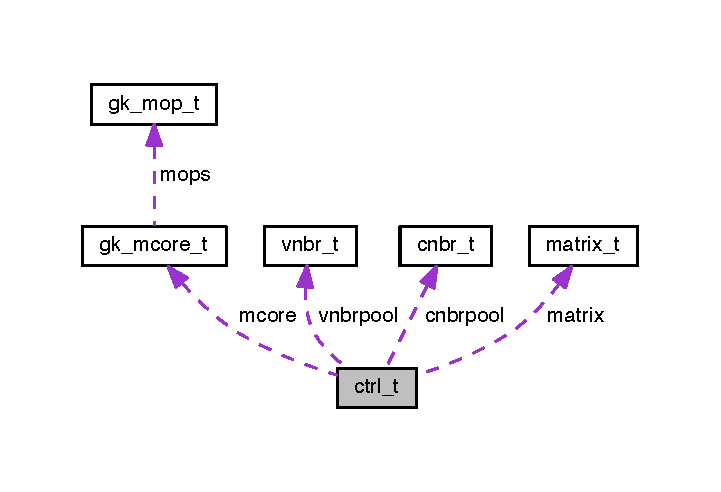
\includegraphics[width=346pt]{structctrl__t__coll__graph}
\end{center}
\end{figure}
\subsection*{Public Attributes}
\begin{DoxyCompactItemize}
\item 
\hyperlink{3rd_party_2parmetis-4_80_83_2metis_2include_2metis_8h_a64ee21e6d3a57701a812d0903a2f0401}{moptype\+\_\+et} \hyperlink{structctrl__t_a4bdbbc6060bc967ed4edeac6df20a5c8}{optype}
\item 
\hyperlink{3rd_party_2parmetis-4_80_83_2metis_2include_2metis_8h_ad8332705ea18c63b06801b0630db9bb8}{mobjtype\+\_\+et} \hyperlink{structctrl__t_aeccfadc19b99c537254075120af879bc}{objtype}
\item 
\hyperlink{3rd_party_2parmetis-4_80_83_2metis_2include_2metis_8h_ac50415aa8003f9b7bf0aabb2b0d50877}{mdbglvl\+\_\+et} \hyperlink{structctrl__t_a97ccd0cc307eee1c430679f6a9d41d0c}{dbglvl}
\item 
\hyperlink{3rd_party_2parmetis-4_80_83_2metis_2include_2metis_8h_a51d3bfb2bd8dc4a84636b2b489f575bc}{mctype\+\_\+et} \hyperlink{structctrl__t_a7e3099b031b9dbb0f91fe5fc310a5263}{ctype}
\item 
\hyperlink{3rd_party_2parmetis-4_80_83_2metis_2include_2metis_8h_a7f13d793623003e25bbbcd5dd7dead89}{miptype\+\_\+et} \hyperlink{structctrl__t_a9d217a96cfccfd2199727900dc3f6c46}{iptype}
\item 
\hyperlink{3rd_party_2parmetis-4_80_83_2metis_2include_2metis_8h_a54ec0069de1eb28daca5cf43617e57e4}{mrtype\+\_\+et} \hyperlink{structctrl__t_a9a5e805fb214f1073f147f28f547201a}{rtype}
\item 
\hyperlink{3rd_party_2parmetis-4_80_83_2metis_2include_2metis_8h_aaa5262be3e700770163401acb0150f52}{idx\+\_\+t} \hyperlink{structctrl__t_a5f4e7c5bbef13001912e0bb3a161862e}{Coarsen\+To}
\item 
\hyperlink{3rd_party_2parmetis-4_80_83_2metis_2include_2metis_8h_aaa5262be3e700770163401acb0150f52}{idx\+\_\+t} \hyperlink{structctrl__t_ad6cb0c7aa46b56d1061fbe2ff8916b72}{n\+Iparts}
\item 
\hyperlink{3rd_party_2parmetis-4_80_83_2metis_2include_2metis_8h_aaa5262be3e700770163401acb0150f52}{idx\+\_\+t} \hyperlink{structctrl__t_a8a8e7e0be0d5ff231c4ef2f0b7e50edd}{no2hop}
\item 
\hyperlink{3rd_party_2parmetis-4_80_83_2metis_2include_2metis_8h_aaa5262be3e700770163401acb0150f52}{idx\+\_\+t} \hyperlink{structctrl__t_aeecdd5a52f8624eb1563bea4ba696caf}{minconn}
\item 
\hyperlink{3rd_party_2parmetis-4_80_83_2metis_2include_2metis_8h_aaa5262be3e700770163401acb0150f52}{idx\+\_\+t} \hyperlink{structctrl__t_a40f67c7f32893cc78d622b802055bc11}{contig}
\item 
\hyperlink{3rd_party_2parmetis-4_80_83_2metis_2include_2metis_8h_aaa5262be3e700770163401acb0150f52}{idx\+\_\+t} \hyperlink{structctrl__t_a245a4bc9eb3b49104ce24a22ba0cb9a9}{nseps}
\item 
\hyperlink{3rd_party_2parmetis-4_80_83_2metis_2include_2metis_8h_aaa5262be3e700770163401acb0150f52}{idx\+\_\+t} \hyperlink{structctrl__t_addd3712860b894870748f12557b20d89}{ufactor}
\item 
\hyperlink{3rd_party_2parmetis-4_80_83_2metis_2include_2metis_8h_aaa5262be3e700770163401acb0150f52}{idx\+\_\+t} \hyperlink{structctrl__t_ac9e93fdb03a2eefa04a25f6035983428}{compress}
\item 
\hyperlink{3rd_party_2parmetis-4_80_83_2metis_2include_2metis_8h_aaa5262be3e700770163401acb0150f52}{idx\+\_\+t} \hyperlink{structctrl__t_af126e4254641250b7b8ea571b7cd24b1}{ccorder}
\item 
\hyperlink{3rd_party_2parmetis-4_80_83_2metis_2include_2metis_8h_aaa5262be3e700770163401acb0150f52}{idx\+\_\+t} \hyperlink{structctrl__t_ac3a4edfbca646edc493bf459c805508b}{seed}
\item 
\hyperlink{3rd_party_2parmetis-4_80_83_2metis_2include_2metis_8h_aaa5262be3e700770163401acb0150f52}{idx\+\_\+t} \hyperlink{structctrl__t_a40c46fa39e062a9efdc6eaacefe44a8b}{ncuts}
\item 
\hyperlink{3rd_party_2parmetis-4_80_83_2metis_2include_2metis_8h_aaa5262be3e700770163401acb0150f52}{idx\+\_\+t} \hyperlink{structctrl__t_a286168eb06a334afdca8040c58f1c50a}{niter}
\item 
\hyperlink{3rd_party_2parmetis-4_80_83_2metis_2include_2metis_8h_aaa5262be3e700770163401acb0150f52}{idx\+\_\+t} \hyperlink{structctrl__t_a5f921eb4c9af7a3808b8c58c516dc52f}{numflag}
\item 
\hyperlink{3rd_party_2parmetis-4_80_83_2metis_2include_2metis_8h_aaa5262be3e700770163401acb0150f52}{idx\+\_\+t} $\ast$ \hyperlink{structctrl__t_a02e0b5b3209303d1ec1634de01a10e88}{maxvwgt}
\item 
\hyperlink{3rd_party_2parmetis-4_80_83_2metis_2include_2metis_8h_aaa5262be3e700770163401acb0150f52}{idx\+\_\+t} \hyperlink{structctrl__t_afb1fd1cb311eb4bcefa46a14ef05afa0}{ncon}
\item 
\hyperlink{3rd_party_2parmetis-4_80_83_2metis_2include_2metis_8h_aaa5262be3e700770163401acb0150f52}{idx\+\_\+t} \hyperlink{structctrl__t_a98f3c9d6ea8b5d18b51d500dcb54d1ee}{nparts}
\item 
\hyperlink{3rd_party_2parmetis-4_80_83_2metis_2include_2metis_8h_a1924a4f6907cc3833213aba1f07fcbe9}{real\+\_\+t} \hyperlink{structctrl__t_a3322c07da4ca861a3fe47dc934510e24}{pfactor}
\item 
\hyperlink{3rd_party_2parmetis-4_80_83_2metis_2include_2metis_8h_a1924a4f6907cc3833213aba1f07fcbe9}{real\+\_\+t} $\ast$ \hyperlink{structctrl__t_ac7c04d9f87e4028ee55135f0f790e670}{ubfactors}
\item 
\hyperlink{3rd_party_2parmetis-4_80_83_2metis_2include_2metis_8h_a1924a4f6907cc3833213aba1f07fcbe9}{real\+\_\+t} $\ast$ \hyperlink{structctrl__t_aa7ee25aa882bff4426e79b6479281289}{tpwgts}
\item 
\hyperlink{3rd_party_2parmetis-4_80_83_2metis_2include_2metis_8h_a1924a4f6907cc3833213aba1f07fcbe9}{real\+\_\+t} $\ast$ \hyperlink{structctrl__t_ae347c6497954a20166af15a2ddd4e286}{pijbm}
\item 
\hyperlink{3rd_party_2parmetis-4_80_83_2metis_2include_2metis_8h_a1924a4f6907cc3833213aba1f07fcbe9}{real\+\_\+t} \hyperlink{structctrl__t_a90cc3aac501d85a6b43edc4b1e7e7e5e}{cfactor}
\item 
double \hyperlink{structctrl__t_ae2e09c5a7c17d6ac7595a96494b9e961}{Total\+Tmr}
\item 
double \hyperlink{structctrl__t_aaa34977233d81aa867a7dca9fb095747}{Init\+Part\+Tmr}
\item 
double \hyperlink{structctrl__t_a2c485ca8bb306f86464745c86f4ea178}{Match\+Tmr}
\item 
double \hyperlink{structctrl__t_ad256bb292e7bddb9e02afc32ec54aefd}{Contract\+Tmr}
\item 
double \hyperlink{structctrl__t_a0a761fa32d40dad05f3f010480221577}{Coarsen\+Tmr}
\item 
double \hyperlink{structctrl__t_a37132c6afaaed4a8f869d309ba33d1ac}{Uncoarsen\+Tmr}
\item 
double \hyperlink{structctrl__t_a889ffd7d4bb83fcba2ed78141fadb164}{Ref\+Tmr}
\item 
double \hyperlink{structctrl__t_a5261c7a1d0f02a8d39885ed88c34cfe6}{Project\+Tmr}
\item 
double \hyperlink{structctrl__t_a498dff4e4f63117846960426fd44652a}{Split\+Tmr}
\item 
double \hyperlink{structctrl__t_a8e5e7e5e6e0a2d3585180a1724ef46dc}{Aux1\+Tmr}
\item 
double \hyperlink{structctrl__t_a280b66beb62416ce1ba7149b1fdddf34}{Aux2\+Tmr}
\item 
double \hyperlink{structctrl__t_aef8dd3a941d8b0feea5959383a710bf5}{Aux3\+Tmr}
\item 
\hyperlink{structgk__mcore__t}{gk\+\_\+mcore\+\_\+t} $\ast$ \hyperlink{structctrl__t_aa46cd6966a7472f31f8463b6ca99ec52}{mcore}
\item 
size\+\_\+t \hyperlink{structctrl__t_ae37af5d894dbeea35f735361503e58a9}{nbrpoolsize}
\item 
size\+\_\+t \hyperlink{structctrl__t_acafe4ebea8585403e053dc33e7b4ac64}{nbrpoolcpos}
\item 
size\+\_\+t \hyperlink{structctrl__t_a091baa9be72262dca61c641d1f1e4ad3}{nbrpoolreallocs}
\item 
\hyperlink{structcnbr__t}{cnbr\+\_\+t} $\ast$ \hyperlink{structctrl__t_a87565a0a2d55cb5595a1a9fa4d66d7c2}{cnbrpool}
\item 
\hyperlink{structvnbr__t}{vnbr\+\_\+t} $\ast$ \hyperlink{structctrl__t_a1f7258a6dc2780d0f8224293ecff26b7}{vnbrpool}
\item 
\hyperlink{3rd_party_2parmetis-4_80_83_2metis_2include_2metis_8h_aaa5262be3e700770163401acb0150f52}{idx\+\_\+t} $\ast$ \hyperlink{structctrl__t_ac4f8f5cda17ac6d950c61ba575af566c}{maxnads}
\item 
\hyperlink{3rd_party_2parmetis-4_80_83_2metis_2include_2metis_8h_aaa5262be3e700770163401acb0150f52}{idx\+\_\+t} $\ast$ \hyperlink{structctrl__t_a47541c8142aba246ca9b7b003100e9d8}{nads}
\item 
\hyperlink{3rd_party_2parmetis-4_80_83_2metis_2include_2metis_8h_aaa5262be3e700770163401acb0150f52}{idx\+\_\+t} $\ast$$\ast$ \hyperlink{structctrl__t_a483d832bdceddc91d7a727ca32d35a8f}{adids}
\item 
\hyperlink{3rd_party_2parmetis-4_80_83_2metis_2include_2metis_8h_aaa5262be3e700770163401acb0150f52}{idx\+\_\+t} $\ast$$\ast$ \hyperlink{structctrl__t_a7c457a43ad89aaf416e79416ca63d779}{adwgts}
\item 
\hyperlink{3rd_party_2parmetis-4_80_83_2metis_2include_2metis_8h_aaa5262be3e700770163401acb0150f52}{idx\+\_\+t} $\ast$ \hyperlink{structctrl__t_a98a13efbfba152fab96c7d0c87137fdb}{pvec1}
\item 
\hyperlink{3rd_party_2parmetis-4_80_83_2metis_2include_2metis_8h_aaa5262be3e700770163401acb0150f52}{idx\+\_\+t} $\ast$ \hyperlink{structctrl__t_ac03c35161b7d2407bf988d11f78fa484}{pvec2}
\item 
\hyperlink{3rd_party_2parmetis-4_80_83_2include_2parmetis_8h_a8f61c0f0e4ba81b0e3b6901026acb936}{pmoptype\+\_\+et} \hyperlink{structctrl__t_a518ee84f46b6b756caa35b6002250cf1}{optype}
\item 
\hyperlink{3rd_party_2parmetis-4_80_83_2metis_2include_2metis_8h_aaa5262be3e700770163401acb0150f52}{idx\+\_\+t} \hyperlink{structctrl__t_a761f99c08049bc91864378dcba5a2385}{mype}
\item 
\hyperlink{3rd_party_2parmetis-4_80_83_2metis_2include_2metis_8h_aaa5262be3e700770163401acb0150f52}{idx\+\_\+t} \hyperlink{structctrl__t_ad628a7b90c839f39a5d7bf8088c1de65}{npes}
\item 
\hyperlink{3rd_party_2parmetis-4_80_83_2metis_2include_2metis_8h_aaa5262be3e700770163401acb0150f52}{idx\+\_\+t} \hyperlink{structctrl__t_ae2d53d37f183ef45aced58a216e842aa}{dbglvl}
\item 
\hyperlink{3rd_party_2parmetis-4_80_83_2metis_2include_2metis_8h_aaa5262be3e700770163401acb0150f52}{idx\+\_\+t} \hyperlink{structctrl__t_a5684e75db9dee5cd1bba60ce95a2494a}{foldf}
\item 
\hyperlink{3rd_party_2parmetis-4_80_83_2metis_2include_2metis_8h_aaa5262be3e700770163401acb0150f52}{idx\+\_\+t} \hyperlink{structctrl__t_a596b7ef429ea148e6e8a90b4a5512e95}{mtype}
\item 
\hyperlink{3rd_party_2parmetis-4_80_83_2metis_2include_2metis_8h_aaa5262be3e700770163401acb0150f52}{idx\+\_\+t} \hyperlink{structctrl__t_adf21e8fd22e97c2c135eb27a1109a4fc}{ipart}
\item 
\hyperlink{3rd_party_2parmetis-4_80_83_2metis_2include_2metis_8h_aaa5262be3e700770163401acb0150f52}{idx\+\_\+t} \hyperlink{structctrl__t_a00222ee6848f108df74b350480e9691f}{rtype}
\item 
\hyperlink{3rd_party_2parmetis-4_80_83_2metis_2include_2metis_8h_aaa5262be3e700770163401acb0150f52}{idx\+\_\+t} \hyperlink{structctrl__t_af9239c530aff4bae41ce44a2f73bb814}{p\+\_\+nseps}
\item 
\hyperlink{3rd_party_2parmetis-4_80_83_2metis_2include_2metis_8h_aaa5262be3e700770163401acb0150f52}{idx\+\_\+t} \hyperlink{structctrl__t_a0c3d131edc652e4143119cc16ede13a6}{s\+\_\+nseps}
\item 
\hyperlink{3rd_party_2parmetis-4_80_83_2metis_2include_2metis_8h_a1924a4f6907cc3833213aba1f07fcbe9}{real\+\_\+t} \hyperlink{structctrl__t_aeac3587c8e878a5bae68a754fc598aed}{ubfrac}
\item 
\hyperlink{3rd_party_2parmetis-4_80_83_2metis_2include_2metis_8h_aaa5262be3e700770163401acb0150f52}{idx\+\_\+t} \hyperlink{structctrl__t_a3130cb526a3c01ab81dee30761168936}{sync}
\item 
\hyperlink{3rd_party_2parmetis-4_80_83_2metis_2include_2metis_8h_a1924a4f6907cc3833213aba1f07fcbe9}{real\+\_\+t} $\ast$ \hyperlink{structctrl__t_acbb9d6666e99ca62a4d27c6798ed4ccc}{invtvwgts}
\item 
\hyperlink{3rd_party_2parmetis-4_80_83_2metis_2include_2metis_8h_a1924a4f6907cc3833213aba1f07fcbe9}{real\+\_\+t} $\ast$ \hyperlink{structctrl__t_ab028c8c13e03ab35abdb6f782cff075e}{ubvec}
\item 
\hyperlink{3rd_party_2parmetis-4_80_83_2metis_2include_2metis_8h_aaa5262be3e700770163401acb0150f52}{idx\+\_\+t} \hyperlink{structctrl__t_afadeadc5b9dbc27c580f0bddcdb15b9a}{part\+Type}
\item 
\hyperlink{3rd_party_2parmetis-4_80_83_2metis_2include_2metis_8h_aaa5262be3e700770163401acb0150f52}{idx\+\_\+t} \hyperlink{structctrl__t_a0b93ba7aef798c08a0df00fca7b92c54}{ps\+\_\+relation}
\item 
\hyperlink{3rd_party_2parmetis-4_80_83_2metis_2include_2metis_8h_a1924a4f6907cc3833213aba1f07fcbe9}{real\+\_\+t} \hyperlink{structctrl__t_a6c1ed7a26ba128badcc99e0d73a96964}{redist\+\_\+factor}
\item 
\hyperlink{3rd_party_2parmetis-4_80_83_2metis_2include_2metis_8h_a1924a4f6907cc3833213aba1f07fcbe9}{real\+\_\+t} \hyperlink{structctrl__t_ab760f956600b7d8d71bf6bbe22755055}{redist\+\_\+base}
\item 
\hyperlink{3rd_party_2parmetis-4_80_83_2metis_2include_2metis_8h_a1924a4f6907cc3833213aba1f07fcbe9}{real\+\_\+t} \hyperlink{structctrl__t_a116d746e1172d8a4ff664710a436449a}{ipc\+\_\+factor}
\item 
\hyperlink{3rd_party_2parmetis-4_80_83_2metis_2include_2metis_8h_a1924a4f6907cc3833213aba1f07fcbe9}{real\+\_\+t} \hyperlink{structctrl__t_af09d1b1edf1d1eb790724d438140844c}{edge\+\_\+size\+\_\+ratio}
\item 
\hyperlink{structmatrix__t}{matrix\+\_\+t} $\ast$ \hyperlink{structctrl__t_a4dc8d1b4dd2561504f9c545068c9f5a8}{matrix}
\item 
\hyperlink{3rd_party_2parmetis-4_80_83_2metis_2include_2metis_8h_aaa5262be3e700770163401acb0150f52}{idx\+\_\+t} \hyperlink{structctrl__t_aab19c0f9f0acd534d86498a9217f95e5}{free\+\_\+comm}
\item 
M\+P\+I\+\_\+\+Comm \hyperlink{structctrl__t_aeb4b28f44dc445407a23443c96c85489}{gcomm}
\item 
M\+P\+I\+\_\+\+Comm \hyperlink{structctrl__t_a5ecd63179c45d9dfac0ed80074ac3ab8}{comm}
\item 
\hyperlink{3rd_party_2parmetis-4_80_83_2metis_2include_2metis_8h_aaa5262be3e700770163401acb0150f52}{idx\+\_\+t} \hyperlink{structctrl__t_a120ba1a44430e6e9655edaebed67f249}{ncommpes}
\item 
M\+P\+I\+\_\+\+Request $\ast$ \hyperlink{structctrl__t_ae549c3a5ecef32013a343de1561a77b3}{sreq}
\item 
M\+P\+I\+\_\+\+Request $\ast$ \hyperlink{structctrl__t_a8cead6c0236b648ce4a71266614595ac}{rreq}
\item 
M\+P\+I\+\_\+\+Status $\ast$ \hyperlink{structctrl__t_a25c50125554b92e1cd6e3bfb708c7da8}{statuses}
\item 
M\+P\+I\+\_\+\+Status \hyperlink{structctrl__t_ab427cd24d8541ee4958d3c03d48ab6c0}{status}
\item 
\hyperlink{libparmetis_2struct_8h_aae821c36bb7e6918e1414484f939c3d4}{timer} \hyperlink{structctrl__t_a9a8be36e6548d88c61d93ac5e96e4e31}{Total\+Tmr}
\item 
\hyperlink{libparmetis_2struct_8h_aae821c36bb7e6918e1414484f939c3d4}{timer} \hyperlink{structctrl__t_a1a0b3969ee6948842f7411599747326d}{Init\+Part\+Tmr}
\item 
\hyperlink{libparmetis_2struct_8h_aae821c36bb7e6918e1414484f939c3d4}{timer} \hyperlink{structctrl__t_a9f0a9e7353849b3bf5caf432c3ea913e}{Match\+Tmr}
\item 
\hyperlink{libparmetis_2struct_8h_aae821c36bb7e6918e1414484f939c3d4}{timer} \hyperlink{structctrl__t_a674aa9a854963864725d7950509fb085}{Contract\+Tmr}
\item 
\hyperlink{libparmetis_2struct_8h_aae821c36bb7e6918e1414484f939c3d4}{timer} \hyperlink{structctrl__t_a108d417b55d602e138bdb44b8d80f245}{Coarsen\+Tmr}
\item 
\hyperlink{libparmetis_2struct_8h_aae821c36bb7e6918e1414484f939c3d4}{timer} \hyperlink{structctrl__t_a0d99613b25b8e7f477758862f88417f0}{Ref\+Tmr}
\item 
\hyperlink{libparmetis_2struct_8h_aae821c36bb7e6918e1414484f939c3d4}{timer} \hyperlink{structctrl__t_ab69d4bc0e91f8c40d58ddf5fd137e9e3}{Setup\+Tmr}
\item 
\hyperlink{libparmetis_2struct_8h_aae821c36bb7e6918e1414484f939c3d4}{timer} \hyperlink{structctrl__t_ad9d67bcaaeffa73907f8e8943e2ea2fc}{Project\+Tmr}
\item 
\hyperlink{libparmetis_2struct_8h_aae821c36bb7e6918e1414484f939c3d4}{timer} \hyperlink{structctrl__t_a1c0335e0e5801cff83a1fb3cbda63b06}{K\+Way\+Init\+Tmr}
\item 
\hyperlink{libparmetis_2struct_8h_aae821c36bb7e6918e1414484f939c3d4}{timer} \hyperlink{structctrl__t_a4aa50bb891d35d0ef09d311db38f2e40}{K\+Way\+Tmr}
\item 
\hyperlink{libparmetis_2struct_8h_aae821c36bb7e6918e1414484f939c3d4}{timer} \hyperlink{structctrl__t_a4c4c2d93b216dea60bd360d5a706350c}{Move\+Tmr}
\item 
\hyperlink{libparmetis_2struct_8h_aae821c36bb7e6918e1414484f939c3d4}{timer} \hyperlink{structctrl__t_a09be4dee7850678b5e247eba855786a8}{Remap\+Tmr}
\item 
\hyperlink{libparmetis_2struct_8h_aae821c36bb7e6918e1414484f939c3d4}{timer} \hyperlink{structctrl__t_aed0beddb0cbcc304b2473eb9b13f1ff4}{Serial\+Tmr}
\item 
\hyperlink{libparmetis_2struct_8h_aae821c36bb7e6918e1414484f939c3d4}{timer} \hyperlink{structctrl__t_a54b296cf8b956a9acda86b7525ae0dc2}{Aux\+Tmr1}
\item 
\hyperlink{libparmetis_2struct_8h_aae821c36bb7e6918e1414484f939c3d4}{timer} \hyperlink{structctrl__t_ab9675c12f7733edb2276c991d2634512}{Aux\+Tmr2}
\item 
\hyperlink{libparmetis_2struct_8h_aae821c36bb7e6918e1414484f939c3d4}{timer} \hyperlink{structctrl__t_af05e8d64a430f4a92993f28b894ab098}{Aux\+Tmr3}
\item 
\hyperlink{libparmetis_2struct_8h_aae821c36bb7e6918e1414484f939c3d4}{timer} \hyperlink{structctrl__t_a0a512f4bc4dab3b5106d2c4251d6c1fc}{Aux\+Tmr4}
\item 
\hyperlink{libparmetis_2struct_8h_aae821c36bb7e6918e1414484f939c3d4}{timer} \hyperlink{structctrl__t_abe3a6c54cd913122a281df4d0c069867}{Aux\+Tmr5}
\item 
\hyperlink{libparmetis_2struct_8h_aae821c36bb7e6918e1414484f939c3d4}{timer} \hyperlink{structctrl__t_a11d0309701b0ad399b7082b8e213ec6f}{Aux\+Tmr6}
\end{DoxyCompactItemize}


\subsection{Detailed Description}
The following structure stores information used by Metis 

\subsection{Member Data Documentation}
\mbox{\Hypertarget{structctrl__t_a483d832bdceddc91d7a727ca32d35a8f}\label{structctrl__t_a483d832bdceddc91d7a727ca32d35a8f}} 
\index{ctrl\+\_\+t@{ctrl\+\_\+t}!adids@{adids}}
\index{adids@{adids}!ctrl\+\_\+t@{ctrl\+\_\+t}}
\subsubsection{\texorpdfstring{adids}{adids}}
{\footnotesize\ttfamily \hyperlink{3rd_party_2parmetis-4_80_83_2metis_2include_2metis_8h_aaa5262be3e700770163401acb0150f52}{idx\+\_\+t}$\ast$$\ast$ ctrl\+\_\+t\+::adids}

\mbox{\Hypertarget{structctrl__t_a7c457a43ad89aaf416e79416ca63d779}\label{structctrl__t_a7c457a43ad89aaf416e79416ca63d779}} 
\index{ctrl\+\_\+t@{ctrl\+\_\+t}!adwgts@{adwgts}}
\index{adwgts@{adwgts}!ctrl\+\_\+t@{ctrl\+\_\+t}}
\subsubsection{\texorpdfstring{adwgts}{adwgts}}
{\footnotesize\ttfamily \hyperlink{3rd_party_2parmetis-4_80_83_2metis_2include_2metis_8h_aaa5262be3e700770163401acb0150f52}{idx\+\_\+t}$\ast$$\ast$ ctrl\+\_\+t\+::adwgts}

\mbox{\Hypertarget{structctrl__t_a8e5e7e5e6e0a2d3585180a1724ef46dc}\label{structctrl__t_a8e5e7e5e6e0a2d3585180a1724ef46dc}} 
\index{ctrl\+\_\+t@{ctrl\+\_\+t}!Aux1\+Tmr@{Aux1\+Tmr}}
\index{Aux1\+Tmr@{Aux1\+Tmr}!ctrl\+\_\+t@{ctrl\+\_\+t}}
\subsubsection{\texorpdfstring{Aux1\+Tmr}{Aux1Tmr}}
{\footnotesize\ttfamily double ctrl\+\_\+t\+::\+Aux1\+Tmr}

\mbox{\Hypertarget{structctrl__t_a280b66beb62416ce1ba7149b1fdddf34}\label{structctrl__t_a280b66beb62416ce1ba7149b1fdddf34}} 
\index{ctrl\+\_\+t@{ctrl\+\_\+t}!Aux2\+Tmr@{Aux2\+Tmr}}
\index{Aux2\+Tmr@{Aux2\+Tmr}!ctrl\+\_\+t@{ctrl\+\_\+t}}
\subsubsection{\texorpdfstring{Aux2\+Tmr}{Aux2Tmr}}
{\footnotesize\ttfamily double ctrl\+\_\+t\+::\+Aux2\+Tmr}

\mbox{\Hypertarget{structctrl__t_aef8dd3a941d8b0feea5959383a710bf5}\label{structctrl__t_aef8dd3a941d8b0feea5959383a710bf5}} 
\index{ctrl\+\_\+t@{ctrl\+\_\+t}!Aux3\+Tmr@{Aux3\+Tmr}}
\index{Aux3\+Tmr@{Aux3\+Tmr}!ctrl\+\_\+t@{ctrl\+\_\+t}}
\subsubsection{\texorpdfstring{Aux3\+Tmr}{Aux3Tmr}}
{\footnotesize\ttfamily double ctrl\+\_\+t\+::\+Aux3\+Tmr}

\mbox{\Hypertarget{structctrl__t_a54b296cf8b956a9acda86b7525ae0dc2}\label{structctrl__t_a54b296cf8b956a9acda86b7525ae0dc2}} 
\index{ctrl\+\_\+t@{ctrl\+\_\+t}!Aux\+Tmr1@{Aux\+Tmr1}}
\index{Aux\+Tmr1@{Aux\+Tmr1}!ctrl\+\_\+t@{ctrl\+\_\+t}}
\subsubsection{\texorpdfstring{Aux\+Tmr1}{AuxTmr1}}
{\footnotesize\ttfamily \hyperlink{libparmetis_2struct_8h_aae821c36bb7e6918e1414484f939c3d4}{timer} ctrl\+\_\+t\+::\+Aux\+Tmr1}

\mbox{\Hypertarget{structctrl__t_ab9675c12f7733edb2276c991d2634512}\label{structctrl__t_ab9675c12f7733edb2276c991d2634512}} 
\index{ctrl\+\_\+t@{ctrl\+\_\+t}!Aux\+Tmr2@{Aux\+Tmr2}}
\index{Aux\+Tmr2@{Aux\+Tmr2}!ctrl\+\_\+t@{ctrl\+\_\+t}}
\subsubsection{\texorpdfstring{Aux\+Tmr2}{AuxTmr2}}
{\footnotesize\ttfamily \hyperlink{libparmetis_2struct_8h_aae821c36bb7e6918e1414484f939c3d4}{timer} ctrl\+\_\+t\+::\+Aux\+Tmr2}

\mbox{\Hypertarget{structctrl__t_af05e8d64a430f4a92993f28b894ab098}\label{structctrl__t_af05e8d64a430f4a92993f28b894ab098}} 
\index{ctrl\+\_\+t@{ctrl\+\_\+t}!Aux\+Tmr3@{Aux\+Tmr3}}
\index{Aux\+Tmr3@{Aux\+Tmr3}!ctrl\+\_\+t@{ctrl\+\_\+t}}
\subsubsection{\texorpdfstring{Aux\+Tmr3}{AuxTmr3}}
{\footnotesize\ttfamily \hyperlink{libparmetis_2struct_8h_aae821c36bb7e6918e1414484f939c3d4}{timer} ctrl\+\_\+t\+::\+Aux\+Tmr3}

\mbox{\Hypertarget{structctrl__t_a0a512f4bc4dab3b5106d2c4251d6c1fc}\label{structctrl__t_a0a512f4bc4dab3b5106d2c4251d6c1fc}} 
\index{ctrl\+\_\+t@{ctrl\+\_\+t}!Aux\+Tmr4@{Aux\+Tmr4}}
\index{Aux\+Tmr4@{Aux\+Tmr4}!ctrl\+\_\+t@{ctrl\+\_\+t}}
\subsubsection{\texorpdfstring{Aux\+Tmr4}{AuxTmr4}}
{\footnotesize\ttfamily \hyperlink{libparmetis_2struct_8h_aae821c36bb7e6918e1414484f939c3d4}{timer} ctrl\+\_\+t\+::\+Aux\+Tmr4}

\mbox{\Hypertarget{structctrl__t_abe3a6c54cd913122a281df4d0c069867}\label{structctrl__t_abe3a6c54cd913122a281df4d0c069867}} 
\index{ctrl\+\_\+t@{ctrl\+\_\+t}!Aux\+Tmr5@{Aux\+Tmr5}}
\index{Aux\+Tmr5@{Aux\+Tmr5}!ctrl\+\_\+t@{ctrl\+\_\+t}}
\subsubsection{\texorpdfstring{Aux\+Tmr5}{AuxTmr5}}
{\footnotesize\ttfamily \hyperlink{libparmetis_2struct_8h_aae821c36bb7e6918e1414484f939c3d4}{timer} ctrl\+\_\+t\+::\+Aux\+Tmr5}

\mbox{\Hypertarget{structctrl__t_a11d0309701b0ad399b7082b8e213ec6f}\label{structctrl__t_a11d0309701b0ad399b7082b8e213ec6f}} 
\index{ctrl\+\_\+t@{ctrl\+\_\+t}!Aux\+Tmr6@{Aux\+Tmr6}}
\index{Aux\+Tmr6@{Aux\+Tmr6}!ctrl\+\_\+t@{ctrl\+\_\+t}}
\subsubsection{\texorpdfstring{Aux\+Tmr6}{AuxTmr6}}
{\footnotesize\ttfamily \hyperlink{libparmetis_2struct_8h_aae821c36bb7e6918e1414484f939c3d4}{timer} ctrl\+\_\+t\+::\+Aux\+Tmr6}

\mbox{\Hypertarget{structctrl__t_af126e4254641250b7b8ea571b7cd24b1}\label{structctrl__t_af126e4254641250b7b8ea571b7cd24b1}} 
\index{ctrl\+\_\+t@{ctrl\+\_\+t}!ccorder@{ccorder}}
\index{ccorder@{ccorder}!ctrl\+\_\+t@{ctrl\+\_\+t}}
\subsubsection{\texorpdfstring{ccorder}{ccorder}}
{\footnotesize\ttfamily \hyperlink{3rd_party_2parmetis-4_80_83_2metis_2include_2metis_8h_aaa5262be3e700770163401acb0150f52}{idx\+\_\+t} ctrl\+\_\+t\+::ccorder}

\mbox{\Hypertarget{structctrl__t_a90cc3aac501d85a6b43edc4b1e7e7e5e}\label{structctrl__t_a90cc3aac501d85a6b43edc4b1e7e7e5e}} 
\index{ctrl\+\_\+t@{ctrl\+\_\+t}!cfactor@{cfactor}}
\index{cfactor@{cfactor}!ctrl\+\_\+t@{ctrl\+\_\+t}}
\subsubsection{\texorpdfstring{cfactor}{cfactor}}
{\footnotesize\ttfamily \hyperlink{3rd_party_2parmetis-4_80_83_2metis_2include_2metis_8h_a1924a4f6907cc3833213aba1f07fcbe9}{real\+\_\+t} ctrl\+\_\+t\+::cfactor}

The achieved compression factor \mbox{\Hypertarget{structctrl__t_a87565a0a2d55cb5595a1a9fa4d66d7c2}\label{structctrl__t_a87565a0a2d55cb5595a1a9fa4d66d7c2}} 
\index{ctrl\+\_\+t@{ctrl\+\_\+t}!cnbrpool@{cnbrpool}}
\index{cnbrpool@{cnbrpool}!ctrl\+\_\+t@{ctrl\+\_\+t}}
\subsubsection{\texorpdfstring{cnbrpool}{cnbrpool}}
{\footnotesize\ttfamily \hyperlink{structcnbr__t}{cnbr\+\_\+t} $\ast$ ctrl\+\_\+t\+::cnbrpool}

The pool of \hyperlink{structcnbr__t}{cnbr\+\_\+t} entries to be used during refinement. The size and current position of the pool is controlled by nnbrs \& cnbrs \mbox{\Hypertarget{structctrl__t_a0a761fa32d40dad05f3f010480221577}\label{structctrl__t_a0a761fa32d40dad05f3f010480221577}} 
\index{ctrl\+\_\+t@{ctrl\+\_\+t}!Coarsen\+Tmr@{Coarsen\+Tmr}}
\index{Coarsen\+Tmr@{Coarsen\+Tmr}!ctrl\+\_\+t@{ctrl\+\_\+t}}
\subsubsection{\texorpdfstring{Coarsen\+Tmr}{CoarsenTmr}\hspace{0.1cm}{\footnotesize\ttfamily [1/2]}}
{\footnotesize\ttfamily double ctrl\+\_\+t\+::\+Coarsen\+Tmr}

\mbox{\Hypertarget{structctrl__t_a108d417b55d602e138bdb44b8d80f245}\label{structctrl__t_a108d417b55d602e138bdb44b8d80f245}} 
\index{ctrl\+\_\+t@{ctrl\+\_\+t}!Coarsen\+Tmr@{Coarsen\+Tmr}}
\index{Coarsen\+Tmr@{Coarsen\+Tmr}!ctrl\+\_\+t@{ctrl\+\_\+t}}
\subsubsection{\texorpdfstring{Coarsen\+Tmr}{CoarsenTmr}\hspace{0.1cm}{\footnotesize\ttfamily [2/2]}}
{\footnotesize\ttfamily \hyperlink{libparmetis_2struct_8h_aae821c36bb7e6918e1414484f939c3d4}{timer} ctrl\+\_\+t\+::\+Coarsen\+Tmr}

\mbox{\Hypertarget{structctrl__t_a5f4e7c5bbef13001912e0bb3a161862e}\label{structctrl__t_a5f4e7c5bbef13001912e0bb3a161862e}} 
\index{ctrl\+\_\+t@{ctrl\+\_\+t}!Coarsen\+To@{Coarsen\+To}}
\index{Coarsen\+To@{Coarsen\+To}!ctrl\+\_\+t@{ctrl\+\_\+t}}
\subsubsection{\texorpdfstring{Coarsen\+To}{CoarsenTo}}
{\footnotesize\ttfamily \hyperlink{3rd_party_2parmetis-4_80_83_2metis_2include_2metis_8h_aaa5262be3e700770163401acb0150f52}{idx\+\_\+t} ctrl\+\_\+t\+::\+Coarsen\+To}

\mbox{\Hypertarget{structctrl__t_a5ecd63179c45d9dfac0ed80074ac3ab8}\label{structctrl__t_a5ecd63179c45d9dfac0ed80074ac3ab8}} 
\index{ctrl\+\_\+t@{ctrl\+\_\+t}!comm@{comm}}
\index{comm@{comm}!ctrl\+\_\+t@{ctrl\+\_\+t}}
\subsubsection{\texorpdfstring{comm}{comm}}
{\footnotesize\ttfamily M\+P\+I\+\_\+\+Comm ctrl\+\_\+t\+::comm}

The current communicator \mbox{\Hypertarget{structctrl__t_ac9e93fdb03a2eefa04a25f6035983428}\label{structctrl__t_ac9e93fdb03a2eefa04a25f6035983428}} 
\index{ctrl\+\_\+t@{ctrl\+\_\+t}!compress@{compress}}
\index{compress@{compress}!ctrl\+\_\+t@{ctrl\+\_\+t}}
\subsubsection{\texorpdfstring{compress}{compress}}
{\footnotesize\ttfamily \hyperlink{3rd_party_2parmetis-4_80_83_2metis_2include_2metis_8h_aaa5262be3e700770163401acb0150f52}{idx\+\_\+t} ctrl\+\_\+t\+::compress}

\mbox{\Hypertarget{structctrl__t_a40f67c7f32893cc78d622b802055bc11}\label{structctrl__t_a40f67c7f32893cc78d622b802055bc11}} 
\index{ctrl\+\_\+t@{ctrl\+\_\+t}!contig@{contig}}
\index{contig@{contig}!ctrl\+\_\+t@{ctrl\+\_\+t}}
\subsubsection{\texorpdfstring{contig}{contig}}
{\footnotesize\ttfamily \hyperlink{3rd_party_2parmetis-4_80_83_2metis_2include_2metis_8h_aaa5262be3e700770163401acb0150f52}{idx\+\_\+t} ctrl\+\_\+t\+::contig}

\mbox{\Hypertarget{structctrl__t_ad256bb292e7bddb9e02afc32ec54aefd}\label{structctrl__t_ad256bb292e7bddb9e02afc32ec54aefd}} 
\index{ctrl\+\_\+t@{ctrl\+\_\+t}!Contract\+Tmr@{Contract\+Tmr}}
\index{Contract\+Tmr@{Contract\+Tmr}!ctrl\+\_\+t@{ctrl\+\_\+t}}
\subsubsection{\texorpdfstring{Contract\+Tmr}{ContractTmr}\hspace{0.1cm}{\footnotesize\ttfamily [1/2]}}
{\footnotesize\ttfamily double ctrl\+\_\+t\+::\+Contract\+Tmr}

\mbox{\Hypertarget{structctrl__t_a674aa9a854963864725d7950509fb085}\label{structctrl__t_a674aa9a854963864725d7950509fb085}} 
\index{ctrl\+\_\+t@{ctrl\+\_\+t}!Contract\+Tmr@{Contract\+Tmr}}
\index{Contract\+Tmr@{Contract\+Tmr}!ctrl\+\_\+t@{ctrl\+\_\+t}}
\subsubsection{\texorpdfstring{Contract\+Tmr}{ContractTmr}\hspace{0.1cm}{\footnotesize\ttfamily [2/2]}}
{\footnotesize\ttfamily \hyperlink{libparmetis_2struct_8h_aae821c36bb7e6918e1414484f939c3d4}{timer} ctrl\+\_\+t\+::\+Contract\+Tmr}

\mbox{\Hypertarget{structctrl__t_a7e3099b031b9dbb0f91fe5fc310a5263}\label{structctrl__t_a7e3099b031b9dbb0f91fe5fc310a5263}} 
\index{ctrl\+\_\+t@{ctrl\+\_\+t}!ctype@{ctype}}
\index{ctype@{ctype}!ctrl\+\_\+t@{ctrl\+\_\+t}}
\subsubsection{\texorpdfstring{ctype}{ctype}}
{\footnotesize\ttfamily \hyperlink{3rd_party_2parmetis-4_80_83_2metis_2include_2metis_8h_a51d3bfb2bd8dc4a84636b2b489f575bc}{mctype\+\_\+et} ctrl\+\_\+t\+::ctype}

\mbox{\Hypertarget{structctrl__t_a97ccd0cc307eee1c430679f6a9d41d0c}\label{structctrl__t_a97ccd0cc307eee1c430679f6a9d41d0c}} 
\index{ctrl\+\_\+t@{ctrl\+\_\+t}!dbglvl@{dbglvl}}
\index{dbglvl@{dbglvl}!ctrl\+\_\+t@{ctrl\+\_\+t}}
\subsubsection{\texorpdfstring{dbglvl}{dbglvl}\hspace{0.1cm}{\footnotesize\ttfamily [1/2]}}
{\footnotesize\ttfamily \hyperlink{3rd_party_2parmetis-4_80_83_2metis_2include_2metis_8h_ac50415aa8003f9b7bf0aabb2b0d50877}{mdbglvl\+\_\+et} ctrl\+\_\+t\+::dbglvl}

\mbox{\Hypertarget{structctrl__t_ae2d53d37f183ef45aced58a216e842aa}\label{structctrl__t_ae2d53d37f183ef45aced58a216e842aa}} 
\index{ctrl\+\_\+t@{ctrl\+\_\+t}!dbglvl@{dbglvl}}
\index{dbglvl@{dbglvl}!ctrl\+\_\+t@{ctrl\+\_\+t}}
\subsubsection{\texorpdfstring{dbglvl}{dbglvl}\hspace{0.1cm}{\footnotesize\ttfamily [2/2]}}
{\footnotesize\ttfamily \hyperlink{3rd_party_2parmetis-4_80_83_2metis_2include_2metis_8h_aaa5262be3e700770163401acb0150f52}{idx\+\_\+t} ctrl\+\_\+t\+::dbglvl}

\mbox{\Hypertarget{structctrl__t_af09d1b1edf1d1eb790724d438140844c}\label{structctrl__t_af09d1b1edf1d1eb790724d438140844c}} 
\index{ctrl\+\_\+t@{ctrl\+\_\+t}!edge\+\_\+size\+\_\+ratio@{edge\+\_\+size\+\_\+ratio}}
\index{edge\+\_\+size\+\_\+ratio@{edge\+\_\+size\+\_\+ratio}!ctrl\+\_\+t@{ctrl\+\_\+t}}
\subsubsection{\texorpdfstring{edge\+\_\+size\+\_\+ratio}{edge\_size\_ratio}}
{\footnotesize\ttfamily \hyperlink{3rd_party_2parmetis-4_80_83_2metis_2include_2metis_8h_a1924a4f6907cc3833213aba1f07fcbe9}{real\+\_\+t} ctrl\+\_\+t\+::edge\+\_\+size\+\_\+ratio}

\mbox{\Hypertarget{structctrl__t_a5684e75db9dee5cd1bba60ce95a2494a}\label{structctrl__t_a5684e75db9dee5cd1bba60ce95a2494a}} 
\index{ctrl\+\_\+t@{ctrl\+\_\+t}!foldf@{foldf}}
\index{foldf@{foldf}!ctrl\+\_\+t@{ctrl\+\_\+t}}
\subsubsection{\texorpdfstring{foldf}{foldf}}
{\footnotesize\ttfamily \hyperlink{3rd_party_2parmetis-4_80_83_2metis_2include_2metis_8h_aaa5262be3e700770163401acb0150f52}{idx\+\_\+t} ctrl\+\_\+t\+::foldf}

\mbox{\Hypertarget{structctrl__t_aab19c0f9f0acd534d86498a9217f95e5}\label{structctrl__t_aab19c0f9f0acd534d86498a9217f95e5}} 
\index{ctrl\+\_\+t@{ctrl\+\_\+t}!free\+\_\+comm@{free\+\_\+comm}}
\index{free\+\_\+comm@{free\+\_\+comm}!ctrl\+\_\+t@{ctrl\+\_\+t}}
\subsubsection{\texorpdfstring{free\+\_\+comm}{free\_comm}}
{\footnotesize\ttfamily \hyperlink{3rd_party_2parmetis-4_80_83_2metis_2include_2metis_8h_aaa5262be3e700770163401acb0150f52}{idx\+\_\+t} ctrl\+\_\+t\+::free\+\_\+comm}

Used to indicate if gcomm needs to be freed \mbox{\Hypertarget{structctrl__t_aeb4b28f44dc445407a23443c96c85489}\label{structctrl__t_aeb4b28f44dc445407a23443c96c85489}} 
\index{ctrl\+\_\+t@{ctrl\+\_\+t}!gcomm@{gcomm}}
\index{gcomm@{gcomm}!ctrl\+\_\+t@{ctrl\+\_\+t}}
\subsubsection{\texorpdfstring{gcomm}{gcomm}}
{\footnotesize\ttfamily M\+P\+I\+\_\+\+Comm ctrl\+\_\+t\+::gcomm}

A copy of the application supplied communicator \mbox{\Hypertarget{structctrl__t_aaa34977233d81aa867a7dca9fb095747}\label{structctrl__t_aaa34977233d81aa867a7dca9fb095747}} 
\index{ctrl\+\_\+t@{ctrl\+\_\+t}!Init\+Part\+Tmr@{Init\+Part\+Tmr}}
\index{Init\+Part\+Tmr@{Init\+Part\+Tmr}!ctrl\+\_\+t@{ctrl\+\_\+t}}
\subsubsection{\texorpdfstring{Init\+Part\+Tmr}{InitPartTmr}\hspace{0.1cm}{\footnotesize\ttfamily [1/2]}}
{\footnotesize\ttfamily double ctrl\+\_\+t\+::\+Init\+Part\+Tmr}

\mbox{\Hypertarget{structctrl__t_a1a0b3969ee6948842f7411599747326d}\label{structctrl__t_a1a0b3969ee6948842f7411599747326d}} 
\index{ctrl\+\_\+t@{ctrl\+\_\+t}!Init\+Part\+Tmr@{Init\+Part\+Tmr}}
\index{Init\+Part\+Tmr@{Init\+Part\+Tmr}!ctrl\+\_\+t@{ctrl\+\_\+t}}
\subsubsection{\texorpdfstring{Init\+Part\+Tmr}{InitPartTmr}\hspace{0.1cm}{\footnotesize\ttfamily [2/2]}}
{\footnotesize\ttfamily \hyperlink{libparmetis_2struct_8h_aae821c36bb7e6918e1414484f939c3d4}{timer} ctrl\+\_\+t\+::\+Init\+Part\+Tmr}

\mbox{\Hypertarget{structctrl__t_acbb9d6666e99ca62a4d27c6798ed4ccc}\label{structctrl__t_acbb9d6666e99ca62a4d27c6798ed4ccc}} 
\index{ctrl\+\_\+t@{ctrl\+\_\+t}!invtvwgts@{invtvwgts}}
\index{invtvwgts@{invtvwgts}!ctrl\+\_\+t@{ctrl\+\_\+t}}
\subsubsection{\texorpdfstring{invtvwgts}{invtvwgts}}
{\footnotesize\ttfamily \hyperlink{3rd_party_2parmetis-4_80_83_2metis_2include_2metis_8h_a1924a4f6907cc3833213aba1f07fcbe9}{real\+\_\+t}$\ast$ ctrl\+\_\+t\+::invtvwgts}

\mbox{\Hypertarget{structctrl__t_adf21e8fd22e97c2c135eb27a1109a4fc}\label{structctrl__t_adf21e8fd22e97c2c135eb27a1109a4fc}} 
\index{ctrl\+\_\+t@{ctrl\+\_\+t}!ipart@{ipart}}
\index{ipart@{ipart}!ctrl\+\_\+t@{ctrl\+\_\+t}}
\subsubsection{\texorpdfstring{ipart}{ipart}}
{\footnotesize\ttfamily \hyperlink{3rd_party_2parmetis-4_80_83_2metis_2include_2metis_8h_aaa5262be3e700770163401acb0150f52}{idx\+\_\+t} ctrl\+\_\+t\+::ipart}

\mbox{\Hypertarget{structctrl__t_a116d746e1172d8a4ff664710a436449a}\label{structctrl__t_a116d746e1172d8a4ff664710a436449a}} 
\index{ctrl\+\_\+t@{ctrl\+\_\+t}!ipc\+\_\+factor@{ipc\+\_\+factor}}
\index{ipc\+\_\+factor@{ipc\+\_\+factor}!ctrl\+\_\+t@{ctrl\+\_\+t}}
\subsubsection{\texorpdfstring{ipc\+\_\+factor}{ipc\_factor}}
{\footnotesize\ttfamily \hyperlink{3rd_party_2parmetis-4_80_83_2metis_2include_2metis_8h_a1924a4f6907cc3833213aba1f07fcbe9}{real\+\_\+t} ctrl\+\_\+t\+::ipc\+\_\+factor}

\mbox{\Hypertarget{structctrl__t_a9d217a96cfccfd2199727900dc3f6c46}\label{structctrl__t_a9d217a96cfccfd2199727900dc3f6c46}} 
\index{ctrl\+\_\+t@{ctrl\+\_\+t}!iptype@{iptype}}
\index{iptype@{iptype}!ctrl\+\_\+t@{ctrl\+\_\+t}}
\subsubsection{\texorpdfstring{iptype}{iptype}}
{\footnotesize\ttfamily \hyperlink{3rd_party_2parmetis-4_80_83_2metis_2include_2metis_8h_a7f13d793623003e25bbbcd5dd7dead89}{miptype\+\_\+et} ctrl\+\_\+t\+::iptype}

\mbox{\Hypertarget{structctrl__t_a1c0335e0e5801cff83a1fb3cbda63b06}\label{structctrl__t_a1c0335e0e5801cff83a1fb3cbda63b06}} 
\index{ctrl\+\_\+t@{ctrl\+\_\+t}!K\+Way\+Init\+Tmr@{K\+Way\+Init\+Tmr}}
\index{K\+Way\+Init\+Tmr@{K\+Way\+Init\+Tmr}!ctrl\+\_\+t@{ctrl\+\_\+t}}
\subsubsection{\texorpdfstring{K\+Way\+Init\+Tmr}{KWayInitTmr}}
{\footnotesize\ttfamily \hyperlink{libparmetis_2struct_8h_aae821c36bb7e6918e1414484f939c3d4}{timer} ctrl\+\_\+t\+::\+K\+Way\+Init\+Tmr}

\mbox{\Hypertarget{structctrl__t_a4aa50bb891d35d0ef09d311db38f2e40}\label{structctrl__t_a4aa50bb891d35d0ef09d311db38f2e40}} 
\index{ctrl\+\_\+t@{ctrl\+\_\+t}!K\+Way\+Tmr@{K\+Way\+Tmr}}
\index{K\+Way\+Tmr@{K\+Way\+Tmr}!ctrl\+\_\+t@{ctrl\+\_\+t}}
\subsubsection{\texorpdfstring{K\+Way\+Tmr}{KWayTmr}}
{\footnotesize\ttfamily \hyperlink{libparmetis_2struct_8h_aae821c36bb7e6918e1414484f939c3d4}{timer} ctrl\+\_\+t\+::\+K\+Way\+Tmr}

\mbox{\Hypertarget{structctrl__t_a2c485ca8bb306f86464745c86f4ea178}\label{structctrl__t_a2c485ca8bb306f86464745c86f4ea178}} 
\index{ctrl\+\_\+t@{ctrl\+\_\+t}!Match\+Tmr@{Match\+Tmr}}
\index{Match\+Tmr@{Match\+Tmr}!ctrl\+\_\+t@{ctrl\+\_\+t}}
\subsubsection{\texorpdfstring{Match\+Tmr}{MatchTmr}\hspace{0.1cm}{\footnotesize\ttfamily [1/2]}}
{\footnotesize\ttfamily double ctrl\+\_\+t\+::\+Match\+Tmr}

\mbox{\Hypertarget{structctrl__t_a9f0a9e7353849b3bf5caf432c3ea913e}\label{structctrl__t_a9f0a9e7353849b3bf5caf432c3ea913e}} 
\index{ctrl\+\_\+t@{ctrl\+\_\+t}!Match\+Tmr@{Match\+Tmr}}
\index{Match\+Tmr@{Match\+Tmr}!ctrl\+\_\+t@{ctrl\+\_\+t}}
\subsubsection{\texorpdfstring{Match\+Tmr}{MatchTmr}\hspace{0.1cm}{\footnotesize\ttfamily [2/2]}}
{\footnotesize\ttfamily \hyperlink{libparmetis_2struct_8h_aae821c36bb7e6918e1414484f939c3d4}{timer} ctrl\+\_\+t\+::\+Match\+Tmr}

\mbox{\Hypertarget{structctrl__t_a4dc8d1b4dd2561504f9c545068c9f5a8}\label{structctrl__t_a4dc8d1b4dd2561504f9c545068c9f5a8}} 
\index{ctrl\+\_\+t@{ctrl\+\_\+t}!matrix@{matrix}}
\index{matrix@{matrix}!ctrl\+\_\+t@{ctrl\+\_\+t}}
\subsubsection{\texorpdfstring{matrix}{matrix}}
{\footnotesize\ttfamily \hyperlink{structmatrix__t}{matrix\+\_\+t}$\ast$ ctrl\+\_\+t\+::matrix}

\mbox{\Hypertarget{structctrl__t_ac4f8f5cda17ac6d950c61ba575af566c}\label{structctrl__t_ac4f8f5cda17ac6d950c61ba575af566c}} 
\index{ctrl\+\_\+t@{ctrl\+\_\+t}!maxnads@{maxnads}}
\index{maxnads@{maxnads}!ctrl\+\_\+t@{ctrl\+\_\+t}}
\subsubsection{\texorpdfstring{maxnads}{maxnads}}
{\footnotesize\ttfamily \hyperlink{3rd_party_2parmetis-4_80_83_2metis_2include_2metis_8h_aaa5262be3e700770163401acb0150f52}{idx\+\_\+t}$\ast$ ctrl\+\_\+t\+::maxnads}

\mbox{\Hypertarget{structctrl__t_a02e0b5b3209303d1ec1634de01a10e88}\label{structctrl__t_a02e0b5b3209303d1ec1634de01a10e88}} 
\index{ctrl\+\_\+t@{ctrl\+\_\+t}!maxvwgt@{maxvwgt}}
\index{maxvwgt@{maxvwgt}!ctrl\+\_\+t@{ctrl\+\_\+t}}
\subsubsection{\texorpdfstring{maxvwgt}{maxvwgt}}
{\footnotesize\ttfamily \hyperlink{3rd_party_2parmetis-4_80_83_2metis_2include_2metis_8h_aaa5262be3e700770163401acb0150f52}{idx\+\_\+t}$\ast$ ctrl\+\_\+t\+::maxvwgt}

\mbox{\Hypertarget{structctrl__t_aa46cd6966a7472f31f8463b6ca99ec52}\label{structctrl__t_aa46cd6966a7472f31f8463b6ca99ec52}} 
\index{ctrl\+\_\+t@{ctrl\+\_\+t}!mcore@{mcore}}
\index{mcore@{mcore}!ctrl\+\_\+t@{ctrl\+\_\+t}}
\subsubsection{\texorpdfstring{mcore}{mcore}}
{\footnotesize\ttfamily \hyperlink{structgk__mcore__t}{gk\+\_\+mcore\+\_\+t} $\ast$ ctrl\+\_\+t\+::mcore}

The persistent memory core for within function mallocs/frees \mbox{\Hypertarget{structctrl__t_aeecdd5a52f8624eb1563bea4ba696caf}\label{structctrl__t_aeecdd5a52f8624eb1563bea4ba696caf}} 
\index{ctrl\+\_\+t@{ctrl\+\_\+t}!minconn@{minconn}}
\index{minconn@{minconn}!ctrl\+\_\+t@{ctrl\+\_\+t}}
\subsubsection{\texorpdfstring{minconn}{minconn}}
{\footnotesize\ttfamily \hyperlink{3rd_party_2parmetis-4_80_83_2metis_2include_2metis_8h_aaa5262be3e700770163401acb0150f52}{idx\+\_\+t} ctrl\+\_\+t\+::minconn}

\mbox{\Hypertarget{structctrl__t_a4c4c2d93b216dea60bd360d5a706350c}\label{structctrl__t_a4c4c2d93b216dea60bd360d5a706350c}} 
\index{ctrl\+\_\+t@{ctrl\+\_\+t}!Move\+Tmr@{Move\+Tmr}}
\index{Move\+Tmr@{Move\+Tmr}!ctrl\+\_\+t@{ctrl\+\_\+t}}
\subsubsection{\texorpdfstring{Move\+Tmr}{MoveTmr}}
{\footnotesize\ttfamily \hyperlink{libparmetis_2struct_8h_aae821c36bb7e6918e1414484f939c3d4}{timer} ctrl\+\_\+t\+::\+Move\+Tmr}

\mbox{\Hypertarget{structctrl__t_a596b7ef429ea148e6e8a90b4a5512e95}\label{structctrl__t_a596b7ef429ea148e6e8a90b4a5512e95}} 
\index{ctrl\+\_\+t@{ctrl\+\_\+t}!mtype@{mtype}}
\index{mtype@{mtype}!ctrl\+\_\+t@{ctrl\+\_\+t}}
\subsubsection{\texorpdfstring{mtype}{mtype}}
{\footnotesize\ttfamily \hyperlink{3rd_party_2parmetis-4_80_83_2metis_2include_2metis_8h_aaa5262be3e700770163401acb0150f52}{idx\+\_\+t} ctrl\+\_\+t\+::mtype}

\mbox{\Hypertarget{structctrl__t_a761f99c08049bc91864378dcba5a2385}\label{structctrl__t_a761f99c08049bc91864378dcba5a2385}} 
\index{ctrl\+\_\+t@{ctrl\+\_\+t}!mype@{mype}}
\index{mype@{mype}!ctrl\+\_\+t@{ctrl\+\_\+t}}
\subsubsection{\texorpdfstring{mype}{mype}}
{\footnotesize\ttfamily \hyperlink{3rd_party_2parmetis-4_80_83_2metis_2include_2metis_8h_aaa5262be3e700770163401acb0150f52}{idx\+\_\+t} ctrl\+\_\+t\+::mype}

\mbox{\Hypertarget{structctrl__t_a47541c8142aba246ca9b7b003100e9d8}\label{structctrl__t_a47541c8142aba246ca9b7b003100e9d8}} 
\index{ctrl\+\_\+t@{ctrl\+\_\+t}!nads@{nads}}
\index{nads@{nads}!ctrl\+\_\+t@{ctrl\+\_\+t}}
\subsubsection{\texorpdfstring{nads}{nads}}
{\footnotesize\ttfamily \hyperlink{3rd_party_2parmetis-4_80_83_2metis_2include_2metis_8h_aaa5262be3e700770163401acb0150f52}{idx\+\_\+t}$\ast$ ctrl\+\_\+t\+::nads}

\mbox{\Hypertarget{structctrl__t_acafe4ebea8585403e053dc33e7b4ac64}\label{structctrl__t_acafe4ebea8585403e053dc33e7b4ac64}} 
\index{ctrl\+\_\+t@{ctrl\+\_\+t}!nbrpoolcpos@{nbrpoolcpos}}
\index{nbrpoolcpos@{nbrpoolcpos}!ctrl\+\_\+t@{ctrl\+\_\+t}}
\subsubsection{\texorpdfstring{nbrpoolcpos}{nbrpoolcpos}}
{\footnotesize\ttfamily size\+\_\+t ctrl\+\_\+t\+::nbrpoolcpos}

The position of the first free entry in the array \mbox{\Hypertarget{structctrl__t_a091baa9be72262dca61c641d1f1e4ad3}\label{structctrl__t_a091baa9be72262dca61c641d1f1e4ad3}} 
\index{ctrl\+\_\+t@{ctrl\+\_\+t}!nbrpoolreallocs@{nbrpoolreallocs}}
\index{nbrpoolreallocs@{nbrpoolreallocs}!ctrl\+\_\+t@{ctrl\+\_\+t}}
\subsubsection{\texorpdfstring{nbrpoolreallocs}{nbrpoolreallocs}}
{\footnotesize\ttfamily size\+\_\+t ctrl\+\_\+t\+::nbrpoolreallocs}

The number of times the pool was resized \mbox{\Hypertarget{structctrl__t_ae37af5d894dbeea35f735361503e58a9}\label{structctrl__t_ae37af5d894dbeea35f735361503e58a9}} 
\index{ctrl\+\_\+t@{ctrl\+\_\+t}!nbrpoolsize@{nbrpoolsize}}
\index{nbrpoolsize@{nbrpoolsize}!ctrl\+\_\+t@{ctrl\+\_\+t}}
\subsubsection{\texorpdfstring{nbrpoolsize}{nbrpoolsize}}
{\footnotesize\ttfamily size\+\_\+t ctrl\+\_\+t\+::nbrpoolsize}

The number of \{c,v\}nbr\+\_\+t entries that have been allocated

The number of \hyperlink{structcnbr__t}{cnbr\+\_\+t} entries that have been allocated \mbox{\Hypertarget{structctrl__t_a120ba1a44430e6e9655edaebed67f249}\label{structctrl__t_a120ba1a44430e6e9655edaebed67f249}} 
\index{ctrl\+\_\+t@{ctrl\+\_\+t}!ncommpes@{ncommpes}}
\index{ncommpes@{ncommpes}!ctrl\+\_\+t@{ctrl\+\_\+t}}
\subsubsection{\texorpdfstring{ncommpes}{ncommpes}}
{\footnotesize\ttfamily \hyperlink{3rd_party_2parmetis-4_80_83_2metis_2include_2metis_8h_aaa5262be3e700770163401acb0150f52}{idx\+\_\+t} ctrl\+\_\+t\+::ncommpes}

The maximum number of processors that a processor may need to communicate with. This determines the size of the sreq/rreq/statuses arrays and is updated after every call to \hyperlink{libparmetis_2rename_8h_a8247e54e9e936d99c991d14d3f5ba03a}{Comm\+Setup()} \mbox{\Hypertarget{structctrl__t_afb1fd1cb311eb4bcefa46a14ef05afa0}\label{structctrl__t_afb1fd1cb311eb4bcefa46a14ef05afa0}} 
\index{ctrl\+\_\+t@{ctrl\+\_\+t}!ncon@{ncon}}
\index{ncon@{ncon}!ctrl\+\_\+t@{ctrl\+\_\+t}}
\subsubsection{\texorpdfstring{ncon}{ncon}}
{\footnotesize\ttfamily \hyperlink{3rd_party_2parmetis-4_80_83_2metis_2include_2metis_8h_aaa5262be3e700770163401acb0150f52}{idx\+\_\+t} ctrl\+\_\+t\+::ncon}

The number of balancing constraints \mbox{\Hypertarget{structctrl__t_a40c46fa39e062a9efdc6eaacefe44a8b}\label{structctrl__t_a40c46fa39e062a9efdc6eaacefe44a8b}} 
\index{ctrl\+\_\+t@{ctrl\+\_\+t}!ncuts@{ncuts}}
\index{ncuts@{ncuts}!ctrl\+\_\+t@{ctrl\+\_\+t}}
\subsubsection{\texorpdfstring{ncuts}{ncuts}}
{\footnotesize\ttfamily \hyperlink{3rd_party_2parmetis-4_80_83_2metis_2include_2metis_8h_aaa5262be3e700770163401acb0150f52}{idx\+\_\+t} ctrl\+\_\+t\+::ncuts}

\mbox{\Hypertarget{structctrl__t_ad6cb0c7aa46b56d1061fbe2ff8916b72}\label{structctrl__t_ad6cb0c7aa46b56d1061fbe2ff8916b72}} 
\index{ctrl\+\_\+t@{ctrl\+\_\+t}!n\+Iparts@{n\+Iparts}}
\index{n\+Iparts@{n\+Iparts}!ctrl\+\_\+t@{ctrl\+\_\+t}}
\subsubsection{\texorpdfstring{n\+Iparts}{nIparts}}
{\footnotesize\ttfamily \hyperlink{3rd_party_2parmetis-4_80_83_2metis_2include_2metis_8h_aaa5262be3e700770163401acb0150f52}{idx\+\_\+t} ctrl\+\_\+t\+::n\+Iparts}

\mbox{\Hypertarget{structctrl__t_a286168eb06a334afdca8040c58f1c50a}\label{structctrl__t_a286168eb06a334afdca8040c58f1c50a}} 
\index{ctrl\+\_\+t@{ctrl\+\_\+t}!niter@{niter}}
\index{niter@{niter}!ctrl\+\_\+t@{ctrl\+\_\+t}}
\subsubsection{\texorpdfstring{niter}{niter}}
{\footnotesize\ttfamily \hyperlink{3rd_party_2parmetis-4_80_83_2metis_2include_2metis_8h_aaa5262be3e700770163401acb0150f52}{idx\+\_\+t} ctrl\+\_\+t\+::niter}

\mbox{\Hypertarget{structctrl__t_a8a8e7e0be0d5ff231c4ef2f0b7e50edd}\label{structctrl__t_a8a8e7e0be0d5ff231c4ef2f0b7e50edd}} 
\index{ctrl\+\_\+t@{ctrl\+\_\+t}!no2hop@{no2hop}}
\index{no2hop@{no2hop}!ctrl\+\_\+t@{ctrl\+\_\+t}}
\subsubsection{\texorpdfstring{no2hop}{no2hop}}
{\footnotesize\ttfamily \hyperlink{3rd_party_2parmetis-4_80_83_2metis_2include_2metis_8h_aaa5262be3e700770163401acb0150f52}{idx\+\_\+t} ctrl\+\_\+t\+::no2hop}

\mbox{\Hypertarget{structctrl__t_a98f3c9d6ea8b5d18b51d500dcb54d1ee}\label{structctrl__t_a98f3c9d6ea8b5d18b51d500dcb54d1ee}} 
\index{ctrl\+\_\+t@{ctrl\+\_\+t}!nparts@{nparts}}
\index{nparts@{nparts}!ctrl\+\_\+t@{ctrl\+\_\+t}}
\subsubsection{\texorpdfstring{nparts}{nparts}}
{\footnotesize\ttfamily \hyperlink{3rd_party_2parmetis-4_80_83_2metis_2include_2metis_8h_aaa5262be3e700770163401acb0150f52}{idx\+\_\+t} ctrl\+\_\+t\+::nparts}

The number of partitions \mbox{\Hypertarget{structctrl__t_ad628a7b90c839f39a5d7bf8088c1de65}\label{structctrl__t_ad628a7b90c839f39a5d7bf8088c1de65}} 
\index{ctrl\+\_\+t@{ctrl\+\_\+t}!npes@{npes}}
\index{npes@{npes}!ctrl\+\_\+t@{ctrl\+\_\+t}}
\subsubsection{\texorpdfstring{npes}{npes}}
{\footnotesize\ttfamily \hyperlink{3rd_party_2parmetis-4_80_83_2metis_2include_2metis_8h_aaa5262be3e700770163401acb0150f52}{idx\+\_\+t} ctrl\+\_\+t\+::npes}

\mbox{\Hypertarget{structctrl__t_a245a4bc9eb3b49104ce24a22ba0cb9a9}\label{structctrl__t_a245a4bc9eb3b49104ce24a22ba0cb9a9}} 
\index{ctrl\+\_\+t@{ctrl\+\_\+t}!nseps@{nseps}}
\index{nseps@{nseps}!ctrl\+\_\+t@{ctrl\+\_\+t}}
\subsubsection{\texorpdfstring{nseps}{nseps}}
{\footnotesize\ttfamily \hyperlink{3rd_party_2parmetis-4_80_83_2metis_2include_2metis_8h_aaa5262be3e700770163401acb0150f52}{idx\+\_\+t} ctrl\+\_\+t\+::nseps}

\mbox{\Hypertarget{structctrl__t_a5f921eb4c9af7a3808b8c58c516dc52f}\label{structctrl__t_a5f921eb4c9af7a3808b8c58c516dc52f}} 
\index{ctrl\+\_\+t@{ctrl\+\_\+t}!numflag@{numflag}}
\index{numflag@{numflag}!ctrl\+\_\+t@{ctrl\+\_\+t}}
\subsubsection{\texorpdfstring{numflag}{numflag}}
{\footnotesize\ttfamily \hyperlink{3rd_party_2parmetis-4_80_83_2metis_2include_2metis_8h_aaa5262be3e700770163401acb0150f52}{idx\+\_\+t} ctrl\+\_\+t\+::numflag}

\mbox{\Hypertarget{structctrl__t_aeccfadc19b99c537254075120af879bc}\label{structctrl__t_aeccfadc19b99c537254075120af879bc}} 
\index{ctrl\+\_\+t@{ctrl\+\_\+t}!objtype@{objtype}}
\index{objtype@{objtype}!ctrl\+\_\+t@{ctrl\+\_\+t}}
\subsubsection{\texorpdfstring{objtype}{objtype}}
{\footnotesize\ttfamily \hyperlink{3rd_party_2parmetis-4_80_83_2metis_2include_2metis_8h_ad8332705ea18c63b06801b0630db9bb8}{mobjtype\+\_\+et} ctrl\+\_\+t\+::objtype}

\mbox{\Hypertarget{structctrl__t_a4bdbbc6060bc967ed4edeac6df20a5c8}\label{structctrl__t_a4bdbbc6060bc967ed4edeac6df20a5c8}} 
\index{ctrl\+\_\+t@{ctrl\+\_\+t}!optype@{optype}}
\index{optype@{optype}!ctrl\+\_\+t@{ctrl\+\_\+t}}
\subsubsection{\texorpdfstring{optype}{optype}\hspace{0.1cm}{\footnotesize\ttfamily [1/2]}}
{\footnotesize\ttfamily \hyperlink{3rd_party_2parmetis-4_80_83_2metis_2include_2metis_8h_a64ee21e6d3a57701a812d0903a2f0401}{moptype\+\_\+et} ctrl\+\_\+t\+::optype}

\mbox{\Hypertarget{structctrl__t_a518ee84f46b6b756caa35b6002250cf1}\label{structctrl__t_a518ee84f46b6b756caa35b6002250cf1}} 
\index{ctrl\+\_\+t@{ctrl\+\_\+t}!optype@{optype}}
\index{optype@{optype}!ctrl\+\_\+t@{ctrl\+\_\+t}}
\subsubsection{\texorpdfstring{optype}{optype}\hspace{0.1cm}{\footnotesize\ttfamily [2/2]}}
{\footnotesize\ttfamily \hyperlink{3rd_party_2parmetis-4_80_83_2include_2parmetis_8h_a8f61c0f0e4ba81b0e3b6901026acb936}{pmoptype\+\_\+et} ctrl\+\_\+t\+::optype}

The operation being performed \mbox{\Hypertarget{structctrl__t_af9239c530aff4bae41ce44a2f73bb814}\label{structctrl__t_af9239c530aff4bae41ce44a2f73bb814}} 
\index{ctrl\+\_\+t@{ctrl\+\_\+t}!p\+\_\+nseps@{p\+\_\+nseps}}
\index{p\+\_\+nseps@{p\+\_\+nseps}!ctrl\+\_\+t@{ctrl\+\_\+t}}
\subsubsection{\texorpdfstring{p\+\_\+nseps}{p\_nseps}}
{\footnotesize\ttfamily \hyperlink{3rd_party_2parmetis-4_80_83_2metis_2include_2metis_8h_aaa5262be3e700770163401acb0150f52}{idx\+\_\+t} ctrl\+\_\+t\+::p\+\_\+nseps}

\mbox{\Hypertarget{structctrl__t_afadeadc5b9dbc27c580f0bddcdb15b9a}\label{structctrl__t_afadeadc5b9dbc27c580f0bddcdb15b9a}} 
\index{ctrl\+\_\+t@{ctrl\+\_\+t}!part\+Type@{part\+Type}}
\index{part\+Type@{part\+Type}!ctrl\+\_\+t@{ctrl\+\_\+t}}
\subsubsection{\texorpdfstring{part\+Type}{partType}}
{\footnotesize\ttfamily \hyperlink{3rd_party_2parmetis-4_80_83_2metis_2include_2metis_8h_aaa5262be3e700770163401acb0150f52}{idx\+\_\+t} ctrl\+\_\+t\+::part\+Type}

\mbox{\Hypertarget{structctrl__t_a3322c07da4ca861a3fe47dc934510e24}\label{structctrl__t_a3322c07da4ca861a3fe47dc934510e24}} 
\index{ctrl\+\_\+t@{ctrl\+\_\+t}!pfactor@{pfactor}}
\index{pfactor@{pfactor}!ctrl\+\_\+t@{ctrl\+\_\+t}}
\subsubsection{\texorpdfstring{pfactor}{pfactor}}
{\footnotesize\ttfamily \hyperlink{3rd_party_2parmetis-4_80_83_2metis_2include_2metis_8h_a1924a4f6907cc3833213aba1f07fcbe9}{real\+\_\+t} ctrl\+\_\+t\+::pfactor}

\mbox{\Hypertarget{structctrl__t_ae347c6497954a20166af15a2ddd4e286}\label{structctrl__t_ae347c6497954a20166af15a2ddd4e286}} 
\index{ctrl\+\_\+t@{ctrl\+\_\+t}!pijbm@{pijbm}}
\index{pijbm@{pijbm}!ctrl\+\_\+t@{ctrl\+\_\+t}}
\subsubsection{\texorpdfstring{pijbm}{pijbm}}
{\footnotesize\ttfamily \hyperlink{3rd_party_2parmetis-4_80_83_2metis_2include_2metis_8h_a1924a4f6907cc3833213aba1f07fcbe9}{real\+\_\+t}$\ast$ ctrl\+\_\+t\+::pijbm}

The nparts$\ast$ncon multiplies for the ith partition and jth constraint for obtaining the balance \mbox{\Hypertarget{structctrl__t_a5261c7a1d0f02a8d39885ed88c34cfe6}\label{structctrl__t_a5261c7a1d0f02a8d39885ed88c34cfe6}} 
\index{ctrl\+\_\+t@{ctrl\+\_\+t}!Project\+Tmr@{Project\+Tmr}}
\index{Project\+Tmr@{Project\+Tmr}!ctrl\+\_\+t@{ctrl\+\_\+t}}
\subsubsection{\texorpdfstring{Project\+Tmr}{ProjectTmr}\hspace{0.1cm}{\footnotesize\ttfamily [1/2]}}
{\footnotesize\ttfamily double ctrl\+\_\+t\+::\+Project\+Tmr}

\mbox{\Hypertarget{structctrl__t_ad9d67bcaaeffa73907f8e8943e2ea2fc}\label{structctrl__t_ad9d67bcaaeffa73907f8e8943e2ea2fc}} 
\index{ctrl\+\_\+t@{ctrl\+\_\+t}!Project\+Tmr@{Project\+Tmr}}
\index{Project\+Tmr@{Project\+Tmr}!ctrl\+\_\+t@{ctrl\+\_\+t}}
\subsubsection{\texorpdfstring{Project\+Tmr}{ProjectTmr}\hspace{0.1cm}{\footnotesize\ttfamily [2/2]}}
{\footnotesize\ttfamily \hyperlink{libparmetis_2struct_8h_aae821c36bb7e6918e1414484f939c3d4}{timer} ctrl\+\_\+t\+::\+Project\+Tmr}

\mbox{\Hypertarget{structctrl__t_a0b93ba7aef798c08a0df00fca7b92c54}\label{structctrl__t_a0b93ba7aef798c08a0df00fca7b92c54}} 
\index{ctrl\+\_\+t@{ctrl\+\_\+t}!ps\+\_\+relation@{ps\+\_\+relation}}
\index{ps\+\_\+relation@{ps\+\_\+relation}!ctrl\+\_\+t@{ctrl\+\_\+t}}
\subsubsection{\texorpdfstring{ps\+\_\+relation}{ps\_relation}}
{\footnotesize\ttfamily \hyperlink{3rd_party_2parmetis-4_80_83_2metis_2include_2metis_8h_aaa5262be3e700770163401acb0150f52}{idx\+\_\+t} ctrl\+\_\+t\+::ps\+\_\+relation}

\mbox{\Hypertarget{structctrl__t_a98a13efbfba152fab96c7d0c87137fdb}\label{structctrl__t_a98a13efbfba152fab96c7d0c87137fdb}} 
\index{ctrl\+\_\+t@{ctrl\+\_\+t}!pvec1@{pvec1}}
\index{pvec1@{pvec1}!ctrl\+\_\+t@{ctrl\+\_\+t}}
\subsubsection{\texorpdfstring{pvec1}{pvec1}}
{\footnotesize\ttfamily \hyperlink{3rd_party_2parmetis-4_80_83_2metis_2include_2metis_8h_aaa5262be3e700770163401acb0150f52}{idx\+\_\+t}$\ast$ ctrl\+\_\+t\+::pvec1}

\mbox{\Hypertarget{structctrl__t_ac03c35161b7d2407bf988d11f78fa484}\label{structctrl__t_ac03c35161b7d2407bf988d11f78fa484}} 
\index{ctrl\+\_\+t@{ctrl\+\_\+t}!pvec2@{pvec2}}
\index{pvec2@{pvec2}!ctrl\+\_\+t@{ctrl\+\_\+t}}
\subsubsection{\texorpdfstring{pvec2}{pvec2}}
{\footnotesize\ttfamily \hyperlink{3rd_party_2parmetis-4_80_83_2metis_2include_2metis_8h_aaa5262be3e700770163401acb0150f52}{idx\+\_\+t} $\ast$ ctrl\+\_\+t\+::pvec2}

\mbox{\Hypertarget{structctrl__t_ab760f956600b7d8d71bf6bbe22755055}\label{structctrl__t_ab760f956600b7d8d71bf6bbe22755055}} 
\index{ctrl\+\_\+t@{ctrl\+\_\+t}!redist\+\_\+base@{redist\+\_\+base}}
\index{redist\+\_\+base@{redist\+\_\+base}!ctrl\+\_\+t@{ctrl\+\_\+t}}
\subsubsection{\texorpdfstring{redist\+\_\+base}{redist\_base}}
{\footnotesize\ttfamily \hyperlink{3rd_party_2parmetis-4_80_83_2metis_2include_2metis_8h_a1924a4f6907cc3833213aba1f07fcbe9}{real\+\_\+t} ctrl\+\_\+t\+::redist\+\_\+base}

\mbox{\Hypertarget{structctrl__t_a6c1ed7a26ba128badcc99e0d73a96964}\label{structctrl__t_a6c1ed7a26ba128badcc99e0d73a96964}} 
\index{ctrl\+\_\+t@{ctrl\+\_\+t}!redist\+\_\+factor@{redist\+\_\+factor}}
\index{redist\+\_\+factor@{redist\+\_\+factor}!ctrl\+\_\+t@{ctrl\+\_\+t}}
\subsubsection{\texorpdfstring{redist\+\_\+factor}{redist\_factor}}
{\footnotesize\ttfamily \hyperlink{3rd_party_2parmetis-4_80_83_2metis_2include_2metis_8h_a1924a4f6907cc3833213aba1f07fcbe9}{real\+\_\+t} ctrl\+\_\+t\+::redist\+\_\+factor}

\mbox{\Hypertarget{structctrl__t_a889ffd7d4bb83fcba2ed78141fadb164}\label{structctrl__t_a889ffd7d4bb83fcba2ed78141fadb164}} 
\index{ctrl\+\_\+t@{ctrl\+\_\+t}!Ref\+Tmr@{Ref\+Tmr}}
\index{Ref\+Tmr@{Ref\+Tmr}!ctrl\+\_\+t@{ctrl\+\_\+t}}
\subsubsection{\texorpdfstring{Ref\+Tmr}{RefTmr}\hspace{0.1cm}{\footnotesize\ttfamily [1/2]}}
{\footnotesize\ttfamily double ctrl\+\_\+t\+::\+Ref\+Tmr}

\mbox{\Hypertarget{structctrl__t_a0d99613b25b8e7f477758862f88417f0}\label{structctrl__t_a0d99613b25b8e7f477758862f88417f0}} 
\index{ctrl\+\_\+t@{ctrl\+\_\+t}!Ref\+Tmr@{Ref\+Tmr}}
\index{Ref\+Tmr@{Ref\+Tmr}!ctrl\+\_\+t@{ctrl\+\_\+t}}
\subsubsection{\texorpdfstring{Ref\+Tmr}{RefTmr}\hspace{0.1cm}{\footnotesize\ttfamily [2/2]}}
{\footnotesize\ttfamily \hyperlink{libparmetis_2struct_8h_aae821c36bb7e6918e1414484f939c3d4}{timer} ctrl\+\_\+t\+::\+Ref\+Tmr}

\mbox{\Hypertarget{structctrl__t_a09be4dee7850678b5e247eba855786a8}\label{structctrl__t_a09be4dee7850678b5e247eba855786a8}} 
\index{ctrl\+\_\+t@{ctrl\+\_\+t}!Remap\+Tmr@{Remap\+Tmr}}
\index{Remap\+Tmr@{Remap\+Tmr}!ctrl\+\_\+t@{ctrl\+\_\+t}}
\subsubsection{\texorpdfstring{Remap\+Tmr}{RemapTmr}}
{\footnotesize\ttfamily \hyperlink{libparmetis_2struct_8h_aae821c36bb7e6918e1414484f939c3d4}{timer} ctrl\+\_\+t\+::\+Remap\+Tmr}

\mbox{\Hypertarget{structctrl__t_a8cead6c0236b648ce4a71266614595ac}\label{structctrl__t_a8cead6c0236b648ce4a71266614595ac}} 
\index{ctrl\+\_\+t@{ctrl\+\_\+t}!rreq@{rreq}}
\index{rreq@{rreq}!ctrl\+\_\+t@{ctrl\+\_\+t}}
\subsubsection{\texorpdfstring{rreq}{rreq}}
{\footnotesize\ttfamily M\+P\+I\+\_\+\+Request$\ast$ ctrl\+\_\+t\+::rreq}

M\+PI receive requests \mbox{\Hypertarget{structctrl__t_a9a5e805fb214f1073f147f28f547201a}\label{structctrl__t_a9a5e805fb214f1073f147f28f547201a}} 
\index{ctrl\+\_\+t@{ctrl\+\_\+t}!rtype@{rtype}}
\index{rtype@{rtype}!ctrl\+\_\+t@{ctrl\+\_\+t}}
\subsubsection{\texorpdfstring{rtype}{rtype}\hspace{0.1cm}{\footnotesize\ttfamily [1/2]}}
{\footnotesize\ttfamily \hyperlink{3rd_party_2parmetis-4_80_83_2metis_2include_2metis_8h_a54ec0069de1eb28daca5cf43617e57e4}{mrtype\+\_\+et} ctrl\+\_\+t\+::rtype}

\mbox{\Hypertarget{structctrl__t_a00222ee6848f108df74b350480e9691f}\label{structctrl__t_a00222ee6848f108df74b350480e9691f}} 
\index{ctrl\+\_\+t@{ctrl\+\_\+t}!rtype@{rtype}}
\index{rtype@{rtype}!ctrl\+\_\+t@{ctrl\+\_\+t}}
\subsubsection{\texorpdfstring{rtype}{rtype}\hspace{0.1cm}{\footnotesize\ttfamily [2/2]}}
{\footnotesize\ttfamily \hyperlink{3rd_party_2parmetis-4_80_83_2metis_2include_2metis_8h_aaa5262be3e700770163401acb0150f52}{idx\+\_\+t} ctrl\+\_\+t\+::rtype}

\mbox{\Hypertarget{structctrl__t_a0c3d131edc652e4143119cc16ede13a6}\label{structctrl__t_a0c3d131edc652e4143119cc16ede13a6}} 
\index{ctrl\+\_\+t@{ctrl\+\_\+t}!s\+\_\+nseps@{s\+\_\+nseps}}
\index{s\+\_\+nseps@{s\+\_\+nseps}!ctrl\+\_\+t@{ctrl\+\_\+t}}
\subsubsection{\texorpdfstring{s\+\_\+nseps}{s\_nseps}}
{\footnotesize\ttfamily \hyperlink{3rd_party_2parmetis-4_80_83_2metis_2include_2metis_8h_aaa5262be3e700770163401acb0150f52}{idx\+\_\+t} ctrl\+\_\+t\+::s\+\_\+nseps}

\mbox{\Hypertarget{structctrl__t_ac3a4edfbca646edc493bf459c805508b}\label{structctrl__t_ac3a4edfbca646edc493bf459c805508b}} 
\index{ctrl\+\_\+t@{ctrl\+\_\+t}!seed@{seed}}
\index{seed@{seed}!ctrl\+\_\+t@{ctrl\+\_\+t}}
\subsubsection{\texorpdfstring{seed}{seed}}
{\footnotesize\ttfamily \hyperlink{3rd_party_2parmetis-4_80_83_2metis_2include_2metis_8h_aaa5262be3e700770163401acb0150f52}{idx\+\_\+t} ctrl\+\_\+t\+::seed}

\mbox{\Hypertarget{structctrl__t_aed0beddb0cbcc304b2473eb9b13f1ff4}\label{structctrl__t_aed0beddb0cbcc304b2473eb9b13f1ff4}} 
\index{ctrl\+\_\+t@{ctrl\+\_\+t}!Serial\+Tmr@{Serial\+Tmr}}
\index{Serial\+Tmr@{Serial\+Tmr}!ctrl\+\_\+t@{ctrl\+\_\+t}}
\subsubsection{\texorpdfstring{Serial\+Tmr}{SerialTmr}}
{\footnotesize\ttfamily \hyperlink{libparmetis_2struct_8h_aae821c36bb7e6918e1414484f939c3d4}{timer} ctrl\+\_\+t\+::\+Serial\+Tmr}

\mbox{\Hypertarget{structctrl__t_ab69d4bc0e91f8c40d58ddf5fd137e9e3}\label{structctrl__t_ab69d4bc0e91f8c40d58ddf5fd137e9e3}} 
\index{ctrl\+\_\+t@{ctrl\+\_\+t}!Setup\+Tmr@{Setup\+Tmr}}
\index{Setup\+Tmr@{Setup\+Tmr}!ctrl\+\_\+t@{ctrl\+\_\+t}}
\subsubsection{\texorpdfstring{Setup\+Tmr}{SetupTmr}}
{\footnotesize\ttfamily \hyperlink{libparmetis_2struct_8h_aae821c36bb7e6918e1414484f939c3d4}{timer} ctrl\+\_\+t\+::\+Setup\+Tmr}

\mbox{\Hypertarget{structctrl__t_a498dff4e4f63117846960426fd44652a}\label{structctrl__t_a498dff4e4f63117846960426fd44652a}} 
\index{ctrl\+\_\+t@{ctrl\+\_\+t}!Split\+Tmr@{Split\+Tmr}}
\index{Split\+Tmr@{Split\+Tmr}!ctrl\+\_\+t@{ctrl\+\_\+t}}
\subsubsection{\texorpdfstring{Split\+Tmr}{SplitTmr}}
{\footnotesize\ttfamily double ctrl\+\_\+t\+::\+Split\+Tmr}

\mbox{\Hypertarget{structctrl__t_ae549c3a5ecef32013a343de1561a77b3}\label{structctrl__t_ae549c3a5ecef32013a343de1561a77b3}} 
\index{ctrl\+\_\+t@{ctrl\+\_\+t}!sreq@{sreq}}
\index{sreq@{sreq}!ctrl\+\_\+t@{ctrl\+\_\+t}}
\subsubsection{\texorpdfstring{sreq}{sreq}}
{\footnotesize\ttfamily M\+P\+I\+\_\+\+Request$\ast$ ctrl\+\_\+t\+::sreq}

M\+PI send requests \mbox{\Hypertarget{structctrl__t_ab427cd24d8541ee4958d3c03d48ab6c0}\label{structctrl__t_ab427cd24d8541ee4958d3c03d48ab6c0}} 
\index{ctrl\+\_\+t@{ctrl\+\_\+t}!status@{status}}
\index{status@{status}!ctrl\+\_\+t@{ctrl\+\_\+t}}
\subsubsection{\texorpdfstring{status}{status}}
{\footnotesize\ttfamily M\+P\+I\+\_\+\+Status ctrl\+\_\+t\+::status}

\mbox{\Hypertarget{structctrl__t_a25c50125554b92e1cd6e3bfb708c7da8}\label{structctrl__t_a25c50125554b92e1cd6e3bfb708c7da8}} 
\index{ctrl\+\_\+t@{ctrl\+\_\+t}!statuses@{statuses}}
\index{statuses@{statuses}!ctrl\+\_\+t@{ctrl\+\_\+t}}
\subsubsection{\texorpdfstring{statuses}{statuses}}
{\footnotesize\ttfamily M\+P\+I\+\_\+\+Status$\ast$ ctrl\+\_\+t\+::statuses}

M\+PI status for p2p i-\/messages \mbox{\Hypertarget{structctrl__t_a3130cb526a3c01ab81dee30761168936}\label{structctrl__t_a3130cb526a3c01ab81dee30761168936}} 
\index{ctrl\+\_\+t@{ctrl\+\_\+t}!sync@{sync}}
\index{sync@{sync}!ctrl\+\_\+t@{ctrl\+\_\+t}}
\subsubsection{\texorpdfstring{sync}{sync}}
{\footnotesize\ttfamily \hyperlink{3rd_party_2parmetis-4_80_83_2metis_2include_2metis_8h_aaa5262be3e700770163401acb0150f52}{idx\+\_\+t} ctrl\+\_\+t\+::sync}

\mbox{\Hypertarget{structctrl__t_ae2e09c5a7c17d6ac7595a96494b9e961}\label{structctrl__t_ae2e09c5a7c17d6ac7595a96494b9e961}} 
\index{ctrl\+\_\+t@{ctrl\+\_\+t}!Total\+Tmr@{Total\+Tmr}}
\index{Total\+Tmr@{Total\+Tmr}!ctrl\+\_\+t@{ctrl\+\_\+t}}
\subsubsection{\texorpdfstring{Total\+Tmr}{TotalTmr}\hspace{0.1cm}{\footnotesize\ttfamily [1/2]}}
{\footnotesize\ttfamily double ctrl\+\_\+t\+::\+Total\+Tmr}

\mbox{\Hypertarget{structctrl__t_a9a8be36e6548d88c61d93ac5e96e4e31}\label{structctrl__t_a9a8be36e6548d88c61d93ac5e96e4e31}} 
\index{ctrl\+\_\+t@{ctrl\+\_\+t}!Total\+Tmr@{Total\+Tmr}}
\index{Total\+Tmr@{Total\+Tmr}!ctrl\+\_\+t@{ctrl\+\_\+t}}
\subsubsection{\texorpdfstring{Total\+Tmr}{TotalTmr}\hspace{0.1cm}{\footnotesize\ttfamily [2/2]}}
{\footnotesize\ttfamily \hyperlink{libparmetis_2struct_8h_aae821c36bb7e6918e1414484f939c3d4}{timer} ctrl\+\_\+t\+::\+Total\+Tmr}

\mbox{\Hypertarget{structctrl__t_aa7ee25aa882bff4426e79b6479281289}\label{structctrl__t_aa7ee25aa882bff4426e79b6479281289}} 
\index{ctrl\+\_\+t@{ctrl\+\_\+t}!tpwgts@{tpwgts}}
\index{tpwgts@{tpwgts}!ctrl\+\_\+t@{ctrl\+\_\+t}}
\subsubsection{\texorpdfstring{tpwgts}{tpwgts}}
{\footnotesize\ttfamily \hyperlink{3rd_party_2parmetis-4_80_83_2metis_2include_2metis_8h_a1924a4f6907cc3833213aba1f07fcbe9}{real\+\_\+t} $\ast$ ctrl\+\_\+t\+::tpwgts}

The target partition weights \mbox{\Hypertarget{structctrl__t_ac7c04d9f87e4028ee55135f0f790e670}\label{structctrl__t_ac7c04d9f87e4028ee55135f0f790e670}} 
\index{ctrl\+\_\+t@{ctrl\+\_\+t}!ubfactors@{ubfactors}}
\index{ubfactors@{ubfactors}!ctrl\+\_\+t@{ctrl\+\_\+t}}
\subsubsection{\texorpdfstring{ubfactors}{ubfactors}}
{\footnotesize\ttfamily \hyperlink{3rd_party_2parmetis-4_80_83_2metis_2include_2metis_8h_a1924a4f6907cc3833213aba1f07fcbe9}{real\+\_\+t}$\ast$ ctrl\+\_\+t\+::ubfactors}

The per-\/constraint ubfactors \mbox{\Hypertarget{structctrl__t_aeac3587c8e878a5bae68a754fc598aed}\label{structctrl__t_aeac3587c8e878a5bae68a754fc598aed}} 
\index{ctrl\+\_\+t@{ctrl\+\_\+t}!ubfrac@{ubfrac}}
\index{ubfrac@{ubfrac}!ctrl\+\_\+t@{ctrl\+\_\+t}}
\subsubsection{\texorpdfstring{ubfrac}{ubfrac}}
{\footnotesize\ttfamily \hyperlink{3rd_party_2parmetis-4_80_83_2metis_2include_2metis_8h_a1924a4f6907cc3833213aba1f07fcbe9}{real\+\_\+t} ctrl\+\_\+t\+::ubfrac}

\mbox{\Hypertarget{structctrl__t_ab028c8c13e03ab35abdb6f782cff075e}\label{structctrl__t_ab028c8c13e03ab35abdb6f782cff075e}} 
\index{ctrl\+\_\+t@{ctrl\+\_\+t}!ubvec@{ubvec}}
\index{ubvec@{ubvec}!ctrl\+\_\+t@{ctrl\+\_\+t}}
\subsubsection{\texorpdfstring{ubvec}{ubvec}}
{\footnotesize\ttfamily \hyperlink{3rd_party_2parmetis-4_80_83_2metis_2include_2metis_8h_a1924a4f6907cc3833213aba1f07fcbe9}{real\+\_\+t}$\ast$ ctrl\+\_\+t\+::ubvec}

\mbox{\Hypertarget{structctrl__t_addd3712860b894870748f12557b20d89}\label{structctrl__t_addd3712860b894870748f12557b20d89}} 
\index{ctrl\+\_\+t@{ctrl\+\_\+t}!ufactor@{ufactor}}
\index{ufactor@{ufactor}!ctrl\+\_\+t@{ctrl\+\_\+t}}
\subsubsection{\texorpdfstring{ufactor}{ufactor}}
{\footnotesize\ttfamily \hyperlink{3rd_party_2parmetis-4_80_83_2metis_2include_2metis_8h_aaa5262be3e700770163401acb0150f52}{idx\+\_\+t} ctrl\+\_\+t\+::ufactor}

\mbox{\Hypertarget{structctrl__t_a37132c6afaaed4a8f869d309ba33d1ac}\label{structctrl__t_a37132c6afaaed4a8f869d309ba33d1ac}} 
\index{ctrl\+\_\+t@{ctrl\+\_\+t}!Uncoarsen\+Tmr@{Uncoarsen\+Tmr}}
\index{Uncoarsen\+Tmr@{Uncoarsen\+Tmr}!ctrl\+\_\+t@{ctrl\+\_\+t}}
\subsubsection{\texorpdfstring{Uncoarsen\+Tmr}{UncoarsenTmr}}
{\footnotesize\ttfamily double ctrl\+\_\+t\+::\+Uncoarsen\+Tmr}

\mbox{\Hypertarget{structctrl__t_a1f7258a6dc2780d0f8224293ecff26b7}\label{structctrl__t_a1f7258a6dc2780d0f8224293ecff26b7}} 
\index{ctrl\+\_\+t@{ctrl\+\_\+t}!vnbrpool@{vnbrpool}}
\index{vnbrpool@{vnbrpool}!ctrl\+\_\+t@{ctrl\+\_\+t}}
\subsubsection{\texorpdfstring{vnbrpool}{vnbrpool}}
{\footnotesize\ttfamily \hyperlink{structvnbr__t}{vnbr\+\_\+t}$\ast$ ctrl\+\_\+t\+::vnbrpool}

The pool of \hyperlink{structvnbr__t}{vnbr\+\_\+t} entries to be used during refinement. The size and current position of the pool is controlled by nnbrs \& cnbrs 

The documentation for this struct was generated from the following file\+:\begin{DoxyCompactItemize}
\item 
3rd\+Party/parmetis-\/4.\+0.\+3/metis/libmetis/\hyperlink{metis_2libmetis_2struct_8h}{struct.\+h}\end{DoxyCompactItemize}

\hypertarget{structfoo}{}\section{foo Struct Reference}
\label{structfoo}\index{foo@{foo}}


{\ttfamily \#include $<$Mesh.\+h$>$}

\subsection*{Public Attributes}
\begin{DoxyCompactItemize}
\item 
int \hyperlink{structfoo_a3d147328a5e92ad9a1ce4c8a919300c2}{nprocs}
\item 
int \hyperlink{structfoo_a4c4307ab1e67ef6718f253bf30ba1c72}{procid}
\item 
int \hyperlink{structfoo_a01736638a000cfa8ea0c65e1eff9fc48}{Nverts}
\item 
int \hyperlink{structfoo_a8bbef66d4006f49c1ec3f511e4acca0b}{NvertsC}
\item 
int \hyperlink{structfoo_a63eedbb838a3db2003b254052163f82c}{Nfaces}
\item 
int \hyperlink{structfoo_a69273169f02e0667c6d527b99ccf587f}{Nedges}
\item 
int \hyperlink{structfoo_a48a09bec29d114b30166a1a05be4df1e}{m\+Verts}
\item 
int \hyperlink{structfoo_adc314e4fec517ae80875421478f0d167}{Nv}
\item 
int \hyperlink{structfoo_a88af07b45ff618ec46138685f5e3d144}{K}
\item 
int \hyperlink{structfoo_ab8d64d030cd334ddc0b21444b6adfbba}{K\+\_\+interp}
\item 
int \hyperlink{structfoo_a74235beaac11456dcd0a5ecc35bdebbb}{p\+\_\+interp}
\item 
int $\ast$$\ast$ \hyperlink{structfoo_a9941817e13f8f73ebac5999b2793839b}{E\+ToV}
\item 
int $\ast$$\ast$ \hyperlink{structfoo_ad59288de9be54a0976d1ba249864f295}{E\+To\+Vlarge}
\item 
int $\ast$ \hyperlink{structfoo_afffe0eef49bf522cb61782f657e5d543}{blended}
\item 
int $\ast$$\ast$ \hyperlink{structfoo_af82659aae195da07fcb4b7daf1b0e940}{E\+ToG}
\item 
int $\ast$$\ast$ \hyperlink{structfoo_a55fbc142eb8471d2775d4f0eae7026a2}{E\+ToS}
\item 
double $\ast$$\ast$ \hyperlink{structfoo_aa6f8e5d12c1f6f7da75147af74af971c}{MM}
\item 
double $\ast$$\ast$ \hyperlink{structfoo_aa6c75aa8ba873aa7de3b4ef2f9bdba4a}{MK}
\item 
double $\ast$$\ast$$\ast$ \hyperlink{structfoo_a1ea73b772803af7fd254bad9846aaf95}{c\+MM}
\item 
double $\ast$$\ast$ \hyperlink{structfoo_a837034edbc7d55ab6647305fd3ad0cd3}{c\+M\+Minverse}
\item 
double $\ast$ \hyperlink{structfoo_a8b73aad93ab1ea8e12fb7ca35bdc5352}{temp\+\_\+c\+M\+Minverse}
\item 
double $\ast$$\ast$$\ast$ \hyperlink{structfoo_aa4cc08ff58369836286553cd74543dfc}{Dx}
\item 
double $\ast$$\ast$$\ast$ \hyperlink{structfoo_a7d6bc9458d71c48ebb155f7fa5a8f5b9}{Dy}
\item 
double $\ast$$\ast$$\ast$ \hyperlink{structfoo_a5a4a1f1aa732b737b0eaf38e6c49ae0f}{Dx\+\_\+temp}
\item 
double $\ast$$\ast$$\ast$ \hyperlink{structfoo_ac4941ac60978db6313fdbea9050513e0}{Dy\+\_\+temp}
\item 
double $\ast$$\ast$ \hyperlink{structfoo_a1ba7fa48c999c34d76a3fa4c020f51e8}{Triout}
\item 
double $\ast$$\ast$ \hyperlink{structfoo_a4dfcf1f3e0f42761498fe31a93e62a88}{Interpout}
\item 
double $\ast$$\ast$$\ast$ \hyperlink{structfoo_aca8717d385d22f28e6de2f6a5786458f}{gnx}
\item 
double $\ast$$\ast$$\ast$ \hyperlink{structfoo_a1b4057739b966cf5c66ba1f719532af9}{gny}
\item 
double $\ast$ \hyperlink{structfoo_a1f135e418c4169bdc92761b5660f9a36}{nx}
\item 
double $\ast$ \hyperlink{structfoo_a168eeff88ff19a8e7ef3ae129bd24ee4}{ny}
\item 
double $\ast$ \hyperlink{structfoo_a9ffe8ca434587541ce677f9789e64887}{sJ}
\item 
double $\ast$ \hyperlink{structfoo_a24e72f594983ae2d573cf0aec77e92ba}{nxk}
\item 
double $\ast$ \hyperlink{structfoo_a1c3fdd99b68a84bc7e269a841951b3f2}{nyk}
\item 
double $\ast$ \hyperlink{structfoo_acf45c782bcc46f04395618606b23f64d}{s\+Jk}
\item 
double $\ast$$\ast$$\ast$$\ast$ \hyperlink{structfoo_a77cc69fd4a1af1666e87f584e749643c}{g\+VM}
\item 
double $\ast$$\ast$$\ast$$\ast$ \hyperlink{structfoo_a234264d6653f229dbaf1ddee0b17075a}{g\+VP}
\item 
double $\ast$$\ast$$\ast$$\ast$ \hyperlink{structfoo_aa75d8f6ec957be5cafe1de886d093f18}{glift}
\item 
double $\ast$$\ast$$\ast$ \hyperlink{structfoo_a3f7c33690f6aa7c343553518bb797ffb}{glift0}
\item 
double $\ast$$\ast$ \hyperlink{structfoo_a76bb77d6b3b5d70cf90801bf56351adc}{glift\+\_\+temp}
\item 
double $\ast$$\ast$ \hyperlink{structfoo_ad5799e331c42dd064fe1fb21279a1d9f}{N\+O\+DE}
\item 
double $\ast$$\ast$$\ast$ \hyperlink{structfoo_a4cb315b7cc9381f89531a957673c2fdf}{node}
\item 
int $\ast$$\ast$ \hyperlink{structfoo_a091c6ae01489d35cac8c39a14e342cba}{E\+ToE}
\item 
int $\ast$$\ast$ \hyperlink{structfoo_a4a1b70ac688cf4f4c8ec101949234b85}{E\+ToF}
\item 
int $\ast$$\ast$ \hyperlink{structfoo_abfbccad36eaaa550cda3a7d6faece781}{E\+ToP}
\item 
int $\ast$$\ast$ \hyperlink{structfoo_a45a4791f3ae51242331fbe5335d10904}{local\+E\+ToV}
\item 
int \hyperlink{structfoo_a04a7bd927563ef0d62c00d3899a2d645}{local\+Nunique}
\item 
int $\ast$ \hyperlink{structfoo_a5f4b416c3e7d37b5d18c9fef1ad378a6}{bcflag}
\item 
double $\ast$$\ast$ \hyperlink{structfoo_aa07263ecc9482976da0b8fa81f13f947}{GX}
\item 
double $\ast$$\ast$ \hyperlink{structfoo_a6a97cbfdd559cb3f2403f4266d5f1fd0}{GY}
\item 
double $\ast$$\ast$ \hyperlink{structfoo_a8a5336c81cde1e0e138509bf3a72bf67}{GZ}
\item 
double $\ast$ \hyperlink{structfoo_a0a5a0d6ca24b0ec1b434bad1a7d29286}{VX}
\item 
double $\ast$ \hyperlink{structfoo_aa6d94bb963df43cc9bdf27f650ad1242}{VY}
\item 
double $\ast$ \hyperlink{structfoo_a66041e68b720e2ca0a2ed128c22ea339}{VZ}
\item 
double $\ast$$\ast$ \hyperlink{structfoo_ae225ab13bab989d11aaee70c3d2aa142}{G\+Xl}
\item 
double $\ast$$\ast$ \hyperlink{structfoo_a9113047281531eb51817f83fe6c69dcc}{G\+Yl}
\item 
double $\ast$$\ast$ \hyperlink{structfoo_a974e9971d455d9b25e9391bf44455ac9}{GW}
\item 
int $\ast$$\ast$ \hyperlink{structfoo_a87f705f70f2c44cadfb5f5c483c3cdba}{Fmask}
\item 
double $\ast$ \hyperlink{structfoo_a8532cd651cdeaf8abb631238ab86f4ac}{r}
\item 
double $\ast$ \hyperlink{structfoo_ac7d53a0cc609b21ce1424362a76ab3d2}{s}
\item 
double $\ast$ \hyperlink{structfoo_a157d3ae633cb9f4f81489266b49d7b14}{t}
\item 
double $\ast$$\ast$ \hyperlink{structfoo_a1d5e78f13c14db08bdb723072c238385}{Dr}
\item 
double $\ast$$\ast$ \hyperlink{structfoo_abbe79be26c90f302f000690d63bbd09a}{Ds}
\item 
double $\ast$$\ast$ \hyperlink{structfoo_aff42bfa38007796fc574c66972d14a27}{Dt}
\item 
int \hyperlink{structfoo_ae6129d2b6c59891b39510d564c6737d3}{Nq}
\item 
int \hyperlink{structfoo_a7a04751d8fc3d116c52711fe0bf3b97a}{Nfq}
\item 
double $\ast$ \hyperlink{structfoo_a35c4afa14e15761e0981ffe78ed235ab}{rq}
\item 
double $\ast$ \hyperlink{structfoo_aeec6512aa53717de5bf1eabcd616fec8}{sq}
\item 
double $\ast$ \hyperlink{structfoo_a5bc4c01871b40440a476784c819f336b}{w}
\item 
double $\ast$ \hyperlink{structfoo_a6e2cc6e126c113d2663ade1c7b78c69e}{rfq}
\item 
double $\ast$ \hyperlink{structfoo_ad9fe637fcfdeec9b790675db65539532}{sfq}
\item 
double $\ast$ \hyperlink{structfoo_aee14e19ceed59c5a6fbd91e2568531c9}{wf}
\item 
double $\ast$$\ast$ \hyperlink{structfoo_a5d82057235890371191110f5a975c0b0}{Vq}
\item 
double $\ast$$\ast$ \hyperlink{structfoo_a8538b025996654bf7e112be3db90bede}{Vqt}
\item 
double $\ast$$\ast$ \hyperlink{structfoo_a0c0c855f842f7fdc35764d378b8bbcd2}{Vfq}
\item 
double $\ast$$\ast$ \hyperlink{structfoo_a596f6707ac27acbad5fa5ab411537af1}{Vfqt}
\item 
double $\ast$$\ast$ \hyperlink{structfoo_ac21f11341b51596de4b5c1e0cb13d77b}{L\+I\+FT}
\item 
double $\ast$$\ast$ \hyperlink{structfoo_a6361146ff0a38e24d521f7d13900cde8}{Drq}
\item 
double $\ast$$\ast$ \hyperlink{structfoo_ac533e62ce1ea5e6372c56b44edfc113d}{Dsq}
\item 
double $\ast$$\ast$ \hyperlink{structfoo_af8a12a22497cc7d6fbf6a6ae9b8b8f17}{xq}
\item 
double $\ast$$\ast$ \hyperlink{structfoo_aa6ae1b8d3eae8c0c3326c02cae2fdafe}{yq}
\item 
double $\ast$$\ast$ \hyperlink{structfoo_ab0b1aba5302da3a36486b7cd045eec04}{xfq}
\item 
double $\ast$$\ast$ \hyperlink{structfoo_a97add37b674ff45f064f27235667dc7a}{yfq}
\item 
double $\ast$$\ast$ \hyperlink{structfoo_a1bd7e549c8d4bcdcd1680868f78126ae}{s\+Jq}
\item 
double $\ast$$\ast$ \hyperlink{structfoo_a4a3220ecdc6692cfbb576fb3cb62b9cd}{L\+I\+F\+Tq}
\item 
double $\ast$$\ast$ \hyperlink{structfoo_a0a5f0da54a1e765c21c90f8704ff3f93}{drdx}
\item 
double $\ast$$\ast$ \hyperlink{structfoo_a575e3552c50ea260e6a95a1471cd163a}{dsdx}
\item 
double $\ast$$\ast$ \hyperlink{structfoo_aa3d97f0cda60dac5687fa5f1d98f4b1a}{drdy}
\item 
double $\ast$$\ast$ \hyperlink{structfoo_a8d433d901ba70179974dec2026163192}{dsdy}
\item 
double $\ast$$\ast$ \hyperlink{structfoo_a6069b658349cb95fc5737e033d9fd24c}{J}
\item 
double $\ast$$\ast$ \hyperlink{structfoo_a9fa716db909471c9fc9aa6d0f2280101}{drdxq}
\item 
double $\ast$$\ast$ \hyperlink{structfoo_a36f6ab30f4e5b8ec534f81ce63812262}{dsdxq}
\item 
double $\ast$$\ast$ \hyperlink{structfoo_a32c28f540d4467ce602db92dfdef992d}{drdyq}
\item 
double $\ast$$\ast$ \hyperlink{structfoo_a3227c5f843fffc8e1c2be8d3b3efeace}{dsdyq}
\item 
double $\ast$$\ast$ \hyperlink{structfoo_a6dab6878f4e2fd680998ba16b57c5153}{Jq}
\item 
double $\ast$$\ast$ \hyperlink{structfoo_a97973e455e82d93f0c486b7c7f63ae3e}{drdxqs}
\item 
double $\ast$$\ast$ \hyperlink{structfoo_a65b12807391cfa9f9f9505746d491c08}{dsdxqs}
\item 
double $\ast$$\ast$ \hyperlink{structfoo_aaac3101f9cee8db46ec11c96957385ba}{drdyqs}
\item 
double $\ast$$\ast$ \hyperlink{structfoo_adece8fddf305c02dd188f0c0b8df0c6b}{dsdyqs}
\item 
double $\ast$$\ast$ \hyperlink{structfoo_a26361b79040df0e24b62a32871b47860}{Jqs}
\item 
double $\ast$$\ast$ \hyperlink{structfoo_a05a280ab7b2cad4d63fb711e212d4659}{B}
\item 
double $\ast$$\ast$ \hyperlink{structfoo_a65f456b2ee5dbacf10bd2451c730fd4e}{d\+B\+\_\+du}
\item 
double $\ast$$\ast$ \hyperlink{structfoo_a315544367ecec95d37ba752e1ba7fa73}{Bq}
\item 
double $\ast$$\ast$ \hyperlink{structfoo_a3bf893a6b3035052ece2dc22a01df259}{d\+B\+\_\+duq}
\item 
double $\ast$$\ast$ \hyperlink{structfoo_add539e70d78a387c1ab6bcaec4c6b3cc}{Bqs}
\item 
double $\ast$$\ast$ \hyperlink{structfoo_aa30fa268a294aa9940e3ede160332869}{d\+B\+\_\+duqs}
\item 
double $\ast$ \hyperlink{structfoo_a824058e49473a372c925d2f0307c97bc}{vert}
\item 
double $\ast$ \hyperlink{structfoo_a49e962a1b9c12602bf6dc2fa8a8cf215}{du\+\_\+dxi}
\item 
double $\ast$ \hyperlink{structfoo_ad87b2f1d610f624906e793307ec704a9}{fact\+\_\+i}
\item 
double $\ast$ \hyperlink{structfoo_a796fce63c758912d53918e6da37ed89b}{tuples}
\item 
double $\ast$$\ast$ \hyperlink{structfoo_a8ad4e6beba70279ae9bf3215f5042d54}{x}
\item 
double $\ast$$\ast$ \hyperlink{structfoo_a69cf454b93c47aeaa89893c2bdf843af}{y}
\item 
double $\ast$$\ast$ \hyperlink{structfoo_a07a5b33f3b6f1b2bd8db834cf5472fdd}{z}
\item 
int $\ast$ \hyperlink{structfoo_a9ea84cab95059cbf986d6c088a161557}{vmapM}
\item 
int $\ast$ \hyperlink{structfoo_a9abfc4e25a2f69fa2336533b65009d7f}{vmapP}
\item 
int $\ast$ \hyperlink{structfoo_aa5606e81fce02c19b6f40522149f61d9}{Npar}
\item 
int $\ast$$\ast$ \hyperlink{structfoo_ab061bc856653b677e4ac7f70c70d9a8e}{parK}
\item 
int $\ast$$\ast$ \hyperlink{structfoo_af5866dea293258e2111f29e6528273c3}{parF}
\item 
int $\ast$ \hyperlink{structfoo_a6ed9b87a33f15ce1044a3dac5ed64c23}{bflag}
\item 
int $\ast$ \hyperlink{structfoo_abef9a531af3e5462a3cdf67b26c1f7a5}{lflag}
\item 
int \hyperlink{structfoo_ad89d0b3a7ec4972295d4bef77ad40407}{Num\+\_\+curved}
\item 
int \hyperlink{structfoo_ab34ddc5752c3c2310a66ac56ed47883d}{Num\+\_\+flat}
\item 
int \hyperlink{structfoo_aea2f4a665b970cd0ab5eff9bf1f53875}{par\+Ntotalout}
\item 
int $\ast$ \hyperlink{structfoo_ad7218d01dfd4c8e10a83daf60854a59c}{parmap\+O\+UT}
\item 
double $\ast$ \hyperlink{structfoo_ad93b6fbcbdffda6db5f92c156266c23e}{f\+\_\+outQ}
\item 
double $\ast$ \hyperlink{structfoo_a1761c19634f3d8180853662e5f79abfa}{f\+\_\+inQ}
\item 
double $\ast$ \hyperlink{structfoo_a7bad54b70c298b34e613b954e48f9e5c}{f\+\_\+\+Dr}
\item 
double $\ast$ \hyperlink{structfoo_af8919040d660edc65d83da8bcd98de22}{f\+\_\+\+Ds}
\item 
double $\ast$ \hyperlink{structfoo_a566a08d390de52c816ab25b3fbd2a963}{f\+\_\+\+Dt}
\item 
double $\ast$ \hyperlink{structfoo_ad757ef2857ebb12458761e3015681c35}{f\+\_\+\+L\+I\+FT}
\item 
double $\ast$ \hyperlink{structfoo_ac01112b8afa5a1527b4ebec2db9954c1}{vgeo}
\item 
double $\ast$ \hyperlink{structfoo_a9bc5c49f4ba1f060abcb822fcccfc90c}{surfinfo}
\item 
double $\ast$ \hyperlink{structfoo_af5032742fd00b4a3483c53fa8f4337d2}{f\+\_\+Q}
\item 
double $\ast$ \hyperlink{structfoo_a9d752353ee9c5aaf7a8afbb8264eb720}{f\+\_\+rhsQ}
\item 
double $\ast$ \hyperlink{structfoo_a70ecda4299363528efaacd7a2b35e3f5}{f\+\_\+resQ}
\item 
double $\ast$ \hyperlink{structfoo_a04f68d31dacc490f9ed243b07f82f961}{rk4a}
\item 
double $\ast$ \hyperlink{structfoo_aed5bda8434e6b56f5c3ed87e7a0756b8}{rk4b}
\item 
double $\ast$ \hyperlink{structfoo_af5e9ef96eb6874d1d0bd73457add9db8}{rk4c}
\end{DoxyCompactItemize}


\subsection{Member Data Documentation}
\mbox{\Hypertarget{structfoo_a05a280ab7b2cad4d63fb711e212d4659}\label{structfoo_a05a280ab7b2cad4d63fb711e212d4659}} 
\index{foo@{foo}!B@{B}}
\index{B@{B}!foo@{foo}}
\subsubsection{\texorpdfstring{B}{B}}
{\footnotesize\ttfamily double$\ast$$\ast$ foo\+::B}

\mbox{\Hypertarget{structfoo_a5f4b416c3e7d37b5d18c9fef1ad378a6}\label{structfoo_a5f4b416c3e7d37b5d18c9fef1ad378a6}} 
\index{foo@{foo}!bcflag@{bcflag}}
\index{bcflag@{bcflag}!foo@{foo}}
\subsubsection{\texorpdfstring{bcflag}{bcflag}}
{\footnotesize\ttfamily int$\ast$ foo\+::bcflag}

\mbox{\Hypertarget{structfoo_a6ed9b87a33f15ce1044a3dac5ed64c23}\label{structfoo_a6ed9b87a33f15ce1044a3dac5ed64c23}} 
\index{foo@{foo}!bflag@{bflag}}
\index{bflag@{bflag}!foo@{foo}}
\subsubsection{\texorpdfstring{bflag}{bflag}}
{\footnotesize\ttfamily int$\ast$ foo\+::bflag}

\mbox{\Hypertarget{structfoo_afffe0eef49bf522cb61782f657e5d543}\label{structfoo_afffe0eef49bf522cb61782f657e5d543}} 
\index{foo@{foo}!blended@{blended}}
\index{blended@{blended}!foo@{foo}}
\subsubsection{\texorpdfstring{blended}{blended}}
{\footnotesize\ttfamily int$\ast$ foo\+::blended}

\mbox{\Hypertarget{structfoo_a315544367ecec95d37ba752e1ba7fa73}\label{structfoo_a315544367ecec95d37ba752e1ba7fa73}} 
\index{foo@{foo}!Bq@{Bq}}
\index{Bq@{Bq}!foo@{foo}}
\subsubsection{\texorpdfstring{Bq}{Bq}}
{\footnotesize\ttfamily double $\ast$$\ast$ foo\+::\+Bq}

\mbox{\Hypertarget{structfoo_add539e70d78a387c1ab6bcaec4c6b3cc}\label{structfoo_add539e70d78a387c1ab6bcaec4c6b3cc}} 
\index{foo@{foo}!Bqs@{Bqs}}
\index{Bqs@{Bqs}!foo@{foo}}
\subsubsection{\texorpdfstring{Bqs}{Bqs}}
{\footnotesize\ttfamily double $\ast$$\ast$ foo\+::\+Bqs}

\mbox{\Hypertarget{structfoo_a1ea73b772803af7fd254bad9846aaf95}\label{structfoo_a1ea73b772803af7fd254bad9846aaf95}} 
\index{foo@{foo}!c\+MM@{c\+MM}}
\index{c\+MM@{c\+MM}!foo@{foo}}
\subsubsection{\texorpdfstring{c\+MM}{cMM}}
{\footnotesize\ttfamily double$\ast$$\ast$$\ast$ foo\+::c\+MM}

\mbox{\Hypertarget{structfoo_a837034edbc7d55ab6647305fd3ad0cd3}\label{structfoo_a837034edbc7d55ab6647305fd3ad0cd3}} 
\index{foo@{foo}!c\+M\+Minverse@{c\+M\+Minverse}}
\index{c\+M\+Minverse@{c\+M\+Minverse}!foo@{foo}}
\subsubsection{\texorpdfstring{c\+M\+Minverse}{cMMinverse}}
{\footnotesize\ttfamily double$\ast$$\ast$ foo\+::c\+M\+Minverse}

\mbox{\Hypertarget{structfoo_a65f456b2ee5dbacf10bd2451c730fd4e}\label{structfoo_a65f456b2ee5dbacf10bd2451c730fd4e}} 
\index{foo@{foo}!d\+B\+\_\+du@{d\+B\+\_\+du}}
\index{d\+B\+\_\+du@{d\+B\+\_\+du}!foo@{foo}}
\subsubsection{\texorpdfstring{d\+B\+\_\+du}{dB\_du}}
{\footnotesize\ttfamily double $\ast$$\ast$ foo\+::d\+B\+\_\+du}

\mbox{\Hypertarget{structfoo_a3bf893a6b3035052ece2dc22a01df259}\label{structfoo_a3bf893a6b3035052ece2dc22a01df259}} 
\index{foo@{foo}!d\+B\+\_\+duq@{d\+B\+\_\+duq}}
\index{d\+B\+\_\+duq@{d\+B\+\_\+duq}!foo@{foo}}
\subsubsection{\texorpdfstring{d\+B\+\_\+duq}{dB\_duq}}
{\footnotesize\ttfamily double $\ast$$\ast$ foo\+::d\+B\+\_\+duq}

\mbox{\Hypertarget{structfoo_aa30fa268a294aa9940e3ede160332869}\label{structfoo_aa30fa268a294aa9940e3ede160332869}} 
\index{foo@{foo}!d\+B\+\_\+duqs@{d\+B\+\_\+duqs}}
\index{d\+B\+\_\+duqs@{d\+B\+\_\+duqs}!foo@{foo}}
\subsubsection{\texorpdfstring{d\+B\+\_\+duqs}{dB\_duqs}}
{\footnotesize\ttfamily double $\ast$$\ast$ foo\+::d\+B\+\_\+duqs}

\mbox{\Hypertarget{structfoo_a1d5e78f13c14db08bdb723072c238385}\label{structfoo_a1d5e78f13c14db08bdb723072c238385}} 
\index{foo@{foo}!Dr@{Dr}}
\index{Dr@{Dr}!foo@{foo}}
\subsubsection{\texorpdfstring{Dr}{Dr}}
{\footnotesize\ttfamily double$\ast$$\ast$ foo\+::\+Dr}

\mbox{\Hypertarget{structfoo_a0a5f0da54a1e765c21c90f8704ff3f93}\label{structfoo_a0a5f0da54a1e765c21c90f8704ff3f93}} 
\index{foo@{foo}!drdx@{drdx}}
\index{drdx@{drdx}!foo@{foo}}
\subsubsection{\texorpdfstring{drdx}{drdx}}
{\footnotesize\ttfamily double$\ast$$\ast$ foo\+::drdx}

\mbox{\Hypertarget{structfoo_a9fa716db909471c9fc9aa6d0f2280101}\label{structfoo_a9fa716db909471c9fc9aa6d0f2280101}} 
\index{foo@{foo}!drdxq@{drdxq}}
\index{drdxq@{drdxq}!foo@{foo}}
\subsubsection{\texorpdfstring{drdxq}{drdxq}}
{\footnotesize\ttfamily double$\ast$$\ast$ foo\+::drdxq}

\mbox{\Hypertarget{structfoo_a97973e455e82d93f0c486b7c7f63ae3e}\label{structfoo_a97973e455e82d93f0c486b7c7f63ae3e}} 
\index{foo@{foo}!drdxqs@{drdxqs}}
\index{drdxqs@{drdxqs}!foo@{foo}}
\subsubsection{\texorpdfstring{drdxqs}{drdxqs}}
{\footnotesize\ttfamily double$\ast$$\ast$ foo\+::drdxqs}

\mbox{\Hypertarget{structfoo_aa3d97f0cda60dac5687fa5f1d98f4b1a}\label{structfoo_aa3d97f0cda60dac5687fa5f1d98f4b1a}} 
\index{foo@{foo}!drdy@{drdy}}
\index{drdy@{drdy}!foo@{foo}}
\subsubsection{\texorpdfstring{drdy}{drdy}}
{\footnotesize\ttfamily double $\ast$$\ast$ foo\+::drdy}

\mbox{\Hypertarget{structfoo_a32c28f540d4467ce602db92dfdef992d}\label{structfoo_a32c28f540d4467ce602db92dfdef992d}} 
\index{foo@{foo}!drdyq@{drdyq}}
\index{drdyq@{drdyq}!foo@{foo}}
\subsubsection{\texorpdfstring{drdyq}{drdyq}}
{\footnotesize\ttfamily double $\ast$$\ast$ foo\+::drdyq}

\mbox{\Hypertarget{structfoo_aaac3101f9cee8db46ec11c96957385ba}\label{structfoo_aaac3101f9cee8db46ec11c96957385ba}} 
\index{foo@{foo}!drdyqs@{drdyqs}}
\index{drdyqs@{drdyqs}!foo@{foo}}
\subsubsection{\texorpdfstring{drdyqs}{drdyqs}}
{\footnotesize\ttfamily double $\ast$$\ast$ foo\+::drdyqs}

\mbox{\Hypertarget{structfoo_a6361146ff0a38e24d521f7d13900cde8}\label{structfoo_a6361146ff0a38e24d521f7d13900cde8}} 
\index{foo@{foo}!Drq@{Drq}}
\index{Drq@{Drq}!foo@{foo}}
\subsubsection{\texorpdfstring{Drq}{Drq}}
{\footnotesize\ttfamily double$\ast$$\ast$ foo\+::\+Drq}

\mbox{\Hypertarget{structfoo_abbe79be26c90f302f000690d63bbd09a}\label{structfoo_abbe79be26c90f302f000690d63bbd09a}} 
\index{foo@{foo}!Ds@{Ds}}
\index{Ds@{Ds}!foo@{foo}}
\subsubsection{\texorpdfstring{Ds}{Ds}}
{\footnotesize\ttfamily double $\ast$$\ast$ foo\+::\+Ds}

\mbox{\Hypertarget{structfoo_a575e3552c50ea260e6a95a1471cd163a}\label{structfoo_a575e3552c50ea260e6a95a1471cd163a}} 
\index{foo@{foo}!dsdx@{dsdx}}
\index{dsdx@{dsdx}!foo@{foo}}
\subsubsection{\texorpdfstring{dsdx}{dsdx}}
{\footnotesize\ttfamily double $\ast$$\ast$ foo\+::dsdx}

\mbox{\Hypertarget{structfoo_a36f6ab30f4e5b8ec534f81ce63812262}\label{structfoo_a36f6ab30f4e5b8ec534f81ce63812262}} 
\index{foo@{foo}!dsdxq@{dsdxq}}
\index{dsdxq@{dsdxq}!foo@{foo}}
\subsubsection{\texorpdfstring{dsdxq}{dsdxq}}
{\footnotesize\ttfamily double $\ast$$\ast$ foo\+::dsdxq}

\mbox{\Hypertarget{structfoo_a65b12807391cfa9f9f9505746d491c08}\label{structfoo_a65b12807391cfa9f9f9505746d491c08}} 
\index{foo@{foo}!dsdxqs@{dsdxqs}}
\index{dsdxqs@{dsdxqs}!foo@{foo}}
\subsubsection{\texorpdfstring{dsdxqs}{dsdxqs}}
{\footnotesize\ttfamily double $\ast$$\ast$ foo\+::dsdxqs}

\mbox{\Hypertarget{structfoo_a8d433d901ba70179974dec2026163192}\label{structfoo_a8d433d901ba70179974dec2026163192}} 
\index{foo@{foo}!dsdy@{dsdy}}
\index{dsdy@{dsdy}!foo@{foo}}
\subsubsection{\texorpdfstring{dsdy}{dsdy}}
{\footnotesize\ttfamily double $\ast$$\ast$ foo\+::dsdy}

\mbox{\Hypertarget{structfoo_a3227c5f843fffc8e1c2be8d3b3efeace}\label{structfoo_a3227c5f843fffc8e1c2be8d3b3efeace}} 
\index{foo@{foo}!dsdyq@{dsdyq}}
\index{dsdyq@{dsdyq}!foo@{foo}}
\subsubsection{\texorpdfstring{dsdyq}{dsdyq}}
{\footnotesize\ttfamily double $\ast$$\ast$ foo\+::dsdyq}

\mbox{\Hypertarget{structfoo_adece8fddf305c02dd188f0c0b8df0c6b}\label{structfoo_adece8fddf305c02dd188f0c0b8df0c6b}} 
\index{foo@{foo}!dsdyqs@{dsdyqs}}
\index{dsdyqs@{dsdyqs}!foo@{foo}}
\subsubsection{\texorpdfstring{dsdyqs}{dsdyqs}}
{\footnotesize\ttfamily double $\ast$$\ast$ foo\+::dsdyqs}

\mbox{\Hypertarget{structfoo_ac533e62ce1ea5e6372c56b44edfc113d}\label{structfoo_ac533e62ce1ea5e6372c56b44edfc113d}} 
\index{foo@{foo}!Dsq@{Dsq}}
\index{Dsq@{Dsq}!foo@{foo}}
\subsubsection{\texorpdfstring{Dsq}{Dsq}}
{\footnotesize\ttfamily double $\ast$$\ast$ foo\+::\+Dsq}

\mbox{\Hypertarget{structfoo_aff42bfa38007796fc574c66972d14a27}\label{structfoo_aff42bfa38007796fc574c66972d14a27}} 
\index{foo@{foo}!Dt@{Dt}}
\index{Dt@{Dt}!foo@{foo}}
\subsubsection{\texorpdfstring{Dt}{Dt}}
{\footnotesize\ttfamily double $\ast$$\ast$ foo\+::\+Dt}

\mbox{\Hypertarget{structfoo_a49e962a1b9c12602bf6dc2fa8a8cf215}\label{structfoo_a49e962a1b9c12602bf6dc2fa8a8cf215}} 
\index{foo@{foo}!du\+\_\+dxi@{du\+\_\+dxi}}
\index{du\+\_\+dxi@{du\+\_\+dxi}!foo@{foo}}
\subsubsection{\texorpdfstring{du\+\_\+dxi}{du\_dxi}}
{\footnotesize\ttfamily double $\ast$ foo\+::du\+\_\+dxi}

\mbox{\Hypertarget{structfoo_aa4cc08ff58369836286553cd74543dfc}\label{structfoo_aa4cc08ff58369836286553cd74543dfc}} 
\index{foo@{foo}!Dx@{Dx}}
\index{Dx@{Dx}!foo@{foo}}
\subsubsection{\texorpdfstring{Dx}{Dx}}
{\footnotesize\ttfamily double$\ast$$\ast$$\ast$ foo\+::\+Dx}

\mbox{\Hypertarget{structfoo_a5a4a1f1aa732b737b0eaf38e6c49ae0f}\label{structfoo_a5a4a1f1aa732b737b0eaf38e6c49ae0f}} 
\index{foo@{foo}!Dx\+\_\+temp@{Dx\+\_\+temp}}
\index{Dx\+\_\+temp@{Dx\+\_\+temp}!foo@{foo}}
\subsubsection{\texorpdfstring{Dx\+\_\+temp}{Dx\_temp}}
{\footnotesize\ttfamily double$\ast$$\ast$$\ast$ foo\+::\+Dx\+\_\+temp}

\mbox{\Hypertarget{structfoo_a7d6bc9458d71c48ebb155f7fa5a8f5b9}\label{structfoo_a7d6bc9458d71c48ebb155f7fa5a8f5b9}} 
\index{foo@{foo}!Dy@{Dy}}
\index{Dy@{Dy}!foo@{foo}}
\subsubsection{\texorpdfstring{Dy}{Dy}}
{\footnotesize\ttfamily double$\ast$$\ast$$\ast$ foo\+::\+Dy}

\mbox{\Hypertarget{structfoo_ac4941ac60978db6313fdbea9050513e0}\label{structfoo_ac4941ac60978db6313fdbea9050513e0}} 
\index{foo@{foo}!Dy\+\_\+temp@{Dy\+\_\+temp}}
\index{Dy\+\_\+temp@{Dy\+\_\+temp}!foo@{foo}}
\subsubsection{\texorpdfstring{Dy\+\_\+temp}{Dy\_temp}}
{\footnotesize\ttfamily double$\ast$$\ast$$\ast$ foo\+::\+Dy\+\_\+temp}

\mbox{\Hypertarget{structfoo_a091c6ae01489d35cac8c39a14e342cba}\label{structfoo_a091c6ae01489d35cac8c39a14e342cba}} 
\index{foo@{foo}!E\+ToE@{E\+ToE}}
\index{E\+ToE@{E\+ToE}!foo@{foo}}
\subsubsection{\texorpdfstring{E\+ToE}{EToE}}
{\footnotesize\ttfamily int$\ast$$\ast$ foo\+::\+E\+ToE}

\mbox{\Hypertarget{structfoo_a4a1b70ac688cf4f4c8ec101949234b85}\label{structfoo_a4a1b70ac688cf4f4c8ec101949234b85}} 
\index{foo@{foo}!E\+ToF@{E\+ToF}}
\index{E\+ToF@{E\+ToF}!foo@{foo}}
\subsubsection{\texorpdfstring{E\+ToF}{EToF}}
{\footnotesize\ttfamily int$\ast$$\ast$ foo\+::\+E\+ToF}

\mbox{\Hypertarget{structfoo_af82659aae195da07fcb4b7daf1b0e940}\label{structfoo_af82659aae195da07fcb4b7daf1b0e940}} 
\index{foo@{foo}!E\+ToG@{E\+ToG}}
\index{E\+ToG@{E\+ToG}!foo@{foo}}
\subsubsection{\texorpdfstring{E\+ToG}{EToG}}
{\footnotesize\ttfamily int$\ast$$\ast$ foo\+::\+E\+ToG}

\mbox{\Hypertarget{structfoo_abfbccad36eaaa550cda3a7d6faece781}\label{structfoo_abfbccad36eaaa550cda3a7d6faece781}} 
\index{foo@{foo}!E\+ToP@{E\+ToP}}
\index{E\+ToP@{E\+ToP}!foo@{foo}}
\subsubsection{\texorpdfstring{E\+ToP}{EToP}}
{\footnotesize\ttfamily int$\ast$$\ast$ foo\+::\+E\+ToP}

\mbox{\Hypertarget{structfoo_a55fbc142eb8471d2775d4f0eae7026a2}\label{structfoo_a55fbc142eb8471d2775d4f0eae7026a2}} 
\index{foo@{foo}!E\+ToS@{E\+ToS}}
\index{E\+ToS@{E\+ToS}!foo@{foo}}
\subsubsection{\texorpdfstring{E\+ToS}{EToS}}
{\footnotesize\ttfamily int$\ast$$\ast$ foo\+::\+E\+ToS}

\mbox{\Hypertarget{structfoo_a9941817e13f8f73ebac5999b2793839b}\label{structfoo_a9941817e13f8f73ebac5999b2793839b}} 
\index{foo@{foo}!E\+ToV@{E\+ToV}}
\index{E\+ToV@{E\+ToV}!foo@{foo}}
\subsubsection{\texorpdfstring{E\+ToV}{EToV}}
{\footnotesize\ttfamily int$\ast$$\ast$ foo\+::\+E\+ToV}

\mbox{\Hypertarget{structfoo_ad59288de9be54a0976d1ba249864f295}\label{structfoo_ad59288de9be54a0976d1ba249864f295}} 
\index{foo@{foo}!E\+To\+Vlarge@{E\+To\+Vlarge}}
\index{E\+To\+Vlarge@{E\+To\+Vlarge}!foo@{foo}}
\subsubsection{\texorpdfstring{E\+To\+Vlarge}{EToVlarge}}
{\footnotesize\ttfamily int$\ast$$\ast$ foo\+::\+E\+To\+Vlarge}

\mbox{\Hypertarget{structfoo_a7bad54b70c298b34e613b954e48f9e5c}\label{structfoo_a7bad54b70c298b34e613b954e48f9e5c}} 
\index{foo@{foo}!f\+\_\+\+Dr@{f\+\_\+\+Dr}}
\index{f\+\_\+\+Dr@{f\+\_\+\+Dr}!foo@{foo}}
\subsubsection{\texorpdfstring{f\+\_\+\+Dr}{f\_Dr}}
{\footnotesize\ttfamily double$\ast$ foo\+::f\+\_\+\+Dr}

\mbox{\Hypertarget{structfoo_af8919040d660edc65d83da8bcd98de22}\label{structfoo_af8919040d660edc65d83da8bcd98de22}} 
\index{foo@{foo}!f\+\_\+\+Ds@{f\+\_\+\+Ds}}
\index{f\+\_\+\+Ds@{f\+\_\+\+Ds}!foo@{foo}}
\subsubsection{\texorpdfstring{f\+\_\+\+Ds}{f\_Ds}}
{\footnotesize\ttfamily double $\ast$ foo\+::f\+\_\+\+Ds}

\mbox{\Hypertarget{structfoo_a566a08d390de52c816ab25b3fbd2a963}\label{structfoo_a566a08d390de52c816ab25b3fbd2a963}} 
\index{foo@{foo}!f\+\_\+\+Dt@{f\+\_\+\+Dt}}
\index{f\+\_\+\+Dt@{f\+\_\+\+Dt}!foo@{foo}}
\subsubsection{\texorpdfstring{f\+\_\+\+Dt}{f\_Dt}}
{\footnotesize\ttfamily double $\ast$ foo\+::f\+\_\+\+Dt}

\mbox{\Hypertarget{structfoo_a1761c19634f3d8180853662e5f79abfa}\label{structfoo_a1761c19634f3d8180853662e5f79abfa}} 
\index{foo@{foo}!f\+\_\+inQ@{f\+\_\+inQ}}
\index{f\+\_\+inQ@{f\+\_\+inQ}!foo@{foo}}
\subsubsection{\texorpdfstring{f\+\_\+inQ}{f\_inQ}}
{\footnotesize\ttfamily double $\ast$ foo\+::f\+\_\+inQ}

\mbox{\Hypertarget{structfoo_ad757ef2857ebb12458761e3015681c35}\label{structfoo_ad757ef2857ebb12458761e3015681c35}} 
\index{foo@{foo}!f\+\_\+\+L\+I\+FT@{f\+\_\+\+L\+I\+FT}}
\index{f\+\_\+\+L\+I\+FT@{f\+\_\+\+L\+I\+FT}!foo@{foo}}
\subsubsection{\texorpdfstring{f\+\_\+\+L\+I\+FT}{f\_LIFT}}
{\footnotesize\ttfamily double$\ast$ foo\+::f\+\_\+\+L\+I\+FT}

\mbox{\Hypertarget{structfoo_ad93b6fbcbdffda6db5f92c156266c23e}\label{structfoo_ad93b6fbcbdffda6db5f92c156266c23e}} 
\index{foo@{foo}!f\+\_\+outQ@{f\+\_\+outQ}}
\index{f\+\_\+outQ@{f\+\_\+outQ}!foo@{foo}}
\subsubsection{\texorpdfstring{f\+\_\+outQ}{f\_outQ}}
{\footnotesize\ttfamily double$\ast$ foo\+::f\+\_\+outQ}

\mbox{\Hypertarget{structfoo_af5032742fd00b4a3483c53fa8f4337d2}\label{structfoo_af5032742fd00b4a3483c53fa8f4337d2}} 
\index{foo@{foo}!f\+\_\+Q@{f\+\_\+Q}}
\index{f\+\_\+Q@{f\+\_\+Q}!foo@{foo}}
\subsubsection{\texorpdfstring{f\+\_\+Q}{f\_Q}}
{\footnotesize\ttfamily double$\ast$ foo\+::f\+\_\+Q}

\mbox{\Hypertarget{structfoo_a70ecda4299363528efaacd7a2b35e3f5}\label{structfoo_a70ecda4299363528efaacd7a2b35e3f5}} 
\index{foo@{foo}!f\+\_\+resQ@{f\+\_\+resQ}}
\index{f\+\_\+resQ@{f\+\_\+resQ}!foo@{foo}}
\subsubsection{\texorpdfstring{f\+\_\+resQ}{f\_resQ}}
{\footnotesize\ttfamily double $\ast$ foo\+::f\+\_\+resQ}

\mbox{\Hypertarget{structfoo_a9d752353ee9c5aaf7a8afbb8264eb720}\label{structfoo_a9d752353ee9c5aaf7a8afbb8264eb720}} 
\index{foo@{foo}!f\+\_\+rhsQ@{f\+\_\+rhsQ}}
\index{f\+\_\+rhsQ@{f\+\_\+rhsQ}!foo@{foo}}
\subsubsection{\texorpdfstring{f\+\_\+rhsQ}{f\_rhsQ}}
{\footnotesize\ttfamily double $\ast$ foo\+::f\+\_\+rhsQ}

\mbox{\Hypertarget{structfoo_ad87b2f1d610f624906e793307ec704a9}\label{structfoo_ad87b2f1d610f624906e793307ec704a9}} 
\index{foo@{foo}!fact\+\_\+i@{fact\+\_\+i}}
\index{fact\+\_\+i@{fact\+\_\+i}!foo@{foo}}
\subsubsection{\texorpdfstring{fact\+\_\+i}{fact\_i}}
{\footnotesize\ttfamily double $\ast$ foo\+::fact\+\_\+i}

\mbox{\Hypertarget{structfoo_a87f705f70f2c44cadfb5f5c483c3cdba}\label{structfoo_a87f705f70f2c44cadfb5f5c483c3cdba}} 
\index{foo@{foo}!Fmask@{Fmask}}
\index{Fmask@{Fmask}!foo@{foo}}
\subsubsection{\texorpdfstring{Fmask}{Fmask}}
{\footnotesize\ttfamily int$\ast$$\ast$ foo\+::\+Fmask}

\mbox{\Hypertarget{structfoo_aa75d8f6ec957be5cafe1de886d093f18}\label{structfoo_aa75d8f6ec957be5cafe1de886d093f18}} 
\index{foo@{foo}!glift@{glift}}
\index{glift@{glift}!foo@{foo}}
\subsubsection{\texorpdfstring{glift}{glift}}
{\footnotesize\ttfamily double$\ast$$\ast$$\ast$$\ast$ foo\+::glift}

\mbox{\Hypertarget{structfoo_a3f7c33690f6aa7c343553518bb797ffb}\label{structfoo_a3f7c33690f6aa7c343553518bb797ffb}} 
\index{foo@{foo}!glift0@{glift0}}
\index{glift0@{glift0}!foo@{foo}}
\subsubsection{\texorpdfstring{glift0}{glift0}}
{\footnotesize\ttfamily double$\ast$$\ast$$\ast$ foo\+::glift0}

\mbox{\Hypertarget{structfoo_a76bb77d6b3b5d70cf90801bf56351adc}\label{structfoo_a76bb77d6b3b5d70cf90801bf56351adc}} 
\index{foo@{foo}!glift\+\_\+temp@{glift\+\_\+temp}}
\index{glift\+\_\+temp@{glift\+\_\+temp}!foo@{foo}}
\subsubsection{\texorpdfstring{glift\+\_\+temp}{glift\_temp}}
{\footnotesize\ttfamily double$\ast$$\ast$ foo\+::glift\+\_\+temp}

\mbox{\Hypertarget{structfoo_aca8717d385d22f28e6de2f6a5786458f}\label{structfoo_aca8717d385d22f28e6de2f6a5786458f}} 
\index{foo@{foo}!gnx@{gnx}}
\index{gnx@{gnx}!foo@{foo}}
\subsubsection{\texorpdfstring{gnx}{gnx}}
{\footnotesize\ttfamily double$\ast$$\ast$$\ast$ foo\+::gnx}

\mbox{\Hypertarget{structfoo_a1b4057739b966cf5c66ba1f719532af9}\label{structfoo_a1b4057739b966cf5c66ba1f719532af9}} 
\index{foo@{foo}!gny@{gny}}
\index{gny@{gny}!foo@{foo}}
\subsubsection{\texorpdfstring{gny}{gny}}
{\footnotesize\ttfamily double$\ast$$\ast$$\ast$ foo\+::gny}

\mbox{\Hypertarget{structfoo_a77cc69fd4a1af1666e87f584e749643c}\label{structfoo_a77cc69fd4a1af1666e87f584e749643c}} 
\index{foo@{foo}!g\+VM@{g\+VM}}
\index{g\+VM@{g\+VM}!foo@{foo}}
\subsubsection{\texorpdfstring{g\+VM}{gVM}}
{\footnotesize\ttfamily double$\ast$$\ast$$\ast$$\ast$ foo\+::g\+VM}

\mbox{\Hypertarget{structfoo_a234264d6653f229dbaf1ddee0b17075a}\label{structfoo_a234264d6653f229dbaf1ddee0b17075a}} 
\index{foo@{foo}!g\+VP@{g\+VP}}
\index{g\+VP@{g\+VP}!foo@{foo}}
\subsubsection{\texorpdfstring{g\+VP}{gVP}}
{\footnotesize\ttfamily double$\ast$$\ast$$\ast$$\ast$ foo\+::g\+VP}

\mbox{\Hypertarget{structfoo_a974e9971d455d9b25e9391bf44455ac9}\label{structfoo_a974e9971d455d9b25e9391bf44455ac9}} 
\index{foo@{foo}!GW@{GW}}
\index{GW@{GW}!foo@{foo}}
\subsubsection{\texorpdfstring{GW}{GW}}
{\footnotesize\ttfamily double$\ast$$\ast$ foo\+::\+GW}

\mbox{\Hypertarget{structfoo_aa07263ecc9482976da0b8fa81f13f947}\label{structfoo_aa07263ecc9482976da0b8fa81f13f947}} 
\index{foo@{foo}!GX@{GX}}
\index{GX@{GX}!foo@{foo}}
\subsubsection{\texorpdfstring{GX}{GX}}
{\footnotesize\ttfamily double$\ast$$\ast$ foo\+::\+GX}

\mbox{\Hypertarget{structfoo_ae225ab13bab989d11aaee70c3d2aa142}\label{structfoo_ae225ab13bab989d11aaee70c3d2aa142}} 
\index{foo@{foo}!G\+Xl@{G\+Xl}}
\index{G\+Xl@{G\+Xl}!foo@{foo}}
\subsubsection{\texorpdfstring{G\+Xl}{GXl}}
{\footnotesize\ttfamily double$\ast$$\ast$ foo\+::\+G\+Xl}

\mbox{\Hypertarget{structfoo_a6a97cbfdd559cb3f2403f4266d5f1fd0}\label{structfoo_a6a97cbfdd559cb3f2403f4266d5f1fd0}} 
\index{foo@{foo}!GY@{GY}}
\index{GY@{GY}!foo@{foo}}
\subsubsection{\texorpdfstring{GY}{GY}}
{\footnotesize\ttfamily double$\ast$$\ast$ foo\+::\+GY}

\mbox{\Hypertarget{structfoo_a9113047281531eb51817f83fe6c69dcc}\label{structfoo_a9113047281531eb51817f83fe6c69dcc}} 
\index{foo@{foo}!G\+Yl@{G\+Yl}}
\index{G\+Yl@{G\+Yl}!foo@{foo}}
\subsubsection{\texorpdfstring{G\+Yl}{GYl}}
{\footnotesize\ttfamily double$\ast$$\ast$ foo\+::\+G\+Yl}

\mbox{\Hypertarget{structfoo_a8a5336c81cde1e0e138509bf3a72bf67}\label{structfoo_a8a5336c81cde1e0e138509bf3a72bf67}} 
\index{foo@{foo}!GZ@{GZ}}
\index{GZ@{GZ}!foo@{foo}}
\subsubsection{\texorpdfstring{GZ}{GZ}}
{\footnotesize\ttfamily double$\ast$$\ast$ foo\+::\+GZ}

\mbox{\Hypertarget{structfoo_a4dfcf1f3e0f42761498fe31a93e62a88}\label{structfoo_a4dfcf1f3e0f42761498fe31a93e62a88}} 
\index{foo@{foo}!Interpout@{Interpout}}
\index{Interpout@{Interpout}!foo@{foo}}
\subsubsection{\texorpdfstring{Interpout}{Interpout}}
{\footnotesize\ttfamily double$\ast$$\ast$ foo\+::\+Interpout}

\mbox{\Hypertarget{structfoo_a6069b658349cb95fc5737e033d9fd24c}\label{structfoo_a6069b658349cb95fc5737e033d9fd24c}} 
\index{foo@{foo}!J@{J}}
\index{J@{J}!foo@{foo}}
\subsubsection{\texorpdfstring{J}{J}}
{\footnotesize\ttfamily double $\ast$$\ast$ foo\+::J}

\mbox{\Hypertarget{structfoo_a6dab6878f4e2fd680998ba16b57c5153}\label{structfoo_a6dab6878f4e2fd680998ba16b57c5153}} 
\index{foo@{foo}!Jq@{Jq}}
\index{Jq@{Jq}!foo@{foo}}
\subsubsection{\texorpdfstring{Jq}{Jq}}
{\footnotesize\ttfamily double $\ast$$\ast$ foo\+::\+Jq}

\mbox{\Hypertarget{structfoo_a26361b79040df0e24b62a32871b47860}\label{structfoo_a26361b79040df0e24b62a32871b47860}} 
\index{foo@{foo}!Jqs@{Jqs}}
\index{Jqs@{Jqs}!foo@{foo}}
\subsubsection{\texorpdfstring{Jqs}{Jqs}}
{\footnotesize\ttfamily double $\ast$$\ast$ foo\+::\+Jqs}

\mbox{\Hypertarget{structfoo_a88af07b45ff618ec46138685f5e3d144}\label{structfoo_a88af07b45ff618ec46138685f5e3d144}} 
\index{foo@{foo}!K@{K}}
\index{K@{K}!foo@{foo}}
\subsubsection{\texorpdfstring{K}{K}}
{\footnotesize\ttfamily int foo\+::K}

\mbox{\Hypertarget{structfoo_ab8d64d030cd334ddc0b21444b6adfbba}\label{structfoo_ab8d64d030cd334ddc0b21444b6adfbba}} 
\index{foo@{foo}!K\+\_\+interp@{K\+\_\+interp}}
\index{K\+\_\+interp@{K\+\_\+interp}!foo@{foo}}
\subsubsection{\texorpdfstring{K\+\_\+interp}{K\_interp}}
{\footnotesize\ttfamily int foo\+::\+K\+\_\+interp}

\mbox{\Hypertarget{structfoo_abef9a531af3e5462a3cdf67b26c1f7a5}\label{structfoo_abef9a531af3e5462a3cdf67b26c1f7a5}} 
\index{foo@{foo}!lflag@{lflag}}
\index{lflag@{lflag}!foo@{foo}}
\subsubsection{\texorpdfstring{lflag}{lflag}}
{\footnotesize\ttfamily int$\ast$ foo\+::lflag}

\mbox{\Hypertarget{structfoo_ac21f11341b51596de4b5c1e0cb13d77b}\label{structfoo_ac21f11341b51596de4b5c1e0cb13d77b}} 
\index{foo@{foo}!L\+I\+FT@{L\+I\+FT}}
\index{L\+I\+FT@{L\+I\+FT}!foo@{foo}}
\subsubsection{\texorpdfstring{L\+I\+FT}{LIFT}}
{\footnotesize\ttfamily double$\ast$$\ast$ foo\+::\+L\+I\+FT}

\mbox{\Hypertarget{structfoo_a4a3220ecdc6692cfbb576fb3cb62b9cd}\label{structfoo_a4a3220ecdc6692cfbb576fb3cb62b9cd}} 
\index{foo@{foo}!L\+I\+F\+Tq@{L\+I\+F\+Tq}}
\index{L\+I\+F\+Tq@{L\+I\+F\+Tq}!foo@{foo}}
\subsubsection{\texorpdfstring{L\+I\+F\+Tq}{LIFTq}}
{\footnotesize\ttfamily double$\ast$$\ast$ foo\+::\+L\+I\+F\+Tq}

\mbox{\Hypertarget{structfoo_a45a4791f3ae51242331fbe5335d10904}\label{structfoo_a45a4791f3ae51242331fbe5335d10904}} 
\index{foo@{foo}!local\+E\+ToV@{local\+E\+ToV}}
\index{local\+E\+ToV@{local\+E\+ToV}!foo@{foo}}
\subsubsection{\texorpdfstring{local\+E\+ToV}{localEToV}}
{\footnotesize\ttfamily int$\ast$$\ast$ foo\+::local\+E\+ToV}

\mbox{\Hypertarget{structfoo_a04a7bd927563ef0d62c00d3899a2d645}\label{structfoo_a04a7bd927563ef0d62c00d3899a2d645}} 
\index{foo@{foo}!local\+Nunique@{local\+Nunique}}
\index{local\+Nunique@{local\+Nunique}!foo@{foo}}
\subsubsection{\texorpdfstring{local\+Nunique}{localNunique}}
{\footnotesize\ttfamily int foo\+::local\+Nunique}

\mbox{\Hypertarget{structfoo_aa6c75aa8ba873aa7de3b4ef2f9bdba4a}\label{structfoo_aa6c75aa8ba873aa7de3b4ef2f9bdba4a}} 
\index{foo@{foo}!MK@{MK}}
\index{MK@{MK}!foo@{foo}}
\subsubsection{\texorpdfstring{MK}{MK}}
{\footnotesize\ttfamily double$\ast$$\ast$ foo\+::\+MK}

\mbox{\Hypertarget{structfoo_aa6f8e5d12c1f6f7da75147af74af971c}\label{structfoo_aa6f8e5d12c1f6f7da75147af74af971c}} 
\index{foo@{foo}!MM@{MM}}
\index{MM@{MM}!foo@{foo}}
\subsubsection{\texorpdfstring{MM}{MM}}
{\footnotesize\ttfamily double$\ast$$\ast$ foo\+::\+MM}

\mbox{\Hypertarget{structfoo_a48a09bec29d114b30166a1a05be4df1e}\label{structfoo_a48a09bec29d114b30166a1a05be4df1e}} 
\index{foo@{foo}!m\+Verts@{m\+Verts}}
\index{m\+Verts@{m\+Verts}!foo@{foo}}
\subsubsection{\texorpdfstring{m\+Verts}{mVerts}}
{\footnotesize\ttfamily int foo\+::m\+Verts}

\mbox{\Hypertarget{structfoo_a69273169f02e0667c6d527b99ccf587f}\label{structfoo_a69273169f02e0667c6d527b99ccf587f}} 
\index{foo@{foo}!Nedges@{Nedges}}
\index{Nedges@{Nedges}!foo@{foo}}
\subsubsection{\texorpdfstring{Nedges}{Nedges}}
{\footnotesize\ttfamily int foo\+::\+Nedges}

\mbox{\Hypertarget{structfoo_a63eedbb838a3db2003b254052163f82c}\label{structfoo_a63eedbb838a3db2003b254052163f82c}} 
\index{foo@{foo}!Nfaces@{Nfaces}}
\index{Nfaces@{Nfaces}!foo@{foo}}
\subsubsection{\texorpdfstring{Nfaces}{Nfaces}}
{\footnotesize\ttfamily int foo\+::\+Nfaces}

\mbox{\Hypertarget{structfoo_a7a04751d8fc3d116c52711fe0bf3b97a}\label{structfoo_a7a04751d8fc3d116c52711fe0bf3b97a}} 
\index{foo@{foo}!Nfq@{Nfq}}
\index{Nfq@{Nfq}!foo@{foo}}
\subsubsection{\texorpdfstring{Nfq}{Nfq}}
{\footnotesize\ttfamily int foo\+::\+Nfq}

\mbox{\Hypertarget{structfoo_ad5799e331c42dd064fe1fb21279a1d9f}\label{structfoo_ad5799e331c42dd064fe1fb21279a1d9f}} 
\index{foo@{foo}!N\+O\+DE@{N\+O\+DE}}
\index{N\+O\+DE@{N\+O\+DE}!foo@{foo}}
\subsubsection{\texorpdfstring{N\+O\+DE}{NODE}}
{\footnotesize\ttfamily double$\ast$$\ast$ foo\+::\+N\+O\+DE}

\mbox{\Hypertarget{structfoo_a4cb315b7cc9381f89531a957673c2fdf}\label{structfoo_a4cb315b7cc9381f89531a957673c2fdf}} 
\index{foo@{foo}!node@{node}}
\index{node@{node}!foo@{foo}}
\subsubsection{\texorpdfstring{node}{node}}
{\footnotesize\ttfamily double$\ast$$\ast$$\ast$ foo\+::node}

\mbox{\Hypertarget{structfoo_aa5606e81fce02c19b6f40522149f61d9}\label{structfoo_aa5606e81fce02c19b6f40522149f61d9}} 
\index{foo@{foo}!Npar@{Npar}}
\index{Npar@{Npar}!foo@{foo}}
\subsubsection{\texorpdfstring{Npar}{Npar}}
{\footnotesize\ttfamily int$\ast$ foo\+::\+Npar}

\mbox{\Hypertarget{structfoo_a3d147328a5e92ad9a1ce4c8a919300c2}\label{structfoo_a3d147328a5e92ad9a1ce4c8a919300c2}} 
\index{foo@{foo}!nprocs@{nprocs}}
\index{nprocs@{nprocs}!foo@{foo}}
\subsubsection{\texorpdfstring{nprocs}{nprocs}}
{\footnotesize\ttfamily int foo\+::nprocs}

\mbox{\Hypertarget{structfoo_ae6129d2b6c59891b39510d564c6737d3}\label{structfoo_ae6129d2b6c59891b39510d564c6737d3}} 
\index{foo@{foo}!Nq@{Nq}}
\index{Nq@{Nq}!foo@{foo}}
\subsubsection{\texorpdfstring{Nq}{Nq}}
{\footnotesize\ttfamily int foo\+::\+Nq}

\mbox{\Hypertarget{structfoo_ad89d0b3a7ec4972295d4bef77ad40407}\label{structfoo_ad89d0b3a7ec4972295d4bef77ad40407}} 
\index{foo@{foo}!Num\+\_\+curved@{Num\+\_\+curved}}
\index{Num\+\_\+curved@{Num\+\_\+curved}!foo@{foo}}
\subsubsection{\texorpdfstring{Num\+\_\+curved}{Num\_curved}}
{\footnotesize\ttfamily int foo\+::\+Num\+\_\+curved}

\mbox{\Hypertarget{structfoo_ab34ddc5752c3c2310a66ac56ed47883d}\label{structfoo_ab34ddc5752c3c2310a66ac56ed47883d}} 
\index{foo@{foo}!Num\+\_\+flat@{Num\+\_\+flat}}
\index{Num\+\_\+flat@{Num\+\_\+flat}!foo@{foo}}
\subsubsection{\texorpdfstring{Num\+\_\+flat}{Num\_flat}}
{\footnotesize\ttfamily int foo\+::\+Num\+\_\+flat}

\mbox{\Hypertarget{structfoo_adc314e4fec517ae80875421478f0d167}\label{structfoo_adc314e4fec517ae80875421478f0d167}} 
\index{foo@{foo}!Nv@{Nv}}
\index{Nv@{Nv}!foo@{foo}}
\subsubsection{\texorpdfstring{Nv}{Nv}}
{\footnotesize\ttfamily int foo\+::\+Nv}

\mbox{\Hypertarget{structfoo_a01736638a000cfa8ea0c65e1eff9fc48}\label{structfoo_a01736638a000cfa8ea0c65e1eff9fc48}} 
\index{foo@{foo}!Nverts@{Nverts}}
\index{Nverts@{Nverts}!foo@{foo}}
\subsubsection{\texorpdfstring{Nverts}{Nverts}}
{\footnotesize\ttfamily int foo\+::\+Nverts}

\mbox{\Hypertarget{structfoo_a8bbef66d4006f49c1ec3f511e4acca0b}\label{structfoo_a8bbef66d4006f49c1ec3f511e4acca0b}} 
\index{foo@{foo}!NvertsC@{NvertsC}}
\index{NvertsC@{NvertsC}!foo@{foo}}
\subsubsection{\texorpdfstring{NvertsC}{NvertsC}}
{\footnotesize\ttfamily int foo\+::\+NvertsC}

\mbox{\Hypertarget{structfoo_a1f135e418c4169bdc92761b5660f9a36}\label{structfoo_a1f135e418c4169bdc92761b5660f9a36}} 
\index{foo@{foo}!nx@{nx}}
\index{nx@{nx}!foo@{foo}}
\subsubsection{\texorpdfstring{nx}{nx}}
{\footnotesize\ttfamily double$\ast$ foo\+::nx}

\mbox{\Hypertarget{structfoo_a24e72f594983ae2d573cf0aec77e92ba}\label{structfoo_a24e72f594983ae2d573cf0aec77e92ba}} 
\index{foo@{foo}!nxk@{nxk}}
\index{nxk@{nxk}!foo@{foo}}
\subsubsection{\texorpdfstring{nxk}{nxk}}
{\footnotesize\ttfamily double $\ast$ foo\+::nxk}

\mbox{\Hypertarget{structfoo_a168eeff88ff19a8e7ef3ae129bd24ee4}\label{structfoo_a168eeff88ff19a8e7ef3ae129bd24ee4}} 
\index{foo@{foo}!ny@{ny}}
\index{ny@{ny}!foo@{foo}}
\subsubsection{\texorpdfstring{ny}{ny}}
{\footnotesize\ttfamily double $\ast$ foo\+::ny}

\mbox{\Hypertarget{structfoo_a1c3fdd99b68a84bc7e269a841951b3f2}\label{structfoo_a1c3fdd99b68a84bc7e269a841951b3f2}} 
\index{foo@{foo}!nyk@{nyk}}
\index{nyk@{nyk}!foo@{foo}}
\subsubsection{\texorpdfstring{nyk}{nyk}}
{\footnotesize\ttfamily double $\ast$ foo\+::nyk}

\mbox{\Hypertarget{structfoo_a74235beaac11456dcd0a5ecc35bdebbb}\label{structfoo_a74235beaac11456dcd0a5ecc35bdebbb}} 
\index{foo@{foo}!p\+\_\+interp@{p\+\_\+interp}}
\index{p\+\_\+interp@{p\+\_\+interp}!foo@{foo}}
\subsubsection{\texorpdfstring{p\+\_\+interp}{p\_interp}}
{\footnotesize\ttfamily int foo\+::p\+\_\+interp}

\mbox{\Hypertarget{structfoo_af5866dea293258e2111f29e6528273c3}\label{structfoo_af5866dea293258e2111f29e6528273c3}} 
\index{foo@{foo}!parF@{parF}}
\index{parF@{parF}!foo@{foo}}
\subsubsection{\texorpdfstring{parF}{parF}}
{\footnotesize\ttfamily int$\ast$$\ast$ foo\+::parF}

\mbox{\Hypertarget{structfoo_ab061bc856653b677e4ac7f70c70d9a8e}\label{structfoo_ab061bc856653b677e4ac7f70c70d9a8e}} 
\index{foo@{foo}!parK@{parK}}
\index{parK@{parK}!foo@{foo}}
\subsubsection{\texorpdfstring{parK}{parK}}
{\footnotesize\ttfamily int$\ast$$\ast$ foo\+::parK}

\mbox{\Hypertarget{structfoo_ad7218d01dfd4c8e10a83daf60854a59c}\label{structfoo_ad7218d01dfd4c8e10a83daf60854a59c}} 
\index{foo@{foo}!parmap\+O\+UT@{parmap\+O\+UT}}
\index{parmap\+O\+UT@{parmap\+O\+UT}!foo@{foo}}
\subsubsection{\texorpdfstring{parmap\+O\+UT}{parmapOUT}}
{\footnotesize\ttfamily int$\ast$ foo\+::parmap\+O\+UT}

\mbox{\Hypertarget{structfoo_aea2f4a665b970cd0ab5eff9bf1f53875}\label{structfoo_aea2f4a665b970cd0ab5eff9bf1f53875}} 
\index{foo@{foo}!par\+Ntotalout@{par\+Ntotalout}}
\index{par\+Ntotalout@{par\+Ntotalout}!foo@{foo}}
\subsubsection{\texorpdfstring{par\+Ntotalout}{parNtotalout}}
{\footnotesize\ttfamily int foo\+::par\+Ntotalout}

\mbox{\Hypertarget{structfoo_a4c4307ab1e67ef6718f253bf30ba1c72}\label{structfoo_a4c4307ab1e67ef6718f253bf30ba1c72}} 
\index{foo@{foo}!procid@{procid}}
\index{procid@{procid}!foo@{foo}}
\subsubsection{\texorpdfstring{procid}{procid}}
{\footnotesize\ttfamily int foo\+::procid}

\mbox{\Hypertarget{structfoo_a8532cd651cdeaf8abb631238ab86f4ac}\label{structfoo_a8532cd651cdeaf8abb631238ab86f4ac}} 
\index{foo@{foo}!r@{r}}
\index{r@{r}!foo@{foo}}
\subsubsection{\texorpdfstring{r}{r}}
{\footnotesize\ttfamily double$\ast$ foo\+::r}

\mbox{\Hypertarget{structfoo_a6e2cc6e126c113d2663ade1c7b78c69e}\label{structfoo_a6e2cc6e126c113d2663ade1c7b78c69e}} 
\index{foo@{foo}!rfq@{rfq}}
\index{rfq@{rfq}!foo@{foo}}
\subsubsection{\texorpdfstring{rfq}{rfq}}
{\footnotesize\ttfamily double$\ast$ foo\+::rfq}

\mbox{\Hypertarget{structfoo_a04f68d31dacc490f9ed243b07f82f961}\label{structfoo_a04f68d31dacc490f9ed243b07f82f961}} 
\index{foo@{foo}!rk4a@{rk4a}}
\index{rk4a@{rk4a}!foo@{foo}}
\subsubsection{\texorpdfstring{rk4a}{rk4a}}
{\footnotesize\ttfamily double$\ast$ foo\+::rk4a}

\mbox{\Hypertarget{structfoo_aed5bda8434e6b56f5c3ed87e7a0756b8}\label{structfoo_aed5bda8434e6b56f5c3ed87e7a0756b8}} 
\index{foo@{foo}!rk4b@{rk4b}}
\index{rk4b@{rk4b}!foo@{foo}}
\subsubsection{\texorpdfstring{rk4b}{rk4b}}
{\footnotesize\ttfamily double $\ast$ foo\+::rk4b}

\mbox{\Hypertarget{structfoo_af5e9ef96eb6874d1d0bd73457add9db8}\label{structfoo_af5e9ef96eb6874d1d0bd73457add9db8}} 
\index{foo@{foo}!rk4c@{rk4c}}
\index{rk4c@{rk4c}!foo@{foo}}
\subsubsection{\texorpdfstring{rk4c}{rk4c}}
{\footnotesize\ttfamily double $\ast$ foo\+::rk4c}

\mbox{\Hypertarget{structfoo_a35c4afa14e15761e0981ffe78ed235ab}\label{structfoo_a35c4afa14e15761e0981ffe78ed235ab}} 
\index{foo@{foo}!rq@{rq}}
\index{rq@{rq}!foo@{foo}}
\subsubsection{\texorpdfstring{rq}{rq}}
{\footnotesize\ttfamily double$\ast$ foo\+::rq}

\mbox{\Hypertarget{structfoo_ac7d53a0cc609b21ce1424362a76ab3d2}\label{structfoo_ac7d53a0cc609b21ce1424362a76ab3d2}} 
\index{foo@{foo}!s@{s}}
\index{s@{s}!foo@{foo}}
\subsubsection{\texorpdfstring{s}{s}}
{\footnotesize\ttfamily double $\ast$ foo\+::s}

\mbox{\Hypertarget{structfoo_ad9fe637fcfdeec9b790675db65539532}\label{structfoo_ad9fe637fcfdeec9b790675db65539532}} 
\index{foo@{foo}!sfq@{sfq}}
\index{sfq@{sfq}!foo@{foo}}
\subsubsection{\texorpdfstring{sfq}{sfq}}
{\footnotesize\ttfamily double $\ast$ foo\+::sfq}

\mbox{\Hypertarget{structfoo_a9ffe8ca434587541ce677f9789e64887}\label{structfoo_a9ffe8ca434587541ce677f9789e64887}} 
\index{foo@{foo}!sJ@{sJ}}
\index{sJ@{sJ}!foo@{foo}}
\subsubsection{\texorpdfstring{sJ}{sJ}}
{\footnotesize\ttfamily double $\ast$ foo\+::sJ}

\mbox{\Hypertarget{structfoo_acf45c782bcc46f04395618606b23f64d}\label{structfoo_acf45c782bcc46f04395618606b23f64d}} 
\index{foo@{foo}!s\+Jk@{s\+Jk}}
\index{s\+Jk@{s\+Jk}!foo@{foo}}
\subsubsection{\texorpdfstring{s\+Jk}{sJk}}
{\footnotesize\ttfamily double $\ast$ foo\+::s\+Jk}

\mbox{\Hypertarget{structfoo_a1bd7e549c8d4bcdcd1680868f78126ae}\label{structfoo_a1bd7e549c8d4bcdcd1680868f78126ae}} 
\index{foo@{foo}!s\+Jq@{s\+Jq}}
\index{s\+Jq@{s\+Jq}!foo@{foo}}
\subsubsection{\texorpdfstring{s\+Jq}{sJq}}
{\footnotesize\ttfamily double $\ast$$\ast$ foo\+::s\+Jq}

\mbox{\Hypertarget{structfoo_aeec6512aa53717de5bf1eabcd616fec8}\label{structfoo_aeec6512aa53717de5bf1eabcd616fec8}} 
\index{foo@{foo}!sq@{sq}}
\index{sq@{sq}!foo@{foo}}
\subsubsection{\texorpdfstring{sq}{sq}}
{\footnotesize\ttfamily double $\ast$ foo\+::sq}

\mbox{\Hypertarget{structfoo_a9bc5c49f4ba1f060abcb822fcccfc90c}\label{structfoo_a9bc5c49f4ba1f060abcb822fcccfc90c}} 
\index{foo@{foo}!surfinfo@{surfinfo}}
\index{surfinfo@{surfinfo}!foo@{foo}}
\subsubsection{\texorpdfstring{surfinfo}{surfinfo}}
{\footnotesize\ttfamily double$\ast$ foo\+::surfinfo}

\mbox{\Hypertarget{structfoo_a157d3ae633cb9f4f81489266b49d7b14}\label{structfoo_a157d3ae633cb9f4f81489266b49d7b14}} 
\index{foo@{foo}!t@{t}}
\index{t@{t}!foo@{foo}}
\subsubsection{\texorpdfstring{t}{t}}
{\footnotesize\ttfamily double $\ast$ foo\+::t}

\mbox{\Hypertarget{structfoo_a8b73aad93ab1ea8e12fb7ca35bdc5352}\label{structfoo_a8b73aad93ab1ea8e12fb7ca35bdc5352}} 
\index{foo@{foo}!temp\+\_\+c\+M\+Minverse@{temp\+\_\+c\+M\+Minverse}}
\index{temp\+\_\+c\+M\+Minverse@{temp\+\_\+c\+M\+Minverse}!foo@{foo}}
\subsubsection{\texorpdfstring{temp\+\_\+c\+M\+Minverse}{temp\_cMMinverse}}
{\footnotesize\ttfamily double$\ast$ foo\+::temp\+\_\+c\+M\+Minverse}

\mbox{\Hypertarget{structfoo_a1ba7fa48c999c34d76a3fa4c020f51e8}\label{structfoo_a1ba7fa48c999c34d76a3fa4c020f51e8}} 
\index{foo@{foo}!Triout@{Triout}}
\index{Triout@{Triout}!foo@{foo}}
\subsubsection{\texorpdfstring{Triout}{Triout}}
{\footnotesize\ttfamily double$\ast$$\ast$ foo\+::\+Triout}

\mbox{\Hypertarget{structfoo_a796fce63c758912d53918e6da37ed89b}\label{structfoo_a796fce63c758912d53918e6da37ed89b}} 
\index{foo@{foo}!tuples@{tuples}}
\index{tuples@{tuples}!foo@{foo}}
\subsubsection{\texorpdfstring{tuples}{tuples}}
{\footnotesize\ttfamily double $\ast$ foo\+::tuples}

\mbox{\Hypertarget{structfoo_a824058e49473a372c925d2f0307c97bc}\label{structfoo_a824058e49473a372c925d2f0307c97bc}} 
\index{foo@{foo}!vert@{vert}}
\index{vert@{vert}!foo@{foo}}
\subsubsection{\texorpdfstring{vert}{vert}}
{\footnotesize\ttfamily double$\ast$ foo\+::vert}

\mbox{\Hypertarget{structfoo_a0c0c855f842f7fdc35764d378b8bbcd2}\label{structfoo_a0c0c855f842f7fdc35764d378b8bbcd2}} 
\index{foo@{foo}!Vfq@{Vfq}}
\index{Vfq@{Vfq}!foo@{foo}}
\subsubsection{\texorpdfstring{Vfq}{Vfq}}
{\footnotesize\ttfamily double $\ast$$\ast$ foo\+::\+Vfq}

\mbox{\Hypertarget{structfoo_a596f6707ac27acbad5fa5ab411537af1}\label{structfoo_a596f6707ac27acbad5fa5ab411537af1}} 
\index{foo@{foo}!Vfqt@{Vfqt}}
\index{Vfqt@{Vfqt}!foo@{foo}}
\subsubsection{\texorpdfstring{Vfqt}{Vfqt}}
{\footnotesize\ttfamily double $\ast$$\ast$ foo\+::\+Vfqt}

\mbox{\Hypertarget{structfoo_ac01112b8afa5a1527b4ebec2db9954c1}\label{structfoo_ac01112b8afa5a1527b4ebec2db9954c1}} 
\index{foo@{foo}!vgeo@{vgeo}}
\index{vgeo@{vgeo}!foo@{foo}}
\subsubsection{\texorpdfstring{vgeo}{vgeo}}
{\footnotesize\ttfamily double$\ast$ foo\+::vgeo}

\mbox{\Hypertarget{structfoo_a9ea84cab95059cbf986d6c088a161557}\label{structfoo_a9ea84cab95059cbf986d6c088a161557}} 
\index{foo@{foo}!vmapM@{vmapM}}
\index{vmapM@{vmapM}!foo@{foo}}
\subsubsection{\texorpdfstring{vmapM}{vmapM}}
{\footnotesize\ttfamily int$\ast$ foo\+::vmapM}

\mbox{\Hypertarget{structfoo_a9abfc4e25a2f69fa2336533b65009d7f}\label{structfoo_a9abfc4e25a2f69fa2336533b65009d7f}} 
\index{foo@{foo}!vmapP@{vmapP}}
\index{vmapP@{vmapP}!foo@{foo}}
\subsubsection{\texorpdfstring{vmapP}{vmapP}}
{\footnotesize\ttfamily int$\ast$ foo\+::vmapP}

\mbox{\Hypertarget{structfoo_a5d82057235890371191110f5a975c0b0}\label{structfoo_a5d82057235890371191110f5a975c0b0}} 
\index{foo@{foo}!Vq@{Vq}}
\index{Vq@{Vq}!foo@{foo}}
\subsubsection{\texorpdfstring{Vq}{Vq}}
{\footnotesize\ttfamily double$\ast$$\ast$ foo\+::\+Vq}

\mbox{\Hypertarget{structfoo_a8538b025996654bf7e112be3db90bede}\label{structfoo_a8538b025996654bf7e112be3db90bede}} 
\index{foo@{foo}!Vqt@{Vqt}}
\index{Vqt@{Vqt}!foo@{foo}}
\subsubsection{\texorpdfstring{Vqt}{Vqt}}
{\footnotesize\ttfamily double $\ast$$\ast$ foo\+::\+Vqt}

\mbox{\Hypertarget{structfoo_a0a5a0d6ca24b0ec1b434bad1a7d29286}\label{structfoo_a0a5a0d6ca24b0ec1b434bad1a7d29286}} 
\index{foo@{foo}!VX@{VX}}
\index{VX@{VX}!foo@{foo}}
\subsubsection{\texorpdfstring{VX}{VX}}
{\footnotesize\ttfamily double$\ast$ foo\+::\+VX}

\mbox{\Hypertarget{structfoo_aa6d94bb963df43cc9bdf27f650ad1242}\label{structfoo_aa6d94bb963df43cc9bdf27f650ad1242}} 
\index{foo@{foo}!VY@{VY}}
\index{VY@{VY}!foo@{foo}}
\subsubsection{\texorpdfstring{VY}{VY}}
{\footnotesize\ttfamily double$\ast$ foo\+::\+VY}

\mbox{\Hypertarget{structfoo_a66041e68b720e2ca0a2ed128c22ea339}\label{structfoo_a66041e68b720e2ca0a2ed128c22ea339}} 
\index{foo@{foo}!VZ@{VZ}}
\index{VZ@{VZ}!foo@{foo}}
\subsubsection{\texorpdfstring{VZ}{VZ}}
{\footnotesize\ttfamily double$\ast$ foo\+::\+VZ}

\mbox{\Hypertarget{structfoo_a5bc4c01871b40440a476784c819f336b}\label{structfoo_a5bc4c01871b40440a476784c819f336b}} 
\index{foo@{foo}!w@{w}}
\index{w@{w}!foo@{foo}}
\subsubsection{\texorpdfstring{w}{w}}
{\footnotesize\ttfamily double $\ast$ foo\+::w}

\mbox{\Hypertarget{structfoo_aee14e19ceed59c5a6fbd91e2568531c9}\label{structfoo_aee14e19ceed59c5a6fbd91e2568531c9}} 
\index{foo@{foo}!wf@{wf}}
\index{wf@{wf}!foo@{foo}}
\subsubsection{\texorpdfstring{wf}{wf}}
{\footnotesize\ttfamily double $\ast$ foo\+::wf}

\mbox{\Hypertarget{structfoo_a8ad4e6beba70279ae9bf3215f5042d54}\label{structfoo_a8ad4e6beba70279ae9bf3215f5042d54}} 
\index{foo@{foo}!x@{x}}
\index{x@{x}!foo@{foo}}
\subsubsection{\texorpdfstring{x}{x}}
{\footnotesize\ttfamily double$\ast$$\ast$ foo\+::x}

\mbox{\Hypertarget{structfoo_ab0b1aba5302da3a36486b7cd045eec04}\label{structfoo_ab0b1aba5302da3a36486b7cd045eec04}} 
\index{foo@{foo}!xfq@{xfq}}
\index{xfq@{xfq}!foo@{foo}}
\subsubsection{\texorpdfstring{xfq}{xfq}}
{\footnotesize\ttfamily double$\ast$$\ast$ foo\+::xfq}

\mbox{\Hypertarget{structfoo_af8a12a22497cc7d6fbf6a6ae9b8b8f17}\label{structfoo_af8a12a22497cc7d6fbf6a6ae9b8b8f17}} 
\index{foo@{foo}!xq@{xq}}
\index{xq@{xq}!foo@{foo}}
\subsubsection{\texorpdfstring{xq}{xq}}
{\footnotesize\ttfamily double$\ast$$\ast$ foo\+::xq}

\mbox{\Hypertarget{structfoo_a69cf454b93c47aeaa89893c2bdf843af}\label{structfoo_a69cf454b93c47aeaa89893c2bdf843af}} 
\index{foo@{foo}!y@{y}}
\index{y@{y}!foo@{foo}}
\subsubsection{\texorpdfstring{y}{y}}
{\footnotesize\ttfamily double$\ast$$\ast$ foo\+::y}

\mbox{\Hypertarget{structfoo_a97add37b674ff45f064f27235667dc7a}\label{structfoo_a97add37b674ff45f064f27235667dc7a}} 
\index{foo@{foo}!yfq@{yfq}}
\index{yfq@{yfq}!foo@{foo}}
\subsubsection{\texorpdfstring{yfq}{yfq}}
{\footnotesize\ttfamily double $\ast$$\ast$ foo\+::yfq}

\mbox{\Hypertarget{structfoo_aa6ae1b8d3eae8c0c3326c02cae2fdafe}\label{structfoo_aa6ae1b8d3eae8c0c3326c02cae2fdafe}} 
\index{foo@{foo}!yq@{yq}}
\index{yq@{yq}!foo@{foo}}
\subsubsection{\texorpdfstring{yq}{yq}}
{\footnotesize\ttfamily double $\ast$$\ast$ foo\+::yq}

\mbox{\Hypertarget{structfoo_a07a5b33f3b6f1b2bd8db834cf5472fdd}\label{structfoo_a07a5b33f3b6f1b2bd8db834cf5472fdd}} 
\index{foo@{foo}!z@{z}}
\index{z@{z}!foo@{foo}}
\subsubsection{\texorpdfstring{z}{z}}
{\footnotesize\ttfamily double$\ast$$\ast$ foo\+::z}



The documentation for this struct was generated from the following file\+:\begin{DoxyCompactItemize}
\item 
include/\hyperlink{_mesh_8h}{Mesh.\+h}\end{DoxyCompactItemize}

\hypertarget{structgk__csr__t}{}\section{gk\+\_\+csr\+\_\+t Struct Reference}
\label{structgk__csr__t}\index{gk\+\_\+csr\+\_\+t@{gk\+\_\+csr\+\_\+t}}


{\ttfamily \#include $<$gk\+\_\+struct.\+h$>$}

\subsection*{Public Attributes}
\begin{DoxyCompactItemize}
\item 
\hyperlink{ms__stdint_8h_a37994e3b11c72957c6f454c6ec96d43d}{int32\+\_\+t} \hyperlink{structgk__csr__t_a41a9fdec2897ac85c0adb3bf682f2e05}{nrows}
\item 
\hyperlink{ms__stdint_8h_a37994e3b11c72957c6f454c6ec96d43d}{int32\+\_\+t} \hyperlink{structgk__csr__t_ae5538bf8d2abd4db9d7e7539fb55f7bd}{ncols}
\item 
ssize\+\_\+t $\ast$ \hyperlink{structgk__csr__t_ab82e0c356c0bd80e9cb55c2c6c087fff}{rowptr}
\item 
ssize\+\_\+t $\ast$ \hyperlink{structgk__csr__t_af0cacdb3930ebf5c9dd9f38fb7b60205}{colptr}
\item 
\hyperlink{ms__stdint_8h_a37994e3b11c72957c6f454c6ec96d43d}{int32\+\_\+t} $\ast$ \hyperlink{structgk__csr__t_a5dc63718b2bc7a37633af72bb5bb1920}{rowind}
\item 
\hyperlink{ms__stdint_8h_a37994e3b11c72957c6f454c6ec96d43d}{int32\+\_\+t} $\ast$ \hyperlink{structgk__csr__t_a7ec1d81e61053234c9d42fb6913d0e9f}{colind}
\item 
\hyperlink{ms__stdint_8h_a37994e3b11c72957c6f454c6ec96d43d}{int32\+\_\+t} $\ast$ \hyperlink{structgk__csr__t_a67793a3dd041410532a1c04a1cb0de7e}{rowids}
\item 
\hyperlink{ms__stdint_8h_a37994e3b11c72957c6f454c6ec96d43d}{int32\+\_\+t} $\ast$ \hyperlink{structgk__csr__t_ad03b1a0a39247c0de8d2746b8f9b9c51}{colids}
\item 
float $\ast$ \hyperlink{structgk__csr__t_a7a80bc12a274ee31af6a5797ddbf13f3}{rowval}
\item 
float $\ast$ \hyperlink{structgk__csr__t_a62f3433aa0b366a74e6c4b3847bb5cca}{colval}
\item 
float $\ast$ \hyperlink{structgk__csr__t_a0b0e31ffd5f815a8521ebda5cfb889ad}{rnorms}
\item 
float $\ast$ \hyperlink{structgk__csr__t_a7fce0eac524c7f5c889b6c44a3ee41fb}{cnorms}
\item 
float $\ast$ \hyperlink{structgk__csr__t_a6b19f0b4ae40c82ad60c7aa7666c6f4f}{rsums}
\item 
float $\ast$ \hyperlink{structgk__csr__t_a1b0bba1c502d83f2f693e0a239d3a349}{csums}
\item 
float $\ast$ \hyperlink{structgk__csr__t_aecea9e455b69114d1fcc883c6d228fb5}{rsizes}
\item 
float $\ast$ \hyperlink{structgk__csr__t_a1a3796f542789f042e03ed616a46de29}{csizes}
\item 
float $\ast$ \hyperlink{structgk__csr__t_a3cfbae243c346d2461e52e6985304bbb}{rvols}
\item 
float $\ast$ \hyperlink{structgk__csr__t_a3a9a8867c6f9a58169338d38befd4deb}{cvols}
\item 
float $\ast$ \hyperlink{structgk__csr__t_a1cdf3e25a63376b7feb3c96834f298d6}{rwgts}
\item 
float $\ast$ \hyperlink{structgk__csr__t_ac3a78774ad43e7a6c3e31e87a4f10e9a}{cwgts}
\end{DoxyCompactItemize}


\subsection{Member Data Documentation}
\mbox{\Hypertarget{structgk__csr__t_a7fce0eac524c7f5c889b6c44a3ee41fb}\label{structgk__csr__t_a7fce0eac524c7f5c889b6c44a3ee41fb}} 
\index{gk\+\_\+csr\+\_\+t@{gk\+\_\+csr\+\_\+t}!cnorms@{cnorms}}
\index{cnorms@{cnorms}!gk\+\_\+csr\+\_\+t@{gk\+\_\+csr\+\_\+t}}
\subsubsection{\texorpdfstring{cnorms}{cnorms}}
{\footnotesize\ttfamily float $\ast$ gk\+\_\+csr\+\_\+t\+::cnorms}

\mbox{\Hypertarget{structgk__csr__t_ad03b1a0a39247c0de8d2746b8f9b9c51}\label{structgk__csr__t_ad03b1a0a39247c0de8d2746b8f9b9c51}} 
\index{gk\+\_\+csr\+\_\+t@{gk\+\_\+csr\+\_\+t}!colids@{colids}}
\index{colids@{colids}!gk\+\_\+csr\+\_\+t@{gk\+\_\+csr\+\_\+t}}
\subsubsection{\texorpdfstring{colids}{colids}}
{\footnotesize\ttfamily \hyperlink{ms__stdint_8h_a37994e3b11c72957c6f454c6ec96d43d}{int32\+\_\+t} $\ast$ gk\+\_\+csr\+\_\+t\+::colids}

\mbox{\Hypertarget{structgk__csr__t_a7ec1d81e61053234c9d42fb6913d0e9f}\label{structgk__csr__t_a7ec1d81e61053234c9d42fb6913d0e9f}} 
\index{gk\+\_\+csr\+\_\+t@{gk\+\_\+csr\+\_\+t}!colind@{colind}}
\index{colind@{colind}!gk\+\_\+csr\+\_\+t@{gk\+\_\+csr\+\_\+t}}
\subsubsection{\texorpdfstring{colind}{colind}}
{\footnotesize\ttfamily \hyperlink{ms__stdint_8h_a37994e3b11c72957c6f454c6ec96d43d}{int32\+\_\+t} $\ast$ gk\+\_\+csr\+\_\+t\+::colind}

\mbox{\Hypertarget{structgk__csr__t_af0cacdb3930ebf5c9dd9f38fb7b60205}\label{structgk__csr__t_af0cacdb3930ebf5c9dd9f38fb7b60205}} 
\index{gk\+\_\+csr\+\_\+t@{gk\+\_\+csr\+\_\+t}!colptr@{colptr}}
\index{colptr@{colptr}!gk\+\_\+csr\+\_\+t@{gk\+\_\+csr\+\_\+t}}
\subsubsection{\texorpdfstring{colptr}{colptr}}
{\footnotesize\ttfamily ssize\+\_\+t $\ast$ gk\+\_\+csr\+\_\+t\+::colptr}

\mbox{\Hypertarget{structgk__csr__t_a62f3433aa0b366a74e6c4b3847bb5cca}\label{structgk__csr__t_a62f3433aa0b366a74e6c4b3847bb5cca}} 
\index{gk\+\_\+csr\+\_\+t@{gk\+\_\+csr\+\_\+t}!colval@{colval}}
\index{colval@{colval}!gk\+\_\+csr\+\_\+t@{gk\+\_\+csr\+\_\+t}}
\subsubsection{\texorpdfstring{colval}{colval}}
{\footnotesize\ttfamily float $\ast$ gk\+\_\+csr\+\_\+t\+::colval}

\mbox{\Hypertarget{structgk__csr__t_a1a3796f542789f042e03ed616a46de29}\label{structgk__csr__t_a1a3796f542789f042e03ed616a46de29}} 
\index{gk\+\_\+csr\+\_\+t@{gk\+\_\+csr\+\_\+t}!csizes@{csizes}}
\index{csizes@{csizes}!gk\+\_\+csr\+\_\+t@{gk\+\_\+csr\+\_\+t}}
\subsubsection{\texorpdfstring{csizes}{csizes}}
{\footnotesize\ttfamily float $\ast$ gk\+\_\+csr\+\_\+t\+::csizes}

\mbox{\Hypertarget{structgk__csr__t_a1b0bba1c502d83f2f693e0a239d3a349}\label{structgk__csr__t_a1b0bba1c502d83f2f693e0a239d3a349}} 
\index{gk\+\_\+csr\+\_\+t@{gk\+\_\+csr\+\_\+t}!csums@{csums}}
\index{csums@{csums}!gk\+\_\+csr\+\_\+t@{gk\+\_\+csr\+\_\+t}}
\subsubsection{\texorpdfstring{csums}{csums}}
{\footnotesize\ttfamily float $\ast$ gk\+\_\+csr\+\_\+t\+::csums}

\mbox{\Hypertarget{structgk__csr__t_a3a9a8867c6f9a58169338d38befd4deb}\label{structgk__csr__t_a3a9a8867c6f9a58169338d38befd4deb}} 
\index{gk\+\_\+csr\+\_\+t@{gk\+\_\+csr\+\_\+t}!cvols@{cvols}}
\index{cvols@{cvols}!gk\+\_\+csr\+\_\+t@{gk\+\_\+csr\+\_\+t}}
\subsubsection{\texorpdfstring{cvols}{cvols}}
{\footnotesize\ttfamily float $\ast$ gk\+\_\+csr\+\_\+t\+::cvols}

\mbox{\Hypertarget{structgk__csr__t_ac3a78774ad43e7a6c3e31e87a4f10e9a}\label{structgk__csr__t_ac3a78774ad43e7a6c3e31e87a4f10e9a}} 
\index{gk\+\_\+csr\+\_\+t@{gk\+\_\+csr\+\_\+t}!cwgts@{cwgts}}
\index{cwgts@{cwgts}!gk\+\_\+csr\+\_\+t@{gk\+\_\+csr\+\_\+t}}
\subsubsection{\texorpdfstring{cwgts}{cwgts}}
{\footnotesize\ttfamily float $\ast$ gk\+\_\+csr\+\_\+t\+::cwgts}

\mbox{\Hypertarget{structgk__csr__t_ae5538bf8d2abd4db9d7e7539fb55f7bd}\label{structgk__csr__t_ae5538bf8d2abd4db9d7e7539fb55f7bd}} 
\index{gk\+\_\+csr\+\_\+t@{gk\+\_\+csr\+\_\+t}!ncols@{ncols}}
\index{ncols@{ncols}!gk\+\_\+csr\+\_\+t@{gk\+\_\+csr\+\_\+t}}
\subsubsection{\texorpdfstring{ncols}{ncols}}
{\footnotesize\ttfamily \hyperlink{ms__stdint_8h_a37994e3b11c72957c6f454c6ec96d43d}{int32\+\_\+t} gk\+\_\+csr\+\_\+t\+::ncols}

\mbox{\Hypertarget{structgk__csr__t_a41a9fdec2897ac85c0adb3bf682f2e05}\label{structgk__csr__t_a41a9fdec2897ac85c0adb3bf682f2e05}} 
\index{gk\+\_\+csr\+\_\+t@{gk\+\_\+csr\+\_\+t}!nrows@{nrows}}
\index{nrows@{nrows}!gk\+\_\+csr\+\_\+t@{gk\+\_\+csr\+\_\+t}}
\subsubsection{\texorpdfstring{nrows}{nrows}}
{\footnotesize\ttfamily \hyperlink{ms__stdint_8h_a37994e3b11c72957c6f454c6ec96d43d}{int32\+\_\+t} gk\+\_\+csr\+\_\+t\+::nrows}

\mbox{\Hypertarget{structgk__csr__t_a0b0e31ffd5f815a8521ebda5cfb889ad}\label{structgk__csr__t_a0b0e31ffd5f815a8521ebda5cfb889ad}} 
\index{gk\+\_\+csr\+\_\+t@{gk\+\_\+csr\+\_\+t}!rnorms@{rnorms}}
\index{rnorms@{rnorms}!gk\+\_\+csr\+\_\+t@{gk\+\_\+csr\+\_\+t}}
\subsubsection{\texorpdfstring{rnorms}{rnorms}}
{\footnotesize\ttfamily float$\ast$ gk\+\_\+csr\+\_\+t\+::rnorms}

\mbox{\Hypertarget{structgk__csr__t_a67793a3dd041410532a1c04a1cb0de7e}\label{structgk__csr__t_a67793a3dd041410532a1c04a1cb0de7e}} 
\index{gk\+\_\+csr\+\_\+t@{gk\+\_\+csr\+\_\+t}!rowids@{rowids}}
\index{rowids@{rowids}!gk\+\_\+csr\+\_\+t@{gk\+\_\+csr\+\_\+t}}
\subsubsection{\texorpdfstring{rowids}{rowids}}
{\footnotesize\ttfamily \hyperlink{ms__stdint_8h_a37994e3b11c72957c6f454c6ec96d43d}{int32\+\_\+t}$\ast$ gk\+\_\+csr\+\_\+t\+::rowids}

\mbox{\Hypertarget{structgk__csr__t_a5dc63718b2bc7a37633af72bb5bb1920}\label{structgk__csr__t_a5dc63718b2bc7a37633af72bb5bb1920}} 
\index{gk\+\_\+csr\+\_\+t@{gk\+\_\+csr\+\_\+t}!rowind@{rowind}}
\index{rowind@{rowind}!gk\+\_\+csr\+\_\+t@{gk\+\_\+csr\+\_\+t}}
\subsubsection{\texorpdfstring{rowind}{rowind}}
{\footnotesize\ttfamily \hyperlink{ms__stdint_8h_a37994e3b11c72957c6f454c6ec96d43d}{int32\+\_\+t}$\ast$ gk\+\_\+csr\+\_\+t\+::rowind}

\mbox{\Hypertarget{structgk__csr__t_ab82e0c356c0bd80e9cb55c2c6c087fff}\label{structgk__csr__t_ab82e0c356c0bd80e9cb55c2c6c087fff}} 
\index{gk\+\_\+csr\+\_\+t@{gk\+\_\+csr\+\_\+t}!rowptr@{rowptr}}
\index{rowptr@{rowptr}!gk\+\_\+csr\+\_\+t@{gk\+\_\+csr\+\_\+t}}
\subsubsection{\texorpdfstring{rowptr}{rowptr}}
{\footnotesize\ttfamily ssize\+\_\+t$\ast$ gk\+\_\+csr\+\_\+t\+::rowptr}

\mbox{\Hypertarget{structgk__csr__t_a7a80bc12a274ee31af6a5797ddbf13f3}\label{structgk__csr__t_a7a80bc12a274ee31af6a5797ddbf13f3}} 
\index{gk\+\_\+csr\+\_\+t@{gk\+\_\+csr\+\_\+t}!rowval@{rowval}}
\index{rowval@{rowval}!gk\+\_\+csr\+\_\+t@{gk\+\_\+csr\+\_\+t}}
\subsubsection{\texorpdfstring{rowval}{rowval}}
{\footnotesize\ttfamily float$\ast$ gk\+\_\+csr\+\_\+t\+::rowval}

\mbox{\Hypertarget{structgk__csr__t_aecea9e455b69114d1fcc883c6d228fb5}\label{structgk__csr__t_aecea9e455b69114d1fcc883c6d228fb5}} 
\index{gk\+\_\+csr\+\_\+t@{gk\+\_\+csr\+\_\+t}!rsizes@{rsizes}}
\index{rsizes@{rsizes}!gk\+\_\+csr\+\_\+t@{gk\+\_\+csr\+\_\+t}}
\subsubsection{\texorpdfstring{rsizes}{rsizes}}
{\footnotesize\ttfamily float$\ast$ gk\+\_\+csr\+\_\+t\+::rsizes}

\mbox{\Hypertarget{structgk__csr__t_a6b19f0b4ae40c82ad60c7aa7666c6f4f}\label{structgk__csr__t_a6b19f0b4ae40c82ad60c7aa7666c6f4f}} 
\index{gk\+\_\+csr\+\_\+t@{gk\+\_\+csr\+\_\+t}!rsums@{rsums}}
\index{rsums@{rsums}!gk\+\_\+csr\+\_\+t@{gk\+\_\+csr\+\_\+t}}
\subsubsection{\texorpdfstring{rsums}{rsums}}
{\footnotesize\ttfamily float$\ast$ gk\+\_\+csr\+\_\+t\+::rsums}

\mbox{\Hypertarget{structgk__csr__t_a3cfbae243c346d2461e52e6985304bbb}\label{structgk__csr__t_a3cfbae243c346d2461e52e6985304bbb}} 
\index{gk\+\_\+csr\+\_\+t@{gk\+\_\+csr\+\_\+t}!rvols@{rvols}}
\index{rvols@{rvols}!gk\+\_\+csr\+\_\+t@{gk\+\_\+csr\+\_\+t}}
\subsubsection{\texorpdfstring{rvols}{rvols}}
{\footnotesize\ttfamily float$\ast$ gk\+\_\+csr\+\_\+t\+::rvols}

\mbox{\Hypertarget{structgk__csr__t_a1cdf3e25a63376b7feb3c96834f298d6}\label{structgk__csr__t_a1cdf3e25a63376b7feb3c96834f298d6}} 
\index{gk\+\_\+csr\+\_\+t@{gk\+\_\+csr\+\_\+t}!rwgts@{rwgts}}
\index{rwgts@{rwgts}!gk\+\_\+csr\+\_\+t@{gk\+\_\+csr\+\_\+t}}
\subsubsection{\texorpdfstring{rwgts}{rwgts}}
{\footnotesize\ttfamily float$\ast$ gk\+\_\+csr\+\_\+t\+::rwgts}



The documentation for this struct was generated from the following file\+:\begin{DoxyCompactItemize}
\item 
3rd\+Party/parmetis-\/4.\+0.\+3/metis/\+G\+Klib/\hyperlink{gk__struct_8h}{gk\+\_\+struct.\+h}\end{DoxyCompactItemize}

\hypertarget{structgk__graph__t}{}\section{gk\+\_\+graph\+\_\+t Struct Reference}
\label{structgk__graph__t}\index{gk\+\_\+graph\+\_\+t@{gk\+\_\+graph\+\_\+t}}


{\ttfamily \#include $<$gk\+\_\+struct.\+h$>$}

\subsection*{Public Attributes}
\begin{DoxyCompactItemize}
\item 
\hyperlink{ms__stdint_8h_a37994e3b11c72957c6f454c6ec96d43d}{int32\+\_\+t} \hyperlink{structgk__graph__t_adf27e7e36c8ba4cc586bd37b303db330}{nvtxs}
\item 
ssize\+\_\+t $\ast$ \hyperlink{structgk__graph__t_a4ab46970ef24e35f54e8ae6b3c15662f}{xadj}
\item 
\hyperlink{ms__stdint_8h_a37994e3b11c72957c6f454c6ec96d43d}{int32\+\_\+t} $\ast$ \hyperlink{structgk__graph__t_ac6f82b6550328643c2d64503e7349af4}{adjncy}
\item 
\hyperlink{ms__stdint_8h_a37994e3b11c72957c6f454c6ec96d43d}{int32\+\_\+t} $\ast$ \hyperlink{structgk__graph__t_aa5c9adf88207adf2bd0cc100042f335b}{iadjwgt}
\item 
float $\ast$ \hyperlink{structgk__graph__t_a96d4bbf3a3f9958549d53160d6f6d3aa}{fadjwgt}
\item 
\hyperlink{ms__stdint_8h_a37994e3b11c72957c6f454c6ec96d43d}{int32\+\_\+t} $\ast$ \hyperlink{structgk__graph__t_a25cd4970e41c3ee0bc919b93c9319023}{ivwgts}
\item 
float $\ast$ \hyperlink{structgk__graph__t_a900444f2ba7d2ecaf89591f85c849991}{fvwgts}
\item 
\hyperlink{ms__stdint_8h_a37994e3b11c72957c6f454c6ec96d43d}{int32\+\_\+t} $\ast$ \hyperlink{structgk__graph__t_af90840fb29404bc157231c3975dbc99f}{ivsizes}
\item 
float $\ast$ \hyperlink{structgk__graph__t_ab43a62e6f11f9cd20c5b6b7d3d02bb0e}{fvsizes}
\item 
\hyperlink{ms__stdint_8h_a37994e3b11c72957c6f454c6ec96d43d}{int32\+\_\+t} $\ast$ \hyperlink{structgk__graph__t_a720b0b3ecc66fcd7b1f3f280aaf074b4}{vlabels}
\end{DoxyCompactItemize}


\subsection{Member Data Documentation}
\mbox{\Hypertarget{structgk__graph__t_ac6f82b6550328643c2d64503e7349af4}\label{structgk__graph__t_ac6f82b6550328643c2d64503e7349af4}} 
\index{gk\+\_\+graph\+\_\+t@{gk\+\_\+graph\+\_\+t}!adjncy@{adjncy}}
\index{adjncy@{adjncy}!gk\+\_\+graph\+\_\+t@{gk\+\_\+graph\+\_\+t}}
\subsubsection{\texorpdfstring{adjncy}{adjncy}}
{\footnotesize\ttfamily \hyperlink{ms__stdint_8h_a37994e3b11c72957c6f454c6ec96d43d}{int32\+\_\+t}$\ast$ gk\+\_\+graph\+\_\+t\+::adjncy}

The adjacency list of the graph \mbox{\Hypertarget{structgk__graph__t_a96d4bbf3a3f9958549d53160d6f6d3aa}\label{structgk__graph__t_a96d4bbf3a3f9958549d53160d6f6d3aa}} 
\index{gk\+\_\+graph\+\_\+t@{gk\+\_\+graph\+\_\+t}!fadjwgt@{fadjwgt}}
\index{fadjwgt@{fadjwgt}!gk\+\_\+graph\+\_\+t@{gk\+\_\+graph\+\_\+t}}
\subsubsection{\texorpdfstring{fadjwgt}{fadjwgt}}
{\footnotesize\ttfamily float$\ast$ gk\+\_\+graph\+\_\+t\+::fadjwgt}

The floating point edge weights \mbox{\Hypertarget{structgk__graph__t_ab43a62e6f11f9cd20c5b6b7d3d02bb0e}\label{structgk__graph__t_ab43a62e6f11f9cd20c5b6b7d3d02bb0e}} 
\index{gk\+\_\+graph\+\_\+t@{gk\+\_\+graph\+\_\+t}!fvsizes@{fvsizes}}
\index{fvsizes@{fvsizes}!gk\+\_\+graph\+\_\+t@{gk\+\_\+graph\+\_\+t}}
\subsubsection{\texorpdfstring{fvsizes}{fvsizes}}
{\footnotesize\ttfamily float$\ast$ gk\+\_\+graph\+\_\+t\+::fvsizes}

The floating point vertex sizes \mbox{\Hypertarget{structgk__graph__t_a900444f2ba7d2ecaf89591f85c849991}\label{structgk__graph__t_a900444f2ba7d2ecaf89591f85c849991}} 
\index{gk\+\_\+graph\+\_\+t@{gk\+\_\+graph\+\_\+t}!fvwgts@{fvwgts}}
\index{fvwgts@{fvwgts}!gk\+\_\+graph\+\_\+t@{gk\+\_\+graph\+\_\+t}}
\subsubsection{\texorpdfstring{fvwgts}{fvwgts}}
{\footnotesize\ttfamily float$\ast$ gk\+\_\+graph\+\_\+t\+::fvwgts}

The floating point vertex weights \mbox{\Hypertarget{structgk__graph__t_aa5c9adf88207adf2bd0cc100042f335b}\label{structgk__graph__t_aa5c9adf88207adf2bd0cc100042f335b}} 
\index{gk\+\_\+graph\+\_\+t@{gk\+\_\+graph\+\_\+t}!iadjwgt@{iadjwgt}}
\index{iadjwgt@{iadjwgt}!gk\+\_\+graph\+\_\+t@{gk\+\_\+graph\+\_\+t}}
\subsubsection{\texorpdfstring{iadjwgt}{iadjwgt}}
{\footnotesize\ttfamily \hyperlink{ms__stdint_8h_a37994e3b11c72957c6f454c6ec96d43d}{int32\+\_\+t}$\ast$ gk\+\_\+graph\+\_\+t\+::iadjwgt}

The integer edge weights \mbox{\Hypertarget{structgk__graph__t_af90840fb29404bc157231c3975dbc99f}\label{structgk__graph__t_af90840fb29404bc157231c3975dbc99f}} 
\index{gk\+\_\+graph\+\_\+t@{gk\+\_\+graph\+\_\+t}!ivsizes@{ivsizes}}
\index{ivsizes@{ivsizes}!gk\+\_\+graph\+\_\+t@{gk\+\_\+graph\+\_\+t}}
\subsubsection{\texorpdfstring{ivsizes}{ivsizes}}
{\footnotesize\ttfamily \hyperlink{ms__stdint_8h_a37994e3b11c72957c6f454c6ec96d43d}{int32\+\_\+t}$\ast$ gk\+\_\+graph\+\_\+t\+::ivsizes}

The integer vertex sizes \mbox{\Hypertarget{structgk__graph__t_a25cd4970e41c3ee0bc919b93c9319023}\label{structgk__graph__t_a25cd4970e41c3ee0bc919b93c9319023}} 
\index{gk\+\_\+graph\+\_\+t@{gk\+\_\+graph\+\_\+t}!ivwgts@{ivwgts}}
\index{ivwgts@{ivwgts}!gk\+\_\+graph\+\_\+t@{gk\+\_\+graph\+\_\+t}}
\subsubsection{\texorpdfstring{ivwgts}{ivwgts}}
{\footnotesize\ttfamily \hyperlink{ms__stdint_8h_a37994e3b11c72957c6f454c6ec96d43d}{int32\+\_\+t}$\ast$ gk\+\_\+graph\+\_\+t\+::ivwgts}

The integer vertex weights \mbox{\Hypertarget{structgk__graph__t_adf27e7e36c8ba4cc586bd37b303db330}\label{structgk__graph__t_adf27e7e36c8ba4cc586bd37b303db330}} 
\index{gk\+\_\+graph\+\_\+t@{gk\+\_\+graph\+\_\+t}!nvtxs@{nvtxs}}
\index{nvtxs@{nvtxs}!gk\+\_\+graph\+\_\+t@{gk\+\_\+graph\+\_\+t}}
\subsubsection{\texorpdfstring{nvtxs}{nvtxs}}
{\footnotesize\ttfamily \hyperlink{ms__stdint_8h_a37994e3b11c72957c6f454c6ec96d43d}{int32\+\_\+t} gk\+\_\+graph\+\_\+t\+::nvtxs}

The number of vertices in the graph \mbox{\Hypertarget{structgk__graph__t_a720b0b3ecc66fcd7b1f3f280aaf074b4}\label{structgk__graph__t_a720b0b3ecc66fcd7b1f3f280aaf074b4}} 
\index{gk\+\_\+graph\+\_\+t@{gk\+\_\+graph\+\_\+t}!vlabels@{vlabels}}
\index{vlabels@{vlabels}!gk\+\_\+graph\+\_\+t@{gk\+\_\+graph\+\_\+t}}
\subsubsection{\texorpdfstring{vlabels}{vlabels}}
{\footnotesize\ttfamily \hyperlink{ms__stdint_8h_a37994e3b11c72957c6f454c6ec96d43d}{int32\+\_\+t}$\ast$ gk\+\_\+graph\+\_\+t\+::vlabels}

The labels of the vertices \mbox{\Hypertarget{structgk__graph__t_a4ab46970ef24e35f54e8ae6b3c15662f}\label{structgk__graph__t_a4ab46970ef24e35f54e8ae6b3c15662f}} 
\index{gk\+\_\+graph\+\_\+t@{gk\+\_\+graph\+\_\+t}!xadj@{xadj}}
\index{xadj@{xadj}!gk\+\_\+graph\+\_\+t@{gk\+\_\+graph\+\_\+t}}
\subsubsection{\texorpdfstring{xadj}{xadj}}
{\footnotesize\ttfamily ssize\+\_\+t$\ast$ gk\+\_\+graph\+\_\+t\+::xadj}

The ptr-\/structure of the adjncy list 

The documentation for this struct was generated from the following file\+:\begin{DoxyCompactItemize}
\item 
3rd\+Party/parmetis-\/4.\+0.\+3/metis/\+G\+Klib/\hyperlink{gk__struct_8h}{gk\+\_\+struct.\+h}\end{DoxyCompactItemize}

\hypertarget{structgk___h_table__t}{}\section{gk\+\_\+\+H\+Table\+\_\+t Struct Reference}
\label{structgk___h_table__t}\index{gk\+\_\+\+H\+Table\+\_\+t@{gk\+\_\+\+H\+Table\+\_\+t}}


{\ttfamily \#include $<$gk\+\_\+struct.\+h$>$}

\subsection*{Public Attributes}
\begin{DoxyCompactItemize}
\item 
int \hyperlink{structgk___h_table__t_a71acd4583496d0d4c5cb8dfbaaf478a7}{nelements}
\item 
int \hyperlink{structgk___h_table__t_a134c8b357760d77876779e8c6d5eba13}{htsize}
\item 
gk\+\_\+ikv\+\_\+t $\ast$ \hyperlink{structgk___h_table__t_a9e7cc6e92493a91c2cbf8b953e72b235}{harray}
\end{DoxyCompactItemize}


\subsection{Member Data Documentation}
\mbox{\Hypertarget{structgk___h_table__t_a9e7cc6e92493a91c2cbf8b953e72b235}\label{structgk___h_table__t_a9e7cc6e92493a91c2cbf8b953e72b235}} 
\index{gk\+\_\+\+H\+Table\+\_\+t@{gk\+\_\+\+H\+Table\+\_\+t}!harray@{harray}}
\index{harray@{harray}!gk\+\_\+\+H\+Table\+\_\+t@{gk\+\_\+\+H\+Table\+\_\+t}}
\subsubsection{\texorpdfstring{harray}{harray}}
{\footnotesize\ttfamily gk\+\_\+ikv\+\_\+t$\ast$ gk\+\_\+\+H\+Table\+\_\+t\+::harray}

\mbox{\Hypertarget{structgk___h_table__t_a134c8b357760d77876779e8c6d5eba13}\label{structgk___h_table__t_a134c8b357760d77876779e8c6d5eba13}} 
\index{gk\+\_\+\+H\+Table\+\_\+t@{gk\+\_\+\+H\+Table\+\_\+t}!htsize@{htsize}}
\index{htsize@{htsize}!gk\+\_\+\+H\+Table\+\_\+t@{gk\+\_\+\+H\+Table\+\_\+t}}
\subsubsection{\texorpdfstring{htsize}{htsize}}
{\footnotesize\ttfamily int gk\+\_\+\+H\+Table\+\_\+t\+::htsize}

\mbox{\Hypertarget{structgk___h_table__t_a71acd4583496d0d4c5cb8dfbaaf478a7}\label{structgk___h_table__t_a71acd4583496d0d4c5cb8dfbaaf478a7}} 
\index{gk\+\_\+\+H\+Table\+\_\+t@{gk\+\_\+\+H\+Table\+\_\+t}!nelements@{nelements}}
\index{nelements@{nelements}!gk\+\_\+\+H\+Table\+\_\+t@{gk\+\_\+\+H\+Table\+\_\+t}}
\subsubsection{\texorpdfstring{nelements}{nelements}}
{\footnotesize\ttfamily int gk\+\_\+\+H\+Table\+\_\+t\+::nelements}



The documentation for this struct was generated from the following file\+:\begin{DoxyCompactItemize}
\item 
3rd\+Party/parmetis-\/4.\+0.\+3/metis/\+G\+Klib/\hyperlink{gk__struct_8h}{gk\+\_\+struct.\+h}\end{DoxyCompactItemize}

\hypertarget{structgk__i2cc2i__t}{}\section{gk\+\_\+i2cc2i\+\_\+t Struct Reference}
\label{structgk__i2cc2i__t}\index{gk\+\_\+i2cc2i\+\_\+t@{gk\+\_\+i2cc2i\+\_\+t}}


{\ttfamily \#include $<$gk\+\_\+struct.\+h$>$}

\subsection*{Public Attributes}
\begin{DoxyCompactItemize}
\item 
int \hyperlink{structgk__i2cc2i__t_a6438cb03410948dfd033854f1c309817}{n}
\item 
char $\ast$ \hyperlink{structgk__i2cc2i__t_a77a49ab7f70200fbb824d61f0ac5cbe3}{i2c}
\item 
int $\ast$ \hyperlink{structgk__i2cc2i__t_aa1c6f6c0f0b2f7008684efa488dc2e93}{c2i}
\end{DoxyCompactItemize}


\subsection{Member Data Documentation}
\mbox{\Hypertarget{structgk__i2cc2i__t_aa1c6f6c0f0b2f7008684efa488dc2e93}\label{structgk__i2cc2i__t_aa1c6f6c0f0b2f7008684efa488dc2e93}} 
\index{gk\+\_\+i2cc2i\+\_\+t@{gk\+\_\+i2cc2i\+\_\+t}!c2i@{c2i}}
\index{c2i@{c2i}!gk\+\_\+i2cc2i\+\_\+t@{gk\+\_\+i2cc2i\+\_\+t}}
\subsubsection{\texorpdfstring{c2i}{c2i}}
{\footnotesize\ttfamily int$\ast$ gk\+\_\+i2cc2i\+\_\+t\+::c2i}

\mbox{\Hypertarget{structgk__i2cc2i__t_a77a49ab7f70200fbb824d61f0ac5cbe3}\label{structgk__i2cc2i__t_a77a49ab7f70200fbb824d61f0ac5cbe3}} 
\index{gk\+\_\+i2cc2i\+\_\+t@{gk\+\_\+i2cc2i\+\_\+t}!i2c@{i2c}}
\index{i2c@{i2c}!gk\+\_\+i2cc2i\+\_\+t@{gk\+\_\+i2cc2i\+\_\+t}}
\subsubsection{\texorpdfstring{i2c}{i2c}}
{\footnotesize\ttfamily char$\ast$ gk\+\_\+i2cc2i\+\_\+t\+::i2c}

\mbox{\Hypertarget{structgk__i2cc2i__t_a6438cb03410948dfd033854f1c309817}\label{structgk__i2cc2i__t_a6438cb03410948dfd033854f1c309817}} 
\index{gk\+\_\+i2cc2i\+\_\+t@{gk\+\_\+i2cc2i\+\_\+t}!n@{n}}
\index{n@{n}!gk\+\_\+i2cc2i\+\_\+t@{gk\+\_\+i2cc2i\+\_\+t}}
\subsubsection{\texorpdfstring{n}{n}}
{\footnotesize\ttfamily int gk\+\_\+i2cc2i\+\_\+t\+::n}



The documentation for this struct was generated from the following file\+:\begin{DoxyCompactItemize}
\item 
3rd\+Party/parmetis-\/4.\+0.\+3/metis/\+G\+Klib/\hyperlink{gk__struct_8h}{gk\+\_\+struct.\+h}\end{DoxyCompactItemize}

\hypertarget{structgk__mcore__t}{}\section{gk\+\_\+mcore\+\_\+t Struct Reference}
\label{structgk__mcore__t}\index{gk\+\_\+mcore\+\_\+t@{gk\+\_\+mcore\+\_\+t}}


{\ttfamily \#include $<$gk\+\_\+struct.\+h$>$}



Collaboration diagram for gk\+\_\+mcore\+\_\+t\+:\nopagebreak
\begin{figure}[H]
\begin{center}
\leavevmode
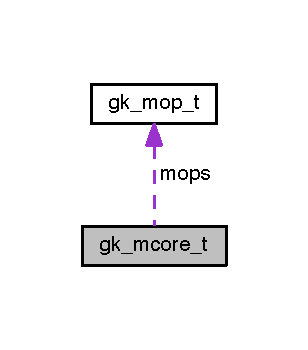
\includegraphics[width=148pt]{structgk__mcore__t__coll__graph}
\end{center}
\end{figure}
\subsection*{Public Attributes}
\begin{DoxyCompactItemize}
\item 
size\+\_\+t \hyperlink{structgk__mcore__t_a834677bb8263a1b0475104889883c86c}{coresize}
\item 
size\+\_\+t \hyperlink{structgk__mcore__t_a5cc856b4f3049f9d49c9f3ec10b73739}{corecpos}
\item 
void $\ast$ \hyperlink{structgk__mcore__t_a2d0056e8cc124fad35b901e89668b8b1}{core}
\item 
size\+\_\+t \hyperlink{structgk__mcore__t_a30d17f8009db5d7cf61094259ff9e26f}{nmops}
\item 
size\+\_\+t \hyperlink{structgk__mcore__t_a3631e211c793af96e0abf21cb95de4ae}{cmop}
\item 
\hyperlink{structgk__mop__t}{gk\+\_\+mop\+\_\+t} $\ast$ \hyperlink{structgk__mcore__t_a74e825c8a07e7c040dbf947bedac3339}{mops}
\item 
size\+\_\+t \hyperlink{structgk__mcore__t_afd16bb0581bc9e98172b2ab35cbc310c}{num\+\_\+callocs}
\item 
size\+\_\+t \hyperlink{structgk__mcore__t_a2ad475b19470a6a7b0c65e53cfd1096b}{num\+\_\+hallocs}
\item 
size\+\_\+t \hyperlink{structgk__mcore__t_aa407f9b9ca318fa8afa36ab1c936ec07}{size\+\_\+callocs}
\item 
size\+\_\+t \hyperlink{structgk__mcore__t_a4c180c60538546b4ab67bb91264e1c6e}{size\+\_\+hallocs}
\item 
size\+\_\+t \hyperlink{structgk__mcore__t_a488b0e7fbec1333c47a736af554a640c}{cur\+\_\+callocs}
\item 
size\+\_\+t \hyperlink{structgk__mcore__t_a69514abe8ce1822030428ca391a903e7}{cur\+\_\+hallocs}
\item 
size\+\_\+t \hyperlink{structgk__mcore__t_a536a8ab027c1f70bfe5b56a26059589b}{max\+\_\+callocs}
\item 
size\+\_\+t \hyperlink{structgk__mcore__t_a74723a880e8829c81bd3a38ed474f09a}{max\+\_\+hallocs}
\end{DoxyCompactItemize}


\subsection{Detailed Description}
The following structure stores information used by Metis 

\subsection{Member Data Documentation}
\mbox{\Hypertarget{structgk__mcore__t_a3631e211c793af96e0abf21cb95de4ae}\label{structgk__mcore__t_a3631e211c793af96e0abf21cb95de4ae}} 
\index{gk\+\_\+mcore\+\_\+t@{gk\+\_\+mcore\+\_\+t}!cmop@{cmop}}
\index{cmop@{cmop}!gk\+\_\+mcore\+\_\+t@{gk\+\_\+mcore\+\_\+t}}
\subsubsection{\texorpdfstring{cmop}{cmop}}
{\footnotesize\ttfamily size\+\_\+t gk\+\_\+mcore\+\_\+t\+::cmop}

Index of the first free location in maops \mbox{\Hypertarget{structgk__mcore__t_a2d0056e8cc124fad35b901e89668b8b1}\label{structgk__mcore__t_a2d0056e8cc124fad35b901e89668b8b1}} 
\index{gk\+\_\+mcore\+\_\+t@{gk\+\_\+mcore\+\_\+t}!core@{core}}
\index{core@{core}!gk\+\_\+mcore\+\_\+t@{gk\+\_\+mcore\+\_\+t}}
\subsubsection{\texorpdfstring{core}{core}}
{\footnotesize\ttfamily void$\ast$ gk\+\_\+mcore\+\_\+t\+::core}

Pointer to the core itself \mbox{\Hypertarget{structgk__mcore__t_a5cc856b4f3049f9d49c9f3ec10b73739}\label{structgk__mcore__t_a5cc856b4f3049f9d49c9f3ec10b73739}} 
\index{gk\+\_\+mcore\+\_\+t@{gk\+\_\+mcore\+\_\+t}!corecpos@{corecpos}}
\index{corecpos@{corecpos}!gk\+\_\+mcore\+\_\+t@{gk\+\_\+mcore\+\_\+t}}
\subsubsection{\texorpdfstring{corecpos}{corecpos}}
{\footnotesize\ttfamily size\+\_\+t gk\+\_\+mcore\+\_\+t\+::corecpos}

Index of the first free location in core \mbox{\Hypertarget{structgk__mcore__t_a834677bb8263a1b0475104889883c86c}\label{structgk__mcore__t_a834677bb8263a1b0475104889883c86c}} 
\index{gk\+\_\+mcore\+\_\+t@{gk\+\_\+mcore\+\_\+t}!coresize@{coresize}}
\index{coresize@{coresize}!gk\+\_\+mcore\+\_\+t@{gk\+\_\+mcore\+\_\+t}}
\subsubsection{\texorpdfstring{coresize}{coresize}}
{\footnotesize\ttfamily size\+\_\+t gk\+\_\+mcore\+\_\+t\+::coresize}

The amount of core memory that has been allocated \mbox{\Hypertarget{structgk__mcore__t_a488b0e7fbec1333c47a736af554a640c}\label{structgk__mcore__t_a488b0e7fbec1333c47a736af554a640c}} 
\index{gk\+\_\+mcore\+\_\+t@{gk\+\_\+mcore\+\_\+t}!cur\+\_\+callocs@{cur\+\_\+callocs}}
\index{cur\+\_\+callocs@{cur\+\_\+callocs}!gk\+\_\+mcore\+\_\+t@{gk\+\_\+mcore\+\_\+t}}
\subsubsection{\texorpdfstring{cur\+\_\+callocs}{cur\_callocs}}
{\footnotesize\ttfamily size\+\_\+t gk\+\_\+mcore\+\_\+t\+::cur\+\_\+callocs}

The current \# of bytes in core mallocs \mbox{\Hypertarget{structgk__mcore__t_a69514abe8ce1822030428ca391a903e7}\label{structgk__mcore__t_a69514abe8ce1822030428ca391a903e7}} 
\index{gk\+\_\+mcore\+\_\+t@{gk\+\_\+mcore\+\_\+t}!cur\+\_\+hallocs@{cur\+\_\+hallocs}}
\index{cur\+\_\+hallocs@{cur\+\_\+hallocs}!gk\+\_\+mcore\+\_\+t@{gk\+\_\+mcore\+\_\+t}}
\subsubsection{\texorpdfstring{cur\+\_\+hallocs}{cur\_hallocs}}
{\footnotesize\ttfamily size\+\_\+t gk\+\_\+mcore\+\_\+t\+::cur\+\_\+hallocs}

The current \# of bytes in heap mallocs \mbox{\Hypertarget{structgk__mcore__t_a536a8ab027c1f70bfe5b56a26059589b}\label{structgk__mcore__t_a536a8ab027c1f70bfe5b56a26059589b}} 
\index{gk\+\_\+mcore\+\_\+t@{gk\+\_\+mcore\+\_\+t}!max\+\_\+callocs@{max\+\_\+callocs}}
\index{max\+\_\+callocs@{max\+\_\+callocs}!gk\+\_\+mcore\+\_\+t@{gk\+\_\+mcore\+\_\+t}}
\subsubsection{\texorpdfstring{max\+\_\+callocs}{max\_callocs}}
{\footnotesize\ttfamily size\+\_\+t gk\+\_\+mcore\+\_\+t\+::max\+\_\+callocs}

The maximum \# of bytes in core mallocs at any given time \mbox{\Hypertarget{structgk__mcore__t_a74723a880e8829c81bd3a38ed474f09a}\label{structgk__mcore__t_a74723a880e8829c81bd3a38ed474f09a}} 
\index{gk\+\_\+mcore\+\_\+t@{gk\+\_\+mcore\+\_\+t}!max\+\_\+hallocs@{max\+\_\+hallocs}}
\index{max\+\_\+hallocs@{max\+\_\+hallocs}!gk\+\_\+mcore\+\_\+t@{gk\+\_\+mcore\+\_\+t}}
\subsubsection{\texorpdfstring{max\+\_\+hallocs}{max\_hallocs}}
{\footnotesize\ttfamily size\+\_\+t gk\+\_\+mcore\+\_\+t\+::max\+\_\+hallocs}

The maximum \# of bytes in heap mallocs at any given time \mbox{\Hypertarget{structgk__mcore__t_a74e825c8a07e7c040dbf947bedac3339}\label{structgk__mcore__t_a74e825c8a07e7c040dbf947bedac3339}} 
\index{gk\+\_\+mcore\+\_\+t@{gk\+\_\+mcore\+\_\+t}!mops@{mops}}
\index{mops@{mops}!gk\+\_\+mcore\+\_\+t@{gk\+\_\+mcore\+\_\+t}}
\subsubsection{\texorpdfstring{mops}{mops}}
{\footnotesize\ttfamily \hyperlink{structgk__mop__t}{gk\+\_\+mop\+\_\+t}$\ast$ gk\+\_\+mcore\+\_\+t\+::mops}

The array recording the maop\+\_\+t operations \mbox{\Hypertarget{structgk__mcore__t_a30d17f8009db5d7cf61094259ff9e26f}\label{structgk__mcore__t_a30d17f8009db5d7cf61094259ff9e26f}} 
\index{gk\+\_\+mcore\+\_\+t@{gk\+\_\+mcore\+\_\+t}!nmops@{nmops}}
\index{nmops@{nmops}!gk\+\_\+mcore\+\_\+t@{gk\+\_\+mcore\+\_\+t}}
\subsubsection{\texorpdfstring{nmops}{nmops}}
{\footnotesize\ttfamily size\+\_\+t gk\+\_\+mcore\+\_\+t\+::nmops}

The number of maop\+\_\+t entries that have been allocated \mbox{\Hypertarget{structgk__mcore__t_afd16bb0581bc9e98172b2ab35cbc310c}\label{structgk__mcore__t_afd16bb0581bc9e98172b2ab35cbc310c}} 
\index{gk\+\_\+mcore\+\_\+t@{gk\+\_\+mcore\+\_\+t}!num\+\_\+callocs@{num\+\_\+callocs}}
\index{num\+\_\+callocs@{num\+\_\+callocs}!gk\+\_\+mcore\+\_\+t@{gk\+\_\+mcore\+\_\+t}}
\subsubsection{\texorpdfstring{num\+\_\+callocs}{num\_callocs}}
{\footnotesize\ttfamily size\+\_\+t gk\+\_\+mcore\+\_\+t\+::num\+\_\+callocs}

The number of core mallocs \mbox{\Hypertarget{structgk__mcore__t_a2ad475b19470a6a7b0c65e53cfd1096b}\label{structgk__mcore__t_a2ad475b19470a6a7b0c65e53cfd1096b}} 
\index{gk\+\_\+mcore\+\_\+t@{gk\+\_\+mcore\+\_\+t}!num\+\_\+hallocs@{num\+\_\+hallocs}}
\index{num\+\_\+hallocs@{num\+\_\+hallocs}!gk\+\_\+mcore\+\_\+t@{gk\+\_\+mcore\+\_\+t}}
\subsubsection{\texorpdfstring{num\+\_\+hallocs}{num\_hallocs}}
{\footnotesize\ttfamily size\+\_\+t gk\+\_\+mcore\+\_\+t\+::num\+\_\+hallocs}

The number of heap mallocs \mbox{\Hypertarget{structgk__mcore__t_aa407f9b9ca318fa8afa36ab1c936ec07}\label{structgk__mcore__t_aa407f9b9ca318fa8afa36ab1c936ec07}} 
\index{gk\+\_\+mcore\+\_\+t@{gk\+\_\+mcore\+\_\+t}!size\+\_\+callocs@{size\+\_\+callocs}}
\index{size\+\_\+callocs@{size\+\_\+callocs}!gk\+\_\+mcore\+\_\+t@{gk\+\_\+mcore\+\_\+t}}
\subsubsection{\texorpdfstring{size\+\_\+callocs}{size\_callocs}}
{\footnotesize\ttfamily size\+\_\+t gk\+\_\+mcore\+\_\+t\+::size\+\_\+callocs}

The total \# of bytes in core mallocs \mbox{\Hypertarget{structgk__mcore__t_a4c180c60538546b4ab67bb91264e1c6e}\label{structgk__mcore__t_a4c180c60538546b4ab67bb91264e1c6e}} 
\index{gk\+\_\+mcore\+\_\+t@{gk\+\_\+mcore\+\_\+t}!size\+\_\+hallocs@{size\+\_\+hallocs}}
\index{size\+\_\+hallocs@{size\+\_\+hallocs}!gk\+\_\+mcore\+\_\+t@{gk\+\_\+mcore\+\_\+t}}
\subsubsection{\texorpdfstring{size\+\_\+hallocs}{size\_hallocs}}
{\footnotesize\ttfamily size\+\_\+t gk\+\_\+mcore\+\_\+t\+::size\+\_\+hallocs}

The total \# of bytes in heap mallocs 

The documentation for this struct was generated from the following file\+:\begin{DoxyCompactItemize}
\item 
3rd\+Party/parmetis-\/4.\+0.\+3/metis/\+G\+Klib/\hyperlink{gk__struct_8h}{gk\+\_\+struct.\+h}\end{DoxyCompactItemize}

\hypertarget{structgk__mop__t}{}\section{gk\+\_\+mop\+\_\+t Struct Reference}
\label{structgk__mop__t}\index{gk\+\_\+mop\+\_\+t@{gk\+\_\+mop\+\_\+t}}


{\ttfamily \#include $<$gk\+\_\+struct.\+h$>$}

\subsection*{Public Attributes}
\begin{DoxyCompactItemize}
\item 
int \hyperlink{structgk__mop__t_a26d63dcd8e95d56959ef1c6f8ef37c6b}{type}
\item 
ssize\+\_\+t \hyperlink{structgk__mop__t_a2b766c120002f4e58d0a1e50e61822f4}{nbytes}
\item 
void $\ast$ \hyperlink{structgk__mop__t_a3333a1078416780e6a38189db93af2fd}{ptr}
\end{DoxyCompactItemize}


\subsection{Detailed Description}
The following data structure stores information about a memory allocation operation that can either be served from \hyperlink{structgk__mcore__t}{gk\+\_\+mcore\+\_\+t} or by a gk\+\_\+malloc if not sufficient workspace memory is available. 

\subsection{Member Data Documentation}
\mbox{\Hypertarget{structgk__mop__t_a2b766c120002f4e58d0a1e50e61822f4}\label{structgk__mop__t_a2b766c120002f4e58d0a1e50e61822f4}} 
\index{gk\+\_\+mop\+\_\+t@{gk\+\_\+mop\+\_\+t}!nbytes@{nbytes}}
\index{nbytes@{nbytes}!gk\+\_\+mop\+\_\+t@{gk\+\_\+mop\+\_\+t}}
\subsubsection{\texorpdfstring{nbytes}{nbytes}}
{\footnotesize\ttfamily ssize\+\_\+t gk\+\_\+mop\+\_\+t\+::nbytes}

\mbox{\Hypertarget{structgk__mop__t_a3333a1078416780e6a38189db93af2fd}\label{structgk__mop__t_a3333a1078416780e6a38189db93af2fd}} 
\index{gk\+\_\+mop\+\_\+t@{gk\+\_\+mop\+\_\+t}!ptr@{ptr}}
\index{ptr@{ptr}!gk\+\_\+mop\+\_\+t@{gk\+\_\+mop\+\_\+t}}
\subsubsection{\texorpdfstring{ptr}{ptr}}
{\footnotesize\ttfamily void$\ast$ gk\+\_\+mop\+\_\+t\+::ptr}

\mbox{\Hypertarget{structgk__mop__t_a26d63dcd8e95d56959ef1c6f8ef37c6b}\label{structgk__mop__t_a26d63dcd8e95d56959ef1c6f8ef37c6b}} 
\index{gk\+\_\+mop\+\_\+t@{gk\+\_\+mop\+\_\+t}!type@{type}}
\index{type@{type}!gk\+\_\+mop\+\_\+t@{gk\+\_\+mop\+\_\+t}}
\subsubsection{\texorpdfstring{type}{type}}
{\footnotesize\ttfamily int gk\+\_\+mop\+\_\+t\+::type}



The documentation for this struct was generated from the following file\+:\begin{DoxyCompactItemize}
\item 
3rd\+Party/parmetis-\/4.\+0.\+3/metis/\+G\+Klib/\hyperlink{gk__struct_8h}{gk\+\_\+struct.\+h}\end{DoxyCompactItemize}

\hypertarget{structgk__option}{}\section{gk\+\_\+option Struct Reference}
\label{structgk__option}\index{gk\+\_\+option@{gk\+\_\+option}}


The structure that stores the information about the command-\/line options.  




{\ttfamily \#include $<$gk\+\_\+getopt.\+h$>$}

\subsection*{Public Attributes}
\begin{DoxyCompactItemize}
\item 
char $\ast$ \hyperlink{structgk__option_aa47d0e4e90d3cd1793fc5344b1e99afc}{name}
\item 
int \hyperlink{structgk__option_a66d2ab88446836cef777d756098151f5}{has\+\_\+arg}
\item 
int $\ast$ \hyperlink{structgk__option_ae9e56a3e65a631de45dd019a07c621b4}{flag}
\item 
int \hyperlink{structgk__option_abf964c7489d269515ec8e5e62b2164ba}{val}
\end{DoxyCompactItemize}


\subsection{Detailed Description}
The structure that stores the information about the command-\/line options. 

This structure describes a single long option name for the sake of \hyperlink{getopt_8c_a1c3b8d80bd9620dc66f24d4854c0f6d3}{gk\+\_\+getopt\+\_\+long()}. The argument {\ttfamily long\+\_\+options} must be an array of these structures, one for each long option. Terminate the array with an element containing all zeros. 

\subsection{Member Data Documentation}
\mbox{\Hypertarget{structgk__option_ae9e56a3e65a631de45dd019a07c621b4}\label{structgk__option_ae9e56a3e65a631de45dd019a07c621b4}} 
\index{gk\+\_\+option@{gk\+\_\+option}!flag@{flag}}
\index{flag@{flag}!gk\+\_\+option@{gk\+\_\+option}}
\subsubsection{\texorpdfstring{flag}{flag}}
{\footnotesize\ttfamily int$\ast$ gk\+\_\+option\+::flag}

See the discussion on \hyperlink{structgk__option_abf964c7489d269515ec8e5e62b2164ba}{gk\+\_\+option\+::val} \mbox{\Hypertarget{structgk__option_a66d2ab88446836cef777d756098151f5}\label{structgk__option_a66d2ab88446836cef777d756098151f5}} 
\index{gk\+\_\+option@{gk\+\_\+option}!has\+\_\+arg@{has\+\_\+arg}}
\index{has\+\_\+arg@{has\+\_\+arg}!gk\+\_\+option@{gk\+\_\+option}}
\subsubsection{\texorpdfstring{has\+\_\+arg}{has\_arg}}
{\footnotesize\ttfamily int gk\+\_\+option\+::has\+\_\+arg}

This field says whether the option takes an argument. It is an integer, and there are three legitimate values\+: no\+\_\+argument, required\+\_\+argument and optional\+\_\+argument. \mbox{\Hypertarget{structgk__option_aa47d0e4e90d3cd1793fc5344b1e99afc}\label{structgk__option_aa47d0e4e90d3cd1793fc5344b1e99afc}} 
\index{gk\+\_\+option@{gk\+\_\+option}!name@{name}}
\index{name@{name}!gk\+\_\+option@{gk\+\_\+option}}
\subsubsection{\texorpdfstring{name}{name}}
{\footnotesize\ttfamily char$\ast$ gk\+\_\+option\+::name}

This field is the name of the option. \mbox{\Hypertarget{structgk__option_abf964c7489d269515ec8e5e62b2164ba}\label{structgk__option_abf964c7489d269515ec8e5e62b2164ba}} 
\index{gk\+\_\+option@{gk\+\_\+option}!val@{val}}
\index{val@{val}!gk\+\_\+option@{gk\+\_\+option}}
\subsubsection{\texorpdfstring{val}{val}}
{\footnotesize\ttfamily int gk\+\_\+option\+::val}

These fields control how to report or act on the option when it occurs.

If flag is a null pointer, then the val is a value which identifies this option. Often these values are chosen to uniquely identify particular long options.

If flag is not a null pointer, it should be the address of an int variable which is the flag for this option. The value in val is the value to store in the flag to indicate that the option was seen. 

The documentation for this struct was generated from the following file\+:\begin{DoxyCompactItemize}
\item 
3rd\+Party/parmetis-\/4.\+0.\+3/metis/\+G\+Klib/\hyperlink{gk__getopt_8h}{gk\+\_\+getopt.\+h}\end{DoxyCompactItemize}

\hypertarget{structgk__seq__t}{}\section{gk\+\_\+seq\+\_\+t Struct Reference}
\label{structgk__seq__t}\index{gk\+\_\+seq\+\_\+t@{gk\+\_\+seq\+\_\+t}}


{\ttfamily \#include $<$gk\+\_\+struct.\+h$>$}

\subsection*{Public Attributes}
\begin{DoxyCompactItemize}
\item 
int \hyperlink{structgk__seq__t_a4970c7091d86284d10ae370aa9bf0145}{len}
\item 
int $\ast$ \hyperlink{structgk__seq__t_a5a803ced386350dd152f047531035f81}{sequence}
\item 
int $\ast$$\ast$ \hyperlink{structgk__seq__t_aca3f51322bd7246f338394a442e37e7c}{pssm}
\item 
int $\ast$$\ast$ \hyperlink{structgk__seq__t_a2f3676712f6cbb159642884a3dff7eec}{psfm}
\item 
char $\ast$ \hyperlink{structgk__seq__t_a231b4df61c5c3501eff97c408dc882b3}{name}
\item 
int \hyperlink{structgk__seq__t_a876b72b49af40e66b978e33f87cda044}{nsymbols}
\end{DoxyCompactItemize}


\subsection{Member Data Documentation}
\mbox{\Hypertarget{structgk__seq__t_a4970c7091d86284d10ae370aa9bf0145}\label{structgk__seq__t_a4970c7091d86284d10ae370aa9bf0145}} 
\index{gk\+\_\+seq\+\_\+t@{gk\+\_\+seq\+\_\+t}!len@{len}}
\index{len@{len}!gk\+\_\+seq\+\_\+t@{gk\+\_\+seq\+\_\+t}}
\subsubsection{\texorpdfstring{len}{len}}
{\footnotesize\ttfamily int gk\+\_\+seq\+\_\+t\+::len}

\mbox{\Hypertarget{structgk__seq__t_a231b4df61c5c3501eff97c408dc882b3}\label{structgk__seq__t_a231b4df61c5c3501eff97c408dc882b3}} 
\index{gk\+\_\+seq\+\_\+t@{gk\+\_\+seq\+\_\+t}!name@{name}}
\index{name@{name}!gk\+\_\+seq\+\_\+t@{gk\+\_\+seq\+\_\+t}}
\subsubsection{\texorpdfstring{name}{name}}
{\footnotesize\ttfamily char$\ast$ gk\+\_\+seq\+\_\+t\+::name}

\mbox{\Hypertarget{structgk__seq__t_a876b72b49af40e66b978e33f87cda044}\label{structgk__seq__t_a876b72b49af40e66b978e33f87cda044}} 
\index{gk\+\_\+seq\+\_\+t@{gk\+\_\+seq\+\_\+t}!nsymbols@{nsymbols}}
\index{nsymbols@{nsymbols}!gk\+\_\+seq\+\_\+t@{gk\+\_\+seq\+\_\+t}}
\subsubsection{\texorpdfstring{nsymbols}{nsymbols}}
{\footnotesize\ttfamily int gk\+\_\+seq\+\_\+t\+::nsymbols}

\mbox{\Hypertarget{structgk__seq__t_a2f3676712f6cbb159642884a3dff7eec}\label{structgk__seq__t_a2f3676712f6cbb159642884a3dff7eec}} 
\index{gk\+\_\+seq\+\_\+t@{gk\+\_\+seq\+\_\+t}!psfm@{psfm}}
\index{psfm@{psfm}!gk\+\_\+seq\+\_\+t@{gk\+\_\+seq\+\_\+t}}
\subsubsection{\texorpdfstring{psfm}{psfm}}
{\footnotesize\ttfamily int$\ast$$\ast$ gk\+\_\+seq\+\_\+t\+::psfm}

\mbox{\Hypertarget{structgk__seq__t_aca3f51322bd7246f338394a442e37e7c}\label{structgk__seq__t_aca3f51322bd7246f338394a442e37e7c}} 
\index{gk\+\_\+seq\+\_\+t@{gk\+\_\+seq\+\_\+t}!pssm@{pssm}}
\index{pssm@{pssm}!gk\+\_\+seq\+\_\+t@{gk\+\_\+seq\+\_\+t}}
\subsubsection{\texorpdfstring{pssm}{pssm}}
{\footnotesize\ttfamily int$\ast$$\ast$ gk\+\_\+seq\+\_\+t\+::pssm}

\mbox{\Hypertarget{structgk__seq__t_a5a803ced386350dd152f047531035f81}\label{structgk__seq__t_a5a803ced386350dd152f047531035f81}} 
\index{gk\+\_\+seq\+\_\+t@{gk\+\_\+seq\+\_\+t}!sequence@{sequence}}
\index{sequence@{sequence}!gk\+\_\+seq\+\_\+t@{gk\+\_\+seq\+\_\+t}}
\subsubsection{\texorpdfstring{sequence}{sequence}}
{\footnotesize\ttfamily int$\ast$ gk\+\_\+seq\+\_\+t\+::sequence}



The documentation for this struct was generated from the following file\+:\begin{DoxyCompactItemize}
\item 
3rd\+Party/parmetis-\/4.\+0.\+3/metis/\+G\+Klib/\hyperlink{gk__struct_8h}{gk\+\_\+struct.\+h}\end{DoxyCompactItemize}

\hypertarget{structgk__str__t}{}\section{gk\+\_\+str\+\_\+t Struct Reference}
\label{structgk__str__t}\index{gk\+\_\+str\+\_\+t@{gk\+\_\+str\+\_\+t}}


{\ttfamily \#include $<$gk\+\_\+struct.\+h$>$}

\subsection*{Public Attributes}
\begin{DoxyCompactItemize}
\item 
size\+\_\+t \hyperlink{structgk__str__t_acce3955b5ce3c8b9965e7163aad9705d}{len}
\item 
char $\ast$ \hyperlink{structgk__str__t_a865fb5b4ddc39efeb3c86e2251f13380}{buf}
\end{DoxyCompactItemize}


\subsection{Member Data Documentation}
\mbox{\Hypertarget{structgk__str__t_a865fb5b4ddc39efeb3c86e2251f13380}\label{structgk__str__t_a865fb5b4ddc39efeb3c86e2251f13380}} 
\index{gk\+\_\+str\+\_\+t@{gk\+\_\+str\+\_\+t}!buf@{buf}}
\index{buf@{buf}!gk\+\_\+str\+\_\+t@{gk\+\_\+str\+\_\+t}}
\subsubsection{\texorpdfstring{buf}{buf}}
{\footnotesize\ttfamily char$\ast$ gk\+\_\+str\+\_\+t\+::buf}

\mbox{\Hypertarget{structgk__str__t_acce3955b5ce3c8b9965e7163aad9705d}\label{structgk__str__t_acce3955b5ce3c8b9965e7163aad9705d}} 
\index{gk\+\_\+str\+\_\+t@{gk\+\_\+str\+\_\+t}!len@{len}}
\index{len@{len}!gk\+\_\+str\+\_\+t@{gk\+\_\+str\+\_\+t}}
\subsubsection{\texorpdfstring{len}{len}}
{\footnotesize\ttfamily size\+\_\+t gk\+\_\+str\+\_\+t\+::len}



The documentation for this struct was generated from the following file\+:\begin{DoxyCompactItemize}
\item 
3rd\+Party/parmetis-\/4.\+0.\+3/metis/\+G\+Klib/\hyperlink{gk__struct_8h}{gk\+\_\+struct.\+h}\end{DoxyCompactItemize}

\hypertarget{structgk___string_map__t}{}\section{gk\+\_\+\+String\+Map\+\_\+t Struct Reference}
\label{structgk___string_map__t}\index{gk\+\_\+\+String\+Map\+\_\+t@{gk\+\_\+\+String\+Map\+\_\+t}}


{\ttfamily \#include $<$gk\+\_\+struct.\+h$>$}

\subsection*{Public Attributes}
\begin{DoxyCompactItemize}
\item 
char $\ast$ \hyperlink{structgk___string_map__t_a22d4edf70d41af7c5ed2db52ee09eb99}{name}
\item 
int \hyperlink{structgk___string_map__t_a167db63a424bbf4d1709685edd191c3a}{id}
\end{DoxyCompactItemize}


\subsection{Member Data Documentation}
\mbox{\Hypertarget{structgk___string_map__t_a167db63a424bbf4d1709685edd191c3a}\label{structgk___string_map__t_a167db63a424bbf4d1709685edd191c3a}} 
\index{gk\+\_\+\+String\+Map\+\_\+t@{gk\+\_\+\+String\+Map\+\_\+t}!id@{id}}
\index{id@{id}!gk\+\_\+\+String\+Map\+\_\+t@{gk\+\_\+\+String\+Map\+\_\+t}}
\subsubsection{\texorpdfstring{id}{id}}
{\footnotesize\ttfamily int gk\+\_\+\+String\+Map\+\_\+t\+::id}

\mbox{\Hypertarget{structgk___string_map__t_a22d4edf70d41af7c5ed2db52ee09eb99}\label{structgk___string_map__t_a22d4edf70d41af7c5ed2db52ee09eb99}} 
\index{gk\+\_\+\+String\+Map\+\_\+t@{gk\+\_\+\+String\+Map\+\_\+t}!name@{name}}
\index{name@{name}!gk\+\_\+\+String\+Map\+\_\+t@{gk\+\_\+\+String\+Map\+\_\+t}}
\subsubsection{\texorpdfstring{name}{name}}
{\footnotesize\ttfamily char$\ast$ gk\+\_\+\+String\+Map\+\_\+t\+::name}



The documentation for this struct was generated from the following file\+:\begin{DoxyCompactItemize}
\item 
3rd\+Party/parmetis-\/4.\+0.\+3/metis/\+G\+Klib/\hyperlink{gk__struct_8h}{gk\+\_\+struct.\+h}\end{DoxyCompactItemize}

\hypertarget{structgk___tokens__t}{}\section{gk\+\_\+\+Tokens\+\_\+t Struct Reference}
\label{structgk___tokens__t}\index{gk\+\_\+\+Tokens\+\_\+t@{gk\+\_\+\+Tokens\+\_\+t}}


{\ttfamily \#include $<$gk\+\_\+struct.\+h$>$}

\subsection*{Public Attributes}
\begin{DoxyCompactItemize}
\item 
int \hyperlink{structgk___tokens__t_a9a6e215f177a16bc5852abd3953fa12e}{ntoks}
\item 
char $\ast$ \hyperlink{structgk___tokens__t_a2770337d903acb342ec9540882b53601}{strbuf}
\item 
char $\ast$$\ast$ \hyperlink{structgk___tokens__t_a3e5376a3057dc7102615daa0dcbd44f8}{list}
\end{DoxyCompactItemize}


\subsection{Member Data Documentation}
\mbox{\Hypertarget{structgk___tokens__t_a3e5376a3057dc7102615daa0dcbd44f8}\label{structgk___tokens__t_a3e5376a3057dc7102615daa0dcbd44f8}} 
\index{gk\+\_\+\+Tokens\+\_\+t@{gk\+\_\+\+Tokens\+\_\+t}!list@{list}}
\index{list@{list}!gk\+\_\+\+Tokens\+\_\+t@{gk\+\_\+\+Tokens\+\_\+t}}
\subsubsection{\texorpdfstring{list}{list}}
{\footnotesize\ttfamily char$\ast$$\ast$ gk\+\_\+\+Tokens\+\_\+t\+::list}

\mbox{\Hypertarget{structgk___tokens__t_a9a6e215f177a16bc5852abd3953fa12e}\label{structgk___tokens__t_a9a6e215f177a16bc5852abd3953fa12e}} 
\index{gk\+\_\+\+Tokens\+\_\+t@{gk\+\_\+\+Tokens\+\_\+t}!ntoks@{ntoks}}
\index{ntoks@{ntoks}!gk\+\_\+\+Tokens\+\_\+t@{gk\+\_\+\+Tokens\+\_\+t}}
\subsubsection{\texorpdfstring{ntoks}{ntoks}}
{\footnotesize\ttfamily int gk\+\_\+\+Tokens\+\_\+t\+::ntoks}

\mbox{\Hypertarget{structgk___tokens__t_a2770337d903acb342ec9540882b53601}\label{structgk___tokens__t_a2770337d903acb342ec9540882b53601}} 
\index{gk\+\_\+\+Tokens\+\_\+t@{gk\+\_\+\+Tokens\+\_\+t}!strbuf@{strbuf}}
\index{strbuf@{strbuf}!gk\+\_\+\+Tokens\+\_\+t@{gk\+\_\+\+Tokens\+\_\+t}}
\subsubsection{\texorpdfstring{strbuf}{strbuf}}
{\footnotesize\ttfamily char$\ast$ gk\+\_\+\+Tokens\+\_\+t\+::strbuf}



The documentation for this struct was generated from the following file\+:\begin{DoxyCompactItemize}
\item 
3rd\+Party/parmetis-\/4.\+0.\+3/metis/\+G\+Klib/\hyperlink{gk__struct_8h}{gk\+\_\+struct.\+h}\end{DoxyCompactItemize}

\hypertarget{structgraph__t}{}\section{graph\+\_\+t Struct Reference}
\label{structgraph__t}\index{graph\+\_\+t@{graph\+\_\+t}}


{\ttfamily \#include $<$struct.\+h$>$}



Collaboration diagram for graph\+\_\+t\+:\nopagebreak
\begin{figure}[H]
\begin{center}
\leavevmode
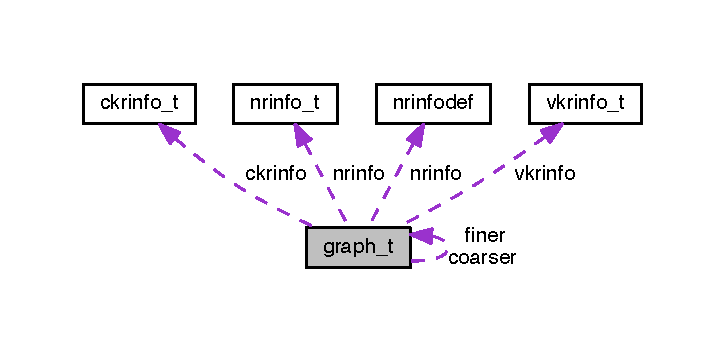
\includegraphics[width=348pt]{structgraph__t__coll__graph}
\end{center}
\end{figure}
\subsection*{Public Attributes}
\begin{DoxyCompactItemize}
\item 
\hyperlink{3rd_party_2parmetis-4_80_83_2metis_2include_2metis_8h_aaa5262be3e700770163401acb0150f52}{idx\+\_\+t} \hyperlink{structgraph__t_a7e70f7ea557eaa17352b8068c8cb5f03}{nvtxs}
\item 
\hyperlink{3rd_party_2parmetis-4_80_83_2metis_2include_2metis_8h_aaa5262be3e700770163401acb0150f52}{idx\+\_\+t} \hyperlink{structgraph__t_a0dcab67cfc75a9d7bc3cab2563f4df03}{nedges}
\item 
\hyperlink{3rd_party_2parmetis-4_80_83_2metis_2include_2metis_8h_aaa5262be3e700770163401acb0150f52}{idx\+\_\+t} \hyperlink{structgraph__t_acdfe382784cfe19f41fb10ede3a5a9f9}{ncon}
\item 
\hyperlink{3rd_party_2parmetis-4_80_83_2metis_2include_2metis_8h_aaa5262be3e700770163401acb0150f52}{idx\+\_\+t} $\ast$ \hyperlink{structgraph__t_aa92b073425f4bca4789af4cf33a547e5}{xadj}
\item 
\hyperlink{3rd_party_2parmetis-4_80_83_2metis_2include_2metis_8h_aaa5262be3e700770163401acb0150f52}{idx\+\_\+t} $\ast$ \hyperlink{structgraph__t_a3a94894dcbf1b65a638e37cd485b5f88}{vwgt}
\item 
\hyperlink{3rd_party_2parmetis-4_80_83_2metis_2include_2metis_8h_aaa5262be3e700770163401acb0150f52}{idx\+\_\+t} $\ast$ \hyperlink{structgraph__t_ad191f54e22012bbc3c7cc5fec228c71a}{vsize}
\item 
\hyperlink{3rd_party_2parmetis-4_80_83_2metis_2include_2metis_8h_aaa5262be3e700770163401acb0150f52}{idx\+\_\+t} $\ast$ \hyperlink{structgraph__t_a0301c5a80081df93c122992f779ded24}{adjncy}
\item 
\hyperlink{3rd_party_2parmetis-4_80_83_2metis_2include_2metis_8h_aaa5262be3e700770163401acb0150f52}{idx\+\_\+t} $\ast$ \hyperlink{structgraph__t_acad756362a4703fefde4e7cbca8f46f8}{adjwgt}
\item 
\hyperlink{3rd_party_2parmetis-4_80_83_2metis_2include_2metis_8h_aaa5262be3e700770163401acb0150f52}{idx\+\_\+t} $\ast$ \hyperlink{structgraph__t_ace9ad621f1e97e5a796c8d24a345aef8}{tvwgt}
\item 
\hyperlink{3rd_party_2parmetis-4_80_83_2metis_2include_2metis_8h_a1924a4f6907cc3833213aba1f07fcbe9}{real\+\_\+t} $\ast$ \hyperlink{structgraph__t_a25c1b2aeb241430033fb752ba11b5cbb}{invtvwgt}
\item 
int \hyperlink{structgraph__t_a3e30bc414d99cbb3c619a0575bd542f3}{free\+\_\+xadj}
\item 
int \hyperlink{structgraph__t_a4573225a35a1b8e4e5c90f6b26ab3082}{free\+\_\+vwgt}
\item 
int \hyperlink{structgraph__t_ac4526f6e81ac9d349bf1c69eb6359a85}{free\+\_\+vsize}
\item 
int \hyperlink{structgraph__t_afaa9c1b1b1fd7238b724d9f030f582cd}{free\+\_\+adjncy}
\item 
int \hyperlink{structgraph__t_a2ff72cc1f2462e073d9293a558d3d944}{free\+\_\+adjwgt}
\item 
\hyperlink{3rd_party_2parmetis-4_80_83_2metis_2include_2metis_8h_aaa5262be3e700770163401acb0150f52}{idx\+\_\+t} $\ast$ \hyperlink{structgraph__t_ab2ae2df953d94b5ca663e8e6cf8a2aa4}{label}
\item 
\hyperlink{3rd_party_2parmetis-4_80_83_2metis_2include_2metis_8h_aaa5262be3e700770163401acb0150f52}{idx\+\_\+t} $\ast$ \hyperlink{structgraph__t_a7f6d2c556b08aa7a33d55374e0a60c7f}{cmap}
\item 
\hyperlink{3rd_party_2parmetis-4_80_83_2metis_2include_2metis_8h_aaa5262be3e700770163401acb0150f52}{idx\+\_\+t} \hyperlink{structgraph__t_a71e53c3699a6347393d864eaa52e4f66}{mincut}
\item 
\hyperlink{3rd_party_2parmetis-4_80_83_2metis_2include_2metis_8h_aaa5262be3e700770163401acb0150f52}{idx\+\_\+t} \hyperlink{structgraph__t_ad5c4c963306e80c0430d3158a751b9f5}{minvol}
\item 
\hyperlink{3rd_party_2parmetis-4_80_83_2metis_2include_2metis_8h_aaa5262be3e700770163401acb0150f52}{idx\+\_\+t} $\ast$ \hyperlink{structgraph__t_a23aa949251b3cff3f23ba5db34d6a7d5}{where}
\item 
\hyperlink{3rd_party_2parmetis-4_80_83_2metis_2include_2metis_8h_aaa5262be3e700770163401acb0150f52}{idx\+\_\+t} $\ast$ \hyperlink{structgraph__t_aa90c16af72fefbbcb6be11e98c15b95f}{pwgts}
\item 
\hyperlink{3rd_party_2parmetis-4_80_83_2metis_2include_2metis_8h_aaa5262be3e700770163401acb0150f52}{idx\+\_\+t} \hyperlink{structgraph__t_a48d678ad6f9b6c2bc63ebd9b083950ec}{nbnd}
\item 
\hyperlink{3rd_party_2parmetis-4_80_83_2metis_2include_2metis_8h_aaa5262be3e700770163401acb0150f52}{idx\+\_\+t} $\ast$ \hyperlink{structgraph__t_a887f84b3a4cf1be7bda92502ec02f294}{bndptr}
\item 
\hyperlink{3rd_party_2parmetis-4_80_83_2metis_2include_2metis_8h_aaa5262be3e700770163401acb0150f52}{idx\+\_\+t} $\ast$ \hyperlink{structgraph__t_ad420de5e214ec5fb52b9b2e2ff7bde43}{bndind}
\item 
\hyperlink{3rd_party_2parmetis-4_80_83_2metis_2include_2metis_8h_aaa5262be3e700770163401acb0150f52}{idx\+\_\+t} $\ast$ \hyperlink{structgraph__t_a09e4ad93b604f774a96eee64b603135b}{id}
\item 
\hyperlink{3rd_party_2parmetis-4_80_83_2metis_2include_2metis_8h_aaa5262be3e700770163401acb0150f52}{idx\+\_\+t} $\ast$ \hyperlink{structgraph__t_a256cdae58ac787960335877a2a2349b4}{ed}
\item 
\hyperlink{structckrinfo__t}{ckrinfo\+\_\+t} $\ast$ \hyperlink{structgraph__t_a96ce794391175ad22d2bfd9adc0dce27}{ckrinfo}
\item 
\hyperlink{structvkrinfo__t}{vkrinfo\+\_\+t} $\ast$ \hyperlink{structgraph__t_a65c5b927198432cf7e6c9314eb10e5c8}{vkrinfo}
\item 
\hyperlink{structnrinfo__t}{nrinfo\+\_\+t} $\ast$ \hyperlink{structgraph__t_a2dc2c0036164197618f711c93b0d74e9}{nrinfo}
\item 
struct \hyperlink{structgraph__t}{graph\+\_\+t} $\ast$ \hyperlink{structgraph__t_af034b18760cf454996118bd134629a6d}{coarser}
\item 
struct \hyperlink{structgraph__t}{graph\+\_\+t} $\ast$ \hyperlink{structgraph__t_a30d15b1bb29b8cefc323f30e417f89bf}{finer}
\item 
\hyperlink{3rd_party_2parmetis-4_80_83_2metis_2include_2metis_8h_aaa5262be3e700770163401acb0150f52}{idx\+\_\+t} \hyperlink{structgraph__t_ab3f52ff3c96d5531b3196f5970e5faa4}{gnvtxs}
\item 
\hyperlink{3rd_party_2parmetis-4_80_83_2metis_2include_2metis_8h_aaa5262be3e700770163401acb0150f52}{idx\+\_\+t} \hyperlink{structgraph__t_a37741878bacd95f3f9f19a3cdf9fc9b2}{nobj}
\item 
\hyperlink{3rd_party_2parmetis-4_80_83_2metis_2include_2metis_8h_a1924a4f6907cc3833213aba1f07fcbe9}{real\+\_\+t} $\ast$ \hyperlink{structgraph__t_a470310a35290135cb598717b9959734f}{nvwgt}
\item 
\hyperlink{3rd_party_2parmetis-4_80_83_2metis_2include_2metis_8h_aaa5262be3e700770163401acb0150f52}{idx\+\_\+t} $\ast$ \hyperlink{structgraph__t_ae2af1f8a1bd524e3368e17d13b7752e1}{vtxdist}
\item 
\hyperlink{3rd_party_2parmetis-4_80_83_2metis_2include_2metis_8h_aaa5262be3e700770163401acb0150f52}{idx\+\_\+t} $\ast$ \hyperlink{structgraph__t_a5c8fc01c4001be25d4b14d1ef967a3a4}{home}
\item 
\hyperlink{3rd_party_2parmetis-4_80_83_2metis_2include_2metis_8h_aaa5262be3e700770163401acb0150f52}{idx\+\_\+t} \hyperlink{structgraph__t_a71711cc448e7d23c310b97413644aab0}{free\+\_\+vwgt}
\item 
\hyperlink{3rd_party_2parmetis-4_80_83_2metis_2include_2metis_8h_aaa5262be3e700770163401acb0150f52}{idx\+\_\+t} \hyperlink{structgraph__t_a723abe37fb95430c0930cbdd9504cd7e}{free\+\_\+adjwgt}
\item 
\hyperlink{3rd_party_2parmetis-4_80_83_2metis_2include_2metis_8h_aaa5262be3e700770163401acb0150f52}{idx\+\_\+t} \hyperlink{structgraph__t_a8c177f0efa26b43bba4e7eb304e8de68}{free\+\_\+vsize}
\item 
\hyperlink{3rd_party_2parmetis-4_80_83_2metis_2include_2metis_8h_aaa5262be3e700770163401acb0150f52}{idx\+\_\+t} $\ast$ \hyperlink{structgraph__t_a55c1372ca8b5f8eed9abf993313de1ff}{match}
\item 
\hyperlink{3rd_party_2parmetis-4_80_83_2metis_2include_2metis_8h_aaa5262be3e700770163401acb0150f52}{idx\+\_\+t} \hyperlink{structgraph__t_ab56276f68a72adf019bd226323060173}{nnbrs}
\item 
\hyperlink{3rd_party_2parmetis-4_80_83_2metis_2include_2metis_8h_aaa5262be3e700770163401acb0150f52}{idx\+\_\+t} \hyperlink{structgraph__t_af1a64fbb05c262288de7b2a156c60b5b}{nrecv}
\item 
\hyperlink{3rd_party_2parmetis-4_80_83_2metis_2include_2metis_8h_aaa5262be3e700770163401acb0150f52}{idx\+\_\+t} \hyperlink{structgraph__t_ad172a266308975947ef623856df72c87}{nsend}
\item 
\hyperlink{3rd_party_2parmetis-4_80_83_2metis_2include_2metis_8h_aaa5262be3e700770163401acb0150f52}{idx\+\_\+t} $\ast$ \hyperlink{structgraph__t_acf227509e0b67720938e25ae2936c463}{peind}
\item 
\hyperlink{3rd_party_2parmetis-4_80_83_2metis_2include_2metis_8h_aaa5262be3e700770163401acb0150f52}{idx\+\_\+t} $\ast$ \hyperlink{structgraph__t_a2e9776f42148eabc41c17bbb0c71c19c}{sendptr}
\item 
\hyperlink{3rd_party_2parmetis-4_80_83_2metis_2include_2metis_8h_aaa5262be3e700770163401acb0150f52}{idx\+\_\+t} $\ast$ \hyperlink{structgraph__t_ac2f30b1e6d043c41e0d57de26557be5b}{sendind}
\item 
\hyperlink{3rd_party_2parmetis-4_80_83_2metis_2include_2metis_8h_aaa5262be3e700770163401acb0150f52}{idx\+\_\+t} $\ast$ \hyperlink{structgraph__t_a2ffabf365a5f36b6871533a05c02d6b3}{recvptr}
\item 
\hyperlink{3rd_party_2parmetis-4_80_83_2metis_2include_2metis_8h_aaa5262be3e700770163401acb0150f52}{idx\+\_\+t} $\ast$ \hyperlink{structgraph__t_a81694becff193fd2e2d1a4cc570f92f7}{recvind}
\item 
\hyperlink{3rd_party_2parmetis-4_80_83_2metis_2include_2metis_8h_aaa5262be3e700770163401acb0150f52}{idx\+\_\+t} $\ast$ \hyperlink{structgraph__t_a6a2f7b7ac13bbaac6fd37c2a40b8b8e8}{imap}
\item 
\hyperlink{3rd_party_2parmetis-4_80_83_2metis_2include_2metis_8h_aaa5262be3e700770163401acb0150f52}{idx\+\_\+t} $\ast$ \hyperlink{structgraph__t_a9197f6a8bb6e42eee08a454a41cb9eb0}{pexadj}
\item 
\hyperlink{3rd_party_2parmetis-4_80_83_2metis_2include_2metis_8h_aaa5262be3e700770163401acb0150f52}{idx\+\_\+t} $\ast$ \hyperlink{structgraph__t_aaaddfd8acba59a134963fa72558028fa}{peadjncy}
\item 
\hyperlink{3rd_party_2parmetis-4_80_83_2metis_2include_2metis_8h_aaa5262be3e700770163401acb0150f52}{idx\+\_\+t} $\ast$ \hyperlink{structgraph__t_a86618ecfba6ab3d5c52b15722ba8075e}{peadjloc}
\item 
\hyperlink{3rd_party_2parmetis-4_80_83_2metis_2include_2metis_8h_aaa5262be3e700770163401acb0150f52}{idx\+\_\+t} \hyperlink{structgraph__t_aed6577a7e086dbb0bf48a80f3a6ede05}{nlocal}
\item 
\hyperlink{3rd_party_2parmetis-4_80_83_2metis_2include_2metis_8h_aaa5262be3e700770163401acb0150f52}{idx\+\_\+t} $\ast$ \hyperlink{structgraph__t_aeee46ef4c29b1a5ffe208781e48a3dd8}{lperm}
\item 
\hyperlink{3rd_party_2parmetis-4_80_83_2metis_2include_2metis_8h_aaa5262be3e700770163401acb0150f52}{idx\+\_\+t} $\ast$ \hyperlink{structgraph__t_aeed6b54824c10432c7b64927d03141c2}{rlens}
\item 
\hyperlink{3rd_party_2parmetis-4_80_83_2metis_2include_2metis_8h_aaa5262be3e700770163401acb0150f52}{idx\+\_\+t} $\ast$ \hyperlink{structgraph__t_a743f336965c7805d60a8ed4875cd208d}{slens}
\item 
ikv\+\_\+t $\ast$ \hyperlink{structgraph__t_a0ddc1a8e97d1d686b4b86060a4048fe5}{rcand}
\item 
\hyperlink{3rd_party_2parmetis-4_80_83_2metis_2include_2metis_8h_aaa5262be3e700770163401acb0150f52}{idx\+\_\+t} $\ast$ \hyperlink{structgraph__t_a6e7e31d965f5b9529bc38967c330dc51}{lpwgts}
\item 
\hyperlink{3rd_party_2parmetis-4_80_83_2metis_2include_2metis_8h_aaa5262be3e700770163401acb0150f52}{idx\+\_\+t} $\ast$ \hyperlink{structgraph__t_aac4a3a6303e640b9fe49fe2de6329699}{gpwgts}
\item 
\hyperlink{3rd_party_2parmetis-4_80_83_2metis_2include_2metis_8h_a1924a4f6907cc3833213aba1f07fcbe9}{real\+\_\+t} $\ast$ \hyperlink{structgraph__t_aca56fb74a4334fc2fd480383bec3e387}{lnpwgts}
\item 
\hyperlink{3rd_party_2parmetis-4_80_83_2metis_2include_2metis_8h_a1924a4f6907cc3833213aba1f07fcbe9}{real\+\_\+t} $\ast$ \hyperlink{structgraph__t_abd6440df752ea758f4baea705afd3bec}{gnpwgts}
\item 
\hyperlink{3rd_party_2parmetis-4_80_83_2metis_2include_2metis_8h_aaa5262be3e700770163401acb0150f52}{idx\+\_\+t} \hyperlink{structgraph__t_a723e8c2de97704284f492b53c21e9fad}{nsep}
\item 
\hyperlink{libparmetis_2struct_8h_a6393d515f02fcdaf17a06297a8db5bbb}{N\+R\+Info\+Type} $\ast$ \hyperlink{structgraph__t_a2ee093704fdbad45e3108505bbd29594}{nrinfo}
\item 
\hyperlink{3rd_party_2parmetis-4_80_83_2metis_2include_2metis_8h_aaa5262be3e700770163401acb0150f52}{idx\+\_\+t} $\ast$ \hyperlink{structgraph__t_ad3013a301ba5be9f81a8b53667d16c3d}{sepind}
\item 
\hyperlink{3rd_party_2parmetis-4_80_83_2metis_2include_2metis_8h_aaa5262be3e700770163401acb0150f52}{idx\+\_\+t} \hyperlink{structgraph__t_a92aa28928a30f09c684bea12ae2a5a9e}{lmincut}
\item 
\hyperlink{3rd_party_2parmetis-4_80_83_2metis_2include_2metis_8h_aaa5262be3e700770163401acb0150f52}{idx\+\_\+t} \hyperlink{structgraph__t_a8ee3c5b86b691e2c96f78bffec6d46f2}{level}
\item 
\hyperlink{3rd_party_2parmetis-4_80_83_2metis_2include_2metis_8h_aaa5262be3e700770163401acb0150f52}{idx\+\_\+t} \hyperlink{structgraph__t_a674a01b43ab31ef9196cf4f24ac75452}{match\+\_\+type}
\item 
\hyperlink{3rd_party_2parmetis-4_80_83_2metis_2include_2metis_8h_aaa5262be3e700770163401acb0150f52}{idx\+\_\+t} \hyperlink{structgraph__t_ae70d9595efe0791ad2585b7a54ff1f6b}{edgewgt\+\_\+type}
\end{DoxyCompactItemize}


\subsection{Detailed Description}
This data structure holds a graph 

\subsection{Member Data Documentation}
\mbox{\Hypertarget{structgraph__t_a0301c5a80081df93c122992f779ded24}\label{structgraph__t_a0301c5a80081df93c122992f779ded24}} 
\index{graph\+\_\+t@{graph\+\_\+t}!adjncy@{adjncy}}
\index{adjncy@{adjncy}!graph\+\_\+t@{graph\+\_\+t}}
\subsubsection{\texorpdfstring{adjncy}{adjncy}}
{\footnotesize\ttfamily \hyperlink{3rd_party_2parmetis-4_80_83_2metis_2include_2metis_8h_aaa5262be3e700770163401acb0150f52}{idx\+\_\+t} $\ast$ graph\+\_\+t\+::adjncy}

\mbox{\Hypertarget{structgraph__t_acad756362a4703fefde4e7cbca8f46f8}\label{structgraph__t_acad756362a4703fefde4e7cbca8f46f8}} 
\index{graph\+\_\+t@{graph\+\_\+t}!adjwgt@{adjwgt}}
\index{adjwgt@{adjwgt}!graph\+\_\+t@{graph\+\_\+t}}
\subsubsection{\texorpdfstring{adjwgt}{adjwgt}}
{\footnotesize\ttfamily \hyperlink{3rd_party_2parmetis-4_80_83_2metis_2include_2metis_8h_aaa5262be3e700770163401acb0150f52}{idx\+\_\+t} $\ast$ graph\+\_\+t\+::adjwgt}

\mbox{\Hypertarget{structgraph__t_ad420de5e214ec5fb52b9b2e2ff7bde43}\label{structgraph__t_ad420de5e214ec5fb52b9b2e2ff7bde43}} 
\index{graph\+\_\+t@{graph\+\_\+t}!bndind@{bndind}}
\index{bndind@{bndind}!graph\+\_\+t@{graph\+\_\+t}}
\subsubsection{\texorpdfstring{bndind}{bndind}}
{\footnotesize\ttfamily \hyperlink{3rd_party_2parmetis-4_80_83_2metis_2include_2metis_8h_aaa5262be3e700770163401acb0150f52}{idx\+\_\+t} $\ast$ graph\+\_\+t\+::bndind}

\mbox{\Hypertarget{structgraph__t_a887f84b3a4cf1be7bda92502ec02f294}\label{structgraph__t_a887f84b3a4cf1be7bda92502ec02f294}} 
\index{graph\+\_\+t@{graph\+\_\+t}!bndptr@{bndptr}}
\index{bndptr@{bndptr}!graph\+\_\+t@{graph\+\_\+t}}
\subsubsection{\texorpdfstring{bndptr}{bndptr}}
{\footnotesize\ttfamily \hyperlink{3rd_party_2parmetis-4_80_83_2metis_2include_2metis_8h_aaa5262be3e700770163401acb0150f52}{idx\+\_\+t}$\ast$ graph\+\_\+t\+::bndptr}

\mbox{\Hypertarget{structgraph__t_a96ce794391175ad22d2bfd9adc0dce27}\label{structgraph__t_a96ce794391175ad22d2bfd9adc0dce27}} 
\index{graph\+\_\+t@{graph\+\_\+t}!ckrinfo@{ckrinfo}}
\index{ckrinfo@{ckrinfo}!graph\+\_\+t@{graph\+\_\+t}}
\subsubsection{\texorpdfstring{ckrinfo}{ckrinfo}}
{\footnotesize\ttfamily \hyperlink{structckrinfo__t}{ckrinfo\+\_\+t} $\ast$ graph\+\_\+t\+::ckrinfo}

The per-\/vertex cut-\/based refinement info \mbox{\Hypertarget{structgraph__t_a7f6d2c556b08aa7a33d55374e0a60c7f}\label{structgraph__t_a7f6d2c556b08aa7a33d55374e0a60c7f}} 
\index{graph\+\_\+t@{graph\+\_\+t}!cmap@{cmap}}
\index{cmap@{cmap}!graph\+\_\+t@{graph\+\_\+t}}
\subsubsection{\texorpdfstring{cmap}{cmap}}
{\footnotesize\ttfamily \hyperlink{3rd_party_2parmetis-4_80_83_2metis_2include_2metis_8h_aaa5262be3e700770163401acb0150f52}{idx\+\_\+t} $\ast$ graph\+\_\+t\+::cmap}

\mbox{\Hypertarget{structgraph__t_af034b18760cf454996118bd134629a6d}\label{structgraph__t_af034b18760cf454996118bd134629a6d}} 
\index{graph\+\_\+t@{graph\+\_\+t}!coarser@{coarser}}
\index{coarser@{coarser}!graph\+\_\+t@{graph\+\_\+t}}
\subsubsection{\texorpdfstring{coarser}{coarser}}
{\footnotesize\ttfamily struct \hyperlink{structgraph__t}{graph\+\_\+t} $\ast$ graph\+\_\+t\+::coarser}

\mbox{\Hypertarget{structgraph__t_a256cdae58ac787960335877a2a2349b4}\label{structgraph__t_a256cdae58ac787960335877a2a2349b4}} 
\index{graph\+\_\+t@{graph\+\_\+t}!ed@{ed}}
\index{ed@{ed}!graph\+\_\+t@{graph\+\_\+t}}
\subsubsection{\texorpdfstring{ed}{ed}}
{\footnotesize\ttfamily \hyperlink{3rd_party_2parmetis-4_80_83_2metis_2include_2metis_8h_aaa5262be3e700770163401acb0150f52}{idx\+\_\+t} $\ast$ graph\+\_\+t\+::ed}

\mbox{\Hypertarget{structgraph__t_ae70d9595efe0791ad2585b7a54ff1f6b}\label{structgraph__t_ae70d9595efe0791ad2585b7a54ff1f6b}} 
\index{graph\+\_\+t@{graph\+\_\+t}!edgewgt\+\_\+type@{edgewgt\+\_\+type}}
\index{edgewgt\+\_\+type@{edgewgt\+\_\+type}!graph\+\_\+t@{graph\+\_\+t}}
\subsubsection{\texorpdfstring{edgewgt\+\_\+type}{edgewgt\_type}}
{\footnotesize\ttfamily \hyperlink{3rd_party_2parmetis-4_80_83_2metis_2include_2metis_8h_aaa5262be3e700770163401acb0150f52}{idx\+\_\+t} graph\+\_\+t\+::edgewgt\+\_\+type}

\mbox{\Hypertarget{structgraph__t_a30d15b1bb29b8cefc323f30e417f89bf}\label{structgraph__t_a30d15b1bb29b8cefc323f30e417f89bf}} 
\index{graph\+\_\+t@{graph\+\_\+t}!finer@{finer}}
\index{finer@{finer}!graph\+\_\+t@{graph\+\_\+t}}
\subsubsection{\texorpdfstring{finer}{finer}}
{\footnotesize\ttfamily struct \hyperlink{structgraph__t}{graph\+\_\+t} $\ast$ graph\+\_\+t\+::finer}

\mbox{\Hypertarget{structgraph__t_afaa9c1b1b1fd7238b724d9f030f582cd}\label{structgraph__t_afaa9c1b1b1fd7238b724d9f030f582cd}} 
\index{graph\+\_\+t@{graph\+\_\+t}!free\+\_\+adjncy@{free\+\_\+adjncy}}
\index{free\+\_\+adjncy@{free\+\_\+adjncy}!graph\+\_\+t@{graph\+\_\+t}}
\subsubsection{\texorpdfstring{free\+\_\+adjncy}{free\_adjncy}}
{\footnotesize\ttfamily int graph\+\_\+t\+::free\+\_\+adjncy}

\mbox{\Hypertarget{structgraph__t_a723abe37fb95430c0930cbdd9504cd7e}\label{structgraph__t_a723abe37fb95430c0930cbdd9504cd7e}} 
\index{graph\+\_\+t@{graph\+\_\+t}!free\+\_\+adjwgt@{free\+\_\+adjwgt}}
\index{free\+\_\+adjwgt@{free\+\_\+adjwgt}!graph\+\_\+t@{graph\+\_\+t}}
\subsubsection{\texorpdfstring{free\+\_\+adjwgt}{free\_adjwgt}\hspace{0.1cm}{\footnotesize\ttfamily [1/2]}}
{\footnotesize\ttfamily \hyperlink{3rd_party_2parmetis-4_80_83_2metis_2include_2metis_8h_aaa5262be3e700770163401acb0150f52}{idx\+\_\+t} graph\+\_\+t\+::free\+\_\+adjwgt}

\mbox{\Hypertarget{structgraph__t_a2ff72cc1f2462e073d9293a558d3d944}\label{structgraph__t_a2ff72cc1f2462e073d9293a558d3d944}} 
\index{graph\+\_\+t@{graph\+\_\+t}!free\+\_\+adjwgt@{free\+\_\+adjwgt}}
\index{free\+\_\+adjwgt@{free\+\_\+adjwgt}!graph\+\_\+t@{graph\+\_\+t}}
\subsubsection{\texorpdfstring{free\+\_\+adjwgt}{free\_adjwgt}\hspace{0.1cm}{\footnotesize\ttfamily [2/2]}}
{\footnotesize\ttfamily int graph\+\_\+t\+::free\+\_\+adjwgt}

\mbox{\Hypertarget{structgraph__t_a8c177f0efa26b43bba4e7eb304e8de68}\label{structgraph__t_a8c177f0efa26b43bba4e7eb304e8de68}} 
\index{graph\+\_\+t@{graph\+\_\+t}!free\+\_\+vsize@{free\+\_\+vsize}}
\index{free\+\_\+vsize@{free\+\_\+vsize}!graph\+\_\+t@{graph\+\_\+t}}
\subsubsection{\texorpdfstring{free\+\_\+vsize}{free\_vsize}\hspace{0.1cm}{\footnotesize\ttfamily [1/2]}}
{\footnotesize\ttfamily \hyperlink{3rd_party_2parmetis-4_80_83_2metis_2include_2metis_8h_aaa5262be3e700770163401acb0150f52}{idx\+\_\+t} graph\+\_\+t\+::free\+\_\+vsize}

\mbox{\Hypertarget{structgraph__t_ac4526f6e81ac9d349bf1c69eb6359a85}\label{structgraph__t_ac4526f6e81ac9d349bf1c69eb6359a85}} 
\index{graph\+\_\+t@{graph\+\_\+t}!free\+\_\+vsize@{free\+\_\+vsize}}
\index{free\+\_\+vsize@{free\+\_\+vsize}!graph\+\_\+t@{graph\+\_\+t}}
\subsubsection{\texorpdfstring{free\+\_\+vsize}{free\_vsize}\hspace{0.1cm}{\footnotesize\ttfamily [2/2]}}
{\footnotesize\ttfamily int graph\+\_\+t\+::free\+\_\+vsize}

\mbox{\Hypertarget{structgraph__t_a71711cc448e7d23c310b97413644aab0}\label{structgraph__t_a71711cc448e7d23c310b97413644aab0}} 
\index{graph\+\_\+t@{graph\+\_\+t}!free\+\_\+vwgt@{free\+\_\+vwgt}}
\index{free\+\_\+vwgt@{free\+\_\+vwgt}!graph\+\_\+t@{graph\+\_\+t}}
\subsubsection{\texorpdfstring{free\+\_\+vwgt}{free\_vwgt}\hspace{0.1cm}{\footnotesize\ttfamily [1/2]}}
{\footnotesize\ttfamily \hyperlink{3rd_party_2parmetis-4_80_83_2metis_2include_2metis_8h_aaa5262be3e700770163401acb0150f52}{idx\+\_\+t} graph\+\_\+t\+::free\+\_\+vwgt}

\mbox{\Hypertarget{structgraph__t_a4573225a35a1b8e4e5c90f6b26ab3082}\label{structgraph__t_a4573225a35a1b8e4e5c90f6b26ab3082}} 
\index{graph\+\_\+t@{graph\+\_\+t}!free\+\_\+vwgt@{free\+\_\+vwgt}}
\index{free\+\_\+vwgt@{free\+\_\+vwgt}!graph\+\_\+t@{graph\+\_\+t}}
\subsubsection{\texorpdfstring{free\+\_\+vwgt}{free\_vwgt}\hspace{0.1cm}{\footnotesize\ttfamily [2/2]}}
{\footnotesize\ttfamily int graph\+\_\+t\+::free\+\_\+vwgt}

\mbox{\Hypertarget{structgraph__t_a3e30bc414d99cbb3c619a0575bd542f3}\label{structgraph__t_a3e30bc414d99cbb3c619a0575bd542f3}} 
\index{graph\+\_\+t@{graph\+\_\+t}!free\+\_\+xadj@{free\+\_\+xadj}}
\index{free\+\_\+xadj@{free\+\_\+xadj}!graph\+\_\+t@{graph\+\_\+t}}
\subsubsection{\texorpdfstring{free\+\_\+xadj}{free\_xadj}}
{\footnotesize\ttfamily int graph\+\_\+t\+::free\+\_\+xadj}

\mbox{\Hypertarget{structgraph__t_abd6440df752ea758f4baea705afd3bec}\label{structgraph__t_abd6440df752ea758f4baea705afd3bec}} 
\index{graph\+\_\+t@{graph\+\_\+t}!gnpwgts@{gnpwgts}}
\index{gnpwgts@{gnpwgts}!graph\+\_\+t@{graph\+\_\+t}}
\subsubsection{\texorpdfstring{gnpwgts}{gnpwgts}}
{\footnotesize\ttfamily \hyperlink{3rd_party_2parmetis-4_80_83_2metis_2include_2metis_8h_a1924a4f6907cc3833213aba1f07fcbe9}{real\+\_\+t} $\ast$ graph\+\_\+t\+::gnpwgts}

\mbox{\Hypertarget{structgraph__t_ab3f52ff3c96d5531b3196f5970e5faa4}\label{structgraph__t_ab3f52ff3c96d5531b3196f5970e5faa4}} 
\index{graph\+\_\+t@{graph\+\_\+t}!gnvtxs@{gnvtxs}}
\index{gnvtxs@{gnvtxs}!graph\+\_\+t@{graph\+\_\+t}}
\subsubsection{\texorpdfstring{gnvtxs}{gnvtxs}}
{\footnotesize\ttfamily \hyperlink{3rd_party_2parmetis-4_80_83_2metis_2include_2metis_8h_aaa5262be3e700770163401acb0150f52}{idx\+\_\+t} graph\+\_\+t\+::gnvtxs}

\mbox{\Hypertarget{structgraph__t_aac4a3a6303e640b9fe49fe2de6329699}\label{structgraph__t_aac4a3a6303e640b9fe49fe2de6329699}} 
\index{graph\+\_\+t@{graph\+\_\+t}!gpwgts@{gpwgts}}
\index{gpwgts@{gpwgts}!graph\+\_\+t@{graph\+\_\+t}}
\subsubsection{\texorpdfstring{gpwgts}{gpwgts}}
{\footnotesize\ttfamily \hyperlink{3rd_party_2parmetis-4_80_83_2metis_2include_2metis_8h_aaa5262be3e700770163401acb0150f52}{idx\+\_\+t} $\ast$ graph\+\_\+t\+::gpwgts}

\mbox{\Hypertarget{structgraph__t_a5c8fc01c4001be25d4b14d1ef967a3a4}\label{structgraph__t_a5c8fc01c4001be25d4b14d1ef967a3a4}} 
\index{graph\+\_\+t@{graph\+\_\+t}!home@{home}}
\index{home@{home}!graph\+\_\+t@{graph\+\_\+t}}
\subsubsection{\texorpdfstring{home}{home}}
{\footnotesize\ttfamily \hyperlink{3rd_party_2parmetis-4_80_83_2metis_2include_2metis_8h_aaa5262be3e700770163401acb0150f52}{idx\+\_\+t}$\ast$ graph\+\_\+t\+::home}

\mbox{\Hypertarget{structgraph__t_a09e4ad93b604f774a96eee64b603135b}\label{structgraph__t_a09e4ad93b604f774a96eee64b603135b}} 
\index{graph\+\_\+t@{graph\+\_\+t}!id@{id}}
\index{id@{id}!graph\+\_\+t@{graph\+\_\+t}}
\subsubsection{\texorpdfstring{id}{id}}
{\footnotesize\ttfamily \hyperlink{3rd_party_2parmetis-4_80_83_2metis_2include_2metis_8h_aaa5262be3e700770163401acb0150f52}{idx\+\_\+t}$\ast$ graph\+\_\+t\+::id}

\mbox{\Hypertarget{structgraph__t_a6a2f7b7ac13bbaac6fd37c2a40b8b8e8}\label{structgraph__t_a6a2f7b7ac13bbaac6fd37c2a40b8b8e8}} 
\index{graph\+\_\+t@{graph\+\_\+t}!imap@{imap}}
\index{imap@{imap}!graph\+\_\+t@{graph\+\_\+t}}
\subsubsection{\texorpdfstring{imap}{imap}}
{\footnotesize\ttfamily \hyperlink{3rd_party_2parmetis-4_80_83_2metis_2include_2metis_8h_aaa5262be3e700770163401acb0150f52}{idx\+\_\+t}$\ast$ graph\+\_\+t\+::imap}

The inverse map of local to global indices \mbox{\Hypertarget{structgraph__t_a25c1b2aeb241430033fb752ba11b5cbb}\label{structgraph__t_a25c1b2aeb241430033fb752ba11b5cbb}} 
\index{graph\+\_\+t@{graph\+\_\+t}!invtvwgt@{invtvwgt}}
\index{invtvwgt@{invtvwgt}!graph\+\_\+t@{graph\+\_\+t}}
\subsubsection{\texorpdfstring{invtvwgt}{invtvwgt}}
{\footnotesize\ttfamily \hyperlink{3rd_party_2parmetis-4_80_83_2metis_2include_2metis_8h_a1924a4f6907cc3833213aba1f07fcbe9}{real\+\_\+t}$\ast$ graph\+\_\+t\+::invtvwgt}

\mbox{\Hypertarget{structgraph__t_ab2ae2df953d94b5ca663e8e6cf8a2aa4}\label{structgraph__t_ab2ae2df953d94b5ca663e8e6cf8a2aa4}} 
\index{graph\+\_\+t@{graph\+\_\+t}!label@{label}}
\index{label@{label}!graph\+\_\+t@{graph\+\_\+t}}
\subsubsection{\texorpdfstring{label}{label}}
{\footnotesize\ttfamily \hyperlink{3rd_party_2parmetis-4_80_83_2metis_2include_2metis_8h_aaa5262be3e700770163401acb0150f52}{idx\+\_\+t} $\ast$ graph\+\_\+t\+::label}

\mbox{\Hypertarget{structgraph__t_a8ee3c5b86b691e2c96f78bffec6d46f2}\label{structgraph__t_a8ee3c5b86b691e2c96f78bffec6d46f2}} 
\index{graph\+\_\+t@{graph\+\_\+t}!level@{level}}
\index{level@{level}!graph\+\_\+t@{graph\+\_\+t}}
\subsubsection{\texorpdfstring{level}{level}}
{\footnotesize\ttfamily \hyperlink{3rd_party_2parmetis-4_80_83_2metis_2include_2metis_8h_aaa5262be3e700770163401acb0150f52}{idx\+\_\+t} graph\+\_\+t\+::level}

\mbox{\Hypertarget{structgraph__t_a92aa28928a30f09c684bea12ae2a5a9e}\label{structgraph__t_a92aa28928a30f09c684bea12ae2a5a9e}} 
\index{graph\+\_\+t@{graph\+\_\+t}!lmincut@{lmincut}}
\index{lmincut@{lmincut}!graph\+\_\+t@{graph\+\_\+t}}
\subsubsection{\texorpdfstring{lmincut}{lmincut}}
{\footnotesize\ttfamily \hyperlink{3rd_party_2parmetis-4_80_83_2metis_2include_2metis_8h_aaa5262be3e700770163401acb0150f52}{idx\+\_\+t} graph\+\_\+t\+::lmincut}

\mbox{\Hypertarget{structgraph__t_aca56fb74a4334fc2fd480383bec3e387}\label{structgraph__t_aca56fb74a4334fc2fd480383bec3e387}} 
\index{graph\+\_\+t@{graph\+\_\+t}!lnpwgts@{lnpwgts}}
\index{lnpwgts@{lnpwgts}!graph\+\_\+t@{graph\+\_\+t}}
\subsubsection{\texorpdfstring{lnpwgts}{lnpwgts}}
{\footnotesize\ttfamily \hyperlink{3rd_party_2parmetis-4_80_83_2metis_2include_2metis_8h_a1924a4f6907cc3833213aba1f07fcbe9}{real\+\_\+t}$\ast$ graph\+\_\+t\+::lnpwgts}

\mbox{\Hypertarget{structgraph__t_aeee46ef4c29b1a5ffe208781e48a3dd8}\label{structgraph__t_aeee46ef4c29b1a5ffe208781e48a3dd8}} 
\index{graph\+\_\+t@{graph\+\_\+t}!lperm@{lperm}}
\index{lperm@{lperm}!graph\+\_\+t@{graph\+\_\+t}}
\subsubsection{\texorpdfstring{lperm}{lperm}}
{\footnotesize\ttfamily \hyperlink{3rd_party_2parmetis-4_80_83_2metis_2include_2metis_8h_aaa5262be3e700770163401acb0150f52}{idx\+\_\+t}$\ast$ graph\+\_\+t\+::lperm}

lperm\mbox{[}0\+:nlocal\mbox{]} points to interior vertices, the rest are interface \mbox{\Hypertarget{structgraph__t_a6e7e31d965f5b9529bc38967c330dc51}\label{structgraph__t_a6e7e31d965f5b9529bc38967c330dc51}} 
\index{graph\+\_\+t@{graph\+\_\+t}!lpwgts@{lpwgts}}
\index{lpwgts@{lpwgts}!graph\+\_\+t@{graph\+\_\+t}}
\subsubsection{\texorpdfstring{lpwgts}{lpwgts}}
{\footnotesize\ttfamily \hyperlink{3rd_party_2parmetis-4_80_83_2metis_2include_2metis_8h_aaa5262be3e700770163401acb0150f52}{idx\+\_\+t}$\ast$ graph\+\_\+t\+::lpwgts}

\mbox{\Hypertarget{structgraph__t_a55c1372ca8b5f8eed9abf993313de1ff}\label{structgraph__t_a55c1372ca8b5f8eed9abf993313de1ff}} 
\index{graph\+\_\+t@{graph\+\_\+t}!match@{match}}
\index{match@{match}!graph\+\_\+t@{graph\+\_\+t}}
\subsubsection{\texorpdfstring{match}{match}}
{\footnotesize\ttfamily \hyperlink{3rd_party_2parmetis-4_80_83_2metis_2include_2metis_8h_aaa5262be3e700770163401acb0150f52}{idx\+\_\+t}$\ast$ graph\+\_\+t\+::match}

\mbox{\Hypertarget{structgraph__t_a674a01b43ab31ef9196cf4f24ac75452}\label{structgraph__t_a674a01b43ab31ef9196cf4f24ac75452}} 
\index{graph\+\_\+t@{graph\+\_\+t}!match\+\_\+type@{match\+\_\+type}}
\index{match\+\_\+type@{match\+\_\+type}!graph\+\_\+t@{graph\+\_\+t}}
\subsubsection{\texorpdfstring{match\+\_\+type}{match\_type}}
{\footnotesize\ttfamily \hyperlink{3rd_party_2parmetis-4_80_83_2metis_2include_2metis_8h_aaa5262be3e700770163401acb0150f52}{idx\+\_\+t} graph\+\_\+t\+::match\+\_\+type}

\mbox{\Hypertarget{structgraph__t_a71e53c3699a6347393d864eaa52e4f66}\label{structgraph__t_a71e53c3699a6347393d864eaa52e4f66}} 
\index{graph\+\_\+t@{graph\+\_\+t}!mincut@{mincut}}
\index{mincut@{mincut}!graph\+\_\+t@{graph\+\_\+t}}
\subsubsection{\texorpdfstring{mincut}{mincut}}
{\footnotesize\ttfamily \hyperlink{3rd_party_2parmetis-4_80_83_2metis_2include_2metis_8h_aaa5262be3e700770163401acb0150f52}{idx\+\_\+t} graph\+\_\+t\+::mincut}

\mbox{\Hypertarget{structgraph__t_ad5c4c963306e80c0430d3158a751b9f5}\label{structgraph__t_ad5c4c963306e80c0430d3158a751b9f5}} 
\index{graph\+\_\+t@{graph\+\_\+t}!minvol@{minvol}}
\index{minvol@{minvol}!graph\+\_\+t@{graph\+\_\+t}}
\subsubsection{\texorpdfstring{minvol}{minvol}}
{\footnotesize\ttfamily \hyperlink{3rd_party_2parmetis-4_80_83_2metis_2include_2metis_8h_aaa5262be3e700770163401acb0150f52}{idx\+\_\+t} graph\+\_\+t\+::minvol}

\mbox{\Hypertarget{structgraph__t_a48d678ad6f9b6c2bc63ebd9b083950ec}\label{structgraph__t_a48d678ad6f9b6c2bc63ebd9b083950ec}} 
\index{graph\+\_\+t@{graph\+\_\+t}!nbnd@{nbnd}}
\index{nbnd@{nbnd}!graph\+\_\+t@{graph\+\_\+t}}
\subsubsection{\texorpdfstring{nbnd}{nbnd}}
{\footnotesize\ttfamily \hyperlink{3rd_party_2parmetis-4_80_83_2metis_2include_2metis_8h_aaa5262be3e700770163401acb0150f52}{idx\+\_\+t} graph\+\_\+t\+::nbnd}

\mbox{\Hypertarget{structgraph__t_acdfe382784cfe19f41fb10ede3a5a9f9}\label{structgraph__t_acdfe382784cfe19f41fb10ede3a5a9f9}} 
\index{graph\+\_\+t@{graph\+\_\+t}!ncon@{ncon}}
\index{ncon@{ncon}!graph\+\_\+t@{graph\+\_\+t}}
\subsubsection{\texorpdfstring{ncon}{ncon}}
{\footnotesize\ttfamily \hyperlink{3rd_party_2parmetis-4_80_83_2metis_2include_2metis_8h_aaa5262be3e700770163401acb0150f52}{idx\+\_\+t} graph\+\_\+t\+::ncon}

\mbox{\Hypertarget{structgraph__t_a0dcab67cfc75a9d7bc3cab2563f4df03}\label{structgraph__t_a0dcab67cfc75a9d7bc3cab2563f4df03}} 
\index{graph\+\_\+t@{graph\+\_\+t}!nedges@{nedges}}
\index{nedges@{nedges}!graph\+\_\+t@{graph\+\_\+t}}
\subsubsection{\texorpdfstring{nedges}{nedges}}
{\footnotesize\ttfamily \hyperlink{3rd_party_2parmetis-4_80_83_2metis_2include_2metis_8h_aaa5262be3e700770163401acb0150f52}{idx\+\_\+t} graph\+\_\+t\+::nedges}

\mbox{\Hypertarget{structgraph__t_aed6577a7e086dbb0bf48a80f3a6ede05}\label{structgraph__t_aed6577a7e086dbb0bf48a80f3a6ede05}} 
\index{graph\+\_\+t@{graph\+\_\+t}!nlocal@{nlocal}}
\index{nlocal@{nlocal}!graph\+\_\+t@{graph\+\_\+t}}
\subsubsection{\texorpdfstring{nlocal}{nlocal}}
{\footnotesize\ttfamily \hyperlink{3rd_party_2parmetis-4_80_83_2metis_2include_2metis_8h_aaa5262be3e700770163401acb0150f52}{idx\+\_\+t} graph\+\_\+t\+::nlocal}

Number of interior vertices \mbox{\Hypertarget{structgraph__t_ab56276f68a72adf019bd226323060173}\label{structgraph__t_ab56276f68a72adf019bd226323060173}} 
\index{graph\+\_\+t@{graph\+\_\+t}!nnbrs@{nnbrs}}
\index{nnbrs@{nnbrs}!graph\+\_\+t@{graph\+\_\+t}}
\subsubsection{\texorpdfstring{nnbrs}{nnbrs}}
{\footnotesize\ttfamily \hyperlink{3rd_party_2parmetis-4_80_83_2metis_2include_2metis_8h_aaa5262be3e700770163401acb0150f52}{idx\+\_\+t} graph\+\_\+t\+::nnbrs}

The number of neighboring processors \mbox{\Hypertarget{structgraph__t_a37741878bacd95f3f9f19a3cdf9fc9b2}\label{structgraph__t_a37741878bacd95f3f9f19a3cdf9fc9b2}} 
\index{graph\+\_\+t@{graph\+\_\+t}!nobj@{nobj}}
\index{nobj@{nobj}!graph\+\_\+t@{graph\+\_\+t}}
\subsubsection{\texorpdfstring{nobj}{nobj}}
{\footnotesize\ttfamily \hyperlink{3rd_party_2parmetis-4_80_83_2metis_2include_2metis_8h_aaa5262be3e700770163401acb0150f52}{idx\+\_\+t} graph\+\_\+t\+::nobj}

\mbox{\Hypertarget{structgraph__t_af1a64fbb05c262288de7b2a156c60b5b}\label{structgraph__t_af1a64fbb05c262288de7b2a156c60b5b}} 
\index{graph\+\_\+t@{graph\+\_\+t}!nrecv@{nrecv}}
\index{nrecv@{nrecv}!graph\+\_\+t@{graph\+\_\+t}}
\subsubsection{\texorpdfstring{nrecv}{nrecv}}
{\footnotesize\ttfamily \hyperlink{3rd_party_2parmetis-4_80_83_2metis_2include_2metis_8h_aaa5262be3e700770163401acb0150f52}{idx\+\_\+t} graph\+\_\+t\+::nrecv}

The total number of remote vertices that need to be received. nrecv == recvptr\mbox{[}nnbrs\mbox{]} \mbox{\Hypertarget{structgraph__t_a2dc2c0036164197618f711c93b0d74e9}\label{structgraph__t_a2dc2c0036164197618f711c93b0d74e9}} 
\index{graph\+\_\+t@{graph\+\_\+t}!nrinfo@{nrinfo}}
\index{nrinfo@{nrinfo}!graph\+\_\+t@{graph\+\_\+t}}
\subsubsection{\texorpdfstring{nrinfo}{nrinfo}\hspace{0.1cm}{\footnotesize\ttfamily [1/2]}}
{\footnotesize\ttfamily \hyperlink{structnrinfo__t}{nrinfo\+\_\+t}$\ast$ graph\+\_\+t\+::nrinfo}

\mbox{\Hypertarget{structgraph__t_a2ee093704fdbad45e3108505bbd29594}\label{structgraph__t_a2ee093704fdbad45e3108505bbd29594}} 
\index{graph\+\_\+t@{graph\+\_\+t}!nrinfo@{nrinfo}}
\index{nrinfo@{nrinfo}!graph\+\_\+t@{graph\+\_\+t}}
\subsubsection{\texorpdfstring{nrinfo}{nrinfo}\hspace{0.1cm}{\footnotesize\ttfamily [2/2]}}
{\footnotesize\ttfamily \hyperlink{libparmetis_2struct_8h_a6393d515f02fcdaf17a06297a8db5bbb}{N\+R\+Info\+Type}$\ast$ graph\+\_\+t\+::nrinfo}

\mbox{\Hypertarget{structgraph__t_ad172a266308975947ef623856df72c87}\label{structgraph__t_ad172a266308975947ef623856df72c87}} 
\index{graph\+\_\+t@{graph\+\_\+t}!nsend@{nsend}}
\index{nsend@{nsend}!graph\+\_\+t@{graph\+\_\+t}}
\subsubsection{\texorpdfstring{nsend}{nsend}}
{\footnotesize\ttfamily \hyperlink{3rd_party_2parmetis-4_80_83_2metis_2include_2metis_8h_aaa5262be3e700770163401acb0150f52}{idx\+\_\+t} graph\+\_\+t\+::nsend}

The total number of local vertices that need to be sent. This corresponds to the communication volume of each pe, in the sense that if a vertex needs to be sent multiple times, it is accounted in nsend. nsend == sendptr\mbox{[}nnbrs\mbox{]} \mbox{\Hypertarget{structgraph__t_a723e8c2de97704284f492b53c21e9fad}\label{structgraph__t_a723e8c2de97704284f492b53c21e9fad}} 
\index{graph\+\_\+t@{graph\+\_\+t}!nsep@{nsep}}
\index{nsep@{nsep}!graph\+\_\+t@{graph\+\_\+t}}
\subsubsection{\texorpdfstring{nsep}{nsep}}
{\footnotesize\ttfamily \hyperlink{3rd_party_2parmetis-4_80_83_2metis_2include_2metis_8h_aaa5262be3e700770163401acb0150f52}{idx\+\_\+t} graph\+\_\+t\+::nsep}

\mbox{\Hypertarget{structgraph__t_a7e70f7ea557eaa17352b8068c8cb5f03}\label{structgraph__t_a7e70f7ea557eaa17352b8068c8cb5f03}} 
\index{graph\+\_\+t@{graph\+\_\+t}!nvtxs@{nvtxs}}
\index{nvtxs@{nvtxs}!graph\+\_\+t@{graph\+\_\+t}}
\subsubsection{\texorpdfstring{nvtxs}{nvtxs}}
{\footnotesize\ttfamily \hyperlink{3rd_party_2parmetis-4_80_83_2metis_2include_2metis_8h_aaa5262be3e700770163401acb0150f52}{idx\+\_\+t} graph\+\_\+t\+::nvtxs}

\mbox{\Hypertarget{structgraph__t_a470310a35290135cb598717b9959734f}\label{structgraph__t_a470310a35290135cb598717b9959734f}} 
\index{graph\+\_\+t@{graph\+\_\+t}!nvwgt@{nvwgt}}
\index{nvwgt@{nvwgt}!graph\+\_\+t@{graph\+\_\+t}}
\subsubsection{\texorpdfstring{nvwgt}{nvwgt}}
{\footnotesize\ttfamily \hyperlink{3rd_party_2parmetis-4_80_83_2metis_2include_2metis_8h_a1924a4f6907cc3833213aba1f07fcbe9}{real\+\_\+t}$\ast$ graph\+\_\+t\+::nvwgt}

\mbox{\Hypertarget{structgraph__t_a86618ecfba6ab3d5c52b15722ba8075e}\label{structgraph__t_a86618ecfba6ab3d5c52b15722ba8075e}} 
\index{graph\+\_\+t@{graph\+\_\+t}!peadjloc@{peadjloc}}
\index{peadjloc@{peadjloc}!graph\+\_\+t@{graph\+\_\+t}}
\subsubsection{\texorpdfstring{peadjloc}{peadjloc}}
{\footnotesize\ttfamily \hyperlink{3rd_party_2parmetis-4_80_83_2metis_2include_2metis_8h_aaa5262be3e700770163401acb0150f52}{idx\+\_\+t} $\ast$ graph\+\_\+t\+::peadjloc}

C\+SR format of the P\+Es each vertex is adjancent to along with the location in the sendind of the non-\/local adjancent vertices \mbox{\Hypertarget{structgraph__t_aaaddfd8acba59a134963fa72558028fa}\label{structgraph__t_aaaddfd8acba59a134963fa72558028fa}} 
\index{graph\+\_\+t@{graph\+\_\+t}!peadjncy@{peadjncy}}
\index{peadjncy@{peadjncy}!graph\+\_\+t@{graph\+\_\+t}}
\subsubsection{\texorpdfstring{peadjncy}{peadjncy}}
{\footnotesize\ttfamily \hyperlink{3rd_party_2parmetis-4_80_83_2metis_2include_2metis_8h_aaa5262be3e700770163401acb0150f52}{idx\+\_\+t} $\ast$ graph\+\_\+t\+::peadjncy}

\mbox{\Hypertarget{structgraph__t_acf227509e0b67720938e25ae2936c463}\label{structgraph__t_acf227509e0b67720938e25ae2936c463}} 
\index{graph\+\_\+t@{graph\+\_\+t}!peind@{peind}}
\index{peind@{peind}!graph\+\_\+t@{graph\+\_\+t}}
\subsubsection{\texorpdfstring{peind}{peind}}
{\footnotesize\ttfamily \hyperlink{3rd_party_2parmetis-4_80_83_2metis_2include_2metis_8h_aaa5262be3e700770163401acb0150f52}{idx\+\_\+t}$\ast$ graph\+\_\+t\+::peind}

Array of size nnbrs storing the neighboring P\+Es \mbox{\Hypertarget{structgraph__t_a9197f6a8bb6e42eee08a454a41cb9eb0}\label{structgraph__t_a9197f6a8bb6e42eee08a454a41cb9eb0}} 
\index{graph\+\_\+t@{graph\+\_\+t}!pexadj@{pexadj}}
\index{pexadj@{pexadj}!graph\+\_\+t@{graph\+\_\+t}}
\subsubsection{\texorpdfstring{pexadj}{pexadj}}
{\footnotesize\ttfamily \hyperlink{3rd_party_2parmetis-4_80_83_2metis_2include_2metis_8h_aaa5262be3e700770163401acb0150f52}{idx\+\_\+t}$\ast$ graph\+\_\+t\+::pexadj}

\mbox{\Hypertarget{structgraph__t_aa90c16af72fefbbcb6be11e98c15b95f}\label{structgraph__t_aa90c16af72fefbbcb6be11e98c15b95f}} 
\index{graph\+\_\+t@{graph\+\_\+t}!pwgts@{pwgts}}
\index{pwgts@{pwgts}!graph\+\_\+t@{graph\+\_\+t}}
\subsubsection{\texorpdfstring{pwgts}{pwgts}}
{\footnotesize\ttfamily \hyperlink{3rd_party_2parmetis-4_80_83_2metis_2include_2metis_8h_aaa5262be3e700770163401acb0150f52}{idx\+\_\+t} $\ast$ graph\+\_\+t\+::pwgts}

\mbox{\Hypertarget{structgraph__t_a0ddc1a8e97d1d686b4b86060a4048fe5}\label{structgraph__t_a0ddc1a8e97d1d686b4b86060a4048fe5}} 
\index{graph\+\_\+t@{graph\+\_\+t}!rcand@{rcand}}
\index{rcand@{rcand}!graph\+\_\+t@{graph\+\_\+t}}
\subsubsection{\texorpdfstring{rcand}{rcand}}
{\footnotesize\ttfamily ikv\+\_\+t$\ast$ graph\+\_\+t\+::rcand}

\mbox{\Hypertarget{structgraph__t_a81694becff193fd2e2d1a4cc570f92f7}\label{structgraph__t_a81694becff193fd2e2d1a4cc570f92f7}} 
\index{graph\+\_\+t@{graph\+\_\+t}!recvind@{recvind}}
\index{recvind@{recvind}!graph\+\_\+t@{graph\+\_\+t}}
\subsubsection{\texorpdfstring{recvind}{recvind}}
{\footnotesize\ttfamily \hyperlink{3rd_party_2parmetis-4_80_83_2metis_2include_2metis_8h_aaa5262be3e700770163401acb0150f52}{idx\+\_\+t} $\ast$ graph\+\_\+t\+::recvind}

C\+SR format of the vertices that are received from each of the neighboring P\+Es. \mbox{\Hypertarget{structgraph__t_a2ffabf365a5f36b6871533a05c02d6b3}\label{structgraph__t_a2ffabf365a5f36b6871533a05c02d6b3}} 
\index{graph\+\_\+t@{graph\+\_\+t}!recvptr@{recvptr}}
\index{recvptr@{recvptr}!graph\+\_\+t@{graph\+\_\+t}}
\subsubsection{\texorpdfstring{recvptr}{recvptr}}
{\footnotesize\ttfamily \hyperlink{3rd_party_2parmetis-4_80_83_2metis_2include_2metis_8h_aaa5262be3e700770163401acb0150f52}{idx\+\_\+t}$\ast$ graph\+\_\+t\+::recvptr}

\mbox{\Hypertarget{structgraph__t_aeed6b54824c10432c7b64927d03141c2}\label{structgraph__t_aeed6b54824c10432c7b64927d03141c2}} 
\index{graph\+\_\+t@{graph\+\_\+t}!rlens@{rlens}}
\index{rlens@{rlens}!graph\+\_\+t@{graph\+\_\+t}}
\subsubsection{\texorpdfstring{rlens}{rlens}}
{\footnotesize\ttfamily \hyperlink{3rd_party_2parmetis-4_80_83_2metis_2include_2metis_8h_aaa5262be3e700770163401acb0150f52}{idx\+\_\+t}$\ast$ graph\+\_\+t\+::rlens}

\mbox{\Hypertarget{structgraph__t_ac2f30b1e6d043c41e0d57de26557be5b}\label{structgraph__t_ac2f30b1e6d043c41e0d57de26557be5b}} 
\index{graph\+\_\+t@{graph\+\_\+t}!sendind@{sendind}}
\index{sendind@{sendind}!graph\+\_\+t@{graph\+\_\+t}}
\subsubsection{\texorpdfstring{sendind}{sendind}}
{\footnotesize\ttfamily \hyperlink{3rd_party_2parmetis-4_80_83_2metis_2include_2metis_8h_aaa5262be3e700770163401acb0150f52}{idx\+\_\+t} $\ast$ graph\+\_\+t\+::sendind}

C\+SR format of the vertices that are sent to each of the neighboring processors \mbox{\Hypertarget{structgraph__t_a2e9776f42148eabc41c17bbb0c71c19c}\label{structgraph__t_a2e9776f42148eabc41c17bbb0c71c19c}} 
\index{graph\+\_\+t@{graph\+\_\+t}!sendptr@{sendptr}}
\index{sendptr@{sendptr}!graph\+\_\+t@{graph\+\_\+t}}
\subsubsection{\texorpdfstring{sendptr}{sendptr}}
{\footnotesize\ttfamily \hyperlink{3rd_party_2parmetis-4_80_83_2metis_2include_2metis_8h_aaa5262be3e700770163401acb0150f52}{idx\+\_\+t}$\ast$ graph\+\_\+t\+::sendptr}

\mbox{\Hypertarget{structgraph__t_ad3013a301ba5be9f81a8b53667d16c3d}\label{structgraph__t_ad3013a301ba5be9f81a8b53667d16c3d}} 
\index{graph\+\_\+t@{graph\+\_\+t}!sepind@{sepind}}
\index{sepind@{sepind}!graph\+\_\+t@{graph\+\_\+t}}
\subsubsection{\texorpdfstring{sepind}{sepind}}
{\footnotesize\ttfamily \hyperlink{3rd_party_2parmetis-4_80_83_2metis_2include_2metis_8h_aaa5262be3e700770163401acb0150f52}{idx\+\_\+t}$\ast$ graph\+\_\+t\+::sepind}

\mbox{\Hypertarget{structgraph__t_a743f336965c7805d60a8ed4875cd208d}\label{structgraph__t_a743f336965c7805d60a8ed4875cd208d}} 
\index{graph\+\_\+t@{graph\+\_\+t}!slens@{slens}}
\index{slens@{slens}!graph\+\_\+t@{graph\+\_\+t}}
\subsubsection{\texorpdfstring{slens}{slens}}
{\footnotesize\ttfamily \hyperlink{3rd_party_2parmetis-4_80_83_2metis_2include_2metis_8h_aaa5262be3e700770163401acb0150f52}{idx\+\_\+t} $\ast$ graph\+\_\+t\+::slens}

\mbox{\Hypertarget{structgraph__t_ace9ad621f1e97e5a796c8d24a345aef8}\label{structgraph__t_ace9ad621f1e97e5a796c8d24a345aef8}} 
\index{graph\+\_\+t@{graph\+\_\+t}!tvwgt@{tvwgt}}
\index{tvwgt@{tvwgt}!graph\+\_\+t@{graph\+\_\+t}}
\subsubsection{\texorpdfstring{tvwgt}{tvwgt}}
{\footnotesize\ttfamily \hyperlink{3rd_party_2parmetis-4_80_83_2metis_2include_2metis_8h_aaa5262be3e700770163401acb0150f52}{idx\+\_\+t}$\ast$ graph\+\_\+t\+::tvwgt}

\mbox{\Hypertarget{structgraph__t_a65c5b927198432cf7e6c9314eb10e5c8}\label{structgraph__t_a65c5b927198432cf7e6c9314eb10e5c8}} 
\index{graph\+\_\+t@{graph\+\_\+t}!vkrinfo@{vkrinfo}}
\index{vkrinfo@{vkrinfo}!graph\+\_\+t@{graph\+\_\+t}}
\subsubsection{\texorpdfstring{vkrinfo}{vkrinfo}}
{\footnotesize\ttfamily \hyperlink{structvkrinfo__t}{vkrinfo\+\_\+t}$\ast$ graph\+\_\+t\+::vkrinfo}

The per-\/vertex volume-\/based refinement info \mbox{\Hypertarget{structgraph__t_ad191f54e22012bbc3c7cc5fec228c71a}\label{structgraph__t_ad191f54e22012bbc3c7cc5fec228c71a}} 
\index{graph\+\_\+t@{graph\+\_\+t}!vsize@{vsize}}
\index{vsize@{vsize}!graph\+\_\+t@{graph\+\_\+t}}
\subsubsection{\texorpdfstring{vsize}{vsize}}
{\footnotesize\ttfamily \hyperlink{3rd_party_2parmetis-4_80_83_2metis_2include_2metis_8h_aaa5262be3e700770163401acb0150f52}{idx\+\_\+t} $\ast$ graph\+\_\+t\+::vsize}

\mbox{\Hypertarget{structgraph__t_ae2af1f8a1bd524e3368e17d13b7752e1}\label{structgraph__t_ae2af1f8a1bd524e3368e17d13b7752e1}} 
\index{graph\+\_\+t@{graph\+\_\+t}!vtxdist@{vtxdist}}
\index{vtxdist@{vtxdist}!graph\+\_\+t@{graph\+\_\+t}}
\subsubsection{\texorpdfstring{vtxdist}{vtxdist}}
{\footnotesize\ttfamily \hyperlink{3rd_party_2parmetis-4_80_83_2metis_2include_2metis_8h_aaa5262be3e700770163401acb0150f52}{idx\+\_\+t}$\ast$ graph\+\_\+t\+::vtxdist}

\mbox{\Hypertarget{structgraph__t_a3a94894dcbf1b65a638e37cd485b5f88}\label{structgraph__t_a3a94894dcbf1b65a638e37cd485b5f88}} 
\index{graph\+\_\+t@{graph\+\_\+t}!vwgt@{vwgt}}
\index{vwgt@{vwgt}!graph\+\_\+t@{graph\+\_\+t}}
\subsubsection{\texorpdfstring{vwgt}{vwgt}}
{\footnotesize\ttfamily \hyperlink{3rd_party_2parmetis-4_80_83_2metis_2include_2metis_8h_aaa5262be3e700770163401acb0150f52}{idx\+\_\+t} $\ast$ graph\+\_\+t\+::vwgt}

\mbox{\Hypertarget{structgraph__t_a23aa949251b3cff3f23ba5db34d6a7d5}\label{structgraph__t_a23aa949251b3cff3f23ba5db34d6a7d5}} 
\index{graph\+\_\+t@{graph\+\_\+t}!where@{where}}
\index{where@{where}!graph\+\_\+t@{graph\+\_\+t}}
\subsubsection{\texorpdfstring{where}{where}}
{\footnotesize\ttfamily \hyperlink{3rd_party_2parmetis-4_80_83_2metis_2include_2metis_8h_aaa5262be3e700770163401acb0150f52}{idx\+\_\+t} $\ast$ graph\+\_\+t\+::where}

\mbox{\Hypertarget{structgraph__t_aa92b073425f4bca4789af4cf33a547e5}\label{structgraph__t_aa92b073425f4bca4789af4cf33a547e5}} 
\index{graph\+\_\+t@{graph\+\_\+t}!xadj@{xadj}}
\index{xadj@{xadj}!graph\+\_\+t@{graph\+\_\+t}}
\subsubsection{\texorpdfstring{xadj}{xadj}}
{\footnotesize\ttfamily \hyperlink{3rd_party_2parmetis-4_80_83_2metis_2include_2metis_8h_aaa5262be3e700770163401acb0150f52}{idx\+\_\+t} $\ast$ graph\+\_\+t\+::xadj}



The documentation for this struct was generated from the following file\+:\begin{DoxyCompactItemize}
\item 
3rd\+Party/parmetis-\/4.\+0.\+3/metis/libmetis/\hyperlink{metis_2libmetis_2struct_8h}{struct.\+h}\end{DoxyCompactItemize}

\hypertarget{structi2kv__t}{}\section{i2kv\+\_\+t Struct Reference}
\label{structi2kv__t}\index{i2kv\+\_\+t@{i2kv\+\_\+t}}


{\ttfamily \#include $<$struct.\+h$>$}

\subsection*{Public Attributes}
\begin{DoxyCompactItemize}
\item 
\hyperlink{3rd_party_2parmetis-4_80_83_2metis_2include_2metis_8h_aaa5262be3e700770163401acb0150f52}{idx\+\_\+t} \hyperlink{structi2kv__t_a8a1d36b378c883ebbfaea2702ab30160}{key1}
\item 
\hyperlink{3rd_party_2parmetis-4_80_83_2metis_2include_2metis_8h_aaa5262be3e700770163401acb0150f52}{idx\+\_\+t} \hyperlink{structi2kv__t_a431cab38e5c7ed64f569f5df89b1f2bc}{key2}
\item 
\hyperlink{3rd_party_2parmetis-4_80_83_2metis_2include_2metis_8h_aaa5262be3e700770163401acb0150f52}{idx\+\_\+t} \hyperlink{structi2kv__t_a713071e870631537fdc2e95b01c00176}{val}
\end{DoxyCompactItemize}


\subsection{Member Data Documentation}
\mbox{\Hypertarget{structi2kv__t_a8a1d36b378c883ebbfaea2702ab30160}\label{structi2kv__t_a8a1d36b378c883ebbfaea2702ab30160}} 
\index{i2kv\+\_\+t@{i2kv\+\_\+t}!key1@{key1}}
\index{key1@{key1}!i2kv\+\_\+t@{i2kv\+\_\+t}}
\subsubsection{\texorpdfstring{key1}{key1}}
{\footnotesize\ttfamily \hyperlink{3rd_party_2parmetis-4_80_83_2metis_2include_2metis_8h_aaa5262be3e700770163401acb0150f52}{idx\+\_\+t} i2kv\+\_\+t\+::key1}

\mbox{\Hypertarget{structi2kv__t_a431cab38e5c7ed64f569f5df89b1f2bc}\label{structi2kv__t_a431cab38e5c7ed64f569f5df89b1f2bc}} 
\index{i2kv\+\_\+t@{i2kv\+\_\+t}!key2@{key2}}
\index{key2@{key2}!i2kv\+\_\+t@{i2kv\+\_\+t}}
\subsubsection{\texorpdfstring{key2}{key2}}
{\footnotesize\ttfamily \hyperlink{3rd_party_2parmetis-4_80_83_2metis_2include_2metis_8h_aaa5262be3e700770163401acb0150f52}{idx\+\_\+t} i2kv\+\_\+t\+::key2}

\mbox{\Hypertarget{structi2kv__t_a713071e870631537fdc2e95b01c00176}\label{structi2kv__t_a713071e870631537fdc2e95b01c00176}} 
\index{i2kv\+\_\+t@{i2kv\+\_\+t}!val@{val}}
\index{val@{val}!i2kv\+\_\+t@{i2kv\+\_\+t}}
\subsubsection{\texorpdfstring{val}{val}}
{\footnotesize\ttfamily \hyperlink{3rd_party_2parmetis-4_80_83_2metis_2include_2metis_8h_aaa5262be3e700770163401acb0150f52}{idx\+\_\+t} i2kv\+\_\+t\+::val}



The documentation for this struct was generated from the following file\+:\begin{DoxyCompactItemize}
\item 
3rd\+Party/parmetis-\/4.\+0.\+3/libparmetis/\hyperlink{libparmetis_2struct_8h}{struct.\+h}\end{DoxyCompactItemize}

\hypertarget{structimaxdiv__t}{}\section{imaxdiv\+\_\+t Struct Reference}
\label{structimaxdiv__t}\index{imaxdiv\+\_\+t@{imaxdiv\+\_\+t}}


{\ttfamily \#include $<$ms\+\_\+inttypes.\+h$>$}

\subsection*{Public Attributes}
\begin{DoxyCompactItemize}
\item 
\hyperlink{ms__stdint_8h_a036cd61bb4b30bb510b9538af4cebd1d}{intmax\+\_\+t} \hyperlink{structimaxdiv__t_a9339814cbb7610c72fb7d30c6573b393}{quot}
\item 
\hyperlink{ms__stdint_8h_a036cd61bb4b30bb510b9538af4cebd1d}{intmax\+\_\+t} \hyperlink{structimaxdiv__t_a6c9701ad10bff81edae7ff679cae7850}{rem}
\end{DoxyCompactItemize}


\subsection{Member Data Documentation}
\mbox{\Hypertarget{structimaxdiv__t_a9339814cbb7610c72fb7d30c6573b393}\label{structimaxdiv__t_a9339814cbb7610c72fb7d30c6573b393}} 
\index{imaxdiv\+\_\+t@{imaxdiv\+\_\+t}!quot@{quot}}
\index{quot@{quot}!imaxdiv\+\_\+t@{imaxdiv\+\_\+t}}
\subsubsection{\texorpdfstring{quot}{quot}}
{\footnotesize\ttfamily \hyperlink{ms__stdint_8h_a036cd61bb4b30bb510b9538af4cebd1d}{intmax\+\_\+t} imaxdiv\+\_\+t\+::quot}

\mbox{\Hypertarget{structimaxdiv__t_a6c9701ad10bff81edae7ff679cae7850}\label{structimaxdiv__t_a6c9701ad10bff81edae7ff679cae7850}} 
\index{imaxdiv\+\_\+t@{imaxdiv\+\_\+t}!rem@{rem}}
\index{rem@{rem}!imaxdiv\+\_\+t@{imaxdiv\+\_\+t}}
\subsubsection{\texorpdfstring{rem}{rem}}
{\footnotesize\ttfamily \hyperlink{ms__stdint_8h_a036cd61bb4b30bb510b9538af4cebd1d}{intmax\+\_\+t} imaxdiv\+\_\+t\+::rem}



The documentation for this struct was generated from the following file\+:\begin{DoxyCompactItemize}
\item 
3rd\+Party/parmetis-\/4.\+0.\+3/metis/\+G\+Klib/\hyperlink{ms__inttypes_8h}{ms\+\_\+inttypes.\+h}\end{DoxyCompactItemize}

\hypertarget{structisparams__t}{}\section{isparams\+\_\+t Struct Reference}
\label{structisparams__t}\index{isparams\+\_\+t@{isparams\+\_\+t}}
\subsection*{Public Attributes}
\begin{DoxyCompactItemize}
\item 
int \hyperlink{structisparams__t_a40906758bb0efc7e9c3fdff11d63c412}{minfreq}
\item 
int \hyperlink{structisparams__t_a8ec053e88c745e5ff683e65aa5640205}{maxfreq}
\item 
int \hyperlink{structisparams__t_a544a1225743a310e8dc7f75a9338cae8}{minlen}
\item 
int \hyperlink{structisparams__t_afb1c5ef0ff2184fbd0c739e6ae401e1c}{maxlen}
\item 
int \hyperlink{structisparams__t_aa8d4c3fc130ae48f825e6787f91817df}{tnitems}
\item 
void($\ast$ \hyperlink{structisparams__t_a44008350a5cfced783ffcec870f1822d}{callback} )(void $\ast$\hyperlink{structisparams__t_a11588df8c18be6e4a5721d68d917b2a7}{stateptr}, int nitems, int $\ast$itemids, int ntrans, int $\ast$transids)
\item 
void $\ast$ \hyperlink{structisparams__t_a11588df8c18be6e4a5721d68d917b2a7}{stateptr}
\item 
int $\ast$ \hyperlink{structisparams__t_ae83e2391121d3113b67ddd02c868eb6c}{rmarker}
\item 
gk\+\_\+ikv\+\_\+t $\ast$ \hyperlink{structisparams__t_a714e82249e4f4e55b68721537a06e3bb}{cand}
\end{DoxyCompactItemize}


\subsection{Detailed Description}
Data structures for use within this module 

\subsection{Member Data Documentation}
\mbox{\Hypertarget{structisparams__t_a44008350a5cfced783ffcec870f1822d}\label{structisparams__t_a44008350a5cfced783ffcec870f1822d}} 
\index{isparams\+\_\+t@{isparams\+\_\+t}!callback@{callback}}
\index{callback@{callback}!isparams\+\_\+t@{isparams\+\_\+t}}
\subsubsection{\texorpdfstring{callback}{callback}}
{\footnotesize\ttfamily void($\ast$ isparams\+\_\+t\+::callback) (void $\ast$\hyperlink{structisparams__t_a11588df8c18be6e4a5721d68d917b2a7}{stateptr}, int nitems, int $\ast$itemids, int ntrans, int $\ast$transids)}

\mbox{\Hypertarget{structisparams__t_a714e82249e4f4e55b68721537a06e3bb}\label{structisparams__t_a714e82249e4f4e55b68721537a06e3bb}} 
\index{isparams\+\_\+t@{isparams\+\_\+t}!cand@{cand}}
\index{cand@{cand}!isparams\+\_\+t@{isparams\+\_\+t}}
\subsubsection{\texorpdfstring{cand}{cand}}
{\footnotesize\ttfamily gk\+\_\+ikv\+\_\+t$\ast$ isparams\+\_\+t\+::cand}

\mbox{\Hypertarget{structisparams__t_a8ec053e88c745e5ff683e65aa5640205}\label{structisparams__t_a8ec053e88c745e5ff683e65aa5640205}} 
\index{isparams\+\_\+t@{isparams\+\_\+t}!maxfreq@{maxfreq}}
\index{maxfreq@{maxfreq}!isparams\+\_\+t@{isparams\+\_\+t}}
\subsubsection{\texorpdfstring{maxfreq}{maxfreq}}
{\footnotesize\ttfamily int isparams\+\_\+t\+::maxfreq}

\mbox{\Hypertarget{structisparams__t_afb1c5ef0ff2184fbd0c739e6ae401e1c}\label{structisparams__t_afb1c5ef0ff2184fbd0c739e6ae401e1c}} 
\index{isparams\+\_\+t@{isparams\+\_\+t}!maxlen@{maxlen}}
\index{maxlen@{maxlen}!isparams\+\_\+t@{isparams\+\_\+t}}
\subsubsection{\texorpdfstring{maxlen}{maxlen}}
{\footnotesize\ttfamily int isparams\+\_\+t\+::maxlen}

\mbox{\Hypertarget{structisparams__t_a40906758bb0efc7e9c3fdff11d63c412}\label{structisparams__t_a40906758bb0efc7e9c3fdff11d63c412}} 
\index{isparams\+\_\+t@{isparams\+\_\+t}!minfreq@{minfreq}}
\index{minfreq@{minfreq}!isparams\+\_\+t@{isparams\+\_\+t}}
\subsubsection{\texorpdfstring{minfreq}{minfreq}}
{\footnotesize\ttfamily int isparams\+\_\+t\+::minfreq}

\mbox{\Hypertarget{structisparams__t_a544a1225743a310e8dc7f75a9338cae8}\label{structisparams__t_a544a1225743a310e8dc7f75a9338cae8}} 
\index{isparams\+\_\+t@{isparams\+\_\+t}!minlen@{minlen}}
\index{minlen@{minlen}!isparams\+\_\+t@{isparams\+\_\+t}}
\subsubsection{\texorpdfstring{minlen}{minlen}}
{\footnotesize\ttfamily int isparams\+\_\+t\+::minlen}

\mbox{\Hypertarget{structisparams__t_ae83e2391121d3113b67ddd02c868eb6c}\label{structisparams__t_ae83e2391121d3113b67ddd02c868eb6c}} 
\index{isparams\+\_\+t@{isparams\+\_\+t}!rmarker@{rmarker}}
\index{rmarker@{rmarker}!isparams\+\_\+t@{isparams\+\_\+t}}
\subsubsection{\texorpdfstring{rmarker}{rmarker}}
{\footnotesize\ttfamily int$\ast$ isparams\+\_\+t\+::rmarker}

\mbox{\Hypertarget{structisparams__t_a11588df8c18be6e4a5721d68d917b2a7}\label{structisparams__t_a11588df8c18be6e4a5721d68d917b2a7}} 
\index{isparams\+\_\+t@{isparams\+\_\+t}!stateptr@{stateptr}}
\index{stateptr@{stateptr}!isparams\+\_\+t@{isparams\+\_\+t}}
\subsubsection{\texorpdfstring{stateptr}{stateptr}}
{\footnotesize\ttfamily void$\ast$ isparams\+\_\+t\+::stateptr}

\mbox{\Hypertarget{structisparams__t_aa8d4c3fc130ae48f825e6787f91817df}\label{structisparams__t_aa8d4c3fc130ae48f825e6787f91817df}} 
\index{isparams\+\_\+t@{isparams\+\_\+t}!tnitems@{tnitems}}
\index{tnitems@{tnitems}!isparams\+\_\+t@{isparams\+\_\+t}}
\subsubsection{\texorpdfstring{tnitems}{tnitems}}
{\footnotesize\ttfamily int isparams\+\_\+t\+::tnitems}



The documentation for this struct was generated from the following file\+:\begin{DoxyCompactItemize}
\item 
3rd\+Party/parmetis-\/4.\+0.\+3/metis/\+G\+Klib/\hyperlink{itemsets_8c}{itemsets.\+c}\end{DoxyCompactItemize}

\hypertarget{structmatrix__t}{}\section{matrix\+\_\+t Struct Reference}
\label{structmatrix__t}\index{matrix\+\_\+t@{matrix\+\_\+t}}


{\ttfamily \#include $<$struct.\+h$>$}

\subsection*{Public Attributes}
\begin{DoxyCompactItemize}
\item 
\hyperlink{3rd_party_2parmetis-4_80_83_2metis_2include_2metis_8h_aaa5262be3e700770163401acb0150f52}{idx\+\_\+t} \hyperlink{structmatrix__t_ac20aa30eed145aeee3a266fbea756769}{nrows}
\item 
\hyperlink{3rd_party_2parmetis-4_80_83_2metis_2include_2metis_8h_aaa5262be3e700770163401acb0150f52}{idx\+\_\+t} \hyperlink{structmatrix__t_afd8bba971cd6b6099b02bc3bf5947dd3}{nnzs}
\item 
\hyperlink{3rd_party_2parmetis-4_80_83_2metis_2include_2metis_8h_aaa5262be3e700770163401acb0150f52}{idx\+\_\+t} $\ast$ \hyperlink{structmatrix__t_a824811193a913c152603e16be365dcca}{rowptr}
\item 
\hyperlink{3rd_party_2parmetis-4_80_83_2metis_2include_2metis_8h_aaa5262be3e700770163401acb0150f52}{idx\+\_\+t} $\ast$ \hyperlink{structmatrix__t_aab46086683162c3433675e82a035c322}{colind}
\item 
\hyperlink{3rd_party_2parmetis-4_80_83_2metis_2include_2metis_8h_a1924a4f6907cc3833213aba1f07fcbe9}{real\+\_\+t} $\ast$ \hyperlink{structmatrix__t_a9a918d16aa3d96259a8ff5491870685b}{values}
\item 
\hyperlink{3rd_party_2parmetis-4_80_83_2metis_2include_2metis_8h_a1924a4f6907cc3833213aba1f07fcbe9}{real\+\_\+t} $\ast$ \hyperlink{structmatrix__t_ae7a45331b8f617a43a9f244561b22191}{transfer}
\end{DoxyCompactItemize}


\subsection{Member Data Documentation}
\mbox{\Hypertarget{structmatrix__t_aab46086683162c3433675e82a035c322}\label{structmatrix__t_aab46086683162c3433675e82a035c322}} 
\index{matrix\+\_\+t@{matrix\+\_\+t}!colind@{colind}}
\index{colind@{colind}!matrix\+\_\+t@{matrix\+\_\+t}}
\subsubsection{\texorpdfstring{colind}{colind}}
{\footnotesize\ttfamily \hyperlink{3rd_party_2parmetis-4_80_83_2metis_2include_2metis_8h_aaa5262be3e700770163401acb0150f52}{idx\+\_\+t}$\ast$ matrix\+\_\+t\+::colind}

\mbox{\Hypertarget{structmatrix__t_afd8bba971cd6b6099b02bc3bf5947dd3}\label{structmatrix__t_afd8bba971cd6b6099b02bc3bf5947dd3}} 
\index{matrix\+\_\+t@{matrix\+\_\+t}!nnzs@{nnzs}}
\index{nnzs@{nnzs}!matrix\+\_\+t@{matrix\+\_\+t}}
\subsubsection{\texorpdfstring{nnzs}{nnzs}}
{\footnotesize\ttfamily \hyperlink{3rd_party_2parmetis-4_80_83_2metis_2include_2metis_8h_aaa5262be3e700770163401acb0150f52}{idx\+\_\+t} matrix\+\_\+t\+::nnzs}

\mbox{\Hypertarget{structmatrix__t_ac20aa30eed145aeee3a266fbea756769}\label{structmatrix__t_ac20aa30eed145aeee3a266fbea756769}} 
\index{matrix\+\_\+t@{matrix\+\_\+t}!nrows@{nrows}}
\index{nrows@{nrows}!matrix\+\_\+t@{matrix\+\_\+t}}
\subsubsection{\texorpdfstring{nrows}{nrows}}
{\footnotesize\ttfamily \hyperlink{3rd_party_2parmetis-4_80_83_2metis_2include_2metis_8h_aaa5262be3e700770163401acb0150f52}{idx\+\_\+t} matrix\+\_\+t\+::nrows}

\mbox{\Hypertarget{structmatrix__t_a824811193a913c152603e16be365dcca}\label{structmatrix__t_a824811193a913c152603e16be365dcca}} 
\index{matrix\+\_\+t@{matrix\+\_\+t}!rowptr@{rowptr}}
\index{rowptr@{rowptr}!matrix\+\_\+t@{matrix\+\_\+t}}
\subsubsection{\texorpdfstring{rowptr}{rowptr}}
{\footnotesize\ttfamily \hyperlink{3rd_party_2parmetis-4_80_83_2metis_2include_2metis_8h_aaa5262be3e700770163401acb0150f52}{idx\+\_\+t}$\ast$ matrix\+\_\+t\+::rowptr}

\mbox{\Hypertarget{structmatrix__t_ae7a45331b8f617a43a9f244561b22191}\label{structmatrix__t_ae7a45331b8f617a43a9f244561b22191}} 
\index{matrix\+\_\+t@{matrix\+\_\+t}!transfer@{transfer}}
\index{transfer@{transfer}!matrix\+\_\+t@{matrix\+\_\+t}}
\subsubsection{\texorpdfstring{transfer}{transfer}}
{\footnotesize\ttfamily \hyperlink{3rd_party_2parmetis-4_80_83_2metis_2include_2metis_8h_a1924a4f6907cc3833213aba1f07fcbe9}{real\+\_\+t}$\ast$ matrix\+\_\+t\+::transfer}

\mbox{\Hypertarget{structmatrix__t_a9a918d16aa3d96259a8ff5491870685b}\label{structmatrix__t_a9a918d16aa3d96259a8ff5491870685b}} 
\index{matrix\+\_\+t@{matrix\+\_\+t}!values@{values}}
\index{values@{values}!matrix\+\_\+t@{matrix\+\_\+t}}
\subsubsection{\texorpdfstring{values}{values}}
{\footnotesize\ttfamily \hyperlink{3rd_party_2parmetis-4_80_83_2metis_2include_2metis_8h_a1924a4f6907cc3833213aba1f07fcbe9}{real\+\_\+t}$\ast$ matrix\+\_\+t\+::values}



The documentation for this struct was generated from the following file\+:\begin{DoxyCompactItemize}
\item 
3rd\+Party/parmetis-\/4.\+0.\+3/libparmetis/\hyperlink{libparmetis_2struct_8h}{struct.\+h}\end{DoxyCompactItemize}

\hypertarget{structmesh__t}{}\section{mesh\+\_\+t Struct Reference}
\label{structmesh__t}\index{mesh\+\_\+t@{mesh\+\_\+t}}


{\ttfamily \#include $<$struct.\+h$>$}

\subsection*{Public Attributes}
\begin{DoxyCompactItemize}
\item 
\hyperlink{3rd_party_2parmetis-4_80_83_2metis_2include_2metis_8h_aaa5262be3e700770163401acb0150f52}{idx\+\_\+t} \hyperlink{structmesh__t_ac33c0c0c59858834a11754492189e231}{ne}
\item 
\hyperlink{3rd_party_2parmetis-4_80_83_2metis_2include_2metis_8h_aaa5262be3e700770163401acb0150f52}{idx\+\_\+t} \hyperlink{structmesh__t_a6321957b37b2040997c84db2fd2b8427}{nn}
\item 
\hyperlink{3rd_party_2parmetis-4_80_83_2metis_2include_2metis_8h_aaa5262be3e700770163401acb0150f52}{idx\+\_\+t} \hyperlink{structmesh__t_ad18b1da90165616c622c16ce79c6907f}{ncon}
\item 
\hyperlink{3rd_party_2parmetis-4_80_83_2metis_2include_2metis_8h_aaa5262be3e700770163401acb0150f52}{idx\+\_\+t} $\ast$ \hyperlink{structmesh__t_abe330de09173a4faac6dbf76f1ae90f8}{eptr}
\item 
\hyperlink{3rd_party_2parmetis-4_80_83_2metis_2include_2metis_8h_aaa5262be3e700770163401acb0150f52}{idx\+\_\+t} $\ast$ \hyperlink{structmesh__t_aea23f507e73665abf78ffc3ecc540210}{eind}
\item 
\hyperlink{3rd_party_2parmetis-4_80_83_2metis_2include_2metis_8h_aaa5262be3e700770163401acb0150f52}{idx\+\_\+t} $\ast$ \hyperlink{structmesh__t_a0a2369b26fbcc6229681ec8cb9e8f713}{ewgt}
\item 
\hyperlink{3rd_party_2parmetis-4_80_83_2metis_2include_2metis_8h_aaa5262be3e700770163401acb0150f52}{idx\+\_\+t} \hyperlink{structmesh__t_a6310e3f72d750dd2f477dc6bbc3d6c1c}{etype}
\item 
\hyperlink{3rd_party_2parmetis-4_80_83_2metis_2include_2metis_8h_aaa5262be3e700770163401acb0150f52}{idx\+\_\+t} \hyperlink{structmesh__t_ad2a13c39ecaddc9add6afe612f05bea4}{gnelms}
\item 
\hyperlink{3rd_party_2parmetis-4_80_83_2metis_2include_2metis_8h_aaa5262be3e700770163401acb0150f52}{idx\+\_\+t} \hyperlink{structmesh__t_ad534138460141cd611dc0fae1baf8346}{gnns}
\item 
\hyperlink{3rd_party_2parmetis-4_80_83_2metis_2include_2metis_8h_aaa5262be3e700770163401acb0150f52}{idx\+\_\+t} \hyperlink{structmesh__t_ad2c11f70ee4b511bd158dbd38f46fc14}{nelms}
\item 
\hyperlink{3rd_party_2parmetis-4_80_83_2metis_2include_2metis_8h_aaa5262be3e700770163401acb0150f52}{idx\+\_\+t} \hyperlink{structmesh__t_abf9cfafc4af9ca5ac76785bc2c849780}{nns}
\item 
\hyperlink{3rd_party_2parmetis-4_80_83_2metis_2include_2metis_8h_aaa5262be3e700770163401acb0150f52}{idx\+\_\+t} \hyperlink{structmesh__t_abec9334407d17d3f681fe82e5f0ae157}{esize}
\item 
\hyperlink{3rd_party_2parmetis-4_80_83_2metis_2include_2metis_8h_aaa5262be3e700770163401acb0150f52}{idx\+\_\+t} \hyperlink{structmesh__t_aae7efc9e003a2c4da4a50040e503c488}{gminnode}
\item 
\hyperlink{3rd_party_2parmetis-4_80_83_2metis_2include_2metis_8h_aaa5262be3e700770163401acb0150f52}{idx\+\_\+t} $\ast$ \hyperlink{structmesh__t_aea78593f8f3ecb6e3ca87c9831812db3}{elmdist}
\item 
\hyperlink{3rd_party_2parmetis-4_80_83_2metis_2include_2metis_8h_aaa5262be3e700770163401acb0150f52}{idx\+\_\+t} $\ast$ \hyperlink{structmesh__t_aa69fab4095fa702868b0f40eb79d8e00}{elements}
\item 
\hyperlink{3rd_party_2parmetis-4_80_83_2metis_2include_2metis_8h_aaa5262be3e700770163401acb0150f52}{idx\+\_\+t} $\ast$ \hyperlink{structmesh__t_ace3783c80f252853712db84524c47c4a}{elmwgt}
\end{DoxyCompactItemize}


\subsection{Detailed Description}
This data structure holds a mesh 

\subsection{Member Data Documentation}
\mbox{\Hypertarget{structmesh__t_aea23f507e73665abf78ffc3ecc540210}\label{structmesh__t_aea23f507e73665abf78ffc3ecc540210}} 
\index{mesh\+\_\+t@{mesh\+\_\+t}!eind@{eind}}
\index{eind@{eind}!mesh\+\_\+t@{mesh\+\_\+t}}
\subsubsection{\texorpdfstring{eind}{eind}}
{\footnotesize\ttfamily \hyperlink{3rd_party_2parmetis-4_80_83_2metis_2include_2metis_8h_aaa5262be3e700770163401acb0150f52}{idx\+\_\+t} $\ast$ mesh\+\_\+t\+::eind}

The C\+S\+R-\/structure storing the nodes in the elements \mbox{\Hypertarget{structmesh__t_aa69fab4095fa702868b0f40eb79d8e00}\label{structmesh__t_aa69fab4095fa702868b0f40eb79d8e00}} 
\index{mesh\+\_\+t@{mesh\+\_\+t}!elements@{elements}}
\index{elements@{elements}!mesh\+\_\+t@{mesh\+\_\+t}}
\subsubsection{\texorpdfstring{elements}{elements}}
{\footnotesize\ttfamily \hyperlink{3rd_party_2parmetis-4_80_83_2metis_2include_2metis_8h_aaa5262be3e700770163401acb0150f52}{idx\+\_\+t}$\ast$ mesh\+\_\+t\+::elements}

\mbox{\Hypertarget{structmesh__t_aea78593f8f3ecb6e3ca87c9831812db3}\label{structmesh__t_aea78593f8f3ecb6e3ca87c9831812db3}} 
\index{mesh\+\_\+t@{mesh\+\_\+t}!elmdist@{elmdist}}
\index{elmdist@{elmdist}!mesh\+\_\+t@{mesh\+\_\+t}}
\subsubsection{\texorpdfstring{elmdist}{elmdist}}
{\footnotesize\ttfamily \hyperlink{3rd_party_2parmetis-4_80_83_2metis_2include_2metis_8h_aaa5262be3e700770163401acb0150f52}{idx\+\_\+t}$\ast$ mesh\+\_\+t\+::elmdist}

\mbox{\Hypertarget{structmesh__t_ace3783c80f252853712db84524c47c4a}\label{structmesh__t_ace3783c80f252853712db84524c47c4a}} 
\index{mesh\+\_\+t@{mesh\+\_\+t}!elmwgt@{elmwgt}}
\index{elmwgt@{elmwgt}!mesh\+\_\+t@{mesh\+\_\+t}}
\subsubsection{\texorpdfstring{elmwgt}{elmwgt}}
{\footnotesize\ttfamily \hyperlink{3rd_party_2parmetis-4_80_83_2metis_2include_2metis_8h_aaa5262be3e700770163401acb0150f52}{idx\+\_\+t}$\ast$ mesh\+\_\+t\+::elmwgt}

\mbox{\Hypertarget{structmesh__t_abe330de09173a4faac6dbf76f1ae90f8}\label{structmesh__t_abe330de09173a4faac6dbf76f1ae90f8}} 
\index{mesh\+\_\+t@{mesh\+\_\+t}!eptr@{eptr}}
\index{eptr@{eptr}!mesh\+\_\+t@{mesh\+\_\+t}}
\subsubsection{\texorpdfstring{eptr}{eptr}}
{\footnotesize\ttfamily \hyperlink{3rd_party_2parmetis-4_80_83_2metis_2include_2metis_8h_aaa5262be3e700770163401acb0150f52}{idx\+\_\+t}$\ast$ mesh\+\_\+t\+::eptr}

\mbox{\Hypertarget{structmesh__t_abec9334407d17d3f681fe82e5f0ae157}\label{structmesh__t_abec9334407d17d3f681fe82e5f0ae157}} 
\index{mesh\+\_\+t@{mesh\+\_\+t}!esize@{esize}}
\index{esize@{esize}!mesh\+\_\+t@{mesh\+\_\+t}}
\subsubsection{\texorpdfstring{esize}{esize}}
{\footnotesize\ttfamily \hyperlink{3rd_party_2parmetis-4_80_83_2metis_2include_2metis_8h_aaa5262be3e700770163401acb0150f52}{idx\+\_\+t} mesh\+\_\+t\+::esize}

\mbox{\Hypertarget{structmesh__t_a6310e3f72d750dd2f477dc6bbc3d6c1c}\label{structmesh__t_a6310e3f72d750dd2f477dc6bbc3d6c1c}} 
\index{mesh\+\_\+t@{mesh\+\_\+t}!etype@{etype}}
\index{etype@{etype}!mesh\+\_\+t@{mesh\+\_\+t}}
\subsubsection{\texorpdfstring{etype}{etype}}
{\footnotesize\ttfamily \hyperlink{3rd_party_2parmetis-4_80_83_2metis_2include_2metis_8h_aaa5262be3e700770163401acb0150f52}{idx\+\_\+t} mesh\+\_\+t\+::etype}

\mbox{\Hypertarget{structmesh__t_a0a2369b26fbcc6229681ec8cb9e8f713}\label{structmesh__t_a0a2369b26fbcc6229681ec8cb9e8f713}} 
\index{mesh\+\_\+t@{mesh\+\_\+t}!ewgt@{ewgt}}
\index{ewgt@{ewgt}!mesh\+\_\+t@{mesh\+\_\+t}}
\subsubsection{\texorpdfstring{ewgt}{ewgt}}
{\footnotesize\ttfamily \hyperlink{3rd_party_2parmetis-4_80_83_2metis_2include_2metis_8h_aaa5262be3e700770163401acb0150f52}{idx\+\_\+t}$\ast$ mesh\+\_\+t\+::ewgt}

The weights of the elements \mbox{\Hypertarget{structmesh__t_aae7efc9e003a2c4da4a50040e503c488}\label{structmesh__t_aae7efc9e003a2c4da4a50040e503c488}} 
\index{mesh\+\_\+t@{mesh\+\_\+t}!gminnode@{gminnode}}
\index{gminnode@{gminnode}!mesh\+\_\+t@{mesh\+\_\+t}}
\subsubsection{\texorpdfstring{gminnode}{gminnode}}
{\footnotesize\ttfamily \hyperlink{3rd_party_2parmetis-4_80_83_2metis_2include_2metis_8h_aaa5262be3e700770163401acb0150f52}{idx\+\_\+t} mesh\+\_\+t\+::gminnode}

\mbox{\Hypertarget{structmesh__t_ad2a13c39ecaddc9add6afe612f05bea4}\label{structmesh__t_ad2a13c39ecaddc9add6afe612f05bea4}} 
\index{mesh\+\_\+t@{mesh\+\_\+t}!gnelms@{gnelms}}
\index{gnelms@{gnelms}!mesh\+\_\+t@{mesh\+\_\+t}}
\subsubsection{\texorpdfstring{gnelms}{gnelms}}
{\footnotesize\ttfamily \hyperlink{3rd_party_2parmetis-4_80_83_2metis_2include_2metis_8h_aaa5262be3e700770163401acb0150f52}{idx\+\_\+t} mesh\+\_\+t\+::gnelms}

\mbox{\Hypertarget{structmesh__t_ad534138460141cd611dc0fae1baf8346}\label{structmesh__t_ad534138460141cd611dc0fae1baf8346}} 
\index{mesh\+\_\+t@{mesh\+\_\+t}!gnns@{gnns}}
\index{gnns@{gnns}!mesh\+\_\+t@{mesh\+\_\+t}}
\subsubsection{\texorpdfstring{gnns}{gnns}}
{\footnotesize\ttfamily \hyperlink{3rd_party_2parmetis-4_80_83_2metis_2include_2metis_8h_aaa5262be3e700770163401acb0150f52}{idx\+\_\+t} mesh\+\_\+t\+::gnns}

\mbox{\Hypertarget{structmesh__t_ad18b1da90165616c622c16ce79c6907f}\label{structmesh__t_ad18b1da90165616c622c16ce79c6907f}} 
\index{mesh\+\_\+t@{mesh\+\_\+t}!ncon@{ncon}}
\index{ncon@{ncon}!mesh\+\_\+t@{mesh\+\_\+t}}
\subsubsection{\texorpdfstring{ncon}{ncon}}
{\footnotesize\ttfamily \hyperlink{3rd_party_2parmetis-4_80_83_2metis_2include_2metis_8h_aaa5262be3e700770163401acb0150f52}{idx\+\_\+t} mesh\+\_\+t\+::ncon}

The number of element balancing constraints (element weights) \mbox{\Hypertarget{structmesh__t_ac33c0c0c59858834a11754492189e231}\label{structmesh__t_ac33c0c0c59858834a11754492189e231}} 
\index{mesh\+\_\+t@{mesh\+\_\+t}!ne@{ne}}
\index{ne@{ne}!mesh\+\_\+t@{mesh\+\_\+t}}
\subsubsection{\texorpdfstring{ne}{ne}}
{\footnotesize\ttfamily \hyperlink{3rd_party_2parmetis-4_80_83_2metis_2include_2metis_8h_aaa5262be3e700770163401acb0150f52}{idx\+\_\+t} mesh\+\_\+t\+::ne}

\mbox{\Hypertarget{structmesh__t_ad2c11f70ee4b511bd158dbd38f46fc14}\label{structmesh__t_ad2c11f70ee4b511bd158dbd38f46fc14}} 
\index{mesh\+\_\+t@{mesh\+\_\+t}!nelms@{nelms}}
\index{nelms@{nelms}!mesh\+\_\+t@{mesh\+\_\+t}}
\subsubsection{\texorpdfstring{nelms}{nelms}}
{\footnotesize\ttfamily \hyperlink{3rd_party_2parmetis-4_80_83_2metis_2include_2metis_8h_aaa5262be3e700770163401acb0150f52}{idx\+\_\+t} mesh\+\_\+t\+::nelms}

\mbox{\Hypertarget{structmesh__t_a6321957b37b2040997c84db2fd2b8427}\label{structmesh__t_a6321957b37b2040997c84db2fd2b8427}} 
\index{mesh\+\_\+t@{mesh\+\_\+t}!nn@{nn}}
\index{nn@{nn}!mesh\+\_\+t@{mesh\+\_\+t}}
\subsubsection{\texorpdfstring{nn}{nn}}
{\footnotesize\ttfamily \hyperlink{3rd_party_2parmetis-4_80_83_2metis_2include_2metis_8h_aaa5262be3e700770163401acb0150f52}{idx\+\_\+t} mesh\+\_\+t\+::nn}

The \# of elements and nodes in the mesh \mbox{\Hypertarget{structmesh__t_abf9cfafc4af9ca5ac76785bc2c849780}\label{structmesh__t_abf9cfafc4af9ca5ac76785bc2c849780}} 
\index{mesh\+\_\+t@{mesh\+\_\+t}!nns@{nns}}
\index{nns@{nns}!mesh\+\_\+t@{mesh\+\_\+t}}
\subsubsection{\texorpdfstring{nns}{nns}}
{\footnotesize\ttfamily \hyperlink{3rd_party_2parmetis-4_80_83_2metis_2include_2metis_8h_aaa5262be3e700770163401acb0150f52}{idx\+\_\+t} mesh\+\_\+t\+::nns}



The documentation for this struct was generated from the following file\+:\begin{DoxyCompactItemize}
\item 
3rd\+Party/parmetis-\/4.\+0.\+3/metis/libmetis/\hyperlink{metis_2libmetis_2struct_8h}{struct.\+h}\end{DoxyCompactItemize}

\hypertarget{structnrinfo__t}{}\section{nrinfo\+\_\+t Struct Reference}
\label{structnrinfo__t}\index{nrinfo\+\_\+t@{nrinfo\+\_\+t}}


{\ttfamily \#include $<$struct.\+h$>$}

\subsection*{Public Attributes}
\begin{DoxyCompactItemize}
\item 
\hyperlink{3rd_party_2parmetis-4_80_83_2metis_2include_2metis_8h_aaa5262be3e700770163401acb0150f52}{idx\+\_\+t} \hyperlink{structnrinfo__t_a39e2adc4b240da74c5b8b89007825ed1}{edegrees} \mbox{[}2\mbox{]}
\end{DoxyCompactItemize}


\subsection{Detailed Description}
The following data structure holds information on degrees for k-\/way partition 

\subsection{Member Data Documentation}
\mbox{\Hypertarget{structnrinfo__t_a39e2adc4b240da74c5b8b89007825ed1}\label{structnrinfo__t_a39e2adc4b240da74c5b8b89007825ed1}} 
\index{nrinfo\+\_\+t@{nrinfo\+\_\+t}!edegrees@{edegrees}}
\index{edegrees@{edegrees}!nrinfo\+\_\+t@{nrinfo\+\_\+t}}
\subsubsection{\texorpdfstring{edegrees}{edegrees}}
{\footnotesize\ttfamily \hyperlink{3rd_party_2parmetis-4_80_83_2metis_2include_2metis_8h_aaa5262be3e700770163401acb0150f52}{idx\+\_\+t} nrinfo\+\_\+t\+::edegrees\mbox{[}2\mbox{]}}



The documentation for this struct was generated from the following file\+:\begin{DoxyCompactItemize}
\item 
3rd\+Party/parmetis-\/4.\+0.\+3/metis/libmetis/\hyperlink{metis_2libmetis_2struct_8h}{struct.\+h}\end{DoxyCompactItemize}

\hypertarget{structnrinfodef}{}\section{nrinfodef Struct Reference}
\label{structnrinfodef}\index{nrinfodef@{nrinfodef}}


{\ttfamily \#include $<$struct.\+h$>$}

\subsection*{Public Attributes}
\begin{DoxyCompactItemize}
\item 
\hyperlink{3rd_party_2parmetis-4_80_83_2metis_2include_2metis_8h_aaa5262be3e700770163401acb0150f52}{idx\+\_\+t} \hyperlink{structnrinfodef_ad0486695afd7e857406adc48fe520cdb}{edegrees} \mbox{[}2\mbox{]}
\end{DoxyCompactItemize}


\subsection{Member Data Documentation}
\mbox{\Hypertarget{structnrinfodef_ad0486695afd7e857406adc48fe520cdb}\label{structnrinfodef_ad0486695afd7e857406adc48fe520cdb}} 
\index{nrinfodef@{nrinfodef}!edegrees@{edegrees}}
\index{edegrees@{edegrees}!nrinfodef@{nrinfodef}}
\subsubsection{\texorpdfstring{edegrees}{edegrees}}
{\footnotesize\ttfamily \hyperlink{3rd_party_2parmetis-4_80_83_2metis_2include_2metis_8h_aaa5262be3e700770163401acb0150f52}{idx\+\_\+t} nrinfodef\+::edegrees\mbox{[}2\mbox{]}}



The documentation for this struct was generated from the following file\+:\begin{DoxyCompactItemize}
\item 
3rd\+Party/parmetis-\/4.\+0.\+3/libparmetis/\hyperlink{libparmetis_2struct_8h}{struct.\+h}\end{DoxyCompactItemize}

\hypertarget{structparams__t}{}\section{params\+\_\+t Struct Reference}
\label{structparams__t}\index{params\+\_\+t@{params\+\_\+t}}


{\ttfamily \#include $<$struct.\+h$>$}

\subsection*{Public Attributes}
\begin{DoxyCompactItemize}
\item 
ssize\+\_\+t \hyperlink{structparams__t_a62fec3324a19ddca57a712e7f149a923}{minlen}
\item 
ssize\+\_\+t \hyperlink{structparams__t_a5f84610a2797c602d516543cbc6463ca}{maxlen}
\item 
ssize\+\_\+t \hyperlink{structparams__t_a8f1649ac427eda7975ea030e6dfb045a}{minfreq}
\item 
ssize\+\_\+t \hyperlink{structparams__t_af444d2c9e2389ae076a5ea654fa17b68}{maxfreq}
\item 
char $\ast$ \hyperlink{structparams__t_a84a8b430e8ade38c694d0350dae3f523}{filename}
\item 
int \hyperlink{structparams__t_a972cd57ea33f4f649a58d5eedb18683e}{silent}
\item 
ssize\+\_\+t \hyperlink{structparams__t_a09cebf1109c096db210409fdce18b5da}{nitemsets}
\item 
char $\ast$ \hyperlink{structparams__t_a7560743e744e17283074b41f149d29d6}{clabelfile}
\item 
char $\ast$$\ast$ \hyperlink{structparams__t_ad22c27f7093c714a9d6ad68da2bfef03}{clabels}
\item 
int \hyperlink{structparams__t_a540f3365a30f0d8b20ba70a920b436b9}{type}
\item 
int \hyperlink{structparams__t_ab849dd261e8436ebfac71288895d1648}{niter}
\item 
float \hyperlink{structparams__t_a554919f5352a2dd6c64e8118203e7a76}{eps}
\item 
float \hyperlink{structparams__t_a1f831fc59e3fc31d12c717af55bd4eee}{lamda}
\item 
char $\ast$ \hyperlink{structparams__t_a1bbb5e505ab32b4d948ab8f4c1b6df34}{infile}
\item 
char $\ast$ \hyperlink{structparams__t_ad3a34457b4d06f940afe93f908a592ad}{outfile}
\item 
int \hyperlink{structparams__t_ab2da6f80957f716f3f7d80bb05359125}{ntvs}
\item 
int \hyperlink{structparams__t_af0ad708f8ac5a6cd9ab680677b6a320d}{ppr}
\item 
\hyperlink{3rd_party_2parmetis-4_80_83_2metis_2include_2metis_8h_aaa5262be3e700770163401acb0150f52}{idx\+\_\+t} \hyperlink{structparams__t_aa4582569fd9c98e5a1b0613a924b13c8}{ptype}
\item 
\hyperlink{3rd_party_2parmetis-4_80_83_2metis_2include_2metis_8h_aaa5262be3e700770163401acb0150f52}{idx\+\_\+t} \hyperlink{structparams__t_a7b7af066a4277901bf00461c9068e2d4}{objtype}
\item 
\hyperlink{3rd_party_2parmetis-4_80_83_2metis_2include_2metis_8h_aaa5262be3e700770163401acb0150f52}{idx\+\_\+t} \hyperlink{structparams__t_a9257dd50e75b2a5e69e78d2fd85d0b78}{ctype}
\item 
\hyperlink{3rd_party_2parmetis-4_80_83_2metis_2include_2metis_8h_aaa5262be3e700770163401acb0150f52}{idx\+\_\+t} \hyperlink{structparams__t_aec923b10e1d4dd1def69157c6a90b36e}{iptype}
\item 
\hyperlink{3rd_party_2parmetis-4_80_83_2metis_2include_2metis_8h_aaa5262be3e700770163401acb0150f52}{idx\+\_\+t} \hyperlink{structparams__t_af7b96493da2117f33dbe20b87cf8eae8}{rtype}
\item 
\hyperlink{3rd_party_2parmetis-4_80_83_2metis_2include_2metis_8h_aaa5262be3e700770163401acb0150f52}{idx\+\_\+t} \hyperlink{structparams__t_a97cbb99dae05782de1d82985028a4bb3}{no2hop}
\item 
\hyperlink{3rd_party_2parmetis-4_80_83_2metis_2include_2metis_8h_aaa5262be3e700770163401acb0150f52}{idx\+\_\+t} \hyperlink{structparams__t_a0e25b09738caa231a143a415a75c1c3f}{minconn}
\item 
\hyperlink{3rd_party_2parmetis-4_80_83_2metis_2include_2metis_8h_aaa5262be3e700770163401acb0150f52}{idx\+\_\+t} \hyperlink{structparams__t_a67c968b78e84afe85cf80f3f4507cebd}{contig}
\item 
\hyperlink{3rd_party_2parmetis-4_80_83_2metis_2include_2metis_8h_aaa5262be3e700770163401acb0150f52}{idx\+\_\+t} \hyperlink{structparams__t_a4e8cc1ca1eb99fe0bb4e533083a68bbe}{nooutput}
\item 
\hyperlink{3rd_party_2parmetis-4_80_83_2metis_2include_2metis_8h_aaa5262be3e700770163401acb0150f52}{idx\+\_\+t} \hyperlink{structparams__t_aa327b2ac5a37245551f7bcb35dfce7e7}{balance}
\item 
\hyperlink{3rd_party_2parmetis-4_80_83_2metis_2include_2metis_8h_aaa5262be3e700770163401acb0150f52}{idx\+\_\+t} \hyperlink{structparams__t_a2f21c16cb3153856dfe47b00fdca21f3}{ncuts}
\item 
\hyperlink{3rd_party_2parmetis-4_80_83_2metis_2include_2metis_8h_aaa5262be3e700770163401acb0150f52}{idx\+\_\+t} \hyperlink{structparams__t_a04c7aef5ae92b10bdf29706e954acfb0}{niter}
\item 
\hyperlink{3rd_party_2parmetis-4_80_83_2metis_2include_2metis_8h_aaa5262be3e700770163401acb0150f52}{idx\+\_\+t} \hyperlink{structparams__t_a829c73ac3837e6acdc8ceee42a37046c}{gtype}
\item 
\hyperlink{3rd_party_2parmetis-4_80_83_2metis_2include_2metis_8h_aaa5262be3e700770163401acb0150f52}{idx\+\_\+t} \hyperlink{structparams__t_a8cbb8c575b19fd37a7104957c7b6535b}{ncommon}
\item 
\hyperlink{3rd_party_2parmetis-4_80_83_2metis_2include_2metis_8h_aaa5262be3e700770163401acb0150f52}{idx\+\_\+t} \hyperlink{structparams__t_a6a5c92ed9e7bd04f9ce3e7eda7098195}{seed}
\item 
\hyperlink{3rd_party_2parmetis-4_80_83_2metis_2include_2metis_8h_aaa5262be3e700770163401acb0150f52}{idx\+\_\+t} \hyperlink{structparams__t_afc8b4e2fa47ac00b25989bc725378d3d}{dbglvl}
\item 
\hyperlink{3rd_party_2parmetis-4_80_83_2metis_2include_2metis_8h_aaa5262be3e700770163401acb0150f52}{idx\+\_\+t} \hyperlink{structparams__t_aeca6bdd79f27cfe37e7c3d3b3f160370}{nparts}
\item 
\hyperlink{3rd_party_2parmetis-4_80_83_2metis_2include_2metis_8h_aaa5262be3e700770163401acb0150f52}{idx\+\_\+t} \hyperlink{structparams__t_aca462caf8892eebb362d299b04c98d4a}{nseps}
\item 
\hyperlink{3rd_party_2parmetis-4_80_83_2metis_2include_2metis_8h_aaa5262be3e700770163401acb0150f52}{idx\+\_\+t} \hyperlink{structparams__t_ad3f9b3dac3617977c041d2d22e9952d1}{ufactor}
\item 
\hyperlink{3rd_party_2parmetis-4_80_83_2metis_2include_2metis_8h_aaa5262be3e700770163401acb0150f52}{idx\+\_\+t} \hyperlink{structparams__t_a0d7fa24f65f2e20672c2e28baf90fab3}{pfactor}
\item 
\hyperlink{3rd_party_2parmetis-4_80_83_2metis_2include_2metis_8h_aaa5262be3e700770163401acb0150f52}{idx\+\_\+t} \hyperlink{structparams__t_a194cb8af73e0be7d9b5ef602e166d68f}{compress}
\item 
\hyperlink{3rd_party_2parmetis-4_80_83_2metis_2include_2metis_8h_aaa5262be3e700770163401acb0150f52}{idx\+\_\+t} \hyperlink{structparams__t_a81b9770341c14dfca21388bcdfdcb4fa}{ccorder}
\item 
char $\ast$ \hyperlink{structparams__t_a7ee1145ed927b19de209aaa4562a5d9e}{xyzfile}
\item 
char $\ast$ \hyperlink{structparams__t_afa86a2ce3ccb7a178a34e65aa6068c5e}{tpwgtsfile}
\item 
char $\ast$ \hyperlink{structparams__t_ab7449a52fac76208d0815fc0d79d02d6}{ubvecstr}
\item 
\hyperlink{3rd_party_2parmetis-4_80_83_2metis_2include_2metis_8h_aaa5262be3e700770163401acb0150f52}{idx\+\_\+t} \hyperlink{structparams__t_a31078d895c8f54dd2857e4faf1ba04f0}{wgtflag}
\item 
\hyperlink{3rd_party_2parmetis-4_80_83_2metis_2include_2metis_8h_aaa5262be3e700770163401acb0150f52}{idx\+\_\+t} \hyperlink{structparams__t_a68f7037e806032fd96d164314c864f2b}{numflag}
\item 
\hyperlink{3rd_party_2parmetis-4_80_83_2metis_2include_2metis_8h_a1924a4f6907cc3833213aba1f07fcbe9}{real\+\_\+t} $\ast$ \hyperlink{structparams__t_a7fb2014fe23c8ff9c391a97988679a30}{tpwgts}
\item 
\hyperlink{3rd_party_2parmetis-4_80_83_2metis_2include_2metis_8h_a1924a4f6907cc3833213aba1f07fcbe9}{real\+\_\+t} $\ast$ \hyperlink{structparams__t_a042ad1cf58d51dbceee5cae31de6f34a}{ubvec}
\item 
\hyperlink{3rd_party_2parmetis-4_80_83_2metis_2include_2metis_8h_a1924a4f6907cc3833213aba1f07fcbe9}{real\+\_\+t} \hyperlink{structparams__t_a877aef8652830322e57caea39d03181b}{iotimer}
\item 
\hyperlink{3rd_party_2parmetis-4_80_83_2metis_2include_2metis_8h_a1924a4f6907cc3833213aba1f07fcbe9}{real\+\_\+t} \hyperlink{structparams__t_ac90ce783014eeebd0104f0f41ba8712f}{parttimer}
\item 
\hyperlink{3rd_party_2parmetis-4_80_83_2metis_2include_2metis_8h_a1924a4f6907cc3833213aba1f07fcbe9}{real\+\_\+t} \hyperlink{structparams__t_ade54381ada4936f9c4c9dfbc1293bae2}{reporttimer}
\item 
size\+\_\+t \hyperlink{structparams__t_a3278c631ef1ec1521085ed132bfe5ee4}{maxmemory}
\end{DoxyCompactItemize}


\subsection{Detailed Description}
Data structures for the code

This data structure stores the various command line arguments 

\subsection{Member Data Documentation}
\mbox{\Hypertarget{structparams__t_aa327b2ac5a37245551f7bcb35dfce7e7}\label{structparams__t_aa327b2ac5a37245551f7bcb35dfce7e7}} 
\index{params\+\_\+t@{params\+\_\+t}!balance@{balance}}
\index{balance@{balance}!params\+\_\+t@{params\+\_\+t}}
\subsubsection{\texorpdfstring{balance}{balance}}
{\footnotesize\ttfamily \hyperlink{3rd_party_2parmetis-4_80_83_2metis_2include_2metis_8h_aaa5262be3e700770163401acb0150f52}{idx\+\_\+t} params\+\_\+t\+::balance}

\mbox{\Hypertarget{structparams__t_a81b9770341c14dfca21388bcdfdcb4fa}\label{structparams__t_a81b9770341c14dfca21388bcdfdcb4fa}} 
\index{params\+\_\+t@{params\+\_\+t}!ccorder@{ccorder}}
\index{ccorder@{ccorder}!params\+\_\+t@{params\+\_\+t}}
\subsubsection{\texorpdfstring{ccorder}{ccorder}}
{\footnotesize\ttfamily \hyperlink{3rd_party_2parmetis-4_80_83_2metis_2include_2metis_8h_aaa5262be3e700770163401acb0150f52}{idx\+\_\+t} params\+\_\+t\+::ccorder}

\mbox{\Hypertarget{structparams__t_a7560743e744e17283074b41f149d29d6}\label{structparams__t_a7560743e744e17283074b41f149d29d6}} 
\index{params\+\_\+t@{params\+\_\+t}!clabelfile@{clabelfile}}
\index{clabelfile@{clabelfile}!params\+\_\+t@{params\+\_\+t}}
\subsubsection{\texorpdfstring{clabelfile}{clabelfile}}
{\footnotesize\ttfamily char$\ast$ params\+\_\+t\+::clabelfile}

\mbox{\Hypertarget{structparams__t_ad22c27f7093c714a9d6ad68da2bfef03}\label{structparams__t_ad22c27f7093c714a9d6ad68da2bfef03}} 
\index{params\+\_\+t@{params\+\_\+t}!clabels@{clabels}}
\index{clabels@{clabels}!params\+\_\+t@{params\+\_\+t}}
\subsubsection{\texorpdfstring{clabels}{clabels}}
{\footnotesize\ttfamily char$\ast$$\ast$ params\+\_\+t\+::clabels}

\mbox{\Hypertarget{structparams__t_a194cb8af73e0be7d9b5ef602e166d68f}\label{structparams__t_a194cb8af73e0be7d9b5ef602e166d68f}} 
\index{params\+\_\+t@{params\+\_\+t}!compress@{compress}}
\index{compress@{compress}!params\+\_\+t@{params\+\_\+t}}
\subsubsection{\texorpdfstring{compress}{compress}}
{\footnotesize\ttfamily \hyperlink{3rd_party_2parmetis-4_80_83_2metis_2include_2metis_8h_aaa5262be3e700770163401acb0150f52}{idx\+\_\+t} params\+\_\+t\+::compress}

\mbox{\Hypertarget{structparams__t_a67c968b78e84afe85cf80f3f4507cebd}\label{structparams__t_a67c968b78e84afe85cf80f3f4507cebd}} 
\index{params\+\_\+t@{params\+\_\+t}!contig@{contig}}
\index{contig@{contig}!params\+\_\+t@{params\+\_\+t}}
\subsubsection{\texorpdfstring{contig}{contig}}
{\footnotesize\ttfamily \hyperlink{3rd_party_2parmetis-4_80_83_2metis_2include_2metis_8h_aaa5262be3e700770163401acb0150f52}{idx\+\_\+t} params\+\_\+t\+::contig}

\mbox{\Hypertarget{structparams__t_a9257dd50e75b2a5e69e78d2fd85d0b78}\label{structparams__t_a9257dd50e75b2a5e69e78d2fd85d0b78}} 
\index{params\+\_\+t@{params\+\_\+t}!ctype@{ctype}}
\index{ctype@{ctype}!params\+\_\+t@{params\+\_\+t}}
\subsubsection{\texorpdfstring{ctype}{ctype}}
{\footnotesize\ttfamily \hyperlink{3rd_party_2parmetis-4_80_83_2metis_2include_2metis_8h_aaa5262be3e700770163401acb0150f52}{idx\+\_\+t} params\+\_\+t\+::ctype}

\mbox{\Hypertarget{structparams__t_afc8b4e2fa47ac00b25989bc725378d3d}\label{structparams__t_afc8b4e2fa47ac00b25989bc725378d3d}} 
\index{params\+\_\+t@{params\+\_\+t}!dbglvl@{dbglvl}}
\index{dbglvl@{dbglvl}!params\+\_\+t@{params\+\_\+t}}
\subsubsection{\texorpdfstring{dbglvl}{dbglvl}}
{\footnotesize\ttfamily \hyperlink{3rd_party_2parmetis-4_80_83_2metis_2include_2metis_8h_aaa5262be3e700770163401acb0150f52}{idx\+\_\+t} params\+\_\+t\+::dbglvl}

\mbox{\Hypertarget{structparams__t_a554919f5352a2dd6c64e8118203e7a76}\label{structparams__t_a554919f5352a2dd6c64e8118203e7a76}} 
\index{params\+\_\+t@{params\+\_\+t}!eps@{eps}}
\index{eps@{eps}!params\+\_\+t@{params\+\_\+t}}
\subsubsection{\texorpdfstring{eps}{eps}}
{\footnotesize\ttfamily float params\+\_\+t\+::eps}

\mbox{\Hypertarget{structparams__t_a84a8b430e8ade38c694d0350dae3f523}\label{structparams__t_a84a8b430e8ade38c694d0350dae3f523}} 
\index{params\+\_\+t@{params\+\_\+t}!filename@{filename}}
\index{filename@{filename}!params\+\_\+t@{params\+\_\+t}}
\subsubsection{\texorpdfstring{filename}{filename}}
{\footnotesize\ttfamily char $\ast$ params\+\_\+t\+::filename}

\mbox{\Hypertarget{structparams__t_a829c73ac3837e6acdc8ceee42a37046c}\label{structparams__t_a829c73ac3837e6acdc8ceee42a37046c}} 
\index{params\+\_\+t@{params\+\_\+t}!gtype@{gtype}}
\index{gtype@{gtype}!params\+\_\+t@{params\+\_\+t}}
\subsubsection{\texorpdfstring{gtype}{gtype}}
{\footnotesize\ttfamily \hyperlink{3rd_party_2parmetis-4_80_83_2metis_2include_2metis_8h_aaa5262be3e700770163401acb0150f52}{idx\+\_\+t} params\+\_\+t\+::gtype}

\mbox{\Hypertarget{structparams__t_a1bbb5e505ab32b4d948ab8f4c1b6df34}\label{structparams__t_a1bbb5e505ab32b4d948ab8f4c1b6df34}} 
\index{params\+\_\+t@{params\+\_\+t}!infile@{infile}}
\index{infile@{infile}!params\+\_\+t@{params\+\_\+t}}
\subsubsection{\texorpdfstring{infile}{infile}}
{\footnotesize\ttfamily char $\ast$ params\+\_\+t\+::infile}

\mbox{\Hypertarget{structparams__t_a877aef8652830322e57caea39d03181b}\label{structparams__t_a877aef8652830322e57caea39d03181b}} 
\index{params\+\_\+t@{params\+\_\+t}!iotimer@{iotimer}}
\index{iotimer@{iotimer}!params\+\_\+t@{params\+\_\+t}}
\subsubsection{\texorpdfstring{iotimer}{iotimer}}
{\footnotesize\ttfamily \hyperlink{3rd_party_2parmetis-4_80_83_2metis_2include_2metis_8h_a1924a4f6907cc3833213aba1f07fcbe9}{real\+\_\+t} params\+\_\+t\+::iotimer}

\mbox{\Hypertarget{structparams__t_aec923b10e1d4dd1def69157c6a90b36e}\label{structparams__t_aec923b10e1d4dd1def69157c6a90b36e}} 
\index{params\+\_\+t@{params\+\_\+t}!iptype@{iptype}}
\index{iptype@{iptype}!params\+\_\+t@{params\+\_\+t}}
\subsubsection{\texorpdfstring{iptype}{iptype}}
{\footnotesize\ttfamily \hyperlink{3rd_party_2parmetis-4_80_83_2metis_2include_2metis_8h_aaa5262be3e700770163401acb0150f52}{idx\+\_\+t} params\+\_\+t\+::iptype}

\mbox{\Hypertarget{structparams__t_a1f831fc59e3fc31d12c717af55bd4eee}\label{structparams__t_a1f831fc59e3fc31d12c717af55bd4eee}} 
\index{params\+\_\+t@{params\+\_\+t}!lamda@{lamda}}
\index{lamda@{lamda}!params\+\_\+t@{params\+\_\+t}}
\subsubsection{\texorpdfstring{lamda}{lamda}}
{\footnotesize\ttfamily float params\+\_\+t\+::lamda}

\mbox{\Hypertarget{structparams__t_af444d2c9e2389ae076a5ea654fa17b68}\label{structparams__t_af444d2c9e2389ae076a5ea654fa17b68}} 
\index{params\+\_\+t@{params\+\_\+t}!maxfreq@{maxfreq}}
\index{maxfreq@{maxfreq}!params\+\_\+t@{params\+\_\+t}}
\subsubsection{\texorpdfstring{maxfreq}{maxfreq}}
{\footnotesize\ttfamily ssize\+\_\+t params\+\_\+t\+::maxfreq}

\mbox{\Hypertarget{structparams__t_a5f84610a2797c602d516543cbc6463ca}\label{structparams__t_a5f84610a2797c602d516543cbc6463ca}} 
\index{params\+\_\+t@{params\+\_\+t}!maxlen@{maxlen}}
\index{maxlen@{maxlen}!params\+\_\+t@{params\+\_\+t}}
\subsubsection{\texorpdfstring{maxlen}{maxlen}}
{\footnotesize\ttfamily ssize\+\_\+t params\+\_\+t\+::maxlen}

\mbox{\Hypertarget{structparams__t_a3278c631ef1ec1521085ed132bfe5ee4}\label{structparams__t_a3278c631ef1ec1521085ed132bfe5ee4}} 
\index{params\+\_\+t@{params\+\_\+t}!maxmemory@{maxmemory}}
\index{maxmemory@{maxmemory}!params\+\_\+t@{params\+\_\+t}}
\subsubsection{\texorpdfstring{maxmemory}{maxmemory}}
{\footnotesize\ttfamily size\+\_\+t params\+\_\+t\+::maxmemory}

\mbox{\Hypertarget{structparams__t_a0e25b09738caa231a143a415a75c1c3f}\label{structparams__t_a0e25b09738caa231a143a415a75c1c3f}} 
\index{params\+\_\+t@{params\+\_\+t}!minconn@{minconn}}
\index{minconn@{minconn}!params\+\_\+t@{params\+\_\+t}}
\subsubsection{\texorpdfstring{minconn}{minconn}}
{\footnotesize\ttfamily \hyperlink{3rd_party_2parmetis-4_80_83_2metis_2include_2metis_8h_aaa5262be3e700770163401acb0150f52}{idx\+\_\+t} params\+\_\+t\+::minconn}

\mbox{\Hypertarget{structparams__t_a8f1649ac427eda7975ea030e6dfb045a}\label{structparams__t_a8f1649ac427eda7975ea030e6dfb045a}} 
\index{params\+\_\+t@{params\+\_\+t}!minfreq@{minfreq}}
\index{minfreq@{minfreq}!params\+\_\+t@{params\+\_\+t}}
\subsubsection{\texorpdfstring{minfreq}{minfreq}}
{\footnotesize\ttfamily ssize\+\_\+t params\+\_\+t\+::minfreq}

\mbox{\Hypertarget{structparams__t_a62fec3324a19ddca57a712e7f149a923}\label{structparams__t_a62fec3324a19ddca57a712e7f149a923}} 
\index{params\+\_\+t@{params\+\_\+t}!minlen@{minlen}}
\index{minlen@{minlen}!params\+\_\+t@{params\+\_\+t}}
\subsubsection{\texorpdfstring{minlen}{minlen}}
{\footnotesize\ttfamily ssize\+\_\+t params\+\_\+t\+::minlen}

\mbox{\Hypertarget{structparams__t_a8cbb8c575b19fd37a7104957c7b6535b}\label{structparams__t_a8cbb8c575b19fd37a7104957c7b6535b}} 
\index{params\+\_\+t@{params\+\_\+t}!ncommon@{ncommon}}
\index{ncommon@{ncommon}!params\+\_\+t@{params\+\_\+t}}
\subsubsection{\texorpdfstring{ncommon}{ncommon}}
{\footnotesize\ttfamily \hyperlink{3rd_party_2parmetis-4_80_83_2metis_2include_2metis_8h_aaa5262be3e700770163401acb0150f52}{idx\+\_\+t} params\+\_\+t\+::ncommon}

\mbox{\Hypertarget{structparams__t_a2f21c16cb3153856dfe47b00fdca21f3}\label{structparams__t_a2f21c16cb3153856dfe47b00fdca21f3}} 
\index{params\+\_\+t@{params\+\_\+t}!ncuts@{ncuts}}
\index{ncuts@{ncuts}!params\+\_\+t@{params\+\_\+t}}
\subsubsection{\texorpdfstring{ncuts}{ncuts}}
{\footnotesize\ttfamily \hyperlink{3rd_party_2parmetis-4_80_83_2metis_2include_2metis_8h_aaa5262be3e700770163401acb0150f52}{idx\+\_\+t} params\+\_\+t\+::ncuts}

\mbox{\Hypertarget{structparams__t_a09cebf1109c096db210409fdce18b5da}\label{structparams__t_a09cebf1109c096db210409fdce18b5da}} 
\index{params\+\_\+t@{params\+\_\+t}!nitemsets@{nitemsets}}
\index{nitemsets@{nitemsets}!params\+\_\+t@{params\+\_\+t}}
\subsubsection{\texorpdfstring{nitemsets}{nitemsets}}
{\footnotesize\ttfamily ssize\+\_\+t params\+\_\+t\+::nitemsets}

\mbox{\Hypertarget{structparams__t_ab849dd261e8436ebfac71288895d1648}\label{structparams__t_ab849dd261e8436ebfac71288895d1648}} 
\index{params\+\_\+t@{params\+\_\+t}!niter@{niter}}
\index{niter@{niter}!params\+\_\+t@{params\+\_\+t}}
\subsubsection{\texorpdfstring{niter}{niter}\hspace{0.1cm}{\footnotesize\ttfamily [1/2]}}
{\footnotesize\ttfamily int params\+\_\+t\+::niter}

\mbox{\Hypertarget{structparams__t_a04c7aef5ae92b10bdf29706e954acfb0}\label{structparams__t_a04c7aef5ae92b10bdf29706e954acfb0}} 
\index{params\+\_\+t@{params\+\_\+t}!niter@{niter}}
\index{niter@{niter}!params\+\_\+t@{params\+\_\+t}}
\subsubsection{\texorpdfstring{niter}{niter}\hspace{0.1cm}{\footnotesize\ttfamily [2/2]}}
{\footnotesize\ttfamily \hyperlink{3rd_party_2parmetis-4_80_83_2metis_2include_2metis_8h_aaa5262be3e700770163401acb0150f52}{idx\+\_\+t} params\+\_\+t\+::niter}

\mbox{\Hypertarget{structparams__t_a97cbb99dae05782de1d82985028a4bb3}\label{structparams__t_a97cbb99dae05782de1d82985028a4bb3}} 
\index{params\+\_\+t@{params\+\_\+t}!no2hop@{no2hop}}
\index{no2hop@{no2hop}!params\+\_\+t@{params\+\_\+t}}
\subsubsection{\texorpdfstring{no2hop}{no2hop}}
{\footnotesize\ttfamily \hyperlink{3rd_party_2parmetis-4_80_83_2metis_2include_2metis_8h_aaa5262be3e700770163401acb0150f52}{idx\+\_\+t} params\+\_\+t\+::no2hop}

\mbox{\Hypertarget{structparams__t_a4e8cc1ca1eb99fe0bb4e533083a68bbe}\label{structparams__t_a4e8cc1ca1eb99fe0bb4e533083a68bbe}} 
\index{params\+\_\+t@{params\+\_\+t}!nooutput@{nooutput}}
\index{nooutput@{nooutput}!params\+\_\+t@{params\+\_\+t}}
\subsubsection{\texorpdfstring{nooutput}{nooutput}}
{\footnotesize\ttfamily \hyperlink{3rd_party_2parmetis-4_80_83_2metis_2include_2metis_8h_aaa5262be3e700770163401acb0150f52}{idx\+\_\+t} params\+\_\+t\+::nooutput}

\mbox{\Hypertarget{structparams__t_aeca6bdd79f27cfe37e7c3d3b3f160370}\label{structparams__t_aeca6bdd79f27cfe37e7c3d3b3f160370}} 
\index{params\+\_\+t@{params\+\_\+t}!nparts@{nparts}}
\index{nparts@{nparts}!params\+\_\+t@{params\+\_\+t}}
\subsubsection{\texorpdfstring{nparts}{nparts}}
{\footnotesize\ttfamily \hyperlink{3rd_party_2parmetis-4_80_83_2metis_2include_2metis_8h_aaa5262be3e700770163401acb0150f52}{idx\+\_\+t} params\+\_\+t\+::nparts}

\mbox{\Hypertarget{structparams__t_aca462caf8892eebb362d299b04c98d4a}\label{structparams__t_aca462caf8892eebb362d299b04c98d4a}} 
\index{params\+\_\+t@{params\+\_\+t}!nseps@{nseps}}
\index{nseps@{nseps}!params\+\_\+t@{params\+\_\+t}}
\subsubsection{\texorpdfstring{nseps}{nseps}}
{\footnotesize\ttfamily \hyperlink{3rd_party_2parmetis-4_80_83_2metis_2include_2metis_8h_aaa5262be3e700770163401acb0150f52}{idx\+\_\+t} params\+\_\+t\+::nseps}

\mbox{\Hypertarget{structparams__t_ab2da6f80957f716f3f7d80bb05359125}\label{structparams__t_ab2da6f80957f716f3f7d80bb05359125}} 
\index{params\+\_\+t@{params\+\_\+t}!ntvs@{ntvs}}
\index{ntvs@{ntvs}!params\+\_\+t@{params\+\_\+t}}
\subsubsection{\texorpdfstring{ntvs}{ntvs}}
{\footnotesize\ttfamily int params\+\_\+t\+::ntvs}

\mbox{\Hypertarget{structparams__t_a68f7037e806032fd96d164314c864f2b}\label{structparams__t_a68f7037e806032fd96d164314c864f2b}} 
\index{params\+\_\+t@{params\+\_\+t}!numflag@{numflag}}
\index{numflag@{numflag}!params\+\_\+t@{params\+\_\+t}}
\subsubsection{\texorpdfstring{numflag}{numflag}}
{\footnotesize\ttfamily \hyperlink{3rd_party_2parmetis-4_80_83_2metis_2include_2metis_8h_aaa5262be3e700770163401acb0150f52}{idx\+\_\+t} params\+\_\+t\+::numflag}

\mbox{\Hypertarget{structparams__t_a7b7af066a4277901bf00461c9068e2d4}\label{structparams__t_a7b7af066a4277901bf00461c9068e2d4}} 
\index{params\+\_\+t@{params\+\_\+t}!objtype@{objtype}}
\index{objtype@{objtype}!params\+\_\+t@{params\+\_\+t}}
\subsubsection{\texorpdfstring{objtype}{objtype}}
{\footnotesize\ttfamily \hyperlink{3rd_party_2parmetis-4_80_83_2metis_2include_2metis_8h_aaa5262be3e700770163401acb0150f52}{idx\+\_\+t} params\+\_\+t\+::objtype}

\mbox{\Hypertarget{structparams__t_ad3a34457b4d06f940afe93f908a592ad}\label{structparams__t_ad3a34457b4d06f940afe93f908a592ad}} 
\index{params\+\_\+t@{params\+\_\+t}!outfile@{outfile}}
\index{outfile@{outfile}!params\+\_\+t@{params\+\_\+t}}
\subsubsection{\texorpdfstring{outfile}{outfile}}
{\footnotesize\ttfamily char $\ast$ params\+\_\+t\+::outfile}

\mbox{\Hypertarget{structparams__t_ac90ce783014eeebd0104f0f41ba8712f}\label{structparams__t_ac90ce783014eeebd0104f0f41ba8712f}} 
\index{params\+\_\+t@{params\+\_\+t}!parttimer@{parttimer}}
\index{parttimer@{parttimer}!params\+\_\+t@{params\+\_\+t}}
\subsubsection{\texorpdfstring{parttimer}{parttimer}}
{\footnotesize\ttfamily \hyperlink{3rd_party_2parmetis-4_80_83_2metis_2include_2metis_8h_a1924a4f6907cc3833213aba1f07fcbe9}{real\+\_\+t} params\+\_\+t\+::parttimer}

\mbox{\Hypertarget{structparams__t_a0d7fa24f65f2e20672c2e28baf90fab3}\label{structparams__t_a0d7fa24f65f2e20672c2e28baf90fab3}} 
\index{params\+\_\+t@{params\+\_\+t}!pfactor@{pfactor}}
\index{pfactor@{pfactor}!params\+\_\+t@{params\+\_\+t}}
\subsubsection{\texorpdfstring{pfactor}{pfactor}}
{\footnotesize\ttfamily \hyperlink{3rd_party_2parmetis-4_80_83_2metis_2include_2metis_8h_aaa5262be3e700770163401acb0150f52}{idx\+\_\+t} params\+\_\+t\+::pfactor}

\mbox{\Hypertarget{structparams__t_af0ad708f8ac5a6cd9ab680677b6a320d}\label{structparams__t_af0ad708f8ac5a6cd9ab680677b6a320d}} 
\index{params\+\_\+t@{params\+\_\+t}!ppr@{ppr}}
\index{ppr@{ppr}!params\+\_\+t@{params\+\_\+t}}
\subsubsection{\texorpdfstring{ppr}{ppr}}
{\footnotesize\ttfamily int params\+\_\+t\+::ppr}

\mbox{\Hypertarget{structparams__t_aa4582569fd9c98e5a1b0613a924b13c8}\label{structparams__t_aa4582569fd9c98e5a1b0613a924b13c8}} 
\index{params\+\_\+t@{params\+\_\+t}!ptype@{ptype}}
\index{ptype@{ptype}!params\+\_\+t@{params\+\_\+t}}
\subsubsection{\texorpdfstring{ptype}{ptype}}
{\footnotesize\ttfamily \hyperlink{3rd_party_2parmetis-4_80_83_2metis_2include_2metis_8h_aaa5262be3e700770163401acb0150f52}{idx\+\_\+t} params\+\_\+t\+::ptype}

\mbox{\Hypertarget{structparams__t_ade54381ada4936f9c4c9dfbc1293bae2}\label{structparams__t_ade54381ada4936f9c4c9dfbc1293bae2}} 
\index{params\+\_\+t@{params\+\_\+t}!reporttimer@{reporttimer}}
\index{reporttimer@{reporttimer}!params\+\_\+t@{params\+\_\+t}}
\subsubsection{\texorpdfstring{reporttimer}{reporttimer}}
{\footnotesize\ttfamily \hyperlink{3rd_party_2parmetis-4_80_83_2metis_2include_2metis_8h_a1924a4f6907cc3833213aba1f07fcbe9}{real\+\_\+t} params\+\_\+t\+::reporttimer}

\mbox{\Hypertarget{structparams__t_af7b96493da2117f33dbe20b87cf8eae8}\label{structparams__t_af7b96493da2117f33dbe20b87cf8eae8}} 
\index{params\+\_\+t@{params\+\_\+t}!rtype@{rtype}}
\index{rtype@{rtype}!params\+\_\+t@{params\+\_\+t}}
\subsubsection{\texorpdfstring{rtype}{rtype}}
{\footnotesize\ttfamily \hyperlink{3rd_party_2parmetis-4_80_83_2metis_2include_2metis_8h_aaa5262be3e700770163401acb0150f52}{idx\+\_\+t} params\+\_\+t\+::rtype}

\mbox{\Hypertarget{structparams__t_a6a5c92ed9e7bd04f9ce3e7eda7098195}\label{structparams__t_a6a5c92ed9e7bd04f9ce3e7eda7098195}} 
\index{params\+\_\+t@{params\+\_\+t}!seed@{seed}}
\index{seed@{seed}!params\+\_\+t@{params\+\_\+t}}
\subsubsection{\texorpdfstring{seed}{seed}}
{\footnotesize\ttfamily \hyperlink{3rd_party_2parmetis-4_80_83_2metis_2include_2metis_8h_aaa5262be3e700770163401acb0150f52}{idx\+\_\+t} params\+\_\+t\+::seed}

\mbox{\Hypertarget{structparams__t_a972cd57ea33f4f649a58d5eedb18683e}\label{structparams__t_a972cd57ea33f4f649a58d5eedb18683e}} 
\index{params\+\_\+t@{params\+\_\+t}!silent@{silent}}
\index{silent@{silent}!params\+\_\+t@{params\+\_\+t}}
\subsubsection{\texorpdfstring{silent}{silent}}
{\footnotesize\ttfamily int params\+\_\+t\+::silent}

\mbox{\Hypertarget{structparams__t_a7fb2014fe23c8ff9c391a97988679a30}\label{structparams__t_a7fb2014fe23c8ff9c391a97988679a30}} 
\index{params\+\_\+t@{params\+\_\+t}!tpwgts@{tpwgts}}
\index{tpwgts@{tpwgts}!params\+\_\+t@{params\+\_\+t}}
\subsubsection{\texorpdfstring{tpwgts}{tpwgts}}
{\footnotesize\ttfamily \hyperlink{3rd_party_2parmetis-4_80_83_2metis_2include_2metis_8h_a1924a4f6907cc3833213aba1f07fcbe9}{real\+\_\+t}$\ast$ params\+\_\+t\+::tpwgts}

\mbox{\Hypertarget{structparams__t_afa86a2ce3ccb7a178a34e65aa6068c5e}\label{structparams__t_afa86a2ce3ccb7a178a34e65aa6068c5e}} 
\index{params\+\_\+t@{params\+\_\+t}!tpwgtsfile@{tpwgtsfile}}
\index{tpwgtsfile@{tpwgtsfile}!params\+\_\+t@{params\+\_\+t}}
\subsubsection{\texorpdfstring{tpwgtsfile}{tpwgtsfile}}
{\footnotesize\ttfamily char$\ast$ params\+\_\+t\+::tpwgtsfile}

\mbox{\Hypertarget{structparams__t_a540f3365a30f0d8b20ba70a920b436b9}\label{structparams__t_a540f3365a30f0d8b20ba70a920b436b9}} 
\index{params\+\_\+t@{params\+\_\+t}!type@{type}}
\index{type@{type}!params\+\_\+t@{params\+\_\+t}}
\subsubsection{\texorpdfstring{type}{type}}
{\footnotesize\ttfamily int params\+\_\+t\+::type}

\mbox{\Hypertarget{structparams__t_a042ad1cf58d51dbceee5cae31de6f34a}\label{structparams__t_a042ad1cf58d51dbceee5cae31de6f34a}} 
\index{params\+\_\+t@{params\+\_\+t}!ubvec@{ubvec}}
\index{ubvec@{ubvec}!params\+\_\+t@{params\+\_\+t}}
\subsubsection{\texorpdfstring{ubvec}{ubvec}}
{\footnotesize\ttfamily \hyperlink{3rd_party_2parmetis-4_80_83_2metis_2include_2metis_8h_a1924a4f6907cc3833213aba1f07fcbe9}{real\+\_\+t}$\ast$ params\+\_\+t\+::ubvec}

\mbox{\Hypertarget{structparams__t_ab7449a52fac76208d0815fc0d79d02d6}\label{structparams__t_ab7449a52fac76208d0815fc0d79d02d6}} 
\index{params\+\_\+t@{params\+\_\+t}!ubvecstr@{ubvecstr}}
\index{ubvecstr@{ubvecstr}!params\+\_\+t@{params\+\_\+t}}
\subsubsection{\texorpdfstring{ubvecstr}{ubvecstr}}
{\footnotesize\ttfamily char$\ast$ params\+\_\+t\+::ubvecstr}

\mbox{\Hypertarget{structparams__t_ad3f9b3dac3617977c041d2d22e9952d1}\label{structparams__t_ad3f9b3dac3617977c041d2d22e9952d1}} 
\index{params\+\_\+t@{params\+\_\+t}!ufactor@{ufactor}}
\index{ufactor@{ufactor}!params\+\_\+t@{params\+\_\+t}}
\subsubsection{\texorpdfstring{ufactor}{ufactor}}
{\footnotesize\ttfamily \hyperlink{3rd_party_2parmetis-4_80_83_2metis_2include_2metis_8h_aaa5262be3e700770163401acb0150f52}{idx\+\_\+t} params\+\_\+t\+::ufactor}

\mbox{\Hypertarget{structparams__t_a31078d895c8f54dd2857e4faf1ba04f0}\label{structparams__t_a31078d895c8f54dd2857e4faf1ba04f0}} 
\index{params\+\_\+t@{params\+\_\+t}!wgtflag@{wgtflag}}
\index{wgtflag@{wgtflag}!params\+\_\+t@{params\+\_\+t}}
\subsubsection{\texorpdfstring{wgtflag}{wgtflag}}
{\footnotesize\ttfamily \hyperlink{3rd_party_2parmetis-4_80_83_2metis_2include_2metis_8h_aaa5262be3e700770163401acb0150f52}{idx\+\_\+t} params\+\_\+t\+::wgtflag}

\mbox{\Hypertarget{structparams__t_a7ee1145ed927b19de209aaa4562a5d9e}\label{structparams__t_a7ee1145ed927b19de209aaa4562a5d9e}} 
\index{params\+\_\+t@{params\+\_\+t}!xyzfile@{xyzfile}}
\index{xyzfile@{xyzfile}!params\+\_\+t@{params\+\_\+t}}
\subsubsection{\texorpdfstring{xyzfile}{xyzfile}}
{\footnotesize\ttfamily char$\ast$ params\+\_\+t\+::xyzfile}



The documentation for this struct was generated from the following files\+:\begin{DoxyCompactItemize}
\item 
3rd\+Party/parmetis-\/4.\+0.\+3/metis/\+G\+Klib/test/\hyperlink{fis_8c}{fis.\+c}\item 
3rd\+Party/parmetis-\/4.\+0.\+3/metis/\+G\+Klib/test/\hyperlink{gkgraph_8c}{gkgraph.\+c}\item 
3rd\+Party/parmetis-\/4.\+0.\+3/metis/\+G\+Klib/test/\hyperlink{test_2rw_8c}{rw.\+c}\item 
3rd\+Party/parmetis-\/4.\+0.\+3/metis/programs/\hyperlink{metis_2programs_2struct_8h}{struct.\+h}\end{DoxyCompactItemize}

\hypertarget{structpdbf}{}\section{pdbf Struct Reference}
\label{structpdbf}\index{pdbf@{pdbf}}


{\ttfamily \#include $<$gk\+\_\+struct.\+h$>$}



Collaboration diagram for pdbf\+:\nopagebreak
\begin{figure}[H]
\begin{center}
\leavevmode
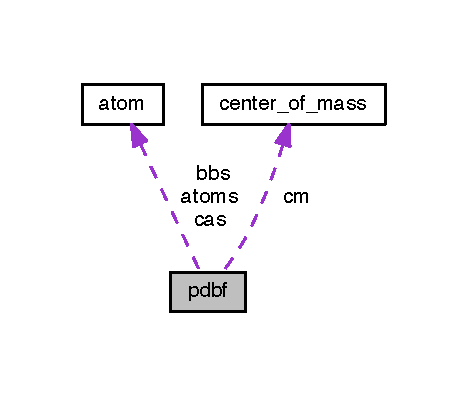
\includegraphics[width=225pt]{structpdbf__coll__graph}
\end{center}
\end{figure}
\subsection*{Public Attributes}
\begin{DoxyCompactItemize}
\item 
int \hyperlink{structpdbf_a6752def7d72ee73480a9fad514e60aef}{natoms}
\item 
int \hyperlink{structpdbf_a4172474fbba5b2127ab8e3184c63a059}{nresidues}
\item 
int \hyperlink{structpdbf_a7d28e61b01058ba61fb34b7b4b50e044}{ncas}
\item 
int \hyperlink{structpdbf_a9d9dbad94b94f067e3ab58334c9e892f}{nbbs}
\item 
int \hyperlink{structpdbf_af233eba06a2f4916dc76af49e447a013}{corruption}
\item 
char $\ast$ \hyperlink{structpdbf_a6be2fde75925c5a1064dfecd700dc79f}{res\+Seq}
\item 
char $\ast$$\ast$ \hyperlink{structpdbf_a2d79aa1e5f0634b5e4ceb22d1b2f2462}{threeres\+Seq}
\item 
\hyperlink{structatom}{atom} $\ast$ \hyperlink{structpdbf_aa582271e2b7d1d659f86ee27846d7a96}{atoms}
\item 
\hyperlink{structatom}{atom} $\ast$$\ast$ \hyperlink{structpdbf_af61e2b265a60d64feed10fd0ab7258a2}{bbs}
\item 
\hyperlink{structatom}{atom} $\ast$$\ast$ \hyperlink{structpdbf_a8fe8603ea76642263584103b2f574306}{cas}
\item 
\hyperlink{structcenter__of__mass}{center\+\_\+of\+\_\+mass} $\ast$ \hyperlink{structpdbf_a2124a322f26cb63ebaebe107a55c6f17}{cm}
\end{DoxyCompactItemize}


\subsection{Member Data Documentation}
\mbox{\Hypertarget{structpdbf_aa582271e2b7d1d659f86ee27846d7a96}\label{structpdbf_aa582271e2b7d1d659f86ee27846d7a96}} 
\index{pdbf@{pdbf}!atoms@{atoms}}
\index{atoms@{atoms}!pdbf@{pdbf}}
\subsubsection{\texorpdfstring{atoms}{atoms}}
{\footnotesize\ttfamily \hyperlink{structatom}{atom}$\ast$ pdbf\+::atoms}

\mbox{\Hypertarget{structpdbf_af61e2b265a60d64feed10fd0ab7258a2}\label{structpdbf_af61e2b265a60d64feed10fd0ab7258a2}} 
\index{pdbf@{pdbf}!bbs@{bbs}}
\index{bbs@{bbs}!pdbf@{pdbf}}
\subsubsection{\texorpdfstring{bbs}{bbs}}
{\footnotesize\ttfamily \hyperlink{structatom}{atom}$\ast$$\ast$ pdbf\+::bbs}

\mbox{\Hypertarget{structpdbf_a8fe8603ea76642263584103b2f574306}\label{structpdbf_a8fe8603ea76642263584103b2f574306}} 
\index{pdbf@{pdbf}!cas@{cas}}
\index{cas@{cas}!pdbf@{pdbf}}
\subsubsection{\texorpdfstring{cas}{cas}}
{\footnotesize\ttfamily \hyperlink{structatom}{atom}$\ast$$\ast$ pdbf\+::cas}

\mbox{\Hypertarget{structpdbf_a2124a322f26cb63ebaebe107a55c6f17}\label{structpdbf_a2124a322f26cb63ebaebe107a55c6f17}} 
\index{pdbf@{pdbf}!cm@{cm}}
\index{cm@{cm}!pdbf@{pdbf}}
\subsubsection{\texorpdfstring{cm}{cm}}
{\footnotesize\ttfamily \hyperlink{structcenter__of__mass}{center\+\_\+of\+\_\+mass}$\ast$ pdbf\+::cm}

\mbox{\Hypertarget{structpdbf_af233eba06a2f4916dc76af49e447a013}\label{structpdbf_af233eba06a2f4916dc76af49e447a013}} 
\index{pdbf@{pdbf}!corruption@{corruption}}
\index{corruption@{corruption}!pdbf@{pdbf}}
\subsubsection{\texorpdfstring{corruption}{corruption}}
{\footnotesize\ttfamily int pdbf\+::corruption}

\mbox{\Hypertarget{structpdbf_a6752def7d72ee73480a9fad514e60aef}\label{structpdbf_a6752def7d72ee73480a9fad514e60aef}} 
\index{pdbf@{pdbf}!natoms@{natoms}}
\index{natoms@{natoms}!pdbf@{pdbf}}
\subsubsection{\texorpdfstring{natoms}{natoms}}
{\footnotesize\ttfamily int pdbf\+::natoms}

\mbox{\Hypertarget{structpdbf_a9d9dbad94b94f067e3ab58334c9e892f}\label{structpdbf_a9d9dbad94b94f067e3ab58334c9e892f}} 
\index{pdbf@{pdbf}!nbbs@{nbbs}}
\index{nbbs@{nbbs}!pdbf@{pdbf}}
\subsubsection{\texorpdfstring{nbbs}{nbbs}}
{\footnotesize\ttfamily int pdbf\+::nbbs}

\mbox{\Hypertarget{structpdbf_a7d28e61b01058ba61fb34b7b4b50e044}\label{structpdbf_a7d28e61b01058ba61fb34b7b4b50e044}} 
\index{pdbf@{pdbf}!ncas@{ncas}}
\index{ncas@{ncas}!pdbf@{pdbf}}
\subsubsection{\texorpdfstring{ncas}{ncas}}
{\footnotesize\ttfamily int pdbf\+::ncas}

\mbox{\Hypertarget{structpdbf_a4172474fbba5b2127ab8e3184c63a059}\label{structpdbf_a4172474fbba5b2127ab8e3184c63a059}} 
\index{pdbf@{pdbf}!nresidues@{nresidues}}
\index{nresidues@{nresidues}!pdbf@{pdbf}}
\subsubsection{\texorpdfstring{nresidues}{nresidues}}
{\footnotesize\ttfamily int pdbf\+::nresidues}

\mbox{\Hypertarget{structpdbf_a6be2fde75925c5a1064dfecd700dc79f}\label{structpdbf_a6be2fde75925c5a1064dfecd700dc79f}} 
\index{pdbf@{pdbf}!res\+Seq@{res\+Seq}}
\index{res\+Seq@{res\+Seq}!pdbf@{pdbf}}
\subsubsection{\texorpdfstring{res\+Seq}{resSeq}}
{\footnotesize\ttfamily char$\ast$ pdbf\+::res\+Seq}

\mbox{\Hypertarget{structpdbf_a2d79aa1e5f0634b5e4ceb22d1b2f2462}\label{structpdbf_a2d79aa1e5f0634b5e4ceb22d1b2f2462}} 
\index{pdbf@{pdbf}!threeres\+Seq@{threeres\+Seq}}
\index{threeres\+Seq@{threeres\+Seq}!pdbf@{pdbf}}
\subsubsection{\texorpdfstring{threeres\+Seq}{threeresSeq}}
{\footnotesize\ttfamily char$\ast$$\ast$ pdbf\+::threeres\+Seq}



The documentation for this struct was generated from the following file\+:\begin{DoxyCompactItemize}
\item 
3rd\+Party/parmetis-\/4.\+0.\+3/metis/\+G\+Klib/\hyperlink{gk__struct_8h}{gk\+\_\+struct.\+h}\end{DoxyCompactItemize}

\hypertarget{structre__pattern__buffer}{}\section{re\+\_\+pattern\+\_\+buffer Struct Reference}
\label{structre__pattern__buffer}\index{re\+\_\+pattern\+\_\+buffer@{re\+\_\+pattern\+\_\+buffer}}


{\ttfamily \#include $<$gkregex.\+h$>$}

\subsection*{Public Attributes}
\begin{DoxyCompactItemize}
\item 
unsigned char $\ast$ \hyperlink{structre__pattern__buffer_ae60c7055854785bf6e2743fd314fcb83}{buffer}
\item 
unsigned long int \hyperlink{structre__pattern__buffer_a2947439f970297ce6f4a439867c0b5c7}{allocated}
\item 
unsigned long int \hyperlink{structre__pattern__buffer_a5c6bb086f4bfebee8aa4373c03bcc74b}{used}
\item 
\hyperlink{gkregex_8h_a7e0565199a2fabaca3d67a5a44fc4229}{reg\+\_\+syntax\+\_\+t} \hyperlink{structre__pattern__buffer_aa16e95a1befa7d5fd8eb89542fa065f8}{syntax}
\item 
char $\ast$ \hyperlink{structre__pattern__buffer_a103ac216c8fd6a8734daa4999fca3efb}{fastmap}
\item 
\hyperlink{gkregex_8h_a96c9fb9c7074cb21740b63092b0637a4}{R\+E\+\_\+\+T\+R\+A\+N\+S\+L\+A\+T\+E\+\_\+\+T\+Y\+PE} \hyperlink{structre__pattern__buffer_a780f81d1ec1ebba869e138b5bc849658}{translate}
\item 
size\+\_\+t \hyperlink{structre__pattern__buffer_a703c2069a09bac7fa67de8871cb17d35}{re\+\_\+nsub}
\item 
unsigned \hyperlink{structre__pattern__buffer_a13807f7bf4b32d786eb9e17a3c4d3124}{can\+\_\+be\+\_\+null}\+: 1
\item 
unsigned \hyperlink{structre__pattern__buffer_a83388321c434be6ac33fe359a3d7b449}{regs\+\_\+allocated}\+: 2
\item 
unsigned \hyperlink{structre__pattern__buffer_a837b026312b860e5485da6240b10d8f7}{fastmap\+\_\+accurate}\+: 1
\item 
unsigned \hyperlink{structre__pattern__buffer_a83e122c96edb258aa4ef99d7a8b2bfa2}{no\+\_\+sub}\+: 1
\item 
unsigned \hyperlink{structre__pattern__buffer_a4a5d480a0891afbab92cf486a04e4a68}{not\+\_\+bol}\+: 1
\item 
unsigned \hyperlink{structre__pattern__buffer_a875954f4e64b585471f67b334d33799c}{not\+\_\+eol}\+: 1
\item 
unsigned \hyperlink{structre__pattern__buffer_a46ed7a16b4cb87267ac5d219dab3536a}{newline\+\_\+anchor}\+: 1
\end{DoxyCompactItemize}


\subsection{Member Data Documentation}
\mbox{\Hypertarget{structre__pattern__buffer_a2947439f970297ce6f4a439867c0b5c7}\label{structre__pattern__buffer_a2947439f970297ce6f4a439867c0b5c7}} 
\index{re\+\_\+pattern\+\_\+buffer@{re\+\_\+pattern\+\_\+buffer}!allocated@{allocated}}
\index{allocated@{allocated}!re\+\_\+pattern\+\_\+buffer@{re\+\_\+pattern\+\_\+buffer}}
\subsubsection{\texorpdfstring{allocated}{allocated}}
{\footnotesize\ttfamily unsigned long int re\+\_\+pattern\+\_\+buffer\+::allocated}

\mbox{\Hypertarget{structre__pattern__buffer_ae60c7055854785bf6e2743fd314fcb83}\label{structre__pattern__buffer_ae60c7055854785bf6e2743fd314fcb83}} 
\index{re\+\_\+pattern\+\_\+buffer@{re\+\_\+pattern\+\_\+buffer}!buffer@{buffer}}
\index{buffer@{buffer}!re\+\_\+pattern\+\_\+buffer@{re\+\_\+pattern\+\_\+buffer}}
\subsubsection{\texorpdfstring{buffer}{buffer}}
{\footnotesize\ttfamily unsigned char$\ast$ re\+\_\+pattern\+\_\+buffer\+::buffer}

\mbox{\Hypertarget{structre__pattern__buffer_a13807f7bf4b32d786eb9e17a3c4d3124}\label{structre__pattern__buffer_a13807f7bf4b32d786eb9e17a3c4d3124}} 
\index{re\+\_\+pattern\+\_\+buffer@{re\+\_\+pattern\+\_\+buffer}!can\+\_\+be\+\_\+null@{can\+\_\+be\+\_\+null}}
\index{can\+\_\+be\+\_\+null@{can\+\_\+be\+\_\+null}!re\+\_\+pattern\+\_\+buffer@{re\+\_\+pattern\+\_\+buffer}}
\subsubsection{\texorpdfstring{can\+\_\+be\+\_\+null}{can\_be\_null}}
{\footnotesize\ttfamily unsigned re\+\_\+pattern\+\_\+buffer\+::can\+\_\+be\+\_\+null}

\mbox{\Hypertarget{structre__pattern__buffer_a103ac216c8fd6a8734daa4999fca3efb}\label{structre__pattern__buffer_a103ac216c8fd6a8734daa4999fca3efb}} 
\index{re\+\_\+pattern\+\_\+buffer@{re\+\_\+pattern\+\_\+buffer}!fastmap@{fastmap}}
\index{fastmap@{fastmap}!re\+\_\+pattern\+\_\+buffer@{re\+\_\+pattern\+\_\+buffer}}
\subsubsection{\texorpdfstring{fastmap}{fastmap}}
{\footnotesize\ttfamily char$\ast$ re\+\_\+pattern\+\_\+buffer\+::fastmap}

\mbox{\Hypertarget{structre__pattern__buffer_a837b026312b860e5485da6240b10d8f7}\label{structre__pattern__buffer_a837b026312b860e5485da6240b10d8f7}} 
\index{re\+\_\+pattern\+\_\+buffer@{re\+\_\+pattern\+\_\+buffer}!fastmap\+\_\+accurate@{fastmap\+\_\+accurate}}
\index{fastmap\+\_\+accurate@{fastmap\+\_\+accurate}!re\+\_\+pattern\+\_\+buffer@{re\+\_\+pattern\+\_\+buffer}}
\subsubsection{\texorpdfstring{fastmap\+\_\+accurate}{fastmap\_accurate}}
{\footnotesize\ttfamily unsigned re\+\_\+pattern\+\_\+buffer\+::fastmap\+\_\+accurate}

\mbox{\Hypertarget{structre__pattern__buffer_a46ed7a16b4cb87267ac5d219dab3536a}\label{structre__pattern__buffer_a46ed7a16b4cb87267ac5d219dab3536a}} 
\index{re\+\_\+pattern\+\_\+buffer@{re\+\_\+pattern\+\_\+buffer}!newline\+\_\+anchor@{newline\+\_\+anchor}}
\index{newline\+\_\+anchor@{newline\+\_\+anchor}!re\+\_\+pattern\+\_\+buffer@{re\+\_\+pattern\+\_\+buffer}}
\subsubsection{\texorpdfstring{newline\+\_\+anchor}{newline\_anchor}}
{\footnotesize\ttfamily unsigned re\+\_\+pattern\+\_\+buffer\+::newline\+\_\+anchor}

\mbox{\Hypertarget{structre__pattern__buffer_a83e122c96edb258aa4ef99d7a8b2bfa2}\label{structre__pattern__buffer_a83e122c96edb258aa4ef99d7a8b2bfa2}} 
\index{re\+\_\+pattern\+\_\+buffer@{re\+\_\+pattern\+\_\+buffer}!no\+\_\+sub@{no\+\_\+sub}}
\index{no\+\_\+sub@{no\+\_\+sub}!re\+\_\+pattern\+\_\+buffer@{re\+\_\+pattern\+\_\+buffer}}
\subsubsection{\texorpdfstring{no\+\_\+sub}{no\_sub}}
{\footnotesize\ttfamily unsigned re\+\_\+pattern\+\_\+buffer\+::no\+\_\+sub}

\mbox{\Hypertarget{structre__pattern__buffer_a4a5d480a0891afbab92cf486a04e4a68}\label{structre__pattern__buffer_a4a5d480a0891afbab92cf486a04e4a68}} 
\index{re\+\_\+pattern\+\_\+buffer@{re\+\_\+pattern\+\_\+buffer}!not\+\_\+bol@{not\+\_\+bol}}
\index{not\+\_\+bol@{not\+\_\+bol}!re\+\_\+pattern\+\_\+buffer@{re\+\_\+pattern\+\_\+buffer}}
\subsubsection{\texorpdfstring{not\+\_\+bol}{not\_bol}}
{\footnotesize\ttfamily unsigned re\+\_\+pattern\+\_\+buffer\+::not\+\_\+bol}

\mbox{\Hypertarget{structre__pattern__buffer_a875954f4e64b585471f67b334d33799c}\label{structre__pattern__buffer_a875954f4e64b585471f67b334d33799c}} 
\index{re\+\_\+pattern\+\_\+buffer@{re\+\_\+pattern\+\_\+buffer}!not\+\_\+eol@{not\+\_\+eol}}
\index{not\+\_\+eol@{not\+\_\+eol}!re\+\_\+pattern\+\_\+buffer@{re\+\_\+pattern\+\_\+buffer}}
\subsubsection{\texorpdfstring{not\+\_\+eol}{not\_eol}}
{\footnotesize\ttfamily unsigned re\+\_\+pattern\+\_\+buffer\+::not\+\_\+eol}

\mbox{\Hypertarget{structre__pattern__buffer_a703c2069a09bac7fa67de8871cb17d35}\label{structre__pattern__buffer_a703c2069a09bac7fa67de8871cb17d35}} 
\index{re\+\_\+pattern\+\_\+buffer@{re\+\_\+pattern\+\_\+buffer}!re\+\_\+nsub@{re\+\_\+nsub}}
\index{re\+\_\+nsub@{re\+\_\+nsub}!re\+\_\+pattern\+\_\+buffer@{re\+\_\+pattern\+\_\+buffer}}
\subsubsection{\texorpdfstring{re\+\_\+nsub}{re\_nsub}}
{\footnotesize\ttfamily size\+\_\+t re\+\_\+pattern\+\_\+buffer\+::re\+\_\+nsub}

\mbox{\Hypertarget{structre__pattern__buffer_a83388321c434be6ac33fe359a3d7b449}\label{structre__pattern__buffer_a83388321c434be6ac33fe359a3d7b449}} 
\index{re\+\_\+pattern\+\_\+buffer@{re\+\_\+pattern\+\_\+buffer}!regs\+\_\+allocated@{regs\+\_\+allocated}}
\index{regs\+\_\+allocated@{regs\+\_\+allocated}!re\+\_\+pattern\+\_\+buffer@{re\+\_\+pattern\+\_\+buffer}}
\subsubsection{\texorpdfstring{regs\+\_\+allocated}{regs\_allocated}}
{\footnotesize\ttfamily unsigned re\+\_\+pattern\+\_\+buffer\+::regs\+\_\+allocated}

\mbox{\Hypertarget{structre__pattern__buffer_aa16e95a1befa7d5fd8eb89542fa065f8}\label{structre__pattern__buffer_aa16e95a1befa7d5fd8eb89542fa065f8}} 
\index{re\+\_\+pattern\+\_\+buffer@{re\+\_\+pattern\+\_\+buffer}!syntax@{syntax}}
\index{syntax@{syntax}!re\+\_\+pattern\+\_\+buffer@{re\+\_\+pattern\+\_\+buffer}}
\subsubsection{\texorpdfstring{syntax}{syntax}}
{\footnotesize\ttfamily \hyperlink{gkregex_8h_a7e0565199a2fabaca3d67a5a44fc4229}{reg\+\_\+syntax\+\_\+t} re\+\_\+pattern\+\_\+buffer\+::syntax}

\mbox{\Hypertarget{structre__pattern__buffer_a780f81d1ec1ebba869e138b5bc849658}\label{structre__pattern__buffer_a780f81d1ec1ebba869e138b5bc849658}} 
\index{re\+\_\+pattern\+\_\+buffer@{re\+\_\+pattern\+\_\+buffer}!translate@{translate}}
\index{translate@{translate}!re\+\_\+pattern\+\_\+buffer@{re\+\_\+pattern\+\_\+buffer}}
\subsubsection{\texorpdfstring{translate}{translate}}
{\footnotesize\ttfamily \hyperlink{gkregex_8h_a96c9fb9c7074cb21740b63092b0637a4}{R\+E\+\_\+\+T\+R\+A\+N\+S\+L\+A\+T\+E\+\_\+\+T\+Y\+PE} re\+\_\+pattern\+\_\+buffer\+::translate}

\mbox{\Hypertarget{structre__pattern__buffer_a5c6bb086f4bfebee8aa4373c03bcc74b}\label{structre__pattern__buffer_a5c6bb086f4bfebee8aa4373c03bcc74b}} 
\index{re\+\_\+pattern\+\_\+buffer@{re\+\_\+pattern\+\_\+buffer}!used@{used}}
\index{used@{used}!re\+\_\+pattern\+\_\+buffer@{re\+\_\+pattern\+\_\+buffer}}
\subsubsection{\texorpdfstring{used}{used}}
{\footnotesize\ttfamily unsigned long int re\+\_\+pattern\+\_\+buffer\+::used}



The documentation for this struct was generated from the following file\+:\begin{DoxyCompactItemize}
\item 
3rd\+Party/parmetis-\/4.\+0.\+3/metis/\+G\+Klib/\hyperlink{gkregex_8h}{gkregex.\+h}\end{DoxyCompactItemize}

\hypertarget{structre__registers}{}\section{re\+\_\+registers Struct Reference}
\label{structre__registers}\index{re\+\_\+registers@{re\+\_\+registers}}


{\ttfamily \#include $<$gkregex.\+h$>$}

\subsection*{Public Attributes}
\begin{DoxyCompactItemize}
\item 
unsigned \hyperlink{structre__registers_aeae8140aadf339f6fe0c49277d6aa7b5}{num\+\_\+regs}
\item 
\hyperlink{gkregex_8h_a5b34995b47432512ee4ffa32b836e65f}{regoff\+\_\+t} $\ast$ \hyperlink{structre__registers_a6676ddb6ab07e50191e149b04dbcfe03}{start}
\item 
\hyperlink{gkregex_8h_a5b34995b47432512ee4ffa32b836e65f}{regoff\+\_\+t} $\ast$ \hyperlink{structre__registers_a0a9d373f1ab74c9c2063f233476fa5d4}{end}
\end{DoxyCompactItemize}


\subsection{Member Data Documentation}
\mbox{\Hypertarget{structre__registers_a0a9d373f1ab74c9c2063f233476fa5d4}\label{structre__registers_a0a9d373f1ab74c9c2063f233476fa5d4}} 
\index{re\+\_\+registers@{re\+\_\+registers}!end@{end}}
\index{end@{end}!re\+\_\+registers@{re\+\_\+registers}}
\subsubsection{\texorpdfstring{end}{end}}
{\footnotesize\ttfamily \hyperlink{gkregex_8h_a5b34995b47432512ee4ffa32b836e65f}{regoff\+\_\+t}$\ast$ re\+\_\+registers\+::end}

\mbox{\Hypertarget{structre__registers_aeae8140aadf339f6fe0c49277d6aa7b5}\label{structre__registers_aeae8140aadf339f6fe0c49277d6aa7b5}} 
\index{re\+\_\+registers@{re\+\_\+registers}!num\+\_\+regs@{num\+\_\+regs}}
\index{num\+\_\+regs@{num\+\_\+regs}!re\+\_\+registers@{re\+\_\+registers}}
\subsubsection{\texorpdfstring{num\+\_\+regs}{num\_regs}}
{\footnotesize\ttfamily unsigned re\+\_\+registers\+::num\+\_\+regs}

\mbox{\Hypertarget{structre__registers_a6676ddb6ab07e50191e149b04dbcfe03}\label{structre__registers_a6676ddb6ab07e50191e149b04dbcfe03}} 
\index{re\+\_\+registers@{re\+\_\+registers}!start@{start}}
\index{start@{start}!re\+\_\+registers@{re\+\_\+registers}}
\subsubsection{\texorpdfstring{start}{start}}
{\footnotesize\ttfamily \hyperlink{gkregex_8h_a5b34995b47432512ee4ffa32b836e65f}{regoff\+\_\+t}$\ast$ re\+\_\+registers\+::start}



The documentation for this struct was generated from the following file\+:\begin{DoxyCompactItemize}
\item 
3rd\+Party/parmetis-\/4.\+0.\+3/metis/\+G\+Klib/\hyperlink{gkregex_8h}{gkregex.\+h}\end{DoxyCompactItemize}

\hypertarget{structregmatch__t}{}\section{regmatch\+\_\+t Struct Reference}
\label{structregmatch__t}\index{regmatch\+\_\+t@{regmatch\+\_\+t}}


{\ttfamily \#include $<$gkregex.\+h$>$}

\subsection*{Public Attributes}
\begin{DoxyCompactItemize}
\item 
\hyperlink{gkregex_8h_a5b34995b47432512ee4ffa32b836e65f}{regoff\+\_\+t} \hyperlink{structregmatch__t_a90ac8973d256eaffdbb20de676ff45a4}{rm\+\_\+so}
\item 
\hyperlink{gkregex_8h_a5b34995b47432512ee4ffa32b836e65f}{regoff\+\_\+t} \hyperlink{structregmatch__t_a728c28b9b23fa28c4e0b90e3a1a29efc}{rm\+\_\+eo}
\end{DoxyCompactItemize}


\subsection{Member Data Documentation}
\mbox{\Hypertarget{structregmatch__t_a728c28b9b23fa28c4e0b90e3a1a29efc}\label{structregmatch__t_a728c28b9b23fa28c4e0b90e3a1a29efc}} 
\index{regmatch\+\_\+t@{regmatch\+\_\+t}!rm\+\_\+eo@{rm\+\_\+eo}}
\index{rm\+\_\+eo@{rm\+\_\+eo}!regmatch\+\_\+t@{regmatch\+\_\+t}}
\subsubsection{\texorpdfstring{rm\+\_\+eo}{rm\_eo}}
{\footnotesize\ttfamily \hyperlink{gkregex_8h_a5b34995b47432512ee4ffa32b836e65f}{regoff\+\_\+t} regmatch\+\_\+t\+::rm\+\_\+eo}

\mbox{\Hypertarget{structregmatch__t_a90ac8973d256eaffdbb20de676ff45a4}\label{structregmatch__t_a90ac8973d256eaffdbb20de676ff45a4}} 
\index{regmatch\+\_\+t@{regmatch\+\_\+t}!rm\+\_\+so@{rm\+\_\+so}}
\index{rm\+\_\+so@{rm\+\_\+so}!regmatch\+\_\+t@{regmatch\+\_\+t}}
\subsubsection{\texorpdfstring{rm\+\_\+so}{rm\_so}}
{\footnotesize\ttfamily \hyperlink{gkregex_8h_a5b34995b47432512ee4ffa32b836e65f}{regoff\+\_\+t} regmatch\+\_\+t\+::rm\+\_\+so}



The documentation for this struct was generated from the following file\+:\begin{DoxyCompactItemize}
\item 
3rd\+Party/parmetis-\/4.\+0.\+3/metis/\+G\+Klib/\hyperlink{gkregex_8h}{gkregex.\+h}\end{DoxyCompactItemize}

\hypertarget{structuvw__t}{}\section{uvw\+\_\+t Struct Reference}
\label{structuvw__t}\index{uvw\+\_\+t@{uvw\+\_\+t}}


{\ttfamily \#include $<$gklib\+\_\+defs.\+h$>$}

\subsection*{Public Attributes}
\begin{DoxyCompactItemize}
\item 
\hyperlink{3rd_party_2parmetis-4_80_83_2metis_2include_2metis_8h_aaa5262be3e700770163401acb0150f52}{idx\+\_\+t} \hyperlink{structuvw__t_a5acfd17a9a2237ffd08a084887fc2f49}{u}
\item 
\hyperlink{3rd_party_2parmetis-4_80_83_2metis_2include_2metis_8h_aaa5262be3e700770163401acb0150f52}{idx\+\_\+t} \hyperlink{structuvw__t_a9acbeec0726e1cf3842a174e44031bcc}{v}
\item 
\hyperlink{3rd_party_2parmetis-4_80_83_2metis_2include_2metis_8h_aaa5262be3e700770163401acb0150f52}{idx\+\_\+t} \hyperlink{structuvw__t_ad8b9f1185850e05876ee066a461c0d9d}{w}
\end{DoxyCompactItemize}


\subsection{Detailed Description}
Stores a weighted edge 

\subsection{Member Data Documentation}
\mbox{\Hypertarget{structuvw__t_a5acfd17a9a2237ffd08a084887fc2f49}\label{structuvw__t_a5acfd17a9a2237ffd08a084887fc2f49}} 
\index{uvw\+\_\+t@{uvw\+\_\+t}!u@{u}}
\index{u@{u}!uvw\+\_\+t@{uvw\+\_\+t}}
\subsubsection{\texorpdfstring{u}{u}}
{\footnotesize\ttfamily \hyperlink{3rd_party_2parmetis-4_80_83_2metis_2include_2metis_8h_aaa5262be3e700770163401acb0150f52}{idx\+\_\+t} uvw\+\_\+t\+::u}

\mbox{\Hypertarget{structuvw__t_a9acbeec0726e1cf3842a174e44031bcc}\label{structuvw__t_a9acbeec0726e1cf3842a174e44031bcc}} 
\index{uvw\+\_\+t@{uvw\+\_\+t}!v@{v}}
\index{v@{v}!uvw\+\_\+t@{uvw\+\_\+t}}
\subsubsection{\texorpdfstring{v}{v}}
{\footnotesize\ttfamily \hyperlink{3rd_party_2parmetis-4_80_83_2metis_2include_2metis_8h_aaa5262be3e700770163401acb0150f52}{idx\+\_\+t} uvw\+\_\+t\+::v}

\mbox{\Hypertarget{structuvw__t_ad8b9f1185850e05876ee066a461c0d9d}\label{structuvw__t_ad8b9f1185850e05876ee066a461c0d9d}} 
\index{uvw\+\_\+t@{uvw\+\_\+t}!w@{w}}
\index{w@{w}!uvw\+\_\+t@{uvw\+\_\+t}}
\subsubsection{\texorpdfstring{w}{w}}
{\footnotesize\ttfamily \hyperlink{3rd_party_2parmetis-4_80_83_2metis_2include_2metis_8h_aaa5262be3e700770163401acb0150f52}{idx\+\_\+t} uvw\+\_\+t\+::w}

Edge (u,v) with weight w 

The documentation for this struct was generated from the following file\+:\begin{DoxyCompactItemize}
\item 
3rd\+Party/parmetis-\/4.\+0.\+3/metis/libmetis/\hyperlink{gklib__defs_8h}{gklib\+\_\+defs.\+h}\end{DoxyCompactItemize}

\hypertarget{structvkrinfo__t}{}\section{vkrinfo\+\_\+t Struct Reference}
\label{structvkrinfo__t}\index{vkrinfo\+\_\+t@{vkrinfo\+\_\+t}}


{\ttfamily \#include $<$struct.\+h$>$}

\subsection*{Public Attributes}
\begin{DoxyCompactItemize}
\item 
\hyperlink{3rd_party_2parmetis-4_80_83_2metis_2include_2metis_8h_aaa5262be3e700770163401acb0150f52}{idx\+\_\+t} \hyperlink{structvkrinfo__t_a9befff2ea2c811563ad38aaf921a8f21}{nid}
\item 
\hyperlink{3rd_party_2parmetis-4_80_83_2metis_2include_2metis_8h_aaa5262be3e700770163401acb0150f52}{idx\+\_\+t} \hyperlink{structvkrinfo__t_a0af0fec11cab7aa7a343c268832cc709}{ned}
\item 
\hyperlink{3rd_party_2parmetis-4_80_83_2metis_2include_2metis_8h_aaa5262be3e700770163401acb0150f52}{idx\+\_\+t} \hyperlink{structvkrinfo__t_a8d9e4e351610f7b03203940a134bcd74}{gv}
\item 
\hyperlink{3rd_party_2parmetis-4_80_83_2metis_2include_2metis_8h_aaa5262be3e700770163401acb0150f52}{idx\+\_\+t} \hyperlink{structvkrinfo__t_aa337d338d253918348c5ba9e4a5082ca}{nnbrs}
\item 
\hyperlink{3rd_party_2parmetis-4_80_83_2metis_2include_2metis_8h_aaa5262be3e700770163401acb0150f52}{idx\+\_\+t} \hyperlink{structvkrinfo__t_a85a0150ff0f0fe87b0fc3bf445b60bca}{inbr}
\end{DoxyCompactItemize}


\subsection{Detailed Description}
The following data structure holds information on degrees for k-\/way vol-\/based partition 

\subsection{Member Data Documentation}
\mbox{\Hypertarget{structvkrinfo__t_a8d9e4e351610f7b03203940a134bcd74}\label{structvkrinfo__t_a8d9e4e351610f7b03203940a134bcd74}} 
\index{vkrinfo\+\_\+t@{vkrinfo\+\_\+t}!gv@{gv}}
\index{gv@{gv}!vkrinfo\+\_\+t@{vkrinfo\+\_\+t}}
\subsubsection{\texorpdfstring{gv}{gv}}
{\footnotesize\ttfamily \hyperlink{3rd_party_2parmetis-4_80_83_2metis_2include_2metis_8h_aaa5262be3e700770163401acb0150f52}{idx\+\_\+t} vkrinfo\+\_\+t\+::gv}

The volume gain of moving that vertex \mbox{\Hypertarget{structvkrinfo__t_a85a0150ff0f0fe87b0fc3bf445b60bca}\label{structvkrinfo__t_a85a0150ff0f0fe87b0fc3bf445b60bca}} 
\index{vkrinfo\+\_\+t@{vkrinfo\+\_\+t}!inbr@{inbr}}
\index{inbr@{inbr}!vkrinfo\+\_\+t@{vkrinfo\+\_\+t}}
\subsubsection{\texorpdfstring{inbr}{inbr}}
{\footnotesize\ttfamily \hyperlink{3rd_party_2parmetis-4_80_83_2metis_2include_2metis_8h_aaa5262be3e700770163401acb0150f52}{idx\+\_\+t} vkrinfo\+\_\+t\+::inbr}

The index in the \hyperlink{structvnbr__t}{vnbr\+\_\+t} array where the nnbrs list of neighbors is stored \mbox{\Hypertarget{structvkrinfo__t_a0af0fec11cab7aa7a343c268832cc709}\label{structvkrinfo__t_a0af0fec11cab7aa7a343c268832cc709}} 
\index{vkrinfo\+\_\+t@{vkrinfo\+\_\+t}!ned@{ned}}
\index{ned@{ned}!vkrinfo\+\_\+t@{vkrinfo\+\_\+t}}
\subsubsection{\texorpdfstring{ned}{ned}}
{\footnotesize\ttfamily \hyperlink{3rd_party_2parmetis-4_80_83_2metis_2include_2metis_8h_aaa5262be3e700770163401acb0150f52}{idx\+\_\+t} vkrinfo\+\_\+t\+::ned}

The total external degree of a vertex (count of edges) \mbox{\Hypertarget{structvkrinfo__t_a9befff2ea2c811563ad38aaf921a8f21}\label{structvkrinfo__t_a9befff2ea2c811563ad38aaf921a8f21}} 
\index{vkrinfo\+\_\+t@{vkrinfo\+\_\+t}!nid@{nid}}
\index{nid@{nid}!vkrinfo\+\_\+t@{vkrinfo\+\_\+t}}
\subsubsection{\texorpdfstring{nid}{nid}}
{\footnotesize\ttfamily \hyperlink{3rd_party_2parmetis-4_80_83_2metis_2include_2metis_8h_aaa5262be3e700770163401acb0150f52}{idx\+\_\+t} vkrinfo\+\_\+t\+::nid}

The internal degree of a vertex (count of edges) \mbox{\Hypertarget{structvkrinfo__t_aa337d338d253918348c5ba9e4a5082ca}\label{structvkrinfo__t_aa337d338d253918348c5ba9e4a5082ca}} 
\index{vkrinfo\+\_\+t@{vkrinfo\+\_\+t}!nnbrs@{nnbrs}}
\index{nnbrs@{nnbrs}!vkrinfo\+\_\+t@{vkrinfo\+\_\+t}}
\subsubsection{\texorpdfstring{nnbrs}{nnbrs}}
{\footnotesize\ttfamily \hyperlink{3rd_party_2parmetis-4_80_83_2metis_2include_2metis_8h_aaa5262be3e700770163401acb0150f52}{idx\+\_\+t} vkrinfo\+\_\+t\+::nnbrs}

The number of neighboring subdomains 

The documentation for this struct was generated from the following file\+:\begin{DoxyCompactItemize}
\item 
3rd\+Party/parmetis-\/4.\+0.\+3/metis/libmetis/\hyperlink{metis_2libmetis_2struct_8h}{struct.\+h}\end{DoxyCompactItemize}

\hypertarget{structvnbr__t}{}\section{vnbr\+\_\+t Struct Reference}
\label{structvnbr__t}\index{vnbr\+\_\+t@{vnbr\+\_\+t}}


{\ttfamily \#include $<$struct.\+h$>$}

\subsection*{Public Attributes}
\begin{DoxyCompactItemize}
\item 
\hyperlink{3rd_party_2parmetis-4_80_83_2metis_2include_2metis_8h_aaa5262be3e700770163401acb0150f52}{idx\+\_\+t} \hyperlink{structvnbr__t_a93adf79b4e57cd0477e9afc9b25da653}{pid}
\item 
\hyperlink{3rd_party_2parmetis-4_80_83_2metis_2include_2metis_8h_aaa5262be3e700770163401acb0150f52}{idx\+\_\+t} \hyperlink{structvnbr__t_ae32050bde46f5545e1c306853afd8d97}{ned}
\item 
\hyperlink{3rd_party_2parmetis-4_80_83_2metis_2include_2metis_8h_aaa5262be3e700770163401acb0150f52}{idx\+\_\+t} \hyperlink{structvnbr__t_a29f3fc7f5d884e78e1dfff0f9cc438d0}{gv}
\end{DoxyCompactItemize}


\subsection{Detailed Description}
This data structure stores volume-\/based k-\/way refinement info about an adjacent subdomain for a given vertex. 

\subsection{Member Data Documentation}
\mbox{\Hypertarget{structvnbr__t_a29f3fc7f5d884e78e1dfff0f9cc438d0}\label{structvnbr__t_a29f3fc7f5d884e78e1dfff0f9cc438d0}} 
\index{vnbr\+\_\+t@{vnbr\+\_\+t}!gv@{gv}}
\index{gv@{gv}!vnbr\+\_\+t@{vnbr\+\_\+t}}
\subsubsection{\texorpdfstring{gv}{gv}}
{\footnotesize\ttfamily \hyperlink{3rd_party_2parmetis-4_80_83_2metis_2include_2metis_8h_aaa5262be3e700770163401acb0150f52}{idx\+\_\+t} vnbr\+\_\+t\+::gv}

The gain in volume achieved by moving the vertex to pid \mbox{\Hypertarget{structvnbr__t_ae32050bde46f5545e1c306853afd8d97}\label{structvnbr__t_ae32050bde46f5545e1c306853afd8d97}} 
\index{vnbr\+\_\+t@{vnbr\+\_\+t}!ned@{ned}}
\index{ned@{ned}!vnbr\+\_\+t@{vnbr\+\_\+t}}
\subsubsection{\texorpdfstring{ned}{ned}}
{\footnotesize\ttfamily \hyperlink{3rd_party_2parmetis-4_80_83_2metis_2include_2metis_8h_aaa5262be3e700770163401acb0150f52}{idx\+\_\+t} vnbr\+\_\+t\+::ned}

The number of the adjacent edges that are incident on pid \mbox{\Hypertarget{structvnbr__t_a93adf79b4e57cd0477e9afc9b25da653}\label{structvnbr__t_a93adf79b4e57cd0477e9afc9b25da653}} 
\index{vnbr\+\_\+t@{vnbr\+\_\+t}!pid@{pid}}
\index{pid@{pid}!vnbr\+\_\+t@{vnbr\+\_\+t}}
\subsubsection{\texorpdfstring{pid}{pid}}
{\footnotesize\ttfamily \hyperlink{3rd_party_2parmetis-4_80_83_2metis_2include_2metis_8h_aaa5262be3e700770163401acb0150f52}{idx\+\_\+t} vnbr\+\_\+t\+::pid}

The partition ID 

The documentation for this struct was generated from the following file\+:\begin{DoxyCompactItemize}
\item 
3rd\+Party/parmetis-\/4.\+0.\+3/metis/libmetis/\hyperlink{metis_2libmetis_2struct_8h}{struct.\+h}\end{DoxyCompactItemize}

\chapter{File Documentation}
\hypertarget{3rd_party_2parmetis-4_80_83_2build_2_darwin-x86__64_2_c_make_files_23_88_82_2_compiler_id_c_2_c_make_c_compiler_id_8c}{}\section{3rd\+Party/parmetis-\/4.0.3/build/\+Darwin-\/x86\+\_\+64/\+C\+Make\+Files/3.8.2/\+Compiler\+Id\+C/\+C\+Make\+C\+Compiler\+Id.c File Reference}
\label{3rd_party_2parmetis-4_80_83_2build_2_darwin-x86__64_2_c_make_files_23_88_82_2_compiler_id_c_2_c_make_c_compiler_id_8c}\index{3rd\+Party/parmetis-\/4.\+0.\+3/build/\+Darwin-\/x86\+\_\+64/\+C\+Make\+Files/3.\+8.\+2/\+Compiler\+Id\+C/\+C\+Make\+C\+Compiler\+Id.\+c@{3rd\+Party/parmetis-\/4.\+0.\+3/build/\+Darwin-\/x86\+\_\+64/\+C\+Make\+Files/3.\+8.\+2/\+Compiler\+Id\+C/\+C\+Make\+C\+Compiler\+Id.\+c}}
\subsection*{Macros}
\begin{DoxyCompactItemize}
\item 
\#define \hyperlink{3rd_party_2parmetis-4_80_83_2build_2_darwin-x86__64_2_c_make_files_23_88_82_2_compiler_id_c_2_c_make_c_compiler_id_8c_a81dee0709ded976b2e0319239f72d174}{C\+O\+M\+P\+I\+L\+E\+R\+\_\+\+ID}~\char`\"{}\char`\"{}
\item 
\#define \hyperlink{3rd_party_2parmetis-4_80_83_2build_2_darwin-x86__64_2_c_make_files_23_88_82_2_compiler_id_c_2_c_make_c_compiler_id_8c_a2ae9b72bb13abaabfcf2ee0ba7d3fa1d}{S\+T\+R\+I\+N\+G\+I\+F\+Y\+\_\+\+H\+E\+L\+P\+ER}(\hyperlink{make_v_t_k_file_8m_a708712aede48a739e9ae0c42413ef460}{X})~\#\hyperlink{make_v_t_k_file_8m_a708712aede48a739e9ae0c42413ef460}{X}
\item 
\#define \hyperlink{3rd_party_2parmetis-4_80_83_2build_2_darwin-x86__64_2_c_make_files_23_88_82_2_compiler_id_c_2_c_make_c_compiler_id_8c_a43e1cad902b6477bec893cb6430bd6c8}{S\+T\+R\+I\+N\+G\+I\+FY}(\hyperlink{make_v_t_k_file_8m_a708712aede48a739e9ae0c42413ef460}{X})~\hyperlink{build_2relwithdebinfo_2_c_make_files_23_88_82_2_compiler_id_c_x_x_2_c_make_c_x_x_compiler_id_8cpp_a2ae9b72bb13abaabfcf2ee0ba7d3fa1d}{S\+T\+R\+I\+N\+G\+I\+F\+Y\+\_\+\+H\+E\+L\+P\+ER}(\hyperlink{make_v_t_k_file_8m_a708712aede48a739e9ae0c42413ef460}{X})
\item 
\#define \hyperlink{3rd_party_2parmetis-4_80_83_2build_2_darwin-x86__64_2_c_make_files_23_88_82_2_compiler_id_c_2_c_make_c_compiler_id_8c_adbc5372f40838899018fadbc89bd588b}{P\+L\+A\+T\+F\+O\+R\+M\+\_\+\+ID}
\item 
\#define \hyperlink{3rd_party_2parmetis-4_80_83_2build_2_darwin-x86__64_2_c_make_files_23_88_82_2_compiler_id_c_2_c_make_c_compiler_id_8c_aba35d0d200deaeb06aee95ca297acb28}{A\+R\+C\+H\+I\+T\+E\+C\+T\+U\+R\+E\+\_\+\+ID}
\item 
\#define \hyperlink{3rd_party_2parmetis-4_80_83_2build_2_darwin-x86__64_2_c_make_files_23_88_82_2_compiler_id_c_2_c_make_c_compiler_id_8c_ad1280362da42492bbc11aa78cbf776ad}{D\+EC}(\hyperlink{write__vtu__template_8cpp_a781a04ab095280f838ff3eb0e51312e0}{n})
\item 
\#define \hyperlink{3rd_party_2parmetis-4_80_83_2build_2_darwin-x86__64_2_c_make_files_23_88_82_2_compiler_id_c_2_c_make_c_compiler_id_8c_a46d5d95daa1bef867bd0179594310ed5}{H\+EX}(\hyperlink{write__vtu__template_8cpp_a781a04ab095280f838ff3eb0e51312e0}{n})
\item 
\#define \hyperlink{3rd_party_2parmetis-4_80_83_2build_2_darwin-x86__64_2_c_make_files_23_88_82_2_compiler_id_c_2_c_make_c_compiler_id_8c_a07f8e5783674099cd7f5110e22a78cdb}{C\+\_\+\+D\+I\+A\+L\+E\+CT}
\end{DoxyCompactItemize}
\subsection*{Functions}
\begin{DoxyCompactItemize}
\item 
int \hyperlink{3rd_party_2parmetis-4_80_83_2build_2_darwin-x86__64_2_c_make_files_23_88_82_2_compiler_id_c_2_c_make_c_compiler_id_8c_a0ddf1224851353fc92bfbff6f499fa97}{main} (int argc, char $\ast$argv\mbox{[}$\,$\mbox{]})
\end{DoxyCompactItemize}
\subsection*{Variables}
\begin{DoxyCompactItemize}
\item 
char const  $\ast$ \hyperlink{3rd_party_2parmetis-4_80_83_2build_2_darwin-x86__64_2_c_make_files_23_88_82_2_compiler_id_c_2_c_make_c_compiler_id_8c_a4b0efeb7a5d59313986b3a0390f050f6}{info\+\_\+compiler} = \char`\"{}I\+N\+FO\char`\"{} \char`\"{}\+:\char`\"{} \char`\"{}compiler\mbox{[}\char`\"{} C\+O\+M\+P\+I\+L\+E\+R\+\_\+\+ID \char`\"{}\mbox{]}\char`\"{}
\item 
char const  $\ast$ \hyperlink{3rd_party_2parmetis-4_80_83_2build_2_darwin-x86__64_2_c_make_files_23_88_82_2_compiler_id_c_2_c_make_c_compiler_id_8c_a2321403dee54ee23f0c2fa849c60f7d4}{info\+\_\+platform} = \char`\"{}I\+N\+FO\char`\"{} \char`\"{}\+:\char`\"{} \char`\"{}platform\mbox{[}\char`\"{} P\+L\+A\+T\+F\+O\+R\+M\+\_\+\+ID \char`\"{}\mbox{]}\char`\"{}
\item 
char const  $\ast$ \hyperlink{3rd_party_2parmetis-4_80_83_2build_2_darwin-x86__64_2_c_make_files_23_88_82_2_compiler_id_c_2_c_make_c_compiler_id_8c_a59647e99d304ed33b15cb284c27ed391}{info\+\_\+arch} = \char`\"{}I\+N\+FO\char`\"{} \char`\"{}\+:\char`\"{} \char`\"{}arch\mbox{[}\char`\"{} A\+R\+C\+H\+I\+T\+E\+C\+T\+U\+R\+E\+\_\+\+ID \char`\"{}\mbox{]}\char`\"{}
\item 
const char $\ast$ \hyperlink{3rd_party_2parmetis-4_80_83_2build_2_darwin-x86__64_2_c_make_files_23_88_82_2_compiler_id_c_2_c_make_c_compiler_id_8c_a1ce162bad2fe6966ac8b33cc19e120b8}{info\+\_\+language\+\_\+dialect\+\_\+default}
\end{DoxyCompactItemize}


\subsection{Macro Definition Documentation}
\mbox{\Hypertarget{3rd_party_2parmetis-4_80_83_2build_2_darwin-x86__64_2_c_make_files_23_88_82_2_compiler_id_c_2_c_make_c_compiler_id_8c_aba35d0d200deaeb06aee95ca297acb28}\label{3rd_party_2parmetis-4_80_83_2build_2_darwin-x86__64_2_c_make_files_23_88_82_2_compiler_id_c_2_c_make_c_compiler_id_8c_aba35d0d200deaeb06aee95ca297acb28}} 
\index{3rd\+Party/parmetis-\/4.\+0.\+3/build/\+Darwin-\/x86\+\_\+64/\+C\+Make\+Files/3.\+8.\+2/\+Compiler\+Id\+C/\+C\+Make\+C\+Compiler\+Id.\+c@{3rd\+Party/parmetis-\/4.\+0.\+3/build/\+Darwin-\/x86\+\_\+64/\+C\+Make\+Files/3.\+8.\+2/\+Compiler\+Id\+C/\+C\+Make\+C\+Compiler\+Id.\+c}!A\+R\+C\+H\+I\+T\+E\+C\+T\+U\+R\+E\+\_\+\+ID@{A\+R\+C\+H\+I\+T\+E\+C\+T\+U\+R\+E\+\_\+\+ID}}
\index{A\+R\+C\+H\+I\+T\+E\+C\+T\+U\+R\+E\+\_\+\+ID@{A\+R\+C\+H\+I\+T\+E\+C\+T\+U\+R\+E\+\_\+\+ID}!3rd\+Party/parmetis-\/4.\+0.\+3/build/\+Darwin-\/x86\+\_\+64/\+C\+Make\+Files/3.\+8.\+2/\+Compiler\+Id\+C/\+C\+Make\+C\+Compiler\+Id.\+c@{3rd\+Party/parmetis-\/4.\+0.\+3/build/\+Darwin-\/x86\+\_\+64/\+C\+Make\+Files/3.\+8.\+2/\+Compiler\+Id\+C/\+C\+Make\+C\+Compiler\+Id.\+c}}
\subsubsection{\texorpdfstring{A\+R\+C\+H\+I\+T\+E\+C\+T\+U\+R\+E\+\_\+\+ID}{ARCHITECTURE\_ID}}
{\footnotesize\ttfamily \#define A\+R\+C\+H\+I\+T\+E\+C\+T\+U\+R\+E\+\_\+\+ID}

\mbox{\Hypertarget{3rd_party_2parmetis-4_80_83_2build_2_darwin-x86__64_2_c_make_files_23_88_82_2_compiler_id_c_2_c_make_c_compiler_id_8c_a07f8e5783674099cd7f5110e22a78cdb}\label{3rd_party_2parmetis-4_80_83_2build_2_darwin-x86__64_2_c_make_files_23_88_82_2_compiler_id_c_2_c_make_c_compiler_id_8c_a07f8e5783674099cd7f5110e22a78cdb}} 
\index{3rd\+Party/parmetis-\/4.\+0.\+3/build/\+Darwin-\/x86\+\_\+64/\+C\+Make\+Files/3.\+8.\+2/\+Compiler\+Id\+C/\+C\+Make\+C\+Compiler\+Id.\+c@{3rd\+Party/parmetis-\/4.\+0.\+3/build/\+Darwin-\/x86\+\_\+64/\+C\+Make\+Files/3.\+8.\+2/\+Compiler\+Id\+C/\+C\+Make\+C\+Compiler\+Id.\+c}!C\+\_\+\+D\+I\+A\+L\+E\+CT@{C\+\_\+\+D\+I\+A\+L\+E\+CT}}
\index{C\+\_\+\+D\+I\+A\+L\+E\+CT@{C\+\_\+\+D\+I\+A\+L\+E\+CT}!3rd\+Party/parmetis-\/4.\+0.\+3/build/\+Darwin-\/x86\+\_\+64/\+C\+Make\+Files/3.\+8.\+2/\+Compiler\+Id\+C/\+C\+Make\+C\+Compiler\+Id.\+c@{3rd\+Party/parmetis-\/4.\+0.\+3/build/\+Darwin-\/x86\+\_\+64/\+C\+Make\+Files/3.\+8.\+2/\+Compiler\+Id\+C/\+C\+Make\+C\+Compiler\+Id.\+c}}
\subsubsection{\texorpdfstring{C\+\_\+\+D\+I\+A\+L\+E\+CT}{C\_DIALECT}}
{\footnotesize\ttfamily \#define C\+\_\+\+D\+I\+A\+L\+E\+CT}

\mbox{\Hypertarget{3rd_party_2parmetis-4_80_83_2build_2_darwin-x86__64_2_c_make_files_23_88_82_2_compiler_id_c_2_c_make_c_compiler_id_8c_a81dee0709ded976b2e0319239f72d174}\label{3rd_party_2parmetis-4_80_83_2build_2_darwin-x86__64_2_c_make_files_23_88_82_2_compiler_id_c_2_c_make_c_compiler_id_8c_a81dee0709ded976b2e0319239f72d174}} 
\index{3rd\+Party/parmetis-\/4.\+0.\+3/build/\+Darwin-\/x86\+\_\+64/\+C\+Make\+Files/3.\+8.\+2/\+Compiler\+Id\+C/\+C\+Make\+C\+Compiler\+Id.\+c@{3rd\+Party/parmetis-\/4.\+0.\+3/build/\+Darwin-\/x86\+\_\+64/\+C\+Make\+Files/3.\+8.\+2/\+Compiler\+Id\+C/\+C\+Make\+C\+Compiler\+Id.\+c}!C\+O\+M\+P\+I\+L\+E\+R\+\_\+\+ID@{C\+O\+M\+P\+I\+L\+E\+R\+\_\+\+ID}}
\index{C\+O\+M\+P\+I\+L\+E\+R\+\_\+\+ID@{C\+O\+M\+P\+I\+L\+E\+R\+\_\+\+ID}!3rd\+Party/parmetis-\/4.\+0.\+3/build/\+Darwin-\/x86\+\_\+64/\+C\+Make\+Files/3.\+8.\+2/\+Compiler\+Id\+C/\+C\+Make\+C\+Compiler\+Id.\+c@{3rd\+Party/parmetis-\/4.\+0.\+3/build/\+Darwin-\/x86\+\_\+64/\+C\+Make\+Files/3.\+8.\+2/\+Compiler\+Id\+C/\+C\+Make\+C\+Compiler\+Id.\+c}}
\subsubsection{\texorpdfstring{C\+O\+M\+P\+I\+L\+E\+R\+\_\+\+ID}{COMPILER\_ID}}
{\footnotesize\ttfamily \#define C\+O\+M\+P\+I\+L\+E\+R\+\_\+\+ID~\char`\"{}\char`\"{}}

\mbox{\Hypertarget{3rd_party_2parmetis-4_80_83_2build_2_darwin-x86__64_2_c_make_files_23_88_82_2_compiler_id_c_2_c_make_c_compiler_id_8c_ad1280362da42492bbc11aa78cbf776ad}\label{3rd_party_2parmetis-4_80_83_2build_2_darwin-x86__64_2_c_make_files_23_88_82_2_compiler_id_c_2_c_make_c_compiler_id_8c_ad1280362da42492bbc11aa78cbf776ad}} 
\index{3rd\+Party/parmetis-\/4.\+0.\+3/build/\+Darwin-\/x86\+\_\+64/\+C\+Make\+Files/3.\+8.\+2/\+Compiler\+Id\+C/\+C\+Make\+C\+Compiler\+Id.\+c@{3rd\+Party/parmetis-\/4.\+0.\+3/build/\+Darwin-\/x86\+\_\+64/\+C\+Make\+Files/3.\+8.\+2/\+Compiler\+Id\+C/\+C\+Make\+C\+Compiler\+Id.\+c}!D\+EC@{D\+EC}}
\index{D\+EC@{D\+EC}!3rd\+Party/parmetis-\/4.\+0.\+3/build/\+Darwin-\/x86\+\_\+64/\+C\+Make\+Files/3.\+8.\+2/\+Compiler\+Id\+C/\+C\+Make\+C\+Compiler\+Id.\+c@{3rd\+Party/parmetis-\/4.\+0.\+3/build/\+Darwin-\/x86\+\_\+64/\+C\+Make\+Files/3.\+8.\+2/\+Compiler\+Id\+C/\+C\+Make\+C\+Compiler\+Id.\+c}}
\subsubsection{\texorpdfstring{D\+EC}{DEC}}
{\footnotesize\ttfamily \#define D\+EC(\begin{DoxyParamCaption}\item[{}]{\hyperlink{write__vtu__template_8cpp_a781a04ab095280f838ff3eb0e51312e0}{n} }\end{DoxyParamCaption})}

{\bfseries Value\+:}
\begin{DoxyCode}
(\textcolor{charliteral}{'0'} + (((\hyperlink{v_plot_field2_d_8m_a4c2d80ab32fc3a598413ae25e9f2bdce}{n}) / 10000000)%10)), \(\backslash\)
  (\textcolor{charliteral}{'0'} + (((\hyperlink{v_plot_field2_d_8m_a4c2d80ab32fc3a598413ae25e9f2bdce}{n}) / 1000000)%10)),  \(\backslash\)
  (\textcolor{charliteral}{'0'} + (((\hyperlink{v_plot_field2_d_8m_a4c2d80ab32fc3a598413ae25e9f2bdce}{n}) / 100000)%10)),   \(\backslash\)
  (\textcolor{charliteral}{'0'} + (((\hyperlink{v_plot_field2_d_8m_a4c2d80ab32fc3a598413ae25e9f2bdce}{n}) / 10000)%10)),    \(\backslash\)
  (\textcolor{charliteral}{'0'} + (((\hyperlink{v_plot_field2_d_8m_a4c2d80ab32fc3a598413ae25e9f2bdce}{n}) / 1000)%10)),     \(\backslash\)
  (\textcolor{charliteral}{'0'} + (((\hyperlink{v_plot_field2_d_8m_a4c2d80ab32fc3a598413ae25e9f2bdce}{n}) / 100)%10)),      \(\backslash\)
  (\textcolor{charliteral}{'0'} + (((\hyperlink{v_plot_field2_d_8m_a4c2d80ab32fc3a598413ae25e9f2bdce}{n}) / 10)%10)),       \(\backslash\)
  (\textcolor{charliteral}{'0'} +  ((\hyperlink{v_plot_field2_d_8m_a4c2d80ab32fc3a598413ae25e9f2bdce}{n}) % 10))
\end{DoxyCode}
\mbox{\Hypertarget{3rd_party_2parmetis-4_80_83_2build_2_darwin-x86__64_2_c_make_files_23_88_82_2_compiler_id_c_2_c_make_c_compiler_id_8c_a46d5d95daa1bef867bd0179594310ed5}\label{3rd_party_2parmetis-4_80_83_2build_2_darwin-x86__64_2_c_make_files_23_88_82_2_compiler_id_c_2_c_make_c_compiler_id_8c_a46d5d95daa1bef867bd0179594310ed5}} 
\index{3rd\+Party/parmetis-\/4.\+0.\+3/build/\+Darwin-\/x86\+\_\+64/\+C\+Make\+Files/3.\+8.\+2/\+Compiler\+Id\+C/\+C\+Make\+C\+Compiler\+Id.\+c@{3rd\+Party/parmetis-\/4.\+0.\+3/build/\+Darwin-\/x86\+\_\+64/\+C\+Make\+Files/3.\+8.\+2/\+Compiler\+Id\+C/\+C\+Make\+C\+Compiler\+Id.\+c}!H\+EX@{H\+EX}}
\index{H\+EX@{H\+EX}!3rd\+Party/parmetis-\/4.\+0.\+3/build/\+Darwin-\/x86\+\_\+64/\+C\+Make\+Files/3.\+8.\+2/\+Compiler\+Id\+C/\+C\+Make\+C\+Compiler\+Id.\+c@{3rd\+Party/parmetis-\/4.\+0.\+3/build/\+Darwin-\/x86\+\_\+64/\+C\+Make\+Files/3.\+8.\+2/\+Compiler\+Id\+C/\+C\+Make\+C\+Compiler\+Id.\+c}}
\subsubsection{\texorpdfstring{H\+EX}{HEX}}
{\footnotesize\ttfamily \#define H\+EX(\begin{DoxyParamCaption}\item[{}]{\hyperlink{write__vtu__template_8cpp_a781a04ab095280f838ff3eb0e51312e0}{n} }\end{DoxyParamCaption})}

{\bfseries Value\+:}
\begin{DoxyCode}
(\textcolor{charliteral}{'0'} + ((\hyperlink{v_plot_field2_d_8m_a4c2d80ab32fc3a598413ae25e9f2bdce}{n})>>28 & 0xF)), \(\backslash\)
  (\textcolor{charliteral}{'0'} + ((\hyperlink{v_plot_field2_d_8m_a4c2d80ab32fc3a598413ae25e9f2bdce}{n})>>24 & 0xF)), \(\backslash\)
  (\textcolor{charliteral}{'0'} + ((\hyperlink{v_plot_field2_d_8m_a4c2d80ab32fc3a598413ae25e9f2bdce}{n})>>20 & 0xF)), \(\backslash\)
  (\textcolor{charliteral}{'0'} + ((\hyperlink{v_plot_field2_d_8m_a4c2d80ab32fc3a598413ae25e9f2bdce}{n})>>16 & 0xF)), \(\backslash\)
  (\textcolor{charliteral}{'0'} + ((\hyperlink{v_plot_field2_d_8m_a4c2d80ab32fc3a598413ae25e9f2bdce}{n})>>12 & 0xF)), \(\backslash\)
  (\textcolor{charliteral}{'0'} + ((\hyperlink{v_plot_field2_d_8m_a4c2d80ab32fc3a598413ae25e9f2bdce}{n})>>8  & 0xF)), \(\backslash\)
  (\textcolor{charliteral}{'0'} + ((\hyperlink{v_plot_field2_d_8m_a4c2d80ab32fc3a598413ae25e9f2bdce}{n})>>4  & 0xF)), \(\backslash\)
  (\textcolor{charliteral}{'0'} + ((\hyperlink{v_plot_field2_d_8m_a4c2d80ab32fc3a598413ae25e9f2bdce}{n})     & 0xF))
\end{DoxyCode}
\mbox{\Hypertarget{3rd_party_2parmetis-4_80_83_2build_2_darwin-x86__64_2_c_make_files_23_88_82_2_compiler_id_c_2_c_make_c_compiler_id_8c_adbc5372f40838899018fadbc89bd588b}\label{3rd_party_2parmetis-4_80_83_2build_2_darwin-x86__64_2_c_make_files_23_88_82_2_compiler_id_c_2_c_make_c_compiler_id_8c_adbc5372f40838899018fadbc89bd588b}} 
\index{3rd\+Party/parmetis-\/4.\+0.\+3/build/\+Darwin-\/x86\+\_\+64/\+C\+Make\+Files/3.\+8.\+2/\+Compiler\+Id\+C/\+C\+Make\+C\+Compiler\+Id.\+c@{3rd\+Party/parmetis-\/4.\+0.\+3/build/\+Darwin-\/x86\+\_\+64/\+C\+Make\+Files/3.\+8.\+2/\+Compiler\+Id\+C/\+C\+Make\+C\+Compiler\+Id.\+c}!P\+L\+A\+T\+F\+O\+R\+M\+\_\+\+ID@{P\+L\+A\+T\+F\+O\+R\+M\+\_\+\+ID}}
\index{P\+L\+A\+T\+F\+O\+R\+M\+\_\+\+ID@{P\+L\+A\+T\+F\+O\+R\+M\+\_\+\+ID}!3rd\+Party/parmetis-\/4.\+0.\+3/build/\+Darwin-\/x86\+\_\+64/\+C\+Make\+Files/3.\+8.\+2/\+Compiler\+Id\+C/\+C\+Make\+C\+Compiler\+Id.\+c@{3rd\+Party/parmetis-\/4.\+0.\+3/build/\+Darwin-\/x86\+\_\+64/\+C\+Make\+Files/3.\+8.\+2/\+Compiler\+Id\+C/\+C\+Make\+C\+Compiler\+Id.\+c}}
\subsubsection{\texorpdfstring{P\+L\+A\+T\+F\+O\+R\+M\+\_\+\+ID}{PLATFORM\_ID}}
{\footnotesize\ttfamily \#define P\+L\+A\+T\+F\+O\+R\+M\+\_\+\+ID}

\mbox{\Hypertarget{3rd_party_2parmetis-4_80_83_2build_2_darwin-x86__64_2_c_make_files_23_88_82_2_compiler_id_c_2_c_make_c_compiler_id_8c_a43e1cad902b6477bec893cb6430bd6c8}\label{3rd_party_2parmetis-4_80_83_2build_2_darwin-x86__64_2_c_make_files_23_88_82_2_compiler_id_c_2_c_make_c_compiler_id_8c_a43e1cad902b6477bec893cb6430bd6c8}} 
\index{3rd\+Party/parmetis-\/4.\+0.\+3/build/\+Darwin-\/x86\+\_\+64/\+C\+Make\+Files/3.\+8.\+2/\+Compiler\+Id\+C/\+C\+Make\+C\+Compiler\+Id.\+c@{3rd\+Party/parmetis-\/4.\+0.\+3/build/\+Darwin-\/x86\+\_\+64/\+C\+Make\+Files/3.\+8.\+2/\+Compiler\+Id\+C/\+C\+Make\+C\+Compiler\+Id.\+c}!S\+T\+R\+I\+N\+G\+I\+FY@{S\+T\+R\+I\+N\+G\+I\+FY}}
\index{S\+T\+R\+I\+N\+G\+I\+FY@{S\+T\+R\+I\+N\+G\+I\+FY}!3rd\+Party/parmetis-\/4.\+0.\+3/build/\+Darwin-\/x86\+\_\+64/\+C\+Make\+Files/3.\+8.\+2/\+Compiler\+Id\+C/\+C\+Make\+C\+Compiler\+Id.\+c@{3rd\+Party/parmetis-\/4.\+0.\+3/build/\+Darwin-\/x86\+\_\+64/\+C\+Make\+Files/3.\+8.\+2/\+Compiler\+Id\+C/\+C\+Make\+C\+Compiler\+Id.\+c}}
\subsubsection{\texorpdfstring{S\+T\+R\+I\+N\+G\+I\+FY}{STRINGIFY}}
{\footnotesize\ttfamily \#define S\+T\+R\+I\+N\+G\+I\+FY(\begin{DoxyParamCaption}\item[{}]{\hyperlink{make_v_t_k_file_8m_a708712aede48a739e9ae0c42413ef460}{X} }\end{DoxyParamCaption})~\hyperlink{build_2relwithdebinfo_2_c_make_files_23_88_82_2_compiler_id_c_x_x_2_c_make_c_x_x_compiler_id_8cpp_a2ae9b72bb13abaabfcf2ee0ba7d3fa1d}{S\+T\+R\+I\+N\+G\+I\+F\+Y\+\_\+\+H\+E\+L\+P\+ER}(\hyperlink{make_v_t_k_file_8m_a708712aede48a739e9ae0c42413ef460}{X})}

\mbox{\Hypertarget{3rd_party_2parmetis-4_80_83_2build_2_darwin-x86__64_2_c_make_files_23_88_82_2_compiler_id_c_2_c_make_c_compiler_id_8c_a2ae9b72bb13abaabfcf2ee0ba7d3fa1d}\label{3rd_party_2parmetis-4_80_83_2build_2_darwin-x86__64_2_c_make_files_23_88_82_2_compiler_id_c_2_c_make_c_compiler_id_8c_a2ae9b72bb13abaabfcf2ee0ba7d3fa1d}} 
\index{3rd\+Party/parmetis-\/4.\+0.\+3/build/\+Darwin-\/x86\+\_\+64/\+C\+Make\+Files/3.\+8.\+2/\+Compiler\+Id\+C/\+C\+Make\+C\+Compiler\+Id.\+c@{3rd\+Party/parmetis-\/4.\+0.\+3/build/\+Darwin-\/x86\+\_\+64/\+C\+Make\+Files/3.\+8.\+2/\+Compiler\+Id\+C/\+C\+Make\+C\+Compiler\+Id.\+c}!S\+T\+R\+I\+N\+G\+I\+F\+Y\+\_\+\+H\+E\+L\+P\+ER@{S\+T\+R\+I\+N\+G\+I\+F\+Y\+\_\+\+H\+E\+L\+P\+ER}}
\index{S\+T\+R\+I\+N\+G\+I\+F\+Y\+\_\+\+H\+E\+L\+P\+ER@{S\+T\+R\+I\+N\+G\+I\+F\+Y\+\_\+\+H\+E\+L\+P\+ER}!3rd\+Party/parmetis-\/4.\+0.\+3/build/\+Darwin-\/x86\+\_\+64/\+C\+Make\+Files/3.\+8.\+2/\+Compiler\+Id\+C/\+C\+Make\+C\+Compiler\+Id.\+c@{3rd\+Party/parmetis-\/4.\+0.\+3/build/\+Darwin-\/x86\+\_\+64/\+C\+Make\+Files/3.\+8.\+2/\+Compiler\+Id\+C/\+C\+Make\+C\+Compiler\+Id.\+c}}
\subsubsection{\texorpdfstring{S\+T\+R\+I\+N\+G\+I\+F\+Y\+\_\+\+H\+E\+L\+P\+ER}{STRINGIFY\_HELPER}}
{\footnotesize\ttfamily \#define S\+T\+R\+I\+N\+G\+I\+F\+Y\+\_\+\+H\+E\+L\+P\+ER(\begin{DoxyParamCaption}\item[{}]{\hyperlink{make_v_t_k_file_8m_a708712aede48a739e9ae0c42413ef460}{X} }\end{DoxyParamCaption})~\#\hyperlink{make_v_t_k_file_8m_a708712aede48a739e9ae0c42413ef460}{X}}



\subsection{Function Documentation}
\mbox{\Hypertarget{3rd_party_2parmetis-4_80_83_2build_2_darwin-x86__64_2_c_make_files_23_88_82_2_compiler_id_c_2_c_make_c_compiler_id_8c_a0ddf1224851353fc92bfbff6f499fa97}\label{3rd_party_2parmetis-4_80_83_2build_2_darwin-x86__64_2_c_make_files_23_88_82_2_compiler_id_c_2_c_make_c_compiler_id_8c_a0ddf1224851353fc92bfbff6f499fa97}} 
\index{3rd\+Party/parmetis-\/4.\+0.\+3/build/\+Darwin-\/x86\+\_\+64/\+C\+Make\+Files/3.\+8.\+2/\+Compiler\+Id\+C/\+C\+Make\+C\+Compiler\+Id.\+c@{3rd\+Party/parmetis-\/4.\+0.\+3/build/\+Darwin-\/x86\+\_\+64/\+C\+Make\+Files/3.\+8.\+2/\+Compiler\+Id\+C/\+C\+Make\+C\+Compiler\+Id.\+c}!main@{main}}
\index{main@{main}!3rd\+Party/parmetis-\/4.\+0.\+3/build/\+Darwin-\/x86\+\_\+64/\+C\+Make\+Files/3.\+8.\+2/\+Compiler\+Id\+C/\+C\+Make\+C\+Compiler\+Id.\+c@{3rd\+Party/parmetis-\/4.\+0.\+3/build/\+Darwin-\/x86\+\_\+64/\+C\+Make\+Files/3.\+8.\+2/\+Compiler\+Id\+C/\+C\+Make\+C\+Compiler\+Id.\+c}}
\subsubsection{\texorpdfstring{main()}{main()}}
{\footnotesize\ttfamily int main (\begin{DoxyParamCaption}\item[{int}]{argc,  }\item[{char $\ast$}]{argv\mbox{[}$\,$\mbox{]} }\end{DoxyParamCaption})}



\subsection{Variable Documentation}
\mbox{\Hypertarget{3rd_party_2parmetis-4_80_83_2build_2_darwin-x86__64_2_c_make_files_23_88_82_2_compiler_id_c_2_c_make_c_compiler_id_8c_a59647e99d304ed33b15cb284c27ed391}\label{3rd_party_2parmetis-4_80_83_2build_2_darwin-x86__64_2_c_make_files_23_88_82_2_compiler_id_c_2_c_make_c_compiler_id_8c_a59647e99d304ed33b15cb284c27ed391}} 
\index{3rd\+Party/parmetis-\/4.\+0.\+3/build/\+Darwin-\/x86\+\_\+64/\+C\+Make\+Files/3.\+8.\+2/\+Compiler\+Id\+C/\+C\+Make\+C\+Compiler\+Id.\+c@{3rd\+Party/parmetis-\/4.\+0.\+3/build/\+Darwin-\/x86\+\_\+64/\+C\+Make\+Files/3.\+8.\+2/\+Compiler\+Id\+C/\+C\+Make\+C\+Compiler\+Id.\+c}!info\+\_\+arch@{info\+\_\+arch}}
\index{info\+\_\+arch@{info\+\_\+arch}!3rd\+Party/parmetis-\/4.\+0.\+3/build/\+Darwin-\/x86\+\_\+64/\+C\+Make\+Files/3.\+8.\+2/\+Compiler\+Id\+C/\+C\+Make\+C\+Compiler\+Id.\+c@{3rd\+Party/parmetis-\/4.\+0.\+3/build/\+Darwin-\/x86\+\_\+64/\+C\+Make\+Files/3.\+8.\+2/\+Compiler\+Id\+C/\+C\+Make\+C\+Compiler\+Id.\+c}}
\subsubsection{\texorpdfstring{info\+\_\+arch}{info\_arch}}
{\footnotesize\ttfamily char const$\ast$ info\+\_\+arch = \char`\"{}I\+N\+FO\char`\"{} \char`\"{}\+:\char`\"{} \char`\"{}arch\mbox{[}\char`\"{} A\+R\+C\+H\+I\+T\+E\+C\+T\+U\+R\+E\+\_\+\+ID \char`\"{}\mbox{]}\char`\"{}}

\mbox{\Hypertarget{3rd_party_2parmetis-4_80_83_2build_2_darwin-x86__64_2_c_make_files_23_88_82_2_compiler_id_c_2_c_make_c_compiler_id_8c_a4b0efeb7a5d59313986b3a0390f050f6}\label{3rd_party_2parmetis-4_80_83_2build_2_darwin-x86__64_2_c_make_files_23_88_82_2_compiler_id_c_2_c_make_c_compiler_id_8c_a4b0efeb7a5d59313986b3a0390f050f6}} 
\index{3rd\+Party/parmetis-\/4.\+0.\+3/build/\+Darwin-\/x86\+\_\+64/\+C\+Make\+Files/3.\+8.\+2/\+Compiler\+Id\+C/\+C\+Make\+C\+Compiler\+Id.\+c@{3rd\+Party/parmetis-\/4.\+0.\+3/build/\+Darwin-\/x86\+\_\+64/\+C\+Make\+Files/3.\+8.\+2/\+Compiler\+Id\+C/\+C\+Make\+C\+Compiler\+Id.\+c}!info\+\_\+compiler@{info\+\_\+compiler}}
\index{info\+\_\+compiler@{info\+\_\+compiler}!3rd\+Party/parmetis-\/4.\+0.\+3/build/\+Darwin-\/x86\+\_\+64/\+C\+Make\+Files/3.\+8.\+2/\+Compiler\+Id\+C/\+C\+Make\+C\+Compiler\+Id.\+c@{3rd\+Party/parmetis-\/4.\+0.\+3/build/\+Darwin-\/x86\+\_\+64/\+C\+Make\+Files/3.\+8.\+2/\+Compiler\+Id\+C/\+C\+Make\+C\+Compiler\+Id.\+c}}
\subsubsection{\texorpdfstring{info\+\_\+compiler}{info\_compiler}}
{\footnotesize\ttfamily char const$\ast$ info\+\_\+compiler = \char`\"{}I\+N\+FO\char`\"{} \char`\"{}\+:\char`\"{} \char`\"{}compiler\mbox{[}\char`\"{} C\+O\+M\+P\+I\+L\+E\+R\+\_\+\+ID \char`\"{}\mbox{]}\char`\"{}}

\mbox{\Hypertarget{3rd_party_2parmetis-4_80_83_2build_2_darwin-x86__64_2_c_make_files_23_88_82_2_compiler_id_c_2_c_make_c_compiler_id_8c_a1ce162bad2fe6966ac8b33cc19e120b8}\label{3rd_party_2parmetis-4_80_83_2build_2_darwin-x86__64_2_c_make_files_23_88_82_2_compiler_id_c_2_c_make_c_compiler_id_8c_a1ce162bad2fe6966ac8b33cc19e120b8}} 
\index{3rd\+Party/parmetis-\/4.\+0.\+3/build/\+Darwin-\/x86\+\_\+64/\+C\+Make\+Files/3.\+8.\+2/\+Compiler\+Id\+C/\+C\+Make\+C\+Compiler\+Id.\+c@{3rd\+Party/parmetis-\/4.\+0.\+3/build/\+Darwin-\/x86\+\_\+64/\+C\+Make\+Files/3.\+8.\+2/\+Compiler\+Id\+C/\+C\+Make\+C\+Compiler\+Id.\+c}!info\+\_\+language\+\_\+dialect\+\_\+default@{info\+\_\+language\+\_\+dialect\+\_\+default}}
\index{info\+\_\+language\+\_\+dialect\+\_\+default@{info\+\_\+language\+\_\+dialect\+\_\+default}!3rd\+Party/parmetis-\/4.\+0.\+3/build/\+Darwin-\/x86\+\_\+64/\+C\+Make\+Files/3.\+8.\+2/\+Compiler\+Id\+C/\+C\+Make\+C\+Compiler\+Id.\+c@{3rd\+Party/parmetis-\/4.\+0.\+3/build/\+Darwin-\/x86\+\_\+64/\+C\+Make\+Files/3.\+8.\+2/\+Compiler\+Id\+C/\+C\+Make\+C\+Compiler\+Id.\+c}}
\subsubsection{\texorpdfstring{info\+\_\+language\+\_\+dialect\+\_\+default}{info\_language\_dialect\_default}}
{\footnotesize\ttfamily const char$\ast$ info\+\_\+language\+\_\+dialect\+\_\+default}

{\bfseries Initial value\+:}
\begin{DoxyCode}
=
  \textcolor{stringliteral}{"INFO"} \textcolor{stringliteral}{":"} \textcolor{stringliteral}{"dialect\_default["} \hyperlink{3rd_party_2parmetis-4_80_83_2build_2_darwin-x86__64_2_c_make_files_23_88_82_2_compiler_id_c_2_c_make_c_compiler_id_8c_a07f8e5783674099cd7f5110e22a78cdb}{C\_DIALECT} \textcolor{stringliteral}{"]"}
\end{DoxyCode}
\mbox{\Hypertarget{3rd_party_2parmetis-4_80_83_2build_2_darwin-x86__64_2_c_make_files_23_88_82_2_compiler_id_c_2_c_make_c_compiler_id_8c_a2321403dee54ee23f0c2fa849c60f7d4}\label{3rd_party_2parmetis-4_80_83_2build_2_darwin-x86__64_2_c_make_files_23_88_82_2_compiler_id_c_2_c_make_c_compiler_id_8c_a2321403dee54ee23f0c2fa849c60f7d4}} 
\index{3rd\+Party/parmetis-\/4.\+0.\+3/build/\+Darwin-\/x86\+\_\+64/\+C\+Make\+Files/3.\+8.\+2/\+Compiler\+Id\+C/\+C\+Make\+C\+Compiler\+Id.\+c@{3rd\+Party/parmetis-\/4.\+0.\+3/build/\+Darwin-\/x86\+\_\+64/\+C\+Make\+Files/3.\+8.\+2/\+Compiler\+Id\+C/\+C\+Make\+C\+Compiler\+Id.\+c}!info\+\_\+platform@{info\+\_\+platform}}
\index{info\+\_\+platform@{info\+\_\+platform}!3rd\+Party/parmetis-\/4.\+0.\+3/build/\+Darwin-\/x86\+\_\+64/\+C\+Make\+Files/3.\+8.\+2/\+Compiler\+Id\+C/\+C\+Make\+C\+Compiler\+Id.\+c@{3rd\+Party/parmetis-\/4.\+0.\+3/build/\+Darwin-\/x86\+\_\+64/\+C\+Make\+Files/3.\+8.\+2/\+Compiler\+Id\+C/\+C\+Make\+C\+Compiler\+Id.\+c}}
\subsubsection{\texorpdfstring{info\+\_\+platform}{info\_platform}}
{\footnotesize\ttfamily char const$\ast$ info\+\_\+platform = \char`\"{}I\+N\+FO\char`\"{} \char`\"{}\+:\char`\"{} \char`\"{}platform\mbox{[}\char`\"{} P\+L\+A\+T\+F\+O\+R\+M\+\_\+\+ID \char`\"{}\mbox{]}\char`\"{}}


\hypertarget{build_2debug_2_c_make_files_23_88_82_2_compiler_id_c_2_c_make_c_compiler_id_8c}{}\section{build/debug/\+C\+Make\+Files/3.8.2/\+Compiler\+Id\+C/\+C\+Make\+C\+Compiler\+Id.c File Reference}
\label{build_2debug_2_c_make_files_23_88_82_2_compiler_id_c_2_c_make_c_compiler_id_8c}\index{build/debug/\+C\+Make\+Files/3.\+8.\+2/\+Compiler\+Id\+C/\+C\+Make\+C\+Compiler\+Id.\+c@{build/debug/\+C\+Make\+Files/3.\+8.\+2/\+Compiler\+Id\+C/\+C\+Make\+C\+Compiler\+Id.\+c}}
\subsection*{Macros}
\begin{DoxyCompactItemize}
\item 
\#define \hyperlink{build_2debug_2_c_make_files_23_88_82_2_compiler_id_c_2_c_make_c_compiler_id_8c_a81dee0709ded976b2e0319239f72d174}{C\+O\+M\+P\+I\+L\+E\+R\+\_\+\+ID}~\char`\"{}\char`\"{}
\item 
\#define \hyperlink{build_2debug_2_c_make_files_23_88_82_2_compiler_id_c_2_c_make_c_compiler_id_8c_a2ae9b72bb13abaabfcf2ee0ba7d3fa1d}{S\+T\+R\+I\+N\+G\+I\+F\+Y\+\_\+\+H\+E\+L\+P\+ER}(\hyperlink{make_v_t_k_file_8m_a708712aede48a739e9ae0c42413ef460}{X})~\#\hyperlink{make_v_t_k_file_8m_a708712aede48a739e9ae0c42413ef460}{X}
\item 
\#define \hyperlink{build_2debug_2_c_make_files_23_88_82_2_compiler_id_c_2_c_make_c_compiler_id_8c_a43e1cad902b6477bec893cb6430bd6c8}{S\+T\+R\+I\+N\+G\+I\+FY}(\hyperlink{make_v_t_k_file_8m_a708712aede48a739e9ae0c42413ef460}{X})~\hyperlink{build_2relwithdebinfo_2_c_make_files_23_88_82_2_compiler_id_c_x_x_2_c_make_c_x_x_compiler_id_8cpp_a2ae9b72bb13abaabfcf2ee0ba7d3fa1d}{S\+T\+R\+I\+N\+G\+I\+F\+Y\+\_\+\+H\+E\+L\+P\+ER}(\hyperlink{make_v_t_k_file_8m_a708712aede48a739e9ae0c42413ef460}{X})
\item 
\#define \hyperlink{build_2debug_2_c_make_files_23_88_82_2_compiler_id_c_2_c_make_c_compiler_id_8c_adbc5372f40838899018fadbc89bd588b}{P\+L\+A\+T\+F\+O\+R\+M\+\_\+\+ID}
\item 
\#define \hyperlink{build_2debug_2_c_make_files_23_88_82_2_compiler_id_c_2_c_make_c_compiler_id_8c_aba35d0d200deaeb06aee95ca297acb28}{A\+R\+C\+H\+I\+T\+E\+C\+T\+U\+R\+E\+\_\+\+ID}
\item 
\#define \hyperlink{build_2debug_2_c_make_files_23_88_82_2_compiler_id_c_2_c_make_c_compiler_id_8c_ad1280362da42492bbc11aa78cbf776ad}{D\+EC}(\hyperlink{write__vtu__template_8cpp_a781a04ab095280f838ff3eb0e51312e0}{n})
\item 
\#define \hyperlink{build_2debug_2_c_make_files_23_88_82_2_compiler_id_c_2_c_make_c_compiler_id_8c_a46d5d95daa1bef867bd0179594310ed5}{H\+EX}(\hyperlink{write__vtu__template_8cpp_a781a04ab095280f838ff3eb0e51312e0}{n})
\item 
\#define \hyperlink{build_2debug_2_c_make_files_23_88_82_2_compiler_id_c_2_c_make_c_compiler_id_8c_a07f8e5783674099cd7f5110e22a78cdb}{C\+\_\+\+D\+I\+A\+L\+E\+CT}
\end{DoxyCompactItemize}
\subsection*{Functions}
\begin{DoxyCompactItemize}
\item 
int \hyperlink{build_2debug_2_c_make_files_23_88_82_2_compiler_id_c_2_c_make_c_compiler_id_8c_a0ddf1224851353fc92bfbff6f499fa97}{main} (int argc, char $\ast$argv\mbox{[}$\,$\mbox{]})
\end{DoxyCompactItemize}
\subsection*{Variables}
\begin{DoxyCompactItemize}
\item 
char const  $\ast$ \hyperlink{build_2debug_2_c_make_files_23_88_82_2_compiler_id_c_2_c_make_c_compiler_id_8c_a4b0efeb7a5d59313986b3a0390f050f6}{info\+\_\+compiler} = \char`\"{}I\+N\+FO\char`\"{} \char`\"{}\+:\char`\"{} \char`\"{}compiler\mbox{[}\char`\"{} C\+O\+M\+P\+I\+L\+E\+R\+\_\+\+ID \char`\"{}\mbox{]}\char`\"{}
\item 
char const  $\ast$ \hyperlink{build_2debug_2_c_make_files_23_88_82_2_compiler_id_c_2_c_make_c_compiler_id_8c_a2321403dee54ee23f0c2fa849c60f7d4}{info\+\_\+platform} = \char`\"{}I\+N\+FO\char`\"{} \char`\"{}\+:\char`\"{} \char`\"{}platform\mbox{[}\char`\"{} P\+L\+A\+T\+F\+O\+R\+M\+\_\+\+ID \char`\"{}\mbox{]}\char`\"{}
\item 
char const  $\ast$ \hyperlink{build_2debug_2_c_make_files_23_88_82_2_compiler_id_c_2_c_make_c_compiler_id_8c_a59647e99d304ed33b15cb284c27ed391}{info\+\_\+arch} = \char`\"{}I\+N\+FO\char`\"{} \char`\"{}\+:\char`\"{} \char`\"{}arch\mbox{[}\char`\"{} A\+R\+C\+H\+I\+T\+E\+C\+T\+U\+R\+E\+\_\+\+ID \char`\"{}\mbox{]}\char`\"{}
\item 
const char $\ast$ \hyperlink{build_2debug_2_c_make_files_23_88_82_2_compiler_id_c_2_c_make_c_compiler_id_8c_a1ce162bad2fe6966ac8b33cc19e120b8}{info\+\_\+language\+\_\+dialect\+\_\+default}
\end{DoxyCompactItemize}


\subsection{Macro Definition Documentation}
\mbox{\Hypertarget{build_2debug_2_c_make_files_23_88_82_2_compiler_id_c_2_c_make_c_compiler_id_8c_aba35d0d200deaeb06aee95ca297acb28}\label{build_2debug_2_c_make_files_23_88_82_2_compiler_id_c_2_c_make_c_compiler_id_8c_aba35d0d200deaeb06aee95ca297acb28}} 
\index{build/debug/\+C\+Make\+Files/3.\+8.\+2/\+Compiler\+Id\+C/\+C\+Make\+C\+Compiler\+Id.\+c@{build/debug/\+C\+Make\+Files/3.\+8.\+2/\+Compiler\+Id\+C/\+C\+Make\+C\+Compiler\+Id.\+c}!A\+R\+C\+H\+I\+T\+E\+C\+T\+U\+R\+E\+\_\+\+ID@{A\+R\+C\+H\+I\+T\+E\+C\+T\+U\+R\+E\+\_\+\+ID}}
\index{A\+R\+C\+H\+I\+T\+E\+C\+T\+U\+R\+E\+\_\+\+ID@{A\+R\+C\+H\+I\+T\+E\+C\+T\+U\+R\+E\+\_\+\+ID}!build/debug/\+C\+Make\+Files/3.\+8.\+2/\+Compiler\+Id\+C/\+C\+Make\+C\+Compiler\+Id.\+c@{build/debug/\+C\+Make\+Files/3.\+8.\+2/\+Compiler\+Id\+C/\+C\+Make\+C\+Compiler\+Id.\+c}}
\subsubsection{\texorpdfstring{A\+R\+C\+H\+I\+T\+E\+C\+T\+U\+R\+E\+\_\+\+ID}{ARCHITECTURE\_ID}}
{\footnotesize\ttfamily \#define A\+R\+C\+H\+I\+T\+E\+C\+T\+U\+R\+E\+\_\+\+ID}

\mbox{\Hypertarget{build_2debug_2_c_make_files_23_88_82_2_compiler_id_c_2_c_make_c_compiler_id_8c_a07f8e5783674099cd7f5110e22a78cdb}\label{build_2debug_2_c_make_files_23_88_82_2_compiler_id_c_2_c_make_c_compiler_id_8c_a07f8e5783674099cd7f5110e22a78cdb}} 
\index{build/debug/\+C\+Make\+Files/3.\+8.\+2/\+Compiler\+Id\+C/\+C\+Make\+C\+Compiler\+Id.\+c@{build/debug/\+C\+Make\+Files/3.\+8.\+2/\+Compiler\+Id\+C/\+C\+Make\+C\+Compiler\+Id.\+c}!C\+\_\+\+D\+I\+A\+L\+E\+CT@{C\+\_\+\+D\+I\+A\+L\+E\+CT}}
\index{C\+\_\+\+D\+I\+A\+L\+E\+CT@{C\+\_\+\+D\+I\+A\+L\+E\+CT}!build/debug/\+C\+Make\+Files/3.\+8.\+2/\+Compiler\+Id\+C/\+C\+Make\+C\+Compiler\+Id.\+c@{build/debug/\+C\+Make\+Files/3.\+8.\+2/\+Compiler\+Id\+C/\+C\+Make\+C\+Compiler\+Id.\+c}}
\subsubsection{\texorpdfstring{C\+\_\+\+D\+I\+A\+L\+E\+CT}{C\_DIALECT}}
{\footnotesize\ttfamily \#define C\+\_\+\+D\+I\+A\+L\+E\+CT}

\mbox{\Hypertarget{build_2debug_2_c_make_files_23_88_82_2_compiler_id_c_2_c_make_c_compiler_id_8c_a81dee0709ded976b2e0319239f72d174}\label{build_2debug_2_c_make_files_23_88_82_2_compiler_id_c_2_c_make_c_compiler_id_8c_a81dee0709ded976b2e0319239f72d174}} 
\index{build/debug/\+C\+Make\+Files/3.\+8.\+2/\+Compiler\+Id\+C/\+C\+Make\+C\+Compiler\+Id.\+c@{build/debug/\+C\+Make\+Files/3.\+8.\+2/\+Compiler\+Id\+C/\+C\+Make\+C\+Compiler\+Id.\+c}!C\+O\+M\+P\+I\+L\+E\+R\+\_\+\+ID@{C\+O\+M\+P\+I\+L\+E\+R\+\_\+\+ID}}
\index{C\+O\+M\+P\+I\+L\+E\+R\+\_\+\+ID@{C\+O\+M\+P\+I\+L\+E\+R\+\_\+\+ID}!build/debug/\+C\+Make\+Files/3.\+8.\+2/\+Compiler\+Id\+C/\+C\+Make\+C\+Compiler\+Id.\+c@{build/debug/\+C\+Make\+Files/3.\+8.\+2/\+Compiler\+Id\+C/\+C\+Make\+C\+Compiler\+Id.\+c}}
\subsubsection{\texorpdfstring{C\+O\+M\+P\+I\+L\+E\+R\+\_\+\+ID}{COMPILER\_ID}}
{\footnotesize\ttfamily \#define C\+O\+M\+P\+I\+L\+E\+R\+\_\+\+ID~\char`\"{}\char`\"{}}

\mbox{\Hypertarget{build_2debug_2_c_make_files_23_88_82_2_compiler_id_c_2_c_make_c_compiler_id_8c_ad1280362da42492bbc11aa78cbf776ad}\label{build_2debug_2_c_make_files_23_88_82_2_compiler_id_c_2_c_make_c_compiler_id_8c_ad1280362da42492bbc11aa78cbf776ad}} 
\index{build/debug/\+C\+Make\+Files/3.\+8.\+2/\+Compiler\+Id\+C/\+C\+Make\+C\+Compiler\+Id.\+c@{build/debug/\+C\+Make\+Files/3.\+8.\+2/\+Compiler\+Id\+C/\+C\+Make\+C\+Compiler\+Id.\+c}!D\+EC@{D\+EC}}
\index{D\+EC@{D\+EC}!build/debug/\+C\+Make\+Files/3.\+8.\+2/\+Compiler\+Id\+C/\+C\+Make\+C\+Compiler\+Id.\+c@{build/debug/\+C\+Make\+Files/3.\+8.\+2/\+Compiler\+Id\+C/\+C\+Make\+C\+Compiler\+Id.\+c}}
\subsubsection{\texorpdfstring{D\+EC}{DEC}}
{\footnotesize\ttfamily \#define D\+EC(\begin{DoxyParamCaption}\item[{}]{\hyperlink{write__vtu__template_8cpp_a781a04ab095280f838ff3eb0e51312e0}{n} }\end{DoxyParamCaption})}

{\bfseries Value\+:}
\begin{DoxyCode}
(\textcolor{charliteral}{'0'} + (((\hyperlink{v_plot_field2_d_8m_a4c2d80ab32fc3a598413ae25e9f2bdce}{n}) / 10000000)%10)), \(\backslash\)
  (\textcolor{charliteral}{'0'} + (((\hyperlink{v_plot_field2_d_8m_a4c2d80ab32fc3a598413ae25e9f2bdce}{n}) / 1000000)%10)),  \(\backslash\)
  (\textcolor{charliteral}{'0'} + (((\hyperlink{v_plot_field2_d_8m_a4c2d80ab32fc3a598413ae25e9f2bdce}{n}) / 100000)%10)),   \(\backslash\)
  (\textcolor{charliteral}{'0'} + (((\hyperlink{v_plot_field2_d_8m_a4c2d80ab32fc3a598413ae25e9f2bdce}{n}) / 10000)%10)),    \(\backslash\)
  (\textcolor{charliteral}{'0'} + (((\hyperlink{v_plot_field2_d_8m_a4c2d80ab32fc3a598413ae25e9f2bdce}{n}) / 1000)%10)),     \(\backslash\)
  (\textcolor{charliteral}{'0'} + (((\hyperlink{v_plot_field2_d_8m_a4c2d80ab32fc3a598413ae25e9f2bdce}{n}) / 100)%10)),      \(\backslash\)
  (\textcolor{charliteral}{'0'} + (((\hyperlink{v_plot_field2_d_8m_a4c2d80ab32fc3a598413ae25e9f2bdce}{n}) / 10)%10)),       \(\backslash\)
  (\textcolor{charliteral}{'0'} +  ((\hyperlink{v_plot_field2_d_8m_a4c2d80ab32fc3a598413ae25e9f2bdce}{n}) % 10))
\end{DoxyCode}
\mbox{\Hypertarget{build_2debug_2_c_make_files_23_88_82_2_compiler_id_c_2_c_make_c_compiler_id_8c_a46d5d95daa1bef867bd0179594310ed5}\label{build_2debug_2_c_make_files_23_88_82_2_compiler_id_c_2_c_make_c_compiler_id_8c_a46d5d95daa1bef867bd0179594310ed5}} 
\index{build/debug/\+C\+Make\+Files/3.\+8.\+2/\+Compiler\+Id\+C/\+C\+Make\+C\+Compiler\+Id.\+c@{build/debug/\+C\+Make\+Files/3.\+8.\+2/\+Compiler\+Id\+C/\+C\+Make\+C\+Compiler\+Id.\+c}!H\+EX@{H\+EX}}
\index{H\+EX@{H\+EX}!build/debug/\+C\+Make\+Files/3.\+8.\+2/\+Compiler\+Id\+C/\+C\+Make\+C\+Compiler\+Id.\+c@{build/debug/\+C\+Make\+Files/3.\+8.\+2/\+Compiler\+Id\+C/\+C\+Make\+C\+Compiler\+Id.\+c}}
\subsubsection{\texorpdfstring{H\+EX}{HEX}}
{\footnotesize\ttfamily \#define H\+EX(\begin{DoxyParamCaption}\item[{}]{\hyperlink{write__vtu__template_8cpp_a781a04ab095280f838ff3eb0e51312e0}{n} }\end{DoxyParamCaption})}

{\bfseries Value\+:}
\begin{DoxyCode}
(\textcolor{charliteral}{'0'} + ((\hyperlink{v_plot_field2_d_8m_a4c2d80ab32fc3a598413ae25e9f2bdce}{n})>>28 & 0xF)), \(\backslash\)
  (\textcolor{charliteral}{'0'} + ((\hyperlink{v_plot_field2_d_8m_a4c2d80ab32fc3a598413ae25e9f2bdce}{n})>>24 & 0xF)), \(\backslash\)
  (\textcolor{charliteral}{'0'} + ((\hyperlink{v_plot_field2_d_8m_a4c2d80ab32fc3a598413ae25e9f2bdce}{n})>>20 & 0xF)), \(\backslash\)
  (\textcolor{charliteral}{'0'} + ((\hyperlink{v_plot_field2_d_8m_a4c2d80ab32fc3a598413ae25e9f2bdce}{n})>>16 & 0xF)), \(\backslash\)
  (\textcolor{charliteral}{'0'} + ((\hyperlink{v_plot_field2_d_8m_a4c2d80ab32fc3a598413ae25e9f2bdce}{n})>>12 & 0xF)), \(\backslash\)
  (\textcolor{charliteral}{'0'} + ((\hyperlink{v_plot_field2_d_8m_a4c2d80ab32fc3a598413ae25e9f2bdce}{n})>>8  & 0xF)), \(\backslash\)
  (\textcolor{charliteral}{'0'} + ((\hyperlink{v_plot_field2_d_8m_a4c2d80ab32fc3a598413ae25e9f2bdce}{n})>>4  & 0xF)), \(\backslash\)
  (\textcolor{charliteral}{'0'} + ((\hyperlink{v_plot_field2_d_8m_a4c2d80ab32fc3a598413ae25e9f2bdce}{n})     & 0xF))
\end{DoxyCode}
\mbox{\Hypertarget{build_2debug_2_c_make_files_23_88_82_2_compiler_id_c_2_c_make_c_compiler_id_8c_adbc5372f40838899018fadbc89bd588b}\label{build_2debug_2_c_make_files_23_88_82_2_compiler_id_c_2_c_make_c_compiler_id_8c_adbc5372f40838899018fadbc89bd588b}} 
\index{build/debug/\+C\+Make\+Files/3.\+8.\+2/\+Compiler\+Id\+C/\+C\+Make\+C\+Compiler\+Id.\+c@{build/debug/\+C\+Make\+Files/3.\+8.\+2/\+Compiler\+Id\+C/\+C\+Make\+C\+Compiler\+Id.\+c}!P\+L\+A\+T\+F\+O\+R\+M\+\_\+\+ID@{P\+L\+A\+T\+F\+O\+R\+M\+\_\+\+ID}}
\index{P\+L\+A\+T\+F\+O\+R\+M\+\_\+\+ID@{P\+L\+A\+T\+F\+O\+R\+M\+\_\+\+ID}!build/debug/\+C\+Make\+Files/3.\+8.\+2/\+Compiler\+Id\+C/\+C\+Make\+C\+Compiler\+Id.\+c@{build/debug/\+C\+Make\+Files/3.\+8.\+2/\+Compiler\+Id\+C/\+C\+Make\+C\+Compiler\+Id.\+c}}
\subsubsection{\texorpdfstring{P\+L\+A\+T\+F\+O\+R\+M\+\_\+\+ID}{PLATFORM\_ID}}
{\footnotesize\ttfamily \#define P\+L\+A\+T\+F\+O\+R\+M\+\_\+\+ID}

\mbox{\Hypertarget{build_2debug_2_c_make_files_23_88_82_2_compiler_id_c_2_c_make_c_compiler_id_8c_a43e1cad902b6477bec893cb6430bd6c8}\label{build_2debug_2_c_make_files_23_88_82_2_compiler_id_c_2_c_make_c_compiler_id_8c_a43e1cad902b6477bec893cb6430bd6c8}} 
\index{build/debug/\+C\+Make\+Files/3.\+8.\+2/\+Compiler\+Id\+C/\+C\+Make\+C\+Compiler\+Id.\+c@{build/debug/\+C\+Make\+Files/3.\+8.\+2/\+Compiler\+Id\+C/\+C\+Make\+C\+Compiler\+Id.\+c}!S\+T\+R\+I\+N\+G\+I\+FY@{S\+T\+R\+I\+N\+G\+I\+FY}}
\index{S\+T\+R\+I\+N\+G\+I\+FY@{S\+T\+R\+I\+N\+G\+I\+FY}!build/debug/\+C\+Make\+Files/3.\+8.\+2/\+Compiler\+Id\+C/\+C\+Make\+C\+Compiler\+Id.\+c@{build/debug/\+C\+Make\+Files/3.\+8.\+2/\+Compiler\+Id\+C/\+C\+Make\+C\+Compiler\+Id.\+c}}
\subsubsection{\texorpdfstring{S\+T\+R\+I\+N\+G\+I\+FY}{STRINGIFY}}
{\footnotesize\ttfamily \#define S\+T\+R\+I\+N\+G\+I\+FY(\begin{DoxyParamCaption}\item[{}]{\hyperlink{make_v_t_k_file_8m_a708712aede48a739e9ae0c42413ef460}{X} }\end{DoxyParamCaption})~\hyperlink{build_2relwithdebinfo_2_c_make_files_23_88_82_2_compiler_id_c_x_x_2_c_make_c_x_x_compiler_id_8cpp_a2ae9b72bb13abaabfcf2ee0ba7d3fa1d}{S\+T\+R\+I\+N\+G\+I\+F\+Y\+\_\+\+H\+E\+L\+P\+ER}(\hyperlink{make_v_t_k_file_8m_a708712aede48a739e9ae0c42413ef460}{X})}

\mbox{\Hypertarget{build_2debug_2_c_make_files_23_88_82_2_compiler_id_c_2_c_make_c_compiler_id_8c_a2ae9b72bb13abaabfcf2ee0ba7d3fa1d}\label{build_2debug_2_c_make_files_23_88_82_2_compiler_id_c_2_c_make_c_compiler_id_8c_a2ae9b72bb13abaabfcf2ee0ba7d3fa1d}} 
\index{build/debug/\+C\+Make\+Files/3.\+8.\+2/\+Compiler\+Id\+C/\+C\+Make\+C\+Compiler\+Id.\+c@{build/debug/\+C\+Make\+Files/3.\+8.\+2/\+Compiler\+Id\+C/\+C\+Make\+C\+Compiler\+Id.\+c}!S\+T\+R\+I\+N\+G\+I\+F\+Y\+\_\+\+H\+E\+L\+P\+ER@{S\+T\+R\+I\+N\+G\+I\+F\+Y\+\_\+\+H\+E\+L\+P\+ER}}
\index{S\+T\+R\+I\+N\+G\+I\+F\+Y\+\_\+\+H\+E\+L\+P\+ER@{S\+T\+R\+I\+N\+G\+I\+F\+Y\+\_\+\+H\+E\+L\+P\+ER}!build/debug/\+C\+Make\+Files/3.\+8.\+2/\+Compiler\+Id\+C/\+C\+Make\+C\+Compiler\+Id.\+c@{build/debug/\+C\+Make\+Files/3.\+8.\+2/\+Compiler\+Id\+C/\+C\+Make\+C\+Compiler\+Id.\+c}}
\subsubsection{\texorpdfstring{S\+T\+R\+I\+N\+G\+I\+F\+Y\+\_\+\+H\+E\+L\+P\+ER}{STRINGIFY\_HELPER}}
{\footnotesize\ttfamily \#define S\+T\+R\+I\+N\+G\+I\+F\+Y\+\_\+\+H\+E\+L\+P\+ER(\begin{DoxyParamCaption}\item[{}]{\hyperlink{make_v_t_k_file_8m_a708712aede48a739e9ae0c42413ef460}{X} }\end{DoxyParamCaption})~\#\hyperlink{make_v_t_k_file_8m_a708712aede48a739e9ae0c42413ef460}{X}}



\subsection{Function Documentation}
\mbox{\Hypertarget{build_2debug_2_c_make_files_23_88_82_2_compiler_id_c_2_c_make_c_compiler_id_8c_a0ddf1224851353fc92bfbff6f499fa97}\label{build_2debug_2_c_make_files_23_88_82_2_compiler_id_c_2_c_make_c_compiler_id_8c_a0ddf1224851353fc92bfbff6f499fa97}} 
\index{build/debug/\+C\+Make\+Files/3.\+8.\+2/\+Compiler\+Id\+C/\+C\+Make\+C\+Compiler\+Id.\+c@{build/debug/\+C\+Make\+Files/3.\+8.\+2/\+Compiler\+Id\+C/\+C\+Make\+C\+Compiler\+Id.\+c}!main@{main}}
\index{main@{main}!build/debug/\+C\+Make\+Files/3.\+8.\+2/\+Compiler\+Id\+C/\+C\+Make\+C\+Compiler\+Id.\+c@{build/debug/\+C\+Make\+Files/3.\+8.\+2/\+Compiler\+Id\+C/\+C\+Make\+C\+Compiler\+Id.\+c}}
\subsubsection{\texorpdfstring{main()}{main()}}
{\footnotesize\ttfamily int main (\begin{DoxyParamCaption}\item[{int}]{argc,  }\item[{char $\ast$}]{argv\mbox{[}$\,$\mbox{]} }\end{DoxyParamCaption})}



\subsection{Variable Documentation}
\mbox{\Hypertarget{build_2debug_2_c_make_files_23_88_82_2_compiler_id_c_2_c_make_c_compiler_id_8c_a59647e99d304ed33b15cb284c27ed391}\label{build_2debug_2_c_make_files_23_88_82_2_compiler_id_c_2_c_make_c_compiler_id_8c_a59647e99d304ed33b15cb284c27ed391}} 
\index{build/debug/\+C\+Make\+Files/3.\+8.\+2/\+Compiler\+Id\+C/\+C\+Make\+C\+Compiler\+Id.\+c@{build/debug/\+C\+Make\+Files/3.\+8.\+2/\+Compiler\+Id\+C/\+C\+Make\+C\+Compiler\+Id.\+c}!info\+\_\+arch@{info\+\_\+arch}}
\index{info\+\_\+arch@{info\+\_\+arch}!build/debug/\+C\+Make\+Files/3.\+8.\+2/\+Compiler\+Id\+C/\+C\+Make\+C\+Compiler\+Id.\+c@{build/debug/\+C\+Make\+Files/3.\+8.\+2/\+Compiler\+Id\+C/\+C\+Make\+C\+Compiler\+Id.\+c}}
\subsubsection{\texorpdfstring{info\+\_\+arch}{info\_arch}}
{\footnotesize\ttfamily char const$\ast$ info\+\_\+arch = \char`\"{}I\+N\+FO\char`\"{} \char`\"{}\+:\char`\"{} \char`\"{}arch\mbox{[}\char`\"{} A\+R\+C\+H\+I\+T\+E\+C\+T\+U\+R\+E\+\_\+\+ID \char`\"{}\mbox{]}\char`\"{}}

\mbox{\Hypertarget{build_2debug_2_c_make_files_23_88_82_2_compiler_id_c_2_c_make_c_compiler_id_8c_a4b0efeb7a5d59313986b3a0390f050f6}\label{build_2debug_2_c_make_files_23_88_82_2_compiler_id_c_2_c_make_c_compiler_id_8c_a4b0efeb7a5d59313986b3a0390f050f6}} 
\index{build/debug/\+C\+Make\+Files/3.\+8.\+2/\+Compiler\+Id\+C/\+C\+Make\+C\+Compiler\+Id.\+c@{build/debug/\+C\+Make\+Files/3.\+8.\+2/\+Compiler\+Id\+C/\+C\+Make\+C\+Compiler\+Id.\+c}!info\+\_\+compiler@{info\+\_\+compiler}}
\index{info\+\_\+compiler@{info\+\_\+compiler}!build/debug/\+C\+Make\+Files/3.\+8.\+2/\+Compiler\+Id\+C/\+C\+Make\+C\+Compiler\+Id.\+c@{build/debug/\+C\+Make\+Files/3.\+8.\+2/\+Compiler\+Id\+C/\+C\+Make\+C\+Compiler\+Id.\+c}}
\subsubsection{\texorpdfstring{info\+\_\+compiler}{info\_compiler}}
{\footnotesize\ttfamily char const$\ast$ info\+\_\+compiler = \char`\"{}I\+N\+FO\char`\"{} \char`\"{}\+:\char`\"{} \char`\"{}compiler\mbox{[}\char`\"{} C\+O\+M\+P\+I\+L\+E\+R\+\_\+\+ID \char`\"{}\mbox{]}\char`\"{}}

\mbox{\Hypertarget{build_2debug_2_c_make_files_23_88_82_2_compiler_id_c_2_c_make_c_compiler_id_8c_a1ce162bad2fe6966ac8b33cc19e120b8}\label{build_2debug_2_c_make_files_23_88_82_2_compiler_id_c_2_c_make_c_compiler_id_8c_a1ce162bad2fe6966ac8b33cc19e120b8}} 
\index{build/debug/\+C\+Make\+Files/3.\+8.\+2/\+Compiler\+Id\+C/\+C\+Make\+C\+Compiler\+Id.\+c@{build/debug/\+C\+Make\+Files/3.\+8.\+2/\+Compiler\+Id\+C/\+C\+Make\+C\+Compiler\+Id.\+c}!info\+\_\+language\+\_\+dialect\+\_\+default@{info\+\_\+language\+\_\+dialect\+\_\+default}}
\index{info\+\_\+language\+\_\+dialect\+\_\+default@{info\+\_\+language\+\_\+dialect\+\_\+default}!build/debug/\+C\+Make\+Files/3.\+8.\+2/\+Compiler\+Id\+C/\+C\+Make\+C\+Compiler\+Id.\+c@{build/debug/\+C\+Make\+Files/3.\+8.\+2/\+Compiler\+Id\+C/\+C\+Make\+C\+Compiler\+Id.\+c}}
\subsubsection{\texorpdfstring{info\+\_\+language\+\_\+dialect\+\_\+default}{info\_language\_dialect\_default}}
{\footnotesize\ttfamily const char$\ast$ info\+\_\+language\+\_\+dialect\+\_\+default}

{\bfseries Initial value\+:}
\begin{DoxyCode}
=
  \textcolor{stringliteral}{"INFO"} \textcolor{stringliteral}{":"} \textcolor{stringliteral}{"dialect\_default["} \hyperlink{build_2debug_2_c_make_files_23_88_82_2_compiler_id_c_2_c_make_c_compiler_id_8c_a07f8e5783674099cd7f5110e22a78cdb}{C\_DIALECT} \textcolor{stringliteral}{"]"}
\end{DoxyCode}
\mbox{\Hypertarget{build_2debug_2_c_make_files_23_88_82_2_compiler_id_c_2_c_make_c_compiler_id_8c_a2321403dee54ee23f0c2fa849c60f7d4}\label{build_2debug_2_c_make_files_23_88_82_2_compiler_id_c_2_c_make_c_compiler_id_8c_a2321403dee54ee23f0c2fa849c60f7d4}} 
\index{build/debug/\+C\+Make\+Files/3.\+8.\+2/\+Compiler\+Id\+C/\+C\+Make\+C\+Compiler\+Id.\+c@{build/debug/\+C\+Make\+Files/3.\+8.\+2/\+Compiler\+Id\+C/\+C\+Make\+C\+Compiler\+Id.\+c}!info\+\_\+platform@{info\+\_\+platform}}
\index{info\+\_\+platform@{info\+\_\+platform}!build/debug/\+C\+Make\+Files/3.\+8.\+2/\+Compiler\+Id\+C/\+C\+Make\+C\+Compiler\+Id.\+c@{build/debug/\+C\+Make\+Files/3.\+8.\+2/\+Compiler\+Id\+C/\+C\+Make\+C\+Compiler\+Id.\+c}}
\subsubsection{\texorpdfstring{info\+\_\+platform}{info\_platform}}
{\footnotesize\ttfamily char const$\ast$ info\+\_\+platform = \char`\"{}I\+N\+FO\char`\"{} \char`\"{}\+:\char`\"{} \char`\"{}platform\mbox{[}\char`\"{} P\+L\+A\+T\+F\+O\+R\+M\+\_\+\+ID \char`\"{}\mbox{]}\char`\"{}}


\hypertarget{build_2minsizerel_2_c_make_files_23_88_82_2_compiler_id_c_2_c_make_c_compiler_id_8c}{}\section{build/minsizerel/\+C\+Make\+Files/3.8.2/\+Compiler\+Id\+C/\+C\+Make\+C\+Compiler\+Id.c File Reference}
\label{build_2minsizerel_2_c_make_files_23_88_82_2_compiler_id_c_2_c_make_c_compiler_id_8c}\index{build/minsizerel/\+C\+Make\+Files/3.\+8.\+2/\+Compiler\+Id\+C/\+C\+Make\+C\+Compiler\+Id.\+c@{build/minsizerel/\+C\+Make\+Files/3.\+8.\+2/\+Compiler\+Id\+C/\+C\+Make\+C\+Compiler\+Id.\+c}}
\subsection*{Macros}
\begin{DoxyCompactItemize}
\item 
\#define \hyperlink{build_2minsizerel_2_c_make_files_23_88_82_2_compiler_id_c_2_c_make_c_compiler_id_8c_a81dee0709ded976b2e0319239f72d174}{C\+O\+M\+P\+I\+L\+E\+R\+\_\+\+ID}~\char`\"{}\char`\"{}
\item 
\#define \hyperlink{build_2minsizerel_2_c_make_files_23_88_82_2_compiler_id_c_2_c_make_c_compiler_id_8c_a2ae9b72bb13abaabfcf2ee0ba7d3fa1d}{S\+T\+R\+I\+N\+G\+I\+F\+Y\+\_\+\+H\+E\+L\+P\+ER}(\hyperlink{make_v_t_k_file_8m_a708712aede48a739e9ae0c42413ef460}{X})~\#\hyperlink{make_v_t_k_file_8m_a708712aede48a739e9ae0c42413ef460}{X}
\item 
\#define \hyperlink{build_2minsizerel_2_c_make_files_23_88_82_2_compiler_id_c_2_c_make_c_compiler_id_8c_a43e1cad902b6477bec893cb6430bd6c8}{S\+T\+R\+I\+N\+G\+I\+FY}(\hyperlink{make_v_t_k_file_8m_a708712aede48a739e9ae0c42413ef460}{X})~\hyperlink{build_2relwithdebinfo_2_c_make_files_23_88_82_2_compiler_id_c_x_x_2_c_make_c_x_x_compiler_id_8cpp_a2ae9b72bb13abaabfcf2ee0ba7d3fa1d}{S\+T\+R\+I\+N\+G\+I\+F\+Y\+\_\+\+H\+E\+L\+P\+ER}(\hyperlink{make_v_t_k_file_8m_a708712aede48a739e9ae0c42413ef460}{X})
\item 
\#define \hyperlink{build_2minsizerel_2_c_make_files_23_88_82_2_compiler_id_c_2_c_make_c_compiler_id_8c_adbc5372f40838899018fadbc89bd588b}{P\+L\+A\+T\+F\+O\+R\+M\+\_\+\+ID}
\item 
\#define \hyperlink{build_2minsizerel_2_c_make_files_23_88_82_2_compiler_id_c_2_c_make_c_compiler_id_8c_aba35d0d200deaeb06aee95ca297acb28}{A\+R\+C\+H\+I\+T\+E\+C\+T\+U\+R\+E\+\_\+\+ID}
\item 
\#define \hyperlink{build_2minsizerel_2_c_make_files_23_88_82_2_compiler_id_c_2_c_make_c_compiler_id_8c_ad1280362da42492bbc11aa78cbf776ad}{D\+EC}(\hyperlink{write__vtu__template_8cpp_a781a04ab095280f838ff3eb0e51312e0}{n})
\item 
\#define \hyperlink{build_2minsizerel_2_c_make_files_23_88_82_2_compiler_id_c_2_c_make_c_compiler_id_8c_a46d5d95daa1bef867bd0179594310ed5}{H\+EX}(\hyperlink{write__vtu__template_8cpp_a781a04ab095280f838ff3eb0e51312e0}{n})
\item 
\#define \hyperlink{build_2minsizerel_2_c_make_files_23_88_82_2_compiler_id_c_2_c_make_c_compiler_id_8c_a07f8e5783674099cd7f5110e22a78cdb}{C\+\_\+\+D\+I\+A\+L\+E\+CT}
\end{DoxyCompactItemize}
\subsection*{Functions}
\begin{DoxyCompactItemize}
\item 
int \hyperlink{build_2minsizerel_2_c_make_files_23_88_82_2_compiler_id_c_2_c_make_c_compiler_id_8c_a0ddf1224851353fc92bfbff6f499fa97}{main} (int argc, char $\ast$argv\mbox{[}$\,$\mbox{]})
\end{DoxyCompactItemize}
\subsection*{Variables}
\begin{DoxyCompactItemize}
\item 
char const  $\ast$ \hyperlink{build_2minsizerel_2_c_make_files_23_88_82_2_compiler_id_c_2_c_make_c_compiler_id_8c_a4b0efeb7a5d59313986b3a0390f050f6}{info\+\_\+compiler} = \char`\"{}I\+N\+FO\char`\"{} \char`\"{}\+:\char`\"{} \char`\"{}compiler\mbox{[}\char`\"{} C\+O\+M\+P\+I\+L\+E\+R\+\_\+\+ID \char`\"{}\mbox{]}\char`\"{}
\item 
char const  $\ast$ \hyperlink{build_2minsizerel_2_c_make_files_23_88_82_2_compiler_id_c_2_c_make_c_compiler_id_8c_a2321403dee54ee23f0c2fa849c60f7d4}{info\+\_\+platform} = \char`\"{}I\+N\+FO\char`\"{} \char`\"{}\+:\char`\"{} \char`\"{}platform\mbox{[}\char`\"{} P\+L\+A\+T\+F\+O\+R\+M\+\_\+\+ID \char`\"{}\mbox{]}\char`\"{}
\item 
char const  $\ast$ \hyperlink{build_2minsizerel_2_c_make_files_23_88_82_2_compiler_id_c_2_c_make_c_compiler_id_8c_a59647e99d304ed33b15cb284c27ed391}{info\+\_\+arch} = \char`\"{}I\+N\+FO\char`\"{} \char`\"{}\+:\char`\"{} \char`\"{}arch\mbox{[}\char`\"{} A\+R\+C\+H\+I\+T\+E\+C\+T\+U\+R\+E\+\_\+\+ID \char`\"{}\mbox{]}\char`\"{}
\item 
const char $\ast$ \hyperlink{build_2minsizerel_2_c_make_files_23_88_82_2_compiler_id_c_2_c_make_c_compiler_id_8c_a1ce162bad2fe6966ac8b33cc19e120b8}{info\+\_\+language\+\_\+dialect\+\_\+default}
\end{DoxyCompactItemize}


\subsection{Macro Definition Documentation}
\mbox{\Hypertarget{build_2minsizerel_2_c_make_files_23_88_82_2_compiler_id_c_2_c_make_c_compiler_id_8c_aba35d0d200deaeb06aee95ca297acb28}\label{build_2minsizerel_2_c_make_files_23_88_82_2_compiler_id_c_2_c_make_c_compiler_id_8c_aba35d0d200deaeb06aee95ca297acb28}} 
\index{build/minsizerel/\+C\+Make\+Files/3.\+8.\+2/\+Compiler\+Id\+C/\+C\+Make\+C\+Compiler\+Id.\+c@{build/minsizerel/\+C\+Make\+Files/3.\+8.\+2/\+Compiler\+Id\+C/\+C\+Make\+C\+Compiler\+Id.\+c}!A\+R\+C\+H\+I\+T\+E\+C\+T\+U\+R\+E\+\_\+\+ID@{A\+R\+C\+H\+I\+T\+E\+C\+T\+U\+R\+E\+\_\+\+ID}}
\index{A\+R\+C\+H\+I\+T\+E\+C\+T\+U\+R\+E\+\_\+\+ID@{A\+R\+C\+H\+I\+T\+E\+C\+T\+U\+R\+E\+\_\+\+ID}!build/minsizerel/\+C\+Make\+Files/3.\+8.\+2/\+Compiler\+Id\+C/\+C\+Make\+C\+Compiler\+Id.\+c@{build/minsizerel/\+C\+Make\+Files/3.\+8.\+2/\+Compiler\+Id\+C/\+C\+Make\+C\+Compiler\+Id.\+c}}
\subsubsection{\texorpdfstring{A\+R\+C\+H\+I\+T\+E\+C\+T\+U\+R\+E\+\_\+\+ID}{ARCHITECTURE\_ID}}
{\footnotesize\ttfamily \#define A\+R\+C\+H\+I\+T\+E\+C\+T\+U\+R\+E\+\_\+\+ID}

\mbox{\Hypertarget{build_2minsizerel_2_c_make_files_23_88_82_2_compiler_id_c_2_c_make_c_compiler_id_8c_a07f8e5783674099cd7f5110e22a78cdb}\label{build_2minsizerel_2_c_make_files_23_88_82_2_compiler_id_c_2_c_make_c_compiler_id_8c_a07f8e5783674099cd7f5110e22a78cdb}} 
\index{build/minsizerel/\+C\+Make\+Files/3.\+8.\+2/\+Compiler\+Id\+C/\+C\+Make\+C\+Compiler\+Id.\+c@{build/minsizerel/\+C\+Make\+Files/3.\+8.\+2/\+Compiler\+Id\+C/\+C\+Make\+C\+Compiler\+Id.\+c}!C\+\_\+\+D\+I\+A\+L\+E\+CT@{C\+\_\+\+D\+I\+A\+L\+E\+CT}}
\index{C\+\_\+\+D\+I\+A\+L\+E\+CT@{C\+\_\+\+D\+I\+A\+L\+E\+CT}!build/minsizerel/\+C\+Make\+Files/3.\+8.\+2/\+Compiler\+Id\+C/\+C\+Make\+C\+Compiler\+Id.\+c@{build/minsizerel/\+C\+Make\+Files/3.\+8.\+2/\+Compiler\+Id\+C/\+C\+Make\+C\+Compiler\+Id.\+c}}
\subsubsection{\texorpdfstring{C\+\_\+\+D\+I\+A\+L\+E\+CT}{C\_DIALECT}}
{\footnotesize\ttfamily \#define C\+\_\+\+D\+I\+A\+L\+E\+CT}

\mbox{\Hypertarget{build_2minsizerel_2_c_make_files_23_88_82_2_compiler_id_c_2_c_make_c_compiler_id_8c_a81dee0709ded976b2e0319239f72d174}\label{build_2minsizerel_2_c_make_files_23_88_82_2_compiler_id_c_2_c_make_c_compiler_id_8c_a81dee0709ded976b2e0319239f72d174}} 
\index{build/minsizerel/\+C\+Make\+Files/3.\+8.\+2/\+Compiler\+Id\+C/\+C\+Make\+C\+Compiler\+Id.\+c@{build/minsizerel/\+C\+Make\+Files/3.\+8.\+2/\+Compiler\+Id\+C/\+C\+Make\+C\+Compiler\+Id.\+c}!C\+O\+M\+P\+I\+L\+E\+R\+\_\+\+ID@{C\+O\+M\+P\+I\+L\+E\+R\+\_\+\+ID}}
\index{C\+O\+M\+P\+I\+L\+E\+R\+\_\+\+ID@{C\+O\+M\+P\+I\+L\+E\+R\+\_\+\+ID}!build/minsizerel/\+C\+Make\+Files/3.\+8.\+2/\+Compiler\+Id\+C/\+C\+Make\+C\+Compiler\+Id.\+c@{build/minsizerel/\+C\+Make\+Files/3.\+8.\+2/\+Compiler\+Id\+C/\+C\+Make\+C\+Compiler\+Id.\+c}}
\subsubsection{\texorpdfstring{C\+O\+M\+P\+I\+L\+E\+R\+\_\+\+ID}{COMPILER\_ID}}
{\footnotesize\ttfamily \#define C\+O\+M\+P\+I\+L\+E\+R\+\_\+\+ID~\char`\"{}\char`\"{}}

\mbox{\Hypertarget{build_2minsizerel_2_c_make_files_23_88_82_2_compiler_id_c_2_c_make_c_compiler_id_8c_ad1280362da42492bbc11aa78cbf776ad}\label{build_2minsizerel_2_c_make_files_23_88_82_2_compiler_id_c_2_c_make_c_compiler_id_8c_ad1280362da42492bbc11aa78cbf776ad}} 
\index{build/minsizerel/\+C\+Make\+Files/3.\+8.\+2/\+Compiler\+Id\+C/\+C\+Make\+C\+Compiler\+Id.\+c@{build/minsizerel/\+C\+Make\+Files/3.\+8.\+2/\+Compiler\+Id\+C/\+C\+Make\+C\+Compiler\+Id.\+c}!D\+EC@{D\+EC}}
\index{D\+EC@{D\+EC}!build/minsizerel/\+C\+Make\+Files/3.\+8.\+2/\+Compiler\+Id\+C/\+C\+Make\+C\+Compiler\+Id.\+c@{build/minsizerel/\+C\+Make\+Files/3.\+8.\+2/\+Compiler\+Id\+C/\+C\+Make\+C\+Compiler\+Id.\+c}}
\subsubsection{\texorpdfstring{D\+EC}{DEC}}
{\footnotesize\ttfamily \#define D\+EC(\begin{DoxyParamCaption}\item[{}]{\hyperlink{write__vtu__template_8cpp_a781a04ab095280f838ff3eb0e51312e0}{n} }\end{DoxyParamCaption})}

{\bfseries Value\+:}
\begin{DoxyCode}
(\textcolor{charliteral}{'0'} + (((\hyperlink{v_plot_field2_d_8m_a4c2d80ab32fc3a598413ae25e9f2bdce}{n}) / 10000000)%10)), \(\backslash\)
  (\textcolor{charliteral}{'0'} + (((\hyperlink{v_plot_field2_d_8m_a4c2d80ab32fc3a598413ae25e9f2bdce}{n}) / 1000000)%10)),  \(\backslash\)
  (\textcolor{charliteral}{'0'} + (((\hyperlink{v_plot_field2_d_8m_a4c2d80ab32fc3a598413ae25e9f2bdce}{n}) / 100000)%10)),   \(\backslash\)
  (\textcolor{charliteral}{'0'} + (((\hyperlink{v_plot_field2_d_8m_a4c2d80ab32fc3a598413ae25e9f2bdce}{n}) / 10000)%10)),    \(\backslash\)
  (\textcolor{charliteral}{'0'} + (((\hyperlink{v_plot_field2_d_8m_a4c2d80ab32fc3a598413ae25e9f2bdce}{n}) / 1000)%10)),     \(\backslash\)
  (\textcolor{charliteral}{'0'} + (((\hyperlink{v_plot_field2_d_8m_a4c2d80ab32fc3a598413ae25e9f2bdce}{n}) / 100)%10)),      \(\backslash\)
  (\textcolor{charliteral}{'0'} + (((\hyperlink{v_plot_field2_d_8m_a4c2d80ab32fc3a598413ae25e9f2bdce}{n}) / 10)%10)),       \(\backslash\)
  (\textcolor{charliteral}{'0'} +  ((\hyperlink{v_plot_field2_d_8m_a4c2d80ab32fc3a598413ae25e9f2bdce}{n}) % 10))
\end{DoxyCode}
\mbox{\Hypertarget{build_2minsizerel_2_c_make_files_23_88_82_2_compiler_id_c_2_c_make_c_compiler_id_8c_a46d5d95daa1bef867bd0179594310ed5}\label{build_2minsizerel_2_c_make_files_23_88_82_2_compiler_id_c_2_c_make_c_compiler_id_8c_a46d5d95daa1bef867bd0179594310ed5}} 
\index{build/minsizerel/\+C\+Make\+Files/3.\+8.\+2/\+Compiler\+Id\+C/\+C\+Make\+C\+Compiler\+Id.\+c@{build/minsizerel/\+C\+Make\+Files/3.\+8.\+2/\+Compiler\+Id\+C/\+C\+Make\+C\+Compiler\+Id.\+c}!H\+EX@{H\+EX}}
\index{H\+EX@{H\+EX}!build/minsizerel/\+C\+Make\+Files/3.\+8.\+2/\+Compiler\+Id\+C/\+C\+Make\+C\+Compiler\+Id.\+c@{build/minsizerel/\+C\+Make\+Files/3.\+8.\+2/\+Compiler\+Id\+C/\+C\+Make\+C\+Compiler\+Id.\+c}}
\subsubsection{\texorpdfstring{H\+EX}{HEX}}
{\footnotesize\ttfamily \#define H\+EX(\begin{DoxyParamCaption}\item[{}]{\hyperlink{write__vtu__template_8cpp_a781a04ab095280f838ff3eb0e51312e0}{n} }\end{DoxyParamCaption})}

{\bfseries Value\+:}
\begin{DoxyCode}
(\textcolor{charliteral}{'0'} + ((\hyperlink{v_plot_field2_d_8m_a4c2d80ab32fc3a598413ae25e9f2bdce}{n})>>28 & 0xF)), \(\backslash\)
  (\textcolor{charliteral}{'0'} + ((\hyperlink{v_plot_field2_d_8m_a4c2d80ab32fc3a598413ae25e9f2bdce}{n})>>24 & 0xF)), \(\backslash\)
  (\textcolor{charliteral}{'0'} + ((\hyperlink{v_plot_field2_d_8m_a4c2d80ab32fc3a598413ae25e9f2bdce}{n})>>20 & 0xF)), \(\backslash\)
  (\textcolor{charliteral}{'0'} + ((\hyperlink{v_plot_field2_d_8m_a4c2d80ab32fc3a598413ae25e9f2bdce}{n})>>16 & 0xF)), \(\backslash\)
  (\textcolor{charliteral}{'0'} + ((\hyperlink{v_plot_field2_d_8m_a4c2d80ab32fc3a598413ae25e9f2bdce}{n})>>12 & 0xF)), \(\backslash\)
  (\textcolor{charliteral}{'0'} + ((\hyperlink{v_plot_field2_d_8m_a4c2d80ab32fc3a598413ae25e9f2bdce}{n})>>8  & 0xF)), \(\backslash\)
  (\textcolor{charliteral}{'0'} + ((\hyperlink{v_plot_field2_d_8m_a4c2d80ab32fc3a598413ae25e9f2bdce}{n})>>4  & 0xF)), \(\backslash\)
  (\textcolor{charliteral}{'0'} + ((\hyperlink{v_plot_field2_d_8m_a4c2d80ab32fc3a598413ae25e9f2bdce}{n})     & 0xF))
\end{DoxyCode}
\mbox{\Hypertarget{build_2minsizerel_2_c_make_files_23_88_82_2_compiler_id_c_2_c_make_c_compiler_id_8c_adbc5372f40838899018fadbc89bd588b}\label{build_2minsizerel_2_c_make_files_23_88_82_2_compiler_id_c_2_c_make_c_compiler_id_8c_adbc5372f40838899018fadbc89bd588b}} 
\index{build/minsizerel/\+C\+Make\+Files/3.\+8.\+2/\+Compiler\+Id\+C/\+C\+Make\+C\+Compiler\+Id.\+c@{build/minsizerel/\+C\+Make\+Files/3.\+8.\+2/\+Compiler\+Id\+C/\+C\+Make\+C\+Compiler\+Id.\+c}!P\+L\+A\+T\+F\+O\+R\+M\+\_\+\+ID@{P\+L\+A\+T\+F\+O\+R\+M\+\_\+\+ID}}
\index{P\+L\+A\+T\+F\+O\+R\+M\+\_\+\+ID@{P\+L\+A\+T\+F\+O\+R\+M\+\_\+\+ID}!build/minsizerel/\+C\+Make\+Files/3.\+8.\+2/\+Compiler\+Id\+C/\+C\+Make\+C\+Compiler\+Id.\+c@{build/minsizerel/\+C\+Make\+Files/3.\+8.\+2/\+Compiler\+Id\+C/\+C\+Make\+C\+Compiler\+Id.\+c}}
\subsubsection{\texorpdfstring{P\+L\+A\+T\+F\+O\+R\+M\+\_\+\+ID}{PLATFORM\_ID}}
{\footnotesize\ttfamily \#define P\+L\+A\+T\+F\+O\+R\+M\+\_\+\+ID}

\mbox{\Hypertarget{build_2minsizerel_2_c_make_files_23_88_82_2_compiler_id_c_2_c_make_c_compiler_id_8c_a43e1cad902b6477bec893cb6430bd6c8}\label{build_2minsizerel_2_c_make_files_23_88_82_2_compiler_id_c_2_c_make_c_compiler_id_8c_a43e1cad902b6477bec893cb6430bd6c8}} 
\index{build/minsizerel/\+C\+Make\+Files/3.\+8.\+2/\+Compiler\+Id\+C/\+C\+Make\+C\+Compiler\+Id.\+c@{build/minsizerel/\+C\+Make\+Files/3.\+8.\+2/\+Compiler\+Id\+C/\+C\+Make\+C\+Compiler\+Id.\+c}!S\+T\+R\+I\+N\+G\+I\+FY@{S\+T\+R\+I\+N\+G\+I\+FY}}
\index{S\+T\+R\+I\+N\+G\+I\+FY@{S\+T\+R\+I\+N\+G\+I\+FY}!build/minsizerel/\+C\+Make\+Files/3.\+8.\+2/\+Compiler\+Id\+C/\+C\+Make\+C\+Compiler\+Id.\+c@{build/minsizerel/\+C\+Make\+Files/3.\+8.\+2/\+Compiler\+Id\+C/\+C\+Make\+C\+Compiler\+Id.\+c}}
\subsubsection{\texorpdfstring{S\+T\+R\+I\+N\+G\+I\+FY}{STRINGIFY}}
{\footnotesize\ttfamily \#define S\+T\+R\+I\+N\+G\+I\+FY(\begin{DoxyParamCaption}\item[{}]{\hyperlink{make_v_t_k_file_8m_a708712aede48a739e9ae0c42413ef460}{X} }\end{DoxyParamCaption})~\hyperlink{build_2relwithdebinfo_2_c_make_files_23_88_82_2_compiler_id_c_x_x_2_c_make_c_x_x_compiler_id_8cpp_a2ae9b72bb13abaabfcf2ee0ba7d3fa1d}{S\+T\+R\+I\+N\+G\+I\+F\+Y\+\_\+\+H\+E\+L\+P\+ER}(\hyperlink{make_v_t_k_file_8m_a708712aede48a739e9ae0c42413ef460}{X})}

\mbox{\Hypertarget{build_2minsizerel_2_c_make_files_23_88_82_2_compiler_id_c_2_c_make_c_compiler_id_8c_a2ae9b72bb13abaabfcf2ee0ba7d3fa1d}\label{build_2minsizerel_2_c_make_files_23_88_82_2_compiler_id_c_2_c_make_c_compiler_id_8c_a2ae9b72bb13abaabfcf2ee0ba7d3fa1d}} 
\index{build/minsizerel/\+C\+Make\+Files/3.\+8.\+2/\+Compiler\+Id\+C/\+C\+Make\+C\+Compiler\+Id.\+c@{build/minsizerel/\+C\+Make\+Files/3.\+8.\+2/\+Compiler\+Id\+C/\+C\+Make\+C\+Compiler\+Id.\+c}!S\+T\+R\+I\+N\+G\+I\+F\+Y\+\_\+\+H\+E\+L\+P\+ER@{S\+T\+R\+I\+N\+G\+I\+F\+Y\+\_\+\+H\+E\+L\+P\+ER}}
\index{S\+T\+R\+I\+N\+G\+I\+F\+Y\+\_\+\+H\+E\+L\+P\+ER@{S\+T\+R\+I\+N\+G\+I\+F\+Y\+\_\+\+H\+E\+L\+P\+ER}!build/minsizerel/\+C\+Make\+Files/3.\+8.\+2/\+Compiler\+Id\+C/\+C\+Make\+C\+Compiler\+Id.\+c@{build/minsizerel/\+C\+Make\+Files/3.\+8.\+2/\+Compiler\+Id\+C/\+C\+Make\+C\+Compiler\+Id.\+c}}
\subsubsection{\texorpdfstring{S\+T\+R\+I\+N\+G\+I\+F\+Y\+\_\+\+H\+E\+L\+P\+ER}{STRINGIFY\_HELPER}}
{\footnotesize\ttfamily \#define S\+T\+R\+I\+N\+G\+I\+F\+Y\+\_\+\+H\+E\+L\+P\+ER(\begin{DoxyParamCaption}\item[{}]{\hyperlink{make_v_t_k_file_8m_a708712aede48a739e9ae0c42413ef460}{X} }\end{DoxyParamCaption})~\#\hyperlink{make_v_t_k_file_8m_a708712aede48a739e9ae0c42413ef460}{X}}



\subsection{Function Documentation}
\mbox{\Hypertarget{build_2minsizerel_2_c_make_files_23_88_82_2_compiler_id_c_2_c_make_c_compiler_id_8c_a0ddf1224851353fc92bfbff6f499fa97}\label{build_2minsizerel_2_c_make_files_23_88_82_2_compiler_id_c_2_c_make_c_compiler_id_8c_a0ddf1224851353fc92bfbff6f499fa97}} 
\index{build/minsizerel/\+C\+Make\+Files/3.\+8.\+2/\+Compiler\+Id\+C/\+C\+Make\+C\+Compiler\+Id.\+c@{build/minsizerel/\+C\+Make\+Files/3.\+8.\+2/\+Compiler\+Id\+C/\+C\+Make\+C\+Compiler\+Id.\+c}!main@{main}}
\index{main@{main}!build/minsizerel/\+C\+Make\+Files/3.\+8.\+2/\+Compiler\+Id\+C/\+C\+Make\+C\+Compiler\+Id.\+c@{build/minsizerel/\+C\+Make\+Files/3.\+8.\+2/\+Compiler\+Id\+C/\+C\+Make\+C\+Compiler\+Id.\+c}}
\subsubsection{\texorpdfstring{main()}{main()}}
{\footnotesize\ttfamily int main (\begin{DoxyParamCaption}\item[{int}]{argc,  }\item[{char $\ast$}]{argv\mbox{[}$\,$\mbox{]} }\end{DoxyParamCaption})}



\subsection{Variable Documentation}
\mbox{\Hypertarget{build_2minsizerel_2_c_make_files_23_88_82_2_compiler_id_c_2_c_make_c_compiler_id_8c_a59647e99d304ed33b15cb284c27ed391}\label{build_2minsizerel_2_c_make_files_23_88_82_2_compiler_id_c_2_c_make_c_compiler_id_8c_a59647e99d304ed33b15cb284c27ed391}} 
\index{build/minsizerel/\+C\+Make\+Files/3.\+8.\+2/\+Compiler\+Id\+C/\+C\+Make\+C\+Compiler\+Id.\+c@{build/minsizerel/\+C\+Make\+Files/3.\+8.\+2/\+Compiler\+Id\+C/\+C\+Make\+C\+Compiler\+Id.\+c}!info\+\_\+arch@{info\+\_\+arch}}
\index{info\+\_\+arch@{info\+\_\+arch}!build/minsizerel/\+C\+Make\+Files/3.\+8.\+2/\+Compiler\+Id\+C/\+C\+Make\+C\+Compiler\+Id.\+c@{build/minsizerel/\+C\+Make\+Files/3.\+8.\+2/\+Compiler\+Id\+C/\+C\+Make\+C\+Compiler\+Id.\+c}}
\subsubsection{\texorpdfstring{info\+\_\+arch}{info\_arch}}
{\footnotesize\ttfamily char const$\ast$ info\+\_\+arch = \char`\"{}I\+N\+FO\char`\"{} \char`\"{}\+:\char`\"{} \char`\"{}arch\mbox{[}\char`\"{} A\+R\+C\+H\+I\+T\+E\+C\+T\+U\+R\+E\+\_\+\+ID \char`\"{}\mbox{]}\char`\"{}}

\mbox{\Hypertarget{build_2minsizerel_2_c_make_files_23_88_82_2_compiler_id_c_2_c_make_c_compiler_id_8c_a4b0efeb7a5d59313986b3a0390f050f6}\label{build_2minsizerel_2_c_make_files_23_88_82_2_compiler_id_c_2_c_make_c_compiler_id_8c_a4b0efeb7a5d59313986b3a0390f050f6}} 
\index{build/minsizerel/\+C\+Make\+Files/3.\+8.\+2/\+Compiler\+Id\+C/\+C\+Make\+C\+Compiler\+Id.\+c@{build/minsizerel/\+C\+Make\+Files/3.\+8.\+2/\+Compiler\+Id\+C/\+C\+Make\+C\+Compiler\+Id.\+c}!info\+\_\+compiler@{info\+\_\+compiler}}
\index{info\+\_\+compiler@{info\+\_\+compiler}!build/minsizerel/\+C\+Make\+Files/3.\+8.\+2/\+Compiler\+Id\+C/\+C\+Make\+C\+Compiler\+Id.\+c@{build/minsizerel/\+C\+Make\+Files/3.\+8.\+2/\+Compiler\+Id\+C/\+C\+Make\+C\+Compiler\+Id.\+c}}
\subsubsection{\texorpdfstring{info\+\_\+compiler}{info\_compiler}}
{\footnotesize\ttfamily char const$\ast$ info\+\_\+compiler = \char`\"{}I\+N\+FO\char`\"{} \char`\"{}\+:\char`\"{} \char`\"{}compiler\mbox{[}\char`\"{} C\+O\+M\+P\+I\+L\+E\+R\+\_\+\+ID \char`\"{}\mbox{]}\char`\"{}}

\mbox{\Hypertarget{build_2minsizerel_2_c_make_files_23_88_82_2_compiler_id_c_2_c_make_c_compiler_id_8c_a1ce162bad2fe6966ac8b33cc19e120b8}\label{build_2minsizerel_2_c_make_files_23_88_82_2_compiler_id_c_2_c_make_c_compiler_id_8c_a1ce162bad2fe6966ac8b33cc19e120b8}} 
\index{build/minsizerel/\+C\+Make\+Files/3.\+8.\+2/\+Compiler\+Id\+C/\+C\+Make\+C\+Compiler\+Id.\+c@{build/minsizerel/\+C\+Make\+Files/3.\+8.\+2/\+Compiler\+Id\+C/\+C\+Make\+C\+Compiler\+Id.\+c}!info\+\_\+language\+\_\+dialect\+\_\+default@{info\+\_\+language\+\_\+dialect\+\_\+default}}
\index{info\+\_\+language\+\_\+dialect\+\_\+default@{info\+\_\+language\+\_\+dialect\+\_\+default}!build/minsizerel/\+C\+Make\+Files/3.\+8.\+2/\+Compiler\+Id\+C/\+C\+Make\+C\+Compiler\+Id.\+c@{build/minsizerel/\+C\+Make\+Files/3.\+8.\+2/\+Compiler\+Id\+C/\+C\+Make\+C\+Compiler\+Id.\+c}}
\subsubsection{\texorpdfstring{info\+\_\+language\+\_\+dialect\+\_\+default}{info\_language\_dialect\_default}}
{\footnotesize\ttfamily const char$\ast$ info\+\_\+language\+\_\+dialect\+\_\+default}

{\bfseries Initial value\+:}
\begin{DoxyCode}
=
  \textcolor{stringliteral}{"INFO"} \textcolor{stringliteral}{":"} \textcolor{stringliteral}{"dialect\_default["} \hyperlink{build_2minsizerel_2_c_make_files_23_88_82_2_compiler_id_c_2_c_make_c_compiler_id_8c_a07f8e5783674099cd7f5110e22a78cdb}{C\_DIALECT} \textcolor{stringliteral}{"]"}
\end{DoxyCode}
\mbox{\Hypertarget{build_2minsizerel_2_c_make_files_23_88_82_2_compiler_id_c_2_c_make_c_compiler_id_8c_a2321403dee54ee23f0c2fa849c60f7d4}\label{build_2minsizerel_2_c_make_files_23_88_82_2_compiler_id_c_2_c_make_c_compiler_id_8c_a2321403dee54ee23f0c2fa849c60f7d4}} 
\index{build/minsizerel/\+C\+Make\+Files/3.\+8.\+2/\+Compiler\+Id\+C/\+C\+Make\+C\+Compiler\+Id.\+c@{build/minsizerel/\+C\+Make\+Files/3.\+8.\+2/\+Compiler\+Id\+C/\+C\+Make\+C\+Compiler\+Id.\+c}!info\+\_\+platform@{info\+\_\+platform}}
\index{info\+\_\+platform@{info\+\_\+platform}!build/minsizerel/\+C\+Make\+Files/3.\+8.\+2/\+Compiler\+Id\+C/\+C\+Make\+C\+Compiler\+Id.\+c@{build/minsizerel/\+C\+Make\+Files/3.\+8.\+2/\+Compiler\+Id\+C/\+C\+Make\+C\+Compiler\+Id.\+c}}
\subsubsection{\texorpdfstring{info\+\_\+platform}{info\_platform}}
{\footnotesize\ttfamily char const$\ast$ info\+\_\+platform = \char`\"{}I\+N\+FO\char`\"{} \char`\"{}\+:\char`\"{} \char`\"{}platform\mbox{[}\char`\"{} P\+L\+A\+T\+F\+O\+R\+M\+\_\+\+ID \char`\"{}\mbox{]}\char`\"{}}


\hypertarget{build_2release_2_c_make_files_23_88_82_2_compiler_id_c_2_c_make_c_compiler_id_8c}{}\section{build/release/\+C\+Make\+Files/3.8.2/\+Compiler\+Id\+C/\+C\+Make\+C\+Compiler\+Id.c File Reference}
\label{build_2release_2_c_make_files_23_88_82_2_compiler_id_c_2_c_make_c_compiler_id_8c}\index{build/release/\+C\+Make\+Files/3.\+8.\+2/\+Compiler\+Id\+C/\+C\+Make\+C\+Compiler\+Id.\+c@{build/release/\+C\+Make\+Files/3.\+8.\+2/\+Compiler\+Id\+C/\+C\+Make\+C\+Compiler\+Id.\+c}}
\subsection*{Macros}
\begin{DoxyCompactItemize}
\item 
\#define \hyperlink{build_2release_2_c_make_files_23_88_82_2_compiler_id_c_2_c_make_c_compiler_id_8c_a81dee0709ded976b2e0319239f72d174}{C\+O\+M\+P\+I\+L\+E\+R\+\_\+\+ID}~\char`\"{}\char`\"{}
\item 
\#define \hyperlink{build_2release_2_c_make_files_23_88_82_2_compiler_id_c_2_c_make_c_compiler_id_8c_a2ae9b72bb13abaabfcf2ee0ba7d3fa1d}{S\+T\+R\+I\+N\+G\+I\+F\+Y\+\_\+\+H\+E\+L\+P\+ER}(\hyperlink{make_v_t_k_file_8m_a708712aede48a739e9ae0c42413ef460}{X})~\#\hyperlink{make_v_t_k_file_8m_a708712aede48a739e9ae0c42413ef460}{X}
\item 
\#define \hyperlink{build_2release_2_c_make_files_23_88_82_2_compiler_id_c_2_c_make_c_compiler_id_8c_a43e1cad902b6477bec893cb6430bd6c8}{S\+T\+R\+I\+N\+G\+I\+FY}(\hyperlink{make_v_t_k_file_8m_a708712aede48a739e9ae0c42413ef460}{X})~\hyperlink{build_2relwithdebinfo_2_c_make_files_23_88_82_2_compiler_id_c_x_x_2_c_make_c_x_x_compiler_id_8cpp_a2ae9b72bb13abaabfcf2ee0ba7d3fa1d}{S\+T\+R\+I\+N\+G\+I\+F\+Y\+\_\+\+H\+E\+L\+P\+ER}(\hyperlink{make_v_t_k_file_8m_a708712aede48a739e9ae0c42413ef460}{X})
\item 
\#define \hyperlink{build_2release_2_c_make_files_23_88_82_2_compiler_id_c_2_c_make_c_compiler_id_8c_adbc5372f40838899018fadbc89bd588b}{P\+L\+A\+T\+F\+O\+R\+M\+\_\+\+ID}
\item 
\#define \hyperlink{build_2release_2_c_make_files_23_88_82_2_compiler_id_c_2_c_make_c_compiler_id_8c_aba35d0d200deaeb06aee95ca297acb28}{A\+R\+C\+H\+I\+T\+E\+C\+T\+U\+R\+E\+\_\+\+ID}
\item 
\#define \hyperlink{build_2release_2_c_make_files_23_88_82_2_compiler_id_c_2_c_make_c_compiler_id_8c_ad1280362da42492bbc11aa78cbf776ad}{D\+EC}(\hyperlink{write__vtu__template_8cpp_a781a04ab095280f838ff3eb0e51312e0}{n})
\item 
\#define \hyperlink{build_2release_2_c_make_files_23_88_82_2_compiler_id_c_2_c_make_c_compiler_id_8c_a46d5d95daa1bef867bd0179594310ed5}{H\+EX}(\hyperlink{write__vtu__template_8cpp_a781a04ab095280f838ff3eb0e51312e0}{n})
\item 
\#define \hyperlink{build_2release_2_c_make_files_23_88_82_2_compiler_id_c_2_c_make_c_compiler_id_8c_a07f8e5783674099cd7f5110e22a78cdb}{C\+\_\+\+D\+I\+A\+L\+E\+CT}
\end{DoxyCompactItemize}
\subsection*{Functions}
\begin{DoxyCompactItemize}
\item 
int \hyperlink{build_2release_2_c_make_files_23_88_82_2_compiler_id_c_2_c_make_c_compiler_id_8c_a0ddf1224851353fc92bfbff6f499fa97}{main} (int argc, char $\ast$argv\mbox{[}$\,$\mbox{]})
\end{DoxyCompactItemize}
\subsection*{Variables}
\begin{DoxyCompactItemize}
\item 
char const  $\ast$ \hyperlink{build_2release_2_c_make_files_23_88_82_2_compiler_id_c_2_c_make_c_compiler_id_8c_a4b0efeb7a5d59313986b3a0390f050f6}{info\+\_\+compiler} = \char`\"{}I\+N\+FO\char`\"{} \char`\"{}\+:\char`\"{} \char`\"{}compiler\mbox{[}\char`\"{} C\+O\+M\+P\+I\+L\+E\+R\+\_\+\+ID \char`\"{}\mbox{]}\char`\"{}
\item 
char const  $\ast$ \hyperlink{build_2release_2_c_make_files_23_88_82_2_compiler_id_c_2_c_make_c_compiler_id_8c_a2321403dee54ee23f0c2fa849c60f7d4}{info\+\_\+platform} = \char`\"{}I\+N\+FO\char`\"{} \char`\"{}\+:\char`\"{} \char`\"{}platform\mbox{[}\char`\"{} P\+L\+A\+T\+F\+O\+R\+M\+\_\+\+ID \char`\"{}\mbox{]}\char`\"{}
\item 
char const  $\ast$ \hyperlink{build_2release_2_c_make_files_23_88_82_2_compiler_id_c_2_c_make_c_compiler_id_8c_a59647e99d304ed33b15cb284c27ed391}{info\+\_\+arch} = \char`\"{}I\+N\+FO\char`\"{} \char`\"{}\+:\char`\"{} \char`\"{}arch\mbox{[}\char`\"{} A\+R\+C\+H\+I\+T\+E\+C\+T\+U\+R\+E\+\_\+\+ID \char`\"{}\mbox{]}\char`\"{}
\item 
const char $\ast$ \hyperlink{build_2release_2_c_make_files_23_88_82_2_compiler_id_c_2_c_make_c_compiler_id_8c_a1ce162bad2fe6966ac8b33cc19e120b8}{info\+\_\+language\+\_\+dialect\+\_\+default}
\end{DoxyCompactItemize}


\subsection{Macro Definition Documentation}
\mbox{\Hypertarget{build_2release_2_c_make_files_23_88_82_2_compiler_id_c_2_c_make_c_compiler_id_8c_aba35d0d200deaeb06aee95ca297acb28}\label{build_2release_2_c_make_files_23_88_82_2_compiler_id_c_2_c_make_c_compiler_id_8c_aba35d0d200deaeb06aee95ca297acb28}} 
\index{build/release/\+C\+Make\+Files/3.\+8.\+2/\+Compiler\+Id\+C/\+C\+Make\+C\+Compiler\+Id.\+c@{build/release/\+C\+Make\+Files/3.\+8.\+2/\+Compiler\+Id\+C/\+C\+Make\+C\+Compiler\+Id.\+c}!A\+R\+C\+H\+I\+T\+E\+C\+T\+U\+R\+E\+\_\+\+ID@{A\+R\+C\+H\+I\+T\+E\+C\+T\+U\+R\+E\+\_\+\+ID}}
\index{A\+R\+C\+H\+I\+T\+E\+C\+T\+U\+R\+E\+\_\+\+ID@{A\+R\+C\+H\+I\+T\+E\+C\+T\+U\+R\+E\+\_\+\+ID}!build/release/\+C\+Make\+Files/3.\+8.\+2/\+Compiler\+Id\+C/\+C\+Make\+C\+Compiler\+Id.\+c@{build/release/\+C\+Make\+Files/3.\+8.\+2/\+Compiler\+Id\+C/\+C\+Make\+C\+Compiler\+Id.\+c}}
\subsubsection{\texorpdfstring{A\+R\+C\+H\+I\+T\+E\+C\+T\+U\+R\+E\+\_\+\+ID}{ARCHITECTURE\_ID}}
{\footnotesize\ttfamily \#define A\+R\+C\+H\+I\+T\+E\+C\+T\+U\+R\+E\+\_\+\+ID}

\mbox{\Hypertarget{build_2release_2_c_make_files_23_88_82_2_compiler_id_c_2_c_make_c_compiler_id_8c_a07f8e5783674099cd7f5110e22a78cdb}\label{build_2release_2_c_make_files_23_88_82_2_compiler_id_c_2_c_make_c_compiler_id_8c_a07f8e5783674099cd7f5110e22a78cdb}} 
\index{build/release/\+C\+Make\+Files/3.\+8.\+2/\+Compiler\+Id\+C/\+C\+Make\+C\+Compiler\+Id.\+c@{build/release/\+C\+Make\+Files/3.\+8.\+2/\+Compiler\+Id\+C/\+C\+Make\+C\+Compiler\+Id.\+c}!C\+\_\+\+D\+I\+A\+L\+E\+CT@{C\+\_\+\+D\+I\+A\+L\+E\+CT}}
\index{C\+\_\+\+D\+I\+A\+L\+E\+CT@{C\+\_\+\+D\+I\+A\+L\+E\+CT}!build/release/\+C\+Make\+Files/3.\+8.\+2/\+Compiler\+Id\+C/\+C\+Make\+C\+Compiler\+Id.\+c@{build/release/\+C\+Make\+Files/3.\+8.\+2/\+Compiler\+Id\+C/\+C\+Make\+C\+Compiler\+Id.\+c}}
\subsubsection{\texorpdfstring{C\+\_\+\+D\+I\+A\+L\+E\+CT}{C\_DIALECT}}
{\footnotesize\ttfamily \#define C\+\_\+\+D\+I\+A\+L\+E\+CT}

\mbox{\Hypertarget{build_2release_2_c_make_files_23_88_82_2_compiler_id_c_2_c_make_c_compiler_id_8c_a81dee0709ded976b2e0319239f72d174}\label{build_2release_2_c_make_files_23_88_82_2_compiler_id_c_2_c_make_c_compiler_id_8c_a81dee0709ded976b2e0319239f72d174}} 
\index{build/release/\+C\+Make\+Files/3.\+8.\+2/\+Compiler\+Id\+C/\+C\+Make\+C\+Compiler\+Id.\+c@{build/release/\+C\+Make\+Files/3.\+8.\+2/\+Compiler\+Id\+C/\+C\+Make\+C\+Compiler\+Id.\+c}!C\+O\+M\+P\+I\+L\+E\+R\+\_\+\+ID@{C\+O\+M\+P\+I\+L\+E\+R\+\_\+\+ID}}
\index{C\+O\+M\+P\+I\+L\+E\+R\+\_\+\+ID@{C\+O\+M\+P\+I\+L\+E\+R\+\_\+\+ID}!build/release/\+C\+Make\+Files/3.\+8.\+2/\+Compiler\+Id\+C/\+C\+Make\+C\+Compiler\+Id.\+c@{build/release/\+C\+Make\+Files/3.\+8.\+2/\+Compiler\+Id\+C/\+C\+Make\+C\+Compiler\+Id.\+c}}
\subsubsection{\texorpdfstring{C\+O\+M\+P\+I\+L\+E\+R\+\_\+\+ID}{COMPILER\_ID}}
{\footnotesize\ttfamily \#define C\+O\+M\+P\+I\+L\+E\+R\+\_\+\+ID~\char`\"{}\char`\"{}}

\mbox{\Hypertarget{build_2release_2_c_make_files_23_88_82_2_compiler_id_c_2_c_make_c_compiler_id_8c_ad1280362da42492bbc11aa78cbf776ad}\label{build_2release_2_c_make_files_23_88_82_2_compiler_id_c_2_c_make_c_compiler_id_8c_ad1280362da42492bbc11aa78cbf776ad}} 
\index{build/release/\+C\+Make\+Files/3.\+8.\+2/\+Compiler\+Id\+C/\+C\+Make\+C\+Compiler\+Id.\+c@{build/release/\+C\+Make\+Files/3.\+8.\+2/\+Compiler\+Id\+C/\+C\+Make\+C\+Compiler\+Id.\+c}!D\+EC@{D\+EC}}
\index{D\+EC@{D\+EC}!build/release/\+C\+Make\+Files/3.\+8.\+2/\+Compiler\+Id\+C/\+C\+Make\+C\+Compiler\+Id.\+c@{build/release/\+C\+Make\+Files/3.\+8.\+2/\+Compiler\+Id\+C/\+C\+Make\+C\+Compiler\+Id.\+c}}
\subsubsection{\texorpdfstring{D\+EC}{DEC}}
{\footnotesize\ttfamily \#define D\+EC(\begin{DoxyParamCaption}\item[{}]{\hyperlink{write__vtu__template_8cpp_a781a04ab095280f838ff3eb0e51312e0}{n} }\end{DoxyParamCaption})}

{\bfseries Value\+:}
\begin{DoxyCode}
(\textcolor{charliteral}{'0'} + (((\hyperlink{v_plot_field2_d_8m_a4c2d80ab32fc3a598413ae25e9f2bdce}{n}) / 10000000)%10)), \(\backslash\)
  (\textcolor{charliteral}{'0'} + (((\hyperlink{v_plot_field2_d_8m_a4c2d80ab32fc3a598413ae25e9f2bdce}{n}) / 1000000)%10)),  \(\backslash\)
  (\textcolor{charliteral}{'0'} + (((\hyperlink{v_plot_field2_d_8m_a4c2d80ab32fc3a598413ae25e9f2bdce}{n}) / 100000)%10)),   \(\backslash\)
  (\textcolor{charliteral}{'0'} + (((\hyperlink{v_plot_field2_d_8m_a4c2d80ab32fc3a598413ae25e9f2bdce}{n}) / 10000)%10)),    \(\backslash\)
  (\textcolor{charliteral}{'0'} + (((\hyperlink{v_plot_field2_d_8m_a4c2d80ab32fc3a598413ae25e9f2bdce}{n}) / 1000)%10)),     \(\backslash\)
  (\textcolor{charliteral}{'0'} + (((\hyperlink{v_plot_field2_d_8m_a4c2d80ab32fc3a598413ae25e9f2bdce}{n}) / 100)%10)),      \(\backslash\)
  (\textcolor{charliteral}{'0'} + (((\hyperlink{v_plot_field2_d_8m_a4c2d80ab32fc3a598413ae25e9f2bdce}{n}) / 10)%10)),       \(\backslash\)
  (\textcolor{charliteral}{'0'} +  ((\hyperlink{v_plot_field2_d_8m_a4c2d80ab32fc3a598413ae25e9f2bdce}{n}) % 10))
\end{DoxyCode}
\mbox{\Hypertarget{build_2release_2_c_make_files_23_88_82_2_compiler_id_c_2_c_make_c_compiler_id_8c_a46d5d95daa1bef867bd0179594310ed5}\label{build_2release_2_c_make_files_23_88_82_2_compiler_id_c_2_c_make_c_compiler_id_8c_a46d5d95daa1bef867bd0179594310ed5}} 
\index{build/release/\+C\+Make\+Files/3.\+8.\+2/\+Compiler\+Id\+C/\+C\+Make\+C\+Compiler\+Id.\+c@{build/release/\+C\+Make\+Files/3.\+8.\+2/\+Compiler\+Id\+C/\+C\+Make\+C\+Compiler\+Id.\+c}!H\+EX@{H\+EX}}
\index{H\+EX@{H\+EX}!build/release/\+C\+Make\+Files/3.\+8.\+2/\+Compiler\+Id\+C/\+C\+Make\+C\+Compiler\+Id.\+c@{build/release/\+C\+Make\+Files/3.\+8.\+2/\+Compiler\+Id\+C/\+C\+Make\+C\+Compiler\+Id.\+c}}
\subsubsection{\texorpdfstring{H\+EX}{HEX}}
{\footnotesize\ttfamily \#define H\+EX(\begin{DoxyParamCaption}\item[{}]{\hyperlink{write__vtu__template_8cpp_a781a04ab095280f838ff3eb0e51312e0}{n} }\end{DoxyParamCaption})}

{\bfseries Value\+:}
\begin{DoxyCode}
(\textcolor{charliteral}{'0'} + ((\hyperlink{v_plot_field2_d_8m_a4c2d80ab32fc3a598413ae25e9f2bdce}{n})>>28 & 0xF)), \(\backslash\)
  (\textcolor{charliteral}{'0'} + ((\hyperlink{v_plot_field2_d_8m_a4c2d80ab32fc3a598413ae25e9f2bdce}{n})>>24 & 0xF)), \(\backslash\)
  (\textcolor{charliteral}{'0'} + ((\hyperlink{v_plot_field2_d_8m_a4c2d80ab32fc3a598413ae25e9f2bdce}{n})>>20 & 0xF)), \(\backslash\)
  (\textcolor{charliteral}{'0'} + ((\hyperlink{v_plot_field2_d_8m_a4c2d80ab32fc3a598413ae25e9f2bdce}{n})>>16 & 0xF)), \(\backslash\)
  (\textcolor{charliteral}{'0'} + ((\hyperlink{v_plot_field2_d_8m_a4c2d80ab32fc3a598413ae25e9f2bdce}{n})>>12 & 0xF)), \(\backslash\)
  (\textcolor{charliteral}{'0'} + ((\hyperlink{v_plot_field2_d_8m_a4c2d80ab32fc3a598413ae25e9f2bdce}{n})>>8  & 0xF)), \(\backslash\)
  (\textcolor{charliteral}{'0'} + ((\hyperlink{v_plot_field2_d_8m_a4c2d80ab32fc3a598413ae25e9f2bdce}{n})>>4  & 0xF)), \(\backslash\)
  (\textcolor{charliteral}{'0'} + ((\hyperlink{v_plot_field2_d_8m_a4c2d80ab32fc3a598413ae25e9f2bdce}{n})     & 0xF))
\end{DoxyCode}
\mbox{\Hypertarget{build_2release_2_c_make_files_23_88_82_2_compiler_id_c_2_c_make_c_compiler_id_8c_adbc5372f40838899018fadbc89bd588b}\label{build_2release_2_c_make_files_23_88_82_2_compiler_id_c_2_c_make_c_compiler_id_8c_adbc5372f40838899018fadbc89bd588b}} 
\index{build/release/\+C\+Make\+Files/3.\+8.\+2/\+Compiler\+Id\+C/\+C\+Make\+C\+Compiler\+Id.\+c@{build/release/\+C\+Make\+Files/3.\+8.\+2/\+Compiler\+Id\+C/\+C\+Make\+C\+Compiler\+Id.\+c}!P\+L\+A\+T\+F\+O\+R\+M\+\_\+\+ID@{P\+L\+A\+T\+F\+O\+R\+M\+\_\+\+ID}}
\index{P\+L\+A\+T\+F\+O\+R\+M\+\_\+\+ID@{P\+L\+A\+T\+F\+O\+R\+M\+\_\+\+ID}!build/release/\+C\+Make\+Files/3.\+8.\+2/\+Compiler\+Id\+C/\+C\+Make\+C\+Compiler\+Id.\+c@{build/release/\+C\+Make\+Files/3.\+8.\+2/\+Compiler\+Id\+C/\+C\+Make\+C\+Compiler\+Id.\+c}}
\subsubsection{\texorpdfstring{P\+L\+A\+T\+F\+O\+R\+M\+\_\+\+ID}{PLATFORM\_ID}}
{\footnotesize\ttfamily \#define P\+L\+A\+T\+F\+O\+R\+M\+\_\+\+ID}

\mbox{\Hypertarget{build_2release_2_c_make_files_23_88_82_2_compiler_id_c_2_c_make_c_compiler_id_8c_a43e1cad902b6477bec893cb6430bd6c8}\label{build_2release_2_c_make_files_23_88_82_2_compiler_id_c_2_c_make_c_compiler_id_8c_a43e1cad902b6477bec893cb6430bd6c8}} 
\index{build/release/\+C\+Make\+Files/3.\+8.\+2/\+Compiler\+Id\+C/\+C\+Make\+C\+Compiler\+Id.\+c@{build/release/\+C\+Make\+Files/3.\+8.\+2/\+Compiler\+Id\+C/\+C\+Make\+C\+Compiler\+Id.\+c}!S\+T\+R\+I\+N\+G\+I\+FY@{S\+T\+R\+I\+N\+G\+I\+FY}}
\index{S\+T\+R\+I\+N\+G\+I\+FY@{S\+T\+R\+I\+N\+G\+I\+FY}!build/release/\+C\+Make\+Files/3.\+8.\+2/\+Compiler\+Id\+C/\+C\+Make\+C\+Compiler\+Id.\+c@{build/release/\+C\+Make\+Files/3.\+8.\+2/\+Compiler\+Id\+C/\+C\+Make\+C\+Compiler\+Id.\+c}}
\subsubsection{\texorpdfstring{S\+T\+R\+I\+N\+G\+I\+FY}{STRINGIFY}}
{\footnotesize\ttfamily \#define S\+T\+R\+I\+N\+G\+I\+FY(\begin{DoxyParamCaption}\item[{}]{\hyperlink{make_v_t_k_file_8m_a708712aede48a739e9ae0c42413ef460}{X} }\end{DoxyParamCaption})~\hyperlink{build_2relwithdebinfo_2_c_make_files_23_88_82_2_compiler_id_c_x_x_2_c_make_c_x_x_compiler_id_8cpp_a2ae9b72bb13abaabfcf2ee0ba7d3fa1d}{S\+T\+R\+I\+N\+G\+I\+F\+Y\+\_\+\+H\+E\+L\+P\+ER}(\hyperlink{make_v_t_k_file_8m_a708712aede48a739e9ae0c42413ef460}{X})}

\mbox{\Hypertarget{build_2release_2_c_make_files_23_88_82_2_compiler_id_c_2_c_make_c_compiler_id_8c_a2ae9b72bb13abaabfcf2ee0ba7d3fa1d}\label{build_2release_2_c_make_files_23_88_82_2_compiler_id_c_2_c_make_c_compiler_id_8c_a2ae9b72bb13abaabfcf2ee0ba7d3fa1d}} 
\index{build/release/\+C\+Make\+Files/3.\+8.\+2/\+Compiler\+Id\+C/\+C\+Make\+C\+Compiler\+Id.\+c@{build/release/\+C\+Make\+Files/3.\+8.\+2/\+Compiler\+Id\+C/\+C\+Make\+C\+Compiler\+Id.\+c}!S\+T\+R\+I\+N\+G\+I\+F\+Y\+\_\+\+H\+E\+L\+P\+ER@{S\+T\+R\+I\+N\+G\+I\+F\+Y\+\_\+\+H\+E\+L\+P\+ER}}
\index{S\+T\+R\+I\+N\+G\+I\+F\+Y\+\_\+\+H\+E\+L\+P\+ER@{S\+T\+R\+I\+N\+G\+I\+F\+Y\+\_\+\+H\+E\+L\+P\+ER}!build/release/\+C\+Make\+Files/3.\+8.\+2/\+Compiler\+Id\+C/\+C\+Make\+C\+Compiler\+Id.\+c@{build/release/\+C\+Make\+Files/3.\+8.\+2/\+Compiler\+Id\+C/\+C\+Make\+C\+Compiler\+Id.\+c}}
\subsubsection{\texorpdfstring{S\+T\+R\+I\+N\+G\+I\+F\+Y\+\_\+\+H\+E\+L\+P\+ER}{STRINGIFY\_HELPER}}
{\footnotesize\ttfamily \#define S\+T\+R\+I\+N\+G\+I\+F\+Y\+\_\+\+H\+E\+L\+P\+ER(\begin{DoxyParamCaption}\item[{}]{\hyperlink{make_v_t_k_file_8m_a708712aede48a739e9ae0c42413ef460}{X} }\end{DoxyParamCaption})~\#\hyperlink{make_v_t_k_file_8m_a708712aede48a739e9ae0c42413ef460}{X}}



\subsection{Function Documentation}
\mbox{\Hypertarget{build_2release_2_c_make_files_23_88_82_2_compiler_id_c_2_c_make_c_compiler_id_8c_a0ddf1224851353fc92bfbff6f499fa97}\label{build_2release_2_c_make_files_23_88_82_2_compiler_id_c_2_c_make_c_compiler_id_8c_a0ddf1224851353fc92bfbff6f499fa97}} 
\index{build/release/\+C\+Make\+Files/3.\+8.\+2/\+Compiler\+Id\+C/\+C\+Make\+C\+Compiler\+Id.\+c@{build/release/\+C\+Make\+Files/3.\+8.\+2/\+Compiler\+Id\+C/\+C\+Make\+C\+Compiler\+Id.\+c}!main@{main}}
\index{main@{main}!build/release/\+C\+Make\+Files/3.\+8.\+2/\+Compiler\+Id\+C/\+C\+Make\+C\+Compiler\+Id.\+c@{build/release/\+C\+Make\+Files/3.\+8.\+2/\+Compiler\+Id\+C/\+C\+Make\+C\+Compiler\+Id.\+c}}
\subsubsection{\texorpdfstring{main()}{main()}}
{\footnotesize\ttfamily int main (\begin{DoxyParamCaption}\item[{int}]{argc,  }\item[{char $\ast$}]{argv\mbox{[}$\,$\mbox{]} }\end{DoxyParamCaption})}



\subsection{Variable Documentation}
\mbox{\Hypertarget{build_2release_2_c_make_files_23_88_82_2_compiler_id_c_2_c_make_c_compiler_id_8c_a59647e99d304ed33b15cb284c27ed391}\label{build_2release_2_c_make_files_23_88_82_2_compiler_id_c_2_c_make_c_compiler_id_8c_a59647e99d304ed33b15cb284c27ed391}} 
\index{build/release/\+C\+Make\+Files/3.\+8.\+2/\+Compiler\+Id\+C/\+C\+Make\+C\+Compiler\+Id.\+c@{build/release/\+C\+Make\+Files/3.\+8.\+2/\+Compiler\+Id\+C/\+C\+Make\+C\+Compiler\+Id.\+c}!info\+\_\+arch@{info\+\_\+arch}}
\index{info\+\_\+arch@{info\+\_\+arch}!build/release/\+C\+Make\+Files/3.\+8.\+2/\+Compiler\+Id\+C/\+C\+Make\+C\+Compiler\+Id.\+c@{build/release/\+C\+Make\+Files/3.\+8.\+2/\+Compiler\+Id\+C/\+C\+Make\+C\+Compiler\+Id.\+c}}
\subsubsection{\texorpdfstring{info\+\_\+arch}{info\_arch}}
{\footnotesize\ttfamily char const$\ast$ info\+\_\+arch = \char`\"{}I\+N\+FO\char`\"{} \char`\"{}\+:\char`\"{} \char`\"{}arch\mbox{[}\char`\"{} A\+R\+C\+H\+I\+T\+E\+C\+T\+U\+R\+E\+\_\+\+ID \char`\"{}\mbox{]}\char`\"{}}

\mbox{\Hypertarget{build_2release_2_c_make_files_23_88_82_2_compiler_id_c_2_c_make_c_compiler_id_8c_a4b0efeb7a5d59313986b3a0390f050f6}\label{build_2release_2_c_make_files_23_88_82_2_compiler_id_c_2_c_make_c_compiler_id_8c_a4b0efeb7a5d59313986b3a0390f050f6}} 
\index{build/release/\+C\+Make\+Files/3.\+8.\+2/\+Compiler\+Id\+C/\+C\+Make\+C\+Compiler\+Id.\+c@{build/release/\+C\+Make\+Files/3.\+8.\+2/\+Compiler\+Id\+C/\+C\+Make\+C\+Compiler\+Id.\+c}!info\+\_\+compiler@{info\+\_\+compiler}}
\index{info\+\_\+compiler@{info\+\_\+compiler}!build/release/\+C\+Make\+Files/3.\+8.\+2/\+Compiler\+Id\+C/\+C\+Make\+C\+Compiler\+Id.\+c@{build/release/\+C\+Make\+Files/3.\+8.\+2/\+Compiler\+Id\+C/\+C\+Make\+C\+Compiler\+Id.\+c}}
\subsubsection{\texorpdfstring{info\+\_\+compiler}{info\_compiler}}
{\footnotesize\ttfamily char const$\ast$ info\+\_\+compiler = \char`\"{}I\+N\+FO\char`\"{} \char`\"{}\+:\char`\"{} \char`\"{}compiler\mbox{[}\char`\"{} C\+O\+M\+P\+I\+L\+E\+R\+\_\+\+ID \char`\"{}\mbox{]}\char`\"{}}

\mbox{\Hypertarget{build_2release_2_c_make_files_23_88_82_2_compiler_id_c_2_c_make_c_compiler_id_8c_a1ce162bad2fe6966ac8b33cc19e120b8}\label{build_2release_2_c_make_files_23_88_82_2_compiler_id_c_2_c_make_c_compiler_id_8c_a1ce162bad2fe6966ac8b33cc19e120b8}} 
\index{build/release/\+C\+Make\+Files/3.\+8.\+2/\+Compiler\+Id\+C/\+C\+Make\+C\+Compiler\+Id.\+c@{build/release/\+C\+Make\+Files/3.\+8.\+2/\+Compiler\+Id\+C/\+C\+Make\+C\+Compiler\+Id.\+c}!info\+\_\+language\+\_\+dialect\+\_\+default@{info\+\_\+language\+\_\+dialect\+\_\+default}}
\index{info\+\_\+language\+\_\+dialect\+\_\+default@{info\+\_\+language\+\_\+dialect\+\_\+default}!build/release/\+C\+Make\+Files/3.\+8.\+2/\+Compiler\+Id\+C/\+C\+Make\+C\+Compiler\+Id.\+c@{build/release/\+C\+Make\+Files/3.\+8.\+2/\+Compiler\+Id\+C/\+C\+Make\+C\+Compiler\+Id.\+c}}
\subsubsection{\texorpdfstring{info\+\_\+language\+\_\+dialect\+\_\+default}{info\_language\_dialect\_default}}
{\footnotesize\ttfamily const char$\ast$ info\+\_\+language\+\_\+dialect\+\_\+default}

{\bfseries Initial value\+:}
\begin{DoxyCode}
=
  \textcolor{stringliteral}{"INFO"} \textcolor{stringliteral}{":"} \textcolor{stringliteral}{"dialect\_default["} \hyperlink{build_2release_2_c_make_files_23_88_82_2_compiler_id_c_2_c_make_c_compiler_id_8c_a07f8e5783674099cd7f5110e22a78cdb}{C\_DIALECT} \textcolor{stringliteral}{"]"}
\end{DoxyCode}
\mbox{\Hypertarget{build_2release_2_c_make_files_23_88_82_2_compiler_id_c_2_c_make_c_compiler_id_8c_a2321403dee54ee23f0c2fa849c60f7d4}\label{build_2release_2_c_make_files_23_88_82_2_compiler_id_c_2_c_make_c_compiler_id_8c_a2321403dee54ee23f0c2fa849c60f7d4}} 
\index{build/release/\+C\+Make\+Files/3.\+8.\+2/\+Compiler\+Id\+C/\+C\+Make\+C\+Compiler\+Id.\+c@{build/release/\+C\+Make\+Files/3.\+8.\+2/\+Compiler\+Id\+C/\+C\+Make\+C\+Compiler\+Id.\+c}!info\+\_\+platform@{info\+\_\+platform}}
\index{info\+\_\+platform@{info\+\_\+platform}!build/release/\+C\+Make\+Files/3.\+8.\+2/\+Compiler\+Id\+C/\+C\+Make\+C\+Compiler\+Id.\+c@{build/release/\+C\+Make\+Files/3.\+8.\+2/\+Compiler\+Id\+C/\+C\+Make\+C\+Compiler\+Id.\+c}}
\subsubsection{\texorpdfstring{info\+\_\+platform}{info\_platform}}
{\footnotesize\ttfamily char const$\ast$ info\+\_\+platform = \char`\"{}I\+N\+FO\char`\"{} \char`\"{}\+:\char`\"{} \char`\"{}platform\mbox{[}\char`\"{} P\+L\+A\+T\+F\+O\+R\+M\+\_\+\+ID \char`\"{}\mbox{]}\char`\"{}}


\hypertarget{build_2relwithdebinfo_2_c_make_files_23_88_82_2_compiler_id_c_2_c_make_c_compiler_id_8c}{}\section{build/relwithdebinfo/\+C\+Make\+Files/3.8.2/\+Compiler\+Id\+C/\+C\+Make\+C\+Compiler\+Id.c File Reference}
\label{build_2relwithdebinfo_2_c_make_files_23_88_82_2_compiler_id_c_2_c_make_c_compiler_id_8c}\index{build/relwithdebinfo/\+C\+Make\+Files/3.\+8.\+2/\+Compiler\+Id\+C/\+C\+Make\+C\+Compiler\+Id.\+c@{build/relwithdebinfo/\+C\+Make\+Files/3.\+8.\+2/\+Compiler\+Id\+C/\+C\+Make\+C\+Compiler\+Id.\+c}}
\subsection*{Macros}
\begin{DoxyCompactItemize}
\item 
\#define \hyperlink{build_2relwithdebinfo_2_c_make_files_23_88_82_2_compiler_id_c_2_c_make_c_compiler_id_8c_a81dee0709ded976b2e0319239f72d174}{C\+O\+M\+P\+I\+L\+E\+R\+\_\+\+ID}~\char`\"{}\char`\"{}
\item 
\#define \hyperlink{build_2relwithdebinfo_2_c_make_files_23_88_82_2_compiler_id_c_2_c_make_c_compiler_id_8c_a2ae9b72bb13abaabfcf2ee0ba7d3fa1d}{S\+T\+R\+I\+N\+G\+I\+F\+Y\+\_\+\+H\+E\+L\+P\+ER}(\hyperlink{make_v_t_k_file_8m_a708712aede48a739e9ae0c42413ef460}{X})~\#\hyperlink{make_v_t_k_file_8m_a708712aede48a739e9ae0c42413ef460}{X}
\item 
\#define \hyperlink{build_2relwithdebinfo_2_c_make_files_23_88_82_2_compiler_id_c_2_c_make_c_compiler_id_8c_a43e1cad902b6477bec893cb6430bd6c8}{S\+T\+R\+I\+N\+G\+I\+FY}(\hyperlink{make_v_t_k_file_8m_a708712aede48a739e9ae0c42413ef460}{X})~\hyperlink{build_2relwithdebinfo_2_c_make_files_23_88_82_2_compiler_id_c_x_x_2_c_make_c_x_x_compiler_id_8cpp_a2ae9b72bb13abaabfcf2ee0ba7d3fa1d}{S\+T\+R\+I\+N\+G\+I\+F\+Y\+\_\+\+H\+E\+L\+P\+ER}(\hyperlink{make_v_t_k_file_8m_a708712aede48a739e9ae0c42413ef460}{X})
\item 
\#define \hyperlink{build_2relwithdebinfo_2_c_make_files_23_88_82_2_compiler_id_c_2_c_make_c_compiler_id_8c_adbc5372f40838899018fadbc89bd588b}{P\+L\+A\+T\+F\+O\+R\+M\+\_\+\+ID}
\item 
\#define \hyperlink{build_2relwithdebinfo_2_c_make_files_23_88_82_2_compiler_id_c_2_c_make_c_compiler_id_8c_aba35d0d200deaeb06aee95ca297acb28}{A\+R\+C\+H\+I\+T\+E\+C\+T\+U\+R\+E\+\_\+\+ID}
\item 
\#define \hyperlink{build_2relwithdebinfo_2_c_make_files_23_88_82_2_compiler_id_c_2_c_make_c_compiler_id_8c_ad1280362da42492bbc11aa78cbf776ad}{D\+EC}(\hyperlink{write__vtu__template_8cpp_a781a04ab095280f838ff3eb0e51312e0}{n})
\item 
\#define \hyperlink{build_2relwithdebinfo_2_c_make_files_23_88_82_2_compiler_id_c_2_c_make_c_compiler_id_8c_a46d5d95daa1bef867bd0179594310ed5}{H\+EX}(\hyperlink{write__vtu__template_8cpp_a781a04ab095280f838ff3eb0e51312e0}{n})
\item 
\#define \hyperlink{build_2relwithdebinfo_2_c_make_files_23_88_82_2_compiler_id_c_2_c_make_c_compiler_id_8c_a07f8e5783674099cd7f5110e22a78cdb}{C\+\_\+\+D\+I\+A\+L\+E\+CT}
\end{DoxyCompactItemize}
\subsection*{Functions}
\begin{DoxyCompactItemize}
\item 
int \hyperlink{build_2relwithdebinfo_2_c_make_files_23_88_82_2_compiler_id_c_2_c_make_c_compiler_id_8c_a0ddf1224851353fc92bfbff6f499fa97}{main} (int argc, char $\ast$argv\mbox{[}$\,$\mbox{]})
\end{DoxyCompactItemize}
\subsection*{Variables}
\begin{DoxyCompactItemize}
\item 
char const  $\ast$ \hyperlink{build_2relwithdebinfo_2_c_make_files_23_88_82_2_compiler_id_c_2_c_make_c_compiler_id_8c_a4b0efeb7a5d59313986b3a0390f050f6}{info\+\_\+compiler} = \char`\"{}I\+N\+FO\char`\"{} \char`\"{}\+:\char`\"{} \char`\"{}compiler\mbox{[}\char`\"{} C\+O\+M\+P\+I\+L\+E\+R\+\_\+\+ID \char`\"{}\mbox{]}\char`\"{}
\item 
char const  $\ast$ \hyperlink{build_2relwithdebinfo_2_c_make_files_23_88_82_2_compiler_id_c_2_c_make_c_compiler_id_8c_a2321403dee54ee23f0c2fa849c60f7d4}{info\+\_\+platform} = \char`\"{}I\+N\+FO\char`\"{} \char`\"{}\+:\char`\"{} \char`\"{}platform\mbox{[}\char`\"{} P\+L\+A\+T\+F\+O\+R\+M\+\_\+\+ID \char`\"{}\mbox{]}\char`\"{}
\item 
char const  $\ast$ \hyperlink{build_2relwithdebinfo_2_c_make_files_23_88_82_2_compiler_id_c_2_c_make_c_compiler_id_8c_a59647e99d304ed33b15cb284c27ed391}{info\+\_\+arch} = \char`\"{}I\+N\+FO\char`\"{} \char`\"{}\+:\char`\"{} \char`\"{}arch\mbox{[}\char`\"{} A\+R\+C\+H\+I\+T\+E\+C\+T\+U\+R\+E\+\_\+\+ID \char`\"{}\mbox{]}\char`\"{}
\item 
const char $\ast$ \hyperlink{build_2relwithdebinfo_2_c_make_files_23_88_82_2_compiler_id_c_2_c_make_c_compiler_id_8c_a1ce162bad2fe6966ac8b33cc19e120b8}{info\+\_\+language\+\_\+dialect\+\_\+default}
\end{DoxyCompactItemize}


\subsection{Macro Definition Documentation}
\mbox{\Hypertarget{build_2relwithdebinfo_2_c_make_files_23_88_82_2_compiler_id_c_2_c_make_c_compiler_id_8c_aba35d0d200deaeb06aee95ca297acb28}\label{build_2relwithdebinfo_2_c_make_files_23_88_82_2_compiler_id_c_2_c_make_c_compiler_id_8c_aba35d0d200deaeb06aee95ca297acb28}} 
\index{build/relwithdebinfo/\+C\+Make\+Files/3.\+8.\+2/\+Compiler\+Id\+C/\+C\+Make\+C\+Compiler\+Id.\+c@{build/relwithdebinfo/\+C\+Make\+Files/3.\+8.\+2/\+Compiler\+Id\+C/\+C\+Make\+C\+Compiler\+Id.\+c}!A\+R\+C\+H\+I\+T\+E\+C\+T\+U\+R\+E\+\_\+\+ID@{A\+R\+C\+H\+I\+T\+E\+C\+T\+U\+R\+E\+\_\+\+ID}}
\index{A\+R\+C\+H\+I\+T\+E\+C\+T\+U\+R\+E\+\_\+\+ID@{A\+R\+C\+H\+I\+T\+E\+C\+T\+U\+R\+E\+\_\+\+ID}!build/relwithdebinfo/\+C\+Make\+Files/3.\+8.\+2/\+Compiler\+Id\+C/\+C\+Make\+C\+Compiler\+Id.\+c@{build/relwithdebinfo/\+C\+Make\+Files/3.\+8.\+2/\+Compiler\+Id\+C/\+C\+Make\+C\+Compiler\+Id.\+c}}
\subsubsection{\texorpdfstring{A\+R\+C\+H\+I\+T\+E\+C\+T\+U\+R\+E\+\_\+\+ID}{ARCHITECTURE\_ID}}
{\footnotesize\ttfamily \#define A\+R\+C\+H\+I\+T\+E\+C\+T\+U\+R\+E\+\_\+\+ID}

\mbox{\Hypertarget{build_2relwithdebinfo_2_c_make_files_23_88_82_2_compiler_id_c_2_c_make_c_compiler_id_8c_a07f8e5783674099cd7f5110e22a78cdb}\label{build_2relwithdebinfo_2_c_make_files_23_88_82_2_compiler_id_c_2_c_make_c_compiler_id_8c_a07f8e5783674099cd7f5110e22a78cdb}} 
\index{build/relwithdebinfo/\+C\+Make\+Files/3.\+8.\+2/\+Compiler\+Id\+C/\+C\+Make\+C\+Compiler\+Id.\+c@{build/relwithdebinfo/\+C\+Make\+Files/3.\+8.\+2/\+Compiler\+Id\+C/\+C\+Make\+C\+Compiler\+Id.\+c}!C\+\_\+\+D\+I\+A\+L\+E\+CT@{C\+\_\+\+D\+I\+A\+L\+E\+CT}}
\index{C\+\_\+\+D\+I\+A\+L\+E\+CT@{C\+\_\+\+D\+I\+A\+L\+E\+CT}!build/relwithdebinfo/\+C\+Make\+Files/3.\+8.\+2/\+Compiler\+Id\+C/\+C\+Make\+C\+Compiler\+Id.\+c@{build/relwithdebinfo/\+C\+Make\+Files/3.\+8.\+2/\+Compiler\+Id\+C/\+C\+Make\+C\+Compiler\+Id.\+c}}
\subsubsection{\texorpdfstring{C\+\_\+\+D\+I\+A\+L\+E\+CT}{C\_DIALECT}}
{\footnotesize\ttfamily \#define C\+\_\+\+D\+I\+A\+L\+E\+CT}

\mbox{\Hypertarget{build_2relwithdebinfo_2_c_make_files_23_88_82_2_compiler_id_c_2_c_make_c_compiler_id_8c_a81dee0709ded976b2e0319239f72d174}\label{build_2relwithdebinfo_2_c_make_files_23_88_82_2_compiler_id_c_2_c_make_c_compiler_id_8c_a81dee0709ded976b2e0319239f72d174}} 
\index{build/relwithdebinfo/\+C\+Make\+Files/3.\+8.\+2/\+Compiler\+Id\+C/\+C\+Make\+C\+Compiler\+Id.\+c@{build/relwithdebinfo/\+C\+Make\+Files/3.\+8.\+2/\+Compiler\+Id\+C/\+C\+Make\+C\+Compiler\+Id.\+c}!C\+O\+M\+P\+I\+L\+E\+R\+\_\+\+ID@{C\+O\+M\+P\+I\+L\+E\+R\+\_\+\+ID}}
\index{C\+O\+M\+P\+I\+L\+E\+R\+\_\+\+ID@{C\+O\+M\+P\+I\+L\+E\+R\+\_\+\+ID}!build/relwithdebinfo/\+C\+Make\+Files/3.\+8.\+2/\+Compiler\+Id\+C/\+C\+Make\+C\+Compiler\+Id.\+c@{build/relwithdebinfo/\+C\+Make\+Files/3.\+8.\+2/\+Compiler\+Id\+C/\+C\+Make\+C\+Compiler\+Id.\+c}}
\subsubsection{\texorpdfstring{C\+O\+M\+P\+I\+L\+E\+R\+\_\+\+ID}{COMPILER\_ID}}
{\footnotesize\ttfamily \#define C\+O\+M\+P\+I\+L\+E\+R\+\_\+\+ID~\char`\"{}\char`\"{}}

\mbox{\Hypertarget{build_2relwithdebinfo_2_c_make_files_23_88_82_2_compiler_id_c_2_c_make_c_compiler_id_8c_ad1280362da42492bbc11aa78cbf776ad}\label{build_2relwithdebinfo_2_c_make_files_23_88_82_2_compiler_id_c_2_c_make_c_compiler_id_8c_ad1280362da42492bbc11aa78cbf776ad}} 
\index{build/relwithdebinfo/\+C\+Make\+Files/3.\+8.\+2/\+Compiler\+Id\+C/\+C\+Make\+C\+Compiler\+Id.\+c@{build/relwithdebinfo/\+C\+Make\+Files/3.\+8.\+2/\+Compiler\+Id\+C/\+C\+Make\+C\+Compiler\+Id.\+c}!D\+EC@{D\+EC}}
\index{D\+EC@{D\+EC}!build/relwithdebinfo/\+C\+Make\+Files/3.\+8.\+2/\+Compiler\+Id\+C/\+C\+Make\+C\+Compiler\+Id.\+c@{build/relwithdebinfo/\+C\+Make\+Files/3.\+8.\+2/\+Compiler\+Id\+C/\+C\+Make\+C\+Compiler\+Id.\+c}}
\subsubsection{\texorpdfstring{D\+EC}{DEC}}
{\footnotesize\ttfamily \#define D\+EC(\begin{DoxyParamCaption}\item[{}]{\hyperlink{write__vtu__template_8cpp_a781a04ab095280f838ff3eb0e51312e0}{n} }\end{DoxyParamCaption})}

{\bfseries Value\+:}
\begin{DoxyCode}
(\textcolor{charliteral}{'0'} + (((\hyperlink{v_plot_field2_d_8m_a4c2d80ab32fc3a598413ae25e9f2bdce}{n}) / 10000000)%10)), \(\backslash\)
  (\textcolor{charliteral}{'0'} + (((\hyperlink{v_plot_field2_d_8m_a4c2d80ab32fc3a598413ae25e9f2bdce}{n}) / 1000000)%10)),  \(\backslash\)
  (\textcolor{charliteral}{'0'} + (((\hyperlink{v_plot_field2_d_8m_a4c2d80ab32fc3a598413ae25e9f2bdce}{n}) / 100000)%10)),   \(\backslash\)
  (\textcolor{charliteral}{'0'} + (((\hyperlink{v_plot_field2_d_8m_a4c2d80ab32fc3a598413ae25e9f2bdce}{n}) / 10000)%10)),    \(\backslash\)
  (\textcolor{charliteral}{'0'} + (((\hyperlink{v_plot_field2_d_8m_a4c2d80ab32fc3a598413ae25e9f2bdce}{n}) / 1000)%10)),     \(\backslash\)
  (\textcolor{charliteral}{'0'} + (((\hyperlink{v_plot_field2_d_8m_a4c2d80ab32fc3a598413ae25e9f2bdce}{n}) / 100)%10)),      \(\backslash\)
  (\textcolor{charliteral}{'0'} + (((\hyperlink{v_plot_field2_d_8m_a4c2d80ab32fc3a598413ae25e9f2bdce}{n}) / 10)%10)),       \(\backslash\)
  (\textcolor{charliteral}{'0'} +  ((\hyperlink{v_plot_field2_d_8m_a4c2d80ab32fc3a598413ae25e9f2bdce}{n}) % 10))
\end{DoxyCode}
\mbox{\Hypertarget{build_2relwithdebinfo_2_c_make_files_23_88_82_2_compiler_id_c_2_c_make_c_compiler_id_8c_a46d5d95daa1bef867bd0179594310ed5}\label{build_2relwithdebinfo_2_c_make_files_23_88_82_2_compiler_id_c_2_c_make_c_compiler_id_8c_a46d5d95daa1bef867bd0179594310ed5}} 
\index{build/relwithdebinfo/\+C\+Make\+Files/3.\+8.\+2/\+Compiler\+Id\+C/\+C\+Make\+C\+Compiler\+Id.\+c@{build/relwithdebinfo/\+C\+Make\+Files/3.\+8.\+2/\+Compiler\+Id\+C/\+C\+Make\+C\+Compiler\+Id.\+c}!H\+EX@{H\+EX}}
\index{H\+EX@{H\+EX}!build/relwithdebinfo/\+C\+Make\+Files/3.\+8.\+2/\+Compiler\+Id\+C/\+C\+Make\+C\+Compiler\+Id.\+c@{build/relwithdebinfo/\+C\+Make\+Files/3.\+8.\+2/\+Compiler\+Id\+C/\+C\+Make\+C\+Compiler\+Id.\+c}}
\subsubsection{\texorpdfstring{H\+EX}{HEX}}
{\footnotesize\ttfamily \#define H\+EX(\begin{DoxyParamCaption}\item[{}]{\hyperlink{write__vtu__template_8cpp_a781a04ab095280f838ff3eb0e51312e0}{n} }\end{DoxyParamCaption})}

{\bfseries Value\+:}
\begin{DoxyCode}
(\textcolor{charliteral}{'0'} + ((\hyperlink{v_plot_field2_d_8m_a4c2d80ab32fc3a598413ae25e9f2bdce}{n})>>28 & 0xF)), \(\backslash\)
  (\textcolor{charliteral}{'0'} + ((\hyperlink{v_plot_field2_d_8m_a4c2d80ab32fc3a598413ae25e9f2bdce}{n})>>24 & 0xF)), \(\backslash\)
  (\textcolor{charliteral}{'0'} + ((\hyperlink{v_plot_field2_d_8m_a4c2d80ab32fc3a598413ae25e9f2bdce}{n})>>20 & 0xF)), \(\backslash\)
  (\textcolor{charliteral}{'0'} + ((\hyperlink{v_plot_field2_d_8m_a4c2d80ab32fc3a598413ae25e9f2bdce}{n})>>16 & 0xF)), \(\backslash\)
  (\textcolor{charliteral}{'0'} + ((\hyperlink{v_plot_field2_d_8m_a4c2d80ab32fc3a598413ae25e9f2bdce}{n})>>12 & 0xF)), \(\backslash\)
  (\textcolor{charliteral}{'0'} + ((\hyperlink{v_plot_field2_d_8m_a4c2d80ab32fc3a598413ae25e9f2bdce}{n})>>8  & 0xF)), \(\backslash\)
  (\textcolor{charliteral}{'0'} + ((\hyperlink{v_plot_field2_d_8m_a4c2d80ab32fc3a598413ae25e9f2bdce}{n})>>4  & 0xF)), \(\backslash\)
  (\textcolor{charliteral}{'0'} + ((\hyperlink{v_plot_field2_d_8m_a4c2d80ab32fc3a598413ae25e9f2bdce}{n})     & 0xF))
\end{DoxyCode}
\mbox{\Hypertarget{build_2relwithdebinfo_2_c_make_files_23_88_82_2_compiler_id_c_2_c_make_c_compiler_id_8c_adbc5372f40838899018fadbc89bd588b}\label{build_2relwithdebinfo_2_c_make_files_23_88_82_2_compiler_id_c_2_c_make_c_compiler_id_8c_adbc5372f40838899018fadbc89bd588b}} 
\index{build/relwithdebinfo/\+C\+Make\+Files/3.\+8.\+2/\+Compiler\+Id\+C/\+C\+Make\+C\+Compiler\+Id.\+c@{build/relwithdebinfo/\+C\+Make\+Files/3.\+8.\+2/\+Compiler\+Id\+C/\+C\+Make\+C\+Compiler\+Id.\+c}!P\+L\+A\+T\+F\+O\+R\+M\+\_\+\+ID@{P\+L\+A\+T\+F\+O\+R\+M\+\_\+\+ID}}
\index{P\+L\+A\+T\+F\+O\+R\+M\+\_\+\+ID@{P\+L\+A\+T\+F\+O\+R\+M\+\_\+\+ID}!build/relwithdebinfo/\+C\+Make\+Files/3.\+8.\+2/\+Compiler\+Id\+C/\+C\+Make\+C\+Compiler\+Id.\+c@{build/relwithdebinfo/\+C\+Make\+Files/3.\+8.\+2/\+Compiler\+Id\+C/\+C\+Make\+C\+Compiler\+Id.\+c}}
\subsubsection{\texorpdfstring{P\+L\+A\+T\+F\+O\+R\+M\+\_\+\+ID}{PLATFORM\_ID}}
{\footnotesize\ttfamily \#define P\+L\+A\+T\+F\+O\+R\+M\+\_\+\+ID}

\mbox{\Hypertarget{build_2relwithdebinfo_2_c_make_files_23_88_82_2_compiler_id_c_2_c_make_c_compiler_id_8c_a43e1cad902b6477bec893cb6430bd6c8}\label{build_2relwithdebinfo_2_c_make_files_23_88_82_2_compiler_id_c_2_c_make_c_compiler_id_8c_a43e1cad902b6477bec893cb6430bd6c8}} 
\index{build/relwithdebinfo/\+C\+Make\+Files/3.\+8.\+2/\+Compiler\+Id\+C/\+C\+Make\+C\+Compiler\+Id.\+c@{build/relwithdebinfo/\+C\+Make\+Files/3.\+8.\+2/\+Compiler\+Id\+C/\+C\+Make\+C\+Compiler\+Id.\+c}!S\+T\+R\+I\+N\+G\+I\+FY@{S\+T\+R\+I\+N\+G\+I\+FY}}
\index{S\+T\+R\+I\+N\+G\+I\+FY@{S\+T\+R\+I\+N\+G\+I\+FY}!build/relwithdebinfo/\+C\+Make\+Files/3.\+8.\+2/\+Compiler\+Id\+C/\+C\+Make\+C\+Compiler\+Id.\+c@{build/relwithdebinfo/\+C\+Make\+Files/3.\+8.\+2/\+Compiler\+Id\+C/\+C\+Make\+C\+Compiler\+Id.\+c}}
\subsubsection{\texorpdfstring{S\+T\+R\+I\+N\+G\+I\+FY}{STRINGIFY}}
{\footnotesize\ttfamily \#define S\+T\+R\+I\+N\+G\+I\+FY(\begin{DoxyParamCaption}\item[{}]{\hyperlink{make_v_t_k_file_8m_a708712aede48a739e9ae0c42413ef460}{X} }\end{DoxyParamCaption})~\hyperlink{build_2relwithdebinfo_2_c_make_files_23_88_82_2_compiler_id_c_x_x_2_c_make_c_x_x_compiler_id_8cpp_a2ae9b72bb13abaabfcf2ee0ba7d3fa1d}{S\+T\+R\+I\+N\+G\+I\+F\+Y\+\_\+\+H\+E\+L\+P\+ER}(\hyperlink{make_v_t_k_file_8m_a708712aede48a739e9ae0c42413ef460}{X})}

\mbox{\Hypertarget{build_2relwithdebinfo_2_c_make_files_23_88_82_2_compiler_id_c_2_c_make_c_compiler_id_8c_a2ae9b72bb13abaabfcf2ee0ba7d3fa1d}\label{build_2relwithdebinfo_2_c_make_files_23_88_82_2_compiler_id_c_2_c_make_c_compiler_id_8c_a2ae9b72bb13abaabfcf2ee0ba7d3fa1d}} 
\index{build/relwithdebinfo/\+C\+Make\+Files/3.\+8.\+2/\+Compiler\+Id\+C/\+C\+Make\+C\+Compiler\+Id.\+c@{build/relwithdebinfo/\+C\+Make\+Files/3.\+8.\+2/\+Compiler\+Id\+C/\+C\+Make\+C\+Compiler\+Id.\+c}!S\+T\+R\+I\+N\+G\+I\+F\+Y\+\_\+\+H\+E\+L\+P\+ER@{S\+T\+R\+I\+N\+G\+I\+F\+Y\+\_\+\+H\+E\+L\+P\+ER}}
\index{S\+T\+R\+I\+N\+G\+I\+F\+Y\+\_\+\+H\+E\+L\+P\+ER@{S\+T\+R\+I\+N\+G\+I\+F\+Y\+\_\+\+H\+E\+L\+P\+ER}!build/relwithdebinfo/\+C\+Make\+Files/3.\+8.\+2/\+Compiler\+Id\+C/\+C\+Make\+C\+Compiler\+Id.\+c@{build/relwithdebinfo/\+C\+Make\+Files/3.\+8.\+2/\+Compiler\+Id\+C/\+C\+Make\+C\+Compiler\+Id.\+c}}
\subsubsection{\texorpdfstring{S\+T\+R\+I\+N\+G\+I\+F\+Y\+\_\+\+H\+E\+L\+P\+ER}{STRINGIFY\_HELPER}}
{\footnotesize\ttfamily \#define S\+T\+R\+I\+N\+G\+I\+F\+Y\+\_\+\+H\+E\+L\+P\+ER(\begin{DoxyParamCaption}\item[{}]{\hyperlink{make_v_t_k_file_8m_a708712aede48a739e9ae0c42413ef460}{X} }\end{DoxyParamCaption})~\#\hyperlink{make_v_t_k_file_8m_a708712aede48a739e9ae0c42413ef460}{X}}



\subsection{Function Documentation}
\mbox{\Hypertarget{build_2relwithdebinfo_2_c_make_files_23_88_82_2_compiler_id_c_2_c_make_c_compiler_id_8c_a0ddf1224851353fc92bfbff6f499fa97}\label{build_2relwithdebinfo_2_c_make_files_23_88_82_2_compiler_id_c_2_c_make_c_compiler_id_8c_a0ddf1224851353fc92bfbff6f499fa97}} 
\index{build/relwithdebinfo/\+C\+Make\+Files/3.\+8.\+2/\+Compiler\+Id\+C/\+C\+Make\+C\+Compiler\+Id.\+c@{build/relwithdebinfo/\+C\+Make\+Files/3.\+8.\+2/\+Compiler\+Id\+C/\+C\+Make\+C\+Compiler\+Id.\+c}!main@{main}}
\index{main@{main}!build/relwithdebinfo/\+C\+Make\+Files/3.\+8.\+2/\+Compiler\+Id\+C/\+C\+Make\+C\+Compiler\+Id.\+c@{build/relwithdebinfo/\+C\+Make\+Files/3.\+8.\+2/\+Compiler\+Id\+C/\+C\+Make\+C\+Compiler\+Id.\+c}}
\subsubsection{\texorpdfstring{main()}{main()}}
{\footnotesize\ttfamily int main (\begin{DoxyParamCaption}\item[{int}]{argc,  }\item[{char $\ast$}]{argv\mbox{[}$\,$\mbox{]} }\end{DoxyParamCaption})}



\subsection{Variable Documentation}
\mbox{\Hypertarget{build_2relwithdebinfo_2_c_make_files_23_88_82_2_compiler_id_c_2_c_make_c_compiler_id_8c_a59647e99d304ed33b15cb284c27ed391}\label{build_2relwithdebinfo_2_c_make_files_23_88_82_2_compiler_id_c_2_c_make_c_compiler_id_8c_a59647e99d304ed33b15cb284c27ed391}} 
\index{build/relwithdebinfo/\+C\+Make\+Files/3.\+8.\+2/\+Compiler\+Id\+C/\+C\+Make\+C\+Compiler\+Id.\+c@{build/relwithdebinfo/\+C\+Make\+Files/3.\+8.\+2/\+Compiler\+Id\+C/\+C\+Make\+C\+Compiler\+Id.\+c}!info\+\_\+arch@{info\+\_\+arch}}
\index{info\+\_\+arch@{info\+\_\+arch}!build/relwithdebinfo/\+C\+Make\+Files/3.\+8.\+2/\+Compiler\+Id\+C/\+C\+Make\+C\+Compiler\+Id.\+c@{build/relwithdebinfo/\+C\+Make\+Files/3.\+8.\+2/\+Compiler\+Id\+C/\+C\+Make\+C\+Compiler\+Id.\+c}}
\subsubsection{\texorpdfstring{info\+\_\+arch}{info\_arch}}
{\footnotesize\ttfamily char const$\ast$ info\+\_\+arch = \char`\"{}I\+N\+FO\char`\"{} \char`\"{}\+:\char`\"{} \char`\"{}arch\mbox{[}\char`\"{} A\+R\+C\+H\+I\+T\+E\+C\+T\+U\+R\+E\+\_\+\+ID \char`\"{}\mbox{]}\char`\"{}}

\mbox{\Hypertarget{build_2relwithdebinfo_2_c_make_files_23_88_82_2_compiler_id_c_2_c_make_c_compiler_id_8c_a4b0efeb7a5d59313986b3a0390f050f6}\label{build_2relwithdebinfo_2_c_make_files_23_88_82_2_compiler_id_c_2_c_make_c_compiler_id_8c_a4b0efeb7a5d59313986b3a0390f050f6}} 
\index{build/relwithdebinfo/\+C\+Make\+Files/3.\+8.\+2/\+Compiler\+Id\+C/\+C\+Make\+C\+Compiler\+Id.\+c@{build/relwithdebinfo/\+C\+Make\+Files/3.\+8.\+2/\+Compiler\+Id\+C/\+C\+Make\+C\+Compiler\+Id.\+c}!info\+\_\+compiler@{info\+\_\+compiler}}
\index{info\+\_\+compiler@{info\+\_\+compiler}!build/relwithdebinfo/\+C\+Make\+Files/3.\+8.\+2/\+Compiler\+Id\+C/\+C\+Make\+C\+Compiler\+Id.\+c@{build/relwithdebinfo/\+C\+Make\+Files/3.\+8.\+2/\+Compiler\+Id\+C/\+C\+Make\+C\+Compiler\+Id.\+c}}
\subsubsection{\texorpdfstring{info\+\_\+compiler}{info\_compiler}}
{\footnotesize\ttfamily char const$\ast$ info\+\_\+compiler = \char`\"{}I\+N\+FO\char`\"{} \char`\"{}\+:\char`\"{} \char`\"{}compiler\mbox{[}\char`\"{} C\+O\+M\+P\+I\+L\+E\+R\+\_\+\+ID \char`\"{}\mbox{]}\char`\"{}}

\mbox{\Hypertarget{build_2relwithdebinfo_2_c_make_files_23_88_82_2_compiler_id_c_2_c_make_c_compiler_id_8c_a1ce162bad2fe6966ac8b33cc19e120b8}\label{build_2relwithdebinfo_2_c_make_files_23_88_82_2_compiler_id_c_2_c_make_c_compiler_id_8c_a1ce162bad2fe6966ac8b33cc19e120b8}} 
\index{build/relwithdebinfo/\+C\+Make\+Files/3.\+8.\+2/\+Compiler\+Id\+C/\+C\+Make\+C\+Compiler\+Id.\+c@{build/relwithdebinfo/\+C\+Make\+Files/3.\+8.\+2/\+Compiler\+Id\+C/\+C\+Make\+C\+Compiler\+Id.\+c}!info\+\_\+language\+\_\+dialect\+\_\+default@{info\+\_\+language\+\_\+dialect\+\_\+default}}
\index{info\+\_\+language\+\_\+dialect\+\_\+default@{info\+\_\+language\+\_\+dialect\+\_\+default}!build/relwithdebinfo/\+C\+Make\+Files/3.\+8.\+2/\+Compiler\+Id\+C/\+C\+Make\+C\+Compiler\+Id.\+c@{build/relwithdebinfo/\+C\+Make\+Files/3.\+8.\+2/\+Compiler\+Id\+C/\+C\+Make\+C\+Compiler\+Id.\+c}}
\subsubsection{\texorpdfstring{info\+\_\+language\+\_\+dialect\+\_\+default}{info\_language\_dialect\_default}}
{\footnotesize\ttfamily const char$\ast$ info\+\_\+language\+\_\+dialect\+\_\+default}

{\bfseries Initial value\+:}
\begin{DoxyCode}
=
  \textcolor{stringliteral}{"INFO"} \textcolor{stringliteral}{":"} \textcolor{stringliteral}{"dialect\_default["} \hyperlink{build_2relwithdebinfo_2_c_make_files_23_88_82_2_compiler_id_c_2_c_make_c_compiler_id_8c_a07f8e5783674099cd7f5110e22a78cdb}{C\_DIALECT} \textcolor{stringliteral}{"]"}
\end{DoxyCode}
\mbox{\Hypertarget{build_2relwithdebinfo_2_c_make_files_23_88_82_2_compiler_id_c_2_c_make_c_compiler_id_8c_a2321403dee54ee23f0c2fa849c60f7d4}\label{build_2relwithdebinfo_2_c_make_files_23_88_82_2_compiler_id_c_2_c_make_c_compiler_id_8c_a2321403dee54ee23f0c2fa849c60f7d4}} 
\index{build/relwithdebinfo/\+C\+Make\+Files/3.\+8.\+2/\+Compiler\+Id\+C/\+C\+Make\+C\+Compiler\+Id.\+c@{build/relwithdebinfo/\+C\+Make\+Files/3.\+8.\+2/\+Compiler\+Id\+C/\+C\+Make\+C\+Compiler\+Id.\+c}!info\+\_\+platform@{info\+\_\+platform}}
\index{info\+\_\+platform@{info\+\_\+platform}!build/relwithdebinfo/\+C\+Make\+Files/3.\+8.\+2/\+Compiler\+Id\+C/\+C\+Make\+C\+Compiler\+Id.\+c@{build/relwithdebinfo/\+C\+Make\+Files/3.\+8.\+2/\+Compiler\+Id\+C/\+C\+Make\+C\+Compiler\+Id.\+c}}
\subsubsection{\texorpdfstring{info\+\_\+platform}{info\_platform}}
{\footnotesize\ttfamily char const$\ast$ info\+\_\+platform = \char`\"{}I\+N\+FO\char`\"{} \char`\"{}\+:\char`\"{} \char`\"{}platform\mbox{[}\char`\"{} P\+L\+A\+T\+F\+O\+R\+M\+\_\+\+ID \char`\"{}\mbox{]}\char`\"{}}


\hypertarget{3rd_party_2parmetis-4_80_83_2build_2_darwin-x86__64_2_c_make_files_23_88_82_2_compiler_id_c_x_x_2_c_make_c_x_x_compiler_id_8cpp}{}\section{3rd\+Party/parmetis-\/4.0.3/build/\+Darwin-\/x86\+\_\+64/\+C\+Make\+Files/3.8.2/\+Compiler\+Id\+C\+X\+X/\+C\+Make\+C\+X\+X\+Compiler\+Id.cpp File Reference}
\label{3rd_party_2parmetis-4_80_83_2build_2_darwin-x86__64_2_c_make_files_23_88_82_2_compiler_id_c_x_x_2_c_make_c_x_x_compiler_id_8cpp}\index{3rd\+Party/parmetis-\/4.\+0.\+3/build/\+Darwin-\/x86\+\_\+64/\+C\+Make\+Files/3.\+8.\+2/\+Compiler\+Id\+C\+X\+X/\+C\+Make\+C\+X\+X\+Compiler\+Id.\+cpp@{3rd\+Party/parmetis-\/4.\+0.\+3/build/\+Darwin-\/x86\+\_\+64/\+C\+Make\+Files/3.\+8.\+2/\+Compiler\+Id\+C\+X\+X/\+C\+Make\+C\+X\+X\+Compiler\+Id.\+cpp}}
\subsection*{Macros}
\begin{DoxyCompactItemize}
\item 
\#define \hyperlink{3rd_party_2parmetis-4_80_83_2build_2_darwin-x86__64_2_c_make_files_23_88_82_2_compiler_id_c_x_x_2_c_make_c_x_x_compiler_id_8cpp_a81dee0709ded976b2e0319239f72d174}{C\+O\+M\+P\+I\+L\+E\+R\+\_\+\+ID}~\char`\"{}\char`\"{}
\item 
\#define \hyperlink{3rd_party_2parmetis-4_80_83_2build_2_darwin-x86__64_2_c_make_files_23_88_82_2_compiler_id_c_x_x_2_c_make_c_x_x_compiler_id_8cpp_a2ae9b72bb13abaabfcf2ee0ba7d3fa1d}{S\+T\+R\+I\+N\+G\+I\+F\+Y\+\_\+\+H\+E\+L\+P\+ER}(\hyperlink{make_v_t_k_file_8m_a708712aede48a739e9ae0c42413ef460}{X})~\#\hyperlink{make_v_t_k_file_8m_a708712aede48a739e9ae0c42413ef460}{X}
\item 
\#define \hyperlink{3rd_party_2parmetis-4_80_83_2build_2_darwin-x86__64_2_c_make_files_23_88_82_2_compiler_id_c_x_x_2_c_make_c_x_x_compiler_id_8cpp_a43e1cad902b6477bec893cb6430bd6c8}{S\+T\+R\+I\+N\+G\+I\+FY}(\hyperlink{make_v_t_k_file_8m_a708712aede48a739e9ae0c42413ef460}{X})~\hyperlink{build_2relwithdebinfo_2_c_make_files_23_88_82_2_compiler_id_c_x_x_2_c_make_c_x_x_compiler_id_8cpp_a2ae9b72bb13abaabfcf2ee0ba7d3fa1d}{S\+T\+R\+I\+N\+G\+I\+F\+Y\+\_\+\+H\+E\+L\+P\+ER}(\hyperlink{make_v_t_k_file_8m_a708712aede48a739e9ae0c42413ef460}{X})
\item 
\#define \hyperlink{3rd_party_2parmetis-4_80_83_2build_2_darwin-x86__64_2_c_make_files_23_88_82_2_compiler_id_c_x_x_2_c_make_c_x_x_compiler_id_8cpp_adbc5372f40838899018fadbc89bd588b}{P\+L\+A\+T\+F\+O\+R\+M\+\_\+\+ID}
\item 
\#define \hyperlink{3rd_party_2parmetis-4_80_83_2build_2_darwin-x86__64_2_c_make_files_23_88_82_2_compiler_id_c_x_x_2_c_make_c_x_x_compiler_id_8cpp_aba35d0d200deaeb06aee95ca297acb28}{A\+R\+C\+H\+I\+T\+E\+C\+T\+U\+R\+E\+\_\+\+ID}
\item 
\#define \hyperlink{3rd_party_2parmetis-4_80_83_2build_2_darwin-x86__64_2_c_make_files_23_88_82_2_compiler_id_c_x_x_2_c_make_c_x_x_compiler_id_8cpp_ad1280362da42492bbc11aa78cbf776ad}{D\+EC}(\hyperlink{write__vtu__template_8cpp_a781a04ab095280f838ff3eb0e51312e0}{n})
\item 
\#define \hyperlink{3rd_party_2parmetis-4_80_83_2build_2_darwin-x86__64_2_c_make_files_23_88_82_2_compiler_id_c_x_x_2_c_make_c_x_x_compiler_id_8cpp_a46d5d95daa1bef867bd0179594310ed5}{H\+EX}(\hyperlink{write__vtu__template_8cpp_a781a04ab095280f838ff3eb0e51312e0}{n})
\end{DoxyCompactItemize}
\subsection*{Functions}
\begin{DoxyCompactItemize}
\item 
int \hyperlink{3rd_party_2parmetis-4_80_83_2build_2_darwin-x86__64_2_c_make_files_23_88_82_2_compiler_id_c_x_x_2_c_make_c_x_x_compiler_id_8cpp_a0ddf1224851353fc92bfbff6f499fa97}{main} (int argc, char $\ast$argv\mbox{[}$\,$\mbox{]})
\end{DoxyCompactItemize}
\subsection*{Variables}
\begin{DoxyCompactItemize}
\item 
char const  $\ast$ \hyperlink{3rd_party_2parmetis-4_80_83_2build_2_darwin-x86__64_2_c_make_files_23_88_82_2_compiler_id_c_x_x_2_c_make_c_x_x_compiler_id_8cpp_a4b0efeb7a5d59313986b3a0390f050f6}{info\+\_\+compiler} = \char`\"{}I\+N\+FO\char`\"{} \char`\"{}\+:\char`\"{} \char`\"{}compiler\mbox{[}\char`\"{} C\+O\+M\+P\+I\+L\+E\+R\+\_\+\+ID \char`\"{}\mbox{]}\char`\"{}
\item 
char const  $\ast$ \hyperlink{3rd_party_2parmetis-4_80_83_2build_2_darwin-x86__64_2_c_make_files_23_88_82_2_compiler_id_c_x_x_2_c_make_c_x_x_compiler_id_8cpp_a2321403dee54ee23f0c2fa849c60f7d4}{info\+\_\+platform} = \char`\"{}I\+N\+FO\char`\"{} \char`\"{}\+:\char`\"{} \char`\"{}platform\mbox{[}\char`\"{} P\+L\+A\+T\+F\+O\+R\+M\+\_\+\+ID \char`\"{}\mbox{]}\char`\"{}
\item 
char const  $\ast$ \hyperlink{3rd_party_2parmetis-4_80_83_2build_2_darwin-x86__64_2_c_make_files_23_88_82_2_compiler_id_c_x_x_2_c_make_c_x_x_compiler_id_8cpp_a59647e99d304ed33b15cb284c27ed391}{info\+\_\+arch} = \char`\"{}I\+N\+FO\char`\"{} \char`\"{}\+:\char`\"{} \char`\"{}arch\mbox{[}\char`\"{} A\+R\+C\+H\+I\+T\+E\+C\+T\+U\+R\+E\+\_\+\+ID \char`\"{}\mbox{]}\char`\"{}
\item 
const char $\ast$ \hyperlink{3rd_party_2parmetis-4_80_83_2build_2_darwin-x86__64_2_c_make_files_23_88_82_2_compiler_id_c_x_x_2_c_make_c_x_x_compiler_id_8cpp_a1ce162bad2fe6966ac8b33cc19e120b8}{info\+\_\+language\+\_\+dialect\+\_\+default}
\end{DoxyCompactItemize}


\subsection{Macro Definition Documentation}
\mbox{\Hypertarget{3rd_party_2parmetis-4_80_83_2build_2_darwin-x86__64_2_c_make_files_23_88_82_2_compiler_id_c_x_x_2_c_make_c_x_x_compiler_id_8cpp_aba35d0d200deaeb06aee95ca297acb28}\label{3rd_party_2parmetis-4_80_83_2build_2_darwin-x86__64_2_c_make_files_23_88_82_2_compiler_id_c_x_x_2_c_make_c_x_x_compiler_id_8cpp_aba35d0d200deaeb06aee95ca297acb28}} 
\index{3rd\+Party/parmetis-\/4.\+0.\+3/build/\+Darwin-\/x86\+\_\+64/\+C\+Make\+Files/3.\+8.\+2/\+Compiler\+Id\+C\+X\+X/\+C\+Make\+C\+X\+X\+Compiler\+Id.\+cpp@{3rd\+Party/parmetis-\/4.\+0.\+3/build/\+Darwin-\/x86\+\_\+64/\+C\+Make\+Files/3.\+8.\+2/\+Compiler\+Id\+C\+X\+X/\+C\+Make\+C\+X\+X\+Compiler\+Id.\+cpp}!A\+R\+C\+H\+I\+T\+E\+C\+T\+U\+R\+E\+\_\+\+ID@{A\+R\+C\+H\+I\+T\+E\+C\+T\+U\+R\+E\+\_\+\+ID}}
\index{A\+R\+C\+H\+I\+T\+E\+C\+T\+U\+R\+E\+\_\+\+ID@{A\+R\+C\+H\+I\+T\+E\+C\+T\+U\+R\+E\+\_\+\+ID}!3rd\+Party/parmetis-\/4.\+0.\+3/build/\+Darwin-\/x86\+\_\+64/\+C\+Make\+Files/3.\+8.\+2/\+Compiler\+Id\+C\+X\+X/\+C\+Make\+C\+X\+X\+Compiler\+Id.\+cpp@{3rd\+Party/parmetis-\/4.\+0.\+3/build/\+Darwin-\/x86\+\_\+64/\+C\+Make\+Files/3.\+8.\+2/\+Compiler\+Id\+C\+X\+X/\+C\+Make\+C\+X\+X\+Compiler\+Id.\+cpp}}
\subsubsection{\texorpdfstring{A\+R\+C\+H\+I\+T\+E\+C\+T\+U\+R\+E\+\_\+\+ID}{ARCHITECTURE\_ID}}
{\footnotesize\ttfamily \#define A\+R\+C\+H\+I\+T\+E\+C\+T\+U\+R\+E\+\_\+\+ID}

\mbox{\Hypertarget{3rd_party_2parmetis-4_80_83_2build_2_darwin-x86__64_2_c_make_files_23_88_82_2_compiler_id_c_x_x_2_c_make_c_x_x_compiler_id_8cpp_a81dee0709ded976b2e0319239f72d174}\label{3rd_party_2parmetis-4_80_83_2build_2_darwin-x86__64_2_c_make_files_23_88_82_2_compiler_id_c_x_x_2_c_make_c_x_x_compiler_id_8cpp_a81dee0709ded976b2e0319239f72d174}} 
\index{3rd\+Party/parmetis-\/4.\+0.\+3/build/\+Darwin-\/x86\+\_\+64/\+C\+Make\+Files/3.\+8.\+2/\+Compiler\+Id\+C\+X\+X/\+C\+Make\+C\+X\+X\+Compiler\+Id.\+cpp@{3rd\+Party/parmetis-\/4.\+0.\+3/build/\+Darwin-\/x86\+\_\+64/\+C\+Make\+Files/3.\+8.\+2/\+Compiler\+Id\+C\+X\+X/\+C\+Make\+C\+X\+X\+Compiler\+Id.\+cpp}!C\+O\+M\+P\+I\+L\+E\+R\+\_\+\+ID@{C\+O\+M\+P\+I\+L\+E\+R\+\_\+\+ID}}
\index{C\+O\+M\+P\+I\+L\+E\+R\+\_\+\+ID@{C\+O\+M\+P\+I\+L\+E\+R\+\_\+\+ID}!3rd\+Party/parmetis-\/4.\+0.\+3/build/\+Darwin-\/x86\+\_\+64/\+C\+Make\+Files/3.\+8.\+2/\+Compiler\+Id\+C\+X\+X/\+C\+Make\+C\+X\+X\+Compiler\+Id.\+cpp@{3rd\+Party/parmetis-\/4.\+0.\+3/build/\+Darwin-\/x86\+\_\+64/\+C\+Make\+Files/3.\+8.\+2/\+Compiler\+Id\+C\+X\+X/\+C\+Make\+C\+X\+X\+Compiler\+Id.\+cpp}}
\subsubsection{\texorpdfstring{C\+O\+M\+P\+I\+L\+E\+R\+\_\+\+ID}{COMPILER\_ID}}
{\footnotesize\ttfamily \#define C\+O\+M\+P\+I\+L\+E\+R\+\_\+\+ID~\char`\"{}\char`\"{}}

\mbox{\Hypertarget{3rd_party_2parmetis-4_80_83_2build_2_darwin-x86__64_2_c_make_files_23_88_82_2_compiler_id_c_x_x_2_c_make_c_x_x_compiler_id_8cpp_ad1280362da42492bbc11aa78cbf776ad}\label{3rd_party_2parmetis-4_80_83_2build_2_darwin-x86__64_2_c_make_files_23_88_82_2_compiler_id_c_x_x_2_c_make_c_x_x_compiler_id_8cpp_ad1280362da42492bbc11aa78cbf776ad}} 
\index{3rd\+Party/parmetis-\/4.\+0.\+3/build/\+Darwin-\/x86\+\_\+64/\+C\+Make\+Files/3.\+8.\+2/\+Compiler\+Id\+C\+X\+X/\+C\+Make\+C\+X\+X\+Compiler\+Id.\+cpp@{3rd\+Party/parmetis-\/4.\+0.\+3/build/\+Darwin-\/x86\+\_\+64/\+C\+Make\+Files/3.\+8.\+2/\+Compiler\+Id\+C\+X\+X/\+C\+Make\+C\+X\+X\+Compiler\+Id.\+cpp}!D\+EC@{D\+EC}}
\index{D\+EC@{D\+EC}!3rd\+Party/parmetis-\/4.\+0.\+3/build/\+Darwin-\/x86\+\_\+64/\+C\+Make\+Files/3.\+8.\+2/\+Compiler\+Id\+C\+X\+X/\+C\+Make\+C\+X\+X\+Compiler\+Id.\+cpp@{3rd\+Party/parmetis-\/4.\+0.\+3/build/\+Darwin-\/x86\+\_\+64/\+C\+Make\+Files/3.\+8.\+2/\+Compiler\+Id\+C\+X\+X/\+C\+Make\+C\+X\+X\+Compiler\+Id.\+cpp}}
\subsubsection{\texorpdfstring{D\+EC}{DEC}}
{\footnotesize\ttfamily \#define D\+EC(\begin{DoxyParamCaption}\item[{}]{\hyperlink{write__vtu__template_8cpp_a781a04ab095280f838ff3eb0e51312e0}{n} }\end{DoxyParamCaption})}

{\bfseries Value\+:}
\begin{DoxyCode}
(\textcolor{charliteral}{'0'} + (((\hyperlink{v_plot_field2_d_8m_a4c2d80ab32fc3a598413ae25e9f2bdce}{n}) / 10000000)%10)), \(\backslash\)
  (\textcolor{charliteral}{'0'} + (((\hyperlink{v_plot_field2_d_8m_a4c2d80ab32fc3a598413ae25e9f2bdce}{n}) / 1000000)%10)),  \(\backslash\)
  (\textcolor{charliteral}{'0'} + (((\hyperlink{v_plot_field2_d_8m_a4c2d80ab32fc3a598413ae25e9f2bdce}{n}) / 100000)%10)),   \(\backslash\)
  (\textcolor{charliteral}{'0'} + (((\hyperlink{v_plot_field2_d_8m_a4c2d80ab32fc3a598413ae25e9f2bdce}{n}) / 10000)%10)),    \(\backslash\)
  (\textcolor{charliteral}{'0'} + (((\hyperlink{v_plot_field2_d_8m_a4c2d80ab32fc3a598413ae25e9f2bdce}{n}) / 1000)%10)),     \(\backslash\)
  (\textcolor{charliteral}{'0'} + (((\hyperlink{v_plot_field2_d_8m_a4c2d80ab32fc3a598413ae25e9f2bdce}{n}) / 100)%10)),      \(\backslash\)
  (\textcolor{charliteral}{'0'} + (((\hyperlink{v_plot_field2_d_8m_a4c2d80ab32fc3a598413ae25e9f2bdce}{n}) / 10)%10)),       \(\backslash\)
  (\textcolor{charliteral}{'0'} +  ((\hyperlink{v_plot_field2_d_8m_a4c2d80ab32fc3a598413ae25e9f2bdce}{n}) % 10))
\end{DoxyCode}
\mbox{\Hypertarget{3rd_party_2parmetis-4_80_83_2build_2_darwin-x86__64_2_c_make_files_23_88_82_2_compiler_id_c_x_x_2_c_make_c_x_x_compiler_id_8cpp_a46d5d95daa1bef867bd0179594310ed5}\label{3rd_party_2parmetis-4_80_83_2build_2_darwin-x86__64_2_c_make_files_23_88_82_2_compiler_id_c_x_x_2_c_make_c_x_x_compiler_id_8cpp_a46d5d95daa1bef867bd0179594310ed5}} 
\index{3rd\+Party/parmetis-\/4.\+0.\+3/build/\+Darwin-\/x86\+\_\+64/\+C\+Make\+Files/3.\+8.\+2/\+Compiler\+Id\+C\+X\+X/\+C\+Make\+C\+X\+X\+Compiler\+Id.\+cpp@{3rd\+Party/parmetis-\/4.\+0.\+3/build/\+Darwin-\/x86\+\_\+64/\+C\+Make\+Files/3.\+8.\+2/\+Compiler\+Id\+C\+X\+X/\+C\+Make\+C\+X\+X\+Compiler\+Id.\+cpp}!H\+EX@{H\+EX}}
\index{H\+EX@{H\+EX}!3rd\+Party/parmetis-\/4.\+0.\+3/build/\+Darwin-\/x86\+\_\+64/\+C\+Make\+Files/3.\+8.\+2/\+Compiler\+Id\+C\+X\+X/\+C\+Make\+C\+X\+X\+Compiler\+Id.\+cpp@{3rd\+Party/parmetis-\/4.\+0.\+3/build/\+Darwin-\/x86\+\_\+64/\+C\+Make\+Files/3.\+8.\+2/\+Compiler\+Id\+C\+X\+X/\+C\+Make\+C\+X\+X\+Compiler\+Id.\+cpp}}
\subsubsection{\texorpdfstring{H\+EX}{HEX}}
{\footnotesize\ttfamily \#define H\+EX(\begin{DoxyParamCaption}\item[{}]{\hyperlink{write__vtu__template_8cpp_a781a04ab095280f838ff3eb0e51312e0}{n} }\end{DoxyParamCaption})}

{\bfseries Value\+:}
\begin{DoxyCode}
(\textcolor{charliteral}{'0'} + ((\hyperlink{v_plot_field2_d_8m_a4c2d80ab32fc3a598413ae25e9f2bdce}{n})>>28 & 0xF)), \(\backslash\)
  (\textcolor{charliteral}{'0'} + ((\hyperlink{v_plot_field2_d_8m_a4c2d80ab32fc3a598413ae25e9f2bdce}{n})>>24 & 0xF)), \(\backslash\)
  (\textcolor{charliteral}{'0'} + ((\hyperlink{v_plot_field2_d_8m_a4c2d80ab32fc3a598413ae25e9f2bdce}{n})>>20 & 0xF)), \(\backslash\)
  (\textcolor{charliteral}{'0'} + ((\hyperlink{v_plot_field2_d_8m_a4c2d80ab32fc3a598413ae25e9f2bdce}{n})>>16 & 0xF)), \(\backslash\)
  (\textcolor{charliteral}{'0'} + ((\hyperlink{v_plot_field2_d_8m_a4c2d80ab32fc3a598413ae25e9f2bdce}{n})>>12 & 0xF)), \(\backslash\)
  (\textcolor{charliteral}{'0'} + ((\hyperlink{v_plot_field2_d_8m_a4c2d80ab32fc3a598413ae25e9f2bdce}{n})>>8  & 0xF)), \(\backslash\)
  (\textcolor{charliteral}{'0'} + ((\hyperlink{v_plot_field2_d_8m_a4c2d80ab32fc3a598413ae25e9f2bdce}{n})>>4  & 0xF)), \(\backslash\)
  (\textcolor{charliteral}{'0'} + ((\hyperlink{v_plot_field2_d_8m_a4c2d80ab32fc3a598413ae25e9f2bdce}{n})     & 0xF))
\end{DoxyCode}
\mbox{\Hypertarget{3rd_party_2parmetis-4_80_83_2build_2_darwin-x86__64_2_c_make_files_23_88_82_2_compiler_id_c_x_x_2_c_make_c_x_x_compiler_id_8cpp_adbc5372f40838899018fadbc89bd588b}\label{3rd_party_2parmetis-4_80_83_2build_2_darwin-x86__64_2_c_make_files_23_88_82_2_compiler_id_c_x_x_2_c_make_c_x_x_compiler_id_8cpp_adbc5372f40838899018fadbc89bd588b}} 
\index{3rd\+Party/parmetis-\/4.\+0.\+3/build/\+Darwin-\/x86\+\_\+64/\+C\+Make\+Files/3.\+8.\+2/\+Compiler\+Id\+C\+X\+X/\+C\+Make\+C\+X\+X\+Compiler\+Id.\+cpp@{3rd\+Party/parmetis-\/4.\+0.\+3/build/\+Darwin-\/x86\+\_\+64/\+C\+Make\+Files/3.\+8.\+2/\+Compiler\+Id\+C\+X\+X/\+C\+Make\+C\+X\+X\+Compiler\+Id.\+cpp}!P\+L\+A\+T\+F\+O\+R\+M\+\_\+\+ID@{P\+L\+A\+T\+F\+O\+R\+M\+\_\+\+ID}}
\index{P\+L\+A\+T\+F\+O\+R\+M\+\_\+\+ID@{P\+L\+A\+T\+F\+O\+R\+M\+\_\+\+ID}!3rd\+Party/parmetis-\/4.\+0.\+3/build/\+Darwin-\/x86\+\_\+64/\+C\+Make\+Files/3.\+8.\+2/\+Compiler\+Id\+C\+X\+X/\+C\+Make\+C\+X\+X\+Compiler\+Id.\+cpp@{3rd\+Party/parmetis-\/4.\+0.\+3/build/\+Darwin-\/x86\+\_\+64/\+C\+Make\+Files/3.\+8.\+2/\+Compiler\+Id\+C\+X\+X/\+C\+Make\+C\+X\+X\+Compiler\+Id.\+cpp}}
\subsubsection{\texorpdfstring{P\+L\+A\+T\+F\+O\+R\+M\+\_\+\+ID}{PLATFORM\_ID}}
{\footnotesize\ttfamily \#define P\+L\+A\+T\+F\+O\+R\+M\+\_\+\+ID}

\mbox{\Hypertarget{3rd_party_2parmetis-4_80_83_2build_2_darwin-x86__64_2_c_make_files_23_88_82_2_compiler_id_c_x_x_2_c_make_c_x_x_compiler_id_8cpp_a43e1cad902b6477bec893cb6430bd6c8}\label{3rd_party_2parmetis-4_80_83_2build_2_darwin-x86__64_2_c_make_files_23_88_82_2_compiler_id_c_x_x_2_c_make_c_x_x_compiler_id_8cpp_a43e1cad902b6477bec893cb6430bd6c8}} 
\index{3rd\+Party/parmetis-\/4.\+0.\+3/build/\+Darwin-\/x86\+\_\+64/\+C\+Make\+Files/3.\+8.\+2/\+Compiler\+Id\+C\+X\+X/\+C\+Make\+C\+X\+X\+Compiler\+Id.\+cpp@{3rd\+Party/parmetis-\/4.\+0.\+3/build/\+Darwin-\/x86\+\_\+64/\+C\+Make\+Files/3.\+8.\+2/\+Compiler\+Id\+C\+X\+X/\+C\+Make\+C\+X\+X\+Compiler\+Id.\+cpp}!S\+T\+R\+I\+N\+G\+I\+FY@{S\+T\+R\+I\+N\+G\+I\+FY}}
\index{S\+T\+R\+I\+N\+G\+I\+FY@{S\+T\+R\+I\+N\+G\+I\+FY}!3rd\+Party/parmetis-\/4.\+0.\+3/build/\+Darwin-\/x86\+\_\+64/\+C\+Make\+Files/3.\+8.\+2/\+Compiler\+Id\+C\+X\+X/\+C\+Make\+C\+X\+X\+Compiler\+Id.\+cpp@{3rd\+Party/parmetis-\/4.\+0.\+3/build/\+Darwin-\/x86\+\_\+64/\+C\+Make\+Files/3.\+8.\+2/\+Compiler\+Id\+C\+X\+X/\+C\+Make\+C\+X\+X\+Compiler\+Id.\+cpp}}
\subsubsection{\texorpdfstring{S\+T\+R\+I\+N\+G\+I\+FY}{STRINGIFY}}
{\footnotesize\ttfamily \#define S\+T\+R\+I\+N\+G\+I\+FY(\begin{DoxyParamCaption}\item[{}]{\hyperlink{make_v_t_k_file_8m_a708712aede48a739e9ae0c42413ef460}{X} }\end{DoxyParamCaption})~\hyperlink{build_2relwithdebinfo_2_c_make_files_23_88_82_2_compiler_id_c_x_x_2_c_make_c_x_x_compiler_id_8cpp_a2ae9b72bb13abaabfcf2ee0ba7d3fa1d}{S\+T\+R\+I\+N\+G\+I\+F\+Y\+\_\+\+H\+E\+L\+P\+ER}(\hyperlink{make_v_t_k_file_8m_a708712aede48a739e9ae0c42413ef460}{X})}

\mbox{\Hypertarget{3rd_party_2parmetis-4_80_83_2build_2_darwin-x86__64_2_c_make_files_23_88_82_2_compiler_id_c_x_x_2_c_make_c_x_x_compiler_id_8cpp_a2ae9b72bb13abaabfcf2ee0ba7d3fa1d}\label{3rd_party_2parmetis-4_80_83_2build_2_darwin-x86__64_2_c_make_files_23_88_82_2_compiler_id_c_x_x_2_c_make_c_x_x_compiler_id_8cpp_a2ae9b72bb13abaabfcf2ee0ba7d3fa1d}} 
\index{3rd\+Party/parmetis-\/4.\+0.\+3/build/\+Darwin-\/x86\+\_\+64/\+C\+Make\+Files/3.\+8.\+2/\+Compiler\+Id\+C\+X\+X/\+C\+Make\+C\+X\+X\+Compiler\+Id.\+cpp@{3rd\+Party/parmetis-\/4.\+0.\+3/build/\+Darwin-\/x86\+\_\+64/\+C\+Make\+Files/3.\+8.\+2/\+Compiler\+Id\+C\+X\+X/\+C\+Make\+C\+X\+X\+Compiler\+Id.\+cpp}!S\+T\+R\+I\+N\+G\+I\+F\+Y\+\_\+\+H\+E\+L\+P\+ER@{S\+T\+R\+I\+N\+G\+I\+F\+Y\+\_\+\+H\+E\+L\+P\+ER}}
\index{S\+T\+R\+I\+N\+G\+I\+F\+Y\+\_\+\+H\+E\+L\+P\+ER@{S\+T\+R\+I\+N\+G\+I\+F\+Y\+\_\+\+H\+E\+L\+P\+ER}!3rd\+Party/parmetis-\/4.\+0.\+3/build/\+Darwin-\/x86\+\_\+64/\+C\+Make\+Files/3.\+8.\+2/\+Compiler\+Id\+C\+X\+X/\+C\+Make\+C\+X\+X\+Compiler\+Id.\+cpp@{3rd\+Party/parmetis-\/4.\+0.\+3/build/\+Darwin-\/x86\+\_\+64/\+C\+Make\+Files/3.\+8.\+2/\+Compiler\+Id\+C\+X\+X/\+C\+Make\+C\+X\+X\+Compiler\+Id.\+cpp}}
\subsubsection{\texorpdfstring{S\+T\+R\+I\+N\+G\+I\+F\+Y\+\_\+\+H\+E\+L\+P\+ER}{STRINGIFY\_HELPER}}
{\footnotesize\ttfamily \#define S\+T\+R\+I\+N\+G\+I\+F\+Y\+\_\+\+H\+E\+L\+P\+ER(\begin{DoxyParamCaption}\item[{}]{\hyperlink{make_v_t_k_file_8m_a708712aede48a739e9ae0c42413ef460}{X} }\end{DoxyParamCaption})~\#\hyperlink{make_v_t_k_file_8m_a708712aede48a739e9ae0c42413ef460}{X}}



\subsection{Function Documentation}
\mbox{\Hypertarget{3rd_party_2parmetis-4_80_83_2build_2_darwin-x86__64_2_c_make_files_23_88_82_2_compiler_id_c_x_x_2_c_make_c_x_x_compiler_id_8cpp_a0ddf1224851353fc92bfbff6f499fa97}\label{3rd_party_2parmetis-4_80_83_2build_2_darwin-x86__64_2_c_make_files_23_88_82_2_compiler_id_c_x_x_2_c_make_c_x_x_compiler_id_8cpp_a0ddf1224851353fc92bfbff6f499fa97}} 
\index{3rd\+Party/parmetis-\/4.\+0.\+3/build/\+Darwin-\/x86\+\_\+64/\+C\+Make\+Files/3.\+8.\+2/\+Compiler\+Id\+C\+X\+X/\+C\+Make\+C\+X\+X\+Compiler\+Id.\+cpp@{3rd\+Party/parmetis-\/4.\+0.\+3/build/\+Darwin-\/x86\+\_\+64/\+C\+Make\+Files/3.\+8.\+2/\+Compiler\+Id\+C\+X\+X/\+C\+Make\+C\+X\+X\+Compiler\+Id.\+cpp}!main@{main}}
\index{main@{main}!3rd\+Party/parmetis-\/4.\+0.\+3/build/\+Darwin-\/x86\+\_\+64/\+C\+Make\+Files/3.\+8.\+2/\+Compiler\+Id\+C\+X\+X/\+C\+Make\+C\+X\+X\+Compiler\+Id.\+cpp@{3rd\+Party/parmetis-\/4.\+0.\+3/build/\+Darwin-\/x86\+\_\+64/\+C\+Make\+Files/3.\+8.\+2/\+Compiler\+Id\+C\+X\+X/\+C\+Make\+C\+X\+X\+Compiler\+Id.\+cpp}}
\subsubsection{\texorpdfstring{main()}{main()}}
{\footnotesize\ttfamily int main (\begin{DoxyParamCaption}\item[{int}]{argc,  }\item[{char $\ast$}]{argv\mbox{[}$\,$\mbox{]} }\end{DoxyParamCaption})}



\subsection{Variable Documentation}
\mbox{\Hypertarget{3rd_party_2parmetis-4_80_83_2build_2_darwin-x86__64_2_c_make_files_23_88_82_2_compiler_id_c_x_x_2_c_make_c_x_x_compiler_id_8cpp_a59647e99d304ed33b15cb284c27ed391}\label{3rd_party_2parmetis-4_80_83_2build_2_darwin-x86__64_2_c_make_files_23_88_82_2_compiler_id_c_x_x_2_c_make_c_x_x_compiler_id_8cpp_a59647e99d304ed33b15cb284c27ed391}} 
\index{3rd\+Party/parmetis-\/4.\+0.\+3/build/\+Darwin-\/x86\+\_\+64/\+C\+Make\+Files/3.\+8.\+2/\+Compiler\+Id\+C\+X\+X/\+C\+Make\+C\+X\+X\+Compiler\+Id.\+cpp@{3rd\+Party/parmetis-\/4.\+0.\+3/build/\+Darwin-\/x86\+\_\+64/\+C\+Make\+Files/3.\+8.\+2/\+Compiler\+Id\+C\+X\+X/\+C\+Make\+C\+X\+X\+Compiler\+Id.\+cpp}!info\+\_\+arch@{info\+\_\+arch}}
\index{info\+\_\+arch@{info\+\_\+arch}!3rd\+Party/parmetis-\/4.\+0.\+3/build/\+Darwin-\/x86\+\_\+64/\+C\+Make\+Files/3.\+8.\+2/\+Compiler\+Id\+C\+X\+X/\+C\+Make\+C\+X\+X\+Compiler\+Id.\+cpp@{3rd\+Party/parmetis-\/4.\+0.\+3/build/\+Darwin-\/x86\+\_\+64/\+C\+Make\+Files/3.\+8.\+2/\+Compiler\+Id\+C\+X\+X/\+C\+Make\+C\+X\+X\+Compiler\+Id.\+cpp}}
\subsubsection{\texorpdfstring{info\+\_\+arch}{info\_arch}}
{\footnotesize\ttfamily char const$\ast$ info\+\_\+arch = \char`\"{}I\+N\+FO\char`\"{} \char`\"{}\+:\char`\"{} \char`\"{}arch\mbox{[}\char`\"{} A\+R\+C\+H\+I\+T\+E\+C\+T\+U\+R\+E\+\_\+\+ID \char`\"{}\mbox{]}\char`\"{}}

\mbox{\Hypertarget{3rd_party_2parmetis-4_80_83_2build_2_darwin-x86__64_2_c_make_files_23_88_82_2_compiler_id_c_x_x_2_c_make_c_x_x_compiler_id_8cpp_a4b0efeb7a5d59313986b3a0390f050f6}\label{3rd_party_2parmetis-4_80_83_2build_2_darwin-x86__64_2_c_make_files_23_88_82_2_compiler_id_c_x_x_2_c_make_c_x_x_compiler_id_8cpp_a4b0efeb7a5d59313986b3a0390f050f6}} 
\index{3rd\+Party/parmetis-\/4.\+0.\+3/build/\+Darwin-\/x86\+\_\+64/\+C\+Make\+Files/3.\+8.\+2/\+Compiler\+Id\+C\+X\+X/\+C\+Make\+C\+X\+X\+Compiler\+Id.\+cpp@{3rd\+Party/parmetis-\/4.\+0.\+3/build/\+Darwin-\/x86\+\_\+64/\+C\+Make\+Files/3.\+8.\+2/\+Compiler\+Id\+C\+X\+X/\+C\+Make\+C\+X\+X\+Compiler\+Id.\+cpp}!info\+\_\+compiler@{info\+\_\+compiler}}
\index{info\+\_\+compiler@{info\+\_\+compiler}!3rd\+Party/parmetis-\/4.\+0.\+3/build/\+Darwin-\/x86\+\_\+64/\+C\+Make\+Files/3.\+8.\+2/\+Compiler\+Id\+C\+X\+X/\+C\+Make\+C\+X\+X\+Compiler\+Id.\+cpp@{3rd\+Party/parmetis-\/4.\+0.\+3/build/\+Darwin-\/x86\+\_\+64/\+C\+Make\+Files/3.\+8.\+2/\+Compiler\+Id\+C\+X\+X/\+C\+Make\+C\+X\+X\+Compiler\+Id.\+cpp}}
\subsubsection{\texorpdfstring{info\+\_\+compiler}{info\_compiler}}
{\footnotesize\ttfamily char const$\ast$ info\+\_\+compiler = \char`\"{}I\+N\+FO\char`\"{} \char`\"{}\+:\char`\"{} \char`\"{}compiler\mbox{[}\char`\"{} C\+O\+M\+P\+I\+L\+E\+R\+\_\+\+ID \char`\"{}\mbox{]}\char`\"{}}

\mbox{\Hypertarget{3rd_party_2parmetis-4_80_83_2build_2_darwin-x86__64_2_c_make_files_23_88_82_2_compiler_id_c_x_x_2_c_make_c_x_x_compiler_id_8cpp_a1ce162bad2fe6966ac8b33cc19e120b8}\label{3rd_party_2parmetis-4_80_83_2build_2_darwin-x86__64_2_c_make_files_23_88_82_2_compiler_id_c_x_x_2_c_make_c_x_x_compiler_id_8cpp_a1ce162bad2fe6966ac8b33cc19e120b8}} 
\index{3rd\+Party/parmetis-\/4.\+0.\+3/build/\+Darwin-\/x86\+\_\+64/\+C\+Make\+Files/3.\+8.\+2/\+Compiler\+Id\+C\+X\+X/\+C\+Make\+C\+X\+X\+Compiler\+Id.\+cpp@{3rd\+Party/parmetis-\/4.\+0.\+3/build/\+Darwin-\/x86\+\_\+64/\+C\+Make\+Files/3.\+8.\+2/\+Compiler\+Id\+C\+X\+X/\+C\+Make\+C\+X\+X\+Compiler\+Id.\+cpp}!info\+\_\+language\+\_\+dialect\+\_\+default@{info\+\_\+language\+\_\+dialect\+\_\+default}}
\index{info\+\_\+language\+\_\+dialect\+\_\+default@{info\+\_\+language\+\_\+dialect\+\_\+default}!3rd\+Party/parmetis-\/4.\+0.\+3/build/\+Darwin-\/x86\+\_\+64/\+C\+Make\+Files/3.\+8.\+2/\+Compiler\+Id\+C\+X\+X/\+C\+Make\+C\+X\+X\+Compiler\+Id.\+cpp@{3rd\+Party/parmetis-\/4.\+0.\+3/build/\+Darwin-\/x86\+\_\+64/\+C\+Make\+Files/3.\+8.\+2/\+Compiler\+Id\+C\+X\+X/\+C\+Make\+C\+X\+X\+Compiler\+Id.\+cpp}}
\subsubsection{\texorpdfstring{info\+\_\+language\+\_\+dialect\+\_\+default}{info\_language\_dialect\_default}}
{\footnotesize\ttfamily const char$\ast$ info\+\_\+language\+\_\+dialect\+\_\+default}

{\bfseries Initial value\+:}
\begin{DoxyCode}
= \textcolor{stringliteral}{"INFO"} \textcolor{stringliteral}{":"} \textcolor{stringliteral}{"dialect\_default["}







  \textcolor{stringliteral}{"98"}

\textcolor{stringliteral}{"]"}
\end{DoxyCode}
\mbox{\Hypertarget{3rd_party_2parmetis-4_80_83_2build_2_darwin-x86__64_2_c_make_files_23_88_82_2_compiler_id_c_x_x_2_c_make_c_x_x_compiler_id_8cpp_a2321403dee54ee23f0c2fa849c60f7d4}\label{3rd_party_2parmetis-4_80_83_2build_2_darwin-x86__64_2_c_make_files_23_88_82_2_compiler_id_c_x_x_2_c_make_c_x_x_compiler_id_8cpp_a2321403dee54ee23f0c2fa849c60f7d4}} 
\index{3rd\+Party/parmetis-\/4.\+0.\+3/build/\+Darwin-\/x86\+\_\+64/\+C\+Make\+Files/3.\+8.\+2/\+Compiler\+Id\+C\+X\+X/\+C\+Make\+C\+X\+X\+Compiler\+Id.\+cpp@{3rd\+Party/parmetis-\/4.\+0.\+3/build/\+Darwin-\/x86\+\_\+64/\+C\+Make\+Files/3.\+8.\+2/\+Compiler\+Id\+C\+X\+X/\+C\+Make\+C\+X\+X\+Compiler\+Id.\+cpp}!info\+\_\+platform@{info\+\_\+platform}}
\index{info\+\_\+platform@{info\+\_\+platform}!3rd\+Party/parmetis-\/4.\+0.\+3/build/\+Darwin-\/x86\+\_\+64/\+C\+Make\+Files/3.\+8.\+2/\+Compiler\+Id\+C\+X\+X/\+C\+Make\+C\+X\+X\+Compiler\+Id.\+cpp@{3rd\+Party/parmetis-\/4.\+0.\+3/build/\+Darwin-\/x86\+\_\+64/\+C\+Make\+Files/3.\+8.\+2/\+Compiler\+Id\+C\+X\+X/\+C\+Make\+C\+X\+X\+Compiler\+Id.\+cpp}}
\subsubsection{\texorpdfstring{info\+\_\+platform}{info\_platform}}
{\footnotesize\ttfamily char const$\ast$ info\+\_\+platform = \char`\"{}I\+N\+FO\char`\"{} \char`\"{}\+:\char`\"{} \char`\"{}platform\mbox{[}\char`\"{} P\+L\+A\+T\+F\+O\+R\+M\+\_\+\+ID \char`\"{}\mbox{]}\char`\"{}}


\hypertarget{build_2debug_2_c_make_files_23_88_82_2_compiler_id_c_x_x_2_c_make_c_x_x_compiler_id_8cpp}{}\section{build/debug/\+C\+Make\+Files/3.8.2/\+Compiler\+Id\+C\+X\+X/\+C\+Make\+C\+X\+X\+Compiler\+Id.cpp File Reference}
\label{build_2debug_2_c_make_files_23_88_82_2_compiler_id_c_x_x_2_c_make_c_x_x_compiler_id_8cpp}\index{build/debug/\+C\+Make\+Files/3.\+8.\+2/\+Compiler\+Id\+C\+X\+X/\+C\+Make\+C\+X\+X\+Compiler\+Id.\+cpp@{build/debug/\+C\+Make\+Files/3.\+8.\+2/\+Compiler\+Id\+C\+X\+X/\+C\+Make\+C\+X\+X\+Compiler\+Id.\+cpp}}
\subsection*{Macros}
\begin{DoxyCompactItemize}
\item 
\#define \hyperlink{build_2debug_2_c_make_files_23_88_82_2_compiler_id_c_x_x_2_c_make_c_x_x_compiler_id_8cpp_a81dee0709ded976b2e0319239f72d174}{C\+O\+M\+P\+I\+L\+E\+R\+\_\+\+ID}~\char`\"{}\char`\"{}
\item 
\#define \hyperlink{build_2debug_2_c_make_files_23_88_82_2_compiler_id_c_x_x_2_c_make_c_x_x_compiler_id_8cpp_a2ae9b72bb13abaabfcf2ee0ba7d3fa1d}{S\+T\+R\+I\+N\+G\+I\+F\+Y\+\_\+\+H\+E\+L\+P\+ER}(\hyperlink{make_v_t_k_file_8m_a708712aede48a739e9ae0c42413ef460}{X})~\#\hyperlink{make_v_t_k_file_8m_a708712aede48a739e9ae0c42413ef460}{X}
\item 
\#define \hyperlink{build_2debug_2_c_make_files_23_88_82_2_compiler_id_c_x_x_2_c_make_c_x_x_compiler_id_8cpp_a43e1cad902b6477bec893cb6430bd6c8}{S\+T\+R\+I\+N\+G\+I\+FY}(\hyperlink{make_v_t_k_file_8m_a708712aede48a739e9ae0c42413ef460}{X})~\hyperlink{build_2relwithdebinfo_2_c_make_files_23_88_82_2_compiler_id_c_x_x_2_c_make_c_x_x_compiler_id_8cpp_a2ae9b72bb13abaabfcf2ee0ba7d3fa1d}{S\+T\+R\+I\+N\+G\+I\+F\+Y\+\_\+\+H\+E\+L\+P\+ER}(\hyperlink{make_v_t_k_file_8m_a708712aede48a739e9ae0c42413ef460}{X})
\item 
\#define \hyperlink{build_2debug_2_c_make_files_23_88_82_2_compiler_id_c_x_x_2_c_make_c_x_x_compiler_id_8cpp_adbc5372f40838899018fadbc89bd588b}{P\+L\+A\+T\+F\+O\+R\+M\+\_\+\+ID}
\item 
\#define \hyperlink{build_2debug_2_c_make_files_23_88_82_2_compiler_id_c_x_x_2_c_make_c_x_x_compiler_id_8cpp_aba35d0d200deaeb06aee95ca297acb28}{A\+R\+C\+H\+I\+T\+E\+C\+T\+U\+R\+E\+\_\+\+ID}
\item 
\#define \hyperlink{build_2debug_2_c_make_files_23_88_82_2_compiler_id_c_x_x_2_c_make_c_x_x_compiler_id_8cpp_ad1280362da42492bbc11aa78cbf776ad}{D\+EC}(\hyperlink{write__vtu__template_8cpp_a781a04ab095280f838ff3eb0e51312e0}{n})
\item 
\#define \hyperlink{build_2debug_2_c_make_files_23_88_82_2_compiler_id_c_x_x_2_c_make_c_x_x_compiler_id_8cpp_a46d5d95daa1bef867bd0179594310ed5}{H\+EX}(\hyperlink{write__vtu__template_8cpp_a781a04ab095280f838ff3eb0e51312e0}{n})
\end{DoxyCompactItemize}
\subsection*{Functions}
\begin{DoxyCompactItemize}
\item 
int \hyperlink{build_2debug_2_c_make_files_23_88_82_2_compiler_id_c_x_x_2_c_make_c_x_x_compiler_id_8cpp_a0ddf1224851353fc92bfbff6f499fa97}{main} (int argc, char $\ast$argv\mbox{[}$\,$\mbox{]})
\end{DoxyCompactItemize}
\subsection*{Variables}
\begin{DoxyCompactItemize}
\item 
char const  $\ast$ \hyperlink{build_2debug_2_c_make_files_23_88_82_2_compiler_id_c_x_x_2_c_make_c_x_x_compiler_id_8cpp_a4b0efeb7a5d59313986b3a0390f050f6}{info\+\_\+compiler} = \char`\"{}I\+N\+FO\char`\"{} \char`\"{}\+:\char`\"{} \char`\"{}compiler\mbox{[}\char`\"{} C\+O\+M\+P\+I\+L\+E\+R\+\_\+\+ID \char`\"{}\mbox{]}\char`\"{}
\item 
char const  $\ast$ \hyperlink{build_2debug_2_c_make_files_23_88_82_2_compiler_id_c_x_x_2_c_make_c_x_x_compiler_id_8cpp_a2321403dee54ee23f0c2fa849c60f7d4}{info\+\_\+platform} = \char`\"{}I\+N\+FO\char`\"{} \char`\"{}\+:\char`\"{} \char`\"{}platform\mbox{[}\char`\"{} P\+L\+A\+T\+F\+O\+R\+M\+\_\+\+ID \char`\"{}\mbox{]}\char`\"{}
\item 
char const  $\ast$ \hyperlink{build_2debug_2_c_make_files_23_88_82_2_compiler_id_c_x_x_2_c_make_c_x_x_compiler_id_8cpp_a59647e99d304ed33b15cb284c27ed391}{info\+\_\+arch} = \char`\"{}I\+N\+FO\char`\"{} \char`\"{}\+:\char`\"{} \char`\"{}arch\mbox{[}\char`\"{} A\+R\+C\+H\+I\+T\+E\+C\+T\+U\+R\+E\+\_\+\+ID \char`\"{}\mbox{]}\char`\"{}
\item 
const char $\ast$ \hyperlink{build_2debug_2_c_make_files_23_88_82_2_compiler_id_c_x_x_2_c_make_c_x_x_compiler_id_8cpp_a1ce162bad2fe6966ac8b33cc19e120b8}{info\+\_\+language\+\_\+dialect\+\_\+default}
\end{DoxyCompactItemize}


\subsection{Macro Definition Documentation}
\mbox{\Hypertarget{build_2debug_2_c_make_files_23_88_82_2_compiler_id_c_x_x_2_c_make_c_x_x_compiler_id_8cpp_aba35d0d200deaeb06aee95ca297acb28}\label{build_2debug_2_c_make_files_23_88_82_2_compiler_id_c_x_x_2_c_make_c_x_x_compiler_id_8cpp_aba35d0d200deaeb06aee95ca297acb28}} 
\index{build/debug/\+C\+Make\+Files/3.\+8.\+2/\+Compiler\+Id\+C\+X\+X/\+C\+Make\+C\+X\+X\+Compiler\+Id.\+cpp@{build/debug/\+C\+Make\+Files/3.\+8.\+2/\+Compiler\+Id\+C\+X\+X/\+C\+Make\+C\+X\+X\+Compiler\+Id.\+cpp}!A\+R\+C\+H\+I\+T\+E\+C\+T\+U\+R\+E\+\_\+\+ID@{A\+R\+C\+H\+I\+T\+E\+C\+T\+U\+R\+E\+\_\+\+ID}}
\index{A\+R\+C\+H\+I\+T\+E\+C\+T\+U\+R\+E\+\_\+\+ID@{A\+R\+C\+H\+I\+T\+E\+C\+T\+U\+R\+E\+\_\+\+ID}!build/debug/\+C\+Make\+Files/3.\+8.\+2/\+Compiler\+Id\+C\+X\+X/\+C\+Make\+C\+X\+X\+Compiler\+Id.\+cpp@{build/debug/\+C\+Make\+Files/3.\+8.\+2/\+Compiler\+Id\+C\+X\+X/\+C\+Make\+C\+X\+X\+Compiler\+Id.\+cpp}}
\subsubsection{\texorpdfstring{A\+R\+C\+H\+I\+T\+E\+C\+T\+U\+R\+E\+\_\+\+ID}{ARCHITECTURE\_ID}}
{\footnotesize\ttfamily \#define A\+R\+C\+H\+I\+T\+E\+C\+T\+U\+R\+E\+\_\+\+ID}

\mbox{\Hypertarget{build_2debug_2_c_make_files_23_88_82_2_compiler_id_c_x_x_2_c_make_c_x_x_compiler_id_8cpp_a81dee0709ded976b2e0319239f72d174}\label{build_2debug_2_c_make_files_23_88_82_2_compiler_id_c_x_x_2_c_make_c_x_x_compiler_id_8cpp_a81dee0709ded976b2e0319239f72d174}} 
\index{build/debug/\+C\+Make\+Files/3.\+8.\+2/\+Compiler\+Id\+C\+X\+X/\+C\+Make\+C\+X\+X\+Compiler\+Id.\+cpp@{build/debug/\+C\+Make\+Files/3.\+8.\+2/\+Compiler\+Id\+C\+X\+X/\+C\+Make\+C\+X\+X\+Compiler\+Id.\+cpp}!C\+O\+M\+P\+I\+L\+E\+R\+\_\+\+ID@{C\+O\+M\+P\+I\+L\+E\+R\+\_\+\+ID}}
\index{C\+O\+M\+P\+I\+L\+E\+R\+\_\+\+ID@{C\+O\+M\+P\+I\+L\+E\+R\+\_\+\+ID}!build/debug/\+C\+Make\+Files/3.\+8.\+2/\+Compiler\+Id\+C\+X\+X/\+C\+Make\+C\+X\+X\+Compiler\+Id.\+cpp@{build/debug/\+C\+Make\+Files/3.\+8.\+2/\+Compiler\+Id\+C\+X\+X/\+C\+Make\+C\+X\+X\+Compiler\+Id.\+cpp}}
\subsubsection{\texorpdfstring{C\+O\+M\+P\+I\+L\+E\+R\+\_\+\+ID}{COMPILER\_ID}}
{\footnotesize\ttfamily \#define C\+O\+M\+P\+I\+L\+E\+R\+\_\+\+ID~\char`\"{}\char`\"{}}

\mbox{\Hypertarget{build_2debug_2_c_make_files_23_88_82_2_compiler_id_c_x_x_2_c_make_c_x_x_compiler_id_8cpp_ad1280362da42492bbc11aa78cbf776ad}\label{build_2debug_2_c_make_files_23_88_82_2_compiler_id_c_x_x_2_c_make_c_x_x_compiler_id_8cpp_ad1280362da42492bbc11aa78cbf776ad}} 
\index{build/debug/\+C\+Make\+Files/3.\+8.\+2/\+Compiler\+Id\+C\+X\+X/\+C\+Make\+C\+X\+X\+Compiler\+Id.\+cpp@{build/debug/\+C\+Make\+Files/3.\+8.\+2/\+Compiler\+Id\+C\+X\+X/\+C\+Make\+C\+X\+X\+Compiler\+Id.\+cpp}!D\+EC@{D\+EC}}
\index{D\+EC@{D\+EC}!build/debug/\+C\+Make\+Files/3.\+8.\+2/\+Compiler\+Id\+C\+X\+X/\+C\+Make\+C\+X\+X\+Compiler\+Id.\+cpp@{build/debug/\+C\+Make\+Files/3.\+8.\+2/\+Compiler\+Id\+C\+X\+X/\+C\+Make\+C\+X\+X\+Compiler\+Id.\+cpp}}
\subsubsection{\texorpdfstring{D\+EC}{DEC}}
{\footnotesize\ttfamily \#define D\+EC(\begin{DoxyParamCaption}\item[{}]{\hyperlink{write__vtu__template_8cpp_a781a04ab095280f838ff3eb0e51312e0}{n} }\end{DoxyParamCaption})}

{\bfseries Value\+:}
\begin{DoxyCode}
(\textcolor{charliteral}{'0'} + (((\hyperlink{v_plot_field2_d_8m_a4c2d80ab32fc3a598413ae25e9f2bdce}{n}) / 10000000)%10)), \(\backslash\)
  (\textcolor{charliteral}{'0'} + (((\hyperlink{v_plot_field2_d_8m_a4c2d80ab32fc3a598413ae25e9f2bdce}{n}) / 1000000)%10)),  \(\backslash\)
  (\textcolor{charliteral}{'0'} + (((\hyperlink{v_plot_field2_d_8m_a4c2d80ab32fc3a598413ae25e9f2bdce}{n}) / 100000)%10)),   \(\backslash\)
  (\textcolor{charliteral}{'0'} + (((\hyperlink{v_plot_field2_d_8m_a4c2d80ab32fc3a598413ae25e9f2bdce}{n}) / 10000)%10)),    \(\backslash\)
  (\textcolor{charliteral}{'0'} + (((\hyperlink{v_plot_field2_d_8m_a4c2d80ab32fc3a598413ae25e9f2bdce}{n}) / 1000)%10)),     \(\backslash\)
  (\textcolor{charliteral}{'0'} + (((\hyperlink{v_plot_field2_d_8m_a4c2d80ab32fc3a598413ae25e9f2bdce}{n}) / 100)%10)),      \(\backslash\)
  (\textcolor{charliteral}{'0'} + (((\hyperlink{v_plot_field2_d_8m_a4c2d80ab32fc3a598413ae25e9f2bdce}{n}) / 10)%10)),       \(\backslash\)
  (\textcolor{charliteral}{'0'} +  ((\hyperlink{v_plot_field2_d_8m_a4c2d80ab32fc3a598413ae25e9f2bdce}{n}) % 10))
\end{DoxyCode}
\mbox{\Hypertarget{build_2debug_2_c_make_files_23_88_82_2_compiler_id_c_x_x_2_c_make_c_x_x_compiler_id_8cpp_a46d5d95daa1bef867bd0179594310ed5}\label{build_2debug_2_c_make_files_23_88_82_2_compiler_id_c_x_x_2_c_make_c_x_x_compiler_id_8cpp_a46d5d95daa1bef867bd0179594310ed5}} 
\index{build/debug/\+C\+Make\+Files/3.\+8.\+2/\+Compiler\+Id\+C\+X\+X/\+C\+Make\+C\+X\+X\+Compiler\+Id.\+cpp@{build/debug/\+C\+Make\+Files/3.\+8.\+2/\+Compiler\+Id\+C\+X\+X/\+C\+Make\+C\+X\+X\+Compiler\+Id.\+cpp}!H\+EX@{H\+EX}}
\index{H\+EX@{H\+EX}!build/debug/\+C\+Make\+Files/3.\+8.\+2/\+Compiler\+Id\+C\+X\+X/\+C\+Make\+C\+X\+X\+Compiler\+Id.\+cpp@{build/debug/\+C\+Make\+Files/3.\+8.\+2/\+Compiler\+Id\+C\+X\+X/\+C\+Make\+C\+X\+X\+Compiler\+Id.\+cpp}}
\subsubsection{\texorpdfstring{H\+EX}{HEX}}
{\footnotesize\ttfamily \#define H\+EX(\begin{DoxyParamCaption}\item[{}]{\hyperlink{write__vtu__template_8cpp_a781a04ab095280f838ff3eb0e51312e0}{n} }\end{DoxyParamCaption})}

{\bfseries Value\+:}
\begin{DoxyCode}
(\textcolor{charliteral}{'0'} + ((\hyperlink{v_plot_field2_d_8m_a4c2d80ab32fc3a598413ae25e9f2bdce}{n})>>28 & 0xF)), \(\backslash\)
  (\textcolor{charliteral}{'0'} + ((\hyperlink{v_plot_field2_d_8m_a4c2d80ab32fc3a598413ae25e9f2bdce}{n})>>24 & 0xF)), \(\backslash\)
  (\textcolor{charliteral}{'0'} + ((\hyperlink{v_plot_field2_d_8m_a4c2d80ab32fc3a598413ae25e9f2bdce}{n})>>20 & 0xF)), \(\backslash\)
  (\textcolor{charliteral}{'0'} + ((\hyperlink{v_plot_field2_d_8m_a4c2d80ab32fc3a598413ae25e9f2bdce}{n})>>16 & 0xF)), \(\backslash\)
  (\textcolor{charliteral}{'0'} + ((\hyperlink{v_plot_field2_d_8m_a4c2d80ab32fc3a598413ae25e9f2bdce}{n})>>12 & 0xF)), \(\backslash\)
  (\textcolor{charliteral}{'0'} + ((\hyperlink{v_plot_field2_d_8m_a4c2d80ab32fc3a598413ae25e9f2bdce}{n})>>8  & 0xF)), \(\backslash\)
  (\textcolor{charliteral}{'0'} + ((\hyperlink{v_plot_field2_d_8m_a4c2d80ab32fc3a598413ae25e9f2bdce}{n})>>4  & 0xF)), \(\backslash\)
  (\textcolor{charliteral}{'0'} + ((\hyperlink{v_plot_field2_d_8m_a4c2d80ab32fc3a598413ae25e9f2bdce}{n})     & 0xF))
\end{DoxyCode}
\mbox{\Hypertarget{build_2debug_2_c_make_files_23_88_82_2_compiler_id_c_x_x_2_c_make_c_x_x_compiler_id_8cpp_adbc5372f40838899018fadbc89bd588b}\label{build_2debug_2_c_make_files_23_88_82_2_compiler_id_c_x_x_2_c_make_c_x_x_compiler_id_8cpp_adbc5372f40838899018fadbc89bd588b}} 
\index{build/debug/\+C\+Make\+Files/3.\+8.\+2/\+Compiler\+Id\+C\+X\+X/\+C\+Make\+C\+X\+X\+Compiler\+Id.\+cpp@{build/debug/\+C\+Make\+Files/3.\+8.\+2/\+Compiler\+Id\+C\+X\+X/\+C\+Make\+C\+X\+X\+Compiler\+Id.\+cpp}!P\+L\+A\+T\+F\+O\+R\+M\+\_\+\+ID@{P\+L\+A\+T\+F\+O\+R\+M\+\_\+\+ID}}
\index{P\+L\+A\+T\+F\+O\+R\+M\+\_\+\+ID@{P\+L\+A\+T\+F\+O\+R\+M\+\_\+\+ID}!build/debug/\+C\+Make\+Files/3.\+8.\+2/\+Compiler\+Id\+C\+X\+X/\+C\+Make\+C\+X\+X\+Compiler\+Id.\+cpp@{build/debug/\+C\+Make\+Files/3.\+8.\+2/\+Compiler\+Id\+C\+X\+X/\+C\+Make\+C\+X\+X\+Compiler\+Id.\+cpp}}
\subsubsection{\texorpdfstring{P\+L\+A\+T\+F\+O\+R\+M\+\_\+\+ID}{PLATFORM\_ID}}
{\footnotesize\ttfamily \#define P\+L\+A\+T\+F\+O\+R\+M\+\_\+\+ID}

\mbox{\Hypertarget{build_2debug_2_c_make_files_23_88_82_2_compiler_id_c_x_x_2_c_make_c_x_x_compiler_id_8cpp_a43e1cad902b6477bec893cb6430bd6c8}\label{build_2debug_2_c_make_files_23_88_82_2_compiler_id_c_x_x_2_c_make_c_x_x_compiler_id_8cpp_a43e1cad902b6477bec893cb6430bd6c8}} 
\index{build/debug/\+C\+Make\+Files/3.\+8.\+2/\+Compiler\+Id\+C\+X\+X/\+C\+Make\+C\+X\+X\+Compiler\+Id.\+cpp@{build/debug/\+C\+Make\+Files/3.\+8.\+2/\+Compiler\+Id\+C\+X\+X/\+C\+Make\+C\+X\+X\+Compiler\+Id.\+cpp}!S\+T\+R\+I\+N\+G\+I\+FY@{S\+T\+R\+I\+N\+G\+I\+FY}}
\index{S\+T\+R\+I\+N\+G\+I\+FY@{S\+T\+R\+I\+N\+G\+I\+FY}!build/debug/\+C\+Make\+Files/3.\+8.\+2/\+Compiler\+Id\+C\+X\+X/\+C\+Make\+C\+X\+X\+Compiler\+Id.\+cpp@{build/debug/\+C\+Make\+Files/3.\+8.\+2/\+Compiler\+Id\+C\+X\+X/\+C\+Make\+C\+X\+X\+Compiler\+Id.\+cpp}}
\subsubsection{\texorpdfstring{S\+T\+R\+I\+N\+G\+I\+FY}{STRINGIFY}}
{\footnotesize\ttfamily \#define S\+T\+R\+I\+N\+G\+I\+FY(\begin{DoxyParamCaption}\item[{}]{\hyperlink{make_v_t_k_file_8m_a708712aede48a739e9ae0c42413ef460}{X} }\end{DoxyParamCaption})~\hyperlink{build_2relwithdebinfo_2_c_make_files_23_88_82_2_compiler_id_c_x_x_2_c_make_c_x_x_compiler_id_8cpp_a2ae9b72bb13abaabfcf2ee0ba7d3fa1d}{S\+T\+R\+I\+N\+G\+I\+F\+Y\+\_\+\+H\+E\+L\+P\+ER}(\hyperlink{make_v_t_k_file_8m_a708712aede48a739e9ae0c42413ef460}{X})}

\mbox{\Hypertarget{build_2debug_2_c_make_files_23_88_82_2_compiler_id_c_x_x_2_c_make_c_x_x_compiler_id_8cpp_a2ae9b72bb13abaabfcf2ee0ba7d3fa1d}\label{build_2debug_2_c_make_files_23_88_82_2_compiler_id_c_x_x_2_c_make_c_x_x_compiler_id_8cpp_a2ae9b72bb13abaabfcf2ee0ba7d3fa1d}} 
\index{build/debug/\+C\+Make\+Files/3.\+8.\+2/\+Compiler\+Id\+C\+X\+X/\+C\+Make\+C\+X\+X\+Compiler\+Id.\+cpp@{build/debug/\+C\+Make\+Files/3.\+8.\+2/\+Compiler\+Id\+C\+X\+X/\+C\+Make\+C\+X\+X\+Compiler\+Id.\+cpp}!S\+T\+R\+I\+N\+G\+I\+F\+Y\+\_\+\+H\+E\+L\+P\+ER@{S\+T\+R\+I\+N\+G\+I\+F\+Y\+\_\+\+H\+E\+L\+P\+ER}}
\index{S\+T\+R\+I\+N\+G\+I\+F\+Y\+\_\+\+H\+E\+L\+P\+ER@{S\+T\+R\+I\+N\+G\+I\+F\+Y\+\_\+\+H\+E\+L\+P\+ER}!build/debug/\+C\+Make\+Files/3.\+8.\+2/\+Compiler\+Id\+C\+X\+X/\+C\+Make\+C\+X\+X\+Compiler\+Id.\+cpp@{build/debug/\+C\+Make\+Files/3.\+8.\+2/\+Compiler\+Id\+C\+X\+X/\+C\+Make\+C\+X\+X\+Compiler\+Id.\+cpp}}
\subsubsection{\texorpdfstring{S\+T\+R\+I\+N\+G\+I\+F\+Y\+\_\+\+H\+E\+L\+P\+ER}{STRINGIFY\_HELPER}}
{\footnotesize\ttfamily \#define S\+T\+R\+I\+N\+G\+I\+F\+Y\+\_\+\+H\+E\+L\+P\+ER(\begin{DoxyParamCaption}\item[{}]{\hyperlink{make_v_t_k_file_8m_a708712aede48a739e9ae0c42413ef460}{X} }\end{DoxyParamCaption})~\#\hyperlink{make_v_t_k_file_8m_a708712aede48a739e9ae0c42413ef460}{X}}



\subsection{Function Documentation}
\mbox{\Hypertarget{build_2debug_2_c_make_files_23_88_82_2_compiler_id_c_x_x_2_c_make_c_x_x_compiler_id_8cpp_a0ddf1224851353fc92bfbff6f499fa97}\label{build_2debug_2_c_make_files_23_88_82_2_compiler_id_c_x_x_2_c_make_c_x_x_compiler_id_8cpp_a0ddf1224851353fc92bfbff6f499fa97}} 
\index{build/debug/\+C\+Make\+Files/3.\+8.\+2/\+Compiler\+Id\+C\+X\+X/\+C\+Make\+C\+X\+X\+Compiler\+Id.\+cpp@{build/debug/\+C\+Make\+Files/3.\+8.\+2/\+Compiler\+Id\+C\+X\+X/\+C\+Make\+C\+X\+X\+Compiler\+Id.\+cpp}!main@{main}}
\index{main@{main}!build/debug/\+C\+Make\+Files/3.\+8.\+2/\+Compiler\+Id\+C\+X\+X/\+C\+Make\+C\+X\+X\+Compiler\+Id.\+cpp@{build/debug/\+C\+Make\+Files/3.\+8.\+2/\+Compiler\+Id\+C\+X\+X/\+C\+Make\+C\+X\+X\+Compiler\+Id.\+cpp}}
\subsubsection{\texorpdfstring{main()}{main()}}
{\footnotesize\ttfamily int main (\begin{DoxyParamCaption}\item[{int}]{argc,  }\item[{char $\ast$}]{argv\mbox{[}$\,$\mbox{]} }\end{DoxyParamCaption})}



\subsection{Variable Documentation}
\mbox{\Hypertarget{build_2debug_2_c_make_files_23_88_82_2_compiler_id_c_x_x_2_c_make_c_x_x_compiler_id_8cpp_a59647e99d304ed33b15cb284c27ed391}\label{build_2debug_2_c_make_files_23_88_82_2_compiler_id_c_x_x_2_c_make_c_x_x_compiler_id_8cpp_a59647e99d304ed33b15cb284c27ed391}} 
\index{build/debug/\+C\+Make\+Files/3.\+8.\+2/\+Compiler\+Id\+C\+X\+X/\+C\+Make\+C\+X\+X\+Compiler\+Id.\+cpp@{build/debug/\+C\+Make\+Files/3.\+8.\+2/\+Compiler\+Id\+C\+X\+X/\+C\+Make\+C\+X\+X\+Compiler\+Id.\+cpp}!info\+\_\+arch@{info\+\_\+arch}}
\index{info\+\_\+arch@{info\+\_\+arch}!build/debug/\+C\+Make\+Files/3.\+8.\+2/\+Compiler\+Id\+C\+X\+X/\+C\+Make\+C\+X\+X\+Compiler\+Id.\+cpp@{build/debug/\+C\+Make\+Files/3.\+8.\+2/\+Compiler\+Id\+C\+X\+X/\+C\+Make\+C\+X\+X\+Compiler\+Id.\+cpp}}
\subsubsection{\texorpdfstring{info\+\_\+arch}{info\_arch}}
{\footnotesize\ttfamily char const$\ast$ info\+\_\+arch = \char`\"{}I\+N\+FO\char`\"{} \char`\"{}\+:\char`\"{} \char`\"{}arch\mbox{[}\char`\"{} A\+R\+C\+H\+I\+T\+E\+C\+T\+U\+R\+E\+\_\+\+ID \char`\"{}\mbox{]}\char`\"{}}

\mbox{\Hypertarget{build_2debug_2_c_make_files_23_88_82_2_compiler_id_c_x_x_2_c_make_c_x_x_compiler_id_8cpp_a4b0efeb7a5d59313986b3a0390f050f6}\label{build_2debug_2_c_make_files_23_88_82_2_compiler_id_c_x_x_2_c_make_c_x_x_compiler_id_8cpp_a4b0efeb7a5d59313986b3a0390f050f6}} 
\index{build/debug/\+C\+Make\+Files/3.\+8.\+2/\+Compiler\+Id\+C\+X\+X/\+C\+Make\+C\+X\+X\+Compiler\+Id.\+cpp@{build/debug/\+C\+Make\+Files/3.\+8.\+2/\+Compiler\+Id\+C\+X\+X/\+C\+Make\+C\+X\+X\+Compiler\+Id.\+cpp}!info\+\_\+compiler@{info\+\_\+compiler}}
\index{info\+\_\+compiler@{info\+\_\+compiler}!build/debug/\+C\+Make\+Files/3.\+8.\+2/\+Compiler\+Id\+C\+X\+X/\+C\+Make\+C\+X\+X\+Compiler\+Id.\+cpp@{build/debug/\+C\+Make\+Files/3.\+8.\+2/\+Compiler\+Id\+C\+X\+X/\+C\+Make\+C\+X\+X\+Compiler\+Id.\+cpp}}
\subsubsection{\texorpdfstring{info\+\_\+compiler}{info\_compiler}}
{\footnotesize\ttfamily char const$\ast$ info\+\_\+compiler = \char`\"{}I\+N\+FO\char`\"{} \char`\"{}\+:\char`\"{} \char`\"{}compiler\mbox{[}\char`\"{} C\+O\+M\+P\+I\+L\+E\+R\+\_\+\+ID \char`\"{}\mbox{]}\char`\"{}}

\mbox{\Hypertarget{build_2debug_2_c_make_files_23_88_82_2_compiler_id_c_x_x_2_c_make_c_x_x_compiler_id_8cpp_a1ce162bad2fe6966ac8b33cc19e120b8}\label{build_2debug_2_c_make_files_23_88_82_2_compiler_id_c_x_x_2_c_make_c_x_x_compiler_id_8cpp_a1ce162bad2fe6966ac8b33cc19e120b8}} 
\index{build/debug/\+C\+Make\+Files/3.\+8.\+2/\+Compiler\+Id\+C\+X\+X/\+C\+Make\+C\+X\+X\+Compiler\+Id.\+cpp@{build/debug/\+C\+Make\+Files/3.\+8.\+2/\+Compiler\+Id\+C\+X\+X/\+C\+Make\+C\+X\+X\+Compiler\+Id.\+cpp}!info\+\_\+language\+\_\+dialect\+\_\+default@{info\+\_\+language\+\_\+dialect\+\_\+default}}
\index{info\+\_\+language\+\_\+dialect\+\_\+default@{info\+\_\+language\+\_\+dialect\+\_\+default}!build/debug/\+C\+Make\+Files/3.\+8.\+2/\+Compiler\+Id\+C\+X\+X/\+C\+Make\+C\+X\+X\+Compiler\+Id.\+cpp@{build/debug/\+C\+Make\+Files/3.\+8.\+2/\+Compiler\+Id\+C\+X\+X/\+C\+Make\+C\+X\+X\+Compiler\+Id.\+cpp}}
\subsubsection{\texorpdfstring{info\+\_\+language\+\_\+dialect\+\_\+default}{info\_language\_dialect\_default}}
{\footnotesize\ttfamily const char$\ast$ info\+\_\+language\+\_\+dialect\+\_\+default}

{\bfseries Initial value\+:}
\begin{DoxyCode}
= \textcolor{stringliteral}{"INFO"} \textcolor{stringliteral}{":"} \textcolor{stringliteral}{"dialect\_default["}







  \textcolor{stringliteral}{"98"}

\textcolor{stringliteral}{"]"}
\end{DoxyCode}
\mbox{\Hypertarget{build_2debug_2_c_make_files_23_88_82_2_compiler_id_c_x_x_2_c_make_c_x_x_compiler_id_8cpp_a2321403dee54ee23f0c2fa849c60f7d4}\label{build_2debug_2_c_make_files_23_88_82_2_compiler_id_c_x_x_2_c_make_c_x_x_compiler_id_8cpp_a2321403dee54ee23f0c2fa849c60f7d4}} 
\index{build/debug/\+C\+Make\+Files/3.\+8.\+2/\+Compiler\+Id\+C\+X\+X/\+C\+Make\+C\+X\+X\+Compiler\+Id.\+cpp@{build/debug/\+C\+Make\+Files/3.\+8.\+2/\+Compiler\+Id\+C\+X\+X/\+C\+Make\+C\+X\+X\+Compiler\+Id.\+cpp}!info\+\_\+platform@{info\+\_\+platform}}
\index{info\+\_\+platform@{info\+\_\+platform}!build/debug/\+C\+Make\+Files/3.\+8.\+2/\+Compiler\+Id\+C\+X\+X/\+C\+Make\+C\+X\+X\+Compiler\+Id.\+cpp@{build/debug/\+C\+Make\+Files/3.\+8.\+2/\+Compiler\+Id\+C\+X\+X/\+C\+Make\+C\+X\+X\+Compiler\+Id.\+cpp}}
\subsubsection{\texorpdfstring{info\+\_\+platform}{info\_platform}}
{\footnotesize\ttfamily char const$\ast$ info\+\_\+platform = \char`\"{}I\+N\+FO\char`\"{} \char`\"{}\+:\char`\"{} \char`\"{}platform\mbox{[}\char`\"{} P\+L\+A\+T\+F\+O\+R\+M\+\_\+\+ID \char`\"{}\mbox{]}\char`\"{}}


\hypertarget{build_2minsizerel_2_c_make_files_23_88_82_2_compiler_id_c_x_x_2_c_make_c_x_x_compiler_id_8cpp}{}\section{build/minsizerel/\+C\+Make\+Files/3.8.2/\+Compiler\+Id\+C\+X\+X/\+C\+Make\+C\+X\+X\+Compiler\+Id.cpp File Reference}
\label{build_2minsizerel_2_c_make_files_23_88_82_2_compiler_id_c_x_x_2_c_make_c_x_x_compiler_id_8cpp}\index{build/minsizerel/\+C\+Make\+Files/3.\+8.\+2/\+Compiler\+Id\+C\+X\+X/\+C\+Make\+C\+X\+X\+Compiler\+Id.\+cpp@{build/minsizerel/\+C\+Make\+Files/3.\+8.\+2/\+Compiler\+Id\+C\+X\+X/\+C\+Make\+C\+X\+X\+Compiler\+Id.\+cpp}}
\subsection*{Macros}
\begin{DoxyCompactItemize}
\item 
\#define \hyperlink{build_2minsizerel_2_c_make_files_23_88_82_2_compiler_id_c_x_x_2_c_make_c_x_x_compiler_id_8cpp_a81dee0709ded976b2e0319239f72d174}{C\+O\+M\+P\+I\+L\+E\+R\+\_\+\+ID}~\char`\"{}\char`\"{}
\item 
\#define \hyperlink{build_2minsizerel_2_c_make_files_23_88_82_2_compiler_id_c_x_x_2_c_make_c_x_x_compiler_id_8cpp_a2ae9b72bb13abaabfcf2ee0ba7d3fa1d}{S\+T\+R\+I\+N\+G\+I\+F\+Y\+\_\+\+H\+E\+L\+P\+ER}(\hyperlink{make_v_t_k_file_8m_a708712aede48a739e9ae0c42413ef460}{X})~\#\hyperlink{make_v_t_k_file_8m_a708712aede48a739e9ae0c42413ef460}{X}
\item 
\#define \hyperlink{build_2minsizerel_2_c_make_files_23_88_82_2_compiler_id_c_x_x_2_c_make_c_x_x_compiler_id_8cpp_a43e1cad902b6477bec893cb6430bd6c8}{S\+T\+R\+I\+N\+G\+I\+FY}(\hyperlink{make_v_t_k_file_8m_a708712aede48a739e9ae0c42413ef460}{X})~\hyperlink{build_2relwithdebinfo_2_c_make_files_23_88_82_2_compiler_id_c_x_x_2_c_make_c_x_x_compiler_id_8cpp_a2ae9b72bb13abaabfcf2ee0ba7d3fa1d}{S\+T\+R\+I\+N\+G\+I\+F\+Y\+\_\+\+H\+E\+L\+P\+ER}(\hyperlink{make_v_t_k_file_8m_a708712aede48a739e9ae0c42413ef460}{X})
\item 
\#define \hyperlink{build_2minsizerel_2_c_make_files_23_88_82_2_compiler_id_c_x_x_2_c_make_c_x_x_compiler_id_8cpp_adbc5372f40838899018fadbc89bd588b}{P\+L\+A\+T\+F\+O\+R\+M\+\_\+\+ID}
\item 
\#define \hyperlink{build_2minsizerel_2_c_make_files_23_88_82_2_compiler_id_c_x_x_2_c_make_c_x_x_compiler_id_8cpp_aba35d0d200deaeb06aee95ca297acb28}{A\+R\+C\+H\+I\+T\+E\+C\+T\+U\+R\+E\+\_\+\+ID}
\item 
\#define \hyperlink{build_2minsizerel_2_c_make_files_23_88_82_2_compiler_id_c_x_x_2_c_make_c_x_x_compiler_id_8cpp_ad1280362da42492bbc11aa78cbf776ad}{D\+EC}(\hyperlink{write__vtu__template_8cpp_a781a04ab095280f838ff3eb0e51312e0}{n})
\item 
\#define \hyperlink{build_2minsizerel_2_c_make_files_23_88_82_2_compiler_id_c_x_x_2_c_make_c_x_x_compiler_id_8cpp_a46d5d95daa1bef867bd0179594310ed5}{H\+EX}(\hyperlink{write__vtu__template_8cpp_a781a04ab095280f838ff3eb0e51312e0}{n})
\end{DoxyCompactItemize}
\subsection*{Functions}
\begin{DoxyCompactItemize}
\item 
int \hyperlink{build_2minsizerel_2_c_make_files_23_88_82_2_compiler_id_c_x_x_2_c_make_c_x_x_compiler_id_8cpp_a0ddf1224851353fc92bfbff6f499fa97}{main} (int argc, char $\ast$argv\mbox{[}$\,$\mbox{]})
\end{DoxyCompactItemize}
\subsection*{Variables}
\begin{DoxyCompactItemize}
\item 
char const  $\ast$ \hyperlink{build_2minsizerel_2_c_make_files_23_88_82_2_compiler_id_c_x_x_2_c_make_c_x_x_compiler_id_8cpp_a4b0efeb7a5d59313986b3a0390f050f6}{info\+\_\+compiler} = \char`\"{}I\+N\+FO\char`\"{} \char`\"{}\+:\char`\"{} \char`\"{}compiler\mbox{[}\char`\"{} C\+O\+M\+P\+I\+L\+E\+R\+\_\+\+ID \char`\"{}\mbox{]}\char`\"{}
\item 
char const  $\ast$ \hyperlink{build_2minsizerel_2_c_make_files_23_88_82_2_compiler_id_c_x_x_2_c_make_c_x_x_compiler_id_8cpp_a2321403dee54ee23f0c2fa849c60f7d4}{info\+\_\+platform} = \char`\"{}I\+N\+FO\char`\"{} \char`\"{}\+:\char`\"{} \char`\"{}platform\mbox{[}\char`\"{} P\+L\+A\+T\+F\+O\+R\+M\+\_\+\+ID \char`\"{}\mbox{]}\char`\"{}
\item 
char const  $\ast$ \hyperlink{build_2minsizerel_2_c_make_files_23_88_82_2_compiler_id_c_x_x_2_c_make_c_x_x_compiler_id_8cpp_a59647e99d304ed33b15cb284c27ed391}{info\+\_\+arch} = \char`\"{}I\+N\+FO\char`\"{} \char`\"{}\+:\char`\"{} \char`\"{}arch\mbox{[}\char`\"{} A\+R\+C\+H\+I\+T\+E\+C\+T\+U\+R\+E\+\_\+\+ID \char`\"{}\mbox{]}\char`\"{}
\item 
const char $\ast$ \hyperlink{build_2minsizerel_2_c_make_files_23_88_82_2_compiler_id_c_x_x_2_c_make_c_x_x_compiler_id_8cpp_a1ce162bad2fe6966ac8b33cc19e120b8}{info\+\_\+language\+\_\+dialect\+\_\+default}
\end{DoxyCompactItemize}


\subsection{Macro Definition Documentation}
\mbox{\Hypertarget{build_2minsizerel_2_c_make_files_23_88_82_2_compiler_id_c_x_x_2_c_make_c_x_x_compiler_id_8cpp_aba35d0d200deaeb06aee95ca297acb28}\label{build_2minsizerel_2_c_make_files_23_88_82_2_compiler_id_c_x_x_2_c_make_c_x_x_compiler_id_8cpp_aba35d0d200deaeb06aee95ca297acb28}} 
\index{build/minsizerel/\+C\+Make\+Files/3.\+8.\+2/\+Compiler\+Id\+C\+X\+X/\+C\+Make\+C\+X\+X\+Compiler\+Id.\+cpp@{build/minsizerel/\+C\+Make\+Files/3.\+8.\+2/\+Compiler\+Id\+C\+X\+X/\+C\+Make\+C\+X\+X\+Compiler\+Id.\+cpp}!A\+R\+C\+H\+I\+T\+E\+C\+T\+U\+R\+E\+\_\+\+ID@{A\+R\+C\+H\+I\+T\+E\+C\+T\+U\+R\+E\+\_\+\+ID}}
\index{A\+R\+C\+H\+I\+T\+E\+C\+T\+U\+R\+E\+\_\+\+ID@{A\+R\+C\+H\+I\+T\+E\+C\+T\+U\+R\+E\+\_\+\+ID}!build/minsizerel/\+C\+Make\+Files/3.\+8.\+2/\+Compiler\+Id\+C\+X\+X/\+C\+Make\+C\+X\+X\+Compiler\+Id.\+cpp@{build/minsizerel/\+C\+Make\+Files/3.\+8.\+2/\+Compiler\+Id\+C\+X\+X/\+C\+Make\+C\+X\+X\+Compiler\+Id.\+cpp}}
\subsubsection{\texorpdfstring{A\+R\+C\+H\+I\+T\+E\+C\+T\+U\+R\+E\+\_\+\+ID}{ARCHITECTURE\_ID}}
{\footnotesize\ttfamily \#define A\+R\+C\+H\+I\+T\+E\+C\+T\+U\+R\+E\+\_\+\+ID}

\mbox{\Hypertarget{build_2minsizerel_2_c_make_files_23_88_82_2_compiler_id_c_x_x_2_c_make_c_x_x_compiler_id_8cpp_a81dee0709ded976b2e0319239f72d174}\label{build_2minsizerel_2_c_make_files_23_88_82_2_compiler_id_c_x_x_2_c_make_c_x_x_compiler_id_8cpp_a81dee0709ded976b2e0319239f72d174}} 
\index{build/minsizerel/\+C\+Make\+Files/3.\+8.\+2/\+Compiler\+Id\+C\+X\+X/\+C\+Make\+C\+X\+X\+Compiler\+Id.\+cpp@{build/minsizerel/\+C\+Make\+Files/3.\+8.\+2/\+Compiler\+Id\+C\+X\+X/\+C\+Make\+C\+X\+X\+Compiler\+Id.\+cpp}!C\+O\+M\+P\+I\+L\+E\+R\+\_\+\+ID@{C\+O\+M\+P\+I\+L\+E\+R\+\_\+\+ID}}
\index{C\+O\+M\+P\+I\+L\+E\+R\+\_\+\+ID@{C\+O\+M\+P\+I\+L\+E\+R\+\_\+\+ID}!build/minsizerel/\+C\+Make\+Files/3.\+8.\+2/\+Compiler\+Id\+C\+X\+X/\+C\+Make\+C\+X\+X\+Compiler\+Id.\+cpp@{build/minsizerel/\+C\+Make\+Files/3.\+8.\+2/\+Compiler\+Id\+C\+X\+X/\+C\+Make\+C\+X\+X\+Compiler\+Id.\+cpp}}
\subsubsection{\texorpdfstring{C\+O\+M\+P\+I\+L\+E\+R\+\_\+\+ID}{COMPILER\_ID}}
{\footnotesize\ttfamily \#define C\+O\+M\+P\+I\+L\+E\+R\+\_\+\+ID~\char`\"{}\char`\"{}}

\mbox{\Hypertarget{build_2minsizerel_2_c_make_files_23_88_82_2_compiler_id_c_x_x_2_c_make_c_x_x_compiler_id_8cpp_ad1280362da42492bbc11aa78cbf776ad}\label{build_2minsizerel_2_c_make_files_23_88_82_2_compiler_id_c_x_x_2_c_make_c_x_x_compiler_id_8cpp_ad1280362da42492bbc11aa78cbf776ad}} 
\index{build/minsizerel/\+C\+Make\+Files/3.\+8.\+2/\+Compiler\+Id\+C\+X\+X/\+C\+Make\+C\+X\+X\+Compiler\+Id.\+cpp@{build/minsizerel/\+C\+Make\+Files/3.\+8.\+2/\+Compiler\+Id\+C\+X\+X/\+C\+Make\+C\+X\+X\+Compiler\+Id.\+cpp}!D\+EC@{D\+EC}}
\index{D\+EC@{D\+EC}!build/minsizerel/\+C\+Make\+Files/3.\+8.\+2/\+Compiler\+Id\+C\+X\+X/\+C\+Make\+C\+X\+X\+Compiler\+Id.\+cpp@{build/minsizerel/\+C\+Make\+Files/3.\+8.\+2/\+Compiler\+Id\+C\+X\+X/\+C\+Make\+C\+X\+X\+Compiler\+Id.\+cpp}}
\subsubsection{\texorpdfstring{D\+EC}{DEC}}
{\footnotesize\ttfamily \#define D\+EC(\begin{DoxyParamCaption}\item[{}]{\hyperlink{write__vtu__template_8cpp_a781a04ab095280f838ff3eb0e51312e0}{n} }\end{DoxyParamCaption})}

{\bfseries Value\+:}
\begin{DoxyCode}
(\textcolor{charliteral}{'0'} + (((\hyperlink{v_plot_field2_d_8m_a4c2d80ab32fc3a598413ae25e9f2bdce}{n}) / 10000000)%10)), \(\backslash\)
  (\textcolor{charliteral}{'0'} + (((\hyperlink{v_plot_field2_d_8m_a4c2d80ab32fc3a598413ae25e9f2bdce}{n}) / 1000000)%10)),  \(\backslash\)
  (\textcolor{charliteral}{'0'} + (((\hyperlink{v_plot_field2_d_8m_a4c2d80ab32fc3a598413ae25e9f2bdce}{n}) / 100000)%10)),   \(\backslash\)
  (\textcolor{charliteral}{'0'} + (((\hyperlink{v_plot_field2_d_8m_a4c2d80ab32fc3a598413ae25e9f2bdce}{n}) / 10000)%10)),    \(\backslash\)
  (\textcolor{charliteral}{'0'} + (((\hyperlink{v_plot_field2_d_8m_a4c2d80ab32fc3a598413ae25e9f2bdce}{n}) / 1000)%10)),     \(\backslash\)
  (\textcolor{charliteral}{'0'} + (((\hyperlink{v_plot_field2_d_8m_a4c2d80ab32fc3a598413ae25e9f2bdce}{n}) / 100)%10)),      \(\backslash\)
  (\textcolor{charliteral}{'0'} + (((\hyperlink{v_plot_field2_d_8m_a4c2d80ab32fc3a598413ae25e9f2bdce}{n}) / 10)%10)),       \(\backslash\)
  (\textcolor{charliteral}{'0'} +  ((\hyperlink{v_plot_field2_d_8m_a4c2d80ab32fc3a598413ae25e9f2bdce}{n}) % 10))
\end{DoxyCode}
\mbox{\Hypertarget{build_2minsizerel_2_c_make_files_23_88_82_2_compiler_id_c_x_x_2_c_make_c_x_x_compiler_id_8cpp_a46d5d95daa1bef867bd0179594310ed5}\label{build_2minsizerel_2_c_make_files_23_88_82_2_compiler_id_c_x_x_2_c_make_c_x_x_compiler_id_8cpp_a46d5d95daa1bef867bd0179594310ed5}} 
\index{build/minsizerel/\+C\+Make\+Files/3.\+8.\+2/\+Compiler\+Id\+C\+X\+X/\+C\+Make\+C\+X\+X\+Compiler\+Id.\+cpp@{build/minsizerel/\+C\+Make\+Files/3.\+8.\+2/\+Compiler\+Id\+C\+X\+X/\+C\+Make\+C\+X\+X\+Compiler\+Id.\+cpp}!H\+EX@{H\+EX}}
\index{H\+EX@{H\+EX}!build/minsizerel/\+C\+Make\+Files/3.\+8.\+2/\+Compiler\+Id\+C\+X\+X/\+C\+Make\+C\+X\+X\+Compiler\+Id.\+cpp@{build/minsizerel/\+C\+Make\+Files/3.\+8.\+2/\+Compiler\+Id\+C\+X\+X/\+C\+Make\+C\+X\+X\+Compiler\+Id.\+cpp}}
\subsubsection{\texorpdfstring{H\+EX}{HEX}}
{\footnotesize\ttfamily \#define H\+EX(\begin{DoxyParamCaption}\item[{}]{\hyperlink{write__vtu__template_8cpp_a781a04ab095280f838ff3eb0e51312e0}{n} }\end{DoxyParamCaption})}

{\bfseries Value\+:}
\begin{DoxyCode}
(\textcolor{charliteral}{'0'} + ((\hyperlink{v_plot_field2_d_8m_a4c2d80ab32fc3a598413ae25e9f2bdce}{n})>>28 & 0xF)), \(\backslash\)
  (\textcolor{charliteral}{'0'} + ((\hyperlink{v_plot_field2_d_8m_a4c2d80ab32fc3a598413ae25e9f2bdce}{n})>>24 & 0xF)), \(\backslash\)
  (\textcolor{charliteral}{'0'} + ((\hyperlink{v_plot_field2_d_8m_a4c2d80ab32fc3a598413ae25e9f2bdce}{n})>>20 & 0xF)), \(\backslash\)
  (\textcolor{charliteral}{'0'} + ((\hyperlink{v_plot_field2_d_8m_a4c2d80ab32fc3a598413ae25e9f2bdce}{n})>>16 & 0xF)), \(\backslash\)
  (\textcolor{charliteral}{'0'} + ((\hyperlink{v_plot_field2_d_8m_a4c2d80ab32fc3a598413ae25e9f2bdce}{n})>>12 & 0xF)), \(\backslash\)
  (\textcolor{charliteral}{'0'} + ((\hyperlink{v_plot_field2_d_8m_a4c2d80ab32fc3a598413ae25e9f2bdce}{n})>>8  & 0xF)), \(\backslash\)
  (\textcolor{charliteral}{'0'} + ((\hyperlink{v_plot_field2_d_8m_a4c2d80ab32fc3a598413ae25e9f2bdce}{n})>>4  & 0xF)), \(\backslash\)
  (\textcolor{charliteral}{'0'} + ((\hyperlink{v_plot_field2_d_8m_a4c2d80ab32fc3a598413ae25e9f2bdce}{n})     & 0xF))
\end{DoxyCode}
\mbox{\Hypertarget{build_2minsizerel_2_c_make_files_23_88_82_2_compiler_id_c_x_x_2_c_make_c_x_x_compiler_id_8cpp_adbc5372f40838899018fadbc89bd588b}\label{build_2minsizerel_2_c_make_files_23_88_82_2_compiler_id_c_x_x_2_c_make_c_x_x_compiler_id_8cpp_adbc5372f40838899018fadbc89bd588b}} 
\index{build/minsizerel/\+C\+Make\+Files/3.\+8.\+2/\+Compiler\+Id\+C\+X\+X/\+C\+Make\+C\+X\+X\+Compiler\+Id.\+cpp@{build/minsizerel/\+C\+Make\+Files/3.\+8.\+2/\+Compiler\+Id\+C\+X\+X/\+C\+Make\+C\+X\+X\+Compiler\+Id.\+cpp}!P\+L\+A\+T\+F\+O\+R\+M\+\_\+\+ID@{P\+L\+A\+T\+F\+O\+R\+M\+\_\+\+ID}}
\index{P\+L\+A\+T\+F\+O\+R\+M\+\_\+\+ID@{P\+L\+A\+T\+F\+O\+R\+M\+\_\+\+ID}!build/minsizerel/\+C\+Make\+Files/3.\+8.\+2/\+Compiler\+Id\+C\+X\+X/\+C\+Make\+C\+X\+X\+Compiler\+Id.\+cpp@{build/minsizerel/\+C\+Make\+Files/3.\+8.\+2/\+Compiler\+Id\+C\+X\+X/\+C\+Make\+C\+X\+X\+Compiler\+Id.\+cpp}}
\subsubsection{\texorpdfstring{P\+L\+A\+T\+F\+O\+R\+M\+\_\+\+ID}{PLATFORM\_ID}}
{\footnotesize\ttfamily \#define P\+L\+A\+T\+F\+O\+R\+M\+\_\+\+ID}

\mbox{\Hypertarget{build_2minsizerel_2_c_make_files_23_88_82_2_compiler_id_c_x_x_2_c_make_c_x_x_compiler_id_8cpp_a43e1cad902b6477bec893cb6430bd6c8}\label{build_2minsizerel_2_c_make_files_23_88_82_2_compiler_id_c_x_x_2_c_make_c_x_x_compiler_id_8cpp_a43e1cad902b6477bec893cb6430bd6c8}} 
\index{build/minsizerel/\+C\+Make\+Files/3.\+8.\+2/\+Compiler\+Id\+C\+X\+X/\+C\+Make\+C\+X\+X\+Compiler\+Id.\+cpp@{build/minsizerel/\+C\+Make\+Files/3.\+8.\+2/\+Compiler\+Id\+C\+X\+X/\+C\+Make\+C\+X\+X\+Compiler\+Id.\+cpp}!S\+T\+R\+I\+N\+G\+I\+FY@{S\+T\+R\+I\+N\+G\+I\+FY}}
\index{S\+T\+R\+I\+N\+G\+I\+FY@{S\+T\+R\+I\+N\+G\+I\+FY}!build/minsizerel/\+C\+Make\+Files/3.\+8.\+2/\+Compiler\+Id\+C\+X\+X/\+C\+Make\+C\+X\+X\+Compiler\+Id.\+cpp@{build/minsizerel/\+C\+Make\+Files/3.\+8.\+2/\+Compiler\+Id\+C\+X\+X/\+C\+Make\+C\+X\+X\+Compiler\+Id.\+cpp}}
\subsubsection{\texorpdfstring{S\+T\+R\+I\+N\+G\+I\+FY}{STRINGIFY}}
{\footnotesize\ttfamily \#define S\+T\+R\+I\+N\+G\+I\+FY(\begin{DoxyParamCaption}\item[{}]{\hyperlink{make_v_t_k_file_8m_a708712aede48a739e9ae0c42413ef460}{X} }\end{DoxyParamCaption})~\hyperlink{build_2relwithdebinfo_2_c_make_files_23_88_82_2_compiler_id_c_x_x_2_c_make_c_x_x_compiler_id_8cpp_a2ae9b72bb13abaabfcf2ee0ba7d3fa1d}{S\+T\+R\+I\+N\+G\+I\+F\+Y\+\_\+\+H\+E\+L\+P\+ER}(\hyperlink{make_v_t_k_file_8m_a708712aede48a739e9ae0c42413ef460}{X})}

\mbox{\Hypertarget{build_2minsizerel_2_c_make_files_23_88_82_2_compiler_id_c_x_x_2_c_make_c_x_x_compiler_id_8cpp_a2ae9b72bb13abaabfcf2ee0ba7d3fa1d}\label{build_2minsizerel_2_c_make_files_23_88_82_2_compiler_id_c_x_x_2_c_make_c_x_x_compiler_id_8cpp_a2ae9b72bb13abaabfcf2ee0ba7d3fa1d}} 
\index{build/minsizerel/\+C\+Make\+Files/3.\+8.\+2/\+Compiler\+Id\+C\+X\+X/\+C\+Make\+C\+X\+X\+Compiler\+Id.\+cpp@{build/minsizerel/\+C\+Make\+Files/3.\+8.\+2/\+Compiler\+Id\+C\+X\+X/\+C\+Make\+C\+X\+X\+Compiler\+Id.\+cpp}!S\+T\+R\+I\+N\+G\+I\+F\+Y\+\_\+\+H\+E\+L\+P\+ER@{S\+T\+R\+I\+N\+G\+I\+F\+Y\+\_\+\+H\+E\+L\+P\+ER}}
\index{S\+T\+R\+I\+N\+G\+I\+F\+Y\+\_\+\+H\+E\+L\+P\+ER@{S\+T\+R\+I\+N\+G\+I\+F\+Y\+\_\+\+H\+E\+L\+P\+ER}!build/minsizerel/\+C\+Make\+Files/3.\+8.\+2/\+Compiler\+Id\+C\+X\+X/\+C\+Make\+C\+X\+X\+Compiler\+Id.\+cpp@{build/minsizerel/\+C\+Make\+Files/3.\+8.\+2/\+Compiler\+Id\+C\+X\+X/\+C\+Make\+C\+X\+X\+Compiler\+Id.\+cpp}}
\subsubsection{\texorpdfstring{S\+T\+R\+I\+N\+G\+I\+F\+Y\+\_\+\+H\+E\+L\+P\+ER}{STRINGIFY\_HELPER}}
{\footnotesize\ttfamily \#define S\+T\+R\+I\+N\+G\+I\+F\+Y\+\_\+\+H\+E\+L\+P\+ER(\begin{DoxyParamCaption}\item[{}]{\hyperlink{make_v_t_k_file_8m_a708712aede48a739e9ae0c42413ef460}{X} }\end{DoxyParamCaption})~\#\hyperlink{make_v_t_k_file_8m_a708712aede48a739e9ae0c42413ef460}{X}}



\subsection{Function Documentation}
\mbox{\Hypertarget{build_2minsizerel_2_c_make_files_23_88_82_2_compiler_id_c_x_x_2_c_make_c_x_x_compiler_id_8cpp_a0ddf1224851353fc92bfbff6f499fa97}\label{build_2minsizerel_2_c_make_files_23_88_82_2_compiler_id_c_x_x_2_c_make_c_x_x_compiler_id_8cpp_a0ddf1224851353fc92bfbff6f499fa97}} 
\index{build/minsizerel/\+C\+Make\+Files/3.\+8.\+2/\+Compiler\+Id\+C\+X\+X/\+C\+Make\+C\+X\+X\+Compiler\+Id.\+cpp@{build/minsizerel/\+C\+Make\+Files/3.\+8.\+2/\+Compiler\+Id\+C\+X\+X/\+C\+Make\+C\+X\+X\+Compiler\+Id.\+cpp}!main@{main}}
\index{main@{main}!build/minsizerel/\+C\+Make\+Files/3.\+8.\+2/\+Compiler\+Id\+C\+X\+X/\+C\+Make\+C\+X\+X\+Compiler\+Id.\+cpp@{build/minsizerel/\+C\+Make\+Files/3.\+8.\+2/\+Compiler\+Id\+C\+X\+X/\+C\+Make\+C\+X\+X\+Compiler\+Id.\+cpp}}
\subsubsection{\texorpdfstring{main()}{main()}}
{\footnotesize\ttfamily int main (\begin{DoxyParamCaption}\item[{int}]{argc,  }\item[{char $\ast$}]{argv\mbox{[}$\,$\mbox{]} }\end{DoxyParamCaption})}



\subsection{Variable Documentation}
\mbox{\Hypertarget{build_2minsizerel_2_c_make_files_23_88_82_2_compiler_id_c_x_x_2_c_make_c_x_x_compiler_id_8cpp_a59647e99d304ed33b15cb284c27ed391}\label{build_2minsizerel_2_c_make_files_23_88_82_2_compiler_id_c_x_x_2_c_make_c_x_x_compiler_id_8cpp_a59647e99d304ed33b15cb284c27ed391}} 
\index{build/minsizerel/\+C\+Make\+Files/3.\+8.\+2/\+Compiler\+Id\+C\+X\+X/\+C\+Make\+C\+X\+X\+Compiler\+Id.\+cpp@{build/minsizerel/\+C\+Make\+Files/3.\+8.\+2/\+Compiler\+Id\+C\+X\+X/\+C\+Make\+C\+X\+X\+Compiler\+Id.\+cpp}!info\+\_\+arch@{info\+\_\+arch}}
\index{info\+\_\+arch@{info\+\_\+arch}!build/minsizerel/\+C\+Make\+Files/3.\+8.\+2/\+Compiler\+Id\+C\+X\+X/\+C\+Make\+C\+X\+X\+Compiler\+Id.\+cpp@{build/minsizerel/\+C\+Make\+Files/3.\+8.\+2/\+Compiler\+Id\+C\+X\+X/\+C\+Make\+C\+X\+X\+Compiler\+Id.\+cpp}}
\subsubsection{\texorpdfstring{info\+\_\+arch}{info\_arch}}
{\footnotesize\ttfamily char const$\ast$ info\+\_\+arch = \char`\"{}I\+N\+FO\char`\"{} \char`\"{}\+:\char`\"{} \char`\"{}arch\mbox{[}\char`\"{} A\+R\+C\+H\+I\+T\+E\+C\+T\+U\+R\+E\+\_\+\+ID \char`\"{}\mbox{]}\char`\"{}}

\mbox{\Hypertarget{build_2minsizerel_2_c_make_files_23_88_82_2_compiler_id_c_x_x_2_c_make_c_x_x_compiler_id_8cpp_a4b0efeb7a5d59313986b3a0390f050f6}\label{build_2minsizerel_2_c_make_files_23_88_82_2_compiler_id_c_x_x_2_c_make_c_x_x_compiler_id_8cpp_a4b0efeb7a5d59313986b3a0390f050f6}} 
\index{build/minsizerel/\+C\+Make\+Files/3.\+8.\+2/\+Compiler\+Id\+C\+X\+X/\+C\+Make\+C\+X\+X\+Compiler\+Id.\+cpp@{build/minsizerel/\+C\+Make\+Files/3.\+8.\+2/\+Compiler\+Id\+C\+X\+X/\+C\+Make\+C\+X\+X\+Compiler\+Id.\+cpp}!info\+\_\+compiler@{info\+\_\+compiler}}
\index{info\+\_\+compiler@{info\+\_\+compiler}!build/minsizerel/\+C\+Make\+Files/3.\+8.\+2/\+Compiler\+Id\+C\+X\+X/\+C\+Make\+C\+X\+X\+Compiler\+Id.\+cpp@{build/minsizerel/\+C\+Make\+Files/3.\+8.\+2/\+Compiler\+Id\+C\+X\+X/\+C\+Make\+C\+X\+X\+Compiler\+Id.\+cpp}}
\subsubsection{\texorpdfstring{info\+\_\+compiler}{info\_compiler}}
{\footnotesize\ttfamily char const$\ast$ info\+\_\+compiler = \char`\"{}I\+N\+FO\char`\"{} \char`\"{}\+:\char`\"{} \char`\"{}compiler\mbox{[}\char`\"{} C\+O\+M\+P\+I\+L\+E\+R\+\_\+\+ID \char`\"{}\mbox{]}\char`\"{}}

\mbox{\Hypertarget{build_2minsizerel_2_c_make_files_23_88_82_2_compiler_id_c_x_x_2_c_make_c_x_x_compiler_id_8cpp_a1ce162bad2fe6966ac8b33cc19e120b8}\label{build_2minsizerel_2_c_make_files_23_88_82_2_compiler_id_c_x_x_2_c_make_c_x_x_compiler_id_8cpp_a1ce162bad2fe6966ac8b33cc19e120b8}} 
\index{build/minsizerel/\+C\+Make\+Files/3.\+8.\+2/\+Compiler\+Id\+C\+X\+X/\+C\+Make\+C\+X\+X\+Compiler\+Id.\+cpp@{build/minsizerel/\+C\+Make\+Files/3.\+8.\+2/\+Compiler\+Id\+C\+X\+X/\+C\+Make\+C\+X\+X\+Compiler\+Id.\+cpp}!info\+\_\+language\+\_\+dialect\+\_\+default@{info\+\_\+language\+\_\+dialect\+\_\+default}}
\index{info\+\_\+language\+\_\+dialect\+\_\+default@{info\+\_\+language\+\_\+dialect\+\_\+default}!build/minsizerel/\+C\+Make\+Files/3.\+8.\+2/\+Compiler\+Id\+C\+X\+X/\+C\+Make\+C\+X\+X\+Compiler\+Id.\+cpp@{build/minsizerel/\+C\+Make\+Files/3.\+8.\+2/\+Compiler\+Id\+C\+X\+X/\+C\+Make\+C\+X\+X\+Compiler\+Id.\+cpp}}
\subsubsection{\texorpdfstring{info\+\_\+language\+\_\+dialect\+\_\+default}{info\_language\_dialect\_default}}
{\footnotesize\ttfamily const char$\ast$ info\+\_\+language\+\_\+dialect\+\_\+default}

{\bfseries Initial value\+:}
\begin{DoxyCode}
= \textcolor{stringliteral}{"INFO"} \textcolor{stringliteral}{":"} \textcolor{stringliteral}{"dialect\_default["}







  \textcolor{stringliteral}{"98"}

\textcolor{stringliteral}{"]"}
\end{DoxyCode}
\mbox{\Hypertarget{build_2minsizerel_2_c_make_files_23_88_82_2_compiler_id_c_x_x_2_c_make_c_x_x_compiler_id_8cpp_a2321403dee54ee23f0c2fa849c60f7d4}\label{build_2minsizerel_2_c_make_files_23_88_82_2_compiler_id_c_x_x_2_c_make_c_x_x_compiler_id_8cpp_a2321403dee54ee23f0c2fa849c60f7d4}} 
\index{build/minsizerel/\+C\+Make\+Files/3.\+8.\+2/\+Compiler\+Id\+C\+X\+X/\+C\+Make\+C\+X\+X\+Compiler\+Id.\+cpp@{build/minsizerel/\+C\+Make\+Files/3.\+8.\+2/\+Compiler\+Id\+C\+X\+X/\+C\+Make\+C\+X\+X\+Compiler\+Id.\+cpp}!info\+\_\+platform@{info\+\_\+platform}}
\index{info\+\_\+platform@{info\+\_\+platform}!build/minsizerel/\+C\+Make\+Files/3.\+8.\+2/\+Compiler\+Id\+C\+X\+X/\+C\+Make\+C\+X\+X\+Compiler\+Id.\+cpp@{build/minsizerel/\+C\+Make\+Files/3.\+8.\+2/\+Compiler\+Id\+C\+X\+X/\+C\+Make\+C\+X\+X\+Compiler\+Id.\+cpp}}
\subsubsection{\texorpdfstring{info\+\_\+platform}{info\_platform}}
{\footnotesize\ttfamily char const$\ast$ info\+\_\+platform = \char`\"{}I\+N\+FO\char`\"{} \char`\"{}\+:\char`\"{} \char`\"{}platform\mbox{[}\char`\"{} P\+L\+A\+T\+F\+O\+R\+M\+\_\+\+ID \char`\"{}\mbox{]}\char`\"{}}


\hypertarget{build_2release_2_c_make_files_23_88_82_2_compiler_id_c_x_x_2_c_make_c_x_x_compiler_id_8cpp}{}\section{build/release/\+C\+Make\+Files/3.8.2/\+Compiler\+Id\+C\+X\+X/\+C\+Make\+C\+X\+X\+Compiler\+Id.cpp File Reference}
\label{build_2release_2_c_make_files_23_88_82_2_compiler_id_c_x_x_2_c_make_c_x_x_compiler_id_8cpp}\index{build/release/\+C\+Make\+Files/3.\+8.\+2/\+Compiler\+Id\+C\+X\+X/\+C\+Make\+C\+X\+X\+Compiler\+Id.\+cpp@{build/release/\+C\+Make\+Files/3.\+8.\+2/\+Compiler\+Id\+C\+X\+X/\+C\+Make\+C\+X\+X\+Compiler\+Id.\+cpp}}
\subsection*{Macros}
\begin{DoxyCompactItemize}
\item 
\#define \hyperlink{build_2release_2_c_make_files_23_88_82_2_compiler_id_c_x_x_2_c_make_c_x_x_compiler_id_8cpp_a81dee0709ded976b2e0319239f72d174}{C\+O\+M\+P\+I\+L\+E\+R\+\_\+\+ID}~\char`\"{}\char`\"{}
\item 
\#define \hyperlink{build_2release_2_c_make_files_23_88_82_2_compiler_id_c_x_x_2_c_make_c_x_x_compiler_id_8cpp_a2ae9b72bb13abaabfcf2ee0ba7d3fa1d}{S\+T\+R\+I\+N\+G\+I\+F\+Y\+\_\+\+H\+E\+L\+P\+ER}(\hyperlink{make_v_t_k_file_8m_a708712aede48a739e9ae0c42413ef460}{X})~\#\hyperlink{make_v_t_k_file_8m_a708712aede48a739e9ae0c42413ef460}{X}
\item 
\#define \hyperlink{build_2release_2_c_make_files_23_88_82_2_compiler_id_c_x_x_2_c_make_c_x_x_compiler_id_8cpp_a43e1cad902b6477bec893cb6430bd6c8}{S\+T\+R\+I\+N\+G\+I\+FY}(\hyperlink{make_v_t_k_file_8m_a708712aede48a739e9ae0c42413ef460}{X})~\hyperlink{build_2relwithdebinfo_2_c_make_files_23_88_82_2_compiler_id_c_x_x_2_c_make_c_x_x_compiler_id_8cpp_a2ae9b72bb13abaabfcf2ee0ba7d3fa1d}{S\+T\+R\+I\+N\+G\+I\+F\+Y\+\_\+\+H\+E\+L\+P\+ER}(\hyperlink{make_v_t_k_file_8m_a708712aede48a739e9ae0c42413ef460}{X})
\item 
\#define \hyperlink{build_2release_2_c_make_files_23_88_82_2_compiler_id_c_x_x_2_c_make_c_x_x_compiler_id_8cpp_adbc5372f40838899018fadbc89bd588b}{P\+L\+A\+T\+F\+O\+R\+M\+\_\+\+ID}
\item 
\#define \hyperlink{build_2release_2_c_make_files_23_88_82_2_compiler_id_c_x_x_2_c_make_c_x_x_compiler_id_8cpp_aba35d0d200deaeb06aee95ca297acb28}{A\+R\+C\+H\+I\+T\+E\+C\+T\+U\+R\+E\+\_\+\+ID}
\item 
\#define \hyperlink{build_2release_2_c_make_files_23_88_82_2_compiler_id_c_x_x_2_c_make_c_x_x_compiler_id_8cpp_ad1280362da42492bbc11aa78cbf776ad}{D\+EC}(\hyperlink{write__vtu__template_8cpp_a781a04ab095280f838ff3eb0e51312e0}{n})
\item 
\#define \hyperlink{build_2release_2_c_make_files_23_88_82_2_compiler_id_c_x_x_2_c_make_c_x_x_compiler_id_8cpp_a46d5d95daa1bef867bd0179594310ed5}{H\+EX}(\hyperlink{write__vtu__template_8cpp_a781a04ab095280f838ff3eb0e51312e0}{n})
\end{DoxyCompactItemize}
\subsection*{Functions}
\begin{DoxyCompactItemize}
\item 
int \hyperlink{build_2release_2_c_make_files_23_88_82_2_compiler_id_c_x_x_2_c_make_c_x_x_compiler_id_8cpp_a0ddf1224851353fc92bfbff6f499fa97}{main} (int argc, char $\ast$argv\mbox{[}$\,$\mbox{]})
\end{DoxyCompactItemize}
\subsection*{Variables}
\begin{DoxyCompactItemize}
\item 
char const  $\ast$ \hyperlink{build_2release_2_c_make_files_23_88_82_2_compiler_id_c_x_x_2_c_make_c_x_x_compiler_id_8cpp_a4b0efeb7a5d59313986b3a0390f050f6}{info\+\_\+compiler} = \char`\"{}I\+N\+FO\char`\"{} \char`\"{}\+:\char`\"{} \char`\"{}compiler\mbox{[}\char`\"{} C\+O\+M\+P\+I\+L\+E\+R\+\_\+\+ID \char`\"{}\mbox{]}\char`\"{}
\item 
char const  $\ast$ \hyperlink{build_2release_2_c_make_files_23_88_82_2_compiler_id_c_x_x_2_c_make_c_x_x_compiler_id_8cpp_a2321403dee54ee23f0c2fa849c60f7d4}{info\+\_\+platform} = \char`\"{}I\+N\+FO\char`\"{} \char`\"{}\+:\char`\"{} \char`\"{}platform\mbox{[}\char`\"{} P\+L\+A\+T\+F\+O\+R\+M\+\_\+\+ID \char`\"{}\mbox{]}\char`\"{}
\item 
char const  $\ast$ \hyperlink{build_2release_2_c_make_files_23_88_82_2_compiler_id_c_x_x_2_c_make_c_x_x_compiler_id_8cpp_a59647e99d304ed33b15cb284c27ed391}{info\+\_\+arch} = \char`\"{}I\+N\+FO\char`\"{} \char`\"{}\+:\char`\"{} \char`\"{}arch\mbox{[}\char`\"{} A\+R\+C\+H\+I\+T\+E\+C\+T\+U\+R\+E\+\_\+\+ID \char`\"{}\mbox{]}\char`\"{}
\item 
const char $\ast$ \hyperlink{build_2release_2_c_make_files_23_88_82_2_compiler_id_c_x_x_2_c_make_c_x_x_compiler_id_8cpp_a1ce162bad2fe6966ac8b33cc19e120b8}{info\+\_\+language\+\_\+dialect\+\_\+default}
\end{DoxyCompactItemize}


\subsection{Macro Definition Documentation}
\mbox{\Hypertarget{build_2release_2_c_make_files_23_88_82_2_compiler_id_c_x_x_2_c_make_c_x_x_compiler_id_8cpp_aba35d0d200deaeb06aee95ca297acb28}\label{build_2release_2_c_make_files_23_88_82_2_compiler_id_c_x_x_2_c_make_c_x_x_compiler_id_8cpp_aba35d0d200deaeb06aee95ca297acb28}} 
\index{build/release/\+C\+Make\+Files/3.\+8.\+2/\+Compiler\+Id\+C\+X\+X/\+C\+Make\+C\+X\+X\+Compiler\+Id.\+cpp@{build/release/\+C\+Make\+Files/3.\+8.\+2/\+Compiler\+Id\+C\+X\+X/\+C\+Make\+C\+X\+X\+Compiler\+Id.\+cpp}!A\+R\+C\+H\+I\+T\+E\+C\+T\+U\+R\+E\+\_\+\+ID@{A\+R\+C\+H\+I\+T\+E\+C\+T\+U\+R\+E\+\_\+\+ID}}
\index{A\+R\+C\+H\+I\+T\+E\+C\+T\+U\+R\+E\+\_\+\+ID@{A\+R\+C\+H\+I\+T\+E\+C\+T\+U\+R\+E\+\_\+\+ID}!build/release/\+C\+Make\+Files/3.\+8.\+2/\+Compiler\+Id\+C\+X\+X/\+C\+Make\+C\+X\+X\+Compiler\+Id.\+cpp@{build/release/\+C\+Make\+Files/3.\+8.\+2/\+Compiler\+Id\+C\+X\+X/\+C\+Make\+C\+X\+X\+Compiler\+Id.\+cpp}}
\subsubsection{\texorpdfstring{A\+R\+C\+H\+I\+T\+E\+C\+T\+U\+R\+E\+\_\+\+ID}{ARCHITECTURE\_ID}}
{\footnotesize\ttfamily \#define A\+R\+C\+H\+I\+T\+E\+C\+T\+U\+R\+E\+\_\+\+ID}

\mbox{\Hypertarget{build_2release_2_c_make_files_23_88_82_2_compiler_id_c_x_x_2_c_make_c_x_x_compiler_id_8cpp_a81dee0709ded976b2e0319239f72d174}\label{build_2release_2_c_make_files_23_88_82_2_compiler_id_c_x_x_2_c_make_c_x_x_compiler_id_8cpp_a81dee0709ded976b2e0319239f72d174}} 
\index{build/release/\+C\+Make\+Files/3.\+8.\+2/\+Compiler\+Id\+C\+X\+X/\+C\+Make\+C\+X\+X\+Compiler\+Id.\+cpp@{build/release/\+C\+Make\+Files/3.\+8.\+2/\+Compiler\+Id\+C\+X\+X/\+C\+Make\+C\+X\+X\+Compiler\+Id.\+cpp}!C\+O\+M\+P\+I\+L\+E\+R\+\_\+\+ID@{C\+O\+M\+P\+I\+L\+E\+R\+\_\+\+ID}}
\index{C\+O\+M\+P\+I\+L\+E\+R\+\_\+\+ID@{C\+O\+M\+P\+I\+L\+E\+R\+\_\+\+ID}!build/release/\+C\+Make\+Files/3.\+8.\+2/\+Compiler\+Id\+C\+X\+X/\+C\+Make\+C\+X\+X\+Compiler\+Id.\+cpp@{build/release/\+C\+Make\+Files/3.\+8.\+2/\+Compiler\+Id\+C\+X\+X/\+C\+Make\+C\+X\+X\+Compiler\+Id.\+cpp}}
\subsubsection{\texorpdfstring{C\+O\+M\+P\+I\+L\+E\+R\+\_\+\+ID}{COMPILER\_ID}}
{\footnotesize\ttfamily \#define C\+O\+M\+P\+I\+L\+E\+R\+\_\+\+ID~\char`\"{}\char`\"{}}

\mbox{\Hypertarget{build_2release_2_c_make_files_23_88_82_2_compiler_id_c_x_x_2_c_make_c_x_x_compiler_id_8cpp_ad1280362da42492bbc11aa78cbf776ad}\label{build_2release_2_c_make_files_23_88_82_2_compiler_id_c_x_x_2_c_make_c_x_x_compiler_id_8cpp_ad1280362da42492bbc11aa78cbf776ad}} 
\index{build/release/\+C\+Make\+Files/3.\+8.\+2/\+Compiler\+Id\+C\+X\+X/\+C\+Make\+C\+X\+X\+Compiler\+Id.\+cpp@{build/release/\+C\+Make\+Files/3.\+8.\+2/\+Compiler\+Id\+C\+X\+X/\+C\+Make\+C\+X\+X\+Compiler\+Id.\+cpp}!D\+EC@{D\+EC}}
\index{D\+EC@{D\+EC}!build/release/\+C\+Make\+Files/3.\+8.\+2/\+Compiler\+Id\+C\+X\+X/\+C\+Make\+C\+X\+X\+Compiler\+Id.\+cpp@{build/release/\+C\+Make\+Files/3.\+8.\+2/\+Compiler\+Id\+C\+X\+X/\+C\+Make\+C\+X\+X\+Compiler\+Id.\+cpp}}
\subsubsection{\texorpdfstring{D\+EC}{DEC}}
{\footnotesize\ttfamily \#define D\+EC(\begin{DoxyParamCaption}\item[{}]{\hyperlink{write__vtu__template_8cpp_a781a04ab095280f838ff3eb0e51312e0}{n} }\end{DoxyParamCaption})}

{\bfseries Value\+:}
\begin{DoxyCode}
(\textcolor{charliteral}{'0'} + (((\hyperlink{v_plot_field2_d_8m_a4c2d80ab32fc3a598413ae25e9f2bdce}{n}) / 10000000)%10)), \(\backslash\)
  (\textcolor{charliteral}{'0'} + (((\hyperlink{v_plot_field2_d_8m_a4c2d80ab32fc3a598413ae25e9f2bdce}{n}) / 1000000)%10)),  \(\backslash\)
  (\textcolor{charliteral}{'0'} + (((\hyperlink{v_plot_field2_d_8m_a4c2d80ab32fc3a598413ae25e9f2bdce}{n}) / 100000)%10)),   \(\backslash\)
  (\textcolor{charliteral}{'0'} + (((\hyperlink{v_plot_field2_d_8m_a4c2d80ab32fc3a598413ae25e9f2bdce}{n}) / 10000)%10)),    \(\backslash\)
  (\textcolor{charliteral}{'0'} + (((\hyperlink{v_plot_field2_d_8m_a4c2d80ab32fc3a598413ae25e9f2bdce}{n}) / 1000)%10)),     \(\backslash\)
  (\textcolor{charliteral}{'0'} + (((\hyperlink{v_plot_field2_d_8m_a4c2d80ab32fc3a598413ae25e9f2bdce}{n}) / 100)%10)),      \(\backslash\)
  (\textcolor{charliteral}{'0'} + (((\hyperlink{v_plot_field2_d_8m_a4c2d80ab32fc3a598413ae25e9f2bdce}{n}) / 10)%10)),       \(\backslash\)
  (\textcolor{charliteral}{'0'} +  ((\hyperlink{v_plot_field2_d_8m_a4c2d80ab32fc3a598413ae25e9f2bdce}{n}) % 10))
\end{DoxyCode}
\mbox{\Hypertarget{build_2release_2_c_make_files_23_88_82_2_compiler_id_c_x_x_2_c_make_c_x_x_compiler_id_8cpp_a46d5d95daa1bef867bd0179594310ed5}\label{build_2release_2_c_make_files_23_88_82_2_compiler_id_c_x_x_2_c_make_c_x_x_compiler_id_8cpp_a46d5d95daa1bef867bd0179594310ed5}} 
\index{build/release/\+C\+Make\+Files/3.\+8.\+2/\+Compiler\+Id\+C\+X\+X/\+C\+Make\+C\+X\+X\+Compiler\+Id.\+cpp@{build/release/\+C\+Make\+Files/3.\+8.\+2/\+Compiler\+Id\+C\+X\+X/\+C\+Make\+C\+X\+X\+Compiler\+Id.\+cpp}!H\+EX@{H\+EX}}
\index{H\+EX@{H\+EX}!build/release/\+C\+Make\+Files/3.\+8.\+2/\+Compiler\+Id\+C\+X\+X/\+C\+Make\+C\+X\+X\+Compiler\+Id.\+cpp@{build/release/\+C\+Make\+Files/3.\+8.\+2/\+Compiler\+Id\+C\+X\+X/\+C\+Make\+C\+X\+X\+Compiler\+Id.\+cpp}}
\subsubsection{\texorpdfstring{H\+EX}{HEX}}
{\footnotesize\ttfamily \#define H\+EX(\begin{DoxyParamCaption}\item[{}]{\hyperlink{write__vtu__template_8cpp_a781a04ab095280f838ff3eb0e51312e0}{n} }\end{DoxyParamCaption})}

{\bfseries Value\+:}
\begin{DoxyCode}
(\textcolor{charliteral}{'0'} + ((\hyperlink{v_plot_field2_d_8m_a4c2d80ab32fc3a598413ae25e9f2bdce}{n})>>28 & 0xF)), \(\backslash\)
  (\textcolor{charliteral}{'0'} + ((\hyperlink{v_plot_field2_d_8m_a4c2d80ab32fc3a598413ae25e9f2bdce}{n})>>24 & 0xF)), \(\backslash\)
  (\textcolor{charliteral}{'0'} + ((\hyperlink{v_plot_field2_d_8m_a4c2d80ab32fc3a598413ae25e9f2bdce}{n})>>20 & 0xF)), \(\backslash\)
  (\textcolor{charliteral}{'0'} + ((\hyperlink{v_plot_field2_d_8m_a4c2d80ab32fc3a598413ae25e9f2bdce}{n})>>16 & 0xF)), \(\backslash\)
  (\textcolor{charliteral}{'0'} + ((\hyperlink{v_plot_field2_d_8m_a4c2d80ab32fc3a598413ae25e9f2bdce}{n})>>12 & 0xF)), \(\backslash\)
  (\textcolor{charliteral}{'0'} + ((\hyperlink{v_plot_field2_d_8m_a4c2d80ab32fc3a598413ae25e9f2bdce}{n})>>8  & 0xF)), \(\backslash\)
  (\textcolor{charliteral}{'0'} + ((\hyperlink{v_plot_field2_d_8m_a4c2d80ab32fc3a598413ae25e9f2bdce}{n})>>4  & 0xF)), \(\backslash\)
  (\textcolor{charliteral}{'0'} + ((\hyperlink{v_plot_field2_d_8m_a4c2d80ab32fc3a598413ae25e9f2bdce}{n})     & 0xF))
\end{DoxyCode}
\mbox{\Hypertarget{build_2release_2_c_make_files_23_88_82_2_compiler_id_c_x_x_2_c_make_c_x_x_compiler_id_8cpp_adbc5372f40838899018fadbc89bd588b}\label{build_2release_2_c_make_files_23_88_82_2_compiler_id_c_x_x_2_c_make_c_x_x_compiler_id_8cpp_adbc5372f40838899018fadbc89bd588b}} 
\index{build/release/\+C\+Make\+Files/3.\+8.\+2/\+Compiler\+Id\+C\+X\+X/\+C\+Make\+C\+X\+X\+Compiler\+Id.\+cpp@{build/release/\+C\+Make\+Files/3.\+8.\+2/\+Compiler\+Id\+C\+X\+X/\+C\+Make\+C\+X\+X\+Compiler\+Id.\+cpp}!P\+L\+A\+T\+F\+O\+R\+M\+\_\+\+ID@{P\+L\+A\+T\+F\+O\+R\+M\+\_\+\+ID}}
\index{P\+L\+A\+T\+F\+O\+R\+M\+\_\+\+ID@{P\+L\+A\+T\+F\+O\+R\+M\+\_\+\+ID}!build/release/\+C\+Make\+Files/3.\+8.\+2/\+Compiler\+Id\+C\+X\+X/\+C\+Make\+C\+X\+X\+Compiler\+Id.\+cpp@{build/release/\+C\+Make\+Files/3.\+8.\+2/\+Compiler\+Id\+C\+X\+X/\+C\+Make\+C\+X\+X\+Compiler\+Id.\+cpp}}
\subsubsection{\texorpdfstring{P\+L\+A\+T\+F\+O\+R\+M\+\_\+\+ID}{PLATFORM\_ID}}
{\footnotesize\ttfamily \#define P\+L\+A\+T\+F\+O\+R\+M\+\_\+\+ID}

\mbox{\Hypertarget{build_2release_2_c_make_files_23_88_82_2_compiler_id_c_x_x_2_c_make_c_x_x_compiler_id_8cpp_a43e1cad902b6477bec893cb6430bd6c8}\label{build_2release_2_c_make_files_23_88_82_2_compiler_id_c_x_x_2_c_make_c_x_x_compiler_id_8cpp_a43e1cad902b6477bec893cb6430bd6c8}} 
\index{build/release/\+C\+Make\+Files/3.\+8.\+2/\+Compiler\+Id\+C\+X\+X/\+C\+Make\+C\+X\+X\+Compiler\+Id.\+cpp@{build/release/\+C\+Make\+Files/3.\+8.\+2/\+Compiler\+Id\+C\+X\+X/\+C\+Make\+C\+X\+X\+Compiler\+Id.\+cpp}!S\+T\+R\+I\+N\+G\+I\+FY@{S\+T\+R\+I\+N\+G\+I\+FY}}
\index{S\+T\+R\+I\+N\+G\+I\+FY@{S\+T\+R\+I\+N\+G\+I\+FY}!build/release/\+C\+Make\+Files/3.\+8.\+2/\+Compiler\+Id\+C\+X\+X/\+C\+Make\+C\+X\+X\+Compiler\+Id.\+cpp@{build/release/\+C\+Make\+Files/3.\+8.\+2/\+Compiler\+Id\+C\+X\+X/\+C\+Make\+C\+X\+X\+Compiler\+Id.\+cpp}}
\subsubsection{\texorpdfstring{S\+T\+R\+I\+N\+G\+I\+FY}{STRINGIFY}}
{\footnotesize\ttfamily \#define S\+T\+R\+I\+N\+G\+I\+FY(\begin{DoxyParamCaption}\item[{}]{\hyperlink{make_v_t_k_file_8m_a708712aede48a739e9ae0c42413ef460}{X} }\end{DoxyParamCaption})~\hyperlink{build_2relwithdebinfo_2_c_make_files_23_88_82_2_compiler_id_c_x_x_2_c_make_c_x_x_compiler_id_8cpp_a2ae9b72bb13abaabfcf2ee0ba7d3fa1d}{S\+T\+R\+I\+N\+G\+I\+F\+Y\+\_\+\+H\+E\+L\+P\+ER}(\hyperlink{make_v_t_k_file_8m_a708712aede48a739e9ae0c42413ef460}{X})}

\mbox{\Hypertarget{build_2release_2_c_make_files_23_88_82_2_compiler_id_c_x_x_2_c_make_c_x_x_compiler_id_8cpp_a2ae9b72bb13abaabfcf2ee0ba7d3fa1d}\label{build_2release_2_c_make_files_23_88_82_2_compiler_id_c_x_x_2_c_make_c_x_x_compiler_id_8cpp_a2ae9b72bb13abaabfcf2ee0ba7d3fa1d}} 
\index{build/release/\+C\+Make\+Files/3.\+8.\+2/\+Compiler\+Id\+C\+X\+X/\+C\+Make\+C\+X\+X\+Compiler\+Id.\+cpp@{build/release/\+C\+Make\+Files/3.\+8.\+2/\+Compiler\+Id\+C\+X\+X/\+C\+Make\+C\+X\+X\+Compiler\+Id.\+cpp}!S\+T\+R\+I\+N\+G\+I\+F\+Y\+\_\+\+H\+E\+L\+P\+ER@{S\+T\+R\+I\+N\+G\+I\+F\+Y\+\_\+\+H\+E\+L\+P\+ER}}
\index{S\+T\+R\+I\+N\+G\+I\+F\+Y\+\_\+\+H\+E\+L\+P\+ER@{S\+T\+R\+I\+N\+G\+I\+F\+Y\+\_\+\+H\+E\+L\+P\+ER}!build/release/\+C\+Make\+Files/3.\+8.\+2/\+Compiler\+Id\+C\+X\+X/\+C\+Make\+C\+X\+X\+Compiler\+Id.\+cpp@{build/release/\+C\+Make\+Files/3.\+8.\+2/\+Compiler\+Id\+C\+X\+X/\+C\+Make\+C\+X\+X\+Compiler\+Id.\+cpp}}
\subsubsection{\texorpdfstring{S\+T\+R\+I\+N\+G\+I\+F\+Y\+\_\+\+H\+E\+L\+P\+ER}{STRINGIFY\_HELPER}}
{\footnotesize\ttfamily \#define S\+T\+R\+I\+N\+G\+I\+F\+Y\+\_\+\+H\+E\+L\+P\+ER(\begin{DoxyParamCaption}\item[{}]{\hyperlink{make_v_t_k_file_8m_a708712aede48a739e9ae0c42413ef460}{X} }\end{DoxyParamCaption})~\#\hyperlink{make_v_t_k_file_8m_a708712aede48a739e9ae0c42413ef460}{X}}



\subsection{Function Documentation}
\mbox{\Hypertarget{build_2release_2_c_make_files_23_88_82_2_compiler_id_c_x_x_2_c_make_c_x_x_compiler_id_8cpp_a0ddf1224851353fc92bfbff6f499fa97}\label{build_2release_2_c_make_files_23_88_82_2_compiler_id_c_x_x_2_c_make_c_x_x_compiler_id_8cpp_a0ddf1224851353fc92bfbff6f499fa97}} 
\index{build/release/\+C\+Make\+Files/3.\+8.\+2/\+Compiler\+Id\+C\+X\+X/\+C\+Make\+C\+X\+X\+Compiler\+Id.\+cpp@{build/release/\+C\+Make\+Files/3.\+8.\+2/\+Compiler\+Id\+C\+X\+X/\+C\+Make\+C\+X\+X\+Compiler\+Id.\+cpp}!main@{main}}
\index{main@{main}!build/release/\+C\+Make\+Files/3.\+8.\+2/\+Compiler\+Id\+C\+X\+X/\+C\+Make\+C\+X\+X\+Compiler\+Id.\+cpp@{build/release/\+C\+Make\+Files/3.\+8.\+2/\+Compiler\+Id\+C\+X\+X/\+C\+Make\+C\+X\+X\+Compiler\+Id.\+cpp}}
\subsubsection{\texorpdfstring{main()}{main()}}
{\footnotesize\ttfamily int main (\begin{DoxyParamCaption}\item[{int}]{argc,  }\item[{char $\ast$}]{argv\mbox{[}$\,$\mbox{]} }\end{DoxyParamCaption})}



\subsection{Variable Documentation}
\mbox{\Hypertarget{build_2release_2_c_make_files_23_88_82_2_compiler_id_c_x_x_2_c_make_c_x_x_compiler_id_8cpp_a59647e99d304ed33b15cb284c27ed391}\label{build_2release_2_c_make_files_23_88_82_2_compiler_id_c_x_x_2_c_make_c_x_x_compiler_id_8cpp_a59647e99d304ed33b15cb284c27ed391}} 
\index{build/release/\+C\+Make\+Files/3.\+8.\+2/\+Compiler\+Id\+C\+X\+X/\+C\+Make\+C\+X\+X\+Compiler\+Id.\+cpp@{build/release/\+C\+Make\+Files/3.\+8.\+2/\+Compiler\+Id\+C\+X\+X/\+C\+Make\+C\+X\+X\+Compiler\+Id.\+cpp}!info\+\_\+arch@{info\+\_\+arch}}
\index{info\+\_\+arch@{info\+\_\+arch}!build/release/\+C\+Make\+Files/3.\+8.\+2/\+Compiler\+Id\+C\+X\+X/\+C\+Make\+C\+X\+X\+Compiler\+Id.\+cpp@{build/release/\+C\+Make\+Files/3.\+8.\+2/\+Compiler\+Id\+C\+X\+X/\+C\+Make\+C\+X\+X\+Compiler\+Id.\+cpp}}
\subsubsection{\texorpdfstring{info\+\_\+arch}{info\_arch}}
{\footnotesize\ttfamily char const$\ast$ info\+\_\+arch = \char`\"{}I\+N\+FO\char`\"{} \char`\"{}\+:\char`\"{} \char`\"{}arch\mbox{[}\char`\"{} A\+R\+C\+H\+I\+T\+E\+C\+T\+U\+R\+E\+\_\+\+ID \char`\"{}\mbox{]}\char`\"{}}

\mbox{\Hypertarget{build_2release_2_c_make_files_23_88_82_2_compiler_id_c_x_x_2_c_make_c_x_x_compiler_id_8cpp_a4b0efeb7a5d59313986b3a0390f050f6}\label{build_2release_2_c_make_files_23_88_82_2_compiler_id_c_x_x_2_c_make_c_x_x_compiler_id_8cpp_a4b0efeb7a5d59313986b3a0390f050f6}} 
\index{build/release/\+C\+Make\+Files/3.\+8.\+2/\+Compiler\+Id\+C\+X\+X/\+C\+Make\+C\+X\+X\+Compiler\+Id.\+cpp@{build/release/\+C\+Make\+Files/3.\+8.\+2/\+Compiler\+Id\+C\+X\+X/\+C\+Make\+C\+X\+X\+Compiler\+Id.\+cpp}!info\+\_\+compiler@{info\+\_\+compiler}}
\index{info\+\_\+compiler@{info\+\_\+compiler}!build/release/\+C\+Make\+Files/3.\+8.\+2/\+Compiler\+Id\+C\+X\+X/\+C\+Make\+C\+X\+X\+Compiler\+Id.\+cpp@{build/release/\+C\+Make\+Files/3.\+8.\+2/\+Compiler\+Id\+C\+X\+X/\+C\+Make\+C\+X\+X\+Compiler\+Id.\+cpp}}
\subsubsection{\texorpdfstring{info\+\_\+compiler}{info\_compiler}}
{\footnotesize\ttfamily char const$\ast$ info\+\_\+compiler = \char`\"{}I\+N\+FO\char`\"{} \char`\"{}\+:\char`\"{} \char`\"{}compiler\mbox{[}\char`\"{} C\+O\+M\+P\+I\+L\+E\+R\+\_\+\+ID \char`\"{}\mbox{]}\char`\"{}}

\mbox{\Hypertarget{build_2release_2_c_make_files_23_88_82_2_compiler_id_c_x_x_2_c_make_c_x_x_compiler_id_8cpp_a1ce162bad2fe6966ac8b33cc19e120b8}\label{build_2release_2_c_make_files_23_88_82_2_compiler_id_c_x_x_2_c_make_c_x_x_compiler_id_8cpp_a1ce162bad2fe6966ac8b33cc19e120b8}} 
\index{build/release/\+C\+Make\+Files/3.\+8.\+2/\+Compiler\+Id\+C\+X\+X/\+C\+Make\+C\+X\+X\+Compiler\+Id.\+cpp@{build/release/\+C\+Make\+Files/3.\+8.\+2/\+Compiler\+Id\+C\+X\+X/\+C\+Make\+C\+X\+X\+Compiler\+Id.\+cpp}!info\+\_\+language\+\_\+dialect\+\_\+default@{info\+\_\+language\+\_\+dialect\+\_\+default}}
\index{info\+\_\+language\+\_\+dialect\+\_\+default@{info\+\_\+language\+\_\+dialect\+\_\+default}!build/release/\+C\+Make\+Files/3.\+8.\+2/\+Compiler\+Id\+C\+X\+X/\+C\+Make\+C\+X\+X\+Compiler\+Id.\+cpp@{build/release/\+C\+Make\+Files/3.\+8.\+2/\+Compiler\+Id\+C\+X\+X/\+C\+Make\+C\+X\+X\+Compiler\+Id.\+cpp}}
\subsubsection{\texorpdfstring{info\+\_\+language\+\_\+dialect\+\_\+default}{info\_language\_dialect\_default}}
{\footnotesize\ttfamily const char$\ast$ info\+\_\+language\+\_\+dialect\+\_\+default}

{\bfseries Initial value\+:}
\begin{DoxyCode}
= \textcolor{stringliteral}{"INFO"} \textcolor{stringliteral}{":"} \textcolor{stringliteral}{"dialect\_default["}







  \textcolor{stringliteral}{"98"}

\textcolor{stringliteral}{"]"}
\end{DoxyCode}
\mbox{\Hypertarget{build_2release_2_c_make_files_23_88_82_2_compiler_id_c_x_x_2_c_make_c_x_x_compiler_id_8cpp_a2321403dee54ee23f0c2fa849c60f7d4}\label{build_2release_2_c_make_files_23_88_82_2_compiler_id_c_x_x_2_c_make_c_x_x_compiler_id_8cpp_a2321403dee54ee23f0c2fa849c60f7d4}} 
\index{build/release/\+C\+Make\+Files/3.\+8.\+2/\+Compiler\+Id\+C\+X\+X/\+C\+Make\+C\+X\+X\+Compiler\+Id.\+cpp@{build/release/\+C\+Make\+Files/3.\+8.\+2/\+Compiler\+Id\+C\+X\+X/\+C\+Make\+C\+X\+X\+Compiler\+Id.\+cpp}!info\+\_\+platform@{info\+\_\+platform}}
\index{info\+\_\+platform@{info\+\_\+platform}!build/release/\+C\+Make\+Files/3.\+8.\+2/\+Compiler\+Id\+C\+X\+X/\+C\+Make\+C\+X\+X\+Compiler\+Id.\+cpp@{build/release/\+C\+Make\+Files/3.\+8.\+2/\+Compiler\+Id\+C\+X\+X/\+C\+Make\+C\+X\+X\+Compiler\+Id.\+cpp}}
\subsubsection{\texorpdfstring{info\+\_\+platform}{info\_platform}}
{\footnotesize\ttfamily char const$\ast$ info\+\_\+platform = \char`\"{}I\+N\+FO\char`\"{} \char`\"{}\+:\char`\"{} \char`\"{}platform\mbox{[}\char`\"{} P\+L\+A\+T\+F\+O\+R\+M\+\_\+\+ID \char`\"{}\mbox{]}\char`\"{}}


\hypertarget{build_2relwithdebinfo_2_c_make_files_23_88_82_2_compiler_id_c_x_x_2_c_make_c_x_x_compiler_id_8cpp}{}\section{build/relwithdebinfo/\+C\+Make\+Files/3.8.2/\+Compiler\+Id\+C\+X\+X/\+C\+Make\+C\+X\+X\+Compiler\+Id.cpp File Reference}
\label{build_2relwithdebinfo_2_c_make_files_23_88_82_2_compiler_id_c_x_x_2_c_make_c_x_x_compiler_id_8cpp}\index{build/relwithdebinfo/\+C\+Make\+Files/3.\+8.\+2/\+Compiler\+Id\+C\+X\+X/\+C\+Make\+C\+X\+X\+Compiler\+Id.\+cpp@{build/relwithdebinfo/\+C\+Make\+Files/3.\+8.\+2/\+Compiler\+Id\+C\+X\+X/\+C\+Make\+C\+X\+X\+Compiler\+Id.\+cpp}}
\subsection*{Macros}
\begin{DoxyCompactItemize}
\item 
\#define \hyperlink{build_2relwithdebinfo_2_c_make_files_23_88_82_2_compiler_id_c_x_x_2_c_make_c_x_x_compiler_id_8cpp_a81dee0709ded976b2e0319239f72d174}{C\+O\+M\+P\+I\+L\+E\+R\+\_\+\+ID}~\char`\"{}\char`\"{}
\item 
\#define \hyperlink{build_2relwithdebinfo_2_c_make_files_23_88_82_2_compiler_id_c_x_x_2_c_make_c_x_x_compiler_id_8cpp_a2ae9b72bb13abaabfcf2ee0ba7d3fa1d}{S\+T\+R\+I\+N\+G\+I\+F\+Y\+\_\+\+H\+E\+L\+P\+ER}(\hyperlink{make_v_t_k_file_8m_a708712aede48a739e9ae0c42413ef460}{X})~\#\hyperlink{make_v_t_k_file_8m_a708712aede48a739e9ae0c42413ef460}{X}
\item 
\#define \hyperlink{build_2relwithdebinfo_2_c_make_files_23_88_82_2_compiler_id_c_x_x_2_c_make_c_x_x_compiler_id_8cpp_a43e1cad902b6477bec893cb6430bd6c8}{S\+T\+R\+I\+N\+G\+I\+FY}(\hyperlink{make_v_t_k_file_8m_a708712aede48a739e9ae0c42413ef460}{X})~\hyperlink{build_2relwithdebinfo_2_c_make_files_23_88_82_2_compiler_id_c_x_x_2_c_make_c_x_x_compiler_id_8cpp_a2ae9b72bb13abaabfcf2ee0ba7d3fa1d}{S\+T\+R\+I\+N\+G\+I\+F\+Y\+\_\+\+H\+E\+L\+P\+ER}(\hyperlink{make_v_t_k_file_8m_a708712aede48a739e9ae0c42413ef460}{X})
\item 
\#define \hyperlink{build_2relwithdebinfo_2_c_make_files_23_88_82_2_compiler_id_c_x_x_2_c_make_c_x_x_compiler_id_8cpp_adbc5372f40838899018fadbc89bd588b}{P\+L\+A\+T\+F\+O\+R\+M\+\_\+\+ID}
\item 
\#define \hyperlink{build_2relwithdebinfo_2_c_make_files_23_88_82_2_compiler_id_c_x_x_2_c_make_c_x_x_compiler_id_8cpp_aba35d0d200deaeb06aee95ca297acb28}{A\+R\+C\+H\+I\+T\+E\+C\+T\+U\+R\+E\+\_\+\+ID}
\item 
\#define \hyperlink{build_2relwithdebinfo_2_c_make_files_23_88_82_2_compiler_id_c_x_x_2_c_make_c_x_x_compiler_id_8cpp_ad1280362da42492bbc11aa78cbf776ad}{D\+EC}(\hyperlink{write__vtu__template_8cpp_a781a04ab095280f838ff3eb0e51312e0}{n})
\item 
\#define \hyperlink{build_2relwithdebinfo_2_c_make_files_23_88_82_2_compiler_id_c_x_x_2_c_make_c_x_x_compiler_id_8cpp_a46d5d95daa1bef867bd0179594310ed5}{H\+EX}(\hyperlink{write__vtu__template_8cpp_a781a04ab095280f838ff3eb0e51312e0}{n})
\end{DoxyCompactItemize}
\subsection*{Functions}
\begin{DoxyCompactItemize}
\item 
int \hyperlink{build_2relwithdebinfo_2_c_make_files_23_88_82_2_compiler_id_c_x_x_2_c_make_c_x_x_compiler_id_8cpp_a0ddf1224851353fc92bfbff6f499fa97}{main} (int argc, char $\ast$argv\mbox{[}$\,$\mbox{]})
\end{DoxyCompactItemize}
\subsection*{Variables}
\begin{DoxyCompactItemize}
\item 
char const  $\ast$ \hyperlink{build_2relwithdebinfo_2_c_make_files_23_88_82_2_compiler_id_c_x_x_2_c_make_c_x_x_compiler_id_8cpp_a4b0efeb7a5d59313986b3a0390f050f6}{info\+\_\+compiler} = \char`\"{}I\+N\+FO\char`\"{} \char`\"{}\+:\char`\"{} \char`\"{}compiler\mbox{[}\char`\"{} C\+O\+M\+P\+I\+L\+E\+R\+\_\+\+ID \char`\"{}\mbox{]}\char`\"{}
\item 
char const  $\ast$ \hyperlink{build_2relwithdebinfo_2_c_make_files_23_88_82_2_compiler_id_c_x_x_2_c_make_c_x_x_compiler_id_8cpp_a2321403dee54ee23f0c2fa849c60f7d4}{info\+\_\+platform} = \char`\"{}I\+N\+FO\char`\"{} \char`\"{}\+:\char`\"{} \char`\"{}platform\mbox{[}\char`\"{} P\+L\+A\+T\+F\+O\+R\+M\+\_\+\+ID \char`\"{}\mbox{]}\char`\"{}
\item 
char const  $\ast$ \hyperlink{build_2relwithdebinfo_2_c_make_files_23_88_82_2_compiler_id_c_x_x_2_c_make_c_x_x_compiler_id_8cpp_a59647e99d304ed33b15cb284c27ed391}{info\+\_\+arch} = \char`\"{}I\+N\+FO\char`\"{} \char`\"{}\+:\char`\"{} \char`\"{}arch\mbox{[}\char`\"{} A\+R\+C\+H\+I\+T\+E\+C\+T\+U\+R\+E\+\_\+\+ID \char`\"{}\mbox{]}\char`\"{}
\item 
const char $\ast$ \hyperlink{build_2relwithdebinfo_2_c_make_files_23_88_82_2_compiler_id_c_x_x_2_c_make_c_x_x_compiler_id_8cpp_a1ce162bad2fe6966ac8b33cc19e120b8}{info\+\_\+language\+\_\+dialect\+\_\+default}
\end{DoxyCompactItemize}


\subsection{Macro Definition Documentation}
\mbox{\Hypertarget{build_2relwithdebinfo_2_c_make_files_23_88_82_2_compiler_id_c_x_x_2_c_make_c_x_x_compiler_id_8cpp_aba35d0d200deaeb06aee95ca297acb28}\label{build_2relwithdebinfo_2_c_make_files_23_88_82_2_compiler_id_c_x_x_2_c_make_c_x_x_compiler_id_8cpp_aba35d0d200deaeb06aee95ca297acb28}} 
\index{build/relwithdebinfo/\+C\+Make\+Files/3.\+8.\+2/\+Compiler\+Id\+C\+X\+X/\+C\+Make\+C\+X\+X\+Compiler\+Id.\+cpp@{build/relwithdebinfo/\+C\+Make\+Files/3.\+8.\+2/\+Compiler\+Id\+C\+X\+X/\+C\+Make\+C\+X\+X\+Compiler\+Id.\+cpp}!A\+R\+C\+H\+I\+T\+E\+C\+T\+U\+R\+E\+\_\+\+ID@{A\+R\+C\+H\+I\+T\+E\+C\+T\+U\+R\+E\+\_\+\+ID}}
\index{A\+R\+C\+H\+I\+T\+E\+C\+T\+U\+R\+E\+\_\+\+ID@{A\+R\+C\+H\+I\+T\+E\+C\+T\+U\+R\+E\+\_\+\+ID}!build/relwithdebinfo/\+C\+Make\+Files/3.\+8.\+2/\+Compiler\+Id\+C\+X\+X/\+C\+Make\+C\+X\+X\+Compiler\+Id.\+cpp@{build/relwithdebinfo/\+C\+Make\+Files/3.\+8.\+2/\+Compiler\+Id\+C\+X\+X/\+C\+Make\+C\+X\+X\+Compiler\+Id.\+cpp}}
\subsubsection{\texorpdfstring{A\+R\+C\+H\+I\+T\+E\+C\+T\+U\+R\+E\+\_\+\+ID}{ARCHITECTURE\_ID}}
{\footnotesize\ttfamily \#define A\+R\+C\+H\+I\+T\+E\+C\+T\+U\+R\+E\+\_\+\+ID}

\mbox{\Hypertarget{build_2relwithdebinfo_2_c_make_files_23_88_82_2_compiler_id_c_x_x_2_c_make_c_x_x_compiler_id_8cpp_a81dee0709ded976b2e0319239f72d174}\label{build_2relwithdebinfo_2_c_make_files_23_88_82_2_compiler_id_c_x_x_2_c_make_c_x_x_compiler_id_8cpp_a81dee0709ded976b2e0319239f72d174}} 
\index{build/relwithdebinfo/\+C\+Make\+Files/3.\+8.\+2/\+Compiler\+Id\+C\+X\+X/\+C\+Make\+C\+X\+X\+Compiler\+Id.\+cpp@{build/relwithdebinfo/\+C\+Make\+Files/3.\+8.\+2/\+Compiler\+Id\+C\+X\+X/\+C\+Make\+C\+X\+X\+Compiler\+Id.\+cpp}!C\+O\+M\+P\+I\+L\+E\+R\+\_\+\+ID@{C\+O\+M\+P\+I\+L\+E\+R\+\_\+\+ID}}
\index{C\+O\+M\+P\+I\+L\+E\+R\+\_\+\+ID@{C\+O\+M\+P\+I\+L\+E\+R\+\_\+\+ID}!build/relwithdebinfo/\+C\+Make\+Files/3.\+8.\+2/\+Compiler\+Id\+C\+X\+X/\+C\+Make\+C\+X\+X\+Compiler\+Id.\+cpp@{build/relwithdebinfo/\+C\+Make\+Files/3.\+8.\+2/\+Compiler\+Id\+C\+X\+X/\+C\+Make\+C\+X\+X\+Compiler\+Id.\+cpp}}
\subsubsection{\texorpdfstring{C\+O\+M\+P\+I\+L\+E\+R\+\_\+\+ID}{COMPILER\_ID}}
{\footnotesize\ttfamily \#define C\+O\+M\+P\+I\+L\+E\+R\+\_\+\+ID~\char`\"{}\char`\"{}}

\mbox{\Hypertarget{build_2relwithdebinfo_2_c_make_files_23_88_82_2_compiler_id_c_x_x_2_c_make_c_x_x_compiler_id_8cpp_ad1280362da42492bbc11aa78cbf776ad}\label{build_2relwithdebinfo_2_c_make_files_23_88_82_2_compiler_id_c_x_x_2_c_make_c_x_x_compiler_id_8cpp_ad1280362da42492bbc11aa78cbf776ad}} 
\index{build/relwithdebinfo/\+C\+Make\+Files/3.\+8.\+2/\+Compiler\+Id\+C\+X\+X/\+C\+Make\+C\+X\+X\+Compiler\+Id.\+cpp@{build/relwithdebinfo/\+C\+Make\+Files/3.\+8.\+2/\+Compiler\+Id\+C\+X\+X/\+C\+Make\+C\+X\+X\+Compiler\+Id.\+cpp}!D\+EC@{D\+EC}}
\index{D\+EC@{D\+EC}!build/relwithdebinfo/\+C\+Make\+Files/3.\+8.\+2/\+Compiler\+Id\+C\+X\+X/\+C\+Make\+C\+X\+X\+Compiler\+Id.\+cpp@{build/relwithdebinfo/\+C\+Make\+Files/3.\+8.\+2/\+Compiler\+Id\+C\+X\+X/\+C\+Make\+C\+X\+X\+Compiler\+Id.\+cpp}}
\subsubsection{\texorpdfstring{D\+EC}{DEC}}
{\footnotesize\ttfamily \#define D\+EC(\begin{DoxyParamCaption}\item[{}]{\hyperlink{write__vtu__template_8cpp_a781a04ab095280f838ff3eb0e51312e0}{n} }\end{DoxyParamCaption})}

{\bfseries Value\+:}
\begin{DoxyCode}
(\textcolor{charliteral}{'0'} + (((\hyperlink{v_plot_field2_d_8m_a4c2d80ab32fc3a598413ae25e9f2bdce}{n}) / 10000000)%10)), \(\backslash\)
  (\textcolor{charliteral}{'0'} + (((\hyperlink{v_plot_field2_d_8m_a4c2d80ab32fc3a598413ae25e9f2bdce}{n}) / 1000000)%10)),  \(\backslash\)
  (\textcolor{charliteral}{'0'} + (((\hyperlink{v_plot_field2_d_8m_a4c2d80ab32fc3a598413ae25e9f2bdce}{n}) / 100000)%10)),   \(\backslash\)
  (\textcolor{charliteral}{'0'} + (((\hyperlink{v_plot_field2_d_8m_a4c2d80ab32fc3a598413ae25e9f2bdce}{n}) / 10000)%10)),    \(\backslash\)
  (\textcolor{charliteral}{'0'} + (((\hyperlink{v_plot_field2_d_8m_a4c2d80ab32fc3a598413ae25e9f2bdce}{n}) / 1000)%10)),     \(\backslash\)
  (\textcolor{charliteral}{'0'} + (((\hyperlink{v_plot_field2_d_8m_a4c2d80ab32fc3a598413ae25e9f2bdce}{n}) / 100)%10)),      \(\backslash\)
  (\textcolor{charliteral}{'0'} + (((\hyperlink{v_plot_field2_d_8m_a4c2d80ab32fc3a598413ae25e9f2bdce}{n}) / 10)%10)),       \(\backslash\)
  (\textcolor{charliteral}{'0'} +  ((\hyperlink{v_plot_field2_d_8m_a4c2d80ab32fc3a598413ae25e9f2bdce}{n}) % 10))
\end{DoxyCode}
\mbox{\Hypertarget{build_2relwithdebinfo_2_c_make_files_23_88_82_2_compiler_id_c_x_x_2_c_make_c_x_x_compiler_id_8cpp_a46d5d95daa1bef867bd0179594310ed5}\label{build_2relwithdebinfo_2_c_make_files_23_88_82_2_compiler_id_c_x_x_2_c_make_c_x_x_compiler_id_8cpp_a46d5d95daa1bef867bd0179594310ed5}} 
\index{build/relwithdebinfo/\+C\+Make\+Files/3.\+8.\+2/\+Compiler\+Id\+C\+X\+X/\+C\+Make\+C\+X\+X\+Compiler\+Id.\+cpp@{build/relwithdebinfo/\+C\+Make\+Files/3.\+8.\+2/\+Compiler\+Id\+C\+X\+X/\+C\+Make\+C\+X\+X\+Compiler\+Id.\+cpp}!H\+EX@{H\+EX}}
\index{H\+EX@{H\+EX}!build/relwithdebinfo/\+C\+Make\+Files/3.\+8.\+2/\+Compiler\+Id\+C\+X\+X/\+C\+Make\+C\+X\+X\+Compiler\+Id.\+cpp@{build/relwithdebinfo/\+C\+Make\+Files/3.\+8.\+2/\+Compiler\+Id\+C\+X\+X/\+C\+Make\+C\+X\+X\+Compiler\+Id.\+cpp}}
\subsubsection{\texorpdfstring{H\+EX}{HEX}}
{\footnotesize\ttfamily \#define H\+EX(\begin{DoxyParamCaption}\item[{}]{\hyperlink{write__vtu__template_8cpp_a781a04ab095280f838ff3eb0e51312e0}{n} }\end{DoxyParamCaption})}

{\bfseries Value\+:}
\begin{DoxyCode}
(\textcolor{charliteral}{'0'} + ((\hyperlink{v_plot_field2_d_8m_a4c2d80ab32fc3a598413ae25e9f2bdce}{n})>>28 & 0xF)), \(\backslash\)
  (\textcolor{charliteral}{'0'} + ((\hyperlink{v_plot_field2_d_8m_a4c2d80ab32fc3a598413ae25e9f2bdce}{n})>>24 & 0xF)), \(\backslash\)
  (\textcolor{charliteral}{'0'} + ((\hyperlink{v_plot_field2_d_8m_a4c2d80ab32fc3a598413ae25e9f2bdce}{n})>>20 & 0xF)), \(\backslash\)
  (\textcolor{charliteral}{'0'} + ((\hyperlink{v_plot_field2_d_8m_a4c2d80ab32fc3a598413ae25e9f2bdce}{n})>>16 & 0xF)), \(\backslash\)
  (\textcolor{charliteral}{'0'} + ((\hyperlink{v_plot_field2_d_8m_a4c2d80ab32fc3a598413ae25e9f2bdce}{n})>>12 & 0xF)), \(\backslash\)
  (\textcolor{charliteral}{'0'} + ((\hyperlink{v_plot_field2_d_8m_a4c2d80ab32fc3a598413ae25e9f2bdce}{n})>>8  & 0xF)), \(\backslash\)
  (\textcolor{charliteral}{'0'} + ((\hyperlink{v_plot_field2_d_8m_a4c2d80ab32fc3a598413ae25e9f2bdce}{n})>>4  & 0xF)), \(\backslash\)
  (\textcolor{charliteral}{'0'} + ((\hyperlink{v_plot_field2_d_8m_a4c2d80ab32fc3a598413ae25e9f2bdce}{n})     & 0xF))
\end{DoxyCode}
\mbox{\Hypertarget{build_2relwithdebinfo_2_c_make_files_23_88_82_2_compiler_id_c_x_x_2_c_make_c_x_x_compiler_id_8cpp_adbc5372f40838899018fadbc89bd588b}\label{build_2relwithdebinfo_2_c_make_files_23_88_82_2_compiler_id_c_x_x_2_c_make_c_x_x_compiler_id_8cpp_adbc5372f40838899018fadbc89bd588b}} 
\index{build/relwithdebinfo/\+C\+Make\+Files/3.\+8.\+2/\+Compiler\+Id\+C\+X\+X/\+C\+Make\+C\+X\+X\+Compiler\+Id.\+cpp@{build/relwithdebinfo/\+C\+Make\+Files/3.\+8.\+2/\+Compiler\+Id\+C\+X\+X/\+C\+Make\+C\+X\+X\+Compiler\+Id.\+cpp}!P\+L\+A\+T\+F\+O\+R\+M\+\_\+\+ID@{P\+L\+A\+T\+F\+O\+R\+M\+\_\+\+ID}}
\index{P\+L\+A\+T\+F\+O\+R\+M\+\_\+\+ID@{P\+L\+A\+T\+F\+O\+R\+M\+\_\+\+ID}!build/relwithdebinfo/\+C\+Make\+Files/3.\+8.\+2/\+Compiler\+Id\+C\+X\+X/\+C\+Make\+C\+X\+X\+Compiler\+Id.\+cpp@{build/relwithdebinfo/\+C\+Make\+Files/3.\+8.\+2/\+Compiler\+Id\+C\+X\+X/\+C\+Make\+C\+X\+X\+Compiler\+Id.\+cpp}}
\subsubsection{\texorpdfstring{P\+L\+A\+T\+F\+O\+R\+M\+\_\+\+ID}{PLATFORM\_ID}}
{\footnotesize\ttfamily \#define P\+L\+A\+T\+F\+O\+R\+M\+\_\+\+ID}

\mbox{\Hypertarget{build_2relwithdebinfo_2_c_make_files_23_88_82_2_compiler_id_c_x_x_2_c_make_c_x_x_compiler_id_8cpp_a43e1cad902b6477bec893cb6430bd6c8}\label{build_2relwithdebinfo_2_c_make_files_23_88_82_2_compiler_id_c_x_x_2_c_make_c_x_x_compiler_id_8cpp_a43e1cad902b6477bec893cb6430bd6c8}} 
\index{build/relwithdebinfo/\+C\+Make\+Files/3.\+8.\+2/\+Compiler\+Id\+C\+X\+X/\+C\+Make\+C\+X\+X\+Compiler\+Id.\+cpp@{build/relwithdebinfo/\+C\+Make\+Files/3.\+8.\+2/\+Compiler\+Id\+C\+X\+X/\+C\+Make\+C\+X\+X\+Compiler\+Id.\+cpp}!S\+T\+R\+I\+N\+G\+I\+FY@{S\+T\+R\+I\+N\+G\+I\+FY}}
\index{S\+T\+R\+I\+N\+G\+I\+FY@{S\+T\+R\+I\+N\+G\+I\+FY}!build/relwithdebinfo/\+C\+Make\+Files/3.\+8.\+2/\+Compiler\+Id\+C\+X\+X/\+C\+Make\+C\+X\+X\+Compiler\+Id.\+cpp@{build/relwithdebinfo/\+C\+Make\+Files/3.\+8.\+2/\+Compiler\+Id\+C\+X\+X/\+C\+Make\+C\+X\+X\+Compiler\+Id.\+cpp}}
\subsubsection{\texorpdfstring{S\+T\+R\+I\+N\+G\+I\+FY}{STRINGIFY}}
{\footnotesize\ttfamily \#define S\+T\+R\+I\+N\+G\+I\+FY(\begin{DoxyParamCaption}\item[{}]{\hyperlink{make_v_t_k_file_8m_a708712aede48a739e9ae0c42413ef460}{X} }\end{DoxyParamCaption})~\hyperlink{build_2relwithdebinfo_2_c_make_files_23_88_82_2_compiler_id_c_x_x_2_c_make_c_x_x_compiler_id_8cpp_a2ae9b72bb13abaabfcf2ee0ba7d3fa1d}{S\+T\+R\+I\+N\+G\+I\+F\+Y\+\_\+\+H\+E\+L\+P\+ER}(\hyperlink{make_v_t_k_file_8m_a708712aede48a739e9ae0c42413ef460}{X})}

\mbox{\Hypertarget{build_2relwithdebinfo_2_c_make_files_23_88_82_2_compiler_id_c_x_x_2_c_make_c_x_x_compiler_id_8cpp_a2ae9b72bb13abaabfcf2ee0ba7d3fa1d}\label{build_2relwithdebinfo_2_c_make_files_23_88_82_2_compiler_id_c_x_x_2_c_make_c_x_x_compiler_id_8cpp_a2ae9b72bb13abaabfcf2ee0ba7d3fa1d}} 
\index{build/relwithdebinfo/\+C\+Make\+Files/3.\+8.\+2/\+Compiler\+Id\+C\+X\+X/\+C\+Make\+C\+X\+X\+Compiler\+Id.\+cpp@{build/relwithdebinfo/\+C\+Make\+Files/3.\+8.\+2/\+Compiler\+Id\+C\+X\+X/\+C\+Make\+C\+X\+X\+Compiler\+Id.\+cpp}!S\+T\+R\+I\+N\+G\+I\+F\+Y\+\_\+\+H\+E\+L\+P\+ER@{S\+T\+R\+I\+N\+G\+I\+F\+Y\+\_\+\+H\+E\+L\+P\+ER}}
\index{S\+T\+R\+I\+N\+G\+I\+F\+Y\+\_\+\+H\+E\+L\+P\+ER@{S\+T\+R\+I\+N\+G\+I\+F\+Y\+\_\+\+H\+E\+L\+P\+ER}!build/relwithdebinfo/\+C\+Make\+Files/3.\+8.\+2/\+Compiler\+Id\+C\+X\+X/\+C\+Make\+C\+X\+X\+Compiler\+Id.\+cpp@{build/relwithdebinfo/\+C\+Make\+Files/3.\+8.\+2/\+Compiler\+Id\+C\+X\+X/\+C\+Make\+C\+X\+X\+Compiler\+Id.\+cpp}}
\subsubsection{\texorpdfstring{S\+T\+R\+I\+N\+G\+I\+F\+Y\+\_\+\+H\+E\+L\+P\+ER}{STRINGIFY\_HELPER}}
{\footnotesize\ttfamily \#define S\+T\+R\+I\+N\+G\+I\+F\+Y\+\_\+\+H\+E\+L\+P\+ER(\begin{DoxyParamCaption}\item[{}]{\hyperlink{make_v_t_k_file_8m_a708712aede48a739e9ae0c42413ef460}{X} }\end{DoxyParamCaption})~\#\hyperlink{make_v_t_k_file_8m_a708712aede48a739e9ae0c42413ef460}{X}}



\subsection{Function Documentation}
\mbox{\Hypertarget{build_2relwithdebinfo_2_c_make_files_23_88_82_2_compiler_id_c_x_x_2_c_make_c_x_x_compiler_id_8cpp_a0ddf1224851353fc92bfbff6f499fa97}\label{build_2relwithdebinfo_2_c_make_files_23_88_82_2_compiler_id_c_x_x_2_c_make_c_x_x_compiler_id_8cpp_a0ddf1224851353fc92bfbff6f499fa97}} 
\index{build/relwithdebinfo/\+C\+Make\+Files/3.\+8.\+2/\+Compiler\+Id\+C\+X\+X/\+C\+Make\+C\+X\+X\+Compiler\+Id.\+cpp@{build/relwithdebinfo/\+C\+Make\+Files/3.\+8.\+2/\+Compiler\+Id\+C\+X\+X/\+C\+Make\+C\+X\+X\+Compiler\+Id.\+cpp}!main@{main}}
\index{main@{main}!build/relwithdebinfo/\+C\+Make\+Files/3.\+8.\+2/\+Compiler\+Id\+C\+X\+X/\+C\+Make\+C\+X\+X\+Compiler\+Id.\+cpp@{build/relwithdebinfo/\+C\+Make\+Files/3.\+8.\+2/\+Compiler\+Id\+C\+X\+X/\+C\+Make\+C\+X\+X\+Compiler\+Id.\+cpp}}
\subsubsection{\texorpdfstring{main()}{main()}}
{\footnotesize\ttfamily int main (\begin{DoxyParamCaption}\item[{int}]{argc,  }\item[{char $\ast$}]{argv\mbox{[}$\,$\mbox{]} }\end{DoxyParamCaption})}



\subsection{Variable Documentation}
\mbox{\Hypertarget{build_2relwithdebinfo_2_c_make_files_23_88_82_2_compiler_id_c_x_x_2_c_make_c_x_x_compiler_id_8cpp_a59647e99d304ed33b15cb284c27ed391}\label{build_2relwithdebinfo_2_c_make_files_23_88_82_2_compiler_id_c_x_x_2_c_make_c_x_x_compiler_id_8cpp_a59647e99d304ed33b15cb284c27ed391}} 
\index{build/relwithdebinfo/\+C\+Make\+Files/3.\+8.\+2/\+Compiler\+Id\+C\+X\+X/\+C\+Make\+C\+X\+X\+Compiler\+Id.\+cpp@{build/relwithdebinfo/\+C\+Make\+Files/3.\+8.\+2/\+Compiler\+Id\+C\+X\+X/\+C\+Make\+C\+X\+X\+Compiler\+Id.\+cpp}!info\+\_\+arch@{info\+\_\+arch}}
\index{info\+\_\+arch@{info\+\_\+arch}!build/relwithdebinfo/\+C\+Make\+Files/3.\+8.\+2/\+Compiler\+Id\+C\+X\+X/\+C\+Make\+C\+X\+X\+Compiler\+Id.\+cpp@{build/relwithdebinfo/\+C\+Make\+Files/3.\+8.\+2/\+Compiler\+Id\+C\+X\+X/\+C\+Make\+C\+X\+X\+Compiler\+Id.\+cpp}}
\subsubsection{\texorpdfstring{info\+\_\+arch}{info\_arch}}
{\footnotesize\ttfamily char const$\ast$ info\+\_\+arch = \char`\"{}I\+N\+FO\char`\"{} \char`\"{}\+:\char`\"{} \char`\"{}arch\mbox{[}\char`\"{} A\+R\+C\+H\+I\+T\+E\+C\+T\+U\+R\+E\+\_\+\+ID \char`\"{}\mbox{]}\char`\"{}}

\mbox{\Hypertarget{build_2relwithdebinfo_2_c_make_files_23_88_82_2_compiler_id_c_x_x_2_c_make_c_x_x_compiler_id_8cpp_a4b0efeb7a5d59313986b3a0390f050f6}\label{build_2relwithdebinfo_2_c_make_files_23_88_82_2_compiler_id_c_x_x_2_c_make_c_x_x_compiler_id_8cpp_a4b0efeb7a5d59313986b3a0390f050f6}} 
\index{build/relwithdebinfo/\+C\+Make\+Files/3.\+8.\+2/\+Compiler\+Id\+C\+X\+X/\+C\+Make\+C\+X\+X\+Compiler\+Id.\+cpp@{build/relwithdebinfo/\+C\+Make\+Files/3.\+8.\+2/\+Compiler\+Id\+C\+X\+X/\+C\+Make\+C\+X\+X\+Compiler\+Id.\+cpp}!info\+\_\+compiler@{info\+\_\+compiler}}
\index{info\+\_\+compiler@{info\+\_\+compiler}!build/relwithdebinfo/\+C\+Make\+Files/3.\+8.\+2/\+Compiler\+Id\+C\+X\+X/\+C\+Make\+C\+X\+X\+Compiler\+Id.\+cpp@{build/relwithdebinfo/\+C\+Make\+Files/3.\+8.\+2/\+Compiler\+Id\+C\+X\+X/\+C\+Make\+C\+X\+X\+Compiler\+Id.\+cpp}}
\subsubsection{\texorpdfstring{info\+\_\+compiler}{info\_compiler}}
{\footnotesize\ttfamily char const$\ast$ info\+\_\+compiler = \char`\"{}I\+N\+FO\char`\"{} \char`\"{}\+:\char`\"{} \char`\"{}compiler\mbox{[}\char`\"{} C\+O\+M\+P\+I\+L\+E\+R\+\_\+\+ID \char`\"{}\mbox{]}\char`\"{}}

\mbox{\Hypertarget{build_2relwithdebinfo_2_c_make_files_23_88_82_2_compiler_id_c_x_x_2_c_make_c_x_x_compiler_id_8cpp_a1ce162bad2fe6966ac8b33cc19e120b8}\label{build_2relwithdebinfo_2_c_make_files_23_88_82_2_compiler_id_c_x_x_2_c_make_c_x_x_compiler_id_8cpp_a1ce162bad2fe6966ac8b33cc19e120b8}} 
\index{build/relwithdebinfo/\+C\+Make\+Files/3.\+8.\+2/\+Compiler\+Id\+C\+X\+X/\+C\+Make\+C\+X\+X\+Compiler\+Id.\+cpp@{build/relwithdebinfo/\+C\+Make\+Files/3.\+8.\+2/\+Compiler\+Id\+C\+X\+X/\+C\+Make\+C\+X\+X\+Compiler\+Id.\+cpp}!info\+\_\+language\+\_\+dialect\+\_\+default@{info\+\_\+language\+\_\+dialect\+\_\+default}}
\index{info\+\_\+language\+\_\+dialect\+\_\+default@{info\+\_\+language\+\_\+dialect\+\_\+default}!build/relwithdebinfo/\+C\+Make\+Files/3.\+8.\+2/\+Compiler\+Id\+C\+X\+X/\+C\+Make\+C\+X\+X\+Compiler\+Id.\+cpp@{build/relwithdebinfo/\+C\+Make\+Files/3.\+8.\+2/\+Compiler\+Id\+C\+X\+X/\+C\+Make\+C\+X\+X\+Compiler\+Id.\+cpp}}
\subsubsection{\texorpdfstring{info\+\_\+language\+\_\+dialect\+\_\+default}{info\_language\_dialect\_default}}
{\footnotesize\ttfamily const char$\ast$ info\+\_\+language\+\_\+dialect\+\_\+default}

{\bfseries Initial value\+:}
\begin{DoxyCode}
= \textcolor{stringliteral}{"INFO"} \textcolor{stringliteral}{":"} \textcolor{stringliteral}{"dialect\_default["}







  \textcolor{stringliteral}{"98"}

\textcolor{stringliteral}{"]"}
\end{DoxyCode}
\mbox{\Hypertarget{build_2relwithdebinfo_2_c_make_files_23_88_82_2_compiler_id_c_x_x_2_c_make_c_x_x_compiler_id_8cpp_a2321403dee54ee23f0c2fa849c60f7d4}\label{build_2relwithdebinfo_2_c_make_files_23_88_82_2_compiler_id_c_x_x_2_c_make_c_x_x_compiler_id_8cpp_a2321403dee54ee23f0c2fa849c60f7d4}} 
\index{build/relwithdebinfo/\+C\+Make\+Files/3.\+8.\+2/\+Compiler\+Id\+C\+X\+X/\+C\+Make\+C\+X\+X\+Compiler\+Id.\+cpp@{build/relwithdebinfo/\+C\+Make\+Files/3.\+8.\+2/\+Compiler\+Id\+C\+X\+X/\+C\+Make\+C\+X\+X\+Compiler\+Id.\+cpp}!info\+\_\+platform@{info\+\_\+platform}}
\index{info\+\_\+platform@{info\+\_\+platform}!build/relwithdebinfo/\+C\+Make\+Files/3.\+8.\+2/\+Compiler\+Id\+C\+X\+X/\+C\+Make\+C\+X\+X\+Compiler\+Id.\+cpp@{build/relwithdebinfo/\+C\+Make\+Files/3.\+8.\+2/\+Compiler\+Id\+C\+X\+X/\+C\+Make\+C\+X\+X\+Compiler\+Id.\+cpp}}
\subsubsection{\texorpdfstring{info\+\_\+platform}{info\_platform}}
{\footnotesize\ttfamily char const$\ast$ info\+\_\+platform = \char`\"{}I\+N\+FO\char`\"{} \char`\"{}\+:\char`\"{} \char`\"{}platform\mbox{[}\char`\"{} P\+L\+A\+T\+F\+O\+R\+M\+\_\+\+ID \char`\"{}\mbox{]}\char`\"{}}


\hypertarget{3rd_party_2parmetis-4_80_83_2build_2_darwin-x86__64_2_c_make_files_2feature__tests_8c}{}\section{3rd\+Party/parmetis-\/4.0.3/build/\+Darwin-\/x86\+\_\+64/\+C\+Make\+Files/feature\+\_\+tests.c File Reference}
\label{3rd_party_2parmetis-4_80_83_2build_2_darwin-x86__64_2_c_make_files_2feature__tests_8c}\index{3rd\+Party/parmetis-\/4.\+0.\+3/build/\+Darwin-\/x86\+\_\+64/\+C\+Make\+Files/feature\+\_\+tests.\+c@{3rd\+Party/parmetis-\/4.\+0.\+3/build/\+Darwin-\/x86\+\_\+64/\+C\+Make\+Files/feature\+\_\+tests.\+c}}
\subsection*{Functions}
\begin{DoxyCompactItemize}
\item 
int \hyperlink{3rd_party_2parmetis-4_80_83_2build_2_darwin-x86__64_2_c_make_files_2feature__tests_8c_a3c04138a5bfe5d72780bb7e82a18e627}{main} (int argc, char $\ast$$\ast$argv)
\end{DoxyCompactItemize}
\subsection*{Variables}
\begin{DoxyCompactItemize}
\item 
const char \hyperlink{3rd_party_2parmetis-4_80_83_2build_2_darwin-x86__64_2_c_make_files_2feature__tests_8c_a1582568e32f689337602a16bf8a5bff0}{features} \mbox{[}$\,$\mbox{]}
\end{DoxyCompactItemize}


\subsection{Function Documentation}
\mbox{\Hypertarget{3rd_party_2parmetis-4_80_83_2build_2_darwin-x86__64_2_c_make_files_2feature__tests_8c_a3c04138a5bfe5d72780bb7e82a18e627}\label{3rd_party_2parmetis-4_80_83_2build_2_darwin-x86__64_2_c_make_files_2feature__tests_8c_a3c04138a5bfe5d72780bb7e82a18e627}} 
\index{3rd\+Party/parmetis-\/4.\+0.\+3/build/\+Darwin-\/x86\+\_\+64/\+C\+Make\+Files/feature\+\_\+tests.\+c@{3rd\+Party/parmetis-\/4.\+0.\+3/build/\+Darwin-\/x86\+\_\+64/\+C\+Make\+Files/feature\+\_\+tests.\+c}!main@{main}}
\index{main@{main}!3rd\+Party/parmetis-\/4.\+0.\+3/build/\+Darwin-\/x86\+\_\+64/\+C\+Make\+Files/feature\+\_\+tests.\+c@{3rd\+Party/parmetis-\/4.\+0.\+3/build/\+Darwin-\/x86\+\_\+64/\+C\+Make\+Files/feature\+\_\+tests.\+c}}
\subsubsection{\texorpdfstring{main()}{main()}}
{\footnotesize\ttfamily int main (\begin{DoxyParamCaption}\item[{int}]{argc,  }\item[{char $\ast$$\ast$}]{argv }\end{DoxyParamCaption})}



\subsection{Variable Documentation}
\mbox{\Hypertarget{3rd_party_2parmetis-4_80_83_2build_2_darwin-x86__64_2_c_make_files_2feature__tests_8c_a1582568e32f689337602a16bf8a5bff0}\label{3rd_party_2parmetis-4_80_83_2build_2_darwin-x86__64_2_c_make_files_2feature__tests_8c_a1582568e32f689337602a16bf8a5bff0}} 
\index{3rd\+Party/parmetis-\/4.\+0.\+3/build/\+Darwin-\/x86\+\_\+64/\+C\+Make\+Files/feature\+\_\+tests.\+c@{3rd\+Party/parmetis-\/4.\+0.\+3/build/\+Darwin-\/x86\+\_\+64/\+C\+Make\+Files/feature\+\_\+tests.\+c}!features@{features}}
\index{features@{features}!3rd\+Party/parmetis-\/4.\+0.\+3/build/\+Darwin-\/x86\+\_\+64/\+C\+Make\+Files/feature\+\_\+tests.\+c@{3rd\+Party/parmetis-\/4.\+0.\+3/build/\+Darwin-\/x86\+\_\+64/\+C\+Make\+Files/feature\+\_\+tests.\+c}}
\subsubsection{\texorpdfstring{features}{features}}
{\footnotesize\ttfamily const char features\mbox{[}$\,$\mbox{]}}


\hypertarget{build_2debug_2_c_make_files_2feature__tests_8c}{}\section{build/debug/\+C\+Make\+Files/feature\+\_\+tests.c File Reference}
\label{build_2debug_2_c_make_files_2feature__tests_8c}\index{build/debug/\+C\+Make\+Files/feature\+\_\+tests.\+c@{build/debug/\+C\+Make\+Files/feature\+\_\+tests.\+c}}
\subsection*{Functions}
\begin{DoxyCompactItemize}
\item 
int \hyperlink{build_2debug_2_c_make_files_2feature__tests_8c_a3c04138a5bfe5d72780bb7e82a18e627}{main} (int argc, char $\ast$$\ast$argv)
\end{DoxyCompactItemize}
\subsection*{Variables}
\begin{DoxyCompactItemize}
\item 
const char \hyperlink{build_2debug_2_c_make_files_2feature__tests_8c_a1582568e32f689337602a16bf8a5bff0}{features} \mbox{[}$\,$\mbox{]}
\end{DoxyCompactItemize}


\subsection{Function Documentation}
\mbox{\Hypertarget{build_2debug_2_c_make_files_2feature__tests_8c_a3c04138a5bfe5d72780bb7e82a18e627}\label{build_2debug_2_c_make_files_2feature__tests_8c_a3c04138a5bfe5d72780bb7e82a18e627}} 
\index{build/debug/\+C\+Make\+Files/feature\+\_\+tests.\+c@{build/debug/\+C\+Make\+Files/feature\+\_\+tests.\+c}!main@{main}}
\index{main@{main}!build/debug/\+C\+Make\+Files/feature\+\_\+tests.\+c@{build/debug/\+C\+Make\+Files/feature\+\_\+tests.\+c}}
\subsubsection{\texorpdfstring{main()}{main()}}
{\footnotesize\ttfamily int main (\begin{DoxyParamCaption}\item[{int}]{argc,  }\item[{char $\ast$$\ast$}]{argv }\end{DoxyParamCaption})}



\subsection{Variable Documentation}
\mbox{\Hypertarget{build_2debug_2_c_make_files_2feature__tests_8c_a1582568e32f689337602a16bf8a5bff0}\label{build_2debug_2_c_make_files_2feature__tests_8c_a1582568e32f689337602a16bf8a5bff0}} 
\index{build/debug/\+C\+Make\+Files/feature\+\_\+tests.\+c@{build/debug/\+C\+Make\+Files/feature\+\_\+tests.\+c}!features@{features}}
\index{features@{features}!build/debug/\+C\+Make\+Files/feature\+\_\+tests.\+c@{build/debug/\+C\+Make\+Files/feature\+\_\+tests.\+c}}
\subsubsection{\texorpdfstring{features}{features}}
{\footnotesize\ttfamily const char features\mbox{[}$\,$\mbox{]}}


\hypertarget{build_2minsizerel_2_c_make_files_2feature__tests_8c}{}\section{build/minsizerel/\+C\+Make\+Files/feature\+\_\+tests.c File Reference}
\label{build_2minsizerel_2_c_make_files_2feature__tests_8c}\index{build/minsizerel/\+C\+Make\+Files/feature\+\_\+tests.\+c@{build/minsizerel/\+C\+Make\+Files/feature\+\_\+tests.\+c}}
\subsection*{Functions}
\begin{DoxyCompactItemize}
\item 
int \hyperlink{build_2minsizerel_2_c_make_files_2feature__tests_8c_a3c04138a5bfe5d72780bb7e82a18e627}{main} (int argc, char $\ast$$\ast$argv)
\end{DoxyCompactItemize}
\subsection*{Variables}
\begin{DoxyCompactItemize}
\item 
const char \hyperlink{build_2minsizerel_2_c_make_files_2feature__tests_8c_a1582568e32f689337602a16bf8a5bff0}{features} \mbox{[}$\,$\mbox{]}
\end{DoxyCompactItemize}


\subsection{Function Documentation}
\mbox{\Hypertarget{build_2minsizerel_2_c_make_files_2feature__tests_8c_a3c04138a5bfe5d72780bb7e82a18e627}\label{build_2minsizerel_2_c_make_files_2feature__tests_8c_a3c04138a5bfe5d72780bb7e82a18e627}} 
\index{build/minsizerel/\+C\+Make\+Files/feature\+\_\+tests.\+c@{build/minsizerel/\+C\+Make\+Files/feature\+\_\+tests.\+c}!main@{main}}
\index{main@{main}!build/minsizerel/\+C\+Make\+Files/feature\+\_\+tests.\+c@{build/minsizerel/\+C\+Make\+Files/feature\+\_\+tests.\+c}}
\subsubsection{\texorpdfstring{main()}{main()}}
{\footnotesize\ttfamily int main (\begin{DoxyParamCaption}\item[{int}]{argc,  }\item[{char $\ast$$\ast$}]{argv }\end{DoxyParamCaption})}



\subsection{Variable Documentation}
\mbox{\Hypertarget{build_2minsizerel_2_c_make_files_2feature__tests_8c_a1582568e32f689337602a16bf8a5bff0}\label{build_2minsizerel_2_c_make_files_2feature__tests_8c_a1582568e32f689337602a16bf8a5bff0}} 
\index{build/minsizerel/\+C\+Make\+Files/feature\+\_\+tests.\+c@{build/minsizerel/\+C\+Make\+Files/feature\+\_\+tests.\+c}!features@{features}}
\index{features@{features}!build/minsizerel/\+C\+Make\+Files/feature\+\_\+tests.\+c@{build/minsizerel/\+C\+Make\+Files/feature\+\_\+tests.\+c}}
\subsubsection{\texorpdfstring{features}{features}}
{\footnotesize\ttfamily const char features\mbox{[}$\,$\mbox{]}}


\hypertarget{build_2release_2_c_make_files_2feature__tests_8c}{}\section{build/release/\+C\+Make\+Files/feature\+\_\+tests.c File Reference}
\label{build_2release_2_c_make_files_2feature__tests_8c}\index{build/release/\+C\+Make\+Files/feature\+\_\+tests.\+c@{build/release/\+C\+Make\+Files/feature\+\_\+tests.\+c}}
\subsection*{Functions}
\begin{DoxyCompactItemize}
\item 
int \hyperlink{build_2release_2_c_make_files_2feature__tests_8c_a3c04138a5bfe5d72780bb7e82a18e627}{main} (int argc, char $\ast$$\ast$argv)
\end{DoxyCompactItemize}
\subsection*{Variables}
\begin{DoxyCompactItemize}
\item 
const char \hyperlink{build_2release_2_c_make_files_2feature__tests_8c_a1582568e32f689337602a16bf8a5bff0}{features} \mbox{[}$\,$\mbox{]}
\end{DoxyCompactItemize}


\subsection{Function Documentation}
\mbox{\Hypertarget{build_2release_2_c_make_files_2feature__tests_8c_a3c04138a5bfe5d72780bb7e82a18e627}\label{build_2release_2_c_make_files_2feature__tests_8c_a3c04138a5bfe5d72780bb7e82a18e627}} 
\index{build/release/\+C\+Make\+Files/feature\+\_\+tests.\+c@{build/release/\+C\+Make\+Files/feature\+\_\+tests.\+c}!main@{main}}
\index{main@{main}!build/release/\+C\+Make\+Files/feature\+\_\+tests.\+c@{build/release/\+C\+Make\+Files/feature\+\_\+tests.\+c}}
\subsubsection{\texorpdfstring{main()}{main()}}
{\footnotesize\ttfamily int main (\begin{DoxyParamCaption}\item[{int}]{argc,  }\item[{char $\ast$$\ast$}]{argv }\end{DoxyParamCaption})}



\subsection{Variable Documentation}
\mbox{\Hypertarget{build_2release_2_c_make_files_2feature__tests_8c_a1582568e32f689337602a16bf8a5bff0}\label{build_2release_2_c_make_files_2feature__tests_8c_a1582568e32f689337602a16bf8a5bff0}} 
\index{build/release/\+C\+Make\+Files/feature\+\_\+tests.\+c@{build/release/\+C\+Make\+Files/feature\+\_\+tests.\+c}!features@{features}}
\index{features@{features}!build/release/\+C\+Make\+Files/feature\+\_\+tests.\+c@{build/release/\+C\+Make\+Files/feature\+\_\+tests.\+c}}
\subsubsection{\texorpdfstring{features}{features}}
{\footnotesize\ttfamily const char features\mbox{[}$\,$\mbox{]}}


\hypertarget{build_2relwithdebinfo_2_c_make_files_2feature__tests_8c}{}\section{build/relwithdebinfo/\+C\+Make\+Files/feature\+\_\+tests.c File Reference}
\label{build_2relwithdebinfo_2_c_make_files_2feature__tests_8c}\index{build/relwithdebinfo/\+C\+Make\+Files/feature\+\_\+tests.\+c@{build/relwithdebinfo/\+C\+Make\+Files/feature\+\_\+tests.\+c}}
\subsection*{Functions}
\begin{DoxyCompactItemize}
\item 
int \hyperlink{build_2relwithdebinfo_2_c_make_files_2feature__tests_8c_a3c04138a5bfe5d72780bb7e82a18e627}{main} (int argc, char $\ast$$\ast$argv)
\end{DoxyCompactItemize}
\subsection*{Variables}
\begin{DoxyCompactItemize}
\item 
const char \hyperlink{build_2relwithdebinfo_2_c_make_files_2feature__tests_8c_a1582568e32f689337602a16bf8a5bff0}{features} \mbox{[}$\,$\mbox{]}
\end{DoxyCompactItemize}


\subsection{Function Documentation}
\mbox{\Hypertarget{build_2relwithdebinfo_2_c_make_files_2feature__tests_8c_a3c04138a5bfe5d72780bb7e82a18e627}\label{build_2relwithdebinfo_2_c_make_files_2feature__tests_8c_a3c04138a5bfe5d72780bb7e82a18e627}} 
\index{build/relwithdebinfo/\+C\+Make\+Files/feature\+\_\+tests.\+c@{build/relwithdebinfo/\+C\+Make\+Files/feature\+\_\+tests.\+c}!main@{main}}
\index{main@{main}!build/relwithdebinfo/\+C\+Make\+Files/feature\+\_\+tests.\+c@{build/relwithdebinfo/\+C\+Make\+Files/feature\+\_\+tests.\+c}}
\subsubsection{\texorpdfstring{main()}{main()}}
{\footnotesize\ttfamily int main (\begin{DoxyParamCaption}\item[{int}]{argc,  }\item[{char $\ast$$\ast$}]{argv }\end{DoxyParamCaption})}



\subsection{Variable Documentation}
\mbox{\Hypertarget{build_2relwithdebinfo_2_c_make_files_2feature__tests_8c_a1582568e32f689337602a16bf8a5bff0}\label{build_2relwithdebinfo_2_c_make_files_2feature__tests_8c_a1582568e32f689337602a16bf8a5bff0}} 
\index{build/relwithdebinfo/\+C\+Make\+Files/feature\+\_\+tests.\+c@{build/relwithdebinfo/\+C\+Make\+Files/feature\+\_\+tests.\+c}!features@{features}}
\index{features@{features}!build/relwithdebinfo/\+C\+Make\+Files/feature\+\_\+tests.\+c@{build/relwithdebinfo/\+C\+Make\+Files/feature\+\_\+tests.\+c}}
\subsubsection{\texorpdfstring{features}{features}}
{\footnotesize\ttfamily const char features\mbox{[}$\,$\mbox{]}}


\hypertarget{3rd_party_2parmetis-4_80_83_2build_2_darwin-x86__64_2_c_make_files_2feature__tests_8cxx}{}\section{3rd\+Party/parmetis-\/4.0.3/build/\+Darwin-\/x86\+\_\+64/\+C\+Make\+Files/feature\+\_\+tests.cxx File Reference}
\label{3rd_party_2parmetis-4_80_83_2build_2_darwin-x86__64_2_c_make_files_2feature__tests_8cxx}\index{3rd\+Party/parmetis-\/4.\+0.\+3/build/\+Darwin-\/x86\+\_\+64/\+C\+Make\+Files/feature\+\_\+tests.\+cxx@{3rd\+Party/parmetis-\/4.\+0.\+3/build/\+Darwin-\/x86\+\_\+64/\+C\+Make\+Files/feature\+\_\+tests.\+cxx}}
\subsection*{Functions}
\begin{DoxyCompactItemize}
\item 
int \hyperlink{3rd_party_2parmetis-4_80_83_2build_2_darwin-x86__64_2_c_make_files_2feature__tests_8cxx_a3c04138a5bfe5d72780bb7e82a18e627}{main} (int argc, char $\ast$$\ast$argv)
\end{DoxyCompactItemize}
\subsection*{Variables}
\begin{DoxyCompactItemize}
\item 
const char \hyperlink{3rd_party_2parmetis-4_80_83_2build_2_darwin-x86__64_2_c_make_files_2feature__tests_8cxx_a1582568e32f689337602a16bf8a5bff0}{features} \mbox{[}$\,$\mbox{]}
\end{DoxyCompactItemize}


\subsection{Function Documentation}
\mbox{\Hypertarget{3rd_party_2parmetis-4_80_83_2build_2_darwin-x86__64_2_c_make_files_2feature__tests_8cxx_a3c04138a5bfe5d72780bb7e82a18e627}\label{3rd_party_2parmetis-4_80_83_2build_2_darwin-x86__64_2_c_make_files_2feature__tests_8cxx_a3c04138a5bfe5d72780bb7e82a18e627}} 
\index{3rd\+Party/parmetis-\/4.\+0.\+3/build/\+Darwin-\/x86\+\_\+64/\+C\+Make\+Files/feature\+\_\+tests.\+cxx@{3rd\+Party/parmetis-\/4.\+0.\+3/build/\+Darwin-\/x86\+\_\+64/\+C\+Make\+Files/feature\+\_\+tests.\+cxx}!main@{main}}
\index{main@{main}!3rd\+Party/parmetis-\/4.\+0.\+3/build/\+Darwin-\/x86\+\_\+64/\+C\+Make\+Files/feature\+\_\+tests.\+cxx@{3rd\+Party/parmetis-\/4.\+0.\+3/build/\+Darwin-\/x86\+\_\+64/\+C\+Make\+Files/feature\+\_\+tests.\+cxx}}
\subsubsection{\texorpdfstring{main()}{main()}}
{\footnotesize\ttfamily int main (\begin{DoxyParamCaption}\item[{int}]{argc,  }\item[{char $\ast$$\ast$}]{argv }\end{DoxyParamCaption})}



\subsection{Variable Documentation}
\mbox{\Hypertarget{3rd_party_2parmetis-4_80_83_2build_2_darwin-x86__64_2_c_make_files_2feature__tests_8cxx_a1582568e32f689337602a16bf8a5bff0}\label{3rd_party_2parmetis-4_80_83_2build_2_darwin-x86__64_2_c_make_files_2feature__tests_8cxx_a1582568e32f689337602a16bf8a5bff0}} 
\index{3rd\+Party/parmetis-\/4.\+0.\+3/build/\+Darwin-\/x86\+\_\+64/\+C\+Make\+Files/feature\+\_\+tests.\+cxx@{3rd\+Party/parmetis-\/4.\+0.\+3/build/\+Darwin-\/x86\+\_\+64/\+C\+Make\+Files/feature\+\_\+tests.\+cxx}!features@{features}}
\index{features@{features}!3rd\+Party/parmetis-\/4.\+0.\+3/build/\+Darwin-\/x86\+\_\+64/\+C\+Make\+Files/feature\+\_\+tests.\+cxx@{3rd\+Party/parmetis-\/4.\+0.\+3/build/\+Darwin-\/x86\+\_\+64/\+C\+Make\+Files/feature\+\_\+tests.\+cxx}}
\subsubsection{\texorpdfstring{features}{features}}
{\footnotesize\ttfamily const char features\mbox{[}$\,$\mbox{]}}


\hypertarget{build_2debug_2_c_make_files_2feature__tests_8cxx}{}\section{build/debug/\+C\+Make\+Files/feature\+\_\+tests.cxx File Reference}
\label{build_2debug_2_c_make_files_2feature__tests_8cxx}\index{build/debug/\+C\+Make\+Files/feature\+\_\+tests.\+cxx@{build/debug/\+C\+Make\+Files/feature\+\_\+tests.\+cxx}}
\subsection*{Functions}
\begin{DoxyCompactItemize}
\item 
int \hyperlink{build_2debug_2_c_make_files_2feature__tests_8cxx_a3c04138a5bfe5d72780bb7e82a18e627}{main} (int argc, char $\ast$$\ast$argv)
\end{DoxyCompactItemize}
\subsection*{Variables}
\begin{DoxyCompactItemize}
\item 
const char \hyperlink{build_2debug_2_c_make_files_2feature__tests_8cxx_a1582568e32f689337602a16bf8a5bff0}{features} \mbox{[}$\,$\mbox{]}
\end{DoxyCompactItemize}


\subsection{Function Documentation}
\mbox{\Hypertarget{build_2debug_2_c_make_files_2feature__tests_8cxx_a3c04138a5bfe5d72780bb7e82a18e627}\label{build_2debug_2_c_make_files_2feature__tests_8cxx_a3c04138a5bfe5d72780bb7e82a18e627}} 
\index{build/debug/\+C\+Make\+Files/feature\+\_\+tests.\+cxx@{build/debug/\+C\+Make\+Files/feature\+\_\+tests.\+cxx}!main@{main}}
\index{main@{main}!build/debug/\+C\+Make\+Files/feature\+\_\+tests.\+cxx@{build/debug/\+C\+Make\+Files/feature\+\_\+tests.\+cxx}}
\subsubsection{\texorpdfstring{main()}{main()}}
{\footnotesize\ttfamily int main (\begin{DoxyParamCaption}\item[{int}]{argc,  }\item[{char $\ast$$\ast$}]{argv }\end{DoxyParamCaption})}



\subsection{Variable Documentation}
\mbox{\Hypertarget{build_2debug_2_c_make_files_2feature__tests_8cxx_a1582568e32f689337602a16bf8a5bff0}\label{build_2debug_2_c_make_files_2feature__tests_8cxx_a1582568e32f689337602a16bf8a5bff0}} 
\index{build/debug/\+C\+Make\+Files/feature\+\_\+tests.\+cxx@{build/debug/\+C\+Make\+Files/feature\+\_\+tests.\+cxx}!features@{features}}
\index{features@{features}!build/debug/\+C\+Make\+Files/feature\+\_\+tests.\+cxx@{build/debug/\+C\+Make\+Files/feature\+\_\+tests.\+cxx}}
\subsubsection{\texorpdfstring{features}{features}}
{\footnotesize\ttfamily const char features\mbox{[}$\,$\mbox{]}}


\hypertarget{build_2minsizerel_2_c_make_files_2feature__tests_8cxx}{}\section{build/minsizerel/\+C\+Make\+Files/feature\+\_\+tests.cxx File Reference}
\label{build_2minsizerel_2_c_make_files_2feature__tests_8cxx}\index{build/minsizerel/\+C\+Make\+Files/feature\+\_\+tests.\+cxx@{build/minsizerel/\+C\+Make\+Files/feature\+\_\+tests.\+cxx}}
\subsection*{Functions}
\begin{DoxyCompactItemize}
\item 
int \hyperlink{build_2minsizerel_2_c_make_files_2feature__tests_8cxx_a3c04138a5bfe5d72780bb7e82a18e627}{main} (int argc, char $\ast$$\ast$argv)
\end{DoxyCompactItemize}
\subsection*{Variables}
\begin{DoxyCompactItemize}
\item 
const char \hyperlink{build_2minsizerel_2_c_make_files_2feature__tests_8cxx_a1582568e32f689337602a16bf8a5bff0}{features} \mbox{[}$\,$\mbox{]}
\end{DoxyCompactItemize}


\subsection{Function Documentation}
\mbox{\Hypertarget{build_2minsizerel_2_c_make_files_2feature__tests_8cxx_a3c04138a5bfe5d72780bb7e82a18e627}\label{build_2minsizerel_2_c_make_files_2feature__tests_8cxx_a3c04138a5bfe5d72780bb7e82a18e627}} 
\index{build/minsizerel/\+C\+Make\+Files/feature\+\_\+tests.\+cxx@{build/minsizerel/\+C\+Make\+Files/feature\+\_\+tests.\+cxx}!main@{main}}
\index{main@{main}!build/minsizerel/\+C\+Make\+Files/feature\+\_\+tests.\+cxx@{build/minsizerel/\+C\+Make\+Files/feature\+\_\+tests.\+cxx}}
\subsubsection{\texorpdfstring{main()}{main()}}
{\footnotesize\ttfamily int main (\begin{DoxyParamCaption}\item[{int}]{argc,  }\item[{char $\ast$$\ast$}]{argv }\end{DoxyParamCaption})}



\subsection{Variable Documentation}
\mbox{\Hypertarget{build_2minsizerel_2_c_make_files_2feature__tests_8cxx_a1582568e32f689337602a16bf8a5bff0}\label{build_2minsizerel_2_c_make_files_2feature__tests_8cxx_a1582568e32f689337602a16bf8a5bff0}} 
\index{build/minsizerel/\+C\+Make\+Files/feature\+\_\+tests.\+cxx@{build/minsizerel/\+C\+Make\+Files/feature\+\_\+tests.\+cxx}!features@{features}}
\index{features@{features}!build/minsizerel/\+C\+Make\+Files/feature\+\_\+tests.\+cxx@{build/minsizerel/\+C\+Make\+Files/feature\+\_\+tests.\+cxx}}
\subsubsection{\texorpdfstring{features}{features}}
{\footnotesize\ttfamily const char features\mbox{[}$\,$\mbox{]}}


\hypertarget{build_2release_2_c_make_files_2feature__tests_8cxx}{}\section{build/release/\+C\+Make\+Files/feature\+\_\+tests.cxx File Reference}
\label{build_2release_2_c_make_files_2feature__tests_8cxx}\index{build/release/\+C\+Make\+Files/feature\+\_\+tests.\+cxx@{build/release/\+C\+Make\+Files/feature\+\_\+tests.\+cxx}}
\subsection*{Functions}
\begin{DoxyCompactItemize}
\item 
int \hyperlink{build_2release_2_c_make_files_2feature__tests_8cxx_a3c04138a5bfe5d72780bb7e82a18e627}{main} (int argc, char $\ast$$\ast$argv)
\end{DoxyCompactItemize}
\subsection*{Variables}
\begin{DoxyCompactItemize}
\item 
const char \hyperlink{build_2release_2_c_make_files_2feature__tests_8cxx_a1582568e32f689337602a16bf8a5bff0}{features} \mbox{[}$\,$\mbox{]}
\end{DoxyCompactItemize}


\subsection{Function Documentation}
\mbox{\Hypertarget{build_2release_2_c_make_files_2feature__tests_8cxx_a3c04138a5bfe5d72780bb7e82a18e627}\label{build_2release_2_c_make_files_2feature__tests_8cxx_a3c04138a5bfe5d72780bb7e82a18e627}} 
\index{build/release/\+C\+Make\+Files/feature\+\_\+tests.\+cxx@{build/release/\+C\+Make\+Files/feature\+\_\+tests.\+cxx}!main@{main}}
\index{main@{main}!build/release/\+C\+Make\+Files/feature\+\_\+tests.\+cxx@{build/release/\+C\+Make\+Files/feature\+\_\+tests.\+cxx}}
\subsubsection{\texorpdfstring{main()}{main()}}
{\footnotesize\ttfamily int main (\begin{DoxyParamCaption}\item[{int}]{argc,  }\item[{char $\ast$$\ast$}]{argv }\end{DoxyParamCaption})}



\subsection{Variable Documentation}
\mbox{\Hypertarget{build_2release_2_c_make_files_2feature__tests_8cxx_a1582568e32f689337602a16bf8a5bff0}\label{build_2release_2_c_make_files_2feature__tests_8cxx_a1582568e32f689337602a16bf8a5bff0}} 
\index{build/release/\+C\+Make\+Files/feature\+\_\+tests.\+cxx@{build/release/\+C\+Make\+Files/feature\+\_\+tests.\+cxx}!features@{features}}
\index{features@{features}!build/release/\+C\+Make\+Files/feature\+\_\+tests.\+cxx@{build/release/\+C\+Make\+Files/feature\+\_\+tests.\+cxx}}
\subsubsection{\texorpdfstring{features}{features}}
{\footnotesize\ttfamily const char features\mbox{[}$\,$\mbox{]}}


\hypertarget{build_2relwithdebinfo_2_c_make_files_2feature__tests_8cxx}{}\section{build/relwithdebinfo/\+C\+Make\+Files/feature\+\_\+tests.cxx File Reference}
\label{build_2relwithdebinfo_2_c_make_files_2feature__tests_8cxx}\index{build/relwithdebinfo/\+C\+Make\+Files/feature\+\_\+tests.\+cxx@{build/relwithdebinfo/\+C\+Make\+Files/feature\+\_\+tests.\+cxx}}
\subsection*{Functions}
\begin{DoxyCompactItemize}
\item 
int \hyperlink{build_2relwithdebinfo_2_c_make_files_2feature__tests_8cxx_a3c04138a5bfe5d72780bb7e82a18e627}{main} (int argc, char $\ast$$\ast$argv)
\end{DoxyCompactItemize}
\subsection*{Variables}
\begin{DoxyCompactItemize}
\item 
const char \hyperlink{build_2relwithdebinfo_2_c_make_files_2feature__tests_8cxx_a1582568e32f689337602a16bf8a5bff0}{features} \mbox{[}$\,$\mbox{]}
\end{DoxyCompactItemize}


\subsection{Function Documentation}
\mbox{\Hypertarget{build_2relwithdebinfo_2_c_make_files_2feature__tests_8cxx_a3c04138a5bfe5d72780bb7e82a18e627}\label{build_2relwithdebinfo_2_c_make_files_2feature__tests_8cxx_a3c04138a5bfe5d72780bb7e82a18e627}} 
\index{build/relwithdebinfo/\+C\+Make\+Files/feature\+\_\+tests.\+cxx@{build/relwithdebinfo/\+C\+Make\+Files/feature\+\_\+tests.\+cxx}!main@{main}}
\index{main@{main}!build/relwithdebinfo/\+C\+Make\+Files/feature\+\_\+tests.\+cxx@{build/relwithdebinfo/\+C\+Make\+Files/feature\+\_\+tests.\+cxx}}
\subsubsection{\texorpdfstring{main()}{main()}}
{\footnotesize\ttfamily int main (\begin{DoxyParamCaption}\item[{int}]{argc,  }\item[{char $\ast$$\ast$}]{argv }\end{DoxyParamCaption})}



\subsection{Variable Documentation}
\mbox{\Hypertarget{build_2relwithdebinfo_2_c_make_files_2feature__tests_8cxx_a1582568e32f689337602a16bf8a5bff0}\label{build_2relwithdebinfo_2_c_make_files_2feature__tests_8cxx_a1582568e32f689337602a16bf8a5bff0}} 
\index{build/relwithdebinfo/\+C\+Make\+Files/feature\+\_\+tests.\+cxx@{build/relwithdebinfo/\+C\+Make\+Files/feature\+\_\+tests.\+cxx}!features@{features}}
\index{features@{features}!build/relwithdebinfo/\+C\+Make\+Files/feature\+\_\+tests.\+cxx@{build/relwithdebinfo/\+C\+Make\+Files/feature\+\_\+tests.\+cxx}}
\subsubsection{\texorpdfstring{features}{features}}
{\footnotesize\ttfamily const char features\mbox{[}$\,$\mbox{]}}


\hypertarget{3rd_party_2parmetis-4_80_83_2include_2parmetis_8h}{}\section{3rd\+Party/parmetis-\/4.0.3/include/parmetis.h File Reference}
\label{3rd_party_2parmetis-4_80_83_2include_2parmetis_8h}\index{3rd\+Party/parmetis-\/4.\+0.\+3/include/parmetis.\+h@{3rd\+Party/parmetis-\/4.\+0.\+3/include/parmetis.\+h}}
{\ttfamily \#include $<$mpi.\+h$>$}\newline
{\ttfamily \#include $<$metis.\+h$>$}\newline
Include dependency graph for parmetis.\+h\+:\nopagebreak
\begin{figure}[H]
\begin{center}
\leavevmode
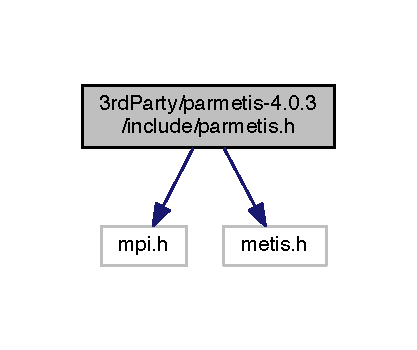
\includegraphics[width=200pt]{3rd_party_2parmetis-4_80_83_2include_2parmetis_8h__incl}
\end{center}
\end{figure}
\subsection*{Macros}
\begin{DoxyCompactItemize}
\item 
\#define \hyperlink{3rd_party_2parmetis-4_80_83_2include_2parmetis_8h_a238347d7669f8f1e9c83bfe63a2730c4}{\+\_\+\+\_\+cdecl}
\item 
\#define \hyperlink{3rd_party_2parmetis-4_80_83_2include_2parmetis_8h_aa48ba987f3ff8d56871c3fb2bed6d314}{P\+A\+R\+M\+E\+T\+I\+S\+\_\+\+M\+A\+J\+O\+R\+\_\+\+V\+E\+R\+S\+I\+ON}~4
\item 
\#define \hyperlink{3rd_party_2parmetis-4_80_83_2include_2parmetis_8h_ad51bc57fc5083572dd337e204de625ff}{P\+A\+R\+M\+E\+T\+I\+S\+\_\+\+M\+I\+N\+O\+R\+\_\+\+V\+E\+R\+S\+I\+ON}~0
\item 
\#define \hyperlink{3rd_party_2parmetis-4_80_83_2include_2parmetis_8h_a1d99bc97bff12181a8ad9588069a1f41}{P\+A\+R\+M\+E\+T\+I\+S\+\_\+\+S\+U\+B\+M\+I\+N\+O\+R\+\_\+\+V\+E\+R\+S\+I\+ON}~3
\item 
\#define \hyperlink{3rd_party_2parmetis-4_80_83_2include_2parmetis_8h_a8688bf16d43a979a690cef51e4e57d48}{P\+A\+R\+M\+E\+T\+I\+S\+\_\+\+M\+T\+Y\+P\+E\+\_\+\+L\+O\+C\+AL}~1    /$\ast$ Restrict matching to within processor vertices $\ast$/
\item 
\#define \hyperlink{3rd_party_2parmetis-4_80_83_2include_2parmetis_8h_af25d77131e25b013f79a5a7644c5792f}{P\+A\+R\+M\+E\+T\+I\+S\+\_\+\+M\+T\+Y\+P\+E\+\_\+\+G\+L\+O\+B\+AL}~2    /$\ast$ Remote vertices can be matched $\ast$/
\item 
\#define \hyperlink{3rd_party_2parmetis-4_80_83_2include_2parmetis_8h_ac0d490032ded504c8022884265a11546}{P\+A\+R\+M\+E\+T\+I\+S\+\_\+\+S\+R\+T\+Y\+P\+E\+\_\+\+G\+R\+E\+E\+DY}~1    /$\ast$ Vertices are visted from highest to lowest gain $\ast$/
\item 
\#define \hyperlink{3rd_party_2parmetis-4_80_83_2include_2parmetis_8h_a614e5181ee41475b1ffde007468e0526}{P\+A\+R\+M\+E\+T\+I\+S\+\_\+\+S\+R\+T\+Y\+P\+E\+\_\+2\+P\+H\+A\+SE}
\item 
\#define \hyperlink{3rd_party_2parmetis-4_80_83_2include_2parmetis_8h_a4703e7e2556a1a53794358fc85b8c103}{P\+A\+R\+M\+E\+T\+I\+S\+\_\+\+P\+S\+R\+\_\+\+C\+O\+U\+P\+L\+ED}~1    /$\ast$ \# of partitions == \# of processors $\ast$/
\item 
\#define \hyperlink{3rd_party_2parmetis-4_80_83_2include_2parmetis_8h_a0462a45a6c6bafa94c1327994fd3d9bd}{P\+A\+R\+M\+E\+T\+I\+S\+\_\+\+P\+S\+R\+\_\+\+U\+N\+C\+O\+U\+P\+L\+ED}~2    /$\ast$ \# of partitions != \# of processors $\ast$/
\item 
\#define \hyperlink{3rd_party_2parmetis-4_80_83_2include_2parmetis_8h_a83335527ec28434827ba22669c20f519}{P\+A\+R\+M\+E\+T\+I\+S\+\_\+\+D\+B\+G\+L\+V\+L\+\_\+\+T\+I\+ME}~1      /$\ast$ Perform timing analysis $\ast$/
\item 
\#define \hyperlink{3rd_party_2parmetis-4_80_83_2include_2parmetis_8h_ad4d113bb626ca386dfbb86d6730c9d0d}{P\+A\+R\+M\+E\+T\+I\+S\+\_\+\+D\+B\+G\+L\+V\+L\+\_\+\+I\+N\+FO}~2      /$\ast$ Perform timing analysis $\ast$/
\item 
\#define \hyperlink{3rd_party_2parmetis-4_80_83_2include_2parmetis_8h_a6913cca439f729f0d831646979505f71}{P\+A\+R\+M\+E\+T\+I\+S\+\_\+\+D\+B\+G\+L\+V\+L\+\_\+\+P\+R\+O\+G\+R\+E\+SS}~4      /$\ast$ Show the coarsening progress $\ast$/
\item 
\#define \hyperlink{3rd_party_2parmetis-4_80_83_2include_2parmetis_8h_a483143525f038b8d1cc9876e104b2228}{P\+A\+R\+M\+E\+T\+I\+S\+\_\+\+D\+B\+G\+L\+V\+L\+\_\+\+R\+E\+F\+I\+N\+E\+I\+N\+FO}~8      /$\ast$ Show info on communication during folding $\ast$/
\item 
\#define \hyperlink{3rd_party_2parmetis-4_80_83_2include_2parmetis_8h_a2c17217243390b94295386f8cb1f853d}{P\+A\+R\+M\+E\+T\+I\+S\+\_\+\+D\+B\+G\+L\+V\+L\+\_\+\+M\+A\+T\+C\+H\+I\+N\+FO}~16     /$\ast$ Show info on matching $\ast$/
\item 
\#define \hyperlink{3rd_party_2parmetis-4_80_83_2include_2parmetis_8h_aff381af99e792c5a07a391f18bc1a6ea}{P\+A\+R\+M\+E\+T\+I\+S\+\_\+\+D\+B\+G\+L\+V\+L\+\_\+\+R\+M\+O\+V\+E\+I\+N\+FO}~32     /$\ast$ Show info on communication during folding $\ast$/
\item 
\#define \hyperlink{3rd_party_2parmetis-4_80_83_2include_2parmetis_8h_a38aa880d4f8c0dbda1800f21f606a1e1}{P\+A\+R\+M\+E\+T\+I\+S\+\_\+\+D\+B\+G\+L\+V\+L\+\_\+\+R\+E\+M\+AP}~64     /$\ast$ Determines \hyperlink{threed__to__vtu_8m_a96c738d3e2120c4273f9d4390761d99e}{if} remapping will take place $\ast$/
\end{DoxyCompactItemize}
\subsection*{Enumerations}
\begin{DoxyCompactItemize}
\item 
enum \hyperlink{3rd_party_2parmetis-4_80_83_2include_2parmetis_8h_a8f61c0f0e4ba81b0e3b6901026acb936}{pmoptype\+\_\+et} \{ \newline
\hyperlink{3rd_party_2parmetis-4_80_83_2include_2parmetis_8h_a8f61c0f0e4ba81b0e3b6901026acb936af500122bd403005fe9cb32e3569e8ba6}{P\+A\+R\+M\+E\+T\+I\+S\+\_\+\+O\+P\+\_\+\+K\+M\+E\+T\+IS}, 
\hyperlink{3rd_party_2parmetis-4_80_83_2include_2parmetis_8h_a8f61c0f0e4ba81b0e3b6901026acb936a8b8807b13fb1114a8de7652337ec471a}{P\+A\+R\+M\+E\+T\+I\+S\+\_\+\+O\+P\+\_\+\+G\+K\+M\+E\+T\+IS}, 
\hyperlink{3rd_party_2parmetis-4_80_83_2include_2parmetis_8h_a8f61c0f0e4ba81b0e3b6901026acb936a2b4cf96dfc6daa7379376a7f99e513a3}{P\+A\+R\+M\+E\+T\+I\+S\+\_\+\+O\+P\+\_\+\+G\+M\+E\+T\+IS}, 
\hyperlink{3rd_party_2parmetis-4_80_83_2include_2parmetis_8h_a8f61c0f0e4ba81b0e3b6901026acb936a55445ff16748ddc40d09379353899db0}{P\+A\+R\+M\+E\+T\+I\+S\+\_\+\+O\+P\+\_\+\+R\+M\+E\+T\+IS}, 
\newline
\hyperlink{3rd_party_2parmetis-4_80_83_2include_2parmetis_8h_a8f61c0f0e4ba81b0e3b6901026acb936ac5e6d041f21837175f76d698908cb625}{P\+A\+R\+M\+E\+T\+I\+S\+\_\+\+O\+P\+\_\+\+A\+M\+E\+T\+IS}, 
\hyperlink{3rd_party_2parmetis-4_80_83_2include_2parmetis_8h_a8f61c0f0e4ba81b0e3b6901026acb936a351937a01dc7e48d92a5b3b218d7ef84}{P\+A\+R\+M\+E\+T\+I\+S\+\_\+\+O\+P\+\_\+\+O\+M\+E\+T\+IS}, 
\hyperlink{3rd_party_2parmetis-4_80_83_2include_2parmetis_8h_a8f61c0f0e4ba81b0e3b6901026acb936af57320a84124459d84bb006f00982afe}{P\+A\+R\+M\+E\+T\+I\+S\+\_\+\+O\+P\+\_\+\+M2\+D\+U\+AL}, 
\hyperlink{3rd_party_2parmetis-4_80_83_2include_2parmetis_8h_a8f61c0f0e4ba81b0e3b6901026acb936adf5e30191ffbb3823ca3a054496766e2}{P\+A\+R\+M\+E\+T\+I\+S\+\_\+\+O\+P\+\_\+\+M\+K\+M\+E\+T\+IS}, 
\newline
\hyperlink{include_2parmetis_8h_a8f61c0f0e4ba81b0e3b6901026acb936af500122bd403005fe9cb32e3569e8ba6}{P\+A\+R\+M\+E\+T\+I\+S\+\_\+\+O\+P\+\_\+\+K\+M\+E\+T\+IS}, 
\hyperlink{include_2parmetis_8h_a8f61c0f0e4ba81b0e3b6901026acb936a8b8807b13fb1114a8de7652337ec471a}{P\+A\+R\+M\+E\+T\+I\+S\+\_\+\+O\+P\+\_\+\+G\+K\+M\+E\+T\+IS}, 
\hyperlink{include_2parmetis_8h_a8f61c0f0e4ba81b0e3b6901026acb936a2b4cf96dfc6daa7379376a7f99e513a3}{P\+A\+R\+M\+E\+T\+I\+S\+\_\+\+O\+P\+\_\+\+G\+M\+E\+T\+IS}, 
\hyperlink{include_2parmetis_8h_a8f61c0f0e4ba81b0e3b6901026acb936a55445ff16748ddc40d09379353899db0}{P\+A\+R\+M\+E\+T\+I\+S\+\_\+\+O\+P\+\_\+\+R\+M\+E\+T\+IS}, 
\newline
\hyperlink{include_2parmetis_8h_a8f61c0f0e4ba81b0e3b6901026acb936ac5e6d041f21837175f76d698908cb625}{P\+A\+R\+M\+E\+T\+I\+S\+\_\+\+O\+P\+\_\+\+A\+M\+E\+T\+IS}, 
\hyperlink{include_2parmetis_8h_a8f61c0f0e4ba81b0e3b6901026acb936a351937a01dc7e48d92a5b3b218d7ef84}{P\+A\+R\+M\+E\+T\+I\+S\+\_\+\+O\+P\+\_\+\+O\+M\+E\+T\+IS}, 
\hyperlink{include_2parmetis_8h_a8f61c0f0e4ba81b0e3b6901026acb936af57320a84124459d84bb006f00982afe}{P\+A\+R\+M\+E\+T\+I\+S\+\_\+\+O\+P\+\_\+\+M2\+D\+U\+AL}, 
\hyperlink{include_2parmetis_8h_a8f61c0f0e4ba81b0e3b6901026acb936adf5e30191ffbb3823ca3a054496766e2}{P\+A\+R\+M\+E\+T\+I\+S\+\_\+\+O\+P\+\_\+\+M\+K\+M\+E\+T\+IS}
 \}
\end{DoxyCompactItemize}
\subsection*{Functions}
\begin{DoxyCompactItemize}
\item 
int \hyperlink{include_2parmetis_8h_a238347d7669f8f1e9c83bfe63a2730c4}{\+\_\+\+\_\+cdecl} \hyperlink{3rd_party_2parmetis-4_80_83_2include_2parmetis_8h_af418d1e76eaf4f80116da4caf51bd54e}{Par\+M\+E\+T\+I\+S\+\_\+\+V3\+\_\+\+Part\+Kway} (\hyperlink{3rd_party_2parmetis-4_80_83_2metis_2include_2metis_8h_aaa5262be3e700770163401acb0150f52}{idx\+\_\+t} $\ast$vtxdist, \hyperlink{3rd_party_2parmetis-4_80_83_2metis_2include_2metis_8h_aaa5262be3e700770163401acb0150f52}{idx\+\_\+t} $\ast$\hyperlink{include_2metis_8h_aa8fc7f75458e38e1e2979ed6db639164}{xadj}, \hyperlink{3rd_party_2parmetis-4_80_83_2metis_2include_2metis_8h_aaa5262be3e700770163401acb0150f52}{idx\+\_\+t} $\ast$\hyperlink{include_2metis_8h_a20c068e3ebdd8f9889fb82c1f677d679}{adjncy}, \hyperlink{3rd_party_2parmetis-4_80_83_2metis_2include_2metis_8h_aaa5262be3e700770163401acb0150f52}{idx\+\_\+t} $\ast$\hyperlink{include_2metis_8h_a34203f1160d94eca83e95f2718ea3504}{vwgt}, \hyperlink{3rd_party_2parmetis-4_80_83_2metis_2include_2metis_8h_aaa5262be3e700770163401acb0150f52}{idx\+\_\+t} $\ast$\hyperlink{include_2metis_8h_a2be4719baa820cfa5c06fd070796e0d3}{adjwgt}, \hyperlink{3rd_party_2parmetis-4_80_83_2metis_2include_2metis_8h_aaa5262be3e700770163401acb0150f52}{idx\+\_\+t} $\ast$wgtflag, \hyperlink{3rd_party_2parmetis-4_80_83_2metis_2include_2metis_8h_aaa5262be3e700770163401acb0150f52}{idx\+\_\+t} $\ast$\hyperlink{include_2metis_8h_aa48ecaf34ec788199c3aedb2b1558eb7}{numflag}, \hyperlink{3rd_party_2parmetis-4_80_83_2metis_2include_2metis_8h_aaa5262be3e700770163401acb0150f52}{idx\+\_\+t} $\ast$\hyperlink{include_2metis_8h_ac1dd31740e8f97fb57dc917ded30253f}{ncon}, \hyperlink{3rd_party_2parmetis-4_80_83_2metis_2include_2metis_8h_aaa5262be3e700770163401acb0150f52}{idx\+\_\+t} $\ast$\hyperlink{include_2metis_8h_aad88065af88fd6759101788a8e15ce9e}{nparts}, \hyperlink{3rd_party_2parmetis-4_80_83_2metis_2include_2metis_8h_a1924a4f6907cc3833213aba1f07fcbe9}{real\+\_\+t} $\ast$\hyperlink{include_2metis_8h_aa91786cd8ea996ec49ed5b382eb7fc2f}{tpwgts}, \hyperlink{3rd_party_2parmetis-4_80_83_2metis_2include_2metis_8h_a1924a4f6907cc3833213aba1f07fcbe9}{real\+\_\+t} $\ast$\hyperlink{include_2metis_8h_af48bb348bc8440a61f90f137de83f203}{ubvec}, \hyperlink{3rd_party_2parmetis-4_80_83_2metis_2include_2metis_8h_aaa5262be3e700770163401acb0150f52}{idx\+\_\+t} $\ast$\hyperlink{include_2metis_8h_a68c032ed4161802775c6847d4cb39adf}{options}, \hyperlink{3rd_party_2parmetis-4_80_83_2metis_2include_2metis_8h_aaa5262be3e700770163401acb0150f52}{idx\+\_\+t} $\ast$\hyperlink{include_2metis_8h_a8e62a902298dd5fd88ef554d5277b1dc}{edgecut}, \hyperlink{3rd_party_2parmetis-4_80_83_2metis_2include_2metis_8h_aaa5262be3e700770163401acb0150f52}{idx\+\_\+t} $\ast$\hyperlink{include_2metis_8h_a0a9ea8670f88d6db1e021fee2dcd94be}{part}, M\+P\+I\+\_\+\+Comm $\ast$comm)
\item 
int \hyperlink{include_2parmetis_8h_a238347d7669f8f1e9c83bfe63a2730c4}{\+\_\+\+\_\+cdecl} \hyperlink{3rd_party_2parmetis-4_80_83_2include_2parmetis_8h_a6df93293cf3d1ccb4659bd1b3091623d}{Par\+M\+E\+T\+I\+S\+\_\+\+V3\+\_\+\+Part\+Geom\+Kway} (\hyperlink{3rd_party_2parmetis-4_80_83_2metis_2include_2metis_8h_aaa5262be3e700770163401acb0150f52}{idx\+\_\+t} $\ast$vtxdist, \hyperlink{3rd_party_2parmetis-4_80_83_2metis_2include_2metis_8h_aaa5262be3e700770163401acb0150f52}{idx\+\_\+t} $\ast$\hyperlink{include_2metis_8h_aa8fc7f75458e38e1e2979ed6db639164}{xadj}, \hyperlink{3rd_party_2parmetis-4_80_83_2metis_2include_2metis_8h_aaa5262be3e700770163401acb0150f52}{idx\+\_\+t} $\ast$\hyperlink{include_2metis_8h_a20c068e3ebdd8f9889fb82c1f677d679}{adjncy}, \hyperlink{3rd_party_2parmetis-4_80_83_2metis_2include_2metis_8h_aaa5262be3e700770163401acb0150f52}{idx\+\_\+t} $\ast$\hyperlink{include_2metis_8h_a34203f1160d94eca83e95f2718ea3504}{vwgt}, \hyperlink{3rd_party_2parmetis-4_80_83_2metis_2include_2metis_8h_aaa5262be3e700770163401acb0150f52}{idx\+\_\+t} $\ast$\hyperlink{include_2metis_8h_a2be4719baa820cfa5c06fd070796e0d3}{adjwgt}, \hyperlink{3rd_party_2parmetis-4_80_83_2metis_2include_2metis_8h_aaa5262be3e700770163401acb0150f52}{idx\+\_\+t} $\ast$wgtflag, \hyperlink{3rd_party_2parmetis-4_80_83_2metis_2include_2metis_8h_aaa5262be3e700770163401acb0150f52}{idx\+\_\+t} $\ast$\hyperlink{include_2metis_8h_aa48ecaf34ec788199c3aedb2b1558eb7}{numflag}, \hyperlink{3rd_party_2parmetis-4_80_83_2metis_2include_2metis_8h_aaa5262be3e700770163401acb0150f52}{idx\+\_\+t} $\ast$ndims, \hyperlink{3rd_party_2parmetis-4_80_83_2metis_2include_2metis_8h_a1924a4f6907cc3833213aba1f07fcbe9}{real\+\_\+t} $\ast$\hyperlink{threed__to__vtu_8m_a6444a221e6b74abaf6d67d44af2650a0}{xyz}, \hyperlink{3rd_party_2parmetis-4_80_83_2metis_2include_2metis_8h_aaa5262be3e700770163401acb0150f52}{idx\+\_\+t} $\ast$\hyperlink{include_2metis_8h_ac1dd31740e8f97fb57dc917ded30253f}{ncon}, \hyperlink{3rd_party_2parmetis-4_80_83_2metis_2include_2metis_8h_aaa5262be3e700770163401acb0150f52}{idx\+\_\+t} $\ast$\hyperlink{include_2metis_8h_aad88065af88fd6759101788a8e15ce9e}{nparts}, \hyperlink{3rd_party_2parmetis-4_80_83_2metis_2include_2metis_8h_a1924a4f6907cc3833213aba1f07fcbe9}{real\+\_\+t} $\ast$\hyperlink{include_2metis_8h_aa91786cd8ea996ec49ed5b382eb7fc2f}{tpwgts}, \hyperlink{3rd_party_2parmetis-4_80_83_2metis_2include_2metis_8h_a1924a4f6907cc3833213aba1f07fcbe9}{real\+\_\+t} $\ast$\hyperlink{include_2metis_8h_af48bb348bc8440a61f90f137de83f203}{ubvec}, \hyperlink{3rd_party_2parmetis-4_80_83_2metis_2include_2metis_8h_aaa5262be3e700770163401acb0150f52}{idx\+\_\+t} $\ast$\hyperlink{include_2metis_8h_a68c032ed4161802775c6847d4cb39adf}{options}, \hyperlink{3rd_party_2parmetis-4_80_83_2metis_2include_2metis_8h_aaa5262be3e700770163401acb0150f52}{idx\+\_\+t} $\ast$\hyperlink{include_2metis_8h_a8e62a902298dd5fd88ef554d5277b1dc}{edgecut}, \hyperlink{3rd_party_2parmetis-4_80_83_2metis_2include_2metis_8h_aaa5262be3e700770163401acb0150f52}{idx\+\_\+t} $\ast$\hyperlink{include_2metis_8h_a0a9ea8670f88d6db1e021fee2dcd94be}{part}, M\+P\+I\+\_\+\+Comm $\ast$comm)
\item 
int \hyperlink{include_2parmetis_8h_a238347d7669f8f1e9c83bfe63a2730c4}{\+\_\+\+\_\+cdecl} \hyperlink{3rd_party_2parmetis-4_80_83_2include_2parmetis_8h_aab31b6450a3228063206eddded9de65e}{Par\+M\+E\+T\+I\+S\+\_\+\+V3\+\_\+\+Part\+Geom} (\hyperlink{3rd_party_2parmetis-4_80_83_2metis_2include_2metis_8h_aaa5262be3e700770163401acb0150f52}{idx\+\_\+t} $\ast$vtxdist, \hyperlink{3rd_party_2parmetis-4_80_83_2metis_2include_2metis_8h_aaa5262be3e700770163401acb0150f52}{idx\+\_\+t} $\ast$ndims, \hyperlink{3rd_party_2parmetis-4_80_83_2metis_2include_2metis_8h_a1924a4f6907cc3833213aba1f07fcbe9}{real\+\_\+t} $\ast$\hyperlink{threed__to__vtu_8m_a6444a221e6b74abaf6d67d44af2650a0}{xyz}, \hyperlink{3rd_party_2parmetis-4_80_83_2metis_2include_2metis_8h_aaa5262be3e700770163401acb0150f52}{idx\+\_\+t} $\ast$\hyperlink{include_2metis_8h_a0a9ea8670f88d6db1e021fee2dcd94be}{part}, M\+P\+I\+\_\+\+Comm $\ast$comm)
\item 
int \hyperlink{include_2parmetis_8h_a238347d7669f8f1e9c83bfe63a2730c4}{\+\_\+\+\_\+cdecl} \hyperlink{3rd_party_2parmetis-4_80_83_2include_2parmetis_8h_ad40a7809c9bdf183926da011220bad75}{Par\+M\+E\+T\+I\+S\+\_\+\+V3\+\_\+\+Refine\+Kway} (\hyperlink{3rd_party_2parmetis-4_80_83_2metis_2include_2metis_8h_aaa5262be3e700770163401acb0150f52}{idx\+\_\+t} $\ast$vtxdist, \hyperlink{3rd_party_2parmetis-4_80_83_2metis_2include_2metis_8h_aaa5262be3e700770163401acb0150f52}{idx\+\_\+t} $\ast$\hyperlink{include_2metis_8h_aa8fc7f75458e38e1e2979ed6db639164}{xadj}, \hyperlink{3rd_party_2parmetis-4_80_83_2metis_2include_2metis_8h_aaa5262be3e700770163401acb0150f52}{idx\+\_\+t} $\ast$\hyperlink{include_2metis_8h_a20c068e3ebdd8f9889fb82c1f677d679}{adjncy}, \hyperlink{3rd_party_2parmetis-4_80_83_2metis_2include_2metis_8h_aaa5262be3e700770163401acb0150f52}{idx\+\_\+t} $\ast$\hyperlink{include_2metis_8h_a34203f1160d94eca83e95f2718ea3504}{vwgt}, \hyperlink{3rd_party_2parmetis-4_80_83_2metis_2include_2metis_8h_aaa5262be3e700770163401acb0150f52}{idx\+\_\+t} $\ast$\hyperlink{include_2metis_8h_a2be4719baa820cfa5c06fd070796e0d3}{adjwgt}, \hyperlink{3rd_party_2parmetis-4_80_83_2metis_2include_2metis_8h_aaa5262be3e700770163401acb0150f52}{idx\+\_\+t} $\ast$wgtflag, \hyperlink{3rd_party_2parmetis-4_80_83_2metis_2include_2metis_8h_aaa5262be3e700770163401acb0150f52}{idx\+\_\+t} $\ast$\hyperlink{include_2metis_8h_aa48ecaf34ec788199c3aedb2b1558eb7}{numflag}, \hyperlink{3rd_party_2parmetis-4_80_83_2metis_2include_2metis_8h_aaa5262be3e700770163401acb0150f52}{idx\+\_\+t} $\ast$\hyperlink{include_2metis_8h_ac1dd31740e8f97fb57dc917ded30253f}{ncon}, \hyperlink{3rd_party_2parmetis-4_80_83_2metis_2include_2metis_8h_aaa5262be3e700770163401acb0150f52}{idx\+\_\+t} $\ast$\hyperlink{include_2metis_8h_aad88065af88fd6759101788a8e15ce9e}{nparts}, \hyperlink{3rd_party_2parmetis-4_80_83_2metis_2include_2metis_8h_a1924a4f6907cc3833213aba1f07fcbe9}{real\+\_\+t} $\ast$\hyperlink{include_2metis_8h_aa91786cd8ea996ec49ed5b382eb7fc2f}{tpwgts}, \hyperlink{3rd_party_2parmetis-4_80_83_2metis_2include_2metis_8h_a1924a4f6907cc3833213aba1f07fcbe9}{real\+\_\+t} $\ast$\hyperlink{include_2metis_8h_af48bb348bc8440a61f90f137de83f203}{ubvec}, \hyperlink{3rd_party_2parmetis-4_80_83_2metis_2include_2metis_8h_aaa5262be3e700770163401acb0150f52}{idx\+\_\+t} $\ast$\hyperlink{include_2metis_8h_a68c032ed4161802775c6847d4cb39adf}{options}, \hyperlink{3rd_party_2parmetis-4_80_83_2metis_2include_2metis_8h_aaa5262be3e700770163401acb0150f52}{idx\+\_\+t} $\ast$\hyperlink{include_2metis_8h_a8e62a902298dd5fd88ef554d5277b1dc}{edgecut}, \hyperlink{3rd_party_2parmetis-4_80_83_2metis_2include_2metis_8h_aaa5262be3e700770163401acb0150f52}{idx\+\_\+t} $\ast$\hyperlink{include_2metis_8h_a0a9ea8670f88d6db1e021fee2dcd94be}{part}, M\+P\+I\+\_\+\+Comm $\ast$comm)
\item 
int \hyperlink{include_2parmetis_8h_a238347d7669f8f1e9c83bfe63a2730c4}{\+\_\+\+\_\+cdecl} \hyperlink{3rd_party_2parmetis-4_80_83_2include_2parmetis_8h_ac00c3da2cf618cbfa9158463a851491e}{Par\+M\+E\+T\+I\+S\+\_\+\+V3\+\_\+\+Adaptive\+Repart} (\hyperlink{3rd_party_2parmetis-4_80_83_2metis_2include_2metis_8h_aaa5262be3e700770163401acb0150f52}{idx\+\_\+t} $\ast$vtxdist, \hyperlink{3rd_party_2parmetis-4_80_83_2metis_2include_2metis_8h_aaa5262be3e700770163401acb0150f52}{idx\+\_\+t} $\ast$\hyperlink{include_2metis_8h_aa8fc7f75458e38e1e2979ed6db639164}{xadj}, \hyperlink{3rd_party_2parmetis-4_80_83_2metis_2include_2metis_8h_aaa5262be3e700770163401acb0150f52}{idx\+\_\+t} $\ast$\hyperlink{include_2metis_8h_a20c068e3ebdd8f9889fb82c1f677d679}{adjncy}, \hyperlink{3rd_party_2parmetis-4_80_83_2metis_2include_2metis_8h_aaa5262be3e700770163401acb0150f52}{idx\+\_\+t} $\ast$\hyperlink{include_2metis_8h_a34203f1160d94eca83e95f2718ea3504}{vwgt}, \hyperlink{3rd_party_2parmetis-4_80_83_2metis_2include_2metis_8h_aaa5262be3e700770163401acb0150f52}{idx\+\_\+t} $\ast$\hyperlink{include_2metis_8h_aac32df5bb22250d94fc2fc7e4078308b}{vsize}, \hyperlink{3rd_party_2parmetis-4_80_83_2metis_2include_2metis_8h_aaa5262be3e700770163401acb0150f52}{idx\+\_\+t} $\ast$\hyperlink{include_2metis_8h_a2be4719baa820cfa5c06fd070796e0d3}{adjwgt}, \hyperlink{3rd_party_2parmetis-4_80_83_2metis_2include_2metis_8h_aaa5262be3e700770163401acb0150f52}{idx\+\_\+t} $\ast$wgtflag, \hyperlink{3rd_party_2parmetis-4_80_83_2metis_2include_2metis_8h_aaa5262be3e700770163401acb0150f52}{idx\+\_\+t} $\ast$\hyperlink{include_2metis_8h_aa48ecaf34ec788199c3aedb2b1558eb7}{numflag}, \hyperlink{3rd_party_2parmetis-4_80_83_2metis_2include_2metis_8h_aaa5262be3e700770163401acb0150f52}{idx\+\_\+t} $\ast$\hyperlink{include_2metis_8h_ac1dd31740e8f97fb57dc917ded30253f}{ncon}, \hyperlink{3rd_party_2parmetis-4_80_83_2metis_2include_2metis_8h_aaa5262be3e700770163401acb0150f52}{idx\+\_\+t} $\ast$\hyperlink{include_2metis_8h_aad88065af88fd6759101788a8e15ce9e}{nparts}, \hyperlink{3rd_party_2parmetis-4_80_83_2metis_2include_2metis_8h_a1924a4f6907cc3833213aba1f07fcbe9}{real\+\_\+t} $\ast$\hyperlink{include_2metis_8h_aa91786cd8ea996ec49ed5b382eb7fc2f}{tpwgts}, \hyperlink{3rd_party_2parmetis-4_80_83_2metis_2include_2metis_8h_a1924a4f6907cc3833213aba1f07fcbe9}{real\+\_\+t} $\ast$\hyperlink{include_2metis_8h_af48bb348bc8440a61f90f137de83f203}{ubvec}, \hyperlink{3rd_party_2parmetis-4_80_83_2metis_2include_2metis_8h_a1924a4f6907cc3833213aba1f07fcbe9}{real\+\_\+t} $\ast$ipc2redist, \hyperlink{3rd_party_2parmetis-4_80_83_2metis_2include_2metis_8h_aaa5262be3e700770163401acb0150f52}{idx\+\_\+t} $\ast$\hyperlink{include_2metis_8h_a68c032ed4161802775c6847d4cb39adf}{options}, \hyperlink{3rd_party_2parmetis-4_80_83_2metis_2include_2metis_8h_aaa5262be3e700770163401acb0150f52}{idx\+\_\+t} $\ast$\hyperlink{include_2metis_8h_a8e62a902298dd5fd88ef554d5277b1dc}{edgecut}, \hyperlink{3rd_party_2parmetis-4_80_83_2metis_2include_2metis_8h_aaa5262be3e700770163401acb0150f52}{idx\+\_\+t} $\ast$\hyperlink{include_2metis_8h_a0a9ea8670f88d6db1e021fee2dcd94be}{part}, M\+P\+I\+\_\+\+Comm $\ast$comm)
\item 
int \hyperlink{include_2parmetis_8h_a238347d7669f8f1e9c83bfe63a2730c4}{\+\_\+\+\_\+cdecl} \hyperlink{3rd_party_2parmetis-4_80_83_2include_2parmetis_8h_a2f9e316d7e0c46037cf231cd82cf9d97}{Par\+M\+E\+T\+I\+S\+\_\+\+V3\+\_\+\+Mesh2\+Dual} (\hyperlink{3rd_party_2parmetis-4_80_83_2metis_2include_2metis_8h_aaa5262be3e700770163401acb0150f52}{idx\+\_\+t} $\ast$elmdist, \hyperlink{3rd_party_2parmetis-4_80_83_2metis_2include_2metis_8h_aaa5262be3e700770163401acb0150f52}{idx\+\_\+t} $\ast$\hyperlink{include_2metis_8h_af3ca47b5acd610d8d94e45e3480b2583}{eptr}, \hyperlink{3rd_party_2parmetis-4_80_83_2metis_2include_2metis_8h_aaa5262be3e700770163401acb0150f52}{idx\+\_\+t} $\ast$\hyperlink{include_2metis_8h_af06d5753771b844d01c4c20e75c6401b}{eind}, \hyperlink{3rd_party_2parmetis-4_80_83_2metis_2include_2metis_8h_aaa5262be3e700770163401acb0150f52}{idx\+\_\+t} $\ast$\hyperlink{include_2metis_8h_aa48ecaf34ec788199c3aedb2b1558eb7}{numflag}, \hyperlink{3rd_party_2parmetis-4_80_83_2metis_2include_2metis_8h_aaa5262be3e700770163401acb0150f52}{idx\+\_\+t} $\ast$ncommonnodes, \hyperlink{3rd_party_2parmetis-4_80_83_2metis_2include_2metis_8h_aaa5262be3e700770163401acb0150f52}{idx\+\_\+t} $\ast$$\ast$\hyperlink{include_2metis_8h_aa8fc7f75458e38e1e2979ed6db639164}{xadj}, \hyperlink{3rd_party_2parmetis-4_80_83_2metis_2include_2metis_8h_aaa5262be3e700770163401acb0150f52}{idx\+\_\+t} $\ast$$\ast$\hyperlink{include_2metis_8h_a20c068e3ebdd8f9889fb82c1f677d679}{adjncy}, M\+P\+I\+\_\+\+Comm $\ast$comm)
\item 
int \hyperlink{include_2parmetis_8h_a238347d7669f8f1e9c83bfe63a2730c4}{\+\_\+\+\_\+cdecl} \hyperlink{3rd_party_2parmetis-4_80_83_2include_2parmetis_8h_a2ae9750ec09afdc4243b7cb7c5118666}{Par\+M\+E\+T\+I\+S\+\_\+\+V3\+\_\+\+Part\+Mesh\+Kway} (\hyperlink{3rd_party_2parmetis-4_80_83_2metis_2include_2metis_8h_aaa5262be3e700770163401acb0150f52}{idx\+\_\+t} $\ast$elmdist, \hyperlink{3rd_party_2parmetis-4_80_83_2metis_2include_2metis_8h_aaa5262be3e700770163401acb0150f52}{idx\+\_\+t} $\ast$\hyperlink{include_2metis_8h_af3ca47b5acd610d8d94e45e3480b2583}{eptr}, \hyperlink{3rd_party_2parmetis-4_80_83_2metis_2include_2metis_8h_aaa5262be3e700770163401acb0150f52}{idx\+\_\+t} $\ast$\hyperlink{include_2metis_8h_af06d5753771b844d01c4c20e75c6401b}{eind}, \hyperlink{3rd_party_2parmetis-4_80_83_2metis_2include_2metis_8h_aaa5262be3e700770163401acb0150f52}{idx\+\_\+t} $\ast$elmwgt, \hyperlink{3rd_party_2parmetis-4_80_83_2metis_2include_2metis_8h_aaa5262be3e700770163401acb0150f52}{idx\+\_\+t} $\ast$wgtflag, \hyperlink{3rd_party_2parmetis-4_80_83_2metis_2include_2metis_8h_aaa5262be3e700770163401acb0150f52}{idx\+\_\+t} $\ast$\hyperlink{include_2metis_8h_aa48ecaf34ec788199c3aedb2b1558eb7}{numflag}, \hyperlink{3rd_party_2parmetis-4_80_83_2metis_2include_2metis_8h_aaa5262be3e700770163401acb0150f52}{idx\+\_\+t} $\ast$\hyperlink{include_2metis_8h_ac1dd31740e8f97fb57dc917ded30253f}{ncon}, \hyperlink{3rd_party_2parmetis-4_80_83_2metis_2include_2metis_8h_aaa5262be3e700770163401acb0150f52}{idx\+\_\+t} $\ast$ncommonnodes, \hyperlink{3rd_party_2parmetis-4_80_83_2metis_2include_2metis_8h_aaa5262be3e700770163401acb0150f52}{idx\+\_\+t} $\ast$\hyperlink{include_2metis_8h_aad88065af88fd6759101788a8e15ce9e}{nparts}, \hyperlink{3rd_party_2parmetis-4_80_83_2metis_2include_2metis_8h_a1924a4f6907cc3833213aba1f07fcbe9}{real\+\_\+t} $\ast$\hyperlink{include_2metis_8h_aa91786cd8ea996ec49ed5b382eb7fc2f}{tpwgts}, \hyperlink{3rd_party_2parmetis-4_80_83_2metis_2include_2metis_8h_a1924a4f6907cc3833213aba1f07fcbe9}{real\+\_\+t} $\ast$\hyperlink{include_2metis_8h_af48bb348bc8440a61f90f137de83f203}{ubvec}, \hyperlink{3rd_party_2parmetis-4_80_83_2metis_2include_2metis_8h_aaa5262be3e700770163401acb0150f52}{idx\+\_\+t} $\ast$\hyperlink{include_2metis_8h_a68c032ed4161802775c6847d4cb39adf}{options}, \hyperlink{3rd_party_2parmetis-4_80_83_2metis_2include_2metis_8h_aaa5262be3e700770163401acb0150f52}{idx\+\_\+t} $\ast$\hyperlink{include_2metis_8h_a8e62a902298dd5fd88ef554d5277b1dc}{edgecut}, \hyperlink{3rd_party_2parmetis-4_80_83_2metis_2include_2metis_8h_aaa5262be3e700770163401acb0150f52}{idx\+\_\+t} $\ast$\hyperlink{include_2metis_8h_a0a9ea8670f88d6db1e021fee2dcd94be}{part}, M\+P\+I\+\_\+\+Comm $\ast$comm)
\item 
int \hyperlink{include_2parmetis_8h_a238347d7669f8f1e9c83bfe63a2730c4}{\+\_\+\+\_\+cdecl} \hyperlink{3rd_party_2parmetis-4_80_83_2include_2parmetis_8h_add23df29b4f232ac4c2cca94cc083a32}{Par\+M\+E\+T\+I\+S\+\_\+\+V3\+\_\+\+Node\+ND} (\hyperlink{3rd_party_2parmetis-4_80_83_2metis_2include_2metis_8h_aaa5262be3e700770163401acb0150f52}{idx\+\_\+t} $\ast$vtxdist, \hyperlink{3rd_party_2parmetis-4_80_83_2metis_2include_2metis_8h_aaa5262be3e700770163401acb0150f52}{idx\+\_\+t} $\ast$\hyperlink{include_2metis_8h_aa8fc7f75458e38e1e2979ed6db639164}{xadj}, \hyperlink{3rd_party_2parmetis-4_80_83_2metis_2include_2metis_8h_aaa5262be3e700770163401acb0150f52}{idx\+\_\+t} $\ast$\hyperlink{include_2metis_8h_a20c068e3ebdd8f9889fb82c1f677d679}{adjncy}, \hyperlink{3rd_party_2parmetis-4_80_83_2metis_2include_2metis_8h_aaa5262be3e700770163401acb0150f52}{idx\+\_\+t} $\ast$\hyperlink{include_2metis_8h_aa48ecaf34ec788199c3aedb2b1558eb7}{numflag}, \hyperlink{3rd_party_2parmetis-4_80_83_2metis_2include_2metis_8h_aaa5262be3e700770163401acb0150f52}{idx\+\_\+t} $\ast$\hyperlink{include_2metis_8h_a68c032ed4161802775c6847d4cb39adf}{options}, \hyperlink{3rd_party_2parmetis-4_80_83_2metis_2include_2metis_8h_aaa5262be3e700770163401acb0150f52}{idx\+\_\+t} $\ast$\hyperlink{make_v_t_k_file_8m_aab21ede0c02820806e77fd7890ee6bd7}{order}, \hyperlink{3rd_party_2parmetis-4_80_83_2metis_2include_2metis_8h_aaa5262be3e700770163401acb0150f52}{idx\+\_\+t} $\ast$\hyperlink{include_2metis_8h_aa2b865ca95a167fa6c34c48e9847379c}{sizes}, M\+P\+I\+\_\+\+Comm $\ast$comm)
\item 
int \hyperlink{include_2parmetis_8h_a238347d7669f8f1e9c83bfe63a2730c4}{\+\_\+\+\_\+cdecl} \hyperlink{3rd_party_2parmetis-4_80_83_2include_2parmetis_8h_a1bbf9ca25d902b187988a49ccf435e2b}{Par\+M\+E\+T\+I\+S\+\_\+\+V32\+\_\+\+Node\+ND} (\hyperlink{3rd_party_2parmetis-4_80_83_2metis_2include_2metis_8h_aaa5262be3e700770163401acb0150f52}{idx\+\_\+t} $\ast$vtxdist, \hyperlink{3rd_party_2parmetis-4_80_83_2metis_2include_2metis_8h_aaa5262be3e700770163401acb0150f52}{idx\+\_\+t} $\ast$\hyperlink{include_2metis_8h_aa8fc7f75458e38e1e2979ed6db639164}{xadj}, \hyperlink{3rd_party_2parmetis-4_80_83_2metis_2include_2metis_8h_aaa5262be3e700770163401acb0150f52}{idx\+\_\+t} $\ast$\hyperlink{include_2metis_8h_a20c068e3ebdd8f9889fb82c1f677d679}{adjncy}, \hyperlink{3rd_party_2parmetis-4_80_83_2metis_2include_2metis_8h_aaa5262be3e700770163401acb0150f52}{idx\+\_\+t} $\ast$\hyperlink{include_2metis_8h_a34203f1160d94eca83e95f2718ea3504}{vwgt}, \hyperlink{3rd_party_2parmetis-4_80_83_2metis_2include_2metis_8h_aaa5262be3e700770163401acb0150f52}{idx\+\_\+t} $\ast$\hyperlink{include_2metis_8h_aa48ecaf34ec788199c3aedb2b1558eb7}{numflag}, \hyperlink{3rd_party_2parmetis-4_80_83_2metis_2include_2metis_8h_aaa5262be3e700770163401acb0150f52}{idx\+\_\+t} $\ast$mtype, \hyperlink{3rd_party_2parmetis-4_80_83_2metis_2include_2metis_8h_aaa5262be3e700770163401acb0150f52}{idx\+\_\+t} $\ast$rtype, \hyperlink{3rd_party_2parmetis-4_80_83_2metis_2include_2metis_8h_aaa5262be3e700770163401acb0150f52}{idx\+\_\+t} $\ast$p\+\_\+nseps, \hyperlink{3rd_party_2parmetis-4_80_83_2metis_2include_2metis_8h_aaa5262be3e700770163401acb0150f52}{idx\+\_\+t} $\ast$s\+\_\+nseps, \hyperlink{3rd_party_2parmetis-4_80_83_2metis_2include_2metis_8h_a1924a4f6907cc3833213aba1f07fcbe9}{real\+\_\+t} $\ast$ubfrac, \hyperlink{3rd_party_2parmetis-4_80_83_2metis_2include_2metis_8h_aaa5262be3e700770163401acb0150f52}{idx\+\_\+t} $\ast$seed, \hyperlink{3rd_party_2parmetis-4_80_83_2metis_2include_2metis_8h_aaa5262be3e700770163401acb0150f52}{idx\+\_\+t} $\ast$dbglvl, \hyperlink{3rd_party_2parmetis-4_80_83_2metis_2include_2metis_8h_aaa5262be3e700770163401acb0150f52}{idx\+\_\+t} $\ast$\hyperlink{make_v_t_k_file_8m_aab21ede0c02820806e77fd7890ee6bd7}{order}, \hyperlink{3rd_party_2parmetis-4_80_83_2metis_2include_2metis_8h_aaa5262be3e700770163401acb0150f52}{idx\+\_\+t} $\ast$\hyperlink{include_2metis_8h_aa2b865ca95a167fa6c34c48e9847379c}{sizes}, M\+P\+I\+\_\+\+Comm $\ast$comm)
\item 
int \hyperlink{include_2parmetis_8h_a238347d7669f8f1e9c83bfe63a2730c4}{\+\_\+\+\_\+cdecl} \hyperlink{3rd_party_2parmetis-4_80_83_2include_2parmetis_8h_a8bd1a6399ac304da6616cb5329304df6}{Par\+M\+E\+T\+I\+S\+\_\+\+Serial\+Node\+ND} (\hyperlink{3rd_party_2parmetis-4_80_83_2metis_2include_2metis_8h_aaa5262be3e700770163401acb0150f52}{idx\+\_\+t} $\ast$vtxdist, \hyperlink{3rd_party_2parmetis-4_80_83_2metis_2include_2metis_8h_aaa5262be3e700770163401acb0150f52}{idx\+\_\+t} $\ast$\hyperlink{include_2metis_8h_aa8fc7f75458e38e1e2979ed6db639164}{xadj}, \hyperlink{3rd_party_2parmetis-4_80_83_2metis_2include_2metis_8h_aaa5262be3e700770163401acb0150f52}{idx\+\_\+t} $\ast$\hyperlink{include_2metis_8h_a20c068e3ebdd8f9889fb82c1f677d679}{adjncy}, \hyperlink{3rd_party_2parmetis-4_80_83_2metis_2include_2metis_8h_aaa5262be3e700770163401acb0150f52}{idx\+\_\+t} $\ast$\hyperlink{include_2metis_8h_aa48ecaf34ec788199c3aedb2b1558eb7}{numflag}, \hyperlink{3rd_party_2parmetis-4_80_83_2metis_2include_2metis_8h_aaa5262be3e700770163401acb0150f52}{idx\+\_\+t} $\ast$\hyperlink{include_2metis_8h_a68c032ed4161802775c6847d4cb39adf}{options}, \hyperlink{3rd_party_2parmetis-4_80_83_2metis_2include_2metis_8h_aaa5262be3e700770163401acb0150f52}{idx\+\_\+t} $\ast$\hyperlink{make_v_t_k_file_8m_aab21ede0c02820806e77fd7890ee6bd7}{order}, \hyperlink{3rd_party_2parmetis-4_80_83_2metis_2include_2metis_8h_aaa5262be3e700770163401acb0150f52}{idx\+\_\+t} $\ast$\hyperlink{include_2metis_8h_aa2b865ca95a167fa6c34c48e9847379c}{sizes}, M\+P\+I\+\_\+\+Comm $\ast$comm)
\end{DoxyCompactItemize}


\subsection{Macro Definition Documentation}
\mbox{\Hypertarget{3rd_party_2parmetis-4_80_83_2include_2parmetis_8h_a238347d7669f8f1e9c83bfe63a2730c4}\label{3rd_party_2parmetis-4_80_83_2include_2parmetis_8h_a238347d7669f8f1e9c83bfe63a2730c4}} 
\index{3rd\+Party/parmetis-\/4.\+0.\+3/include/parmetis.\+h@{3rd\+Party/parmetis-\/4.\+0.\+3/include/parmetis.\+h}!\+\_\+\+\_\+cdecl@{\+\_\+\+\_\+cdecl}}
\index{\+\_\+\+\_\+cdecl@{\+\_\+\+\_\+cdecl}!3rd\+Party/parmetis-\/4.\+0.\+3/include/parmetis.\+h@{3rd\+Party/parmetis-\/4.\+0.\+3/include/parmetis.\+h}}
\subsubsection{\texorpdfstring{\+\_\+\+\_\+cdecl}{\_\_cdecl}}
{\footnotesize\ttfamily \#define \+\_\+\+\_\+cdecl}

\mbox{\Hypertarget{3rd_party_2parmetis-4_80_83_2include_2parmetis_8h_ad4d113bb626ca386dfbb86d6730c9d0d}\label{3rd_party_2parmetis-4_80_83_2include_2parmetis_8h_ad4d113bb626ca386dfbb86d6730c9d0d}} 
\index{3rd\+Party/parmetis-\/4.\+0.\+3/include/parmetis.\+h@{3rd\+Party/parmetis-\/4.\+0.\+3/include/parmetis.\+h}!P\+A\+R\+M\+E\+T\+I\+S\+\_\+\+D\+B\+G\+L\+V\+L\+\_\+\+I\+N\+FO@{P\+A\+R\+M\+E\+T\+I\+S\+\_\+\+D\+B\+G\+L\+V\+L\+\_\+\+I\+N\+FO}}
\index{P\+A\+R\+M\+E\+T\+I\+S\+\_\+\+D\+B\+G\+L\+V\+L\+\_\+\+I\+N\+FO@{P\+A\+R\+M\+E\+T\+I\+S\+\_\+\+D\+B\+G\+L\+V\+L\+\_\+\+I\+N\+FO}!3rd\+Party/parmetis-\/4.\+0.\+3/include/parmetis.\+h@{3rd\+Party/parmetis-\/4.\+0.\+3/include/parmetis.\+h}}
\subsubsection{\texorpdfstring{P\+A\+R\+M\+E\+T\+I\+S\+\_\+\+D\+B\+G\+L\+V\+L\+\_\+\+I\+N\+FO}{PARMETIS\_DBGLVL\_INFO}}
{\footnotesize\ttfamily \#define P\+A\+R\+M\+E\+T\+I\+S\+\_\+\+D\+B\+G\+L\+V\+L\+\_\+\+I\+N\+FO~2      /$\ast$ Perform timing analysis $\ast$/}

\mbox{\Hypertarget{3rd_party_2parmetis-4_80_83_2include_2parmetis_8h_a2c17217243390b94295386f8cb1f853d}\label{3rd_party_2parmetis-4_80_83_2include_2parmetis_8h_a2c17217243390b94295386f8cb1f853d}} 
\index{3rd\+Party/parmetis-\/4.\+0.\+3/include/parmetis.\+h@{3rd\+Party/parmetis-\/4.\+0.\+3/include/parmetis.\+h}!P\+A\+R\+M\+E\+T\+I\+S\+\_\+\+D\+B\+G\+L\+V\+L\+\_\+\+M\+A\+T\+C\+H\+I\+N\+FO@{P\+A\+R\+M\+E\+T\+I\+S\+\_\+\+D\+B\+G\+L\+V\+L\+\_\+\+M\+A\+T\+C\+H\+I\+N\+FO}}
\index{P\+A\+R\+M\+E\+T\+I\+S\+\_\+\+D\+B\+G\+L\+V\+L\+\_\+\+M\+A\+T\+C\+H\+I\+N\+FO@{P\+A\+R\+M\+E\+T\+I\+S\+\_\+\+D\+B\+G\+L\+V\+L\+\_\+\+M\+A\+T\+C\+H\+I\+N\+FO}!3rd\+Party/parmetis-\/4.\+0.\+3/include/parmetis.\+h@{3rd\+Party/parmetis-\/4.\+0.\+3/include/parmetis.\+h}}
\subsubsection{\texorpdfstring{P\+A\+R\+M\+E\+T\+I\+S\+\_\+\+D\+B\+G\+L\+V\+L\+\_\+\+M\+A\+T\+C\+H\+I\+N\+FO}{PARMETIS\_DBGLVL\_MATCHINFO}}
{\footnotesize\ttfamily \#define P\+A\+R\+M\+E\+T\+I\+S\+\_\+\+D\+B\+G\+L\+V\+L\+\_\+\+M\+A\+T\+C\+H\+I\+N\+FO~16     /$\ast$ Show info on matching $\ast$/}

\mbox{\Hypertarget{3rd_party_2parmetis-4_80_83_2include_2parmetis_8h_a6913cca439f729f0d831646979505f71}\label{3rd_party_2parmetis-4_80_83_2include_2parmetis_8h_a6913cca439f729f0d831646979505f71}} 
\index{3rd\+Party/parmetis-\/4.\+0.\+3/include/parmetis.\+h@{3rd\+Party/parmetis-\/4.\+0.\+3/include/parmetis.\+h}!P\+A\+R\+M\+E\+T\+I\+S\+\_\+\+D\+B\+G\+L\+V\+L\+\_\+\+P\+R\+O\+G\+R\+E\+SS@{P\+A\+R\+M\+E\+T\+I\+S\+\_\+\+D\+B\+G\+L\+V\+L\+\_\+\+P\+R\+O\+G\+R\+E\+SS}}
\index{P\+A\+R\+M\+E\+T\+I\+S\+\_\+\+D\+B\+G\+L\+V\+L\+\_\+\+P\+R\+O\+G\+R\+E\+SS@{P\+A\+R\+M\+E\+T\+I\+S\+\_\+\+D\+B\+G\+L\+V\+L\+\_\+\+P\+R\+O\+G\+R\+E\+SS}!3rd\+Party/parmetis-\/4.\+0.\+3/include/parmetis.\+h@{3rd\+Party/parmetis-\/4.\+0.\+3/include/parmetis.\+h}}
\subsubsection{\texorpdfstring{P\+A\+R\+M\+E\+T\+I\+S\+\_\+\+D\+B\+G\+L\+V\+L\+\_\+\+P\+R\+O\+G\+R\+E\+SS}{PARMETIS\_DBGLVL\_PROGRESS}}
{\footnotesize\ttfamily \#define P\+A\+R\+M\+E\+T\+I\+S\+\_\+\+D\+B\+G\+L\+V\+L\+\_\+\+P\+R\+O\+G\+R\+E\+SS~4      /$\ast$ Show the coarsening progress $\ast$/}

\mbox{\Hypertarget{3rd_party_2parmetis-4_80_83_2include_2parmetis_8h_a483143525f038b8d1cc9876e104b2228}\label{3rd_party_2parmetis-4_80_83_2include_2parmetis_8h_a483143525f038b8d1cc9876e104b2228}} 
\index{3rd\+Party/parmetis-\/4.\+0.\+3/include/parmetis.\+h@{3rd\+Party/parmetis-\/4.\+0.\+3/include/parmetis.\+h}!P\+A\+R\+M\+E\+T\+I\+S\+\_\+\+D\+B\+G\+L\+V\+L\+\_\+\+R\+E\+F\+I\+N\+E\+I\+N\+FO@{P\+A\+R\+M\+E\+T\+I\+S\+\_\+\+D\+B\+G\+L\+V\+L\+\_\+\+R\+E\+F\+I\+N\+E\+I\+N\+FO}}
\index{P\+A\+R\+M\+E\+T\+I\+S\+\_\+\+D\+B\+G\+L\+V\+L\+\_\+\+R\+E\+F\+I\+N\+E\+I\+N\+FO@{P\+A\+R\+M\+E\+T\+I\+S\+\_\+\+D\+B\+G\+L\+V\+L\+\_\+\+R\+E\+F\+I\+N\+E\+I\+N\+FO}!3rd\+Party/parmetis-\/4.\+0.\+3/include/parmetis.\+h@{3rd\+Party/parmetis-\/4.\+0.\+3/include/parmetis.\+h}}
\subsubsection{\texorpdfstring{P\+A\+R\+M\+E\+T\+I\+S\+\_\+\+D\+B\+G\+L\+V\+L\+\_\+\+R\+E\+F\+I\+N\+E\+I\+N\+FO}{PARMETIS\_DBGLVL\_REFINEINFO}}
{\footnotesize\ttfamily \#define P\+A\+R\+M\+E\+T\+I\+S\+\_\+\+D\+B\+G\+L\+V\+L\+\_\+\+R\+E\+F\+I\+N\+E\+I\+N\+FO~8      /$\ast$ Show info on communication during folding $\ast$/}

\mbox{\Hypertarget{3rd_party_2parmetis-4_80_83_2include_2parmetis_8h_a38aa880d4f8c0dbda1800f21f606a1e1}\label{3rd_party_2parmetis-4_80_83_2include_2parmetis_8h_a38aa880d4f8c0dbda1800f21f606a1e1}} 
\index{3rd\+Party/parmetis-\/4.\+0.\+3/include/parmetis.\+h@{3rd\+Party/parmetis-\/4.\+0.\+3/include/parmetis.\+h}!P\+A\+R\+M\+E\+T\+I\+S\+\_\+\+D\+B\+G\+L\+V\+L\+\_\+\+R\+E\+M\+AP@{P\+A\+R\+M\+E\+T\+I\+S\+\_\+\+D\+B\+G\+L\+V\+L\+\_\+\+R\+E\+M\+AP}}
\index{P\+A\+R\+M\+E\+T\+I\+S\+\_\+\+D\+B\+G\+L\+V\+L\+\_\+\+R\+E\+M\+AP@{P\+A\+R\+M\+E\+T\+I\+S\+\_\+\+D\+B\+G\+L\+V\+L\+\_\+\+R\+E\+M\+AP}!3rd\+Party/parmetis-\/4.\+0.\+3/include/parmetis.\+h@{3rd\+Party/parmetis-\/4.\+0.\+3/include/parmetis.\+h}}
\subsubsection{\texorpdfstring{P\+A\+R\+M\+E\+T\+I\+S\+\_\+\+D\+B\+G\+L\+V\+L\+\_\+\+R\+E\+M\+AP}{PARMETIS\_DBGLVL\_REMAP}}
{\footnotesize\ttfamily \#define P\+A\+R\+M\+E\+T\+I\+S\+\_\+\+D\+B\+G\+L\+V\+L\+\_\+\+R\+E\+M\+AP~64     /$\ast$ Determines \hyperlink{threed__to__vtu_8m_a96c738d3e2120c4273f9d4390761d99e}{if} remapping will take place $\ast$/}

\mbox{\Hypertarget{3rd_party_2parmetis-4_80_83_2include_2parmetis_8h_aff381af99e792c5a07a391f18bc1a6ea}\label{3rd_party_2parmetis-4_80_83_2include_2parmetis_8h_aff381af99e792c5a07a391f18bc1a6ea}} 
\index{3rd\+Party/parmetis-\/4.\+0.\+3/include/parmetis.\+h@{3rd\+Party/parmetis-\/4.\+0.\+3/include/parmetis.\+h}!P\+A\+R\+M\+E\+T\+I\+S\+\_\+\+D\+B\+G\+L\+V\+L\+\_\+\+R\+M\+O\+V\+E\+I\+N\+FO@{P\+A\+R\+M\+E\+T\+I\+S\+\_\+\+D\+B\+G\+L\+V\+L\+\_\+\+R\+M\+O\+V\+E\+I\+N\+FO}}
\index{P\+A\+R\+M\+E\+T\+I\+S\+\_\+\+D\+B\+G\+L\+V\+L\+\_\+\+R\+M\+O\+V\+E\+I\+N\+FO@{P\+A\+R\+M\+E\+T\+I\+S\+\_\+\+D\+B\+G\+L\+V\+L\+\_\+\+R\+M\+O\+V\+E\+I\+N\+FO}!3rd\+Party/parmetis-\/4.\+0.\+3/include/parmetis.\+h@{3rd\+Party/parmetis-\/4.\+0.\+3/include/parmetis.\+h}}
\subsubsection{\texorpdfstring{P\+A\+R\+M\+E\+T\+I\+S\+\_\+\+D\+B\+G\+L\+V\+L\+\_\+\+R\+M\+O\+V\+E\+I\+N\+FO}{PARMETIS\_DBGLVL\_RMOVEINFO}}
{\footnotesize\ttfamily \#define P\+A\+R\+M\+E\+T\+I\+S\+\_\+\+D\+B\+G\+L\+V\+L\+\_\+\+R\+M\+O\+V\+E\+I\+N\+FO~32     /$\ast$ Show info on communication during folding $\ast$/}

\mbox{\Hypertarget{3rd_party_2parmetis-4_80_83_2include_2parmetis_8h_a83335527ec28434827ba22669c20f519}\label{3rd_party_2parmetis-4_80_83_2include_2parmetis_8h_a83335527ec28434827ba22669c20f519}} 
\index{3rd\+Party/parmetis-\/4.\+0.\+3/include/parmetis.\+h@{3rd\+Party/parmetis-\/4.\+0.\+3/include/parmetis.\+h}!P\+A\+R\+M\+E\+T\+I\+S\+\_\+\+D\+B\+G\+L\+V\+L\+\_\+\+T\+I\+ME@{P\+A\+R\+M\+E\+T\+I\+S\+\_\+\+D\+B\+G\+L\+V\+L\+\_\+\+T\+I\+ME}}
\index{P\+A\+R\+M\+E\+T\+I\+S\+\_\+\+D\+B\+G\+L\+V\+L\+\_\+\+T\+I\+ME@{P\+A\+R\+M\+E\+T\+I\+S\+\_\+\+D\+B\+G\+L\+V\+L\+\_\+\+T\+I\+ME}!3rd\+Party/parmetis-\/4.\+0.\+3/include/parmetis.\+h@{3rd\+Party/parmetis-\/4.\+0.\+3/include/parmetis.\+h}}
\subsubsection{\texorpdfstring{P\+A\+R\+M\+E\+T\+I\+S\+\_\+\+D\+B\+G\+L\+V\+L\+\_\+\+T\+I\+ME}{PARMETIS\_DBGLVL\_TIME}}
{\footnotesize\ttfamily \#define P\+A\+R\+M\+E\+T\+I\+S\+\_\+\+D\+B\+G\+L\+V\+L\+\_\+\+T\+I\+ME~1      /$\ast$ Perform timing analysis $\ast$/}

\mbox{\Hypertarget{3rd_party_2parmetis-4_80_83_2include_2parmetis_8h_aa48ba987f3ff8d56871c3fb2bed6d314}\label{3rd_party_2parmetis-4_80_83_2include_2parmetis_8h_aa48ba987f3ff8d56871c3fb2bed6d314}} 
\index{3rd\+Party/parmetis-\/4.\+0.\+3/include/parmetis.\+h@{3rd\+Party/parmetis-\/4.\+0.\+3/include/parmetis.\+h}!P\+A\+R\+M\+E\+T\+I\+S\+\_\+\+M\+A\+J\+O\+R\+\_\+\+V\+E\+R\+S\+I\+ON@{P\+A\+R\+M\+E\+T\+I\+S\+\_\+\+M\+A\+J\+O\+R\+\_\+\+V\+E\+R\+S\+I\+ON}}
\index{P\+A\+R\+M\+E\+T\+I\+S\+\_\+\+M\+A\+J\+O\+R\+\_\+\+V\+E\+R\+S\+I\+ON@{P\+A\+R\+M\+E\+T\+I\+S\+\_\+\+M\+A\+J\+O\+R\+\_\+\+V\+E\+R\+S\+I\+ON}!3rd\+Party/parmetis-\/4.\+0.\+3/include/parmetis.\+h@{3rd\+Party/parmetis-\/4.\+0.\+3/include/parmetis.\+h}}
\subsubsection{\texorpdfstring{P\+A\+R\+M\+E\+T\+I\+S\+\_\+\+M\+A\+J\+O\+R\+\_\+\+V\+E\+R\+S\+I\+ON}{PARMETIS\_MAJOR\_VERSION}}
{\footnotesize\ttfamily \#define P\+A\+R\+M\+E\+T\+I\+S\+\_\+\+M\+A\+J\+O\+R\+\_\+\+V\+E\+R\+S\+I\+ON~4}

\mbox{\Hypertarget{3rd_party_2parmetis-4_80_83_2include_2parmetis_8h_ad51bc57fc5083572dd337e204de625ff}\label{3rd_party_2parmetis-4_80_83_2include_2parmetis_8h_ad51bc57fc5083572dd337e204de625ff}} 
\index{3rd\+Party/parmetis-\/4.\+0.\+3/include/parmetis.\+h@{3rd\+Party/parmetis-\/4.\+0.\+3/include/parmetis.\+h}!P\+A\+R\+M\+E\+T\+I\+S\+\_\+\+M\+I\+N\+O\+R\+\_\+\+V\+E\+R\+S\+I\+ON@{P\+A\+R\+M\+E\+T\+I\+S\+\_\+\+M\+I\+N\+O\+R\+\_\+\+V\+E\+R\+S\+I\+ON}}
\index{P\+A\+R\+M\+E\+T\+I\+S\+\_\+\+M\+I\+N\+O\+R\+\_\+\+V\+E\+R\+S\+I\+ON@{P\+A\+R\+M\+E\+T\+I\+S\+\_\+\+M\+I\+N\+O\+R\+\_\+\+V\+E\+R\+S\+I\+ON}!3rd\+Party/parmetis-\/4.\+0.\+3/include/parmetis.\+h@{3rd\+Party/parmetis-\/4.\+0.\+3/include/parmetis.\+h}}
\subsubsection{\texorpdfstring{P\+A\+R\+M\+E\+T\+I\+S\+\_\+\+M\+I\+N\+O\+R\+\_\+\+V\+E\+R\+S\+I\+ON}{PARMETIS\_MINOR\_VERSION}}
{\footnotesize\ttfamily \#define P\+A\+R\+M\+E\+T\+I\+S\+\_\+\+M\+I\+N\+O\+R\+\_\+\+V\+E\+R\+S\+I\+ON~0}

\mbox{\Hypertarget{3rd_party_2parmetis-4_80_83_2include_2parmetis_8h_af25d77131e25b013f79a5a7644c5792f}\label{3rd_party_2parmetis-4_80_83_2include_2parmetis_8h_af25d77131e25b013f79a5a7644c5792f}} 
\index{3rd\+Party/parmetis-\/4.\+0.\+3/include/parmetis.\+h@{3rd\+Party/parmetis-\/4.\+0.\+3/include/parmetis.\+h}!P\+A\+R\+M\+E\+T\+I\+S\+\_\+\+M\+T\+Y\+P\+E\+\_\+\+G\+L\+O\+B\+AL@{P\+A\+R\+M\+E\+T\+I\+S\+\_\+\+M\+T\+Y\+P\+E\+\_\+\+G\+L\+O\+B\+AL}}
\index{P\+A\+R\+M\+E\+T\+I\+S\+\_\+\+M\+T\+Y\+P\+E\+\_\+\+G\+L\+O\+B\+AL@{P\+A\+R\+M\+E\+T\+I\+S\+\_\+\+M\+T\+Y\+P\+E\+\_\+\+G\+L\+O\+B\+AL}!3rd\+Party/parmetis-\/4.\+0.\+3/include/parmetis.\+h@{3rd\+Party/parmetis-\/4.\+0.\+3/include/parmetis.\+h}}
\subsubsection{\texorpdfstring{P\+A\+R\+M\+E\+T\+I\+S\+\_\+\+M\+T\+Y\+P\+E\+\_\+\+G\+L\+O\+B\+AL}{PARMETIS\_MTYPE\_GLOBAL}}
{\footnotesize\ttfamily \#define P\+A\+R\+M\+E\+T\+I\+S\+\_\+\+M\+T\+Y\+P\+E\+\_\+\+G\+L\+O\+B\+AL~2    /$\ast$ Remote vertices can be matched $\ast$/}

\mbox{\Hypertarget{3rd_party_2parmetis-4_80_83_2include_2parmetis_8h_a8688bf16d43a979a690cef51e4e57d48}\label{3rd_party_2parmetis-4_80_83_2include_2parmetis_8h_a8688bf16d43a979a690cef51e4e57d48}} 
\index{3rd\+Party/parmetis-\/4.\+0.\+3/include/parmetis.\+h@{3rd\+Party/parmetis-\/4.\+0.\+3/include/parmetis.\+h}!P\+A\+R\+M\+E\+T\+I\+S\+\_\+\+M\+T\+Y\+P\+E\+\_\+\+L\+O\+C\+AL@{P\+A\+R\+M\+E\+T\+I\+S\+\_\+\+M\+T\+Y\+P\+E\+\_\+\+L\+O\+C\+AL}}
\index{P\+A\+R\+M\+E\+T\+I\+S\+\_\+\+M\+T\+Y\+P\+E\+\_\+\+L\+O\+C\+AL@{P\+A\+R\+M\+E\+T\+I\+S\+\_\+\+M\+T\+Y\+P\+E\+\_\+\+L\+O\+C\+AL}!3rd\+Party/parmetis-\/4.\+0.\+3/include/parmetis.\+h@{3rd\+Party/parmetis-\/4.\+0.\+3/include/parmetis.\+h}}
\subsubsection{\texorpdfstring{P\+A\+R\+M\+E\+T\+I\+S\+\_\+\+M\+T\+Y\+P\+E\+\_\+\+L\+O\+C\+AL}{PARMETIS\_MTYPE\_LOCAL}}
{\footnotesize\ttfamily \#define P\+A\+R\+M\+E\+T\+I\+S\+\_\+\+M\+T\+Y\+P\+E\+\_\+\+L\+O\+C\+AL~1    /$\ast$ Restrict matching to within processor vertices $\ast$/}

\mbox{\Hypertarget{3rd_party_2parmetis-4_80_83_2include_2parmetis_8h_a4703e7e2556a1a53794358fc85b8c103}\label{3rd_party_2parmetis-4_80_83_2include_2parmetis_8h_a4703e7e2556a1a53794358fc85b8c103}} 
\index{3rd\+Party/parmetis-\/4.\+0.\+3/include/parmetis.\+h@{3rd\+Party/parmetis-\/4.\+0.\+3/include/parmetis.\+h}!P\+A\+R\+M\+E\+T\+I\+S\+\_\+\+P\+S\+R\+\_\+\+C\+O\+U\+P\+L\+ED@{P\+A\+R\+M\+E\+T\+I\+S\+\_\+\+P\+S\+R\+\_\+\+C\+O\+U\+P\+L\+ED}}
\index{P\+A\+R\+M\+E\+T\+I\+S\+\_\+\+P\+S\+R\+\_\+\+C\+O\+U\+P\+L\+ED@{P\+A\+R\+M\+E\+T\+I\+S\+\_\+\+P\+S\+R\+\_\+\+C\+O\+U\+P\+L\+ED}!3rd\+Party/parmetis-\/4.\+0.\+3/include/parmetis.\+h@{3rd\+Party/parmetis-\/4.\+0.\+3/include/parmetis.\+h}}
\subsubsection{\texorpdfstring{P\+A\+R\+M\+E\+T\+I\+S\+\_\+\+P\+S\+R\+\_\+\+C\+O\+U\+P\+L\+ED}{PARMETIS\_PSR\_COUPLED}}
{\footnotesize\ttfamily \#define P\+A\+R\+M\+E\+T\+I\+S\+\_\+\+P\+S\+R\+\_\+\+C\+O\+U\+P\+L\+ED~1    /$\ast$ \# of partitions == \# of processors $\ast$/}

\mbox{\Hypertarget{3rd_party_2parmetis-4_80_83_2include_2parmetis_8h_a0462a45a6c6bafa94c1327994fd3d9bd}\label{3rd_party_2parmetis-4_80_83_2include_2parmetis_8h_a0462a45a6c6bafa94c1327994fd3d9bd}} 
\index{3rd\+Party/parmetis-\/4.\+0.\+3/include/parmetis.\+h@{3rd\+Party/parmetis-\/4.\+0.\+3/include/parmetis.\+h}!P\+A\+R\+M\+E\+T\+I\+S\+\_\+\+P\+S\+R\+\_\+\+U\+N\+C\+O\+U\+P\+L\+ED@{P\+A\+R\+M\+E\+T\+I\+S\+\_\+\+P\+S\+R\+\_\+\+U\+N\+C\+O\+U\+P\+L\+ED}}
\index{P\+A\+R\+M\+E\+T\+I\+S\+\_\+\+P\+S\+R\+\_\+\+U\+N\+C\+O\+U\+P\+L\+ED@{P\+A\+R\+M\+E\+T\+I\+S\+\_\+\+P\+S\+R\+\_\+\+U\+N\+C\+O\+U\+P\+L\+ED}!3rd\+Party/parmetis-\/4.\+0.\+3/include/parmetis.\+h@{3rd\+Party/parmetis-\/4.\+0.\+3/include/parmetis.\+h}}
\subsubsection{\texorpdfstring{P\+A\+R\+M\+E\+T\+I\+S\+\_\+\+P\+S\+R\+\_\+\+U\+N\+C\+O\+U\+P\+L\+ED}{PARMETIS\_PSR\_UNCOUPLED}}
{\footnotesize\ttfamily \#define P\+A\+R\+M\+E\+T\+I\+S\+\_\+\+P\+S\+R\+\_\+\+U\+N\+C\+O\+U\+P\+L\+ED~2    /$\ast$ \# of partitions != \# of processors $\ast$/}

\mbox{\Hypertarget{3rd_party_2parmetis-4_80_83_2include_2parmetis_8h_a614e5181ee41475b1ffde007468e0526}\label{3rd_party_2parmetis-4_80_83_2include_2parmetis_8h_a614e5181ee41475b1ffde007468e0526}} 
\index{3rd\+Party/parmetis-\/4.\+0.\+3/include/parmetis.\+h@{3rd\+Party/parmetis-\/4.\+0.\+3/include/parmetis.\+h}!P\+A\+R\+M\+E\+T\+I\+S\+\_\+\+S\+R\+T\+Y\+P\+E\+\_\+2\+P\+H\+A\+SE@{P\+A\+R\+M\+E\+T\+I\+S\+\_\+\+S\+R\+T\+Y\+P\+E\+\_\+2\+P\+H\+A\+SE}}
\index{P\+A\+R\+M\+E\+T\+I\+S\+\_\+\+S\+R\+T\+Y\+P\+E\+\_\+2\+P\+H\+A\+SE@{P\+A\+R\+M\+E\+T\+I\+S\+\_\+\+S\+R\+T\+Y\+P\+E\+\_\+2\+P\+H\+A\+SE}!3rd\+Party/parmetis-\/4.\+0.\+3/include/parmetis.\+h@{3rd\+Party/parmetis-\/4.\+0.\+3/include/parmetis.\+h}}
\subsubsection{\texorpdfstring{P\+A\+R\+M\+E\+T\+I\+S\+\_\+\+S\+R\+T\+Y\+P\+E\+\_\+2\+P\+H\+A\+SE}{PARMETIS\_SRTYPE\_2PHASE}}
{\footnotesize\ttfamily \#define P\+A\+R\+M\+E\+T\+I\+S\+\_\+\+S\+R\+T\+Y\+P\+E\+\_\+2\+P\+H\+A\+SE}

{\bfseries Value\+:}
\begin{DoxyCode}
2    \textcolor{comment}{/* Separators are refined in a two-phase fashion using}
\textcolor{comment}{                                          PARMETIS\_SRTYPE\_GREEDY for the 2nd phase */}
\end{DoxyCode}
\mbox{\Hypertarget{3rd_party_2parmetis-4_80_83_2include_2parmetis_8h_ac0d490032ded504c8022884265a11546}\label{3rd_party_2parmetis-4_80_83_2include_2parmetis_8h_ac0d490032ded504c8022884265a11546}} 
\index{3rd\+Party/parmetis-\/4.\+0.\+3/include/parmetis.\+h@{3rd\+Party/parmetis-\/4.\+0.\+3/include/parmetis.\+h}!P\+A\+R\+M\+E\+T\+I\+S\+\_\+\+S\+R\+T\+Y\+P\+E\+\_\+\+G\+R\+E\+E\+DY@{P\+A\+R\+M\+E\+T\+I\+S\+\_\+\+S\+R\+T\+Y\+P\+E\+\_\+\+G\+R\+E\+E\+DY}}
\index{P\+A\+R\+M\+E\+T\+I\+S\+\_\+\+S\+R\+T\+Y\+P\+E\+\_\+\+G\+R\+E\+E\+DY@{P\+A\+R\+M\+E\+T\+I\+S\+\_\+\+S\+R\+T\+Y\+P\+E\+\_\+\+G\+R\+E\+E\+DY}!3rd\+Party/parmetis-\/4.\+0.\+3/include/parmetis.\+h@{3rd\+Party/parmetis-\/4.\+0.\+3/include/parmetis.\+h}}
\subsubsection{\texorpdfstring{P\+A\+R\+M\+E\+T\+I\+S\+\_\+\+S\+R\+T\+Y\+P\+E\+\_\+\+G\+R\+E\+E\+DY}{PARMETIS\_SRTYPE\_GREEDY}}
{\footnotesize\ttfamily \#define P\+A\+R\+M\+E\+T\+I\+S\+\_\+\+S\+R\+T\+Y\+P\+E\+\_\+\+G\+R\+E\+E\+DY~1    /$\ast$ Vertices are visted from highest to lowest gain $\ast$/}

\mbox{\Hypertarget{3rd_party_2parmetis-4_80_83_2include_2parmetis_8h_a1d99bc97bff12181a8ad9588069a1f41}\label{3rd_party_2parmetis-4_80_83_2include_2parmetis_8h_a1d99bc97bff12181a8ad9588069a1f41}} 
\index{3rd\+Party/parmetis-\/4.\+0.\+3/include/parmetis.\+h@{3rd\+Party/parmetis-\/4.\+0.\+3/include/parmetis.\+h}!P\+A\+R\+M\+E\+T\+I\+S\+\_\+\+S\+U\+B\+M\+I\+N\+O\+R\+\_\+\+V\+E\+R\+S\+I\+ON@{P\+A\+R\+M\+E\+T\+I\+S\+\_\+\+S\+U\+B\+M\+I\+N\+O\+R\+\_\+\+V\+E\+R\+S\+I\+ON}}
\index{P\+A\+R\+M\+E\+T\+I\+S\+\_\+\+S\+U\+B\+M\+I\+N\+O\+R\+\_\+\+V\+E\+R\+S\+I\+ON@{P\+A\+R\+M\+E\+T\+I\+S\+\_\+\+S\+U\+B\+M\+I\+N\+O\+R\+\_\+\+V\+E\+R\+S\+I\+ON}!3rd\+Party/parmetis-\/4.\+0.\+3/include/parmetis.\+h@{3rd\+Party/parmetis-\/4.\+0.\+3/include/parmetis.\+h}}
\subsubsection{\texorpdfstring{P\+A\+R\+M\+E\+T\+I\+S\+\_\+\+S\+U\+B\+M\+I\+N\+O\+R\+\_\+\+V\+E\+R\+S\+I\+ON}{PARMETIS\_SUBMINOR\_VERSION}}
{\footnotesize\ttfamily \#define P\+A\+R\+M\+E\+T\+I\+S\+\_\+\+S\+U\+B\+M\+I\+N\+O\+R\+\_\+\+V\+E\+R\+S\+I\+ON~3}



\subsection{Enumeration Type Documentation}
\mbox{\Hypertarget{3rd_party_2parmetis-4_80_83_2include_2parmetis_8h_a8f61c0f0e4ba81b0e3b6901026acb936}\label{3rd_party_2parmetis-4_80_83_2include_2parmetis_8h_a8f61c0f0e4ba81b0e3b6901026acb936}} 
\index{3rd\+Party/parmetis-\/4.\+0.\+3/include/parmetis.\+h@{3rd\+Party/parmetis-\/4.\+0.\+3/include/parmetis.\+h}!pmoptype\+\_\+et@{pmoptype\+\_\+et}}
\index{pmoptype\+\_\+et@{pmoptype\+\_\+et}!3rd\+Party/parmetis-\/4.\+0.\+3/include/parmetis.\+h@{3rd\+Party/parmetis-\/4.\+0.\+3/include/parmetis.\+h}}
\subsubsection{\texorpdfstring{pmoptype\+\_\+et}{pmoptype\_et}}
{\footnotesize\ttfamily enum \hyperlink{3rd_party_2parmetis-4_80_83_2include_2parmetis_8h_a8f61c0f0e4ba81b0e3b6901026acb936}{pmoptype\+\_\+et}}

Operation type codes \begin{DoxyEnumFields}{Enumerator}
\raisebox{\heightof{T}}[0pt][0pt]{\index{P\+A\+R\+M\+E\+T\+I\+S\+\_\+\+O\+P\+\_\+\+K\+M\+E\+T\+IS@{P\+A\+R\+M\+E\+T\+I\+S\+\_\+\+O\+P\+\_\+\+K\+M\+E\+T\+IS}!3rd\+Party/parmetis-\/4.\+0.\+3/include/parmetis.\+h@{3rd\+Party/parmetis-\/4.\+0.\+3/include/parmetis.\+h}}\index{3rd\+Party/parmetis-\/4.\+0.\+3/include/parmetis.\+h@{3rd\+Party/parmetis-\/4.\+0.\+3/include/parmetis.\+h}!P\+A\+R\+M\+E\+T\+I\+S\+\_\+\+O\+P\+\_\+\+K\+M\+E\+T\+IS@{P\+A\+R\+M\+E\+T\+I\+S\+\_\+\+O\+P\+\_\+\+K\+M\+E\+T\+IS}}}\mbox{\Hypertarget{3rd_party_2parmetis-4_80_83_2include_2parmetis_8h_a8f61c0f0e4ba81b0e3b6901026acb936af500122bd403005fe9cb32e3569e8ba6}\label{3rd_party_2parmetis-4_80_83_2include_2parmetis_8h_a8f61c0f0e4ba81b0e3b6901026acb936af500122bd403005fe9cb32e3569e8ba6}} 
P\+A\+R\+M\+E\+T\+I\+S\+\_\+\+O\+P\+\_\+\+K\+M\+E\+T\+IS&\\
\hline

\raisebox{\heightof{T}}[0pt][0pt]{\index{P\+A\+R\+M\+E\+T\+I\+S\+\_\+\+O\+P\+\_\+\+G\+K\+M\+E\+T\+IS@{P\+A\+R\+M\+E\+T\+I\+S\+\_\+\+O\+P\+\_\+\+G\+K\+M\+E\+T\+IS}!3rd\+Party/parmetis-\/4.\+0.\+3/include/parmetis.\+h@{3rd\+Party/parmetis-\/4.\+0.\+3/include/parmetis.\+h}}\index{3rd\+Party/parmetis-\/4.\+0.\+3/include/parmetis.\+h@{3rd\+Party/parmetis-\/4.\+0.\+3/include/parmetis.\+h}!P\+A\+R\+M\+E\+T\+I\+S\+\_\+\+O\+P\+\_\+\+G\+K\+M\+E\+T\+IS@{P\+A\+R\+M\+E\+T\+I\+S\+\_\+\+O\+P\+\_\+\+G\+K\+M\+E\+T\+IS}}}\mbox{\Hypertarget{3rd_party_2parmetis-4_80_83_2include_2parmetis_8h_a8f61c0f0e4ba81b0e3b6901026acb936a8b8807b13fb1114a8de7652337ec471a}\label{3rd_party_2parmetis-4_80_83_2include_2parmetis_8h_a8f61c0f0e4ba81b0e3b6901026acb936a8b8807b13fb1114a8de7652337ec471a}} 
P\+A\+R\+M\+E\+T\+I\+S\+\_\+\+O\+P\+\_\+\+G\+K\+M\+E\+T\+IS&\\
\hline

\raisebox{\heightof{T}}[0pt][0pt]{\index{P\+A\+R\+M\+E\+T\+I\+S\+\_\+\+O\+P\+\_\+\+G\+M\+E\+T\+IS@{P\+A\+R\+M\+E\+T\+I\+S\+\_\+\+O\+P\+\_\+\+G\+M\+E\+T\+IS}!3rd\+Party/parmetis-\/4.\+0.\+3/include/parmetis.\+h@{3rd\+Party/parmetis-\/4.\+0.\+3/include/parmetis.\+h}}\index{3rd\+Party/parmetis-\/4.\+0.\+3/include/parmetis.\+h@{3rd\+Party/parmetis-\/4.\+0.\+3/include/parmetis.\+h}!P\+A\+R\+M\+E\+T\+I\+S\+\_\+\+O\+P\+\_\+\+G\+M\+E\+T\+IS@{P\+A\+R\+M\+E\+T\+I\+S\+\_\+\+O\+P\+\_\+\+G\+M\+E\+T\+IS}}}\mbox{\Hypertarget{3rd_party_2parmetis-4_80_83_2include_2parmetis_8h_a8f61c0f0e4ba81b0e3b6901026acb936a2b4cf96dfc6daa7379376a7f99e513a3}\label{3rd_party_2parmetis-4_80_83_2include_2parmetis_8h_a8f61c0f0e4ba81b0e3b6901026acb936a2b4cf96dfc6daa7379376a7f99e513a3}} 
P\+A\+R\+M\+E\+T\+I\+S\+\_\+\+O\+P\+\_\+\+G\+M\+E\+T\+IS&\\
\hline

\raisebox{\heightof{T}}[0pt][0pt]{\index{P\+A\+R\+M\+E\+T\+I\+S\+\_\+\+O\+P\+\_\+\+R\+M\+E\+T\+IS@{P\+A\+R\+M\+E\+T\+I\+S\+\_\+\+O\+P\+\_\+\+R\+M\+E\+T\+IS}!3rd\+Party/parmetis-\/4.\+0.\+3/include/parmetis.\+h@{3rd\+Party/parmetis-\/4.\+0.\+3/include/parmetis.\+h}}\index{3rd\+Party/parmetis-\/4.\+0.\+3/include/parmetis.\+h@{3rd\+Party/parmetis-\/4.\+0.\+3/include/parmetis.\+h}!P\+A\+R\+M\+E\+T\+I\+S\+\_\+\+O\+P\+\_\+\+R\+M\+E\+T\+IS@{P\+A\+R\+M\+E\+T\+I\+S\+\_\+\+O\+P\+\_\+\+R\+M\+E\+T\+IS}}}\mbox{\Hypertarget{3rd_party_2parmetis-4_80_83_2include_2parmetis_8h_a8f61c0f0e4ba81b0e3b6901026acb936a55445ff16748ddc40d09379353899db0}\label{3rd_party_2parmetis-4_80_83_2include_2parmetis_8h_a8f61c0f0e4ba81b0e3b6901026acb936a55445ff16748ddc40d09379353899db0}} 
P\+A\+R\+M\+E\+T\+I\+S\+\_\+\+O\+P\+\_\+\+R\+M\+E\+T\+IS&\\
\hline

\raisebox{\heightof{T}}[0pt][0pt]{\index{P\+A\+R\+M\+E\+T\+I\+S\+\_\+\+O\+P\+\_\+\+A\+M\+E\+T\+IS@{P\+A\+R\+M\+E\+T\+I\+S\+\_\+\+O\+P\+\_\+\+A\+M\+E\+T\+IS}!3rd\+Party/parmetis-\/4.\+0.\+3/include/parmetis.\+h@{3rd\+Party/parmetis-\/4.\+0.\+3/include/parmetis.\+h}}\index{3rd\+Party/parmetis-\/4.\+0.\+3/include/parmetis.\+h@{3rd\+Party/parmetis-\/4.\+0.\+3/include/parmetis.\+h}!P\+A\+R\+M\+E\+T\+I\+S\+\_\+\+O\+P\+\_\+\+A\+M\+E\+T\+IS@{P\+A\+R\+M\+E\+T\+I\+S\+\_\+\+O\+P\+\_\+\+A\+M\+E\+T\+IS}}}\mbox{\Hypertarget{3rd_party_2parmetis-4_80_83_2include_2parmetis_8h_a8f61c0f0e4ba81b0e3b6901026acb936ac5e6d041f21837175f76d698908cb625}\label{3rd_party_2parmetis-4_80_83_2include_2parmetis_8h_a8f61c0f0e4ba81b0e3b6901026acb936ac5e6d041f21837175f76d698908cb625}} 
P\+A\+R\+M\+E\+T\+I\+S\+\_\+\+O\+P\+\_\+\+A\+M\+E\+T\+IS&\\
\hline

\raisebox{\heightof{T}}[0pt][0pt]{\index{P\+A\+R\+M\+E\+T\+I\+S\+\_\+\+O\+P\+\_\+\+O\+M\+E\+T\+IS@{P\+A\+R\+M\+E\+T\+I\+S\+\_\+\+O\+P\+\_\+\+O\+M\+E\+T\+IS}!3rd\+Party/parmetis-\/4.\+0.\+3/include/parmetis.\+h@{3rd\+Party/parmetis-\/4.\+0.\+3/include/parmetis.\+h}}\index{3rd\+Party/parmetis-\/4.\+0.\+3/include/parmetis.\+h@{3rd\+Party/parmetis-\/4.\+0.\+3/include/parmetis.\+h}!P\+A\+R\+M\+E\+T\+I\+S\+\_\+\+O\+P\+\_\+\+O\+M\+E\+T\+IS@{P\+A\+R\+M\+E\+T\+I\+S\+\_\+\+O\+P\+\_\+\+O\+M\+E\+T\+IS}}}\mbox{\Hypertarget{3rd_party_2parmetis-4_80_83_2include_2parmetis_8h_a8f61c0f0e4ba81b0e3b6901026acb936a351937a01dc7e48d92a5b3b218d7ef84}\label{3rd_party_2parmetis-4_80_83_2include_2parmetis_8h_a8f61c0f0e4ba81b0e3b6901026acb936a351937a01dc7e48d92a5b3b218d7ef84}} 
P\+A\+R\+M\+E\+T\+I\+S\+\_\+\+O\+P\+\_\+\+O\+M\+E\+T\+IS&\\
\hline

\raisebox{\heightof{T}}[0pt][0pt]{\index{P\+A\+R\+M\+E\+T\+I\+S\+\_\+\+O\+P\+\_\+\+M2\+D\+U\+AL@{P\+A\+R\+M\+E\+T\+I\+S\+\_\+\+O\+P\+\_\+\+M2\+D\+U\+AL}!3rd\+Party/parmetis-\/4.\+0.\+3/include/parmetis.\+h@{3rd\+Party/parmetis-\/4.\+0.\+3/include/parmetis.\+h}}\index{3rd\+Party/parmetis-\/4.\+0.\+3/include/parmetis.\+h@{3rd\+Party/parmetis-\/4.\+0.\+3/include/parmetis.\+h}!P\+A\+R\+M\+E\+T\+I\+S\+\_\+\+O\+P\+\_\+\+M2\+D\+U\+AL@{P\+A\+R\+M\+E\+T\+I\+S\+\_\+\+O\+P\+\_\+\+M2\+D\+U\+AL}}}\mbox{\Hypertarget{3rd_party_2parmetis-4_80_83_2include_2parmetis_8h_a8f61c0f0e4ba81b0e3b6901026acb936af57320a84124459d84bb006f00982afe}\label{3rd_party_2parmetis-4_80_83_2include_2parmetis_8h_a8f61c0f0e4ba81b0e3b6901026acb936af57320a84124459d84bb006f00982afe}} 
P\+A\+R\+M\+E\+T\+I\+S\+\_\+\+O\+P\+\_\+\+M2\+D\+U\+AL&\\
\hline

\raisebox{\heightof{T}}[0pt][0pt]{\index{P\+A\+R\+M\+E\+T\+I\+S\+\_\+\+O\+P\+\_\+\+M\+K\+M\+E\+T\+IS@{P\+A\+R\+M\+E\+T\+I\+S\+\_\+\+O\+P\+\_\+\+M\+K\+M\+E\+T\+IS}!3rd\+Party/parmetis-\/4.\+0.\+3/include/parmetis.\+h@{3rd\+Party/parmetis-\/4.\+0.\+3/include/parmetis.\+h}}\index{3rd\+Party/parmetis-\/4.\+0.\+3/include/parmetis.\+h@{3rd\+Party/parmetis-\/4.\+0.\+3/include/parmetis.\+h}!P\+A\+R\+M\+E\+T\+I\+S\+\_\+\+O\+P\+\_\+\+M\+K\+M\+E\+T\+IS@{P\+A\+R\+M\+E\+T\+I\+S\+\_\+\+O\+P\+\_\+\+M\+K\+M\+E\+T\+IS}}}\mbox{\Hypertarget{3rd_party_2parmetis-4_80_83_2include_2parmetis_8h_a8f61c0f0e4ba81b0e3b6901026acb936adf5e30191ffbb3823ca3a054496766e2}\label{3rd_party_2parmetis-4_80_83_2include_2parmetis_8h_a8f61c0f0e4ba81b0e3b6901026acb936adf5e30191ffbb3823ca3a054496766e2}} 
P\+A\+R\+M\+E\+T\+I\+S\+\_\+\+O\+P\+\_\+\+M\+K\+M\+E\+T\+IS&\\
\hline

\raisebox{\heightof{T}}[0pt][0pt]{\index{P\+A\+R\+M\+E\+T\+I\+S\+\_\+\+O\+P\+\_\+\+K\+M\+E\+T\+IS@{P\+A\+R\+M\+E\+T\+I\+S\+\_\+\+O\+P\+\_\+\+K\+M\+E\+T\+IS}!3rd\+Party/parmetis-\/4.\+0.\+3/include/parmetis.\+h@{3rd\+Party/parmetis-\/4.\+0.\+3/include/parmetis.\+h}}\index{3rd\+Party/parmetis-\/4.\+0.\+3/include/parmetis.\+h@{3rd\+Party/parmetis-\/4.\+0.\+3/include/parmetis.\+h}!P\+A\+R\+M\+E\+T\+I\+S\+\_\+\+O\+P\+\_\+\+K\+M\+E\+T\+IS@{P\+A\+R\+M\+E\+T\+I\+S\+\_\+\+O\+P\+\_\+\+K\+M\+E\+T\+IS}}}\mbox{\Hypertarget{3rd_party_2parmetis-4_80_83_2include_2parmetis_8h_a8f61c0f0e4ba81b0e3b6901026acb936af500122bd403005fe9cb32e3569e8ba6}\label{3rd_party_2parmetis-4_80_83_2include_2parmetis_8h_a8f61c0f0e4ba81b0e3b6901026acb936af500122bd403005fe9cb32e3569e8ba6}} 
P\+A\+R\+M\+E\+T\+I\+S\+\_\+\+O\+P\+\_\+\+K\+M\+E\+T\+IS&\\
\hline

\raisebox{\heightof{T}}[0pt][0pt]{\index{P\+A\+R\+M\+E\+T\+I\+S\+\_\+\+O\+P\+\_\+\+G\+K\+M\+E\+T\+IS@{P\+A\+R\+M\+E\+T\+I\+S\+\_\+\+O\+P\+\_\+\+G\+K\+M\+E\+T\+IS}!3rd\+Party/parmetis-\/4.\+0.\+3/include/parmetis.\+h@{3rd\+Party/parmetis-\/4.\+0.\+3/include/parmetis.\+h}}\index{3rd\+Party/parmetis-\/4.\+0.\+3/include/parmetis.\+h@{3rd\+Party/parmetis-\/4.\+0.\+3/include/parmetis.\+h}!P\+A\+R\+M\+E\+T\+I\+S\+\_\+\+O\+P\+\_\+\+G\+K\+M\+E\+T\+IS@{P\+A\+R\+M\+E\+T\+I\+S\+\_\+\+O\+P\+\_\+\+G\+K\+M\+E\+T\+IS}}}\mbox{\Hypertarget{3rd_party_2parmetis-4_80_83_2include_2parmetis_8h_a8f61c0f0e4ba81b0e3b6901026acb936a8b8807b13fb1114a8de7652337ec471a}\label{3rd_party_2parmetis-4_80_83_2include_2parmetis_8h_a8f61c0f0e4ba81b0e3b6901026acb936a8b8807b13fb1114a8de7652337ec471a}} 
P\+A\+R\+M\+E\+T\+I\+S\+\_\+\+O\+P\+\_\+\+G\+K\+M\+E\+T\+IS&\\
\hline

\raisebox{\heightof{T}}[0pt][0pt]{\index{P\+A\+R\+M\+E\+T\+I\+S\+\_\+\+O\+P\+\_\+\+G\+M\+E\+T\+IS@{P\+A\+R\+M\+E\+T\+I\+S\+\_\+\+O\+P\+\_\+\+G\+M\+E\+T\+IS}!3rd\+Party/parmetis-\/4.\+0.\+3/include/parmetis.\+h@{3rd\+Party/parmetis-\/4.\+0.\+3/include/parmetis.\+h}}\index{3rd\+Party/parmetis-\/4.\+0.\+3/include/parmetis.\+h@{3rd\+Party/parmetis-\/4.\+0.\+3/include/parmetis.\+h}!P\+A\+R\+M\+E\+T\+I\+S\+\_\+\+O\+P\+\_\+\+G\+M\+E\+T\+IS@{P\+A\+R\+M\+E\+T\+I\+S\+\_\+\+O\+P\+\_\+\+G\+M\+E\+T\+IS}}}\mbox{\Hypertarget{3rd_party_2parmetis-4_80_83_2include_2parmetis_8h_a8f61c0f0e4ba81b0e3b6901026acb936a2b4cf96dfc6daa7379376a7f99e513a3}\label{3rd_party_2parmetis-4_80_83_2include_2parmetis_8h_a8f61c0f0e4ba81b0e3b6901026acb936a2b4cf96dfc6daa7379376a7f99e513a3}} 
P\+A\+R\+M\+E\+T\+I\+S\+\_\+\+O\+P\+\_\+\+G\+M\+E\+T\+IS&\\
\hline

\raisebox{\heightof{T}}[0pt][0pt]{\index{P\+A\+R\+M\+E\+T\+I\+S\+\_\+\+O\+P\+\_\+\+R\+M\+E\+T\+IS@{P\+A\+R\+M\+E\+T\+I\+S\+\_\+\+O\+P\+\_\+\+R\+M\+E\+T\+IS}!3rd\+Party/parmetis-\/4.\+0.\+3/include/parmetis.\+h@{3rd\+Party/parmetis-\/4.\+0.\+3/include/parmetis.\+h}}\index{3rd\+Party/parmetis-\/4.\+0.\+3/include/parmetis.\+h@{3rd\+Party/parmetis-\/4.\+0.\+3/include/parmetis.\+h}!P\+A\+R\+M\+E\+T\+I\+S\+\_\+\+O\+P\+\_\+\+R\+M\+E\+T\+IS@{P\+A\+R\+M\+E\+T\+I\+S\+\_\+\+O\+P\+\_\+\+R\+M\+E\+T\+IS}}}\mbox{\Hypertarget{3rd_party_2parmetis-4_80_83_2include_2parmetis_8h_a8f61c0f0e4ba81b0e3b6901026acb936a55445ff16748ddc40d09379353899db0}\label{3rd_party_2parmetis-4_80_83_2include_2parmetis_8h_a8f61c0f0e4ba81b0e3b6901026acb936a55445ff16748ddc40d09379353899db0}} 
P\+A\+R\+M\+E\+T\+I\+S\+\_\+\+O\+P\+\_\+\+R\+M\+E\+T\+IS&\\
\hline

\raisebox{\heightof{T}}[0pt][0pt]{\index{P\+A\+R\+M\+E\+T\+I\+S\+\_\+\+O\+P\+\_\+\+A\+M\+E\+T\+IS@{P\+A\+R\+M\+E\+T\+I\+S\+\_\+\+O\+P\+\_\+\+A\+M\+E\+T\+IS}!3rd\+Party/parmetis-\/4.\+0.\+3/include/parmetis.\+h@{3rd\+Party/parmetis-\/4.\+0.\+3/include/parmetis.\+h}}\index{3rd\+Party/parmetis-\/4.\+0.\+3/include/parmetis.\+h@{3rd\+Party/parmetis-\/4.\+0.\+3/include/parmetis.\+h}!P\+A\+R\+M\+E\+T\+I\+S\+\_\+\+O\+P\+\_\+\+A\+M\+E\+T\+IS@{P\+A\+R\+M\+E\+T\+I\+S\+\_\+\+O\+P\+\_\+\+A\+M\+E\+T\+IS}}}\mbox{\Hypertarget{3rd_party_2parmetis-4_80_83_2include_2parmetis_8h_a8f61c0f0e4ba81b0e3b6901026acb936ac5e6d041f21837175f76d698908cb625}\label{3rd_party_2parmetis-4_80_83_2include_2parmetis_8h_a8f61c0f0e4ba81b0e3b6901026acb936ac5e6d041f21837175f76d698908cb625}} 
P\+A\+R\+M\+E\+T\+I\+S\+\_\+\+O\+P\+\_\+\+A\+M\+E\+T\+IS&\\
\hline

\raisebox{\heightof{T}}[0pt][0pt]{\index{P\+A\+R\+M\+E\+T\+I\+S\+\_\+\+O\+P\+\_\+\+O\+M\+E\+T\+IS@{P\+A\+R\+M\+E\+T\+I\+S\+\_\+\+O\+P\+\_\+\+O\+M\+E\+T\+IS}!3rd\+Party/parmetis-\/4.\+0.\+3/include/parmetis.\+h@{3rd\+Party/parmetis-\/4.\+0.\+3/include/parmetis.\+h}}\index{3rd\+Party/parmetis-\/4.\+0.\+3/include/parmetis.\+h@{3rd\+Party/parmetis-\/4.\+0.\+3/include/parmetis.\+h}!P\+A\+R\+M\+E\+T\+I\+S\+\_\+\+O\+P\+\_\+\+O\+M\+E\+T\+IS@{P\+A\+R\+M\+E\+T\+I\+S\+\_\+\+O\+P\+\_\+\+O\+M\+E\+T\+IS}}}\mbox{\Hypertarget{3rd_party_2parmetis-4_80_83_2include_2parmetis_8h_a8f61c0f0e4ba81b0e3b6901026acb936a351937a01dc7e48d92a5b3b218d7ef84}\label{3rd_party_2parmetis-4_80_83_2include_2parmetis_8h_a8f61c0f0e4ba81b0e3b6901026acb936a351937a01dc7e48d92a5b3b218d7ef84}} 
P\+A\+R\+M\+E\+T\+I\+S\+\_\+\+O\+P\+\_\+\+O\+M\+E\+T\+IS&\\
\hline

\raisebox{\heightof{T}}[0pt][0pt]{\index{P\+A\+R\+M\+E\+T\+I\+S\+\_\+\+O\+P\+\_\+\+M2\+D\+U\+AL@{P\+A\+R\+M\+E\+T\+I\+S\+\_\+\+O\+P\+\_\+\+M2\+D\+U\+AL}!3rd\+Party/parmetis-\/4.\+0.\+3/include/parmetis.\+h@{3rd\+Party/parmetis-\/4.\+0.\+3/include/parmetis.\+h}}\index{3rd\+Party/parmetis-\/4.\+0.\+3/include/parmetis.\+h@{3rd\+Party/parmetis-\/4.\+0.\+3/include/parmetis.\+h}!P\+A\+R\+M\+E\+T\+I\+S\+\_\+\+O\+P\+\_\+\+M2\+D\+U\+AL@{P\+A\+R\+M\+E\+T\+I\+S\+\_\+\+O\+P\+\_\+\+M2\+D\+U\+AL}}}\mbox{\Hypertarget{3rd_party_2parmetis-4_80_83_2include_2parmetis_8h_a8f61c0f0e4ba81b0e3b6901026acb936af57320a84124459d84bb006f00982afe}\label{3rd_party_2parmetis-4_80_83_2include_2parmetis_8h_a8f61c0f0e4ba81b0e3b6901026acb936af57320a84124459d84bb006f00982afe}} 
P\+A\+R\+M\+E\+T\+I\+S\+\_\+\+O\+P\+\_\+\+M2\+D\+U\+AL&\\
\hline

\raisebox{\heightof{T}}[0pt][0pt]{\index{P\+A\+R\+M\+E\+T\+I\+S\+\_\+\+O\+P\+\_\+\+M\+K\+M\+E\+T\+IS@{P\+A\+R\+M\+E\+T\+I\+S\+\_\+\+O\+P\+\_\+\+M\+K\+M\+E\+T\+IS}!3rd\+Party/parmetis-\/4.\+0.\+3/include/parmetis.\+h@{3rd\+Party/parmetis-\/4.\+0.\+3/include/parmetis.\+h}}\index{3rd\+Party/parmetis-\/4.\+0.\+3/include/parmetis.\+h@{3rd\+Party/parmetis-\/4.\+0.\+3/include/parmetis.\+h}!P\+A\+R\+M\+E\+T\+I\+S\+\_\+\+O\+P\+\_\+\+M\+K\+M\+E\+T\+IS@{P\+A\+R\+M\+E\+T\+I\+S\+\_\+\+O\+P\+\_\+\+M\+K\+M\+E\+T\+IS}}}\mbox{\Hypertarget{3rd_party_2parmetis-4_80_83_2include_2parmetis_8h_a8f61c0f0e4ba81b0e3b6901026acb936adf5e30191ffbb3823ca3a054496766e2}\label{3rd_party_2parmetis-4_80_83_2include_2parmetis_8h_a8f61c0f0e4ba81b0e3b6901026acb936adf5e30191ffbb3823ca3a054496766e2}} 
P\+A\+R\+M\+E\+T\+I\+S\+\_\+\+O\+P\+\_\+\+M\+K\+M\+E\+T\+IS&\\
\hline

\end{DoxyEnumFields}


\subsection{Function Documentation}
\mbox{\Hypertarget{3rd_party_2parmetis-4_80_83_2include_2parmetis_8h_a8bd1a6399ac304da6616cb5329304df6}\label{3rd_party_2parmetis-4_80_83_2include_2parmetis_8h_a8bd1a6399ac304da6616cb5329304df6}} 
\index{3rd\+Party/parmetis-\/4.\+0.\+3/include/parmetis.\+h@{3rd\+Party/parmetis-\/4.\+0.\+3/include/parmetis.\+h}!Par\+M\+E\+T\+I\+S\+\_\+\+Serial\+Node\+ND@{Par\+M\+E\+T\+I\+S\+\_\+\+Serial\+Node\+ND}}
\index{Par\+M\+E\+T\+I\+S\+\_\+\+Serial\+Node\+ND@{Par\+M\+E\+T\+I\+S\+\_\+\+Serial\+Node\+ND}!3rd\+Party/parmetis-\/4.\+0.\+3/include/parmetis.\+h@{3rd\+Party/parmetis-\/4.\+0.\+3/include/parmetis.\+h}}
\subsubsection{\texorpdfstring{Par\+M\+E\+T\+I\+S\+\_\+\+Serial\+Node\+N\+D()}{ParMETIS\_SerialNodeND()}}
{\footnotesize\ttfamily int \hyperlink{include_2parmetis_8h_a238347d7669f8f1e9c83bfe63a2730c4}{\+\_\+\+\_\+cdecl} Par\+M\+E\+T\+I\+S\+\_\+\+Serial\+Node\+ND (\begin{DoxyParamCaption}\item[{\hyperlink{3rd_party_2parmetis-4_80_83_2metis_2include_2metis_8h_aaa5262be3e700770163401acb0150f52}{idx\+\_\+t} $\ast$}]{vtxdist,  }\item[{\hyperlink{3rd_party_2parmetis-4_80_83_2metis_2include_2metis_8h_aaa5262be3e700770163401acb0150f52}{idx\+\_\+t} $\ast$}]{xadj,  }\item[{\hyperlink{3rd_party_2parmetis-4_80_83_2metis_2include_2metis_8h_aaa5262be3e700770163401acb0150f52}{idx\+\_\+t} $\ast$}]{adjncy,  }\item[{\hyperlink{3rd_party_2parmetis-4_80_83_2metis_2include_2metis_8h_aaa5262be3e700770163401acb0150f52}{idx\+\_\+t} $\ast$}]{numflag,  }\item[{\hyperlink{3rd_party_2parmetis-4_80_83_2metis_2include_2metis_8h_aaa5262be3e700770163401acb0150f52}{idx\+\_\+t} $\ast$}]{options,  }\item[{\hyperlink{3rd_party_2parmetis-4_80_83_2metis_2include_2metis_8h_aaa5262be3e700770163401acb0150f52}{idx\+\_\+t} $\ast$}]{order,  }\item[{\hyperlink{3rd_party_2parmetis-4_80_83_2metis_2include_2metis_8h_aaa5262be3e700770163401acb0150f52}{idx\+\_\+t} $\ast$}]{sizes,  }\item[{M\+P\+I\+\_\+\+Comm $\ast$}]{comm }\end{DoxyParamCaption})}

Here is the caller graph for this function\+:\nopagebreak
\begin{figure}[H]
\begin{center}
\leavevmode
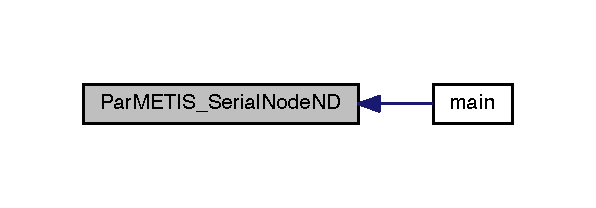
\includegraphics[width=286pt]{3rd_party_2parmetis-4_80_83_2include_2parmetis_8h_a8bd1a6399ac304da6616cb5329304df6_icgraph}
\end{center}
\end{figure}
\mbox{\Hypertarget{3rd_party_2parmetis-4_80_83_2include_2parmetis_8h_a1bbf9ca25d902b187988a49ccf435e2b}\label{3rd_party_2parmetis-4_80_83_2include_2parmetis_8h_a1bbf9ca25d902b187988a49ccf435e2b}} 
\index{3rd\+Party/parmetis-\/4.\+0.\+3/include/parmetis.\+h@{3rd\+Party/parmetis-\/4.\+0.\+3/include/parmetis.\+h}!Par\+M\+E\+T\+I\+S\+\_\+\+V32\+\_\+\+Node\+ND@{Par\+M\+E\+T\+I\+S\+\_\+\+V32\+\_\+\+Node\+ND}}
\index{Par\+M\+E\+T\+I\+S\+\_\+\+V32\+\_\+\+Node\+ND@{Par\+M\+E\+T\+I\+S\+\_\+\+V32\+\_\+\+Node\+ND}!3rd\+Party/parmetis-\/4.\+0.\+3/include/parmetis.\+h@{3rd\+Party/parmetis-\/4.\+0.\+3/include/parmetis.\+h}}
\subsubsection{\texorpdfstring{Par\+M\+E\+T\+I\+S\+\_\+\+V32\+\_\+\+Node\+N\+D()}{ParMETIS\_V32\_NodeND()}}
{\footnotesize\ttfamily int \hyperlink{include_2parmetis_8h_a238347d7669f8f1e9c83bfe63a2730c4}{\+\_\+\+\_\+cdecl} Par\+M\+E\+T\+I\+S\+\_\+\+V32\+\_\+\+Node\+ND (\begin{DoxyParamCaption}\item[{\hyperlink{3rd_party_2parmetis-4_80_83_2metis_2include_2metis_8h_aaa5262be3e700770163401acb0150f52}{idx\+\_\+t} $\ast$}]{vtxdist,  }\item[{\hyperlink{3rd_party_2parmetis-4_80_83_2metis_2include_2metis_8h_aaa5262be3e700770163401acb0150f52}{idx\+\_\+t} $\ast$}]{xadj,  }\item[{\hyperlink{3rd_party_2parmetis-4_80_83_2metis_2include_2metis_8h_aaa5262be3e700770163401acb0150f52}{idx\+\_\+t} $\ast$}]{adjncy,  }\item[{\hyperlink{3rd_party_2parmetis-4_80_83_2metis_2include_2metis_8h_aaa5262be3e700770163401acb0150f52}{idx\+\_\+t} $\ast$}]{vwgt,  }\item[{\hyperlink{3rd_party_2parmetis-4_80_83_2metis_2include_2metis_8h_aaa5262be3e700770163401acb0150f52}{idx\+\_\+t} $\ast$}]{numflag,  }\item[{\hyperlink{3rd_party_2parmetis-4_80_83_2metis_2include_2metis_8h_aaa5262be3e700770163401acb0150f52}{idx\+\_\+t} $\ast$}]{mtype,  }\item[{\hyperlink{3rd_party_2parmetis-4_80_83_2metis_2include_2metis_8h_aaa5262be3e700770163401acb0150f52}{idx\+\_\+t} $\ast$}]{rtype,  }\item[{\hyperlink{3rd_party_2parmetis-4_80_83_2metis_2include_2metis_8h_aaa5262be3e700770163401acb0150f52}{idx\+\_\+t} $\ast$}]{p\+\_\+nseps,  }\item[{\hyperlink{3rd_party_2parmetis-4_80_83_2metis_2include_2metis_8h_aaa5262be3e700770163401acb0150f52}{idx\+\_\+t} $\ast$}]{s\+\_\+nseps,  }\item[{\hyperlink{3rd_party_2parmetis-4_80_83_2metis_2include_2metis_8h_a1924a4f6907cc3833213aba1f07fcbe9}{real\+\_\+t} $\ast$}]{ubfrac,  }\item[{\hyperlink{3rd_party_2parmetis-4_80_83_2metis_2include_2metis_8h_aaa5262be3e700770163401acb0150f52}{idx\+\_\+t} $\ast$}]{seed,  }\item[{\hyperlink{3rd_party_2parmetis-4_80_83_2metis_2include_2metis_8h_aaa5262be3e700770163401acb0150f52}{idx\+\_\+t} $\ast$}]{dbglvl,  }\item[{\hyperlink{3rd_party_2parmetis-4_80_83_2metis_2include_2metis_8h_aaa5262be3e700770163401acb0150f52}{idx\+\_\+t} $\ast$}]{order,  }\item[{\hyperlink{3rd_party_2parmetis-4_80_83_2metis_2include_2metis_8h_aaa5262be3e700770163401acb0150f52}{idx\+\_\+t} $\ast$}]{sizes,  }\item[{M\+P\+I\+\_\+\+Comm $\ast$}]{comm }\end{DoxyParamCaption})}

Here is the caller graph for this function\+:\nopagebreak
\begin{figure}[H]
\begin{center}
\leavevmode
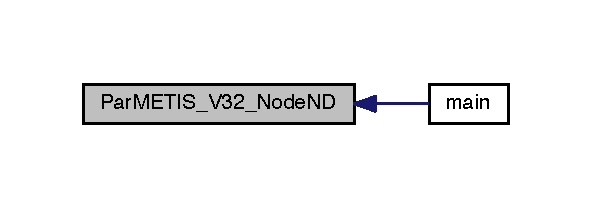
\includegraphics[width=284pt]{3rd_party_2parmetis-4_80_83_2include_2parmetis_8h_a1bbf9ca25d902b187988a49ccf435e2b_icgraph}
\end{center}
\end{figure}
\mbox{\Hypertarget{3rd_party_2parmetis-4_80_83_2include_2parmetis_8h_ac00c3da2cf618cbfa9158463a851491e}\label{3rd_party_2parmetis-4_80_83_2include_2parmetis_8h_ac00c3da2cf618cbfa9158463a851491e}} 
\index{3rd\+Party/parmetis-\/4.\+0.\+3/include/parmetis.\+h@{3rd\+Party/parmetis-\/4.\+0.\+3/include/parmetis.\+h}!Par\+M\+E\+T\+I\+S\+\_\+\+V3\+\_\+\+Adaptive\+Repart@{Par\+M\+E\+T\+I\+S\+\_\+\+V3\+\_\+\+Adaptive\+Repart}}
\index{Par\+M\+E\+T\+I\+S\+\_\+\+V3\+\_\+\+Adaptive\+Repart@{Par\+M\+E\+T\+I\+S\+\_\+\+V3\+\_\+\+Adaptive\+Repart}!3rd\+Party/parmetis-\/4.\+0.\+3/include/parmetis.\+h@{3rd\+Party/parmetis-\/4.\+0.\+3/include/parmetis.\+h}}
\subsubsection{\texorpdfstring{Par\+M\+E\+T\+I\+S\+\_\+\+V3\+\_\+\+Adaptive\+Repart()}{ParMETIS\_V3\_AdaptiveRepart()}}
{\footnotesize\ttfamily int \hyperlink{include_2parmetis_8h_a238347d7669f8f1e9c83bfe63a2730c4}{\+\_\+\+\_\+cdecl} Par\+M\+E\+T\+I\+S\+\_\+\+V3\+\_\+\+Adaptive\+Repart (\begin{DoxyParamCaption}\item[{\hyperlink{3rd_party_2parmetis-4_80_83_2metis_2include_2metis_8h_aaa5262be3e700770163401acb0150f52}{idx\+\_\+t} $\ast$}]{vtxdist,  }\item[{\hyperlink{3rd_party_2parmetis-4_80_83_2metis_2include_2metis_8h_aaa5262be3e700770163401acb0150f52}{idx\+\_\+t} $\ast$}]{xadj,  }\item[{\hyperlink{3rd_party_2parmetis-4_80_83_2metis_2include_2metis_8h_aaa5262be3e700770163401acb0150f52}{idx\+\_\+t} $\ast$}]{adjncy,  }\item[{\hyperlink{3rd_party_2parmetis-4_80_83_2metis_2include_2metis_8h_aaa5262be3e700770163401acb0150f52}{idx\+\_\+t} $\ast$}]{vwgt,  }\item[{\hyperlink{3rd_party_2parmetis-4_80_83_2metis_2include_2metis_8h_aaa5262be3e700770163401acb0150f52}{idx\+\_\+t} $\ast$}]{vsize,  }\item[{\hyperlink{3rd_party_2parmetis-4_80_83_2metis_2include_2metis_8h_aaa5262be3e700770163401acb0150f52}{idx\+\_\+t} $\ast$}]{adjwgt,  }\item[{\hyperlink{3rd_party_2parmetis-4_80_83_2metis_2include_2metis_8h_aaa5262be3e700770163401acb0150f52}{idx\+\_\+t} $\ast$}]{wgtflag,  }\item[{\hyperlink{3rd_party_2parmetis-4_80_83_2metis_2include_2metis_8h_aaa5262be3e700770163401acb0150f52}{idx\+\_\+t} $\ast$}]{numflag,  }\item[{\hyperlink{3rd_party_2parmetis-4_80_83_2metis_2include_2metis_8h_aaa5262be3e700770163401acb0150f52}{idx\+\_\+t} $\ast$}]{ncon,  }\item[{\hyperlink{3rd_party_2parmetis-4_80_83_2metis_2include_2metis_8h_aaa5262be3e700770163401acb0150f52}{idx\+\_\+t} $\ast$}]{nparts,  }\item[{\hyperlink{3rd_party_2parmetis-4_80_83_2metis_2include_2metis_8h_a1924a4f6907cc3833213aba1f07fcbe9}{real\+\_\+t} $\ast$}]{tpwgts,  }\item[{\hyperlink{3rd_party_2parmetis-4_80_83_2metis_2include_2metis_8h_a1924a4f6907cc3833213aba1f07fcbe9}{real\+\_\+t} $\ast$}]{ubvec,  }\item[{\hyperlink{3rd_party_2parmetis-4_80_83_2metis_2include_2metis_8h_a1924a4f6907cc3833213aba1f07fcbe9}{real\+\_\+t} $\ast$}]{ipc2redist,  }\item[{\hyperlink{3rd_party_2parmetis-4_80_83_2metis_2include_2metis_8h_aaa5262be3e700770163401acb0150f52}{idx\+\_\+t} $\ast$}]{options,  }\item[{\hyperlink{3rd_party_2parmetis-4_80_83_2metis_2include_2metis_8h_aaa5262be3e700770163401acb0150f52}{idx\+\_\+t} $\ast$}]{edgecut,  }\item[{\hyperlink{3rd_party_2parmetis-4_80_83_2metis_2include_2metis_8h_aaa5262be3e700770163401acb0150f52}{idx\+\_\+t} $\ast$}]{part,  }\item[{M\+P\+I\+\_\+\+Comm $\ast$}]{comm }\end{DoxyParamCaption})}

Here is the caller graph for this function\+:\nopagebreak
\begin{figure}[H]
\begin{center}
\leavevmode
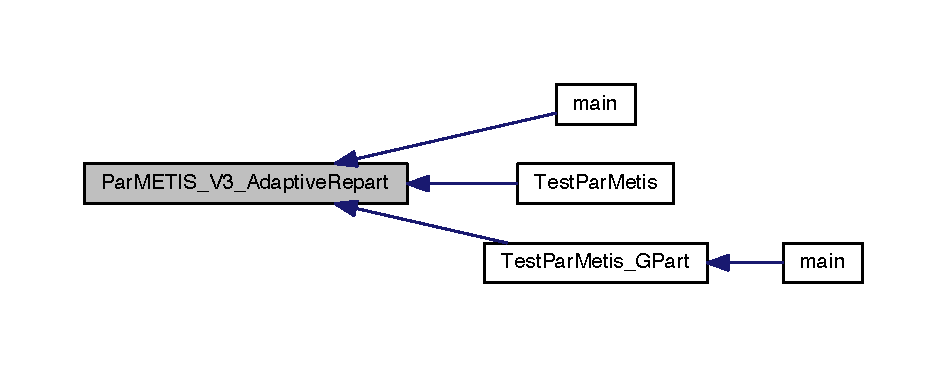
\includegraphics[width=350pt]{3rd_party_2parmetis-4_80_83_2include_2parmetis_8h_ac00c3da2cf618cbfa9158463a851491e_icgraph}
\end{center}
\end{figure}
\mbox{\Hypertarget{3rd_party_2parmetis-4_80_83_2include_2parmetis_8h_a2f9e316d7e0c46037cf231cd82cf9d97}\label{3rd_party_2parmetis-4_80_83_2include_2parmetis_8h_a2f9e316d7e0c46037cf231cd82cf9d97}} 
\index{3rd\+Party/parmetis-\/4.\+0.\+3/include/parmetis.\+h@{3rd\+Party/parmetis-\/4.\+0.\+3/include/parmetis.\+h}!Par\+M\+E\+T\+I\+S\+\_\+\+V3\+\_\+\+Mesh2\+Dual@{Par\+M\+E\+T\+I\+S\+\_\+\+V3\+\_\+\+Mesh2\+Dual}}
\index{Par\+M\+E\+T\+I\+S\+\_\+\+V3\+\_\+\+Mesh2\+Dual@{Par\+M\+E\+T\+I\+S\+\_\+\+V3\+\_\+\+Mesh2\+Dual}!3rd\+Party/parmetis-\/4.\+0.\+3/include/parmetis.\+h@{3rd\+Party/parmetis-\/4.\+0.\+3/include/parmetis.\+h}}
\subsubsection{\texorpdfstring{Par\+M\+E\+T\+I\+S\+\_\+\+V3\+\_\+\+Mesh2\+Dual()}{ParMETIS\_V3\_Mesh2Dual()}}
{\footnotesize\ttfamily int \hyperlink{include_2parmetis_8h_a238347d7669f8f1e9c83bfe63a2730c4}{\+\_\+\+\_\+cdecl} Par\+M\+E\+T\+I\+S\+\_\+\+V3\+\_\+\+Mesh2\+Dual (\begin{DoxyParamCaption}\item[{\hyperlink{3rd_party_2parmetis-4_80_83_2metis_2include_2metis_8h_aaa5262be3e700770163401acb0150f52}{idx\+\_\+t} $\ast$}]{elmdist,  }\item[{\hyperlink{3rd_party_2parmetis-4_80_83_2metis_2include_2metis_8h_aaa5262be3e700770163401acb0150f52}{idx\+\_\+t} $\ast$}]{eptr,  }\item[{\hyperlink{3rd_party_2parmetis-4_80_83_2metis_2include_2metis_8h_aaa5262be3e700770163401acb0150f52}{idx\+\_\+t} $\ast$}]{eind,  }\item[{\hyperlink{3rd_party_2parmetis-4_80_83_2metis_2include_2metis_8h_aaa5262be3e700770163401acb0150f52}{idx\+\_\+t} $\ast$}]{numflag,  }\item[{\hyperlink{3rd_party_2parmetis-4_80_83_2metis_2include_2metis_8h_aaa5262be3e700770163401acb0150f52}{idx\+\_\+t} $\ast$}]{ncommonnodes,  }\item[{\hyperlink{3rd_party_2parmetis-4_80_83_2metis_2include_2metis_8h_aaa5262be3e700770163401acb0150f52}{idx\+\_\+t} $\ast$$\ast$}]{xadj,  }\item[{\hyperlink{3rd_party_2parmetis-4_80_83_2metis_2include_2metis_8h_aaa5262be3e700770163401acb0150f52}{idx\+\_\+t} $\ast$$\ast$}]{adjncy,  }\item[{M\+P\+I\+\_\+\+Comm $\ast$}]{comm }\end{DoxyParamCaption})}

Here is the caller graph for this function\+:\nopagebreak
\begin{figure}[H]
\begin{center}
\leavevmode
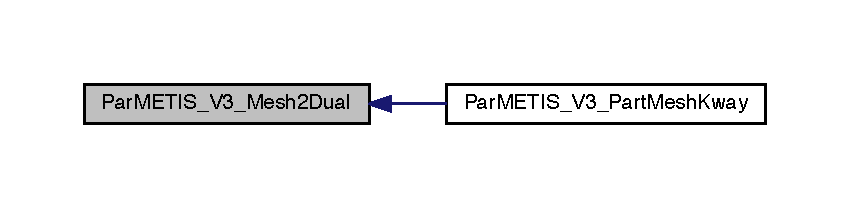
\includegraphics[width=350pt]{3rd_party_2parmetis-4_80_83_2include_2parmetis_8h_a2f9e316d7e0c46037cf231cd82cf9d97_icgraph}
\end{center}
\end{figure}
\mbox{\Hypertarget{3rd_party_2parmetis-4_80_83_2include_2parmetis_8h_add23df29b4f232ac4c2cca94cc083a32}\label{3rd_party_2parmetis-4_80_83_2include_2parmetis_8h_add23df29b4f232ac4c2cca94cc083a32}} 
\index{3rd\+Party/parmetis-\/4.\+0.\+3/include/parmetis.\+h@{3rd\+Party/parmetis-\/4.\+0.\+3/include/parmetis.\+h}!Par\+M\+E\+T\+I\+S\+\_\+\+V3\+\_\+\+Node\+ND@{Par\+M\+E\+T\+I\+S\+\_\+\+V3\+\_\+\+Node\+ND}}
\index{Par\+M\+E\+T\+I\+S\+\_\+\+V3\+\_\+\+Node\+ND@{Par\+M\+E\+T\+I\+S\+\_\+\+V3\+\_\+\+Node\+ND}!3rd\+Party/parmetis-\/4.\+0.\+3/include/parmetis.\+h@{3rd\+Party/parmetis-\/4.\+0.\+3/include/parmetis.\+h}}
\subsubsection{\texorpdfstring{Par\+M\+E\+T\+I\+S\+\_\+\+V3\+\_\+\+Node\+N\+D()}{ParMETIS\_V3\_NodeND()}}
{\footnotesize\ttfamily int \hyperlink{include_2parmetis_8h_a238347d7669f8f1e9c83bfe63a2730c4}{\+\_\+\+\_\+cdecl} Par\+M\+E\+T\+I\+S\+\_\+\+V3\+\_\+\+Node\+ND (\begin{DoxyParamCaption}\item[{\hyperlink{3rd_party_2parmetis-4_80_83_2metis_2include_2metis_8h_aaa5262be3e700770163401acb0150f52}{idx\+\_\+t} $\ast$}]{vtxdist,  }\item[{\hyperlink{3rd_party_2parmetis-4_80_83_2metis_2include_2metis_8h_aaa5262be3e700770163401acb0150f52}{idx\+\_\+t} $\ast$}]{xadj,  }\item[{\hyperlink{3rd_party_2parmetis-4_80_83_2metis_2include_2metis_8h_aaa5262be3e700770163401acb0150f52}{idx\+\_\+t} $\ast$}]{adjncy,  }\item[{\hyperlink{3rd_party_2parmetis-4_80_83_2metis_2include_2metis_8h_aaa5262be3e700770163401acb0150f52}{idx\+\_\+t} $\ast$}]{numflag,  }\item[{\hyperlink{3rd_party_2parmetis-4_80_83_2metis_2include_2metis_8h_aaa5262be3e700770163401acb0150f52}{idx\+\_\+t} $\ast$}]{options,  }\item[{\hyperlink{3rd_party_2parmetis-4_80_83_2metis_2include_2metis_8h_aaa5262be3e700770163401acb0150f52}{idx\+\_\+t} $\ast$}]{order,  }\item[{\hyperlink{3rd_party_2parmetis-4_80_83_2metis_2include_2metis_8h_aaa5262be3e700770163401acb0150f52}{idx\+\_\+t} $\ast$}]{sizes,  }\item[{M\+P\+I\+\_\+\+Comm $\ast$}]{comm }\end{DoxyParamCaption})}

Here is the caller graph for this function\+:\nopagebreak
\begin{figure}[H]
\begin{center}
\leavevmode
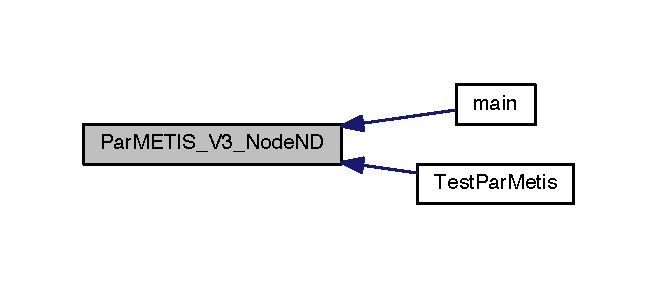
\includegraphics[width=316pt]{3rd_party_2parmetis-4_80_83_2include_2parmetis_8h_add23df29b4f232ac4c2cca94cc083a32_icgraph}
\end{center}
\end{figure}
\mbox{\Hypertarget{3rd_party_2parmetis-4_80_83_2include_2parmetis_8h_aab31b6450a3228063206eddded9de65e}\label{3rd_party_2parmetis-4_80_83_2include_2parmetis_8h_aab31b6450a3228063206eddded9de65e}} 
\index{3rd\+Party/parmetis-\/4.\+0.\+3/include/parmetis.\+h@{3rd\+Party/parmetis-\/4.\+0.\+3/include/parmetis.\+h}!Par\+M\+E\+T\+I\+S\+\_\+\+V3\+\_\+\+Part\+Geom@{Par\+M\+E\+T\+I\+S\+\_\+\+V3\+\_\+\+Part\+Geom}}
\index{Par\+M\+E\+T\+I\+S\+\_\+\+V3\+\_\+\+Part\+Geom@{Par\+M\+E\+T\+I\+S\+\_\+\+V3\+\_\+\+Part\+Geom}!3rd\+Party/parmetis-\/4.\+0.\+3/include/parmetis.\+h@{3rd\+Party/parmetis-\/4.\+0.\+3/include/parmetis.\+h}}
\subsubsection{\texorpdfstring{Par\+M\+E\+T\+I\+S\+\_\+\+V3\+\_\+\+Part\+Geom()}{ParMETIS\_V3\_PartGeom()}}
{\footnotesize\ttfamily int \hyperlink{include_2parmetis_8h_a238347d7669f8f1e9c83bfe63a2730c4}{\+\_\+\+\_\+cdecl} Par\+M\+E\+T\+I\+S\+\_\+\+V3\+\_\+\+Part\+Geom (\begin{DoxyParamCaption}\item[{\hyperlink{3rd_party_2parmetis-4_80_83_2metis_2include_2metis_8h_aaa5262be3e700770163401acb0150f52}{idx\+\_\+t} $\ast$}]{vtxdist,  }\item[{\hyperlink{3rd_party_2parmetis-4_80_83_2metis_2include_2metis_8h_aaa5262be3e700770163401acb0150f52}{idx\+\_\+t} $\ast$}]{ndims,  }\item[{\hyperlink{3rd_party_2parmetis-4_80_83_2metis_2include_2metis_8h_a1924a4f6907cc3833213aba1f07fcbe9}{real\+\_\+t} $\ast$}]{xyz,  }\item[{\hyperlink{3rd_party_2parmetis-4_80_83_2metis_2include_2metis_8h_aaa5262be3e700770163401acb0150f52}{idx\+\_\+t} $\ast$}]{part,  }\item[{M\+P\+I\+\_\+\+Comm $\ast$}]{comm }\end{DoxyParamCaption})}

Here is the caller graph for this function\+:\nopagebreak
\begin{figure}[H]
\begin{center}
\leavevmode
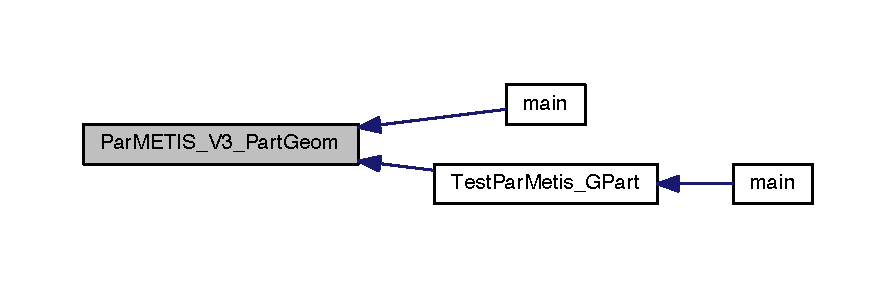
\includegraphics[width=350pt]{3rd_party_2parmetis-4_80_83_2include_2parmetis_8h_aab31b6450a3228063206eddded9de65e_icgraph}
\end{center}
\end{figure}
\mbox{\Hypertarget{3rd_party_2parmetis-4_80_83_2include_2parmetis_8h_a6df93293cf3d1ccb4659bd1b3091623d}\label{3rd_party_2parmetis-4_80_83_2include_2parmetis_8h_a6df93293cf3d1ccb4659bd1b3091623d}} 
\index{3rd\+Party/parmetis-\/4.\+0.\+3/include/parmetis.\+h@{3rd\+Party/parmetis-\/4.\+0.\+3/include/parmetis.\+h}!Par\+M\+E\+T\+I\+S\+\_\+\+V3\+\_\+\+Part\+Geom\+Kway@{Par\+M\+E\+T\+I\+S\+\_\+\+V3\+\_\+\+Part\+Geom\+Kway}}
\index{Par\+M\+E\+T\+I\+S\+\_\+\+V3\+\_\+\+Part\+Geom\+Kway@{Par\+M\+E\+T\+I\+S\+\_\+\+V3\+\_\+\+Part\+Geom\+Kway}!3rd\+Party/parmetis-\/4.\+0.\+3/include/parmetis.\+h@{3rd\+Party/parmetis-\/4.\+0.\+3/include/parmetis.\+h}}
\subsubsection{\texorpdfstring{Par\+M\+E\+T\+I\+S\+\_\+\+V3\+\_\+\+Part\+Geom\+Kway()}{ParMETIS\_V3\_PartGeomKway()}}
{\footnotesize\ttfamily int \hyperlink{include_2parmetis_8h_a238347d7669f8f1e9c83bfe63a2730c4}{\+\_\+\+\_\+cdecl} Par\+M\+E\+T\+I\+S\+\_\+\+V3\+\_\+\+Part\+Geom\+Kway (\begin{DoxyParamCaption}\item[{\hyperlink{3rd_party_2parmetis-4_80_83_2metis_2include_2metis_8h_aaa5262be3e700770163401acb0150f52}{idx\+\_\+t} $\ast$}]{vtxdist,  }\item[{\hyperlink{3rd_party_2parmetis-4_80_83_2metis_2include_2metis_8h_aaa5262be3e700770163401acb0150f52}{idx\+\_\+t} $\ast$}]{xadj,  }\item[{\hyperlink{3rd_party_2parmetis-4_80_83_2metis_2include_2metis_8h_aaa5262be3e700770163401acb0150f52}{idx\+\_\+t} $\ast$}]{adjncy,  }\item[{\hyperlink{3rd_party_2parmetis-4_80_83_2metis_2include_2metis_8h_aaa5262be3e700770163401acb0150f52}{idx\+\_\+t} $\ast$}]{vwgt,  }\item[{\hyperlink{3rd_party_2parmetis-4_80_83_2metis_2include_2metis_8h_aaa5262be3e700770163401acb0150f52}{idx\+\_\+t} $\ast$}]{adjwgt,  }\item[{\hyperlink{3rd_party_2parmetis-4_80_83_2metis_2include_2metis_8h_aaa5262be3e700770163401acb0150f52}{idx\+\_\+t} $\ast$}]{wgtflag,  }\item[{\hyperlink{3rd_party_2parmetis-4_80_83_2metis_2include_2metis_8h_aaa5262be3e700770163401acb0150f52}{idx\+\_\+t} $\ast$}]{numflag,  }\item[{\hyperlink{3rd_party_2parmetis-4_80_83_2metis_2include_2metis_8h_aaa5262be3e700770163401acb0150f52}{idx\+\_\+t} $\ast$}]{ndims,  }\item[{\hyperlink{3rd_party_2parmetis-4_80_83_2metis_2include_2metis_8h_a1924a4f6907cc3833213aba1f07fcbe9}{real\+\_\+t} $\ast$}]{xyz,  }\item[{\hyperlink{3rd_party_2parmetis-4_80_83_2metis_2include_2metis_8h_aaa5262be3e700770163401acb0150f52}{idx\+\_\+t} $\ast$}]{ncon,  }\item[{\hyperlink{3rd_party_2parmetis-4_80_83_2metis_2include_2metis_8h_aaa5262be3e700770163401acb0150f52}{idx\+\_\+t} $\ast$}]{nparts,  }\item[{\hyperlink{3rd_party_2parmetis-4_80_83_2metis_2include_2metis_8h_a1924a4f6907cc3833213aba1f07fcbe9}{real\+\_\+t} $\ast$}]{tpwgts,  }\item[{\hyperlink{3rd_party_2parmetis-4_80_83_2metis_2include_2metis_8h_a1924a4f6907cc3833213aba1f07fcbe9}{real\+\_\+t} $\ast$}]{ubvec,  }\item[{\hyperlink{3rd_party_2parmetis-4_80_83_2metis_2include_2metis_8h_aaa5262be3e700770163401acb0150f52}{idx\+\_\+t} $\ast$}]{options,  }\item[{\hyperlink{3rd_party_2parmetis-4_80_83_2metis_2include_2metis_8h_aaa5262be3e700770163401acb0150f52}{idx\+\_\+t} $\ast$}]{edgecut,  }\item[{\hyperlink{3rd_party_2parmetis-4_80_83_2metis_2include_2metis_8h_aaa5262be3e700770163401acb0150f52}{idx\+\_\+t} $\ast$}]{part,  }\item[{M\+P\+I\+\_\+\+Comm $\ast$}]{comm }\end{DoxyParamCaption})}

Here is the caller graph for this function\+:\nopagebreak
\begin{figure}[H]
\begin{center}
\leavevmode
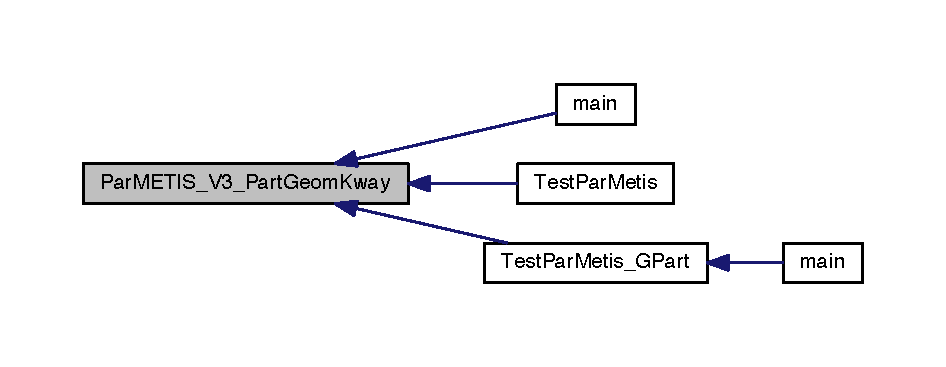
\includegraphics[width=350pt]{3rd_party_2parmetis-4_80_83_2include_2parmetis_8h_a6df93293cf3d1ccb4659bd1b3091623d_icgraph}
\end{center}
\end{figure}
\mbox{\Hypertarget{3rd_party_2parmetis-4_80_83_2include_2parmetis_8h_af418d1e76eaf4f80116da4caf51bd54e}\label{3rd_party_2parmetis-4_80_83_2include_2parmetis_8h_af418d1e76eaf4f80116da4caf51bd54e}} 
\index{3rd\+Party/parmetis-\/4.\+0.\+3/include/parmetis.\+h@{3rd\+Party/parmetis-\/4.\+0.\+3/include/parmetis.\+h}!Par\+M\+E\+T\+I\+S\+\_\+\+V3\+\_\+\+Part\+Kway@{Par\+M\+E\+T\+I\+S\+\_\+\+V3\+\_\+\+Part\+Kway}}
\index{Par\+M\+E\+T\+I\+S\+\_\+\+V3\+\_\+\+Part\+Kway@{Par\+M\+E\+T\+I\+S\+\_\+\+V3\+\_\+\+Part\+Kway}!3rd\+Party/parmetis-\/4.\+0.\+3/include/parmetis.\+h@{3rd\+Party/parmetis-\/4.\+0.\+3/include/parmetis.\+h}}
\subsubsection{\texorpdfstring{Par\+M\+E\+T\+I\+S\+\_\+\+V3\+\_\+\+Part\+Kway()}{ParMETIS\_V3\_PartKway()}}
{\footnotesize\ttfamily int \hyperlink{include_2parmetis_8h_a238347d7669f8f1e9c83bfe63a2730c4}{\+\_\+\+\_\+cdecl} Par\+M\+E\+T\+I\+S\+\_\+\+V3\+\_\+\+Part\+Kway (\begin{DoxyParamCaption}\item[{\hyperlink{3rd_party_2parmetis-4_80_83_2metis_2include_2metis_8h_aaa5262be3e700770163401acb0150f52}{idx\+\_\+t} $\ast$}]{vtxdist,  }\item[{\hyperlink{3rd_party_2parmetis-4_80_83_2metis_2include_2metis_8h_aaa5262be3e700770163401acb0150f52}{idx\+\_\+t} $\ast$}]{xadj,  }\item[{\hyperlink{3rd_party_2parmetis-4_80_83_2metis_2include_2metis_8h_aaa5262be3e700770163401acb0150f52}{idx\+\_\+t} $\ast$}]{adjncy,  }\item[{\hyperlink{3rd_party_2parmetis-4_80_83_2metis_2include_2metis_8h_aaa5262be3e700770163401acb0150f52}{idx\+\_\+t} $\ast$}]{vwgt,  }\item[{\hyperlink{3rd_party_2parmetis-4_80_83_2metis_2include_2metis_8h_aaa5262be3e700770163401acb0150f52}{idx\+\_\+t} $\ast$}]{adjwgt,  }\item[{\hyperlink{3rd_party_2parmetis-4_80_83_2metis_2include_2metis_8h_aaa5262be3e700770163401acb0150f52}{idx\+\_\+t} $\ast$}]{wgtflag,  }\item[{\hyperlink{3rd_party_2parmetis-4_80_83_2metis_2include_2metis_8h_aaa5262be3e700770163401acb0150f52}{idx\+\_\+t} $\ast$}]{numflag,  }\item[{\hyperlink{3rd_party_2parmetis-4_80_83_2metis_2include_2metis_8h_aaa5262be3e700770163401acb0150f52}{idx\+\_\+t} $\ast$}]{ncon,  }\item[{\hyperlink{3rd_party_2parmetis-4_80_83_2metis_2include_2metis_8h_aaa5262be3e700770163401acb0150f52}{idx\+\_\+t} $\ast$}]{nparts,  }\item[{\hyperlink{3rd_party_2parmetis-4_80_83_2metis_2include_2metis_8h_a1924a4f6907cc3833213aba1f07fcbe9}{real\+\_\+t} $\ast$}]{tpwgts,  }\item[{\hyperlink{3rd_party_2parmetis-4_80_83_2metis_2include_2metis_8h_a1924a4f6907cc3833213aba1f07fcbe9}{real\+\_\+t} $\ast$}]{ubvec,  }\item[{\hyperlink{3rd_party_2parmetis-4_80_83_2metis_2include_2metis_8h_aaa5262be3e700770163401acb0150f52}{idx\+\_\+t} $\ast$}]{options,  }\item[{\hyperlink{3rd_party_2parmetis-4_80_83_2metis_2include_2metis_8h_aaa5262be3e700770163401acb0150f52}{idx\+\_\+t} $\ast$}]{edgecut,  }\item[{\hyperlink{3rd_party_2parmetis-4_80_83_2metis_2include_2metis_8h_aaa5262be3e700770163401acb0150f52}{idx\+\_\+t} $\ast$}]{part,  }\item[{M\+P\+I\+\_\+\+Comm $\ast$}]{comm }\end{DoxyParamCaption})}

Here is the caller graph for this function\+:\nopagebreak
\begin{figure}[H]
\begin{center}
\leavevmode
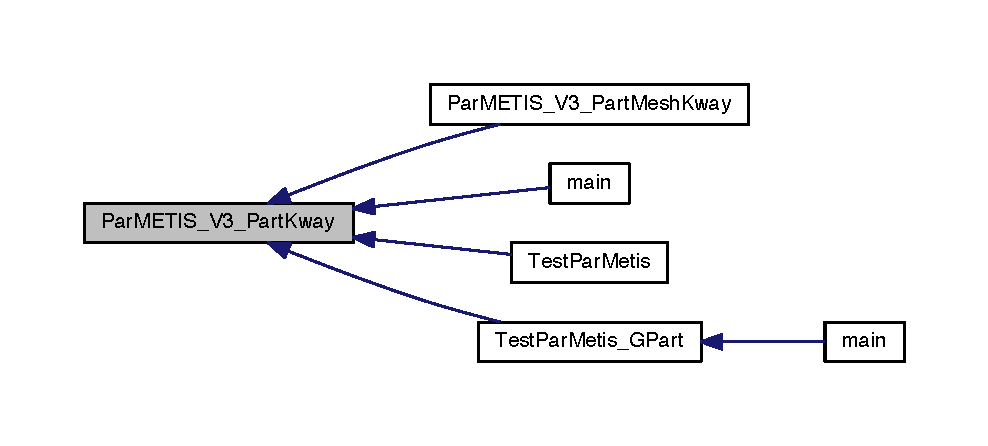
\includegraphics[width=350pt]{3rd_party_2parmetis-4_80_83_2include_2parmetis_8h_af418d1e76eaf4f80116da4caf51bd54e_icgraph}
\end{center}
\end{figure}
\mbox{\Hypertarget{3rd_party_2parmetis-4_80_83_2include_2parmetis_8h_a2ae9750ec09afdc4243b7cb7c5118666}\label{3rd_party_2parmetis-4_80_83_2include_2parmetis_8h_a2ae9750ec09afdc4243b7cb7c5118666}} 
\index{3rd\+Party/parmetis-\/4.\+0.\+3/include/parmetis.\+h@{3rd\+Party/parmetis-\/4.\+0.\+3/include/parmetis.\+h}!Par\+M\+E\+T\+I\+S\+\_\+\+V3\+\_\+\+Part\+Mesh\+Kway@{Par\+M\+E\+T\+I\+S\+\_\+\+V3\+\_\+\+Part\+Mesh\+Kway}}
\index{Par\+M\+E\+T\+I\+S\+\_\+\+V3\+\_\+\+Part\+Mesh\+Kway@{Par\+M\+E\+T\+I\+S\+\_\+\+V3\+\_\+\+Part\+Mesh\+Kway}!3rd\+Party/parmetis-\/4.\+0.\+3/include/parmetis.\+h@{3rd\+Party/parmetis-\/4.\+0.\+3/include/parmetis.\+h}}
\subsubsection{\texorpdfstring{Par\+M\+E\+T\+I\+S\+\_\+\+V3\+\_\+\+Part\+Mesh\+Kway()}{ParMETIS\_V3\_PartMeshKway()}}
{\footnotesize\ttfamily int \hyperlink{include_2parmetis_8h_a238347d7669f8f1e9c83bfe63a2730c4}{\+\_\+\+\_\+cdecl} Par\+M\+E\+T\+I\+S\+\_\+\+V3\+\_\+\+Part\+Mesh\+Kway (\begin{DoxyParamCaption}\item[{\hyperlink{3rd_party_2parmetis-4_80_83_2metis_2include_2metis_8h_aaa5262be3e700770163401acb0150f52}{idx\+\_\+t} $\ast$}]{elmdist,  }\item[{\hyperlink{3rd_party_2parmetis-4_80_83_2metis_2include_2metis_8h_aaa5262be3e700770163401acb0150f52}{idx\+\_\+t} $\ast$}]{eptr,  }\item[{\hyperlink{3rd_party_2parmetis-4_80_83_2metis_2include_2metis_8h_aaa5262be3e700770163401acb0150f52}{idx\+\_\+t} $\ast$}]{eind,  }\item[{\hyperlink{3rd_party_2parmetis-4_80_83_2metis_2include_2metis_8h_aaa5262be3e700770163401acb0150f52}{idx\+\_\+t} $\ast$}]{elmwgt,  }\item[{\hyperlink{3rd_party_2parmetis-4_80_83_2metis_2include_2metis_8h_aaa5262be3e700770163401acb0150f52}{idx\+\_\+t} $\ast$}]{wgtflag,  }\item[{\hyperlink{3rd_party_2parmetis-4_80_83_2metis_2include_2metis_8h_aaa5262be3e700770163401acb0150f52}{idx\+\_\+t} $\ast$}]{numflag,  }\item[{\hyperlink{3rd_party_2parmetis-4_80_83_2metis_2include_2metis_8h_aaa5262be3e700770163401acb0150f52}{idx\+\_\+t} $\ast$}]{ncon,  }\item[{\hyperlink{3rd_party_2parmetis-4_80_83_2metis_2include_2metis_8h_aaa5262be3e700770163401acb0150f52}{idx\+\_\+t} $\ast$}]{ncommonnodes,  }\item[{\hyperlink{3rd_party_2parmetis-4_80_83_2metis_2include_2metis_8h_aaa5262be3e700770163401acb0150f52}{idx\+\_\+t} $\ast$}]{nparts,  }\item[{\hyperlink{3rd_party_2parmetis-4_80_83_2metis_2include_2metis_8h_a1924a4f6907cc3833213aba1f07fcbe9}{real\+\_\+t} $\ast$}]{tpwgts,  }\item[{\hyperlink{3rd_party_2parmetis-4_80_83_2metis_2include_2metis_8h_a1924a4f6907cc3833213aba1f07fcbe9}{real\+\_\+t} $\ast$}]{ubvec,  }\item[{\hyperlink{3rd_party_2parmetis-4_80_83_2metis_2include_2metis_8h_aaa5262be3e700770163401acb0150f52}{idx\+\_\+t} $\ast$}]{options,  }\item[{\hyperlink{3rd_party_2parmetis-4_80_83_2metis_2include_2metis_8h_aaa5262be3e700770163401acb0150f52}{idx\+\_\+t} $\ast$}]{edgecut,  }\item[{\hyperlink{3rd_party_2parmetis-4_80_83_2metis_2include_2metis_8h_aaa5262be3e700770163401acb0150f52}{idx\+\_\+t} $\ast$}]{part,  }\item[{M\+P\+I\+\_\+\+Comm $\ast$}]{comm }\end{DoxyParamCaption})}

Here is the caller graph for this function\+:\nopagebreak
\begin{figure}[H]
\begin{center}
\leavevmode
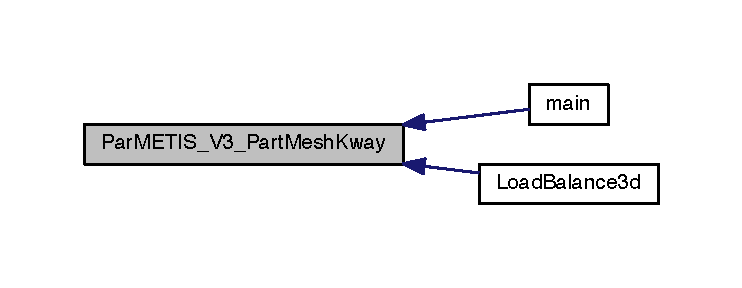
\includegraphics[width=350pt]{3rd_party_2parmetis-4_80_83_2include_2parmetis_8h_a2ae9750ec09afdc4243b7cb7c5118666_icgraph}
\end{center}
\end{figure}
\mbox{\Hypertarget{3rd_party_2parmetis-4_80_83_2include_2parmetis_8h_ad40a7809c9bdf183926da011220bad75}\label{3rd_party_2parmetis-4_80_83_2include_2parmetis_8h_ad40a7809c9bdf183926da011220bad75}} 
\index{3rd\+Party/parmetis-\/4.\+0.\+3/include/parmetis.\+h@{3rd\+Party/parmetis-\/4.\+0.\+3/include/parmetis.\+h}!Par\+M\+E\+T\+I\+S\+\_\+\+V3\+\_\+\+Refine\+Kway@{Par\+M\+E\+T\+I\+S\+\_\+\+V3\+\_\+\+Refine\+Kway}}
\index{Par\+M\+E\+T\+I\+S\+\_\+\+V3\+\_\+\+Refine\+Kway@{Par\+M\+E\+T\+I\+S\+\_\+\+V3\+\_\+\+Refine\+Kway}!3rd\+Party/parmetis-\/4.\+0.\+3/include/parmetis.\+h@{3rd\+Party/parmetis-\/4.\+0.\+3/include/parmetis.\+h}}
\subsubsection{\texorpdfstring{Par\+M\+E\+T\+I\+S\+\_\+\+V3\+\_\+\+Refine\+Kway()}{ParMETIS\_V3\_RefineKway()}}
{\footnotesize\ttfamily int \hyperlink{include_2parmetis_8h_a238347d7669f8f1e9c83bfe63a2730c4}{\+\_\+\+\_\+cdecl} Par\+M\+E\+T\+I\+S\+\_\+\+V3\+\_\+\+Refine\+Kway (\begin{DoxyParamCaption}\item[{\hyperlink{3rd_party_2parmetis-4_80_83_2metis_2include_2metis_8h_aaa5262be3e700770163401acb0150f52}{idx\+\_\+t} $\ast$}]{vtxdist,  }\item[{\hyperlink{3rd_party_2parmetis-4_80_83_2metis_2include_2metis_8h_aaa5262be3e700770163401acb0150f52}{idx\+\_\+t} $\ast$}]{xadj,  }\item[{\hyperlink{3rd_party_2parmetis-4_80_83_2metis_2include_2metis_8h_aaa5262be3e700770163401acb0150f52}{idx\+\_\+t} $\ast$}]{adjncy,  }\item[{\hyperlink{3rd_party_2parmetis-4_80_83_2metis_2include_2metis_8h_aaa5262be3e700770163401acb0150f52}{idx\+\_\+t} $\ast$}]{vwgt,  }\item[{\hyperlink{3rd_party_2parmetis-4_80_83_2metis_2include_2metis_8h_aaa5262be3e700770163401acb0150f52}{idx\+\_\+t} $\ast$}]{adjwgt,  }\item[{\hyperlink{3rd_party_2parmetis-4_80_83_2metis_2include_2metis_8h_aaa5262be3e700770163401acb0150f52}{idx\+\_\+t} $\ast$}]{wgtflag,  }\item[{\hyperlink{3rd_party_2parmetis-4_80_83_2metis_2include_2metis_8h_aaa5262be3e700770163401acb0150f52}{idx\+\_\+t} $\ast$}]{numflag,  }\item[{\hyperlink{3rd_party_2parmetis-4_80_83_2metis_2include_2metis_8h_aaa5262be3e700770163401acb0150f52}{idx\+\_\+t} $\ast$}]{ncon,  }\item[{\hyperlink{3rd_party_2parmetis-4_80_83_2metis_2include_2metis_8h_aaa5262be3e700770163401acb0150f52}{idx\+\_\+t} $\ast$}]{nparts,  }\item[{\hyperlink{3rd_party_2parmetis-4_80_83_2metis_2include_2metis_8h_a1924a4f6907cc3833213aba1f07fcbe9}{real\+\_\+t} $\ast$}]{tpwgts,  }\item[{\hyperlink{3rd_party_2parmetis-4_80_83_2metis_2include_2metis_8h_a1924a4f6907cc3833213aba1f07fcbe9}{real\+\_\+t} $\ast$}]{ubvec,  }\item[{\hyperlink{3rd_party_2parmetis-4_80_83_2metis_2include_2metis_8h_aaa5262be3e700770163401acb0150f52}{idx\+\_\+t} $\ast$}]{options,  }\item[{\hyperlink{3rd_party_2parmetis-4_80_83_2metis_2include_2metis_8h_aaa5262be3e700770163401acb0150f52}{idx\+\_\+t} $\ast$}]{edgecut,  }\item[{\hyperlink{3rd_party_2parmetis-4_80_83_2metis_2include_2metis_8h_aaa5262be3e700770163401acb0150f52}{idx\+\_\+t} $\ast$}]{part,  }\item[{M\+P\+I\+\_\+\+Comm $\ast$}]{comm }\end{DoxyParamCaption})}

Here is the caller graph for this function\+:\nopagebreak
\begin{figure}[H]
\begin{center}
\leavevmode
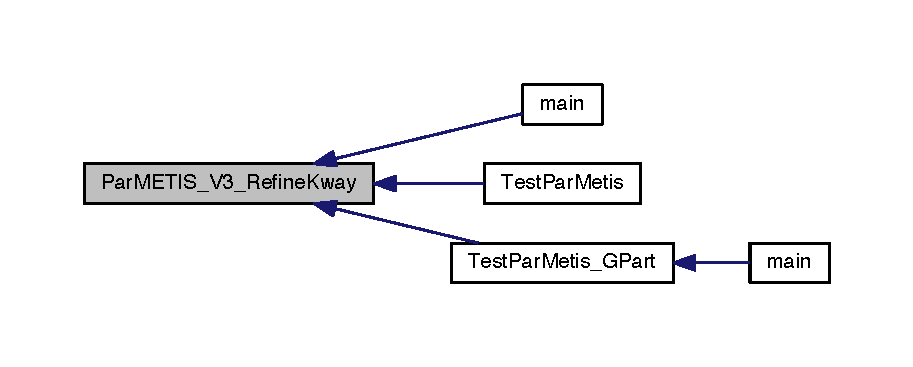
\includegraphics[width=350pt]{3rd_party_2parmetis-4_80_83_2include_2parmetis_8h_ad40a7809c9bdf183926da011220bad75_icgraph}
\end{center}
\end{figure}

\hypertarget{include_2parmetis_8h}{}\section{include/parmetis.h File Reference}
\label{include_2parmetis_8h}\index{include/parmetis.\+h@{include/parmetis.\+h}}
{\ttfamily \#include $<$mpi.\+h$>$}\newline
{\ttfamily \#include $<$metis.\+h$>$}\newline
Include dependency graph for parmetis.\+h\+:\nopagebreak
\begin{figure}[H]
\begin{center}
\leavevmode
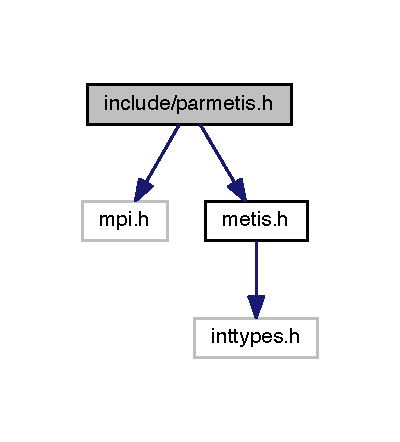
\includegraphics[width=192pt]{include_2parmetis_8h__incl}
\end{center}
\end{figure}
This graph shows which files directly or indirectly include this file\+:\nopagebreak
\begin{figure}[H]
\begin{center}
\leavevmode

\includegraphics[width=350pt]{include_2parmetis_8h__dep__incl}
\end{center}
\end{figure}
\subsection*{Macros}
\begin{DoxyCompactItemize}
\item 
\#define \hyperlink{include_2parmetis_8h_a238347d7669f8f1e9c83bfe63a2730c4}{\+\_\+\+\_\+cdecl}
\item 
\#define \hyperlink{include_2parmetis_8h_abe38a42aa75cd5998368d69cbad731a9}{I\+D\+X\+\_\+T}~M\+P\+I\+\_\+\+I\+NT
\item 
\#define \hyperlink{include_2parmetis_8h_a428068e8f33ae169d4d9516102bd863c}{K\+E\+E\+P\+\_\+\+B\+IT}~0x40000000L
\item 
\#define \hyperlink{include_2parmetis_8h_aad262b5311ae7d2166c3fcaa58d1834b}{R\+E\+A\+L\+\_\+T}~M\+P\+I\+\_\+\+F\+L\+O\+AT
\item 
\#define \hyperlink{include_2parmetis_8h_aa48ba987f3ff8d56871c3fb2bed6d314}{P\+A\+R\+M\+E\+T\+I\+S\+\_\+\+M\+A\+J\+O\+R\+\_\+\+V\+E\+R\+S\+I\+ON}~4
\item 
\#define \hyperlink{include_2parmetis_8h_ad51bc57fc5083572dd337e204de625ff}{P\+A\+R\+M\+E\+T\+I\+S\+\_\+\+M\+I\+N\+O\+R\+\_\+\+V\+E\+R\+S\+I\+ON}~0
\item 
\#define \hyperlink{include_2parmetis_8h_a1d99bc97bff12181a8ad9588069a1f41}{P\+A\+R\+M\+E\+T\+I\+S\+\_\+\+S\+U\+B\+M\+I\+N\+O\+R\+\_\+\+V\+E\+R\+S\+I\+ON}~3
\item 
\#define \hyperlink{include_2parmetis_8h_a8688bf16d43a979a690cef51e4e57d48}{P\+A\+R\+M\+E\+T\+I\+S\+\_\+\+M\+T\+Y\+P\+E\+\_\+\+L\+O\+C\+AL}~1    /$\ast$ Restrict matching to within processor vertices $\ast$/
\item 
\#define \hyperlink{include_2parmetis_8h_af25d77131e25b013f79a5a7644c5792f}{P\+A\+R\+M\+E\+T\+I\+S\+\_\+\+M\+T\+Y\+P\+E\+\_\+\+G\+L\+O\+B\+AL}~2    /$\ast$ Remote vertices can be matched $\ast$/
\item 
\#define \hyperlink{include_2parmetis_8h_ac0d490032ded504c8022884265a11546}{P\+A\+R\+M\+E\+T\+I\+S\+\_\+\+S\+R\+T\+Y\+P\+E\+\_\+\+G\+R\+E\+E\+DY}~1    /$\ast$ Vertices are visted from highest to lowest gain $\ast$/
\item 
\#define \hyperlink{include_2parmetis_8h_a614e5181ee41475b1ffde007468e0526}{P\+A\+R\+M\+E\+T\+I\+S\+\_\+\+S\+R\+T\+Y\+P\+E\+\_\+2\+P\+H\+A\+SE}
\item 
\#define \hyperlink{include_2parmetis_8h_a4703e7e2556a1a53794358fc85b8c103}{P\+A\+R\+M\+E\+T\+I\+S\+\_\+\+P\+S\+R\+\_\+\+C\+O\+U\+P\+L\+ED}~1    /$\ast$ \# of partitions == \# of processors $\ast$/
\item 
\#define \hyperlink{include_2parmetis_8h_a0462a45a6c6bafa94c1327994fd3d9bd}{P\+A\+R\+M\+E\+T\+I\+S\+\_\+\+P\+S\+R\+\_\+\+U\+N\+C\+O\+U\+P\+L\+ED}~2    /$\ast$ \# of partitions != \# of processors $\ast$/
\item 
\#define \hyperlink{include_2parmetis_8h_a83335527ec28434827ba22669c20f519}{P\+A\+R\+M\+E\+T\+I\+S\+\_\+\+D\+B\+G\+L\+V\+L\+\_\+\+T\+I\+ME}~1      /$\ast$ Perform timing analysis $\ast$/
\item 
\#define \hyperlink{include_2parmetis_8h_ad4d113bb626ca386dfbb86d6730c9d0d}{P\+A\+R\+M\+E\+T\+I\+S\+\_\+\+D\+B\+G\+L\+V\+L\+\_\+\+I\+N\+FO}~2      /$\ast$ Perform timing analysis $\ast$/
\item 
\#define \hyperlink{include_2parmetis_8h_a6913cca439f729f0d831646979505f71}{P\+A\+R\+M\+E\+T\+I\+S\+\_\+\+D\+B\+G\+L\+V\+L\+\_\+\+P\+R\+O\+G\+R\+E\+SS}~4      /$\ast$ Show the coarsening progress $\ast$/
\item 
\#define \hyperlink{include_2parmetis_8h_a483143525f038b8d1cc9876e104b2228}{P\+A\+R\+M\+E\+T\+I\+S\+\_\+\+D\+B\+G\+L\+V\+L\+\_\+\+R\+E\+F\+I\+N\+E\+I\+N\+FO}~8      /$\ast$ Show info on communication during folding $\ast$/
\item 
\#define \hyperlink{include_2parmetis_8h_a2c17217243390b94295386f8cb1f853d}{P\+A\+R\+M\+E\+T\+I\+S\+\_\+\+D\+B\+G\+L\+V\+L\+\_\+\+M\+A\+T\+C\+H\+I\+N\+FO}~16     /$\ast$ Show info on matching $\ast$/
\item 
\#define \hyperlink{include_2parmetis_8h_aff381af99e792c5a07a391f18bc1a6ea}{P\+A\+R\+M\+E\+T\+I\+S\+\_\+\+D\+B\+G\+L\+V\+L\+\_\+\+R\+M\+O\+V\+E\+I\+N\+FO}~32     /$\ast$ Show info on communication during folding $\ast$/
\item 
\#define \hyperlink{include_2parmetis_8h_a38aa880d4f8c0dbda1800f21f606a1e1}{P\+A\+R\+M\+E\+T\+I\+S\+\_\+\+D\+B\+G\+L\+V\+L\+\_\+\+R\+E\+M\+AP}~64     /$\ast$ Determines \hyperlink{threed__to__vtu_8m_a96c738d3e2120c4273f9d4390761d99e}{if} remapping will take place $\ast$/
\end{DoxyCompactItemize}
\subsection*{Enumerations}
\begin{DoxyCompactItemize}
\item 
enum \hyperlink{include_2parmetis_8h_a8f61c0f0e4ba81b0e3b6901026acb936}{pmoptype\+\_\+et} \{ \newline
\hyperlink{3rd_party_2parmetis-4_80_83_2include_2parmetis_8h_a8f61c0f0e4ba81b0e3b6901026acb936af500122bd403005fe9cb32e3569e8ba6}{P\+A\+R\+M\+E\+T\+I\+S\+\_\+\+O\+P\+\_\+\+K\+M\+E\+T\+IS}, 
\hyperlink{3rd_party_2parmetis-4_80_83_2include_2parmetis_8h_a8f61c0f0e4ba81b0e3b6901026acb936a8b8807b13fb1114a8de7652337ec471a}{P\+A\+R\+M\+E\+T\+I\+S\+\_\+\+O\+P\+\_\+\+G\+K\+M\+E\+T\+IS}, 
\hyperlink{3rd_party_2parmetis-4_80_83_2include_2parmetis_8h_a8f61c0f0e4ba81b0e3b6901026acb936a2b4cf96dfc6daa7379376a7f99e513a3}{P\+A\+R\+M\+E\+T\+I\+S\+\_\+\+O\+P\+\_\+\+G\+M\+E\+T\+IS}, 
\hyperlink{3rd_party_2parmetis-4_80_83_2include_2parmetis_8h_a8f61c0f0e4ba81b0e3b6901026acb936a55445ff16748ddc40d09379353899db0}{P\+A\+R\+M\+E\+T\+I\+S\+\_\+\+O\+P\+\_\+\+R\+M\+E\+T\+IS}, 
\newline
\hyperlink{3rd_party_2parmetis-4_80_83_2include_2parmetis_8h_a8f61c0f0e4ba81b0e3b6901026acb936ac5e6d041f21837175f76d698908cb625}{P\+A\+R\+M\+E\+T\+I\+S\+\_\+\+O\+P\+\_\+\+A\+M\+E\+T\+IS}, 
\hyperlink{3rd_party_2parmetis-4_80_83_2include_2parmetis_8h_a8f61c0f0e4ba81b0e3b6901026acb936a351937a01dc7e48d92a5b3b218d7ef84}{P\+A\+R\+M\+E\+T\+I\+S\+\_\+\+O\+P\+\_\+\+O\+M\+E\+T\+IS}, 
\hyperlink{3rd_party_2parmetis-4_80_83_2include_2parmetis_8h_a8f61c0f0e4ba81b0e3b6901026acb936af57320a84124459d84bb006f00982afe}{P\+A\+R\+M\+E\+T\+I\+S\+\_\+\+O\+P\+\_\+\+M2\+D\+U\+AL}, 
\hyperlink{3rd_party_2parmetis-4_80_83_2include_2parmetis_8h_a8f61c0f0e4ba81b0e3b6901026acb936adf5e30191ffbb3823ca3a054496766e2}{P\+A\+R\+M\+E\+T\+I\+S\+\_\+\+O\+P\+\_\+\+M\+K\+M\+E\+T\+IS}, 
\newline
\hyperlink{include_2parmetis_8h_a8f61c0f0e4ba81b0e3b6901026acb936af500122bd403005fe9cb32e3569e8ba6}{P\+A\+R\+M\+E\+T\+I\+S\+\_\+\+O\+P\+\_\+\+K\+M\+E\+T\+IS}, 
\hyperlink{include_2parmetis_8h_a8f61c0f0e4ba81b0e3b6901026acb936a8b8807b13fb1114a8de7652337ec471a}{P\+A\+R\+M\+E\+T\+I\+S\+\_\+\+O\+P\+\_\+\+G\+K\+M\+E\+T\+IS}, 
\hyperlink{include_2parmetis_8h_a8f61c0f0e4ba81b0e3b6901026acb936a2b4cf96dfc6daa7379376a7f99e513a3}{P\+A\+R\+M\+E\+T\+I\+S\+\_\+\+O\+P\+\_\+\+G\+M\+E\+T\+IS}, 
\hyperlink{include_2parmetis_8h_a8f61c0f0e4ba81b0e3b6901026acb936a55445ff16748ddc40d09379353899db0}{P\+A\+R\+M\+E\+T\+I\+S\+\_\+\+O\+P\+\_\+\+R\+M\+E\+T\+IS}, 
\newline
\hyperlink{include_2parmetis_8h_a8f61c0f0e4ba81b0e3b6901026acb936ac5e6d041f21837175f76d698908cb625}{P\+A\+R\+M\+E\+T\+I\+S\+\_\+\+O\+P\+\_\+\+A\+M\+E\+T\+IS}, 
\hyperlink{include_2parmetis_8h_a8f61c0f0e4ba81b0e3b6901026acb936a351937a01dc7e48d92a5b3b218d7ef84}{P\+A\+R\+M\+E\+T\+I\+S\+\_\+\+O\+P\+\_\+\+O\+M\+E\+T\+IS}, 
\hyperlink{include_2parmetis_8h_a8f61c0f0e4ba81b0e3b6901026acb936af57320a84124459d84bb006f00982afe}{P\+A\+R\+M\+E\+T\+I\+S\+\_\+\+O\+P\+\_\+\+M2\+D\+U\+AL}, 
\hyperlink{include_2parmetis_8h_a8f61c0f0e4ba81b0e3b6901026acb936adf5e30191ffbb3823ca3a054496766e2}{P\+A\+R\+M\+E\+T\+I\+S\+\_\+\+O\+P\+\_\+\+M\+K\+M\+E\+T\+IS}
 \}
\end{DoxyCompactItemize}
\subsection*{Functions}
\begin{DoxyCompactItemize}
\item 
int \hyperlink{include_2parmetis_8h_a238347d7669f8f1e9c83bfe63a2730c4}{\+\_\+\+\_\+cdecl} \hyperlink{include_2parmetis_8h_af418d1e76eaf4f80116da4caf51bd54e}{Par\+M\+E\+T\+I\+S\+\_\+\+V3\+\_\+\+Part\+Kway} (\hyperlink{3rd_party_2parmetis-4_80_83_2metis_2include_2metis_8h_aaa5262be3e700770163401acb0150f52}{idx\+\_\+t} $\ast$vtxdist, \hyperlink{3rd_party_2parmetis-4_80_83_2metis_2include_2metis_8h_aaa5262be3e700770163401acb0150f52}{idx\+\_\+t} $\ast$\hyperlink{include_2metis_8h_aa8fc7f75458e38e1e2979ed6db639164}{xadj}, \hyperlink{3rd_party_2parmetis-4_80_83_2metis_2include_2metis_8h_aaa5262be3e700770163401acb0150f52}{idx\+\_\+t} $\ast$\hyperlink{include_2metis_8h_a20c068e3ebdd8f9889fb82c1f677d679}{adjncy}, \hyperlink{3rd_party_2parmetis-4_80_83_2metis_2include_2metis_8h_aaa5262be3e700770163401acb0150f52}{idx\+\_\+t} $\ast$\hyperlink{include_2metis_8h_a34203f1160d94eca83e95f2718ea3504}{vwgt}, \hyperlink{3rd_party_2parmetis-4_80_83_2metis_2include_2metis_8h_aaa5262be3e700770163401acb0150f52}{idx\+\_\+t} $\ast$\hyperlink{include_2metis_8h_a2be4719baa820cfa5c06fd070796e0d3}{adjwgt}, \hyperlink{3rd_party_2parmetis-4_80_83_2metis_2include_2metis_8h_aaa5262be3e700770163401acb0150f52}{idx\+\_\+t} $\ast$wgtflag, \hyperlink{3rd_party_2parmetis-4_80_83_2metis_2include_2metis_8h_aaa5262be3e700770163401acb0150f52}{idx\+\_\+t} $\ast$\hyperlink{include_2metis_8h_aa48ecaf34ec788199c3aedb2b1558eb7}{numflag}, \hyperlink{3rd_party_2parmetis-4_80_83_2metis_2include_2metis_8h_aaa5262be3e700770163401acb0150f52}{idx\+\_\+t} $\ast$\hyperlink{include_2metis_8h_ac1dd31740e8f97fb57dc917ded30253f}{ncon}, \hyperlink{3rd_party_2parmetis-4_80_83_2metis_2include_2metis_8h_aaa5262be3e700770163401acb0150f52}{idx\+\_\+t} $\ast$\hyperlink{include_2metis_8h_aad88065af88fd6759101788a8e15ce9e}{nparts}, \hyperlink{3rd_party_2parmetis-4_80_83_2metis_2include_2metis_8h_a1924a4f6907cc3833213aba1f07fcbe9}{real\+\_\+t} $\ast$\hyperlink{include_2metis_8h_aa91786cd8ea996ec49ed5b382eb7fc2f}{tpwgts}, \hyperlink{3rd_party_2parmetis-4_80_83_2metis_2include_2metis_8h_a1924a4f6907cc3833213aba1f07fcbe9}{real\+\_\+t} $\ast$\hyperlink{include_2metis_8h_af48bb348bc8440a61f90f137de83f203}{ubvec}, \hyperlink{3rd_party_2parmetis-4_80_83_2metis_2include_2metis_8h_aaa5262be3e700770163401acb0150f52}{idx\+\_\+t} $\ast$\hyperlink{include_2metis_8h_a68c032ed4161802775c6847d4cb39adf}{options}, \hyperlink{3rd_party_2parmetis-4_80_83_2metis_2include_2metis_8h_aaa5262be3e700770163401acb0150f52}{idx\+\_\+t} $\ast$\hyperlink{include_2metis_8h_a8e62a902298dd5fd88ef554d5277b1dc}{edgecut}, \hyperlink{3rd_party_2parmetis-4_80_83_2metis_2include_2metis_8h_aaa5262be3e700770163401acb0150f52}{idx\+\_\+t} $\ast$\hyperlink{include_2metis_8h_a0a9ea8670f88d6db1e021fee2dcd94be}{part}, M\+P\+I\+\_\+\+Comm $\ast$comm)
\item 
int \hyperlink{include_2parmetis_8h_a238347d7669f8f1e9c83bfe63a2730c4}{\+\_\+\+\_\+cdecl} \hyperlink{include_2parmetis_8h_a6df93293cf3d1ccb4659bd1b3091623d}{Par\+M\+E\+T\+I\+S\+\_\+\+V3\+\_\+\+Part\+Geom\+Kway} (\hyperlink{3rd_party_2parmetis-4_80_83_2metis_2include_2metis_8h_aaa5262be3e700770163401acb0150f52}{idx\+\_\+t} $\ast$vtxdist, \hyperlink{3rd_party_2parmetis-4_80_83_2metis_2include_2metis_8h_aaa5262be3e700770163401acb0150f52}{idx\+\_\+t} $\ast$\hyperlink{include_2metis_8h_aa8fc7f75458e38e1e2979ed6db639164}{xadj}, \hyperlink{3rd_party_2parmetis-4_80_83_2metis_2include_2metis_8h_aaa5262be3e700770163401acb0150f52}{idx\+\_\+t} $\ast$\hyperlink{include_2metis_8h_a20c068e3ebdd8f9889fb82c1f677d679}{adjncy}, \hyperlink{3rd_party_2parmetis-4_80_83_2metis_2include_2metis_8h_aaa5262be3e700770163401acb0150f52}{idx\+\_\+t} $\ast$\hyperlink{include_2metis_8h_a34203f1160d94eca83e95f2718ea3504}{vwgt}, \hyperlink{3rd_party_2parmetis-4_80_83_2metis_2include_2metis_8h_aaa5262be3e700770163401acb0150f52}{idx\+\_\+t} $\ast$\hyperlink{include_2metis_8h_a2be4719baa820cfa5c06fd070796e0d3}{adjwgt}, \hyperlink{3rd_party_2parmetis-4_80_83_2metis_2include_2metis_8h_aaa5262be3e700770163401acb0150f52}{idx\+\_\+t} $\ast$wgtflag, \hyperlink{3rd_party_2parmetis-4_80_83_2metis_2include_2metis_8h_aaa5262be3e700770163401acb0150f52}{idx\+\_\+t} $\ast$\hyperlink{include_2metis_8h_aa48ecaf34ec788199c3aedb2b1558eb7}{numflag}, \hyperlink{3rd_party_2parmetis-4_80_83_2metis_2include_2metis_8h_aaa5262be3e700770163401acb0150f52}{idx\+\_\+t} $\ast$ndims, \hyperlink{3rd_party_2parmetis-4_80_83_2metis_2include_2metis_8h_a1924a4f6907cc3833213aba1f07fcbe9}{real\+\_\+t} $\ast$\hyperlink{threed__to__vtu_8m_a6444a221e6b74abaf6d67d44af2650a0}{xyz}, \hyperlink{3rd_party_2parmetis-4_80_83_2metis_2include_2metis_8h_aaa5262be3e700770163401acb0150f52}{idx\+\_\+t} $\ast$\hyperlink{include_2metis_8h_ac1dd31740e8f97fb57dc917ded30253f}{ncon}, \hyperlink{3rd_party_2parmetis-4_80_83_2metis_2include_2metis_8h_aaa5262be3e700770163401acb0150f52}{idx\+\_\+t} $\ast$\hyperlink{include_2metis_8h_aad88065af88fd6759101788a8e15ce9e}{nparts}, \hyperlink{3rd_party_2parmetis-4_80_83_2metis_2include_2metis_8h_a1924a4f6907cc3833213aba1f07fcbe9}{real\+\_\+t} $\ast$\hyperlink{include_2metis_8h_aa91786cd8ea996ec49ed5b382eb7fc2f}{tpwgts}, \hyperlink{3rd_party_2parmetis-4_80_83_2metis_2include_2metis_8h_a1924a4f6907cc3833213aba1f07fcbe9}{real\+\_\+t} $\ast$\hyperlink{include_2metis_8h_af48bb348bc8440a61f90f137de83f203}{ubvec}, \hyperlink{3rd_party_2parmetis-4_80_83_2metis_2include_2metis_8h_aaa5262be3e700770163401acb0150f52}{idx\+\_\+t} $\ast$\hyperlink{include_2metis_8h_a68c032ed4161802775c6847d4cb39adf}{options}, \hyperlink{3rd_party_2parmetis-4_80_83_2metis_2include_2metis_8h_aaa5262be3e700770163401acb0150f52}{idx\+\_\+t} $\ast$\hyperlink{include_2metis_8h_a8e62a902298dd5fd88ef554d5277b1dc}{edgecut}, \hyperlink{3rd_party_2parmetis-4_80_83_2metis_2include_2metis_8h_aaa5262be3e700770163401acb0150f52}{idx\+\_\+t} $\ast$\hyperlink{include_2metis_8h_a0a9ea8670f88d6db1e021fee2dcd94be}{part}, M\+P\+I\+\_\+\+Comm $\ast$comm)
\item 
int \hyperlink{include_2parmetis_8h_a238347d7669f8f1e9c83bfe63a2730c4}{\+\_\+\+\_\+cdecl} \hyperlink{include_2parmetis_8h_aab31b6450a3228063206eddded9de65e}{Par\+M\+E\+T\+I\+S\+\_\+\+V3\+\_\+\+Part\+Geom} (\hyperlink{3rd_party_2parmetis-4_80_83_2metis_2include_2metis_8h_aaa5262be3e700770163401acb0150f52}{idx\+\_\+t} $\ast$vtxdist, \hyperlink{3rd_party_2parmetis-4_80_83_2metis_2include_2metis_8h_aaa5262be3e700770163401acb0150f52}{idx\+\_\+t} $\ast$ndims, \hyperlink{3rd_party_2parmetis-4_80_83_2metis_2include_2metis_8h_a1924a4f6907cc3833213aba1f07fcbe9}{real\+\_\+t} $\ast$\hyperlink{threed__to__vtu_8m_a6444a221e6b74abaf6d67d44af2650a0}{xyz}, \hyperlink{3rd_party_2parmetis-4_80_83_2metis_2include_2metis_8h_aaa5262be3e700770163401acb0150f52}{idx\+\_\+t} $\ast$\hyperlink{include_2metis_8h_a0a9ea8670f88d6db1e021fee2dcd94be}{part}, M\+P\+I\+\_\+\+Comm $\ast$comm)
\item 
int \hyperlink{include_2parmetis_8h_a238347d7669f8f1e9c83bfe63a2730c4}{\+\_\+\+\_\+cdecl} \hyperlink{include_2parmetis_8h_ad40a7809c9bdf183926da011220bad75}{Par\+M\+E\+T\+I\+S\+\_\+\+V3\+\_\+\+Refine\+Kway} (\hyperlink{3rd_party_2parmetis-4_80_83_2metis_2include_2metis_8h_aaa5262be3e700770163401acb0150f52}{idx\+\_\+t} $\ast$vtxdist, \hyperlink{3rd_party_2parmetis-4_80_83_2metis_2include_2metis_8h_aaa5262be3e700770163401acb0150f52}{idx\+\_\+t} $\ast$\hyperlink{include_2metis_8h_aa8fc7f75458e38e1e2979ed6db639164}{xadj}, \hyperlink{3rd_party_2parmetis-4_80_83_2metis_2include_2metis_8h_aaa5262be3e700770163401acb0150f52}{idx\+\_\+t} $\ast$\hyperlink{include_2metis_8h_a20c068e3ebdd8f9889fb82c1f677d679}{adjncy}, \hyperlink{3rd_party_2parmetis-4_80_83_2metis_2include_2metis_8h_aaa5262be3e700770163401acb0150f52}{idx\+\_\+t} $\ast$\hyperlink{include_2metis_8h_a34203f1160d94eca83e95f2718ea3504}{vwgt}, \hyperlink{3rd_party_2parmetis-4_80_83_2metis_2include_2metis_8h_aaa5262be3e700770163401acb0150f52}{idx\+\_\+t} $\ast$\hyperlink{include_2metis_8h_a2be4719baa820cfa5c06fd070796e0d3}{adjwgt}, \hyperlink{3rd_party_2parmetis-4_80_83_2metis_2include_2metis_8h_aaa5262be3e700770163401acb0150f52}{idx\+\_\+t} $\ast$wgtflag, \hyperlink{3rd_party_2parmetis-4_80_83_2metis_2include_2metis_8h_aaa5262be3e700770163401acb0150f52}{idx\+\_\+t} $\ast$\hyperlink{include_2metis_8h_aa48ecaf34ec788199c3aedb2b1558eb7}{numflag}, \hyperlink{3rd_party_2parmetis-4_80_83_2metis_2include_2metis_8h_aaa5262be3e700770163401acb0150f52}{idx\+\_\+t} $\ast$\hyperlink{include_2metis_8h_ac1dd31740e8f97fb57dc917ded30253f}{ncon}, \hyperlink{3rd_party_2parmetis-4_80_83_2metis_2include_2metis_8h_aaa5262be3e700770163401acb0150f52}{idx\+\_\+t} $\ast$\hyperlink{include_2metis_8h_aad88065af88fd6759101788a8e15ce9e}{nparts}, \hyperlink{3rd_party_2parmetis-4_80_83_2metis_2include_2metis_8h_a1924a4f6907cc3833213aba1f07fcbe9}{real\+\_\+t} $\ast$\hyperlink{include_2metis_8h_aa91786cd8ea996ec49ed5b382eb7fc2f}{tpwgts}, \hyperlink{3rd_party_2parmetis-4_80_83_2metis_2include_2metis_8h_a1924a4f6907cc3833213aba1f07fcbe9}{real\+\_\+t} $\ast$\hyperlink{include_2metis_8h_af48bb348bc8440a61f90f137de83f203}{ubvec}, \hyperlink{3rd_party_2parmetis-4_80_83_2metis_2include_2metis_8h_aaa5262be3e700770163401acb0150f52}{idx\+\_\+t} $\ast$\hyperlink{include_2metis_8h_a68c032ed4161802775c6847d4cb39adf}{options}, \hyperlink{3rd_party_2parmetis-4_80_83_2metis_2include_2metis_8h_aaa5262be3e700770163401acb0150f52}{idx\+\_\+t} $\ast$\hyperlink{include_2metis_8h_a8e62a902298dd5fd88ef554d5277b1dc}{edgecut}, \hyperlink{3rd_party_2parmetis-4_80_83_2metis_2include_2metis_8h_aaa5262be3e700770163401acb0150f52}{idx\+\_\+t} $\ast$\hyperlink{include_2metis_8h_a0a9ea8670f88d6db1e021fee2dcd94be}{part}, M\+P\+I\+\_\+\+Comm $\ast$comm)
\item 
int \hyperlink{include_2parmetis_8h_a238347d7669f8f1e9c83bfe63a2730c4}{\+\_\+\+\_\+cdecl} \hyperlink{include_2parmetis_8h_ac00c3da2cf618cbfa9158463a851491e}{Par\+M\+E\+T\+I\+S\+\_\+\+V3\+\_\+\+Adaptive\+Repart} (\hyperlink{3rd_party_2parmetis-4_80_83_2metis_2include_2metis_8h_aaa5262be3e700770163401acb0150f52}{idx\+\_\+t} $\ast$vtxdist, \hyperlink{3rd_party_2parmetis-4_80_83_2metis_2include_2metis_8h_aaa5262be3e700770163401acb0150f52}{idx\+\_\+t} $\ast$\hyperlink{include_2metis_8h_aa8fc7f75458e38e1e2979ed6db639164}{xadj}, \hyperlink{3rd_party_2parmetis-4_80_83_2metis_2include_2metis_8h_aaa5262be3e700770163401acb0150f52}{idx\+\_\+t} $\ast$\hyperlink{include_2metis_8h_a20c068e3ebdd8f9889fb82c1f677d679}{adjncy}, \hyperlink{3rd_party_2parmetis-4_80_83_2metis_2include_2metis_8h_aaa5262be3e700770163401acb0150f52}{idx\+\_\+t} $\ast$\hyperlink{include_2metis_8h_a34203f1160d94eca83e95f2718ea3504}{vwgt}, \hyperlink{3rd_party_2parmetis-4_80_83_2metis_2include_2metis_8h_aaa5262be3e700770163401acb0150f52}{idx\+\_\+t} $\ast$\hyperlink{include_2metis_8h_aac32df5bb22250d94fc2fc7e4078308b}{vsize}, \hyperlink{3rd_party_2parmetis-4_80_83_2metis_2include_2metis_8h_aaa5262be3e700770163401acb0150f52}{idx\+\_\+t} $\ast$\hyperlink{include_2metis_8h_a2be4719baa820cfa5c06fd070796e0d3}{adjwgt}, \hyperlink{3rd_party_2parmetis-4_80_83_2metis_2include_2metis_8h_aaa5262be3e700770163401acb0150f52}{idx\+\_\+t} $\ast$wgtflag, \hyperlink{3rd_party_2parmetis-4_80_83_2metis_2include_2metis_8h_aaa5262be3e700770163401acb0150f52}{idx\+\_\+t} $\ast$\hyperlink{include_2metis_8h_aa48ecaf34ec788199c3aedb2b1558eb7}{numflag}, \hyperlink{3rd_party_2parmetis-4_80_83_2metis_2include_2metis_8h_aaa5262be3e700770163401acb0150f52}{idx\+\_\+t} $\ast$\hyperlink{include_2metis_8h_ac1dd31740e8f97fb57dc917ded30253f}{ncon}, \hyperlink{3rd_party_2parmetis-4_80_83_2metis_2include_2metis_8h_aaa5262be3e700770163401acb0150f52}{idx\+\_\+t} $\ast$\hyperlink{include_2metis_8h_aad88065af88fd6759101788a8e15ce9e}{nparts}, \hyperlink{3rd_party_2parmetis-4_80_83_2metis_2include_2metis_8h_a1924a4f6907cc3833213aba1f07fcbe9}{real\+\_\+t} $\ast$\hyperlink{include_2metis_8h_aa91786cd8ea996ec49ed5b382eb7fc2f}{tpwgts}, \hyperlink{3rd_party_2parmetis-4_80_83_2metis_2include_2metis_8h_a1924a4f6907cc3833213aba1f07fcbe9}{real\+\_\+t} $\ast$\hyperlink{include_2metis_8h_af48bb348bc8440a61f90f137de83f203}{ubvec}, \hyperlink{3rd_party_2parmetis-4_80_83_2metis_2include_2metis_8h_a1924a4f6907cc3833213aba1f07fcbe9}{real\+\_\+t} $\ast$ipc2redist, \hyperlink{3rd_party_2parmetis-4_80_83_2metis_2include_2metis_8h_aaa5262be3e700770163401acb0150f52}{idx\+\_\+t} $\ast$\hyperlink{include_2metis_8h_a68c032ed4161802775c6847d4cb39adf}{options}, \hyperlink{3rd_party_2parmetis-4_80_83_2metis_2include_2metis_8h_aaa5262be3e700770163401acb0150f52}{idx\+\_\+t} $\ast$\hyperlink{include_2metis_8h_a8e62a902298dd5fd88ef554d5277b1dc}{edgecut}, \hyperlink{3rd_party_2parmetis-4_80_83_2metis_2include_2metis_8h_aaa5262be3e700770163401acb0150f52}{idx\+\_\+t} $\ast$\hyperlink{include_2metis_8h_a0a9ea8670f88d6db1e021fee2dcd94be}{part}, M\+P\+I\+\_\+\+Comm $\ast$comm)
\item 
int \hyperlink{include_2parmetis_8h_a238347d7669f8f1e9c83bfe63a2730c4}{\+\_\+\+\_\+cdecl} \hyperlink{include_2parmetis_8h_a2f9e316d7e0c46037cf231cd82cf9d97}{Par\+M\+E\+T\+I\+S\+\_\+\+V3\+\_\+\+Mesh2\+Dual} (\hyperlink{3rd_party_2parmetis-4_80_83_2metis_2include_2metis_8h_aaa5262be3e700770163401acb0150f52}{idx\+\_\+t} $\ast$elmdist, \hyperlink{3rd_party_2parmetis-4_80_83_2metis_2include_2metis_8h_aaa5262be3e700770163401acb0150f52}{idx\+\_\+t} $\ast$\hyperlink{include_2metis_8h_af3ca47b5acd610d8d94e45e3480b2583}{eptr}, \hyperlink{3rd_party_2parmetis-4_80_83_2metis_2include_2metis_8h_aaa5262be3e700770163401acb0150f52}{idx\+\_\+t} $\ast$\hyperlink{include_2metis_8h_af06d5753771b844d01c4c20e75c6401b}{eind}, \hyperlink{3rd_party_2parmetis-4_80_83_2metis_2include_2metis_8h_aaa5262be3e700770163401acb0150f52}{idx\+\_\+t} $\ast$\hyperlink{include_2metis_8h_aa48ecaf34ec788199c3aedb2b1558eb7}{numflag}, \hyperlink{3rd_party_2parmetis-4_80_83_2metis_2include_2metis_8h_aaa5262be3e700770163401acb0150f52}{idx\+\_\+t} $\ast$ncommonnodes, \hyperlink{3rd_party_2parmetis-4_80_83_2metis_2include_2metis_8h_aaa5262be3e700770163401acb0150f52}{idx\+\_\+t} $\ast$$\ast$\hyperlink{include_2metis_8h_aa8fc7f75458e38e1e2979ed6db639164}{xadj}, \hyperlink{3rd_party_2parmetis-4_80_83_2metis_2include_2metis_8h_aaa5262be3e700770163401acb0150f52}{idx\+\_\+t} $\ast$$\ast$\hyperlink{include_2metis_8h_a20c068e3ebdd8f9889fb82c1f677d679}{adjncy}, M\+P\+I\+\_\+\+Comm $\ast$comm)
\item 
int \hyperlink{include_2parmetis_8h_a238347d7669f8f1e9c83bfe63a2730c4}{\+\_\+\+\_\+cdecl} \hyperlink{include_2parmetis_8h_a2ae9750ec09afdc4243b7cb7c5118666}{Par\+M\+E\+T\+I\+S\+\_\+\+V3\+\_\+\+Part\+Mesh\+Kway} (\hyperlink{3rd_party_2parmetis-4_80_83_2metis_2include_2metis_8h_aaa5262be3e700770163401acb0150f52}{idx\+\_\+t} $\ast$elmdist, \hyperlink{3rd_party_2parmetis-4_80_83_2metis_2include_2metis_8h_aaa5262be3e700770163401acb0150f52}{idx\+\_\+t} $\ast$\hyperlink{include_2metis_8h_af3ca47b5acd610d8d94e45e3480b2583}{eptr}, \hyperlink{3rd_party_2parmetis-4_80_83_2metis_2include_2metis_8h_aaa5262be3e700770163401acb0150f52}{idx\+\_\+t} $\ast$\hyperlink{include_2metis_8h_af06d5753771b844d01c4c20e75c6401b}{eind}, \hyperlink{3rd_party_2parmetis-4_80_83_2metis_2include_2metis_8h_aaa5262be3e700770163401acb0150f52}{idx\+\_\+t} $\ast$elmwgt, \hyperlink{3rd_party_2parmetis-4_80_83_2metis_2include_2metis_8h_aaa5262be3e700770163401acb0150f52}{idx\+\_\+t} $\ast$wgtflag, \hyperlink{3rd_party_2parmetis-4_80_83_2metis_2include_2metis_8h_aaa5262be3e700770163401acb0150f52}{idx\+\_\+t} $\ast$\hyperlink{include_2metis_8h_aa48ecaf34ec788199c3aedb2b1558eb7}{numflag}, \hyperlink{3rd_party_2parmetis-4_80_83_2metis_2include_2metis_8h_aaa5262be3e700770163401acb0150f52}{idx\+\_\+t} $\ast$\hyperlink{include_2metis_8h_ac1dd31740e8f97fb57dc917ded30253f}{ncon}, \hyperlink{3rd_party_2parmetis-4_80_83_2metis_2include_2metis_8h_aaa5262be3e700770163401acb0150f52}{idx\+\_\+t} $\ast$ncommonnodes, \hyperlink{3rd_party_2parmetis-4_80_83_2metis_2include_2metis_8h_aaa5262be3e700770163401acb0150f52}{idx\+\_\+t} $\ast$\hyperlink{include_2metis_8h_aad88065af88fd6759101788a8e15ce9e}{nparts}, \hyperlink{3rd_party_2parmetis-4_80_83_2metis_2include_2metis_8h_a1924a4f6907cc3833213aba1f07fcbe9}{real\+\_\+t} $\ast$\hyperlink{include_2metis_8h_aa91786cd8ea996ec49ed5b382eb7fc2f}{tpwgts}, \hyperlink{3rd_party_2parmetis-4_80_83_2metis_2include_2metis_8h_a1924a4f6907cc3833213aba1f07fcbe9}{real\+\_\+t} $\ast$\hyperlink{include_2metis_8h_af48bb348bc8440a61f90f137de83f203}{ubvec}, \hyperlink{3rd_party_2parmetis-4_80_83_2metis_2include_2metis_8h_aaa5262be3e700770163401acb0150f52}{idx\+\_\+t} $\ast$\hyperlink{include_2metis_8h_a68c032ed4161802775c6847d4cb39adf}{options}, \hyperlink{3rd_party_2parmetis-4_80_83_2metis_2include_2metis_8h_aaa5262be3e700770163401acb0150f52}{idx\+\_\+t} $\ast$\hyperlink{include_2metis_8h_a8e62a902298dd5fd88ef554d5277b1dc}{edgecut}, \hyperlink{3rd_party_2parmetis-4_80_83_2metis_2include_2metis_8h_aaa5262be3e700770163401acb0150f52}{idx\+\_\+t} $\ast$\hyperlink{include_2metis_8h_a0a9ea8670f88d6db1e021fee2dcd94be}{part}, M\+P\+I\+\_\+\+Comm $\ast$comm)
\item 
int \hyperlink{include_2parmetis_8h_a238347d7669f8f1e9c83bfe63a2730c4}{\+\_\+\+\_\+cdecl} \hyperlink{include_2parmetis_8h_add23df29b4f232ac4c2cca94cc083a32}{Par\+M\+E\+T\+I\+S\+\_\+\+V3\+\_\+\+Node\+ND} (\hyperlink{3rd_party_2parmetis-4_80_83_2metis_2include_2metis_8h_aaa5262be3e700770163401acb0150f52}{idx\+\_\+t} $\ast$vtxdist, \hyperlink{3rd_party_2parmetis-4_80_83_2metis_2include_2metis_8h_aaa5262be3e700770163401acb0150f52}{idx\+\_\+t} $\ast$\hyperlink{include_2metis_8h_aa8fc7f75458e38e1e2979ed6db639164}{xadj}, \hyperlink{3rd_party_2parmetis-4_80_83_2metis_2include_2metis_8h_aaa5262be3e700770163401acb0150f52}{idx\+\_\+t} $\ast$\hyperlink{include_2metis_8h_a20c068e3ebdd8f9889fb82c1f677d679}{adjncy}, \hyperlink{3rd_party_2parmetis-4_80_83_2metis_2include_2metis_8h_aaa5262be3e700770163401acb0150f52}{idx\+\_\+t} $\ast$\hyperlink{include_2metis_8h_aa48ecaf34ec788199c3aedb2b1558eb7}{numflag}, \hyperlink{3rd_party_2parmetis-4_80_83_2metis_2include_2metis_8h_aaa5262be3e700770163401acb0150f52}{idx\+\_\+t} $\ast$\hyperlink{include_2metis_8h_a68c032ed4161802775c6847d4cb39adf}{options}, \hyperlink{3rd_party_2parmetis-4_80_83_2metis_2include_2metis_8h_aaa5262be3e700770163401acb0150f52}{idx\+\_\+t} $\ast$\hyperlink{make_v_t_k_file_8m_aab21ede0c02820806e77fd7890ee6bd7}{order}, \hyperlink{3rd_party_2parmetis-4_80_83_2metis_2include_2metis_8h_aaa5262be3e700770163401acb0150f52}{idx\+\_\+t} $\ast$\hyperlink{include_2metis_8h_aa2b865ca95a167fa6c34c48e9847379c}{sizes}, M\+P\+I\+\_\+\+Comm $\ast$comm)
\item 
int \hyperlink{include_2parmetis_8h_a238347d7669f8f1e9c83bfe63a2730c4}{\+\_\+\+\_\+cdecl} \hyperlink{include_2parmetis_8h_a1bbf9ca25d902b187988a49ccf435e2b}{Par\+M\+E\+T\+I\+S\+\_\+\+V32\+\_\+\+Node\+ND} (\hyperlink{3rd_party_2parmetis-4_80_83_2metis_2include_2metis_8h_aaa5262be3e700770163401acb0150f52}{idx\+\_\+t} $\ast$vtxdist, \hyperlink{3rd_party_2parmetis-4_80_83_2metis_2include_2metis_8h_aaa5262be3e700770163401acb0150f52}{idx\+\_\+t} $\ast$\hyperlink{include_2metis_8h_aa8fc7f75458e38e1e2979ed6db639164}{xadj}, \hyperlink{3rd_party_2parmetis-4_80_83_2metis_2include_2metis_8h_aaa5262be3e700770163401acb0150f52}{idx\+\_\+t} $\ast$\hyperlink{include_2metis_8h_a20c068e3ebdd8f9889fb82c1f677d679}{adjncy}, \hyperlink{3rd_party_2parmetis-4_80_83_2metis_2include_2metis_8h_aaa5262be3e700770163401acb0150f52}{idx\+\_\+t} $\ast$\hyperlink{include_2metis_8h_a34203f1160d94eca83e95f2718ea3504}{vwgt}, \hyperlink{3rd_party_2parmetis-4_80_83_2metis_2include_2metis_8h_aaa5262be3e700770163401acb0150f52}{idx\+\_\+t} $\ast$\hyperlink{include_2metis_8h_aa48ecaf34ec788199c3aedb2b1558eb7}{numflag}, \hyperlink{3rd_party_2parmetis-4_80_83_2metis_2include_2metis_8h_aaa5262be3e700770163401acb0150f52}{idx\+\_\+t} $\ast$mtype, \hyperlink{3rd_party_2parmetis-4_80_83_2metis_2include_2metis_8h_aaa5262be3e700770163401acb0150f52}{idx\+\_\+t} $\ast$rtype, \hyperlink{3rd_party_2parmetis-4_80_83_2metis_2include_2metis_8h_aaa5262be3e700770163401acb0150f52}{idx\+\_\+t} $\ast$p\+\_\+nseps, \hyperlink{3rd_party_2parmetis-4_80_83_2metis_2include_2metis_8h_aaa5262be3e700770163401acb0150f52}{idx\+\_\+t} $\ast$s\+\_\+nseps, \hyperlink{3rd_party_2parmetis-4_80_83_2metis_2include_2metis_8h_a1924a4f6907cc3833213aba1f07fcbe9}{real\+\_\+t} $\ast$ubfrac, \hyperlink{3rd_party_2parmetis-4_80_83_2metis_2include_2metis_8h_aaa5262be3e700770163401acb0150f52}{idx\+\_\+t} $\ast$seed, \hyperlink{3rd_party_2parmetis-4_80_83_2metis_2include_2metis_8h_aaa5262be3e700770163401acb0150f52}{idx\+\_\+t} $\ast$dbglvl, \hyperlink{3rd_party_2parmetis-4_80_83_2metis_2include_2metis_8h_aaa5262be3e700770163401acb0150f52}{idx\+\_\+t} $\ast$\hyperlink{make_v_t_k_file_8m_aab21ede0c02820806e77fd7890ee6bd7}{order}, \hyperlink{3rd_party_2parmetis-4_80_83_2metis_2include_2metis_8h_aaa5262be3e700770163401acb0150f52}{idx\+\_\+t} $\ast$\hyperlink{include_2metis_8h_aa2b865ca95a167fa6c34c48e9847379c}{sizes}, M\+P\+I\+\_\+\+Comm $\ast$comm)
\item 
int \hyperlink{include_2parmetis_8h_a238347d7669f8f1e9c83bfe63a2730c4}{\+\_\+\+\_\+cdecl} \hyperlink{include_2parmetis_8h_a8bd1a6399ac304da6616cb5329304df6}{Par\+M\+E\+T\+I\+S\+\_\+\+Serial\+Node\+ND} (\hyperlink{3rd_party_2parmetis-4_80_83_2metis_2include_2metis_8h_aaa5262be3e700770163401acb0150f52}{idx\+\_\+t} $\ast$vtxdist, \hyperlink{3rd_party_2parmetis-4_80_83_2metis_2include_2metis_8h_aaa5262be3e700770163401acb0150f52}{idx\+\_\+t} $\ast$\hyperlink{include_2metis_8h_aa8fc7f75458e38e1e2979ed6db639164}{xadj}, \hyperlink{3rd_party_2parmetis-4_80_83_2metis_2include_2metis_8h_aaa5262be3e700770163401acb0150f52}{idx\+\_\+t} $\ast$\hyperlink{include_2metis_8h_a20c068e3ebdd8f9889fb82c1f677d679}{adjncy}, \hyperlink{3rd_party_2parmetis-4_80_83_2metis_2include_2metis_8h_aaa5262be3e700770163401acb0150f52}{idx\+\_\+t} $\ast$\hyperlink{include_2metis_8h_aa48ecaf34ec788199c3aedb2b1558eb7}{numflag}, \hyperlink{3rd_party_2parmetis-4_80_83_2metis_2include_2metis_8h_aaa5262be3e700770163401acb0150f52}{idx\+\_\+t} $\ast$\hyperlink{include_2metis_8h_a68c032ed4161802775c6847d4cb39adf}{options}, \hyperlink{3rd_party_2parmetis-4_80_83_2metis_2include_2metis_8h_aaa5262be3e700770163401acb0150f52}{idx\+\_\+t} $\ast$\hyperlink{make_v_t_k_file_8m_aab21ede0c02820806e77fd7890ee6bd7}{order}, \hyperlink{3rd_party_2parmetis-4_80_83_2metis_2include_2metis_8h_aaa5262be3e700770163401acb0150f52}{idx\+\_\+t} $\ast$\hyperlink{include_2metis_8h_aa2b865ca95a167fa6c34c48e9847379c}{sizes}, M\+P\+I\+\_\+\+Comm $\ast$comm)
\end{DoxyCompactItemize}


\subsection{Macro Definition Documentation}
\mbox{\Hypertarget{include_2parmetis_8h_a238347d7669f8f1e9c83bfe63a2730c4}\label{include_2parmetis_8h_a238347d7669f8f1e9c83bfe63a2730c4}} 
\index{include/parmetis.\+h@{include/parmetis.\+h}!\+\_\+\+\_\+cdecl@{\+\_\+\+\_\+cdecl}}
\index{\+\_\+\+\_\+cdecl@{\+\_\+\+\_\+cdecl}!include/parmetis.\+h@{include/parmetis.\+h}}
\subsubsection{\texorpdfstring{\+\_\+\+\_\+cdecl}{\_\_cdecl}}
{\footnotesize\ttfamily \#define \+\_\+\+\_\+cdecl}

\mbox{\Hypertarget{include_2parmetis_8h_abe38a42aa75cd5998368d69cbad731a9}\label{include_2parmetis_8h_abe38a42aa75cd5998368d69cbad731a9}} 
\index{include/parmetis.\+h@{include/parmetis.\+h}!I\+D\+X\+\_\+T@{I\+D\+X\+\_\+T}}
\index{I\+D\+X\+\_\+T@{I\+D\+X\+\_\+T}!include/parmetis.\+h@{include/parmetis.\+h}}
\subsubsection{\texorpdfstring{I\+D\+X\+\_\+T}{IDX\_T}}
{\footnotesize\ttfamily \#define I\+D\+X\+\_\+T~M\+P\+I\+\_\+\+I\+NT}

\mbox{\Hypertarget{include_2parmetis_8h_a428068e8f33ae169d4d9516102bd863c}\label{include_2parmetis_8h_a428068e8f33ae169d4d9516102bd863c}} 
\index{include/parmetis.\+h@{include/parmetis.\+h}!K\+E\+E\+P\+\_\+\+B\+IT@{K\+E\+E\+P\+\_\+\+B\+IT}}
\index{K\+E\+E\+P\+\_\+\+B\+IT@{K\+E\+E\+P\+\_\+\+B\+IT}!include/parmetis.\+h@{include/parmetis.\+h}}
\subsubsection{\texorpdfstring{K\+E\+E\+P\+\_\+\+B\+IT}{KEEP\_BIT}}
{\footnotesize\ttfamily \#define K\+E\+E\+P\+\_\+\+B\+IT~0x40000000L}

\mbox{\Hypertarget{include_2parmetis_8h_ad4d113bb626ca386dfbb86d6730c9d0d}\label{include_2parmetis_8h_ad4d113bb626ca386dfbb86d6730c9d0d}} 
\index{include/parmetis.\+h@{include/parmetis.\+h}!P\+A\+R\+M\+E\+T\+I\+S\+\_\+\+D\+B\+G\+L\+V\+L\+\_\+\+I\+N\+FO@{P\+A\+R\+M\+E\+T\+I\+S\+\_\+\+D\+B\+G\+L\+V\+L\+\_\+\+I\+N\+FO}}
\index{P\+A\+R\+M\+E\+T\+I\+S\+\_\+\+D\+B\+G\+L\+V\+L\+\_\+\+I\+N\+FO@{P\+A\+R\+M\+E\+T\+I\+S\+\_\+\+D\+B\+G\+L\+V\+L\+\_\+\+I\+N\+FO}!include/parmetis.\+h@{include/parmetis.\+h}}
\subsubsection{\texorpdfstring{P\+A\+R\+M\+E\+T\+I\+S\+\_\+\+D\+B\+G\+L\+V\+L\+\_\+\+I\+N\+FO}{PARMETIS\_DBGLVL\_INFO}}
{\footnotesize\ttfamily \#define P\+A\+R\+M\+E\+T\+I\+S\+\_\+\+D\+B\+G\+L\+V\+L\+\_\+\+I\+N\+FO~2      /$\ast$ Perform timing analysis $\ast$/}

\mbox{\Hypertarget{include_2parmetis_8h_a2c17217243390b94295386f8cb1f853d}\label{include_2parmetis_8h_a2c17217243390b94295386f8cb1f853d}} 
\index{include/parmetis.\+h@{include/parmetis.\+h}!P\+A\+R\+M\+E\+T\+I\+S\+\_\+\+D\+B\+G\+L\+V\+L\+\_\+\+M\+A\+T\+C\+H\+I\+N\+FO@{P\+A\+R\+M\+E\+T\+I\+S\+\_\+\+D\+B\+G\+L\+V\+L\+\_\+\+M\+A\+T\+C\+H\+I\+N\+FO}}
\index{P\+A\+R\+M\+E\+T\+I\+S\+\_\+\+D\+B\+G\+L\+V\+L\+\_\+\+M\+A\+T\+C\+H\+I\+N\+FO@{P\+A\+R\+M\+E\+T\+I\+S\+\_\+\+D\+B\+G\+L\+V\+L\+\_\+\+M\+A\+T\+C\+H\+I\+N\+FO}!include/parmetis.\+h@{include/parmetis.\+h}}
\subsubsection{\texorpdfstring{P\+A\+R\+M\+E\+T\+I\+S\+\_\+\+D\+B\+G\+L\+V\+L\+\_\+\+M\+A\+T\+C\+H\+I\+N\+FO}{PARMETIS\_DBGLVL\_MATCHINFO}}
{\footnotesize\ttfamily \#define P\+A\+R\+M\+E\+T\+I\+S\+\_\+\+D\+B\+G\+L\+V\+L\+\_\+\+M\+A\+T\+C\+H\+I\+N\+FO~16     /$\ast$ Show info on matching $\ast$/}

\mbox{\Hypertarget{include_2parmetis_8h_a6913cca439f729f0d831646979505f71}\label{include_2parmetis_8h_a6913cca439f729f0d831646979505f71}} 
\index{include/parmetis.\+h@{include/parmetis.\+h}!P\+A\+R\+M\+E\+T\+I\+S\+\_\+\+D\+B\+G\+L\+V\+L\+\_\+\+P\+R\+O\+G\+R\+E\+SS@{P\+A\+R\+M\+E\+T\+I\+S\+\_\+\+D\+B\+G\+L\+V\+L\+\_\+\+P\+R\+O\+G\+R\+E\+SS}}
\index{P\+A\+R\+M\+E\+T\+I\+S\+\_\+\+D\+B\+G\+L\+V\+L\+\_\+\+P\+R\+O\+G\+R\+E\+SS@{P\+A\+R\+M\+E\+T\+I\+S\+\_\+\+D\+B\+G\+L\+V\+L\+\_\+\+P\+R\+O\+G\+R\+E\+SS}!include/parmetis.\+h@{include/parmetis.\+h}}
\subsubsection{\texorpdfstring{P\+A\+R\+M\+E\+T\+I\+S\+\_\+\+D\+B\+G\+L\+V\+L\+\_\+\+P\+R\+O\+G\+R\+E\+SS}{PARMETIS\_DBGLVL\_PROGRESS}}
{\footnotesize\ttfamily \#define P\+A\+R\+M\+E\+T\+I\+S\+\_\+\+D\+B\+G\+L\+V\+L\+\_\+\+P\+R\+O\+G\+R\+E\+SS~4      /$\ast$ Show the coarsening progress $\ast$/}

\mbox{\Hypertarget{include_2parmetis_8h_a483143525f038b8d1cc9876e104b2228}\label{include_2parmetis_8h_a483143525f038b8d1cc9876e104b2228}} 
\index{include/parmetis.\+h@{include/parmetis.\+h}!P\+A\+R\+M\+E\+T\+I\+S\+\_\+\+D\+B\+G\+L\+V\+L\+\_\+\+R\+E\+F\+I\+N\+E\+I\+N\+FO@{P\+A\+R\+M\+E\+T\+I\+S\+\_\+\+D\+B\+G\+L\+V\+L\+\_\+\+R\+E\+F\+I\+N\+E\+I\+N\+FO}}
\index{P\+A\+R\+M\+E\+T\+I\+S\+\_\+\+D\+B\+G\+L\+V\+L\+\_\+\+R\+E\+F\+I\+N\+E\+I\+N\+FO@{P\+A\+R\+M\+E\+T\+I\+S\+\_\+\+D\+B\+G\+L\+V\+L\+\_\+\+R\+E\+F\+I\+N\+E\+I\+N\+FO}!include/parmetis.\+h@{include/parmetis.\+h}}
\subsubsection{\texorpdfstring{P\+A\+R\+M\+E\+T\+I\+S\+\_\+\+D\+B\+G\+L\+V\+L\+\_\+\+R\+E\+F\+I\+N\+E\+I\+N\+FO}{PARMETIS\_DBGLVL\_REFINEINFO}}
{\footnotesize\ttfamily \#define P\+A\+R\+M\+E\+T\+I\+S\+\_\+\+D\+B\+G\+L\+V\+L\+\_\+\+R\+E\+F\+I\+N\+E\+I\+N\+FO~8      /$\ast$ Show info on communication during folding $\ast$/}

\mbox{\Hypertarget{include_2parmetis_8h_a38aa880d4f8c0dbda1800f21f606a1e1}\label{include_2parmetis_8h_a38aa880d4f8c0dbda1800f21f606a1e1}} 
\index{include/parmetis.\+h@{include/parmetis.\+h}!P\+A\+R\+M\+E\+T\+I\+S\+\_\+\+D\+B\+G\+L\+V\+L\+\_\+\+R\+E\+M\+AP@{P\+A\+R\+M\+E\+T\+I\+S\+\_\+\+D\+B\+G\+L\+V\+L\+\_\+\+R\+E\+M\+AP}}
\index{P\+A\+R\+M\+E\+T\+I\+S\+\_\+\+D\+B\+G\+L\+V\+L\+\_\+\+R\+E\+M\+AP@{P\+A\+R\+M\+E\+T\+I\+S\+\_\+\+D\+B\+G\+L\+V\+L\+\_\+\+R\+E\+M\+AP}!include/parmetis.\+h@{include/parmetis.\+h}}
\subsubsection{\texorpdfstring{P\+A\+R\+M\+E\+T\+I\+S\+\_\+\+D\+B\+G\+L\+V\+L\+\_\+\+R\+E\+M\+AP}{PARMETIS\_DBGLVL\_REMAP}}
{\footnotesize\ttfamily \#define P\+A\+R\+M\+E\+T\+I\+S\+\_\+\+D\+B\+G\+L\+V\+L\+\_\+\+R\+E\+M\+AP~64     /$\ast$ Determines \hyperlink{threed__to__vtu_8m_a96c738d3e2120c4273f9d4390761d99e}{if} remapping will take place $\ast$/}

\mbox{\Hypertarget{include_2parmetis_8h_aff381af99e792c5a07a391f18bc1a6ea}\label{include_2parmetis_8h_aff381af99e792c5a07a391f18bc1a6ea}} 
\index{include/parmetis.\+h@{include/parmetis.\+h}!P\+A\+R\+M\+E\+T\+I\+S\+\_\+\+D\+B\+G\+L\+V\+L\+\_\+\+R\+M\+O\+V\+E\+I\+N\+FO@{P\+A\+R\+M\+E\+T\+I\+S\+\_\+\+D\+B\+G\+L\+V\+L\+\_\+\+R\+M\+O\+V\+E\+I\+N\+FO}}
\index{P\+A\+R\+M\+E\+T\+I\+S\+\_\+\+D\+B\+G\+L\+V\+L\+\_\+\+R\+M\+O\+V\+E\+I\+N\+FO@{P\+A\+R\+M\+E\+T\+I\+S\+\_\+\+D\+B\+G\+L\+V\+L\+\_\+\+R\+M\+O\+V\+E\+I\+N\+FO}!include/parmetis.\+h@{include/parmetis.\+h}}
\subsubsection{\texorpdfstring{P\+A\+R\+M\+E\+T\+I\+S\+\_\+\+D\+B\+G\+L\+V\+L\+\_\+\+R\+M\+O\+V\+E\+I\+N\+FO}{PARMETIS\_DBGLVL\_RMOVEINFO}}
{\footnotesize\ttfamily \#define P\+A\+R\+M\+E\+T\+I\+S\+\_\+\+D\+B\+G\+L\+V\+L\+\_\+\+R\+M\+O\+V\+E\+I\+N\+FO~32     /$\ast$ Show info on communication during folding $\ast$/}

\mbox{\Hypertarget{include_2parmetis_8h_a83335527ec28434827ba22669c20f519}\label{include_2parmetis_8h_a83335527ec28434827ba22669c20f519}} 
\index{include/parmetis.\+h@{include/parmetis.\+h}!P\+A\+R\+M\+E\+T\+I\+S\+\_\+\+D\+B\+G\+L\+V\+L\+\_\+\+T\+I\+ME@{P\+A\+R\+M\+E\+T\+I\+S\+\_\+\+D\+B\+G\+L\+V\+L\+\_\+\+T\+I\+ME}}
\index{P\+A\+R\+M\+E\+T\+I\+S\+\_\+\+D\+B\+G\+L\+V\+L\+\_\+\+T\+I\+ME@{P\+A\+R\+M\+E\+T\+I\+S\+\_\+\+D\+B\+G\+L\+V\+L\+\_\+\+T\+I\+ME}!include/parmetis.\+h@{include/parmetis.\+h}}
\subsubsection{\texorpdfstring{P\+A\+R\+M\+E\+T\+I\+S\+\_\+\+D\+B\+G\+L\+V\+L\+\_\+\+T\+I\+ME}{PARMETIS\_DBGLVL\_TIME}}
{\footnotesize\ttfamily \#define P\+A\+R\+M\+E\+T\+I\+S\+\_\+\+D\+B\+G\+L\+V\+L\+\_\+\+T\+I\+ME~1      /$\ast$ Perform timing analysis $\ast$/}

\mbox{\Hypertarget{include_2parmetis_8h_aa48ba987f3ff8d56871c3fb2bed6d314}\label{include_2parmetis_8h_aa48ba987f3ff8d56871c3fb2bed6d314}} 
\index{include/parmetis.\+h@{include/parmetis.\+h}!P\+A\+R\+M\+E\+T\+I\+S\+\_\+\+M\+A\+J\+O\+R\+\_\+\+V\+E\+R\+S\+I\+ON@{P\+A\+R\+M\+E\+T\+I\+S\+\_\+\+M\+A\+J\+O\+R\+\_\+\+V\+E\+R\+S\+I\+ON}}
\index{P\+A\+R\+M\+E\+T\+I\+S\+\_\+\+M\+A\+J\+O\+R\+\_\+\+V\+E\+R\+S\+I\+ON@{P\+A\+R\+M\+E\+T\+I\+S\+\_\+\+M\+A\+J\+O\+R\+\_\+\+V\+E\+R\+S\+I\+ON}!include/parmetis.\+h@{include/parmetis.\+h}}
\subsubsection{\texorpdfstring{P\+A\+R\+M\+E\+T\+I\+S\+\_\+\+M\+A\+J\+O\+R\+\_\+\+V\+E\+R\+S\+I\+ON}{PARMETIS\_MAJOR\_VERSION}}
{\footnotesize\ttfamily \#define P\+A\+R\+M\+E\+T\+I\+S\+\_\+\+M\+A\+J\+O\+R\+\_\+\+V\+E\+R\+S\+I\+ON~4}

\mbox{\Hypertarget{include_2parmetis_8h_ad51bc57fc5083572dd337e204de625ff}\label{include_2parmetis_8h_ad51bc57fc5083572dd337e204de625ff}} 
\index{include/parmetis.\+h@{include/parmetis.\+h}!P\+A\+R\+M\+E\+T\+I\+S\+\_\+\+M\+I\+N\+O\+R\+\_\+\+V\+E\+R\+S\+I\+ON@{P\+A\+R\+M\+E\+T\+I\+S\+\_\+\+M\+I\+N\+O\+R\+\_\+\+V\+E\+R\+S\+I\+ON}}
\index{P\+A\+R\+M\+E\+T\+I\+S\+\_\+\+M\+I\+N\+O\+R\+\_\+\+V\+E\+R\+S\+I\+ON@{P\+A\+R\+M\+E\+T\+I\+S\+\_\+\+M\+I\+N\+O\+R\+\_\+\+V\+E\+R\+S\+I\+ON}!include/parmetis.\+h@{include/parmetis.\+h}}
\subsubsection{\texorpdfstring{P\+A\+R\+M\+E\+T\+I\+S\+\_\+\+M\+I\+N\+O\+R\+\_\+\+V\+E\+R\+S\+I\+ON}{PARMETIS\_MINOR\_VERSION}}
{\footnotesize\ttfamily \#define P\+A\+R\+M\+E\+T\+I\+S\+\_\+\+M\+I\+N\+O\+R\+\_\+\+V\+E\+R\+S\+I\+ON~0}

\mbox{\Hypertarget{include_2parmetis_8h_af25d77131e25b013f79a5a7644c5792f}\label{include_2parmetis_8h_af25d77131e25b013f79a5a7644c5792f}} 
\index{include/parmetis.\+h@{include/parmetis.\+h}!P\+A\+R\+M\+E\+T\+I\+S\+\_\+\+M\+T\+Y\+P\+E\+\_\+\+G\+L\+O\+B\+AL@{P\+A\+R\+M\+E\+T\+I\+S\+\_\+\+M\+T\+Y\+P\+E\+\_\+\+G\+L\+O\+B\+AL}}
\index{P\+A\+R\+M\+E\+T\+I\+S\+\_\+\+M\+T\+Y\+P\+E\+\_\+\+G\+L\+O\+B\+AL@{P\+A\+R\+M\+E\+T\+I\+S\+\_\+\+M\+T\+Y\+P\+E\+\_\+\+G\+L\+O\+B\+AL}!include/parmetis.\+h@{include/parmetis.\+h}}
\subsubsection{\texorpdfstring{P\+A\+R\+M\+E\+T\+I\+S\+\_\+\+M\+T\+Y\+P\+E\+\_\+\+G\+L\+O\+B\+AL}{PARMETIS\_MTYPE\_GLOBAL}}
{\footnotesize\ttfamily \#define P\+A\+R\+M\+E\+T\+I\+S\+\_\+\+M\+T\+Y\+P\+E\+\_\+\+G\+L\+O\+B\+AL~2    /$\ast$ Remote vertices can be matched $\ast$/}

\mbox{\Hypertarget{include_2parmetis_8h_a8688bf16d43a979a690cef51e4e57d48}\label{include_2parmetis_8h_a8688bf16d43a979a690cef51e4e57d48}} 
\index{include/parmetis.\+h@{include/parmetis.\+h}!P\+A\+R\+M\+E\+T\+I\+S\+\_\+\+M\+T\+Y\+P\+E\+\_\+\+L\+O\+C\+AL@{P\+A\+R\+M\+E\+T\+I\+S\+\_\+\+M\+T\+Y\+P\+E\+\_\+\+L\+O\+C\+AL}}
\index{P\+A\+R\+M\+E\+T\+I\+S\+\_\+\+M\+T\+Y\+P\+E\+\_\+\+L\+O\+C\+AL@{P\+A\+R\+M\+E\+T\+I\+S\+\_\+\+M\+T\+Y\+P\+E\+\_\+\+L\+O\+C\+AL}!include/parmetis.\+h@{include/parmetis.\+h}}
\subsubsection{\texorpdfstring{P\+A\+R\+M\+E\+T\+I\+S\+\_\+\+M\+T\+Y\+P\+E\+\_\+\+L\+O\+C\+AL}{PARMETIS\_MTYPE\_LOCAL}}
{\footnotesize\ttfamily \#define P\+A\+R\+M\+E\+T\+I\+S\+\_\+\+M\+T\+Y\+P\+E\+\_\+\+L\+O\+C\+AL~1    /$\ast$ Restrict matching to within processor vertices $\ast$/}

\mbox{\Hypertarget{include_2parmetis_8h_a4703e7e2556a1a53794358fc85b8c103}\label{include_2parmetis_8h_a4703e7e2556a1a53794358fc85b8c103}} 
\index{include/parmetis.\+h@{include/parmetis.\+h}!P\+A\+R\+M\+E\+T\+I\+S\+\_\+\+P\+S\+R\+\_\+\+C\+O\+U\+P\+L\+ED@{P\+A\+R\+M\+E\+T\+I\+S\+\_\+\+P\+S\+R\+\_\+\+C\+O\+U\+P\+L\+ED}}
\index{P\+A\+R\+M\+E\+T\+I\+S\+\_\+\+P\+S\+R\+\_\+\+C\+O\+U\+P\+L\+ED@{P\+A\+R\+M\+E\+T\+I\+S\+\_\+\+P\+S\+R\+\_\+\+C\+O\+U\+P\+L\+ED}!include/parmetis.\+h@{include/parmetis.\+h}}
\subsubsection{\texorpdfstring{P\+A\+R\+M\+E\+T\+I\+S\+\_\+\+P\+S\+R\+\_\+\+C\+O\+U\+P\+L\+ED}{PARMETIS\_PSR\_COUPLED}}
{\footnotesize\ttfamily \#define P\+A\+R\+M\+E\+T\+I\+S\+\_\+\+P\+S\+R\+\_\+\+C\+O\+U\+P\+L\+ED~1    /$\ast$ \# of partitions == \# of processors $\ast$/}

\mbox{\Hypertarget{include_2parmetis_8h_a0462a45a6c6bafa94c1327994fd3d9bd}\label{include_2parmetis_8h_a0462a45a6c6bafa94c1327994fd3d9bd}} 
\index{include/parmetis.\+h@{include/parmetis.\+h}!P\+A\+R\+M\+E\+T\+I\+S\+\_\+\+P\+S\+R\+\_\+\+U\+N\+C\+O\+U\+P\+L\+ED@{P\+A\+R\+M\+E\+T\+I\+S\+\_\+\+P\+S\+R\+\_\+\+U\+N\+C\+O\+U\+P\+L\+ED}}
\index{P\+A\+R\+M\+E\+T\+I\+S\+\_\+\+P\+S\+R\+\_\+\+U\+N\+C\+O\+U\+P\+L\+ED@{P\+A\+R\+M\+E\+T\+I\+S\+\_\+\+P\+S\+R\+\_\+\+U\+N\+C\+O\+U\+P\+L\+ED}!include/parmetis.\+h@{include/parmetis.\+h}}
\subsubsection{\texorpdfstring{P\+A\+R\+M\+E\+T\+I\+S\+\_\+\+P\+S\+R\+\_\+\+U\+N\+C\+O\+U\+P\+L\+ED}{PARMETIS\_PSR\_UNCOUPLED}}
{\footnotesize\ttfamily \#define P\+A\+R\+M\+E\+T\+I\+S\+\_\+\+P\+S\+R\+\_\+\+U\+N\+C\+O\+U\+P\+L\+ED~2    /$\ast$ \# of partitions != \# of processors $\ast$/}

\mbox{\Hypertarget{include_2parmetis_8h_a614e5181ee41475b1ffde007468e0526}\label{include_2parmetis_8h_a614e5181ee41475b1ffde007468e0526}} 
\index{include/parmetis.\+h@{include/parmetis.\+h}!P\+A\+R\+M\+E\+T\+I\+S\+\_\+\+S\+R\+T\+Y\+P\+E\+\_\+2\+P\+H\+A\+SE@{P\+A\+R\+M\+E\+T\+I\+S\+\_\+\+S\+R\+T\+Y\+P\+E\+\_\+2\+P\+H\+A\+SE}}
\index{P\+A\+R\+M\+E\+T\+I\+S\+\_\+\+S\+R\+T\+Y\+P\+E\+\_\+2\+P\+H\+A\+SE@{P\+A\+R\+M\+E\+T\+I\+S\+\_\+\+S\+R\+T\+Y\+P\+E\+\_\+2\+P\+H\+A\+SE}!include/parmetis.\+h@{include/parmetis.\+h}}
\subsubsection{\texorpdfstring{P\+A\+R\+M\+E\+T\+I\+S\+\_\+\+S\+R\+T\+Y\+P\+E\+\_\+2\+P\+H\+A\+SE}{PARMETIS\_SRTYPE\_2PHASE}}
{\footnotesize\ttfamily \#define P\+A\+R\+M\+E\+T\+I\+S\+\_\+\+S\+R\+T\+Y\+P\+E\+\_\+2\+P\+H\+A\+SE}

{\bfseries Value\+:}
\begin{DoxyCode}
2    \textcolor{comment}{/* Separators are refined in a two-phase fashion using}
\textcolor{comment}{                                          PARMETIS\_SRTYPE\_GREEDY for the 2nd phase */}
\end{DoxyCode}
\mbox{\Hypertarget{include_2parmetis_8h_ac0d490032ded504c8022884265a11546}\label{include_2parmetis_8h_ac0d490032ded504c8022884265a11546}} 
\index{include/parmetis.\+h@{include/parmetis.\+h}!P\+A\+R\+M\+E\+T\+I\+S\+\_\+\+S\+R\+T\+Y\+P\+E\+\_\+\+G\+R\+E\+E\+DY@{P\+A\+R\+M\+E\+T\+I\+S\+\_\+\+S\+R\+T\+Y\+P\+E\+\_\+\+G\+R\+E\+E\+DY}}
\index{P\+A\+R\+M\+E\+T\+I\+S\+\_\+\+S\+R\+T\+Y\+P\+E\+\_\+\+G\+R\+E\+E\+DY@{P\+A\+R\+M\+E\+T\+I\+S\+\_\+\+S\+R\+T\+Y\+P\+E\+\_\+\+G\+R\+E\+E\+DY}!include/parmetis.\+h@{include/parmetis.\+h}}
\subsubsection{\texorpdfstring{P\+A\+R\+M\+E\+T\+I\+S\+\_\+\+S\+R\+T\+Y\+P\+E\+\_\+\+G\+R\+E\+E\+DY}{PARMETIS\_SRTYPE\_GREEDY}}
{\footnotesize\ttfamily \#define P\+A\+R\+M\+E\+T\+I\+S\+\_\+\+S\+R\+T\+Y\+P\+E\+\_\+\+G\+R\+E\+E\+DY~1    /$\ast$ Vertices are visted from highest to lowest gain $\ast$/}

\mbox{\Hypertarget{include_2parmetis_8h_a1d99bc97bff12181a8ad9588069a1f41}\label{include_2parmetis_8h_a1d99bc97bff12181a8ad9588069a1f41}} 
\index{include/parmetis.\+h@{include/parmetis.\+h}!P\+A\+R\+M\+E\+T\+I\+S\+\_\+\+S\+U\+B\+M\+I\+N\+O\+R\+\_\+\+V\+E\+R\+S\+I\+ON@{P\+A\+R\+M\+E\+T\+I\+S\+\_\+\+S\+U\+B\+M\+I\+N\+O\+R\+\_\+\+V\+E\+R\+S\+I\+ON}}
\index{P\+A\+R\+M\+E\+T\+I\+S\+\_\+\+S\+U\+B\+M\+I\+N\+O\+R\+\_\+\+V\+E\+R\+S\+I\+ON@{P\+A\+R\+M\+E\+T\+I\+S\+\_\+\+S\+U\+B\+M\+I\+N\+O\+R\+\_\+\+V\+E\+R\+S\+I\+ON}!include/parmetis.\+h@{include/parmetis.\+h}}
\subsubsection{\texorpdfstring{P\+A\+R\+M\+E\+T\+I\+S\+\_\+\+S\+U\+B\+M\+I\+N\+O\+R\+\_\+\+V\+E\+R\+S\+I\+ON}{PARMETIS\_SUBMINOR\_VERSION}}
{\footnotesize\ttfamily \#define P\+A\+R\+M\+E\+T\+I\+S\+\_\+\+S\+U\+B\+M\+I\+N\+O\+R\+\_\+\+V\+E\+R\+S\+I\+ON~3}

\mbox{\Hypertarget{include_2parmetis_8h_aad262b5311ae7d2166c3fcaa58d1834b}\label{include_2parmetis_8h_aad262b5311ae7d2166c3fcaa58d1834b}} 
\index{include/parmetis.\+h@{include/parmetis.\+h}!R\+E\+A\+L\+\_\+T@{R\+E\+A\+L\+\_\+T}}
\index{R\+E\+A\+L\+\_\+T@{R\+E\+A\+L\+\_\+T}!include/parmetis.\+h@{include/parmetis.\+h}}
\subsubsection{\texorpdfstring{R\+E\+A\+L\+\_\+T}{REAL\_T}}
{\footnotesize\ttfamily \#define R\+E\+A\+L\+\_\+T~M\+P\+I\+\_\+\+F\+L\+O\+AT}



\subsection{Enumeration Type Documentation}
\mbox{\Hypertarget{include_2parmetis_8h_a8f61c0f0e4ba81b0e3b6901026acb936}\label{include_2parmetis_8h_a8f61c0f0e4ba81b0e3b6901026acb936}} 
\index{include/parmetis.\+h@{include/parmetis.\+h}!pmoptype\+\_\+et@{pmoptype\+\_\+et}}
\index{pmoptype\+\_\+et@{pmoptype\+\_\+et}!include/parmetis.\+h@{include/parmetis.\+h}}
\subsubsection{\texorpdfstring{pmoptype\+\_\+et}{pmoptype\_et}}
{\footnotesize\ttfamily enum \hyperlink{3rd_party_2parmetis-4_80_83_2include_2parmetis_8h_a8f61c0f0e4ba81b0e3b6901026acb936}{pmoptype\+\_\+et}}

Operation type codes \begin{DoxyEnumFields}{Enumerator}
\raisebox{\heightof{T}}[0pt][0pt]{\index{P\+A\+R\+M\+E\+T\+I\+S\+\_\+\+O\+P\+\_\+\+K\+M\+E\+T\+IS@{P\+A\+R\+M\+E\+T\+I\+S\+\_\+\+O\+P\+\_\+\+K\+M\+E\+T\+IS}!include/parmetis.\+h@{include/parmetis.\+h}}\index{include/parmetis.\+h@{include/parmetis.\+h}!P\+A\+R\+M\+E\+T\+I\+S\+\_\+\+O\+P\+\_\+\+K\+M\+E\+T\+IS@{P\+A\+R\+M\+E\+T\+I\+S\+\_\+\+O\+P\+\_\+\+K\+M\+E\+T\+IS}}}\mbox{\Hypertarget{include_2parmetis_8h_a8f61c0f0e4ba81b0e3b6901026acb936af500122bd403005fe9cb32e3569e8ba6}\label{include_2parmetis_8h_a8f61c0f0e4ba81b0e3b6901026acb936af500122bd403005fe9cb32e3569e8ba6}} 
P\+A\+R\+M\+E\+T\+I\+S\+\_\+\+O\+P\+\_\+\+K\+M\+E\+T\+IS&\\
\hline

\raisebox{\heightof{T}}[0pt][0pt]{\index{P\+A\+R\+M\+E\+T\+I\+S\+\_\+\+O\+P\+\_\+\+G\+K\+M\+E\+T\+IS@{P\+A\+R\+M\+E\+T\+I\+S\+\_\+\+O\+P\+\_\+\+G\+K\+M\+E\+T\+IS}!include/parmetis.\+h@{include/parmetis.\+h}}\index{include/parmetis.\+h@{include/parmetis.\+h}!P\+A\+R\+M\+E\+T\+I\+S\+\_\+\+O\+P\+\_\+\+G\+K\+M\+E\+T\+IS@{P\+A\+R\+M\+E\+T\+I\+S\+\_\+\+O\+P\+\_\+\+G\+K\+M\+E\+T\+IS}}}\mbox{\Hypertarget{include_2parmetis_8h_a8f61c0f0e4ba81b0e3b6901026acb936a8b8807b13fb1114a8de7652337ec471a}\label{include_2parmetis_8h_a8f61c0f0e4ba81b0e3b6901026acb936a8b8807b13fb1114a8de7652337ec471a}} 
P\+A\+R\+M\+E\+T\+I\+S\+\_\+\+O\+P\+\_\+\+G\+K\+M\+E\+T\+IS&\\
\hline

\raisebox{\heightof{T}}[0pt][0pt]{\index{P\+A\+R\+M\+E\+T\+I\+S\+\_\+\+O\+P\+\_\+\+G\+M\+E\+T\+IS@{P\+A\+R\+M\+E\+T\+I\+S\+\_\+\+O\+P\+\_\+\+G\+M\+E\+T\+IS}!include/parmetis.\+h@{include/parmetis.\+h}}\index{include/parmetis.\+h@{include/parmetis.\+h}!P\+A\+R\+M\+E\+T\+I\+S\+\_\+\+O\+P\+\_\+\+G\+M\+E\+T\+IS@{P\+A\+R\+M\+E\+T\+I\+S\+\_\+\+O\+P\+\_\+\+G\+M\+E\+T\+IS}}}\mbox{\Hypertarget{include_2parmetis_8h_a8f61c0f0e4ba81b0e3b6901026acb936a2b4cf96dfc6daa7379376a7f99e513a3}\label{include_2parmetis_8h_a8f61c0f0e4ba81b0e3b6901026acb936a2b4cf96dfc6daa7379376a7f99e513a3}} 
P\+A\+R\+M\+E\+T\+I\+S\+\_\+\+O\+P\+\_\+\+G\+M\+E\+T\+IS&\\
\hline

\raisebox{\heightof{T}}[0pt][0pt]{\index{P\+A\+R\+M\+E\+T\+I\+S\+\_\+\+O\+P\+\_\+\+R\+M\+E\+T\+IS@{P\+A\+R\+M\+E\+T\+I\+S\+\_\+\+O\+P\+\_\+\+R\+M\+E\+T\+IS}!include/parmetis.\+h@{include/parmetis.\+h}}\index{include/parmetis.\+h@{include/parmetis.\+h}!P\+A\+R\+M\+E\+T\+I\+S\+\_\+\+O\+P\+\_\+\+R\+M\+E\+T\+IS@{P\+A\+R\+M\+E\+T\+I\+S\+\_\+\+O\+P\+\_\+\+R\+M\+E\+T\+IS}}}\mbox{\Hypertarget{include_2parmetis_8h_a8f61c0f0e4ba81b0e3b6901026acb936a55445ff16748ddc40d09379353899db0}\label{include_2parmetis_8h_a8f61c0f0e4ba81b0e3b6901026acb936a55445ff16748ddc40d09379353899db0}} 
P\+A\+R\+M\+E\+T\+I\+S\+\_\+\+O\+P\+\_\+\+R\+M\+E\+T\+IS&\\
\hline

\raisebox{\heightof{T}}[0pt][0pt]{\index{P\+A\+R\+M\+E\+T\+I\+S\+\_\+\+O\+P\+\_\+\+A\+M\+E\+T\+IS@{P\+A\+R\+M\+E\+T\+I\+S\+\_\+\+O\+P\+\_\+\+A\+M\+E\+T\+IS}!include/parmetis.\+h@{include/parmetis.\+h}}\index{include/parmetis.\+h@{include/parmetis.\+h}!P\+A\+R\+M\+E\+T\+I\+S\+\_\+\+O\+P\+\_\+\+A\+M\+E\+T\+IS@{P\+A\+R\+M\+E\+T\+I\+S\+\_\+\+O\+P\+\_\+\+A\+M\+E\+T\+IS}}}\mbox{\Hypertarget{include_2parmetis_8h_a8f61c0f0e4ba81b0e3b6901026acb936ac5e6d041f21837175f76d698908cb625}\label{include_2parmetis_8h_a8f61c0f0e4ba81b0e3b6901026acb936ac5e6d041f21837175f76d698908cb625}} 
P\+A\+R\+M\+E\+T\+I\+S\+\_\+\+O\+P\+\_\+\+A\+M\+E\+T\+IS&\\
\hline

\raisebox{\heightof{T}}[0pt][0pt]{\index{P\+A\+R\+M\+E\+T\+I\+S\+\_\+\+O\+P\+\_\+\+O\+M\+E\+T\+IS@{P\+A\+R\+M\+E\+T\+I\+S\+\_\+\+O\+P\+\_\+\+O\+M\+E\+T\+IS}!include/parmetis.\+h@{include/parmetis.\+h}}\index{include/parmetis.\+h@{include/parmetis.\+h}!P\+A\+R\+M\+E\+T\+I\+S\+\_\+\+O\+P\+\_\+\+O\+M\+E\+T\+IS@{P\+A\+R\+M\+E\+T\+I\+S\+\_\+\+O\+P\+\_\+\+O\+M\+E\+T\+IS}}}\mbox{\Hypertarget{include_2parmetis_8h_a8f61c0f0e4ba81b0e3b6901026acb936a351937a01dc7e48d92a5b3b218d7ef84}\label{include_2parmetis_8h_a8f61c0f0e4ba81b0e3b6901026acb936a351937a01dc7e48d92a5b3b218d7ef84}} 
P\+A\+R\+M\+E\+T\+I\+S\+\_\+\+O\+P\+\_\+\+O\+M\+E\+T\+IS&\\
\hline

\raisebox{\heightof{T}}[0pt][0pt]{\index{P\+A\+R\+M\+E\+T\+I\+S\+\_\+\+O\+P\+\_\+\+M2\+D\+U\+AL@{P\+A\+R\+M\+E\+T\+I\+S\+\_\+\+O\+P\+\_\+\+M2\+D\+U\+AL}!include/parmetis.\+h@{include/parmetis.\+h}}\index{include/parmetis.\+h@{include/parmetis.\+h}!P\+A\+R\+M\+E\+T\+I\+S\+\_\+\+O\+P\+\_\+\+M2\+D\+U\+AL@{P\+A\+R\+M\+E\+T\+I\+S\+\_\+\+O\+P\+\_\+\+M2\+D\+U\+AL}}}\mbox{\Hypertarget{include_2parmetis_8h_a8f61c0f0e4ba81b0e3b6901026acb936af57320a84124459d84bb006f00982afe}\label{include_2parmetis_8h_a8f61c0f0e4ba81b0e3b6901026acb936af57320a84124459d84bb006f00982afe}} 
P\+A\+R\+M\+E\+T\+I\+S\+\_\+\+O\+P\+\_\+\+M2\+D\+U\+AL&\\
\hline

\raisebox{\heightof{T}}[0pt][0pt]{\index{P\+A\+R\+M\+E\+T\+I\+S\+\_\+\+O\+P\+\_\+\+M\+K\+M\+E\+T\+IS@{P\+A\+R\+M\+E\+T\+I\+S\+\_\+\+O\+P\+\_\+\+M\+K\+M\+E\+T\+IS}!include/parmetis.\+h@{include/parmetis.\+h}}\index{include/parmetis.\+h@{include/parmetis.\+h}!P\+A\+R\+M\+E\+T\+I\+S\+\_\+\+O\+P\+\_\+\+M\+K\+M\+E\+T\+IS@{P\+A\+R\+M\+E\+T\+I\+S\+\_\+\+O\+P\+\_\+\+M\+K\+M\+E\+T\+IS}}}\mbox{\Hypertarget{include_2parmetis_8h_a8f61c0f0e4ba81b0e3b6901026acb936adf5e30191ffbb3823ca3a054496766e2}\label{include_2parmetis_8h_a8f61c0f0e4ba81b0e3b6901026acb936adf5e30191ffbb3823ca3a054496766e2}} 
P\+A\+R\+M\+E\+T\+I\+S\+\_\+\+O\+P\+\_\+\+M\+K\+M\+E\+T\+IS&\\
\hline

\raisebox{\heightof{T}}[0pt][0pt]{\index{P\+A\+R\+M\+E\+T\+I\+S\+\_\+\+O\+P\+\_\+\+K\+M\+E\+T\+IS@{P\+A\+R\+M\+E\+T\+I\+S\+\_\+\+O\+P\+\_\+\+K\+M\+E\+T\+IS}!include/parmetis.\+h@{include/parmetis.\+h}}\index{include/parmetis.\+h@{include/parmetis.\+h}!P\+A\+R\+M\+E\+T\+I\+S\+\_\+\+O\+P\+\_\+\+K\+M\+E\+T\+IS@{P\+A\+R\+M\+E\+T\+I\+S\+\_\+\+O\+P\+\_\+\+K\+M\+E\+T\+IS}}}\mbox{\Hypertarget{include_2parmetis_8h_a8f61c0f0e4ba81b0e3b6901026acb936af500122bd403005fe9cb32e3569e8ba6}\label{include_2parmetis_8h_a8f61c0f0e4ba81b0e3b6901026acb936af500122bd403005fe9cb32e3569e8ba6}} 
P\+A\+R\+M\+E\+T\+I\+S\+\_\+\+O\+P\+\_\+\+K\+M\+E\+T\+IS&\\
\hline

\raisebox{\heightof{T}}[0pt][0pt]{\index{P\+A\+R\+M\+E\+T\+I\+S\+\_\+\+O\+P\+\_\+\+G\+K\+M\+E\+T\+IS@{P\+A\+R\+M\+E\+T\+I\+S\+\_\+\+O\+P\+\_\+\+G\+K\+M\+E\+T\+IS}!include/parmetis.\+h@{include/parmetis.\+h}}\index{include/parmetis.\+h@{include/parmetis.\+h}!P\+A\+R\+M\+E\+T\+I\+S\+\_\+\+O\+P\+\_\+\+G\+K\+M\+E\+T\+IS@{P\+A\+R\+M\+E\+T\+I\+S\+\_\+\+O\+P\+\_\+\+G\+K\+M\+E\+T\+IS}}}\mbox{\Hypertarget{include_2parmetis_8h_a8f61c0f0e4ba81b0e3b6901026acb936a8b8807b13fb1114a8de7652337ec471a}\label{include_2parmetis_8h_a8f61c0f0e4ba81b0e3b6901026acb936a8b8807b13fb1114a8de7652337ec471a}} 
P\+A\+R\+M\+E\+T\+I\+S\+\_\+\+O\+P\+\_\+\+G\+K\+M\+E\+T\+IS&\\
\hline

\raisebox{\heightof{T}}[0pt][0pt]{\index{P\+A\+R\+M\+E\+T\+I\+S\+\_\+\+O\+P\+\_\+\+G\+M\+E\+T\+IS@{P\+A\+R\+M\+E\+T\+I\+S\+\_\+\+O\+P\+\_\+\+G\+M\+E\+T\+IS}!include/parmetis.\+h@{include/parmetis.\+h}}\index{include/parmetis.\+h@{include/parmetis.\+h}!P\+A\+R\+M\+E\+T\+I\+S\+\_\+\+O\+P\+\_\+\+G\+M\+E\+T\+IS@{P\+A\+R\+M\+E\+T\+I\+S\+\_\+\+O\+P\+\_\+\+G\+M\+E\+T\+IS}}}\mbox{\Hypertarget{include_2parmetis_8h_a8f61c0f0e4ba81b0e3b6901026acb936a2b4cf96dfc6daa7379376a7f99e513a3}\label{include_2parmetis_8h_a8f61c0f0e4ba81b0e3b6901026acb936a2b4cf96dfc6daa7379376a7f99e513a3}} 
P\+A\+R\+M\+E\+T\+I\+S\+\_\+\+O\+P\+\_\+\+G\+M\+E\+T\+IS&\\
\hline

\raisebox{\heightof{T}}[0pt][0pt]{\index{P\+A\+R\+M\+E\+T\+I\+S\+\_\+\+O\+P\+\_\+\+R\+M\+E\+T\+IS@{P\+A\+R\+M\+E\+T\+I\+S\+\_\+\+O\+P\+\_\+\+R\+M\+E\+T\+IS}!include/parmetis.\+h@{include/parmetis.\+h}}\index{include/parmetis.\+h@{include/parmetis.\+h}!P\+A\+R\+M\+E\+T\+I\+S\+\_\+\+O\+P\+\_\+\+R\+M\+E\+T\+IS@{P\+A\+R\+M\+E\+T\+I\+S\+\_\+\+O\+P\+\_\+\+R\+M\+E\+T\+IS}}}\mbox{\Hypertarget{include_2parmetis_8h_a8f61c0f0e4ba81b0e3b6901026acb936a55445ff16748ddc40d09379353899db0}\label{include_2parmetis_8h_a8f61c0f0e4ba81b0e3b6901026acb936a55445ff16748ddc40d09379353899db0}} 
P\+A\+R\+M\+E\+T\+I\+S\+\_\+\+O\+P\+\_\+\+R\+M\+E\+T\+IS&\\
\hline

\raisebox{\heightof{T}}[0pt][0pt]{\index{P\+A\+R\+M\+E\+T\+I\+S\+\_\+\+O\+P\+\_\+\+A\+M\+E\+T\+IS@{P\+A\+R\+M\+E\+T\+I\+S\+\_\+\+O\+P\+\_\+\+A\+M\+E\+T\+IS}!include/parmetis.\+h@{include/parmetis.\+h}}\index{include/parmetis.\+h@{include/parmetis.\+h}!P\+A\+R\+M\+E\+T\+I\+S\+\_\+\+O\+P\+\_\+\+A\+M\+E\+T\+IS@{P\+A\+R\+M\+E\+T\+I\+S\+\_\+\+O\+P\+\_\+\+A\+M\+E\+T\+IS}}}\mbox{\Hypertarget{include_2parmetis_8h_a8f61c0f0e4ba81b0e3b6901026acb936ac5e6d041f21837175f76d698908cb625}\label{include_2parmetis_8h_a8f61c0f0e4ba81b0e3b6901026acb936ac5e6d041f21837175f76d698908cb625}} 
P\+A\+R\+M\+E\+T\+I\+S\+\_\+\+O\+P\+\_\+\+A\+M\+E\+T\+IS&\\
\hline

\raisebox{\heightof{T}}[0pt][0pt]{\index{P\+A\+R\+M\+E\+T\+I\+S\+\_\+\+O\+P\+\_\+\+O\+M\+E\+T\+IS@{P\+A\+R\+M\+E\+T\+I\+S\+\_\+\+O\+P\+\_\+\+O\+M\+E\+T\+IS}!include/parmetis.\+h@{include/parmetis.\+h}}\index{include/parmetis.\+h@{include/parmetis.\+h}!P\+A\+R\+M\+E\+T\+I\+S\+\_\+\+O\+P\+\_\+\+O\+M\+E\+T\+IS@{P\+A\+R\+M\+E\+T\+I\+S\+\_\+\+O\+P\+\_\+\+O\+M\+E\+T\+IS}}}\mbox{\Hypertarget{include_2parmetis_8h_a8f61c0f0e4ba81b0e3b6901026acb936a351937a01dc7e48d92a5b3b218d7ef84}\label{include_2parmetis_8h_a8f61c0f0e4ba81b0e3b6901026acb936a351937a01dc7e48d92a5b3b218d7ef84}} 
P\+A\+R\+M\+E\+T\+I\+S\+\_\+\+O\+P\+\_\+\+O\+M\+E\+T\+IS&\\
\hline

\raisebox{\heightof{T}}[0pt][0pt]{\index{P\+A\+R\+M\+E\+T\+I\+S\+\_\+\+O\+P\+\_\+\+M2\+D\+U\+AL@{P\+A\+R\+M\+E\+T\+I\+S\+\_\+\+O\+P\+\_\+\+M2\+D\+U\+AL}!include/parmetis.\+h@{include/parmetis.\+h}}\index{include/parmetis.\+h@{include/parmetis.\+h}!P\+A\+R\+M\+E\+T\+I\+S\+\_\+\+O\+P\+\_\+\+M2\+D\+U\+AL@{P\+A\+R\+M\+E\+T\+I\+S\+\_\+\+O\+P\+\_\+\+M2\+D\+U\+AL}}}\mbox{\Hypertarget{include_2parmetis_8h_a8f61c0f0e4ba81b0e3b6901026acb936af57320a84124459d84bb006f00982afe}\label{include_2parmetis_8h_a8f61c0f0e4ba81b0e3b6901026acb936af57320a84124459d84bb006f00982afe}} 
P\+A\+R\+M\+E\+T\+I\+S\+\_\+\+O\+P\+\_\+\+M2\+D\+U\+AL&\\
\hline

\raisebox{\heightof{T}}[0pt][0pt]{\index{P\+A\+R\+M\+E\+T\+I\+S\+\_\+\+O\+P\+\_\+\+M\+K\+M\+E\+T\+IS@{P\+A\+R\+M\+E\+T\+I\+S\+\_\+\+O\+P\+\_\+\+M\+K\+M\+E\+T\+IS}!include/parmetis.\+h@{include/parmetis.\+h}}\index{include/parmetis.\+h@{include/parmetis.\+h}!P\+A\+R\+M\+E\+T\+I\+S\+\_\+\+O\+P\+\_\+\+M\+K\+M\+E\+T\+IS@{P\+A\+R\+M\+E\+T\+I\+S\+\_\+\+O\+P\+\_\+\+M\+K\+M\+E\+T\+IS}}}\mbox{\Hypertarget{include_2parmetis_8h_a8f61c0f0e4ba81b0e3b6901026acb936adf5e30191ffbb3823ca3a054496766e2}\label{include_2parmetis_8h_a8f61c0f0e4ba81b0e3b6901026acb936adf5e30191ffbb3823ca3a054496766e2}} 
P\+A\+R\+M\+E\+T\+I\+S\+\_\+\+O\+P\+\_\+\+M\+K\+M\+E\+T\+IS&\\
\hline

\end{DoxyEnumFields}


\subsection{Function Documentation}
\mbox{\Hypertarget{include_2parmetis_8h_a8bd1a6399ac304da6616cb5329304df6}\label{include_2parmetis_8h_a8bd1a6399ac304da6616cb5329304df6}} 
\index{include/parmetis.\+h@{include/parmetis.\+h}!Par\+M\+E\+T\+I\+S\+\_\+\+Serial\+Node\+ND@{Par\+M\+E\+T\+I\+S\+\_\+\+Serial\+Node\+ND}}
\index{Par\+M\+E\+T\+I\+S\+\_\+\+Serial\+Node\+ND@{Par\+M\+E\+T\+I\+S\+\_\+\+Serial\+Node\+ND}!include/parmetis.\+h@{include/parmetis.\+h}}
\subsubsection{\texorpdfstring{Par\+M\+E\+T\+I\+S\+\_\+\+Serial\+Node\+N\+D()}{ParMETIS\_SerialNodeND()}}
{\footnotesize\ttfamily int \hyperlink{include_2parmetis_8h_a238347d7669f8f1e9c83bfe63a2730c4}{\+\_\+\+\_\+cdecl} Par\+M\+E\+T\+I\+S\+\_\+\+Serial\+Node\+ND (\begin{DoxyParamCaption}\item[{\hyperlink{3rd_party_2parmetis-4_80_83_2metis_2include_2metis_8h_aaa5262be3e700770163401acb0150f52}{idx\+\_\+t} $\ast$}]{vtxdist,  }\item[{\hyperlink{3rd_party_2parmetis-4_80_83_2metis_2include_2metis_8h_aaa5262be3e700770163401acb0150f52}{idx\+\_\+t} $\ast$}]{xadj,  }\item[{\hyperlink{3rd_party_2parmetis-4_80_83_2metis_2include_2metis_8h_aaa5262be3e700770163401acb0150f52}{idx\+\_\+t} $\ast$}]{adjncy,  }\item[{\hyperlink{3rd_party_2parmetis-4_80_83_2metis_2include_2metis_8h_aaa5262be3e700770163401acb0150f52}{idx\+\_\+t} $\ast$}]{numflag,  }\item[{\hyperlink{3rd_party_2parmetis-4_80_83_2metis_2include_2metis_8h_aaa5262be3e700770163401acb0150f52}{idx\+\_\+t} $\ast$}]{options,  }\item[{\hyperlink{3rd_party_2parmetis-4_80_83_2metis_2include_2metis_8h_aaa5262be3e700770163401acb0150f52}{idx\+\_\+t} $\ast$}]{order,  }\item[{\hyperlink{3rd_party_2parmetis-4_80_83_2metis_2include_2metis_8h_aaa5262be3e700770163401acb0150f52}{idx\+\_\+t} $\ast$}]{sizes,  }\item[{M\+P\+I\+\_\+\+Comm $\ast$}]{comm }\end{DoxyParamCaption})}

Here is the call graph for this function\+:\nopagebreak
\begin{figure}[H]
\begin{center}
\leavevmode
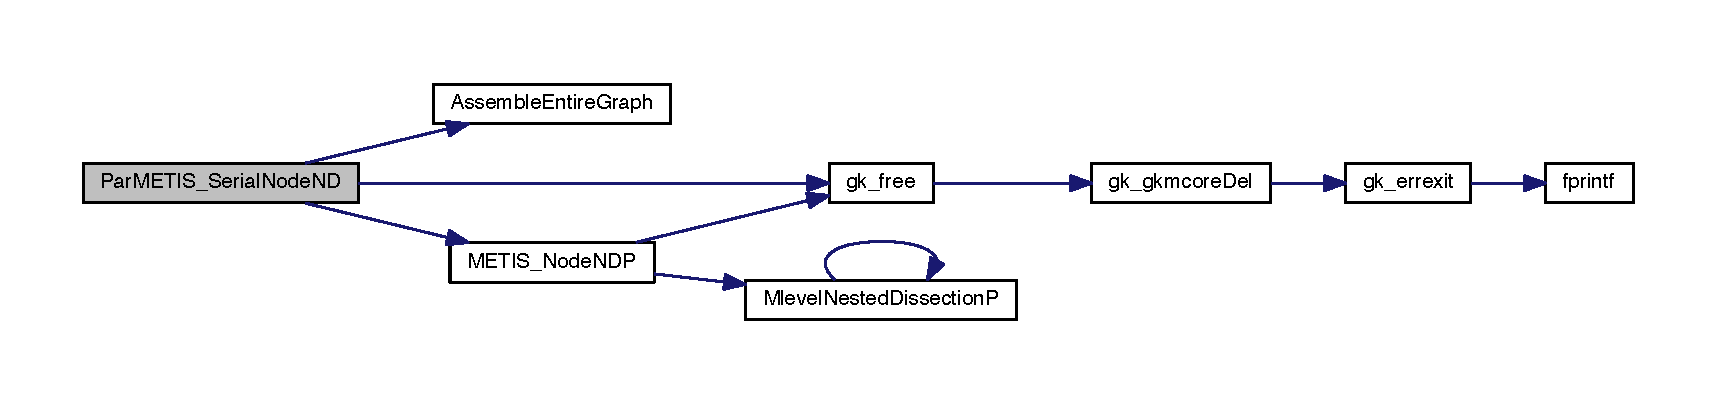
\includegraphics[width=350pt]{include_2parmetis_8h_a8bd1a6399ac304da6616cb5329304df6_cgraph}
\end{center}
\end{figure}
\mbox{\Hypertarget{include_2parmetis_8h_a1bbf9ca25d902b187988a49ccf435e2b}\label{include_2parmetis_8h_a1bbf9ca25d902b187988a49ccf435e2b}} 
\index{include/parmetis.\+h@{include/parmetis.\+h}!Par\+M\+E\+T\+I\+S\+\_\+\+V32\+\_\+\+Node\+ND@{Par\+M\+E\+T\+I\+S\+\_\+\+V32\+\_\+\+Node\+ND}}
\index{Par\+M\+E\+T\+I\+S\+\_\+\+V32\+\_\+\+Node\+ND@{Par\+M\+E\+T\+I\+S\+\_\+\+V32\+\_\+\+Node\+ND}!include/parmetis.\+h@{include/parmetis.\+h}}
\subsubsection{\texorpdfstring{Par\+M\+E\+T\+I\+S\+\_\+\+V32\+\_\+\+Node\+N\+D()}{ParMETIS\_V32\_NodeND()}}
{\footnotesize\ttfamily int \hyperlink{include_2parmetis_8h_a238347d7669f8f1e9c83bfe63a2730c4}{\+\_\+\+\_\+cdecl} Par\+M\+E\+T\+I\+S\+\_\+\+V32\+\_\+\+Node\+ND (\begin{DoxyParamCaption}\item[{\hyperlink{3rd_party_2parmetis-4_80_83_2metis_2include_2metis_8h_aaa5262be3e700770163401acb0150f52}{idx\+\_\+t} $\ast$}]{vtxdist,  }\item[{\hyperlink{3rd_party_2parmetis-4_80_83_2metis_2include_2metis_8h_aaa5262be3e700770163401acb0150f52}{idx\+\_\+t} $\ast$}]{xadj,  }\item[{\hyperlink{3rd_party_2parmetis-4_80_83_2metis_2include_2metis_8h_aaa5262be3e700770163401acb0150f52}{idx\+\_\+t} $\ast$}]{adjncy,  }\item[{\hyperlink{3rd_party_2parmetis-4_80_83_2metis_2include_2metis_8h_aaa5262be3e700770163401acb0150f52}{idx\+\_\+t} $\ast$}]{vwgt,  }\item[{\hyperlink{3rd_party_2parmetis-4_80_83_2metis_2include_2metis_8h_aaa5262be3e700770163401acb0150f52}{idx\+\_\+t} $\ast$}]{numflag,  }\item[{\hyperlink{3rd_party_2parmetis-4_80_83_2metis_2include_2metis_8h_aaa5262be3e700770163401acb0150f52}{idx\+\_\+t} $\ast$}]{mtype,  }\item[{\hyperlink{3rd_party_2parmetis-4_80_83_2metis_2include_2metis_8h_aaa5262be3e700770163401acb0150f52}{idx\+\_\+t} $\ast$}]{rtype,  }\item[{\hyperlink{3rd_party_2parmetis-4_80_83_2metis_2include_2metis_8h_aaa5262be3e700770163401acb0150f52}{idx\+\_\+t} $\ast$}]{p\+\_\+nseps,  }\item[{\hyperlink{3rd_party_2parmetis-4_80_83_2metis_2include_2metis_8h_aaa5262be3e700770163401acb0150f52}{idx\+\_\+t} $\ast$}]{s\+\_\+nseps,  }\item[{\hyperlink{3rd_party_2parmetis-4_80_83_2metis_2include_2metis_8h_a1924a4f6907cc3833213aba1f07fcbe9}{real\+\_\+t} $\ast$}]{ubfrac,  }\item[{\hyperlink{3rd_party_2parmetis-4_80_83_2metis_2include_2metis_8h_aaa5262be3e700770163401acb0150f52}{idx\+\_\+t} $\ast$}]{seed,  }\item[{\hyperlink{3rd_party_2parmetis-4_80_83_2metis_2include_2metis_8h_aaa5262be3e700770163401acb0150f52}{idx\+\_\+t} $\ast$}]{dbglvl,  }\item[{\hyperlink{3rd_party_2parmetis-4_80_83_2metis_2include_2metis_8h_aaa5262be3e700770163401acb0150f52}{idx\+\_\+t} $\ast$}]{order,  }\item[{\hyperlink{3rd_party_2parmetis-4_80_83_2metis_2include_2metis_8h_aaa5262be3e700770163401acb0150f52}{idx\+\_\+t} $\ast$}]{sizes,  }\item[{M\+P\+I\+\_\+\+Comm $\ast$}]{comm }\end{DoxyParamCaption})}

\mbox{\Hypertarget{include_2parmetis_8h_ac00c3da2cf618cbfa9158463a851491e}\label{include_2parmetis_8h_ac00c3da2cf618cbfa9158463a851491e}} 
\index{include/parmetis.\+h@{include/parmetis.\+h}!Par\+M\+E\+T\+I\+S\+\_\+\+V3\+\_\+\+Adaptive\+Repart@{Par\+M\+E\+T\+I\+S\+\_\+\+V3\+\_\+\+Adaptive\+Repart}}
\index{Par\+M\+E\+T\+I\+S\+\_\+\+V3\+\_\+\+Adaptive\+Repart@{Par\+M\+E\+T\+I\+S\+\_\+\+V3\+\_\+\+Adaptive\+Repart}!include/parmetis.\+h@{include/parmetis.\+h}}
\subsubsection{\texorpdfstring{Par\+M\+E\+T\+I\+S\+\_\+\+V3\+\_\+\+Adaptive\+Repart()}{ParMETIS\_V3\_AdaptiveRepart()}}
{\footnotesize\ttfamily int \hyperlink{include_2parmetis_8h_a238347d7669f8f1e9c83bfe63a2730c4}{\+\_\+\+\_\+cdecl} Par\+M\+E\+T\+I\+S\+\_\+\+V3\+\_\+\+Adaptive\+Repart (\begin{DoxyParamCaption}\item[{\hyperlink{3rd_party_2parmetis-4_80_83_2metis_2include_2metis_8h_aaa5262be3e700770163401acb0150f52}{idx\+\_\+t} $\ast$}]{vtxdist,  }\item[{\hyperlink{3rd_party_2parmetis-4_80_83_2metis_2include_2metis_8h_aaa5262be3e700770163401acb0150f52}{idx\+\_\+t} $\ast$}]{xadj,  }\item[{\hyperlink{3rd_party_2parmetis-4_80_83_2metis_2include_2metis_8h_aaa5262be3e700770163401acb0150f52}{idx\+\_\+t} $\ast$}]{adjncy,  }\item[{\hyperlink{3rd_party_2parmetis-4_80_83_2metis_2include_2metis_8h_aaa5262be3e700770163401acb0150f52}{idx\+\_\+t} $\ast$}]{vwgt,  }\item[{\hyperlink{3rd_party_2parmetis-4_80_83_2metis_2include_2metis_8h_aaa5262be3e700770163401acb0150f52}{idx\+\_\+t} $\ast$}]{vsize,  }\item[{\hyperlink{3rd_party_2parmetis-4_80_83_2metis_2include_2metis_8h_aaa5262be3e700770163401acb0150f52}{idx\+\_\+t} $\ast$}]{adjwgt,  }\item[{\hyperlink{3rd_party_2parmetis-4_80_83_2metis_2include_2metis_8h_aaa5262be3e700770163401acb0150f52}{idx\+\_\+t} $\ast$}]{wgtflag,  }\item[{\hyperlink{3rd_party_2parmetis-4_80_83_2metis_2include_2metis_8h_aaa5262be3e700770163401acb0150f52}{idx\+\_\+t} $\ast$}]{numflag,  }\item[{\hyperlink{3rd_party_2parmetis-4_80_83_2metis_2include_2metis_8h_aaa5262be3e700770163401acb0150f52}{idx\+\_\+t} $\ast$}]{ncon,  }\item[{\hyperlink{3rd_party_2parmetis-4_80_83_2metis_2include_2metis_8h_aaa5262be3e700770163401acb0150f52}{idx\+\_\+t} $\ast$}]{nparts,  }\item[{\hyperlink{3rd_party_2parmetis-4_80_83_2metis_2include_2metis_8h_a1924a4f6907cc3833213aba1f07fcbe9}{real\+\_\+t} $\ast$}]{tpwgts,  }\item[{\hyperlink{3rd_party_2parmetis-4_80_83_2metis_2include_2metis_8h_a1924a4f6907cc3833213aba1f07fcbe9}{real\+\_\+t} $\ast$}]{ubvec,  }\item[{\hyperlink{3rd_party_2parmetis-4_80_83_2metis_2include_2metis_8h_a1924a4f6907cc3833213aba1f07fcbe9}{real\+\_\+t} $\ast$}]{ipc2redist,  }\item[{\hyperlink{3rd_party_2parmetis-4_80_83_2metis_2include_2metis_8h_aaa5262be3e700770163401acb0150f52}{idx\+\_\+t} $\ast$}]{options,  }\item[{\hyperlink{3rd_party_2parmetis-4_80_83_2metis_2include_2metis_8h_aaa5262be3e700770163401acb0150f52}{idx\+\_\+t} $\ast$}]{edgecut,  }\item[{\hyperlink{3rd_party_2parmetis-4_80_83_2metis_2include_2metis_8h_aaa5262be3e700770163401acb0150f52}{idx\+\_\+t} $\ast$}]{part,  }\item[{M\+P\+I\+\_\+\+Comm $\ast$}]{comm }\end{DoxyParamCaption})}

Here is the call graph for this function\+:\nopagebreak
\begin{figure}[H]
\begin{center}
\leavevmode
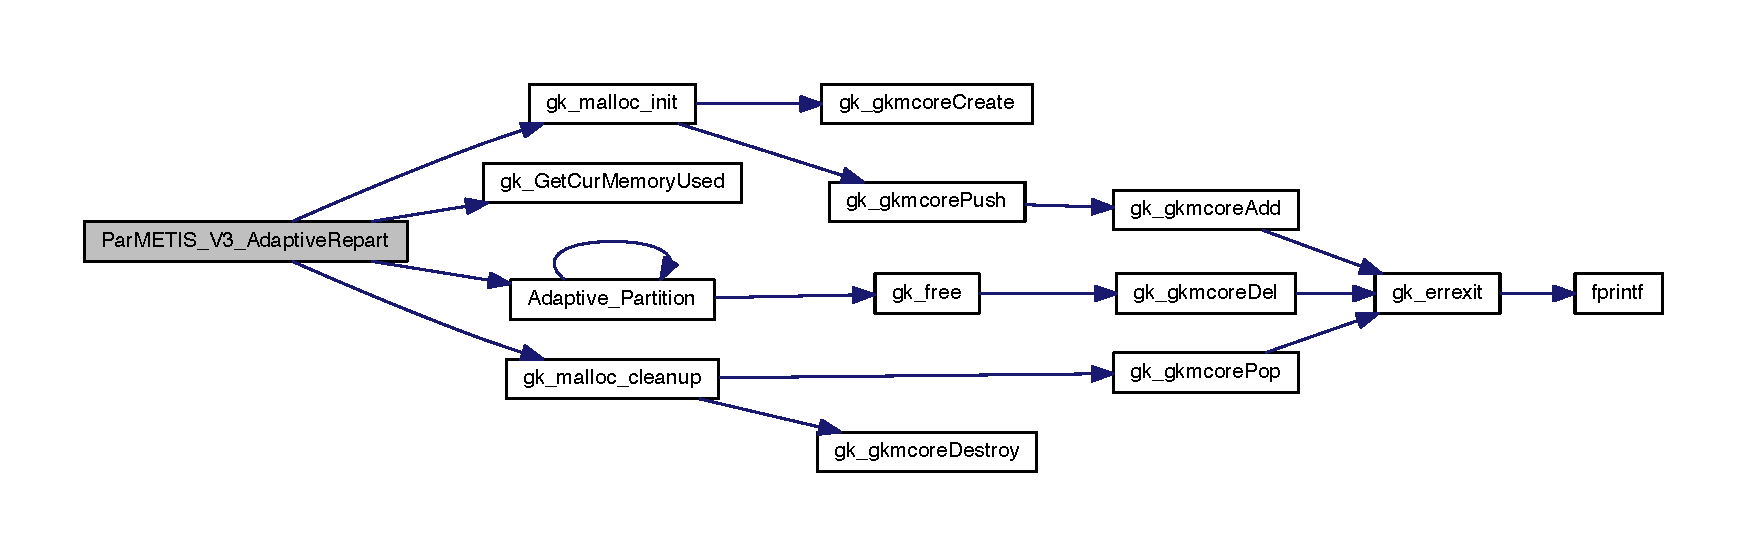
\includegraphics[width=350pt]{include_2parmetis_8h_ac00c3da2cf618cbfa9158463a851491e_cgraph}
\end{center}
\end{figure}
\mbox{\Hypertarget{include_2parmetis_8h_a2f9e316d7e0c46037cf231cd82cf9d97}\label{include_2parmetis_8h_a2f9e316d7e0c46037cf231cd82cf9d97}} 
\index{include/parmetis.\+h@{include/parmetis.\+h}!Par\+M\+E\+T\+I\+S\+\_\+\+V3\+\_\+\+Mesh2\+Dual@{Par\+M\+E\+T\+I\+S\+\_\+\+V3\+\_\+\+Mesh2\+Dual}}
\index{Par\+M\+E\+T\+I\+S\+\_\+\+V3\+\_\+\+Mesh2\+Dual@{Par\+M\+E\+T\+I\+S\+\_\+\+V3\+\_\+\+Mesh2\+Dual}!include/parmetis.\+h@{include/parmetis.\+h}}
\subsubsection{\texorpdfstring{Par\+M\+E\+T\+I\+S\+\_\+\+V3\+\_\+\+Mesh2\+Dual()}{ParMETIS\_V3\_Mesh2Dual()}}
{\footnotesize\ttfamily int \hyperlink{include_2parmetis_8h_a238347d7669f8f1e9c83bfe63a2730c4}{\+\_\+\+\_\+cdecl} Par\+M\+E\+T\+I\+S\+\_\+\+V3\+\_\+\+Mesh2\+Dual (\begin{DoxyParamCaption}\item[{\hyperlink{3rd_party_2parmetis-4_80_83_2metis_2include_2metis_8h_aaa5262be3e700770163401acb0150f52}{idx\+\_\+t} $\ast$}]{elmdist,  }\item[{\hyperlink{3rd_party_2parmetis-4_80_83_2metis_2include_2metis_8h_aaa5262be3e700770163401acb0150f52}{idx\+\_\+t} $\ast$}]{eptr,  }\item[{\hyperlink{3rd_party_2parmetis-4_80_83_2metis_2include_2metis_8h_aaa5262be3e700770163401acb0150f52}{idx\+\_\+t} $\ast$}]{eind,  }\item[{\hyperlink{3rd_party_2parmetis-4_80_83_2metis_2include_2metis_8h_aaa5262be3e700770163401acb0150f52}{idx\+\_\+t} $\ast$}]{numflag,  }\item[{\hyperlink{3rd_party_2parmetis-4_80_83_2metis_2include_2metis_8h_aaa5262be3e700770163401acb0150f52}{idx\+\_\+t} $\ast$}]{ncommonnodes,  }\item[{\hyperlink{3rd_party_2parmetis-4_80_83_2metis_2include_2metis_8h_aaa5262be3e700770163401acb0150f52}{idx\+\_\+t} $\ast$$\ast$}]{xadj,  }\item[{\hyperlink{3rd_party_2parmetis-4_80_83_2metis_2include_2metis_8h_aaa5262be3e700770163401acb0150f52}{idx\+\_\+t} $\ast$$\ast$}]{adjncy,  }\item[{M\+P\+I\+\_\+\+Comm $\ast$}]{comm }\end{DoxyParamCaption})}

Here is the call graph for this function\+:\nopagebreak
\begin{figure}[H]
\begin{center}
\leavevmode
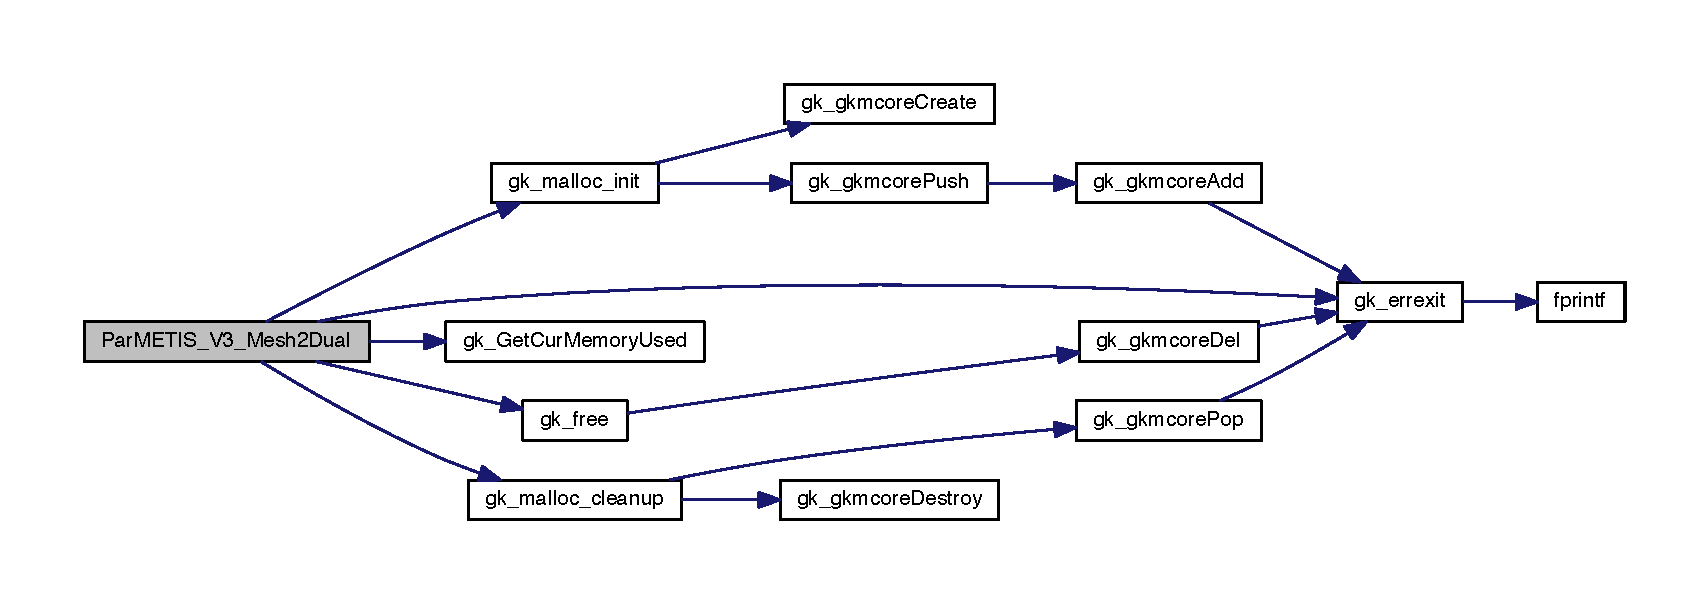
\includegraphics[width=350pt]{include_2parmetis_8h_a2f9e316d7e0c46037cf231cd82cf9d97_cgraph}
\end{center}
\end{figure}
\mbox{\Hypertarget{include_2parmetis_8h_add23df29b4f232ac4c2cca94cc083a32}\label{include_2parmetis_8h_add23df29b4f232ac4c2cca94cc083a32}} 
\index{include/parmetis.\+h@{include/parmetis.\+h}!Par\+M\+E\+T\+I\+S\+\_\+\+V3\+\_\+\+Node\+ND@{Par\+M\+E\+T\+I\+S\+\_\+\+V3\+\_\+\+Node\+ND}}
\index{Par\+M\+E\+T\+I\+S\+\_\+\+V3\+\_\+\+Node\+ND@{Par\+M\+E\+T\+I\+S\+\_\+\+V3\+\_\+\+Node\+ND}!include/parmetis.\+h@{include/parmetis.\+h}}
\subsubsection{\texorpdfstring{Par\+M\+E\+T\+I\+S\+\_\+\+V3\+\_\+\+Node\+N\+D()}{ParMETIS\_V3\_NodeND()}}
{\footnotesize\ttfamily int \hyperlink{include_2parmetis_8h_a238347d7669f8f1e9c83bfe63a2730c4}{\+\_\+\+\_\+cdecl} Par\+M\+E\+T\+I\+S\+\_\+\+V3\+\_\+\+Node\+ND (\begin{DoxyParamCaption}\item[{\hyperlink{3rd_party_2parmetis-4_80_83_2metis_2include_2metis_8h_aaa5262be3e700770163401acb0150f52}{idx\+\_\+t} $\ast$}]{vtxdist,  }\item[{\hyperlink{3rd_party_2parmetis-4_80_83_2metis_2include_2metis_8h_aaa5262be3e700770163401acb0150f52}{idx\+\_\+t} $\ast$}]{xadj,  }\item[{\hyperlink{3rd_party_2parmetis-4_80_83_2metis_2include_2metis_8h_aaa5262be3e700770163401acb0150f52}{idx\+\_\+t} $\ast$}]{adjncy,  }\item[{\hyperlink{3rd_party_2parmetis-4_80_83_2metis_2include_2metis_8h_aaa5262be3e700770163401acb0150f52}{idx\+\_\+t} $\ast$}]{numflag,  }\item[{\hyperlink{3rd_party_2parmetis-4_80_83_2metis_2include_2metis_8h_aaa5262be3e700770163401acb0150f52}{idx\+\_\+t} $\ast$}]{options,  }\item[{\hyperlink{3rd_party_2parmetis-4_80_83_2metis_2include_2metis_8h_aaa5262be3e700770163401acb0150f52}{idx\+\_\+t} $\ast$}]{order,  }\item[{\hyperlink{3rd_party_2parmetis-4_80_83_2metis_2include_2metis_8h_aaa5262be3e700770163401acb0150f52}{idx\+\_\+t} $\ast$}]{sizes,  }\item[{M\+P\+I\+\_\+\+Comm $\ast$}]{comm }\end{DoxyParamCaption})}

\mbox{\Hypertarget{include_2parmetis_8h_aab31b6450a3228063206eddded9de65e}\label{include_2parmetis_8h_aab31b6450a3228063206eddded9de65e}} 
\index{include/parmetis.\+h@{include/parmetis.\+h}!Par\+M\+E\+T\+I\+S\+\_\+\+V3\+\_\+\+Part\+Geom@{Par\+M\+E\+T\+I\+S\+\_\+\+V3\+\_\+\+Part\+Geom}}
\index{Par\+M\+E\+T\+I\+S\+\_\+\+V3\+\_\+\+Part\+Geom@{Par\+M\+E\+T\+I\+S\+\_\+\+V3\+\_\+\+Part\+Geom}!include/parmetis.\+h@{include/parmetis.\+h}}
\subsubsection{\texorpdfstring{Par\+M\+E\+T\+I\+S\+\_\+\+V3\+\_\+\+Part\+Geom()}{ParMETIS\_V3\_PartGeom()}}
{\footnotesize\ttfamily int \hyperlink{include_2parmetis_8h_a238347d7669f8f1e9c83bfe63a2730c4}{\+\_\+\+\_\+cdecl} Par\+M\+E\+T\+I\+S\+\_\+\+V3\+\_\+\+Part\+Geom (\begin{DoxyParamCaption}\item[{\hyperlink{3rd_party_2parmetis-4_80_83_2metis_2include_2metis_8h_aaa5262be3e700770163401acb0150f52}{idx\+\_\+t} $\ast$}]{vtxdist,  }\item[{\hyperlink{3rd_party_2parmetis-4_80_83_2metis_2include_2metis_8h_aaa5262be3e700770163401acb0150f52}{idx\+\_\+t} $\ast$}]{ndims,  }\item[{\hyperlink{3rd_party_2parmetis-4_80_83_2metis_2include_2metis_8h_a1924a4f6907cc3833213aba1f07fcbe9}{real\+\_\+t} $\ast$}]{xyz,  }\item[{\hyperlink{3rd_party_2parmetis-4_80_83_2metis_2include_2metis_8h_aaa5262be3e700770163401acb0150f52}{idx\+\_\+t} $\ast$}]{part,  }\item[{M\+P\+I\+\_\+\+Comm $\ast$}]{comm }\end{DoxyParamCaption})}

Here is the call graph for this function\+:\nopagebreak
\begin{figure}[H]
\begin{center}
\leavevmode
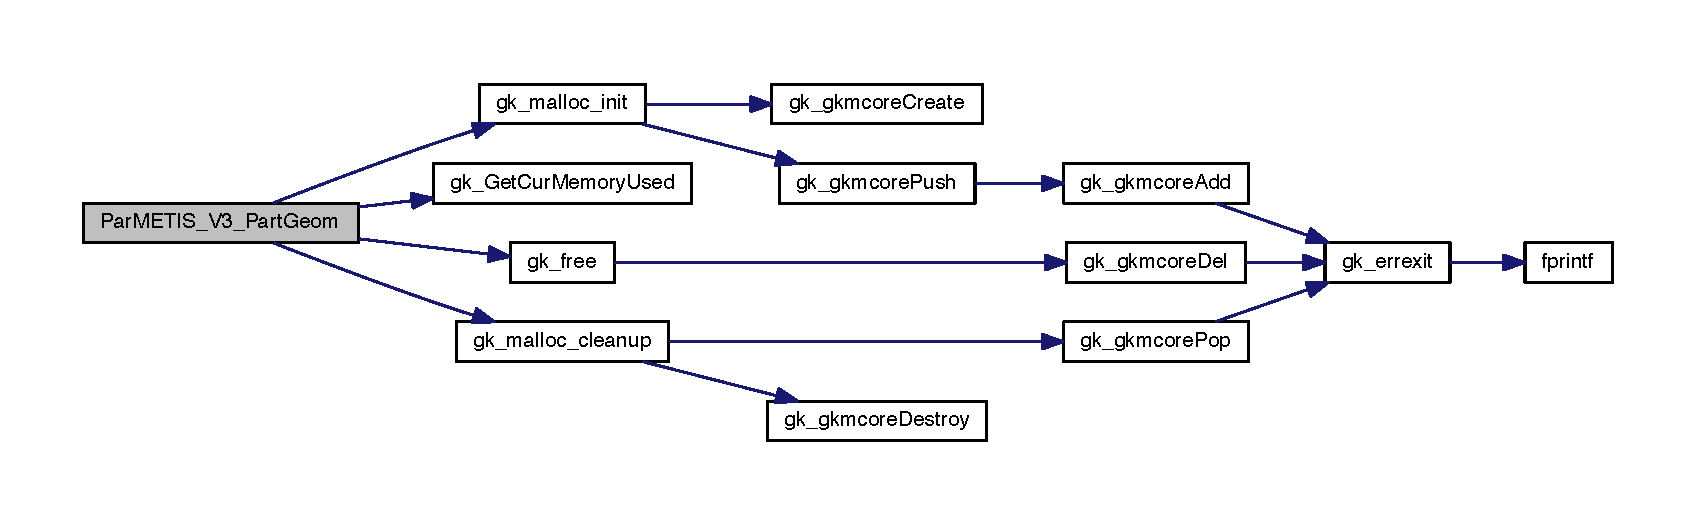
\includegraphics[width=350pt]{include_2parmetis_8h_aab31b6450a3228063206eddded9de65e_cgraph}
\end{center}
\end{figure}
\mbox{\Hypertarget{include_2parmetis_8h_a6df93293cf3d1ccb4659bd1b3091623d}\label{include_2parmetis_8h_a6df93293cf3d1ccb4659bd1b3091623d}} 
\index{include/parmetis.\+h@{include/parmetis.\+h}!Par\+M\+E\+T\+I\+S\+\_\+\+V3\+\_\+\+Part\+Geom\+Kway@{Par\+M\+E\+T\+I\+S\+\_\+\+V3\+\_\+\+Part\+Geom\+Kway}}
\index{Par\+M\+E\+T\+I\+S\+\_\+\+V3\+\_\+\+Part\+Geom\+Kway@{Par\+M\+E\+T\+I\+S\+\_\+\+V3\+\_\+\+Part\+Geom\+Kway}!include/parmetis.\+h@{include/parmetis.\+h}}
\subsubsection{\texorpdfstring{Par\+M\+E\+T\+I\+S\+\_\+\+V3\+\_\+\+Part\+Geom\+Kway()}{ParMETIS\_V3\_PartGeomKway()}}
{\footnotesize\ttfamily int \hyperlink{include_2parmetis_8h_a238347d7669f8f1e9c83bfe63a2730c4}{\+\_\+\+\_\+cdecl} Par\+M\+E\+T\+I\+S\+\_\+\+V3\+\_\+\+Part\+Geom\+Kway (\begin{DoxyParamCaption}\item[{\hyperlink{3rd_party_2parmetis-4_80_83_2metis_2include_2metis_8h_aaa5262be3e700770163401acb0150f52}{idx\+\_\+t} $\ast$}]{vtxdist,  }\item[{\hyperlink{3rd_party_2parmetis-4_80_83_2metis_2include_2metis_8h_aaa5262be3e700770163401acb0150f52}{idx\+\_\+t} $\ast$}]{xadj,  }\item[{\hyperlink{3rd_party_2parmetis-4_80_83_2metis_2include_2metis_8h_aaa5262be3e700770163401acb0150f52}{idx\+\_\+t} $\ast$}]{adjncy,  }\item[{\hyperlink{3rd_party_2parmetis-4_80_83_2metis_2include_2metis_8h_aaa5262be3e700770163401acb0150f52}{idx\+\_\+t} $\ast$}]{vwgt,  }\item[{\hyperlink{3rd_party_2parmetis-4_80_83_2metis_2include_2metis_8h_aaa5262be3e700770163401acb0150f52}{idx\+\_\+t} $\ast$}]{adjwgt,  }\item[{\hyperlink{3rd_party_2parmetis-4_80_83_2metis_2include_2metis_8h_aaa5262be3e700770163401acb0150f52}{idx\+\_\+t} $\ast$}]{wgtflag,  }\item[{\hyperlink{3rd_party_2parmetis-4_80_83_2metis_2include_2metis_8h_aaa5262be3e700770163401acb0150f52}{idx\+\_\+t} $\ast$}]{numflag,  }\item[{\hyperlink{3rd_party_2parmetis-4_80_83_2metis_2include_2metis_8h_aaa5262be3e700770163401acb0150f52}{idx\+\_\+t} $\ast$}]{ndims,  }\item[{\hyperlink{3rd_party_2parmetis-4_80_83_2metis_2include_2metis_8h_a1924a4f6907cc3833213aba1f07fcbe9}{real\+\_\+t} $\ast$}]{xyz,  }\item[{\hyperlink{3rd_party_2parmetis-4_80_83_2metis_2include_2metis_8h_aaa5262be3e700770163401acb0150f52}{idx\+\_\+t} $\ast$}]{ncon,  }\item[{\hyperlink{3rd_party_2parmetis-4_80_83_2metis_2include_2metis_8h_aaa5262be3e700770163401acb0150f52}{idx\+\_\+t} $\ast$}]{nparts,  }\item[{\hyperlink{3rd_party_2parmetis-4_80_83_2metis_2include_2metis_8h_a1924a4f6907cc3833213aba1f07fcbe9}{real\+\_\+t} $\ast$}]{tpwgts,  }\item[{\hyperlink{3rd_party_2parmetis-4_80_83_2metis_2include_2metis_8h_a1924a4f6907cc3833213aba1f07fcbe9}{real\+\_\+t} $\ast$}]{ubvec,  }\item[{\hyperlink{3rd_party_2parmetis-4_80_83_2metis_2include_2metis_8h_aaa5262be3e700770163401acb0150f52}{idx\+\_\+t} $\ast$}]{options,  }\item[{\hyperlink{3rd_party_2parmetis-4_80_83_2metis_2include_2metis_8h_aaa5262be3e700770163401acb0150f52}{idx\+\_\+t} $\ast$}]{edgecut,  }\item[{\hyperlink{3rd_party_2parmetis-4_80_83_2metis_2include_2metis_8h_aaa5262be3e700770163401acb0150f52}{idx\+\_\+t} $\ast$}]{part,  }\item[{M\+P\+I\+\_\+\+Comm $\ast$}]{comm }\end{DoxyParamCaption})}

Here is the call graph for this function\+:\nopagebreak
\begin{figure}[H]
\begin{center}
\leavevmode
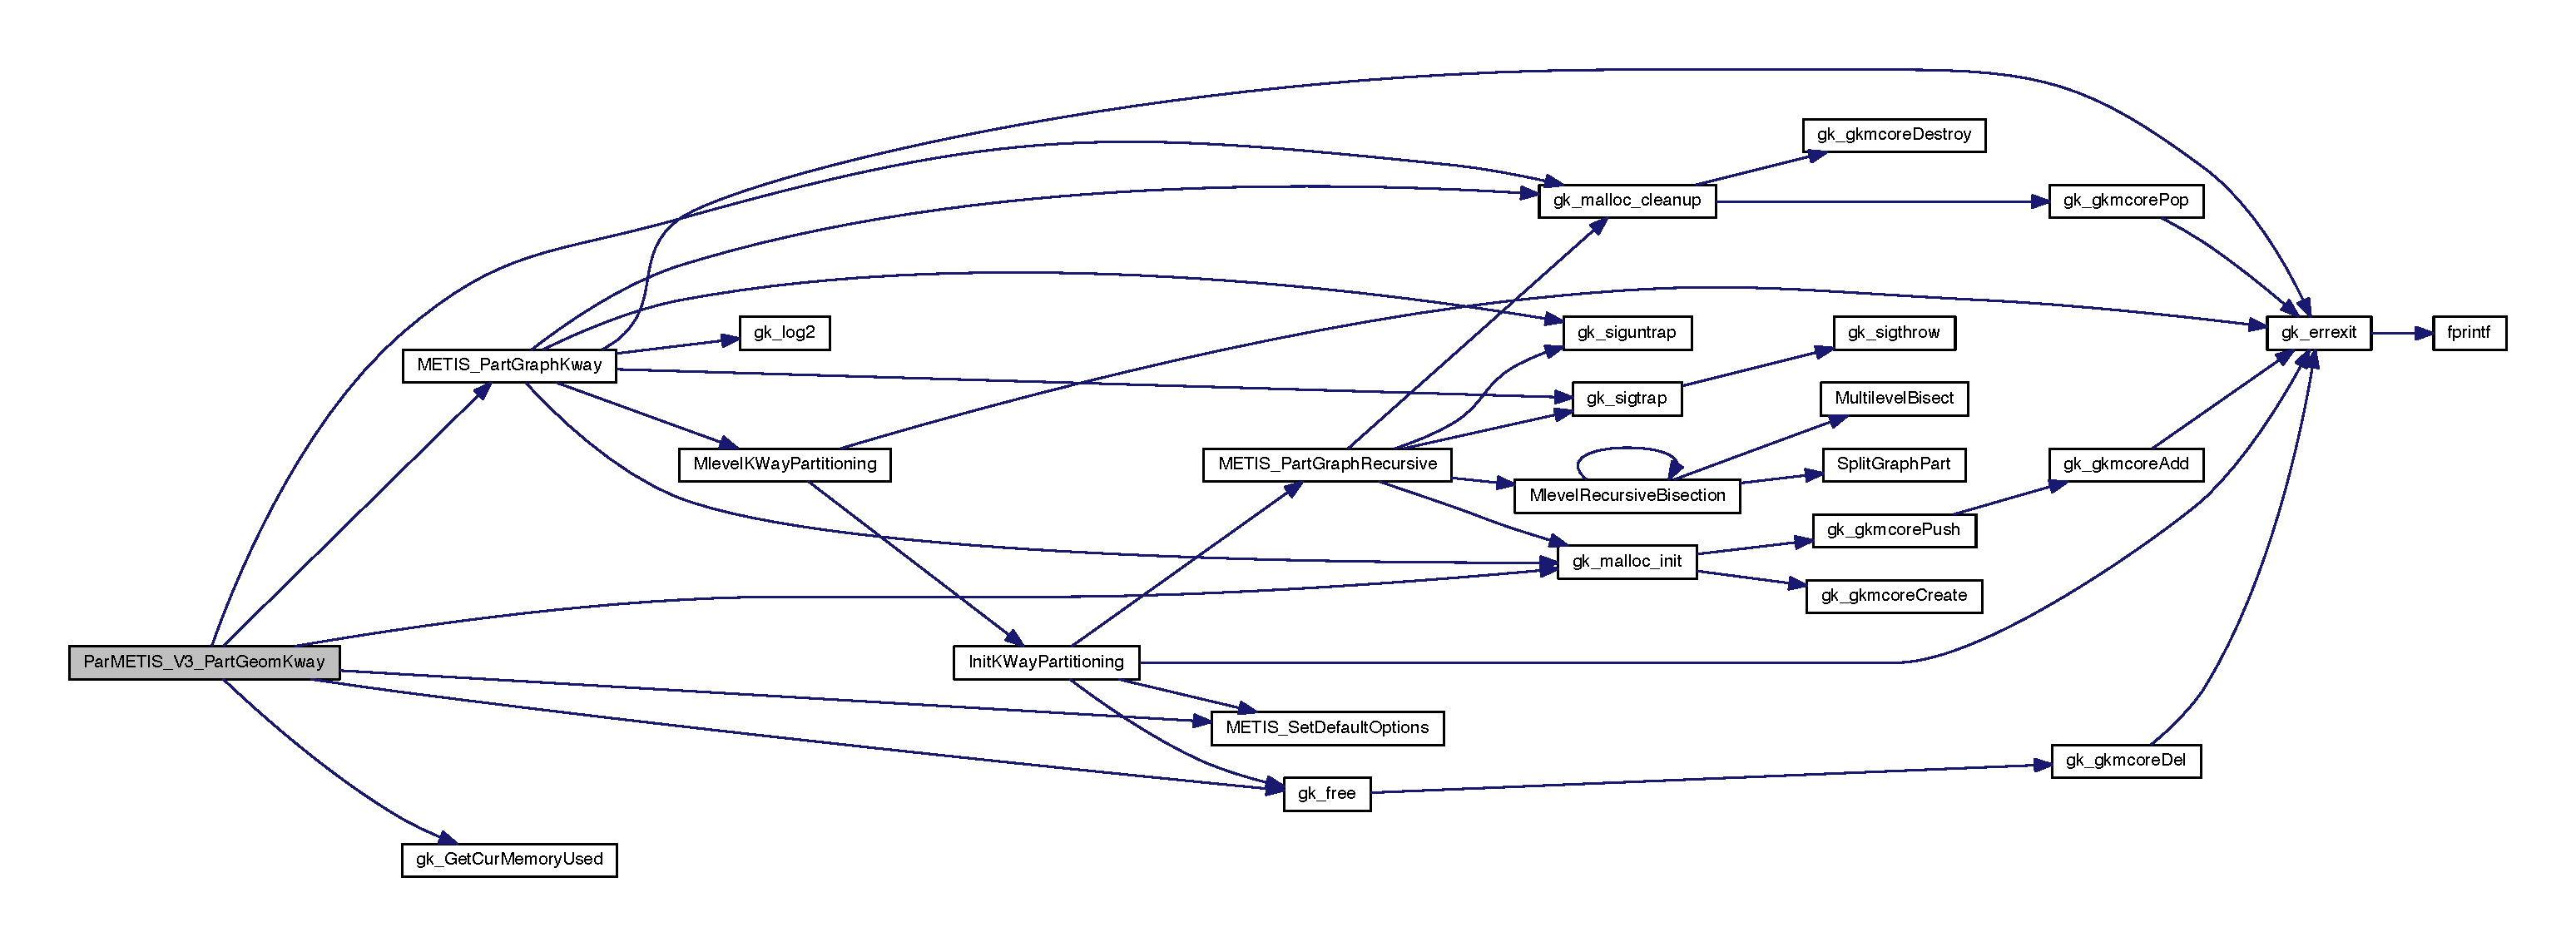
\includegraphics[width=350pt]{include_2parmetis_8h_a6df93293cf3d1ccb4659bd1b3091623d_cgraph}
\end{center}
\end{figure}
\mbox{\Hypertarget{include_2parmetis_8h_af418d1e76eaf4f80116da4caf51bd54e}\label{include_2parmetis_8h_af418d1e76eaf4f80116da4caf51bd54e}} 
\index{include/parmetis.\+h@{include/parmetis.\+h}!Par\+M\+E\+T\+I\+S\+\_\+\+V3\+\_\+\+Part\+Kway@{Par\+M\+E\+T\+I\+S\+\_\+\+V3\+\_\+\+Part\+Kway}}
\index{Par\+M\+E\+T\+I\+S\+\_\+\+V3\+\_\+\+Part\+Kway@{Par\+M\+E\+T\+I\+S\+\_\+\+V3\+\_\+\+Part\+Kway}!include/parmetis.\+h@{include/parmetis.\+h}}
\subsubsection{\texorpdfstring{Par\+M\+E\+T\+I\+S\+\_\+\+V3\+\_\+\+Part\+Kway()}{ParMETIS\_V3\_PartKway()}}
{\footnotesize\ttfamily int \hyperlink{include_2parmetis_8h_a238347d7669f8f1e9c83bfe63a2730c4}{\+\_\+\+\_\+cdecl} Par\+M\+E\+T\+I\+S\+\_\+\+V3\+\_\+\+Part\+Kway (\begin{DoxyParamCaption}\item[{\hyperlink{3rd_party_2parmetis-4_80_83_2metis_2include_2metis_8h_aaa5262be3e700770163401acb0150f52}{idx\+\_\+t} $\ast$}]{vtxdist,  }\item[{\hyperlink{3rd_party_2parmetis-4_80_83_2metis_2include_2metis_8h_aaa5262be3e700770163401acb0150f52}{idx\+\_\+t} $\ast$}]{xadj,  }\item[{\hyperlink{3rd_party_2parmetis-4_80_83_2metis_2include_2metis_8h_aaa5262be3e700770163401acb0150f52}{idx\+\_\+t} $\ast$}]{adjncy,  }\item[{\hyperlink{3rd_party_2parmetis-4_80_83_2metis_2include_2metis_8h_aaa5262be3e700770163401acb0150f52}{idx\+\_\+t} $\ast$}]{vwgt,  }\item[{\hyperlink{3rd_party_2parmetis-4_80_83_2metis_2include_2metis_8h_aaa5262be3e700770163401acb0150f52}{idx\+\_\+t} $\ast$}]{adjwgt,  }\item[{\hyperlink{3rd_party_2parmetis-4_80_83_2metis_2include_2metis_8h_aaa5262be3e700770163401acb0150f52}{idx\+\_\+t} $\ast$}]{wgtflag,  }\item[{\hyperlink{3rd_party_2parmetis-4_80_83_2metis_2include_2metis_8h_aaa5262be3e700770163401acb0150f52}{idx\+\_\+t} $\ast$}]{numflag,  }\item[{\hyperlink{3rd_party_2parmetis-4_80_83_2metis_2include_2metis_8h_aaa5262be3e700770163401acb0150f52}{idx\+\_\+t} $\ast$}]{ncon,  }\item[{\hyperlink{3rd_party_2parmetis-4_80_83_2metis_2include_2metis_8h_aaa5262be3e700770163401acb0150f52}{idx\+\_\+t} $\ast$}]{nparts,  }\item[{\hyperlink{3rd_party_2parmetis-4_80_83_2metis_2include_2metis_8h_a1924a4f6907cc3833213aba1f07fcbe9}{real\+\_\+t} $\ast$}]{tpwgts,  }\item[{\hyperlink{3rd_party_2parmetis-4_80_83_2metis_2include_2metis_8h_a1924a4f6907cc3833213aba1f07fcbe9}{real\+\_\+t} $\ast$}]{ubvec,  }\item[{\hyperlink{3rd_party_2parmetis-4_80_83_2metis_2include_2metis_8h_aaa5262be3e700770163401acb0150f52}{idx\+\_\+t} $\ast$}]{options,  }\item[{\hyperlink{3rd_party_2parmetis-4_80_83_2metis_2include_2metis_8h_aaa5262be3e700770163401acb0150f52}{idx\+\_\+t} $\ast$}]{edgecut,  }\item[{\hyperlink{3rd_party_2parmetis-4_80_83_2metis_2include_2metis_8h_aaa5262be3e700770163401acb0150f52}{idx\+\_\+t} $\ast$}]{part,  }\item[{M\+P\+I\+\_\+\+Comm $\ast$}]{comm }\end{DoxyParamCaption})}

Here is the call graph for this function\+:\nopagebreak
\begin{figure}[H]
\begin{center}
\leavevmode
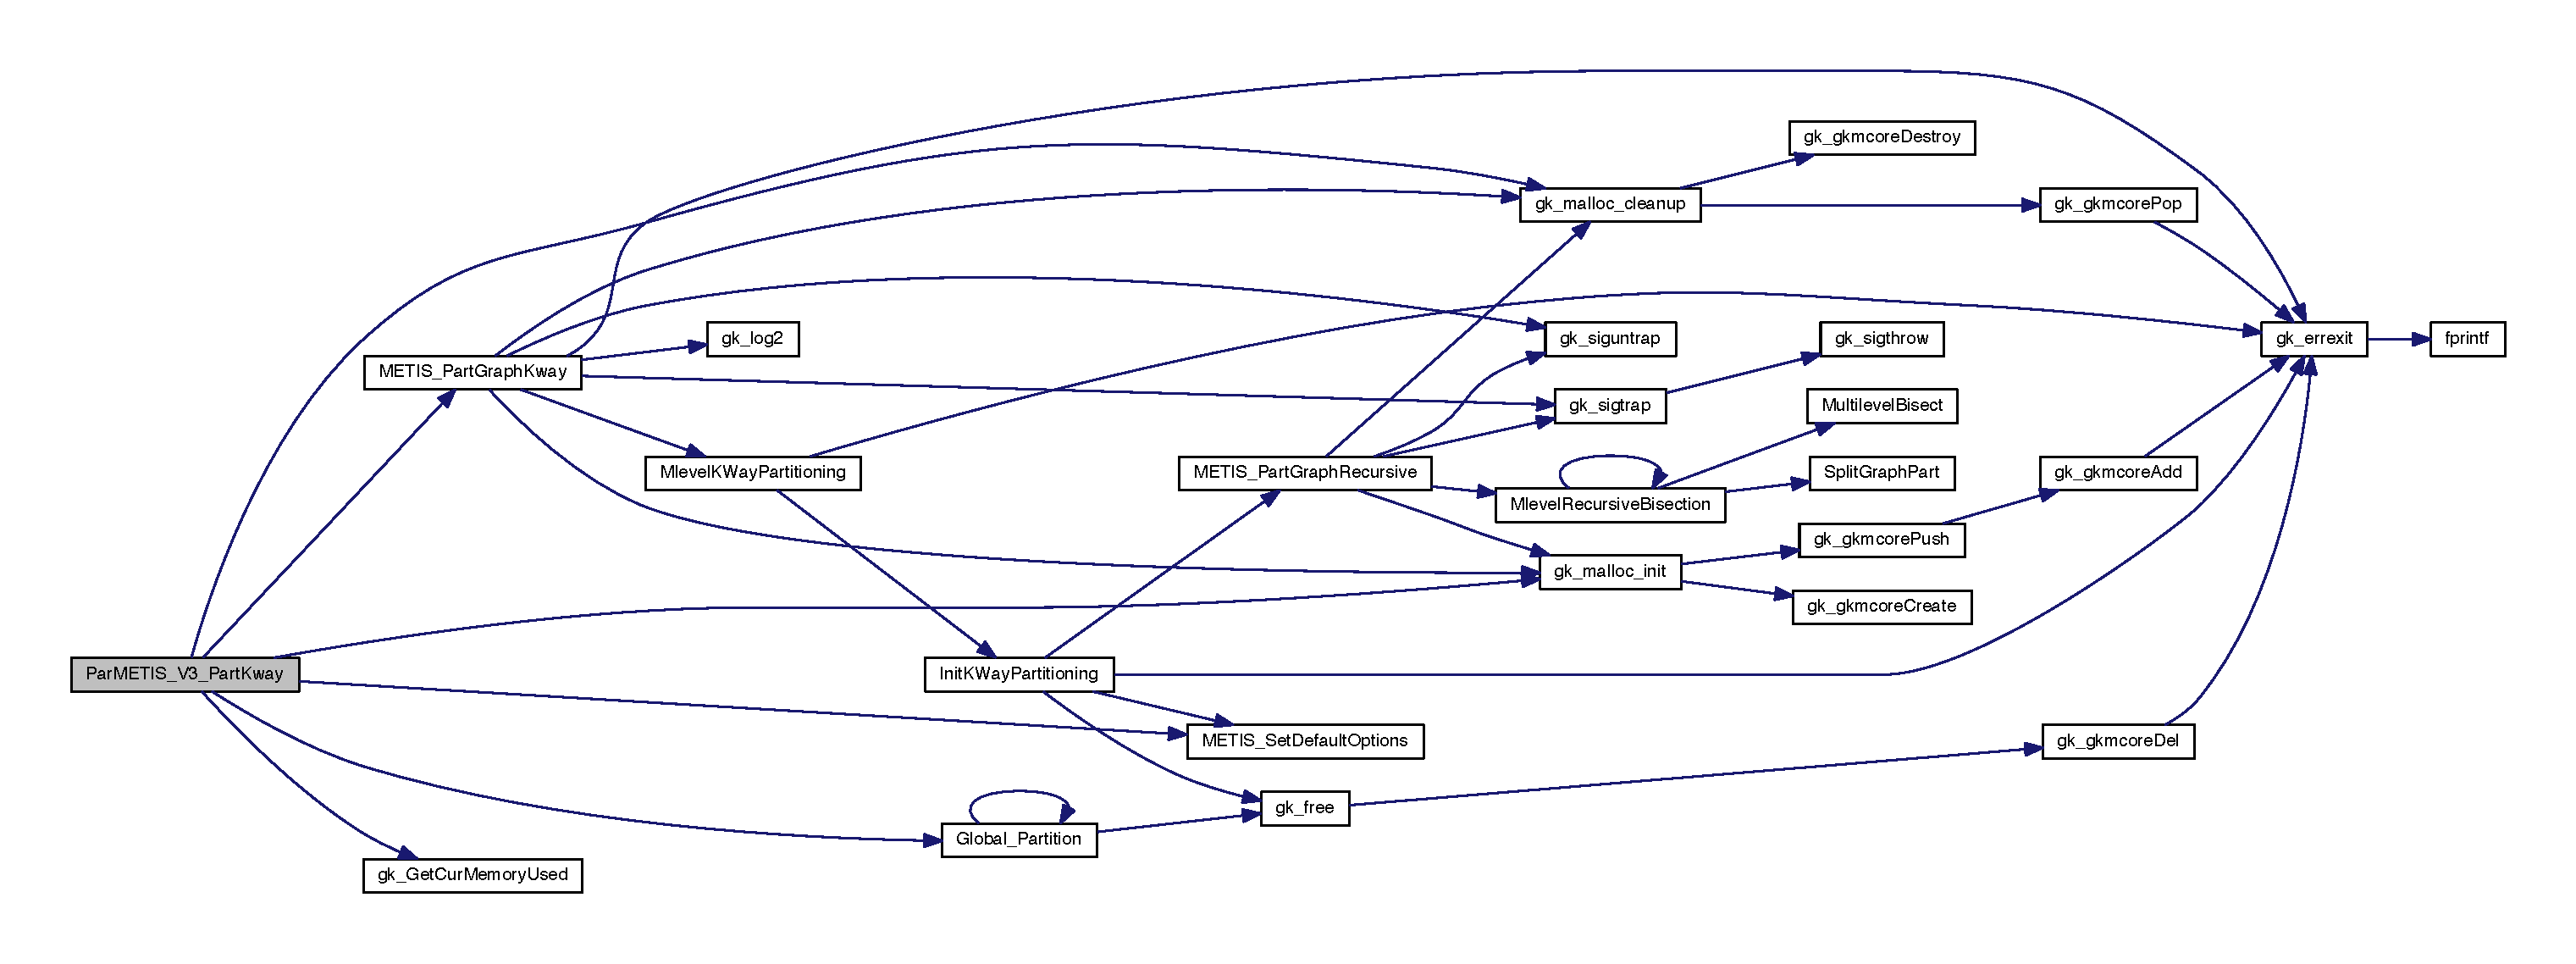
\includegraphics[width=350pt]{include_2parmetis_8h_af418d1e76eaf4f80116da4caf51bd54e_cgraph}
\end{center}
\end{figure}
\mbox{\Hypertarget{include_2parmetis_8h_a2ae9750ec09afdc4243b7cb7c5118666}\label{include_2parmetis_8h_a2ae9750ec09afdc4243b7cb7c5118666}} 
\index{include/parmetis.\+h@{include/parmetis.\+h}!Par\+M\+E\+T\+I\+S\+\_\+\+V3\+\_\+\+Part\+Mesh\+Kway@{Par\+M\+E\+T\+I\+S\+\_\+\+V3\+\_\+\+Part\+Mesh\+Kway}}
\index{Par\+M\+E\+T\+I\+S\+\_\+\+V3\+\_\+\+Part\+Mesh\+Kway@{Par\+M\+E\+T\+I\+S\+\_\+\+V3\+\_\+\+Part\+Mesh\+Kway}!include/parmetis.\+h@{include/parmetis.\+h}}
\subsubsection{\texorpdfstring{Par\+M\+E\+T\+I\+S\+\_\+\+V3\+\_\+\+Part\+Mesh\+Kway()}{ParMETIS\_V3\_PartMeshKway()}}
{\footnotesize\ttfamily int \hyperlink{include_2parmetis_8h_a238347d7669f8f1e9c83bfe63a2730c4}{\+\_\+\+\_\+cdecl} Par\+M\+E\+T\+I\+S\+\_\+\+V3\+\_\+\+Part\+Mesh\+Kway (\begin{DoxyParamCaption}\item[{\hyperlink{3rd_party_2parmetis-4_80_83_2metis_2include_2metis_8h_aaa5262be3e700770163401acb0150f52}{idx\+\_\+t} $\ast$}]{elmdist,  }\item[{\hyperlink{3rd_party_2parmetis-4_80_83_2metis_2include_2metis_8h_aaa5262be3e700770163401acb0150f52}{idx\+\_\+t} $\ast$}]{eptr,  }\item[{\hyperlink{3rd_party_2parmetis-4_80_83_2metis_2include_2metis_8h_aaa5262be3e700770163401acb0150f52}{idx\+\_\+t} $\ast$}]{eind,  }\item[{\hyperlink{3rd_party_2parmetis-4_80_83_2metis_2include_2metis_8h_aaa5262be3e700770163401acb0150f52}{idx\+\_\+t} $\ast$}]{elmwgt,  }\item[{\hyperlink{3rd_party_2parmetis-4_80_83_2metis_2include_2metis_8h_aaa5262be3e700770163401acb0150f52}{idx\+\_\+t} $\ast$}]{wgtflag,  }\item[{\hyperlink{3rd_party_2parmetis-4_80_83_2metis_2include_2metis_8h_aaa5262be3e700770163401acb0150f52}{idx\+\_\+t} $\ast$}]{numflag,  }\item[{\hyperlink{3rd_party_2parmetis-4_80_83_2metis_2include_2metis_8h_aaa5262be3e700770163401acb0150f52}{idx\+\_\+t} $\ast$}]{ncon,  }\item[{\hyperlink{3rd_party_2parmetis-4_80_83_2metis_2include_2metis_8h_aaa5262be3e700770163401acb0150f52}{idx\+\_\+t} $\ast$}]{ncommonnodes,  }\item[{\hyperlink{3rd_party_2parmetis-4_80_83_2metis_2include_2metis_8h_aaa5262be3e700770163401acb0150f52}{idx\+\_\+t} $\ast$}]{nparts,  }\item[{\hyperlink{3rd_party_2parmetis-4_80_83_2metis_2include_2metis_8h_a1924a4f6907cc3833213aba1f07fcbe9}{real\+\_\+t} $\ast$}]{tpwgts,  }\item[{\hyperlink{3rd_party_2parmetis-4_80_83_2metis_2include_2metis_8h_a1924a4f6907cc3833213aba1f07fcbe9}{real\+\_\+t} $\ast$}]{ubvec,  }\item[{\hyperlink{3rd_party_2parmetis-4_80_83_2metis_2include_2metis_8h_aaa5262be3e700770163401acb0150f52}{idx\+\_\+t} $\ast$}]{options,  }\item[{\hyperlink{3rd_party_2parmetis-4_80_83_2metis_2include_2metis_8h_aaa5262be3e700770163401acb0150f52}{idx\+\_\+t} $\ast$}]{edgecut,  }\item[{\hyperlink{3rd_party_2parmetis-4_80_83_2metis_2include_2metis_8h_aaa5262be3e700770163401acb0150f52}{idx\+\_\+t} $\ast$}]{part,  }\item[{M\+P\+I\+\_\+\+Comm $\ast$}]{comm }\end{DoxyParamCaption})}

Here is the call graph for this function\+:\nopagebreak
\begin{figure}[H]
\begin{center}
\leavevmode
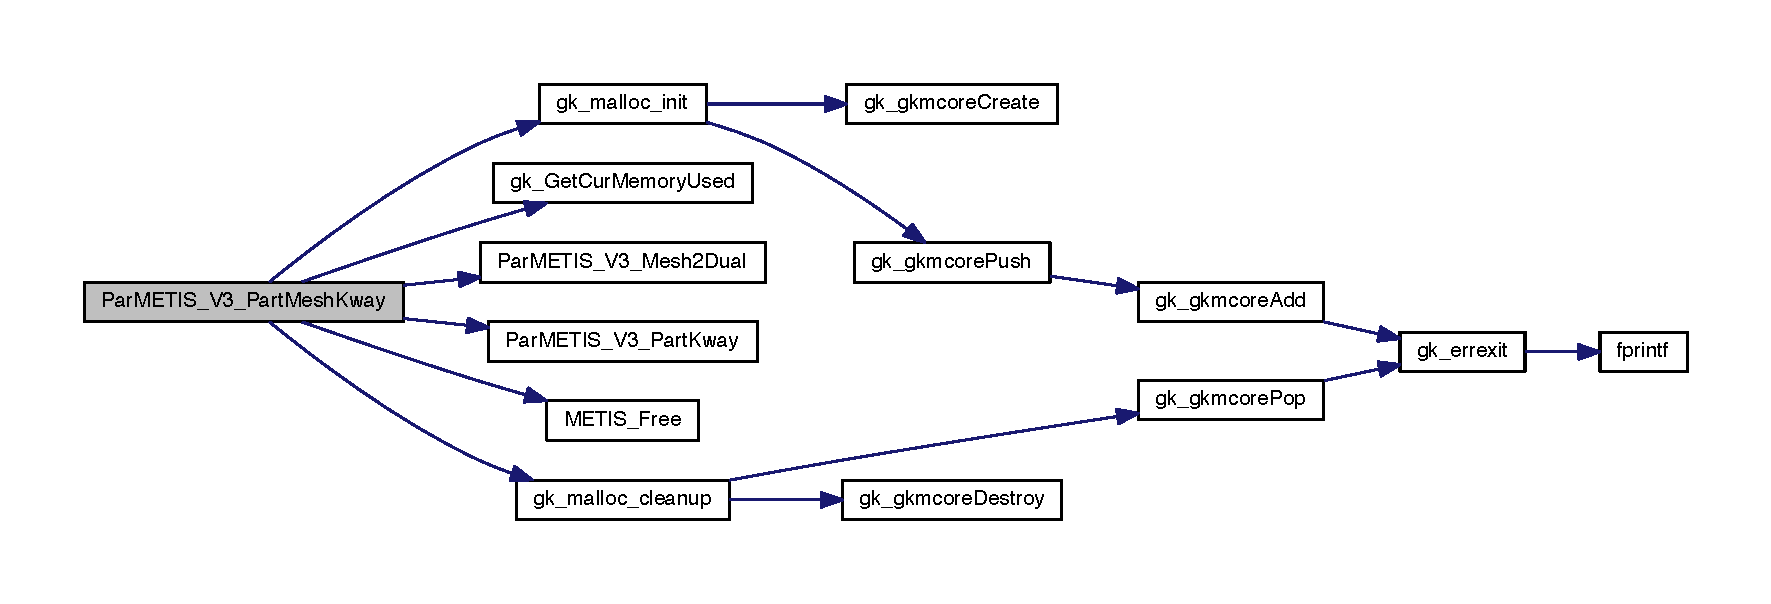
\includegraphics[width=350pt]{include_2parmetis_8h_a2ae9750ec09afdc4243b7cb7c5118666_cgraph}
\end{center}
\end{figure}
\mbox{\Hypertarget{include_2parmetis_8h_ad40a7809c9bdf183926da011220bad75}\label{include_2parmetis_8h_ad40a7809c9bdf183926da011220bad75}} 
\index{include/parmetis.\+h@{include/parmetis.\+h}!Par\+M\+E\+T\+I\+S\+\_\+\+V3\+\_\+\+Refine\+Kway@{Par\+M\+E\+T\+I\+S\+\_\+\+V3\+\_\+\+Refine\+Kway}}
\index{Par\+M\+E\+T\+I\+S\+\_\+\+V3\+\_\+\+Refine\+Kway@{Par\+M\+E\+T\+I\+S\+\_\+\+V3\+\_\+\+Refine\+Kway}!include/parmetis.\+h@{include/parmetis.\+h}}
\subsubsection{\texorpdfstring{Par\+M\+E\+T\+I\+S\+\_\+\+V3\+\_\+\+Refine\+Kway()}{ParMETIS\_V3\_RefineKway()}}
{\footnotesize\ttfamily int \hyperlink{include_2parmetis_8h_a238347d7669f8f1e9c83bfe63a2730c4}{\+\_\+\+\_\+cdecl} Par\+M\+E\+T\+I\+S\+\_\+\+V3\+\_\+\+Refine\+Kway (\begin{DoxyParamCaption}\item[{\hyperlink{3rd_party_2parmetis-4_80_83_2metis_2include_2metis_8h_aaa5262be3e700770163401acb0150f52}{idx\+\_\+t} $\ast$}]{vtxdist,  }\item[{\hyperlink{3rd_party_2parmetis-4_80_83_2metis_2include_2metis_8h_aaa5262be3e700770163401acb0150f52}{idx\+\_\+t} $\ast$}]{xadj,  }\item[{\hyperlink{3rd_party_2parmetis-4_80_83_2metis_2include_2metis_8h_aaa5262be3e700770163401acb0150f52}{idx\+\_\+t} $\ast$}]{adjncy,  }\item[{\hyperlink{3rd_party_2parmetis-4_80_83_2metis_2include_2metis_8h_aaa5262be3e700770163401acb0150f52}{idx\+\_\+t} $\ast$}]{vwgt,  }\item[{\hyperlink{3rd_party_2parmetis-4_80_83_2metis_2include_2metis_8h_aaa5262be3e700770163401acb0150f52}{idx\+\_\+t} $\ast$}]{adjwgt,  }\item[{\hyperlink{3rd_party_2parmetis-4_80_83_2metis_2include_2metis_8h_aaa5262be3e700770163401acb0150f52}{idx\+\_\+t} $\ast$}]{wgtflag,  }\item[{\hyperlink{3rd_party_2parmetis-4_80_83_2metis_2include_2metis_8h_aaa5262be3e700770163401acb0150f52}{idx\+\_\+t} $\ast$}]{numflag,  }\item[{\hyperlink{3rd_party_2parmetis-4_80_83_2metis_2include_2metis_8h_aaa5262be3e700770163401acb0150f52}{idx\+\_\+t} $\ast$}]{ncon,  }\item[{\hyperlink{3rd_party_2parmetis-4_80_83_2metis_2include_2metis_8h_aaa5262be3e700770163401acb0150f52}{idx\+\_\+t} $\ast$}]{nparts,  }\item[{\hyperlink{3rd_party_2parmetis-4_80_83_2metis_2include_2metis_8h_a1924a4f6907cc3833213aba1f07fcbe9}{real\+\_\+t} $\ast$}]{tpwgts,  }\item[{\hyperlink{3rd_party_2parmetis-4_80_83_2metis_2include_2metis_8h_a1924a4f6907cc3833213aba1f07fcbe9}{real\+\_\+t} $\ast$}]{ubvec,  }\item[{\hyperlink{3rd_party_2parmetis-4_80_83_2metis_2include_2metis_8h_aaa5262be3e700770163401acb0150f52}{idx\+\_\+t} $\ast$}]{options,  }\item[{\hyperlink{3rd_party_2parmetis-4_80_83_2metis_2include_2metis_8h_aaa5262be3e700770163401acb0150f52}{idx\+\_\+t} $\ast$}]{edgecut,  }\item[{\hyperlink{3rd_party_2parmetis-4_80_83_2metis_2include_2metis_8h_aaa5262be3e700770163401acb0150f52}{idx\+\_\+t} $\ast$}]{part,  }\item[{M\+P\+I\+\_\+\+Comm $\ast$}]{comm }\end{DoxyParamCaption})}

Here is the call graph for this function\+:\nopagebreak
\begin{figure}[H]
\begin{center}
\leavevmode
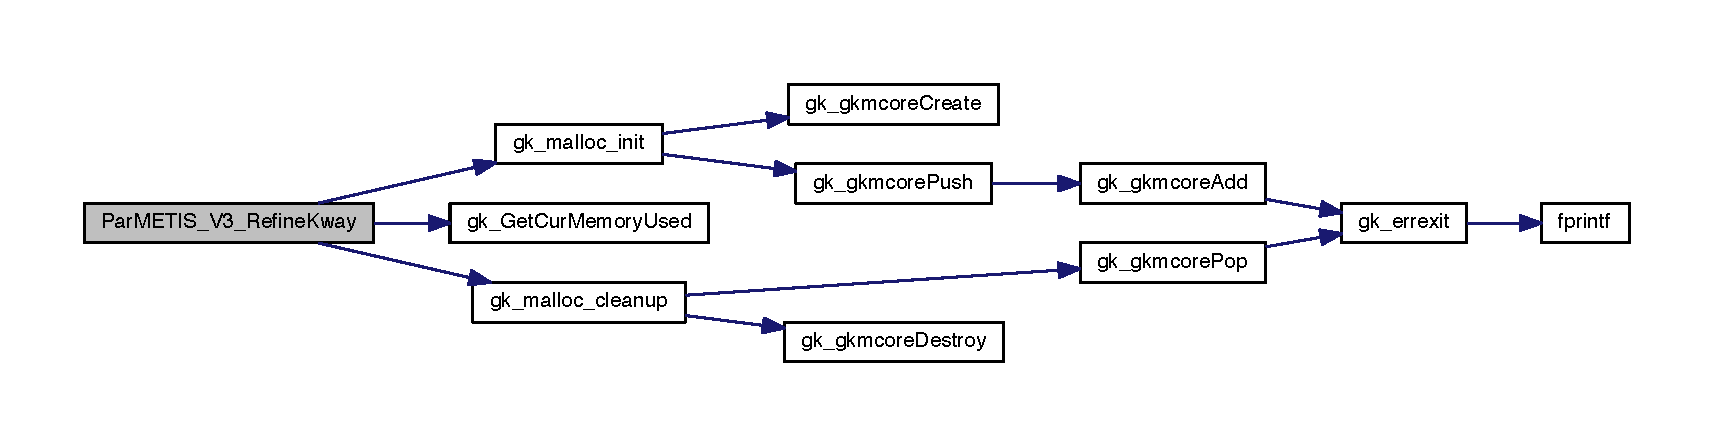
\includegraphics[width=350pt]{include_2parmetis_8h_ad40a7809c9bdf183926da011220bad75_cgraph}
\end{center}
\end{figure}

\hypertarget{akwayfm_8c}{}\section{3rd\+Party/parmetis-\/4.0.3/libparmetis/akwayfm.c File Reference}
\label{akwayfm_8c}\index{3rd\+Party/parmetis-\/4.\+0.\+3/libparmetis/akwayfm.\+c@{3rd\+Party/parmetis-\/4.\+0.\+3/libparmetis/akwayfm.\+c}}
{\ttfamily \#include $<$parmetislib.\+h$>$}\newline
Include dependency graph for akwayfm.\+c\+:\nopagebreak
\begin{figure}[H]
\begin{center}
\leavevmode
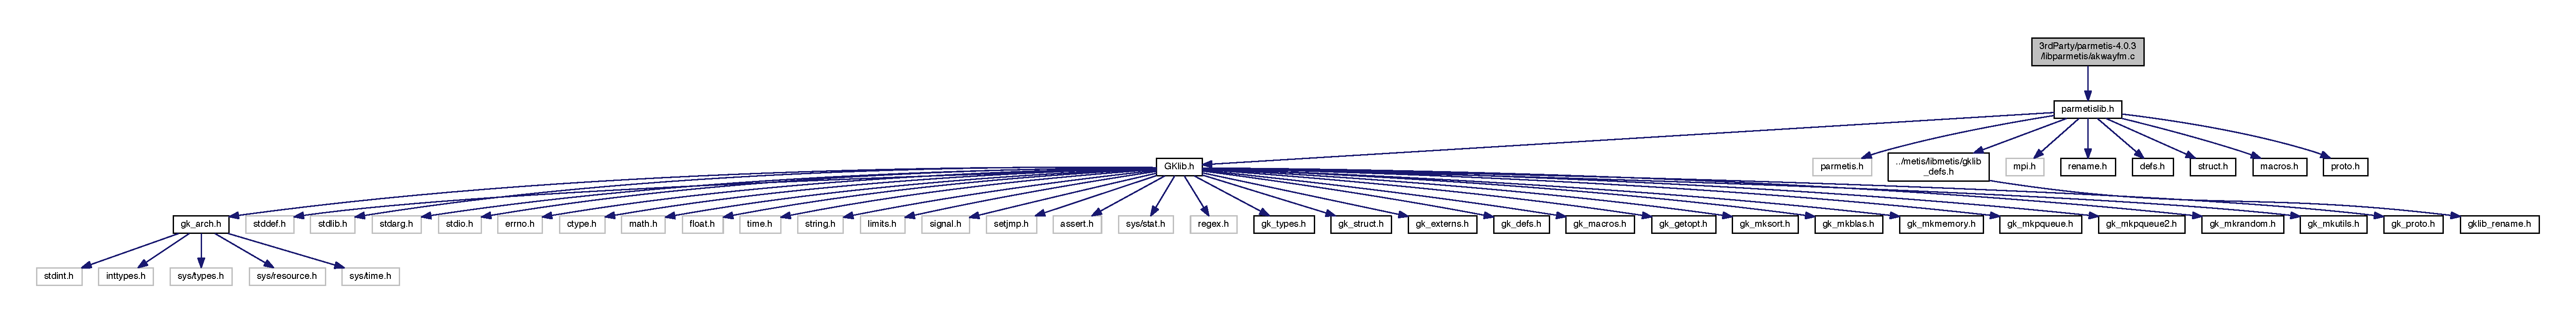
\includegraphics[width=350pt]{akwayfm_8c__incl}
\end{center}
\end{figure}
\subsection*{Macros}
\begin{DoxyCompactItemize}
\item 
\#define \hyperlink{akwayfm_8c_a0fc4274c04fd700ac3a3594ef91e15c7}{Proper\+Side}(c,  from,  other)~(((c) == 0 \&\& (from)-\/(other) $<$ 0) $\vert$$\vert$ ((c) == 1 \&\& (from)-\/(other) $>$ 0))
\end{DoxyCompactItemize}
\subsection*{Functions}
\begin{DoxyCompactItemize}
\item 
void \hyperlink{akwayfm_8c_a2183d39c5ec7859f1e28e4d2693bd965}{K\+Way\+Adaptive\+Refine} (\hyperlink{structctrl__t}{ctrl\+\_\+t} $\ast$ctrl, \hyperlink{structgraph__t}{graph\+\_\+t} $\ast$graph, \hyperlink{3rd_party_2parmetis-4_80_83_2metis_2include_2metis_8h_aaa5262be3e700770163401acb0150f52}{idx\+\_\+t} npasses)
\end{DoxyCompactItemize}


\subsection{Macro Definition Documentation}
\mbox{\Hypertarget{akwayfm_8c_a0fc4274c04fd700ac3a3594ef91e15c7}\label{akwayfm_8c_a0fc4274c04fd700ac3a3594ef91e15c7}} 
\index{akwayfm.\+c@{akwayfm.\+c}!Proper\+Side@{Proper\+Side}}
\index{Proper\+Side@{Proper\+Side}!akwayfm.\+c@{akwayfm.\+c}}
\subsubsection{\texorpdfstring{Proper\+Side}{ProperSide}}
{\footnotesize\ttfamily \#define Proper\+Side(\begin{DoxyParamCaption}\item[{}]{c,  }\item[{}]{from,  }\item[{}]{other }\end{DoxyParamCaption})~(((c) == 0 \&\& (from)-\/(other) $<$ 0) $\vert$$\vert$ ((c) == 1 \&\& (from)-\/(other) $>$ 0))}



\subsection{Function Documentation}
\mbox{\Hypertarget{akwayfm_8c_a2183d39c5ec7859f1e28e4d2693bd965}\label{akwayfm_8c_a2183d39c5ec7859f1e28e4d2693bd965}} 
\index{akwayfm.\+c@{akwayfm.\+c}!K\+Way\+Adaptive\+Refine@{K\+Way\+Adaptive\+Refine}}
\index{K\+Way\+Adaptive\+Refine@{K\+Way\+Adaptive\+Refine}!akwayfm.\+c@{akwayfm.\+c}}
\subsubsection{\texorpdfstring{K\+Way\+Adaptive\+Refine()}{KWayAdaptiveRefine()}}
{\footnotesize\ttfamily void K\+Way\+Adaptive\+Refine (\begin{DoxyParamCaption}\item[{\hyperlink{structctrl__t}{ctrl\+\_\+t} $\ast$}]{ctrl,  }\item[{\hyperlink{structgraph__t}{graph\+\_\+t} $\ast$}]{graph,  }\item[{\hyperlink{3rd_party_2parmetis-4_80_83_2metis_2include_2metis_8h_aaa5262be3e700770163401acb0150f52}{idx\+\_\+t}}]{npasses }\end{DoxyParamCaption})}

Here is the call graph for this function\+:\nopagebreak
\begin{figure}[H]
\begin{center}
\leavevmode
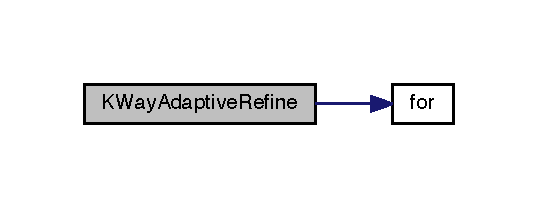
\includegraphics[width=258pt]{akwayfm_8c_a2183d39c5ec7859f1e28e4d2693bd965_cgraph}
\end{center}
\end{figure}

\hypertarget{ametis_8c}{}\section{3rd\+Party/parmetis-\/4.0.3/libparmetis/ametis.c File Reference}
\label{ametis_8c}\index{3rd\+Party/parmetis-\/4.\+0.\+3/libparmetis/ametis.\+c@{3rd\+Party/parmetis-\/4.\+0.\+3/libparmetis/ametis.\+c}}
{\ttfamily \#include $<$parmetislib.\+h$>$}\newline
Include dependency graph for ametis.\+c\+:\nopagebreak
\begin{figure}[H]
\begin{center}
\leavevmode
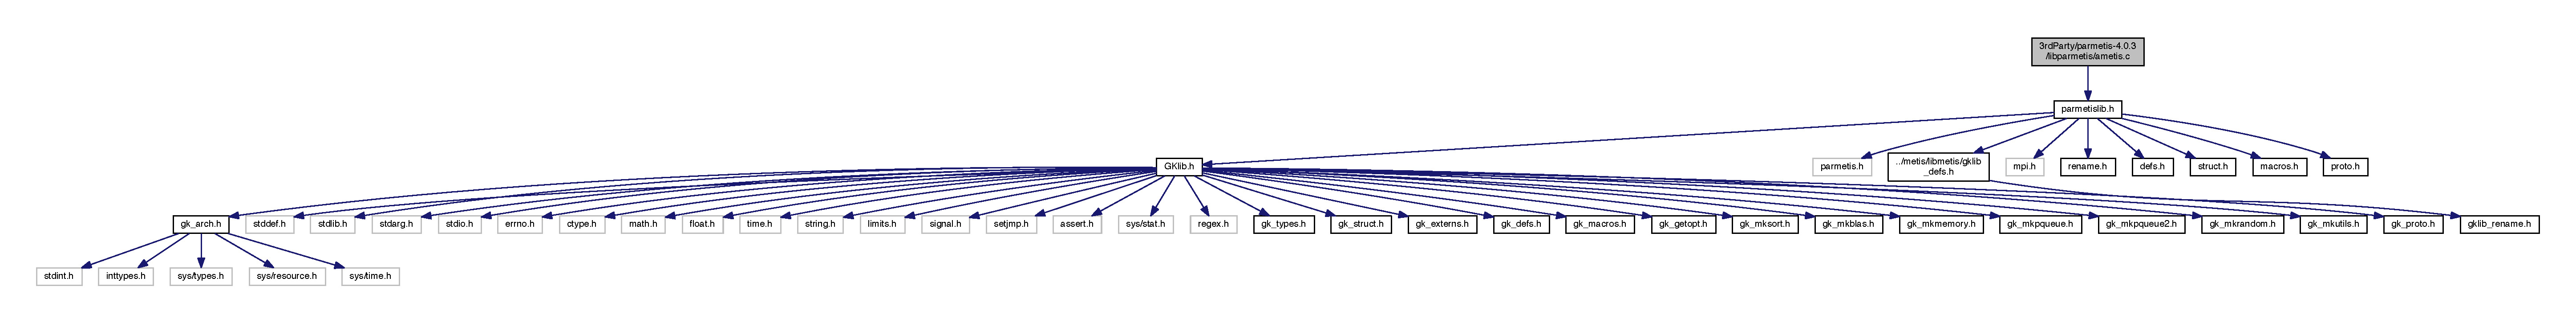
\includegraphics[width=350pt]{ametis_8c__incl}
\end{center}
\end{figure}
\subsection*{Functions}
\begin{DoxyCompactItemize}
\item 
int \hyperlink{ametis_8c_af584de3fd53c9e04d79f5037b546b9cc}{Par\+M\+E\+T\+I\+S\+\_\+\+V3\+\_\+\+Adaptive\+Repart} (\hyperlink{3rd_party_2parmetis-4_80_83_2metis_2include_2metis_8h_aaa5262be3e700770163401acb0150f52}{idx\+\_\+t} $\ast$vtxdist, \hyperlink{3rd_party_2parmetis-4_80_83_2metis_2include_2metis_8h_aaa5262be3e700770163401acb0150f52}{idx\+\_\+t} $\ast$\hyperlink{include_2metis_8h_aa8fc7f75458e38e1e2979ed6db639164}{xadj}, \hyperlink{3rd_party_2parmetis-4_80_83_2metis_2include_2metis_8h_aaa5262be3e700770163401acb0150f52}{idx\+\_\+t} $\ast$\hyperlink{include_2metis_8h_a20c068e3ebdd8f9889fb82c1f677d679}{adjncy}, \hyperlink{3rd_party_2parmetis-4_80_83_2metis_2include_2metis_8h_aaa5262be3e700770163401acb0150f52}{idx\+\_\+t} $\ast$\hyperlink{include_2metis_8h_a34203f1160d94eca83e95f2718ea3504}{vwgt}, \hyperlink{3rd_party_2parmetis-4_80_83_2metis_2include_2metis_8h_aaa5262be3e700770163401acb0150f52}{idx\+\_\+t} $\ast$\hyperlink{include_2metis_8h_aac32df5bb22250d94fc2fc7e4078308b}{vsize}, \hyperlink{3rd_party_2parmetis-4_80_83_2metis_2include_2metis_8h_aaa5262be3e700770163401acb0150f52}{idx\+\_\+t} $\ast$\hyperlink{include_2metis_8h_a2be4719baa820cfa5c06fd070796e0d3}{adjwgt}, \hyperlink{3rd_party_2parmetis-4_80_83_2metis_2include_2metis_8h_aaa5262be3e700770163401acb0150f52}{idx\+\_\+t} $\ast$wgtflag, \hyperlink{3rd_party_2parmetis-4_80_83_2metis_2include_2metis_8h_aaa5262be3e700770163401acb0150f52}{idx\+\_\+t} $\ast$\hyperlink{include_2metis_8h_aa48ecaf34ec788199c3aedb2b1558eb7}{numflag}, \hyperlink{3rd_party_2parmetis-4_80_83_2metis_2include_2metis_8h_aaa5262be3e700770163401acb0150f52}{idx\+\_\+t} $\ast$\hyperlink{include_2metis_8h_ac1dd31740e8f97fb57dc917ded30253f}{ncon}, \hyperlink{3rd_party_2parmetis-4_80_83_2metis_2include_2metis_8h_aaa5262be3e700770163401acb0150f52}{idx\+\_\+t} $\ast$\hyperlink{include_2metis_8h_aad88065af88fd6759101788a8e15ce9e}{nparts}, \hyperlink{3rd_party_2parmetis-4_80_83_2metis_2include_2metis_8h_a1924a4f6907cc3833213aba1f07fcbe9}{real\+\_\+t} $\ast$\hyperlink{include_2metis_8h_aa91786cd8ea996ec49ed5b382eb7fc2f}{tpwgts}, \hyperlink{3rd_party_2parmetis-4_80_83_2metis_2include_2metis_8h_a1924a4f6907cc3833213aba1f07fcbe9}{real\+\_\+t} $\ast$\hyperlink{include_2metis_8h_af48bb348bc8440a61f90f137de83f203}{ubvec}, \hyperlink{3rd_party_2parmetis-4_80_83_2metis_2include_2metis_8h_a1924a4f6907cc3833213aba1f07fcbe9}{real\+\_\+t} $\ast$ipc2redist, \hyperlink{3rd_party_2parmetis-4_80_83_2metis_2include_2metis_8h_aaa5262be3e700770163401acb0150f52}{idx\+\_\+t} $\ast$\hyperlink{include_2metis_8h_a68c032ed4161802775c6847d4cb39adf}{options}, \hyperlink{3rd_party_2parmetis-4_80_83_2metis_2include_2metis_8h_aaa5262be3e700770163401acb0150f52}{idx\+\_\+t} $\ast$\hyperlink{include_2metis_8h_a8e62a902298dd5fd88ef554d5277b1dc}{edgecut}, \hyperlink{3rd_party_2parmetis-4_80_83_2metis_2include_2metis_8h_aaa5262be3e700770163401acb0150f52}{idx\+\_\+t} $\ast$\hyperlink{include_2metis_8h_a0a9ea8670f88d6db1e021fee2dcd94be}{part}, M\+P\+I\+\_\+\+Comm $\ast$comm)
\item 
void \hyperlink{ametis_8c_a4bfface1ffce942d966b638a079f0833}{Adaptive\+\_\+\+Partition} (\hyperlink{structctrl__t}{ctrl\+\_\+t} $\ast$ctrl, \hyperlink{structgraph__t}{graph\+\_\+t} $\ast$graph)
\end{DoxyCompactItemize}


\subsection{Function Documentation}
\mbox{\Hypertarget{ametis_8c_a4bfface1ffce942d966b638a079f0833}\label{ametis_8c_a4bfface1ffce942d966b638a079f0833}} 
\index{ametis.\+c@{ametis.\+c}!Adaptive\+\_\+\+Partition@{Adaptive\+\_\+\+Partition}}
\index{Adaptive\+\_\+\+Partition@{Adaptive\+\_\+\+Partition}!ametis.\+c@{ametis.\+c}}
\subsubsection{\texorpdfstring{Adaptive\+\_\+\+Partition()}{Adaptive\_Partition()}}
{\footnotesize\ttfamily void Adaptive\+\_\+\+Partition (\begin{DoxyParamCaption}\item[{\hyperlink{structctrl__t}{ctrl\+\_\+t} $\ast$}]{ctrl,  }\item[{\hyperlink{structgraph__t}{graph\+\_\+t} $\ast$}]{graph }\end{DoxyParamCaption})}

This function is the driver for the adaptive refinement mode of Par\+M\+E\+T\+IS Here is the call graph for this function\+:\nopagebreak
\begin{figure}[H]
\begin{center}
\leavevmode
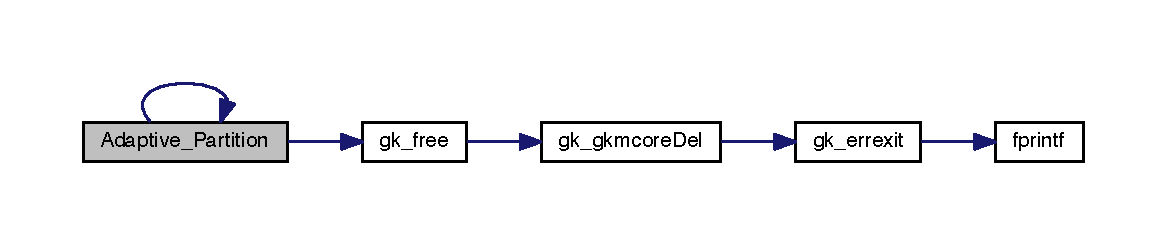
\includegraphics[width=350pt]{ametis_8c_a4bfface1ffce942d966b638a079f0833_cgraph}
\end{center}
\end{figure}
Here is the caller graph for this function\+:\nopagebreak
\begin{figure}[H]
\begin{center}
\leavevmode
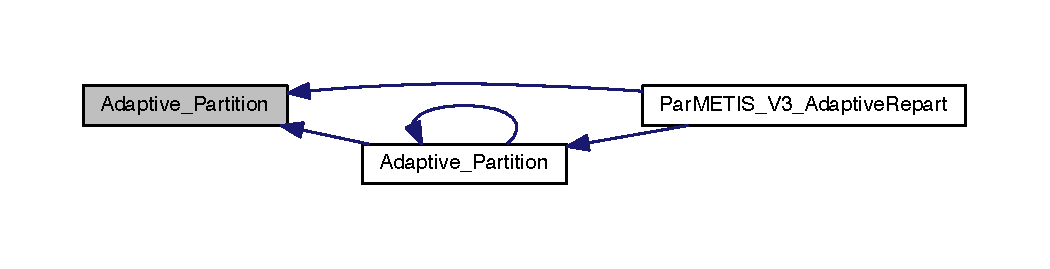
\includegraphics[width=350pt]{ametis_8c_a4bfface1ffce942d966b638a079f0833_icgraph}
\end{center}
\end{figure}
\mbox{\Hypertarget{ametis_8c_af584de3fd53c9e04d79f5037b546b9cc}\label{ametis_8c_af584de3fd53c9e04d79f5037b546b9cc}} 
\index{ametis.\+c@{ametis.\+c}!Par\+M\+E\+T\+I\+S\+\_\+\+V3\+\_\+\+Adaptive\+Repart@{Par\+M\+E\+T\+I\+S\+\_\+\+V3\+\_\+\+Adaptive\+Repart}}
\index{Par\+M\+E\+T\+I\+S\+\_\+\+V3\+\_\+\+Adaptive\+Repart@{Par\+M\+E\+T\+I\+S\+\_\+\+V3\+\_\+\+Adaptive\+Repart}!ametis.\+c@{ametis.\+c}}
\subsubsection{\texorpdfstring{Par\+M\+E\+T\+I\+S\+\_\+\+V3\+\_\+\+Adaptive\+Repart()}{ParMETIS\_V3\_AdaptiveRepart()}}
{\footnotesize\ttfamily int Par\+M\+E\+T\+I\+S\+\_\+\+V3\+\_\+\+Adaptive\+Repart (\begin{DoxyParamCaption}\item[{\hyperlink{3rd_party_2parmetis-4_80_83_2metis_2include_2metis_8h_aaa5262be3e700770163401acb0150f52}{idx\+\_\+t} $\ast$}]{vtxdist,  }\item[{\hyperlink{3rd_party_2parmetis-4_80_83_2metis_2include_2metis_8h_aaa5262be3e700770163401acb0150f52}{idx\+\_\+t} $\ast$}]{xadj,  }\item[{\hyperlink{3rd_party_2parmetis-4_80_83_2metis_2include_2metis_8h_aaa5262be3e700770163401acb0150f52}{idx\+\_\+t} $\ast$}]{adjncy,  }\item[{\hyperlink{3rd_party_2parmetis-4_80_83_2metis_2include_2metis_8h_aaa5262be3e700770163401acb0150f52}{idx\+\_\+t} $\ast$}]{vwgt,  }\item[{\hyperlink{3rd_party_2parmetis-4_80_83_2metis_2include_2metis_8h_aaa5262be3e700770163401acb0150f52}{idx\+\_\+t} $\ast$}]{vsize,  }\item[{\hyperlink{3rd_party_2parmetis-4_80_83_2metis_2include_2metis_8h_aaa5262be3e700770163401acb0150f52}{idx\+\_\+t} $\ast$}]{adjwgt,  }\item[{\hyperlink{3rd_party_2parmetis-4_80_83_2metis_2include_2metis_8h_aaa5262be3e700770163401acb0150f52}{idx\+\_\+t} $\ast$}]{wgtflag,  }\item[{\hyperlink{3rd_party_2parmetis-4_80_83_2metis_2include_2metis_8h_aaa5262be3e700770163401acb0150f52}{idx\+\_\+t} $\ast$}]{numflag,  }\item[{\hyperlink{3rd_party_2parmetis-4_80_83_2metis_2include_2metis_8h_aaa5262be3e700770163401acb0150f52}{idx\+\_\+t} $\ast$}]{ncon,  }\item[{\hyperlink{3rd_party_2parmetis-4_80_83_2metis_2include_2metis_8h_aaa5262be3e700770163401acb0150f52}{idx\+\_\+t} $\ast$}]{nparts,  }\item[{\hyperlink{3rd_party_2parmetis-4_80_83_2metis_2include_2metis_8h_a1924a4f6907cc3833213aba1f07fcbe9}{real\+\_\+t} $\ast$}]{tpwgts,  }\item[{\hyperlink{3rd_party_2parmetis-4_80_83_2metis_2include_2metis_8h_a1924a4f6907cc3833213aba1f07fcbe9}{real\+\_\+t} $\ast$}]{ubvec,  }\item[{\hyperlink{3rd_party_2parmetis-4_80_83_2metis_2include_2metis_8h_a1924a4f6907cc3833213aba1f07fcbe9}{real\+\_\+t} $\ast$}]{ipc2redist,  }\item[{\hyperlink{3rd_party_2parmetis-4_80_83_2metis_2include_2metis_8h_aaa5262be3e700770163401acb0150f52}{idx\+\_\+t} $\ast$}]{options,  }\item[{\hyperlink{3rd_party_2parmetis-4_80_83_2metis_2include_2metis_8h_aaa5262be3e700770163401acb0150f52}{idx\+\_\+t} $\ast$}]{edgecut,  }\item[{\hyperlink{3rd_party_2parmetis-4_80_83_2metis_2include_2metis_8h_aaa5262be3e700770163401acb0150f52}{idx\+\_\+t} $\ast$}]{part,  }\item[{M\+P\+I\+\_\+\+Comm $\ast$}]{comm }\end{DoxyParamCaption})}

Here is the call graph for this function\+:\nopagebreak
\begin{figure}[H]
\begin{center}
\leavevmode
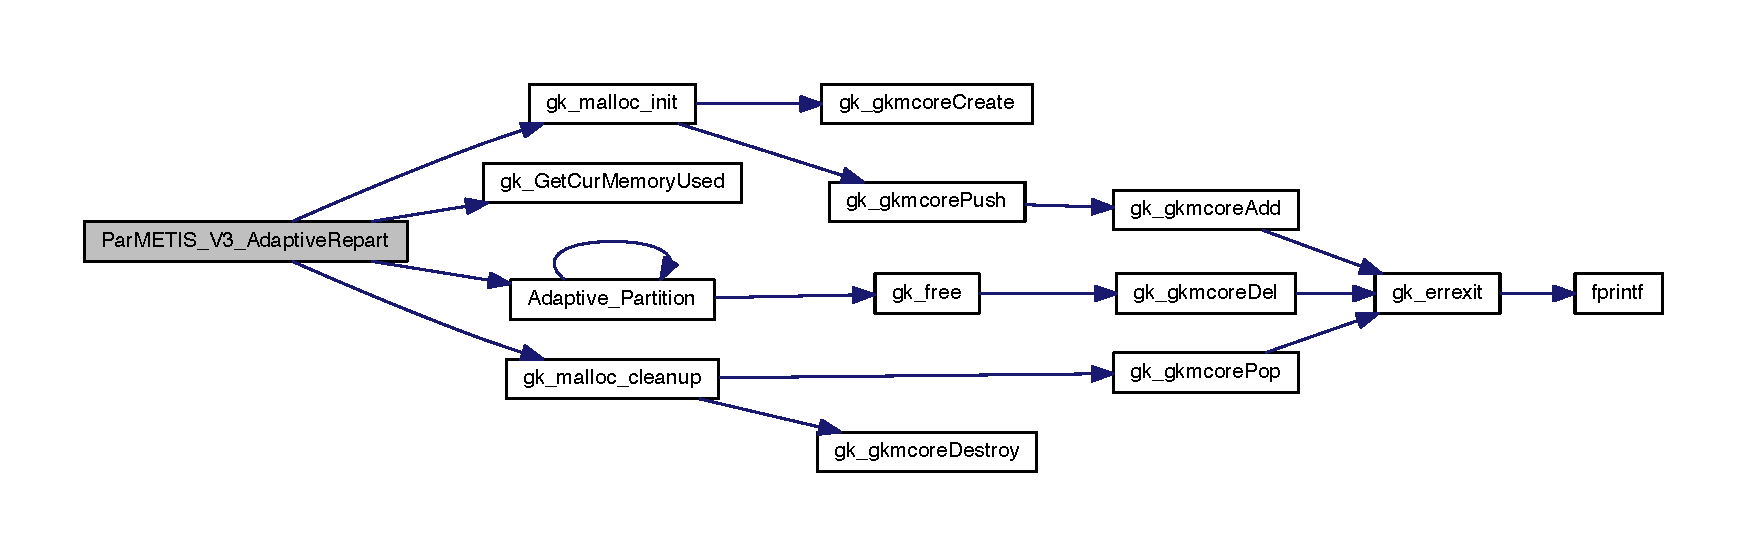
\includegraphics[width=350pt]{ametis_8c_af584de3fd53c9e04d79f5037b546b9cc_cgraph}
\end{center}
\end{figure}
Here is the caller graph for this function\+:\nopagebreak
\begin{figure}[H]
\begin{center}
\leavevmode
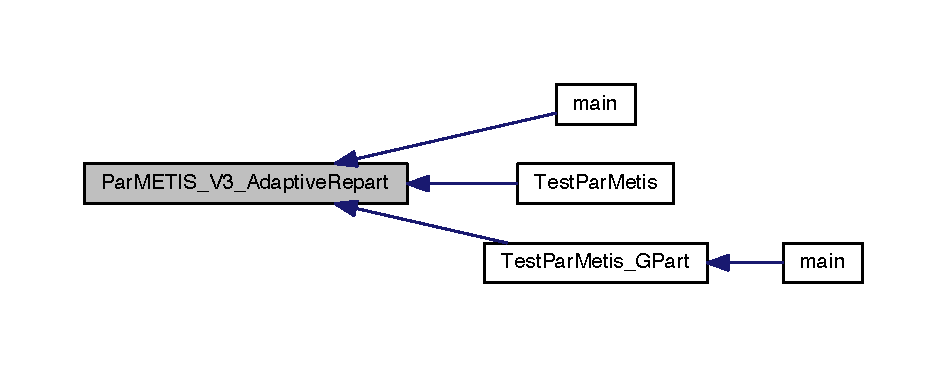
\includegraphics[width=350pt]{ametis_8c_af584de3fd53c9e04d79f5037b546b9cc_icgraph}
\end{center}
\end{figure}

\hypertarget{balancemylink_8c}{}\section{3rd\+Party/parmetis-\/4.0.3/libparmetis/balancemylink.c File Reference}
\label{balancemylink_8c}\index{3rd\+Party/parmetis-\/4.\+0.\+3/libparmetis/balancemylink.\+c@{3rd\+Party/parmetis-\/4.\+0.\+3/libparmetis/balancemylink.\+c}}
{\ttfamily \#include $<$parmetislib.\+h$>$}\newline
Include dependency graph for balancemylink.\+c\+:\nopagebreak
\begin{figure}[H]
\begin{center}
\leavevmode
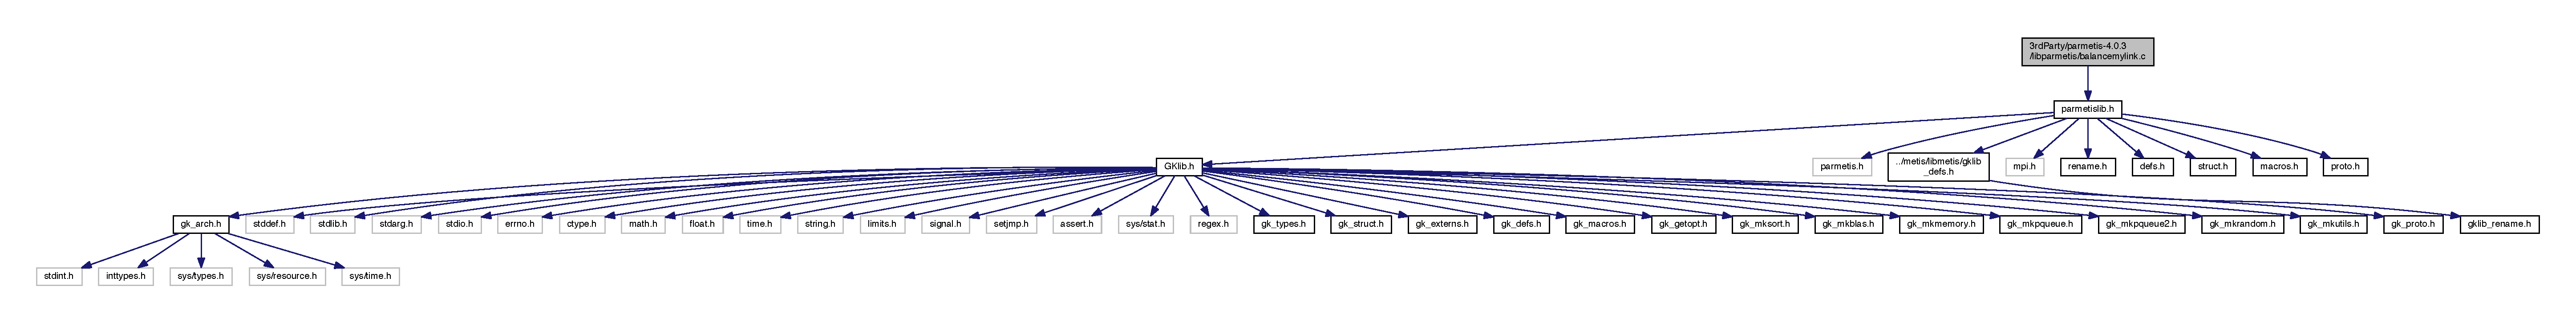
\includegraphics[width=350pt]{balancemylink_8c__incl}
\end{center}
\end{figure}
\subsection*{Macros}
\begin{DoxyCompactItemize}
\item 
\#define \hyperlink{balancemylink_8c_a211238ffe3627f42ca7b04bc96cc8fa6}{PE}~0
\end{DoxyCompactItemize}
\subsection*{Functions}
\begin{DoxyCompactItemize}
\item 
\hyperlink{3rd_party_2parmetis-4_80_83_2metis_2include_2metis_8h_aaa5262be3e700770163401acb0150f52}{idx\+\_\+t} \hyperlink{balancemylink_8c_a0c95cce46bb5d58661489c076a876018}{Balance\+My\+Link} (\hyperlink{structctrl__t}{ctrl\+\_\+t} $\ast$ctrl, \hyperlink{structgraph__t}{graph\+\_\+t} $\ast$graph, \hyperlink{3rd_party_2parmetis-4_80_83_2metis_2include_2metis_8h_aaa5262be3e700770163401acb0150f52}{idx\+\_\+t} $\ast$home, \hyperlink{3rd_party_2parmetis-4_80_83_2metis_2include_2metis_8h_aaa5262be3e700770163401acb0150f52}{idx\+\_\+t} me, \hyperlink{3rd_party_2parmetis-4_80_83_2metis_2include_2metis_8h_aaa5262be3e700770163401acb0150f52}{idx\+\_\+t} you, \hyperlink{3rd_party_2parmetis-4_80_83_2metis_2include_2metis_8h_a1924a4f6907cc3833213aba1f07fcbe9}{real\+\_\+t} $\ast$flows, \hyperlink{3rd_party_2parmetis-4_80_83_2metis_2include_2metis_8h_a1924a4f6907cc3833213aba1f07fcbe9}{real\+\_\+t} maxdiff, \hyperlink{3rd_party_2parmetis-4_80_83_2metis_2include_2metis_8h_a1924a4f6907cc3833213aba1f07fcbe9}{real\+\_\+t} $\ast$diff\+\_\+cost, \hyperlink{3rd_party_2parmetis-4_80_83_2metis_2include_2metis_8h_a1924a4f6907cc3833213aba1f07fcbe9}{real\+\_\+t} $\ast$diff\+\_\+lbavg, \hyperlink{3rd_party_2parmetis-4_80_83_2metis_2include_2metis_8h_a1924a4f6907cc3833213aba1f07fcbe9}{real\+\_\+t} avgvwgt)
\end{DoxyCompactItemize}


\subsection{Macro Definition Documentation}
\mbox{\Hypertarget{balancemylink_8c_a211238ffe3627f42ca7b04bc96cc8fa6}\label{balancemylink_8c_a211238ffe3627f42ca7b04bc96cc8fa6}} 
\index{balancemylink.\+c@{balancemylink.\+c}!PE@{PE}}
\index{PE@{PE}!balancemylink.\+c@{balancemylink.\+c}}
\subsubsection{\texorpdfstring{PE}{PE}}
{\footnotesize\ttfamily \#define PE~0}



\subsection{Function Documentation}
\mbox{\Hypertarget{balancemylink_8c_a0c95cce46bb5d58661489c076a876018}\label{balancemylink_8c_a0c95cce46bb5d58661489c076a876018}} 
\index{balancemylink.\+c@{balancemylink.\+c}!Balance\+My\+Link@{Balance\+My\+Link}}
\index{Balance\+My\+Link@{Balance\+My\+Link}!balancemylink.\+c@{balancemylink.\+c}}
\subsubsection{\texorpdfstring{Balance\+My\+Link()}{BalanceMyLink()}}
{\footnotesize\ttfamily \hyperlink{3rd_party_2parmetis-4_80_83_2metis_2include_2metis_8h_aaa5262be3e700770163401acb0150f52}{idx\+\_\+t} Balance\+My\+Link (\begin{DoxyParamCaption}\item[{\hyperlink{structctrl__t}{ctrl\+\_\+t} $\ast$}]{ctrl,  }\item[{\hyperlink{structgraph__t}{graph\+\_\+t} $\ast$}]{graph,  }\item[{\hyperlink{3rd_party_2parmetis-4_80_83_2metis_2include_2metis_8h_aaa5262be3e700770163401acb0150f52}{idx\+\_\+t} $\ast$}]{home,  }\item[{\hyperlink{3rd_party_2parmetis-4_80_83_2metis_2include_2metis_8h_aaa5262be3e700770163401acb0150f52}{idx\+\_\+t}}]{me,  }\item[{\hyperlink{3rd_party_2parmetis-4_80_83_2metis_2include_2metis_8h_aaa5262be3e700770163401acb0150f52}{idx\+\_\+t}}]{you,  }\item[{\hyperlink{3rd_party_2parmetis-4_80_83_2metis_2include_2metis_8h_a1924a4f6907cc3833213aba1f07fcbe9}{real\+\_\+t} $\ast$}]{flows,  }\item[{\hyperlink{3rd_party_2parmetis-4_80_83_2metis_2include_2metis_8h_a1924a4f6907cc3833213aba1f07fcbe9}{real\+\_\+t}}]{maxdiff,  }\item[{\hyperlink{3rd_party_2parmetis-4_80_83_2metis_2include_2metis_8h_a1924a4f6907cc3833213aba1f07fcbe9}{real\+\_\+t} $\ast$}]{diff\+\_\+cost,  }\item[{\hyperlink{3rd_party_2parmetis-4_80_83_2metis_2include_2metis_8h_a1924a4f6907cc3833213aba1f07fcbe9}{real\+\_\+t} $\ast$}]{diff\+\_\+lbavg,  }\item[{\hyperlink{3rd_party_2parmetis-4_80_83_2metis_2include_2metis_8h_a1924a4f6907cc3833213aba1f07fcbe9}{real\+\_\+t}}]{avgvwgt }\end{DoxyParamCaption})}


\hypertarget{comm_8c}{}\section{3rd\+Party/parmetis-\/4.0.3/libparmetis/comm.c File Reference}
\label{comm_8c}\index{3rd\+Party/parmetis-\/4.\+0.\+3/libparmetis/comm.\+c@{3rd\+Party/parmetis-\/4.\+0.\+3/libparmetis/comm.\+c}}
{\ttfamily \#include $<$parmetislib.\+h$>$}\newline
Include dependency graph for comm.\+c\+:\nopagebreak
\begin{figure}[H]
\begin{center}
\leavevmode
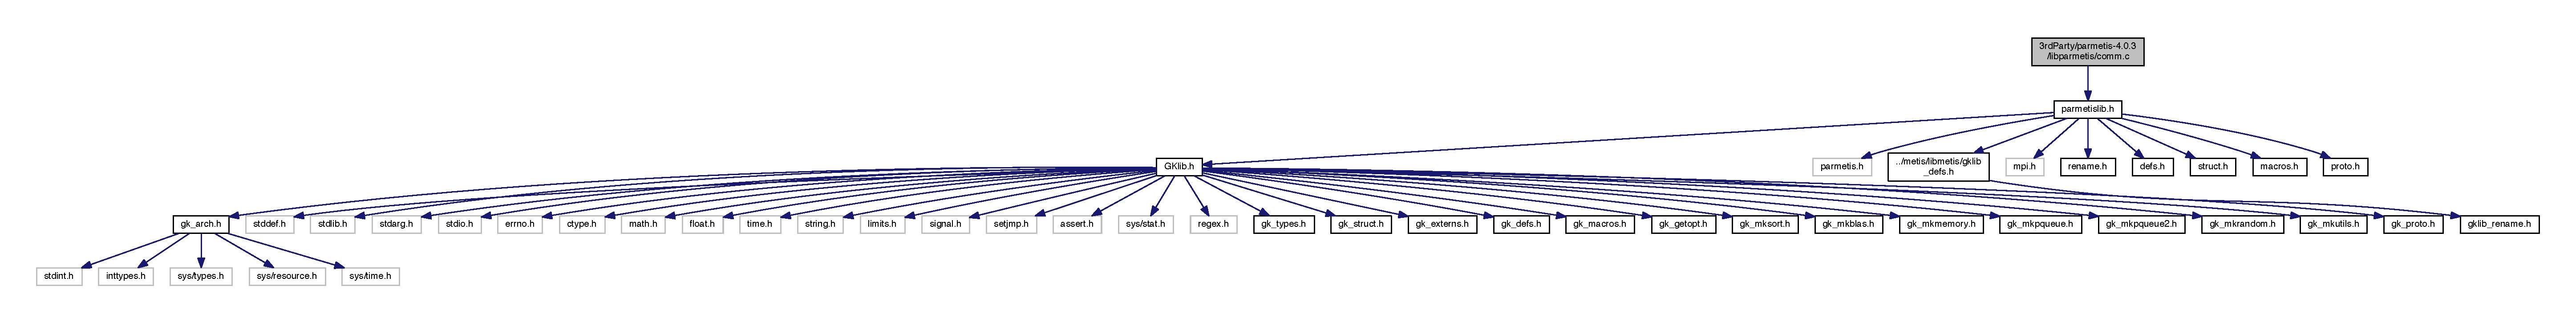
\includegraphics[width=350pt]{comm_8c__incl}
\end{center}
\end{figure}
\subsection*{Functions}
\begin{DoxyCompactItemize}
\item 
void \hyperlink{comm_8c_ab7b157ae46e347049d624027324316a0}{Comm\+Setup} (\hyperlink{structctrl__t}{ctrl\+\_\+t} $\ast$ctrl, \hyperlink{structgraph__t}{graph\+\_\+t} $\ast$graph)
\item 
void \hyperlink{comm_8c_a245110080c4fe1712c5cac4a52e61e69}{Comm\+Update\+Nnbrs} (\hyperlink{structctrl__t}{ctrl\+\_\+t} $\ast$ctrl, \hyperlink{3rd_party_2parmetis-4_80_83_2metis_2include_2metis_8h_aaa5262be3e700770163401acb0150f52}{idx\+\_\+t} nnbrs)
\item 
void \hyperlink{comm_8c_a4ea1863ed9e161bc82ff3c6f0ff431c9}{Comm\+Interface\+Data} (\hyperlink{structctrl__t}{ctrl\+\_\+t} $\ast$ctrl, \hyperlink{structgraph__t}{graph\+\_\+t} $\ast$graph, \hyperlink{3rd_party_2parmetis-4_80_83_2metis_2include_2metis_8h_aaa5262be3e700770163401acb0150f52}{idx\+\_\+t} $\ast$data, \hyperlink{3rd_party_2parmetis-4_80_83_2metis_2include_2metis_8h_aaa5262be3e700770163401acb0150f52}{idx\+\_\+t} $\ast$recvvector)
\item 
void \hyperlink{comm_8c_adc12fed8c165f50572b6704789b0a962}{Comm\+Changed\+Interface\+Data} (\hyperlink{structctrl__t}{ctrl\+\_\+t} $\ast$ctrl, \hyperlink{structgraph__t}{graph\+\_\+t} $\ast$graph, \hyperlink{3rd_party_2parmetis-4_80_83_2metis_2include_2metis_8h_aaa5262be3e700770163401acb0150f52}{idx\+\_\+t} nchanged, \hyperlink{3rd_party_2parmetis-4_80_83_2metis_2include_2metis_8h_aaa5262be3e700770163401acb0150f52}{idx\+\_\+t} $\ast$changed, \hyperlink{3rd_party_2parmetis-4_80_83_2metis_2include_2metis_8h_aaa5262be3e700770163401acb0150f52}{idx\+\_\+t} $\ast$data, ikv\+\_\+t $\ast$sendpairs, ikv\+\_\+t $\ast$recvpairs)
\item 
\hyperlink{3rd_party_2parmetis-4_80_83_2metis_2include_2metis_8h_aaa5262be3e700770163401acb0150f52}{idx\+\_\+t} \hyperlink{comm_8c_a51be32add0e43ecdac3f0b982a0733b4}{Global\+S\+E\+Max} (\hyperlink{structctrl__t}{ctrl\+\_\+t} $\ast$ctrl, \hyperlink{3rd_party_2parmetis-4_80_83_2metis_2include_2metis_8h_aaa5262be3e700770163401acb0150f52}{idx\+\_\+t} value)
\item 
\hyperlink{3rd_party_2parmetis-4_80_83_2metis_2include_2metis_8h_aaa5262be3e700770163401acb0150f52}{idx\+\_\+t} \hyperlink{comm_8c_aa31576794c6d7b00495b4402a1a4814a}{Global\+S\+E\+Max\+Comm} (M\+P\+I\+\_\+\+Comm comm, \hyperlink{3rd_party_2parmetis-4_80_83_2metis_2include_2metis_8h_aaa5262be3e700770163401acb0150f52}{idx\+\_\+t} value)
\item 
\hyperlink{3rd_party_2parmetis-4_80_83_2metis_2include_2metis_8h_aaa5262be3e700770163401acb0150f52}{idx\+\_\+t} \hyperlink{comm_8c_a7cffea998f35ba1b59fe0726bee38fc9}{Global\+S\+E\+Min} (\hyperlink{structctrl__t}{ctrl\+\_\+t} $\ast$ctrl, \hyperlink{3rd_party_2parmetis-4_80_83_2metis_2include_2metis_8h_aaa5262be3e700770163401acb0150f52}{idx\+\_\+t} value)
\item 
\hyperlink{3rd_party_2parmetis-4_80_83_2metis_2include_2metis_8h_aaa5262be3e700770163401acb0150f52}{idx\+\_\+t} \hyperlink{comm_8c_a44bc5168b7fcc675e4e07293a712f12b}{Global\+S\+E\+Min\+Comm} (M\+P\+I\+\_\+\+Comm comm, \hyperlink{3rd_party_2parmetis-4_80_83_2metis_2include_2metis_8h_aaa5262be3e700770163401acb0150f52}{idx\+\_\+t} value)
\item 
\hyperlink{3rd_party_2parmetis-4_80_83_2metis_2include_2metis_8h_aaa5262be3e700770163401acb0150f52}{idx\+\_\+t} \hyperlink{comm_8c_a3436cdd78aad4086a1df7cd254a7f2f9}{Global\+S\+E\+Sum} (\hyperlink{structctrl__t}{ctrl\+\_\+t} $\ast$ctrl, \hyperlink{3rd_party_2parmetis-4_80_83_2metis_2include_2metis_8h_aaa5262be3e700770163401acb0150f52}{idx\+\_\+t} value)
\item 
\hyperlink{3rd_party_2parmetis-4_80_83_2metis_2include_2metis_8h_aaa5262be3e700770163401acb0150f52}{idx\+\_\+t} \hyperlink{comm_8c_a10c4011516ef455e5c128a4112cf2cea}{Global\+S\+E\+Sum\+Comm} (M\+P\+I\+\_\+\+Comm comm, \hyperlink{3rd_party_2parmetis-4_80_83_2metis_2include_2metis_8h_aaa5262be3e700770163401acb0150f52}{idx\+\_\+t} value)
\item 
\hyperlink{3rd_party_2parmetis-4_80_83_2metis_2include_2metis_8h_a1924a4f6907cc3833213aba1f07fcbe9}{real\+\_\+t} \hyperlink{comm_8c_ad62cb5f0c141a2535d0f6eca6588a1c5}{Global\+S\+E\+Max\+Float} (\hyperlink{structctrl__t}{ctrl\+\_\+t} $\ast$ctrl, \hyperlink{3rd_party_2parmetis-4_80_83_2metis_2include_2metis_8h_a1924a4f6907cc3833213aba1f07fcbe9}{real\+\_\+t} value)
\item 
\hyperlink{3rd_party_2parmetis-4_80_83_2metis_2include_2metis_8h_a1924a4f6907cc3833213aba1f07fcbe9}{real\+\_\+t} \hyperlink{comm_8c_ab1ebf8b04ebb66e2a28e603f249d9ca8}{Global\+S\+E\+Min\+Float} (\hyperlink{structctrl__t}{ctrl\+\_\+t} $\ast$ctrl, \hyperlink{3rd_party_2parmetis-4_80_83_2metis_2include_2metis_8h_a1924a4f6907cc3833213aba1f07fcbe9}{real\+\_\+t} value)
\item 
\hyperlink{3rd_party_2parmetis-4_80_83_2metis_2include_2metis_8h_a1924a4f6907cc3833213aba1f07fcbe9}{real\+\_\+t} \hyperlink{comm_8c_a6cd212bae78535674c941b90373d6b0b}{Global\+S\+E\+Sum\+Float} (\hyperlink{structctrl__t}{ctrl\+\_\+t} $\ast$ctrl, \hyperlink{3rd_party_2parmetis-4_80_83_2metis_2include_2metis_8h_a1924a4f6907cc3833213aba1f07fcbe9}{real\+\_\+t} value)
\end{DoxyCompactItemize}


\subsection{Function Documentation}
\mbox{\Hypertarget{comm_8c_adc12fed8c165f50572b6704789b0a962}\label{comm_8c_adc12fed8c165f50572b6704789b0a962}} 
\index{comm.\+c@{comm.\+c}!Comm\+Changed\+Interface\+Data@{Comm\+Changed\+Interface\+Data}}
\index{Comm\+Changed\+Interface\+Data@{Comm\+Changed\+Interface\+Data}!comm.\+c@{comm.\+c}}
\subsubsection{\texorpdfstring{Comm\+Changed\+Interface\+Data()}{CommChangedInterfaceData()}}
{\footnotesize\ttfamily void Comm\+Changed\+Interface\+Data (\begin{DoxyParamCaption}\item[{\hyperlink{structctrl__t}{ctrl\+\_\+t} $\ast$}]{ctrl,  }\item[{\hyperlink{structgraph__t}{graph\+\_\+t} $\ast$}]{graph,  }\item[{\hyperlink{3rd_party_2parmetis-4_80_83_2metis_2include_2metis_8h_aaa5262be3e700770163401acb0150f52}{idx\+\_\+t}}]{nchanged,  }\item[{\hyperlink{3rd_party_2parmetis-4_80_83_2metis_2include_2metis_8h_aaa5262be3e700770163401acb0150f52}{idx\+\_\+t} $\ast$}]{changed,  }\item[{\hyperlink{3rd_party_2parmetis-4_80_83_2metis_2include_2metis_8h_aaa5262be3e700770163401acb0150f52}{idx\+\_\+t} $\ast$}]{data,  }\item[{ikv\+\_\+t $\ast$}]{sendpairs,  }\item[{ikv\+\_\+t $\ast$}]{recvpairs }\end{DoxyParamCaption})}

\mbox{\Hypertarget{comm_8c_a4ea1863ed9e161bc82ff3c6f0ff431c9}\label{comm_8c_a4ea1863ed9e161bc82ff3c6f0ff431c9}} 
\index{comm.\+c@{comm.\+c}!Comm\+Interface\+Data@{Comm\+Interface\+Data}}
\index{Comm\+Interface\+Data@{Comm\+Interface\+Data}!comm.\+c@{comm.\+c}}
\subsubsection{\texorpdfstring{Comm\+Interface\+Data()}{CommInterfaceData()}}
{\footnotesize\ttfamily void Comm\+Interface\+Data (\begin{DoxyParamCaption}\item[{\hyperlink{structctrl__t}{ctrl\+\_\+t} $\ast$}]{ctrl,  }\item[{\hyperlink{structgraph__t}{graph\+\_\+t} $\ast$}]{graph,  }\item[{\hyperlink{3rd_party_2parmetis-4_80_83_2metis_2include_2metis_8h_aaa5262be3e700770163401acb0150f52}{idx\+\_\+t} $\ast$}]{data,  }\item[{\hyperlink{3rd_party_2parmetis-4_80_83_2metis_2include_2metis_8h_aaa5262be3e700770163401acb0150f52}{idx\+\_\+t} $\ast$}]{recvvector }\end{DoxyParamCaption})}

This function performs the gather/scatter for the boundary vertices \mbox{\Hypertarget{comm_8c_ab7b157ae46e347049d624027324316a0}\label{comm_8c_ab7b157ae46e347049d624027324316a0}} 
\index{comm.\+c@{comm.\+c}!Comm\+Setup@{Comm\+Setup}}
\index{Comm\+Setup@{Comm\+Setup}!comm.\+c@{comm.\+c}}
\subsubsection{\texorpdfstring{Comm\+Setup()}{CommSetup()}}
{\footnotesize\ttfamily void Comm\+Setup (\begin{DoxyParamCaption}\item[{\hyperlink{structctrl__t}{ctrl\+\_\+t} $\ast$}]{ctrl,  }\item[{\hyperlink{structgraph__t}{graph\+\_\+t} $\ast$}]{graph }\end{DoxyParamCaption})}

This function performs the following functions\+:
\begin{DoxyItemize}
\item determines the processors that contain adjacent vertices and setup the infrastructure for efficient communication.
\item localizes the numbering of the adjancency lists. 
\end{DoxyItemize}Here is the call graph for this function\+:\nopagebreak
\begin{figure}[H]
\begin{center}
\leavevmode
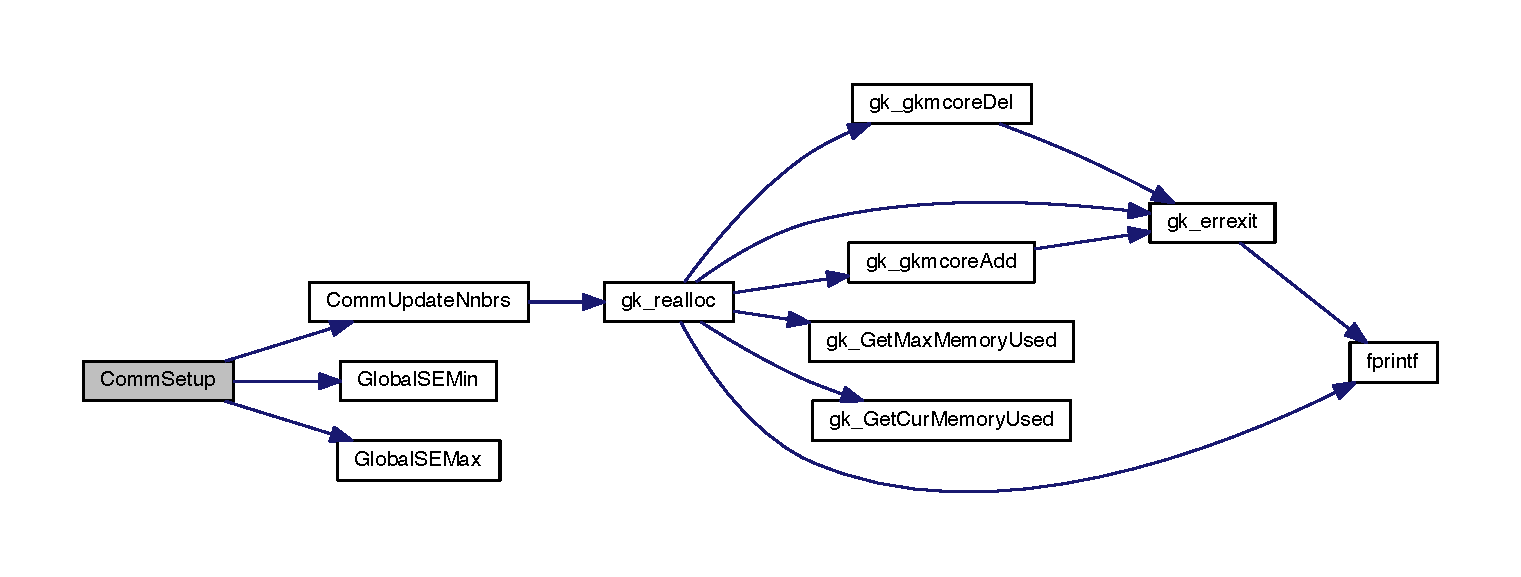
\includegraphics[width=350pt]{comm_8c_ab7b157ae46e347049d624027324316a0_cgraph}
\end{center}
\end{figure}
\mbox{\Hypertarget{comm_8c_a245110080c4fe1712c5cac4a52e61e69}\label{comm_8c_a245110080c4fe1712c5cac4a52e61e69}} 
\index{comm.\+c@{comm.\+c}!Comm\+Update\+Nnbrs@{Comm\+Update\+Nnbrs}}
\index{Comm\+Update\+Nnbrs@{Comm\+Update\+Nnbrs}!comm.\+c@{comm.\+c}}
\subsubsection{\texorpdfstring{Comm\+Update\+Nnbrs()}{CommUpdateNnbrs()}}
{\footnotesize\ttfamily void Comm\+Update\+Nnbrs (\begin{DoxyParamCaption}\item[{\hyperlink{structctrl__t}{ctrl\+\_\+t} $\ast$}]{ctrl,  }\item[{\hyperlink{3rd_party_2parmetis-4_80_83_2metis_2include_2metis_8h_aaa5262be3e700770163401acb0150f52}{idx\+\_\+t}}]{nnbrs }\end{DoxyParamCaption})}

This function updates the sreq/rreq/statuses arrays in ctrl based on the new number of neighbors. Here is the call graph for this function\+:\nopagebreak
\begin{figure}[H]
\begin{center}
\leavevmode
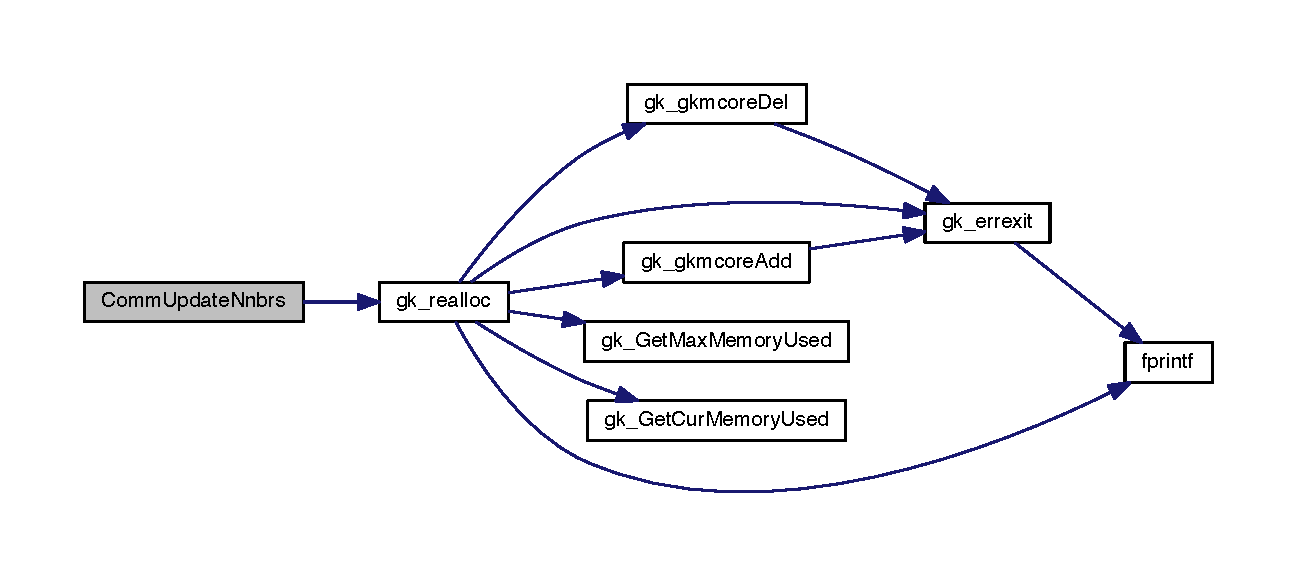
\includegraphics[width=350pt]{comm_8c_a245110080c4fe1712c5cac4a52e61e69_cgraph}
\end{center}
\end{figure}
Here is the caller graph for this function\+:\nopagebreak
\begin{figure}[H]
\begin{center}
\leavevmode
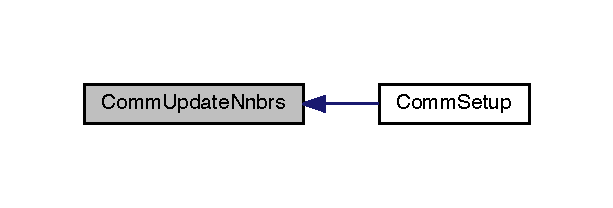
\includegraphics[width=294pt]{comm_8c_a245110080c4fe1712c5cac4a52e61e69_icgraph}
\end{center}
\end{figure}
\mbox{\Hypertarget{comm_8c_a51be32add0e43ecdac3f0b982a0733b4}\label{comm_8c_a51be32add0e43ecdac3f0b982a0733b4}} 
\index{comm.\+c@{comm.\+c}!Global\+S\+E\+Max@{Global\+S\+E\+Max}}
\index{Global\+S\+E\+Max@{Global\+S\+E\+Max}!comm.\+c@{comm.\+c}}
\subsubsection{\texorpdfstring{Global\+S\+E\+Max()}{GlobalSEMax()}}
{\footnotesize\ttfamily \hyperlink{3rd_party_2parmetis-4_80_83_2metis_2include_2metis_8h_aaa5262be3e700770163401acb0150f52}{idx\+\_\+t} Global\+S\+E\+Max (\begin{DoxyParamCaption}\item[{\hyperlink{structctrl__t}{ctrl\+\_\+t} $\ast$}]{ctrl,  }\item[{\hyperlink{3rd_party_2parmetis-4_80_83_2metis_2include_2metis_8h_aaa5262be3e700770163401acb0150f52}{idx\+\_\+t}}]{value }\end{DoxyParamCaption})}

Here is the caller graph for this function\+:\nopagebreak
\begin{figure}[H]
\begin{center}
\leavevmode
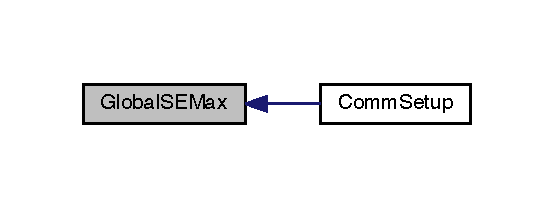
\includegraphics[width=266pt]{comm_8c_a51be32add0e43ecdac3f0b982a0733b4_icgraph}
\end{center}
\end{figure}
\mbox{\Hypertarget{comm_8c_aa31576794c6d7b00495b4402a1a4814a}\label{comm_8c_aa31576794c6d7b00495b4402a1a4814a}} 
\index{comm.\+c@{comm.\+c}!Global\+S\+E\+Max\+Comm@{Global\+S\+E\+Max\+Comm}}
\index{Global\+S\+E\+Max\+Comm@{Global\+S\+E\+Max\+Comm}!comm.\+c@{comm.\+c}}
\subsubsection{\texorpdfstring{Global\+S\+E\+Max\+Comm()}{GlobalSEMaxComm()}}
{\footnotesize\ttfamily \hyperlink{3rd_party_2parmetis-4_80_83_2metis_2include_2metis_8h_aaa5262be3e700770163401acb0150f52}{idx\+\_\+t} Global\+S\+E\+Max\+Comm (\begin{DoxyParamCaption}\item[{M\+P\+I\+\_\+\+Comm}]{comm,  }\item[{\hyperlink{3rd_party_2parmetis-4_80_83_2metis_2include_2metis_8h_aaa5262be3e700770163401acb0150f52}{idx\+\_\+t}}]{value }\end{DoxyParamCaption})}

\mbox{\Hypertarget{comm_8c_ad62cb5f0c141a2535d0f6eca6588a1c5}\label{comm_8c_ad62cb5f0c141a2535d0f6eca6588a1c5}} 
\index{comm.\+c@{comm.\+c}!Global\+S\+E\+Max\+Float@{Global\+S\+E\+Max\+Float}}
\index{Global\+S\+E\+Max\+Float@{Global\+S\+E\+Max\+Float}!comm.\+c@{comm.\+c}}
\subsubsection{\texorpdfstring{Global\+S\+E\+Max\+Float()}{GlobalSEMaxFloat()}}
{\footnotesize\ttfamily \hyperlink{3rd_party_2parmetis-4_80_83_2metis_2include_2metis_8h_a1924a4f6907cc3833213aba1f07fcbe9}{real\+\_\+t} Global\+S\+E\+Max\+Float (\begin{DoxyParamCaption}\item[{\hyperlink{structctrl__t}{ctrl\+\_\+t} $\ast$}]{ctrl,  }\item[{\hyperlink{3rd_party_2parmetis-4_80_83_2metis_2include_2metis_8h_a1924a4f6907cc3833213aba1f07fcbe9}{real\+\_\+t}}]{value }\end{DoxyParamCaption})}

\mbox{\Hypertarget{comm_8c_a7cffea998f35ba1b59fe0726bee38fc9}\label{comm_8c_a7cffea998f35ba1b59fe0726bee38fc9}} 
\index{comm.\+c@{comm.\+c}!Global\+S\+E\+Min@{Global\+S\+E\+Min}}
\index{Global\+S\+E\+Min@{Global\+S\+E\+Min}!comm.\+c@{comm.\+c}}
\subsubsection{\texorpdfstring{Global\+S\+E\+Min()}{GlobalSEMin()}}
{\footnotesize\ttfamily \hyperlink{3rd_party_2parmetis-4_80_83_2metis_2include_2metis_8h_aaa5262be3e700770163401acb0150f52}{idx\+\_\+t} Global\+S\+E\+Min (\begin{DoxyParamCaption}\item[{\hyperlink{structctrl__t}{ctrl\+\_\+t} $\ast$}]{ctrl,  }\item[{\hyperlink{3rd_party_2parmetis-4_80_83_2metis_2include_2metis_8h_aaa5262be3e700770163401acb0150f52}{idx\+\_\+t}}]{value }\end{DoxyParamCaption})}

Here is the caller graph for this function\+:\nopagebreak
\begin{figure}[H]
\begin{center}
\leavevmode
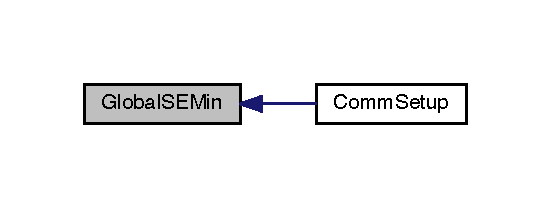
\includegraphics[width=264pt]{comm_8c_a7cffea998f35ba1b59fe0726bee38fc9_icgraph}
\end{center}
\end{figure}
\mbox{\Hypertarget{comm_8c_a44bc5168b7fcc675e4e07293a712f12b}\label{comm_8c_a44bc5168b7fcc675e4e07293a712f12b}} 
\index{comm.\+c@{comm.\+c}!Global\+S\+E\+Min\+Comm@{Global\+S\+E\+Min\+Comm}}
\index{Global\+S\+E\+Min\+Comm@{Global\+S\+E\+Min\+Comm}!comm.\+c@{comm.\+c}}
\subsubsection{\texorpdfstring{Global\+S\+E\+Min\+Comm()}{GlobalSEMinComm()}}
{\footnotesize\ttfamily \hyperlink{3rd_party_2parmetis-4_80_83_2metis_2include_2metis_8h_aaa5262be3e700770163401acb0150f52}{idx\+\_\+t} Global\+S\+E\+Min\+Comm (\begin{DoxyParamCaption}\item[{M\+P\+I\+\_\+\+Comm}]{comm,  }\item[{\hyperlink{3rd_party_2parmetis-4_80_83_2metis_2include_2metis_8h_aaa5262be3e700770163401acb0150f52}{idx\+\_\+t}}]{value }\end{DoxyParamCaption})}

\mbox{\Hypertarget{comm_8c_ab1ebf8b04ebb66e2a28e603f249d9ca8}\label{comm_8c_ab1ebf8b04ebb66e2a28e603f249d9ca8}} 
\index{comm.\+c@{comm.\+c}!Global\+S\+E\+Min\+Float@{Global\+S\+E\+Min\+Float}}
\index{Global\+S\+E\+Min\+Float@{Global\+S\+E\+Min\+Float}!comm.\+c@{comm.\+c}}
\subsubsection{\texorpdfstring{Global\+S\+E\+Min\+Float()}{GlobalSEMinFloat()}}
{\footnotesize\ttfamily \hyperlink{3rd_party_2parmetis-4_80_83_2metis_2include_2metis_8h_a1924a4f6907cc3833213aba1f07fcbe9}{real\+\_\+t} Global\+S\+E\+Min\+Float (\begin{DoxyParamCaption}\item[{\hyperlink{structctrl__t}{ctrl\+\_\+t} $\ast$}]{ctrl,  }\item[{\hyperlink{3rd_party_2parmetis-4_80_83_2metis_2include_2metis_8h_a1924a4f6907cc3833213aba1f07fcbe9}{real\+\_\+t}}]{value }\end{DoxyParamCaption})}

\mbox{\Hypertarget{comm_8c_a3436cdd78aad4086a1df7cd254a7f2f9}\label{comm_8c_a3436cdd78aad4086a1df7cd254a7f2f9}} 
\index{comm.\+c@{comm.\+c}!Global\+S\+E\+Sum@{Global\+S\+E\+Sum}}
\index{Global\+S\+E\+Sum@{Global\+S\+E\+Sum}!comm.\+c@{comm.\+c}}
\subsubsection{\texorpdfstring{Global\+S\+E\+Sum()}{GlobalSESum()}}
{\footnotesize\ttfamily \hyperlink{3rd_party_2parmetis-4_80_83_2metis_2include_2metis_8h_aaa5262be3e700770163401acb0150f52}{idx\+\_\+t} Global\+S\+E\+Sum (\begin{DoxyParamCaption}\item[{\hyperlink{structctrl__t}{ctrl\+\_\+t} $\ast$}]{ctrl,  }\item[{\hyperlink{3rd_party_2parmetis-4_80_83_2metis_2include_2metis_8h_aaa5262be3e700770163401acb0150f52}{idx\+\_\+t}}]{value }\end{DoxyParamCaption})}

\mbox{\Hypertarget{comm_8c_a10c4011516ef455e5c128a4112cf2cea}\label{comm_8c_a10c4011516ef455e5c128a4112cf2cea}} 
\index{comm.\+c@{comm.\+c}!Global\+S\+E\+Sum\+Comm@{Global\+S\+E\+Sum\+Comm}}
\index{Global\+S\+E\+Sum\+Comm@{Global\+S\+E\+Sum\+Comm}!comm.\+c@{comm.\+c}}
\subsubsection{\texorpdfstring{Global\+S\+E\+Sum\+Comm()}{GlobalSESumComm()}}
{\footnotesize\ttfamily \hyperlink{3rd_party_2parmetis-4_80_83_2metis_2include_2metis_8h_aaa5262be3e700770163401acb0150f52}{idx\+\_\+t} Global\+S\+E\+Sum\+Comm (\begin{DoxyParamCaption}\item[{M\+P\+I\+\_\+\+Comm}]{comm,  }\item[{\hyperlink{3rd_party_2parmetis-4_80_83_2metis_2include_2metis_8h_aaa5262be3e700770163401acb0150f52}{idx\+\_\+t}}]{value }\end{DoxyParamCaption})}

\mbox{\Hypertarget{comm_8c_a6cd212bae78535674c941b90373d6b0b}\label{comm_8c_a6cd212bae78535674c941b90373d6b0b}} 
\index{comm.\+c@{comm.\+c}!Global\+S\+E\+Sum\+Float@{Global\+S\+E\+Sum\+Float}}
\index{Global\+S\+E\+Sum\+Float@{Global\+S\+E\+Sum\+Float}!comm.\+c@{comm.\+c}}
\subsubsection{\texorpdfstring{Global\+S\+E\+Sum\+Float()}{GlobalSESumFloat()}}
{\footnotesize\ttfamily \hyperlink{3rd_party_2parmetis-4_80_83_2metis_2include_2metis_8h_a1924a4f6907cc3833213aba1f07fcbe9}{real\+\_\+t} Global\+S\+E\+Sum\+Float (\begin{DoxyParamCaption}\item[{\hyperlink{structctrl__t}{ctrl\+\_\+t} $\ast$}]{ctrl,  }\item[{\hyperlink{3rd_party_2parmetis-4_80_83_2metis_2include_2metis_8h_a1924a4f6907cc3833213aba1f07fcbe9}{real\+\_\+t}}]{value }\end{DoxyParamCaption})}


\hypertarget{csrmatch_8c}{}\section{3rd\+Party/parmetis-\/4.0.3/libparmetis/csrmatch.c File Reference}
\label{csrmatch_8c}\index{3rd\+Party/parmetis-\/4.\+0.\+3/libparmetis/csrmatch.\+c@{3rd\+Party/parmetis-\/4.\+0.\+3/libparmetis/csrmatch.\+c}}
{\ttfamily \#include $<$parmetislib.\+h$>$}\newline
Include dependency graph for csrmatch.\+c\+:\nopagebreak
\begin{figure}[H]
\begin{center}
\leavevmode
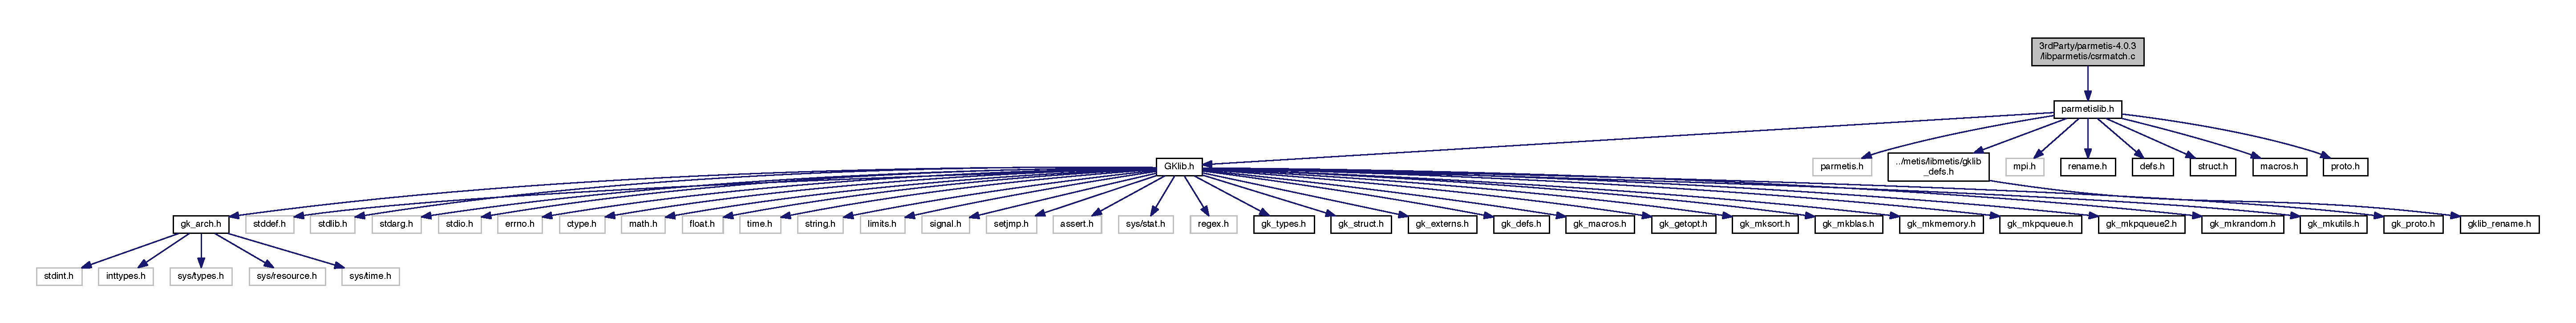
\includegraphics[width=350pt]{csrmatch_8c__incl}
\end{center}
\end{figure}
\subsection*{Functions}
\begin{DoxyCompactItemize}
\item 
void \hyperlink{csrmatch_8c_a7171b4b1ffd62a2ebee9863c25f73652}{C\+S\+R\+\_\+\+Match\+\_\+\+S\+H\+EM} (\hyperlink{structmatrix__t}{matrix\+\_\+t} $\ast$\hyperlink{adjustments_2make__bidg__headers_8m_af07ff1035f34d77764ff516f110e6832}{matrix}, \hyperlink{3rd_party_2parmetis-4_80_83_2metis_2include_2metis_8h_aaa5262be3e700770163401acb0150f52}{idx\+\_\+t} $\ast$match, \hyperlink{3rd_party_2parmetis-4_80_83_2metis_2include_2metis_8h_aaa5262be3e700770163401acb0150f52}{idx\+\_\+t} $\ast$mlist, \hyperlink{3rd_party_2parmetis-4_80_83_2metis_2include_2metis_8h_aaa5262be3e700770163401acb0150f52}{idx\+\_\+t} $\ast$skip, \hyperlink{3rd_party_2parmetis-4_80_83_2metis_2include_2metis_8h_aaa5262be3e700770163401acb0150f52}{idx\+\_\+t} \hyperlink{include_2metis_8h_ac1dd31740e8f97fb57dc917ded30253f}{ncon})
\end{DoxyCompactItemize}


\subsection{Function Documentation}
\mbox{\Hypertarget{csrmatch_8c_a7171b4b1ffd62a2ebee9863c25f73652}\label{csrmatch_8c_a7171b4b1ffd62a2ebee9863c25f73652}} 
\index{csrmatch.\+c@{csrmatch.\+c}!C\+S\+R\+\_\+\+Match\+\_\+\+S\+H\+EM@{C\+S\+R\+\_\+\+Match\+\_\+\+S\+H\+EM}}
\index{C\+S\+R\+\_\+\+Match\+\_\+\+S\+H\+EM@{C\+S\+R\+\_\+\+Match\+\_\+\+S\+H\+EM}!csrmatch.\+c@{csrmatch.\+c}}
\subsubsection{\texorpdfstring{C\+S\+R\+\_\+\+Match\+\_\+\+S\+H\+E\+M()}{CSR\_Match\_SHEM()}}
{\footnotesize\ttfamily void C\+S\+R\+\_\+\+Match\+\_\+\+S\+H\+EM (\begin{DoxyParamCaption}\item[{\hyperlink{structmatrix__t}{matrix\+\_\+t} $\ast$}]{matrix,  }\item[{\hyperlink{3rd_party_2parmetis-4_80_83_2metis_2include_2metis_8h_aaa5262be3e700770163401acb0150f52}{idx\+\_\+t} $\ast$}]{match,  }\item[{\hyperlink{3rd_party_2parmetis-4_80_83_2metis_2include_2metis_8h_aaa5262be3e700770163401acb0150f52}{idx\+\_\+t} $\ast$}]{mlist,  }\item[{\hyperlink{3rd_party_2parmetis-4_80_83_2metis_2include_2metis_8h_aaa5262be3e700770163401acb0150f52}{idx\+\_\+t} $\ast$}]{skip,  }\item[{\hyperlink{3rd_party_2parmetis-4_80_83_2metis_2include_2metis_8h_aaa5262be3e700770163401acb0150f52}{idx\+\_\+t}}]{ncon }\end{DoxyParamCaption})}

Here is the call graph for this function\+:\nopagebreak
\begin{figure}[H]
\begin{center}
\leavevmode
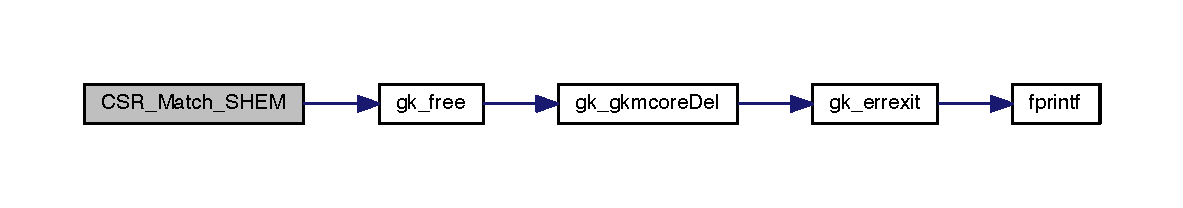
\includegraphics[width=350pt]{csrmatch_8c_a7171b4b1ffd62a2ebee9863c25f73652_cgraph}
\end{center}
\end{figure}

\hypertarget{ctrl_8c}{}\section{3rd\+Party/parmetis-\/4.0.3/libparmetis/ctrl.c File Reference}
\label{ctrl_8c}\index{3rd\+Party/parmetis-\/4.\+0.\+3/libparmetis/ctrl.\+c@{3rd\+Party/parmetis-\/4.\+0.\+3/libparmetis/ctrl.\+c}}
{\ttfamily \#include $<$parmetislib.\+h$>$}\newline
Include dependency graph for ctrl.\+c\+:\nopagebreak
\begin{figure}[H]
\begin{center}
\leavevmode
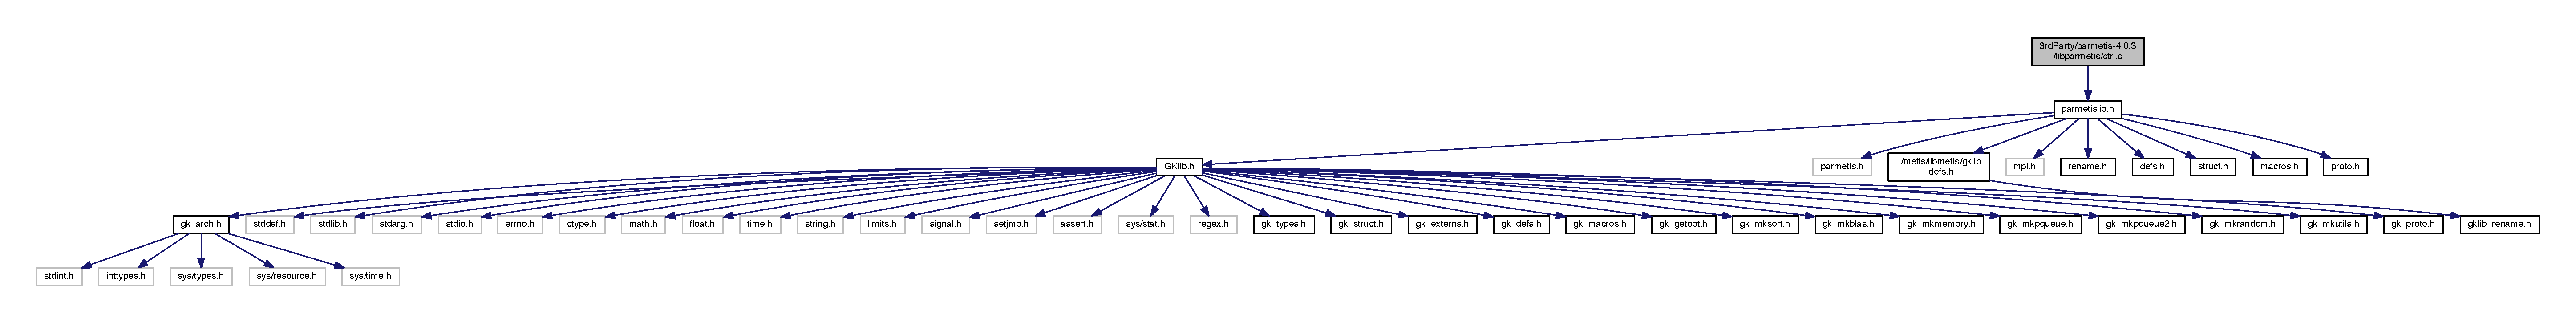
\includegraphics[width=350pt]{ctrl_8c__incl}
\end{center}
\end{figure}

\hypertarget{diffutil_8c}{}\section{3rd\+Party/parmetis-\/4.0.3/libparmetis/diffutil.c File Reference}
\label{diffutil_8c}\index{3rd\+Party/parmetis-\/4.\+0.\+3/libparmetis/diffutil.\+c@{3rd\+Party/parmetis-\/4.\+0.\+3/libparmetis/diffutil.\+c}}
{\ttfamily \#include $<$parmetislib.\+h$>$}\newline
Include dependency graph for diffutil.\+c\+:\nopagebreak
\begin{figure}[H]
\begin{center}
\leavevmode
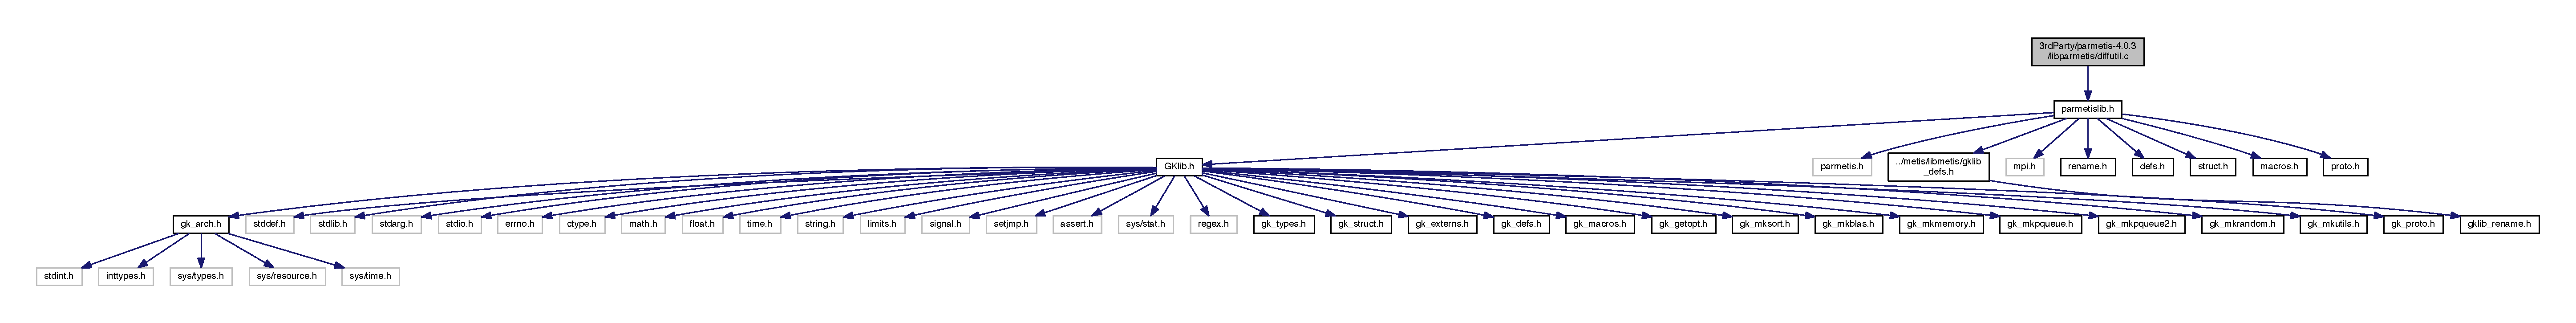
\includegraphics[width=350pt]{diffutil_8c__incl}
\end{center}
\end{figure}
\subsection*{Functions}
\begin{DoxyCompactItemize}
\item 
void \hyperlink{diffutil_8c_ae66862df97d3cf546259e4f679371730}{Set\+Up\+Connect\+Graph} (\hyperlink{structgraph__t}{graph\+\_\+t} $\ast$graph, \hyperlink{structmatrix__t}{matrix\+\_\+t} $\ast$\hyperlink{adjustments_2make__bidg__headers_8m_af07ff1035f34d77764ff516f110e6832}{matrix}, \hyperlink{3rd_party_2parmetis-4_80_83_2metis_2include_2metis_8h_aaa5262be3e700770163401acb0150f52}{idx\+\_\+t} $\ast$workspace)
\item 
void \hyperlink{diffutil_8c_a007901e980318b5c455c6798c5686fc4}{Mc\+\_\+\+Compute\+Move\+Statistics} (\hyperlink{structctrl__t}{ctrl\+\_\+t} $\ast$ctrl, \hyperlink{structgraph__t}{graph\+\_\+t} $\ast$graph, \hyperlink{3rd_party_2parmetis-4_80_83_2metis_2include_2metis_8h_aaa5262be3e700770163401acb0150f52}{idx\+\_\+t} $\ast$nmoved, \hyperlink{3rd_party_2parmetis-4_80_83_2metis_2include_2metis_8h_aaa5262be3e700770163401acb0150f52}{idx\+\_\+t} $\ast$maxin, \hyperlink{3rd_party_2parmetis-4_80_83_2metis_2include_2metis_8h_aaa5262be3e700770163401acb0150f52}{idx\+\_\+t} $\ast$maxout)
\item 
\hyperlink{3rd_party_2parmetis-4_80_83_2metis_2include_2metis_8h_aaa5262be3e700770163401acb0150f52}{idx\+\_\+t} \hyperlink{diffutil_8c_ac2a70991745acc003b806be26e3a8124}{Mc\+\_\+\+Compute\+Serial\+TotalV} (\hyperlink{structgraph__t}{graph\+\_\+t} $\ast$graph, \hyperlink{3rd_party_2parmetis-4_80_83_2metis_2include_2metis_8h_aaa5262be3e700770163401acb0150f52}{idx\+\_\+t} $\ast$home)
\item 
void \hyperlink{diffutil_8c_ae334beb9a86e6a2816584c5d9872ecd7}{Compute\+Load} (\hyperlink{structgraph__t}{graph\+\_\+t} $\ast$graph, \hyperlink{3rd_party_2parmetis-4_80_83_2metis_2include_2metis_8h_aaa5262be3e700770163401acb0150f52}{idx\+\_\+t} \hyperlink{include_2metis_8h_aad88065af88fd6759101788a8e15ce9e}{nparts}, \hyperlink{3rd_party_2parmetis-4_80_83_2metis_2include_2metis_8h_a1924a4f6907cc3833213aba1f07fcbe9}{real\+\_\+t} $\ast$load, \hyperlink{3rd_party_2parmetis-4_80_83_2metis_2include_2metis_8h_a1924a4f6907cc3833213aba1f07fcbe9}{real\+\_\+t} $\ast$\hyperlink{include_2metis_8h_aa91786cd8ea996ec49ed5b382eb7fc2f}{tpwgts}, \hyperlink{3rd_party_2parmetis-4_80_83_2metis_2include_2metis_8h_aaa5262be3e700770163401acb0150f52}{idx\+\_\+t} index)
\item 
void \hyperlink{diffutil_8c_a31c811c3b724d9d26416be8831be44e0}{Conj\+Grad2} (\hyperlink{structmatrix__t}{matrix\+\_\+t} $\ast$A, \hyperlink{3rd_party_2parmetis-4_80_83_2metis_2include_2metis_8h_a1924a4f6907cc3833213aba1f07fcbe9}{real\+\_\+t} $\ast$b, \hyperlink{3rd_party_2parmetis-4_80_83_2metis_2include_2metis_8h_a1924a4f6907cc3833213aba1f07fcbe9}{real\+\_\+t} $\ast$\hyperlink{cubic2linear_8m_ac98c3bb25378222646e977292011625f}{x}, \hyperlink{3rd_party_2parmetis-4_80_83_2metis_2include_2metis_8h_a1924a4f6907cc3833213aba1f07fcbe9}{real\+\_\+t} tol, \hyperlink{3rd_party_2parmetis-4_80_83_2metis_2include_2metis_8h_a1924a4f6907cc3833213aba1f07fcbe9}{real\+\_\+t} $\ast$workspace)
\item 
void \hyperlink{diffutil_8c_a4ac5c2a9274b1ea7377f70e1047659db}{mv\+Mult2} (\hyperlink{structmatrix__t}{matrix\+\_\+t} $\ast$A, \hyperlink{3rd_party_2parmetis-4_80_83_2metis_2include_2metis_8h_a1924a4f6907cc3833213aba1f07fcbe9}{real\+\_\+t} $\ast$\hyperlink{cubic2linear_8m_ac4055e3a20b6b3af3d10590ea446ef6c}{v}, \hyperlink{3rd_party_2parmetis-4_80_83_2metis_2include_2metis_8h_a1924a4f6907cc3833213aba1f07fcbe9}{real\+\_\+t} $\ast$\hyperlink{cubic2linear_8m_aad57484016654da87125db86f4227ea3}{w})
\item 
void \hyperlink{diffutil_8c_a703664e4eb382833e78b460fd8164ec7}{Compute\+Transfer\+Vector} (\hyperlink{3rd_party_2parmetis-4_80_83_2metis_2include_2metis_8h_aaa5262be3e700770163401acb0150f52}{idx\+\_\+t} \hyperlink{include_2metis_8h_ac1dd31740e8f97fb57dc917ded30253f}{ncon}, \hyperlink{structmatrix__t}{matrix\+\_\+t} $\ast$\hyperlink{adjustments_2make__bidg__headers_8m_af07ff1035f34d77764ff516f110e6832}{matrix}, \hyperlink{3rd_party_2parmetis-4_80_83_2metis_2include_2metis_8h_a1924a4f6907cc3833213aba1f07fcbe9}{real\+\_\+t} $\ast$solution, \hyperlink{3rd_party_2parmetis-4_80_83_2metis_2include_2metis_8h_a1924a4f6907cc3833213aba1f07fcbe9}{real\+\_\+t} $\ast$transfer, \hyperlink{3rd_party_2parmetis-4_80_83_2metis_2include_2metis_8h_aaa5262be3e700770163401acb0150f52}{idx\+\_\+t} index)
\end{DoxyCompactItemize}


\subsection{Function Documentation}
\mbox{\Hypertarget{diffutil_8c_ae334beb9a86e6a2816584c5d9872ecd7}\label{diffutil_8c_ae334beb9a86e6a2816584c5d9872ecd7}} 
\index{diffutil.\+c@{diffutil.\+c}!Compute\+Load@{Compute\+Load}}
\index{Compute\+Load@{Compute\+Load}!diffutil.\+c@{diffutil.\+c}}
\subsubsection{\texorpdfstring{Compute\+Load()}{ComputeLoad()}}
{\footnotesize\ttfamily void Compute\+Load (\begin{DoxyParamCaption}\item[{\hyperlink{structgraph__t}{graph\+\_\+t} $\ast$}]{graph,  }\item[{\hyperlink{3rd_party_2parmetis-4_80_83_2metis_2include_2metis_8h_aaa5262be3e700770163401acb0150f52}{idx\+\_\+t}}]{nparts,  }\item[{\hyperlink{3rd_party_2parmetis-4_80_83_2metis_2include_2metis_8h_a1924a4f6907cc3833213aba1f07fcbe9}{real\+\_\+t} $\ast$}]{load,  }\item[{\hyperlink{3rd_party_2parmetis-4_80_83_2metis_2include_2metis_8h_a1924a4f6907cc3833213aba1f07fcbe9}{real\+\_\+t} $\ast$}]{tpwgts,  }\item[{\hyperlink{3rd_party_2parmetis-4_80_83_2metis_2include_2metis_8h_aaa5262be3e700770163401acb0150f52}{idx\+\_\+t}}]{index }\end{DoxyParamCaption})}

\mbox{\Hypertarget{diffutil_8c_a703664e4eb382833e78b460fd8164ec7}\label{diffutil_8c_a703664e4eb382833e78b460fd8164ec7}} 
\index{diffutil.\+c@{diffutil.\+c}!Compute\+Transfer\+Vector@{Compute\+Transfer\+Vector}}
\index{Compute\+Transfer\+Vector@{Compute\+Transfer\+Vector}!diffutil.\+c@{diffutil.\+c}}
\subsubsection{\texorpdfstring{Compute\+Transfer\+Vector()}{ComputeTransferVector()}}
{\footnotesize\ttfamily void Compute\+Transfer\+Vector (\begin{DoxyParamCaption}\item[{\hyperlink{3rd_party_2parmetis-4_80_83_2metis_2include_2metis_8h_aaa5262be3e700770163401acb0150f52}{idx\+\_\+t}}]{ncon,  }\item[{\hyperlink{structmatrix__t}{matrix\+\_\+t} $\ast$}]{matrix,  }\item[{\hyperlink{3rd_party_2parmetis-4_80_83_2metis_2include_2metis_8h_a1924a4f6907cc3833213aba1f07fcbe9}{real\+\_\+t} $\ast$}]{solution,  }\item[{\hyperlink{3rd_party_2parmetis-4_80_83_2metis_2include_2metis_8h_a1924a4f6907cc3833213aba1f07fcbe9}{real\+\_\+t} $\ast$}]{transfer,  }\item[{\hyperlink{3rd_party_2parmetis-4_80_83_2metis_2include_2metis_8h_aaa5262be3e700770163401acb0150f52}{idx\+\_\+t}}]{index }\end{DoxyParamCaption})}

\mbox{\Hypertarget{diffutil_8c_a31c811c3b724d9d26416be8831be44e0}\label{diffutil_8c_a31c811c3b724d9d26416be8831be44e0}} 
\index{diffutil.\+c@{diffutil.\+c}!Conj\+Grad2@{Conj\+Grad2}}
\index{Conj\+Grad2@{Conj\+Grad2}!diffutil.\+c@{diffutil.\+c}}
\subsubsection{\texorpdfstring{Conj\+Grad2()}{ConjGrad2()}}
{\footnotesize\ttfamily void Conj\+Grad2 (\begin{DoxyParamCaption}\item[{\hyperlink{structmatrix__t}{matrix\+\_\+t} $\ast$}]{A,  }\item[{\hyperlink{3rd_party_2parmetis-4_80_83_2metis_2include_2metis_8h_a1924a4f6907cc3833213aba1f07fcbe9}{real\+\_\+t} $\ast$}]{b,  }\item[{\hyperlink{3rd_party_2parmetis-4_80_83_2metis_2include_2metis_8h_a1924a4f6907cc3833213aba1f07fcbe9}{real\+\_\+t} $\ast$}]{x,  }\item[{\hyperlink{3rd_party_2parmetis-4_80_83_2metis_2include_2metis_8h_a1924a4f6907cc3833213aba1f07fcbe9}{real\+\_\+t}}]{tol,  }\item[{\hyperlink{3rd_party_2parmetis-4_80_83_2metis_2include_2metis_8h_a1924a4f6907cc3833213aba1f07fcbe9}{real\+\_\+t} $\ast$}]{workspace }\end{DoxyParamCaption})}

Here is the call graph for this function\+:\nopagebreak
\begin{figure}[H]
\begin{center}
\leavevmode
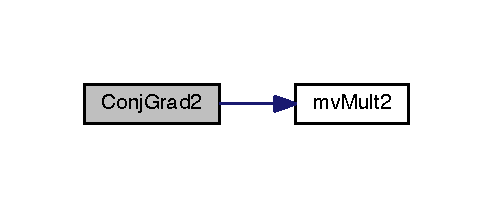
\includegraphics[width=236pt]{diffutil_8c_a31c811c3b724d9d26416be8831be44e0_cgraph}
\end{center}
\end{figure}
\mbox{\Hypertarget{diffutil_8c_a007901e980318b5c455c6798c5686fc4}\label{diffutil_8c_a007901e980318b5c455c6798c5686fc4}} 
\index{diffutil.\+c@{diffutil.\+c}!Mc\+\_\+\+Compute\+Move\+Statistics@{Mc\+\_\+\+Compute\+Move\+Statistics}}
\index{Mc\+\_\+\+Compute\+Move\+Statistics@{Mc\+\_\+\+Compute\+Move\+Statistics}!diffutil.\+c@{diffutil.\+c}}
\subsubsection{\texorpdfstring{Mc\+\_\+\+Compute\+Move\+Statistics()}{Mc\_ComputeMoveStatistics()}}
{\footnotesize\ttfamily void Mc\+\_\+\+Compute\+Move\+Statistics (\begin{DoxyParamCaption}\item[{\hyperlink{structctrl__t}{ctrl\+\_\+t} $\ast$}]{ctrl,  }\item[{\hyperlink{structgraph__t}{graph\+\_\+t} $\ast$}]{graph,  }\item[{\hyperlink{3rd_party_2parmetis-4_80_83_2metis_2include_2metis_8h_aaa5262be3e700770163401acb0150f52}{idx\+\_\+t} $\ast$}]{nmoved,  }\item[{\hyperlink{3rd_party_2parmetis-4_80_83_2metis_2include_2metis_8h_aaa5262be3e700770163401acb0150f52}{idx\+\_\+t} $\ast$}]{maxin,  }\item[{\hyperlink{3rd_party_2parmetis-4_80_83_2metis_2include_2metis_8h_aaa5262be3e700770163401acb0150f52}{idx\+\_\+t} $\ast$}]{maxout }\end{DoxyParamCaption})}

Here is the call graph for this function\+:\nopagebreak
\begin{figure}[H]
\begin{center}
\leavevmode
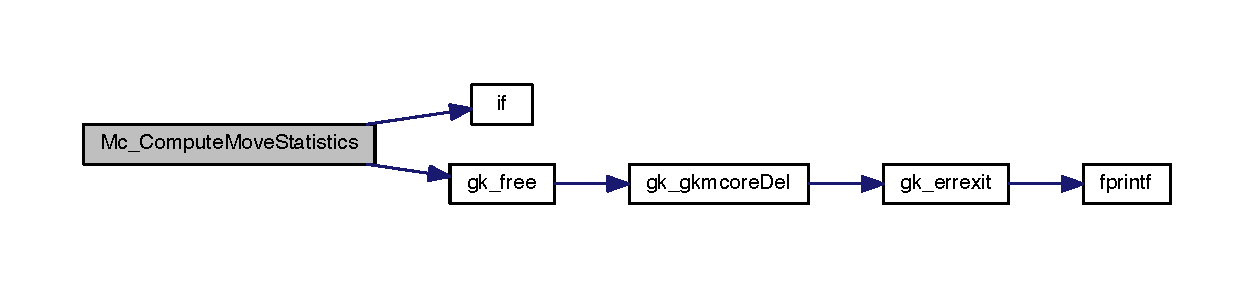
\includegraphics[width=350pt]{diffutil_8c_a007901e980318b5c455c6798c5686fc4_cgraph}
\end{center}
\end{figure}
\mbox{\Hypertarget{diffutil_8c_ac2a70991745acc003b806be26e3a8124}\label{diffutil_8c_ac2a70991745acc003b806be26e3a8124}} 
\index{diffutil.\+c@{diffutil.\+c}!Mc\+\_\+\+Compute\+Serial\+TotalV@{Mc\+\_\+\+Compute\+Serial\+TotalV}}
\index{Mc\+\_\+\+Compute\+Serial\+TotalV@{Mc\+\_\+\+Compute\+Serial\+TotalV}!diffutil.\+c@{diffutil.\+c}}
\subsubsection{\texorpdfstring{Mc\+\_\+\+Compute\+Serial\+Total\+V()}{Mc\_ComputeSerialTotalV()}}
{\footnotesize\ttfamily \hyperlink{3rd_party_2parmetis-4_80_83_2metis_2include_2metis_8h_aaa5262be3e700770163401acb0150f52}{idx\+\_\+t} Mc\+\_\+\+Compute\+Serial\+TotalV (\begin{DoxyParamCaption}\item[{\hyperlink{structgraph__t}{graph\+\_\+t} $\ast$}]{graph,  }\item[{\hyperlink{3rd_party_2parmetis-4_80_83_2metis_2include_2metis_8h_aaa5262be3e700770163401acb0150f52}{idx\+\_\+t} $\ast$}]{home }\end{DoxyParamCaption})}

\mbox{\Hypertarget{diffutil_8c_a4ac5c2a9274b1ea7377f70e1047659db}\label{diffutil_8c_a4ac5c2a9274b1ea7377f70e1047659db}} 
\index{diffutil.\+c@{diffutil.\+c}!mv\+Mult2@{mv\+Mult2}}
\index{mv\+Mult2@{mv\+Mult2}!diffutil.\+c@{diffutil.\+c}}
\subsubsection{\texorpdfstring{mv\+Mult2()}{mvMult2()}}
{\footnotesize\ttfamily void mv\+Mult2 (\begin{DoxyParamCaption}\item[{\hyperlink{structmatrix__t}{matrix\+\_\+t} $\ast$}]{A,  }\item[{\hyperlink{3rd_party_2parmetis-4_80_83_2metis_2include_2metis_8h_a1924a4f6907cc3833213aba1f07fcbe9}{real\+\_\+t} $\ast$}]{v,  }\item[{\hyperlink{3rd_party_2parmetis-4_80_83_2metis_2include_2metis_8h_a1924a4f6907cc3833213aba1f07fcbe9}{real\+\_\+t} $\ast$}]{w }\end{DoxyParamCaption})}

Here is the caller graph for this function\+:\nopagebreak
\begin{figure}[H]
\begin{center}
\leavevmode
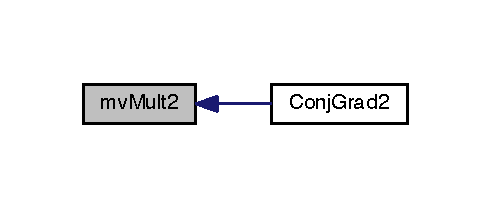
\includegraphics[width=236pt]{diffutil_8c_a4ac5c2a9274b1ea7377f70e1047659db_icgraph}
\end{center}
\end{figure}
\mbox{\Hypertarget{diffutil_8c_ae66862df97d3cf546259e4f679371730}\label{diffutil_8c_ae66862df97d3cf546259e4f679371730}} 
\index{diffutil.\+c@{diffutil.\+c}!Set\+Up\+Connect\+Graph@{Set\+Up\+Connect\+Graph}}
\index{Set\+Up\+Connect\+Graph@{Set\+Up\+Connect\+Graph}!diffutil.\+c@{diffutil.\+c}}
\subsubsection{\texorpdfstring{Set\+Up\+Connect\+Graph()}{SetUpConnectGraph()}}
{\footnotesize\ttfamily void Set\+Up\+Connect\+Graph (\begin{DoxyParamCaption}\item[{\hyperlink{structgraph__t}{graph\+\_\+t} $\ast$}]{graph,  }\item[{\hyperlink{structmatrix__t}{matrix\+\_\+t} $\ast$}]{matrix,  }\item[{\hyperlink{3rd_party_2parmetis-4_80_83_2metis_2include_2metis_8h_aaa5262be3e700770163401acb0150f52}{idx\+\_\+t} $\ast$}]{workspace }\end{DoxyParamCaption})}


\hypertarget{gkmetis_8c}{}\section{3rd\+Party/parmetis-\/4.0.3/libparmetis/gkmetis.c File Reference}
\label{gkmetis_8c}\index{3rd\+Party/parmetis-\/4.\+0.\+3/libparmetis/gkmetis.\+c@{3rd\+Party/parmetis-\/4.\+0.\+3/libparmetis/gkmetis.\+c}}
{\ttfamily \#include $<$parmetislib.\+h$>$}\newline
Include dependency graph for gkmetis.\+c\+:\nopagebreak
\begin{figure}[H]
\begin{center}
\leavevmode
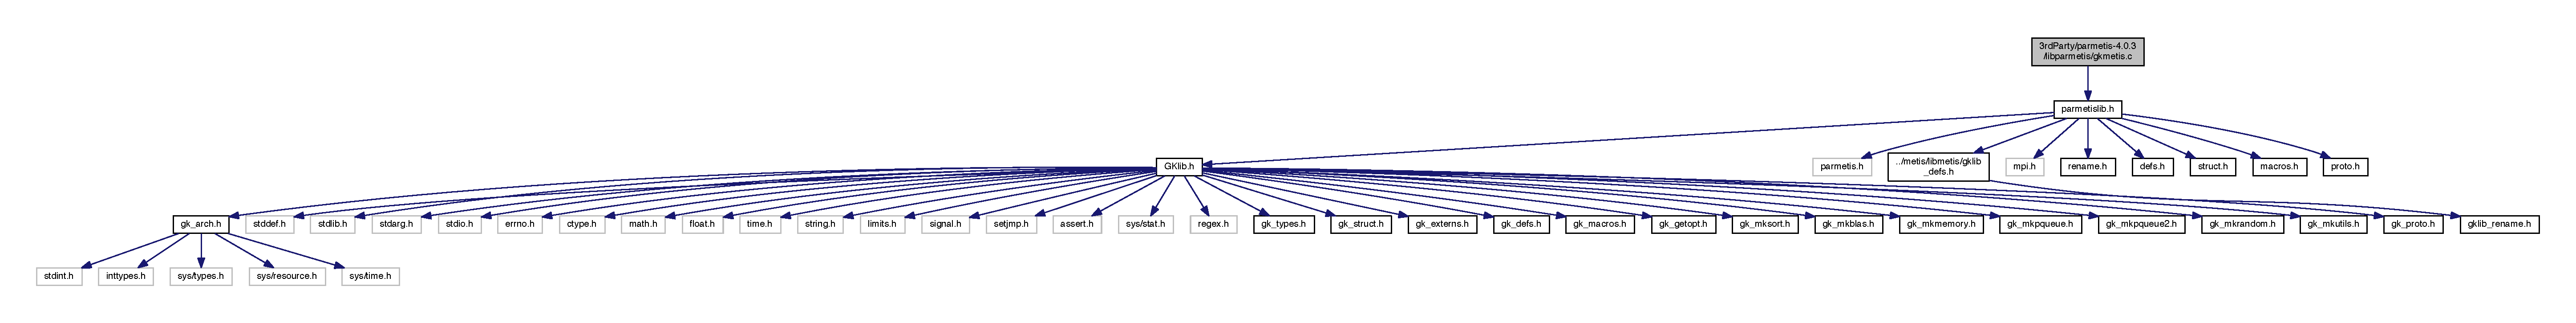
\includegraphics[width=350pt]{gkmetis_8c__incl}
\end{center}
\end{figure}
\subsection*{Functions}
\begin{DoxyCompactItemize}
\item 
int \hyperlink{gkmetis_8c_a46ac099ac07c553c3eb6641f076ce75f}{Par\+M\+E\+T\+I\+S\+\_\+\+V3\+\_\+\+Part\+Geom\+Kway} (\hyperlink{3rd_party_2parmetis-4_80_83_2metis_2include_2metis_8h_aaa5262be3e700770163401acb0150f52}{idx\+\_\+t} $\ast$vtxdist, \hyperlink{3rd_party_2parmetis-4_80_83_2metis_2include_2metis_8h_aaa5262be3e700770163401acb0150f52}{idx\+\_\+t} $\ast$\hyperlink{include_2metis_8h_aa8fc7f75458e38e1e2979ed6db639164}{xadj}, \hyperlink{3rd_party_2parmetis-4_80_83_2metis_2include_2metis_8h_aaa5262be3e700770163401acb0150f52}{idx\+\_\+t} $\ast$\hyperlink{include_2metis_8h_a20c068e3ebdd8f9889fb82c1f677d679}{adjncy}, \hyperlink{3rd_party_2parmetis-4_80_83_2metis_2include_2metis_8h_aaa5262be3e700770163401acb0150f52}{idx\+\_\+t} $\ast$\hyperlink{include_2metis_8h_a34203f1160d94eca83e95f2718ea3504}{vwgt}, \hyperlink{3rd_party_2parmetis-4_80_83_2metis_2include_2metis_8h_aaa5262be3e700770163401acb0150f52}{idx\+\_\+t} $\ast$\hyperlink{include_2metis_8h_a2be4719baa820cfa5c06fd070796e0d3}{adjwgt}, \hyperlink{3rd_party_2parmetis-4_80_83_2metis_2include_2metis_8h_aaa5262be3e700770163401acb0150f52}{idx\+\_\+t} $\ast$wgtflag, \hyperlink{3rd_party_2parmetis-4_80_83_2metis_2include_2metis_8h_aaa5262be3e700770163401acb0150f52}{idx\+\_\+t} $\ast$\hyperlink{include_2metis_8h_aa48ecaf34ec788199c3aedb2b1558eb7}{numflag}, \hyperlink{3rd_party_2parmetis-4_80_83_2metis_2include_2metis_8h_aaa5262be3e700770163401acb0150f52}{idx\+\_\+t} $\ast$ndims, \hyperlink{3rd_party_2parmetis-4_80_83_2metis_2include_2metis_8h_a1924a4f6907cc3833213aba1f07fcbe9}{real\+\_\+t} $\ast$\hyperlink{threed__to__vtu_8m_a6444a221e6b74abaf6d67d44af2650a0}{xyz}, \hyperlink{3rd_party_2parmetis-4_80_83_2metis_2include_2metis_8h_aaa5262be3e700770163401acb0150f52}{idx\+\_\+t} $\ast$\hyperlink{include_2metis_8h_ac1dd31740e8f97fb57dc917ded30253f}{ncon}, \hyperlink{3rd_party_2parmetis-4_80_83_2metis_2include_2metis_8h_aaa5262be3e700770163401acb0150f52}{idx\+\_\+t} $\ast$\hyperlink{include_2metis_8h_aad88065af88fd6759101788a8e15ce9e}{nparts}, \hyperlink{3rd_party_2parmetis-4_80_83_2metis_2include_2metis_8h_a1924a4f6907cc3833213aba1f07fcbe9}{real\+\_\+t} $\ast$\hyperlink{include_2metis_8h_aa91786cd8ea996ec49ed5b382eb7fc2f}{tpwgts}, \hyperlink{3rd_party_2parmetis-4_80_83_2metis_2include_2metis_8h_a1924a4f6907cc3833213aba1f07fcbe9}{real\+\_\+t} $\ast$\hyperlink{include_2metis_8h_af48bb348bc8440a61f90f137de83f203}{ubvec}, \hyperlink{3rd_party_2parmetis-4_80_83_2metis_2include_2metis_8h_aaa5262be3e700770163401acb0150f52}{idx\+\_\+t} $\ast$\hyperlink{include_2metis_8h_a68c032ed4161802775c6847d4cb39adf}{options}, \hyperlink{3rd_party_2parmetis-4_80_83_2metis_2include_2metis_8h_aaa5262be3e700770163401acb0150f52}{idx\+\_\+t} $\ast$\hyperlink{include_2metis_8h_a8e62a902298dd5fd88ef554d5277b1dc}{edgecut}, \hyperlink{3rd_party_2parmetis-4_80_83_2metis_2include_2metis_8h_aaa5262be3e700770163401acb0150f52}{idx\+\_\+t} $\ast$\hyperlink{include_2metis_8h_a0a9ea8670f88d6db1e021fee2dcd94be}{part}, M\+P\+I\+\_\+\+Comm $\ast$comm)
\item 
int \hyperlink{gkmetis_8c_a6ba7172d25cc2a5601ec5a64014ec7a2}{Par\+M\+E\+T\+I\+S\+\_\+\+V3\+\_\+\+Part\+Geom} (\hyperlink{3rd_party_2parmetis-4_80_83_2metis_2include_2metis_8h_aaa5262be3e700770163401acb0150f52}{idx\+\_\+t} $\ast$vtxdist, \hyperlink{3rd_party_2parmetis-4_80_83_2metis_2include_2metis_8h_aaa5262be3e700770163401acb0150f52}{idx\+\_\+t} $\ast$ndims, \hyperlink{3rd_party_2parmetis-4_80_83_2metis_2include_2metis_8h_a1924a4f6907cc3833213aba1f07fcbe9}{real\+\_\+t} $\ast$\hyperlink{threed__to__vtu_8m_a6444a221e6b74abaf6d67d44af2650a0}{xyz}, \hyperlink{3rd_party_2parmetis-4_80_83_2metis_2include_2metis_8h_aaa5262be3e700770163401acb0150f52}{idx\+\_\+t} $\ast$\hyperlink{include_2metis_8h_a0a9ea8670f88d6db1e021fee2dcd94be}{part}, M\+P\+I\+\_\+\+Comm $\ast$comm)
\end{DoxyCompactItemize}


\subsection{Function Documentation}
\mbox{\Hypertarget{gkmetis_8c_a6ba7172d25cc2a5601ec5a64014ec7a2}\label{gkmetis_8c_a6ba7172d25cc2a5601ec5a64014ec7a2}} 
\index{gkmetis.\+c@{gkmetis.\+c}!Par\+M\+E\+T\+I\+S\+\_\+\+V3\+\_\+\+Part\+Geom@{Par\+M\+E\+T\+I\+S\+\_\+\+V3\+\_\+\+Part\+Geom}}
\index{Par\+M\+E\+T\+I\+S\+\_\+\+V3\+\_\+\+Part\+Geom@{Par\+M\+E\+T\+I\+S\+\_\+\+V3\+\_\+\+Part\+Geom}!gkmetis.\+c@{gkmetis.\+c}}
\subsubsection{\texorpdfstring{Par\+M\+E\+T\+I\+S\+\_\+\+V3\+\_\+\+Part\+Geom()}{ParMETIS\_V3\_PartGeom()}}
{\footnotesize\ttfamily int Par\+M\+E\+T\+I\+S\+\_\+\+V3\+\_\+\+Part\+Geom (\begin{DoxyParamCaption}\item[{\hyperlink{3rd_party_2parmetis-4_80_83_2metis_2include_2metis_8h_aaa5262be3e700770163401acb0150f52}{idx\+\_\+t} $\ast$}]{vtxdist,  }\item[{\hyperlink{3rd_party_2parmetis-4_80_83_2metis_2include_2metis_8h_aaa5262be3e700770163401acb0150f52}{idx\+\_\+t} $\ast$}]{ndims,  }\item[{\hyperlink{3rd_party_2parmetis-4_80_83_2metis_2include_2metis_8h_a1924a4f6907cc3833213aba1f07fcbe9}{real\+\_\+t} $\ast$}]{xyz,  }\item[{\hyperlink{3rd_party_2parmetis-4_80_83_2metis_2include_2metis_8h_aaa5262be3e700770163401acb0150f52}{idx\+\_\+t} $\ast$}]{part,  }\item[{M\+P\+I\+\_\+\+Comm $\ast$}]{comm }\end{DoxyParamCaption})}

Here is the call graph for this function\+:\nopagebreak
\begin{figure}[H]
\begin{center}
\leavevmode
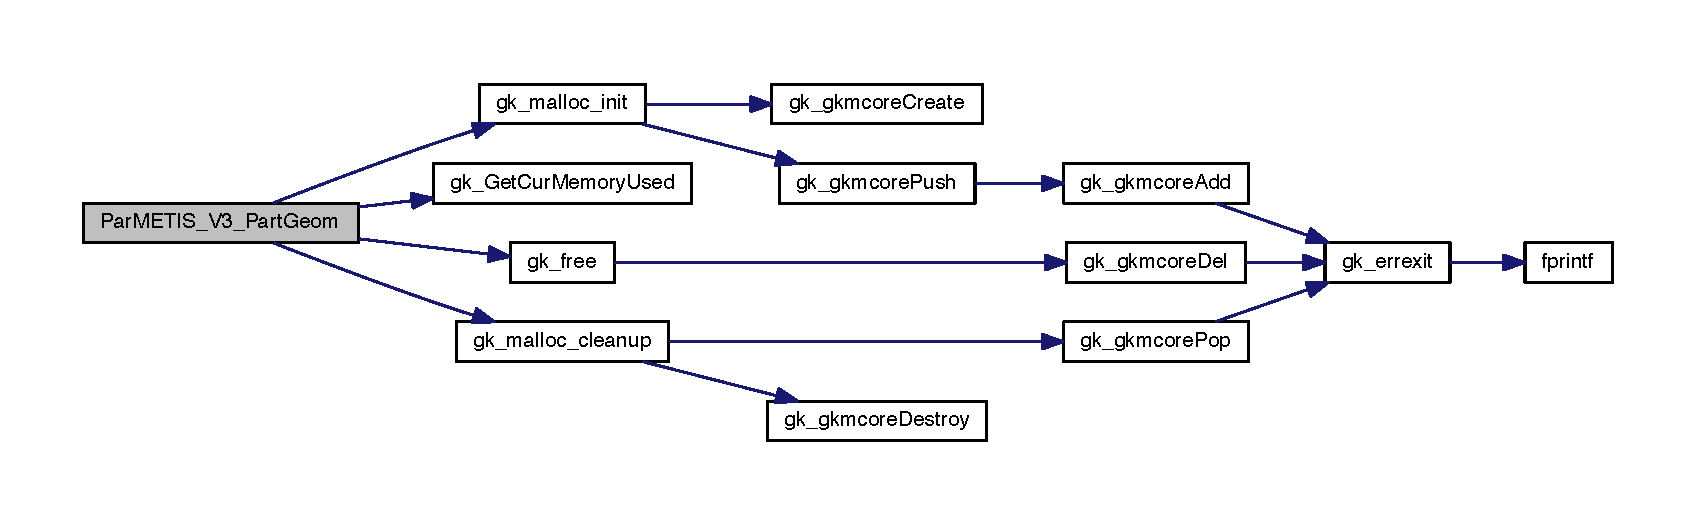
\includegraphics[width=350pt]{gkmetis_8c_a6ba7172d25cc2a5601ec5a64014ec7a2_cgraph}
\end{center}
\end{figure}
Here is the caller graph for this function\+:\nopagebreak
\begin{figure}[H]
\begin{center}
\leavevmode
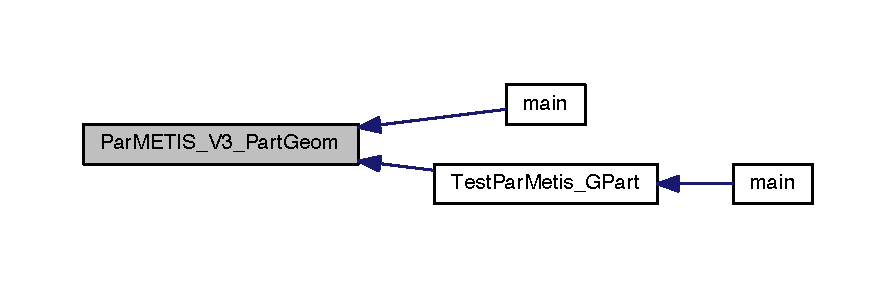
\includegraphics[width=350pt]{gkmetis_8c_a6ba7172d25cc2a5601ec5a64014ec7a2_icgraph}
\end{center}
\end{figure}
\mbox{\Hypertarget{gkmetis_8c_a46ac099ac07c553c3eb6641f076ce75f}\label{gkmetis_8c_a46ac099ac07c553c3eb6641f076ce75f}} 
\index{gkmetis.\+c@{gkmetis.\+c}!Par\+M\+E\+T\+I\+S\+\_\+\+V3\+\_\+\+Part\+Geom\+Kway@{Par\+M\+E\+T\+I\+S\+\_\+\+V3\+\_\+\+Part\+Geom\+Kway}}
\index{Par\+M\+E\+T\+I\+S\+\_\+\+V3\+\_\+\+Part\+Geom\+Kway@{Par\+M\+E\+T\+I\+S\+\_\+\+V3\+\_\+\+Part\+Geom\+Kway}!gkmetis.\+c@{gkmetis.\+c}}
\subsubsection{\texorpdfstring{Par\+M\+E\+T\+I\+S\+\_\+\+V3\+\_\+\+Part\+Geom\+Kway()}{ParMETIS\_V3\_PartGeomKway()}}
{\footnotesize\ttfamily int Par\+M\+E\+T\+I\+S\+\_\+\+V3\+\_\+\+Part\+Geom\+Kway (\begin{DoxyParamCaption}\item[{\hyperlink{3rd_party_2parmetis-4_80_83_2metis_2include_2metis_8h_aaa5262be3e700770163401acb0150f52}{idx\+\_\+t} $\ast$}]{vtxdist,  }\item[{\hyperlink{3rd_party_2parmetis-4_80_83_2metis_2include_2metis_8h_aaa5262be3e700770163401acb0150f52}{idx\+\_\+t} $\ast$}]{xadj,  }\item[{\hyperlink{3rd_party_2parmetis-4_80_83_2metis_2include_2metis_8h_aaa5262be3e700770163401acb0150f52}{idx\+\_\+t} $\ast$}]{adjncy,  }\item[{\hyperlink{3rd_party_2parmetis-4_80_83_2metis_2include_2metis_8h_aaa5262be3e700770163401acb0150f52}{idx\+\_\+t} $\ast$}]{vwgt,  }\item[{\hyperlink{3rd_party_2parmetis-4_80_83_2metis_2include_2metis_8h_aaa5262be3e700770163401acb0150f52}{idx\+\_\+t} $\ast$}]{adjwgt,  }\item[{\hyperlink{3rd_party_2parmetis-4_80_83_2metis_2include_2metis_8h_aaa5262be3e700770163401acb0150f52}{idx\+\_\+t} $\ast$}]{wgtflag,  }\item[{\hyperlink{3rd_party_2parmetis-4_80_83_2metis_2include_2metis_8h_aaa5262be3e700770163401acb0150f52}{idx\+\_\+t} $\ast$}]{numflag,  }\item[{\hyperlink{3rd_party_2parmetis-4_80_83_2metis_2include_2metis_8h_aaa5262be3e700770163401acb0150f52}{idx\+\_\+t} $\ast$}]{ndims,  }\item[{\hyperlink{3rd_party_2parmetis-4_80_83_2metis_2include_2metis_8h_a1924a4f6907cc3833213aba1f07fcbe9}{real\+\_\+t} $\ast$}]{xyz,  }\item[{\hyperlink{3rd_party_2parmetis-4_80_83_2metis_2include_2metis_8h_aaa5262be3e700770163401acb0150f52}{idx\+\_\+t} $\ast$}]{ncon,  }\item[{\hyperlink{3rd_party_2parmetis-4_80_83_2metis_2include_2metis_8h_aaa5262be3e700770163401acb0150f52}{idx\+\_\+t} $\ast$}]{nparts,  }\item[{\hyperlink{3rd_party_2parmetis-4_80_83_2metis_2include_2metis_8h_a1924a4f6907cc3833213aba1f07fcbe9}{real\+\_\+t} $\ast$}]{tpwgts,  }\item[{\hyperlink{3rd_party_2parmetis-4_80_83_2metis_2include_2metis_8h_a1924a4f6907cc3833213aba1f07fcbe9}{real\+\_\+t} $\ast$}]{ubvec,  }\item[{\hyperlink{3rd_party_2parmetis-4_80_83_2metis_2include_2metis_8h_aaa5262be3e700770163401acb0150f52}{idx\+\_\+t} $\ast$}]{options,  }\item[{\hyperlink{3rd_party_2parmetis-4_80_83_2metis_2include_2metis_8h_aaa5262be3e700770163401acb0150f52}{idx\+\_\+t} $\ast$}]{edgecut,  }\item[{\hyperlink{3rd_party_2parmetis-4_80_83_2metis_2include_2metis_8h_aaa5262be3e700770163401acb0150f52}{idx\+\_\+t} $\ast$}]{part,  }\item[{M\+P\+I\+\_\+\+Comm $\ast$}]{comm }\end{DoxyParamCaption})}

Here is the call graph for this function\+:\nopagebreak
\begin{figure}[H]
\begin{center}
\leavevmode
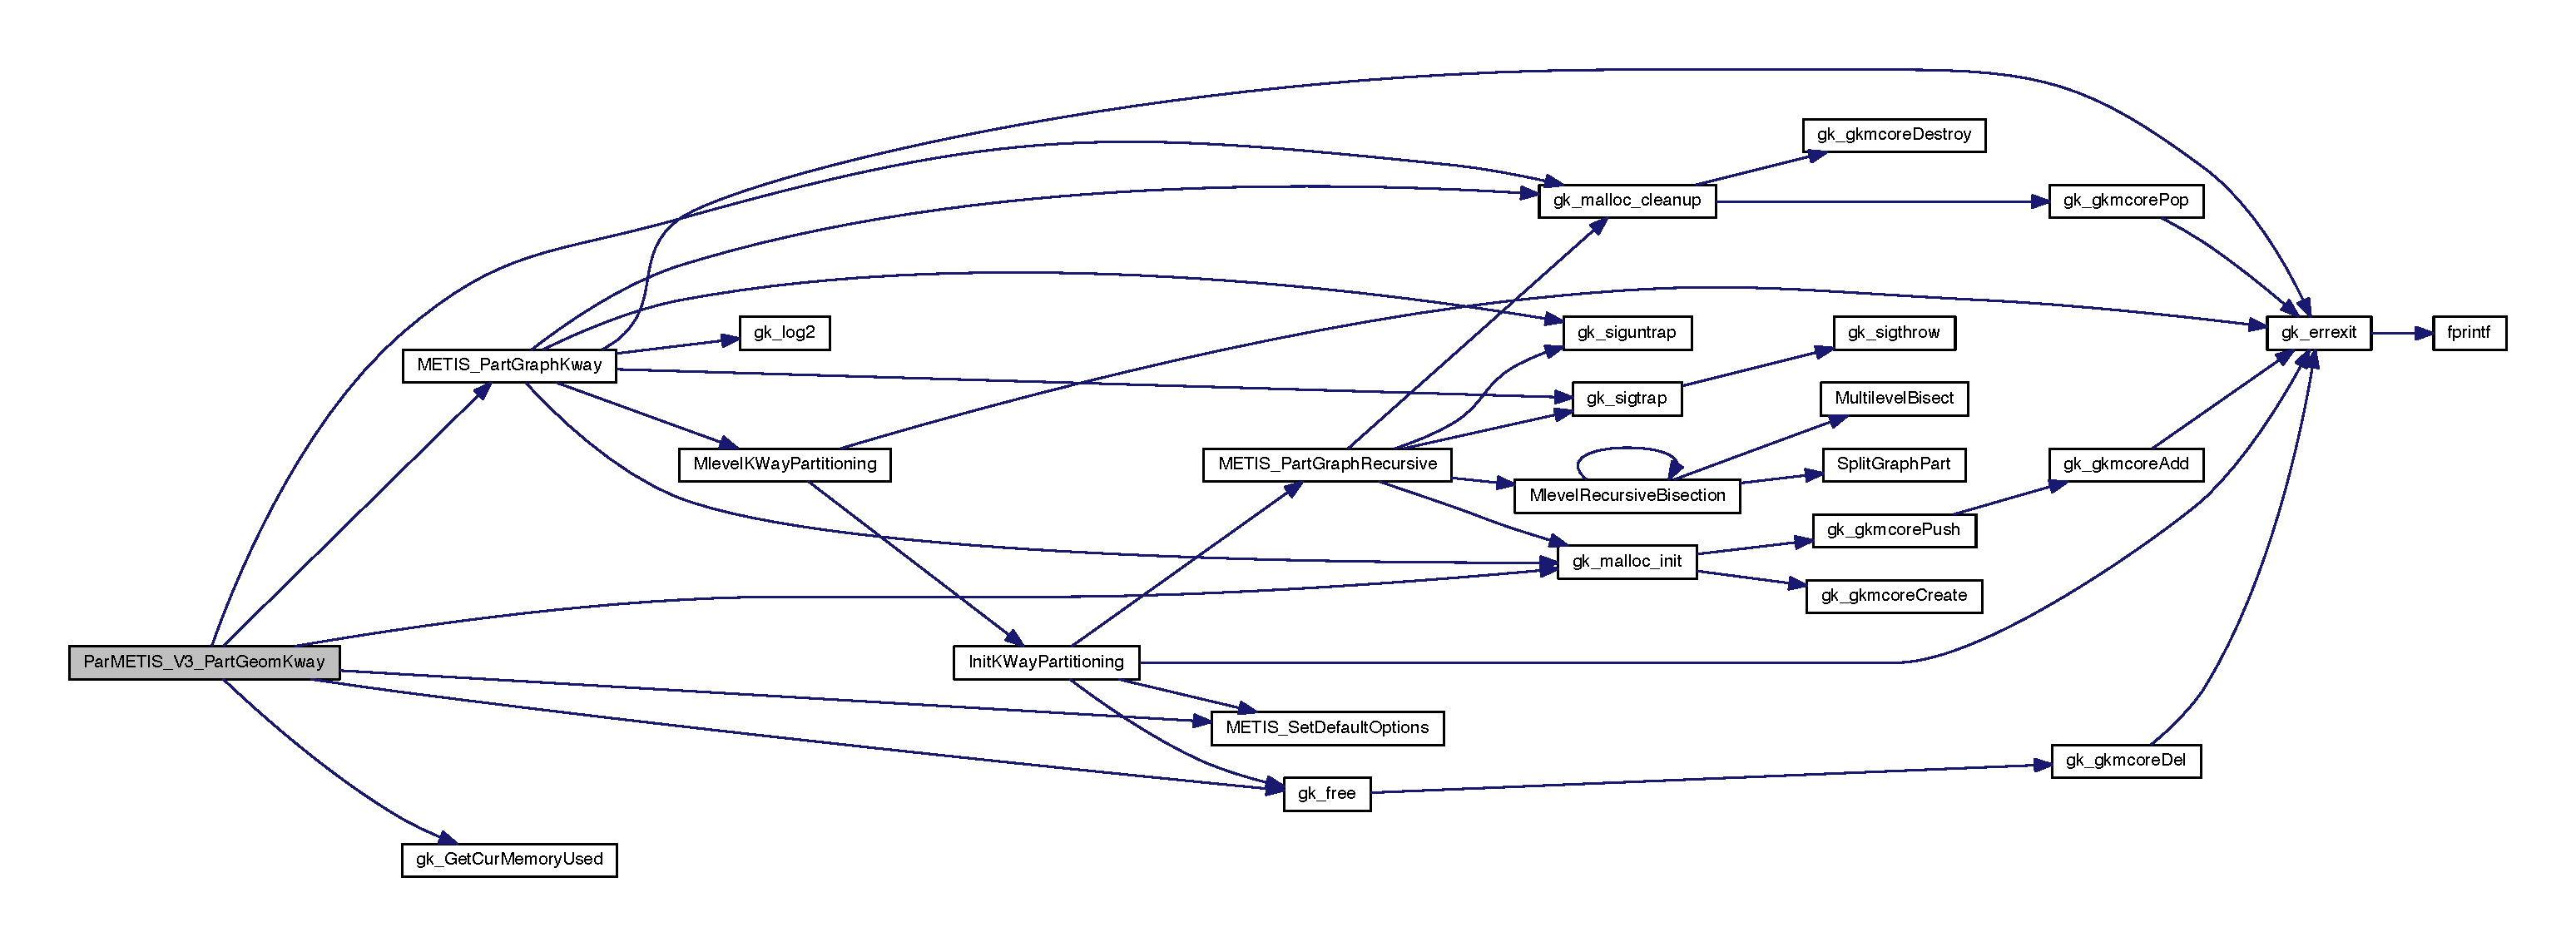
\includegraphics[width=350pt]{gkmetis_8c_a46ac099ac07c553c3eb6641f076ce75f_cgraph}
\end{center}
\end{figure}
Here is the caller graph for this function\+:\nopagebreak
\begin{figure}[H]
\begin{center}
\leavevmode
\includegraphics[width=350pt]{gkmetis_8c_a46ac099ac07c553c3eb6641f076ce75f_icgraph}
\end{center}
\end{figure}

\hypertarget{gkmpi_8c}{}\section{3rd\+Party/parmetis-\/4.0.3/libparmetis/gkmpi.c File Reference}
\label{gkmpi_8c}\index{3rd\+Party/parmetis-\/4.\+0.\+3/libparmetis/gkmpi.\+c@{3rd\+Party/parmetis-\/4.\+0.\+3/libparmetis/gkmpi.\+c}}
{\ttfamily \#include $<$parmetislib.\+h$>$}\newline
Include dependency graph for gkmpi.\+c\+:\nopagebreak
\begin{figure}[H]
\begin{center}
\leavevmode
\includegraphics[width=350pt]{gkmpi_8c__incl}
\end{center}
\end{figure}
\subsection*{Functions}
\begin{DoxyCompactItemize}
\item 
int \hyperlink{gkmpi_8c_aa6be69b686449a61266c75f859a7384a}{gk\+M\+P\+I\+\_\+\+Comm\+\_\+size} (M\+P\+I\+\_\+\+Comm comm, \hyperlink{3rd_party_2parmetis-4_80_83_2metis_2include_2metis_8h_aaa5262be3e700770163401acb0150f52}{idx\+\_\+t} $\ast$\hyperlink{make_v_t_k_file_8m_ad6cb0afbbe6ea4f56407890be2533966}{size})
\item 
int \hyperlink{gkmpi_8c_a3d476c06613e7a647941fcbeb002e5e6}{gk\+M\+P\+I\+\_\+\+Comm\+\_\+rank} (M\+P\+I\+\_\+\+Comm comm, \hyperlink{3rd_party_2parmetis-4_80_83_2metis_2include_2metis_8h_aaa5262be3e700770163401acb0150f52}{idx\+\_\+t} $\ast$rank)
\item 
int \hyperlink{gkmpi_8c_a3f4ae6f17f49b22ef461eb0a96853302}{gk\+M\+P\+I\+\_\+\+Get\+\_\+count} (M\+P\+I\+\_\+\+Status $\ast$status, M\+P\+I\+\_\+\+Datatype datatype, \hyperlink{3rd_party_2parmetis-4_80_83_2metis_2include_2metis_8h_aaa5262be3e700770163401acb0150f52}{idx\+\_\+t} $\ast$count)
\item 
int \hyperlink{gkmpi_8c_a2442b8eee4afc113918cd7a5878244b6}{gk\+M\+P\+I\+\_\+\+Send} (void $\ast$buf, \hyperlink{3rd_party_2parmetis-4_80_83_2metis_2include_2metis_8h_aaa5262be3e700770163401acb0150f52}{idx\+\_\+t} count, M\+P\+I\+\_\+\+Datatype datatype, \hyperlink{3rd_party_2parmetis-4_80_83_2metis_2include_2metis_8h_aaa5262be3e700770163401acb0150f52}{idx\+\_\+t} dest, \hyperlink{3rd_party_2parmetis-4_80_83_2metis_2include_2metis_8h_aaa5262be3e700770163401acb0150f52}{idx\+\_\+t} tag, M\+P\+I\+\_\+\+Comm comm)
\item 
int \hyperlink{gkmpi_8c_a4eebc3896a4356902599bd3d3dd077f3}{gk\+M\+P\+I\+\_\+\+Recv} (void $\ast$buf, \hyperlink{3rd_party_2parmetis-4_80_83_2metis_2include_2metis_8h_aaa5262be3e700770163401acb0150f52}{idx\+\_\+t} count, M\+P\+I\+\_\+\+Datatype datatype, \hyperlink{3rd_party_2parmetis-4_80_83_2metis_2include_2metis_8h_aaa5262be3e700770163401acb0150f52}{idx\+\_\+t} source, \hyperlink{3rd_party_2parmetis-4_80_83_2metis_2include_2metis_8h_aaa5262be3e700770163401acb0150f52}{idx\+\_\+t} tag, M\+P\+I\+\_\+\+Comm comm, M\+P\+I\+\_\+\+Status $\ast$status)
\item 
int \hyperlink{gkmpi_8c_a575274feee728e0cabbca8b68fcea3fb}{gk\+M\+P\+I\+\_\+\+Isend} (void $\ast$buf, \hyperlink{3rd_party_2parmetis-4_80_83_2metis_2include_2metis_8h_aaa5262be3e700770163401acb0150f52}{idx\+\_\+t} count, M\+P\+I\+\_\+\+Datatype datatype, \hyperlink{3rd_party_2parmetis-4_80_83_2metis_2include_2metis_8h_aaa5262be3e700770163401acb0150f52}{idx\+\_\+t} dest, \hyperlink{3rd_party_2parmetis-4_80_83_2metis_2include_2metis_8h_aaa5262be3e700770163401acb0150f52}{idx\+\_\+t} tag, M\+P\+I\+\_\+\+Comm comm, M\+P\+I\+\_\+\+Request $\ast$request)
\item 
int \hyperlink{gkmpi_8c_af66daa80152ba26f528a2c6d9c86e98c}{gk\+M\+P\+I\+\_\+\+Irecv} (void $\ast$buf, \hyperlink{3rd_party_2parmetis-4_80_83_2metis_2include_2metis_8h_aaa5262be3e700770163401acb0150f52}{idx\+\_\+t} count, M\+P\+I\+\_\+\+Datatype datatype, \hyperlink{3rd_party_2parmetis-4_80_83_2metis_2include_2metis_8h_aaa5262be3e700770163401acb0150f52}{idx\+\_\+t} source, \hyperlink{3rd_party_2parmetis-4_80_83_2metis_2include_2metis_8h_aaa5262be3e700770163401acb0150f52}{idx\+\_\+t} tag, M\+P\+I\+\_\+\+Comm comm, M\+P\+I\+\_\+\+Request $\ast$request)
\item 
int \hyperlink{gkmpi_8c_a878d900addb2e537070c9892cc37dde0}{gk\+M\+P\+I\+\_\+\+Wait} (M\+P\+I\+\_\+\+Request $\ast$request, M\+P\+I\+\_\+\+Status $\ast$status)
\item 
int \hyperlink{gkmpi_8c_a8fb70b0ee91eb5e31adfdf681c67c31f}{gk\+M\+P\+I\+\_\+\+Waitall} (\hyperlink{3rd_party_2parmetis-4_80_83_2metis_2include_2metis_8h_aaa5262be3e700770163401acb0150f52}{idx\+\_\+t} count, M\+P\+I\+\_\+\+Request $\ast$array\+\_\+of\+\_\+requests, M\+P\+I\+\_\+\+Status $\ast$array\+\_\+of\+\_\+statuses)
\item 
int \hyperlink{gkmpi_8c_a1edf33502a17ee84cb573dc0bd989bda}{gk\+M\+P\+I\+\_\+\+Barrier} (M\+P\+I\+\_\+\+Comm comm)
\item 
int \hyperlink{gkmpi_8c_a22d90d341b85ea6b900bae0a5f9a8b71}{gk\+M\+P\+I\+\_\+\+Bcast} (void $\ast$buffer, \hyperlink{3rd_party_2parmetis-4_80_83_2metis_2include_2metis_8h_aaa5262be3e700770163401acb0150f52}{idx\+\_\+t} count, M\+P\+I\+\_\+\+Datatype datatype, \hyperlink{3rd_party_2parmetis-4_80_83_2metis_2include_2metis_8h_aaa5262be3e700770163401acb0150f52}{idx\+\_\+t} root, M\+P\+I\+\_\+\+Comm comm)
\item 
int \hyperlink{gkmpi_8c_ad629e734a85de207a3a6b5b84d6df7e0}{gk\+M\+P\+I\+\_\+\+Reduce} (void $\ast$sendbuf, void $\ast$recvbuf, \hyperlink{3rd_party_2parmetis-4_80_83_2metis_2include_2metis_8h_aaa5262be3e700770163401acb0150f52}{idx\+\_\+t} count, M\+P\+I\+\_\+\+Datatype datatype, M\+P\+I\+\_\+\+Op op, \hyperlink{3rd_party_2parmetis-4_80_83_2metis_2include_2metis_8h_aaa5262be3e700770163401acb0150f52}{idx\+\_\+t} root, M\+P\+I\+\_\+\+Comm comm)
\item 
int \hyperlink{gkmpi_8c_a192aab5cebcfc29f208341fec3f8fd3a}{gk\+M\+P\+I\+\_\+\+Allreduce} (void $\ast$sendbuf, void $\ast$recvbuf, \hyperlink{3rd_party_2parmetis-4_80_83_2metis_2include_2metis_8h_aaa5262be3e700770163401acb0150f52}{idx\+\_\+t} count, M\+P\+I\+\_\+\+Datatype datatype, M\+P\+I\+\_\+\+Op op, M\+P\+I\+\_\+\+Comm comm)
\item 
int \hyperlink{gkmpi_8c_a8f9cc3ccf10cef3753659c596da87bb3}{gk\+M\+P\+I\+\_\+\+Scan} (void $\ast$sendbuf, void $\ast$recvbuf, \hyperlink{3rd_party_2parmetis-4_80_83_2metis_2include_2metis_8h_aaa5262be3e700770163401acb0150f52}{idx\+\_\+t} count, M\+P\+I\+\_\+\+Datatype datatype, M\+P\+I\+\_\+\+Op op, M\+P\+I\+\_\+\+Comm comm)
\item 
int \hyperlink{gkmpi_8c_a0b7a139ad6fb30c1ae40ac2b57188f1a}{gk\+M\+P\+I\+\_\+\+Allgather} (void $\ast$sendbuf, \hyperlink{3rd_party_2parmetis-4_80_83_2metis_2include_2metis_8h_aaa5262be3e700770163401acb0150f52}{idx\+\_\+t} sendcount, M\+P\+I\+\_\+\+Datatype sendtype, void $\ast$recvbuf, \hyperlink{3rd_party_2parmetis-4_80_83_2metis_2include_2metis_8h_aaa5262be3e700770163401acb0150f52}{idx\+\_\+t} recvcount, M\+P\+I\+\_\+\+Datatype recvtype, M\+P\+I\+\_\+\+Comm comm)
\item 
int \hyperlink{gkmpi_8c_a6ebc719035504ecc821d960bcbbd1d4c}{gk\+M\+P\+I\+\_\+\+Alltoall} (void $\ast$sendbuf, \hyperlink{3rd_party_2parmetis-4_80_83_2metis_2include_2metis_8h_aaa5262be3e700770163401acb0150f52}{idx\+\_\+t} sendcount, M\+P\+I\+\_\+\+Datatype sendtype, void $\ast$recvbuf, \hyperlink{3rd_party_2parmetis-4_80_83_2metis_2include_2metis_8h_aaa5262be3e700770163401acb0150f52}{idx\+\_\+t} recvcount, M\+P\+I\+\_\+\+Datatype recvtype, M\+P\+I\+\_\+\+Comm comm)
\item 
int \hyperlink{gkmpi_8c_ae0651b090fd2a6a021996fc1998a429c}{gk\+M\+P\+I\+\_\+\+Alltoallv} (void $\ast$sendbuf, \hyperlink{3rd_party_2parmetis-4_80_83_2metis_2include_2metis_8h_aaa5262be3e700770163401acb0150f52}{idx\+\_\+t} $\ast$sendcounts, \hyperlink{3rd_party_2parmetis-4_80_83_2metis_2include_2metis_8h_aaa5262be3e700770163401acb0150f52}{idx\+\_\+t} $\ast$sdispls, M\+P\+I\+\_\+\+Datatype sendtype, void $\ast$recvbuf, \hyperlink{3rd_party_2parmetis-4_80_83_2metis_2include_2metis_8h_aaa5262be3e700770163401acb0150f52}{idx\+\_\+t} $\ast$recvcounts, \hyperlink{3rd_party_2parmetis-4_80_83_2metis_2include_2metis_8h_aaa5262be3e700770163401acb0150f52}{idx\+\_\+t} $\ast$rdispls, M\+P\+I\+\_\+\+Datatype recvtype, M\+P\+I\+\_\+\+Comm comm)
\item 
int \hyperlink{gkmpi_8c_a0b0b0098f344cad26f02c6f825bdde2c}{gk\+M\+P\+I\+\_\+\+Allgatherv} (void $\ast$sendbuf, \hyperlink{3rd_party_2parmetis-4_80_83_2metis_2include_2metis_8h_aaa5262be3e700770163401acb0150f52}{idx\+\_\+t} sendcount, M\+P\+I\+\_\+\+Datatype sendtype, void $\ast$recvbuf, \hyperlink{3rd_party_2parmetis-4_80_83_2metis_2include_2metis_8h_aaa5262be3e700770163401acb0150f52}{idx\+\_\+t} $\ast$recvcounts, \hyperlink{3rd_party_2parmetis-4_80_83_2metis_2include_2metis_8h_aaa5262be3e700770163401acb0150f52}{idx\+\_\+t} $\ast$rdispls, M\+P\+I\+\_\+\+Datatype recvtype, M\+P\+I\+\_\+\+Comm comm)
\item 
int \hyperlink{gkmpi_8c_a08990d66eed081828d6addc2e5affde3}{gk\+M\+P\+I\+\_\+\+Scatterv} (void $\ast$sendbuf, \hyperlink{3rd_party_2parmetis-4_80_83_2metis_2include_2metis_8h_aaa5262be3e700770163401acb0150f52}{idx\+\_\+t} $\ast$sendcounts, \hyperlink{3rd_party_2parmetis-4_80_83_2metis_2include_2metis_8h_aaa5262be3e700770163401acb0150f52}{idx\+\_\+t} $\ast$sdispls, M\+P\+I\+\_\+\+Datatype sendtype, void $\ast$recvbuf, \hyperlink{3rd_party_2parmetis-4_80_83_2metis_2include_2metis_8h_aaa5262be3e700770163401acb0150f52}{idx\+\_\+t} recvcount, M\+P\+I\+\_\+\+Datatype recvtype, \hyperlink{3rd_party_2parmetis-4_80_83_2metis_2include_2metis_8h_aaa5262be3e700770163401acb0150f52}{idx\+\_\+t} root, M\+P\+I\+\_\+\+Comm comm)
\item 
int \hyperlink{gkmpi_8c_a807659087675fb1da493b8dd6d4396b0}{gk\+M\+P\+I\+\_\+\+Gatherv} (void $\ast$sendbuf, \hyperlink{3rd_party_2parmetis-4_80_83_2metis_2include_2metis_8h_aaa5262be3e700770163401acb0150f52}{idx\+\_\+t} sendcount, M\+P\+I\+\_\+\+Datatype sendtype, void $\ast$recvbuf, \hyperlink{3rd_party_2parmetis-4_80_83_2metis_2include_2metis_8h_aaa5262be3e700770163401acb0150f52}{idx\+\_\+t} $\ast$recvcounts, \hyperlink{3rd_party_2parmetis-4_80_83_2metis_2include_2metis_8h_aaa5262be3e700770163401acb0150f52}{idx\+\_\+t} $\ast$rdispls, M\+P\+I\+\_\+\+Datatype recvtype, \hyperlink{3rd_party_2parmetis-4_80_83_2metis_2include_2metis_8h_aaa5262be3e700770163401acb0150f52}{idx\+\_\+t} root, M\+P\+I\+\_\+\+Comm comm)
\item 
int \hyperlink{gkmpi_8c_a37b086e8008a4fd0406c128c0660b0da}{gk\+M\+P\+I\+\_\+\+Comm\+\_\+split} (M\+P\+I\+\_\+\+Comm comm, \hyperlink{3rd_party_2parmetis-4_80_83_2metis_2include_2metis_8h_aaa5262be3e700770163401acb0150f52}{idx\+\_\+t} color, \hyperlink{3rd_party_2parmetis-4_80_83_2metis_2include_2metis_8h_aaa5262be3e700770163401acb0150f52}{idx\+\_\+t} key, M\+P\+I\+\_\+\+Comm $\ast$newcomm)
\item 
int \hyperlink{gkmpi_8c_a2e7ef47df4a06a51305a9de602b41262}{gk\+M\+P\+I\+\_\+\+Comm\+\_\+free} (M\+P\+I\+\_\+\+Comm $\ast$comm)
\item 
int \hyperlink{gkmpi_8c_a0840d526fdede1b9db4fd5f722560a8b}{gk\+M\+P\+I\+\_\+\+Finalize} ()
\end{DoxyCompactItemize}


\subsection{Function Documentation}
\mbox{\Hypertarget{gkmpi_8c_a0b7a139ad6fb30c1ae40ac2b57188f1a}\label{gkmpi_8c_a0b7a139ad6fb30c1ae40ac2b57188f1a}} 
\index{gkmpi.\+c@{gkmpi.\+c}!gk\+M\+P\+I\+\_\+\+Allgather@{gk\+M\+P\+I\+\_\+\+Allgather}}
\index{gk\+M\+P\+I\+\_\+\+Allgather@{gk\+M\+P\+I\+\_\+\+Allgather}!gkmpi.\+c@{gkmpi.\+c}}
\subsubsection{\texorpdfstring{gk\+M\+P\+I\+\_\+\+Allgather()}{gkMPI\_Allgather()}}
{\footnotesize\ttfamily int gk\+M\+P\+I\+\_\+\+Allgather (\begin{DoxyParamCaption}\item[{void $\ast$}]{sendbuf,  }\item[{\hyperlink{3rd_party_2parmetis-4_80_83_2metis_2include_2metis_8h_aaa5262be3e700770163401acb0150f52}{idx\+\_\+t}}]{sendcount,  }\item[{M\+P\+I\+\_\+\+Datatype}]{sendtype,  }\item[{void $\ast$}]{recvbuf,  }\item[{\hyperlink{3rd_party_2parmetis-4_80_83_2metis_2include_2metis_8h_aaa5262be3e700770163401acb0150f52}{idx\+\_\+t}}]{recvcount,  }\item[{M\+P\+I\+\_\+\+Datatype}]{recvtype,  }\item[{M\+P\+I\+\_\+\+Comm}]{comm }\end{DoxyParamCaption})}

\mbox{\Hypertarget{gkmpi_8c_a0b0b0098f344cad26f02c6f825bdde2c}\label{gkmpi_8c_a0b0b0098f344cad26f02c6f825bdde2c}} 
\index{gkmpi.\+c@{gkmpi.\+c}!gk\+M\+P\+I\+\_\+\+Allgatherv@{gk\+M\+P\+I\+\_\+\+Allgatherv}}
\index{gk\+M\+P\+I\+\_\+\+Allgatherv@{gk\+M\+P\+I\+\_\+\+Allgatherv}!gkmpi.\+c@{gkmpi.\+c}}
\subsubsection{\texorpdfstring{gk\+M\+P\+I\+\_\+\+Allgatherv()}{gkMPI\_Allgatherv()}}
{\footnotesize\ttfamily int gk\+M\+P\+I\+\_\+\+Allgatherv (\begin{DoxyParamCaption}\item[{void $\ast$}]{sendbuf,  }\item[{\hyperlink{3rd_party_2parmetis-4_80_83_2metis_2include_2metis_8h_aaa5262be3e700770163401acb0150f52}{idx\+\_\+t}}]{sendcount,  }\item[{M\+P\+I\+\_\+\+Datatype}]{sendtype,  }\item[{void $\ast$}]{recvbuf,  }\item[{\hyperlink{3rd_party_2parmetis-4_80_83_2metis_2include_2metis_8h_aaa5262be3e700770163401acb0150f52}{idx\+\_\+t} $\ast$}]{recvcounts,  }\item[{\hyperlink{3rd_party_2parmetis-4_80_83_2metis_2include_2metis_8h_aaa5262be3e700770163401acb0150f52}{idx\+\_\+t} $\ast$}]{rdispls,  }\item[{M\+P\+I\+\_\+\+Datatype}]{recvtype,  }\item[{M\+P\+I\+\_\+\+Comm}]{comm }\end{DoxyParamCaption})}

Here is the call graph for this function\+:\nopagebreak
\begin{figure}[H]
\begin{center}
\leavevmode
\includegraphics[width=350pt]{gkmpi_8c_a0b0b0098f344cad26f02c6f825bdde2c_cgraph}
\end{center}
\end{figure}
\mbox{\Hypertarget{gkmpi_8c_a192aab5cebcfc29f208341fec3f8fd3a}\label{gkmpi_8c_a192aab5cebcfc29f208341fec3f8fd3a}} 
\index{gkmpi.\+c@{gkmpi.\+c}!gk\+M\+P\+I\+\_\+\+Allreduce@{gk\+M\+P\+I\+\_\+\+Allreduce}}
\index{gk\+M\+P\+I\+\_\+\+Allreduce@{gk\+M\+P\+I\+\_\+\+Allreduce}!gkmpi.\+c@{gkmpi.\+c}}
\subsubsection{\texorpdfstring{gk\+M\+P\+I\+\_\+\+Allreduce()}{gkMPI\_Allreduce()}}
{\footnotesize\ttfamily int gk\+M\+P\+I\+\_\+\+Allreduce (\begin{DoxyParamCaption}\item[{void $\ast$}]{sendbuf,  }\item[{void $\ast$}]{recvbuf,  }\item[{\hyperlink{3rd_party_2parmetis-4_80_83_2metis_2include_2metis_8h_aaa5262be3e700770163401acb0150f52}{idx\+\_\+t}}]{count,  }\item[{M\+P\+I\+\_\+\+Datatype}]{datatype,  }\item[{M\+P\+I\+\_\+\+Op}]{op,  }\item[{M\+P\+I\+\_\+\+Comm}]{comm }\end{DoxyParamCaption})}

\mbox{\Hypertarget{gkmpi_8c_a6ebc719035504ecc821d960bcbbd1d4c}\label{gkmpi_8c_a6ebc719035504ecc821d960bcbbd1d4c}} 
\index{gkmpi.\+c@{gkmpi.\+c}!gk\+M\+P\+I\+\_\+\+Alltoall@{gk\+M\+P\+I\+\_\+\+Alltoall}}
\index{gk\+M\+P\+I\+\_\+\+Alltoall@{gk\+M\+P\+I\+\_\+\+Alltoall}!gkmpi.\+c@{gkmpi.\+c}}
\subsubsection{\texorpdfstring{gk\+M\+P\+I\+\_\+\+Alltoall()}{gkMPI\_Alltoall()}}
{\footnotesize\ttfamily int gk\+M\+P\+I\+\_\+\+Alltoall (\begin{DoxyParamCaption}\item[{void $\ast$}]{sendbuf,  }\item[{\hyperlink{3rd_party_2parmetis-4_80_83_2metis_2include_2metis_8h_aaa5262be3e700770163401acb0150f52}{idx\+\_\+t}}]{sendcount,  }\item[{M\+P\+I\+\_\+\+Datatype}]{sendtype,  }\item[{void $\ast$}]{recvbuf,  }\item[{\hyperlink{3rd_party_2parmetis-4_80_83_2metis_2include_2metis_8h_aaa5262be3e700770163401acb0150f52}{idx\+\_\+t}}]{recvcount,  }\item[{M\+P\+I\+\_\+\+Datatype}]{recvtype,  }\item[{M\+P\+I\+\_\+\+Comm}]{comm }\end{DoxyParamCaption})}

\mbox{\Hypertarget{gkmpi_8c_ae0651b090fd2a6a021996fc1998a429c}\label{gkmpi_8c_ae0651b090fd2a6a021996fc1998a429c}} 
\index{gkmpi.\+c@{gkmpi.\+c}!gk\+M\+P\+I\+\_\+\+Alltoallv@{gk\+M\+P\+I\+\_\+\+Alltoallv}}
\index{gk\+M\+P\+I\+\_\+\+Alltoallv@{gk\+M\+P\+I\+\_\+\+Alltoallv}!gkmpi.\+c@{gkmpi.\+c}}
\subsubsection{\texorpdfstring{gk\+M\+P\+I\+\_\+\+Alltoallv()}{gkMPI\_Alltoallv()}}
{\footnotesize\ttfamily int gk\+M\+P\+I\+\_\+\+Alltoallv (\begin{DoxyParamCaption}\item[{void $\ast$}]{sendbuf,  }\item[{\hyperlink{3rd_party_2parmetis-4_80_83_2metis_2include_2metis_8h_aaa5262be3e700770163401acb0150f52}{idx\+\_\+t} $\ast$}]{sendcounts,  }\item[{\hyperlink{3rd_party_2parmetis-4_80_83_2metis_2include_2metis_8h_aaa5262be3e700770163401acb0150f52}{idx\+\_\+t} $\ast$}]{sdispls,  }\item[{M\+P\+I\+\_\+\+Datatype}]{sendtype,  }\item[{void $\ast$}]{recvbuf,  }\item[{\hyperlink{3rd_party_2parmetis-4_80_83_2metis_2include_2metis_8h_aaa5262be3e700770163401acb0150f52}{idx\+\_\+t} $\ast$}]{recvcounts,  }\item[{\hyperlink{3rd_party_2parmetis-4_80_83_2metis_2include_2metis_8h_aaa5262be3e700770163401acb0150f52}{idx\+\_\+t} $\ast$}]{rdispls,  }\item[{M\+P\+I\+\_\+\+Datatype}]{recvtype,  }\item[{M\+P\+I\+\_\+\+Comm}]{comm }\end{DoxyParamCaption})}

Here is the call graph for this function\+:\nopagebreak
\begin{figure}[H]
\begin{center}
\leavevmode
\includegraphics[width=350pt]{gkmpi_8c_ae0651b090fd2a6a021996fc1998a429c_cgraph}
\end{center}
\end{figure}
\mbox{\Hypertarget{gkmpi_8c_a1edf33502a17ee84cb573dc0bd989bda}\label{gkmpi_8c_a1edf33502a17ee84cb573dc0bd989bda}} 
\index{gkmpi.\+c@{gkmpi.\+c}!gk\+M\+P\+I\+\_\+\+Barrier@{gk\+M\+P\+I\+\_\+\+Barrier}}
\index{gk\+M\+P\+I\+\_\+\+Barrier@{gk\+M\+P\+I\+\_\+\+Barrier}!gkmpi.\+c@{gkmpi.\+c}}
\subsubsection{\texorpdfstring{gk\+M\+P\+I\+\_\+\+Barrier()}{gkMPI\_Barrier()}}
{\footnotesize\ttfamily int gk\+M\+P\+I\+\_\+\+Barrier (\begin{DoxyParamCaption}\item[{M\+P\+I\+\_\+\+Comm}]{comm }\end{DoxyParamCaption})}

\mbox{\Hypertarget{gkmpi_8c_a22d90d341b85ea6b900bae0a5f9a8b71}\label{gkmpi_8c_a22d90d341b85ea6b900bae0a5f9a8b71}} 
\index{gkmpi.\+c@{gkmpi.\+c}!gk\+M\+P\+I\+\_\+\+Bcast@{gk\+M\+P\+I\+\_\+\+Bcast}}
\index{gk\+M\+P\+I\+\_\+\+Bcast@{gk\+M\+P\+I\+\_\+\+Bcast}!gkmpi.\+c@{gkmpi.\+c}}
\subsubsection{\texorpdfstring{gk\+M\+P\+I\+\_\+\+Bcast()}{gkMPI\_Bcast()}}
{\footnotesize\ttfamily int gk\+M\+P\+I\+\_\+\+Bcast (\begin{DoxyParamCaption}\item[{void $\ast$}]{buffer,  }\item[{\hyperlink{3rd_party_2parmetis-4_80_83_2metis_2include_2metis_8h_aaa5262be3e700770163401acb0150f52}{idx\+\_\+t}}]{count,  }\item[{M\+P\+I\+\_\+\+Datatype}]{datatype,  }\item[{\hyperlink{3rd_party_2parmetis-4_80_83_2metis_2include_2metis_8h_aaa5262be3e700770163401acb0150f52}{idx\+\_\+t}}]{root,  }\item[{M\+P\+I\+\_\+\+Comm}]{comm }\end{DoxyParamCaption})}

\mbox{\Hypertarget{gkmpi_8c_a2e7ef47df4a06a51305a9de602b41262}\label{gkmpi_8c_a2e7ef47df4a06a51305a9de602b41262}} 
\index{gkmpi.\+c@{gkmpi.\+c}!gk\+M\+P\+I\+\_\+\+Comm\+\_\+free@{gk\+M\+P\+I\+\_\+\+Comm\+\_\+free}}
\index{gk\+M\+P\+I\+\_\+\+Comm\+\_\+free@{gk\+M\+P\+I\+\_\+\+Comm\+\_\+free}!gkmpi.\+c@{gkmpi.\+c}}
\subsubsection{\texorpdfstring{gk\+M\+P\+I\+\_\+\+Comm\+\_\+free()}{gkMPI\_Comm\_free()}}
{\footnotesize\ttfamily int gk\+M\+P\+I\+\_\+\+Comm\+\_\+free (\begin{DoxyParamCaption}\item[{M\+P\+I\+\_\+\+Comm $\ast$}]{comm }\end{DoxyParamCaption})}

\mbox{\Hypertarget{gkmpi_8c_a3d476c06613e7a647941fcbeb002e5e6}\label{gkmpi_8c_a3d476c06613e7a647941fcbeb002e5e6}} 
\index{gkmpi.\+c@{gkmpi.\+c}!gk\+M\+P\+I\+\_\+\+Comm\+\_\+rank@{gk\+M\+P\+I\+\_\+\+Comm\+\_\+rank}}
\index{gk\+M\+P\+I\+\_\+\+Comm\+\_\+rank@{gk\+M\+P\+I\+\_\+\+Comm\+\_\+rank}!gkmpi.\+c@{gkmpi.\+c}}
\subsubsection{\texorpdfstring{gk\+M\+P\+I\+\_\+\+Comm\+\_\+rank()}{gkMPI\_Comm\_rank()}}
{\footnotesize\ttfamily int gk\+M\+P\+I\+\_\+\+Comm\+\_\+rank (\begin{DoxyParamCaption}\item[{M\+P\+I\+\_\+\+Comm}]{comm,  }\item[{\hyperlink{3rd_party_2parmetis-4_80_83_2metis_2include_2metis_8h_aaa5262be3e700770163401acb0150f52}{idx\+\_\+t} $\ast$}]{rank }\end{DoxyParamCaption})}

\mbox{\Hypertarget{gkmpi_8c_aa6be69b686449a61266c75f859a7384a}\label{gkmpi_8c_aa6be69b686449a61266c75f859a7384a}} 
\index{gkmpi.\+c@{gkmpi.\+c}!gk\+M\+P\+I\+\_\+\+Comm\+\_\+size@{gk\+M\+P\+I\+\_\+\+Comm\+\_\+size}}
\index{gk\+M\+P\+I\+\_\+\+Comm\+\_\+size@{gk\+M\+P\+I\+\_\+\+Comm\+\_\+size}!gkmpi.\+c@{gkmpi.\+c}}
\subsubsection{\texorpdfstring{gk\+M\+P\+I\+\_\+\+Comm\+\_\+size()}{gkMPI\_Comm\_size()}}
{\footnotesize\ttfamily int gk\+M\+P\+I\+\_\+\+Comm\+\_\+size (\begin{DoxyParamCaption}\item[{M\+P\+I\+\_\+\+Comm}]{comm,  }\item[{\hyperlink{3rd_party_2parmetis-4_80_83_2metis_2include_2metis_8h_aaa5262be3e700770163401acb0150f52}{idx\+\_\+t} $\ast$}]{size }\end{DoxyParamCaption})}

\mbox{\Hypertarget{gkmpi_8c_a37b086e8008a4fd0406c128c0660b0da}\label{gkmpi_8c_a37b086e8008a4fd0406c128c0660b0da}} 
\index{gkmpi.\+c@{gkmpi.\+c}!gk\+M\+P\+I\+\_\+\+Comm\+\_\+split@{gk\+M\+P\+I\+\_\+\+Comm\+\_\+split}}
\index{gk\+M\+P\+I\+\_\+\+Comm\+\_\+split@{gk\+M\+P\+I\+\_\+\+Comm\+\_\+split}!gkmpi.\+c@{gkmpi.\+c}}
\subsubsection{\texorpdfstring{gk\+M\+P\+I\+\_\+\+Comm\+\_\+split()}{gkMPI\_Comm\_split()}}
{\footnotesize\ttfamily int gk\+M\+P\+I\+\_\+\+Comm\+\_\+split (\begin{DoxyParamCaption}\item[{M\+P\+I\+\_\+\+Comm}]{comm,  }\item[{\hyperlink{3rd_party_2parmetis-4_80_83_2metis_2include_2metis_8h_aaa5262be3e700770163401acb0150f52}{idx\+\_\+t}}]{color,  }\item[{\hyperlink{3rd_party_2parmetis-4_80_83_2metis_2include_2metis_8h_aaa5262be3e700770163401acb0150f52}{idx\+\_\+t}}]{key,  }\item[{M\+P\+I\+\_\+\+Comm $\ast$}]{newcomm }\end{DoxyParamCaption})}

\mbox{\Hypertarget{gkmpi_8c_a0840d526fdede1b9db4fd5f722560a8b}\label{gkmpi_8c_a0840d526fdede1b9db4fd5f722560a8b}} 
\index{gkmpi.\+c@{gkmpi.\+c}!gk\+M\+P\+I\+\_\+\+Finalize@{gk\+M\+P\+I\+\_\+\+Finalize}}
\index{gk\+M\+P\+I\+\_\+\+Finalize@{gk\+M\+P\+I\+\_\+\+Finalize}!gkmpi.\+c@{gkmpi.\+c}}
\subsubsection{\texorpdfstring{gk\+M\+P\+I\+\_\+\+Finalize()}{gkMPI\_Finalize()}}
{\footnotesize\ttfamily int gk\+M\+P\+I\+\_\+\+Finalize (\begin{DoxyParamCaption}{ }\end{DoxyParamCaption})}

\mbox{\Hypertarget{gkmpi_8c_a807659087675fb1da493b8dd6d4396b0}\label{gkmpi_8c_a807659087675fb1da493b8dd6d4396b0}} 
\index{gkmpi.\+c@{gkmpi.\+c}!gk\+M\+P\+I\+\_\+\+Gatherv@{gk\+M\+P\+I\+\_\+\+Gatherv}}
\index{gk\+M\+P\+I\+\_\+\+Gatherv@{gk\+M\+P\+I\+\_\+\+Gatherv}!gkmpi.\+c@{gkmpi.\+c}}
\subsubsection{\texorpdfstring{gk\+M\+P\+I\+\_\+\+Gatherv()}{gkMPI\_Gatherv()}}
{\footnotesize\ttfamily int gk\+M\+P\+I\+\_\+\+Gatherv (\begin{DoxyParamCaption}\item[{void $\ast$}]{sendbuf,  }\item[{\hyperlink{3rd_party_2parmetis-4_80_83_2metis_2include_2metis_8h_aaa5262be3e700770163401acb0150f52}{idx\+\_\+t}}]{sendcount,  }\item[{M\+P\+I\+\_\+\+Datatype}]{sendtype,  }\item[{void $\ast$}]{recvbuf,  }\item[{\hyperlink{3rd_party_2parmetis-4_80_83_2metis_2include_2metis_8h_aaa5262be3e700770163401acb0150f52}{idx\+\_\+t} $\ast$}]{recvcounts,  }\item[{\hyperlink{3rd_party_2parmetis-4_80_83_2metis_2include_2metis_8h_aaa5262be3e700770163401acb0150f52}{idx\+\_\+t} $\ast$}]{rdispls,  }\item[{M\+P\+I\+\_\+\+Datatype}]{recvtype,  }\item[{\hyperlink{3rd_party_2parmetis-4_80_83_2metis_2include_2metis_8h_aaa5262be3e700770163401acb0150f52}{idx\+\_\+t}}]{root,  }\item[{M\+P\+I\+\_\+\+Comm}]{comm }\end{DoxyParamCaption})}

Here is the call graph for this function\+:\nopagebreak
\begin{figure}[H]
\begin{center}
\leavevmode
\includegraphics[width=350pt]{gkmpi_8c_a807659087675fb1da493b8dd6d4396b0_cgraph}
\end{center}
\end{figure}
\mbox{\Hypertarget{gkmpi_8c_a3f4ae6f17f49b22ef461eb0a96853302}\label{gkmpi_8c_a3f4ae6f17f49b22ef461eb0a96853302}} 
\index{gkmpi.\+c@{gkmpi.\+c}!gk\+M\+P\+I\+\_\+\+Get\+\_\+count@{gk\+M\+P\+I\+\_\+\+Get\+\_\+count}}
\index{gk\+M\+P\+I\+\_\+\+Get\+\_\+count@{gk\+M\+P\+I\+\_\+\+Get\+\_\+count}!gkmpi.\+c@{gkmpi.\+c}}
\subsubsection{\texorpdfstring{gk\+M\+P\+I\+\_\+\+Get\+\_\+count()}{gkMPI\_Get\_count()}}
{\footnotesize\ttfamily int gk\+M\+P\+I\+\_\+\+Get\+\_\+count (\begin{DoxyParamCaption}\item[{M\+P\+I\+\_\+\+Status $\ast$}]{status,  }\item[{M\+P\+I\+\_\+\+Datatype}]{datatype,  }\item[{\hyperlink{3rd_party_2parmetis-4_80_83_2metis_2include_2metis_8h_aaa5262be3e700770163401acb0150f52}{idx\+\_\+t} $\ast$}]{count }\end{DoxyParamCaption})}

\mbox{\Hypertarget{gkmpi_8c_af66daa80152ba26f528a2c6d9c86e98c}\label{gkmpi_8c_af66daa80152ba26f528a2c6d9c86e98c}} 
\index{gkmpi.\+c@{gkmpi.\+c}!gk\+M\+P\+I\+\_\+\+Irecv@{gk\+M\+P\+I\+\_\+\+Irecv}}
\index{gk\+M\+P\+I\+\_\+\+Irecv@{gk\+M\+P\+I\+\_\+\+Irecv}!gkmpi.\+c@{gkmpi.\+c}}
\subsubsection{\texorpdfstring{gk\+M\+P\+I\+\_\+\+Irecv()}{gkMPI\_Irecv()}}
{\footnotesize\ttfamily int gk\+M\+P\+I\+\_\+\+Irecv (\begin{DoxyParamCaption}\item[{void $\ast$}]{buf,  }\item[{\hyperlink{3rd_party_2parmetis-4_80_83_2metis_2include_2metis_8h_aaa5262be3e700770163401acb0150f52}{idx\+\_\+t}}]{count,  }\item[{M\+P\+I\+\_\+\+Datatype}]{datatype,  }\item[{\hyperlink{3rd_party_2parmetis-4_80_83_2metis_2include_2metis_8h_aaa5262be3e700770163401acb0150f52}{idx\+\_\+t}}]{source,  }\item[{\hyperlink{3rd_party_2parmetis-4_80_83_2metis_2include_2metis_8h_aaa5262be3e700770163401acb0150f52}{idx\+\_\+t}}]{tag,  }\item[{M\+P\+I\+\_\+\+Comm}]{comm,  }\item[{M\+P\+I\+\_\+\+Request $\ast$}]{request }\end{DoxyParamCaption})}

\mbox{\Hypertarget{gkmpi_8c_a575274feee728e0cabbca8b68fcea3fb}\label{gkmpi_8c_a575274feee728e0cabbca8b68fcea3fb}} 
\index{gkmpi.\+c@{gkmpi.\+c}!gk\+M\+P\+I\+\_\+\+Isend@{gk\+M\+P\+I\+\_\+\+Isend}}
\index{gk\+M\+P\+I\+\_\+\+Isend@{gk\+M\+P\+I\+\_\+\+Isend}!gkmpi.\+c@{gkmpi.\+c}}
\subsubsection{\texorpdfstring{gk\+M\+P\+I\+\_\+\+Isend()}{gkMPI\_Isend()}}
{\footnotesize\ttfamily int gk\+M\+P\+I\+\_\+\+Isend (\begin{DoxyParamCaption}\item[{void $\ast$}]{buf,  }\item[{\hyperlink{3rd_party_2parmetis-4_80_83_2metis_2include_2metis_8h_aaa5262be3e700770163401acb0150f52}{idx\+\_\+t}}]{count,  }\item[{M\+P\+I\+\_\+\+Datatype}]{datatype,  }\item[{\hyperlink{3rd_party_2parmetis-4_80_83_2metis_2include_2metis_8h_aaa5262be3e700770163401acb0150f52}{idx\+\_\+t}}]{dest,  }\item[{\hyperlink{3rd_party_2parmetis-4_80_83_2metis_2include_2metis_8h_aaa5262be3e700770163401acb0150f52}{idx\+\_\+t}}]{tag,  }\item[{M\+P\+I\+\_\+\+Comm}]{comm,  }\item[{M\+P\+I\+\_\+\+Request $\ast$}]{request }\end{DoxyParamCaption})}

\mbox{\Hypertarget{gkmpi_8c_a4eebc3896a4356902599bd3d3dd077f3}\label{gkmpi_8c_a4eebc3896a4356902599bd3d3dd077f3}} 
\index{gkmpi.\+c@{gkmpi.\+c}!gk\+M\+P\+I\+\_\+\+Recv@{gk\+M\+P\+I\+\_\+\+Recv}}
\index{gk\+M\+P\+I\+\_\+\+Recv@{gk\+M\+P\+I\+\_\+\+Recv}!gkmpi.\+c@{gkmpi.\+c}}
\subsubsection{\texorpdfstring{gk\+M\+P\+I\+\_\+\+Recv()}{gkMPI\_Recv()}}
{\footnotesize\ttfamily int gk\+M\+P\+I\+\_\+\+Recv (\begin{DoxyParamCaption}\item[{void $\ast$}]{buf,  }\item[{\hyperlink{3rd_party_2parmetis-4_80_83_2metis_2include_2metis_8h_aaa5262be3e700770163401acb0150f52}{idx\+\_\+t}}]{count,  }\item[{M\+P\+I\+\_\+\+Datatype}]{datatype,  }\item[{\hyperlink{3rd_party_2parmetis-4_80_83_2metis_2include_2metis_8h_aaa5262be3e700770163401acb0150f52}{idx\+\_\+t}}]{source,  }\item[{\hyperlink{3rd_party_2parmetis-4_80_83_2metis_2include_2metis_8h_aaa5262be3e700770163401acb0150f52}{idx\+\_\+t}}]{tag,  }\item[{M\+P\+I\+\_\+\+Comm}]{comm,  }\item[{M\+P\+I\+\_\+\+Status $\ast$}]{status }\end{DoxyParamCaption})}

\mbox{\Hypertarget{gkmpi_8c_ad629e734a85de207a3a6b5b84d6df7e0}\label{gkmpi_8c_ad629e734a85de207a3a6b5b84d6df7e0}} 
\index{gkmpi.\+c@{gkmpi.\+c}!gk\+M\+P\+I\+\_\+\+Reduce@{gk\+M\+P\+I\+\_\+\+Reduce}}
\index{gk\+M\+P\+I\+\_\+\+Reduce@{gk\+M\+P\+I\+\_\+\+Reduce}!gkmpi.\+c@{gkmpi.\+c}}
\subsubsection{\texorpdfstring{gk\+M\+P\+I\+\_\+\+Reduce()}{gkMPI\_Reduce()}}
{\footnotesize\ttfamily int gk\+M\+P\+I\+\_\+\+Reduce (\begin{DoxyParamCaption}\item[{void $\ast$}]{sendbuf,  }\item[{void $\ast$}]{recvbuf,  }\item[{\hyperlink{3rd_party_2parmetis-4_80_83_2metis_2include_2metis_8h_aaa5262be3e700770163401acb0150f52}{idx\+\_\+t}}]{count,  }\item[{M\+P\+I\+\_\+\+Datatype}]{datatype,  }\item[{M\+P\+I\+\_\+\+Op}]{op,  }\item[{\hyperlink{3rd_party_2parmetis-4_80_83_2metis_2include_2metis_8h_aaa5262be3e700770163401acb0150f52}{idx\+\_\+t}}]{root,  }\item[{M\+P\+I\+\_\+\+Comm}]{comm }\end{DoxyParamCaption})}

\mbox{\Hypertarget{gkmpi_8c_a8f9cc3ccf10cef3753659c596da87bb3}\label{gkmpi_8c_a8f9cc3ccf10cef3753659c596da87bb3}} 
\index{gkmpi.\+c@{gkmpi.\+c}!gk\+M\+P\+I\+\_\+\+Scan@{gk\+M\+P\+I\+\_\+\+Scan}}
\index{gk\+M\+P\+I\+\_\+\+Scan@{gk\+M\+P\+I\+\_\+\+Scan}!gkmpi.\+c@{gkmpi.\+c}}
\subsubsection{\texorpdfstring{gk\+M\+P\+I\+\_\+\+Scan()}{gkMPI\_Scan()}}
{\footnotesize\ttfamily int gk\+M\+P\+I\+\_\+\+Scan (\begin{DoxyParamCaption}\item[{void $\ast$}]{sendbuf,  }\item[{void $\ast$}]{recvbuf,  }\item[{\hyperlink{3rd_party_2parmetis-4_80_83_2metis_2include_2metis_8h_aaa5262be3e700770163401acb0150f52}{idx\+\_\+t}}]{count,  }\item[{M\+P\+I\+\_\+\+Datatype}]{datatype,  }\item[{M\+P\+I\+\_\+\+Op}]{op,  }\item[{M\+P\+I\+\_\+\+Comm}]{comm }\end{DoxyParamCaption})}

\mbox{\Hypertarget{gkmpi_8c_a08990d66eed081828d6addc2e5affde3}\label{gkmpi_8c_a08990d66eed081828d6addc2e5affde3}} 
\index{gkmpi.\+c@{gkmpi.\+c}!gk\+M\+P\+I\+\_\+\+Scatterv@{gk\+M\+P\+I\+\_\+\+Scatterv}}
\index{gk\+M\+P\+I\+\_\+\+Scatterv@{gk\+M\+P\+I\+\_\+\+Scatterv}!gkmpi.\+c@{gkmpi.\+c}}
\subsubsection{\texorpdfstring{gk\+M\+P\+I\+\_\+\+Scatterv()}{gkMPI\_Scatterv()}}
{\footnotesize\ttfamily int gk\+M\+P\+I\+\_\+\+Scatterv (\begin{DoxyParamCaption}\item[{void $\ast$}]{sendbuf,  }\item[{\hyperlink{3rd_party_2parmetis-4_80_83_2metis_2include_2metis_8h_aaa5262be3e700770163401acb0150f52}{idx\+\_\+t} $\ast$}]{sendcounts,  }\item[{\hyperlink{3rd_party_2parmetis-4_80_83_2metis_2include_2metis_8h_aaa5262be3e700770163401acb0150f52}{idx\+\_\+t} $\ast$}]{sdispls,  }\item[{M\+P\+I\+\_\+\+Datatype}]{sendtype,  }\item[{void $\ast$}]{recvbuf,  }\item[{\hyperlink{3rd_party_2parmetis-4_80_83_2metis_2include_2metis_8h_aaa5262be3e700770163401acb0150f52}{idx\+\_\+t}}]{recvcount,  }\item[{M\+P\+I\+\_\+\+Datatype}]{recvtype,  }\item[{\hyperlink{3rd_party_2parmetis-4_80_83_2metis_2include_2metis_8h_aaa5262be3e700770163401acb0150f52}{idx\+\_\+t}}]{root,  }\item[{M\+P\+I\+\_\+\+Comm}]{comm }\end{DoxyParamCaption})}

Here is the call graph for this function\+:\nopagebreak
\begin{figure}[H]
\begin{center}
\leavevmode
\includegraphics[width=350pt]{gkmpi_8c_a08990d66eed081828d6addc2e5affde3_cgraph}
\end{center}
\end{figure}
\mbox{\Hypertarget{gkmpi_8c_a2442b8eee4afc113918cd7a5878244b6}\label{gkmpi_8c_a2442b8eee4afc113918cd7a5878244b6}} 
\index{gkmpi.\+c@{gkmpi.\+c}!gk\+M\+P\+I\+\_\+\+Send@{gk\+M\+P\+I\+\_\+\+Send}}
\index{gk\+M\+P\+I\+\_\+\+Send@{gk\+M\+P\+I\+\_\+\+Send}!gkmpi.\+c@{gkmpi.\+c}}
\subsubsection{\texorpdfstring{gk\+M\+P\+I\+\_\+\+Send()}{gkMPI\_Send()}}
{\footnotesize\ttfamily int gk\+M\+P\+I\+\_\+\+Send (\begin{DoxyParamCaption}\item[{void $\ast$}]{buf,  }\item[{\hyperlink{3rd_party_2parmetis-4_80_83_2metis_2include_2metis_8h_aaa5262be3e700770163401acb0150f52}{idx\+\_\+t}}]{count,  }\item[{M\+P\+I\+\_\+\+Datatype}]{datatype,  }\item[{\hyperlink{3rd_party_2parmetis-4_80_83_2metis_2include_2metis_8h_aaa5262be3e700770163401acb0150f52}{idx\+\_\+t}}]{dest,  }\item[{\hyperlink{3rd_party_2parmetis-4_80_83_2metis_2include_2metis_8h_aaa5262be3e700770163401acb0150f52}{idx\+\_\+t}}]{tag,  }\item[{M\+P\+I\+\_\+\+Comm}]{comm }\end{DoxyParamCaption})}

\mbox{\Hypertarget{gkmpi_8c_a878d900addb2e537070c9892cc37dde0}\label{gkmpi_8c_a878d900addb2e537070c9892cc37dde0}} 
\index{gkmpi.\+c@{gkmpi.\+c}!gk\+M\+P\+I\+\_\+\+Wait@{gk\+M\+P\+I\+\_\+\+Wait}}
\index{gk\+M\+P\+I\+\_\+\+Wait@{gk\+M\+P\+I\+\_\+\+Wait}!gkmpi.\+c@{gkmpi.\+c}}
\subsubsection{\texorpdfstring{gk\+M\+P\+I\+\_\+\+Wait()}{gkMPI\_Wait()}}
{\footnotesize\ttfamily int gk\+M\+P\+I\+\_\+\+Wait (\begin{DoxyParamCaption}\item[{M\+P\+I\+\_\+\+Request $\ast$}]{request,  }\item[{M\+P\+I\+\_\+\+Status $\ast$}]{status }\end{DoxyParamCaption})}

\mbox{\Hypertarget{gkmpi_8c_a8fb70b0ee91eb5e31adfdf681c67c31f}\label{gkmpi_8c_a8fb70b0ee91eb5e31adfdf681c67c31f}} 
\index{gkmpi.\+c@{gkmpi.\+c}!gk\+M\+P\+I\+\_\+\+Waitall@{gk\+M\+P\+I\+\_\+\+Waitall}}
\index{gk\+M\+P\+I\+\_\+\+Waitall@{gk\+M\+P\+I\+\_\+\+Waitall}!gkmpi.\+c@{gkmpi.\+c}}
\subsubsection{\texorpdfstring{gk\+M\+P\+I\+\_\+\+Waitall()}{gkMPI\_Waitall()}}
{\footnotesize\ttfamily int gk\+M\+P\+I\+\_\+\+Waitall (\begin{DoxyParamCaption}\item[{\hyperlink{3rd_party_2parmetis-4_80_83_2metis_2include_2metis_8h_aaa5262be3e700770163401acb0150f52}{idx\+\_\+t}}]{count,  }\item[{M\+P\+I\+\_\+\+Request $\ast$}]{array\+\_\+of\+\_\+requests,  }\item[{M\+P\+I\+\_\+\+Status $\ast$}]{array\+\_\+of\+\_\+statuses }\end{DoxyParamCaption})}


\hypertarget{initbalance_8c}{}\section{3rd\+Party/parmetis-\/4.0.3/libparmetis/initbalance.c File Reference}
\label{initbalance_8c}\index{3rd\+Party/parmetis-\/4.\+0.\+3/libparmetis/initbalance.\+c@{3rd\+Party/parmetis-\/4.\+0.\+3/libparmetis/initbalance.\+c}}
{\ttfamily \#include $<$parmetislib.\+h$>$}\newline
Include dependency graph for initbalance.\+c\+:\nopagebreak
\begin{figure}[H]
\begin{center}
\leavevmode
\includegraphics[width=350pt]{initbalance_8c__incl}
\end{center}
\end{figure}
\subsection*{Functions}
\begin{DoxyCompactItemize}
\item 
void \hyperlink{initbalance_8c_a7bcdd85a474ca202b55107b892a663f9}{Balance\+\_\+\+Partition} (\hyperlink{structctrl__t}{ctrl\+\_\+t} $\ast$ctrl, \hyperlink{structgraph__t}{graph\+\_\+t} $\ast$graph)
\item 
\hyperlink{structgraph__t}{graph\+\_\+t} $\ast$ \hyperlink{initbalance_8c_a1bf0cf66702bc4f8de2149340294318b}{Assemble\+Adaptive\+Graph} (\hyperlink{structctrl__t}{ctrl\+\_\+t} $\ast$ctrl, \hyperlink{structgraph__t}{graph\+\_\+t} $\ast$graph)
\end{DoxyCompactItemize}


\subsection{Function Documentation}
\mbox{\Hypertarget{initbalance_8c_a1bf0cf66702bc4f8de2149340294318b}\label{initbalance_8c_a1bf0cf66702bc4f8de2149340294318b}} 
\index{initbalance.\+c@{initbalance.\+c}!Assemble\+Adaptive\+Graph@{Assemble\+Adaptive\+Graph}}
\index{Assemble\+Adaptive\+Graph@{Assemble\+Adaptive\+Graph}!initbalance.\+c@{initbalance.\+c}}
\subsubsection{\texorpdfstring{Assemble\+Adaptive\+Graph()}{AssembleAdaptiveGraph()}}
{\footnotesize\ttfamily \hyperlink{structgraph__t}{graph\+\_\+t}$\ast$ Assemble\+Adaptive\+Graph (\begin{DoxyParamCaption}\item[{\hyperlink{structctrl__t}{ctrl\+\_\+t} $\ast$}]{ctrl,  }\item[{\hyperlink{structgraph__t}{graph\+\_\+t} $\ast$}]{graph }\end{DoxyParamCaption})}

This function assembles the graph into a single processor. It should work for static, adaptive, single-\/, and multi-\/contraint Here is the caller graph for this function\+:\nopagebreak
\begin{figure}[H]
\begin{center}
\leavevmode
\includegraphics[width=340pt]{initbalance_8c_a1bf0cf66702bc4f8de2149340294318b_icgraph}
\end{center}
\end{figure}
\mbox{\Hypertarget{initbalance_8c_a7bcdd85a474ca202b55107b892a663f9}\label{initbalance_8c_a7bcdd85a474ca202b55107b892a663f9}} 
\index{initbalance.\+c@{initbalance.\+c}!Balance\+\_\+\+Partition@{Balance\+\_\+\+Partition}}
\index{Balance\+\_\+\+Partition@{Balance\+\_\+\+Partition}!initbalance.\+c@{initbalance.\+c}}
\subsubsection{\texorpdfstring{Balance\+\_\+\+Partition()}{Balance\_Partition()}}
{\footnotesize\ttfamily void Balance\+\_\+\+Partition (\begin{DoxyParamCaption}\item[{\hyperlink{structctrl__t}{ctrl\+\_\+t} $\ast$}]{ctrl,  }\item[{\hyperlink{structgraph__t}{graph\+\_\+t} $\ast$}]{graph }\end{DoxyParamCaption})}

Here is the call graph for this function\+:\nopagebreak
\begin{figure}[H]
\begin{center}
\leavevmode
\includegraphics[width=350pt]{initbalance_8c_a7bcdd85a474ca202b55107b892a663f9_cgraph}
\end{center}
\end{figure}

\hypertarget{initmsection_8c}{}\section{3rd\+Party/parmetis-\/4.0.3/libparmetis/initmsection.c File Reference}
\label{initmsection_8c}\index{3rd\+Party/parmetis-\/4.\+0.\+3/libparmetis/initmsection.\+c@{3rd\+Party/parmetis-\/4.\+0.\+3/libparmetis/initmsection.\+c}}
{\ttfamily \#include $<$parmetislib.\+h$>$}\newline
Include dependency graph for initmsection.\+c\+:\nopagebreak
\begin{figure}[H]
\begin{center}
\leavevmode
\includegraphics[width=350pt]{initmsection_8c__incl}
\end{center}
\end{figure}
\subsection*{Macros}
\begin{DoxyCompactItemize}
\item 
\#define \hyperlink{initmsection_8c_a1492f936447ebd68489d4ca456ffadef}{D\+E\+B\+U\+G\+\_\+\+I\+P\+A\+R\+T\+\_\+}
\end{DoxyCompactItemize}
\subsection*{Functions}
\begin{DoxyCompactItemize}
\item 
void \hyperlink{initmsection_8c_ad2642ed6985ca20fc79c0a5b52c5424b}{Init\+Multisection} (\hyperlink{structctrl__t}{ctrl\+\_\+t} $\ast$ctrl, \hyperlink{structgraph__t}{graph\+\_\+t} $\ast$graph)
\item 
\hyperlink{structgraph__t}{graph\+\_\+t} $\ast$ \hyperlink{initmsection_8c_aafb75eb581d7dd13903d8e5040dce30a}{Assemble\+Multisected\+Graph} (\hyperlink{structctrl__t}{ctrl\+\_\+t} $\ast$ctrl, \hyperlink{structgraph__t}{graph\+\_\+t} $\ast$graph)
\end{DoxyCompactItemize}


\subsection{Macro Definition Documentation}
\mbox{\Hypertarget{initmsection_8c_a1492f936447ebd68489d4ca456ffadef}\label{initmsection_8c_a1492f936447ebd68489d4ca456ffadef}} 
\index{initmsection.\+c@{initmsection.\+c}!D\+E\+B\+U\+G\+\_\+\+I\+P\+A\+R\+T\+\_\+@{D\+E\+B\+U\+G\+\_\+\+I\+P\+A\+R\+T\+\_\+}}
\index{D\+E\+B\+U\+G\+\_\+\+I\+P\+A\+R\+T\+\_\+@{D\+E\+B\+U\+G\+\_\+\+I\+P\+A\+R\+T\+\_\+}!initmsection.\+c@{initmsection.\+c}}
\subsubsection{\texorpdfstring{D\+E\+B\+U\+G\+\_\+\+I\+P\+A\+R\+T\+\_\+}{DEBUG\_IPART\_}}
{\footnotesize\ttfamily \#define D\+E\+B\+U\+G\+\_\+\+I\+P\+A\+R\+T\+\_\+}



\subsection{Function Documentation}
\mbox{\Hypertarget{initmsection_8c_aafb75eb581d7dd13903d8e5040dce30a}\label{initmsection_8c_aafb75eb581d7dd13903d8e5040dce30a}} 
\index{initmsection.\+c@{initmsection.\+c}!Assemble\+Multisected\+Graph@{Assemble\+Multisected\+Graph}}
\index{Assemble\+Multisected\+Graph@{Assemble\+Multisected\+Graph}!initmsection.\+c@{initmsection.\+c}}
\subsubsection{\texorpdfstring{Assemble\+Multisected\+Graph()}{AssembleMultisectedGraph()}}
{\footnotesize\ttfamily \hyperlink{structgraph__t}{graph\+\_\+t}$\ast$ Assemble\+Multisected\+Graph (\begin{DoxyParamCaption}\item[{\hyperlink{structctrl__t}{ctrl\+\_\+t} $\ast$}]{ctrl,  }\item[{\hyperlink{structgraph__t}{graph\+\_\+t} $\ast$}]{graph }\end{DoxyParamCaption})}

This function assembles the graph into a single processor Here is the caller graph for this function\+:\nopagebreak
\begin{figure}[H]
\begin{center}
\leavevmode
\includegraphics[width=340pt]{initmsection_8c_aafb75eb581d7dd13903d8e5040dce30a_icgraph}
\end{center}
\end{figure}
\mbox{\Hypertarget{initmsection_8c_ad2642ed6985ca20fc79c0a5b52c5424b}\label{initmsection_8c_ad2642ed6985ca20fc79c0a5b52c5424b}} 
\index{initmsection.\+c@{initmsection.\+c}!Init\+Multisection@{Init\+Multisection}}
\index{Init\+Multisection@{Init\+Multisection}!initmsection.\+c@{initmsection.\+c}}
\subsubsection{\texorpdfstring{Init\+Multisection()}{InitMultisection()}}
{\footnotesize\ttfamily void Init\+Multisection (\begin{DoxyParamCaption}\item[{\hyperlink{structctrl__t}{ctrl\+\_\+t} $\ast$}]{ctrl,  }\item[{\hyperlink{structgraph__t}{graph\+\_\+t} $\ast$}]{graph }\end{DoxyParamCaption})}

The entry point of the algorithm that finds the separators of the coarsest graph. This algorithm first assembles the graph to all the processors, it then splits the processors into groups depending on the number of partitions for which we want to compute the separator. The processors of each group compute the separator of their corresponding graph and the smallest separator is selected.

The parameter nparts on calling this routine indicates the number of desired partitions after the multisection (excluding the nodes that end up on the separator). The initial bisection is achieved when nparts==2 and upon entry graph-\/$>$where\mbox{[}\mbox{]} = 0 for all vertices. Similarly, if nparts==4, it indicates that we have a graph that is already partitioned into two parts (as specified in graph-\/$>$where) and we need to find the separator of each one of these parts.

The final partitioning is encoded in the graph-\/$>$where vector as follows. If nparts is the number of partitions, the left, right, and separator subpartitions of the original partition i will be labeled 2$\ast$i, 2$\ast$i+1, and nparts+2$\ast$i, respectively. Note that in the above expressions, i goes from \mbox{[}0...nparts/2\mbox{]}. As a result of this encoding, the left (i.\+e., 0th) partition of a node {\ttfamily i} on the separator will be given by where\mbox{[}i\mbox{]}nparts. Here is the call graph for this function\+:\nopagebreak
\begin{figure}[H]
\begin{center}
\leavevmode
\includegraphics[width=350pt]{initmsection_8c_ad2642ed6985ca20fc79c0a5b52c5424b_cgraph}
\end{center}
\end{figure}

\hypertarget{match_8c}{}\section{3rd\+Party/parmetis-\/4.0.3/libparmetis/match.c File Reference}
\label{match_8c}\index{3rd\+Party/parmetis-\/4.\+0.\+3/libparmetis/match.\+c@{3rd\+Party/parmetis-\/4.\+0.\+3/libparmetis/match.\+c}}
{\ttfamily \#include $<$parmetislib.\+h$>$}\newline
Include dependency graph for match.\+c\+:\nopagebreak
\begin{figure}[H]
\begin{center}
\leavevmode
\includegraphics[width=350pt]{match_8c__incl}
\end{center}
\end{figure}
\subsection*{Macros}
\begin{DoxyCompactItemize}
\item 
\#define \hyperlink{match_8c_a5beea06370d4f56022dd890e2a1ab444}{L\+H\+T\+S\+I\+ZE}~8192 /$\ast$ This should be a power of two $\ast$/
\item 
\#define \hyperlink{match_8c_ae7520c5477c11965aabeedc033c9862b}{M\+A\+SK}~8191 /$\ast$ This should be equal to \hyperlink{match_8c_a5beea06370d4f56022dd890e2a1ab444}{L\+H\+T\+S\+I\+ZE}-\/1 $\ast$/
\end{DoxyCompactItemize}
\subsection*{Functions}
\begin{DoxyCompactItemize}
\item 
void \hyperlink{match_8c_ad37d00e4c0b7fb71a6778c5bf86d4d02}{Match\+\_\+\+Global} (\hyperlink{structctrl__t}{ctrl\+\_\+t} $\ast$ctrl, \hyperlink{structgraph__t}{graph\+\_\+t} $\ast$graph)
\item 
void \hyperlink{match_8c_a46eecf02147d0406cc05ec7e3839169b}{Match\+\_\+\+Local} (\hyperlink{structctrl__t}{ctrl\+\_\+t} $\ast$ctrl, \hyperlink{structgraph__t}{graph\+\_\+t} $\ast$graph)
\item 
void \hyperlink{match_8c_afe6fa9bdcdc3b227b06b992caf2aaec4}{Create\+Coarse\+Graph\+\_\+\+Global} (\hyperlink{structctrl__t}{ctrl\+\_\+t} $\ast$ctrl, \hyperlink{structgraph__t}{graph\+\_\+t} $\ast$graph, \hyperlink{3rd_party_2parmetis-4_80_83_2metis_2include_2metis_8h_aaa5262be3e700770163401acb0150f52}{idx\+\_\+t} cnvtxs)
\item 
void \hyperlink{match_8c_a5070c68f093e9635e0f2bc1c8630ba27}{Create\+Coarse\+Graph\+\_\+\+Local} (\hyperlink{structctrl__t}{ctrl\+\_\+t} $\ast$ctrl, \hyperlink{structgraph__t}{graph\+\_\+t} $\ast$graph, \hyperlink{3rd_party_2parmetis-4_80_83_2metis_2include_2metis_8h_aaa5262be3e700770163401acb0150f52}{idx\+\_\+t} cnvtxs)
\end{DoxyCompactItemize}


\subsection{Macro Definition Documentation}
\mbox{\Hypertarget{match_8c_a5beea06370d4f56022dd890e2a1ab444}\label{match_8c_a5beea06370d4f56022dd890e2a1ab444}} 
\index{match.\+c@{match.\+c}!L\+H\+T\+S\+I\+ZE@{L\+H\+T\+S\+I\+ZE}}
\index{L\+H\+T\+S\+I\+ZE@{L\+H\+T\+S\+I\+ZE}!match.\+c@{match.\+c}}
\subsubsection{\texorpdfstring{L\+H\+T\+S\+I\+ZE}{LHTSIZE}}
{\footnotesize\ttfamily \#define L\+H\+T\+S\+I\+ZE~8192 /$\ast$ This should be a power of two $\ast$/}

\mbox{\Hypertarget{match_8c_ae7520c5477c11965aabeedc033c9862b}\label{match_8c_ae7520c5477c11965aabeedc033c9862b}} 
\index{match.\+c@{match.\+c}!M\+A\+SK@{M\+A\+SK}}
\index{M\+A\+SK@{M\+A\+SK}!match.\+c@{match.\+c}}
\subsubsection{\texorpdfstring{M\+A\+SK}{MASK}}
{\footnotesize\ttfamily \#define M\+A\+SK~8191 /$\ast$ This should be equal to \hyperlink{match_8c_a5beea06370d4f56022dd890e2a1ab444}{L\+H\+T\+S\+I\+ZE}-\/1 $\ast$/}



\subsection{Function Documentation}
\mbox{\Hypertarget{match_8c_afe6fa9bdcdc3b227b06b992caf2aaec4}\label{match_8c_afe6fa9bdcdc3b227b06b992caf2aaec4}} 
\index{match.\+c@{match.\+c}!Create\+Coarse\+Graph\+\_\+\+Global@{Create\+Coarse\+Graph\+\_\+\+Global}}
\index{Create\+Coarse\+Graph\+\_\+\+Global@{Create\+Coarse\+Graph\+\_\+\+Global}!match.\+c@{match.\+c}}
\subsubsection{\texorpdfstring{Create\+Coarse\+Graph\+\_\+\+Global()}{CreateCoarseGraph\_Global()}}
{\footnotesize\ttfamily void Create\+Coarse\+Graph\+\_\+\+Global (\begin{DoxyParamCaption}\item[{\hyperlink{structctrl__t}{ctrl\+\_\+t} $\ast$}]{ctrl,  }\item[{\hyperlink{structgraph__t}{graph\+\_\+t} $\ast$}]{graph,  }\item[{\hyperlink{3rd_party_2parmetis-4_80_83_2metis_2include_2metis_8h_aaa5262be3e700770163401acb0150f52}{idx\+\_\+t}}]{cnvtxs }\end{DoxyParamCaption})}

This function creates the coarser graph after a global matching Here is the call graph for this function\+:\nopagebreak
\begin{figure}[H]
\begin{center}
\leavevmode
\includegraphics[width=350pt]{match_8c_afe6fa9bdcdc3b227b06b992caf2aaec4_cgraph}
\end{center}
\end{figure}
Here is the caller graph for this function\+:\nopagebreak
\begin{figure}[H]
\begin{center}
\leavevmode
\includegraphics[width=336pt]{match_8c_afe6fa9bdcdc3b227b06b992caf2aaec4_icgraph}
\end{center}
\end{figure}
\mbox{\Hypertarget{match_8c_a5070c68f093e9635e0f2bc1c8630ba27}\label{match_8c_a5070c68f093e9635e0f2bc1c8630ba27}} 
\index{match.\+c@{match.\+c}!Create\+Coarse\+Graph\+\_\+\+Local@{Create\+Coarse\+Graph\+\_\+\+Local}}
\index{Create\+Coarse\+Graph\+\_\+\+Local@{Create\+Coarse\+Graph\+\_\+\+Local}!match.\+c@{match.\+c}}
\subsubsection{\texorpdfstring{Create\+Coarse\+Graph\+\_\+\+Local()}{CreateCoarseGraph\_Local()}}
{\footnotesize\ttfamily void Create\+Coarse\+Graph\+\_\+\+Local (\begin{DoxyParamCaption}\item[{\hyperlink{structctrl__t}{ctrl\+\_\+t} $\ast$}]{ctrl,  }\item[{\hyperlink{structgraph__t}{graph\+\_\+t} $\ast$}]{graph,  }\item[{\hyperlink{3rd_party_2parmetis-4_80_83_2metis_2include_2metis_8h_aaa5262be3e700770163401acb0150f52}{idx\+\_\+t}}]{cnvtxs }\end{DoxyParamCaption})}

This function creates the coarser graph after a local matching Here is the call graph for this function\+:\nopagebreak
\begin{figure}[H]
\begin{center}
\leavevmode
\includegraphics[width=350pt]{match_8c_a5070c68f093e9635e0f2bc1c8630ba27_cgraph}
\end{center}
\end{figure}
Here is the caller graph for this function\+:\nopagebreak
\begin{figure}[H]
\begin{center}
\leavevmode
\includegraphics[width=326pt]{match_8c_a5070c68f093e9635e0f2bc1c8630ba27_icgraph}
\end{center}
\end{figure}
\mbox{\Hypertarget{match_8c_ad37d00e4c0b7fb71a6778c5bf86d4d02}\label{match_8c_ad37d00e4c0b7fb71a6778c5bf86d4d02}} 
\index{match.\+c@{match.\+c}!Match\+\_\+\+Global@{Match\+\_\+\+Global}}
\index{Match\+\_\+\+Global@{Match\+\_\+\+Global}!match.\+c@{match.\+c}}
\subsubsection{\texorpdfstring{Match\+\_\+\+Global()}{Match\_Global()}}
{\footnotesize\ttfamily void Match\+\_\+\+Global (\begin{DoxyParamCaption}\item[{\hyperlink{structctrl__t}{ctrl\+\_\+t} $\ast$}]{ctrl,  }\item[{\hyperlink{structgraph__t}{graph\+\_\+t} $\ast$}]{graph }\end{DoxyParamCaption})}

Finds a H\+EM matching involving both local and remote vertices Here is the call graph for this function\+:\nopagebreak
\begin{figure}[H]
\begin{center}
\leavevmode
\includegraphics[width=350pt]{match_8c_ad37d00e4c0b7fb71a6778c5bf86d4d02_cgraph}
\end{center}
\end{figure}
\mbox{\Hypertarget{match_8c_a46eecf02147d0406cc05ec7e3839169b}\label{match_8c_a46eecf02147d0406cc05ec7e3839169b}} 
\index{match.\+c@{match.\+c}!Match\+\_\+\+Local@{Match\+\_\+\+Local}}
\index{Match\+\_\+\+Local@{Match\+\_\+\+Local}!match.\+c@{match.\+c}}
\subsubsection{\texorpdfstring{Match\+\_\+\+Local()}{Match\_Local()}}
{\footnotesize\ttfamily void Match\+\_\+\+Local (\begin{DoxyParamCaption}\item[{\hyperlink{structctrl__t}{ctrl\+\_\+t} $\ast$}]{ctrl,  }\item[{\hyperlink{structgraph__t}{graph\+\_\+t} $\ast$}]{graph }\end{DoxyParamCaption})}

Finds a H\+EM matching involving only local vertices Here is the call graph for this function\+:\nopagebreak
\begin{figure}[H]
\begin{center}
\leavevmode
\includegraphics[width=350pt]{match_8c_a46eecf02147d0406cc05ec7e3839169b_cgraph}
\end{center}
\end{figure}

\hypertarget{mdiffusion_8c}{}\section{3rd\+Party/parmetis-\/4.0.3/libparmetis/mdiffusion.c File Reference}
\label{mdiffusion_8c}\index{3rd\+Party/parmetis-\/4.\+0.\+3/libparmetis/mdiffusion.\+c@{3rd\+Party/parmetis-\/4.\+0.\+3/libparmetis/mdiffusion.\+c}}
{\ttfamily \#include $<$parmetislib.\+h$>$}\newline
Include dependency graph for mdiffusion.\+c\+:\nopagebreak
\begin{figure}[H]
\begin{center}
\leavevmode
\includegraphics[width=350pt]{mdiffusion_8c__incl}
\end{center}
\end{figure}
\subsection*{Macros}
\begin{DoxyCompactItemize}
\item 
\#define \hyperlink{mdiffusion_8c_a211238ffe3627f42ca7b04bc96cc8fa6}{PE}~-\/1
\end{DoxyCompactItemize}
\subsection*{Functions}
\begin{DoxyCompactItemize}
\item 
\hyperlink{3rd_party_2parmetis-4_80_83_2metis_2include_2metis_8h_aaa5262be3e700770163401acb0150f52}{idx\+\_\+t} \hyperlink{mdiffusion_8c_a784a5e869479c028b824831459261587}{Mc\+\_\+\+Diffusion} (\hyperlink{structctrl__t}{ctrl\+\_\+t} $\ast$ctrl, \hyperlink{structgraph__t}{graph\+\_\+t} $\ast$graph, \hyperlink{3rd_party_2parmetis-4_80_83_2metis_2include_2metis_8h_aaa5262be3e700770163401acb0150f52}{idx\+\_\+t} $\ast$vtxdist, \hyperlink{3rd_party_2parmetis-4_80_83_2metis_2include_2metis_8h_aaa5262be3e700770163401acb0150f52}{idx\+\_\+t} $\ast$\hyperlink{include_2metis_8h_a7a355801f721e9d8d4ae03590a3a56b0}{where}, \hyperlink{3rd_party_2parmetis-4_80_83_2metis_2include_2metis_8h_aaa5262be3e700770163401acb0150f52}{idx\+\_\+t} $\ast$home, \hyperlink{3rd_party_2parmetis-4_80_83_2metis_2include_2metis_8h_aaa5262be3e700770163401acb0150f52}{idx\+\_\+t} npasses)
\item 
\hyperlink{structgraph__t}{graph\+\_\+t} $\ast$ \hyperlink{mdiffusion_8c_a78ca75095aef9df3b79518a334846184}{Extract\+Graph} (\hyperlink{structctrl__t}{ctrl\+\_\+t} $\ast$ctrl, \hyperlink{structgraph__t}{graph\+\_\+t} $\ast$graph, \hyperlink{3rd_party_2parmetis-4_80_83_2metis_2include_2metis_8h_aaa5262be3e700770163401acb0150f52}{idx\+\_\+t} $\ast$indicator, \hyperlink{3rd_party_2parmetis-4_80_83_2metis_2include_2metis_8h_aaa5262be3e700770163401acb0150f52}{idx\+\_\+t} $\ast$map, \hyperlink{3rd_party_2parmetis-4_80_83_2metis_2include_2metis_8h_aaa5262be3e700770163401acb0150f52}{idx\+\_\+t} $\ast$rmap)
\end{DoxyCompactItemize}


\subsection{Macro Definition Documentation}
\mbox{\Hypertarget{mdiffusion_8c_a211238ffe3627f42ca7b04bc96cc8fa6}\label{mdiffusion_8c_a211238ffe3627f42ca7b04bc96cc8fa6}} 
\index{mdiffusion.\+c@{mdiffusion.\+c}!PE@{PE}}
\index{PE@{PE}!mdiffusion.\+c@{mdiffusion.\+c}}
\subsubsection{\texorpdfstring{PE}{PE}}
{\footnotesize\ttfamily \#define PE~-\/1}



\subsection{Function Documentation}
\mbox{\Hypertarget{mdiffusion_8c_a78ca75095aef9df3b79518a334846184}\label{mdiffusion_8c_a78ca75095aef9df3b79518a334846184}} 
\index{mdiffusion.\+c@{mdiffusion.\+c}!Extract\+Graph@{Extract\+Graph}}
\index{Extract\+Graph@{Extract\+Graph}!mdiffusion.\+c@{mdiffusion.\+c}}
\subsubsection{\texorpdfstring{Extract\+Graph()}{ExtractGraph()}}
{\footnotesize\ttfamily \hyperlink{structgraph__t}{graph\+\_\+t}$\ast$ Extract\+Graph (\begin{DoxyParamCaption}\item[{\hyperlink{structctrl__t}{ctrl\+\_\+t} $\ast$}]{ctrl,  }\item[{\hyperlink{structgraph__t}{graph\+\_\+t} $\ast$}]{graph,  }\item[{\hyperlink{3rd_party_2parmetis-4_80_83_2metis_2include_2metis_8h_aaa5262be3e700770163401acb0150f52}{idx\+\_\+t} $\ast$}]{indicator,  }\item[{\hyperlink{3rd_party_2parmetis-4_80_83_2metis_2include_2metis_8h_aaa5262be3e700770163401acb0150f52}{idx\+\_\+t} $\ast$}]{map,  }\item[{\hyperlink{3rd_party_2parmetis-4_80_83_2metis_2include_2metis_8h_aaa5262be3e700770163401acb0150f52}{idx\+\_\+t} $\ast$}]{rmap }\end{DoxyParamCaption})}

Here is the caller graph for this function\+:\nopagebreak
\begin{figure}[H]
\begin{center}
\leavevmode
\includegraphics[width=266pt]{mdiffusion_8c_a78ca75095aef9df3b79518a334846184_icgraph}
\end{center}
\end{figure}
\mbox{\Hypertarget{mdiffusion_8c_a784a5e869479c028b824831459261587}\label{mdiffusion_8c_a784a5e869479c028b824831459261587}} 
\index{mdiffusion.\+c@{mdiffusion.\+c}!Mc\+\_\+\+Diffusion@{Mc\+\_\+\+Diffusion}}
\index{Mc\+\_\+\+Diffusion@{Mc\+\_\+\+Diffusion}!mdiffusion.\+c@{mdiffusion.\+c}}
\subsubsection{\texorpdfstring{Mc\+\_\+\+Diffusion()}{Mc\_Diffusion()}}
{\footnotesize\ttfamily \hyperlink{3rd_party_2parmetis-4_80_83_2metis_2include_2metis_8h_aaa5262be3e700770163401acb0150f52}{idx\+\_\+t} Mc\+\_\+\+Diffusion (\begin{DoxyParamCaption}\item[{\hyperlink{structctrl__t}{ctrl\+\_\+t} $\ast$}]{ctrl,  }\item[{\hyperlink{structgraph__t}{graph\+\_\+t} $\ast$}]{graph,  }\item[{\hyperlink{3rd_party_2parmetis-4_80_83_2metis_2include_2metis_8h_aaa5262be3e700770163401acb0150f52}{idx\+\_\+t} $\ast$}]{vtxdist,  }\item[{\hyperlink{3rd_party_2parmetis-4_80_83_2metis_2include_2metis_8h_aaa5262be3e700770163401acb0150f52}{idx\+\_\+t} $\ast$}]{where,  }\item[{\hyperlink{3rd_party_2parmetis-4_80_83_2metis_2include_2metis_8h_aaa5262be3e700770163401acb0150f52}{idx\+\_\+t} $\ast$}]{home,  }\item[{\hyperlink{3rd_party_2parmetis-4_80_83_2metis_2include_2metis_8h_aaa5262be3e700770163401acb0150f52}{idx\+\_\+t}}]{npasses }\end{DoxyParamCaption})}

Here is the call graph for this function\+:\nopagebreak
\begin{figure}[H]
\begin{center}
\leavevmode
\includegraphics[width=350pt]{mdiffusion_8c_a784a5e869479c028b824831459261587_cgraph}
\end{center}
\end{figure}

\hypertarget{mmetis_8c}{}\section{3rd\+Party/parmetis-\/4.0.3/libparmetis/mmetis.c File Reference}
\label{mmetis_8c}\index{3rd\+Party/parmetis-\/4.\+0.\+3/libparmetis/mmetis.\+c@{3rd\+Party/parmetis-\/4.\+0.\+3/libparmetis/mmetis.\+c}}
{\ttfamily \#include $<$parmetislib.\+h$>$}\newline
Include dependency graph for mmetis.\+c\+:\nopagebreak
\begin{figure}[H]
\begin{center}
\leavevmode
\includegraphics[width=350pt]{mmetis_8c__incl}
\end{center}
\end{figure}
\subsection*{Functions}
\begin{DoxyCompactItemize}
\item 
int \hyperlink{mmetis_8c_a800266372258ca13cc60f863cb34b4b7}{Par\+M\+E\+T\+I\+S\+\_\+\+V3\+\_\+\+Part\+Mesh\+Kway} (\hyperlink{3rd_party_2parmetis-4_80_83_2metis_2include_2metis_8h_aaa5262be3e700770163401acb0150f52}{idx\+\_\+t} $\ast$elmdist, \hyperlink{3rd_party_2parmetis-4_80_83_2metis_2include_2metis_8h_aaa5262be3e700770163401acb0150f52}{idx\+\_\+t} $\ast$\hyperlink{include_2metis_8h_af3ca47b5acd610d8d94e45e3480b2583}{eptr}, \hyperlink{3rd_party_2parmetis-4_80_83_2metis_2include_2metis_8h_aaa5262be3e700770163401acb0150f52}{idx\+\_\+t} $\ast$\hyperlink{include_2metis_8h_af06d5753771b844d01c4c20e75c6401b}{eind}, \hyperlink{3rd_party_2parmetis-4_80_83_2metis_2include_2metis_8h_aaa5262be3e700770163401acb0150f52}{idx\+\_\+t} $\ast$elmwgt, \hyperlink{3rd_party_2parmetis-4_80_83_2metis_2include_2metis_8h_aaa5262be3e700770163401acb0150f52}{idx\+\_\+t} $\ast$wgtflag, \hyperlink{3rd_party_2parmetis-4_80_83_2metis_2include_2metis_8h_aaa5262be3e700770163401acb0150f52}{idx\+\_\+t} $\ast$\hyperlink{include_2metis_8h_aa48ecaf34ec788199c3aedb2b1558eb7}{numflag}, \hyperlink{3rd_party_2parmetis-4_80_83_2metis_2include_2metis_8h_aaa5262be3e700770163401acb0150f52}{idx\+\_\+t} $\ast$\hyperlink{include_2metis_8h_ac1dd31740e8f97fb57dc917ded30253f}{ncon}, \hyperlink{3rd_party_2parmetis-4_80_83_2metis_2include_2metis_8h_aaa5262be3e700770163401acb0150f52}{idx\+\_\+t} $\ast$\hyperlink{include_2metis_8h_a1a215d5e3b7fb6675cd2e6266772b752}{ncommon}, \hyperlink{3rd_party_2parmetis-4_80_83_2metis_2include_2metis_8h_aaa5262be3e700770163401acb0150f52}{idx\+\_\+t} $\ast$\hyperlink{include_2metis_8h_aad88065af88fd6759101788a8e15ce9e}{nparts}, \hyperlink{3rd_party_2parmetis-4_80_83_2metis_2include_2metis_8h_a1924a4f6907cc3833213aba1f07fcbe9}{real\+\_\+t} $\ast$\hyperlink{include_2metis_8h_aa91786cd8ea996ec49ed5b382eb7fc2f}{tpwgts}, \hyperlink{3rd_party_2parmetis-4_80_83_2metis_2include_2metis_8h_a1924a4f6907cc3833213aba1f07fcbe9}{real\+\_\+t} $\ast$\hyperlink{include_2metis_8h_af48bb348bc8440a61f90f137de83f203}{ubvec}, \hyperlink{3rd_party_2parmetis-4_80_83_2metis_2include_2metis_8h_aaa5262be3e700770163401acb0150f52}{idx\+\_\+t} $\ast$\hyperlink{include_2metis_8h_a68c032ed4161802775c6847d4cb39adf}{options}, \hyperlink{3rd_party_2parmetis-4_80_83_2metis_2include_2metis_8h_aaa5262be3e700770163401acb0150f52}{idx\+\_\+t} $\ast$\hyperlink{include_2metis_8h_a8e62a902298dd5fd88ef554d5277b1dc}{edgecut}, \hyperlink{3rd_party_2parmetis-4_80_83_2metis_2include_2metis_8h_aaa5262be3e700770163401acb0150f52}{idx\+\_\+t} $\ast$\hyperlink{include_2metis_8h_a0a9ea8670f88d6db1e021fee2dcd94be}{part}, M\+P\+I\+\_\+\+Comm $\ast$comm)
\end{DoxyCompactItemize}


\subsection{Function Documentation}
\mbox{\Hypertarget{mmetis_8c_a800266372258ca13cc60f863cb34b4b7}\label{mmetis_8c_a800266372258ca13cc60f863cb34b4b7}} 
\index{mmetis.\+c@{mmetis.\+c}!Par\+M\+E\+T\+I\+S\+\_\+\+V3\+\_\+\+Part\+Mesh\+Kway@{Par\+M\+E\+T\+I\+S\+\_\+\+V3\+\_\+\+Part\+Mesh\+Kway}}
\index{Par\+M\+E\+T\+I\+S\+\_\+\+V3\+\_\+\+Part\+Mesh\+Kway@{Par\+M\+E\+T\+I\+S\+\_\+\+V3\+\_\+\+Part\+Mesh\+Kway}!mmetis.\+c@{mmetis.\+c}}
\subsubsection{\texorpdfstring{Par\+M\+E\+T\+I\+S\+\_\+\+V3\+\_\+\+Part\+Mesh\+Kway()}{ParMETIS\_V3\_PartMeshKway()}}
{\footnotesize\ttfamily int Par\+M\+E\+T\+I\+S\+\_\+\+V3\+\_\+\+Part\+Mesh\+Kway (\begin{DoxyParamCaption}\item[{\hyperlink{3rd_party_2parmetis-4_80_83_2metis_2include_2metis_8h_aaa5262be3e700770163401acb0150f52}{idx\+\_\+t} $\ast$}]{elmdist,  }\item[{\hyperlink{3rd_party_2parmetis-4_80_83_2metis_2include_2metis_8h_aaa5262be3e700770163401acb0150f52}{idx\+\_\+t} $\ast$}]{eptr,  }\item[{\hyperlink{3rd_party_2parmetis-4_80_83_2metis_2include_2metis_8h_aaa5262be3e700770163401acb0150f52}{idx\+\_\+t} $\ast$}]{eind,  }\item[{\hyperlink{3rd_party_2parmetis-4_80_83_2metis_2include_2metis_8h_aaa5262be3e700770163401acb0150f52}{idx\+\_\+t} $\ast$}]{elmwgt,  }\item[{\hyperlink{3rd_party_2parmetis-4_80_83_2metis_2include_2metis_8h_aaa5262be3e700770163401acb0150f52}{idx\+\_\+t} $\ast$}]{wgtflag,  }\item[{\hyperlink{3rd_party_2parmetis-4_80_83_2metis_2include_2metis_8h_aaa5262be3e700770163401acb0150f52}{idx\+\_\+t} $\ast$}]{numflag,  }\item[{\hyperlink{3rd_party_2parmetis-4_80_83_2metis_2include_2metis_8h_aaa5262be3e700770163401acb0150f52}{idx\+\_\+t} $\ast$}]{ncon,  }\item[{\hyperlink{3rd_party_2parmetis-4_80_83_2metis_2include_2metis_8h_aaa5262be3e700770163401acb0150f52}{idx\+\_\+t} $\ast$}]{ncommon,  }\item[{\hyperlink{3rd_party_2parmetis-4_80_83_2metis_2include_2metis_8h_aaa5262be3e700770163401acb0150f52}{idx\+\_\+t} $\ast$}]{nparts,  }\item[{\hyperlink{3rd_party_2parmetis-4_80_83_2metis_2include_2metis_8h_a1924a4f6907cc3833213aba1f07fcbe9}{real\+\_\+t} $\ast$}]{tpwgts,  }\item[{\hyperlink{3rd_party_2parmetis-4_80_83_2metis_2include_2metis_8h_a1924a4f6907cc3833213aba1f07fcbe9}{real\+\_\+t} $\ast$}]{ubvec,  }\item[{\hyperlink{3rd_party_2parmetis-4_80_83_2metis_2include_2metis_8h_aaa5262be3e700770163401acb0150f52}{idx\+\_\+t} $\ast$}]{options,  }\item[{\hyperlink{3rd_party_2parmetis-4_80_83_2metis_2include_2metis_8h_aaa5262be3e700770163401acb0150f52}{idx\+\_\+t} $\ast$}]{edgecut,  }\item[{\hyperlink{3rd_party_2parmetis-4_80_83_2metis_2include_2metis_8h_aaa5262be3e700770163401acb0150f52}{idx\+\_\+t} $\ast$}]{part,  }\item[{M\+P\+I\+\_\+\+Comm $\ast$}]{comm }\end{DoxyParamCaption})}

Here is the call graph for this function\+:\nopagebreak
\begin{figure}[H]
\begin{center}
\leavevmode
\includegraphics[width=350pt]{mmetis_8c_a800266372258ca13cc60f863cb34b4b7_cgraph}
\end{center}
\end{figure}
Here is the caller graph for this function\+:\nopagebreak
\begin{figure}[H]
\begin{center}
\leavevmode
\includegraphics[width=350pt]{mmetis_8c_a800266372258ca13cc60f863cb34b4b7_icgraph}
\end{center}
\end{figure}

\hypertarget{move_8c}{}\section{3rd\+Party/parmetis-\/4.0.3/libparmetis/move.c File Reference}
\label{move_8c}\index{3rd\+Party/parmetis-\/4.\+0.\+3/libparmetis/move.\+c@{3rd\+Party/parmetis-\/4.\+0.\+3/libparmetis/move.\+c}}
{\ttfamily \#include $<$parmetislib.\+h$>$}\newline
Include dependency graph for move.\+c\+:\nopagebreak
\begin{figure}[H]
\begin{center}
\leavevmode
\includegraphics[width=350pt]{move_8c__incl}
\end{center}
\end{figure}
\subsection*{Functions}
\begin{DoxyCompactItemize}
\item 
\hyperlink{structgraph__t}{graph\+\_\+t} $\ast$ \hyperlink{move_8c_a1cb4b51c6bbdb0cc5c28fd554121c7e1}{Move\+Graph} (\hyperlink{structctrl__t}{ctrl\+\_\+t} $\ast$ctrl, \hyperlink{structgraph__t}{graph\+\_\+t} $\ast$graph)
\item 
void \hyperlink{move_8c_ab7eeb680cd7f08cdfa57220b05ed84dd}{Project\+Info\+Back} (\hyperlink{structctrl__t}{ctrl\+\_\+t} $\ast$ctrl, \hyperlink{structgraph__t}{graph\+\_\+t} $\ast$graph, \hyperlink{3rd_party_2parmetis-4_80_83_2metis_2include_2metis_8h_aaa5262be3e700770163401acb0150f52}{idx\+\_\+t} $\ast$info, \hyperlink{3rd_party_2parmetis-4_80_83_2metis_2include_2metis_8h_aaa5262be3e700770163401acb0150f52}{idx\+\_\+t} $\ast$minfo)
\item 
void \hyperlink{move_8c_a52684c6453a561953675de42a87b5d91}{Find\+Vtx\+Perm} (\hyperlink{structctrl__t}{ctrl\+\_\+t} $\ast$ctrl, \hyperlink{structgraph__t}{graph\+\_\+t} $\ast$graph, \hyperlink{3rd_party_2parmetis-4_80_83_2metis_2include_2metis_8h_aaa5262be3e700770163401acb0150f52}{idx\+\_\+t} $\ast$\hyperlink{include_2metis_8h_ab96e9eb84fc7c342d17690a1341645dd}{perm})
\item 
void \hyperlink{move_8c_ae69f033a7361b8e9c204167082a30bca}{Check\+M\+Graph} (\hyperlink{structctrl__t}{ctrl\+\_\+t} $\ast$ctrl, \hyperlink{structgraph__t}{graph\+\_\+t} $\ast$graph)
\end{DoxyCompactItemize}


\subsection{Function Documentation}
\mbox{\Hypertarget{move_8c_ae69f033a7361b8e9c204167082a30bca}\label{move_8c_ae69f033a7361b8e9c204167082a30bca}} 
\index{move.\+c@{move.\+c}!Check\+M\+Graph@{Check\+M\+Graph}}
\index{Check\+M\+Graph@{Check\+M\+Graph}!move.\+c@{move.\+c}}
\subsubsection{\texorpdfstring{Check\+M\+Graph()}{CheckMGraph()}}
{\footnotesize\ttfamily void Check\+M\+Graph (\begin{DoxyParamCaption}\item[{\hyperlink{structctrl__t}{ctrl\+\_\+t} $\ast$}]{ctrl,  }\item[{\hyperlink{structgraph__t}{graph\+\_\+t} $\ast$}]{graph }\end{DoxyParamCaption})}

Here is the caller graph for this function\+:\nopagebreak
\begin{figure}[H]
\begin{center}
\leavevmode
\includegraphics[width=268pt]{move_8c_ae69f033a7361b8e9c204167082a30bca_icgraph}
\end{center}
\end{figure}
\mbox{\Hypertarget{move_8c_a52684c6453a561953675de42a87b5d91}\label{move_8c_a52684c6453a561953675de42a87b5d91}} 
\index{move.\+c@{move.\+c}!Find\+Vtx\+Perm@{Find\+Vtx\+Perm}}
\index{Find\+Vtx\+Perm@{Find\+Vtx\+Perm}!move.\+c@{move.\+c}}
\subsubsection{\texorpdfstring{Find\+Vtx\+Perm()}{FindVtxPerm()}}
{\footnotesize\ttfamily void Find\+Vtx\+Perm (\begin{DoxyParamCaption}\item[{\hyperlink{structctrl__t}{ctrl\+\_\+t} $\ast$}]{ctrl,  }\item[{\hyperlink{structgraph__t}{graph\+\_\+t} $\ast$}]{graph,  }\item[{\hyperlink{3rd_party_2parmetis-4_80_83_2metis_2include_2metis_8h_aaa5262be3e700770163401acb0150f52}{idx\+\_\+t} $\ast$}]{perm }\end{DoxyParamCaption})}

\mbox{\Hypertarget{move_8c_a1cb4b51c6bbdb0cc5c28fd554121c7e1}\label{move_8c_a1cb4b51c6bbdb0cc5c28fd554121c7e1}} 
\index{move.\+c@{move.\+c}!Move\+Graph@{Move\+Graph}}
\index{Move\+Graph@{Move\+Graph}!move.\+c@{move.\+c}}
\subsubsection{\texorpdfstring{Move\+Graph()}{MoveGraph()}}
{\footnotesize\ttfamily \hyperlink{structgraph__t}{graph\+\_\+t}$\ast$ Move\+Graph (\begin{DoxyParamCaption}\item[{\hyperlink{structctrl__t}{ctrl\+\_\+t} $\ast$}]{ctrl,  }\item[{\hyperlink{structgraph__t}{graph\+\_\+t} $\ast$}]{graph }\end{DoxyParamCaption})}

This function moves the graph, and returns a new graph. This routine can be called with or without performing refinement. In the latter case it allocates and computes lpwgts itself. Here is the call graph for this function\+:\nopagebreak
\begin{figure}[H]
\begin{center}
\leavevmode
\includegraphics[width=268pt]{move_8c_a1cb4b51c6bbdb0cc5c28fd554121c7e1_cgraph}
\end{center}
\end{figure}
\mbox{\Hypertarget{move_8c_ab7eeb680cd7f08cdfa57220b05ed84dd}\label{move_8c_ab7eeb680cd7f08cdfa57220b05ed84dd}} 
\index{move.\+c@{move.\+c}!Project\+Info\+Back@{Project\+Info\+Back}}
\index{Project\+Info\+Back@{Project\+Info\+Back}!move.\+c@{move.\+c}}
\subsubsection{\texorpdfstring{Project\+Info\+Back()}{ProjectInfoBack()}}
{\footnotesize\ttfamily void Project\+Info\+Back (\begin{DoxyParamCaption}\item[{\hyperlink{structctrl__t}{ctrl\+\_\+t} $\ast$}]{ctrl,  }\item[{\hyperlink{structgraph__t}{graph\+\_\+t} $\ast$}]{graph,  }\item[{\hyperlink{3rd_party_2parmetis-4_80_83_2metis_2include_2metis_8h_aaa5262be3e700770163401acb0150f52}{idx\+\_\+t} $\ast$}]{info,  }\item[{\hyperlink{3rd_party_2parmetis-4_80_83_2metis_2include_2metis_8h_aaa5262be3e700770163401acb0150f52}{idx\+\_\+t} $\ast$}]{minfo }\end{DoxyParamCaption})}


\hypertarget{msetup_8c}{}\section{3rd\+Party/parmetis-\/4.0.3/libparmetis/msetup.c File Reference}
\label{msetup_8c}\index{3rd\+Party/parmetis-\/4.\+0.\+3/libparmetis/msetup.\+c@{3rd\+Party/parmetis-\/4.\+0.\+3/libparmetis/msetup.\+c}}
{\ttfamily \#include $<$parmetislib.\+h$>$}\newline
Include dependency graph for msetup.\+c\+:\nopagebreak
\begin{figure}[H]
\begin{center}
\leavevmode
\includegraphics[width=350pt]{msetup_8c__incl}
\end{center}
\end{figure}
\subsection*{Functions}
\begin{DoxyCompactItemize}
\item 
\hyperlink{structmesh__t}{mesh\+\_\+t} $\ast$ \hyperlink{msetup_8c_a9f9b575b1270719a1d7ae34f89ed2dc5}{Set\+Up\+Mesh} (\hyperlink{3rd_party_2parmetis-4_80_83_2metis_2include_2metis_8h_aaa5262be3e700770163401acb0150f52}{idx\+\_\+t} $\ast$etype, \hyperlink{3rd_party_2parmetis-4_80_83_2metis_2include_2metis_8h_aaa5262be3e700770163401acb0150f52}{idx\+\_\+t} $\ast$\hyperlink{include_2metis_8h_ac1dd31740e8f97fb57dc917ded30253f}{ncon}, \hyperlink{3rd_party_2parmetis-4_80_83_2metis_2include_2metis_8h_aaa5262be3e700770163401acb0150f52}{idx\+\_\+t} $\ast$elmdist, \hyperlink{3rd_party_2parmetis-4_80_83_2metis_2include_2metis_8h_aaa5262be3e700770163401acb0150f52}{idx\+\_\+t} $\ast$\hyperlink{threed__to__vtu__test_8m_aa9aaa650bacb9b91c82437c2ce48f50c}{elements}, \hyperlink{3rd_party_2parmetis-4_80_83_2metis_2include_2metis_8h_aaa5262be3e700770163401acb0150f52}{idx\+\_\+t} $\ast$elmwgt, \hyperlink{3rd_party_2parmetis-4_80_83_2metis_2include_2metis_8h_aaa5262be3e700770163401acb0150f52}{idx\+\_\+t} $\ast$wgtflag, M\+P\+I\+\_\+\+Comm $\ast$comm)
\item 
\hyperlink{structmesh__t}{mesh\+\_\+t} $\ast$ \hyperlink{msetup_8c_aec1a4bd83e832be7befbf6b03e9513ad}{Create\+Mesh} (void)
\item 
void \hyperlink{msetup_8c_a82cd62ea70eaae4395fee538d40cf12b}{Init\+Mesh} (\hyperlink{structmesh__t}{mesh\+\_\+t} $\ast$mesh)
\end{DoxyCompactItemize}


\subsection{Function Documentation}
\mbox{\Hypertarget{msetup_8c_aec1a4bd83e832be7befbf6b03e9513ad}\label{msetup_8c_aec1a4bd83e832be7befbf6b03e9513ad}} 
\index{msetup.\+c@{msetup.\+c}!Create\+Mesh@{Create\+Mesh}}
\index{Create\+Mesh@{Create\+Mesh}!msetup.\+c@{msetup.\+c}}
\subsubsection{\texorpdfstring{Create\+Mesh()}{CreateMesh()}}
{\footnotesize\ttfamily \hyperlink{structmesh__t}{mesh\+\_\+t}$\ast$ Create\+Mesh (\begin{DoxyParamCaption}\item[{void}]{ }\end{DoxyParamCaption})}

This function creates and initializes a \hyperlink{structmesh__t}{mesh\+\_\+t} structure Here is the call graph for this function\+:\nopagebreak
\begin{figure}[H]
\begin{center}
\leavevmode
\includegraphics[width=350pt]{msetup_8c_aec1a4bd83e832be7befbf6b03e9513ad_cgraph}
\end{center}
\end{figure}
Here is the caller graph for this function\+:\nopagebreak
\begin{figure}[H]
\begin{center}
\leavevmode
\includegraphics[width=258pt]{msetup_8c_aec1a4bd83e832be7befbf6b03e9513ad_icgraph}
\end{center}
\end{figure}
\mbox{\Hypertarget{msetup_8c_a82cd62ea70eaae4395fee538d40cf12b}\label{msetup_8c_a82cd62ea70eaae4395fee538d40cf12b}} 
\index{msetup.\+c@{msetup.\+c}!Init\+Mesh@{Init\+Mesh}}
\index{Init\+Mesh@{Init\+Mesh}!msetup.\+c@{msetup.\+c}}
\subsubsection{\texorpdfstring{Init\+Mesh()}{InitMesh()}}
{\footnotesize\ttfamily void Init\+Mesh (\begin{DoxyParamCaption}\item[{\hyperlink{structmesh__t}{mesh\+\_\+t} $\ast$}]{mesh }\end{DoxyParamCaption})}

This function initializes a \hyperlink{structmesh__t}{mesh\+\_\+t} data structure Here is the caller graph for this function\+:\nopagebreak
\begin{figure}[H]
\begin{center}
\leavevmode
\includegraphics[width=348pt]{msetup_8c_a82cd62ea70eaae4395fee538d40cf12b_icgraph}
\end{center}
\end{figure}
\mbox{\Hypertarget{msetup_8c_a9f9b575b1270719a1d7ae34f89ed2dc5}\label{msetup_8c_a9f9b575b1270719a1d7ae34f89ed2dc5}} 
\index{msetup.\+c@{msetup.\+c}!Set\+Up\+Mesh@{Set\+Up\+Mesh}}
\index{Set\+Up\+Mesh@{Set\+Up\+Mesh}!msetup.\+c@{msetup.\+c}}
\subsubsection{\texorpdfstring{Set\+Up\+Mesh()}{SetUpMesh()}}
{\footnotesize\ttfamily \hyperlink{structmesh__t}{mesh\+\_\+t}$\ast$ Set\+Up\+Mesh (\begin{DoxyParamCaption}\item[{\hyperlink{3rd_party_2parmetis-4_80_83_2metis_2include_2metis_8h_aaa5262be3e700770163401acb0150f52}{idx\+\_\+t} $\ast$}]{etype,  }\item[{\hyperlink{3rd_party_2parmetis-4_80_83_2metis_2include_2metis_8h_aaa5262be3e700770163401acb0150f52}{idx\+\_\+t} $\ast$}]{ncon,  }\item[{\hyperlink{3rd_party_2parmetis-4_80_83_2metis_2include_2metis_8h_aaa5262be3e700770163401acb0150f52}{idx\+\_\+t} $\ast$}]{elmdist,  }\item[{\hyperlink{3rd_party_2parmetis-4_80_83_2metis_2include_2metis_8h_aaa5262be3e700770163401acb0150f52}{idx\+\_\+t} $\ast$}]{elements,  }\item[{\hyperlink{3rd_party_2parmetis-4_80_83_2metis_2include_2metis_8h_aaa5262be3e700770163401acb0150f52}{idx\+\_\+t} $\ast$}]{elmwgt,  }\item[{\hyperlink{3rd_party_2parmetis-4_80_83_2metis_2include_2metis_8h_aaa5262be3e700770163401acb0150f52}{idx\+\_\+t} $\ast$}]{wgtflag,  }\item[{M\+P\+I\+\_\+\+Comm $\ast$}]{comm }\end{DoxyParamCaption})}

Here is the call graph for this function\+:\nopagebreak
\begin{figure}[H]
\begin{center}
\leavevmode
\includegraphics[width=350pt]{msetup_8c_a9f9b575b1270719a1d7ae34f89ed2dc5_cgraph}
\end{center}
\end{figure}

\hypertarget{node__refine_8c}{}\section{3rd\+Party/parmetis-\/4.0.3/libparmetis/node\+\_\+refine.c File Reference}
\label{node__refine_8c}\index{3rd\+Party/parmetis-\/4.\+0.\+3/libparmetis/node\+\_\+refine.\+c@{3rd\+Party/parmetis-\/4.\+0.\+3/libparmetis/node\+\_\+refine.\+c}}
{\ttfamily \#include $<$parmetislib.\+h$>$}\newline
Include dependency graph for node\+\_\+refine.\+c\+:\nopagebreak
\begin{figure}[H]
\begin{center}
\leavevmode
\includegraphics[width=350pt]{node__refine_8c__incl}
\end{center}
\end{figure}
\subsection*{Functions}
\begin{DoxyCompactItemize}
\item 
void \hyperlink{node__refine_8c_a3f8a334ec92f8da97ad3b2aa2e83fda4}{Allocate\+Node\+Partition\+Params} (\hyperlink{structctrl__t}{ctrl\+\_\+t} $\ast$ctrl, \hyperlink{structgraph__t}{graph\+\_\+t} $\ast$graph)
\item 
void \hyperlink{node__refine_8c_a2693025c208df9d9f71b7c546a613789}{Compute\+Node\+Partition\+Params} (\hyperlink{structctrl__t}{ctrl\+\_\+t} $\ast$ctrl, \hyperlink{structgraph__t}{graph\+\_\+t} $\ast$graph)
\item 
void \hyperlink{node__refine_8c_a78090b8f3c50c64cc9541791df72d3cb}{Update\+Node\+Partition\+Params} (\hyperlink{structctrl__t}{ctrl\+\_\+t} $\ast$ctrl, \hyperlink{structgraph__t}{graph\+\_\+t} $\ast$graph)
\item 
void \hyperlink{node__refine_8c_a5c9aaeced318b88b4ad50dcb484d47b1}{K\+Way\+Node\+Refine\+\_\+\+Greedy} (\hyperlink{structctrl__t}{ctrl\+\_\+t} $\ast$ctrl, \hyperlink{structgraph__t}{graph\+\_\+t} $\ast$graph, \hyperlink{3rd_party_2parmetis-4_80_83_2metis_2include_2metis_8h_aaa5262be3e700770163401acb0150f52}{idx\+\_\+t} npasses, \hyperlink{3rd_party_2parmetis-4_80_83_2metis_2include_2metis_8h_a1924a4f6907cc3833213aba1f07fcbe9}{real\+\_\+t} ubfrac)
\item 
void \hyperlink{node__refine_8c_a5c42d043dc7f9e6d0b955a4d004a7470}{K\+Way\+Node\+Refine2\+Phase} (\hyperlink{structctrl__t}{ctrl\+\_\+t} $\ast$ctrl, \hyperlink{structgraph__t}{graph\+\_\+t} $\ast$graph, \hyperlink{3rd_party_2parmetis-4_80_83_2metis_2include_2metis_8h_aaa5262be3e700770163401acb0150f52}{idx\+\_\+t} npasses, \hyperlink{3rd_party_2parmetis-4_80_83_2metis_2include_2metis_8h_a1924a4f6907cc3833213aba1f07fcbe9}{real\+\_\+t} ubfrac)
\item 
void \hyperlink{node__refine_8c_ad38351510bbf07393425b90ea3c4f5bd}{K\+Way\+Node\+Refine\+Interior} (\hyperlink{structctrl__t}{ctrl\+\_\+t} $\ast$ctrl, \hyperlink{structgraph__t}{graph\+\_\+t} $\ast$graph, \hyperlink{3rd_party_2parmetis-4_80_83_2metis_2include_2metis_8h_aaa5262be3e700770163401acb0150f52}{idx\+\_\+t} npasses, \hyperlink{3rd_party_2parmetis-4_80_83_2metis_2include_2metis_8h_a1924a4f6907cc3833213aba1f07fcbe9}{real\+\_\+t} ubfrac)
\item 
void \hyperlink{node__refine_8c_a209dbc8b8ae14de6f02ff22f00a60d3c}{Print\+Node\+Balance\+Info} (\hyperlink{structctrl__t}{ctrl\+\_\+t} $\ast$ctrl, \hyperlink{3rd_party_2parmetis-4_80_83_2metis_2include_2metis_8h_aaa5262be3e700770163401acb0150f52}{idx\+\_\+t} \hyperlink{include_2metis_8h_aad88065af88fd6759101788a8e15ce9e}{nparts}, \hyperlink{3rd_party_2parmetis-4_80_83_2metis_2include_2metis_8h_aaa5262be3e700770163401acb0150f52}{idx\+\_\+t} $\ast$gpwgts, \hyperlink{3rd_party_2parmetis-4_80_83_2metis_2include_2metis_8h_aaa5262be3e700770163401acb0150f52}{idx\+\_\+t} $\ast$badmaxpwgt, char $\ast$\hyperlink{threed__to__vtu__test_8m_a051e403214cb6872ad3fe4e50302a6ee}{title})
\end{DoxyCompactItemize}


\subsection{Function Documentation}
\mbox{\Hypertarget{node__refine_8c_a3f8a334ec92f8da97ad3b2aa2e83fda4}\label{node__refine_8c_a3f8a334ec92f8da97ad3b2aa2e83fda4}} 
\index{node\+\_\+refine.\+c@{node\+\_\+refine.\+c}!Allocate\+Node\+Partition\+Params@{Allocate\+Node\+Partition\+Params}}
\index{Allocate\+Node\+Partition\+Params@{Allocate\+Node\+Partition\+Params}!node\+\_\+refine.\+c@{node\+\_\+refine.\+c}}
\subsubsection{\texorpdfstring{Allocate\+Node\+Partition\+Params()}{AllocateNodePartitionParams()}}
{\footnotesize\ttfamily void Allocate\+Node\+Partition\+Params (\begin{DoxyParamCaption}\item[{\hyperlink{structctrl__t}{ctrl\+\_\+t} $\ast$}]{ctrl,  }\item[{\hyperlink{structgraph__t}{graph\+\_\+t} $\ast$}]{graph }\end{DoxyParamCaption})}

This function allocates the memory required for the node\+ND refinement code. The only refinement-\/related information that is has is the {\ttfamily graph-\/$>$where} vector and allocates the memory for the remaining of the refinement-\/related data-\/structures. Here is the call graph for this function\+:\nopagebreak
\begin{figure}[H]
\begin{center}
\leavevmode
\includegraphics[width=350pt]{node__refine_8c_a3f8a334ec92f8da97ad3b2aa2e83fda4_cgraph}
\end{center}
\end{figure}
\mbox{\Hypertarget{node__refine_8c_a2693025c208df9d9f71b7c546a613789}\label{node__refine_8c_a2693025c208df9d9f71b7c546a613789}} 
\index{node\+\_\+refine.\+c@{node\+\_\+refine.\+c}!Compute\+Node\+Partition\+Params@{Compute\+Node\+Partition\+Params}}
\index{Compute\+Node\+Partition\+Params@{Compute\+Node\+Partition\+Params}!node\+\_\+refine.\+c@{node\+\_\+refine.\+c}}
\subsubsection{\texorpdfstring{Compute\+Node\+Partition\+Params()}{ComputeNodePartitionParams()}}
{\footnotesize\ttfamily void Compute\+Node\+Partition\+Params (\begin{DoxyParamCaption}\item[{\hyperlink{structctrl__t}{ctrl\+\_\+t} $\ast$}]{ctrl,  }\item[{\hyperlink{structgraph__t}{graph\+\_\+t} $\ast$}]{graph }\end{DoxyParamCaption})}

This function computes the initial node refinment information for the parallel node\+ND code. It requires that the required data-\/structures have already been allocated via a call to Allocate\+Node\+Partition\+Params. \mbox{\Hypertarget{node__refine_8c_a5c42d043dc7f9e6d0b955a4d004a7470}\label{node__refine_8c_a5c42d043dc7f9e6d0b955a4d004a7470}} 
\index{node\+\_\+refine.\+c@{node\+\_\+refine.\+c}!K\+Way\+Node\+Refine2\+Phase@{K\+Way\+Node\+Refine2\+Phase}}
\index{K\+Way\+Node\+Refine2\+Phase@{K\+Way\+Node\+Refine2\+Phase}!node\+\_\+refine.\+c@{node\+\_\+refine.\+c}}
\subsubsection{\texorpdfstring{K\+Way\+Node\+Refine2\+Phase()}{KWayNodeRefine2Phase()}}
{\footnotesize\ttfamily void K\+Way\+Node\+Refine2\+Phase (\begin{DoxyParamCaption}\item[{\hyperlink{structctrl__t}{ctrl\+\_\+t} $\ast$}]{ctrl,  }\item[{\hyperlink{structgraph__t}{graph\+\_\+t} $\ast$}]{graph,  }\item[{\hyperlink{3rd_party_2parmetis-4_80_83_2metis_2include_2metis_8h_aaa5262be3e700770163401acb0150f52}{idx\+\_\+t}}]{npasses,  }\item[{\hyperlink{3rd_party_2parmetis-4_80_83_2metis_2include_2metis_8h_a1924a4f6907cc3833213aba1f07fcbe9}{real\+\_\+t}}]{ubfrac }\end{DoxyParamCaption})}

This function performs k-\/way node-\/based refinement. The key difference between this and the previous routine is that the well-\/interior nodes are refined using a serial node-\/based refinement algortihm. Here is the call graph for this function\+:\nopagebreak
\begin{figure}[H]
\begin{center}
\leavevmode
\includegraphics[width=350pt]{node__refine_8c_a5c42d043dc7f9e6d0b955a4d004a7470_cgraph}
\end{center}
\end{figure}
\mbox{\Hypertarget{node__refine_8c_a5c9aaeced318b88b4ad50dcb484d47b1}\label{node__refine_8c_a5c9aaeced318b88b4ad50dcb484d47b1}} 
\index{node\+\_\+refine.\+c@{node\+\_\+refine.\+c}!K\+Way\+Node\+Refine\+\_\+\+Greedy@{K\+Way\+Node\+Refine\+\_\+\+Greedy}}
\index{K\+Way\+Node\+Refine\+\_\+\+Greedy@{K\+Way\+Node\+Refine\+\_\+\+Greedy}!node\+\_\+refine.\+c@{node\+\_\+refine.\+c}}
\subsubsection{\texorpdfstring{K\+Way\+Node\+Refine\+\_\+\+Greedy()}{KWayNodeRefine\_Greedy()}}
{\footnotesize\ttfamily void K\+Way\+Node\+Refine\+\_\+\+Greedy (\begin{DoxyParamCaption}\item[{\hyperlink{structctrl__t}{ctrl\+\_\+t} $\ast$}]{ctrl,  }\item[{\hyperlink{structgraph__t}{graph\+\_\+t} $\ast$}]{graph,  }\item[{\hyperlink{3rd_party_2parmetis-4_80_83_2metis_2include_2metis_8h_aaa5262be3e700770163401acb0150f52}{idx\+\_\+t}}]{npasses,  }\item[{\hyperlink{3rd_party_2parmetis-4_80_83_2metis_2include_2metis_8h_a1924a4f6907cc3833213aba1f07fcbe9}{real\+\_\+t}}]{ubfrac }\end{DoxyParamCaption})}

This function performs k-\/way node-\/based refinement. The refinement is done concurrently for all the different partitions. It works because each of the partitions is disconnected from each other due to the removal of the previous level separators.

This version uses a priority queue to order the nodes and incorporates gain updates from the local information within each inner iteration.

The refinement exits when there is no improvement in two successive itereations in order to account for the fact that a 0 =$>$ 1 iteration may have no gain but a 1 =$>$ 0 iteration may have a gain. Here is the call graph for this function\+:\nopagebreak
\begin{figure}[H]
\begin{center}
\leavevmode
\includegraphics[width=350pt]{node__refine_8c_a5c9aaeced318b88b4ad50dcb484d47b1_cgraph}
\end{center}
\end{figure}
Here is the caller graph for this function\+:\nopagebreak
\begin{figure}[H]
\begin{center}
\leavevmode
\includegraphics[width=350pt]{node__refine_8c_a5c9aaeced318b88b4ad50dcb484d47b1_icgraph}
\end{center}
\end{figure}
\mbox{\Hypertarget{node__refine_8c_ad38351510bbf07393425b90ea3c4f5bd}\label{node__refine_8c_ad38351510bbf07393425b90ea3c4f5bd}} 
\index{node\+\_\+refine.\+c@{node\+\_\+refine.\+c}!K\+Way\+Node\+Refine\+Interior@{K\+Way\+Node\+Refine\+Interior}}
\index{K\+Way\+Node\+Refine\+Interior@{K\+Way\+Node\+Refine\+Interior}!node\+\_\+refine.\+c@{node\+\_\+refine.\+c}}
\subsubsection{\texorpdfstring{K\+Way\+Node\+Refine\+Interior()}{KWayNodeRefineInterior()}}
{\footnotesize\ttfamily void K\+Way\+Node\+Refine\+Interior (\begin{DoxyParamCaption}\item[{\hyperlink{structctrl__t}{ctrl\+\_\+t} $\ast$}]{ctrl,  }\item[{\hyperlink{structgraph__t}{graph\+\_\+t} $\ast$}]{graph,  }\item[{\hyperlink{3rd_party_2parmetis-4_80_83_2metis_2include_2metis_8h_aaa5262be3e700770163401acb0150f52}{idx\+\_\+t}}]{npasses,  }\item[{\hyperlink{3rd_party_2parmetis-4_80_83_2metis_2include_2metis_8h_a1924a4f6907cc3833213aba1f07fcbe9}{real\+\_\+t}}]{ubfrac }\end{DoxyParamCaption})}

This function performs k-\/way node-\/based refinement of the interior nodes of the graph assigned to each processor using a serial node-\/refinement algorithm. Here is the call graph for this function\+:\nopagebreak
\begin{figure}[H]
\begin{center}
\leavevmode
\includegraphics[width=350pt]{node__refine_8c_ad38351510bbf07393425b90ea3c4f5bd_cgraph}
\end{center}
\end{figure}
Here is the caller graph for this function\+:\nopagebreak
\begin{figure}[H]
\begin{center}
\leavevmode
\includegraphics[width=350pt]{node__refine_8c_ad38351510bbf07393425b90ea3c4f5bd_icgraph}
\end{center}
\end{figure}
\mbox{\Hypertarget{node__refine_8c_a209dbc8b8ae14de6f02ff22f00a60d3c}\label{node__refine_8c_a209dbc8b8ae14de6f02ff22f00a60d3c}} 
\index{node\+\_\+refine.\+c@{node\+\_\+refine.\+c}!Print\+Node\+Balance\+Info@{Print\+Node\+Balance\+Info}}
\index{Print\+Node\+Balance\+Info@{Print\+Node\+Balance\+Info}!node\+\_\+refine.\+c@{node\+\_\+refine.\+c}}
\subsubsection{\texorpdfstring{Print\+Node\+Balance\+Info()}{PrintNodeBalanceInfo()}}
{\footnotesize\ttfamily void Print\+Node\+Balance\+Info (\begin{DoxyParamCaption}\item[{\hyperlink{structctrl__t}{ctrl\+\_\+t} $\ast$}]{ctrl,  }\item[{\hyperlink{3rd_party_2parmetis-4_80_83_2metis_2include_2metis_8h_aaa5262be3e700770163401acb0150f52}{idx\+\_\+t}}]{nparts,  }\item[{\hyperlink{3rd_party_2parmetis-4_80_83_2metis_2include_2metis_8h_aaa5262be3e700770163401acb0150f52}{idx\+\_\+t} $\ast$}]{gpwgts,  }\item[{\hyperlink{3rd_party_2parmetis-4_80_83_2metis_2include_2metis_8h_aaa5262be3e700770163401acb0150f52}{idx\+\_\+t} $\ast$}]{badmaxpwgt,  }\item[{char $\ast$}]{title }\end{DoxyParamCaption})}

This function prints balance information for the parallel k-\/section refinement algorithm. Here is the caller graph for this function\+:\nopagebreak
\begin{figure}[H]
\begin{center}
\leavevmode
\includegraphics[width=350pt]{node__refine_8c_a209dbc8b8ae14de6f02ff22f00a60d3c_icgraph}
\end{center}
\end{figure}
\mbox{\Hypertarget{node__refine_8c_a78090b8f3c50c64cc9541791df72d3cb}\label{node__refine_8c_a78090b8f3c50c64cc9541791df72d3cb}} 
\index{node\+\_\+refine.\+c@{node\+\_\+refine.\+c}!Update\+Node\+Partition\+Params@{Update\+Node\+Partition\+Params}}
\index{Update\+Node\+Partition\+Params@{Update\+Node\+Partition\+Params}!node\+\_\+refine.\+c@{node\+\_\+refine.\+c}}
\subsubsection{\texorpdfstring{Update\+Node\+Partition\+Params()}{UpdateNodePartitionParams()}}
{\footnotesize\ttfamily void Update\+Node\+Partition\+Params (\begin{DoxyParamCaption}\item[{\hyperlink{structctrl__t}{ctrl\+\_\+t} $\ast$}]{ctrl,  }\item[{\hyperlink{structgraph__t}{graph\+\_\+t} $\ast$}]{graph }\end{DoxyParamCaption})}

This function updates the node refinment information after a where\mbox{[}\mbox{]} change Here is the caller graph for this function\+:\nopagebreak
\begin{figure}[H]
\begin{center}
\leavevmode
\includegraphics[width=350pt]{node__refine_8c_a78090b8f3c50c64cc9541791df72d3cb_icgraph}
\end{center}
\end{figure}

\hypertarget{parmetislib_8h}{}\section{3rd\+Party/parmetis-\/4.0.3/libparmetis/parmetislib.h File Reference}
\label{parmetislib_8h}\index{3rd\+Party/parmetis-\/4.\+0.\+3/libparmetis/parmetislib.\+h@{3rd\+Party/parmetis-\/4.\+0.\+3/libparmetis/parmetislib.\+h}}
{\ttfamily \#include $<$G\+Klib.\+h$>$}\newline
{\ttfamily \#include $<$parmetis.\+h$>$}\newline
{\ttfamily \#include \char`\"{}../metis/libmetis/gklib\+\_\+defs.\+h\char`\"{}}\newline
{\ttfamily \#include $<$mpi.\+h$>$}\newline
{\ttfamily \#include $<$rename.\+h$>$}\newline
{\ttfamily \#include $<$defs.\+h$>$}\newline
{\ttfamily \#include $<$struct.\+h$>$}\newline
{\ttfamily \#include $<$macros.\+h$>$}\newline
{\ttfamily \#include $<$proto.\+h$>$}\newline
Include dependency graph for parmetislib.\+h\+:\nopagebreak
\begin{figure}[H]
\begin{center}
\leavevmode
\includegraphics[width=350pt]{parmetislib_8h__incl}
\end{center}
\end{figure}
This graph shows which files directly or indirectly include this file\+:\nopagebreak
\begin{figure}[H]
\begin{center}
\leavevmode
\includegraphics[width=350pt]{parmetislib_8h__dep__incl}
\end{center}
\end{figure}

\hypertarget{pspases_8c}{}\section{3rd\+Party/parmetis-\/4.0.3/libparmetis/pspases.c File Reference}
\label{pspases_8c}\index{3rd\+Party/parmetis-\/4.\+0.\+3/libparmetis/pspases.\+c@{3rd\+Party/parmetis-\/4.\+0.\+3/libparmetis/pspases.\+c}}
{\ttfamily \#include $<$parmetislib.\+h$>$}\newline
Include dependency graph for pspases.\+c\+:\nopagebreak
\begin{figure}[H]
\begin{center}
\leavevmode
\includegraphics[width=350pt]{pspases_8c__incl}
\end{center}
\end{figure}
\subsection*{Functions}
\begin{DoxyCompactItemize}
\item 
int \hyperlink{pspases_8c_a5ea6a6f60f172d69aae0c4bace99a5ae}{Par\+M\+E\+T\+I\+S\+\_\+\+Serial\+Node\+ND} (\hyperlink{3rd_party_2parmetis-4_80_83_2metis_2include_2metis_8h_aaa5262be3e700770163401acb0150f52}{idx\+\_\+t} $\ast$vtxdist, \hyperlink{3rd_party_2parmetis-4_80_83_2metis_2include_2metis_8h_aaa5262be3e700770163401acb0150f52}{idx\+\_\+t} $\ast$\hyperlink{include_2metis_8h_aa8fc7f75458e38e1e2979ed6db639164}{xadj}, \hyperlink{3rd_party_2parmetis-4_80_83_2metis_2include_2metis_8h_aaa5262be3e700770163401acb0150f52}{idx\+\_\+t} $\ast$\hyperlink{include_2metis_8h_a20c068e3ebdd8f9889fb82c1f677d679}{adjncy}, \hyperlink{3rd_party_2parmetis-4_80_83_2metis_2include_2metis_8h_aaa5262be3e700770163401acb0150f52}{idx\+\_\+t} $\ast$\hyperlink{include_2metis_8h_aa48ecaf34ec788199c3aedb2b1558eb7}{numflag}, \hyperlink{3rd_party_2parmetis-4_80_83_2metis_2include_2metis_8h_aaa5262be3e700770163401acb0150f52}{idx\+\_\+t} $\ast$\hyperlink{include_2metis_8h_a68c032ed4161802775c6847d4cb39adf}{options}, \hyperlink{3rd_party_2parmetis-4_80_83_2metis_2include_2metis_8h_aaa5262be3e700770163401acb0150f52}{idx\+\_\+t} $\ast$\hyperlink{make_v_t_k_file_8m_aab21ede0c02820806e77fd7890ee6bd7}{order}, \hyperlink{3rd_party_2parmetis-4_80_83_2metis_2include_2metis_8h_aaa5262be3e700770163401acb0150f52}{idx\+\_\+t} $\ast$\hyperlink{include_2metis_8h_aa2b865ca95a167fa6c34c48e9847379c}{sizes}, M\+P\+I\+\_\+\+Comm $\ast$comm)
\item 
\hyperlink{structgraph__t}{graph\+\_\+t} $\ast$ \hyperlink{pspases_8c_a2bca72c51127ef49eece3ae89414b6b6}{Assemble\+Entire\+Graph} (\hyperlink{structctrl__t}{ctrl\+\_\+t} $\ast$ctrl, \hyperlink{3rd_party_2parmetis-4_80_83_2metis_2include_2metis_8h_aaa5262be3e700770163401acb0150f52}{idx\+\_\+t} $\ast$vtxdist, \hyperlink{3rd_party_2parmetis-4_80_83_2metis_2include_2metis_8h_aaa5262be3e700770163401acb0150f52}{idx\+\_\+t} $\ast$\hyperlink{include_2metis_8h_aa8fc7f75458e38e1e2979ed6db639164}{xadj}, \hyperlink{3rd_party_2parmetis-4_80_83_2metis_2include_2metis_8h_aaa5262be3e700770163401acb0150f52}{idx\+\_\+t} $\ast$\hyperlink{include_2metis_8h_a20c068e3ebdd8f9889fb82c1f677d679}{adjncy})
\end{DoxyCompactItemize}


\subsection{Function Documentation}
\mbox{\Hypertarget{pspases_8c_a2bca72c51127ef49eece3ae89414b6b6}\label{pspases_8c_a2bca72c51127ef49eece3ae89414b6b6}} 
\index{pspases.\+c@{pspases.\+c}!Assemble\+Entire\+Graph@{Assemble\+Entire\+Graph}}
\index{Assemble\+Entire\+Graph@{Assemble\+Entire\+Graph}!pspases.\+c@{pspases.\+c}}
\subsubsection{\texorpdfstring{Assemble\+Entire\+Graph()}{AssembleEntireGraph()}}
{\footnotesize\ttfamily \hyperlink{structgraph__t}{graph\+\_\+t}$\ast$ Assemble\+Entire\+Graph (\begin{DoxyParamCaption}\item[{\hyperlink{structctrl__t}{ctrl\+\_\+t} $\ast$}]{ctrl,  }\item[{\hyperlink{3rd_party_2parmetis-4_80_83_2metis_2include_2metis_8h_aaa5262be3e700770163401acb0150f52}{idx\+\_\+t} $\ast$}]{vtxdist,  }\item[{\hyperlink{3rd_party_2parmetis-4_80_83_2metis_2include_2metis_8h_aaa5262be3e700770163401acb0150f52}{idx\+\_\+t} $\ast$}]{xadj,  }\item[{\hyperlink{3rd_party_2parmetis-4_80_83_2metis_2include_2metis_8h_aaa5262be3e700770163401acb0150f52}{idx\+\_\+t} $\ast$}]{adjncy }\end{DoxyParamCaption})}

Here is the caller graph for this function\+:\nopagebreak
\begin{figure}[H]
\begin{center}
\leavevmode
\includegraphics[width=350pt]{pspases_8c_a2bca72c51127ef49eece3ae89414b6b6_icgraph}
\end{center}
\end{figure}
\mbox{\Hypertarget{pspases_8c_a5ea6a6f60f172d69aae0c4bace99a5ae}\label{pspases_8c_a5ea6a6f60f172d69aae0c4bace99a5ae}} 
\index{pspases.\+c@{pspases.\+c}!Par\+M\+E\+T\+I\+S\+\_\+\+Serial\+Node\+ND@{Par\+M\+E\+T\+I\+S\+\_\+\+Serial\+Node\+ND}}
\index{Par\+M\+E\+T\+I\+S\+\_\+\+Serial\+Node\+ND@{Par\+M\+E\+T\+I\+S\+\_\+\+Serial\+Node\+ND}!pspases.\+c@{pspases.\+c}}
\subsubsection{\texorpdfstring{Par\+M\+E\+T\+I\+S\+\_\+\+Serial\+Node\+N\+D()}{ParMETIS\_SerialNodeND()}}
{\footnotesize\ttfamily int Par\+M\+E\+T\+I\+S\+\_\+\+Serial\+Node\+ND (\begin{DoxyParamCaption}\item[{\hyperlink{3rd_party_2parmetis-4_80_83_2metis_2include_2metis_8h_aaa5262be3e700770163401acb0150f52}{idx\+\_\+t} $\ast$}]{vtxdist,  }\item[{\hyperlink{3rd_party_2parmetis-4_80_83_2metis_2include_2metis_8h_aaa5262be3e700770163401acb0150f52}{idx\+\_\+t} $\ast$}]{xadj,  }\item[{\hyperlink{3rd_party_2parmetis-4_80_83_2metis_2include_2metis_8h_aaa5262be3e700770163401acb0150f52}{idx\+\_\+t} $\ast$}]{adjncy,  }\item[{\hyperlink{3rd_party_2parmetis-4_80_83_2metis_2include_2metis_8h_aaa5262be3e700770163401acb0150f52}{idx\+\_\+t} $\ast$}]{numflag,  }\item[{\hyperlink{3rd_party_2parmetis-4_80_83_2metis_2include_2metis_8h_aaa5262be3e700770163401acb0150f52}{idx\+\_\+t} $\ast$}]{options,  }\item[{\hyperlink{3rd_party_2parmetis-4_80_83_2metis_2include_2metis_8h_aaa5262be3e700770163401acb0150f52}{idx\+\_\+t} $\ast$}]{order,  }\item[{\hyperlink{3rd_party_2parmetis-4_80_83_2metis_2include_2metis_8h_aaa5262be3e700770163401acb0150f52}{idx\+\_\+t} $\ast$}]{sizes,  }\item[{M\+P\+I\+\_\+\+Comm $\ast$}]{comm }\end{DoxyParamCaption})}

Here is the call graph for this function\+:\nopagebreak
\begin{figure}[H]
\begin{center}
\leavevmode
\includegraphics[width=350pt]{pspases_8c_a5ea6a6f60f172d69aae0c4bace99a5ae_cgraph}
\end{center}
\end{figure}
Here is the caller graph for this function\+:\nopagebreak
\begin{figure}[H]
\begin{center}
\leavevmode
\includegraphics[width=286pt]{pspases_8c_a5ea6a6f60f172d69aae0c4bace99a5ae_icgraph}
\end{center}
\end{figure}

\hypertarget{redomylink_8c}{}\section{3rd\+Party/parmetis-\/4.0.3/libparmetis/redomylink.c File Reference}
\label{redomylink_8c}\index{3rd\+Party/parmetis-\/4.\+0.\+3/libparmetis/redomylink.\+c@{3rd\+Party/parmetis-\/4.\+0.\+3/libparmetis/redomylink.\+c}}
{\ttfamily \#include $<$parmetislib.\+h$>$}\newline
Include dependency graph for redomylink.\+c\+:\nopagebreak
\begin{figure}[H]
\begin{center}
\leavevmode
\includegraphics[width=350pt]{redomylink_8c__incl}
\end{center}
\end{figure}
\subsection*{Macros}
\begin{DoxyCompactItemize}
\item 
\#define \hyperlink{redomylink_8c_a211238ffe3627f42ca7b04bc96cc8fa6}{PE}~0
\end{DoxyCompactItemize}
\subsection*{Functions}
\begin{DoxyCompactItemize}
\item 
void \hyperlink{redomylink_8c_a33598690c13a8a70b245a84d07631bfb}{Redo\+My\+Link} (\hyperlink{structctrl__t}{ctrl\+\_\+t} $\ast$ctrl, \hyperlink{structgraph__t}{graph\+\_\+t} $\ast$graph, \hyperlink{3rd_party_2parmetis-4_80_83_2metis_2include_2metis_8h_aaa5262be3e700770163401acb0150f52}{idx\+\_\+t} $\ast$home, \hyperlink{3rd_party_2parmetis-4_80_83_2metis_2include_2metis_8h_aaa5262be3e700770163401acb0150f52}{idx\+\_\+t} me, \hyperlink{3rd_party_2parmetis-4_80_83_2metis_2include_2metis_8h_aaa5262be3e700770163401acb0150f52}{idx\+\_\+t} you, \hyperlink{3rd_party_2parmetis-4_80_83_2metis_2include_2metis_8h_a1924a4f6907cc3833213aba1f07fcbe9}{real\+\_\+t} $\ast$flows, \hyperlink{3rd_party_2parmetis-4_80_83_2metis_2include_2metis_8h_a1924a4f6907cc3833213aba1f07fcbe9}{real\+\_\+t} $\ast$sr\+\_\+cost, \hyperlink{3rd_party_2parmetis-4_80_83_2metis_2include_2metis_8h_a1924a4f6907cc3833213aba1f07fcbe9}{real\+\_\+t} $\ast$sr\+\_\+lbavg)
\end{DoxyCompactItemize}


\subsection{Macro Definition Documentation}
\mbox{\Hypertarget{redomylink_8c_a211238ffe3627f42ca7b04bc96cc8fa6}\label{redomylink_8c_a211238ffe3627f42ca7b04bc96cc8fa6}} 
\index{redomylink.\+c@{redomylink.\+c}!PE@{PE}}
\index{PE@{PE}!redomylink.\+c@{redomylink.\+c}}
\subsubsection{\texorpdfstring{PE}{PE}}
{\footnotesize\ttfamily \#define PE~0}



\subsection{Function Documentation}
\mbox{\Hypertarget{redomylink_8c_a33598690c13a8a70b245a84d07631bfb}\label{redomylink_8c_a33598690c13a8a70b245a84d07631bfb}} 
\index{redomylink.\+c@{redomylink.\+c}!Redo\+My\+Link@{Redo\+My\+Link}}
\index{Redo\+My\+Link@{Redo\+My\+Link}!redomylink.\+c@{redomylink.\+c}}
\subsubsection{\texorpdfstring{Redo\+My\+Link()}{RedoMyLink()}}
{\footnotesize\ttfamily void Redo\+My\+Link (\begin{DoxyParamCaption}\item[{\hyperlink{structctrl__t}{ctrl\+\_\+t} $\ast$}]{ctrl,  }\item[{\hyperlink{structgraph__t}{graph\+\_\+t} $\ast$}]{graph,  }\item[{\hyperlink{3rd_party_2parmetis-4_80_83_2metis_2include_2metis_8h_aaa5262be3e700770163401acb0150f52}{idx\+\_\+t} $\ast$}]{home,  }\item[{\hyperlink{3rd_party_2parmetis-4_80_83_2metis_2include_2metis_8h_aaa5262be3e700770163401acb0150f52}{idx\+\_\+t}}]{me,  }\item[{\hyperlink{3rd_party_2parmetis-4_80_83_2metis_2include_2metis_8h_aaa5262be3e700770163401acb0150f52}{idx\+\_\+t}}]{you,  }\item[{\hyperlink{3rd_party_2parmetis-4_80_83_2metis_2include_2metis_8h_a1924a4f6907cc3833213aba1f07fcbe9}{real\+\_\+t} $\ast$}]{flows,  }\item[{\hyperlink{3rd_party_2parmetis-4_80_83_2metis_2include_2metis_8h_a1924a4f6907cc3833213aba1f07fcbe9}{real\+\_\+t} $\ast$}]{sr\+\_\+cost,  }\item[{\hyperlink{3rd_party_2parmetis-4_80_83_2metis_2include_2metis_8h_a1924a4f6907cc3833213aba1f07fcbe9}{real\+\_\+t} $\ast$}]{sr\+\_\+lbavg }\end{DoxyParamCaption})}


\hypertarget{remap_8c}{}\section{3rd\+Party/parmetis-\/4.0.3/libparmetis/remap.c File Reference}
\label{remap_8c}\index{3rd\+Party/parmetis-\/4.\+0.\+3/libparmetis/remap.\+c@{3rd\+Party/parmetis-\/4.\+0.\+3/libparmetis/remap.\+c}}
{\ttfamily \#include $<$parmetislib.\+h$>$}\newline
Include dependency graph for remap.\+c\+:\nopagebreak
\begin{figure}[H]
\begin{center}
\leavevmode
\includegraphics[width=350pt]{remap_8c__incl}
\end{center}
\end{figure}
\subsection*{Functions}
\begin{DoxyCompactItemize}
\item 
void \hyperlink{remap_8c_a88aeef4a2abd395ed5ef87820593d791}{Parallel\+Re\+Map\+Graph} (\hyperlink{structctrl__t}{ctrl\+\_\+t} $\ast$ctrl, \hyperlink{structgraph__t}{graph\+\_\+t} $\ast$graph)
\item 
void \hyperlink{remap_8c_a2ee84cc2bb186c63e443c5b0dee580d1}{Parallel\+Total\+V\+Re\+Map} (\hyperlink{structctrl__t}{ctrl\+\_\+t} $\ast$ctrl, \hyperlink{3rd_party_2parmetis-4_80_83_2metis_2include_2metis_8h_aaa5262be3e700770163401acb0150f52}{idx\+\_\+t} $\ast$lpwgts, \hyperlink{3rd_party_2parmetis-4_80_83_2metis_2include_2metis_8h_aaa5262be3e700770163401acb0150f52}{idx\+\_\+t} $\ast$map, \hyperlink{3rd_party_2parmetis-4_80_83_2metis_2include_2metis_8h_aaa5262be3e700770163401acb0150f52}{idx\+\_\+t} npasses, \hyperlink{3rd_party_2parmetis-4_80_83_2metis_2include_2metis_8h_aaa5262be3e700770163401acb0150f52}{idx\+\_\+t} \hyperlink{include_2metis_8h_ac1dd31740e8f97fb57dc917ded30253f}{ncon})
\item 
\hyperlink{3rd_party_2parmetis-4_80_83_2metis_2include_2metis_8h_aaa5262be3e700770163401acb0150f52}{idx\+\_\+t} \hyperlink{remap_8c_a356dd9e7483362d83646d132426d89fe}{Similar\+Tpwgts} (\hyperlink{3rd_party_2parmetis-4_80_83_2metis_2include_2metis_8h_a1924a4f6907cc3833213aba1f07fcbe9}{real\+\_\+t} $\ast$\hyperlink{include_2metis_8h_aa91786cd8ea996ec49ed5b382eb7fc2f}{tpwgts}, \hyperlink{3rd_party_2parmetis-4_80_83_2metis_2include_2metis_8h_aaa5262be3e700770163401acb0150f52}{idx\+\_\+t} \hyperlink{include_2metis_8h_ac1dd31740e8f97fb57dc917ded30253f}{ncon}, \hyperlink{3rd_party_2parmetis-4_80_83_2metis_2include_2metis_8h_aaa5262be3e700770163401acb0150f52}{idx\+\_\+t} s1, \hyperlink{3rd_party_2parmetis-4_80_83_2metis_2include_2metis_8h_aaa5262be3e700770163401acb0150f52}{idx\+\_\+t} s2)
\end{DoxyCompactItemize}


\subsection{Function Documentation}
\mbox{\Hypertarget{remap_8c_a88aeef4a2abd395ed5ef87820593d791}\label{remap_8c_a88aeef4a2abd395ed5ef87820593d791}} 
\index{remap.\+c@{remap.\+c}!Parallel\+Re\+Map\+Graph@{Parallel\+Re\+Map\+Graph}}
\index{Parallel\+Re\+Map\+Graph@{Parallel\+Re\+Map\+Graph}!remap.\+c@{remap.\+c}}
\subsubsection{\texorpdfstring{Parallel\+Re\+Map\+Graph()}{ParallelReMapGraph()}}
{\footnotesize\ttfamily void Parallel\+Re\+Map\+Graph (\begin{DoxyParamCaption}\item[{\hyperlink{structctrl__t}{ctrl\+\_\+t} $\ast$}]{ctrl,  }\item[{\hyperlink{structgraph__t}{graph\+\_\+t} $\ast$}]{graph }\end{DoxyParamCaption})}

Here is the call graph for this function\+:\nopagebreak
\begin{figure}[H]
\begin{center}
\leavevmode
\includegraphics[width=350pt]{remap_8c_a88aeef4a2abd395ed5ef87820593d791_cgraph}
\end{center}
\end{figure}
\mbox{\Hypertarget{remap_8c_a2ee84cc2bb186c63e443c5b0dee580d1}\label{remap_8c_a2ee84cc2bb186c63e443c5b0dee580d1}} 
\index{remap.\+c@{remap.\+c}!Parallel\+Total\+V\+Re\+Map@{Parallel\+Total\+V\+Re\+Map}}
\index{Parallel\+Total\+V\+Re\+Map@{Parallel\+Total\+V\+Re\+Map}!remap.\+c@{remap.\+c}}
\subsubsection{\texorpdfstring{Parallel\+Total\+V\+Re\+Map()}{ParallelTotalVReMap()}}
{\footnotesize\ttfamily void Parallel\+Total\+V\+Re\+Map (\begin{DoxyParamCaption}\item[{\hyperlink{structctrl__t}{ctrl\+\_\+t} $\ast$}]{ctrl,  }\item[{\hyperlink{3rd_party_2parmetis-4_80_83_2metis_2include_2metis_8h_aaa5262be3e700770163401acb0150f52}{idx\+\_\+t} $\ast$}]{lpwgts,  }\item[{\hyperlink{3rd_party_2parmetis-4_80_83_2metis_2include_2metis_8h_aaa5262be3e700770163401acb0150f52}{idx\+\_\+t} $\ast$}]{map,  }\item[{\hyperlink{3rd_party_2parmetis-4_80_83_2metis_2include_2metis_8h_aaa5262be3e700770163401acb0150f52}{idx\+\_\+t}}]{npasses,  }\item[{\hyperlink{3rd_party_2parmetis-4_80_83_2metis_2include_2metis_8h_aaa5262be3e700770163401acb0150f52}{idx\+\_\+t}}]{ncon }\end{DoxyParamCaption})}

Here is the call graph for this function\+:\nopagebreak
\begin{figure}[H]
\begin{center}
\leavevmode
\includegraphics[width=308pt]{remap_8c_a2ee84cc2bb186c63e443c5b0dee580d1_cgraph}
\end{center}
\end{figure}
Here is the caller graph for this function\+:\nopagebreak
\begin{figure}[H]
\begin{center}
\leavevmode
\includegraphics[width=338pt]{remap_8c_a2ee84cc2bb186c63e443c5b0dee580d1_icgraph}
\end{center}
\end{figure}
\mbox{\Hypertarget{remap_8c_a356dd9e7483362d83646d132426d89fe}\label{remap_8c_a356dd9e7483362d83646d132426d89fe}} 
\index{remap.\+c@{remap.\+c}!Similar\+Tpwgts@{Similar\+Tpwgts}}
\index{Similar\+Tpwgts@{Similar\+Tpwgts}!remap.\+c@{remap.\+c}}
\subsubsection{\texorpdfstring{Similar\+Tpwgts()}{SimilarTpwgts()}}
{\footnotesize\ttfamily \hyperlink{3rd_party_2parmetis-4_80_83_2metis_2include_2metis_8h_aaa5262be3e700770163401acb0150f52}{idx\+\_\+t} Similar\+Tpwgts (\begin{DoxyParamCaption}\item[{\hyperlink{3rd_party_2parmetis-4_80_83_2metis_2include_2metis_8h_a1924a4f6907cc3833213aba1f07fcbe9}{real\+\_\+t} $\ast$}]{tpwgts,  }\item[{\hyperlink{3rd_party_2parmetis-4_80_83_2metis_2include_2metis_8h_aaa5262be3e700770163401acb0150f52}{idx\+\_\+t}}]{ncon,  }\item[{\hyperlink{3rd_party_2parmetis-4_80_83_2metis_2include_2metis_8h_aaa5262be3e700770163401acb0150f52}{idx\+\_\+t}}]{s1,  }\item[{\hyperlink{3rd_party_2parmetis-4_80_83_2metis_2include_2metis_8h_aaa5262be3e700770163401acb0150f52}{idx\+\_\+t}}]{s2 }\end{DoxyParamCaption})}

Here is the caller graph for this function\+:\nopagebreak
\begin{figure}[H]
\begin{center}
\leavevmode
\includegraphics[width=350pt]{remap_8c_a356dd9e7483362d83646d132426d89fe_icgraph}
\end{center}
\end{figure}

\hypertarget{renumber_8c}{}\section{3rd\+Party/parmetis-\/4.0.3/libparmetis/renumber.c File Reference}
\label{renumber_8c}\index{3rd\+Party/parmetis-\/4.\+0.\+3/libparmetis/renumber.\+c@{3rd\+Party/parmetis-\/4.\+0.\+3/libparmetis/renumber.\+c}}
{\ttfamily \#include $<$parmetislib.\+h$>$}\newline
Include dependency graph for renumber.\+c\+:\nopagebreak
\begin{figure}[H]
\begin{center}
\leavevmode
\includegraphics[width=350pt]{renumber_8c__incl}
\end{center}
\end{figure}
\subsection*{Functions}
\begin{DoxyCompactItemize}
\item 
void \hyperlink{renumber_8c_a2a7fc56194b373aaba404fcc38107705}{Change\+Numbering} (\hyperlink{3rd_party_2parmetis-4_80_83_2metis_2include_2metis_8h_aaa5262be3e700770163401acb0150f52}{idx\+\_\+t} $\ast$vtxdist, \hyperlink{3rd_party_2parmetis-4_80_83_2metis_2include_2metis_8h_aaa5262be3e700770163401acb0150f52}{idx\+\_\+t} $\ast$\hyperlink{include_2metis_8h_aa8fc7f75458e38e1e2979ed6db639164}{xadj}, \hyperlink{3rd_party_2parmetis-4_80_83_2metis_2include_2metis_8h_aaa5262be3e700770163401acb0150f52}{idx\+\_\+t} $\ast$\hyperlink{include_2metis_8h_a20c068e3ebdd8f9889fb82c1f677d679}{adjncy}, \hyperlink{3rd_party_2parmetis-4_80_83_2metis_2include_2metis_8h_aaa5262be3e700770163401acb0150f52}{idx\+\_\+t} $\ast$\hyperlink{include_2metis_8h_a0a9ea8670f88d6db1e021fee2dcd94be}{part}, \hyperlink{3rd_party_2parmetis-4_80_83_2metis_2include_2metis_8h_aaa5262be3e700770163401acb0150f52}{idx\+\_\+t} \hyperlink{include_2metis_8h_ae38a1cbfe208369db2829161d741da57}{npes}, \hyperlink{3rd_party_2parmetis-4_80_83_2metis_2include_2metis_8h_aaa5262be3e700770163401acb0150f52}{idx\+\_\+t} mype, \hyperlink{3rd_party_2parmetis-4_80_83_2metis_2include_2metis_8h_aaa5262be3e700770163401acb0150f52}{idx\+\_\+t} from)
\item 
void \hyperlink{renumber_8c_aabf24a234bc50173d130585c678aad92}{Change\+Numbering\+Mesh} (\hyperlink{3rd_party_2parmetis-4_80_83_2metis_2include_2metis_8h_aaa5262be3e700770163401acb0150f52}{idx\+\_\+t} $\ast$elmdist, \hyperlink{3rd_party_2parmetis-4_80_83_2metis_2include_2metis_8h_aaa5262be3e700770163401acb0150f52}{idx\+\_\+t} $\ast$\hyperlink{include_2metis_8h_af3ca47b5acd610d8d94e45e3480b2583}{eptr}, \hyperlink{3rd_party_2parmetis-4_80_83_2metis_2include_2metis_8h_aaa5262be3e700770163401acb0150f52}{idx\+\_\+t} $\ast$\hyperlink{include_2metis_8h_af06d5753771b844d01c4c20e75c6401b}{eind}, \hyperlink{3rd_party_2parmetis-4_80_83_2metis_2include_2metis_8h_aaa5262be3e700770163401acb0150f52}{idx\+\_\+t} $\ast$\hyperlink{include_2metis_8h_aa8fc7f75458e38e1e2979ed6db639164}{xadj}, \hyperlink{3rd_party_2parmetis-4_80_83_2metis_2include_2metis_8h_aaa5262be3e700770163401acb0150f52}{idx\+\_\+t} $\ast$\hyperlink{include_2metis_8h_a20c068e3ebdd8f9889fb82c1f677d679}{adjncy}, \hyperlink{3rd_party_2parmetis-4_80_83_2metis_2include_2metis_8h_aaa5262be3e700770163401acb0150f52}{idx\+\_\+t} $\ast$\hyperlink{include_2metis_8h_a0a9ea8670f88d6db1e021fee2dcd94be}{part}, \hyperlink{3rd_party_2parmetis-4_80_83_2metis_2include_2metis_8h_aaa5262be3e700770163401acb0150f52}{idx\+\_\+t} \hyperlink{include_2metis_8h_ae38a1cbfe208369db2829161d741da57}{npes}, \hyperlink{3rd_party_2parmetis-4_80_83_2metis_2include_2metis_8h_aaa5262be3e700770163401acb0150f52}{idx\+\_\+t} mype, \hyperlink{3rd_party_2parmetis-4_80_83_2metis_2include_2metis_8h_aaa5262be3e700770163401acb0150f52}{idx\+\_\+t} from)
\end{DoxyCompactItemize}


\subsection{Function Documentation}
\mbox{\Hypertarget{renumber_8c_a2a7fc56194b373aaba404fcc38107705}\label{renumber_8c_a2a7fc56194b373aaba404fcc38107705}} 
\index{renumber.\+c@{renumber.\+c}!Change\+Numbering@{Change\+Numbering}}
\index{Change\+Numbering@{Change\+Numbering}!renumber.\+c@{renumber.\+c}}
\subsubsection{\texorpdfstring{Change\+Numbering()}{ChangeNumbering()}}
{\footnotesize\ttfamily void Change\+Numbering (\begin{DoxyParamCaption}\item[{\hyperlink{3rd_party_2parmetis-4_80_83_2metis_2include_2metis_8h_aaa5262be3e700770163401acb0150f52}{idx\+\_\+t} $\ast$}]{vtxdist,  }\item[{\hyperlink{3rd_party_2parmetis-4_80_83_2metis_2include_2metis_8h_aaa5262be3e700770163401acb0150f52}{idx\+\_\+t} $\ast$}]{xadj,  }\item[{\hyperlink{3rd_party_2parmetis-4_80_83_2metis_2include_2metis_8h_aaa5262be3e700770163401acb0150f52}{idx\+\_\+t} $\ast$}]{adjncy,  }\item[{\hyperlink{3rd_party_2parmetis-4_80_83_2metis_2include_2metis_8h_aaa5262be3e700770163401acb0150f52}{idx\+\_\+t} $\ast$}]{part,  }\item[{\hyperlink{3rd_party_2parmetis-4_80_83_2metis_2include_2metis_8h_aaa5262be3e700770163401acb0150f52}{idx\+\_\+t}}]{npes,  }\item[{\hyperlink{3rd_party_2parmetis-4_80_83_2metis_2include_2metis_8h_aaa5262be3e700770163401acb0150f52}{idx\+\_\+t}}]{mype,  }\item[{\hyperlink{3rd_party_2parmetis-4_80_83_2metis_2include_2metis_8h_aaa5262be3e700770163401acb0150f52}{idx\+\_\+t}}]{from }\end{DoxyParamCaption})}

\mbox{\Hypertarget{renumber_8c_aabf24a234bc50173d130585c678aad92}\label{renumber_8c_aabf24a234bc50173d130585c678aad92}} 
\index{renumber.\+c@{renumber.\+c}!Change\+Numbering\+Mesh@{Change\+Numbering\+Mesh}}
\index{Change\+Numbering\+Mesh@{Change\+Numbering\+Mesh}!renumber.\+c@{renumber.\+c}}
\subsubsection{\texorpdfstring{Change\+Numbering\+Mesh()}{ChangeNumberingMesh()}}
{\footnotesize\ttfamily void Change\+Numbering\+Mesh (\begin{DoxyParamCaption}\item[{\hyperlink{3rd_party_2parmetis-4_80_83_2metis_2include_2metis_8h_aaa5262be3e700770163401acb0150f52}{idx\+\_\+t} $\ast$}]{elmdist,  }\item[{\hyperlink{3rd_party_2parmetis-4_80_83_2metis_2include_2metis_8h_aaa5262be3e700770163401acb0150f52}{idx\+\_\+t} $\ast$}]{eptr,  }\item[{\hyperlink{3rd_party_2parmetis-4_80_83_2metis_2include_2metis_8h_aaa5262be3e700770163401acb0150f52}{idx\+\_\+t} $\ast$}]{eind,  }\item[{\hyperlink{3rd_party_2parmetis-4_80_83_2metis_2include_2metis_8h_aaa5262be3e700770163401acb0150f52}{idx\+\_\+t} $\ast$}]{xadj,  }\item[{\hyperlink{3rd_party_2parmetis-4_80_83_2metis_2include_2metis_8h_aaa5262be3e700770163401acb0150f52}{idx\+\_\+t} $\ast$}]{adjncy,  }\item[{\hyperlink{3rd_party_2parmetis-4_80_83_2metis_2include_2metis_8h_aaa5262be3e700770163401acb0150f52}{idx\+\_\+t} $\ast$}]{part,  }\item[{\hyperlink{3rd_party_2parmetis-4_80_83_2metis_2include_2metis_8h_aaa5262be3e700770163401acb0150f52}{idx\+\_\+t}}]{npes,  }\item[{\hyperlink{3rd_party_2parmetis-4_80_83_2metis_2include_2metis_8h_aaa5262be3e700770163401acb0150f52}{idx\+\_\+t}}]{mype,  }\item[{\hyperlink{3rd_party_2parmetis-4_80_83_2metis_2include_2metis_8h_aaa5262be3e700770163401acb0150f52}{idx\+\_\+t}}]{from }\end{DoxyParamCaption})}


\hypertarget{rmetis_8c}{}\section{3rd\+Party/parmetis-\/4.0.3/libparmetis/rmetis.c File Reference}
\label{rmetis_8c}\index{3rd\+Party/parmetis-\/4.\+0.\+3/libparmetis/rmetis.\+c@{3rd\+Party/parmetis-\/4.\+0.\+3/libparmetis/rmetis.\+c}}
{\ttfamily \#include $<$parmetislib.\+h$>$}\newline
Include dependency graph for rmetis.\+c\+:\nopagebreak
\begin{figure}[H]
\begin{center}
\leavevmode
\includegraphics[width=350pt]{rmetis_8c__incl}
\end{center}
\end{figure}
\subsection*{Functions}
\begin{DoxyCompactItemize}
\item 
int \hyperlink{rmetis_8c_aa7893816f7a7e65287e850bea2794388}{Par\+M\+E\+T\+I\+S\+\_\+\+V3\+\_\+\+Refine\+Kway} (\hyperlink{3rd_party_2parmetis-4_80_83_2metis_2include_2metis_8h_aaa5262be3e700770163401acb0150f52}{idx\+\_\+t} $\ast$vtxdist, \hyperlink{3rd_party_2parmetis-4_80_83_2metis_2include_2metis_8h_aaa5262be3e700770163401acb0150f52}{idx\+\_\+t} $\ast$\hyperlink{include_2metis_8h_aa8fc7f75458e38e1e2979ed6db639164}{xadj}, \hyperlink{3rd_party_2parmetis-4_80_83_2metis_2include_2metis_8h_aaa5262be3e700770163401acb0150f52}{idx\+\_\+t} $\ast$\hyperlink{include_2metis_8h_a20c068e3ebdd8f9889fb82c1f677d679}{adjncy}, \hyperlink{3rd_party_2parmetis-4_80_83_2metis_2include_2metis_8h_aaa5262be3e700770163401acb0150f52}{idx\+\_\+t} $\ast$\hyperlink{include_2metis_8h_a34203f1160d94eca83e95f2718ea3504}{vwgt}, \hyperlink{3rd_party_2parmetis-4_80_83_2metis_2include_2metis_8h_aaa5262be3e700770163401acb0150f52}{idx\+\_\+t} $\ast$\hyperlink{include_2metis_8h_a2be4719baa820cfa5c06fd070796e0d3}{adjwgt}, \hyperlink{3rd_party_2parmetis-4_80_83_2metis_2include_2metis_8h_aaa5262be3e700770163401acb0150f52}{idx\+\_\+t} $\ast$wgtflag, \hyperlink{3rd_party_2parmetis-4_80_83_2metis_2include_2metis_8h_aaa5262be3e700770163401acb0150f52}{idx\+\_\+t} $\ast$\hyperlink{include_2metis_8h_aa48ecaf34ec788199c3aedb2b1558eb7}{numflag}, \hyperlink{3rd_party_2parmetis-4_80_83_2metis_2include_2metis_8h_aaa5262be3e700770163401acb0150f52}{idx\+\_\+t} $\ast$\hyperlink{include_2metis_8h_ac1dd31740e8f97fb57dc917ded30253f}{ncon}, \hyperlink{3rd_party_2parmetis-4_80_83_2metis_2include_2metis_8h_aaa5262be3e700770163401acb0150f52}{idx\+\_\+t} $\ast$\hyperlink{include_2metis_8h_aad88065af88fd6759101788a8e15ce9e}{nparts}, \hyperlink{3rd_party_2parmetis-4_80_83_2metis_2include_2metis_8h_a1924a4f6907cc3833213aba1f07fcbe9}{real\+\_\+t} $\ast$\hyperlink{include_2metis_8h_aa91786cd8ea996ec49ed5b382eb7fc2f}{tpwgts}, \hyperlink{3rd_party_2parmetis-4_80_83_2metis_2include_2metis_8h_a1924a4f6907cc3833213aba1f07fcbe9}{real\+\_\+t} $\ast$\hyperlink{include_2metis_8h_af48bb348bc8440a61f90f137de83f203}{ubvec}, \hyperlink{3rd_party_2parmetis-4_80_83_2metis_2include_2metis_8h_aaa5262be3e700770163401acb0150f52}{idx\+\_\+t} $\ast$\hyperlink{include_2metis_8h_a68c032ed4161802775c6847d4cb39adf}{options}, \hyperlink{3rd_party_2parmetis-4_80_83_2metis_2include_2metis_8h_aaa5262be3e700770163401acb0150f52}{idx\+\_\+t} $\ast$\hyperlink{include_2metis_8h_a8e62a902298dd5fd88ef554d5277b1dc}{edgecut}, \hyperlink{3rd_party_2parmetis-4_80_83_2metis_2include_2metis_8h_aaa5262be3e700770163401acb0150f52}{idx\+\_\+t} $\ast$\hyperlink{include_2metis_8h_a0a9ea8670f88d6db1e021fee2dcd94be}{part}, M\+P\+I\+\_\+\+Comm $\ast$comm)
\end{DoxyCompactItemize}


\subsection{Function Documentation}
\mbox{\Hypertarget{rmetis_8c_aa7893816f7a7e65287e850bea2794388}\label{rmetis_8c_aa7893816f7a7e65287e850bea2794388}} 
\index{rmetis.\+c@{rmetis.\+c}!Par\+M\+E\+T\+I\+S\+\_\+\+V3\+\_\+\+Refine\+Kway@{Par\+M\+E\+T\+I\+S\+\_\+\+V3\+\_\+\+Refine\+Kway}}
\index{Par\+M\+E\+T\+I\+S\+\_\+\+V3\+\_\+\+Refine\+Kway@{Par\+M\+E\+T\+I\+S\+\_\+\+V3\+\_\+\+Refine\+Kway}!rmetis.\+c@{rmetis.\+c}}
\subsubsection{\texorpdfstring{Par\+M\+E\+T\+I\+S\+\_\+\+V3\+\_\+\+Refine\+Kway()}{ParMETIS\_V3\_RefineKway()}}
{\footnotesize\ttfamily int Par\+M\+E\+T\+I\+S\+\_\+\+V3\+\_\+\+Refine\+Kway (\begin{DoxyParamCaption}\item[{\hyperlink{3rd_party_2parmetis-4_80_83_2metis_2include_2metis_8h_aaa5262be3e700770163401acb0150f52}{idx\+\_\+t} $\ast$}]{vtxdist,  }\item[{\hyperlink{3rd_party_2parmetis-4_80_83_2metis_2include_2metis_8h_aaa5262be3e700770163401acb0150f52}{idx\+\_\+t} $\ast$}]{xadj,  }\item[{\hyperlink{3rd_party_2parmetis-4_80_83_2metis_2include_2metis_8h_aaa5262be3e700770163401acb0150f52}{idx\+\_\+t} $\ast$}]{adjncy,  }\item[{\hyperlink{3rd_party_2parmetis-4_80_83_2metis_2include_2metis_8h_aaa5262be3e700770163401acb0150f52}{idx\+\_\+t} $\ast$}]{vwgt,  }\item[{\hyperlink{3rd_party_2parmetis-4_80_83_2metis_2include_2metis_8h_aaa5262be3e700770163401acb0150f52}{idx\+\_\+t} $\ast$}]{adjwgt,  }\item[{\hyperlink{3rd_party_2parmetis-4_80_83_2metis_2include_2metis_8h_aaa5262be3e700770163401acb0150f52}{idx\+\_\+t} $\ast$}]{wgtflag,  }\item[{\hyperlink{3rd_party_2parmetis-4_80_83_2metis_2include_2metis_8h_aaa5262be3e700770163401acb0150f52}{idx\+\_\+t} $\ast$}]{numflag,  }\item[{\hyperlink{3rd_party_2parmetis-4_80_83_2metis_2include_2metis_8h_aaa5262be3e700770163401acb0150f52}{idx\+\_\+t} $\ast$}]{ncon,  }\item[{\hyperlink{3rd_party_2parmetis-4_80_83_2metis_2include_2metis_8h_aaa5262be3e700770163401acb0150f52}{idx\+\_\+t} $\ast$}]{nparts,  }\item[{\hyperlink{3rd_party_2parmetis-4_80_83_2metis_2include_2metis_8h_a1924a4f6907cc3833213aba1f07fcbe9}{real\+\_\+t} $\ast$}]{tpwgts,  }\item[{\hyperlink{3rd_party_2parmetis-4_80_83_2metis_2include_2metis_8h_a1924a4f6907cc3833213aba1f07fcbe9}{real\+\_\+t} $\ast$}]{ubvec,  }\item[{\hyperlink{3rd_party_2parmetis-4_80_83_2metis_2include_2metis_8h_aaa5262be3e700770163401acb0150f52}{idx\+\_\+t} $\ast$}]{options,  }\item[{\hyperlink{3rd_party_2parmetis-4_80_83_2metis_2include_2metis_8h_aaa5262be3e700770163401acb0150f52}{idx\+\_\+t} $\ast$}]{edgecut,  }\item[{\hyperlink{3rd_party_2parmetis-4_80_83_2metis_2include_2metis_8h_aaa5262be3e700770163401acb0150f52}{idx\+\_\+t} $\ast$}]{part,  }\item[{M\+P\+I\+\_\+\+Comm $\ast$}]{comm }\end{DoxyParamCaption})}

Here is the call graph for this function\+:\nopagebreak
\begin{figure}[H]
\begin{center}
\leavevmode
\includegraphics[width=350pt]{rmetis_8c_aa7893816f7a7e65287e850bea2794388_cgraph}
\end{center}
\end{figure}
Here is the caller graph for this function\+:\nopagebreak
\begin{figure}[H]
\begin{center}
\leavevmode
\includegraphics[width=350pt]{rmetis_8c_aa7893816f7a7e65287e850bea2794388_icgraph}
\end{center}
\end{figure}

\hypertarget{selectq_8c}{}\section{3rd\+Party/parmetis-\/4.0.3/libparmetis/selectq.c File Reference}
\label{selectq_8c}\index{3rd\+Party/parmetis-\/4.\+0.\+3/libparmetis/selectq.\+c@{3rd\+Party/parmetis-\/4.\+0.\+3/libparmetis/selectq.\+c}}
{\ttfamily \#include $<$parmetislib.\+h$>$}\newline
Include dependency graph for selectq.\+c\+:\nopagebreak
\begin{figure}[H]
\begin{center}
\leavevmode
\includegraphics[width=350pt]{selectq_8c__incl}
\end{center}
\end{figure}
\subsection*{Functions}
\begin{DoxyCompactItemize}
\item 
void \hyperlink{selectq_8c_aeeb2d9296e2305bdf67b62ba868ad55b}{Mc\+\_\+\+Dynamic\+Select\+Queue} (\hyperlink{structctrl__t}{ctrl\+\_\+t} $\ast$ctrl, \hyperlink{3rd_party_2parmetis-4_80_83_2metis_2include_2metis_8h_aaa5262be3e700770163401acb0150f52}{idx\+\_\+t} nqueues, \hyperlink{3rd_party_2parmetis-4_80_83_2metis_2include_2metis_8h_aaa5262be3e700770163401acb0150f52}{idx\+\_\+t} \hyperlink{include_2metis_8h_ac1dd31740e8f97fb57dc917ded30253f}{ncon}, \hyperlink{3rd_party_2parmetis-4_80_83_2metis_2include_2metis_8h_aaa5262be3e700770163401acb0150f52}{idx\+\_\+t} subdomain1, \hyperlink{3rd_party_2parmetis-4_80_83_2metis_2include_2metis_8h_aaa5262be3e700770163401acb0150f52}{idx\+\_\+t} subdomain2, \hyperlink{3rd_party_2parmetis-4_80_83_2metis_2include_2metis_8h_aaa5262be3e700770163401acb0150f52}{idx\+\_\+t} $\ast$currentq, \hyperlink{3rd_party_2parmetis-4_80_83_2metis_2include_2metis_8h_a1924a4f6907cc3833213aba1f07fcbe9}{real\+\_\+t} $\ast$flows, \hyperlink{3rd_party_2parmetis-4_80_83_2metis_2include_2metis_8h_aaa5262be3e700770163401acb0150f52}{idx\+\_\+t} $\ast$from, \hyperlink{3rd_party_2parmetis-4_80_83_2metis_2include_2metis_8h_aaa5262be3e700770163401acb0150f52}{idx\+\_\+t} $\ast$qnum, \hyperlink{3rd_party_2parmetis-4_80_83_2metis_2include_2metis_8h_aaa5262be3e700770163401acb0150f52}{idx\+\_\+t} minval, \hyperlink{3rd_party_2parmetis-4_80_83_2metis_2include_2metis_8h_a1924a4f6907cc3833213aba1f07fcbe9}{real\+\_\+t} avgvwgt, \hyperlink{3rd_party_2parmetis-4_80_83_2metis_2include_2metis_8h_a1924a4f6907cc3833213aba1f07fcbe9}{real\+\_\+t} maxdiff)
\item 
\hyperlink{3rd_party_2parmetis-4_80_83_2metis_2include_2metis_8h_aaa5262be3e700770163401acb0150f52}{idx\+\_\+t} \hyperlink{selectq_8c_ab26a17f837c7eb837a18fc921021e586}{Mc\+\_\+\+Hash\+Vwgts} (\hyperlink{structctrl__t}{ctrl\+\_\+t} $\ast$ctrl, \hyperlink{3rd_party_2parmetis-4_80_83_2metis_2include_2metis_8h_aaa5262be3e700770163401acb0150f52}{idx\+\_\+t} \hyperlink{include_2metis_8h_ac1dd31740e8f97fb57dc917ded30253f}{ncon}, \hyperlink{3rd_party_2parmetis-4_80_83_2metis_2include_2metis_8h_a1924a4f6907cc3833213aba1f07fcbe9}{real\+\_\+t} $\ast$nvwgt)
\item 
\hyperlink{3rd_party_2parmetis-4_80_83_2metis_2include_2metis_8h_aaa5262be3e700770163401acb0150f52}{idx\+\_\+t} \hyperlink{selectq_8c_a626dd91f1c7a272128a4e825fa72cf18}{Mc\+\_\+\+Hash\+V\+Rank} (\hyperlink{3rd_party_2parmetis-4_80_83_2metis_2include_2metis_8h_aaa5262be3e700770163401acb0150f52}{idx\+\_\+t} \hyperlink{include_2metis_8h_ac1dd31740e8f97fb57dc917ded30253f}{ncon}, \hyperlink{3rd_party_2parmetis-4_80_83_2metis_2include_2metis_8h_aaa5262be3e700770163401acb0150f52}{idx\+\_\+t} $\ast$\hyperlink{include_2metis_8h_a34203f1160d94eca83e95f2718ea3504}{vwgt})
\end{DoxyCompactItemize}


\subsection{Function Documentation}
\mbox{\Hypertarget{selectq_8c_aeeb2d9296e2305bdf67b62ba868ad55b}\label{selectq_8c_aeeb2d9296e2305bdf67b62ba868ad55b}} 
\index{selectq.\+c@{selectq.\+c}!Mc\+\_\+\+Dynamic\+Select\+Queue@{Mc\+\_\+\+Dynamic\+Select\+Queue}}
\index{Mc\+\_\+\+Dynamic\+Select\+Queue@{Mc\+\_\+\+Dynamic\+Select\+Queue}!selectq.\+c@{selectq.\+c}}
\subsubsection{\texorpdfstring{Mc\+\_\+\+Dynamic\+Select\+Queue()}{Mc\_DynamicSelectQueue()}}
{\footnotesize\ttfamily void Mc\+\_\+\+Dynamic\+Select\+Queue (\begin{DoxyParamCaption}\item[{\hyperlink{structctrl__t}{ctrl\+\_\+t} $\ast$}]{ctrl,  }\item[{\hyperlink{3rd_party_2parmetis-4_80_83_2metis_2include_2metis_8h_aaa5262be3e700770163401acb0150f52}{idx\+\_\+t}}]{nqueues,  }\item[{\hyperlink{3rd_party_2parmetis-4_80_83_2metis_2include_2metis_8h_aaa5262be3e700770163401acb0150f52}{idx\+\_\+t}}]{ncon,  }\item[{\hyperlink{3rd_party_2parmetis-4_80_83_2metis_2include_2metis_8h_aaa5262be3e700770163401acb0150f52}{idx\+\_\+t}}]{subdomain1,  }\item[{\hyperlink{3rd_party_2parmetis-4_80_83_2metis_2include_2metis_8h_aaa5262be3e700770163401acb0150f52}{idx\+\_\+t}}]{subdomain2,  }\item[{\hyperlink{3rd_party_2parmetis-4_80_83_2metis_2include_2metis_8h_aaa5262be3e700770163401acb0150f52}{idx\+\_\+t} $\ast$}]{currentq,  }\item[{\hyperlink{3rd_party_2parmetis-4_80_83_2metis_2include_2metis_8h_a1924a4f6907cc3833213aba1f07fcbe9}{real\+\_\+t} $\ast$}]{flows,  }\item[{\hyperlink{3rd_party_2parmetis-4_80_83_2metis_2include_2metis_8h_aaa5262be3e700770163401acb0150f52}{idx\+\_\+t} $\ast$}]{from,  }\item[{\hyperlink{3rd_party_2parmetis-4_80_83_2metis_2include_2metis_8h_aaa5262be3e700770163401acb0150f52}{idx\+\_\+t} $\ast$}]{qnum,  }\item[{\hyperlink{3rd_party_2parmetis-4_80_83_2metis_2include_2metis_8h_aaa5262be3e700770163401acb0150f52}{idx\+\_\+t}}]{minval,  }\item[{\hyperlink{3rd_party_2parmetis-4_80_83_2metis_2include_2metis_8h_a1924a4f6907cc3833213aba1f07fcbe9}{real\+\_\+t}}]{avgvwgt,  }\item[{\hyperlink{3rd_party_2parmetis-4_80_83_2metis_2include_2metis_8h_a1924a4f6907cc3833213aba1f07fcbe9}{real\+\_\+t}}]{maxdiff }\end{DoxyParamCaption})}

This stuff is hardcoded for up to four constraints Here is the call graph for this function\+:\nopagebreak
\begin{figure}[H]
\begin{center}
\leavevmode
\includegraphics[width=338pt]{selectq_8c_aeeb2d9296e2305bdf67b62ba868ad55b_cgraph}
\end{center}
\end{figure}
\mbox{\Hypertarget{selectq_8c_a626dd91f1c7a272128a4e825fa72cf18}\label{selectq_8c_a626dd91f1c7a272128a4e825fa72cf18}} 
\index{selectq.\+c@{selectq.\+c}!Mc\+\_\+\+Hash\+V\+Rank@{Mc\+\_\+\+Hash\+V\+Rank}}
\index{Mc\+\_\+\+Hash\+V\+Rank@{Mc\+\_\+\+Hash\+V\+Rank}!selectq.\+c@{selectq.\+c}}
\subsubsection{\texorpdfstring{Mc\+\_\+\+Hash\+V\+Rank()}{Mc\_HashVRank()}}
{\footnotesize\ttfamily \hyperlink{3rd_party_2parmetis-4_80_83_2metis_2include_2metis_8h_aaa5262be3e700770163401acb0150f52}{idx\+\_\+t} Mc\+\_\+\+Hash\+V\+Rank (\begin{DoxyParamCaption}\item[{\hyperlink{3rd_party_2parmetis-4_80_83_2metis_2include_2metis_8h_aaa5262be3e700770163401acb0150f52}{idx\+\_\+t}}]{ncon,  }\item[{\hyperlink{3rd_party_2parmetis-4_80_83_2metis_2include_2metis_8h_aaa5262be3e700770163401acb0150f52}{idx\+\_\+t} $\ast$}]{vwgt }\end{DoxyParamCaption})}

This function sorts the vwgts of a vertex and returns a hashed value Here is the caller graph for this function\+:\nopagebreak
\begin{figure}[H]
\begin{center}
\leavevmode
\includegraphics[width=338pt]{selectq_8c_a626dd91f1c7a272128a4e825fa72cf18_icgraph}
\end{center}
\end{figure}
\mbox{\Hypertarget{selectq_8c_ab26a17f837c7eb837a18fc921021e586}\label{selectq_8c_ab26a17f837c7eb837a18fc921021e586}} 
\index{selectq.\+c@{selectq.\+c}!Mc\+\_\+\+Hash\+Vwgts@{Mc\+\_\+\+Hash\+Vwgts}}
\index{Mc\+\_\+\+Hash\+Vwgts@{Mc\+\_\+\+Hash\+Vwgts}!selectq.\+c@{selectq.\+c}}
\subsubsection{\texorpdfstring{Mc\+\_\+\+Hash\+Vwgts()}{Mc\_HashVwgts()}}
{\footnotesize\ttfamily \hyperlink{3rd_party_2parmetis-4_80_83_2metis_2include_2metis_8h_aaa5262be3e700770163401acb0150f52}{idx\+\_\+t} Mc\+\_\+\+Hash\+Vwgts (\begin{DoxyParamCaption}\item[{\hyperlink{structctrl__t}{ctrl\+\_\+t} $\ast$}]{ctrl,  }\item[{\hyperlink{3rd_party_2parmetis-4_80_83_2metis_2include_2metis_8h_aaa5262be3e700770163401acb0150f52}{idx\+\_\+t}}]{ncon,  }\item[{\hyperlink{3rd_party_2parmetis-4_80_83_2metis_2include_2metis_8h_a1924a4f6907cc3833213aba1f07fcbe9}{real\+\_\+t} $\ast$}]{nvwgt }\end{DoxyParamCaption})}

This function sorts the nvwgts of a vertex and returns a hashed value 
\hypertarget{serial_8c}{}\section{3rd\+Party/parmetis-\/4.0.3/libparmetis/serial.c File Reference}
\label{serial_8c}\index{3rd\+Party/parmetis-\/4.\+0.\+3/libparmetis/serial.\+c@{3rd\+Party/parmetis-\/4.\+0.\+3/libparmetis/serial.\+c}}
{\ttfamily \#include $<$parmetislib.\+h$>$}\newline
Include dependency graph for serial.\+c\+:\nopagebreak
\begin{figure}[H]
\begin{center}
\leavevmode
\includegraphics[width=350pt]{serial_8c__incl}
\end{center}
\end{figure}
\subsection*{Functions}
\begin{DoxyCompactItemize}
\item 
void \hyperlink{serial_8c_a0148b1267b79812e051a021ca4e50073}{Mc\+\_\+\+Compute\+Serial\+Partition\+Params} (\hyperlink{structctrl__t}{ctrl\+\_\+t} $\ast$ctrl, \hyperlink{structgraph__t}{graph\+\_\+t} $\ast$graph, \hyperlink{3rd_party_2parmetis-4_80_83_2metis_2include_2metis_8h_aaa5262be3e700770163401acb0150f52}{idx\+\_\+t} \hyperlink{include_2metis_8h_aad88065af88fd6759101788a8e15ce9e}{nparts})
\item 
void \hyperlink{serial_8c_a8aad6fc44513e8a6ff7e151c231f98ce}{Mc\+\_\+\+Serial\+K\+Way\+Adapt\+Refine} (\hyperlink{structctrl__t}{ctrl\+\_\+t} $\ast$ctrl, \hyperlink{structgraph__t}{graph\+\_\+t} $\ast$graph, \hyperlink{3rd_party_2parmetis-4_80_83_2metis_2include_2metis_8h_aaa5262be3e700770163401acb0150f52}{idx\+\_\+t} \hyperlink{include_2metis_8h_aad88065af88fd6759101788a8e15ce9e}{nparts}, \hyperlink{3rd_party_2parmetis-4_80_83_2metis_2include_2metis_8h_aaa5262be3e700770163401acb0150f52}{idx\+\_\+t} $\ast$home, \hyperlink{3rd_party_2parmetis-4_80_83_2metis_2include_2metis_8h_a1924a4f6907cc3833213aba1f07fcbe9}{real\+\_\+t} $\ast$orgubvec, \hyperlink{3rd_party_2parmetis-4_80_83_2metis_2include_2metis_8h_aaa5262be3e700770163401acb0150f52}{idx\+\_\+t} npasses)
\item 
\hyperlink{3rd_party_2parmetis-4_80_83_2metis_2include_2metis_8h_aaa5262be3e700770163401acb0150f52}{idx\+\_\+t} \hyperlink{serial_8c_ace02f7278bd27e41cf76dd1d4bac9a80}{Are\+All\+H\+Vwgts\+Below} (\hyperlink{3rd_party_2parmetis-4_80_83_2metis_2include_2metis_8h_aaa5262be3e700770163401acb0150f52}{idx\+\_\+t} \hyperlink{include_2metis_8h_ac1dd31740e8f97fb57dc917ded30253f}{ncon}, \hyperlink{3rd_party_2parmetis-4_80_83_2metis_2include_2metis_8h_a1924a4f6907cc3833213aba1f07fcbe9}{real\+\_\+t} alpha, \hyperlink{3rd_party_2parmetis-4_80_83_2metis_2include_2metis_8h_a1924a4f6907cc3833213aba1f07fcbe9}{real\+\_\+t} $\ast$vwgt1, \hyperlink{3rd_party_2parmetis-4_80_83_2metis_2include_2metis_8h_a1924a4f6907cc3833213aba1f07fcbe9}{real\+\_\+t} beta, \hyperlink{3rd_party_2parmetis-4_80_83_2metis_2include_2metis_8h_a1924a4f6907cc3833213aba1f07fcbe9}{real\+\_\+t} $\ast$vwgt2, \hyperlink{3rd_party_2parmetis-4_80_83_2metis_2include_2metis_8h_a1924a4f6907cc3833213aba1f07fcbe9}{real\+\_\+t} $\ast$limit)
\item 
void \hyperlink{serial_8c_aac7dc6996b9a0fa1725d5fb832c83f6d}{Compute\+H\+K\+Way\+Load\+Imbalance} (\hyperlink{3rd_party_2parmetis-4_80_83_2metis_2include_2metis_8h_aaa5262be3e700770163401acb0150f52}{idx\+\_\+t} \hyperlink{include_2metis_8h_ac1dd31740e8f97fb57dc917ded30253f}{ncon}, \hyperlink{3rd_party_2parmetis-4_80_83_2metis_2include_2metis_8h_aaa5262be3e700770163401acb0150f52}{idx\+\_\+t} \hyperlink{include_2metis_8h_aad88065af88fd6759101788a8e15ce9e}{nparts}, \hyperlink{3rd_party_2parmetis-4_80_83_2metis_2include_2metis_8h_a1924a4f6907cc3833213aba1f07fcbe9}{real\+\_\+t} $\ast$npwgts, \hyperlink{3rd_party_2parmetis-4_80_83_2metis_2include_2metis_8h_a1924a4f6907cc3833213aba1f07fcbe9}{real\+\_\+t} $\ast$lbvec)
\item 
void \hyperlink{serial_8c_aa139665d0b90ebdcfc8e227a983994b2}{Serial\+Remap} (\hyperlink{structctrl__t}{ctrl\+\_\+t} $\ast$ctrl, \hyperlink{structgraph__t}{graph\+\_\+t} $\ast$graph, \hyperlink{3rd_party_2parmetis-4_80_83_2metis_2include_2metis_8h_aaa5262be3e700770163401acb0150f52}{idx\+\_\+t} \hyperlink{include_2metis_8h_aad88065af88fd6759101788a8e15ce9e}{nparts}, \hyperlink{3rd_party_2parmetis-4_80_83_2metis_2include_2metis_8h_aaa5262be3e700770163401acb0150f52}{idx\+\_\+t} $\ast$base, \hyperlink{3rd_party_2parmetis-4_80_83_2metis_2include_2metis_8h_aaa5262be3e700770163401acb0150f52}{idx\+\_\+t} $\ast$scratch, \hyperlink{3rd_party_2parmetis-4_80_83_2metis_2include_2metis_8h_aaa5262be3e700770163401acb0150f52}{idx\+\_\+t} $\ast$remap, \hyperlink{3rd_party_2parmetis-4_80_83_2metis_2include_2metis_8h_a1924a4f6907cc3833213aba1f07fcbe9}{real\+\_\+t} $\ast$\hyperlink{include_2metis_8h_aa91786cd8ea996ec49ed5b382eb7fc2f}{tpwgts})
\item 
int \hyperlink{serial_8c_a786beb5cf2ec4aaae09596c302eb510d}{S\+S\+M\+Inc\+Key\+Cmp} (const void $\ast$fptr, const void $\ast$sptr)
\item 
void \hyperlink{serial_8c_a9e8699c39f355dea5ad38e1dfee7b7cf}{Mc\+\_\+\+Serial\+\_\+\+F\+M\+\_\+2\+Way\+Refine} (\hyperlink{structctrl__t}{ctrl\+\_\+t} $\ast$ctrl, \hyperlink{structgraph__t}{graph\+\_\+t} $\ast$graph, \hyperlink{3rd_party_2parmetis-4_80_83_2metis_2include_2metis_8h_a1924a4f6907cc3833213aba1f07fcbe9}{real\+\_\+t} $\ast$\hyperlink{include_2metis_8h_aa91786cd8ea996ec49ed5b382eb7fc2f}{tpwgts}, \hyperlink{3rd_party_2parmetis-4_80_83_2metis_2include_2metis_8h_aaa5262be3e700770163401acb0150f52}{idx\+\_\+t} npasses)
\item 
void \hyperlink{serial_8c_a9f3e61c58695c143989d96c57154fb80}{Serial\+\_\+\+Select\+Queue} (\hyperlink{3rd_party_2parmetis-4_80_83_2metis_2include_2metis_8h_aaa5262be3e700770163401acb0150f52}{idx\+\_\+t} \hyperlink{include_2metis_8h_ac1dd31740e8f97fb57dc917ded30253f}{ncon}, \hyperlink{3rd_party_2parmetis-4_80_83_2metis_2include_2metis_8h_a1924a4f6907cc3833213aba1f07fcbe9}{real\+\_\+t} $\ast$npwgts, \hyperlink{3rd_party_2parmetis-4_80_83_2metis_2include_2metis_8h_a1924a4f6907cc3833213aba1f07fcbe9}{real\+\_\+t} $\ast$\hyperlink{include_2metis_8h_aa91786cd8ea996ec49ed5b382eb7fc2f}{tpwgts}, \hyperlink{3rd_party_2parmetis-4_80_83_2metis_2include_2metis_8h_aaa5262be3e700770163401acb0150f52}{idx\+\_\+t} $\ast$from, \hyperlink{3rd_party_2parmetis-4_80_83_2metis_2include_2metis_8h_aaa5262be3e700770163401acb0150f52}{idx\+\_\+t} $\ast$cnum, rpq\+\_\+t $\ast$$\ast$queues\mbox{[}2\mbox{]})
\item 
\hyperlink{3rd_party_2parmetis-4_80_83_2metis_2include_2metis_8h_aaa5262be3e700770163401acb0150f52}{idx\+\_\+t} \hyperlink{serial_8c_a62ce727c3eee17b8d8add92ffeb8adbe}{Serial\+\_\+\+Better\+Balance} (\hyperlink{3rd_party_2parmetis-4_80_83_2metis_2include_2metis_8h_aaa5262be3e700770163401acb0150f52}{idx\+\_\+t} \hyperlink{include_2metis_8h_ac1dd31740e8f97fb57dc917ded30253f}{ncon}, \hyperlink{3rd_party_2parmetis-4_80_83_2metis_2include_2metis_8h_a1924a4f6907cc3833213aba1f07fcbe9}{real\+\_\+t} $\ast$npwgts, \hyperlink{3rd_party_2parmetis-4_80_83_2metis_2include_2metis_8h_a1924a4f6907cc3833213aba1f07fcbe9}{real\+\_\+t} $\ast$\hyperlink{include_2metis_8h_aa91786cd8ea996ec49ed5b382eb7fc2f}{tpwgts}, \hyperlink{3rd_party_2parmetis-4_80_83_2metis_2include_2metis_8h_a1924a4f6907cc3833213aba1f07fcbe9}{real\+\_\+t} $\ast$diff, \hyperlink{3rd_party_2parmetis-4_80_83_2metis_2include_2metis_8h_a1924a4f6907cc3833213aba1f07fcbe9}{real\+\_\+t} $\ast$tmpdiff)
\item 
\hyperlink{3rd_party_2parmetis-4_80_83_2metis_2include_2metis_8h_a1924a4f6907cc3833213aba1f07fcbe9}{real\+\_\+t} \hyperlink{serial_8c_afa6aadaf308fc164c98e67d2511daf03}{Serial\+\_\+\+Compute2\+Way\+H\+Load\+Imbalance} (\hyperlink{3rd_party_2parmetis-4_80_83_2metis_2include_2metis_8h_aaa5262be3e700770163401acb0150f52}{idx\+\_\+t} \hyperlink{include_2metis_8h_ac1dd31740e8f97fb57dc917ded30253f}{ncon}, \hyperlink{3rd_party_2parmetis-4_80_83_2metis_2include_2metis_8h_a1924a4f6907cc3833213aba1f07fcbe9}{real\+\_\+t} $\ast$npwgts, \hyperlink{3rd_party_2parmetis-4_80_83_2metis_2include_2metis_8h_a1924a4f6907cc3833213aba1f07fcbe9}{real\+\_\+t} $\ast$\hyperlink{include_2metis_8h_aa91786cd8ea996ec49ed5b382eb7fc2f}{tpwgts})
\item 
void \hyperlink{serial_8c_a89fa5b7aa9a8bab154de5a47d47d9d60}{Mc\+\_\+\+Serial\+\_\+\+Balance2\+Way} (\hyperlink{structctrl__t}{ctrl\+\_\+t} $\ast$ctrl, \hyperlink{structgraph__t}{graph\+\_\+t} $\ast$graph, \hyperlink{3rd_party_2parmetis-4_80_83_2metis_2include_2metis_8h_a1924a4f6907cc3833213aba1f07fcbe9}{real\+\_\+t} $\ast$\hyperlink{include_2metis_8h_aa91786cd8ea996ec49ed5b382eb7fc2f}{tpwgts}, \hyperlink{3rd_party_2parmetis-4_80_83_2metis_2include_2metis_8h_a1924a4f6907cc3833213aba1f07fcbe9}{real\+\_\+t} lbfactor)
\item 
void \hyperlink{serial_8c_ad376cf99d1d14ec6aeecf466359ce898}{Mc\+\_\+\+Serial\+\_\+\+Init2\+Way\+Balance} (\hyperlink{structctrl__t}{ctrl\+\_\+t} $\ast$ctrl, \hyperlink{structgraph__t}{graph\+\_\+t} $\ast$graph, \hyperlink{3rd_party_2parmetis-4_80_83_2metis_2include_2metis_8h_a1924a4f6907cc3833213aba1f07fcbe9}{real\+\_\+t} $\ast$\hyperlink{include_2metis_8h_aa91786cd8ea996ec49ed5b382eb7fc2f}{tpwgts})
\item 
\hyperlink{3rd_party_2parmetis-4_80_83_2metis_2include_2metis_8h_aaa5262be3e700770163401acb0150f52}{idx\+\_\+t} \hyperlink{serial_8c_a9f0787bb9b0a641e0f5cdcbb6152ff1f}{Serial\+\_\+\+Select\+Queue\+One\+Way} (\hyperlink{3rd_party_2parmetis-4_80_83_2metis_2include_2metis_8h_aaa5262be3e700770163401acb0150f52}{idx\+\_\+t} \hyperlink{include_2metis_8h_ac1dd31740e8f97fb57dc917ded30253f}{ncon}, \hyperlink{3rd_party_2parmetis-4_80_83_2metis_2include_2metis_8h_a1924a4f6907cc3833213aba1f07fcbe9}{real\+\_\+t} $\ast$npwgts, \hyperlink{3rd_party_2parmetis-4_80_83_2metis_2include_2metis_8h_a1924a4f6907cc3833213aba1f07fcbe9}{real\+\_\+t} $\ast$\hyperlink{include_2metis_8h_aa91786cd8ea996ec49ed5b382eb7fc2f}{tpwgts}, \hyperlink{3rd_party_2parmetis-4_80_83_2metis_2include_2metis_8h_aaa5262be3e700770163401acb0150f52}{idx\+\_\+t} from, rpq\+\_\+t $\ast$$\ast$queues\mbox{[}2\mbox{]})
\item 
void \hyperlink{serial_8c_acd91d34fdc0988e13fe82f76f97f6d03}{Mc\+\_\+\+Serial\+\_\+\+Compute2\+Way\+Partition\+Params} (\hyperlink{structctrl__t}{ctrl\+\_\+t} $\ast$ctrl, \hyperlink{structgraph__t}{graph\+\_\+t} $\ast$graph)
\item 
\hyperlink{3rd_party_2parmetis-4_80_83_2metis_2include_2metis_8h_aaa5262be3e700770163401acb0150f52}{idx\+\_\+t} \hyperlink{serial_8c_ad0ed41db7a15698760c73a84b9eb64fc}{Serial\+\_\+\+Are\+Any\+Vwgts\+Below} (\hyperlink{3rd_party_2parmetis-4_80_83_2metis_2include_2metis_8h_aaa5262be3e700770163401acb0150f52}{idx\+\_\+t} \hyperlink{include_2metis_8h_ac1dd31740e8f97fb57dc917ded30253f}{ncon}, \hyperlink{3rd_party_2parmetis-4_80_83_2metis_2include_2metis_8h_a1924a4f6907cc3833213aba1f07fcbe9}{real\+\_\+t} alpha, \hyperlink{3rd_party_2parmetis-4_80_83_2metis_2include_2metis_8h_a1924a4f6907cc3833213aba1f07fcbe9}{real\+\_\+t} $\ast$vwgt1, \hyperlink{3rd_party_2parmetis-4_80_83_2metis_2include_2metis_8h_a1924a4f6907cc3833213aba1f07fcbe9}{real\+\_\+t} beta, \hyperlink{3rd_party_2parmetis-4_80_83_2metis_2include_2metis_8h_a1924a4f6907cc3833213aba1f07fcbe9}{real\+\_\+t} $\ast$vwgt2, \hyperlink{3rd_party_2parmetis-4_80_83_2metis_2include_2metis_8h_a1924a4f6907cc3833213aba1f07fcbe9}{real\+\_\+t} $\ast$limit)
\item 
\hyperlink{3rd_party_2parmetis-4_80_83_2metis_2include_2metis_8h_aaa5262be3e700770163401acb0150f52}{idx\+\_\+t} \hyperlink{serial_8c_ad7e392702b960962be6a33019588c455}{Compute\+Serial\+Edge\+Cut} (\hyperlink{structgraph__t}{graph\+\_\+t} $\ast$graph)
\item 
\hyperlink{3rd_party_2parmetis-4_80_83_2metis_2include_2metis_8h_aaa5262be3e700770163401acb0150f52}{idx\+\_\+t} \hyperlink{serial_8c_a80c35c7bcee6b0bfaf31270a38715d28}{Compute\+Serial\+TotalV} (\hyperlink{structgraph__t}{graph\+\_\+t} $\ast$graph, \hyperlink{3rd_party_2parmetis-4_80_83_2metis_2include_2metis_8h_aaa5262be3e700770163401acb0150f52}{idx\+\_\+t} $\ast$home)
\end{DoxyCompactItemize}


\subsection{Function Documentation}
\mbox{\Hypertarget{serial_8c_ace02f7278bd27e41cf76dd1d4bac9a80}\label{serial_8c_ace02f7278bd27e41cf76dd1d4bac9a80}} 
\index{serial.\+c@{serial.\+c}!Are\+All\+H\+Vwgts\+Below@{Are\+All\+H\+Vwgts\+Below}}
\index{Are\+All\+H\+Vwgts\+Below@{Are\+All\+H\+Vwgts\+Below}!serial.\+c@{serial.\+c}}
\subsubsection{\texorpdfstring{Are\+All\+H\+Vwgts\+Below()}{AreAllHVwgtsBelow()}}
{\footnotesize\ttfamily \hyperlink{3rd_party_2parmetis-4_80_83_2metis_2include_2metis_8h_aaa5262be3e700770163401acb0150f52}{idx\+\_\+t} Are\+All\+H\+Vwgts\+Below (\begin{DoxyParamCaption}\item[{\hyperlink{3rd_party_2parmetis-4_80_83_2metis_2include_2metis_8h_aaa5262be3e700770163401acb0150f52}{idx\+\_\+t}}]{ncon,  }\item[{\hyperlink{3rd_party_2parmetis-4_80_83_2metis_2include_2metis_8h_a1924a4f6907cc3833213aba1f07fcbe9}{real\+\_\+t}}]{alpha,  }\item[{\hyperlink{3rd_party_2parmetis-4_80_83_2metis_2include_2metis_8h_a1924a4f6907cc3833213aba1f07fcbe9}{real\+\_\+t} $\ast$}]{vwgt1,  }\item[{\hyperlink{3rd_party_2parmetis-4_80_83_2metis_2include_2metis_8h_a1924a4f6907cc3833213aba1f07fcbe9}{real\+\_\+t}}]{beta,  }\item[{\hyperlink{3rd_party_2parmetis-4_80_83_2metis_2include_2metis_8h_a1924a4f6907cc3833213aba1f07fcbe9}{real\+\_\+t} $\ast$}]{vwgt2,  }\item[{\hyperlink{3rd_party_2parmetis-4_80_83_2metis_2include_2metis_8h_a1924a4f6907cc3833213aba1f07fcbe9}{real\+\_\+t} $\ast$}]{limit }\end{DoxyParamCaption})}

Here is the caller graph for this function\+:\nopagebreak
\begin{figure}[H]
\begin{center}
\leavevmode
\includegraphics[width=350pt]{serial_8c_ace02f7278bd27e41cf76dd1d4bac9a80_icgraph}
\end{center}
\end{figure}
\mbox{\Hypertarget{serial_8c_aac7dc6996b9a0fa1725d5fb832c83f6d}\label{serial_8c_aac7dc6996b9a0fa1725d5fb832c83f6d}} 
\index{serial.\+c@{serial.\+c}!Compute\+H\+K\+Way\+Load\+Imbalance@{Compute\+H\+K\+Way\+Load\+Imbalance}}
\index{Compute\+H\+K\+Way\+Load\+Imbalance@{Compute\+H\+K\+Way\+Load\+Imbalance}!serial.\+c@{serial.\+c}}
\subsubsection{\texorpdfstring{Compute\+H\+K\+Way\+Load\+Imbalance()}{ComputeHKWayLoadImbalance()}}
{\footnotesize\ttfamily void Compute\+H\+K\+Way\+Load\+Imbalance (\begin{DoxyParamCaption}\item[{\hyperlink{3rd_party_2parmetis-4_80_83_2metis_2include_2metis_8h_aaa5262be3e700770163401acb0150f52}{idx\+\_\+t}}]{ncon,  }\item[{\hyperlink{3rd_party_2parmetis-4_80_83_2metis_2include_2metis_8h_aaa5262be3e700770163401acb0150f52}{idx\+\_\+t}}]{nparts,  }\item[{\hyperlink{3rd_party_2parmetis-4_80_83_2metis_2include_2metis_8h_a1924a4f6907cc3833213aba1f07fcbe9}{real\+\_\+t} $\ast$}]{npwgts,  }\item[{\hyperlink{3rd_party_2parmetis-4_80_83_2metis_2include_2metis_8h_a1924a4f6907cc3833213aba1f07fcbe9}{real\+\_\+t} $\ast$}]{lbvec }\end{DoxyParamCaption})}

Here is the caller graph for this function\+:\nopagebreak
\begin{figure}[H]
\begin{center}
\leavevmode
\includegraphics[width=350pt]{serial_8c_aac7dc6996b9a0fa1725d5fb832c83f6d_icgraph}
\end{center}
\end{figure}
\mbox{\Hypertarget{serial_8c_ad7e392702b960962be6a33019588c455}\label{serial_8c_ad7e392702b960962be6a33019588c455}} 
\index{serial.\+c@{serial.\+c}!Compute\+Serial\+Edge\+Cut@{Compute\+Serial\+Edge\+Cut}}
\index{Compute\+Serial\+Edge\+Cut@{Compute\+Serial\+Edge\+Cut}!serial.\+c@{serial.\+c}}
\subsubsection{\texorpdfstring{Compute\+Serial\+Edge\+Cut()}{ComputeSerialEdgeCut()}}
{\footnotesize\ttfamily \hyperlink{3rd_party_2parmetis-4_80_83_2metis_2include_2metis_8h_aaa5262be3e700770163401acb0150f52}{idx\+\_\+t} Compute\+Serial\+Edge\+Cut (\begin{DoxyParamCaption}\item[{\hyperlink{structgraph__t}{graph\+\_\+t} $\ast$}]{graph }\end{DoxyParamCaption})}

\mbox{\Hypertarget{serial_8c_a80c35c7bcee6b0bfaf31270a38715d28}\label{serial_8c_a80c35c7bcee6b0bfaf31270a38715d28}} 
\index{serial.\+c@{serial.\+c}!Compute\+Serial\+TotalV@{Compute\+Serial\+TotalV}}
\index{Compute\+Serial\+TotalV@{Compute\+Serial\+TotalV}!serial.\+c@{serial.\+c}}
\subsubsection{\texorpdfstring{Compute\+Serial\+Total\+V()}{ComputeSerialTotalV()}}
{\footnotesize\ttfamily \hyperlink{3rd_party_2parmetis-4_80_83_2metis_2include_2metis_8h_aaa5262be3e700770163401acb0150f52}{idx\+\_\+t} Compute\+Serial\+TotalV (\begin{DoxyParamCaption}\item[{\hyperlink{structgraph__t}{graph\+\_\+t} $\ast$}]{graph,  }\item[{\hyperlink{3rd_party_2parmetis-4_80_83_2metis_2include_2metis_8h_aaa5262be3e700770163401acb0150f52}{idx\+\_\+t} $\ast$}]{home }\end{DoxyParamCaption})}

\mbox{\Hypertarget{serial_8c_a0148b1267b79812e051a021ca4e50073}\label{serial_8c_a0148b1267b79812e051a021ca4e50073}} 
\index{serial.\+c@{serial.\+c}!Mc\+\_\+\+Compute\+Serial\+Partition\+Params@{Mc\+\_\+\+Compute\+Serial\+Partition\+Params}}
\index{Mc\+\_\+\+Compute\+Serial\+Partition\+Params@{Mc\+\_\+\+Compute\+Serial\+Partition\+Params}!serial.\+c@{serial.\+c}}
\subsubsection{\texorpdfstring{Mc\+\_\+\+Compute\+Serial\+Partition\+Params()}{Mc\_ComputeSerialPartitionParams()}}
{\footnotesize\ttfamily void Mc\+\_\+\+Compute\+Serial\+Partition\+Params (\begin{DoxyParamCaption}\item[{\hyperlink{structctrl__t}{ctrl\+\_\+t} $\ast$}]{ctrl,  }\item[{\hyperlink{structgraph__t}{graph\+\_\+t} $\ast$}]{graph,  }\item[{\hyperlink{3rd_party_2parmetis-4_80_83_2metis_2include_2metis_8h_aaa5262be3e700770163401acb0150f52}{idx\+\_\+t}}]{nparts }\end{DoxyParamCaption})}

\mbox{\Hypertarget{serial_8c_a89fa5b7aa9a8bab154de5a47d47d9d60}\label{serial_8c_a89fa5b7aa9a8bab154de5a47d47d9d60}} 
\index{serial.\+c@{serial.\+c}!Mc\+\_\+\+Serial\+\_\+\+Balance2\+Way@{Mc\+\_\+\+Serial\+\_\+\+Balance2\+Way}}
\index{Mc\+\_\+\+Serial\+\_\+\+Balance2\+Way@{Mc\+\_\+\+Serial\+\_\+\+Balance2\+Way}!serial.\+c@{serial.\+c}}
\subsubsection{\texorpdfstring{Mc\+\_\+\+Serial\+\_\+\+Balance2\+Way()}{Mc\_Serial\_Balance2Way()}}
{\footnotesize\ttfamily void Mc\+\_\+\+Serial\+\_\+\+Balance2\+Way (\begin{DoxyParamCaption}\item[{\hyperlink{structctrl__t}{ctrl\+\_\+t} $\ast$}]{ctrl,  }\item[{\hyperlink{structgraph__t}{graph\+\_\+t} $\ast$}]{graph,  }\item[{\hyperlink{3rd_party_2parmetis-4_80_83_2metis_2include_2metis_8h_a1924a4f6907cc3833213aba1f07fcbe9}{real\+\_\+t} $\ast$}]{tpwgts,  }\item[{\hyperlink{3rd_party_2parmetis-4_80_83_2metis_2include_2metis_8h_a1924a4f6907cc3833213aba1f07fcbe9}{real\+\_\+t}}]{lbfactor }\end{DoxyParamCaption})}

Here is the call graph for this function\+:\nopagebreak
\begin{figure}[H]
\begin{center}
\leavevmode
\includegraphics[width=350pt]{serial_8c_a89fa5b7aa9a8bab154de5a47d47d9d60_cgraph}
\end{center}
\end{figure}
\mbox{\Hypertarget{serial_8c_acd91d34fdc0988e13fe82f76f97f6d03}\label{serial_8c_acd91d34fdc0988e13fe82f76f97f6d03}} 
\index{serial.\+c@{serial.\+c}!Mc\+\_\+\+Serial\+\_\+\+Compute2\+Way\+Partition\+Params@{Mc\+\_\+\+Serial\+\_\+\+Compute2\+Way\+Partition\+Params}}
\index{Mc\+\_\+\+Serial\+\_\+\+Compute2\+Way\+Partition\+Params@{Mc\+\_\+\+Serial\+\_\+\+Compute2\+Way\+Partition\+Params}!serial.\+c@{serial.\+c}}
\subsubsection{\texorpdfstring{Mc\+\_\+\+Serial\+\_\+\+Compute2\+Way\+Partition\+Params()}{Mc\_Serial\_Compute2WayPartitionParams()}}
{\footnotesize\ttfamily void Mc\+\_\+\+Serial\+\_\+\+Compute2\+Way\+Partition\+Params (\begin{DoxyParamCaption}\item[{\hyperlink{structctrl__t}{ctrl\+\_\+t} $\ast$}]{ctrl,  }\item[{\hyperlink{structgraph__t}{graph\+\_\+t} $\ast$}]{graph }\end{DoxyParamCaption})}

\mbox{\Hypertarget{serial_8c_a9e8699c39f355dea5ad38e1dfee7b7cf}\label{serial_8c_a9e8699c39f355dea5ad38e1dfee7b7cf}} 
\index{serial.\+c@{serial.\+c}!Mc\+\_\+\+Serial\+\_\+\+F\+M\+\_\+2\+Way\+Refine@{Mc\+\_\+\+Serial\+\_\+\+F\+M\+\_\+2\+Way\+Refine}}
\index{Mc\+\_\+\+Serial\+\_\+\+F\+M\+\_\+2\+Way\+Refine@{Mc\+\_\+\+Serial\+\_\+\+F\+M\+\_\+2\+Way\+Refine}!serial.\+c@{serial.\+c}}
\subsubsection{\texorpdfstring{Mc\+\_\+\+Serial\+\_\+\+F\+M\+\_\+2\+Way\+Refine()}{Mc\_Serial\_FM\_2WayRefine()}}
{\footnotesize\ttfamily void Mc\+\_\+\+Serial\+\_\+\+F\+M\+\_\+2\+Way\+Refine (\begin{DoxyParamCaption}\item[{\hyperlink{structctrl__t}{ctrl\+\_\+t} $\ast$}]{ctrl,  }\item[{\hyperlink{structgraph__t}{graph\+\_\+t} $\ast$}]{graph,  }\item[{\hyperlink{3rd_party_2parmetis-4_80_83_2metis_2include_2metis_8h_a1924a4f6907cc3833213aba1f07fcbe9}{real\+\_\+t} $\ast$}]{tpwgts,  }\item[{\hyperlink{3rd_party_2parmetis-4_80_83_2metis_2include_2metis_8h_aaa5262be3e700770163401acb0150f52}{idx\+\_\+t}}]{npasses }\end{DoxyParamCaption})}

Here is the call graph for this function\+:\nopagebreak
\begin{figure}[H]
\begin{center}
\leavevmode
\includegraphics[width=350pt]{serial_8c_a9e8699c39f355dea5ad38e1dfee7b7cf_cgraph}
\end{center}
\end{figure}
\mbox{\Hypertarget{serial_8c_ad376cf99d1d14ec6aeecf466359ce898}\label{serial_8c_ad376cf99d1d14ec6aeecf466359ce898}} 
\index{serial.\+c@{serial.\+c}!Mc\+\_\+\+Serial\+\_\+\+Init2\+Way\+Balance@{Mc\+\_\+\+Serial\+\_\+\+Init2\+Way\+Balance}}
\index{Mc\+\_\+\+Serial\+\_\+\+Init2\+Way\+Balance@{Mc\+\_\+\+Serial\+\_\+\+Init2\+Way\+Balance}!serial.\+c@{serial.\+c}}
\subsubsection{\texorpdfstring{Mc\+\_\+\+Serial\+\_\+\+Init2\+Way\+Balance()}{Mc\_Serial\_Init2WayBalance()}}
{\footnotesize\ttfamily void Mc\+\_\+\+Serial\+\_\+\+Init2\+Way\+Balance (\begin{DoxyParamCaption}\item[{\hyperlink{structctrl__t}{ctrl\+\_\+t} $\ast$}]{ctrl,  }\item[{\hyperlink{structgraph__t}{graph\+\_\+t} $\ast$}]{graph,  }\item[{\hyperlink{3rd_party_2parmetis-4_80_83_2metis_2include_2metis_8h_a1924a4f6907cc3833213aba1f07fcbe9}{real\+\_\+t} $\ast$}]{tpwgts }\end{DoxyParamCaption})}

Here is the call graph for this function\+:\nopagebreak
\begin{figure}[H]
\begin{center}
\leavevmode
\includegraphics[width=350pt]{serial_8c_ad376cf99d1d14ec6aeecf466359ce898_cgraph}
\end{center}
\end{figure}
\mbox{\Hypertarget{serial_8c_a8aad6fc44513e8a6ff7e151c231f98ce}\label{serial_8c_a8aad6fc44513e8a6ff7e151c231f98ce}} 
\index{serial.\+c@{serial.\+c}!Mc\+\_\+\+Serial\+K\+Way\+Adapt\+Refine@{Mc\+\_\+\+Serial\+K\+Way\+Adapt\+Refine}}
\index{Mc\+\_\+\+Serial\+K\+Way\+Adapt\+Refine@{Mc\+\_\+\+Serial\+K\+Way\+Adapt\+Refine}!serial.\+c@{serial.\+c}}
\subsubsection{\texorpdfstring{Mc\+\_\+\+Serial\+K\+Way\+Adapt\+Refine()}{Mc\_SerialKWayAdaptRefine()}}
{\footnotesize\ttfamily void Mc\+\_\+\+Serial\+K\+Way\+Adapt\+Refine (\begin{DoxyParamCaption}\item[{\hyperlink{structctrl__t}{ctrl\+\_\+t} $\ast$}]{ctrl,  }\item[{\hyperlink{structgraph__t}{graph\+\_\+t} $\ast$}]{graph,  }\item[{\hyperlink{3rd_party_2parmetis-4_80_83_2metis_2include_2metis_8h_aaa5262be3e700770163401acb0150f52}{idx\+\_\+t}}]{nparts,  }\item[{\hyperlink{3rd_party_2parmetis-4_80_83_2metis_2include_2metis_8h_aaa5262be3e700770163401acb0150f52}{idx\+\_\+t} $\ast$}]{home,  }\item[{\hyperlink{3rd_party_2parmetis-4_80_83_2metis_2include_2metis_8h_a1924a4f6907cc3833213aba1f07fcbe9}{real\+\_\+t} $\ast$}]{orgubvec,  }\item[{\hyperlink{3rd_party_2parmetis-4_80_83_2metis_2include_2metis_8h_aaa5262be3e700770163401acb0150f52}{idx\+\_\+t}}]{npasses }\end{DoxyParamCaption})}

Here is the call graph for this function\+:\nopagebreak
\begin{figure}[H]
\begin{center}
\leavevmode
\includegraphics[width=350pt]{serial_8c_a8aad6fc44513e8a6ff7e151c231f98ce_cgraph}
\end{center}
\end{figure}
\mbox{\Hypertarget{serial_8c_ad0ed41db7a15698760c73a84b9eb64fc}\label{serial_8c_ad0ed41db7a15698760c73a84b9eb64fc}} 
\index{serial.\+c@{serial.\+c}!Serial\+\_\+\+Are\+Any\+Vwgts\+Below@{Serial\+\_\+\+Are\+Any\+Vwgts\+Below}}
\index{Serial\+\_\+\+Are\+Any\+Vwgts\+Below@{Serial\+\_\+\+Are\+Any\+Vwgts\+Below}!serial.\+c@{serial.\+c}}
\subsubsection{\texorpdfstring{Serial\+\_\+\+Are\+Any\+Vwgts\+Below()}{Serial\_AreAnyVwgtsBelow()}}
{\footnotesize\ttfamily \hyperlink{3rd_party_2parmetis-4_80_83_2metis_2include_2metis_8h_aaa5262be3e700770163401acb0150f52}{idx\+\_\+t} Serial\+\_\+\+Are\+Any\+Vwgts\+Below (\begin{DoxyParamCaption}\item[{\hyperlink{3rd_party_2parmetis-4_80_83_2metis_2include_2metis_8h_aaa5262be3e700770163401acb0150f52}{idx\+\_\+t}}]{ncon,  }\item[{\hyperlink{3rd_party_2parmetis-4_80_83_2metis_2include_2metis_8h_a1924a4f6907cc3833213aba1f07fcbe9}{real\+\_\+t}}]{alpha,  }\item[{\hyperlink{3rd_party_2parmetis-4_80_83_2metis_2include_2metis_8h_a1924a4f6907cc3833213aba1f07fcbe9}{real\+\_\+t} $\ast$}]{vwgt1,  }\item[{\hyperlink{3rd_party_2parmetis-4_80_83_2metis_2include_2metis_8h_a1924a4f6907cc3833213aba1f07fcbe9}{real\+\_\+t}}]{beta,  }\item[{\hyperlink{3rd_party_2parmetis-4_80_83_2metis_2include_2metis_8h_a1924a4f6907cc3833213aba1f07fcbe9}{real\+\_\+t} $\ast$}]{vwgt2,  }\item[{\hyperlink{3rd_party_2parmetis-4_80_83_2metis_2include_2metis_8h_a1924a4f6907cc3833213aba1f07fcbe9}{real\+\_\+t} $\ast$}]{limit }\end{DoxyParamCaption})}

Here is the caller graph for this function\+:\nopagebreak
\begin{figure}[H]
\begin{center}
\leavevmode
\includegraphics[width=350pt]{serial_8c_ad0ed41db7a15698760c73a84b9eb64fc_icgraph}
\end{center}
\end{figure}
\mbox{\Hypertarget{serial_8c_a62ce727c3eee17b8d8add92ffeb8adbe}\label{serial_8c_a62ce727c3eee17b8d8add92ffeb8adbe}} 
\index{serial.\+c@{serial.\+c}!Serial\+\_\+\+Better\+Balance@{Serial\+\_\+\+Better\+Balance}}
\index{Serial\+\_\+\+Better\+Balance@{Serial\+\_\+\+Better\+Balance}!serial.\+c@{serial.\+c}}
\subsubsection{\texorpdfstring{Serial\+\_\+\+Better\+Balance()}{Serial\_BetterBalance()}}
{\footnotesize\ttfamily \hyperlink{3rd_party_2parmetis-4_80_83_2metis_2include_2metis_8h_aaa5262be3e700770163401acb0150f52}{idx\+\_\+t} Serial\+\_\+\+Better\+Balance (\begin{DoxyParamCaption}\item[{\hyperlink{3rd_party_2parmetis-4_80_83_2metis_2include_2metis_8h_aaa5262be3e700770163401acb0150f52}{idx\+\_\+t}}]{ncon,  }\item[{\hyperlink{3rd_party_2parmetis-4_80_83_2metis_2include_2metis_8h_a1924a4f6907cc3833213aba1f07fcbe9}{real\+\_\+t} $\ast$}]{npwgts,  }\item[{\hyperlink{3rd_party_2parmetis-4_80_83_2metis_2include_2metis_8h_a1924a4f6907cc3833213aba1f07fcbe9}{real\+\_\+t} $\ast$}]{tpwgts,  }\item[{\hyperlink{3rd_party_2parmetis-4_80_83_2metis_2include_2metis_8h_a1924a4f6907cc3833213aba1f07fcbe9}{real\+\_\+t} $\ast$}]{diff,  }\item[{\hyperlink{3rd_party_2parmetis-4_80_83_2metis_2include_2metis_8h_a1924a4f6907cc3833213aba1f07fcbe9}{real\+\_\+t} $\ast$}]{tmpdiff }\end{DoxyParamCaption})}

Here is the caller graph for this function\+:\nopagebreak
\begin{figure}[H]
\begin{center}
\leavevmode
\includegraphics[width=350pt]{serial_8c_a62ce727c3eee17b8d8add92ffeb8adbe_icgraph}
\end{center}
\end{figure}
\mbox{\Hypertarget{serial_8c_afa6aadaf308fc164c98e67d2511daf03}\label{serial_8c_afa6aadaf308fc164c98e67d2511daf03}} 
\index{serial.\+c@{serial.\+c}!Serial\+\_\+\+Compute2\+Way\+H\+Load\+Imbalance@{Serial\+\_\+\+Compute2\+Way\+H\+Load\+Imbalance}}
\index{Serial\+\_\+\+Compute2\+Way\+H\+Load\+Imbalance@{Serial\+\_\+\+Compute2\+Way\+H\+Load\+Imbalance}!serial.\+c@{serial.\+c}}
\subsubsection{\texorpdfstring{Serial\+\_\+\+Compute2\+Way\+H\+Load\+Imbalance()}{Serial\_Compute2WayHLoadImbalance()}}
{\footnotesize\ttfamily \hyperlink{3rd_party_2parmetis-4_80_83_2metis_2include_2metis_8h_a1924a4f6907cc3833213aba1f07fcbe9}{real\+\_\+t} Serial\+\_\+\+Compute2\+Way\+H\+Load\+Imbalance (\begin{DoxyParamCaption}\item[{\hyperlink{3rd_party_2parmetis-4_80_83_2metis_2include_2metis_8h_aaa5262be3e700770163401acb0150f52}{idx\+\_\+t}}]{ncon,  }\item[{\hyperlink{3rd_party_2parmetis-4_80_83_2metis_2include_2metis_8h_a1924a4f6907cc3833213aba1f07fcbe9}{real\+\_\+t} $\ast$}]{npwgts,  }\item[{\hyperlink{3rd_party_2parmetis-4_80_83_2metis_2include_2metis_8h_a1924a4f6907cc3833213aba1f07fcbe9}{real\+\_\+t} $\ast$}]{tpwgts }\end{DoxyParamCaption})}

Here is the caller graph for this function\+:\nopagebreak
\begin{figure}[H]
\begin{center}
\leavevmode
\includegraphics[width=350pt]{serial_8c_afa6aadaf308fc164c98e67d2511daf03_icgraph}
\end{center}
\end{figure}
\mbox{\Hypertarget{serial_8c_a9f3e61c58695c143989d96c57154fb80}\label{serial_8c_a9f3e61c58695c143989d96c57154fb80}} 
\index{serial.\+c@{serial.\+c}!Serial\+\_\+\+Select\+Queue@{Serial\+\_\+\+Select\+Queue}}
\index{Serial\+\_\+\+Select\+Queue@{Serial\+\_\+\+Select\+Queue}!serial.\+c@{serial.\+c}}
\subsubsection{\texorpdfstring{Serial\+\_\+\+Select\+Queue()}{Serial\_SelectQueue()}}
{\footnotesize\ttfamily void Serial\+\_\+\+Select\+Queue (\begin{DoxyParamCaption}\item[{\hyperlink{3rd_party_2parmetis-4_80_83_2metis_2include_2metis_8h_aaa5262be3e700770163401acb0150f52}{idx\+\_\+t}}]{ncon,  }\item[{\hyperlink{3rd_party_2parmetis-4_80_83_2metis_2include_2metis_8h_a1924a4f6907cc3833213aba1f07fcbe9}{real\+\_\+t} $\ast$}]{npwgts,  }\item[{\hyperlink{3rd_party_2parmetis-4_80_83_2metis_2include_2metis_8h_a1924a4f6907cc3833213aba1f07fcbe9}{real\+\_\+t} $\ast$}]{tpwgts,  }\item[{\hyperlink{3rd_party_2parmetis-4_80_83_2metis_2include_2metis_8h_aaa5262be3e700770163401acb0150f52}{idx\+\_\+t} $\ast$}]{from,  }\item[{\hyperlink{3rd_party_2parmetis-4_80_83_2metis_2include_2metis_8h_aaa5262be3e700770163401acb0150f52}{idx\+\_\+t} $\ast$}]{cnum,  }\item[{rpq\+\_\+t $\ast$$\ast$}]{queues\mbox{[}2\mbox{]} }\end{DoxyParamCaption})}

Here is the caller graph for this function\+:\nopagebreak
\begin{figure}[H]
\begin{center}
\leavevmode
\includegraphics[width=350pt]{serial_8c_a9f3e61c58695c143989d96c57154fb80_icgraph}
\end{center}
\end{figure}
\mbox{\Hypertarget{serial_8c_a9f0787bb9b0a641e0f5cdcbb6152ff1f}\label{serial_8c_a9f0787bb9b0a641e0f5cdcbb6152ff1f}} 
\index{serial.\+c@{serial.\+c}!Serial\+\_\+\+Select\+Queue\+One\+Way@{Serial\+\_\+\+Select\+Queue\+One\+Way}}
\index{Serial\+\_\+\+Select\+Queue\+One\+Way@{Serial\+\_\+\+Select\+Queue\+One\+Way}!serial.\+c@{serial.\+c}}
\subsubsection{\texorpdfstring{Serial\+\_\+\+Select\+Queue\+One\+Way()}{Serial\_SelectQueueOneWay()}}
{\footnotesize\ttfamily \hyperlink{3rd_party_2parmetis-4_80_83_2metis_2include_2metis_8h_aaa5262be3e700770163401acb0150f52}{idx\+\_\+t} Serial\+\_\+\+Select\+Queue\+One\+Way (\begin{DoxyParamCaption}\item[{\hyperlink{3rd_party_2parmetis-4_80_83_2metis_2include_2metis_8h_aaa5262be3e700770163401acb0150f52}{idx\+\_\+t}}]{ncon,  }\item[{\hyperlink{3rd_party_2parmetis-4_80_83_2metis_2include_2metis_8h_a1924a4f6907cc3833213aba1f07fcbe9}{real\+\_\+t} $\ast$}]{npwgts,  }\item[{\hyperlink{3rd_party_2parmetis-4_80_83_2metis_2include_2metis_8h_a1924a4f6907cc3833213aba1f07fcbe9}{real\+\_\+t} $\ast$}]{tpwgts,  }\item[{\hyperlink{3rd_party_2parmetis-4_80_83_2metis_2include_2metis_8h_aaa5262be3e700770163401acb0150f52}{idx\+\_\+t}}]{from,  }\item[{rpq\+\_\+t $\ast$$\ast$}]{queues\mbox{[}2\mbox{]} }\end{DoxyParamCaption})}

Here is the caller graph for this function\+:\nopagebreak
\begin{figure}[H]
\begin{center}
\leavevmode
\includegraphics[width=350pt]{serial_8c_a9f0787bb9b0a641e0f5cdcbb6152ff1f_icgraph}
\end{center}
\end{figure}
\mbox{\Hypertarget{serial_8c_aa139665d0b90ebdcfc8e227a983994b2}\label{serial_8c_aa139665d0b90ebdcfc8e227a983994b2}} 
\index{serial.\+c@{serial.\+c}!Serial\+Remap@{Serial\+Remap}}
\index{Serial\+Remap@{Serial\+Remap}!serial.\+c@{serial.\+c}}
\subsubsection{\texorpdfstring{Serial\+Remap()}{SerialRemap()}}
{\footnotesize\ttfamily void Serial\+Remap (\begin{DoxyParamCaption}\item[{\hyperlink{structctrl__t}{ctrl\+\_\+t} $\ast$}]{ctrl,  }\item[{\hyperlink{structgraph__t}{graph\+\_\+t} $\ast$}]{graph,  }\item[{\hyperlink{3rd_party_2parmetis-4_80_83_2metis_2include_2metis_8h_aaa5262be3e700770163401acb0150f52}{idx\+\_\+t}}]{nparts,  }\item[{\hyperlink{3rd_party_2parmetis-4_80_83_2metis_2include_2metis_8h_aaa5262be3e700770163401acb0150f52}{idx\+\_\+t} $\ast$}]{base,  }\item[{\hyperlink{3rd_party_2parmetis-4_80_83_2metis_2include_2metis_8h_aaa5262be3e700770163401acb0150f52}{idx\+\_\+t} $\ast$}]{scratch,  }\item[{\hyperlink{3rd_party_2parmetis-4_80_83_2metis_2include_2metis_8h_aaa5262be3e700770163401acb0150f52}{idx\+\_\+t} $\ast$}]{remap,  }\item[{\hyperlink{3rd_party_2parmetis-4_80_83_2metis_2include_2metis_8h_a1924a4f6907cc3833213aba1f07fcbe9}{real\+\_\+t} $\ast$}]{tpwgts }\end{DoxyParamCaption})}

Here is the call graph for this function\+:\nopagebreak
\begin{figure}[H]
\begin{center}
\leavevmode
\includegraphics[width=280pt]{serial_8c_aa139665d0b90ebdcfc8e227a983994b2_cgraph}
\end{center}
\end{figure}
\mbox{\Hypertarget{serial_8c_a786beb5cf2ec4aaae09596c302eb510d}\label{serial_8c_a786beb5cf2ec4aaae09596c302eb510d}} 
\index{serial.\+c@{serial.\+c}!S\+S\+M\+Inc\+Key\+Cmp@{S\+S\+M\+Inc\+Key\+Cmp}}
\index{S\+S\+M\+Inc\+Key\+Cmp@{S\+S\+M\+Inc\+Key\+Cmp}!serial.\+c@{serial.\+c}}
\subsubsection{\texorpdfstring{S\+S\+M\+Inc\+Key\+Cmp()}{SSMIncKeyCmp()}}
{\footnotesize\ttfamily int S\+S\+M\+Inc\+Key\+Cmp (\begin{DoxyParamCaption}\item[{const void $\ast$}]{fptr,  }\item[{const void $\ast$}]{sptr }\end{DoxyParamCaption})}

Here is the caller graph for this function\+:\nopagebreak
\begin{figure}[H]
\begin{center}
\leavevmode
\includegraphics[width=280pt]{serial_8c_a786beb5cf2ec4aaae09596c302eb510d_icgraph}
\end{center}
\end{figure}

\hypertarget{timer_8c}{}\section{3rd\+Party/parmetis-\/4.0.3/libparmetis/timer.c File Reference}
\label{timer_8c}\index{3rd\+Party/parmetis-\/4.\+0.\+3/libparmetis/timer.\+c@{3rd\+Party/parmetis-\/4.\+0.\+3/libparmetis/timer.\+c}}
{\ttfamily \#include $<$parmetislib.\+h$>$}\newline
Include dependency graph for timer.\+c\+:\nopagebreak
\begin{figure}[H]
\begin{center}
\leavevmode
\includegraphics[width=350pt]{timer_8c__incl}
\end{center}
\end{figure}
\subsection*{Functions}
\begin{DoxyCompactItemize}
\item 
void \hyperlink{timer_8c_a09eb39c46e7048dd595e0350f2077ed8}{Init\+Timers} (\hyperlink{structctrl__t}{ctrl\+\_\+t} $\ast$ctrl)
\item 
void \hyperlink{timer_8c_a113145fbd769a6debc03adaed0f0d288}{Print\+Timing\+Info} (\hyperlink{structctrl__t}{ctrl\+\_\+t} $\ast$ctrl)
\item 
void \hyperlink{timer_8c_aecefd5c0515e1de34636548bc2851554}{Print\+Timer} (\hyperlink{structctrl__t}{ctrl\+\_\+t} $\ast$ctrl, \hyperlink{libparmetis_2struct_8h_aae821c36bb7e6918e1414484f939c3d4}{timer} tmr, char $\ast$msg)
\end{DoxyCompactItemize}


\subsection{Function Documentation}
\mbox{\Hypertarget{timer_8c_a09eb39c46e7048dd595e0350f2077ed8}\label{timer_8c_a09eb39c46e7048dd595e0350f2077ed8}} 
\index{timer.\+c@{timer.\+c}!Init\+Timers@{Init\+Timers}}
\index{Init\+Timers@{Init\+Timers}!timer.\+c@{timer.\+c}}
\subsubsection{\texorpdfstring{Init\+Timers()}{InitTimers()}}
{\footnotesize\ttfamily void Init\+Timers (\begin{DoxyParamCaption}\item[{\hyperlink{structctrl__t}{ctrl\+\_\+t} $\ast$}]{ctrl }\end{DoxyParamCaption})}

\mbox{\Hypertarget{timer_8c_aecefd5c0515e1de34636548bc2851554}\label{timer_8c_aecefd5c0515e1de34636548bc2851554}} 
\index{timer.\+c@{timer.\+c}!Print\+Timer@{Print\+Timer}}
\index{Print\+Timer@{Print\+Timer}!timer.\+c@{timer.\+c}}
\subsubsection{\texorpdfstring{Print\+Timer()}{PrintTimer()}}
{\footnotesize\ttfamily void Print\+Timer (\begin{DoxyParamCaption}\item[{\hyperlink{structctrl__t}{ctrl\+\_\+t} $\ast$}]{ctrl,  }\item[{\hyperlink{libparmetis_2struct_8h_aae821c36bb7e6918e1414484f939c3d4}{timer}}]{tmr,  }\item[{char $\ast$}]{msg }\end{DoxyParamCaption})}

Here is the caller graph for this function\+:\nopagebreak
\begin{figure}[H]
\begin{center}
\leavevmode
\includegraphics[width=264pt]{timer_8c_aecefd5c0515e1de34636548bc2851554_icgraph}
\end{center}
\end{figure}
\mbox{\Hypertarget{timer_8c_a113145fbd769a6debc03adaed0f0d288}\label{timer_8c_a113145fbd769a6debc03adaed0f0d288}} 
\index{timer.\+c@{timer.\+c}!Print\+Timing\+Info@{Print\+Timing\+Info}}
\index{Print\+Timing\+Info@{Print\+Timing\+Info}!timer.\+c@{timer.\+c}}
\subsubsection{\texorpdfstring{Print\+Timing\+Info()}{PrintTimingInfo()}}
{\footnotesize\ttfamily void Print\+Timing\+Info (\begin{DoxyParamCaption}\item[{\hyperlink{structctrl__t}{ctrl\+\_\+t} $\ast$}]{ctrl }\end{DoxyParamCaption})}

Here is the call graph for this function\+:\nopagebreak
\begin{figure}[H]
\begin{center}
\leavevmode
\includegraphics[width=264pt]{timer_8c_a113145fbd769a6debc03adaed0f0d288_cgraph}
\end{center}
\end{figure}

\hypertarget{wave_8c}{}\section{3rd\+Party/parmetis-\/4.0.3/libparmetis/wave.c File Reference}
\label{wave_8c}\index{3rd\+Party/parmetis-\/4.\+0.\+3/libparmetis/wave.\+c@{3rd\+Party/parmetis-\/4.\+0.\+3/libparmetis/wave.\+c}}
{\ttfamily \#include $<$parmetislib.\+h$>$}\newline
Include dependency graph for wave.\+c\+:\nopagebreak
\begin{figure}[H]
\begin{center}
\leavevmode
\includegraphics[width=350pt]{wave_8c__incl}
\end{center}
\end{figure}
\subsection*{Functions}
\begin{DoxyCompactItemize}
\item 
\hyperlink{3rd_party_2parmetis-4_80_83_2metis_2include_2metis_8h_a1924a4f6907cc3833213aba1f07fcbe9}{real\+\_\+t} \hyperlink{wave_8c_a82c7423dfb045f99c1ef26e9fd09976a}{Wavefront\+Diffusion} (\hyperlink{structctrl__t}{ctrl\+\_\+t} $\ast$ctrl, \hyperlink{structgraph__t}{graph\+\_\+t} $\ast$graph, \hyperlink{3rd_party_2parmetis-4_80_83_2metis_2include_2metis_8h_aaa5262be3e700770163401acb0150f52}{idx\+\_\+t} $\ast$home)
\end{DoxyCompactItemize}


\subsection{Function Documentation}
\mbox{\Hypertarget{wave_8c_a82c7423dfb045f99c1ef26e9fd09976a}\label{wave_8c_a82c7423dfb045f99c1ef26e9fd09976a}} 
\index{wave.\+c@{wave.\+c}!Wavefront\+Diffusion@{Wavefront\+Diffusion}}
\index{Wavefront\+Diffusion@{Wavefront\+Diffusion}!wave.\+c@{wave.\+c}}
\subsubsection{\texorpdfstring{Wavefront\+Diffusion()}{WavefrontDiffusion()}}
{\footnotesize\ttfamily \hyperlink{3rd_party_2parmetis-4_80_83_2metis_2include_2metis_8h_a1924a4f6907cc3833213aba1f07fcbe9}{real\+\_\+t} Wavefront\+Diffusion (\begin{DoxyParamCaption}\item[{\hyperlink{structctrl__t}{ctrl\+\_\+t} $\ast$}]{ctrl,  }\item[{\hyperlink{structgraph__t}{graph\+\_\+t} $\ast$}]{graph,  }\item[{\hyperlink{3rd_party_2parmetis-4_80_83_2metis_2include_2metis_8h_aaa5262be3e700770163401acb0150f52}{idx\+\_\+t} $\ast$}]{home }\end{DoxyParamCaption})}

Here is the call graph for this function\+:\nopagebreak
\begin{figure}[H]
\begin{center}
\leavevmode
\includegraphics[width=350pt]{wave_8c_a82c7423dfb045f99c1ef26e9fd09976a_cgraph}
\end{center}
\end{figure}

\hypertarget{weird_8c}{}\section{3rd\+Party/parmetis-\/4.0.3/libparmetis/weird.c File Reference}
\label{weird_8c}\index{3rd\+Party/parmetis-\/4.\+0.\+3/libparmetis/weird.\+c@{3rd\+Party/parmetis-\/4.\+0.\+3/libparmetis/weird.\+c}}
{\ttfamily \#include $<$parmetislib.\+h$>$}\newline
Include dependency graph for weird.\+c\+:\nopagebreak
\begin{figure}[H]
\begin{center}
\leavevmode
\includegraphics[width=350pt]{weird_8c__incl}
\end{center}
\end{figure}
\subsection*{Macros}
\begin{DoxyCompactItemize}
\item 
\#define \hyperlink{weird_8c_a2bef3bfa62571aac321297f1128f39f1}{R\+I\+FN}(\hyperlink{cubic2linear_8m_ac98c3bb25378222646e977292011625f}{x})
\item 
\#define \hyperlink{weird_8c_a2881fe008b460ba635cd9af46d2ec185}{R\+I\+F\+NP}(\hyperlink{cubic2linear_8m_ac98c3bb25378222646e977292011625f}{x})
\end{DoxyCompactItemize}
\subsection*{Functions}
\begin{DoxyCompactItemize}
\item 
int \hyperlink{weird_8c_a3114953d144faa3310e9878c56b3f631}{Check\+Inputs\+Part\+Kway} (\hyperlink{3rd_party_2parmetis-4_80_83_2metis_2include_2metis_8h_aaa5262be3e700770163401acb0150f52}{idx\+\_\+t} $\ast$vtxdist, \hyperlink{3rd_party_2parmetis-4_80_83_2metis_2include_2metis_8h_aaa5262be3e700770163401acb0150f52}{idx\+\_\+t} $\ast$\hyperlink{include_2metis_8h_aa8fc7f75458e38e1e2979ed6db639164}{xadj}, \hyperlink{3rd_party_2parmetis-4_80_83_2metis_2include_2metis_8h_aaa5262be3e700770163401acb0150f52}{idx\+\_\+t} $\ast$\hyperlink{include_2metis_8h_a20c068e3ebdd8f9889fb82c1f677d679}{adjncy}, \hyperlink{3rd_party_2parmetis-4_80_83_2metis_2include_2metis_8h_aaa5262be3e700770163401acb0150f52}{idx\+\_\+t} $\ast$\hyperlink{include_2metis_8h_a34203f1160d94eca83e95f2718ea3504}{vwgt}, \hyperlink{3rd_party_2parmetis-4_80_83_2metis_2include_2metis_8h_aaa5262be3e700770163401acb0150f52}{idx\+\_\+t} $\ast$\hyperlink{include_2metis_8h_a2be4719baa820cfa5c06fd070796e0d3}{adjwgt}, \hyperlink{3rd_party_2parmetis-4_80_83_2metis_2include_2metis_8h_aaa5262be3e700770163401acb0150f52}{idx\+\_\+t} $\ast$wgtflag, \hyperlink{3rd_party_2parmetis-4_80_83_2metis_2include_2metis_8h_aaa5262be3e700770163401acb0150f52}{idx\+\_\+t} $\ast$\hyperlink{include_2metis_8h_aa48ecaf34ec788199c3aedb2b1558eb7}{numflag}, \hyperlink{3rd_party_2parmetis-4_80_83_2metis_2include_2metis_8h_aaa5262be3e700770163401acb0150f52}{idx\+\_\+t} $\ast$\hyperlink{include_2metis_8h_ac1dd31740e8f97fb57dc917ded30253f}{ncon}, \hyperlink{3rd_party_2parmetis-4_80_83_2metis_2include_2metis_8h_aaa5262be3e700770163401acb0150f52}{idx\+\_\+t} $\ast$\hyperlink{include_2metis_8h_aad88065af88fd6759101788a8e15ce9e}{nparts}, \hyperlink{3rd_party_2parmetis-4_80_83_2metis_2include_2metis_8h_a1924a4f6907cc3833213aba1f07fcbe9}{real\+\_\+t} $\ast$\hyperlink{include_2metis_8h_aa91786cd8ea996ec49ed5b382eb7fc2f}{tpwgts}, \hyperlink{3rd_party_2parmetis-4_80_83_2metis_2include_2metis_8h_a1924a4f6907cc3833213aba1f07fcbe9}{real\+\_\+t} $\ast$\hyperlink{include_2metis_8h_af48bb348bc8440a61f90f137de83f203}{ubvec}, \hyperlink{3rd_party_2parmetis-4_80_83_2metis_2include_2metis_8h_aaa5262be3e700770163401acb0150f52}{idx\+\_\+t} $\ast$\hyperlink{include_2metis_8h_a68c032ed4161802775c6847d4cb39adf}{options}, \hyperlink{3rd_party_2parmetis-4_80_83_2metis_2include_2metis_8h_aaa5262be3e700770163401acb0150f52}{idx\+\_\+t} $\ast$\hyperlink{include_2metis_8h_a8e62a902298dd5fd88ef554d5277b1dc}{edgecut}, \hyperlink{3rd_party_2parmetis-4_80_83_2metis_2include_2metis_8h_aaa5262be3e700770163401acb0150f52}{idx\+\_\+t} $\ast$\hyperlink{include_2metis_8h_a0a9ea8670f88d6db1e021fee2dcd94be}{part}, M\+P\+I\+\_\+\+Comm $\ast$comm)
\item 
int \hyperlink{weird_8c_a40bc148a58cc3f245c36b4795f92ea4b}{Check\+Inputs\+Part\+Geom\+Kway} (\hyperlink{3rd_party_2parmetis-4_80_83_2metis_2include_2metis_8h_aaa5262be3e700770163401acb0150f52}{idx\+\_\+t} $\ast$vtxdist, \hyperlink{3rd_party_2parmetis-4_80_83_2metis_2include_2metis_8h_aaa5262be3e700770163401acb0150f52}{idx\+\_\+t} $\ast$\hyperlink{include_2metis_8h_aa8fc7f75458e38e1e2979ed6db639164}{xadj}, \hyperlink{3rd_party_2parmetis-4_80_83_2metis_2include_2metis_8h_aaa5262be3e700770163401acb0150f52}{idx\+\_\+t} $\ast$\hyperlink{include_2metis_8h_a20c068e3ebdd8f9889fb82c1f677d679}{adjncy}, \hyperlink{3rd_party_2parmetis-4_80_83_2metis_2include_2metis_8h_aaa5262be3e700770163401acb0150f52}{idx\+\_\+t} $\ast$\hyperlink{include_2metis_8h_a34203f1160d94eca83e95f2718ea3504}{vwgt}, \hyperlink{3rd_party_2parmetis-4_80_83_2metis_2include_2metis_8h_aaa5262be3e700770163401acb0150f52}{idx\+\_\+t} $\ast$\hyperlink{include_2metis_8h_a2be4719baa820cfa5c06fd070796e0d3}{adjwgt}, \hyperlink{3rd_party_2parmetis-4_80_83_2metis_2include_2metis_8h_aaa5262be3e700770163401acb0150f52}{idx\+\_\+t} $\ast$wgtflag, \hyperlink{3rd_party_2parmetis-4_80_83_2metis_2include_2metis_8h_aaa5262be3e700770163401acb0150f52}{idx\+\_\+t} $\ast$\hyperlink{include_2metis_8h_aa48ecaf34ec788199c3aedb2b1558eb7}{numflag}, \hyperlink{3rd_party_2parmetis-4_80_83_2metis_2include_2metis_8h_aaa5262be3e700770163401acb0150f52}{idx\+\_\+t} $\ast$ndims, \hyperlink{3rd_party_2parmetis-4_80_83_2metis_2include_2metis_8h_a1924a4f6907cc3833213aba1f07fcbe9}{real\+\_\+t} $\ast$\hyperlink{threed__to__vtu_8m_a6444a221e6b74abaf6d67d44af2650a0}{xyz}, \hyperlink{3rd_party_2parmetis-4_80_83_2metis_2include_2metis_8h_aaa5262be3e700770163401acb0150f52}{idx\+\_\+t} $\ast$\hyperlink{include_2metis_8h_ac1dd31740e8f97fb57dc917ded30253f}{ncon}, \hyperlink{3rd_party_2parmetis-4_80_83_2metis_2include_2metis_8h_aaa5262be3e700770163401acb0150f52}{idx\+\_\+t} $\ast$\hyperlink{include_2metis_8h_aad88065af88fd6759101788a8e15ce9e}{nparts}, \hyperlink{3rd_party_2parmetis-4_80_83_2metis_2include_2metis_8h_a1924a4f6907cc3833213aba1f07fcbe9}{real\+\_\+t} $\ast$\hyperlink{include_2metis_8h_aa91786cd8ea996ec49ed5b382eb7fc2f}{tpwgts}, \hyperlink{3rd_party_2parmetis-4_80_83_2metis_2include_2metis_8h_a1924a4f6907cc3833213aba1f07fcbe9}{real\+\_\+t} $\ast$\hyperlink{include_2metis_8h_af48bb348bc8440a61f90f137de83f203}{ubvec}, \hyperlink{3rd_party_2parmetis-4_80_83_2metis_2include_2metis_8h_aaa5262be3e700770163401acb0150f52}{idx\+\_\+t} $\ast$\hyperlink{include_2metis_8h_a68c032ed4161802775c6847d4cb39adf}{options}, \hyperlink{3rd_party_2parmetis-4_80_83_2metis_2include_2metis_8h_aaa5262be3e700770163401acb0150f52}{idx\+\_\+t} $\ast$\hyperlink{include_2metis_8h_a8e62a902298dd5fd88ef554d5277b1dc}{edgecut}, \hyperlink{3rd_party_2parmetis-4_80_83_2metis_2include_2metis_8h_aaa5262be3e700770163401acb0150f52}{idx\+\_\+t} $\ast$\hyperlink{include_2metis_8h_a0a9ea8670f88d6db1e021fee2dcd94be}{part}, M\+P\+I\+\_\+\+Comm $\ast$comm)
\item 
int \hyperlink{weird_8c_a93a8df17e72cf156707aa91218441102}{Check\+Inputs\+Part\+Geom} (\hyperlink{3rd_party_2parmetis-4_80_83_2metis_2include_2metis_8h_aaa5262be3e700770163401acb0150f52}{idx\+\_\+t} $\ast$vtxdist, \hyperlink{3rd_party_2parmetis-4_80_83_2metis_2include_2metis_8h_aaa5262be3e700770163401acb0150f52}{idx\+\_\+t} $\ast$ndims, \hyperlink{3rd_party_2parmetis-4_80_83_2metis_2include_2metis_8h_a1924a4f6907cc3833213aba1f07fcbe9}{real\+\_\+t} $\ast$\hyperlink{threed__to__vtu_8m_a6444a221e6b74abaf6d67d44af2650a0}{xyz}, \hyperlink{3rd_party_2parmetis-4_80_83_2metis_2include_2metis_8h_aaa5262be3e700770163401acb0150f52}{idx\+\_\+t} $\ast$\hyperlink{include_2metis_8h_a0a9ea8670f88d6db1e021fee2dcd94be}{part}, M\+P\+I\+\_\+\+Comm $\ast$comm)
\item 
int \hyperlink{weird_8c_aefec51a082a84a6a6403add32aa84fc1}{Check\+Inputs\+Adaptive\+Repart} (\hyperlink{3rd_party_2parmetis-4_80_83_2metis_2include_2metis_8h_aaa5262be3e700770163401acb0150f52}{idx\+\_\+t} $\ast$vtxdist, \hyperlink{3rd_party_2parmetis-4_80_83_2metis_2include_2metis_8h_aaa5262be3e700770163401acb0150f52}{idx\+\_\+t} $\ast$\hyperlink{include_2metis_8h_aa8fc7f75458e38e1e2979ed6db639164}{xadj}, \hyperlink{3rd_party_2parmetis-4_80_83_2metis_2include_2metis_8h_aaa5262be3e700770163401acb0150f52}{idx\+\_\+t} $\ast$\hyperlink{include_2metis_8h_a20c068e3ebdd8f9889fb82c1f677d679}{adjncy}, \hyperlink{3rd_party_2parmetis-4_80_83_2metis_2include_2metis_8h_aaa5262be3e700770163401acb0150f52}{idx\+\_\+t} $\ast$\hyperlink{include_2metis_8h_a34203f1160d94eca83e95f2718ea3504}{vwgt}, \hyperlink{3rd_party_2parmetis-4_80_83_2metis_2include_2metis_8h_aaa5262be3e700770163401acb0150f52}{idx\+\_\+t} $\ast$\hyperlink{include_2metis_8h_aac32df5bb22250d94fc2fc7e4078308b}{vsize}, \hyperlink{3rd_party_2parmetis-4_80_83_2metis_2include_2metis_8h_aaa5262be3e700770163401acb0150f52}{idx\+\_\+t} $\ast$\hyperlink{include_2metis_8h_a2be4719baa820cfa5c06fd070796e0d3}{adjwgt}, \hyperlink{3rd_party_2parmetis-4_80_83_2metis_2include_2metis_8h_aaa5262be3e700770163401acb0150f52}{idx\+\_\+t} $\ast$wgtflag, \hyperlink{3rd_party_2parmetis-4_80_83_2metis_2include_2metis_8h_aaa5262be3e700770163401acb0150f52}{idx\+\_\+t} $\ast$\hyperlink{include_2metis_8h_aa48ecaf34ec788199c3aedb2b1558eb7}{numflag}, \hyperlink{3rd_party_2parmetis-4_80_83_2metis_2include_2metis_8h_aaa5262be3e700770163401acb0150f52}{idx\+\_\+t} $\ast$\hyperlink{include_2metis_8h_ac1dd31740e8f97fb57dc917ded30253f}{ncon}, \hyperlink{3rd_party_2parmetis-4_80_83_2metis_2include_2metis_8h_aaa5262be3e700770163401acb0150f52}{idx\+\_\+t} $\ast$\hyperlink{include_2metis_8h_aad88065af88fd6759101788a8e15ce9e}{nparts}, \hyperlink{3rd_party_2parmetis-4_80_83_2metis_2include_2metis_8h_a1924a4f6907cc3833213aba1f07fcbe9}{real\+\_\+t} $\ast$\hyperlink{include_2metis_8h_aa91786cd8ea996ec49ed5b382eb7fc2f}{tpwgts}, \hyperlink{3rd_party_2parmetis-4_80_83_2metis_2include_2metis_8h_a1924a4f6907cc3833213aba1f07fcbe9}{real\+\_\+t} $\ast$\hyperlink{include_2metis_8h_af48bb348bc8440a61f90f137de83f203}{ubvec}, \hyperlink{3rd_party_2parmetis-4_80_83_2metis_2include_2metis_8h_a1924a4f6907cc3833213aba1f07fcbe9}{real\+\_\+t} $\ast$ipc2redist, \hyperlink{3rd_party_2parmetis-4_80_83_2metis_2include_2metis_8h_aaa5262be3e700770163401acb0150f52}{idx\+\_\+t} $\ast$\hyperlink{include_2metis_8h_a68c032ed4161802775c6847d4cb39adf}{options}, \hyperlink{3rd_party_2parmetis-4_80_83_2metis_2include_2metis_8h_aaa5262be3e700770163401acb0150f52}{idx\+\_\+t} $\ast$\hyperlink{include_2metis_8h_a8e62a902298dd5fd88ef554d5277b1dc}{edgecut}, \hyperlink{3rd_party_2parmetis-4_80_83_2metis_2include_2metis_8h_aaa5262be3e700770163401acb0150f52}{idx\+\_\+t} $\ast$\hyperlink{include_2metis_8h_a0a9ea8670f88d6db1e021fee2dcd94be}{part}, M\+P\+I\+\_\+\+Comm $\ast$comm)
\item 
int \hyperlink{weird_8c_a28bf1e8431cf17c0787be7dc80a565b3}{Check\+Inputs\+Node\+ND} (\hyperlink{3rd_party_2parmetis-4_80_83_2metis_2include_2metis_8h_aaa5262be3e700770163401acb0150f52}{idx\+\_\+t} $\ast$vtxdist, \hyperlink{3rd_party_2parmetis-4_80_83_2metis_2include_2metis_8h_aaa5262be3e700770163401acb0150f52}{idx\+\_\+t} $\ast$\hyperlink{include_2metis_8h_aa8fc7f75458e38e1e2979ed6db639164}{xadj}, \hyperlink{3rd_party_2parmetis-4_80_83_2metis_2include_2metis_8h_aaa5262be3e700770163401acb0150f52}{idx\+\_\+t} $\ast$\hyperlink{include_2metis_8h_a20c068e3ebdd8f9889fb82c1f677d679}{adjncy}, \hyperlink{3rd_party_2parmetis-4_80_83_2metis_2include_2metis_8h_aaa5262be3e700770163401acb0150f52}{idx\+\_\+t} $\ast$\hyperlink{include_2metis_8h_aa48ecaf34ec788199c3aedb2b1558eb7}{numflag}, \hyperlink{3rd_party_2parmetis-4_80_83_2metis_2include_2metis_8h_aaa5262be3e700770163401acb0150f52}{idx\+\_\+t} $\ast$\hyperlink{include_2metis_8h_a68c032ed4161802775c6847d4cb39adf}{options}, \hyperlink{3rd_party_2parmetis-4_80_83_2metis_2include_2metis_8h_aaa5262be3e700770163401acb0150f52}{idx\+\_\+t} $\ast$\hyperlink{make_v_t_k_file_8m_aab21ede0c02820806e77fd7890ee6bd7}{order}, \hyperlink{3rd_party_2parmetis-4_80_83_2metis_2include_2metis_8h_aaa5262be3e700770163401acb0150f52}{idx\+\_\+t} $\ast$\hyperlink{include_2metis_8h_aa2b865ca95a167fa6c34c48e9847379c}{sizes}, M\+P\+I\+\_\+\+Comm $\ast$comm)
\item 
int \hyperlink{weird_8c_af642b1a5a7e9d0db566718da7206343c}{Check\+Inputs\+Part\+Mesh\+Kway} (\hyperlink{3rd_party_2parmetis-4_80_83_2metis_2include_2metis_8h_aaa5262be3e700770163401acb0150f52}{idx\+\_\+t} $\ast$elmdist, \hyperlink{3rd_party_2parmetis-4_80_83_2metis_2include_2metis_8h_aaa5262be3e700770163401acb0150f52}{idx\+\_\+t} $\ast$\hyperlink{include_2metis_8h_af3ca47b5acd610d8d94e45e3480b2583}{eptr}, \hyperlink{3rd_party_2parmetis-4_80_83_2metis_2include_2metis_8h_aaa5262be3e700770163401acb0150f52}{idx\+\_\+t} $\ast$\hyperlink{include_2metis_8h_af06d5753771b844d01c4c20e75c6401b}{eind}, \hyperlink{3rd_party_2parmetis-4_80_83_2metis_2include_2metis_8h_aaa5262be3e700770163401acb0150f52}{idx\+\_\+t} $\ast$elmwgt, \hyperlink{3rd_party_2parmetis-4_80_83_2metis_2include_2metis_8h_aaa5262be3e700770163401acb0150f52}{idx\+\_\+t} $\ast$wgtflag, \hyperlink{3rd_party_2parmetis-4_80_83_2metis_2include_2metis_8h_aaa5262be3e700770163401acb0150f52}{idx\+\_\+t} $\ast$\hyperlink{include_2metis_8h_aa48ecaf34ec788199c3aedb2b1558eb7}{numflag}, \hyperlink{3rd_party_2parmetis-4_80_83_2metis_2include_2metis_8h_aaa5262be3e700770163401acb0150f52}{idx\+\_\+t} $\ast$\hyperlink{include_2metis_8h_ac1dd31740e8f97fb57dc917ded30253f}{ncon}, \hyperlink{3rd_party_2parmetis-4_80_83_2metis_2include_2metis_8h_aaa5262be3e700770163401acb0150f52}{idx\+\_\+t} $\ast$\hyperlink{include_2metis_8h_a1a215d5e3b7fb6675cd2e6266772b752}{ncommon}, \hyperlink{3rd_party_2parmetis-4_80_83_2metis_2include_2metis_8h_aaa5262be3e700770163401acb0150f52}{idx\+\_\+t} $\ast$\hyperlink{include_2metis_8h_aad88065af88fd6759101788a8e15ce9e}{nparts}, \hyperlink{3rd_party_2parmetis-4_80_83_2metis_2include_2metis_8h_a1924a4f6907cc3833213aba1f07fcbe9}{real\+\_\+t} $\ast$\hyperlink{include_2metis_8h_aa91786cd8ea996ec49ed5b382eb7fc2f}{tpwgts}, \hyperlink{3rd_party_2parmetis-4_80_83_2metis_2include_2metis_8h_a1924a4f6907cc3833213aba1f07fcbe9}{real\+\_\+t} $\ast$\hyperlink{include_2metis_8h_af48bb348bc8440a61f90f137de83f203}{ubvec}, \hyperlink{3rd_party_2parmetis-4_80_83_2metis_2include_2metis_8h_aaa5262be3e700770163401acb0150f52}{idx\+\_\+t} $\ast$\hyperlink{include_2metis_8h_a68c032ed4161802775c6847d4cb39adf}{options}, \hyperlink{3rd_party_2parmetis-4_80_83_2metis_2include_2metis_8h_aaa5262be3e700770163401acb0150f52}{idx\+\_\+t} $\ast$\hyperlink{include_2metis_8h_a8e62a902298dd5fd88ef554d5277b1dc}{edgecut}, \hyperlink{3rd_party_2parmetis-4_80_83_2metis_2include_2metis_8h_aaa5262be3e700770163401acb0150f52}{idx\+\_\+t} $\ast$\hyperlink{include_2metis_8h_a0a9ea8670f88d6db1e021fee2dcd94be}{part}, M\+P\+I\+\_\+\+Comm $\ast$comm)
\item 
void \hyperlink{weird_8c_af4fae82dc1fc688ae704c61e647d33e4}{Partition\+Small\+Graph} (\hyperlink{structctrl__t}{ctrl\+\_\+t} $\ast$ctrl, \hyperlink{structgraph__t}{graph\+\_\+t} $\ast$graph)
\end{DoxyCompactItemize}


\subsection{Macro Definition Documentation}
\mbox{\Hypertarget{weird_8c_a2bef3bfa62571aac321297f1128f39f1}\label{weird_8c_a2bef3bfa62571aac321297f1128f39f1}} 
\index{weird.\+c@{weird.\+c}!R\+I\+FN@{R\+I\+FN}}
\index{R\+I\+FN@{R\+I\+FN}!weird.\+c@{weird.\+c}}
\subsubsection{\texorpdfstring{R\+I\+FN}{RIFN}}
{\footnotesize\ttfamily \#define R\+I\+FN(\begin{DoxyParamCaption}\item[{}]{\hyperlink{cubic2linear_8m_ac98c3bb25378222646e977292011625f}{x} }\end{DoxyParamCaption})}

{\bfseries Value\+:}
\begin{DoxyCode}
\textcolor{keywordflow}{if} ((\hyperlink{check__thread__storage_8c_ac98c3bb25378222646e977292011625f}{x}) == NULL) \{\(\backslash\)
    printf(\textcolor{stringliteral}{"PARMETIS ERROR "} #\hyperlink{check__thread__storage_8c_ac98c3bb25378222646e977292011625f}{x} \textcolor{stringliteral}{" is NULL.\(\backslash\)n"});\(\backslash\)
    return 0;\(\backslash\)
  \}
\end{DoxyCode}
\mbox{\Hypertarget{weird_8c_a2881fe008b460ba635cd9af46d2ec185}\label{weird_8c_a2881fe008b460ba635cd9af46d2ec185}} 
\index{weird.\+c@{weird.\+c}!R\+I\+F\+NP@{R\+I\+F\+NP}}
\index{R\+I\+F\+NP@{R\+I\+F\+NP}!weird.\+c@{weird.\+c}}
\subsubsection{\texorpdfstring{R\+I\+F\+NP}{RIFNP}}
{\footnotesize\ttfamily \#define R\+I\+F\+NP(\begin{DoxyParamCaption}\item[{}]{\hyperlink{cubic2linear_8m_ac98c3bb25378222646e977292011625f}{x} }\end{DoxyParamCaption})}

{\bfseries Value\+:}
\begin{DoxyCode}
\textcolor{keywordflow}{if} ((*\hyperlink{check__thread__storage_8c_ac98c3bb25378222646e977292011625f}{x}) <= 0) \{\(\backslash\)
    printf(\textcolor{stringliteral}{"PARMETIS ERROR "} #\hyperlink{check__thread__storage_8c_ac98c3bb25378222646e977292011625f}{x} \textcolor{stringliteral}{" is <= 0.\(\backslash\)n"});\(\backslash\)
    return 0;\(\backslash\)
  \}
\end{DoxyCode}


\subsection{Function Documentation}
\mbox{\Hypertarget{weird_8c_aefec51a082a84a6a6403add32aa84fc1}\label{weird_8c_aefec51a082a84a6a6403add32aa84fc1}} 
\index{weird.\+c@{weird.\+c}!Check\+Inputs\+Adaptive\+Repart@{Check\+Inputs\+Adaptive\+Repart}}
\index{Check\+Inputs\+Adaptive\+Repart@{Check\+Inputs\+Adaptive\+Repart}!weird.\+c@{weird.\+c}}
\subsubsection{\texorpdfstring{Check\+Inputs\+Adaptive\+Repart()}{CheckInputsAdaptiveRepart()}}
{\footnotesize\ttfamily int Check\+Inputs\+Adaptive\+Repart (\begin{DoxyParamCaption}\item[{\hyperlink{3rd_party_2parmetis-4_80_83_2metis_2include_2metis_8h_aaa5262be3e700770163401acb0150f52}{idx\+\_\+t} $\ast$}]{vtxdist,  }\item[{\hyperlink{3rd_party_2parmetis-4_80_83_2metis_2include_2metis_8h_aaa5262be3e700770163401acb0150f52}{idx\+\_\+t} $\ast$}]{xadj,  }\item[{\hyperlink{3rd_party_2parmetis-4_80_83_2metis_2include_2metis_8h_aaa5262be3e700770163401acb0150f52}{idx\+\_\+t} $\ast$}]{adjncy,  }\item[{\hyperlink{3rd_party_2parmetis-4_80_83_2metis_2include_2metis_8h_aaa5262be3e700770163401acb0150f52}{idx\+\_\+t} $\ast$}]{vwgt,  }\item[{\hyperlink{3rd_party_2parmetis-4_80_83_2metis_2include_2metis_8h_aaa5262be3e700770163401acb0150f52}{idx\+\_\+t} $\ast$}]{vsize,  }\item[{\hyperlink{3rd_party_2parmetis-4_80_83_2metis_2include_2metis_8h_aaa5262be3e700770163401acb0150f52}{idx\+\_\+t} $\ast$}]{adjwgt,  }\item[{\hyperlink{3rd_party_2parmetis-4_80_83_2metis_2include_2metis_8h_aaa5262be3e700770163401acb0150f52}{idx\+\_\+t} $\ast$}]{wgtflag,  }\item[{\hyperlink{3rd_party_2parmetis-4_80_83_2metis_2include_2metis_8h_aaa5262be3e700770163401acb0150f52}{idx\+\_\+t} $\ast$}]{numflag,  }\item[{\hyperlink{3rd_party_2parmetis-4_80_83_2metis_2include_2metis_8h_aaa5262be3e700770163401acb0150f52}{idx\+\_\+t} $\ast$}]{ncon,  }\item[{\hyperlink{3rd_party_2parmetis-4_80_83_2metis_2include_2metis_8h_aaa5262be3e700770163401acb0150f52}{idx\+\_\+t} $\ast$}]{nparts,  }\item[{\hyperlink{3rd_party_2parmetis-4_80_83_2metis_2include_2metis_8h_a1924a4f6907cc3833213aba1f07fcbe9}{real\+\_\+t} $\ast$}]{tpwgts,  }\item[{\hyperlink{3rd_party_2parmetis-4_80_83_2metis_2include_2metis_8h_a1924a4f6907cc3833213aba1f07fcbe9}{real\+\_\+t} $\ast$}]{ubvec,  }\item[{\hyperlink{3rd_party_2parmetis-4_80_83_2metis_2include_2metis_8h_a1924a4f6907cc3833213aba1f07fcbe9}{real\+\_\+t} $\ast$}]{ipc2redist,  }\item[{\hyperlink{3rd_party_2parmetis-4_80_83_2metis_2include_2metis_8h_aaa5262be3e700770163401acb0150f52}{idx\+\_\+t} $\ast$}]{options,  }\item[{\hyperlink{3rd_party_2parmetis-4_80_83_2metis_2include_2metis_8h_aaa5262be3e700770163401acb0150f52}{idx\+\_\+t} $\ast$}]{edgecut,  }\item[{\hyperlink{3rd_party_2parmetis-4_80_83_2metis_2include_2metis_8h_aaa5262be3e700770163401acb0150f52}{idx\+\_\+t} $\ast$}]{part,  }\item[{M\+P\+I\+\_\+\+Comm $\ast$}]{comm }\end{DoxyParamCaption})}

This function checks the validity of the inputs for Adaptive\+Repart \mbox{\Hypertarget{weird_8c_a28bf1e8431cf17c0787be7dc80a565b3}\label{weird_8c_a28bf1e8431cf17c0787be7dc80a565b3}} 
\index{weird.\+c@{weird.\+c}!Check\+Inputs\+Node\+ND@{Check\+Inputs\+Node\+ND}}
\index{Check\+Inputs\+Node\+ND@{Check\+Inputs\+Node\+ND}!weird.\+c@{weird.\+c}}
\subsubsection{\texorpdfstring{Check\+Inputs\+Node\+N\+D()}{CheckInputsNodeND()}}
{\footnotesize\ttfamily int Check\+Inputs\+Node\+ND (\begin{DoxyParamCaption}\item[{\hyperlink{3rd_party_2parmetis-4_80_83_2metis_2include_2metis_8h_aaa5262be3e700770163401acb0150f52}{idx\+\_\+t} $\ast$}]{vtxdist,  }\item[{\hyperlink{3rd_party_2parmetis-4_80_83_2metis_2include_2metis_8h_aaa5262be3e700770163401acb0150f52}{idx\+\_\+t} $\ast$}]{xadj,  }\item[{\hyperlink{3rd_party_2parmetis-4_80_83_2metis_2include_2metis_8h_aaa5262be3e700770163401acb0150f52}{idx\+\_\+t} $\ast$}]{adjncy,  }\item[{\hyperlink{3rd_party_2parmetis-4_80_83_2metis_2include_2metis_8h_aaa5262be3e700770163401acb0150f52}{idx\+\_\+t} $\ast$}]{numflag,  }\item[{\hyperlink{3rd_party_2parmetis-4_80_83_2metis_2include_2metis_8h_aaa5262be3e700770163401acb0150f52}{idx\+\_\+t} $\ast$}]{options,  }\item[{\hyperlink{3rd_party_2parmetis-4_80_83_2metis_2include_2metis_8h_aaa5262be3e700770163401acb0150f52}{idx\+\_\+t} $\ast$}]{order,  }\item[{\hyperlink{3rd_party_2parmetis-4_80_83_2metis_2include_2metis_8h_aaa5262be3e700770163401acb0150f52}{idx\+\_\+t} $\ast$}]{sizes,  }\item[{M\+P\+I\+\_\+\+Comm $\ast$}]{comm }\end{DoxyParamCaption})}

This function checks the validity of the inputs for Node\+ND \mbox{\Hypertarget{weird_8c_a93a8df17e72cf156707aa91218441102}\label{weird_8c_a93a8df17e72cf156707aa91218441102}} 
\index{weird.\+c@{weird.\+c}!Check\+Inputs\+Part\+Geom@{Check\+Inputs\+Part\+Geom}}
\index{Check\+Inputs\+Part\+Geom@{Check\+Inputs\+Part\+Geom}!weird.\+c@{weird.\+c}}
\subsubsection{\texorpdfstring{Check\+Inputs\+Part\+Geom()}{CheckInputsPartGeom()}}
{\footnotesize\ttfamily int Check\+Inputs\+Part\+Geom (\begin{DoxyParamCaption}\item[{\hyperlink{3rd_party_2parmetis-4_80_83_2metis_2include_2metis_8h_aaa5262be3e700770163401acb0150f52}{idx\+\_\+t} $\ast$}]{vtxdist,  }\item[{\hyperlink{3rd_party_2parmetis-4_80_83_2metis_2include_2metis_8h_aaa5262be3e700770163401acb0150f52}{idx\+\_\+t} $\ast$}]{ndims,  }\item[{\hyperlink{3rd_party_2parmetis-4_80_83_2metis_2include_2metis_8h_a1924a4f6907cc3833213aba1f07fcbe9}{real\+\_\+t} $\ast$}]{xyz,  }\item[{\hyperlink{3rd_party_2parmetis-4_80_83_2metis_2include_2metis_8h_aaa5262be3e700770163401acb0150f52}{idx\+\_\+t} $\ast$}]{part,  }\item[{M\+P\+I\+\_\+\+Comm $\ast$}]{comm }\end{DoxyParamCaption})}

This function checks the validity of the inputs for Part\+Geom \mbox{\Hypertarget{weird_8c_a40bc148a58cc3f245c36b4795f92ea4b}\label{weird_8c_a40bc148a58cc3f245c36b4795f92ea4b}} 
\index{weird.\+c@{weird.\+c}!Check\+Inputs\+Part\+Geom\+Kway@{Check\+Inputs\+Part\+Geom\+Kway}}
\index{Check\+Inputs\+Part\+Geom\+Kway@{Check\+Inputs\+Part\+Geom\+Kway}!weird.\+c@{weird.\+c}}
\subsubsection{\texorpdfstring{Check\+Inputs\+Part\+Geom\+Kway()}{CheckInputsPartGeomKway()}}
{\footnotesize\ttfamily int Check\+Inputs\+Part\+Geom\+Kway (\begin{DoxyParamCaption}\item[{\hyperlink{3rd_party_2parmetis-4_80_83_2metis_2include_2metis_8h_aaa5262be3e700770163401acb0150f52}{idx\+\_\+t} $\ast$}]{vtxdist,  }\item[{\hyperlink{3rd_party_2parmetis-4_80_83_2metis_2include_2metis_8h_aaa5262be3e700770163401acb0150f52}{idx\+\_\+t} $\ast$}]{xadj,  }\item[{\hyperlink{3rd_party_2parmetis-4_80_83_2metis_2include_2metis_8h_aaa5262be3e700770163401acb0150f52}{idx\+\_\+t} $\ast$}]{adjncy,  }\item[{\hyperlink{3rd_party_2parmetis-4_80_83_2metis_2include_2metis_8h_aaa5262be3e700770163401acb0150f52}{idx\+\_\+t} $\ast$}]{vwgt,  }\item[{\hyperlink{3rd_party_2parmetis-4_80_83_2metis_2include_2metis_8h_aaa5262be3e700770163401acb0150f52}{idx\+\_\+t} $\ast$}]{adjwgt,  }\item[{\hyperlink{3rd_party_2parmetis-4_80_83_2metis_2include_2metis_8h_aaa5262be3e700770163401acb0150f52}{idx\+\_\+t} $\ast$}]{wgtflag,  }\item[{\hyperlink{3rd_party_2parmetis-4_80_83_2metis_2include_2metis_8h_aaa5262be3e700770163401acb0150f52}{idx\+\_\+t} $\ast$}]{numflag,  }\item[{\hyperlink{3rd_party_2parmetis-4_80_83_2metis_2include_2metis_8h_aaa5262be3e700770163401acb0150f52}{idx\+\_\+t} $\ast$}]{ndims,  }\item[{\hyperlink{3rd_party_2parmetis-4_80_83_2metis_2include_2metis_8h_a1924a4f6907cc3833213aba1f07fcbe9}{real\+\_\+t} $\ast$}]{xyz,  }\item[{\hyperlink{3rd_party_2parmetis-4_80_83_2metis_2include_2metis_8h_aaa5262be3e700770163401acb0150f52}{idx\+\_\+t} $\ast$}]{ncon,  }\item[{\hyperlink{3rd_party_2parmetis-4_80_83_2metis_2include_2metis_8h_aaa5262be3e700770163401acb0150f52}{idx\+\_\+t} $\ast$}]{nparts,  }\item[{\hyperlink{3rd_party_2parmetis-4_80_83_2metis_2include_2metis_8h_a1924a4f6907cc3833213aba1f07fcbe9}{real\+\_\+t} $\ast$}]{tpwgts,  }\item[{\hyperlink{3rd_party_2parmetis-4_80_83_2metis_2include_2metis_8h_a1924a4f6907cc3833213aba1f07fcbe9}{real\+\_\+t} $\ast$}]{ubvec,  }\item[{\hyperlink{3rd_party_2parmetis-4_80_83_2metis_2include_2metis_8h_aaa5262be3e700770163401acb0150f52}{idx\+\_\+t} $\ast$}]{options,  }\item[{\hyperlink{3rd_party_2parmetis-4_80_83_2metis_2include_2metis_8h_aaa5262be3e700770163401acb0150f52}{idx\+\_\+t} $\ast$}]{edgecut,  }\item[{\hyperlink{3rd_party_2parmetis-4_80_83_2metis_2include_2metis_8h_aaa5262be3e700770163401acb0150f52}{idx\+\_\+t} $\ast$}]{part,  }\item[{M\+P\+I\+\_\+\+Comm $\ast$}]{comm }\end{DoxyParamCaption})}

This function checks the validity of the inputs for Part\+Geom\+Kway \mbox{\Hypertarget{weird_8c_a3114953d144faa3310e9878c56b3f631}\label{weird_8c_a3114953d144faa3310e9878c56b3f631}} 
\index{weird.\+c@{weird.\+c}!Check\+Inputs\+Part\+Kway@{Check\+Inputs\+Part\+Kway}}
\index{Check\+Inputs\+Part\+Kway@{Check\+Inputs\+Part\+Kway}!weird.\+c@{weird.\+c}}
\subsubsection{\texorpdfstring{Check\+Inputs\+Part\+Kway()}{CheckInputsPartKway()}}
{\footnotesize\ttfamily int Check\+Inputs\+Part\+Kway (\begin{DoxyParamCaption}\item[{\hyperlink{3rd_party_2parmetis-4_80_83_2metis_2include_2metis_8h_aaa5262be3e700770163401acb0150f52}{idx\+\_\+t} $\ast$}]{vtxdist,  }\item[{\hyperlink{3rd_party_2parmetis-4_80_83_2metis_2include_2metis_8h_aaa5262be3e700770163401acb0150f52}{idx\+\_\+t} $\ast$}]{xadj,  }\item[{\hyperlink{3rd_party_2parmetis-4_80_83_2metis_2include_2metis_8h_aaa5262be3e700770163401acb0150f52}{idx\+\_\+t} $\ast$}]{adjncy,  }\item[{\hyperlink{3rd_party_2parmetis-4_80_83_2metis_2include_2metis_8h_aaa5262be3e700770163401acb0150f52}{idx\+\_\+t} $\ast$}]{vwgt,  }\item[{\hyperlink{3rd_party_2parmetis-4_80_83_2metis_2include_2metis_8h_aaa5262be3e700770163401acb0150f52}{idx\+\_\+t} $\ast$}]{adjwgt,  }\item[{\hyperlink{3rd_party_2parmetis-4_80_83_2metis_2include_2metis_8h_aaa5262be3e700770163401acb0150f52}{idx\+\_\+t} $\ast$}]{wgtflag,  }\item[{\hyperlink{3rd_party_2parmetis-4_80_83_2metis_2include_2metis_8h_aaa5262be3e700770163401acb0150f52}{idx\+\_\+t} $\ast$}]{numflag,  }\item[{\hyperlink{3rd_party_2parmetis-4_80_83_2metis_2include_2metis_8h_aaa5262be3e700770163401acb0150f52}{idx\+\_\+t} $\ast$}]{ncon,  }\item[{\hyperlink{3rd_party_2parmetis-4_80_83_2metis_2include_2metis_8h_aaa5262be3e700770163401acb0150f52}{idx\+\_\+t} $\ast$}]{nparts,  }\item[{\hyperlink{3rd_party_2parmetis-4_80_83_2metis_2include_2metis_8h_a1924a4f6907cc3833213aba1f07fcbe9}{real\+\_\+t} $\ast$}]{tpwgts,  }\item[{\hyperlink{3rd_party_2parmetis-4_80_83_2metis_2include_2metis_8h_a1924a4f6907cc3833213aba1f07fcbe9}{real\+\_\+t} $\ast$}]{ubvec,  }\item[{\hyperlink{3rd_party_2parmetis-4_80_83_2metis_2include_2metis_8h_aaa5262be3e700770163401acb0150f52}{idx\+\_\+t} $\ast$}]{options,  }\item[{\hyperlink{3rd_party_2parmetis-4_80_83_2metis_2include_2metis_8h_aaa5262be3e700770163401acb0150f52}{idx\+\_\+t} $\ast$}]{edgecut,  }\item[{\hyperlink{3rd_party_2parmetis-4_80_83_2metis_2include_2metis_8h_aaa5262be3e700770163401acb0150f52}{idx\+\_\+t} $\ast$}]{part,  }\item[{M\+P\+I\+\_\+\+Comm $\ast$}]{comm }\end{DoxyParamCaption})}

This function checks the validity of the inputs for Part\+Kway \mbox{\Hypertarget{weird_8c_af642b1a5a7e9d0db566718da7206343c}\label{weird_8c_af642b1a5a7e9d0db566718da7206343c}} 
\index{weird.\+c@{weird.\+c}!Check\+Inputs\+Part\+Mesh\+Kway@{Check\+Inputs\+Part\+Mesh\+Kway}}
\index{Check\+Inputs\+Part\+Mesh\+Kway@{Check\+Inputs\+Part\+Mesh\+Kway}!weird.\+c@{weird.\+c}}
\subsubsection{\texorpdfstring{Check\+Inputs\+Part\+Mesh\+Kway()}{CheckInputsPartMeshKway()}}
{\footnotesize\ttfamily int Check\+Inputs\+Part\+Mesh\+Kway (\begin{DoxyParamCaption}\item[{\hyperlink{3rd_party_2parmetis-4_80_83_2metis_2include_2metis_8h_aaa5262be3e700770163401acb0150f52}{idx\+\_\+t} $\ast$}]{elmdist,  }\item[{\hyperlink{3rd_party_2parmetis-4_80_83_2metis_2include_2metis_8h_aaa5262be3e700770163401acb0150f52}{idx\+\_\+t} $\ast$}]{eptr,  }\item[{\hyperlink{3rd_party_2parmetis-4_80_83_2metis_2include_2metis_8h_aaa5262be3e700770163401acb0150f52}{idx\+\_\+t} $\ast$}]{eind,  }\item[{\hyperlink{3rd_party_2parmetis-4_80_83_2metis_2include_2metis_8h_aaa5262be3e700770163401acb0150f52}{idx\+\_\+t} $\ast$}]{elmwgt,  }\item[{\hyperlink{3rd_party_2parmetis-4_80_83_2metis_2include_2metis_8h_aaa5262be3e700770163401acb0150f52}{idx\+\_\+t} $\ast$}]{wgtflag,  }\item[{\hyperlink{3rd_party_2parmetis-4_80_83_2metis_2include_2metis_8h_aaa5262be3e700770163401acb0150f52}{idx\+\_\+t} $\ast$}]{numflag,  }\item[{\hyperlink{3rd_party_2parmetis-4_80_83_2metis_2include_2metis_8h_aaa5262be3e700770163401acb0150f52}{idx\+\_\+t} $\ast$}]{ncon,  }\item[{\hyperlink{3rd_party_2parmetis-4_80_83_2metis_2include_2metis_8h_aaa5262be3e700770163401acb0150f52}{idx\+\_\+t} $\ast$}]{ncommon,  }\item[{\hyperlink{3rd_party_2parmetis-4_80_83_2metis_2include_2metis_8h_aaa5262be3e700770163401acb0150f52}{idx\+\_\+t} $\ast$}]{nparts,  }\item[{\hyperlink{3rd_party_2parmetis-4_80_83_2metis_2include_2metis_8h_a1924a4f6907cc3833213aba1f07fcbe9}{real\+\_\+t} $\ast$}]{tpwgts,  }\item[{\hyperlink{3rd_party_2parmetis-4_80_83_2metis_2include_2metis_8h_a1924a4f6907cc3833213aba1f07fcbe9}{real\+\_\+t} $\ast$}]{ubvec,  }\item[{\hyperlink{3rd_party_2parmetis-4_80_83_2metis_2include_2metis_8h_aaa5262be3e700770163401acb0150f52}{idx\+\_\+t} $\ast$}]{options,  }\item[{\hyperlink{3rd_party_2parmetis-4_80_83_2metis_2include_2metis_8h_aaa5262be3e700770163401acb0150f52}{idx\+\_\+t} $\ast$}]{edgecut,  }\item[{\hyperlink{3rd_party_2parmetis-4_80_83_2metis_2include_2metis_8h_aaa5262be3e700770163401acb0150f52}{idx\+\_\+t} $\ast$}]{part,  }\item[{M\+P\+I\+\_\+\+Comm $\ast$}]{comm }\end{DoxyParamCaption})}

This function checks the validity of the inputs for Part\+Mesh\+Kway \mbox{\Hypertarget{weird_8c_af4fae82dc1fc688ae704c61e647d33e4}\label{weird_8c_af4fae82dc1fc688ae704c61e647d33e4}} 
\index{weird.\+c@{weird.\+c}!Partition\+Small\+Graph@{Partition\+Small\+Graph}}
\index{Partition\+Small\+Graph@{Partition\+Small\+Graph}!weird.\+c@{weird.\+c}}
\subsubsection{\texorpdfstring{Partition\+Small\+Graph()}{PartitionSmallGraph()}}
{\footnotesize\ttfamily void Partition\+Small\+Graph (\begin{DoxyParamCaption}\item[{\hyperlink{structctrl__t}{ctrl\+\_\+t} $\ast$}]{ctrl,  }\item[{\hyperlink{structgraph__t}{graph\+\_\+t} $\ast$}]{graph }\end{DoxyParamCaption})}

This function computes a partitioning of a small graph Here is the call graph for this function\+:\nopagebreak
\begin{figure}[H]
\begin{center}
\leavevmode
\includegraphics[width=350pt]{weird_8c_af4fae82dc1fc688ae704c61e647d33e4_cgraph}
\end{center}
\end{figure}

\hypertarget{xyzpart_8c}{}\section{3rd\+Party/parmetis-\/4.0.3/libparmetis/xyzpart.c File Reference}
\label{xyzpart_8c}\index{3rd\+Party/parmetis-\/4.\+0.\+3/libparmetis/xyzpart.\+c@{3rd\+Party/parmetis-\/4.\+0.\+3/libparmetis/xyzpart.\+c}}
{\ttfamily \#include $<$parmetislib.\+h$>$}\newline
Include dependency graph for xyzpart.\+c\+:\nopagebreak
\begin{figure}[H]
\begin{center}
\leavevmode
\includegraphics[width=350pt]{xyzpart_8c__incl}
\end{center}
\end{figure}
\subsection*{Functions}
\begin{DoxyCompactItemize}
\item 
void \hyperlink{xyzpart_8c_ab907c5a6cbed51a1027117aa083dcde0}{Coordinate\+\_\+\+Partition} (\hyperlink{structctrl__t}{ctrl\+\_\+t} $\ast$ctrl, \hyperlink{structgraph__t}{graph\+\_\+t} $\ast$graph, \hyperlink{3rd_party_2parmetis-4_80_83_2metis_2include_2metis_8h_aaa5262be3e700770163401acb0150f52}{idx\+\_\+t} ndims, \hyperlink{3rd_party_2parmetis-4_80_83_2metis_2include_2metis_8h_a1924a4f6907cc3833213aba1f07fcbe9}{real\+\_\+t} $\ast$\hyperlink{threed__to__vtu_8m_a6444a221e6b74abaf6d67d44af2650a0}{xyz}, \hyperlink{3rd_party_2parmetis-4_80_83_2metis_2include_2metis_8h_aaa5262be3e700770163401acb0150f52}{idx\+\_\+t} setup)
\item 
void \hyperlink{xyzpart_8c_a868c9811f572c62917c5e8cc22dd92a9}{I\+R\+Bin\+Coordinates} (\hyperlink{structctrl__t}{ctrl\+\_\+t} $\ast$ctrl, \hyperlink{structgraph__t}{graph\+\_\+t} $\ast$graph, \hyperlink{3rd_party_2parmetis-4_80_83_2metis_2include_2metis_8h_aaa5262be3e700770163401acb0150f52}{idx\+\_\+t} ndims, \hyperlink{3rd_party_2parmetis-4_80_83_2metis_2include_2metis_8h_a1924a4f6907cc3833213aba1f07fcbe9}{real\+\_\+t} $\ast$\hyperlink{threed__to__vtu_8m_a6444a221e6b74abaf6d67d44af2650a0}{xyz}, \hyperlink{3rd_party_2parmetis-4_80_83_2metis_2include_2metis_8h_aaa5262be3e700770163401acb0150f52}{idx\+\_\+t} nbins, \hyperlink{3rd_party_2parmetis-4_80_83_2metis_2include_2metis_8h_aaa5262be3e700770163401acb0150f52}{idx\+\_\+t} $\ast$bxyz)
\item 
void \hyperlink{xyzpart_8c_a7e9cbe6e63b34b8d6e9e7bd03445e4c4}{R\+B\+Bin\+Coordinates} (\hyperlink{structctrl__t}{ctrl\+\_\+t} $\ast$ctrl, \hyperlink{structgraph__t}{graph\+\_\+t} $\ast$graph, \hyperlink{3rd_party_2parmetis-4_80_83_2metis_2include_2metis_8h_aaa5262be3e700770163401acb0150f52}{idx\+\_\+t} ndims, \hyperlink{3rd_party_2parmetis-4_80_83_2metis_2include_2metis_8h_a1924a4f6907cc3833213aba1f07fcbe9}{real\+\_\+t} $\ast$\hyperlink{threed__to__vtu_8m_a6444a221e6b74abaf6d67d44af2650a0}{xyz}, \hyperlink{3rd_party_2parmetis-4_80_83_2metis_2include_2metis_8h_aaa5262be3e700770163401acb0150f52}{idx\+\_\+t} nbins, \hyperlink{3rd_party_2parmetis-4_80_83_2metis_2include_2metis_8h_aaa5262be3e700770163401acb0150f52}{idx\+\_\+t} $\ast$bxyz)
\item 
void \hyperlink{xyzpart_8c_a2143bf929ebccf74747b328617eb619a}{Sample\+Sort} (\hyperlink{structctrl__t}{ctrl\+\_\+t} $\ast$ctrl, \hyperlink{structgraph__t}{graph\+\_\+t} $\ast$graph, ikv\+\_\+t $\ast$elmnts)
\item 
void \hyperlink{xyzpart_8c_a2faf7ef22f45b689c53efc937cd67502}{Pseudo\+Sample\+Sort} (\hyperlink{structctrl__t}{ctrl\+\_\+t} $\ast$ctrl, \hyperlink{structgraph__t}{graph\+\_\+t} $\ast$graph, ikv\+\_\+t $\ast$elmnts)
\end{DoxyCompactItemize}


\subsection{Function Documentation}
\mbox{\Hypertarget{xyzpart_8c_ab907c5a6cbed51a1027117aa083dcde0}\label{xyzpart_8c_ab907c5a6cbed51a1027117aa083dcde0}} 
\index{xyzpart.\+c@{xyzpart.\+c}!Coordinate\+\_\+\+Partition@{Coordinate\+\_\+\+Partition}}
\index{Coordinate\+\_\+\+Partition@{Coordinate\+\_\+\+Partition}!xyzpart.\+c@{xyzpart.\+c}}
\subsubsection{\texorpdfstring{Coordinate\+\_\+\+Partition()}{Coordinate\_Partition()}}
{\footnotesize\ttfamily void Coordinate\+\_\+\+Partition (\begin{DoxyParamCaption}\item[{\hyperlink{structctrl__t}{ctrl\+\_\+t} $\ast$}]{ctrl,  }\item[{\hyperlink{structgraph__t}{graph\+\_\+t} $\ast$}]{graph,  }\item[{\hyperlink{3rd_party_2parmetis-4_80_83_2metis_2include_2metis_8h_aaa5262be3e700770163401acb0150f52}{idx\+\_\+t}}]{ndims,  }\item[{\hyperlink{3rd_party_2parmetis-4_80_83_2metis_2include_2metis_8h_a1924a4f6907cc3833213aba1f07fcbe9}{real\+\_\+t} $\ast$}]{xyz,  }\item[{\hyperlink{3rd_party_2parmetis-4_80_83_2metis_2include_2metis_8h_aaa5262be3e700770163401acb0150f52}{idx\+\_\+t}}]{setup }\end{DoxyParamCaption})}

This function implements a simple coordinate based partitioning Here is the call graph for this function\+:\nopagebreak
\begin{figure}[H]
\begin{center}
\leavevmode
\includegraphics[width=328pt]{xyzpart_8c_ab907c5a6cbed51a1027117aa083dcde0_cgraph}
\end{center}
\end{figure}
\mbox{\Hypertarget{xyzpart_8c_a868c9811f572c62917c5e8cc22dd92a9}\label{xyzpart_8c_a868c9811f572c62917c5e8cc22dd92a9}} 
\index{xyzpart.\+c@{xyzpart.\+c}!I\+R\+Bin\+Coordinates@{I\+R\+Bin\+Coordinates}}
\index{I\+R\+Bin\+Coordinates@{I\+R\+Bin\+Coordinates}!xyzpart.\+c@{xyzpart.\+c}}
\subsubsection{\texorpdfstring{I\+R\+Bin\+Coordinates()}{IRBinCoordinates()}}
{\footnotesize\ttfamily void I\+R\+Bin\+Coordinates (\begin{DoxyParamCaption}\item[{\hyperlink{structctrl__t}{ctrl\+\_\+t} $\ast$}]{ctrl,  }\item[{\hyperlink{structgraph__t}{graph\+\_\+t} $\ast$}]{graph,  }\item[{\hyperlink{3rd_party_2parmetis-4_80_83_2metis_2include_2metis_8h_aaa5262be3e700770163401acb0150f52}{idx\+\_\+t}}]{ndims,  }\item[{\hyperlink{3rd_party_2parmetis-4_80_83_2metis_2include_2metis_8h_a1924a4f6907cc3833213aba1f07fcbe9}{real\+\_\+t} $\ast$}]{xyz,  }\item[{\hyperlink{3rd_party_2parmetis-4_80_83_2metis_2include_2metis_8h_aaa5262be3e700770163401acb0150f52}{idx\+\_\+t}}]{nbins,  }\item[{\hyperlink{3rd_party_2parmetis-4_80_83_2metis_2include_2metis_8h_aaa5262be3e700770163401acb0150f52}{idx\+\_\+t} $\ast$}]{bxyz }\end{DoxyParamCaption})}

This function maps the coordinates into bin numbers. It starts with a uniform distribution of the max-\/min range and then performs a number of iterations that adjust the bucket boundaries based on the actual bucket counts. Here is the caller graph for this function\+:\nopagebreak
\begin{figure}[H]
\begin{center}
\leavevmode
\includegraphics[width=320pt]{xyzpart_8c_a868c9811f572c62917c5e8cc22dd92a9_icgraph}
\end{center}
\end{figure}
\mbox{\Hypertarget{xyzpart_8c_a2faf7ef22f45b689c53efc937cd67502}\label{xyzpart_8c_a2faf7ef22f45b689c53efc937cd67502}} 
\index{xyzpart.\+c@{xyzpart.\+c}!Pseudo\+Sample\+Sort@{Pseudo\+Sample\+Sort}}
\index{Pseudo\+Sample\+Sort@{Pseudo\+Sample\+Sort}!xyzpart.\+c@{xyzpart.\+c}}
\subsubsection{\texorpdfstring{Pseudo\+Sample\+Sort()}{PseudoSampleSort()}}
{\footnotesize\ttfamily void Pseudo\+Sample\+Sort (\begin{DoxyParamCaption}\item[{\hyperlink{structctrl__t}{ctrl\+\_\+t} $\ast$}]{ctrl,  }\item[{\hyperlink{structgraph__t}{graph\+\_\+t} $\ast$}]{graph,  }\item[{ikv\+\_\+t $\ast$}]{elmnts }\end{DoxyParamCaption})}

This function sorts a distributed list of ikv\+\_\+t in increasing order, and uses it to compute a partition. It uses a samplesort variant whose number of local samples can potentially be smaller than npes. Here is the caller graph for this function\+:\nopagebreak
\begin{figure}[H]
\begin{center}
\leavevmode
\includegraphics[width=328pt]{xyzpart_8c_a2faf7ef22f45b689c53efc937cd67502_icgraph}
\end{center}
\end{figure}
\mbox{\Hypertarget{xyzpart_8c_a7e9cbe6e63b34b8d6e9e7bd03445e4c4}\label{xyzpart_8c_a7e9cbe6e63b34b8d6e9e7bd03445e4c4}} 
\index{xyzpart.\+c@{xyzpart.\+c}!R\+B\+Bin\+Coordinates@{R\+B\+Bin\+Coordinates}}
\index{R\+B\+Bin\+Coordinates@{R\+B\+Bin\+Coordinates}!xyzpart.\+c@{xyzpart.\+c}}
\subsubsection{\texorpdfstring{R\+B\+Bin\+Coordinates()}{RBBinCoordinates()}}
{\footnotesize\ttfamily void R\+B\+Bin\+Coordinates (\begin{DoxyParamCaption}\item[{\hyperlink{structctrl__t}{ctrl\+\_\+t} $\ast$}]{ctrl,  }\item[{\hyperlink{structgraph__t}{graph\+\_\+t} $\ast$}]{graph,  }\item[{\hyperlink{3rd_party_2parmetis-4_80_83_2metis_2include_2metis_8h_aaa5262be3e700770163401acb0150f52}{idx\+\_\+t}}]{ndims,  }\item[{\hyperlink{3rd_party_2parmetis-4_80_83_2metis_2include_2metis_8h_a1924a4f6907cc3833213aba1f07fcbe9}{real\+\_\+t} $\ast$}]{xyz,  }\item[{\hyperlink{3rd_party_2parmetis-4_80_83_2metis_2include_2metis_8h_aaa5262be3e700770163401acb0150f52}{idx\+\_\+t}}]{nbins,  }\item[{\hyperlink{3rd_party_2parmetis-4_80_83_2metis_2include_2metis_8h_aaa5262be3e700770163401acb0150f52}{idx\+\_\+t} $\ast$}]{bxyz }\end{DoxyParamCaption})}

This function maps the coordinates into bin numbers. It uses a per dimension recursive center-\/of mass bisection approach. \mbox{\Hypertarget{xyzpart_8c_a2143bf929ebccf74747b328617eb619a}\label{xyzpart_8c_a2143bf929ebccf74747b328617eb619a}} 
\index{xyzpart.\+c@{xyzpart.\+c}!Sample\+Sort@{Sample\+Sort}}
\index{Sample\+Sort@{Sample\+Sort}!xyzpart.\+c@{xyzpart.\+c}}
\subsubsection{\texorpdfstring{Sample\+Sort()}{SampleSort()}}
{\footnotesize\ttfamily void Sample\+Sort (\begin{DoxyParamCaption}\item[{\hyperlink{structctrl__t}{ctrl\+\_\+t} $\ast$}]{ctrl,  }\item[{\hyperlink{structgraph__t}{graph\+\_\+t} $\ast$}]{graph,  }\item[{ikv\+\_\+t $\ast$}]{elmnts }\end{DoxyParamCaption})}

This function sorts a distributed list of ikv\+\_\+t in increasing order, and uses it to compute a partition. It uses samplesort.

This function is poorly implemented and makes the assumption that the number of vertices in each processor is greater than npes. This constraint is currently enforced by the calling functions. \begin{DoxyRefDesc}{Todo}
\item[\hyperlink{todo__todo000002}{Todo}]fix it in 4.\+0. \end{DoxyRefDesc}

\hypertarget{b64_8c}{}\section{3rd\+Party/parmetis-\/4.0.3/metis/\+G\+Klib/b64.c File Reference}
\label{b64_8c}\index{3rd\+Party/parmetis-\/4.\+0.\+3/metis/\+G\+Klib/b64.\+c@{3rd\+Party/parmetis-\/4.\+0.\+3/metis/\+G\+Klib/b64.\+c}}


This file contains some simple 8bit-\/to-\/6bit encoding/deconding routines.  


{\ttfamily \#include \char`\"{}G\+Klib.\+h\char`\"{}}\newline
Include dependency graph for b64.\+c\+:\nopagebreak
\begin{figure}[H]
\begin{center}
\leavevmode
\includegraphics[width=350pt]{b64_8c__incl}
\end{center}
\end{figure}
\subsection*{Macros}
\begin{DoxyCompactItemize}
\item 
\#define \hyperlink{b64_8c_a02bce60efacf71903875f4ad8e01b2f8}{B64\+O\+F\+F\+S\+ET}~48      /$\ast$ This is the \textquotesingle{}0\textquotesingle{} number $\ast$/
\end{DoxyCompactItemize}
\subsection*{Functions}
\begin{DoxyCompactItemize}
\item 
void \hyperlink{b64_8c_a9196de4bd8fefa1d09e0d4a273dedde5}{encodeblock} (unsigned char $\ast$in, unsigned char $\ast$out)
\item 
void \hyperlink{b64_8c_a16b79810a7cfac6a5bc729e7bea80f7b}{decodeblock} (unsigned char $\ast$in, unsigned char $\ast$out)
\item 
void \hyperlink{b64_8c_a63253b29fd38d41463013481ce7e7f0a}{G\+K\+Encode\+Base64} (int nbytes, unsigned char $\ast$inbuffer, unsigned char $\ast$outbuffer)
\item 
void \hyperlink{b64_8c_a489bc1aa604dc1c8bc1fcb4e404de26a}{G\+K\+Decode\+Base64} (int nbytes, unsigned char $\ast$inbuffer, unsigned char $\ast$outbuffer)
\end{DoxyCompactItemize}


\subsection{Detailed Description}
This file contains some simple 8bit-\/to-\/6bit encoding/deconding routines. 

Most of these routines are outdated and should be converted using glibc\textquotesingle{}s equivalent routines.

\begin{DoxyDate}{Date}
Started 2/22/05 
\end{DoxyDate}
\begin{DoxyAuthor}{Author}
George 
\end{DoxyAuthor}
\begin{DoxyVersion}{Version}
\begin{DoxyVerb}$Id: b64.c 10711 2011-08-31 22:23:04Z karypis $ \end{DoxyVerb}

\end{DoxyVersion}
\begin{DoxyVerb}$Copyright$ 
$License$
\end{DoxyVerb}
 

\subsection{Macro Definition Documentation}
\mbox{\Hypertarget{b64_8c_a02bce60efacf71903875f4ad8e01b2f8}\label{b64_8c_a02bce60efacf71903875f4ad8e01b2f8}} 
\index{b64.\+c@{b64.\+c}!B64\+O\+F\+F\+S\+ET@{B64\+O\+F\+F\+S\+ET}}
\index{B64\+O\+F\+F\+S\+ET@{B64\+O\+F\+F\+S\+ET}!b64.\+c@{b64.\+c}}
\subsubsection{\texorpdfstring{B64\+O\+F\+F\+S\+ET}{B64OFFSET}}
{\footnotesize\ttfamily \#define B64\+O\+F\+F\+S\+ET~48      /$\ast$ This is the \textquotesingle{}0\textquotesingle{} number $\ast$/}



\subsection{Function Documentation}
\mbox{\Hypertarget{b64_8c_a16b79810a7cfac6a5bc729e7bea80f7b}\label{b64_8c_a16b79810a7cfac6a5bc729e7bea80f7b}} 
\index{b64.\+c@{b64.\+c}!decodeblock@{decodeblock}}
\index{decodeblock@{decodeblock}!b64.\+c@{b64.\+c}}
\subsubsection{\texorpdfstring{decodeblock()}{decodeblock()}}
{\footnotesize\ttfamily void decodeblock (\begin{DoxyParamCaption}\item[{unsigned char $\ast$}]{in,  }\item[{unsigned char $\ast$}]{out }\end{DoxyParamCaption})}

Here is the caller graph for this function\+:\nopagebreak
\begin{figure}[H]
\begin{center}
\leavevmode
\includegraphics[width=290pt]{b64_8c_a16b79810a7cfac6a5bc729e7bea80f7b_icgraph}
\end{center}
\end{figure}
\mbox{\Hypertarget{b64_8c_a9196de4bd8fefa1d09e0d4a273dedde5}\label{b64_8c_a9196de4bd8fefa1d09e0d4a273dedde5}} 
\index{b64.\+c@{b64.\+c}!encodeblock@{encodeblock}}
\index{encodeblock@{encodeblock}!b64.\+c@{b64.\+c}}
\subsubsection{\texorpdfstring{encodeblock()}{encodeblock()}}
{\footnotesize\ttfamily void encodeblock (\begin{DoxyParamCaption}\item[{unsigned char $\ast$}]{in,  }\item[{unsigned char $\ast$}]{out }\end{DoxyParamCaption})}

Here is the caller graph for this function\+:\nopagebreak
\begin{figure}[H]
\begin{center}
\leavevmode
\includegraphics[width=290pt]{b64_8c_a9196de4bd8fefa1d09e0d4a273dedde5_icgraph}
\end{center}
\end{figure}
\mbox{\Hypertarget{b64_8c_a489bc1aa604dc1c8bc1fcb4e404de26a}\label{b64_8c_a489bc1aa604dc1c8bc1fcb4e404de26a}} 
\index{b64.\+c@{b64.\+c}!G\+K\+Decode\+Base64@{G\+K\+Decode\+Base64}}
\index{G\+K\+Decode\+Base64@{G\+K\+Decode\+Base64}!b64.\+c@{b64.\+c}}
\subsubsection{\texorpdfstring{G\+K\+Decode\+Base64()}{GKDecodeBase64()}}
{\footnotesize\ttfamily void G\+K\+Decode\+Base64 (\begin{DoxyParamCaption}\item[{int}]{nbytes,  }\item[{unsigned char $\ast$}]{inbuffer,  }\item[{unsigned char $\ast$}]{outbuffer }\end{DoxyParamCaption})}

Here is the call graph for this function\+:\nopagebreak
\begin{figure}[H]
\begin{center}
\leavevmode
\includegraphics[width=350pt]{b64_8c_a489bc1aa604dc1c8bc1fcb4e404de26a_cgraph}
\end{center}
\end{figure}
\mbox{\Hypertarget{b64_8c_a63253b29fd38d41463013481ce7e7f0a}\label{b64_8c_a63253b29fd38d41463013481ce7e7f0a}} 
\index{b64.\+c@{b64.\+c}!G\+K\+Encode\+Base64@{G\+K\+Encode\+Base64}}
\index{G\+K\+Encode\+Base64@{G\+K\+Encode\+Base64}!b64.\+c@{b64.\+c}}
\subsubsection{\texorpdfstring{G\+K\+Encode\+Base64()}{GKEncodeBase64()}}
{\footnotesize\ttfamily void G\+K\+Encode\+Base64 (\begin{DoxyParamCaption}\item[{int}]{nbytes,  }\item[{unsigned char $\ast$}]{inbuffer,  }\item[{unsigned char $\ast$}]{outbuffer }\end{DoxyParamCaption})}

Here is the call graph for this function\+:\nopagebreak
\begin{figure}[H]
\begin{center}
\leavevmode
\includegraphics[width=350pt]{b64_8c_a63253b29fd38d41463013481ce7e7f0a_cgraph}
\end{center}
\end{figure}

\hypertarget{blas_8c}{}\section{3rd\+Party/parmetis-\/4.0.3/metis/\+G\+Klib/blas.c File Reference}
\label{blas_8c}\index{3rd\+Party/parmetis-\/4.\+0.\+3/metis/\+G\+Klib/blas.\+c@{3rd\+Party/parmetis-\/4.\+0.\+3/metis/\+G\+Klib/blas.\+c}}


This file contains G\+Klib\textquotesingle{}s implementation of B\+L\+A\+S-\/like routines.  


{\ttfamily \#include $<$G\+Klib.\+h$>$}\newline
Include dependency graph for blas.\+c\+:\nopagebreak
\begin{figure}[H]
\begin{center}
\leavevmode
\includegraphics[width=350pt]{blas_8c__incl}
\end{center}
\end{figure}


\subsection{Detailed Description}
This file contains G\+Klib\textquotesingle{}s implementation of B\+L\+A\+S-\/like routines. 

The B\+L\+AS routines that are currently implemented are mostly level-\/one. They follow a naming convention of the type gk\+\_\+\mbox{[}type\mbox{]}\mbox{[}name\mbox{]}, where \mbox{[}type\mbox{]} is one of c, i, f, and d, based on C\textquotesingle{}s four standard scalar datatypes of characters, integers, floats, and doubles.

These routines are implemented using a generic macro template, which is used for code generation.

\begin{DoxyDate}{Date}
Started 9/28/95 
\end{DoxyDate}
\begin{DoxyAuthor}{Author}
George 
\end{DoxyAuthor}
\begin{DoxyVersion}{Version}
\begin{DoxyVerb}$Id: blas.c 11848 2012-04-20 13:47:37Z karypis $ \end{DoxyVerb}
 
\end{DoxyVersion}

\hypertarget{check__thread__storage_8c}{}\section{3rd\+Party/parmetis-\/4.0.3/metis/\+G\+Klib/conf/check\+\_\+thread\+\_\+storage.c File Reference}
\label{check__thread__storage_8c}\index{3rd\+Party/parmetis-\/4.\+0.\+3/metis/\+G\+Klib/conf/check\+\_\+thread\+\_\+storage.\+c@{3rd\+Party/parmetis-\/4.\+0.\+3/metis/\+G\+Klib/conf/check\+\_\+thread\+\_\+storage.\+c}}
\subsection*{Functions}
\begin{DoxyCompactItemize}
\item 
int \hyperlink{check__thread__storage_8c_a3c04138a5bfe5d72780bb7e82a18e627}{main} (int argc, char $\ast$$\ast$argv)
\end{DoxyCompactItemize}
\subsection*{Variables}
\begin{DoxyCompactItemize}
\item 
\+\_\+\+\_\+thread int \hyperlink{check__thread__storage_8c_ac98c3bb25378222646e977292011625f}{x} = num/\hyperlink{cubic2linear_8m_a075a79fb221852f46c51b49f9d83204b}{den}
\end{DoxyCompactItemize}


\subsection{Function Documentation}
\mbox{\Hypertarget{check__thread__storage_8c_a3c04138a5bfe5d72780bb7e82a18e627}\label{check__thread__storage_8c_a3c04138a5bfe5d72780bb7e82a18e627}} 
\index{check\+\_\+thread\+\_\+storage.\+c@{check\+\_\+thread\+\_\+storage.\+c}!main@{main}}
\index{main@{main}!check\+\_\+thread\+\_\+storage.\+c@{check\+\_\+thread\+\_\+storage.\+c}}
\subsubsection{\texorpdfstring{main()}{main()}}
{\footnotesize\ttfamily int main (\begin{DoxyParamCaption}\item[{int}]{argc,  }\item[{char $\ast$$\ast$}]{argv }\end{DoxyParamCaption})}



\subsection{Variable Documentation}
\mbox{\Hypertarget{check__thread__storage_8c_ac98c3bb25378222646e977292011625f}\label{check__thread__storage_8c_ac98c3bb25378222646e977292011625f}} 
\index{check\+\_\+thread\+\_\+storage.\+c@{check\+\_\+thread\+\_\+storage.\+c}!x@{x}}
\index{x@{x}!check\+\_\+thread\+\_\+storage.\+c@{check\+\_\+thread\+\_\+storage.\+c}}
\subsubsection{\texorpdfstring{x}{x}}
{\footnotesize\ttfamily \hyperlink{gambit_file_in20_8m_afb358f48b1646c750fb9da6c6585be2b}{end} x = num/\hyperlink{cubic2linear_8m_a075a79fb221852f46c51b49f9d83204b}{den}}


\hypertarget{csr_8c}{}\section{3rd\+Party/parmetis-\/4.0.3/metis/\+G\+Klib/csr.c File Reference}
\label{csr_8c}\index{3rd\+Party/parmetis-\/4.\+0.\+3/metis/\+G\+Klib/csr.\+c@{3rd\+Party/parmetis-\/4.\+0.\+3/metis/\+G\+Klib/csr.\+c}}


Various routines with dealing with C\+SR matrices.  


{\ttfamily \#include $<$G\+Klib.\+h$>$}\newline
Include dependency graph for csr.\+c\+:\nopagebreak
\begin{figure}[H]
\begin{center}
\leavevmode
\includegraphics[width=350pt]{csr_8c__incl}
\end{center}
\end{figure}
\subsection*{Macros}
\begin{DoxyCompactItemize}
\item 
\#define \hyperlink{csr_8c_afbb5013b831efde4d664bae299d7d2ee}{O\+M\+P\+M\+I\+N\+O\+PS}~50000
\end{DoxyCompactItemize}
\subsection*{Functions}
\begin{DoxyCompactItemize}
\item 
\hyperlink{structgk__csr__t}{gk\+\_\+csr\+\_\+t} $\ast$ \hyperlink{csr_8c_a82b885bbed5bd18c26629c35ce5d37e4}{gk\+\_\+csr\+\_\+\+Create} ()
\item 
void \hyperlink{csr_8c_a47a303d88c3316bd821219cae39d0461}{gk\+\_\+csr\+\_\+\+Init} (\hyperlink{structgk__csr__t}{gk\+\_\+csr\+\_\+t} $\ast$mat)
\item 
void \hyperlink{csr_8c_ac3736361b8d6b391356f273c960c203b}{gk\+\_\+csr\+\_\+\+Free} (\hyperlink{structgk__csr__t}{gk\+\_\+csr\+\_\+t} $\ast$$\ast$mat)
\item 
void \hyperlink{csr_8c_a9646f29b0605ba264bf373c441a6826d}{gk\+\_\+csr\+\_\+\+Free\+Contents} (\hyperlink{structgk__csr__t}{gk\+\_\+csr\+\_\+t} $\ast$mat)
\item 
\hyperlink{structgk__csr__t}{gk\+\_\+csr\+\_\+t} $\ast$ \hyperlink{csr_8c_a24144cf4c30d5ec4ed8b488d371476b3}{gk\+\_\+csr\+\_\+\+Dup} (\hyperlink{structgk__csr__t}{gk\+\_\+csr\+\_\+t} $\ast$mat)
\item 
\hyperlink{structgk__csr__t}{gk\+\_\+csr\+\_\+t} $\ast$ \hyperlink{csr_8c_a0b106b838c4dc370c32a47aaaf990375}{gk\+\_\+csr\+\_\+\+Extract\+Submatrix} (\hyperlink{structgk__csr__t}{gk\+\_\+csr\+\_\+t} $\ast$mat, int rstart, int nrows)
\item 
\hyperlink{structgk__csr__t}{gk\+\_\+csr\+\_\+t} $\ast$ \hyperlink{csr_8c_aaa2391cce5eb8291e65f6dc4d8e252fd}{gk\+\_\+csr\+\_\+\+Extract\+Rows} (\hyperlink{structgk__csr__t}{gk\+\_\+csr\+\_\+t} $\ast$mat, int nrows, int $\ast$rind)
\item 
\hyperlink{structgk__csr__t}{gk\+\_\+csr\+\_\+t} $\ast$ \hyperlink{csr_8c_ac59047c4a89fa4680d746fcdce4aa1a7}{gk\+\_\+csr\+\_\+\+Extract\+Partition} (\hyperlink{structgk__csr__t}{gk\+\_\+csr\+\_\+t} $\ast$mat, int $\ast$\hyperlink{include_2metis_8h_a0a9ea8670f88d6db1e021fee2dcd94be}{part}, int pid)
\item 
\hyperlink{structgk__csr__t}{gk\+\_\+csr\+\_\+t} $\ast$$\ast$ \hyperlink{csr_8c_ac438fca404c3f1ff6989aa68f83ed241}{gk\+\_\+csr\+\_\+\+Split} (\hyperlink{structgk__csr__t}{gk\+\_\+csr\+\_\+t} $\ast$mat, int $\ast$color)
\item 
\hyperlink{structgk__csr__t}{gk\+\_\+csr\+\_\+t} $\ast$ \hyperlink{csr_8c_a8ebc19fe9a291bdf67677ebdaae56592}{gk\+\_\+csr\+\_\+\+Read} (char $\ast$\hyperlink{write__vtu__template_8cpp_a42a21beb8018ac623f4d09db1343b9cf}{filename}, int format, int readvals, int numbering)
\item 
void \hyperlink{csr_8c_a6eee009c30261b4b9450016267b4567c}{gk\+\_\+csr\+\_\+\+Write} (\hyperlink{structgk__csr__t}{gk\+\_\+csr\+\_\+t} $\ast$mat, char $\ast$\hyperlink{write__vtu__template_8cpp_a42a21beb8018ac623f4d09db1343b9cf}{filename}, int format, int writevals, int numbering)
\item 
\hyperlink{structgk__csr__t}{gk\+\_\+csr\+\_\+t} $\ast$ \hyperlink{csr_8c_a06edc174c5986841b589900ffce6600f}{gk\+\_\+csr\+\_\+\+Prune} (\hyperlink{structgk__csr__t}{gk\+\_\+csr\+\_\+t} $\ast$mat, int what, int minf, int maxf)
\item 
\hyperlink{structgk__csr__t}{gk\+\_\+csr\+\_\+t} $\ast$ \hyperlink{csr_8c_a66729af11e7dee3585d6191661757c37}{gk\+\_\+csr\+\_\+\+Low\+Filter} (\hyperlink{structgk__csr__t}{gk\+\_\+csr\+\_\+t} $\ast$mat, int what, int norm, float fraction)
\item 
\hyperlink{structgk__csr__t}{gk\+\_\+csr\+\_\+t} $\ast$ \hyperlink{csr_8c_ad6f2c5699b47e1bc2285a1b391d7c7da}{gk\+\_\+csr\+\_\+\+Top\+K\+Plus\+Filter} (\hyperlink{structgk__csr__t}{gk\+\_\+csr\+\_\+t} $\ast$mat, int what, int topk, float keepval)
\item 
\hyperlink{structgk__csr__t}{gk\+\_\+csr\+\_\+t} $\ast$ \hyperlink{csr_8c_a193f32ef7dd91c2c633157bafea26080}{gk\+\_\+csr\+\_\+\+Z\+Score\+Filter} (\hyperlink{structgk__csr__t}{gk\+\_\+csr\+\_\+t} $\ast$mat, int what, float zscore)
\item 
void \hyperlink{csr_8c_a3e15963be76870160707368a5fe7f693}{gk\+\_\+csr\+\_\+\+Compact\+Columns} (\hyperlink{structgk__csr__t}{gk\+\_\+csr\+\_\+t} $\ast$mat)
\item 
void \hyperlink{csr_8c_a06ffa04d1369de42ae3b7d2a9f85b91d}{gk\+\_\+csr\+\_\+\+Sort\+Indices} (\hyperlink{structgk__csr__t}{gk\+\_\+csr\+\_\+t} $\ast$mat, int what)
\item 
void \hyperlink{csr_8c_a8bdd383ab80fe76507463f59c3d2863a}{gk\+\_\+csr\+\_\+\+Create\+Index} (\hyperlink{structgk__csr__t}{gk\+\_\+csr\+\_\+t} $\ast$mat, int what)
\item 
void \hyperlink{csr_8c_aa74b347c4a6a07c0b2ea15c7d67f27b0}{gk\+\_\+csr\+\_\+\+Normalize} (\hyperlink{structgk__csr__t}{gk\+\_\+csr\+\_\+t} $\ast$mat, int what, int norm)
\item 
void \hyperlink{csr_8c_adf45acdb60028f87304c1edc75baf194}{gk\+\_\+csr\+\_\+\+Scale} (\hyperlink{structgk__csr__t}{gk\+\_\+csr\+\_\+t} $\ast$mat, int type)
\item 
void \hyperlink{csr_8c_a3cc2a64b0ead1b41ad824bc9401f1b84}{gk\+\_\+csr\+\_\+\+Compute\+Sums} (\hyperlink{structgk__csr__t}{gk\+\_\+csr\+\_\+t} $\ast$mat, int what)
\item 
void \hyperlink{csr_8c_adb5c0f634607e45daaf7098399f1da0e}{gk\+\_\+csr\+\_\+\+Compute\+Squared\+Norms} (\hyperlink{structgk__csr__t}{gk\+\_\+csr\+\_\+t} $\ast$mat, int what)
\item 
float \hyperlink{csr_8c_a86d96bf7b4f265b0e4a3b244ba031b0d}{gk\+\_\+csr\+\_\+\+Compute\+Similarity} (\hyperlink{structgk__csr__t}{gk\+\_\+csr\+\_\+t} $\ast$mat, int i1, int i2, int what, int simtype)
\item 
int \hyperlink{csr_8c_a601a4baa00acee0a9c446a4c6f5ac394}{gk\+\_\+csr\+\_\+\+Get\+Similar\+Rows} (\hyperlink{structgk__csr__t}{gk\+\_\+csr\+\_\+t} $\ast$mat, int nqterms, int $\ast$qind, float $\ast$qval, int simtype, int nsim, float minsim, gk\+\_\+fkv\+\_\+t $\ast$hits, int $\ast$i\+\_\+marker, gk\+\_\+fkv\+\_\+t $\ast$i\+\_\+cand)
\end{DoxyCompactItemize}


\subsection{Detailed Description}
Various routines with dealing with C\+SR matrices. 

\begin{DoxyAuthor}{Author}
George Karypis 
\end{DoxyAuthor}
\begin{DoxyVersion}{Version}
\begin{DoxyVerb}$Id: csr.c 13437 2013-01-11 21:54:10Z karypis $ \end{DoxyVerb}
 
\end{DoxyVersion}


\subsection{Macro Definition Documentation}
\mbox{\Hypertarget{csr_8c_afbb5013b831efde4d664bae299d7d2ee}\label{csr_8c_afbb5013b831efde4d664bae299d7d2ee}} 
\index{csr.\+c@{csr.\+c}!O\+M\+P\+M\+I\+N\+O\+PS@{O\+M\+P\+M\+I\+N\+O\+PS}}
\index{O\+M\+P\+M\+I\+N\+O\+PS@{O\+M\+P\+M\+I\+N\+O\+PS}!csr.\+c@{csr.\+c}}
\subsubsection{\texorpdfstring{O\+M\+P\+M\+I\+N\+O\+PS}{OMPMINOPS}}
{\footnotesize\ttfamily \#define O\+M\+P\+M\+I\+N\+O\+PS~50000}



\subsection{Function Documentation}
\mbox{\Hypertarget{csr_8c_a3e15963be76870160707368a5fe7f693}\label{csr_8c_a3e15963be76870160707368a5fe7f693}} 
\index{csr.\+c@{csr.\+c}!gk\+\_\+csr\+\_\+\+Compact\+Columns@{gk\+\_\+csr\+\_\+\+Compact\+Columns}}
\index{gk\+\_\+csr\+\_\+\+Compact\+Columns@{gk\+\_\+csr\+\_\+\+Compact\+Columns}!csr.\+c@{csr.\+c}}
\subsubsection{\texorpdfstring{gk\+\_\+csr\+\_\+\+Compact\+Columns()}{gk\_csr\_CompactColumns()}}
{\footnotesize\ttfamily void gk\+\_\+csr\+\_\+\+Compact\+Columns (\begin{DoxyParamCaption}\item[{\hyperlink{structgk__csr__t}{gk\+\_\+csr\+\_\+t} $\ast$}]{mat }\end{DoxyParamCaption})}

Compacts the column-\/space of the matrix by removing empty columns. As a result of the compaction, the column numbers are renumbered. The compaction operation is done in place and only affects the row-\/based representation of the matrix. The new columns are ordered in decreasing frequency.


\begin{DoxyParams}{Parameters}
{\em mat} & the matrix whose empty columns will be removed. \\
\hline
\end{DoxyParams}
Here is the call graph for this function\+:\nopagebreak
\begin{figure}[H]
\begin{center}
\leavevmode
\includegraphics[width=350pt]{csr_8c_a3e15963be76870160707368a5fe7f693_cgraph}
\end{center}
\end{figure}
\mbox{\Hypertarget{csr_8c_a86d96bf7b4f265b0e4a3b244ba031b0d}\label{csr_8c_a86d96bf7b4f265b0e4a3b244ba031b0d}} 
\index{csr.\+c@{csr.\+c}!gk\+\_\+csr\+\_\+\+Compute\+Similarity@{gk\+\_\+csr\+\_\+\+Compute\+Similarity}}
\index{gk\+\_\+csr\+\_\+\+Compute\+Similarity@{gk\+\_\+csr\+\_\+\+Compute\+Similarity}!csr.\+c@{csr.\+c}}
\subsubsection{\texorpdfstring{gk\+\_\+csr\+\_\+\+Compute\+Similarity()}{gk\_csr\_ComputeSimilarity()}}
{\footnotesize\ttfamily float gk\+\_\+csr\+\_\+\+Compute\+Similarity (\begin{DoxyParamCaption}\item[{\hyperlink{structgk__csr__t}{gk\+\_\+csr\+\_\+t} $\ast$}]{mat,  }\item[{int}]{i1,  }\item[{int}]{i2,  }\item[{int}]{what,  }\item[{int}]{simtype }\end{DoxyParamCaption})}

Computes the similarity between two rows/columns


\begin{DoxyParams}{Parameters}
{\em mat} & the matrix itself. The routine assumes that the indices are sorted in increasing order. \\
\hline
{\em i1} & is the first row/column, \\
\hline
{\em i2} & is the second row/column, \\
\hline
{\em what} & is either G\+K\+\_\+\+C\+S\+R\+\_\+\+R\+OW or G\+K\+\_\+\+C\+S\+R\+\_\+\+C\+OL indicating the type of objects between the similarity will be computed, \\
\hline
{\em simtype} & is the type of similarity and is one of G\+K\+\_\+\+C\+S\+R\+\_\+\+C\+OS, G\+K\+\_\+\+C\+S\+R\+\_\+\+J\+AC, G\+K\+\_\+\+C\+S\+R\+\_\+\+M\+IN, G\+K\+\_\+\+C\+S\+R\+\_\+\+A\+M\+IN \\
\hline
\end{DoxyParams}
\begin{DoxyReturn}{Returns}
the similarity between the two rows/columns. 
\end{DoxyReturn}
Here is the call graph for this function\+:\nopagebreak
\begin{figure}[H]
\begin{center}
\leavevmode
\includegraphics[width=350pt]{csr_8c_a86d96bf7b4f265b0e4a3b244ba031b0d_cgraph}
\end{center}
\end{figure}
\mbox{\Hypertarget{csr_8c_adb5c0f634607e45daaf7098399f1da0e}\label{csr_8c_adb5c0f634607e45daaf7098399f1da0e}} 
\index{csr.\+c@{csr.\+c}!gk\+\_\+csr\+\_\+\+Compute\+Squared\+Norms@{gk\+\_\+csr\+\_\+\+Compute\+Squared\+Norms}}
\index{gk\+\_\+csr\+\_\+\+Compute\+Squared\+Norms@{gk\+\_\+csr\+\_\+\+Compute\+Squared\+Norms}!csr.\+c@{csr.\+c}}
\subsubsection{\texorpdfstring{gk\+\_\+csr\+\_\+\+Compute\+Squared\+Norms()}{gk\_csr\_ComputeSquaredNorms()}}
{\footnotesize\ttfamily void gk\+\_\+csr\+\_\+\+Compute\+Squared\+Norms (\begin{DoxyParamCaption}\item[{\hyperlink{structgk__csr__t}{gk\+\_\+csr\+\_\+t} $\ast$}]{mat,  }\item[{int}]{what }\end{DoxyParamCaption})}

Computes the squared of the norms of the rows/columns 
\begin{DoxyParams}{Parameters}
{\em mat} & the matrix itself, \\
\hline
{\em what} & is either G\+K\+\_\+\+C\+S\+R\+\_\+\+R\+OW or G\+K\+\_\+\+C\+S\+R\+\_\+\+C\+OL indicating which squared norms to compute. \\
\hline
\end{DoxyParams}
Here is the call graph for this function\+:\nopagebreak
\begin{figure}[H]
\begin{center}
\leavevmode
\includegraphics[width=350pt]{csr_8c_adb5c0f634607e45daaf7098399f1da0e_cgraph}
\end{center}
\end{figure}
\mbox{\Hypertarget{csr_8c_a3cc2a64b0ead1b41ad824bc9401f1b84}\label{csr_8c_a3cc2a64b0ead1b41ad824bc9401f1b84}} 
\index{csr.\+c@{csr.\+c}!gk\+\_\+csr\+\_\+\+Compute\+Sums@{gk\+\_\+csr\+\_\+\+Compute\+Sums}}
\index{gk\+\_\+csr\+\_\+\+Compute\+Sums@{gk\+\_\+csr\+\_\+\+Compute\+Sums}!csr.\+c@{csr.\+c}}
\subsubsection{\texorpdfstring{gk\+\_\+csr\+\_\+\+Compute\+Sums()}{gk\_csr\_ComputeSums()}}
{\footnotesize\ttfamily void gk\+\_\+csr\+\_\+\+Compute\+Sums (\begin{DoxyParamCaption}\item[{\hyperlink{structgk__csr__t}{gk\+\_\+csr\+\_\+t} $\ast$}]{mat,  }\item[{int}]{what }\end{DoxyParamCaption})}

Computes the sums of the rows/columns 
\begin{DoxyParams}{Parameters}
{\em mat} & the matrix itself, \\
\hline
{\em what} & is either G\+K\+\_\+\+C\+S\+R\+\_\+\+R\+OW or G\+K\+\_\+\+C\+S\+R\+\_\+\+C\+OL indicating which sums to compute. \\
\hline
\end{DoxyParams}
Here is the call graph for this function\+:\nopagebreak
\begin{figure}[H]
\begin{center}
\leavevmode
\includegraphics[width=350pt]{csr_8c_a3cc2a64b0ead1b41ad824bc9401f1b84_cgraph}
\end{center}
\end{figure}
\mbox{\Hypertarget{csr_8c_a82b885bbed5bd18c26629c35ce5d37e4}\label{csr_8c_a82b885bbed5bd18c26629c35ce5d37e4}} 
\index{csr.\+c@{csr.\+c}!gk\+\_\+csr\+\_\+\+Create@{gk\+\_\+csr\+\_\+\+Create}}
\index{gk\+\_\+csr\+\_\+\+Create@{gk\+\_\+csr\+\_\+\+Create}!csr.\+c@{csr.\+c}}
\subsubsection{\texorpdfstring{gk\+\_\+csr\+\_\+\+Create()}{gk\_csr\_Create()}}
{\footnotesize\ttfamily \hyperlink{structgk__csr__t}{gk\+\_\+csr\+\_\+t}$\ast$ gk\+\_\+csr\+\_\+\+Create (\begin{DoxyParamCaption}{ }\end{DoxyParamCaption})}

Allocate memory for a C\+SR matrix and initializes it \begin{DoxyReturn}{Returns}
the allocated matrix. The various fields are set to N\+U\+LL. 
\end{DoxyReturn}
Here is the call graph for this function\+:\nopagebreak
\begin{figure}[H]
\begin{center}
\leavevmode
\includegraphics[width=350pt]{csr_8c_a82b885bbed5bd18c26629c35ce5d37e4_cgraph}
\end{center}
\end{figure}
Here is the caller graph for this function\+:\nopagebreak
\begin{figure}[H]
\begin{center}
\leavevmode
\includegraphics[width=350pt]{csr_8c_a82b885bbed5bd18c26629c35ce5d37e4_icgraph}
\end{center}
\end{figure}
\mbox{\Hypertarget{csr_8c_a8bdd383ab80fe76507463f59c3d2863a}\label{csr_8c_a8bdd383ab80fe76507463f59c3d2863a}} 
\index{csr.\+c@{csr.\+c}!gk\+\_\+csr\+\_\+\+Create\+Index@{gk\+\_\+csr\+\_\+\+Create\+Index}}
\index{gk\+\_\+csr\+\_\+\+Create\+Index@{gk\+\_\+csr\+\_\+\+Create\+Index}!csr.\+c@{csr.\+c}}
\subsubsection{\texorpdfstring{gk\+\_\+csr\+\_\+\+Create\+Index()}{gk\_csr\_CreateIndex()}}
{\footnotesize\ttfamily void gk\+\_\+csr\+\_\+\+Create\+Index (\begin{DoxyParamCaption}\item[{\hyperlink{structgk__csr__t}{gk\+\_\+csr\+\_\+t} $\ast$}]{mat,  }\item[{int}]{what }\end{DoxyParamCaption})}

Creates a row/column index from the column/row data. 
\begin{DoxyParams}{Parameters}
{\em mat} & the matrix itself, \\
\hline
{\em what} & is either G\+K\+\_\+\+C\+S\+R\+\_\+\+R\+OW or G\+K\+\_\+\+C\+S\+R\+\_\+\+C\+OL indicating which index will be created. \\
\hline
\end{DoxyParams}
Here is the call graph for this function\+:\nopagebreak
\begin{figure}[H]
\begin{center}
\leavevmode
\includegraphics[width=350pt]{csr_8c_a8bdd383ab80fe76507463f59c3d2863a_cgraph}
\end{center}
\end{figure}
Here is the caller graph for this function\+:\nopagebreak
\begin{figure}[H]
\begin{center}
\leavevmode
\includegraphics[width=350pt]{csr_8c_a8bdd383ab80fe76507463f59c3d2863a_icgraph}
\end{center}
\end{figure}
\mbox{\Hypertarget{csr_8c_a24144cf4c30d5ec4ed8b488d371476b3}\label{csr_8c_a24144cf4c30d5ec4ed8b488d371476b3}} 
\index{csr.\+c@{csr.\+c}!gk\+\_\+csr\+\_\+\+Dup@{gk\+\_\+csr\+\_\+\+Dup}}
\index{gk\+\_\+csr\+\_\+\+Dup@{gk\+\_\+csr\+\_\+\+Dup}!csr.\+c@{csr.\+c}}
\subsubsection{\texorpdfstring{gk\+\_\+csr\+\_\+\+Dup()}{gk\_csr\_Dup()}}
{\footnotesize\ttfamily \hyperlink{structgk__csr__t}{gk\+\_\+csr\+\_\+t}$\ast$ gk\+\_\+csr\+\_\+\+Dup (\begin{DoxyParamCaption}\item[{\hyperlink{structgk__csr__t}{gk\+\_\+csr\+\_\+t} $\ast$}]{mat }\end{DoxyParamCaption})}

Returns a copy of a matrix. 
\begin{DoxyParams}{Parameters}
{\em mat} & is the matrix to be duplicated. \\
\hline
\end{DoxyParams}
\begin{DoxyReturn}{Returns}
the newly created copy of the matrix. 
\end{DoxyReturn}
Here is the call graph for this function\+:\nopagebreak
\begin{figure}[H]
\begin{center}
\leavevmode
\includegraphics[width=350pt]{csr_8c_a24144cf4c30d5ec4ed8b488d371476b3_cgraph}
\end{center}
\end{figure}
\mbox{\Hypertarget{csr_8c_ac59047c4a89fa4680d746fcdce4aa1a7}\label{csr_8c_ac59047c4a89fa4680d746fcdce4aa1a7}} 
\index{csr.\+c@{csr.\+c}!gk\+\_\+csr\+\_\+\+Extract\+Partition@{gk\+\_\+csr\+\_\+\+Extract\+Partition}}
\index{gk\+\_\+csr\+\_\+\+Extract\+Partition@{gk\+\_\+csr\+\_\+\+Extract\+Partition}!csr.\+c@{csr.\+c}}
\subsubsection{\texorpdfstring{gk\+\_\+csr\+\_\+\+Extract\+Partition()}{gk\_csr\_ExtractPartition()}}
{\footnotesize\ttfamily \hyperlink{structgk__csr__t}{gk\+\_\+csr\+\_\+t}$\ast$ gk\+\_\+csr\+\_\+\+Extract\+Partition (\begin{DoxyParamCaption}\item[{\hyperlink{structgk__csr__t}{gk\+\_\+csr\+\_\+t} $\ast$}]{mat,  }\item[{int $\ast$}]{part,  }\item[{int}]{pid }\end{DoxyParamCaption})}

Returns a submatrix corresponding to a specified partitioning of rows. 
\begin{DoxyParams}{Parameters}
{\em mat} & is the original matrix. \\
\hline
{\em part} & is the partitioning vector of the rows. \\
\hline
{\em pid} & is the partition ID that will be extracted. \\
\hline
\end{DoxyParams}
\begin{DoxyReturn}{Returns}
the row structure of the newly created submatrix. 
\end{DoxyReturn}
Here is the call graph for this function\+:\nopagebreak
\begin{figure}[H]
\begin{center}
\leavevmode
\includegraphics[width=350pt]{csr_8c_ac59047c4a89fa4680d746fcdce4aa1a7_cgraph}
\end{center}
\end{figure}
\mbox{\Hypertarget{csr_8c_aaa2391cce5eb8291e65f6dc4d8e252fd}\label{csr_8c_aaa2391cce5eb8291e65f6dc4d8e252fd}} 
\index{csr.\+c@{csr.\+c}!gk\+\_\+csr\+\_\+\+Extract\+Rows@{gk\+\_\+csr\+\_\+\+Extract\+Rows}}
\index{gk\+\_\+csr\+\_\+\+Extract\+Rows@{gk\+\_\+csr\+\_\+\+Extract\+Rows}!csr.\+c@{csr.\+c}}
\subsubsection{\texorpdfstring{gk\+\_\+csr\+\_\+\+Extract\+Rows()}{gk\_csr\_ExtractRows()}}
{\footnotesize\ttfamily \hyperlink{structgk__csr__t}{gk\+\_\+csr\+\_\+t}$\ast$ gk\+\_\+csr\+\_\+\+Extract\+Rows (\begin{DoxyParamCaption}\item[{\hyperlink{structgk__csr__t}{gk\+\_\+csr\+\_\+t} $\ast$}]{mat,  }\item[{int}]{nrows,  }\item[{int $\ast$}]{rind }\end{DoxyParamCaption})}

Returns a submatrix containing a certain set of rows. 
\begin{DoxyParams}{Parameters}
{\em mat} & is the original matrix. \\
\hline
{\em nrows} & is the number of rows to extract. \\
\hline
{\em rind} & is the set of row numbers to extract. \\
\hline
\end{DoxyParams}
\begin{DoxyReturn}{Returns}
the row structure of the newly created submatrix. 
\end{DoxyReturn}
Here is the call graph for this function\+:\nopagebreak
\begin{figure}[H]
\begin{center}
\leavevmode
\includegraphics[width=350pt]{csr_8c_aaa2391cce5eb8291e65f6dc4d8e252fd_cgraph}
\end{center}
\end{figure}
\mbox{\Hypertarget{csr_8c_a0b106b838c4dc370c32a47aaaf990375}\label{csr_8c_a0b106b838c4dc370c32a47aaaf990375}} 
\index{csr.\+c@{csr.\+c}!gk\+\_\+csr\+\_\+\+Extract\+Submatrix@{gk\+\_\+csr\+\_\+\+Extract\+Submatrix}}
\index{gk\+\_\+csr\+\_\+\+Extract\+Submatrix@{gk\+\_\+csr\+\_\+\+Extract\+Submatrix}!csr.\+c@{csr.\+c}}
\subsubsection{\texorpdfstring{gk\+\_\+csr\+\_\+\+Extract\+Submatrix()}{gk\_csr\_ExtractSubmatrix()}}
{\footnotesize\ttfamily \hyperlink{structgk__csr__t}{gk\+\_\+csr\+\_\+t}$\ast$ gk\+\_\+csr\+\_\+\+Extract\+Submatrix (\begin{DoxyParamCaption}\item[{\hyperlink{structgk__csr__t}{gk\+\_\+csr\+\_\+t} $\ast$}]{mat,  }\item[{int}]{rstart,  }\item[{int}]{nrows }\end{DoxyParamCaption})}

Returns a submatrix containint a set of consecutive rows. 
\begin{DoxyParams}{Parameters}
{\em mat} & is the original matrix. \\
\hline
{\em rstart} & is the starting row. \\
\hline
{\em nrows} & is the number of rows from rstart to extract. \\
\hline
\end{DoxyParams}
\begin{DoxyReturn}{Returns}
the row structure of the newly created submatrix. 
\end{DoxyReturn}
Here is the call graph for this function\+:\nopagebreak
\begin{figure}[H]
\begin{center}
\leavevmode
\includegraphics[width=350pt]{csr_8c_a0b106b838c4dc370c32a47aaaf990375_cgraph}
\end{center}
\end{figure}
\mbox{\Hypertarget{csr_8c_ac3736361b8d6b391356f273c960c203b}\label{csr_8c_ac3736361b8d6b391356f273c960c203b}} 
\index{csr.\+c@{csr.\+c}!gk\+\_\+csr\+\_\+\+Free@{gk\+\_\+csr\+\_\+\+Free}}
\index{gk\+\_\+csr\+\_\+\+Free@{gk\+\_\+csr\+\_\+\+Free}!csr.\+c@{csr.\+c}}
\subsubsection{\texorpdfstring{gk\+\_\+csr\+\_\+\+Free()}{gk\_csr\_Free()}}
{\footnotesize\ttfamily void gk\+\_\+csr\+\_\+\+Free (\begin{DoxyParamCaption}\item[{\hyperlink{structgk__csr__t}{gk\+\_\+csr\+\_\+t} $\ast$$\ast$}]{mat }\end{DoxyParamCaption})}

Frees all the memory allocated for matrix. 
\begin{DoxyParams}{Parameters}
{\em mat} & is the matrix to be freed. \\
\hline
\end{DoxyParams}
Here is the call graph for this function\+:\nopagebreak
\begin{figure}[H]
\begin{center}
\leavevmode
\includegraphics[width=350pt]{csr_8c_ac3736361b8d6b391356f273c960c203b_cgraph}
\end{center}
\end{figure}
Here is the caller graph for this function\+:\nopagebreak
\begin{figure}[H]
\begin{center}
\leavevmode
\includegraphics[width=350pt]{csr_8c_ac3736361b8d6b391356f273c960c203b_icgraph}
\end{center}
\end{figure}
\mbox{\Hypertarget{csr_8c_a9646f29b0605ba264bf373c441a6826d}\label{csr_8c_a9646f29b0605ba264bf373c441a6826d}} 
\index{csr.\+c@{csr.\+c}!gk\+\_\+csr\+\_\+\+Free\+Contents@{gk\+\_\+csr\+\_\+\+Free\+Contents}}
\index{gk\+\_\+csr\+\_\+\+Free\+Contents@{gk\+\_\+csr\+\_\+\+Free\+Contents}!csr.\+c@{csr.\+c}}
\subsubsection{\texorpdfstring{gk\+\_\+csr\+\_\+\+Free\+Contents()}{gk\_csr\_FreeContents()}}
{\footnotesize\ttfamily void gk\+\_\+csr\+\_\+\+Free\+Contents (\begin{DoxyParamCaption}\item[{\hyperlink{structgk__csr__t}{gk\+\_\+csr\+\_\+t} $\ast$}]{mat }\end{DoxyParamCaption})}

Frees only the memory allocated for the matrix\textquotesingle{}s different fields and sets them to N\+U\+LL. 
\begin{DoxyParams}{Parameters}
{\em mat} & is the matrix whose contents will be freed. \\
\hline
\end{DoxyParams}
Here is the call graph for this function\+:\nopagebreak
\begin{figure}[H]
\begin{center}
\leavevmode
\includegraphics[width=350pt]{csr_8c_a9646f29b0605ba264bf373c441a6826d_cgraph}
\end{center}
\end{figure}
Here is the caller graph for this function\+:\nopagebreak
\begin{figure}[H]
\begin{center}
\leavevmode
\includegraphics[width=350pt]{csr_8c_a9646f29b0605ba264bf373c441a6826d_icgraph}
\end{center}
\end{figure}
\mbox{\Hypertarget{csr_8c_a601a4baa00acee0a9c446a4c6f5ac394}\label{csr_8c_a601a4baa00acee0a9c446a4c6f5ac394}} 
\index{csr.\+c@{csr.\+c}!gk\+\_\+csr\+\_\+\+Get\+Similar\+Rows@{gk\+\_\+csr\+\_\+\+Get\+Similar\+Rows}}
\index{gk\+\_\+csr\+\_\+\+Get\+Similar\+Rows@{gk\+\_\+csr\+\_\+\+Get\+Similar\+Rows}!csr.\+c@{csr.\+c}}
\subsubsection{\texorpdfstring{gk\+\_\+csr\+\_\+\+Get\+Similar\+Rows()}{gk\_csr\_GetSimilarRows()}}
{\footnotesize\ttfamily int gk\+\_\+csr\+\_\+\+Get\+Similar\+Rows (\begin{DoxyParamCaption}\item[{\hyperlink{structgk__csr__t}{gk\+\_\+csr\+\_\+t} $\ast$}]{mat,  }\item[{int}]{nqterms,  }\item[{int $\ast$}]{qind,  }\item[{float $\ast$}]{qval,  }\item[{int}]{simtype,  }\item[{int}]{nsim,  }\item[{float}]{minsim,  }\item[{gk\+\_\+fkv\+\_\+t $\ast$}]{hits,  }\item[{int $\ast$}]{i\+\_\+marker,  }\item[{gk\+\_\+fkv\+\_\+t $\ast$}]{i\+\_\+cand }\end{DoxyParamCaption})}

Finds the n most similar rows (neighbors) to the query using cosine similarity.


\begin{DoxyParams}{Parameters}
{\em mat} & the matrix itself \\
\hline
{\em nqterms} & is the number of columns in the query \\
\hline
{\em qind} & is the list of query columns \\
\hline
{\em qval} & is the list of correspodning query weights \\
\hline
{\em simtype} & is the type of similarity and is one of G\+K\+\_\+\+C\+S\+R\+\_\+\+C\+OS, G\+K\+\_\+\+C\+S\+R\+\_\+\+J\+AC, G\+K\+\_\+\+C\+S\+R\+\_\+\+M\+IN, G\+K\+\_\+\+C\+S\+R\+\_\+\+A\+M\+IN \\
\hline
{\em nsim} & is the maximum number of requested most similar rows. If -\/1 is provided, then everything is returned unsorted. \\
\hline
{\em minsim} & is the minimum similarity of the requested most similar rows \\
\hline
{\em hits} & is the result set. This array should be at least of length nsim. \\
\hline
{\em i\+\_\+marker} & is an array of size equal to the number of rows whose values are initialized to -\/1. If N\+U\+LL is provided then this array is allocated and freed internally. \\
\hline
{\em i\+\_\+cand} & is an array of size equal to the number of rows. If N\+U\+LL is provided then this array is allocated and freed internally. \\
\hline
\end{DoxyParams}
\begin{DoxyReturn}{Returns}
the number of identified most similar rows, which can be smaller than the requested number of nnbrs in those cases in which there are no sufficiently many neighbors. 
\end{DoxyReturn}
Here is the call graph for this function\+:\nopagebreak
\begin{figure}[H]
\begin{center}
\leavevmode
\includegraphics[width=350pt]{csr_8c_a601a4baa00acee0a9c446a4c6f5ac394_cgraph}
\end{center}
\end{figure}
\mbox{\Hypertarget{csr_8c_a47a303d88c3316bd821219cae39d0461}\label{csr_8c_a47a303d88c3316bd821219cae39d0461}} 
\index{csr.\+c@{csr.\+c}!gk\+\_\+csr\+\_\+\+Init@{gk\+\_\+csr\+\_\+\+Init}}
\index{gk\+\_\+csr\+\_\+\+Init@{gk\+\_\+csr\+\_\+\+Init}!csr.\+c@{csr.\+c}}
\subsubsection{\texorpdfstring{gk\+\_\+csr\+\_\+\+Init()}{gk\_csr\_Init()}}
{\footnotesize\ttfamily void gk\+\_\+csr\+\_\+\+Init (\begin{DoxyParamCaption}\item[{\hyperlink{structgk__csr__t}{gk\+\_\+csr\+\_\+t} $\ast$}]{mat }\end{DoxyParamCaption})}

Initializes the matrix 
\begin{DoxyParams}{Parameters}
{\em mat} & is the matrix to be initialized. \\
\hline
\end{DoxyParams}
Here is the caller graph for this function\+:\nopagebreak
\begin{figure}[H]
\begin{center}
\leavevmode
\includegraphics[width=350pt]{csr_8c_a47a303d88c3316bd821219cae39d0461_icgraph}
\end{center}
\end{figure}
\mbox{\Hypertarget{csr_8c_a66729af11e7dee3585d6191661757c37}\label{csr_8c_a66729af11e7dee3585d6191661757c37}} 
\index{csr.\+c@{csr.\+c}!gk\+\_\+csr\+\_\+\+Low\+Filter@{gk\+\_\+csr\+\_\+\+Low\+Filter}}
\index{gk\+\_\+csr\+\_\+\+Low\+Filter@{gk\+\_\+csr\+\_\+\+Low\+Filter}!csr.\+c@{csr.\+c}}
\subsubsection{\texorpdfstring{gk\+\_\+csr\+\_\+\+Low\+Filter()}{gk\_csr\_LowFilter()}}
{\footnotesize\ttfamily \hyperlink{structgk__csr__t}{gk\+\_\+csr\+\_\+t}$\ast$ gk\+\_\+csr\+\_\+\+Low\+Filter (\begin{DoxyParamCaption}\item[{\hyperlink{structgk__csr__t}{gk\+\_\+csr\+\_\+t} $\ast$}]{mat,  }\item[{int}]{what,  }\item[{int}]{norm,  }\item[{float}]{fraction }\end{DoxyParamCaption})}

Eliminates certain entries from the rows/columns of the matrix. The filtering takes place by keeping only the highest weight entries whose sum accounts for a certain fraction of the overall weight of the row/column.


\begin{DoxyParams}{Parameters}
{\em mat} & the matrix to be prunned, \\
\hline
{\em what} & indicates if the rows (G\+K\+\_\+\+C\+S\+R\+\_\+\+R\+OW) or the columns (G\+K\+\_\+\+C\+S\+R\+\_\+\+C\+OL) of the matrix will be prunned, \\
\hline
{\em norm} & indicates the norm that will be used to aggregate the weights and possible values are 1 or 2, \\
\hline
{\em fraction} & is the fraction of the overall norm that will be retained by the kept entries. \\
\hline
\end{DoxyParams}
\begin{DoxyReturn}{Returns}
the filtered matrix consisting only of its row-\/based structure. The input matrix is not modified. 
\end{DoxyReturn}
Here is the call graph for this function\+:\nopagebreak
\begin{figure}[H]
\begin{center}
\leavevmode
\includegraphics[width=350pt]{csr_8c_a66729af11e7dee3585d6191661757c37_cgraph}
\end{center}
\end{figure}
\mbox{\Hypertarget{csr_8c_aa74b347c4a6a07c0b2ea15c7d67f27b0}\label{csr_8c_aa74b347c4a6a07c0b2ea15c7d67f27b0}} 
\index{csr.\+c@{csr.\+c}!gk\+\_\+csr\+\_\+\+Normalize@{gk\+\_\+csr\+\_\+\+Normalize}}
\index{gk\+\_\+csr\+\_\+\+Normalize@{gk\+\_\+csr\+\_\+\+Normalize}!csr.\+c@{csr.\+c}}
\subsubsection{\texorpdfstring{gk\+\_\+csr\+\_\+\+Normalize()}{gk\_csr\_Normalize()}}
{\footnotesize\ttfamily void gk\+\_\+csr\+\_\+\+Normalize (\begin{DoxyParamCaption}\item[{\hyperlink{structgk__csr__t}{gk\+\_\+csr\+\_\+t} $\ast$}]{mat,  }\item[{int}]{what,  }\item[{int}]{norm }\end{DoxyParamCaption})}

Normalizes the rows/columns of the matrix to be unit length. 
\begin{DoxyParams}{Parameters}
{\em mat} & the matrix itself, \\
\hline
{\em what} & indicates what will be normalized and is obtained by specifying G\+K\+\_\+\+C\+S\+R\+\_\+\+R\+OW, G\+K\+\_\+\+C\+S\+R\+\_\+\+C\+OL, G\+K\+\_\+\+C\+S\+R\+\_\+\+R\+O\+W$\vert$\+G\+K\+\_\+\+C\+S\+R\+\_\+\+C\+OL. \\
\hline
{\em norm} & indicates what norm is to normalize to, 1\+: 1-\/norm, 2\+: 2-\/norm \\
\hline
\end{DoxyParams}
\mbox{\Hypertarget{csr_8c_a06edc174c5986841b589900ffce6600f}\label{csr_8c_a06edc174c5986841b589900ffce6600f}} 
\index{csr.\+c@{csr.\+c}!gk\+\_\+csr\+\_\+\+Prune@{gk\+\_\+csr\+\_\+\+Prune}}
\index{gk\+\_\+csr\+\_\+\+Prune@{gk\+\_\+csr\+\_\+\+Prune}!csr.\+c@{csr.\+c}}
\subsubsection{\texorpdfstring{gk\+\_\+csr\+\_\+\+Prune()}{gk\_csr\_Prune()}}
{\footnotesize\ttfamily \hyperlink{structgk__csr__t}{gk\+\_\+csr\+\_\+t}$\ast$ gk\+\_\+csr\+\_\+\+Prune (\begin{DoxyParamCaption}\item[{\hyperlink{structgk__csr__t}{gk\+\_\+csr\+\_\+t} $\ast$}]{mat,  }\item[{int}]{what,  }\item[{int}]{minf,  }\item[{int}]{maxf }\end{DoxyParamCaption})}

Prunes certain rows/columns of the matrix. The prunning takes place by analyzing the row structure of the matrix. The prunning takes place by removing rows/columns but it does not affect the numbering of the remaining rows/columns.


\begin{DoxyParams}{Parameters}
{\em mat} & the matrix to be prunned, \\
\hline
{\em what} & indicates if the rows (G\+K\+\_\+\+C\+S\+R\+\_\+\+R\+OW) or the columns (G\+K\+\_\+\+C\+S\+R\+\_\+\+C\+OL) of the matrix will be prunned, \\
\hline
{\em minf} & is the minimum number of rows (columns) that a column (row) must be present in order to be kept, \\
\hline
{\em maxf} & is the maximum number of rows (columns) that a column (row) must be present at in order to be kept. \\
\hline
\end{DoxyParams}
\begin{DoxyReturn}{Returns}
the prunned matrix consisting only of its row-\/based structure. The input matrix is not modified. 
\end{DoxyReturn}
Here is the call graph for this function\+:\nopagebreak
\begin{figure}[H]
\begin{center}
\leavevmode
\includegraphics[width=350pt]{csr_8c_a06edc174c5986841b589900ffce6600f_cgraph}
\end{center}
\end{figure}
\mbox{\Hypertarget{csr_8c_a8ebc19fe9a291bdf67677ebdaae56592}\label{csr_8c_a8ebc19fe9a291bdf67677ebdaae56592}} 
\index{csr.\+c@{csr.\+c}!gk\+\_\+csr\+\_\+\+Read@{gk\+\_\+csr\+\_\+\+Read}}
\index{gk\+\_\+csr\+\_\+\+Read@{gk\+\_\+csr\+\_\+\+Read}!csr.\+c@{csr.\+c}}
\subsubsection{\texorpdfstring{gk\+\_\+csr\+\_\+\+Read()}{gk\_csr\_Read()}}
{\footnotesize\ttfamily \hyperlink{structgk__csr__t}{gk\+\_\+csr\+\_\+t}$\ast$ gk\+\_\+csr\+\_\+\+Read (\begin{DoxyParamCaption}\item[{char $\ast$}]{filename,  }\item[{int}]{format,  }\item[{int}]{readvals,  }\item[{int}]{numbering }\end{DoxyParamCaption})}

Reads a C\+SR matrix from the supplied file and stores it the matrix\textquotesingle{}s forward structure. 
\begin{DoxyParams}{Parameters}
{\em filename} & is the file that stores the data. \\
\hline
{\em format} & is either G\+K\+\_\+\+C\+S\+R\+\_\+\+F\+M\+T\+\_\+\+M\+E\+T\+IS, G\+K\+\_\+\+C\+S\+R\+\_\+\+F\+M\+T\+\_\+\+C\+L\+U\+TO, G\+K\+\_\+\+C\+S\+R\+\_\+\+F\+M\+T\+\_\+\+C\+SR, G\+K\+\_\+\+C\+S\+R\+\_\+\+F\+M\+T\+\_\+\+B\+I\+N\+R\+OW, G\+K\+\_\+\+C\+S\+R\+\_\+\+F\+M\+T\+\_\+\+B\+I\+N\+C\+OL specifying the type of the input format. The G\+K\+\_\+\+C\+S\+R\+\_\+\+F\+M\+T\+\_\+\+C\+SR does not contain a header line, whereas the G\+K\+\_\+\+C\+S\+R\+\_\+\+F\+M\+T\+\_\+\+B\+I\+N\+R\+OW is a binary format written by \hyperlink{csr_8c_a6eee009c30261b4b9450016267b4567c}{gk\+\_\+csr\+\_\+\+Write()} using the same format specifier. \\
\hline
{\em readvals} & is either 1 or 0, indicating if the C\+SR file contains values or it does not. It only applies when G\+K\+\_\+\+C\+S\+R\+\_\+\+F\+M\+T\+\_\+\+C\+SR is used. \\
\hline
{\em numbering} & is either 1 or 0, indicating if the numbering of the indices start from 1 or 0, respectively. If they start from 1, they are automatically decreamented during input so that they will start from 0. It only applies when G\+K\+\_\+\+C\+S\+R\+\_\+\+F\+M\+T\+\_\+\+C\+SR is used. \\
\hline
\end{DoxyParams}
\begin{DoxyReturn}{Returns}
the matrix that was read. 
\end{DoxyReturn}
Here is the call graph for this function\+:\nopagebreak
\begin{figure}[H]
\begin{center}
\leavevmode
\includegraphics[width=350pt]{csr_8c_a8ebc19fe9a291bdf67677ebdaae56592_cgraph}
\end{center}
\end{figure}
Here is the caller graph for this function\+:\nopagebreak
\begin{figure}[H]
\begin{center}
\leavevmode
\includegraphics[width=230pt]{csr_8c_a8ebc19fe9a291bdf67677ebdaae56592_icgraph}
\end{center}
\end{figure}
\mbox{\Hypertarget{csr_8c_adf45acdb60028f87304c1edc75baf194}\label{csr_8c_adf45acdb60028f87304c1edc75baf194}} 
\index{csr.\+c@{csr.\+c}!gk\+\_\+csr\+\_\+\+Scale@{gk\+\_\+csr\+\_\+\+Scale}}
\index{gk\+\_\+csr\+\_\+\+Scale@{gk\+\_\+csr\+\_\+\+Scale}!csr.\+c@{csr.\+c}}
\subsubsection{\texorpdfstring{gk\+\_\+csr\+\_\+\+Scale()}{gk\_csr\_Scale()}}
{\footnotesize\ttfamily void gk\+\_\+csr\+\_\+\+Scale (\begin{DoxyParamCaption}\item[{\hyperlink{structgk__csr__t}{gk\+\_\+csr\+\_\+t} $\ast$}]{mat,  }\item[{int}]{type }\end{DoxyParamCaption})}

Applies different row scaling methods. 
\begin{DoxyParams}{Parameters}
{\em mat} & the matrix itself, \\
\hline
{\em type} & indicates the type of row scaling. Possible values are\+: G\+K\+\_\+\+C\+S\+R\+\_\+\+M\+A\+X\+TF, G\+K\+\_\+\+C\+S\+R\+\_\+\+S\+Q\+RT, G\+K\+\_\+\+C\+S\+R\+\_\+\+L\+OG, G\+K\+\_\+\+C\+S\+R\+\_\+\+I\+DF, G\+K\+\_\+\+C\+S\+R\+\_\+\+M\+A\+X\+T\+F2. \\
\hline
\end{DoxyParams}
Here is the call graph for this function\+:\nopagebreak
\begin{figure}[H]
\begin{center}
\leavevmode
\includegraphics[width=350pt]{csr_8c_adf45acdb60028f87304c1edc75baf194_cgraph}
\end{center}
\end{figure}
\mbox{\Hypertarget{csr_8c_a06ffa04d1369de42ae3b7d2a9f85b91d}\label{csr_8c_a06ffa04d1369de42ae3b7d2a9f85b91d}} 
\index{csr.\+c@{csr.\+c}!gk\+\_\+csr\+\_\+\+Sort\+Indices@{gk\+\_\+csr\+\_\+\+Sort\+Indices}}
\index{gk\+\_\+csr\+\_\+\+Sort\+Indices@{gk\+\_\+csr\+\_\+\+Sort\+Indices}!csr.\+c@{csr.\+c}}
\subsubsection{\texorpdfstring{gk\+\_\+csr\+\_\+\+Sort\+Indices()}{gk\_csr\_SortIndices()}}
{\footnotesize\ttfamily void gk\+\_\+csr\+\_\+\+Sort\+Indices (\begin{DoxyParamCaption}\item[{\hyperlink{structgk__csr__t}{gk\+\_\+csr\+\_\+t} $\ast$}]{mat,  }\item[{int}]{what }\end{DoxyParamCaption})}

Sorts the indices in increasing order 
\begin{DoxyParams}{Parameters}
{\em mat} & the matrix itself, \\
\hline
{\em what} & is either G\+K\+\_\+\+C\+S\+R\+\_\+\+R\+OW or G\+K\+\_\+\+C\+S\+R\+\_\+\+C\+OL indicating which set of indices to sort. \\
\hline
\end{DoxyParams}
Here is the call graph for this function\+:\nopagebreak
\begin{figure}[H]
\begin{center}
\leavevmode
\includegraphics[width=350pt]{csr_8c_a06ffa04d1369de42ae3b7d2a9f85b91d_cgraph}
\end{center}
\end{figure}
\mbox{\Hypertarget{csr_8c_ac438fca404c3f1ff6989aa68f83ed241}\label{csr_8c_ac438fca404c3f1ff6989aa68f83ed241}} 
\index{csr.\+c@{csr.\+c}!gk\+\_\+csr\+\_\+\+Split@{gk\+\_\+csr\+\_\+\+Split}}
\index{gk\+\_\+csr\+\_\+\+Split@{gk\+\_\+csr\+\_\+\+Split}!csr.\+c@{csr.\+c}}
\subsubsection{\texorpdfstring{gk\+\_\+csr\+\_\+\+Split()}{gk\_csr\_Split()}}
{\footnotesize\ttfamily \hyperlink{structgk__csr__t}{gk\+\_\+csr\+\_\+t}$\ast$$\ast$ gk\+\_\+csr\+\_\+\+Split (\begin{DoxyParamCaption}\item[{\hyperlink{structgk__csr__t}{gk\+\_\+csr\+\_\+t} $\ast$}]{mat,  }\item[{int $\ast$}]{color }\end{DoxyParamCaption})}

Splits the matrix into multiple sub-\/matrices based on the provided color array. 
\begin{DoxyParams}{Parameters}
{\em mat} & is the original matrix. \\
\hline
{\em color} & is an array of size equal to the number of non-\/zeros in the matrix (row-\/wise structure). The matrix is split into as many parts as the number of colors. For meaningfull results, the colors should be numbered consecutively starting from 0. \\
\hline
\end{DoxyParams}
\begin{DoxyReturn}{Returns}
an array of matrices for each supplied color number. 
\end{DoxyReturn}
Here is the call graph for this function\+:\nopagebreak
\begin{figure}[H]
\begin{center}
\leavevmode
\includegraphics[width=350pt]{csr_8c_ac438fca404c3f1ff6989aa68f83ed241_cgraph}
\end{center}
\end{figure}
\mbox{\Hypertarget{csr_8c_ad6f2c5699b47e1bc2285a1b391d7c7da}\label{csr_8c_ad6f2c5699b47e1bc2285a1b391d7c7da}} 
\index{csr.\+c@{csr.\+c}!gk\+\_\+csr\+\_\+\+Top\+K\+Plus\+Filter@{gk\+\_\+csr\+\_\+\+Top\+K\+Plus\+Filter}}
\index{gk\+\_\+csr\+\_\+\+Top\+K\+Plus\+Filter@{gk\+\_\+csr\+\_\+\+Top\+K\+Plus\+Filter}!csr.\+c@{csr.\+c}}
\subsubsection{\texorpdfstring{gk\+\_\+csr\+\_\+\+Top\+K\+Plus\+Filter()}{gk\_csr\_TopKPlusFilter()}}
{\footnotesize\ttfamily \hyperlink{structgk__csr__t}{gk\+\_\+csr\+\_\+t}$\ast$ gk\+\_\+csr\+\_\+\+Top\+K\+Plus\+Filter (\begin{DoxyParamCaption}\item[{\hyperlink{structgk__csr__t}{gk\+\_\+csr\+\_\+t} $\ast$}]{mat,  }\item[{int}]{what,  }\item[{int}]{topk,  }\item[{float}]{keepval }\end{DoxyParamCaption})}

Eliminates certain entries from the rows/columns of the matrix. The filtering takes place by keeping only the highest weight top-\/K entries along each row/column and those entries whose weight is greater than a specified value.


\begin{DoxyParams}{Parameters}
{\em mat} & the matrix to be prunned, \\
\hline
{\em what} & indicates if the rows (G\+K\+\_\+\+C\+S\+R\+\_\+\+R\+OW) or the columns (G\+K\+\_\+\+C\+S\+R\+\_\+\+C\+OL) of the matrix will be prunned, \\
\hline
{\em topk} & is the number of the highest weight entries to keep. \\
\hline
{\em keepval} & is the weight of a term above which will be kept. This is used to select additional terms past the first topk. \\
\hline
\end{DoxyParams}
\begin{DoxyReturn}{Returns}
the filtered matrix consisting only of its row-\/based structure. The input matrix is not modified. 
\end{DoxyReturn}
Here is the call graph for this function\+:\nopagebreak
\begin{figure}[H]
\begin{center}
\leavevmode
\includegraphics[width=350pt]{csr_8c_ad6f2c5699b47e1bc2285a1b391d7c7da_cgraph}
\end{center}
\end{figure}
\mbox{\Hypertarget{csr_8c_a6eee009c30261b4b9450016267b4567c}\label{csr_8c_a6eee009c30261b4b9450016267b4567c}} 
\index{csr.\+c@{csr.\+c}!gk\+\_\+csr\+\_\+\+Write@{gk\+\_\+csr\+\_\+\+Write}}
\index{gk\+\_\+csr\+\_\+\+Write@{gk\+\_\+csr\+\_\+\+Write}!csr.\+c@{csr.\+c}}
\subsubsection{\texorpdfstring{gk\+\_\+csr\+\_\+\+Write()}{gk\_csr\_Write()}}
{\footnotesize\ttfamily void gk\+\_\+csr\+\_\+\+Write (\begin{DoxyParamCaption}\item[{\hyperlink{structgk__csr__t}{gk\+\_\+csr\+\_\+t} $\ast$}]{mat,  }\item[{char $\ast$}]{filename,  }\item[{int}]{format,  }\item[{int}]{writevals,  }\item[{int}]{numbering }\end{DoxyParamCaption})}

Writes the row-\/based structure of a matrix into a file. 
\begin{DoxyParams}{Parameters}
{\em mat} & is the matrix to be written, \\
\hline
{\em filename} & is the name of the output file. \\
\hline
{\em format} & is one of\+: G\+K\+\_\+\+C\+S\+R\+\_\+\+F\+M\+T\+\_\+\+C\+L\+U\+TO, G\+K\+\_\+\+C\+S\+R\+\_\+\+F\+M\+T\+\_\+\+C\+SR, G\+K\+\_\+\+C\+S\+R\+\_\+\+F\+M\+T\+\_\+\+B\+I\+N\+R\+OW, G\+K\+\_\+\+C\+S\+R\+\_\+\+F\+M\+T\+\_\+\+B\+I\+N\+C\+OL. \\
\hline
{\em writevals} & is either 1 or 0 indicating if the values will be written or not. This is only applicable when G\+K\+\_\+\+C\+S\+R\+\_\+\+F\+M\+T\+\_\+\+C\+SR is used. \\
\hline
{\em numbering} & is either 1 or 0 indicating if the internal 0-\/based numbering will be shifted by one or not during output. This is only applicable when G\+K\+\_\+\+C\+S\+R\+\_\+\+F\+M\+T\+\_\+\+C\+SR is used. \\
\hline
\end{DoxyParams}
Here is the call graph for this function\+:\nopagebreak
\begin{figure}[H]
\begin{center}
\leavevmode
\includegraphics[width=350pt]{csr_8c_a6eee009c30261b4b9450016267b4567c_cgraph}
\end{center}
\end{figure}
\mbox{\Hypertarget{csr_8c_a193f32ef7dd91c2c633157bafea26080}\label{csr_8c_a193f32ef7dd91c2c633157bafea26080}} 
\index{csr.\+c@{csr.\+c}!gk\+\_\+csr\+\_\+\+Z\+Score\+Filter@{gk\+\_\+csr\+\_\+\+Z\+Score\+Filter}}
\index{gk\+\_\+csr\+\_\+\+Z\+Score\+Filter@{gk\+\_\+csr\+\_\+\+Z\+Score\+Filter}!csr.\+c@{csr.\+c}}
\subsubsection{\texorpdfstring{gk\+\_\+csr\+\_\+\+Z\+Score\+Filter()}{gk\_csr\_ZScoreFilter()}}
{\footnotesize\ttfamily \hyperlink{structgk__csr__t}{gk\+\_\+csr\+\_\+t}$\ast$ gk\+\_\+csr\+\_\+\+Z\+Score\+Filter (\begin{DoxyParamCaption}\item[{\hyperlink{structgk__csr__t}{gk\+\_\+csr\+\_\+t} $\ast$}]{mat,  }\item[{int}]{what,  }\item[{float}]{zscore }\end{DoxyParamCaption})}

Eliminates certain entries from the rows/columns of the matrix. The filtering takes place by keeping only the terms whose contribution to the total length of the document is greater than a user-\/splied multiple over the average.

This routine assumes that the vectors are normalized to be unit length.


\begin{DoxyParams}{Parameters}
{\em mat} & the matrix to be prunned, \\
\hline
{\em what} & indicates if the rows (G\+K\+\_\+\+C\+S\+R\+\_\+\+R\+OW) or the columns (G\+K\+\_\+\+C\+S\+R\+\_\+\+C\+OL) of the matrix will be prunned, \\
\hline
{\em zscore} & is the multiplicative factor over the average contribution to the length of the document. \\
\hline
\end{DoxyParams}
\begin{DoxyReturn}{Returns}
the filtered matrix consisting only of its row-\/based structure. The input matrix is not modified. 
\end{DoxyReturn}
Here is the call graph for this function\+:\nopagebreak
\begin{figure}[H]
\begin{center}
\leavevmode
\includegraphics[width=350pt]{csr_8c_a193f32ef7dd91c2c633157bafea26080_cgraph}
\end{center}
\end{figure}

\hypertarget{error_8c}{}\section{3rd\+Party/parmetis-\/4.0.3/metis/\+G\+Klib/error.c File Reference}
\label{error_8c}\index{3rd\+Party/parmetis-\/4.\+0.\+3/metis/\+G\+Klib/error.\+c@{3rd\+Party/parmetis-\/4.\+0.\+3/metis/\+G\+Klib/error.\+c}}


Various error-\/handling functions.  


{\ttfamily \#include $<$G\+Klib.\+h$>$}\newline
Include dependency graph for error.\+c\+:\nopagebreak
\begin{figure}[H]
\begin{center}
\leavevmode
\includegraphics[width=350pt]{error_8c__incl}
\end{center}
\end{figure}
\subsection*{Macros}
\begin{DoxyCompactItemize}
\item 
\#define \hyperlink{error_8c_a8bb7cbc945cda2535b28210143678592}{\+\_\+\+G\+K\+\_\+\+E\+R\+R\+O\+R\+\_\+\+C\+\_\+}
\item 
\#define \hyperlink{error_8c_aef49b1cc9e8eb8a2875e26ed0d87a4e6}{M\+A\+X\+\_\+\+J\+B\+U\+FS}~128
\end{DoxyCompactItemize}
\subsection*{Typedefs}
\begin{DoxyCompactItemize}
\item 
typedef void($\ast$ \hyperlink{error_8c_a783dab350e64ba521c464f693c54c33e}{gksighandler\+\_\+t}) (int)
\end{DoxyCompactItemize}
\subsection*{Functions}
\begin{DoxyCompactItemize}
\item 
void \hyperlink{error_8c_ac8478262a791bb8b09708996ad1a548e}{gk\+\_\+set\+\_\+exit\+\_\+on\+\_\+error} (int value)
\item 
void \hyperlink{error_8c_a56d0f2cc40cd8633a784582d6200d8b5}{errexit} (char $\ast$f\+\_\+str,...)
\item 
void \hyperlink{error_8c_a4c320c13bcdc9967613253ef4c73f59f}{gk\+\_\+errexit} (int signum, char $\ast$f\+\_\+str,...)
\item 
int \hyperlink{error_8c_a05869524d1c30cfaab2a8690e7da6fd4}{gk\+\_\+sigtrap} ()
\item 
int \hyperlink{error_8c_a08f287b6dbdc0779c916ecbd49540a1e}{gk\+\_\+siguntrap} ()
\item 
void \hyperlink{error_8c_ad17d21ff26300b9b5bdb291e8ad2bcef}{gk\+\_\+sigthrow} (int signum)
\item 
void \hyperlink{error_8c_a6eadb77c33b5cf46e2faa0a1f7923f50}{gk\+\_\+\+Set\+Signal\+Handlers} ()
\item 
void \hyperlink{error_8c_a972beb4b92a7f6e004291460c4d25d4a}{gk\+\_\+\+Unset\+Signal\+Handlers} ()
\item 
void \hyperlink{error_8c_affdaa9477b1f6246649bdb3edd6ae49f}{gk\+\_\+\+Non\+Local\+Exit\+\_\+\+Handler} (int signum)
\item 
char $\ast$ \hyperlink{error_8c_a4e5e21eb7f29fcdabd4ef027223bbdf0}{gk\+\_\+strerror} (int errnum)
\begin{DoxyCompactList}\small\item\em Thread-\/safe implementation of strerror() \end{DoxyCompactList}\item 
void \hyperlink{error_8c_aad9319a482c50504ad3d76158bfed8c7}{Print\+Back\+Trace} ()
\end{DoxyCompactItemize}
\subsection*{Variables}
\begin{DoxyCompactItemize}
\item 
\+\_\+\+\_\+thread int \hyperlink{error_8c_a4977ceba83d44d803185a470184ce54c}{gk\+\_\+cur\+\_\+jbufs} =-\/1
\item 
\+\_\+\+\_\+thread jmp\+\_\+buf \hyperlink{error_8c_afa4053f358230ff4c0ac3c4e73fc69ce}{gk\+\_\+jbufs} \mbox{[}\hyperlink{error_8c_aef49b1cc9e8eb8a2875e26ed0d87a4e6}{M\+A\+X\+\_\+\+J\+B\+U\+FS}\mbox{]}
\item 
\+\_\+\+\_\+thread jmp\+\_\+buf \hyperlink{error_8c_abb27fc6bbc48966df357e149f5b6841f}{gk\+\_\+jbuf}
\item 
static \+\_\+\+\_\+thread \hyperlink{error_8c_a783dab350e64ba521c464f693c54c33e}{gksighandler\+\_\+t} \hyperlink{error_8c_a8925bad03dfbe2211f0bf0dedadf4f5a}{old\+\_\+\+S\+I\+G\+M\+E\+M\+\_\+handler}
\item 
static \+\_\+\+\_\+thread \hyperlink{error_8c_a783dab350e64ba521c464f693c54c33e}{gksighandler\+\_\+t} \hyperlink{error_8c_a19fd8288b535aec03ee6cb484a211883}{old\+\_\+\+S\+I\+G\+E\+R\+R\+\_\+handler}
\item 
static \+\_\+\+\_\+thread \hyperlink{error_8c_a783dab350e64ba521c464f693c54c33e}{gksighandler\+\_\+t} \hyperlink{error_8c_afec4e171d63dae24340c571782df3d51}{old\+\_\+\+S\+I\+G\+M\+E\+M\+\_\+handlers} \mbox{[}\hyperlink{error_8c_aef49b1cc9e8eb8a2875e26ed0d87a4e6}{M\+A\+X\+\_\+\+J\+B\+U\+FS}\mbox{]}
\item 
static \+\_\+\+\_\+thread \hyperlink{error_8c_a783dab350e64ba521c464f693c54c33e}{gksighandler\+\_\+t} \hyperlink{error_8c_a515d36bf8a8e2e341d1ecba45042e92a}{old\+\_\+\+S\+I\+G\+E\+R\+R\+\_\+handlers} \mbox{[}\hyperlink{error_8c_aef49b1cc9e8eb8a2875e26ed0d87a4e6}{M\+A\+X\+\_\+\+J\+B\+U\+FS}\mbox{]}
\item 
static int \hyperlink{error_8c_a4a701ad12f129dbcaa908a43366a56a7}{gk\+\_\+exit\+\_\+on\+\_\+error} = 1
\end{DoxyCompactItemize}


\subsection{Detailed Description}
Various error-\/handling functions. 

This file contains functions dealing with error reporting and termination

\begin{DoxyAuthor}{Author}
George 
\end{DoxyAuthor}
\begin{DoxyDate}{Date}
1/1/2007 
\end{DoxyDate}
\begin{DoxyVersion}{Version}
\begin{DoxyVerb}$Id: error.c 10711 2011-08-31 22:23:04Z karypis $ \end{DoxyVerb}
 
\end{DoxyVersion}


\subsection{Macro Definition Documentation}
\mbox{\Hypertarget{error_8c_a8bb7cbc945cda2535b28210143678592}\label{error_8c_a8bb7cbc945cda2535b28210143678592}} 
\index{error.\+c@{error.\+c}!\+\_\+\+G\+K\+\_\+\+E\+R\+R\+O\+R\+\_\+\+C\+\_\+@{\+\_\+\+G\+K\+\_\+\+E\+R\+R\+O\+R\+\_\+\+C\+\_\+}}
\index{\+\_\+\+G\+K\+\_\+\+E\+R\+R\+O\+R\+\_\+\+C\+\_\+@{\+\_\+\+G\+K\+\_\+\+E\+R\+R\+O\+R\+\_\+\+C\+\_\+}!error.\+c@{error.\+c}}
\subsubsection{\texorpdfstring{\+\_\+\+G\+K\+\_\+\+E\+R\+R\+O\+R\+\_\+\+C\+\_\+}{\_GK\_ERROR\_C\_}}
{\footnotesize\ttfamily \#define \+\_\+\+G\+K\+\_\+\+E\+R\+R\+O\+R\+\_\+\+C\+\_\+}

{\bfseries Value\+:}
\begin{DoxyCode}
\textcolor{comment}{/* this is needed to properly declare the gk\_jub* variables}
\textcolor{comment}{                         as an extern function in GKlib.h */}
\end{DoxyCode}
\mbox{\Hypertarget{error_8c_aef49b1cc9e8eb8a2875e26ed0d87a4e6}\label{error_8c_aef49b1cc9e8eb8a2875e26ed0d87a4e6}} 
\index{error.\+c@{error.\+c}!M\+A\+X\+\_\+\+J\+B\+U\+FS@{M\+A\+X\+\_\+\+J\+B\+U\+FS}}
\index{M\+A\+X\+\_\+\+J\+B\+U\+FS@{M\+A\+X\+\_\+\+J\+B\+U\+FS}!error.\+c@{error.\+c}}
\subsubsection{\texorpdfstring{M\+A\+X\+\_\+\+J\+B\+U\+FS}{MAX\_JBUFS}}
{\footnotesize\ttfamily \#define M\+A\+X\+\_\+\+J\+B\+U\+FS~128}



\subsection{Typedef Documentation}
\mbox{\Hypertarget{error_8c_a783dab350e64ba521c464f693c54c33e}\label{error_8c_a783dab350e64ba521c464f693c54c33e}} 
\index{error.\+c@{error.\+c}!gksighandler\+\_\+t@{gksighandler\+\_\+t}}
\index{gksighandler\+\_\+t@{gksighandler\+\_\+t}!error.\+c@{error.\+c}}
\subsubsection{\texorpdfstring{gksighandler\+\_\+t}{gksighandler\_t}}
{\footnotesize\ttfamily typedef void($\ast$ gksighandler\+\_\+t) (int)}



\subsection{Function Documentation}
\mbox{\Hypertarget{error_8c_a56d0f2cc40cd8633a784582d6200d8b5}\label{error_8c_a56d0f2cc40cd8633a784582d6200d8b5}} 
\index{error.\+c@{error.\+c}!errexit@{errexit}}
\index{errexit@{errexit}!error.\+c@{error.\+c}}
\subsubsection{\texorpdfstring{errexit()}{errexit()}}
{\footnotesize\ttfamily void errexit (\begin{DoxyParamCaption}\item[{char $\ast$}]{f\+\_\+str,  }\item[{}]{... }\end{DoxyParamCaption})}

This function prints an error message and exits Here is the call graph for this function\+:\nopagebreak
\begin{figure}[H]
\begin{center}
\leavevmode
\includegraphics[width=202pt]{error_8c_a56d0f2cc40cd8633a784582d6200d8b5_cgraph}
\end{center}
\end{figure}
Here is the caller graph for this function\+:\nopagebreak
\begin{figure}[H]
\begin{center}
\leavevmode
\includegraphics[height=550pt]{error_8c_a56d0f2cc40cd8633a784582d6200d8b5_icgraph}
\end{center}
\end{figure}
\mbox{\Hypertarget{error_8c_a4c320c13bcdc9967613253ef4c73f59f}\label{error_8c_a4c320c13bcdc9967613253ef4c73f59f}} 
\index{error.\+c@{error.\+c}!gk\+\_\+errexit@{gk\+\_\+errexit}}
\index{gk\+\_\+errexit@{gk\+\_\+errexit}!error.\+c@{error.\+c}}
\subsubsection{\texorpdfstring{gk\+\_\+errexit()}{gk\_errexit()}}
{\footnotesize\ttfamily void gk\+\_\+errexit (\begin{DoxyParamCaption}\item[{int}]{signum,  }\item[{char $\ast$}]{f\+\_\+str,  }\item[{}]{... }\end{DoxyParamCaption})}

This function prints an error message and raises a signum signal Here is the call graph for this function\+:\nopagebreak
\begin{figure}[H]
\begin{center}
\leavevmode
\includegraphics[width=218pt]{error_8c_a4c320c13bcdc9967613253ef4c73f59f_cgraph}
\end{center}
\end{figure}
\mbox{\Hypertarget{error_8c_affdaa9477b1f6246649bdb3edd6ae49f}\label{error_8c_affdaa9477b1f6246649bdb3edd6ae49f}} 
\index{error.\+c@{error.\+c}!gk\+\_\+\+Non\+Local\+Exit\+\_\+\+Handler@{gk\+\_\+\+Non\+Local\+Exit\+\_\+\+Handler}}
\index{gk\+\_\+\+Non\+Local\+Exit\+\_\+\+Handler@{gk\+\_\+\+Non\+Local\+Exit\+\_\+\+Handler}!error.\+c@{error.\+c}}
\subsubsection{\texorpdfstring{gk\+\_\+\+Non\+Local\+Exit\+\_\+\+Handler()}{gk\_NonLocalExit\_Handler()}}
{\footnotesize\ttfamily void gk\+\_\+\+Non\+Local\+Exit\+\_\+\+Handler (\begin{DoxyParamCaption}\item[{int}]{signum }\end{DoxyParamCaption})}

Here is the caller graph for this function\+:\nopagebreak
\begin{figure}[H]
\begin{center}
\leavevmode
\includegraphics[width=350pt]{error_8c_affdaa9477b1f6246649bdb3edd6ae49f_icgraph}
\end{center}
\end{figure}
\mbox{\Hypertarget{error_8c_ac8478262a791bb8b09708996ad1a548e}\label{error_8c_ac8478262a791bb8b09708996ad1a548e}} 
\index{error.\+c@{error.\+c}!gk\+\_\+set\+\_\+exit\+\_\+on\+\_\+error@{gk\+\_\+set\+\_\+exit\+\_\+on\+\_\+error}}
\index{gk\+\_\+set\+\_\+exit\+\_\+on\+\_\+error@{gk\+\_\+set\+\_\+exit\+\_\+on\+\_\+error}!error.\+c@{error.\+c}}
\subsubsection{\texorpdfstring{gk\+\_\+set\+\_\+exit\+\_\+on\+\_\+error()}{gk\_set\_exit\_on\_error()}}
{\footnotesize\ttfamily void gk\+\_\+set\+\_\+exit\+\_\+on\+\_\+error (\begin{DoxyParamCaption}\item[{int}]{value }\end{DoxyParamCaption})}

This function sets the gk\+\_\+exit\+\_\+on\+\_\+error variable \mbox{\Hypertarget{error_8c_a6eadb77c33b5cf46e2faa0a1f7923f50}\label{error_8c_a6eadb77c33b5cf46e2faa0a1f7923f50}} 
\index{error.\+c@{error.\+c}!gk\+\_\+\+Set\+Signal\+Handlers@{gk\+\_\+\+Set\+Signal\+Handlers}}
\index{gk\+\_\+\+Set\+Signal\+Handlers@{gk\+\_\+\+Set\+Signal\+Handlers}!error.\+c@{error.\+c}}
\subsubsection{\texorpdfstring{gk\+\_\+\+Set\+Signal\+Handlers()}{gk\_SetSignalHandlers()}}
{\footnotesize\ttfamily void gk\+\_\+\+Set\+Signal\+Handlers (\begin{DoxyParamCaption}{ }\end{DoxyParamCaption})}

Here is the call graph for this function\+:\nopagebreak
\begin{figure}[H]
\begin{center}
\leavevmode
\includegraphics[width=350pt]{error_8c_a6eadb77c33b5cf46e2faa0a1f7923f50_cgraph}
\end{center}
\end{figure}
\mbox{\Hypertarget{error_8c_ad17d21ff26300b9b5bdb291e8ad2bcef}\label{error_8c_ad17d21ff26300b9b5bdb291e8ad2bcef}} 
\index{error.\+c@{error.\+c}!gk\+\_\+sigthrow@{gk\+\_\+sigthrow}}
\index{gk\+\_\+sigthrow@{gk\+\_\+sigthrow}!error.\+c@{error.\+c}}
\subsubsection{\texorpdfstring{gk\+\_\+sigthrow()}{gk\_sigthrow()}}
{\footnotesize\ttfamily void gk\+\_\+sigthrow (\begin{DoxyParamCaption}\item[{int}]{signum }\end{DoxyParamCaption})}

This function is the custome signal handler, which all it does is to perform a longjump to the most recent saved environment Here is the caller graph for this function\+:\nopagebreak
\begin{figure}[H]
\begin{center}
\leavevmode
\includegraphics[width=350pt]{error_8c_ad17d21ff26300b9b5bdb291e8ad2bcef_icgraph}
\end{center}
\end{figure}
\mbox{\Hypertarget{error_8c_a05869524d1c30cfaab2a8690e7da6fd4}\label{error_8c_a05869524d1c30cfaab2a8690e7da6fd4}} 
\index{error.\+c@{error.\+c}!gk\+\_\+sigtrap@{gk\+\_\+sigtrap}}
\index{gk\+\_\+sigtrap@{gk\+\_\+sigtrap}!error.\+c@{error.\+c}}
\subsubsection{\texorpdfstring{gk\+\_\+sigtrap()}{gk\_sigtrap()}}
{\footnotesize\ttfamily int gk\+\_\+sigtrap (\begin{DoxyParamCaption}{ }\end{DoxyParamCaption})}

This function sets a number of signal handlers and sets the return point of a longjmp Here is the call graph for this function\+:\nopagebreak
\begin{figure}[H]
\begin{center}
\leavevmode
\includegraphics[width=250pt]{error_8c_a05869524d1c30cfaab2a8690e7da6fd4_cgraph}
\end{center}
\end{figure}
Here is the caller graph for this function\+:\nopagebreak
\begin{figure}[H]
\begin{center}
\leavevmode
\includegraphics[width=350pt]{error_8c_a05869524d1c30cfaab2a8690e7da6fd4_icgraph}
\end{center}
\end{figure}
\mbox{\Hypertarget{error_8c_a08f287b6dbdc0779c916ecbd49540a1e}\label{error_8c_a08f287b6dbdc0779c916ecbd49540a1e}} 
\index{error.\+c@{error.\+c}!gk\+\_\+siguntrap@{gk\+\_\+siguntrap}}
\index{gk\+\_\+siguntrap@{gk\+\_\+siguntrap}!error.\+c@{error.\+c}}
\subsubsection{\texorpdfstring{gk\+\_\+siguntrap()}{gk\_siguntrap()}}
{\footnotesize\ttfamily int gk\+\_\+siguntrap (\begin{DoxyParamCaption}{ }\end{DoxyParamCaption})}

This function sets the handlers for the signals to their default handlers Here is the caller graph for this function\+:\nopagebreak
\begin{figure}[H]
\begin{center}
\leavevmode
\includegraphics[width=350pt]{error_8c_a08f287b6dbdc0779c916ecbd49540a1e_icgraph}
\end{center}
\end{figure}
\mbox{\Hypertarget{error_8c_a4e5e21eb7f29fcdabd4ef027223bbdf0}\label{error_8c_a4e5e21eb7f29fcdabd4ef027223bbdf0}} 
\index{error.\+c@{error.\+c}!gk\+\_\+strerror@{gk\+\_\+strerror}}
\index{gk\+\_\+strerror@{gk\+\_\+strerror}!error.\+c@{error.\+c}}
\subsubsection{\texorpdfstring{gk\+\_\+strerror()}{gk\_strerror()}}
{\footnotesize\ttfamily char$\ast$ gk\+\_\+strerror (\begin{DoxyParamCaption}\item[{int}]{errnum }\end{DoxyParamCaption})}



Thread-\/safe implementation of strerror() 

\mbox{\Hypertarget{error_8c_a972beb4b92a7f6e004291460c4d25d4a}\label{error_8c_a972beb4b92a7f6e004291460c4d25d4a}} 
\index{error.\+c@{error.\+c}!gk\+\_\+\+Unset\+Signal\+Handlers@{gk\+\_\+\+Unset\+Signal\+Handlers}}
\index{gk\+\_\+\+Unset\+Signal\+Handlers@{gk\+\_\+\+Unset\+Signal\+Handlers}!error.\+c@{error.\+c}}
\subsubsection{\texorpdfstring{gk\+\_\+\+Unset\+Signal\+Handlers()}{gk\_UnsetSignalHandlers()}}
{\footnotesize\ttfamily void gk\+\_\+\+Unset\+Signal\+Handlers (\begin{DoxyParamCaption}{ }\end{DoxyParamCaption})}

\mbox{\Hypertarget{error_8c_aad9319a482c50504ad3d76158bfed8c7}\label{error_8c_aad9319a482c50504ad3d76158bfed8c7}} 
\index{error.\+c@{error.\+c}!Print\+Back\+Trace@{Print\+Back\+Trace}}
\index{Print\+Back\+Trace@{Print\+Back\+Trace}!error.\+c@{error.\+c}}
\subsubsection{\texorpdfstring{Print\+Back\+Trace()}{PrintBackTrace()}}
{\footnotesize\ttfamily void Print\+Back\+Trace (\begin{DoxyParamCaption}{ }\end{DoxyParamCaption})}

Here is the call graph for this function\+:\nopagebreak
\begin{figure}[H]
\begin{center}
\leavevmode
\includegraphics[width=236pt]{error_8c_aad9319a482c50504ad3d76158bfed8c7_cgraph}
\end{center}
\end{figure}


\subsection{Variable Documentation}
\mbox{\Hypertarget{error_8c_a4977ceba83d44d803185a470184ce54c}\label{error_8c_a4977ceba83d44d803185a470184ce54c}} 
\index{error.\+c@{error.\+c}!gk\+\_\+cur\+\_\+jbufs@{gk\+\_\+cur\+\_\+jbufs}}
\index{gk\+\_\+cur\+\_\+jbufs@{gk\+\_\+cur\+\_\+jbufs}!error.\+c@{error.\+c}}
\subsubsection{\texorpdfstring{gk\+\_\+cur\+\_\+jbufs}{gk\_cur\_jbufs}}
{\footnotesize\ttfamily \+\_\+\+\_\+thread int gk\+\_\+cur\+\_\+jbufs =-\/1}

\mbox{\Hypertarget{error_8c_a4a701ad12f129dbcaa908a43366a56a7}\label{error_8c_a4a701ad12f129dbcaa908a43366a56a7}} 
\index{error.\+c@{error.\+c}!gk\+\_\+exit\+\_\+on\+\_\+error@{gk\+\_\+exit\+\_\+on\+\_\+error}}
\index{gk\+\_\+exit\+\_\+on\+\_\+error@{gk\+\_\+exit\+\_\+on\+\_\+error}!error.\+c@{error.\+c}}
\subsubsection{\texorpdfstring{gk\+\_\+exit\+\_\+on\+\_\+error}{gk\_exit\_on\_error}}
{\footnotesize\ttfamily int gk\+\_\+exit\+\_\+on\+\_\+error = 1\hspace{0.3cm}{\ttfamily [static]}}

\mbox{\Hypertarget{error_8c_abb27fc6bbc48966df357e149f5b6841f}\label{error_8c_abb27fc6bbc48966df357e149f5b6841f}} 
\index{error.\+c@{error.\+c}!gk\+\_\+jbuf@{gk\+\_\+jbuf}}
\index{gk\+\_\+jbuf@{gk\+\_\+jbuf}!error.\+c@{error.\+c}}
\subsubsection{\texorpdfstring{gk\+\_\+jbuf}{gk\_jbuf}}
{\footnotesize\ttfamily \+\_\+\+\_\+thread jmp\+\_\+buf gk\+\_\+jbuf}

\mbox{\Hypertarget{error_8c_afa4053f358230ff4c0ac3c4e73fc69ce}\label{error_8c_afa4053f358230ff4c0ac3c4e73fc69ce}} 
\index{error.\+c@{error.\+c}!gk\+\_\+jbufs@{gk\+\_\+jbufs}}
\index{gk\+\_\+jbufs@{gk\+\_\+jbufs}!error.\+c@{error.\+c}}
\subsubsection{\texorpdfstring{gk\+\_\+jbufs}{gk\_jbufs}}
{\footnotesize\ttfamily \+\_\+\+\_\+thread jmp\+\_\+buf gk\+\_\+jbufs\mbox{[}\hyperlink{error_8c_aef49b1cc9e8eb8a2875e26ed0d87a4e6}{M\+A\+X\+\_\+\+J\+B\+U\+FS}\mbox{]}}

\mbox{\Hypertarget{error_8c_a19fd8288b535aec03ee6cb484a211883}\label{error_8c_a19fd8288b535aec03ee6cb484a211883}} 
\index{error.\+c@{error.\+c}!old\+\_\+\+S\+I\+G\+E\+R\+R\+\_\+handler@{old\+\_\+\+S\+I\+G\+E\+R\+R\+\_\+handler}}
\index{old\+\_\+\+S\+I\+G\+E\+R\+R\+\_\+handler@{old\+\_\+\+S\+I\+G\+E\+R\+R\+\_\+handler}!error.\+c@{error.\+c}}
\subsubsection{\texorpdfstring{old\+\_\+\+S\+I\+G\+E\+R\+R\+\_\+handler}{old\_SIGERR\_handler}}
{\footnotesize\ttfamily \+\_\+\+\_\+thread \hyperlink{error_8c_a783dab350e64ba521c464f693c54c33e}{gksighandler\+\_\+t} old\+\_\+\+S\+I\+G\+E\+R\+R\+\_\+handler\hspace{0.3cm}{\ttfamily [static]}}

\mbox{\Hypertarget{error_8c_a515d36bf8a8e2e341d1ecba45042e92a}\label{error_8c_a515d36bf8a8e2e341d1ecba45042e92a}} 
\index{error.\+c@{error.\+c}!old\+\_\+\+S\+I\+G\+E\+R\+R\+\_\+handlers@{old\+\_\+\+S\+I\+G\+E\+R\+R\+\_\+handlers}}
\index{old\+\_\+\+S\+I\+G\+E\+R\+R\+\_\+handlers@{old\+\_\+\+S\+I\+G\+E\+R\+R\+\_\+handlers}!error.\+c@{error.\+c}}
\subsubsection{\texorpdfstring{old\+\_\+\+S\+I\+G\+E\+R\+R\+\_\+handlers}{old\_SIGERR\_handlers}}
{\footnotesize\ttfamily \+\_\+\+\_\+thread \hyperlink{error_8c_a783dab350e64ba521c464f693c54c33e}{gksighandler\+\_\+t} old\+\_\+\+S\+I\+G\+E\+R\+R\+\_\+handlers\mbox{[}\hyperlink{error_8c_aef49b1cc9e8eb8a2875e26ed0d87a4e6}{M\+A\+X\+\_\+\+J\+B\+U\+FS}\mbox{]}\hspace{0.3cm}{\ttfamily [static]}}

\mbox{\Hypertarget{error_8c_a8925bad03dfbe2211f0bf0dedadf4f5a}\label{error_8c_a8925bad03dfbe2211f0bf0dedadf4f5a}} 
\index{error.\+c@{error.\+c}!old\+\_\+\+S\+I\+G\+M\+E\+M\+\_\+handler@{old\+\_\+\+S\+I\+G\+M\+E\+M\+\_\+handler}}
\index{old\+\_\+\+S\+I\+G\+M\+E\+M\+\_\+handler@{old\+\_\+\+S\+I\+G\+M\+E\+M\+\_\+handler}!error.\+c@{error.\+c}}
\subsubsection{\texorpdfstring{old\+\_\+\+S\+I\+G\+M\+E\+M\+\_\+handler}{old\_SIGMEM\_handler}}
{\footnotesize\ttfamily \+\_\+\+\_\+thread \hyperlink{error_8c_a783dab350e64ba521c464f693c54c33e}{gksighandler\+\_\+t} old\+\_\+\+S\+I\+G\+M\+E\+M\+\_\+handler\hspace{0.3cm}{\ttfamily [static]}}

\mbox{\Hypertarget{error_8c_afec4e171d63dae24340c571782df3d51}\label{error_8c_afec4e171d63dae24340c571782df3d51}} 
\index{error.\+c@{error.\+c}!old\+\_\+\+S\+I\+G\+M\+E\+M\+\_\+handlers@{old\+\_\+\+S\+I\+G\+M\+E\+M\+\_\+handlers}}
\index{old\+\_\+\+S\+I\+G\+M\+E\+M\+\_\+handlers@{old\+\_\+\+S\+I\+G\+M\+E\+M\+\_\+handlers}!error.\+c@{error.\+c}}
\subsubsection{\texorpdfstring{old\+\_\+\+S\+I\+G\+M\+E\+M\+\_\+handlers}{old\_SIGMEM\_handlers}}
{\footnotesize\ttfamily \+\_\+\+\_\+thread \hyperlink{error_8c_a783dab350e64ba521c464f693c54c33e}{gksighandler\+\_\+t} old\+\_\+\+S\+I\+G\+M\+E\+M\+\_\+handlers\mbox{[}\hyperlink{error_8c_aef49b1cc9e8eb8a2875e26ed0d87a4e6}{M\+A\+X\+\_\+\+J\+B\+U\+FS}\mbox{]}\hspace{0.3cm}{\ttfamily [static]}}


\hypertarget{evaluate_8c}{}\section{3rd\+Party/parmetis-\/4.0.3/metis/\+G\+Klib/evaluate.c File Reference}
\label{evaluate_8c}\index{3rd\+Party/parmetis-\/4.\+0.\+3/metis/\+G\+Klib/evaluate.\+c@{3rd\+Party/parmetis-\/4.\+0.\+3/metis/\+G\+Klib/evaluate.\+c}}


Various routines to evaluate classification performance.  


{\ttfamily \#include $<$G\+Klib.\+h$>$}\newline
Include dependency graph for evaluate.\+c\+:\nopagebreak
\begin{figure}[H]
\begin{center}
\leavevmode
\includegraphics[width=350pt]{evaluate_8c__incl}
\end{center}
\end{figure}
\subsection*{Functions}
\begin{DoxyCompactItemize}
\item 
float \hyperlink{evaluate_8c_ae4d47a20b362605d1521159a9b090a04}{Compute\+Accuracy} (int \hyperlink{write__vtu__template_8cpp_a781a04ab095280f838ff3eb0e51312e0}{n}, gk\+\_\+fkv\+\_\+t $\ast$list)
\item 
float \hyperlink{evaluate_8c_a8df1d3501976b7a3168df9f80ccf0cf6}{Compute\+R\+O\+Cn} (int \hyperlink{write__vtu__template_8cpp_a781a04ab095280f838ff3eb0e51312e0}{n}, int maxN, gk\+\_\+fkv\+\_\+t $\ast$list)
\item 
float \hyperlink{evaluate_8c_a0712d76a8c05b906a790c20887ad1874}{Compute\+Median\+R\+FP} (int \hyperlink{write__vtu__template_8cpp_a781a04ab095280f838ff3eb0e51312e0}{n}, gk\+\_\+fkv\+\_\+t $\ast$list)
\item 
float \hyperlink{evaluate_8c_aeeed505299d523a6061b0c1966d88427}{Compute\+Mean} (int \hyperlink{write__vtu__template_8cpp_a781a04ab095280f838ff3eb0e51312e0}{n}, float $\ast$values)
\item 
float \hyperlink{evaluate_8c_a59fad97dedb62ff1ae0722de46318412}{Compute\+Std\+Dev} (int \hyperlink{write__vtu__template_8cpp_a781a04ab095280f838ff3eb0e51312e0}{n}, float $\ast$values)
\end{DoxyCompactItemize}


\subsection{Detailed Description}
Various routines to evaluate classification performance. 

\begin{DoxyAuthor}{Author}
George 
\end{DoxyAuthor}
\begin{DoxyDate}{Date}
9/23/2008 
\end{DoxyDate}
\begin{DoxyVersion}{Version}
\begin{DoxyVerb}$Id: evaluate.c 13328 2012-12-31 14:57:40Z karypis $ \end{DoxyVerb}
 
\end{DoxyVersion}


\subsection{Function Documentation}
\mbox{\Hypertarget{evaluate_8c_ae4d47a20b362605d1521159a9b090a04}\label{evaluate_8c_ae4d47a20b362605d1521159a9b090a04}} 
\index{evaluate.\+c@{evaluate.\+c}!Compute\+Accuracy@{Compute\+Accuracy}}
\index{Compute\+Accuracy@{Compute\+Accuracy}!evaluate.\+c@{evaluate.\+c}}
\subsubsection{\texorpdfstring{Compute\+Accuracy()}{ComputeAccuracy()}}
{\footnotesize\ttfamily float Compute\+Accuracy (\begin{DoxyParamCaption}\item[{int}]{n,  }\item[{gk\+\_\+fkv\+\_\+t $\ast$}]{list }\end{DoxyParamCaption})}

\mbox{\Hypertarget{evaluate_8c_aeeed505299d523a6061b0c1966d88427}\label{evaluate_8c_aeeed505299d523a6061b0c1966d88427}} 
\index{evaluate.\+c@{evaluate.\+c}!Compute\+Mean@{Compute\+Mean}}
\index{Compute\+Mean@{Compute\+Mean}!evaluate.\+c@{evaluate.\+c}}
\subsubsection{\texorpdfstring{Compute\+Mean()}{ComputeMean()}}
{\footnotesize\ttfamily float Compute\+Mean (\begin{DoxyParamCaption}\item[{int}]{n,  }\item[{float $\ast$}]{values }\end{DoxyParamCaption})}

Here is the caller graph for this function\+:\nopagebreak
\begin{figure}[H]
\begin{center}
\leavevmode
\includegraphics[width=288pt]{evaluate_8c_aeeed505299d523a6061b0c1966d88427_icgraph}
\end{center}
\end{figure}
\mbox{\Hypertarget{evaluate_8c_a0712d76a8c05b906a790c20887ad1874}\label{evaluate_8c_a0712d76a8c05b906a790c20887ad1874}} 
\index{evaluate.\+c@{evaluate.\+c}!Compute\+Median\+R\+FP@{Compute\+Median\+R\+FP}}
\index{Compute\+Median\+R\+FP@{Compute\+Median\+R\+FP}!evaluate.\+c@{evaluate.\+c}}
\subsubsection{\texorpdfstring{Compute\+Median\+R\+F\+P()}{ComputeMedianRFP()}}
{\footnotesize\ttfamily float Compute\+Median\+R\+FP (\begin{DoxyParamCaption}\item[{int}]{n,  }\item[{gk\+\_\+fkv\+\_\+t $\ast$}]{list }\end{DoxyParamCaption})}

\mbox{\Hypertarget{evaluate_8c_a8df1d3501976b7a3168df9f80ccf0cf6}\label{evaluate_8c_a8df1d3501976b7a3168df9f80ccf0cf6}} 
\index{evaluate.\+c@{evaluate.\+c}!Compute\+R\+O\+Cn@{Compute\+R\+O\+Cn}}
\index{Compute\+R\+O\+Cn@{Compute\+R\+O\+Cn}!evaluate.\+c@{evaluate.\+c}}
\subsubsection{\texorpdfstring{Compute\+R\+O\+Cn()}{ComputeROCn()}}
{\footnotesize\ttfamily float Compute\+R\+O\+Cn (\begin{DoxyParamCaption}\item[{int}]{n,  }\item[{int}]{maxN,  }\item[{gk\+\_\+fkv\+\_\+t $\ast$}]{list }\end{DoxyParamCaption})}

\mbox{\Hypertarget{evaluate_8c_a59fad97dedb62ff1ae0722de46318412}\label{evaluate_8c_a59fad97dedb62ff1ae0722de46318412}} 
\index{evaluate.\+c@{evaluate.\+c}!Compute\+Std\+Dev@{Compute\+Std\+Dev}}
\index{Compute\+Std\+Dev@{Compute\+Std\+Dev}!evaluate.\+c@{evaluate.\+c}}
\subsubsection{\texorpdfstring{Compute\+Std\+Dev()}{ComputeStdDev()}}
{\footnotesize\ttfamily float Compute\+Std\+Dev (\begin{DoxyParamCaption}\item[{int}]{n,  }\item[{float $\ast$}]{values }\end{DoxyParamCaption})}

Here is the call graph for this function\+:\nopagebreak
\begin{figure}[H]
\begin{center}
\leavevmode
\includegraphics[width=288pt]{evaluate_8c_a59fad97dedb62ff1ae0722de46318412_cgraph}
\end{center}
\end{figure}

\hypertarget{fkvkselect_8c}{}\section{3rd\+Party/parmetis-\/4.0.3/metis/\+G\+Klib/fkvkselect.c File Reference}
\label{fkvkselect_8c}\index{3rd\+Party/parmetis-\/4.\+0.\+3/metis/\+G\+Klib/fkvkselect.\+c@{3rd\+Party/parmetis-\/4.\+0.\+3/metis/\+G\+Klib/fkvkselect.\+c}}
{\ttfamily \#include $<$G\+Klib.\+h$>$}\newline
Include dependency graph for fkvkselect.\+c\+:\nopagebreak
\begin{figure}[H]
\begin{center}
\leavevmode
\includegraphics[width=350pt]{fkvkselect_8c__incl}
\end{center}
\end{figure}
\subsection*{Macros}
\begin{DoxyCompactItemize}
\item 
\#define \hyperlink{fkvkselect_8c_a9a64796edba94c93b91bba4c1ff73db2}{Q\+S\+S\+W\+AP}(a,  b,  stmp)~do \{ stmp = (a); (a) = (b); (b) = stmp; \} while (0)
\end{DoxyCompactItemize}
\subsection*{Functions}
\begin{DoxyCompactItemize}
\item 
int \hyperlink{fkvkselect_8c_a5883bd40338c9bc48b10124cf32ad7ba}{gk\+\_\+dfkvkselect} (size\+\_\+t \hyperlink{write__vtu__template_8cpp_a781a04ab095280f838ff3eb0e51312e0}{n}, int topk, gk\+\_\+fkv\+\_\+t $\ast$cand)
\item 
int \hyperlink{fkvkselect_8c_a394b3af52f2cb86fa857ee027a3a443f}{gk\+\_\+ifkvkselect} (size\+\_\+t \hyperlink{write__vtu__template_8cpp_a781a04ab095280f838ff3eb0e51312e0}{n}, int topk, gk\+\_\+fkv\+\_\+t $\ast$cand)
\end{DoxyCompactItemize}


\subsection{Macro Definition Documentation}
\mbox{\Hypertarget{fkvkselect_8c_a9a64796edba94c93b91bba4c1ff73db2}\label{fkvkselect_8c_a9a64796edba94c93b91bba4c1ff73db2}} 
\index{fkvkselect.\+c@{fkvkselect.\+c}!Q\+S\+S\+W\+AP@{Q\+S\+S\+W\+AP}}
\index{Q\+S\+S\+W\+AP@{Q\+S\+S\+W\+AP}!fkvkselect.\+c@{fkvkselect.\+c}}
\subsubsection{\texorpdfstring{Q\+S\+S\+W\+AP}{QSSWAP}}
{\footnotesize\ttfamily \#define Q\+S\+S\+W\+AP(\begin{DoxyParamCaption}\item[{}]{a,  }\item[{}]{b,  }\item[{}]{stmp }\end{DoxyParamCaption})~do \{ stmp = (a); (a) = (b); (b) = stmp; \} while (0)}



\subsection{Function Documentation}
\mbox{\Hypertarget{fkvkselect_8c_a5883bd40338c9bc48b10124cf32ad7ba}\label{fkvkselect_8c_a5883bd40338c9bc48b10124cf32ad7ba}} 
\index{fkvkselect.\+c@{fkvkselect.\+c}!gk\+\_\+dfkvkselect@{gk\+\_\+dfkvkselect}}
\index{gk\+\_\+dfkvkselect@{gk\+\_\+dfkvkselect}!fkvkselect.\+c@{fkvkselect.\+c}}
\subsubsection{\texorpdfstring{gk\+\_\+dfkvkselect()}{gk\_dfkvkselect()}}
{\footnotesize\ttfamily int gk\+\_\+dfkvkselect (\begin{DoxyParamCaption}\item[{size\+\_\+t}]{n,  }\item[{int}]{topk,  }\item[{gk\+\_\+fkv\+\_\+t $\ast$}]{cand }\end{DoxyParamCaption})}

This function puts the \textquotesingle{}topk\textquotesingle{} largest values in the beginning of the array Here is the caller graph for this function\+:\nopagebreak
\begin{figure}[H]
\begin{center}
\leavevmode
\includegraphics[width=322pt]{fkvkselect_8c_a5883bd40338c9bc48b10124cf32ad7ba_icgraph}
\end{center}
\end{figure}
\mbox{\Hypertarget{fkvkselect_8c_a394b3af52f2cb86fa857ee027a3a443f}\label{fkvkselect_8c_a394b3af52f2cb86fa857ee027a3a443f}} 
\index{fkvkselect.\+c@{fkvkselect.\+c}!gk\+\_\+ifkvkselect@{gk\+\_\+ifkvkselect}}
\index{gk\+\_\+ifkvkselect@{gk\+\_\+ifkvkselect}!fkvkselect.\+c@{fkvkselect.\+c}}
\subsubsection{\texorpdfstring{gk\+\_\+ifkvkselect()}{gk\_ifkvkselect()}}
{\footnotesize\ttfamily int gk\+\_\+ifkvkselect (\begin{DoxyParamCaption}\item[{size\+\_\+t}]{n,  }\item[{int}]{topk,  }\item[{gk\+\_\+fkv\+\_\+t $\ast$}]{cand }\end{DoxyParamCaption})}

This function puts the \textquotesingle{}topk\textquotesingle{} smallest values in the beginning of the array 
\hypertarget{fs_8c}{}\section{3rd\+Party/parmetis-\/4.0.3/metis/\+G\+Klib/fs.c File Reference}
\label{fs_8c}\index{3rd\+Party/parmetis-\/4.\+0.\+3/metis/\+G\+Klib/fs.\+c@{3rd\+Party/parmetis-\/4.\+0.\+3/metis/\+G\+Klib/fs.\+c}}


Various file-\/system functions.  


{\ttfamily \#include $<$G\+Klib.\+h$>$}\newline
Include dependency graph for fs.\+c\+:\nopagebreak
\begin{figure}[H]
\begin{center}
\leavevmode
\includegraphics[width=350pt]{fs_8c__incl}
\end{center}
\end{figure}
\subsection*{Functions}
\begin{DoxyCompactItemize}
\item 
int \hyperlink{fs_8c_a627221a374552b5b6659d855b7446187}{gk\+\_\+fexists} (char $\ast$fname)
\item 
int \hyperlink{fs_8c_ac489be391410e38e025f83cf013c90ca}{gk\+\_\+dexists} (char $\ast$dirname)
\item 
\hyperlink{ms__stdint_8h_a036cd61bb4b30bb510b9538af4cebd1d}{intmax\+\_\+t} \hyperlink{fs_8c_ab8e9c3fc4ed1161501b51e445afde0e5}{gk\+\_\+getfsize} (char $\ast$\hyperlink{write__vtu__template_8cpp_a42a21beb8018ac623f4d09db1343b9cf}{filename})
\begin{DoxyCompactList}\small\item\em Returns the size of the file in bytes. \end{DoxyCompactList}\item 
void \hyperlink{fs_8c_a739112cb142f2e96d6952140c66cd31c}{gk\+\_\+getfilestats} (char $\ast$fname, size\+\_\+t $\ast$r\+\_\+nlines, size\+\_\+t $\ast$r\+\_\+ntokens, size\+\_\+t $\ast$r\+\_\+max\+\_\+nlntokens, size\+\_\+t $\ast$r\+\_\+nbytes)
\item 
char $\ast$ \hyperlink{fs_8c_ad732cbb6372e1eb9b396792f700091a5}{gk\+\_\+getbasename} (char $\ast$path)
\item 
char $\ast$ \hyperlink{fs_8c_a4d728cd9869792eb93b315f949819d99}{gk\+\_\+getextname} (char $\ast$path)
\item 
char $\ast$ \hyperlink{fs_8c_a742e52c08aa7e46acd66cde95045d935}{gk\+\_\+getfilename} (char $\ast$path)
\item 
char $\ast$ \hyperlink{fs_8c_abae64e0957b2369082de428989501f5f}{getpathname} (char $\ast$path)
\item 
int \hyperlink{fs_8c_ab7c5c98647a9e3366fbe03a3a12f1f80}{gk\+\_\+mkpath} (char $\ast$pathname)
\item 
int \hyperlink{fs_8c_a8859354bba4be7b1eb2a3846684fd1f9}{gk\+\_\+rmpath} (char $\ast$pathname)
\end{DoxyCompactItemize}


\subsection{Detailed Description}
Various file-\/system functions. 

This file contains various functions that deal with interfacing with the filesystem in a portable way.

\begin{DoxyDate}{Date}
Started 4/10/95 
\end{DoxyDate}
\begin{DoxyAuthor}{Author}
George 
\end{DoxyAuthor}
\begin{DoxyVersion}{Version}
\begin{DoxyVerb}$Id: fs.c 10711 2011-08-31 22:23:04Z karypis $ \end{DoxyVerb}
 
\end{DoxyVersion}


\subsection{Function Documentation}
\mbox{\Hypertarget{fs_8c_abae64e0957b2369082de428989501f5f}\label{fs_8c_abae64e0957b2369082de428989501f5f}} 
\index{fs.\+c@{fs.\+c}!getpathname@{getpathname}}
\index{getpathname@{getpathname}!fs.\+c@{fs.\+c}}
\subsubsection{\texorpdfstring{getpathname()}{getpathname()}}
{\footnotesize\ttfamily char$\ast$ getpathname (\begin{DoxyParamCaption}\item[{char $\ast$}]{path }\end{DoxyParamCaption})}

Here is the call graph for this function\+:\nopagebreak
\begin{figure}[H]
\begin{center}
\leavevmode
\includegraphics[width=350pt]{fs_8c_abae64e0957b2369082de428989501f5f_cgraph}
\end{center}
\end{figure}
\mbox{\Hypertarget{fs_8c_ac489be391410e38e025f83cf013c90ca}\label{fs_8c_ac489be391410e38e025f83cf013c90ca}} 
\index{fs.\+c@{fs.\+c}!gk\+\_\+dexists@{gk\+\_\+dexists}}
\index{gk\+\_\+dexists@{gk\+\_\+dexists}!fs.\+c@{fs.\+c}}
\subsubsection{\texorpdfstring{gk\+\_\+dexists()}{gk\_dexists()}}
{\footnotesize\ttfamily int gk\+\_\+dexists (\begin{DoxyParamCaption}\item[{char $\ast$}]{dirname }\end{DoxyParamCaption})}

\mbox{\Hypertarget{fs_8c_a627221a374552b5b6659d855b7446187}\label{fs_8c_a627221a374552b5b6659d855b7446187}} 
\index{fs.\+c@{fs.\+c}!gk\+\_\+fexists@{gk\+\_\+fexists}}
\index{gk\+\_\+fexists@{gk\+\_\+fexists}!fs.\+c@{fs.\+c}}
\subsubsection{\texorpdfstring{gk\+\_\+fexists()}{gk\_fexists()}}
{\footnotesize\ttfamily int gk\+\_\+fexists (\begin{DoxyParamCaption}\item[{char $\ast$}]{fname }\end{DoxyParamCaption})}

Here is the caller graph for this function\+:\nopagebreak
\begin{figure}[H]
\begin{center}
\leavevmode
\includegraphics[width=340pt]{fs_8c_a627221a374552b5b6659d855b7446187_icgraph}
\end{center}
\end{figure}
\mbox{\Hypertarget{fs_8c_ad732cbb6372e1eb9b396792f700091a5}\label{fs_8c_ad732cbb6372e1eb9b396792f700091a5}} 
\index{fs.\+c@{fs.\+c}!gk\+\_\+getbasename@{gk\+\_\+getbasename}}
\index{gk\+\_\+getbasename@{gk\+\_\+getbasename}!fs.\+c@{fs.\+c}}
\subsubsection{\texorpdfstring{gk\+\_\+getbasename()}{gk\_getbasename()}}
{\footnotesize\ttfamily char$\ast$ gk\+\_\+getbasename (\begin{DoxyParamCaption}\item[{char $\ast$}]{path }\end{DoxyParamCaption})}

Here is the call graph for this function\+:\nopagebreak
\begin{figure}[H]
\begin{center}
\leavevmode
\includegraphics[width=350pt]{fs_8c_ad732cbb6372e1eb9b396792f700091a5_cgraph}
\end{center}
\end{figure}
Here is the caller graph for this function\+:\nopagebreak
\begin{figure}[H]
\begin{center}
\leavevmode
\includegraphics[width=350pt]{fs_8c_ad732cbb6372e1eb9b396792f700091a5_icgraph}
\end{center}
\end{figure}
\mbox{\Hypertarget{fs_8c_a4d728cd9869792eb93b315f949819d99}\label{fs_8c_a4d728cd9869792eb93b315f949819d99}} 
\index{fs.\+c@{fs.\+c}!gk\+\_\+getextname@{gk\+\_\+getextname}}
\index{gk\+\_\+getextname@{gk\+\_\+getextname}!fs.\+c@{fs.\+c}}
\subsubsection{\texorpdfstring{gk\+\_\+getextname()}{gk\_getextname()}}
{\footnotesize\ttfamily char$\ast$ gk\+\_\+getextname (\begin{DoxyParamCaption}\item[{char $\ast$}]{path }\end{DoxyParamCaption})}

Here is the call graph for this function\+:\nopagebreak
\begin{figure}[H]
\begin{center}
\leavevmode
\includegraphics[width=350pt]{fs_8c_a4d728cd9869792eb93b315f949819d99_cgraph}
\end{center}
\end{figure}
\mbox{\Hypertarget{fs_8c_a742e52c08aa7e46acd66cde95045d935}\label{fs_8c_a742e52c08aa7e46acd66cde95045d935}} 
\index{fs.\+c@{fs.\+c}!gk\+\_\+getfilename@{gk\+\_\+getfilename}}
\index{gk\+\_\+getfilename@{gk\+\_\+getfilename}!fs.\+c@{fs.\+c}}
\subsubsection{\texorpdfstring{gk\+\_\+getfilename()}{gk\_getfilename()}}
{\footnotesize\ttfamily char$\ast$ gk\+\_\+getfilename (\begin{DoxyParamCaption}\item[{char $\ast$}]{path }\end{DoxyParamCaption})}

Here is the call graph for this function\+:\nopagebreak
\begin{figure}[H]
\begin{center}
\leavevmode
\includegraphics[width=350pt]{fs_8c_a742e52c08aa7e46acd66cde95045d935_cgraph}
\end{center}
\end{figure}
\mbox{\Hypertarget{fs_8c_a739112cb142f2e96d6952140c66cd31c}\label{fs_8c_a739112cb142f2e96d6952140c66cd31c}} 
\index{fs.\+c@{fs.\+c}!gk\+\_\+getfilestats@{gk\+\_\+getfilestats}}
\index{gk\+\_\+getfilestats@{gk\+\_\+getfilestats}!fs.\+c@{fs.\+c}}
\subsubsection{\texorpdfstring{gk\+\_\+getfilestats()}{gk\_getfilestats()}}
{\footnotesize\ttfamily void gk\+\_\+getfilestats (\begin{DoxyParamCaption}\item[{char $\ast$}]{fname,  }\item[{size\+\_\+t $\ast$}]{r\+\_\+nlines,  }\item[{size\+\_\+t $\ast$}]{r\+\_\+ntokens,  }\item[{size\+\_\+t $\ast$}]{r\+\_\+max\+\_\+nlntokens,  }\item[{size\+\_\+t $\ast$}]{r\+\_\+nbytes }\end{DoxyParamCaption})}

This function gets some basic statistics about the file. 
\begin{DoxyParams}{Parameters}
{\em fname} & is the name of the file \\
\hline
{\em r\+\_\+nlines} & is the number of lines in the file. If it is N\+U\+LL, this information is not returned. \\
\hline
{\em r\+\_\+ntokens} & is the number of tokens in the file. If it is N\+U\+LL, this information is not returned. \\
\hline
{\em r\+\_\+max\+\_\+nlntokens} & is the maximum number of tokens in any line in the file. If it is N\+U\+LL this information is not returned. \\
\hline
{\em r\+\_\+nbytes} & is the number of bytes in the file. If it is N\+U\+LL, this information is not returned. \\
\hline
\end{DoxyParams}
Here is the call graph for this function\+:\nopagebreak
\begin{figure}[H]
\begin{center}
\leavevmode
\includegraphics[width=350pt]{fs_8c_a739112cb142f2e96d6952140c66cd31c_cgraph}
\end{center}
\end{figure}
Here is the caller graph for this function\+:\nopagebreak
\begin{figure}[H]
\begin{center}
\leavevmode
\includegraphics[width=350pt]{fs_8c_a739112cb142f2e96d6952140c66cd31c_icgraph}
\end{center}
\end{figure}
\mbox{\Hypertarget{fs_8c_ab8e9c3fc4ed1161501b51e445afde0e5}\label{fs_8c_ab8e9c3fc4ed1161501b51e445afde0e5}} 
\index{fs.\+c@{fs.\+c}!gk\+\_\+getfsize@{gk\+\_\+getfsize}}
\index{gk\+\_\+getfsize@{gk\+\_\+getfsize}!fs.\+c@{fs.\+c}}
\subsubsection{\texorpdfstring{gk\+\_\+getfsize()}{gk\_getfsize()}}
{\footnotesize\ttfamily \hyperlink{ms__stdint_8h_a036cd61bb4b30bb510b9538af4cebd1d}{intmax\+\_\+t} gk\+\_\+getfsize (\begin{DoxyParamCaption}\item[{char $\ast$}]{filename }\end{DoxyParamCaption})}



Returns the size of the file in bytes. 

This function returns the size of a file as a 64 bit integer. If there were any errors in stat\textquotesingle{}ing the file, -\/1 is returned. \begin{DoxyNote}{Note}
That due to the -\/1 return code, the maximum file size is limited to 63 bits (which I guess is okay for now). 
\end{DoxyNote}
Here is the caller graph for this function\+:\nopagebreak
\begin{figure}[H]
\begin{center}
\leavevmode
\includegraphics[width=276pt]{fs_8c_ab8e9c3fc4ed1161501b51e445afde0e5_icgraph}
\end{center}
\end{figure}
\mbox{\Hypertarget{fs_8c_ab7c5c98647a9e3366fbe03a3a12f1f80}\label{fs_8c_ab7c5c98647a9e3366fbe03a3a12f1f80}} 
\index{fs.\+c@{fs.\+c}!gk\+\_\+mkpath@{gk\+\_\+mkpath}}
\index{gk\+\_\+mkpath@{gk\+\_\+mkpath}!fs.\+c@{fs.\+c}}
\subsubsection{\texorpdfstring{gk\+\_\+mkpath()}{gk\_mkpath()}}
{\footnotesize\ttfamily int gk\+\_\+mkpath (\begin{DoxyParamCaption}\item[{char $\ast$}]{pathname }\end{DoxyParamCaption})}

Here is the call graph for this function\+:\nopagebreak
\begin{figure}[H]
\begin{center}
\leavevmode
\includegraphics[width=226pt]{fs_8c_ab7c5c98647a9e3366fbe03a3a12f1f80_cgraph}
\end{center}
\end{figure}
\mbox{\Hypertarget{fs_8c_a8859354bba4be7b1eb2a3846684fd1f9}\label{fs_8c_a8859354bba4be7b1eb2a3846684fd1f9}} 
\index{fs.\+c@{fs.\+c}!gk\+\_\+rmpath@{gk\+\_\+rmpath}}
\index{gk\+\_\+rmpath@{gk\+\_\+rmpath}!fs.\+c@{fs.\+c}}
\subsubsection{\texorpdfstring{gk\+\_\+rmpath()}{gk\_rmpath()}}
{\footnotesize\ttfamily int gk\+\_\+rmpath (\begin{DoxyParamCaption}\item[{char $\ast$}]{pathname }\end{DoxyParamCaption})}

Here is the call graph for this function\+:\nopagebreak
\begin{figure}[H]
\begin{center}
\leavevmode
\includegraphics[width=224pt]{fs_8c_a8859354bba4be7b1eb2a3846684fd1f9_cgraph}
\end{center}
\end{figure}

\hypertarget{getopt_8c}{}\section{3rd\+Party/parmetis-\/4.0.3/metis/\+G\+Klib/getopt.c File Reference}
\label{getopt_8c}\index{3rd\+Party/parmetis-\/4.\+0.\+3/metis/\+G\+Klib/getopt.\+c@{3rd\+Party/parmetis-\/4.\+0.\+3/metis/\+G\+Klib/getopt.\+c}}


Command line parsing.  


{\ttfamily \#include $<$G\+Klib.\+h$>$}\newline
Include dependency graph for getopt.\+c\+:\nopagebreak
\begin{figure}[H]
\begin{center}
\leavevmode
\includegraphics[width=350pt]{getopt_8c__incl}
\end{center}
\end{figure}
\subsection*{Macros}
\begin{DoxyCompactItemize}
\item 
\#define \hyperlink{getopt_8c_a71ceb8911d64b39b402041ba5ea8453c}{N\+O\+N\+O\+P\+T\+I\+O\+N\+\_\+P}~(argv\mbox{[}\hyperlink{gk__getopt_8h_ab70fc0e7e22192b687bd0d377bf61e32}{gk\+\_\+optind}\mbox{]}\mbox{[}0\mbox{]} != \textquotesingle{}-\/\textquotesingle{} $\vert$$\vert$ argv\mbox{[}\hyperlink{gk__getopt_8h_ab70fc0e7e22192b687bd0d377bf61e32}{gk\+\_\+optind}\mbox{]}\mbox{[}1\mbox{]} == \textquotesingle{}\textbackslash{}0\textquotesingle{})
\end{DoxyCompactItemize}
\subsection*{Enumerations}
\begin{DoxyCompactItemize}
\item 
enum \{ \hyperlink{getopt_8c_a06fc87d81c62e9abb8790b6e5713c55ba0e73a0691c110b1442d8364d1d12eccc}{R\+E\+Q\+U\+I\+R\+E\+\_\+\+O\+R\+D\+ER}, 
\hyperlink{getopt_8c_a06fc87d81c62e9abb8790b6e5713c55bacfdde4b47c27f4efbd832e1ac7f8a8fc}{P\+E\+R\+M\+U\+TE}, 
\hyperlink{getopt_8c_a06fc87d81c62e9abb8790b6e5713c55ba3c56550bfafe809d9214b863b69c31c5}{R\+E\+T\+U\+R\+N\+\_\+\+I\+N\+\_\+\+O\+R\+D\+ER}
 \}
\end{DoxyCompactItemize}
\subsection*{Functions}
\begin{DoxyCompactItemize}
\item 
static void \hyperlink{getopt_8c_ad57fc3145e9c8bf13ebb7c23d2e3c5f8}{exchange} (char $\ast$$\ast$)
\item 
static char $\ast$ \hyperlink{getopt_8c_a9964505288c8f7c73a323f5bb1ad4553}{gk\+\_\+getopt\+\_\+initialize} (int, char $\ast$$\ast$, char $\ast$)
\item 
static int \hyperlink{getopt_8c_a8096751a7fa0590c5e560fd50dcc6192}{gk\+\_\+getopt\+\_\+internal} (int argc, char $\ast$$\ast$argv, char $\ast$optstring, struct \hyperlink{structgk__option}{gk\+\_\+option} $\ast$longopts, int $\ast$longind, int long\+\_\+only)
\item 
int \hyperlink{getopt_8c_af82cf3b0fb9ec4411a987f02df3b2e47}{gk\+\_\+getopt} (int argc, char $\ast$$\ast$argv, char $\ast$\hyperlink{include_2metis_8h_a68c032ed4161802775c6847d4cb39adf}{options})
\begin{DoxyCompactList}\small\item\em Parse command-\/line arguments. \end{DoxyCompactList}\item 
int \hyperlink{getopt_8c_a1c3b8d80bd9620dc66f24d4854c0f6d3}{gk\+\_\+getopt\+\_\+long} (int argc, char $\ast$$\ast$argv, char $\ast$\hyperlink{include_2metis_8h_a68c032ed4161802775c6847d4cb39adf}{options}, struct \hyperlink{structgk__option}{gk\+\_\+option} $\ast$\hyperlink{cmdline__ndmetis_8c_a0aa714b167e81fa52da2f3a82194e728}{long\+\_\+options}, int $\ast$opt\+\_\+index)
\begin{DoxyCompactList}\small\item\em Parse command-\/line arguments with long options. \end{DoxyCompactList}\item 
int \hyperlink{getopt_8c_abb224612ca0aae2d39bd87f6146bd67d}{gk\+\_\+getopt\+\_\+long\+\_\+only} (int argc, char $\ast$$\ast$argv, char $\ast$\hyperlink{include_2metis_8h_a68c032ed4161802775c6847d4cb39adf}{options}, struct \hyperlink{structgk__option}{gk\+\_\+option} $\ast$\hyperlink{cmdline__ndmetis_8c_a0aa714b167e81fa52da2f3a82194e728}{long\+\_\+options}, int $\ast$opt\+\_\+index)
\begin{DoxyCompactList}\small\item\em Parse command-\/line arguments with only long options. \end{DoxyCompactList}\end{DoxyCompactItemize}
\subsection*{Variables}
\begin{DoxyCompactItemize}
\item 
char $\ast$ \hyperlink{getopt_8c_a7e251e946564d7de41aa8f602b94e74e}{gk\+\_\+optarg}
\begin{DoxyCompactList}\small\item\em For communication arguments to the caller. \end{DoxyCompactList}\item 
int \hyperlink{getopt_8c_ab70fc0e7e22192b687bd0d377bf61e32}{gk\+\_\+optind} = 1
\begin{DoxyCompactList}\small\item\em Index in A\+R\+GV of the next element to be scanned. \end{DoxyCompactList}\item 
int \hyperlink{getopt_8c_abf798c082a4ebebbd9482c931c109541}{gk\+\_\+opterr} = 1
\begin{DoxyCompactList}\small\item\em Controls error reporting for unrecognized options. \end{DoxyCompactList}\item 
int \hyperlink{getopt_8c_ac77d8583b792a19e5afae69bb702a23a}{gk\+\_\+optopt} = \textquotesingle{}?\textquotesingle{}
\begin{DoxyCompactList}\small\item\em Stores unknown option characters. \end{DoxyCompactList}\item 
int \hyperlink{getopt_8c_a71cb36f19824a1b843b9f1e067337d52}{gk\+\_\+getopt\+\_\+initialized}
\item 
static char $\ast$ \hyperlink{getopt_8c_a47a40a4c365dae45f94751ad32aab530}{nextchar}
\item 
static char $\ast$ \hyperlink{getopt_8c_ad0ccb64bbd4defe7a57dbad2045ddd14}{posixly\+\_\+correct}
\item 
static enum  \{ ... \}  \hyperlink{getopt_8c_a67a84cf4dacaa8337be68345f8b9a8cc}{ordering}
\item 
static int \hyperlink{getopt_8c_a7b0f4f3bfbee147113f282427ce933ed}{first\+\_\+nonopt}
\item 
static int \hyperlink{getopt_8c_a580f2c2acf35dad51ca18b427212bf15}{last\+\_\+nonopt}
\end{DoxyCompactItemize}


\subsection{Detailed Description}
Command line parsing. 

This file contains a implementation of G\+NU\textquotesingle{}s Getopt facility. The purpose for including it here is to ensure portability across different unix-\/ and windows-\/based systems.

\begin{DoxyWarning}{Warning}
The implementation provided here uses the {\ttfamily gk\+\_\+} prefix for all variables used by the standard Getopt facility to communicate with the program. So, do read the documentation here.
\end{DoxyWarning}
\begin{DoxyVerb}   Copyright (C) 1987,88,89,90,91,92,93,94,95,96,98,99,2000,2001
   Free Software Foundation, Inc. This file is part of the GNU C Library.

   The GNU C Library is free software; you can redistribute it and/or
   modify it under the terms of the GNU Lesser General Public
   License as published by the Free Software Foundation; either
   version 2.1 of the License, or (at your option) any later version.

   The GNU C Library is distributed in the hope that it will be useful,
   but WITHOUT ANY WARRANTY; without even the implied warranty of
   MERCHANTABILITY or FITNESS FOR A PARTICULAR PURPOSE.  See the GNU
   Lesser General Public License for more details.

   You should have received a copy of the GNU Lesser General Public
   License along with the GNU C Library; if not, write to the Free
   Software Foundation, Inc., 59 Temple Place, Suite 330, Boston, MA
   02111-1307 USA.  
\end{DoxyVerb}
 

\subsection{Macro Definition Documentation}
\mbox{\Hypertarget{getopt_8c_a71ceb8911d64b39b402041ba5ea8453c}\label{getopt_8c_a71ceb8911d64b39b402041ba5ea8453c}} 
\index{getopt.\+c@{getopt.\+c}!N\+O\+N\+O\+P\+T\+I\+O\+N\+\_\+P@{N\+O\+N\+O\+P\+T\+I\+O\+N\+\_\+P}}
\index{N\+O\+N\+O\+P\+T\+I\+O\+N\+\_\+P@{N\+O\+N\+O\+P\+T\+I\+O\+N\+\_\+P}!getopt.\+c@{getopt.\+c}}
\subsubsection{\texorpdfstring{N\+O\+N\+O\+P\+T\+I\+O\+N\+\_\+P}{NONOPTION\_P}}
{\footnotesize\ttfamily \#define N\+O\+N\+O\+P\+T\+I\+O\+N\+\_\+P~(argv\mbox{[}\hyperlink{gk__getopt_8h_ab70fc0e7e22192b687bd0d377bf61e32}{gk\+\_\+optind}\mbox{]}\mbox{[}0\mbox{]} != \textquotesingle{}-\/\textquotesingle{} $\vert$$\vert$ argv\mbox{[}\hyperlink{gk__getopt_8h_ab70fc0e7e22192b687bd0d377bf61e32}{gk\+\_\+optind}\mbox{]}\mbox{[}1\mbox{]} == \textquotesingle{}\textbackslash{}0\textquotesingle{})}



\subsection{Enumeration Type Documentation}
\mbox{\Hypertarget{getopt_8c_a06fc87d81c62e9abb8790b6e5713c55b}\label{getopt_8c_a06fc87d81c62e9abb8790b6e5713c55b}} 
\subsubsection{\texorpdfstring{anonymous enum}{anonymous enum}}
{\footnotesize\ttfamily anonymous enum}

\begin{DoxyEnumFields}{Enumerator}
\raisebox{\heightof{T}}[0pt][0pt]{\index{R\+E\+Q\+U\+I\+R\+E\+\_\+\+O\+R\+D\+ER@{R\+E\+Q\+U\+I\+R\+E\+\_\+\+O\+R\+D\+ER}!getopt.\+c@{getopt.\+c}}\index{getopt.\+c@{getopt.\+c}!R\+E\+Q\+U\+I\+R\+E\+\_\+\+O\+R\+D\+ER@{R\+E\+Q\+U\+I\+R\+E\+\_\+\+O\+R\+D\+ER}}}\mbox{\Hypertarget{getopt_8c_a06fc87d81c62e9abb8790b6e5713c55ba0e73a0691c110b1442d8364d1d12eccc}\label{getopt_8c_a06fc87d81c62e9abb8790b6e5713c55ba0e73a0691c110b1442d8364d1d12eccc}} 
R\+E\+Q\+U\+I\+R\+E\+\_\+\+O\+R\+D\+ER&\\
\hline

\raisebox{\heightof{T}}[0pt][0pt]{\index{P\+E\+R\+M\+U\+TE@{P\+E\+R\+M\+U\+TE}!getopt.\+c@{getopt.\+c}}\index{getopt.\+c@{getopt.\+c}!P\+E\+R\+M\+U\+TE@{P\+E\+R\+M\+U\+TE}}}\mbox{\Hypertarget{getopt_8c_a06fc87d81c62e9abb8790b6e5713c55bacfdde4b47c27f4efbd832e1ac7f8a8fc}\label{getopt_8c_a06fc87d81c62e9abb8790b6e5713c55bacfdde4b47c27f4efbd832e1ac7f8a8fc}} 
P\+E\+R\+M\+U\+TE&\\
\hline

\raisebox{\heightof{T}}[0pt][0pt]{\index{R\+E\+T\+U\+R\+N\+\_\+\+I\+N\+\_\+\+O\+R\+D\+ER@{R\+E\+T\+U\+R\+N\+\_\+\+I\+N\+\_\+\+O\+R\+D\+ER}!getopt.\+c@{getopt.\+c}}\index{getopt.\+c@{getopt.\+c}!R\+E\+T\+U\+R\+N\+\_\+\+I\+N\+\_\+\+O\+R\+D\+ER@{R\+E\+T\+U\+R\+N\+\_\+\+I\+N\+\_\+\+O\+R\+D\+ER}}}\mbox{\Hypertarget{getopt_8c_a06fc87d81c62e9abb8790b6e5713c55ba3c56550bfafe809d9214b863b69c31c5}\label{getopt_8c_a06fc87d81c62e9abb8790b6e5713c55ba3c56550bfafe809d9214b863b69c31c5}} 
R\+E\+T\+U\+R\+N\+\_\+\+I\+N\+\_\+\+O\+R\+D\+ER&\\
\hline

\end{DoxyEnumFields}


\subsection{Function Documentation}
\mbox{\Hypertarget{getopt_8c_ad57fc3145e9c8bf13ebb7c23d2e3c5f8}\label{getopt_8c_ad57fc3145e9c8bf13ebb7c23d2e3c5f8}} 
\index{getopt.\+c@{getopt.\+c}!exchange@{exchange}}
\index{exchange@{exchange}!getopt.\+c@{getopt.\+c}}
\subsubsection{\texorpdfstring{exchange()}{exchange()}}
{\footnotesize\ttfamily static void exchange (\begin{DoxyParamCaption}\item[{char $\ast$$\ast$}]{argv }\end{DoxyParamCaption})\hspace{0.3cm}{\ttfamily [static]}}

Here is the caller graph for this function\+:\nopagebreak
\begin{figure}[H]
\begin{center}
\leavevmode
\includegraphics[width=350pt]{getopt_8c_ad57fc3145e9c8bf13ebb7c23d2e3c5f8_icgraph}
\end{center}
\end{figure}
\mbox{\Hypertarget{getopt_8c_af82cf3b0fb9ec4411a987f02df3b2e47}\label{getopt_8c_af82cf3b0fb9ec4411a987f02df3b2e47}} 
\index{getopt.\+c@{getopt.\+c}!gk\+\_\+getopt@{gk\+\_\+getopt}}
\index{gk\+\_\+getopt@{gk\+\_\+getopt}!getopt.\+c@{getopt.\+c}}
\subsubsection{\texorpdfstring{gk\+\_\+getopt()}{gk\_getopt()}}
{\footnotesize\ttfamily int gk\+\_\+getopt (\begin{DoxyParamCaption}\item[{int}]{argc,  }\item[{char $\ast$$\ast$}]{argv,  }\item[{char $\ast$}]{options }\end{DoxyParamCaption})}



Parse command-\/line arguments. 

The \hyperlink{getopt_8c_af82cf3b0fb9ec4411a987f02df3b2e47}{gk\+\_\+getopt()} function gets the next option argument from the argument list specified by the {\ttfamily argv} and {\ttfamily argc} arguments. Normally these values come directly from the arguments received by \hyperlink{3rd_party_2parmetis-4_80_83_2build_2_darwin-x86__64_2_c_make_files_23_88_82_2_compiler_id_c_2_c_make_c_compiler_id_8c_a0ddf1224851353fc92bfbff6f499fa97}{main()}.


\begin{DoxyParams}{Parameters}
{\em argc} & is the number of command line arguments passed to \hyperlink{3rd_party_2parmetis-4_80_83_2build_2_darwin-x86__64_2_c_make_files_23_88_82_2_compiler_id_c_2_c_make_c_compiler_id_8c_a0ddf1224851353fc92bfbff6f499fa97}{main()}. \\
\hline
{\em argv} & is an array of strings storing the above command line arguments. \\
\hline
{\em options} & is a string that specifies the option characters that are valid for this program. An option character in this string can be followed by a colon (`\+:\textquotesingle{}) to indicate that it takes a required argument. If an option character is followed by two colons (`\+:\+:\textquotesingle{}), its argument is optional; this is a G\+NU extension.\\
\hline
\end{DoxyParams}
\begin{DoxyReturn}{Returns}
It returns the option character for the next command line option. When no more option arguments are available, it returns -\/1. There may still be more non-\/option arguments; you must compare the external variable \hyperlink{getopt_8c_ab70fc0e7e22192b687bd0d377bf61e32}{gk\+\_\+optind} against the {\ttfamily argc} parameter to check this.

If the option has an argument, \hyperlink{getopt_8c_af82cf3b0fb9ec4411a987f02df3b2e47}{gk\+\_\+getopt()} returns the argument by storing it in the variable \hyperlink{getopt_8c_a7e251e946564d7de41aa8f602b94e74e}{gk\+\_\+optarg}. You don\textquotesingle{}t ordinarily need to copy the \hyperlink{getopt_8c_a7e251e946564d7de41aa8f602b94e74e}{gk\+\_\+optarg} string, since it is a pointer into the original {\ttfamily argv} array, not into a static area that might be overwritten.

If \hyperlink{getopt_8c_af82cf3b0fb9ec4411a987f02df3b2e47}{gk\+\_\+getopt()} finds an option character in {\ttfamily argv} that was not included in options, or a missing option argument, it returns `?\textquotesingle{} and sets the external variable \hyperlink{getopt_8c_ac77d8583b792a19e5afae69bb702a23a}{gk\+\_\+optopt} to the actual option character. If the first character of options is a colon (`\+:\textquotesingle{}), then \hyperlink{getopt_8c_af82cf3b0fb9ec4411a987f02df3b2e47}{gk\+\_\+getopt()} returns `\+:\textquotesingle{} instead of `?\textquotesingle{} to indicate a missing option argument. In addition, if the external variable \hyperlink{getopt_8c_abf798c082a4ebebbd9482c931c109541}{gk\+\_\+opterr} is nonzero (which is the default), \hyperlink{getopt_8c_af82cf3b0fb9ec4411a987f02df3b2e47}{gk\+\_\+getopt()} prints an error message. This variable is set by \hyperlink{getopt_8c_af82cf3b0fb9ec4411a987f02df3b2e47}{gk\+\_\+getopt()} to point at the value of the option argument, for those options that accept arguments.
\end{DoxyReturn}
\hyperlink{getopt_8c_af82cf3b0fb9ec4411a987f02df3b2e47}{gk\+\_\+getopt()} has three ways to deal with options that follow non-\/options {\ttfamily argv} elements. The special argument {\ttfamily `--\textquotesingle{}} forces in all cases the end of option scanning.
\begin{DoxyItemize}
\item The default is to permute the contents of {\ttfamily argv} while scanning it so that eventually all the non-\/options are at the end. This allows options to be given in any order, even with programs that were not written to expect this.
\item If the options argument string begins with a hyphen (`-\/\textquotesingle{}), this is treated specially. It permits arguments that are not options to be returned as if they were associated with option character `\textbackslash{}1\textquotesingle{}.
\item P\+O\+S\+IX demands the following behavior\+: The first non-\/option stops option processing. This mode is selected by either setting the environment variable P\+O\+S\+I\+X\+L\+Y\+\_\+\+C\+O\+R\+R\+E\+CT or beginning the options argument string with a plus sign (`+\textquotesingle{}). 
\end{DoxyItemize}Here is the call graph for this function\+:\nopagebreak
\begin{figure}[H]
\begin{center}
\leavevmode
\includegraphics[width=350pt]{getopt_8c_af82cf3b0fb9ec4411a987f02df3b2e47_cgraph}
\end{center}
\end{figure}
\mbox{\Hypertarget{getopt_8c_a9964505288c8f7c73a323f5bb1ad4553}\label{getopt_8c_a9964505288c8f7c73a323f5bb1ad4553}} 
\index{getopt.\+c@{getopt.\+c}!gk\+\_\+getopt\+\_\+initialize@{gk\+\_\+getopt\+\_\+initialize}}
\index{gk\+\_\+getopt\+\_\+initialize@{gk\+\_\+getopt\+\_\+initialize}!getopt.\+c@{getopt.\+c}}
\subsubsection{\texorpdfstring{gk\+\_\+getopt\+\_\+initialize()}{gk\_getopt\_initialize()}}
{\footnotesize\ttfamily static char $\ast$ gk\+\_\+getopt\+\_\+initialize (\begin{DoxyParamCaption}\item[{int}]{argc,  }\item[{char $\ast$$\ast$}]{argv,  }\item[{char $\ast$}]{optstring }\end{DoxyParamCaption})\hspace{0.3cm}{\ttfamily [static]}}

Here is the caller graph for this function\+:\nopagebreak
\begin{figure}[H]
\begin{center}
\leavevmode
\includegraphics[width=350pt]{getopt_8c_a9964505288c8f7c73a323f5bb1ad4553_icgraph}
\end{center}
\end{figure}
\mbox{\Hypertarget{getopt_8c_a8096751a7fa0590c5e560fd50dcc6192}\label{getopt_8c_a8096751a7fa0590c5e560fd50dcc6192}} 
\index{getopt.\+c@{getopt.\+c}!gk\+\_\+getopt\+\_\+internal@{gk\+\_\+getopt\+\_\+internal}}
\index{gk\+\_\+getopt\+\_\+internal@{gk\+\_\+getopt\+\_\+internal}!getopt.\+c@{getopt.\+c}}
\subsubsection{\texorpdfstring{gk\+\_\+getopt\+\_\+internal()}{gk\_getopt\_internal()}}
{\footnotesize\ttfamily static int gk\+\_\+getopt\+\_\+internal (\begin{DoxyParamCaption}\item[{int}]{argc,  }\item[{char $\ast$$\ast$}]{argv,  }\item[{char $\ast$}]{optstring,  }\item[{struct \hyperlink{structgk__option}{gk\+\_\+option} $\ast$}]{longopts,  }\item[{int $\ast$}]{longind,  }\item[{int}]{long\+\_\+only }\end{DoxyParamCaption})\hspace{0.3cm}{\ttfamily [static]}}

Here is the call graph for this function\+:\nopagebreak
\begin{figure}[H]
\begin{center}
\leavevmode
\includegraphics[width=318pt]{getopt_8c_a8096751a7fa0590c5e560fd50dcc6192_cgraph}
\end{center}
\end{figure}
Here is the caller graph for this function\+:\nopagebreak
\begin{figure}[H]
\begin{center}
\leavevmode
\includegraphics[width=350pt]{getopt_8c_a8096751a7fa0590c5e560fd50dcc6192_icgraph}
\end{center}
\end{figure}
\mbox{\Hypertarget{getopt_8c_a1c3b8d80bd9620dc66f24d4854c0f6d3}\label{getopt_8c_a1c3b8d80bd9620dc66f24d4854c0f6d3}} 
\index{getopt.\+c@{getopt.\+c}!gk\+\_\+getopt\+\_\+long@{gk\+\_\+getopt\+\_\+long}}
\index{gk\+\_\+getopt\+\_\+long@{gk\+\_\+getopt\+\_\+long}!getopt.\+c@{getopt.\+c}}
\subsubsection{\texorpdfstring{gk\+\_\+getopt\+\_\+long()}{gk\_getopt\_long()}}
{\footnotesize\ttfamily int gk\+\_\+getopt\+\_\+long (\begin{DoxyParamCaption}\item[{int}]{argc,  }\item[{char $\ast$$\ast$}]{argv,  }\item[{char $\ast$}]{options,  }\item[{struct \hyperlink{structgk__option}{gk\+\_\+option} $\ast$}]{long\+\_\+options,  }\item[{int $\ast$}]{opt\+\_\+index }\end{DoxyParamCaption})}



Parse command-\/line arguments with long options. 

This function accepts G\+N\+U-\/style long options as well as single-\/character options.


\begin{DoxyParams}{Parameters}
{\em argc} & is the number of command line arguments passed to \hyperlink{3rd_party_2parmetis-4_80_83_2build_2_darwin-x86__64_2_c_make_files_23_88_82_2_compiler_id_c_2_c_make_c_compiler_id_8c_a0ddf1224851353fc92bfbff6f499fa97}{main()}. \\
\hline
{\em argv} & is an array of strings storing the above command line arguments. \\
\hline
{\em options} & describes the short options to accept, just as it does in \hyperlink{getopt_8c_af82cf3b0fb9ec4411a987f02df3b2e47}{gk\+\_\+getopt()}. \\
\hline
{\em long\+\_\+options} & describes the long options to accept. See the defintion of \hyperlink{structgk__option}{gk\+\_\+option} for more information. \\
\hline
{\em opt\+\_\+index} & this is a returned variable. For any long option, \hyperlink{getopt_8c_a1c3b8d80bd9620dc66f24d4854c0f6d3}{gk\+\_\+getopt\+\_\+long()} tells you the index in the array {\ttfamily long\+\_\+options} of the options definition, by storing it into {\ttfamily $\ast$opt\+\_\+index}. You can get the name of the option with {\ttfamily longopts\mbox{[}$\ast$opt\+\_\+index\mbox{]}.name}. So you can distinguish among long options either by the values in their val fields or by their indices. You can also distinguish in this way among long options that set flags.\\
\hline
\end{DoxyParams}
\begin{DoxyReturn}{Returns}
When \hyperlink{getopt_8c_a1c3b8d80bd9620dc66f24d4854c0f6d3}{gk\+\_\+getopt\+\_\+long()} encounters a short option, it does the same thing that \hyperlink{getopt_8c_af82cf3b0fb9ec4411a987f02df3b2e47}{gk\+\_\+getopt()} would do\+: it returns the character code for the option, and stores the options argument (if it has one) in \hyperlink{getopt_8c_a7e251e946564d7de41aa8f602b94e74e}{gk\+\_\+optarg}.

When \hyperlink{getopt_8c_a1c3b8d80bd9620dc66f24d4854c0f6d3}{gk\+\_\+getopt\+\_\+long()} encounters a long option, it takes actions based on the flag and val fields of the definition of that option.

If flag is a null pointer, then \hyperlink{getopt_8c_a1c3b8d80bd9620dc66f24d4854c0f6d3}{gk\+\_\+getopt\+\_\+long()} returns the contents of val to indicate which option it found. You should arrange distinct values in the val field for options with different meanings, so you can decode these values after \hyperlink{getopt_8c_a1c3b8d80bd9620dc66f24d4854c0f6d3}{gk\+\_\+getopt\+\_\+long()} returns. If the long option is equivalent to a short option, you can use the short option\textquotesingle{}s character code in val.

If flag is not a null pointer, that means this option should just set a flag in the program. The flag is a variable of type int that you define. Put the address of the flag in the flag field. Put in the val field the value you would like this option to store in the flag. In this case, \hyperlink{getopt_8c_a1c3b8d80bd9620dc66f24d4854c0f6d3}{gk\+\_\+getopt\+\_\+long()} returns 0.

When a long option has an argument, \hyperlink{getopt_8c_a1c3b8d80bd9620dc66f24d4854c0f6d3}{gk\+\_\+getopt\+\_\+long()} puts the argument value in the variable \hyperlink{getopt_8c_a7e251e946564d7de41aa8f602b94e74e}{gk\+\_\+optarg} before returning. When the option has no argument, the value in \hyperlink{getopt_8c_a7e251e946564d7de41aa8f602b94e74e}{gk\+\_\+optarg} is a null pointer. This is how you can tell whether an optional argument was supplied.

When \hyperlink{getopt_8c_a1c3b8d80bd9620dc66f24d4854c0f6d3}{gk\+\_\+getopt\+\_\+long()} has no more options to handle, it returns -\/1, and leaves in the variable \hyperlink{getopt_8c_ab70fc0e7e22192b687bd0d377bf61e32}{gk\+\_\+optind} the index in argv of the next remaining argument. 
\end{DoxyReturn}
Here is the call graph for this function\+:\nopagebreak
\begin{figure}[H]
\begin{center}
\leavevmode
\includegraphics[width=350pt]{getopt_8c_a1c3b8d80bd9620dc66f24d4854c0f6d3_cgraph}
\end{center}
\end{figure}
\mbox{\Hypertarget{getopt_8c_abb224612ca0aae2d39bd87f6146bd67d}\label{getopt_8c_abb224612ca0aae2d39bd87f6146bd67d}} 
\index{getopt.\+c@{getopt.\+c}!gk\+\_\+getopt\+\_\+long\+\_\+only@{gk\+\_\+getopt\+\_\+long\+\_\+only}}
\index{gk\+\_\+getopt\+\_\+long\+\_\+only@{gk\+\_\+getopt\+\_\+long\+\_\+only}!getopt.\+c@{getopt.\+c}}
\subsubsection{\texorpdfstring{gk\+\_\+getopt\+\_\+long\+\_\+only()}{gk\_getopt\_long\_only()}}
{\footnotesize\ttfamily int gk\+\_\+getopt\+\_\+long\+\_\+only (\begin{DoxyParamCaption}\item[{int}]{argc,  }\item[{char $\ast$$\ast$}]{argv,  }\item[{char $\ast$}]{options,  }\item[{struct \hyperlink{structgk__option}{gk\+\_\+option} $\ast$}]{long\+\_\+options,  }\item[{int $\ast$}]{opt\+\_\+index }\end{DoxyParamCaption})}



Parse command-\/line arguments with only long options. 

Like \hyperlink{getopt_8c_a1c3b8d80bd9620dc66f24d4854c0f6d3}{gk\+\_\+getopt\+\_\+long()}, but \textquotesingle{}-\/\textquotesingle{} as well as \textquotesingle{}--\textquotesingle{} can indicate a long option. If an option that starts with \textquotesingle{}-\/\textquotesingle{} (not \textquotesingle{}--\textquotesingle{}) doesn\textquotesingle{}t match a long option, but does match a short option, it is parsed as a short option instead. Here is the call graph for this function\+:\nopagebreak
\begin{figure}[H]
\begin{center}
\leavevmode
\includegraphics[width=350pt]{getopt_8c_abb224612ca0aae2d39bd87f6146bd67d_cgraph}
\end{center}
\end{figure}
Here is the caller graph for this function\+:\nopagebreak
\begin{figure}[H]
\begin{center}
\leavevmode
\includegraphics[width=350pt]{getopt_8c_abb224612ca0aae2d39bd87f6146bd67d_icgraph}
\end{center}
\end{figure}


\subsection{Variable Documentation}
\mbox{\Hypertarget{getopt_8c_a7b0f4f3bfbee147113f282427ce933ed}\label{getopt_8c_a7b0f4f3bfbee147113f282427ce933ed}} 
\index{getopt.\+c@{getopt.\+c}!first\+\_\+nonopt@{first\+\_\+nonopt}}
\index{first\+\_\+nonopt@{first\+\_\+nonopt}!getopt.\+c@{getopt.\+c}}
\subsubsection{\texorpdfstring{first\+\_\+nonopt}{first\_nonopt}}
{\footnotesize\ttfamily int first\+\_\+nonopt\hspace{0.3cm}{\ttfamily [static]}}

\mbox{\Hypertarget{getopt_8c_a71cb36f19824a1b843b9f1e067337d52}\label{getopt_8c_a71cb36f19824a1b843b9f1e067337d52}} 
\index{getopt.\+c@{getopt.\+c}!gk\+\_\+getopt\+\_\+initialized@{gk\+\_\+getopt\+\_\+initialized}}
\index{gk\+\_\+getopt\+\_\+initialized@{gk\+\_\+getopt\+\_\+initialized}!getopt.\+c@{getopt.\+c}}
\subsubsection{\texorpdfstring{gk\+\_\+getopt\+\_\+initialized}{gk\_getopt\_initialized}}
{\footnotesize\ttfamily int gk\+\_\+getopt\+\_\+initialized}

\mbox{\Hypertarget{getopt_8c_a7e251e946564d7de41aa8f602b94e74e}\label{getopt_8c_a7e251e946564d7de41aa8f602b94e74e}} 
\index{getopt.\+c@{getopt.\+c}!gk\+\_\+optarg@{gk\+\_\+optarg}}
\index{gk\+\_\+optarg@{gk\+\_\+optarg}!getopt.\+c@{getopt.\+c}}
\subsubsection{\texorpdfstring{gk\+\_\+optarg}{gk\_optarg}}
{\footnotesize\ttfamily char$\ast$ gk\+\_\+optarg}



For communication arguments to the caller. 

This variable is set by getopt to point at the value of the option argument, for those options that accept arguments. \mbox{\Hypertarget{getopt_8c_abf798c082a4ebebbd9482c931c109541}\label{getopt_8c_abf798c082a4ebebbd9482c931c109541}} 
\index{getopt.\+c@{getopt.\+c}!gk\+\_\+opterr@{gk\+\_\+opterr}}
\index{gk\+\_\+opterr@{gk\+\_\+opterr}!getopt.\+c@{getopt.\+c}}
\subsubsection{\texorpdfstring{gk\+\_\+opterr}{gk\_opterr}}
{\footnotesize\ttfamily int gk\+\_\+opterr = 1}



Controls error reporting for unrecognized options. 

If the value of this variable is nonzero, then getopt prints an error message to the standard error stream if it encounters an unknown option character or an option with a missing required argument. This is the default behavior. If you set this variable to zero, getopt does not print any messages, but it still returns the character ? to indicate an error. \mbox{\Hypertarget{getopt_8c_ab70fc0e7e22192b687bd0d377bf61e32}\label{getopt_8c_ab70fc0e7e22192b687bd0d377bf61e32}} 
\index{getopt.\+c@{getopt.\+c}!gk\+\_\+optind@{gk\+\_\+optind}}
\index{gk\+\_\+optind@{gk\+\_\+optind}!getopt.\+c@{getopt.\+c}}
\subsubsection{\texorpdfstring{gk\+\_\+optind}{gk\_optind}}
{\footnotesize\ttfamily int gk\+\_\+optind = 1}



Index in A\+R\+GV of the next element to be scanned. 

This variable is set by getopt to the index of the next element of the argv array to be processed. Once getopt has found all of the option arguments, you can use this variable to determine where the remaining non-\/option arguments begin. \mbox{\Hypertarget{getopt_8c_ac77d8583b792a19e5afae69bb702a23a}\label{getopt_8c_ac77d8583b792a19e5afae69bb702a23a}} 
\index{getopt.\+c@{getopt.\+c}!gk\+\_\+optopt@{gk\+\_\+optopt}}
\index{gk\+\_\+optopt@{gk\+\_\+optopt}!getopt.\+c@{getopt.\+c}}
\subsubsection{\texorpdfstring{gk\+\_\+optopt}{gk\_optopt}}
{\footnotesize\ttfamily int gk\+\_\+optopt = \textquotesingle{}?\textquotesingle{}}



Stores unknown option characters. 

When getopt encounters an unknown option character or an option with a missing required argument, it stores that option character in this variable. You can use this for providing your own diagnostic messages. \mbox{\Hypertarget{getopt_8c_a580f2c2acf35dad51ca18b427212bf15}\label{getopt_8c_a580f2c2acf35dad51ca18b427212bf15}} 
\index{getopt.\+c@{getopt.\+c}!last\+\_\+nonopt@{last\+\_\+nonopt}}
\index{last\+\_\+nonopt@{last\+\_\+nonopt}!getopt.\+c@{getopt.\+c}}
\subsubsection{\texorpdfstring{last\+\_\+nonopt}{last\_nonopt}}
{\footnotesize\ttfamily int last\+\_\+nonopt\hspace{0.3cm}{\ttfamily [static]}}

\mbox{\Hypertarget{getopt_8c_a47a40a4c365dae45f94751ad32aab530}\label{getopt_8c_a47a40a4c365dae45f94751ad32aab530}} 
\index{getopt.\+c@{getopt.\+c}!nextchar@{nextchar}}
\index{nextchar@{nextchar}!getopt.\+c@{getopt.\+c}}
\subsubsection{\texorpdfstring{nextchar}{nextchar}}
{\footnotesize\ttfamily char$\ast$ nextchar\hspace{0.3cm}{\ttfamily [static]}}

\mbox{\Hypertarget{getopt_8c_a67a84cf4dacaa8337be68345f8b9a8cc}\label{getopt_8c_a67a84cf4dacaa8337be68345f8b9a8cc}} 
\index{getopt.\+c@{getopt.\+c}!ordering@{ordering}}
\index{ordering@{ordering}!getopt.\+c@{getopt.\+c}}
\subsubsection{\texorpdfstring{ordering}{ordering}}
{\footnotesize\ttfamily enum \{ ... \}   ordering\hspace{0.3cm}{\ttfamily [static]}}

\mbox{\Hypertarget{getopt_8c_ad0ccb64bbd4defe7a57dbad2045ddd14}\label{getopt_8c_ad0ccb64bbd4defe7a57dbad2045ddd14}} 
\index{getopt.\+c@{getopt.\+c}!posixly\+\_\+correct@{posixly\+\_\+correct}}
\index{posixly\+\_\+correct@{posixly\+\_\+correct}!getopt.\+c@{getopt.\+c}}
\subsubsection{\texorpdfstring{posixly\+\_\+correct}{posixly\_correct}}
{\footnotesize\ttfamily char$\ast$ posixly\+\_\+correct\hspace{0.3cm}{\ttfamily [static]}}


\hypertarget{gk__arch_8h}{}\section{3rd\+Party/parmetis-\/4.0.3/metis/\+G\+Klib/gk\+\_\+arch.h File Reference}
\label{gk__arch_8h}\index{3rd\+Party/parmetis-\/4.\+0.\+3/metis/\+G\+Klib/gk\+\_\+arch.\+h@{3rd\+Party/parmetis-\/4.\+0.\+3/metis/\+G\+Klib/gk\+\_\+arch.\+h}}


This file contains various architecture-\/specific declerations.  


{\ttfamily \#include $<$stdint.\+h$>$}\newline
{\ttfamily \#include $<$inttypes.\+h$>$}\newline
{\ttfamily \#include $<$sys/types.\+h$>$}\newline
{\ttfamily \#include $<$sys/resource.\+h$>$}\newline
{\ttfamily \#include $<$sys/time.\+h$>$}\newline
Include dependency graph for gk\+\_\+arch.\+h\+:\nopagebreak
\begin{figure}[H]
\begin{center}
\leavevmode
\includegraphics[width=350pt]{gk__arch_8h__incl}
\end{center}
\end{figure}
This graph shows which files directly or indirectly include this file\+:\nopagebreak
\begin{figure}[H]
\begin{center}
\leavevmode
\includegraphics[width=350pt]{gk__arch_8h__dep__incl}
\end{center}
\end{figure}


\subsection{Detailed Description}
This file contains various architecture-\/specific declerations. 

\begin{DoxyDate}{Date}
Started 3/27/2007 
\end{DoxyDate}
\begin{DoxyAuthor}{Author}
George 
\end{DoxyAuthor}
\begin{DoxyVersion}{Version}
\begin{DoxyVerb}$Id: gk_arch.h 10711 2011-08-31 22:23:04Z karypis $ \end{DoxyVerb}
 
\end{DoxyVersion}

\hypertarget{gk__defs_8h}{}\section{3rd\+Party/parmetis-\/4.0.3/metis/\+G\+Klib/gk\+\_\+defs.h File Reference}
\label{gk__defs_8h}\index{3rd\+Party/parmetis-\/4.\+0.\+3/metis/\+G\+Klib/gk\+\_\+defs.\+h@{3rd\+Party/parmetis-\/4.\+0.\+3/metis/\+G\+Klib/gk\+\_\+defs.\+h}}


This file contains various constants definitions.  


This graph shows which files directly or indirectly include this file\+:\nopagebreak
\begin{figure}[H]
\begin{center}
\leavevmode
\includegraphics[width=350pt]{gk__defs_8h__dep__incl}
\end{center}
\end{figure}
\subsection*{Macros}
\begin{DoxyCompactItemize}
\item 
\#define \hyperlink{gk__defs_8h_ad187417622643f86341db4a2e1cf6a37}{L\+T\+E\+RM}~(void $\ast$$\ast$) 0     /$\ast$ List terminator \hyperlink{write__vtu__template_8cpp_ad1e7380d51df1e0043d24d3c8a860e0a}{for} G\+Kfree() $\ast$/
\item 
\#define \hyperlink{gk__defs_8h_aba10735d4825d315387264e288c460cf}{G\+K\+\_\+\+M\+O\+P\+T\+\_\+\+M\+A\+RK}~1
\item 
\#define \hyperlink{gk__defs_8h_adbabd09406c36a2df0dcd3afa0defab3}{G\+K\+\_\+\+M\+O\+P\+T\+\_\+\+C\+O\+RE}~2
\item 
\#define \hyperlink{gk__defs_8h_a526a14bc248b31efad34b6de2d25533d}{G\+K\+\_\+\+M\+O\+P\+T\+\_\+\+H\+E\+AP}~3
\item 
\#define \hyperlink{gk__defs_8h_abc40241ea961a33128e422e7fa99c34a}{H\+T\+A\+B\+L\+E\+\_\+\+E\+M\+P\+TY}~-\/1
\item 
\#define \hyperlink{gk__defs_8h_a8502ce76742e054e9c22f924b66efda9}{H\+T\+A\+B\+L\+E\+\_\+\+D\+E\+L\+E\+T\+ED}~-\/2
\item 
\#define \hyperlink{gk__defs_8h_ae6a99b9ff281a249d9adadbf5a502c25}{H\+T\+A\+B\+L\+E\+\_\+\+F\+I\+R\+ST}~1
\item 
\#define \hyperlink{gk__defs_8h_a60cca34c4e9ec0a8ea577286d9306ff4}{H\+T\+A\+B\+L\+E\+\_\+\+N\+E\+XT}~2
\item 
\#define \hyperlink{gk__defs_8h_aa436841e3b8155142edb2c3995a68bb1}{C\+R\+P\+\_\+\+A\+L\+T\+L\+O\+CS}~1
\item 
\#define \hyperlink{gk__defs_8h_a55732d1ba07d5d0281f699453f946222}{C\+R\+P\+\_\+\+M\+I\+S\+S\+I\+N\+G\+CA}~2
\item 
\#define \hyperlink{gk__defs_8h_a181db9994e7081a27bc6af91006b6774}{C\+R\+P\+\_\+\+M\+I\+S\+S\+I\+N\+G\+BB}~4
\item 
\#define \hyperlink{gk__defs_8h_ad33974dff4c58cdb1cc16844d7a86868}{C\+R\+P\+\_\+\+M\+U\+L\+T\+I\+C\+H\+A\+IN}~8
\item 
\#define \hyperlink{gk__defs_8h_a78b9a8c1992c85de5b87a0166887fe93}{C\+R\+P\+\_\+\+M\+U\+L\+T\+I\+CA}~16
\item 
\#define \hyperlink{gk__defs_8h_aa0e956deb129dde7d6533b5fba458298}{C\+R\+P\+\_\+\+M\+U\+L\+T\+I\+BB}~32
\item 
\#define \hyperlink{gk__defs_8h_a624dbcb8b6ccc24c9bf891c174f60b6d}{M\+A\+X\+L\+I\+N\+E\+L\+EN}~300000
\item 
\#define \hyperlink{gk__defs_8h_af2cbea5362fd236b49b0645d0acbc5c0}{S\+I\+G\+M\+EM}~S\+I\+G\+A\+B\+RT
\item 
\#define \hyperlink{gk__defs_8h_a748c9ff4240b3aafb1b3212e20d27f1d}{S\+I\+G\+E\+RR}~S\+I\+G\+T\+E\+RM
\item 
\#define \hyperlink{gk__defs_8h_a4a463427fadf9f0d84fb50ee120eb536}{G\+K\+\_\+\+C\+S\+R\+\_\+\+R\+OW}~1
\item 
\#define \hyperlink{gk__defs_8h_aa492920e1507b7a3d006f630c5f9e030}{G\+K\+\_\+\+C\+S\+R\+\_\+\+C\+OL}~2
\item 
\#define \hyperlink{gk__defs_8h_a09f8faf91607cb91a61f51f454e44ac9}{G\+K\+\_\+\+C\+S\+R\+\_\+\+M\+A\+X\+TF}~1
\item 
\#define \hyperlink{gk__defs_8h_a81697ac076ec50e64a0d2f9afca1d16e}{G\+K\+\_\+\+C\+S\+R\+\_\+\+S\+Q\+RT}~2
\item 
\#define \hyperlink{gk__defs_8h_a4dbce701c63352d6800af083c4091c74}{G\+K\+\_\+\+C\+S\+R\+\_\+\+P\+O\+W25}~3
\item 
\#define \hyperlink{gk__defs_8h_a29b553d67a61cfdd2cc8e03e9c89ccf1}{G\+K\+\_\+\+C\+S\+R\+\_\+\+P\+O\+W65}~4
\item 
\#define \hyperlink{gk__defs_8h_a247d2c3c5aecb4477a1cf68de5eff4dc}{G\+K\+\_\+\+C\+S\+R\+\_\+\+P\+O\+W75}~5
\item 
\#define \hyperlink{gk__defs_8h_ae8b6875a3a56fadbb40d74688a356df5}{G\+K\+\_\+\+C\+S\+R\+\_\+\+P\+O\+W85}~6
\item 
\#define \hyperlink{gk__defs_8h_a8111ff6500556681d3384d20378720ac}{G\+K\+\_\+\+C\+S\+R\+\_\+\+L\+OG}~7
\item 
\#define \hyperlink{gk__defs_8h_a503655fec88b8b5ab9b2708f2586e37f}{G\+K\+\_\+\+C\+S\+R\+\_\+\+I\+DF}~8
\item 
\#define \hyperlink{gk__defs_8h_aca7774e8d232964ce9c00773a02fcc1c}{G\+K\+\_\+\+C\+S\+R\+\_\+\+I\+D\+F2}~9
\item 
\#define \hyperlink{gk__defs_8h_a1367ebed4a0f959e148c27a92dbbf02f}{G\+K\+\_\+\+C\+S\+R\+\_\+\+M\+A\+X\+T\+F2}~10
\item 
\#define \hyperlink{gk__defs_8h_a3ff2a42e2668ec01a65b70c416512ee0}{G\+K\+\_\+\+C\+S\+R\+\_\+\+C\+OS}~1
\item 
\#define \hyperlink{gk__defs_8h_a848108a0e2b42d50048bd1c403a06ac2}{G\+K\+\_\+\+C\+S\+R\+\_\+\+J\+AC}~2
\item 
\#define \hyperlink{gk__defs_8h_a9d9f6d4fdcc6a2783ecbd23ffe666ea1}{G\+K\+\_\+\+C\+S\+R\+\_\+\+M\+IN}~3
\item 
\#define \hyperlink{gk__defs_8h_a4afa0a24e909cec68982d815365569bf}{G\+K\+\_\+\+C\+S\+R\+\_\+\+A\+M\+IN}~4
\item 
\#define \hyperlink{gk__defs_8h_ab869e0024f25e555d6f43619ea7e0f01}{G\+K\+\_\+\+C\+S\+R\+\_\+\+F\+M\+T\+\_\+\+C\+L\+U\+TO}~1
\item 
\#define \hyperlink{gk__defs_8h_a156b7d215af02578b050057894c5a402}{G\+K\+\_\+\+C\+S\+R\+\_\+\+F\+M\+T\+\_\+\+C\+SR}~2
\item 
\#define \hyperlink{gk__defs_8h_a665b1fdb43c6b97424966e529159a604}{G\+K\+\_\+\+C\+S\+R\+\_\+\+F\+M\+T\+\_\+\+M\+E\+T\+IS}~3
\item 
\#define \hyperlink{gk__defs_8h_a1a2fcb4a1c77a03bc0043921a731f6ec}{G\+K\+\_\+\+C\+S\+R\+\_\+\+F\+M\+T\+\_\+\+B\+I\+N\+R\+OW}~4
\item 
\#define \hyperlink{gk__defs_8h_a635a37a6ee9d4d287cca34b47fd9960a}{G\+K\+\_\+\+C\+S\+R\+\_\+\+F\+M\+T\+\_\+\+B\+I\+N\+C\+OL}~5
\item 
\#define \hyperlink{gk__defs_8h_a244f426e173d9ccafc998d27798fa0cc}{G\+K\+\_\+\+G\+R\+A\+P\+H\+\_\+\+F\+M\+T\+\_\+\+M\+E\+T\+IS}~1
\end{DoxyCompactItemize}


\subsection{Detailed Description}
This file contains various constants definitions. 

\begin{DoxyDate}{Date}
Started 3/27/2007 
\end{DoxyDate}
\begin{DoxyAuthor}{Author}
George 
\end{DoxyAuthor}
\begin{DoxyVersion}{Version}
\begin{DoxyVerb}$Id: gk_defs.h 12732 2012-09-24 20:54:50Z karypis $ \end{DoxyVerb}
 
\end{DoxyVersion}


\subsection{Macro Definition Documentation}
\mbox{\Hypertarget{gk__defs_8h_aa436841e3b8155142edb2c3995a68bb1}\label{gk__defs_8h_aa436841e3b8155142edb2c3995a68bb1}} 
\index{gk\+\_\+defs.\+h@{gk\+\_\+defs.\+h}!C\+R\+P\+\_\+\+A\+L\+T\+L\+O\+CS@{C\+R\+P\+\_\+\+A\+L\+T\+L\+O\+CS}}
\index{C\+R\+P\+\_\+\+A\+L\+T\+L\+O\+CS@{C\+R\+P\+\_\+\+A\+L\+T\+L\+O\+CS}!gk\+\_\+defs.\+h@{gk\+\_\+defs.\+h}}
\subsubsection{\texorpdfstring{C\+R\+P\+\_\+\+A\+L\+T\+L\+O\+CS}{CRP\_ALTLOCS}}
{\footnotesize\ttfamily \#define C\+R\+P\+\_\+\+A\+L\+T\+L\+O\+CS~1}

\mbox{\Hypertarget{gk__defs_8h_a181db9994e7081a27bc6af91006b6774}\label{gk__defs_8h_a181db9994e7081a27bc6af91006b6774}} 
\index{gk\+\_\+defs.\+h@{gk\+\_\+defs.\+h}!C\+R\+P\+\_\+\+M\+I\+S\+S\+I\+N\+G\+BB@{C\+R\+P\+\_\+\+M\+I\+S\+S\+I\+N\+G\+BB}}
\index{C\+R\+P\+\_\+\+M\+I\+S\+S\+I\+N\+G\+BB@{C\+R\+P\+\_\+\+M\+I\+S\+S\+I\+N\+G\+BB}!gk\+\_\+defs.\+h@{gk\+\_\+defs.\+h}}
\subsubsection{\texorpdfstring{C\+R\+P\+\_\+\+M\+I\+S\+S\+I\+N\+G\+BB}{CRP\_MISSINGBB}}
{\footnotesize\ttfamily \#define C\+R\+P\+\_\+\+M\+I\+S\+S\+I\+N\+G\+BB~4}

\mbox{\Hypertarget{gk__defs_8h_a55732d1ba07d5d0281f699453f946222}\label{gk__defs_8h_a55732d1ba07d5d0281f699453f946222}} 
\index{gk\+\_\+defs.\+h@{gk\+\_\+defs.\+h}!C\+R\+P\+\_\+\+M\+I\+S\+S\+I\+N\+G\+CA@{C\+R\+P\+\_\+\+M\+I\+S\+S\+I\+N\+G\+CA}}
\index{C\+R\+P\+\_\+\+M\+I\+S\+S\+I\+N\+G\+CA@{C\+R\+P\+\_\+\+M\+I\+S\+S\+I\+N\+G\+CA}!gk\+\_\+defs.\+h@{gk\+\_\+defs.\+h}}
\subsubsection{\texorpdfstring{C\+R\+P\+\_\+\+M\+I\+S\+S\+I\+N\+G\+CA}{CRP\_MISSINGCA}}
{\footnotesize\ttfamily \#define C\+R\+P\+\_\+\+M\+I\+S\+S\+I\+N\+G\+CA~2}

\mbox{\Hypertarget{gk__defs_8h_aa0e956deb129dde7d6533b5fba458298}\label{gk__defs_8h_aa0e956deb129dde7d6533b5fba458298}} 
\index{gk\+\_\+defs.\+h@{gk\+\_\+defs.\+h}!C\+R\+P\+\_\+\+M\+U\+L\+T\+I\+BB@{C\+R\+P\+\_\+\+M\+U\+L\+T\+I\+BB}}
\index{C\+R\+P\+\_\+\+M\+U\+L\+T\+I\+BB@{C\+R\+P\+\_\+\+M\+U\+L\+T\+I\+BB}!gk\+\_\+defs.\+h@{gk\+\_\+defs.\+h}}
\subsubsection{\texorpdfstring{C\+R\+P\+\_\+\+M\+U\+L\+T\+I\+BB}{CRP\_MULTIBB}}
{\footnotesize\ttfamily \#define C\+R\+P\+\_\+\+M\+U\+L\+T\+I\+BB~32}

\mbox{\Hypertarget{gk__defs_8h_a78b9a8c1992c85de5b87a0166887fe93}\label{gk__defs_8h_a78b9a8c1992c85de5b87a0166887fe93}} 
\index{gk\+\_\+defs.\+h@{gk\+\_\+defs.\+h}!C\+R\+P\+\_\+\+M\+U\+L\+T\+I\+CA@{C\+R\+P\+\_\+\+M\+U\+L\+T\+I\+CA}}
\index{C\+R\+P\+\_\+\+M\+U\+L\+T\+I\+CA@{C\+R\+P\+\_\+\+M\+U\+L\+T\+I\+CA}!gk\+\_\+defs.\+h@{gk\+\_\+defs.\+h}}
\subsubsection{\texorpdfstring{C\+R\+P\+\_\+\+M\+U\+L\+T\+I\+CA}{CRP\_MULTICA}}
{\footnotesize\ttfamily \#define C\+R\+P\+\_\+\+M\+U\+L\+T\+I\+CA~16}

\mbox{\Hypertarget{gk__defs_8h_ad33974dff4c58cdb1cc16844d7a86868}\label{gk__defs_8h_ad33974dff4c58cdb1cc16844d7a86868}} 
\index{gk\+\_\+defs.\+h@{gk\+\_\+defs.\+h}!C\+R\+P\+\_\+\+M\+U\+L\+T\+I\+C\+H\+A\+IN@{C\+R\+P\+\_\+\+M\+U\+L\+T\+I\+C\+H\+A\+IN}}
\index{C\+R\+P\+\_\+\+M\+U\+L\+T\+I\+C\+H\+A\+IN@{C\+R\+P\+\_\+\+M\+U\+L\+T\+I\+C\+H\+A\+IN}!gk\+\_\+defs.\+h@{gk\+\_\+defs.\+h}}
\subsubsection{\texorpdfstring{C\+R\+P\+\_\+\+M\+U\+L\+T\+I\+C\+H\+A\+IN}{CRP\_MULTICHAIN}}
{\footnotesize\ttfamily \#define C\+R\+P\+\_\+\+M\+U\+L\+T\+I\+C\+H\+A\+IN~8}

\mbox{\Hypertarget{gk__defs_8h_a4afa0a24e909cec68982d815365569bf}\label{gk__defs_8h_a4afa0a24e909cec68982d815365569bf}} 
\index{gk\+\_\+defs.\+h@{gk\+\_\+defs.\+h}!G\+K\+\_\+\+C\+S\+R\+\_\+\+A\+M\+IN@{G\+K\+\_\+\+C\+S\+R\+\_\+\+A\+M\+IN}}
\index{G\+K\+\_\+\+C\+S\+R\+\_\+\+A\+M\+IN@{G\+K\+\_\+\+C\+S\+R\+\_\+\+A\+M\+IN}!gk\+\_\+defs.\+h@{gk\+\_\+defs.\+h}}
\subsubsection{\texorpdfstring{G\+K\+\_\+\+C\+S\+R\+\_\+\+A\+M\+IN}{GK\_CSR\_AMIN}}
{\footnotesize\ttfamily \#define G\+K\+\_\+\+C\+S\+R\+\_\+\+A\+M\+IN~4}

\mbox{\Hypertarget{gk__defs_8h_aa492920e1507b7a3d006f630c5f9e030}\label{gk__defs_8h_aa492920e1507b7a3d006f630c5f9e030}} 
\index{gk\+\_\+defs.\+h@{gk\+\_\+defs.\+h}!G\+K\+\_\+\+C\+S\+R\+\_\+\+C\+OL@{G\+K\+\_\+\+C\+S\+R\+\_\+\+C\+OL}}
\index{G\+K\+\_\+\+C\+S\+R\+\_\+\+C\+OL@{G\+K\+\_\+\+C\+S\+R\+\_\+\+C\+OL}!gk\+\_\+defs.\+h@{gk\+\_\+defs.\+h}}
\subsubsection{\texorpdfstring{G\+K\+\_\+\+C\+S\+R\+\_\+\+C\+OL}{GK\_CSR\_COL}}
{\footnotesize\ttfamily \#define G\+K\+\_\+\+C\+S\+R\+\_\+\+C\+OL~2}

\mbox{\Hypertarget{gk__defs_8h_a3ff2a42e2668ec01a65b70c416512ee0}\label{gk__defs_8h_a3ff2a42e2668ec01a65b70c416512ee0}} 
\index{gk\+\_\+defs.\+h@{gk\+\_\+defs.\+h}!G\+K\+\_\+\+C\+S\+R\+\_\+\+C\+OS@{G\+K\+\_\+\+C\+S\+R\+\_\+\+C\+OS}}
\index{G\+K\+\_\+\+C\+S\+R\+\_\+\+C\+OS@{G\+K\+\_\+\+C\+S\+R\+\_\+\+C\+OS}!gk\+\_\+defs.\+h@{gk\+\_\+defs.\+h}}
\subsubsection{\texorpdfstring{G\+K\+\_\+\+C\+S\+R\+\_\+\+C\+OS}{GK\_CSR\_COS}}
{\footnotesize\ttfamily \#define G\+K\+\_\+\+C\+S\+R\+\_\+\+C\+OS~1}

\mbox{\Hypertarget{gk__defs_8h_a635a37a6ee9d4d287cca34b47fd9960a}\label{gk__defs_8h_a635a37a6ee9d4d287cca34b47fd9960a}} 
\index{gk\+\_\+defs.\+h@{gk\+\_\+defs.\+h}!G\+K\+\_\+\+C\+S\+R\+\_\+\+F\+M\+T\+\_\+\+B\+I\+N\+C\+OL@{G\+K\+\_\+\+C\+S\+R\+\_\+\+F\+M\+T\+\_\+\+B\+I\+N\+C\+OL}}
\index{G\+K\+\_\+\+C\+S\+R\+\_\+\+F\+M\+T\+\_\+\+B\+I\+N\+C\+OL@{G\+K\+\_\+\+C\+S\+R\+\_\+\+F\+M\+T\+\_\+\+B\+I\+N\+C\+OL}!gk\+\_\+defs.\+h@{gk\+\_\+defs.\+h}}
\subsubsection{\texorpdfstring{G\+K\+\_\+\+C\+S\+R\+\_\+\+F\+M\+T\+\_\+\+B\+I\+N\+C\+OL}{GK\_CSR\_FMT\_BINCOL}}
{\footnotesize\ttfamily \#define G\+K\+\_\+\+C\+S\+R\+\_\+\+F\+M\+T\+\_\+\+B\+I\+N\+C\+OL~5}

\mbox{\Hypertarget{gk__defs_8h_a1a2fcb4a1c77a03bc0043921a731f6ec}\label{gk__defs_8h_a1a2fcb4a1c77a03bc0043921a731f6ec}} 
\index{gk\+\_\+defs.\+h@{gk\+\_\+defs.\+h}!G\+K\+\_\+\+C\+S\+R\+\_\+\+F\+M\+T\+\_\+\+B\+I\+N\+R\+OW@{G\+K\+\_\+\+C\+S\+R\+\_\+\+F\+M\+T\+\_\+\+B\+I\+N\+R\+OW}}
\index{G\+K\+\_\+\+C\+S\+R\+\_\+\+F\+M\+T\+\_\+\+B\+I\+N\+R\+OW@{G\+K\+\_\+\+C\+S\+R\+\_\+\+F\+M\+T\+\_\+\+B\+I\+N\+R\+OW}!gk\+\_\+defs.\+h@{gk\+\_\+defs.\+h}}
\subsubsection{\texorpdfstring{G\+K\+\_\+\+C\+S\+R\+\_\+\+F\+M\+T\+\_\+\+B\+I\+N\+R\+OW}{GK\_CSR\_FMT\_BINROW}}
{\footnotesize\ttfamily \#define G\+K\+\_\+\+C\+S\+R\+\_\+\+F\+M\+T\+\_\+\+B\+I\+N\+R\+OW~4}

\mbox{\Hypertarget{gk__defs_8h_ab869e0024f25e555d6f43619ea7e0f01}\label{gk__defs_8h_ab869e0024f25e555d6f43619ea7e0f01}} 
\index{gk\+\_\+defs.\+h@{gk\+\_\+defs.\+h}!G\+K\+\_\+\+C\+S\+R\+\_\+\+F\+M\+T\+\_\+\+C\+L\+U\+TO@{G\+K\+\_\+\+C\+S\+R\+\_\+\+F\+M\+T\+\_\+\+C\+L\+U\+TO}}
\index{G\+K\+\_\+\+C\+S\+R\+\_\+\+F\+M\+T\+\_\+\+C\+L\+U\+TO@{G\+K\+\_\+\+C\+S\+R\+\_\+\+F\+M\+T\+\_\+\+C\+L\+U\+TO}!gk\+\_\+defs.\+h@{gk\+\_\+defs.\+h}}
\subsubsection{\texorpdfstring{G\+K\+\_\+\+C\+S\+R\+\_\+\+F\+M\+T\+\_\+\+C\+L\+U\+TO}{GK\_CSR\_FMT\_CLUTO}}
{\footnotesize\ttfamily \#define G\+K\+\_\+\+C\+S\+R\+\_\+\+F\+M\+T\+\_\+\+C\+L\+U\+TO~1}

\mbox{\Hypertarget{gk__defs_8h_a156b7d215af02578b050057894c5a402}\label{gk__defs_8h_a156b7d215af02578b050057894c5a402}} 
\index{gk\+\_\+defs.\+h@{gk\+\_\+defs.\+h}!G\+K\+\_\+\+C\+S\+R\+\_\+\+F\+M\+T\+\_\+\+C\+SR@{G\+K\+\_\+\+C\+S\+R\+\_\+\+F\+M\+T\+\_\+\+C\+SR}}
\index{G\+K\+\_\+\+C\+S\+R\+\_\+\+F\+M\+T\+\_\+\+C\+SR@{G\+K\+\_\+\+C\+S\+R\+\_\+\+F\+M\+T\+\_\+\+C\+SR}!gk\+\_\+defs.\+h@{gk\+\_\+defs.\+h}}
\subsubsection{\texorpdfstring{G\+K\+\_\+\+C\+S\+R\+\_\+\+F\+M\+T\+\_\+\+C\+SR}{GK\_CSR\_FMT\_CSR}}
{\footnotesize\ttfamily \#define G\+K\+\_\+\+C\+S\+R\+\_\+\+F\+M\+T\+\_\+\+C\+SR~2}

\mbox{\Hypertarget{gk__defs_8h_a665b1fdb43c6b97424966e529159a604}\label{gk__defs_8h_a665b1fdb43c6b97424966e529159a604}} 
\index{gk\+\_\+defs.\+h@{gk\+\_\+defs.\+h}!G\+K\+\_\+\+C\+S\+R\+\_\+\+F\+M\+T\+\_\+\+M\+E\+T\+IS@{G\+K\+\_\+\+C\+S\+R\+\_\+\+F\+M\+T\+\_\+\+M\+E\+T\+IS}}
\index{G\+K\+\_\+\+C\+S\+R\+\_\+\+F\+M\+T\+\_\+\+M\+E\+T\+IS@{G\+K\+\_\+\+C\+S\+R\+\_\+\+F\+M\+T\+\_\+\+M\+E\+T\+IS}!gk\+\_\+defs.\+h@{gk\+\_\+defs.\+h}}
\subsubsection{\texorpdfstring{G\+K\+\_\+\+C\+S\+R\+\_\+\+F\+M\+T\+\_\+\+M\+E\+T\+IS}{GK\_CSR\_FMT\_METIS}}
{\footnotesize\ttfamily \#define G\+K\+\_\+\+C\+S\+R\+\_\+\+F\+M\+T\+\_\+\+M\+E\+T\+IS~3}

\mbox{\Hypertarget{gk__defs_8h_a503655fec88b8b5ab9b2708f2586e37f}\label{gk__defs_8h_a503655fec88b8b5ab9b2708f2586e37f}} 
\index{gk\+\_\+defs.\+h@{gk\+\_\+defs.\+h}!G\+K\+\_\+\+C\+S\+R\+\_\+\+I\+DF@{G\+K\+\_\+\+C\+S\+R\+\_\+\+I\+DF}}
\index{G\+K\+\_\+\+C\+S\+R\+\_\+\+I\+DF@{G\+K\+\_\+\+C\+S\+R\+\_\+\+I\+DF}!gk\+\_\+defs.\+h@{gk\+\_\+defs.\+h}}
\subsubsection{\texorpdfstring{G\+K\+\_\+\+C\+S\+R\+\_\+\+I\+DF}{GK\_CSR\_IDF}}
{\footnotesize\ttfamily \#define G\+K\+\_\+\+C\+S\+R\+\_\+\+I\+DF~8}

\mbox{\Hypertarget{gk__defs_8h_aca7774e8d232964ce9c00773a02fcc1c}\label{gk__defs_8h_aca7774e8d232964ce9c00773a02fcc1c}} 
\index{gk\+\_\+defs.\+h@{gk\+\_\+defs.\+h}!G\+K\+\_\+\+C\+S\+R\+\_\+\+I\+D\+F2@{G\+K\+\_\+\+C\+S\+R\+\_\+\+I\+D\+F2}}
\index{G\+K\+\_\+\+C\+S\+R\+\_\+\+I\+D\+F2@{G\+K\+\_\+\+C\+S\+R\+\_\+\+I\+D\+F2}!gk\+\_\+defs.\+h@{gk\+\_\+defs.\+h}}
\subsubsection{\texorpdfstring{G\+K\+\_\+\+C\+S\+R\+\_\+\+I\+D\+F2}{GK\_CSR\_IDF2}}
{\footnotesize\ttfamily \#define G\+K\+\_\+\+C\+S\+R\+\_\+\+I\+D\+F2~9}

\mbox{\Hypertarget{gk__defs_8h_a848108a0e2b42d50048bd1c403a06ac2}\label{gk__defs_8h_a848108a0e2b42d50048bd1c403a06ac2}} 
\index{gk\+\_\+defs.\+h@{gk\+\_\+defs.\+h}!G\+K\+\_\+\+C\+S\+R\+\_\+\+J\+AC@{G\+K\+\_\+\+C\+S\+R\+\_\+\+J\+AC}}
\index{G\+K\+\_\+\+C\+S\+R\+\_\+\+J\+AC@{G\+K\+\_\+\+C\+S\+R\+\_\+\+J\+AC}!gk\+\_\+defs.\+h@{gk\+\_\+defs.\+h}}
\subsubsection{\texorpdfstring{G\+K\+\_\+\+C\+S\+R\+\_\+\+J\+AC}{GK\_CSR\_JAC}}
{\footnotesize\ttfamily \#define G\+K\+\_\+\+C\+S\+R\+\_\+\+J\+AC~2}

\mbox{\Hypertarget{gk__defs_8h_a8111ff6500556681d3384d20378720ac}\label{gk__defs_8h_a8111ff6500556681d3384d20378720ac}} 
\index{gk\+\_\+defs.\+h@{gk\+\_\+defs.\+h}!G\+K\+\_\+\+C\+S\+R\+\_\+\+L\+OG@{G\+K\+\_\+\+C\+S\+R\+\_\+\+L\+OG}}
\index{G\+K\+\_\+\+C\+S\+R\+\_\+\+L\+OG@{G\+K\+\_\+\+C\+S\+R\+\_\+\+L\+OG}!gk\+\_\+defs.\+h@{gk\+\_\+defs.\+h}}
\subsubsection{\texorpdfstring{G\+K\+\_\+\+C\+S\+R\+\_\+\+L\+OG}{GK\_CSR\_LOG}}
{\footnotesize\ttfamily \#define G\+K\+\_\+\+C\+S\+R\+\_\+\+L\+OG~7}

\mbox{\Hypertarget{gk__defs_8h_a09f8faf91607cb91a61f51f454e44ac9}\label{gk__defs_8h_a09f8faf91607cb91a61f51f454e44ac9}} 
\index{gk\+\_\+defs.\+h@{gk\+\_\+defs.\+h}!G\+K\+\_\+\+C\+S\+R\+\_\+\+M\+A\+X\+TF@{G\+K\+\_\+\+C\+S\+R\+\_\+\+M\+A\+X\+TF}}
\index{G\+K\+\_\+\+C\+S\+R\+\_\+\+M\+A\+X\+TF@{G\+K\+\_\+\+C\+S\+R\+\_\+\+M\+A\+X\+TF}!gk\+\_\+defs.\+h@{gk\+\_\+defs.\+h}}
\subsubsection{\texorpdfstring{G\+K\+\_\+\+C\+S\+R\+\_\+\+M\+A\+X\+TF}{GK\_CSR\_MAXTF}}
{\footnotesize\ttfamily \#define G\+K\+\_\+\+C\+S\+R\+\_\+\+M\+A\+X\+TF~1}

\mbox{\Hypertarget{gk__defs_8h_a1367ebed4a0f959e148c27a92dbbf02f}\label{gk__defs_8h_a1367ebed4a0f959e148c27a92dbbf02f}} 
\index{gk\+\_\+defs.\+h@{gk\+\_\+defs.\+h}!G\+K\+\_\+\+C\+S\+R\+\_\+\+M\+A\+X\+T\+F2@{G\+K\+\_\+\+C\+S\+R\+\_\+\+M\+A\+X\+T\+F2}}
\index{G\+K\+\_\+\+C\+S\+R\+\_\+\+M\+A\+X\+T\+F2@{G\+K\+\_\+\+C\+S\+R\+\_\+\+M\+A\+X\+T\+F2}!gk\+\_\+defs.\+h@{gk\+\_\+defs.\+h}}
\subsubsection{\texorpdfstring{G\+K\+\_\+\+C\+S\+R\+\_\+\+M\+A\+X\+T\+F2}{GK\_CSR\_MAXTF2}}
{\footnotesize\ttfamily \#define G\+K\+\_\+\+C\+S\+R\+\_\+\+M\+A\+X\+T\+F2~10}

\mbox{\Hypertarget{gk__defs_8h_a9d9f6d4fdcc6a2783ecbd23ffe666ea1}\label{gk__defs_8h_a9d9f6d4fdcc6a2783ecbd23ffe666ea1}} 
\index{gk\+\_\+defs.\+h@{gk\+\_\+defs.\+h}!G\+K\+\_\+\+C\+S\+R\+\_\+\+M\+IN@{G\+K\+\_\+\+C\+S\+R\+\_\+\+M\+IN}}
\index{G\+K\+\_\+\+C\+S\+R\+\_\+\+M\+IN@{G\+K\+\_\+\+C\+S\+R\+\_\+\+M\+IN}!gk\+\_\+defs.\+h@{gk\+\_\+defs.\+h}}
\subsubsection{\texorpdfstring{G\+K\+\_\+\+C\+S\+R\+\_\+\+M\+IN}{GK\_CSR\_MIN}}
{\footnotesize\ttfamily \#define G\+K\+\_\+\+C\+S\+R\+\_\+\+M\+IN~3}

\mbox{\Hypertarget{gk__defs_8h_a4dbce701c63352d6800af083c4091c74}\label{gk__defs_8h_a4dbce701c63352d6800af083c4091c74}} 
\index{gk\+\_\+defs.\+h@{gk\+\_\+defs.\+h}!G\+K\+\_\+\+C\+S\+R\+\_\+\+P\+O\+W25@{G\+K\+\_\+\+C\+S\+R\+\_\+\+P\+O\+W25}}
\index{G\+K\+\_\+\+C\+S\+R\+\_\+\+P\+O\+W25@{G\+K\+\_\+\+C\+S\+R\+\_\+\+P\+O\+W25}!gk\+\_\+defs.\+h@{gk\+\_\+defs.\+h}}
\subsubsection{\texorpdfstring{G\+K\+\_\+\+C\+S\+R\+\_\+\+P\+O\+W25}{GK\_CSR\_POW25}}
{\footnotesize\ttfamily \#define G\+K\+\_\+\+C\+S\+R\+\_\+\+P\+O\+W25~3}

\mbox{\Hypertarget{gk__defs_8h_a29b553d67a61cfdd2cc8e03e9c89ccf1}\label{gk__defs_8h_a29b553d67a61cfdd2cc8e03e9c89ccf1}} 
\index{gk\+\_\+defs.\+h@{gk\+\_\+defs.\+h}!G\+K\+\_\+\+C\+S\+R\+\_\+\+P\+O\+W65@{G\+K\+\_\+\+C\+S\+R\+\_\+\+P\+O\+W65}}
\index{G\+K\+\_\+\+C\+S\+R\+\_\+\+P\+O\+W65@{G\+K\+\_\+\+C\+S\+R\+\_\+\+P\+O\+W65}!gk\+\_\+defs.\+h@{gk\+\_\+defs.\+h}}
\subsubsection{\texorpdfstring{G\+K\+\_\+\+C\+S\+R\+\_\+\+P\+O\+W65}{GK\_CSR\_POW65}}
{\footnotesize\ttfamily \#define G\+K\+\_\+\+C\+S\+R\+\_\+\+P\+O\+W65~4}

\mbox{\Hypertarget{gk__defs_8h_a247d2c3c5aecb4477a1cf68de5eff4dc}\label{gk__defs_8h_a247d2c3c5aecb4477a1cf68de5eff4dc}} 
\index{gk\+\_\+defs.\+h@{gk\+\_\+defs.\+h}!G\+K\+\_\+\+C\+S\+R\+\_\+\+P\+O\+W75@{G\+K\+\_\+\+C\+S\+R\+\_\+\+P\+O\+W75}}
\index{G\+K\+\_\+\+C\+S\+R\+\_\+\+P\+O\+W75@{G\+K\+\_\+\+C\+S\+R\+\_\+\+P\+O\+W75}!gk\+\_\+defs.\+h@{gk\+\_\+defs.\+h}}
\subsubsection{\texorpdfstring{G\+K\+\_\+\+C\+S\+R\+\_\+\+P\+O\+W75}{GK\_CSR\_POW75}}
{\footnotesize\ttfamily \#define G\+K\+\_\+\+C\+S\+R\+\_\+\+P\+O\+W75~5}

\mbox{\Hypertarget{gk__defs_8h_ae8b6875a3a56fadbb40d74688a356df5}\label{gk__defs_8h_ae8b6875a3a56fadbb40d74688a356df5}} 
\index{gk\+\_\+defs.\+h@{gk\+\_\+defs.\+h}!G\+K\+\_\+\+C\+S\+R\+\_\+\+P\+O\+W85@{G\+K\+\_\+\+C\+S\+R\+\_\+\+P\+O\+W85}}
\index{G\+K\+\_\+\+C\+S\+R\+\_\+\+P\+O\+W85@{G\+K\+\_\+\+C\+S\+R\+\_\+\+P\+O\+W85}!gk\+\_\+defs.\+h@{gk\+\_\+defs.\+h}}
\subsubsection{\texorpdfstring{G\+K\+\_\+\+C\+S\+R\+\_\+\+P\+O\+W85}{GK\_CSR\_POW85}}
{\footnotesize\ttfamily \#define G\+K\+\_\+\+C\+S\+R\+\_\+\+P\+O\+W85~6}

\mbox{\Hypertarget{gk__defs_8h_a4a463427fadf9f0d84fb50ee120eb536}\label{gk__defs_8h_a4a463427fadf9f0d84fb50ee120eb536}} 
\index{gk\+\_\+defs.\+h@{gk\+\_\+defs.\+h}!G\+K\+\_\+\+C\+S\+R\+\_\+\+R\+OW@{G\+K\+\_\+\+C\+S\+R\+\_\+\+R\+OW}}
\index{G\+K\+\_\+\+C\+S\+R\+\_\+\+R\+OW@{G\+K\+\_\+\+C\+S\+R\+\_\+\+R\+OW}!gk\+\_\+defs.\+h@{gk\+\_\+defs.\+h}}
\subsubsection{\texorpdfstring{G\+K\+\_\+\+C\+S\+R\+\_\+\+R\+OW}{GK\_CSR\_ROW}}
{\footnotesize\ttfamily \#define G\+K\+\_\+\+C\+S\+R\+\_\+\+R\+OW~1}

\mbox{\Hypertarget{gk__defs_8h_a81697ac076ec50e64a0d2f9afca1d16e}\label{gk__defs_8h_a81697ac076ec50e64a0d2f9afca1d16e}} 
\index{gk\+\_\+defs.\+h@{gk\+\_\+defs.\+h}!G\+K\+\_\+\+C\+S\+R\+\_\+\+S\+Q\+RT@{G\+K\+\_\+\+C\+S\+R\+\_\+\+S\+Q\+RT}}
\index{G\+K\+\_\+\+C\+S\+R\+\_\+\+S\+Q\+RT@{G\+K\+\_\+\+C\+S\+R\+\_\+\+S\+Q\+RT}!gk\+\_\+defs.\+h@{gk\+\_\+defs.\+h}}
\subsubsection{\texorpdfstring{G\+K\+\_\+\+C\+S\+R\+\_\+\+S\+Q\+RT}{GK\_CSR\_SQRT}}
{\footnotesize\ttfamily \#define G\+K\+\_\+\+C\+S\+R\+\_\+\+S\+Q\+RT~2}

\mbox{\Hypertarget{gk__defs_8h_a244f426e173d9ccafc998d27798fa0cc}\label{gk__defs_8h_a244f426e173d9ccafc998d27798fa0cc}} 
\index{gk\+\_\+defs.\+h@{gk\+\_\+defs.\+h}!G\+K\+\_\+\+G\+R\+A\+P\+H\+\_\+\+F\+M\+T\+\_\+\+M\+E\+T\+IS@{G\+K\+\_\+\+G\+R\+A\+P\+H\+\_\+\+F\+M\+T\+\_\+\+M\+E\+T\+IS}}
\index{G\+K\+\_\+\+G\+R\+A\+P\+H\+\_\+\+F\+M\+T\+\_\+\+M\+E\+T\+IS@{G\+K\+\_\+\+G\+R\+A\+P\+H\+\_\+\+F\+M\+T\+\_\+\+M\+E\+T\+IS}!gk\+\_\+defs.\+h@{gk\+\_\+defs.\+h}}
\subsubsection{\texorpdfstring{G\+K\+\_\+\+G\+R\+A\+P\+H\+\_\+\+F\+M\+T\+\_\+\+M\+E\+T\+IS}{GK\_GRAPH\_FMT\_METIS}}
{\footnotesize\ttfamily \#define G\+K\+\_\+\+G\+R\+A\+P\+H\+\_\+\+F\+M\+T\+\_\+\+M\+E\+T\+IS~1}

\mbox{\Hypertarget{gk__defs_8h_adbabd09406c36a2df0dcd3afa0defab3}\label{gk__defs_8h_adbabd09406c36a2df0dcd3afa0defab3}} 
\index{gk\+\_\+defs.\+h@{gk\+\_\+defs.\+h}!G\+K\+\_\+\+M\+O\+P\+T\+\_\+\+C\+O\+RE@{G\+K\+\_\+\+M\+O\+P\+T\+\_\+\+C\+O\+RE}}
\index{G\+K\+\_\+\+M\+O\+P\+T\+\_\+\+C\+O\+RE@{G\+K\+\_\+\+M\+O\+P\+T\+\_\+\+C\+O\+RE}!gk\+\_\+defs.\+h@{gk\+\_\+defs.\+h}}
\subsubsection{\texorpdfstring{G\+K\+\_\+\+M\+O\+P\+T\+\_\+\+C\+O\+RE}{GK\_MOPT\_CORE}}
{\footnotesize\ttfamily \#define G\+K\+\_\+\+M\+O\+P\+T\+\_\+\+C\+O\+RE~2}

\mbox{\Hypertarget{gk__defs_8h_a526a14bc248b31efad34b6de2d25533d}\label{gk__defs_8h_a526a14bc248b31efad34b6de2d25533d}} 
\index{gk\+\_\+defs.\+h@{gk\+\_\+defs.\+h}!G\+K\+\_\+\+M\+O\+P\+T\+\_\+\+H\+E\+AP@{G\+K\+\_\+\+M\+O\+P\+T\+\_\+\+H\+E\+AP}}
\index{G\+K\+\_\+\+M\+O\+P\+T\+\_\+\+H\+E\+AP@{G\+K\+\_\+\+M\+O\+P\+T\+\_\+\+H\+E\+AP}!gk\+\_\+defs.\+h@{gk\+\_\+defs.\+h}}
\subsubsection{\texorpdfstring{G\+K\+\_\+\+M\+O\+P\+T\+\_\+\+H\+E\+AP}{GK\_MOPT\_HEAP}}
{\footnotesize\ttfamily \#define G\+K\+\_\+\+M\+O\+P\+T\+\_\+\+H\+E\+AP~3}

\mbox{\Hypertarget{gk__defs_8h_aba10735d4825d315387264e288c460cf}\label{gk__defs_8h_aba10735d4825d315387264e288c460cf}} 
\index{gk\+\_\+defs.\+h@{gk\+\_\+defs.\+h}!G\+K\+\_\+\+M\+O\+P\+T\+\_\+\+M\+A\+RK@{G\+K\+\_\+\+M\+O\+P\+T\+\_\+\+M\+A\+RK}}
\index{G\+K\+\_\+\+M\+O\+P\+T\+\_\+\+M\+A\+RK@{G\+K\+\_\+\+M\+O\+P\+T\+\_\+\+M\+A\+RK}!gk\+\_\+defs.\+h@{gk\+\_\+defs.\+h}}
\subsubsection{\texorpdfstring{G\+K\+\_\+\+M\+O\+P\+T\+\_\+\+M\+A\+RK}{GK\_MOPT\_MARK}}
{\footnotesize\ttfamily \#define G\+K\+\_\+\+M\+O\+P\+T\+\_\+\+M\+A\+RK~1}

\mbox{\Hypertarget{gk__defs_8h_a8502ce76742e054e9c22f924b66efda9}\label{gk__defs_8h_a8502ce76742e054e9c22f924b66efda9}} 
\index{gk\+\_\+defs.\+h@{gk\+\_\+defs.\+h}!H\+T\+A\+B\+L\+E\+\_\+\+D\+E\+L\+E\+T\+ED@{H\+T\+A\+B\+L\+E\+\_\+\+D\+E\+L\+E\+T\+ED}}
\index{H\+T\+A\+B\+L\+E\+\_\+\+D\+E\+L\+E\+T\+ED@{H\+T\+A\+B\+L\+E\+\_\+\+D\+E\+L\+E\+T\+ED}!gk\+\_\+defs.\+h@{gk\+\_\+defs.\+h}}
\subsubsection{\texorpdfstring{H\+T\+A\+B\+L\+E\+\_\+\+D\+E\+L\+E\+T\+ED}{HTABLE\_DELETED}}
{\footnotesize\ttfamily \#define H\+T\+A\+B\+L\+E\+\_\+\+D\+E\+L\+E\+T\+ED~-\/2}

\mbox{\Hypertarget{gk__defs_8h_abc40241ea961a33128e422e7fa99c34a}\label{gk__defs_8h_abc40241ea961a33128e422e7fa99c34a}} 
\index{gk\+\_\+defs.\+h@{gk\+\_\+defs.\+h}!H\+T\+A\+B\+L\+E\+\_\+\+E\+M\+P\+TY@{H\+T\+A\+B\+L\+E\+\_\+\+E\+M\+P\+TY}}
\index{H\+T\+A\+B\+L\+E\+\_\+\+E\+M\+P\+TY@{H\+T\+A\+B\+L\+E\+\_\+\+E\+M\+P\+TY}!gk\+\_\+defs.\+h@{gk\+\_\+defs.\+h}}
\subsubsection{\texorpdfstring{H\+T\+A\+B\+L\+E\+\_\+\+E\+M\+P\+TY}{HTABLE\_EMPTY}}
{\footnotesize\ttfamily \#define H\+T\+A\+B\+L\+E\+\_\+\+E\+M\+P\+TY~-\/1}

\mbox{\Hypertarget{gk__defs_8h_ae6a99b9ff281a249d9adadbf5a502c25}\label{gk__defs_8h_ae6a99b9ff281a249d9adadbf5a502c25}} 
\index{gk\+\_\+defs.\+h@{gk\+\_\+defs.\+h}!H\+T\+A\+B\+L\+E\+\_\+\+F\+I\+R\+ST@{H\+T\+A\+B\+L\+E\+\_\+\+F\+I\+R\+ST}}
\index{H\+T\+A\+B\+L\+E\+\_\+\+F\+I\+R\+ST@{H\+T\+A\+B\+L\+E\+\_\+\+F\+I\+R\+ST}!gk\+\_\+defs.\+h@{gk\+\_\+defs.\+h}}
\subsubsection{\texorpdfstring{H\+T\+A\+B\+L\+E\+\_\+\+F\+I\+R\+ST}{HTABLE\_FIRST}}
{\footnotesize\ttfamily \#define H\+T\+A\+B\+L\+E\+\_\+\+F\+I\+R\+ST~1}

\mbox{\Hypertarget{gk__defs_8h_a60cca34c4e9ec0a8ea577286d9306ff4}\label{gk__defs_8h_a60cca34c4e9ec0a8ea577286d9306ff4}} 
\index{gk\+\_\+defs.\+h@{gk\+\_\+defs.\+h}!H\+T\+A\+B\+L\+E\+\_\+\+N\+E\+XT@{H\+T\+A\+B\+L\+E\+\_\+\+N\+E\+XT}}
\index{H\+T\+A\+B\+L\+E\+\_\+\+N\+E\+XT@{H\+T\+A\+B\+L\+E\+\_\+\+N\+E\+XT}!gk\+\_\+defs.\+h@{gk\+\_\+defs.\+h}}
\subsubsection{\texorpdfstring{H\+T\+A\+B\+L\+E\+\_\+\+N\+E\+XT}{HTABLE\_NEXT}}
{\footnotesize\ttfamily \#define H\+T\+A\+B\+L\+E\+\_\+\+N\+E\+XT~2}

\mbox{\Hypertarget{gk__defs_8h_ad187417622643f86341db4a2e1cf6a37}\label{gk__defs_8h_ad187417622643f86341db4a2e1cf6a37}} 
\index{gk\+\_\+defs.\+h@{gk\+\_\+defs.\+h}!L\+T\+E\+RM@{L\+T\+E\+RM}}
\index{L\+T\+E\+RM@{L\+T\+E\+RM}!gk\+\_\+defs.\+h@{gk\+\_\+defs.\+h}}
\subsubsection{\texorpdfstring{L\+T\+E\+RM}{LTERM}}
{\footnotesize\ttfamily \#define L\+T\+E\+RM~(void $\ast$$\ast$) 0     /$\ast$ List terminator \hyperlink{write__vtu__template_8cpp_ad1e7380d51df1e0043d24d3c8a860e0a}{for} G\+Kfree() $\ast$/}

\mbox{\Hypertarget{gk__defs_8h_a624dbcb8b6ccc24c9bf891c174f60b6d}\label{gk__defs_8h_a624dbcb8b6ccc24c9bf891c174f60b6d}} 
\index{gk\+\_\+defs.\+h@{gk\+\_\+defs.\+h}!M\+A\+X\+L\+I\+N\+E\+L\+EN@{M\+A\+X\+L\+I\+N\+E\+L\+EN}}
\index{M\+A\+X\+L\+I\+N\+E\+L\+EN@{M\+A\+X\+L\+I\+N\+E\+L\+EN}!gk\+\_\+defs.\+h@{gk\+\_\+defs.\+h}}
\subsubsection{\texorpdfstring{M\+A\+X\+L\+I\+N\+E\+L\+EN}{MAXLINELEN}}
{\footnotesize\ttfamily \#define M\+A\+X\+L\+I\+N\+E\+L\+EN~300000}

\mbox{\Hypertarget{gk__defs_8h_a748c9ff4240b3aafb1b3212e20d27f1d}\label{gk__defs_8h_a748c9ff4240b3aafb1b3212e20d27f1d}} 
\index{gk\+\_\+defs.\+h@{gk\+\_\+defs.\+h}!S\+I\+G\+E\+RR@{S\+I\+G\+E\+RR}}
\index{S\+I\+G\+E\+RR@{S\+I\+G\+E\+RR}!gk\+\_\+defs.\+h@{gk\+\_\+defs.\+h}}
\subsubsection{\texorpdfstring{S\+I\+G\+E\+RR}{SIGERR}}
{\footnotesize\ttfamily \#define S\+I\+G\+E\+RR~S\+I\+G\+T\+E\+RM}

\mbox{\Hypertarget{gk__defs_8h_af2cbea5362fd236b49b0645d0acbc5c0}\label{gk__defs_8h_af2cbea5362fd236b49b0645d0acbc5c0}} 
\index{gk\+\_\+defs.\+h@{gk\+\_\+defs.\+h}!S\+I\+G\+M\+EM@{S\+I\+G\+M\+EM}}
\index{S\+I\+G\+M\+EM@{S\+I\+G\+M\+EM}!gk\+\_\+defs.\+h@{gk\+\_\+defs.\+h}}
\subsubsection{\texorpdfstring{S\+I\+G\+M\+EM}{SIGMEM}}
{\footnotesize\ttfamily \#define S\+I\+G\+M\+EM~S\+I\+G\+A\+B\+RT}


\hypertarget{gk__externs_8h}{}\section{3rd\+Party/parmetis-\/4.0.3/metis/\+G\+Klib/gk\+\_\+externs.h File Reference}
\label{gk__externs_8h}\index{3rd\+Party/parmetis-\/4.\+0.\+3/metis/\+G\+Klib/gk\+\_\+externs.\+h@{3rd\+Party/parmetis-\/4.\+0.\+3/metis/\+G\+Klib/gk\+\_\+externs.\+h}}


This file contains definitions of external variables created by G\+Klib.  


This graph shows which files directly or indirectly include this file\+:\nopagebreak
\begin{figure}[H]
\begin{center}
\leavevmode
\includegraphics[width=350pt]{gk__externs_8h__dep__incl}
\end{center}
\end{figure}
\subsection*{Variables}
\begin{DoxyCompactItemize}
\item 
\+\_\+\+\_\+thread int \hyperlink{gk__externs_8h_a4977ceba83d44d803185a470184ce54c}{gk\+\_\+cur\+\_\+jbufs}
\item 
\+\_\+\+\_\+thread jmp\+\_\+buf \hyperlink{gk__externs_8h_ab371a33f6ef660f6c8192c47a5acb5f0}{gk\+\_\+jbufs} \mbox{[}$\,$\mbox{]}
\item 
\+\_\+\+\_\+thread jmp\+\_\+buf \hyperlink{gk__externs_8h_abb27fc6bbc48966df357e149f5b6841f}{gk\+\_\+jbuf}
\end{DoxyCompactItemize}


\subsection{Detailed Description}
This file contains definitions of external variables created by G\+Klib. 

\begin{DoxyDate}{Date}
Started 3/27/2007 
\end{DoxyDate}
\begin{DoxyAuthor}{Author}
George 
\end{DoxyAuthor}
\begin{DoxyVersion}{Version}
\begin{DoxyVerb}$Id: gk_externs.h 10711 2011-08-31 22:23:04Z karypis $ \end{DoxyVerb}
 
\end{DoxyVersion}


\subsection{Variable Documentation}
\mbox{\Hypertarget{gk__externs_8h_a4977ceba83d44d803185a470184ce54c}\label{gk__externs_8h_a4977ceba83d44d803185a470184ce54c}} 
\index{gk\+\_\+externs.\+h@{gk\+\_\+externs.\+h}!gk\+\_\+cur\+\_\+jbufs@{gk\+\_\+cur\+\_\+jbufs}}
\index{gk\+\_\+cur\+\_\+jbufs@{gk\+\_\+cur\+\_\+jbufs}!gk\+\_\+externs.\+h@{gk\+\_\+externs.\+h}}
\subsubsection{\texorpdfstring{gk\+\_\+cur\+\_\+jbufs}{gk\_cur\_jbufs}}
{\footnotesize\ttfamily \+\_\+\+\_\+thread int gk\+\_\+cur\+\_\+jbufs}

\mbox{\Hypertarget{gk__externs_8h_abb27fc6bbc48966df357e149f5b6841f}\label{gk__externs_8h_abb27fc6bbc48966df357e149f5b6841f}} 
\index{gk\+\_\+externs.\+h@{gk\+\_\+externs.\+h}!gk\+\_\+jbuf@{gk\+\_\+jbuf}}
\index{gk\+\_\+jbuf@{gk\+\_\+jbuf}!gk\+\_\+externs.\+h@{gk\+\_\+externs.\+h}}
\subsubsection{\texorpdfstring{gk\+\_\+jbuf}{gk\_jbuf}}
{\footnotesize\ttfamily \+\_\+\+\_\+thread jmp\+\_\+buf gk\+\_\+jbuf}

\mbox{\Hypertarget{gk__externs_8h_ab371a33f6ef660f6c8192c47a5acb5f0}\label{gk__externs_8h_ab371a33f6ef660f6c8192c47a5acb5f0}} 
\index{gk\+\_\+externs.\+h@{gk\+\_\+externs.\+h}!gk\+\_\+jbufs@{gk\+\_\+jbufs}}
\index{gk\+\_\+jbufs@{gk\+\_\+jbufs}!gk\+\_\+externs.\+h@{gk\+\_\+externs.\+h}}
\subsubsection{\texorpdfstring{gk\+\_\+jbufs}{gk\_jbufs}}
{\footnotesize\ttfamily \+\_\+\+\_\+thread jmp\+\_\+buf gk\+\_\+jbufs\mbox{[}$\,$\mbox{]}}


\hypertarget{gk__getopt_8h}{}\section{3rd\+Party/parmetis-\/4.0.3/metis/\+G\+Klib/gk\+\_\+getopt.h File Reference}
\label{gk__getopt_8h}\index{3rd\+Party/parmetis-\/4.\+0.\+3/metis/\+G\+Klib/gk\+\_\+getopt.\+h@{3rd\+Party/parmetis-\/4.\+0.\+3/metis/\+G\+Klib/gk\+\_\+getopt.\+h}}


This file contains G\+NU\textquotesingle{}s externs/structs/prototypes.  


This graph shows which files directly or indirectly include this file\+:\nopagebreak
\begin{figure}[H]
\begin{center}
\leavevmode
\includegraphics[width=350pt]{gk__getopt_8h__dep__incl}
\end{center}
\end{figure}
\subsection*{Classes}
\begin{DoxyCompactItemize}
\item 
struct \hyperlink{structgk__option}{gk\+\_\+option}
\begin{DoxyCompactList}\small\item\em The structure that stores the information about the command-\/line options. \end{DoxyCompactList}\end{DoxyCompactItemize}
\subsection*{Macros}
\begin{DoxyCompactItemize}
\item 
\#define \hyperlink{gk__getopt_8h_a3bc1d5f667b5b4ca4b4abb685dc874ce}{no\+\_\+argument}~0
\item 
\#define \hyperlink{gk__getopt_8h_a6ece8d8dfa8378778f7290fdaba5b8bc}{required\+\_\+argument}~1
\item 
\#define \hyperlink{gk__getopt_8h_acca06c0a947656bd8b395bf1084ffb72}{optional\+\_\+argument}~2
\end{DoxyCompactItemize}
\subsection*{Functions}
\begin{DoxyCompactItemize}
\item 
int \hyperlink{gk__getopt_8h_a2f4d59ba3b25d6d4d637de28ff8a87e5}{gk\+\_\+getopt} (int \+\_\+\+\_\+argc, char $\ast$$\ast$\+\_\+\+\_\+argv, char $\ast$\+\_\+\+\_\+shortopts)
\begin{DoxyCompactList}\small\item\em Parse command-\/line arguments. \end{DoxyCompactList}\item 
int \hyperlink{gk__getopt_8h_acc525a155d3432e9a66f946d41528c8f}{gk\+\_\+getopt\+\_\+long} (int \+\_\+\+\_\+argc, char $\ast$$\ast$\+\_\+\+\_\+argv, char $\ast$\+\_\+\+\_\+shortopts, struct \hyperlink{structgk__option}{gk\+\_\+option} $\ast$\+\_\+\+\_\+longopts, int $\ast$\+\_\+\+\_\+longind)
\begin{DoxyCompactList}\small\item\em Parse command-\/line arguments with long options. \end{DoxyCompactList}\item 
int \hyperlink{gk__getopt_8h_a26fc3b9b5c3c4973ee60c3f1daeb02cd}{gk\+\_\+getopt\+\_\+long\+\_\+only} (int \+\_\+\+\_\+argc, char $\ast$$\ast$\+\_\+\+\_\+argv, char $\ast$\+\_\+\+\_\+shortopts, struct \hyperlink{structgk__option}{gk\+\_\+option} $\ast$\+\_\+\+\_\+longopts, int $\ast$\+\_\+\+\_\+longind)
\begin{DoxyCompactList}\small\item\em Parse command-\/line arguments with only long options. \end{DoxyCompactList}\end{DoxyCompactItemize}
\subsection*{Variables}
\begin{DoxyCompactItemize}
\item 
char $\ast$ \hyperlink{gk__getopt_8h_a7e251e946564d7de41aa8f602b94e74e}{gk\+\_\+optarg}
\begin{DoxyCompactList}\small\item\em For communication arguments to the caller. \end{DoxyCompactList}\item 
int \hyperlink{gk__getopt_8h_ab70fc0e7e22192b687bd0d377bf61e32}{gk\+\_\+optind}
\begin{DoxyCompactList}\small\item\em Index in A\+R\+GV of the next element to be scanned. \end{DoxyCompactList}\item 
int \hyperlink{gk__getopt_8h_abf798c082a4ebebbd9482c931c109541}{gk\+\_\+opterr}
\begin{DoxyCompactList}\small\item\em Controls error reporting for unrecognized options. \end{DoxyCompactList}\item 
int \hyperlink{gk__getopt_8h_ac77d8583b792a19e5afae69bb702a23a}{gk\+\_\+optopt}
\begin{DoxyCompactList}\small\item\em Stores unknown option characters. \end{DoxyCompactList}\end{DoxyCompactItemize}


\subsection{Detailed Description}
This file contains G\+NU\textquotesingle{}s externs/structs/prototypes. 

\begin{DoxyDate}{Date}
Started 3/27/2007 
\end{DoxyDate}
\begin{DoxyAuthor}{Author}
George 
\end{DoxyAuthor}
\begin{DoxyVersion}{Version}
\begin{DoxyVerb}$Id: gk_getopt.h 10711 2011-08-31 22:23:04Z karypis $ \end{DoxyVerb}
 
\end{DoxyVersion}


\subsection{Macro Definition Documentation}
\mbox{\Hypertarget{gk__getopt_8h_a3bc1d5f667b5b4ca4b4abb685dc874ce}\label{gk__getopt_8h_a3bc1d5f667b5b4ca4b4abb685dc874ce}} 
\index{gk\+\_\+getopt.\+h@{gk\+\_\+getopt.\+h}!no\+\_\+argument@{no\+\_\+argument}}
\index{no\+\_\+argument@{no\+\_\+argument}!gk\+\_\+getopt.\+h@{gk\+\_\+getopt.\+h}}
\subsubsection{\texorpdfstring{no\+\_\+argument}{no\_argument}}
{\footnotesize\ttfamily \#define no\+\_\+argument~0}

\mbox{\Hypertarget{gk__getopt_8h_acca06c0a947656bd8b395bf1084ffb72}\label{gk__getopt_8h_acca06c0a947656bd8b395bf1084ffb72}} 
\index{gk\+\_\+getopt.\+h@{gk\+\_\+getopt.\+h}!optional\+\_\+argument@{optional\+\_\+argument}}
\index{optional\+\_\+argument@{optional\+\_\+argument}!gk\+\_\+getopt.\+h@{gk\+\_\+getopt.\+h}}
\subsubsection{\texorpdfstring{optional\+\_\+argument}{optional\_argument}}
{\footnotesize\ttfamily \#define optional\+\_\+argument~2}

\mbox{\Hypertarget{gk__getopt_8h_a6ece8d8dfa8378778f7290fdaba5b8bc}\label{gk__getopt_8h_a6ece8d8dfa8378778f7290fdaba5b8bc}} 
\index{gk\+\_\+getopt.\+h@{gk\+\_\+getopt.\+h}!required\+\_\+argument@{required\+\_\+argument}}
\index{required\+\_\+argument@{required\+\_\+argument}!gk\+\_\+getopt.\+h@{gk\+\_\+getopt.\+h}}
\subsubsection{\texorpdfstring{required\+\_\+argument}{required\_argument}}
{\footnotesize\ttfamily \#define required\+\_\+argument~1}



\subsection{Function Documentation}
\mbox{\Hypertarget{gk__getopt_8h_a2f4d59ba3b25d6d4d637de28ff8a87e5}\label{gk__getopt_8h_a2f4d59ba3b25d6d4d637de28ff8a87e5}} 
\index{gk\+\_\+getopt.\+h@{gk\+\_\+getopt.\+h}!gk\+\_\+getopt@{gk\+\_\+getopt}}
\index{gk\+\_\+getopt@{gk\+\_\+getopt}!gk\+\_\+getopt.\+h@{gk\+\_\+getopt.\+h}}
\subsubsection{\texorpdfstring{gk\+\_\+getopt()}{gk\_getopt()}}
{\footnotesize\ttfamily int gk\+\_\+getopt (\begin{DoxyParamCaption}\item[{int}]{argc,  }\item[{char $\ast$$\ast$}]{argv,  }\item[{char $\ast$}]{options }\end{DoxyParamCaption})}



Parse command-\/line arguments. 

The \hyperlink{getopt_8c_af82cf3b0fb9ec4411a987f02df3b2e47}{gk\+\_\+getopt()} function gets the next option argument from the argument list specified by the {\ttfamily argv} and {\ttfamily argc} arguments. Normally these values come directly from the arguments received by \hyperlink{3rd_party_2parmetis-4_80_83_2build_2_darwin-x86__64_2_c_make_files_23_88_82_2_compiler_id_c_2_c_make_c_compiler_id_8c_a0ddf1224851353fc92bfbff6f499fa97}{main()}.


\begin{DoxyParams}{Parameters}
{\em argc} & is the number of command line arguments passed to \hyperlink{3rd_party_2parmetis-4_80_83_2build_2_darwin-x86__64_2_c_make_files_23_88_82_2_compiler_id_c_2_c_make_c_compiler_id_8c_a0ddf1224851353fc92bfbff6f499fa97}{main()}. \\
\hline
{\em argv} & is an array of strings storing the above command line arguments. \\
\hline
{\em options} & is a string that specifies the option characters that are valid for this program. An option character in this string can be followed by a colon (`\+:\textquotesingle{}) to indicate that it takes a required argument. If an option character is followed by two colons (`\+:\+:\textquotesingle{}), its argument is optional; this is a G\+NU extension.\\
\hline
\end{DoxyParams}
\begin{DoxyReturn}{Returns}
It returns the option character for the next command line option. When no more option arguments are available, it returns -\/1. There may still be more non-\/option arguments; you must compare the external variable \hyperlink{getopt_8c_ab70fc0e7e22192b687bd0d377bf61e32}{gk\+\_\+optind} against the {\ttfamily argc} parameter to check this.

If the option has an argument, \hyperlink{getopt_8c_af82cf3b0fb9ec4411a987f02df3b2e47}{gk\+\_\+getopt()} returns the argument by storing it in the variable \hyperlink{getopt_8c_a7e251e946564d7de41aa8f602b94e74e}{gk\+\_\+optarg}. You don\textquotesingle{}t ordinarily need to copy the \hyperlink{getopt_8c_a7e251e946564d7de41aa8f602b94e74e}{gk\+\_\+optarg} string, since it is a pointer into the original {\ttfamily argv} array, not into a static area that might be overwritten.

If \hyperlink{getopt_8c_af82cf3b0fb9ec4411a987f02df3b2e47}{gk\+\_\+getopt()} finds an option character in {\ttfamily argv} that was not included in options, or a missing option argument, it returns `?\textquotesingle{} and sets the external variable \hyperlink{getopt_8c_ac77d8583b792a19e5afae69bb702a23a}{gk\+\_\+optopt} to the actual option character. If the first character of options is a colon (`\+:\textquotesingle{}), then \hyperlink{getopt_8c_af82cf3b0fb9ec4411a987f02df3b2e47}{gk\+\_\+getopt()} returns `\+:\textquotesingle{} instead of `?\textquotesingle{} to indicate a missing option argument. In addition, if the external variable \hyperlink{getopt_8c_abf798c082a4ebebbd9482c931c109541}{gk\+\_\+opterr} is nonzero (which is the default), \hyperlink{getopt_8c_af82cf3b0fb9ec4411a987f02df3b2e47}{gk\+\_\+getopt()} prints an error message. This variable is set by \hyperlink{getopt_8c_af82cf3b0fb9ec4411a987f02df3b2e47}{gk\+\_\+getopt()} to point at the value of the option argument, for those options that accept arguments.
\end{DoxyReturn}
\hyperlink{getopt_8c_af82cf3b0fb9ec4411a987f02df3b2e47}{gk\+\_\+getopt()} has three ways to deal with options that follow non-\/options {\ttfamily argv} elements. The special argument {\ttfamily `--\textquotesingle{}} forces in all cases the end of option scanning.
\begin{DoxyItemize}
\item The default is to permute the contents of {\ttfamily argv} while scanning it so that eventually all the non-\/options are at the end. This allows options to be given in any order, even with programs that were not written to expect this.
\item If the options argument string begins with a hyphen (`-\/\textquotesingle{}), this is treated specially. It permits arguments that are not options to be returned as if they were associated with option character `\textbackslash{}1\textquotesingle{}.
\item P\+O\+S\+IX demands the following behavior\+: The first non-\/option stops option processing. This mode is selected by either setting the environment variable P\+O\+S\+I\+X\+L\+Y\+\_\+\+C\+O\+R\+R\+E\+CT or beginning the options argument string with a plus sign (`+\textquotesingle{}). 
\end{DoxyItemize}Here is the call graph for this function\+:\nopagebreak
\begin{figure}[H]
\begin{center}
\leavevmode
\includegraphics[width=350pt]{gk__getopt_8h_a2f4d59ba3b25d6d4d637de28ff8a87e5_cgraph}
\end{center}
\end{figure}
\mbox{\Hypertarget{gk__getopt_8h_acc525a155d3432e9a66f946d41528c8f}\label{gk__getopt_8h_acc525a155d3432e9a66f946d41528c8f}} 
\index{gk\+\_\+getopt.\+h@{gk\+\_\+getopt.\+h}!gk\+\_\+getopt\+\_\+long@{gk\+\_\+getopt\+\_\+long}}
\index{gk\+\_\+getopt\+\_\+long@{gk\+\_\+getopt\+\_\+long}!gk\+\_\+getopt.\+h@{gk\+\_\+getopt.\+h}}
\subsubsection{\texorpdfstring{gk\+\_\+getopt\+\_\+long()}{gk\_getopt\_long()}}
{\footnotesize\ttfamily int gk\+\_\+getopt\+\_\+long (\begin{DoxyParamCaption}\item[{int}]{argc,  }\item[{char $\ast$$\ast$}]{argv,  }\item[{char $\ast$}]{options,  }\item[{struct \hyperlink{structgk__option}{gk\+\_\+option} $\ast$}]{long\+\_\+options,  }\item[{int $\ast$}]{opt\+\_\+index }\end{DoxyParamCaption})}



Parse command-\/line arguments with long options. 

This function accepts G\+N\+U-\/style long options as well as single-\/character options.


\begin{DoxyParams}{Parameters}
{\em argc} & is the number of command line arguments passed to \hyperlink{3rd_party_2parmetis-4_80_83_2build_2_darwin-x86__64_2_c_make_files_23_88_82_2_compiler_id_c_2_c_make_c_compiler_id_8c_a0ddf1224851353fc92bfbff6f499fa97}{main()}. \\
\hline
{\em argv} & is an array of strings storing the above command line arguments. \\
\hline
{\em options} & describes the short options to accept, just as it does in \hyperlink{getopt_8c_af82cf3b0fb9ec4411a987f02df3b2e47}{gk\+\_\+getopt()}. \\
\hline
{\em long\+\_\+options} & describes the long options to accept. See the defintion of \hyperlink{structgk__option}{gk\+\_\+option} for more information. \\
\hline
{\em opt\+\_\+index} & this is a returned variable. For any long option, \hyperlink{getopt_8c_a1c3b8d80bd9620dc66f24d4854c0f6d3}{gk\+\_\+getopt\+\_\+long()} tells you the index in the array {\ttfamily long\+\_\+options} of the options definition, by storing it into {\ttfamily $\ast$opt\+\_\+index}. You can get the name of the option with {\ttfamily longopts\mbox{[}$\ast$opt\+\_\+index\mbox{]}.name}. So you can distinguish among long options either by the values in their val fields or by their indices. You can also distinguish in this way among long options that set flags.\\
\hline
\end{DoxyParams}
\begin{DoxyReturn}{Returns}
When \hyperlink{getopt_8c_a1c3b8d80bd9620dc66f24d4854c0f6d3}{gk\+\_\+getopt\+\_\+long()} encounters a short option, it does the same thing that \hyperlink{getopt_8c_af82cf3b0fb9ec4411a987f02df3b2e47}{gk\+\_\+getopt()} would do\+: it returns the character code for the option, and stores the options argument (if it has one) in \hyperlink{getopt_8c_a7e251e946564d7de41aa8f602b94e74e}{gk\+\_\+optarg}.

When \hyperlink{getopt_8c_a1c3b8d80bd9620dc66f24d4854c0f6d3}{gk\+\_\+getopt\+\_\+long()} encounters a long option, it takes actions based on the flag and val fields of the definition of that option.

If flag is a null pointer, then \hyperlink{getopt_8c_a1c3b8d80bd9620dc66f24d4854c0f6d3}{gk\+\_\+getopt\+\_\+long()} returns the contents of val to indicate which option it found. You should arrange distinct values in the val field for options with different meanings, so you can decode these values after \hyperlink{getopt_8c_a1c3b8d80bd9620dc66f24d4854c0f6d3}{gk\+\_\+getopt\+\_\+long()} returns. If the long option is equivalent to a short option, you can use the short option\textquotesingle{}s character code in val.

If flag is not a null pointer, that means this option should just set a flag in the program. The flag is a variable of type int that you define. Put the address of the flag in the flag field. Put in the val field the value you would like this option to store in the flag. In this case, \hyperlink{getopt_8c_a1c3b8d80bd9620dc66f24d4854c0f6d3}{gk\+\_\+getopt\+\_\+long()} returns 0.

When a long option has an argument, \hyperlink{getopt_8c_a1c3b8d80bd9620dc66f24d4854c0f6d3}{gk\+\_\+getopt\+\_\+long()} puts the argument value in the variable \hyperlink{getopt_8c_a7e251e946564d7de41aa8f602b94e74e}{gk\+\_\+optarg} before returning. When the option has no argument, the value in \hyperlink{getopt_8c_a7e251e946564d7de41aa8f602b94e74e}{gk\+\_\+optarg} is a null pointer. This is how you can tell whether an optional argument was supplied.

When \hyperlink{getopt_8c_a1c3b8d80bd9620dc66f24d4854c0f6d3}{gk\+\_\+getopt\+\_\+long()} has no more options to handle, it returns -\/1, and leaves in the variable \hyperlink{getopt_8c_ab70fc0e7e22192b687bd0d377bf61e32}{gk\+\_\+optind} the index in argv of the next remaining argument. 
\end{DoxyReturn}
Here is the call graph for this function\+:\nopagebreak
\begin{figure}[H]
\begin{center}
\leavevmode
\includegraphics[width=350pt]{gk__getopt_8h_acc525a155d3432e9a66f946d41528c8f_cgraph}
\end{center}
\end{figure}
\mbox{\Hypertarget{gk__getopt_8h_a26fc3b9b5c3c4973ee60c3f1daeb02cd}\label{gk__getopt_8h_a26fc3b9b5c3c4973ee60c3f1daeb02cd}} 
\index{gk\+\_\+getopt.\+h@{gk\+\_\+getopt.\+h}!gk\+\_\+getopt\+\_\+long\+\_\+only@{gk\+\_\+getopt\+\_\+long\+\_\+only}}
\index{gk\+\_\+getopt\+\_\+long\+\_\+only@{gk\+\_\+getopt\+\_\+long\+\_\+only}!gk\+\_\+getopt.\+h@{gk\+\_\+getopt.\+h}}
\subsubsection{\texorpdfstring{gk\+\_\+getopt\+\_\+long\+\_\+only()}{gk\_getopt\_long\_only()}}
{\footnotesize\ttfamily int gk\+\_\+getopt\+\_\+long\+\_\+only (\begin{DoxyParamCaption}\item[{int}]{argc,  }\item[{char $\ast$$\ast$}]{argv,  }\item[{char $\ast$}]{options,  }\item[{struct \hyperlink{structgk__option}{gk\+\_\+option} $\ast$}]{long\+\_\+options,  }\item[{int $\ast$}]{opt\+\_\+index }\end{DoxyParamCaption})}



Parse command-\/line arguments with only long options. 

Like \hyperlink{getopt_8c_a1c3b8d80bd9620dc66f24d4854c0f6d3}{gk\+\_\+getopt\+\_\+long()}, but \textquotesingle{}-\/\textquotesingle{} as well as \textquotesingle{}--\textquotesingle{} can indicate a long option. If an option that starts with \textquotesingle{}-\/\textquotesingle{} (not \textquotesingle{}--\textquotesingle{}) doesn\textquotesingle{}t match a long option, but does match a short option, it is parsed as a short option instead. Here is the call graph for this function\+:\nopagebreak
\begin{figure}[H]
\begin{center}
\leavevmode
\includegraphics[width=350pt]{gk__getopt_8h_a26fc3b9b5c3c4973ee60c3f1daeb02cd_cgraph}
\end{center}
\end{figure}
Here is the caller graph for this function\+:\nopagebreak
\begin{figure}[H]
\begin{center}
\leavevmode
\includegraphics[width=350pt]{gk__getopt_8h_a26fc3b9b5c3c4973ee60c3f1daeb02cd_icgraph}
\end{center}
\end{figure}


\subsection{Variable Documentation}
\mbox{\Hypertarget{gk__getopt_8h_a7e251e946564d7de41aa8f602b94e74e}\label{gk__getopt_8h_a7e251e946564d7de41aa8f602b94e74e}} 
\index{gk\+\_\+getopt.\+h@{gk\+\_\+getopt.\+h}!gk\+\_\+optarg@{gk\+\_\+optarg}}
\index{gk\+\_\+optarg@{gk\+\_\+optarg}!gk\+\_\+getopt.\+h@{gk\+\_\+getopt.\+h}}
\subsubsection{\texorpdfstring{gk\+\_\+optarg}{gk\_optarg}}
{\footnotesize\ttfamily char$\ast$ gk\+\_\+optarg}



For communication arguments to the caller. 

This variable is set by getopt to point at the value of the option argument, for those options that accept arguments. \mbox{\Hypertarget{gk__getopt_8h_abf798c082a4ebebbd9482c931c109541}\label{gk__getopt_8h_abf798c082a4ebebbd9482c931c109541}} 
\index{gk\+\_\+getopt.\+h@{gk\+\_\+getopt.\+h}!gk\+\_\+opterr@{gk\+\_\+opterr}}
\index{gk\+\_\+opterr@{gk\+\_\+opterr}!gk\+\_\+getopt.\+h@{gk\+\_\+getopt.\+h}}
\subsubsection{\texorpdfstring{gk\+\_\+opterr}{gk\_opterr}}
{\footnotesize\ttfamily int gk\+\_\+opterr}



Controls error reporting for unrecognized options. 

If the value of this variable is nonzero, then getopt prints an error message to the standard error stream if it encounters an unknown option character or an option with a missing required argument. This is the default behavior. If you set this variable to zero, getopt does not print any messages, but it still returns the character ? to indicate an error. \mbox{\Hypertarget{gk__getopt_8h_ab70fc0e7e22192b687bd0d377bf61e32}\label{gk__getopt_8h_ab70fc0e7e22192b687bd0d377bf61e32}} 
\index{gk\+\_\+getopt.\+h@{gk\+\_\+getopt.\+h}!gk\+\_\+optind@{gk\+\_\+optind}}
\index{gk\+\_\+optind@{gk\+\_\+optind}!gk\+\_\+getopt.\+h@{gk\+\_\+getopt.\+h}}
\subsubsection{\texorpdfstring{gk\+\_\+optind}{gk\_optind}}
{\footnotesize\ttfamily int gk\+\_\+optind}



Index in A\+R\+GV of the next element to be scanned. 

This variable is set by getopt to the index of the next element of the argv array to be processed. Once getopt has found all of the option arguments, you can use this variable to determine where the remaining non-\/option arguments begin. \mbox{\Hypertarget{gk__getopt_8h_ac77d8583b792a19e5afae69bb702a23a}\label{gk__getopt_8h_ac77d8583b792a19e5afae69bb702a23a}} 
\index{gk\+\_\+getopt.\+h@{gk\+\_\+getopt.\+h}!gk\+\_\+optopt@{gk\+\_\+optopt}}
\index{gk\+\_\+optopt@{gk\+\_\+optopt}!gk\+\_\+getopt.\+h@{gk\+\_\+getopt.\+h}}
\subsubsection{\texorpdfstring{gk\+\_\+optopt}{gk\_optopt}}
{\footnotesize\ttfamily int gk\+\_\+optopt}



Stores unknown option characters. 

When getopt encounters an unknown option character or an option with a missing required argument, it stores that option character in this variable. You can use this for providing your own diagnostic messages. 
\hypertarget{gk__macros_8h}{}\section{3rd\+Party/parmetis-\/4.0.3/metis/\+G\+Klib/gk\+\_\+macros.h File Reference}
\label{gk__macros_8h}\index{3rd\+Party/parmetis-\/4.\+0.\+3/metis/\+G\+Klib/gk\+\_\+macros.\+h@{3rd\+Party/parmetis-\/4.\+0.\+3/metis/\+G\+Klib/gk\+\_\+macros.\+h}}


This file contains various macros.  


This graph shows which files directly or indirectly include this file\+:\nopagebreak
\begin{figure}[H]
\begin{center}
\leavevmode
\includegraphics[width=350pt]{gk__macros_8h__dep__incl}
\end{center}
\end{figure}
\subsection*{Macros}
\begin{DoxyCompactItemize}
\item 
\#define \hyperlink{gk__macros_8h_ae65283b4fbbdd7bcfc1e681dd649532f}{gk\+\_\+max}(a,  b)~((a) $>$= (b) ? (a) \+: (b))
\item 
\#define \hyperlink{gk__macros_8h_ae94627fa347c3b7d3f49bccbd01db40a}{gk\+\_\+min}(a,  b)~((a) $>$= (b) ? (b) \+: (a))
\item 
\#define \hyperlink{gk__macros_8h_a59d917b880bd999d33f0eb00d01c929e}{gk\+\_\+max3}(a,  b,  c)~((a) $>$= (b) \&\& (a) $>$= (c) ? (a) \+: ((b) $>$= (a) \&\& (b) $>$= (c) ? (b) \+: (c)))
\item 
\#define \hyperlink{gk__macros_8h_ab9902a1b34cd7bb990d209a8235d8ebe}{gk\+\_\+\+S\+W\+AP}(a,  b,  tmp)~do \{(tmp) = (a); (a) = (b); (b) = (tmp);\} while(0)
\item 
\#define \hyperlink{gk__macros_8h_a204beac01a28654b3ddd7eea0d6597fa}{I\+N\+C\+\_\+\+D\+EC}(a,  b,  val)~do \{(a) += (val); (b) -\/= (val);\} while(0)
\item 
\#define \hyperlink{gk__macros_8h_a4ddfa141f8142902738a2e1683a95a71}{sign}(a,  b)~((a $>$= 0 ? b \+: -\/b))
\item 
\#define \hyperlink{gk__macros_8h_a0d67a57499e3f48596b2f83d8c1f9129}{O\+N\+E\+O\+V\+E\+R\+R\+A\+N\+D\+M\+AX}~(1.\+0/(R\+A\+N\+D\+\_\+\+M\+AX+1.\+0))
\item 
\#define \hyperlink{gk__macros_8h_afaa28aba2e28c516143145a22176039f}{Random\+In\+Range}(\hyperlink{cubic2linear_8m_a6277e2a7446059985dc9bcf0a4ac1a8f}{u})~((int) (\hyperlink{gk__macros_8h_a0d67a57499e3f48596b2f83d8c1f9129}{O\+N\+E\+O\+V\+E\+R\+R\+A\+N\+D\+M\+AX}$\ast$(\hyperlink{cubic2linear_8m_a6277e2a7446059985dc9bcf0a4ac1a8f}{u})$\ast$rand()))
\item 
\#define \hyperlink{gk__macros_8h_acb1e6d47e55366b53979ecedfa821ab7}{gk\+\_\+abs}(\hyperlink{cubic2linear_8m_ac98c3bb25378222646e977292011625f}{x})~((\hyperlink{cubic2linear_8m_ac98c3bb25378222646e977292011625f}{x}) $>$= 0 ? (\hyperlink{cubic2linear_8m_ac98c3bb25378222646e977292011625f}{x}) \+: -\/(\hyperlink{cubic2linear_8m_ac98c3bb25378222646e977292011625f}{x}))
\item 
\#define \hyperlink{gk__macros_8h_ad61826bab6f07c5945ee4d2b46acfbcc}{gk\+\_\+clearcputimer}(tmr)~(tmr = 0.\+0)
\item 
\#define \hyperlink{gk__macros_8h_a8fd4c35dbcc4dce28ea11c88ea326f2c}{gk\+\_\+startcputimer}(tmr)~(tmr -\/= \hyperlink{timers_8c_a3e9b43a695411f5f0b3396083fe688d6}{gk\+\_\+\+C\+P\+U\+Seconds}())
\item 
\#define \hyperlink{gk__macros_8h_acc9b1a073612fb69a4b4adef68c51439}{gk\+\_\+stopcputimer}(tmr)~(tmr += \hyperlink{timers_8c_a3e9b43a695411f5f0b3396083fe688d6}{gk\+\_\+\+C\+P\+U\+Seconds}())
\item 
\#define \hyperlink{gk__macros_8h_a370b22ba2cf70cf3f550722e182262d0}{gk\+\_\+getcputimer}(tmr)~(tmr)
\item 
\#define \hyperlink{gk__macros_8h_a9d358a26c5d49a19c6e188f4a2da3372}{gk\+\_\+clearwctimer}(tmr)~(tmr = 0.\+0)
\item 
\#define \hyperlink{gk__macros_8h_a62391ec1e07912f942d70c2015756c62}{gk\+\_\+startwctimer}(tmr)~(tmr -\/= \hyperlink{timers_8c_abc56539a50e81723bb4f80b5529708d0}{gk\+\_\+\+W\+Clock\+Seconds}())
\item 
\#define \hyperlink{gk__macros_8h_a58435b46c1a70f7bf3f40e8c6adfdf46}{gk\+\_\+stopwctimer}(tmr)~(tmr += \hyperlink{timers_8c_abc56539a50e81723bb4f80b5529708d0}{gk\+\_\+\+W\+Clock\+Seconds}())
\item 
\#define \hyperlink{gk__macros_8h_a856bc6009a6980a37711be6d8d80663f}{gk\+\_\+getwctimer}(tmr)~(tmr)
\item 
\#define \hyperlink{gk__macros_8h_ad41a4aa918730bbed6aa9471adb8fdb2}{I\+F\+S\+ET}(a,  flag,  cmd)~\hyperlink{threed__to__vtu_8m_a96c738d3e2120c4273f9d4390761d99e}{if} ((a)\&(flag)) (cmd);
\item 
\#define \hyperlink{gk__macros_8h_a2d2c0f535e4a92f5dfe0420c159045ab}{G\+K\+S\+E\+T\+J\+MP}()~(setjmp(gk\+\_\+return\+\_\+to\+\_\+entry))
\item 
\#define \hyperlink{gk__macros_8h_a59a6c75b539b1e491180612cc74063c1}{gk\+\_\+sigcatch}()~(setjmp(\hyperlink{gk__externs_8h_ab371a33f6ef660f6c8192c47a5acb5f0}{gk\+\_\+jbufs}\mbox{[}\hyperlink{gk__externs_8h_a4977ceba83d44d803185a470184ce54c}{gk\+\_\+cur\+\_\+jbufs}\mbox{]}))
\item 
\#define \hyperlink{gk__macros_8h_a095506946a5862a37905e2014ea97f4e}{M\+A\+L\+L\+O\+C\+\_\+\+C\+H\+E\+CK}(ptr)~;
\item 
\#define \hyperlink{gk__macros_8h_a475f3191b01ce1b1cbce5d4fba41f3e7}{M\+A\+K\+E\+C\+SR}(\hyperlink{gambit_file_in20_8m_afb6aca53df96564f2adf086c942453ec}{i},  \hyperlink{write__vtu__template_8cpp_a781a04ab095280f838ff3eb0e51312e0}{n},  a)
\item 
\#define \hyperlink{gk__macros_8h_a65e175a83f3bbb4a4b15a01d2a055e61}{S\+H\+I\+F\+T\+C\+SR}(\hyperlink{gambit_file_in20_8m_afb6aca53df96564f2adf086c942453ec}{i},  \hyperlink{write__vtu__template_8cpp_a781a04ab095280f838ff3eb0e51312e0}{n},  a)
\item 
\#define \hyperlink{gk__macros_8h_ab1ae193a061163eee387ad2f36fe98dd}{G\+K\+A\+S\+S\+E\+RT}(expr)
\item 
\#define \hyperlink{gk__macros_8h_a248806723b770fadba36a99fbea64af1}{G\+K\+A\+S\+S\+E\+R\+TP}(expr,  msg)
\item 
\#define \hyperlink{gk__macros_8h_a5587b7fac80cfb26c76899eb2aa32c97}{G\+K\+C\+U\+A\+S\+S\+E\+RT}(expr)
\item 
\#define \hyperlink{gk__macros_8h_ad513556baf4c676ebcf2e7f1890f4902}{G\+K\+C\+U\+A\+S\+S\+E\+R\+TP}(expr,  msg)
\item 
\#define \hyperlink{gk__macros_8h_a28301f76c53b643912da7c538f74e2c6}{A\+S\+S\+E\+RT}(expr)
\item 
\#define \hyperlink{gk__macros_8h_a4debd5b68733bb78770eb49bfd059744}{A\+S\+S\+E\+R\+TP}(expr,  msg)
\item 
\#define \hyperlink{gk__macros_8h_a7e1dd78e319657b8d5d4d70e9dda108d}{A\+S\+S\+E\+R\+T2}~\hyperlink{gk__macros_8h_a28301f76c53b643912da7c538f74e2c6}{A\+S\+S\+E\+RT}
\item 
\#define \hyperlink{gk__macros_8h_af17c469dea88cdca6f53f9ae726670f2}{A\+S\+S\+E\+R\+T\+P2}~\hyperlink{gk__macros_8h_a4debd5b68733bb78770eb49bfd059744}{A\+S\+S\+E\+R\+TP}
\end{DoxyCompactItemize}


\subsection{Detailed Description}
This file contains various macros. 

\begin{DoxyDate}{Date}
Started 3/27/2007 
\end{DoxyDate}
\begin{DoxyAuthor}{Author}
George 
\end{DoxyAuthor}
\begin{DoxyVersion}{Version}
\begin{DoxyVerb}$Id: gk_macros.h 10711 2011-08-31 22:23:04Z karypis $ \end{DoxyVerb}
 
\end{DoxyVersion}


\subsection{Macro Definition Documentation}
\mbox{\Hypertarget{gk__macros_8h_a28301f76c53b643912da7c538f74e2c6}\label{gk__macros_8h_a28301f76c53b643912da7c538f74e2c6}} 
\index{gk\+\_\+macros.\+h@{gk\+\_\+macros.\+h}!A\+S\+S\+E\+RT@{A\+S\+S\+E\+RT}}
\index{A\+S\+S\+E\+RT@{A\+S\+S\+E\+RT}!gk\+\_\+macros.\+h@{gk\+\_\+macros.\+h}}
\subsubsection{\texorpdfstring{A\+S\+S\+E\+RT}{ASSERT}}
{\footnotesize\ttfamily \#define A\+S\+S\+E\+RT(\begin{DoxyParamCaption}\item[{}]{expr }\end{DoxyParamCaption})}

{\bfseries Value\+:}
\begin{DoxyCode}
\textcolor{keywordflow}{if} (!(expr)) \{                                               \(\backslash\)
        printf(\textcolor{stringliteral}{"***ASSERTION failed on line %d of file %s: "} #expr \textcolor{stringliteral}{"\(\backslash\)n"}, \(\backslash\)
              \_\_LINE\_\_, \_\_FILE\_\_);                               \(\backslash\)
        assert(expr);                                                \(\backslash\)
    \}
\end{DoxyCode}
\mbox{\Hypertarget{gk__macros_8h_a7e1dd78e319657b8d5d4d70e9dda108d}\label{gk__macros_8h_a7e1dd78e319657b8d5d4d70e9dda108d}} 
\index{gk\+\_\+macros.\+h@{gk\+\_\+macros.\+h}!A\+S\+S\+E\+R\+T2@{A\+S\+S\+E\+R\+T2}}
\index{A\+S\+S\+E\+R\+T2@{A\+S\+S\+E\+R\+T2}!gk\+\_\+macros.\+h@{gk\+\_\+macros.\+h}}
\subsubsection{\texorpdfstring{A\+S\+S\+E\+R\+T2}{ASSERT2}}
{\footnotesize\ttfamily \#define A\+S\+S\+E\+R\+T2~\hyperlink{gk__macros_8h_a28301f76c53b643912da7c538f74e2c6}{A\+S\+S\+E\+RT}}

\mbox{\Hypertarget{gk__macros_8h_a4debd5b68733bb78770eb49bfd059744}\label{gk__macros_8h_a4debd5b68733bb78770eb49bfd059744}} 
\index{gk\+\_\+macros.\+h@{gk\+\_\+macros.\+h}!A\+S\+S\+E\+R\+TP@{A\+S\+S\+E\+R\+TP}}
\index{A\+S\+S\+E\+R\+TP@{A\+S\+S\+E\+R\+TP}!gk\+\_\+macros.\+h@{gk\+\_\+macros.\+h}}
\subsubsection{\texorpdfstring{A\+S\+S\+E\+R\+TP}{ASSERTP}}
{\footnotesize\ttfamily \#define A\+S\+S\+E\+R\+TP(\begin{DoxyParamCaption}\item[{}]{expr,  }\item[{}]{msg }\end{DoxyParamCaption})}

{\bfseries Value\+:}
\begin{DoxyCode}
\textcolor{keywordflow}{if} (!(expr)) \{                                               \(\backslash\)
        printf(\textcolor{stringliteral}{"***ASSERTION failed on line %d of file %s: "} #expr \textcolor{stringliteral}{"\(\backslash\)n"}, \(\backslash\)
              \_\_LINE\_\_, \_\_FILE\_\_);                               \(\backslash\)
        printf msg ; \(\backslash\)
        printf(\textcolor{stringliteral}{"\(\backslash\)n"}); \(\backslash\)
        assert(expr);                                                \(\backslash\)
    \}
\end{DoxyCode}
\mbox{\Hypertarget{gk__macros_8h_af17c469dea88cdca6f53f9ae726670f2}\label{gk__macros_8h_af17c469dea88cdca6f53f9ae726670f2}} 
\index{gk\+\_\+macros.\+h@{gk\+\_\+macros.\+h}!A\+S\+S\+E\+R\+T\+P2@{A\+S\+S\+E\+R\+T\+P2}}
\index{A\+S\+S\+E\+R\+T\+P2@{A\+S\+S\+E\+R\+T\+P2}!gk\+\_\+macros.\+h@{gk\+\_\+macros.\+h}}
\subsubsection{\texorpdfstring{A\+S\+S\+E\+R\+T\+P2}{ASSERTP2}}
{\footnotesize\ttfamily \#define A\+S\+S\+E\+R\+T\+P2~\hyperlink{gk__macros_8h_a4debd5b68733bb78770eb49bfd059744}{A\+S\+S\+E\+R\+TP}}

\mbox{\Hypertarget{gk__macros_8h_acb1e6d47e55366b53979ecedfa821ab7}\label{gk__macros_8h_acb1e6d47e55366b53979ecedfa821ab7}} 
\index{gk\+\_\+macros.\+h@{gk\+\_\+macros.\+h}!gk\+\_\+abs@{gk\+\_\+abs}}
\index{gk\+\_\+abs@{gk\+\_\+abs}!gk\+\_\+macros.\+h@{gk\+\_\+macros.\+h}}
\subsubsection{\texorpdfstring{gk\+\_\+abs}{gk\_abs}}
{\footnotesize\ttfamily \#define gk\+\_\+abs(\begin{DoxyParamCaption}\item[{}]{\hyperlink{cubic2linear_8m_ac98c3bb25378222646e977292011625f}{x} }\end{DoxyParamCaption})~((\hyperlink{cubic2linear_8m_ac98c3bb25378222646e977292011625f}{x}) $>$= 0 ? (\hyperlink{cubic2linear_8m_ac98c3bb25378222646e977292011625f}{x}) \+: -\/(\hyperlink{cubic2linear_8m_ac98c3bb25378222646e977292011625f}{x}))}

\mbox{\Hypertarget{gk__macros_8h_ad61826bab6f07c5945ee4d2b46acfbcc}\label{gk__macros_8h_ad61826bab6f07c5945ee4d2b46acfbcc}} 
\index{gk\+\_\+macros.\+h@{gk\+\_\+macros.\+h}!gk\+\_\+clearcputimer@{gk\+\_\+clearcputimer}}
\index{gk\+\_\+clearcputimer@{gk\+\_\+clearcputimer}!gk\+\_\+macros.\+h@{gk\+\_\+macros.\+h}}
\subsubsection{\texorpdfstring{gk\+\_\+clearcputimer}{gk\_clearcputimer}}
{\footnotesize\ttfamily \#define gk\+\_\+clearcputimer(\begin{DoxyParamCaption}\item[{}]{tmr }\end{DoxyParamCaption})~(tmr = 0.\+0)}

\mbox{\Hypertarget{gk__macros_8h_a9d358a26c5d49a19c6e188f4a2da3372}\label{gk__macros_8h_a9d358a26c5d49a19c6e188f4a2da3372}} 
\index{gk\+\_\+macros.\+h@{gk\+\_\+macros.\+h}!gk\+\_\+clearwctimer@{gk\+\_\+clearwctimer}}
\index{gk\+\_\+clearwctimer@{gk\+\_\+clearwctimer}!gk\+\_\+macros.\+h@{gk\+\_\+macros.\+h}}
\subsubsection{\texorpdfstring{gk\+\_\+clearwctimer}{gk\_clearwctimer}}
{\footnotesize\ttfamily \#define gk\+\_\+clearwctimer(\begin{DoxyParamCaption}\item[{}]{tmr }\end{DoxyParamCaption})~(tmr = 0.\+0)}

\mbox{\Hypertarget{gk__macros_8h_a370b22ba2cf70cf3f550722e182262d0}\label{gk__macros_8h_a370b22ba2cf70cf3f550722e182262d0}} 
\index{gk\+\_\+macros.\+h@{gk\+\_\+macros.\+h}!gk\+\_\+getcputimer@{gk\+\_\+getcputimer}}
\index{gk\+\_\+getcputimer@{gk\+\_\+getcputimer}!gk\+\_\+macros.\+h@{gk\+\_\+macros.\+h}}
\subsubsection{\texorpdfstring{gk\+\_\+getcputimer}{gk\_getcputimer}}
{\footnotesize\ttfamily \#define gk\+\_\+getcputimer(\begin{DoxyParamCaption}\item[{}]{tmr }\end{DoxyParamCaption})~(tmr)}

\mbox{\Hypertarget{gk__macros_8h_a856bc6009a6980a37711be6d8d80663f}\label{gk__macros_8h_a856bc6009a6980a37711be6d8d80663f}} 
\index{gk\+\_\+macros.\+h@{gk\+\_\+macros.\+h}!gk\+\_\+getwctimer@{gk\+\_\+getwctimer}}
\index{gk\+\_\+getwctimer@{gk\+\_\+getwctimer}!gk\+\_\+macros.\+h@{gk\+\_\+macros.\+h}}
\subsubsection{\texorpdfstring{gk\+\_\+getwctimer}{gk\_getwctimer}}
{\footnotesize\ttfamily \#define gk\+\_\+getwctimer(\begin{DoxyParamCaption}\item[{}]{tmr }\end{DoxyParamCaption})~(tmr)}

\mbox{\Hypertarget{gk__macros_8h_ae65283b4fbbdd7bcfc1e681dd649532f}\label{gk__macros_8h_ae65283b4fbbdd7bcfc1e681dd649532f}} 
\index{gk\+\_\+macros.\+h@{gk\+\_\+macros.\+h}!gk\+\_\+max@{gk\+\_\+max}}
\index{gk\+\_\+max@{gk\+\_\+max}!gk\+\_\+macros.\+h@{gk\+\_\+macros.\+h}}
\subsubsection{\texorpdfstring{gk\+\_\+max}{gk\_max}}
{\footnotesize\ttfamily \#define gk\+\_\+max(\begin{DoxyParamCaption}\item[{}]{a,  }\item[{}]{b }\end{DoxyParamCaption})~((a) $>$= (b) ? (a) \+: (b))}

\mbox{\Hypertarget{gk__macros_8h_a59d917b880bd999d33f0eb00d01c929e}\label{gk__macros_8h_a59d917b880bd999d33f0eb00d01c929e}} 
\index{gk\+\_\+macros.\+h@{gk\+\_\+macros.\+h}!gk\+\_\+max3@{gk\+\_\+max3}}
\index{gk\+\_\+max3@{gk\+\_\+max3}!gk\+\_\+macros.\+h@{gk\+\_\+macros.\+h}}
\subsubsection{\texorpdfstring{gk\+\_\+max3}{gk\_max3}}
{\footnotesize\ttfamily \#define gk\+\_\+max3(\begin{DoxyParamCaption}\item[{}]{a,  }\item[{}]{b,  }\item[{}]{c }\end{DoxyParamCaption})~((a) $>$= (b) \&\& (a) $>$= (c) ? (a) \+: ((b) $>$= (a) \&\& (b) $>$= (c) ? (b) \+: (c)))}

\mbox{\Hypertarget{gk__macros_8h_ae94627fa347c3b7d3f49bccbd01db40a}\label{gk__macros_8h_ae94627fa347c3b7d3f49bccbd01db40a}} 
\index{gk\+\_\+macros.\+h@{gk\+\_\+macros.\+h}!gk\+\_\+min@{gk\+\_\+min}}
\index{gk\+\_\+min@{gk\+\_\+min}!gk\+\_\+macros.\+h@{gk\+\_\+macros.\+h}}
\subsubsection{\texorpdfstring{gk\+\_\+min}{gk\_min}}
{\footnotesize\ttfamily \#define gk\+\_\+min(\begin{DoxyParamCaption}\item[{}]{a,  }\item[{}]{b }\end{DoxyParamCaption})~((a) $>$= (b) ? (b) \+: (a))}

\mbox{\Hypertarget{gk__macros_8h_a59a6c75b539b1e491180612cc74063c1}\label{gk__macros_8h_a59a6c75b539b1e491180612cc74063c1}} 
\index{gk\+\_\+macros.\+h@{gk\+\_\+macros.\+h}!gk\+\_\+sigcatch@{gk\+\_\+sigcatch}}
\index{gk\+\_\+sigcatch@{gk\+\_\+sigcatch}!gk\+\_\+macros.\+h@{gk\+\_\+macros.\+h}}
\subsubsection{\texorpdfstring{gk\+\_\+sigcatch}{gk\_sigcatch}}
{\footnotesize\ttfamily \#define gk\+\_\+sigcatch(\begin{DoxyParamCaption}{ }\end{DoxyParamCaption})~(setjmp(\hyperlink{gk__externs_8h_ab371a33f6ef660f6c8192c47a5acb5f0}{gk\+\_\+jbufs}\mbox{[}\hyperlink{gk__externs_8h_a4977ceba83d44d803185a470184ce54c}{gk\+\_\+cur\+\_\+jbufs}\mbox{]}))}

\mbox{\Hypertarget{gk__macros_8h_a8fd4c35dbcc4dce28ea11c88ea326f2c}\label{gk__macros_8h_a8fd4c35dbcc4dce28ea11c88ea326f2c}} 
\index{gk\+\_\+macros.\+h@{gk\+\_\+macros.\+h}!gk\+\_\+startcputimer@{gk\+\_\+startcputimer}}
\index{gk\+\_\+startcputimer@{gk\+\_\+startcputimer}!gk\+\_\+macros.\+h@{gk\+\_\+macros.\+h}}
\subsubsection{\texorpdfstring{gk\+\_\+startcputimer}{gk\_startcputimer}}
{\footnotesize\ttfamily \#define gk\+\_\+startcputimer(\begin{DoxyParamCaption}\item[{}]{tmr }\end{DoxyParamCaption})~(tmr -\/= \hyperlink{timers_8c_a3e9b43a695411f5f0b3396083fe688d6}{gk\+\_\+\+C\+P\+U\+Seconds}())}

\mbox{\Hypertarget{gk__macros_8h_a62391ec1e07912f942d70c2015756c62}\label{gk__macros_8h_a62391ec1e07912f942d70c2015756c62}} 
\index{gk\+\_\+macros.\+h@{gk\+\_\+macros.\+h}!gk\+\_\+startwctimer@{gk\+\_\+startwctimer}}
\index{gk\+\_\+startwctimer@{gk\+\_\+startwctimer}!gk\+\_\+macros.\+h@{gk\+\_\+macros.\+h}}
\subsubsection{\texorpdfstring{gk\+\_\+startwctimer}{gk\_startwctimer}}
{\footnotesize\ttfamily \#define gk\+\_\+startwctimer(\begin{DoxyParamCaption}\item[{}]{tmr }\end{DoxyParamCaption})~(tmr -\/= \hyperlink{timers_8c_abc56539a50e81723bb4f80b5529708d0}{gk\+\_\+\+W\+Clock\+Seconds}())}

\mbox{\Hypertarget{gk__macros_8h_acc9b1a073612fb69a4b4adef68c51439}\label{gk__macros_8h_acc9b1a073612fb69a4b4adef68c51439}} 
\index{gk\+\_\+macros.\+h@{gk\+\_\+macros.\+h}!gk\+\_\+stopcputimer@{gk\+\_\+stopcputimer}}
\index{gk\+\_\+stopcputimer@{gk\+\_\+stopcputimer}!gk\+\_\+macros.\+h@{gk\+\_\+macros.\+h}}
\subsubsection{\texorpdfstring{gk\+\_\+stopcputimer}{gk\_stopcputimer}}
{\footnotesize\ttfamily \#define gk\+\_\+stopcputimer(\begin{DoxyParamCaption}\item[{}]{tmr }\end{DoxyParamCaption})~(tmr += \hyperlink{timers_8c_a3e9b43a695411f5f0b3396083fe688d6}{gk\+\_\+\+C\+P\+U\+Seconds}())}

\mbox{\Hypertarget{gk__macros_8h_a58435b46c1a70f7bf3f40e8c6adfdf46}\label{gk__macros_8h_a58435b46c1a70f7bf3f40e8c6adfdf46}} 
\index{gk\+\_\+macros.\+h@{gk\+\_\+macros.\+h}!gk\+\_\+stopwctimer@{gk\+\_\+stopwctimer}}
\index{gk\+\_\+stopwctimer@{gk\+\_\+stopwctimer}!gk\+\_\+macros.\+h@{gk\+\_\+macros.\+h}}
\subsubsection{\texorpdfstring{gk\+\_\+stopwctimer}{gk\_stopwctimer}}
{\footnotesize\ttfamily \#define gk\+\_\+stopwctimer(\begin{DoxyParamCaption}\item[{}]{tmr }\end{DoxyParamCaption})~(tmr += \hyperlink{timers_8c_abc56539a50e81723bb4f80b5529708d0}{gk\+\_\+\+W\+Clock\+Seconds}())}

\mbox{\Hypertarget{gk__macros_8h_ab9902a1b34cd7bb990d209a8235d8ebe}\label{gk__macros_8h_ab9902a1b34cd7bb990d209a8235d8ebe}} 
\index{gk\+\_\+macros.\+h@{gk\+\_\+macros.\+h}!gk\+\_\+\+S\+W\+AP@{gk\+\_\+\+S\+W\+AP}}
\index{gk\+\_\+\+S\+W\+AP@{gk\+\_\+\+S\+W\+AP}!gk\+\_\+macros.\+h@{gk\+\_\+macros.\+h}}
\subsubsection{\texorpdfstring{gk\+\_\+\+S\+W\+AP}{gk\_SWAP}}
{\footnotesize\ttfamily \#define gk\+\_\+\+S\+W\+AP(\begin{DoxyParamCaption}\item[{}]{a,  }\item[{}]{b,  }\item[{}]{tmp }\end{DoxyParamCaption})~do \{(tmp) = (a); (a) = (b); (b) = (tmp);\} while(0)}

\mbox{\Hypertarget{gk__macros_8h_ab1ae193a061163eee387ad2f36fe98dd}\label{gk__macros_8h_ab1ae193a061163eee387ad2f36fe98dd}} 
\index{gk\+\_\+macros.\+h@{gk\+\_\+macros.\+h}!G\+K\+A\+S\+S\+E\+RT@{G\+K\+A\+S\+S\+E\+RT}}
\index{G\+K\+A\+S\+S\+E\+RT@{G\+K\+A\+S\+S\+E\+RT}!gk\+\_\+macros.\+h@{gk\+\_\+macros.\+h}}
\subsubsection{\texorpdfstring{G\+K\+A\+S\+S\+E\+RT}{GKASSERT}}
{\footnotesize\ttfamily \#define G\+K\+A\+S\+S\+E\+RT(\begin{DoxyParamCaption}\item[{}]{expr }\end{DoxyParamCaption})}

{\bfseries Value\+:}
\begin{DoxyCode}
\textcolor{keywordflow}{if} (!(expr)) \{                                               \(\backslash\)
        printf(\textcolor{stringliteral}{"***ASSERTION failed on line %d of file %s: "} #expr \textcolor{stringliteral}{"\(\backslash\)n"}, \(\backslash\)
              \_\_LINE\_\_, \_\_FILE\_\_);                               \(\backslash\)
        abort();                                                \(\backslash\)
    \}
\end{DoxyCode}
\mbox{\Hypertarget{gk__macros_8h_a248806723b770fadba36a99fbea64af1}\label{gk__macros_8h_a248806723b770fadba36a99fbea64af1}} 
\index{gk\+\_\+macros.\+h@{gk\+\_\+macros.\+h}!G\+K\+A\+S\+S\+E\+R\+TP@{G\+K\+A\+S\+S\+E\+R\+TP}}
\index{G\+K\+A\+S\+S\+E\+R\+TP@{G\+K\+A\+S\+S\+E\+R\+TP}!gk\+\_\+macros.\+h@{gk\+\_\+macros.\+h}}
\subsubsection{\texorpdfstring{G\+K\+A\+S\+S\+E\+R\+TP}{GKASSERTP}}
{\footnotesize\ttfamily \#define G\+K\+A\+S\+S\+E\+R\+TP(\begin{DoxyParamCaption}\item[{}]{expr,  }\item[{}]{msg }\end{DoxyParamCaption})}

{\bfseries Value\+:}
\begin{DoxyCode}
\textcolor{keywordflow}{if} (!(expr)) \{                                               \(\backslash\)
        printf(\textcolor{stringliteral}{"***ASSERTION failed on line %d of file %s: "} #expr \textcolor{stringliteral}{"\(\backslash\)n"}, \(\backslash\)
              \_\_LINE\_\_, \_\_FILE\_\_);                               \(\backslash\)
        printf msg ; \(\backslash\)
        printf(\textcolor{stringliteral}{"\(\backslash\)n"}); \(\backslash\)
        abort();                                                \(\backslash\)
    \}
\end{DoxyCode}
\mbox{\Hypertarget{gk__macros_8h_a5587b7fac80cfb26c76899eb2aa32c97}\label{gk__macros_8h_a5587b7fac80cfb26c76899eb2aa32c97}} 
\index{gk\+\_\+macros.\+h@{gk\+\_\+macros.\+h}!G\+K\+C\+U\+A\+S\+S\+E\+RT@{G\+K\+C\+U\+A\+S\+S\+E\+RT}}
\index{G\+K\+C\+U\+A\+S\+S\+E\+RT@{G\+K\+C\+U\+A\+S\+S\+E\+RT}!gk\+\_\+macros.\+h@{gk\+\_\+macros.\+h}}
\subsubsection{\texorpdfstring{G\+K\+C\+U\+A\+S\+S\+E\+RT}{GKCUASSERT}}
{\footnotesize\ttfamily \#define G\+K\+C\+U\+A\+S\+S\+E\+RT(\begin{DoxyParamCaption}\item[{}]{expr }\end{DoxyParamCaption})}

{\bfseries Value\+:}
\begin{DoxyCode}
\textcolor{keywordflow}{if} (!(expr)) \{                                               \(\backslash\)
        printf(\textcolor{stringliteral}{"***ASSERTION failed on line %d of file %s: "} #expr \textcolor{stringliteral}{"\(\backslash\)n"}, \(\backslash\)
              \_\_LINE\_\_, \_\_FILE\_\_);                               \(\backslash\)
    \}
\end{DoxyCode}
\mbox{\Hypertarget{gk__macros_8h_ad513556baf4c676ebcf2e7f1890f4902}\label{gk__macros_8h_ad513556baf4c676ebcf2e7f1890f4902}} 
\index{gk\+\_\+macros.\+h@{gk\+\_\+macros.\+h}!G\+K\+C\+U\+A\+S\+S\+E\+R\+TP@{G\+K\+C\+U\+A\+S\+S\+E\+R\+TP}}
\index{G\+K\+C\+U\+A\+S\+S\+E\+R\+TP@{G\+K\+C\+U\+A\+S\+S\+E\+R\+TP}!gk\+\_\+macros.\+h@{gk\+\_\+macros.\+h}}
\subsubsection{\texorpdfstring{G\+K\+C\+U\+A\+S\+S\+E\+R\+TP}{GKCUASSERTP}}
{\footnotesize\ttfamily \#define G\+K\+C\+U\+A\+S\+S\+E\+R\+TP(\begin{DoxyParamCaption}\item[{}]{expr,  }\item[{}]{msg }\end{DoxyParamCaption})}

{\bfseries Value\+:}
\begin{DoxyCode}
\textcolor{keywordflow}{if} (!(expr)) \{                                               \(\backslash\)
        printf(\textcolor{stringliteral}{"***ASSERTION failed on line %d of file %s: "} #expr \textcolor{stringliteral}{"\(\backslash\)n"}, \(\backslash\)
              \_\_LINE\_\_, \_\_FILE\_\_);                               \(\backslash\)
        printf msg ; \(\backslash\)
        printf(\textcolor{stringliteral}{"\(\backslash\)n"}); \(\backslash\)
    \}
\end{DoxyCode}
\mbox{\Hypertarget{gk__macros_8h_a2d2c0f535e4a92f5dfe0420c159045ab}\label{gk__macros_8h_a2d2c0f535e4a92f5dfe0420c159045ab}} 
\index{gk\+\_\+macros.\+h@{gk\+\_\+macros.\+h}!G\+K\+S\+E\+T\+J\+MP@{G\+K\+S\+E\+T\+J\+MP}}
\index{G\+K\+S\+E\+T\+J\+MP@{G\+K\+S\+E\+T\+J\+MP}!gk\+\_\+macros.\+h@{gk\+\_\+macros.\+h}}
\subsubsection{\texorpdfstring{G\+K\+S\+E\+T\+J\+MP}{GKSETJMP}}
{\footnotesize\ttfamily \#define G\+K\+S\+E\+T\+J\+MP(\begin{DoxyParamCaption}{ }\end{DoxyParamCaption})~(setjmp(gk\+\_\+return\+\_\+to\+\_\+entry))}

\mbox{\Hypertarget{gk__macros_8h_ad41a4aa918730bbed6aa9471adb8fdb2}\label{gk__macros_8h_ad41a4aa918730bbed6aa9471adb8fdb2}} 
\index{gk\+\_\+macros.\+h@{gk\+\_\+macros.\+h}!I\+F\+S\+ET@{I\+F\+S\+ET}}
\index{I\+F\+S\+ET@{I\+F\+S\+ET}!gk\+\_\+macros.\+h@{gk\+\_\+macros.\+h}}
\subsubsection{\texorpdfstring{I\+F\+S\+ET}{IFSET}}
{\footnotesize\ttfamily \#define I\+F\+S\+ET(\begin{DoxyParamCaption}\item[{}]{a,  }\item[{}]{flag,  }\item[{}]{cmd }\end{DoxyParamCaption})~\hyperlink{threed__to__vtu_8m_a96c738d3e2120c4273f9d4390761d99e}{if} ((a)\&(flag)) (cmd);}

\mbox{\Hypertarget{gk__macros_8h_a204beac01a28654b3ddd7eea0d6597fa}\label{gk__macros_8h_a204beac01a28654b3ddd7eea0d6597fa}} 
\index{gk\+\_\+macros.\+h@{gk\+\_\+macros.\+h}!I\+N\+C\+\_\+\+D\+EC@{I\+N\+C\+\_\+\+D\+EC}}
\index{I\+N\+C\+\_\+\+D\+EC@{I\+N\+C\+\_\+\+D\+EC}!gk\+\_\+macros.\+h@{gk\+\_\+macros.\+h}}
\subsubsection{\texorpdfstring{I\+N\+C\+\_\+\+D\+EC}{INC\_DEC}}
{\footnotesize\ttfamily \#define I\+N\+C\+\_\+\+D\+EC(\begin{DoxyParamCaption}\item[{}]{a,  }\item[{}]{b,  }\item[{}]{val }\end{DoxyParamCaption})~do \{(a) += (val); (b) -\/= (val);\} while(0)}

\mbox{\Hypertarget{gk__macros_8h_a475f3191b01ce1b1cbce5d4fba41f3e7}\label{gk__macros_8h_a475f3191b01ce1b1cbce5d4fba41f3e7}} 
\index{gk\+\_\+macros.\+h@{gk\+\_\+macros.\+h}!M\+A\+K\+E\+C\+SR@{M\+A\+K\+E\+C\+SR}}
\index{M\+A\+K\+E\+C\+SR@{M\+A\+K\+E\+C\+SR}!gk\+\_\+macros.\+h@{gk\+\_\+macros.\+h}}
\subsubsection{\texorpdfstring{M\+A\+K\+E\+C\+SR}{MAKECSR}}
{\footnotesize\ttfamily \#define M\+A\+K\+E\+C\+SR(\begin{DoxyParamCaption}\item[{}]{\hyperlink{gambit_file_in20_8m_afb6aca53df96564f2adf086c942453ec}{i},  }\item[{}]{\hyperlink{write__vtu__template_8cpp_a781a04ab095280f838ff3eb0e51312e0}{n},  }\item[{}]{a }\end{DoxyParamCaption})}

{\bfseries Value\+:}
\begin{DoxyCode}
\textcolor{keywordflow}{do} \{ \(\backslash\)
     for (\hyperlink{adjustments_2make__bidg__headers_8m_afb6aca53df96564f2adf086c942453ec}{i}=1; \hyperlink{adjustments_2make__bidg__headers_8m_afb6aca53df96564f2adf086c942453ec}{i}<\hyperlink{v_plot_field2_d_8m_a4c2d80ab32fc3a598413ae25e9f2bdce}{n}; \hyperlink{adjustments_2make__bidg__headers_8m_afb6aca53df96564f2adf086c942453ec}{i}++) a[\hyperlink{adjustments_2make__bidg__headers_8m_afb6aca53df96564f2adf086c942453ec}{i}] += a[\hyperlink{adjustments_2make__bidg__headers_8m_afb6aca53df96564f2adf086c942453ec}{i}-1]; \(\backslash\)
     for (\hyperlink{adjustments_2make__bidg__headers_8m_afb6aca53df96564f2adf086c942453ec}{i}=n; \hyperlink{adjustments_2make__bidg__headers_8m_afb6aca53df96564f2adf086c942453ec}{i}>0; i--) a[i] = a[i-1]; \(\backslash\)
     a[0] = 0; \(\backslash\)
   \} \textcolor{keywordflow}{while}(0)
\end{DoxyCode}
\mbox{\Hypertarget{gk__macros_8h_a095506946a5862a37905e2014ea97f4e}\label{gk__macros_8h_a095506946a5862a37905e2014ea97f4e}} 
\index{gk\+\_\+macros.\+h@{gk\+\_\+macros.\+h}!M\+A\+L\+L\+O\+C\+\_\+\+C\+H\+E\+CK@{M\+A\+L\+L\+O\+C\+\_\+\+C\+H\+E\+CK}}
\index{M\+A\+L\+L\+O\+C\+\_\+\+C\+H\+E\+CK@{M\+A\+L\+L\+O\+C\+\_\+\+C\+H\+E\+CK}!gk\+\_\+macros.\+h@{gk\+\_\+macros.\+h}}
\subsubsection{\texorpdfstring{M\+A\+L\+L\+O\+C\+\_\+\+C\+H\+E\+CK}{MALLOC\_CHECK}}
{\footnotesize\ttfamily \#define M\+A\+L\+L\+O\+C\+\_\+\+C\+H\+E\+CK(\begin{DoxyParamCaption}\item[{}]{ptr }\end{DoxyParamCaption})~;}

\mbox{\Hypertarget{gk__macros_8h_a0d67a57499e3f48596b2f83d8c1f9129}\label{gk__macros_8h_a0d67a57499e3f48596b2f83d8c1f9129}} 
\index{gk\+\_\+macros.\+h@{gk\+\_\+macros.\+h}!O\+N\+E\+O\+V\+E\+R\+R\+A\+N\+D\+M\+AX@{O\+N\+E\+O\+V\+E\+R\+R\+A\+N\+D\+M\+AX}}
\index{O\+N\+E\+O\+V\+E\+R\+R\+A\+N\+D\+M\+AX@{O\+N\+E\+O\+V\+E\+R\+R\+A\+N\+D\+M\+AX}!gk\+\_\+macros.\+h@{gk\+\_\+macros.\+h}}
\subsubsection{\texorpdfstring{O\+N\+E\+O\+V\+E\+R\+R\+A\+N\+D\+M\+AX}{ONEOVERRANDMAX}}
{\footnotesize\ttfamily \#define O\+N\+E\+O\+V\+E\+R\+R\+A\+N\+D\+M\+AX~(1.\+0/(R\+A\+N\+D\+\_\+\+M\+AX+1.\+0))}

\mbox{\Hypertarget{gk__macros_8h_afaa28aba2e28c516143145a22176039f}\label{gk__macros_8h_afaa28aba2e28c516143145a22176039f}} 
\index{gk\+\_\+macros.\+h@{gk\+\_\+macros.\+h}!Random\+In\+Range@{Random\+In\+Range}}
\index{Random\+In\+Range@{Random\+In\+Range}!gk\+\_\+macros.\+h@{gk\+\_\+macros.\+h}}
\subsubsection{\texorpdfstring{Random\+In\+Range}{RandomInRange}}
{\footnotesize\ttfamily \#define Random\+In\+Range(\begin{DoxyParamCaption}\item[{}]{\hyperlink{cubic2linear_8m_a6277e2a7446059985dc9bcf0a4ac1a8f}{u} }\end{DoxyParamCaption})~((int) (\hyperlink{gk__macros_8h_a0d67a57499e3f48596b2f83d8c1f9129}{O\+N\+E\+O\+V\+E\+R\+R\+A\+N\+D\+M\+AX}$\ast$(\hyperlink{cubic2linear_8m_a6277e2a7446059985dc9bcf0a4ac1a8f}{u})$\ast$rand()))}

\mbox{\Hypertarget{gk__macros_8h_a65e175a83f3bbb4a4b15a01d2a055e61}\label{gk__macros_8h_a65e175a83f3bbb4a4b15a01d2a055e61}} 
\index{gk\+\_\+macros.\+h@{gk\+\_\+macros.\+h}!S\+H\+I\+F\+T\+C\+SR@{S\+H\+I\+F\+T\+C\+SR}}
\index{S\+H\+I\+F\+T\+C\+SR@{S\+H\+I\+F\+T\+C\+SR}!gk\+\_\+macros.\+h@{gk\+\_\+macros.\+h}}
\subsubsection{\texorpdfstring{S\+H\+I\+F\+T\+C\+SR}{SHIFTCSR}}
{\footnotesize\ttfamily \#define S\+H\+I\+F\+T\+C\+SR(\begin{DoxyParamCaption}\item[{}]{\hyperlink{gambit_file_in20_8m_afb6aca53df96564f2adf086c942453ec}{i},  }\item[{}]{\hyperlink{write__vtu__template_8cpp_a781a04ab095280f838ff3eb0e51312e0}{n},  }\item[{}]{a }\end{DoxyParamCaption})}

{\bfseries Value\+:}
\begin{DoxyCode}
\textcolor{keywordflow}{do} \{ \(\backslash\)
     for (\hyperlink{adjustments_2make__bidg__headers_8m_afb6aca53df96564f2adf086c942453ec}{i}=\hyperlink{v_plot_field2_d_8m_a4c2d80ab32fc3a598413ae25e9f2bdce}{n}; \hyperlink{adjustments_2make__bidg__headers_8m_afb6aca53df96564f2adf086c942453ec}{i}>0; i--) a[i] = a[i-1]; \(\backslash\)
     a[0] = 0; \(\backslash\)
   \} \textcolor{keywordflow}{while}(0)
\end{DoxyCode}
\mbox{\Hypertarget{gk__macros_8h_a4ddfa141f8142902738a2e1683a95a71}\label{gk__macros_8h_a4ddfa141f8142902738a2e1683a95a71}} 
\index{gk\+\_\+macros.\+h@{gk\+\_\+macros.\+h}!sign@{sign}}
\index{sign@{sign}!gk\+\_\+macros.\+h@{gk\+\_\+macros.\+h}}
\subsubsection{\texorpdfstring{sign}{sign}}
{\footnotesize\ttfamily \#define sign(\begin{DoxyParamCaption}\item[{}]{a,  }\item[{}]{b }\end{DoxyParamCaption})~((a $>$= 0 ? b \+: -\/b))}


\hypertarget{gk__mkblas_8h}{}\section{3rd\+Party/parmetis-\/4.0.3/metis/\+G\+Klib/gk\+\_\+mkblas.h File Reference}
\label{gk__mkblas_8h}\index{3rd\+Party/parmetis-\/4.\+0.\+3/metis/\+G\+Klib/gk\+\_\+mkblas.\+h@{3rd\+Party/parmetis-\/4.\+0.\+3/metis/\+G\+Klib/gk\+\_\+mkblas.\+h}}


Templates for B\+L\+A\+S-\/like routines.  


This graph shows which files directly or indirectly include this file\+:\nopagebreak
\begin{figure}[H]
\begin{center}
\leavevmode
\includegraphics[width=350pt]{gk__mkblas_8h__dep__incl}
\end{center}
\end{figure}
\subsection*{Macros}
\begin{DoxyCompactItemize}
\item 
\#define \hyperlink{gk__mkblas_8h_a8b690e00b2c27f72af59791a93ce5b22}{G\+K\+\_\+\+M\+K\+B\+L\+AS}(P\+R\+FX,  \hyperlink{gambit_file_in20_8m_a0bc6723d5d4776ab7cdc646728b775f7}{T\+Y\+PE},  O\+U\+T\+T\+Y\+PE)
\item 
\#define \hyperlink{gk__mkblas_8h_ac5883961aa3d134a194edcfc6ceb7388}{G\+K\+\_\+\+M\+K\+B\+L\+A\+S\+\_\+\+P\+R\+O\+TO}(P\+R\+FX,  \hyperlink{gambit_file_in20_8m_a0bc6723d5d4776ab7cdc646728b775f7}{T\+Y\+PE},  O\+U\+T\+T\+Y\+PE)
\end{DoxyCompactItemize}


\subsection{Detailed Description}
Templates for B\+L\+A\+S-\/like routines. 

\begin{DoxyDate}{Date}
Started 3/28/07 
\end{DoxyDate}
\begin{DoxyAuthor}{Author}
George 
\end{DoxyAuthor}
\begin{DoxyVersion}{Version}
\begin{DoxyVerb}$Id: gk_mkblas.h 10711 2011-08-31 22:23:04Z karypis $ \end{DoxyVerb}
 
\end{DoxyVersion}


\subsection{Macro Definition Documentation}
\mbox{\Hypertarget{gk__mkblas_8h_a8b690e00b2c27f72af59791a93ce5b22}\label{gk__mkblas_8h_a8b690e00b2c27f72af59791a93ce5b22}} 
\index{gk\+\_\+mkblas.\+h@{gk\+\_\+mkblas.\+h}!G\+K\+\_\+\+M\+K\+B\+L\+AS@{G\+K\+\_\+\+M\+K\+B\+L\+AS}}
\index{G\+K\+\_\+\+M\+K\+B\+L\+AS@{G\+K\+\_\+\+M\+K\+B\+L\+AS}!gk\+\_\+mkblas.\+h@{gk\+\_\+mkblas.\+h}}
\subsubsection{\texorpdfstring{G\+K\+\_\+\+M\+K\+B\+L\+AS}{GK\_MKBLAS}}
{\footnotesize\ttfamily \#define G\+K\+\_\+\+M\+K\+B\+L\+AS(\begin{DoxyParamCaption}\item[{}]{P\+R\+FX,  }\item[{}]{\hyperlink{gambit_file_in20_8m_a0bc6723d5d4776ab7cdc646728b775f7}{T\+Y\+PE},  }\item[{}]{O\+U\+T\+T\+Y\+PE }\end{DoxyParamCaption})}

\mbox{\Hypertarget{gk__mkblas_8h_ac5883961aa3d134a194edcfc6ceb7388}\label{gk__mkblas_8h_ac5883961aa3d134a194edcfc6ceb7388}} 
\index{gk\+\_\+mkblas.\+h@{gk\+\_\+mkblas.\+h}!G\+K\+\_\+\+M\+K\+B\+L\+A\+S\+\_\+\+P\+R\+O\+TO@{G\+K\+\_\+\+M\+K\+B\+L\+A\+S\+\_\+\+P\+R\+O\+TO}}
\index{G\+K\+\_\+\+M\+K\+B\+L\+A\+S\+\_\+\+P\+R\+O\+TO@{G\+K\+\_\+\+M\+K\+B\+L\+A\+S\+\_\+\+P\+R\+O\+TO}!gk\+\_\+mkblas.\+h@{gk\+\_\+mkblas.\+h}}
\subsubsection{\texorpdfstring{G\+K\+\_\+\+M\+K\+B\+L\+A\+S\+\_\+\+P\+R\+O\+TO}{GK\_MKBLAS\_PROTO}}
{\footnotesize\ttfamily \#define G\+K\+\_\+\+M\+K\+B\+L\+A\+S\+\_\+\+P\+R\+O\+TO(\begin{DoxyParamCaption}\item[{}]{P\+R\+FX,  }\item[{}]{\hyperlink{gambit_file_in20_8m_a0bc6723d5d4776ab7cdc646728b775f7}{T\+Y\+PE},  }\item[{}]{O\+U\+T\+T\+Y\+PE }\end{DoxyParamCaption})}

{\bfseries Value\+:}
\begin{DoxyCode}
\hyperlink{gambit_file_in20_8m_a0bc6723d5d4776ab7cdc646728b775f7}{TYPE}    *PRFX ## incset(\textcolor{keywordtype}{size\_t} \hyperlink{v_plot_field2_d_8m_a4c2d80ab32fc3a598413ae25e9f2bdce}{n}, \hyperlink{gambit_file_in20_8m_a0bc6723d5d4776ab7cdc646728b775f7}{TYPE} baseval, \hyperlink{gambit_file_in20_8m_a0bc6723d5d4776ab7cdc646728b775f7}{TYPE} *\hyperlink{check__thread__storage_8c_ac98c3bb25378222646e977292011625f}{x});\(\backslash\)
  TYPE     PRFX ## \hyperlink{_parallel_pairs_8cpp_affe776513b24d84b39af8ab0930fef7f}{max}(\textcolor{keywordtype}{size\_t} \hyperlink{v_plot_field2_d_8m_a4c2d80ab32fc3a598413ae25e9f2bdce}{n}, \hyperlink{gambit_file_in20_8m_a0bc6723d5d4776ab7cdc646728b775f7}{TYPE} *\hyperlink{check__thread__storage_8c_ac98c3bb25378222646e977292011625f}{x});\(\backslash\)
  TYPE     PRFX ## \hyperlink{_parallel_pairs_8cpp_ac6afabdc09a49a433ee19d8a9486056d}{min}(\textcolor{keywordtype}{size\_t} \hyperlink{v_plot_field2_d_8m_a4c2d80ab32fc3a598413ae25e9f2bdce}{n}, \hyperlink{gambit_file_in20_8m_a0bc6723d5d4776ab7cdc646728b775f7}{TYPE} *\hyperlink{check__thread__storage_8c_ac98c3bb25378222646e977292011625f}{x});\(\backslash\)
  size\_t   PRFX ## argmax(\textcolor{keywordtype}{size\_t} \hyperlink{v_plot_field2_d_8m_a4c2d80ab32fc3a598413ae25e9f2bdce}{n}, \hyperlink{gambit_file_in20_8m_a0bc6723d5d4776ab7cdc646728b775f7}{TYPE} *\hyperlink{check__thread__storage_8c_ac98c3bb25378222646e977292011625f}{x});\(\backslash\)
  size\_t   PRFX ## argmin(\textcolor{keywordtype}{size\_t} \hyperlink{v_plot_field2_d_8m_a4c2d80ab32fc3a598413ae25e9f2bdce}{n}, \hyperlink{gambit_file_in20_8m_a0bc6723d5d4776ab7cdc646728b775f7}{TYPE} *\hyperlink{check__thread__storage_8c_ac98c3bb25378222646e977292011625f}{x});\(\backslash\)
  size\_t   PRFX ## argmax\_n(\textcolor{keywordtype}{size\_t} \hyperlink{v_plot_field2_d_8m_a4c2d80ab32fc3a598413ae25e9f2bdce}{n}, \hyperlink{gambit_file_in20_8m_a0bc6723d5d4776ab7cdc646728b775f7}{TYPE} *\hyperlink{check__thread__storage_8c_ac98c3bb25378222646e977292011625f}{x}, \textcolor{keywordtype}{size\_t} \hyperlink{v_plot_field2_d_8m_a1c73327b2882639bc9f5e416bb3cc7ac}{k});\(\backslash\)
  OUTTYPE  PRFX ## sum(\textcolor{keywordtype}{size\_t} \hyperlink{v_plot_field2_d_8m_a4c2d80ab32fc3a598413ae25e9f2bdce}{n}, \hyperlink{gambit_file_in20_8m_a0bc6723d5d4776ab7cdc646728b775f7}{TYPE} *\hyperlink{check__thread__storage_8c_ac98c3bb25378222646e977292011625f}{x}, \textcolor{keywordtype}{size\_t} incx);\(\backslash\)
  TYPE    *PRFX ## scale(\textcolor{keywordtype}{size\_t} \hyperlink{v_plot_field2_d_8m_a4c2d80ab32fc3a598413ae25e9f2bdce}{n}, \hyperlink{gambit_file_in20_8m_a0bc6723d5d4776ab7cdc646728b775f7}{TYPE} alpha, \hyperlink{gambit_file_in20_8m_a0bc6723d5d4776ab7cdc646728b775f7}{TYPE} *\hyperlink{check__thread__storage_8c_ac98c3bb25378222646e977292011625f}{x}, \textcolor{keywordtype}{size\_t} incx);\(\backslash\)
  OUTTYPE  PRFX ## norm2(\textcolor{keywordtype}{size\_t} \hyperlink{v_plot_field2_d_8m_a4c2d80ab32fc3a598413ae25e9f2bdce}{n}, \hyperlink{gambit_file_in20_8m_a0bc6723d5d4776ab7cdc646728b775f7}{TYPE} *\hyperlink{check__thread__storage_8c_ac98c3bb25378222646e977292011625f}{x}, \textcolor{keywordtype}{size\_t} incx);\(\backslash\)
  OUTTYPE  PRFX ## dot(\textcolor{keywordtype}{size\_t} \hyperlink{v_plot_field2_d_8m_a4c2d80ab32fc3a598413ae25e9f2bdce}{n}, \hyperlink{gambit_file_in20_8m_a0bc6723d5d4776ab7cdc646728b775f7}{TYPE} *\hyperlink{check__thread__storage_8c_ac98c3bb25378222646e977292011625f}{x}, \textcolor{keywordtype}{size\_t} incx, \hyperlink{gambit_file_in20_8m_a0bc6723d5d4776ab7cdc646728b775f7}{TYPE} *y, \textcolor{keywordtype}{size\_t} incy);\(\backslash\)
  TYPE    *PRFX ## axpy(\textcolor{keywordtype}{size\_t} \hyperlink{v_plot_field2_d_8m_a4c2d80ab32fc3a598413ae25e9f2bdce}{n}, \hyperlink{gambit_file_in20_8m_a0bc6723d5d4776ab7cdc646728b775f7}{TYPE} alpha, \hyperlink{gambit_file_in20_8m_a0bc6723d5d4776ab7cdc646728b775f7}{TYPE} *\hyperlink{check__thread__storage_8c_ac98c3bb25378222646e977292011625f}{x}, \textcolor{keywordtype}{size\_t} incx, 
      \hyperlink{gambit_file_in20_8m_a0bc6723d5d4776ab7cdc646728b775f7}{TYPE} *y, \textcolor{keywordtype}{size\_t} incy);\(\backslash\)
\end{DoxyCode}

\hypertarget{gk__mkmemory_8h}{}\section{3rd\+Party/parmetis-\/4.0.3/metis/\+G\+Klib/gk\+\_\+mkmemory.h File Reference}
\label{gk__mkmemory_8h}\index{3rd\+Party/parmetis-\/4.\+0.\+3/metis/\+G\+Klib/gk\+\_\+mkmemory.\+h@{3rd\+Party/parmetis-\/4.\+0.\+3/metis/\+G\+Klib/gk\+\_\+mkmemory.\+h}}


Templates for memory allocation routines.  


This graph shows which files directly or indirectly include this file\+:\nopagebreak
\begin{figure}[H]
\begin{center}
\leavevmode
\includegraphics[width=350pt]{gk__mkmemory_8h__dep__incl}
\end{center}
\end{figure}
\subsection*{Macros}
\begin{DoxyCompactItemize}
\item 
\#define \hyperlink{gk__mkmemory_8h_a4d2fab02606ca7a548d7565edd19dcaa}{G\+K\+\_\+\+M\+K\+A\+L\+L\+OC}(P\+R\+FX,  \hyperlink{gambit_file_in20_8m_a0bc6723d5d4776ab7cdc646728b775f7}{T\+Y\+PE})
\item 
\#define \hyperlink{gk__mkmemory_8h_a403c8a17c0991b4067dc8a720df03998}{G\+K\+\_\+\+M\+K\+A\+L\+L\+O\+C\+\_\+\+P\+R\+O\+TO}(P\+R\+FX,  \hyperlink{gambit_file_in20_8m_a0bc6723d5d4776ab7cdc646728b775f7}{T\+Y\+PE})
\end{DoxyCompactItemize}


\subsection{Detailed Description}
Templates for memory allocation routines. 

\begin{DoxyDate}{Date}
Started 3/29/07 
\end{DoxyDate}
\begin{DoxyAuthor}{Author}
George 
\end{DoxyAuthor}
\begin{DoxyVersion}{Version}
\begin{DoxyVerb}$Id: gk_mkmemory.h 10711 2011-08-31 22:23:04Z karypis $ \end{DoxyVerb}
 
\end{DoxyVersion}


\subsection{Macro Definition Documentation}
\mbox{\Hypertarget{gk__mkmemory_8h_a4d2fab02606ca7a548d7565edd19dcaa}\label{gk__mkmemory_8h_a4d2fab02606ca7a548d7565edd19dcaa}} 
\index{gk\+\_\+mkmemory.\+h@{gk\+\_\+mkmemory.\+h}!G\+K\+\_\+\+M\+K\+A\+L\+L\+OC@{G\+K\+\_\+\+M\+K\+A\+L\+L\+OC}}
\index{G\+K\+\_\+\+M\+K\+A\+L\+L\+OC@{G\+K\+\_\+\+M\+K\+A\+L\+L\+OC}!gk\+\_\+mkmemory.\+h@{gk\+\_\+mkmemory.\+h}}
\subsubsection{\texorpdfstring{G\+K\+\_\+\+M\+K\+A\+L\+L\+OC}{GK\_MKALLOC}}
{\footnotesize\ttfamily \#define G\+K\+\_\+\+M\+K\+A\+L\+L\+OC(\begin{DoxyParamCaption}\item[{}]{P\+R\+FX,  }\item[{}]{\hyperlink{gambit_file_in20_8m_a0bc6723d5d4776ab7cdc646728b775f7}{T\+Y\+PE} }\end{DoxyParamCaption})}

\mbox{\Hypertarget{gk__mkmemory_8h_a403c8a17c0991b4067dc8a720df03998}\label{gk__mkmemory_8h_a403c8a17c0991b4067dc8a720df03998}} 
\index{gk\+\_\+mkmemory.\+h@{gk\+\_\+mkmemory.\+h}!G\+K\+\_\+\+M\+K\+A\+L\+L\+O\+C\+\_\+\+P\+R\+O\+TO@{G\+K\+\_\+\+M\+K\+A\+L\+L\+O\+C\+\_\+\+P\+R\+O\+TO}}
\index{G\+K\+\_\+\+M\+K\+A\+L\+L\+O\+C\+\_\+\+P\+R\+O\+TO@{G\+K\+\_\+\+M\+K\+A\+L\+L\+O\+C\+\_\+\+P\+R\+O\+TO}!gk\+\_\+mkmemory.\+h@{gk\+\_\+mkmemory.\+h}}
\subsubsection{\texorpdfstring{G\+K\+\_\+\+M\+K\+A\+L\+L\+O\+C\+\_\+\+P\+R\+O\+TO}{GK\_MKALLOC\_PROTO}}
{\footnotesize\ttfamily \#define G\+K\+\_\+\+M\+K\+A\+L\+L\+O\+C\+\_\+\+P\+R\+O\+TO(\begin{DoxyParamCaption}\item[{}]{P\+R\+FX,  }\item[{}]{\hyperlink{gambit_file_in20_8m_a0bc6723d5d4776ab7cdc646728b775f7}{T\+Y\+PE} }\end{DoxyParamCaption})}

{\bfseries Value\+:}
\begin{DoxyCode}
\hyperlink{gambit_file_in20_8m_a0bc6723d5d4776ab7cdc646728b775f7}{TYPE}  *PRFX ## malloc(\textcolor{keywordtype}{size\_t} \hyperlink{v_plot_field2_d_8m_a4c2d80ab32fc3a598413ae25e9f2bdce}{n}, \textcolor{keywordtype}{char} *msg);\(\backslash\)
  TYPE  *PRFX ## realloc(\hyperlink{gambit_file_in20_8m_a0bc6723d5d4776ab7cdc646728b775f7}{TYPE} *ptr, \textcolor{keywordtype}{size\_t} \hyperlink{v_plot_field2_d_8m_a4c2d80ab32fc3a598413ae25e9f2bdce}{n}, \textcolor{keywordtype}{char} *msg);\(\backslash\)
  TYPE  *PRFX ## smalloc(\textcolor{keywordtype}{size\_t} \hyperlink{v_plot_field2_d_8m_a4c2d80ab32fc3a598413ae25e9f2bdce}{n}, \hyperlink{gambit_file_in20_8m_a0bc6723d5d4776ab7cdc646728b775f7}{TYPE} ival, \textcolor{keywordtype}{char} *msg);\(\backslash\)
  TYPE  *PRFX ## \textcolor{keyword}{set}(\textcolor{keywordtype}{size\_t} \hyperlink{v_plot_field2_d_8m_a4c2d80ab32fc3a598413ae25e9f2bdce}{n}, \hyperlink{gambit_file_in20_8m_a0bc6723d5d4776ab7cdc646728b775f7}{TYPE} val, \hyperlink{gambit_file_in20_8m_a0bc6723d5d4776ab7cdc646728b775f7}{TYPE} *\hyperlink{check__thread__storage_8c_ac98c3bb25378222646e977292011625f}{x});\(\backslash\)
  TYPE  *PRFX ## copy(\textcolor{keywordtype}{size\_t} \hyperlink{v_plot_field2_d_8m_a4c2d80ab32fc3a598413ae25e9f2bdce}{n}, \hyperlink{gambit_file_in20_8m_a0bc6723d5d4776ab7cdc646728b775f7}{TYPE} *a, \hyperlink{gambit_file_in20_8m_a0bc6723d5d4776ab7cdc646728b775f7}{TYPE} *b);\(\backslash\)
  TYPE **PRFX ## AllocMatrix(\textcolor{keywordtype}{size\_t} ndim1, \textcolor{keywordtype}{size\_t} ndim2, \hyperlink{gambit_file_in20_8m_a0bc6723d5d4776ab7cdc646728b775f7}{TYPE} value, \textcolor{keywordtype}{char} *errmsg);\(\backslash\)
  void   PRFX ## FreeMatrix(\hyperlink{gambit_file_in20_8m_a0bc6723d5d4776ab7cdc646728b775f7}{TYPE} ***r\_matrix, \textcolor{keywordtype}{size\_t} ndim1, \textcolor{keywordtype}{size\_t} ndim2);\(\backslash\)
  void   PRFX ## SetMatrix(\hyperlink{gambit_file_in20_8m_a0bc6723d5d4776ab7cdc646728b775f7}{TYPE} **\hyperlink{adjustments_2make__bidg__headers_8m_af07ff1035f34d77764ff516f110e6832}{matrix}, \textcolor{keywordtype}{size\_t} ndim1, \textcolor{keywordtype}{size\_t} ndim2, 
      \hyperlink{gambit_file_in20_8m_a0bc6723d5d4776ab7cdc646728b775f7}{TYPE} value);\(\backslash\)
\end{DoxyCode}

\hypertarget{gk__mkpqueue_8h}{}\section{3rd\+Party/parmetis-\/4.0.3/metis/\+G\+Klib/gk\+\_\+mkpqueue.h File Reference}
\label{gk__mkpqueue_8h}\index{3rd\+Party/parmetis-\/4.\+0.\+3/metis/\+G\+Klib/gk\+\_\+mkpqueue.\+h@{3rd\+Party/parmetis-\/4.\+0.\+3/metis/\+G\+Klib/gk\+\_\+mkpqueue.\+h}}


Templates for priority queues.  


This graph shows which files directly or indirectly include this file\+:\nopagebreak
\begin{figure}[H]
\begin{center}
\leavevmode
\includegraphics[width=350pt]{gk__mkpqueue_8h__dep__incl}
\end{center}
\end{figure}
\subsection*{Macros}
\begin{DoxyCompactItemize}
\item 
\#define \hyperlink{gk__mkpqueue_8h_aadfc1ce96b98ef173b685225b5377f09}{G\+K\+\_\+\+M\+K\+P\+Q\+U\+E\+UE}(F\+P\+R\+FX,  P\+QT,  K\+VT,  KT,  VT,  K\+V\+M\+A\+L\+L\+OC,  K\+M\+AX,  K\+E\+Y\+\_\+\+LT)
\item 
\#define \hyperlink{gk__mkpqueue_8h_a499069149580178be23cf3476e58549d}{G\+K\+\_\+\+M\+K\+P\+Q\+U\+E\+U\+E\+\_\+\+P\+R\+O\+TO}(F\+P\+R\+FX,  P\+QT,  KT,  VT)
\end{DoxyCompactItemize}


\subsection{Detailed Description}
Templates for priority queues. 

\begin{DoxyDate}{Date}
Started 4/09/07 
\end{DoxyDate}
\begin{DoxyAuthor}{Author}
George 
\end{DoxyAuthor}
\begin{DoxyVersion}{Version}
\begin{DoxyVerb}$Id: gk_mkpqueue.h 13005 2012-10-23 22:34:36Z karypis $ \end{DoxyVerb}
 
\end{DoxyVersion}


\subsection{Macro Definition Documentation}
\mbox{\Hypertarget{gk__mkpqueue_8h_aadfc1ce96b98ef173b685225b5377f09}\label{gk__mkpqueue_8h_aadfc1ce96b98ef173b685225b5377f09}} 
\index{gk\+\_\+mkpqueue.\+h@{gk\+\_\+mkpqueue.\+h}!G\+K\+\_\+\+M\+K\+P\+Q\+U\+E\+UE@{G\+K\+\_\+\+M\+K\+P\+Q\+U\+E\+UE}}
\index{G\+K\+\_\+\+M\+K\+P\+Q\+U\+E\+UE@{G\+K\+\_\+\+M\+K\+P\+Q\+U\+E\+UE}!gk\+\_\+mkpqueue.\+h@{gk\+\_\+mkpqueue.\+h}}
\subsubsection{\texorpdfstring{G\+K\+\_\+\+M\+K\+P\+Q\+U\+E\+UE}{GK\_MKPQUEUE}}
{\footnotesize\ttfamily \#define G\+K\+\_\+\+M\+K\+P\+Q\+U\+E\+UE(\begin{DoxyParamCaption}\item[{}]{F\+P\+R\+FX,  }\item[{}]{P\+QT,  }\item[{}]{K\+VT,  }\item[{}]{KT,  }\item[{}]{VT,  }\item[{}]{K\+V\+M\+A\+L\+L\+OC,  }\item[{}]{K\+M\+AX,  }\item[{}]{K\+E\+Y\+\_\+\+LT }\end{DoxyParamCaption})}

\mbox{\Hypertarget{gk__mkpqueue_8h_a499069149580178be23cf3476e58549d}\label{gk__mkpqueue_8h_a499069149580178be23cf3476e58549d}} 
\index{gk\+\_\+mkpqueue.\+h@{gk\+\_\+mkpqueue.\+h}!G\+K\+\_\+\+M\+K\+P\+Q\+U\+E\+U\+E\+\_\+\+P\+R\+O\+TO@{G\+K\+\_\+\+M\+K\+P\+Q\+U\+E\+U\+E\+\_\+\+P\+R\+O\+TO}}
\index{G\+K\+\_\+\+M\+K\+P\+Q\+U\+E\+U\+E\+\_\+\+P\+R\+O\+TO@{G\+K\+\_\+\+M\+K\+P\+Q\+U\+E\+U\+E\+\_\+\+P\+R\+O\+TO}!gk\+\_\+mkpqueue.\+h@{gk\+\_\+mkpqueue.\+h}}
\subsubsection{\texorpdfstring{G\+K\+\_\+\+M\+K\+P\+Q\+U\+E\+U\+E\+\_\+\+P\+R\+O\+TO}{GK\_MKPQUEUE\_PROTO}}
{\footnotesize\ttfamily \#define G\+K\+\_\+\+M\+K\+P\+Q\+U\+E\+U\+E\+\_\+\+P\+R\+O\+TO(\begin{DoxyParamCaption}\item[{}]{F\+P\+R\+FX,  }\item[{}]{P\+QT,  }\item[{}]{KT,  }\item[{}]{VT }\end{DoxyParamCaption})}

{\bfseries Value\+:}
\begin{DoxyCode}
PQT *  FPRFX ## Create(\textcolor{keywordtype}{size\_t} maxnodes);\(\backslash\)
  void   FPRFX ## Init(PQT *queue, \textcolor{keywordtype}{size\_t} maxnodes);\(\backslash\)
  void   FPRFX ## Reset(PQT *queue);\(\backslash\)
  void   FPRFX ## Free(PQT *queue);\(\backslash\)
  void   FPRFX ## Destroy(PQT *queue);\(\backslash\)
  size\_t FPRFX ## Length(PQT *queue);\(\backslash\)
  int    FPRFX ## Insert(PQT *queue, VT \hyperlink{make_v_t_k_file_8m_adf51fe9945b6ca147057cc27ff639d0f}{node}, KT key);\(\backslash\)
  int    FPRFX ## Delete(PQT *queue, VT \hyperlink{make_v_t_k_file_8m_adf51fe9945b6ca147057cc27ff639d0f}{node});\(\backslash\)
  void   FPRFX ## Update(PQT *queue, VT \hyperlink{make_v_t_k_file_8m_adf51fe9945b6ca147057cc27ff639d0f}{node}, KT newkey);\(\backslash\)
  VT     FPRFX ## GetTop(PQT *queue);\(\backslash\)
  VT     FPRFX ## SeeTopVal(PQT *queue);\(\backslash\)
  KT     FPRFX ## SeeTopKey(PQT *queue);\(\backslash\)
  KT     FPRFX ## SeeKey(PQT *queue, VT \hyperlink{make_v_t_k_file_8m_adf51fe9945b6ca147057cc27ff639d0f}{node});\(\backslash\)
  VT     FPRFX ## SeeConstraintTop(PQT *queue, KT maxwgt, KT *wgts);\(\backslash\)
  int    FPRFX ## CheckHeap(PQT *queue);\(\backslash\)
\end{DoxyCode}

\hypertarget{gk__mkpqueue2_8h}{}\section{3rd\+Party/parmetis-\/4.0.3/metis/\+G\+Klib/gk\+\_\+mkpqueue2.h File Reference}
\label{gk__mkpqueue2_8h}\index{3rd\+Party/parmetis-\/4.\+0.\+3/metis/\+G\+Klib/gk\+\_\+mkpqueue2.\+h@{3rd\+Party/parmetis-\/4.\+0.\+3/metis/\+G\+Klib/gk\+\_\+mkpqueue2.\+h}}


Templates for priority queues that do not utilize locators and as such they can use different types of values.  


This graph shows which files directly or indirectly include this file\+:\nopagebreak
\begin{figure}[H]
\begin{center}
\leavevmode
\includegraphics[width=350pt]{gk__mkpqueue2_8h__dep__incl}
\end{center}
\end{figure}
\subsection*{Macros}
\begin{DoxyCompactItemize}
\item 
\#define \hyperlink{gk__mkpqueue2_8h_a13c3e14612a115100f7fabad87f23b6f}{G\+K\+\_\+\+M\+K\+P\+Q\+U\+E\+U\+E2}(F\+P\+R\+FX,  P\+QT,  KT,  VT,  K\+M\+A\+L\+L\+OC,  V\+M\+A\+L\+L\+OC,  K\+M\+AX,  K\+E\+Y\+\_\+\+LT)
\item 
\#define \hyperlink{gk__mkpqueue2_8h_a739a2bbe026fd93c093beb421c08263a}{G\+K\+\_\+\+M\+K\+P\+Q\+U\+E\+U\+E2\+\_\+\+P\+R\+O\+TO}(F\+P\+R\+FX,  P\+QT,  KT,  VT)
\end{DoxyCompactItemize}


\subsection{Detailed Description}
Templates for priority queues that do not utilize locators and as such they can use different types of values. 

\begin{DoxyDate}{Date}
Started 4/09/07 
\end{DoxyDate}
\begin{DoxyAuthor}{Author}
George 
\end{DoxyAuthor}
\begin{DoxyVersion}{Version}
\begin{DoxyVerb}$Id: gk_mkpqueue2.h 13005 2012-10-23 22:34:36Z karypis $ \end{DoxyVerb}
 
\end{DoxyVersion}


\subsection{Macro Definition Documentation}
\mbox{\Hypertarget{gk__mkpqueue2_8h_a13c3e14612a115100f7fabad87f23b6f}\label{gk__mkpqueue2_8h_a13c3e14612a115100f7fabad87f23b6f}} 
\index{gk\+\_\+mkpqueue2.\+h@{gk\+\_\+mkpqueue2.\+h}!G\+K\+\_\+\+M\+K\+P\+Q\+U\+E\+U\+E2@{G\+K\+\_\+\+M\+K\+P\+Q\+U\+E\+U\+E2}}
\index{G\+K\+\_\+\+M\+K\+P\+Q\+U\+E\+U\+E2@{G\+K\+\_\+\+M\+K\+P\+Q\+U\+E\+U\+E2}!gk\+\_\+mkpqueue2.\+h@{gk\+\_\+mkpqueue2.\+h}}
\subsubsection{\texorpdfstring{G\+K\+\_\+\+M\+K\+P\+Q\+U\+E\+U\+E2}{GK\_MKPQUEUE2}}
{\footnotesize\ttfamily \#define G\+K\+\_\+\+M\+K\+P\+Q\+U\+E\+U\+E2(\begin{DoxyParamCaption}\item[{}]{F\+P\+R\+FX,  }\item[{}]{P\+QT,  }\item[{}]{KT,  }\item[{}]{VT,  }\item[{}]{K\+M\+A\+L\+L\+OC,  }\item[{}]{V\+M\+A\+L\+L\+OC,  }\item[{}]{K\+M\+AX,  }\item[{}]{K\+E\+Y\+\_\+\+LT }\end{DoxyParamCaption})}

\mbox{\Hypertarget{gk__mkpqueue2_8h_a739a2bbe026fd93c093beb421c08263a}\label{gk__mkpqueue2_8h_a739a2bbe026fd93c093beb421c08263a}} 
\index{gk\+\_\+mkpqueue2.\+h@{gk\+\_\+mkpqueue2.\+h}!G\+K\+\_\+\+M\+K\+P\+Q\+U\+E\+U\+E2\+\_\+\+P\+R\+O\+TO@{G\+K\+\_\+\+M\+K\+P\+Q\+U\+E\+U\+E2\+\_\+\+P\+R\+O\+TO}}
\index{G\+K\+\_\+\+M\+K\+P\+Q\+U\+E\+U\+E2\+\_\+\+P\+R\+O\+TO@{G\+K\+\_\+\+M\+K\+P\+Q\+U\+E\+U\+E2\+\_\+\+P\+R\+O\+TO}!gk\+\_\+mkpqueue2.\+h@{gk\+\_\+mkpqueue2.\+h}}
\subsubsection{\texorpdfstring{G\+K\+\_\+\+M\+K\+P\+Q\+U\+E\+U\+E2\+\_\+\+P\+R\+O\+TO}{GK\_MKPQUEUE2\_PROTO}}
{\footnotesize\ttfamily \#define G\+K\+\_\+\+M\+K\+P\+Q\+U\+E\+U\+E2\+\_\+\+P\+R\+O\+TO(\begin{DoxyParamCaption}\item[{}]{F\+P\+R\+FX,  }\item[{}]{P\+QT,  }\item[{}]{KT,  }\item[{}]{VT }\end{DoxyParamCaption})}

{\bfseries Value\+:}
\begin{DoxyCode}
PQT *  FPRFX ## Create2(ssize\_t maxnodes);\(\backslash\)
  void   FPRFX ## Reset2(PQT *queue);\(\backslash\)
  void   FPRFX ## Destroy2(PQT **r\_queue);\(\backslash\)
  size\_t FPRFX ## Length2(PQT *queue);\(\backslash\)
  int    FPRFX ## Insert2(PQT *queue, VT \hyperlink{make_v_t_k_file_8m_adf51fe9945b6ca147057cc27ff639d0f}{node}, KT key);\(\backslash\)
  int    FPRFX ## GetTop2(PQT *queue, VT *r\_val);\(\backslash\)
  int    FPRFX ## SeeTopVal2(PQT *queue, VT *r\_val);\(\backslash\)
  KT     FPRFX ## SeeTopKey2(PQT *queue);\(\backslash\)
  int    FPRFX ## CheckHeap2(PQT *queue);\(\backslash\)
\end{DoxyCode}

\hypertarget{gk__mkrandom_8h}{}\section{3rd\+Party/parmetis-\/4.0.3/metis/\+G\+Klib/gk\+\_\+mkrandom.h File Reference}
\label{gk__mkrandom_8h}\index{3rd\+Party/parmetis-\/4.\+0.\+3/metis/\+G\+Klib/gk\+\_\+mkrandom.\+h@{3rd\+Party/parmetis-\/4.\+0.\+3/metis/\+G\+Klib/gk\+\_\+mkrandom.\+h}}


Templates for portable random number generation.  


This graph shows which files directly or indirectly include this file\+:\nopagebreak
\begin{figure}[H]
\begin{center}
\leavevmode
\includegraphics[width=350pt]{gk__mkrandom_8h__dep__incl}
\end{center}
\end{figure}
\subsection*{Macros}
\begin{DoxyCompactItemize}
\item 
\#define \hyperlink{gk__mkrandom_8h_aea34b11226c16f61ff23b0487f2756e5}{G\+K\+\_\+\+M\+K\+R\+A\+N\+D\+OM}(F\+P\+R\+FX,  R\+N\+GT,  V\+A\+LT)
\item 
\#define \hyperlink{gk__mkrandom_8h_a0a53a46698857b540420db848936c6ac}{G\+K\+\_\+\+M\+K\+R\+A\+N\+D\+O\+M\+\_\+\+P\+R\+O\+TO}(F\+P\+R\+FX,  R\+N\+GT,  V\+A\+LT)
\end{DoxyCompactItemize}


\subsection{Detailed Description}
Templates for portable random number generation. 

\begin{DoxyDate}{Date}
Started 5/17/07 
\end{DoxyDate}
\begin{DoxyAuthor}{Author}
George 
\end{DoxyAuthor}
\begin{DoxyVersion}{Version}
\begin{DoxyVerb}$Id: gk_mkrandom.h 10711 2011-08-31 22:23:04Z karypis $ \end{DoxyVerb}
 
\end{DoxyVersion}


\subsection{Macro Definition Documentation}
\mbox{\Hypertarget{gk__mkrandom_8h_aea34b11226c16f61ff23b0487f2756e5}\label{gk__mkrandom_8h_aea34b11226c16f61ff23b0487f2756e5}} 
\index{gk\+\_\+mkrandom.\+h@{gk\+\_\+mkrandom.\+h}!G\+K\+\_\+\+M\+K\+R\+A\+N\+D\+OM@{G\+K\+\_\+\+M\+K\+R\+A\+N\+D\+OM}}
\index{G\+K\+\_\+\+M\+K\+R\+A\+N\+D\+OM@{G\+K\+\_\+\+M\+K\+R\+A\+N\+D\+OM}!gk\+\_\+mkrandom.\+h@{gk\+\_\+mkrandom.\+h}}
\subsubsection{\texorpdfstring{G\+K\+\_\+\+M\+K\+R\+A\+N\+D\+OM}{GK\_MKRANDOM}}
{\footnotesize\ttfamily \#define G\+K\+\_\+\+M\+K\+R\+A\+N\+D\+OM(\begin{DoxyParamCaption}\item[{}]{F\+P\+R\+FX,  }\item[{}]{R\+N\+GT,  }\item[{}]{V\+A\+LT }\end{DoxyParamCaption})}

The generator for the rand() related routines. \textbackslash{}  R\+N\+GT the datatype that defines the range of values over which\textbackslash{} random numbers will be generated\textbackslash{}  V\+A\+LT the datatype that defines the contents of the array to \textbackslash{} be permuted by rand\+Array\+Permute() \textbackslash{}  F\+P\+R\+FX the function prefix \textbackslash{} \mbox{\Hypertarget{gk__mkrandom_8h_a0a53a46698857b540420db848936c6ac}\label{gk__mkrandom_8h_a0a53a46698857b540420db848936c6ac}} 
\index{gk\+\_\+mkrandom.\+h@{gk\+\_\+mkrandom.\+h}!G\+K\+\_\+\+M\+K\+R\+A\+N\+D\+O\+M\+\_\+\+P\+R\+O\+TO@{G\+K\+\_\+\+M\+K\+R\+A\+N\+D\+O\+M\+\_\+\+P\+R\+O\+TO}}
\index{G\+K\+\_\+\+M\+K\+R\+A\+N\+D\+O\+M\+\_\+\+P\+R\+O\+TO@{G\+K\+\_\+\+M\+K\+R\+A\+N\+D\+O\+M\+\_\+\+P\+R\+O\+TO}!gk\+\_\+mkrandom.\+h@{gk\+\_\+mkrandom.\+h}}
\subsubsection{\texorpdfstring{G\+K\+\_\+\+M\+K\+R\+A\+N\+D\+O\+M\+\_\+\+P\+R\+O\+TO}{GK\_MKRANDOM\_PROTO}}
{\footnotesize\ttfamily \#define G\+K\+\_\+\+M\+K\+R\+A\+N\+D\+O\+M\+\_\+\+P\+R\+O\+TO(\begin{DoxyParamCaption}\item[{}]{F\+P\+R\+FX,  }\item[{}]{R\+N\+GT,  }\item[{}]{V\+A\+LT }\end{DoxyParamCaption})}

{\bfseries Value\+:}
\begin{DoxyCode}
\textcolor{keywordtype}{void} FPRFX ## srand(RNGT seed); \(\backslash\)
  RNGT FPRFX ## rand(); \(\backslash\)
  RNGT FPRFX ## randInRange(RNGT \hyperlink{_parallel_pairs_8cpp_affe776513b24d84b39af8ab0930fef7f}{max}); \(\backslash\)
  void FPRFX ## randArrayPermute(RNGT \hyperlink{v_plot_field2_d_8m_a4c2d80ab32fc3a598413ae25e9f2bdce}{n}, VALT *\hyperlink{make_v_t_k_file_8m_ac483f6ce851c9ecd9fb835ff7551737c}{p}, RNGT nshuffles, \textcolor{keywordtype}{int} flag);\(\backslash\)
  void FPRFX ## randArrayPermuteFine(RNGT \hyperlink{v_plot_field2_d_8m_a4c2d80ab32fc3a598413ae25e9f2bdce}{n}, VALT *\hyperlink{make_v_t_k_file_8m_ac483f6ce851c9ecd9fb835ff7551737c}{p}, \textcolor{keywordtype}{int} flag);\(\backslash\)
\end{DoxyCode}

\hypertarget{gk__mksort_8h}{}\section{3rd\+Party/parmetis-\/4.0.3/metis/\+G\+Klib/gk\+\_\+mksort.h File Reference}
\label{gk__mksort_8h}\index{3rd\+Party/parmetis-\/4.\+0.\+3/metis/\+G\+Klib/gk\+\_\+mksort.\+h@{3rd\+Party/parmetis-\/4.\+0.\+3/metis/\+G\+Klib/gk\+\_\+mksort.\+h}}


Templates for the qsort routine.  


This graph shows which files directly or indirectly include this file\+:\nopagebreak
\begin{figure}[H]
\begin{center}
\leavevmode
\includegraphics[width=350pt]{gk__mksort_8h__dep__incl}
\end{center}
\end{figure}
\subsection*{Macros}
\begin{DoxyCompactItemize}
\item 
\#define \hyperlink{gk__mksort_8h_ad3ac0c6322a2bc1c81d4bf1f56317550}{\+\_\+\+G\+K\+Q\+S\+O\+R\+T\+\_\+\+S\+W\+AP}(a,  b,  t)~((void)((t = $\ast$a), ($\ast$a = $\ast$b), ($\ast$b = t)))
\item 
\#define \hyperlink{gk__mksort_8h_a43b8aac87db5c2969428fbc7248519ca}{\+\_\+\+G\+K\+Q\+S\+O\+R\+T\+\_\+\+M\+A\+X\+\_\+\+T\+H\+R\+E\+SH}~4
\item 
\#define \hyperlink{gk__mksort_8h_ac21ca46c1b863f0588270f3605f35387}{\+\_\+\+G\+K\+Q\+S\+O\+R\+T\+\_\+\+S\+T\+A\+C\+K\+\_\+\+S\+I\+ZE}~(8 $\ast$ sizeof(size\+\_\+t))
\item 
\#define \hyperlink{gk__mksort_8h_ac23b0e072b41f6eb655bc4a1c850c9ef}{\+\_\+\+G\+K\+Q\+S\+O\+R\+T\+\_\+\+P\+U\+SH}(top,  low,  high)~(((top-\/$>$\+\_\+lo = (low)), (top-\/$>$\+\_\+hi = (high)), ++top))
\item 
\#define \hyperlink{gk__mksort_8h_af72e9377f158204172842cd4e01a7d4b}{\+\_\+\+G\+K\+Q\+S\+O\+R\+T\+\_\+\+P\+OP}(low,  high,  top)~((-\/-\/top, (low = top-\/$>$\+\_\+lo), (high = top-\/$>$\+\_\+hi)))
\item 
\#define \hyperlink{gk__mksort_8h_a34111d68801790e5adbee9d0e0ae17b5}{\+\_\+\+G\+K\+Q\+S\+O\+R\+T\+\_\+\+S\+T\+A\+C\+K\+\_\+\+N\+O\+T\+\_\+\+E\+M\+P\+TY}~(\+\_\+stack $<$ \+\_\+top)
\item 
\#define \hyperlink{gk__mksort_8h_a417bebefb2d8cd05880e85fe975bee02}{G\+K\+\_\+\+M\+K\+Q\+S\+O\+RT}(G\+K\+Q\+S\+O\+R\+T\+\_\+\+T\+Y\+PE,  G\+K\+Q\+S\+O\+R\+T\+\_\+\+B\+A\+SE,  G\+K\+Q\+S\+O\+R\+T\+\_\+\+N\+E\+LT,  G\+K\+Q\+S\+O\+R\+T\+\_\+\+LT)
\end{DoxyCompactItemize}


\subsection{Detailed Description}
Templates for the qsort routine. 

\begin{DoxyDate}{Date}
Started 3/28/07 
\end{DoxyDate}
\begin{DoxyAuthor}{Author}
George 
\end{DoxyAuthor}
\begin{DoxyVersion}{Version}
\begin{DoxyVerb}$Id: gk_mksort.h 10711 2011-08-31 22:23:04Z karypis $ \end{DoxyVerb}
 
\end{DoxyVersion}


\subsection{Macro Definition Documentation}
\mbox{\Hypertarget{gk__mksort_8h_a43b8aac87db5c2969428fbc7248519ca}\label{gk__mksort_8h_a43b8aac87db5c2969428fbc7248519ca}} 
\index{gk\+\_\+mksort.\+h@{gk\+\_\+mksort.\+h}!\+\_\+\+G\+K\+Q\+S\+O\+R\+T\+\_\+\+M\+A\+X\+\_\+\+T\+H\+R\+E\+SH@{\+\_\+\+G\+K\+Q\+S\+O\+R\+T\+\_\+\+M\+A\+X\+\_\+\+T\+H\+R\+E\+SH}}
\index{\+\_\+\+G\+K\+Q\+S\+O\+R\+T\+\_\+\+M\+A\+X\+\_\+\+T\+H\+R\+E\+SH@{\+\_\+\+G\+K\+Q\+S\+O\+R\+T\+\_\+\+M\+A\+X\+\_\+\+T\+H\+R\+E\+SH}!gk\+\_\+mksort.\+h@{gk\+\_\+mksort.\+h}}
\subsubsection{\texorpdfstring{\+\_\+\+G\+K\+Q\+S\+O\+R\+T\+\_\+\+M\+A\+X\+\_\+\+T\+H\+R\+E\+SH}{\_GKQSORT\_MAX\_THRESH}}
{\footnotesize\ttfamily \#define \+\_\+\+G\+K\+Q\+S\+O\+R\+T\+\_\+\+M\+A\+X\+\_\+\+T\+H\+R\+E\+SH~4}

\mbox{\Hypertarget{gk__mksort_8h_af72e9377f158204172842cd4e01a7d4b}\label{gk__mksort_8h_af72e9377f158204172842cd4e01a7d4b}} 
\index{gk\+\_\+mksort.\+h@{gk\+\_\+mksort.\+h}!\+\_\+\+G\+K\+Q\+S\+O\+R\+T\+\_\+\+P\+OP@{\+\_\+\+G\+K\+Q\+S\+O\+R\+T\+\_\+\+P\+OP}}
\index{\+\_\+\+G\+K\+Q\+S\+O\+R\+T\+\_\+\+P\+OP@{\+\_\+\+G\+K\+Q\+S\+O\+R\+T\+\_\+\+P\+OP}!gk\+\_\+mksort.\+h@{gk\+\_\+mksort.\+h}}
\subsubsection{\texorpdfstring{\+\_\+\+G\+K\+Q\+S\+O\+R\+T\+\_\+\+P\+OP}{\_GKQSORT\_POP}}
{\footnotesize\ttfamily \#define \+\_\+\+G\+K\+Q\+S\+O\+R\+T\+\_\+\+P\+OP(\begin{DoxyParamCaption}\item[{}]{low,  }\item[{}]{high,  }\item[{}]{top }\end{DoxyParamCaption})~((-\/-\/top, (low = top-\/$>$\+\_\+lo), (high = top-\/$>$\+\_\+hi)))}

\mbox{\Hypertarget{gk__mksort_8h_ac23b0e072b41f6eb655bc4a1c850c9ef}\label{gk__mksort_8h_ac23b0e072b41f6eb655bc4a1c850c9ef}} 
\index{gk\+\_\+mksort.\+h@{gk\+\_\+mksort.\+h}!\+\_\+\+G\+K\+Q\+S\+O\+R\+T\+\_\+\+P\+U\+SH@{\+\_\+\+G\+K\+Q\+S\+O\+R\+T\+\_\+\+P\+U\+SH}}
\index{\+\_\+\+G\+K\+Q\+S\+O\+R\+T\+\_\+\+P\+U\+SH@{\+\_\+\+G\+K\+Q\+S\+O\+R\+T\+\_\+\+P\+U\+SH}!gk\+\_\+mksort.\+h@{gk\+\_\+mksort.\+h}}
\subsubsection{\texorpdfstring{\+\_\+\+G\+K\+Q\+S\+O\+R\+T\+\_\+\+P\+U\+SH}{\_GKQSORT\_PUSH}}
{\footnotesize\ttfamily \#define \+\_\+\+G\+K\+Q\+S\+O\+R\+T\+\_\+\+P\+U\+SH(\begin{DoxyParamCaption}\item[{}]{top,  }\item[{}]{low,  }\item[{}]{high }\end{DoxyParamCaption})~(((top-\/$>$\+\_\+lo = (low)), (top-\/$>$\+\_\+hi = (high)), ++top))}

\mbox{\Hypertarget{gk__mksort_8h_a34111d68801790e5adbee9d0e0ae17b5}\label{gk__mksort_8h_a34111d68801790e5adbee9d0e0ae17b5}} 
\index{gk\+\_\+mksort.\+h@{gk\+\_\+mksort.\+h}!\+\_\+\+G\+K\+Q\+S\+O\+R\+T\+\_\+\+S\+T\+A\+C\+K\+\_\+\+N\+O\+T\+\_\+\+E\+M\+P\+TY@{\+\_\+\+G\+K\+Q\+S\+O\+R\+T\+\_\+\+S\+T\+A\+C\+K\+\_\+\+N\+O\+T\+\_\+\+E\+M\+P\+TY}}
\index{\+\_\+\+G\+K\+Q\+S\+O\+R\+T\+\_\+\+S\+T\+A\+C\+K\+\_\+\+N\+O\+T\+\_\+\+E\+M\+P\+TY@{\+\_\+\+G\+K\+Q\+S\+O\+R\+T\+\_\+\+S\+T\+A\+C\+K\+\_\+\+N\+O\+T\+\_\+\+E\+M\+P\+TY}!gk\+\_\+mksort.\+h@{gk\+\_\+mksort.\+h}}
\subsubsection{\texorpdfstring{\+\_\+\+G\+K\+Q\+S\+O\+R\+T\+\_\+\+S\+T\+A\+C\+K\+\_\+\+N\+O\+T\+\_\+\+E\+M\+P\+TY}{\_GKQSORT\_STACK\_NOT\_EMPTY}}
{\footnotesize\ttfamily \#define \+\_\+\+G\+K\+Q\+S\+O\+R\+T\+\_\+\+S\+T\+A\+C\+K\+\_\+\+N\+O\+T\+\_\+\+E\+M\+P\+TY~(\+\_\+stack $<$ \+\_\+top)}

\mbox{\Hypertarget{gk__mksort_8h_ac21ca46c1b863f0588270f3605f35387}\label{gk__mksort_8h_ac21ca46c1b863f0588270f3605f35387}} 
\index{gk\+\_\+mksort.\+h@{gk\+\_\+mksort.\+h}!\+\_\+\+G\+K\+Q\+S\+O\+R\+T\+\_\+\+S\+T\+A\+C\+K\+\_\+\+S\+I\+ZE@{\+\_\+\+G\+K\+Q\+S\+O\+R\+T\+\_\+\+S\+T\+A\+C\+K\+\_\+\+S\+I\+ZE}}
\index{\+\_\+\+G\+K\+Q\+S\+O\+R\+T\+\_\+\+S\+T\+A\+C\+K\+\_\+\+S\+I\+ZE@{\+\_\+\+G\+K\+Q\+S\+O\+R\+T\+\_\+\+S\+T\+A\+C\+K\+\_\+\+S\+I\+ZE}!gk\+\_\+mksort.\+h@{gk\+\_\+mksort.\+h}}
\subsubsection{\texorpdfstring{\+\_\+\+G\+K\+Q\+S\+O\+R\+T\+\_\+\+S\+T\+A\+C\+K\+\_\+\+S\+I\+ZE}{\_GKQSORT\_STACK\_SIZE}}
{\footnotesize\ttfamily \#define \+\_\+\+G\+K\+Q\+S\+O\+R\+T\+\_\+\+S\+T\+A\+C\+K\+\_\+\+S\+I\+ZE~(8 $\ast$ sizeof(size\+\_\+t))}

\mbox{\Hypertarget{gk__mksort_8h_ad3ac0c6322a2bc1c81d4bf1f56317550}\label{gk__mksort_8h_ad3ac0c6322a2bc1c81d4bf1f56317550}} 
\index{gk\+\_\+mksort.\+h@{gk\+\_\+mksort.\+h}!\+\_\+\+G\+K\+Q\+S\+O\+R\+T\+\_\+\+S\+W\+AP@{\+\_\+\+G\+K\+Q\+S\+O\+R\+T\+\_\+\+S\+W\+AP}}
\index{\+\_\+\+G\+K\+Q\+S\+O\+R\+T\+\_\+\+S\+W\+AP@{\+\_\+\+G\+K\+Q\+S\+O\+R\+T\+\_\+\+S\+W\+AP}!gk\+\_\+mksort.\+h@{gk\+\_\+mksort.\+h}}
\subsubsection{\texorpdfstring{\+\_\+\+G\+K\+Q\+S\+O\+R\+T\+\_\+\+S\+W\+AP}{\_GKQSORT\_SWAP}}
{\footnotesize\ttfamily \#define \+\_\+\+G\+K\+Q\+S\+O\+R\+T\+\_\+\+S\+W\+AP(\begin{DoxyParamCaption}\item[{}]{a,  }\item[{}]{b,  }\item[{}]{t }\end{DoxyParamCaption})~((void)((t = $\ast$a), ($\ast$a = $\ast$b), ($\ast$b = t)))}

\mbox{\Hypertarget{gk__mksort_8h_a417bebefb2d8cd05880e85fe975bee02}\label{gk__mksort_8h_a417bebefb2d8cd05880e85fe975bee02}} 
\index{gk\+\_\+mksort.\+h@{gk\+\_\+mksort.\+h}!G\+K\+\_\+\+M\+K\+Q\+S\+O\+RT@{G\+K\+\_\+\+M\+K\+Q\+S\+O\+RT}}
\index{G\+K\+\_\+\+M\+K\+Q\+S\+O\+RT@{G\+K\+\_\+\+M\+K\+Q\+S\+O\+RT}!gk\+\_\+mksort.\+h@{gk\+\_\+mksort.\+h}}
\subsubsection{\texorpdfstring{G\+K\+\_\+\+M\+K\+Q\+S\+O\+RT}{GK\_MKQSORT}}
{\footnotesize\ttfamily \#define G\+K\+\_\+\+M\+K\+Q\+S\+O\+RT(\begin{DoxyParamCaption}\item[{}]{G\+K\+Q\+S\+O\+R\+T\+\_\+\+T\+Y\+PE,  }\item[{}]{G\+K\+Q\+S\+O\+R\+T\+\_\+\+B\+A\+SE,  }\item[{}]{G\+K\+Q\+S\+O\+R\+T\+\_\+\+N\+E\+LT,  }\item[{}]{G\+K\+Q\+S\+O\+R\+T\+\_\+\+LT }\end{DoxyParamCaption})}


\hypertarget{gk__mkutils_8h}{}\section{3rd\+Party/parmetis-\/4.0.3/metis/\+G\+Klib/gk\+\_\+mkutils.h File Reference}
\label{gk__mkutils_8h}\index{3rd\+Party/parmetis-\/4.\+0.\+3/metis/\+G\+Klib/gk\+\_\+mkutils.\+h@{3rd\+Party/parmetis-\/4.\+0.\+3/metis/\+G\+Klib/gk\+\_\+mkutils.\+h}}


Templates for various utility routines.  


This graph shows which files directly or indirectly include this file\+:\nopagebreak
\begin{figure}[H]
\begin{center}
\leavevmode
\includegraphics[width=350pt]{gk__mkutils_8h__dep__incl}
\end{center}
\end{figure}
\subsection*{Macros}
\begin{DoxyCompactItemize}
\item 
\#define \hyperlink{gk__mkutils_8h_ab124cab2d7d1be838a8727b42ac7d44e}{G\+K\+\_\+\+M\+K\+A\+R\+R\+A\+Y2\+C\+SR}(P\+R\+FX,  \hyperlink{gambit_file_in20_8m_a0bc6723d5d4776ab7cdc646728b775f7}{T\+Y\+PE})
\item 
\#define \hyperlink{gk__mkutils_8h_a3639070206506cda0f6879678f5a2dcd}{G\+K\+\_\+\+M\+K\+A\+R\+R\+A\+Y2\+C\+S\+R\+\_\+\+P\+R\+O\+TO}(P\+R\+FX,  \hyperlink{gambit_file_in20_8m_a0bc6723d5d4776ab7cdc646728b775f7}{T\+Y\+PE})~void P\+R\+FX \#\# array2csr(\hyperlink{gambit_file_in20_8m_a0bc6723d5d4776ab7cdc646728b775f7}{T\+Y\+PE} \hyperlink{write__vtu__template_8cpp_a781a04ab095280f838ff3eb0e51312e0}{n}, \hyperlink{gambit_file_in20_8m_a0bc6723d5d4776ab7cdc646728b775f7}{T\+Y\+PE} range, \hyperlink{gambit_file_in20_8m_a0bc6723d5d4776ab7cdc646728b775f7}{T\+Y\+PE} $\ast$array, \hyperlink{gambit_file_in20_8m_a0bc6723d5d4776ab7cdc646728b775f7}{T\+Y\+PE} $\ast$ptr, \hyperlink{gambit_file_in20_8m_a0bc6723d5d4776ab7cdc646728b775f7}{T\+Y\+PE} $\ast$ind);\textbackslash{}
\end{DoxyCompactItemize}


\subsection{Detailed Description}
Templates for various utility routines. 

\begin{DoxyDate}{Date}
Started 5/28/07 
\end{DoxyDate}
\begin{DoxyAuthor}{Author}
George 
\end{DoxyAuthor}
\begin{DoxyVersion}{Version}
\begin{DoxyVerb}$Id: gk_mkutils.h 10711 2011-08-31 22:23:04Z karypis $ \end{DoxyVerb}
 
\end{DoxyVersion}


\subsection{Macro Definition Documentation}
\mbox{\Hypertarget{gk__mkutils_8h_ab124cab2d7d1be838a8727b42ac7d44e}\label{gk__mkutils_8h_ab124cab2d7d1be838a8727b42ac7d44e}} 
\index{gk\+\_\+mkutils.\+h@{gk\+\_\+mkutils.\+h}!G\+K\+\_\+\+M\+K\+A\+R\+R\+A\+Y2\+C\+SR@{G\+K\+\_\+\+M\+K\+A\+R\+R\+A\+Y2\+C\+SR}}
\index{G\+K\+\_\+\+M\+K\+A\+R\+R\+A\+Y2\+C\+SR@{G\+K\+\_\+\+M\+K\+A\+R\+R\+A\+Y2\+C\+SR}!gk\+\_\+mkutils.\+h@{gk\+\_\+mkutils.\+h}}
\subsubsection{\texorpdfstring{G\+K\+\_\+\+M\+K\+A\+R\+R\+A\+Y2\+C\+SR}{GK\_MKARRAY2CSR}}
{\footnotesize\ttfamily \#define G\+K\+\_\+\+M\+K\+A\+R\+R\+A\+Y2\+C\+SR(\begin{DoxyParamCaption}\item[{}]{P\+R\+FX,  }\item[{}]{\hyperlink{gambit_file_in20_8m_a0bc6723d5d4776ab7cdc646728b775f7}{T\+Y\+PE} }\end{DoxyParamCaption})}

{\bfseries Value\+:}
\begin{DoxyCode}
\textcolor{comment}{/*************************************************************************/}\(\backslash\)\(\backslash\)
\textcolor{comment}{/**************************************************************************/}\(\backslash\)
void PRFX ## array2csr(\hyperlink{gambit_file_in20_8m_a0bc6723d5d4776ab7cdc646728b775f7}{TYPE} \hyperlink{v_plot_field2_d_8m_a4c2d80ab32fc3a598413ae25e9f2bdce}{n}, \hyperlink{gambit_file_in20_8m_a0bc6723d5d4776ab7cdc646728b775f7}{TYPE} range, \hyperlink{gambit_file_in20_8m_a0bc6723d5d4776ab7cdc646728b775f7}{TYPE} *array, \hyperlink{gambit_file_in20_8m_a0bc6723d5d4776ab7cdc646728b775f7}{TYPE} *ptr, 
      \hyperlink{gambit_file_in20_8m_a0bc6723d5d4776ab7cdc646728b775f7}{TYPE} *ind)\(\backslash\)
\{\(\backslash\)
  TYPE \hyperlink{adjustments_2make__bidg__headers_8m_afb6aca53df96564f2adf086c942453ec}{i};\hyperlink{write__vtu__template_8cpp_ad1e7380d51df1e0043d24d3c8a860e0a}{\(\backslash\)}
\hyperlink{write__vtu__template_8cpp_ad1e7380d51df1e0043d24d3c8a860e0a}{\(\backslash\)}
\hyperlink{write__vtu__template_8cpp_ad1e7380d51df1e0043d24d3c8a860e0a}{  for} (i=0; i<=range; i++)\(\backslash\)
    ptr[i] = 0;\hyperlink{write__vtu__template_8cpp_ad1e7380d51df1e0043d24d3c8a860e0a}{\(\backslash\)}
\hyperlink{write__vtu__template_8cpp_ad1e7380d51df1e0043d24d3c8a860e0a}{\(\backslash\)}
\hyperlink{write__vtu__template_8cpp_ad1e7380d51df1e0043d24d3c8a860e0a}{  for} (i=0; i<\hyperlink{v_plot_field2_d_8m_a4c2d80ab32fc3a598413ae25e9f2bdce}{n}; i++)\(\backslash\)
    ptr[array[i]]++;\(\backslash\)
\(\backslash\)
  \textcolor{comment}{/* Compute the ptr, ind structure */}\(\backslash\)
  MAKECSR(i, range, ptr);\(\backslash\)
  for (i=0; i<\hyperlink{v_plot_field2_d_8m_a4c2d80ab32fc3a598413ae25e9f2bdce}{n}; i++)\(\backslash\)
    ind[ptr[array[i]]++] = i;\(\backslash\)
  SHIFTCSR(i, range, ptr);\(\backslash\)
\}
\end{DoxyCode}
\mbox{\Hypertarget{gk__mkutils_8h_a3639070206506cda0f6879678f5a2dcd}\label{gk__mkutils_8h_a3639070206506cda0f6879678f5a2dcd}} 
\index{gk\+\_\+mkutils.\+h@{gk\+\_\+mkutils.\+h}!G\+K\+\_\+\+M\+K\+A\+R\+R\+A\+Y2\+C\+S\+R\+\_\+\+P\+R\+O\+TO@{G\+K\+\_\+\+M\+K\+A\+R\+R\+A\+Y2\+C\+S\+R\+\_\+\+P\+R\+O\+TO}}
\index{G\+K\+\_\+\+M\+K\+A\+R\+R\+A\+Y2\+C\+S\+R\+\_\+\+P\+R\+O\+TO@{G\+K\+\_\+\+M\+K\+A\+R\+R\+A\+Y2\+C\+S\+R\+\_\+\+P\+R\+O\+TO}!gk\+\_\+mkutils.\+h@{gk\+\_\+mkutils.\+h}}
\subsubsection{\texorpdfstring{G\+K\+\_\+\+M\+K\+A\+R\+R\+A\+Y2\+C\+S\+R\+\_\+\+P\+R\+O\+TO}{GK\_MKARRAY2CSR\_PROTO}}
{\footnotesize\ttfamily \#define G\+K\+\_\+\+M\+K\+A\+R\+R\+A\+Y2\+C\+S\+R\+\_\+\+P\+R\+O\+TO(\begin{DoxyParamCaption}\item[{}]{P\+R\+FX,  }\item[{}]{\hyperlink{gambit_file_in20_8m_a0bc6723d5d4776ab7cdc646728b775f7}{T\+Y\+PE} }\end{DoxyParamCaption})~void P\+R\+FX \#\# array2csr(\hyperlink{gambit_file_in20_8m_a0bc6723d5d4776ab7cdc646728b775f7}{T\+Y\+PE} \hyperlink{write__vtu__template_8cpp_a781a04ab095280f838ff3eb0e51312e0}{n}, \hyperlink{gambit_file_in20_8m_a0bc6723d5d4776ab7cdc646728b775f7}{T\+Y\+PE} range, \hyperlink{gambit_file_in20_8m_a0bc6723d5d4776ab7cdc646728b775f7}{T\+Y\+PE} $\ast$array, \hyperlink{gambit_file_in20_8m_a0bc6723d5d4776ab7cdc646728b775f7}{T\+Y\+PE} $\ast$ptr, \hyperlink{gambit_file_in20_8m_a0bc6723d5d4776ab7cdc646728b775f7}{T\+Y\+PE} $\ast$ind);\textbackslash{}}


\hypertarget{gk__proto_8h}{}\section{3rd\+Party/parmetis-\/4.0.3/metis/\+G\+Klib/gk\+\_\+proto.h File Reference}
\label{gk__proto_8h}\index{3rd\+Party/parmetis-\/4.\+0.\+3/metis/\+G\+Klib/gk\+\_\+proto.\+h@{3rd\+Party/parmetis-\/4.\+0.\+3/metis/\+G\+Klib/gk\+\_\+proto.\+h}}


This file contains function prototypes.  


This graph shows which files directly or indirectly include this file\+:\nopagebreak
\begin{figure}[H]
\begin{center}
\leavevmode
\includegraphics[width=350pt]{gk__proto_8h__dep__incl}
\end{center}
\end{figure}
\subsection*{Functions}
\begin{DoxyCompactItemize}
\item 
F\+I\+LE $\ast$ \hyperlink{gk__proto_8h_ab2b996e10c5bccb30204d81804adfd24}{gk\+\_\+fopen} (char $\ast$, char $\ast$, const char $\ast$)
\item 
void \hyperlink{gk__proto_8h_a0fd03cab5187904b005485109d9fa2b5}{gk\+\_\+fclose} (F\+I\+LE $\ast$)
\item 
\hyperlink{gk__types_8h_a899f9d8c47b1ca0c2fead41097f4bde2}{gk\+\_\+idx\+\_\+t} \hyperlink{gk__proto_8h_ad8263f64108434d7ebab9799b5ab9632}{gk\+\_\+getline} (char $\ast$$\ast$lineptr, size\+\_\+t $\ast$\hyperlink{write__vtu__template_8cpp_a781a04ab095280f838ff3eb0e51312e0}{n}, F\+I\+LE $\ast$stream)
\item 
char $\ast$$\ast$ \hyperlink{gk__proto_8h_ad13e689608e193482a6f30b1ade87814}{gk\+\_\+readfile} (char $\ast$fname, \hyperlink{gk__types_8h_a899f9d8c47b1ca0c2fead41097f4bde2}{gk\+\_\+idx\+\_\+t} $\ast$r\+\_\+nlines)
\item 
\hyperlink{ms__stdint_8h_a37994e3b11c72957c6f454c6ec96d43d}{int32\+\_\+t} $\ast$ \hyperlink{gk__proto_8h_a201c46a9a2bf9c06a917f259d109b7ee}{gk\+\_\+i32readfile} (char $\ast$fname, \hyperlink{gk__types_8h_a899f9d8c47b1ca0c2fead41097f4bde2}{gk\+\_\+idx\+\_\+t} $\ast$r\+\_\+nlines)
\item 
\hyperlink{ms__stdint_8h_a67a9885ef4908cb72ce26d75b694386c}{int64\+\_\+t} $\ast$ \hyperlink{gk__proto_8h_a8cb19aa95a831aa745f6e04e1cc0b204}{gk\+\_\+i64readfile} (char $\ast$fname, \hyperlink{gk__types_8h_a899f9d8c47b1ca0c2fead41097f4bde2}{gk\+\_\+idx\+\_\+t} $\ast$r\+\_\+nlines)
\item 
\hyperlink{ms__stdint_8h_a37994e3b11c72957c6f454c6ec96d43d}{int32\+\_\+t} $\ast$ \hyperlink{gk__proto_8h_afbb9b4e2327d298a79924028441a0fdb}{gk\+\_\+i32readfilebin} (char $\ast$fname, ssize\+\_\+t $\ast$r\+\_\+nelmnts)
\item 
\hyperlink{ms__stdint_8h_a67a9885ef4908cb72ce26d75b694386c}{int64\+\_\+t} $\ast$ \hyperlink{gk__proto_8h_aca460764497638a612f886a089662416}{gk\+\_\+i64readfilebin} (char $\ast$fname, ssize\+\_\+t $\ast$r\+\_\+nelmnts)
\item 
float $\ast$ \hyperlink{gk__proto_8h_a825d4634e2e656bc3dc9f3af0c9b1d5d}{gk\+\_\+freadfilebin} (char $\ast$fname, ssize\+\_\+t $\ast$r\+\_\+nelmnts)
\item 
size\+\_\+t \hyperlink{gk__proto_8h_a44ee9129d983bd435f96f9c1404f603d}{gk\+\_\+fwritefilebin} (char $\ast$fname, size\+\_\+t \hyperlink{write__vtu__template_8cpp_a781a04ab095280f838ff3eb0e51312e0}{n}, float $\ast$a)
\item 
double $\ast$ \hyperlink{gk__proto_8h_a2a9dbcb6a3f167b0fd20e431612e5aa9}{gk\+\_\+dreadfilebin} (char $\ast$fname, ssize\+\_\+t $\ast$r\+\_\+nelmnts)
\item 
int \hyperlink{gk__proto_8h_a2b4d5764f4c9b2423033493be5ad91de}{gk\+\_\+fexists} (char $\ast$)
\item 
int \hyperlink{gk__proto_8h_a8bd20082c884a5605d8d28867d1ddbb5}{gk\+\_\+dexists} (char $\ast$)
\item 
\hyperlink{ms__stdint_8h_a036cd61bb4b30bb510b9538af4cebd1d}{intmax\+\_\+t} \hyperlink{gk__proto_8h_a2df84c581bac9b89dbfcca4767bdcc36}{gk\+\_\+getfsize} (char $\ast$)
\begin{DoxyCompactList}\small\item\em Returns the size of the file in bytes. \end{DoxyCompactList}\item 
void \hyperlink{gk__proto_8h_a739112cb142f2e96d6952140c66cd31c}{gk\+\_\+getfilestats} (char $\ast$fname, size\+\_\+t $\ast$r\+\_\+nlines, size\+\_\+t $\ast$r\+\_\+ntokens, size\+\_\+t $\ast$r\+\_\+max\+\_\+nlntokens, size\+\_\+t $\ast$r\+\_\+nbytes)
\item 
char $\ast$ \hyperlink{gk__proto_8h_ad732cbb6372e1eb9b396792f700091a5}{gk\+\_\+getbasename} (char $\ast$path)
\item 
char $\ast$ \hyperlink{gk__proto_8h_a4d728cd9869792eb93b315f949819d99}{gk\+\_\+getextname} (char $\ast$path)
\item 
char $\ast$ \hyperlink{gk__proto_8h_a742e52c08aa7e46acd66cde95045d935}{gk\+\_\+getfilename} (char $\ast$path)
\item 
char $\ast$ \hyperlink{gk__proto_8h_a1240fb254ce7cf24839fa5bb4ba20ff9}{gk\+\_\+getpathname} (char $\ast$path)
\item 
int \hyperlink{gk__proto_8h_a89ed36115845151f1a66acabbf6b2284}{gk\+\_\+mkpath} (char $\ast$)
\item 
int \hyperlink{gk__proto_8h_a046321bd701b2bd8f1fc8619fb8e0512}{gk\+\_\+rmpath} (char $\ast$)
\item 
void \hyperlink{gk__proto_8h_a3b473198519d20a1558f436cff6029e0}{gk\+\_\+\+Alloc\+Matrix} (void $\ast$$\ast$$\ast$, size\+\_\+t, size\+\_\+t, size\+\_\+t)
\item 
void \hyperlink{gk__proto_8h_a24f17b8016f192e6e6dfc6e9bf7be10d}{gk\+\_\+\+Free\+Matrix} (void $\ast$$\ast$$\ast$, size\+\_\+t, size\+\_\+t)
\item 
int \hyperlink{gk__proto_8h_a24633cc1c72a7e92836912c2adcf570a}{gk\+\_\+malloc\+\_\+init} ()
\item 
void \hyperlink{gk__proto_8h_a47156a22528b5bc8c7c6e9849af34e62}{gk\+\_\+malloc\+\_\+cleanup} (int showstats)
\item 
void $\ast$ \hyperlink{gk__proto_8h_aba6f76f5c67b9b7e9c2e45988d3d3e9d}{gk\+\_\+malloc} (size\+\_\+t nbytes, char $\ast$msg)
\item 
void $\ast$ \hyperlink{gk__proto_8h_ab76a07ccd25288dd9acc99f5f24a7600}{gk\+\_\+realloc} (void $\ast$oldptr, size\+\_\+t nbytes, char $\ast$msg)
\item 
void \hyperlink{gk__proto_8h_ac8df62c4e3d0910711a9874f9cc58884}{gk\+\_\+free} (void $\ast$$\ast$ptr1,...)
\item 
size\+\_\+t \hyperlink{gk__proto_8h_ad2327b94227019b6753b6b09400c0522}{gk\+\_\+\+Get\+Cur\+Memory\+Used} ()
\item 
size\+\_\+t \hyperlink{gk__proto_8h_a656fd5266ae12a96e53125486f8fea52}{gk\+\_\+\+Get\+Max\+Memory\+Used} ()
\item 
\hyperlink{structgk__seq__t}{gk\+\_\+seq\+\_\+t} $\ast$ \hyperlink{gk__proto_8h_a3cafd54880b0693e95789c512c6f22d3}{gk\+\_\+seq\+\_\+\+Read\+G\+K\+M\+O\+D\+P\+S\+SM} (char $\ast$file\+\_\+name)
\begin{DoxyCompactList}\small\item\em This function reads a pssm in the format of gkmod pssm. \end{DoxyCompactList}\item 
\hyperlink{structgk__i2cc2i__t}{gk\+\_\+i2cc2i\+\_\+t} $\ast$ \hyperlink{gk__proto_8h_a8b9f1e33d58df397a7f0f923a25ec256}{gk\+\_\+i2cc2i\+\_\+create\+\_\+common} (char $\ast$alphabet)
\begin{DoxyCompactList}\small\item\em This function creates the localizations for the various sequences. \end{DoxyCompactList}\item 
void \hyperlink{gk__proto_8h_aab063d2d2e459531af4b4adfbf208054}{gk\+\_\+seq\+\_\+init} (\hyperlink{structgk__seq__t}{gk\+\_\+seq\+\_\+t} $\ast$seq)
\item 
char \hyperlink{gk__proto_8h_a6eb7d344c153ba6c0bbe608c18a4a2a1}{gk\+\_\+threetoone} (char $\ast$res)
\begin{DoxyCompactList}\small\item\em Converts three-\/letter amino acid codes to one-\/leter codes. \end{DoxyCompactList}\item 
void \hyperlink{gk__proto_8h_ab49542f55191276b91d65ad61a198ab2}{gk\+\_\+freepdbf} (\hyperlink{structpdbf}{pdbf} $\ast$\hyperlink{threed__to__vtu_8m_a1e0420801cd5156c14e085b87a4945f5}{p})
\begin{DoxyCompactList}\small\item\em Frees the memory of a pdbf structure. \end{DoxyCompactList}\item 
\hyperlink{structpdbf}{pdbf} $\ast$ \hyperlink{gk__proto_8h_a297ec0561d579a1772f424fce8886d96}{gk\+\_\+readpdbfile} (char $\ast$fname)
\begin{DoxyCompactList}\small\item\em Reads a pdb file into a pdbf structure. \end{DoxyCompactList}\item 
void \hyperlink{gk__proto_8h_a786192984ea62e6824ae9a2d1b902574}{gk\+\_\+writefullatom} (\hyperlink{structpdbf}{pdbf} $\ast$\hyperlink{threed__to__vtu_8m_a1e0420801cd5156c14e085b87a4945f5}{p}, char $\ast$fname)
\begin{DoxyCompactList}\small\item\em Writes all atoms in p in pdb-\/format to file fname. \end{DoxyCompactList}\item 
void \hyperlink{gk__proto_8h_a04817c574e29493f0363ef81b41f82df}{gk\+\_\+writebackbone} (\hyperlink{structpdbf}{pdbf} $\ast$\hyperlink{threed__to__vtu_8m_a1e0420801cd5156c14e085b87a4945f5}{p}, char $\ast$fname)
\begin{DoxyCompactList}\small\item\em Writes out all the backbone atoms of a structure in pdb format. \end{DoxyCompactList}\item 
void \hyperlink{gk__proto_8h_ad0eef52d1d7e2da669accced22e821a4}{gk\+\_\+writealphacarbons} (\hyperlink{structpdbf}{pdbf} $\ast$\hyperlink{threed__to__vtu_8m_a1e0420801cd5156c14e085b87a4945f5}{p}, char $\ast$fname)
\begin{DoxyCompactList}\small\item\em Writes out all the alpha carbon atoms of a structure. \end{DoxyCompactList}\item 
void \hyperlink{gk__proto_8h_ac07e046d84d58f44124e9b28e90d619c}{gk\+\_\+showcorruption} (\hyperlink{structpdbf}{pdbf} $\ast$\hyperlink{threed__to__vtu_8m_a1e0420801cd5156c14e085b87a4945f5}{p})
\begin{DoxyCompactList}\small\item\em Decodes the corruption bitswitch and prints any problems. \end{DoxyCompactList}\item 
void \hyperlink{gk__proto_8h_ac8478262a791bb8b09708996ad1a548e}{gk\+\_\+set\+\_\+exit\+\_\+on\+\_\+error} (int value)
\item 
void \hyperlink{gk__proto_8h_a219ed447289ea84042889361cf7e5dc5}{errexit} (char $\ast$,...)
\item 
void \hyperlink{gk__proto_8h_a88c677d7c48705f0dd18409b19542fe6}{gk\+\_\+errexit} (int signum, char $\ast$,...)
\item 
int \hyperlink{gk__proto_8h_a05869524d1c30cfaab2a8690e7da6fd4}{gk\+\_\+sigtrap} ()
\item 
int \hyperlink{gk__proto_8h_a08f287b6dbdc0779c916ecbd49540a1e}{gk\+\_\+siguntrap} ()
\item 
void \hyperlink{gk__proto_8h_ad17d21ff26300b9b5bdb291e8ad2bcef}{gk\+\_\+sigthrow} (int signum)
\item 
void \hyperlink{gk__proto_8h_a6eadb77c33b5cf46e2faa0a1f7923f50}{gk\+\_\+\+Set\+Signal\+Handlers} ()
\item 
void \hyperlink{gk__proto_8h_a972beb4b92a7f6e004291460c4d25d4a}{gk\+\_\+\+Unset\+Signal\+Handlers} ()
\item 
void \hyperlink{gk__proto_8h_affdaa9477b1f6246649bdb3edd6ae49f}{gk\+\_\+\+Non\+Local\+Exit\+\_\+\+Handler} (int signum)
\item 
char $\ast$ \hyperlink{gk__proto_8h_a4e5e21eb7f29fcdabd4ef027223bbdf0}{gk\+\_\+strerror} (int errnum)
\begin{DoxyCompactList}\small\item\em Thread-\/safe implementation of strerror() \end{DoxyCompactList}\item 
void \hyperlink{gk__proto_8h_aad9319a482c50504ad3d76158bfed8c7}{Print\+Back\+Trace} ()
\item 
void \hyperlink{gk__proto_8h_a5e492a6be11a9bab7639220e6da7659d}{gk\+\_\+\+Random\+Permute} (size\+\_\+t, int $\ast$, int)
\item 
void \hyperlink{gk__proto_8h_ab6b93b50df474335a0f8700e3f56e689}{gk\+\_\+array2csr} (size\+\_\+t \hyperlink{write__vtu__template_8cpp_a781a04ab095280f838ff3eb0e51312e0}{n}, size\+\_\+t range, int $\ast$array, int $\ast$ptr, int $\ast$ind)
\begin{DoxyCompactList}\small\item\em Converts an element-\/based set membership into a C\+S\+R-\/format set-\/based membership. \end{DoxyCompactList}\item 
int \hyperlink{gk__proto_8h_a3d153a0a39d7ba54f0943fa586f0c561}{gk\+\_\+log2} (int)
\item 
int \hyperlink{gk__proto_8h_a1758da0e2e1acd50b3506f06fd69cd37}{gk\+\_\+ispow2} (int)
\item 
float \hyperlink{gk__proto_8h_a9060bdb1b8b02be33d32ad59d55b8adb}{gk\+\_\+flog2} (float)
\item 
\hyperlink{gk__types_8h_a6108a54ce43fb11539dae45074f2ba04}{gk\+\_\+wclock\+\_\+t} \hyperlink{gk__proto_8h_a26ee28b7655bf889515084c726f41e90}{gk\+\_\+\+W\+Clock\+Seconds} (void)
\item 
double \hyperlink{gk__proto_8h_a3e9b43a695411f5f0b3396083fe688d6}{gk\+\_\+\+C\+P\+U\+Seconds} (void)
\item 
char $\ast$ \hyperlink{gk__proto_8h_a29b909254dcbcae417f8c09ce21d5423}{gk\+\_\+strchr\+\_\+replace} (char $\ast$str, char $\ast$fromlist, char $\ast$tolist)
\begin{DoxyCompactList}\small\item\em Replaces certain characters in a string. \end{DoxyCompactList}\item 
int \hyperlink{gk__proto_8h_a46e5cf8f76a1ece74adf1b8b9dfcb275}{gk\+\_\+strstr\+\_\+replace} (char $\ast$str, char $\ast$pattern, char $\ast$replacement, char $\ast$\hyperlink{include_2metis_8h_a68c032ed4161802775c6847d4cb39adf}{options}, char $\ast$$\ast$new\+\_\+str)
\begin{DoxyCompactList}\small\item\em Regex-\/based search-\/and-\/replace function. \end{DoxyCompactList}\item 
char $\ast$ \hyperlink{gk__proto_8h_a3090611e4e08f52edd87b455dcb420c8}{gk\+\_\+strtprune} (char $\ast$, char $\ast$)
\begin{DoxyCompactList}\small\item\em Prunes characters from the end of the string. \end{DoxyCompactList}\item 
char $\ast$ \hyperlink{gk__proto_8h_aa622155b6fc206a3ae4142b7cfe39763}{gk\+\_\+strhprune} (char $\ast$, char $\ast$)
\begin{DoxyCompactList}\small\item\em Prunes characters from the beginning of the string. \end{DoxyCompactList}\item 
char $\ast$ \hyperlink{gk__proto_8h_adc708027212f8668786472b408628f64}{gk\+\_\+strtoupper} (char $\ast$)
\begin{DoxyCompactList}\small\item\em Converts a string to upper case. \end{DoxyCompactList}\item 
char $\ast$ \hyperlink{gk__proto_8h_aa9694040c894f358a61954076374a04e}{gk\+\_\+strtolower} (char $\ast$)
\begin{DoxyCompactList}\small\item\em Converts a string to lower case. \end{DoxyCompactList}\item 
char $\ast$ \hyperlink{gk__proto_8h_af62038e97ca55f14ec2557a01bd85ca2}{gk\+\_\+strdup} (char $\ast$orgstr)
\begin{DoxyCompactList}\small\item\em Duplicates a string. \end{DoxyCompactList}\item 
int \hyperlink{gk__proto_8h_a47570da67818e57e97fdd464bc60fbd1}{gk\+\_\+strcasecmp} (char $\ast$s1, char $\ast$s2)
\begin{DoxyCompactList}\small\item\em Case insensitive string comparison. \end{DoxyCompactList}\item 
int \hyperlink{gk__proto_8h_a50149c8c9f8dd36fcad46773f35eedc4}{gk\+\_\+strrcmp} (char $\ast$s1, char $\ast$s2)
\begin{DoxyCompactList}\small\item\em Compare two strings in revere order. \end{DoxyCompactList}\item 
char $\ast$ \hyperlink{gk__proto_8h_a79ca4ee9f715e6ce364af43f7f7a6cfc}{gk\+\_\+time2str} (time\+\_\+t time)
\begin{DoxyCompactList}\small\item\em Converts a time\+\_\+t time into a string. \end{DoxyCompactList}\item 
time\+\_\+t \hyperlink{gk__proto_8h_a5973a9945423f69a60d3b209082fd718}{gk\+\_\+str2time} (char $\ast$str)
\begin{DoxyCompactList}\small\item\em Converts a date/time string into its equivalent time\+\_\+t value. \end{DoxyCompactList}\item 
int \hyperlink{gk__proto_8h_acd02cb328067e37baaeff8c7d887dc10}{gk\+\_\+\+Get\+String\+ID} (\hyperlink{structgk___string_map__t}{gk\+\_\+\+String\+Map\+\_\+t} $\ast$strmap, char $\ast$key)
\item 
void \hyperlink{gk__proto_8h_ae4a729a99be8753a82acb031b3d78434}{gk\+\_\+csorti} (size\+\_\+t, char $\ast$)
\item 
void \hyperlink{gk__proto_8h_a79f6ece86c0673dfb80fe52796de8fab}{gk\+\_\+csortd} (size\+\_\+t, char $\ast$)
\item 
void \hyperlink{gk__proto_8h_a0661d91bb9fcaa78715176ae9d5f8825}{gk\+\_\+isorti} (size\+\_\+t, int $\ast$)
\item 
void \hyperlink{gk__proto_8h_a36a2b736c24758a30ff91e715c68b3a5}{gk\+\_\+isortd} (size\+\_\+t, int $\ast$)
\item 
void \hyperlink{gk__proto_8h_a317c6a7c27cdf7ba3ebe40c948d7abcd}{gk\+\_\+fsorti} (size\+\_\+t, float $\ast$)
\item 
void \hyperlink{gk__proto_8h_a48c8529cf48d82eedbf29d00cc257b8b}{gk\+\_\+fsortd} (size\+\_\+t, float $\ast$)
\item 
void \hyperlink{gk__proto_8h_ae20383e7b5471e1ad0ceb9d037035b91}{gk\+\_\+dsorti} (size\+\_\+t, double $\ast$)
\item 
void \hyperlink{gk__proto_8h_a6e1f615368dfbfb4b0f391ef65160454}{gk\+\_\+dsortd} (size\+\_\+t, double $\ast$)
\item 
void \hyperlink{gk__proto_8h_ad863e6e90eb4028e89bfb66e8d8a3c08}{gk\+\_\+idxsorti} (size\+\_\+t, \hyperlink{gk__types_8h_a899f9d8c47b1ca0c2fead41097f4bde2}{gk\+\_\+idx\+\_\+t} $\ast$)
\item 
void \hyperlink{gk__proto_8h_a77534ffafbfc5bebe4b527548d60a1ee}{gk\+\_\+idxsortd} (size\+\_\+t, \hyperlink{gk__types_8h_a899f9d8c47b1ca0c2fead41097f4bde2}{gk\+\_\+idx\+\_\+t} $\ast$)
\item 
void \hyperlink{gk__proto_8h_a2e1587a8793ed508ae89b05bb6dcef8d}{gk\+\_\+ckvsorti} (size\+\_\+t, gk\+\_\+ckv\+\_\+t $\ast$)
\item 
void \hyperlink{gk__proto_8h_af5f258b4ced6920c3b37486133a38e31}{gk\+\_\+ckvsortd} (size\+\_\+t, gk\+\_\+ckv\+\_\+t $\ast$)
\item 
void \hyperlink{gk__proto_8h_a87b4cd1adb002c1987c1537130e8ee31}{gk\+\_\+ikvsorti} (size\+\_\+t, gk\+\_\+ikv\+\_\+t $\ast$)
\item 
void \hyperlink{gk__proto_8h_a6630af89129be5c65ca81e3f3cfc3f9f}{gk\+\_\+ikvsortd} (size\+\_\+t, gk\+\_\+ikv\+\_\+t $\ast$)
\item 
void \hyperlink{gk__proto_8h_a688a9ee048d1e7190a680582ed43e771}{gk\+\_\+i32kvsorti} (size\+\_\+t, gk\+\_\+i32kv\+\_\+t $\ast$)
\item 
void \hyperlink{gk__proto_8h_a77fbfda4552002a94111aa6321c6493e}{gk\+\_\+i32kvsortd} (size\+\_\+t, gk\+\_\+i32kv\+\_\+t $\ast$)
\item 
void \hyperlink{gk__proto_8h_ac0b219fef58f0a3ba7019578ed04217e}{gk\+\_\+i64kvsorti} (size\+\_\+t, gk\+\_\+i64kv\+\_\+t $\ast$)
\item 
void \hyperlink{gk__proto_8h_aee24bdc162430cb1629fb52b14fa543d}{gk\+\_\+i64kvsortd} (size\+\_\+t, gk\+\_\+i64kv\+\_\+t $\ast$)
\item 
void \hyperlink{gk__proto_8h_a1af9242bde9d9741c040177a7ab0be71}{gk\+\_\+zkvsorti} (size\+\_\+t, gk\+\_\+zkv\+\_\+t $\ast$)
\item 
void \hyperlink{gk__proto_8h_abc86dfec06dd608e4b6428b09afc9eb7}{gk\+\_\+zkvsortd} (size\+\_\+t, gk\+\_\+zkv\+\_\+t $\ast$)
\item 
void \hyperlink{gk__proto_8h_a1d741ae5e6fbe9aeedc02250d5f6fc83}{gk\+\_\+fkvsorti} (size\+\_\+t, gk\+\_\+fkv\+\_\+t $\ast$)
\item 
void \hyperlink{gk__proto_8h_aa28cb87d9cb87860a5b1e23a94d7bba8}{gk\+\_\+fkvsortd} (size\+\_\+t, gk\+\_\+fkv\+\_\+t $\ast$)
\item 
void \hyperlink{gk__proto_8h_a463fd9b2f6adc1b05983f90eb398bd10}{gk\+\_\+dkvsorti} (size\+\_\+t, gk\+\_\+dkv\+\_\+t $\ast$)
\item 
void \hyperlink{gk__proto_8h_ac5138047355892676b7cb38afcfa8361}{gk\+\_\+dkvsortd} (size\+\_\+t, gk\+\_\+dkv\+\_\+t $\ast$)
\item 
void \hyperlink{gk__proto_8h_ad540fc9b43ce41269f7f33712f5f71c2}{gk\+\_\+skvsorti} (size\+\_\+t, gk\+\_\+skv\+\_\+t $\ast$)
\item 
void \hyperlink{gk__proto_8h_a54ca33a34b7cfbd130a8af3d8b07405e}{gk\+\_\+skvsortd} (size\+\_\+t, gk\+\_\+skv\+\_\+t $\ast$)
\item 
void \hyperlink{gk__proto_8h_aacb1df68fc66097ca2646ff5d8be2eaa}{gk\+\_\+idxkvsorti} (size\+\_\+t, gk\+\_\+idxkv\+\_\+t $\ast$)
\item 
void \hyperlink{gk__proto_8h_a53690cb705b8749f83a8ae609e94aafd}{gk\+\_\+idxkvsortd} (size\+\_\+t, gk\+\_\+idxkv\+\_\+t $\ast$)
\item 
int \hyperlink{gk__proto_8h_aeb6777a40bd13fe753dedd2871fc8899}{gk\+\_\+dfkvkselect} (size\+\_\+t, int, gk\+\_\+fkv\+\_\+t $\ast$)
\item 
int \hyperlink{gk__proto_8h_adf2afc6aa313247a04ff5eb828d7e518}{gk\+\_\+ifkvkselect} (size\+\_\+t, int, gk\+\_\+fkv\+\_\+t $\ast$)
\item 
\hyperlink{structgk___h_table__t}{gk\+\_\+\+H\+Table\+\_\+t} $\ast$ \hyperlink{gk__proto_8h_a8dc2b324b10c45883dacbf58ac0b7efd}{H\+Table\+\_\+\+Create} (int nelements)
\item 
void \hyperlink{gk__proto_8h_a8a914231592293527bd1f42cdfb346d4}{H\+Table\+\_\+\+Reset} (\hyperlink{structgk___h_table__t}{gk\+\_\+\+H\+Table\+\_\+t} $\ast$htable)
\item 
void \hyperlink{gk__proto_8h_ad79cb786b03a73481fb3e5846d345801}{H\+Table\+\_\+\+Resize} (\hyperlink{structgk___h_table__t}{gk\+\_\+\+H\+Table\+\_\+t} $\ast$htable, int nelements)
\item 
void \hyperlink{gk__proto_8h_a39853dc7129323e7846d895c9026ad6f}{H\+Table\+\_\+\+Insert} (\hyperlink{structgk___h_table__t}{gk\+\_\+\+H\+Table\+\_\+t} $\ast$htable, int key, int val)
\item 
void \hyperlink{gk__proto_8h_a19564e2cf9bc13d7ba8b8d4ed2e9b1d1}{H\+Table\+\_\+\+Delete} (\hyperlink{structgk___h_table__t}{gk\+\_\+\+H\+Table\+\_\+t} $\ast$htable, int key)
\item 
int \hyperlink{gk__proto_8h_a2b610fbd6017e0ef2e393c563b4809a5}{H\+Table\+\_\+\+Search} (\hyperlink{structgk___h_table__t}{gk\+\_\+\+H\+Table\+\_\+t} $\ast$htable, int key)
\item 
int \hyperlink{gk__proto_8h_a06dc1c772847749d0af6be1ba7328e4e}{H\+Table\+\_\+\+Get\+Next} (\hyperlink{structgk___h_table__t}{gk\+\_\+\+H\+Table\+\_\+t} $\ast$htable, int key, int $\ast$val, int type)
\item 
int \hyperlink{gk__proto_8h_acb372a5e2569817f3a10cbeababda100}{H\+Table\+\_\+\+Search\+And\+Delete} (\hyperlink{structgk___h_table__t}{gk\+\_\+\+H\+Table\+\_\+t} $\ast$htable, int key)
\item 
void \hyperlink{gk__proto_8h_a4552b6bc8e0b509913638222daecf3aa}{H\+Table\+\_\+\+Destroy} (\hyperlink{structgk___h_table__t}{gk\+\_\+\+H\+Table\+\_\+t} $\ast$htable)
\item 
int \hyperlink{gk__proto_8h_afe255e126a6c4eec5efb11c3691b3155}{H\+Table\+\_\+\+H\+Function} (int nelements, int key)
\item 
void \hyperlink{gk__proto_8h_a10256e3a692ac19ff5056d1dc413bd29}{gk\+\_\+strtokenize} (char $\ast$\hyperlink{gambit_file_in20_8m_a1d1b0d42391bd99b4214d9216b163807}{line}, char $\ast$delim, \hyperlink{structgk___tokens__t}{gk\+\_\+\+Tokens\+\_\+t} $\ast$tokens)
\item 
void \hyperlink{gk__proto_8h_a721067a5b35f35422d141ad8652021ec}{gk\+\_\+freetokenslist} (\hyperlink{structgk___tokens__t}{gk\+\_\+\+Tokens\+\_\+t} $\ast$tokens)
\item 
void \hyperlink{gk__proto_8h_a9196de4bd8fefa1d09e0d4a273dedde5}{encodeblock} (unsigned char $\ast$in, unsigned char $\ast$out)
\item 
void \hyperlink{gk__proto_8h_a16b79810a7cfac6a5bc729e7bea80f7b}{decodeblock} (unsigned char $\ast$in, unsigned char $\ast$out)
\item 
void \hyperlink{gk__proto_8h_a63253b29fd38d41463013481ce7e7f0a}{G\+K\+Encode\+Base64} (int nbytes, unsigned char $\ast$inbuffer, unsigned char $\ast$outbuffer)
\item 
void \hyperlink{gk__proto_8h_a489bc1aa604dc1c8bc1fcb4e404de26a}{G\+K\+Decode\+Base64} (int nbytes, unsigned char $\ast$inbuffer, unsigned char $\ast$outbuffer)
\item 
void \hyperlink{gk__proto_8h_a6a9fc2e9810099e03edc40607a7ea8aa}{gk\+\_\+randinit} (\hyperlink{ms__stdint_8h_aec6fcb673ff035718c238c8c9d544c47}{uint64\+\_\+t})
\item 
\hyperlink{ms__stdint_8h_aec6fcb673ff035718c238c8c9d544c47}{uint64\+\_\+t} \hyperlink{gk__proto_8h_a2a2322fc19f0dfd85b92cf6325c743a2}{gk\+\_\+randint64} (void)
\item 
\hyperlink{ms__stdint_8h_a6eb1e68cc391dd753bc8ce896dbb8315}{uint32\+\_\+t} \hyperlink{gk__proto_8h_a8e801d60d0dbdf0213d39cf210cddf11}{gk\+\_\+randint32} (void)
\item 
void \hyperlink{gk__proto_8h_ab2a1aadbe72ac6b1f9aed9a2ef8e0044}{omp\+\_\+set\+\_\+num\+\_\+threads} (int num\+\_\+threads)
\item 
int \hyperlink{gk__proto_8h_a9ed0474735f00e49f9e37e8c76e935e5}{omp\+\_\+get\+\_\+num\+\_\+threads} (void)
\item 
int \hyperlink{gk__proto_8h_aa00d2b875207d14eba24b62e65e795dd}{omp\+\_\+get\+\_\+max\+\_\+threads} (void)
\item 
int \hyperlink{gk__proto_8h_afd4d1cfdcccf111a8ab472b1fef44d7f}{omp\+\_\+get\+\_\+thread\+\_\+num} (void)
\item 
int \hyperlink{gk__proto_8h_a669d6cb8c2e92e8b13df20e9c089f730}{omp\+\_\+get\+\_\+num\+\_\+procs} (void)
\item 
int \hyperlink{gk__proto_8h_afc9d0c25c3e17b17c0b5c53d87f0d36d}{omp\+\_\+in\+\_\+parallel} (void)
\item 
void \hyperlink{gk__proto_8h_ab6a58432bb2a752acffcab65ec7feb68}{omp\+\_\+set\+\_\+dynamic} (int num\+\_\+threads)
\item 
int \hyperlink{gk__proto_8h_af6a3613a1eb4247a2f419c194df7f5df}{omp\+\_\+get\+\_\+dynamic} (void)
\item 
void \hyperlink{gk__proto_8h_a371bb992a1b3b50415ba10614f52e1e7}{omp\+\_\+set\+\_\+nested} (int nested)
\item 
int \hyperlink{gk__proto_8h_a1ac016a437ca14b410b4acf04af76257}{omp\+\_\+get\+\_\+nested} (void)
\item 
\hyperlink{structgk__csr__t}{gk\+\_\+csr\+\_\+t} $\ast$ \hyperlink{gk__proto_8h_a82b885bbed5bd18c26629c35ce5d37e4}{gk\+\_\+csr\+\_\+\+Create} ()
\item 
void \hyperlink{gk__proto_8h_a47a303d88c3316bd821219cae39d0461}{gk\+\_\+csr\+\_\+\+Init} (\hyperlink{structgk__csr__t}{gk\+\_\+csr\+\_\+t} $\ast$mat)
\item 
void \hyperlink{gk__proto_8h_ac3736361b8d6b391356f273c960c203b}{gk\+\_\+csr\+\_\+\+Free} (\hyperlink{structgk__csr__t}{gk\+\_\+csr\+\_\+t} $\ast$$\ast$mat)
\item 
void \hyperlink{gk__proto_8h_a9646f29b0605ba264bf373c441a6826d}{gk\+\_\+csr\+\_\+\+Free\+Contents} (\hyperlink{structgk__csr__t}{gk\+\_\+csr\+\_\+t} $\ast$mat)
\item 
\hyperlink{structgk__csr__t}{gk\+\_\+csr\+\_\+t} $\ast$ \hyperlink{gk__proto_8h_a24144cf4c30d5ec4ed8b488d371476b3}{gk\+\_\+csr\+\_\+\+Dup} (\hyperlink{structgk__csr__t}{gk\+\_\+csr\+\_\+t} $\ast$mat)
\item 
\hyperlink{structgk__csr__t}{gk\+\_\+csr\+\_\+t} $\ast$ \hyperlink{gk__proto_8h_a0b106b838c4dc370c32a47aaaf990375}{gk\+\_\+csr\+\_\+\+Extract\+Submatrix} (\hyperlink{structgk__csr__t}{gk\+\_\+csr\+\_\+t} $\ast$mat, int rstart, int nrows)
\item 
\hyperlink{structgk__csr__t}{gk\+\_\+csr\+\_\+t} $\ast$ \hyperlink{gk__proto_8h_aaa2391cce5eb8291e65f6dc4d8e252fd}{gk\+\_\+csr\+\_\+\+Extract\+Rows} (\hyperlink{structgk__csr__t}{gk\+\_\+csr\+\_\+t} $\ast$mat, int nrows, int $\ast$rind)
\item 
\hyperlink{structgk__csr__t}{gk\+\_\+csr\+\_\+t} $\ast$ \hyperlink{gk__proto_8h_ac59047c4a89fa4680d746fcdce4aa1a7}{gk\+\_\+csr\+\_\+\+Extract\+Partition} (\hyperlink{structgk__csr__t}{gk\+\_\+csr\+\_\+t} $\ast$mat, int $\ast$\hyperlink{include_2metis_8h_a0a9ea8670f88d6db1e021fee2dcd94be}{part}, int pid)
\item 
\hyperlink{structgk__csr__t}{gk\+\_\+csr\+\_\+t} $\ast$$\ast$ \hyperlink{gk__proto_8h_ac438fca404c3f1ff6989aa68f83ed241}{gk\+\_\+csr\+\_\+\+Split} (\hyperlink{structgk__csr__t}{gk\+\_\+csr\+\_\+t} $\ast$mat, int $\ast$color)
\item 
\hyperlink{structgk__csr__t}{gk\+\_\+csr\+\_\+t} $\ast$ \hyperlink{gk__proto_8h_a8ebc19fe9a291bdf67677ebdaae56592}{gk\+\_\+csr\+\_\+\+Read} (char $\ast$\hyperlink{write__vtu__template_8cpp_a42a21beb8018ac623f4d09db1343b9cf}{filename}, int format, int readvals, int numbering)
\item 
void \hyperlink{gk__proto_8h_a6eee009c30261b4b9450016267b4567c}{gk\+\_\+csr\+\_\+\+Write} (\hyperlink{structgk__csr__t}{gk\+\_\+csr\+\_\+t} $\ast$mat, char $\ast$\hyperlink{write__vtu__template_8cpp_a42a21beb8018ac623f4d09db1343b9cf}{filename}, int format, int writevals, int numbering)
\item 
\hyperlink{structgk__csr__t}{gk\+\_\+csr\+\_\+t} $\ast$ \hyperlink{gk__proto_8h_a06edc174c5986841b589900ffce6600f}{gk\+\_\+csr\+\_\+\+Prune} (\hyperlink{structgk__csr__t}{gk\+\_\+csr\+\_\+t} $\ast$mat, int what, int minf, int maxf)
\item 
\hyperlink{structgk__csr__t}{gk\+\_\+csr\+\_\+t} $\ast$ \hyperlink{gk__proto_8h_a66729af11e7dee3585d6191661757c37}{gk\+\_\+csr\+\_\+\+Low\+Filter} (\hyperlink{structgk__csr__t}{gk\+\_\+csr\+\_\+t} $\ast$mat, int what, int norm, float fraction)
\item 
\hyperlink{structgk__csr__t}{gk\+\_\+csr\+\_\+t} $\ast$ \hyperlink{gk__proto_8h_ad6f2c5699b47e1bc2285a1b391d7c7da}{gk\+\_\+csr\+\_\+\+Top\+K\+Plus\+Filter} (\hyperlink{structgk__csr__t}{gk\+\_\+csr\+\_\+t} $\ast$mat, int what, int topk, float keepval)
\item 
\hyperlink{structgk__csr__t}{gk\+\_\+csr\+\_\+t} $\ast$ \hyperlink{gk__proto_8h_a193f32ef7dd91c2c633157bafea26080}{gk\+\_\+csr\+\_\+\+Z\+Score\+Filter} (\hyperlink{structgk__csr__t}{gk\+\_\+csr\+\_\+t} $\ast$mat, int what, float zscore)
\item 
void \hyperlink{gk__proto_8h_a3e15963be76870160707368a5fe7f693}{gk\+\_\+csr\+\_\+\+Compact\+Columns} (\hyperlink{structgk__csr__t}{gk\+\_\+csr\+\_\+t} $\ast$mat)
\item 
void \hyperlink{gk__proto_8h_a06ffa04d1369de42ae3b7d2a9f85b91d}{gk\+\_\+csr\+\_\+\+Sort\+Indices} (\hyperlink{structgk__csr__t}{gk\+\_\+csr\+\_\+t} $\ast$mat, int what)
\item 
void \hyperlink{gk__proto_8h_a8bdd383ab80fe76507463f59c3d2863a}{gk\+\_\+csr\+\_\+\+Create\+Index} (\hyperlink{structgk__csr__t}{gk\+\_\+csr\+\_\+t} $\ast$mat, int what)
\item 
void \hyperlink{gk__proto_8h_aa74b347c4a6a07c0b2ea15c7d67f27b0}{gk\+\_\+csr\+\_\+\+Normalize} (\hyperlink{structgk__csr__t}{gk\+\_\+csr\+\_\+t} $\ast$mat, int what, int norm)
\item 
void \hyperlink{gk__proto_8h_adf45acdb60028f87304c1edc75baf194}{gk\+\_\+csr\+\_\+\+Scale} (\hyperlink{structgk__csr__t}{gk\+\_\+csr\+\_\+t} $\ast$mat, int type)
\item 
void \hyperlink{gk__proto_8h_a3cc2a64b0ead1b41ad824bc9401f1b84}{gk\+\_\+csr\+\_\+\+Compute\+Sums} (\hyperlink{structgk__csr__t}{gk\+\_\+csr\+\_\+t} $\ast$mat, int what)
\item 
void \hyperlink{gk__proto_8h_adb5c0f634607e45daaf7098399f1da0e}{gk\+\_\+csr\+\_\+\+Compute\+Squared\+Norms} (\hyperlink{structgk__csr__t}{gk\+\_\+csr\+\_\+t} $\ast$mat, int what)
\item 
float \hyperlink{gk__proto_8h_a86d96bf7b4f265b0e4a3b244ba031b0d}{gk\+\_\+csr\+\_\+\+Compute\+Similarity} (\hyperlink{structgk__csr__t}{gk\+\_\+csr\+\_\+t} $\ast$mat, int i1, int i2, int what, int simtype)
\item 
int \hyperlink{gk__proto_8h_a52c619261980e7f2d6e4b48096ee1813}{gk\+\_\+csr\+\_\+\+Get\+Similar\+Rows} (\hyperlink{structgk__csr__t}{gk\+\_\+csr\+\_\+t} $\ast$mat, int nqterms, int $\ast$qind, float $\ast$qval, int simtype, int nsim, float minsim, gk\+\_\+fkv\+\_\+t $\ast$hits, int $\ast$\+\_\+imarker, gk\+\_\+fkv\+\_\+t $\ast$i\+\_\+cand)
\item 
void \hyperlink{gk__proto_8h_a49ce3918c2232fa7e293e4221d5215b1}{gk\+\_\+find\+\_\+frequent\+\_\+itemsets} (int ntrans, ssize\+\_\+t $\ast$tranptr, int $\ast$tranind, int minfreq, int maxfreq, int minlen, int maxlen, void($\ast$process\+\_\+itemset)(void $\ast$stateptr, int nitems, int $\ast$itemind, int ntrans, int $\ast$tranind), void $\ast$stateptr)
\item 
float \hyperlink{gk__proto_8h_ae4d47a20b362605d1521159a9b090a04}{Compute\+Accuracy} (int \hyperlink{write__vtu__template_8cpp_a781a04ab095280f838ff3eb0e51312e0}{n}, gk\+\_\+fkv\+\_\+t $\ast$list)
\item 
float \hyperlink{gk__proto_8h_a8df1d3501976b7a3168df9f80ccf0cf6}{Compute\+R\+O\+Cn} (int \hyperlink{write__vtu__template_8cpp_a781a04ab095280f838ff3eb0e51312e0}{n}, int maxN, gk\+\_\+fkv\+\_\+t $\ast$list)
\item 
float \hyperlink{gk__proto_8h_a0712d76a8c05b906a790c20887ad1874}{Compute\+Median\+R\+FP} (int \hyperlink{write__vtu__template_8cpp_a781a04ab095280f838ff3eb0e51312e0}{n}, gk\+\_\+fkv\+\_\+t $\ast$list)
\item 
float \hyperlink{gk__proto_8h_aeeed505299d523a6061b0c1966d88427}{Compute\+Mean} (int \hyperlink{write__vtu__template_8cpp_a781a04ab095280f838ff3eb0e51312e0}{n}, float $\ast$values)
\item 
float \hyperlink{gk__proto_8h_a59fad97dedb62ff1ae0722de46318412}{Compute\+Std\+Dev} (int \hyperlink{write__vtu__template_8cpp_a781a04ab095280f838ff3eb0e51312e0}{n}, float $\ast$values)
\item 
\hyperlink{structgk__mcore__t}{gk\+\_\+mcore\+\_\+t} $\ast$ \hyperlink{gk__proto_8h_aba5df0f5155d88c0331fd6c996b483ed}{gk\+\_\+mcore\+Create} (size\+\_\+t coresize)
\item 
\hyperlink{structgk__mcore__t}{gk\+\_\+mcore\+\_\+t} $\ast$ \hyperlink{gk__proto_8h_afe0ba6f8d611bfebcbe80468c86af884}{gk\+\_\+gkmcore\+Create} ()
\item 
void \hyperlink{gk__proto_8h_acecd8b70b01b2b365695f034967c9536}{gk\+\_\+mcore\+Destroy} (\hyperlink{structgk__mcore__t}{gk\+\_\+mcore\+\_\+t} $\ast$$\ast$r\+\_\+mcore, int showstats)
\item 
void \hyperlink{gk__proto_8h_af01302d6237a06da732bba561ed53538}{gk\+\_\+gkmcore\+Destroy} (\hyperlink{structgk__mcore__t}{gk\+\_\+mcore\+\_\+t} $\ast$$\ast$r\+\_\+mcore, int showstats)
\item 
void $\ast$ \hyperlink{gk__proto_8h_ab7a380f0696a0d5421653fad336bcae0}{gk\+\_\+mcore\+Malloc} (\hyperlink{structgk__mcore__t}{gk\+\_\+mcore\+\_\+t} $\ast$mcore, size\+\_\+t nbytes)
\item 
void \hyperlink{gk__proto_8h_a07579694837248c1f2908860edc643c0}{gk\+\_\+mcore\+Push} (\hyperlink{structgk__mcore__t}{gk\+\_\+mcore\+\_\+t} $\ast$mcore)
\item 
void \hyperlink{gk__proto_8h_a7e52f5d61f36e5c6a9e6634d90dadf2d}{gk\+\_\+gkmcore\+Push} (\hyperlink{structgk__mcore__t}{gk\+\_\+mcore\+\_\+t} $\ast$mcore)
\item 
void \hyperlink{gk__proto_8h_ac7b3189a2be11b6736dc4c27d3d30f3a}{gk\+\_\+mcore\+Pop} (\hyperlink{structgk__mcore__t}{gk\+\_\+mcore\+\_\+t} $\ast$mcore)
\item 
void \hyperlink{gk__proto_8h_ad8c9738b8a6a34af2aa8f271fe14cfa9}{gk\+\_\+gkmcore\+Pop} (\hyperlink{structgk__mcore__t}{gk\+\_\+mcore\+\_\+t} $\ast$mcore)
\item 
void \hyperlink{gk__proto_8h_a366348b623d380f773e5946011e14059}{gk\+\_\+mcore\+Add} (\hyperlink{structgk__mcore__t}{gk\+\_\+mcore\+\_\+t} $\ast$mcore, int type, size\+\_\+t nbytes, void $\ast$ptr)
\item 
void \hyperlink{gk__proto_8h_a3777d3929aad6ae5e17b76656cd6797b}{gk\+\_\+gkmcore\+Add} (\hyperlink{structgk__mcore__t}{gk\+\_\+mcore\+\_\+t} $\ast$mcore, int type, size\+\_\+t nbytes, void $\ast$ptr)
\item 
void \hyperlink{gk__proto_8h_a0e63861ea56a62080a63408af43a9075}{gk\+\_\+mcore\+Del} (\hyperlink{structgk__mcore__t}{gk\+\_\+mcore\+\_\+t} $\ast$mcore, void $\ast$ptr)
\item 
void \hyperlink{gk__proto_8h_a6b0166aa10e35fb252f8561cac8f3bbb}{gk\+\_\+gkmcore\+Del} (\hyperlink{structgk__mcore__t}{gk\+\_\+mcore\+\_\+t} $\ast$mcore, void $\ast$ptr)
\item 
int \hyperlink{gk__proto_8h_a5f79542ae883d026565a71bab5bca8d4}{gk\+\_\+rw\+\_\+\+Page\+Rank} (\hyperlink{structgk__csr__t}{gk\+\_\+csr\+\_\+t} $\ast$mat, float lamda, float eps, int max\+\_\+niter, float $\ast$pr)
\item 
\hyperlink{structgk__graph__t}{gk\+\_\+graph\+\_\+t} $\ast$ \hyperlink{gk__proto_8h_a0d092a371d797437de53ae1a64bd78f4}{gk\+\_\+graph\+\_\+\+Create} ()
\item 
void \hyperlink{gk__proto_8h_ab017e0e6f2436f3ad24ea01d8b2c588c}{gk\+\_\+graph\+\_\+\+Init} (\hyperlink{structgk__graph__t}{gk\+\_\+graph\+\_\+t} $\ast$graph)
\item 
void \hyperlink{gk__proto_8h_a1c12a8da8ea4064302668e0ce94ad462}{gk\+\_\+graph\+\_\+\+Free} (\hyperlink{structgk__graph__t}{gk\+\_\+graph\+\_\+t} $\ast$$\ast$graph)
\item 
void \hyperlink{gk__proto_8h_a00a7be5e2819fb9444360695e8d047d3}{gk\+\_\+graph\+\_\+\+Free\+Contents} (\hyperlink{structgk__graph__t}{gk\+\_\+graph\+\_\+t} $\ast$graph)
\item 
\hyperlink{structgk__graph__t}{gk\+\_\+graph\+\_\+t} $\ast$ \hyperlink{gk__proto_8h_a432baae7f5c91c3604b42efb324b4131}{gk\+\_\+graph\+\_\+\+Read} (char $\ast$\hyperlink{write__vtu__template_8cpp_a42a21beb8018ac623f4d09db1343b9cf}{filename}, int format, int isfewgts, int isfvwgts, int isfvsizes)
\item 
void \hyperlink{gk__proto_8h_a92bfa3f7bc76f9fb591ad67f665383e9}{gk\+\_\+graph\+\_\+\+Write} (\hyperlink{structgk__graph__t}{gk\+\_\+graph\+\_\+t} $\ast$graph, char $\ast$\hyperlink{write__vtu__template_8cpp_a42a21beb8018ac623f4d09db1343b9cf}{filename}, int format)
\item 
\hyperlink{structgk__graph__t}{gk\+\_\+graph\+\_\+t} $\ast$ \hyperlink{gk__proto_8h_a24db906b45a9848fc26c49cb967d68c8}{gk\+\_\+graph\+\_\+\+Dup} (\hyperlink{structgk__graph__t}{gk\+\_\+graph\+\_\+t} $\ast$graph)
\item 
\hyperlink{structgk__graph__t}{gk\+\_\+graph\+\_\+t} $\ast$ \hyperlink{gk__proto_8h_a1d2e1fe0550575de31f32a8c146f6643}{gk\+\_\+graph\+\_\+\+Extract\+Subgraph} (\hyperlink{structgk__graph__t}{gk\+\_\+graph\+\_\+t} $\ast$graph, int vstart, int nvtxs)
\item 
\hyperlink{structgk__graph__t}{gk\+\_\+graph\+\_\+t} $\ast$ \hyperlink{gk__proto_8h_aab929d2134ffb92863867c93a0ce1f27}{gk\+\_\+graph\+\_\+\+Reorder} (\hyperlink{structgk__graph__t}{gk\+\_\+graph\+\_\+t} $\ast$graph, \hyperlink{ms__stdint_8h_a37994e3b11c72957c6f454c6ec96d43d}{int32\+\_\+t} $\ast$\hyperlink{include_2metis_8h_ab96e9eb84fc7c342d17690a1341645dd}{perm}, \hyperlink{ms__stdint_8h_a37994e3b11c72957c6f454c6ec96d43d}{int32\+\_\+t} $\ast$\hyperlink{include_2metis_8h_a76ba0ee1ced7914ce87ac7eab1758c42}{iperm})
\item 
int \hyperlink{gk__proto_8h_a9a384663028d4208bfa5cc9618eb2777}{gk\+\_\+graph\+\_\+\+Find\+Components} (\hyperlink{structgk__graph__t}{gk\+\_\+graph\+\_\+t} $\ast$graph, \hyperlink{ms__stdint_8h_a37994e3b11c72957c6f454c6ec96d43d}{int32\+\_\+t} $\ast$cptr, \hyperlink{ms__stdint_8h_a37994e3b11c72957c6f454c6ec96d43d}{int32\+\_\+t} $\ast$cind)
\item 
void \hyperlink{gk__proto_8h_afc3115833e0ad293dbe9fd4028b12f20}{gk\+\_\+graph\+\_\+\+Compute\+B\+F\+S\+Ordering} (\hyperlink{structgk__graph__t}{gk\+\_\+graph\+\_\+t} $\ast$graph, int \hyperlink{cubic2linear_8m_ac4055e3a20b6b3af3d10590ea446ef6c}{v}, \hyperlink{ms__stdint_8h_a37994e3b11c72957c6f454c6ec96d43d}{int32\+\_\+t} $\ast$$\ast$r\+\_\+perm, \hyperlink{ms__stdint_8h_a37994e3b11c72957c6f454c6ec96d43d}{int32\+\_\+t} $\ast$$\ast$r\+\_\+iperm)
\item 
void \hyperlink{gk__proto_8h_a698b40792daaa90d9a47c2dcfd2c07d3}{gk\+\_\+graph\+\_\+\+Compute\+Best\+F\+Ordering0} (\hyperlink{structgk__graph__t}{gk\+\_\+graph\+\_\+t} $\ast$graph, int \hyperlink{cubic2linear_8m_ac4055e3a20b6b3af3d10590ea446ef6c}{v}, int type, \hyperlink{ms__stdint_8h_a37994e3b11c72957c6f454c6ec96d43d}{int32\+\_\+t} $\ast$$\ast$r\+\_\+perm, \hyperlink{ms__stdint_8h_a37994e3b11c72957c6f454c6ec96d43d}{int32\+\_\+t} $\ast$$\ast$r\+\_\+iperm)
\item 
void \hyperlink{gk__proto_8h_ab06073efcea470e57620d447548b2aca}{gk\+\_\+graph\+\_\+\+Compute\+Best\+F\+Ordering} (\hyperlink{structgk__graph__t}{gk\+\_\+graph\+\_\+t} $\ast$graph, int \hyperlink{cubic2linear_8m_ac4055e3a20b6b3af3d10590ea446ef6c}{v}, int type, \hyperlink{ms__stdint_8h_a37994e3b11c72957c6f454c6ec96d43d}{int32\+\_\+t} $\ast$$\ast$r\+\_\+perm, \hyperlink{ms__stdint_8h_a37994e3b11c72957c6f454c6ec96d43d}{int32\+\_\+t} $\ast$$\ast$r\+\_\+iperm)
\item 
void \hyperlink{gk__proto_8h_a4726366ef9bb2ef6a202d0fae0b60b3f}{gk\+\_\+graph\+\_\+\+Single\+Source\+Shortest\+Paths} (\hyperlink{structgk__graph__t}{gk\+\_\+graph\+\_\+t} $\ast$graph, int \hyperlink{cubic2linear_8m_ac4055e3a20b6b3af3d10590ea446ef6c}{v}, void $\ast$$\ast$r\+\_\+sps)
\end{DoxyCompactItemize}


\subsection{Detailed Description}
This file contains function prototypes. 

\begin{DoxyDate}{Date}
Started 3/27/2007 
\end{DoxyDate}
\begin{DoxyAuthor}{Author}
George 
\end{DoxyAuthor}
\begin{DoxyVersion}{Version}
\begin{DoxyVerb}$Id: gk_proto.h 12591 2012-09-01 19:03:15Z karypis $ \end{DoxyVerb}
 
\end{DoxyVersion}


\subsection{Function Documentation}
\mbox{\Hypertarget{gk__proto_8h_ae4d47a20b362605d1521159a9b090a04}\label{gk__proto_8h_ae4d47a20b362605d1521159a9b090a04}} 
\index{gk\+\_\+proto.\+h@{gk\+\_\+proto.\+h}!Compute\+Accuracy@{Compute\+Accuracy}}
\index{Compute\+Accuracy@{Compute\+Accuracy}!gk\+\_\+proto.\+h@{gk\+\_\+proto.\+h}}
\subsubsection{\texorpdfstring{Compute\+Accuracy()}{ComputeAccuracy()}}
{\footnotesize\ttfamily float Compute\+Accuracy (\begin{DoxyParamCaption}\item[{int}]{n,  }\item[{gk\+\_\+fkv\+\_\+t $\ast$}]{list }\end{DoxyParamCaption})}

\mbox{\Hypertarget{gk__proto_8h_aeeed505299d523a6061b0c1966d88427}\label{gk__proto_8h_aeeed505299d523a6061b0c1966d88427}} 
\index{gk\+\_\+proto.\+h@{gk\+\_\+proto.\+h}!Compute\+Mean@{Compute\+Mean}}
\index{Compute\+Mean@{Compute\+Mean}!gk\+\_\+proto.\+h@{gk\+\_\+proto.\+h}}
\subsubsection{\texorpdfstring{Compute\+Mean()}{ComputeMean()}}
{\footnotesize\ttfamily float Compute\+Mean (\begin{DoxyParamCaption}\item[{int}]{n,  }\item[{float $\ast$}]{values }\end{DoxyParamCaption})}

Here is the caller graph for this function\+:\nopagebreak
\begin{figure}[H]
\begin{center}
\leavevmode
\includegraphics[width=288pt]{gk__proto_8h_aeeed505299d523a6061b0c1966d88427_icgraph}
\end{center}
\end{figure}
\mbox{\Hypertarget{gk__proto_8h_a0712d76a8c05b906a790c20887ad1874}\label{gk__proto_8h_a0712d76a8c05b906a790c20887ad1874}} 
\index{gk\+\_\+proto.\+h@{gk\+\_\+proto.\+h}!Compute\+Median\+R\+FP@{Compute\+Median\+R\+FP}}
\index{Compute\+Median\+R\+FP@{Compute\+Median\+R\+FP}!gk\+\_\+proto.\+h@{gk\+\_\+proto.\+h}}
\subsubsection{\texorpdfstring{Compute\+Median\+R\+F\+P()}{ComputeMedianRFP()}}
{\footnotesize\ttfamily float Compute\+Median\+R\+FP (\begin{DoxyParamCaption}\item[{int}]{n,  }\item[{gk\+\_\+fkv\+\_\+t $\ast$}]{list }\end{DoxyParamCaption})}

\mbox{\Hypertarget{gk__proto_8h_a8df1d3501976b7a3168df9f80ccf0cf6}\label{gk__proto_8h_a8df1d3501976b7a3168df9f80ccf0cf6}} 
\index{gk\+\_\+proto.\+h@{gk\+\_\+proto.\+h}!Compute\+R\+O\+Cn@{Compute\+R\+O\+Cn}}
\index{Compute\+R\+O\+Cn@{Compute\+R\+O\+Cn}!gk\+\_\+proto.\+h@{gk\+\_\+proto.\+h}}
\subsubsection{\texorpdfstring{Compute\+R\+O\+Cn()}{ComputeROCn()}}
{\footnotesize\ttfamily float Compute\+R\+O\+Cn (\begin{DoxyParamCaption}\item[{int}]{n,  }\item[{int}]{maxN,  }\item[{gk\+\_\+fkv\+\_\+t $\ast$}]{list }\end{DoxyParamCaption})}

\mbox{\Hypertarget{gk__proto_8h_a59fad97dedb62ff1ae0722de46318412}\label{gk__proto_8h_a59fad97dedb62ff1ae0722de46318412}} 
\index{gk\+\_\+proto.\+h@{gk\+\_\+proto.\+h}!Compute\+Std\+Dev@{Compute\+Std\+Dev}}
\index{Compute\+Std\+Dev@{Compute\+Std\+Dev}!gk\+\_\+proto.\+h@{gk\+\_\+proto.\+h}}
\subsubsection{\texorpdfstring{Compute\+Std\+Dev()}{ComputeStdDev()}}
{\footnotesize\ttfamily float Compute\+Std\+Dev (\begin{DoxyParamCaption}\item[{int}]{n,  }\item[{float $\ast$}]{values }\end{DoxyParamCaption})}

Here is the call graph for this function\+:\nopagebreak
\begin{figure}[H]
\begin{center}
\leavevmode
\includegraphics[width=288pt]{gk__proto_8h_a59fad97dedb62ff1ae0722de46318412_cgraph}
\end{center}
\end{figure}
\mbox{\Hypertarget{gk__proto_8h_a16b79810a7cfac6a5bc729e7bea80f7b}\label{gk__proto_8h_a16b79810a7cfac6a5bc729e7bea80f7b}} 
\index{gk\+\_\+proto.\+h@{gk\+\_\+proto.\+h}!decodeblock@{decodeblock}}
\index{decodeblock@{decodeblock}!gk\+\_\+proto.\+h@{gk\+\_\+proto.\+h}}
\subsubsection{\texorpdfstring{decodeblock()}{decodeblock()}}
{\footnotesize\ttfamily void decodeblock (\begin{DoxyParamCaption}\item[{unsigned char $\ast$}]{in,  }\item[{unsigned char $\ast$}]{out }\end{DoxyParamCaption})}

Here is the caller graph for this function\+:\nopagebreak
\begin{figure}[H]
\begin{center}
\leavevmode
\includegraphics[width=290pt]{gk__proto_8h_a16b79810a7cfac6a5bc729e7bea80f7b_icgraph}
\end{center}
\end{figure}
\mbox{\Hypertarget{gk__proto_8h_a9196de4bd8fefa1d09e0d4a273dedde5}\label{gk__proto_8h_a9196de4bd8fefa1d09e0d4a273dedde5}} 
\index{gk\+\_\+proto.\+h@{gk\+\_\+proto.\+h}!encodeblock@{encodeblock}}
\index{encodeblock@{encodeblock}!gk\+\_\+proto.\+h@{gk\+\_\+proto.\+h}}
\subsubsection{\texorpdfstring{encodeblock()}{encodeblock()}}
{\footnotesize\ttfamily void encodeblock (\begin{DoxyParamCaption}\item[{unsigned char $\ast$}]{in,  }\item[{unsigned char $\ast$}]{out }\end{DoxyParamCaption})}

Here is the caller graph for this function\+:\nopagebreak
\begin{figure}[H]
\begin{center}
\leavevmode
\includegraphics[width=290pt]{gk__proto_8h_a9196de4bd8fefa1d09e0d4a273dedde5_icgraph}
\end{center}
\end{figure}
\mbox{\Hypertarget{gk__proto_8h_a219ed447289ea84042889361cf7e5dc5}\label{gk__proto_8h_a219ed447289ea84042889361cf7e5dc5}} 
\index{gk\+\_\+proto.\+h@{gk\+\_\+proto.\+h}!errexit@{errexit}}
\index{errexit@{errexit}!gk\+\_\+proto.\+h@{gk\+\_\+proto.\+h}}
\subsubsection{\texorpdfstring{errexit()}{errexit()}}
{\footnotesize\ttfamily void errexit (\begin{DoxyParamCaption}\item[{char $\ast$}]{f\+\_\+str,  }\item[{}]{... }\end{DoxyParamCaption})}

This function prints an error message and exits Here is the call graph for this function\+:\nopagebreak
\begin{figure}[H]
\begin{center}
\leavevmode
\includegraphics[width=202pt]{gk__proto_8h_a219ed447289ea84042889361cf7e5dc5_cgraph}
\end{center}
\end{figure}
Here is the caller graph for this function\+:\nopagebreak
\begin{figure}[H]
\begin{center}
\leavevmode
\includegraphics[height=550pt]{gk__proto_8h_a219ed447289ea84042889361cf7e5dc5_icgraph}
\end{center}
\end{figure}
\mbox{\Hypertarget{gk__proto_8h_a3b473198519d20a1558f436cff6029e0}\label{gk__proto_8h_a3b473198519d20a1558f436cff6029e0}} 
\index{gk\+\_\+proto.\+h@{gk\+\_\+proto.\+h}!gk\+\_\+\+Alloc\+Matrix@{gk\+\_\+\+Alloc\+Matrix}}
\index{gk\+\_\+\+Alloc\+Matrix@{gk\+\_\+\+Alloc\+Matrix}!gk\+\_\+proto.\+h@{gk\+\_\+proto.\+h}}
\subsubsection{\texorpdfstring{gk\+\_\+\+Alloc\+Matrix()}{gk\_AllocMatrix()}}
{\footnotesize\ttfamily void gk\+\_\+\+Alloc\+Matrix (\begin{DoxyParamCaption}\item[{void $\ast$$\ast$$\ast$}]{r\+\_\+matrix,  }\item[{size\+\_\+t}]{elmlen,  }\item[{size\+\_\+t}]{ndim1,  }\item[{size\+\_\+t}]{ndim2 }\end{DoxyParamCaption})}

Define the set of memory allocation routines for each data type

This function allocates a two-\/dimensional matrix. Here is the call graph for this function\+:\nopagebreak
\begin{figure}[H]
\begin{center}
\leavevmode
\includegraphics[width=350pt]{gk__proto_8h_a3b473198519d20a1558f436cff6029e0_cgraph}
\end{center}
\end{figure}
\mbox{\Hypertarget{gk__proto_8h_ab6b93b50df474335a0f8700e3f56e689}\label{gk__proto_8h_ab6b93b50df474335a0f8700e3f56e689}} 
\index{gk\+\_\+proto.\+h@{gk\+\_\+proto.\+h}!gk\+\_\+array2csr@{gk\+\_\+array2csr}}
\index{gk\+\_\+array2csr@{gk\+\_\+array2csr}!gk\+\_\+proto.\+h@{gk\+\_\+proto.\+h}}
\subsubsection{\texorpdfstring{gk\+\_\+array2csr()}{gk\_array2csr()}}
{\footnotesize\ttfamily void gk\+\_\+array2csr (\begin{DoxyParamCaption}\item[{size\+\_\+t}]{n,  }\item[{size\+\_\+t}]{range,  }\item[{int $\ast$}]{array,  }\item[{int $\ast$}]{ptr,  }\item[{int $\ast$}]{ind }\end{DoxyParamCaption})}



Converts an element-\/based set membership into a C\+S\+R-\/format set-\/based membership. 

For example, it takes an array such as part\mbox{[}\mbox{]} that stores where each element belongs to and returns a pair of arrays (pptr\mbox{[}\mbox{]}, pind\mbox{[}\mbox{]}) that store in C\+SF format the list of elements belonging in each partition.


\begin{DoxyParams}{Parameters}
{\em n} & the number of elements in the array (e.\+g., \# of vertices) \\
\hline
{\em range} & the cardinality of the set (e.\+g., \# of partitions) \\
\hline
{\em array} & the array that stores the per-\/element set membership \\
\hline
{\em ptr} & the array that will store the starting indices in ind for the elements of each set. This is filled by the routine and its size should be at least range+1. \\
\hline
{\em ind} & the array that stores consecutively which elements belong to each set. The size of this array should be n. \\
\hline
\end{DoxyParams}
\mbox{\Hypertarget{gk__proto_8h_af5f258b4ced6920c3b37486133a38e31}\label{gk__proto_8h_af5f258b4ced6920c3b37486133a38e31}} 
\index{gk\+\_\+proto.\+h@{gk\+\_\+proto.\+h}!gk\+\_\+ckvsortd@{gk\+\_\+ckvsortd}}
\index{gk\+\_\+ckvsortd@{gk\+\_\+ckvsortd}!gk\+\_\+proto.\+h@{gk\+\_\+proto.\+h}}
\subsubsection{\texorpdfstring{gk\+\_\+ckvsortd()}{gk\_ckvsortd()}}
{\footnotesize\ttfamily void gk\+\_\+ckvsortd (\begin{DoxyParamCaption}\item[{size\+\_\+t}]{n,  }\item[{gk\+\_\+ckv\+\_\+t $\ast$}]{base }\end{DoxyParamCaption})}

Sorts an array of gk\+\_\+ckv\+\_\+t in decreasing order \mbox{\Hypertarget{gk__proto_8h_a2e1587a8793ed508ae89b05bb6dcef8d}\label{gk__proto_8h_a2e1587a8793ed508ae89b05bb6dcef8d}} 
\index{gk\+\_\+proto.\+h@{gk\+\_\+proto.\+h}!gk\+\_\+ckvsorti@{gk\+\_\+ckvsorti}}
\index{gk\+\_\+ckvsorti@{gk\+\_\+ckvsorti}!gk\+\_\+proto.\+h@{gk\+\_\+proto.\+h}}
\subsubsection{\texorpdfstring{gk\+\_\+ckvsorti()}{gk\_ckvsorti()}}
{\footnotesize\ttfamily void gk\+\_\+ckvsorti (\begin{DoxyParamCaption}\item[{size\+\_\+t}]{n,  }\item[{gk\+\_\+ckv\+\_\+t $\ast$}]{base }\end{DoxyParamCaption})}

Sorts an array of gk\+\_\+ckv\+\_\+t in increasing order \mbox{\Hypertarget{gk__proto_8h_a3e9b43a695411f5f0b3396083fe688d6}\label{gk__proto_8h_a3e9b43a695411f5f0b3396083fe688d6}} 
\index{gk\+\_\+proto.\+h@{gk\+\_\+proto.\+h}!gk\+\_\+\+C\+P\+U\+Seconds@{gk\+\_\+\+C\+P\+U\+Seconds}}
\index{gk\+\_\+\+C\+P\+U\+Seconds@{gk\+\_\+\+C\+P\+U\+Seconds}!gk\+\_\+proto.\+h@{gk\+\_\+proto.\+h}}
\subsubsection{\texorpdfstring{gk\+\_\+\+C\+P\+U\+Seconds()}{gk\_CPUSeconds()}}
{\footnotesize\ttfamily double gk\+\_\+\+C\+P\+U\+Seconds (\begin{DoxyParamCaption}\item[{void}]{ }\end{DoxyParamCaption})}

\mbox{\Hypertarget{gk__proto_8h_a79f6ece86c0673dfb80fe52796de8fab}\label{gk__proto_8h_a79f6ece86c0673dfb80fe52796de8fab}} 
\index{gk\+\_\+proto.\+h@{gk\+\_\+proto.\+h}!gk\+\_\+csortd@{gk\+\_\+csortd}}
\index{gk\+\_\+csortd@{gk\+\_\+csortd}!gk\+\_\+proto.\+h@{gk\+\_\+proto.\+h}}
\subsubsection{\texorpdfstring{gk\+\_\+csortd()}{gk\_csortd()}}
{\footnotesize\ttfamily void gk\+\_\+csortd (\begin{DoxyParamCaption}\item[{size\+\_\+t}]{n,  }\item[{char $\ast$}]{base }\end{DoxyParamCaption})}

Sorts an array of chars in decreasing order \mbox{\Hypertarget{gk__proto_8h_ae4a729a99be8753a82acb031b3d78434}\label{gk__proto_8h_ae4a729a99be8753a82acb031b3d78434}} 
\index{gk\+\_\+proto.\+h@{gk\+\_\+proto.\+h}!gk\+\_\+csorti@{gk\+\_\+csorti}}
\index{gk\+\_\+csorti@{gk\+\_\+csorti}!gk\+\_\+proto.\+h@{gk\+\_\+proto.\+h}}
\subsubsection{\texorpdfstring{gk\+\_\+csorti()}{gk\_csorti()}}
{\footnotesize\ttfamily void gk\+\_\+csorti (\begin{DoxyParamCaption}\item[{size\+\_\+t}]{n,  }\item[{char $\ast$}]{base }\end{DoxyParamCaption})}

Sorts an array of chars in increasing order \mbox{\Hypertarget{gk__proto_8h_a3e15963be76870160707368a5fe7f693}\label{gk__proto_8h_a3e15963be76870160707368a5fe7f693}} 
\index{gk\+\_\+proto.\+h@{gk\+\_\+proto.\+h}!gk\+\_\+csr\+\_\+\+Compact\+Columns@{gk\+\_\+csr\+\_\+\+Compact\+Columns}}
\index{gk\+\_\+csr\+\_\+\+Compact\+Columns@{gk\+\_\+csr\+\_\+\+Compact\+Columns}!gk\+\_\+proto.\+h@{gk\+\_\+proto.\+h}}
\subsubsection{\texorpdfstring{gk\+\_\+csr\+\_\+\+Compact\+Columns()}{gk\_csr\_CompactColumns()}}
{\footnotesize\ttfamily void gk\+\_\+csr\+\_\+\+Compact\+Columns (\begin{DoxyParamCaption}\item[{\hyperlink{structgk__csr__t}{gk\+\_\+csr\+\_\+t} $\ast$}]{mat }\end{DoxyParamCaption})}

Compacts the column-\/space of the matrix by removing empty columns. As a result of the compaction, the column numbers are renumbered. The compaction operation is done in place and only affects the row-\/based representation of the matrix. The new columns are ordered in decreasing frequency.


\begin{DoxyParams}{Parameters}
{\em mat} & the matrix whose empty columns will be removed. \\
\hline
\end{DoxyParams}
Here is the call graph for this function\+:\nopagebreak
\begin{figure}[H]
\begin{center}
\leavevmode
\includegraphics[width=350pt]{gk__proto_8h_a3e15963be76870160707368a5fe7f693_cgraph}
\end{center}
\end{figure}
\mbox{\Hypertarget{gk__proto_8h_a86d96bf7b4f265b0e4a3b244ba031b0d}\label{gk__proto_8h_a86d96bf7b4f265b0e4a3b244ba031b0d}} 
\index{gk\+\_\+proto.\+h@{gk\+\_\+proto.\+h}!gk\+\_\+csr\+\_\+\+Compute\+Similarity@{gk\+\_\+csr\+\_\+\+Compute\+Similarity}}
\index{gk\+\_\+csr\+\_\+\+Compute\+Similarity@{gk\+\_\+csr\+\_\+\+Compute\+Similarity}!gk\+\_\+proto.\+h@{gk\+\_\+proto.\+h}}
\subsubsection{\texorpdfstring{gk\+\_\+csr\+\_\+\+Compute\+Similarity()}{gk\_csr\_ComputeSimilarity()}}
{\footnotesize\ttfamily float gk\+\_\+csr\+\_\+\+Compute\+Similarity (\begin{DoxyParamCaption}\item[{\hyperlink{structgk__csr__t}{gk\+\_\+csr\+\_\+t} $\ast$}]{mat,  }\item[{int}]{i1,  }\item[{int}]{i2,  }\item[{int}]{what,  }\item[{int}]{simtype }\end{DoxyParamCaption})}

Computes the similarity between two rows/columns


\begin{DoxyParams}{Parameters}
{\em mat} & the matrix itself. The routine assumes that the indices are sorted in increasing order. \\
\hline
{\em i1} & is the first row/column, \\
\hline
{\em i2} & is the second row/column, \\
\hline
{\em what} & is either G\+K\+\_\+\+C\+S\+R\+\_\+\+R\+OW or G\+K\+\_\+\+C\+S\+R\+\_\+\+C\+OL indicating the type of objects between the similarity will be computed, \\
\hline
{\em simtype} & is the type of similarity and is one of G\+K\+\_\+\+C\+S\+R\+\_\+\+C\+OS, G\+K\+\_\+\+C\+S\+R\+\_\+\+J\+AC, G\+K\+\_\+\+C\+S\+R\+\_\+\+M\+IN, G\+K\+\_\+\+C\+S\+R\+\_\+\+A\+M\+IN \\
\hline
\end{DoxyParams}
\begin{DoxyReturn}{Returns}
the similarity between the two rows/columns. 
\end{DoxyReturn}
Here is the call graph for this function\+:\nopagebreak
\begin{figure}[H]
\begin{center}
\leavevmode
\includegraphics[width=350pt]{gk__proto_8h_a86d96bf7b4f265b0e4a3b244ba031b0d_cgraph}
\end{center}
\end{figure}
\mbox{\Hypertarget{gk__proto_8h_adb5c0f634607e45daaf7098399f1da0e}\label{gk__proto_8h_adb5c0f634607e45daaf7098399f1da0e}} 
\index{gk\+\_\+proto.\+h@{gk\+\_\+proto.\+h}!gk\+\_\+csr\+\_\+\+Compute\+Squared\+Norms@{gk\+\_\+csr\+\_\+\+Compute\+Squared\+Norms}}
\index{gk\+\_\+csr\+\_\+\+Compute\+Squared\+Norms@{gk\+\_\+csr\+\_\+\+Compute\+Squared\+Norms}!gk\+\_\+proto.\+h@{gk\+\_\+proto.\+h}}
\subsubsection{\texorpdfstring{gk\+\_\+csr\+\_\+\+Compute\+Squared\+Norms()}{gk\_csr\_ComputeSquaredNorms()}}
{\footnotesize\ttfamily void gk\+\_\+csr\+\_\+\+Compute\+Squared\+Norms (\begin{DoxyParamCaption}\item[{\hyperlink{structgk__csr__t}{gk\+\_\+csr\+\_\+t} $\ast$}]{mat,  }\item[{int}]{what }\end{DoxyParamCaption})}

Computes the squared of the norms of the rows/columns 
\begin{DoxyParams}{Parameters}
{\em mat} & the matrix itself, \\
\hline
{\em what} & is either G\+K\+\_\+\+C\+S\+R\+\_\+\+R\+OW or G\+K\+\_\+\+C\+S\+R\+\_\+\+C\+OL indicating which squared norms to compute. \\
\hline
\end{DoxyParams}
Here is the call graph for this function\+:\nopagebreak
\begin{figure}[H]
\begin{center}
\leavevmode
\includegraphics[width=350pt]{gk__proto_8h_adb5c0f634607e45daaf7098399f1da0e_cgraph}
\end{center}
\end{figure}
\mbox{\Hypertarget{gk__proto_8h_a3cc2a64b0ead1b41ad824bc9401f1b84}\label{gk__proto_8h_a3cc2a64b0ead1b41ad824bc9401f1b84}} 
\index{gk\+\_\+proto.\+h@{gk\+\_\+proto.\+h}!gk\+\_\+csr\+\_\+\+Compute\+Sums@{gk\+\_\+csr\+\_\+\+Compute\+Sums}}
\index{gk\+\_\+csr\+\_\+\+Compute\+Sums@{gk\+\_\+csr\+\_\+\+Compute\+Sums}!gk\+\_\+proto.\+h@{gk\+\_\+proto.\+h}}
\subsubsection{\texorpdfstring{gk\+\_\+csr\+\_\+\+Compute\+Sums()}{gk\_csr\_ComputeSums()}}
{\footnotesize\ttfamily void gk\+\_\+csr\+\_\+\+Compute\+Sums (\begin{DoxyParamCaption}\item[{\hyperlink{structgk__csr__t}{gk\+\_\+csr\+\_\+t} $\ast$}]{mat,  }\item[{int}]{what }\end{DoxyParamCaption})}

Computes the sums of the rows/columns 
\begin{DoxyParams}{Parameters}
{\em mat} & the matrix itself, \\
\hline
{\em what} & is either G\+K\+\_\+\+C\+S\+R\+\_\+\+R\+OW or G\+K\+\_\+\+C\+S\+R\+\_\+\+C\+OL indicating which sums to compute. \\
\hline
\end{DoxyParams}
Here is the call graph for this function\+:\nopagebreak
\begin{figure}[H]
\begin{center}
\leavevmode
\includegraphics[width=350pt]{gk__proto_8h_a3cc2a64b0ead1b41ad824bc9401f1b84_cgraph}
\end{center}
\end{figure}
\mbox{\Hypertarget{gk__proto_8h_a82b885bbed5bd18c26629c35ce5d37e4}\label{gk__proto_8h_a82b885bbed5bd18c26629c35ce5d37e4}} 
\index{gk\+\_\+proto.\+h@{gk\+\_\+proto.\+h}!gk\+\_\+csr\+\_\+\+Create@{gk\+\_\+csr\+\_\+\+Create}}
\index{gk\+\_\+csr\+\_\+\+Create@{gk\+\_\+csr\+\_\+\+Create}!gk\+\_\+proto.\+h@{gk\+\_\+proto.\+h}}
\subsubsection{\texorpdfstring{gk\+\_\+csr\+\_\+\+Create()}{gk\_csr\_Create()}}
{\footnotesize\ttfamily \hyperlink{structgk__csr__t}{gk\+\_\+csr\+\_\+t}$\ast$ gk\+\_\+csr\+\_\+\+Create (\begin{DoxyParamCaption}{ }\end{DoxyParamCaption})}

Allocate memory for a C\+SR matrix and initializes it \begin{DoxyReturn}{Returns}
the allocated matrix. The various fields are set to N\+U\+LL. 
\end{DoxyReturn}
Here is the call graph for this function\+:\nopagebreak
\begin{figure}[H]
\begin{center}
\leavevmode
\includegraphics[width=350pt]{gk__proto_8h_a82b885bbed5bd18c26629c35ce5d37e4_cgraph}
\end{center}
\end{figure}
Here is the caller graph for this function\+:\nopagebreak
\begin{figure}[H]
\begin{center}
\leavevmode
\includegraphics[width=350pt]{gk__proto_8h_a82b885bbed5bd18c26629c35ce5d37e4_icgraph}
\end{center}
\end{figure}
\mbox{\Hypertarget{gk__proto_8h_a8bdd383ab80fe76507463f59c3d2863a}\label{gk__proto_8h_a8bdd383ab80fe76507463f59c3d2863a}} 
\index{gk\+\_\+proto.\+h@{gk\+\_\+proto.\+h}!gk\+\_\+csr\+\_\+\+Create\+Index@{gk\+\_\+csr\+\_\+\+Create\+Index}}
\index{gk\+\_\+csr\+\_\+\+Create\+Index@{gk\+\_\+csr\+\_\+\+Create\+Index}!gk\+\_\+proto.\+h@{gk\+\_\+proto.\+h}}
\subsubsection{\texorpdfstring{gk\+\_\+csr\+\_\+\+Create\+Index()}{gk\_csr\_CreateIndex()}}
{\footnotesize\ttfamily void gk\+\_\+csr\+\_\+\+Create\+Index (\begin{DoxyParamCaption}\item[{\hyperlink{structgk__csr__t}{gk\+\_\+csr\+\_\+t} $\ast$}]{mat,  }\item[{int}]{what }\end{DoxyParamCaption})}

Creates a row/column index from the column/row data. 
\begin{DoxyParams}{Parameters}
{\em mat} & the matrix itself, \\
\hline
{\em what} & is either G\+K\+\_\+\+C\+S\+R\+\_\+\+R\+OW or G\+K\+\_\+\+C\+S\+R\+\_\+\+C\+OL indicating which index will be created. \\
\hline
\end{DoxyParams}
Here is the call graph for this function\+:\nopagebreak
\begin{figure}[H]
\begin{center}
\leavevmode
\includegraphics[width=350pt]{gk__proto_8h_a8bdd383ab80fe76507463f59c3d2863a_cgraph}
\end{center}
\end{figure}
Here is the caller graph for this function\+:\nopagebreak
\begin{figure}[H]
\begin{center}
\leavevmode
\includegraphics[width=350pt]{gk__proto_8h_a8bdd383ab80fe76507463f59c3d2863a_icgraph}
\end{center}
\end{figure}
\mbox{\Hypertarget{gk__proto_8h_a24144cf4c30d5ec4ed8b488d371476b3}\label{gk__proto_8h_a24144cf4c30d5ec4ed8b488d371476b3}} 
\index{gk\+\_\+proto.\+h@{gk\+\_\+proto.\+h}!gk\+\_\+csr\+\_\+\+Dup@{gk\+\_\+csr\+\_\+\+Dup}}
\index{gk\+\_\+csr\+\_\+\+Dup@{gk\+\_\+csr\+\_\+\+Dup}!gk\+\_\+proto.\+h@{gk\+\_\+proto.\+h}}
\subsubsection{\texorpdfstring{gk\+\_\+csr\+\_\+\+Dup()}{gk\_csr\_Dup()}}
{\footnotesize\ttfamily \hyperlink{structgk__csr__t}{gk\+\_\+csr\+\_\+t}$\ast$ gk\+\_\+csr\+\_\+\+Dup (\begin{DoxyParamCaption}\item[{\hyperlink{structgk__csr__t}{gk\+\_\+csr\+\_\+t} $\ast$}]{mat }\end{DoxyParamCaption})}

Returns a copy of a matrix. 
\begin{DoxyParams}{Parameters}
{\em mat} & is the matrix to be duplicated. \\
\hline
\end{DoxyParams}
\begin{DoxyReturn}{Returns}
the newly created copy of the matrix. 
\end{DoxyReturn}
Here is the call graph for this function\+:\nopagebreak
\begin{figure}[H]
\begin{center}
\leavevmode
\includegraphics[width=350pt]{gk__proto_8h_a24144cf4c30d5ec4ed8b488d371476b3_cgraph}
\end{center}
\end{figure}
\mbox{\Hypertarget{gk__proto_8h_ac59047c4a89fa4680d746fcdce4aa1a7}\label{gk__proto_8h_ac59047c4a89fa4680d746fcdce4aa1a7}} 
\index{gk\+\_\+proto.\+h@{gk\+\_\+proto.\+h}!gk\+\_\+csr\+\_\+\+Extract\+Partition@{gk\+\_\+csr\+\_\+\+Extract\+Partition}}
\index{gk\+\_\+csr\+\_\+\+Extract\+Partition@{gk\+\_\+csr\+\_\+\+Extract\+Partition}!gk\+\_\+proto.\+h@{gk\+\_\+proto.\+h}}
\subsubsection{\texorpdfstring{gk\+\_\+csr\+\_\+\+Extract\+Partition()}{gk\_csr\_ExtractPartition()}}
{\footnotesize\ttfamily \hyperlink{structgk__csr__t}{gk\+\_\+csr\+\_\+t}$\ast$ gk\+\_\+csr\+\_\+\+Extract\+Partition (\begin{DoxyParamCaption}\item[{\hyperlink{structgk__csr__t}{gk\+\_\+csr\+\_\+t} $\ast$}]{mat,  }\item[{int $\ast$}]{part,  }\item[{int}]{pid }\end{DoxyParamCaption})}

Returns a submatrix corresponding to a specified partitioning of rows. 
\begin{DoxyParams}{Parameters}
{\em mat} & is the original matrix. \\
\hline
{\em part} & is the partitioning vector of the rows. \\
\hline
{\em pid} & is the partition ID that will be extracted. \\
\hline
\end{DoxyParams}
\begin{DoxyReturn}{Returns}
the row structure of the newly created submatrix. 
\end{DoxyReturn}
Here is the call graph for this function\+:\nopagebreak
\begin{figure}[H]
\begin{center}
\leavevmode
\includegraphics[width=350pt]{gk__proto_8h_ac59047c4a89fa4680d746fcdce4aa1a7_cgraph}
\end{center}
\end{figure}
\mbox{\Hypertarget{gk__proto_8h_aaa2391cce5eb8291e65f6dc4d8e252fd}\label{gk__proto_8h_aaa2391cce5eb8291e65f6dc4d8e252fd}} 
\index{gk\+\_\+proto.\+h@{gk\+\_\+proto.\+h}!gk\+\_\+csr\+\_\+\+Extract\+Rows@{gk\+\_\+csr\+\_\+\+Extract\+Rows}}
\index{gk\+\_\+csr\+\_\+\+Extract\+Rows@{gk\+\_\+csr\+\_\+\+Extract\+Rows}!gk\+\_\+proto.\+h@{gk\+\_\+proto.\+h}}
\subsubsection{\texorpdfstring{gk\+\_\+csr\+\_\+\+Extract\+Rows()}{gk\_csr\_ExtractRows()}}
{\footnotesize\ttfamily \hyperlink{structgk__csr__t}{gk\+\_\+csr\+\_\+t}$\ast$ gk\+\_\+csr\+\_\+\+Extract\+Rows (\begin{DoxyParamCaption}\item[{\hyperlink{structgk__csr__t}{gk\+\_\+csr\+\_\+t} $\ast$}]{mat,  }\item[{int}]{nrows,  }\item[{int $\ast$}]{rind }\end{DoxyParamCaption})}

Returns a submatrix containing a certain set of rows. 
\begin{DoxyParams}{Parameters}
{\em mat} & is the original matrix. \\
\hline
{\em nrows} & is the number of rows to extract. \\
\hline
{\em rind} & is the set of row numbers to extract. \\
\hline
\end{DoxyParams}
\begin{DoxyReturn}{Returns}
the row structure of the newly created submatrix. 
\end{DoxyReturn}
Here is the call graph for this function\+:\nopagebreak
\begin{figure}[H]
\begin{center}
\leavevmode
\includegraphics[width=350pt]{gk__proto_8h_aaa2391cce5eb8291e65f6dc4d8e252fd_cgraph}
\end{center}
\end{figure}
\mbox{\Hypertarget{gk__proto_8h_a0b106b838c4dc370c32a47aaaf990375}\label{gk__proto_8h_a0b106b838c4dc370c32a47aaaf990375}} 
\index{gk\+\_\+proto.\+h@{gk\+\_\+proto.\+h}!gk\+\_\+csr\+\_\+\+Extract\+Submatrix@{gk\+\_\+csr\+\_\+\+Extract\+Submatrix}}
\index{gk\+\_\+csr\+\_\+\+Extract\+Submatrix@{gk\+\_\+csr\+\_\+\+Extract\+Submatrix}!gk\+\_\+proto.\+h@{gk\+\_\+proto.\+h}}
\subsubsection{\texorpdfstring{gk\+\_\+csr\+\_\+\+Extract\+Submatrix()}{gk\_csr\_ExtractSubmatrix()}}
{\footnotesize\ttfamily \hyperlink{structgk__csr__t}{gk\+\_\+csr\+\_\+t}$\ast$ gk\+\_\+csr\+\_\+\+Extract\+Submatrix (\begin{DoxyParamCaption}\item[{\hyperlink{structgk__csr__t}{gk\+\_\+csr\+\_\+t} $\ast$}]{mat,  }\item[{int}]{rstart,  }\item[{int}]{nrows }\end{DoxyParamCaption})}

Returns a submatrix containint a set of consecutive rows. 
\begin{DoxyParams}{Parameters}
{\em mat} & is the original matrix. \\
\hline
{\em rstart} & is the starting row. \\
\hline
{\em nrows} & is the number of rows from rstart to extract. \\
\hline
\end{DoxyParams}
\begin{DoxyReturn}{Returns}
the row structure of the newly created submatrix. 
\end{DoxyReturn}
Here is the call graph for this function\+:\nopagebreak
\begin{figure}[H]
\begin{center}
\leavevmode
\includegraphics[width=350pt]{gk__proto_8h_a0b106b838c4dc370c32a47aaaf990375_cgraph}
\end{center}
\end{figure}
\mbox{\Hypertarget{gk__proto_8h_ac3736361b8d6b391356f273c960c203b}\label{gk__proto_8h_ac3736361b8d6b391356f273c960c203b}} 
\index{gk\+\_\+proto.\+h@{gk\+\_\+proto.\+h}!gk\+\_\+csr\+\_\+\+Free@{gk\+\_\+csr\+\_\+\+Free}}
\index{gk\+\_\+csr\+\_\+\+Free@{gk\+\_\+csr\+\_\+\+Free}!gk\+\_\+proto.\+h@{gk\+\_\+proto.\+h}}
\subsubsection{\texorpdfstring{gk\+\_\+csr\+\_\+\+Free()}{gk\_csr\_Free()}}
{\footnotesize\ttfamily void gk\+\_\+csr\+\_\+\+Free (\begin{DoxyParamCaption}\item[{\hyperlink{structgk__csr__t}{gk\+\_\+csr\+\_\+t} $\ast$$\ast$}]{mat }\end{DoxyParamCaption})}

Frees all the memory allocated for matrix. 
\begin{DoxyParams}{Parameters}
{\em mat} & is the matrix to be freed. \\
\hline
\end{DoxyParams}
Here is the call graph for this function\+:\nopagebreak
\begin{figure}[H]
\begin{center}
\leavevmode
\includegraphics[width=350pt]{gk__proto_8h_ac3736361b8d6b391356f273c960c203b_cgraph}
\end{center}
\end{figure}
Here is the caller graph for this function\+:\nopagebreak
\begin{figure}[H]
\begin{center}
\leavevmode
\includegraphics[width=350pt]{gk__proto_8h_ac3736361b8d6b391356f273c960c203b_icgraph}
\end{center}
\end{figure}
\mbox{\Hypertarget{gk__proto_8h_a9646f29b0605ba264bf373c441a6826d}\label{gk__proto_8h_a9646f29b0605ba264bf373c441a6826d}} 
\index{gk\+\_\+proto.\+h@{gk\+\_\+proto.\+h}!gk\+\_\+csr\+\_\+\+Free\+Contents@{gk\+\_\+csr\+\_\+\+Free\+Contents}}
\index{gk\+\_\+csr\+\_\+\+Free\+Contents@{gk\+\_\+csr\+\_\+\+Free\+Contents}!gk\+\_\+proto.\+h@{gk\+\_\+proto.\+h}}
\subsubsection{\texorpdfstring{gk\+\_\+csr\+\_\+\+Free\+Contents()}{gk\_csr\_FreeContents()}}
{\footnotesize\ttfamily void gk\+\_\+csr\+\_\+\+Free\+Contents (\begin{DoxyParamCaption}\item[{\hyperlink{structgk__csr__t}{gk\+\_\+csr\+\_\+t} $\ast$}]{mat }\end{DoxyParamCaption})}

Frees only the memory allocated for the matrix\textquotesingle{}s different fields and sets them to N\+U\+LL. 
\begin{DoxyParams}{Parameters}
{\em mat} & is the matrix whose contents will be freed. \\
\hline
\end{DoxyParams}
Here is the call graph for this function\+:\nopagebreak
\begin{figure}[H]
\begin{center}
\leavevmode
\includegraphics[width=350pt]{gk__proto_8h_a9646f29b0605ba264bf373c441a6826d_cgraph}
\end{center}
\end{figure}
Here is the caller graph for this function\+:\nopagebreak
\begin{figure}[H]
\begin{center}
\leavevmode
\includegraphics[width=350pt]{gk__proto_8h_a9646f29b0605ba264bf373c441a6826d_icgraph}
\end{center}
\end{figure}
\mbox{\Hypertarget{gk__proto_8h_a52c619261980e7f2d6e4b48096ee1813}\label{gk__proto_8h_a52c619261980e7f2d6e4b48096ee1813}} 
\index{gk\+\_\+proto.\+h@{gk\+\_\+proto.\+h}!gk\+\_\+csr\+\_\+\+Get\+Similar\+Rows@{gk\+\_\+csr\+\_\+\+Get\+Similar\+Rows}}
\index{gk\+\_\+csr\+\_\+\+Get\+Similar\+Rows@{gk\+\_\+csr\+\_\+\+Get\+Similar\+Rows}!gk\+\_\+proto.\+h@{gk\+\_\+proto.\+h}}
\subsubsection{\texorpdfstring{gk\+\_\+csr\+\_\+\+Get\+Similar\+Rows()}{gk\_csr\_GetSimilarRows()}}
{\footnotesize\ttfamily int gk\+\_\+csr\+\_\+\+Get\+Similar\+Rows (\begin{DoxyParamCaption}\item[{\hyperlink{structgk__csr__t}{gk\+\_\+csr\+\_\+t} $\ast$}]{mat,  }\item[{int}]{nqterms,  }\item[{int $\ast$}]{qind,  }\item[{float $\ast$}]{qval,  }\item[{int}]{simtype,  }\item[{int}]{nsim,  }\item[{float}]{minsim,  }\item[{gk\+\_\+fkv\+\_\+t $\ast$}]{hits,  }\item[{int $\ast$}]{i\+\_\+marker,  }\item[{gk\+\_\+fkv\+\_\+t $\ast$}]{i\+\_\+cand }\end{DoxyParamCaption})}

Finds the n most similar rows (neighbors) to the query using cosine similarity.


\begin{DoxyParams}{Parameters}
{\em mat} & the matrix itself \\
\hline
{\em nqterms} & is the number of columns in the query \\
\hline
{\em qind} & is the list of query columns \\
\hline
{\em qval} & is the list of correspodning query weights \\
\hline
{\em simtype} & is the type of similarity and is one of G\+K\+\_\+\+C\+S\+R\+\_\+\+C\+OS, G\+K\+\_\+\+C\+S\+R\+\_\+\+J\+AC, G\+K\+\_\+\+C\+S\+R\+\_\+\+M\+IN, G\+K\+\_\+\+C\+S\+R\+\_\+\+A\+M\+IN \\
\hline
{\em nsim} & is the maximum number of requested most similar rows. If -\/1 is provided, then everything is returned unsorted. \\
\hline
{\em minsim} & is the minimum similarity of the requested most similar rows \\
\hline
{\em hits} & is the result set. This array should be at least of length nsim. \\
\hline
{\em i\+\_\+marker} & is an array of size equal to the number of rows whose values are initialized to -\/1. If N\+U\+LL is provided then this array is allocated and freed internally. \\
\hline
{\em i\+\_\+cand} & is an array of size equal to the number of rows. If N\+U\+LL is provided then this array is allocated and freed internally. \\
\hline
\end{DoxyParams}
\begin{DoxyReturn}{Returns}
the number of identified most similar rows, which can be smaller than the requested number of nnbrs in those cases in which there are no sufficiently many neighbors. 
\end{DoxyReturn}
Here is the call graph for this function\+:\nopagebreak
\begin{figure}[H]
\begin{center}
\leavevmode
\includegraphics[width=350pt]{gk__proto_8h_a52c619261980e7f2d6e4b48096ee1813_cgraph}
\end{center}
\end{figure}
\mbox{\Hypertarget{gk__proto_8h_a47a303d88c3316bd821219cae39d0461}\label{gk__proto_8h_a47a303d88c3316bd821219cae39d0461}} 
\index{gk\+\_\+proto.\+h@{gk\+\_\+proto.\+h}!gk\+\_\+csr\+\_\+\+Init@{gk\+\_\+csr\+\_\+\+Init}}
\index{gk\+\_\+csr\+\_\+\+Init@{gk\+\_\+csr\+\_\+\+Init}!gk\+\_\+proto.\+h@{gk\+\_\+proto.\+h}}
\subsubsection{\texorpdfstring{gk\+\_\+csr\+\_\+\+Init()}{gk\_csr\_Init()}}
{\footnotesize\ttfamily void gk\+\_\+csr\+\_\+\+Init (\begin{DoxyParamCaption}\item[{\hyperlink{structgk__csr__t}{gk\+\_\+csr\+\_\+t} $\ast$}]{mat }\end{DoxyParamCaption})}

Initializes the matrix 
\begin{DoxyParams}{Parameters}
{\em mat} & is the matrix to be initialized. \\
\hline
\end{DoxyParams}
Here is the caller graph for this function\+:\nopagebreak
\begin{figure}[H]
\begin{center}
\leavevmode
\includegraphics[width=350pt]{gk__proto_8h_a47a303d88c3316bd821219cae39d0461_icgraph}
\end{center}
\end{figure}
\mbox{\Hypertarget{gk__proto_8h_a66729af11e7dee3585d6191661757c37}\label{gk__proto_8h_a66729af11e7dee3585d6191661757c37}} 
\index{gk\+\_\+proto.\+h@{gk\+\_\+proto.\+h}!gk\+\_\+csr\+\_\+\+Low\+Filter@{gk\+\_\+csr\+\_\+\+Low\+Filter}}
\index{gk\+\_\+csr\+\_\+\+Low\+Filter@{gk\+\_\+csr\+\_\+\+Low\+Filter}!gk\+\_\+proto.\+h@{gk\+\_\+proto.\+h}}
\subsubsection{\texorpdfstring{gk\+\_\+csr\+\_\+\+Low\+Filter()}{gk\_csr\_LowFilter()}}
{\footnotesize\ttfamily \hyperlink{structgk__csr__t}{gk\+\_\+csr\+\_\+t}$\ast$ gk\+\_\+csr\+\_\+\+Low\+Filter (\begin{DoxyParamCaption}\item[{\hyperlink{structgk__csr__t}{gk\+\_\+csr\+\_\+t} $\ast$}]{mat,  }\item[{int}]{what,  }\item[{int}]{norm,  }\item[{float}]{fraction }\end{DoxyParamCaption})}

Eliminates certain entries from the rows/columns of the matrix. The filtering takes place by keeping only the highest weight entries whose sum accounts for a certain fraction of the overall weight of the row/column.


\begin{DoxyParams}{Parameters}
{\em mat} & the matrix to be prunned, \\
\hline
{\em what} & indicates if the rows (G\+K\+\_\+\+C\+S\+R\+\_\+\+R\+OW) or the columns (G\+K\+\_\+\+C\+S\+R\+\_\+\+C\+OL) of the matrix will be prunned, \\
\hline
{\em norm} & indicates the norm that will be used to aggregate the weights and possible values are 1 or 2, \\
\hline
{\em fraction} & is the fraction of the overall norm that will be retained by the kept entries. \\
\hline
\end{DoxyParams}
\begin{DoxyReturn}{Returns}
the filtered matrix consisting only of its row-\/based structure. The input matrix is not modified. 
\end{DoxyReturn}
Here is the call graph for this function\+:\nopagebreak
\begin{figure}[H]
\begin{center}
\leavevmode
\includegraphics[width=350pt]{gk__proto_8h_a66729af11e7dee3585d6191661757c37_cgraph}
\end{center}
\end{figure}
\mbox{\Hypertarget{gk__proto_8h_aa74b347c4a6a07c0b2ea15c7d67f27b0}\label{gk__proto_8h_aa74b347c4a6a07c0b2ea15c7d67f27b0}} 
\index{gk\+\_\+proto.\+h@{gk\+\_\+proto.\+h}!gk\+\_\+csr\+\_\+\+Normalize@{gk\+\_\+csr\+\_\+\+Normalize}}
\index{gk\+\_\+csr\+\_\+\+Normalize@{gk\+\_\+csr\+\_\+\+Normalize}!gk\+\_\+proto.\+h@{gk\+\_\+proto.\+h}}
\subsubsection{\texorpdfstring{gk\+\_\+csr\+\_\+\+Normalize()}{gk\_csr\_Normalize()}}
{\footnotesize\ttfamily void gk\+\_\+csr\+\_\+\+Normalize (\begin{DoxyParamCaption}\item[{\hyperlink{structgk__csr__t}{gk\+\_\+csr\+\_\+t} $\ast$}]{mat,  }\item[{int}]{what,  }\item[{int}]{norm }\end{DoxyParamCaption})}

Normalizes the rows/columns of the matrix to be unit length. 
\begin{DoxyParams}{Parameters}
{\em mat} & the matrix itself, \\
\hline
{\em what} & indicates what will be normalized and is obtained by specifying G\+K\+\_\+\+C\+S\+R\+\_\+\+R\+OW, G\+K\+\_\+\+C\+S\+R\+\_\+\+C\+OL, G\+K\+\_\+\+C\+S\+R\+\_\+\+R\+O\+W$\vert$\+G\+K\+\_\+\+C\+S\+R\+\_\+\+C\+OL. \\
\hline
{\em norm} & indicates what norm is to normalize to, 1\+: 1-\/norm, 2\+: 2-\/norm \\
\hline
\end{DoxyParams}
\mbox{\Hypertarget{gk__proto_8h_a06edc174c5986841b589900ffce6600f}\label{gk__proto_8h_a06edc174c5986841b589900ffce6600f}} 
\index{gk\+\_\+proto.\+h@{gk\+\_\+proto.\+h}!gk\+\_\+csr\+\_\+\+Prune@{gk\+\_\+csr\+\_\+\+Prune}}
\index{gk\+\_\+csr\+\_\+\+Prune@{gk\+\_\+csr\+\_\+\+Prune}!gk\+\_\+proto.\+h@{gk\+\_\+proto.\+h}}
\subsubsection{\texorpdfstring{gk\+\_\+csr\+\_\+\+Prune()}{gk\_csr\_Prune()}}
{\footnotesize\ttfamily \hyperlink{structgk__csr__t}{gk\+\_\+csr\+\_\+t}$\ast$ gk\+\_\+csr\+\_\+\+Prune (\begin{DoxyParamCaption}\item[{\hyperlink{structgk__csr__t}{gk\+\_\+csr\+\_\+t} $\ast$}]{mat,  }\item[{int}]{what,  }\item[{int}]{minf,  }\item[{int}]{maxf }\end{DoxyParamCaption})}

Prunes certain rows/columns of the matrix. The prunning takes place by analyzing the row structure of the matrix. The prunning takes place by removing rows/columns but it does not affect the numbering of the remaining rows/columns.


\begin{DoxyParams}{Parameters}
{\em mat} & the matrix to be prunned, \\
\hline
{\em what} & indicates if the rows (G\+K\+\_\+\+C\+S\+R\+\_\+\+R\+OW) or the columns (G\+K\+\_\+\+C\+S\+R\+\_\+\+C\+OL) of the matrix will be prunned, \\
\hline
{\em minf} & is the minimum number of rows (columns) that a column (row) must be present in order to be kept, \\
\hline
{\em maxf} & is the maximum number of rows (columns) that a column (row) must be present at in order to be kept. \\
\hline
\end{DoxyParams}
\begin{DoxyReturn}{Returns}
the prunned matrix consisting only of its row-\/based structure. The input matrix is not modified. 
\end{DoxyReturn}
Here is the call graph for this function\+:\nopagebreak
\begin{figure}[H]
\begin{center}
\leavevmode
\includegraphics[width=350pt]{gk__proto_8h_a06edc174c5986841b589900ffce6600f_cgraph}
\end{center}
\end{figure}
\mbox{\Hypertarget{gk__proto_8h_a8ebc19fe9a291bdf67677ebdaae56592}\label{gk__proto_8h_a8ebc19fe9a291bdf67677ebdaae56592}} 
\index{gk\+\_\+proto.\+h@{gk\+\_\+proto.\+h}!gk\+\_\+csr\+\_\+\+Read@{gk\+\_\+csr\+\_\+\+Read}}
\index{gk\+\_\+csr\+\_\+\+Read@{gk\+\_\+csr\+\_\+\+Read}!gk\+\_\+proto.\+h@{gk\+\_\+proto.\+h}}
\subsubsection{\texorpdfstring{gk\+\_\+csr\+\_\+\+Read()}{gk\_csr\_Read()}}
{\footnotesize\ttfamily \hyperlink{structgk__csr__t}{gk\+\_\+csr\+\_\+t}$\ast$ gk\+\_\+csr\+\_\+\+Read (\begin{DoxyParamCaption}\item[{char $\ast$}]{filename,  }\item[{int}]{format,  }\item[{int}]{readvals,  }\item[{int}]{numbering }\end{DoxyParamCaption})}

Reads a C\+SR matrix from the supplied file and stores it the matrix\textquotesingle{}s forward structure. 
\begin{DoxyParams}{Parameters}
{\em filename} & is the file that stores the data. \\
\hline
{\em format} & is either G\+K\+\_\+\+C\+S\+R\+\_\+\+F\+M\+T\+\_\+\+M\+E\+T\+IS, G\+K\+\_\+\+C\+S\+R\+\_\+\+F\+M\+T\+\_\+\+C\+L\+U\+TO, G\+K\+\_\+\+C\+S\+R\+\_\+\+F\+M\+T\+\_\+\+C\+SR, G\+K\+\_\+\+C\+S\+R\+\_\+\+F\+M\+T\+\_\+\+B\+I\+N\+R\+OW, G\+K\+\_\+\+C\+S\+R\+\_\+\+F\+M\+T\+\_\+\+B\+I\+N\+C\+OL specifying the type of the input format. The G\+K\+\_\+\+C\+S\+R\+\_\+\+F\+M\+T\+\_\+\+C\+SR does not contain a header line, whereas the G\+K\+\_\+\+C\+S\+R\+\_\+\+F\+M\+T\+\_\+\+B\+I\+N\+R\+OW is a binary format written by \hyperlink{csr_8c_a6eee009c30261b4b9450016267b4567c}{gk\+\_\+csr\+\_\+\+Write()} using the same format specifier. \\
\hline
{\em readvals} & is either 1 or 0, indicating if the C\+SR file contains values or it does not. It only applies when G\+K\+\_\+\+C\+S\+R\+\_\+\+F\+M\+T\+\_\+\+C\+SR is used. \\
\hline
{\em numbering} & is either 1 or 0, indicating if the numbering of the indices start from 1 or 0, respectively. If they start from 1, they are automatically decreamented during input so that they will start from 0. It only applies when G\+K\+\_\+\+C\+S\+R\+\_\+\+F\+M\+T\+\_\+\+C\+SR is used. \\
\hline
\end{DoxyParams}
\begin{DoxyReturn}{Returns}
the matrix that was read. 
\end{DoxyReturn}
Here is the call graph for this function\+:\nopagebreak
\begin{figure}[H]
\begin{center}
\leavevmode
\includegraphics[width=350pt]{gk__proto_8h_a8ebc19fe9a291bdf67677ebdaae56592_cgraph}
\end{center}
\end{figure}
Here is the caller graph for this function\+:\nopagebreak
\begin{figure}[H]
\begin{center}
\leavevmode
\includegraphics[width=230pt]{gk__proto_8h_a8ebc19fe9a291bdf67677ebdaae56592_icgraph}
\end{center}
\end{figure}
\mbox{\Hypertarget{gk__proto_8h_adf45acdb60028f87304c1edc75baf194}\label{gk__proto_8h_adf45acdb60028f87304c1edc75baf194}} 
\index{gk\+\_\+proto.\+h@{gk\+\_\+proto.\+h}!gk\+\_\+csr\+\_\+\+Scale@{gk\+\_\+csr\+\_\+\+Scale}}
\index{gk\+\_\+csr\+\_\+\+Scale@{gk\+\_\+csr\+\_\+\+Scale}!gk\+\_\+proto.\+h@{gk\+\_\+proto.\+h}}
\subsubsection{\texorpdfstring{gk\+\_\+csr\+\_\+\+Scale()}{gk\_csr\_Scale()}}
{\footnotesize\ttfamily void gk\+\_\+csr\+\_\+\+Scale (\begin{DoxyParamCaption}\item[{\hyperlink{structgk__csr__t}{gk\+\_\+csr\+\_\+t} $\ast$}]{mat,  }\item[{int}]{type }\end{DoxyParamCaption})}

Applies different row scaling methods. 
\begin{DoxyParams}{Parameters}
{\em mat} & the matrix itself, \\
\hline
{\em type} & indicates the type of row scaling. Possible values are\+: G\+K\+\_\+\+C\+S\+R\+\_\+\+M\+A\+X\+TF, G\+K\+\_\+\+C\+S\+R\+\_\+\+S\+Q\+RT, G\+K\+\_\+\+C\+S\+R\+\_\+\+L\+OG, G\+K\+\_\+\+C\+S\+R\+\_\+\+I\+DF, G\+K\+\_\+\+C\+S\+R\+\_\+\+M\+A\+X\+T\+F2. \\
\hline
\end{DoxyParams}
Here is the call graph for this function\+:\nopagebreak
\begin{figure}[H]
\begin{center}
\leavevmode
\includegraphics[width=350pt]{gk__proto_8h_adf45acdb60028f87304c1edc75baf194_cgraph}
\end{center}
\end{figure}
\mbox{\Hypertarget{gk__proto_8h_a06ffa04d1369de42ae3b7d2a9f85b91d}\label{gk__proto_8h_a06ffa04d1369de42ae3b7d2a9f85b91d}} 
\index{gk\+\_\+proto.\+h@{gk\+\_\+proto.\+h}!gk\+\_\+csr\+\_\+\+Sort\+Indices@{gk\+\_\+csr\+\_\+\+Sort\+Indices}}
\index{gk\+\_\+csr\+\_\+\+Sort\+Indices@{gk\+\_\+csr\+\_\+\+Sort\+Indices}!gk\+\_\+proto.\+h@{gk\+\_\+proto.\+h}}
\subsubsection{\texorpdfstring{gk\+\_\+csr\+\_\+\+Sort\+Indices()}{gk\_csr\_SortIndices()}}
{\footnotesize\ttfamily void gk\+\_\+csr\+\_\+\+Sort\+Indices (\begin{DoxyParamCaption}\item[{\hyperlink{structgk__csr__t}{gk\+\_\+csr\+\_\+t} $\ast$}]{mat,  }\item[{int}]{what }\end{DoxyParamCaption})}

Sorts the indices in increasing order 
\begin{DoxyParams}{Parameters}
{\em mat} & the matrix itself, \\
\hline
{\em what} & is either G\+K\+\_\+\+C\+S\+R\+\_\+\+R\+OW or G\+K\+\_\+\+C\+S\+R\+\_\+\+C\+OL indicating which set of indices to sort. \\
\hline
\end{DoxyParams}
Here is the call graph for this function\+:\nopagebreak
\begin{figure}[H]
\begin{center}
\leavevmode
\includegraphics[width=350pt]{gk__proto_8h_a06ffa04d1369de42ae3b7d2a9f85b91d_cgraph}
\end{center}
\end{figure}
\mbox{\Hypertarget{gk__proto_8h_ac438fca404c3f1ff6989aa68f83ed241}\label{gk__proto_8h_ac438fca404c3f1ff6989aa68f83ed241}} 
\index{gk\+\_\+proto.\+h@{gk\+\_\+proto.\+h}!gk\+\_\+csr\+\_\+\+Split@{gk\+\_\+csr\+\_\+\+Split}}
\index{gk\+\_\+csr\+\_\+\+Split@{gk\+\_\+csr\+\_\+\+Split}!gk\+\_\+proto.\+h@{gk\+\_\+proto.\+h}}
\subsubsection{\texorpdfstring{gk\+\_\+csr\+\_\+\+Split()}{gk\_csr\_Split()}}
{\footnotesize\ttfamily \hyperlink{structgk__csr__t}{gk\+\_\+csr\+\_\+t}$\ast$$\ast$ gk\+\_\+csr\+\_\+\+Split (\begin{DoxyParamCaption}\item[{\hyperlink{structgk__csr__t}{gk\+\_\+csr\+\_\+t} $\ast$}]{mat,  }\item[{int $\ast$}]{color }\end{DoxyParamCaption})}

Splits the matrix into multiple sub-\/matrices based on the provided color array. 
\begin{DoxyParams}{Parameters}
{\em mat} & is the original matrix. \\
\hline
{\em color} & is an array of size equal to the number of non-\/zeros in the matrix (row-\/wise structure). The matrix is split into as many parts as the number of colors. For meaningfull results, the colors should be numbered consecutively starting from 0. \\
\hline
\end{DoxyParams}
\begin{DoxyReturn}{Returns}
an array of matrices for each supplied color number. 
\end{DoxyReturn}
Here is the call graph for this function\+:\nopagebreak
\begin{figure}[H]
\begin{center}
\leavevmode
\includegraphics[width=350pt]{gk__proto_8h_ac438fca404c3f1ff6989aa68f83ed241_cgraph}
\end{center}
\end{figure}
\mbox{\Hypertarget{gk__proto_8h_ad6f2c5699b47e1bc2285a1b391d7c7da}\label{gk__proto_8h_ad6f2c5699b47e1bc2285a1b391d7c7da}} 
\index{gk\+\_\+proto.\+h@{gk\+\_\+proto.\+h}!gk\+\_\+csr\+\_\+\+Top\+K\+Plus\+Filter@{gk\+\_\+csr\+\_\+\+Top\+K\+Plus\+Filter}}
\index{gk\+\_\+csr\+\_\+\+Top\+K\+Plus\+Filter@{gk\+\_\+csr\+\_\+\+Top\+K\+Plus\+Filter}!gk\+\_\+proto.\+h@{gk\+\_\+proto.\+h}}
\subsubsection{\texorpdfstring{gk\+\_\+csr\+\_\+\+Top\+K\+Plus\+Filter()}{gk\_csr\_TopKPlusFilter()}}
{\footnotesize\ttfamily \hyperlink{structgk__csr__t}{gk\+\_\+csr\+\_\+t}$\ast$ gk\+\_\+csr\+\_\+\+Top\+K\+Plus\+Filter (\begin{DoxyParamCaption}\item[{\hyperlink{structgk__csr__t}{gk\+\_\+csr\+\_\+t} $\ast$}]{mat,  }\item[{int}]{what,  }\item[{int}]{topk,  }\item[{float}]{keepval }\end{DoxyParamCaption})}

Eliminates certain entries from the rows/columns of the matrix. The filtering takes place by keeping only the highest weight top-\/K entries along each row/column and those entries whose weight is greater than a specified value.


\begin{DoxyParams}{Parameters}
{\em mat} & the matrix to be prunned, \\
\hline
{\em what} & indicates if the rows (G\+K\+\_\+\+C\+S\+R\+\_\+\+R\+OW) or the columns (G\+K\+\_\+\+C\+S\+R\+\_\+\+C\+OL) of the matrix will be prunned, \\
\hline
{\em topk} & is the number of the highest weight entries to keep. \\
\hline
{\em keepval} & is the weight of a term above which will be kept. This is used to select additional terms past the first topk. \\
\hline
\end{DoxyParams}
\begin{DoxyReturn}{Returns}
the filtered matrix consisting only of its row-\/based structure. The input matrix is not modified. 
\end{DoxyReturn}
Here is the call graph for this function\+:\nopagebreak
\begin{figure}[H]
\begin{center}
\leavevmode
\includegraphics[width=350pt]{gk__proto_8h_ad6f2c5699b47e1bc2285a1b391d7c7da_cgraph}
\end{center}
\end{figure}
\mbox{\Hypertarget{gk__proto_8h_a6eee009c30261b4b9450016267b4567c}\label{gk__proto_8h_a6eee009c30261b4b9450016267b4567c}} 
\index{gk\+\_\+proto.\+h@{gk\+\_\+proto.\+h}!gk\+\_\+csr\+\_\+\+Write@{gk\+\_\+csr\+\_\+\+Write}}
\index{gk\+\_\+csr\+\_\+\+Write@{gk\+\_\+csr\+\_\+\+Write}!gk\+\_\+proto.\+h@{gk\+\_\+proto.\+h}}
\subsubsection{\texorpdfstring{gk\+\_\+csr\+\_\+\+Write()}{gk\_csr\_Write()}}
{\footnotesize\ttfamily void gk\+\_\+csr\+\_\+\+Write (\begin{DoxyParamCaption}\item[{\hyperlink{structgk__csr__t}{gk\+\_\+csr\+\_\+t} $\ast$}]{mat,  }\item[{char $\ast$}]{filename,  }\item[{int}]{format,  }\item[{int}]{writevals,  }\item[{int}]{numbering }\end{DoxyParamCaption})}

Writes the row-\/based structure of a matrix into a file. 
\begin{DoxyParams}{Parameters}
{\em mat} & is the matrix to be written, \\
\hline
{\em filename} & is the name of the output file. \\
\hline
{\em format} & is one of\+: G\+K\+\_\+\+C\+S\+R\+\_\+\+F\+M\+T\+\_\+\+C\+L\+U\+TO, G\+K\+\_\+\+C\+S\+R\+\_\+\+F\+M\+T\+\_\+\+C\+SR, G\+K\+\_\+\+C\+S\+R\+\_\+\+F\+M\+T\+\_\+\+B\+I\+N\+R\+OW, G\+K\+\_\+\+C\+S\+R\+\_\+\+F\+M\+T\+\_\+\+B\+I\+N\+C\+OL. \\
\hline
{\em writevals} & is either 1 or 0 indicating if the values will be written or not. This is only applicable when G\+K\+\_\+\+C\+S\+R\+\_\+\+F\+M\+T\+\_\+\+C\+SR is used. \\
\hline
{\em numbering} & is either 1 or 0 indicating if the internal 0-\/based numbering will be shifted by one or not during output. This is only applicable when G\+K\+\_\+\+C\+S\+R\+\_\+\+F\+M\+T\+\_\+\+C\+SR is used. \\
\hline
\end{DoxyParams}
Here is the call graph for this function\+:\nopagebreak
\begin{figure}[H]
\begin{center}
\leavevmode
\includegraphics[width=350pt]{gk__proto_8h_a6eee009c30261b4b9450016267b4567c_cgraph}
\end{center}
\end{figure}
\mbox{\Hypertarget{gk__proto_8h_a193f32ef7dd91c2c633157bafea26080}\label{gk__proto_8h_a193f32ef7dd91c2c633157bafea26080}} 
\index{gk\+\_\+proto.\+h@{gk\+\_\+proto.\+h}!gk\+\_\+csr\+\_\+\+Z\+Score\+Filter@{gk\+\_\+csr\+\_\+\+Z\+Score\+Filter}}
\index{gk\+\_\+csr\+\_\+\+Z\+Score\+Filter@{gk\+\_\+csr\+\_\+\+Z\+Score\+Filter}!gk\+\_\+proto.\+h@{gk\+\_\+proto.\+h}}
\subsubsection{\texorpdfstring{gk\+\_\+csr\+\_\+\+Z\+Score\+Filter()}{gk\_csr\_ZScoreFilter()}}
{\footnotesize\ttfamily \hyperlink{structgk__csr__t}{gk\+\_\+csr\+\_\+t}$\ast$ gk\+\_\+csr\+\_\+\+Z\+Score\+Filter (\begin{DoxyParamCaption}\item[{\hyperlink{structgk__csr__t}{gk\+\_\+csr\+\_\+t} $\ast$}]{mat,  }\item[{int}]{what,  }\item[{float}]{zscore }\end{DoxyParamCaption})}

Eliminates certain entries from the rows/columns of the matrix. The filtering takes place by keeping only the terms whose contribution to the total length of the document is greater than a user-\/splied multiple over the average.

This routine assumes that the vectors are normalized to be unit length.


\begin{DoxyParams}{Parameters}
{\em mat} & the matrix to be prunned, \\
\hline
{\em what} & indicates if the rows (G\+K\+\_\+\+C\+S\+R\+\_\+\+R\+OW) or the columns (G\+K\+\_\+\+C\+S\+R\+\_\+\+C\+OL) of the matrix will be prunned, \\
\hline
{\em zscore} & is the multiplicative factor over the average contribution to the length of the document. \\
\hline
\end{DoxyParams}
\begin{DoxyReturn}{Returns}
the filtered matrix consisting only of its row-\/based structure. The input matrix is not modified. 
\end{DoxyReturn}
Here is the call graph for this function\+:\nopagebreak
\begin{figure}[H]
\begin{center}
\leavevmode
\includegraphics[width=350pt]{gk__proto_8h_a193f32ef7dd91c2c633157bafea26080_cgraph}
\end{center}
\end{figure}
\mbox{\Hypertarget{gk__proto_8h_a8bd20082c884a5605d8d28867d1ddbb5}\label{gk__proto_8h_a8bd20082c884a5605d8d28867d1ddbb5}} 
\index{gk\+\_\+proto.\+h@{gk\+\_\+proto.\+h}!gk\+\_\+dexists@{gk\+\_\+dexists}}
\index{gk\+\_\+dexists@{gk\+\_\+dexists}!gk\+\_\+proto.\+h@{gk\+\_\+proto.\+h}}
\subsubsection{\texorpdfstring{gk\+\_\+dexists()}{gk\_dexists()}}
{\footnotesize\ttfamily int gk\+\_\+dexists (\begin{DoxyParamCaption}\item[{char $\ast$}]{ }\end{DoxyParamCaption})}

\mbox{\Hypertarget{gk__proto_8h_aeb6777a40bd13fe753dedd2871fc8899}\label{gk__proto_8h_aeb6777a40bd13fe753dedd2871fc8899}} 
\index{gk\+\_\+proto.\+h@{gk\+\_\+proto.\+h}!gk\+\_\+dfkvkselect@{gk\+\_\+dfkvkselect}}
\index{gk\+\_\+dfkvkselect@{gk\+\_\+dfkvkselect}!gk\+\_\+proto.\+h@{gk\+\_\+proto.\+h}}
\subsubsection{\texorpdfstring{gk\+\_\+dfkvkselect()}{gk\_dfkvkselect()}}
{\footnotesize\ttfamily int gk\+\_\+dfkvkselect (\begin{DoxyParamCaption}\item[{size\+\_\+t}]{n,  }\item[{int}]{topk,  }\item[{gk\+\_\+fkv\+\_\+t $\ast$}]{cand }\end{DoxyParamCaption})}

This function puts the \textquotesingle{}topk\textquotesingle{} largest values in the beginning of the array Here is the caller graph for this function\+:\nopagebreak
\begin{figure}[H]
\begin{center}
\leavevmode
\includegraphics[width=322pt]{gk__proto_8h_aeb6777a40bd13fe753dedd2871fc8899_icgraph}
\end{center}
\end{figure}
\mbox{\Hypertarget{gk__proto_8h_ac5138047355892676b7cb38afcfa8361}\label{gk__proto_8h_ac5138047355892676b7cb38afcfa8361}} 
\index{gk\+\_\+proto.\+h@{gk\+\_\+proto.\+h}!gk\+\_\+dkvsortd@{gk\+\_\+dkvsortd}}
\index{gk\+\_\+dkvsortd@{gk\+\_\+dkvsortd}!gk\+\_\+proto.\+h@{gk\+\_\+proto.\+h}}
\subsubsection{\texorpdfstring{gk\+\_\+dkvsortd()}{gk\_dkvsortd()}}
{\footnotesize\ttfamily void gk\+\_\+dkvsortd (\begin{DoxyParamCaption}\item[{size\+\_\+t}]{n,  }\item[{gk\+\_\+dkv\+\_\+t $\ast$}]{base }\end{DoxyParamCaption})}

Sorts an array of gk\+\_\+fkv\+\_\+t in decreasing order Here is the caller graph for this function\+:\nopagebreak
\begin{figure}[H]
\begin{center}
\leavevmode
\includegraphics[width=330pt]{gk__proto_8h_ac5138047355892676b7cb38afcfa8361_icgraph}
\end{center}
\end{figure}
\mbox{\Hypertarget{gk__proto_8h_a463fd9b2f6adc1b05983f90eb398bd10}\label{gk__proto_8h_a463fd9b2f6adc1b05983f90eb398bd10}} 
\index{gk\+\_\+proto.\+h@{gk\+\_\+proto.\+h}!gk\+\_\+dkvsorti@{gk\+\_\+dkvsorti}}
\index{gk\+\_\+dkvsorti@{gk\+\_\+dkvsorti}!gk\+\_\+proto.\+h@{gk\+\_\+proto.\+h}}
\subsubsection{\texorpdfstring{gk\+\_\+dkvsorti()}{gk\_dkvsorti()}}
{\footnotesize\ttfamily void gk\+\_\+dkvsorti (\begin{DoxyParamCaption}\item[{size\+\_\+t}]{n,  }\item[{gk\+\_\+dkv\+\_\+t $\ast$}]{base }\end{DoxyParamCaption})}

Sorts an array of gk\+\_\+dkv\+\_\+t in increasing order Here is the caller graph for this function\+:\nopagebreak
\begin{figure}[H]
\begin{center}
\leavevmode
\includegraphics[width=328pt]{gk__proto_8h_a463fd9b2f6adc1b05983f90eb398bd10_icgraph}
\end{center}
\end{figure}
\mbox{\Hypertarget{gk__proto_8h_a2a9dbcb6a3f167b0fd20e431612e5aa9}\label{gk__proto_8h_a2a9dbcb6a3f167b0fd20e431612e5aa9}} 
\index{gk\+\_\+proto.\+h@{gk\+\_\+proto.\+h}!gk\+\_\+dreadfilebin@{gk\+\_\+dreadfilebin}}
\index{gk\+\_\+dreadfilebin@{gk\+\_\+dreadfilebin}!gk\+\_\+proto.\+h@{gk\+\_\+proto.\+h}}
\subsubsection{\texorpdfstring{gk\+\_\+dreadfilebin()}{gk\_dreadfilebin()}}
{\footnotesize\ttfamily double$\ast$ gk\+\_\+dreadfilebin (\begin{DoxyParamCaption}\item[{char $\ast$}]{fname,  }\item[{ssize\+\_\+t $\ast$}]{r\+\_\+nelmnts }\end{DoxyParamCaption})}

This function reads the contents of a binary file and returns it in the form of an array of double. 
\begin{DoxyParams}{Parameters}
{\em fname} & is the name of the file \\
\hline
{\em r\+\_\+nlines} & is the number of lines in the file. If it is N\+U\+LL, this information is not returned. \\
\hline
\end{DoxyParams}
Here is the call graph for this function\+:\nopagebreak
\begin{figure}[H]
\begin{center}
\leavevmode
\includegraphics[width=350pt]{gk__proto_8h_a2a9dbcb6a3f167b0fd20e431612e5aa9_cgraph}
\end{center}
\end{figure}
\mbox{\Hypertarget{gk__proto_8h_a6e1f615368dfbfb4b0f391ef65160454}\label{gk__proto_8h_a6e1f615368dfbfb4b0f391ef65160454}} 
\index{gk\+\_\+proto.\+h@{gk\+\_\+proto.\+h}!gk\+\_\+dsortd@{gk\+\_\+dsortd}}
\index{gk\+\_\+dsortd@{gk\+\_\+dsortd}!gk\+\_\+proto.\+h@{gk\+\_\+proto.\+h}}
\subsubsection{\texorpdfstring{gk\+\_\+dsortd()}{gk\_dsortd()}}
{\footnotesize\ttfamily void gk\+\_\+dsortd (\begin{DoxyParamCaption}\item[{size\+\_\+t}]{n,  }\item[{double $\ast$}]{base }\end{DoxyParamCaption})}

Sorts an array of doubles in decreasing order \mbox{\Hypertarget{gk__proto_8h_ae20383e7b5471e1ad0ceb9d037035b91}\label{gk__proto_8h_ae20383e7b5471e1ad0ceb9d037035b91}} 
\index{gk\+\_\+proto.\+h@{gk\+\_\+proto.\+h}!gk\+\_\+dsorti@{gk\+\_\+dsorti}}
\index{gk\+\_\+dsorti@{gk\+\_\+dsorti}!gk\+\_\+proto.\+h@{gk\+\_\+proto.\+h}}
\subsubsection{\texorpdfstring{gk\+\_\+dsorti()}{gk\_dsorti()}}
{\footnotesize\ttfamily void gk\+\_\+dsorti (\begin{DoxyParamCaption}\item[{size\+\_\+t}]{n,  }\item[{double $\ast$}]{base }\end{DoxyParamCaption})}

Sorts an array of doubles in increasing order \mbox{\Hypertarget{gk__proto_8h_a88c677d7c48705f0dd18409b19542fe6}\label{gk__proto_8h_a88c677d7c48705f0dd18409b19542fe6}} 
\index{gk\+\_\+proto.\+h@{gk\+\_\+proto.\+h}!gk\+\_\+errexit@{gk\+\_\+errexit}}
\index{gk\+\_\+errexit@{gk\+\_\+errexit}!gk\+\_\+proto.\+h@{gk\+\_\+proto.\+h}}
\subsubsection{\texorpdfstring{gk\+\_\+errexit()}{gk\_errexit()}}
{\footnotesize\ttfamily void gk\+\_\+errexit (\begin{DoxyParamCaption}\item[{int}]{signum,  }\item[{char $\ast$}]{f\+\_\+str,  }\item[{}]{... }\end{DoxyParamCaption})}

This function prints an error message and raises a signum signal Here is the call graph for this function\+:\nopagebreak
\begin{figure}[H]
\begin{center}
\leavevmode
\includegraphics[width=218pt]{gk__proto_8h_a88c677d7c48705f0dd18409b19542fe6_cgraph}
\end{center}
\end{figure}
\mbox{\Hypertarget{gk__proto_8h_a0fd03cab5187904b005485109d9fa2b5}\label{gk__proto_8h_a0fd03cab5187904b005485109d9fa2b5}} 
\index{gk\+\_\+proto.\+h@{gk\+\_\+proto.\+h}!gk\+\_\+fclose@{gk\+\_\+fclose}}
\index{gk\+\_\+fclose@{gk\+\_\+fclose}!gk\+\_\+proto.\+h@{gk\+\_\+proto.\+h}}
\subsubsection{\texorpdfstring{gk\+\_\+fclose()}{gk\_fclose()}}
{\footnotesize\ttfamily void gk\+\_\+fclose (\begin{DoxyParamCaption}\item[{F\+I\+LE $\ast$}]{ }\end{DoxyParamCaption})}

Here is the call graph for this function\+:\nopagebreak
\begin{figure}[H]
\begin{center}
\leavevmode
\includegraphics[width=220pt]{gk__proto_8h_a0fd03cab5187904b005485109d9fa2b5_cgraph}
\end{center}
\end{figure}
Here is the caller graph for this function\+:\nopagebreak
\begin{figure}[H]
\begin{center}
\leavevmode
\includegraphics[height=550pt]{gk__proto_8h_a0fd03cab5187904b005485109d9fa2b5_icgraph}
\end{center}
\end{figure}
\mbox{\Hypertarget{gk__proto_8h_a2b4d5764f4c9b2423033493be5ad91de}\label{gk__proto_8h_a2b4d5764f4c9b2423033493be5ad91de}} 
\index{gk\+\_\+proto.\+h@{gk\+\_\+proto.\+h}!gk\+\_\+fexists@{gk\+\_\+fexists}}
\index{gk\+\_\+fexists@{gk\+\_\+fexists}!gk\+\_\+proto.\+h@{gk\+\_\+proto.\+h}}
\subsubsection{\texorpdfstring{gk\+\_\+fexists()}{gk\_fexists()}}
{\footnotesize\ttfamily int gk\+\_\+fexists (\begin{DoxyParamCaption}\item[{char $\ast$}]{ }\end{DoxyParamCaption})}

Here is the caller graph for this function\+:\nopagebreak
\begin{figure}[H]
\begin{center}
\leavevmode
\includegraphics[width=340pt]{gk__proto_8h_a2b4d5764f4c9b2423033493be5ad91de_icgraph}
\end{center}
\end{figure}
\mbox{\Hypertarget{gk__proto_8h_a49ce3918c2232fa7e293e4221d5215b1}\label{gk__proto_8h_a49ce3918c2232fa7e293e4221d5215b1}} 
\index{gk\+\_\+proto.\+h@{gk\+\_\+proto.\+h}!gk\+\_\+find\+\_\+frequent\+\_\+itemsets@{gk\+\_\+find\+\_\+frequent\+\_\+itemsets}}
\index{gk\+\_\+find\+\_\+frequent\+\_\+itemsets@{gk\+\_\+find\+\_\+frequent\+\_\+itemsets}!gk\+\_\+proto.\+h@{gk\+\_\+proto.\+h}}
\subsubsection{\texorpdfstring{gk\+\_\+find\+\_\+frequent\+\_\+itemsets()}{gk\_find\_frequent\_itemsets()}}
{\footnotesize\ttfamily void gk\+\_\+find\+\_\+frequent\+\_\+itemsets (\begin{DoxyParamCaption}\item[{int}]{ntrans,  }\item[{ssize\+\_\+t $\ast$}]{tranptr,  }\item[{int $\ast$}]{tranind,  }\item[{int}]{minfreq,  }\item[{int}]{maxfreq,  }\item[{int}]{minlen,  }\item[{int}]{maxlen,  }\item[{void($\ast$)(void $\ast$stateptr, int nitems, int $\ast$itemind, int ntrans, int $\ast$tranind)}]{process\+\_\+itemset,  }\item[{void $\ast$}]{stateptr }\end{DoxyParamCaption})}

Here is the caller graph for this function\+:\nopagebreak
\begin{figure}[H]
\begin{center}
\leavevmode
\includegraphics[width=288pt]{gk__proto_8h_a49ce3918c2232fa7e293e4221d5215b1_icgraph}
\end{center}
\end{figure}
\mbox{\Hypertarget{gk__proto_8h_aa28cb87d9cb87860a5b1e23a94d7bba8}\label{gk__proto_8h_aa28cb87d9cb87860a5b1e23a94d7bba8}} 
\index{gk\+\_\+proto.\+h@{gk\+\_\+proto.\+h}!gk\+\_\+fkvsortd@{gk\+\_\+fkvsortd}}
\index{gk\+\_\+fkvsortd@{gk\+\_\+fkvsortd}!gk\+\_\+proto.\+h@{gk\+\_\+proto.\+h}}
\subsubsection{\texorpdfstring{gk\+\_\+fkvsortd()}{gk\_fkvsortd()}}
{\footnotesize\ttfamily void gk\+\_\+fkvsortd (\begin{DoxyParamCaption}\item[{size\+\_\+t}]{n,  }\item[{gk\+\_\+fkv\+\_\+t $\ast$}]{base }\end{DoxyParamCaption})}

Sorts an array of gk\+\_\+fkv\+\_\+t in decreasing order Here is the caller graph for this function\+:\nopagebreak
\begin{figure}[H]
\begin{center}
\leavevmode
\includegraphics[width=350pt]{gk__proto_8h_aa28cb87d9cb87860a5b1e23a94d7bba8_icgraph}
\end{center}
\end{figure}
\mbox{\Hypertarget{gk__proto_8h_a1d741ae5e6fbe9aeedc02250d5f6fc83}\label{gk__proto_8h_a1d741ae5e6fbe9aeedc02250d5f6fc83}} 
\index{gk\+\_\+proto.\+h@{gk\+\_\+proto.\+h}!gk\+\_\+fkvsorti@{gk\+\_\+fkvsorti}}
\index{gk\+\_\+fkvsorti@{gk\+\_\+fkvsorti}!gk\+\_\+proto.\+h@{gk\+\_\+proto.\+h}}
\subsubsection{\texorpdfstring{gk\+\_\+fkvsorti()}{gk\_fkvsorti()}}
{\footnotesize\ttfamily void gk\+\_\+fkvsorti (\begin{DoxyParamCaption}\item[{size\+\_\+t}]{n,  }\item[{gk\+\_\+fkv\+\_\+t $\ast$}]{base }\end{DoxyParamCaption})}

Sorts an array of gk\+\_\+fkv\+\_\+t in increasing order Here is the caller graph for this function\+:\nopagebreak
\begin{figure}[H]
\begin{center}
\leavevmode
\includegraphics[width=344pt]{gk__proto_8h_a1d741ae5e6fbe9aeedc02250d5f6fc83_icgraph}
\end{center}
\end{figure}
\mbox{\Hypertarget{gk__proto_8h_a9060bdb1b8b02be33d32ad59d55b8adb}\label{gk__proto_8h_a9060bdb1b8b02be33d32ad59d55b8adb}} 
\index{gk\+\_\+proto.\+h@{gk\+\_\+proto.\+h}!gk\+\_\+flog2@{gk\+\_\+flog2}}
\index{gk\+\_\+flog2@{gk\+\_\+flog2}!gk\+\_\+proto.\+h@{gk\+\_\+proto.\+h}}
\subsubsection{\texorpdfstring{gk\+\_\+flog2()}{gk\_flog2()}}
{\footnotesize\ttfamily float gk\+\_\+flog2 (\begin{DoxyParamCaption}\item[{float}]{ }\end{DoxyParamCaption})}

\mbox{\Hypertarget{gk__proto_8h_ab2b996e10c5bccb30204d81804adfd24}\label{gk__proto_8h_ab2b996e10c5bccb30204d81804adfd24}} 
\index{gk\+\_\+proto.\+h@{gk\+\_\+proto.\+h}!gk\+\_\+fopen@{gk\+\_\+fopen}}
\index{gk\+\_\+fopen@{gk\+\_\+fopen}!gk\+\_\+proto.\+h@{gk\+\_\+proto.\+h}}
\subsubsection{\texorpdfstring{gk\+\_\+fopen()}{gk\_fopen()}}
{\footnotesize\ttfamily F\+I\+LE$\ast$ gk\+\_\+fopen (\begin{DoxyParamCaption}\item[{char $\ast$}]{,  }\item[{char $\ast$}]{,  }\item[{const char $\ast$}]{ }\end{DoxyParamCaption})}

Here is the call graph for this function\+:\nopagebreak
\begin{figure}[H]
\begin{center}
\leavevmode
\includegraphics[width=296pt]{gk__proto_8h_ab2b996e10c5bccb30204d81804adfd24_cgraph}
\end{center}
\end{figure}
Here is the caller graph for this function\+:\nopagebreak
\begin{figure}[H]
\begin{center}
\leavevmode
\includegraphics[height=550pt]{gk__proto_8h_ab2b996e10c5bccb30204d81804adfd24_icgraph}
\end{center}
\end{figure}
\mbox{\Hypertarget{gk__proto_8h_a825d4634e2e656bc3dc9f3af0c9b1d5d}\label{gk__proto_8h_a825d4634e2e656bc3dc9f3af0c9b1d5d}} 
\index{gk\+\_\+proto.\+h@{gk\+\_\+proto.\+h}!gk\+\_\+freadfilebin@{gk\+\_\+freadfilebin}}
\index{gk\+\_\+freadfilebin@{gk\+\_\+freadfilebin}!gk\+\_\+proto.\+h@{gk\+\_\+proto.\+h}}
\subsubsection{\texorpdfstring{gk\+\_\+freadfilebin()}{gk\_freadfilebin()}}
{\footnotesize\ttfamily float$\ast$ gk\+\_\+freadfilebin (\begin{DoxyParamCaption}\item[{char $\ast$}]{fname,  }\item[{ssize\+\_\+t $\ast$}]{r\+\_\+nelmnts }\end{DoxyParamCaption})}

This function reads the contents of a binary file and returns it in the form of an array of float. 
\begin{DoxyParams}{Parameters}
{\em fname} & is the name of the file \\
\hline
{\em r\+\_\+nlines} & is the number of lines in the file. If it is N\+U\+LL, this information is not returned. \\
\hline
\end{DoxyParams}
Here is the call graph for this function\+:\nopagebreak
\begin{figure}[H]
\begin{center}
\leavevmode
\includegraphics[width=350pt]{gk__proto_8h_a825d4634e2e656bc3dc9f3af0c9b1d5d_cgraph}
\end{center}
\end{figure}
\mbox{\Hypertarget{gk__proto_8h_ac8df62c4e3d0910711a9874f9cc58884}\label{gk__proto_8h_ac8df62c4e3d0910711a9874f9cc58884}} 
\index{gk\+\_\+proto.\+h@{gk\+\_\+proto.\+h}!gk\+\_\+free@{gk\+\_\+free}}
\index{gk\+\_\+free@{gk\+\_\+free}!gk\+\_\+proto.\+h@{gk\+\_\+proto.\+h}}
\subsubsection{\texorpdfstring{gk\+\_\+free()}{gk\_free()}}
{\footnotesize\ttfamily void gk\+\_\+free (\begin{DoxyParamCaption}\item[{void $\ast$$\ast$}]{ptr1,  }\item[{}]{... }\end{DoxyParamCaption})}

Here is the call graph for this function\+:\nopagebreak
\begin{figure}[H]
\begin{center}
\leavevmode
\includegraphics[width=350pt]{gk__proto_8h_ac8df62c4e3d0910711a9874f9cc58884_cgraph}
\end{center}
\end{figure}
\mbox{\Hypertarget{gk__proto_8h_a24f17b8016f192e6e6dfc6e9bf7be10d}\label{gk__proto_8h_a24f17b8016f192e6e6dfc6e9bf7be10d}} 
\index{gk\+\_\+proto.\+h@{gk\+\_\+proto.\+h}!gk\+\_\+\+Free\+Matrix@{gk\+\_\+\+Free\+Matrix}}
\index{gk\+\_\+\+Free\+Matrix@{gk\+\_\+\+Free\+Matrix}!gk\+\_\+proto.\+h@{gk\+\_\+proto.\+h}}
\subsubsection{\texorpdfstring{gk\+\_\+\+Free\+Matrix()}{gk\_FreeMatrix()}}
{\footnotesize\ttfamily void gk\+\_\+\+Free\+Matrix (\begin{DoxyParamCaption}\item[{void $\ast$$\ast$$\ast$}]{r\+\_\+matrix,  }\item[{size\+\_\+t}]{ndim1,  }\item[{size\+\_\+t}]{ndim2 }\end{DoxyParamCaption})}

This function frees a two-\/dimensional matrix. Here is the call graph for this function\+:\nopagebreak
\begin{figure}[H]
\begin{center}
\leavevmode
\includegraphics[width=350pt]{gk__proto_8h_a24f17b8016f192e6e6dfc6e9bf7be10d_cgraph}
\end{center}
\end{figure}
\mbox{\Hypertarget{gk__proto_8h_ab49542f55191276b91d65ad61a198ab2}\label{gk__proto_8h_ab49542f55191276b91d65ad61a198ab2}} 
\index{gk\+\_\+proto.\+h@{gk\+\_\+proto.\+h}!gk\+\_\+freepdbf@{gk\+\_\+freepdbf}}
\index{gk\+\_\+freepdbf@{gk\+\_\+freepdbf}!gk\+\_\+proto.\+h@{gk\+\_\+proto.\+h}}
\subsubsection{\texorpdfstring{gk\+\_\+freepdbf()}{gk\_freepdbf()}}
{\footnotesize\ttfamily void gk\+\_\+freepdbf (\begin{DoxyParamCaption}\item[{\hyperlink{structpdbf}{pdbf} $\ast$}]{p }\end{DoxyParamCaption})}



Frees the memory of a pdbf structure. 

This function takes a pdbf pointer and frees all the memory below it.


\begin{DoxyParams}{Parameters}
{\em p} & is the pdbf structure to be freed. \\
\hline
\end{DoxyParams}
Here is the call graph for this function\+:\nopagebreak
\begin{figure}[H]
\begin{center}
\leavevmode
\includegraphics[width=350pt]{gk__proto_8h_ab49542f55191276b91d65ad61a198ab2_cgraph}
\end{center}
\end{figure}
\mbox{\Hypertarget{gk__proto_8h_a721067a5b35f35422d141ad8652021ec}\label{gk__proto_8h_a721067a5b35f35422d141ad8652021ec}} 
\index{gk\+\_\+proto.\+h@{gk\+\_\+proto.\+h}!gk\+\_\+freetokenslist@{gk\+\_\+freetokenslist}}
\index{gk\+\_\+freetokenslist@{gk\+\_\+freetokenslist}!gk\+\_\+proto.\+h@{gk\+\_\+proto.\+h}}
\subsubsection{\texorpdfstring{gk\+\_\+freetokenslist()}{gk\_freetokenslist()}}
{\footnotesize\ttfamily void gk\+\_\+freetokenslist (\begin{DoxyParamCaption}\item[{\hyperlink{structgk___tokens__t}{gk\+\_\+\+Tokens\+\_\+t} $\ast$}]{tokens }\end{DoxyParamCaption})}

Here is the call graph for this function\+:\nopagebreak
\begin{figure}[H]
\begin{center}
\leavevmode
\includegraphics[width=350pt]{gk__proto_8h_a721067a5b35f35422d141ad8652021ec_cgraph}
\end{center}
\end{figure}
Here is the caller graph for this function\+:\nopagebreak
\begin{figure}[H]
\begin{center}
\leavevmode
\includegraphics[width=350pt]{gk__proto_8h_a721067a5b35f35422d141ad8652021ec_icgraph}
\end{center}
\end{figure}
\mbox{\Hypertarget{gk__proto_8h_a48c8529cf48d82eedbf29d00cc257b8b}\label{gk__proto_8h_a48c8529cf48d82eedbf29d00cc257b8b}} 
\index{gk\+\_\+proto.\+h@{gk\+\_\+proto.\+h}!gk\+\_\+fsortd@{gk\+\_\+fsortd}}
\index{gk\+\_\+fsortd@{gk\+\_\+fsortd}!gk\+\_\+proto.\+h@{gk\+\_\+proto.\+h}}
\subsubsection{\texorpdfstring{gk\+\_\+fsortd()}{gk\_fsortd()}}
{\footnotesize\ttfamily void gk\+\_\+fsortd (\begin{DoxyParamCaption}\item[{size\+\_\+t}]{n,  }\item[{float $\ast$}]{base }\end{DoxyParamCaption})}

Sorts an array of floats in decreasing order Here is the caller graph for this function\+:\nopagebreak
\begin{figure}[H]
\begin{center}
\leavevmode
\includegraphics[width=306pt]{gk__proto_8h_a48c8529cf48d82eedbf29d00cc257b8b_icgraph}
\end{center}
\end{figure}
\mbox{\Hypertarget{gk__proto_8h_a317c6a7c27cdf7ba3ebe40c948d7abcd}\label{gk__proto_8h_a317c6a7c27cdf7ba3ebe40c948d7abcd}} 
\index{gk\+\_\+proto.\+h@{gk\+\_\+proto.\+h}!gk\+\_\+fsorti@{gk\+\_\+fsorti}}
\index{gk\+\_\+fsorti@{gk\+\_\+fsorti}!gk\+\_\+proto.\+h@{gk\+\_\+proto.\+h}}
\subsubsection{\texorpdfstring{gk\+\_\+fsorti()}{gk\_fsorti()}}
{\footnotesize\ttfamily void gk\+\_\+fsorti (\begin{DoxyParamCaption}\item[{size\+\_\+t}]{n,  }\item[{float $\ast$}]{base }\end{DoxyParamCaption})}

Sorts an array of floats in increasing order Here is the caller graph for this function\+:\nopagebreak
\begin{figure}[H]
\begin{center}
\leavevmode
\includegraphics[width=302pt]{gk__proto_8h_a317c6a7c27cdf7ba3ebe40c948d7abcd_icgraph}
\end{center}
\end{figure}
\mbox{\Hypertarget{gk__proto_8h_a44ee9129d983bd435f96f9c1404f603d}\label{gk__proto_8h_a44ee9129d983bd435f96f9c1404f603d}} 
\index{gk\+\_\+proto.\+h@{gk\+\_\+proto.\+h}!gk\+\_\+fwritefilebin@{gk\+\_\+fwritefilebin}}
\index{gk\+\_\+fwritefilebin@{gk\+\_\+fwritefilebin}!gk\+\_\+proto.\+h@{gk\+\_\+proto.\+h}}
\subsubsection{\texorpdfstring{gk\+\_\+fwritefilebin()}{gk\_fwritefilebin()}}
{\footnotesize\ttfamily size\+\_\+t gk\+\_\+fwritefilebin (\begin{DoxyParamCaption}\item[{char $\ast$}]{fname,  }\item[{size\+\_\+t}]{n,  }\item[{float $\ast$}]{a }\end{DoxyParamCaption})}

This function writes the contents of an array into a binary file. 
\begin{DoxyParams}{Parameters}
{\em fname} & is the name of the file \\
\hline
{\em n} & the number of elements in the array. \\
\hline
{\em a} & the array to be written out. \\
\hline
\end{DoxyParams}
Here is the call graph for this function\+:\nopagebreak
\begin{figure}[H]
\begin{center}
\leavevmode
\includegraphics[width=350pt]{gk__proto_8h_a44ee9129d983bd435f96f9c1404f603d_cgraph}
\end{center}
\end{figure}
\mbox{\Hypertarget{gk__proto_8h_ad732cbb6372e1eb9b396792f700091a5}\label{gk__proto_8h_ad732cbb6372e1eb9b396792f700091a5}} 
\index{gk\+\_\+proto.\+h@{gk\+\_\+proto.\+h}!gk\+\_\+getbasename@{gk\+\_\+getbasename}}
\index{gk\+\_\+getbasename@{gk\+\_\+getbasename}!gk\+\_\+proto.\+h@{gk\+\_\+proto.\+h}}
\subsubsection{\texorpdfstring{gk\+\_\+getbasename()}{gk\_getbasename()}}
{\footnotesize\ttfamily char$\ast$ gk\+\_\+getbasename (\begin{DoxyParamCaption}\item[{char $\ast$}]{path }\end{DoxyParamCaption})}

Here is the call graph for this function\+:\nopagebreak
\begin{figure}[H]
\begin{center}
\leavevmode
\includegraphics[width=350pt]{gk__proto_8h_ad732cbb6372e1eb9b396792f700091a5_cgraph}
\end{center}
\end{figure}
Here is the caller graph for this function\+:\nopagebreak
\begin{figure}[H]
\begin{center}
\leavevmode
\includegraphics[width=350pt]{gk__proto_8h_ad732cbb6372e1eb9b396792f700091a5_icgraph}
\end{center}
\end{figure}
\mbox{\Hypertarget{gk__proto_8h_ad2327b94227019b6753b6b09400c0522}\label{gk__proto_8h_ad2327b94227019b6753b6b09400c0522}} 
\index{gk\+\_\+proto.\+h@{gk\+\_\+proto.\+h}!gk\+\_\+\+Get\+Cur\+Memory\+Used@{gk\+\_\+\+Get\+Cur\+Memory\+Used}}
\index{gk\+\_\+\+Get\+Cur\+Memory\+Used@{gk\+\_\+\+Get\+Cur\+Memory\+Used}!gk\+\_\+proto.\+h@{gk\+\_\+proto.\+h}}
\subsubsection{\texorpdfstring{gk\+\_\+\+Get\+Cur\+Memory\+Used()}{gk\_GetCurMemoryUsed()}}
{\footnotesize\ttfamily size\+\_\+t gk\+\_\+\+Get\+Cur\+Memory\+Used (\begin{DoxyParamCaption}{ }\end{DoxyParamCaption})}

Here is the caller graph for this function\+:\nopagebreak
\begin{figure}[H]
\begin{center}
\leavevmode
\includegraphics[width=350pt]{gk__proto_8h_ad2327b94227019b6753b6b09400c0522_icgraph}
\end{center}
\end{figure}
\mbox{\Hypertarget{gk__proto_8h_a4d728cd9869792eb93b315f949819d99}\label{gk__proto_8h_a4d728cd9869792eb93b315f949819d99}} 
\index{gk\+\_\+proto.\+h@{gk\+\_\+proto.\+h}!gk\+\_\+getextname@{gk\+\_\+getextname}}
\index{gk\+\_\+getextname@{gk\+\_\+getextname}!gk\+\_\+proto.\+h@{gk\+\_\+proto.\+h}}
\subsubsection{\texorpdfstring{gk\+\_\+getextname()}{gk\_getextname()}}
{\footnotesize\ttfamily char$\ast$ gk\+\_\+getextname (\begin{DoxyParamCaption}\item[{char $\ast$}]{path }\end{DoxyParamCaption})}

Here is the call graph for this function\+:\nopagebreak
\begin{figure}[H]
\begin{center}
\leavevmode
\includegraphics[width=350pt]{gk__proto_8h_a4d728cd9869792eb93b315f949819d99_cgraph}
\end{center}
\end{figure}
\mbox{\Hypertarget{gk__proto_8h_a742e52c08aa7e46acd66cde95045d935}\label{gk__proto_8h_a742e52c08aa7e46acd66cde95045d935}} 
\index{gk\+\_\+proto.\+h@{gk\+\_\+proto.\+h}!gk\+\_\+getfilename@{gk\+\_\+getfilename}}
\index{gk\+\_\+getfilename@{gk\+\_\+getfilename}!gk\+\_\+proto.\+h@{gk\+\_\+proto.\+h}}
\subsubsection{\texorpdfstring{gk\+\_\+getfilename()}{gk\_getfilename()}}
{\footnotesize\ttfamily char$\ast$ gk\+\_\+getfilename (\begin{DoxyParamCaption}\item[{char $\ast$}]{path }\end{DoxyParamCaption})}

Here is the call graph for this function\+:\nopagebreak
\begin{figure}[H]
\begin{center}
\leavevmode
\includegraphics[width=350pt]{gk__proto_8h_a742e52c08aa7e46acd66cde95045d935_cgraph}
\end{center}
\end{figure}
\mbox{\Hypertarget{gk__proto_8h_a739112cb142f2e96d6952140c66cd31c}\label{gk__proto_8h_a739112cb142f2e96d6952140c66cd31c}} 
\index{gk\+\_\+proto.\+h@{gk\+\_\+proto.\+h}!gk\+\_\+getfilestats@{gk\+\_\+getfilestats}}
\index{gk\+\_\+getfilestats@{gk\+\_\+getfilestats}!gk\+\_\+proto.\+h@{gk\+\_\+proto.\+h}}
\subsubsection{\texorpdfstring{gk\+\_\+getfilestats()}{gk\_getfilestats()}}
{\footnotesize\ttfamily void gk\+\_\+getfilestats (\begin{DoxyParamCaption}\item[{char $\ast$}]{fname,  }\item[{size\+\_\+t $\ast$}]{r\+\_\+nlines,  }\item[{size\+\_\+t $\ast$}]{r\+\_\+ntokens,  }\item[{size\+\_\+t $\ast$}]{r\+\_\+max\+\_\+nlntokens,  }\item[{size\+\_\+t $\ast$}]{r\+\_\+nbytes }\end{DoxyParamCaption})}

This function gets some basic statistics about the file. 
\begin{DoxyParams}{Parameters}
{\em fname} & is the name of the file \\
\hline
{\em r\+\_\+nlines} & is the number of lines in the file. If it is N\+U\+LL, this information is not returned. \\
\hline
{\em r\+\_\+ntokens} & is the number of tokens in the file. If it is N\+U\+LL, this information is not returned. \\
\hline
{\em r\+\_\+max\+\_\+nlntokens} & is the maximum number of tokens in any line in the file. If it is N\+U\+LL this information is not returned. \\
\hline
{\em r\+\_\+nbytes} & is the number of bytes in the file. If it is N\+U\+LL, this information is not returned. \\
\hline
\end{DoxyParams}
Here is the call graph for this function\+:\nopagebreak
\begin{figure}[H]
\begin{center}
\leavevmode
\includegraphics[width=350pt]{gk__proto_8h_a739112cb142f2e96d6952140c66cd31c_cgraph}
\end{center}
\end{figure}
Here is the caller graph for this function\+:\nopagebreak
\begin{figure}[H]
\begin{center}
\leavevmode
\includegraphics[width=350pt]{gk__proto_8h_a739112cb142f2e96d6952140c66cd31c_icgraph}
\end{center}
\end{figure}
\mbox{\Hypertarget{gk__proto_8h_a2df84c581bac9b89dbfcca4767bdcc36}\label{gk__proto_8h_a2df84c581bac9b89dbfcca4767bdcc36}} 
\index{gk\+\_\+proto.\+h@{gk\+\_\+proto.\+h}!gk\+\_\+getfsize@{gk\+\_\+getfsize}}
\index{gk\+\_\+getfsize@{gk\+\_\+getfsize}!gk\+\_\+proto.\+h@{gk\+\_\+proto.\+h}}
\subsubsection{\texorpdfstring{gk\+\_\+getfsize()}{gk\_getfsize()}}
{\footnotesize\ttfamily \hyperlink{ms__stdint_8h_a036cd61bb4b30bb510b9538af4cebd1d}{intmax\+\_\+t} gk\+\_\+getfsize (\begin{DoxyParamCaption}\item[{char $\ast$}]{filename }\end{DoxyParamCaption})}



Returns the size of the file in bytes. 

This function returns the size of a file as a 64 bit integer. If there were any errors in stat\textquotesingle{}ing the file, -\/1 is returned. \begin{DoxyNote}{Note}
That due to the -\/1 return code, the maximum file size is limited to 63 bits (which I guess is okay for now). 
\end{DoxyNote}
Here is the caller graph for this function\+:\nopagebreak
\begin{figure}[H]
\begin{center}
\leavevmode
\includegraphics[width=276pt]{gk__proto_8h_a2df84c581bac9b89dbfcca4767bdcc36_icgraph}
\end{center}
\end{figure}
\mbox{\Hypertarget{gk__proto_8h_ad8263f64108434d7ebab9799b5ab9632}\label{gk__proto_8h_ad8263f64108434d7ebab9799b5ab9632}} 
\index{gk\+\_\+proto.\+h@{gk\+\_\+proto.\+h}!gk\+\_\+getline@{gk\+\_\+getline}}
\index{gk\+\_\+getline@{gk\+\_\+getline}!gk\+\_\+proto.\+h@{gk\+\_\+proto.\+h}}
\subsubsection{\texorpdfstring{gk\+\_\+getline()}{gk\_getline()}}
{\footnotesize\ttfamily \hyperlink{gk__types_8h_a899f9d8c47b1ca0c2fead41097f4bde2}{gk\+\_\+idx\+\_\+t} gk\+\_\+getline (\begin{DoxyParamCaption}\item[{char $\ast$$\ast$}]{lineptr,  }\item[{size\+\_\+t $\ast$}]{n,  }\item[{F\+I\+LE $\ast$}]{stream }\end{DoxyParamCaption})}

This function is the G\+Klib implementation of glibc\textquotesingle{}s getline() function. \begin{DoxyReturn}{Returns}
-\/1 if the E\+OF has been reached, otherwise it returns the number of bytes read. 
\end{DoxyReturn}
Here is the call graph for this function\+:\nopagebreak
\begin{figure}[H]
\begin{center}
\leavevmode
\includegraphics[width=350pt]{gk__proto_8h_ad8263f64108434d7ebab9799b5ab9632_cgraph}
\end{center}
\end{figure}
Here is the caller graph for this function\+:\nopagebreak
\begin{figure}[H]
\begin{center}
\leavevmode
\includegraphics[width=340pt]{gk__proto_8h_ad8263f64108434d7ebab9799b5ab9632_icgraph}
\end{center}
\end{figure}
\mbox{\Hypertarget{gk__proto_8h_a656fd5266ae12a96e53125486f8fea52}\label{gk__proto_8h_a656fd5266ae12a96e53125486f8fea52}} 
\index{gk\+\_\+proto.\+h@{gk\+\_\+proto.\+h}!gk\+\_\+\+Get\+Max\+Memory\+Used@{gk\+\_\+\+Get\+Max\+Memory\+Used}}
\index{gk\+\_\+\+Get\+Max\+Memory\+Used@{gk\+\_\+\+Get\+Max\+Memory\+Used}!gk\+\_\+proto.\+h@{gk\+\_\+proto.\+h}}
\subsubsection{\texorpdfstring{gk\+\_\+\+Get\+Max\+Memory\+Used()}{gk\_GetMaxMemoryUsed()}}
{\footnotesize\ttfamily size\+\_\+t gk\+\_\+\+Get\+Max\+Memory\+Used (\begin{DoxyParamCaption}{ }\end{DoxyParamCaption})}

Here is the caller graph for this function\+:\nopagebreak
\begin{figure}[H]
\begin{center}
\leavevmode
\includegraphics[height=550pt]{gk__proto_8h_a656fd5266ae12a96e53125486f8fea52_icgraph}
\end{center}
\end{figure}
\mbox{\Hypertarget{gk__proto_8h_a1240fb254ce7cf24839fa5bb4ba20ff9}\label{gk__proto_8h_a1240fb254ce7cf24839fa5bb4ba20ff9}} 
\index{gk\+\_\+proto.\+h@{gk\+\_\+proto.\+h}!gk\+\_\+getpathname@{gk\+\_\+getpathname}}
\index{gk\+\_\+getpathname@{gk\+\_\+getpathname}!gk\+\_\+proto.\+h@{gk\+\_\+proto.\+h}}
\subsubsection{\texorpdfstring{gk\+\_\+getpathname()}{gk\_getpathname()}}
{\footnotesize\ttfamily char$\ast$ gk\+\_\+getpathname (\begin{DoxyParamCaption}\item[{char $\ast$}]{path }\end{DoxyParamCaption})}

\mbox{\Hypertarget{gk__proto_8h_acd02cb328067e37baaeff8c7d887dc10}\label{gk__proto_8h_acd02cb328067e37baaeff8c7d887dc10}} 
\index{gk\+\_\+proto.\+h@{gk\+\_\+proto.\+h}!gk\+\_\+\+Get\+String\+ID@{gk\+\_\+\+Get\+String\+ID}}
\index{gk\+\_\+\+Get\+String\+ID@{gk\+\_\+\+Get\+String\+ID}!gk\+\_\+proto.\+h@{gk\+\_\+proto.\+h}}
\subsubsection{\texorpdfstring{gk\+\_\+\+Get\+String\+I\+D()}{gk\_GetStringID()}}
{\footnotesize\ttfamily int gk\+\_\+\+Get\+String\+ID (\begin{DoxyParamCaption}\item[{\hyperlink{structgk___string_map__t}{gk\+\_\+\+String\+Map\+\_\+t} $\ast$}]{strmap,  }\item[{char $\ast$}]{key }\end{DoxyParamCaption})}

Here is the call graph for this function\+:\nopagebreak
\begin{figure}[H]
\begin{center}
\leavevmode
\includegraphics[width=286pt]{gk__proto_8h_acd02cb328067e37baaeff8c7d887dc10_cgraph}
\end{center}
\end{figure}
Here is the caller graph for this function\+:\nopagebreak
\begin{figure}[H]
\begin{center}
\leavevmode
\includegraphics[width=284pt]{gk__proto_8h_acd02cb328067e37baaeff8c7d887dc10_icgraph}
\end{center}
\end{figure}
\mbox{\Hypertarget{gk__proto_8h_a3777d3929aad6ae5e17b76656cd6797b}\label{gk__proto_8h_a3777d3929aad6ae5e17b76656cd6797b}} 
\index{gk\+\_\+proto.\+h@{gk\+\_\+proto.\+h}!gk\+\_\+gkmcore\+Add@{gk\+\_\+gkmcore\+Add}}
\index{gk\+\_\+gkmcore\+Add@{gk\+\_\+gkmcore\+Add}!gk\+\_\+proto.\+h@{gk\+\_\+proto.\+h}}
\subsubsection{\texorpdfstring{gk\+\_\+gkmcore\+Add()}{gk\_gkmcoreAdd()}}
{\footnotesize\ttfamily void gk\+\_\+gkmcore\+Add (\begin{DoxyParamCaption}\item[{\hyperlink{structgk__mcore__t}{gk\+\_\+mcore\+\_\+t} $\ast$}]{mcore,  }\item[{int}]{type,  }\item[{size\+\_\+t}]{nbytes,  }\item[{void $\ast$}]{ptr }\end{DoxyParamCaption})}

Adds a memory allocation at the end of the list. This is the gkmcore version. Here is the call graph for this function\+:\nopagebreak
\begin{figure}[H]
\begin{center}
\leavevmode
\includegraphics[width=344pt]{gk__proto_8h_a3777d3929aad6ae5e17b76656cd6797b_cgraph}
\end{center}
\end{figure}
Here is the caller graph for this function\+:\nopagebreak
\begin{figure}[H]
\begin{center}
\leavevmode
\includegraphics[height=550pt]{gk__proto_8h_a3777d3929aad6ae5e17b76656cd6797b_icgraph}
\end{center}
\end{figure}
\mbox{\Hypertarget{gk__proto_8h_afe0ba6f8d611bfebcbe80468c86af884}\label{gk__proto_8h_afe0ba6f8d611bfebcbe80468c86af884}} 
\index{gk\+\_\+proto.\+h@{gk\+\_\+proto.\+h}!gk\+\_\+gkmcore\+Create@{gk\+\_\+gkmcore\+Create}}
\index{gk\+\_\+gkmcore\+Create@{gk\+\_\+gkmcore\+Create}!gk\+\_\+proto.\+h@{gk\+\_\+proto.\+h}}
\subsubsection{\texorpdfstring{gk\+\_\+gkmcore\+Create()}{gk\_gkmcoreCreate()}}
{\footnotesize\ttfamily \hyperlink{structgk__mcore__t}{gk\+\_\+mcore\+\_\+t}$\ast$ gk\+\_\+gkmcore\+Create (\begin{DoxyParamCaption}{ }\end{DoxyParamCaption})}

This function creates an mcore. This version is used for gkmcore. Here is the caller graph for this function\+:\nopagebreak
\begin{figure}[H]
\begin{center}
\leavevmode
\includegraphics[width=350pt]{gk__proto_8h_afe0ba6f8d611bfebcbe80468c86af884_icgraph}
\end{center}
\end{figure}
\mbox{\Hypertarget{gk__proto_8h_a6b0166aa10e35fb252f8561cac8f3bbb}\label{gk__proto_8h_a6b0166aa10e35fb252f8561cac8f3bbb}} 
\index{gk\+\_\+proto.\+h@{gk\+\_\+proto.\+h}!gk\+\_\+gkmcore\+Del@{gk\+\_\+gkmcore\+Del}}
\index{gk\+\_\+gkmcore\+Del@{gk\+\_\+gkmcore\+Del}!gk\+\_\+proto.\+h@{gk\+\_\+proto.\+h}}
\subsubsection{\texorpdfstring{gk\+\_\+gkmcore\+Del()}{gk\_gkmcoreDel()}}
{\footnotesize\ttfamily void gk\+\_\+gkmcore\+Del (\begin{DoxyParamCaption}\item[{\hyperlink{structgk__mcore__t}{gk\+\_\+mcore\+\_\+t} $\ast$}]{mcore,  }\item[{void $\ast$}]{ptr }\end{DoxyParamCaption})}

This function deletes the mop associated with the supplied pointer. The mop has to be a heap allocation, otherwise it fails violently. This is the gkmcore version. Here is the call graph for this function\+:\nopagebreak
\begin{figure}[H]
\begin{center}
\leavevmode
\includegraphics[width=340pt]{gk__proto_8h_a6b0166aa10e35fb252f8561cac8f3bbb_cgraph}
\end{center}
\end{figure}
Here is the caller graph for this function\+:\nopagebreak
\begin{figure}[H]
\begin{center}
\leavevmode
\includegraphics[height=550pt]{gk__proto_8h_a6b0166aa10e35fb252f8561cac8f3bbb_icgraph}
\end{center}
\end{figure}
\mbox{\Hypertarget{gk__proto_8h_af01302d6237a06da732bba561ed53538}\label{gk__proto_8h_af01302d6237a06da732bba561ed53538}} 
\index{gk\+\_\+proto.\+h@{gk\+\_\+proto.\+h}!gk\+\_\+gkmcore\+Destroy@{gk\+\_\+gkmcore\+Destroy}}
\index{gk\+\_\+gkmcore\+Destroy@{gk\+\_\+gkmcore\+Destroy}!gk\+\_\+proto.\+h@{gk\+\_\+proto.\+h}}
\subsubsection{\texorpdfstring{gk\+\_\+gkmcore\+Destroy()}{gk\_gkmcoreDestroy()}}
{\footnotesize\ttfamily void gk\+\_\+gkmcore\+Destroy (\begin{DoxyParamCaption}\item[{\hyperlink{structgk__mcore__t}{gk\+\_\+mcore\+\_\+t} $\ast$$\ast$}]{r\+\_\+mcore,  }\item[{int}]{showstats }\end{DoxyParamCaption})}

This function destroys an mcore. This version is for gkmcore. Here is the caller graph for this function\+:\nopagebreak
\begin{figure}[H]
\begin{center}
\leavevmode
\includegraphics[width=350pt]{gk__proto_8h_af01302d6237a06da732bba561ed53538_icgraph}
\end{center}
\end{figure}
\mbox{\Hypertarget{gk__proto_8h_ad8c9738b8a6a34af2aa8f271fe14cfa9}\label{gk__proto_8h_ad8c9738b8a6a34af2aa8f271fe14cfa9}} 
\index{gk\+\_\+proto.\+h@{gk\+\_\+proto.\+h}!gk\+\_\+gkmcore\+Pop@{gk\+\_\+gkmcore\+Pop}}
\index{gk\+\_\+gkmcore\+Pop@{gk\+\_\+gkmcore\+Pop}!gk\+\_\+proto.\+h@{gk\+\_\+proto.\+h}}
\subsubsection{\texorpdfstring{gk\+\_\+gkmcore\+Pop()}{gk\_gkmcorePop()}}
{\footnotesize\ttfamily void gk\+\_\+gkmcore\+Pop (\begin{DoxyParamCaption}\item[{\hyperlink{structgk__mcore__t}{gk\+\_\+mcore\+\_\+t} $\ast$}]{mcore }\end{DoxyParamCaption})}

This function frees all mops since the last push. This version is for poping the gkmcore and it uses free instead of gk\+\_\+free. Here is the call graph for this function\+:\nopagebreak
\begin{figure}[H]
\begin{center}
\leavevmode
\includegraphics[width=344pt]{gk__proto_8h_ad8c9738b8a6a34af2aa8f271fe14cfa9_cgraph}
\end{center}
\end{figure}
Here is the caller graph for this function\+:\nopagebreak
\begin{figure}[H]
\begin{center}
\leavevmode
\includegraphics[width=350pt]{gk__proto_8h_ad8c9738b8a6a34af2aa8f271fe14cfa9_icgraph}
\end{center}
\end{figure}
\mbox{\Hypertarget{gk__proto_8h_a7e52f5d61f36e5c6a9e6634d90dadf2d}\label{gk__proto_8h_a7e52f5d61f36e5c6a9e6634d90dadf2d}} 
\index{gk\+\_\+proto.\+h@{gk\+\_\+proto.\+h}!gk\+\_\+gkmcore\+Push@{gk\+\_\+gkmcore\+Push}}
\index{gk\+\_\+gkmcore\+Push@{gk\+\_\+gkmcore\+Push}!gk\+\_\+proto.\+h@{gk\+\_\+proto.\+h}}
\subsubsection{\texorpdfstring{gk\+\_\+gkmcore\+Push()}{gk\_gkmcorePush()}}
{\footnotesize\ttfamily void gk\+\_\+gkmcore\+Push (\begin{DoxyParamCaption}\item[{\hyperlink{structgk__mcore__t}{gk\+\_\+mcore\+\_\+t} $\ast$}]{mcore }\end{DoxyParamCaption})}

This function sets a marker in the stack of malloc ops to be used subsequently for freeing purposes. This is the gkmcore version. Here is the call graph for this function\+:\nopagebreak
\begin{figure}[H]
\begin{center}
\leavevmode
\includegraphics[width=350pt]{gk__proto_8h_a7e52f5d61f36e5c6a9e6634d90dadf2d_cgraph}
\end{center}
\end{figure}
Here is the caller graph for this function\+:\nopagebreak
\begin{figure}[H]
\begin{center}
\leavevmode
\includegraphics[width=350pt]{gk__proto_8h_a7e52f5d61f36e5c6a9e6634d90dadf2d_icgraph}
\end{center}
\end{figure}
\mbox{\Hypertarget{gk__proto_8h_ab06073efcea470e57620d447548b2aca}\label{gk__proto_8h_ab06073efcea470e57620d447548b2aca}} 
\index{gk\+\_\+proto.\+h@{gk\+\_\+proto.\+h}!gk\+\_\+graph\+\_\+\+Compute\+Best\+F\+Ordering@{gk\+\_\+graph\+\_\+\+Compute\+Best\+F\+Ordering}}
\index{gk\+\_\+graph\+\_\+\+Compute\+Best\+F\+Ordering@{gk\+\_\+graph\+\_\+\+Compute\+Best\+F\+Ordering}!gk\+\_\+proto.\+h@{gk\+\_\+proto.\+h}}
\subsubsection{\texorpdfstring{gk\+\_\+graph\+\_\+\+Compute\+Best\+F\+Ordering()}{gk\_graph\_ComputeBestFOrdering()}}
{\footnotesize\ttfamily void gk\+\_\+graph\+\_\+\+Compute\+Best\+F\+Ordering (\begin{DoxyParamCaption}\item[{\hyperlink{structgk__graph__t}{gk\+\_\+graph\+\_\+t} $\ast$}]{graph,  }\item[{int}]{v,  }\item[{int}]{type,  }\item[{\hyperlink{ms__stdint_8h_a37994e3b11c72957c6f454c6ec96d43d}{int32\+\_\+t} $\ast$$\ast$}]{r\+\_\+perm,  }\item[{\hyperlink{ms__stdint_8h_a37994e3b11c72957c6f454c6ec96d43d}{int32\+\_\+t} $\ast$$\ast$}]{r\+\_\+iperm }\end{DoxyParamCaption})}

This function computes a permutation of the vertices based on a best-\/first-\/traversal. It can be used for re-\/ordering the graph to reduce its bandwidth for better cache locality.


\begin{DoxyParams}{Parameters}
{\em } & \\
\hline
\end{DoxyParams}
Here is the call graph for this function\+:\nopagebreak
\begin{figure}[H]
\begin{center}
\leavevmode
\includegraphics[width=350pt]{gk__proto_8h_ab06073efcea470e57620d447548b2aca_cgraph}
\end{center}
\end{figure}
Here is the caller graph for this function\+:\nopagebreak
\begin{figure}[H]
\begin{center}
\leavevmode
\includegraphics[width=324pt]{gk__proto_8h_ab06073efcea470e57620d447548b2aca_icgraph}
\end{center}
\end{figure}
\mbox{\Hypertarget{gk__proto_8h_a698b40792daaa90d9a47c2dcfd2c07d3}\label{gk__proto_8h_a698b40792daaa90d9a47c2dcfd2c07d3}} 
\index{gk\+\_\+proto.\+h@{gk\+\_\+proto.\+h}!gk\+\_\+graph\+\_\+\+Compute\+Best\+F\+Ordering0@{gk\+\_\+graph\+\_\+\+Compute\+Best\+F\+Ordering0}}
\index{gk\+\_\+graph\+\_\+\+Compute\+Best\+F\+Ordering0@{gk\+\_\+graph\+\_\+\+Compute\+Best\+F\+Ordering0}!gk\+\_\+proto.\+h@{gk\+\_\+proto.\+h}}
\subsubsection{\texorpdfstring{gk\+\_\+graph\+\_\+\+Compute\+Best\+F\+Ordering0()}{gk\_graph\_ComputeBestFOrdering0()}}
{\footnotesize\ttfamily void gk\+\_\+graph\+\_\+\+Compute\+Best\+F\+Ordering0 (\begin{DoxyParamCaption}\item[{\hyperlink{structgk__graph__t}{gk\+\_\+graph\+\_\+t} $\ast$}]{graph,  }\item[{int}]{v,  }\item[{int}]{type,  }\item[{\hyperlink{ms__stdint_8h_a37994e3b11c72957c6f454c6ec96d43d}{int32\+\_\+t} $\ast$$\ast$}]{r\+\_\+perm,  }\item[{\hyperlink{ms__stdint_8h_a37994e3b11c72957c6f454c6ec96d43d}{int32\+\_\+t} $\ast$$\ast$}]{r\+\_\+iperm }\end{DoxyParamCaption})}

This function computes a permutation of the vertices based on a best-\/first-\/traversal. It can be used for re-\/ordering the graph to reduce its bandwidth for better cache locality.


\begin{DoxyParams}{Parameters}
{\em } & \\
\hline
\end{DoxyParams}
Here is the call graph for this function\+:\nopagebreak
\begin{figure}[H]
\begin{center}
\leavevmode
\includegraphics[width=350pt]{gk__proto_8h_a698b40792daaa90d9a47c2dcfd2c07d3_cgraph}
\end{center}
\end{figure}
\mbox{\Hypertarget{gk__proto_8h_afc3115833e0ad293dbe9fd4028b12f20}\label{gk__proto_8h_afc3115833e0ad293dbe9fd4028b12f20}} 
\index{gk\+\_\+proto.\+h@{gk\+\_\+proto.\+h}!gk\+\_\+graph\+\_\+\+Compute\+B\+F\+S\+Ordering@{gk\+\_\+graph\+\_\+\+Compute\+B\+F\+S\+Ordering}}
\index{gk\+\_\+graph\+\_\+\+Compute\+B\+F\+S\+Ordering@{gk\+\_\+graph\+\_\+\+Compute\+B\+F\+S\+Ordering}!gk\+\_\+proto.\+h@{gk\+\_\+proto.\+h}}
\subsubsection{\texorpdfstring{gk\+\_\+graph\+\_\+\+Compute\+B\+F\+S\+Ordering()}{gk\_graph\_ComputeBFSOrdering()}}
{\footnotesize\ttfamily void gk\+\_\+graph\+\_\+\+Compute\+B\+F\+S\+Ordering (\begin{DoxyParamCaption}\item[{\hyperlink{structgk__graph__t}{gk\+\_\+graph\+\_\+t} $\ast$}]{graph,  }\item[{int}]{v,  }\item[{\hyperlink{ms__stdint_8h_a37994e3b11c72957c6f454c6ec96d43d}{int32\+\_\+t} $\ast$$\ast$}]{r\+\_\+perm,  }\item[{\hyperlink{ms__stdint_8h_a37994e3b11c72957c6f454c6ec96d43d}{int32\+\_\+t} $\ast$$\ast$}]{r\+\_\+iperm }\end{DoxyParamCaption})}

This function computes a permutation of the vertices based on a breadth-\/first-\/traversal. It can be used for re-\/ordering the graph to reduce its bandwidth for better cache locality. The algorithm used is a simplified version of the method used to find the connected components.


\begin{DoxyParams}{Parameters}
{\em } & \\
\hline
\end{DoxyParams}
Here is the call graph for this function\+:\nopagebreak
\begin{figure}[H]
\begin{center}
\leavevmode
\includegraphics[width=350pt]{gk__proto_8h_afc3115833e0ad293dbe9fd4028b12f20_cgraph}
\end{center}
\end{figure}
Here is the caller graph for this function\+:\nopagebreak
\begin{figure}[H]
\begin{center}
\leavevmode
\includegraphics[width=318pt]{gk__proto_8h_afc3115833e0ad293dbe9fd4028b12f20_icgraph}
\end{center}
\end{figure}
\mbox{\Hypertarget{gk__proto_8h_a0d092a371d797437de53ae1a64bd78f4}\label{gk__proto_8h_a0d092a371d797437de53ae1a64bd78f4}} 
\index{gk\+\_\+proto.\+h@{gk\+\_\+proto.\+h}!gk\+\_\+graph\+\_\+\+Create@{gk\+\_\+graph\+\_\+\+Create}}
\index{gk\+\_\+graph\+\_\+\+Create@{gk\+\_\+graph\+\_\+\+Create}!gk\+\_\+proto.\+h@{gk\+\_\+proto.\+h}}
\subsubsection{\texorpdfstring{gk\+\_\+graph\+\_\+\+Create()}{gk\_graph\_Create()}}
{\footnotesize\ttfamily \hyperlink{structgk__graph__t}{gk\+\_\+graph\+\_\+t}$\ast$ gk\+\_\+graph\+\_\+\+Create (\begin{DoxyParamCaption}{ }\end{DoxyParamCaption})}

Allocate memory for a graph and initializes it \begin{DoxyReturn}{Returns}
the allocated graph. The various fields are set to N\+U\+LL. 
\end{DoxyReturn}
Here is the call graph for this function\+:\nopagebreak
\begin{figure}[H]
\begin{center}
\leavevmode
\includegraphics[width=350pt]{gk__proto_8h_a0d092a371d797437de53ae1a64bd78f4_cgraph}
\end{center}
\end{figure}
Here is the caller graph for this function\+:\nopagebreak
\begin{figure}[H]
\begin{center}
\leavevmode
\includegraphics[width=350pt]{gk__proto_8h_a0d092a371d797437de53ae1a64bd78f4_icgraph}
\end{center}
\end{figure}
\mbox{\Hypertarget{gk__proto_8h_a24db906b45a9848fc26c49cb967d68c8}\label{gk__proto_8h_a24db906b45a9848fc26c49cb967d68c8}} 
\index{gk\+\_\+proto.\+h@{gk\+\_\+proto.\+h}!gk\+\_\+graph\+\_\+\+Dup@{gk\+\_\+graph\+\_\+\+Dup}}
\index{gk\+\_\+graph\+\_\+\+Dup@{gk\+\_\+graph\+\_\+\+Dup}!gk\+\_\+proto.\+h@{gk\+\_\+proto.\+h}}
\subsubsection{\texorpdfstring{gk\+\_\+graph\+\_\+\+Dup()}{gk\_graph\_Dup()}}
{\footnotesize\ttfamily \hyperlink{structgk__graph__t}{gk\+\_\+graph\+\_\+t}$\ast$ gk\+\_\+graph\+\_\+\+Dup (\begin{DoxyParamCaption}\item[{\hyperlink{structgk__graph__t}{gk\+\_\+graph\+\_\+t} $\ast$}]{graph }\end{DoxyParamCaption})}

Returns a copy of a graph. 
\begin{DoxyParams}{Parameters}
{\em graph} & is the graph to be duplicated. \\
\hline
\end{DoxyParams}
\begin{DoxyReturn}{Returns}
the newly created copy of the graph. 
\end{DoxyReturn}
Here is the call graph for this function\+:\nopagebreak
\begin{figure}[H]
\begin{center}
\leavevmode
\includegraphics[width=350pt]{gk__proto_8h_a24db906b45a9848fc26c49cb967d68c8_cgraph}
\end{center}
\end{figure}
\mbox{\Hypertarget{gk__proto_8h_a1d2e1fe0550575de31f32a8c146f6643}\label{gk__proto_8h_a1d2e1fe0550575de31f32a8c146f6643}} 
\index{gk\+\_\+proto.\+h@{gk\+\_\+proto.\+h}!gk\+\_\+graph\+\_\+\+Extract\+Subgraph@{gk\+\_\+graph\+\_\+\+Extract\+Subgraph}}
\index{gk\+\_\+graph\+\_\+\+Extract\+Subgraph@{gk\+\_\+graph\+\_\+\+Extract\+Subgraph}!gk\+\_\+proto.\+h@{gk\+\_\+proto.\+h}}
\subsubsection{\texorpdfstring{gk\+\_\+graph\+\_\+\+Extract\+Subgraph()}{gk\_graph\_ExtractSubgraph()}}
{\footnotesize\ttfamily \hyperlink{structgk__graph__t}{gk\+\_\+graph\+\_\+t}$\ast$ gk\+\_\+graph\+\_\+\+Extract\+Subgraph (\begin{DoxyParamCaption}\item[{\hyperlink{structgk__graph__t}{gk\+\_\+graph\+\_\+t} $\ast$}]{graph,  }\item[{int}]{vstart,  }\item[{int}]{nvtxs }\end{DoxyParamCaption})}

Returns a subgraph containing a set of consecutive vertices. 
\begin{DoxyParams}{Parameters}
{\em graph} & is the original graph. \\
\hline
{\em vstart} & is the starting vertex. \\
\hline
{\em nvtxs} & is the number of vertices from vstart to extract. \\
\hline
\end{DoxyParams}
\begin{DoxyReturn}{Returns}
the newly created subgraph. 
\end{DoxyReturn}
Here is the call graph for this function\+:\nopagebreak
\begin{figure}[H]
\begin{center}
\leavevmode
\includegraphics[width=350pt]{gk__proto_8h_a1d2e1fe0550575de31f32a8c146f6643_cgraph}
\end{center}
\end{figure}
\mbox{\Hypertarget{gk__proto_8h_a9a384663028d4208bfa5cc9618eb2777}\label{gk__proto_8h_a9a384663028d4208bfa5cc9618eb2777}} 
\index{gk\+\_\+proto.\+h@{gk\+\_\+proto.\+h}!gk\+\_\+graph\+\_\+\+Find\+Components@{gk\+\_\+graph\+\_\+\+Find\+Components}}
\index{gk\+\_\+graph\+\_\+\+Find\+Components@{gk\+\_\+graph\+\_\+\+Find\+Components}!gk\+\_\+proto.\+h@{gk\+\_\+proto.\+h}}
\subsubsection{\texorpdfstring{gk\+\_\+graph\+\_\+\+Find\+Components()}{gk\_graph\_FindComponents()}}
{\footnotesize\ttfamily int gk\+\_\+graph\+\_\+\+Find\+Components (\begin{DoxyParamCaption}\item[{\hyperlink{structgk__graph__t}{gk\+\_\+graph\+\_\+t} $\ast$}]{graph,  }\item[{\hyperlink{ms__stdint_8h_a37994e3b11c72957c6f454c6ec96d43d}{int32\+\_\+t} $\ast$}]{cptr,  }\item[{\hyperlink{ms__stdint_8h_a37994e3b11c72957c6f454c6ec96d43d}{int32\+\_\+t} $\ast$}]{cind }\end{DoxyParamCaption})}

This function finds the connected components in a graph.


\begin{DoxyParams}{Parameters}
{\em graph} & is the graph structure \\
\hline
{\em cptr} & is the ptr structure of the C\+SR representation of the components. The length of this vector must be graph-\/$>$nvtxs+1. \\
\hline
{\em cind} & is the indices structure of the C\+SR representation of the components. The length of this vector must be graph-\/$>$nvtxs.\\
\hline
\end{DoxyParams}
\begin{DoxyReturn}{Returns}
the number of components that it found.
\end{DoxyReturn}
\begin{DoxyNote}{Note}
The cptr and cind parameters can be N\+U\+LL, in which case only the number of connected components is returned. 
\end{DoxyNote}
Here is the call graph for this function\+:\nopagebreak
\begin{figure}[H]
\begin{center}
\leavevmode
\includegraphics[width=350pt]{gk__proto_8h_a9a384663028d4208bfa5cc9618eb2777_cgraph}
\end{center}
\end{figure}
\mbox{\Hypertarget{gk__proto_8h_a1c12a8da8ea4064302668e0ce94ad462}\label{gk__proto_8h_a1c12a8da8ea4064302668e0ce94ad462}} 
\index{gk\+\_\+proto.\+h@{gk\+\_\+proto.\+h}!gk\+\_\+graph\+\_\+\+Free@{gk\+\_\+graph\+\_\+\+Free}}
\index{gk\+\_\+graph\+\_\+\+Free@{gk\+\_\+graph\+\_\+\+Free}!gk\+\_\+proto.\+h@{gk\+\_\+proto.\+h}}
\subsubsection{\texorpdfstring{gk\+\_\+graph\+\_\+\+Free()}{gk\_graph\_Free()}}
{\footnotesize\ttfamily void gk\+\_\+graph\+\_\+\+Free (\begin{DoxyParamCaption}\item[{\hyperlink{structgk__graph__t}{gk\+\_\+graph\+\_\+t} $\ast$$\ast$}]{graph }\end{DoxyParamCaption})}

Frees all the memory allocated for a graph. 
\begin{DoxyParams}{Parameters}
{\em graph} & is the graph to be freed. \\
\hline
\end{DoxyParams}
Here is the call graph for this function\+:\nopagebreak
\begin{figure}[H]
\begin{center}
\leavevmode
\includegraphics[width=350pt]{gk__proto_8h_a1c12a8da8ea4064302668e0ce94ad462_cgraph}
\end{center}
\end{figure}
Here is the caller graph for this function\+:\nopagebreak
\begin{figure}[H]
\begin{center}
\leavevmode
\includegraphics[width=350pt]{gk__proto_8h_a1c12a8da8ea4064302668e0ce94ad462_icgraph}
\end{center}
\end{figure}
\mbox{\Hypertarget{gk__proto_8h_a00a7be5e2819fb9444360695e8d047d3}\label{gk__proto_8h_a00a7be5e2819fb9444360695e8d047d3}} 
\index{gk\+\_\+proto.\+h@{gk\+\_\+proto.\+h}!gk\+\_\+graph\+\_\+\+Free\+Contents@{gk\+\_\+graph\+\_\+\+Free\+Contents}}
\index{gk\+\_\+graph\+\_\+\+Free\+Contents@{gk\+\_\+graph\+\_\+\+Free\+Contents}!gk\+\_\+proto.\+h@{gk\+\_\+proto.\+h}}
\subsubsection{\texorpdfstring{gk\+\_\+graph\+\_\+\+Free\+Contents()}{gk\_graph\_FreeContents()}}
{\footnotesize\ttfamily void gk\+\_\+graph\+\_\+\+Free\+Contents (\begin{DoxyParamCaption}\item[{\hyperlink{structgk__graph__t}{gk\+\_\+graph\+\_\+t} $\ast$}]{graph }\end{DoxyParamCaption})}

Frees only the memory allocated for the graph\textquotesingle{}s different fields and sets them to N\+U\+LL. 
\begin{DoxyParams}{Parameters}
{\em graph} & is the graph whose contents will be freed. \\
\hline
\end{DoxyParams}
Here is the call graph for this function\+:\nopagebreak
\begin{figure}[H]
\begin{center}
\leavevmode
\includegraphics[width=350pt]{gk__proto_8h_a00a7be5e2819fb9444360695e8d047d3_cgraph}
\end{center}
\end{figure}
Here is the caller graph for this function\+:\nopagebreak
\begin{figure}[H]
\begin{center}
\leavevmode
\includegraphics[width=350pt]{gk__proto_8h_a00a7be5e2819fb9444360695e8d047d3_icgraph}
\end{center}
\end{figure}
\mbox{\Hypertarget{gk__proto_8h_ab017e0e6f2436f3ad24ea01d8b2c588c}\label{gk__proto_8h_ab017e0e6f2436f3ad24ea01d8b2c588c}} 
\index{gk\+\_\+proto.\+h@{gk\+\_\+proto.\+h}!gk\+\_\+graph\+\_\+\+Init@{gk\+\_\+graph\+\_\+\+Init}}
\index{gk\+\_\+graph\+\_\+\+Init@{gk\+\_\+graph\+\_\+\+Init}!gk\+\_\+proto.\+h@{gk\+\_\+proto.\+h}}
\subsubsection{\texorpdfstring{gk\+\_\+graph\+\_\+\+Init()}{gk\_graph\_Init()}}
{\footnotesize\ttfamily void gk\+\_\+graph\+\_\+\+Init (\begin{DoxyParamCaption}\item[{\hyperlink{structgk__graph__t}{gk\+\_\+graph\+\_\+t} $\ast$}]{graph }\end{DoxyParamCaption})}

Initializes the graph. 
\begin{DoxyParams}{Parameters}
{\em graph} & is the graph to be initialized. \\
\hline
\end{DoxyParams}
Here is the caller graph for this function\+:\nopagebreak
\begin{figure}[H]
\begin{center}
\leavevmode
\includegraphics[width=350pt]{gk__proto_8h_ab017e0e6f2436f3ad24ea01d8b2c588c_icgraph}
\end{center}
\end{figure}
\mbox{\Hypertarget{gk__proto_8h_a432baae7f5c91c3604b42efb324b4131}\label{gk__proto_8h_a432baae7f5c91c3604b42efb324b4131}} 
\index{gk\+\_\+proto.\+h@{gk\+\_\+proto.\+h}!gk\+\_\+graph\+\_\+\+Read@{gk\+\_\+graph\+\_\+\+Read}}
\index{gk\+\_\+graph\+\_\+\+Read@{gk\+\_\+graph\+\_\+\+Read}!gk\+\_\+proto.\+h@{gk\+\_\+proto.\+h}}
\subsubsection{\texorpdfstring{gk\+\_\+graph\+\_\+\+Read()}{gk\_graph\_Read()}}
{\footnotesize\ttfamily \hyperlink{structgk__graph__t}{gk\+\_\+graph\+\_\+t}$\ast$ gk\+\_\+graph\+\_\+\+Read (\begin{DoxyParamCaption}\item[{char $\ast$}]{filename,  }\item[{int}]{format,  }\item[{int}]{isfewgts,  }\item[{int}]{isfvwgts,  }\item[{int}]{isfvsizes }\end{DoxyParamCaption})}

Reads a sparse graph from the supplied file 
\begin{DoxyParams}{Parameters}
{\em filename} & is the file that stores the data. \\
\hline
{\em format} & is the graph format. The supported values are\+: G\+K\+\_\+\+G\+R\+A\+P\+H\+\_\+\+F\+M\+T\+\_\+\+M\+E\+T\+IS. \\
\hline
{\em isfewgts} & is 1 if the edge-\/weights should be read as floats \\
\hline
{\em isfvwgts} & is 1 if the vertex-\/weights should be read as floats \\
\hline
{\em isfvsizes} & is 1 if the vertex-\/sizes should be read as floats \\
\hline
\end{DoxyParams}
\begin{DoxyReturn}{Returns}
the graph that was read. 
\end{DoxyReturn}
Here is the call graph for this function\+:\nopagebreak
\begin{figure}[H]
\begin{center}
\leavevmode
\includegraphics[width=350pt]{gk__proto_8h_a432baae7f5c91c3604b42efb324b4131_cgraph}
\end{center}
\end{figure}
Here is the caller graph for this function\+:\nopagebreak
\begin{figure}[H]
\begin{center}
\leavevmode
\includegraphics[width=242pt]{gk__proto_8h_a432baae7f5c91c3604b42efb324b4131_icgraph}
\end{center}
\end{figure}
\mbox{\Hypertarget{gk__proto_8h_aab929d2134ffb92863867c93a0ce1f27}\label{gk__proto_8h_aab929d2134ffb92863867c93a0ce1f27}} 
\index{gk\+\_\+proto.\+h@{gk\+\_\+proto.\+h}!gk\+\_\+graph\+\_\+\+Reorder@{gk\+\_\+graph\+\_\+\+Reorder}}
\index{gk\+\_\+graph\+\_\+\+Reorder@{gk\+\_\+graph\+\_\+\+Reorder}!gk\+\_\+proto.\+h@{gk\+\_\+proto.\+h}}
\subsubsection{\texorpdfstring{gk\+\_\+graph\+\_\+\+Reorder()}{gk\_graph\_Reorder()}}
{\footnotesize\ttfamily \hyperlink{structgk__graph__t}{gk\+\_\+graph\+\_\+t}$\ast$ gk\+\_\+graph\+\_\+\+Reorder (\begin{DoxyParamCaption}\item[{\hyperlink{structgk__graph__t}{gk\+\_\+graph\+\_\+t} $\ast$}]{graph,  }\item[{\hyperlink{ms__stdint_8h_a37994e3b11c72957c6f454c6ec96d43d}{int32\+\_\+t} $\ast$}]{perm,  }\item[{\hyperlink{ms__stdint_8h_a37994e3b11c72957c6f454c6ec96d43d}{int32\+\_\+t} $\ast$}]{iperm }\end{DoxyParamCaption})}

Returns a graph that has been reordered according to the permutation. 
\begin{DoxyParams}{Parameters}
{\em } & \\
\hline
\end{DoxyParams}
Here is the call graph for this function\+:\nopagebreak
\begin{figure}[H]
\begin{center}
\leavevmode
\includegraphics[width=350pt]{gk__proto_8h_aab929d2134ffb92863867c93a0ce1f27_cgraph}
\end{center}
\end{figure}
Here is the caller graph for this function\+:\nopagebreak
\begin{figure}[H]
\begin{center}
\leavevmode
\includegraphics[width=254pt]{gk__proto_8h_aab929d2134ffb92863867c93a0ce1f27_icgraph}
\end{center}
\end{figure}
\mbox{\Hypertarget{gk__proto_8h_a4726366ef9bb2ef6a202d0fae0b60b3f}\label{gk__proto_8h_a4726366ef9bb2ef6a202d0fae0b60b3f}} 
\index{gk\+\_\+proto.\+h@{gk\+\_\+proto.\+h}!gk\+\_\+graph\+\_\+\+Single\+Source\+Shortest\+Paths@{gk\+\_\+graph\+\_\+\+Single\+Source\+Shortest\+Paths}}
\index{gk\+\_\+graph\+\_\+\+Single\+Source\+Shortest\+Paths@{gk\+\_\+graph\+\_\+\+Single\+Source\+Shortest\+Paths}!gk\+\_\+proto.\+h@{gk\+\_\+proto.\+h}}
\subsubsection{\texorpdfstring{gk\+\_\+graph\+\_\+\+Single\+Source\+Shortest\+Paths()}{gk\_graph\_SingleSourceShortestPaths()}}
{\footnotesize\ttfamily void gk\+\_\+graph\+\_\+\+Single\+Source\+Shortest\+Paths (\begin{DoxyParamCaption}\item[{\hyperlink{structgk__graph__t}{gk\+\_\+graph\+\_\+t} $\ast$}]{graph,  }\item[{int}]{v,  }\item[{void $\ast$$\ast$}]{r\+\_\+sps }\end{DoxyParamCaption})}

This function computes the single-\/source shortest path lengths from the root node to all the other nodes in the graph. If the graph is not connected then, the sortest part to the vertices in the other components is -\/1.


\begin{DoxyParams}{Parameters}
{\em } & \\
\hline
\end{DoxyParams}
Here is the call graph for this function\+:\nopagebreak
\begin{figure}[H]
\begin{center}
\leavevmode
\includegraphics[width=350pt]{gk__proto_8h_a4726366ef9bb2ef6a202d0fae0b60b3f_cgraph}
\end{center}
\end{figure}
\mbox{\Hypertarget{gk__proto_8h_a92bfa3f7bc76f9fb591ad67f665383e9}\label{gk__proto_8h_a92bfa3f7bc76f9fb591ad67f665383e9}} 
\index{gk\+\_\+proto.\+h@{gk\+\_\+proto.\+h}!gk\+\_\+graph\+\_\+\+Write@{gk\+\_\+graph\+\_\+\+Write}}
\index{gk\+\_\+graph\+\_\+\+Write@{gk\+\_\+graph\+\_\+\+Write}!gk\+\_\+proto.\+h@{gk\+\_\+proto.\+h}}
\subsubsection{\texorpdfstring{gk\+\_\+graph\+\_\+\+Write()}{gk\_graph\_Write()}}
{\footnotesize\ttfamily void gk\+\_\+graph\+\_\+\+Write (\begin{DoxyParamCaption}\item[{\hyperlink{structgk__graph__t}{gk\+\_\+graph\+\_\+t} $\ast$}]{graph,  }\item[{char $\ast$}]{filename,  }\item[{int}]{format }\end{DoxyParamCaption})}

Writes a graph into a file. 
\begin{DoxyParams}{Parameters}
{\em graph} & is the graph to be written, \\
\hline
{\em filename} & is the name of the output file. \\
\hline
{\em format} & is one of G\+K\+\_\+\+G\+R\+A\+P\+H\+\_\+\+F\+M\+T\+\_\+\+M\+E\+T\+IS specifying the format of the output file. \\
\hline
\end{DoxyParams}
Here is the call graph for this function\+:\nopagebreak
\begin{figure}[H]
\begin{center}
\leavevmode
\includegraphics[width=350pt]{gk__proto_8h_a92bfa3f7bc76f9fb591ad67f665383e9_cgraph}
\end{center}
\end{figure}
Here is the caller graph for this function\+:\nopagebreak
\begin{figure}[H]
\begin{center}
\leavevmode
\includegraphics[width=242pt]{gk__proto_8h_a92bfa3f7bc76f9fb591ad67f665383e9_icgraph}
\end{center}
\end{figure}
\mbox{\Hypertarget{gk__proto_8h_a8b9f1e33d58df397a7f0f923a25ec256}\label{gk__proto_8h_a8b9f1e33d58df397a7f0f923a25ec256}} 
\index{gk\+\_\+proto.\+h@{gk\+\_\+proto.\+h}!gk\+\_\+i2cc2i\+\_\+create\+\_\+common@{gk\+\_\+i2cc2i\+\_\+create\+\_\+common}}
\index{gk\+\_\+i2cc2i\+\_\+create\+\_\+common@{gk\+\_\+i2cc2i\+\_\+create\+\_\+common}!gk\+\_\+proto.\+h@{gk\+\_\+proto.\+h}}
\subsubsection{\texorpdfstring{gk\+\_\+i2cc2i\+\_\+create\+\_\+common()}{gk\_i2cc2i\_create\_common()}}
{\footnotesize\ttfamily \hyperlink{structgk__i2cc2i__t}{gk\+\_\+i2cc2i\+\_\+t}$\ast$ gk\+\_\+i2cc2i\+\_\+create\+\_\+common (\begin{DoxyParamCaption}\item[{char $\ast$}]{alphabet }\end{DoxyParamCaption})}



This function creates the localizations for the various sequences. 


\begin{DoxyParams}{Parameters}
{\em string} & i.\+e amino acids, nucleotides, sequences \\
\hline
\end{DoxyParams}
\begin{DoxyReturn}{Returns}
\hyperlink{structgk__i2cc2i__t}{gk\+\_\+i2cc2i\+\_\+t} variable 
\end{DoxyReturn}
Here is the call graph for this function\+:\nopagebreak
\begin{figure}[H]
\begin{center}
\leavevmode
\includegraphics[width=350pt]{gk__proto_8h_a8b9f1e33d58df397a7f0f923a25ec256_cgraph}
\end{center}
\end{figure}
Here is the caller graph for this function\+:\nopagebreak
\begin{figure}[H]
\begin{center}
\leavevmode
\includegraphics[width=350pt]{gk__proto_8h_a8b9f1e33d58df397a7f0f923a25ec256_icgraph}
\end{center}
\end{figure}
\mbox{\Hypertarget{gk__proto_8h_a77fbfda4552002a94111aa6321c6493e}\label{gk__proto_8h_a77fbfda4552002a94111aa6321c6493e}} 
\index{gk\+\_\+proto.\+h@{gk\+\_\+proto.\+h}!gk\+\_\+i32kvsortd@{gk\+\_\+i32kvsortd}}
\index{gk\+\_\+i32kvsortd@{gk\+\_\+i32kvsortd}!gk\+\_\+proto.\+h@{gk\+\_\+proto.\+h}}
\subsubsection{\texorpdfstring{gk\+\_\+i32kvsortd()}{gk\_i32kvsortd()}}
{\footnotesize\ttfamily void gk\+\_\+i32kvsortd (\begin{DoxyParamCaption}\item[{size\+\_\+t}]{n,  }\item[{gk\+\_\+i32kv\+\_\+t $\ast$}]{base }\end{DoxyParamCaption})}

Sorts an array of gk\+\_\+i32kv\+\_\+t in decreasing order \mbox{\Hypertarget{gk__proto_8h_a688a9ee048d1e7190a680582ed43e771}\label{gk__proto_8h_a688a9ee048d1e7190a680582ed43e771}} 
\index{gk\+\_\+proto.\+h@{gk\+\_\+proto.\+h}!gk\+\_\+i32kvsorti@{gk\+\_\+i32kvsorti}}
\index{gk\+\_\+i32kvsorti@{gk\+\_\+i32kvsorti}!gk\+\_\+proto.\+h@{gk\+\_\+proto.\+h}}
\subsubsection{\texorpdfstring{gk\+\_\+i32kvsorti()}{gk\_i32kvsorti()}}
{\footnotesize\ttfamily void gk\+\_\+i32kvsorti (\begin{DoxyParamCaption}\item[{size\+\_\+t}]{n,  }\item[{gk\+\_\+i32kv\+\_\+t $\ast$}]{base }\end{DoxyParamCaption})}

Sorts an array of gk\+\_\+i32kv\+\_\+t in increasing order \mbox{\Hypertarget{gk__proto_8h_a201c46a9a2bf9c06a917f259d109b7ee}\label{gk__proto_8h_a201c46a9a2bf9c06a917f259d109b7ee}} 
\index{gk\+\_\+proto.\+h@{gk\+\_\+proto.\+h}!gk\+\_\+i32readfile@{gk\+\_\+i32readfile}}
\index{gk\+\_\+i32readfile@{gk\+\_\+i32readfile}!gk\+\_\+proto.\+h@{gk\+\_\+proto.\+h}}
\subsubsection{\texorpdfstring{gk\+\_\+i32readfile()}{gk\_i32readfile()}}
{\footnotesize\ttfamily \hyperlink{ms__stdint_8h_a37994e3b11c72957c6f454c6ec96d43d}{int32\+\_\+t}$\ast$ gk\+\_\+i32readfile (\begin{DoxyParamCaption}\item[{char $\ast$}]{fname,  }\item[{\hyperlink{gk__types_8h_a899f9d8c47b1ca0c2fead41097f4bde2}{gk\+\_\+idx\+\_\+t} $\ast$}]{r\+\_\+nlines }\end{DoxyParamCaption})}

This function reads the contents of a file and returns it in the form of an array of int32\+\_\+t. 
\begin{DoxyParams}{Parameters}
{\em fname} & is the name of the file \\
\hline
{\em r\+\_\+nlines} & is the number of lines in the file. If it is N\+U\+LL, this information is not returned. \\
\hline
\end{DoxyParams}
Here is the call graph for this function\+:\nopagebreak
\begin{figure}[H]
\begin{center}
\leavevmode
\includegraphics[width=350pt]{gk__proto_8h_a201c46a9a2bf9c06a917f259d109b7ee_cgraph}
\end{center}
\end{figure}
\mbox{\Hypertarget{gk__proto_8h_afbb9b4e2327d298a79924028441a0fdb}\label{gk__proto_8h_afbb9b4e2327d298a79924028441a0fdb}} 
\index{gk\+\_\+proto.\+h@{gk\+\_\+proto.\+h}!gk\+\_\+i32readfilebin@{gk\+\_\+i32readfilebin}}
\index{gk\+\_\+i32readfilebin@{gk\+\_\+i32readfilebin}!gk\+\_\+proto.\+h@{gk\+\_\+proto.\+h}}
\subsubsection{\texorpdfstring{gk\+\_\+i32readfilebin()}{gk\_i32readfilebin()}}
{\footnotesize\ttfamily \hyperlink{ms__stdint_8h_a37994e3b11c72957c6f454c6ec96d43d}{int32\+\_\+t}$\ast$ gk\+\_\+i32readfilebin (\begin{DoxyParamCaption}\item[{char $\ast$}]{fname,  }\item[{ssize\+\_\+t $\ast$}]{r\+\_\+nelmnts }\end{DoxyParamCaption})}

This function reads the contents of a binary file and returns it in the form of an array of int32\+\_\+t. 
\begin{DoxyParams}{Parameters}
{\em fname} & is the name of the file \\
\hline
{\em r\+\_\+nlines} & is the number of lines in the file. If it is N\+U\+LL, this information is not returned. \\
\hline
\end{DoxyParams}
Here is the call graph for this function\+:\nopagebreak
\begin{figure}[H]
\begin{center}
\leavevmode
\includegraphics[width=350pt]{gk__proto_8h_afbb9b4e2327d298a79924028441a0fdb_cgraph}
\end{center}
\end{figure}
\mbox{\Hypertarget{gk__proto_8h_aee24bdc162430cb1629fb52b14fa543d}\label{gk__proto_8h_aee24bdc162430cb1629fb52b14fa543d}} 
\index{gk\+\_\+proto.\+h@{gk\+\_\+proto.\+h}!gk\+\_\+i64kvsortd@{gk\+\_\+i64kvsortd}}
\index{gk\+\_\+i64kvsortd@{gk\+\_\+i64kvsortd}!gk\+\_\+proto.\+h@{gk\+\_\+proto.\+h}}
\subsubsection{\texorpdfstring{gk\+\_\+i64kvsortd()}{gk\_i64kvsortd()}}
{\footnotesize\ttfamily void gk\+\_\+i64kvsortd (\begin{DoxyParamCaption}\item[{size\+\_\+t}]{n,  }\item[{gk\+\_\+i64kv\+\_\+t $\ast$}]{base }\end{DoxyParamCaption})}

Sorts an array of gk\+\_\+i64kv\+\_\+t in decreasing order \mbox{\Hypertarget{gk__proto_8h_ac0b219fef58f0a3ba7019578ed04217e}\label{gk__proto_8h_ac0b219fef58f0a3ba7019578ed04217e}} 
\index{gk\+\_\+proto.\+h@{gk\+\_\+proto.\+h}!gk\+\_\+i64kvsorti@{gk\+\_\+i64kvsorti}}
\index{gk\+\_\+i64kvsorti@{gk\+\_\+i64kvsorti}!gk\+\_\+proto.\+h@{gk\+\_\+proto.\+h}}
\subsubsection{\texorpdfstring{gk\+\_\+i64kvsorti()}{gk\_i64kvsorti()}}
{\footnotesize\ttfamily void gk\+\_\+i64kvsorti (\begin{DoxyParamCaption}\item[{size\+\_\+t}]{n,  }\item[{gk\+\_\+i64kv\+\_\+t $\ast$}]{base }\end{DoxyParamCaption})}

Sorts an array of gk\+\_\+i64kv\+\_\+t in increasing order \mbox{\Hypertarget{gk__proto_8h_a8cb19aa95a831aa745f6e04e1cc0b204}\label{gk__proto_8h_a8cb19aa95a831aa745f6e04e1cc0b204}} 
\index{gk\+\_\+proto.\+h@{gk\+\_\+proto.\+h}!gk\+\_\+i64readfile@{gk\+\_\+i64readfile}}
\index{gk\+\_\+i64readfile@{gk\+\_\+i64readfile}!gk\+\_\+proto.\+h@{gk\+\_\+proto.\+h}}
\subsubsection{\texorpdfstring{gk\+\_\+i64readfile()}{gk\_i64readfile()}}
{\footnotesize\ttfamily \hyperlink{ms__stdint_8h_a67a9885ef4908cb72ce26d75b694386c}{int64\+\_\+t}$\ast$ gk\+\_\+i64readfile (\begin{DoxyParamCaption}\item[{char $\ast$}]{fname,  }\item[{\hyperlink{gk__types_8h_a899f9d8c47b1ca0c2fead41097f4bde2}{gk\+\_\+idx\+\_\+t} $\ast$}]{r\+\_\+nlines }\end{DoxyParamCaption})}

This function reads the contents of a file and returns it in the form of an array of int64\+\_\+t. 
\begin{DoxyParams}{Parameters}
{\em fname} & is the name of the file \\
\hline
{\em r\+\_\+nlines} & is the number of lines in the file. If it is N\+U\+LL, this information is not returned. \\
\hline
\end{DoxyParams}
Here is the call graph for this function\+:\nopagebreak
\begin{figure}[H]
\begin{center}
\leavevmode
\includegraphics[width=350pt]{gk__proto_8h_a8cb19aa95a831aa745f6e04e1cc0b204_cgraph}
\end{center}
\end{figure}
\mbox{\Hypertarget{gk__proto_8h_aca460764497638a612f886a089662416}\label{gk__proto_8h_aca460764497638a612f886a089662416}} 
\index{gk\+\_\+proto.\+h@{gk\+\_\+proto.\+h}!gk\+\_\+i64readfilebin@{gk\+\_\+i64readfilebin}}
\index{gk\+\_\+i64readfilebin@{gk\+\_\+i64readfilebin}!gk\+\_\+proto.\+h@{gk\+\_\+proto.\+h}}
\subsubsection{\texorpdfstring{gk\+\_\+i64readfilebin()}{gk\_i64readfilebin()}}
{\footnotesize\ttfamily \hyperlink{ms__stdint_8h_a67a9885ef4908cb72ce26d75b694386c}{int64\+\_\+t}$\ast$ gk\+\_\+i64readfilebin (\begin{DoxyParamCaption}\item[{char $\ast$}]{fname,  }\item[{ssize\+\_\+t $\ast$}]{r\+\_\+nelmnts }\end{DoxyParamCaption})}

This function reads the contents of a binary file and returns it in the form of an array of int64\+\_\+t. 
\begin{DoxyParams}{Parameters}
{\em fname} & is the name of the file \\
\hline
{\em r\+\_\+nlines} & is the number of lines in the file. If it is N\+U\+LL, this information is not returned. \\
\hline
\end{DoxyParams}
Here is the call graph for this function\+:\nopagebreak
\begin{figure}[H]
\begin{center}
\leavevmode
\includegraphics[width=350pt]{gk__proto_8h_aca460764497638a612f886a089662416_cgraph}
\end{center}
\end{figure}
\mbox{\Hypertarget{gk__proto_8h_a53690cb705b8749f83a8ae609e94aafd}\label{gk__proto_8h_a53690cb705b8749f83a8ae609e94aafd}} 
\index{gk\+\_\+proto.\+h@{gk\+\_\+proto.\+h}!gk\+\_\+idxkvsortd@{gk\+\_\+idxkvsortd}}
\index{gk\+\_\+idxkvsortd@{gk\+\_\+idxkvsortd}!gk\+\_\+proto.\+h@{gk\+\_\+proto.\+h}}
\subsubsection{\texorpdfstring{gk\+\_\+idxkvsortd()}{gk\_idxkvsortd()}}
{\footnotesize\ttfamily void gk\+\_\+idxkvsortd (\begin{DoxyParamCaption}\item[{size\+\_\+t}]{n,  }\item[{gk\+\_\+idxkv\+\_\+t $\ast$}]{base }\end{DoxyParamCaption})}

Sorts an array of gk\+\_\+idxkv\+\_\+t in decreasing order Here is the caller graph for this function\+:\nopagebreak
\begin{figure}[H]
\begin{center}
\leavevmode
\includegraphics[width=346pt]{gk__proto_8h_a53690cb705b8749f83a8ae609e94aafd_icgraph}
\end{center}
\end{figure}
\mbox{\Hypertarget{gk__proto_8h_aacb1df68fc66097ca2646ff5d8be2eaa}\label{gk__proto_8h_aacb1df68fc66097ca2646ff5d8be2eaa}} 
\index{gk\+\_\+proto.\+h@{gk\+\_\+proto.\+h}!gk\+\_\+idxkvsorti@{gk\+\_\+idxkvsorti}}
\index{gk\+\_\+idxkvsorti@{gk\+\_\+idxkvsorti}!gk\+\_\+proto.\+h@{gk\+\_\+proto.\+h}}
\subsubsection{\texorpdfstring{gk\+\_\+idxkvsorti()}{gk\_idxkvsorti()}}
{\footnotesize\ttfamily void gk\+\_\+idxkvsorti (\begin{DoxyParamCaption}\item[{size\+\_\+t}]{n,  }\item[{gk\+\_\+idxkv\+\_\+t $\ast$}]{base }\end{DoxyParamCaption})}

Sorts an array of gk\+\_\+idxkv\+\_\+t in increasing order Here is the caller graph for this function\+:\nopagebreak
\begin{figure}[H]
\begin{center}
\leavevmode
\includegraphics[width=342pt]{gk__proto_8h_aacb1df68fc66097ca2646ff5d8be2eaa_icgraph}
\end{center}
\end{figure}
\mbox{\Hypertarget{gk__proto_8h_a77534ffafbfc5bebe4b527548d60a1ee}\label{gk__proto_8h_a77534ffafbfc5bebe4b527548d60a1ee}} 
\index{gk\+\_\+proto.\+h@{gk\+\_\+proto.\+h}!gk\+\_\+idxsortd@{gk\+\_\+idxsortd}}
\index{gk\+\_\+idxsortd@{gk\+\_\+idxsortd}!gk\+\_\+proto.\+h@{gk\+\_\+proto.\+h}}
\subsubsection{\texorpdfstring{gk\+\_\+idxsortd()}{gk\_idxsortd()}}
{\footnotesize\ttfamily void gk\+\_\+idxsortd (\begin{DoxyParamCaption}\item[{size\+\_\+t}]{n,  }\item[{\hyperlink{gk__types_8h_a899f9d8c47b1ca0c2fead41097f4bde2}{gk\+\_\+idx\+\_\+t} $\ast$}]{base }\end{DoxyParamCaption})}

Sorts an array of gk\+\_\+idx\+\_\+t in decreasing order Here is the caller graph for this function\+:\nopagebreak
\begin{figure}[H]
\begin{center}
\leavevmode
\includegraphics[width=326pt]{gk__proto_8h_a77534ffafbfc5bebe4b527548d60a1ee_icgraph}
\end{center}
\end{figure}
\mbox{\Hypertarget{gk__proto_8h_ad863e6e90eb4028e89bfb66e8d8a3c08}\label{gk__proto_8h_ad863e6e90eb4028e89bfb66e8d8a3c08}} 
\index{gk\+\_\+proto.\+h@{gk\+\_\+proto.\+h}!gk\+\_\+idxsorti@{gk\+\_\+idxsorti}}
\index{gk\+\_\+idxsorti@{gk\+\_\+idxsorti}!gk\+\_\+proto.\+h@{gk\+\_\+proto.\+h}}
\subsubsection{\texorpdfstring{gk\+\_\+idxsorti()}{gk\_idxsorti()}}
{\footnotesize\ttfamily void gk\+\_\+idxsorti (\begin{DoxyParamCaption}\item[{size\+\_\+t}]{n,  }\item[{\hyperlink{gk__types_8h_a899f9d8c47b1ca0c2fead41097f4bde2}{gk\+\_\+idx\+\_\+t} $\ast$}]{base }\end{DoxyParamCaption})}

Sorts an array of gk\+\_\+idx\+\_\+t in increasing order Here is the caller graph for this function\+:\nopagebreak
\begin{figure}[H]
\begin{center}
\leavevmode
\includegraphics[width=322pt]{gk__proto_8h_ad863e6e90eb4028e89bfb66e8d8a3c08_icgraph}
\end{center}
\end{figure}
\mbox{\Hypertarget{gk__proto_8h_adf2afc6aa313247a04ff5eb828d7e518}\label{gk__proto_8h_adf2afc6aa313247a04ff5eb828d7e518}} 
\index{gk\+\_\+proto.\+h@{gk\+\_\+proto.\+h}!gk\+\_\+ifkvkselect@{gk\+\_\+ifkvkselect}}
\index{gk\+\_\+ifkvkselect@{gk\+\_\+ifkvkselect}!gk\+\_\+proto.\+h@{gk\+\_\+proto.\+h}}
\subsubsection{\texorpdfstring{gk\+\_\+ifkvkselect()}{gk\_ifkvkselect()}}
{\footnotesize\ttfamily int gk\+\_\+ifkvkselect (\begin{DoxyParamCaption}\item[{size\+\_\+t}]{n,  }\item[{int}]{topk,  }\item[{gk\+\_\+fkv\+\_\+t $\ast$}]{cand }\end{DoxyParamCaption})}

This function puts the \textquotesingle{}topk\textquotesingle{} smallest values in the beginning of the array \mbox{\Hypertarget{gk__proto_8h_a6630af89129be5c65ca81e3f3cfc3f9f}\label{gk__proto_8h_a6630af89129be5c65ca81e3f3cfc3f9f}} 
\index{gk\+\_\+proto.\+h@{gk\+\_\+proto.\+h}!gk\+\_\+ikvsortd@{gk\+\_\+ikvsortd}}
\index{gk\+\_\+ikvsortd@{gk\+\_\+ikvsortd}!gk\+\_\+proto.\+h@{gk\+\_\+proto.\+h}}
\subsubsection{\texorpdfstring{gk\+\_\+ikvsortd()}{gk\_ikvsortd()}}
{\footnotesize\ttfamily void gk\+\_\+ikvsortd (\begin{DoxyParamCaption}\item[{size\+\_\+t}]{n,  }\item[{gk\+\_\+ikv\+\_\+t $\ast$}]{base }\end{DoxyParamCaption})}

Sorts an array of gk\+\_\+ikv\+\_\+t in decreasing order Here is the caller graph for this function\+:\nopagebreak
\begin{figure}[H]
\begin{center}
\leavevmode
\includegraphics[width=350pt]{gk__proto_8h_a6630af89129be5c65ca81e3f3cfc3f9f_icgraph}
\end{center}
\end{figure}
\mbox{\Hypertarget{gk__proto_8h_a87b4cd1adb002c1987c1537130e8ee31}\label{gk__proto_8h_a87b4cd1adb002c1987c1537130e8ee31}} 
\index{gk\+\_\+proto.\+h@{gk\+\_\+proto.\+h}!gk\+\_\+ikvsorti@{gk\+\_\+ikvsorti}}
\index{gk\+\_\+ikvsorti@{gk\+\_\+ikvsorti}!gk\+\_\+proto.\+h@{gk\+\_\+proto.\+h}}
\subsubsection{\texorpdfstring{gk\+\_\+ikvsorti()}{gk\_ikvsorti()}}
{\footnotesize\ttfamily void gk\+\_\+ikvsorti (\begin{DoxyParamCaption}\item[{size\+\_\+t}]{n,  }\item[{gk\+\_\+ikv\+\_\+t $\ast$}]{base }\end{DoxyParamCaption})}

Sorts an array of gk\+\_\+ikv\+\_\+t in increasing order Here is the caller graph for this function\+:\nopagebreak
\begin{figure}[H]
\begin{center}
\leavevmode
\includegraphics[width=350pt]{gk__proto_8h_a87b4cd1adb002c1987c1537130e8ee31_icgraph}
\end{center}
\end{figure}
\mbox{\Hypertarget{gk__proto_8h_a36a2b736c24758a30ff91e715c68b3a5}\label{gk__proto_8h_a36a2b736c24758a30ff91e715c68b3a5}} 
\index{gk\+\_\+proto.\+h@{gk\+\_\+proto.\+h}!gk\+\_\+isortd@{gk\+\_\+isortd}}
\index{gk\+\_\+isortd@{gk\+\_\+isortd}!gk\+\_\+proto.\+h@{gk\+\_\+proto.\+h}}
\subsubsection{\texorpdfstring{gk\+\_\+isortd()}{gk\_isortd()}}
{\footnotesize\ttfamily void gk\+\_\+isortd (\begin{DoxyParamCaption}\item[{size\+\_\+t}]{n,  }\item[{int $\ast$}]{base }\end{DoxyParamCaption})}

Sorts an array of integers in decreasing order Here is the caller graph for this function\+:\nopagebreak
\begin{figure}[H]
\begin{center}
\leavevmode
\includegraphics[width=306pt]{gk__proto_8h_a36a2b736c24758a30ff91e715c68b3a5_icgraph}
\end{center}
\end{figure}
\mbox{\Hypertarget{gk__proto_8h_a0661d91bb9fcaa78715176ae9d5f8825}\label{gk__proto_8h_a0661d91bb9fcaa78715176ae9d5f8825}} 
\index{gk\+\_\+proto.\+h@{gk\+\_\+proto.\+h}!gk\+\_\+isorti@{gk\+\_\+isorti}}
\index{gk\+\_\+isorti@{gk\+\_\+isorti}!gk\+\_\+proto.\+h@{gk\+\_\+proto.\+h}}
\subsubsection{\texorpdfstring{gk\+\_\+isorti()}{gk\_isorti()}}
{\footnotesize\ttfamily void gk\+\_\+isorti (\begin{DoxyParamCaption}\item[{size\+\_\+t}]{n,  }\item[{int $\ast$}]{base }\end{DoxyParamCaption})}

Sorts an array of integers in increasing order Here is the caller graph for this function\+:\nopagebreak
\begin{figure}[H]
\begin{center}
\leavevmode
\includegraphics[width=302pt]{gk__proto_8h_a0661d91bb9fcaa78715176ae9d5f8825_icgraph}
\end{center}
\end{figure}
\mbox{\Hypertarget{gk__proto_8h_a1758da0e2e1acd50b3506f06fd69cd37}\label{gk__proto_8h_a1758da0e2e1acd50b3506f06fd69cd37}} 
\index{gk\+\_\+proto.\+h@{gk\+\_\+proto.\+h}!gk\+\_\+ispow2@{gk\+\_\+ispow2}}
\index{gk\+\_\+ispow2@{gk\+\_\+ispow2}!gk\+\_\+proto.\+h@{gk\+\_\+proto.\+h}}
\subsubsection{\texorpdfstring{gk\+\_\+ispow2()}{gk\_ispow2()}}
{\footnotesize\ttfamily int gk\+\_\+ispow2 (\begin{DoxyParamCaption}\item[{int}]{ }\end{DoxyParamCaption})}

Here is the call graph for this function\+:\nopagebreak
\begin{figure}[H]
\begin{center}
\leavevmode
\includegraphics[width=232pt]{gk__proto_8h_a1758da0e2e1acd50b3506f06fd69cd37_cgraph}
\end{center}
\end{figure}
\mbox{\Hypertarget{gk__proto_8h_a3d153a0a39d7ba54f0943fa586f0c561}\label{gk__proto_8h_a3d153a0a39d7ba54f0943fa586f0c561}} 
\index{gk\+\_\+proto.\+h@{gk\+\_\+proto.\+h}!gk\+\_\+log2@{gk\+\_\+log2}}
\index{gk\+\_\+log2@{gk\+\_\+log2}!gk\+\_\+proto.\+h@{gk\+\_\+proto.\+h}}
\subsubsection{\texorpdfstring{gk\+\_\+log2()}{gk\_log2()}}
{\footnotesize\ttfamily int gk\+\_\+log2 (\begin{DoxyParamCaption}\item[{int}]{ }\end{DoxyParamCaption})}

Here is the caller graph for this function\+:\nopagebreak
\begin{figure}[H]
\begin{center}
\leavevmode
\includegraphics[width=350pt]{gk__proto_8h_a3d153a0a39d7ba54f0943fa586f0c561_icgraph}
\end{center}
\end{figure}
\mbox{\Hypertarget{gk__proto_8h_aba6f76f5c67b9b7e9c2e45988d3d3e9d}\label{gk__proto_8h_aba6f76f5c67b9b7e9c2e45988d3d3e9d}} 
\index{gk\+\_\+proto.\+h@{gk\+\_\+proto.\+h}!gk\+\_\+malloc@{gk\+\_\+malloc}}
\index{gk\+\_\+malloc@{gk\+\_\+malloc}!gk\+\_\+proto.\+h@{gk\+\_\+proto.\+h}}
\subsubsection{\texorpdfstring{gk\+\_\+malloc()}{gk\_malloc()}}
{\footnotesize\ttfamily void$\ast$ gk\+\_\+malloc (\begin{DoxyParamCaption}\item[{size\+\_\+t}]{nbytes,  }\item[{char $\ast$}]{msg }\end{DoxyParamCaption})}

This function is my wrapper around malloc that provides the following enhancements over malloc\+: It always allocates one byte of memory, even if 0 bytes are requested. This is to ensure that checks of returned values do not lead to N\+U\+LL due to 0 bytes requested. It zeros-\/out the memory that is allocated. This is for a quick init of the underlying datastructures. Here is the call graph for this function\+:\nopagebreak
\begin{figure}[H]
\begin{center}
\leavevmode
\includegraphics[width=350pt]{gk__proto_8h_aba6f76f5c67b9b7e9c2e45988d3d3e9d_cgraph}
\end{center}
\end{figure}
Here is the caller graph for this function\+:\nopagebreak
\begin{figure}[H]
\begin{center}
\leavevmode
\includegraphics[height=550pt]{gk__proto_8h_aba6f76f5c67b9b7e9c2e45988d3d3e9d_icgraph}
\end{center}
\end{figure}
\mbox{\Hypertarget{gk__proto_8h_a47156a22528b5bc8c7c6e9849af34e62}\label{gk__proto_8h_a47156a22528b5bc8c7c6e9849af34e62}} 
\index{gk\+\_\+proto.\+h@{gk\+\_\+proto.\+h}!gk\+\_\+malloc\+\_\+cleanup@{gk\+\_\+malloc\+\_\+cleanup}}
\index{gk\+\_\+malloc\+\_\+cleanup@{gk\+\_\+malloc\+\_\+cleanup}!gk\+\_\+proto.\+h@{gk\+\_\+proto.\+h}}
\subsubsection{\texorpdfstring{gk\+\_\+malloc\+\_\+cleanup()}{gk\_malloc\_cleanup()}}
{\footnotesize\ttfamily void gk\+\_\+malloc\+\_\+cleanup (\begin{DoxyParamCaption}\item[{int}]{showstats }\end{DoxyParamCaption})}

This function frees the memory that has been allocated since the last call to \hyperlink{memory_8c_a24633cc1c72a7e92836912c2adcf570a}{gk\+\_\+malloc\+\_\+init()}. Here is the call graph for this function\+:\nopagebreak
\begin{figure}[H]
\begin{center}
\leavevmode
\includegraphics[width=350pt]{gk__proto_8h_a47156a22528b5bc8c7c6e9849af34e62_cgraph}
\end{center}
\end{figure}
Here is the caller graph for this function\+:\nopagebreak
\begin{figure}[H]
\begin{center}
\leavevmode
\includegraphics[width=350pt]{gk__proto_8h_a47156a22528b5bc8c7c6e9849af34e62_icgraph}
\end{center}
\end{figure}
\mbox{\Hypertarget{gk__proto_8h_a24633cc1c72a7e92836912c2adcf570a}\label{gk__proto_8h_a24633cc1c72a7e92836912c2adcf570a}} 
\index{gk\+\_\+proto.\+h@{gk\+\_\+proto.\+h}!gk\+\_\+malloc\+\_\+init@{gk\+\_\+malloc\+\_\+init}}
\index{gk\+\_\+malloc\+\_\+init@{gk\+\_\+malloc\+\_\+init}!gk\+\_\+proto.\+h@{gk\+\_\+proto.\+h}}
\subsubsection{\texorpdfstring{gk\+\_\+malloc\+\_\+init()}{gk\_malloc\_init()}}
{\footnotesize\ttfamily int gk\+\_\+malloc\+\_\+init (\begin{DoxyParamCaption}{ }\end{DoxyParamCaption})}

This function initializes tracking of heap allocations. Here is the call graph for this function\+:\nopagebreak
\begin{figure}[H]
\begin{center}
\leavevmode
\includegraphics[width=350pt]{gk__proto_8h_a24633cc1c72a7e92836912c2adcf570a_cgraph}
\end{center}
\end{figure}
Here is the caller graph for this function\+:\nopagebreak
\begin{figure}[H]
\begin{center}
\leavevmode
\includegraphics[width=350pt]{gk__proto_8h_a24633cc1c72a7e92836912c2adcf570a_icgraph}
\end{center}
\end{figure}
\mbox{\Hypertarget{gk__proto_8h_a366348b623d380f773e5946011e14059}\label{gk__proto_8h_a366348b623d380f773e5946011e14059}} 
\index{gk\+\_\+proto.\+h@{gk\+\_\+proto.\+h}!gk\+\_\+mcore\+Add@{gk\+\_\+mcore\+Add}}
\index{gk\+\_\+mcore\+Add@{gk\+\_\+mcore\+Add}!gk\+\_\+proto.\+h@{gk\+\_\+proto.\+h}}
\subsubsection{\texorpdfstring{gk\+\_\+mcore\+Add()}{gk\_mcoreAdd()}}
{\footnotesize\ttfamily void gk\+\_\+mcore\+Add (\begin{DoxyParamCaption}\item[{\hyperlink{structgk__mcore__t}{gk\+\_\+mcore\+\_\+t} $\ast$}]{mcore,  }\item[{int}]{type,  }\item[{size\+\_\+t}]{nbytes,  }\item[{void $\ast$}]{ptr }\end{DoxyParamCaption})}

Adds a memory allocation at the end of the list. Here is the call graph for this function\+:\nopagebreak
\begin{figure}[H]
\begin{center}
\leavevmode
\includegraphics[width=332pt]{gk__proto_8h_a366348b623d380f773e5946011e14059_cgraph}
\end{center}
\end{figure}
Here is the caller graph for this function\+:\nopagebreak
\begin{figure}[H]
\begin{center}
\leavevmode
\includegraphics[width=350pt]{gk__proto_8h_a366348b623d380f773e5946011e14059_icgraph}
\end{center}
\end{figure}
\mbox{\Hypertarget{gk__proto_8h_aba5df0f5155d88c0331fd6c996b483ed}\label{gk__proto_8h_aba5df0f5155d88c0331fd6c996b483ed}} 
\index{gk\+\_\+proto.\+h@{gk\+\_\+proto.\+h}!gk\+\_\+mcore\+Create@{gk\+\_\+mcore\+Create}}
\index{gk\+\_\+mcore\+Create@{gk\+\_\+mcore\+Create}!gk\+\_\+proto.\+h@{gk\+\_\+proto.\+h}}
\subsubsection{\texorpdfstring{gk\+\_\+mcore\+Create()}{gk\_mcoreCreate()}}
{\footnotesize\ttfamily \hyperlink{structgk__mcore__t}{gk\+\_\+mcore\+\_\+t}$\ast$ gk\+\_\+mcore\+Create (\begin{DoxyParamCaption}\item[{size\+\_\+t}]{coresize }\end{DoxyParamCaption})}

This function creates an mcore Here is the call graph for this function\+:\nopagebreak
\begin{figure}[H]
\begin{center}
\leavevmode
\includegraphics[width=350pt]{gk__proto_8h_aba5df0f5155d88c0331fd6c996b483ed_cgraph}
\end{center}
\end{figure}
Here is the caller graph for this function\+:\nopagebreak
\begin{figure}[H]
\begin{center}
\leavevmode
\includegraphics[width=310pt]{gk__proto_8h_aba5df0f5155d88c0331fd6c996b483ed_icgraph}
\end{center}
\end{figure}
\mbox{\Hypertarget{gk__proto_8h_a0e63861ea56a62080a63408af43a9075}\label{gk__proto_8h_a0e63861ea56a62080a63408af43a9075}} 
\index{gk\+\_\+proto.\+h@{gk\+\_\+proto.\+h}!gk\+\_\+mcore\+Del@{gk\+\_\+mcore\+Del}}
\index{gk\+\_\+mcore\+Del@{gk\+\_\+mcore\+Del}!gk\+\_\+proto.\+h@{gk\+\_\+proto.\+h}}
\subsubsection{\texorpdfstring{gk\+\_\+mcore\+Del()}{gk\_mcoreDel()}}
{\footnotesize\ttfamily void gk\+\_\+mcore\+Del (\begin{DoxyParamCaption}\item[{\hyperlink{structgk__mcore__t}{gk\+\_\+mcore\+\_\+t} $\ast$}]{mcore,  }\item[{void $\ast$}]{ptr }\end{DoxyParamCaption})}

This function deletes the mop associated with the supplied pointer. The mop has to be a heap allocation, otherwise it fails violently. Here is the call graph for this function\+:\nopagebreak
\begin{figure}[H]
\begin{center}
\leavevmode
\includegraphics[width=330pt]{gk__proto_8h_a0e63861ea56a62080a63408af43a9075_cgraph}
\end{center}
\end{figure}
\mbox{\Hypertarget{gk__proto_8h_acecd8b70b01b2b365695f034967c9536}\label{gk__proto_8h_acecd8b70b01b2b365695f034967c9536}} 
\index{gk\+\_\+proto.\+h@{gk\+\_\+proto.\+h}!gk\+\_\+mcore\+Destroy@{gk\+\_\+mcore\+Destroy}}
\index{gk\+\_\+mcore\+Destroy@{gk\+\_\+mcore\+Destroy}!gk\+\_\+proto.\+h@{gk\+\_\+proto.\+h}}
\subsubsection{\texorpdfstring{gk\+\_\+mcore\+Destroy()}{gk\_mcoreDestroy()}}
{\footnotesize\ttfamily void gk\+\_\+mcore\+Destroy (\begin{DoxyParamCaption}\item[{\hyperlink{structgk__mcore__t}{gk\+\_\+mcore\+\_\+t} $\ast$$\ast$}]{r\+\_\+mcore,  }\item[{int}]{showstats }\end{DoxyParamCaption})}

This function destroys an mcore. Here is the call graph for this function\+:\nopagebreak
\begin{figure}[H]
\begin{center}
\leavevmode
\includegraphics[width=350pt]{gk__proto_8h_acecd8b70b01b2b365695f034967c9536_cgraph}
\end{center}
\end{figure}
Here is the caller graph for this function\+:\nopagebreak
\begin{figure}[H]
\begin{center}
\leavevmode
\includegraphics[width=302pt]{gk__proto_8h_acecd8b70b01b2b365695f034967c9536_icgraph}
\end{center}
\end{figure}
\mbox{\Hypertarget{gk__proto_8h_ab7a380f0696a0d5421653fad336bcae0}\label{gk__proto_8h_ab7a380f0696a0d5421653fad336bcae0}} 
\index{gk\+\_\+proto.\+h@{gk\+\_\+proto.\+h}!gk\+\_\+mcore\+Malloc@{gk\+\_\+mcore\+Malloc}}
\index{gk\+\_\+mcore\+Malloc@{gk\+\_\+mcore\+Malloc}!gk\+\_\+proto.\+h@{gk\+\_\+proto.\+h}}
\subsubsection{\texorpdfstring{gk\+\_\+mcore\+Malloc()}{gk\_mcoreMalloc()}}
{\footnotesize\ttfamily void$\ast$ gk\+\_\+mcore\+Malloc (\begin{DoxyParamCaption}\item[{\hyperlink{structgk__mcore__t}{gk\+\_\+mcore\+\_\+t} $\ast$}]{mcore,  }\item[{size\+\_\+t}]{nbytes }\end{DoxyParamCaption})}

This function allocate space from the core/heap Here is the call graph for this function\+:\nopagebreak
\begin{figure}[H]
\begin{center}
\leavevmode
\includegraphics[width=350pt]{gk__proto_8h_ab7a380f0696a0d5421653fad336bcae0_cgraph}
\end{center}
\end{figure}
Here is the caller graph for this function\+:\nopagebreak
\begin{figure}[H]
\begin{center}
\leavevmode
\includegraphics[width=350pt]{gk__proto_8h_ab7a380f0696a0d5421653fad336bcae0_icgraph}
\end{center}
\end{figure}
\mbox{\Hypertarget{gk__proto_8h_ac7b3189a2be11b6736dc4c27d3d30f3a}\label{gk__proto_8h_ac7b3189a2be11b6736dc4c27d3d30f3a}} 
\index{gk\+\_\+proto.\+h@{gk\+\_\+proto.\+h}!gk\+\_\+mcore\+Pop@{gk\+\_\+mcore\+Pop}}
\index{gk\+\_\+mcore\+Pop@{gk\+\_\+mcore\+Pop}!gk\+\_\+proto.\+h@{gk\+\_\+proto.\+h}}
\subsubsection{\texorpdfstring{gk\+\_\+mcore\+Pop()}{gk\_mcorePop()}}
{\footnotesize\ttfamily void gk\+\_\+mcore\+Pop (\begin{DoxyParamCaption}\item[{\hyperlink{structgk__mcore__t}{gk\+\_\+mcore\+\_\+t} $\ast$}]{mcore }\end{DoxyParamCaption})}

This function frees all mops since the last push Here is the call graph for this function\+:\nopagebreak
\begin{figure}[H]
\begin{center}
\leavevmode
\includegraphics[width=350pt]{gk__proto_8h_ac7b3189a2be11b6736dc4c27d3d30f3a_cgraph}
\end{center}
\end{figure}
Here is the caller graph for this function\+:\nopagebreak
\begin{figure}[H]
\begin{center}
\leavevmode
\includegraphics[width=262pt]{gk__proto_8h_ac7b3189a2be11b6736dc4c27d3d30f3a_icgraph}
\end{center}
\end{figure}
\mbox{\Hypertarget{gk__proto_8h_a07579694837248c1f2908860edc643c0}\label{gk__proto_8h_a07579694837248c1f2908860edc643c0}} 
\index{gk\+\_\+proto.\+h@{gk\+\_\+proto.\+h}!gk\+\_\+mcore\+Push@{gk\+\_\+mcore\+Push}}
\index{gk\+\_\+mcore\+Push@{gk\+\_\+mcore\+Push}!gk\+\_\+proto.\+h@{gk\+\_\+proto.\+h}}
\subsubsection{\texorpdfstring{gk\+\_\+mcore\+Push()}{gk\_mcorePush()}}
{\footnotesize\ttfamily void gk\+\_\+mcore\+Push (\begin{DoxyParamCaption}\item[{\hyperlink{structgk__mcore__t}{gk\+\_\+mcore\+\_\+t} $\ast$}]{mcore }\end{DoxyParamCaption})}

This function sets a marker in the stack of malloc ops to be used subsequently for freeing purposes Here is the call graph for this function\+:\nopagebreak
\begin{figure}[H]
\begin{center}
\leavevmode
\includegraphics[width=350pt]{gk__proto_8h_a07579694837248c1f2908860edc643c0_cgraph}
\end{center}
\end{figure}
Here is the caller graph for this function\+:\nopagebreak
\begin{figure}[H]
\begin{center}
\leavevmode
\includegraphics[width=272pt]{gk__proto_8h_a07579694837248c1f2908860edc643c0_icgraph}
\end{center}
\end{figure}
\mbox{\Hypertarget{gk__proto_8h_a89ed36115845151f1a66acabbf6b2284}\label{gk__proto_8h_a89ed36115845151f1a66acabbf6b2284}} 
\index{gk\+\_\+proto.\+h@{gk\+\_\+proto.\+h}!gk\+\_\+mkpath@{gk\+\_\+mkpath}}
\index{gk\+\_\+mkpath@{gk\+\_\+mkpath}!gk\+\_\+proto.\+h@{gk\+\_\+proto.\+h}}
\subsubsection{\texorpdfstring{gk\+\_\+mkpath()}{gk\_mkpath()}}
{\footnotesize\ttfamily int gk\+\_\+mkpath (\begin{DoxyParamCaption}\item[{char $\ast$}]{ }\end{DoxyParamCaption})}

Here is the call graph for this function\+:\nopagebreak
\begin{figure}[H]
\begin{center}
\leavevmode
\includegraphics[width=226pt]{gk__proto_8h_a89ed36115845151f1a66acabbf6b2284_cgraph}
\end{center}
\end{figure}
\mbox{\Hypertarget{gk__proto_8h_affdaa9477b1f6246649bdb3edd6ae49f}\label{gk__proto_8h_affdaa9477b1f6246649bdb3edd6ae49f}} 
\index{gk\+\_\+proto.\+h@{gk\+\_\+proto.\+h}!gk\+\_\+\+Non\+Local\+Exit\+\_\+\+Handler@{gk\+\_\+\+Non\+Local\+Exit\+\_\+\+Handler}}
\index{gk\+\_\+\+Non\+Local\+Exit\+\_\+\+Handler@{gk\+\_\+\+Non\+Local\+Exit\+\_\+\+Handler}!gk\+\_\+proto.\+h@{gk\+\_\+proto.\+h}}
\subsubsection{\texorpdfstring{gk\+\_\+\+Non\+Local\+Exit\+\_\+\+Handler()}{gk\_NonLocalExit\_Handler()}}
{\footnotesize\ttfamily void gk\+\_\+\+Non\+Local\+Exit\+\_\+\+Handler (\begin{DoxyParamCaption}\item[{int}]{signum }\end{DoxyParamCaption})}

Here is the caller graph for this function\+:\nopagebreak
\begin{figure}[H]
\begin{center}
\leavevmode
\includegraphics[width=350pt]{gk__proto_8h_affdaa9477b1f6246649bdb3edd6ae49f_icgraph}
\end{center}
\end{figure}
\mbox{\Hypertarget{gk__proto_8h_a6a9fc2e9810099e03edc40607a7ea8aa}\label{gk__proto_8h_a6a9fc2e9810099e03edc40607a7ea8aa}} 
\index{gk\+\_\+proto.\+h@{gk\+\_\+proto.\+h}!gk\+\_\+randinit@{gk\+\_\+randinit}}
\index{gk\+\_\+randinit@{gk\+\_\+randinit}!gk\+\_\+proto.\+h@{gk\+\_\+proto.\+h}}
\subsubsection{\texorpdfstring{gk\+\_\+randinit()}{gk\_randinit()}}
{\footnotesize\ttfamily void gk\+\_\+randinit (\begin{DoxyParamCaption}\item[{\hyperlink{ms__stdint_8h_aec6fcb673ff035718c238c8c9d544c47}{uint64\+\_\+t}}]{seed }\end{DoxyParamCaption})}

Create the various random number functions

G\+Klib\textquotesingle{}s built in random number generator for portability across different architectures Here is the caller graph for this function\+:\nopagebreak
\begin{figure}[H]
\begin{center}
\leavevmode
\includegraphics[width=350pt]{gk__proto_8h_a6a9fc2e9810099e03edc40607a7ea8aa_icgraph}
\end{center}
\end{figure}
\mbox{\Hypertarget{gk__proto_8h_a8e801d60d0dbdf0213d39cf210cddf11}\label{gk__proto_8h_a8e801d60d0dbdf0213d39cf210cddf11}} 
\index{gk\+\_\+proto.\+h@{gk\+\_\+proto.\+h}!gk\+\_\+randint32@{gk\+\_\+randint32}}
\index{gk\+\_\+randint32@{gk\+\_\+randint32}!gk\+\_\+proto.\+h@{gk\+\_\+proto.\+h}}
\subsubsection{\texorpdfstring{gk\+\_\+randint32()}{gk\_randint32()}}
{\footnotesize\ttfamily \hyperlink{ms__stdint_8h_a6eb1e68cc391dd753bc8ce896dbb8315}{uint32\+\_\+t} gk\+\_\+randint32 (\begin{DoxyParamCaption}\item[{void}]{ }\end{DoxyParamCaption})}

Here is the call graph for this function\+:\nopagebreak
\begin{figure}[H]
\begin{center}
\leavevmode
\includegraphics[width=350pt]{gk__proto_8h_a8e801d60d0dbdf0213d39cf210cddf11_cgraph}
\end{center}
\end{figure}
\mbox{\Hypertarget{gk__proto_8h_a2a2322fc19f0dfd85b92cf6325c743a2}\label{gk__proto_8h_a2a2322fc19f0dfd85b92cf6325c743a2}} 
\index{gk\+\_\+proto.\+h@{gk\+\_\+proto.\+h}!gk\+\_\+randint64@{gk\+\_\+randint64}}
\index{gk\+\_\+randint64@{gk\+\_\+randint64}!gk\+\_\+proto.\+h@{gk\+\_\+proto.\+h}}
\subsubsection{\texorpdfstring{gk\+\_\+randint64()}{gk\_randint64()}}
{\footnotesize\ttfamily \hyperlink{ms__stdint_8h_aec6fcb673ff035718c238c8c9d544c47}{uint64\+\_\+t} gk\+\_\+randint64 (\begin{DoxyParamCaption}\item[{void}]{ }\end{DoxyParamCaption})}

Here is the call graph for this function\+:\nopagebreak
\begin{figure}[H]
\begin{center}
\leavevmode
\includegraphics[width=256pt]{gk__proto_8h_a2a2322fc19f0dfd85b92cf6325c743a2_cgraph}
\end{center}
\end{figure}
Here is the caller graph for this function\+:\nopagebreak
\begin{figure}[H]
\begin{center}
\leavevmode
\includegraphics[width=264pt]{gk__proto_8h_a2a2322fc19f0dfd85b92cf6325c743a2_icgraph}
\end{center}
\end{figure}
\mbox{\Hypertarget{gk__proto_8h_a5e492a6be11a9bab7639220e6da7659d}\label{gk__proto_8h_a5e492a6be11a9bab7639220e6da7659d}} 
\index{gk\+\_\+proto.\+h@{gk\+\_\+proto.\+h}!gk\+\_\+\+Random\+Permute@{gk\+\_\+\+Random\+Permute}}
\index{gk\+\_\+\+Random\+Permute@{gk\+\_\+\+Random\+Permute}!gk\+\_\+proto.\+h@{gk\+\_\+proto.\+h}}
\subsubsection{\texorpdfstring{gk\+\_\+\+Random\+Permute()}{gk\_RandomPermute()}}
{\footnotesize\ttfamily void gk\+\_\+\+Random\+Permute (\begin{DoxyParamCaption}\item[{size\+\_\+t}]{,  }\item[{int $\ast$}]{,  }\item[{int}]{ }\end{DoxyParamCaption})}

\mbox{\Hypertarget{gk__proto_8h_ad13e689608e193482a6f30b1ade87814}\label{gk__proto_8h_ad13e689608e193482a6f30b1ade87814}} 
\index{gk\+\_\+proto.\+h@{gk\+\_\+proto.\+h}!gk\+\_\+readfile@{gk\+\_\+readfile}}
\index{gk\+\_\+readfile@{gk\+\_\+readfile}!gk\+\_\+proto.\+h@{gk\+\_\+proto.\+h}}
\subsubsection{\texorpdfstring{gk\+\_\+readfile()}{gk\_readfile()}}
{\footnotesize\ttfamily char$\ast$$\ast$ gk\+\_\+readfile (\begin{DoxyParamCaption}\item[{char $\ast$}]{fname,  }\item[{\hyperlink{gk__types_8h_a899f9d8c47b1ca0c2fead41097f4bde2}{gk\+\_\+idx\+\_\+t} $\ast$}]{r\+\_\+nlines }\end{DoxyParamCaption})}

This function reads the contents of a text file and returns it in the form of an array of strings. 
\begin{DoxyParams}{Parameters}
{\em fname} & is the name of the file \\
\hline
{\em r\+\_\+nlines} & is the number of lines in the file. If it is N\+U\+LL, this information is not returned. \\
\hline
\end{DoxyParams}
Here is the call graph for this function\+:\nopagebreak
\begin{figure}[H]
\begin{center}
\leavevmode
\includegraphics[width=350pt]{gk__proto_8h_ad13e689608e193482a6f30b1ade87814_cgraph}
\end{center}
\end{figure}
\mbox{\Hypertarget{gk__proto_8h_a297ec0561d579a1772f424fce8886d96}\label{gk__proto_8h_a297ec0561d579a1772f424fce8886d96}} 
\index{gk\+\_\+proto.\+h@{gk\+\_\+proto.\+h}!gk\+\_\+readpdbfile@{gk\+\_\+readpdbfile}}
\index{gk\+\_\+readpdbfile@{gk\+\_\+readpdbfile}!gk\+\_\+proto.\+h@{gk\+\_\+proto.\+h}}
\subsubsection{\texorpdfstring{gk\+\_\+readpdbfile()}{gk\_readpdbfile()}}
{\footnotesize\ttfamily \hyperlink{structpdbf}{pdbf}$\ast$ gk\+\_\+readpdbfile (\begin{DoxyParamCaption}\item[{char $\ast$}]{fname }\end{DoxyParamCaption})}



Reads a pdb file into a pdbf structure. 

This function allocates a pdbf structure and reads the file fname into that structure.


\begin{DoxyParams}{Parameters}
{\em fname} & is the file name to be read \\
\hline
\end{DoxyParams}
\begin{DoxyReturn}{Returns}
A filled pdbf structure. 
\end{DoxyReturn}
Here is the call graph for this function\+:\nopagebreak
\begin{figure}[H]
\begin{center}
\leavevmode
\includegraphics[width=350pt]{gk__proto_8h_a297ec0561d579a1772f424fce8886d96_cgraph}
\end{center}
\end{figure}
\mbox{\Hypertarget{gk__proto_8h_ab76a07ccd25288dd9acc99f5f24a7600}\label{gk__proto_8h_ab76a07ccd25288dd9acc99f5f24a7600}} 
\index{gk\+\_\+proto.\+h@{gk\+\_\+proto.\+h}!gk\+\_\+realloc@{gk\+\_\+realloc}}
\index{gk\+\_\+realloc@{gk\+\_\+realloc}!gk\+\_\+proto.\+h@{gk\+\_\+proto.\+h}}
\subsubsection{\texorpdfstring{gk\+\_\+realloc()}{gk\_realloc()}}
{\footnotesize\ttfamily void$\ast$ gk\+\_\+realloc (\begin{DoxyParamCaption}\item[{void $\ast$}]{oldptr,  }\item[{size\+\_\+t}]{nbytes,  }\item[{char $\ast$}]{msg }\end{DoxyParamCaption})}

Here is the call graph for this function\+:\nopagebreak
\begin{figure}[H]
\begin{center}
\leavevmode
\includegraphics[width=350pt]{gk__proto_8h_ab76a07ccd25288dd9acc99f5f24a7600_cgraph}
\end{center}
\end{figure}
Here is the caller graph for this function\+:\nopagebreak
\begin{figure}[H]
\begin{center}
\leavevmode
\includegraphics[width=350pt]{gk__proto_8h_ab76a07ccd25288dd9acc99f5f24a7600_icgraph}
\end{center}
\end{figure}
\mbox{\Hypertarget{gk__proto_8h_a046321bd701b2bd8f1fc8619fb8e0512}\label{gk__proto_8h_a046321bd701b2bd8f1fc8619fb8e0512}} 
\index{gk\+\_\+proto.\+h@{gk\+\_\+proto.\+h}!gk\+\_\+rmpath@{gk\+\_\+rmpath}}
\index{gk\+\_\+rmpath@{gk\+\_\+rmpath}!gk\+\_\+proto.\+h@{gk\+\_\+proto.\+h}}
\subsubsection{\texorpdfstring{gk\+\_\+rmpath()}{gk\_rmpath()}}
{\footnotesize\ttfamily int gk\+\_\+rmpath (\begin{DoxyParamCaption}\item[{char $\ast$}]{ }\end{DoxyParamCaption})}

Here is the call graph for this function\+:\nopagebreak
\begin{figure}[H]
\begin{center}
\leavevmode
\includegraphics[width=224pt]{gk__proto_8h_a046321bd701b2bd8f1fc8619fb8e0512_cgraph}
\end{center}
\end{figure}
\mbox{\Hypertarget{gk__proto_8h_a5f79542ae883d026565a71bab5bca8d4}\label{gk__proto_8h_a5f79542ae883d026565a71bab5bca8d4}} 
\index{gk\+\_\+proto.\+h@{gk\+\_\+proto.\+h}!gk\+\_\+rw\+\_\+\+Page\+Rank@{gk\+\_\+rw\+\_\+\+Page\+Rank}}
\index{gk\+\_\+rw\+\_\+\+Page\+Rank@{gk\+\_\+rw\+\_\+\+Page\+Rank}!gk\+\_\+proto.\+h@{gk\+\_\+proto.\+h}}
\subsubsection{\texorpdfstring{gk\+\_\+rw\+\_\+\+Page\+Rank()}{gk\_rw\_PageRank()}}
{\footnotesize\ttfamily int gk\+\_\+rw\+\_\+\+Page\+Rank (\begin{DoxyParamCaption}\item[{\hyperlink{structgk__csr__t}{gk\+\_\+csr\+\_\+t} $\ast$}]{mat,  }\item[{float}]{lamda,  }\item[{float}]{eps,  }\item[{int}]{max\+\_\+niter,  }\item[{float $\ast$}]{pr }\end{DoxyParamCaption})}

Computes the (personalized) page-\/rank of the vertices in a graph.


\begin{DoxyParams}{Parameters}
{\em mat} & is the matrix storing the graph. \\
\hline
{\em lamda} & is the restart probability. \\
\hline
{\em eps} & is the error tolerance for convergance. \\
\hline
{\em max\+\_\+niter} & is the maximum number of allowed iterations. \\
\hline
{\em pr} & on entry stores the restart distribution of the vertices. This allows for the computation of personalized page-\/rank scores by appropriately setting that parameter. On return, pr stores the computed page ranks.\\
\hline
\end{DoxyParams}
\begin{DoxyReturn}{Returns}
the number of iterations that were performed. 
\end{DoxyReturn}
Here is the call graph for this function\+:\nopagebreak
\begin{figure}[H]
\begin{center}
\leavevmode
\includegraphics[width=350pt]{gk__proto_8h_a5f79542ae883d026565a71bab5bca8d4_cgraph}
\end{center}
\end{figure}
Here is the caller graph for this function\+:\nopagebreak
\begin{figure}[H]
\begin{center}
\leavevmode
\includegraphics[width=250pt]{gk__proto_8h_a5f79542ae883d026565a71bab5bca8d4_icgraph}
\end{center}
\end{figure}
\mbox{\Hypertarget{gk__proto_8h_aab063d2d2e459531af4b4adfbf208054}\label{gk__proto_8h_aab063d2d2e459531af4b4adfbf208054}} 
\index{gk\+\_\+proto.\+h@{gk\+\_\+proto.\+h}!gk\+\_\+seq\+\_\+init@{gk\+\_\+seq\+\_\+init}}
\index{gk\+\_\+seq\+\_\+init@{gk\+\_\+seq\+\_\+init}!gk\+\_\+proto.\+h@{gk\+\_\+proto.\+h}}
\subsubsection{\texorpdfstring{gk\+\_\+seq\+\_\+init()}{gk\_seq\_init()}}
{\footnotesize\ttfamily void gk\+\_\+seq\+\_\+init (\begin{DoxyParamCaption}\item[{\hyperlink{structgk__seq__t}{gk\+\_\+seq\+\_\+t} $\ast$}]{seq }\end{DoxyParamCaption})}

Here is the caller graph for this function\+:\nopagebreak
\begin{figure}[H]
\begin{center}
\leavevmode
\includegraphics[width=328pt]{gk__proto_8h_aab063d2d2e459531af4b4adfbf208054_icgraph}
\end{center}
\end{figure}
\mbox{\Hypertarget{gk__proto_8h_a3cafd54880b0693e95789c512c6f22d3}\label{gk__proto_8h_a3cafd54880b0693e95789c512c6f22d3}} 
\index{gk\+\_\+proto.\+h@{gk\+\_\+proto.\+h}!gk\+\_\+seq\+\_\+\+Read\+G\+K\+M\+O\+D\+P\+S\+SM@{gk\+\_\+seq\+\_\+\+Read\+G\+K\+M\+O\+D\+P\+S\+SM}}
\index{gk\+\_\+seq\+\_\+\+Read\+G\+K\+M\+O\+D\+P\+S\+SM@{gk\+\_\+seq\+\_\+\+Read\+G\+K\+M\+O\+D\+P\+S\+SM}!gk\+\_\+proto.\+h@{gk\+\_\+proto.\+h}}
\subsubsection{\texorpdfstring{gk\+\_\+seq\+\_\+\+Read\+G\+K\+M\+O\+D\+P\+S\+S\+M()}{gk\_seq\_ReadGKMODPSSM()}}
{\footnotesize\ttfamily \hyperlink{structgk__seq__t}{gk\+\_\+seq\+\_\+t}$\ast$ gk\+\_\+seq\+\_\+\+Read\+G\+K\+M\+O\+D\+P\+S\+SM (\begin{DoxyParamCaption}\item[{char $\ast$}]{filename }\end{DoxyParamCaption})}



This function reads a pssm in the format of gkmod pssm. 


\begin{DoxyParams}{Parameters}
{\em file\+\_\+name} & is the name of the pssm file \\
\hline
\end{DoxyParams}
\begin{DoxyReturn}{Returns}
\hyperlink{structgk__seq__t}{gk\+\_\+seq\+\_\+t} 
\end{DoxyReturn}
Here is the call graph for this function\+:\nopagebreak
\begin{figure}[H]
\begin{center}
\leavevmode
\includegraphics[width=350pt]{gk__proto_8h_a3cafd54880b0693e95789c512c6f22d3_cgraph}
\end{center}
\end{figure}
\mbox{\Hypertarget{gk__proto_8h_ac8478262a791bb8b09708996ad1a548e}\label{gk__proto_8h_ac8478262a791bb8b09708996ad1a548e}} 
\index{gk\+\_\+proto.\+h@{gk\+\_\+proto.\+h}!gk\+\_\+set\+\_\+exit\+\_\+on\+\_\+error@{gk\+\_\+set\+\_\+exit\+\_\+on\+\_\+error}}
\index{gk\+\_\+set\+\_\+exit\+\_\+on\+\_\+error@{gk\+\_\+set\+\_\+exit\+\_\+on\+\_\+error}!gk\+\_\+proto.\+h@{gk\+\_\+proto.\+h}}
\subsubsection{\texorpdfstring{gk\+\_\+set\+\_\+exit\+\_\+on\+\_\+error()}{gk\_set\_exit\_on\_error()}}
{\footnotesize\ttfamily void gk\+\_\+set\+\_\+exit\+\_\+on\+\_\+error (\begin{DoxyParamCaption}\item[{int}]{value }\end{DoxyParamCaption})}

This function sets the gk\+\_\+exit\+\_\+on\+\_\+error variable \mbox{\Hypertarget{gk__proto_8h_a6eadb77c33b5cf46e2faa0a1f7923f50}\label{gk__proto_8h_a6eadb77c33b5cf46e2faa0a1f7923f50}} 
\index{gk\+\_\+proto.\+h@{gk\+\_\+proto.\+h}!gk\+\_\+\+Set\+Signal\+Handlers@{gk\+\_\+\+Set\+Signal\+Handlers}}
\index{gk\+\_\+\+Set\+Signal\+Handlers@{gk\+\_\+\+Set\+Signal\+Handlers}!gk\+\_\+proto.\+h@{gk\+\_\+proto.\+h}}
\subsubsection{\texorpdfstring{gk\+\_\+\+Set\+Signal\+Handlers()}{gk\_SetSignalHandlers()}}
{\footnotesize\ttfamily void gk\+\_\+\+Set\+Signal\+Handlers (\begin{DoxyParamCaption}{ }\end{DoxyParamCaption})}

Here is the call graph for this function\+:\nopagebreak
\begin{figure}[H]
\begin{center}
\leavevmode
\includegraphics[width=350pt]{gk__proto_8h_a6eadb77c33b5cf46e2faa0a1f7923f50_cgraph}
\end{center}
\end{figure}
\mbox{\Hypertarget{gk__proto_8h_ac07e046d84d58f44124e9b28e90d619c}\label{gk__proto_8h_ac07e046d84d58f44124e9b28e90d619c}} 
\index{gk\+\_\+proto.\+h@{gk\+\_\+proto.\+h}!gk\+\_\+showcorruption@{gk\+\_\+showcorruption}}
\index{gk\+\_\+showcorruption@{gk\+\_\+showcorruption}!gk\+\_\+proto.\+h@{gk\+\_\+proto.\+h}}
\subsubsection{\texorpdfstring{gk\+\_\+showcorruption()}{gk\_showcorruption()}}
{\footnotesize\ttfamily void gk\+\_\+showcorruption (\begin{DoxyParamCaption}\item[{\hyperlink{structpdbf}{pdbf} $\ast$}]{p }\end{DoxyParamCaption})}



Decodes the corruption bitswitch and prints any problems. 

Due to the totally unreliable nature of the pdb format, reading a pdb file stores a corruption bitswitch, and this function decodes that switch and prints the result on stdout.


\begin{DoxyParams}{Parameters}
{\em p} & is the pdb structure to write out. \\
\hline
{\em fname} & is the file name to be written. \\
\hline
\end{DoxyParams}
\mbox{\Hypertarget{gk__proto_8h_ad17d21ff26300b9b5bdb291e8ad2bcef}\label{gk__proto_8h_ad17d21ff26300b9b5bdb291e8ad2bcef}} 
\index{gk\+\_\+proto.\+h@{gk\+\_\+proto.\+h}!gk\+\_\+sigthrow@{gk\+\_\+sigthrow}}
\index{gk\+\_\+sigthrow@{gk\+\_\+sigthrow}!gk\+\_\+proto.\+h@{gk\+\_\+proto.\+h}}
\subsubsection{\texorpdfstring{gk\+\_\+sigthrow()}{gk\_sigthrow()}}
{\footnotesize\ttfamily void gk\+\_\+sigthrow (\begin{DoxyParamCaption}\item[{int}]{signum }\end{DoxyParamCaption})}

This function is the custome signal handler, which all it does is to perform a longjump to the most recent saved environment Here is the caller graph for this function\+:\nopagebreak
\begin{figure}[H]
\begin{center}
\leavevmode
\includegraphics[width=350pt]{gk__proto_8h_ad17d21ff26300b9b5bdb291e8ad2bcef_icgraph}
\end{center}
\end{figure}
\mbox{\Hypertarget{gk__proto_8h_a05869524d1c30cfaab2a8690e7da6fd4}\label{gk__proto_8h_a05869524d1c30cfaab2a8690e7da6fd4}} 
\index{gk\+\_\+proto.\+h@{gk\+\_\+proto.\+h}!gk\+\_\+sigtrap@{gk\+\_\+sigtrap}}
\index{gk\+\_\+sigtrap@{gk\+\_\+sigtrap}!gk\+\_\+proto.\+h@{gk\+\_\+proto.\+h}}
\subsubsection{\texorpdfstring{gk\+\_\+sigtrap()}{gk\_sigtrap()}}
{\footnotesize\ttfamily int gk\+\_\+sigtrap (\begin{DoxyParamCaption}{ }\end{DoxyParamCaption})}

This function sets a number of signal handlers and sets the return point of a longjmp Here is the call graph for this function\+:\nopagebreak
\begin{figure}[H]
\begin{center}
\leavevmode
\includegraphics[width=250pt]{gk__proto_8h_a05869524d1c30cfaab2a8690e7da6fd4_cgraph}
\end{center}
\end{figure}
Here is the caller graph for this function\+:\nopagebreak
\begin{figure}[H]
\begin{center}
\leavevmode
\includegraphics[width=350pt]{gk__proto_8h_a05869524d1c30cfaab2a8690e7da6fd4_icgraph}
\end{center}
\end{figure}
\mbox{\Hypertarget{gk__proto_8h_a08f287b6dbdc0779c916ecbd49540a1e}\label{gk__proto_8h_a08f287b6dbdc0779c916ecbd49540a1e}} 
\index{gk\+\_\+proto.\+h@{gk\+\_\+proto.\+h}!gk\+\_\+siguntrap@{gk\+\_\+siguntrap}}
\index{gk\+\_\+siguntrap@{gk\+\_\+siguntrap}!gk\+\_\+proto.\+h@{gk\+\_\+proto.\+h}}
\subsubsection{\texorpdfstring{gk\+\_\+siguntrap()}{gk\_siguntrap()}}
{\footnotesize\ttfamily int gk\+\_\+siguntrap (\begin{DoxyParamCaption}{ }\end{DoxyParamCaption})}

This function sets the handlers for the signals to their default handlers Here is the caller graph for this function\+:\nopagebreak
\begin{figure}[H]
\begin{center}
\leavevmode
\includegraphics[width=350pt]{gk__proto_8h_a08f287b6dbdc0779c916ecbd49540a1e_icgraph}
\end{center}
\end{figure}
\mbox{\Hypertarget{gk__proto_8h_a54ca33a34b7cfbd130a8af3d8b07405e}\label{gk__proto_8h_a54ca33a34b7cfbd130a8af3d8b07405e}} 
\index{gk\+\_\+proto.\+h@{gk\+\_\+proto.\+h}!gk\+\_\+skvsortd@{gk\+\_\+skvsortd}}
\index{gk\+\_\+skvsortd@{gk\+\_\+skvsortd}!gk\+\_\+proto.\+h@{gk\+\_\+proto.\+h}}
\subsubsection{\texorpdfstring{gk\+\_\+skvsortd()}{gk\_skvsortd()}}
{\footnotesize\ttfamily void gk\+\_\+skvsortd (\begin{DoxyParamCaption}\item[{size\+\_\+t}]{n,  }\item[{gk\+\_\+skv\+\_\+t $\ast$}]{base }\end{DoxyParamCaption})}

Sorts an array of gk\+\_\+skv\+\_\+t in decreasing order Here is the caller graph for this function\+:\nopagebreak
\begin{figure}[H]
\begin{center}
\leavevmode
\includegraphics[width=330pt]{gk__proto_8h_a54ca33a34b7cfbd130a8af3d8b07405e_icgraph}
\end{center}
\end{figure}
\mbox{\Hypertarget{gk__proto_8h_ad540fc9b43ce41269f7f33712f5f71c2}\label{gk__proto_8h_ad540fc9b43ce41269f7f33712f5f71c2}} 
\index{gk\+\_\+proto.\+h@{gk\+\_\+proto.\+h}!gk\+\_\+skvsorti@{gk\+\_\+skvsorti}}
\index{gk\+\_\+skvsorti@{gk\+\_\+skvsorti}!gk\+\_\+proto.\+h@{gk\+\_\+proto.\+h}}
\subsubsection{\texorpdfstring{gk\+\_\+skvsorti()}{gk\_skvsorti()}}
{\footnotesize\ttfamily void gk\+\_\+skvsorti (\begin{DoxyParamCaption}\item[{size\+\_\+t}]{n,  }\item[{gk\+\_\+skv\+\_\+t $\ast$}]{base }\end{DoxyParamCaption})}

Sorts an array of gk\+\_\+skv\+\_\+t in increasing order Here is the caller graph for this function\+:\nopagebreak
\begin{figure}[H]
\begin{center}
\leavevmode
\includegraphics[width=328pt]{gk__proto_8h_ad540fc9b43ce41269f7f33712f5f71c2_icgraph}
\end{center}
\end{figure}
\mbox{\Hypertarget{gk__proto_8h_a5973a9945423f69a60d3b209082fd718}\label{gk__proto_8h_a5973a9945423f69a60d3b209082fd718}} 
\index{gk\+\_\+proto.\+h@{gk\+\_\+proto.\+h}!gk\+\_\+str2time@{gk\+\_\+str2time}}
\index{gk\+\_\+str2time@{gk\+\_\+str2time}!gk\+\_\+proto.\+h@{gk\+\_\+proto.\+h}}
\subsubsection{\texorpdfstring{gk\+\_\+str2time()}{gk\_str2time()}}
{\footnotesize\ttfamily time\+\_\+t gk\+\_\+str2time (\begin{DoxyParamCaption}\item[{char $\ast$}]{str }\end{DoxyParamCaption})}



Converts a date/time string into its equivalent time\+\_\+t value. 

This function takes date and/or time specification and converts it in the equivalent time\+\_\+t representation. The conversion is done using the strptime() function. The format that \hyperlink{string_8c_a5973a9945423f69a60d3b209082fd718}{gk\+\_\+str2time()} understands is {\itshape mm/dd/yyyy hh\+:mm\+:ss}, in which the hours are in military time.


\begin{DoxyParams}{Parameters}
{\em str} & is the date/time string to be converted. \\
\hline
\end{DoxyParams}
\begin{DoxyReturn}{Returns}
If the conversion was successful it returns the time, otherwise it returns -\/1. 
\end{DoxyReturn}
\mbox{\Hypertarget{gk__proto_8h_a47570da67818e57e97fdd464bc60fbd1}\label{gk__proto_8h_a47570da67818e57e97fdd464bc60fbd1}} 
\index{gk\+\_\+proto.\+h@{gk\+\_\+proto.\+h}!gk\+\_\+strcasecmp@{gk\+\_\+strcasecmp}}
\index{gk\+\_\+strcasecmp@{gk\+\_\+strcasecmp}!gk\+\_\+proto.\+h@{gk\+\_\+proto.\+h}}
\subsubsection{\texorpdfstring{gk\+\_\+strcasecmp()}{gk\_strcasecmp()}}
{\footnotesize\ttfamily int gk\+\_\+strcasecmp (\begin{DoxyParamCaption}\item[{char $\ast$}]{s1,  }\item[{char $\ast$}]{s2 }\end{DoxyParamCaption})}



Case insensitive string comparison. 

This function compares two strings for equality by ignoring the case of the strings.

\begin{DoxyWarning}{Warning}
This function is {\bfseries not} equivalent to a case-\/insensitive {\itshape strcmp()} function, as it does not return ordering information.
\end{DoxyWarning}
\begin{DoxyRefDesc}{Todo}
\item[\hyperlink{todo__todo000001}{Todo}]Remove the above warning.\end{DoxyRefDesc}



\begin{DoxyParams}{Parameters}
{\em s1} & is the first string to be compared. \\
\hline
{\em s2} & is the second string to be compared. \\
\hline
\end{DoxyParams}

\begin{DoxyRetVals}{Return values}
{\em 1} & if the strings are identical, \\
\hline
{\em 0} & otherwise. \\
\hline
\end{DoxyRetVals}
Here is the caller graph for this function\+:\nopagebreak
\begin{figure}[H]
\begin{center}
\leavevmode
\includegraphics[width=350pt]{gk__proto_8h_a47570da67818e57e97fdd464bc60fbd1_icgraph}
\end{center}
\end{figure}
\mbox{\Hypertarget{gk__proto_8h_a29b909254dcbcae417f8c09ce21d5423}\label{gk__proto_8h_a29b909254dcbcae417f8c09ce21d5423}} 
\index{gk\+\_\+proto.\+h@{gk\+\_\+proto.\+h}!gk\+\_\+strchr\+\_\+replace@{gk\+\_\+strchr\+\_\+replace}}
\index{gk\+\_\+strchr\+\_\+replace@{gk\+\_\+strchr\+\_\+replace}!gk\+\_\+proto.\+h@{gk\+\_\+proto.\+h}}
\subsubsection{\texorpdfstring{gk\+\_\+strchr\+\_\+replace()}{gk\_strchr\_replace()}}
{\footnotesize\ttfamily char$\ast$ gk\+\_\+strchr\+\_\+replace (\begin{DoxyParamCaption}\item[{char $\ast$}]{str,  }\item[{char $\ast$}]{fromlist,  }\item[{char $\ast$}]{tolist }\end{DoxyParamCaption})}



Replaces certain characters in a string. 

This function takes a string and replaces all the characters in the {\ttfamily fromlist} with the corresponding characters from the {\ttfamily tolist}. That is, each occurence of {\ttfamily fromlist\mbox{[}i\mbox{]}} is replaced by {\ttfamily tolist\mbox{[}i\mbox{]}}. If the {\ttfamily tolist} is shorter than {\ttfamily fromlist}, then the corresponding characters are deleted. The modifications on {\ttfamily str} are done in place. It tries to provide a functionality similar to Perl\textquotesingle{}s {\bfseries tr//} function.


\begin{DoxyParams}{Parameters}
{\em str} & is the string whose characters will be replaced. \\
\hline
{\em fromlist} & is the set of characters to be replaced. \\
\hline
{\em tolist} & is the set of replacement characters . \\
\hline
\end{DoxyParams}
\begin{DoxyReturn}{Returns}
A pointer to {\ttfamily str} itself. 
\end{DoxyReturn}
Here is the caller graph for this function\+:\nopagebreak
\begin{figure}[H]
\begin{center}
\leavevmode
\includegraphics[width=350pt]{gk__proto_8h_a29b909254dcbcae417f8c09ce21d5423_icgraph}
\end{center}
\end{figure}
\mbox{\Hypertarget{gk__proto_8h_af62038e97ca55f14ec2557a01bd85ca2}\label{gk__proto_8h_af62038e97ca55f14ec2557a01bd85ca2}} 
\index{gk\+\_\+proto.\+h@{gk\+\_\+proto.\+h}!gk\+\_\+strdup@{gk\+\_\+strdup}}
\index{gk\+\_\+strdup@{gk\+\_\+strdup}!gk\+\_\+proto.\+h@{gk\+\_\+proto.\+h}}
\subsubsection{\texorpdfstring{gk\+\_\+strdup()}{gk\_strdup()}}
{\footnotesize\ttfamily char$\ast$ gk\+\_\+strdup (\begin{DoxyParamCaption}\item[{char $\ast$}]{orgstr }\end{DoxyParamCaption})}



Duplicates a string. 

This function is a replacement for C\textquotesingle{}s standard {\itshape strdup()} function. The key differences between the two are that \hyperlink{string_8c_af62038e97ca55f14ec2557a01bd85ca2}{gk\+\_\+strdup()}\+:
\begin{DoxyItemize}
\item uses the dynamic memory allocation routines of {\itshape G\+Klib}.
\item it correctly handles N\+U\+LL input strings.
\end{DoxyItemize}

The string that is returned must be freed by \hyperlink{gk__proto_8h_ac8df62c4e3d0910711a9874f9cc58884}{gk\+\_\+free()}.


\begin{DoxyParams}{Parameters}
{\em orgstr} & is the string that will be duplicated. \\
\hline
\end{DoxyParams}
\begin{DoxyReturn}{Returns}
A pointer to the newly created string. 
\end{DoxyReturn}
\begin{DoxySeeAlso}{See also}
\hyperlink{gk__proto_8h_ac8df62c4e3d0910711a9874f9cc58884}{gk\+\_\+free()} 
\end{DoxySeeAlso}
Here is the call graph for this function\+:\nopagebreak
\begin{figure}[H]
\begin{center}
\leavevmode
\includegraphics[width=350pt]{gk__proto_8h_af62038e97ca55f14ec2557a01bd85ca2_cgraph}
\end{center}
\end{figure}
Here is the caller graph for this function\+:\nopagebreak
\begin{figure}[H]
\begin{center}
\leavevmode
\includegraphics[width=350pt]{gk__proto_8h_af62038e97ca55f14ec2557a01bd85ca2_icgraph}
\end{center}
\end{figure}
\mbox{\Hypertarget{gk__proto_8h_a4e5e21eb7f29fcdabd4ef027223bbdf0}\label{gk__proto_8h_a4e5e21eb7f29fcdabd4ef027223bbdf0}} 
\index{gk\+\_\+proto.\+h@{gk\+\_\+proto.\+h}!gk\+\_\+strerror@{gk\+\_\+strerror}}
\index{gk\+\_\+strerror@{gk\+\_\+strerror}!gk\+\_\+proto.\+h@{gk\+\_\+proto.\+h}}
\subsubsection{\texorpdfstring{gk\+\_\+strerror()}{gk\_strerror()}}
{\footnotesize\ttfamily char$\ast$ gk\+\_\+strerror (\begin{DoxyParamCaption}\item[{int}]{errnum }\end{DoxyParamCaption})}



Thread-\/safe implementation of strerror() 

\mbox{\Hypertarget{gk__proto_8h_aa622155b6fc206a3ae4142b7cfe39763}\label{gk__proto_8h_aa622155b6fc206a3ae4142b7cfe39763}} 
\index{gk\+\_\+proto.\+h@{gk\+\_\+proto.\+h}!gk\+\_\+strhprune@{gk\+\_\+strhprune}}
\index{gk\+\_\+strhprune@{gk\+\_\+strhprune}!gk\+\_\+proto.\+h@{gk\+\_\+proto.\+h}}
\subsubsection{\texorpdfstring{gk\+\_\+strhprune()}{gk\_strhprune()}}
{\footnotesize\ttfamily char$\ast$ gk\+\_\+strhprune (\begin{DoxyParamCaption}\item[{char $\ast$}]{str,  }\item[{char $\ast$}]{rmlist }\end{DoxyParamCaption})}



Prunes characters from the beginning of the string. 

This function removes any starting characters that are included in the {\ttfamily rmlist}. The trimming stops at the first character that is not in {\ttfamily rmlist}. This function can be used to removed leading spaces, tabs, etc. This is a distructive operation as it modifies the string.


\begin{DoxyParams}{Parameters}
{\em str} & is the string that will be trimmed. \\
\hline
{\em rmlist} & contains the set of characters that will be removed. \\
\hline
\end{DoxyParams}
\begin{DoxyReturn}{Returns}
A pointer to {\ttfamily str} itself. 
\end{DoxyReturn}
\begin{DoxySeeAlso}{See also}
\hyperlink{string_8c_a05261ee12d082a78cabc018d2f5e2266}{gk\+\_\+strtprune()} 
\end{DoxySeeAlso}
\mbox{\Hypertarget{gk__proto_8h_a50149c8c9f8dd36fcad46773f35eedc4}\label{gk__proto_8h_a50149c8c9f8dd36fcad46773f35eedc4}} 
\index{gk\+\_\+proto.\+h@{gk\+\_\+proto.\+h}!gk\+\_\+strrcmp@{gk\+\_\+strrcmp}}
\index{gk\+\_\+strrcmp@{gk\+\_\+strrcmp}!gk\+\_\+proto.\+h@{gk\+\_\+proto.\+h}}
\subsubsection{\texorpdfstring{gk\+\_\+strrcmp()}{gk\_strrcmp()}}
{\footnotesize\ttfamily int gk\+\_\+strrcmp (\begin{DoxyParamCaption}\item[{char $\ast$}]{s1,  }\item[{char $\ast$}]{s2 }\end{DoxyParamCaption})}



Compare two strings in revere order. 

This function is similar to strcmp but it performs the comparison as if the two strings were reversed.


\begin{DoxyParams}{Parameters}
{\em s1} & is the first string to be compared. \\
\hline
{\em s2} & is the second string to be compared. \\
\hline
\end{DoxyParams}

\begin{DoxyRetVals}{Return values}
{\em -\/1,0,1,if} & the s1 $<$ s2, s1 == s2, or s1 $>$ s2. \\
\hline
\end{DoxyRetVals}
\mbox{\Hypertarget{gk__proto_8h_a46e5cf8f76a1ece74adf1b8b9dfcb275}\label{gk__proto_8h_a46e5cf8f76a1ece74adf1b8b9dfcb275}} 
\index{gk\+\_\+proto.\+h@{gk\+\_\+proto.\+h}!gk\+\_\+strstr\+\_\+replace@{gk\+\_\+strstr\+\_\+replace}}
\index{gk\+\_\+strstr\+\_\+replace@{gk\+\_\+strstr\+\_\+replace}!gk\+\_\+proto.\+h@{gk\+\_\+proto.\+h}}
\subsubsection{\texorpdfstring{gk\+\_\+strstr\+\_\+replace()}{gk\_strstr\_replace()}}
{\footnotesize\ttfamily int gk\+\_\+strstr\+\_\+replace (\begin{DoxyParamCaption}\item[{char $\ast$}]{str,  }\item[{char $\ast$}]{pattern,  }\item[{char $\ast$}]{replacement,  }\item[{char $\ast$}]{options,  }\item[{char $\ast$$\ast$}]{new\+\_\+str }\end{DoxyParamCaption})}



Regex-\/based search-\/and-\/replace function. 

This function is a C implementation of Perl\textquotesingle{}s {\ttfamily  s//} regular-\/expression based substitution function.


\begin{DoxyParams}{Parameters}
{\em str} & is the input string on which the operation will be performed. \\
\hline
{\em pattern} & is the regular expression for the pattern to be matched for substitution. \\
\hline
{\em replacement} & is the replacement string, in which the possible captured pattern substrings are referred to as \$1, \$2, ..., \$9. The entire matched pattern is refered to as \$0. \\
\hline
{\em options} & is a string specified options for the substitution operation. Currently the {\ttfamily \char`\"{}i\char`\"{}} (case insensitive) and {\ttfamily \char`\"{}g\char`\"{}} (global substitution) are supported. \\
\hline
{\em new\+\_\+str} & is a reference to a pointer that will store a pointer to the newly created string that results from the substitutions. This string is allocated via \hyperlink{gk__proto_8h_aba6f76f5c67b9b7e9c2e45988d3d3e9d}{gk\+\_\+malloc()} and needs to be freed using \hyperlink{gk__proto_8h_ac8df62c4e3d0910711a9874f9cc58884}{gk\+\_\+free()}. The string is returned even if no substitutions were performed. \\
\hline
\end{DoxyParams}
\begin{DoxyReturn}{Returns}
If successful, it returns 1 + the number of substitutions that were performed. Thus, if no substitutions were performed, the returned value will be 1. Otherwise it returns 0. In case of error, a meaningful error message is returned in {\ttfamily newstr}, which also needs to be freed afterwards. 
\end{DoxyReturn}
Here is the call graph for this function\+:\nopagebreak
\begin{figure}[H]
\begin{center}
\leavevmode
\includegraphics[width=350pt]{gk__proto_8h_a46e5cf8f76a1ece74adf1b8b9dfcb275_cgraph}
\end{center}
\end{figure}
Here is the caller graph for this function\+:\nopagebreak
\begin{figure}[H]
\begin{center}
\leavevmode
\includegraphics[width=350pt]{gk__proto_8h_a46e5cf8f76a1ece74adf1b8b9dfcb275_icgraph}
\end{center}
\end{figure}
\mbox{\Hypertarget{gk__proto_8h_a10256e3a692ac19ff5056d1dc413bd29}\label{gk__proto_8h_a10256e3a692ac19ff5056d1dc413bd29}} 
\index{gk\+\_\+proto.\+h@{gk\+\_\+proto.\+h}!gk\+\_\+strtokenize@{gk\+\_\+strtokenize}}
\index{gk\+\_\+strtokenize@{gk\+\_\+strtokenize}!gk\+\_\+proto.\+h@{gk\+\_\+proto.\+h}}
\subsubsection{\texorpdfstring{gk\+\_\+strtokenize()}{gk\_strtokenize()}}
{\footnotesize\ttfamily void gk\+\_\+strtokenize (\begin{DoxyParamCaption}\item[{char $\ast$}]{line,  }\item[{char $\ast$}]{delim,  }\item[{\hyperlink{structgk___tokens__t}{gk\+\_\+\+Tokens\+\_\+t} $\ast$}]{tokens }\end{DoxyParamCaption})}

Here is the call graph for this function\+:\nopagebreak
\begin{figure}[H]
\begin{center}
\leavevmode
\includegraphics[width=350pt]{gk__proto_8h_a10256e3a692ac19ff5056d1dc413bd29_cgraph}
\end{center}
\end{figure}
Here is the caller graph for this function\+:\nopagebreak
\begin{figure}[H]
\begin{center}
\leavevmode
\includegraphics[width=342pt]{gk__proto_8h_a10256e3a692ac19ff5056d1dc413bd29_icgraph}
\end{center}
\end{figure}
\mbox{\Hypertarget{gk__proto_8h_aa9694040c894f358a61954076374a04e}\label{gk__proto_8h_aa9694040c894f358a61954076374a04e}} 
\index{gk\+\_\+proto.\+h@{gk\+\_\+proto.\+h}!gk\+\_\+strtolower@{gk\+\_\+strtolower}}
\index{gk\+\_\+strtolower@{gk\+\_\+strtolower}!gk\+\_\+proto.\+h@{gk\+\_\+proto.\+h}}
\subsubsection{\texorpdfstring{gk\+\_\+strtolower()}{gk\_strtolower()}}
{\footnotesize\ttfamily char$\ast$ gk\+\_\+strtolower (\begin{DoxyParamCaption}\item[{char $\ast$}]{str }\end{DoxyParamCaption})}



Converts a string to lower case. 

This function converts a string to lower case. This operation modifies the string itself.


\begin{DoxyParams}{Parameters}
{\em str} & is the string whose case will be changed. \\
\hline
\end{DoxyParams}
\begin{DoxyReturn}{Returns}
A pointer to {\ttfamily str} itself. 
\end{DoxyReturn}
\begin{DoxySeeAlso}{See also}
\hyperlink{string_8c_ae2e962be7af156e5200766fa8543cff1}{gk\+\_\+strtoupper()} 
\end{DoxySeeAlso}
\mbox{\Hypertarget{gk__proto_8h_adc708027212f8668786472b408628f64}\label{gk__proto_8h_adc708027212f8668786472b408628f64}} 
\index{gk\+\_\+proto.\+h@{gk\+\_\+proto.\+h}!gk\+\_\+strtoupper@{gk\+\_\+strtoupper}}
\index{gk\+\_\+strtoupper@{gk\+\_\+strtoupper}!gk\+\_\+proto.\+h@{gk\+\_\+proto.\+h}}
\subsubsection{\texorpdfstring{gk\+\_\+strtoupper()}{gk\_strtoupper()}}
{\footnotesize\ttfamily char$\ast$ gk\+\_\+strtoupper (\begin{DoxyParamCaption}\item[{char $\ast$}]{str }\end{DoxyParamCaption})}



Converts a string to upper case. 

This function converts a string to upper case. This operation modifies the string itself.


\begin{DoxyParams}{Parameters}
{\em str} & is the string whose case will be changed. \\
\hline
\end{DoxyParams}
\begin{DoxyReturn}{Returns}
A pointer to {\ttfamily str} itself. 
\end{DoxyReturn}
\begin{DoxySeeAlso}{See also}
\hyperlink{string_8c_aa2d603de6c132e340d85e8e125d847a0}{gk\+\_\+strtolower()} 
\end{DoxySeeAlso}
Here is the caller graph for this function\+:\nopagebreak
\begin{figure}[H]
\begin{center}
\leavevmode
\includegraphics[width=338pt]{gk__proto_8h_adc708027212f8668786472b408628f64_icgraph}
\end{center}
\end{figure}
\mbox{\Hypertarget{gk__proto_8h_a3090611e4e08f52edd87b455dcb420c8}\label{gk__proto_8h_a3090611e4e08f52edd87b455dcb420c8}} 
\index{gk\+\_\+proto.\+h@{gk\+\_\+proto.\+h}!gk\+\_\+strtprune@{gk\+\_\+strtprune}}
\index{gk\+\_\+strtprune@{gk\+\_\+strtprune}!gk\+\_\+proto.\+h@{gk\+\_\+proto.\+h}}
\subsubsection{\texorpdfstring{gk\+\_\+strtprune()}{gk\_strtprune()}}
{\footnotesize\ttfamily char$\ast$ gk\+\_\+strtprune (\begin{DoxyParamCaption}\item[{char $\ast$}]{str,  }\item[{char $\ast$}]{rmlist }\end{DoxyParamCaption})}



Prunes characters from the end of the string. 

This function removes any trailing characters that are included in the {\ttfamily rmlist}. The trimming stops at the last character (i.\+e., first character from the end) that is not in {\ttfamily rmlist}. This function can be used to removed trailing spaces, newlines, etc. This is a distructive operation as it modifies the string.


\begin{DoxyParams}{Parameters}
{\em str} & is the string that will be trimmed. \\
\hline
{\em rmlist} & contains the set of characters that will be removed. \\
\hline
\end{DoxyParams}
\begin{DoxyReturn}{Returns}
A pointer to {\ttfamily str} itself. 
\end{DoxyReturn}
\begin{DoxySeeAlso}{See also}
\hyperlink{string_8c_adf6c1dfa83b68cea7f048086e0a585c0}{gk\+\_\+strhprune()} 
\end{DoxySeeAlso}
Here is the caller graph for this function\+:\nopagebreak
\begin{figure}[H]
\begin{center}
\leavevmode
\includegraphics[width=254pt]{gk__proto_8h_a3090611e4e08f52edd87b455dcb420c8_icgraph}
\end{center}
\end{figure}
\mbox{\Hypertarget{gk__proto_8h_a6eb7d344c153ba6c0bbe608c18a4a2a1}\label{gk__proto_8h_a6eb7d344c153ba6c0bbe608c18a4a2a1}} 
\index{gk\+\_\+proto.\+h@{gk\+\_\+proto.\+h}!gk\+\_\+threetoone@{gk\+\_\+threetoone}}
\index{gk\+\_\+threetoone@{gk\+\_\+threetoone}!gk\+\_\+proto.\+h@{gk\+\_\+proto.\+h}}
\subsubsection{\texorpdfstring{gk\+\_\+threetoone()}{gk\_threetoone()}}
{\footnotesize\ttfamily char gk\+\_\+threetoone (\begin{DoxyParamCaption}\item[{char $\ast$}]{res }\end{DoxyParamCaption})}



Converts three-\/letter amino acid codes to one-\/leter codes. 

This function takes a three letter {\ttfamily $\ast$} and converts it to a single {\ttfamily } 


\begin{DoxyParams}{Parameters}
{\em res} & is the three-\/letter code to be converted. \\
\hline
\end{DoxyParams}
\begin{DoxyReturn}{Returns}
A {\ttfamily representing} the amino acid. 
\end{DoxyReturn}
Here is the caller graph for this function\+:\nopagebreak
\begin{figure}[H]
\begin{center}
\leavevmode
\includegraphics[width=278pt]{gk__proto_8h_a6eb7d344c153ba6c0bbe608c18a4a2a1_icgraph}
\end{center}
\end{figure}
\mbox{\Hypertarget{gk__proto_8h_a79ca4ee9f715e6ce364af43f7f7a6cfc}\label{gk__proto_8h_a79ca4ee9f715e6ce364af43f7f7a6cfc}} 
\index{gk\+\_\+proto.\+h@{gk\+\_\+proto.\+h}!gk\+\_\+time2str@{gk\+\_\+time2str}}
\index{gk\+\_\+time2str@{gk\+\_\+time2str}!gk\+\_\+proto.\+h@{gk\+\_\+proto.\+h}}
\subsubsection{\texorpdfstring{gk\+\_\+time2str()}{gk\_time2str()}}
{\footnotesize\ttfamily char$\ast$ gk\+\_\+time2str (\begin{DoxyParamCaption}\item[{time\+\_\+t}]{time }\end{DoxyParamCaption})}



Converts a time\+\_\+t time into a string. 

This function takes a time\+\_\+t-\/specified time and returns a string-\/formated representation of the corresponding time. The format of the string is {\itshape mm/dd/yyyy hh\+:mm\+:ss}, in which the hours are in military time.


\begin{DoxyParams}{Parameters}
{\em time} & is the time to be converted. \\
\hline
\end{DoxyParams}
\begin{DoxyReturn}{Returns}
It returns a pointer to a statically allocated string that is over-\/written in successive calls of this function. If the conversion failed, it returns N\+U\+LL. 
\end{DoxyReturn}
\mbox{\Hypertarget{gk__proto_8h_a972beb4b92a7f6e004291460c4d25d4a}\label{gk__proto_8h_a972beb4b92a7f6e004291460c4d25d4a}} 
\index{gk\+\_\+proto.\+h@{gk\+\_\+proto.\+h}!gk\+\_\+\+Unset\+Signal\+Handlers@{gk\+\_\+\+Unset\+Signal\+Handlers}}
\index{gk\+\_\+\+Unset\+Signal\+Handlers@{gk\+\_\+\+Unset\+Signal\+Handlers}!gk\+\_\+proto.\+h@{gk\+\_\+proto.\+h}}
\subsubsection{\texorpdfstring{gk\+\_\+\+Unset\+Signal\+Handlers()}{gk\_UnsetSignalHandlers()}}
{\footnotesize\ttfamily void gk\+\_\+\+Unset\+Signal\+Handlers (\begin{DoxyParamCaption}{ }\end{DoxyParamCaption})}

\mbox{\Hypertarget{gk__proto_8h_a26ee28b7655bf889515084c726f41e90}\label{gk__proto_8h_a26ee28b7655bf889515084c726f41e90}} 
\index{gk\+\_\+proto.\+h@{gk\+\_\+proto.\+h}!gk\+\_\+\+W\+Clock\+Seconds@{gk\+\_\+\+W\+Clock\+Seconds}}
\index{gk\+\_\+\+W\+Clock\+Seconds@{gk\+\_\+\+W\+Clock\+Seconds}!gk\+\_\+proto.\+h@{gk\+\_\+proto.\+h}}
\subsubsection{\texorpdfstring{gk\+\_\+\+W\+Clock\+Seconds()}{gk\_WClockSeconds()}}
{\footnotesize\ttfamily \hyperlink{gk__types_8h_a6108a54ce43fb11539dae45074f2ba04}{gk\+\_\+wclock\+\_\+t} gk\+\_\+\+W\+Clock\+Seconds (\begin{DoxyParamCaption}\item[{void}]{ }\end{DoxyParamCaption})}

\mbox{\Hypertarget{gk__proto_8h_ad0eef52d1d7e2da669accced22e821a4}\label{gk__proto_8h_ad0eef52d1d7e2da669accced22e821a4}} 
\index{gk\+\_\+proto.\+h@{gk\+\_\+proto.\+h}!gk\+\_\+writealphacarbons@{gk\+\_\+writealphacarbons}}
\index{gk\+\_\+writealphacarbons@{gk\+\_\+writealphacarbons}!gk\+\_\+proto.\+h@{gk\+\_\+proto.\+h}}
\subsubsection{\texorpdfstring{gk\+\_\+writealphacarbons()}{gk\_writealphacarbons()}}
{\footnotesize\ttfamily void gk\+\_\+writealphacarbons (\begin{DoxyParamCaption}\item[{\hyperlink{structpdbf}{pdbf} $\ast$}]{p,  }\item[{char $\ast$}]{fname }\end{DoxyParamCaption})}



Writes out all the alpha carbon atoms of a structure. 

This function takes a pdbf structure p and writes only the alpha carbon atoms to a filename fname.


\begin{DoxyParams}{Parameters}
{\em p} & is the pdb structure to write out. \\
\hline
{\em fname} & is the file name to be written. \\
\hline
\end{DoxyParams}
Here is the call graph for this function\+:\nopagebreak
\begin{figure}[H]
\begin{center}
\leavevmode
\includegraphics[width=350pt]{gk__proto_8h_ad0eef52d1d7e2da669accced22e821a4_cgraph}
\end{center}
\end{figure}
\mbox{\Hypertarget{gk__proto_8h_a04817c574e29493f0363ef81b41f82df}\label{gk__proto_8h_a04817c574e29493f0363ef81b41f82df}} 
\index{gk\+\_\+proto.\+h@{gk\+\_\+proto.\+h}!gk\+\_\+writebackbone@{gk\+\_\+writebackbone}}
\index{gk\+\_\+writebackbone@{gk\+\_\+writebackbone}!gk\+\_\+proto.\+h@{gk\+\_\+proto.\+h}}
\subsubsection{\texorpdfstring{gk\+\_\+writebackbone()}{gk\_writebackbone()}}
{\footnotesize\ttfamily void gk\+\_\+writebackbone (\begin{DoxyParamCaption}\item[{\hyperlink{structpdbf}{pdbf} $\ast$}]{p,  }\item[{char $\ast$}]{fname }\end{DoxyParamCaption})}



Writes out all the backbone atoms of a structure in pdb format. 

This function takes a pdbf structure p and writes only the backbone atoms to a filename fname.


\begin{DoxyParams}{Parameters}
{\em p} & is the pdb structure to write out. \\
\hline
{\em fname} & is the file name to be written. \\
\hline
\end{DoxyParams}
Here is the call graph for this function\+:\nopagebreak
\begin{figure}[H]
\begin{center}
\leavevmode
\includegraphics[width=350pt]{gk__proto_8h_a04817c574e29493f0363ef81b41f82df_cgraph}
\end{center}
\end{figure}
\mbox{\Hypertarget{gk__proto_8h_a786192984ea62e6824ae9a2d1b902574}\label{gk__proto_8h_a786192984ea62e6824ae9a2d1b902574}} 
\index{gk\+\_\+proto.\+h@{gk\+\_\+proto.\+h}!gk\+\_\+writefullatom@{gk\+\_\+writefullatom}}
\index{gk\+\_\+writefullatom@{gk\+\_\+writefullatom}!gk\+\_\+proto.\+h@{gk\+\_\+proto.\+h}}
\subsubsection{\texorpdfstring{gk\+\_\+writefullatom()}{gk\_writefullatom()}}
{\footnotesize\ttfamily void gk\+\_\+writefullatom (\begin{DoxyParamCaption}\item[{\hyperlink{structpdbf}{pdbf} $\ast$}]{p,  }\item[{char $\ast$}]{fname }\end{DoxyParamCaption})}



Writes all atoms in p in pdb-\/format to file fname. 

This function takes a pdbf structure and writes out all the atom information to file fname.


\begin{DoxyParams}{Parameters}
{\em p} & is the pdbf structure to write out \\
\hline
{\em fname} & is the file name to be written \\
\hline
\end{DoxyParams}
Here is the call graph for this function\+:\nopagebreak
\begin{figure}[H]
\begin{center}
\leavevmode
\includegraphics[width=350pt]{gk__proto_8h_a786192984ea62e6824ae9a2d1b902574_cgraph}
\end{center}
\end{figure}
\mbox{\Hypertarget{gk__proto_8h_abc86dfec06dd608e4b6428b09afc9eb7}\label{gk__proto_8h_abc86dfec06dd608e4b6428b09afc9eb7}} 
\index{gk\+\_\+proto.\+h@{gk\+\_\+proto.\+h}!gk\+\_\+zkvsortd@{gk\+\_\+zkvsortd}}
\index{gk\+\_\+zkvsortd@{gk\+\_\+zkvsortd}!gk\+\_\+proto.\+h@{gk\+\_\+proto.\+h}}
\subsubsection{\texorpdfstring{gk\+\_\+zkvsortd()}{gk\_zkvsortd()}}
{\footnotesize\ttfamily void gk\+\_\+zkvsortd (\begin{DoxyParamCaption}\item[{size\+\_\+t}]{n,  }\item[{gk\+\_\+zkv\+\_\+t $\ast$}]{base }\end{DoxyParamCaption})}

Sorts an array of gk\+\_\+zkv\+\_\+t in decreasing order \mbox{\Hypertarget{gk__proto_8h_a1af9242bde9d9741c040177a7ab0be71}\label{gk__proto_8h_a1af9242bde9d9741c040177a7ab0be71}} 
\index{gk\+\_\+proto.\+h@{gk\+\_\+proto.\+h}!gk\+\_\+zkvsorti@{gk\+\_\+zkvsorti}}
\index{gk\+\_\+zkvsorti@{gk\+\_\+zkvsorti}!gk\+\_\+proto.\+h@{gk\+\_\+proto.\+h}}
\subsubsection{\texorpdfstring{gk\+\_\+zkvsorti()}{gk\_zkvsorti()}}
{\footnotesize\ttfamily void gk\+\_\+zkvsorti (\begin{DoxyParamCaption}\item[{size\+\_\+t}]{n,  }\item[{gk\+\_\+zkv\+\_\+t $\ast$}]{base }\end{DoxyParamCaption})}

Sorts an array of gk\+\_\+zkv\+\_\+t in increasing order \mbox{\Hypertarget{gk__proto_8h_a489bc1aa604dc1c8bc1fcb4e404de26a}\label{gk__proto_8h_a489bc1aa604dc1c8bc1fcb4e404de26a}} 
\index{gk\+\_\+proto.\+h@{gk\+\_\+proto.\+h}!G\+K\+Decode\+Base64@{G\+K\+Decode\+Base64}}
\index{G\+K\+Decode\+Base64@{G\+K\+Decode\+Base64}!gk\+\_\+proto.\+h@{gk\+\_\+proto.\+h}}
\subsubsection{\texorpdfstring{G\+K\+Decode\+Base64()}{GKDecodeBase64()}}
{\footnotesize\ttfamily void G\+K\+Decode\+Base64 (\begin{DoxyParamCaption}\item[{int}]{nbytes,  }\item[{unsigned char $\ast$}]{inbuffer,  }\item[{unsigned char $\ast$}]{outbuffer }\end{DoxyParamCaption})}

Here is the call graph for this function\+:\nopagebreak
\begin{figure}[H]
\begin{center}
\leavevmode
\includegraphics[width=350pt]{gk__proto_8h_a489bc1aa604dc1c8bc1fcb4e404de26a_cgraph}
\end{center}
\end{figure}
\mbox{\Hypertarget{gk__proto_8h_a63253b29fd38d41463013481ce7e7f0a}\label{gk__proto_8h_a63253b29fd38d41463013481ce7e7f0a}} 
\index{gk\+\_\+proto.\+h@{gk\+\_\+proto.\+h}!G\+K\+Encode\+Base64@{G\+K\+Encode\+Base64}}
\index{G\+K\+Encode\+Base64@{G\+K\+Encode\+Base64}!gk\+\_\+proto.\+h@{gk\+\_\+proto.\+h}}
\subsubsection{\texorpdfstring{G\+K\+Encode\+Base64()}{GKEncodeBase64()}}
{\footnotesize\ttfamily void G\+K\+Encode\+Base64 (\begin{DoxyParamCaption}\item[{int}]{nbytes,  }\item[{unsigned char $\ast$}]{inbuffer,  }\item[{unsigned char $\ast$}]{outbuffer }\end{DoxyParamCaption})}

Here is the call graph for this function\+:\nopagebreak
\begin{figure}[H]
\begin{center}
\leavevmode
\includegraphics[width=350pt]{gk__proto_8h_a63253b29fd38d41463013481ce7e7f0a_cgraph}
\end{center}
\end{figure}
\mbox{\Hypertarget{gk__proto_8h_a8dc2b324b10c45883dacbf58ac0b7efd}\label{gk__proto_8h_a8dc2b324b10c45883dacbf58ac0b7efd}} 
\index{gk\+\_\+proto.\+h@{gk\+\_\+proto.\+h}!H\+Table\+\_\+\+Create@{H\+Table\+\_\+\+Create}}
\index{H\+Table\+\_\+\+Create@{H\+Table\+\_\+\+Create}!gk\+\_\+proto.\+h@{gk\+\_\+proto.\+h}}
\subsubsection{\texorpdfstring{H\+Table\+\_\+\+Create()}{HTable\_Create()}}
{\footnotesize\ttfamily \hyperlink{structgk___h_table__t}{gk\+\_\+\+H\+Table\+\_\+t}$\ast$ H\+Table\+\_\+\+Create (\begin{DoxyParamCaption}\item[{int}]{nelements }\end{DoxyParamCaption})}

Here is the call graph for this function\+:\nopagebreak
\begin{figure}[H]
\begin{center}
\leavevmode
\includegraphics[width=350pt]{gk__proto_8h_a8dc2b324b10c45883dacbf58ac0b7efd_cgraph}
\end{center}
\end{figure}
\mbox{\Hypertarget{gk__proto_8h_a19564e2cf9bc13d7ba8b8d4ed2e9b1d1}\label{gk__proto_8h_a19564e2cf9bc13d7ba8b8d4ed2e9b1d1}} 
\index{gk\+\_\+proto.\+h@{gk\+\_\+proto.\+h}!H\+Table\+\_\+\+Delete@{H\+Table\+\_\+\+Delete}}
\index{H\+Table\+\_\+\+Delete@{H\+Table\+\_\+\+Delete}!gk\+\_\+proto.\+h@{gk\+\_\+proto.\+h}}
\subsubsection{\texorpdfstring{H\+Table\+\_\+\+Delete()}{HTable\_Delete()}}
{\footnotesize\ttfamily void H\+Table\+\_\+\+Delete (\begin{DoxyParamCaption}\item[{\hyperlink{structgk___h_table__t}{gk\+\_\+\+H\+Table\+\_\+t} $\ast$}]{htable,  }\item[{int}]{key }\end{DoxyParamCaption})}

Here is the call graph for this function\+:\nopagebreak
\begin{figure}[H]
\begin{center}
\leavevmode
\includegraphics[width=300pt]{gk__proto_8h_a19564e2cf9bc13d7ba8b8d4ed2e9b1d1_cgraph}
\end{center}
\end{figure}
\mbox{\Hypertarget{gk__proto_8h_a4552b6bc8e0b509913638222daecf3aa}\label{gk__proto_8h_a4552b6bc8e0b509913638222daecf3aa}} 
\index{gk\+\_\+proto.\+h@{gk\+\_\+proto.\+h}!H\+Table\+\_\+\+Destroy@{H\+Table\+\_\+\+Destroy}}
\index{H\+Table\+\_\+\+Destroy@{H\+Table\+\_\+\+Destroy}!gk\+\_\+proto.\+h@{gk\+\_\+proto.\+h}}
\subsubsection{\texorpdfstring{H\+Table\+\_\+\+Destroy()}{HTable\_Destroy()}}
{\footnotesize\ttfamily void H\+Table\+\_\+\+Destroy (\begin{DoxyParamCaption}\item[{\hyperlink{structgk___h_table__t}{gk\+\_\+\+H\+Table\+\_\+t} $\ast$}]{htable }\end{DoxyParamCaption})}

Here is the call graph for this function\+:\nopagebreak
\begin{figure}[H]
\begin{center}
\leavevmode
\includegraphics[width=350pt]{gk__proto_8h_a4552b6bc8e0b509913638222daecf3aa_cgraph}
\end{center}
\end{figure}
\mbox{\Hypertarget{gk__proto_8h_a06dc1c772847749d0af6be1ba7328e4e}\label{gk__proto_8h_a06dc1c772847749d0af6be1ba7328e4e}} 
\index{gk\+\_\+proto.\+h@{gk\+\_\+proto.\+h}!H\+Table\+\_\+\+Get\+Next@{H\+Table\+\_\+\+Get\+Next}}
\index{H\+Table\+\_\+\+Get\+Next@{H\+Table\+\_\+\+Get\+Next}!gk\+\_\+proto.\+h@{gk\+\_\+proto.\+h}}
\subsubsection{\texorpdfstring{H\+Table\+\_\+\+Get\+Next()}{HTable\_GetNext()}}
{\footnotesize\ttfamily int H\+Table\+\_\+\+Get\+Next (\begin{DoxyParamCaption}\item[{\hyperlink{structgk___h_table__t}{gk\+\_\+\+H\+Table\+\_\+t} $\ast$}]{htable,  }\item[{int}]{key,  }\item[{int $\ast$}]{val,  }\item[{int}]{type }\end{DoxyParamCaption})}

Here is the call graph for this function\+:\nopagebreak
\begin{figure}[H]
\begin{center}
\leavevmode
\includegraphics[width=308pt]{gk__proto_8h_a06dc1c772847749d0af6be1ba7328e4e_cgraph}
\end{center}
\end{figure}
\mbox{\Hypertarget{gk__proto_8h_afe255e126a6c4eec5efb11c3691b3155}\label{gk__proto_8h_afe255e126a6c4eec5efb11c3691b3155}} 
\index{gk\+\_\+proto.\+h@{gk\+\_\+proto.\+h}!H\+Table\+\_\+\+H\+Function@{H\+Table\+\_\+\+H\+Function}}
\index{H\+Table\+\_\+\+H\+Function@{H\+Table\+\_\+\+H\+Function}!gk\+\_\+proto.\+h@{gk\+\_\+proto.\+h}}
\subsubsection{\texorpdfstring{H\+Table\+\_\+\+H\+Function()}{HTable\_HFunction()}}
{\footnotesize\ttfamily int H\+Table\+\_\+\+H\+Function (\begin{DoxyParamCaption}\item[{int}]{nelements,  }\item[{int}]{key }\end{DoxyParamCaption})}

Here is the caller graph for this function\+:\nopagebreak
\begin{figure}[H]
\begin{center}
\leavevmode
\includegraphics[width=350pt]{gk__proto_8h_afe255e126a6c4eec5efb11c3691b3155_icgraph}
\end{center}
\end{figure}
\mbox{\Hypertarget{gk__proto_8h_a39853dc7129323e7846d895c9026ad6f}\label{gk__proto_8h_a39853dc7129323e7846d895c9026ad6f}} 
\index{gk\+\_\+proto.\+h@{gk\+\_\+proto.\+h}!H\+Table\+\_\+\+Insert@{H\+Table\+\_\+\+Insert}}
\index{H\+Table\+\_\+\+Insert@{H\+Table\+\_\+\+Insert}!gk\+\_\+proto.\+h@{gk\+\_\+proto.\+h}}
\subsubsection{\texorpdfstring{H\+Table\+\_\+\+Insert()}{HTable\_Insert()}}
{\footnotesize\ttfamily void H\+Table\+\_\+\+Insert (\begin{DoxyParamCaption}\item[{\hyperlink{structgk___h_table__t}{gk\+\_\+\+H\+Table\+\_\+t} $\ast$}]{htable,  }\item[{int}]{key,  }\item[{int}]{val }\end{DoxyParamCaption})}

Here is the call graph for this function\+:\nopagebreak
\begin{figure}[H]
\begin{center}
\leavevmode
\includegraphics[width=350pt]{gk__proto_8h_a39853dc7129323e7846d895c9026ad6f_cgraph}
\end{center}
\end{figure}
Here is the caller graph for this function\+:\nopagebreak
\begin{figure}[H]
\begin{center}
\leavevmode
\includegraphics[width=350pt]{gk__proto_8h_a39853dc7129323e7846d895c9026ad6f_icgraph}
\end{center}
\end{figure}
\mbox{\Hypertarget{gk__proto_8h_a8a914231592293527bd1f42cdfb346d4}\label{gk__proto_8h_a8a914231592293527bd1f42cdfb346d4}} 
\index{gk\+\_\+proto.\+h@{gk\+\_\+proto.\+h}!H\+Table\+\_\+\+Reset@{H\+Table\+\_\+\+Reset}}
\index{H\+Table\+\_\+\+Reset@{H\+Table\+\_\+\+Reset}!gk\+\_\+proto.\+h@{gk\+\_\+proto.\+h}}
\subsubsection{\texorpdfstring{H\+Table\+\_\+\+Reset()}{HTable\_Reset()}}
{\footnotesize\ttfamily void H\+Table\+\_\+\+Reset (\begin{DoxyParamCaption}\item[{\hyperlink{structgk___h_table__t}{gk\+\_\+\+H\+Table\+\_\+t} $\ast$}]{htable }\end{DoxyParamCaption})}

Here is the caller graph for this function\+:\nopagebreak
\begin{figure}[H]
\begin{center}
\leavevmode
\includegraphics[width=280pt]{gk__proto_8h_a8a914231592293527bd1f42cdfb346d4_icgraph}
\end{center}
\end{figure}
\mbox{\Hypertarget{gk__proto_8h_ad79cb786b03a73481fb3e5846d345801}\label{gk__proto_8h_ad79cb786b03a73481fb3e5846d345801}} 
\index{gk\+\_\+proto.\+h@{gk\+\_\+proto.\+h}!H\+Table\+\_\+\+Resize@{H\+Table\+\_\+\+Resize}}
\index{H\+Table\+\_\+\+Resize@{H\+Table\+\_\+\+Resize}!gk\+\_\+proto.\+h@{gk\+\_\+proto.\+h}}
\subsubsection{\texorpdfstring{H\+Table\+\_\+\+Resize()}{HTable\_Resize()}}
{\footnotesize\ttfamily void H\+Table\+\_\+\+Resize (\begin{DoxyParamCaption}\item[{\hyperlink{structgk___h_table__t}{gk\+\_\+\+H\+Table\+\_\+t} $\ast$}]{htable,  }\item[{int}]{nelements }\end{DoxyParamCaption})}

Here is the call graph for this function\+:\nopagebreak
\begin{figure}[H]
\begin{center}
\leavevmode
\includegraphics[width=350pt]{gk__proto_8h_ad79cb786b03a73481fb3e5846d345801_cgraph}
\end{center}
\end{figure}
Here is the caller graph for this function\+:\nopagebreak
\begin{figure}[H]
\begin{center}
\leavevmode
\includegraphics[width=350pt]{gk__proto_8h_ad79cb786b03a73481fb3e5846d345801_icgraph}
\end{center}
\end{figure}
\mbox{\Hypertarget{gk__proto_8h_a2b610fbd6017e0ef2e393c563b4809a5}\label{gk__proto_8h_a2b610fbd6017e0ef2e393c563b4809a5}} 
\index{gk\+\_\+proto.\+h@{gk\+\_\+proto.\+h}!H\+Table\+\_\+\+Search@{H\+Table\+\_\+\+Search}}
\index{H\+Table\+\_\+\+Search@{H\+Table\+\_\+\+Search}!gk\+\_\+proto.\+h@{gk\+\_\+proto.\+h}}
\subsubsection{\texorpdfstring{H\+Table\+\_\+\+Search()}{HTable\_Search()}}
{\footnotesize\ttfamily int H\+Table\+\_\+\+Search (\begin{DoxyParamCaption}\item[{\hyperlink{structgk___h_table__t}{gk\+\_\+\+H\+Table\+\_\+t} $\ast$}]{htable,  }\item[{int}]{key }\end{DoxyParamCaption})}

Here is the call graph for this function\+:\nopagebreak
\begin{figure}[H]
\begin{center}
\leavevmode
\includegraphics[width=302pt]{gk__proto_8h_a2b610fbd6017e0ef2e393c563b4809a5_cgraph}
\end{center}
\end{figure}
\mbox{\Hypertarget{gk__proto_8h_acb372a5e2569817f3a10cbeababda100}\label{gk__proto_8h_acb372a5e2569817f3a10cbeababda100}} 
\index{gk\+\_\+proto.\+h@{gk\+\_\+proto.\+h}!H\+Table\+\_\+\+Search\+And\+Delete@{H\+Table\+\_\+\+Search\+And\+Delete}}
\index{H\+Table\+\_\+\+Search\+And\+Delete@{H\+Table\+\_\+\+Search\+And\+Delete}!gk\+\_\+proto.\+h@{gk\+\_\+proto.\+h}}
\subsubsection{\texorpdfstring{H\+Table\+\_\+\+Search\+And\+Delete()}{HTable\_SearchAndDelete()}}
{\footnotesize\ttfamily int H\+Table\+\_\+\+Search\+And\+Delete (\begin{DoxyParamCaption}\item[{\hyperlink{structgk___h_table__t}{gk\+\_\+\+H\+Table\+\_\+t} $\ast$}]{htable,  }\item[{int}]{key }\end{DoxyParamCaption})}

Here is the call graph for this function\+:\nopagebreak
\begin{figure}[H]
\begin{center}
\leavevmode
\includegraphics[width=350pt]{gk__proto_8h_acb372a5e2569817f3a10cbeababda100_cgraph}
\end{center}
\end{figure}
\mbox{\Hypertarget{gk__proto_8h_af6a3613a1eb4247a2f419c194df7f5df}\label{gk__proto_8h_af6a3613a1eb4247a2f419c194df7f5df}} 
\index{gk\+\_\+proto.\+h@{gk\+\_\+proto.\+h}!omp\+\_\+get\+\_\+dynamic@{omp\+\_\+get\+\_\+dynamic}}
\index{omp\+\_\+get\+\_\+dynamic@{omp\+\_\+get\+\_\+dynamic}!gk\+\_\+proto.\+h@{gk\+\_\+proto.\+h}}
\subsubsection{\texorpdfstring{omp\+\_\+get\+\_\+dynamic()}{omp\_get\_dynamic()}}
{\footnotesize\ttfamily int omp\+\_\+get\+\_\+dynamic (\begin{DoxyParamCaption}\item[{void}]{ }\end{DoxyParamCaption})}

\mbox{\Hypertarget{gk__proto_8h_aa00d2b875207d14eba24b62e65e795dd}\label{gk__proto_8h_aa00d2b875207d14eba24b62e65e795dd}} 
\index{gk\+\_\+proto.\+h@{gk\+\_\+proto.\+h}!omp\+\_\+get\+\_\+max\+\_\+threads@{omp\+\_\+get\+\_\+max\+\_\+threads}}
\index{omp\+\_\+get\+\_\+max\+\_\+threads@{omp\+\_\+get\+\_\+max\+\_\+threads}!gk\+\_\+proto.\+h@{gk\+\_\+proto.\+h}}
\subsubsection{\texorpdfstring{omp\+\_\+get\+\_\+max\+\_\+threads()}{omp\_get\_max\_threads()}}
{\footnotesize\ttfamily int omp\+\_\+get\+\_\+max\+\_\+threads (\begin{DoxyParamCaption}\item[{void}]{ }\end{DoxyParamCaption})}

\mbox{\Hypertarget{gk__proto_8h_a1ac016a437ca14b410b4acf04af76257}\label{gk__proto_8h_a1ac016a437ca14b410b4acf04af76257}} 
\index{gk\+\_\+proto.\+h@{gk\+\_\+proto.\+h}!omp\+\_\+get\+\_\+nested@{omp\+\_\+get\+\_\+nested}}
\index{omp\+\_\+get\+\_\+nested@{omp\+\_\+get\+\_\+nested}!gk\+\_\+proto.\+h@{gk\+\_\+proto.\+h}}
\subsubsection{\texorpdfstring{omp\+\_\+get\+\_\+nested()}{omp\_get\_nested()}}
{\footnotesize\ttfamily int omp\+\_\+get\+\_\+nested (\begin{DoxyParamCaption}\item[{void}]{ }\end{DoxyParamCaption})}

\mbox{\Hypertarget{gk__proto_8h_a669d6cb8c2e92e8b13df20e9c089f730}\label{gk__proto_8h_a669d6cb8c2e92e8b13df20e9c089f730}} 
\index{gk\+\_\+proto.\+h@{gk\+\_\+proto.\+h}!omp\+\_\+get\+\_\+num\+\_\+procs@{omp\+\_\+get\+\_\+num\+\_\+procs}}
\index{omp\+\_\+get\+\_\+num\+\_\+procs@{omp\+\_\+get\+\_\+num\+\_\+procs}!gk\+\_\+proto.\+h@{gk\+\_\+proto.\+h}}
\subsubsection{\texorpdfstring{omp\+\_\+get\+\_\+num\+\_\+procs()}{omp\_get\_num\_procs()}}
{\footnotesize\ttfamily int omp\+\_\+get\+\_\+num\+\_\+procs (\begin{DoxyParamCaption}\item[{void}]{ }\end{DoxyParamCaption})}

\mbox{\Hypertarget{gk__proto_8h_a9ed0474735f00e49f9e37e8c76e935e5}\label{gk__proto_8h_a9ed0474735f00e49f9e37e8c76e935e5}} 
\index{gk\+\_\+proto.\+h@{gk\+\_\+proto.\+h}!omp\+\_\+get\+\_\+num\+\_\+threads@{omp\+\_\+get\+\_\+num\+\_\+threads}}
\index{omp\+\_\+get\+\_\+num\+\_\+threads@{omp\+\_\+get\+\_\+num\+\_\+threads}!gk\+\_\+proto.\+h@{gk\+\_\+proto.\+h}}
\subsubsection{\texorpdfstring{omp\+\_\+get\+\_\+num\+\_\+threads()}{omp\_get\_num\_threads()}}
{\footnotesize\ttfamily int omp\+\_\+get\+\_\+num\+\_\+threads (\begin{DoxyParamCaption}\item[{void}]{ }\end{DoxyParamCaption})}

\mbox{\Hypertarget{gk__proto_8h_afd4d1cfdcccf111a8ab472b1fef44d7f}\label{gk__proto_8h_afd4d1cfdcccf111a8ab472b1fef44d7f}} 
\index{gk\+\_\+proto.\+h@{gk\+\_\+proto.\+h}!omp\+\_\+get\+\_\+thread\+\_\+num@{omp\+\_\+get\+\_\+thread\+\_\+num}}
\index{omp\+\_\+get\+\_\+thread\+\_\+num@{omp\+\_\+get\+\_\+thread\+\_\+num}!gk\+\_\+proto.\+h@{gk\+\_\+proto.\+h}}
\subsubsection{\texorpdfstring{omp\+\_\+get\+\_\+thread\+\_\+num()}{omp\_get\_thread\_num()}}
{\footnotesize\ttfamily int omp\+\_\+get\+\_\+thread\+\_\+num (\begin{DoxyParamCaption}\item[{void}]{ }\end{DoxyParamCaption})}

\mbox{\Hypertarget{gk__proto_8h_afc9d0c25c3e17b17c0b5c53d87f0d36d}\label{gk__proto_8h_afc9d0c25c3e17b17c0b5c53d87f0d36d}} 
\index{gk\+\_\+proto.\+h@{gk\+\_\+proto.\+h}!omp\+\_\+in\+\_\+parallel@{omp\+\_\+in\+\_\+parallel}}
\index{omp\+\_\+in\+\_\+parallel@{omp\+\_\+in\+\_\+parallel}!gk\+\_\+proto.\+h@{gk\+\_\+proto.\+h}}
\subsubsection{\texorpdfstring{omp\+\_\+in\+\_\+parallel()}{omp\_in\_parallel()}}
{\footnotesize\ttfamily int omp\+\_\+in\+\_\+parallel (\begin{DoxyParamCaption}\item[{void}]{ }\end{DoxyParamCaption})}

\mbox{\Hypertarget{gk__proto_8h_ab6a58432bb2a752acffcab65ec7feb68}\label{gk__proto_8h_ab6a58432bb2a752acffcab65ec7feb68}} 
\index{gk\+\_\+proto.\+h@{gk\+\_\+proto.\+h}!omp\+\_\+set\+\_\+dynamic@{omp\+\_\+set\+\_\+dynamic}}
\index{omp\+\_\+set\+\_\+dynamic@{omp\+\_\+set\+\_\+dynamic}!gk\+\_\+proto.\+h@{gk\+\_\+proto.\+h}}
\subsubsection{\texorpdfstring{omp\+\_\+set\+\_\+dynamic()}{omp\_set\_dynamic()}}
{\footnotesize\ttfamily void omp\+\_\+set\+\_\+dynamic (\begin{DoxyParamCaption}\item[{int}]{num\+\_\+threads }\end{DoxyParamCaption})}

\mbox{\Hypertarget{gk__proto_8h_a371bb992a1b3b50415ba10614f52e1e7}\label{gk__proto_8h_a371bb992a1b3b50415ba10614f52e1e7}} 
\index{gk\+\_\+proto.\+h@{gk\+\_\+proto.\+h}!omp\+\_\+set\+\_\+nested@{omp\+\_\+set\+\_\+nested}}
\index{omp\+\_\+set\+\_\+nested@{omp\+\_\+set\+\_\+nested}!gk\+\_\+proto.\+h@{gk\+\_\+proto.\+h}}
\subsubsection{\texorpdfstring{omp\+\_\+set\+\_\+nested()}{omp\_set\_nested()}}
{\footnotesize\ttfamily void omp\+\_\+set\+\_\+nested (\begin{DoxyParamCaption}\item[{int}]{nested }\end{DoxyParamCaption})}

\mbox{\Hypertarget{gk__proto_8h_ab2a1aadbe72ac6b1f9aed9a2ef8e0044}\label{gk__proto_8h_ab2a1aadbe72ac6b1f9aed9a2ef8e0044}} 
\index{gk\+\_\+proto.\+h@{gk\+\_\+proto.\+h}!omp\+\_\+set\+\_\+num\+\_\+threads@{omp\+\_\+set\+\_\+num\+\_\+threads}}
\index{omp\+\_\+set\+\_\+num\+\_\+threads@{omp\+\_\+set\+\_\+num\+\_\+threads}!gk\+\_\+proto.\+h@{gk\+\_\+proto.\+h}}
\subsubsection{\texorpdfstring{omp\+\_\+set\+\_\+num\+\_\+threads()}{omp\_set\_num\_threads()}}
{\footnotesize\ttfamily void omp\+\_\+set\+\_\+num\+\_\+threads (\begin{DoxyParamCaption}\item[{int}]{num\+\_\+threads }\end{DoxyParamCaption})}

\mbox{\Hypertarget{gk__proto_8h_aad9319a482c50504ad3d76158bfed8c7}\label{gk__proto_8h_aad9319a482c50504ad3d76158bfed8c7}} 
\index{gk\+\_\+proto.\+h@{gk\+\_\+proto.\+h}!Print\+Back\+Trace@{Print\+Back\+Trace}}
\index{Print\+Back\+Trace@{Print\+Back\+Trace}!gk\+\_\+proto.\+h@{gk\+\_\+proto.\+h}}
\subsubsection{\texorpdfstring{Print\+Back\+Trace()}{PrintBackTrace()}}
{\footnotesize\ttfamily void Print\+Back\+Trace (\begin{DoxyParamCaption}{ }\end{DoxyParamCaption})}

Here is the call graph for this function\+:\nopagebreak
\begin{figure}[H]
\begin{center}
\leavevmode
\includegraphics[width=236pt]{gk__proto_8h_aad9319a482c50504ad3d76158bfed8c7_cgraph}
\end{center}
\end{figure}

\hypertarget{gk__struct_8h}{}\section{3rd\+Party/parmetis-\/4.0.3/metis/\+G\+Klib/gk\+\_\+struct.h File Reference}
\label{gk__struct_8h}\index{3rd\+Party/parmetis-\/4.\+0.\+3/metis/\+G\+Klib/gk\+\_\+struct.\+h@{3rd\+Party/parmetis-\/4.\+0.\+3/metis/\+G\+Klib/gk\+\_\+struct.\+h}}


This file contains various datastructures used/provided by G\+Klib.  


This graph shows which files directly or indirectly include this file\+:\nopagebreak
\begin{figure}[H]
\begin{center}
\leavevmode
\includegraphics[width=350pt]{gk__struct_8h__dep__incl}
\end{center}
\end{figure}
\subsection*{Classes}
\begin{DoxyCompactItemize}
\item 
struct \hyperlink{structgk__csr__t}{gk\+\_\+csr\+\_\+t}
\item 
struct \hyperlink{structgk__graph__t}{gk\+\_\+graph\+\_\+t}
\item 
struct \hyperlink{structgk__str__t}{gk\+\_\+str\+\_\+t}
\item 
struct \hyperlink{structgk___string_map__t}{gk\+\_\+\+String\+Map\+\_\+t}
\item 
struct \hyperlink{structgk___h_table__t}{gk\+\_\+\+H\+Table\+\_\+t}
\item 
struct \hyperlink{structgk___tokens__t}{gk\+\_\+\+Tokens\+\_\+t}
\item 
struct \hyperlink{structatom}{atom}
\item 
struct \hyperlink{structcenter__of__mass}{center\+\_\+of\+\_\+mass}
\item 
struct \hyperlink{structpdbf}{pdbf}
\item 
struct \hyperlink{structgk__i2cc2i__t}{gk\+\_\+i2cc2i\+\_\+t}
\item 
struct \hyperlink{structgk__seq__t}{gk\+\_\+seq\+\_\+t}
\item 
struct \hyperlink{structgk__mop__t}{gk\+\_\+mop\+\_\+t}
\item 
struct \hyperlink{structgk__mcore__t}{gk\+\_\+mcore\+\_\+t}
\end{DoxyCompactItemize}
\subsection*{Macros}
\begin{DoxyCompactItemize}
\item 
\#define \hyperlink{gk__struct_8h_ad11341707bef5a28f3747df28e8e5a8a}{G\+K\+\_\+\+M\+K\+K\+E\+Y\+V\+A\+L\+U\+E\+\_\+T}(N\+A\+ME,  K\+E\+Y\+T\+Y\+PE,  V\+A\+L\+T\+Y\+PE)
\item 
\#define \hyperlink{gk__struct_8h_a57b321ad0a72d8cbe45cfe882aee7b2f}{G\+K\+\_\+\+M\+K\+P\+Q\+U\+E\+U\+E\+\_\+T}(N\+A\+ME,  K\+V\+T\+Y\+PE)
\item 
\#define \hyperlink{gk__struct_8h_ad8628d4aab6d4dbf453f097bc493c152}{G\+K\+\_\+\+M\+K\+P\+Q\+U\+E\+U\+E2\+\_\+T}(N\+A\+ME,  K\+T\+Y\+PE,  V\+T\+Y\+PE)
\end{DoxyCompactItemize}
\subsection*{Typedefs}
\begin{DoxyCompactItemize}
\item 
typedef struct \hyperlink{structgk__csr__t}{gk\+\_\+csr\+\_\+t} \hyperlink{gk__struct_8h_af9b3bb786bbe9c9b8ca7943c7d2136b6}{gk\+\_\+csr\+\_\+t}
\item 
typedef struct \hyperlink{structgk__graph__t}{gk\+\_\+graph\+\_\+t} \hyperlink{gk__struct_8h_a0e5ba30d21e3af8eca974c0332d34d94}{gk\+\_\+graph\+\_\+t}
\item 
typedef struct \hyperlink{structgk__str__t}{gk\+\_\+str\+\_\+t} \hyperlink{gk__struct_8h_aff34a7fec41d93d84b9f8346113348d3}{gk\+\_\+str\+\_\+t}
\item 
typedef struct \hyperlink{structgk___string_map__t}{gk\+\_\+\+String\+Map\+\_\+t} \hyperlink{gk__struct_8h_ac2f7776e0befb95eeb9c847b40800468}{gk\+\_\+\+String\+Map\+\_\+t}
\item 
typedef struct \hyperlink{structgk___h_table__t}{gk\+\_\+\+H\+Table\+\_\+t} \hyperlink{gk__struct_8h_acccaa0bedf519acc33171fb2ff3d1172}{gk\+\_\+\+H\+Table\+\_\+t}
\item 
typedef struct \hyperlink{structgk___tokens__t}{gk\+\_\+\+Tokens\+\_\+t} \hyperlink{gk__struct_8h_a96118ff981110ae309e40404b804d2c8}{gk\+\_\+\+Tokens\+\_\+t}
\item 
typedef struct \hyperlink{structatom}{atom} \hyperlink{gk__struct_8h_a2bd36672d2068b06a725b950edffe391}{atom}
\item 
typedef struct \hyperlink{structcenter__of__mass}{center\+\_\+of\+\_\+mass} \hyperlink{gk__struct_8h_af86e43c1f7d8f99053de6fe4d93669b7}{center\+\_\+of\+\_\+mass}
\item 
typedef struct \hyperlink{structpdbf}{pdbf} \hyperlink{gk__struct_8h_a8ca66dd1e15a4372a231b09f6302d8ef}{pdbf}
\item 
typedef struct \hyperlink{structgk__i2cc2i__t}{gk\+\_\+i2cc2i\+\_\+t} \hyperlink{gk__struct_8h_a3c9bf7e9578982709bf6e6b4c1507029}{gk\+\_\+i2cc2i\+\_\+t}
\item 
typedef struct \hyperlink{structgk__seq__t}{gk\+\_\+seq\+\_\+t} \hyperlink{gk__struct_8h_a987f8c87e0dda65d43a8b5c6b56dcfbc}{gk\+\_\+seq\+\_\+t}
\item 
typedef struct \hyperlink{structgk__mop__t}{gk\+\_\+mop\+\_\+t} \hyperlink{gk__struct_8h_a5139aff4a7772eefb88d15a3fe266e51}{gk\+\_\+mop\+\_\+t}
\item 
typedef struct \hyperlink{structgk__mcore__t}{gk\+\_\+mcore\+\_\+t} \hyperlink{gk__struct_8h_a344c3bd385c76cdaf70d77316c82b48c}{gk\+\_\+mcore\+\_\+t}
\end{DoxyCompactItemize}


\subsection{Detailed Description}
This file contains various datastructures used/provided by G\+Klib. 

\begin{DoxyDate}{Date}
Started 3/27/2007 
\end{DoxyDate}
\begin{DoxyAuthor}{Author}
George 
\end{DoxyAuthor}
\begin{DoxyVersion}{Version}
\begin{DoxyVerb}$Id: gk_struct.h 13005 2012-10-23 22:34:36Z karypis $ \end{DoxyVerb}
 
\end{DoxyVersion}


\subsection{Macro Definition Documentation}
\mbox{\Hypertarget{gk__struct_8h_ad11341707bef5a28f3747df28e8e5a8a}\label{gk__struct_8h_ad11341707bef5a28f3747df28e8e5a8a}} 
\index{gk\+\_\+struct.\+h@{gk\+\_\+struct.\+h}!G\+K\+\_\+\+M\+K\+K\+E\+Y\+V\+A\+L\+U\+E\+\_\+T@{G\+K\+\_\+\+M\+K\+K\+E\+Y\+V\+A\+L\+U\+E\+\_\+T}}
\index{G\+K\+\_\+\+M\+K\+K\+E\+Y\+V\+A\+L\+U\+E\+\_\+T@{G\+K\+\_\+\+M\+K\+K\+E\+Y\+V\+A\+L\+U\+E\+\_\+T}!gk\+\_\+struct.\+h@{gk\+\_\+struct.\+h}}
\subsubsection{\texorpdfstring{G\+K\+\_\+\+M\+K\+K\+E\+Y\+V\+A\+L\+U\+E\+\_\+T}{GK\_MKKEYVALUE\_T}}
{\footnotesize\ttfamily \#define G\+K\+\_\+\+M\+K\+K\+E\+Y\+V\+A\+L\+U\+E\+\_\+T(\begin{DoxyParamCaption}\item[{}]{N\+A\+ME,  }\item[{}]{K\+E\+Y\+T\+Y\+PE,  }\item[{}]{V\+A\+L\+T\+Y\+PE }\end{DoxyParamCaption})}

{\bfseries Value\+:}
\begin{DoxyCode}
\textcolor{keyword}{typedef} \textcolor{keyword}{struct }\{\(\backslash\)
  KEYTYPE key;\(\backslash\)
  VALTYPE val;\(\backslash\)
\} NAME;\(\backslash\)
\end{DoxyCode}
Generator for gk\+\_\+??Key\+Val\+\_\+t data structure \mbox{\Hypertarget{gk__struct_8h_ad8628d4aab6d4dbf453f097bc493c152}\label{gk__struct_8h_ad8628d4aab6d4dbf453f097bc493c152}} 
\index{gk\+\_\+struct.\+h@{gk\+\_\+struct.\+h}!G\+K\+\_\+\+M\+K\+P\+Q\+U\+E\+U\+E2\+\_\+T@{G\+K\+\_\+\+M\+K\+P\+Q\+U\+E\+U\+E2\+\_\+T}}
\index{G\+K\+\_\+\+M\+K\+P\+Q\+U\+E\+U\+E2\+\_\+T@{G\+K\+\_\+\+M\+K\+P\+Q\+U\+E\+U\+E2\+\_\+T}!gk\+\_\+struct.\+h@{gk\+\_\+struct.\+h}}
\subsubsection{\texorpdfstring{G\+K\+\_\+\+M\+K\+P\+Q\+U\+E\+U\+E2\+\_\+T}{GK\_MKPQUEUE2\_T}}
{\footnotesize\ttfamily \#define G\+K\+\_\+\+M\+K\+P\+Q\+U\+E\+U\+E2\+\_\+T(\begin{DoxyParamCaption}\item[{}]{N\+A\+ME,  }\item[{}]{K\+T\+Y\+PE,  }\item[{}]{V\+T\+Y\+PE }\end{DoxyParamCaption})}

{\bfseries Value\+:}
\begin{DoxyCode}
\textcolor{keyword}{typedef} \textcolor{keyword}{struct }\{\(\backslash\)
  ssize\_t nnodes;\(\backslash\)
  ssize\_t maxnodes;\(\backslash\)
\(\backslash\)
  \textcolor{comment}{/* Heap version of the data structure */} \(\backslash\)
  KTYPE *keys;\(\backslash\)
  VTYPE *vals;\(\backslash\)
\} NAME;\(\backslash\)
\end{DoxyCode}
\mbox{\Hypertarget{gk__struct_8h_a57b321ad0a72d8cbe45cfe882aee7b2f}\label{gk__struct_8h_a57b321ad0a72d8cbe45cfe882aee7b2f}} 
\index{gk\+\_\+struct.\+h@{gk\+\_\+struct.\+h}!G\+K\+\_\+\+M\+K\+P\+Q\+U\+E\+U\+E\+\_\+T@{G\+K\+\_\+\+M\+K\+P\+Q\+U\+E\+U\+E\+\_\+T}}
\index{G\+K\+\_\+\+M\+K\+P\+Q\+U\+E\+U\+E\+\_\+T@{G\+K\+\_\+\+M\+K\+P\+Q\+U\+E\+U\+E\+\_\+T}!gk\+\_\+struct.\+h@{gk\+\_\+struct.\+h}}
\subsubsection{\texorpdfstring{G\+K\+\_\+\+M\+K\+P\+Q\+U\+E\+U\+E\+\_\+T}{GK\_MKPQUEUE\_T}}
{\footnotesize\ttfamily \#define G\+K\+\_\+\+M\+K\+P\+Q\+U\+E\+U\+E\+\_\+T(\begin{DoxyParamCaption}\item[{}]{N\+A\+ME,  }\item[{}]{K\+V\+T\+Y\+PE }\end{DoxyParamCaption})}

{\bfseries Value\+:}
\begin{DoxyCode}
\textcolor{keyword}{typedef} \textcolor{keyword}{struct }\{\(\backslash\)
  gk\_idx\_t nnodes;\(\backslash\)
  gk\_idx\_t maxnodes;\(\backslash\)
\(\backslash\)
  \textcolor{comment}{/* Heap version of the data structure */} \(\backslash\)
  KVTYPE   *heap;\(\backslash\)
  gk\_idx\_t *locator;\(\backslash\)
\} NAME;\(\backslash\)
\end{DoxyCode}
Generator for gk\+\_\+?pq\+\_\+t data structure 

\subsection{Typedef Documentation}
\mbox{\Hypertarget{gk__struct_8h_a2bd36672d2068b06a725b950edffe391}\label{gk__struct_8h_a2bd36672d2068b06a725b950edffe391}} 
\index{gk\+\_\+struct.\+h@{gk\+\_\+struct.\+h}!atom@{atom}}
\index{atom@{atom}!gk\+\_\+struct.\+h@{gk\+\_\+struct.\+h}}
\subsubsection{\texorpdfstring{atom}{atom}}
{\footnotesize\ttfamily typedef struct \hyperlink{structatom}{atom}  \hyperlink{structatom}{atom}}

\mbox{\Hypertarget{gk__struct_8h_af86e43c1f7d8f99053de6fe4d93669b7}\label{gk__struct_8h_af86e43c1f7d8f99053de6fe4d93669b7}} 
\index{gk\+\_\+struct.\+h@{gk\+\_\+struct.\+h}!center\+\_\+of\+\_\+mass@{center\+\_\+of\+\_\+mass}}
\index{center\+\_\+of\+\_\+mass@{center\+\_\+of\+\_\+mass}!gk\+\_\+struct.\+h@{gk\+\_\+struct.\+h}}
\subsubsection{\texorpdfstring{center\+\_\+of\+\_\+mass}{center\_of\_mass}}
{\footnotesize\ttfamily typedef struct \hyperlink{structcenter__of__mass}{center\+\_\+of\+\_\+mass}  \hyperlink{structcenter__of__mass}{center\+\_\+of\+\_\+mass}}

\mbox{\Hypertarget{gk__struct_8h_af9b3bb786bbe9c9b8ca7943c7d2136b6}\label{gk__struct_8h_af9b3bb786bbe9c9b8ca7943c7d2136b6}} 
\index{gk\+\_\+struct.\+h@{gk\+\_\+struct.\+h}!gk\+\_\+csr\+\_\+t@{gk\+\_\+csr\+\_\+t}}
\index{gk\+\_\+csr\+\_\+t@{gk\+\_\+csr\+\_\+t}!gk\+\_\+struct.\+h@{gk\+\_\+struct.\+h}}
\subsubsection{\texorpdfstring{gk\+\_\+csr\+\_\+t}{gk\_csr\_t}}
{\footnotesize\ttfamily typedef struct \hyperlink{structgk__csr__t}{gk\+\_\+csr\+\_\+t}  \hyperlink{structgk__csr__t}{gk\+\_\+csr\+\_\+t}}

\mbox{\Hypertarget{gk__struct_8h_a0e5ba30d21e3af8eca974c0332d34d94}\label{gk__struct_8h_a0e5ba30d21e3af8eca974c0332d34d94}} 
\index{gk\+\_\+struct.\+h@{gk\+\_\+struct.\+h}!gk\+\_\+graph\+\_\+t@{gk\+\_\+graph\+\_\+t}}
\index{gk\+\_\+graph\+\_\+t@{gk\+\_\+graph\+\_\+t}!gk\+\_\+struct.\+h@{gk\+\_\+struct.\+h}}
\subsubsection{\texorpdfstring{gk\+\_\+graph\+\_\+t}{gk\_graph\_t}}
{\footnotesize\ttfamily typedef struct \hyperlink{structgk__graph__t}{gk\+\_\+graph\+\_\+t}  \hyperlink{structgk__graph__t}{gk\+\_\+graph\+\_\+t}}

\mbox{\Hypertarget{gk__struct_8h_acccaa0bedf519acc33171fb2ff3d1172}\label{gk__struct_8h_acccaa0bedf519acc33171fb2ff3d1172}} 
\index{gk\+\_\+struct.\+h@{gk\+\_\+struct.\+h}!gk\+\_\+\+H\+Table\+\_\+t@{gk\+\_\+\+H\+Table\+\_\+t}}
\index{gk\+\_\+\+H\+Table\+\_\+t@{gk\+\_\+\+H\+Table\+\_\+t}!gk\+\_\+struct.\+h@{gk\+\_\+struct.\+h}}
\subsubsection{\texorpdfstring{gk\+\_\+\+H\+Table\+\_\+t}{gk\_HTable\_t}}
{\footnotesize\ttfamily typedef struct \hyperlink{structgk___h_table__t}{gk\+\_\+\+H\+Table\+\_\+t}  \hyperlink{structgk___h_table__t}{gk\+\_\+\+H\+Table\+\_\+t}}

\mbox{\Hypertarget{gk__struct_8h_a3c9bf7e9578982709bf6e6b4c1507029}\label{gk__struct_8h_a3c9bf7e9578982709bf6e6b4c1507029}} 
\index{gk\+\_\+struct.\+h@{gk\+\_\+struct.\+h}!gk\+\_\+i2cc2i\+\_\+t@{gk\+\_\+i2cc2i\+\_\+t}}
\index{gk\+\_\+i2cc2i\+\_\+t@{gk\+\_\+i2cc2i\+\_\+t}!gk\+\_\+struct.\+h@{gk\+\_\+struct.\+h}}
\subsubsection{\texorpdfstring{gk\+\_\+i2cc2i\+\_\+t}{gk\_i2cc2i\_t}}
{\footnotesize\ttfamily typedef struct \hyperlink{structgk__i2cc2i__t}{gk\+\_\+i2cc2i\+\_\+t}  \hyperlink{structgk__i2cc2i__t}{gk\+\_\+i2cc2i\+\_\+t}}

\mbox{\Hypertarget{gk__struct_8h_a344c3bd385c76cdaf70d77316c82b48c}\label{gk__struct_8h_a344c3bd385c76cdaf70d77316c82b48c}} 
\index{gk\+\_\+struct.\+h@{gk\+\_\+struct.\+h}!gk\+\_\+mcore\+\_\+t@{gk\+\_\+mcore\+\_\+t}}
\index{gk\+\_\+mcore\+\_\+t@{gk\+\_\+mcore\+\_\+t}!gk\+\_\+struct.\+h@{gk\+\_\+struct.\+h}}
\subsubsection{\texorpdfstring{gk\+\_\+mcore\+\_\+t}{gk\_mcore\_t}}
{\footnotesize\ttfamily typedef struct \hyperlink{structgk__mcore__t}{gk\+\_\+mcore\+\_\+t}  \hyperlink{structgk__mcore__t}{gk\+\_\+mcore\+\_\+t}}

The following structure stores information used by Metis \mbox{\Hypertarget{gk__struct_8h_a5139aff4a7772eefb88d15a3fe266e51}\label{gk__struct_8h_a5139aff4a7772eefb88d15a3fe266e51}} 
\index{gk\+\_\+struct.\+h@{gk\+\_\+struct.\+h}!gk\+\_\+mop\+\_\+t@{gk\+\_\+mop\+\_\+t}}
\index{gk\+\_\+mop\+\_\+t@{gk\+\_\+mop\+\_\+t}!gk\+\_\+struct.\+h@{gk\+\_\+struct.\+h}}
\subsubsection{\texorpdfstring{gk\+\_\+mop\+\_\+t}{gk\_mop\_t}}
{\footnotesize\ttfamily typedef struct \hyperlink{structgk__mop__t}{gk\+\_\+mop\+\_\+t}  \hyperlink{structgk__mop__t}{gk\+\_\+mop\+\_\+t}}

The following data structure stores information about a memory allocation operation that can either be served from \hyperlink{structgk__mcore__t}{gk\+\_\+mcore\+\_\+t} or by a gk\+\_\+malloc if not sufficient workspace memory is available. \mbox{\Hypertarget{gk__struct_8h_a987f8c87e0dda65d43a8b5c6b56dcfbc}\label{gk__struct_8h_a987f8c87e0dda65d43a8b5c6b56dcfbc}} 
\index{gk\+\_\+struct.\+h@{gk\+\_\+struct.\+h}!gk\+\_\+seq\+\_\+t@{gk\+\_\+seq\+\_\+t}}
\index{gk\+\_\+seq\+\_\+t@{gk\+\_\+seq\+\_\+t}!gk\+\_\+struct.\+h@{gk\+\_\+struct.\+h}}
\subsubsection{\texorpdfstring{gk\+\_\+seq\+\_\+t}{gk\_seq\_t}}
{\footnotesize\ttfamily typedef struct \hyperlink{structgk__seq__t}{gk\+\_\+seq\+\_\+t}  \hyperlink{structgk__seq__t}{gk\+\_\+seq\+\_\+t}}

\mbox{\Hypertarget{gk__struct_8h_aff34a7fec41d93d84b9f8346113348d3}\label{gk__struct_8h_aff34a7fec41d93d84b9f8346113348d3}} 
\index{gk\+\_\+struct.\+h@{gk\+\_\+struct.\+h}!gk\+\_\+str\+\_\+t@{gk\+\_\+str\+\_\+t}}
\index{gk\+\_\+str\+\_\+t@{gk\+\_\+str\+\_\+t}!gk\+\_\+struct.\+h@{gk\+\_\+struct.\+h}}
\subsubsection{\texorpdfstring{gk\+\_\+str\+\_\+t}{gk\_str\_t}}
{\footnotesize\ttfamily typedef struct \hyperlink{structgk__str__t}{gk\+\_\+str\+\_\+t}  \hyperlink{structgk__str__t}{gk\+\_\+str\+\_\+t}}

\mbox{\Hypertarget{gk__struct_8h_ac2f7776e0befb95eeb9c847b40800468}\label{gk__struct_8h_ac2f7776e0befb95eeb9c847b40800468}} 
\index{gk\+\_\+struct.\+h@{gk\+\_\+struct.\+h}!gk\+\_\+\+String\+Map\+\_\+t@{gk\+\_\+\+String\+Map\+\_\+t}}
\index{gk\+\_\+\+String\+Map\+\_\+t@{gk\+\_\+\+String\+Map\+\_\+t}!gk\+\_\+struct.\+h@{gk\+\_\+struct.\+h}}
\subsubsection{\texorpdfstring{gk\+\_\+\+String\+Map\+\_\+t}{gk\_StringMap\_t}}
{\footnotesize\ttfamily typedef struct \hyperlink{structgk___string_map__t}{gk\+\_\+\+String\+Map\+\_\+t}  \hyperlink{structgk___string_map__t}{gk\+\_\+\+String\+Map\+\_\+t}}

\mbox{\Hypertarget{gk__struct_8h_a96118ff981110ae309e40404b804d2c8}\label{gk__struct_8h_a96118ff981110ae309e40404b804d2c8}} 
\index{gk\+\_\+struct.\+h@{gk\+\_\+struct.\+h}!gk\+\_\+\+Tokens\+\_\+t@{gk\+\_\+\+Tokens\+\_\+t}}
\index{gk\+\_\+\+Tokens\+\_\+t@{gk\+\_\+\+Tokens\+\_\+t}!gk\+\_\+struct.\+h@{gk\+\_\+struct.\+h}}
\subsubsection{\texorpdfstring{gk\+\_\+\+Tokens\+\_\+t}{gk\_Tokens\_t}}
{\footnotesize\ttfamily typedef struct \hyperlink{structgk___tokens__t}{gk\+\_\+\+Tokens\+\_\+t}  \hyperlink{structgk___tokens__t}{gk\+\_\+\+Tokens\+\_\+t}}

\mbox{\Hypertarget{gk__struct_8h_a8ca66dd1e15a4372a231b09f6302d8ef}\label{gk__struct_8h_a8ca66dd1e15a4372a231b09f6302d8ef}} 
\index{gk\+\_\+struct.\+h@{gk\+\_\+struct.\+h}!pdbf@{pdbf}}
\index{pdbf@{pdbf}!gk\+\_\+struct.\+h@{gk\+\_\+struct.\+h}}
\subsubsection{\texorpdfstring{pdbf}{pdbf}}
{\footnotesize\ttfamily typedef struct \hyperlink{structpdbf}{pdbf}  \hyperlink{structpdbf}{pdbf}}


\hypertarget{gk__types_8h}{}\section{3rd\+Party/parmetis-\/4.0.3/metis/\+G\+Klib/gk\+\_\+types.h File Reference}
\label{gk__types_8h}\index{3rd\+Party/parmetis-\/4.\+0.\+3/metis/\+G\+Klib/gk\+\_\+types.\+h@{3rd\+Party/parmetis-\/4.\+0.\+3/metis/\+G\+Klib/gk\+\_\+types.\+h}}


This file contains basic scalar datatype used in G\+Klib.  


This graph shows which files directly or indirectly include this file\+:\nopagebreak
\begin{figure}[H]
\begin{center}
\leavevmode
\includegraphics[width=350pt]{gk__types_8h__dep__incl}
\end{center}
\end{figure}
\subsection*{Macros}
\begin{DoxyCompactItemize}
\item 
\#define \hyperlink{gk__types_8h_a5f23e1e9c19eedc136068e052eb003f2}{G\+K\+\_\+\+I\+D\+X\+\_\+\+M\+AX}~((\hyperlink{ms__stdint_8h_a3c75bb398badb69c7577b21486f9963f}{S\+I\+Z\+E\+\_\+\+M\+AX}$>$$>$1)-\/2)
\item 
\#define \hyperlink{gk__types_8h_af42253014fa44e9d15f58cc05f685982}{P\+R\+I\+G\+K\+I\+DX}~\char`\"{}zd\char`\"{}
\item 
\#define \hyperlink{gk__types_8h_aaf1a3f8bba4ecb7b872c491703be1780}{S\+C\+N\+G\+K\+I\+DX}~\char`\"{}zd\char`\"{}
\end{DoxyCompactItemize}
\subsection*{Typedefs}
\begin{DoxyCompactItemize}
\item 
typedef ssize\+\_\+t \hyperlink{gk__types_8h_a899f9d8c47b1ca0c2fead41097f4bde2}{gk\+\_\+idx\+\_\+t}
\item 
typedef \hyperlink{ms__stdint_8h_a37994e3b11c72957c6f454c6ec96d43d}{int32\+\_\+t} \hyperlink{gk__types_8h_a483fe5b5f4afc7f8f851848cb8c382c3}{gk\+\_\+int\+\_\+t}
\item 
typedef \hyperlink{ms__stdint_8h_a6eb1e68cc391dd753bc8ce896dbb8315}{uint32\+\_\+t} \hyperlink{gk__types_8h_a0c55a01ae39bf39a8445c672d5764907}{gk\+\_\+uint\+\_\+t}
\item 
typedef \hyperlink{ms__stdint_8h_a67a9885ef4908cb72ce26d75b694386c}{int64\+\_\+t} \hyperlink{gk__types_8h_a99d4f252f4b2737c17a164864764f181}{gk\+\_\+long\+\_\+t}
\item 
typedef \hyperlink{ms__stdint_8h_aec6fcb673ff035718c238c8c9d544c47}{uint64\+\_\+t} \hyperlink{gk__types_8h_ab49b2a821da04fc03fdd70410ceedd72}{gk\+\_\+ulong\+\_\+t}
\item 
typedef float \hyperlink{gk__types_8h_a7329b7b1feb0f0e9bd2dfb8beb994ae8}{gk\+\_\+real\+\_\+t}
\item 
typedef double \hyperlink{gk__types_8h_a2afb73f3d86217c0177060ce08eded5d}{gk\+\_\+dreal\+\_\+t}
\item 
typedef double \hyperlink{gk__types_8h_a6108a54ce43fb11539dae45074f2ba04}{gk\+\_\+wclock\+\_\+t}
\end{DoxyCompactItemize}


\subsection{Detailed Description}
This file contains basic scalar datatype used in G\+Klib. 

\begin{DoxyDate}{Date}
Started 3/27/2007 
\end{DoxyDate}
\begin{DoxyAuthor}{Author}
George 
\end{DoxyAuthor}
\begin{DoxyVersion}{Version}
\begin{DoxyVerb}$Id: gk_types.h 10711 2011-08-31 22:23:04Z karypis $ \end{DoxyVerb}
 
\end{DoxyVersion}


\subsection{Macro Definition Documentation}
\mbox{\Hypertarget{gk__types_8h_a5f23e1e9c19eedc136068e052eb003f2}\label{gk__types_8h_a5f23e1e9c19eedc136068e052eb003f2}} 
\index{gk\+\_\+types.\+h@{gk\+\_\+types.\+h}!G\+K\+\_\+\+I\+D\+X\+\_\+\+M\+AX@{G\+K\+\_\+\+I\+D\+X\+\_\+\+M\+AX}}
\index{G\+K\+\_\+\+I\+D\+X\+\_\+\+M\+AX@{G\+K\+\_\+\+I\+D\+X\+\_\+\+M\+AX}!gk\+\_\+types.\+h@{gk\+\_\+types.\+h}}
\subsubsection{\texorpdfstring{G\+K\+\_\+\+I\+D\+X\+\_\+\+M\+AX}{GK\_IDX\_MAX}}
{\footnotesize\ttfamily \#define G\+K\+\_\+\+I\+D\+X\+\_\+\+M\+AX~((\hyperlink{ms__stdint_8h_a3c75bb398badb69c7577b21486f9963f}{S\+I\+Z\+E\+\_\+\+M\+AX}$>$$>$1)-\/2)}

\mbox{\Hypertarget{gk__types_8h_af42253014fa44e9d15f58cc05f685982}\label{gk__types_8h_af42253014fa44e9d15f58cc05f685982}} 
\index{gk\+\_\+types.\+h@{gk\+\_\+types.\+h}!P\+R\+I\+G\+K\+I\+DX@{P\+R\+I\+G\+K\+I\+DX}}
\index{P\+R\+I\+G\+K\+I\+DX@{P\+R\+I\+G\+K\+I\+DX}!gk\+\_\+types.\+h@{gk\+\_\+types.\+h}}
\subsubsection{\texorpdfstring{P\+R\+I\+G\+K\+I\+DX}{PRIGKIDX}}
{\footnotesize\ttfamily \#define P\+R\+I\+G\+K\+I\+DX~\char`\"{}zd\char`\"{}}

\mbox{\Hypertarget{gk__types_8h_aaf1a3f8bba4ecb7b872c491703be1780}\label{gk__types_8h_aaf1a3f8bba4ecb7b872c491703be1780}} 
\index{gk\+\_\+types.\+h@{gk\+\_\+types.\+h}!S\+C\+N\+G\+K\+I\+DX@{S\+C\+N\+G\+K\+I\+DX}}
\index{S\+C\+N\+G\+K\+I\+DX@{S\+C\+N\+G\+K\+I\+DX}!gk\+\_\+types.\+h@{gk\+\_\+types.\+h}}
\subsubsection{\texorpdfstring{S\+C\+N\+G\+K\+I\+DX}{SCNGKIDX}}
{\footnotesize\ttfamily \#define S\+C\+N\+G\+K\+I\+DX~\char`\"{}zd\char`\"{}}



\subsection{Typedef Documentation}
\mbox{\Hypertarget{gk__types_8h_a2afb73f3d86217c0177060ce08eded5d}\label{gk__types_8h_a2afb73f3d86217c0177060ce08eded5d}} 
\index{gk\+\_\+types.\+h@{gk\+\_\+types.\+h}!gk\+\_\+dreal\+\_\+t@{gk\+\_\+dreal\+\_\+t}}
\index{gk\+\_\+dreal\+\_\+t@{gk\+\_\+dreal\+\_\+t}!gk\+\_\+types.\+h@{gk\+\_\+types.\+h}}
\subsubsection{\texorpdfstring{gk\+\_\+dreal\+\_\+t}{gk\_dreal\_t}}
{\footnotesize\ttfamily typedef double \hyperlink{gk__types_8h_a2afb73f3d86217c0177060ce08eded5d}{gk\+\_\+dreal\+\_\+t}}

\mbox{\Hypertarget{gk__types_8h_a899f9d8c47b1ca0c2fead41097f4bde2}\label{gk__types_8h_a899f9d8c47b1ca0c2fead41097f4bde2}} 
\index{gk\+\_\+types.\+h@{gk\+\_\+types.\+h}!gk\+\_\+idx\+\_\+t@{gk\+\_\+idx\+\_\+t}}
\index{gk\+\_\+idx\+\_\+t@{gk\+\_\+idx\+\_\+t}!gk\+\_\+types.\+h@{gk\+\_\+types.\+h}}
\subsubsection{\texorpdfstring{gk\+\_\+idx\+\_\+t}{gk\_idx\_t}}
{\footnotesize\ttfamily typedef ssize\+\_\+t \hyperlink{gk__types_8h_a899f9d8c47b1ca0c2fead41097f4bde2}{gk\+\_\+idx\+\_\+t}}

\mbox{\Hypertarget{gk__types_8h_a483fe5b5f4afc7f8f851848cb8c382c3}\label{gk__types_8h_a483fe5b5f4afc7f8f851848cb8c382c3}} 
\index{gk\+\_\+types.\+h@{gk\+\_\+types.\+h}!gk\+\_\+int\+\_\+t@{gk\+\_\+int\+\_\+t}}
\index{gk\+\_\+int\+\_\+t@{gk\+\_\+int\+\_\+t}!gk\+\_\+types.\+h@{gk\+\_\+types.\+h}}
\subsubsection{\texorpdfstring{gk\+\_\+int\+\_\+t}{gk\_int\_t}}
{\footnotesize\ttfamily typedef \hyperlink{ms__stdint_8h_a37994e3b11c72957c6f454c6ec96d43d}{int32\+\_\+t} \hyperlink{gk__types_8h_a483fe5b5f4afc7f8f851848cb8c382c3}{gk\+\_\+int\+\_\+t}}

\mbox{\Hypertarget{gk__types_8h_a99d4f252f4b2737c17a164864764f181}\label{gk__types_8h_a99d4f252f4b2737c17a164864764f181}} 
\index{gk\+\_\+types.\+h@{gk\+\_\+types.\+h}!gk\+\_\+long\+\_\+t@{gk\+\_\+long\+\_\+t}}
\index{gk\+\_\+long\+\_\+t@{gk\+\_\+long\+\_\+t}!gk\+\_\+types.\+h@{gk\+\_\+types.\+h}}
\subsubsection{\texorpdfstring{gk\+\_\+long\+\_\+t}{gk\_long\_t}}
{\footnotesize\ttfamily typedef \hyperlink{ms__stdint_8h_a67a9885ef4908cb72ce26d75b694386c}{int64\+\_\+t} \hyperlink{gk__types_8h_a99d4f252f4b2737c17a164864764f181}{gk\+\_\+long\+\_\+t}}

\mbox{\Hypertarget{gk__types_8h_a7329b7b1feb0f0e9bd2dfb8beb994ae8}\label{gk__types_8h_a7329b7b1feb0f0e9bd2dfb8beb994ae8}} 
\index{gk\+\_\+types.\+h@{gk\+\_\+types.\+h}!gk\+\_\+real\+\_\+t@{gk\+\_\+real\+\_\+t}}
\index{gk\+\_\+real\+\_\+t@{gk\+\_\+real\+\_\+t}!gk\+\_\+types.\+h@{gk\+\_\+types.\+h}}
\subsubsection{\texorpdfstring{gk\+\_\+real\+\_\+t}{gk\_real\_t}}
{\footnotesize\ttfamily typedef float \hyperlink{gk__types_8h_a7329b7b1feb0f0e9bd2dfb8beb994ae8}{gk\+\_\+real\+\_\+t}}

\mbox{\Hypertarget{gk__types_8h_a0c55a01ae39bf39a8445c672d5764907}\label{gk__types_8h_a0c55a01ae39bf39a8445c672d5764907}} 
\index{gk\+\_\+types.\+h@{gk\+\_\+types.\+h}!gk\+\_\+uint\+\_\+t@{gk\+\_\+uint\+\_\+t}}
\index{gk\+\_\+uint\+\_\+t@{gk\+\_\+uint\+\_\+t}!gk\+\_\+types.\+h@{gk\+\_\+types.\+h}}
\subsubsection{\texorpdfstring{gk\+\_\+uint\+\_\+t}{gk\_uint\_t}}
{\footnotesize\ttfamily typedef \hyperlink{ms__stdint_8h_a6eb1e68cc391dd753bc8ce896dbb8315}{uint32\+\_\+t} \hyperlink{gk__types_8h_a0c55a01ae39bf39a8445c672d5764907}{gk\+\_\+uint\+\_\+t}}

\mbox{\Hypertarget{gk__types_8h_ab49b2a821da04fc03fdd70410ceedd72}\label{gk__types_8h_ab49b2a821da04fc03fdd70410ceedd72}} 
\index{gk\+\_\+types.\+h@{gk\+\_\+types.\+h}!gk\+\_\+ulong\+\_\+t@{gk\+\_\+ulong\+\_\+t}}
\index{gk\+\_\+ulong\+\_\+t@{gk\+\_\+ulong\+\_\+t}!gk\+\_\+types.\+h@{gk\+\_\+types.\+h}}
\subsubsection{\texorpdfstring{gk\+\_\+ulong\+\_\+t}{gk\_ulong\_t}}
{\footnotesize\ttfamily typedef \hyperlink{ms__stdint_8h_aec6fcb673ff035718c238c8c9d544c47}{uint64\+\_\+t} \hyperlink{gk__types_8h_ab49b2a821da04fc03fdd70410ceedd72}{gk\+\_\+ulong\+\_\+t}}

\mbox{\Hypertarget{gk__types_8h_a6108a54ce43fb11539dae45074f2ba04}\label{gk__types_8h_a6108a54ce43fb11539dae45074f2ba04}} 
\index{gk\+\_\+types.\+h@{gk\+\_\+types.\+h}!gk\+\_\+wclock\+\_\+t@{gk\+\_\+wclock\+\_\+t}}
\index{gk\+\_\+wclock\+\_\+t@{gk\+\_\+wclock\+\_\+t}!gk\+\_\+types.\+h@{gk\+\_\+types.\+h}}
\subsubsection{\texorpdfstring{gk\+\_\+wclock\+\_\+t}{gk\_wclock\_t}}
{\footnotesize\ttfamily typedef double \hyperlink{gk__types_8h_a6108a54ce43fb11539dae45074f2ba04}{gk\+\_\+wclock\+\_\+t}}


\hypertarget{_g_klib_8h}{}\section{3rd\+Party/parmetis-\/4.0.3/metis/\+G\+Klib/\+G\+Klib.h File Reference}
\label{_g_klib_8h}\index{3rd\+Party/parmetis-\/4.\+0.\+3/metis/\+G\+Klib/\+G\+Klib.\+h@{3rd\+Party/parmetis-\/4.\+0.\+3/metis/\+G\+Klib/\+G\+Klib.\+h}}
{\ttfamily \#include \char`\"{}gk\+\_\+arch.\+h\char`\"{}}\newline
{\ttfamily \#include $<$stddef.\+h$>$}\newline
{\ttfamily \#include $<$stdlib.\+h$>$}\newline
{\ttfamily \#include $<$stdarg.\+h$>$}\newline
{\ttfamily \#include $<$stdio.\+h$>$}\newline
{\ttfamily \#include $<$errno.\+h$>$}\newline
{\ttfamily \#include $<$ctype.\+h$>$}\newline
{\ttfamily \#include $<$math.\+h$>$}\newline
{\ttfamily \#include $<$float.\+h$>$}\newline
{\ttfamily \#include $<$time.\+h$>$}\newline
{\ttfamily \#include $<$string.\+h$>$}\newline
{\ttfamily \#include $<$limits.\+h$>$}\newline
{\ttfamily \#include $<$signal.\+h$>$}\newline
{\ttfamily \#include $<$setjmp.\+h$>$}\newline
{\ttfamily \#include $<$assert.\+h$>$}\newline
{\ttfamily \#include $<$sys/stat.\+h$>$}\newline
{\ttfamily \#include $<$regex.\+h$>$}\newline
{\ttfamily \#include $<$gk\+\_\+types.\+h$>$}\newline
{\ttfamily \#include $<$gk\+\_\+struct.\+h$>$}\newline
{\ttfamily \#include $<$gk\+\_\+externs.\+h$>$}\newline
{\ttfamily \#include $<$gk\+\_\+defs.\+h$>$}\newline
{\ttfamily \#include $<$gk\+\_\+macros.\+h$>$}\newline
{\ttfamily \#include $<$gk\+\_\+getopt.\+h$>$}\newline
{\ttfamily \#include $<$gk\+\_\+mksort.\+h$>$}\newline
{\ttfamily \#include $<$gk\+\_\+mkblas.\+h$>$}\newline
{\ttfamily \#include $<$gk\+\_\+mkmemory.\+h$>$}\newline
{\ttfamily \#include $<$gk\+\_\+mkpqueue.\+h$>$}\newline
{\ttfamily \#include $<$gk\+\_\+mkpqueue2.\+h$>$}\newline
{\ttfamily \#include $<$gk\+\_\+mkrandom.\+h$>$}\newline
{\ttfamily \#include $<$gk\+\_\+mkutils.\+h$>$}\newline
{\ttfamily \#include $<$gk\+\_\+proto.\+h$>$}\newline
Include dependency graph for G\+Klib.\+h\+:\nopagebreak
\begin{figure}[H]
\begin{center}
\leavevmode
\includegraphics[width=350pt]{_g_klib_8h__incl}
\end{center}
\end{figure}
This graph shows which files directly or indirectly include this file\+:\nopagebreak
\begin{figure}[H]
\begin{center}
\leavevmode
\includegraphics[width=350pt]{_g_klib_8h__dep__incl}
\end{center}
\end{figure}
\subsection*{Macros}
\begin{DoxyCompactItemize}
\item 
\#define \hyperlink{_g_klib_8h_a601244470a8149b8043f2e13999d945c}{G\+K\+M\+S\+P\+A\+CE}
\end{DoxyCompactItemize}


\subsection{Macro Definition Documentation}
\mbox{\Hypertarget{_g_klib_8h_a601244470a8149b8043f2e13999d945c}\label{_g_klib_8h_a601244470a8149b8043f2e13999d945c}} 
\index{G\+Klib.\+h@{G\+Klib.\+h}!G\+K\+M\+S\+P\+A\+CE@{G\+K\+M\+S\+P\+A\+CE}}
\index{G\+K\+M\+S\+P\+A\+CE@{G\+K\+M\+S\+P\+A\+CE}!G\+Klib.\+h@{G\+Klib.\+h}}
\subsubsection{\texorpdfstring{G\+K\+M\+S\+P\+A\+CE}{GKMSPACE}}
{\footnotesize\ttfamily \#define G\+K\+M\+S\+P\+A\+CE}

This should be here, prior to the includes 
\hypertarget{gkregex_8c}{}\section{3rd\+Party/parmetis-\/4.0.3/metis/\+G\+Klib/gkregex.c File Reference}
\label{gkregex_8c}\index{3rd\+Party/parmetis-\/4.\+0.\+3/metis/\+G\+Klib/gkregex.\+c@{3rd\+Party/parmetis-\/4.\+0.\+3/metis/\+G\+Klib/gkregex.\+c}}
\subsection*{Functions}
\begin{DoxyCompactItemize}
\item 
void \hyperlink{gkregex_8c_a9f14e34dd94536974509bad2ab7f8c95}{gkfooo} ()
\end{DoxyCompactItemize}


\subsection{Function Documentation}
\mbox{\Hypertarget{gkregex_8c_a9f14e34dd94536974509bad2ab7f8c95}\label{gkregex_8c_a9f14e34dd94536974509bad2ab7f8c95}} 
\index{gkregex.\+c@{gkregex.\+c}!gkfooo@{gkfooo}}
\index{gkfooo@{gkfooo}!gkregex.\+c@{gkregex.\+c}}
\subsubsection{\texorpdfstring{gkfooo()}{gkfooo()}}
{\footnotesize\ttfamily void gkfooo (\begin{DoxyParamCaption}{ }\end{DoxyParamCaption})}

Here is the call graph for this function\+:\nopagebreak
\begin{figure}[H]
\begin{center}
\leavevmode
\includegraphics[height=550pt]{gkregex_8c_a9f14e34dd94536974509bad2ab7f8c95_cgraph}
\end{center}
\end{figure}

\hypertarget{gkregex_8h}{}\section{3rd\+Party/parmetis-\/4.0.3/metis/\+G\+Klib/gkregex.h File Reference}
\label{gkregex_8h}\index{3rd\+Party/parmetis-\/4.\+0.\+3/metis/\+G\+Klib/gkregex.\+h@{3rd\+Party/parmetis-\/4.\+0.\+3/metis/\+G\+Klib/gkregex.\+h}}
{\ttfamily \#include $<$sys/types.\+h$>$}\newline
Include dependency graph for gkregex.\+h\+:\nopagebreak
\begin{figure}[H]
\begin{center}
\leavevmode
\includegraphics[width=200pt]{gkregex_8h__incl}
\end{center}
\end{figure}
\subsection*{Classes}
\begin{DoxyCompactItemize}
\item 
struct \hyperlink{structre__pattern__buffer}{re\+\_\+pattern\+\_\+buffer}
\item 
struct \hyperlink{structre__registers}{re\+\_\+registers}
\item 
struct \hyperlink{structregmatch__t}{regmatch\+\_\+t}
\end{DoxyCompactItemize}
\subsection*{Macros}
\begin{DoxyCompactItemize}
\item 
\#define \hyperlink{gkregex_8h_a45356e84c34c98ed125ea5f75814ccc5}{R\+E\+\_\+\+B\+A\+C\+K\+S\+L\+A\+S\+H\+\_\+\+E\+S\+C\+A\+P\+E\+\_\+\+I\+N\+\_\+\+L\+I\+S\+TS}~((unsigned long int) 1)
\item 
\#define \hyperlink{gkregex_8h_a94bdc20e1e83b401d2725902a642aa1e}{R\+E\+\_\+\+B\+K\+\_\+\+P\+L\+U\+S\+\_\+\+QM}~(\hyperlink{gkregex_8h_a45356e84c34c98ed125ea5f75814ccc5}{R\+E\+\_\+\+B\+A\+C\+K\+S\+L\+A\+S\+H\+\_\+\+E\+S\+C\+A\+P\+E\+\_\+\+I\+N\+\_\+\+L\+I\+S\+TS} $<$$<$ 1)
\item 
\#define \hyperlink{gkregex_8h_a9650e76532d0ae7c8cc3ea5eb6dee6e7}{R\+E\+\_\+\+C\+H\+A\+R\+\_\+\+C\+L\+A\+S\+S\+ES}~(\hyperlink{gkregex_8h_a94bdc20e1e83b401d2725902a642aa1e}{R\+E\+\_\+\+B\+K\+\_\+\+P\+L\+U\+S\+\_\+\+QM} $<$$<$ 1)
\item 
\#define \hyperlink{gkregex_8h_a544bf7770a00eaaa62374a00fea08a2d}{R\+E\+\_\+\+C\+O\+N\+T\+E\+X\+T\+\_\+\+I\+N\+D\+E\+P\+\_\+\+A\+N\+C\+H\+O\+RS}~(\hyperlink{gkregex_8h_a9650e76532d0ae7c8cc3ea5eb6dee6e7}{R\+E\+\_\+\+C\+H\+A\+R\+\_\+\+C\+L\+A\+S\+S\+ES} $<$$<$ 1)
\item 
\#define \hyperlink{gkregex_8h_aa96ee57fb2be85936dbb14f2b4c44b50}{R\+E\+\_\+\+C\+O\+N\+T\+E\+X\+T\+\_\+\+I\+N\+D\+E\+P\+\_\+\+O\+PS}~(\hyperlink{gkregex_8h_a544bf7770a00eaaa62374a00fea08a2d}{R\+E\+\_\+\+C\+O\+N\+T\+E\+X\+T\+\_\+\+I\+N\+D\+E\+P\+\_\+\+A\+N\+C\+H\+O\+RS} $<$$<$ 1)
\item 
\#define \hyperlink{gkregex_8h_ae344a4e6129c8d549a88cd5f45e86adb}{R\+E\+\_\+\+C\+O\+N\+T\+E\+X\+T\+\_\+\+I\+N\+V\+A\+L\+I\+D\+\_\+\+O\+PS}~(\hyperlink{gkregex_8h_aa96ee57fb2be85936dbb14f2b4c44b50}{R\+E\+\_\+\+C\+O\+N\+T\+E\+X\+T\+\_\+\+I\+N\+D\+E\+P\+\_\+\+O\+PS} $<$$<$ 1)
\item 
\#define \hyperlink{gkregex_8h_a405fe43871f2df60407b3c8272f4624c}{R\+E\+\_\+\+D\+O\+T\+\_\+\+N\+E\+W\+L\+I\+NE}~(\hyperlink{gkregex_8h_ae344a4e6129c8d549a88cd5f45e86adb}{R\+E\+\_\+\+C\+O\+N\+T\+E\+X\+T\+\_\+\+I\+N\+V\+A\+L\+I\+D\+\_\+\+O\+PS} $<$$<$ 1)
\item 
\#define \hyperlink{gkregex_8h_a30d6a2fb42df1a210e830f3cd3f06977}{R\+E\+\_\+\+D\+O\+T\+\_\+\+N\+O\+T\+\_\+\+N\+U\+LL}~(\hyperlink{gkregex_8h_a405fe43871f2df60407b3c8272f4624c}{R\+E\+\_\+\+D\+O\+T\+\_\+\+N\+E\+W\+L\+I\+NE} $<$$<$ 1)
\item 
\#define \hyperlink{gkregex_8h_aad6ec0e3f8f0bb3c53213e3f9ca77d8e}{R\+E\+\_\+\+H\+A\+T\+\_\+\+L\+I\+S\+T\+S\+\_\+\+N\+O\+T\+\_\+\+N\+E\+W\+L\+I\+NE}~(\hyperlink{gkregex_8h_a30d6a2fb42df1a210e830f3cd3f06977}{R\+E\+\_\+\+D\+O\+T\+\_\+\+N\+O\+T\+\_\+\+N\+U\+LL} $<$$<$ 1)
\item 
\#define \hyperlink{gkregex_8h_a377bd32fc62adedc890f74cd18845aa9}{R\+E\+\_\+\+I\+N\+T\+E\+R\+V\+A\+LS}~(\hyperlink{gkregex_8h_aad6ec0e3f8f0bb3c53213e3f9ca77d8e}{R\+E\+\_\+\+H\+A\+T\+\_\+\+L\+I\+S\+T\+S\+\_\+\+N\+O\+T\+\_\+\+N\+E\+W\+L\+I\+NE} $<$$<$ 1)
\item 
\#define \hyperlink{gkregex_8h_a0782bb31ad7160085c33f13dca7e369f}{R\+E\+\_\+\+L\+I\+M\+I\+T\+E\+D\+\_\+\+O\+PS}~(\hyperlink{gkregex_8h_a377bd32fc62adedc890f74cd18845aa9}{R\+E\+\_\+\+I\+N\+T\+E\+R\+V\+A\+LS} $<$$<$ 1)
\item 
\#define \hyperlink{gkregex_8h_a7a69bf315a61cb9d674332a6a5d64819}{R\+E\+\_\+\+N\+E\+W\+L\+I\+N\+E\+\_\+\+A\+LT}~(\hyperlink{gkregex_8h_a0782bb31ad7160085c33f13dca7e369f}{R\+E\+\_\+\+L\+I\+M\+I\+T\+E\+D\+\_\+\+O\+PS} $<$$<$ 1)
\item 
\#define \hyperlink{gkregex_8h_a924b9782a779a0db37e3c858967d60af}{R\+E\+\_\+\+N\+O\+\_\+\+B\+K\+\_\+\+B\+R\+A\+C\+ES}~(\hyperlink{gkregex_8h_a7a69bf315a61cb9d674332a6a5d64819}{R\+E\+\_\+\+N\+E\+W\+L\+I\+N\+E\+\_\+\+A\+LT} $<$$<$ 1)
\item 
\#define \hyperlink{gkregex_8h_af2f17f18a9c771c91d963f466f559e68}{R\+E\+\_\+\+N\+O\+\_\+\+B\+K\+\_\+\+P\+A\+R\+E\+NS}~(\hyperlink{gkregex_8h_a924b9782a779a0db37e3c858967d60af}{R\+E\+\_\+\+N\+O\+\_\+\+B\+K\+\_\+\+B\+R\+A\+C\+ES} $<$$<$ 1)
\item 
\#define \hyperlink{gkregex_8h_aed01be95fde1250190b37b7788af5f35}{R\+E\+\_\+\+N\+O\+\_\+\+B\+K\+\_\+\+R\+E\+FS}~(\hyperlink{gkregex_8h_af2f17f18a9c771c91d963f466f559e68}{R\+E\+\_\+\+N\+O\+\_\+\+B\+K\+\_\+\+P\+A\+R\+E\+NS} $<$$<$ 1)
\item 
\#define \hyperlink{gkregex_8h_a834997e69569c41f0394d6ee120051a0}{R\+E\+\_\+\+N\+O\+\_\+\+B\+K\+\_\+\+V\+B\+AR}~(\hyperlink{gkregex_8h_aed01be95fde1250190b37b7788af5f35}{R\+E\+\_\+\+N\+O\+\_\+\+B\+K\+\_\+\+R\+E\+FS} $<$$<$ 1)
\item 
\#define \hyperlink{gkregex_8h_ae01c1dfed60f209c2f10f252c3acf9fd}{R\+E\+\_\+\+N\+O\+\_\+\+E\+M\+P\+T\+Y\+\_\+\+R\+A\+N\+G\+ES}~(\hyperlink{gkregex_8h_a834997e69569c41f0394d6ee120051a0}{R\+E\+\_\+\+N\+O\+\_\+\+B\+K\+\_\+\+V\+B\+AR} $<$$<$ 1)
\item 
\#define \hyperlink{gkregex_8h_af1907a994cab6bd73ad14677b126a64b}{R\+E\+\_\+\+U\+N\+M\+A\+T\+C\+H\+E\+D\+\_\+\+R\+I\+G\+H\+T\+\_\+\+P\+A\+R\+E\+N\+\_\+\+O\+RD}~(\hyperlink{gkregex_8h_ae01c1dfed60f209c2f10f252c3acf9fd}{R\+E\+\_\+\+N\+O\+\_\+\+E\+M\+P\+T\+Y\+\_\+\+R\+A\+N\+G\+ES} $<$$<$ 1)
\item 
\#define \hyperlink{gkregex_8h_a35cf160909ead17ad6599238a2ebdd58}{R\+E\+\_\+\+N\+O\+\_\+\+P\+O\+S\+I\+X\+\_\+\+B\+A\+C\+K\+T\+R\+A\+C\+K\+I\+NG}~(\hyperlink{gkregex_8h_af1907a994cab6bd73ad14677b126a64b}{R\+E\+\_\+\+U\+N\+M\+A\+T\+C\+H\+E\+D\+\_\+\+R\+I\+G\+H\+T\+\_\+\+P\+A\+R\+E\+N\+\_\+\+O\+RD} $<$$<$ 1)
\item 
\#define \hyperlink{gkregex_8h_af60fbd1f693bfb95fd0a80caae9aa4c5}{R\+E\+\_\+\+N\+O\+\_\+\+G\+N\+U\+\_\+\+O\+PS}~(\hyperlink{gkregex_8h_a35cf160909ead17ad6599238a2ebdd58}{R\+E\+\_\+\+N\+O\+\_\+\+P\+O\+S\+I\+X\+\_\+\+B\+A\+C\+K\+T\+R\+A\+C\+K\+I\+NG} $<$$<$ 1)
\item 
\#define \hyperlink{gkregex_8h_a8b5102c6c1d783f324012804b26e82cb}{R\+E\+\_\+\+D\+E\+B\+UG}~(\hyperlink{gkregex_8h_af60fbd1f693bfb95fd0a80caae9aa4c5}{R\+E\+\_\+\+N\+O\+\_\+\+G\+N\+U\+\_\+\+O\+PS} $<$$<$ 1)
\item 
\#define \hyperlink{gkregex_8h_aa745ecea482e459da4e4dd64a004da90}{R\+E\+\_\+\+I\+N\+V\+A\+L\+I\+D\+\_\+\+I\+N\+T\+E\+R\+V\+A\+L\+\_\+\+O\+RD}~(\hyperlink{gkregex_8h_a8b5102c6c1d783f324012804b26e82cb}{R\+E\+\_\+\+D\+E\+B\+UG} $<$$<$ 1)
\item 
\#define \hyperlink{gkregex_8h_acbb6483f9bcf0a95c2209c5f780f7d6c}{R\+E\+\_\+\+I\+C\+A\+SE}~(\hyperlink{gkregex_8h_aa745ecea482e459da4e4dd64a004da90}{R\+E\+\_\+\+I\+N\+V\+A\+L\+I\+D\+\_\+\+I\+N\+T\+E\+R\+V\+A\+L\+\_\+\+O\+RD} $<$$<$ 1)
\item 
\#define \hyperlink{gkregex_8h_a496361cf4f9572d2f6d1911352e15834}{R\+E\+\_\+\+C\+A\+R\+E\+T\+\_\+\+A\+N\+C\+H\+O\+R\+S\+\_\+\+H\+E\+RE}~(\hyperlink{gkregex_8h_acbb6483f9bcf0a95c2209c5f780f7d6c}{R\+E\+\_\+\+I\+C\+A\+SE} $<$$<$ 1)
\item 
\#define \hyperlink{gkregex_8h_a971ea0a3bfa08571da05bdc4b0f5faf5}{R\+E\+\_\+\+C\+O\+N\+T\+E\+X\+T\+\_\+\+I\+N\+V\+A\+L\+I\+D\+\_\+\+D\+UP}~(\hyperlink{gkregex_8h_a496361cf4f9572d2f6d1911352e15834}{R\+E\+\_\+\+C\+A\+R\+E\+T\+\_\+\+A\+N\+C\+H\+O\+R\+S\+\_\+\+H\+E\+RE} $<$$<$ 1)
\item 
\#define \hyperlink{gkregex_8h_a5b2dad3a9c3b10b36424cc672a1818f4}{R\+E\+\_\+\+N\+O\+\_\+\+S\+UB}~(\hyperlink{gkregex_8h_a971ea0a3bfa08571da05bdc4b0f5faf5}{R\+E\+\_\+\+C\+O\+N\+T\+E\+X\+T\+\_\+\+I\+N\+V\+A\+L\+I\+D\+\_\+\+D\+UP} $<$$<$ 1)
\item 
\#define \hyperlink{gkregex_8h_a7365928faf49388fd134be803a3d162c}{R\+E\+\_\+\+S\+Y\+N\+T\+A\+X\+\_\+\+E\+M\+A\+CS}~0
\item 
\#define \hyperlink{gkregex_8h_af67be05b403b6e42bbb88be683e2a9e6}{R\+E\+\_\+\+S\+Y\+N\+T\+A\+X\+\_\+\+A\+WK}
\item 
\#define \hyperlink{gkregex_8h_a9eadf9d2d61caa491fe3ff09b895a029}{R\+E\+\_\+\+S\+Y\+N\+T\+A\+X\+\_\+\+G\+N\+U\+\_\+\+A\+WK}
\item 
\#define \hyperlink{gkregex_8h_a164e06f317593b352963477bdd44f7bf}{R\+E\+\_\+\+S\+Y\+N\+T\+A\+X\+\_\+\+P\+O\+S\+I\+X\+\_\+\+A\+WK}
\item 
\#define \hyperlink{gkregex_8h_a0679ef32b84bf1bda777374de4c36e4a}{R\+E\+\_\+\+S\+Y\+N\+T\+A\+X\+\_\+\+G\+R\+EP}
\item 
\#define \hyperlink{gkregex_8h_a19229061580484f7e9c58872061e8986}{R\+E\+\_\+\+S\+Y\+N\+T\+A\+X\+\_\+\+E\+G\+R\+EP}
\item 
\#define \hyperlink{gkregex_8h_afdcbffe1bb41d8a584fb56013bb2f059}{R\+E\+\_\+\+S\+Y\+N\+T\+A\+X\+\_\+\+P\+O\+S\+I\+X\+\_\+\+E\+G\+R\+EP}
\item 
\#define \hyperlink{gkregex_8h_ab994c38eb1c30506bef10bbbaee88901}{R\+E\+\_\+\+S\+Y\+N\+T\+A\+X\+\_\+\+ED}~\hyperlink{gkregex_8h_af0f03965e6d6bdc7576fe863c81bb7af}{R\+E\+\_\+\+S\+Y\+N\+T\+A\+X\+\_\+\+P\+O\+S\+I\+X\+\_\+\+B\+A\+S\+IC}
\item 
\#define \hyperlink{gkregex_8h_ad83dabb8b07d518a3e2a64fa8bba3f03}{R\+E\+\_\+\+S\+Y\+N\+T\+A\+X\+\_\+\+S\+ED}~\hyperlink{gkregex_8h_af0f03965e6d6bdc7576fe863c81bb7af}{R\+E\+\_\+\+S\+Y\+N\+T\+A\+X\+\_\+\+P\+O\+S\+I\+X\+\_\+\+B\+A\+S\+IC}
\item 
\#define \hyperlink{gkregex_8h_a7ff4656f125a3d46461419e33451db1b}{\+\_\+\+R\+E\+\_\+\+S\+Y\+N\+T\+A\+X\+\_\+\+P\+O\+S\+I\+X\+\_\+\+C\+O\+M\+M\+ON}
\item 
\#define \hyperlink{gkregex_8h_af0f03965e6d6bdc7576fe863c81bb7af}{R\+E\+\_\+\+S\+Y\+N\+T\+A\+X\+\_\+\+P\+O\+S\+I\+X\+\_\+\+B\+A\+S\+IC}~(\hyperlink{gkregex_8h_a7ff4656f125a3d46461419e33451db1b}{\+\_\+\+R\+E\+\_\+\+S\+Y\+N\+T\+A\+X\+\_\+\+P\+O\+S\+I\+X\+\_\+\+C\+O\+M\+M\+ON} $\vert$ \hyperlink{gkregex_8h_a94bdc20e1e83b401d2725902a642aa1e}{R\+E\+\_\+\+B\+K\+\_\+\+P\+L\+U\+S\+\_\+\+QM} $\vert$ \hyperlink{gkregex_8h_a971ea0a3bfa08571da05bdc4b0f5faf5}{R\+E\+\_\+\+C\+O\+N\+T\+E\+X\+T\+\_\+\+I\+N\+V\+A\+L\+I\+D\+\_\+\+D\+UP})
\item 
\#define \hyperlink{gkregex_8h_a0e359abad3e9318675fe89bb6b30f3ef}{R\+E\+\_\+\+S\+Y\+N\+T\+A\+X\+\_\+\+P\+O\+S\+I\+X\+\_\+\+M\+I\+N\+I\+M\+A\+L\+\_\+\+B\+A\+S\+IC}~(\hyperlink{gkregex_8h_a7ff4656f125a3d46461419e33451db1b}{\+\_\+\+R\+E\+\_\+\+S\+Y\+N\+T\+A\+X\+\_\+\+P\+O\+S\+I\+X\+\_\+\+C\+O\+M\+M\+ON} $\vert$ \hyperlink{gkregex_8h_a0782bb31ad7160085c33f13dca7e369f}{R\+E\+\_\+\+L\+I\+M\+I\+T\+E\+D\+\_\+\+O\+PS})
\item 
\#define \hyperlink{gkregex_8h_a18701b3ee3894b158993efa18f3958ec}{R\+E\+\_\+\+S\+Y\+N\+T\+A\+X\+\_\+\+P\+O\+S\+I\+X\+\_\+\+E\+X\+T\+E\+N\+D\+ED}
\item 
\#define \hyperlink{gkregex_8h_a50494cb5289215dc5bfcf4d4cec347c6}{R\+E\+\_\+\+S\+Y\+N\+T\+A\+X\+\_\+\+P\+O\+S\+I\+X\+\_\+\+M\+I\+N\+I\+M\+A\+L\+\_\+\+E\+X\+T\+E\+N\+D\+ED}
\item 
\#define \hyperlink{gkregex_8h_aa7d072d0a88c61d3692dc547ea27538e}{R\+E\+\_\+\+D\+U\+P\+\_\+\+M\+AX}~(0x7fff)
\item 
\#define \hyperlink{gkregex_8h_a5fc31e6da9b77e09ea62b4544ac4767f}{R\+E\+G\+\_\+\+E\+X\+T\+E\+N\+D\+ED}~1
\item 
\#define \hyperlink{gkregex_8h_a0c3e7b1d5bc9c2d278a544fe9b61b67a}{R\+E\+G\+\_\+\+I\+C\+A\+SE}~(\hyperlink{gkregex_8h_a5fc31e6da9b77e09ea62b4544ac4767f}{R\+E\+G\+\_\+\+E\+X\+T\+E\+N\+D\+ED} $<$$<$ 1)
\item 
\#define \hyperlink{gkregex_8h_ab678ef3b27bf7de2fb82c79cb2cd9d8a}{R\+E\+G\+\_\+\+N\+E\+W\+L\+I\+NE}~(\hyperlink{gkregex_8h_a0c3e7b1d5bc9c2d278a544fe9b61b67a}{R\+E\+G\+\_\+\+I\+C\+A\+SE} $<$$<$ 1)
\item 
\#define \hyperlink{gkregex_8h_abb835c7fe6f1673fc0efeff0064510ab}{R\+E\+G\+\_\+\+N\+O\+S\+UB}~(\hyperlink{gkregex_8h_ab678ef3b27bf7de2fb82c79cb2cd9d8a}{R\+E\+G\+\_\+\+N\+E\+W\+L\+I\+NE} $<$$<$ 1)
\item 
\#define \hyperlink{gkregex_8h_aa0ca15a79530976f6d4ef90326c46858}{R\+E\+G\+\_\+\+N\+O\+T\+B\+OL}~1
\item 
\#define \hyperlink{gkregex_8h_a9d97d85ef86123060a845723d28a92cb}{R\+E\+G\+\_\+\+N\+O\+T\+E\+OL}~(1 $<$$<$ 1)
\item 
\#define \hyperlink{gkregex_8h_a343ef97b721e94f5cb1a8d2e742132b1}{R\+E\+G\+\_\+\+S\+T\+A\+R\+T\+E\+ND}~(1 $<$$<$ 2)
\item 
\#define \hyperlink{gkregex_8h_a96c9fb9c7074cb21740b63092b0637a4}{R\+E\+\_\+\+T\+R\+A\+N\+S\+L\+A\+T\+E\+\_\+\+T\+Y\+PE}~unsigned char $\ast$
\item 
\#define \hyperlink{gkregex_8h_a2714d3e1903c4824ef31ccae36e702c7}{R\+E\+G\+S\+\_\+\+U\+N\+A\+L\+L\+O\+C\+A\+T\+ED}~0
\item 
\#define \hyperlink{gkregex_8h_a87642301f41c9c37e7f4d10ab5ade987}{R\+E\+G\+S\+\_\+\+R\+E\+A\+L\+L\+O\+C\+A\+TE}~1
\item 
\#define \hyperlink{gkregex_8h_a54c8820fca418980dbcd43ebd78ed5a6}{R\+E\+G\+S\+\_\+\+F\+I\+X\+ED}~2
\item 
\#define \hyperlink{gkregex_8h_a36fa5b4c2430ba987abcc9a0d60ba37e}{R\+E\+\_\+\+N\+R\+E\+GS}~30
\item 
\#define \hyperlink{gkregex_8h_a4127c12268159bf73f8e69b23c34c610}{\+\_\+\+\_\+restrict}
\item 
\#define \hyperlink{gkregex_8h_abfb71cf90d227d4c3df733e5ac3c8e82}{\+\_\+\+\_\+restrict\+\_\+arr}
\end{DoxyCompactItemize}
\subsection*{Typedefs}
\begin{DoxyCompactItemize}
\item 
typedef long int \hyperlink{gkregex_8h_abff5b09317105393a360722335c024a2}{s\+\_\+reg\+\_\+t}
\item 
typedef unsigned long int \hyperlink{gkregex_8h_ab64c4b3b9990d5c9e7e30219aecec37a}{active\+\_\+reg\+\_\+t}
\item 
typedef unsigned long int \hyperlink{gkregex_8h_a7e0565199a2fabaca3d67a5a44fc4229}{reg\+\_\+syntax\+\_\+t}
\item 
typedef struct \hyperlink{structre__pattern__buffer}{re\+\_\+pattern\+\_\+buffer} \hyperlink{gkregex_8h_a159f97bcead74ee31a0817571f7625a9}{regex\+\_\+t}
\item 
typedef int \hyperlink{gkregex_8h_a5b34995b47432512ee4ffa32b836e65f}{regoff\+\_\+t}
\end{DoxyCompactItemize}
\subsection*{Enumerations}
\begin{DoxyCompactItemize}
\item 
enum \hyperlink{gkregex_8h_a1a37133027e6fa3a5f31044f9a76c5ae}{reg\+\_\+errcode\+\_\+t} \{ \newline
\hyperlink{gkregex_8h_a1a37133027e6fa3a5f31044f9a76c5aeafa64e5a57596c8c859f982512f52cd6b}{R\+E\+G\+\_\+\+N\+O\+E\+R\+R\+OR} = 0, 
\hyperlink{gkregex_8h_a1a37133027e6fa3a5f31044f9a76c5aea4cc3b232a9ce92df5523d8c464c7beb2}{R\+E\+G\+\_\+\+N\+O\+M\+A\+T\+CH}, 
\hyperlink{gkregex_8h_a1a37133027e6fa3a5f31044f9a76c5aea4e707d60e04f88afaac4ca01f0bc6bde}{R\+E\+G\+\_\+\+B\+A\+D\+P\+AT}, 
\hyperlink{gkregex_8h_a1a37133027e6fa3a5f31044f9a76c5aea6d877f74a84950104b718fa68ee4df19}{R\+E\+G\+\_\+\+E\+C\+O\+L\+L\+A\+TE}, 
\newline
\hyperlink{gkregex_8h_a1a37133027e6fa3a5f31044f9a76c5aea9a04e1101d24afa61896779ff846f837}{R\+E\+G\+\_\+\+E\+C\+T\+Y\+PE}, 
\hyperlink{gkregex_8h_a1a37133027e6fa3a5f31044f9a76c5aeabbae03a00b1f2359894b7fa4ad7efe83}{R\+E\+G\+\_\+\+E\+E\+S\+C\+A\+PE}, 
\hyperlink{gkregex_8h_a1a37133027e6fa3a5f31044f9a76c5aeac700e4cae84ffc418afdff14792abf34}{R\+E\+G\+\_\+\+E\+S\+U\+B\+R\+EG}, 
\hyperlink{gkregex_8h_a1a37133027e6fa3a5f31044f9a76c5aea88ca33166ecb752a908d3a28f2150123}{R\+E\+G\+\_\+\+E\+B\+R\+A\+CK}, 
\newline
\hyperlink{gkregex_8h_a1a37133027e6fa3a5f31044f9a76c5aeabde1462e3a1660e121d79ce2d0cc5664}{R\+E\+G\+\_\+\+E\+P\+A\+R\+EN}, 
\hyperlink{gkregex_8h_a1a37133027e6fa3a5f31044f9a76c5aeafad659d2f7fe4c0f9d360ef68d371673}{R\+E\+G\+\_\+\+E\+B\+R\+A\+CE}, 
\hyperlink{gkregex_8h_a1a37133027e6fa3a5f31044f9a76c5aeaeda9cecaba728fe6b18a8537872ffd34}{R\+E\+G\+\_\+\+B\+A\+D\+BR}, 
\hyperlink{gkregex_8h_a1a37133027e6fa3a5f31044f9a76c5aea16489a654c428b506103ccc746adda00}{R\+E\+G\+\_\+\+E\+R\+A\+N\+GE}, 
\newline
\hyperlink{gkregex_8h_a1a37133027e6fa3a5f31044f9a76c5aeaabf0128b7050c81c0fb933ea7265ebe9}{R\+E\+G\+\_\+\+E\+S\+P\+A\+CE}, 
\hyperlink{gkregex_8h_a1a37133027e6fa3a5f31044f9a76c5aeaf6eaf32c5250906aa304d801a227ccf9}{R\+E\+G\+\_\+\+B\+A\+D\+R\+PT}, 
\hyperlink{gkregex_8h_a1a37133027e6fa3a5f31044f9a76c5aea1dac7de6e0f142b32bcb50ed22fc7abd}{R\+E\+G\+\_\+\+E\+E\+ND}, 
\hyperlink{gkregex_8h_a1a37133027e6fa3a5f31044f9a76c5aea3b6ca384023fd0493140206a989bd544}{R\+E\+G\+\_\+\+E\+S\+I\+ZE}, 
\newline
\hyperlink{gkregex_8h_a1a37133027e6fa3a5f31044f9a76c5aea5797541a6619c4a5dbe28fe3bb58661b}{R\+E\+G\+\_\+\+E\+R\+P\+A\+R\+EN}
 \}
\end{DoxyCompactItemize}
\subsection*{Functions}
\begin{DoxyCompactItemize}
\item 
\hyperlink{gkregex_8h_a7e0565199a2fabaca3d67a5a44fc4229}{reg\+\_\+syntax\+\_\+t} \hyperlink{gkregex_8h_ad71c2bb1368325a350179abb1b0e6210}{re\+\_\+set\+\_\+syntax} (\hyperlink{gkregex_8h_a7e0565199a2fabaca3d67a5a44fc4229}{reg\+\_\+syntax\+\_\+t} \+\_\+\+\_\+syntax)
\item 
const char $\ast$ \hyperlink{gkregex_8h_a25ae17445ee4ec90179552c9ed46752c}{re\+\_\+compile\+\_\+pattern} (const char $\ast$\+\_\+\+\_\+pattern, size\+\_\+t \+\_\+\+\_\+length, struct \hyperlink{structre__pattern__buffer}{re\+\_\+pattern\+\_\+buffer} $\ast$\+\_\+\+\_\+buffer)
\item 
int \hyperlink{gkregex_8h_a2a196ea5b5ae089a4b5edfb91857fa8f}{re\+\_\+compile\+\_\+fastmap} (struct \hyperlink{structre__pattern__buffer}{re\+\_\+pattern\+\_\+buffer} $\ast$\+\_\+\+\_\+buffer)
\item 
int \hyperlink{gkregex_8h_a25ace2eeda73683578852e4fb076ffd3}{re\+\_\+search} (struct \hyperlink{structre__pattern__buffer}{re\+\_\+pattern\+\_\+buffer} $\ast$\+\_\+\+\_\+buffer, const char $\ast$\+\_\+\+\_\+string, int \+\_\+\+\_\+length, int \+\_\+\+\_\+start, int \+\_\+\+\_\+range, struct \hyperlink{structre__registers}{re\+\_\+registers} $\ast$\+\_\+\+\_\+regs)
\item 
int \hyperlink{gkregex_8h_a800bad488847a47475a7338a62c02ab7}{re\+\_\+search\+\_\+2} (struct \hyperlink{structre__pattern__buffer}{re\+\_\+pattern\+\_\+buffer} $\ast$\+\_\+\+\_\+buffer, const char $\ast$\+\_\+\+\_\+string1, int \+\_\+\+\_\+length1, const char $\ast$\+\_\+\+\_\+string2, int \+\_\+\+\_\+length2, int \+\_\+\+\_\+start, int \+\_\+\+\_\+range, struct \hyperlink{structre__registers}{re\+\_\+registers} $\ast$\+\_\+\+\_\+regs, int \+\_\+\+\_\+stop)
\item 
int \hyperlink{gkregex_8h_af46593d8e7b4996e5c2f2677d6c2c7a9}{re\+\_\+match} (struct \hyperlink{structre__pattern__buffer}{re\+\_\+pattern\+\_\+buffer} $\ast$\+\_\+\+\_\+buffer, const char $\ast$\+\_\+\+\_\+string, int \+\_\+\+\_\+length, int \+\_\+\+\_\+start, struct \hyperlink{structre__registers}{re\+\_\+registers} $\ast$\+\_\+\+\_\+regs)
\item 
int \hyperlink{gkregex_8h_af3f6a2d60696d6ae560e91c70edc8b74}{re\+\_\+match\+\_\+2} (struct \hyperlink{structre__pattern__buffer}{re\+\_\+pattern\+\_\+buffer} $\ast$\+\_\+\+\_\+buffer, const char $\ast$\+\_\+\+\_\+string1, int \+\_\+\+\_\+length1, const char $\ast$\+\_\+\+\_\+string2, int \+\_\+\+\_\+length2, int \+\_\+\+\_\+start, struct \hyperlink{structre__registers}{re\+\_\+registers} $\ast$\+\_\+\+\_\+regs, int \+\_\+\+\_\+stop)
\item 
void \hyperlink{gkregex_8h_af11ebb49eb67fe216d9adabe548dc951}{re\+\_\+set\+\_\+registers} (struct \hyperlink{structre__pattern__buffer}{re\+\_\+pattern\+\_\+buffer} $\ast$\+\_\+\+\_\+buffer, struct \hyperlink{structre__registers}{re\+\_\+registers} $\ast$\+\_\+\+\_\+regs, unsigned int \+\_\+\+\_\+num\+\_\+regs, \hyperlink{gkregex_8h_a5b34995b47432512ee4ffa32b836e65f}{regoff\+\_\+t} $\ast$\+\_\+\+\_\+starts, \hyperlink{gkregex_8h_a5b34995b47432512ee4ffa32b836e65f}{regoff\+\_\+t} $\ast$\+\_\+\+\_\+ends)
\item 
int \hyperlink{gkregex_8h_a430f0c9389ac6c08be2286257691317b}{regcomp} (\hyperlink{gkregex_8h_a159f97bcead74ee31a0817571f7625a9}{regex\+\_\+t} $\ast$\hyperlink{gkregex_8h_a4127c12268159bf73f8e69b23c34c610}{\+\_\+\+\_\+restrict} \+\_\+\+\_\+preg, const char $\ast$\hyperlink{gkregex_8h_a4127c12268159bf73f8e69b23c34c610}{\+\_\+\+\_\+restrict} \+\_\+\+\_\+pattern, int \+\_\+\+\_\+cflags)
\item 
int \hyperlink{gkregex_8h_a179877eb45bb29da01e5101325554d73}{regexec} (const \hyperlink{gkregex_8h_a159f97bcead74ee31a0817571f7625a9}{regex\+\_\+t} $\ast$\hyperlink{gkregex_8h_a4127c12268159bf73f8e69b23c34c610}{\+\_\+\+\_\+restrict} \+\_\+\+\_\+preg, const char $\ast$\hyperlink{gkregex_8h_a4127c12268159bf73f8e69b23c34c610}{\+\_\+\+\_\+restrict} \+\_\+\+\_\+string, size\+\_\+t \+\_\+\+\_\+nmatch, \hyperlink{structregmatch__t}{regmatch\+\_\+t} \+\_\+\+\_\+pmatch\mbox{[}\hyperlink{gkregex_8h_abfb71cf90d227d4c3df733e5ac3c8e82}{\+\_\+\+\_\+restrict\+\_\+arr}\mbox{]}, int \+\_\+\+\_\+eflags)
\item 
size\+\_\+t \hyperlink{gkregex_8h_a0284fc25f2802396427939f37caccc1c}{regerror} (int \+\_\+\+\_\+errcode, const \hyperlink{gkregex_8h_a159f97bcead74ee31a0817571f7625a9}{regex\+\_\+t} $\ast$\hyperlink{gkregex_8h_a4127c12268159bf73f8e69b23c34c610}{\+\_\+\+\_\+restrict} \+\_\+\+\_\+preg, char $\ast$\hyperlink{gkregex_8h_a4127c12268159bf73f8e69b23c34c610}{\+\_\+\+\_\+restrict} \+\_\+\+\_\+errbuf, size\+\_\+t \+\_\+\+\_\+errbuf\+\_\+size)
\item 
void \hyperlink{gkregex_8h_a87e79b6d048a32ffbfdb234c4166e769}{regfree} (\hyperlink{gkregex_8h_a159f97bcead74ee31a0817571f7625a9}{regex\+\_\+t} $\ast$\+\_\+\+\_\+preg)
\end{DoxyCompactItemize}
\subsection*{Variables}
\begin{DoxyCompactItemize}
\item 
\hyperlink{gkregex_8h_a7e0565199a2fabaca3d67a5a44fc4229}{reg\+\_\+syntax\+\_\+t} \hyperlink{gkregex_8h_abdc5e67bbb6a48b740a95aef2bc3f5f2}{re\+\_\+syntax\+\_\+options}
\end{DoxyCompactItemize}


\subsection{Macro Definition Documentation}
\mbox{\Hypertarget{gkregex_8h_a4127c12268159bf73f8e69b23c34c610}\label{gkregex_8h_a4127c12268159bf73f8e69b23c34c610}} 
\index{gkregex.\+h@{gkregex.\+h}!\+\_\+\+\_\+restrict@{\+\_\+\+\_\+restrict}}
\index{\+\_\+\+\_\+restrict@{\+\_\+\+\_\+restrict}!gkregex.\+h@{gkregex.\+h}}
\subsubsection{\texorpdfstring{\+\_\+\+\_\+restrict}{\_\_restrict}}
{\footnotesize\ttfamily \#define \+\_\+\+\_\+restrict}

\mbox{\Hypertarget{gkregex_8h_abfb71cf90d227d4c3df733e5ac3c8e82}\label{gkregex_8h_abfb71cf90d227d4c3df733e5ac3c8e82}} 
\index{gkregex.\+h@{gkregex.\+h}!\+\_\+\+\_\+restrict\+\_\+arr@{\+\_\+\+\_\+restrict\+\_\+arr}}
\index{\+\_\+\+\_\+restrict\+\_\+arr@{\+\_\+\+\_\+restrict\+\_\+arr}!gkregex.\+h@{gkregex.\+h}}
\subsubsection{\texorpdfstring{\+\_\+\+\_\+restrict\+\_\+arr}{\_\_restrict\_arr}}
{\footnotesize\ttfamily \#define \+\_\+\+\_\+restrict\+\_\+arr}

\mbox{\Hypertarget{gkregex_8h_a7ff4656f125a3d46461419e33451db1b}\label{gkregex_8h_a7ff4656f125a3d46461419e33451db1b}} 
\index{gkregex.\+h@{gkregex.\+h}!\+\_\+\+R\+E\+\_\+\+S\+Y\+N\+T\+A\+X\+\_\+\+P\+O\+S\+I\+X\+\_\+\+C\+O\+M\+M\+ON@{\+\_\+\+R\+E\+\_\+\+S\+Y\+N\+T\+A\+X\+\_\+\+P\+O\+S\+I\+X\+\_\+\+C\+O\+M\+M\+ON}}
\index{\+\_\+\+R\+E\+\_\+\+S\+Y\+N\+T\+A\+X\+\_\+\+P\+O\+S\+I\+X\+\_\+\+C\+O\+M\+M\+ON@{\+\_\+\+R\+E\+\_\+\+S\+Y\+N\+T\+A\+X\+\_\+\+P\+O\+S\+I\+X\+\_\+\+C\+O\+M\+M\+ON}!gkregex.\+h@{gkregex.\+h}}
\subsubsection{\texorpdfstring{\+\_\+\+R\+E\+\_\+\+S\+Y\+N\+T\+A\+X\+\_\+\+P\+O\+S\+I\+X\+\_\+\+C\+O\+M\+M\+ON}{\_RE\_SYNTAX\_POSIX\_COMMON}}
{\footnotesize\ttfamily \#define \+\_\+\+R\+E\+\_\+\+S\+Y\+N\+T\+A\+X\+\_\+\+P\+O\+S\+I\+X\+\_\+\+C\+O\+M\+M\+ON}

{\bfseries Value\+:}
\begin{DoxyCode}
(\hyperlink{gkregex_8h_a9650e76532d0ae7c8cc3ea5eb6dee6e7}{RE\_CHAR\_CLASSES} | \hyperlink{gkregex_8h_a405fe43871f2df60407b3c8272f4624c}{RE\_DOT\_NEWLINE}      | 
      \hyperlink{gkregex_8h_a30d6a2fb42df1a210e830f3cd3f06977}{RE\_DOT\_NOT\_NULL}      \(\backslash\)
   | \hyperlink{gkregex_8h_a377bd32fc62adedc890f74cd18845aa9}{RE\_INTERVALS}  | \hyperlink{gkregex_8h_ae01c1dfed60f209c2f10f252c3acf9fd}{RE\_NO\_EMPTY\_RANGES})
\end{DoxyCode}
\mbox{\Hypertarget{gkregex_8h_a45356e84c34c98ed125ea5f75814ccc5}\label{gkregex_8h_a45356e84c34c98ed125ea5f75814ccc5}} 
\index{gkregex.\+h@{gkregex.\+h}!R\+E\+\_\+\+B\+A\+C\+K\+S\+L\+A\+S\+H\+\_\+\+E\+S\+C\+A\+P\+E\+\_\+\+I\+N\+\_\+\+L\+I\+S\+TS@{R\+E\+\_\+\+B\+A\+C\+K\+S\+L\+A\+S\+H\+\_\+\+E\+S\+C\+A\+P\+E\+\_\+\+I\+N\+\_\+\+L\+I\+S\+TS}}
\index{R\+E\+\_\+\+B\+A\+C\+K\+S\+L\+A\+S\+H\+\_\+\+E\+S\+C\+A\+P\+E\+\_\+\+I\+N\+\_\+\+L\+I\+S\+TS@{R\+E\+\_\+\+B\+A\+C\+K\+S\+L\+A\+S\+H\+\_\+\+E\+S\+C\+A\+P\+E\+\_\+\+I\+N\+\_\+\+L\+I\+S\+TS}!gkregex.\+h@{gkregex.\+h}}
\subsubsection{\texorpdfstring{R\+E\+\_\+\+B\+A\+C\+K\+S\+L\+A\+S\+H\+\_\+\+E\+S\+C\+A\+P\+E\+\_\+\+I\+N\+\_\+\+L\+I\+S\+TS}{RE\_BACKSLASH\_ESCAPE\_IN\_LISTS}}
{\footnotesize\ttfamily \#define R\+E\+\_\+\+B\+A\+C\+K\+S\+L\+A\+S\+H\+\_\+\+E\+S\+C\+A\+P\+E\+\_\+\+I\+N\+\_\+\+L\+I\+S\+TS~((unsigned long int) 1)}

\mbox{\Hypertarget{gkregex_8h_a94bdc20e1e83b401d2725902a642aa1e}\label{gkregex_8h_a94bdc20e1e83b401d2725902a642aa1e}} 
\index{gkregex.\+h@{gkregex.\+h}!R\+E\+\_\+\+B\+K\+\_\+\+P\+L\+U\+S\+\_\+\+QM@{R\+E\+\_\+\+B\+K\+\_\+\+P\+L\+U\+S\+\_\+\+QM}}
\index{R\+E\+\_\+\+B\+K\+\_\+\+P\+L\+U\+S\+\_\+\+QM@{R\+E\+\_\+\+B\+K\+\_\+\+P\+L\+U\+S\+\_\+\+QM}!gkregex.\+h@{gkregex.\+h}}
\subsubsection{\texorpdfstring{R\+E\+\_\+\+B\+K\+\_\+\+P\+L\+U\+S\+\_\+\+QM}{RE\_BK\_PLUS\_QM}}
{\footnotesize\ttfamily \#define R\+E\+\_\+\+B\+K\+\_\+\+P\+L\+U\+S\+\_\+\+QM~(\hyperlink{gkregex_8h_a45356e84c34c98ed125ea5f75814ccc5}{R\+E\+\_\+\+B\+A\+C\+K\+S\+L\+A\+S\+H\+\_\+\+E\+S\+C\+A\+P\+E\+\_\+\+I\+N\+\_\+\+L\+I\+S\+TS} $<$$<$ 1)}

\mbox{\Hypertarget{gkregex_8h_a496361cf4f9572d2f6d1911352e15834}\label{gkregex_8h_a496361cf4f9572d2f6d1911352e15834}} 
\index{gkregex.\+h@{gkregex.\+h}!R\+E\+\_\+\+C\+A\+R\+E\+T\+\_\+\+A\+N\+C\+H\+O\+R\+S\+\_\+\+H\+E\+RE@{R\+E\+\_\+\+C\+A\+R\+E\+T\+\_\+\+A\+N\+C\+H\+O\+R\+S\+\_\+\+H\+E\+RE}}
\index{R\+E\+\_\+\+C\+A\+R\+E\+T\+\_\+\+A\+N\+C\+H\+O\+R\+S\+\_\+\+H\+E\+RE@{R\+E\+\_\+\+C\+A\+R\+E\+T\+\_\+\+A\+N\+C\+H\+O\+R\+S\+\_\+\+H\+E\+RE}!gkregex.\+h@{gkregex.\+h}}
\subsubsection{\texorpdfstring{R\+E\+\_\+\+C\+A\+R\+E\+T\+\_\+\+A\+N\+C\+H\+O\+R\+S\+\_\+\+H\+E\+RE}{RE\_CARET\_ANCHORS\_HERE}}
{\footnotesize\ttfamily \#define R\+E\+\_\+\+C\+A\+R\+E\+T\+\_\+\+A\+N\+C\+H\+O\+R\+S\+\_\+\+H\+E\+RE~(\hyperlink{gkregex_8h_acbb6483f9bcf0a95c2209c5f780f7d6c}{R\+E\+\_\+\+I\+C\+A\+SE} $<$$<$ 1)}

\mbox{\Hypertarget{gkregex_8h_a9650e76532d0ae7c8cc3ea5eb6dee6e7}\label{gkregex_8h_a9650e76532d0ae7c8cc3ea5eb6dee6e7}} 
\index{gkregex.\+h@{gkregex.\+h}!R\+E\+\_\+\+C\+H\+A\+R\+\_\+\+C\+L\+A\+S\+S\+ES@{R\+E\+\_\+\+C\+H\+A\+R\+\_\+\+C\+L\+A\+S\+S\+ES}}
\index{R\+E\+\_\+\+C\+H\+A\+R\+\_\+\+C\+L\+A\+S\+S\+ES@{R\+E\+\_\+\+C\+H\+A\+R\+\_\+\+C\+L\+A\+S\+S\+ES}!gkregex.\+h@{gkregex.\+h}}
\subsubsection{\texorpdfstring{R\+E\+\_\+\+C\+H\+A\+R\+\_\+\+C\+L\+A\+S\+S\+ES}{RE\_CHAR\_CLASSES}}
{\footnotesize\ttfamily \#define R\+E\+\_\+\+C\+H\+A\+R\+\_\+\+C\+L\+A\+S\+S\+ES~(\hyperlink{gkregex_8h_a94bdc20e1e83b401d2725902a642aa1e}{R\+E\+\_\+\+B\+K\+\_\+\+P\+L\+U\+S\+\_\+\+QM} $<$$<$ 1)}

\mbox{\Hypertarget{gkregex_8h_a544bf7770a00eaaa62374a00fea08a2d}\label{gkregex_8h_a544bf7770a00eaaa62374a00fea08a2d}} 
\index{gkregex.\+h@{gkregex.\+h}!R\+E\+\_\+\+C\+O\+N\+T\+E\+X\+T\+\_\+\+I\+N\+D\+E\+P\+\_\+\+A\+N\+C\+H\+O\+RS@{R\+E\+\_\+\+C\+O\+N\+T\+E\+X\+T\+\_\+\+I\+N\+D\+E\+P\+\_\+\+A\+N\+C\+H\+O\+RS}}
\index{R\+E\+\_\+\+C\+O\+N\+T\+E\+X\+T\+\_\+\+I\+N\+D\+E\+P\+\_\+\+A\+N\+C\+H\+O\+RS@{R\+E\+\_\+\+C\+O\+N\+T\+E\+X\+T\+\_\+\+I\+N\+D\+E\+P\+\_\+\+A\+N\+C\+H\+O\+RS}!gkregex.\+h@{gkregex.\+h}}
\subsubsection{\texorpdfstring{R\+E\+\_\+\+C\+O\+N\+T\+E\+X\+T\+\_\+\+I\+N\+D\+E\+P\+\_\+\+A\+N\+C\+H\+O\+RS}{RE\_CONTEXT\_INDEP\_ANCHORS}}
{\footnotesize\ttfamily \#define R\+E\+\_\+\+C\+O\+N\+T\+E\+X\+T\+\_\+\+I\+N\+D\+E\+P\+\_\+\+A\+N\+C\+H\+O\+RS~(\hyperlink{gkregex_8h_a9650e76532d0ae7c8cc3ea5eb6dee6e7}{R\+E\+\_\+\+C\+H\+A\+R\+\_\+\+C\+L\+A\+S\+S\+ES} $<$$<$ 1)}

\mbox{\Hypertarget{gkregex_8h_aa96ee57fb2be85936dbb14f2b4c44b50}\label{gkregex_8h_aa96ee57fb2be85936dbb14f2b4c44b50}} 
\index{gkregex.\+h@{gkregex.\+h}!R\+E\+\_\+\+C\+O\+N\+T\+E\+X\+T\+\_\+\+I\+N\+D\+E\+P\+\_\+\+O\+PS@{R\+E\+\_\+\+C\+O\+N\+T\+E\+X\+T\+\_\+\+I\+N\+D\+E\+P\+\_\+\+O\+PS}}
\index{R\+E\+\_\+\+C\+O\+N\+T\+E\+X\+T\+\_\+\+I\+N\+D\+E\+P\+\_\+\+O\+PS@{R\+E\+\_\+\+C\+O\+N\+T\+E\+X\+T\+\_\+\+I\+N\+D\+E\+P\+\_\+\+O\+PS}!gkregex.\+h@{gkregex.\+h}}
\subsubsection{\texorpdfstring{R\+E\+\_\+\+C\+O\+N\+T\+E\+X\+T\+\_\+\+I\+N\+D\+E\+P\+\_\+\+O\+PS}{RE\_CONTEXT\_INDEP\_OPS}}
{\footnotesize\ttfamily \#define R\+E\+\_\+\+C\+O\+N\+T\+E\+X\+T\+\_\+\+I\+N\+D\+E\+P\+\_\+\+O\+PS~(\hyperlink{gkregex_8h_a544bf7770a00eaaa62374a00fea08a2d}{R\+E\+\_\+\+C\+O\+N\+T\+E\+X\+T\+\_\+\+I\+N\+D\+E\+P\+\_\+\+A\+N\+C\+H\+O\+RS} $<$$<$ 1)}

\mbox{\Hypertarget{gkregex_8h_a971ea0a3bfa08571da05bdc4b0f5faf5}\label{gkregex_8h_a971ea0a3bfa08571da05bdc4b0f5faf5}} 
\index{gkregex.\+h@{gkregex.\+h}!R\+E\+\_\+\+C\+O\+N\+T\+E\+X\+T\+\_\+\+I\+N\+V\+A\+L\+I\+D\+\_\+\+D\+UP@{R\+E\+\_\+\+C\+O\+N\+T\+E\+X\+T\+\_\+\+I\+N\+V\+A\+L\+I\+D\+\_\+\+D\+UP}}
\index{R\+E\+\_\+\+C\+O\+N\+T\+E\+X\+T\+\_\+\+I\+N\+V\+A\+L\+I\+D\+\_\+\+D\+UP@{R\+E\+\_\+\+C\+O\+N\+T\+E\+X\+T\+\_\+\+I\+N\+V\+A\+L\+I\+D\+\_\+\+D\+UP}!gkregex.\+h@{gkregex.\+h}}
\subsubsection{\texorpdfstring{R\+E\+\_\+\+C\+O\+N\+T\+E\+X\+T\+\_\+\+I\+N\+V\+A\+L\+I\+D\+\_\+\+D\+UP}{RE\_CONTEXT\_INVALID\_DUP}}
{\footnotesize\ttfamily \#define R\+E\+\_\+\+C\+O\+N\+T\+E\+X\+T\+\_\+\+I\+N\+V\+A\+L\+I\+D\+\_\+\+D\+UP~(\hyperlink{gkregex_8h_a496361cf4f9572d2f6d1911352e15834}{R\+E\+\_\+\+C\+A\+R\+E\+T\+\_\+\+A\+N\+C\+H\+O\+R\+S\+\_\+\+H\+E\+RE} $<$$<$ 1)}

\mbox{\Hypertarget{gkregex_8h_ae344a4e6129c8d549a88cd5f45e86adb}\label{gkregex_8h_ae344a4e6129c8d549a88cd5f45e86adb}} 
\index{gkregex.\+h@{gkregex.\+h}!R\+E\+\_\+\+C\+O\+N\+T\+E\+X\+T\+\_\+\+I\+N\+V\+A\+L\+I\+D\+\_\+\+O\+PS@{R\+E\+\_\+\+C\+O\+N\+T\+E\+X\+T\+\_\+\+I\+N\+V\+A\+L\+I\+D\+\_\+\+O\+PS}}
\index{R\+E\+\_\+\+C\+O\+N\+T\+E\+X\+T\+\_\+\+I\+N\+V\+A\+L\+I\+D\+\_\+\+O\+PS@{R\+E\+\_\+\+C\+O\+N\+T\+E\+X\+T\+\_\+\+I\+N\+V\+A\+L\+I\+D\+\_\+\+O\+PS}!gkregex.\+h@{gkregex.\+h}}
\subsubsection{\texorpdfstring{R\+E\+\_\+\+C\+O\+N\+T\+E\+X\+T\+\_\+\+I\+N\+V\+A\+L\+I\+D\+\_\+\+O\+PS}{RE\_CONTEXT\_INVALID\_OPS}}
{\footnotesize\ttfamily \#define R\+E\+\_\+\+C\+O\+N\+T\+E\+X\+T\+\_\+\+I\+N\+V\+A\+L\+I\+D\+\_\+\+O\+PS~(\hyperlink{gkregex_8h_aa96ee57fb2be85936dbb14f2b4c44b50}{R\+E\+\_\+\+C\+O\+N\+T\+E\+X\+T\+\_\+\+I\+N\+D\+E\+P\+\_\+\+O\+PS} $<$$<$ 1)}

\mbox{\Hypertarget{gkregex_8h_a8b5102c6c1d783f324012804b26e82cb}\label{gkregex_8h_a8b5102c6c1d783f324012804b26e82cb}} 
\index{gkregex.\+h@{gkregex.\+h}!R\+E\+\_\+\+D\+E\+B\+UG@{R\+E\+\_\+\+D\+E\+B\+UG}}
\index{R\+E\+\_\+\+D\+E\+B\+UG@{R\+E\+\_\+\+D\+E\+B\+UG}!gkregex.\+h@{gkregex.\+h}}
\subsubsection{\texorpdfstring{R\+E\+\_\+\+D\+E\+B\+UG}{RE\_DEBUG}}
{\footnotesize\ttfamily \#define R\+E\+\_\+\+D\+E\+B\+UG~(\hyperlink{gkregex_8h_af60fbd1f693bfb95fd0a80caae9aa4c5}{R\+E\+\_\+\+N\+O\+\_\+\+G\+N\+U\+\_\+\+O\+PS} $<$$<$ 1)}

\mbox{\Hypertarget{gkregex_8h_a405fe43871f2df60407b3c8272f4624c}\label{gkregex_8h_a405fe43871f2df60407b3c8272f4624c}} 
\index{gkregex.\+h@{gkregex.\+h}!R\+E\+\_\+\+D\+O\+T\+\_\+\+N\+E\+W\+L\+I\+NE@{R\+E\+\_\+\+D\+O\+T\+\_\+\+N\+E\+W\+L\+I\+NE}}
\index{R\+E\+\_\+\+D\+O\+T\+\_\+\+N\+E\+W\+L\+I\+NE@{R\+E\+\_\+\+D\+O\+T\+\_\+\+N\+E\+W\+L\+I\+NE}!gkregex.\+h@{gkregex.\+h}}
\subsubsection{\texorpdfstring{R\+E\+\_\+\+D\+O\+T\+\_\+\+N\+E\+W\+L\+I\+NE}{RE\_DOT\_NEWLINE}}
{\footnotesize\ttfamily \#define R\+E\+\_\+\+D\+O\+T\+\_\+\+N\+E\+W\+L\+I\+NE~(\hyperlink{gkregex_8h_ae344a4e6129c8d549a88cd5f45e86adb}{R\+E\+\_\+\+C\+O\+N\+T\+E\+X\+T\+\_\+\+I\+N\+V\+A\+L\+I\+D\+\_\+\+O\+PS} $<$$<$ 1)}

\mbox{\Hypertarget{gkregex_8h_a30d6a2fb42df1a210e830f3cd3f06977}\label{gkregex_8h_a30d6a2fb42df1a210e830f3cd3f06977}} 
\index{gkregex.\+h@{gkregex.\+h}!R\+E\+\_\+\+D\+O\+T\+\_\+\+N\+O\+T\+\_\+\+N\+U\+LL@{R\+E\+\_\+\+D\+O\+T\+\_\+\+N\+O\+T\+\_\+\+N\+U\+LL}}
\index{R\+E\+\_\+\+D\+O\+T\+\_\+\+N\+O\+T\+\_\+\+N\+U\+LL@{R\+E\+\_\+\+D\+O\+T\+\_\+\+N\+O\+T\+\_\+\+N\+U\+LL}!gkregex.\+h@{gkregex.\+h}}
\subsubsection{\texorpdfstring{R\+E\+\_\+\+D\+O\+T\+\_\+\+N\+O\+T\+\_\+\+N\+U\+LL}{RE\_DOT\_NOT\_NULL}}
{\footnotesize\ttfamily \#define R\+E\+\_\+\+D\+O\+T\+\_\+\+N\+O\+T\+\_\+\+N\+U\+LL~(\hyperlink{gkregex_8h_a405fe43871f2df60407b3c8272f4624c}{R\+E\+\_\+\+D\+O\+T\+\_\+\+N\+E\+W\+L\+I\+NE} $<$$<$ 1)}

\mbox{\Hypertarget{gkregex_8h_aa7d072d0a88c61d3692dc547ea27538e}\label{gkregex_8h_aa7d072d0a88c61d3692dc547ea27538e}} 
\index{gkregex.\+h@{gkregex.\+h}!R\+E\+\_\+\+D\+U\+P\+\_\+\+M\+AX@{R\+E\+\_\+\+D\+U\+P\+\_\+\+M\+AX}}
\index{R\+E\+\_\+\+D\+U\+P\+\_\+\+M\+AX@{R\+E\+\_\+\+D\+U\+P\+\_\+\+M\+AX}!gkregex.\+h@{gkregex.\+h}}
\subsubsection{\texorpdfstring{R\+E\+\_\+\+D\+U\+P\+\_\+\+M\+AX}{RE\_DUP\_MAX}}
{\footnotesize\ttfamily \#define R\+E\+\_\+\+D\+U\+P\+\_\+\+M\+AX~(0x7fff)}

\mbox{\Hypertarget{gkregex_8h_aad6ec0e3f8f0bb3c53213e3f9ca77d8e}\label{gkregex_8h_aad6ec0e3f8f0bb3c53213e3f9ca77d8e}} 
\index{gkregex.\+h@{gkregex.\+h}!R\+E\+\_\+\+H\+A\+T\+\_\+\+L\+I\+S\+T\+S\+\_\+\+N\+O\+T\+\_\+\+N\+E\+W\+L\+I\+NE@{R\+E\+\_\+\+H\+A\+T\+\_\+\+L\+I\+S\+T\+S\+\_\+\+N\+O\+T\+\_\+\+N\+E\+W\+L\+I\+NE}}
\index{R\+E\+\_\+\+H\+A\+T\+\_\+\+L\+I\+S\+T\+S\+\_\+\+N\+O\+T\+\_\+\+N\+E\+W\+L\+I\+NE@{R\+E\+\_\+\+H\+A\+T\+\_\+\+L\+I\+S\+T\+S\+\_\+\+N\+O\+T\+\_\+\+N\+E\+W\+L\+I\+NE}!gkregex.\+h@{gkregex.\+h}}
\subsubsection{\texorpdfstring{R\+E\+\_\+\+H\+A\+T\+\_\+\+L\+I\+S\+T\+S\+\_\+\+N\+O\+T\+\_\+\+N\+E\+W\+L\+I\+NE}{RE\_HAT\_LISTS\_NOT\_NEWLINE}}
{\footnotesize\ttfamily \#define R\+E\+\_\+\+H\+A\+T\+\_\+\+L\+I\+S\+T\+S\+\_\+\+N\+O\+T\+\_\+\+N\+E\+W\+L\+I\+NE~(\hyperlink{gkregex_8h_a30d6a2fb42df1a210e830f3cd3f06977}{R\+E\+\_\+\+D\+O\+T\+\_\+\+N\+O\+T\+\_\+\+N\+U\+LL} $<$$<$ 1)}

\mbox{\Hypertarget{gkregex_8h_acbb6483f9bcf0a95c2209c5f780f7d6c}\label{gkregex_8h_acbb6483f9bcf0a95c2209c5f780f7d6c}} 
\index{gkregex.\+h@{gkregex.\+h}!R\+E\+\_\+\+I\+C\+A\+SE@{R\+E\+\_\+\+I\+C\+A\+SE}}
\index{R\+E\+\_\+\+I\+C\+A\+SE@{R\+E\+\_\+\+I\+C\+A\+SE}!gkregex.\+h@{gkregex.\+h}}
\subsubsection{\texorpdfstring{R\+E\+\_\+\+I\+C\+A\+SE}{RE\_ICASE}}
{\footnotesize\ttfamily \#define R\+E\+\_\+\+I\+C\+A\+SE~(\hyperlink{gkregex_8h_aa745ecea482e459da4e4dd64a004da90}{R\+E\+\_\+\+I\+N\+V\+A\+L\+I\+D\+\_\+\+I\+N\+T\+E\+R\+V\+A\+L\+\_\+\+O\+RD} $<$$<$ 1)}

\mbox{\Hypertarget{gkregex_8h_a377bd32fc62adedc890f74cd18845aa9}\label{gkregex_8h_a377bd32fc62adedc890f74cd18845aa9}} 
\index{gkregex.\+h@{gkregex.\+h}!R\+E\+\_\+\+I\+N\+T\+E\+R\+V\+A\+LS@{R\+E\+\_\+\+I\+N\+T\+E\+R\+V\+A\+LS}}
\index{R\+E\+\_\+\+I\+N\+T\+E\+R\+V\+A\+LS@{R\+E\+\_\+\+I\+N\+T\+E\+R\+V\+A\+LS}!gkregex.\+h@{gkregex.\+h}}
\subsubsection{\texorpdfstring{R\+E\+\_\+\+I\+N\+T\+E\+R\+V\+A\+LS}{RE\_INTERVALS}}
{\footnotesize\ttfamily \#define R\+E\+\_\+\+I\+N\+T\+E\+R\+V\+A\+LS~(\hyperlink{gkregex_8h_aad6ec0e3f8f0bb3c53213e3f9ca77d8e}{R\+E\+\_\+\+H\+A\+T\+\_\+\+L\+I\+S\+T\+S\+\_\+\+N\+O\+T\+\_\+\+N\+E\+W\+L\+I\+NE} $<$$<$ 1)}

\mbox{\Hypertarget{gkregex_8h_aa745ecea482e459da4e4dd64a004da90}\label{gkregex_8h_aa745ecea482e459da4e4dd64a004da90}} 
\index{gkregex.\+h@{gkregex.\+h}!R\+E\+\_\+\+I\+N\+V\+A\+L\+I\+D\+\_\+\+I\+N\+T\+E\+R\+V\+A\+L\+\_\+\+O\+RD@{R\+E\+\_\+\+I\+N\+V\+A\+L\+I\+D\+\_\+\+I\+N\+T\+E\+R\+V\+A\+L\+\_\+\+O\+RD}}
\index{R\+E\+\_\+\+I\+N\+V\+A\+L\+I\+D\+\_\+\+I\+N\+T\+E\+R\+V\+A\+L\+\_\+\+O\+RD@{R\+E\+\_\+\+I\+N\+V\+A\+L\+I\+D\+\_\+\+I\+N\+T\+E\+R\+V\+A\+L\+\_\+\+O\+RD}!gkregex.\+h@{gkregex.\+h}}
\subsubsection{\texorpdfstring{R\+E\+\_\+\+I\+N\+V\+A\+L\+I\+D\+\_\+\+I\+N\+T\+E\+R\+V\+A\+L\+\_\+\+O\+RD}{RE\_INVALID\_INTERVAL\_ORD}}
{\footnotesize\ttfamily \#define R\+E\+\_\+\+I\+N\+V\+A\+L\+I\+D\+\_\+\+I\+N\+T\+E\+R\+V\+A\+L\+\_\+\+O\+RD~(\hyperlink{gkregex_8h_a8b5102c6c1d783f324012804b26e82cb}{R\+E\+\_\+\+D\+E\+B\+UG} $<$$<$ 1)}

\mbox{\Hypertarget{gkregex_8h_a0782bb31ad7160085c33f13dca7e369f}\label{gkregex_8h_a0782bb31ad7160085c33f13dca7e369f}} 
\index{gkregex.\+h@{gkregex.\+h}!R\+E\+\_\+\+L\+I\+M\+I\+T\+E\+D\+\_\+\+O\+PS@{R\+E\+\_\+\+L\+I\+M\+I\+T\+E\+D\+\_\+\+O\+PS}}
\index{R\+E\+\_\+\+L\+I\+M\+I\+T\+E\+D\+\_\+\+O\+PS@{R\+E\+\_\+\+L\+I\+M\+I\+T\+E\+D\+\_\+\+O\+PS}!gkregex.\+h@{gkregex.\+h}}
\subsubsection{\texorpdfstring{R\+E\+\_\+\+L\+I\+M\+I\+T\+E\+D\+\_\+\+O\+PS}{RE\_LIMITED\_OPS}}
{\footnotesize\ttfamily \#define R\+E\+\_\+\+L\+I\+M\+I\+T\+E\+D\+\_\+\+O\+PS~(\hyperlink{gkregex_8h_a377bd32fc62adedc890f74cd18845aa9}{R\+E\+\_\+\+I\+N\+T\+E\+R\+V\+A\+LS} $<$$<$ 1)}

\mbox{\Hypertarget{gkregex_8h_a7a69bf315a61cb9d674332a6a5d64819}\label{gkregex_8h_a7a69bf315a61cb9d674332a6a5d64819}} 
\index{gkregex.\+h@{gkregex.\+h}!R\+E\+\_\+\+N\+E\+W\+L\+I\+N\+E\+\_\+\+A\+LT@{R\+E\+\_\+\+N\+E\+W\+L\+I\+N\+E\+\_\+\+A\+LT}}
\index{R\+E\+\_\+\+N\+E\+W\+L\+I\+N\+E\+\_\+\+A\+LT@{R\+E\+\_\+\+N\+E\+W\+L\+I\+N\+E\+\_\+\+A\+LT}!gkregex.\+h@{gkregex.\+h}}
\subsubsection{\texorpdfstring{R\+E\+\_\+\+N\+E\+W\+L\+I\+N\+E\+\_\+\+A\+LT}{RE\_NEWLINE\_ALT}}
{\footnotesize\ttfamily \#define R\+E\+\_\+\+N\+E\+W\+L\+I\+N\+E\+\_\+\+A\+LT~(\hyperlink{gkregex_8h_a0782bb31ad7160085c33f13dca7e369f}{R\+E\+\_\+\+L\+I\+M\+I\+T\+E\+D\+\_\+\+O\+PS} $<$$<$ 1)}

\mbox{\Hypertarget{gkregex_8h_a924b9782a779a0db37e3c858967d60af}\label{gkregex_8h_a924b9782a779a0db37e3c858967d60af}} 
\index{gkregex.\+h@{gkregex.\+h}!R\+E\+\_\+\+N\+O\+\_\+\+B\+K\+\_\+\+B\+R\+A\+C\+ES@{R\+E\+\_\+\+N\+O\+\_\+\+B\+K\+\_\+\+B\+R\+A\+C\+ES}}
\index{R\+E\+\_\+\+N\+O\+\_\+\+B\+K\+\_\+\+B\+R\+A\+C\+ES@{R\+E\+\_\+\+N\+O\+\_\+\+B\+K\+\_\+\+B\+R\+A\+C\+ES}!gkregex.\+h@{gkregex.\+h}}
\subsubsection{\texorpdfstring{R\+E\+\_\+\+N\+O\+\_\+\+B\+K\+\_\+\+B\+R\+A\+C\+ES}{RE\_NO\_BK\_BRACES}}
{\footnotesize\ttfamily \#define R\+E\+\_\+\+N\+O\+\_\+\+B\+K\+\_\+\+B\+R\+A\+C\+ES~(\hyperlink{gkregex_8h_a7a69bf315a61cb9d674332a6a5d64819}{R\+E\+\_\+\+N\+E\+W\+L\+I\+N\+E\+\_\+\+A\+LT} $<$$<$ 1)}

\mbox{\Hypertarget{gkregex_8h_af2f17f18a9c771c91d963f466f559e68}\label{gkregex_8h_af2f17f18a9c771c91d963f466f559e68}} 
\index{gkregex.\+h@{gkregex.\+h}!R\+E\+\_\+\+N\+O\+\_\+\+B\+K\+\_\+\+P\+A\+R\+E\+NS@{R\+E\+\_\+\+N\+O\+\_\+\+B\+K\+\_\+\+P\+A\+R\+E\+NS}}
\index{R\+E\+\_\+\+N\+O\+\_\+\+B\+K\+\_\+\+P\+A\+R\+E\+NS@{R\+E\+\_\+\+N\+O\+\_\+\+B\+K\+\_\+\+P\+A\+R\+E\+NS}!gkregex.\+h@{gkregex.\+h}}
\subsubsection{\texorpdfstring{R\+E\+\_\+\+N\+O\+\_\+\+B\+K\+\_\+\+P\+A\+R\+E\+NS}{RE\_NO\_BK\_PARENS}}
{\footnotesize\ttfamily \#define R\+E\+\_\+\+N\+O\+\_\+\+B\+K\+\_\+\+P\+A\+R\+E\+NS~(\hyperlink{gkregex_8h_a924b9782a779a0db37e3c858967d60af}{R\+E\+\_\+\+N\+O\+\_\+\+B\+K\+\_\+\+B\+R\+A\+C\+ES} $<$$<$ 1)}

\mbox{\Hypertarget{gkregex_8h_aed01be95fde1250190b37b7788af5f35}\label{gkregex_8h_aed01be95fde1250190b37b7788af5f35}} 
\index{gkregex.\+h@{gkregex.\+h}!R\+E\+\_\+\+N\+O\+\_\+\+B\+K\+\_\+\+R\+E\+FS@{R\+E\+\_\+\+N\+O\+\_\+\+B\+K\+\_\+\+R\+E\+FS}}
\index{R\+E\+\_\+\+N\+O\+\_\+\+B\+K\+\_\+\+R\+E\+FS@{R\+E\+\_\+\+N\+O\+\_\+\+B\+K\+\_\+\+R\+E\+FS}!gkregex.\+h@{gkregex.\+h}}
\subsubsection{\texorpdfstring{R\+E\+\_\+\+N\+O\+\_\+\+B\+K\+\_\+\+R\+E\+FS}{RE\_NO\_BK\_REFS}}
{\footnotesize\ttfamily \#define R\+E\+\_\+\+N\+O\+\_\+\+B\+K\+\_\+\+R\+E\+FS~(\hyperlink{gkregex_8h_af2f17f18a9c771c91d963f466f559e68}{R\+E\+\_\+\+N\+O\+\_\+\+B\+K\+\_\+\+P\+A\+R\+E\+NS} $<$$<$ 1)}

\mbox{\Hypertarget{gkregex_8h_a834997e69569c41f0394d6ee120051a0}\label{gkregex_8h_a834997e69569c41f0394d6ee120051a0}} 
\index{gkregex.\+h@{gkregex.\+h}!R\+E\+\_\+\+N\+O\+\_\+\+B\+K\+\_\+\+V\+B\+AR@{R\+E\+\_\+\+N\+O\+\_\+\+B\+K\+\_\+\+V\+B\+AR}}
\index{R\+E\+\_\+\+N\+O\+\_\+\+B\+K\+\_\+\+V\+B\+AR@{R\+E\+\_\+\+N\+O\+\_\+\+B\+K\+\_\+\+V\+B\+AR}!gkregex.\+h@{gkregex.\+h}}
\subsubsection{\texorpdfstring{R\+E\+\_\+\+N\+O\+\_\+\+B\+K\+\_\+\+V\+B\+AR}{RE\_NO\_BK\_VBAR}}
{\footnotesize\ttfamily \#define R\+E\+\_\+\+N\+O\+\_\+\+B\+K\+\_\+\+V\+B\+AR~(\hyperlink{gkregex_8h_aed01be95fde1250190b37b7788af5f35}{R\+E\+\_\+\+N\+O\+\_\+\+B\+K\+\_\+\+R\+E\+FS} $<$$<$ 1)}

\mbox{\Hypertarget{gkregex_8h_ae01c1dfed60f209c2f10f252c3acf9fd}\label{gkregex_8h_ae01c1dfed60f209c2f10f252c3acf9fd}} 
\index{gkregex.\+h@{gkregex.\+h}!R\+E\+\_\+\+N\+O\+\_\+\+E\+M\+P\+T\+Y\+\_\+\+R\+A\+N\+G\+ES@{R\+E\+\_\+\+N\+O\+\_\+\+E\+M\+P\+T\+Y\+\_\+\+R\+A\+N\+G\+ES}}
\index{R\+E\+\_\+\+N\+O\+\_\+\+E\+M\+P\+T\+Y\+\_\+\+R\+A\+N\+G\+ES@{R\+E\+\_\+\+N\+O\+\_\+\+E\+M\+P\+T\+Y\+\_\+\+R\+A\+N\+G\+ES}!gkregex.\+h@{gkregex.\+h}}
\subsubsection{\texorpdfstring{R\+E\+\_\+\+N\+O\+\_\+\+E\+M\+P\+T\+Y\+\_\+\+R\+A\+N\+G\+ES}{RE\_NO\_EMPTY\_RANGES}}
{\footnotesize\ttfamily \#define R\+E\+\_\+\+N\+O\+\_\+\+E\+M\+P\+T\+Y\+\_\+\+R\+A\+N\+G\+ES~(\hyperlink{gkregex_8h_a834997e69569c41f0394d6ee120051a0}{R\+E\+\_\+\+N\+O\+\_\+\+B\+K\+\_\+\+V\+B\+AR} $<$$<$ 1)}

\mbox{\Hypertarget{gkregex_8h_af60fbd1f693bfb95fd0a80caae9aa4c5}\label{gkregex_8h_af60fbd1f693bfb95fd0a80caae9aa4c5}} 
\index{gkregex.\+h@{gkregex.\+h}!R\+E\+\_\+\+N\+O\+\_\+\+G\+N\+U\+\_\+\+O\+PS@{R\+E\+\_\+\+N\+O\+\_\+\+G\+N\+U\+\_\+\+O\+PS}}
\index{R\+E\+\_\+\+N\+O\+\_\+\+G\+N\+U\+\_\+\+O\+PS@{R\+E\+\_\+\+N\+O\+\_\+\+G\+N\+U\+\_\+\+O\+PS}!gkregex.\+h@{gkregex.\+h}}
\subsubsection{\texorpdfstring{R\+E\+\_\+\+N\+O\+\_\+\+G\+N\+U\+\_\+\+O\+PS}{RE\_NO\_GNU\_OPS}}
{\footnotesize\ttfamily \#define R\+E\+\_\+\+N\+O\+\_\+\+G\+N\+U\+\_\+\+O\+PS~(\hyperlink{gkregex_8h_a35cf160909ead17ad6599238a2ebdd58}{R\+E\+\_\+\+N\+O\+\_\+\+P\+O\+S\+I\+X\+\_\+\+B\+A\+C\+K\+T\+R\+A\+C\+K\+I\+NG} $<$$<$ 1)}

\mbox{\Hypertarget{gkregex_8h_a35cf160909ead17ad6599238a2ebdd58}\label{gkregex_8h_a35cf160909ead17ad6599238a2ebdd58}} 
\index{gkregex.\+h@{gkregex.\+h}!R\+E\+\_\+\+N\+O\+\_\+\+P\+O\+S\+I\+X\+\_\+\+B\+A\+C\+K\+T\+R\+A\+C\+K\+I\+NG@{R\+E\+\_\+\+N\+O\+\_\+\+P\+O\+S\+I\+X\+\_\+\+B\+A\+C\+K\+T\+R\+A\+C\+K\+I\+NG}}
\index{R\+E\+\_\+\+N\+O\+\_\+\+P\+O\+S\+I\+X\+\_\+\+B\+A\+C\+K\+T\+R\+A\+C\+K\+I\+NG@{R\+E\+\_\+\+N\+O\+\_\+\+P\+O\+S\+I\+X\+\_\+\+B\+A\+C\+K\+T\+R\+A\+C\+K\+I\+NG}!gkregex.\+h@{gkregex.\+h}}
\subsubsection{\texorpdfstring{R\+E\+\_\+\+N\+O\+\_\+\+P\+O\+S\+I\+X\+\_\+\+B\+A\+C\+K\+T\+R\+A\+C\+K\+I\+NG}{RE\_NO\_POSIX\_BACKTRACKING}}
{\footnotesize\ttfamily \#define R\+E\+\_\+\+N\+O\+\_\+\+P\+O\+S\+I\+X\+\_\+\+B\+A\+C\+K\+T\+R\+A\+C\+K\+I\+NG~(\hyperlink{gkregex_8h_af1907a994cab6bd73ad14677b126a64b}{R\+E\+\_\+\+U\+N\+M\+A\+T\+C\+H\+E\+D\+\_\+\+R\+I\+G\+H\+T\+\_\+\+P\+A\+R\+E\+N\+\_\+\+O\+RD} $<$$<$ 1)}

\mbox{\Hypertarget{gkregex_8h_a5b2dad3a9c3b10b36424cc672a1818f4}\label{gkregex_8h_a5b2dad3a9c3b10b36424cc672a1818f4}} 
\index{gkregex.\+h@{gkregex.\+h}!R\+E\+\_\+\+N\+O\+\_\+\+S\+UB@{R\+E\+\_\+\+N\+O\+\_\+\+S\+UB}}
\index{R\+E\+\_\+\+N\+O\+\_\+\+S\+UB@{R\+E\+\_\+\+N\+O\+\_\+\+S\+UB}!gkregex.\+h@{gkregex.\+h}}
\subsubsection{\texorpdfstring{R\+E\+\_\+\+N\+O\+\_\+\+S\+UB}{RE\_NO\_SUB}}
{\footnotesize\ttfamily \#define R\+E\+\_\+\+N\+O\+\_\+\+S\+UB~(\hyperlink{gkregex_8h_a971ea0a3bfa08571da05bdc4b0f5faf5}{R\+E\+\_\+\+C\+O\+N\+T\+E\+X\+T\+\_\+\+I\+N\+V\+A\+L\+I\+D\+\_\+\+D\+UP} $<$$<$ 1)}

\mbox{\Hypertarget{gkregex_8h_a36fa5b4c2430ba987abcc9a0d60ba37e}\label{gkregex_8h_a36fa5b4c2430ba987abcc9a0d60ba37e}} 
\index{gkregex.\+h@{gkregex.\+h}!R\+E\+\_\+\+N\+R\+E\+GS@{R\+E\+\_\+\+N\+R\+E\+GS}}
\index{R\+E\+\_\+\+N\+R\+E\+GS@{R\+E\+\_\+\+N\+R\+E\+GS}!gkregex.\+h@{gkregex.\+h}}
\subsubsection{\texorpdfstring{R\+E\+\_\+\+N\+R\+E\+GS}{RE\_NREGS}}
{\footnotesize\ttfamily \#define R\+E\+\_\+\+N\+R\+E\+GS~30}

\mbox{\Hypertarget{gkregex_8h_af67be05b403b6e42bbb88be683e2a9e6}\label{gkregex_8h_af67be05b403b6e42bbb88be683e2a9e6}} 
\index{gkregex.\+h@{gkregex.\+h}!R\+E\+\_\+\+S\+Y\+N\+T\+A\+X\+\_\+\+A\+WK@{R\+E\+\_\+\+S\+Y\+N\+T\+A\+X\+\_\+\+A\+WK}}
\index{R\+E\+\_\+\+S\+Y\+N\+T\+A\+X\+\_\+\+A\+WK@{R\+E\+\_\+\+S\+Y\+N\+T\+A\+X\+\_\+\+A\+WK}!gkregex.\+h@{gkregex.\+h}}
\subsubsection{\texorpdfstring{R\+E\+\_\+\+S\+Y\+N\+T\+A\+X\+\_\+\+A\+WK}{RE\_SYNTAX\_AWK}}
{\footnotesize\ttfamily \#define R\+E\+\_\+\+S\+Y\+N\+T\+A\+X\+\_\+\+A\+WK}

{\bfseries Value\+:}
\begin{DoxyCode}
(\hyperlink{gkregex_8h_a45356e84c34c98ed125ea5f75814ccc5}{RE\_BACKSLASH\_ESCAPE\_IN\_LISTS}   | \hyperlink{gkregex_8h_a30d6a2fb42df1a210e830f3cd3f06977}{RE\_DOT\_NOT\_NULL}            \(\backslash\)
   | \hyperlink{gkregex_8h_af2f17f18a9c771c91d963f466f559e68}{RE\_NO\_BK\_PARENS}              | \hyperlink{gkregex_8h_aed01be95fde1250190b37b7788af5f35}{RE\_NO\_BK\_REFS}           \(\backslash\)
   | \hyperlink{gkregex_8h_a834997e69569c41f0394d6ee120051a0}{RE\_NO\_BK\_VBAR}                | \hyperlink{gkregex_8h_ae01c1dfed60f209c2f10f252c3acf9fd}{RE\_NO\_EMPTY\_RANGES}           \(\backslash\)
   | \hyperlink{gkregex_8h_a405fe43871f2df60407b3c8272f4624c}{RE\_DOT\_NEWLINE}         | \hyperlink{gkregex_8h_a544bf7770a00eaaa62374a00fea08a2d}{RE\_CONTEXT\_INDEP\_ANCHORS}        \(\backslash\)
   | \hyperlink{gkregex_8h_af1907a994cab6bd73ad14677b126a64b}{RE\_UNMATCHED\_RIGHT\_PAREN\_ORD} | \hyperlink{gkregex_8h_af60fbd1f693bfb95fd0a80caae9aa4c5}{RE\_NO\_GNU\_OPS})
\end{DoxyCode}
\mbox{\Hypertarget{gkregex_8h_ab994c38eb1c30506bef10bbbaee88901}\label{gkregex_8h_ab994c38eb1c30506bef10bbbaee88901}} 
\index{gkregex.\+h@{gkregex.\+h}!R\+E\+\_\+\+S\+Y\+N\+T\+A\+X\+\_\+\+ED@{R\+E\+\_\+\+S\+Y\+N\+T\+A\+X\+\_\+\+ED}}
\index{R\+E\+\_\+\+S\+Y\+N\+T\+A\+X\+\_\+\+ED@{R\+E\+\_\+\+S\+Y\+N\+T\+A\+X\+\_\+\+ED}!gkregex.\+h@{gkregex.\+h}}
\subsubsection{\texorpdfstring{R\+E\+\_\+\+S\+Y\+N\+T\+A\+X\+\_\+\+ED}{RE\_SYNTAX\_ED}}
{\footnotesize\ttfamily \#define R\+E\+\_\+\+S\+Y\+N\+T\+A\+X\+\_\+\+ED~\hyperlink{gkregex_8h_af0f03965e6d6bdc7576fe863c81bb7af}{R\+E\+\_\+\+S\+Y\+N\+T\+A\+X\+\_\+\+P\+O\+S\+I\+X\+\_\+\+B\+A\+S\+IC}}

\mbox{\Hypertarget{gkregex_8h_a19229061580484f7e9c58872061e8986}\label{gkregex_8h_a19229061580484f7e9c58872061e8986}} 
\index{gkregex.\+h@{gkregex.\+h}!R\+E\+\_\+\+S\+Y\+N\+T\+A\+X\+\_\+\+E\+G\+R\+EP@{R\+E\+\_\+\+S\+Y\+N\+T\+A\+X\+\_\+\+E\+G\+R\+EP}}
\index{R\+E\+\_\+\+S\+Y\+N\+T\+A\+X\+\_\+\+E\+G\+R\+EP@{R\+E\+\_\+\+S\+Y\+N\+T\+A\+X\+\_\+\+E\+G\+R\+EP}!gkregex.\+h@{gkregex.\+h}}
\subsubsection{\texorpdfstring{R\+E\+\_\+\+S\+Y\+N\+T\+A\+X\+\_\+\+E\+G\+R\+EP}{RE\_SYNTAX\_EGREP}}
{\footnotesize\ttfamily \#define R\+E\+\_\+\+S\+Y\+N\+T\+A\+X\+\_\+\+E\+G\+R\+EP}

{\bfseries Value\+:}
\begin{DoxyCode}
(\hyperlink{gkregex_8h_a9650e76532d0ae7c8cc3ea5eb6dee6e7}{RE\_CHAR\_CLASSES}        | \hyperlink{gkregex_8h_a544bf7770a00eaaa62374a00fea08a2d}{RE\_CONTEXT\_INDEP\_ANCHORS}           \(\backslash\)
   | \hyperlink{gkregex_8h_aa96ee57fb2be85936dbb14f2b4c44b50}{RE\_CONTEXT\_INDEP\_OPS} | \hyperlink{gkregex_8h_aad6ec0e3f8f0bb3c53213e3f9ca77d8e}{RE\_HAT\_LISTS\_NOT\_NEWLINE}            
      \(\backslash\)
   | \hyperlink{gkregex_8h_a7a69bf315a61cb9d674332a6a5d64819}{RE\_NEWLINE\_ALT}       | \hyperlink{gkregex_8h_af2f17f18a9c771c91d963f466f559e68}{RE\_NO\_BK\_PARENS}                \(\backslash\)
   | \hyperlink{gkregex_8h_a834997e69569c41f0394d6ee120051a0}{RE\_NO\_BK\_VBAR})
\end{DoxyCode}
\mbox{\Hypertarget{gkregex_8h_a7365928faf49388fd134be803a3d162c}\label{gkregex_8h_a7365928faf49388fd134be803a3d162c}} 
\index{gkregex.\+h@{gkregex.\+h}!R\+E\+\_\+\+S\+Y\+N\+T\+A\+X\+\_\+\+E\+M\+A\+CS@{R\+E\+\_\+\+S\+Y\+N\+T\+A\+X\+\_\+\+E\+M\+A\+CS}}
\index{R\+E\+\_\+\+S\+Y\+N\+T\+A\+X\+\_\+\+E\+M\+A\+CS@{R\+E\+\_\+\+S\+Y\+N\+T\+A\+X\+\_\+\+E\+M\+A\+CS}!gkregex.\+h@{gkregex.\+h}}
\subsubsection{\texorpdfstring{R\+E\+\_\+\+S\+Y\+N\+T\+A\+X\+\_\+\+E\+M\+A\+CS}{RE\_SYNTAX\_EMACS}}
{\footnotesize\ttfamily \#define R\+E\+\_\+\+S\+Y\+N\+T\+A\+X\+\_\+\+E\+M\+A\+CS~0}

\mbox{\Hypertarget{gkregex_8h_a9eadf9d2d61caa491fe3ff09b895a029}\label{gkregex_8h_a9eadf9d2d61caa491fe3ff09b895a029}} 
\index{gkregex.\+h@{gkregex.\+h}!R\+E\+\_\+\+S\+Y\+N\+T\+A\+X\+\_\+\+G\+N\+U\+\_\+\+A\+WK@{R\+E\+\_\+\+S\+Y\+N\+T\+A\+X\+\_\+\+G\+N\+U\+\_\+\+A\+WK}}
\index{R\+E\+\_\+\+S\+Y\+N\+T\+A\+X\+\_\+\+G\+N\+U\+\_\+\+A\+WK@{R\+E\+\_\+\+S\+Y\+N\+T\+A\+X\+\_\+\+G\+N\+U\+\_\+\+A\+WK}!gkregex.\+h@{gkregex.\+h}}
\subsubsection{\texorpdfstring{R\+E\+\_\+\+S\+Y\+N\+T\+A\+X\+\_\+\+G\+N\+U\+\_\+\+A\+WK}{RE\_SYNTAX\_GNU\_AWK}}
{\footnotesize\ttfamily \#define R\+E\+\_\+\+S\+Y\+N\+T\+A\+X\+\_\+\+G\+N\+U\+\_\+\+A\+WK}

{\bfseries Value\+:}
\begin{DoxyCode}
((\hyperlink{gkregex_8h_a18701b3ee3894b158993efa18f3958ec}{RE\_SYNTAX\_POSIX\_EXTENDED} | 
      \hyperlink{gkregex_8h_a45356e84c34c98ed125ea5f75814ccc5}{RE\_BACKSLASH\_ESCAPE\_IN\_LISTS} | \hyperlink{gkregex_8h_a8b5102c6c1d783f324012804b26e82cb}{RE\_DEBUG})    \(\backslash\)
   & ~(\hyperlink{gkregex_8h_a30d6a2fb42df1a210e830f3cd3f06977}{RE\_DOT\_NOT\_NULL} | \hyperlink{gkregex_8h_a377bd32fc62adedc890f74cd18845aa9}{RE\_INTERVALS} | 
      \hyperlink{gkregex_8h_aa96ee57fb2be85936dbb14f2b4c44b50}{RE\_CONTEXT\_INDEP\_OPS}        \(\backslash\)
       | \hyperlink{gkregex_8h_ae344a4e6129c8d549a88cd5f45e86adb}{RE\_CONTEXT\_INVALID\_OPS} ))
\end{DoxyCode}
\mbox{\Hypertarget{gkregex_8h_a0679ef32b84bf1bda777374de4c36e4a}\label{gkregex_8h_a0679ef32b84bf1bda777374de4c36e4a}} 
\index{gkregex.\+h@{gkregex.\+h}!R\+E\+\_\+\+S\+Y\+N\+T\+A\+X\+\_\+\+G\+R\+EP@{R\+E\+\_\+\+S\+Y\+N\+T\+A\+X\+\_\+\+G\+R\+EP}}
\index{R\+E\+\_\+\+S\+Y\+N\+T\+A\+X\+\_\+\+G\+R\+EP@{R\+E\+\_\+\+S\+Y\+N\+T\+A\+X\+\_\+\+G\+R\+EP}!gkregex.\+h@{gkregex.\+h}}
\subsubsection{\texorpdfstring{R\+E\+\_\+\+S\+Y\+N\+T\+A\+X\+\_\+\+G\+R\+EP}{RE\_SYNTAX\_GREP}}
{\footnotesize\ttfamily \#define R\+E\+\_\+\+S\+Y\+N\+T\+A\+X\+\_\+\+G\+R\+EP}

{\bfseries Value\+:}
\begin{DoxyCode}
(\hyperlink{gkregex_8h_a94bdc20e1e83b401d2725902a642aa1e}{RE\_BK\_PLUS\_QM}              | \hyperlink{gkregex_8h_a9650e76532d0ae7c8cc3ea5eb6dee6e7}{RE\_CHAR\_CLASSES}               \(\backslash\)
   | \hyperlink{gkregex_8h_aad6ec0e3f8f0bb3c53213e3f9ca77d8e}{RE\_HAT\_LISTS\_NOT\_NEWLINE} | \hyperlink{gkregex_8h_a377bd32fc62adedc890f74cd18845aa9}{RE\_INTERVALS}                \(\backslash\)
   | \hyperlink{gkregex_8h_a7a69bf315a61cb9d674332a6a5d64819}{RE\_NEWLINE\_ALT})
\end{DoxyCode}
\mbox{\Hypertarget{gkregex_8h_a164e06f317593b352963477bdd44f7bf}\label{gkregex_8h_a164e06f317593b352963477bdd44f7bf}} 
\index{gkregex.\+h@{gkregex.\+h}!R\+E\+\_\+\+S\+Y\+N\+T\+A\+X\+\_\+\+P\+O\+S\+I\+X\+\_\+\+A\+WK@{R\+E\+\_\+\+S\+Y\+N\+T\+A\+X\+\_\+\+P\+O\+S\+I\+X\+\_\+\+A\+WK}}
\index{R\+E\+\_\+\+S\+Y\+N\+T\+A\+X\+\_\+\+P\+O\+S\+I\+X\+\_\+\+A\+WK@{R\+E\+\_\+\+S\+Y\+N\+T\+A\+X\+\_\+\+P\+O\+S\+I\+X\+\_\+\+A\+WK}!gkregex.\+h@{gkregex.\+h}}
\subsubsection{\texorpdfstring{R\+E\+\_\+\+S\+Y\+N\+T\+A\+X\+\_\+\+P\+O\+S\+I\+X\+\_\+\+A\+WK}{RE\_SYNTAX\_POSIX\_AWK}}
{\footnotesize\ttfamily \#define R\+E\+\_\+\+S\+Y\+N\+T\+A\+X\+\_\+\+P\+O\+S\+I\+X\+\_\+\+A\+WK}

{\bfseries Value\+:}
\begin{DoxyCode}
(\hyperlink{gkregex_8h_a18701b3ee3894b158993efa18f3958ec}{RE\_SYNTAX\_POSIX\_EXTENDED} | \hyperlink{gkregex_8h_a45356e84c34c98ed125ea5f75814ccc5}{RE\_BACKSLASH\_ESCAPE\_IN\_LISTS}        
      \(\backslash\)
   | \hyperlink{gkregex_8h_a377bd32fc62adedc890f74cd18845aa9}{RE\_INTERVALS}       | \hyperlink{gkregex_8h_af60fbd1f693bfb95fd0a80caae9aa4c5}{RE\_NO\_GNU\_OPS})
\end{DoxyCode}
\mbox{\Hypertarget{gkregex_8h_af0f03965e6d6bdc7576fe863c81bb7af}\label{gkregex_8h_af0f03965e6d6bdc7576fe863c81bb7af}} 
\index{gkregex.\+h@{gkregex.\+h}!R\+E\+\_\+\+S\+Y\+N\+T\+A\+X\+\_\+\+P\+O\+S\+I\+X\+\_\+\+B\+A\+S\+IC@{R\+E\+\_\+\+S\+Y\+N\+T\+A\+X\+\_\+\+P\+O\+S\+I\+X\+\_\+\+B\+A\+S\+IC}}
\index{R\+E\+\_\+\+S\+Y\+N\+T\+A\+X\+\_\+\+P\+O\+S\+I\+X\+\_\+\+B\+A\+S\+IC@{R\+E\+\_\+\+S\+Y\+N\+T\+A\+X\+\_\+\+P\+O\+S\+I\+X\+\_\+\+B\+A\+S\+IC}!gkregex.\+h@{gkregex.\+h}}
\subsubsection{\texorpdfstring{R\+E\+\_\+\+S\+Y\+N\+T\+A\+X\+\_\+\+P\+O\+S\+I\+X\+\_\+\+B\+A\+S\+IC}{RE\_SYNTAX\_POSIX\_BASIC}}
{\footnotesize\ttfamily \#define R\+E\+\_\+\+S\+Y\+N\+T\+A\+X\+\_\+\+P\+O\+S\+I\+X\+\_\+\+B\+A\+S\+IC~(\hyperlink{gkregex_8h_a7ff4656f125a3d46461419e33451db1b}{\+\_\+\+R\+E\+\_\+\+S\+Y\+N\+T\+A\+X\+\_\+\+P\+O\+S\+I\+X\+\_\+\+C\+O\+M\+M\+ON} $\vert$ \hyperlink{gkregex_8h_a94bdc20e1e83b401d2725902a642aa1e}{R\+E\+\_\+\+B\+K\+\_\+\+P\+L\+U\+S\+\_\+\+QM} $\vert$ \hyperlink{gkregex_8h_a971ea0a3bfa08571da05bdc4b0f5faf5}{R\+E\+\_\+\+C\+O\+N\+T\+E\+X\+T\+\_\+\+I\+N\+V\+A\+L\+I\+D\+\_\+\+D\+UP})}

\mbox{\Hypertarget{gkregex_8h_afdcbffe1bb41d8a584fb56013bb2f059}\label{gkregex_8h_afdcbffe1bb41d8a584fb56013bb2f059}} 
\index{gkregex.\+h@{gkregex.\+h}!R\+E\+\_\+\+S\+Y\+N\+T\+A\+X\+\_\+\+P\+O\+S\+I\+X\+\_\+\+E\+G\+R\+EP@{R\+E\+\_\+\+S\+Y\+N\+T\+A\+X\+\_\+\+P\+O\+S\+I\+X\+\_\+\+E\+G\+R\+EP}}
\index{R\+E\+\_\+\+S\+Y\+N\+T\+A\+X\+\_\+\+P\+O\+S\+I\+X\+\_\+\+E\+G\+R\+EP@{R\+E\+\_\+\+S\+Y\+N\+T\+A\+X\+\_\+\+P\+O\+S\+I\+X\+\_\+\+E\+G\+R\+EP}!gkregex.\+h@{gkregex.\+h}}
\subsubsection{\texorpdfstring{R\+E\+\_\+\+S\+Y\+N\+T\+A\+X\+\_\+\+P\+O\+S\+I\+X\+\_\+\+E\+G\+R\+EP}{RE\_SYNTAX\_POSIX\_EGREP}}
{\footnotesize\ttfamily \#define R\+E\+\_\+\+S\+Y\+N\+T\+A\+X\+\_\+\+P\+O\+S\+I\+X\+\_\+\+E\+G\+R\+EP}

{\bfseries Value\+:}
\begin{DoxyCode}
(\hyperlink{gkregex_8h_a19229061580484f7e9c58872061e8986}{RE\_SYNTAX\_EGREP} | \hyperlink{gkregex_8h_a377bd32fc62adedc890f74cd18845aa9}{RE\_INTERVALS} | \hyperlink{gkregex_8h_a924b9782a779a0db37e3c858967d60af}{RE\_NO\_BK\_BRACES}         \(\backslash\)
   | \hyperlink{gkregex_8h_aa745ecea482e459da4e4dd64a004da90}{RE\_INVALID\_INTERVAL\_ORD})
\end{DoxyCode}
\mbox{\Hypertarget{gkregex_8h_a18701b3ee3894b158993efa18f3958ec}\label{gkregex_8h_a18701b3ee3894b158993efa18f3958ec}} 
\index{gkregex.\+h@{gkregex.\+h}!R\+E\+\_\+\+S\+Y\+N\+T\+A\+X\+\_\+\+P\+O\+S\+I\+X\+\_\+\+E\+X\+T\+E\+N\+D\+ED@{R\+E\+\_\+\+S\+Y\+N\+T\+A\+X\+\_\+\+P\+O\+S\+I\+X\+\_\+\+E\+X\+T\+E\+N\+D\+ED}}
\index{R\+E\+\_\+\+S\+Y\+N\+T\+A\+X\+\_\+\+P\+O\+S\+I\+X\+\_\+\+E\+X\+T\+E\+N\+D\+ED@{R\+E\+\_\+\+S\+Y\+N\+T\+A\+X\+\_\+\+P\+O\+S\+I\+X\+\_\+\+E\+X\+T\+E\+N\+D\+ED}!gkregex.\+h@{gkregex.\+h}}
\subsubsection{\texorpdfstring{R\+E\+\_\+\+S\+Y\+N\+T\+A\+X\+\_\+\+P\+O\+S\+I\+X\+\_\+\+E\+X\+T\+E\+N\+D\+ED}{RE\_SYNTAX\_POSIX\_EXTENDED}}
{\footnotesize\ttfamily \#define R\+E\+\_\+\+S\+Y\+N\+T\+A\+X\+\_\+\+P\+O\+S\+I\+X\+\_\+\+E\+X\+T\+E\+N\+D\+ED}

{\bfseries Value\+:}
\begin{DoxyCode}
(\hyperlink{gkregex_8h_a7ff4656f125a3d46461419e33451db1b}{\_RE\_SYNTAX\_POSIX\_COMMON}  | \hyperlink{gkregex_8h_a544bf7770a00eaaa62374a00fea08a2d}{RE\_CONTEXT\_INDEP\_ANCHORS}         
      \(\backslash\)
   | \hyperlink{gkregex_8h_aa96ee57fb2be85936dbb14f2b4c44b50}{RE\_CONTEXT\_INDEP\_OPS}   | \hyperlink{gkregex_8h_a924b9782a779a0db37e3c858967d60af}{RE\_NO\_BK\_BRACES}                \(\backslash\)
   | \hyperlink{gkregex_8h_af2f17f18a9c771c91d963f466f559e68}{RE\_NO\_BK\_PARENS}        | \hyperlink{gkregex_8h_a834997e69569c41f0394d6ee120051a0}{RE\_NO\_BK\_VBAR}             \(\backslash\)
   | \hyperlink{gkregex_8h_ae344a4e6129c8d549a88cd5f45e86adb}{RE\_CONTEXT\_INVALID\_OPS} | \hyperlink{gkregex_8h_af1907a994cab6bd73ad14677b126a64b}{RE\_UNMATCHED\_RIGHT\_PAREN\_ORD}
      )
\end{DoxyCode}
\mbox{\Hypertarget{gkregex_8h_a0e359abad3e9318675fe89bb6b30f3ef}\label{gkregex_8h_a0e359abad3e9318675fe89bb6b30f3ef}} 
\index{gkregex.\+h@{gkregex.\+h}!R\+E\+\_\+\+S\+Y\+N\+T\+A\+X\+\_\+\+P\+O\+S\+I\+X\+\_\+\+M\+I\+N\+I\+M\+A\+L\+\_\+\+B\+A\+S\+IC@{R\+E\+\_\+\+S\+Y\+N\+T\+A\+X\+\_\+\+P\+O\+S\+I\+X\+\_\+\+M\+I\+N\+I\+M\+A\+L\+\_\+\+B\+A\+S\+IC}}
\index{R\+E\+\_\+\+S\+Y\+N\+T\+A\+X\+\_\+\+P\+O\+S\+I\+X\+\_\+\+M\+I\+N\+I\+M\+A\+L\+\_\+\+B\+A\+S\+IC@{R\+E\+\_\+\+S\+Y\+N\+T\+A\+X\+\_\+\+P\+O\+S\+I\+X\+\_\+\+M\+I\+N\+I\+M\+A\+L\+\_\+\+B\+A\+S\+IC}!gkregex.\+h@{gkregex.\+h}}
\subsubsection{\texorpdfstring{R\+E\+\_\+\+S\+Y\+N\+T\+A\+X\+\_\+\+P\+O\+S\+I\+X\+\_\+\+M\+I\+N\+I\+M\+A\+L\+\_\+\+B\+A\+S\+IC}{RE\_SYNTAX\_POSIX\_MINIMAL\_BASIC}}
{\footnotesize\ttfamily \#define R\+E\+\_\+\+S\+Y\+N\+T\+A\+X\+\_\+\+P\+O\+S\+I\+X\+\_\+\+M\+I\+N\+I\+M\+A\+L\+\_\+\+B\+A\+S\+IC~(\hyperlink{gkregex_8h_a7ff4656f125a3d46461419e33451db1b}{\+\_\+\+R\+E\+\_\+\+S\+Y\+N\+T\+A\+X\+\_\+\+P\+O\+S\+I\+X\+\_\+\+C\+O\+M\+M\+ON} $\vert$ \hyperlink{gkregex_8h_a0782bb31ad7160085c33f13dca7e369f}{R\+E\+\_\+\+L\+I\+M\+I\+T\+E\+D\+\_\+\+O\+PS})}

\mbox{\Hypertarget{gkregex_8h_a50494cb5289215dc5bfcf4d4cec347c6}\label{gkregex_8h_a50494cb5289215dc5bfcf4d4cec347c6}} 
\index{gkregex.\+h@{gkregex.\+h}!R\+E\+\_\+\+S\+Y\+N\+T\+A\+X\+\_\+\+P\+O\+S\+I\+X\+\_\+\+M\+I\+N\+I\+M\+A\+L\+\_\+\+E\+X\+T\+E\+N\+D\+ED@{R\+E\+\_\+\+S\+Y\+N\+T\+A\+X\+\_\+\+P\+O\+S\+I\+X\+\_\+\+M\+I\+N\+I\+M\+A\+L\+\_\+\+E\+X\+T\+E\+N\+D\+ED}}
\index{R\+E\+\_\+\+S\+Y\+N\+T\+A\+X\+\_\+\+P\+O\+S\+I\+X\+\_\+\+M\+I\+N\+I\+M\+A\+L\+\_\+\+E\+X\+T\+E\+N\+D\+ED@{R\+E\+\_\+\+S\+Y\+N\+T\+A\+X\+\_\+\+P\+O\+S\+I\+X\+\_\+\+M\+I\+N\+I\+M\+A\+L\+\_\+\+E\+X\+T\+E\+N\+D\+ED}!gkregex.\+h@{gkregex.\+h}}
\subsubsection{\texorpdfstring{R\+E\+\_\+\+S\+Y\+N\+T\+A\+X\+\_\+\+P\+O\+S\+I\+X\+\_\+\+M\+I\+N\+I\+M\+A\+L\+\_\+\+E\+X\+T\+E\+N\+D\+ED}{RE\_SYNTAX\_POSIX\_MINIMAL\_EXTENDED}}
{\footnotesize\ttfamily \#define R\+E\+\_\+\+S\+Y\+N\+T\+A\+X\+\_\+\+P\+O\+S\+I\+X\+\_\+\+M\+I\+N\+I\+M\+A\+L\+\_\+\+E\+X\+T\+E\+N\+D\+ED}

{\bfseries Value\+:}
\begin{DoxyCode}
(\hyperlink{gkregex_8h_a7ff4656f125a3d46461419e33451db1b}{\_RE\_SYNTAX\_POSIX\_COMMON}  | \hyperlink{gkregex_8h_a544bf7770a00eaaa62374a00fea08a2d}{RE\_CONTEXT\_INDEP\_ANCHORS}         
      \(\backslash\)
   | \hyperlink{gkregex_8h_ae344a4e6129c8d549a88cd5f45e86adb}{RE\_CONTEXT\_INVALID\_OPS} | \hyperlink{gkregex_8h_a924b9782a779a0db37e3c858967d60af}{RE\_NO\_BK\_BRACES}              \(\backslash\)
   | \hyperlink{gkregex_8h_af2f17f18a9c771c91d963f466f559e68}{RE\_NO\_BK\_PARENS}        | \hyperlink{gkregex_8h_aed01be95fde1250190b37b7788af5f35}{RE\_NO\_BK\_REFS}             \(\backslash\)
   | \hyperlink{gkregex_8h_a834997e69569c41f0394d6ee120051a0}{RE\_NO\_BK\_VBAR}     | \hyperlink{gkregex_8h_af1907a994cab6bd73ad14677b126a64b}{RE\_UNMATCHED\_RIGHT\_PAREN\_ORD})
\end{DoxyCode}
\mbox{\Hypertarget{gkregex_8h_ad83dabb8b07d518a3e2a64fa8bba3f03}\label{gkregex_8h_ad83dabb8b07d518a3e2a64fa8bba3f03}} 
\index{gkregex.\+h@{gkregex.\+h}!R\+E\+\_\+\+S\+Y\+N\+T\+A\+X\+\_\+\+S\+ED@{R\+E\+\_\+\+S\+Y\+N\+T\+A\+X\+\_\+\+S\+ED}}
\index{R\+E\+\_\+\+S\+Y\+N\+T\+A\+X\+\_\+\+S\+ED@{R\+E\+\_\+\+S\+Y\+N\+T\+A\+X\+\_\+\+S\+ED}!gkregex.\+h@{gkregex.\+h}}
\subsubsection{\texorpdfstring{R\+E\+\_\+\+S\+Y\+N\+T\+A\+X\+\_\+\+S\+ED}{RE\_SYNTAX\_SED}}
{\footnotesize\ttfamily \#define R\+E\+\_\+\+S\+Y\+N\+T\+A\+X\+\_\+\+S\+ED~\hyperlink{gkregex_8h_af0f03965e6d6bdc7576fe863c81bb7af}{R\+E\+\_\+\+S\+Y\+N\+T\+A\+X\+\_\+\+P\+O\+S\+I\+X\+\_\+\+B\+A\+S\+IC}}

\mbox{\Hypertarget{gkregex_8h_a96c9fb9c7074cb21740b63092b0637a4}\label{gkregex_8h_a96c9fb9c7074cb21740b63092b0637a4}} 
\index{gkregex.\+h@{gkregex.\+h}!R\+E\+\_\+\+T\+R\+A\+N\+S\+L\+A\+T\+E\+\_\+\+T\+Y\+PE@{R\+E\+\_\+\+T\+R\+A\+N\+S\+L\+A\+T\+E\+\_\+\+T\+Y\+PE}}
\index{R\+E\+\_\+\+T\+R\+A\+N\+S\+L\+A\+T\+E\+\_\+\+T\+Y\+PE@{R\+E\+\_\+\+T\+R\+A\+N\+S\+L\+A\+T\+E\+\_\+\+T\+Y\+PE}!gkregex.\+h@{gkregex.\+h}}
\subsubsection{\texorpdfstring{R\+E\+\_\+\+T\+R\+A\+N\+S\+L\+A\+T\+E\+\_\+\+T\+Y\+PE}{RE\_TRANSLATE\_TYPE}}
{\footnotesize\ttfamily \#define R\+E\+\_\+\+T\+R\+A\+N\+S\+L\+A\+T\+E\+\_\+\+T\+Y\+PE~unsigned char $\ast$}

\mbox{\Hypertarget{gkregex_8h_af1907a994cab6bd73ad14677b126a64b}\label{gkregex_8h_af1907a994cab6bd73ad14677b126a64b}} 
\index{gkregex.\+h@{gkregex.\+h}!R\+E\+\_\+\+U\+N\+M\+A\+T\+C\+H\+E\+D\+\_\+\+R\+I\+G\+H\+T\+\_\+\+P\+A\+R\+E\+N\+\_\+\+O\+RD@{R\+E\+\_\+\+U\+N\+M\+A\+T\+C\+H\+E\+D\+\_\+\+R\+I\+G\+H\+T\+\_\+\+P\+A\+R\+E\+N\+\_\+\+O\+RD}}
\index{R\+E\+\_\+\+U\+N\+M\+A\+T\+C\+H\+E\+D\+\_\+\+R\+I\+G\+H\+T\+\_\+\+P\+A\+R\+E\+N\+\_\+\+O\+RD@{R\+E\+\_\+\+U\+N\+M\+A\+T\+C\+H\+E\+D\+\_\+\+R\+I\+G\+H\+T\+\_\+\+P\+A\+R\+E\+N\+\_\+\+O\+RD}!gkregex.\+h@{gkregex.\+h}}
\subsubsection{\texorpdfstring{R\+E\+\_\+\+U\+N\+M\+A\+T\+C\+H\+E\+D\+\_\+\+R\+I\+G\+H\+T\+\_\+\+P\+A\+R\+E\+N\+\_\+\+O\+RD}{RE\_UNMATCHED\_RIGHT\_PAREN\_ORD}}
{\footnotesize\ttfamily \#define R\+E\+\_\+\+U\+N\+M\+A\+T\+C\+H\+E\+D\+\_\+\+R\+I\+G\+H\+T\+\_\+\+P\+A\+R\+E\+N\+\_\+\+O\+RD~(\hyperlink{gkregex_8h_ae01c1dfed60f209c2f10f252c3acf9fd}{R\+E\+\_\+\+N\+O\+\_\+\+E\+M\+P\+T\+Y\+\_\+\+R\+A\+N\+G\+ES} $<$$<$ 1)}

\mbox{\Hypertarget{gkregex_8h_a5fc31e6da9b77e09ea62b4544ac4767f}\label{gkregex_8h_a5fc31e6da9b77e09ea62b4544ac4767f}} 
\index{gkregex.\+h@{gkregex.\+h}!R\+E\+G\+\_\+\+E\+X\+T\+E\+N\+D\+ED@{R\+E\+G\+\_\+\+E\+X\+T\+E\+N\+D\+ED}}
\index{R\+E\+G\+\_\+\+E\+X\+T\+E\+N\+D\+ED@{R\+E\+G\+\_\+\+E\+X\+T\+E\+N\+D\+ED}!gkregex.\+h@{gkregex.\+h}}
\subsubsection{\texorpdfstring{R\+E\+G\+\_\+\+E\+X\+T\+E\+N\+D\+ED}{REG\_EXTENDED}}
{\footnotesize\ttfamily \#define R\+E\+G\+\_\+\+E\+X\+T\+E\+N\+D\+ED~1}

\mbox{\Hypertarget{gkregex_8h_a0c3e7b1d5bc9c2d278a544fe9b61b67a}\label{gkregex_8h_a0c3e7b1d5bc9c2d278a544fe9b61b67a}} 
\index{gkregex.\+h@{gkregex.\+h}!R\+E\+G\+\_\+\+I\+C\+A\+SE@{R\+E\+G\+\_\+\+I\+C\+A\+SE}}
\index{R\+E\+G\+\_\+\+I\+C\+A\+SE@{R\+E\+G\+\_\+\+I\+C\+A\+SE}!gkregex.\+h@{gkregex.\+h}}
\subsubsection{\texorpdfstring{R\+E\+G\+\_\+\+I\+C\+A\+SE}{REG\_ICASE}}
{\footnotesize\ttfamily \#define R\+E\+G\+\_\+\+I\+C\+A\+SE~(\hyperlink{gkregex_8h_a5fc31e6da9b77e09ea62b4544ac4767f}{R\+E\+G\+\_\+\+E\+X\+T\+E\+N\+D\+ED} $<$$<$ 1)}

\mbox{\Hypertarget{gkregex_8h_ab678ef3b27bf7de2fb82c79cb2cd9d8a}\label{gkregex_8h_ab678ef3b27bf7de2fb82c79cb2cd9d8a}} 
\index{gkregex.\+h@{gkregex.\+h}!R\+E\+G\+\_\+\+N\+E\+W\+L\+I\+NE@{R\+E\+G\+\_\+\+N\+E\+W\+L\+I\+NE}}
\index{R\+E\+G\+\_\+\+N\+E\+W\+L\+I\+NE@{R\+E\+G\+\_\+\+N\+E\+W\+L\+I\+NE}!gkregex.\+h@{gkregex.\+h}}
\subsubsection{\texorpdfstring{R\+E\+G\+\_\+\+N\+E\+W\+L\+I\+NE}{REG\_NEWLINE}}
{\footnotesize\ttfamily \#define R\+E\+G\+\_\+\+N\+E\+W\+L\+I\+NE~(\hyperlink{gkregex_8h_a0c3e7b1d5bc9c2d278a544fe9b61b67a}{R\+E\+G\+\_\+\+I\+C\+A\+SE} $<$$<$ 1)}

\mbox{\Hypertarget{gkregex_8h_abb835c7fe6f1673fc0efeff0064510ab}\label{gkregex_8h_abb835c7fe6f1673fc0efeff0064510ab}} 
\index{gkregex.\+h@{gkregex.\+h}!R\+E\+G\+\_\+\+N\+O\+S\+UB@{R\+E\+G\+\_\+\+N\+O\+S\+UB}}
\index{R\+E\+G\+\_\+\+N\+O\+S\+UB@{R\+E\+G\+\_\+\+N\+O\+S\+UB}!gkregex.\+h@{gkregex.\+h}}
\subsubsection{\texorpdfstring{R\+E\+G\+\_\+\+N\+O\+S\+UB}{REG\_NOSUB}}
{\footnotesize\ttfamily \#define R\+E\+G\+\_\+\+N\+O\+S\+UB~(\hyperlink{gkregex_8h_ab678ef3b27bf7de2fb82c79cb2cd9d8a}{R\+E\+G\+\_\+\+N\+E\+W\+L\+I\+NE} $<$$<$ 1)}

\mbox{\Hypertarget{gkregex_8h_aa0ca15a79530976f6d4ef90326c46858}\label{gkregex_8h_aa0ca15a79530976f6d4ef90326c46858}} 
\index{gkregex.\+h@{gkregex.\+h}!R\+E\+G\+\_\+\+N\+O\+T\+B\+OL@{R\+E\+G\+\_\+\+N\+O\+T\+B\+OL}}
\index{R\+E\+G\+\_\+\+N\+O\+T\+B\+OL@{R\+E\+G\+\_\+\+N\+O\+T\+B\+OL}!gkregex.\+h@{gkregex.\+h}}
\subsubsection{\texorpdfstring{R\+E\+G\+\_\+\+N\+O\+T\+B\+OL}{REG\_NOTBOL}}
{\footnotesize\ttfamily \#define R\+E\+G\+\_\+\+N\+O\+T\+B\+OL~1}

\mbox{\Hypertarget{gkregex_8h_a9d97d85ef86123060a845723d28a92cb}\label{gkregex_8h_a9d97d85ef86123060a845723d28a92cb}} 
\index{gkregex.\+h@{gkregex.\+h}!R\+E\+G\+\_\+\+N\+O\+T\+E\+OL@{R\+E\+G\+\_\+\+N\+O\+T\+E\+OL}}
\index{R\+E\+G\+\_\+\+N\+O\+T\+E\+OL@{R\+E\+G\+\_\+\+N\+O\+T\+E\+OL}!gkregex.\+h@{gkregex.\+h}}
\subsubsection{\texorpdfstring{R\+E\+G\+\_\+\+N\+O\+T\+E\+OL}{REG\_NOTEOL}}
{\footnotesize\ttfamily \#define R\+E\+G\+\_\+\+N\+O\+T\+E\+OL~(1 $<$$<$ 1)}

\mbox{\Hypertarget{gkregex_8h_a343ef97b721e94f5cb1a8d2e742132b1}\label{gkregex_8h_a343ef97b721e94f5cb1a8d2e742132b1}} 
\index{gkregex.\+h@{gkregex.\+h}!R\+E\+G\+\_\+\+S\+T\+A\+R\+T\+E\+ND@{R\+E\+G\+\_\+\+S\+T\+A\+R\+T\+E\+ND}}
\index{R\+E\+G\+\_\+\+S\+T\+A\+R\+T\+E\+ND@{R\+E\+G\+\_\+\+S\+T\+A\+R\+T\+E\+ND}!gkregex.\+h@{gkregex.\+h}}
\subsubsection{\texorpdfstring{R\+E\+G\+\_\+\+S\+T\+A\+R\+T\+E\+ND}{REG\_STARTEND}}
{\footnotesize\ttfamily \#define R\+E\+G\+\_\+\+S\+T\+A\+R\+T\+E\+ND~(1 $<$$<$ 2)}

\mbox{\Hypertarget{gkregex_8h_a54c8820fca418980dbcd43ebd78ed5a6}\label{gkregex_8h_a54c8820fca418980dbcd43ebd78ed5a6}} 
\index{gkregex.\+h@{gkregex.\+h}!R\+E\+G\+S\+\_\+\+F\+I\+X\+ED@{R\+E\+G\+S\+\_\+\+F\+I\+X\+ED}}
\index{R\+E\+G\+S\+\_\+\+F\+I\+X\+ED@{R\+E\+G\+S\+\_\+\+F\+I\+X\+ED}!gkregex.\+h@{gkregex.\+h}}
\subsubsection{\texorpdfstring{R\+E\+G\+S\+\_\+\+F\+I\+X\+ED}{REGS\_FIXED}}
{\footnotesize\ttfamily \#define R\+E\+G\+S\+\_\+\+F\+I\+X\+ED~2}

\mbox{\Hypertarget{gkregex_8h_a87642301f41c9c37e7f4d10ab5ade987}\label{gkregex_8h_a87642301f41c9c37e7f4d10ab5ade987}} 
\index{gkregex.\+h@{gkregex.\+h}!R\+E\+G\+S\+\_\+\+R\+E\+A\+L\+L\+O\+C\+A\+TE@{R\+E\+G\+S\+\_\+\+R\+E\+A\+L\+L\+O\+C\+A\+TE}}
\index{R\+E\+G\+S\+\_\+\+R\+E\+A\+L\+L\+O\+C\+A\+TE@{R\+E\+G\+S\+\_\+\+R\+E\+A\+L\+L\+O\+C\+A\+TE}!gkregex.\+h@{gkregex.\+h}}
\subsubsection{\texorpdfstring{R\+E\+G\+S\+\_\+\+R\+E\+A\+L\+L\+O\+C\+A\+TE}{REGS\_REALLOCATE}}
{\footnotesize\ttfamily \#define R\+E\+G\+S\+\_\+\+R\+E\+A\+L\+L\+O\+C\+A\+TE~1}

\mbox{\Hypertarget{gkregex_8h_a2714d3e1903c4824ef31ccae36e702c7}\label{gkregex_8h_a2714d3e1903c4824ef31ccae36e702c7}} 
\index{gkregex.\+h@{gkregex.\+h}!R\+E\+G\+S\+\_\+\+U\+N\+A\+L\+L\+O\+C\+A\+T\+ED@{R\+E\+G\+S\+\_\+\+U\+N\+A\+L\+L\+O\+C\+A\+T\+ED}}
\index{R\+E\+G\+S\+\_\+\+U\+N\+A\+L\+L\+O\+C\+A\+T\+ED@{R\+E\+G\+S\+\_\+\+U\+N\+A\+L\+L\+O\+C\+A\+T\+ED}!gkregex.\+h@{gkregex.\+h}}
\subsubsection{\texorpdfstring{R\+E\+G\+S\+\_\+\+U\+N\+A\+L\+L\+O\+C\+A\+T\+ED}{REGS\_UNALLOCATED}}
{\footnotesize\ttfamily \#define R\+E\+G\+S\+\_\+\+U\+N\+A\+L\+L\+O\+C\+A\+T\+ED~0}



\subsection{Typedef Documentation}
\mbox{\Hypertarget{gkregex_8h_ab64c4b3b9990d5c9e7e30219aecec37a}\label{gkregex_8h_ab64c4b3b9990d5c9e7e30219aecec37a}} 
\index{gkregex.\+h@{gkregex.\+h}!active\+\_\+reg\+\_\+t@{active\+\_\+reg\+\_\+t}}
\index{active\+\_\+reg\+\_\+t@{active\+\_\+reg\+\_\+t}!gkregex.\+h@{gkregex.\+h}}
\subsubsection{\texorpdfstring{active\+\_\+reg\+\_\+t}{active\_reg\_t}}
{\footnotesize\ttfamily typedef unsigned long int \hyperlink{gkregex_8h_ab64c4b3b9990d5c9e7e30219aecec37a}{active\+\_\+reg\+\_\+t}}

\mbox{\Hypertarget{gkregex_8h_a7e0565199a2fabaca3d67a5a44fc4229}\label{gkregex_8h_a7e0565199a2fabaca3d67a5a44fc4229}} 
\index{gkregex.\+h@{gkregex.\+h}!reg\+\_\+syntax\+\_\+t@{reg\+\_\+syntax\+\_\+t}}
\index{reg\+\_\+syntax\+\_\+t@{reg\+\_\+syntax\+\_\+t}!gkregex.\+h@{gkregex.\+h}}
\subsubsection{\texorpdfstring{reg\+\_\+syntax\+\_\+t}{reg\_syntax\_t}}
{\footnotesize\ttfamily typedef unsigned long int \hyperlink{gkregex_8h_a7e0565199a2fabaca3d67a5a44fc4229}{reg\+\_\+syntax\+\_\+t}}

\mbox{\Hypertarget{gkregex_8h_a159f97bcead74ee31a0817571f7625a9}\label{gkregex_8h_a159f97bcead74ee31a0817571f7625a9}} 
\index{gkregex.\+h@{gkregex.\+h}!regex\+\_\+t@{regex\+\_\+t}}
\index{regex\+\_\+t@{regex\+\_\+t}!gkregex.\+h@{gkregex.\+h}}
\subsubsection{\texorpdfstring{regex\+\_\+t}{regex\_t}}
{\footnotesize\ttfamily typedef struct \hyperlink{structre__pattern__buffer}{re\+\_\+pattern\+\_\+buffer} \hyperlink{gkregex_8h_a159f97bcead74ee31a0817571f7625a9}{regex\+\_\+t}}

\mbox{\Hypertarget{gkregex_8h_a5b34995b47432512ee4ffa32b836e65f}\label{gkregex_8h_a5b34995b47432512ee4ffa32b836e65f}} 
\index{gkregex.\+h@{gkregex.\+h}!regoff\+\_\+t@{regoff\+\_\+t}}
\index{regoff\+\_\+t@{regoff\+\_\+t}!gkregex.\+h@{gkregex.\+h}}
\subsubsection{\texorpdfstring{regoff\+\_\+t}{regoff\_t}}
{\footnotesize\ttfamily typedef int \hyperlink{gkregex_8h_a5b34995b47432512ee4ffa32b836e65f}{regoff\+\_\+t}}

\mbox{\Hypertarget{gkregex_8h_abff5b09317105393a360722335c024a2}\label{gkregex_8h_abff5b09317105393a360722335c024a2}} 
\index{gkregex.\+h@{gkregex.\+h}!s\+\_\+reg\+\_\+t@{s\+\_\+reg\+\_\+t}}
\index{s\+\_\+reg\+\_\+t@{s\+\_\+reg\+\_\+t}!gkregex.\+h@{gkregex.\+h}}
\subsubsection{\texorpdfstring{s\+\_\+reg\+\_\+t}{s\_reg\_t}}
{\footnotesize\ttfamily typedef long int \hyperlink{gkregex_8h_abff5b09317105393a360722335c024a2}{s\+\_\+reg\+\_\+t}}



\subsection{Enumeration Type Documentation}
\mbox{\Hypertarget{gkregex_8h_a1a37133027e6fa3a5f31044f9a76c5ae}\label{gkregex_8h_a1a37133027e6fa3a5f31044f9a76c5ae}} 
\index{gkregex.\+h@{gkregex.\+h}!reg\+\_\+errcode\+\_\+t@{reg\+\_\+errcode\+\_\+t}}
\index{reg\+\_\+errcode\+\_\+t@{reg\+\_\+errcode\+\_\+t}!gkregex.\+h@{gkregex.\+h}}
\subsubsection{\texorpdfstring{reg\+\_\+errcode\+\_\+t}{reg\_errcode\_t}}
{\footnotesize\ttfamily enum \hyperlink{gkregex_8h_a1a37133027e6fa3a5f31044f9a76c5ae}{reg\+\_\+errcode\+\_\+t}}

\begin{DoxyEnumFields}{Enumerator}
\raisebox{\heightof{T}}[0pt][0pt]{\index{R\+E\+G\+\_\+\+N\+O\+E\+R\+R\+OR@{R\+E\+G\+\_\+\+N\+O\+E\+R\+R\+OR}!gkregex.\+h@{gkregex.\+h}}\index{gkregex.\+h@{gkregex.\+h}!R\+E\+G\+\_\+\+N\+O\+E\+R\+R\+OR@{R\+E\+G\+\_\+\+N\+O\+E\+R\+R\+OR}}}\mbox{\Hypertarget{gkregex_8h_a1a37133027e6fa3a5f31044f9a76c5aeafa64e5a57596c8c859f982512f52cd6b}\label{gkregex_8h_a1a37133027e6fa3a5f31044f9a76c5aeafa64e5a57596c8c859f982512f52cd6b}} 
R\+E\+G\+\_\+\+N\+O\+E\+R\+R\+OR&\\
\hline

\raisebox{\heightof{T}}[0pt][0pt]{\index{R\+E\+G\+\_\+\+N\+O\+M\+A\+T\+CH@{R\+E\+G\+\_\+\+N\+O\+M\+A\+T\+CH}!gkregex.\+h@{gkregex.\+h}}\index{gkregex.\+h@{gkregex.\+h}!R\+E\+G\+\_\+\+N\+O\+M\+A\+T\+CH@{R\+E\+G\+\_\+\+N\+O\+M\+A\+T\+CH}}}\mbox{\Hypertarget{gkregex_8h_a1a37133027e6fa3a5f31044f9a76c5aea4cc3b232a9ce92df5523d8c464c7beb2}\label{gkregex_8h_a1a37133027e6fa3a5f31044f9a76c5aea4cc3b232a9ce92df5523d8c464c7beb2}} 
R\+E\+G\+\_\+\+N\+O\+M\+A\+T\+CH&\\
\hline

\raisebox{\heightof{T}}[0pt][0pt]{\index{R\+E\+G\+\_\+\+B\+A\+D\+P\+AT@{R\+E\+G\+\_\+\+B\+A\+D\+P\+AT}!gkregex.\+h@{gkregex.\+h}}\index{gkregex.\+h@{gkregex.\+h}!R\+E\+G\+\_\+\+B\+A\+D\+P\+AT@{R\+E\+G\+\_\+\+B\+A\+D\+P\+AT}}}\mbox{\Hypertarget{gkregex_8h_a1a37133027e6fa3a5f31044f9a76c5aea4e707d60e04f88afaac4ca01f0bc6bde}\label{gkregex_8h_a1a37133027e6fa3a5f31044f9a76c5aea4e707d60e04f88afaac4ca01f0bc6bde}} 
R\+E\+G\+\_\+\+B\+A\+D\+P\+AT&\\
\hline

\raisebox{\heightof{T}}[0pt][0pt]{\index{R\+E\+G\+\_\+\+E\+C\+O\+L\+L\+A\+TE@{R\+E\+G\+\_\+\+E\+C\+O\+L\+L\+A\+TE}!gkregex.\+h@{gkregex.\+h}}\index{gkregex.\+h@{gkregex.\+h}!R\+E\+G\+\_\+\+E\+C\+O\+L\+L\+A\+TE@{R\+E\+G\+\_\+\+E\+C\+O\+L\+L\+A\+TE}}}\mbox{\Hypertarget{gkregex_8h_a1a37133027e6fa3a5f31044f9a76c5aea6d877f74a84950104b718fa68ee4df19}\label{gkregex_8h_a1a37133027e6fa3a5f31044f9a76c5aea6d877f74a84950104b718fa68ee4df19}} 
R\+E\+G\+\_\+\+E\+C\+O\+L\+L\+A\+TE&\\
\hline

\raisebox{\heightof{T}}[0pt][0pt]{\index{R\+E\+G\+\_\+\+E\+C\+T\+Y\+PE@{R\+E\+G\+\_\+\+E\+C\+T\+Y\+PE}!gkregex.\+h@{gkregex.\+h}}\index{gkregex.\+h@{gkregex.\+h}!R\+E\+G\+\_\+\+E\+C\+T\+Y\+PE@{R\+E\+G\+\_\+\+E\+C\+T\+Y\+PE}}}\mbox{\Hypertarget{gkregex_8h_a1a37133027e6fa3a5f31044f9a76c5aea9a04e1101d24afa61896779ff846f837}\label{gkregex_8h_a1a37133027e6fa3a5f31044f9a76c5aea9a04e1101d24afa61896779ff846f837}} 
R\+E\+G\+\_\+\+E\+C\+T\+Y\+PE&\\
\hline

\raisebox{\heightof{T}}[0pt][0pt]{\index{R\+E\+G\+\_\+\+E\+E\+S\+C\+A\+PE@{R\+E\+G\+\_\+\+E\+E\+S\+C\+A\+PE}!gkregex.\+h@{gkregex.\+h}}\index{gkregex.\+h@{gkregex.\+h}!R\+E\+G\+\_\+\+E\+E\+S\+C\+A\+PE@{R\+E\+G\+\_\+\+E\+E\+S\+C\+A\+PE}}}\mbox{\Hypertarget{gkregex_8h_a1a37133027e6fa3a5f31044f9a76c5aeabbae03a00b1f2359894b7fa4ad7efe83}\label{gkregex_8h_a1a37133027e6fa3a5f31044f9a76c5aeabbae03a00b1f2359894b7fa4ad7efe83}} 
R\+E\+G\+\_\+\+E\+E\+S\+C\+A\+PE&\\
\hline

\raisebox{\heightof{T}}[0pt][0pt]{\index{R\+E\+G\+\_\+\+E\+S\+U\+B\+R\+EG@{R\+E\+G\+\_\+\+E\+S\+U\+B\+R\+EG}!gkregex.\+h@{gkregex.\+h}}\index{gkregex.\+h@{gkregex.\+h}!R\+E\+G\+\_\+\+E\+S\+U\+B\+R\+EG@{R\+E\+G\+\_\+\+E\+S\+U\+B\+R\+EG}}}\mbox{\Hypertarget{gkregex_8h_a1a37133027e6fa3a5f31044f9a76c5aeac700e4cae84ffc418afdff14792abf34}\label{gkregex_8h_a1a37133027e6fa3a5f31044f9a76c5aeac700e4cae84ffc418afdff14792abf34}} 
R\+E\+G\+\_\+\+E\+S\+U\+B\+R\+EG&\\
\hline

\raisebox{\heightof{T}}[0pt][0pt]{\index{R\+E\+G\+\_\+\+E\+B\+R\+A\+CK@{R\+E\+G\+\_\+\+E\+B\+R\+A\+CK}!gkregex.\+h@{gkregex.\+h}}\index{gkregex.\+h@{gkregex.\+h}!R\+E\+G\+\_\+\+E\+B\+R\+A\+CK@{R\+E\+G\+\_\+\+E\+B\+R\+A\+CK}}}\mbox{\Hypertarget{gkregex_8h_a1a37133027e6fa3a5f31044f9a76c5aea88ca33166ecb752a908d3a28f2150123}\label{gkregex_8h_a1a37133027e6fa3a5f31044f9a76c5aea88ca33166ecb752a908d3a28f2150123}} 
R\+E\+G\+\_\+\+E\+B\+R\+A\+CK&\\
\hline

\raisebox{\heightof{T}}[0pt][0pt]{\index{R\+E\+G\+\_\+\+E\+P\+A\+R\+EN@{R\+E\+G\+\_\+\+E\+P\+A\+R\+EN}!gkregex.\+h@{gkregex.\+h}}\index{gkregex.\+h@{gkregex.\+h}!R\+E\+G\+\_\+\+E\+P\+A\+R\+EN@{R\+E\+G\+\_\+\+E\+P\+A\+R\+EN}}}\mbox{\Hypertarget{gkregex_8h_a1a37133027e6fa3a5f31044f9a76c5aeabde1462e3a1660e121d79ce2d0cc5664}\label{gkregex_8h_a1a37133027e6fa3a5f31044f9a76c5aeabde1462e3a1660e121d79ce2d0cc5664}} 
R\+E\+G\+\_\+\+E\+P\+A\+R\+EN&\\
\hline

\raisebox{\heightof{T}}[0pt][0pt]{\index{R\+E\+G\+\_\+\+E\+B\+R\+A\+CE@{R\+E\+G\+\_\+\+E\+B\+R\+A\+CE}!gkregex.\+h@{gkregex.\+h}}\index{gkregex.\+h@{gkregex.\+h}!R\+E\+G\+\_\+\+E\+B\+R\+A\+CE@{R\+E\+G\+\_\+\+E\+B\+R\+A\+CE}}}\mbox{\Hypertarget{gkregex_8h_a1a37133027e6fa3a5f31044f9a76c5aeafad659d2f7fe4c0f9d360ef68d371673}\label{gkregex_8h_a1a37133027e6fa3a5f31044f9a76c5aeafad659d2f7fe4c0f9d360ef68d371673}} 
R\+E\+G\+\_\+\+E\+B\+R\+A\+CE&\\
\hline

\raisebox{\heightof{T}}[0pt][0pt]{\index{R\+E\+G\+\_\+\+B\+A\+D\+BR@{R\+E\+G\+\_\+\+B\+A\+D\+BR}!gkregex.\+h@{gkregex.\+h}}\index{gkregex.\+h@{gkregex.\+h}!R\+E\+G\+\_\+\+B\+A\+D\+BR@{R\+E\+G\+\_\+\+B\+A\+D\+BR}}}\mbox{\Hypertarget{gkregex_8h_a1a37133027e6fa3a5f31044f9a76c5aeaeda9cecaba728fe6b18a8537872ffd34}\label{gkregex_8h_a1a37133027e6fa3a5f31044f9a76c5aeaeda9cecaba728fe6b18a8537872ffd34}} 
R\+E\+G\+\_\+\+B\+A\+D\+BR&\\
\hline

\raisebox{\heightof{T}}[0pt][0pt]{\index{R\+E\+G\+\_\+\+E\+R\+A\+N\+GE@{R\+E\+G\+\_\+\+E\+R\+A\+N\+GE}!gkregex.\+h@{gkregex.\+h}}\index{gkregex.\+h@{gkregex.\+h}!R\+E\+G\+\_\+\+E\+R\+A\+N\+GE@{R\+E\+G\+\_\+\+E\+R\+A\+N\+GE}}}\mbox{\Hypertarget{gkregex_8h_a1a37133027e6fa3a5f31044f9a76c5aea16489a654c428b506103ccc746adda00}\label{gkregex_8h_a1a37133027e6fa3a5f31044f9a76c5aea16489a654c428b506103ccc746adda00}} 
R\+E\+G\+\_\+\+E\+R\+A\+N\+GE&\\
\hline

\raisebox{\heightof{T}}[0pt][0pt]{\index{R\+E\+G\+\_\+\+E\+S\+P\+A\+CE@{R\+E\+G\+\_\+\+E\+S\+P\+A\+CE}!gkregex.\+h@{gkregex.\+h}}\index{gkregex.\+h@{gkregex.\+h}!R\+E\+G\+\_\+\+E\+S\+P\+A\+CE@{R\+E\+G\+\_\+\+E\+S\+P\+A\+CE}}}\mbox{\Hypertarget{gkregex_8h_a1a37133027e6fa3a5f31044f9a76c5aeaabf0128b7050c81c0fb933ea7265ebe9}\label{gkregex_8h_a1a37133027e6fa3a5f31044f9a76c5aeaabf0128b7050c81c0fb933ea7265ebe9}} 
R\+E\+G\+\_\+\+E\+S\+P\+A\+CE&\\
\hline

\raisebox{\heightof{T}}[0pt][0pt]{\index{R\+E\+G\+\_\+\+B\+A\+D\+R\+PT@{R\+E\+G\+\_\+\+B\+A\+D\+R\+PT}!gkregex.\+h@{gkregex.\+h}}\index{gkregex.\+h@{gkregex.\+h}!R\+E\+G\+\_\+\+B\+A\+D\+R\+PT@{R\+E\+G\+\_\+\+B\+A\+D\+R\+PT}}}\mbox{\Hypertarget{gkregex_8h_a1a37133027e6fa3a5f31044f9a76c5aeaf6eaf32c5250906aa304d801a227ccf9}\label{gkregex_8h_a1a37133027e6fa3a5f31044f9a76c5aeaf6eaf32c5250906aa304d801a227ccf9}} 
R\+E\+G\+\_\+\+B\+A\+D\+R\+PT&\\
\hline

\raisebox{\heightof{T}}[0pt][0pt]{\index{R\+E\+G\+\_\+\+E\+E\+ND@{R\+E\+G\+\_\+\+E\+E\+ND}!gkregex.\+h@{gkregex.\+h}}\index{gkregex.\+h@{gkregex.\+h}!R\+E\+G\+\_\+\+E\+E\+ND@{R\+E\+G\+\_\+\+E\+E\+ND}}}\mbox{\Hypertarget{gkregex_8h_a1a37133027e6fa3a5f31044f9a76c5aea1dac7de6e0f142b32bcb50ed22fc7abd}\label{gkregex_8h_a1a37133027e6fa3a5f31044f9a76c5aea1dac7de6e0f142b32bcb50ed22fc7abd}} 
R\+E\+G\+\_\+\+E\+E\+ND&\\
\hline

\raisebox{\heightof{T}}[0pt][0pt]{\index{R\+E\+G\+\_\+\+E\+S\+I\+ZE@{R\+E\+G\+\_\+\+E\+S\+I\+ZE}!gkregex.\+h@{gkregex.\+h}}\index{gkregex.\+h@{gkregex.\+h}!R\+E\+G\+\_\+\+E\+S\+I\+ZE@{R\+E\+G\+\_\+\+E\+S\+I\+ZE}}}\mbox{\Hypertarget{gkregex_8h_a1a37133027e6fa3a5f31044f9a76c5aea3b6ca384023fd0493140206a989bd544}\label{gkregex_8h_a1a37133027e6fa3a5f31044f9a76c5aea3b6ca384023fd0493140206a989bd544}} 
R\+E\+G\+\_\+\+E\+S\+I\+ZE&\\
\hline

\raisebox{\heightof{T}}[0pt][0pt]{\index{R\+E\+G\+\_\+\+E\+R\+P\+A\+R\+EN@{R\+E\+G\+\_\+\+E\+R\+P\+A\+R\+EN}!gkregex.\+h@{gkregex.\+h}}\index{gkregex.\+h@{gkregex.\+h}!R\+E\+G\+\_\+\+E\+R\+P\+A\+R\+EN@{R\+E\+G\+\_\+\+E\+R\+P\+A\+R\+EN}}}\mbox{\Hypertarget{gkregex_8h_a1a37133027e6fa3a5f31044f9a76c5aea5797541a6619c4a5dbe28fe3bb58661b}\label{gkregex_8h_a1a37133027e6fa3a5f31044f9a76c5aea5797541a6619c4a5dbe28fe3bb58661b}} 
R\+E\+G\+\_\+\+E\+R\+P\+A\+R\+EN&\\
\hline

\end{DoxyEnumFields}


\subsection{Function Documentation}
\mbox{\Hypertarget{gkregex_8h_a2a196ea5b5ae089a4b5edfb91857fa8f}\label{gkregex_8h_a2a196ea5b5ae089a4b5edfb91857fa8f}} 
\index{gkregex.\+h@{gkregex.\+h}!re\+\_\+compile\+\_\+fastmap@{re\+\_\+compile\+\_\+fastmap}}
\index{re\+\_\+compile\+\_\+fastmap@{re\+\_\+compile\+\_\+fastmap}!gkregex.\+h@{gkregex.\+h}}
\subsubsection{\texorpdfstring{re\+\_\+compile\+\_\+fastmap()}{re\_compile\_fastmap()}}
{\footnotesize\ttfamily int re\+\_\+compile\+\_\+fastmap (\begin{DoxyParamCaption}\item[{struct \hyperlink{structre__pattern__buffer}{re\+\_\+pattern\+\_\+buffer} $\ast$}]{\+\_\+\+\_\+buffer }\end{DoxyParamCaption})}

Here is the caller graph for this function\+:\nopagebreak
\begin{figure}[H]
\begin{center}
\leavevmode
\includegraphics[width=272pt]{gkregex_8h_a2a196ea5b5ae089a4b5edfb91857fa8f_icgraph}
\end{center}
\end{figure}
\mbox{\Hypertarget{gkregex_8h_a25ae17445ee4ec90179552c9ed46752c}\label{gkregex_8h_a25ae17445ee4ec90179552c9ed46752c}} 
\index{gkregex.\+h@{gkregex.\+h}!re\+\_\+compile\+\_\+pattern@{re\+\_\+compile\+\_\+pattern}}
\index{re\+\_\+compile\+\_\+pattern@{re\+\_\+compile\+\_\+pattern}!gkregex.\+h@{gkregex.\+h}}
\subsubsection{\texorpdfstring{re\+\_\+compile\+\_\+pattern()}{re\_compile\_pattern()}}
{\footnotesize\ttfamily const char$\ast$ re\+\_\+compile\+\_\+pattern (\begin{DoxyParamCaption}\item[{const char $\ast$}]{\+\_\+\+\_\+pattern,  }\item[{size\+\_\+t}]{\+\_\+\+\_\+length,  }\item[{struct \hyperlink{structre__pattern__buffer}{re\+\_\+pattern\+\_\+buffer} $\ast$}]{\+\_\+\+\_\+buffer }\end{DoxyParamCaption})}

Here is the caller graph for this function\+:\nopagebreak
\begin{figure}[H]
\begin{center}
\leavevmode
\includegraphics[width=266pt]{gkregex_8h_a25ae17445ee4ec90179552c9ed46752c_icgraph}
\end{center}
\end{figure}
\mbox{\Hypertarget{gkregex_8h_af46593d8e7b4996e5c2f2677d6c2c7a9}\label{gkregex_8h_af46593d8e7b4996e5c2f2677d6c2c7a9}} 
\index{gkregex.\+h@{gkregex.\+h}!re\+\_\+match@{re\+\_\+match}}
\index{re\+\_\+match@{re\+\_\+match}!gkregex.\+h@{gkregex.\+h}}
\subsubsection{\texorpdfstring{re\+\_\+match()}{re\_match()}}
{\footnotesize\ttfamily int re\+\_\+match (\begin{DoxyParamCaption}\item[{struct \hyperlink{structre__pattern__buffer}{re\+\_\+pattern\+\_\+buffer} $\ast$}]{\+\_\+\+\_\+buffer,  }\item[{const char $\ast$}]{\+\_\+\+\_\+string,  }\item[{int}]{\+\_\+\+\_\+length,  }\item[{int}]{\+\_\+\+\_\+start,  }\item[{struct \hyperlink{structre__registers}{re\+\_\+registers} $\ast$}]{\+\_\+\+\_\+regs }\end{DoxyParamCaption})}

Here is the caller graph for this function\+:\nopagebreak
\begin{figure}[H]
\begin{center}
\leavevmode
\includegraphics[width=222pt]{gkregex_8h_af46593d8e7b4996e5c2f2677d6c2c7a9_icgraph}
\end{center}
\end{figure}
\mbox{\Hypertarget{gkregex_8h_af3f6a2d60696d6ae560e91c70edc8b74}\label{gkregex_8h_af3f6a2d60696d6ae560e91c70edc8b74}} 
\index{gkregex.\+h@{gkregex.\+h}!re\+\_\+match\+\_\+2@{re\+\_\+match\+\_\+2}}
\index{re\+\_\+match\+\_\+2@{re\+\_\+match\+\_\+2}!gkregex.\+h@{gkregex.\+h}}
\subsubsection{\texorpdfstring{re\+\_\+match\+\_\+2()}{re\_match\_2()}}
{\footnotesize\ttfamily int re\+\_\+match\+\_\+2 (\begin{DoxyParamCaption}\item[{struct \hyperlink{structre__pattern__buffer}{re\+\_\+pattern\+\_\+buffer} $\ast$}]{\+\_\+\+\_\+buffer,  }\item[{const char $\ast$}]{\+\_\+\+\_\+string1,  }\item[{int}]{\+\_\+\+\_\+length1,  }\item[{const char $\ast$}]{\+\_\+\+\_\+string2,  }\item[{int}]{\+\_\+\+\_\+length2,  }\item[{int}]{\+\_\+\+\_\+start,  }\item[{struct \hyperlink{structre__registers}{re\+\_\+registers} $\ast$}]{\+\_\+\+\_\+regs,  }\item[{int}]{\+\_\+\+\_\+stop }\end{DoxyParamCaption})}

Here is the caller graph for this function\+:\nopagebreak
\begin{figure}[H]
\begin{center}
\leavevmode
\includegraphics[width=234pt]{gkregex_8h_af3f6a2d60696d6ae560e91c70edc8b74_icgraph}
\end{center}
\end{figure}
\mbox{\Hypertarget{gkregex_8h_a25ace2eeda73683578852e4fb076ffd3}\label{gkregex_8h_a25ace2eeda73683578852e4fb076ffd3}} 
\index{gkregex.\+h@{gkregex.\+h}!re\+\_\+search@{re\+\_\+search}}
\index{re\+\_\+search@{re\+\_\+search}!gkregex.\+h@{gkregex.\+h}}
\subsubsection{\texorpdfstring{re\+\_\+search()}{re\_search()}}
{\footnotesize\ttfamily int re\+\_\+search (\begin{DoxyParamCaption}\item[{struct \hyperlink{structre__pattern__buffer}{re\+\_\+pattern\+\_\+buffer} $\ast$}]{\+\_\+\+\_\+buffer,  }\item[{const char $\ast$}]{\+\_\+\+\_\+string,  }\item[{int}]{\+\_\+\+\_\+length,  }\item[{int}]{\+\_\+\+\_\+start,  }\item[{int}]{\+\_\+\+\_\+range,  }\item[{struct \hyperlink{structre__registers}{re\+\_\+registers} $\ast$}]{\+\_\+\+\_\+regs }\end{DoxyParamCaption})}

Here is the caller graph for this function\+:\nopagebreak
\begin{figure}[H]
\begin{center}
\leavevmode
\includegraphics[width=226pt]{gkregex_8h_a25ace2eeda73683578852e4fb076ffd3_icgraph}
\end{center}
\end{figure}
\mbox{\Hypertarget{gkregex_8h_a800bad488847a47475a7338a62c02ab7}\label{gkregex_8h_a800bad488847a47475a7338a62c02ab7}} 
\index{gkregex.\+h@{gkregex.\+h}!re\+\_\+search\+\_\+2@{re\+\_\+search\+\_\+2}}
\index{re\+\_\+search\+\_\+2@{re\+\_\+search\+\_\+2}!gkregex.\+h@{gkregex.\+h}}
\subsubsection{\texorpdfstring{re\+\_\+search\+\_\+2()}{re\_search\_2()}}
{\footnotesize\ttfamily int re\+\_\+search\+\_\+2 (\begin{DoxyParamCaption}\item[{struct \hyperlink{structre__pattern__buffer}{re\+\_\+pattern\+\_\+buffer} $\ast$}]{\+\_\+\+\_\+buffer,  }\item[{const char $\ast$}]{\+\_\+\+\_\+string1,  }\item[{int}]{\+\_\+\+\_\+length1,  }\item[{const char $\ast$}]{\+\_\+\+\_\+string2,  }\item[{int}]{\+\_\+\+\_\+length2,  }\item[{int}]{\+\_\+\+\_\+start,  }\item[{int}]{\+\_\+\+\_\+range,  }\item[{struct \hyperlink{structre__registers}{re\+\_\+registers} $\ast$}]{\+\_\+\+\_\+regs,  }\item[{int}]{\+\_\+\+\_\+stop }\end{DoxyParamCaption})}

Here is the caller graph for this function\+:\nopagebreak
\begin{figure}[H]
\begin{center}
\leavevmode
\includegraphics[width=236pt]{gkregex_8h_a800bad488847a47475a7338a62c02ab7_icgraph}
\end{center}
\end{figure}
\mbox{\Hypertarget{gkregex_8h_af11ebb49eb67fe216d9adabe548dc951}\label{gkregex_8h_af11ebb49eb67fe216d9adabe548dc951}} 
\index{gkregex.\+h@{gkregex.\+h}!re\+\_\+set\+\_\+registers@{re\+\_\+set\+\_\+registers}}
\index{re\+\_\+set\+\_\+registers@{re\+\_\+set\+\_\+registers}!gkregex.\+h@{gkregex.\+h}}
\subsubsection{\texorpdfstring{re\+\_\+set\+\_\+registers()}{re\_set\_registers()}}
{\footnotesize\ttfamily void re\+\_\+set\+\_\+registers (\begin{DoxyParamCaption}\item[{struct \hyperlink{structre__pattern__buffer}{re\+\_\+pattern\+\_\+buffer} $\ast$}]{\+\_\+\+\_\+buffer,  }\item[{struct \hyperlink{structre__registers}{re\+\_\+registers} $\ast$}]{\+\_\+\+\_\+regs,  }\item[{unsigned int}]{\+\_\+\+\_\+num\+\_\+regs,  }\item[{\hyperlink{gkregex_8h_a5b34995b47432512ee4ffa32b836e65f}{regoff\+\_\+t} $\ast$}]{\+\_\+\+\_\+starts,  }\item[{\hyperlink{gkregex_8h_a5b34995b47432512ee4ffa32b836e65f}{regoff\+\_\+t} $\ast$}]{\+\_\+\+\_\+ends }\end{DoxyParamCaption})}

Here is the caller graph for this function\+:\nopagebreak
\begin{figure}[H]
\begin{center}
\leavevmode
\includegraphics[width=252pt]{gkregex_8h_af11ebb49eb67fe216d9adabe548dc951_icgraph}
\end{center}
\end{figure}
\mbox{\Hypertarget{gkregex_8h_ad71c2bb1368325a350179abb1b0e6210}\label{gkregex_8h_ad71c2bb1368325a350179abb1b0e6210}} 
\index{gkregex.\+h@{gkregex.\+h}!re\+\_\+set\+\_\+syntax@{re\+\_\+set\+\_\+syntax}}
\index{re\+\_\+set\+\_\+syntax@{re\+\_\+set\+\_\+syntax}!gkregex.\+h@{gkregex.\+h}}
\subsubsection{\texorpdfstring{re\+\_\+set\+\_\+syntax()}{re\_set\_syntax()}}
{\footnotesize\ttfamily \hyperlink{gkregex_8h_a7e0565199a2fabaca3d67a5a44fc4229}{reg\+\_\+syntax\+\_\+t} re\+\_\+set\+\_\+syntax (\begin{DoxyParamCaption}\item[{\hyperlink{gkregex_8h_a7e0565199a2fabaca3d67a5a44fc4229}{reg\+\_\+syntax\+\_\+t}}]{\+\_\+\+\_\+syntax }\end{DoxyParamCaption})}

Here is the caller graph for this function\+:\nopagebreak
\begin{figure}[H]
\begin{center}
\leavevmode
\includegraphics[width=244pt]{gkregex_8h_ad71c2bb1368325a350179abb1b0e6210_icgraph}
\end{center}
\end{figure}
\mbox{\Hypertarget{gkregex_8h_a430f0c9389ac6c08be2286257691317b}\label{gkregex_8h_a430f0c9389ac6c08be2286257691317b}} 
\index{gkregex.\+h@{gkregex.\+h}!regcomp@{regcomp}}
\index{regcomp@{regcomp}!gkregex.\+h@{gkregex.\+h}}
\subsubsection{\texorpdfstring{regcomp()}{regcomp()}}
{\footnotesize\ttfamily int regcomp (\begin{DoxyParamCaption}\item[{\hyperlink{gkregex_8h_a159f97bcead74ee31a0817571f7625a9}{regex\+\_\+t} $\ast$\hyperlink{gkregex_8h_a4127c12268159bf73f8e69b23c34c610}{\+\_\+\+\_\+restrict}}]{\+\_\+\+\_\+preg,  }\item[{const char $\ast$\hyperlink{gkregex_8h_a4127c12268159bf73f8e69b23c34c610}{\+\_\+\+\_\+restrict}}]{\+\_\+\+\_\+pattern,  }\item[{int}]{\+\_\+\+\_\+cflags }\end{DoxyParamCaption})}

Here is the caller graph for this function\+:\nopagebreak
\begin{figure}[H]
\begin{center}
\leavevmode
\includegraphics[width=350pt]{gkregex_8h_a430f0c9389ac6c08be2286257691317b_icgraph}
\end{center}
\end{figure}
\mbox{\Hypertarget{gkregex_8h_a0284fc25f2802396427939f37caccc1c}\label{gkregex_8h_a0284fc25f2802396427939f37caccc1c}} 
\index{gkregex.\+h@{gkregex.\+h}!regerror@{regerror}}
\index{regerror@{regerror}!gkregex.\+h@{gkregex.\+h}}
\subsubsection{\texorpdfstring{regerror()}{regerror()}}
{\footnotesize\ttfamily size\+\_\+t regerror (\begin{DoxyParamCaption}\item[{int}]{\+\_\+\+\_\+errcode,  }\item[{const \hyperlink{gkregex_8h_a159f97bcead74ee31a0817571f7625a9}{regex\+\_\+t} $\ast$\hyperlink{gkregex_8h_a4127c12268159bf73f8e69b23c34c610}{\+\_\+\+\_\+restrict}}]{\+\_\+\+\_\+preg,  }\item[{char $\ast$\hyperlink{gkregex_8h_a4127c12268159bf73f8e69b23c34c610}{\+\_\+\+\_\+restrict}}]{\+\_\+\+\_\+errbuf,  }\item[{size\+\_\+t}]{\+\_\+\+\_\+errbuf\+\_\+size }\end{DoxyParamCaption})}

Here is the caller graph for this function\+:\nopagebreak
\begin{figure}[H]
\begin{center}
\leavevmode
\includegraphics[width=350pt]{gkregex_8h_a0284fc25f2802396427939f37caccc1c_icgraph}
\end{center}
\end{figure}
\mbox{\Hypertarget{gkregex_8h_a179877eb45bb29da01e5101325554d73}\label{gkregex_8h_a179877eb45bb29da01e5101325554d73}} 
\index{gkregex.\+h@{gkregex.\+h}!regexec@{regexec}}
\index{regexec@{regexec}!gkregex.\+h@{gkregex.\+h}}
\subsubsection{\texorpdfstring{regexec()}{regexec()}}
{\footnotesize\ttfamily int regexec (\begin{DoxyParamCaption}\item[{const \hyperlink{gkregex_8h_a159f97bcead74ee31a0817571f7625a9}{regex\+\_\+t} $\ast$\hyperlink{gkregex_8h_a4127c12268159bf73f8e69b23c34c610}{\+\_\+\+\_\+restrict}}]{\+\_\+\+\_\+preg,  }\item[{const char $\ast$\hyperlink{gkregex_8h_a4127c12268159bf73f8e69b23c34c610}{\+\_\+\+\_\+restrict}}]{\+\_\+\+\_\+string,  }\item[{size\+\_\+t}]{\+\_\+\+\_\+nmatch,  }\item[{\hyperlink{structregmatch__t}{regmatch\+\_\+t}}]{\+\_\+\+\_\+pmatch\mbox{[}\+\_\+\+\_\+restrict\+\_\+arr\mbox{]},  }\item[{int}]{\+\_\+\+\_\+eflags }\end{DoxyParamCaption})}

Here is the caller graph for this function\+:\nopagebreak
\begin{figure}[H]
\begin{center}
\leavevmode
\includegraphics[width=350pt]{gkregex_8h_a179877eb45bb29da01e5101325554d73_icgraph}
\end{center}
\end{figure}
\mbox{\Hypertarget{gkregex_8h_a87e79b6d048a32ffbfdb234c4166e769}\label{gkregex_8h_a87e79b6d048a32ffbfdb234c4166e769}} 
\index{gkregex.\+h@{gkregex.\+h}!regfree@{regfree}}
\index{regfree@{regfree}!gkregex.\+h@{gkregex.\+h}}
\subsubsection{\texorpdfstring{regfree()}{regfree()}}
{\footnotesize\ttfamily void regfree (\begin{DoxyParamCaption}\item[{\hyperlink{gkregex_8h_a159f97bcead74ee31a0817571f7625a9}{regex\+\_\+t} $\ast$}]{\+\_\+\+\_\+preg }\end{DoxyParamCaption})}

Here is the caller graph for this function\+:\nopagebreak
\begin{figure}[H]
\begin{center}
\leavevmode
\includegraphics[width=350pt]{gkregex_8h_a87e79b6d048a32ffbfdb234c4166e769_icgraph}
\end{center}
\end{figure}


\subsection{Variable Documentation}
\mbox{\Hypertarget{gkregex_8h_abdc5e67bbb6a48b740a95aef2bc3f5f2}\label{gkregex_8h_abdc5e67bbb6a48b740a95aef2bc3f5f2}} 
\index{gkregex.\+h@{gkregex.\+h}!re\+\_\+syntax\+\_\+options@{re\+\_\+syntax\+\_\+options}}
\index{re\+\_\+syntax\+\_\+options@{re\+\_\+syntax\+\_\+options}!gkregex.\+h@{gkregex.\+h}}
\subsubsection{\texorpdfstring{re\+\_\+syntax\+\_\+options}{re\_syntax\_options}}
{\footnotesize\ttfamily \hyperlink{gkregex_8h_a7e0565199a2fabaca3d67a5a44fc4229}{reg\+\_\+syntax\+\_\+t} re\+\_\+syntax\+\_\+options}


\hypertarget{metis_2_g_klib_2graph_8c}{}\section{3rd\+Party/parmetis-\/4.0.3/metis/\+G\+Klib/graph.c File Reference}
\label{metis_2_g_klib_2graph_8c}\index{3rd\+Party/parmetis-\/4.\+0.\+3/metis/\+G\+Klib/graph.\+c@{3rd\+Party/parmetis-\/4.\+0.\+3/metis/\+G\+Klib/graph.\+c}}


Various routines with dealing with sparse graphs.  


{\ttfamily \#include $<$G\+Klib.\+h$>$}\newline
Include dependency graph for graph.\+c\+:\nopagebreak
\begin{figure}[H]
\begin{center}
\leavevmode
\includegraphics[width=350pt]{metis_2_g_klib_2graph_8c__incl}
\end{center}
\end{figure}
\subsection*{Macros}
\begin{DoxyCompactItemize}
\item 
\#define \hyperlink{metis_2_g_klib_2graph_8c_afbb5013b831efde4d664bae299d7d2ee}{O\+M\+P\+M\+I\+N\+O\+PS}~50000
\end{DoxyCompactItemize}
\subsection*{Functions}
\begin{DoxyCompactItemize}
\item 
\hyperlink{structgk__graph__t}{gk\+\_\+graph\+\_\+t} $\ast$ \hyperlink{metis_2_g_klib_2graph_8c_a0d092a371d797437de53ae1a64bd78f4}{gk\+\_\+graph\+\_\+\+Create} ()
\item 
void \hyperlink{metis_2_g_klib_2graph_8c_ab017e0e6f2436f3ad24ea01d8b2c588c}{gk\+\_\+graph\+\_\+\+Init} (\hyperlink{structgk__graph__t}{gk\+\_\+graph\+\_\+t} $\ast$graph)
\item 
void \hyperlink{metis_2_g_klib_2graph_8c_a1c12a8da8ea4064302668e0ce94ad462}{gk\+\_\+graph\+\_\+\+Free} (\hyperlink{structgk__graph__t}{gk\+\_\+graph\+\_\+t} $\ast$$\ast$graph)
\item 
void \hyperlink{metis_2_g_klib_2graph_8c_a00a7be5e2819fb9444360695e8d047d3}{gk\+\_\+graph\+\_\+\+Free\+Contents} (\hyperlink{structgk__graph__t}{gk\+\_\+graph\+\_\+t} $\ast$graph)
\item 
\hyperlink{structgk__graph__t}{gk\+\_\+graph\+\_\+t} $\ast$ \hyperlink{metis_2_g_klib_2graph_8c_a432baae7f5c91c3604b42efb324b4131}{gk\+\_\+graph\+\_\+\+Read} (char $\ast$\hyperlink{write__vtu__template_8cpp_a42a21beb8018ac623f4d09db1343b9cf}{filename}, int format, int isfewgts, int isfvwgts, int isfvsizes)
\item 
void \hyperlink{metis_2_g_klib_2graph_8c_a92bfa3f7bc76f9fb591ad67f665383e9}{gk\+\_\+graph\+\_\+\+Write} (\hyperlink{structgk__graph__t}{gk\+\_\+graph\+\_\+t} $\ast$graph, char $\ast$\hyperlink{write__vtu__template_8cpp_a42a21beb8018ac623f4d09db1343b9cf}{filename}, int format)
\item 
\hyperlink{structgk__graph__t}{gk\+\_\+graph\+\_\+t} $\ast$ \hyperlink{metis_2_g_klib_2graph_8c_a24db906b45a9848fc26c49cb967d68c8}{gk\+\_\+graph\+\_\+\+Dup} (\hyperlink{structgk__graph__t}{gk\+\_\+graph\+\_\+t} $\ast$graph)
\item 
\hyperlink{structgk__graph__t}{gk\+\_\+graph\+\_\+t} $\ast$ \hyperlink{metis_2_g_klib_2graph_8c_a1d2e1fe0550575de31f32a8c146f6643}{gk\+\_\+graph\+\_\+\+Extract\+Subgraph} (\hyperlink{structgk__graph__t}{gk\+\_\+graph\+\_\+t} $\ast$graph, int vstart, int nvtxs)
\item 
\hyperlink{structgk__graph__t}{gk\+\_\+graph\+\_\+t} $\ast$ \hyperlink{metis_2_g_klib_2graph_8c_aab929d2134ffb92863867c93a0ce1f27}{gk\+\_\+graph\+\_\+\+Reorder} (\hyperlink{structgk__graph__t}{gk\+\_\+graph\+\_\+t} $\ast$graph, \hyperlink{ms__stdint_8h_a37994e3b11c72957c6f454c6ec96d43d}{int32\+\_\+t} $\ast$\hyperlink{include_2metis_8h_ab96e9eb84fc7c342d17690a1341645dd}{perm}, \hyperlink{ms__stdint_8h_a37994e3b11c72957c6f454c6ec96d43d}{int32\+\_\+t} $\ast$\hyperlink{include_2metis_8h_a76ba0ee1ced7914ce87ac7eab1758c42}{iperm})
\item 
int \hyperlink{metis_2_g_klib_2graph_8c_a9a384663028d4208bfa5cc9618eb2777}{gk\+\_\+graph\+\_\+\+Find\+Components} (\hyperlink{structgk__graph__t}{gk\+\_\+graph\+\_\+t} $\ast$graph, \hyperlink{ms__stdint_8h_a37994e3b11c72957c6f454c6ec96d43d}{int32\+\_\+t} $\ast$cptr, \hyperlink{ms__stdint_8h_a37994e3b11c72957c6f454c6ec96d43d}{int32\+\_\+t} $\ast$cind)
\item 
void \hyperlink{metis_2_g_klib_2graph_8c_afc3115833e0ad293dbe9fd4028b12f20}{gk\+\_\+graph\+\_\+\+Compute\+B\+F\+S\+Ordering} (\hyperlink{structgk__graph__t}{gk\+\_\+graph\+\_\+t} $\ast$graph, int \hyperlink{cubic2linear_8m_ac4055e3a20b6b3af3d10590ea446ef6c}{v}, \hyperlink{ms__stdint_8h_a37994e3b11c72957c6f454c6ec96d43d}{int32\+\_\+t} $\ast$$\ast$r\+\_\+perm, \hyperlink{ms__stdint_8h_a37994e3b11c72957c6f454c6ec96d43d}{int32\+\_\+t} $\ast$$\ast$r\+\_\+iperm)
\item 
void \hyperlink{metis_2_g_klib_2graph_8c_a698b40792daaa90d9a47c2dcfd2c07d3}{gk\+\_\+graph\+\_\+\+Compute\+Best\+F\+Ordering0} (\hyperlink{structgk__graph__t}{gk\+\_\+graph\+\_\+t} $\ast$graph, int \hyperlink{cubic2linear_8m_ac4055e3a20b6b3af3d10590ea446ef6c}{v}, int type, \hyperlink{ms__stdint_8h_a37994e3b11c72957c6f454c6ec96d43d}{int32\+\_\+t} $\ast$$\ast$r\+\_\+perm, \hyperlink{ms__stdint_8h_a37994e3b11c72957c6f454c6ec96d43d}{int32\+\_\+t} $\ast$$\ast$r\+\_\+iperm)
\item 
void \hyperlink{metis_2_g_klib_2graph_8c_ab06073efcea470e57620d447548b2aca}{gk\+\_\+graph\+\_\+\+Compute\+Best\+F\+Ordering} (\hyperlink{structgk__graph__t}{gk\+\_\+graph\+\_\+t} $\ast$graph, int \hyperlink{cubic2linear_8m_ac4055e3a20b6b3af3d10590ea446ef6c}{v}, int type, \hyperlink{ms__stdint_8h_a37994e3b11c72957c6f454c6ec96d43d}{int32\+\_\+t} $\ast$$\ast$r\+\_\+perm, \hyperlink{ms__stdint_8h_a37994e3b11c72957c6f454c6ec96d43d}{int32\+\_\+t} $\ast$$\ast$r\+\_\+iperm)
\item 
void \hyperlink{metis_2_g_klib_2graph_8c_a4726366ef9bb2ef6a202d0fae0b60b3f}{gk\+\_\+graph\+\_\+\+Single\+Source\+Shortest\+Paths} (\hyperlink{structgk__graph__t}{gk\+\_\+graph\+\_\+t} $\ast$graph, int \hyperlink{cubic2linear_8m_ac4055e3a20b6b3af3d10590ea446ef6c}{v}, void $\ast$$\ast$r\+\_\+sps)
\end{DoxyCompactItemize}


\subsection{Detailed Description}
Various routines with dealing with sparse graphs. 

\begin{DoxyAuthor}{Author}
George Karypis 
\end{DoxyAuthor}
\begin{DoxyVersion}{Version}
\begin{DoxyVerb}$Id: graph.c 13328 2012-12-31 14:57:40Z karypis $ \end{DoxyVerb}
 
\end{DoxyVersion}


\subsection{Macro Definition Documentation}
\mbox{\Hypertarget{metis_2_g_klib_2graph_8c_afbb5013b831efde4d664bae299d7d2ee}\label{metis_2_g_klib_2graph_8c_afbb5013b831efde4d664bae299d7d2ee}} 
\index{metis/\+G\+Klib/graph.\+c@{metis/\+G\+Klib/graph.\+c}!O\+M\+P\+M\+I\+N\+O\+PS@{O\+M\+P\+M\+I\+N\+O\+PS}}
\index{O\+M\+P\+M\+I\+N\+O\+PS@{O\+M\+P\+M\+I\+N\+O\+PS}!metis/\+G\+Klib/graph.\+c@{metis/\+G\+Klib/graph.\+c}}
\subsubsection{\texorpdfstring{O\+M\+P\+M\+I\+N\+O\+PS}{OMPMINOPS}}
{\footnotesize\ttfamily \#define O\+M\+P\+M\+I\+N\+O\+PS~50000}



\subsection{Function Documentation}
\mbox{\Hypertarget{metis_2_g_klib_2graph_8c_ab06073efcea470e57620d447548b2aca}\label{metis_2_g_klib_2graph_8c_ab06073efcea470e57620d447548b2aca}} 
\index{metis/\+G\+Klib/graph.\+c@{metis/\+G\+Klib/graph.\+c}!gk\+\_\+graph\+\_\+\+Compute\+Best\+F\+Ordering@{gk\+\_\+graph\+\_\+\+Compute\+Best\+F\+Ordering}}
\index{gk\+\_\+graph\+\_\+\+Compute\+Best\+F\+Ordering@{gk\+\_\+graph\+\_\+\+Compute\+Best\+F\+Ordering}!metis/\+G\+Klib/graph.\+c@{metis/\+G\+Klib/graph.\+c}}
\subsubsection{\texorpdfstring{gk\+\_\+graph\+\_\+\+Compute\+Best\+F\+Ordering()}{gk\_graph\_ComputeBestFOrdering()}}
{\footnotesize\ttfamily void gk\+\_\+graph\+\_\+\+Compute\+Best\+F\+Ordering (\begin{DoxyParamCaption}\item[{\hyperlink{structgk__graph__t}{gk\+\_\+graph\+\_\+t} $\ast$}]{graph,  }\item[{int}]{v,  }\item[{int}]{type,  }\item[{\hyperlink{ms__stdint_8h_a37994e3b11c72957c6f454c6ec96d43d}{int32\+\_\+t} $\ast$$\ast$}]{r\+\_\+perm,  }\item[{\hyperlink{ms__stdint_8h_a37994e3b11c72957c6f454c6ec96d43d}{int32\+\_\+t} $\ast$$\ast$}]{r\+\_\+iperm }\end{DoxyParamCaption})}

This function computes a permutation of the vertices based on a best-\/first-\/traversal. It can be used for re-\/ordering the graph to reduce its bandwidth for better cache locality.


\begin{DoxyParams}{Parameters}
{\em } & \\
\hline
\end{DoxyParams}
Here is the call graph for this function\+:\nopagebreak
\begin{figure}[H]
\begin{center}
\leavevmode
\includegraphics[width=350pt]{metis_2_g_klib_2graph_8c_ab06073efcea470e57620d447548b2aca_cgraph}
\end{center}
\end{figure}
Here is the caller graph for this function\+:\nopagebreak
\begin{figure}[H]
\begin{center}
\leavevmode
\includegraphics[width=324pt]{metis_2_g_klib_2graph_8c_ab06073efcea470e57620d447548b2aca_icgraph}
\end{center}
\end{figure}
\mbox{\Hypertarget{metis_2_g_klib_2graph_8c_a698b40792daaa90d9a47c2dcfd2c07d3}\label{metis_2_g_klib_2graph_8c_a698b40792daaa90d9a47c2dcfd2c07d3}} 
\index{metis/\+G\+Klib/graph.\+c@{metis/\+G\+Klib/graph.\+c}!gk\+\_\+graph\+\_\+\+Compute\+Best\+F\+Ordering0@{gk\+\_\+graph\+\_\+\+Compute\+Best\+F\+Ordering0}}
\index{gk\+\_\+graph\+\_\+\+Compute\+Best\+F\+Ordering0@{gk\+\_\+graph\+\_\+\+Compute\+Best\+F\+Ordering0}!metis/\+G\+Klib/graph.\+c@{metis/\+G\+Klib/graph.\+c}}
\subsubsection{\texorpdfstring{gk\+\_\+graph\+\_\+\+Compute\+Best\+F\+Ordering0()}{gk\_graph\_ComputeBestFOrdering0()}}
{\footnotesize\ttfamily void gk\+\_\+graph\+\_\+\+Compute\+Best\+F\+Ordering0 (\begin{DoxyParamCaption}\item[{\hyperlink{structgk__graph__t}{gk\+\_\+graph\+\_\+t} $\ast$}]{graph,  }\item[{int}]{v,  }\item[{int}]{type,  }\item[{\hyperlink{ms__stdint_8h_a37994e3b11c72957c6f454c6ec96d43d}{int32\+\_\+t} $\ast$$\ast$}]{r\+\_\+perm,  }\item[{\hyperlink{ms__stdint_8h_a37994e3b11c72957c6f454c6ec96d43d}{int32\+\_\+t} $\ast$$\ast$}]{r\+\_\+iperm }\end{DoxyParamCaption})}

This function computes a permutation of the vertices based on a best-\/first-\/traversal. It can be used for re-\/ordering the graph to reduce its bandwidth for better cache locality.


\begin{DoxyParams}{Parameters}
{\em } & \\
\hline
\end{DoxyParams}
Here is the call graph for this function\+:\nopagebreak
\begin{figure}[H]
\begin{center}
\leavevmode
\includegraphics[width=350pt]{metis_2_g_klib_2graph_8c_a698b40792daaa90d9a47c2dcfd2c07d3_cgraph}
\end{center}
\end{figure}
\mbox{\Hypertarget{metis_2_g_klib_2graph_8c_afc3115833e0ad293dbe9fd4028b12f20}\label{metis_2_g_klib_2graph_8c_afc3115833e0ad293dbe9fd4028b12f20}} 
\index{metis/\+G\+Klib/graph.\+c@{metis/\+G\+Klib/graph.\+c}!gk\+\_\+graph\+\_\+\+Compute\+B\+F\+S\+Ordering@{gk\+\_\+graph\+\_\+\+Compute\+B\+F\+S\+Ordering}}
\index{gk\+\_\+graph\+\_\+\+Compute\+B\+F\+S\+Ordering@{gk\+\_\+graph\+\_\+\+Compute\+B\+F\+S\+Ordering}!metis/\+G\+Klib/graph.\+c@{metis/\+G\+Klib/graph.\+c}}
\subsubsection{\texorpdfstring{gk\+\_\+graph\+\_\+\+Compute\+B\+F\+S\+Ordering()}{gk\_graph\_ComputeBFSOrdering()}}
{\footnotesize\ttfamily void gk\+\_\+graph\+\_\+\+Compute\+B\+F\+S\+Ordering (\begin{DoxyParamCaption}\item[{\hyperlink{structgk__graph__t}{gk\+\_\+graph\+\_\+t} $\ast$}]{graph,  }\item[{int}]{v,  }\item[{\hyperlink{ms__stdint_8h_a37994e3b11c72957c6f454c6ec96d43d}{int32\+\_\+t} $\ast$$\ast$}]{r\+\_\+perm,  }\item[{\hyperlink{ms__stdint_8h_a37994e3b11c72957c6f454c6ec96d43d}{int32\+\_\+t} $\ast$$\ast$}]{r\+\_\+iperm }\end{DoxyParamCaption})}

This function computes a permutation of the vertices based on a breadth-\/first-\/traversal. It can be used for re-\/ordering the graph to reduce its bandwidth for better cache locality. The algorithm used is a simplified version of the method used to find the connected components.


\begin{DoxyParams}{Parameters}
{\em } & \\
\hline
\end{DoxyParams}
Here is the call graph for this function\+:\nopagebreak
\begin{figure}[H]
\begin{center}
\leavevmode
\includegraphics[width=350pt]{metis_2_g_klib_2graph_8c_afc3115833e0ad293dbe9fd4028b12f20_cgraph}
\end{center}
\end{figure}
Here is the caller graph for this function\+:\nopagebreak
\begin{figure}[H]
\begin{center}
\leavevmode
\includegraphics[width=318pt]{metis_2_g_klib_2graph_8c_afc3115833e0ad293dbe9fd4028b12f20_icgraph}
\end{center}
\end{figure}
\mbox{\Hypertarget{metis_2_g_klib_2graph_8c_a0d092a371d797437de53ae1a64bd78f4}\label{metis_2_g_klib_2graph_8c_a0d092a371d797437de53ae1a64bd78f4}} 
\index{metis/\+G\+Klib/graph.\+c@{metis/\+G\+Klib/graph.\+c}!gk\+\_\+graph\+\_\+\+Create@{gk\+\_\+graph\+\_\+\+Create}}
\index{gk\+\_\+graph\+\_\+\+Create@{gk\+\_\+graph\+\_\+\+Create}!metis/\+G\+Klib/graph.\+c@{metis/\+G\+Klib/graph.\+c}}
\subsubsection{\texorpdfstring{gk\+\_\+graph\+\_\+\+Create()}{gk\_graph\_Create()}}
{\footnotesize\ttfamily \hyperlink{structgk__graph__t}{gk\+\_\+graph\+\_\+t}$\ast$ gk\+\_\+graph\+\_\+\+Create (\begin{DoxyParamCaption}{ }\end{DoxyParamCaption})}

Allocate memory for a graph and initializes it \begin{DoxyReturn}{Returns}
the allocated graph. The various fields are set to N\+U\+LL. 
\end{DoxyReturn}
Here is the call graph for this function\+:\nopagebreak
\begin{figure}[H]
\begin{center}
\leavevmode
\includegraphics[width=350pt]{metis_2_g_klib_2graph_8c_a0d092a371d797437de53ae1a64bd78f4_cgraph}
\end{center}
\end{figure}
Here is the caller graph for this function\+:\nopagebreak
\begin{figure}[H]
\begin{center}
\leavevmode
\includegraphics[width=350pt]{metis_2_g_klib_2graph_8c_a0d092a371d797437de53ae1a64bd78f4_icgraph}
\end{center}
\end{figure}
\mbox{\Hypertarget{metis_2_g_klib_2graph_8c_a24db906b45a9848fc26c49cb967d68c8}\label{metis_2_g_klib_2graph_8c_a24db906b45a9848fc26c49cb967d68c8}} 
\index{metis/\+G\+Klib/graph.\+c@{metis/\+G\+Klib/graph.\+c}!gk\+\_\+graph\+\_\+\+Dup@{gk\+\_\+graph\+\_\+\+Dup}}
\index{gk\+\_\+graph\+\_\+\+Dup@{gk\+\_\+graph\+\_\+\+Dup}!metis/\+G\+Klib/graph.\+c@{metis/\+G\+Klib/graph.\+c}}
\subsubsection{\texorpdfstring{gk\+\_\+graph\+\_\+\+Dup()}{gk\_graph\_Dup()}}
{\footnotesize\ttfamily \hyperlink{structgk__graph__t}{gk\+\_\+graph\+\_\+t}$\ast$ gk\+\_\+graph\+\_\+\+Dup (\begin{DoxyParamCaption}\item[{\hyperlink{structgk__graph__t}{gk\+\_\+graph\+\_\+t} $\ast$}]{graph }\end{DoxyParamCaption})}

Returns a copy of a graph. 
\begin{DoxyParams}{Parameters}
{\em graph} & is the graph to be duplicated. \\
\hline
\end{DoxyParams}
\begin{DoxyReturn}{Returns}
the newly created copy of the graph. 
\end{DoxyReturn}
Here is the call graph for this function\+:\nopagebreak
\begin{figure}[H]
\begin{center}
\leavevmode
\includegraphics[width=350pt]{metis_2_g_klib_2graph_8c_a24db906b45a9848fc26c49cb967d68c8_cgraph}
\end{center}
\end{figure}
\mbox{\Hypertarget{metis_2_g_klib_2graph_8c_a1d2e1fe0550575de31f32a8c146f6643}\label{metis_2_g_klib_2graph_8c_a1d2e1fe0550575de31f32a8c146f6643}} 
\index{metis/\+G\+Klib/graph.\+c@{metis/\+G\+Klib/graph.\+c}!gk\+\_\+graph\+\_\+\+Extract\+Subgraph@{gk\+\_\+graph\+\_\+\+Extract\+Subgraph}}
\index{gk\+\_\+graph\+\_\+\+Extract\+Subgraph@{gk\+\_\+graph\+\_\+\+Extract\+Subgraph}!metis/\+G\+Klib/graph.\+c@{metis/\+G\+Klib/graph.\+c}}
\subsubsection{\texorpdfstring{gk\+\_\+graph\+\_\+\+Extract\+Subgraph()}{gk\_graph\_ExtractSubgraph()}}
{\footnotesize\ttfamily \hyperlink{structgk__graph__t}{gk\+\_\+graph\+\_\+t}$\ast$ gk\+\_\+graph\+\_\+\+Extract\+Subgraph (\begin{DoxyParamCaption}\item[{\hyperlink{structgk__graph__t}{gk\+\_\+graph\+\_\+t} $\ast$}]{graph,  }\item[{int}]{vstart,  }\item[{int}]{nvtxs }\end{DoxyParamCaption})}

Returns a subgraph containing a set of consecutive vertices. 
\begin{DoxyParams}{Parameters}
{\em graph} & is the original graph. \\
\hline
{\em vstart} & is the starting vertex. \\
\hline
{\em nvtxs} & is the number of vertices from vstart to extract. \\
\hline
\end{DoxyParams}
\begin{DoxyReturn}{Returns}
the newly created subgraph. 
\end{DoxyReturn}
Here is the call graph for this function\+:\nopagebreak
\begin{figure}[H]
\begin{center}
\leavevmode
\includegraphics[width=350pt]{metis_2_g_klib_2graph_8c_a1d2e1fe0550575de31f32a8c146f6643_cgraph}
\end{center}
\end{figure}
\mbox{\Hypertarget{metis_2_g_klib_2graph_8c_a9a384663028d4208bfa5cc9618eb2777}\label{metis_2_g_klib_2graph_8c_a9a384663028d4208bfa5cc9618eb2777}} 
\index{metis/\+G\+Klib/graph.\+c@{metis/\+G\+Klib/graph.\+c}!gk\+\_\+graph\+\_\+\+Find\+Components@{gk\+\_\+graph\+\_\+\+Find\+Components}}
\index{gk\+\_\+graph\+\_\+\+Find\+Components@{gk\+\_\+graph\+\_\+\+Find\+Components}!metis/\+G\+Klib/graph.\+c@{metis/\+G\+Klib/graph.\+c}}
\subsubsection{\texorpdfstring{gk\+\_\+graph\+\_\+\+Find\+Components()}{gk\_graph\_FindComponents()}}
{\footnotesize\ttfamily int gk\+\_\+graph\+\_\+\+Find\+Components (\begin{DoxyParamCaption}\item[{\hyperlink{structgk__graph__t}{gk\+\_\+graph\+\_\+t} $\ast$}]{graph,  }\item[{\hyperlink{ms__stdint_8h_a37994e3b11c72957c6f454c6ec96d43d}{int32\+\_\+t} $\ast$}]{cptr,  }\item[{\hyperlink{ms__stdint_8h_a37994e3b11c72957c6f454c6ec96d43d}{int32\+\_\+t} $\ast$}]{cind }\end{DoxyParamCaption})}

This function finds the connected components in a graph.


\begin{DoxyParams}{Parameters}
{\em graph} & is the graph structure \\
\hline
{\em cptr} & is the ptr structure of the C\+SR representation of the components. The length of this vector must be graph-\/$>$nvtxs+1. \\
\hline
{\em cind} & is the indices structure of the C\+SR representation of the components. The length of this vector must be graph-\/$>$nvtxs.\\
\hline
\end{DoxyParams}
\begin{DoxyReturn}{Returns}
the number of components that it found.
\end{DoxyReturn}
\begin{DoxyNote}{Note}
The cptr and cind parameters can be N\+U\+LL, in which case only the number of connected components is returned. 
\end{DoxyNote}
Here is the call graph for this function\+:\nopagebreak
\begin{figure}[H]
\begin{center}
\leavevmode
\includegraphics[width=350pt]{metis_2_g_klib_2graph_8c_a9a384663028d4208bfa5cc9618eb2777_cgraph}
\end{center}
\end{figure}
\mbox{\Hypertarget{metis_2_g_klib_2graph_8c_a1c12a8da8ea4064302668e0ce94ad462}\label{metis_2_g_klib_2graph_8c_a1c12a8da8ea4064302668e0ce94ad462}} 
\index{metis/\+G\+Klib/graph.\+c@{metis/\+G\+Klib/graph.\+c}!gk\+\_\+graph\+\_\+\+Free@{gk\+\_\+graph\+\_\+\+Free}}
\index{gk\+\_\+graph\+\_\+\+Free@{gk\+\_\+graph\+\_\+\+Free}!metis/\+G\+Klib/graph.\+c@{metis/\+G\+Klib/graph.\+c}}
\subsubsection{\texorpdfstring{gk\+\_\+graph\+\_\+\+Free()}{gk\_graph\_Free()}}
{\footnotesize\ttfamily void gk\+\_\+graph\+\_\+\+Free (\begin{DoxyParamCaption}\item[{\hyperlink{structgk__graph__t}{gk\+\_\+graph\+\_\+t} $\ast$$\ast$}]{graph }\end{DoxyParamCaption})}

Frees all the memory allocated for a graph. 
\begin{DoxyParams}{Parameters}
{\em graph} & is the graph to be freed. \\
\hline
\end{DoxyParams}
Here is the call graph for this function\+:\nopagebreak
\begin{figure}[H]
\begin{center}
\leavevmode
\includegraphics[width=350pt]{metis_2_g_klib_2graph_8c_a1c12a8da8ea4064302668e0ce94ad462_cgraph}
\end{center}
\end{figure}
Here is the caller graph for this function\+:\nopagebreak
\begin{figure}[H]
\begin{center}
\leavevmode
\includegraphics[width=350pt]{metis_2_g_klib_2graph_8c_a1c12a8da8ea4064302668e0ce94ad462_icgraph}
\end{center}
\end{figure}
\mbox{\Hypertarget{metis_2_g_klib_2graph_8c_a00a7be5e2819fb9444360695e8d047d3}\label{metis_2_g_klib_2graph_8c_a00a7be5e2819fb9444360695e8d047d3}} 
\index{metis/\+G\+Klib/graph.\+c@{metis/\+G\+Klib/graph.\+c}!gk\+\_\+graph\+\_\+\+Free\+Contents@{gk\+\_\+graph\+\_\+\+Free\+Contents}}
\index{gk\+\_\+graph\+\_\+\+Free\+Contents@{gk\+\_\+graph\+\_\+\+Free\+Contents}!metis/\+G\+Klib/graph.\+c@{metis/\+G\+Klib/graph.\+c}}
\subsubsection{\texorpdfstring{gk\+\_\+graph\+\_\+\+Free\+Contents()}{gk\_graph\_FreeContents()}}
{\footnotesize\ttfamily void gk\+\_\+graph\+\_\+\+Free\+Contents (\begin{DoxyParamCaption}\item[{\hyperlink{structgk__graph__t}{gk\+\_\+graph\+\_\+t} $\ast$}]{graph }\end{DoxyParamCaption})}

Frees only the memory allocated for the graph\textquotesingle{}s different fields and sets them to N\+U\+LL. 
\begin{DoxyParams}{Parameters}
{\em graph} & is the graph whose contents will be freed. \\
\hline
\end{DoxyParams}
Here is the call graph for this function\+:\nopagebreak
\begin{figure}[H]
\begin{center}
\leavevmode
\includegraphics[width=350pt]{metis_2_g_klib_2graph_8c_a00a7be5e2819fb9444360695e8d047d3_cgraph}
\end{center}
\end{figure}
Here is the caller graph for this function\+:\nopagebreak
\begin{figure}[H]
\begin{center}
\leavevmode
\includegraphics[width=350pt]{metis_2_g_klib_2graph_8c_a00a7be5e2819fb9444360695e8d047d3_icgraph}
\end{center}
\end{figure}
\mbox{\Hypertarget{metis_2_g_klib_2graph_8c_ab017e0e6f2436f3ad24ea01d8b2c588c}\label{metis_2_g_klib_2graph_8c_ab017e0e6f2436f3ad24ea01d8b2c588c}} 
\index{metis/\+G\+Klib/graph.\+c@{metis/\+G\+Klib/graph.\+c}!gk\+\_\+graph\+\_\+\+Init@{gk\+\_\+graph\+\_\+\+Init}}
\index{gk\+\_\+graph\+\_\+\+Init@{gk\+\_\+graph\+\_\+\+Init}!metis/\+G\+Klib/graph.\+c@{metis/\+G\+Klib/graph.\+c}}
\subsubsection{\texorpdfstring{gk\+\_\+graph\+\_\+\+Init()}{gk\_graph\_Init()}}
{\footnotesize\ttfamily void gk\+\_\+graph\+\_\+\+Init (\begin{DoxyParamCaption}\item[{\hyperlink{structgk__graph__t}{gk\+\_\+graph\+\_\+t} $\ast$}]{graph }\end{DoxyParamCaption})}

Initializes the graph. 
\begin{DoxyParams}{Parameters}
{\em graph} & is the graph to be initialized. \\
\hline
\end{DoxyParams}
Here is the caller graph for this function\+:\nopagebreak
\begin{figure}[H]
\begin{center}
\leavevmode
\includegraphics[width=350pt]{metis_2_g_klib_2graph_8c_ab017e0e6f2436f3ad24ea01d8b2c588c_icgraph}
\end{center}
\end{figure}
\mbox{\Hypertarget{metis_2_g_klib_2graph_8c_a432baae7f5c91c3604b42efb324b4131}\label{metis_2_g_klib_2graph_8c_a432baae7f5c91c3604b42efb324b4131}} 
\index{metis/\+G\+Klib/graph.\+c@{metis/\+G\+Klib/graph.\+c}!gk\+\_\+graph\+\_\+\+Read@{gk\+\_\+graph\+\_\+\+Read}}
\index{gk\+\_\+graph\+\_\+\+Read@{gk\+\_\+graph\+\_\+\+Read}!metis/\+G\+Klib/graph.\+c@{metis/\+G\+Klib/graph.\+c}}
\subsubsection{\texorpdfstring{gk\+\_\+graph\+\_\+\+Read()}{gk\_graph\_Read()}}
{\footnotesize\ttfamily \hyperlink{structgk__graph__t}{gk\+\_\+graph\+\_\+t}$\ast$ gk\+\_\+graph\+\_\+\+Read (\begin{DoxyParamCaption}\item[{char $\ast$}]{filename,  }\item[{int}]{format,  }\item[{int}]{isfewgts,  }\item[{int}]{isfvwgts,  }\item[{int}]{isfvsizes }\end{DoxyParamCaption})}

Reads a sparse graph from the supplied file 
\begin{DoxyParams}{Parameters}
{\em filename} & is the file that stores the data. \\
\hline
{\em format} & is the graph format. The supported values are\+: G\+K\+\_\+\+G\+R\+A\+P\+H\+\_\+\+F\+M\+T\+\_\+\+M\+E\+T\+IS. \\
\hline
{\em isfewgts} & is 1 if the edge-\/weights should be read as floats \\
\hline
{\em isfvwgts} & is 1 if the vertex-\/weights should be read as floats \\
\hline
{\em isfvsizes} & is 1 if the vertex-\/sizes should be read as floats \\
\hline
\end{DoxyParams}
\begin{DoxyReturn}{Returns}
the graph that was read. 
\end{DoxyReturn}
Here is the call graph for this function\+:\nopagebreak
\begin{figure}[H]
\begin{center}
\leavevmode
\includegraphics[width=350pt]{metis_2_g_klib_2graph_8c_a432baae7f5c91c3604b42efb324b4131_cgraph}
\end{center}
\end{figure}
Here is the caller graph for this function\+:\nopagebreak
\begin{figure}[H]
\begin{center}
\leavevmode
\includegraphics[width=242pt]{metis_2_g_klib_2graph_8c_a432baae7f5c91c3604b42efb324b4131_icgraph}
\end{center}
\end{figure}
\mbox{\Hypertarget{metis_2_g_klib_2graph_8c_aab929d2134ffb92863867c93a0ce1f27}\label{metis_2_g_klib_2graph_8c_aab929d2134ffb92863867c93a0ce1f27}} 
\index{metis/\+G\+Klib/graph.\+c@{metis/\+G\+Klib/graph.\+c}!gk\+\_\+graph\+\_\+\+Reorder@{gk\+\_\+graph\+\_\+\+Reorder}}
\index{gk\+\_\+graph\+\_\+\+Reorder@{gk\+\_\+graph\+\_\+\+Reorder}!metis/\+G\+Klib/graph.\+c@{metis/\+G\+Klib/graph.\+c}}
\subsubsection{\texorpdfstring{gk\+\_\+graph\+\_\+\+Reorder()}{gk\_graph\_Reorder()}}
{\footnotesize\ttfamily \hyperlink{structgk__graph__t}{gk\+\_\+graph\+\_\+t}$\ast$ gk\+\_\+graph\+\_\+\+Reorder (\begin{DoxyParamCaption}\item[{\hyperlink{structgk__graph__t}{gk\+\_\+graph\+\_\+t} $\ast$}]{graph,  }\item[{\hyperlink{ms__stdint_8h_a37994e3b11c72957c6f454c6ec96d43d}{int32\+\_\+t} $\ast$}]{perm,  }\item[{\hyperlink{ms__stdint_8h_a37994e3b11c72957c6f454c6ec96d43d}{int32\+\_\+t} $\ast$}]{iperm }\end{DoxyParamCaption})}

Returns a graph that has been reordered according to the permutation. 
\begin{DoxyParams}{Parameters}
{\em } & \\
\hline
\end{DoxyParams}
Here is the call graph for this function\+:\nopagebreak
\begin{figure}[H]
\begin{center}
\leavevmode
\includegraphics[width=350pt]{metis_2_g_klib_2graph_8c_aab929d2134ffb92863867c93a0ce1f27_cgraph}
\end{center}
\end{figure}
Here is the caller graph for this function\+:\nopagebreak
\begin{figure}[H]
\begin{center}
\leavevmode
\includegraphics[width=254pt]{metis_2_g_klib_2graph_8c_aab929d2134ffb92863867c93a0ce1f27_icgraph}
\end{center}
\end{figure}
\mbox{\Hypertarget{metis_2_g_klib_2graph_8c_a4726366ef9bb2ef6a202d0fae0b60b3f}\label{metis_2_g_klib_2graph_8c_a4726366ef9bb2ef6a202d0fae0b60b3f}} 
\index{metis/\+G\+Klib/graph.\+c@{metis/\+G\+Klib/graph.\+c}!gk\+\_\+graph\+\_\+\+Single\+Source\+Shortest\+Paths@{gk\+\_\+graph\+\_\+\+Single\+Source\+Shortest\+Paths}}
\index{gk\+\_\+graph\+\_\+\+Single\+Source\+Shortest\+Paths@{gk\+\_\+graph\+\_\+\+Single\+Source\+Shortest\+Paths}!metis/\+G\+Klib/graph.\+c@{metis/\+G\+Klib/graph.\+c}}
\subsubsection{\texorpdfstring{gk\+\_\+graph\+\_\+\+Single\+Source\+Shortest\+Paths()}{gk\_graph\_SingleSourceShortestPaths()}}
{\footnotesize\ttfamily void gk\+\_\+graph\+\_\+\+Single\+Source\+Shortest\+Paths (\begin{DoxyParamCaption}\item[{\hyperlink{structgk__graph__t}{gk\+\_\+graph\+\_\+t} $\ast$}]{graph,  }\item[{int}]{v,  }\item[{void $\ast$$\ast$}]{r\+\_\+sps }\end{DoxyParamCaption})}

This function computes the single-\/source shortest path lengths from the root node to all the other nodes in the graph. If the graph is not connected then, the sortest part to the vertices in the other components is -\/1.


\begin{DoxyParams}{Parameters}
{\em } & \\
\hline
\end{DoxyParams}
Here is the call graph for this function\+:\nopagebreak
\begin{figure}[H]
\begin{center}
\leavevmode
\includegraphics[width=350pt]{metis_2_g_klib_2graph_8c_a4726366ef9bb2ef6a202d0fae0b60b3f_cgraph}
\end{center}
\end{figure}
\mbox{\Hypertarget{metis_2_g_klib_2graph_8c_a92bfa3f7bc76f9fb591ad67f665383e9}\label{metis_2_g_klib_2graph_8c_a92bfa3f7bc76f9fb591ad67f665383e9}} 
\index{metis/\+G\+Klib/graph.\+c@{metis/\+G\+Klib/graph.\+c}!gk\+\_\+graph\+\_\+\+Write@{gk\+\_\+graph\+\_\+\+Write}}
\index{gk\+\_\+graph\+\_\+\+Write@{gk\+\_\+graph\+\_\+\+Write}!metis/\+G\+Klib/graph.\+c@{metis/\+G\+Klib/graph.\+c}}
\subsubsection{\texorpdfstring{gk\+\_\+graph\+\_\+\+Write()}{gk\_graph\_Write()}}
{\footnotesize\ttfamily void gk\+\_\+graph\+\_\+\+Write (\begin{DoxyParamCaption}\item[{\hyperlink{structgk__graph__t}{gk\+\_\+graph\+\_\+t} $\ast$}]{graph,  }\item[{char $\ast$}]{filename,  }\item[{int}]{format }\end{DoxyParamCaption})}

Writes a graph into a file. 
\begin{DoxyParams}{Parameters}
{\em graph} & is the graph to be written, \\
\hline
{\em filename} & is the name of the output file. \\
\hline
{\em format} & is one of G\+K\+\_\+\+G\+R\+A\+P\+H\+\_\+\+F\+M\+T\+\_\+\+M\+E\+T\+IS specifying the format of the output file. \\
\hline
\end{DoxyParams}
Here is the call graph for this function\+:\nopagebreak
\begin{figure}[H]
\begin{center}
\leavevmode
\includegraphics[width=350pt]{metis_2_g_klib_2graph_8c_a92bfa3f7bc76f9fb591ad67f665383e9_cgraph}
\end{center}
\end{figure}
Here is the caller graph for this function\+:\nopagebreak
\begin{figure}[H]
\begin{center}
\leavevmode
\includegraphics[width=242pt]{metis_2_g_klib_2graph_8c_a92bfa3f7bc76f9fb591ad67f665383e9_icgraph}
\end{center}
\end{figure}

\hypertarget{metis_2libmetis_2graph_8c}{}\section{3rd\+Party/parmetis-\/4.0.3/metis/libmetis/graph.c File Reference}
\label{metis_2libmetis_2graph_8c}\index{3rd\+Party/parmetis-\/4.\+0.\+3/metis/libmetis/graph.\+c@{3rd\+Party/parmetis-\/4.\+0.\+3/metis/libmetis/graph.\+c}}


Functions that deal with setting up the graphs for M\+E\+T\+IS.  


{\ttfamily \#include \char`\"{}metislib.\+h\char`\"{}}\newline
Include dependency graph for graph.\+c\+:\nopagebreak
\begin{figure}[H]
\begin{center}
\leavevmode
\includegraphics[width=350pt]{metis_2libmetis_2graph_8c__incl}
\end{center}
\end{figure}
\subsection*{Functions}
\begin{DoxyCompactItemize}
\item 
\hyperlink{structgraph__t}{graph\+\_\+t} $\ast$ \hyperlink{metis_2libmetis_2graph_8c_a9192cba632de98d1759721a5676eaf05}{Setup\+Graph} (\hyperlink{structctrl__t}{ctrl\+\_\+t} $\ast$ctrl, \hyperlink{3rd_party_2parmetis-4_80_83_2metis_2include_2metis_8h_aaa5262be3e700770163401acb0150f52}{idx\+\_\+t} nvtxs, \hyperlink{3rd_party_2parmetis-4_80_83_2metis_2include_2metis_8h_aaa5262be3e700770163401acb0150f52}{idx\+\_\+t} \hyperlink{include_2metis_8h_ac1dd31740e8f97fb57dc917ded30253f}{ncon}, \hyperlink{3rd_party_2parmetis-4_80_83_2metis_2include_2metis_8h_aaa5262be3e700770163401acb0150f52}{idx\+\_\+t} $\ast$\hyperlink{include_2metis_8h_aa8fc7f75458e38e1e2979ed6db639164}{xadj}, \hyperlink{3rd_party_2parmetis-4_80_83_2metis_2include_2metis_8h_aaa5262be3e700770163401acb0150f52}{idx\+\_\+t} $\ast$\hyperlink{include_2metis_8h_a20c068e3ebdd8f9889fb82c1f677d679}{adjncy}, \hyperlink{3rd_party_2parmetis-4_80_83_2metis_2include_2metis_8h_aaa5262be3e700770163401acb0150f52}{idx\+\_\+t} $\ast$\hyperlink{include_2metis_8h_a34203f1160d94eca83e95f2718ea3504}{vwgt}, \hyperlink{3rd_party_2parmetis-4_80_83_2metis_2include_2metis_8h_aaa5262be3e700770163401acb0150f52}{idx\+\_\+t} $\ast$\hyperlink{include_2metis_8h_aac32df5bb22250d94fc2fc7e4078308b}{vsize}, \hyperlink{3rd_party_2parmetis-4_80_83_2metis_2include_2metis_8h_aaa5262be3e700770163401acb0150f52}{idx\+\_\+t} $\ast$\hyperlink{include_2metis_8h_a2be4719baa820cfa5c06fd070796e0d3}{adjwgt})
\item 
void \hyperlink{metis_2libmetis_2graph_8c_a274db8b39f4bc294fcb5757b01ae31f1}{Setup\+Graph\+\_\+tvwgt} (\hyperlink{structgraph__t}{graph\+\_\+t} $\ast$graph)
\item 
void \hyperlink{metis_2libmetis_2graph_8c_a6513355a80c360956e3f38816621ae1e}{Setup\+Graph\+\_\+label} (\hyperlink{structgraph__t}{graph\+\_\+t} $\ast$graph)
\item 
\hyperlink{structgraph__t}{graph\+\_\+t} $\ast$ \hyperlink{metis_2libmetis_2graph_8c_ad1dfd83fc2dc5e9f855c2d86b960c809}{Setup\+Split\+Graph} (\hyperlink{structgraph__t}{graph\+\_\+t} $\ast$graph, \hyperlink{3rd_party_2parmetis-4_80_83_2metis_2include_2metis_8h_aaa5262be3e700770163401acb0150f52}{idx\+\_\+t} snvtxs, \hyperlink{3rd_party_2parmetis-4_80_83_2metis_2include_2metis_8h_aaa5262be3e700770163401acb0150f52}{idx\+\_\+t} snedges)
\item 
\hyperlink{structgraph__t}{graph\+\_\+t} $\ast$ \hyperlink{metis_2libmetis_2graph_8c_a01903fa912de9fc7f01dace993a3fc85}{Create\+Graph} (void)
\item 
void \hyperlink{metis_2libmetis_2graph_8c_af046766ada304a0cf49db44b544810a8}{Init\+Graph} (\hyperlink{structgraph__t}{graph\+\_\+t} $\ast$graph)
\item 
void \hyperlink{metis_2libmetis_2graph_8c_a12a6bda050dc470113f4d1cd5aa5777d}{Free\+R\+Data} (\hyperlink{structgraph__t}{graph\+\_\+t} $\ast$graph)
\item 
void \hyperlink{metis_2libmetis_2graph_8c_a6af2646733e761482dafebbb5e351240}{Free\+Graph} (\hyperlink{structgraph__t}{graph\+\_\+t} $\ast$$\ast$r\+\_\+graph)
\end{DoxyCompactItemize}


\subsection{Detailed Description}
Functions that deal with setting up the graphs for M\+E\+T\+IS. 

\begin{DoxyDate}{Date}
Started 7/25/1997 
\end{DoxyDate}
\begin{DoxyAuthor}{Author}
George 

Copyright 1997-\/2009, Regents of the University of Minnesota 
\end{DoxyAuthor}
\begin{DoxyVersion}{Version}
\begin{DoxyVerb}$Id: graph.c 10513 2011-07-07 22:06:03Z karypis $ \end{DoxyVerb}
 
\end{DoxyVersion}


\subsection{Function Documentation}
\mbox{\Hypertarget{metis_2libmetis_2graph_8c_a01903fa912de9fc7f01dace993a3fc85}\label{metis_2libmetis_2graph_8c_a01903fa912de9fc7f01dace993a3fc85}} 
\index{metis/libmetis/graph.\+c@{metis/libmetis/graph.\+c}!Create\+Graph@{Create\+Graph}}
\index{Create\+Graph@{Create\+Graph}!metis/libmetis/graph.\+c@{metis/libmetis/graph.\+c}}
\subsubsection{\texorpdfstring{Create\+Graph()}{CreateGraph()}}
{\footnotesize\ttfamily \hyperlink{structgraph__t}{graph\+\_\+t}$\ast$ Create\+Graph (\begin{DoxyParamCaption}\item[{void}]{ }\end{DoxyParamCaption})}

This function creates and initializes a \hyperlink{structgraph__t}{graph\+\_\+t} data structure Here is the caller graph for this function\+:\nopagebreak
\begin{figure}[H]
\begin{center}
\leavevmode
\includegraphics[width=280pt]{metis_2libmetis_2graph_8c_a01903fa912de9fc7f01dace993a3fc85_icgraph}
\end{center}
\end{figure}
\mbox{\Hypertarget{metis_2libmetis_2graph_8c_a6af2646733e761482dafebbb5e351240}\label{metis_2libmetis_2graph_8c_a6af2646733e761482dafebbb5e351240}} 
\index{metis/libmetis/graph.\+c@{metis/libmetis/graph.\+c}!Free\+Graph@{Free\+Graph}}
\index{Free\+Graph@{Free\+Graph}!metis/libmetis/graph.\+c@{metis/libmetis/graph.\+c}}
\subsubsection{\texorpdfstring{Free\+Graph()}{FreeGraph()}}
{\footnotesize\ttfamily void Free\+Graph (\begin{DoxyParamCaption}\item[{\hyperlink{structgraph__t}{graph\+\_\+t} $\ast$$\ast$}]{r\+\_\+graph }\end{DoxyParamCaption})}

This function deallocates any memory stored in a graph Here is the call graph for this function\+:\nopagebreak
\begin{figure}[H]
\begin{center}
\leavevmode
\includegraphics[width=350pt]{metis_2libmetis_2graph_8c_a6af2646733e761482dafebbb5e351240_cgraph}
\end{center}
\end{figure}
\mbox{\Hypertarget{metis_2libmetis_2graph_8c_a12a6bda050dc470113f4d1cd5aa5777d}\label{metis_2libmetis_2graph_8c_a12a6bda050dc470113f4d1cd5aa5777d}} 
\index{metis/libmetis/graph.\+c@{metis/libmetis/graph.\+c}!Free\+R\+Data@{Free\+R\+Data}}
\index{Free\+R\+Data@{Free\+R\+Data}!metis/libmetis/graph.\+c@{metis/libmetis/graph.\+c}}
\subsubsection{\texorpdfstring{Free\+R\+Data()}{FreeRData()}}
{\footnotesize\ttfamily void Free\+R\+Data (\begin{DoxyParamCaption}\item[{\hyperlink{structgraph__t}{graph\+\_\+t} $\ast$}]{graph }\end{DoxyParamCaption})}

This function frees the refinement/partition memory stored in a graph Here is the call graph for this function\+:\nopagebreak
\begin{figure}[H]
\begin{center}
\leavevmode
\includegraphics[width=350pt]{metis_2libmetis_2graph_8c_a12a6bda050dc470113f4d1cd5aa5777d_cgraph}
\end{center}
\end{figure}
Here is the caller graph for this function\+:\nopagebreak
\begin{figure}[H]
\begin{center}
\leavevmode
\includegraphics[width=248pt]{metis_2libmetis_2graph_8c_a12a6bda050dc470113f4d1cd5aa5777d_icgraph}
\end{center}
\end{figure}
\mbox{\Hypertarget{metis_2libmetis_2graph_8c_af046766ada304a0cf49db44b544810a8}\label{metis_2libmetis_2graph_8c_af046766ada304a0cf49db44b544810a8}} 
\index{metis/libmetis/graph.\+c@{metis/libmetis/graph.\+c}!Init\+Graph@{Init\+Graph}}
\index{Init\+Graph@{Init\+Graph}!metis/libmetis/graph.\+c@{metis/libmetis/graph.\+c}}
\subsubsection{\texorpdfstring{Init\+Graph()}{InitGraph()}}
{\footnotesize\ttfamily void Init\+Graph (\begin{DoxyParamCaption}\item[{\hyperlink{structgraph__t}{graph\+\_\+t} $\ast$}]{graph }\end{DoxyParamCaption})}

This function initializes a \hyperlink{structgraph__t}{graph\+\_\+t} data structure Here is the caller graph for this function\+:\nopagebreak
\begin{figure}[H]
\begin{center}
\leavevmode
\includegraphics[width=350pt]{metis_2libmetis_2graph_8c_af046766ada304a0cf49db44b544810a8_icgraph}
\end{center}
\end{figure}
\mbox{\Hypertarget{metis_2libmetis_2graph_8c_a9192cba632de98d1759721a5676eaf05}\label{metis_2libmetis_2graph_8c_a9192cba632de98d1759721a5676eaf05}} 
\index{metis/libmetis/graph.\+c@{metis/libmetis/graph.\+c}!Setup\+Graph@{Setup\+Graph}}
\index{Setup\+Graph@{Setup\+Graph}!metis/libmetis/graph.\+c@{metis/libmetis/graph.\+c}}
\subsubsection{\texorpdfstring{Setup\+Graph()}{SetupGraph()}}
{\footnotesize\ttfamily \hyperlink{structgraph__t}{graph\+\_\+t}$\ast$ Setup\+Graph (\begin{DoxyParamCaption}\item[{\hyperlink{structctrl__t}{ctrl\+\_\+t} $\ast$}]{ctrl,  }\item[{\hyperlink{3rd_party_2parmetis-4_80_83_2metis_2include_2metis_8h_aaa5262be3e700770163401acb0150f52}{idx\+\_\+t}}]{nvtxs,  }\item[{\hyperlink{3rd_party_2parmetis-4_80_83_2metis_2include_2metis_8h_aaa5262be3e700770163401acb0150f52}{idx\+\_\+t}}]{ncon,  }\item[{\hyperlink{3rd_party_2parmetis-4_80_83_2metis_2include_2metis_8h_aaa5262be3e700770163401acb0150f52}{idx\+\_\+t} $\ast$}]{xadj,  }\item[{\hyperlink{3rd_party_2parmetis-4_80_83_2metis_2include_2metis_8h_aaa5262be3e700770163401acb0150f52}{idx\+\_\+t} $\ast$}]{adjncy,  }\item[{\hyperlink{3rd_party_2parmetis-4_80_83_2metis_2include_2metis_8h_aaa5262be3e700770163401acb0150f52}{idx\+\_\+t} $\ast$}]{vwgt,  }\item[{\hyperlink{3rd_party_2parmetis-4_80_83_2metis_2include_2metis_8h_aaa5262be3e700770163401acb0150f52}{idx\+\_\+t} $\ast$}]{vsize,  }\item[{\hyperlink{3rd_party_2parmetis-4_80_83_2metis_2include_2metis_8h_aaa5262be3e700770163401acb0150f52}{idx\+\_\+t} $\ast$}]{adjwgt }\end{DoxyParamCaption})}

This function sets up the graph from the user input Here is the call graph for this function\+:\nopagebreak
\begin{figure}[H]
\begin{center}
\leavevmode
\includegraphics[width=286pt]{metis_2libmetis_2graph_8c_a9192cba632de98d1759721a5676eaf05_cgraph}
\end{center}
\end{figure}
\mbox{\Hypertarget{metis_2libmetis_2graph_8c_a6513355a80c360956e3f38816621ae1e}\label{metis_2libmetis_2graph_8c_a6513355a80c360956e3f38816621ae1e}} 
\index{metis/libmetis/graph.\+c@{metis/libmetis/graph.\+c}!Setup\+Graph\+\_\+label@{Setup\+Graph\+\_\+label}}
\index{Setup\+Graph\+\_\+label@{Setup\+Graph\+\_\+label}!metis/libmetis/graph.\+c@{metis/libmetis/graph.\+c}}
\subsubsection{\texorpdfstring{Setup\+Graph\+\_\+label()}{SetupGraph\_label()}}
{\footnotesize\ttfamily void Setup\+Graph\+\_\+label (\begin{DoxyParamCaption}\item[{\hyperlink{structgraph__t}{graph\+\_\+t} $\ast$}]{graph }\end{DoxyParamCaption})}

Set\textquotesingle{}s up the label info Here is the caller graph for this function\+:\nopagebreak
\begin{figure}[H]
\begin{center}
\leavevmode
\includegraphics[width=284pt]{metis_2libmetis_2graph_8c_a6513355a80c360956e3f38816621ae1e_icgraph}
\end{center}
\end{figure}
\mbox{\Hypertarget{metis_2libmetis_2graph_8c_a274db8b39f4bc294fcb5757b01ae31f1}\label{metis_2libmetis_2graph_8c_a274db8b39f4bc294fcb5757b01ae31f1}} 
\index{metis/libmetis/graph.\+c@{metis/libmetis/graph.\+c}!Setup\+Graph\+\_\+tvwgt@{Setup\+Graph\+\_\+tvwgt}}
\index{Setup\+Graph\+\_\+tvwgt@{Setup\+Graph\+\_\+tvwgt}!metis/libmetis/graph.\+c@{metis/libmetis/graph.\+c}}
\subsubsection{\texorpdfstring{Setup\+Graph\+\_\+tvwgt()}{SetupGraph\_tvwgt()}}
{\footnotesize\ttfamily void Setup\+Graph\+\_\+tvwgt (\begin{DoxyParamCaption}\item[{\hyperlink{structgraph__t}{graph\+\_\+t} $\ast$}]{graph }\end{DoxyParamCaption})}

Set\textquotesingle{}s up the tvwgt/invtvwgt info Here is the caller graph for this function\+:\nopagebreak
\begin{figure}[H]
\begin{center}
\leavevmode
\includegraphics[width=286pt]{metis_2libmetis_2graph_8c_a274db8b39f4bc294fcb5757b01ae31f1_icgraph}
\end{center}
\end{figure}
\mbox{\Hypertarget{metis_2libmetis_2graph_8c_ad1dfd83fc2dc5e9f855c2d86b960c809}\label{metis_2libmetis_2graph_8c_ad1dfd83fc2dc5e9f855c2d86b960c809}} 
\index{metis/libmetis/graph.\+c@{metis/libmetis/graph.\+c}!Setup\+Split\+Graph@{Setup\+Split\+Graph}}
\index{Setup\+Split\+Graph@{Setup\+Split\+Graph}!metis/libmetis/graph.\+c@{metis/libmetis/graph.\+c}}
\subsubsection{\texorpdfstring{Setup\+Split\+Graph()}{SetupSplitGraph()}}
{\footnotesize\ttfamily \hyperlink{structgraph__t}{graph\+\_\+t}$\ast$ Setup\+Split\+Graph (\begin{DoxyParamCaption}\item[{\hyperlink{structgraph__t}{graph\+\_\+t} $\ast$}]{graph,  }\item[{\hyperlink{3rd_party_2parmetis-4_80_83_2metis_2include_2metis_8h_aaa5262be3e700770163401acb0150f52}{idx\+\_\+t}}]{snvtxs,  }\item[{\hyperlink{3rd_party_2parmetis-4_80_83_2metis_2include_2metis_8h_aaa5262be3e700770163401acb0150f52}{idx\+\_\+t}}]{snedges }\end{DoxyParamCaption})}

Setup the various arrays for the splitted graph Here is the call graph for this function\+:\nopagebreak
\begin{figure}[H]
\begin{center}
\leavevmode
\includegraphics[width=280pt]{metis_2libmetis_2graph_8c_ad1dfd83fc2dc5e9f855c2d86b960c809_cgraph}
\end{center}
\end{figure}

\hypertarget{libparmetis_2graph_8c}{}\section{3rd\+Party/parmetis-\/4.0.3/libparmetis/graph.c File Reference}
\label{libparmetis_2graph_8c}\index{3rd\+Party/parmetis-\/4.\+0.\+3/libparmetis/graph.\+c@{3rd\+Party/parmetis-\/4.\+0.\+3/libparmetis/graph.\+c}}
{\ttfamily \#include $<$parmetislib.\+h$>$}\newline
Include dependency graph for graph.\+c\+:\nopagebreak
\begin{figure}[H]
\begin{center}
\leavevmode
\includegraphics[width=350pt]{libparmetis_2graph_8c__incl}
\end{center}
\end{figure}
\subsection*{Functions}
\begin{DoxyCompactItemize}
\item 
\hyperlink{structgraph__t}{graph\+\_\+t} $\ast$ \hyperlink{libparmetis_2graph_8c_a010e2ad3dd68ae816d481fdcd4260583}{Setup\+Graph} (\hyperlink{structctrl__t}{ctrl\+\_\+t} $\ast$ctrl, \hyperlink{3rd_party_2parmetis-4_80_83_2metis_2include_2metis_8h_aaa5262be3e700770163401acb0150f52}{idx\+\_\+t} \hyperlink{include_2metis_8h_ac1dd31740e8f97fb57dc917ded30253f}{ncon}, \hyperlink{3rd_party_2parmetis-4_80_83_2metis_2include_2metis_8h_aaa5262be3e700770163401acb0150f52}{idx\+\_\+t} $\ast$vtxdist, \hyperlink{3rd_party_2parmetis-4_80_83_2metis_2include_2metis_8h_aaa5262be3e700770163401acb0150f52}{idx\+\_\+t} $\ast$\hyperlink{include_2metis_8h_aa8fc7f75458e38e1e2979ed6db639164}{xadj}, \hyperlink{3rd_party_2parmetis-4_80_83_2metis_2include_2metis_8h_aaa5262be3e700770163401acb0150f52}{idx\+\_\+t} $\ast$\hyperlink{include_2metis_8h_a34203f1160d94eca83e95f2718ea3504}{vwgt}, \hyperlink{3rd_party_2parmetis-4_80_83_2metis_2include_2metis_8h_aaa5262be3e700770163401acb0150f52}{idx\+\_\+t} $\ast$\hyperlink{include_2metis_8h_aac32df5bb22250d94fc2fc7e4078308b}{vsize}, \hyperlink{3rd_party_2parmetis-4_80_83_2metis_2include_2metis_8h_aaa5262be3e700770163401acb0150f52}{idx\+\_\+t} $\ast$\hyperlink{include_2metis_8h_a20c068e3ebdd8f9889fb82c1f677d679}{adjncy}, \hyperlink{3rd_party_2parmetis-4_80_83_2metis_2include_2metis_8h_aaa5262be3e700770163401acb0150f52}{idx\+\_\+t} $\ast$\hyperlink{include_2metis_8h_a2be4719baa820cfa5c06fd070796e0d3}{adjwgt}, \hyperlink{3rd_party_2parmetis-4_80_83_2metis_2include_2metis_8h_aaa5262be3e700770163401acb0150f52}{idx\+\_\+t} wgtflag)
\item 
void \hyperlink{libparmetis_2graph_8c_adc4ae6f6575afd6ae777f535ea8c439f}{Setup\+Graph\+\_\+nvwgts} (\hyperlink{structctrl__t}{ctrl\+\_\+t} $\ast$ctrl, \hyperlink{structgraph__t}{graph\+\_\+t} $\ast$graph)
\item 
\hyperlink{structgraph__t}{graph\+\_\+t} $\ast$ \hyperlink{libparmetis_2graph_8c_a01903fa912de9fc7f01dace993a3fc85}{Create\+Graph} (void)
\item 
void \hyperlink{libparmetis_2graph_8c_af046766ada304a0cf49db44b544810a8}{Init\+Graph} (\hyperlink{structgraph__t}{graph\+\_\+t} $\ast$graph)
\item 
void \hyperlink{libparmetis_2graph_8c_a583ba60fc42c1592f69587a1ae9c94d4}{Free\+Graph} (\hyperlink{structgraph__t}{graph\+\_\+t} $\ast$graph)
\item 
void \hyperlink{libparmetis_2graph_8c_a0ff13bda23f95ec19bb263ef036cd109}{Free\+Non\+Graph\+Fields} (\hyperlink{structgraph__t}{graph\+\_\+t} $\ast$graph)
\item 
void \hyperlink{libparmetis_2graph_8c_a7f1865a64a8a13def4eacf3d253f970a}{Free\+Non\+Graph\+Non\+Setup\+Fields} (\hyperlink{structgraph__t}{graph\+\_\+t} $\ast$graph)
\item 
void \hyperlink{libparmetis_2graph_8c_a739360f530677f48f239c049cbbf7855}{Free\+Initial\+Graph\+And\+Remap} (\hyperlink{structgraph__t}{graph\+\_\+t} $\ast$graph)
\end{DoxyCompactItemize}


\subsection{Function Documentation}
\mbox{\Hypertarget{libparmetis_2graph_8c_a01903fa912de9fc7f01dace993a3fc85}\label{libparmetis_2graph_8c_a01903fa912de9fc7f01dace993a3fc85}} 
\index{libparmetis/graph.\+c@{libparmetis/graph.\+c}!Create\+Graph@{Create\+Graph}}
\index{Create\+Graph@{Create\+Graph}!libparmetis/graph.\+c@{libparmetis/graph.\+c}}
\subsubsection{\texorpdfstring{Create\+Graph()}{CreateGraph()}}
{\footnotesize\ttfamily \hyperlink{structgraph__t}{graph\+\_\+t}$\ast$ Create\+Graph (\begin{DoxyParamCaption}\item[{void}]{ }\end{DoxyParamCaption})}

This function creates a Coarsegraph\+\_\+t data structure and initializes the various fields. Here is the call graph for this function\+:\nopagebreak
\begin{figure}[H]
\begin{center}
\leavevmode
\includegraphics[width=350pt]{libparmetis_2graph_8c_a01903fa912de9fc7f01dace993a3fc85_cgraph}
\end{center}
\end{figure}
\mbox{\Hypertarget{libparmetis_2graph_8c_a583ba60fc42c1592f69587a1ae9c94d4}\label{libparmetis_2graph_8c_a583ba60fc42c1592f69587a1ae9c94d4}} 
\index{libparmetis/graph.\+c@{libparmetis/graph.\+c}!Free\+Graph@{Free\+Graph}}
\index{Free\+Graph@{Free\+Graph}!libparmetis/graph.\+c@{libparmetis/graph.\+c}}
\subsubsection{\texorpdfstring{Free\+Graph()}{FreeGraph()}}
{\footnotesize\ttfamily void Free\+Graph (\begin{DoxyParamCaption}\item[{\hyperlink{structgraph__t}{graph\+\_\+t} $\ast$}]{graph }\end{DoxyParamCaption})}

This function deallocates any memory stored in a graph Here is the call graph for this function\+:\nopagebreak
\begin{figure}[H]
\begin{center}
\leavevmode
\includegraphics[width=350pt]{libparmetis_2graph_8c_a583ba60fc42c1592f69587a1ae9c94d4_cgraph}
\end{center}
\end{figure}
\mbox{\Hypertarget{libparmetis_2graph_8c_a739360f530677f48f239c049cbbf7855}\label{libparmetis_2graph_8c_a739360f530677f48f239c049cbbf7855}} 
\index{libparmetis/graph.\+c@{libparmetis/graph.\+c}!Free\+Initial\+Graph\+And\+Remap@{Free\+Initial\+Graph\+And\+Remap}}
\index{Free\+Initial\+Graph\+And\+Remap@{Free\+Initial\+Graph\+And\+Remap}!libparmetis/graph.\+c@{libparmetis/graph.\+c}}
\subsubsection{\texorpdfstring{Free\+Initial\+Graph\+And\+Remap()}{FreeInitialGraphAndRemap()}}
{\footnotesize\ttfamily void Free\+Initial\+Graph\+And\+Remap (\begin{DoxyParamCaption}\item[{\hyperlink{structgraph__t}{graph\+\_\+t} $\ast$}]{graph }\end{DoxyParamCaption})}

This function frees any memory allocated for storing the initial graph and performs the local to global (i.\+e., original numbering of the adjacency list) Here is the call graph for this function\+:\nopagebreak
\begin{figure}[H]
\begin{center}
\leavevmode
\includegraphics[width=350pt]{libparmetis_2graph_8c_a739360f530677f48f239c049cbbf7855_cgraph}
\end{center}
\end{figure}
\mbox{\Hypertarget{libparmetis_2graph_8c_a0ff13bda23f95ec19bb263ef036cd109}\label{libparmetis_2graph_8c_a0ff13bda23f95ec19bb263ef036cd109}} 
\index{libparmetis/graph.\+c@{libparmetis/graph.\+c}!Free\+Non\+Graph\+Fields@{Free\+Non\+Graph\+Fields}}
\index{Free\+Non\+Graph\+Fields@{Free\+Non\+Graph\+Fields}!libparmetis/graph.\+c@{libparmetis/graph.\+c}}
\subsubsection{\texorpdfstring{Free\+Non\+Graph\+Fields()}{FreeNonGraphFields()}}
{\footnotesize\ttfamily void Free\+Non\+Graph\+Fields (\begin{DoxyParamCaption}\item[{\hyperlink{structgraph__t}{graph\+\_\+t} $\ast$}]{graph }\end{DoxyParamCaption})}

This function deallocates the non-\/graph structure fields of a graph data structure Here is the call graph for this function\+:\nopagebreak
\begin{figure}[H]
\begin{center}
\leavevmode
\includegraphics[width=350pt]{libparmetis_2graph_8c_a0ff13bda23f95ec19bb263ef036cd109_cgraph}
\end{center}
\end{figure}
Here is the caller graph for this function\+:\nopagebreak
\begin{figure}[H]
\begin{center}
\leavevmode
\includegraphics[width=350pt]{libparmetis_2graph_8c_a0ff13bda23f95ec19bb263ef036cd109_icgraph}
\end{center}
\end{figure}
\mbox{\Hypertarget{libparmetis_2graph_8c_a7f1865a64a8a13def4eacf3d253f970a}\label{libparmetis_2graph_8c_a7f1865a64a8a13def4eacf3d253f970a}} 
\index{libparmetis/graph.\+c@{libparmetis/graph.\+c}!Free\+Non\+Graph\+Non\+Setup\+Fields@{Free\+Non\+Graph\+Non\+Setup\+Fields}}
\index{Free\+Non\+Graph\+Non\+Setup\+Fields@{Free\+Non\+Graph\+Non\+Setup\+Fields}!libparmetis/graph.\+c@{libparmetis/graph.\+c}}
\subsubsection{\texorpdfstring{Free\+Non\+Graph\+Non\+Setup\+Fields()}{FreeNonGraphNonSetupFields()}}
{\footnotesize\ttfamily void Free\+Non\+Graph\+Non\+Setup\+Fields (\begin{DoxyParamCaption}\item[{\hyperlink{structgraph__t}{graph\+\_\+t} $\ast$}]{graph }\end{DoxyParamCaption})}

This function deallocates the non-\/graph and non-\/setup structure fields of a graph data structure Here is the call graph for this function\+:\nopagebreak
\begin{figure}[H]
\begin{center}
\leavevmode
\includegraphics[width=350pt]{libparmetis_2graph_8c_a7f1865a64a8a13def4eacf3d253f970a_cgraph}
\end{center}
\end{figure}
\mbox{\Hypertarget{libparmetis_2graph_8c_af046766ada304a0cf49db44b544810a8}\label{libparmetis_2graph_8c_af046766ada304a0cf49db44b544810a8}} 
\index{libparmetis/graph.\+c@{libparmetis/graph.\+c}!Init\+Graph@{Init\+Graph}}
\index{Init\+Graph@{Init\+Graph}!libparmetis/graph.\+c@{libparmetis/graph.\+c}}
\subsubsection{\texorpdfstring{Init\+Graph()}{InitGraph()}}
{\footnotesize\ttfamily void Init\+Graph (\begin{DoxyParamCaption}\item[{\hyperlink{structgraph__t}{graph\+\_\+t} $\ast$}]{graph }\end{DoxyParamCaption})}

This function creates a Coarsegraph\+\_\+t data structure and initializes the various fields \mbox{\Hypertarget{libparmetis_2graph_8c_a010e2ad3dd68ae816d481fdcd4260583}\label{libparmetis_2graph_8c_a010e2ad3dd68ae816d481fdcd4260583}} 
\index{libparmetis/graph.\+c@{libparmetis/graph.\+c}!Setup\+Graph@{Setup\+Graph}}
\index{Setup\+Graph@{Setup\+Graph}!libparmetis/graph.\+c@{libparmetis/graph.\+c}}
\subsubsection{\texorpdfstring{Setup\+Graph()}{SetupGraph()}}
{\footnotesize\ttfamily \hyperlink{structgraph__t}{graph\+\_\+t}$\ast$ Setup\+Graph (\begin{DoxyParamCaption}\item[{\hyperlink{structctrl__t}{ctrl\+\_\+t} $\ast$}]{ctrl,  }\item[{\hyperlink{3rd_party_2parmetis-4_80_83_2metis_2include_2metis_8h_aaa5262be3e700770163401acb0150f52}{idx\+\_\+t}}]{ncon,  }\item[{\hyperlink{3rd_party_2parmetis-4_80_83_2metis_2include_2metis_8h_aaa5262be3e700770163401acb0150f52}{idx\+\_\+t} $\ast$}]{vtxdist,  }\item[{\hyperlink{3rd_party_2parmetis-4_80_83_2metis_2include_2metis_8h_aaa5262be3e700770163401acb0150f52}{idx\+\_\+t} $\ast$}]{xadj,  }\item[{\hyperlink{3rd_party_2parmetis-4_80_83_2metis_2include_2metis_8h_aaa5262be3e700770163401acb0150f52}{idx\+\_\+t} $\ast$}]{vwgt,  }\item[{\hyperlink{3rd_party_2parmetis-4_80_83_2metis_2include_2metis_8h_aaa5262be3e700770163401acb0150f52}{idx\+\_\+t} $\ast$}]{vsize,  }\item[{\hyperlink{3rd_party_2parmetis-4_80_83_2metis_2include_2metis_8h_aaa5262be3e700770163401acb0150f52}{idx\+\_\+t} $\ast$}]{adjncy,  }\item[{\hyperlink{3rd_party_2parmetis-4_80_83_2metis_2include_2metis_8h_aaa5262be3e700770163401acb0150f52}{idx\+\_\+t} $\ast$}]{adjwgt,  }\item[{\hyperlink{3rd_party_2parmetis-4_80_83_2metis_2include_2metis_8h_aaa5262be3e700770163401acb0150f52}{idx\+\_\+t}}]{wgtflag }\end{DoxyParamCaption})}

This function creates the graph from the user\textquotesingle{}s inputs Here is the call graph for this function\+:\nopagebreak
\begin{figure}[H]
\begin{center}
\leavevmode
\includegraphics[width=294pt]{libparmetis_2graph_8c_a010e2ad3dd68ae816d481fdcd4260583_cgraph}
\end{center}
\end{figure}
\mbox{\Hypertarget{libparmetis_2graph_8c_adc4ae6f6575afd6ae777f535ea8c439f}\label{libparmetis_2graph_8c_adc4ae6f6575afd6ae777f535ea8c439f}} 
\index{libparmetis/graph.\+c@{libparmetis/graph.\+c}!Setup\+Graph\+\_\+nvwgts@{Setup\+Graph\+\_\+nvwgts}}
\index{Setup\+Graph\+\_\+nvwgts@{Setup\+Graph\+\_\+nvwgts}!libparmetis/graph.\+c@{libparmetis/graph.\+c}}
\subsubsection{\texorpdfstring{Setup\+Graph\+\_\+nvwgts()}{SetupGraph\_nvwgts()}}
{\footnotesize\ttfamily void Setup\+Graph\+\_\+nvwgts (\begin{DoxyParamCaption}\item[{\hyperlink{structctrl__t}{ctrl\+\_\+t} $\ast$}]{ctrl,  }\item[{\hyperlink{structgraph__t}{graph\+\_\+t} $\ast$}]{graph }\end{DoxyParamCaption})}

This function creates the nvwgt of the graph Here is the caller graph for this function\+:\nopagebreak
\begin{figure}[H]
\begin{center}
\leavevmode
\includegraphics[width=294pt]{libparmetis_2graph_8c_adc4ae6f6575afd6ae777f535ea8c439f_icgraph}
\end{center}
\end{figure}

\hypertarget{htable_8c}{}\section{3rd\+Party/parmetis-\/4.0.3/metis/\+G\+Klib/htable.c File Reference}
\label{htable_8c}\index{3rd\+Party/parmetis-\/4.\+0.\+3/metis/\+G\+Klib/htable.\+c@{3rd\+Party/parmetis-\/4.\+0.\+3/metis/\+G\+Klib/htable.\+c}}
{\ttfamily \#include $<$G\+Klib.\+h$>$}\newline
Include dependency graph for htable.\+c\+:\nopagebreak
\begin{figure}[H]
\begin{center}
\leavevmode
\includegraphics[width=350pt]{htable_8c__incl}
\end{center}
\end{figure}
\subsection*{Functions}
\begin{DoxyCompactItemize}
\item 
\hyperlink{structgk___h_table__t}{gk\+\_\+\+H\+Table\+\_\+t} $\ast$ \hyperlink{htable_8c_a8dc2b324b10c45883dacbf58ac0b7efd}{H\+Table\+\_\+\+Create} (int nelements)
\item 
void \hyperlink{htable_8c_a8a914231592293527bd1f42cdfb346d4}{H\+Table\+\_\+\+Reset} (\hyperlink{structgk___h_table__t}{gk\+\_\+\+H\+Table\+\_\+t} $\ast$htable)
\item 
void \hyperlink{htable_8c_ad79cb786b03a73481fb3e5846d345801}{H\+Table\+\_\+\+Resize} (\hyperlink{structgk___h_table__t}{gk\+\_\+\+H\+Table\+\_\+t} $\ast$htable, int nelements)
\item 
void \hyperlink{htable_8c_a39853dc7129323e7846d895c9026ad6f}{H\+Table\+\_\+\+Insert} (\hyperlink{structgk___h_table__t}{gk\+\_\+\+H\+Table\+\_\+t} $\ast$htable, int key, int val)
\item 
void \hyperlink{htable_8c_a19564e2cf9bc13d7ba8b8d4ed2e9b1d1}{H\+Table\+\_\+\+Delete} (\hyperlink{structgk___h_table__t}{gk\+\_\+\+H\+Table\+\_\+t} $\ast$htable, int key)
\item 
int \hyperlink{htable_8c_a2b610fbd6017e0ef2e393c563b4809a5}{H\+Table\+\_\+\+Search} (\hyperlink{structgk___h_table__t}{gk\+\_\+\+H\+Table\+\_\+t} $\ast$htable, int key)
\item 
int \hyperlink{htable_8c_a226d34f299950350235ed2f54146c292}{H\+Table\+\_\+\+Get\+Next} (\hyperlink{structgk___h_table__t}{gk\+\_\+\+H\+Table\+\_\+t} $\ast$htable, int key, int $\ast$r\+\_\+val, int type)
\item 
int \hyperlink{htable_8c_acb372a5e2569817f3a10cbeababda100}{H\+Table\+\_\+\+Search\+And\+Delete} (\hyperlink{structgk___h_table__t}{gk\+\_\+\+H\+Table\+\_\+t} $\ast$htable, int key)
\item 
void \hyperlink{htable_8c_a4552b6bc8e0b509913638222daecf3aa}{H\+Table\+\_\+\+Destroy} (\hyperlink{structgk___h_table__t}{gk\+\_\+\+H\+Table\+\_\+t} $\ast$htable)
\item 
int \hyperlink{htable_8c_afe255e126a6c4eec5efb11c3691b3155}{H\+Table\+\_\+\+H\+Function} (int nelements, int key)
\end{DoxyCompactItemize}


\subsection{Function Documentation}
\mbox{\Hypertarget{htable_8c_a8dc2b324b10c45883dacbf58ac0b7efd}\label{htable_8c_a8dc2b324b10c45883dacbf58ac0b7efd}} 
\index{htable.\+c@{htable.\+c}!H\+Table\+\_\+\+Create@{H\+Table\+\_\+\+Create}}
\index{H\+Table\+\_\+\+Create@{H\+Table\+\_\+\+Create}!htable.\+c@{htable.\+c}}
\subsubsection{\texorpdfstring{H\+Table\+\_\+\+Create()}{HTable\_Create()}}
{\footnotesize\ttfamily \hyperlink{structgk___h_table__t}{gk\+\_\+\+H\+Table\+\_\+t}$\ast$ H\+Table\+\_\+\+Create (\begin{DoxyParamCaption}\item[{int}]{nelements }\end{DoxyParamCaption})}

Here is the call graph for this function\+:\nopagebreak
\begin{figure}[H]
\begin{center}
\leavevmode
\includegraphics[width=350pt]{htable_8c_a8dc2b324b10c45883dacbf58ac0b7efd_cgraph}
\end{center}
\end{figure}
\mbox{\Hypertarget{htable_8c_a19564e2cf9bc13d7ba8b8d4ed2e9b1d1}\label{htable_8c_a19564e2cf9bc13d7ba8b8d4ed2e9b1d1}} 
\index{htable.\+c@{htable.\+c}!H\+Table\+\_\+\+Delete@{H\+Table\+\_\+\+Delete}}
\index{H\+Table\+\_\+\+Delete@{H\+Table\+\_\+\+Delete}!htable.\+c@{htable.\+c}}
\subsubsection{\texorpdfstring{H\+Table\+\_\+\+Delete()}{HTable\_Delete()}}
{\footnotesize\ttfamily void H\+Table\+\_\+\+Delete (\begin{DoxyParamCaption}\item[{\hyperlink{structgk___h_table__t}{gk\+\_\+\+H\+Table\+\_\+t} $\ast$}]{htable,  }\item[{int}]{key }\end{DoxyParamCaption})}

Here is the call graph for this function\+:\nopagebreak
\begin{figure}[H]
\begin{center}
\leavevmode
\includegraphics[width=300pt]{htable_8c_a19564e2cf9bc13d7ba8b8d4ed2e9b1d1_cgraph}
\end{center}
\end{figure}
\mbox{\Hypertarget{htable_8c_a4552b6bc8e0b509913638222daecf3aa}\label{htable_8c_a4552b6bc8e0b509913638222daecf3aa}} 
\index{htable.\+c@{htable.\+c}!H\+Table\+\_\+\+Destroy@{H\+Table\+\_\+\+Destroy}}
\index{H\+Table\+\_\+\+Destroy@{H\+Table\+\_\+\+Destroy}!htable.\+c@{htable.\+c}}
\subsubsection{\texorpdfstring{H\+Table\+\_\+\+Destroy()}{HTable\_Destroy()}}
{\footnotesize\ttfamily void H\+Table\+\_\+\+Destroy (\begin{DoxyParamCaption}\item[{\hyperlink{structgk___h_table__t}{gk\+\_\+\+H\+Table\+\_\+t} $\ast$}]{htable }\end{DoxyParamCaption})}

Here is the call graph for this function\+:\nopagebreak
\begin{figure}[H]
\begin{center}
\leavevmode
\includegraphics[width=350pt]{htable_8c_a4552b6bc8e0b509913638222daecf3aa_cgraph}
\end{center}
\end{figure}
\mbox{\Hypertarget{htable_8c_a226d34f299950350235ed2f54146c292}\label{htable_8c_a226d34f299950350235ed2f54146c292}} 
\index{htable.\+c@{htable.\+c}!H\+Table\+\_\+\+Get\+Next@{H\+Table\+\_\+\+Get\+Next}}
\index{H\+Table\+\_\+\+Get\+Next@{H\+Table\+\_\+\+Get\+Next}!htable.\+c@{htable.\+c}}
\subsubsection{\texorpdfstring{H\+Table\+\_\+\+Get\+Next()}{HTable\_GetNext()}}
{\footnotesize\ttfamily int H\+Table\+\_\+\+Get\+Next (\begin{DoxyParamCaption}\item[{\hyperlink{structgk___h_table__t}{gk\+\_\+\+H\+Table\+\_\+t} $\ast$}]{htable,  }\item[{int}]{key,  }\item[{int $\ast$}]{r\+\_\+val,  }\item[{int}]{type }\end{DoxyParamCaption})}

Here is the call graph for this function\+:\nopagebreak
\begin{figure}[H]
\begin{center}
\leavevmode
\includegraphics[width=308pt]{htable_8c_a226d34f299950350235ed2f54146c292_cgraph}
\end{center}
\end{figure}
\mbox{\Hypertarget{htable_8c_afe255e126a6c4eec5efb11c3691b3155}\label{htable_8c_afe255e126a6c4eec5efb11c3691b3155}} 
\index{htable.\+c@{htable.\+c}!H\+Table\+\_\+\+H\+Function@{H\+Table\+\_\+\+H\+Function}}
\index{H\+Table\+\_\+\+H\+Function@{H\+Table\+\_\+\+H\+Function}!htable.\+c@{htable.\+c}}
\subsubsection{\texorpdfstring{H\+Table\+\_\+\+H\+Function()}{HTable\_HFunction()}}
{\footnotesize\ttfamily int H\+Table\+\_\+\+H\+Function (\begin{DoxyParamCaption}\item[{int}]{nelements,  }\item[{int}]{key }\end{DoxyParamCaption})}

Here is the caller graph for this function\+:\nopagebreak
\begin{figure}[H]
\begin{center}
\leavevmode
\includegraphics[width=350pt]{htable_8c_afe255e126a6c4eec5efb11c3691b3155_icgraph}
\end{center}
\end{figure}
\mbox{\Hypertarget{htable_8c_a39853dc7129323e7846d895c9026ad6f}\label{htable_8c_a39853dc7129323e7846d895c9026ad6f}} 
\index{htable.\+c@{htable.\+c}!H\+Table\+\_\+\+Insert@{H\+Table\+\_\+\+Insert}}
\index{H\+Table\+\_\+\+Insert@{H\+Table\+\_\+\+Insert}!htable.\+c@{htable.\+c}}
\subsubsection{\texorpdfstring{H\+Table\+\_\+\+Insert()}{HTable\_Insert()}}
{\footnotesize\ttfamily void H\+Table\+\_\+\+Insert (\begin{DoxyParamCaption}\item[{\hyperlink{structgk___h_table__t}{gk\+\_\+\+H\+Table\+\_\+t} $\ast$}]{htable,  }\item[{int}]{key,  }\item[{int}]{val }\end{DoxyParamCaption})}

Here is the call graph for this function\+:\nopagebreak
\begin{figure}[H]
\begin{center}
\leavevmode
\includegraphics[width=350pt]{htable_8c_a39853dc7129323e7846d895c9026ad6f_cgraph}
\end{center}
\end{figure}
Here is the caller graph for this function\+:\nopagebreak
\begin{figure}[H]
\begin{center}
\leavevmode
\includegraphics[width=282pt]{htable_8c_a39853dc7129323e7846d895c9026ad6f_icgraph}
\end{center}
\end{figure}
\mbox{\Hypertarget{htable_8c_a8a914231592293527bd1f42cdfb346d4}\label{htable_8c_a8a914231592293527bd1f42cdfb346d4}} 
\index{htable.\+c@{htable.\+c}!H\+Table\+\_\+\+Reset@{H\+Table\+\_\+\+Reset}}
\index{H\+Table\+\_\+\+Reset@{H\+Table\+\_\+\+Reset}!htable.\+c@{htable.\+c}}
\subsubsection{\texorpdfstring{H\+Table\+\_\+\+Reset()}{HTable\_Reset()}}
{\footnotesize\ttfamily void H\+Table\+\_\+\+Reset (\begin{DoxyParamCaption}\item[{\hyperlink{structgk___h_table__t}{gk\+\_\+\+H\+Table\+\_\+t} $\ast$}]{htable }\end{DoxyParamCaption})}

Here is the caller graph for this function\+:\nopagebreak
\begin{figure}[H]
\begin{center}
\leavevmode
\includegraphics[width=280pt]{htable_8c_a8a914231592293527bd1f42cdfb346d4_icgraph}
\end{center}
\end{figure}
\mbox{\Hypertarget{htable_8c_ad79cb786b03a73481fb3e5846d345801}\label{htable_8c_ad79cb786b03a73481fb3e5846d345801}} 
\index{htable.\+c@{htable.\+c}!H\+Table\+\_\+\+Resize@{H\+Table\+\_\+\+Resize}}
\index{H\+Table\+\_\+\+Resize@{H\+Table\+\_\+\+Resize}!htable.\+c@{htable.\+c}}
\subsubsection{\texorpdfstring{H\+Table\+\_\+\+Resize()}{HTable\_Resize()}}
{\footnotesize\ttfamily void H\+Table\+\_\+\+Resize (\begin{DoxyParamCaption}\item[{\hyperlink{structgk___h_table__t}{gk\+\_\+\+H\+Table\+\_\+t} $\ast$}]{htable,  }\item[{int}]{nelements }\end{DoxyParamCaption})}

Here is the call graph for this function\+:\nopagebreak
\begin{figure}[H]
\begin{center}
\leavevmode
\includegraphics[width=350pt]{htable_8c_ad79cb786b03a73481fb3e5846d345801_cgraph}
\end{center}
\end{figure}
Here is the caller graph for this function\+:\nopagebreak
\begin{figure}[H]
\begin{center}
\leavevmode
\includegraphics[width=282pt]{htable_8c_ad79cb786b03a73481fb3e5846d345801_icgraph}
\end{center}
\end{figure}
\mbox{\Hypertarget{htable_8c_a2b610fbd6017e0ef2e393c563b4809a5}\label{htable_8c_a2b610fbd6017e0ef2e393c563b4809a5}} 
\index{htable.\+c@{htable.\+c}!H\+Table\+\_\+\+Search@{H\+Table\+\_\+\+Search}}
\index{H\+Table\+\_\+\+Search@{H\+Table\+\_\+\+Search}!htable.\+c@{htable.\+c}}
\subsubsection{\texorpdfstring{H\+Table\+\_\+\+Search()}{HTable\_Search()}}
{\footnotesize\ttfamily int H\+Table\+\_\+\+Search (\begin{DoxyParamCaption}\item[{\hyperlink{structgk___h_table__t}{gk\+\_\+\+H\+Table\+\_\+t} $\ast$}]{htable,  }\item[{int}]{key }\end{DoxyParamCaption})}

Here is the call graph for this function\+:\nopagebreak
\begin{figure}[H]
\begin{center}
\leavevmode
\includegraphics[width=302pt]{htable_8c_a2b610fbd6017e0ef2e393c563b4809a5_cgraph}
\end{center}
\end{figure}
\mbox{\Hypertarget{htable_8c_acb372a5e2569817f3a10cbeababda100}\label{htable_8c_acb372a5e2569817f3a10cbeababda100}} 
\index{htable.\+c@{htable.\+c}!H\+Table\+\_\+\+Search\+And\+Delete@{H\+Table\+\_\+\+Search\+And\+Delete}}
\index{H\+Table\+\_\+\+Search\+And\+Delete@{H\+Table\+\_\+\+Search\+And\+Delete}!htable.\+c@{htable.\+c}}
\subsubsection{\texorpdfstring{H\+Table\+\_\+\+Search\+And\+Delete()}{HTable\_SearchAndDelete()}}
{\footnotesize\ttfamily int H\+Table\+\_\+\+Search\+And\+Delete (\begin{DoxyParamCaption}\item[{\hyperlink{structgk___h_table__t}{gk\+\_\+\+H\+Table\+\_\+t} $\ast$}]{htable,  }\item[{int}]{key }\end{DoxyParamCaption})}

Here is the call graph for this function\+:\nopagebreak
\begin{figure}[H]
\begin{center}
\leavevmode
\includegraphics[width=350pt]{htable_8c_acb372a5e2569817f3a10cbeababda100_cgraph}
\end{center}
\end{figure}

\hypertarget{metis_2_g_klib_2io_8c}{}\section{3rd\+Party/parmetis-\/4.0.3/metis/\+G\+Klib/io.c File Reference}
\label{metis_2_g_klib_2io_8c}\index{3rd\+Party/parmetis-\/4.\+0.\+3/metis/\+G\+Klib/io.\+c@{3rd\+Party/parmetis-\/4.\+0.\+3/metis/\+G\+Klib/io.\+c}}
{\ttfamily \#include $<$G\+Klib.\+h$>$}\newline
Include dependency graph for io.\+c\+:\nopagebreak
\begin{figure}[H]
\begin{center}
\leavevmode
\includegraphics[width=350pt]{metis_2_g_klib_2io_8c__incl}
\end{center}
\end{figure}
\subsection*{Functions}
\begin{DoxyCompactItemize}
\item 
F\+I\+LE $\ast$ \hyperlink{metis_2_g_klib_2io_8c_abff04948821f625a3e59666e61c70e2f}{gk\+\_\+fopen} (char $\ast$fname, char $\ast$mode, const char $\ast$msg)
\item 
void \hyperlink{metis_2_g_klib_2io_8c_a70dec19fefaf0c84f3948b4679a73fec}{gk\+\_\+fclose} (F\+I\+LE $\ast$fp)
\item 
\hyperlink{gk__types_8h_a899f9d8c47b1ca0c2fead41097f4bde2}{gk\+\_\+idx\+\_\+t} \hyperlink{metis_2_g_klib_2io_8c_ad8263f64108434d7ebab9799b5ab9632}{gk\+\_\+getline} (char $\ast$$\ast$lineptr, size\+\_\+t $\ast$\hyperlink{write__vtu__template_8cpp_a781a04ab095280f838ff3eb0e51312e0}{n}, F\+I\+LE $\ast$stream)
\item 
char $\ast$$\ast$ \hyperlink{metis_2_g_klib_2io_8c_ad13e689608e193482a6f30b1ade87814}{gk\+\_\+readfile} (char $\ast$fname, \hyperlink{gk__types_8h_a899f9d8c47b1ca0c2fead41097f4bde2}{gk\+\_\+idx\+\_\+t} $\ast$r\+\_\+nlines)
\item 
\hyperlink{ms__stdint_8h_a37994e3b11c72957c6f454c6ec96d43d}{int32\+\_\+t} $\ast$ \hyperlink{metis_2_g_klib_2io_8c_a201c46a9a2bf9c06a917f259d109b7ee}{gk\+\_\+i32readfile} (char $\ast$fname, \hyperlink{gk__types_8h_a899f9d8c47b1ca0c2fead41097f4bde2}{gk\+\_\+idx\+\_\+t} $\ast$r\+\_\+nlines)
\item 
\hyperlink{ms__stdint_8h_a67a9885ef4908cb72ce26d75b694386c}{int64\+\_\+t} $\ast$ \hyperlink{metis_2_g_klib_2io_8c_a8cb19aa95a831aa745f6e04e1cc0b204}{gk\+\_\+i64readfile} (char $\ast$fname, \hyperlink{gk__types_8h_a899f9d8c47b1ca0c2fead41097f4bde2}{gk\+\_\+idx\+\_\+t} $\ast$r\+\_\+nlines)
\item 
\hyperlink{ms__stdint_8h_a37994e3b11c72957c6f454c6ec96d43d}{int32\+\_\+t} $\ast$ \hyperlink{metis_2_g_klib_2io_8c_afbb9b4e2327d298a79924028441a0fdb}{gk\+\_\+i32readfilebin} (char $\ast$fname, ssize\+\_\+t $\ast$r\+\_\+nelmnts)
\item 
\hyperlink{ms__stdint_8h_a67a9885ef4908cb72ce26d75b694386c}{int64\+\_\+t} $\ast$ \hyperlink{metis_2_g_klib_2io_8c_aca460764497638a612f886a089662416}{gk\+\_\+i64readfilebin} (char $\ast$fname, ssize\+\_\+t $\ast$r\+\_\+nelmnts)
\item 
float $\ast$ \hyperlink{metis_2_g_klib_2io_8c_a825d4634e2e656bc3dc9f3af0c9b1d5d}{gk\+\_\+freadfilebin} (char $\ast$fname, ssize\+\_\+t $\ast$r\+\_\+nelmnts)
\item 
size\+\_\+t \hyperlink{metis_2_g_klib_2io_8c_a44ee9129d983bd435f96f9c1404f603d}{gk\+\_\+fwritefilebin} (char $\ast$fname, size\+\_\+t \hyperlink{write__vtu__template_8cpp_a781a04ab095280f838ff3eb0e51312e0}{n}, float $\ast$a)
\item 
double $\ast$ \hyperlink{metis_2_g_klib_2io_8c_a2a9dbcb6a3f167b0fd20e431612e5aa9}{gk\+\_\+dreadfilebin} (char $\ast$fname, ssize\+\_\+t $\ast$r\+\_\+nelmnts)
\end{DoxyCompactItemize}


\subsection{Function Documentation}
\mbox{\Hypertarget{metis_2_g_klib_2io_8c_a2a9dbcb6a3f167b0fd20e431612e5aa9}\label{metis_2_g_klib_2io_8c_a2a9dbcb6a3f167b0fd20e431612e5aa9}} 
\index{metis/\+G\+Klib/io.\+c@{metis/\+G\+Klib/io.\+c}!gk\+\_\+dreadfilebin@{gk\+\_\+dreadfilebin}}
\index{gk\+\_\+dreadfilebin@{gk\+\_\+dreadfilebin}!metis/\+G\+Klib/io.\+c@{metis/\+G\+Klib/io.\+c}}
\subsubsection{\texorpdfstring{gk\+\_\+dreadfilebin()}{gk\_dreadfilebin()}}
{\footnotesize\ttfamily double$\ast$ gk\+\_\+dreadfilebin (\begin{DoxyParamCaption}\item[{char $\ast$}]{fname,  }\item[{ssize\+\_\+t $\ast$}]{r\+\_\+nelmnts }\end{DoxyParamCaption})}

This function reads the contents of a binary file and returns it in the form of an array of double. 
\begin{DoxyParams}{Parameters}
{\em fname} & is the name of the file \\
\hline
{\em r\+\_\+nlines} & is the number of lines in the file. If it is N\+U\+LL, this information is not returned. \\
\hline
\end{DoxyParams}
Here is the call graph for this function\+:\nopagebreak
\begin{figure}[H]
\begin{center}
\leavevmode
\includegraphics[width=350pt]{metis_2_g_klib_2io_8c_a2a9dbcb6a3f167b0fd20e431612e5aa9_cgraph}
\end{center}
\end{figure}
\mbox{\Hypertarget{metis_2_g_klib_2io_8c_a70dec19fefaf0c84f3948b4679a73fec}\label{metis_2_g_klib_2io_8c_a70dec19fefaf0c84f3948b4679a73fec}} 
\index{metis/\+G\+Klib/io.\+c@{metis/\+G\+Klib/io.\+c}!gk\+\_\+fclose@{gk\+\_\+fclose}}
\index{gk\+\_\+fclose@{gk\+\_\+fclose}!metis/\+G\+Klib/io.\+c@{metis/\+G\+Klib/io.\+c}}
\subsubsection{\texorpdfstring{gk\+\_\+fclose()}{gk\_fclose()}}
{\footnotesize\ttfamily void gk\+\_\+fclose (\begin{DoxyParamCaption}\item[{F\+I\+LE $\ast$}]{fp }\end{DoxyParamCaption})}

Here is the call graph for this function\+:\nopagebreak
\begin{figure}[H]
\begin{center}
\leavevmode
\includegraphics[width=220pt]{metis_2_g_klib_2io_8c_a70dec19fefaf0c84f3948b4679a73fec_cgraph}
\end{center}
\end{figure}
Here is the caller graph for this function\+:\nopagebreak
\begin{figure}[H]
\begin{center}
\leavevmode
\includegraphics[height=550pt]{metis_2_g_klib_2io_8c_a70dec19fefaf0c84f3948b4679a73fec_icgraph}
\end{center}
\end{figure}
\mbox{\Hypertarget{metis_2_g_klib_2io_8c_abff04948821f625a3e59666e61c70e2f}\label{metis_2_g_klib_2io_8c_abff04948821f625a3e59666e61c70e2f}} 
\index{metis/\+G\+Klib/io.\+c@{metis/\+G\+Klib/io.\+c}!gk\+\_\+fopen@{gk\+\_\+fopen}}
\index{gk\+\_\+fopen@{gk\+\_\+fopen}!metis/\+G\+Klib/io.\+c@{metis/\+G\+Klib/io.\+c}}
\subsubsection{\texorpdfstring{gk\+\_\+fopen()}{gk\_fopen()}}
{\footnotesize\ttfamily F\+I\+LE$\ast$ gk\+\_\+fopen (\begin{DoxyParamCaption}\item[{char $\ast$}]{fname,  }\item[{char $\ast$}]{mode,  }\item[{const char $\ast$}]{msg }\end{DoxyParamCaption})}

Here is the call graph for this function\+:\nopagebreak
\begin{figure}[H]
\begin{center}
\leavevmode
\includegraphics[width=296pt]{metis_2_g_klib_2io_8c_abff04948821f625a3e59666e61c70e2f_cgraph}
\end{center}
\end{figure}
Here is the caller graph for this function\+:\nopagebreak
\begin{figure}[H]
\begin{center}
\leavevmode
\includegraphics[height=550pt]{metis_2_g_klib_2io_8c_abff04948821f625a3e59666e61c70e2f_icgraph}
\end{center}
\end{figure}
\mbox{\Hypertarget{metis_2_g_klib_2io_8c_a825d4634e2e656bc3dc9f3af0c9b1d5d}\label{metis_2_g_klib_2io_8c_a825d4634e2e656bc3dc9f3af0c9b1d5d}} 
\index{metis/\+G\+Klib/io.\+c@{metis/\+G\+Klib/io.\+c}!gk\+\_\+freadfilebin@{gk\+\_\+freadfilebin}}
\index{gk\+\_\+freadfilebin@{gk\+\_\+freadfilebin}!metis/\+G\+Klib/io.\+c@{metis/\+G\+Klib/io.\+c}}
\subsubsection{\texorpdfstring{gk\+\_\+freadfilebin()}{gk\_freadfilebin()}}
{\footnotesize\ttfamily float$\ast$ gk\+\_\+freadfilebin (\begin{DoxyParamCaption}\item[{char $\ast$}]{fname,  }\item[{ssize\+\_\+t $\ast$}]{r\+\_\+nelmnts }\end{DoxyParamCaption})}

This function reads the contents of a binary file and returns it in the form of an array of float. 
\begin{DoxyParams}{Parameters}
{\em fname} & is the name of the file \\
\hline
{\em r\+\_\+nlines} & is the number of lines in the file. If it is N\+U\+LL, this information is not returned. \\
\hline
\end{DoxyParams}
Here is the call graph for this function\+:\nopagebreak
\begin{figure}[H]
\begin{center}
\leavevmode
\includegraphics[width=350pt]{metis_2_g_klib_2io_8c_a825d4634e2e656bc3dc9f3af0c9b1d5d_cgraph}
\end{center}
\end{figure}
\mbox{\Hypertarget{metis_2_g_klib_2io_8c_a44ee9129d983bd435f96f9c1404f603d}\label{metis_2_g_klib_2io_8c_a44ee9129d983bd435f96f9c1404f603d}} 
\index{metis/\+G\+Klib/io.\+c@{metis/\+G\+Klib/io.\+c}!gk\+\_\+fwritefilebin@{gk\+\_\+fwritefilebin}}
\index{gk\+\_\+fwritefilebin@{gk\+\_\+fwritefilebin}!metis/\+G\+Klib/io.\+c@{metis/\+G\+Klib/io.\+c}}
\subsubsection{\texorpdfstring{gk\+\_\+fwritefilebin()}{gk\_fwritefilebin()}}
{\footnotesize\ttfamily size\+\_\+t gk\+\_\+fwritefilebin (\begin{DoxyParamCaption}\item[{char $\ast$}]{fname,  }\item[{size\+\_\+t}]{n,  }\item[{float $\ast$}]{a }\end{DoxyParamCaption})}

This function writes the contents of an array into a binary file. 
\begin{DoxyParams}{Parameters}
{\em fname} & is the name of the file \\
\hline
{\em n} & the number of elements in the array. \\
\hline
{\em a} & the array to be written out. \\
\hline
\end{DoxyParams}
Here is the call graph for this function\+:\nopagebreak
\begin{figure}[H]
\begin{center}
\leavevmode
\includegraphics[width=350pt]{metis_2_g_klib_2io_8c_a44ee9129d983bd435f96f9c1404f603d_cgraph}
\end{center}
\end{figure}
\mbox{\Hypertarget{metis_2_g_klib_2io_8c_ad8263f64108434d7ebab9799b5ab9632}\label{metis_2_g_klib_2io_8c_ad8263f64108434d7ebab9799b5ab9632}} 
\index{metis/\+G\+Klib/io.\+c@{metis/\+G\+Klib/io.\+c}!gk\+\_\+getline@{gk\+\_\+getline}}
\index{gk\+\_\+getline@{gk\+\_\+getline}!metis/\+G\+Klib/io.\+c@{metis/\+G\+Klib/io.\+c}}
\subsubsection{\texorpdfstring{gk\+\_\+getline()}{gk\_getline()}}
{\footnotesize\ttfamily \hyperlink{gk__types_8h_a899f9d8c47b1ca0c2fead41097f4bde2}{gk\+\_\+idx\+\_\+t} gk\+\_\+getline (\begin{DoxyParamCaption}\item[{char $\ast$$\ast$}]{lineptr,  }\item[{size\+\_\+t $\ast$}]{n,  }\item[{F\+I\+LE $\ast$}]{stream }\end{DoxyParamCaption})}

This function is the G\+Klib implementation of glibc\textquotesingle{}s getline() function. \begin{DoxyReturn}{Returns}
-\/1 if the E\+OF has been reached, otherwise it returns the number of bytes read. 
\end{DoxyReturn}
Here is the call graph for this function\+:\nopagebreak
\begin{figure}[H]
\begin{center}
\leavevmode
\includegraphics[width=350pt]{metis_2_g_klib_2io_8c_ad8263f64108434d7ebab9799b5ab9632_cgraph}
\end{center}
\end{figure}
Here is the caller graph for this function\+:\nopagebreak
\begin{figure}[H]
\begin{center}
\leavevmode
\includegraphics[width=340pt]{metis_2_g_klib_2io_8c_ad8263f64108434d7ebab9799b5ab9632_icgraph}
\end{center}
\end{figure}
\mbox{\Hypertarget{metis_2_g_klib_2io_8c_a201c46a9a2bf9c06a917f259d109b7ee}\label{metis_2_g_klib_2io_8c_a201c46a9a2bf9c06a917f259d109b7ee}} 
\index{metis/\+G\+Klib/io.\+c@{metis/\+G\+Klib/io.\+c}!gk\+\_\+i32readfile@{gk\+\_\+i32readfile}}
\index{gk\+\_\+i32readfile@{gk\+\_\+i32readfile}!metis/\+G\+Klib/io.\+c@{metis/\+G\+Klib/io.\+c}}
\subsubsection{\texorpdfstring{gk\+\_\+i32readfile()}{gk\_i32readfile()}}
{\footnotesize\ttfamily \hyperlink{ms__stdint_8h_a37994e3b11c72957c6f454c6ec96d43d}{int32\+\_\+t}$\ast$ gk\+\_\+i32readfile (\begin{DoxyParamCaption}\item[{char $\ast$}]{fname,  }\item[{\hyperlink{gk__types_8h_a899f9d8c47b1ca0c2fead41097f4bde2}{gk\+\_\+idx\+\_\+t} $\ast$}]{r\+\_\+nlines }\end{DoxyParamCaption})}

This function reads the contents of a file and returns it in the form of an array of int32\+\_\+t. 
\begin{DoxyParams}{Parameters}
{\em fname} & is the name of the file \\
\hline
{\em r\+\_\+nlines} & is the number of lines in the file. If it is N\+U\+LL, this information is not returned. \\
\hline
\end{DoxyParams}
Here is the call graph for this function\+:\nopagebreak
\begin{figure}[H]
\begin{center}
\leavevmode
\includegraphics[width=350pt]{metis_2_g_klib_2io_8c_a201c46a9a2bf9c06a917f259d109b7ee_cgraph}
\end{center}
\end{figure}
\mbox{\Hypertarget{metis_2_g_klib_2io_8c_afbb9b4e2327d298a79924028441a0fdb}\label{metis_2_g_klib_2io_8c_afbb9b4e2327d298a79924028441a0fdb}} 
\index{metis/\+G\+Klib/io.\+c@{metis/\+G\+Klib/io.\+c}!gk\+\_\+i32readfilebin@{gk\+\_\+i32readfilebin}}
\index{gk\+\_\+i32readfilebin@{gk\+\_\+i32readfilebin}!metis/\+G\+Klib/io.\+c@{metis/\+G\+Klib/io.\+c}}
\subsubsection{\texorpdfstring{gk\+\_\+i32readfilebin()}{gk\_i32readfilebin()}}
{\footnotesize\ttfamily \hyperlink{ms__stdint_8h_a37994e3b11c72957c6f454c6ec96d43d}{int32\+\_\+t}$\ast$ gk\+\_\+i32readfilebin (\begin{DoxyParamCaption}\item[{char $\ast$}]{fname,  }\item[{ssize\+\_\+t $\ast$}]{r\+\_\+nelmnts }\end{DoxyParamCaption})}

This function reads the contents of a binary file and returns it in the form of an array of int32\+\_\+t. 
\begin{DoxyParams}{Parameters}
{\em fname} & is the name of the file \\
\hline
{\em r\+\_\+nlines} & is the number of lines in the file. If it is N\+U\+LL, this information is not returned. \\
\hline
\end{DoxyParams}
Here is the call graph for this function\+:\nopagebreak
\begin{figure}[H]
\begin{center}
\leavevmode
\includegraphics[width=350pt]{metis_2_g_klib_2io_8c_afbb9b4e2327d298a79924028441a0fdb_cgraph}
\end{center}
\end{figure}
\mbox{\Hypertarget{metis_2_g_klib_2io_8c_a8cb19aa95a831aa745f6e04e1cc0b204}\label{metis_2_g_klib_2io_8c_a8cb19aa95a831aa745f6e04e1cc0b204}} 
\index{metis/\+G\+Klib/io.\+c@{metis/\+G\+Klib/io.\+c}!gk\+\_\+i64readfile@{gk\+\_\+i64readfile}}
\index{gk\+\_\+i64readfile@{gk\+\_\+i64readfile}!metis/\+G\+Klib/io.\+c@{metis/\+G\+Klib/io.\+c}}
\subsubsection{\texorpdfstring{gk\+\_\+i64readfile()}{gk\_i64readfile()}}
{\footnotesize\ttfamily \hyperlink{ms__stdint_8h_a67a9885ef4908cb72ce26d75b694386c}{int64\+\_\+t}$\ast$ gk\+\_\+i64readfile (\begin{DoxyParamCaption}\item[{char $\ast$}]{fname,  }\item[{\hyperlink{gk__types_8h_a899f9d8c47b1ca0c2fead41097f4bde2}{gk\+\_\+idx\+\_\+t} $\ast$}]{r\+\_\+nlines }\end{DoxyParamCaption})}

This function reads the contents of a file and returns it in the form of an array of int64\+\_\+t. 
\begin{DoxyParams}{Parameters}
{\em fname} & is the name of the file \\
\hline
{\em r\+\_\+nlines} & is the number of lines in the file. If it is N\+U\+LL, this information is not returned. \\
\hline
\end{DoxyParams}
Here is the call graph for this function\+:\nopagebreak
\begin{figure}[H]
\begin{center}
\leavevmode
\includegraphics[width=350pt]{metis_2_g_klib_2io_8c_a8cb19aa95a831aa745f6e04e1cc0b204_cgraph}
\end{center}
\end{figure}
\mbox{\Hypertarget{metis_2_g_klib_2io_8c_aca460764497638a612f886a089662416}\label{metis_2_g_klib_2io_8c_aca460764497638a612f886a089662416}} 
\index{metis/\+G\+Klib/io.\+c@{metis/\+G\+Klib/io.\+c}!gk\+\_\+i64readfilebin@{gk\+\_\+i64readfilebin}}
\index{gk\+\_\+i64readfilebin@{gk\+\_\+i64readfilebin}!metis/\+G\+Klib/io.\+c@{metis/\+G\+Klib/io.\+c}}
\subsubsection{\texorpdfstring{gk\+\_\+i64readfilebin()}{gk\_i64readfilebin()}}
{\footnotesize\ttfamily \hyperlink{ms__stdint_8h_a67a9885ef4908cb72ce26d75b694386c}{int64\+\_\+t}$\ast$ gk\+\_\+i64readfilebin (\begin{DoxyParamCaption}\item[{char $\ast$}]{fname,  }\item[{ssize\+\_\+t $\ast$}]{r\+\_\+nelmnts }\end{DoxyParamCaption})}

This function reads the contents of a binary file and returns it in the form of an array of int64\+\_\+t. 
\begin{DoxyParams}{Parameters}
{\em fname} & is the name of the file \\
\hline
{\em r\+\_\+nlines} & is the number of lines in the file. If it is N\+U\+LL, this information is not returned. \\
\hline
\end{DoxyParams}
Here is the call graph for this function\+:\nopagebreak
\begin{figure}[H]
\begin{center}
\leavevmode
\includegraphics[width=350pt]{metis_2_g_klib_2io_8c_aca460764497638a612f886a089662416_cgraph}
\end{center}
\end{figure}
\mbox{\Hypertarget{metis_2_g_klib_2io_8c_ad13e689608e193482a6f30b1ade87814}\label{metis_2_g_klib_2io_8c_ad13e689608e193482a6f30b1ade87814}} 
\index{metis/\+G\+Klib/io.\+c@{metis/\+G\+Klib/io.\+c}!gk\+\_\+readfile@{gk\+\_\+readfile}}
\index{gk\+\_\+readfile@{gk\+\_\+readfile}!metis/\+G\+Klib/io.\+c@{metis/\+G\+Klib/io.\+c}}
\subsubsection{\texorpdfstring{gk\+\_\+readfile()}{gk\_readfile()}}
{\footnotesize\ttfamily char$\ast$$\ast$ gk\+\_\+readfile (\begin{DoxyParamCaption}\item[{char $\ast$}]{fname,  }\item[{\hyperlink{gk__types_8h_a899f9d8c47b1ca0c2fead41097f4bde2}{gk\+\_\+idx\+\_\+t} $\ast$}]{r\+\_\+nlines }\end{DoxyParamCaption})}

This function reads the contents of a text file and returns it in the form of an array of strings. 
\begin{DoxyParams}{Parameters}
{\em fname} & is the name of the file \\
\hline
{\em r\+\_\+nlines} & is the number of lines in the file. If it is N\+U\+LL, this information is not returned. \\
\hline
\end{DoxyParams}
Here is the call graph for this function\+:\nopagebreak
\begin{figure}[H]
\begin{center}
\leavevmode
\includegraphics[width=350pt]{metis_2_g_klib_2io_8c_ad13e689608e193482a6f30b1ade87814_cgraph}
\end{center}
\end{figure}

\hypertarget{metis_2programs_2io_8c}{}\section{3rd\+Party/parmetis-\/4.0.3/metis/programs/io.c File Reference}
\label{metis_2programs_2io_8c}\index{3rd\+Party/parmetis-\/4.\+0.\+3/metis/programs/io.\+c@{3rd\+Party/parmetis-\/4.\+0.\+3/metis/programs/io.\+c}}
{\ttfamily \#include \char`\"{}metisbin.\+h\char`\"{}}\newline
Include dependency graph for io.\+c\+:\nopagebreak
\begin{figure}[H]
\begin{center}
\leavevmode
\includegraphics[width=350pt]{metis_2programs_2io_8c__incl}
\end{center}
\end{figure}
\subsection*{Functions}
\begin{DoxyCompactItemize}
\item 
\hyperlink{structgraph__t}{graph\+\_\+t} $\ast$ \hyperlink{metis_2programs_2io_8c_a9add4a9694da47d84beb4a7638a7b673}{Read\+Graph} (\hyperlink{structparams__t}{params\+\_\+t} $\ast$params)
\item 
\hyperlink{structmesh__t}{mesh\+\_\+t} $\ast$ \hyperlink{metis_2programs_2io_8c_a1ce1ff57b84c6de0f3beb24b48bf9af9}{Read\+Mesh} (\hyperlink{structparams__t}{params\+\_\+t} $\ast$params)
\item 
void \hyperlink{metis_2programs_2io_8c_a12b940ccee061b8787088fbe16245f46}{Read\+T\+Pwgts} (\hyperlink{structparams__t}{params\+\_\+t} $\ast$params, \hyperlink{3rd_party_2parmetis-4_80_83_2metis_2include_2metis_8h_aaa5262be3e700770163401acb0150f52}{idx\+\_\+t} \hyperlink{include_2metis_8h_ac1dd31740e8f97fb57dc917ded30253f}{ncon})
\item 
void \hyperlink{metis_2programs_2io_8c_a65a7c382444e5132dafddb75b6117754}{Read\+P\+O\+Vector} (\hyperlink{structgraph__t}{graph\+\_\+t} $\ast$graph, char $\ast$\hyperlink{write__vtu__template_8cpp_a42a21beb8018ac623f4d09db1343b9cf}{filename}, \hyperlink{3rd_party_2parmetis-4_80_83_2metis_2include_2metis_8h_aaa5262be3e700770163401acb0150f52}{idx\+\_\+t} $\ast$vector)
\item 
void \hyperlink{metis_2programs_2io_8c_ab677f01037192ca57a5a167df7d350d3}{Write\+Partition} (char $\ast$fname, \hyperlink{3rd_party_2parmetis-4_80_83_2metis_2include_2metis_8h_aaa5262be3e700770163401acb0150f52}{idx\+\_\+t} $\ast$\hyperlink{include_2metis_8h_a0a9ea8670f88d6db1e021fee2dcd94be}{part}, \hyperlink{3rd_party_2parmetis-4_80_83_2metis_2include_2metis_8h_aaa5262be3e700770163401acb0150f52}{idx\+\_\+t} \hyperlink{write__vtu__template_8cpp_a781a04ab095280f838ff3eb0e51312e0}{n}, \hyperlink{3rd_party_2parmetis-4_80_83_2metis_2include_2metis_8h_aaa5262be3e700770163401acb0150f52}{idx\+\_\+t} \hyperlink{include_2metis_8h_aad88065af88fd6759101788a8e15ce9e}{nparts})
\item 
void \hyperlink{metis_2programs_2io_8c_a358cab47bd66ff23614f7f24996ba64c}{Write\+Mesh\+Partition} (char $\ast$fname, \hyperlink{3rd_party_2parmetis-4_80_83_2metis_2include_2metis_8h_aaa5262be3e700770163401acb0150f52}{idx\+\_\+t} \hyperlink{include_2metis_8h_aad88065af88fd6759101788a8e15ce9e}{nparts}, \hyperlink{3rd_party_2parmetis-4_80_83_2metis_2include_2metis_8h_aaa5262be3e700770163401acb0150f52}{idx\+\_\+t} ne, \hyperlink{3rd_party_2parmetis-4_80_83_2metis_2include_2metis_8h_aaa5262be3e700770163401acb0150f52}{idx\+\_\+t} $\ast$\hyperlink{include_2metis_8h_a3be6f43a8ac8840d4c97578068513c18}{epart}, \hyperlink{3rd_party_2parmetis-4_80_83_2metis_2include_2metis_8h_aaa5262be3e700770163401acb0150f52}{idx\+\_\+t} \hyperlink{cubic2linear_8m_a29f8cac5eb66bce13c51cf794c698f74}{nn}, \hyperlink{3rd_party_2parmetis-4_80_83_2metis_2include_2metis_8h_aaa5262be3e700770163401acb0150f52}{idx\+\_\+t} $\ast$\hyperlink{include_2metis_8h_aa5e2883dfb3577926b3b5842698947bc}{npart})
\item 
void \hyperlink{metis_2programs_2io_8c_a902cc00039a655f4b6ec0292e0410ef2}{Write\+Permutation} (char $\ast$fname, \hyperlink{3rd_party_2parmetis-4_80_83_2metis_2include_2metis_8h_aaa5262be3e700770163401acb0150f52}{idx\+\_\+t} $\ast$\hyperlink{include_2metis_8h_a76ba0ee1ced7914ce87ac7eab1758c42}{iperm}, \hyperlink{3rd_party_2parmetis-4_80_83_2metis_2include_2metis_8h_aaa5262be3e700770163401acb0150f52}{idx\+\_\+t} \hyperlink{write__vtu__template_8cpp_a781a04ab095280f838ff3eb0e51312e0}{n})
\item 
void \hyperlink{metis_2programs_2io_8c_a91b3b24f2b508da8f2e2df7bc2c94cc6}{Write\+Graph} (\hyperlink{structgraph__t}{graph\+\_\+t} $\ast$graph, char $\ast$\hyperlink{write__vtu__template_8cpp_a42a21beb8018ac623f4d09db1343b9cf}{filename})
\end{DoxyCompactItemize}


\subsection{Function Documentation}
\mbox{\Hypertarget{metis_2programs_2io_8c_a9add4a9694da47d84beb4a7638a7b673}\label{metis_2programs_2io_8c_a9add4a9694da47d84beb4a7638a7b673}} 
\index{metis/programs/io.\+c@{metis/programs/io.\+c}!Read\+Graph@{Read\+Graph}}
\index{Read\+Graph@{Read\+Graph}!metis/programs/io.\+c@{metis/programs/io.\+c}}
\subsubsection{\texorpdfstring{Read\+Graph()}{ReadGraph()}}
{\footnotesize\ttfamily \hyperlink{structgraph__t}{graph\+\_\+t}$\ast$ Read\+Graph (\begin{DoxyParamCaption}\item[{\hyperlink{structparams__t}{params\+\_\+t} $\ast$}]{params }\end{DoxyParamCaption})}

This function reads in a sparse graph Here is the call graph for this function\+:\nopagebreak
\begin{figure}[H]
\begin{center}
\leavevmode
\includegraphics[width=350pt]{metis_2programs_2io_8c_a9add4a9694da47d84beb4a7638a7b673_cgraph}
\end{center}
\end{figure}
Here is the caller graph for this function\+:\nopagebreak
\begin{figure}[H]
\begin{center}
\leavevmode
\includegraphics[width=222pt]{metis_2programs_2io_8c_a9add4a9694da47d84beb4a7638a7b673_icgraph}
\end{center}
\end{figure}
\mbox{\Hypertarget{metis_2programs_2io_8c_a1ce1ff57b84c6de0f3beb24b48bf9af9}\label{metis_2programs_2io_8c_a1ce1ff57b84c6de0f3beb24b48bf9af9}} 
\index{metis/programs/io.\+c@{metis/programs/io.\+c}!Read\+Mesh@{Read\+Mesh}}
\index{Read\+Mesh@{Read\+Mesh}!metis/programs/io.\+c@{metis/programs/io.\+c}}
\subsubsection{\texorpdfstring{Read\+Mesh()}{ReadMesh()}}
{\footnotesize\ttfamily \hyperlink{structmesh__t}{mesh\+\_\+t}$\ast$ Read\+Mesh (\begin{DoxyParamCaption}\item[{\hyperlink{structparams__t}{params\+\_\+t} $\ast$}]{params }\end{DoxyParamCaption})}

This function reads in a mesh Here is the call graph for this function\+:\nopagebreak
\begin{figure}[H]
\begin{center}
\leavevmode
\includegraphics[width=350pt]{metis_2programs_2io_8c_a1ce1ff57b84c6de0f3beb24b48bf9af9_cgraph}
\end{center}
\end{figure}
Here is the caller graph for this function\+:\nopagebreak
\begin{figure}[H]
\begin{center}
\leavevmode
\includegraphics[width=220pt]{metis_2programs_2io_8c_a1ce1ff57b84c6de0f3beb24b48bf9af9_icgraph}
\end{center}
\end{figure}
\mbox{\Hypertarget{metis_2programs_2io_8c_a65a7c382444e5132dafddb75b6117754}\label{metis_2programs_2io_8c_a65a7c382444e5132dafddb75b6117754}} 
\index{metis/programs/io.\+c@{metis/programs/io.\+c}!Read\+P\+O\+Vector@{Read\+P\+O\+Vector}}
\index{Read\+P\+O\+Vector@{Read\+P\+O\+Vector}!metis/programs/io.\+c@{metis/programs/io.\+c}}
\subsubsection{\texorpdfstring{Read\+P\+O\+Vector()}{ReadPOVector()}}
{\footnotesize\ttfamily void Read\+P\+O\+Vector (\begin{DoxyParamCaption}\item[{\hyperlink{structgraph__t}{graph\+\_\+t} $\ast$}]{graph,  }\item[{char $\ast$}]{filename,  }\item[{\hyperlink{3rd_party_2parmetis-4_80_83_2metis_2include_2metis_8h_aaa5262be3e700770163401acb0150f52}{idx\+\_\+t} $\ast$}]{vector }\end{DoxyParamCaption})}

This function reads in a partition/ordering vector Here is the call graph for this function\+:\nopagebreak
\begin{figure}[H]
\begin{center}
\leavevmode
\includegraphics[width=350pt]{metis_2programs_2io_8c_a65a7c382444e5132dafddb75b6117754_cgraph}
\end{center}
\end{figure}
Here is the caller graph for this function\+:\nopagebreak
\begin{figure}[H]
\begin{center}
\leavevmode
\includegraphics[width=238pt]{metis_2programs_2io_8c_a65a7c382444e5132dafddb75b6117754_icgraph}
\end{center}
\end{figure}
\mbox{\Hypertarget{metis_2programs_2io_8c_a12b940ccee061b8787088fbe16245f46}\label{metis_2programs_2io_8c_a12b940ccee061b8787088fbe16245f46}} 
\index{metis/programs/io.\+c@{metis/programs/io.\+c}!Read\+T\+Pwgts@{Read\+T\+Pwgts}}
\index{Read\+T\+Pwgts@{Read\+T\+Pwgts}!metis/programs/io.\+c@{metis/programs/io.\+c}}
\subsubsection{\texorpdfstring{Read\+T\+Pwgts()}{ReadTPwgts()}}
{\footnotesize\ttfamily void Read\+T\+Pwgts (\begin{DoxyParamCaption}\item[{\hyperlink{structparams__t}{params\+\_\+t} $\ast$}]{params,  }\item[{\hyperlink{3rd_party_2parmetis-4_80_83_2metis_2include_2metis_8h_aaa5262be3e700770163401acb0150f52}{idx\+\_\+t}}]{ncon }\end{DoxyParamCaption})}

This function reads in the target partition weights. If no file is specified the weights are set to 1/nparts Here is the call graph for this function\+:\nopagebreak
\begin{figure}[H]
\begin{center}
\leavevmode
\includegraphics[width=350pt]{metis_2programs_2io_8c_a12b940ccee061b8787088fbe16245f46_cgraph}
\end{center}
\end{figure}
Here is the caller graph for this function\+:\nopagebreak
\begin{figure}[H]
\begin{center}
\leavevmode
\includegraphics[width=228pt]{metis_2programs_2io_8c_a12b940ccee061b8787088fbe16245f46_icgraph}
\end{center}
\end{figure}
\mbox{\Hypertarget{metis_2programs_2io_8c_a91b3b24f2b508da8f2e2df7bc2c94cc6}\label{metis_2programs_2io_8c_a91b3b24f2b508da8f2e2df7bc2c94cc6}} 
\index{metis/programs/io.\+c@{metis/programs/io.\+c}!Write\+Graph@{Write\+Graph}}
\index{Write\+Graph@{Write\+Graph}!metis/programs/io.\+c@{metis/programs/io.\+c}}
\subsubsection{\texorpdfstring{Write\+Graph()}{WriteGraph()}}
{\footnotesize\ttfamily void Write\+Graph (\begin{DoxyParamCaption}\item[{\hyperlink{structgraph__t}{graph\+\_\+t} $\ast$}]{graph,  }\item[{char $\ast$}]{filename }\end{DoxyParamCaption})}

This function writes a graph into a file Here is the call graph for this function\+:\nopagebreak
\begin{figure}[H]
\begin{center}
\leavevmode
\includegraphics[width=350pt]{metis_2programs_2io_8c_a91b3b24f2b508da8f2e2df7bc2c94cc6_cgraph}
\end{center}
\end{figure}
Here is the caller graph for this function\+:\nopagebreak
\begin{figure}[H]
\begin{center}
\leavevmode
\includegraphics[width=222pt]{metis_2programs_2io_8c_a91b3b24f2b508da8f2e2df7bc2c94cc6_icgraph}
\end{center}
\end{figure}
\mbox{\Hypertarget{metis_2programs_2io_8c_a358cab47bd66ff23614f7f24996ba64c}\label{metis_2programs_2io_8c_a358cab47bd66ff23614f7f24996ba64c}} 
\index{metis/programs/io.\+c@{metis/programs/io.\+c}!Write\+Mesh\+Partition@{Write\+Mesh\+Partition}}
\index{Write\+Mesh\+Partition@{Write\+Mesh\+Partition}!metis/programs/io.\+c@{metis/programs/io.\+c}}
\subsubsection{\texorpdfstring{Write\+Mesh\+Partition()}{WriteMeshPartition()}}
{\footnotesize\ttfamily void Write\+Mesh\+Partition (\begin{DoxyParamCaption}\item[{char $\ast$}]{fname,  }\item[{\hyperlink{3rd_party_2parmetis-4_80_83_2metis_2include_2metis_8h_aaa5262be3e700770163401acb0150f52}{idx\+\_\+t}}]{nparts,  }\item[{\hyperlink{3rd_party_2parmetis-4_80_83_2metis_2include_2metis_8h_aaa5262be3e700770163401acb0150f52}{idx\+\_\+t}}]{ne,  }\item[{\hyperlink{3rd_party_2parmetis-4_80_83_2metis_2include_2metis_8h_aaa5262be3e700770163401acb0150f52}{idx\+\_\+t} $\ast$}]{epart,  }\item[{\hyperlink{3rd_party_2parmetis-4_80_83_2metis_2include_2metis_8h_aaa5262be3e700770163401acb0150f52}{idx\+\_\+t}}]{nn,  }\item[{\hyperlink{3rd_party_2parmetis-4_80_83_2metis_2include_2metis_8h_aaa5262be3e700770163401acb0150f52}{idx\+\_\+t} $\ast$}]{npart }\end{DoxyParamCaption})}

This function writes out the partition vectors for a mesh Here is the call graph for this function\+:\nopagebreak
\begin{figure}[H]
\begin{center}
\leavevmode
\includegraphics[width=350pt]{metis_2programs_2io_8c_a358cab47bd66ff23614f7f24996ba64c_cgraph}
\end{center}
\end{figure}
Here is the caller graph for this function\+:\nopagebreak
\begin{figure}[H]
\begin{center}
\leavevmode
\includegraphics[width=256pt]{metis_2programs_2io_8c_a358cab47bd66ff23614f7f24996ba64c_icgraph}
\end{center}
\end{figure}
\mbox{\Hypertarget{metis_2programs_2io_8c_ab677f01037192ca57a5a167df7d350d3}\label{metis_2programs_2io_8c_ab677f01037192ca57a5a167df7d350d3}} 
\index{metis/programs/io.\+c@{metis/programs/io.\+c}!Write\+Partition@{Write\+Partition}}
\index{Write\+Partition@{Write\+Partition}!metis/programs/io.\+c@{metis/programs/io.\+c}}
\subsubsection{\texorpdfstring{Write\+Partition()}{WritePartition()}}
{\footnotesize\ttfamily void Write\+Partition (\begin{DoxyParamCaption}\item[{char $\ast$}]{fname,  }\item[{\hyperlink{3rd_party_2parmetis-4_80_83_2metis_2include_2metis_8h_aaa5262be3e700770163401acb0150f52}{idx\+\_\+t} $\ast$}]{part,  }\item[{\hyperlink{3rd_party_2parmetis-4_80_83_2metis_2include_2metis_8h_aaa5262be3e700770163401acb0150f52}{idx\+\_\+t}}]{n,  }\item[{\hyperlink{3rd_party_2parmetis-4_80_83_2metis_2include_2metis_8h_aaa5262be3e700770163401acb0150f52}{idx\+\_\+t}}]{nparts }\end{DoxyParamCaption})}

This function writes out the partition vector Here is the call graph for this function\+:\nopagebreak
\begin{figure}[H]
\begin{center}
\leavevmode
\includegraphics[width=350pt]{metis_2programs_2io_8c_ab677f01037192ca57a5a167df7d350d3_cgraph}
\end{center}
\end{figure}
Here is the caller graph for this function\+:\nopagebreak
\begin{figure}[H]
\begin{center}
\leavevmode
\includegraphics[width=232pt]{metis_2programs_2io_8c_ab677f01037192ca57a5a167df7d350d3_icgraph}
\end{center}
\end{figure}
\mbox{\Hypertarget{metis_2programs_2io_8c_a902cc00039a655f4b6ec0292e0410ef2}\label{metis_2programs_2io_8c_a902cc00039a655f4b6ec0292e0410ef2}} 
\index{metis/programs/io.\+c@{metis/programs/io.\+c}!Write\+Permutation@{Write\+Permutation}}
\index{Write\+Permutation@{Write\+Permutation}!metis/programs/io.\+c@{metis/programs/io.\+c}}
\subsubsection{\texorpdfstring{Write\+Permutation()}{WritePermutation()}}
{\footnotesize\ttfamily void Write\+Permutation (\begin{DoxyParamCaption}\item[{char $\ast$}]{fname,  }\item[{\hyperlink{3rd_party_2parmetis-4_80_83_2metis_2include_2metis_8h_aaa5262be3e700770163401acb0150f52}{idx\+\_\+t} $\ast$}]{iperm,  }\item[{\hyperlink{3rd_party_2parmetis-4_80_83_2metis_2include_2metis_8h_aaa5262be3e700770163401acb0150f52}{idx\+\_\+t}}]{n }\end{DoxyParamCaption})}

This function writes out the permutation vector Here is the call graph for this function\+:\nopagebreak
\begin{figure}[H]
\begin{center}
\leavevmode
\includegraphics[width=350pt]{metis_2programs_2io_8c_a902cc00039a655f4b6ec0292e0410ef2_cgraph}
\end{center}
\end{figure}
Here is the caller graph for this function\+:\nopagebreak
\begin{figure}[H]
\begin{center}
\leavevmode
\includegraphics[width=248pt]{metis_2programs_2io_8c_a902cc00039a655f4b6ec0292e0410ef2_icgraph}
\end{center}
\end{figure}

\hypertarget{programs_2io_8c}{}\section{3rd\+Party/parmetis-\/4.0.3/programs/io.c File Reference}
\label{programs_2io_8c}\index{3rd\+Party/parmetis-\/4.\+0.\+3/programs/io.\+c@{3rd\+Party/parmetis-\/4.\+0.\+3/programs/io.\+c}}
{\ttfamily \#include $<$parmetisbin.\+h$>$}\newline
Include dependency graph for io.\+c\+:\nopagebreak
\begin{figure}[H]
\begin{center}
\leavevmode
\includegraphics[width=350pt]{programs_2io_8c__incl}
\end{center}
\end{figure}
\subsection*{Macros}
\begin{DoxyCompactItemize}
\item 
\#define \hyperlink{programs_2io_8c_a3e937c42922f7601edb17b747602c471}{M\+A\+X\+L\+I\+NE}~64$\ast$1024$\ast$1024
\end{DoxyCompactItemize}
\subsection*{Functions}
\begin{DoxyCompactItemize}
\item 
void \hyperlink{programs_2io_8c_abcd3804c62bf4464f2c8de37a42e6ef8}{Parallel\+Read\+Graph} (\hyperlink{structgraph__t}{graph\+\_\+t} $\ast$graph, char $\ast$\hyperlink{write__vtu__template_8cpp_a42a21beb8018ac623f4d09db1343b9cf}{filename}, M\+P\+I\+\_\+\+Comm comm)
\item 
void \hyperlink{programs_2io_8c_a13a98ce22f397ea58e35b30ea012a6a0}{Mc\+\_\+\+Parallel\+Write\+Graph} (\hyperlink{structctrl__t}{ctrl\+\_\+t} $\ast$ctrl, \hyperlink{structgraph__t}{graph\+\_\+t} $\ast$graph, char $\ast$\hyperlink{write__vtu__template_8cpp_a42a21beb8018ac623f4d09db1343b9cf}{filename}, \hyperlink{3rd_party_2parmetis-4_80_83_2metis_2include_2metis_8h_aaa5262be3e700770163401acb0150f52}{idx\+\_\+t} \hyperlink{include_2metis_8h_aad88065af88fd6759101788a8e15ce9e}{nparts}, \hyperlink{3rd_party_2parmetis-4_80_83_2metis_2include_2metis_8h_aaa5262be3e700770163401acb0150f52}{idx\+\_\+t} testset)
\item 
void \hyperlink{programs_2io_8c_a248f280836966f501ed8ecceb1b32a4a}{Read\+Test\+Graph} (\hyperlink{structgraph__t}{graph\+\_\+t} $\ast$graph, char $\ast$\hyperlink{write__vtu__template_8cpp_a42a21beb8018ac623f4d09db1343b9cf}{filename}, M\+P\+I\+\_\+\+Comm comm)
\item 
\hyperlink{3rd_party_2parmetis-4_80_83_2metis_2include_2metis_8h_a1924a4f6907cc3833213aba1f07fcbe9}{real\+\_\+t} $\ast$ \hyperlink{programs_2io_8c_a4c1a88b3f492be37fe35e779692fb84c}{Read\+Test\+Coordinates} (\hyperlink{structgraph__t}{graph\+\_\+t} $\ast$graph, char $\ast$\hyperlink{write__vtu__template_8cpp_a42a21beb8018ac623f4d09db1343b9cf}{filename}, \hyperlink{3rd_party_2parmetis-4_80_83_2metis_2include_2metis_8h_aaa5262be3e700770163401acb0150f52}{idx\+\_\+t} $\ast$r\+\_\+ndims, M\+P\+I\+\_\+\+Comm comm)
\item 
void \hyperlink{programs_2io_8c_a4ff02bbc05033b431cc3b60bc2f2a1a4}{Read\+Metis\+Graph} (char $\ast$\hyperlink{write__vtu__template_8cpp_a42a21beb8018ac623f4d09db1343b9cf}{filename}, \hyperlink{3rd_party_2parmetis-4_80_83_2metis_2include_2metis_8h_aaa5262be3e700770163401acb0150f52}{idx\+\_\+t} $\ast$r\+\_\+nvtxs, \hyperlink{3rd_party_2parmetis-4_80_83_2metis_2include_2metis_8h_aaa5262be3e700770163401acb0150f52}{idx\+\_\+t} $\ast$$\ast$\hyperlink{include_2metis_8h_ab92af26e448291b7932687dee45298df}{r\+\_\+xadj}, \hyperlink{3rd_party_2parmetis-4_80_83_2metis_2include_2metis_8h_aaa5262be3e700770163401acb0150f52}{idx\+\_\+t} $\ast$$\ast$\hyperlink{include_2metis_8h_ad0152ea85617e06eb0e2d9f386150411}{r\+\_\+adjncy})
\item 
void \hyperlink{programs_2io_8c_a51cf512b2713a4b6397016836e9e653e}{Mc\+\_\+\+Serial\+Read\+Graph} (\hyperlink{structgraph__t}{graph\+\_\+t} $\ast$graph, char $\ast$\hyperlink{write__vtu__template_8cpp_a42a21beb8018ac623f4d09db1343b9cf}{filename}, \hyperlink{3rd_party_2parmetis-4_80_83_2metis_2include_2metis_8h_aaa5262be3e700770163401acb0150f52}{idx\+\_\+t} $\ast$wgtflag, M\+P\+I\+\_\+\+Comm comm)
\item 
void \hyperlink{programs_2io_8c_ab618501d6d645eabdbe89cc62d33a54f}{Mc\+\_\+\+Serial\+Read\+Metis\+Graph} (char $\ast$\hyperlink{write__vtu__template_8cpp_a42a21beb8018ac623f4d09db1343b9cf}{filename}, \hyperlink{3rd_party_2parmetis-4_80_83_2metis_2include_2metis_8h_aaa5262be3e700770163401acb0150f52}{idx\+\_\+t} $\ast$r\+\_\+nvtxs, \hyperlink{3rd_party_2parmetis-4_80_83_2metis_2include_2metis_8h_aaa5262be3e700770163401acb0150f52}{idx\+\_\+t} $\ast$r\+\_\+ncon, \hyperlink{3rd_party_2parmetis-4_80_83_2metis_2include_2metis_8h_aaa5262be3e700770163401acb0150f52}{idx\+\_\+t} $\ast$r\+\_\+nobj, \hyperlink{3rd_party_2parmetis-4_80_83_2metis_2include_2metis_8h_aaa5262be3e700770163401acb0150f52}{idx\+\_\+t} $\ast$r\+\_\+fmt, \hyperlink{3rd_party_2parmetis-4_80_83_2metis_2include_2metis_8h_aaa5262be3e700770163401acb0150f52}{idx\+\_\+t} $\ast$$\ast$\hyperlink{include_2metis_8h_ab92af26e448291b7932687dee45298df}{r\+\_\+xadj}, \hyperlink{3rd_party_2parmetis-4_80_83_2metis_2include_2metis_8h_aaa5262be3e700770163401acb0150f52}{idx\+\_\+t} $\ast$$\ast$r\+\_\+vwgt, \hyperlink{3rd_party_2parmetis-4_80_83_2metis_2include_2metis_8h_aaa5262be3e700770163401acb0150f52}{idx\+\_\+t} $\ast$$\ast$\hyperlink{include_2metis_8h_ad0152ea85617e06eb0e2d9f386150411}{r\+\_\+adjncy}, \hyperlink{3rd_party_2parmetis-4_80_83_2metis_2include_2metis_8h_aaa5262be3e700770163401acb0150f52}{idx\+\_\+t} $\ast$$\ast$r\+\_\+adjwgt, \hyperlink{3rd_party_2parmetis-4_80_83_2metis_2include_2metis_8h_aaa5262be3e700770163401acb0150f52}{idx\+\_\+t} $\ast$wgtflag)
\item 
void \hyperlink{programs_2io_8c_a19b5376612558b2381990f2e7a06bffc}{Write\+P\+Vector} (char $\ast$gname, \hyperlink{3rd_party_2parmetis-4_80_83_2metis_2include_2metis_8h_aaa5262be3e700770163401acb0150f52}{idx\+\_\+t} $\ast$vtxdist, \hyperlink{3rd_party_2parmetis-4_80_83_2metis_2include_2metis_8h_aaa5262be3e700770163401acb0150f52}{idx\+\_\+t} $\ast$\hyperlink{include_2metis_8h_a0a9ea8670f88d6db1e021fee2dcd94be}{part}, M\+P\+I\+\_\+\+Comm comm)
\item 
void \hyperlink{programs_2io_8c_a9ff4864d8e906761bd6c55597c085e3b}{Write\+O\+Vector} (char $\ast$gname, \hyperlink{3rd_party_2parmetis-4_80_83_2metis_2include_2metis_8h_aaa5262be3e700770163401acb0150f52}{idx\+\_\+t} $\ast$vtxdist, \hyperlink{3rd_party_2parmetis-4_80_83_2metis_2include_2metis_8h_aaa5262be3e700770163401acb0150f52}{idx\+\_\+t} $\ast$\hyperlink{make_v_t_k_file_8m_aab21ede0c02820806e77fd7890ee6bd7}{order}, M\+P\+I\+\_\+\+Comm comm)
\item 
void \hyperlink{programs_2io_8c_a2c53ca97c8a99924f3bbaa8fbd050b8c}{Parallel\+Read\+Mesh} (\hyperlink{structmesh__t}{mesh\+\_\+t} $\ast$mesh, char $\ast$\hyperlink{write__vtu__template_8cpp_a42a21beb8018ac623f4d09db1343b9cf}{filename}, M\+P\+I\+\_\+\+Comm comm)
\end{DoxyCompactItemize}


\subsection{Macro Definition Documentation}
\mbox{\Hypertarget{programs_2io_8c_a3e937c42922f7601edb17b747602c471}\label{programs_2io_8c_a3e937c42922f7601edb17b747602c471}} 
\index{programs/io.\+c@{programs/io.\+c}!M\+A\+X\+L\+I\+NE@{M\+A\+X\+L\+I\+NE}}
\index{M\+A\+X\+L\+I\+NE@{M\+A\+X\+L\+I\+NE}!programs/io.\+c@{programs/io.\+c}}
\subsubsection{\texorpdfstring{M\+A\+X\+L\+I\+NE}{MAXLINE}}
{\footnotesize\ttfamily \#define M\+A\+X\+L\+I\+NE~64$\ast$1024$\ast$1024}



\subsection{Function Documentation}
\mbox{\Hypertarget{programs_2io_8c_a13a98ce22f397ea58e35b30ea012a6a0}\label{programs_2io_8c_a13a98ce22f397ea58e35b30ea012a6a0}} 
\index{programs/io.\+c@{programs/io.\+c}!Mc\+\_\+\+Parallel\+Write\+Graph@{Mc\+\_\+\+Parallel\+Write\+Graph}}
\index{Mc\+\_\+\+Parallel\+Write\+Graph@{Mc\+\_\+\+Parallel\+Write\+Graph}!programs/io.\+c@{programs/io.\+c}}
\subsubsection{\texorpdfstring{Mc\+\_\+\+Parallel\+Write\+Graph()}{Mc\_ParallelWriteGraph()}}
{\footnotesize\ttfamily void Mc\+\_\+\+Parallel\+Write\+Graph (\begin{DoxyParamCaption}\item[{\hyperlink{structctrl__t}{ctrl\+\_\+t} $\ast$}]{ctrl,  }\item[{\hyperlink{structgraph__t}{graph\+\_\+t} $\ast$}]{graph,  }\item[{char $\ast$}]{filename,  }\item[{\hyperlink{3rd_party_2parmetis-4_80_83_2metis_2include_2metis_8h_aaa5262be3e700770163401acb0150f52}{idx\+\_\+t}}]{nparts,  }\item[{\hyperlink{3rd_party_2parmetis-4_80_83_2metis_2include_2metis_8h_aaa5262be3e700770163401acb0150f52}{idx\+\_\+t}}]{testset }\end{DoxyParamCaption})}

Here is the call graph for this function\+:\nopagebreak
\begin{figure}[H]
\begin{center}
\leavevmode
\includegraphics[width=350pt]{programs_2io_8c_a13a98ce22f397ea58e35b30ea012a6a0_cgraph}
\end{center}
\end{figure}
\mbox{\Hypertarget{programs_2io_8c_a51cf512b2713a4b6397016836e9e653e}\label{programs_2io_8c_a51cf512b2713a4b6397016836e9e653e}} 
\index{programs/io.\+c@{programs/io.\+c}!Mc\+\_\+\+Serial\+Read\+Graph@{Mc\+\_\+\+Serial\+Read\+Graph}}
\index{Mc\+\_\+\+Serial\+Read\+Graph@{Mc\+\_\+\+Serial\+Read\+Graph}!programs/io.\+c@{programs/io.\+c}}
\subsubsection{\texorpdfstring{Mc\+\_\+\+Serial\+Read\+Graph()}{Mc\_SerialReadGraph()}}
{\footnotesize\ttfamily void Mc\+\_\+\+Serial\+Read\+Graph (\begin{DoxyParamCaption}\item[{\hyperlink{structgraph__t}{graph\+\_\+t} $\ast$}]{graph,  }\item[{char $\ast$}]{filename,  }\item[{\hyperlink{3rd_party_2parmetis-4_80_83_2metis_2include_2metis_8h_aaa5262be3e700770163401acb0150f52}{idx\+\_\+t} $\ast$}]{wgtflag,  }\item[{M\+P\+I\+\_\+\+Comm}]{comm }\end{DoxyParamCaption})}

Here is the call graph for this function\+:\nopagebreak
\begin{figure}[H]
\begin{center}
\leavevmode
\includegraphics[width=350pt]{programs_2io_8c_a51cf512b2713a4b6397016836e9e653e_cgraph}
\end{center}
\end{figure}
\mbox{\Hypertarget{programs_2io_8c_ab618501d6d645eabdbe89cc62d33a54f}\label{programs_2io_8c_ab618501d6d645eabdbe89cc62d33a54f}} 
\index{programs/io.\+c@{programs/io.\+c}!Mc\+\_\+\+Serial\+Read\+Metis\+Graph@{Mc\+\_\+\+Serial\+Read\+Metis\+Graph}}
\index{Mc\+\_\+\+Serial\+Read\+Metis\+Graph@{Mc\+\_\+\+Serial\+Read\+Metis\+Graph}!programs/io.\+c@{programs/io.\+c}}
\subsubsection{\texorpdfstring{Mc\+\_\+\+Serial\+Read\+Metis\+Graph()}{Mc\_SerialReadMetisGraph()}}
{\footnotesize\ttfamily void Mc\+\_\+\+Serial\+Read\+Metis\+Graph (\begin{DoxyParamCaption}\item[{char $\ast$}]{filename,  }\item[{\hyperlink{3rd_party_2parmetis-4_80_83_2metis_2include_2metis_8h_aaa5262be3e700770163401acb0150f52}{idx\+\_\+t} $\ast$}]{r\+\_\+nvtxs,  }\item[{\hyperlink{3rd_party_2parmetis-4_80_83_2metis_2include_2metis_8h_aaa5262be3e700770163401acb0150f52}{idx\+\_\+t} $\ast$}]{r\+\_\+ncon,  }\item[{\hyperlink{3rd_party_2parmetis-4_80_83_2metis_2include_2metis_8h_aaa5262be3e700770163401acb0150f52}{idx\+\_\+t} $\ast$}]{r\+\_\+nobj,  }\item[{\hyperlink{3rd_party_2parmetis-4_80_83_2metis_2include_2metis_8h_aaa5262be3e700770163401acb0150f52}{idx\+\_\+t} $\ast$}]{r\+\_\+fmt,  }\item[{\hyperlink{3rd_party_2parmetis-4_80_83_2metis_2include_2metis_8h_aaa5262be3e700770163401acb0150f52}{idx\+\_\+t} $\ast$$\ast$}]{r\+\_\+xadj,  }\item[{\hyperlink{3rd_party_2parmetis-4_80_83_2metis_2include_2metis_8h_aaa5262be3e700770163401acb0150f52}{idx\+\_\+t} $\ast$$\ast$}]{r\+\_\+vwgt,  }\item[{\hyperlink{3rd_party_2parmetis-4_80_83_2metis_2include_2metis_8h_aaa5262be3e700770163401acb0150f52}{idx\+\_\+t} $\ast$$\ast$}]{r\+\_\+adjncy,  }\item[{\hyperlink{3rd_party_2parmetis-4_80_83_2metis_2include_2metis_8h_aaa5262be3e700770163401acb0150f52}{idx\+\_\+t} $\ast$$\ast$}]{r\+\_\+adjwgt,  }\item[{\hyperlink{3rd_party_2parmetis-4_80_83_2metis_2include_2metis_8h_aaa5262be3e700770163401acb0150f52}{idx\+\_\+t} $\ast$}]{wgtflag }\end{DoxyParamCaption})}

Here is the call graph for this function\+:\nopagebreak
\begin{figure}[H]
\begin{center}
\leavevmode
\includegraphics[width=350pt]{programs_2io_8c_ab618501d6d645eabdbe89cc62d33a54f_cgraph}
\end{center}
\end{figure}
Here is the caller graph for this function\+:\nopagebreak
\begin{figure}[H]
\begin{center}
\leavevmode
\includegraphics[width=350pt]{programs_2io_8c_ab618501d6d645eabdbe89cc62d33a54f_icgraph}
\end{center}
\end{figure}
\mbox{\Hypertarget{programs_2io_8c_abcd3804c62bf4464f2c8de37a42e6ef8}\label{programs_2io_8c_abcd3804c62bf4464f2c8de37a42e6ef8}} 
\index{programs/io.\+c@{programs/io.\+c}!Parallel\+Read\+Graph@{Parallel\+Read\+Graph}}
\index{Parallel\+Read\+Graph@{Parallel\+Read\+Graph}!programs/io.\+c@{programs/io.\+c}}
\subsubsection{\texorpdfstring{Parallel\+Read\+Graph()}{ParallelReadGraph()}}
{\footnotesize\ttfamily void Parallel\+Read\+Graph (\begin{DoxyParamCaption}\item[{\hyperlink{structgraph__t}{graph\+\_\+t} $\ast$}]{graph,  }\item[{char $\ast$}]{filename,  }\item[{M\+P\+I\+\_\+\+Comm}]{comm }\end{DoxyParamCaption})}

Here is the call graph for this function\+:\nopagebreak
\begin{figure}[H]
\begin{center}
\leavevmode
\includegraphics[width=350pt]{programs_2io_8c_abcd3804c62bf4464f2c8de37a42e6ef8_cgraph}
\end{center}
\end{figure}
Here is the caller graph for this function\+:\nopagebreak
\begin{figure}[H]
\begin{center}
\leavevmode
\includegraphics[width=350pt]{programs_2io_8c_abcd3804c62bf4464f2c8de37a42e6ef8_icgraph}
\end{center}
\end{figure}
\mbox{\Hypertarget{programs_2io_8c_a2c53ca97c8a99924f3bbaa8fbd050b8c}\label{programs_2io_8c_a2c53ca97c8a99924f3bbaa8fbd050b8c}} 
\index{programs/io.\+c@{programs/io.\+c}!Parallel\+Read\+Mesh@{Parallel\+Read\+Mesh}}
\index{Parallel\+Read\+Mesh@{Parallel\+Read\+Mesh}!programs/io.\+c@{programs/io.\+c}}
\subsubsection{\texorpdfstring{Parallel\+Read\+Mesh()}{ParallelReadMesh()}}
{\footnotesize\ttfamily void Parallel\+Read\+Mesh (\begin{DoxyParamCaption}\item[{\hyperlink{structmesh__t}{mesh\+\_\+t} $\ast$}]{mesh,  }\item[{char $\ast$}]{filename,  }\item[{M\+P\+I\+\_\+\+Comm}]{comm }\end{DoxyParamCaption})}

Here is the call graph for this function\+:\nopagebreak
\begin{figure}[H]
\begin{center}
\leavevmode
\includegraphics[width=350pt]{programs_2io_8c_a2c53ca97c8a99924f3bbaa8fbd050b8c_cgraph}
\end{center}
\end{figure}
Here is the caller graph for this function\+:\nopagebreak
\begin{figure}[H]
\begin{center}
\leavevmode
\includegraphics[width=252pt]{programs_2io_8c_a2c53ca97c8a99924f3bbaa8fbd050b8c_icgraph}
\end{center}
\end{figure}
\mbox{\Hypertarget{programs_2io_8c_a4ff02bbc05033b431cc3b60bc2f2a1a4}\label{programs_2io_8c_a4ff02bbc05033b431cc3b60bc2f2a1a4}} 
\index{programs/io.\+c@{programs/io.\+c}!Read\+Metis\+Graph@{Read\+Metis\+Graph}}
\index{Read\+Metis\+Graph@{Read\+Metis\+Graph}!programs/io.\+c@{programs/io.\+c}}
\subsubsection{\texorpdfstring{Read\+Metis\+Graph()}{ReadMetisGraph()}}
{\footnotesize\ttfamily void Read\+Metis\+Graph (\begin{DoxyParamCaption}\item[{char $\ast$}]{filename,  }\item[{\hyperlink{3rd_party_2parmetis-4_80_83_2metis_2include_2metis_8h_aaa5262be3e700770163401acb0150f52}{idx\+\_\+t} $\ast$}]{r\+\_\+nvtxs,  }\item[{\hyperlink{3rd_party_2parmetis-4_80_83_2metis_2include_2metis_8h_aaa5262be3e700770163401acb0150f52}{idx\+\_\+t} $\ast$$\ast$}]{r\+\_\+xadj,  }\item[{\hyperlink{3rd_party_2parmetis-4_80_83_2metis_2include_2metis_8h_aaa5262be3e700770163401acb0150f52}{idx\+\_\+t} $\ast$$\ast$}]{r\+\_\+adjncy }\end{DoxyParamCaption})}

Here is the call graph for this function\+:\nopagebreak
\begin{figure}[H]
\begin{center}
\leavevmode
\includegraphics[width=350pt]{programs_2io_8c_a4ff02bbc05033b431cc3b60bc2f2a1a4_cgraph}
\end{center}
\end{figure}
Here is the caller graph for this function\+:\nopagebreak
\begin{figure}[H]
\begin{center}
\leavevmode
\includegraphics[width=350pt]{programs_2io_8c_a4ff02bbc05033b431cc3b60bc2f2a1a4_icgraph}
\end{center}
\end{figure}
\mbox{\Hypertarget{programs_2io_8c_a4c1a88b3f492be37fe35e779692fb84c}\label{programs_2io_8c_a4c1a88b3f492be37fe35e779692fb84c}} 
\index{programs/io.\+c@{programs/io.\+c}!Read\+Test\+Coordinates@{Read\+Test\+Coordinates}}
\index{Read\+Test\+Coordinates@{Read\+Test\+Coordinates}!programs/io.\+c@{programs/io.\+c}}
\subsubsection{\texorpdfstring{Read\+Test\+Coordinates()}{ReadTestCoordinates()}}
{\footnotesize\ttfamily \hyperlink{3rd_party_2parmetis-4_80_83_2metis_2include_2metis_8h_a1924a4f6907cc3833213aba1f07fcbe9}{real\+\_\+t}$\ast$ Read\+Test\+Coordinates (\begin{DoxyParamCaption}\item[{\hyperlink{structgraph__t}{graph\+\_\+t} $\ast$}]{graph,  }\item[{char $\ast$}]{filename,  }\item[{\hyperlink{3rd_party_2parmetis-4_80_83_2metis_2include_2metis_8h_aaa5262be3e700770163401acb0150f52}{idx\+\_\+t} $\ast$}]{r\+\_\+ndims,  }\item[{M\+P\+I\+\_\+\+Comm}]{comm }\end{DoxyParamCaption})}

Reads the coordinates associated with the vertices of a graph Here is the call graph for this function\+:\nopagebreak
\begin{figure}[H]
\begin{center}
\leavevmode
\includegraphics[width=350pt]{programs_2io_8c_a4c1a88b3f492be37fe35e779692fb84c_cgraph}
\end{center}
\end{figure}
Here is the caller graph for this function\+:\nopagebreak
\begin{figure}[H]
\begin{center}
\leavevmode
\includegraphics[width=350pt]{programs_2io_8c_a4c1a88b3f492be37fe35e779692fb84c_icgraph}
\end{center}
\end{figure}
\mbox{\Hypertarget{programs_2io_8c_a248f280836966f501ed8ecceb1b32a4a}\label{programs_2io_8c_a248f280836966f501ed8ecceb1b32a4a}} 
\index{programs/io.\+c@{programs/io.\+c}!Read\+Test\+Graph@{Read\+Test\+Graph}}
\index{Read\+Test\+Graph@{Read\+Test\+Graph}!programs/io.\+c@{programs/io.\+c}}
\subsubsection{\texorpdfstring{Read\+Test\+Graph()}{ReadTestGraph()}}
{\footnotesize\ttfamily void Read\+Test\+Graph (\begin{DoxyParamCaption}\item[{\hyperlink{structgraph__t}{graph\+\_\+t} $\ast$}]{graph,  }\item[{char $\ast$}]{filename,  }\item[{M\+P\+I\+\_\+\+Comm}]{comm }\end{DoxyParamCaption})}

Here is the call graph for this function\+:\nopagebreak
\begin{figure}[H]
\begin{center}
\leavevmode
\includegraphics[width=350pt]{programs_2io_8c_a248f280836966f501ed8ecceb1b32a4a_cgraph}
\end{center}
\end{figure}
\mbox{\Hypertarget{programs_2io_8c_a9ff4864d8e906761bd6c55597c085e3b}\label{programs_2io_8c_a9ff4864d8e906761bd6c55597c085e3b}} 
\index{programs/io.\+c@{programs/io.\+c}!Write\+O\+Vector@{Write\+O\+Vector}}
\index{Write\+O\+Vector@{Write\+O\+Vector}!programs/io.\+c@{programs/io.\+c}}
\subsubsection{\texorpdfstring{Write\+O\+Vector()}{WriteOVector()}}
{\footnotesize\ttfamily void Write\+O\+Vector (\begin{DoxyParamCaption}\item[{char $\ast$}]{gname,  }\item[{\hyperlink{3rd_party_2parmetis-4_80_83_2metis_2include_2metis_8h_aaa5262be3e700770163401acb0150f52}{idx\+\_\+t} $\ast$}]{vtxdist,  }\item[{\hyperlink{3rd_party_2parmetis-4_80_83_2metis_2include_2metis_8h_aaa5262be3e700770163401acb0150f52}{idx\+\_\+t} $\ast$}]{order,  }\item[{M\+P\+I\+\_\+\+Comm}]{comm }\end{DoxyParamCaption})}

Here is the call graph for this function\+:\nopagebreak
\begin{figure}[H]
\begin{center}
\leavevmode
\includegraphics[width=350pt]{programs_2io_8c_a9ff4864d8e906761bd6c55597c085e3b_cgraph}
\end{center}
\end{figure}
Here is the caller graph for this function\+:\nopagebreak
\begin{figure}[H]
\begin{center}
\leavevmode
\includegraphics[width=232pt]{programs_2io_8c_a9ff4864d8e906761bd6c55597c085e3b_icgraph}
\end{center}
\end{figure}
\mbox{\Hypertarget{programs_2io_8c_a19b5376612558b2381990f2e7a06bffc}\label{programs_2io_8c_a19b5376612558b2381990f2e7a06bffc}} 
\index{programs/io.\+c@{programs/io.\+c}!Write\+P\+Vector@{Write\+P\+Vector}}
\index{Write\+P\+Vector@{Write\+P\+Vector}!programs/io.\+c@{programs/io.\+c}}
\subsubsection{\texorpdfstring{Write\+P\+Vector()}{WritePVector()}}
{\footnotesize\ttfamily void Write\+P\+Vector (\begin{DoxyParamCaption}\item[{char $\ast$}]{gname,  }\item[{\hyperlink{3rd_party_2parmetis-4_80_83_2metis_2include_2metis_8h_aaa5262be3e700770163401acb0150f52}{idx\+\_\+t} $\ast$}]{vtxdist,  }\item[{\hyperlink{3rd_party_2parmetis-4_80_83_2metis_2include_2metis_8h_aaa5262be3e700770163401acb0150f52}{idx\+\_\+t} $\ast$}]{part,  }\item[{M\+P\+I\+\_\+\+Comm}]{comm }\end{DoxyParamCaption})}

Here is the call graph for this function\+:\nopagebreak
\begin{figure}[H]
\begin{center}
\leavevmode
\includegraphics[width=350pt]{programs_2io_8c_a19b5376612558b2381990f2e7a06bffc_cgraph}
\end{center}
\end{figure}
Here is the caller graph for this function\+:\nopagebreak
\begin{figure}[H]
\begin{center}
\leavevmode
\includegraphics[width=230pt]{programs_2io_8c_a19b5376612558b2381990f2e7a06bffc_icgraph}
\end{center}
\end{figure}

\hypertarget{itemsets_8c}{}\section{3rd\+Party/parmetis-\/4.0.3/metis/\+G\+Klib/itemsets.c File Reference}
\label{itemsets_8c}\index{3rd\+Party/parmetis-\/4.\+0.\+3/metis/\+G\+Klib/itemsets.\+c@{3rd\+Party/parmetis-\/4.\+0.\+3/metis/\+G\+Klib/itemsets.\+c}}


Frequent/\+Closed itemset discovery routines.  


{\ttfamily \#include $<$G\+Klib.\+h$>$}\newline
Include dependency graph for itemsets.\+c\+:\nopagebreak
\begin{figure}[H]
\begin{center}
\leavevmode
\includegraphics[width=350pt]{itemsets_8c__incl}
\end{center}
\end{figure}
\subsection*{Classes}
\begin{DoxyCompactItemize}
\item 
struct \hyperlink{structisparams__t}{isparams\+\_\+t}
\end{DoxyCompactItemize}
\subsection*{Functions}
\begin{DoxyCompactItemize}
\item 
void \hyperlink{itemsets_8c_ab19ae99e1e3ba575373cf0fe846a8cd9}{itemsets\+\_\+find\+\_\+frequent\+\_\+itemsets} (\hyperlink{structisparams__t}{isparams\+\_\+t} $\ast$params, \hyperlink{structgk__csr__t}{gk\+\_\+csr\+\_\+t} $\ast$mat, int preflen, int $\ast$prefix)
\item 
\hyperlink{structgk__csr__t}{gk\+\_\+csr\+\_\+t} $\ast$ \hyperlink{itemsets_8c_ab348ad8f89d70692400d7602e3a824bf}{itemsets\+\_\+project\+\_\+matrix} (\hyperlink{structisparams__t}{isparams\+\_\+t} $\ast$param, \hyperlink{structgk__csr__t}{gk\+\_\+csr\+\_\+t} $\ast$mat, int cid)
\item 
void \hyperlink{itemsets_8c_abc9e8f6a3efe2f0f3ec79b5d8883b246}{gk\+\_\+find\+\_\+frequent\+\_\+itemsets} (int ntrans, ssize\+\_\+t $\ast$tranptr, int $\ast$tranind, int minfreq, int maxfreq, int minlen, int maxlen, void($\ast$process\+\_\+itemset)(void $\ast$stateptr, int nitems, int $\ast$itemids, int ntrans, int $\ast$transids), void $\ast$stateptr)
\end{DoxyCompactItemize}


\subsection{Detailed Description}
Frequent/\+Closed itemset discovery routines. 

This file contains the code for finding frequent/closed itemests. These routines are implemented using a call-\/back mechanism to deal with the discovered itemsets.

\begin{DoxyDate}{Date}
6/13/2008 
\end{DoxyDate}
\begin{DoxyAuthor}{Author}
George Karypis 
\end{DoxyAuthor}
\begin{DoxyVersion}{Version}
\begin{DoxyVerb}$Id: itemsets.c 11075 2011-11-11 22:31:52Z karypis $ \end{DoxyVerb}
 
\end{DoxyVersion}


\subsection{Function Documentation}
\mbox{\Hypertarget{itemsets_8c_abc9e8f6a3efe2f0f3ec79b5d8883b246}\label{itemsets_8c_abc9e8f6a3efe2f0f3ec79b5d8883b246}} 
\index{itemsets.\+c@{itemsets.\+c}!gk\+\_\+find\+\_\+frequent\+\_\+itemsets@{gk\+\_\+find\+\_\+frequent\+\_\+itemsets}}
\index{gk\+\_\+find\+\_\+frequent\+\_\+itemsets@{gk\+\_\+find\+\_\+frequent\+\_\+itemsets}!itemsets.\+c@{itemsets.\+c}}
\subsubsection{\texorpdfstring{gk\+\_\+find\+\_\+frequent\+\_\+itemsets()}{gk\_find\_frequent\_itemsets()}}
{\footnotesize\ttfamily void gk\+\_\+find\+\_\+frequent\+\_\+itemsets (\begin{DoxyParamCaption}\item[{int}]{ntrans,  }\item[{ssize\+\_\+t $\ast$}]{tranptr,  }\item[{int $\ast$}]{tranind,  }\item[{int}]{minfreq,  }\item[{int}]{maxfreq,  }\item[{int}]{minlen,  }\item[{int}]{maxlen,  }\item[{void($\ast$)(void $\ast$stateptr, int nitems, int $\ast$itemids, int ntrans, int $\ast$transids)}]{process\+\_\+itemset,  }\item[{void $\ast$}]{stateptr }\end{DoxyParamCaption})}

The entry point of the frequent itemset discovery code Here is the call graph for this function\+:\nopagebreak
\begin{figure}[H]
\begin{center}
\leavevmode
\includegraphics[width=350pt]{itemsets_8c_abc9e8f6a3efe2f0f3ec79b5d8883b246_cgraph}
\end{center}
\end{figure}
\mbox{\Hypertarget{itemsets_8c_ab19ae99e1e3ba575373cf0fe846a8cd9}\label{itemsets_8c_ab19ae99e1e3ba575373cf0fe846a8cd9}} 
\index{itemsets.\+c@{itemsets.\+c}!itemsets\+\_\+find\+\_\+frequent\+\_\+itemsets@{itemsets\+\_\+find\+\_\+frequent\+\_\+itemsets}}
\index{itemsets\+\_\+find\+\_\+frequent\+\_\+itemsets@{itemsets\+\_\+find\+\_\+frequent\+\_\+itemsets}!itemsets.\+c@{itemsets.\+c}}
\subsubsection{\texorpdfstring{itemsets\+\_\+find\+\_\+frequent\+\_\+itemsets()}{itemsets\_find\_frequent\_itemsets()}}
{\footnotesize\ttfamily void itemsets\+\_\+find\+\_\+frequent\+\_\+itemsets (\begin{DoxyParamCaption}\item[{\hyperlink{structisparams__t}{isparams\+\_\+t} $\ast$}]{params,  }\item[{\hyperlink{structgk__csr__t}{gk\+\_\+csr\+\_\+t} $\ast$}]{mat,  }\item[{int}]{preflen,  }\item[{int $\ast$}]{prefix }\end{DoxyParamCaption})}

Prototypes for this module

The recursive routine for D\+F\+S-\/based frequent pattern discovery Here is the call graph for this function\+:\nopagebreak
\begin{figure}[H]
\begin{center}
\leavevmode
\includegraphics[width=350pt]{itemsets_8c_ab19ae99e1e3ba575373cf0fe846a8cd9_cgraph}
\end{center}
\end{figure}
Here is the caller graph for this function\+:\nopagebreak
\begin{figure}[H]
\begin{center}
\leavevmode
\includegraphics[width=350pt]{itemsets_8c_ab19ae99e1e3ba575373cf0fe846a8cd9_icgraph}
\end{center}
\end{figure}
\mbox{\Hypertarget{itemsets_8c_ab348ad8f89d70692400d7602e3a824bf}\label{itemsets_8c_ab348ad8f89d70692400d7602e3a824bf}} 
\index{itemsets.\+c@{itemsets.\+c}!itemsets\+\_\+project\+\_\+matrix@{itemsets\+\_\+project\+\_\+matrix}}
\index{itemsets\+\_\+project\+\_\+matrix@{itemsets\+\_\+project\+\_\+matrix}!itemsets.\+c@{itemsets.\+c}}
\subsubsection{\texorpdfstring{itemsets\+\_\+project\+\_\+matrix()}{itemsets\_project\_matrix()}}
{\footnotesize\ttfamily \hyperlink{structgk__csr__t}{gk\+\_\+csr\+\_\+t} $\ast$ itemsets\+\_\+project\+\_\+matrix (\begin{DoxyParamCaption}\item[{\hyperlink{structisparams__t}{isparams\+\_\+t} $\ast$}]{params,  }\item[{\hyperlink{structgk__csr__t}{gk\+\_\+csr\+\_\+t} $\ast$}]{mat,  }\item[{int}]{cid }\end{DoxyParamCaption})}

This function projects a matrix w.\+r.\+t. to a particular column. It performs the following steps\+:
\begin{DoxyItemize}
\item Determines the length of each column that is remaining
\item Sorts the columns in increasing length
\item Creates a column-\/based version of the matrix with the proper column ordering and renamed rowids. 
\end{DoxyItemize}Here is the call graph for this function\+:\nopagebreak
\begin{figure}[H]
\begin{center}
\leavevmode
\includegraphics[width=350pt]{itemsets_8c_ab348ad8f89d70692400d7602e3a824bf_cgraph}
\end{center}
\end{figure}
Here is the caller graph for this function\+:\nopagebreak
\begin{figure}[H]
\begin{center}
\leavevmode
\includegraphics[width=350pt]{itemsets_8c_ab348ad8f89d70692400d7602e3a824bf_icgraph}
\end{center}
\end{figure}

\hypertarget{mcore_8c}{}\section{3rd\+Party/parmetis-\/4.0.3/metis/\+G\+Klib/mcore.c File Reference}
\label{mcore_8c}\index{3rd\+Party/parmetis-\/4.\+0.\+3/metis/\+G\+Klib/mcore.\+c@{3rd\+Party/parmetis-\/4.\+0.\+3/metis/\+G\+Klib/mcore.\+c}}


Functions dealing with creating and allocating mcores.  


{\ttfamily \#include $<$G\+Klib.\+h$>$}\newline
Include dependency graph for mcore.\+c\+:\nopagebreak
\begin{figure}[H]
\begin{center}
\leavevmode
\includegraphics[width=350pt]{mcore_8c__incl}
\end{center}
\end{figure}
\subsection*{Functions}
\begin{DoxyCompactItemize}
\item 
\hyperlink{structgk__mcore__t}{gk\+\_\+mcore\+\_\+t} $\ast$ \hyperlink{mcore_8c_aba5df0f5155d88c0331fd6c996b483ed}{gk\+\_\+mcore\+Create} (size\+\_\+t coresize)
\item 
\hyperlink{structgk__mcore__t}{gk\+\_\+mcore\+\_\+t} $\ast$ \hyperlink{mcore_8c_afe0ba6f8d611bfebcbe80468c86af884}{gk\+\_\+gkmcore\+Create} ()
\item 
void \hyperlink{mcore_8c_acecd8b70b01b2b365695f034967c9536}{gk\+\_\+mcore\+Destroy} (\hyperlink{structgk__mcore__t}{gk\+\_\+mcore\+\_\+t} $\ast$$\ast$r\+\_\+mcore, int showstats)
\item 
void \hyperlink{mcore_8c_af01302d6237a06da732bba561ed53538}{gk\+\_\+gkmcore\+Destroy} (\hyperlink{structgk__mcore__t}{gk\+\_\+mcore\+\_\+t} $\ast$$\ast$r\+\_\+mcore, int showstats)
\item 
void $\ast$ \hyperlink{mcore_8c_ab7a380f0696a0d5421653fad336bcae0}{gk\+\_\+mcore\+Malloc} (\hyperlink{structgk__mcore__t}{gk\+\_\+mcore\+\_\+t} $\ast$mcore, size\+\_\+t nbytes)
\item 
void \hyperlink{mcore_8c_a07579694837248c1f2908860edc643c0}{gk\+\_\+mcore\+Push} (\hyperlink{structgk__mcore__t}{gk\+\_\+mcore\+\_\+t} $\ast$mcore)
\item 
void \hyperlink{mcore_8c_a7e52f5d61f36e5c6a9e6634d90dadf2d}{gk\+\_\+gkmcore\+Push} (\hyperlink{structgk__mcore__t}{gk\+\_\+mcore\+\_\+t} $\ast$mcore)
\item 
void \hyperlink{mcore_8c_ac7b3189a2be11b6736dc4c27d3d30f3a}{gk\+\_\+mcore\+Pop} (\hyperlink{structgk__mcore__t}{gk\+\_\+mcore\+\_\+t} $\ast$mcore)
\item 
void \hyperlink{mcore_8c_ad8c9738b8a6a34af2aa8f271fe14cfa9}{gk\+\_\+gkmcore\+Pop} (\hyperlink{structgk__mcore__t}{gk\+\_\+mcore\+\_\+t} $\ast$mcore)
\item 
void \hyperlink{mcore_8c_a366348b623d380f773e5946011e14059}{gk\+\_\+mcore\+Add} (\hyperlink{structgk__mcore__t}{gk\+\_\+mcore\+\_\+t} $\ast$mcore, int type, size\+\_\+t nbytes, void $\ast$ptr)
\item 
void \hyperlink{mcore_8c_a3777d3929aad6ae5e17b76656cd6797b}{gk\+\_\+gkmcore\+Add} (\hyperlink{structgk__mcore__t}{gk\+\_\+mcore\+\_\+t} $\ast$mcore, int type, size\+\_\+t nbytes, void $\ast$ptr)
\item 
void \hyperlink{mcore_8c_a0e63861ea56a62080a63408af43a9075}{gk\+\_\+mcore\+Del} (\hyperlink{structgk__mcore__t}{gk\+\_\+mcore\+\_\+t} $\ast$mcore, void $\ast$ptr)
\item 
void \hyperlink{mcore_8c_a6b0166aa10e35fb252f8561cac8f3bbb}{gk\+\_\+gkmcore\+Del} (\hyperlink{structgk__mcore__t}{gk\+\_\+mcore\+\_\+t} $\ast$mcore, void $\ast$ptr)
\end{DoxyCompactItemize}


\subsection{Detailed Description}
Functions dealing with creating and allocating mcores. 

\begin{DoxyDate}{Date}
Started 5/30/11 
\end{DoxyDate}
\begin{DoxyAuthor}{Author}
George 

Copyright 1997-\/2011, Regents of the University of Minnesota 
\end{DoxyAuthor}
\begin{DoxyVersion}{Version}

\end{DoxyVersion}
\begin{DoxyParagraph}{Id}
\hyperlink{mcore_8c}{mcore.\+c} 13953 2013-\/03-\/30 16\+:20\+:07Z karypis 
\end{DoxyParagraph}


\subsection{Function Documentation}
\mbox{\Hypertarget{mcore_8c_a3777d3929aad6ae5e17b76656cd6797b}\label{mcore_8c_a3777d3929aad6ae5e17b76656cd6797b}} 
\index{mcore.\+c@{mcore.\+c}!gk\+\_\+gkmcore\+Add@{gk\+\_\+gkmcore\+Add}}
\index{gk\+\_\+gkmcore\+Add@{gk\+\_\+gkmcore\+Add}!mcore.\+c@{mcore.\+c}}
\subsubsection{\texorpdfstring{gk\+\_\+gkmcore\+Add()}{gk\_gkmcoreAdd()}}
{\footnotesize\ttfamily void gk\+\_\+gkmcore\+Add (\begin{DoxyParamCaption}\item[{\hyperlink{structgk__mcore__t}{gk\+\_\+mcore\+\_\+t} $\ast$}]{mcore,  }\item[{int}]{type,  }\item[{size\+\_\+t}]{nbytes,  }\item[{void $\ast$}]{ptr }\end{DoxyParamCaption})}

Adds a memory allocation at the end of the list. This is the gkmcore version. Here is the call graph for this function\+:\nopagebreak
\begin{figure}[H]
\begin{center}
\leavevmode
\includegraphics[width=344pt]{mcore_8c_a3777d3929aad6ae5e17b76656cd6797b_cgraph}
\end{center}
\end{figure}
Here is the caller graph for this function\+:\nopagebreak
\begin{figure}[H]
\begin{center}
\leavevmode
\includegraphics[height=550pt]{mcore_8c_a3777d3929aad6ae5e17b76656cd6797b_icgraph}
\end{center}
\end{figure}
\mbox{\Hypertarget{mcore_8c_afe0ba6f8d611bfebcbe80468c86af884}\label{mcore_8c_afe0ba6f8d611bfebcbe80468c86af884}} 
\index{mcore.\+c@{mcore.\+c}!gk\+\_\+gkmcore\+Create@{gk\+\_\+gkmcore\+Create}}
\index{gk\+\_\+gkmcore\+Create@{gk\+\_\+gkmcore\+Create}!mcore.\+c@{mcore.\+c}}
\subsubsection{\texorpdfstring{gk\+\_\+gkmcore\+Create()}{gk\_gkmcoreCreate()}}
{\footnotesize\ttfamily \hyperlink{structgk__mcore__t}{gk\+\_\+mcore\+\_\+t}$\ast$ gk\+\_\+gkmcore\+Create (\begin{DoxyParamCaption}{ }\end{DoxyParamCaption})}

This function creates an mcore. This version is used for gkmcore. Here is the caller graph for this function\+:\nopagebreak
\begin{figure}[H]
\begin{center}
\leavevmode
\includegraphics[width=350pt]{mcore_8c_afe0ba6f8d611bfebcbe80468c86af884_icgraph}
\end{center}
\end{figure}
\mbox{\Hypertarget{mcore_8c_a6b0166aa10e35fb252f8561cac8f3bbb}\label{mcore_8c_a6b0166aa10e35fb252f8561cac8f3bbb}} 
\index{mcore.\+c@{mcore.\+c}!gk\+\_\+gkmcore\+Del@{gk\+\_\+gkmcore\+Del}}
\index{gk\+\_\+gkmcore\+Del@{gk\+\_\+gkmcore\+Del}!mcore.\+c@{mcore.\+c}}
\subsubsection{\texorpdfstring{gk\+\_\+gkmcore\+Del()}{gk\_gkmcoreDel()}}
{\footnotesize\ttfamily void gk\+\_\+gkmcore\+Del (\begin{DoxyParamCaption}\item[{\hyperlink{structgk__mcore__t}{gk\+\_\+mcore\+\_\+t} $\ast$}]{mcore,  }\item[{void $\ast$}]{ptr }\end{DoxyParamCaption})}

This function deletes the mop associated with the supplied pointer. The mop has to be a heap allocation, otherwise it fails violently. This is the gkmcore version. Here is the call graph for this function\+:\nopagebreak
\begin{figure}[H]
\begin{center}
\leavevmode
\includegraphics[width=340pt]{mcore_8c_a6b0166aa10e35fb252f8561cac8f3bbb_cgraph}
\end{center}
\end{figure}
Here is the caller graph for this function\+:\nopagebreak
\begin{figure}[H]
\begin{center}
\leavevmode
\includegraphics[height=550pt]{mcore_8c_a6b0166aa10e35fb252f8561cac8f3bbb_icgraph}
\end{center}
\end{figure}
\mbox{\Hypertarget{mcore_8c_af01302d6237a06da732bba561ed53538}\label{mcore_8c_af01302d6237a06da732bba561ed53538}} 
\index{mcore.\+c@{mcore.\+c}!gk\+\_\+gkmcore\+Destroy@{gk\+\_\+gkmcore\+Destroy}}
\index{gk\+\_\+gkmcore\+Destroy@{gk\+\_\+gkmcore\+Destroy}!mcore.\+c@{mcore.\+c}}
\subsubsection{\texorpdfstring{gk\+\_\+gkmcore\+Destroy()}{gk\_gkmcoreDestroy()}}
{\footnotesize\ttfamily void gk\+\_\+gkmcore\+Destroy (\begin{DoxyParamCaption}\item[{\hyperlink{structgk__mcore__t}{gk\+\_\+mcore\+\_\+t} $\ast$$\ast$}]{r\+\_\+mcore,  }\item[{int}]{showstats }\end{DoxyParamCaption})}

This function destroys an mcore. This version is for gkmcore. Here is the caller graph for this function\+:\nopagebreak
\begin{figure}[H]
\begin{center}
\leavevmode
\includegraphics[width=350pt]{mcore_8c_af01302d6237a06da732bba561ed53538_icgraph}
\end{center}
\end{figure}
\mbox{\Hypertarget{mcore_8c_ad8c9738b8a6a34af2aa8f271fe14cfa9}\label{mcore_8c_ad8c9738b8a6a34af2aa8f271fe14cfa9}} 
\index{mcore.\+c@{mcore.\+c}!gk\+\_\+gkmcore\+Pop@{gk\+\_\+gkmcore\+Pop}}
\index{gk\+\_\+gkmcore\+Pop@{gk\+\_\+gkmcore\+Pop}!mcore.\+c@{mcore.\+c}}
\subsubsection{\texorpdfstring{gk\+\_\+gkmcore\+Pop()}{gk\_gkmcorePop()}}
{\footnotesize\ttfamily void gk\+\_\+gkmcore\+Pop (\begin{DoxyParamCaption}\item[{\hyperlink{structgk__mcore__t}{gk\+\_\+mcore\+\_\+t} $\ast$}]{mcore }\end{DoxyParamCaption})}

This function frees all mops since the last push. This version is for poping the gkmcore and it uses free instead of gk\+\_\+free. Here is the call graph for this function\+:\nopagebreak
\begin{figure}[H]
\begin{center}
\leavevmode
\includegraphics[width=344pt]{mcore_8c_ad8c9738b8a6a34af2aa8f271fe14cfa9_cgraph}
\end{center}
\end{figure}
Here is the caller graph for this function\+:\nopagebreak
\begin{figure}[H]
\begin{center}
\leavevmode
\includegraphics[width=350pt]{mcore_8c_ad8c9738b8a6a34af2aa8f271fe14cfa9_icgraph}
\end{center}
\end{figure}
\mbox{\Hypertarget{mcore_8c_a7e52f5d61f36e5c6a9e6634d90dadf2d}\label{mcore_8c_a7e52f5d61f36e5c6a9e6634d90dadf2d}} 
\index{mcore.\+c@{mcore.\+c}!gk\+\_\+gkmcore\+Push@{gk\+\_\+gkmcore\+Push}}
\index{gk\+\_\+gkmcore\+Push@{gk\+\_\+gkmcore\+Push}!mcore.\+c@{mcore.\+c}}
\subsubsection{\texorpdfstring{gk\+\_\+gkmcore\+Push()}{gk\_gkmcorePush()}}
{\footnotesize\ttfamily void gk\+\_\+gkmcore\+Push (\begin{DoxyParamCaption}\item[{\hyperlink{structgk__mcore__t}{gk\+\_\+mcore\+\_\+t} $\ast$}]{mcore }\end{DoxyParamCaption})}

This function sets a marker in the stack of malloc ops to be used subsequently for freeing purposes. This is the gkmcore version. Here is the call graph for this function\+:\nopagebreak
\begin{figure}[H]
\begin{center}
\leavevmode
\includegraphics[width=350pt]{mcore_8c_a7e52f5d61f36e5c6a9e6634d90dadf2d_cgraph}
\end{center}
\end{figure}
Here is the caller graph for this function\+:\nopagebreak
\begin{figure}[H]
\begin{center}
\leavevmode
\includegraphics[width=350pt]{mcore_8c_a7e52f5d61f36e5c6a9e6634d90dadf2d_icgraph}
\end{center}
\end{figure}
\mbox{\Hypertarget{mcore_8c_a366348b623d380f773e5946011e14059}\label{mcore_8c_a366348b623d380f773e5946011e14059}} 
\index{mcore.\+c@{mcore.\+c}!gk\+\_\+mcore\+Add@{gk\+\_\+mcore\+Add}}
\index{gk\+\_\+mcore\+Add@{gk\+\_\+mcore\+Add}!mcore.\+c@{mcore.\+c}}
\subsubsection{\texorpdfstring{gk\+\_\+mcore\+Add()}{gk\_mcoreAdd()}}
{\footnotesize\ttfamily void gk\+\_\+mcore\+Add (\begin{DoxyParamCaption}\item[{\hyperlink{structgk__mcore__t}{gk\+\_\+mcore\+\_\+t} $\ast$}]{mcore,  }\item[{int}]{type,  }\item[{size\+\_\+t}]{nbytes,  }\item[{void $\ast$}]{ptr }\end{DoxyParamCaption})}

Adds a memory allocation at the end of the list. Here is the call graph for this function\+:\nopagebreak
\begin{figure}[H]
\begin{center}
\leavevmode
\includegraphics[width=332pt]{mcore_8c_a366348b623d380f773e5946011e14059_cgraph}
\end{center}
\end{figure}
Here is the caller graph for this function\+:\nopagebreak
\begin{figure}[H]
\begin{center}
\leavevmode
\includegraphics[width=350pt]{mcore_8c_a366348b623d380f773e5946011e14059_icgraph}
\end{center}
\end{figure}
\mbox{\Hypertarget{mcore_8c_aba5df0f5155d88c0331fd6c996b483ed}\label{mcore_8c_aba5df0f5155d88c0331fd6c996b483ed}} 
\index{mcore.\+c@{mcore.\+c}!gk\+\_\+mcore\+Create@{gk\+\_\+mcore\+Create}}
\index{gk\+\_\+mcore\+Create@{gk\+\_\+mcore\+Create}!mcore.\+c@{mcore.\+c}}
\subsubsection{\texorpdfstring{gk\+\_\+mcore\+Create()}{gk\_mcoreCreate()}}
{\footnotesize\ttfamily \hyperlink{structgk__mcore__t}{gk\+\_\+mcore\+\_\+t}$\ast$ gk\+\_\+mcore\+Create (\begin{DoxyParamCaption}\item[{size\+\_\+t}]{coresize }\end{DoxyParamCaption})}

This function creates an mcore Here is the call graph for this function\+:\nopagebreak
\begin{figure}[H]
\begin{center}
\leavevmode
\includegraphics[width=350pt]{mcore_8c_aba5df0f5155d88c0331fd6c996b483ed_cgraph}
\end{center}
\end{figure}
Here is the caller graph for this function\+:\nopagebreak
\begin{figure}[H]
\begin{center}
\leavevmode
\includegraphics[width=310pt]{mcore_8c_aba5df0f5155d88c0331fd6c996b483ed_icgraph}
\end{center}
\end{figure}
\mbox{\Hypertarget{mcore_8c_a0e63861ea56a62080a63408af43a9075}\label{mcore_8c_a0e63861ea56a62080a63408af43a9075}} 
\index{mcore.\+c@{mcore.\+c}!gk\+\_\+mcore\+Del@{gk\+\_\+mcore\+Del}}
\index{gk\+\_\+mcore\+Del@{gk\+\_\+mcore\+Del}!mcore.\+c@{mcore.\+c}}
\subsubsection{\texorpdfstring{gk\+\_\+mcore\+Del()}{gk\_mcoreDel()}}
{\footnotesize\ttfamily void gk\+\_\+mcore\+Del (\begin{DoxyParamCaption}\item[{\hyperlink{structgk__mcore__t}{gk\+\_\+mcore\+\_\+t} $\ast$}]{mcore,  }\item[{void $\ast$}]{ptr }\end{DoxyParamCaption})}

This function deletes the mop associated with the supplied pointer. The mop has to be a heap allocation, otherwise it fails violently. Here is the call graph for this function\+:\nopagebreak
\begin{figure}[H]
\begin{center}
\leavevmode
\includegraphics[width=330pt]{mcore_8c_a0e63861ea56a62080a63408af43a9075_cgraph}
\end{center}
\end{figure}
\mbox{\Hypertarget{mcore_8c_acecd8b70b01b2b365695f034967c9536}\label{mcore_8c_acecd8b70b01b2b365695f034967c9536}} 
\index{mcore.\+c@{mcore.\+c}!gk\+\_\+mcore\+Destroy@{gk\+\_\+mcore\+Destroy}}
\index{gk\+\_\+mcore\+Destroy@{gk\+\_\+mcore\+Destroy}!mcore.\+c@{mcore.\+c}}
\subsubsection{\texorpdfstring{gk\+\_\+mcore\+Destroy()}{gk\_mcoreDestroy()}}
{\footnotesize\ttfamily void gk\+\_\+mcore\+Destroy (\begin{DoxyParamCaption}\item[{\hyperlink{structgk__mcore__t}{gk\+\_\+mcore\+\_\+t} $\ast$$\ast$}]{r\+\_\+mcore,  }\item[{int}]{showstats }\end{DoxyParamCaption})}

This function destroys an mcore. Here is the call graph for this function\+:\nopagebreak
\begin{figure}[H]
\begin{center}
\leavevmode
\includegraphics[width=350pt]{mcore_8c_acecd8b70b01b2b365695f034967c9536_cgraph}
\end{center}
\end{figure}
Here is the caller graph for this function\+:\nopagebreak
\begin{figure}[H]
\begin{center}
\leavevmode
\includegraphics[width=302pt]{mcore_8c_acecd8b70b01b2b365695f034967c9536_icgraph}
\end{center}
\end{figure}
\mbox{\Hypertarget{mcore_8c_ab7a380f0696a0d5421653fad336bcae0}\label{mcore_8c_ab7a380f0696a0d5421653fad336bcae0}} 
\index{mcore.\+c@{mcore.\+c}!gk\+\_\+mcore\+Malloc@{gk\+\_\+mcore\+Malloc}}
\index{gk\+\_\+mcore\+Malloc@{gk\+\_\+mcore\+Malloc}!mcore.\+c@{mcore.\+c}}
\subsubsection{\texorpdfstring{gk\+\_\+mcore\+Malloc()}{gk\_mcoreMalloc()}}
{\footnotesize\ttfamily void$\ast$ gk\+\_\+mcore\+Malloc (\begin{DoxyParamCaption}\item[{\hyperlink{structgk__mcore__t}{gk\+\_\+mcore\+\_\+t} $\ast$}]{mcore,  }\item[{size\+\_\+t}]{nbytes }\end{DoxyParamCaption})}

This function allocate space from the core/heap Here is the call graph for this function\+:\nopagebreak
\begin{figure}[H]
\begin{center}
\leavevmode
\includegraphics[width=350pt]{mcore_8c_ab7a380f0696a0d5421653fad336bcae0_cgraph}
\end{center}
\end{figure}
Here is the caller graph for this function\+:\nopagebreak
\begin{figure}[H]
\begin{center}
\leavevmode
\includegraphics[width=350pt]{mcore_8c_ab7a380f0696a0d5421653fad336bcae0_icgraph}
\end{center}
\end{figure}
\mbox{\Hypertarget{mcore_8c_ac7b3189a2be11b6736dc4c27d3d30f3a}\label{mcore_8c_ac7b3189a2be11b6736dc4c27d3d30f3a}} 
\index{mcore.\+c@{mcore.\+c}!gk\+\_\+mcore\+Pop@{gk\+\_\+mcore\+Pop}}
\index{gk\+\_\+mcore\+Pop@{gk\+\_\+mcore\+Pop}!mcore.\+c@{mcore.\+c}}
\subsubsection{\texorpdfstring{gk\+\_\+mcore\+Pop()}{gk\_mcorePop()}}
{\footnotesize\ttfamily void gk\+\_\+mcore\+Pop (\begin{DoxyParamCaption}\item[{\hyperlink{structgk__mcore__t}{gk\+\_\+mcore\+\_\+t} $\ast$}]{mcore }\end{DoxyParamCaption})}

This function frees all mops since the last push Here is the call graph for this function\+:\nopagebreak
\begin{figure}[H]
\begin{center}
\leavevmode
\includegraphics[width=350pt]{mcore_8c_ac7b3189a2be11b6736dc4c27d3d30f3a_cgraph}
\end{center}
\end{figure}
Here is the caller graph for this function\+:\nopagebreak
\begin{figure}[H]
\begin{center}
\leavevmode
\includegraphics[width=262pt]{mcore_8c_ac7b3189a2be11b6736dc4c27d3d30f3a_icgraph}
\end{center}
\end{figure}
\mbox{\Hypertarget{mcore_8c_a07579694837248c1f2908860edc643c0}\label{mcore_8c_a07579694837248c1f2908860edc643c0}} 
\index{mcore.\+c@{mcore.\+c}!gk\+\_\+mcore\+Push@{gk\+\_\+mcore\+Push}}
\index{gk\+\_\+mcore\+Push@{gk\+\_\+mcore\+Push}!mcore.\+c@{mcore.\+c}}
\subsubsection{\texorpdfstring{gk\+\_\+mcore\+Push()}{gk\_mcorePush()}}
{\footnotesize\ttfamily void gk\+\_\+mcore\+Push (\begin{DoxyParamCaption}\item[{\hyperlink{structgk__mcore__t}{gk\+\_\+mcore\+\_\+t} $\ast$}]{mcore }\end{DoxyParamCaption})}

This function sets a marker in the stack of malloc ops to be used subsequently for freeing purposes Here is the call graph for this function\+:\nopagebreak
\begin{figure}[H]
\begin{center}
\leavevmode
\includegraphics[width=350pt]{mcore_8c_a07579694837248c1f2908860edc643c0_cgraph}
\end{center}
\end{figure}
Here is the caller graph for this function\+:\nopagebreak
\begin{figure}[H]
\begin{center}
\leavevmode
\includegraphics[width=272pt]{mcore_8c_a07579694837248c1f2908860edc643c0_icgraph}
\end{center}
\end{figure}

\hypertarget{memory_8c}{}\section{3rd\+Party/parmetis-\/4.0.3/metis/\+G\+Klib/memory.c File Reference}
\label{memory_8c}\index{3rd\+Party/parmetis-\/4.\+0.\+3/metis/\+G\+Klib/memory.\+c@{3rd\+Party/parmetis-\/4.\+0.\+3/metis/\+G\+Klib/memory.\+c}}


This file contains various allocation routines.  


{\ttfamily \#include $<$G\+Klib.\+h$>$}\newline
Include dependency graph for memory.\+c\+:\nopagebreak
\begin{figure}[H]
\begin{center}
\leavevmode
\includegraphics[width=350pt]{memory_8c__incl}
\end{center}
\end{figure}
\subsection*{Functions}
\begin{DoxyCompactItemize}
\item 
void \hyperlink{memory_8c_af59ba46496f920cc424b8088f4cd7818}{gk\+\_\+\+Alloc\+Matrix} (void $\ast$$\ast$$\ast$r\+\_\+matrix, size\+\_\+t elmlen, size\+\_\+t ndim1, size\+\_\+t ndim2)
\item 
void \hyperlink{memory_8c_ad4ae7d30c5b5a0128a25d996755f6acb}{gk\+\_\+\+Free\+Matrix} (void $\ast$$\ast$$\ast$r\+\_\+matrix, size\+\_\+t ndim1, size\+\_\+t ndim2)
\item 
int \hyperlink{memory_8c_a24633cc1c72a7e92836912c2adcf570a}{gk\+\_\+malloc\+\_\+init} ()
\item 
void \hyperlink{memory_8c_a47156a22528b5bc8c7c6e9849af34e62}{gk\+\_\+malloc\+\_\+cleanup} (int showstats)
\item 
void $\ast$ \hyperlink{memory_8c_aba6f76f5c67b9b7e9c2e45988d3d3e9d}{gk\+\_\+malloc} (size\+\_\+t nbytes, char $\ast$msg)
\item 
void $\ast$ \hyperlink{memory_8c_ab76a07ccd25288dd9acc99f5f24a7600}{gk\+\_\+realloc} (void $\ast$oldptr, size\+\_\+t nbytes, char $\ast$msg)
\item 
void \hyperlink{memory_8c_ac8df62c4e3d0910711a9874f9cc58884}{gk\+\_\+free} (void $\ast$$\ast$ptr1,...)
\item 
size\+\_\+t \hyperlink{memory_8c_ad2327b94227019b6753b6b09400c0522}{gk\+\_\+\+Get\+Cur\+Memory\+Used} ()
\item 
size\+\_\+t \hyperlink{memory_8c_a656fd5266ae12a96e53125486f8fea52}{gk\+\_\+\+Get\+Max\+Memory\+Used} ()
\end{DoxyCompactItemize}
\subsection*{Variables}
\begin{DoxyCompactItemize}
\item 
static \+\_\+\+\_\+thread \hyperlink{structgk__mcore__t}{gk\+\_\+mcore\+\_\+t} $\ast$ \hyperlink{memory_8c_ae19e10a9087836a923c31234c7d6b9aa}{gkmcore} = N\+U\+LL
\end{DoxyCompactItemize}


\subsection{Detailed Description}
This file contains various allocation routines. 

The allocation routines included are for 1D and 2D arrays of the most datatypes that G\+Klib support. Many of these routines are defined with the help of the macros in gk\+\_\+memory.\+h. These macros can be used to define other memory allocation routines.

\begin{DoxyDate}{Date}
Started 4/3/2007 
\end{DoxyDate}
\begin{DoxyAuthor}{Author}
George 
\end{DoxyAuthor}
\begin{DoxyVersion}{Version}
\begin{DoxyVerb}$Id: memory.c 10783 2011-09-21 23:19:56Z karypis $ \end{DoxyVerb}
 
\end{DoxyVersion}


\subsection{Function Documentation}
\mbox{\Hypertarget{memory_8c_af59ba46496f920cc424b8088f4cd7818}\label{memory_8c_af59ba46496f920cc424b8088f4cd7818}} 
\index{memory.\+c@{memory.\+c}!gk\+\_\+\+Alloc\+Matrix@{gk\+\_\+\+Alloc\+Matrix}}
\index{gk\+\_\+\+Alloc\+Matrix@{gk\+\_\+\+Alloc\+Matrix}!memory.\+c@{memory.\+c}}
\subsubsection{\texorpdfstring{gk\+\_\+\+Alloc\+Matrix()}{gk\_AllocMatrix()}}
{\footnotesize\ttfamily void gk\+\_\+\+Alloc\+Matrix (\begin{DoxyParamCaption}\item[{void $\ast$$\ast$$\ast$}]{r\+\_\+matrix,  }\item[{size\+\_\+t}]{elmlen,  }\item[{size\+\_\+t}]{ndim1,  }\item[{size\+\_\+t}]{ndim2 }\end{DoxyParamCaption})}

Define the set of memory allocation routines for each data type

This function allocates a two-\/dimensional matrix. Here is the call graph for this function\+:\nopagebreak
\begin{figure}[H]
\begin{center}
\leavevmode
\includegraphics[width=350pt]{memory_8c_af59ba46496f920cc424b8088f4cd7818_cgraph}
\end{center}
\end{figure}
\mbox{\Hypertarget{memory_8c_ac8df62c4e3d0910711a9874f9cc58884}\label{memory_8c_ac8df62c4e3d0910711a9874f9cc58884}} 
\index{memory.\+c@{memory.\+c}!gk\+\_\+free@{gk\+\_\+free}}
\index{gk\+\_\+free@{gk\+\_\+free}!memory.\+c@{memory.\+c}}
\subsubsection{\texorpdfstring{gk\+\_\+free()}{gk\_free()}}
{\footnotesize\ttfamily void gk\+\_\+free (\begin{DoxyParamCaption}\item[{void $\ast$$\ast$}]{ptr1,  }\item[{}]{... }\end{DoxyParamCaption})}

Here is the call graph for this function\+:\nopagebreak
\begin{figure}[H]
\begin{center}
\leavevmode
\includegraphics[width=350pt]{memory_8c_ac8df62c4e3d0910711a9874f9cc58884_cgraph}
\end{center}
\end{figure}
\mbox{\Hypertarget{memory_8c_ad4ae7d30c5b5a0128a25d996755f6acb}\label{memory_8c_ad4ae7d30c5b5a0128a25d996755f6acb}} 
\index{memory.\+c@{memory.\+c}!gk\+\_\+\+Free\+Matrix@{gk\+\_\+\+Free\+Matrix}}
\index{gk\+\_\+\+Free\+Matrix@{gk\+\_\+\+Free\+Matrix}!memory.\+c@{memory.\+c}}
\subsubsection{\texorpdfstring{gk\+\_\+\+Free\+Matrix()}{gk\_FreeMatrix()}}
{\footnotesize\ttfamily void gk\+\_\+\+Free\+Matrix (\begin{DoxyParamCaption}\item[{void $\ast$$\ast$$\ast$}]{r\+\_\+matrix,  }\item[{size\+\_\+t}]{ndim1,  }\item[{size\+\_\+t}]{ndim2 }\end{DoxyParamCaption})}

This function frees a two-\/dimensional matrix. Here is the call graph for this function\+:\nopagebreak
\begin{figure}[H]
\begin{center}
\leavevmode
\includegraphics[width=350pt]{memory_8c_ad4ae7d30c5b5a0128a25d996755f6acb_cgraph}
\end{center}
\end{figure}
\mbox{\Hypertarget{memory_8c_ad2327b94227019b6753b6b09400c0522}\label{memory_8c_ad2327b94227019b6753b6b09400c0522}} 
\index{memory.\+c@{memory.\+c}!gk\+\_\+\+Get\+Cur\+Memory\+Used@{gk\+\_\+\+Get\+Cur\+Memory\+Used}}
\index{gk\+\_\+\+Get\+Cur\+Memory\+Used@{gk\+\_\+\+Get\+Cur\+Memory\+Used}!memory.\+c@{memory.\+c}}
\subsubsection{\texorpdfstring{gk\+\_\+\+Get\+Cur\+Memory\+Used()}{gk\_GetCurMemoryUsed()}}
{\footnotesize\ttfamily size\+\_\+t gk\+\_\+\+Get\+Cur\+Memory\+Used (\begin{DoxyParamCaption}{ }\end{DoxyParamCaption})}

Here is the caller graph for this function\+:\nopagebreak
\begin{figure}[H]
\begin{center}
\leavevmode
\includegraphics[width=350pt]{memory_8c_ad2327b94227019b6753b6b09400c0522_icgraph}
\end{center}
\end{figure}
\mbox{\Hypertarget{memory_8c_a656fd5266ae12a96e53125486f8fea52}\label{memory_8c_a656fd5266ae12a96e53125486f8fea52}} 
\index{memory.\+c@{memory.\+c}!gk\+\_\+\+Get\+Max\+Memory\+Used@{gk\+\_\+\+Get\+Max\+Memory\+Used}}
\index{gk\+\_\+\+Get\+Max\+Memory\+Used@{gk\+\_\+\+Get\+Max\+Memory\+Used}!memory.\+c@{memory.\+c}}
\subsubsection{\texorpdfstring{gk\+\_\+\+Get\+Max\+Memory\+Used()}{gk\_GetMaxMemoryUsed()}}
{\footnotesize\ttfamily size\+\_\+t gk\+\_\+\+Get\+Max\+Memory\+Used (\begin{DoxyParamCaption}{ }\end{DoxyParamCaption})}

Here is the caller graph for this function\+:\nopagebreak
\begin{figure}[H]
\begin{center}
\leavevmode
\includegraphics[height=550pt]{memory_8c_a656fd5266ae12a96e53125486f8fea52_icgraph}
\end{center}
\end{figure}
\mbox{\Hypertarget{memory_8c_aba6f76f5c67b9b7e9c2e45988d3d3e9d}\label{memory_8c_aba6f76f5c67b9b7e9c2e45988d3d3e9d}} 
\index{memory.\+c@{memory.\+c}!gk\+\_\+malloc@{gk\+\_\+malloc}}
\index{gk\+\_\+malloc@{gk\+\_\+malloc}!memory.\+c@{memory.\+c}}
\subsubsection{\texorpdfstring{gk\+\_\+malloc()}{gk\_malloc()}}
{\footnotesize\ttfamily void$\ast$ gk\+\_\+malloc (\begin{DoxyParamCaption}\item[{size\+\_\+t}]{nbytes,  }\item[{char $\ast$}]{msg }\end{DoxyParamCaption})}

This function is my wrapper around malloc that provides the following enhancements over malloc\+: It always allocates one byte of memory, even if 0 bytes are requested. This is to ensure that checks of returned values do not lead to N\+U\+LL due to 0 bytes requested. It zeros-\/out the memory that is allocated. This is for a quick init of the underlying datastructures. Here is the call graph for this function\+:\nopagebreak
\begin{figure}[H]
\begin{center}
\leavevmode
\includegraphics[width=350pt]{memory_8c_aba6f76f5c67b9b7e9c2e45988d3d3e9d_cgraph}
\end{center}
\end{figure}
Here is the caller graph for this function\+:\nopagebreak
\begin{figure}[H]
\begin{center}
\leavevmode
\includegraphics[height=550pt]{memory_8c_aba6f76f5c67b9b7e9c2e45988d3d3e9d_icgraph}
\end{center}
\end{figure}
\mbox{\Hypertarget{memory_8c_a47156a22528b5bc8c7c6e9849af34e62}\label{memory_8c_a47156a22528b5bc8c7c6e9849af34e62}} 
\index{memory.\+c@{memory.\+c}!gk\+\_\+malloc\+\_\+cleanup@{gk\+\_\+malloc\+\_\+cleanup}}
\index{gk\+\_\+malloc\+\_\+cleanup@{gk\+\_\+malloc\+\_\+cleanup}!memory.\+c@{memory.\+c}}
\subsubsection{\texorpdfstring{gk\+\_\+malloc\+\_\+cleanup()}{gk\_malloc\_cleanup()}}
{\footnotesize\ttfamily void gk\+\_\+malloc\+\_\+cleanup (\begin{DoxyParamCaption}\item[{int}]{showstats }\end{DoxyParamCaption})}

This function frees the memory that has been allocated since the last call to \hyperlink{memory_8c_a24633cc1c72a7e92836912c2adcf570a}{gk\+\_\+malloc\+\_\+init()}. Here is the call graph for this function\+:\nopagebreak
\begin{figure}[H]
\begin{center}
\leavevmode
\includegraphics[width=350pt]{memory_8c_a47156a22528b5bc8c7c6e9849af34e62_cgraph}
\end{center}
\end{figure}
Here is the caller graph for this function\+:\nopagebreak
\begin{figure}[H]
\begin{center}
\leavevmode
\includegraphics[width=350pt]{memory_8c_a47156a22528b5bc8c7c6e9849af34e62_icgraph}
\end{center}
\end{figure}
\mbox{\Hypertarget{memory_8c_a24633cc1c72a7e92836912c2adcf570a}\label{memory_8c_a24633cc1c72a7e92836912c2adcf570a}} 
\index{memory.\+c@{memory.\+c}!gk\+\_\+malloc\+\_\+init@{gk\+\_\+malloc\+\_\+init}}
\index{gk\+\_\+malloc\+\_\+init@{gk\+\_\+malloc\+\_\+init}!memory.\+c@{memory.\+c}}
\subsubsection{\texorpdfstring{gk\+\_\+malloc\+\_\+init()}{gk\_malloc\_init()}}
{\footnotesize\ttfamily int gk\+\_\+malloc\+\_\+init (\begin{DoxyParamCaption}{ }\end{DoxyParamCaption})}

This function initializes tracking of heap allocations. Here is the call graph for this function\+:\nopagebreak
\begin{figure}[H]
\begin{center}
\leavevmode
\includegraphics[width=350pt]{memory_8c_a24633cc1c72a7e92836912c2adcf570a_cgraph}
\end{center}
\end{figure}
Here is the caller graph for this function\+:\nopagebreak
\begin{figure}[H]
\begin{center}
\leavevmode
\includegraphics[width=350pt]{memory_8c_a24633cc1c72a7e92836912c2adcf570a_icgraph}
\end{center}
\end{figure}
\mbox{\Hypertarget{memory_8c_ab76a07ccd25288dd9acc99f5f24a7600}\label{memory_8c_ab76a07ccd25288dd9acc99f5f24a7600}} 
\index{memory.\+c@{memory.\+c}!gk\+\_\+realloc@{gk\+\_\+realloc}}
\index{gk\+\_\+realloc@{gk\+\_\+realloc}!memory.\+c@{memory.\+c}}
\subsubsection{\texorpdfstring{gk\+\_\+realloc()}{gk\_realloc()}}
{\footnotesize\ttfamily void$\ast$ gk\+\_\+realloc (\begin{DoxyParamCaption}\item[{void $\ast$}]{oldptr,  }\item[{size\+\_\+t}]{nbytes,  }\item[{char $\ast$}]{msg }\end{DoxyParamCaption})}

Here is the call graph for this function\+:\nopagebreak
\begin{figure}[H]
\begin{center}
\leavevmode
\includegraphics[width=350pt]{memory_8c_ab76a07ccd25288dd9acc99f5f24a7600_cgraph}
\end{center}
\end{figure}
Here is the caller graph for this function\+:\nopagebreak
\begin{figure}[H]
\begin{center}
\leavevmode
\includegraphics[width=350pt]{memory_8c_ab76a07ccd25288dd9acc99f5f24a7600_icgraph}
\end{center}
\end{figure}


\subsection{Variable Documentation}
\mbox{\Hypertarget{memory_8c_ae19e10a9087836a923c31234c7d6b9aa}\label{memory_8c_ae19e10a9087836a923c31234c7d6b9aa}} 
\index{memory.\+c@{memory.\+c}!gkmcore@{gkmcore}}
\index{gkmcore@{gkmcore}!memory.\+c@{memory.\+c}}
\subsubsection{\texorpdfstring{gkmcore}{gkmcore}}
{\footnotesize\ttfamily \+\_\+\+\_\+thread \hyperlink{structgk__mcore__t}{gk\+\_\+mcore\+\_\+t}$\ast$ gkmcore = N\+U\+LL\hspace{0.3cm}{\ttfamily [static]}}


\hypertarget{ms__inttypes_8h}{}\section{3rd\+Party/parmetis-\/4.0.3/metis/\+G\+Klib/ms\+\_\+inttypes.h File Reference}
\label{ms__inttypes_8h}\index{3rd\+Party/parmetis-\/4.\+0.\+3/metis/\+G\+Klib/ms\+\_\+inttypes.\+h@{3rd\+Party/parmetis-\/4.\+0.\+3/metis/\+G\+Klib/ms\+\_\+inttypes.\+h}}
{\ttfamily \#include \char`\"{}ms\+\_\+stdint.\+h\char`\"{}}\newline
Include dependency graph for ms\+\_\+inttypes.\+h\+:\nopagebreak
\begin{figure}[H]
\begin{center}
\leavevmode
\includegraphics[width=214pt]{ms__inttypes_8h__incl}
\end{center}
\end{figure}
\subsection*{Classes}
\begin{DoxyCompactItemize}
\item 
struct \hyperlink{structimaxdiv__t}{imaxdiv\+\_\+t}
\end{DoxyCompactItemize}
\subsection*{Macros}
\begin{DoxyCompactItemize}
\item 
\#define \hyperlink{ms__inttypes_8h_ae53c45f590033ad1f2f517faf3ab2f1b}{P\+R\+Id8}~\char`\"{}d\char`\"{}
\item 
\#define \hyperlink{ms__inttypes_8h_adbe02b78cca747b2fe1a8f7fc5f5cd47}{P\+R\+Ii8}~\char`\"{}i\char`\"{}
\item 
\#define \hyperlink{ms__inttypes_8h_a404fd01f0b890cb8fac8641aaa704b57}{P\+R\+Id\+L\+E\+A\+S\+T8}~\char`\"{}d\char`\"{}
\item 
\#define \hyperlink{ms__inttypes_8h_a526151b1725956030b501d9dd506f2e1}{P\+R\+Ii\+L\+E\+A\+S\+T8}~\char`\"{}i\char`\"{}
\item 
\#define \hyperlink{ms__inttypes_8h_a943961b7e7e564388dd743593db5bbbb}{P\+R\+Id\+F\+A\+S\+T8}~\char`\"{}d\char`\"{}
\item 
\#define \hyperlink{ms__inttypes_8h_a64fb4e44c3ff09179fc445979b7fdad1}{P\+R\+Ii\+F\+A\+S\+T8}~\char`\"{}i\char`\"{}
\item 
\#define \hyperlink{ms__inttypes_8h_a087e50fe0283aacc71d7138d13e91939}{P\+R\+Id16}~\char`\"{}hd\char`\"{}
\item 
\#define \hyperlink{ms__inttypes_8h_a655e9b358e0371a4bf5ff21cc08273e3}{P\+R\+Ii16}~\char`\"{}hi\char`\"{}
\item 
\#define \hyperlink{ms__inttypes_8h_ae90ab00cb4417081dc68e9fd6c0e129a}{P\+R\+Id\+L\+E\+A\+S\+T16}~\char`\"{}hd\char`\"{}
\item 
\#define \hyperlink{ms__inttypes_8h_a96945864cb2d1f7de861ccaf639af02e}{P\+R\+Ii\+L\+E\+A\+S\+T16}~\char`\"{}hi\char`\"{}
\item 
\#define \hyperlink{ms__inttypes_8h_a58cdfb02574b8c23d964a6e88a268782}{P\+R\+Id\+F\+A\+S\+T16}~\char`\"{}hd\char`\"{}
\item 
\#define \hyperlink{ms__inttypes_8h_ac273fb2a05215962fbeae76abaaf0131}{P\+R\+Ii\+F\+A\+S\+T16}~\char`\"{}hi\char`\"{}
\item 
\#define \hyperlink{ms__inttypes_8h_a6d94d1417e1b35c53aee6306590de72b}{P\+R\+Id32}~\char`\"{}I32d\char`\"{}
\item 
\#define \hyperlink{ms__inttypes_8h_ae212e57631ec729f70e0cc42e51dd91e}{P\+R\+Ii32}~\char`\"{}I32i\char`\"{}
\item 
\#define \hyperlink{ms__inttypes_8h_ad36a6b276bd808d713cc5603ba008c58}{P\+R\+Id\+L\+E\+A\+S\+T32}~\char`\"{}I32d\char`\"{}
\item 
\#define \hyperlink{ms__inttypes_8h_ad7a1bae7ca12c7b5415fae1b3f258207}{P\+R\+Ii\+L\+E\+A\+S\+T32}~\char`\"{}I32i\char`\"{}
\item 
\#define \hyperlink{ms__inttypes_8h_aef5a98227a6af5fde95353ed303cfd1e}{P\+R\+Id\+F\+A\+S\+T32}~\char`\"{}I32d\char`\"{}
\item 
\#define \hyperlink{ms__inttypes_8h_a192a69a2e6e63ed8393d306b4078d63f}{P\+R\+Ii\+F\+A\+S\+T32}~\char`\"{}I32i\char`\"{}
\item 
\#define \hyperlink{ms__inttypes_8h_ae372e90b62c1e8b51dc5d95bf7f5ba48}{P\+R\+Id64}~\char`\"{}I64d\char`\"{}
\item 
\#define \hyperlink{ms__inttypes_8h_ab8d0c29be4a0623c3de58011991e86e9}{P\+R\+Ii64}~\char`\"{}I64i\char`\"{}
\item 
\#define \hyperlink{ms__inttypes_8h_a6e7b87b6cb5b8298e0c7471f19d8321f}{P\+R\+Id\+L\+E\+A\+S\+T64}~\char`\"{}I64d\char`\"{}
\item 
\#define \hyperlink{ms__inttypes_8h_a0fb9f5cdca16045cc30b72d9174cdbfb}{P\+R\+Ii\+L\+E\+A\+S\+T64}~\char`\"{}I64i\char`\"{}
\item 
\#define \hyperlink{ms__inttypes_8h_a9c63f907b68bfa374778aa59b3a360f5}{P\+R\+Id\+F\+A\+S\+T64}~\char`\"{}I64d\char`\"{}
\item 
\#define \hyperlink{ms__inttypes_8h_af27d75f27f8038693a36c3dd14a82516}{P\+R\+Ii\+F\+A\+S\+T64}~\char`\"{}I64i\char`\"{}
\item 
\#define \hyperlink{ms__inttypes_8h_a11a8b311e64e0415db0d106fcebf6597}{P\+R\+Id\+M\+AX}~\char`\"{}I64d\char`\"{}
\item 
\#define \hyperlink{ms__inttypes_8h_a0f30e8063c747a19c86574a1f61c0ad5}{P\+R\+Ii\+M\+AX}~\char`\"{}I64i\char`\"{}
\item 
\#define \hyperlink{ms__inttypes_8h_a7c8a9ccd40bd2053ca588d1b15e76a30}{P\+R\+Id\+P\+TR}~\char`\"{}Id\char`\"{}
\item 
\#define \hyperlink{ms__inttypes_8h_ac2d52bf83b783f530f02fa2eeabe703a}{P\+R\+Ii\+P\+TR}~\char`\"{}Ii\char`\"{}
\item 
\#define \hyperlink{ms__inttypes_8h_ad12493b9063f7b2630b90b7f9a7f3301}{P\+R\+Io8}~\char`\"{}o\char`\"{}
\item 
\#define \hyperlink{ms__inttypes_8h_a8673208d2d48018fcce020ef59f8ec4f}{P\+R\+Iu8}~\char`\"{}u\char`\"{}
\item 
\#define \hyperlink{ms__inttypes_8h_adac1acc1d24060aeee7791a99d1a3a8c}{P\+R\+Ix8}~\char`\"{}x\char`\"{}
\item 
\#define \hyperlink{ms__inttypes_8h_a4e9b835c85ffa875e8304e2b852b4c86}{P\+R\+I\+X8}~\char`\"{}X\char`\"{}
\item 
\#define \hyperlink{ms__inttypes_8h_aa5b3ca8091f4ed7d43f5eb971ce11114}{P\+R\+Io\+L\+E\+A\+S\+T8}~\char`\"{}o\char`\"{}
\item 
\#define \hyperlink{ms__inttypes_8h_a74cb15b101649124009c010a9055e885}{P\+R\+Iu\+L\+E\+A\+S\+T8}~\char`\"{}u\char`\"{}
\item 
\#define \hyperlink{ms__inttypes_8h_a45d80a42b6cd25f3ed57b0e800e6e398}{P\+R\+Ix\+L\+E\+A\+S\+T8}~\char`\"{}x\char`\"{}
\item 
\#define \hyperlink{ms__inttypes_8h_a70aa3faf72084587fb18d03aa033a212}{P\+R\+I\+X\+L\+E\+A\+S\+T8}~\char`\"{}X\char`\"{}
\item 
\#define \hyperlink{ms__inttypes_8h_a37f93445f1795033c9ba577661da6a91}{P\+R\+Io\+F\+A\+S\+T8}~\char`\"{}o\char`\"{}
\item 
\#define \hyperlink{ms__inttypes_8h_a0b0c7ad693c391e3e353e8f2d1df2ec3}{P\+R\+Iu\+F\+A\+S\+T8}~\char`\"{}u\char`\"{}
\item 
\#define \hyperlink{ms__inttypes_8h_ae7e1780719eb0e4b2826a0da06255780}{P\+R\+Ix\+F\+A\+S\+T8}~\char`\"{}x\char`\"{}
\item 
\#define \hyperlink{ms__inttypes_8h_ab153efc9e6547ca56f42de767cde2595}{P\+R\+I\+X\+F\+A\+S\+T8}~\char`\"{}X\char`\"{}
\item 
\#define \hyperlink{ms__inttypes_8h_a55494a16151668ea78e0b808ef38c8c1}{P\+R\+Io16}~\char`\"{}ho\char`\"{}
\item 
\#define \hyperlink{ms__inttypes_8h_a86bc00ee87e8e40787e0681fc34c576a}{P\+R\+Iu16}~\char`\"{}hu\char`\"{}
\item 
\#define \hyperlink{ms__inttypes_8h_a70f5e38b517f714518c970a4da37bef1}{P\+R\+Ix16}~\char`\"{}hx\char`\"{}
\item 
\#define \hyperlink{ms__inttypes_8h_a570ca9af5087023f75fc8a1a602d26ab}{P\+R\+I\+X16}~\char`\"{}hX\char`\"{}
\item 
\#define \hyperlink{ms__inttypes_8h_a1ecbd31333b358c22423a541fffbd122}{P\+R\+Io\+L\+E\+A\+S\+T16}~\char`\"{}ho\char`\"{}
\item 
\#define \hyperlink{ms__inttypes_8h_aa3ba696eef7c107c76c26eea76dcb4b4}{P\+R\+Iu\+L\+E\+A\+S\+T16}~\char`\"{}hu\char`\"{}
\item 
\#define \hyperlink{ms__inttypes_8h_ad00e2a12b813425800cad731f61497ae}{P\+R\+Ix\+L\+E\+A\+S\+T16}~\char`\"{}hx\char`\"{}
\item 
\#define \hyperlink{ms__inttypes_8h_afa4303b077ae4c6c58686178e4b90d18}{P\+R\+I\+X\+L\+E\+A\+S\+T16}~\char`\"{}hX\char`\"{}
\item 
\#define \hyperlink{ms__inttypes_8h_a3eda49c829de683e701eaed3cbaf0e73}{P\+R\+Io\+F\+A\+S\+T16}~\char`\"{}ho\char`\"{}
\item 
\#define \hyperlink{ms__inttypes_8h_aa82e218a186691ebf7149b36746c12e7}{P\+R\+Iu\+F\+A\+S\+T16}~\char`\"{}hu\char`\"{}
\item 
\#define \hyperlink{ms__inttypes_8h_a6f66e34285ab57a86aeb2f0f4895417d}{P\+R\+Ix\+F\+A\+S\+T16}~\char`\"{}hx\char`\"{}
\item 
\#define \hyperlink{ms__inttypes_8h_a785eabe6337a2fa85874ae99300abb66}{P\+R\+I\+X\+F\+A\+S\+T16}~\char`\"{}hX\char`\"{}
\item 
\#define \hyperlink{ms__inttypes_8h_a7276f64276fd7223ca6f4cca0444239a}{P\+R\+Io32}~\char`\"{}I32o\char`\"{}
\item 
\#define \hyperlink{ms__inttypes_8h_aaf2af4a10f0bd308e9c349c8382382be}{P\+R\+Iu32}~\char`\"{}I32u\char`\"{}
\item 
\#define \hyperlink{ms__inttypes_8h_a80ca66bcc9e366733f02c90ed4b0838c}{P\+R\+Ix32}~\char`\"{}I32x\char`\"{}
\item 
\#define \hyperlink{ms__inttypes_8h_a32b0c8a04aae5d4454d15e6cbe109f64}{P\+R\+I\+X32}~\char`\"{}I32X\char`\"{}
\item 
\#define \hyperlink{ms__inttypes_8h_a1e5c50a1ca71da7ff8c4f3f007411be8}{P\+R\+Io\+L\+E\+A\+S\+T32}~\char`\"{}I32o\char`\"{}
\item 
\#define \hyperlink{ms__inttypes_8h_aab353a2898377162c1829f1a9708352e}{P\+R\+Iu\+L\+E\+A\+S\+T32}~\char`\"{}I32u\char`\"{}
\item 
\#define \hyperlink{ms__inttypes_8h_a1d766603a3524c9e03effbbece9c2118}{P\+R\+Ix\+L\+E\+A\+S\+T32}~\char`\"{}I32x\char`\"{}
\item 
\#define \hyperlink{ms__inttypes_8h_aaf100a10f9cd73d46294fd0e8db5246d}{P\+R\+I\+X\+L\+E\+A\+S\+T32}~\char`\"{}I32X\char`\"{}
\item 
\#define \hyperlink{ms__inttypes_8h_a6ac7e3111d008785ddf3b29dcd088732}{P\+R\+Io\+F\+A\+S\+T32}~\char`\"{}I32o\char`\"{}
\item 
\#define \hyperlink{ms__inttypes_8h_accc383115328197264988682edfcb72c}{P\+R\+Iu\+F\+A\+S\+T32}~\char`\"{}I32u\char`\"{}
\item 
\#define \hyperlink{ms__inttypes_8h_a22caa684d44725e1e6e638983380f68e}{P\+R\+Ix\+F\+A\+S\+T32}~\char`\"{}I32x\char`\"{}
\item 
\#define \hyperlink{ms__inttypes_8h_ace7057a6fa96ac7e2a05946ee96cf2d9}{P\+R\+I\+X\+F\+A\+S\+T32}~\char`\"{}I32X\char`\"{}
\item 
\#define \hyperlink{ms__inttypes_8h_a792491e417d837fc693122428460bcba}{P\+R\+Io64}~\char`\"{}I64o\char`\"{}
\item 
\#define \hyperlink{ms__inttypes_8h_ac582131d7a7c8ee57e73180d1714f9d5}{P\+R\+Iu64}~\char`\"{}I64u\char`\"{}
\item 
\#define \hyperlink{ms__inttypes_8h_aba38357387a474f439428dee1984fc5a}{P\+R\+Ix64}~\char`\"{}I64x\char`\"{}
\item 
\#define \hyperlink{ms__inttypes_8h_af56fc48030ace2ec83125c0f5f42816c}{P\+R\+I\+X64}~\char`\"{}I64X\char`\"{}
\item 
\#define \hyperlink{ms__inttypes_8h_a9540a0a3ff33b4f6a0feee15f3066984}{P\+R\+Io\+L\+E\+A\+S\+T64}~\char`\"{}I64o\char`\"{}
\item 
\#define \hyperlink{ms__inttypes_8h_a20b768c89c8693bdc3df5f2e76fe018c}{P\+R\+Iu\+L\+E\+A\+S\+T64}~\char`\"{}I64u\char`\"{}
\item 
\#define \hyperlink{ms__inttypes_8h_a4df46377b2a3292ce6c7fd6724a045ab}{P\+R\+Ix\+L\+E\+A\+S\+T64}~\char`\"{}I64x\char`\"{}
\item 
\#define \hyperlink{ms__inttypes_8h_a4d1806a4ea59b88a7bd00d88b7e1747d}{P\+R\+I\+X\+L\+E\+A\+S\+T64}~\char`\"{}I64X\char`\"{}
\item 
\#define \hyperlink{ms__inttypes_8h_aba7ffd10c01ee7e1264300568ade319e}{P\+R\+Io\+F\+A\+S\+T64}~\char`\"{}I64o\char`\"{}
\item 
\#define \hyperlink{ms__inttypes_8h_ac1fdefbae4d6c8dcef5b91ef5b778a1c}{P\+R\+Iu\+F\+A\+S\+T64}~\char`\"{}I64u\char`\"{}
\item 
\#define \hyperlink{ms__inttypes_8h_a73fe58317ae146f316ddb0736d9ed9a4}{P\+R\+Ix\+F\+A\+S\+T64}~\char`\"{}I64x\char`\"{}
\item 
\#define \hyperlink{ms__inttypes_8h_ab94e8153da1da9e2762277c6b1cf21d7}{P\+R\+I\+X\+F\+A\+S\+T64}~\char`\"{}I64X\char`\"{}
\item 
\#define \hyperlink{ms__inttypes_8h_a73ec9b744a867844fb1cbf5d600e15da}{P\+R\+Io\+M\+AX}~\char`\"{}I64o\char`\"{}
\item 
\#define \hyperlink{ms__inttypes_8h_a5231235fbdc84d556db88609b469982b}{P\+R\+Iu\+M\+AX}~\char`\"{}I64u\char`\"{}
\item 
\#define \hyperlink{ms__inttypes_8h_a1cb5f16ab28d09fa5fe07068bb8e2cea}{P\+R\+Ix\+M\+AX}~\char`\"{}I64x\char`\"{}
\item 
\#define \hyperlink{ms__inttypes_8h_aa7e1f0c8df36d801c81f6db762ec67ec}{P\+R\+I\+X\+M\+AX}~\char`\"{}I64X\char`\"{}
\item 
\#define \hyperlink{ms__inttypes_8h_a1468793ce960b477922ef92b36a6c802}{P\+R\+Io\+P\+TR}~\char`\"{}Io\char`\"{}
\item 
\#define \hyperlink{ms__inttypes_8h_aa1ca3a85113e897b5cf7ed6b92d74de2}{P\+R\+Iu\+P\+TR}~\char`\"{}Iu\char`\"{}
\item 
\#define \hyperlink{ms__inttypes_8h_a9c3c25e6145e629e4c9fabddc6061c30}{P\+R\+Ix\+P\+TR}~\char`\"{}Ix\char`\"{}
\item 
\#define \hyperlink{ms__inttypes_8h_a65d9856517198cfc21558c0d6df64207}{P\+R\+I\+X\+P\+TR}~\char`\"{}IX\char`\"{}
\item 
\#define \hyperlink{ms__inttypes_8h_abf98c3a9ad120b11ec2911b9398e3f2f}{S\+C\+Nd8}~\char`\"{}d\char`\"{}
\item 
\#define \hyperlink{ms__inttypes_8h_a535485ea35661ff75a8d2bc0d2ebe807}{S\+C\+Ni8}~\char`\"{}i\char`\"{}
\item 
\#define \hyperlink{ms__inttypes_8h_ab0af8c396d9c885950d423f8dee54164}{S\+C\+Nd\+L\+E\+A\+S\+T8}~\char`\"{}d\char`\"{}
\item 
\#define \hyperlink{ms__inttypes_8h_a1a0b88bf6f131db927f2e7f1f6abb644}{S\+C\+Ni\+L\+E\+A\+S\+T8}~\char`\"{}i\char`\"{}
\item 
\#define \hyperlink{ms__inttypes_8h_a6dc7d2f030d25e79ae8398088161b860}{S\+C\+Nd\+F\+A\+S\+T8}~\char`\"{}d\char`\"{}
\item 
\#define \hyperlink{ms__inttypes_8h_ac864120101e01707ca52c0976b4e539a}{S\+C\+Ni\+F\+A\+S\+T8}~\char`\"{}i\char`\"{}
\item 
\#define \hyperlink{ms__inttypes_8h_a35974d44b5dcebcb222b8e2c1384241d}{S\+C\+Nd16}~\char`\"{}hd\char`\"{}
\item 
\#define \hyperlink{ms__inttypes_8h_a7b8508989273ad152f9b3b7cd4db6eee}{S\+C\+Ni16}~\char`\"{}hi\char`\"{}
\item 
\#define \hyperlink{ms__inttypes_8h_a10db5de9c84ccfa6dc0e487dd72051f3}{S\+C\+Nd\+L\+E\+A\+S\+T16}~\char`\"{}hd\char`\"{}
\item 
\#define \hyperlink{ms__inttypes_8h_a14ec2649667b53ff91a1103c02975837}{S\+C\+Ni\+L\+E\+A\+S\+T16}~\char`\"{}hi\char`\"{}
\item 
\#define \hyperlink{ms__inttypes_8h_a09c9f36f654aa50a548d7820421cdc57}{S\+C\+Nd\+F\+A\+S\+T16}~\char`\"{}hd\char`\"{}
\item 
\#define \hyperlink{ms__inttypes_8h_aad333b5bea32321b312a3b4967ff357f}{S\+C\+Ni\+F\+A\+S\+T16}~\char`\"{}hi\char`\"{}
\item 
\#define \hyperlink{ms__inttypes_8h_a2b7ab77ff6ede9c3c285b714496f77e2}{S\+C\+Nd32}~\char`\"{}ld\char`\"{}
\item 
\#define \hyperlink{ms__inttypes_8h_a52cfc41a1e5ad73788faebbfeb9c14b0}{S\+C\+Ni32}~\char`\"{}li\char`\"{}
\item 
\#define \hyperlink{ms__inttypes_8h_ae36c293972a5b770349d74f2c0cfa52f}{S\+C\+Nd\+L\+E\+A\+S\+T32}~\char`\"{}ld\char`\"{}
\item 
\#define \hyperlink{ms__inttypes_8h_a39be8ffb41be80bc951e955f111e4121}{S\+C\+Ni\+L\+E\+A\+S\+T32}~\char`\"{}li\char`\"{}
\item 
\#define \hyperlink{ms__inttypes_8h_add733be35bef9dcef225edc99ade9e33}{S\+C\+Nd\+F\+A\+S\+T32}~\char`\"{}ld\char`\"{}
\item 
\#define \hyperlink{ms__inttypes_8h_a4739f89fa519cd77097677bf33320091}{S\+C\+Ni\+F\+A\+S\+T32}~\char`\"{}li\char`\"{}
\item 
\#define \hyperlink{ms__inttypes_8h_ae7044b3fb4cc5cde22155d59437c348f}{S\+C\+Nd64}~\char`\"{}I64d\char`\"{}
\item 
\#define \hyperlink{ms__inttypes_8h_adafb1dac927decf0b5f00125a84036fb}{S\+C\+Ni64}~\char`\"{}I64i\char`\"{}
\item 
\#define \hyperlink{ms__inttypes_8h_a2009d29e47fedd5cb286d81c83596737}{S\+C\+Nd\+L\+E\+A\+S\+T64}~\char`\"{}I64d\char`\"{}
\item 
\#define \hyperlink{ms__inttypes_8h_a9ff978b502f6296f8a5364143eee7f7a}{S\+C\+Ni\+L\+E\+A\+S\+T64}~\char`\"{}I64i\char`\"{}
\item 
\#define \hyperlink{ms__inttypes_8h_a2a2d9ca0555230eab89e52e442bea64c}{S\+C\+Nd\+F\+A\+S\+T64}~\char`\"{}I64d\char`\"{}
\item 
\#define \hyperlink{ms__inttypes_8h_afa93802b919daecccd6f989cd1750eba}{S\+C\+Ni\+F\+A\+S\+T64}~\char`\"{}I64i\char`\"{}
\item 
\#define \hyperlink{ms__inttypes_8h_a3ef7335ee669df2a387707816a45f3ed}{S\+C\+Nd\+M\+AX}~\char`\"{}I64d\char`\"{}
\item 
\#define \hyperlink{ms__inttypes_8h_a2f7190d383e2382085b27ffc8ac5a089}{S\+C\+Ni\+M\+AX}~\char`\"{}I64i\char`\"{}
\item 
\#define \hyperlink{ms__inttypes_8h_abf657ee6bd4b009b5b072840a3d7364f}{S\+C\+Nd\+P\+TR}~\char`\"{}ld\char`\"{}
\item 
\#define \hyperlink{ms__inttypes_8h_a9c632ab51b24b93cc315b27a883be9eb}{S\+C\+Ni\+P\+TR}~\char`\"{}li\char`\"{}
\item 
\#define \hyperlink{ms__inttypes_8h_a4e274a339187359a91963d22f8e6faa6}{S\+C\+No8}~\char`\"{}o\char`\"{}
\item 
\#define \hyperlink{ms__inttypes_8h_ae0d5458bfaf4c45083b1e92013d77f51}{S\+C\+Nu8}~\char`\"{}u\char`\"{}
\item 
\#define \hyperlink{ms__inttypes_8h_a79b1f201c12273510e1fdebfb3a66e9d}{S\+C\+Nx8}~\char`\"{}x\char`\"{}
\item 
\#define \hyperlink{ms__inttypes_8h_a99e762a418d90e1df1c6897a2ec5065e}{S\+C\+N\+X8}~\char`\"{}X\char`\"{}
\item 
\#define \hyperlink{ms__inttypes_8h_a873157069430be3ab2cade457e92f187}{S\+C\+No\+L\+E\+A\+S\+T8}~\char`\"{}o\char`\"{}
\item 
\#define \hyperlink{ms__inttypes_8h_ae409b3af282bc394819a5dd289cdf57c}{S\+C\+Nu\+L\+E\+A\+S\+T8}~\char`\"{}u\char`\"{}
\item 
\#define \hyperlink{ms__inttypes_8h_a5cac5341d60e594c818c0f9d25377928}{S\+C\+Nx\+L\+E\+A\+S\+T8}~\char`\"{}x\char`\"{}
\item 
\#define \hyperlink{ms__inttypes_8h_ab76cc2e4fdc08d6b8bfbdb7353ac1dbb}{S\+C\+N\+X\+L\+E\+A\+S\+T8}~\char`\"{}X\char`\"{}
\item 
\#define \hyperlink{ms__inttypes_8h_a9716b5135de22733c9c59bc4fc0e3a66}{S\+C\+No\+F\+A\+S\+T8}~\char`\"{}o\char`\"{}
\item 
\#define \hyperlink{ms__inttypes_8h_a01b368195aa26130d44bf0efe07833fd}{S\+C\+Nu\+F\+A\+S\+T8}~\char`\"{}u\char`\"{}
\item 
\#define \hyperlink{ms__inttypes_8h_a251936e4d698e68846c0917270b5f8a5}{S\+C\+Nx\+F\+A\+S\+T8}~\char`\"{}x\char`\"{}
\item 
\#define \hyperlink{ms__inttypes_8h_a804436b52bc244973b05478871d07b93}{S\+C\+N\+X\+F\+A\+S\+T8}~\char`\"{}X\char`\"{}
\item 
\#define \hyperlink{ms__inttypes_8h_a9bc6b517c0117327e832824ff2d6a6b5}{S\+C\+No16}~\char`\"{}ho\char`\"{}
\item 
\#define \hyperlink{ms__inttypes_8h_a37bbde0e3f124b7f482d54adb13b0248}{S\+C\+Nu16}~\char`\"{}hu\char`\"{}
\item 
\#define \hyperlink{ms__inttypes_8h_a12dbc2ac6a36b893ef1c25c357f90a9f}{S\+C\+Nx16}~\char`\"{}hx\char`\"{}
\item 
\#define \hyperlink{ms__inttypes_8h_a0c139165956b5fba7b44bd35cfafc86d}{S\+C\+N\+X16}~\char`\"{}hX\char`\"{}
\item 
\#define \hyperlink{ms__inttypes_8h_a5b05c70b4807922992a9ca529361b44d}{S\+C\+No\+L\+E\+A\+S\+T16}~\char`\"{}ho\char`\"{}
\item 
\#define \hyperlink{ms__inttypes_8h_a7a78b92618044bb2d798b57fc6a2e439}{S\+C\+Nu\+L\+E\+A\+S\+T16}~\char`\"{}hu\char`\"{}
\item 
\#define \hyperlink{ms__inttypes_8h_a24647dd309d4138846376a51a6098304}{S\+C\+Nx\+L\+E\+A\+S\+T16}~\char`\"{}hx\char`\"{}
\item 
\#define \hyperlink{ms__inttypes_8h_a253d5fe947676317064837c266c8f724}{S\+C\+N\+X\+L\+E\+A\+S\+T16}~\char`\"{}hX\char`\"{}
\item 
\#define \hyperlink{ms__inttypes_8h_a021e130b06fc46198c71dca0fdf89788}{S\+C\+No\+F\+A\+S\+T16}~\char`\"{}ho\char`\"{}
\item 
\#define \hyperlink{ms__inttypes_8h_a7cf58abc57bb03d809e6fc41c2a40c33}{S\+C\+Nu\+F\+A\+S\+T16}~\char`\"{}hu\char`\"{}
\item 
\#define \hyperlink{ms__inttypes_8h_a8b67140c216180e4e5d18003038ee689}{S\+C\+Nx\+F\+A\+S\+T16}~\char`\"{}hx\char`\"{}
\item 
\#define \hyperlink{ms__inttypes_8h_ad2ce48bc4e534a0e1702a6851cd31d41}{S\+C\+N\+X\+F\+A\+S\+T16}~\char`\"{}hX\char`\"{}
\item 
\#define \hyperlink{ms__inttypes_8h_ab561c947d62a3c7cd396d4aeef553f3c}{S\+C\+No32}~\char`\"{}lo\char`\"{}
\item 
\#define \hyperlink{ms__inttypes_8h_abd19a83130f8d1bd2f77b765ad804f75}{S\+C\+Nu32}~\char`\"{}lu\char`\"{}
\item 
\#define \hyperlink{ms__inttypes_8h_a4c5370556f793ac7b2c3abe896dba8e2}{S\+C\+Nx32}~\char`\"{}lx\char`\"{}
\item 
\#define \hyperlink{ms__inttypes_8h_a50fd54ef494b4a246ada865e1de61d53}{S\+C\+N\+X32}~\char`\"{}lX\char`\"{}
\item 
\#define \hyperlink{ms__inttypes_8h_a6b324310e03b8ecbe6888a52b7d8581d}{S\+C\+No\+L\+E\+A\+S\+T32}~\char`\"{}lo\char`\"{}
\item 
\#define \hyperlink{ms__inttypes_8h_ae30d5cc7dbc15051e21b72229a2487f7}{S\+C\+Nu\+L\+E\+A\+S\+T32}~\char`\"{}lu\char`\"{}
\item 
\#define \hyperlink{ms__inttypes_8h_abd82b99090a28a84541959ac7ab14ad9}{S\+C\+Nx\+L\+E\+A\+S\+T32}~\char`\"{}lx\char`\"{}
\item 
\#define \hyperlink{ms__inttypes_8h_a756a3fd2288b4ddbcdd51f3a254c0f4e}{S\+C\+N\+X\+L\+E\+A\+S\+T32}~\char`\"{}lX\char`\"{}
\item 
\#define \hyperlink{ms__inttypes_8h_ae40f8b90cb75998e70910e7b377288a8}{S\+C\+No\+F\+A\+S\+T32}~\char`\"{}lo\char`\"{}
\item 
\#define \hyperlink{ms__inttypes_8h_a4ce14b7ebee0cfd5c4c935cf79a9a504}{S\+C\+Nu\+F\+A\+S\+T32}~\char`\"{}lu\char`\"{}
\item 
\#define \hyperlink{ms__inttypes_8h_ac45f394be3c199938a85a631711ce22e}{S\+C\+Nx\+F\+A\+S\+T32}~\char`\"{}lx\char`\"{}
\item 
\#define \hyperlink{ms__inttypes_8h_a08353b6536336d5eb4ea354af8dd30c4}{S\+C\+N\+X\+F\+A\+S\+T32}~\char`\"{}lX\char`\"{}
\item 
\#define \hyperlink{ms__inttypes_8h_a359197f54f7db4ae57ab7c9ff4b74456}{S\+C\+No64}~\char`\"{}I64o\char`\"{}
\item 
\#define \hyperlink{ms__inttypes_8h_af085b9f73207a4b3b4a133ab05fd7eef}{S\+C\+Nu64}~\char`\"{}I64u\char`\"{}
\item 
\#define \hyperlink{ms__inttypes_8h_a4c454faacb996aa020efeb312379af4e}{S\+C\+Nx64}~\char`\"{}I64x\char`\"{}
\item 
\#define \hyperlink{ms__inttypes_8h_ad57bb9b57b3afdb70185fb10af5ef140}{S\+C\+N\+X64}~\char`\"{}I64X\char`\"{}
\item 
\#define \hyperlink{ms__inttypes_8h_a2b6b3cb28cd86580d999fa4f44f490d5}{S\+C\+No\+L\+E\+A\+S\+T64}~\char`\"{}I64o\char`\"{}
\item 
\#define \hyperlink{ms__inttypes_8h_a239c06a67bcfc800f2d705260740e9f0}{S\+C\+Nu\+L\+E\+A\+S\+T64}~\char`\"{}I64u\char`\"{}
\item 
\#define \hyperlink{ms__inttypes_8h_ab9af7b2d032897d62a75d76214654612}{S\+C\+Nx\+L\+E\+A\+S\+T64}~\char`\"{}I64x\char`\"{}
\item 
\#define \hyperlink{ms__inttypes_8h_ad8a487583ff3859d65390b8e290837d6}{S\+C\+N\+X\+L\+E\+A\+S\+T64}~\char`\"{}I64X\char`\"{}
\item 
\#define \hyperlink{ms__inttypes_8h_a1b0fa5948cf2bdfa4c9e17ca046de5a0}{S\+C\+No\+F\+A\+S\+T64}~\char`\"{}I64o\char`\"{}
\item 
\#define \hyperlink{ms__inttypes_8h_a4c88287eaf08ffa705c32f41eb174f77}{S\+C\+Nu\+F\+A\+S\+T64}~\char`\"{}I64u\char`\"{}
\item 
\#define \hyperlink{ms__inttypes_8h_a020c0b541836e741e0c88bc36fcf25f1}{S\+C\+Nx\+F\+A\+S\+T64}~\char`\"{}I64x\char`\"{}
\item 
\#define \hyperlink{ms__inttypes_8h_a338058775569b00a80a67080aee77934}{S\+C\+N\+X\+F\+A\+S\+T64}~\char`\"{}I64X\char`\"{}
\item 
\#define \hyperlink{ms__inttypes_8h_a73bc0bffd329a5dac0f2433171aa432d}{S\+C\+No\+M\+AX}~\char`\"{}I64o\char`\"{}
\item 
\#define \hyperlink{ms__inttypes_8h_aef1bb910dd38372698c9b94919db652a}{S\+C\+Nu\+M\+AX}~\char`\"{}I64u\char`\"{}
\item 
\#define \hyperlink{ms__inttypes_8h_acdb85fa86d6d76bc7a2e16ec0cc3ae58}{S\+C\+Nx\+M\+AX}~\char`\"{}I64x\char`\"{}
\item 
\#define \hyperlink{ms__inttypes_8h_a852234513afd0c84134f209fb5d38719}{S\+C\+N\+X\+M\+AX}~\char`\"{}I64X\char`\"{}
\item 
\#define \hyperlink{ms__inttypes_8h_a4a30d36e06018d8e13046079098905a0}{S\+C\+No\+P\+TR}~\char`\"{}lo\char`\"{}
\item 
\#define \hyperlink{ms__inttypes_8h_ab7dbf5d0ea41679dface5855896e4273}{S\+C\+Nu\+P\+TR}~\char`\"{}lu\char`\"{}
\item 
\#define \hyperlink{ms__inttypes_8h_aa58d290d968643862aec7a8a56e1c8e9}{S\+C\+Nx\+P\+TR}~\char`\"{}lx\char`\"{}
\item 
\#define \hyperlink{ms__inttypes_8h_a5cec732485352192aea52a939ddd1174}{S\+C\+N\+X\+P\+TR}~\char`\"{}lX\char`\"{}
\item 
\#define \hyperlink{ms__inttypes_8h_ae79e51adb5d28d1b1119d29ed234334e}{imaxabs}~\+\_\+abs64
\item 
\#define \hyperlink{ms__inttypes_8h_a6c62bc37cb56c347fa44835c4a0bf64c}{strtoimax}~\+\_\+strtoi64
\item 
\#define \hyperlink{ms__inttypes_8h_a1289c6c6d3d867956e1532e2416b363d}{strtoumax}~\+\_\+strtoui64
\item 
\#define \hyperlink{ms__inttypes_8h_ae026595b1dcc98cdb66cb46381225188}{wcstoimax}~\+\_\+wcstoi64
\item 
\#define \hyperlink{ms__inttypes_8h_a32fa60d80a8e42a3290fb49c8865a4d0}{wcstoumax}~\+\_\+wcstoui64
\end{DoxyCompactItemize}
\subsection*{Functions}
\begin{DoxyCompactItemize}
\item 
\+\_\+inline \hyperlink{structimaxdiv__t}{imaxdiv\+\_\+t} \hyperlink{include_2parmetis_8h_a238347d7669f8f1e9c83bfe63a2730c4}{\+\_\+\+\_\+cdecl} \hyperlink{ms__inttypes_8h_a8cb1de760b0fde0bae9eb5e070f0bce7}{imaxdiv} (\hyperlink{ms__stdint_8h_a036cd61bb4b30bb510b9538af4cebd1d}{intmax\+\_\+t} numer, \hyperlink{ms__stdint_8h_a036cd61bb4b30bb510b9538af4cebd1d}{intmax\+\_\+t} denom)
\end{DoxyCompactItemize}


\subsection{Macro Definition Documentation}
\mbox{\Hypertarget{ms__inttypes_8h_ae79e51adb5d28d1b1119d29ed234334e}\label{ms__inttypes_8h_ae79e51adb5d28d1b1119d29ed234334e}} 
\index{ms\+\_\+inttypes.\+h@{ms\+\_\+inttypes.\+h}!imaxabs@{imaxabs}}
\index{imaxabs@{imaxabs}!ms\+\_\+inttypes.\+h@{ms\+\_\+inttypes.\+h}}
\subsubsection{\texorpdfstring{imaxabs}{imaxabs}}
{\footnotesize\ttfamily \#define imaxabs~\+\_\+abs64}

\mbox{\Hypertarget{ms__inttypes_8h_a087e50fe0283aacc71d7138d13e91939}\label{ms__inttypes_8h_a087e50fe0283aacc71d7138d13e91939}} 
\index{ms\+\_\+inttypes.\+h@{ms\+\_\+inttypes.\+h}!P\+R\+Id16@{P\+R\+Id16}}
\index{P\+R\+Id16@{P\+R\+Id16}!ms\+\_\+inttypes.\+h@{ms\+\_\+inttypes.\+h}}
\subsubsection{\texorpdfstring{P\+R\+Id16}{PRId16}}
{\footnotesize\ttfamily \#define P\+R\+Id16~\char`\"{}hd\char`\"{}}

\mbox{\Hypertarget{ms__inttypes_8h_a6d94d1417e1b35c53aee6306590de72b}\label{ms__inttypes_8h_a6d94d1417e1b35c53aee6306590de72b}} 
\index{ms\+\_\+inttypes.\+h@{ms\+\_\+inttypes.\+h}!P\+R\+Id32@{P\+R\+Id32}}
\index{P\+R\+Id32@{P\+R\+Id32}!ms\+\_\+inttypes.\+h@{ms\+\_\+inttypes.\+h}}
\subsubsection{\texorpdfstring{P\+R\+Id32}{PRId32}}
{\footnotesize\ttfamily \#define P\+R\+Id32~\char`\"{}I32d\char`\"{}}

\mbox{\Hypertarget{ms__inttypes_8h_ae372e90b62c1e8b51dc5d95bf7f5ba48}\label{ms__inttypes_8h_ae372e90b62c1e8b51dc5d95bf7f5ba48}} 
\index{ms\+\_\+inttypes.\+h@{ms\+\_\+inttypes.\+h}!P\+R\+Id64@{P\+R\+Id64}}
\index{P\+R\+Id64@{P\+R\+Id64}!ms\+\_\+inttypes.\+h@{ms\+\_\+inttypes.\+h}}
\subsubsection{\texorpdfstring{P\+R\+Id64}{PRId64}}
{\footnotesize\ttfamily \#define P\+R\+Id64~\char`\"{}I64d\char`\"{}}

\mbox{\Hypertarget{ms__inttypes_8h_ae53c45f590033ad1f2f517faf3ab2f1b}\label{ms__inttypes_8h_ae53c45f590033ad1f2f517faf3ab2f1b}} 
\index{ms\+\_\+inttypes.\+h@{ms\+\_\+inttypes.\+h}!P\+R\+Id8@{P\+R\+Id8}}
\index{P\+R\+Id8@{P\+R\+Id8}!ms\+\_\+inttypes.\+h@{ms\+\_\+inttypes.\+h}}
\subsubsection{\texorpdfstring{P\+R\+Id8}{PRId8}}
{\footnotesize\ttfamily \#define P\+R\+Id8~\char`\"{}d\char`\"{}}

\mbox{\Hypertarget{ms__inttypes_8h_a58cdfb02574b8c23d964a6e88a268782}\label{ms__inttypes_8h_a58cdfb02574b8c23d964a6e88a268782}} 
\index{ms\+\_\+inttypes.\+h@{ms\+\_\+inttypes.\+h}!P\+R\+Id\+F\+A\+S\+T16@{P\+R\+Id\+F\+A\+S\+T16}}
\index{P\+R\+Id\+F\+A\+S\+T16@{P\+R\+Id\+F\+A\+S\+T16}!ms\+\_\+inttypes.\+h@{ms\+\_\+inttypes.\+h}}
\subsubsection{\texorpdfstring{P\+R\+Id\+F\+A\+S\+T16}{PRIdFAST16}}
{\footnotesize\ttfamily \#define P\+R\+Id\+F\+A\+S\+T16~\char`\"{}hd\char`\"{}}

\mbox{\Hypertarget{ms__inttypes_8h_aef5a98227a6af5fde95353ed303cfd1e}\label{ms__inttypes_8h_aef5a98227a6af5fde95353ed303cfd1e}} 
\index{ms\+\_\+inttypes.\+h@{ms\+\_\+inttypes.\+h}!P\+R\+Id\+F\+A\+S\+T32@{P\+R\+Id\+F\+A\+S\+T32}}
\index{P\+R\+Id\+F\+A\+S\+T32@{P\+R\+Id\+F\+A\+S\+T32}!ms\+\_\+inttypes.\+h@{ms\+\_\+inttypes.\+h}}
\subsubsection{\texorpdfstring{P\+R\+Id\+F\+A\+S\+T32}{PRIdFAST32}}
{\footnotesize\ttfamily \#define P\+R\+Id\+F\+A\+S\+T32~\char`\"{}I32d\char`\"{}}

\mbox{\Hypertarget{ms__inttypes_8h_a9c63f907b68bfa374778aa59b3a360f5}\label{ms__inttypes_8h_a9c63f907b68bfa374778aa59b3a360f5}} 
\index{ms\+\_\+inttypes.\+h@{ms\+\_\+inttypes.\+h}!P\+R\+Id\+F\+A\+S\+T64@{P\+R\+Id\+F\+A\+S\+T64}}
\index{P\+R\+Id\+F\+A\+S\+T64@{P\+R\+Id\+F\+A\+S\+T64}!ms\+\_\+inttypes.\+h@{ms\+\_\+inttypes.\+h}}
\subsubsection{\texorpdfstring{P\+R\+Id\+F\+A\+S\+T64}{PRIdFAST64}}
{\footnotesize\ttfamily \#define P\+R\+Id\+F\+A\+S\+T64~\char`\"{}I64d\char`\"{}}

\mbox{\Hypertarget{ms__inttypes_8h_a943961b7e7e564388dd743593db5bbbb}\label{ms__inttypes_8h_a943961b7e7e564388dd743593db5bbbb}} 
\index{ms\+\_\+inttypes.\+h@{ms\+\_\+inttypes.\+h}!P\+R\+Id\+F\+A\+S\+T8@{P\+R\+Id\+F\+A\+S\+T8}}
\index{P\+R\+Id\+F\+A\+S\+T8@{P\+R\+Id\+F\+A\+S\+T8}!ms\+\_\+inttypes.\+h@{ms\+\_\+inttypes.\+h}}
\subsubsection{\texorpdfstring{P\+R\+Id\+F\+A\+S\+T8}{PRIdFAST8}}
{\footnotesize\ttfamily \#define P\+R\+Id\+F\+A\+S\+T8~\char`\"{}d\char`\"{}}

\mbox{\Hypertarget{ms__inttypes_8h_ae90ab00cb4417081dc68e9fd6c0e129a}\label{ms__inttypes_8h_ae90ab00cb4417081dc68e9fd6c0e129a}} 
\index{ms\+\_\+inttypes.\+h@{ms\+\_\+inttypes.\+h}!P\+R\+Id\+L\+E\+A\+S\+T16@{P\+R\+Id\+L\+E\+A\+S\+T16}}
\index{P\+R\+Id\+L\+E\+A\+S\+T16@{P\+R\+Id\+L\+E\+A\+S\+T16}!ms\+\_\+inttypes.\+h@{ms\+\_\+inttypes.\+h}}
\subsubsection{\texorpdfstring{P\+R\+Id\+L\+E\+A\+S\+T16}{PRIdLEAST16}}
{\footnotesize\ttfamily \#define P\+R\+Id\+L\+E\+A\+S\+T16~\char`\"{}hd\char`\"{}}

\mbox{\Hypertarget{ms__inttypes_8h_ad36a6b276bd808d713cc5603ba008c58}\label{ms__inttypes_8h_ad36a6b276bd808d713cc5603ba008c58}} 
\index{ms\+\_\+inttypes.\+h@{ms\+\_\+inttypes.\+h}!P\+R\+Id\+L\+E\+A\+S\+T32@{P\+R\+Id\+L\+E\+A\+S\+T32}}
\index{P\+R\+Id\+L\+E\+A\+S\+T32@{P\+R\+Id\+L\+E\+A\+S\+T32}!ms\+\_\+inttypes.\+h@{ms\+\_\+inttypes.\+h}}
\subsubsection{\texorpdfstring{P\+R\+Id\+L\+E\+A\+S\+T32}{PRIdLEAST32}}
{\footnotesize\ttfamily \#define P\+R\+Id\+L\+E\+A\+S\+T32~\char`\"{}I32d\char`\"{}}

\mbox{\Hypertarget{ms__inttypes_8h_a6e7b87b6cb5b8298e0c7471f19d8321f}\label{ms__inttypes_8h_a6e7b87b6cb5b8298e0c7471f19d8321f}} 
\index{ms\+\_\+inttypes.\+h@{ms\+\_\+inttypes.\+h}!P\+R\+Id\+L\+E\+A\+S\+T64@{P\+R\+Id\+L\+E\+A\+S\+T64}}
\index{P\+R\+Id\+L\+E\+A\+S\+T64@{P\+R\+Id\+L\+E\+A\+S\+T64}!ms\+\_\+inttypes.\+h@{ms\+\_\+inttypes.\+h}}
\subsubsection{\texorpdfstring{P\+R\+Id\+L\+E\+A\+S\+T64}{PRIdLEAST64}}
{\footnotesize\ttfamily \#define P\+R\+Id\+L\+E\+A\+S\+T64~\char`\"{}I64d\char`\"{}}

\mbox{\Hypertarget{ms__inttypes_8h_a404fd01f0b890cb8fac8641aaa704b57}\label{ms__inttypes_8h_a404fd01f0b890cb8fac8641aaa704b57}} 
\index{ms\+\_\+inttypes.\+h@{ms\+\_\+inttypes.\+h}!P\+R\+Id\+L\+E\+A\+S\+T8@{P\+R\+Id\+L\+E\+A\+S\+T8}}
\index{P\+R\+Id\+L\+E\+A\+S\+T8@{P\+R\+Id\+L\+E\+A\+S\+T8}!ms\+\_\+inttypes.\+h@{ms\+\_\+inttypes.\+h}}
\subsubsection{\texorpdfstring{P\+R\+Id\+L\+E\+A\+S\+T8}{PRIdLEAST8}}
{\footnotesize\ttfamily \#define P\+R\+Id\+L\+E\+A\+S\+T8~\char`\"{}d\char`\"{}}

\mbox{\Hypertarget{ms__inttypes_8h_a11a8b311e64e0415db0d106fcebf6597}\label{ms__inttypes_8h_a11a8b311e64e0415db0d106fcebf6597}} 
\index{ms\+\_\+inttypes.\+h@{ms\+\_\+inttypes.\+h}!P\+R\+Id\+M\+AX@{P\+R\+Id\+M\+AX}}
\index{P\+R\+Id\+M\+AX@{P\+R\+Id\+M\+AX}!ms\+\_\+inttypes.\+h@{ms\+\_\+inttypes.\+h}}
\subsubsection{\texorpdfstring{P\+R\+Id\+M\+AX}{PRIdMAX}}
{\footnotesize\ttfamily \#define P\+R\+Id\+M\+AX~\char`\"{}I64d\char`\"{}}

\mbox{\Hypertarget{ms__inttypes_8h_a7c8a9ccd40bd2053ca588d1b15e76a30}\label{ms__inttypes_8h_a7c8a9ccd40bd2053ca588d1b15e76a30}} 
\index{ms\+\_\+inttypes.\+h@{ms\+\_\+inttypes.\+h}!P\+R\+Id\+P\+TR@{P\+R\+Id\+P\+TR}}
\index{P\+R\+Id\+P\+TR@{P\+R\+Id\+P\+TR}!ms\+\_\+inttypes.\+h@{ms\+\_\+inttypes.\+h}}
\subsubsection{\texorpdfstring{P\+R\+Id\+P\+TR}{PRIdPTR}}
{\footnotesize\ttfamily \#define P\+R\+Id\+P\+TR~\char`\"{}Id\char`\"{}}

\mbox{\Hypertarget{ms__inttypes_8h_a655e9b358e0371a4bf5ff21cc08273e3}\label{ms__inttypes_8h_a655e9b358e0371a4bf5ff21cc08273e3}} 
\index{ms\+\_\+inttypes.\+h@{ms\+\_\+inttypes.\+h}!P\+R\+Ii16@{P\+R\+Ii16}}
\index{P\+R\+Ii16@{P\+R\+Ii16}!ms\+\_\+inttypes.\+h@{ms\+\_\+inttypes.\+h}}
\subsubsection{\texorpdfstring{P\+R\+Ii16}{PRIi16}}
{\footnotesize\ttfamily \#define P\+R\+Ii16~\char`\"{}hi\char`\"{}}

\mbox{\Hypertarget{ms__inttypes_8h_ae212e57631ec729f70e0cc42e51dd91e}\label{ms__inttypes_8h_ae212e57631ec729f70e0cc42e51dd91e}} 
\index{ms\+\_\+inttypes.\+h@{ms\+\_\+inttypes.\+h}!P\+R\+Ii32@{P\+R\+Ii32}}
\index{P\+R\+Ii32@{P\+R\+Ii32}!ms\+\_\+inttypes.\+h@{ms\+\_\+inttypes.\+h}}
\subsubsection{\texorpdfstring{P\+R\+Ii32}{PRIi32}}
{\footnotesize\ttfamily \#define P\+R\+Ii32~\char`\"{}I32i\char`\"{}}

\mbox{\Hypertarget{ms__inttypes_8h_ab8d0c29be4a0623c3de58011991e86e9}\label{ms__inttypes_8h_ab8d0c29be4a0623c3de58011991e86e9}} 
\index{ms\+\_\+inttypes.\+h@{ms\+\_\+inttypes.\+h}!P\+R\+Ii64@{P\+R\+Ii64}}
\index{P\+R\+Ii64@{P\+R\+Ii64}!ms\+\_\+inttypes.\+h@{ms\+\_\+inttypes.\+h}}
\subsubsection{\texorpdfstring{P\+R\+Ii64}{PRIi64}}
{\footnotesize\ttfamily \#define P\+R\+Ii64~\char`\"{}I64i\char`\"{}}

\mbox{\Hypertarget{ms__inttypes_8h_adbe02b78cca747b2fe1a8f7fc5f5cd47}\label{ms__inttypes_8h_adbe02b78cca747b2fe1a8f7fc5f5cd47}} 
\index{ms\+\_\+inttypes.\+h@{ms\+\_\+inttypes.\+h}!P\+R\+Ii8@{P\+R\+Ii8}}
\index{P\+R\+Ii8@{P\+R\+Ii8}!ms\+\_\+inttypes.\+h@{ms\+\_\+inttypes.\+h}}
\subsubsection{\texorpdfstring{P\+R\+Ii8}{PRIi8}}
{\footnotesize\ttfamily \#define P\+R\+Ii8~\char`\"{}i\char`\"{}}

\mbox{\Hypertarget{ms__inttypes_8h_ac273fb2a05215962fbeae76abaaf0131}\label{ms__inttypes_8h_ac273fb2a05215962fbeae76abaaf0131}} 
\index{ms\+\_\+inttypes.\+h@{ms\+\_\+inttypes.\+h}!P\+R\+Ii\+F\+A\+S\+T16@{P\+R\+Ii\+F\+A\+S\+T16}}
\index{P\+R\+Ii\+F\+A\+S\+T16@{P\+R\+Ii\+F\+A\+S\+T16}!ms\+\_\+inttypes.\+h@{ms\+\_\+inttypes.\+h}}
\subsubsection{\texorpdfstring{P\+R\+Ii\+F\+A\+S\+T16}{PRIiFAST16}}
{\footnotesize\ttfamily \#define P\+R\+Ii\+F\+A\+S\+T16~\char`\"{}hi\char`\"{}}

\mbox{\Hypertarget{ms__inttypes_8h_a192a69a2e6e63ed8393d306b4078d63f}\label{ms__inttypes_8h_a192a69a2e6e63ed8393d306b4078d63f}} 
\index{ms\+\_\+inttypes.\+h@{ms\+\_\+inttypes.\+h}!P\+R\+Ii\+F\+A\+S\+T32@{P\+R\+Ii\+F\+A\+S\+T32}}
\index{P\+R\+Ii\+F\+A\+S\+T32@{P\+R\+Ii\+F\+A\+S\+T32}!ms\+\_\+inttypes.\+h@{ms\+\_\+inttypes.\+h}}
\subsubsection{\texorpdfstring{P\+R\+Ii\+F\+A\+S\+T32}{PRIiFAST32}}
{\footnotesize\ttfamily \#define P\+R\+Ii\+F\+A\+S\+T32~\char`\"{}I32i\char`\"{}}

\mbox{\Hypertarget{ms__inttypes_8h_af27d75f27f8038693a36c3dd14a82516}\label{ms__inttypes_8h_af27d75f27f8038693a36c3dd14a82516}} 
\index{ms\+\_\+inttypes.\+h@{ms\+\_\+inttypes.\+h}!P\+R\+Ii\+F\+A\+S\+T64@{P\+R\+Ii\+F\+A\+S\+T64}}
\index{P\+R\+Ii\+F\+A\+S\+T64@{P\+R\+Ii\+F\+A\+S\+T64}!ms\+\_\+inttypes.\+h@{ms\+\_\+inttypes.\+h}}
\subsubsection{\texorpdfstring{P\+R\+Ii\+F\+A\+S\+T64}{PRIiFAST64}}
{\footnotesize\ttfamily \#define P\+R\+Ii\+F\+A\+S\+T64~\char`\"{}I64i\char`\"{}}

\mbox{\Hypertarget{ms__inttypes_8h_a64fb4e44c3ff09179fc445979b7fdad1}\label{ms__inttypes_8h_a64fb4e44c3ff09179fc445979b7fdad1}} 
\index{ms\+\_\+inttypes.\+h@{ms\+\_\+inttypes.\+h}!P\+R\+Ii\+F\+A\+S\+T8@{P\+R\+Ii\+F\+A\+S\+T8}}
\index{P\+R\+Ii\+F\+A\+S\+T8@{P\+R\+Ii\+F\+A\+S\+T8}!ms\+\_\+inttypes.\+h@{ms\+\_\+inttypes.\+h}}
\subsubsection{\texorpdfstring{P\+R\+Ii\+F\+A\+S\+T8}{PRIiFAST8}}
{\footnotesize\ttfamily \#define P\+R\+Ii\+F\+A\+S\+T8~\char`\"{}i\char`\"{}}

\mbox{\Hypertarget{ms__inttypes_8h_a96945864cb2d1f7de861ccaf639af02e}\label{ms__inttypes_8h_a96945864cb2d1f7de861ccaf639af02e}} 
\index{ms\+\_\+inttypes.\+h@{ms\+\_\+inttypes.\+h}!P\+R\+Ii\+L\+E\+A\+S\+T16@{P\+R\+Ii\+L\+E\+A\+S\+T16}}
\index{P\+R\+Ii\+L\+E\+A\+S\+T16@{P\+R\+Ii\+L\+E\+A\+S\+T16}!ms\+\_\+inttypes.\+h@{ms\+\_\+inttypes.\+h}}
\subsubsection{\texorpdfstring{P\+R\+Ii\+L\+E\+A\+S\+T16}{PRIiLEAST16}}
{\footnotesize\ttfamily \#define P\+R\+Ii\+L\+E\+A\+S\+T16~\char`\"{}hi\char`\"{}}

\mbox{\Hypertarget{ms__inttypes_8h_ad7a1bae7ca12c7b5415fae1b3f258207}\label{ms__inttypes_8h_ad7a1bae7ca12c7b5415fae1b3f258207}} 
\index{ms\+\_\+inttypes.\+h@{ms\+\_\+inttypes.\+h}!P\+R\+Ii\+L\+E\+A\+S\+T32@{P\+R\+Ii\+L\+E\+A\+S\+T32}}
\index{P\+R\+Ii\+L\+E\+A\+S\+T32@{P\+R\+Ii\+L\+E\+A\+S\+T32}!ms\+\_\+inttypes.\+h@{ms\+\_\+inttypes.\+h}}
\subsubsection{\texorpdfstring{P\+R\+Ii\+L\+E\+A\+S\+T32}{PRIiLEAST32}}
{\footnotesize\ttfamily \#define P\+R\+Ii\+L\+E\+A\+S\+T32~\char`\"{}I32i\char`\"{}}

\mbox{\Hypertarget{ms__inttypes_8h_a0fb9f5cdca16045cc30b72d9174cdbfb}\label{ms__inttypes_8h_a0fb9f5cdca16045cc30b72d9174cdbfb}} 
\index{ms\+\_\+inttypes.\+h@{ms\+\_\+inttypes.\+h}!P\+R\+Ii\+L\+E\+A\+S\+T64@{P\+R\+Ii\+L\+E\+A\+S\+T64}}
\index{P\+R\+Ii\+L\+E\+A\+S\+T64@{P\+R\+Ii\+L\+E\+A\+S\+T64}!ms\+\_\+inttypes.\+h@{ms\+\_\+inttypes.\+h}}
\subsubsection{\texorpdfstring{P\+R\+Ii\+L\+E\+A\+S\+T64}{PRIiLEAST64}}
{\footnotesize\ttfamily \#define P\+R\+Ii\+L\+E\+A\+S\+T64~\char`\"{}I64i\char`\"{}}

\mbox{\Hypertarget{ms__inttypes_8h_a526151b1725956030b501d9dd506f2e1}\label{ms__inttypes_8h_a526151b1725956030b501d9dd506f2e1}} 
\index{ms\+\_\+inttypes.\+h@{ms\+\_\+inttypes.\+h}!P\+R\+Ii\+L\+E\+A\+S\+T8@{P\+R\+Ii\+L\+E\+A\+S\+T8}}
\index{P\+R\+Ii\+L\+E\+A\+S\+T8@{P\+R\+Ii\+L\+E\+A\+S\+T8}!ms\+\_\+inttypes.\+h@{ms\+\_\+inttypes.\+h}}
\subsubsection{\texorpdfstring{P\+R\+Ii\+L\+E\+A\+S\+T8}{PRIiLEAST8}}
{\footnotesize\ttfamily \#define P\+R\+Ii\+L\+E\+A\+S\+T8~\char`\"{}i\char`\"{}}

\mbox{\Hypertarget{ms__inttypes_8h_a0f30e8063c747a19c86574a1f61c0ad5}\label{ms__inttypes_8h_a0f30e8063c747a19c86574a1f61c0ad5}} 
\index{ms\+\_\+inttypes.\+h@{ms\+\_\+inttypes.\+h}!P\+R\+Ii\+M\+AX@{P\+R\+Ii\+M\+AX}}
\index{P\+R\+Ii\+M\+AX@{P\+R\+Ii\+M\+AX}!ms\+\_\+inttypes.\+h@{ms\+\_\+inttypes.\+h}}
\subsubsection{\texorpdfstring{P\+R\+Ii\+M\+AX}{PRIiMAX}}
{\footnotesize\ttfamily \#define P\+R\+Ii\+M\+AX~\char`\"{}I64i\char`\"{}}

\mbox{\Hypertarget{ms__inttypes_8h_ac2d52bf83b783f530f02fa2eeabe703a}\label{ms__inttypes_8h_ac2d52bf83b783f530f02fa2eeabe703a}} 
\index{ms\+\_\+inttypes.\+h@{ms\+\_\+inttypes.\+h}!P\+R\+Ii\+P\+TR@{P\+R\+Ii\+P\+TR}}
\index{P\+R\+Ii\+P\+TR@{P\+R\+Ii\+P\+TR}!ms\+\_\+inttypes.\+h@{ms\+\_\+inttypes.\+h}}
\subsubsection{\texorpdfstring{P\+R\+Ii\+P\+TR}{PRIiPTR}}
{\footnotesize\ttfamily \#define P\+R\+Ii\+P\+TR~\char`\"{}Ii\char`\"{}}

\mbox{\Hypertarget{ms__inttypes_8h_a55494a16151668ea78e0b808ef38c8c1}\label{ms__inttypes_8h_a55494a16151668ea78e0b808ef38c8c1}} 
\index{ms\+\_\+inttypes.\+h@{ms\+\_\+inttypes.\+h}!P\+R\+Io16@{P\+R\+Io16}}
\index{P\+R\+Io16@{P\+R\+Io16}!ms\+\_\+inttypes.\+h@{ms\+\_\+inttypes.\+h}}
\subsubsection{\texorpdfstring{P\+R\+Io16}{PRIo16}}
{\footnotesize\ttfamily \#define P\+R\+Io16~\char`\"{}ho\char`\"{}}

\mbox{\Hypertarget{ms__inttypes_8h_a7276f64276fd7223ca6f4cca0444239a}\label{ms__inttypes_8h_a7276f64276fd7223ca6f4cca0444239a}} 
\index{ms\+\_\+inttypes.\+h@{ms\+\_\+inttypes.\+h}!P\+R\+Io32@{P\+R\+Io32}}
\index{P\+R\+Io32@{P\+R\+Io32}!ms\+\_\+inttypes.\+h@{ms\+\_\+inttypes.\+h}}
\subsubsection{\texorpdfstring{P\+R\+Io32}{PRIo32}}
{\footnotesize\ttfamily \#define P\+R\+Io32~\char`\"{}I32o\char`\"{}}

\mbox{\Hypertarget{ms__inttypes_8h_a792491e417d837fc693122428460bcba}\label{ms__inttypes_8h_a792491e417d837fc693122428460bcba}} 
\index{ms\+\_\+inttypes.\+h@{ms\+\_\+inttypes.\+h}!P\+R\+Io64@{P\+R\+Io64}}
\index{P\+R\+Io64@{P\+R\+Io64}!ms\+\_\+inttypes.\+h@{ms\+\_\+inttypes.\+h}}
\subsubsection{\texorpdfstring{P\+R\+Io64}{PRIo64}}
{\footnotesize\ttfamily \#define P\+R\+Io64~\char`\"{}I64o\char`\"{}}

\mbox{\Hypertarget{ms__inttypes_8h_ad12493b9063f7b2630b90b7f9a7f3301}\label{ms__inttypes_8h_ad12493b9063f7b2630b90b7f9a7f3301}} 
\index{ms\+\_\+inttypes.\+h@{ms\+\_\+inttypes.\+h}!P\+R\+Io8@{P\+R\+Io8}}
\index{P\+R\+Io8@{P\+R\+Io8}!ms\+\_\+inttypes.\+h@{ms\+\_\+inttypes.\+h}}
\subsubsection{\texorpdfstring{P\+R\+Io8}{PRIo8}}
{\footnotesize\ttfamily \#define P\+R\+Io8~\char`\"{}o\char`\"{}}

\mbox{\Hypertarget{ms__inttypes_8h_a3eda49c829de683e701eaed3cbaf0e73}\label{ms__inttypes_8h_a3eda49c829de683e701eaed3cbaf0e73}} 
\index{ms\+\_\+inttypes.\+h@{ms\+\_\+inttypes.\+h}!P\+R\+Io\+F\+A\+S\+T16@{P\+R\+Io\+F\+A\+S\+T16}}
\index{P\+R\+Io\+F\+A\+S\+T16@{P\+R\+Io\+F\+A\+S\+T16}!ms\+\_\+inttypes.\+h@{ms\+\_\+inttypes.\+h}}
\subsubsection{\texorpdfstring{P\+R\+Io\+F\+A\+S\+T16}{PRIoFAST16}}
{\footnotesize\ttfamily \#define P\+R\+Io\+F\+A\+S\+T16~\char`\"{}ho\char`\"{}}

\mbox{\Hypertarget{ms__inttypes_8h_a6ac7e3111d008785ddf3b29dcd088732}\label{ms__inttypes_8h_a6ac7e3111d008785ddf3b29dcd088732}} 
\index{ms\+\_\+inttypes.\+h@{ms\+\_\+inttypes.\+h}!P\+R\+Io\+F\+A\+S\+T32@{P\+R\+Io\+F\+A\+S\+T32}}
\index{P\+R\+Io\+F\+A\+S\+T32@{P\+R\+Io\+F\+A\+S\+T32}!ms\+\_\+inttypes.\+h@{ms\+\_\+inttypes.\+h}}
\subsubsection{\texorpdfstring{P\+R\+Io\+F\+A\+S\+T32}{PRIoFAST32}}
{\footnotesize\ttfamily \#define P\+R\+Io\+F\+A\+S\+T32~\char`\"{}I32o\char`\"{}}

\mbox{\Hypertarget{ms__inttypes_8h_aba7ffd10c01ee7e1264300568ade319e}\label{ms__inttypes_8h_aba7ffd10c01ee7e1264300568ade319e}} 
\index{ms\+\_\+inttypes.\+h@{ms\+\_\+inttypes.\+h}!P\+R\+Io\+F\+A\+S\+T64@{P\+R\+Io\+F\+A\+S\+T64}}
\index{P\+R\+Io\+F\+A\+S\+T64@{P\+R\+Io\+F\+A\+S\+T64}!ms\+\_\+inttypes.\+h@{ms\+\_\+inttypes.\+h}}
\subsubsection{\texorpdfstring{P\+R\+Io\+F\+A\+S\+T64}{PRIoFAST64}}
{\footnotesize\ttfamily \#define P\+R\+Io\+F\+A\+S\+T64~\char`\"{}I64o\char`\"{}}

\mbox{\Hypertarget{ms__inttypes_8h_a37f93445f1795033c9ba577661da6a91}\label{ms__inttypes_8h_a37f93445f1795033c9ba577661da6a91}} 
\index{ms\+\_\+inttypes.\+h@{ms\+\_\+inttypes.\+h}!P\+R\+Io\+F\+A\+S\+T8@{P\+R\+Io\+F\+A\+S\+T8}}
\index{P\+R\+Io\+F\+A\+S\+T8@{P\+R\+Io\+F\+A\+S\+T8}!ms\+\_\+inttypes.\+h@{ms\+\_\+inttypes.\+h}}
\subsubsection{\texorpdfstring{P\+R\+Io\+F\+A\+S\+T8}{PRIoFAST8}}
{\footnotesize\ttfamily \#define P\+R\+Io\+F\+A\+S\+T8~\char`\"{}o\char`\"{}}

\mbox{\Hypertarget{ms__inttypes_8h_a1ecbd31333b358c22423a541fffbd122}\label{ms__inttypes_8h_a1ecbd31333b358c22423a541fffbd122}} 
\index{ms\+\_\+inttypes.\+h@{ms\+\_\+inttypes.\+h}!P\+R\+Io\+L\+E\+A\+S\+T16@{P\+R\+Io\+L\+E\+A\+S\+T16}}
\index{P\+R\+Io\+L\+E\+A\+S\+T16@{P\+R\+Io\+L\+E\+A\+S\+T16}!ms\+\_\+inttypes.\+h@{ms\+\_\+inttypes.\+h}}
\subsubsection{\texorpdfstring{P\+R\+Io\+L\+E\+A\+S\+T16}{PRIoLEAST16}}
{\footnotesize\ttfamily \#define P\+R\+Io\+L\+E\+A\+S\+T16~\char`\"{}ho\char`\"{}}

\mbox{\Hypertarget{ms__inttypes_8h_a1e5c50a1ca71da7ff8c4f3f007411be8}\label{ms__inttypes_8h_a1e5c50a1ca71da7ff8c4f3f007411be8}} 
\index{ms\+\_\+inttypes.\+h@{ms\+\_\+inttypes.\+h}!P\+R\+Io\+L\+E\+A\+S\+T32@{P\+R\+Io\+L\+E\+A\+S\+T32}}
\index{P\+R\+Io\+L\+E\+A\+S\+T32@{P\+R\+Io\+L\+E\+A\+S\+T32}!ms\+\_\+inttypes.\+h@{ms\+\_\+inttypes.\+h}}
\subsubsection{\texorpdfstring{P\+R\+Io\+L\+E\+A\+S\+T32}{PRIoLEAST32}}
{\footnotesize\ttfamily \#define P\+R\+Io\+L\+E\+A\+S\+T32~\char`\"{}I32o\char`\"{}}

\mbox{\Hypertarget{ms__inttypes_8h_a9540a0a3ff33b4f6a0feee15f3066984}\label{ms__inttypes_8h_a9540a0a3ff33b4f6a0feee15f3066984}} 
\index{ms\+\_\+inttypes.\+h@{ms\+\_\+inttypes.\+h}!P\+R\+Io\+L\+E\+A\+S\+T64@{P\+R\+Io\+L\+E\+A\+S\+T64}}
\index{P\+R\+Io\+L\+E\+A\+S\+T64@{P\+R\+Io\+L\+E\+A\+S\+T64}!ms\+\_\+inttypes.\+h@{ms\+\_\+inttypes.\+h}}
\subsubsection{\texorpdfstring{P\+R\+Io\+L\+E\+A\+S\+T64}{PRIoLEAST64}}
{\footnotesize\ttfamily \#define P\+R\+Io\+L\+E\+A\+S\+T64~\char`\"{}I64o\char`\"{}}

\mbox{\Hypertarget{ms__inttypes_8h_aa5b3ca8091f4ed7d43f5eb971ce11114}\label{ms__inttypes_8h_aa5b3ca8091f4ed7d43f5eb971ce11114}} 
\index{ms\+\_\+inttypes.\+h@{ms\+\_\+inttypes.\+h}!P\+R\+Io\+L\+E\+A\+S\+T8@{P\+R\+Io\+L\+E\+A\+S\+T8}}
\index{P\+R\+Io\+L\+E\+A\+S\+T8@{P\+R\+Io\+L\+E\+A\+S\+T8}!ms\+\_\+inttypes.\+h@{ms\+\_\+inttypes.\+h}}
\subsubsection{\texorpdfstring{P\+R\+Io\+L\+E\+A\+S\+T8}{PRIoLEAST8}}
{\footnotesize\ttfamily \#define P\+R\+Io\+L\+E\+A\+S\+T8~\char`\"{}o\char`\"{}}

\mbox{\Hypertarget{ms__inttypes_8h_a73ec9b744a867844fb1cbf5d600e15da}\label{ms__inttypes_8h_a73ec9b744a867844fb1cbf5d600e15da}} 
\index{ms\+\_\+inttypes.\+h@{ms\+\_\+inttypes.\+h}!P\+R\+Io\+M\+AX@{P\+R\+Io\+M\+AX}}
\index{P\+R\+Io\+M\+AX@{P\+R\+Io\+M\+AX}!ms\+\_\+inttypes.\+h@{ms\+\_\+inttypes.\+h}}
\subsubsection{\texorpdfstring{P\+R\+Io\+M\+AX}{PRIoMAX}}
{\footnotesize\ttfamily \#define P\+R\+Io\+M\+AX~\char`\"{}I64o\char`\"{}}

\mbox{\Hypertarget{ms__inttypes_8h_a1468793ce960b477922ef92b36a6c802}\label{ms__inttypes_8h_a1468793ce960b477922ef92b36a6c802}} 
\index{ms\+\_\+inttypes.\+h@{ms\+\_\+inttypes.\+h}!P\+R\+Io\+P\+TR@{P\+R\+Io\+P\+TR}}
\index{P\+R\+Io\+P\+TR@{P\+R\+Io\+P\+TR}!ms\+\_\+inttypes.\+h@{ms\+\_\+inttypes.\+h}}
\subsubsection{\texorpdfstring{P\+R\+Io\+P\+TR}{PRIoPTR}}
{\footnotesize\ttfamily \#define P\+R\+Io\+P\+TR~\char`\"{}Io\char`\"{}}

\mbox{\Hypertarget{ms__inttypes_8h_a86bc00ee87e8e40787e0681fc34c576a}\label{ms__inttypes_8h_a86bc00ee87e8e40787e0681fc34c576a}} 
\index{ms\+\_\+inttypes.\+h@{ms\+\_\+inttypes.\+h}!P\+R\+Iu16@{P\+R\+Iu16}}
\index{P\+R\+Iu16@{P\+R\+Iu16}!ms\+\_\+inttypes.\+h@{ms\+\_\+inttypes.\+h}}
\subsubsection{\texorpdfstring{P\+R\+Iu16}{PRIu16}}
{\footnotesize\ttfamily \#define P\+R\+Iu16~\char`\"{}hu\char`\"{}}

\mbox{\Hypertarget{ms__inttypes_8h_aaf2af4a10f0bd308e9c349c8382382be}\label{ms__inttypes_8h_aaf2af4a10f0bd308e9c349c8382382be}} 
\index{ms\+\_\+inttypes.\+h@{ms\+\_\+inttypes.\+h}!P\+R\+Iu32@{P\+R\+Iu32}}
\index{P\+R\+Iu32@{P\+R\+Iu32}!ms\+\_\+inttypes.\+h@{ms\+\_\+inttypes.\+h}}
\subsubsection{\texorpdfstring{P\+R\+Iu32}{PRIu32}}
{\footnotesize\ttfamily \#define P\+R\+Iu32~\char`\"{}I32u\char`\"{}}

\mbox{\Hypertarget{ms__inttypes_8h_ac582131d7a7c8ee57e73180d1714f9d5}\label{ms__inttypes_8h_ac582131d7a7c8ee57e73180d1714f9d5}} 
\index{ms\+\_\+inttypes.\+h@{ms\+\_\+inttypes.\+h}!P\+R\+Iu64@{P\+R\+Iu64}}
\index{P\+R\+Iu64@{P\+R\+Iu64}!ms\+\_\+inttypes.\+h@{ms\+\_\+inttypes.\+h}}
\subsubsection{\texorpdfstring{P\+R\+Iu64}{PRIu64}}
{\footnotesize\ttfamily \#define P\+R\+Iu64~\char`\"{}I64u\char`\"{}}

\mbox{\Hypertarget{ms__inttypes_8h_a8673208d2d48018fcce020ef59f8ec4f}\label{ms__inttypes_8h_a8673208d2d48018fcce020ef59f8ec4f}} 
\index{ms\+\_\+inttypes.\+h@{ms\+\_\+inttypes.\+h}!P\+R\+Iu8@{P\+R\+Iu8}}
\index{P\+R\+Iu8@{P\+R\+Iu8}!ms\+\_\+inttypes.\+h@{ms\+\_\+inttypes.\+h}}
\subsubsection{\texorpdfstring{P\+R\+Iu8}{PRIu8}}
{\footnotesize\ttfamily \#define P\+R\+Iu8~\char`\"{}u\char`\"{}}

\mbox{\Hypertarget{ms__inttypes_8h_aa82e218a186691ebf7149b36746c12e7}\label{ms__inttypes_8h_aa82e218a186691ebf7149b36746c12e7}} 
\index{ms\+\_\+inttypes.\+h@{ms\+\_\+inttypes.\+h}!P\+R\+Iu\+F\+A\+S\+T16@{P\+R\+Iu\+F\+A\+S\+T16}}
\index{P\+R\+Iu\+F\+A\+S\+T16@{P\+R\+Iu\+F\+A\+S\+T16}!ms\+\_\+inttypes.\+h@{ms\+\_\+inttypes.\+h}}
\subsubsection{\texorpdfstring{P\+R\+Iu\+F\+A\+S\+T16}{PRIuFAST16}}
{\footnotesize\ttfamily \#define P\+R\+Iu\+F\+A\+S\+T16~\char`\"{}hu\char`\"{}}

\mbox{\Hypertarget{ms__inttypes_8h_accc383115328197264988682edfcb72c}\label{ms__inttypes_8h_accc383115328197264988682edfcb72c}} 
\index{ms\+\_\+inttypes.\+h@{ms\+\_\+inttypes.\+h}!P\+R\+Iu\+F\+A\+S\+T32@{P\+R\+Iu\+F\+A\+S\+T32}}
\index{P\+R\+Iu\+F\+A\+S\+T32@{P\+R\+Iu\+F\+A\+S\+T32}!ms\+\_\+inttypes.\+h@{ms\+\_\+inttypes.\+h}}
\subsubsection{\texorpdfstring{P\+R\+Iu\+F\+A\+S\+T32}{PRIuFAST32}}
{\footnotesize\ttfamily \#define P\+R\+Iu\+F\+A\+S\+T32~\char`\"{}I32u\char`\"{}}

\mbox{\Hypertarget{ms__inttypes_8h_ac1fdefbae4d6c8dcef5b91ef5b778a1c}\label{ms__inttypes_8h_ac1fdefbae4d6c8dcef5b91ef5b778a1c}} 
\index{ms\+\_\+inttypes.\+h@{ms\+\_\+inttypes.\+h}!P\+R\+Iu\+F\+A\+S\+T64@{P\+R\+Iu\+F\+A\+S\+T64}}
\index{P\+R\+Iu\+F\+A\+S\+T64@{P\+R\+Iu\+F\+A\+S\+T64}!ms\+\_\+inttypes.\+h@{ms\+\_\+inttypes.\+h}}
\subsubsection{\texorpdfstring{P\+R\+Iu\+F\+A\+S\+T64}{PRIuFAST64}}
{\footnotesize\ttfamily \#define P\+R\+Iu\+F\+A\+S\+T64~\char`\"{}I64u\char`\"{}}

\mbox{\Hypertarget{ms__inttypes_8h_a0b0c7ad693c391e3e353e8f2d1df2ec3}\label{ms__inttypes_8h_a0b0c7ad693c391e3e353e8f2d1df2ec3}} 
\index{ms\+\_\+inttypes.\+h@{ms\+\_\+inttypes.\+h}!P\+R\+Iu\+F\+A\+S\+T8@{P\+R\+Iu\+F\+A\+S\+T8}}
\index{P\+R\+Iu\+F\+A\+S\+T8@{P\+R\+Iu\+F\+A\+S\+T8}!ms\+\_\+inttypes.\+h@{ms\+\_\+inttypes.\+h}}
\subsubsection{\texorpdfstring{P\+R\+Iu\+F\+A\+S\+T8}{PRIuFAST8}}
{\footnotesize\ttfamily \#define P\+R\+Iu\+F\+A\+S\+T8~\char`\"{}u\char`\"{}}

\mbox{\Hypertarget{ms__inttypes_8h_aa3ba696eef7c107c76c26eea76dcb4b4}\label{ms__inttypes_8h_aa3ba696eef7c107c76c26eea76dcb4b4}} 
\index{ms\+\_\+inttypes.\+h@{ms\+\_\+inttypes.\+h}!P\+R\+Iu\+L\+E\+A\+S\+T16@{P\+R\+Iu\+L\+E\+A\+S\+T16}}
\index{P\+R\+Iu\+L\+E\+A\+S\+T16@{P\+R\+Iu\+L\+E\+A\+S\+T16}!ms\+\_\+inttypes.\+h@{ms\+\_\+inttypes.\+h}}
\subsubsection{\texorpdfstring{P\+R\+Iu\+L\+E\+A\+S\+T16}{PRIuLEAST16}}
{\footnotesize\ttfamily \#define P\+R\+Iu\+L\+E\+A\+S\+T16~\char`\"{}hu\char`\"{}}

\mbox{\Hypertarget{ms__inttypes_8h_aab353a2898377162c1829f1a9708352e}\label{ms__inttypes_8h_aab353a2898377162c1829f1a9708352e}} 
\index{ms\+\_\+inttypes.\+h@{ms\+\_\+inttypes.\+h}!P\+R\+Iu\+L\+E\+A\+S\+T32@{P\+R\+Iu\+L\+E\+A\+S\+T32}}
\index{P\+R\+Iu\+L\+E\+A\+S\+T32@{P\+R\+Iu\+L\+E\+A\+S\+T32}!ms\+\_\+inttypes.\+h@{ms\+\_\+inttypes.\+h}}
\subsubsection{\texorpdfstring{P\+R\+Iu\+L\+E\+A\+S\+T32}{PRIuLEAST32}}
{\footnotesize\ttfamily \#define P\+R\+Iu\+L\+E\+A\+S\+T32~\char`\"{}I32u\char`\"{}}

\mbox{\Hypertarget{ms__inttypes_8h_a20b768c89c8693bdc3df5f2e76fe018c}\label{ms__inttypes_8h_a20b768c89c8693bdc3df5f2e76fe018c}} 
\index{ms\+\_\+inttypes.\+h@{ms\+\_\+inttypes.\+h}!P\+R\+Iu\+L\+E\+A\+S\+T64@{P\+R\+Iu\+L\+E\+A\+S\+T64}}
\index{P\+R\+Iu\+L\+E\+A\+S\+T64@{P\+R\+Iu\+L\+E\+A\+S\+T64}!ms\+\_\+inttypes.\+h@{ms\+\_\+inttypes.\+h}}
\subsubsection{\texorpdfstring{P\+R\+Iu\+L\+E\+A\+S\+T64}{PRIuLEAST64}}
{\footnotesize\ttfamily \#define P\+R\+Iu\+L\+E\+A\+S\+T64~\char`\"{}I64u\char`\"{}}

\mbox{\Hypertarget{ms__inttypes_8h_a74cb15b101649124009c010a9055e885}\label{ms__inttypes_8h_a74cb15b101649124009c010a9055e885}} 
\index{ms\+\_\+inttypes.\+h@{ms\+\_\+inttypes.\+h}!P\+R\+Iu\+L\+E\+A\+S\+T8@{P\+R\+Iu\+L\+E\+A\+S\+T8}}
\index{P\+R\+Iu\+L\+E\+A\+S\+T8@{P\+R\+Iu\+L\+E\+A\+S\+T8}!ms\+\_\+inttypes.\+h@{ms\+\_\+inttypes.\+h}}
\subsubsection{\texorpdfstring{P\+R\+Iu\+L\+E\+A\+S\+T8}{PRIuLEAST8}}
{\footnotesize\ttfamily \#define P\+R\+Iu\+L\+E\+A\+S\+T8~\char`\"{}u\char`\"{}}

\mbox{\Hypertarget{ms__inttypes_8h_a5231235fbdc84d556db88609b469982b}\label{ms__inttypes_8h_a5231235fbdc84d556db88609b469982b}} 
\index{ms\+\_\+inttypes.\+h@{ms\+\_\+inttypes.\+h}!P\+R\+Iu\+M\+AX@{P\+R\+Iu\+M\+AX}}
\index{P\+R\+Iu\+M\+AX@{P\+R\+Iu\+M\+AX}!ms\+\_\+inttypes.\+h@{ms\+\_\+inttypes.\+h}}
\subsubsection{\texorpdfstring{P\+R\+Iu\+M\+AX}{PRIuMAX}}
{\footnotesize\ttfamily \#define P\+R\+Iu\+M\+AX~\char`\"{}I64u\char`\"{}}

\mbox{\Hypertarget{ms__inttypes_8h_aa1ca3a85113e897b5cf7ed6b92d74de2}\label{ms__inttypes_8h_aa1ca3a85113e897b5cf7ed6b92d74de2}} 
\index{ms\+\_\+inttypes.\+h@{ms\+\_\+inttypes.\+h}!P\+R\+Iu\+P\+TR@{P\+R\+Iu\+P\+TR}}
\index{P\+R\+Iu\+P\+TR@{P\+R\+Iu\+P\+TR}!ms\+\_\+inttypes.\+h@{ms\+\_\+inttypes.\+h}}
\subsubsection{\texorpdfstring{P\+R\+Iu\+P\+TR}{PRIuPTR}}
{\footnotesize\ttfamily \#define P\+R\+Iu\+P\+TR~\char`\"{}Iu\char`\"{}}

\mbox{\Hypertarget{ms__inttypes_8h_a70f5e38b517f714518c970a4da37bef1}\label{ms__inttypes_8h_a70f5e38b517f714518c970a4da37bef1}} 
\index{ms\+\_\+inttypes.\+h@{ms\+\_\+inttypes.\+h}!P\+R\+Ix16@{P\+R\+Ix16}}
\index{P\+R\+Ix16@{P\+R\+Ix16}!ms\+\_\+inttypes.\+h@{ms\+\_\+inttypes.\+h}}
\subsubsection{\texorpdfstring{P\+R\+Ix16}{PRIx16}}
{\footnotesize\ttfamily \#define P\+R\+Ix16~\char`\"{}hx\char`\"{}}

\mbox{\Hypertarget{ms__inttypes_8h_a570ca9af5087023f75fc8a1a602d26ab}\label{ms__inttypes_8h_a570ca9af5087023f75fc8a1a602d26ab}} 
\index{ms\+\_\+inttypes.\+h@{ms\+\_\+inttypes.\+h}!P\+R\+I\+X16@{P\+R\+I\+X16}}
\index{P\+R\+I\+X16@{P\+R\+I\+X16}!ms\+\_\+inttypes.\+h@{ms\+\_\+inttypes.\+h}}
\subsubsection{\texorpdfstring{P\+R\+I\+X16}{PRIX16}}
{\footnotesize\ttfamily \#define P\+R\+I\+X16~\char`\"{}hX\char`\"{}}

\mbox{\Hypertarget{ms__inttypes_8h_a80ca66bcc9e366733f02c90ed4b0838c}\label{ms__inttypes_8h_a80ca66bcc9e366733f02c90ed4b0838c}} 
\index{ms\+\_\+inttypes.\+h@{ms\+\_\+inttypes.\+h}!P\+R\+Ix32@{P\+R\+Ix32}}
\index{P\+R\+Ix32@{P\+R\+Ix32}!ms\+\_\+inttypes.\+h@{ms\+\_\+inttypes.\+h}}
\subsubsection{\texorpdfstring{P\+R\+Ix32}{PRIx32}}
{\footnotesize\ttfamily \#define P\+R\+Ix32~\char`\"{}I32x\char`\"{}}

\mbox{\Hypertarget{ms__inttypes_8h_a32b0c8a04aae5d4454d15e6cbe109f64}\label{ms__inttypes_8h_a32b0c8a04aae5d4454d15e6cbe109f64}} 
\index{ms\+\_\+inttypes.\+h@{ms\+\_\+inttypes.\+h}!P\+R\+I\+X32@{P\+R\+I\+X32}}
\index{P\+R\+I\+X32@{P\+R\+I\+X32}!ms\+\_\+inttypes.\+h@{ms\+\_\+inttypes.\+h}}
\subsubsection{\texorpdfstring{P\+R\+I\+X32}{PRIX32}}
{\footnotesize\ttfamily \#define P\+R\+I\+X32~\char`\"{}I32X\char`\"{}}

\mbox{\Hypertarget{ms__inttypes_8h_aba38357387a474f439428dee1984fc5a}\label{ms__inttypes_8h_aba38357387a474f439428dee1984fc5a}} 
\index{ms\+\_\+inttypes.\+h@{ms\+\_\+inttypes.\+h}!P\+R\+Ix64@{P\+R\+Ix64}}
\index{P\+R\+Ix64@{P\+R\+Ix64}!ms\+\_\+inttypes.\+h@{ms\+\_\+inttypes.\+h}}
\subsubsection{\texorpdfstring{P\+R\+Ix64}{PRIx64}}
{\footnotesize\ttfamily \#define P\+R\+Ix64~\char`\"{}I64x\char`\"{}}

\mbox{\Hypertarget{ms__inttypes_8h_af56fc48030ace2ec83125c0f5f42816c}\label{ms__inttypes_8h_af56fc48030ace2ec83125c0f5f42816c}} 
\index{ms\+\_\+inttypes.\+h@{ms\+\_\+inttypes.\+h}!P\+R\+I\+X64@{P\+R\+I\+X64}}
\index{P\+R\+I\+X64@{P\+R\+I\+X64}!ms\+\_\+inttypes.\+h@{ms\+\_\+inttypes.\+h}}
\subsubsection{\texorpdfstring{P\+R\+I\+X64}{PRIX64}}
{\footnotesize\ttfamily \#define P\+R\+I\+X64~\char`\"{}I64X\char`\"{}}

\mbox{\Hypertarget{ms__inttypes_8h_adac1acc1d24060aeee7791a99d1a3a8c}\label{ms__inttypes_8h_adac1acc1d24060aeee7791a99d1a3a8c}} 
\index{ms\+\_\+inttypes.\+h@{ms\+\_\+inttypes.\+h}!P\+R\+Ix8@{P\+R\+Ix8}}
\index{P\+R\+Ix8@{P\+R\+Ix8}!ms\+\_\+inttypes.\+h@{ms\+\_\+inttypes.\+h}}
\subsubsection{\texorpdfstring{P\+R\+Ix8}{PRIx8}}
{\footnotesize\ttfamily \#define P\+R\+Ix8~\char`\"{}x\char`\"{}}

\mbox{\Hypertarget{ms__inttypes_8h_a4e9b835c85ffa875e8304e2b852b4c86}\label{ms__inttypes_8h_a4e9b835c85ffa875e8304e2b852b4c86}} 
\index{ms\+\_\+inttypes.\+h@{ms\+\_\+inttypes.\+h}!P\+R\+I\+X8@{P\+R\+I\+X8}}
\index{P\+R\+I\+X8@{P\+R\+I\+X8}!ms\+\_\+inttypes.\+h@{ms\+\_\+inttypes.\+h}}
\subsubsection{\texorpdfstring{P\+R\+I\+X8}{PRIX8}}
{\footnotesize\ttfamily \#define P\+R\+I\+X8~\char`\"{}X\char`\"{}}

\mbox{\Hypertarget{ms__inttypes_8h_a6f66e34285ab57a86aeb2f0f4895417d}\label{ms__inttypes_8h_a6f66e34285ab57a86aeb2f0f4895417d}} 
\index{ms\+\_\+inttypes.\+h@{ms\+\_\+inttypes.\+h}!P\+R\+Ix\+F\+A\+S\+T16@{P\+R\+Ix\+F\+A\+S\+T16}}
\index{P\+R\+Ix\+F\+A\+S\+T16@{P\+R\+Ix\+F\+A\+S\+T16}!ms\+\_\+inttypes.\+h@{ms\+\_\+inttypes.\+h}}
\subsubsection{\texorpdfstring{P\+R\+Ix\+F\+A\+S\+T16}{PRIxFAST16}}
{\footnotesize\ttfamily \#define P\+R\+Ix\+F\+A\+S\+T16~\char`\"{}hx\char`\"{}}

\mbox{\Hypertarget{ms__inttypes_8h_a785eabe6337a2fa85874ae99300abb66}\label{ms__inttypes_8h_a785eabe6337a2fa85874ae99300abb66}} 
\index{ms\+\_\+inttypes.\+h@{ms\+\_\+inttypes.\+h}!P\+R\+I\+X\+F\+A\+S\+T16@{P\+R\+I\+X\+F\+A\+S\+T16}}
\index{P\+R\+I\+X\+F\+A\+S\+T16@{P\+R\+I\+X\+F\+A\+S\+T16}!ms\+\_\+inttypes.\+h@{ms\+\_\+inttypes.\+h}}
\subsubsection{\texorpdfstring{P\+R\+I\+X\+F\+A\+S\+T16}{PRIXFAST16}}
{\footnotesize\ttfamily \#define P\+R\+I\+X\+F\+A\+S\+T16~\char`\"{}hX\char`\"{}}

\mbox{\Hypertarget{ms__inttypes_8h_a22caa684d44725e1e6e638983380f68e}\label{ms__inttypes_8h_a22caa684d44725e1e6e638983380f68e}} 
\index{ms\+\_\+inttypes.\+h@{ms\+\_\+inttypes.\+h}!P\+R\+Ix\+F\+A\+S\+T32@{P\+R\+Ix\+F\+A\+S\+T32}}
\index{P\+R\+Ix\+F\+A\+S\+T32@{P\+R\+Ix\+F\+A\+S\+T32}!ms\+\_\+inttypes.\+h@{ms\+\_\+inttypes.\+h}}
\subsubsection{\texorpdfstring{P\+R\+Ix\+F\+A\+S\+T32}{PRIxFAST32}}
{\footnotesize\ttfamily \#define P\+R\+Ix\+F\+A\+S\+T32~\char`\"{}I32x\char`\"{}}

\mbox{\Hypertarget{ms__inttypes_8h_ace7057a6fa96ac7e2a05946ee96cf2d9}\label{ms__inttypes_8h_ace7057a6fa96ac7e2a05946ee96cf2d9}} 
\index{ms\+\_\+inttypes.\+h@{ms\+\_\+inttypes.\+h}!P\+R\+I\+X\+F\+A\+S\+T32@{P\+R\+I\+X\+F\+A\+S\+T32}}
\index{P\+R\+I\+X\+F\+A\+S\+T32@{P\+R\+I\+X\+F\+A\+S\+T32}!ms\+\_\+inttypes.\+h@{ms\+\_\+inttypes.\+h}}
\subsubsection{\texorpdfstring{P\+R\+I\+X\+F\+A\+S\+T32}{PRIXFAST32}}
{\footnotesize\ttfamily \#define P\+R\+I\+X\+F\+A\+S\+T32~\char`\"{}I32X\char`\"{}}

\mbox{\Hypertarget{ms__inttypes_8h_a73fe58317ae146f316ddb0736d9ed9a4}\label{ms__inttypes_8h_a73fe58317ae146f316ddb0736d9ed9a4}} 
\index{ms\+\_\+inttypes.\+h@{ms\+\_\+inttypes.\+h}!P\+R\+Ix\+F\+A\+S\+T64@{P\+R\+Ix\+F\+A\+S\+T64}}
\index{P\+R\+Ix\+F\+A\+S\+T64@{P\+R\+Ix\+F\+A\+S\+T64}!ms\+\_\+inttypes.\+h@{ms\+\_\+inttypes.\+h}}
\subsubsection{\texorpdfstring{P\+R\+Ix\+F\+A\+S\+T64}{PRIxFAST64}}
{\footnotesize\ttfamily \#define P\+R\+Ix\+F\+A\+S\+T64~\char`\"{}I64x\char`\"{}}

\mbox{\Hypertarget{ms__inttypes_8h_ab94e8153da1da9e2762277c6b1cf21d7}\label{ms__inttypes_8h_ab94e8153da1da9e2762277c6b1cf21d7}} 
\index{ms\+\_\+inttypes.\+h@{ms\+\_\+inttypes.\+h}!P\+R\+I\+X\+F\+A\+S\+T64@{P\+R\+I\+X\+F\+A\+S\+T64}}
\index{P\+R\+I\+X\+F\+A\+S\+T64@{P\+R\+I\+X\+F\+A\+S\+T64}!ms\+\_\+inttypes.\+h@{ms\+\_\+inttypes.\+h}}
\subsubsection{\texorpdfstring{P\+R\+I\+X\+F\+A\+S\+T64}{PRIXFAST64}}
{\footnotesize\ttfamily \#define P\+R\+I\+X\+F\+A\+S\+T64~\char`\"{}I64X\char`\"{}}

\mbox{\Hypertarget{ms__inttypes_8h_ae7e1780719eb0e4b2826a0da06255780}\label{ms__inttypes_8h_ae7e1780719eb0e4b2826a0da06255780}} 
\index{ms\+\_\+inttypes.\+h@{ms\+\_\+inttypes.\+h}!P\+R\+Ix\+F\+A\+S\+T8@{P\+R\+Ix\+F\+A\+S\+T8}}
\index{P\+R\+Ix\+F\+A\+S\+T8@{P\+R\+Ix\+F\+A\+S\+T8}!ms\+\_\+inttypes.\+h@{ms\+\_\+inttypes.\+h}}
\subsubsection{\texorpdfstring{P\+R\+Ix\+F\+A\+S\+T8}{PRIxFAST8}}
{\footnotesize\ttfamily \#define P\+R\+Ix\+F\+A\+S\+T8~\char`\"{}x\char`\"{}}

\mbox{\Hypertarget{ms__inttypes_8h_ab153efc9e6547ca56f42de767cde2595}\label{ms__inttypes_8h_ab153efc9e6547ca56f42de767cde2595}} 
\index{ms\+\_\+inttypes.\+h@{ms\+\_\+inttypes.\+h}!P\+R\+I\+X\+F\+A\+S\+T8@{P\+R\+I\+X\+F\+A\+S\+T8}}
\index{P\+R\+I\+X\+F\+A\+S\+T8@{P\+R\+I\+X\+F\+A\+S\+T8}!ms\+\_\+inttypes.\+h@{ms\+\_\+inttypes.\+h}}
\subsubsection{\texorpdfstring{P\+R\+I\+X\+F\+A\+S\+T8}{PRIXFAST8}}
{\footnotesize\ttfamily \#define P\+R\+I\+X\+F\+A\+S\+T8~\char`\"{}X\char`\"{}}

\mbox{\Hypertarget{ms__inttypes_8h_ad00e2a12b813425800cad731f61497ae}\label{ms__inttypes_8h_ad00e2a12b813425800cad731f61497ae}} 
\index{ms\+\_\+inttypes.\+h@{ms\+\_\+inttypes.\+h}!P\+R\+Ix\+L\+E\+A\+S\+T16@{P\+R\+Ix\+L\+E\+A\+S\+T16}}
\index{P\+R\+Ix\+L\+E\+A\+S\+T16@{P\+R\+Ix\+L\+E\+A\+S\+T16}!ms\+\_\+inttypes.\+h@{ms\+\_\+inttypes.\+h}}
\subsubsection{\texorpdfstring{P\+R\+Ix\+L\+E\+A\+S\+T16}{PRIxLEAST16}}
{\footnotesize\ttfamily \#define P\+R\+Ix\+L\+E\+A\+S\+T16~\char`\"{}hx\char`\"{}}

\mbox{\Hypertarget{ms__inttypes_8h_afa4303b077ae4c6c58686178e4b90d18}\label{ms__inttypes_8h_afa4303b077ae4c6c58686178e4b90d18}} 
\index{ms\+\_\+inttypes.\+h@{ms\+\_\+inttypes.\+h}!P\+R\+I\+X\+L\+E\+A\+S\+T16@{P\+R\+I\+X\+L\+E\+A\+S\+T16}}
\index{P\+R\+I\+X\+L\+E\+A\+S\+T16@{P\+R\+I\+X\+L\+E\+A\+S\+T16}!ms\+\_\+inttypes.\+h@{ms\+\_\+inttypes.\+h}}
\subsubsection{\texorpdfstring{P\+R\+I\+X\+L\+E\+A\+S\+T16}{PRIXLEAST16}}
{\footnotesize\ttfamily \#define P\+R\+I\+X\+L\+E\+A\+S\+T16~\char`\"{}hX\char`\"{}}

\mbox{\Hypertarget{ms__inttypes_8h_a1d766603a3524c9e03effbbece9c2118}\label{ms__inttypes_8h_a1d766603a3524c9e03effbbece9c2118}} 
\index{ms\+\_\+inttypes.\+h@{ms\+\_\+inttypes.\+h}!P\+R\+Ix\+L\+E\+A\+S\+T32@{P\+R\+Ix\+L\+E\+A\+S\+T32}}
\index{P\+R\+Ix\+L\+E\+A\+S\+T32@{P\+R\+Ix\+L\+E\+A\+S\+T32}!ms\+\_\+inttypes.\+h@{ms\+\_\+inttypes.\+h}}
\subsubsection{\texorpdfstring{P\+R\+Ix\+L\+E\+A\+S\+T32}{PRIxLEAST32}}
{\footnotesize\ttfamily \#define P\+R\+Ix\+L\+E\+A\+S\+T32~\char`\"{}I32x\char`\"{}}

\mbox{\Hypertarget{ms__inttypes_8h_aaf100a10f9cd73d46294fd0e8db5246d}\label{ms__inttypes_8h_aaf100a10f9cd73d46294fd0e8db5246d}} 
\index{ms\+\_\+inttypes.\+h@{ms\+\_\+inttypes.\+h}!P\+R\+I\+X\+L\+E\+A\+S\+T32@{P\+R\+I\+X\+L\+E\+A\+S\+T32}}
\index{P\+R\+I\+X\+L\+E\+A\+S\+T32@{P\+R\+I\+X\+L\+E\+A\+S\+T32}!ms\+\_\+inttypes.\+h@{ms\+\_\+inttypes.\+h}}
\subsubsection{\texorpdfstring{P\+R\+I\+X\+L\+E\+A\+S\+T32}{PRIXLEAST32}}
{\footnotesize\ttfamily \#define P\+R\+I\+X\+L\+E\+A\+S\+T32~\char`\"{}I32X\char`\"{}}

\mbox{\Hypertarget{ms__inttypes_8h_a4df46377b2a3292ce6c7fd6724a045ab}\label{ms__inttypes_8h_a4df46377b2a3292ce6c7fd6724a045ab}} 
\index{ms\+\_\+inttypes.\+h@{ms\+\_\+inttypes.\+h}!P\+R\+Ix\+L\+E\+A\+S\+T64@{P\+R\+Ix\+L\+E\+A\+S\+T64}}
\index{P\+R\+Ix\+L\+E\+A\+S\+T64@{P\+R\+Ix\+L\+E\+A\+S\+T64}!ms\+\_\+inttypes.\+h@{ms\+\_\+inttypes.\+h}}
\subsubsection{\texorpdfstring{P\+R\+Ix\+L\+E\+A\+S\+T64}{PRIxLEAST64}}
{\footnotesize\ttfamily \#define P\+R\+Ix\+L\+E\+A\+S\+T64~\char`\"{}I64x\char`\"{}}

\mbox{\Hypertarget{ms__inttypes_8h_a4d1806a4ea59b88a7bd00d88b7e1747d}\label{ms__inttypes_8h_a4d1806a4ea59b88a7bd00d88b7e1747d}} 
\index{ms\+\_\+inttypes.\+h@{ms\+\_\+inttypes.\+h}!P\+R\+I\+X\+L\+E\+A\+S\+T64@{P\+R\+I\+X\+L\+E\+A\+S\+T64}}
\index{P\+R\+I\+X\+L\+E\+A\+S\+T64@{P\+R\+I\+X\+L\+E\+A\+S\+T64}!ms\+\_\+inttypes.\+h@{ms\+\_\+inttypes.\+h}}
\subsubsection{\texorpdfstring{P\+R\+I\+X\+L\+E\+A\+S\+T64}{PRIXLEAST64}}
{\footnotesize\ttfamily \#define P\+R\+I\+X\+L\+E\+A\+S\+T64~\char`\"{}I64X\char`\"{}}

\mbox{\Hypertarget{ms__inttypes_8h_a45d80a42b6cd25f3ed57b0e800e6e398}\label{ms__inttypes_8h_a45d80a42b6cd25f3ed57b0e800e6e398}} 
\index{ms\+\_\+inttypes.\+h@{ms\+\_\+inttypes.\+h}!P\+R\+Ix\+L\+E\+A\+S\+T8@{P\+R\+Ix\+L\+E\+A\+S\+T8}}
\index{P\+R\+Ix\+L\+E\+A\+S\+T8@{P\+R\+Ix\+L\+E\+A\+S\+T8}!ms\+\_\+inttypes.\+h@{ms\+\_\+inttypes.\+h}}
\subsubsection{\texorpdfstring{P\+R\+Ix\+L\+E\+A\+S\+T8}{PRIxLEAST8}}
{\footnotesize\ttfamily \#define P\+R\+Ix\+L\+E\+A\+S\+T8~\char`\"{}x\char`\"{}}

\mbox{\Hypertarget{ms__inttypes_8h_a70aa3faf72084587fb18d03aa033a212}\label{ms__inttypes_8h_a70aa3faf72084587fb18d03aa033a212}} 
\index{ms\+\_\+inttypes.\+h@{ms\+\_\+inttypes.\+h}!P\+R\+I\+X\+L\+E\+A\+S\+T8@{P\+R\+I\+X\+L\+E\+A\+S\+T8}}
\index{P\+R\+I\+X\+L\+E\+A\+S\+T8@{P\+R\+I\+X\+L\+E\+A\+S\+T8}!ms\+\_\+inttypes.\+h@{ms\+\_\+inttypes.\+h}}
\subsubsection{\texorpdfstring{P\+R\+I\+X\+L\+E\+A\+S\+T8}{PRIXLEAST8}}
{\footnotesize\ttfamily \#define P\+R\+I\+X\+L\+E\+A\+S\+T8~\char`\"{}X\char`\"{}}

\mbox{\Hypertarget{ms__inttypes_8h_a1cb5f16ab28d09fa5fe07068bb8e2cea}\label{ms__inttypes_8h_a1cb5f16ab28d09fa5fe07068bb8e2cea}} 
\index{ms\+\_\+inttypes.\+h@{ms\+\_\+inttypes.\+h}!P\+R\+Ix\+M\+AX@{P\+R\+Ix\+M\+AX}}
\index{P\+R\+Ix\+M\+AX@{P\+R\+Ix\+M\+AX}!ms\+\_\+inttypes.\+h@{ms\+\_\+inttypes.\+h}}
\subsubsection{\texorpdfstring{P\+R\+Ix\+M\+AX}{PRIxMAX}}
{\footnotesize\ttfamily \#define P\+R\+Ix\+M\+AX~\char`\"{}I64x\char`\"{}}

\mbox{\Hypertarget{ms__inttypes_8h_aa7e1f0c8df36d801c81f6db762ec67ec}\label{ms__inttypes_8h_aa7e1f0c8df36d801c81f6db762ec67ec}} 
\index{ms\+\_\+inttypes.\+h@{ms\+\_\+inttypes.\+h}!P\+R\+I\+X\+M\+AX@{P\+R\+I\+X\+M\+AX}}
\index{P\+R\+I\+X\+M\+AX@{P\+R\+I\+X\+M\+AX}!ms\+\_\+inttypes.\+h@{ms\+\_\+inttypes.\+h}}
\subsubsection{\texorpdfstring{P\+R\+I\+X\+M\+AX}{PRIXMAX}}
{\footnotesize\ttfamily \#define P\+R\+I\+X\+M\+AX~\char`\"{}I64X\char`\"{}}

\mbox{\Hypertarget{ms__inttypes_8h_a9c3c25e6145e629e4c9fabddc6061c30}\label{ms__inttypes_8h_a9c3c25e6145e629e4c9fabddc6061c30}} 
\index{ms\+\_\+inttypes.\+h@{ms\+\_\+inttypes.\+h}!P\+R\+Ix\+P\+TR@{P\+R\+Ix\+P\+TR}}
\index{P\+R\+Ix\+P\+TR@{P\+R\+Ix\+P\+TR}!ms\+\_\+inttypes.\+h@{ms\+\_\+inttypes.\+h}}
\subsubsection{\texorpdfstring{P\+R\+Ix\+P\+TR}{PRIxPTR}}
{\footnotesize\ttfamily \#define P\+R\+Ix\+P\+TR~\char`\"{}Ix\char`\"{}}

\mbox{\Hypertarget{ms__inttypes_8h_a65d9856517198cfc21558c0d6df64207}\label{ms__inttypes_8h_a65d9856517198cfc21558c0d6df64207}} 
\index{ms\+\_\+inttypes.\+h@{ms\+\_\+inttypes.\+h}!P\+R\+I\+X\+P\+TR@{P\+R\+I\+X\+P\+TR}}
\index{P\+R\+I\+X\+P\+TR@{P\+R\+I\+X\+P\+TR}!ms\+\_\+inttypes.\+h@{ms\+\_\+inttypes.\+h}}
\subsubsection{\texorpdfstring{P\+R\+I\+X\+P\+TR}{PRIXPTR}}
{\footnotesize\ttfamily \#define P\+R\+I\+X\+P\+TR~\char`\"{}IX\char`\"{}}

\mbox{\Hypertarget{ms__inttypes_8h_a35974d44b5dcebcb222b8e2c1384241d}\label{ms__inttypes_8h_a35974d44b5dcebcb222b8e2c1384241d}} 
\index{ms\+\_\+inttypes.\+h@{ms\+\_\+inttypes.\+h}!S\+C\+Nd16@{S\+C\+Nd16}}
\index{S\+C\+Nd16@{S\+C\+Nd16}!ms\+\_\+inttypes.\+h@{ms\+\_\+inttypes.\+h}}
\subsubsection{\texorpdfstring{S\+C\+Nd16}{SCNd16}}
{\footnotesize\ttfamily \#define S\+C\+Nd16~\char`\"{}hd\char`\"{}}

\mbox{\Hypertarget{ms__inttypes_8h_a2b7ab77ff6ede9c3c285b714496f77e2}\label{ms__inttypes_8h_a2b7ab77ff6ede9c3c285b714496f77e2}} 
\index{ms\+\_\+inttypes.\+h@{ms\+\_\+inttypes.\+h}!S\+C\+Nd32@{S\+C\+Nd32}}
\index{S\+C\+Nd32@{S\+C\+Nd32}!ms\+\_\+inttypes.\+h@{ms\+\_\+inttypes.\+h}}
\subsubsection{\texorpdfstring{S\+C\+Nd32}{SCNd32}}
{\footnotesize\ttfamily \#define S\+C\+Nd32~\char`\"{}ld\char`\"{}}

\mbox{\Hypertarget{ms__inttypes_8h_ae7044b3fb4cc5cde22155d59437c348f}\label{ms__inttypes_8h_ae7044b3fb4cc5cde22155d59437c348f}} 
\index{ms\+\_\+inttypes.\+h@{ms\+\_\+inttypes.\+h}!S\+C\+Nd64@{S\+C\+Nd64}}
\index{S\+C\+Nd64@{S\+C\+Nd64}!ms\+\_\+inttypes.\+h@{ms\+\_\+inttypes.\+h}}
\subsubsection{\texorpdfstring{S\+C\+Nd64}{SCNd64}}
{\footnotesize\ttfamily \#define S\+C\+Nd64~\char`\"{}I64d\char`\"{}}

\mbox{\Hypertarget{ms__inttypes_8h_abf98c3a9ad120b11ec2911b9398e3f2f}\label{ms__inttypes_8h_abf98c3a9ad120b11ec2911b9398e3f2f}} 
\index{ms\+\_\+inttypes.\+h@{ms\+\_\+inttypes.\+h}!S\+C\+Nd8@{S\+C\+Nd8}}
\index{S\+C\+Nd8@{S\+C\+Nd8}!ms\+\_\+inttypes.\+h@{ms\+\_\+inttypes.\+h}}
\subsubsection{\texorpdfstring{S\+C\+Nd8}{SCNd8}}
{\footnotesize\ttfamily \#define S\+C\+Nd8~\char`\"{}d\char`\"{}}

\mbox{\Hypertarget{ms__inttypes_8h_a09c9f36f654aa50a548d7820421cdc57}\label{ms__inttypes_8h_a09c9f36f654aa50a548d7820421cdc57}} 
\index{ms\+\_\+inttypes.\+h@{ms\+\_\+inttypes.\+h}!S\+C\+Nd\+F\+A\+S\+T16@{S\+C\+Nd\+F\+A\+S\+T16}}
\index{S\+C\+Nd\+F\+A\+S\+T16@{S\+C\+Nd\+F\+A\+S\+T16}!ms\+\_\+inttypes.\+h@{ms\+\_\+inttypes.\+h}}
\subsubsection{\texorpdfstring{S\+C\+Nd\+F\+A\+S\+T16}{SCNdFAST16}}
{\footnotesize\ttfamily \#define S\+C\+Nd\+F\+A\+S\+T16~\char`\"{}hd\char`\"{}}

\mbox{\Hypertarget{ms__inttypes_8h_add733be35bef9dcef225edc99ade9e33}\label{ms__inttypes_8h_add733be35bef9dcef225edc99ade9e33}} 
\index{ms\+\_\+inttypes.\+h@{ms\+\_\+inttypes.\+h}!S\+C\+Nd\+F\+A\+S\+T32@{S\+C\+Nd\+F\+A\+S\+T32}}
\index{S\+C\+Nd\+F\+A\+S\+T32@{S\+C\+Nd\+F\+A\+S\+T32}!ms\+\_\+inttypes.\+h@{ms\+\_\+inttypes.\+h}}
\subsubsection{\texorpdfstring{S\+C\+Nd\+F\+A\+S\+T32}{SCNdFAST32}}
{\footnotesize\ttfamily \#define S\+C\+Nd\+F\+A\+S\+T32~\char`\"{}ld\char`\"{}}

\mbox{\Hypertarget{ms__inttypes_8h_a2a2d9ca0555230eab89e52e442bea64c}\label{ms__inttypes_8h_a2a2d9ca0555230eab89e52e442bea64c}} 
\index{ms\+\_\+inttypes.\+h@{ms\+\_\+inttypes.\+h}!S\+C\+Nd\+F\+A\+S\+T64@{S\+C\+Nd\+F\+A\+S\+T64}}
\index{S\+C\+Nd\+F\+A\+S\+T64@{S\+C\+Nd\+F\+A\+S\+T64}!ms\+\_\+inttypes.\+h@{ms\+\_\+inttypes.\+h}}
\subsubsection{\texorpdfstring{S\+C\+Nd\+F\+A\+S\+T64}{SCNdFAST64}}
{\footnotesize\ttfamily \#define S\+C\+Nd\+F\+A\+S\+T64~\char`\"{}I64d\char`\"{}}

\mbox{\Hypertarget{ms__inttypes_8h_a6dc7d2f030d25e79ae8398088161b860}\label{ms__inttypes_8h_a6dc7d2f030d25e79ae8398088161b860}} 
\index{ms\+\_\+inttypes.\+h@{ms\+\_\+inttypes.\+h}!S\+C\+Nd\+F\+A\+S\+T8@{S\+C\+Nd\+F\+A\+S\+T8}}
\index{S\+C\+Nd\+F\+A\+S\+T8@{S\+C\+Nd\+F\+A\+S\+T8}!ms\+\_\+inttypes.\+h@{ms\+\_\+inttypes.\+h}}
\subsubsection{\texorpdfstring{S\+C\+Nd\+F\+A\+S\+T8}{SCNdFAST8}}
{\footnotesize\ttfamily \#define S\+C\+Nd\+F\+A\+S\+T8~\char`\"{}d\char`\"{}}

\mbox{\Hypertarget{ms__inttypes_8h_a10db5de9c84ccfa6dc0e487dd72051f3}\label{ms__inttypes_8h_a10db5de9c84ccfa6dc0e487dd72051f3}} 
\index{ms\+\_\+inttypes.\+h@{ms\+\_\+inttypes.\+h}!S\+C\+Nd\+L\+E\+A\+S\+T16@{S\+C\+Nd\+L\+E\+A\+S\+T16}}
\index{S\+C\+Nd\+L\+E\+A\+S\+T16@{S\+C\+Nd\+L\+E\+A\+S\+T16}!ms\+\_\+inttypes.\+h@{ms\+\_\+inttypes.\+h}}
\subsubsection{\texorpdfstring{S\+C\+Nd\+L\+E\+A\+S\+T16}{SCNdLEAST16}}
{\footnotesize\ttfamily \#define S\+C\+Nd\+L\+E\+A\+S\+T16~\char`\"{}hd\char`\"{}}

\mbox{\Hypertarget{ms__inttypes_8h_ae36c293972a5b770349d74f2c0cfa52f}\label{ms__inttypes_8h_ae36c293972a5b770349d74f2c0cfa52f}} 
\index{ms\+\_\+inttypes.\+h@{ms\+\_\+inttypes.\+h}!S\+C\+Nd\+L\+E\+A\+S\+T32@{S\+C\+Nd\+L\+E\+A\+S\+T32}}
\index{S\+C\+Nd\+L\+E\+A\+S\+T32@{S\+C\+Nd\+L\+E\+A\+S\+T32}!ms\+\_\+inttypes.\+h@{ms\+\_\+inttypes.\+h}}
\subsubsection{\texorpdfstring{S\+C\+Nd\+L\+E\+A\+S\+T32}{SCNdLEAST32}}
{\footnotesize\ttfamily \#define S\+C\+Nd\+L\+E\+A\+S\+T32~\char`\"{}ld\char`\"{}}

\mbox{\Hypertarget{ms__inttypes_8h_a2009d29e47fedd5cb286d81c83596737}\label{ms__inttypes_8h_a2009d29e47fedd5cb286d81c83596737}} 
\index{ms\+\_\+inttypes.\+h@{ms\+\_\+inttypes.\+h}!S\+C\+Nd\+L\+E\+A\+S\+T64@{S\+C\+Nd\+L\+E\+A\+S\+T64}}
\index{S\+C\+Nd\+L\+E\+A\+S\+T64@{S\+C\+Nd\+L\+E\+A\+S\+T64}!ms\+\_\+inttypes.\+h@{ms\+\_\+inttypes.\+h}}
\subsubsection{\texorpdfstring{S\+C\+Nd\+L\+E\+A\+S\+T64}{SCNdLEAST64}}
{\footnotesize\ttfamily \#define S\+C\+Nd\+L\+E\+A\+S\+T64~\char`\"{}I64d\char`\"{}}

\mbox{\Hypertarget{ms__inttypes_8h_ab0af8c396d9c885950d423f8dee54164}\label{ms__inttypes_8h_ab0af8c396d9c885950d423f8dee54164}} 
\index{ms\+\_\+inttypes.\+h@{ms\+\_\+inttypes.\+h}!S\+C\+Nd\+L\+E\+A\+S\+T8@{S\+C\+Nd\+L\+E\+A\+S\+T8}}
\index{S\+C\+Nd\+L\+E\+A\+S\+T8@{S\+C\+Nd\+L\+E\+A\+S\+T8}!ms\+\_\+inttypes.\+h@{ms\+\_\+inttypes.\+h}}
\subsubsection{\texorpdfstring{S\+C\+Nd\+L\+E\+A\+S\+T8}{SCNdLEAST8}}
{\footnotesize\ttfamily \#define S\+C\+Nd\+L\+E\+A\+S\+T8~\char`\"{}d\char`\"{}}

\mbox{\Hypertarget{ms__inttypes_8h_a3ef7335ee669df2a387707816a45f3ed}\label{ms__inttypes_8h_a3ef7335ee669df2a387707816a45f3ed}} 
\index{ms\+\_\+inttypes.\+h@{ms\+\_\+inttypes.\+h}!S\+C\+Nd\+M\+AX@{S\+C\+Nd\+M\+AX}}
\index{S\+C\+Nd\+M\+AX@{S\+C\+Nd\+M\+AX}!ms\+\_\+inttypes.\+h@{ms\+\_\+inttypes.\+h}}
\subsubsection{\texorpdfstring{S\+C\+Nd\+M\+AX}{SCNdMAX}}
{\footnotesize\ttfamily \#define S\+C\+Nd\+M\+AX~\char`\"{}I64d\char`\"{}}

\mbox{\Hypertarget{ms__inttypes_8h_abf657ee6bd4b009b5b072840a3d7364f}\label{ms__inttypes_8h_abf657ee6bd4b009b5b072840a3d7364f}} 
\index{ms\+\_\+inttypes.\+h@{ms\+\_\+inttypes.\+h}!S\+C\+Nd\+P\+TR@{S\+C\+Nd\+P\+TR}}
\index{S\+C\+Nd\+P\+TR@{S\+C\+Nd\+P\+TR}!ms\+\_\+inttypes.\+h@{ms\+\_\+inttypes.\+h}}
\subsubsection{\texorpdfstring{S\+C\+Nd\+P\+TR}{SCNdPTR}}
{\footnotesize\ttfamily \#define S\+C\+Nd\+P\+TR~\char`\"{}ld\char`\"{}}

\mbox{\Hypertarget{ms__inttypes_8h_a7b8508989273ad152f9b3b7cd4db6eee}\label{ms__inttypes_8h_a7b8508989273ad152f9b3b7cd4db6eee}} 
\index{ms\+\_\+inttypes.\+h@{ms\+\_\+inttypes.\+h}!S\+C\+Ni16@{S\+C\+Ni16}}
\index{S\+C\+Ni16@{S\+C\+Ni16}!ms\+\_\+inttypes.\+h@{ms\+\_\+inttypes.\+h}}
\subsubsection{\texorpdfstring{S\+C\+Ni16}{SCNi16}}
{\footnotesize\ttfamily \#define S\+C\+Ni16~\char`\"{}hi\char`\"{}}

\mbox{\Hypertarget{ms__inttypes_8h_a52cfc41a1e5ad73788faebbfeb9c14b0}\label{ms__inttypes_8h_a52cfc41a1e5ad73788faebbfeb9c14b0}} 
\index{ms\+\_\+inttypes.\+h@{ms\+\_\+inttypes.\+h}!S\+C\+Ni32@{S\+C\+Ni32}}
\index{S\+C\+Ni32@{S\+C\+Ni32}!ms\+\_\+inttypes.\+h@{ms\+\_\+inttypes.\+h}}
\subsubsection{\texorpdfstring{S\+C\+Ni32}{SCNi32}}
{\footnotesize\ttfamily \#define S\+C\+Ni32~\char`\"{}li\char`\"{}}

\mbox{\Hypertarget{ms__inttypes_8h_adafb1dac927decf0b5f00125a84036fb}\label{ms__inttypes_8h_adafb1dac927decf0b5f00125a84036fb}} 
\index{ms\+\_\+inttypes.\+h@{ms\+\_\+inttypes.\+h}!S\+C\+Ni64@{S\+C\+Ni64}}
\index{S\+C\+Ni64@{S\+C\+Ni64}!ms\+\_\+inttypes.\+h@{ms\+\_\+inttypes.\+h}}
\subsubsection{\texorpdfstring{S\+C\+Ni64}{SCNi64}}
{\footnotesize\ttfamily \#define S\+C\+Ni64~\char`\"{}I64i\char`\"{}}

\mbox{\Hypertarget{ms__inttypes_8h_a535485ea35661ff75a8d2bc0d2ebe807}\label{ms__inttypes_8h_a535485ea35661ff75a8d2bc0d2ebe807}} 
\index{ms\+\_\+inttypes.\+h@{ms\+\_\+inttypes.\+h}!S\+C\+Ni8@{S\+C\+Ni8}}
\index{S\+C\+Ni8@{S\+C\+Ni8}!ms\+\_\+inttypes.\+h@{ms\+\_\+inttypes.\+h}}
\subsubsection{\texorpdfstring{S\+C\+Ni8}{SCNi8}}
{\footnotesize\ttfamily \#define S\+C\+Ni8~\char`\"{}i\char`\"{}}

\mbox{\Hypertarget{ms__inttypes_8h_aad333b5bea32321b312a3b4967ff357f}\label{ms__inttypes_8h_aad333b5bea32321b312a3b4967ff357f}} 
\index{ms\+\_\+inttypes.\+h@{ms\+\_\+inttypes.\+h}!S\+C\+Ni\+F\+A\+S\+T16@{S\+C\+Ni\+F\+A\+S\+T16}}
\index{S\+C\+Ni\+F\+A\+S\+T16@{S\+C\+Ni\+F\+A\+S\+T16}!ms\+\_\+inttypes.\+h@{ms\+\_\+inttypes.\+h}}
\subsubsection{\texorpdfstring{S\+C\+Ni\+F\+A\+S\+T16}{SCNiFAST16}}
{\footnotesize\ttfamily \#define S\+C\+Ni\+F\+A\+S\+T16~\char`\"{}hi\char`\"{}}

\mbox{\Hypertarget{ms__inttypes_8h_a4739f89fa519cd77097677bf33320091}\label{ms__inttypes_8h_a4739f89fa519cd77097677bf33320091}} 
\index{ms\+\_\+inttypes.\+h@{ms\+\_\+inttypes.\+h}!S\+C\+Ni\+F\+A\+S\+T32@{S\+C\+Ni\+F\+A\+S\+T32}}
\index{S\+C\+Ni\+F\+A\+S\+T32@{S\+C\+Ni\+F\+A\+S\+T32}!ms\+\_\+inttypes.\+h@{ms\+\_\+inttypes.\+h}}
\subsubsection{\texorpdfstring{S\+C\+Ni\+F\+A\+S\+T32}{SCNiFAST32}}
{\footnotesize\ttfamily \#define S\+C\+Ni\+F\+A\+S\+T32~\char`\"{}li\char`\"{}}

\mbox{\Hypertarget{ms__inttypes_8h_afa93802b919daecccd6f989cd1750eba}\label{ms__inttypes_8h_afa93802b919daecccd6f989cd1750eba}} 
\index{ms\+\_\+inttypes.\+h@{ms\+\_\+inttypes.\+h}!S\+C\+Ni\+F\+A\+S\+T64@{S\+C\+Ni\+F\+A\+S\+T64}}
\index{S\+C\+Ni\+F\+A\+S\+T64@{S\+C\+Ni\+F\+A\+S\+T64}!ms\+\_\+inttypes.\+h@{ms\+\_\+inttypes.\+h}}
\subsubsection{\texorpdfstring{S\+C\+Ni\+F\+A\+S\+T64}{SCNiFAST64}}
{\footnotesize\ttfamily \#define S\+C\+Ni\+F\+A\+S\+T64~\char`\"{}I64i\char`\"{}}

\mbox{\Hypertarget{ms__inttypes_8h_ac864120101e01707ca52c0976b4e539a}\label{ms__inttypes_8h_ac864120101e01707ca52c0976b4e539a}} 
\index{ms\+\_\+inttypes.\+h@{ms\+\_\+inttypes.\+h}!S\+C\+Ni\+F\+A\+S\+T8@{S\+C\+Ni\+F\+A\+S\+T8}}
\index{S\+C\+Ni\+F\+A\+S\+T8@{S\+C\+Ni\+F\+A\+S\+T8}!ms\+\_\+inttypes.\+h@{ms\+\_\+inttypes.\+h}}
\subsubsection{\texorpdfstring{S\+C\+Ni\+F\+A\+S\+T8}{SCNiFAST8}}
{\footnotesize\ttfamily \#define S\+C\+Ni\+F\+A\+S\+T8~\char`\"{}i\char`\"{}}

\mbox{\Hypertarget{ms__inttypes_8h_a14ec2649667b53ff91a1103c02975837}\label{ms__inttypes_8h_a14ec2649667b53ff91a1103c02975837}} 
\index{ms\+\_\+inttypes.\+h@{ms\+\_\+inttypes.\+h}!S\+C\+Ni\+L\+E\+A\+S\+T16@{S\+C\+Ni\+L\+E\+A\+S\+T16}}
\index{S\+C\+Ni\+L\+E\+A\+S\+T16@{S\+C\+Ni\+L\+E\+A\+S\+T16}!ms\+\_\+inttypes.\+h@{ms\+\_\+inttypes.\+h}}
\subsubsection{\texorpdfstring{S\+C\+Ni\+L\+E\+A\+S\+T16}{SCNiLEAST16}}
{\footnotesize\ttfamily \#define S\+C\+Ni\+L\+E\+A\+S\+T16~\char`\"{}hi\char`\"{}}

\mbox{\Hypertarget{ms__inttypes_8h_a39be8ffb41be80bc951e955f111e4121}\label{ms__inttypes_8h_a39be8ffb41be80bc951e955f111e4121}} 
\index{ms\+\_\+inttypes.\+h@{ms\+\_\+inttypes.\+h}!S\+C\+Ni\+L\+E\+A\+S\+T32@{S\+C\+Ni\+L\+E\+A\+S\+T32}}
\index{S\+C\+Ni\+L\+E\+A\+S\+T32@{S\+C\+Ni\+L\+E\+A\+S\+T32}!ms\+\_\+inttypes.\+h@{ms\+\_\+inttypes.\+h}}
\subsubsection{\texorpdfstring{S\+C\+Ni\+L\+E\+A\+S\+T32}{SCNiLEAST32}}
{\footnotesize\ttfamily \#define S\+C\+Ni\+L\+E\+A\+S\+T32~\char`\"{}li\char`\"{}}

\mbox{\Hypertarget{ms__inttypes_8h_a9ff978b502f6296f8a5364143eee7f7a}\label{ms__inttypes_8h_a9ff978b502f6296f8a5364143eee7f7a}} 
\index{ms\+\_\+inttypes.\+h@{ms\+\_\+inttypes.\+h}!S\+C\+Ni\+L\+E\+A\+S\+T64@{S\+C\+Ni\+L\+E\+A\+S\+T64}}
\index{S\+C\+Ni\+L\+E\+A\+S\+T64@{S\+C\+Ni\+L\+E\+A\+S\+T64}!ms\+\_\+inttypes.\+h@{ms\+\_\+inttypes.\+h}}
\subsubsection{\texorpdfstring{S\+C\+Ni\+L\+E\+A\+S\+T64}{SCNiLEAST64}}
{\footnotesize\ttfamily \#define S\+C\+Ni\+L\+E\+A\+S\+T64~\char`\"{}I64i\char`\"{}}

\mbox{\Hypertarget{ms__inttypes_8h_a1a0b88bf6f131db927f2e7f1f6abb644}\label{ms__inttypes_8h_a1a0b88bf6f131db927f2e7f1f6abb644}} 
\index{ms\+\_\+inttypes.\+h@{ms\+\_\+inttypes.\+h}!S\+C\+Ni\+L\+E\+A\+S\+T8@{S\+C\+Ni\+L\+E\+A\+S\+T8}}
\index{S\+C\+Ni\+L\+E\+A\+S\+T8@{S\+C\+Ni\+L\+E\+A\+S\+T8}!ms\+\_\+inttypes.\+h@{ms\+\_\+inttypes.\+h}}
\subsubsection{\texorpdfstring{S\+C\+Ni\+L\+E\+A\+S\+T8}{SCNiLEAST8}}
{\footnotesize\ttfamily \#define S\+C\+Ni\+L\+E\+A\+S\+T8~\char`\"{}i\char`\"{}}

\mbox{\Hypertarget{ms__inttypes_8h_a2f7190d383e2382085b27ffc8ac5a089}\label{ms__inttypes_8h_a2f7190d383e2382085b27ffc8ac5a089}} 
\index{ms\+\_\+inttypes.\+h@{ms\+\_\+inttypes.\+h}!S\+C\+Ni\+M\+AX@{S\+C\+Ni\+M\+AX}}
\index{S\+C\+Ni\+M\+AX@{S\+C\+Ni\+M\+AX}!ms\+\_\+inttypes.\+h@{ms\+\_\+inttypes.\+h}}
\subsubsection{\texorpdfstring{S\+C\+Ni\+M\+AX}{SCNiMAX}}
{\footnotesize\ttfamily \#define S\+C\+Ni\+M\+AX~\char`\"{}I64i\char`\"{}}

\mbox{\Hypertarget{ms__inttypes_8h_a9c632ab51b24b93cc315b27a883be9eb}\label{ms__inttypes_8h_a9c632ab51b24b93cc315b27a883be9eb}} 
\index{ms\+\_\+inttypes.\+h@{ms\+\_\+inttypes.\+h}!S\+C\+Ni\+P\+TR@{S\+C\+Ni\+P\+TR}}
\index{S\+C\+Ni\+P\+TR@{S\+C\+Ni\+P\+TR}!ms\+\_\+inttypes.\+h@{ms\+\_\+inttypes.\+h}}
\subsubsection{\texorpdfstring{S\+C\+Ni\+P\+TR}{SCNiPTR}}
{\footnotesize\ttfamily \#define S\+C\+Ni\+P\+TR~\char`\"{}li\char`\"{}}

\mbox{\Hypertarget{ms__inttypes_8h_a9bc6b517c0117327e832824ff2d6a6b5}\label{ms__inttypes_8h_a9bc6b517c0117327e832824ff2d6a6b5}} 
\index{ms\+\_\+inttypes.\+h@{ms\+\_\+inttypes.\+h}!S\+C\+No16@{S\+C\+No16}}
\index{S\+C\+No16@{S\+C\+No16}!ms\+\_\+inttypes.\+h@{ms\+\_\+inttypes.\+h}}
\subsubsection{\texorpdfstring{S\+C\+No16}{SCNo16}}
{\footnotesize\ttfamily \#define S\+C\+No16~\char`\"{}ho\char`\"{}}

\mbox{\Hypertarget{ms__inttypes_8h_ab561c947d62a3c7cd396d4aeef553f3c}\label{ms__inttypes_8h_ab561c947d62a3c7cd396d4aeef553f3c}} 
\index{ms\+\_\+inttypes.\+h@{ms\+\_\+inttypes.\+h}!S\+C\+No32@{S\+C\+No32}}
\index{S\+C\+No32@{S\+C\+No32}!ms\+\_\+inttypes.\+h@{ms\+\_\+inttypes.\+h}}
\subsubsection{\texorpdfstring{S\+C\+No32}{SCNo32}}
{\footnotesize\ttfamily \#define S\+C\+No32~\char`\"{}lo\char`\"{}}

\mbox{\Hypertarget{ms__inttypes_8h_a359197f54f7db4ae57ab7c9ff4b74456}\label{ms__inttypes_8h_a359197f54f7db4ae57ab7c9ff4b74456}} 
\index{ms\+\_\+inttypes.\+h@{ms\+\_\+inttypes.\+h}!S\+C\+No64@{S\+C\+No64}}
\index{S\+C\+No64@{S\+C\+No64}!ms\+\_\+inttypes.\+h@{ms\+\_\+inttypes.\+h}}
\subsubsection{\texorpdfstring{S\+C\+No64}{SCNo64}}
{\footnotesize\ttfamily \#define S\+C\+No64~\char`\"{}I64o\char`\"{}}

\mbox{\Hypertarget{ms__inttypes_8h_a4e274a339187359a91963d22f8e6faa6}\label{ms__inttypes_8h_a4e274a339187359a91963d22f8e6faa6}} 
\index{ms\+\_\+inttypes.\+h@{ms\+\_\+inttypes.\+h}!S\+C\+No8@{S\+C\+No8}}
\index{S\+C\+No8@{S\+C\+No8}!ms\+\_\+inttypes.\+h@{ms\+\_\+inttypes.\+h}}
\subsubsection{\texorpdfstring{S\+C\+No8}{SCNo8}}
{\footnotesize\ttfamily \#define S\+C\+No8~\char`\"{}o\char`\"{}}

\mbox{\Hypertarget{ms__inttypes_8h_a021e130b06fc46198c71dca0fdf89788}\label{ms__inttypes_8h_a021e130b06fc46198c71dca0fdf89788}} 
\index{ms\+\_\+inttypes.\+h@{ms\+\_\+inttypes.\+h}!S\+C\+No\+F\+A\+S\+T16@{S\+C\+No\+F\+A\+S\+T16}}
\index{S\+C\+No\+F\+A\+S\+T16@{S\+C\+No\+F\+A\+S\+T16}!ms\+\_\+inttypes.\+h@{ms\+\_\+inttypes.\+h}}
\subsubsection{\texorpdfstring{S\+C\+No\+F\+A\+S\+T16}{SCNoFAST16}}
{\footnotesize\ttfamily \#define S\+C\+No\+F\+A\+S\+T16~\char`\"{}ho\char`\"{}}

\mbox{\Hypertarget{ms__inttypes_8h_ae40f8b90cb75998e70910e7b377288a8}\label{ms__inttypes_8h_ae40f8b90cb75998e70910e7b377288a8}} 
\index{ms\+\_\+inttypes.\+h@{ms\+\_\+inttypes.\+h}!S\+C\+No\+F\+A\+S\+T32@{S\+C\+No\+F\+A\+S\+T32}}
\index{S\+C\+No\+F\+A\+S\+T32@{S\+C\+No\+F\+A\+S\+T32}!ms\+\_\+inttypes.\+h@{ms\+\_\+inttypes.\+h}}
\subsubsection{\texorpdfstring{S\+C\+No\+F\+A\+S\+T32}{SCNoFAST32}}
{\footnotesize\ttfamily \#define S\+C\+No\+F\+A\+S\+T32~\char`\"{}lo\char`\"{}}

\mbox{\Hypertarget{ms__inttypes_8h_a1b0fa5948cf2bdfa4c9e17ca046de5a0}\label{ms__inttypes_8h_a1b0fa5948cf2bdfa4c9e17ca046de5a0}} 
\index{ms\+\_\+inttypes.\+h@{ms\+\_\+inttypes.\+h}!S\+C\+No\+F\+A\+S\+T64@{S\+C\+No\+F\+A\+S\+T64}}
\index{S\+C\+No\+F\+A\+S\+T64@{S\+C\+No\+F\+A\+S\+T64}!ms\+\_\+inttypes.\+h@{ms\+\_\+inttypes.\+h}}
\subsubsection{\texorpdfstring{S\+C\+No\+F\+A\+S\+T64}{SCNoFAST64}}
{\footnotesize\ttfamily \#define S\+C\+No\+F\+A\+S\+T64~\char`\"{}I64o\char`\"{}}

\mbox{\Hypertarget{ms__inttypes_8h_a9716b5135de22733c9c59bc4fc0e3a66}\label{ms__inttypes_8h_a9716b5135de22733c9c59bc4fc0e3a66}} 
\index{ms\+\_\+inttypes.\+h@{ms\+\_\+inttypes.\+h}!S\+C\+No\+F\+A\+S\+T8@{S\+C\+No\+F\+A\+S\+T8}}
\index{S\+C\+No\+F\+A\+S\+T8@{S\+C\+No\+F\+A\+S\+T8}!ms\+\_\+inttypes.\+h@{ms\+\_\+inttypes.\+h}}
\subsubsection{\texorpdfstring{S\+C\+No\+F\+A\+S\+T8}{SCNoFAST8}}
{\footnotesize\ttfamily \#define S\+C\+No\+F\+A\+S\+T8~\char`\"{}o\char`\"{}}

\mbox{\Hypertarget{ms__inttypes_8h_a5b05c70b4807922992a9ca529361b44d}\label{ms__inttypes_8h_a5b05c70b4807922992a9ca529361b44d}} 
\index{ms\+\_\+inttypes.\+h@{ms\+\_\+inttypes.\+h}!S\+C\+No\+L\+E\+A\+S\+T16@{S\+C\+No\+L\+E\+A\+S\+T16}}
\index{S\+C\+No\+L\+E\+A\+S\+T16@{S\+C\+No\+L\+E\+A\+S\+T16}!ms\+\_\+inttypes.\+h@{ms\+\_\+inttypes.\+h}}
\subsubsection{\texorpdfstring{S\+C\+No\+L\+E\+A\+S\+T16}{SCNoLEAST16}}
{\footnotesize\ttfamily \#define S\+C\+No\+L\+E\+A\+S\+T16~\char`\"{}ho\char`\"{}}

\mbox{\Hypertarget{ms__inttypes_8h_a6b324310e03b8ecbe6888a52b7d8581d}\label{ms__inttypes_8h_a6b324310e03b8ecbe6888a52b7d8581d}} 
\index{ms\+\_\+inttypes.\+h@{ms\+\_\+inttypes.\+h}!S\+C\+No\+L\+E\+A\+S\+T32@{S\+C\+No\+L\+E\+A\+S\+T32}}
\index{S\+C\+No\+L\+E\+A\+S\+T32@{S\+C\+No\+L\+E\+A\+S\+T32}!ms\+\_\+inttypes.\+h@{ms\+\_\+inttypes.\+h}}
\subsubsection{\texorpdfstring{S\+C\+No\+L\+E\+A\+S\+T32}{SCNoLEAST32}}
{\footnotesize\ttfamily \#define S\+C\+No\+L\+E\+A\+S\+T32~\char`\"{}lo\char`\"{}}

\mbox{\Hypertarget{ms__inttypes_8h_a2b6b3cb28cd86580d999fa4f44f490d5}\label{ms__inttypes_8h_a2b6b3cb28cd86580d999fa4f44f490d5}} 
\index{ms\+\_\+inttypes.\+h@{ms\+\_\+inttypes.\+h}!S\+C\+No\+L\+E\+A\+S\+T64@{S\+C\+No\+L\+E\+A\+S\+T64}}
\index{S\+C\+No\+L\+E\+A\+S\+T64@{S\+C\+No\+L\+E\+A\+S\+T64}!ms\+\_\+inttypes.\+h@{ms\+\_\+inttypes.\+h}}
\subsubsection{\texorpdfstring{S\+C\+No\+L\+E\+A\+S\+T64}{SCNoLEAST64}}
{\footnotesize\ttfamily \#define S\+C\+No\+L\+E\+A\+S\+T64~\char`\"{}I64o\char`\"{}}

\mbox{\Hypertarget{ms__inttypes_8h_a873157069430be3ab2cade457e92f187}\label{ms__inttypes_8h_a873157069430be3ab2cade457e92f187}} 
\index{ms\+\_\+inttypes.\+h@{ms\+\_\+inttypes.\+h}!S\+C\+No\+L\+E\+A\+S\+T8@{S\+C\+No\+L\+E\+A\+S\+T8}}
\index{S\+C\+No\+L\+E\+A\+S\+T8@{S\+C\+No\+L\+E\+A\+S\+T8}!ms\+\_\+inttypes.\+h@{ms\+\_\+inttypes.\+h}}
\subsubsection{\texorpdfstring{S\+C\+No\+L\+E\+A\+S\+T8}{SCNoLEAST8}}
{\footnotesize\ttfamily \#define S\+C\+No\+L\+E\+A\+S\+T8~\char`\"{}o\char`\"{}}

\mbox{\Hypertarget{ms__inttypes_8h_a73bc0bffd329a5dac0f2433171aa432d}\label{ms__inttypes_8h_a73bc0bffd329a5dac0f2433171aa432d}} 
\index{ms\+\_\+inttypes.\+h@{ms\+\_\+inttypes.\+h}!S\+C\+No\+M\+AX@{S\+C\+No\+M\+AX}}
\index{S\+C\+No\+M\+AX@{S\+C\+No\+M\+AX}!ms\+\_\+inttypes.\+h@{ms\+\_\+inttypes.\+h}}
\subsubsection{\texorpdfstring{S\+C\+No\+M\+AX}{SCNoMAX}}
{\footnotesize\ttfamily \#define S\+C\+No\+M\+AX~\char`\"{}I64o\char`\"{}}

\mbox{\Hypertarget{ms__inttypes_8h_a4a30d36e06018d8e13046079098905a0}\label{ms__inttypes_8h_a4a30d36e06018d8e13046079098905a0}} 
\index{ms\+\_\+inttypes.\+h@{ms\+\_\+inttypes.\+h}!S\+C\+No\+P\+TR@{S\+C\+No\+P\+TR}}
\index{S\+C\+No\+P\+TR@{S\+C\+No\+P\+TR}!ms\+\_\+inttypes.\+h@{ms\+\_\+inttypes.\+h}}
\subsubsection{\texorpdfstring{S\+C\+No\+P\+TR}{SCNoPTR}}
{\footnotesize\ttfamily \#define S\+C\+No\+P\+TR~\char`\"{}lo\char`\"{}}

\mbox{\Hypertarget{ms__inttypes_8h_a37bbde0e3f124b7f482d54adb13b0248}\label{ms__inttypes_8h_a37bbde0e3f124b7f482d54adb13b0248}} 
\index{ms\+\_\+inttypes.\+h@{ms\+\_\+inttypes.\+h}!S\+C\+Nu16@{S\+C\+Nu16}}
\index{S\+C\+Nu16@{S\+C\+Nu16}!ms\+\_\+inttypes.\+h@{ms\+\_\+inttypes.\+h}}
\subsubsection{\texorpdfstring{S\+C\+Nu16}{SCNu16}}
{\footnotesize\ttfamily \#define S\+C\+Nu16~\char`\"{}hu\char`\"{}}

\mbox{\Hypertarget{ms__inttypes_8h_abd19a83130f8d1bd2f77b765ad804f75}\label{ms__inttypes_8h_abd19a83130f8d1bd2f77b765ad804f75}} 
\index{ms\+\_\+inttypes.\+h@{ms\+\_\+inttypes.\+h}!S\+C\+Nu32@{S\+C\+Nu32}}
\index{S\+C\+Nu32@{S\+C\+Nu32}!ms\+\_\+inttypes.\+h@{ms\+\_\+inttypes.\+h}}
\subsubsection{\texorpdfstring{S\+C\+Nu32}{SCNu32}}
{\footnotesize\ttfamily \#define S\+C\+Nu32~\char`\"{}lu\char`\"{}}

\mbox{\Hypertarget{ms__inttypes_8h_af085b9f73207a4b3b4a133ab05fd7eef}\label{ms__inttypes_8h_af085b9f73207a4b3b4a133ab05fd7eef}} 
\index{ms\+\_\+inttypes.\+h@{ms\+\_\+inttypes.\+h}!S\+C\+Nu64@{S\+C\+Nu64}}
\index{S\+C\+Nu64@{S\+C\+Nu64}!ms\+\_\+inttypes.\+h@{ms\+\_\+inttypes.\+h}}
\subsubsection{\texorpdfstring{S\+C\+Nu64}{SCNu64}}
{\footnotesize\ttfamily \#define S\+C\+Nu64~\char`\"{}I64u\char`\"{}}

\mbox{\Hypertarget{ms__inttypes_8h_ae0d5458bfaf4c45083b1e92013d77f51}\label{ms__inttypes_8h_ae0d5458bfaf4c45083b1e92013d77f51}} 
\index{ms\+\_\+inttypes.\+h@{ms\+\_\+inttypes.\+h}!S\+C\+Nu8@{S\+C\+Nu8}}
\index{S\+C\+Nu8@{S\+C\+Nu8}!ms\+\_\+inttypes.\+h@{ms\+\_\+inttypes.\+h}}
\subsubsection{\texorpdfstring{S\+C\+Nu8}{SCNu8}}
{\footnotesize\ttfamily \#define S\+C\+Nu8~\char`\"{}u\char`\"{}}

\mbox{\Hypertarget{ms__inttypes_8h_a7cf58abc57bb03d809e6fc41c2a40c33}\label{ms__inttypes_8h_a7cf58abc57bb03d809e6fc41c2a40c33}} 
\index{ms\+\_\+inttypes.\+h@{ms\+\_\+inttypes.\+h}!S\+C\+Nu\+F\+A\+S\+T16@{S\+C\+Nu\+F\+A\+S\+T16}}
\index{S\+C\+Nu\+F\+A\+S\+T16@{S\+C\+Nu\+F\+A\+S\+T16}!ms\+\_\+inttypes.\+h@{ms\+\_\+inttypes.\+h}}
\subsubsection{\texorpdfstring{S\+C\+Nu\+F\+A\+S\+T16}{SCNuFAST16}}
{\footnotesize\ttfamily \#define S\+C\+Nu\+F\+A\+S\+T16~\char`\"{}hu\char`\"{}}

\mbox{\Hypertarget{ms__inttypes_8h_a4ce14b7ebee0cfd5c4c935cf79a9a504}\label{ms__inttypes_8h_a4ce14b7ebee0cfd5c4c935cf79a9a504}} 
\index{ms\+\_\+inttypes.\+h@{ms\+\_\+inttypes.\+h}!S\+C\+Nu\+F\+A\+S\+T32@{S\+C\+Nu\+F\+A\+S\+T32}}
\index{S\+C\+Nu\+F\+A\+S\+T32@{S\+C\+Nu\+F\+A\+S\+T32}!ms\+\_\+inttypes.\+h@{ms\+\_\+inttypes.\+h}}
\subsubsection{\texorpdfstring{S\+C\+Nu\+F\+A\+S\+T32}{SCNuFAST32}}
{\footnotesize\ttfamily \#define S\+C\+Nu\+F\+A\+S\+T32~\char`\"{}lu\char`\"{}}

\mbox{\Hypertarget{ms__inttypes_8h_a4c88287eaf08ffa705c32f41eb174f77}\label{ms__inttypes_8h_a4c88287eaf08ffa705c32f41eb174f77}} 
\index{ms\+\_\+inttypes.\+h@{ms\+\_\+inttypes.\+h}!S\+C\+Nu\+F\+A\+S\+T64@{S\+C\+Nu\+F\+A\+S\+T64}}
\index{S\+C\+Nu\+F\+A\+S\+T64@{S\+C\+Nu\+F\+A\+S\+T64}!ms\+\_\+inttypes.\+h@{ms\+\_\+inttypes.\+h}}
\subsubsection{\texorpdfstring{S\+C\+Nu\+F\+A\+S\+T64}{SCNuFAST64}}
{\footnotesize\ttfamily \#define S\+C\+Nu\+F\+A\+S\+T64~\char`\"{}I64u\char`\"{}}

\mbox{\Hypertarget{ms__inttypes_8h_a01b368195aa26130d44bf0efe07833fd}\label{ms__inttypes_8h_a01b368195aa26130d44bf0efe07833fd}} 
\index{ms\+\_\+inttypes.\+h@{ms\+\_\+inttypes.\+h}!S\+C\+Nu\+F\+A\+S\+T8@{S\+C\+Nu\+F\+A\+S\+T8}}
\index{S\+C\+Nu\+F\+A\+S\+T8@{S\+C\+Nu\+F\+A\+S\+T8}!ms\+\_\+inttypes.\+h@{ms\+\_\+inttypes.\+h}}
\subsubsection{\texorpdfstring{S\+C\+Nu\+F\+A\+S\+T8}{SCNuFAST8}}
{\footnotesize\ttfamily \#define S\+C\+Nu\+F\+A\+S\+T8~\char`\"{}u\char`\"{}}

\mbox{\Hypertarget{ms__inttypes_8h_a7a78b92618044bb2d798b57fc6a2e439}\label{ms__inttypes_8h_a7a78b92618044bb2d798b57fc6a2e439}} 
\index{ms\+\_\+inttypes.\+h@{ms\+\_\+inttypes.\+h}!S\+C\+Nu\+L\+E\+A\+S\+T16@{S\+C\+Nu\+L\+E\+A\+S\+T16}}
\index{S\+C\+Nu\+L\+E\+A\+S\+T16@{S\+C\+Nu\+L\+E\+A\+S\+T16}!ms\+\_\+inttypes.\+h@{ms\+\_\+inttypes.\+h}}
\subsubsection{\texorpdfstring{S\+C\+Nu\+L\+E\+A\+S\+T16}{SCNuLEAST16}}
{\footnotesize\ttfamily \#define S\+C\+Nu\+L\+E\+A\+S\+T16~\char`\"{}hu\char`\"{}}

\mbox{\Hypertarget{ms__inttypes_8h_ae30d5cc7dbc15051e21b72229a2487f7}\label{ms__inttypes_8h_ae30d5cc7dbc15051e21b72229a2487f7}} 
\index{ms\+\_\+inttypes.\+h@{ms\+\_\+inttypes.\+h}!S\+C\+Nu\+L\+E\+A\+S\+T32@{S\+C\+Nu\+L\+E\+A\+S\+T32}}
\index{S\+C\+Nu\+L\+E\+A\+S\+T32@{S\+C\+Nu\+L\+E\+A\+S\+T32}!ms\+\_\+inttypes.\+h@{ms\+\_\+inttypes.\+h}}
\subsubsection{\texorpdfstring{S\+C\+Nu\+L\+E\+A\+S\+T32}{SCNuLEAST32}}
{\footnotesize\ttfamily \#define S\+C\+Nu\+L\+E\+A\+S\+T32~\char`\"{}lu\char`\"{}}

\mbox{\Hypertarget{ms__inttypes_8h_a239c06a67bcfc800f2d705260740e9f0}\label{ms__inttypes_8h_a239c06a67bcfc800f2d705260740e9f0}} 
\index{ms\+\_\+inttypes.\+h@{ms\+\_\+inttypes.\+h}!S\+C\+Nu\+L\+E\+A\+S\+T64@{S\+C\+Nu\+L\+E\+A\+S\+T64}}
\index{S\+C\+Nu\+L\+E\+A\+S\+T64@{S\+C\+Nu\+L\+E\+A\+S\+T64}!ms\+\_\+inttypes.\+h@{ms\+\_\+inttypes.\+h}}
\subsubsection{\texorpdfstring{S\+C\+Nu\+L\+E\+A\+S\+T64}{SCNuLEAST64}}
{\footnotesize\ttfamily \#define S\+C\+Nu\+L\+E\+A\+S\+T64~\char`\"{}I64u\char`\"{}}

\mbox{\Hypertarget{ms__inttypes_8h_ae409b3af282bc394819a5dd289cdf57c}\label{ms__inttypes_8h_ae409b3af282bc394819a5dd289cdf57c}} 
\index{ms\+\_\+inttypes.\+h@{ms\+\_\+inttypes.\+h}!S\+C\+Nu\+L\+E\+A\+S\+T8@{S\+C\+Nu\+L\+E\+A\+S\+T8}}
\index{S\+C\+Nu\+L\+E\+A\+S\+T8@{S\+C\+Nu\+L\+E\+A\+S\+T8}!ms\+\_\+inttypes.\+h@{ms\+\_\+inttypes.\+h}}
\subsubsection{\texorpdfstring{S\+C\+Nu\+L\+E\+A\+S\+T8}{SCNuLEAST8}}
{\footnotesize\ttfamily \#define S\+C\+Nu\+L\+E\+A\+S\+T8~\char`\"{}u\char`\"{}}

\mbox{\Hypertarget{ms__inttypes_8h_aef1bb910dd38372698c9b94919db652a}\label{ms__inttypes_8h_aef1bb910dd38372698c9b94919db652a}} 
\index{ms\+\_\+inttypes.\+h@{ms\+\_\+inttypes.\+h}!S\+C\+Nu\+M\+AX@{S\+C\+Nu\+M\+AX}}
\index{S\+C\+Nu\+M\+AX@{S\+C\+Nu\+M\+AX}!ms\+\_\+inttypes.\+h@{ms\+\_\+inttypes.\+h}}
\subsubsection{\texorpdfstring{S\+C\+Nu\+M\+AX}{SCNuMAX}}
{\footnotesize\ttfamily \#define S\+C\+Nu\+M\+AX~\char`\"{}I64u\char`\"{}}

\mbox{\Hypertarget{ms__inttypes_8h_ab7dbf5d0ea41679dface5855896e4273}\label{ms__inttypes_8h_ab7dbf5d0ea41679dface5855896e4273}} 
\index{ms\+\_\+inttypes.\+h@{ms\+\_\+inttypes.\+h}!S\+C\+Nu\+P\+TR@{S\+C\+Nu\+P\+TR}}
\index{S\+C\+Nu\+P\+TR@{S\+C\+Nu\+P\+TR}!ms\+\_\+inttypes.\+h@{ms\+\_\+inttypes.\+h}}
\subsubsection{\texorpdfstring{S\+C\+Nu\+P\+TR}{SCNuPTR}}
{\footnotesize\ttfamily \#define S\+C\+Nu\+P\+TR~\char`\"{}lu\char`\"{}}

\mbox{\Hypertarget{ms__inttypes_8h_a12dbc2ac6a36b893ef1c25c357f90a9f}\label{ms__inttypes_8h_a12dbc2ac6a36b893ef1c25c357f90a9f}} 
\index{ms\+\_\+inttypes.\+h@{ms\+\_\+inttypes.\+h}!S\+C\+Nx16@{S\+C\+Nx16}}
\index{S\+C\+Nx16@{S\+C\+Nx16}!ms\+\_\+inttypes.\+h@{ms\+\_\+inttypes.\+h}}
\subsubsection{\texorpdfstring{S\+C\+Nx16}{SCNx16}}
{\footnotesize\ttfamily \#define S\+C\+Nx16~\char`\"{}hx\char`\"{}}

\mbox{\Hypertarget{ms__inttypes_8h_a0c139165956b5fba7b44bd35cfafc86d}\label{ms__inttypes_8h_a0c139165956b5fba7b44bd35cfafc86d}} 
\index{ms\+\_\+inttypes.\+h@{ms\+\_\+inttypes.\+h}!S\+C\+N\+X16@{S\+C\+N\+X16}}
\index{S\+C\+N\+X16@{S\+C\+N\+X16}!ms\+\_\+inttypes.\+h@{ms\+\_\+inttypes.\+h}}
\subsubsection{\texorpdfstring{S\+C\+N\+X16}{SCNX16}}
{\footnotesize\ttfamily \#define S\+C\+N\+X16~\char`\"{}hX\char`\"{}}

\mbox{\Hypertarget{ms__inttypes_8h_a4c5370556f793ac7b2c3abe896dba8e2}\label{ms__inttypes_8h_a4c5370556f793ac7b2c3abe896dba8e2}} 
\index{ms\+\_\+inttypes.\+h@{ms\+\_\+inttypes.\+h}!S\+C\+Nx32@{S\+C\+Nx32}}
\index{S\+C\+Nx32@{S\+C\+Nx32}!ms\+\_\+inttypes.\+h@{ms\+\_\+inttypes.\+h}}
\subsubsection{\texorpdfstring{S\+C\+Nx32}{SCNx32}}
{\footnotesize\ttfamily \#define S\+C\+Nx32~\char`\"{}lx\char`\"{}}

\mbox{\Hypertarget{ms__inttypes_8h_a50fd54ef494b4a246ada865e1de61d53}\label{ms__inttypes_8h_a50fd54ef494b4a246ada865e1de61d53}} 
\index{ms\+\_\+inttypes.\+h@{ms\+\_\+inttypes.\+h}!S\+C\+N\+X32@{S\+C\+N\+X32}}
\index{S\+C\+N\+X32@{S\+C\+N\+X32}!ms\+\_\+inttypes.\+h@{ms\+\_\+inttypes.\+h}}
\subsubsection{\texorpdfstring{S\+C\+N\+X32}{SCNX32}}
{\footnotesize\ttfamily \#define S\+C\+N\+X32~\char`\"{}lX\char`\"{}}

\mbox{\Hypertarget{ms__inttypes_8h_a4c454faacb996aa020efeb312379af4e}\label{ms__inttypes_8h_a4c454faacb996aa020efeb312379af4e}} 
\index{ms\+\_\+inttypes.\+h@{ms\+\_\+inttypes.\+h}!S\+C\+Nx64@{S\+C\+Nx64}}
\index{S\+C\+Nx64@{S\+C\+Nx64}!ms\+\_\+inttypes.\+h@{ms\+\_\+inttypes.\+h}}
\subsubsection{\texorpdfstring{S\+C\+Nx64}{SCNx64}}
{\footnotesize\ttfamily \#define S\+C\+Nx64~\char`\"{}I64x\char`\"{}}

\mbox{\Hypertarget{ms__inttypes_8h_ad57bb9b57b3afdb70185fb10af5ef140}\label{ms__inttypes_8h_ad57bb9b57b3afdb70185fb10af5ef140}} 
\index{ms\+\_\+inttypes.\+h@{ms\+\_\+inttypes.\+h}!S\+C\+N\+X64@{S\+C\+N\+X64}}
\index{S\+C\+N\+X64@{S\+C\+N\+X64}!ms\+\_\+inttypes.\+h@{ms\+\_\+inttypes.\+h}}
\subsubsection{\texorpdfstring{S\+C\+N\+X64}{SCNX64}}
{\footnotesize\ttfamily \#define S\+C\+N\+X64~\char`\"{}I64X\char`\"{}}

\mbox{\Hypertarget{ms__inttypes_8h_a79b1f201c12273510e1fdebfb3a66e9d}\label{ms__inttypes_8h_a79b1f201c12273510e1fdebfb3a66e9d}} 
\index{ms\+\_\+inttypes.\+h@{ms\+\_\+inttypes.\+h}!S\+C\+Nx8@{S\+C\+Nx8}}
\index{S\+C\+Nx8@{S\+C\+Nx8}!ms\+\_\+inttypes.\+h@{ms\+\_\+inttypes.\+h}}
\subsubsection{\texorpdfstring{S\+C\+Nx8}{SCNx8}}
{\footnotesize\ttfamily \#define S\+C\+Nx8~\char`\"{}x\char`\"{}}

\mbox{\Hypertarget{ms__inttypes_8h_a99e762a418d90e1df1c6897a2ec5065e}\label{ms__inttypes_8h_a99e762a418d90e1df1c6897a2ec5065e}} 
\index{ms\+\_\+inttypes.\+h@{ms\+\_\+inttypes.\+h}!S\+C\+N\+X8@{S\+C\+N\+X8}}
\index{S\+C\+N\+X8@{S\+C\+N\+X8}!ms\+\_\+inttypes.\+h@{ms\+\_\+inttypes.\+h}}
\subsubsection{\texorpdfstring{S\+C\+N\+X8}{SCNX8}}
{\footnotesize\ttfamily \#define S\+C\+N\+X8~\char`\"{}X\char`\"{}}

\mbox{\Hypertarget{ms__inttypes_8h_a8b67140c216180e4e5d18003038ee689}\label{ms__inttypes_8h_a8b67140c216180e4e5d18003038ee689}} 
\index{ms\+\_\+inttypes.\+h@{ms\+\_\+inttypes.\+h}!S\+C\+Nx\+F\+A\+S\+T16@{S\+C\+Nx\+F\+A\+S\+T16}}
\index{S\+C\+Nx\+F\+A\+S\+T16@{S\+C\+Nx\+F\+A\+S\+T16}!ms\+\_\+inttypes.\+h@{ms\+\_\+inttypes.\+h}}
\subsubsection{\texorpdfstring{S\+C\+Nx\+F\+A\+S\+T16}{SCNxFAST16}}
{\footnotesize\ttfamily \#define S\+C\+Nx\+F\+A\+S\+T16~\char`\"{}hx\char`\"{}}

\mbox{\Hypertarget{ms__inttypes_8h_ad2ce48bc4e534a0e1702a6851cd31d41}\label{ms__inttypes_8h_ad2ce48bc4e534a0e1702a6851cd31d41}} 
\index{ms\+\_\+inttypes.\+h@{ms\+\_\+inttypes.\+h}!S\+C\+N\+X\+F\+A\+S\+T16@{S\+C\+N\+X\+F\+A\+S\+T16}}
\index{S\+C\+N\+X\+F\+A\+S\+T16@{S\+C\+N\+X\+F\+A\+S\+T16}!ms\+\_\+inttypes.\+h@{ms\+\_\+inttypes.\+h}}
\subsubsection{\texorpdfstring{S\+C\+N\+X\+F\+A\+S\+T16}{SCNXFAST16}}
{\footnotesize\ttfamily \#define S\+C\+N\+X\+F\+A\+S\+T16~\char`\"{}hX\char`\"{}}

\mbox{\Hypertarget{ms__inttypes_8h_ac45f394be3c199938a85a631711ce22e}\label{ms__inttypes_8h_ac45f394be3c199938a85a631711ce22e}} 
\index{ms\+\_\+inttypes.\+h@{ms\+\_\+inttypes.\+h}!S\+C\+Nx\+F\+A\+S\+T32@{S\+C\+Nx\+F\+A\+S\+T32}}
\index{S\+C\+Nx\+F\+A\+S\+T32@{S\+C\+Nx\+F\+A\+S\+T32}!ms\+\_\+inttypes.\+h@{ms\+\_\+inttypes.\+h}}
\subsubsection{\texorpdfstring{S\+C\+Nx\+F\+A\+S\+T32}{SCNxFAST32}}
{\footnotesize\ttfamily \#define S\+C\+Nx\+F\+A\+S\+T32~\char`\"{}lx\char`\"{}}

\mbox{\Hypertarget{ms__inttypes_8h_a08353b6536336d5eb4ea354af8dd30c4}\label{ms__inttypes_8h_a08353b6536336d5eb4ea354af8dd30c4}} 
\index{ms\+\_\+inttypes.\+h@{ms\+\_\+inttypes.\+h}!S\+C\+N\+X\+F\+A\+S\+T32@{S\+C\+N\+X\+F\+A\+S\+T32}}
\index{S\+C\+N\+X\+F\+A\+S\+T32@{S\+C\+N\+X\+F\+A\+S\+T32}!ms\+\_\+inttypes.\+h@{ms\+\_\+inttypes.\+h}}
\subsubsection{\texorpdfstring{S\+C\+N\+X\+F\+A\+S\+T32}{SCNXFAST32}}
{\footnotesize\ttfamily \#define S\+C\+N\+X\+F\+A\+S\+T32~\char`\"{}lX\char`\"{}}

\mbox{\Hypertarget{ms__inttypes_8h_a020c0b541836e741e0c88bc36fcf25f1}\label{ms__inttypes_8h_a020c0b541836e741e0c88bc36fcf25f1}} 
\index{ms\+\_\+inttypes.\+h@{ms\+\_\+inttypes.\+h}!S\+C\+Nx\+F\+A\+S\+T64@{S\+C\+Nx\+F\+A\+S\+T64}}
\index{S\+C\+Nx\+F\+A\+S\+T64@{S\+C\+Nx\+F\+A\+S\+T64}!ms\+\_\+inttypes.\+h@{ms\+\_\+inttypes.\+h}}
\subsubsection{\texorpdfstring{S\+C\+Nx\+F\+A\+S\+T64}{SCNxFAST64}}
{\footnotesize\ttfamily \#define S\+C\+Nx\+F\+A\+S\+T64~\char`\"{}I64x\char`\"{}}

\mbox{\Hypertarget{ms__inttypes_8h_a338058775569b00a80a67080aee77934}\label{ms__inttypes_8h_a338058775569b00a80a67080aee77934}} 
\index{ms\+\_\+inttypes.\+h@{ms\+\_\+inttypes.\+h}!S\+C\+N\+X\+F\+A\+S\+T64@{S\+C\+N\+X\+F\+A\+S\+T64}}
\index{S\+C\+N\+X\+F\+A\+S\+T64@{S\+C\+N\+X\+F\+A\+S\+T64}!ms\+\_\+inttypes.\+h@{ms\+\_\+inttypes.\+h}}
\subsubsection{\texorpdfstring{S\+C\+N\+X\+F\+A\+S\+T64}{SCNXFAST64}}
{\footnotesize\ttfamily \#define S\+C\+N\+X\+F\+A\+S\+T64~\char`\"{}I64X\char`\"{}}

\mbox{\Hypertarget{ms__inttypes_8h_a251936e4d698e68846c0917270b5f8a5}\label{ms__inttypes_8h_a251936e4d698e68846c0917270b5f8a5}} 
\index{ms\+\_\+inttypes.\+h@{ms\+\_\+inttypes.\+h}!S\+C\+Nx\+F\+A\+S\+T8@{S\+C\+Nx\+F\+A\+S\+T8}}
\index{S\+C\+Nx\+F\+A\+S\+T8@{S\+C\+Nx\+F\+A\+S\+T8}!ms\+\_\+inttypes.\+h@{ms\+\_\+inttypes.\+h}}
\subsubsection{\texorpdfstring{S\+C\+Nx\+F\+A\+S\+T8}{SCNxFAST8}}
{\footnotesize\ttfamily \#define S\+C\+Nx\+F\+A\+S\+T8~\char`\"{}x\char`\"{}}

\mbox{\Hypertarget{ms__inttypes_8h_a804436b52bc244973b05478871d07b93}\label{ms__inttypes_8h_a804436b52bc244973b05478871d07b93}} 
\index{ms\+\_\+inttypes.\+h@{ms\+\_\+inttypes.\+h}!S\+C\+N\+X\+F\+A\+S\+T8@{S\+C\+N\+X\+F\+A\+S\+T8}}
\index{S\+C\+N\+X\+F\+A\+S\+T8@{S\+C\+N\+X\+F\+A\+S\+T8}!ms\+\_\+inttypes.\+h@{ms\+\_\+inttypes.\+h}}
\subsubsection{\texorpdfstring{S\+C\+N\+X\+F\+A\+S\+T8}{SCNXFAST8}}
{\footnotesize\ttfamily \#define S\+C\+N\+X\+F\+A\+S\+T8~\char`\"{}X\char`\"{}}

\mbox{\Hypertarget{ms__inttypes_8h_a24647dd309d4138846376a51a6098304}\label{ms__inttypes_8h_a24647dd309d4138846376a51a6098304}} 
\index{ms\+\_\+inttypes.\+h@{ms\+\_\+inttypes.\+h}!S\+C\+Nx\+L\+E\+A\+S\+T16@{S\+C\+Nx\+L\+E\+A\+S\+T16}}
\index{S\+C\+Nx\+L\+E\+A\+S\+T16@{S\+C\+Nx\+L\+E\+A\+S\+T16}!ms\+\_\+inttypes.\+h@{ms\+\_\+inttypes.\+h}}
\subsubsection{\texorpdfstring{S\+C\+Nx\+L\+E\+A\+S\+T16}{SCNxLEAST16}}
{\footnotesize\ttfamily \#define S\+C\+Nx\+L\+E\+A\+S\+T16~\char`\"{}hx\char`\"{}}

\mbox{\Hypertarget{ms__inttypes_8h_a253d5fe947676317064837c266c8f724}\label{ms__inttypes_8h_a253d5fe947676317064837c266c8f724}} 
\index{ms\+\_\+inttypes.\+h@{ms\+\_\+inttypes.\+h}!S\+C\+N\+X\+L\+E\+A\+S\+T16@{S\+C\+N\+X\+L\+E\+A\+S\+T16}}
\index{S\+C\+N\+X\+L\+E\+A\+S\+T16@{S\+C\+N\+X\+L\+E\+A\+S\+T16}!ms\+\_\+inttypes.\+h@{ms\+\_\+inttypes.\+h}}
\subsubsection{\texorpdfstring{S\+C\+N\+X\+L\+E\+A\+S\+T16}{SCNXLEAST16}}
{\footnotesize\ttfamily \#define S\+C\+N\+X\+L\+E\+A\+S\+T16~\char`\"{}hX\char`\"{}}

\mbox{\Hypertarget{ms__inttypes_8h_abd82b99090a28a84541959ac7ab14ad9}\label{ms__inttypes_8h_abd82b99090a28a84541959ac7ab14ad9}} 
\index{ms\+\_\+inttypes.\+h@{ms\+\_\+inttypes.\+h}!S\+C\+Nx\+L\+E\+A\+S\+T32@{S\+C\+Nx\+L\+E\+A\+S\+T32}}
\index{S\+C\+Nx\+L\+E\+A\+S\+T32@{S\+C\+Nx\+L\+E\+A\+S\+T32}!ms\+\_\+inttypes.\+h@{ms\+\_\+inttypes.\+h}}
\subsubsection{\texorpdfstring{S\+C\+Nx\+L\+E\+A\+S\+T32}{SCNxLEAST32}}
{\footnotesize\ttfamily \#define S\+C\+Nx\+L\+E\+A\+S\+T32~\char`\"{}lx\char`\"{}}

\mbox{\Hypertarget{ms__inttypes_8h_a756a3fd2288b4ddbcdd51f3a254c0f4e}\label{ms__inttypes_8h_a756a3fd2288b4ddbcdd51f3a254c0f4e}} 
\index{ms\+\_\+inttypes.\+h@{ms\+\_\+inttypes.\+h}!S\+C\+N\+X\+L\+E\+A\+S\+T32@{S\+C\+N\+X\+L\+E\+A\+S\+T32}}
\index{S\+C\+N\+X\+L\+E\+A\+S\+T32@{S\+C\+N\+X\+L\+E\+A\+S\+T32}!ms\+\_\+inttypes.\+h@{ms\+\_\+inttypes.\+h}}
\subsubsection{\texorpdfstring{S\+C\+N\+X\+L\+E\+A\+S\+T32}{SCNXLEAST32}}
{\footnotesize\ttfamily \#define S\+C\+N\+X\+L\+E\+A\+S\+T32~\char`\"{}lX\char`\"{}}

\mbox{\Hypertarget{ms__inttypes_8h_ab9af7b2d032897d62a75d76214654612}\label{ms__inttypes_8h_ab9af7b2d032897d62a75d76214654612}} 
\index{ms\+\_\+inttypes.\+h@{ms\+\_\+inttypes.\+h}!S\+C\+Nx\+L\+E\+A\+S\+T64@{S\+C\+Nx\+L\+E\+A\+S\+T64}}
\index{S\+C\+Nx\+L\+E\+A\+S\+T64@{S\+C\+Nx\+L\+E\+A\+S\+T64}!ms\+\_\+inttypes.\+h@{ms\+\_\+inttypes.\+h}}
\subsubsection{\texorpdfstring{S\+C\+Nx\+L\+E\+A\+S\+T64}{SCNxLEAST64}}
{\footnotesize\ttfamily \#define S\+C\+Nx\+L\+E\+A\+S\+T64~\char`\"{}I64x\char`\"{}}

\mbox{\Hypertarget{ms__inttypes_8h_ad8a487583ff3859d65390b8e290837d6}\label{ms__inttypes_8h_ad8a487583ff3859d65390b8e290837d6}} 
\index{ms\+\_\+inttypes.\+h@{ms\+\_\+inttypes.\+h}!S\+C\+N\+X\+L\+E\+A\+S\+T64@{S\+C\+N\+X\+L\+E\+A\+S\+T64}}
\index{S\+C\+N\+X\+L\+E\+A\+S\+T64@{S\+C\+N\+X\+L\+E\+A\+S\+T64}!ms\+\_\+inttypes.\+h@{ms\+\_\+inttypes.\+h}}
\subsubsection{\texorpdfstring{S\+C\+N\+X\+L\+E\+A\+S\+T64}{SCNXLEAST64}}
{\footnotesize\ttfamily \#define S\+C\+N\+X\+L\+E\+A\+S\+T64~\char`\"{}I64X\char`\"{}}

\mbox{\Hypertarget{ms__inttypes_8h_a5cac5341d60e594c818c0f9d25377928}\label{ms__inttypes_8h_a5cac5341d60e594c818c0f9d25377928}} 
\index{ms\+\_\+inttypes.\+h@{ms\+\_\+inttypes.\+h}!S\+C\+Nx\+L\+E\+A\+S\+T8@{S\+C\+Nx\+L\+E\+A\+S\+T8}}
\index{S\+C\+Nx\+L\+E\+A\+S\+T8@{S\+C\+Nx\+L\+E\+A\+S\+T8}!ms\+\_\+inttypes.\+h@{ms\+\_\+inttypes.\+h}}
\subsubsection{\texorpdfstring{S\+C\+Nx\+L\+E\+A\+S\+T8}{SCNxLEAST8}}
{\footnotesize\ttfamily \#define S\+C\+Nx\+L\+E\+A\+S\+T8~\char`\"{}x\char`\"{}}

\mbox{\Hypertarget{ms__inttypes_8h_ab76cc2e4fdc08d6b8bfbdb7353ac1dbb}\label{ms__inttypes_8h_ab76cc2e4fdc08d6b8bfbdb7353ac1dbb}} 
\index{ms\+\_\+inttypes.\+h@{ms\+\_\+inttypes.\+h}!S\+C\+N\+X\+L\+E\+A\+S\+T8@{S\+C\+N\+X\+L\+E\+A\+S\+T8}}
\index{S\+C\+N\+X\+L\+E\+A\+S\+T8@{S\+C\+N\+X\+L\+E\+A\+S\+T8}!ms\+\_\+inttypes.\+h@{ms\+\_\+inttypes.\+h}}
\subsubsection{\texorpdfstring{S\+C\+N\+X\+L\+E\+A\+S\+T8}{SCNXLEAST8}}
{\footnotesize\ttfamily \#define S\+C\+N\+X\+L\+E\+A\+S\+T8~\char`\"{}X\char`\"{}}

\mbox{\Hypertarget{ms__inttypes_8h_acdb85fa86d6d76bc7a2e16ec0cc3ae58}\label{ms__inttypes_8h_acdb85fa86d6d76bc7a2e16ec0cc3ae58}} 
\index{ms\+\_\+inttypes.\+h@{ms\+\_\+inttypes.\+h}!S\+C\+Nx\+M\+AX@{S\+C\+Nx\+M\+AX}}
\index{S\+C\+Nx\+M\+AX@{S\+C\+Nx\+M\+AX}!ms\+\_\+inttypes.\+h@{ms\+\_\+inttypes.\+h}}
\subsubsection{\texorpdfstring{S\+C\+Nx\+M\+AX}{SCNxMAX}}
{\footnotesize\ttfamily \#define S\+C\+Nx\+M\+AX~\char`\"{}I64x\char`\"{}}

\mbox{\Hypertarget{ms__inttypes_8h_a852234513afd0c84134f209fb5d38719}\label{ms__inttypes_8h_a852234513afd0c84134f209fb5d38719}} 
\index{ms\+\_\+inttypes.\+h@{ms\+\_\+inttypes.\+h}!S\+C\+N\+X\+M\+AX@{S\+C\+N\+X\+M\+AX}}
\index{S\+C\+N\+X\+M\+AX@{S\+C\+N\+X\+M\+AX}!ms\+\_\+inttypes.\+h@{ms\+\_\+inttypes.\+h}}
\subsubsection{\texorpdfstring{S\+C\+N\+X\+M\+AX}{SCNXMAX}}
{\footnotesize\ttfamily \#define S\+C\+N\+X\+M\+AX~\char`\"{}I64X\char`\"{}}

\mbox{\Hypertarget{ms__inttypes_8h_aa58d290d968643862aec7a8a56e1c8e9}\label{ms__inttypes_8h_aa58d290d968643862aec7a8a56e1c8e9}} 
\index{ms\+\_\+inttypes.\+h@{ms\+\_\+inttypes.\+h}!S\+C\+Nx\+P\+TR@{S\+C\+Nx\+P\+TR}}
\index{S\+C\+Nx\+P\+TR@{S\+C\+Nx\+P\+TR}!ms\+\_\+inttypes.\+h@{ms\+\_\+inttypes.\+h}}
\subsubsection{\texorpdfstring{S\+C\+Nx\+P\+TR}{SCNxPTR}}
{\footnotesize\ttfamily \#define S\+C\+Nx\+P\+TR~\char`\"{}lx\char`\"{}}

\mbox{\Hypertarget{ms__inttypes_8h_a5cec732485352192aea52a939ddd1174}\label{ms__inttypes_8h_a5cec732485352192aea52a939ddd1174}} 
\index{ms\+\_\+inttypes.\+h@{ms\+\_\+inttypes.\+h}!S\+C\+N\+X\+P\+TR@{S\+C\+N\+X\+P\+TR}}
\index{S\+C\+N\+X\+P\+TR@{S\+C\+N\+X\+P\+TR}!ms\+\_\+inttypes.\+h@{ms\+\_\+inttypes.\+h}}
\subsubsection{\texorpdfstring{S\+C\+N\+X\+P\+TR}{SCNXPTR}}
{\footnotesize\ttfamily \#define S\+C\+N\+X\+P\+TR~\char`\"{}lX\char`\"{}}

\mbox{\Hypertarget{ms__inttypes_8h_a6c62bc37cb56c347fa44835c4a0bf64c}\label{ms__inttypes_8h_a6c62bc37cb56c347fa44835c4a0bf64c}} 
\index{ms\+\_\+inttypes.\+h@{ms\+\_\+inttypes.\+h}!strtoimax@{strtoimax}}
\index{strtoimax@{strtoimax}!ms\+\_\+inttypes.\+h@{ms\+\_\+inttypes.\+h}}
\subsubsection{\texorpdfstring{strtoimax}{strtoimax}}
{\footnotesize\ttfamily \#define strtoimax~\+\_\+strtoi64}

\mbox{\Hypertarget{ms__inttypes_8h_a1289c6c6d3d867956e1532e2416b363d}\label{ms__inttypes_8h_a1289c6c6d3d867956e1532e2416b363d}} 
\index{ms\+\_\+inttypes.\+h@{ms\+\_\+inttypes.\+h}!strtoumax@{strtoumax}}
\index{strtoumax@{strtoumax}!ms\+\_\+inttypes.\+h@{ms\+\_\+inttypes.\+h}}
\subsubsection{\texorpdfstring{strtoumax}{strtoumax}}
{\footnotesize\ttfamily \#define strtoumax~\+\_\+strtoui64}

\mbox{\Hypertarget{ms__inttypes_8h_ae026595b1dcc98cdb66cb46381225188}\label{ms__inttypes_8h_ae026595b1dcc98cdb66cb46381225188}} 
\index{ms\+\_\+inttypes.\+h@{ms\+\_\+inttypes.\+h}!wcstoimax@{wcstoimax}}
\index{wcstoimax@{wcstoimax}!ms\+\_\+inttypes.\+h@{ms\+\_\+inttypes.\+h}}
\subsubsection{\texorpdfstring{wcstoimax}{wcstoimax}}
{\footnotesize\ttfamily \#define wcstoimax~\+\_\+wcstoi64}

\mbox{\Hypertarget{ms__inttypes_8h_a32fa60d80a8e42a3290fb49c8865a4d0}\label{ms__inttypes_8h_a32fa60d80a8e42a3290fb49c8865a4d0}} 
\index{ms\+\_\+inttypes.\+h@{ms\+\_\+inttypes.\+h}!wcstoumax@{wcstoumax}}
\index{wcstoumax@{wcstoumax}!ms\+\_\+inttypes.\+h@{ms\+\_\+inttypes.\+h}}
\subsubsection{\texorpdfstring{wcstoumax}{wcstoumax}}
{\footnotesize\ttfamily \#define wcstoumax~\+\_\+wcstoui64}



\subsection{Function Documentation}
\mbox{\Hypertarget{ms__inttypes_8h_a8cb1de760b0fde0bae9eb5e070f0bce7}\label{ms__inttypes_8h_a8cb1de760b0fde0bae9eb5e070f0bce7}} 
\index{ms\+\_\+inttypes.\+h@{ms\+\_\+inttypes.\+h}!imaxdiv@{imaxdiv}}
\index{imaxdiv@{imaxdiv}!ms\+\_\+inttypes.\+h@{ms\+\_\+inttypes.\+h}}
\subsubsection{\texorpdfstring{imaxdiv()}{imaxdiv()}}
{\footnotesize\ttfamily \+\_\+inline \hyperlink{structimaxdiv__t}{imaxdiv\+\_\+t} \hyperlink{include_2parmetis_8h_a238347d7669f8f1e9c83bfe63a2730c4}{\+\_\+\+\_\+cdecl} imaxdiv (\begin{DoxyParamCaption}\item[{\hyperlink{ms__stdint_8h_a036cd61bb4b30bb510b9538af4cebd1d}{intmax\+\_\+t}}]{numer,  }\item[{\hyperlink{ms__stdint_8h_a036cd61bb4b30bb510b9538af4cebd1d}{intmax\+\_\+t}}]{denom }\end{DoxyParamCaption})}


\hypertarget{ms__stat_8h}{}\section{3rd\+Party/parmetis-\/4.0.3/metis/\+G\+Klib/ms\+\_\+stat.h File Reference}
\label{ms__stat_8h}\index{3rd\+Party/parmetis-\/4.\+0.\+3/metis/\+G\+Klib/ms\+\_\+stat.\+h@{3rd\+Party/parmetis-\/4.\+0.\+3/metis/\+G\+Klib/ms\+\_\+stat.\+h}}
{\ttfamily \#include $<$sys/stat.\+h$>$}\newline
Include dependency graph for ms\+\_\+stat.\+h\+:\nopagebreak
\begin{figure}[H]
\begin{center}
\leavevmode
\includegraphics[width=200pt]{ms__stat_8h__incl}
\end{center}
\end{figure}
\subsection*{Macros}
\begin{DoxyCompactItemize}
\item 
\#define \hyperlink{ms__stat_8h_ad6cc2c92a37f1b56b76252e59a354d95}{\+\_\+\+\_\+\+S\+\_\+\+I\+S\+T\+Y\+PE}(mode,  mask)~(((mode) \& S\+\_\+\+I\+F\+MT) == (mask))
\item 
\#define \hyperlink{ms__stat_8h_a3746cdc5aac871e6f6504fbcbd29ef1d}{S\+\_\+\+I\+S\+D\+IR}(mode)~\hyperlink{ms__stat_8h_ad6cc2c92a37f1b56b76252e59a354d95}{\+\_\+\+\_\+\+S\+\_\+\+I\+S\+T\+Y\+PE}((mode), S\+\_\+\+I\+F\+D\+IR)
\item 
\#define \hyperlink{ms__stat_8h_aae33be85d242a1317f972cf2b189f03d}{S\+\_\+\+I\+S\+C\+HR}(mode)~\hyperlink{ms__stat_8h_ad6cc2c92a37f1b56b76252e59a354d95}{\+\_\+\+\_\+\+S\+\_\+\+I\+S\+T\+Y\+PE}((mode), S\+\_\+\+I\+F\+C\+HR)
\item 
\#define \hyperlink{ms__stat_8h_a8b86a24d84c3cfce39cc832a017656ba}{S\+\_\+\+I\+S\+B\+LK}(mode)~\hyperlink{ms__stat_8h_ad6cc2c92a37f1b56b76252e59a354d95}{\+\_\+\+\_\+\+S\+\_\+\+I\+S\+T\+Y\+PE}((mode), S\+\_\+\+I\+F\+B\+LK)
\item 
\#define \hyperlink{ms__stat_8h_aad0f32c2c182238f2ff71c83e6ab65a0}{S\+\_\+\+I\+S\+R\+EG}(mode)~\hyperlink{ms__stat_8h_ad6cc2c92a37f1b56b76252e59a354d95}{\+\_\+\+\_\+\+S\+\_\+\+I\+S\+T\+Y\+PE}((mode), S\+\_\+\+I\+F\+R\+EG)
\end{DoxyCompactItemize}


\subsection{Macro Definition Documentation}
\mbox{\Hypertarget{ms__stat_8h_ad6cc2c92a37f1b56b76252e59a354d95}\label{ms__stat_8h_ad6cc2c92a37f1b56b76252e59a354d95}} 
\index{ms\+\_\+stat.\+h@{ms\+\_\+stat.\+h}!\+\_\+\+\_\+\+S\+\_\+\+I\+S\+T\+Y\+PE@{\+\_\+\+\_\+\+S\+\_\+\+I\+S\+T\+Y\+PE}}
\index{\+\_\+\+\_\+\+S\+\_\+\+I\+S\+T\+Y\+PE@{\+\_\+\+\_\+\+S\+\_\+\+I\+S\+T\+Y\+PE}!ms\+\_\+stat.\+h@{ms\+\_\+stat.\+h}}
\subsubsection{\texorpdfstring{\+\_\+\+\_\+\+S\+\_\+\+I\+S\+T\+Y\+PE}{\_\_S\_ISTYPE}}
{\footnotesize\ttfamily \#define \+\_\+\+\_\+\+S\+\_\+\+I\+S\+T\+Y\+PE(\begin{DoxyParamCaption}\item[{}]{mode,  }\item[{}]{mask }\end{DoxyParamCaption})~(((mode) \& S\+\_\+\+I\+F\+MT) == (mask))}

\mbox{\Hypertarget{ms__stat_8h_a8b86a24d84c3cfce39cc832a017656ba}\label{ms__stat_8h_a8b86a24d84c3cfce39cc832a017656ba}} 
\index{ms\+\_\+stat.\+h@{ms\+\_\+stat.\+h}!S\+\_\+\+I\+S\+B\+LK@{S\+\_\+\+I\+S\+B\+LK}}
\index{S\+\_\+\+I\+S\+B\+LK@{S\+\_\+\+I\+S\+B\+LK}!ms\+\_\+stat.\+h@{ms\+\_\+stat.\+h}}
\subsubsection{\texorpdfstring{S\+\_\+\+I\+S\+B\+LK}{S\_ISBLK}}
{\footnotesize\ttfamily \#define S\+\_\+\+I\+S\+B\+LK(\begin{DoxyParamCaption}\item[{}]{mode }\end{DoxyParamCaption})~\hyperlink{ms__stat_8h_ad6cc2c92a37f1b56b76252e59a354d95}{\+\_\+\+\_\+\+S\+\_\+\+I\+S\+T\+Y\+PE}((mode), S\+\_\+\+I\+F\+B\+LK)}

\mbox{\Hypertarget{ms__stat_8h_aae33be85d242a1317f972cf2b189f03d}\label{ms__stat_8h_aae33be85d242a1317f972cf2b189f03d}} 
\index{ms\+\_\+stat.\+h@{ms\+\_\+stat.\+h}!S\+\_\+\+I\+S\+C\+HR@{S\+\_\+\+I\+S\+C\+HR}}
\index{S\+\_\+\+I\+S\+C\+HR@{S\+\_\+\+I\+S\+C\+HR}!ms\+\_\+stat.\+h@{ms\+\_\+stat.\+h}}
\subsubsection{\texorpdfstring{S\+\_\+\+I\+S\+C\+HR}{S\_ISCHR}}
{\footnotesize\ttfamily \#define S\+\_\+\+I\+S\+C\+HR(\begin{DoxyParamCaption}\item[{}]{mode }\end{DoxyParamCaption})~\hyperlink{ms__stat_8h_ad6cc2c92a37f1b56b76252e59a354d95}{\+\_\+\+\_\+\+S\+\_\+\+I\+S\+T\+Y\+PE}((mode), S\+\_\+\+I\+F\+C\+HR)}

\mbox{\Hypertarget{ms__stat_8h_a3746cdc5aac871e6f6504fbcbd29ef1d}\label{ms__stat_8h_a3746cdc5aac871e6f6504fbcbd29ef1d}} 
\index{ms\+\_\+stat.\+h@{ms\+\_\+stat.\+h}!S\+\_\+\+I\+S\+D\+IR@{S\+\_\+\+I\+S\+D\+IR}}
\index{S\+\_\+\+I\+S\+D\+IR@{S\+\_\+\+I\+S\+D\+IR}!ms\+\_\+stat.\+h@{ms\+\_\+stat.\+h}}
\subsubsection{\texorpdfstring{S\+\_\+\+I\+S\+D\+IR}{S\_ISDIR}}
{\footnotesize\ttfamily \#define S\+\_\+\+I\+S\+D\+IR(\begin{DoxyParamCaption}\item[{}]{mode }\end{DoxyParamCaption})~\hyperlink{ms__stat_8h_ad6cc2c92a37f1b56b76252e59a354d95}{\+\_\+\+\_\+\+S\+\_\+\+I\+S\+T\+Y\+PE}((mode), S\+\_\+\+I\+F\+D\+IR)}

\mbox{\Hypertarget{ms__stat_8h_aad0f32c2c182238f2ff71c83e6ab65a0}\label{ms__stat_8h_aad0f32c2c182238f2ff71c83e6ab65a0}} 
\index{ms\+\_\+stat.\+h@{ms\+\_\+stat.\+h}!S\+\_\+\+I\+S\+R\+EG@{S\+\_\+\+I\+S\+R\+EG}}
\index{S\+\_\+\+I\+S\+R\+EG@{S\+\_\+\+I\+S\+R\+EG}!ms\+\_\+stat.\+h@{ms\+\_\+stat.\+h}}
\subsubsection{\texorpdfstring{S\+\_\+\+I\+S\+R\+EG}{S\_ISREG}}
{\footnotesize\ttfamily \#define S\+\_\+\+I\+S\+R\+EG(\begin{DoxyParamCaption}\item[{}]{mode }\end{DoxyParamCaption})~\hyperlink{ms__stat_8h_ad6cc2c92a37f1b56b76252e59a354d95}{\+\_\+\+\_\+\+S\+\_\+\+I\+S\+T\+Y\+PE}((mode), S\+\_\+\+I\+F\+R\+EG)}


\hypertarget{ms__stdint_8h}{}\section{3rd\+Party/parmetis-\/4.0.3/metis/\+G\+Klib/ms\+\_\+stdint.h File Reference}
\label{ms__stdint_8h}\index{3rd\+Party/parmetis-\/4.\+0.\+3/metis/\+G\+Klib/ms\+\_\+stdint.\+h@{3rd\+Party/parmetis-\/4.\+0.\+3/metis/\+G\+Klib/ms\+\_\+stdint.\+h}}
{\ttfamily \#include $<$limits.\+h$>$}\newline
{\ttfamily \#include $<$wchar.\+h$>$}\newline
Include dependency graph for ms\+\_\+stdint.\+h\+:\nopagebreak
\begin{figure}[H]
\begin{center}
\leavevmode
\includegraphics[width=204pt]{ms__stdint_8h__incl}
\end{center}
\end{figure}
This graph shows which files directly or indirectly include this file\+:\nopagebreak
\begin{figure}[H]
\begin{center}
\leavevmode
\includegraphics[width=214pt]{ms__stdint_8h__dep__incl}
\end{center}
\end{figure}
\subsection*{Macros}
\begin{DoxyCompactItemize}
\item 
\#define \hyperlink{ms__stdint_8h_aadcf2a81af243df333b31efa6461ab8e}{I\+N\+T8\+\_\+\+M\+IN}~((\hyperlink{ms__stdint_8h_a27eddd12ef1271a2ea8629e1148e7e63}{int8\+\_\+t})\+\_\+\+I8\+\_\+\+M\+IN)
\item 
\#define \hyperlink{ms__stdint_8h_aaf7f29f45f1a513b4748a4e5014ddf6a}{I\+N\+T8\+\_\+\+M\+AX}~\+\_\+\+I8\+\_\+\+M\+AX
\item 
\#define \hyperlink{ms__stdint_8h_ad4e9955955b27624963643eac448118a}{I\+N\+T16\+\_\+\+M\+IN}~((\hyperlink{ms__stdint_8h_a044293bfeff56852a28ed6c2cfbb2649}{int16\+\_\+t})\+\_\+\+I16\+\_\+\+M\+IN)
\item 
\#define \hyperlink{ms__stdint_8h_ac58f2c111cc9989c86db2a7dc4fd84ca}{I\+N\+T16\+\_\+\+M\+AX}~\+\_\+\+I16\+\_\+\+M\+AX
\item 
\#define \hyperlink{ms__stdint_8h_a688eb21a22db27c2b2bd5836943cdcbe}{I\+N\+T32\+\_\+\+M\+IN}~((\hyperlink{ms__stdint_8h_a37994e3b11c72957c6f454c6ec96d43d}{int32\+\_\+t})\+\_\+\+I32\+\_\+\+M\+IN)
\item 
\#define \hyperlink{ms__stdint_8h_a181807730d4a375f848ba139813ce04f}{I\+N\+T32\+\_\+\+M\+AX}~\+\_\+\+I32\+\_\+\+M\+AX
\item 
\#define \hyperlink{ms__stdint_8h_ab21f12f372f67b8ff0aa3432336ede67}{I\+N\+T64\+\_\+\+M\+IN}~((\hyperlink{ms__stdint_8h_a67a9885ef4908cb72ce26d75b694386c}{int64\+\_\+t})\+\_\+\+I64\+\_\+\+M\+IN)
\item 
\#define \hyperlink{ms__stdint_8h_ad0d744f05898e32d01f73f8af3cd2071}{I\+N\+T64\+\_\+\+M\+AX}~\+\_\+\+I64\+\_\+\+M\+AX
\item 
\#define \hyperlink{ms__stdint_8h_aeb4e270a084ee26fe73e799861bd0252}{U\+I\+N\+T8\+\_\+\+M\+AX}~\+\_\+\+U\+I8\+\_\+\+M\+AX
\item 
\#define \hyperlink{ms__stdint_8h_a3ea490c9b3617d4479bd80ef93cd5602}{U\+I\+N\+T16\+\_\+\+M\+AX}~\+\_\+\+U\+I16\+\_\+\+M\+AX
\item 
\#define \hyperlink{ms__stdint_8h_ab5eb23180f7cc12b7d6c04a8ec067fdd}{U\+I\+N\+T32\+\_\+\+M\+AX}~\+\_\+\+U\+I32\+\_\+\+M\+AX
\item 
\#define \hyperlink{ms__stdint_8h_a30654b4b67d97c42ca3f9b6052dda916}{U\+I\+N\+T64\+\_\+\+M\+AX}~\+\_\+\+U\+I64\+\_\+\+M\+AX
\item 
\#define \hyperlink{ms__stdint_8h_a3e986cad833f63f420962ff60eda87e5}{I\+N\+T\+\_\+\+L\+E\+A\+S\+T8\+\_\+\+M\+IN}~\hyperlink{ms__stdint_8h_aadcf2a81af243df333b31efa6461ab8e}{I\+N\+T8\+\_\+\+M\+IN}
\item 
\#define \hyperlink{ms__stdint_8h_aa05109908fb2770f632d2b646b9f85bf}{I\+N\+T\+\_\+\+L\+E\+A\+S\+T8\+\_\+\+M\+AX}~\hyperlink{ms__stdint_8h_aaf7f29f45f1a513b4748a4e5014ddf6a}{I\+N\+T8\+\_\+\+M\+AX}
\item 
\#define \hyperlink{ms__stdint_8h_a1f91bfd5820c2f27af3d260fc75813e1}{I\+N\+T\+\_\+\+L\+E\+A\+S\+T16\+\_\+\+M\+IN}~\hyperlink{ms__stdint_8h_ad4e9955955b27624963643eac448118a}{I\+N\+T16\+\_\+\+M\+IN}
\item 
\#define \hyperlink{ms__stdint_8h_a7eb2a8e2a1c65d6c9ad0f86154890baa}{I\+N\+T\+\_\+\+L\+E\+A\+S\+T16\+\_\+\+M\+AX}~\hyperlink{ms__stdint_8h_ac58f2c111cc9989c86db2a7dc4fd84ca}{I\+N\+T16\+\_\+\+M\+AX}
\item 
\#define \hyperlink{ms__stdint_8h_a2360a536116dd734820a6b5b3d560ce7}{I\+N\+T\+\_\+\+L\+E\+A\+S\+T32\+\_\+\+M\+IN}~\hyperlink{ms__stdint_8h_a688eb21a22db27c2b2bd5836943cdcbe}{I\+N\+T32\+\_\+\+M\+IN}
\item 
\#define \hyperlink{ms__stdint_8h_a5618711a0a54f722190a3a1219e278c2}{I\+N\+T\+\_\+\+L\+E\+A\+S\+T32\+\_\+\+M\+AX}~\hyperlink{ms__stdint_8h_a181807730d4a375f848ba139813ce04f}{I\+N\+T32\+\_\+\+M\+AX}
\item 
\#define \hyperlink{ms__stdint_8h_ac12b4f6966b57ad82feb683b284b4060}{I\+N\+T\+\_\+\+L\+E\+A\+S\+T64\+\_\+\+M\+IN}~\hyperlink{ms__stdint_8h_ab21f12f372f67b8ff0aa3432336ede67}{I\+N\+T64\+\_\+\+M\+IN}
\item 
\#define \hyperlink{ms__stdint_8h_a35d0f98a2e507fd1be779d49da92724e}{I\+N\+T\+\_\+\+L\+E\+A\+S\+T64\+\_\+\+M\+AX}~\hyperlink{ms__stdint_8h_ad0d744f05898e32d01f73f8af3cd2071}{I\+N\+T64\+\_\+\+M\+AX}
\item 
\#define \hyperlink{ms__stdint_8h_a2a80bde77ee1698d0f42f334adad4f2b}{U\+I\+N\+T\+\_\+\+L\+E\+A\+S\+T8\+\_\+\+M\+AX}~\hyperlink{ms__stdint_8h_aeb4e270a084ee26fe73e799861bd0252}{U\+I\+N\+T8\+\_\+\+M\+AX}
\item 
\#define \hyperlink{ms__stdint_8h_a6ef6a1a518bbf516ca8b0180b11c358f}{U\+I\+N\+T\+\_\+\+L\+E\+A\+S\+T16\+\_\+\+M\+AX}~\hyperlink{ms__stdint_8h_a3ea490c9b3617d4479bd80ef93cd5602}{U\+I\+N\+T16\+\_\+\+M\+AX}
\item 
\#define \hyperlink{ms__stdint_8h_a70cad8bacc9a6db301e1cdc86cc8d571}{U\+I\+N\+T\+\_\+\+L\+E\+A\+S\+T32\+\_\+\+M\+AX}~\hyperlink{ms__stdint_8h_ab5eb23180f7cc12b7d6c04a8ec067fdd}{U\+I\+N\+T32\+\_\+\+M\+AX}
\item 
\#define \hyperlink{ms__stdint_8h_aab530113fa96e280e49c3c138b0f917d}{U\+I\+N\+T\+\_\+\+L\+E\+A\+S\+T64\+\_\+\+M\+AX}~\hyperlink{ms__stdint_8h_a30654b4b67d97c42ca3f9b6052dda916}{U\+I\+N\+T64\+\_\+\+M\+AX}
\item 
\#define \hyperlink{ms__stdint_8h_aad8fb982cb19143efd5ee9a1a7a89390}{I\+N\+T\+\_\+\+F\+A\+S\+T8\+\_\+\+M\+IN}~\hyperlink{ms__stdint_8h_aadcf2a81af243df333b31efa6461ab8e}{I\+N\+T8\+\_\+\+M\+IN}
\item 
\#define \hyperlink{ms__stdint_8h_acbcdb3bee0f5f904da5df8de69a80ca3}{I\+N\+T\+\_\+\+F\+A\+S\+T8\+\_\+\+M\+AX}~\hyperlink{ms__stdint_8h_aaf7f29f45f1a513b4748a4e5014ddf6a}{I\+N\+T8\+\_\+\+M\+AX}
\item 
\#define \hyperlink{ms__stdint_8h_a169460a4e2a79138723d68d99372d958}{I\+N\+T\+\_\+\+F\+A\+S\+T16\+\_\+\+M\+IN}~\hyperlink{ms__stdint_8h_ad4e9955955b27624963643eac448118a}{I\+N\+T16\+\_\+\+M\+IN}
\item 
\#define \hyperlink{ms__stdint_8h_a2fd35d0ea091e04caec504ff0042cf00}{I\+N\+T\+\_\+\+F\+A\+S\+T16\+\_\+\+M\+AX}~\hyperlink{ms__stdint_8h_ac58f2c111cc9989c86db2a7dc4fd84ca}{I\+N\+T16\+\_\+\+M\+AX}
\item 
\#define \hyperlink{ms__stdint_8h_ad93df1652ed0635513d5efe4f1219926}{I\+N\+T\+\_\+\+F\+A\+S\+T32\+\_\+\+M\+IN}~\hyperlink{ms__stdint_8h_a688eb21a22db27c2b2bd5836943cdcbe}{I\+N\+T32\+\_\+\+M\+IN}
\item 
\#define \hyperlink{ms__stdint_8h_ac96fa0f41b19e89f109e4f9913ca6635}{I\+N\+T\+\_\+\+F\+A\+S\+T32\+\_\+\+M\+AX}~\hyperlink{ms__stdint_8h_a181807730d4a375f848ba139813ce04f}{I\+N\+T32\+\_\+\+M\+AX}
\item 
\#define \hyperlink{ms__stdint_8h_a50f0fdcb00ea2500cec0f3d6d45c36f3}{I\+N\+T\+\_\+\+F\+A\+S\+T64\+\_\+\+M\+IN}~\hyperlink{ms__stdint_8h_ab21f12f372f67b8ff0aa3432336ede67}{I\+N\+T64\+\_\+\+M\+IN}
\item 
\#define \hyperlink{ms__stdint_8h_a13c95cf9c209d8daacb36cbf0d5ba275}{I\+N\+T\+\_\+\+F\+A\+S\+T64\+\_\+\+M\+AX}~\hyperlink{ms__stdint_8h_ad0d744f05898e32d01f73f8af3cd2071}{I\+N\+T64\+\_\+\+M\+AX}
\item 
\#define \hyperlink{ms__stdint_8h_a2c6f97ea2d76d0cf6260c84046cdb44e}{U\+I\+N\+T\+\_\+\+F\+A\+S\+T8\+\_\+\+M\+AX}~\hyperlink{ms__stdint_8h_aeb4e270a084ee26fe73e799861bd0252}{U\+I\+N\+T8\+\_\+\+M\+AX}
\item 
\#define \hyperlink{ms__stdint_8h_aed28ca63d9b222f6f1377358fe73a183}{U\+I\+N\+T\+\_\+\+F\+A\+S\+T16\+\_\+\+M\+AX}~\hyperlink{ms__stdint_8h_a3ea490c9b3617d4479bd80ef93cd5602}{U\+I\+N\+T16\+\_\+\+M\+AX}
\item 
\#define \hyperlink{ms__stdint_8h_ad51246a178143208b2db3315efd21c45}{U\+I\+N\+T\+\_\+\+F\+A\+S\+T32\+\_\+\+M\+AX}~\hyperlink{ms__stdint_8h_ab5eb23180f7cc12b7d6c04a8ec067fdd}{U\+I\+N\+T32\+\_\+\+M\+AX}
\item 
\#define \hyperlink{ms__stdint_8h_aeb74410af7781bc84b5f64ae7a8f4a17}{U\+I\+N\+T\+\_\+\+F\+A\+S\+T64\+\_\+\+M\+AX}~\hyperlink{ms__stdint_8h_a30654b4b67d97c42ca3f9b6052dda916}{U\+I\+N\+T64\+\_\+\+M\+AX}
\item 
\#define \hyperlink{ms__stdint_8h_a2aaa6d3aa1d7d1e0e326955aa24db752}{I\+N\+T\+P\+T\+R\+\_\+\+M\+IN}~\hyperlink{ms__stdint_8h_a688eb21a22db27c2b2bd5836943cdcbe}{I\+N\+T32\+\_\+\+M\+IN}
\item 
\#define \hyperlink{ms__stdint_8h_a9e5742f2bae4a5283431a3c03499e3a9}{I\+N\+T\+P\+T\+R\+\_\+\+M\+AX}~\hyperlink{ms__stdint_8h_a181807730d4a375f848ba139813ce04f}{I\+N\+T32\+\_\+\+M\+AX}
\item 
\#define \hyperlink{ms__stdint_8h_ab2355300ea19395357e62d780f4dd073}{U\+I\+N\+T\+P\+T\+R\+\_\+\+M\+AX}~\hyperlink{ms__stdint_8h_ab5eb23180f7cc12b7d6c04a8ec067fdd}{U\+I\+N\+T32\+\_\+\+M\+AX}
\item 
\#define \hyperlink{ms__stdint_8h_a2b0a3edfc672154f606dc3ad26277b61}{I\+N\+T\+M\+A\+X\+\_\+\+M\+IN}~\hyperlink{ms__stdint_8h_ab21f12f372f67b8ff0aa3432336ede67}{I\+N\+T64\+\_\+\+M\+IN}
\item 
\#define \hyperlink{ms__stdint_8h_a022b9b0a3564d786244a4631847c37a3}{I\+N\+T\+M\+A\+X\+\_\+\+M\+AX}~\hyperlink{ms__stdint_8h_ad0d744f05898e32d01f73f8af3cd2071}{I\+N\+T64\+\_\+\+M\+AX}
\item 
\#define \hyperlink{ms__stdint_8h_aa54fd5210434219e9027bfa0f0e325c8}{U\+I\+N\+T\+M\+A\+X\+\_\+\+M\+AX}~\hyperlink{ms__stdint_8h_a30654b4b67d97c42ca3f9b6052dda916}{U\+I\+N\+T64\+\_\+\+M\+AX}
\item 
\#define \hyperlink{ms__stdint_8h_ad9b88ba2fb858f98b50b38e49875d90e}{P\+T\+R\+D\+I\+F\+F\+\_\+\+M\+IN}~\+\_\+\+I32\+\_\+\+M\+IN
\item 
\#define \hyperlink{ms__stdint_8h_add2ef7bffac19cfdd1f4b5495409672f}{P\+T\+R\+D\+I\+F\+F\+\_\+\+M\+AX}~\+\_\+\+I32\+\_\+\+M\+AX
\item 
\#define \hyperlink{ms__stdint_8h_a21e605b9ac3a03b6de93cdf5a69e129f}{S\+I\+G\+\_\+\+A\+T\+O\+M\+I\+C\+\_\+\+M\+IN}~I\+N\+T\+\_\+\+M\+IN
\item 
\#define \hyperlink{ms__stdint_8h_a1f5fe9445d0ad0bee21bab1de4cc3e58}{S\+I\+G\+\_\+\+A\+T\+O\+M\+I\+C\+\_\+\+M\+AX}~I\+N\+T\+\_\+\+M\+AX
\item 
\#define \hyperlink{ms__stdint_8h_a3c75bb398badb69c7577b21486f9963f}{S\+I\+Z\+E\+\_\+\+M\+AX}~\+\_\+\+U\+I32\+\_\+\+M\+AX
\item 
\#define \hyperlink{ms__stdint_8h_a051084d5ebcabf282d9ca9bb2b891a78}{W\+C\+H\+A\+R\+\_\+\+M\+IN}~0
\item 
\#define \hyperlink{ms__stdint_8h_a2a823f3ccf2306cfbaa34d8addf66010}{W\+C\+H\+A\+R\+\_\+\+M\+AX}~\+\_\+\+U\+I16\+\_\+\+M\+AX
\item 
\#define \hyperlink{ms__stdint_8h_a5285bc55170ae1701e599decacc7f001}{W\+I\+N\+T\+\_\+\+M\+IN}~0
\item 
\#define \hyperlink{ms__stdint_8h_ad3f7b6bb8aa7d619017a91d3b2edc1ee}{W\+I\+N\+T\+\_\+\+M\+AX}~\+\_\+\+U\+I16\+\_\+\+M\+AX
\item 
\#define \hyperlink{ms__stdint_8h_acf31df4f42272d793d752c4628c0f195}{I\+N\+T8\+\_\+C}(val)~val\#\#i8
\item 
\#define \hyperlink{ms__stdint_8h_ab8c7ef9b034497b6cbd51a82eb22943b}{I\+N\+T16\+\_\+C}(val)~val\#\#i16
\item 
\#define \hyperlink{ms__stdint_8h_a7df71d27f096826a76677178823f39bb}{I\+N\+T32\+\_\+C}(val)~val\#\#i32
\item 
\#define \hyperlink{ms__stdint_8h_a095799ae3fe39d90cfbbe21ad4713318}{I\+N\+T64\+\_\+C}(val)~val\#\#i64
\item 
\#define \hyperlink{ms__stdint_8h_a8caaafb4382e3c415f261b6580f0929d}{U\+I\+N\+T8\+\_\+C}(val)~val\#\#ui8
\item 
\#define \hyperlink{ms__stdint_8h_ac8ab4bd1a0343acea9b7ed3e05c5ad13}{U\+I\+N\+T16\+\_\+C}(val)~val\#\#ui16
\item 
\#define \hyperlink{ms__stdint_8h_a189f825ef34a1be844d384db2618ce12}{U\+I\+N\+T32\+\_\+C}(val)~val\#\#ui32
\item 
\#define \hyperlink{ms__stdint_8h_a8da5373e041921aa34c2b6172ac3babc}{U\+I\+N\+T64\+\_\+C}(val)~val\#\#ui64
\item 
\#define \hyperlink{ms__stdint_8h_ad558c804c227da1f8e1844e5314e80c5}{I\+N\+T\+M\+A\+X\+\_\+C}~\hyperlink{ms__stdint_8h_a095799ae3fe39d90cfbbe21ad4713318}{I\+N\+T64\+\_\+C}
\item 
\#define \hyperlink{ms__stdint_8h_ad7d1c8e3d3b8ba6eed942f6f7a0910db}{U\+I\+N\+T\+M\+A\+X\+\_\+C}~\hyperlink{ms__stdint_8h_a8da5373e041921aa34c2b6172ac3babc}{U\+I\+N\+T64\+\_\+C}
\end{DoxyCompactItemize}
\subsection*{Typedefs}
\begin{DoxyCompactItemize}
\item 
typedef \+\_\+\+\_\+int8 \hyperlink{ms__stdint_8h_a27eddd12ef1271a2ea8629e1148e7e63}{int8\+\_\+t}
\item 
typedef \+\_\+\+\_\+int16 \hyperlink{ms__stdint_8h_a044293bfeff56852a28ed6c2cfbb2649}{int16\+\_\+t}
\item 
typedef \+\_\+\+\_\+int32 \hyperlink{ms__stdint_8h_a37994e3b11c72957c6f454c6ec96d43d}{int32\+\_\+t}
\item 
typedef \+\_\+\+\_\+int64 \hyperlink{ms__stdint_8h_a67a9885ef4908cb72ce26d75b694386c}{int64\+\_\+t}
\item 
typedef unsigned \+\_\+\+\_\+int8 \hyperlink{ms__stdint_8h_a9a941819355e6f658991890ff66b4b0e}{uint8\+\_\+t}
\item 
typedef unsigned \+\_\+\+\_\+int16 \hyperlink{ms__stdint_8h_a30af71eaf40c925c9832eb289a48da35}{uint16\+\_\+t}
\item 
typedef unsigned \+\_\+\+\_\+int32 \hyperlink{ms__stdint_8h_a6eb1e68cc391dd753bc8ce896dbb8315}{uint32\+\_\+t}
\item 
typedef unsigned \+\_\+\+\_\+int64 \hyperlink{ms__stdint_8h_aec6fcb673ff035718c238c8c9d544c47}{uint64\+\_\+t}
\item 
typedef \hyperlink{ms__stdint_8h_a27eddd12ef1271a2ea8629e1148e7e63}{int8\+\_\+t} \hyperlink{ms__stdint_8h_aadfd725efbf565422ab13db91ccca53c}{int\+\_\+least8\+\_\+t}
\item 
typedef \hyperlink{ms__stdint_8h_a044293bfeff56852a28ed6c2cfbb2649}{int16\+\_\+t} \hyperlink{ms__stdint_8h_a17f379713bed2a28ac431760401253cd}{int\+\_\+least16\+\_\+t}
\item 
typedef \hyperlink{ms__stdint_8h_a37994e3b11c72957c6f454c6ec96d43d}{int32\+\_\+t} \hyperlink{ms__stdint_8h_a2676b57a778795e5d0598970f1407f38}{int\+\_\+least32\+\_\+t}
\item 
typedef \hyperlink{ms__stdint_8h_a67a9885ef4908cb72ce26d75b694386c}{int64\+\_\+t} \hyperlink{ms__stdint_8h_a2073b30b3170d509bc756bf5c7862caf}{int\+\_\+least64\+\_\+t}
\item 
typedef \hyperlink{ms__stdint_8h_a9a941819355e6f658991890ff66b4b0e}{uint8\+\_\+t} \hyperlink{ms__stdint_8h_ac76e2383debd5a3b100514044828961a}{uint\+\_\+least8\+\_\+t}
\item 
typedef \hyperlink{ms__stdint_8h_a30af71eaf40c925c9832eb289a48da35}{uint16\+\_\+t} \hyperlink{ms__stdint_8h_a4f3f6e6631cb4aaeadf1c59ff597b2fb}{uint\+\_\+least16\+\_\+t}
\item 
typedef \hyperlink{ms__stdint_8h_a6eb1e68cc391dd753bc8ce896dbb8315}{uint32\+\_\+t} \hyperlink{ms__stdint_8h_ac0af81082969e5e3f4d939b1de7002ac}{uint\+\_\+least32\+\_\+t}
\item 
typedef \hyperlink{ms__stdint_8h_aec6fcb673ff035718c238c8c9d544c47}{uint64\+\_\+t} \hyperlink{ms__stdint_8h_ab604f73dd823867b43702ae88b4f4445}{uint\+\_\+least64\+\_\+t}
\item 
typedef \hyperlink{ms__stdint_8h_a27eddd12ef1271a2ea8629e1148e7e63}{int8\+\_\+t} \hyperlink{ms__stdint_8h_a880ed9ceb8621521452c81d03bd08cfb}{int\+\_\+fast8\+\_\+t}
\item 
typedef \hyperlink{ms__stdint_8h_a044293bfeff56852a28ed6c2cfbb2649}{int16\+\_\+t} \hyperlink{ms__stdint_8h_a9b7386d4af0e20ee32296d9a158c9f3a}{int\+\_\+fast16\+\_\+t}
\item 
typedef \hyperlink{ms__stdint_8h_a37994e3b11c72957c6f454c6ec96d43d}{int32\+\_\+t} \hyperlink{ms__stdint_8h_a920d4b149da0252281b6762375fb644a}{int\+\_\+fast32\+\_\+t}
\item 
typedef \hyperlink{ms__stdint_8h_a67a9885ef4908cb72ce26d75b694386c}{int64\+\_\+t} \hyperlink{ms__stdint_8h_afd072b9a94c14417246175f6442422ae}{int\+\_\+fast64\+\_\+t}
\item 
typedef \hyperlink{ms__stdint_8h_a9a941819355e6f658991890ff66b4b0e}{uint8\+\_\+t} \hyperlink{ms__stdint_8h_ad0fca8b15c218d2c687f8c373a71d228}{uint\+\_\+fast8\+\_\+t}
\item 
typedef \hyperlink{ms__stdint_8h_a30af71eaf40c925c9832eb289a48da35}{uint16\+\_\+t} \hyperlink{ms__stdint_8h_a6ed085329b153773ff76afa0702cf897}{uint\+\_\+fast16\+\_\+t}
\item 
typedef \hyperlink{ms__stdint_8h_a6eb1e68cc391dd753bc8ce896dbb8315}{uint32\+\_\+t} \hyperlink{ms__stdint_8h_a8f075c759c74e109e8184306c663809d}{uint\+\_\+fast32\+\_\+t}
\item 
typedef \hyperlink{ms__stdint_8h_aec6fcb673ff035718c238c8c9d544c47}{uint64\+\_\+t} \hyperlink{ms__stdint_8h_a6fd055dddb7d91fab0635146851af8d5}{uint\+\_\+fast64\+\_\+t}
\item 
typedef int \hyperlink{ms__stdint_8h_a0fbe4a4f8dd857ee04923a901f27465f}{intptr\+\_\+t}
\item 
typedef unsigned int \hyperlink{ms__stdint_8h_a728e973c799f206f0151c8a3bd1e5699}{uintptr\+\_\+t}
\item 
typedef \hyperlink{ms__stdint_8h_a67a9885ef4908cb72ce26d75b694386c}{int64\+\_\+t} \hyperlink{ms__stdint_8h_a036cd61bb4b30bb510b9538af4cebd1d}{intmax\+\_\+t}
\item 
typedef \hyperlink{ms__stdint_8h_aec6fcb673ff035718c238c8c9d544c47}{uint64\+\_\+t} \hyperlink{ms__stdint_8h_a2ba5f6c0633401558d277b2c0e4f758d}{uintmax\+\_\+t}
\end{DoxyCompactItemize}


\subsection{Macro Definition Documentation}
\mbox{\Hypertarget{ms__stdint_8h_ab8c7ef9b034497b6cbd51a82eb22943b}\label{ms__stdint_8h_ab8c7ef9b034497b6cbd51a82eb22943b}} 
\index{ms\+\_\+stdint.\+h@{ms\+\_\+stdint.\+h}!I\+N\+T16\+\_\+C@{I\+N\+T16\+\_\+C}}
\index{I\+N\+T16\+\_\+C@{I\+N\+T16\+\_\+C}!ms\+\_\+stdint.\+h@{ms\+\_\+stdint.\+h}}
\subsubsection{\texorpdfstring{I\+N\+T16\+\_\+C}{INT16\_C}}
{\footnotesize\ttfamily \#define I\+N\+T16\+\_\+C(\begin{DoxyParamCaption}\item[{}]{val }\end{DoxyParamCaption})~val\#\#i16}

\mbox{\Hypertarget{ms__stdint_8h_ac58f2c111cc9989c86db2a7dc4fd84ca}\label{ms__stdint_8h_ac58f2c111cc9989c86db2a7dc4fd84ca}} 
\index{ms\+\_\+stdint.\+h@{ms\+\_\+stdint.\+h}!I\+N\+T16\+\_\+\+M\+AX@{I\+N\+T16\+\_\+\+M\+AX}}
\index{I\+N\+T16\+\_\+\+M\+AX@{I\+N\+T16\+\_\+\+M\+AX}!ms\+\_\+stdint.\+h@{ms\+\_\+stdint.\+h}}
\subsubsection{\texorpdfstring{I\+N\+T16\+\_\+\+M\+AX}{INT16\_MAX}}
{\footnotesize\ttfamily \#define I\+N\+T16\+\_\+\+M\+AX~\+\_\+\+I16\+\_\+\+M\+AX}

\mbox{\Hypertarget{ms__stdint_8h_ad4e9955955b27624963643eac448118a}\label{ms__stdint_8h_ad4e9955955b27624963643eac448118a}} 
\index{ms\+\_\+stdint.\+h@{ms\+\_\+stdint.\+h}!I\+N\+T16\+\_\+\+M\+IN@{I\+N\+T16\+\_\+\+M\+IN}}
\index{I\+N\+T16\+\_\+\+M\+IN@{I\+N\+T16\+\_\+\+M\+IN}!ms\+\_\+stdint.\+h@{ms\+\_\+stdint.\+h}}
\subsubsection{\texorpdfstring{I\+N\+T16\+\_\+\+M\+IN}{INT16\_MIN}}
{\footnotesize\ttfamily \#define I\+N\+T16\+\_\+\+M\+IN~((\hyperlink{ms__stdint_8h_a044293bfeff56852a28ed6c2cfbb2649}{int16\+\_\+t})\+\_\+\+I16\+\_\+\+M\+IN)}

\mbox{\Hypertarget{ms__stdint_8h_a7df71d27f096826a76677178823f39bb}\label{ms__stdint_8h_a7df71d27f096826a76677178823f39bb}} 
\index{ms\+\_\+stdint.\+h@{ms\+\_\+stdint.\+h}!I\+N\+T32\+\_\+C@{I\+N\+T32\+\_\+C}}
\index{I\+N\+T32\+\_\+C@{I\+N\+T32\+\_\+C}!ms\+\_\+stdint.\+h@{ms\+\_\+stdint.\+h}}
\subsubsection{\texorpdfstring{I\+N\+T32\+\_\+C}{INT32\_C}}
{\footnotesize\ttfamily \#define I\+N\+T32\+\_\+C(\begin{DoxyParamCaption}\item[{}]{val }\end{DoxyParamCaption})~val\#\#i32}

\mbox{\Hypertarget{ms__stdint_8h_a181807730d4a375f848ba139813ce04f}\label{ms__stdint_8h_a181807730d4a375f848ba139813ce04f}} 
\index{ms\+\_\+stdint.\+h@{ms\+\_\+stdint.\+h}!I\+N\+T32\+\_\+\+M\+AX@{I\+N\+T32\+\_\+\+M\+AX}}
\index{I\+N\+T32\+\_\+\+M\+AX@{I\+N\+T32\+\_\+\+M\+AX}!ms\+\_\+stdint.\+h@{ms\+\_\+stdint.\+h}}
\subsubsection{\texorpdfstring{I\+N\+T32\+\_\+\+M\+AX}{INT32\_MAX}}
{\footnotesize\ttfamily \#define I\+N\+T32\+\_\+\+M\+AX~\+\_\+\+I32\+\_\+\+M\+AX}

\mbox{\Hypertarget{ms__stdint_8h_a688eb21a22db27c2b2bd5836943cdcbe}\label{ms__stdint_8h_a688eb21a22db27c2b2bd5836943cdcbe}} 
\index{ms\+\_\+stdint.\+h@{ms\+\_\+stdint.\+h}!I\+N\+T32\+\_\+\+M\+IN@{I\+N\+T32\+\_\+\+M\+IN}}
\index{I\+N\+T32\+\_\+\+M\+IN@{I\+N\+T32\+\_\+\+M\+IN}!ms\+\_\+stdint.\+h@{ms\+\_\+stdint.\+h}}
\subsubsection{\texorpdfstring{I\+N\+T32\+\_\+\+M\+IN}{INT32\_MIN}}
{\footnotesize\ttfamily \#define I\+N\+T32\+\_\+\+M\+IN~((\hyperlink{ms__stdint_8h_a37994e3b11c72957c6f454c6ec96d43d}{int32\+\_\+t})\+\_\+\+I32\+\_\+\+M\+IN)}

\mbox{\Hypertarget{ms__stdint_8h_a095799ae3fe39d90cfbbe21ad4713318}\label{ms__stdint_8h_a095799ae3fe39d90cfbbe21ad4713318}} 
\index{ms\+\_\+stdint.\+h@{ms\+\_\+stdint.\+h}!I\+N\+T64\+\_\+C@{I\+N\+T64\+\_\+C}}
\index{I\+N\+T64\+\_\+C@{I\+N\+T64\+\_\+C}!ms\+\_\+stdint.\+h@{ms\+\_\+stdint.\+h}}
\subsubsection{\texorpdfstring{I\+N\+T64\+\_\+C}{INT64\_C}}
{\footnotesize\ttfamily \#define I\+N\+T64\+\_\+C(\begin{DoxyParamCaption}\item[{}]{val }\end{DoxyParamCaption})~val\#\#i64}

\mbox{\Hypertarget{ms__stdint_8h_ad0d744f05898e32d01f73f8af3cd2071}\label{ms__stdint_8h_ad0d744f05898e32d01f73f8af3cd2071}} 
\index{ms\+\_\+stdint.\+h@{ms\+\_\+stdint.\+h}!I\+N\+T64\+\_\+\+M\+AX@{I\+N\+T64\+\_\+\+M\+AX}}
\index{I\+N\+T64\+\_\+\+M\+AX@{I\+N\+T64\+\_\+\+M\+AX}!ms\+\_\+stdint.\+h@{ms\+\_\+stdint.\+h}}
\subsubsection{\texorpdfstring{I\+N\+T64\+\_\+\+M\+AX}{INT64\_MAX}}
{\footnotesize\ttfamily \#define I\+N\+T64\+\_\+\+M\+AX~\+\_\+\+I64\+\_\+\+M\+AX}

\mbox{\Hypertarget{ms__stdint_8h_ab21f12f372f67b8ff0aa3432336ede67}\label{ms__stdint_8h_ab21f12f372f67b8ff0aa3432336ede67}} 
\index{ms\+\_\+stdint.\+h@{ms\+\_\+stdint.\+h}!I\+N\+T64\+\_\+\+M\+IN@{I\+N\+T64\+\_\+\+M\+IN}}
\index{I\+N\+T64\+\_\+\+M\+IN@{I\+N\+T64\+\_\+\+M\+IN}!ms\+\_\+stdint.\+h@{ms\+\_\+stdint.\+h}}
\subsubsection{\texorpdfstring{I\+N\+T64\+\_\+\+M\+IN}{INT64\_MIN}}
{\footnotesize\ttfamily \#define I\+N\+T64\+\_\+\+M\+IN~((\hyperlink{ms__stdint_8h_a67a9885ef4908cb72ce26d75b694386c}{int64\+\_\+t})\+\_\+\+I64\+\_\+\+M\+IN)}

\mbox{\Hypertarget{ms__stdint_8h_acf31df4f42272d793d752c4628c0f195}\label{ms__stdint_8h_acf31df4f42272d793d752c4628c0f195}} 
\index{ms\+\_\+stdint.\+h@{ms\+\_\+stdint.\+h}!I\+N\+T8\+\_\+C@{I\+N\+T8\+\_\+C}}
\index{I\+N\+T8\+\_\+C@{I\+N\+T8\+\_\+C}!ms\+\_\+stdint.\+h@{ms\+\_\+stdint.\+h}}
\subsubsection{\texorpdfstring{I\+N\+T8\+\_\+C}{INT8\_C}}
{\footnotesize\ttfamily \#define I\+N\+T8\+\_\+C(\begin{DoxyParamCaption}\item[{}]{val }\end{DoxyParamCaption})~val\#\#i8}

\mbox{\Hypertarget{ms__stdint_8h_aaf7f29f45f1a513b4748a4e5014ddf6a}\label{ms__stdint_8h_aaf7f29f45f1a513b4748a4e5014ddf6a}} 
\index{ms\+\_\+stdint.\+h@{ms\+\_\+stdint.\+h}!I\+N\+T8\+\_\+\+M\+AX@{I\+N\+T8\+\_\+\+M\+AX}}
\index{I\+N\+T8\+\_\+\+M\+AX@{I\+N\+T8\+\_\+\+M\+AX}!ms\+\_\+stdint.\+h@{ms\+\_\+stdint.\+h}}
\subsubsection{\texorpdfstring{I\+N\+T8\+\_\+\+M\+AX}{INT8\_MAX}}
{\footnotesize\ttfamily \#define I\+N\+T8\+\_\+\+M\+AX~\+\_\+\+I8\+\_\+\+M\+AX}

\mbox{\Hypertarget{ms__stdint_8h_aadcf2a81af243df333b31efa6461ab8e}\label{ms__stdint_8h_aadcf2a81af243df333b31efa6461ab8e}} 
\index{ms\+\_\+stdint.\+h@{ms\+\_\+stdint.\+h}!I\+N\+T8\+\_\+\+M\+IN@{I\+N\+T8\+\_\+\+M\+IN}}
\index{I\+N\+T8\+\_\+\+M\+IN@{I\+N\+T8\+\_\+\+M\+IN}!ms\+\_\+stdint.\+h@{ms\+\_\+stdint.\+h}}
\subsubsection{\texorpdfstring{I\+N\+T8\+\_\+\+M\+IN}{INT8\_MIN}}
{\footnotesize\ttfamily \#define I\+N\+T8\+\_\+\+M\+IN~((\hyperlink{ms__stdint_8h_a27eddd12ef1271a2ea8629e1148e7e63}{int8\+\_\+t})\+\_\+\+I8\+\_\+\+M\+IN)}

\mbox{\Hypertarget{ms__stdint_8h_a2fd35d0ea091e04caec504ff0042cf00}\label{ms__stdint_8h_a2fd35d0ea091e04caec504ff0042cf00}} 
\index{ms\+\_\+stdint.\+h@{ms\+\_\+stdint.\+h}!I\+N\+T\+\_\+\+F\+A\+S\+T16\+\_\+\+M\+AX@{I\+N\+T\+\_\+\+F\+A\+S\+T16\+\_\+\+M\+AX}}
\index{I\+N\+T\+\_\+\+F\+A\+S\+T16\+\_\+\+M\+AX@{I\+N\+T\+\_\+\+F\+A\+S\+T16\+\_\+\+M\+AX}!ms\+\_\+stdint.\+h@{ms\+\_\+stdint.\+h}}
\subsubsection{\texorpdfstring{I\+N\+T\+\_\+\+F\+A\+S\+T16\+\_\+\+M\+AX}{INT\_FAST16\_MAX}}
{\footnotesize\ttfamily \#define I\+N\+T\+\_\+\+F\+A\+S\+T16\+\_\+\+M\+AX~\hyperlink{ms__stdint_8h_ac58f2c111cc9989c86db2a7dc4fd84ca}{I\+N\+T16\+\_\+\+M\+AX}}

\mbox{\Hypertarget{ms__stdint_8h_a169460a4e2a79138723d68d99372d958}\label{ms__stdint_8h_a169460a4e2a79138723d68d99372d958}} 
\index{ms\+\_\+stdint.\+h@{ms\+\_\+stdint.\+h}!I\+N\+T\+\_\+\+F\+A\+S\+T16\+\_\+\+M\+IN@{I\+N\+T\+\_\+\+F\+A\+S\+T16\+\_\+\+M\+IN}}
\index{I\+N\+T\+\_\+\+F\+A\+S\+T16\+\_\+\+M\+IN@{I\+N\+T\+\_\+\+F\+A\+S\+T16\+\_\+\+M\+IN}!ms\+\_\+stdint.\+h@{ms\+\_\+stdint.\+h}}
\subsubsection{\texorpdfstring{I\+N\+T\+\_\+\+F\+A\+S\+T16\+\_\+\+M\+IN}{INT\_FAST16\_MIN}}
{\footnotesize\ttfamily \#define I\+N\+T\+\_\+\+F\+A\+S\+T16\+\_\+\+M\+IN~\hyperlink{ms__stdint_8h_ad4e9955955b27624963643eac448118a}{I\+N\+T16\+\_\+\+M\+IN}}

\mbox{\Hypertarget{ms__stdint_8h_ac96fa0f41b19e89f109e4f9913ca6635}\label{ms__stdint_8h_ac96fa0f41b19e89f109e4f9913ca6635}} 
\index{ms\+\_\+stdint.\+h@{ms\+\_\+stdint.\+h}!I\+N\+T\+\_\+\+F\+A\+S\+T32\+\_\+\+M\+AX@{I\+N\+T\+\_\+\+F\+A\+S\+T32\+\_\+\+M\+AX}}
\index{I\+N\+T\+\_\+\+F\+A\+S\+T32\+\_\+\+M\+AX@{I\+N\+T\+\_\+\+F\+A\+S\+T32\+\_\+\+M\+AX}!ms\+\_\+stdint.\+h@{ms\+\_\+stdint.\+h}}
\subsubsection{\texorpdfstring{I\+N\+T\+\_\+\+F\+A\+S\+T32\+\_\+\+M\+AX}{INT\_FAST32\_MAX}}
{\footnotesize\ttfamily \#define I\+N\+T\+\_\+\+F\+A\+S\+T32\+\_\+\+M\+AX~\hyperlink{ms__stdint_8h_a181807730d4a375f848ba139813ce04f}{I\+N\+T32\+\_\+\+M\+AX}}

\mbox{\Hypertarget{ms__stdint_8h_ad93df1652ed0635513d5efe4f1219926}\label{ms__stdint_8h_ad93df1652ed0635513d5efe4f1219926}} 
\index{ms\+\_\+stdint.\+h@{ms\+\_\+stdint.\+h}!I\+N\+T\+\_\+\+F\+A\+S\+T32\+\_\+\+M\+IN@{I\+N\+T\+\_\+\+F\+A\+S\+T32\+\_\+\+M\+IN}}
\index{I\+N\+T\+\_\+\+F\+A\+S\+T32\+\_\+\+M\+IN@{I\+N\+T\+\_\+\+F\+A\+S\+T32\+\_\+\+M\+IN}!ms\+\_\+stdint.\+h@{ms\+\_\+stdint.\+h}}
\subsubsection{\texorpdfstring{I\+N\+T\+\_\+\+F\+A\+S\+T32\+\_\+\+M\+IN}{INT\_FAST32\_MIN}}
{\footnotesize\ttfamily \#define I\+N\+T\+\_\+\+F\+A\+S\+T32\+\_\+\+M\+IN~\hyperlink{ms__stdint_8h_a688eb21a22db27c2b2bd5836943cdcbe}{I\+N\+T32\+\_\+\+M\+IN}}

\mbox{\Hypertarget{ms__stdint_8h_a13c95cf9c209d8daacb36cbf0d5ba275}\label{ms__stdint_8h_a13c95cf9c209d8daacb36cbf0d5ba275}} 
\index{ms\+\_\+stdint.\+h@{ms\+\_\+stdint.\+h}!I\+N\+T\+\_\+\+F\+A\+S\+T64\+\_\+\+M\+AX@{I\+N\+T\+\_\+\+F\+A\+S\+T64\+\_\+\+M\+AX}}
\index{I\+N\+T\+\_\+\+F\+A\+S\+T64\+\_\+\+M\+AX@{I\+N\+T\+\_\+\+F\+A\+S\+T64\+\_\+\+M\+AX}!ms\+\_\+stdint.\+h@{ms\+\_\+stdint.\+h}}
\subsubsection{\texorpdfstring{I\+N\+T\+\_\+\+F\+A\+S\+T64\+\_\+\+M\+AX}{INT\_FAST64\_MAX}}
{\footnotesize\ttfamily \#define I\+N\+T\+\_\+\+F\+A\+S\+T64\+\_\+\+M\+AX~\hyperlink{ms__stdint_8h_ad0d744f05898e32d01f73f8af3cd2071}{I\+N\+T64\+\_\+\+M\+AX}}

\mbox{\Hypertarget{ms__stdint_8h_a50f0fdcb00ea2500cec0f3d6d45c36f3}\label{ms__stdint_8h_a50f0fdcb00ea2500cec0f3d6d45c36f3}} 
\index{ms\+\_\+stdint.\+h@{ms\+\_\+stdint.\+h}!I\+N\+T\+\_\+\+F\+A\+S\+T64\+\_\+\+M\+IN@{I\+N\+T\+\_\+\+F\+A\+S\+T64\+\_\+\+M\+IN}}
\index{I\+N\+T\+\_\+\+F\+A\+S\+T64\+\_\+\+M\+IN@{I\+N\+T\+\_\+\+F\+A\+S\+T64\+\_\+\+M\+IN}!ms\+\_\+stdint.\+h@{ms\+\_\+stdint.\+h}}
\subsubsection{\texorpdfstring{I\+N\+T\+\_\+\+F\+A\+S\+T64\+\_\+\+M\+IN}{INT\_FAST64\_MIN}}
{\footnotesize\ttfamily \#define I\+N\+T\+\_\+\+F\+A\+S\+T64\+\_\+\+M\+IN~\hyperlink{ms__stdint_8h_ab21f12f372f67b8ff0aa3432336ede67}{I\+N\+T64\+\_\+\+M\+IN}}

\mbox{\Hypertarget{ms__stdint_8h_acbcdb3bee0f5f904da5df8de69a80ca3}\label{ms__stdint_8h_acbcdb3bee0f5f904da5df8de69a80ca3}} 
\index{ms\+\_\+stdint.\+h@{ms\+\_\+stdint.\+h}!I\+N\+T\+\_\+\+F\+A\+S\+T8\+\_\+\+M\+AX@{I\+N\+T\+\_\+\+F\+A\+S\+T8\+\_\+\+M\+AX}}
\index{I\+N\+T\+\_\+\+F\+A\+S\+T8\+\_\+\+M\+AX@{I\+N\+T\+\_\+\+F\+A\+S\+T8\+\_\+\+M\+AX}!ms\+\_\+stdint.\+h@{ms\+\_\+stdint.\+h}}
\subsubsection{\texorpdfstring{I\+N\+T\+\_\+\+F\+A\+S\+T8\+\_\+\+M\+AX}{INT\_FAST8\_MAX}}
{\footnotesize\ttfamily \#define I\+N\+T\+\_\+\+F\+A\+S\+T8\+\_\+\+M\+AX~\hyperlink{ms__stdint_8h_aaf7f29f45f1a513b4748a4e5014ddf6a}{I\+N\+T8\+\_\+\+M\+AX}}

\mbox{\Hypertarget{ms__stdint_8h_aad8fb982cb19143efd5ee9a1a7a89390}\label{ms__stdint_8h_aad8fb982cb19143efd5ee9a1a7a89390}} 
\index{ms\+\_\+stdint.\+h@{ms\+\_\+stdint.\+h}!I\+N\+T\+\_\+\+F\+A\+S\+T8\+\_\+\+M\+IN@{I\+N\+T\+\_\+\+F\+A\+S\+T8\+\_\+\+M\+IN}}
\index{I\+N\+T\+\_\+\+F\+A\+S\+T8\+\_\+\+M\+IN@{I\+N\+T\+\_\+\+F\+A\+S\+T8\+\_\+\+M\+IN}!ms\+\_\+stdint.\+h@{ms\+\_\+stdint.\+h}}
\subsubsection{\texorpdfstring{I\+N\+T\+\_\+\+F\+A\+S\+T8\+\_\+\+M\+IN}{INT\_FAST8\_MIN}}
{\footnotesize\ttfamily \#define I\+N\+T\+\_\+\+F\+A\+S\+T8\+\_\+\+M\+IN~\hyperlink{ms__stdint_8h_aadcf2a81af243df333b31efa6461ab8e}{I\+N\+T8\+\_\+\+M\+IN}}

\mbox{\Hypertarget{ms__stdint_8h_a7eb2a8e2a1c65d6c9ad0f86154890baa}\label{ms__stdint_8h_a7eb2a8e2a1c65d6c9ad0f86154890baa}} 
\index{ms\+\_\+stdint.\+h@{ms\+\_\+stdint.\+h}!I\+N\+T\+\_\+\+L\+E\+A\+S\+T16\+\_\+\+M\+AX@{I\+N\+T\+\_\+\+L\+E\+A\+S\+T16\+\_\+\+M\+AX}}
\index{I\+N\+T\+\_\+\+L\+E\+A\+S\+T16\+\_\+\+M\+AX@{I\+N\+T\+\_\+\+L\+E\+A\+S\+T16\+\_\+\+M\+AX}!ms\+\_\+stdint.\+h@{ms\+\_\+stdint.\+h}}
\subsubsection{\texorpdfstring{I\+N\+T\+\_\+\+L\+E\+A\+S\+T16\+\_\+\+M\+AX}{INT\_LEAST16\_MAX}}
{\footnotesize\ttfamily \#define I\+N\+T\+\_\+\+L\+E\+A\+S\+T16\+\_\+\+M\+AX~\hyperlink{ms__stdint_8h_ac58f2c111cc9989c86db2a7dc4fd84ca}{I\+N\+T16\+\_\+\+M\+AX}}

\mbox{\Hypertarget{ms__stdint_8h_a1f91bfd5820c2f27af3d260fc75813e1}\label{ms__stdint_8h_a1f91bfd5820c2f27af3d260fc75813e1}} 
\index{ms\+\_\+stdint.\+h@{ms\+\_\+stdint.\+h}!I\+N\+T\+\_\+\+L\+E\+A\+S\+T16\+\_\+\+M\+IN@{I\+N\+T\+\_\+\+L\+E\+A\+S\+T16\+\_\+\+M\+IN}}
\index{I\+N\+T\+\_\+\+L\+E\+A\+S\+T16\+\_\+\+M\+IN@{I\+N\+T\+\_\+\+L\+E\+A\+S\+T16\+\_\+\+M\+IN}!ms\+\_\+stdint.\+h@{ms\+\_\+stdint.\+h}}
\subsubsection{\texorpdfstring{I\+N\+T\+\_\+\+L\+E\+A\+S\+T16\+\_\+\+M\+IN}{INT\_LEAST16\_MIN}}
{\footnotesize\ttfamily \#define I\+N\+T\+\_\+\+L\+E\+A\+S\+T16\+\_\+\+M\+IN~\hyperlink{ms__stdint_8h_ad4e9955955b27624963643eac448118a}{I\+N\+T16\+\_\+\+M\+IN}}

\mbox{\Hypertarget{ms__stdint_8h_a5618711a0a54f722190a3a1219e278c2}\label{ms__stdint_8h_a5618711a0a54f722190a3a1219e278c2}} 
\index{ms\+\_\+stdint.\+h@{ms\+\_\+stdint.\+h}!I\+N\+T\+\_\+\+L\+E\+A\+S\+T32\+\_\+\+M\+AX@{I\+N\+T\+\_\+\+L\+E\+A\+S\+T32\+\_\+\+M\+AX}}
\index{I\+N\+T\+\_\+\+L\+E\+A\+S\+T32\+\_\+\+M\+AX@{I\+N\+T\+\_\+\+L\+E\+A\+S\+T32\+\_\+\+M\+AX}!ms\+\_\+stdint.\+h@{ms\+\_\+stdint.\+h}}
\subsubsection{\texorpdfstring{I\+N\+T\+\_\+\+L\+E\+A\+S\+T32\+\_\+\+M\+AX}{INT\_LEAST32\_MAX}}
{\footnotesize\ttfamily \#define I\+N\+T\+\_\+\+L\+E\+A\+S\+T32\+\_\+\+M\+AX~\hyperlink{ms__stdint_8h_a181807730d4a375f848ba139813ce04f}{I\+N\+T32\+\_\+\+M\+AX}}

\mbox{\Hypertarget{ms__stdint_8h_a2360a536116dd734820a6b5b3d560ce7}\label{ms__stdint_8h_a2360a536116dd734820a6b5b3d560ce7}} 
\index{ms\+\_\+stdint.\+h@{ms\+\_\+stdint.\+h}!I\+N\+T\+\_\+\+L\+E\+A\+S\+T32\+\_\+\+M\+IN@{I\+N\+T\+\_\+\+L\+E\+A\+S\+T32\+\_\+\+M\+IN}}
\index{I\+N\+T\+\_\+\+L\+E\+A\+S\+T32\+\_\+\+M\+IN@{I\+N\+T\+\_\+\+L\+E\+A\+S\+T32\+\_\+\+M\+IN}!ms\+\_\+stdint.\+h@{ms\+\_\+stdint.\+h}}
\subsubsection{\texorpdfstring{I\+N\+T\+\_\+\+L\+E\+A\+S\+T32\+\_\+\+M\+IN}{INT\_LEAST32\_MIN}}
{\footnotesize\ttfamily \#define I\+N\+T\+\_\+\+L\+E\+A\+S\+T32\+\_\+\+M\+IN~\hyperlink{ms__stdint_8h_a688eb21a22db27c2b2bd5836943cdcbe}{I\+N\+T32\+\_\+\+M\+IN}}

\mbox{\Hypertarget{ms__stdint_8h_a35d0f98a2e507fd1be779d49da92724e}\label{ms__stdint_8h_a35d0f98a2e507fd1be779d49da92724e}} 
\index{ms\+\_\+stdint.\+h@{ms\+\_\+stdint.\+h}!I\+N\+T\+\_\+\+L\+E\+A\+S\+T64\+\_\+\+M\+AX@{I\+N\+T\+\_\+\+L\+E\+A\+S\+T64\+\_\+\+M\+AX}}
\index{I\+N\+T\+\_\+\+L\+E\+A\+S\+T64\+\_\+\+M\+AX@{I\+N\+T\+\_\+\+L\+E\+A\+S\+T64\+\_\+\+M\+AX}!ms\+\_\+stdint.\+h@{ms\+\_\+stdint.\+h}}
\subsubsection{\texorpdfstring{I\+N\+T\+\_\+\+L\+E\+A\+S\+T64\+\_\+\+M\+AX}{INT\_LEAST64\_MAX}}
{\footnotesize\ttfamily \#define I\+N\+T\+\_\+\+L\+E\+A\+S\+T64\+\_\+\+M\+AX~\hyperlink{ms__stdint_8h_ad0d744f05898e32d01f73f8af3cd2071}{I\+N\+T64\+\_\+\+M\+AX}}

\mbox{\Hypertarget{ms__stdint_8h_ac12b4f6966b57ad82feb683b284b4060}\label{ms__stdint_8h_ac12b4f6966b57ad82feb683b284b4060}} 
\index{ms\+\_\+stdint.\+h@{ms\+\_\+stdint.\+h}!I\+N\+T\+\_\+\+L\+E\+A\+S\+T64\+\_\+\+M\+IN@{I\+N\+T\+\_\+\+L\+E\+A\+S\+T64\+\_\+\+M\+IN}}
\index{I\+N\+T\+\_\+\+L\+E\+A\+S\+T64\+\_\+\+M\+IN@{I\+N\+T\+\_\+\+L\+E\+A\+S\+T64\+\_\+\+M\+IN}!ms\+\_\+stdint.\+h@{ms\+\_\+stdint.\+h}}
\subsubsection{\texorpdfstring{I\+N\+T\+\_\+\+L\+E\+A\+S\+T64\+\_\+\+M\+IN}{INT\_LEAST64\_MIN}}
{\footnotesize\ttfamily \#define I\+N\+T\+\_\+\+L\+E\+A\+S\+T64\+\_\+\+M\+IN~\hyperlink{ms__stdint_8h_ab21f12f372f67b8ff0aa3432336ede67}{I\+N\+T64\+\_\+\+M\+IN}}

\mbox{\Hypertarget{ms__stdint_8h_aa05109908fb2770f632d2b646b9f85bf}\label{ms__stdint_8h_aa05109908fb2770f632d2b646b9f85bf}} 
\index{ms\+\_\+stdint.\+h@{ms\+\_\+stdint.\+h}!I\+N\+T\+\_\+\+L\+E\+A\+S\+T8\+\_\+\+M\+AX@{I\+N\+T\+\_\+\+L\+E\+A\+S\+T8\+\_\+\+M\+AX}}
\index{I\+N\+T\+\_\+\+L\+E\+A\+S\+T8\+\_\+\+M\+AX@{I\+N\+T\+\_\+\+L\+E\+A\+S\+T8\+\_\+\+M\+AX}!ms\+\_\+stdint.\+h@{ms\+\_\+stdint.\+h}}
\subsubsection{\texorpdfstring{I\+N\+T\+\_\+\+L\+E\+A\+S\+T8\+\_\+\+M\+AX}{INT\_LEAST8\_MAX}}
{\footnotesize\ttfamily \#define I\+N\+T\+\_\+\+L\+E\+A\+S\+T8\+\_\+\+M\+AX~\hyperlink{ms__stdint_8h_aaf7f29f45f1a513b4748a4e5014ddf6a}{I\+N\+T8\+\_\+\+M\+AX}}

\mbox{\Hypertarget{ms__stdint_8h_a3e986cad833f63f420962ff60eda87e5}\label{ms__stdint_8h_a3e986cad833f63f420962ff60eda87e5}} 
\index{ms\+\_\+stdint.\+h@{ms\+\_\+stdint.\+h}!I\+N\+T\+\_\+\+L\+E\+A\+S\+T8\+\_\+\+M\+IN@{I\+N\+T\+\_\+\+L\+E\+A\+S\+T8\+\_\+\+M\+IN}}
\index{I\+N\+T\+\_\+\+L\+E\+A\+S\+T8\+\_\+\+M\+IN@{I\+N\+T\+\_\+\+L\+E\+A\+S\+T8\+\_\+\+M\+IN}!ms\+\_\+stdint.\+h@{ms\+\_\+stdint.\+h}}
\subsubsection{\texorpdfstring{I\+N\+T\+\_\+\+L\+E\+A\+S\+T8\+\_\+\+M\+IN}{INT\_LEAST8\_MIN}}
{\footnotesize\ttfamily \#define I\+N\+T\+\_\+\+L\+E\+A\+S\+T8\+\_\+\+M\+IN~\hyperlink{ms__stdint_8h_aadcf2a81af243df333b31efa6461ab8e}{I\+N\+T8\+\_\+\+M\+IN}}

\mbox{\Hypertarget{ms__stdint_8h_ad558c804c227da1f8e1844e5314e80c5}\label{ms__stdint_8h_ad558c804c227da1f8e1844e5314e80c5}} 
\index{ms\+\_\+stdint.\+h@{ms\+\_\+stdint.\+h}!I\+N\+T\+M\+A\+X\+\_\+C@{I\+N\+T\+M\+A\+X\+\_\+C}}
\index{I\+N\+T\+M\+A\+X\+\_\+C@{I\+N\+T\+M\+A\+X\+\_\+C}!ms\+\_\+stdint.\+h@{ms\+\_\+stdint.\+h}}
\subsubsection{\texorpdfstring{I\+N\+T\+M\+A\+X\+\_\+C}{INTMAX\_C}}
{\footnotesize\ttfamily \#define I\+N\+T\+M\+A\+X\+\_\+C~\hyperlink{ms__stdint_8h_a095799ae3fe39d90cfbbe21ad4713318}{I\+N\+T64\+\_\+C}}

\mbox{\Hypertarget{ms__stdint_8h_a022b9b0a3564d786244a4631847c37a3}\label{ms__stdint_8h_a022b9b0a3564d786244a4631847c37a3}} 
\index{ms\+\_\+stdint.\+h@{ms\+\_\+stdint.\+h}!I\+N\+T\+M\+A\+X\+\_\+\+M\+AX@{I\+N\+T\+M\+A\+X\+\_\+\+M\+AX}}
\index{I\+N\+T\+M\+A\+X\+\_\+\+M\+AX@{I\+N\+T\+M\+A\+X\+\_\+\+M\+AX}!ms\+\_\+stdint.\+h@{ms\+\_\+stdint.\+h}}
\subsubsection{\texorpdfstring{I\+N\+T\+M\+A\+X\+\_\+\+M\+AX}{INTMAX\_MAX}}
{\footnotesize\ttfamily \#define I\+N\+T\+M\+A\+X\+\_\+\+M\+AX~\hyperlink{ms__stdint_8h_ad0d744f05898e32d01f73f8af3cd2071}{I\+N\+T64\+\_\+\+M\+AX}}

\mbox{\Hypertarget{ms__stdint_8h_a2b0a3edfc672154f606dc3ad26277b61}\label{ms__stdint_8h_a2b0a3edfc672154f606dc3ad26277b61}} 
\index{ms\+\_\+stdint.\+h@{ms\+\_\+stdint.\+h}!I\+N\+T\+M\+A\+X\+\_\+\+M\+IN@{I\+N\+T\+M\+A\+X\+\_\+\+M\+IN}}
\index{I\+N\+T\+M\+A\+X\+\_\+\+M\+IN@{I\+N\+T\+M\+A\+X\+\_\+\+M\+IN}!ms\+\_\+stdint.\+h@{ms\+\_\+stdint.\+h}}
\subsubsection{\texorpdfstring{I\+N\+T\+M\+A\+X\+\_\+\+M\+IN}{INTMAX\_MIN}}
{\footnotesize\ttfamily \#define I\+N\+T\+M\+A\+X\+\_\+\+M\+IN~\hyperlink{ms__stdint_8h_ab21f12f372f67b8ff0aa3432336ede67}{I\+N\+T64\+\_\+\+M\+IN}}

\mbox{\Hypertarget{ms__stdint_8h_a9e5742f2bae4a5283431a3c03499e3a9}\label{ms__stdint_8h_a9e5742f2bae4a5283431a3c03499e3a9}} 
\index{ms\+\_\+stdint.\+h@{ms\+\_\+stdint.\+h}!I\+N\+T\+P\+T\+R\+\_\+\+M\+AX@{I\+N\+T\+P\+T\+R\+\_\+\+M\+AX}}
\index{I\+N\+T\+P\+T\+R\+\_\+\+M\+AX@{I\+N\+T\+P\+T\+R\+\_\+\+M\+AX}!ms\+\_\+stdint.\+h@{ms\+\_\+stdint.\+h}}
\subsubsection{\texorpdfstring{I\+N\+T\+P\+T\+R\+\_\+\+M\+AX}{INTPTR\_MAX}}
{\footnotesize\ttfamily \#define I\+N\+T\+P\+T\+R\+\_\+\+M\+AX~\hyperlink{ms__stdint_8h_a181807730d4a375f848ba139813ce04f}{I\+N\+T32\+\_\+\+M\+AX}}

\mbox{\Hypertarget{ms__stdint_8h_a2aaa6d3aa1d7d1e0e326955aa24db752}\label{ms__stdint_8h_a2aaa6d3aa1d7d1e0e326955aa24db752}} 
\index{ms\+\_\+stdint.\+h@{ms\+\_\+stdint.\+h}!I\+N\+T\+P\+T\+R\+\_\+\+M\+IN@{I\+N\+T\+P\+T\+R\+\_\+\+M\+IN}}
\index{I\+N\+T\+P\+T\+R\+\_\+\+M\+IN@{I\+N\+T\+P\+T\+R\+\_\+\+M\+IN}!ms\+\_\+stdint.\+h@{ms\+\_\+stdint.\+h}}
\subsubsection{\texorpdfstring{I\+N\+T\+P\+T\+R\+\_\+\+M\+IN}{INTPTR\_MIN}}
{\footnotesize\ttfamily \#define I\+N\+T\+P\+T\+R\+\_\+\+M\+IN~\hyperlink{ms__stdint_8h_a688eb21a22db27c2b2bd5836943cdcbe}{I\+N\+T32\+\_\+\+M\+IN}}

\mbox{\Hypertarget{ms__stdint_8h_add2ef7bffac19cfdd1f4b5495409672f}\label{ms__stdint_8h_add2ef7bffac19cfdd1f4b5495409672f}} 
\index{ms\+\_\+stdint.\+h@{ms\+\_\+stdint.\+h}!P\+T\+R\+D\+I\+F\+F\+\_\+\+M\+AX@{P\+T\+R\+D\+I\+F\+F\+\_\+\+M\+AX}}
\index{P\+T\+R\+D\+I\+F\+F\+\_\+\+M\+AX@{P\+T\+R\+D\+I\+F\+F\+\_\+\+M\+AX}!ms\+\_\+stdint.\+h@{ms\+\_\+stdint.\+h}}
\subsubsection{\texorpdfstring{P\+T\+R\+D\+I\+F\+F\+\_\+\+M\+AX}{PTRDIFF\_MAX}}
{\footnotesize\ttfamily \#define P\+T\+R\+D\+I\+F\+F\+\_\+\+M\+AX~\+\_\+\+I32\+\_\+\+M\+AX}

\mbox{\Hypertarget{ms__stdint_8h_ad9b88ba2fb858f98b50b38e49875d90e}\label{ms__stdint_8h_ad9b88ba2fb858f98b50b38e49875d90e}} 
\index{ms\+\_\+stdint.\+h@{ms\+\_\+stdint.\+h}!P\+T\+R\+D\+I\+F\+F\+\_\+\+M\+IN@{P\+T\+R\+D\+I\+F\+F\+\_\+\+M\+IN}}
\index{P\+T\+R\+D\+I\+F\+F\+\_\+\+M\+IN@{P\+T\+R\+D\+I\+F\+F\+\_\+\+M\+IN}!ms\+\_\+stdint.\+h@{ms\+\_\+stdint.\+h}}
\subsubsection{\texorpdfstring{P\+T\+R\+D\+I\+F\+F\+\_\+\+M\+IN}{PTRDIFF\_MIN}}
{\footnotesize\ttfamily \#define P\+T\+R\+D\+I\+F\+F\+\_\+\+M\+IN~\+\_\+\+I32\+\_\+\+M\+IN}

\mbox{\Hypertarget{ms__stdint_8h_a1f5fe9445d0ad0bee21bab1de4cc3e58}\label{ms__stdint_8h_a1f5fe9445d0ad0bee21bab1de4cc3e58}} 
\index{ms\+\_\+stdint.\+h@{ms\+\_\+stdint.\+h}!S\+I\+G\+\_\+\+A\+T\+O\+M\+I\+C\+\_\+\+M\+AX@{S\+I\+G\+\_\+\+A\+T\+O\+M\+I\+C\+\_\+\+M\+AX}}
\index{S\+I\+G\+\_\+\+A\+T\+O\+M\+I\+C\+\_\+\+M\+AX@{S\+I\+G\+\_\+\+A\+T\+O\+M\+I\+C\+\_\+\+M\+AX}!ms\+\_\+stdint.\+h@{ms\+\_\+stdint.\+h}}
\subsubsection{\texorpdfstring{S\+I\+G\+\_\+\+A\+T\+O\+M\+I\+C\+\_\+\+M\+AX}{SIG\_ATOMIC\_MAX}}
{\footnotesize\ttfamily \#define S\+I\+G\+\_\+\+A\+T\+O\+M\+I\+C\+\_\+\+M\+AX~I\+N\+T\+\_\+\+M\+AX}

\mbox{\Hypertarget{ms__stdint_8h_a21e605b9ac3a03b6de93cdf5a69e129f}\label{ms__stdint_8h_a21e605b9ac3a03b6de93cdf5a69e129f}} 
\index{ms\+\_\+stdint.\+h@{ms\+\_\+stdint.\+h}!S\+I\+G\+\_\+\+A\+T\+O\+M\+I\+C\+\_\+\+M\+IN@{S\+I\+G\+\_\+\+A\+T\+O\+M\+I\+C\+\_\+\+M\+IN}}
\index{S\+I\+G\+\_\+\+A\+T\+O\+M\+I\+C\+\_\+\+M\+IN@{S\+I\+G\+\_\+\+A\+T\+O\+M\+I\+C\+\_\+\+M\+IN}!ms\+\_\+stdint.\+h@{ms\+\_\+stdint.\+h}}
\subsubsection{\texorpdfstring{S\+I\+G\+\_\+\+A\+T\+O\+M\+I\+C\+\_\+\+M\+IN}{SIG\_ATOMIC\_MIN}}
{\footnotesize\ttfamily \#define S\+I\+G\+\_\+\+A\+T\+O\+M\+I\+C\+\_\+\+M\+IN~I\+N\+T\+\_\+\+M\+IN}

\mbox{\Hypertarget{ms__stdint_8h_a3c75bb398badb69c7577b21486f9963f}\label{ms__stdint_8h_a3c75bb398badb69c7577b21486f9963f}} 
\index{ms\+\_\+stdint.\+h@{ms\+\_\+stdint.\+h}!S\+I\+Z\+E\+\_\+\+M\+AX@{S\+I\+Z\+E\+\_\+\+M\+AX}}
\index{S\+I\+Z\+E\+\_\+\+M\+AX@{S\+I\+Z\+E\+\_\+\+M\+AX}!ms\+\_\+stdint.\+h@{ms\+\_\+stdint.\+h}}
\subsubsection{\texorpdfstring{S\+I\+Z\+E\+\_\+\+M\+AX}{SIZE\_MAX}}
{\footnotesize\ttfamily \#define S\+I\+Z\+E\+\_\+\+M\+AX~\+\_\+\+U\+I32\+\_\+\+M\+AX}

\mbox{\Hypertarget{ms__stdint_8h_ac8ab4bd1a0343acea9b7ed3e05c5ad13}\label{ms__stdint_8h_ac8ab4bd1a0343acea9b7ed3e05c5ad13}} 
\index{ms\+\_\+stdint.\+h@{ms\+\_\+stdint.\+h}!U\+I\+N\+T16\+\_\+C@{U\+I\+N\+T16\+\_\+C}}
\index{U\+I\+N\+T16\+\_\+C@{U\+I\+N\+T16\+\_\+C}!ms\+\_\+stdint.\+h@{ms\+\_\+stdint.\+h}}
\subsubsection{\texorpdfstring{U\+I\+N\+T16\+\_\+C}{UINT16\_C}}
{\footnotesize\ttfamily \#define U\+I\+N\+T16\+\_\+C(\begin{DoxyParamCaption}\item[{}]{val }\end{DoxyParamCaption})~val\#\#ui16}

\mbox{\Hypertarget{ms__stdint_8h_a3ea490c9b3617d4479bd80ef93cd5602}\label{ms__stdint_8h_a3ea490c9b3617d4479bd80ef93cd5602}} 
\index{ms\+\_\+stdint.\+h@{ms\+\_\+stdint.\+h}!U\+I\+N\+T16\+\_\+\+M\+AX@{U\+I\+N\+T16\+\_\+\+M\+AX}}
\index{U\+I\+N\+T16\+\_\+\+M\+AX@{U\+I\+N\+T16\+\_\+\+M\+AX}!ms\+\_\+stdint.\+h@{ms\+\_\+stdint.\+h}}
\subsubsection{\texorpdfstring{U\+I\+N\+T16\+\_\+\+M\+AX}{UINT16\_MAX}}
{\footnotesize\ttfamily \#define U\+I\+N\+T16\+\_\+\+M\+AX~\+\_\+\+U\+I16\+\_\+\+M\+AX}

\mbox{\Hypertarget{ms__stdint_8h_a189f825ef34a1be844d384db2618ce12}\label{ms__stdint_8h_a189f825ef34a1be844d384db2618ce12}} 
\index{ms\+\_\+stdint.\+h@{ms\+\_\+stdint.\+h}!U\+I\+N\+T32\+\_\+C@{U\+I\+N\+T32\+\_\+C}}
\index{U\+I\+N\+T32\+\_\+C@{U\+I\+N\+T32\+\_\+C}!ms\+\_\+stdint.\+h@{ms\+\_\+stdint.\+h}}
\subsubsection{\texorpdfstring{U\+I\+N\+T32\+\_\+C}{UINT32\_C}}
{\footnotesize\ttfamily \#define U\+I\+N\+T32\+\_\+C(\begin{DoxyParamCaption}\item[{}]{val }\end{DoxyParamCaption})~val\#\#ui32}

\mbox{\Hypertarget{ms__stdint_8h_ab5eb23180f7cc12b7d6c04a8ec067fdd}\label{ms__stdint_8h_ab5eb23180f7cc12b7d6c04a8ec067fdd}} 
\index{ms\+\_\+stdint.\+h@{ms\+\_\+stdint.\+h}!U\+I\+N\+T32\+\_\+\+M\+AX@{U\+I\+N\+T32\+\_\+\+M\+AX}}
\index{U\+I\+N\+T32\+\_\+\+M\+AX@{U\+I\+N\+T32\+\_\+\+M\+AX}!ms\+\_\+stdint.\+h@{ms\+\_\+stdint.\+h}}
\subsubsection{\texorpdfstring{U\+I\+N\+T32\+\_\+\+M\+AX}{UINT32\_MAX}}
{\footnotesize\ttfamily \#define U\+I\+N\+T32\+\_\+\+M\+AX~\+\_\+\+U\+I32\+\_\+\+M\+AX}

\mbox{\Hypertarget{ms__stdint_8h_a8da5373e041921aa34c2b6172ac3babc}\label{ms__stdint_8h_a8da5373e041921aa34c2b6172ac3babc}} 
\index{ms\+\_\+stdint.\+h@{ms\+\_\+stdint.\+h}!U\+I\+N\+T64\+\_\+C@{U\+I\+N\+T64\+\_\+C}}
\index{U\+I\+N\+T64\+\_\+C@{U\+I\+N\+T64\+\_\+C}!ms\+\_\+stdint.\+h@{ms\+\_\+stdint.\+h}}
\subsubsection{\texorpdfstring{U\+I\+N\+T64\+\_\+C}{UINT64\_C}}
{\footnotesize\ttfamily \#define U\+I\+N\+T64\+\_\+C(\begin{DoxyParamCaption}\item[{}]{val }\end{DoxyParamCaption})~val\#\#ui64}

\mbox{\Hypertarget{ms__stdint_8h_a30654b4b67d97c42ca3f9b6052dda916}\label{ms__stdint_8h_a30654b4b67d97c42ca3f9b6052dda916}} 
\index{ms\+\_\+stdint.\+h@{ms\+\_\+stdint.\+h}!U\+I\+N\+T64\+\_\+\+M\+AX@{U\+I\+N\+T64\+\_\+\+M\+AX}}
\index{U\+I\+N\+T64\+\_\+\+M\+AX@{U\+I\+N\+T64\+\_\+\+M\+AX}!ms\+\_\+stdint.\+h@{ms\+\_\+stdint.\+h}}
\subsubsection{\texorpdfstring{U\+I\+N\+T64\+\_\+\+M\+AX}{UINT64\_MAX}}
{\footnotesize\ttfamily \#define U\+I\+N\+T64\+\_\+\+M\+AX~\+\_\+\+U\+I64\+\_\+\+M\+AX}

\mbox{\Hypertarget{ms__stdint_8h_a8caaafb4382e3c415f261b6580f0929d}\label{ms__stdint_8h_a8caaafb4382e3c415f261b6580f0929d}} 
\index{ms\+\_\+stdint.\+h@{ms\+\_\+stdint.\+h}!U\+I\+N\+T8\+\_\+C@{U\+I\+N\+T8\+\_\+C}}
\index{U\+I\+N\+T8\+\_\+C@{U\+I\+N\+T8\+\_\+C}!ms\+\_\+stdint.\+h@{ms\+\_\+stdint.\+h}}
\subsubsection{\texorpdfstring{U\+I\+N\+T8\+\_\+C}{UINT8\_C}}
{\footnotesize\ttfamily \#define U\+I\+N\+T8\+\_\+C(\begin{DoxyParamCaption}\item[{}]{val }\end{DoxyParamCaption})~val\#\#ui8}

\mbox{\Hypertarget{ms__stdint_8h_aeb4e270a084ee26fe73e799861bd0252}\label{ms__stdint_8h_aeb4e270a084ee26fe73e799861bd0252}} 
\index{ms\+\_\+stdint.\+h@{ms\+\_\+stdint.\+h}!U\+I\+N\+T8\+\_\+\+M\+AX@{U\+I\+N\+T8\+\_\+\+M\+AX}}
\index{U\+I\+N\+T8\+\_\+\+M\+AX@{U\+I\+N\+T8\+\_\+\+M\+AX}!ms\+\_\+stdint.\+h@{ms\+\_\+stdint.\+h}}
\subsubsection{\texorpdfstring{U\+I\+N\+T8\+\_\+\+M\+AX}{UINT8\_MAX}}
{\footnotesize\ttfamily \#define U\+I\+N\+T8\+\_\+\+M\+AX~\+\_\+\+U\+I8\+\_\+\+M\+AX}

\mbox{\Hypertarget{ms__stdint_8h_aed28ca63d9b222f6f1377358fe73a183}\label{ms__stdint_8h_aed28ca63d9b222f6f1377358fe73a183}} 
\index{ms\+\_\+stdint.\+h@{ms\+\_\+stdint.\+h}!U\+I\+N\+T\+\_\+\+F\+A\+S\+T16\+\_\+\+M\+AX@{U\+I\+N\+T\+\_\+\+F\+A\+S\+T16\+\_\+\+M\+AX}}
\index{U\+I\+N\+T\+\_\+\+F\+A\+S\+T16\+\_\+\+M\+AX@{U\+I\+N\+T\+\_\+\+F\+A\+S\+T16\+\_\+\+M\+AX}!ms\+\_\+stdint.\+h@{ms\+\_\+stdint.\+h}}
\subsubsection{\texorpdfstring{U\+I\+N\+T\+\_\+\+F\+A\+S\+T16\+\_\+\+M\+AX}{UINT\_FAST16\_MAX}}
{\footnotesize\ttfamily \#define U\+I\+N\+T\+\_\+\+F\+A\+S\+T16\+\_\+\+M\+AX~\hyperlink{ms__stdint_8h_a3ea490c9b3617d4479bd80ef93cd5602}{U\+I\+N\+T16\+\_\+\+M\+AX}}

\mbox{\Hypertarget{ms__stdint_8h_ad51246a178143208b2db3315efd21c45}\label{ms__stdint_8h_ad51246a178143208b2db3315efd21c45}} 
\index{ms\+\_\+stdint.\+h@{ms\+\_\+stdint.\+h}!U\+I\+N\+T\+\_\+\+F\+A\+S\+T32\+\_\+\+M\+AX@{U\+I\+N\+T\+\_\+\+F\+A\+S\+T32\+\_\+\+M\+AX}}
\index{U\+I\+N\+T\+\_\+\+F\+A\+S\+T32\+\_\+\+M\+AX@{U\+I\+N\+T\+\_\+\+F\+A\+S\+T32\+\_\+\+M\+AX}!ms\+\_\+stdint.\+h@{ms\+\_\+stdint.\+h}}
\subsubsection{\texorpdfstring{U\+I\+N\+T\+\_\+\+F\+A\+S\+T32\+\_\+\+M\+AX}{UINT\_FAST32\_MAX}}
{\footnotesize\ttfamily \#define U\+I\+N\+T\+\_\+\+F\+A\+S\+T32\+\_\+\+M\+AX~\hyperlink{ms__stdint_8h_ab5eb23180f7cc12b7d6c04a8ec067fdd}{U\+I\+N\+T32\+\_\+\+M\+AX}}

\mbox{\Hypertarget{ms__stdint_8h_aeb74410af7781bc84b5f64ae7a8f4a17}\label{ms__stdint_8h_aeb74410af7781bc84b5f64ae7a8f4a17}} 
\index{ms\+\_\+stdint.\+h@{ms\+\_\+stdint.\+h}!U\+I\+N\+T\+\_\+\+F\+A\+S\+T64\+\_\+\+M\+AX@{U\+I\+N\+T\+\_\+\+F\+A\+S\+T64\+\_\+\+M\+AX}}
\index{U\+I\+N\+T\+\_\+\+F\+A\+S\+T64\+\_\+\+M\+AX@{U\+I\+N\+T\+\_\+\+F\+A\+S\+T64\+\_\+\+M\+AX}!ms\+\_\+stdint.\+h@{ms\+\_\+stdint.\+h}}
\subsubsection{\texorpdfstring{U\+I\+N\+T\+\_\+\+F\+A\+S\+T64\+\_\+\+M\+AX}{UINT\_FAST64\_MAX}}
{\footnotesize\ttfamily \#define U\+I\+N\+T\+\_\+\+F\+A\+S\+T64\+\_\+\+M\+AX~\hyperlink{ms__stdint_8h_a30654b4b67d97c42ca3f9b6052dda916}{U\+I\+N\+T64\+\_\+\+M\+AX}}

\mbox{\Hypertarget{ms__stdint_8h_a2c6f97ea2d76d0cf6260c84046cdb44e}\label{ms__stdint_8h_a2c6f97ea2d76d0cf6260c84046cdb44e}} 
\index{ms\+\_\+stdint.\+h@{ms\+\_\+stdint.\+h}!U\+I\+N\+T\+\_\+\+F\+A\+S\+T8\+\_\+\+M\+AX@{U\+I\+N\+T\+\_\+\+F\+A\+S\+T8\+\_\+\+M\+AX}}
\index{U\+I\+N\+T\+\_\+\+F\+A\+S\+T8\+\_\+\+M\+AX@{U\+I\+N\+T\+\_\+\+F\+A\+S\+T8\+\_\+\+M\+AX}!ms\+\_\+stdint.\+h@{ms\+\_\+stdint.\+h}}
\subsubsection{\texorpdfstring{U\+I\+N\+T\+\_\+\+F\+A\+S\+T8\+\_\+\+M\+AX}{UINT\_FAST8\_MAX}}
{\footnotesize\ttfamily \#define U\+I\+N\+T\+\_\+\+F\+A\+S\+T8\+\_\+\+M\+AX~\hyperlink{ms__stdint_8h_aeb4e270a084ee26fe73e799861bd0252}{U\+I\+N\+T8\+\_\+\+M\+AX}}

\mbox{\Hypertarget{ms__stdint_8h_a6ef6a1a518bbf516ca8b0180b11c358f}\label{ms__stdint_8h_a6ef6a1a518bbf516ca8b0180b11c358f}} 
\index{ms\+\_\+stdint.\+h@{ms\+\_\+stdint.\+h}!U\+I\+N\+T\+\_\+\+L\+E\+A\+S\+T16\+\_\+\+M\+AX@{U\+I\+N\+T\+\_\+\+L\+E\+A\+S\+T16\+\_\+\+M\+AX}}
\index{U\+I\+N\+T\+\_\+\+L\+E\+A\+S\+T16\+\_\+\+M\+AX@{U\+I\+N\+T\+\_\+\+L\+E\+A\+S\+T16\+\_\+\+M\+AX}!ms\+\_\+stdint.\+h@{ms\+\_\+stdint.\+h}}
\subsubsection{\texorpdfstring{U\+I\+N\+T\+\_\+\+L\+E\+A\+S\+T16\+\_\+\+M\+AX}{UINT\_LEAST16\_MAX}}
{\footnotesize\ttfamily \#define U\+I\+N\+T\+\_\+\+L\+E\+A\+S\+T16\+\_\+\+M\+AX~\hyperlink{ms__stdint_8h_a3ea490c9b3617d4479bd80ef93cd5602}{U\+I\+N\+T16\+\_\+\+M\+AX}}

\mbox{\Hypertarget{ms__stdint_8h_a70cad8bacc9a6db301e1cdc86cc8d571}\label{ms__stdint_8h_a70cad8bacc9a6db301e1cdc86cc8d571}} 
\index{ms\+\_\+stdint.\+h@{ms\+\_\+stdint.\+h}!U\+I\+N\+T\+\_\+\+L\+E\+A\+S\+T32\+\_\+\+M\+AX@{U\+I\+N\+T\+\_\+\+L\+E\+A\+S\+T32\+\_\+\+M\+AX}}
\index{U\+I\+N\+T\+\_\+\+L\+E\+A\+S\+T32\+\_\+\+M\+AX@{U\+I\+N\+T\+\_\+\+L\+E\+A\+S\+T32\+\_\+\+M\+AX}!ms\+\_\+stdint.\+h@{ms\+\_\+stdint.\+h}}
\subsubsection{\texorpdfstring{U\+I\+N\+T\+\_\+\+L\+E\+A\+S\+T32\+\_\+\+M\+AX}{UINT\_LEAST32\_MAX}}
{\footnotesize\ttfamily \#define U\+I\+N\+T\+\_\+\+L\+E\+A\+S\+T32\+\_\+\+M\+AX~\hyperlink{ms__stdint_8h_ab5eb23180f7cc12b7d6c04a8ec067fdd}{U\+I\+N\+T32\+\_\+\+M\+AX}}

\mbox{\Hypertarget{ms__stdint_8h_aab530113fa96e280e49c3c138b0f917d}\label{ms__stdint_8h_aab530113fa96e280e49c3c138b0f917d}} 
\index{ms\+\_\+stdint.\+h@{ms\+\_\+stdint.\+h}!U\+I\+N\+T\+\_\+\+L\+E\+A\+S\+T64\+\_\+\+M\+AX@{U\+I\+N\+T\+\_\+\+L\+E\+A\+S\+T64\+\_\+\+M\+AX}}
\index{U\+I\+N\+T\+\_\+\+L\+E\+A\+S\+T64\+\_\+\+M\+AX@{U\+I\+N\+T\+\_\+\+L\+E\+A\+S\+T64\+\_\+\+M\+AX}!ms\+\_\+stdint.\+h@{ms\+\_\+stdint.\+h}}
\subsubsection{\texorpdfstring{U\+I\+N\+T\+\_\+\+L\+E\+A\+S\+T64\+\_\+\+M\+AX}{UINT\_LEAST64\_MAX}}
{\footnotesize\ttfamily \#define U\+I\+N\+T\+\_\+\+L\+E\+A\+S\+T64\+\_\+\+M\+AX~\hyperlink{ms__stdint_8h_a30654b4b67d97c42ca3f9b6052dda916}{U\+I\+N\+T64\+\_\+\+M\+AX}}

\mbox{\Hypertarget{ms__stdint_8h_a2a80bde77ee1698d0f42f334adad4f2b}\label{ms__stdint_8h_a2a80bde77ee1698d0f42f334adad4f2b}} 
\index{ms\+\_\+stdint.\+h@{ms\+\_\+stdint.\+h}!U\+I\+N\+T\+\_\+\+L\+E\+A\+S\+T8\+\_\+\+M\+AX@{U\+I\+N\+T\+\_\+\+L\+E\+A\+S\+T8\+\_\+\+M\+AX}}
\index{U\+I\+N\+T\+\_\+\+L\+E\+A\+S\+T8\+\_\+\+M\+AX@{U\+I\+N\+T\+\_\+\+L\+E\+A\+S\+T8\+\_\+\+M\+AX}!ms\+\_\+stdint.\+h@{ms\+\_\+stdint.\+h}}
\subsubsection{\texorpdfstring{U\+I\+N\+T\+\_\+\+L\+E\+A\+S\+T8\+\_\+\+M\+AX}{UINT\_LEAST8\_MAX}}
{\footnotesize\ttfamily \#define U\+I\+N\+T\+\_\+\+L\+E\+A\+S\+T8\+\_\+\+M\+AX~\hyperlink{ms__stdint_8h_aeb4e270a084ee26fe73e799861bd0252}{U\+I\+N\+T8\+\_\+\+M\+AX}}

\mbox{\Hypertarget{ms__stdint_8h_ad7d1c8e3d3b8ba6eed942f6f7a0910db}\label{ms__stdint_8h_ad7d1c8e3d3b8ba6eed942f6f7a0910db}} 
\index{ms\+\_\+stdint.\+h@{ms\+\_\+stdint.\+h}!U\+I\+N\+T\+M\+A\+X\+\_\+C@{U\+I\+N\+T\+M\+A\+X\+\_\+C}}
\index{U\+I\+N\+T\+M\+A\+X\+\_\+C@{U\+I\+N\+T\+M\+A\+X\+\_\+C}!ms\+\_\+stdint.\+h@{ms\+\_\+stdint.\+h}}
\subsubsection{\texorpdfstring{U\+I\+N\+T\+M\+A\+X\+\_\+C}{UINTMAX\_C}}
{\footnotesize\ttfamily \#define U\+I\+N\+T\+M\+A\+X\+\_\+C~\hyperlink{ms__stdint_8h_a8da5373e041921aa34c2b6172ac3babc}{U\+I\+N\+T64\+\_\+C}}

\mbox{\Hypertarget{ms__stdint_8h_aa54fd5210434219e9027bfa0f0e325c8}\label{ms__stdint_8h_aa54fd5210434219e9027bfa0f0e325c8}} 
\index{ms\+\_\+stdint.\+h@{ms\+\_\+stdint.\+h}!U\+I\+N\+T\+M\+A\+X\+\_\+\+M\+AX@{U\+I\+N\+T\+M\+A\+X\+\_\+\+M\+AX}}
\index{U\+I\+N\+T\+M\+A\+X\+\_\+\+M\+AX@{U\+I\+N\+T\+M\+A\+X\+\_\+\+M\+AX}!ms\+\_\+stdint.\+h@{ms\+\_\+stdint.\+h}}
\subsubsection{\texorpdfstring{U\+I\+N\+T\+M\+A\+X\+\_\+\+M\+AX}{UINTMAX\_MAX}}
{\footnotesize\ttfamily \#define U\+I\+N\+T\+M\+A\+X\+\_\+\+M\+AX~\hyperlink{ms__stdint_8h_a30654b4b67d97c42ca3f9b6052dda916}{U\+I\+N\+T64\+\_\+\+M\+AX}}

\mbox{\Hypertarget{ms__stdint_8h_ab2355300ea19395357e62d780f4dd073}\label{ms__stdint_8h_ab2355300ea19395357e62d780f4dd073}} 
\index{ms\+\_\+stdint.\+h@{ms\+\_\+stdint.\+h}!U\+I\+N\+T\+P\+T\+R\+\_\+\+M\+AX@{U\+I\+N\+T\+P\+T\+R\+\_\+\+M\+AX}}
\index{U\+I\+N\+T\+P\+T\+R\+\_\+\+M\+AX@{U\+I\+N\+T\+P\+T\+R\+\_\+\+M\+AX}!ms\+\_\+stdint.\+h@{ms\+\_\+stdint.\+h}}
\subsubsection{\texorpdfstring{U\+I\+N\+T\+P\+T\+R\+\_\+\+M\+AX}{UINTPTR\_MAX}}
{\footnotesize\ttfamily \#define U\+I\+N\+T\+P\+T\+R\+\_\+\+M\+AX~\hyperlink{ms__stdint_8h_ab5eb23180f7cc12b7d6c04a8ec067fdd}{U\+I\+N\+T32\+\_\+\+M\+AX}}

\mbox{\Hypertarget{ms__stdint_8h_a2a823f3ccf2306cfbaa34d8addf66010}\label{ms__stdint_8h_a2a823f3ccf2306cfbaa34d8addf66010}} 
\index{ms\+\_\+stdint.\+h@{ms\+\_\+stdint.\+h}!W\+C\+H\+A\+R\+\_\+\+M\+AX@{W\+C\+H\+A\+R\+\_\+\+M\+AX}}
\index{W\+C\+H\+A\+R\+\_\+\+M\+AX@{W\+C\+H\+A\+R\+\_\+\+M\+AX}!ms\+\_\+stdint.\+h@{ms\+\_\+stdint.\+h}}
\subsubsection{\texorpdfstring{W\+C\+H\+A\+R\+\_\+\+M\+AX}{WCHAR\_MAX}}
{\footnotesize\ttfamily \#define W\+C\+H\+A\+R\+\_\+\+M\+AX~\+\_\+\+U\+I16\+\_\+\+M\+AX}

\mbox{\Hypertarget{ms__stdint_8h_a051084d5ebcabf282d9ca9bb2b891a78}\label{ms__stdint_8h_a051084d5ebcabf282d9ca9bb2b891a78}} 
\index{ms\+\_\+stdint.\+h@{ms\+\_\+stdint.\+h}!W\+C\+H\+A\+R\+\_\+\+M\+IN@{W\+C\+H\+A\+R\+\_\+\+M\+IN}}
\index{W\+C\+H\+A\+R\+\_\+\+M\+IN@{W\+C\+H\+A\+R\+\_\+\+M\+IN}!ms\+\_\+stdint.\+h@{ms\+\_\+stdint.\+h}}
\subsubsection{\texorpdfstring{W\+C\+H\+A\+R\+\_\+\+M\+IN}{WCHAR\_MIN}}
{\footnotesize\ttfamily \#define W\+C\+H\+A\+R\+\_\+\+M\+IN~0}

\mbox{\Hypertarget{ms__stdint_8h_ad3f7b6bb8aa7d619017a91d3b2edc1ee}\label{ms__stdint_8h_ad3f7b6bb8aa7d619017a91d3b2edc1ee}} 
\index{ms\+\_\+stdint.\+h@{ms\+\_\+stdint.\+h}!W\+I\+N\+T\+\_\+\+M\+AX@{W\+I\+N\+T\+\_\+\+M\+AX}}
\index{W\+I\+N\+T\+\_\+\+M\+AX@{W\+I\+N\+T\+\_\+\+M\+AX}!ms\+\_\+stdint.\+h@{ms\+\_\+stdint.\+h}}
\subsubsection{\texorpdfstring{W\+I\+N\+T\+\_\+\+M\+AX}{WINT\_MAX}}
{\footnotesize\ttfamily \#define W\+I\+N\+T\+\_\+\+M\+AX~\+\_\+\+U\+I16\+\_\+\+M\+AX}

\mbox{\Hypertarget{ms__stdint_8h_a5285bc55170ae1701e599decacc7f001}\label{ms__stdint_8h_a5285bc55170ae1701e599decacc7f001}} 
\index{ms\+\_\+stdint.\+h@{ms\+\_\+stdint.\+h}!W\+I\+N\+T\+\_\+\+M\+IN@{W\+I\+N\+T\+\_\+\+M\+IN}}
\index{W\+I\+N\+T\+\_\+\+M\+IN@{W\+I\+N\+T\+\_\+\+M\+IN}!ms\+\_\+stdint.\+h@{ms\+\_\+stdint.\+h}}
\subsubsection{\texorpdfstring{W\+I\+N\+T\+\_\+\+M\+IN}{WINT\_MIN}}
{\footnotesize\ttfamily \#define W\+I\+N\+T\+\_\+\+M\+IN~0}



\subsection{Typedef Documentation}
\mbox{\Hypertarget{ms__stdint_8h_a044293bfeff56852a28ed6c2cfbb2649}\label{ms__stdint_8h_a044293bfeff56852a28ed6c2cfbb2649}} 
\index{ms\+\_\+stdint.\+h@{ms\+\_\+stdint.\+h}!int16\+\_\+t@{int16\+\_\+t}}
\index{int16\+\_\+t@{int16\+\_\+t}!ms\+\_\+stdint.\+h@{ms\+\_\+stdint.\+h}}
\subsubsection{\texorpdfstring{int16\+\_\+t}{int16\_t}}
{\footnotesize\ttfamily typedef \+\_\+\+\_\+int16 \hyperlink{ms__stdint_8h_a044293bfeff56852a28ed6c2cfbb2649}{int16\+\_\+t}}

\mbox{\Hypertarget{ms__stdint_8h_a37994e3b11c72957c6f454c6ec96d43d}\label{ms__stdint_8h_a37994e3b11c72957c6f454c6ec96d43d}} 
\index{ms\+\_\+stdint.\+h@{ms\+\_\+stdint.\+h}!int32\+\_\+t@{int32\+\_\+t}}
\index{int32\+\_\+t@{int32\+\_\+t}!ms\+\_\+stdint.\+h@{ms\+\_\+stdint.\+h}}
\subsubsection{\texorpdfstring{int32\+\_\+t}{int32\_t}}
{\footnotesize\ttfamily typedef \+\_\+\+\_\+int32 \hyperlink{ms__stdint_8h_a37994e3b11c72957c6f454c6ec96d43d}{int32\+\_\+t}}

\mbox{\Hypertarget{ms__stdint_8h_a67a9885ef4908cb72ce26d75b694386c}\label{ms__stdint_8h_a67a9885ef4908cb72ce26d75b694386c}} 
\index{ms\+\_\+stdint.\+h@{ms\+\_\+stdint.\+h}!int64\+\_\+t@{int64\+\_\+t}}
\index{int64\+\_\+t@{int64\+\_\+t}!ms\+\_\+stdint.\+h@{ms\+\_\+stdint.\+h}}
\subsubsection{\texorpdfstring{int64\+\_\+t}{int64\_t}}
{\footnotesize\ttfamily typedef \+\_\+\+\_\+int64 \hyperlink{ms__stdint_8h_a67a9885ef4908cb72ce26d75b694386c}{int64\+\_\+t}}

\mbox{\Hypertarget{ms__stdint_8h_a27eddd12ef1271a2ea8629e1148e7e63}\label{ms__stdint_8h_a27eddd12ef1271a2ea8629e1148e7e63}} 
\index{ms\+\_\+stdint.\+h@{ms\+\_\+stdint.\+h}!int8\+\_\+t@{int8\+\_\+t}}
\index{int8\+\_\+t@{int8\+\_\+t}!ms\+\_\+stdint.\+h@{ms\+\_\+stdint.\+h}}
\subsubsection{\texorpdfstring{int8\+\_\+t}{int8\_t}}
{\footnotesize\ttfamily typedef \+\_\+\+\_\+int8 \hyperlink{ms__stdint_8h_a27eddd12ef1271a2ea8629e1148e7e63}{int8\+\_\+t}}

\mbox{\Hypertarget{ms__stdint_8h_a9b7386d4af0e20ee32296d9a158c9f3a}\label{ms__stdint_8h_a9b7386d4af0e20ee32296d9a158c9f3a}} 
\index{ms\+\_\+stdint.\+h@{ms\+\_\+stdint.\+h}!int\+\_\+fast16\+\_\+t@{int\+\_\+fast16\+\_\+t}}
\index{int\+\_\+fast16\+\_\+t@{int\+\_\+fast16\+\_\+t}!ms\+\_\+stdint.\+h@{ms\+\_\+stdint.\+h}}
\subsubsection{\texorpdfstring{int\+\_\+fast16\+\_\+t}{int\_fast16\_t}}
{\footnotesize\ttfamily typedef \hyperlink{ms__stdint_8h_a044293bfeff56852a28ed6c2cfbb2649}{int16\+\_\+t} \hyperlink{ms__stdint_8h_a9b7386d4af0e20ee32296d9a158c9f3a}{int\+\_\+fast16\+\_\+t}}

\mbox{\Hypertarget{ms__stdint_8h_a920d4b149da0252281b6762375fb644a}\label{ms__stdint_8h_a920d4b149da0252281b6762375fb644a}} 
\index{ms\+\_\+stdint.\+h@{ms\+\_\+stdint.\+h}!int\+\_\+fast32\+\_\+t@{int\+\_\+fast32\+\_\+t}}
\index{int\+\_\+fast32\+\_\+t@{int\+\_\+fast32\+\_\+t}!ms\+\_\+stdint.\+h@{ms\+\_\+stdint.\+h}}
\subsubsection{\texorpdfstring{int\+\_\+fast32\+\_\+t}{int\_fast32\_t}}
{\footnotesize\ttfamily typedef \hyperlink{ms__stdint_8h_a37994e3b11c72957c6f454c6ec96d43d}{int32\+\_\+t} \hyperlink{ms__stdint_8h_a920d4b149da0252281b6762375fb644a}{int\+\_\+fast32\+\_\+t}}

\mbox{\Hypertarget{ms__stdint_8h_afd072b9a94c14417246175f6442422ae}\label{ms__stdint_8h_afd072b9a94c14417246175f6442422ae}} 
\index{ms\+\_\+stdint.\+h@{ms\+\_\+stdint.\+h}!int\+\_\+fast64\+\_\+t@{int\+\_\+fast64\+\_\+t}}
\index{int\+\_\+fast64\+\_\+t@{int\+\_\+fast64\+\_\+t}!ms\+\_\+stdint.\+h@{ms\+\_\+stdint.\+h}}
\subsubsection{\texorpdfstring{int\+\_\+fast64\+\_\+t}{int\_fast64\_t}}
{\footnotesize\ttfamily typedef \hyperlink{ms__stdint_8h_a67a9885ef4908cb72ce26d75b694386c}{int64\+\_\+t} \hyperlink{ms__stdint_8h_afd072b9a94c14417246175f6442422ae}{int\+\_\+fast64\+\_\+t}}

\mbox{\Hypertarget{ms__stdint_8h_a880ed9ceb8621521452c81d03bd08cfb}\label{ms__stdint_8h_a880ed9ceb8621521452c81d03bd08cfb}} 
\index{ms\+\_\+stdint.\+h@{ms\+\_\+stdint.\+h}!int\+\_\+fast8\+\_\+t@{int\+\_\+fast8\+\_\+t}}
\index{int\+\_\+fast8\+\_\+t@{int\+\_\+fast8\+\_\+t}!ms\+\_\+stdint.\+h@{ms\+\_\+stdint.\+h}}
\subsubsection{\texorpdfstring{int\+\_\+fast8\+\_\+t}{int\_fast8\_t}}
{\footnotesize\ttfamily typedef \hyperlink{ms__stdint_8h_a27eddd12ef1271a2ea8629e1148e7e63}{int8\+\_\+t} \hyperlink{ms__stdint_8h_a880ed9ceb8621521452c81d03bd08cfb}{int\+\_\+fast8\+\_\+t}}

\mbox{\Hypertarget{ms__stdint_8h_a17f379713bed2a28ac431760401253cd}\label{ms__stdint_8h_a17f379713bed2a28ac431760401253cd}} 
\index{ms\+\_\+stdint.\+h@{ms\+\_\+stdint.\+h}!int\+\_\+least16\+\_\+t@{int\+\_\+least16\+\_\+t}}
\index{int\+\_\+least16\+\_\+t@{int\+\_\+least16\+\_\+t}!ms\+\_\+stdint.\+h@{ms\+\_\+stdint.\+h}}
\subsubsection{\texorpdfstring{int\+\_\+least16\+\_\+t}{int\_least16\_t}}
{\footnotesize\ttfamily typedef \hyperlink{ms__stdint_8h_a044293bfeff56852a28ed6c2cfbb2649}{int16\+\_\+t} \hyperlink{ms__stdint_8h_a17f379713bed2a28ac431760401253cd}{int\+\_\+least16\+\_\+t}}

\mbox{\Hypertarget{ms__stdint_8h_a2676b57a778795e5d0598970f1407f38}\label{ms__stdint_8h_a2676b57a778795e5d0598970f1407f38}} 
\index{ms\+\_\+stdint.\+h@{ms\+\_\+stdint.\+h}!int\+\_\+least32\+\_\+t@{int\+\_\+least32\+\_\+t}}
\index{int\+\_\+least32\+\_\+t@{int\+\_\+least32\+\_\+t}!ms\+\_\+stdint.\+h@{ms\+\_\+stdint.\+h}}
\subsubsection{\texorpdfstring{int\+\_\+least32\+\_\+t}{int\_least32\_t}}
{\footnotesize\ttfamily typedef \hyperlink{ms__stdint_8h_a37994e3b11c72957c6f454c6ec96d43d}{int32\+\_\+t} \hyperlink{ms__stdint_8h_a2676b57a778795e5d0598970f1407f38}{int\+\_\+least32\+\_\+t}}

\mbox{\Hypertarget{ms__stdint_8h_a2073b30b3170d509bc756bf5c7862caf}\label{ms__stdint_8h_a2073b30b3170d509bc756bf5c7862caf}} 
\index{ms\+\_\+stdint.\+h@{ms\+\_\+stdint.\+h}!int\+\_\+least64\+\_\+t@{int\+\_\+least64\+\_\+t}}
\index{int\+\_\+least64\+\_\+t@{int\+\_\+least64\+\_\+t}!ms\+\_\+stdint.\+h@{ms\+\_\+stdint.\+h}}
\subsubsection{\texorpdfstring{int\+\_\+least64\+\_\+t}{int\_least64\_t}}
{\footnotesize\ttfamily typedef \hyperlink{ms__stdint_8h_a67a9885ef4908cb72ce26d75b694386c}{int64\+\_\+t} \hyperlink{ms__stdint_8h_a2073b30b3170d509bc756bf5c7862caf}{int\+\_\+least64\+\_\+t}}

\mbox{\Hypertarget{ms__stdint_8h_aadfd725efbf565422ab13db91ccca53c}\label{ms__stdint_8h_aadfd725efbf565422ab13db91ccca53c}} 
\index{ms\+\_\+stdint.\+h@{ms\+\_\+stdint.\+h}!int\+\_\+least8\+\_\+t@{int\+\_\+least8\+\_\+t}}
\index{int\+\_\+least8\+\_\+t@{int\+\_\+least8\+\_\+t}!ms\+\_\+stdint.\+h@{ms\+\_\+stdint.\+h}}
\subsubsection{\texorpdfstring{int\+\_\+least8\+\_\+t}{int\_least8\_t}}
{\footnotesize\ttfamily typedef \hyperlink{ms__stdint_8h_a27eddd12ef1271a2ea8629e1148e7e63}{int8\+\_\+t} \hyperlink{ms__stdint_8h_aadfd725efbf565422ab13db91ccca53c}{int\+\_\+least8\+\_\+t}}

\mbox{\Hypertarget{ms__stdint_8h_a036cd61bb4b30bb510b9538af4cebd1d}\label{ms__stdint_8h_a036cd61bb4b30bb510b9538af4cebd1d}} 
\index{ms\+\_\+stdint.\+h@{ms\+\_\+stdint.\+h}!intmax\+\_\+t@{intmax\+\_\+t}}
\index{intmax\+\_\+t@{intmax\+\_\+t}!ms\+\_\+stdint.\+h@{ms\+\_\+stdint.\+h}}
\subsubsection{\texorpdfstring{intmax\+\_\+t}{intmax\_t}}
{\footnotesize\ttfamily typedef \hyperlink{ms__stdint_8h_a67a9885ef4908cb72ce26d75b694386c}{int64\+\_\+t} \hyperlink{ms__stdint_8h_a036cd61bb4b30bb510b9538af4cebd1d}{intmax\+\_\+t}}

\mbox{\Hypertarget{ms__stdint_8h_a0fbe4a4f8dd857ee04923a901f27465f}\label{ms__stdint_8h_a0fbe4a4f8dd857ee04923a901f27465f}} 
\index{ms\+\_\+stdint.\+h@{ms\+\_\+stdint.\+h}!intptr\+\_\+t@{intptr\+\_\+t}}
\index{intptr\+\_\+t@{intptr\+\_\+t}!ms\+\_\+stdint.\+h@{ms\+\_\+stdint.\+h}}
\subsubsection{\texorpdfstring{intptr\+\_\+t}{intptr\_t}}
{\footnotesize\ttfamily typedef int \hyperlink{ms__stdint_8h_a0fbe4a4f8dd857ee04923a901f27465f}{intptr\+\_\+t}}

\mbox{\Hypertarget{ms__stdint_8h_a30af71eaf40c925c9832eb289a48da35}\label{ms__stdint_8h_a30af71eaf40c925c9832eb289a48da35}} 
\index{ms\+\_\+stdint.\+h@{ms\+\_\+stdint.\+h}!uint16\+\_\+t@{uint16\+\_\+t}}
\index{uint16\+\_\+t@{uint16\+\_\+t}!ms\+\_\+stdint.\+h@{ms\+\_\+stdint.\+h}}
\subsubsection{\texorpdfstring{uint16\+\_\+t}{uint16\_t}}
{\footnotesize\ttfamily typedef unsigned \+\_\+\+\_\+int16 \hyperlink{ms__stdint_8h_a30af71eaf40c925c9832eb289a48da35}{uint16\+\_\+t}}

\mbox{\Hypertarget{ms__stdint_8h_a6eb1e68cc391dd753bc8ce896dbb8315}\label{ms__stdint_8h_a6eb1e68cc391dd753bc8ce896dbb8315}} 
\index{ms\+\_\+stdint.\+h@{ms\+\_\+stdint.\+h}!uint32\+\_\+t@{uint32\+\_\+t}}
\index{uint32\+\_\+t@{uint32\+\_\+t}!ms\+\_\+stdint.\+h@{ms\+\_\+stdint.\+h}}
\subsubsection{\texorpdfstring{uint32\+\_\+t}{uint32\_t}}
{\footnotesize\ttfamily typedef unsigned \+\_\+\+\_\+int32 \hyperlink{ms__stdint_8h_a6eb1e68cc391dd753bc8ce896dbb8315}{uint32\+\_\+t}}

\mbox{\Hypertarget{ms__stdint_8h_aec6fcb673ff035718c238c8c9d544c47}\label{ms__stdint_8h_aec6fcb673ff035718c238c8c9d544c47}} 
\index{ms\+\_\+stdint.\+h@{ms\+\_\+stdint.\+h}!uint64\+\_\+t@{uint64\+\_\+t}}
\index{uint64\+\_\+t@{uint64\+\_\+t}!ms\+\_\+stdint.\+h@{ms\+\_\+stdint.\+h}}
\subsubsection{\texorpdfstring{uint64\+\_\+t}{uint64\_t}}
{\footnotesize\ttfamily typedef unsigned \+\_\+\+\_\+int64 \hyperlink{ms__stdint_8h_aec6fcb673ff035718c238c8c9d544c47}{uint64\+\_\+t}}

\mbox{\Hypertarget{ms__stdint_8h_a9a941819355e6f658991890ff66b4b0e}\label{ms__stdint_8h_a9a941819355e6f658991890ff66b4b0e}} 
\index{ms\+\_\+stdint.\+h@{ms\+\_\+stdint.\+h}!uint8\+\_\+t@{uint8\+\_\+t}}
\index{uint8\+\_\+t@{uint8\+\_\+t}!ms\+\_\+stdint.\+h@{ms\+\_\+stdint.\+h}}
\subsubsection{\texorpdfstring{uint8\+\_\+t}{uint8\_t}}
{\footnotesize\ttfamily typedef unsigned \+\_\+\+\_\+int8 \hyperlink{ms__stdint_8h_a9a941819355e6f658991890ff66b4b0e}{uint8\+\_\+t}}

\mbox{\Hypertarget{ms__stdint_8h_a6ed085329b153773ff76afa0702cf897}\label{ms__stdint_8h_a6ed085329b153773ff76afa0702cf897}} 
\index{ms\+\_\+stdint.\+h@{ms\+\_\+stdint.\+h}!uint\+\_\+fast16\+\_\+t@{uint\+\_\+fast16\+\_\+t}}
\index{uint\+\_\+fast16\+\_\+t@{uint\+\_\+fast16\+\_\+t}!ms\+\_\+stdint.\+h@{ms\+\_\+stdint.\+h}}
\subsubsection{\texorpdfstring{uint\+\_\+fast16\+\_\+t}{uint\_fast16\_t}}
{\footnotesize\ttfamily typedef \hyperlink{ms__stdint_8h_a30af71eaf40c925c9832eb289a48da35}{uint16\+\_\+t} \hyperlink{ms__stdint_8h_a6ed085329b153773ff76afa0702cf897}{uint\+\_\+fast16\+\_\+t}}

\mbox{\Hypertarget{ms__stdint_8h_a8f075c759c74e109e8184306c663809d}\label{ms__stdint_8h_a8f075c759c74e109e8184306c663809d}} 
\index{ms\+\_\+stdint.\+h@{ms\+\_\+stdint.\+h}!uint\+\_\+fast32\+\_\+t@{uint\+\_\+fast32\+\_\+t}}
\index{uint\+\_\+fast32\+\_\+t@{uint\+\_\+fast32\+\_\+t}!ms\+\_\+stdint.\+h@{ms\+\_\+stdint.\+h}}
\subsubsection{\texorpdfstring{uint\+\_\+fast32\+\_\+t}{uint\_fast32\_t}}
{\footnotesize\ttfamily typedef \hyperlink{ms__stdint_8h_a6eb1e68cc391dd753bc8ce896dbb8315}{uint32\+\_\+t} \hyperlink{ms__stdint_8h_a8f075c759c74e109e8184306c663809d}{uint\+\_\+fast32\+\_\+t}}

\mbox{\Hypertarget{ms__stdint_8h_a6fd055dddb7d91fab0635146851af8d5}\label{ms__stdint_8h_a6fd055dddb7d91fab0635146851af8d5}} 
\index{ms\+\_\+stdint.\+h@{ms\+\_\+stdint.\+h}!uint\+\_\+fast64\+\_\+t@{uint\+\_\+fast64\+\_\+t}}
\index{uint\+\_\+fast64\+\_\+t@{uint\+\_\+fast64\+\_\+t}!ms\+\_\+stdint.\+h@{ms\+\_\+stdint.\+h}}
\subsubsection{\texorpdfstring{uint\+\_\+fast64\+\_\+t}{uint\_fast64\_t}}
{\footnotesize\ttfamily typedef \hyperlink{ms__stdint_8h_aec6fcb673ff035718c238c8c9d544c47}{uint64\+\_\+t} \hyperlink{ms__stdint_8h_a6fd055dddb7d91fab0635146851af8d5}{uint\+\_\+fast64\+\_\+t}}

\mbox{\Hypertarget{ms__stdint_8h_ad0fca8b15c218d2c687f8c373a71d228}\label{ms__stdint_8h_ad0fca8b15c218d2c687f8c373a71d228}} 
\index{ms\+\_\+stdint.\+h@{ms\+\_\+stdint.\+h}!uint\+\_\+fast8\+\_\+t@{uint\+\_\+fast8\+\_\+t}}
\index{uint\+\_\+fast8\+\_\+t@{uint\+\_\+fast8\+\_\+t}!ms\+\_\+stdint.\+h@{ms\+\_\+stdint.\+h}}
\subsubsection{\texorpdfstring{uint\+\_\+fast8\+\_\+t}{uint\_fast8\_t}}
{\footnotesize\ttfamily typedef \hyperlink{ms__stdint_8h_a9a941819355e6f658991890ff66b4b0e}{uint8\+\_\+t} \hyperlink{ms__stdint_8h_ad0fca8b15c218d2c687f8c373a71d228}{uint\+\_\+fast8\+\_\+t}}

\mbox{\Hypertarget{ms__stdint_8h_a4f3f6e6631cb4aaeadf1c59ff597b2fb}\label{ms__stdint_8h_a4f3f6e6631cb4aaeadf1c59ff597b2fb}} 
\index{ms\+\_\+stdint.\+h@{ms\+\_\+stdint.\+h}!uint\+\_\+least16\+\_\+t@{uint\+\_\+least16\+\_\+t}}
\index{uint\+\_\+least16\+\_\+t@{uint\+\_\+least16\+\_\+t}!ms\+\_\+stdint.\+h@{ms\+\_\+stdint.\+h}}
\subsubsection{\texorpdfstring{uint\+\_\+least16\+\_\+t}{uint\_least16\_t}}
{\footnotesize\ttfamily typedef \hyperlink{ms__stdint_8h_a30af71eaf40c925c9832eb289a48da35}{uint16\+\_\+t} \hyperlink{ms__stdint_8h_a4f3f6e6631cb4aaeadf1c59ff597b2fb}{uint\+\_\+least16\+\_\+t}}

\mbox{\Hypertarget{ms__stdint_8h_ac0af81082969e5e3f4d939b1de7002ac}\label{ms__stdint_8h_ac0af81082969e5e3f4d939b1de7002ac}} 
\index{ms\+\_\+stdint.\+h@{ms\+\_\+stdint.\+h}!uint\+\_\+least32\+\_\+t@{uint\+\_\+least32\+\_\+t}}
\index{uint\+\_\+least32\+\_\+t@{uint\+\_\+least32\+\_\+t}!ms\+\_\+stdint.\+h@{ms\+\_\+stdint.\+h}}
\subsubsection{\texorpdfstring{uint\+\_\+least32\+\_\+t}{uint\_least32\_t}}
{\footnotesize\ttfamily typedef \hyperlink{ms__stdint_8h_a6eb1e68cc391dd753bc8ce896dbb8315}{uint32\+\_\+t} \hyperlink{ms__stdint_8h_ac0af81082969e5e3f4d939b1de7002ac}{uint\+\_\+least32\+\_\+t}}

\mbox{\Hypertarget{ms__stdint_8h_ab604f73dd823867b43702ae88b4f4445}\label{ms__stdint_8h_ab604f73dd823867b43702ae88b4f4445}} 
\index{ms\+\_\+stdint.\+h@{ms\+\_\+stdint.\+h}!uint\+\_\+least64\+\_\+t@{uint\+\_\+least64\+\_\+t}}
\index{uint\+\_\+least64\+\_\+t@{uint\+\_\+least64\+\_\+t}!ms\+\_\+stdint.\+h@{ms\+\_\+stdint.\+h}}
\subsubsection{\texorpdfstring{uint\+\_\+least64\+\_\+t}{uint\_least64\_t}}
{\footnotesize\ttfamily typedef \hyperlink{ms__stdint_8h_aec6fcb673ff035718c238c8c9d544c47}{uint64\+\_\+t} \hyperlink{ms__stdint_8h_ab604f73dd823867b43702ae88b4f4445}{uint\+\_\+least64\+\_\+t}}

\mbox{\Hypertarget{ms__stdint_8h_ac76e2383debd5a3b100514044828961a}\label{ms__stdint_8h_ac76e2383debd5a3b100514044828961a}} 
\index{ms\+\_\+stdint.\+h@{ms\+\_\+stdint.\+h}!uint\+\_\+least8\+\_\+t@{uint\+\_\+least8\+\_\+t}}
\index{uint\+\_\+least8\+\_\+t@{uint\+\_\+least8\+\_\+t}!ms\+\_\+stdint.\+h@{ms\+\_\+stdint.\+h}}
\subsubsection{\texorpdfstring{uint\+\_\+least8\+\_\+t}{uint\_least8\_t}}
{\footnotesize\ttfamily typedef \hyperlink{ms__stdint_8h_a9a941819355e6f658991890ff66b4b0e}{uint8\+\_\+t} \hyperlink{ms__stdint_8h_ac76e2383debd5a3b100514044828961a}{uint\+\_\+least8\+\_\+t}}

\mbox{\Hypertarget{ms__stdint_8h_a2ba5f6c0633401558d277b2c0e4f758d}\label{ms__stdint_8h_a2ba5f6c0633401558d277b2c0e4f758d}} 
\index{ms\+\_\+stdint.\+h@{ms\+\_\+stdint.\+h}!uintmax\+\_\+t@{uintmax\+\_\+t}}
\index{uintmax\+\_\+t@{uintmax\+\_\+t}!ms\+\_\+stdint.\+h@{ms\+\_\+stdint.\+h}}
\subsubsection{\texorpdfstring{uintmax\+\_\+t}{uintmax\_t}}
{\footnotesize\ttfamily typedef \hyperlink{ms__stdint_8h_aec6fcb673ff035718c238c8c9d544c47}{uint64\+\_\+t} \hyperlink{ms__stdint_8h_a2ba5f6c0633401558d277b2c0e4f758d}{uintmax\+\_\+t}}

\mbox{\Hypertarget{ms__stdint_8h_a728e973c799f206f0151c8a3bd1e5699}\label{ms__stdint_8h_a728e973c799f206f0151c8a3bd1e5699}} 
\index{ms\+\_\+stdint.\+h@{ms\+\_\+stdint.\+h}!uintptr\+\_\+t@{uintptr\+\_\+t}}
\index{uintptr\+\_\+t@{uintptr\+\_\+t}!ms\+\_\+stdint.\+h@{ms\+\_\+stdint.\+h}}
\subsubsection{\texorpdfstring{uintptr\+\_\+t}{uintptr\_t}}
{\footnotesize\ttfamily typedef unsigned int \hyperlink{ms__stdint_8h_a728e973c799f206f0151c8a3bd1e5699}{uintptr\+\_\+t}}


\hypertarget{omp_8c}{}\section{3rd\+Party/parmetis-\/4.0.3/metis/\+G\+Klib/omp.c File Reference}
\label{omp_8c}\index{3rd\+Party/parmetis-\/4.\+0.\+3/metis/\+G\+Klib/omp.\+c@{3rd\+Party/parmetis-\/4.\+0.\+3/metis/\+G\+Klib/omp.\+c}}
{\ttfamily \#include $<$G\+Klib.\+h$>$}\newline
Include dependency graph for omp.\+c\+:\nopagebreak
\begin{figure}[H]
\begin{center}
\leavevmode
\includegraphics[width=350pt]{omp_8c__incl}
\end{center}
\end{figure}

\hypertarget{pdb_8c}{}\section{3rd\+Party/parmetis-\/4.0.3/metis/\+G\+Klib/pdb.c File Reference}
\label{pdb_8c}\index{3rd\+Party/parmetis-\/4.\+0.\+3/metis/\+G\+Klib/pdb.\+c@{3rd\+Party/parmetis-\/4.\+0.\+3/metis/\+G\+Klib/pdb.\+c}}


Functions for parsing pdb files.  


{\ttfamily \#include $<$G\+Klib.\+h$>$}\newline
Include dependency graph for pdb.\+c\+:\nopagebreak
\begin{figure}[H]
\begin{center}
\leavevmode
\includegraphics[width=350pt]{pdb_8c__incl}
\end{center}
\end{figure}
\subsection*{Functions}
\begin{DoxyCompactItemize}
\item 
char \hyperlink{pdb_8c_a6eb7d344c153ba6c0bbe608c18a4a2a1}{gk\+\_\+threetoone} (char $\ast$res)
\begin{DoxyCompactList}\small\item\em Converts three-\/letter amino acid codes to one-\/leter codes. \end{DoxyCompactList}\item 
void \hyperlink{pdb_8c_ab49542f55191276b91d65ad61a198ab2}{gk\+\_\+freepdbf} (\hyperlink{structpdbf}{pdbf} $\ast$\hyperlink{threed__to__vtu_8m_a1e0420801cd5156c14e085b87a4945f5}{p})
\begin{DoxyCompactList}\small\item\em Frees the memory of a pdbf structure. \end{DoxyCompactList}\item 
\hyperlink{structpdbf}{pdbf} $\ast$ \hyperlink{pdb_8c_a297ec0561d579a1772f424fce8886d96}{gk\+\_\+readpdbfile} (char $\ast$fname)
\begin{DoxyCompactList}\small\item\em Reads a pdb file into a pdbf structure. \end{DoxyCompactList}\item 
void \hyperlink{pdb_8c_a39b1b4f30c03454894d5218edd8296e0}{gk\+\_\+writefastafrompdb} (\hyperlink{structpdbf}{pdbf} $\ast$pb, char $\ast$fname)
\begin{DoxyCompactList}\small\item\em Writes the sequence of residues from a pdb file. \end{DoxyCompactList}\item 
void \hyperlink{pdb_8c_a6be4d6cf94a1dace5677865e8958b7b3}{gk\+\_\+writecentersofmass} (\hyperlink{structpdbf}{pdbf} $\ast$\hyperlink{threed__to__vtu_8m_a1e0420801cd5156c14e085b87a4945f5}{p}, char $\ast$fname)
\begin{DoxyCompactList}\small\item\em Writes all centers of mass in pdb-\/format to file fname. \end{DoxyCompactList}\item 
void \hyperlink{pdb_8c_a786192984ea62e6824ae9a2d1b902574}{gk\+\_\+writefullatom} (\hyperlink{structpdbf}{pdbf} $\ast$\hyperlink{threed__to__vtu_8m_a1e0420801cd5156c14e085b87a4945f5}{p}, char $\ast$fname)
\begin{DoxyCompactList}\small\item\em Writes all atoms in p in pdb-\/format to file fname. \end{DoxyCompactList}\item 
void \hyperlink{pdb_8c_a04817c574e29493f0363ef81b41f82df}{gk\+\_\+writebackbone} (\hyperlink{structpdbf}{pdbf} $\ast$\hyperlink{threed__to__vtu_8m_a1e0420801cd5156c14e085b87a4945f5}{p}, char $\ast$fname)
\begin{DoxyCompactList}\small\item\em Writes out all the backbone atoms of a structure in pdb format. \end{DoxyCompactList}\item 
void \hyperlink{pdb_8c_ad0eef52d1d7e2da669accced22e821a4}{gk\+\_\+writealphacarbons} (\hyperlink{structpdbf}{pdbf} $\ast$\hyperlink{threed__to__vtu_8m_a1e0420801cd5156c14e085b87a4945f5}{p}, char $\ast$fname)
\begin{DoxyCompactList}\small\item\em Writes out all the alpha carbon atoms of a structure. \end{DoxyCompactList}\item 
void \hyperlink{pdb_8c_ac07e046d84d58f44124e9b28e90d619c}{gk\+\_\+showcorruption} (\hyperlink{structpdbf}{pdbf} $\ast$\hyperlink{threed__to__vtu_8m_a1e0420801cd5156c14e085b87a4945f5}{p})
\begin{DoxyCompactList}\small\item\em Decodes the corruption bitswitch and prints any problems. \end{DoxyCompactList}\end{DoxyCompactItemize}


\subsection{Detailed Description}
Functions for parsing pdb files. 

Pdb reader (parser). Loads arrays of pointers for easy backbone access.

\begin{DoxyDate}{Date}
Started 10/20/06 
\end{DoxyDate}
\begin{DoxyAuthor}{Author}
Kevin 
\end{DoxyAuthor}
\begin{DoxyVersion}{Version}

\end{DoxyVersion}
\begin{DoxyParagraph}{Id}
\hyperlink{pdb_8c}{pdb.\+c} 10711 2011-\/08-\/31 22\+:23\+:04Z karypis 
\end{DoxyParagraph}


\subsection{Function Documentation}
\mbox{\Hypertarget{pdb_8c_ab49542f55191276b91d65ad61a198ab2}\label{pdb_8c_ab49542f55191276b91d65ad61a198ab2}} 
\index{pdb.\+c@{pdb.\+c}!gk\+\_\+freepdbf@{gk\+\_\+freepdbf}}
\index{gk\+\_\+freepdbf@{gk\+\_\+freepdbf}!pdb.\+c@{pdb.\+c}}
\subsubsection{\texorpdfstring{gk\+\_\+freepdbf()}{gk\_freepdbf()}}
{\footnotesize\ttfamily void gk\+\_\+freepdbf (\begin{DoxyParamCaption}\item[{\hyperlink{structpdbf}{pdbf} $\ast$}]{p }\end{DoxyParamCaption})}



Frees the memory of a pdbf structure. 

This function takes a pdbf pointer and frees all the memory below it.


\begin{DoxyParams}{Parameters}
{\em p} & is the pdbf structure to be freed. \\
\hline
\end{DoxyParams}
Here is the call graph for this function\+:\nopagebreak
\begin{figure}[H]
\begin{center}
\leavevmode
\includegraphics[width=350pt]{pdb_8c_ab49542f55191276b91d65ad61a198ab2_cgraph}
\end{center}
\end{figure}
\mbox{\Hypertarget{pdb_8c_a297ec0561d579a1772f424fce8886d96}\label{pdb_8c_a297ec0561d579a1772f424fce8886d96}} 
\index{pdb.\+c@{pdb.\+c}!gk\+\_\+readpdbfile@{gk\+\_\+readpdbfile}}
\index{gk\+\_\+readpdbfile@{gk\+\_\+readpdbfile}!pdb.\+c@{pdb.\+c}}
\subsubsection{\texorpdfstring{gk\+\_\+readpdbfile()}{gk\_readpdbfile()}}
{\footnotesize\ttfamily \hyperlink{structpdbf}{pdbf}$\ast$ gk\+\_\+readpdbfile (\begin{DoxyParamCaption}\item[{char $\ast$}]{fname }\end{DoxyParamCaption})}



Reads a pdb file into a pdbf structure. 

This function allocates a pdbf structure and reads the file fname into that structure.


\begin{DoxyParams}{Parameters}
{\em fname} & is the file name to be read \\
\hline
\end{DoxyParams}
\begin{DoxyReturn}{Returns}
A filled pdbf structure. 
\end{DoxyReturn}
Here is the call graph for this function\+:\nopagebreak
\begin{figure}[H]
\begin{center}
\leavevmode
\includegraphics[width=350pt]{pdb_8c_a297ec0561d579a1772f424fce8886d96_cgraph}
\end{center}
\end{figure}
\mbox{\Hypertarget{pdb_8c_ac07e046d84d58f44124e9b28e90d619c}\label{pdb_8c_ac07e046d84d58f44124e9b28e90d619c}} 
\index{pdb.\+c@{pdb.\+c}!gk\+\_\+showcorruption@{gk\+\_\+showcorruption}}
\index{gk\+\_\+showcorruption@{gk\+\_\+showcorruption}!pdb.\+c@{pdb.\+c}}
\subsubsection{\texorpdfstring{gk\+\_\+showcorruption()}{gk\_showcorruption()}}
{\footnotesize\ttfamily void gk\+\_\+showcorruption (\begin{DoxyParamCaption}\item[{\hyperlink{structpdbf}{pdbf} $\ast$}]{p }\end{DoxyParamCaption})}



Decodes the corruption bitswitch and prints any problems. 

Due to the totally unreliable nature of the pdb format, reading a pdb file stores a corruption bitswitch, and this function decodes that switch and prints the result on stdout.


\begin{DoxyParams}{Parameters}
{\em p} & is the pdb structure to write out. \\
\hline
{\em fname} & is the file name to be written. \\
\hline
\end{DoxyParams}
\mbox{\Hypertarget{pdb_8c_a6eb7d344c153ba6c0bbe608c18a4a2a1}\label{pdb_8c_a6eb7d344c153ba6c0bbe608c18a4a2a1}} 
\index{pdb.\+c@{pdb.\+c}!gk\+\_\+threetoone@{gk\+\_\+threetoone}}
\index{gk\+\_\+threetoone@{gk\+\_\+threetoone}!pdb.\+c@{pdb.\+c}}
\subsubsection{\texorpdfstring{gk\+\_\+threetoone()}{gk\_threetoone()}}
{\footnotesize\ttfamily char gk\+\_\+threetoone (\begin{DoxyParamCaption}\item[{char $\ast$}]{res }\end{DoxyParamCaption})}



Converts three-\/letter amino acid codes to one-\/leter codes. 

This function takes a three letter {\ttfamily $\ast$} and converts it to a single {\ttfamily } 


\begin{DoxyParams}{Parameters}
{\em res} & is the three-\/letter code to be converted. \\
\hline
\end{DoxyParams}
\begin{DoxyReturn}{Returns}
A {\ttfamily representing} the amino acid. 
\end{DoxyReturn}
Here is the caller graph for this function\+:\nopagebreak
\begin{figure}[H]
\begin{center}
\leavevmode
\includegraphics[width=278pt]{pdb_8c_a6eb7d344c153ba6c0bbe608c18a4a2a1_icgraph}
\end{center}
\end{figure}
\mbox{\Hypertarget{pdb_8c_ad0eef52d1d7e2da669accced22e821a4}\label{pdb_8c_ad0eef52d1d7e2da669accced22e821a4}} 
\index{pdb.\+c@{pdb.\+c}!gk\+\_\+writealphacarbons@{gk\+\_\+writealphacarbons}}
\index{gk\+\_\+writealphacarbons@{gk\+\_\+writealphacarbons}!pdb.\+c@{pdb.\+c}}
\subsubsection{\texorpdfstring{gk\+\_\+writealphacarbons()}{gk\_writealphacarbons()}}
{\footnotesize\ttfamily void gk\+\_\+writealphacarbons (\begin{DoxyParamCaption}\item[{\hyperlink{structpdbf}{pdbf} $\ast$}]{p,  }\item[{char $\ast$}]{fname }\end{DoxyParamCaption})}



Writes out all the alpha carbon atoms of a structure. 

This function takes a pdbf structure p and writes only the alpha carbon atoms to a filename fname.


\begin{DoxyParams}{Parameters}
{\em p} & is the pdb structure to write out. \\
\hline
{\em fname} & is the file name to be written. \\
\hline
\end{DoxyParams}
Here is the call graph for this function\+:\nopagebreak
\begin{figure}[H]
\begin{center}
\leavevmode
\includegraphics[width=350pt]{pdb_8c_ad0eef52d1d7e2da669accced22e821a4_cgraph}
\end{center}
\end{figure}
\mbox{\Hypertarget{pdb_8c_a04817c574e29493f0363ef81b41f82df}\label{pdb_8c_a04817c574e29493f0363ef81b41f82df}} 
\index{pdb.\+c@{pdb.\+c}!gk\+\_\+writebackbone@{gk\+\_\+writebackbone}}
\index{gk\+\_\+writebackbone@{gk\+\_\+writebackbone}!pdb.\+c@{pdb.\+c}}
\subsubsection{\texorpdfstring{gk\+\_\+writebackbone()}{gk\_writebackbone()}}
{\footnotesize\ttfamily void gk\+\_\+writebackbone (\begin{DoxyParamCaption}\item[{\hyperlink{structpdbf}{pdbf} $\ast$}]{p,  }\item[{char $\ast$}]{fname }\end{DoxyParamCaption})}



Writes out all the backbone atoms of a structure in pdb format. 

This function takes a pdbf structure p and writes only the backbone atoms to a filename fname.


\begin{DoxyParams}{Parameters}
{\em p} & is the pdb structure to write out. \\
\hline
{\em fname} & is the file name to be written. \\
\hline
\end{DoxyParams}
Here is the call graph for this function\+:\nopagebreak
\begin{figure}[H]
\begin{center}
\leavevmode
\includegraphics[width=350pt]{pdb_8c_a04817c574e29493f0363ef81b41f82df_cgraph}
\end{center}
\end{figure}
\mbox{\Hypertarget{pdb_8c_a6be4d6cf94a1dace5677865e8958b7b3}\label{pdb_8c_a6be4d6cf94a1dace5677865e8958b7b3}} 
\index{pdb.\+c@{pdb.\+c}!gk\+\_\+writecentersofmass@{gk\+\_\+writecentersofmass}}
\index{gk\+\_\+writecentersofmass@{gk\+\_\+writecentersofmass}!pdb.\+c@{pdb.\+c}}
\subsubsection{\texorpdfstring{gk\+\_\+writecentersofmass()}{gk\_writecentersofmass()}}
{\footnotesize\ttfamily void gk\+\_\+writecentersofmass (\begin{DoxyParamCaption}\item[{\hyperlink{structpdbf}{pdbf} $\ast$}]{p,  }\item[{char $\ast$}]{fname }\end{DoxyParamCaption})}



Writes all centers of mass in pdb-\/format to file fname. 

This function takes a pdbf structure and writes out the calculated mass center information to file fname as though each one was a c-\/alpha.


\begin{DoxyParams}{Parameters}
{\em p} & is the pdbf structure to write out \\
\hline
{\em fname} & is the file name to be written \\
\hline
\end{DoxyParams}
Here is the call graph for this function\+:\nopagebreak
\begin{figure}[H]
\begin{center}
\leavevmode
\includegraphics[width=350pt]{pdb_8c_a6be4d6cf94a1dace5677865e8958b7b3_cgraph}
\end{center}
\end{figure}
\mbox{\Hypertarget{pdb_8c_a39b1b4f30c03454894d5218edd8296e0}\label{pdb_8c_a39b1b4f30c03454894d5218edd8296e0}} 
\index{pdb.\+c@{pdb.\+c}!gk\+\_\+writefastafrompdb@{gk\+\_\+writefastafrompdb}}
\index{gk\+\_\+writefastafrompdb@{gk\+\_\+writefastafrompdb}!pdb.\+c@{pdb.\+c}}
\subsubsection{\texorpdfstring{gk\+\_\+writefastafrompdb()}{gk\_writefastafrompdb()}}
{\footnotesize\ttfamily void gk\+\_\+writefastafrompdb (\begin{DoxyParamCaption}\item[{\hyperlink{structpdbf}{pdbf} $\ast$}]{pb,  }\item[{char $\ast$}]{fname }\end{DoxyParamCaption})}



Writes the sequence of residues from a pdb file. 

This function takes a pdbf structure and a filename, and writes out the amino acid sequence according to the atomic coordinates. The output is in fasta format.


\begin{DoxyParams}{Parameters}
{\em p} & is the pdbf structure with the sequence of interest \\
\hline
{\em fname} & is the file name to be written \\
\hline
\end{DoxyParams}
Here is the call graph for this function\+:\nopagebreak
\begin{figure}[H]
\begin{center}
\leavevmode
\includegraphics[width=350pt]{pdb_8c_a39b1b4f30c03454894d5218edd8296e0_cgraph}
\end{center}
\end{figure}
\mbox{\Hypertarget{pdb_8c_a786192984ea62e6824ae9a2d1b902574}\label{pdb_8c_a786192984ea62e6824ae9a2d1b902574}} 
\index{pdb.\+c@{pdb.\+c}!gk\+\_\+writefullatom@{gk\+\_\+writefullatom}}
\index{gk\+\_\+writefullatom@{gk\+\_\+writefullatom}!pdb.\+c@{pdb.\+c}}
\subsubsection{\texorpdfstring{gk\+\_\+writefullatom()}{gk\_writefullatom()}}
{\footnotesize\ttfamily void gk\+\_\+writefullatom (\begin{DoxyParamCaption}\item[{\hyperlink{structpdbf}{pdbf} $\ast$}]{p,  }\item[{char $\ast$}]{fname }\end{DoxyParamCaption})}



Writes all atoms in p in pdb-\/format to file fname. 

This function takes a pdbf structure and writes out all the atom information to file fname.


\begin{DoxyParams}{Parameters}
{\em p} & is the pdbf structure to write out \\
\hline
{\em fname} & is the file name to be written \\
\hline
\end{DoxyParams}
Here is the call graph for this function\+:\nopagebreak
\begin{figure}[H]
\begin{center}
\leavevmode
\includegraphics[width=350pt]{pdb_8c_a786192984ea62e6824ae9a2d1b902574_cgraph}
\end{center}
\end{figure}

\hypertarget{pqueue_8c}{}\section{3rd\+Party/parmetis-\/4.0.3/metis/\+G\+Klib/pqueue.c File Reference}
\label{pqueue_8c}\index{3rd\+Party/parmetis-\/4.\+0.\+3/metis/\+G\+Klib/pqueue.\+c@{3rd\+Party/parmetis-\/4.\+0.\+3/metis/\+G\+Klib/pqueue.\+c}}


This file implements various max-\/priority queues.  


{\ttfamily \#include $<$G\+Klib.\+h$>$}\newline
Include dependency graph for pqueue.\+c\+:\nopagebreak
\begin{figure}[H]
\begin{center}
\leavevmode
\includegraphics[width=350pt]{pqueue_8c__incl}
\end{center}
\end{figure}
\subsection*{Macros}
\begin{DoxyCompactItemize}
\item 
\#define \hyperlink{pqueue_8c_a89b02dbc0bd6ec64351eff7c65c6440e}{key\+\_\+gt}(a,  b)~((a) $>$ (b))
\end{DoxyCompactItemize}


\subsection{Detailed Description}
This file implements various max-\/priority queues. 

The priority queues are generated using the G\+K\+\_\+\+M\+K\+P\+Q\+U\+E\+UE macro.

\begin{DoxyDate}{Date}
Started 3/27/2007 
\end{DoxyDate}
\begin{DoxyAuthor}{Author}
George 
\end{DoxyAuthor}
\begin{DoxyVersion}{Version}
\begin{DoxyVerb}$Id: pqueue.c 10711 2011-08-31 22:23:04Z karypis $ \end{DoxyVerb}
 
\end{DoxyVersion}


\subsection{Macro Definition Documentation}
\mbox{\Hypertarget{pqueue_8c_a89b02dbc0bd6ec64351eff7c65c6440e}\label{pqueue_8c_a89b02dbc0bd6ec64351eff7c65c6440e}} 
\index{pqueue.\+c@{pqueue.\+c}!key\+\_\+gt@{key\+\_\+gt}}
\index{key\+\_\+gt@{key\+\_\+gt}!pqueue.\+c@{pqueue.\+c}}
\subsubsection{\texorpdfstring{key\+\_\+gt}{key\_gt}}
{\footnotesize\ttfamily \#define key\+\_\+gt(\begin{DoxyParamCaption}\item[{}]{a,  }\item[{}]{b }\end{DoxyParamCaption})~((a) $>$ (b))}

Create the various max priority queues 
\hypertarget{random_8c}{}\section{3rd\+Party/parmetis-\/4.0.3/metis/\+G\+Klib/random.c File Reference}
\label{random_8c}\index{3rd\+Party/parmetis-\/4.\+0.\+3/metis/\+G\+Klib/random.\+c@{3rd\+Party/parmetis-\/4.\+0.\+3/metis/\+G\+Klib/random.\+c}}


Various routines for providing portable 32 and 64 bit random number generators.  


{\ttfamily \#include $<$G\+Klib.\+h$>$}\newline
Include dependency graph for random.\+c\+:\nopagebreak
\begin{figure}[H]
\begin{center}
\leavevmode
\includegraphics[width=350pt]{random_8c__incl}
\end{center}
\end{figure}
\subsection*{Functions}
\begin{DoxyCompactItemize}
\item 
void \hyperlink{random_8c_ae9493cf6b5b4bf33f152f2f37c87a3ac}{gk\+\_\+randinit} (\hyperlink{ms__stdint_8h_aec6fcb673ff035718c238c8c9d544c47}{uint64\+\_\+t} seed)
\item 
\hyperlink{ms__stdint_8h_aec6fcb673ff035718c238c8c9d544c47}{uint64\+\_\+t} \hyperlink{random_8c_a2a2322fc19f0dfd85b92cf6325c743a2}{gk\+\_\+randint64} (void)
\item 
\hyperlink{ms__stdint_8h_a6eb1e68cc391dd753bc8ce896dbb8315}{uint32\+\_\+t} \hyperlink{random_8c_a8e801d60d0dbdf0213d39cf210cddf11}{gk\+\_\+randint32} (void)
\end{DoxyCompactItemize}


\subsection{Detailed Description}
Various routines for providing portable 32 and 64 bit random number generators. 

\begin{DoxyDate}{Date}
Started 5/17/2007 
\end{DoxyDate}
\begin{DoxyAuthor}{Author}
George 
\end{DoxyAuthor}
\begin{DoxyVersion}{Version}
\begin{DoxyVerb}$Id: random.c 11793 2012-04-04 21:03:02Z karypis $ \end{DoxyVerb}
 
\end{DoxyVersion}


\subsection{Function Documentation}
\mbox{\Hypertarget{random_8c_ae9493cf6b5b4bf33f152f2f37c87a3ac}\label{random_8c_ae9493cf6b5b4bf33f152f2f37c87a3ac}} 
\index{random.\+c@{random.\+c}!gk\+\_\+randinit@{gk\+\_\+randinit}}
\index{gk\+\_\+randinit@{gk\+\_\+randinit}!random.\+c@{random.\+c}}
\subsubsection{\texorpdfstring{gk\+\_\+randinit()}{gk\_randinit()}}
{\footnotesize\ttfamily void gk\+\_\+randinit (\begin{DoxyParamCaption}\item[{\hyperlink{ms__stdint_8h_aec6fcb673ff035718c238c8c9d544c47}{uint64\+\_\+t}}]{seed }\end{DoxyParamCaption})}

Create the various random number functions

G\+Klib\textquotesingle{}s built in random number generator for portability across different architectures Here is the caller graph for this function\+:\nopagebreak
\begin{figure}[H]
\begin{center}
\leavevmode
\includegraphics[width=350pt]{random_8c_ae9493cf6b5b4bf33f152f2f37c87a3ac_icgraph}
\end{center}
\end{figure}
\mbox{\Hypertarget{random_8c_a8e801d60d0dbdf0213d39cf210cddf11}\label{random_8c_a8e801d60d0dbdf0213d39cf210cddf11}} 
\index{random.\+c@{random.\+c}!gk\+\_\+randint32@{gk\+\_\+randint32}}
\index{gk\+\_\+randint32@{gk\+\_\+randint32}!random.\+c@{random.\+c}}
\subsubsection{\texorpdfstring{gk\+\_\+randint32()}{gk\_randint32()}}
{\footnotesize\ttfamily \hyperlink{ms__stdint_8h_a6eb1e68cc391dd753bc8ce896dbb8315}{uint32\+\_\+t} gk\+\_\+randint32 (\begin{DoxyParamCaption}\item[{void}]{ }\end{DoxyParamCaption})}

Here is the call graph for this function\+:\nopagebreak
\begin{figure}[H]
\begin{center}
\leavevmode
\includegraphics[width=350pt]{random_8c_a8e801d60d0dbdf0213d39cf210cddf11_cgraph}
\end{center}
\end{figure}
\mbox{\Hypertarget{random_8c_a2a2322fc19f0dfd85b92cf6325c743a2}\label{random_8c_a2a2322fc19f0dfd85b92cf6325c743a2}} 
\index{random.\+c@{random.\+c}!gk\+\_\+randint64@{gk\+\_\+randint64}}
\index{gk\+\_\+randint64@{gk\+\_\+randint64}!random.\+c@{random.\+c}}
\subsubsection{\texorpdfstring{gk\+\_\+randint64()}{gk\_randint64()}}
{\footnotesize\ttfamily \hyperlink{ms__stdint_8h_aec6fcb673ff035718c238c8c9d544c47}{uint64\+\_\+t} gk\+\_\+randint64 (\begin{DoxyParamCaption}\item[{void}]{ }\end{DoxyParamCaption})}

Here is the call graph for this function\+:\nopagebreak
\begin{figure}[H]
\begin{center}
\leavevmode
\includegraphics[width=256pt]{random_8c_a2a2322fc19f0dfd85b92cf6325c743a2_cgraph}
\end{center}
\end{figure}
Here is the caller graph for this function\+:\nopagebreak
\begin{figure}[H]
\begin{center}
\leavevmode
\includegraphics[width=264pt]{random_8c_a2a2322fc19f0dfd85b92cf6325c743a2_icgraph}
\end{center}
\end{figure}

\hypertarget{rw_8c}{}\section{3rd\+Party/parmetis-\/4.0.3/metis/\+G\+Klib/rw.c File Reference}
\label{rw_8c}\index{3rd\+Party/parmetis-\/4.\+0.\+3/metis/\+G\+Klib/rw.\+c@{3rd\+Party/parmetis-\/4.\+0.\+3/metis/\+G\+Klib/rw.\+c}}


Various routines that perform random-\/walk based operations on graphs stored as \hyperlink{structgk__csr__t}{gk\+\_\+csr\+\_\+t} matrices.  


{\ttfamily \#include $<$G\+Klib.\+h$>$}\newline
Include dependency graph for rw.\+c\+:\nopagebreak
\begin{figure}[H]
\begin{center}
\leavevmode
\includegraphics[width=350pt]{rw_8c__incl}
\end{center}
\end{figure}
\subsection*{Functions}
\begin{DoxyCompactItemize}
\item 
int \hyperlink{rw_8c_a5f79542ae883d026565a71bab5bca8d4}{gk\+\_\+rw\+\_\+\+Page\+Rank} (\hyperlink{structgk__csr__t}{gk\+\_\+csr\+\_\+t} $\ast$mat, float lamda, float eps, int max\+\_\+niter, float $\ast$pr)
\end{DoxyCompactItemize}


\subsection{Detailed Description}
Various routines that perform random-\/walk based operations on graphs stored as \hyperlink{structgk__csr__t}{gk\+\_\+csr\+\_\+t} matrices. 

\begin{DoxyAuthor}{Author}
George Karypis 
\end{DoxyAuthor}
\begin{DoxyVersion}{Version}
\begin{DoxyVerb}$Id: rw.c 11078 2011-11-12 00:20:44Z karypis $ \end{DoxyVerb}
 
\end{DoxyVersion}


\subsection{Function Documentation}
\mbox{\Hypertarget{rw_8c_a5f79542ae883d026565a71bab5bca8d4}\label{rw_8c_a5f79542ae883d026565a71bab5bca8d4}} 
\index{rw.\+c@{rw.\+c}!gk\+\_\+rw\+\_\+\+Page\+Rank@{gk\+\_\+rw\+\_\+\+Page\+Rank}}
\index{gk\+\_\+rw\+\_\+\+Page\+Rank@{gk\+\_\+rw\+\_\+\+Page\+Rank}!rw.\+c@{rw.\+c}}
\subsubsection{\texorpdfstring{gk\+\_\+rw\+\_\+\+Page\+Rank()}{gk\_rw\_PageRank()}}
{\footnotesize\ttfamily int gk\+\_\+rw\+\_\+\+Page\+Rank (\begin{DoxyParamCaption}\item[{\hyperlink{structgk__csr__t}{gk\+\_\+csr\+\_\+t} $\ast$}]{mat,  }\item[{float}]{lamda,  }\item[{float}]{eps,  }\item[{int}]{max\+\_\+niter,  }\item[{float $\ast$}]{pr }\end{DoxyParamCaption})}

Computes the (personalized) page-\/rank of the vertices in a graph.


\begin{DoxyParams}{Parameters}
{\em mat} & is the matrix storing the graph. \\
\hline
{\em lamda} & is the restart probability. \\
\hline
{\em eps} & is the error tolerance for convergance. \\
\hline
{\em max\+\_\+niter} & is the maximum number of allowed iterations. \\
\hline
{\em pr} & on entry stores the restart distribution of the vertices. This allows for the computation of personalized page-\/rank scores by appropriately setting that parameter. On return, pr stores the computed page ranks.\\
\hline
\end{DoxyParams}
\begin{DoxyReturn}{Returns}
the number of iterations that were performed. 
\end{DoxyReturn}
Here is the call graph for this function\+:\nopagebreak
\begin{figure}[H]
\begin{center}
\leavevmode
\includegraphics[width=350pt]{rw_8c_a5f79542ae883d026565a71bab5bca8d4_cgraph}
\end{center}
\end{figure}
Here is the caller graph for this function\+:\nopagebreak
\begin{figure}[H]
\begin{center}
\leavevmode
\includegraphics[width=250pt]{rw_8c_a5f79542ae883d026565a71bab5bca8d4_icgraph}
\end{center}
\end{figure}

\hypertarget{test_2rw_8c}{}\section{3rd\+Party/parmetis-\/4.0.3/metis/\+G\+Klib/test/rw.c File Reference}
\label{test_2rw_8c}\index{3rd\+Party/parmetis-\/4.\+0.\+3/metis/\+G\+Klib/test/rw.\+c@{3rd\+Party/parmetis-\/4.\+0.\+3/metis/\+G\+Klib/test/rw.\+c}}


A simple frequent itemset discovery program to test G\+Klib\textquotesingle{}s routines.  


{\ttfamily \#include $<$G\+Klib.\+h$>$}\newline
Include dependency graph for rw.\+c\+:\nopagebreak
\begin{figure}[H]
\begin{center}
\leavevmode
\includegraphics[width=350pt]{test_2rw_8c__incl}
\end{center}
\end{figure}
\subsection*{Classes}
\begin{DoxyCompactItemize}
\item 
struct \hyperlink{structparams__t}{params\+\_\+t}
\end{DoxyCompactItemize}
\subsection*{Macros}
\begin{DoxyCompactItemize}
\item 
\#define \hyperlink{test_2rw_8c_a26e9eb9179a727d896d5524a20dd80fd}{C\+M\+D\+\_\+\+N\+I\+T\+ER}~1
\item 
\#define \hyperlink{test_2rw_8c_aebb6662065473a711abeccb460b3979c}{C\+M\+D\+\_\+\+E\+PS}~2
\item 
\#define \hyperlink{test_2rw_8c_a40a2b39955e074d183af22cf8f2655e3}{C\+M\+D\+\_\+\+L\+A\+M\+DA}~3
\item 
\#define \hyperlink{test_2rw_8c_a07506f90aa0c9ef311583249192060a0}{C\+M\+D\+\_\+\+P\+PR}~4
\item 
\#define \hyperlink{test_2rw_8c_a0b30b0d2a604e21e00e636a15eb85c3f}{C\+M\+D\+\_\+\+N\+T\+VS}~5
\item 
\#define \hyperlink{test_2rw_8c_a42553adbbb23a03ca876697c00ea44b1}{C\+M\+D\+\_\+\+H\+E\+LP}~10
\end{DoxyCompactItemize}
\subsection*{Functions}
\begin{DoxyCompactItemize}
\item 
void \hyperlink{test_2rw_8c_a2270624f104a1d261314dd112e4a1d1d}{print\+\_\+init\+\_\+info} (\hyperlink{structparams__t}{params\+\_\+t} $\ast$params, \hyperlink{structgk__csr__t}{gk\+\_\+csr\+\_\+t} $\ast$mat)
\item 
void \hyperlink{test_2rw_8c_a702976a4c55992ddbfc1918ec1b70943}{print\+\_\+final\+\_\+info} (\hyperlink{structparams__t}{params\+\_\+t} $\ast$params)
\item 
\hyperlink{structparams__t}{params\+\_\+t} $\ast$ \hyperlink{test_2rw_8c_a0e7ce196a2f8882777957bf898739f6f}{parse\+\_\+cmdline} (int argc, char $\ast$argv\mbox{[}$\,$\mbox{]})
\item 
int \hyperlink{test_2rw_8c_a0ddf1224851353fc92bfbff6f499fa97}{main} (int argc, char $\ast$argv\mbox{[}$\,$\mbox{]})
\end{DoxyCompactItemize}
\subsection*{Variables}
\begin{DoxyCompactItemize}
\item 
static struct \hyperlink{structgk__option}{gk\+\_\+option} \hyperlink{test_2rw_8c_a0aa714b167e81fa52da2f3a82194e728}{long\+\_\+options} \mbox{[}$\,$\mbox{]}
\item 
static char \hyperlink{test_2rw_8c_ac1bd0a287d08bdf8010626f37dcc780e}{helpstr} \mbox{[}$\,$\mbox{]}\mbox{[}100\mbox{]}
\item 
static char \hyperlink{test_2rw_8c_aa1230fd364b294a06bba778b7c0419f5}{shorthelpstr} \mbox{[}$\,$\mbox{]}\mbox{[}100\mbox{]}
\end{DoxyCompactItemize}


\subsection{Detailed Description}
A simple frequent itemset discovery program to test G\+Klib\textquotesingle{}s routines. 

\begin{DoxyDate}{Date}
6/12/2008 
\end{DoxyDate}
\begin{DoxyAuthor}{Author}
George 
\end{DoxyAuthor}
\begin{DoxyVersion}{Version}
\begin{DoxyVerb}$Id: rw.c 11387 2012-01-21 23:36:23Z karypis $ \end{DoxyVerb}
 
\end{DoxyVersion}


\subsection{Macro Definition Documentation}
\mbox{\Hypertarget{test_2rw_8c_aebb6662065473a711abeccb460b3979c}\label{test_2rw_8c_aebb6662065473a711abeccb460b3979c}} 
\index{test/rw.\+c@{test/rw.\+c}!C\+M\+D\+\_\+\+E\+PS@{C\+M\+D\+\_\+\+E\+PS}}
\index{C\+M\+D\+\_\+\+E\+PS@{C\+M\+D\+\_\+\+E\+PS}!test/rw.\+c@{test/rw.\+c}}
\subsubsection{\texorpdfstring{C\+M\+D\+\_\+\+E\+PS}{CMD\_EPS}}
{\footnotesize\ttfamily \#define C\+M\+D\+\_\+\+E\+PS~2}

\mbox{\Hypertarget{test_2rw_8c_a42553adbbb23a03ca876697c00ea44b1}\label{test_2rw_8c_a42553adbbb23a03ca876697c00ea44b1}} 
\index{test/rw.\+c@{test/rw.\+c}!C\+M\+D\+\_\+\+H\+E\+LP@{C\+M\+D\+\_\+\+H\+E\+LP}}
\index{C\+M\+D\+\_\+\+H\+E\+LP@{C\+M\+D\+\_\+\+H\+E\+LP}!test/rw.\+c@{test/rw.\+c}}
\subsubsection{\texorpdfstring{C\+M\+D\+\_\+\+H\+E\+LP}{CMD\_HELP}}
{\footnotesize\ttfamily \#define C\+M\+D\+\_\+\+H\+E\+LP~10}

\mbox{\Hypertarget{test_2rw_8c_a40a2b39955e074d183af22cf8f2655e3}\label{test_2rw_8c_a40a2b39955e074d183af22cf8f2655e3}} 
\index{test/rw.\+c@{test/rw.\+c}!C\+M\+D\+\_\+\+L\+A\+M\+DA@{C\+M\+D\+\_\+\+L\+A\+M\+DA}}
\index{C\+M\+D\+\_\+\+L\+A\+M\+DA@{C\+M\+D\+\_\+\+L\+A\+M\+DA}!test/rw.\+c@{test/rw.\+c}}
\subsubsection{\texorpdfstring{C\+M\+D\+\_\+\+L\+A\+M\+DA}{CMD\_LAMDA}}
{\footnotesize\ttfamily \#define C\+M\+D\+\_\+\+L\+A\+M\+DA~3}

\mbox{\Hypertarget{test_2rw_8c_a26e9eb9179a727d896d5524a20dd80fd}\label{test_2rw_8c_a26e9eb9179a727d896d5524a20dd80fd}} 
\index{test/rw.\+c@{test/rw.\+c}!C\+M\+D\+\_\+\+N\+I\+T\+ER@{C\+M\+D\+\_\+\+N\+I\+T\+ER}}
\index{C\+M\+D\+\_\+\+N\+I\+T\+ER@{C\+M\+D\+\_\+\+N\+I\+T\+ER}!test/rw.\+c@{test/rw.\+c}}
\subsubsection{\texorpdfstring{C\+M\+D\+\_\+\+N\+I\+T\+ER}{CMD\_NITER}}
{\footnotesize\ttfamily \#define C\+M\+D\+\_\+\+N\+I\+T\+ER~1}

Constants \mbox{\Hypertarget{test_2rw_8c_a0b30b0d2a604e21e00e636a15eb85c3f}\label{test_2rw_8c_a0b30b0d2a604e21e00e636a15eb85c3f}} 
\index{test/rw.\+c@{test/rw.\+c}!C\+M\+D\+\_\+\+N\+T\+VS@{C\+M\+D\+\_\+\+N\+T\+VS}}
\index{C\+M\+D\+\_\+\+N\+T\+VS@{C\+M\+D\+\_\+\+N\+T\+VS}!test/rw.\+c@{test/rw.\+c}}
\subsubsection{\texorpdfstring{C\+M\+D\+\_\+\+N\+T\+VS}{CMD\_NTVS}}
{\footnotesize\ttfamily \#define C\+M\+D\+\_\+\+N\+T\+VS~5}

\mbox{\Hypertarget{test_2rw_8c_a07506f90aa0c9ef311583249192060a0}\label{test_2rw_8c_a07506f90aa0c9ef311583249192060a0}} 
\index{test/rw.\+c@{test/rw.\+c}!C\+M\+D\+\_\+\+P\+PR@{C\+M\+D\+\_\+\+P\+PR}}
\index{C\+M\+D\+\_\+\+P\+PR@{C\+M\+D\+\_\+\+P\+PR}!test/rw.\+c@{test/rw.\+c}}
\subsubsection{\texorpdfstring{C\+M\+D\+\_\+\+P\+PR}{CMD\_PPR}}
{\footnotesize\ttfamily \#define C\+M\+D\+\_\+\+P\+PR~4}



\subsection{Function Documentation}
\mbox{\Hypertarget{test_2rw_8c_a0ddf1224851353fc92bfbff6f499fa97}\label{test_2rw_8c_a0ddf1224851353fc92bfbff6f499fa97}} 
\index{test/rw.\+c@{test/rw.\+c}!main@{main}}
\index{main@{main}!test/rw.\+c@{test/rw.\+c}}
\subsubsection{\texorpdfstring{main()}{main()}}
{\footnotesize\ttfamily int main (\begin{DoxyParamCaption}\item[{int}]{argc,  }\item[{char $\ast$}]{argv\mbox{[}$\,$\mbox{]} }\end{DoxyParamCaption})}

the entry point Here is the call graph for this function\+:\nopagebreak
\begin{figure}[H]
\begin{center}
\leavevmode
\includegraphics[width=350pt]{test_2rw_8c_a0ddf1224851353fc92bfbff6f499fa97_cgraph}
\end{center}
\end{figure}
\mbox{\Hypertarget{test_2rw_8c_a0e7ce196a2f8882777957bf898739f6f}\label{test_2rw_8c_a0e7ce196a2f8882777957bf898739f6f}} 
\index{test/rw.\+c@{test/rw.\+c}!parse\+\_\+cmdline@{parse\+\_\+cmdline}}
\index{parse\+\_\+cmdline@{parse\+\_\+cmdline}!test/rw.\+c@{test/rw.\+c}}
\subsubsection{\texorpdfstring{parse\+\_\+cmdline()}{parse\_cmdline()}}
{\footnotesize\ttfamily \hyperlink{structparams__t}{params\+\_\+t}$\ast$ parse\+\_\+cmdline (\begin{DoxyParamCaption}\item[{int}]{argc,  }\item[{char $\ast$}]{argv\mbox{[}$\,$\mbox{]} }\end{DoxyParamCaption})}

This is the entry point of the command-\/line argument parser Here is the call graph for this function\+:\nopagebreak
\begin{figure}[H]
\begin{center}
\leavevmode
\includegraphics[width=350pt]{test_2rw_8c_a0e7ce196a2f8882777957bf898739f6f_cgraph}
\end{center}
\end{figure}
Here is the caller graph for this function\+:\nopagebreak
\begin{figure}[H]
\begin{center}
\leavevmode
\includegraphics[width=236pt]{test_2rw_8c_a0e7ce196a2f8882777957bf898739f6f_icgraph}
\end{center}
\end{figure}
\mbox{\Hypertarget{test_2rw_8c_a702976a4c55992ddbfc1918ec1b70943}\label{test_2rw_8c_a702976a4c55992ddbfc1918ec1b70943}} 
\index{test/rw.\+c@{test/rw.\+c}!print\+\_\+final\+\_\+info@{print\+\_\+final\+\_\+info}}
\index{print\+\_\+final\+\_\+info@{print\+\_\+final\+\_\+info}!test/rw.\+c@{test/rw.\+c}}
\subsubsection{\texorpdfstring{print\+\_\+final\+\_\+info()}{print\_final\_info()}}
{\footnotesize\ttfamily void print\+\_\+final\+\_\+info (\begin{DoxyParamCaption}\item[{\hyperlink{structparams__t}{params\+\_\+t} $\ast$}]{params }\end{DoxyParamCaption})}

This function prints final statistics Here is the call graph for this function\+:\nopagebreak
\begin{figure}[H]
\begin{center}
\leavevmode
\includegraphics[width=326pt]{test_2rw_8c_a702976a4c55992ddbfc1918ec1b70943_cgraph}
\end{center}
\end{figure}
Here is the caller graph for this function\+:\nopagebreak
\begin{figure}[H]
\begin{center}
\leavevmode
\includegraphics[width=236pt]{test_2rw_8c_a702976a4c55992ddbfc1918ec1b70943_icgraph}
\end{center}
\end{figure}
\mbox{\Hypertarget{test_2rw_8c_a2270624f104a1d261314dd112e4a1d1d}\label{test_2rw_8c_a2270624f104a1d261314dd112e4a1d1d}} 
\index{test/rw.\+c@{test/rw.\+c}!print\+\_\+init\+\_\+info@{print\+\_\+init\+\_\+info}}
\index{print\+\_\+init\+\_\+info@{print\+\_\+init\+\_\+info}!test/rw.\+c@{test/rw.\+c}}
\subsubsection{\texorpdfstring{print\+\_\+init\+\_\+info()}{print\_init\_info()}}
{\footnotesize\ttfamily void print\+\_\+init\+\_\+info (\begin{DoxyParamCaption}\item[{\hyperlink{structparams__t}{params\+\_\+t} $\ast$}]{params,  }\item[{\hyperlink{structgk__csr__t}{gk\+\_\+csr\+\_\+t} $\ast$}]{mat }\end{DoxyParamCaption})}

Function prototypes

This function prints run parameters Here is the caller graph for this function\+:\nopagebreak
\begin{figure}[H]
\begin{center}
\leavevmode
\includegraphics[width=230pt]{test_2rw_8c_a2270624f104a1d261314dd112e4a1d1d_icgraph}
\end{center}
\end{figure}


\subsection{Variable Documentation}
\mbox{\Hypertarget{test_2rw_8c_ac1bd0a287d08bdf8010626f37dcc780e}\label{test_2rw_8c_ac1bd0a287d08bdf8010626f37dcc780e}} 
\index{test/rw.\+c@{test/rw.\+c}!helpstr@{helpstr}}
\index{helpstr@{helpstr}!test/rw.\+c@{test/rw.\+c}}
\subsubsection{\texorpdfstring{helpstr}{helpstr}}
{\footnotesize\ttfamily char helpstr\mbox{[}$\,$\mbox{]}\mbox{[}100\mbox{]}\hspace{0.3cm}{\ttfamily [static]}}

{\bfseries Initial value\+:}
\begin{DoxyCode}
= \{
\textcolor{stringliteral}{" "},
\textcolor{stringliteral}{"Usage: rw [options] <graph-file> <out-file>"},
\textcolor{stringliteral}{" "},
\textcolor{stringliteral}{" Required parameters"},
\textcolor{stringliteral}{"  graph-file"},
\textcolor{stringliteral}{"     The name of the file storing the transactions. The file is in "},
\textcolor{stringliteral}{"     Metis' graph format."},
\textcolor{stringliteral}{" "},
\textcolor{stringliteral}{" Optional parameters"},
\textcolor{stringliteral}{"  -niter=int"},
\textcolor{stringliteral}{"     Specifies the maximum number of iterations. [default: 100]"},
\textcolor{stringliteral}{" "},
\textcolor{stringliteral}{"  -lamda=float"},
\textcolor{stringliteral}{"     Specifies the follow-the-adjacent-links probability. [default: 0.80]"},
\textcolor{stringliteral}{" "},
\textcolor{stringliteral}{"  -eps=float"},
\textcolor{stringliteral}{"     Specifies the error tollerance. [default: 1e-10]"},
\textcolor{stringliteral}{" "},
\textcolor{stringliteral}{"  -ppr=int"},
\textcolor{stringliteral}{"     Specifies the source of the personalized PR. [default: -1]"},
\textcolor{stringliteral}{" "},
\textcolor{stringliteral}{"  -ntvs=int"},
\textcolor{stringliteral}{"     Specifies the number of test-vectors to compute. [default: -1]"},
\textcolor{stringliteral}{" "},
\textcolor{stringliteral}{"  -help"},
\textcolor{stringliteral}{"     Prints this message."},
\textcolor{stringliteral}{""}
\}
\end{DoxyCode}
\mbox{\Hypertarget{test_2rw_8c_a0aa714b167e81fa52da2f3a82194e728}\label{test_2rw_8c_a0aa714b167e81fa52da2f3a82194e728}} 
\index{test/rw.\+c@{test/rw.\+c}!long\+\_\+options@{long\+\_\+options}}
\index{long\+\_\+options@{long\+\_\+options}!test/rw.\+c@{test/rw.\+c}}
\subsubsection{\texorpdfstring{long\+\_\+options}{long\_options}}
{\footnotesize\ttfamily struct \hyperlink{structgk__option}{gk\+\_\+option} long\+\_\+options\mbox{[}$\,$\mbox{]}\hspace{0.3cm}{\ttfamily [static]}}

{\bfseries Initial value\+:}
\begin{DoxyCode}
= \{
  \{\textcolor{stringliteral}{"niter"},      1,      0,      \hyperlink{test_2rw_8c_a26e9eb9179a727d896d5524a20dd80fd}{CMD\_NITER}\},
  \{\textcolor{stringliteral}{"lamda"},      1,      0,      \hyperlink{test_2rw_8c_a40a2b39955e074d183af22cf8f2655e3}{CMD\_LAMDA}\},
  \{\textcolor{stringliteral}{"eps"},        1,      0,      \hyperlink{test_2rw_8c_aebb6662065473a711abeccb460b3979c}{CMD\_EPS}\},
  \{\textcolor{stringliteral}{"ppr"},        1,      0,      \hyperlink{test_2rw_8c_a07506f90aa0c9ef311583249192060a0}{CMD\_PPR}\},
  \{\textcolor{stringliteral}{"ntvs"},       1,      0,      \hyperlink{test_2rw_8c_a0b30b0d2a604e21e00e636a15eb85c3f}{CMD\_NTVS}\},
  \{\textcolor{stringliteral}{"help"},       0,      0,      \hyperlink{test_2rw_8c_a42553adbbb23a03ca876697c00ea44b1}{CMD\_HELP}\},
  \{0,            0,      0,      0\}
\}
\end{DoxyCode}
Local variables \mbox{\Hypertarget{test_2rw_8c_aa1230fd364b294a06bba778b7c0419f5}\label{test_2rw_8c_aa1230fd364b294a06bba778b7c0419f5}} 
\index{test/rw.\+c@{test/rw.\+c}!shorthelpstr@{shorthelpstr}}
\index{shorthelpstr@{shorthelpstr}!test/rw.\+c@{test/rw.\+c}}
\subsubsection{\texorpdfstring{shorthelpstr}{shorthelpstr}}
{\footnotesize\ttfamily char shorthelpstr\mbox{[}$\,$\mbox{]}\mbox{[}100\mbox{]}\hspace{0.3cm}{\ttfamily [static]}}

{\bfseries Initial value\+:}
\begin{DoxyCode}
= \{
\textcolor{stringliteral}{" "},
\textcolor{stringliteral}{"   Usage: rw [options] <graph-file> <out-file>"},
\textcolor{stringliteral}{"          use 'rw -help' for a summary of the options."},
\textcolor{stringliteral}{""}
\}
\end{DoxyCode}

\hypertarget{seq_8c}{}\section{3rd\+Party/parmetis-\/4.0.3/metis/\+G\+Klib/seq.c File Reference}
\label{seq_8c}\index{3rd\+Party/parmetis-\/4.\+0.\+3/metis/\+G\+Klib/seq.\+c@{3rd\+Party/parmetis-\/4.\+0.\+3/metis/\+G\+Klib/seq.\+c}}
{\ttfamily \#include $<$G\+Klib.\+h$>$}\newline
Include dependency graph for seq.\+c\+:\nopagebreak
\begin{figure}[H]
\begin{center}
\leavevmode
\includegraphics[width=350pt]{seq_8c__incl}
\end{center}
\end{figure}
\subsection*{Functions}
\begin{DoxyCompactItemize}
\item 
void \hyperlink{seq_8c_aab063d2d2e459531af4b4adfbf208054}{gk\+\_\+seq\+\_\+init} (\hyperlink{structgk__seq__t}{gk\+\_\+seq\+\_\+t} $\ast$seq)
\item 
\hyperlink{structgk__i2cc2i__t}{gk\+\_\+i2cc2i\+\_\+t} $\ast$ \hyperlink{seq_8c_a8b9f1e33d58df397a7f0f923a25ec256}{gk\+\_\+i2cc2i\+\_\+create\+\_\+common} (char $\ast$alphabet)
\begin{DoxyCompactList}\small\item\em This function creates the localizations for the various sequences. \end{DoxyCompactList}\item 
\hyperlink{structgk__seq__t}{gk\+\_\+seq\+\_\+t} $\ast$ \hyperlink{seq_8c_ad44124c9b40b8ffda2276f877526a261}{gk\+\_\+seq\+\_\+\+Read\+G\+K\+M\+O\+D\+P\+S\+SM} (char $\ast$\hyperlink{write__vtu__template_8cpp_a42a21beb8018ac623f4d09db1343b9cf}{filename})
\begin{DoxyCompactList}\small\item\em This function reads a pssm in the format of gkmod pssm. \end{DoxyCompactList}\item 
void \hyperlink{seq_8c_ac3ecbea172370c2a661afecad60b5685}{gk\+\_\+seq\+\_\+free} (\hyperlink{structgk__seq__t}{gk\+\_\+seq\+\_\+t} $\ast$seq)
\begin{DoxyCompactList}\small\item\em This function frees the memory allocated to the seq structure. \end{DoxyCompactList}\end{DoxyCompactItemize}


\subsection{Function Documentation}
\mbox{\Hypertarget{seq_8c_a8b9f1e33d58df397a7f0f923a25ec256}\label{seq_8c_a8b9f1e33d58df397a7f0f923a25ec256}} 
\index{seq.\+c@{seq.\+c}!gk\+\_\+i2cc2i\+\_\+create\+\_\+common@{gk\+\_\+i2cc2i\+\_\+create\+\_\+common}}
\index{gk\+\_\+i2cc2i\+\_\+create\+\_\+common@{gk\+\_\+i2cc2i\+\_\+create\+\_\+common}!seq.\+c@{seq.\+c}}
\subsubsection{\texorpdfstring{gk\+\_\+i2cc2i\+\_\+create\+\_\+common()}{gk\_i2cc2i\_create\_common()}}
{\footnotesize\ttfamily \hyperlink{structgk__i2cc2i__t}{gk\+\_\+i2cc2i\+\_\+t}$\ast$ gk\+\_\+i2cc2i\+\_\+create\+\_\+common (\begin{DoxyParamCaption}\item[{char $\ast$}]{alphabet }\end{DoxyParamCaption})}



This function creates the localizations for the various sequences. 


\begin{DoxyParams}{Parameters}
{\em string} & i.\+e amino acids, nucleotides, sequences \\
\hline
\end{DoxyParams}
\begin{DoxyReturn}{Returns}
\hyperlink{structgk__i2cc2i__t}{gk\+\_\+i2cc2i\+\_\+t} variable 
\end{DoxyReturn}
Here is the call graph for this function\+:\nopagebreak
\begin{figure}[H]
\begin{center}
\leavevmode
\includegraphics[width=350pt]{seq_8c_a8b9f1e33d58df397a7f0f923a25ec256_cgraph}
\end{center}
\end{figure}
Here is the caller graph for this function\+:\nopagebreak
\begin{figure}[H]
\begin{center}
\leavevmode
\includegraphics[width=350pt]{seq_8c_a8b9f1e33d58df397a7f0f923a25ec256_icgraph}
\end{center}
\end{figure}
\mbox{\Hypertarget{seq_8c_ac3ecbea172370c2a661afecad60b5685}\label{seq_8c_ac3ecbea172370c2a661afecad60b5685}} 
\index{seq.\+c@{seq.\+c}!gk\+\_\+seq\+\_\+free@{gk\+\_\+seq\+\_\+free}}
\index{gk\+\_\+seq\+\_\+free@{gk\+\_\+seq\+\_\+free}!seq.\+c@{seq.\+c}}
\subsubsection{\texorpdfstring{gk\+\_\+seq\+\_\+free()}{gk\_seq\_free()}}
{\footnotesize\ttfamily void gk\+\_\+seq\+\_\+free (\begin{DoxyParamCaption}\item[{\hyperlink{structgk__seq__t}{gk\+\_\+seq\+\_\+t} $\ast$}]{seq }\end{DoxyParamCaption})}



This function frees the memory allocated to the seq structure. 


\begin{DoxyParams}{Parameters}
{\em \hyperlink{structgk__seq__t}{gk\+\_\+seq\+\_\+t}} & \\
\hline
\end{DoxyParams}
\begin{DoxyReturn}{Returns}
nothing 
\end{DoxyReturn}
Here is the call graph for this function\+:\nopagebreak
\begin{figure}[H]
\begin{center}
\leavevmode
\includegraphics[width=350pt]{seq_8c_ac3ecbea172370c2a661afecad60b5685_cgraph}
\end{center}
\end{figure}
\mbox{\Hypertarget{seq_8c_aab063d2d2e459531af4b4adfbf208054}\label{seq_8c_aab063d2d2e459531af4b4adfbf208054}} 
\index{seq.\+c@{seq.\+c}!gk\+\_\+seq\+\_\+init@{gk\+\_\+seq\+\_\+init}}
\index{gk\+\_\+seq\+\_\+init@{gk\+\_\+seq\+\_\+init}!seq.\+c@{seq.\+c}}
\subsubsection{\texorpdfstring{gk\+\_\+seq\+\_\+init()}{gk\_seq\_init()}}
{\footnotesize\ttfamily void gk\+\_\+seq\+\_\+init (\begin{DoxyParamCaption}\item[{\hyperlink{structgk__seq__t}{gk\+\_\+seq\+\_\+t} $\ast$}]{seq }\end{DoxyParamCaption})}

Here is the caller graph for this function\+:\nopagebreak
\begin{figure}[H]
\begin{center}
\leavevmode
\includegraphics[width=328pt]{seq_8c_aab063d2d2e459531af4b4adfbf208054_icgraph}
\end{center}
\end{figure}
\mbox{\Hypertarget{seq_8c_ad44124c9b40b8ffda2276f877526a261}\label{seq_8c_ad44124c9b40b8ffda2276f877526a261}} 
\index{seq.\+c@{seq.\+c}!gk\+\_\+seq\+\_\+\+Read\+G\+K\+M\+O\+D\+P\+S\+SM@{gk\+\_\+seq\+\_\+\+Read\+G\+K\+M\+O\+D\+P\+S\+SM}}
\index{gk\+\_\+seq\+\_\+\+Read\+G\+K\+M\+O\+D\+P\+S\+SM@{gk\+\_\+seq\+\_\+\+Read\+G\+K\+M\+O\+D\+P\+S\+SM}!seq.\+c@{seq.\+c}}
\subsubsection{\texorpdfstring{gk\+\_\+seq\+\_\+\+Read\+G\+K\+M\+O\+D\+P\+S\+S\+M()}{gk\_seq\_ReadGKMODPSSM()}}
{\footnotesize\ttfamily \hyperlink{structgk__seq__t}{gk\+\_\+seq\+\_\+t}$\ast$ gk\+\_\+seq\+\_\+\+Read\+G\+K\+M\+O\+D\+P\+S\+SM (\begin{DoxyParamCaption}\item[{char $\ast$}]{filename }\end{DoxyParamCaption})}



This function reads a pssm in the format of gkmod pssm. 


\begin{DoxyParams}{Parameters}
{\em file\+\_\+name} & is the name of the pssm file \\
\hline
\end{DoxyParams}
\begin{DoxyReturn}{Returns}
\hyperlink{structgk__seq__t}{gk\+\_\+seq\+\_\+t} 
\end{DoxyReturn}
Here is the call graph for this function\+:\nopagebreak
\begin{figure}[H]
\begin{center}
\leavevmode
\includegraphics[width=350pt]{seq_8c_ad44124c9b40b8ffda2276f877526a261_cgraph}
\end{center}
\end{figure}

\hypertarget{sort_8c}{}\section{3rd\+Party/parmetis-\/4.0.3/metis/\+G\+Klib/sort.c File Reference}
\label{sort_8c}\index{3rd\+Party/parmetis-\/4.\+0.\+3/metis/\+G\+Klib/sort.\+c@{3rd\+Party/parmetis-\/4.\+0.\+3/metis/\+G\+Klib/sort.\+c}}


This file contains G\+Klib\textquotesingle{}s various sorting routines.  


{\ttfamily \#include $<$G\+Klib.\+h$>$}\newline
Include dependency graph for sort.\+c\+:\nopagebreak
\begin{figure}[H]
\begin{center}
\leavevmode
\includegraphics[width=350pt]{sort_8c__incl}
\end{center}
\end{figure}
\subsection*{Macros}
\begin{DoxyCompactItemize}
\item 
\#define \hyperlink{sort_8c_a9621b2096deac2e94ab89d73fa3904ce}{char\+\_\+lt}(a,  b)~(($\ast$a) $<$ ($\ast$b))
\item 
\#define \hyperlink{sort_8c_a1ea55be1c2ee6fd588668e9ac101b842}{char\+\_\+gt}(a,  b)~(($\ast$a) $>$ ($\ast$b))
\item 
\#define \hyperlink{sort_8c_af736e6a33cbb2a23c451f40c9a0f7654}{int\+\_\+lt}(a,  b)~(($\ast$a) $<$ ($\ast$b))
\item 
\#define \hyperlink{sort_8c_abee37b0c8637f6fd1ae80712c6e41357}{int\+\_\+gt}(a,  b)~(($\ast$a) $>$ ($\ast$b))
\item 
\#define \hyperlink{sort_8c_aa5e1ffbeea4ce3d5c0029c0388e17e42}{float\+\_\+lt}(a,  b)~(($\ast$a) $<$ ($\ast$b))
\item 
\#define \hyperlink{sort_8c_a0430c14a975f635bf512a8bbbe3e88f4}{float\+\_\+gt}(a,  b)~(($\ast$a) $>$ ($\ast$b))
\item 
\#define \hyperlink{sort_8c_a34f21ba41adcb19c97ea184e6f3b63a6}{double\+\_\+lt}(a,  b)~(($\ast$a) $<$ ($\ast$b))
\item 
\#define \hyperlink{sort_8c_a39cd6944850415c93f09e87790a9256b}{double\+\_\+gt}(a,  b)~(($\ast$a) $>$ ($\ast$b))
\item 
\#define \hyperlink{sort_8c_a978285df780c1e9d547c6f1a6353c50d}{idx\+\_\+lt}(a,  b)~(($\ast$a) $<$ ($\ast$b))
\item 
\#define \hyperlink{sort_8c_ac084b3e069fd8d98b8f68e2376c33770}{idx\+\_\+gt}(a,  b)~(($\ast$a) $>$ ($\ast$b))
\item 
\#define \hyperlink{sort_8c_a649b7b4a837507141d9fa38277fa6cb3}{ckey\+\_\+lt}(a,  b)~((a)-\/$>$key $<$ (b)-\/$>$key)
\item 
\#define \hyperlink{sort_8c_a75ba6da738276df4e901fd2db157b1b2}{ckey\+\_\+gt}(a,  b)~((a)-\/$>$key $>$ (b)-\/$>$key)
\item 
\#define \hyperlink{sort_8c_ae2275beb4f8212a5a1b8299bd57f0595}{ikey\+\_\+lt}(a,  b)~((a)-\/$>$key $<$ (b)-\/$>$key)
\item 
\#define \hyperlink{sort_8c_af802b818526cc3a70c669f0b3115aa7f}{ikey\+\_\+gt}(a,  b)~((a)-\/$>$key $>$ (b)-\/$>$key)
\item 
\#define \hyperlink{sort_8c_ae2275beb4f8212a5a1b8299bd57f0595}{ikey\+\_\+lt}(a,  b)~((a)-\/$>$key $<$ (b)-\/$>$key)
\item 
\#define \hyperlink{sort_8c_af802b818526cc3a70c669f0b3115aa7f}{ikey\+\_\+gt}(a,  b)~((a)-\/$>$key $>$ (b)-\/$>$key)
\item 
\#define \hyperlink{sort_8c_ae2275beb4f8212a5a1b8299bd57f0595}{ikey\+\_\+lt}(a,  b)~((a)-\/$>$key $<$ (b)-\/$>$key)
\item 
\#define \hyperlink{sort_8c_af802b818526cc3a70c669f0b3115aa7f}{ikey\+\_\+gt}(a,  b)~((a)-\/$>$key $>$ (b)-\/$>$key)
\item 
\#define \hyperlink{sort_8c_a2c3ab0946b7cf6f4e549f475cd245ad5}{zkey\+\_\+lt}(a,  b)~((a)-\/$>$key $<$ (b)-\/$>$key)
\item 
\#define \hyperlink{sort_8c_a0012fecc13d9d851de1b0013074abc5a}{zkey\+\_\+gt}(a,  b)~((a)-\/$>$key $>$ (b)-\/$>$key)
\item 
\#define \hyperlink{sort_8c_ab5cae7ca35b402e472e555682bd250be}{fkey\+\_\+lt}(a,  b)~((a)-\/$>$key $<$ (b)-\/$>$key)
\item 
\#define \hyperlink{sort_8c_aaed10788298735e5b3c86a486d042e3d}{fkey\+\_\+gt}(a,  b)~((a)-\/$>$key $>$ (b)-\/$>$key)
\item 
\#define \hyperlink{sort_8c_a5250d8ab44d0e614a42fce703fef4ff5}{dkey\+\_\+lt}(a,  b)~((a)-\/$>$key $<$ (b)-\/$>$key)
\item 
\#define \hyperlink{sort_8c_a2e6b2f0794a489409e2145a59e361ab5}{dkey\+\_\+gt}(a,  b)~((a)-\/$>$key $>$ (b)-\/$>$key)
\item 
\#define \hyperlink{sort_8c_a5595011b8e4a8f5aca1494b1f5d69e4c}{skey\+\_\+lt}(a,  b)~(strcmp((a)-\/$>$key, (b)-\/$>$key) $<$ 0)
\item 
\#define \hyperlink{sort_8c_ab04d2c8592e14ea6c17053d48b2fab9d}{skey\+\_\+gt}(a,  b)~(strcmp((a)-\/$>$key, (b)-\/$>$key) $>$ 0)
\item 
\#define \hyperlink{sort_8c_a3ccbe09bb439fdc5791bd538cea60072}{idxkey\+\_\+lt}(a,  b)~((a)-\/$>$key $<$ (b)-\/$>$key)
\item 
\#define \hyperlink{sort_8c_aae538dbecd44af4bcfb90ec5dcacc842}{idxkey\+\_\+gt}(a,  b)~((a)-\/$>$key $>$ (b)-\/$>$key)
\end{DoxyCompactItemize}
\subsection*{Functions}
\begin{DoxyCompactItemize}
\item 
void \hyperlink{sort_8c_a4e3b58cec06398521af35dc21642c97d}{gk\+\_\+csorti} (size\+\_\+t \hyperlink{write__vtu__template_8cpp_a781a04ab095280f838ff3eb0e51312e0}{n}, char $\ast$base)
\item 
void \hyperlink{sort_8c_a0dd4b6ef6aa36734ad488d600e46aa57}{gk\+\_\+csortd} (size\+\_\+t \hyperlink{write__vtu__template_8cpp_a781a04ab095280f838ff3eb0e51312e0}{n}, char $\ast$base)
\item 
void \hyperlink{sort_8c_ad434d886936ca951a6694a1d2037bbe3}{gk\+\_\+isorti} (size\+\_\+t \hyperlink{write__vtu__template_8cpp_a781a04ab095280f838ff3eb0e51312e0}{n}, int $\ast$base)
\item 
void \hyperlink{sort_8c_a0d6536ac92fc1258c8386320dbda99ce}{gk\+\_\+isortd} (size\+\_\+t \hyperlink{write__vtu__template_8cpp_a781a04ab095280f838ff3eb0e51312e0}{n}, int $\ast$base)
\item 
void \hyperlink{sort_8c_ab149dbe80d68dde0fd497f852233b3d8}{gk\+\_\+fsorti} (size\+\_\+t \hyperlink{write__vtu__template_8cpp_a781a04ab095280f838ff3eb0e51312e0}{n}, float $\ast$base)
\item 
void \hyperlink{sort_8c_a364e63dcdc210ab135b648daf598313e}{gk\+\_\+fsortd} (size\+\_\+t \hyperlink{write__vtu__template_8cpp_a781a04ab095280f838ff3eb0e51312e0}{n}, float $\ast$base)
\item 
void \hyperlink{sort_8c_aedce2ad9d9cc3dc07260adb2cf843c62}{gk\+\_\+dsorti} (size\+\_\+t \hyperlink{write__vtu__template_8cpp_a781a04ab095280f838ff3eb0e51312e0}{n}, double $\ast$base)
\item 
void \hyperlink{sort_8c_afa2696ea8ea8ee66e5c2eb69e9ad4703}{gk\+\_\+dsortd} (size\+\_\+t \hyperlink{write__vtu__template_8cpp_a781a04ab095280f838ff3eb0e51312e0}{n}, double $\ast$base)
\item 
void \hyperlink{sort_8c_a53b782afd9dd6604c6e8a035c7e1de46}{gk\+\_\+idxsorti} (size\+\_\+t \hyperlink{write__vtu__template_8cpp_a781a04ab095280f838ff3eb0e51312e0}{n}, \hyperlink{gk__types_8h_a899f9d8c47b1ca0c2fead41097f4bde2}{gk\+\_\+idx\+\_\+t} $\ast$base)
\item 
void \hyperlink{sort_8c_a851c55670d9c95d34c588eb086626e6d}{gk\+\_\+idxsortd} (size\+\_\+t \hyperlink{write__vtu__template_8cpp_a781a04ab095280f838ff3eb0e51312e0}{n}, \hyperlink{gk__types_8h_a899f9d8c47b1ca0c2fead41097f4bde2}{gk\+\_\+idx\+\_\+t} $\ast$base)
\item 
void \hyperlink{sort_8c_a174146fc7e90c9afe88d792377916db6}{gk\+\_\+ckvsorti} (size\+\_\+t \hyperlink{write__vtu__template_8cpp_a781a04ab095280f838ff3eb0e51312e0}{n}, gk\+\_\+ckv\+\_\+t $\ast$base)
\item 
void \hyperlink{sort_8c_adb7cdf8f8069ea5d9717b43785fd1a6c}{gk\+\_\+ckvsortd} (size\+\_\+t \hyperlink{write__vtu__template_8cpp_a781a04ab095280f838ff3eb0e51312e0}{n}, gk\+\_\+ckv\+\_\+t $\ast$base)
\item 
void \hyperlink{sort_8c_af0c57772aafc9ec6239683438641c08b}{gk\+\_\+ikvsorti} (size\+\_\+t \hyperlink{write__vtu__template_8cpp_a781a04ab095280f838ff3eb0e51312e0}{n}, gk\+\_\+ikv\+\_\+t $\ast$base)
\item 
void \hyperlink{sort_8c_a0fde2ad2770975c122bab802cbd5094b}{gk\+\_\+ikvsortd} (size\+\_\+t \hyperlink{write__vtu__template_8cpp_a781a04ab095280f838ff3eb0e51312e0}{n}, gk\+\_\+ikv\+\_\+t $\ast$base)
\item 
void \hyperlink{sort_8c_a9a939089a3ab9d7ec9fb5e785543f45d}{gk\+\_\+i32kvsorti} (size\+\_\+t \hyperlink{write__vtu__template_8cpp_a781a04ab095280f838ff3eb0e51312e0}{n}, gk\+\_\+i32kv\+\_\+t $\ast$base)
\item 
void \hyperlink{sort_8c_a0e979cb0725e053df4397f40d02ce23f}{gk\+\_\+i32kvsortd} (size\+\_\+t \hyperlink{write__vtu__template_8cpp_a781a04ab095280f838ff3eb0e51312e0}{n}, gk\+\_\+i32kv\+\_\+t $\ast$base)
\item 
void \hyperlink{sort_8c_a442355d8561580d45d5a75afb5fb9698}{gk\+\_\+i64kvsorti} (size\+\_\+t \hyperlink{write__vtu__template_8cpp_a781a04ab095280f838ff3eb0e51312e0}{n}, gk\+\_\+i64kv\+\_\+t $\ast$base)
\item 
void \hyperlink{sort_8c_a7fa957686d304c93a52441fa6fce6652}{gk\+\_\+i64kvsortd} (size\+\_\+t \hyperlink{write__vtu__template_8cpp_a781a04ab095280f838ff3eb0e51312e0}{n}, gk\+\_\+i64kv\+\_\+t $\ast$base)
\item 
void \hyperlink{sort_8c_a39e869c6f637d2a3cbe92e89f2495d39}{gk\+\_\+zkvsorti} (size\+\_\+t \hyperlink{write__vtu__template_8cpp_a781a04ab095280f838ff3eb0e51312e0}{n}, gk\+\_\+zkv\+\_\+t $\ast$base)
\item 
void \hyperlink{sort_8c_af837cf83cd77a2232ee7204561d028b1}{gk\+\_\+zkvsortd} (size\+\_\+t \hyperlink{write__vtu__template_8cpp_a781a04ab095280f838ff3eb0e51312e0}{n}, gk\+\_\+zkv\+\_\+t $\ast$base)
\item 
void \hyperlink{sort_8c_a3cf119da593511faacd54cb35ac8de4e}{gk\+\_\+fkvsorti} (size\+\_\+t \hyperlink{write__vtu__template_8cpp_a781a04ab095280f838ff3eb0e51312e0}{n}, gk\+\_\+fkv\+\_\+t $\ast$base)
\item 
void \hyperlink{sort_8c_a0b1d86908a6e2acb384bc003e3bc40a0}{gk\+\_\+fkvsortd} (size\+\_\+t \hyperlink{write__vtu__template_8cpp_a781a04ab095280f838ff3eb0e51312e0}{n}, gk\+\_\+fkv\+\_\+t $\ast$base)
\item 
void \hyperlink{sort_8c_aa7b778397ac67a5f9f61b0eaaec281f7}{gk\+\_\+dkvsorti} (size\+\_\+t \hyperlink{write__vtu__template_8cpp_a781a04ab095280f838ff3eb0e51312e0}{n}, gk\+\_\+dkv\+\_\+t $\ast$base)
\item 
void \hyperlink{sort_8c_ac8a7384657265b7085aa5a17b970e88e}{gk\+\_\+dkvsortd} (size\+\_\+t \hyperlink{write__vtu__template_8cpp_a781a04ab095280f838ff3eb0e51312e0}{n}, gk\+\_\+dkv\+\_\+t $\ast$base)
\item 
void \hyperlink{sort_8c_ab75cbfb8dbe418fab354f124992d7c70}{gk\+\_\+skvsorti} (size\+\_\+t \hyperlink{write__vtu__template_8cpp_a781a04ab095280f838ff3eb0e51312e0}{n}, gk\+\_\+skv\+\_\+t $\ast$base)
\item 
void \hyperlink{sort_8c_aa36cc3e92563f4f97c8e21f45728bf72}{gk\+\_\+skvsortd} (size\+\_\+t \hyperlink{write__vtu__template_8cpp_a781a04ab095280f838ff3eb0e51312e0}{n}, gk\+\_\+skv\+\_\+t $\ast$base)
\item 
void \hyperlink{sort_8c_af0fa267ef67c10f98065915c6033f683}{gk\+\_\+idxkvsorti} (size\+\_\+t \hyperlink{write__vtu__template_8cpp_a781a04ab095280f838ff3eb0e51312e0}{n}, gk\+\_\+idxkv\+\_\+t $\ast$base)
\item 
void \hyperlink{sort_8c_adf1ba87bf59cbb6c93372843224adbc7}{gk\+\_\+idxkvsortd} (size\+\_\+t \hyperlink{write__vtu__template_8cpp_a781a04ab095280f838ff3eb0e51312e0}{n}, gk\+\_\+idxkv\+\_\+t $\ast$base)
\end{DoxyCompactItemize}


\subsection{Detailed Description}
This file contains G\+Klib\textquotesingle{}s various sorting routines. 

These routines are implemented using the G\+K\+S\+O\+RT macro that is defined in gk\+\_\+qsort.\+h and is based on G\+NU\textquotesingle{}s G\+L\+I\+BC qsort() implementation.

Additional sorting routines can be created using the same way that these routines where defined.

\begin{DoxyDate}{Date}
Started 4/4/07 
\end{DoxyDate}
\begin{DoxyAuthor}{Author}
George 
\end{DoxyAuthor}
\begin{DoxyVersion}{Version}
\begin{DoxyVerb}$Id: sort.c 10796 2011-09-23 21:33:09Z karypis $ \end{DoxyVerb}
 
\end{DoxyVersion}


\subsection{Macro Definition Documentation}
\mbox{\Hypertarget{sort_8c_a1ea55be1c2ee6fd588668e9ac101b842}\label{sort_8c_a1ea55be1c2ee6fd588668e9ac101b842}} 
\index{sort.\+c@{sort.\+c}!char\+\_\+gt@{char\+\_\+gt}}
\index{char\+\_\+gt@{char\+\_\+gt}!sort.\+c@{sort.\+c}}
\subsubsection{\texorpdfstring{char\+\_\+gt}{char\_gt}}
{\footnotesize\ttfamily \#define char\+\_\+gt(\begin{DoxyParamCaption}\item[{}]{a,  }\item[{}]{b }\end{DoxyParamCaption})~(($\ast$a) $>$ ($\ast$b))}

\mbox{\Hypertarget{sort_8c_a9621b2096deac2e94ab89d73fa3904ce}\label{sort_8c_a9621b2096deac2e94ab89d73fa3904ce}} 
\index{sort.\+c@{sort.\+c}!char\+\_\+lt@{char\+\_\+lt}}
\index{char\+\_\+lt@{char\+\_\+lt}!sort.\+c@{sort.\+c}}
\subsubsection{\texorpdfstring{char\+\_\+lt}{char\_lt}}
{\footnotesize\ttfamily \#define char\+\_\+lt(\begin{DoxyParamCaption}\item[{}]{a,  }\item[{}]{b }\end{DoxyParamCaption})~(($\ast$a) $<$ ($\ast$b))}

\mbox{\Hypertarget{sort_8c_a75ba6da738276df4e901fd2db157b1b2}\label{sort_8c_a75ba6da738276df4e901fd2db157b1b2}} 
\index{sort.\+c@{sort.\+c}!ckey\+\_\+gt@{ckey\+\_\+gt}}
\index{ckey\+\_\+gt@{ckey\+\_\+gt}!sort.\+c@{sort.\+c}}
\subsubsection{\texorpdfstring{ckey\+\_\+gt}{ckey\_gt}}
{\footnotesize\ttfamily \#define ckey\+\_\+gt(\begin{DoxyParamCaption}\item[{}]{a,  }\item[{}]{b }\end{DoxyParamCaption})~((a)-\/$>$key $>$ (b)-\/$>$key)}

\mbox{\Hypertarget{sort_8c_a649b7b4a837507141d9fa38277fa6cb3}\label{sort_8c_a649b7b4a837507141d9fa38277fa6cb3}} 
\index{sort.\+c@{sort.\+c}!ckey\+\_\+lt@{ckey\+\_\+lt}}
\index{ckey\+\_\+lt@{ckey\+\_\+lt}!sort.\+c@{sort.\+c}}
\subsubsection{\texorpdfstring{ckey\+\_\+lt}{ckey\_lt}}
{\footnotesize\ttfamily \#define ckey\+\_\+lt(\begin{DoxyParamCaption}\item[{}]{a,  }\item[{}]{b }\end{DoxyParamCaption})~((a)-\/$>$key $<$ (b)-\/$>$key)}

\mbox{\Hypertarget{sort_8c_a2e6b2f0794a489409e2145a59e361ab5}\label{sort_8c_a2e6b2f0794a489409e2145a59e361ab5}} 
\index{sort.\+c@{sort.\+c}!dkey\+\_\+gt@{dkey\+\_\+gt}}
\index{dkey\+\_\+gt@{dkey\+\_\+gt}!sort.\+c@{sort.\+c}}
\subsubsection{\texorpdfstring{dkey\+\_\+gt}{dkey\_gt}}
{\footnotesize\ttfamily \#define dkey\+\_\+gt(\begin{DoxyParamCaption}\item[{}]{a,  }\item[{}]{b }\end{DoxyParamCaption})~((a)-\/$>$key $>$ (b)-\/$>$key)}

\mbox{\Hypertarget{sort_8c_a5250d8ab44d0e614a42fce703fef4ff5}\label{sort_8c_a5250d8ab44d0e614a42fce703fef4ff5}} 
\index{sort.\+c@{sort.\+c}!dkey\+\_\+lt@{dkey\+\_\+lt}}
\index{dkey\+\_\+lt@{dkey\+\_\+lt}!sort.\+c@{sort.\+c}}
\subsubsection{\texorpdfstring{dkey\+\_\+lt}{dkey\_lt}}
{\footnotesize\ttfamily \#define dkey\+\_\+lt(\begin{DoxyParamCaption}\item[{}]{a,  }\item[{}]{b }\end{DoxyParamCaption})~((a)-\/$>$key $<$ (b)-\/$>$key)}

\mbox{\Hypertarget{sort_8c_a39cd6944850415c93f09e87790a9256b}\label{sort_8c_a39cd6944850415c93f09e87790a9256b}} 
\index{sort.\+c@{sort.\+c}!double\+\_\+gt@{double\+\_\+gt}}
\index{double\+\_\+gt@{double\+\_\+gt}!sort.\+c@{sort.\+c}}
\subsubsection{\texorpdfstring{double\+\_\+gt}{double\_gt}}
{\footnotesize\ttfamily \#define double\+\_\+gt(\begin{DoxyParamCaption}\item[{}]{a,  }\item[{}]{b }\end{DoxyParamCaption})~(($\ast$a) $>$ ($\ast$b))}

\mbox{\Hypertarget{sort_8c_a34f21ba41adcb19c97ea184e6f3b63a6}\label{sort_8c_a34f21ba41adcb19c97ea184e6f3b63a6}} 
\index{sort.\+c@{sort.\+c}!double\+\_\+lt@{double\+\_\+lt}}
\index{double\+\_\+lt@{double\+\_\+lt}!sort.\+c@{sort.\+c}}
\subsubsection{\texorpdfstring{double\+\_\+lt}{double\_lt}}
{\footnotesize\ttfamily \#define double\+\_\+lt(\begin{DoxyParamCaption}\item[{}]{a,  }\item[{}]{b }\end{DoxyParamCaption})~(($\ast$a) $<$ ($\ast$b))}

\mbox{\Hypertarget{sort_8c_aaed10788298735e5b3c86a486d042e3d}\label{sort_8c_aaed10788298735e5b3c86a486d042e3d}} 
\index{sort.\+c@{sort.\+c}!fkey\+\_\+gt@{fkey\+\_\+gt}}
\index{fkey\+\_\+gt@{fkey\+\_\+gt}!sort.\+c@{sort.\+c}}
\subsubsection{\texorpdfstring{fkey\+\_\+gt}{fkey\_gt}}
{\footnotesize\ttfamily \#define fkey\+\_\+gt(\begin{DoxyParamCaption}\item[{}]{a,  }\item[{}]{b }\end{DoxyParamCaption})~((a)-\/$>$key $>$ (b)-\/$>$key)}

\mbox{\Hypertarget{sort_8c_ab5cae7ca35b402e472e555682bd250be}\label{sort_8c_ab5cae7ca35b402e472e555682bd250be}} 
\index{sort.\+c@{sort.\+c}!fkey\+\_\+lt@{fkey\+\_\+lt}}
\index{fkey\+\_\+lt@{fkey\+\_\+lt}!sort.\+c@{sort.\+c}}
\subsubsection{\texorpdfstring{fkey\+\_\+lt}{fkey\_lt}}
{\footnotesize\ttfamily \#define fkey\+\_\+lt(\begin{DoxyParamCaption}\item[{}]{a,  }\item[{}]{b }\end{DoxyParamCaption})~((a)-\/$>$key $<$ (b)-\/$>$key)}

\mbox{\Hypertarget{sort_8c_a0430c14a975f635bf512a8bbbe3e88f4}\label{sort_8c_a0430c14a975f635bf512a8bbbe3e88f4}} 
\index{sort.\+c@{sort.\+c}!float\+\_\+gt@{float\+\_\+gt}}
\index{float\+\_\+gt@{float\+\_\+gt}!sort.\+c@{sort.\+c}}
\subsubsection{\texorpdfstring{float\+\_\+gt}{float\_gt}}
{\footnotesize\ttfamily \#define float\+\_\+gt(\begin{DoxyParamCaption}\item[{}]{a,  }\item[{}]{b }\end{DoxyParamCaption})~(($\ast$a) $>$ ($\ast$b))}

\mbox{\Hypertarget{sort_8c_aa5e1ffbeea4ce3d5c0029c0388e17e42}\label{sort_8c_aa5e1ffbeea4ce3d5c0029c0388e17e42}} 
\index{sort.\+c@{sort.\+c}!float\+\_\+lt@{float\+\_\+lt}}
\index{float\+\_\+lt@{float\+\_\+lt}!sort.\+c@{sort.\+c}}
\subsubsection{\texorpdfstring{float\+\_\+lt}{float\_lt}}
{\footnotesize\ttfamily \#define float\+\_\+lt(\begin{DoxyParamCaption}\item[{}]{a,  }\item[{}]{b }\end{DoxyParamCaption})~(($\ast$a) $<$ ($\ast$b))}

\mbox{\Hypertarget{sort_8c_ac084b3e069fd8d98b8f68e2376c33770}\label{sort_8c_ac084b3e069fd8d98b8f68e2376c33770}} 
\index{sort.\+c@{sort.\+c}!idx\+\_\+gt@{idx\+\_\+gt}}
\index{idx\+\_\+gt@{idx\+\_\+gt}!sort.\+c@{sort.\+c}}
\subsubsection{\texorpdfstring{idx\+\_\+gt}{idx\_gt}}
{\footnotesize\ttfamily \#define idx\+\_\+gt(\begin{DoxyParamCaption}\item[{}]{a,  }\item[{}]{b }\end{DoxyParamCaption})~(($\ast$a) $>$ ($\ast$b))}

\mbox{\Hypertarget{sort_8c_a978285df780c1e9d547c6f1a6353c50d}\label{sort_8c_a978285df780c1e9d547c6f1a6353c50d}} 
\index{sort.\+c@{sort.\+c}!idx\+\_\+lt@{idx\+\_\+lt}}
\index{idx\+\_\+lt@{idx\+\_\+lt}!sort.\+c@{sort.\+c}}
\subsubsection{\texorpdfstring{idx\+\_\+lt}{idx\_lt}}
{\footnotesize\ttfamily \#define idx\+\_\+lt(\begin{DoxyParamCaption}\item[{}]{a,  }\item[{}]{b }\end{DoxyParamCaption})~(($\ast$a) $<$ ($\ast$b))}

\mbox{\Hypertarget{sort_8c_aae538dbecd44af4bcfb90ec5dcacc842}\label{sort_8c_aae538dbecd44af4bcfb90ec5dcacc842}} 
\index{sort.\+c@{sort.\+c}!idxkey\+\_\+gt@{idxkey\+\_\+gt}}
\index{idxkey\+\_\+gt@{idxkey\+\_\+gt}!sort.\+c@{sort.\+c}}
\subsubsection{\texorpdfstring{idxkey\+\_\+gt}{idxkey\_gt}}
{\footnotesize\ttfamily \#define idxkey\+\_\+gt(\begin{DoxyParamCaption}\item[{}]{a,  }\item[{}]{b }\end{DoxyParamCaption})~((a)-\/$>$key $>$ (b)-\/$>$key)}

\mbox{\Hypertarget{sort_8c_a3ccbe09bb439fdc5791bd538cea60072}\label{sort_8c_a3ccbe09bb439fdc5791bd538cea60072}} 
\index{sort.\+c@{sort.\+c}!idxkey\+\_\+lt@{idxkey\+\_\+lt}}
\index{idxkey\+\_\+lt@{idxkey\+\_\+lt}!sort.\+c@{sort.\+c}}
\subsubsection{\texorpdfstring{idxkey\+\_\+lt}{idxkey\_lt}}
{\footnotesize\ttfamily \#define idxkey\+\_\+lt(\begin{DoxyParamCaption}\item[{}]{a,  }\item[{}]{b }\end{DoxyParamCaption})~((a)-\/$>$key $<$ (b)-\/$>$key)}

\mbox{\Hypertarget{sort_8c_af802b818526cc3a70c669f0b3115aa7f}\label{sort_8c_af802b818526cc3a70c669f0b3115aa7f}} 
\index{sort.\+c@{sort.\+c}!ikey\+\_\+gt@{ikey\+\_\+gt}}
\index{ikey\+\_\+gt@{ikey\+\_\+gt}!sort.\+c@{sort.\+c}}
\subsubsection{\texorpdfstring{ikey\+\_\+gt}{ikey\_gt}\hspace{0.1cm}{\footnotesize\ttfamily [1/3]}}
{\footnotesize\ttfamily \#define ikey\+\_\+gt(\begin{DoxyParamCaption}\item[{}]{a,  }\item[{}]{b }\end{DoxyParamCaption})~((a)-\/$>$key $>$ (b)-\/$>$key)}

\mbox{\Hypertarget{sort_8c_af802b818526cc3a70c669f0b3115aa7f}\label{sort_8c_af802b818526cc3a70c669f0b3115aa7f}} 
\index{sort.\+c@{sort.\+c}!ikey\+\_\+gt@{ikey\+\_\+gt}}
\index{ikey\+\_\+gt@{ikey\+\_\+gt}!sort.\+c@{sort.\+c}}
\subsubsection{\texorpdfstring{ikey\+\_\+gt}{ikey\_gt}\hspace{0.1cm}{\footnotesize\ttfamily [2/3]}}
{\footnotesize\ttfamily \#define ikey\+\_\+gt(\begin{DoxyParamCaption}\item[{}]{a,  }\item[{}]{b }\end{DoxyParamCaption})~((a)-\/$>$key $>$ (b)-\/$>$key)}

\mbox{\Hypertarget{sort_8c_af802b818526cc3a70c669f0b3115aa7f}\label{sort_8c_af802b818526cc3a70c669f0b3115aa7f}} 
\index{sort.\+c@{sort.\+c}!ikey\+\_\+gt@{ikey\+\_\+gt}}
\index{ikey\+\_\+gt@{ikey\+\_\+gt}!sort.\+c@{sort.\+c}}
\subsubsection{\texorpdfstring{ikey\+\_\+gt}{ikey\_gt}\hspace{0.1cm}{\footnotesize\ttfamily [3/3]}}
{\footnotesize\ttfamily \#define ikey\+\_\+gt(\begin{DoxyParamCaption}\item[{}]{a,  }\item[{}]{b }\end{DoxyParamCaption})~((a)-\/$>$key $>$ (b)-\/$>$key)}

\mbox{\Hypertarget{sort_8c_ae2275beb4f8212a5a1b8299bd57f0595}\label{sort_8c_ae2275beb4f8212a5a1b8299bd57f0595}} 
\index{sort.\+c@{sort.\+c}!ikey\+\_\+lt@{ikey\+\_\+lt}}
\index{ikey\+\_\+lt@{ikey\+\_\+lt}!sort.\+c@{sort.\+c}}
\subsubsection{\texorpdfstring{ikey\+\_\+lt}{ikey\_lt}\hspace{0.1cm}{\footnotesize\ttfamily [1/3]}}
{\footnotesize\ttfamily \#define ikey\+\_\+lt(\begin{DoxyParamCaption}\item[{}]{a,  }\item[{}]{b }\end{DoxyParamCaption})~((a)-\/$>$key $<$ (b)-\/$>$key)}

\mbox{\Hypertarget{sort_8c_ae2275beb4f8212a5a1b8299bd57f0595}\label{sort_8c_ae2275beb4f8212a5a1b8299bd57f0595}} 
\index{sort.\+c@{sort.\+c}!ikey\+\_\+lt@{ikey\+\_\+lt}}
\index{ikey\+\_\+lt@{ikey\+\_\+lt}!sort.\+c@{sort.\+c}}
\subsubsection{\texorpdfstring{ikey\+\_\+lt}{ikey\_lt}\hspace{0.1cm}{\footnotesize\ttfamily [2/3]}}
{\footnotesize\ttfamily \#define ikey\+\_\+lt(\begin{DoxyParamCaption}\item[{}]{a,  }\item[{}]{b }\end{DoxyParamCaption})~((a)-\/$>$key $<$ (b)-\/$>$key)}

\mbox{\Hypertarget{sort_8c_ae2275beb4f8212a5a1b8299bd57f0595}\label{sort_8c_ae2275beb4f8212a5a1b8299bd57f0595}} 
\index{sort.\+c@{sort.\+c}!ikey\+\_\+lt@{ikey\+\_\+lt}}
\index{ikey\+\_\+lt@{ikey\+\_\+lt}!sort.\+c@{sort.\+c}}
\subsubsection{\texorpdfstring{ikey\+\_\+lt}{ikey\_lt}\hspace{0.1cm}{\footnotesize\ttfamily [3/3]}}
{\footnotesize\ttfamily \#define ikey\+\_\+lt(\begin{DoxyParamCaption}\item[{}]{a,  }\item[{}]{b }\end{DoxyParamCaption})~((a)-\/$>$key $<$ (b)-\/$>$key)}

\mbox{\Hypertarget{sort_8c_abee37b0c8637f6fd1ae80712c6e41357}\label{sort_8c_abee37b0c8637f6fd1ae80712c6e41357}} 
\index{sort.\+c@{sort.\+c}!int\+\_\+gt@{int\+\_\+gt}}
\index{int\+\_\+gt@{int\+\_\+gt}!sort.\+c@{sort.\+c}}
\subsubsection{\texorpdfstring{int\+\_\+gt}{int\_gt}}
{\footnotesize\ttfamily \#define int\+\_\+gt(\begin{DoxyParamCaption}\item[{}]{a,  }\item[{}]{b }\end{DoxyParamCaption})~(($\ast$a) $>$ ($\ast$b))}

\mbox{\Hypertarget{sort_8c_af736e6a33cbb2a23c451f40c9a0f7654}\label{sort_8c_af736e6a33cbb2a23c451f40c9a0f7654}} 
\index{sort.\+c@{sort.\+c}!int\+\_\+lt@{int\+\_\+lt}}
\index{int\+\_\+lt@{int\+\_\+lt}!sort.\+c@{sort.\+c}}
\subsubsection{\texorpdfstring{int\+\_\+lt}{int\_lt}}
{\footnotesize\ttfamily \#define int\+\_\+lt(\begin{DoxyParamCaption}\item[{}]{a,  }\item[{}]{b }\end{DoxyParamCaption})~(($\ast$a) $<$ ($\ast$b))}

\mbox{\Hypertarget{sort_8c_ab04d2c8592e14ea6c17053d48b2fab9d}\label{sort_8c_ab04d2c8592e14ea6c17053d48b2fab9d}} 
\index{sort.\+c@{sort.\+c}!skey\+\_\+gt@{skey\+\_\+gt}}
\index{skey\+\_\+gt@{skey\+\_\+gt}!sort.\+c@{sort.\+c}}
\subsubsection{\texorpdfstring{skey\+\_\+gt}{skey\_gt}}
{\footnotesize\ttfamily \#define skey\+\_\+gt(\begin{DoxyParamCaption}\item[{}]{a,  }\item[{}]{b }\end{DoxyParamCaption})~(strcmp((a)-\/$>$key, (b)-\/$>$key) $>$ 0)}

\mbox{\Hypertarget{sort_8c_a5595011b8e4a8f5aca1494b1f5d69e4c}\label{sort_8c_a5595011b8e4a8f5aca1494b1f5d69e4c}} 
\index{sort.\+c@{sort.\+c}!skey\+\_\+lt@{skey\+\_\+lt}}
\index{skey\+\_\+lt@{skey\+\_\+lt}!sort.\+c@{sort.\+c}}
\subsubsection{\texorpdfstring{skey\+\_\+lt}{skey\_lt}}
{\footnotesize\ttfamily \#define skey\+\_\+lt(\begin{DoxyParamCaption}\item[{}]{a,  }\item[{}]{b }\end{DoxyParamCaption})~(strcmp((a)-\/$>$key, (b)-\/$>$key) $<$ 0)}

\mbox{\Hypertarget{sort_8c_a0012fecc13d9d851de1b0013074abc5a}\label{sort_8c_a0012fecc13d9d851de1b0013074abc5a}} 
\index{sort.\+c@{sort.\+c}!zkey\+\_\+gt@{zkey\+\_\+gt}}
\index{zkey\+\_\+gt@{zkey\+\_\+gt}!sort.\+c@{sort.\+c}}
\subsubsection{\texorpdfstring{zkey\+\_\+gt}{zkey\_gt}}
{\footnotesize\ttfamily \#define zkey\+\_\+gt(\begin{DoxyParamCaption}\item[{}]{a,  }\item[{}]{b }\end{DoxyParamCaption})~((a)-\/$>$key $>$ (b)-\/$>$key)}

\mbox{\Hypertarget{sort_8c_a2c3ab0946b7cf6f4e549f475cd245ad5}\label{sort_8c_a2c3ab0946b7cf6f4e549f475cd245ad5}} 
\index{sort.\+c@{sort.\+c}!zkey\+\_\+lt@{zkey\+\_\+lt}}
\index{zkey\+\_\+lt@{zkey\+\_\+lt}!sort.\+c@{sort.\+c}}
\subsubsection{\texorpdfstring{zkey\+\_\+lt}{zkey\_lt}}
{\footnotesize\ttfamily \#define zkey\+\_\+lt(\begin{DoxyParamCaption}\item[{}]{a,  }\item[{}]{b }\end{DoxyParamCaption})~((a)-\/$>$key $<$ (b)-\/$>$key)}



\subsection{Function Documentation}
\mbox{\Hypertarget{sort_8c_adb7cdf8f8069ea5d9717b43785fd1a6c}\label{sort_8c_adb7cdf8f8069ea5d9717b43785fd1a6c}} 
\index{sort.\+c@{sort.\+c}!gk\+\_\+ckvsortd@{gk\+\_\+ckvsortd}}
\index{gk\+\_\+ckvsortd@{gk\+\_\+ckvsortd}!sort.\+c@{sort.\+c}}
\subsubsection{\texorpdfstring{gk\+\_\+ckvsortd()}{gk\_ckvsortd()}}
{\footnotesize\ttfamily void gk\+\_\+ckvsortd (\begin{DoxyParamCaption}\item[{size\+\_\+t}]{n,  }\item[{gk\+\_\+ckv\+\_\+t $\ast$}]{base }\end{DoxyParamCaption})}

Sorts an array of gk\+\_\+ckv\+\_\+t in decreasing order \mbox{\Hypertarget{sort_8c_a174146fc7e90c9afe88d792377916db6}\label{sort_8c_a174146fc7e90c9afe88d792377916db6}} 
\index{sort.\+c@{sort.\+c}!gk\+\_\+ckvsorti@{gk\+\_\+ckvsorti}}
\index{gk\+\_\+ckvsorti@{gk\+\_\+ckvsorti}!sort.\+c@{sort.\+c}}
\subsubsection{\texorpdfstring{gk\+\_\+ckvsorti()}{gk\_ckvsorti()}}
{\footnotesize\ttfamily void gk\+\_\+ckvsorti (\begin{DoxyParamCaption}\item[{size\+\_\+t}]{n,  }\item[{gk\+\_\+ckv\+\_\+t $\ast$}]{base }\end{DoxyParamCaption})}

Sorts an array of gk\+\_\+ckv\+\_\+t in increasing order \mbox{\Hypertarget{sort_8c_a0dd4b6ef6aa36734ad488d600e46aa57}\label{sort_8c_a0dd4b6ef6aa36734ad488d600e46aa57}} 
\index{sort.\+c@{sort.\+c}!gk\+\_\+csortd@{gk\+\_\+csortd}}
\index{gk\+\_\+csortd@{gk\+\_\+csortd}!sort.\+c@{sort.\+c}}
\subsubsection{\texorpdfstring{gk\+\_\+csortd()}{gk\_csortd()}}
{\footnotesize\ttfamily void gk\+\_\+csortd (\begin{DoxyParamCaption}\item[{size\+\_\+t}]{n,  }\item[{char $\ast$}]{base }\end{DoxyParamCaption})}

Sorts an array of chars in decreasing order \mbox{\Hypertarget{sort_8c_a4e3b58cec06398521af35dc21642c97d}\label{sort_8c_a4e3b58cec06398521af35dc21642c97d}} 
\index{sort.\+c@{sort.\+c}!gk\+\_\+csorti@{gk\+\_\+csorti}}
\index{gk\+\_\+csorti@{gk\+\_\+csorti}!sort.\+c@{sort.\+c}}
\subsubsection{\texorpdfstring{gk\+\_\+csorti()}{gk\_csorti()}}
{\footnotesize\ttfamily void gk\+\_\+csorti (\begin{DoxyParamCaption}\item[{size\+\_\+t}]{n,  }\item[{char $\ast$}]{base }\end{DoxyParamCaption})}

Sorts an array of chars in increasing order \mbox{\Hypertarget{sort_8c_ac8a7384657265b7085aa5a17b970e88e}\label{sort_8c_ac8a7384657265b7085aa5a17b970e88e}} 
\index{sort.\+c@{sort.\+c}!gk\+\_\+dkvsortd@{gk\+\_\+dkvsortd}}
\index{gk\+\_\+dkvsortd@{gk\+\_\+dkvsortd}!sort.\+c@{sort.\+c}}
\subsubsection{\texorpdfstring{gk\+\_\+dkvsortd()}{gk\_dkvsortd()}}
{\footnotesize\ttfamily void gk\+\_\+dkvsortd (\begin{DoxyParamCaption}\item[{size\+\_\+t}]{n,  }\item[{gk\+\_\+dkv\+\_\+t $\ast$}]{base }\end{DoxyParamCaption})}

Sorts an array of gk\+\_\+fkv\+\_\+t in decreasing order Here is the caller graph for this function\+:\nopagebreak
\begin{figure}[H]
\begin{center}
\leavevmode
\includegraphics[width=330pt]{sort_8c_ac8a7384657265b7085aa5a17b970e88e_icgraph}
\end{center}
\end{figure}
\mbox{\Hypertarget{sort_8c_aa7b778397ac67a5f9f61b0eaaec281f7}\label{sort_8c_aa7b778397ac67a5f9f61b0eaaec281f7}} 
\index{sort.\+c@{sort.\+c}!gk\+\_\+dkvsorti@{gk\+\_\+dkvsorti}}
\index{gk\+\_\+dkvsorti@{gk\+\_\+dkvsorti}!sort.\+c@{sort.\+c}}
\subsubsection{\texorpdfstring{gk\+\_\+dkvsorti()}{gk\_dkvsorti()}}
{\footnotesize\ttfamily void gk\+\_\+dkvsorti (\begin{DoxyParamCaption}\item[{size\+\_\+t}]{n,  }\item[{gk\+\_\+dkv\+\_\+t $\ast$}]{base }\end{DoxyParamCaption})}

Sorts an array of gk\+\_\+dkv\+\_\+t in increasing order Here is the caller graph for this function\+:\nopagebreak
\begin{figure}[H]
\begin{center}
\leavevmode
\includegraphics[width=328pt]{sort_8c_aa7b778397ac67a5f9f61b0eaaec281f7_icgraph}
\end{center}
\end{figure}
\mbox{\Hypertarget{sort_8c_afa2696ea8ea8ee66e5c2eb69e9ad4703}\label{sort_8c_afa2696ea8ea8ee66e5c2eb69e9ad4703}} 
\index{sort.\+c@{sort.\+c}!gk\+\_\+dsortd@{gk\+\_\+dsortd}}
\index{gk\+\_\+dsortd@{gk\+\_\+dsortd}!sort.\+c@{sort.\+c}}
\subsubsection{\texorpdfstring{gk\+\_\+dsortd()}{gk\_dsortd()}}
{\footnotesize\ttfamily void gk\+\_\+dsortd (\begin{DoxyParamCaption}\item[{size\+\_\+t}]{n,  }\item[{double $\ast$}]{base }\end{DoxyParamCaption})}

Sorts an array of doubles in decreasing order \mbox{\Hypertarget{sort_8c_aedce2ad9d9cc3dc07260adb2cf843c62}\label{sort_8c_aedce2ad9d9cc3dc07260adb2cf843c62}} 
\index{sort.\+c@{sort.\+c}!gk\+\_\+dsorti@{gk\+\_\+dsorti}}
\index{gk\+\_\+dsorti@{gk\+\_\+dsorti}!sort.\+c@{sort.\+c}}
\subsubsection{\texorpdfstring{gk\+\_\+dsorti()}{gk\_dsorti()}}
{\footnotesize\ttfamily void gk\+\_\+dsorti (\begin{DoxyParamCaption}\item[{size\+\_\+t}]{n,  }\item[{double $\ast$}]{base }\end{DoxyParamCaption})}

Sorts an array of doubles in increasing order \mbox{\Hypertarget{sort_8c_a0b1d86908a6e2acb384bc003e3bc40a0}\label{sort_8c_a0b1d86908a6e2acb384bc003e3bc40a0}} 
\index{sort.\+c@{sort.\+c}!gk\+\_\+fkvsortd@{gk\+\_\+fkvsortd}}
\index{gk\+\_\+fkvsortd@{gk\+\_\+fkvsortd}!sort.\+c@{sort.\+c}}
\subsubsection{\texorpdfstring{gk\+\_\+fkvsortd()}{gk\_fkvsortd()}}
{\footnotesize\ttfamily void gk\+\_\+fkvsortd (\begin{DoxyParamCaption}\item[{size\+\_\+t}]{n,  }\item[{gk\+\_\+fkv\+\_\+t $\ast$}]{base }\end{DoxyParamCaption})}

Sorts an array of gk\+\_\+fkv\+\_\+t in decreasing order Here is the caller graph for this function\+:\nopagebreak
\begin{figure}[H]
\begin{center}
\leavevmode
\includegraphics[width=350pt]{sort_8c_a0b1d86908a6e2acb384bc003e3bc40a0_icgraph}
\end{center}
\end{figure}
\mbox{\Hypertarget{sort_8c_a3cf119da593511faacd54cb35ac8de4e}\label{sort_8c_a3cf119da593511faacd54cb35ac8de4e}} 
\index{sort.\+c@{sort.\+c}!gk\+\_\+fkvsorti@{gk\+\_\+fkvsorti}}
\index{gk\+\_\+fkvsorti@{gk\+\_\+fkvsorti}!sort.\+c@{sort.\+c}}
\subsubsection{\texorpdfstring{gk\+\_\+fkvsorti()}{gk\_fkvsorti()}}
{\footnotesize\ttfamily void gk\+\_\+fkvsorti (\begin{DoxyParamCaption}\item[{size\+\_\+t}]{n,  }\item[{gk\+\_\+fkv\+\_\+t $\ast$}]{base }\end{DoxyParamCaption})}

Sorts an array of gk\+\_\+fkv\+\_\+t in increasing order Here is the caller graph for this function\+:\nopagebreak
\begin{figure}[H]
\begin{center}
\leavevmode
\includegraphics[width=344pt]{sort_8c_a3cf119da593511faacd54cb35ac8de4e_icgraph}
\end{center}
\end{figure}
\mbox{\Hypertarget{sort_8c_a364e63dcdc210ab135b648daf598313e}\label{sort_8c_a364e63dcdc210ab135b648daf598313e}} 
\index{sort.\+c@{sort.\+c}!gk\+\_\+fsortd@{gk\+\_\+fsortd}}
\index{gk\+\_\+fsortd@{gk\+\_\+fsortd}!sort.\+c@{sort.\+c}}
\subsubsection{\texorpdfstring{gk\+\_\+fsortd()}{gk\_fsortd()}}
{\footnotesize\ttfamily void gk\+\_\+fsortd (\begin{DoxyParamCaption}\item[{size\+\_\+t}]{n,  }\item[{float $\ast$}]{base }\end{DoxyParamCaption})}

Sorts an array of floats in decreasing order Here is the caller graph for this function\+:\nopagebreak
\begin{figure}[H]
\begin{center}
\leavevmode
\includegraphics[width=306pt]{sort_8c_a364e63dcdc210ab135b648daf598313e_icgraph}
\end{center}
\end{figure}
\mbox{\Hypertarget{sort_8c_ab149dbe80d68dde0fd497f852233b3d8}\label{sort_8c_ab149dbe80d68dde0fd497f852233b3d8}} 
\index{sort.\+c@{sort.\+c}!gk\+\_\+fsorti@{gk\+\_\+fsorti}}
\index{gk\+\_\+fsorti@{gk\+\_\+fsorti}!sort.\+c@{sort.\+c}}
\subsubsection{\texorpdfstring{gk\+\_\+fsorti()}{gk\_fsorti()}}
{\footnotesize\ttfamily void gk\+\_\+fsorti (\begin{DoxyParamCaption}\item[{size\+\_\+t}]{n,  }\item[{float $\ast$}]{base }\end{DoxyParamCaption})}

Sorts an array of floats in increasing order Here is the caller graph for this function\+:\nopagebreak
\begin{figure}[H]
\begin{center}
\leavevmode
\includegraphics[width=302pt]{sort_8c_ab149dbe80d68dde0fd497f852233b3d8_icgraph}
\end{center}
\end{figure}
\mbox{\Hypertarget{sort_8c_a0e979cb0725e053df4397f40d02ce23f}\label{sort_8c_a0e979cb0725e053df4397f40d02ce23f}} 
\index{sort.\+c@{sort.\+c}!gk\+\_\+i32kvsortd@{gk\+\_\+i32kvsortd}}
\index{gk\+\_\+i32kvsortd@{gk\+\_\+i32kvsortd}!sort.\+c@{sort.\+c}}
\subsubsection{\texorpdfstring{gk\+\_\+i32kvsortd()}{gk\_i32kvsortd()}}
{\footnotesize\ttfamily void gk\+\_\+i32kvsortd (\begin{DoxyParamCaption}\item[{size\+\_\+t}]{n,  }\item[{gk\+\_\+i32kv\+\_\+t $\ast$}]{base }\end{DoxyParamCaption})}

Sorts an array of gk\+\_\+i32kv\+\_\+t in decreasing order \mbox{\Hypertarget{sort_8c_a9a939089a3ab9d7ec9fb5e785543f45d}\label{sort_8c_a9a939089a3ab9d7ec9fb5e785543f45d}} 
\index{sort.\+c@{sort.\+c}!gk\+\_\+i32kvsorti@{gk\+\_\+i32kvsorti}}
\index{gk\+\_\+i32kvsorti@{gk\+\_\+i32kvsorti}!sort.\+c@{sort.\+c}}
\subsubsection{\texorpdfstring{gk\+\_\+i32kvsorti()}{gk\_i32kvsorti()}}
{\footnotesize\ttfamily void gk\+\_\+i32kvsorti (\begin{DoxyParamCaption}\item[{size\+\_\+t}]{n,  }\item[{gk\+\_\+i32kv\+\_\+t $\ast$}]{base }\end{DoxyParamCaption})}

Sorts an array of gk\+\_\+i32kv\+\_\+t in increasing order \mbox{\Hypertarget{sort_8c_a7fa957686d304c93a52441fa6fce6652}\label{sort_8c_a7fa957686d304c93a52441fa6fce6652}} 
\index{sort.\+c@{sort.\+c}!gk\+\_\+i64kvsortd@{gk\+\_\+i64kvsortd}}
\index{gk\+\_\+i64kvsortd@{gk\+\_\+i64kvsortd}!sort.\+c@{sort.\+c}}
\subsubsection{\texorpdfstring{gk\+\_\+i64kvsortd()}{gk\_i64kvsortd()}}
{\footnotesize\ttfamily void gk\+\_\+i64kvsortd (\begin{DoxyParamCaption}\item[{size\+\_\+t}]{n,  }\item[{gk\+\_\+i64kv\+\_\+t $\ast$}]{base }\end{DoxyParamCaption})}

Sorts an array of gk\+\_\+i64kv\+\_\+t in decreasing order \mbox{\Hypertarget{sort_8c_a442355d8561580d45d5a75afb5fb9698}\label{sort_8c_a442355d8561580d45d5a75afb5fb9698}} 
\index{sort.\+c@{sort.\+c}!gk\+\_\+i64kvsorti@{gk\+\_\+i64kvsorti}}
\index{gk\+\_\+i64kvsorti@{gk\+\_\+i64kvsorti}!sort.\+c@{sort.\+c}}
\subsubsection{\texorpdfstring{gk\+\_\+i64kvsorti()}{gk\_i64kvsorti()}}
{\footnotesize\ttfamily void gk\+\_\+i64kvsorti (\begin{DoxyParamCaption}\item[{size\+\_\+t}]{n,  }\item[{gk\+\_\+i64kv\+\_\+t $\ast$}]{base }\end{DoxyParamCaption})}

Sorts an array of gk\+\_\+i64kv\+\_\+t in increasing order \mbox{\Hypertarget{sort_8c_adf1ba87bf59cbb6c93372843224adbc7}\label{sort_8c_adf1ba87bf59cbb6c93372843224adbc7}} 
\index{sort.\+c@{sort.\+c}!gk\+\_\+idxkvsortd@{gk\+\_\+idxkvsortd}}
\index{gk\+\_\+idxkvsortd@{gk\+\_\+idxkvsortd}!sort.\+c@{sort.\+c}}
\subsubsection{\texorpdfstring{gk\+\_\+idxkvsortd()}{gk\_idxkvsortd()}}
{\footnotesize\ttfamily void gk\+\_\+idxkvsortd (\begin{DoxyParamCaption}\item[{size\+\_\+t}]{n,  }\item[{gk\+\_\+idxkv\+\_\+t $\ast$}]{base }\end{DoxyParamCaption})}

Sorts an array of gk\+\_\+idxkv\+\_\+t in decreasing order Here is the caller graph for this function\+:\nopagebreak
\begin{figure}[H]
\begin{center}
\leavevmode
\includegraphics[width=346pt]{sort_8c_adf1ba87bf59cbb6c93372843224adbc7_icgraph}
\end{center}
\end{figure}
\mbox{\Hypertarget{sort_8c_af0fa267ef67c10f98065915c6033f683}\label{sort_8c_af0fa267ef67c10f98065915c6033f683}} 
\index{sort.\+c@{sort.\+c}!gk\+\_\+idxkvsorti@{gk\+\_\+idxkvsorti}}
\index{gk\+\_\+idxkvsorti@{gk\+\_\+idxkvsorti}!sort.\+c@{sort.\+c}}
\subsubsection{\texorpdfstring{gk\+\_\+idxkvsorti()}{gk\_idxkvsorti()}}
{\footnotesize\ttfamily void gk\+\_\+idxkvsorti (\begin{DoxyParamCaption}\item[{size\+\_\+t}]{n,  }\item[{gk\+\_\+idxkv\+\_\+t $\ast$}]{base }\end{DoxyParamCaption})}

Sorts an array of gk\+\_\+idxkv\+\_\+t in increasing order Here is the caller graph for this function\+:\nopagebreak
\begin{figure}[H]
\begin{center}
\leavevmode
\includegraphics[width=342pt]{sort_8c_af0fa267ef67c10f98065915c6033f683_icgraph}
\end{center}
\end{figure}
\mbox{\Hypertarget{sort_8c_a851c55670d9c95d34c588eb086626e6d}\label{sort_8c_a851c55670d9c95d34c588eb086626e6d}} 
\index{sort.\+c@{sort.\+c}!gk\+\_\+idxsortd@{gk\+\_\+idxsortd}}
\index{gk\+\_\+idxsortd@{gk\+\_\+idxsortd}!sort.\+c@{sort.\+c}}
\subsubsection{\texorpdfstring{gk\+\_\+idxsortd()}{gk\_idxsortd()}}
{\footnotesize\ttfamily void gk\+\_\+idxsortd (\begin{DoxyParamCaption}\item[{size\+\_\+t}]{n,  }\item[{\hyperlink{gk__types_8h_a899f9d8c47b1ca0c2fead41097f4bde2}{gk\+\_\+idx\+\_\+t} $\ast$}]{base }\end{DoxyParamCaption})}

Sorts an array of gk\+\_\+idx\+\_\+t in decreasing order Here is the caller graph for this function\+:\nopagebreak
\begin{figure}[H]
\begin{center}
\leavevmode
\includegraphics[width=326pt]{sort_8c_a851c55670d9c95d34c588eb086626e6d_icgraph}
\end{center}
\end{figure}
\mbox{\Hypertarget{sort_8c_a53b782afd9dd6604c6e8a035c7e1de46}\label{sort_8c_a53b782afd9dd6604c6e8a035c7e1de46}} 
\index{sort.\+c@{sort.\+c}!gk\+\_\+idxsorti@{gk\+\_\+idxsorti}}
\index{gk\+\_\+idxsorti@{gk\+\_\+idxsorti}!sort.\+c@{sort.\+c}}
\subsubsection{\texorpdfstring{gk\+\_\+idxsorti()}{gk\_idxsorti()}}
{\footnotesize\ttfamily void gk\+\_\+idxsorti (\begin{DoxyParamCaption}\item[{size\+\_\+t}]{n,  }\item[{\hyperlink{gk__types_8h_a899f9d8c47b1ca0c2fead41097f4bde2}{gk\+\_\+idx\+\_\+t} $\ast$}]{base }\end{DoxyParamCaption})}

Sorts an array of gk\+\_\+idx\+\_\+t in increasing order Here is the caller graph for this function\+:\nopagebreak
\begin{figure}[H]
\begin{center}
\leavevmode
\includegraphics[width=322pt]{sort_8c_a53b782afd9dd6604c6e8a035c7e1de46_icgraph}
\end{center}
\end{figure}
\mbox{\Hypertarget{sort_8c_a0fde2ad2770975c122bab802cbd5094b}\label{sort_8c_a0fde2ad2770975c122bab802cbd5094b}} 
\index{sort.\+c@{sort.\+c}!gk\+\_\+ikvsortd@{gk\+\_\+ikvsortd}}
\index{gk\+\_\+ikvsortd@{gk\+\_\+ikvsortd}!sort.\+c@{sort.\+c}}
\subsubsection{\texorpdfstring{gk\+\_\+ikvsortd()}{gk\_ikvsortd()}}
{\footnotesize\ttfamily void gk\+\_\+ikvsortd (\begin{DoxyParamCaption}\item[{size\+\_\+t}]{n,  }\item[{gk\+\_\+ikv\+\_\+t $\ast$}]{base }\end{DoxyParamCaption})}

Sorts an array of gk\+\_\+ikv\+\_\+t in decreasing order Here is the caller graph for this function\+:\nopagebreak
\begin{figure}[H]
\begin{center}
\leavevmode
\includegraphics[width=350pt]{sort_8c_a0fde2ad2770975c122bab802cbd5094b_icgraph}
\end{center}
\end{figure}
\mbox{\Hypertarget{sort_8c_af0c57772aafc9ec6239683438641c08b}\label{sort_8c_af0c57772aafc9ec6239683438641c08b}} 
\index{sort.\+c@{sort.\+c}!gk\+\_\+ikvsorti@{gk\+\_\+ikvsorti}}
\index{gk\+\_\+ikvsorti@{gk\+\_\+ikvsorti}!sort.\+c@{sort.\+c}}
\subsubsection{\texorpdfstring{gk\+\_\+ikvsorti()}{gk\_ikvsorti()}}
{\footnotesize\ttfamily void gk\+\_\+ikvsorti (\begin{DoxyParamCaption}\item[{size\+\_\+t}]{n,  }\item[{gk\+\_\+ikv\+\_\+t $\ast$}]{base }\end{DoxyParamCaption})}

Sorts an array of gk\+\_\+ikv\+\_\+t in increasing order Here is the caller graph for this function\+:\nopagebreak
\begin{figure}[H]
\begin{center}
\leavevmode
\includegraphics[width=350pt]{sort_8c_af0c57772aafc9ec6239683438641c08b_icgraph}
\end{center}
\end{figure}
\mbox{\Hypertarget{sort_8c_a0d6536ac92fc1258c8386320dbda99ce}\label{sort_8c_a0d6536ac92fc1258c8386320dbda99ce}} 
\index{sort.\+c@{sort.\+c}!gk\+\_\+isortd@{gk\+\_\+isortd}}
\index{gk\+\_\+isortd@{gk\+\_\+isortd}!sort.\+c@{sort.\+c}}
\subsubsection{\texorpdfstring{gk\+\_\+isortd()}{gk\_isortd()}}
{\footnotesize\ttfamily void gk\+\_\+isortd (\begin{DoxyParamCaption}\item[{size\+\_\+t}]{n,  }\item[{int $\ast$}]{base }\end{DoxyParamCaption})}

Sorts an array of integers in decreasing order Here is the caller graph for this function\+:\nopagebreak
\begin{figure}[H]
\begin{center}
\leavevmode
\includegraphics[width=306pt]{sort_8c_a0d6536ac92fc1258c8386320dbda99ce_icgraph}
\end{center}
\end{figure}
\mbox{\Hypertarget{sort_8c_ad434d886936ca951a6694a1d2037bbe3}\label{sort_8c_ad434d886936ca951a6694a1d2037bbe3}} 
\index{sort.\+c@{sort.\+c}!gk\+\_\+isorti@{gk\+\_\+isorti}}
\index{gk\+\_\+isorti@{gk\+\_\+isorti}!sort.\+c@{sort.\+c}}
\subsubsection{\texorpdfstring{gk\+\_\+isorti()}{gk\_isorti()}}
{\footnotesize\ttfamily void gk\+\_\+isorti (\begin{DoxyParamCaption}\item[{size\+\_\+t}]{n,  }\item[{int $\ast$}]{base }\end{DoxyParamCaption})}

Sorts an array of integers in increasing order Here is the caller graph for this function\+:\nopagebreak
\begin{figure}[H]
\begin{center}
\leavevmode
\includegraphics[width=302pt]{sort_8c_ad434d886936ca951a6694a1d2037bbe3_icgraph}
\end{center}
\end{figure}
\mbox{\Hypertarget{sort_8c_aa36cc3e92563f4f97c8e21f45728bf72}\label{sort_8c_aa36cc3e92563f4f97c8e21f45728bf72}} 
\index{sort.\+c@{sort.\+c}!gk\+\_\+skvsortd@{gk\+\_\+skvsortd}}
\index{gk\+\_\+skvsortd@{gk\+\_\+skvsortd}!sort.\+c@{sort.\+c}}
\subsubsection{\texorpdfstring{gk\+\_\+skvsortd()}{gk\_skvsortd()}}
{\footnotesize\ttfamily void gk\+\_\+skvsortd (\begin{DoxyParamCaption}\item[{size\+\_\+t}]{n,  }\item[{gk\+\_\+skv\+\_\+t $\ast$}]{base }\end{DoxyParamCaption})}

Sorts an array of gk\+\_\+skv\+\_\+t in decreasing order Here is the caller graph for this function\+:\nopagebreak
\begin{figure}[H]
\begin{center}
\leavevmode
\includegraphics[width=330pt]{sort_8c_aa36cc3e92563f4f97c8e21f45728bf72_icgraph}
\end{center}
\end{figure}
\mbox{\Hypertarget{sort_8c_ab75cbfb8dbe418fab354f124992d7c70}\label{sort_8c_ab75cbfb8dbe418fab354f124992d7c70}} 
\index{sort.\+c@{sort.\+c}!gk\+\_\+skvsorti@{gk\+\_\+skvsorti}}
\index{gk\+\_\+skvsorti@{gk\+\_\+skvsorti}!sort.\+c@{sort.\+c}}
\subsubsection{\texorpdfstring{gk\+\_\+skvsorti()}{gk\_skvsorti()}}
{\footnotesize\ttfamily void gk\+\_\+skvsorti (\begin{DoxyParamCaption}\item[{size\+\_\+t}]{n,  }\item[{gk\+\_\+skv\+\_\+t $\ast$}]{base }\end{DoxyParamCaption})}

Sorts an array of gk\+\_\+skv\+\_\+t in increasing order Here is the caller graph for this function\+:\nopagebreak
\begin{figure}[H]
\begin{center}
\leavevmode
\includegraphics[width=328pt]{sort_8c_ab75cbfb8dbe418fab354f124992d7c70_icgraph}
\end{center}
\end{figure}
\mbox{\Hypertarget{sort_8c_af837cf83cd77a2232ee7204561d028b1}\label{sort_8c_af837cf83cd77a2232ee7204561d028b1}} 
\index{sort.\+c@{sort.\+c}!gk\+\_\+zkvsortd@{gk\+\_\+zkvsortd}}
\index{gk\+\_\+zkvsortd@{gk\+\_\+zkvsortd}!sort.\+c@{sort.\+c}}
\subsubsection{\texorpdfstring{gk\+\_\+zkvsortd()}{gk\_zkvsortd()}}
{\footnotesize\ttfamily void gk\+\_\+zkvsortd (\begin{DoxyParamCaption}\item[{size\+\_\+t}]{n,  }\item[{gk\+\_\+zkv\+\_\+t $\ast$}]{base }\end{DoxyParamCaption})}

Sorts an array of gk\+\_\+zkv\+\_\+t in decreasing order \mbox{\Hypertarget{sort_8c_a39e869c6f637d2a3cbe92e89f2495d39}\label{sort_8c_a39e869c6f637d2a3cbe92e89f2495d39}} 
\index{sort.\+c@{sort.\+c}!gk\+\_\+zkvsorti@{gk\+\_\+zkvsorti}}
\index{gk\+\_\+zkvsorti@{gk\+\_\+zkvsorti}!sort.\+c@{sort.\+c}}
\subsubsection{\texorpdfstring{gk\+\_\+zkvsorti()}{gk\_zkvsorti()}}
{\footnotesize\ttfamily void gk\+\_\+zkvsorti (\begin{DoxyParamCaption}\item[{size\+\_\+t}]{n,  }\item[{gk\+\_\+zkv\+\_\+t $\ast$}]{base }\end{DoxyParamCaption})}

Sorts an array of gk\+\_\+zkv\+\_\+t in increasing order 
\hypertarget{string_8c}{}\section{3rd\+Party/parmetis-\/4.0.3/metis/\+G\+Klib/string.c File Reference}
\label{string_8c}\index{3rd\+Party/parmetis-\/4.\+0.\+3/metis/\+G\+Klib/string.\+c@{3rd\+Party/parmetis-\/4.\+0.\+3/metis/\+G\+Klib/string.\+c}}


Functions for manipulating strings.  


{\ttfamily \#include $<$G\+Klib.\+h$>$}\newline
Include dependency graph for string.\+c\+:\nopagebreak
\begin{figure}[H]
\begin{center}
\leavevmode
\includegraphics[width=350pt]{string_8c__incl}
\end{center}
\end{figure}
\subsection*{Functions}
\begin{DoxyCompactItemize}
\item 
char $\ast$ \hyperlink{string_8c_a29b909254dcbcae417f8c09ce21d5423}{gk\+\_\+strchr\+\_\+replace} (char $\ast$str, char $\ast$fromlist, char $\ast$tolist)
\begin{DoxyCompactList}\small\item\em Replaces certain characters in a string. \end{DoxyCompactList}\item 
int \hyperlink{string_8c_a46e5cf8f76a1ece74adf1b8b9dfcb275}{gk\+\_\+strstr\+\_\+replace} (char $\ast$str, char $\ast$pattern, char $\ast$replacement, char $\ast$\hyperlink{include_2metis_8h_a68c032ed4161802775c6847d4cb39adf}{options}, char $\ast$$\ast$new\+\_\+str)
\begin{DoxyCompactList}\small\item\em Regex-\/based search-\/and-\/replace function. \end{DoxyCompactList}\item 
char $\ast$ \hyperlink{string_8c_a05261ee12d082a78cabc018d2f5e2266}{gk\+\_\+strtprune} (char $\ast$str, char $\ast$rmlist)
\begin{DoxyCompactList}\small\item\em Prunes characters from the end of the string. \end{DoxyCompactList}\item 
char $\ast$ \hyperlink{string_8c_adf6c1dfa83b68cea7f048086e0a585c0}{gk\+\_\+strhprune} (char $\ast$str, char $\ast$rmlist)
\begin{DoxyCompactList}\small\item\em Prunes characters from the beginning of the string. \end{DoxyCompactList}\item 
char $\ast$ \hyperlink{string_8c_ae2e962be7af156e5200766fa8543cff1}{gk\+\_\+strtoupper} (char $\ast$str)
\begin{DoxyCompactList}\small\item\em Converts a string to upper case. \end{DoxyCompactList}\item 
char $\ast$ \hyperlink{string_8c_aa2d603de6c132e340d85e8e125d847a0}{gk\+\_\+strtolower} (char $\ast$str)
\begin{DoxyCompactList}\small\item\em Converts a string to lower case. \end{DoxyCompactList}\item 
char $\ast$ \hyperlink{string_8c_af62038e97ca55f14ec2557a01bd85ca2}{gk\+\_\+strdup} (char $\ast$orgstr)
\begin{DoxyCompactList}\small\item\em Duplicates a string. \end{DoxyCompactList}\item 
int \hyperlink{string_8c_a47570da67818e57e97fdd464bc60fbd1}{gk\+\_\+strcasecmp} (char $\ast$s1, char $\ast$s2)
\begin{DoxyCompactList}\small\item\em Case insensitive string comparison. \end{DoxyCompactList}\item 
int \hyperlink{string_8c_a50149c8c9f8dd36fcad46773f35eedc4}{gk\+\_\+strrcmp} (char $\ast$s1, char $\ast$s2)
\begin{DoxyCompactList}\small\item\em Compare two strings in revere order. \end{DoxyCompactList}\item 
char $\ast$ \hyperlink{string_8c_a79ca4ee9f715e6ce364af43f7f7a6cfc}{gk\+\_\+time2str} (time\+\_\+t time)
\begin{DoxyCompactList}\small\item\em Converts a time\+\_\+t time into a string. \end{DoxyCompactList}\item 
time\+\_\+t \hyperlink{string_8c_a5973a9945423f69a60d3b209082fd718}{gk\+\_\+str2time} (char $\ast$str)
\begin{DoxyCompactList}\small\item\em Converts a date/time string into its equivalent time\+\_\+t value. \end{DoxyCompactList}\item 
int \hyperlink{string_8c_acd02cb328067e37baaeff8c7d887dc10}{gk\+\_\+\+Get\+String\+ID} (\hyperlink{structgk___string_map__t}{gk\+\_\+\+String\+Map\+\_\+t} $\ast$strmap, char $\ast$key)
\end{DoxyCompactItemize}


\subsection{Detailed Description}
Functions for manipulating strings. 

Various functions for manipulating strings. Some of these functions provide new functionality, whereas others are drop-\/in replacements of standard functions (but with enhanced functionality).

\begin{DoxyDate}{Date}
Started 11/1/99 
\end{DoxyDate}
\begin{DoxyAuthor}{Author}
George 
\end{DoxyAuthor}
\begin{DoxyVersion}{Version}

\end{DoxyVersion}
\begin{DoxyParagraph}{Id}
\hyperlink{string_8c}{string.\+c} 10711 2011-\/08-\/31 22\+:23\+:04Z karypis 
\end{DoxyParagraph}


\subsection{Function Documentation}
\mbox{\Hypertarget{string_8c_acd02cb328067e37baaeff8c7d887dc10}\label{string_8c_acd02cb328067e37baaeff8c7d887dc10}} 
\index{string.\+c@{string.\+c}!gk\+\_\+\+Get\+String\+ID@{gk\+\_\+\+Get\+String\+ID}}
\index{gk\+\_\+\+Get\+String\+ID@{gk\+\_\+\+Get\+String\+ID}!string.\+c@{string.\+c}}
\subsubsection{\texorpdfstring{gk\+\_\+\+Get\+String\+I\+D()}{gk\_GetStringID()}}
{\footnotesize\ttfamily int gk\+\_\+\+Get\+String\+ID (\begin{DoxyParamCaption}\item[{\hyperlink{structgk___string_map__t}{gk\+\_\+\+String\+Map\+\_\+t} $\ast$}]{strmap,  }\item[{char $\ast$}]{key }\end{DoxyParamCaption})}

Here is the call graph for this function\+:\nopagebreak
\begin{figure}[H]
\begin{center}
\leavevmode
\includegraphics[width=286pt]{string_8c_acd02cb328067e37baaeff8c7d887dc10_cgraph}
\end{center}
\end{figure}
Here is the caller graph for this function\+:\nopagebreak
\begin{figure}[H]
\begin{center}
\leavevmode
\includegraphics[width=284pt]{string_8c_acd02cb328067e37baaeff8c7d887dc10_icgraph}
\end{center}
\end{figure}
\mbox{\Hypertarget{string_8c_a5973a9945423f69a60d3b209082fd718}\label{string_8c_a5973a9945423f69a60d3b209082fd718}} 
\index{string.\+c@{string.\+c}!gk\+\_\+str2time@{gk\+\_\+str2time}}
\index{gk\+\_\+str2time@{gk\+\_\+str2time}!string.\+c@{string.\+c}}
\subsubsection{\texorpdfstring{gk\+\_\+str2time()}{gk\_str2time()}}
{\footnotesize\ttfamily time\+\_\+t gk\+\_\+str2time (\begin{DoxyParamCaption}\item[{char $\ast$}]{str }\end{DoxyParamCaption})}



Converts a date/time string into its equivalent time\+\_\+t value. 

This function takes date and/or time specification and converts it in the equivalent time\+\_\+t representation. The conversion is done using the strptime() function. The format that \hyperlink{string_8c_a5973a9945423f69a60d3b209082fd718}{gk\+\_\+str2time()} understands is {\itshape mm/dd/yyyy hh\+:mm\+:ss}, in which the hours are in military time.


\begin{DoxyParams}{Parameters}
{\em str} & is the date/time string to be converted. \\
\hline
\end{DoxyParams}
\begin{DoxyReturn}{Returns}
If the conversion was successful it returns the time, otherwise it returns -\/1. 
\end{DoxyReturn}
\mbox{\Hypertarget{string_8c_a47570da67818e57e97fdd464bc60fbd1}\label{string_8c_a47570da67818e57e97fdd464bc60fbd1}} 
\index{string.\+c@{string.\+c}!gk\+\_\+strcasecmp@{gk\+\_\+strcasecmp}}
\index{gk\+\_\+strcasecmp@{gk\+\_\+strcasecmp}!string.\+c@{string.\+c}}
\subsubsection{\texorpdfstring{gk\+\_\+strcasecmp()}{gk\_strcasecmp()}}
{\footnotesize\ttfamily int gk\+\_\+strcasecmp (\begin{DoxyParamCaption}\item[{char $\ast$}]{s1,  }\item[{char $\ast$}]{s2 }\end{DoxyParamCaption})}



Case insensitive string comparison. 

This function compares two strings for equality by ignoring the case of the strings.

\begin{DoxyWarning}{Warning}
This function is {\bfseries not} equivalent to a case-\/insensitive {\itshape strcmp()} function, as it does not return ordering information.
\end{DoxyWarning}
\begin{DoxyRefDesc}{Todo}
\item[\hyperlink{todo__todo000001}{Todo}]Remove the above warning.\end{DoxyRefDesc}



\begin{DoxyParams}{Parameters}
{\em s1} & is the first string to be compared. \\
\hline
{\em s2} & is the second string to be compared. \\
\hline
\end{DoxyParams}

\begin{DoxyRetVals}{Return values}
{\em 1} & if the strings are identical, \\
\hline
{\em 0} & otherwise. \\
\hline
\end{DoxyRetVals}
Here is the caller graph for this function\+:\nopagebreak
\begin{figure}[H]
\begin{center}
\leavevmode
\includegraphics[width=350pt]{string_8c_a47570da67818e57e97fdd464bc60fbd1_icgraph}
\end{center}
\end{figure}
\mbox{\Hypertarget{string_8c_a29b909254dcbcae417f8c09ce21d5423}\label{string_8c_a29b909254dcbcae417f8c09ce21d5423}} 
\index{string.\+c@{string.\+c}!gk\+\_\+strchr\+\_\+replace@{gk\+\_\+strchr\+\_\+replace}}
\index{gk\+\_\+strchr\+\_\+replace@{gk\+\_\+strchr\+\_\+replace}!string.\+c@{string.\+c}}
\subsubsection{\texorpdfstring{gk\+\_\+strchr\+\_\+replace()}{gk\_strchr\_replace()}}
{\footnotesize\ttfamily char$\ast$ gk\+\_\+strchr\+\_\+replace (\begin{DoxyParamCaption}\item[{char $\ast$}]{str,  }\item[{char $\ast$}]{fromlist,  }\item[{char $\ast$}]{tolist }\end{DoxyParamCaption})}



Replaces certain characters in a string. 

This function takes a string and replaces all the characters in the {\ttfamily fromlist} with the corresponding characters from the {\ttfamily tolist}. That is, each occurence of {\ttfamily fromlist\mbox{[}i\mbox{]}} is replaced by {\ttfamily tolist\mbox{[}i\mbox{]}}. If the {\ttfamily tolist} is shorter than {\ttfamily fromlist}, then the corresponding characters are deleted. The modifications on {\ttfamily str} are done in place. It tries to provide a functionality similar to Perl\textquotesingle{}s {\bfseries tr//} function.


\begin{DoxyParams}{Parameters}
{\em str} & is the string whose characters will be replaced. \\
\hline
{\em fromlist} & is the set of characters to be replaced. \\
\hline
{\em tolist} & is the set of replacement characters . \\
\hline
\end{DoxyParams}
\begin{DoxyReturn}{Returns}
A pointer to {\ttfamily str} itself. 
\end{DoxyReturn}
Here is the caller graph for this function\+:\nopagebreak
\begin{figure}[H]
\begin{center}
\leavevmode
\includegraphics[width=350pt]{string_8c_a29b909254dcbcae417f8c09ce21d5423_icgraph}
\end{center}
\end{figure}
\mbox{\Hypertarget{string_8c_af62038e97ca55f14ec2557a01bd85ca2}\label{string_8c_af62038e97ca55f14ec2557a01bd85ca2}} 
\index{string.\+c@{string.\+c}!gk\+\_\+strdup@{gk\+\_\+strdup}}
\index{gk\+\_\+strdup@{gk\+\_\+strdup}!string.\+c@{string.\+c}}
\subsubsection{\texorpdfstring{gk\+\_\+strdup()}{gk\_strdup()}}
{\footnotesize\ttfamily char$\ast$ gk\+\_\+strdup (\begin{DoxyParamCaption}\item[{char $\ast$}]{orgstr }\end{DoxyParamCaption})}



Duplicates a string. 

This function is a replacement for C\textquotesingle{}s standard {\itshape strdup()} function. The key differences between the two are that \hyperlink{string_8c_af62038e97ca55f14ec2557a01bd85ca2}{gk\+\_\+strdup()}\+:
\begin{DoxyItemize}
\item uses the dynamic memory allocation routines of {\itshape G\+Klib}.
\item it correctly handles N\+U\+LL input strings.
\end{DoxyItemize}

The string that is returned must be freed by \hyperlink{gk__proto_8h_ac8df62c4e3d0910711a9874f9cc58884}{gk\+\_\+free()}.


\begin{DoxyParams}{Parameters}
{\em orgstr} & is the string that will be duplicated. \\
\hline
\end{DoxyParams}
\begin{DoxyReturn}{Returns}
A pointer to the newly created string. 
\end{DoxyReturn}
\begin{DoxySeeAlso}{See also}
\hyperlink{gk__proto_8h_ac8df62c4e3d0910711a9874f9cc58884}{gk\+\_\+free()} 
\end{DoxySeeAlso}
Here is the call graph for this function\+:\nopagebreak
\begin{figure}[H]
\begin{center}
\leavevmode
\includegraphics[width=350pt]{string_8c_af62038e97ca55f14ec2557a01bd85ca2_cgraph}
\end{center}
\end{figure}
Here is the caller graph for this function\+:\nopagebreak
\begin{figure}[H]
\begin{center}
\leavevmode
\includegraphics[width=350pt]{string_8c_af62038e97ca55f14ec2557a01bd85ca2_icgraph}
\end{center}
\end{figure}
\mbox{\Hypertarget{string_8c_adf6c1dfa83b68cea7f048086e0a585c0}\label{string_8c_adf6c1dfa83b68cea7f048086e0a585c0}} 
\index{string.\+c@{string.\+c}!gk\+\_\+strhprune@{gk\+\_\+strhprune}}
\index{gk\+\_\+strhprune@{gk\+\_\+strhprune}!string.\+c@{string.\+c}}
\subsubsection{\texorpdfstring{gk\+\_\+strhprune()}{gk\_strhprune()}}
{\footnotesize\ttfamily char$\ast$ gk\+\_\+strhprune (\begin{DoxyParamCaption}\item[{char $\ast$}]{str,  }\item[{char $\ast$}]{rmlist }\end{DoxyParamCaption})}



Prunes characters from the beginning of the string. 

This function removes any starting characters that are included in the {\ttfamily rmlist}. The trimming stops at the first character that is not in {\ttfamily rmlist}. This function can be used to removed leading spaces, tabs, etc. This is a distructive operation as it modifies the string.


\begin{DoxyParams}{Parameters}
{\em str} & is the string that will be trimmed. \\
\hline
{\em rmlist} & contains the set of characters that will be removed. \\
\hline
\end{DoxyParams}
\begin{DoxyReturn}{Returns}
A pointer to {\ttfamily str} itself. 
\end{DoxyReturn}
\begin{DoxySeeAlso}{See also}
\hyperlink{string_8c_a05261ee12d082a78cabc018d2f5e2266}{gk\+\_\+strtprune()} 
\end{DoxySeeAlso}
\mbox{\Hypertarget{string_8c_a50149c8c9f8dd36fcad46773f35eedc4}\label{string_8c_a50149c8c9f8dd36fcad46773f35eedc4}} 
\index{string.\+c@{string.\+c}!gk\+\_\+strrcmp@{gk\+\_\+strrcmp}}
\index{gk\+\_\+strrcmp@{gk\+\_\+strrcmp}!string.\+c@{string.\+c}}
\subsubsection{\texorpdfstring{gk\+\_\+strrcmp()}{gk\_strrcmp()}}
{\footnotesize\ttfamily int gk\+\_\+strrcmp (\begin{DoxyParamCaption}\item[{char $\ast$}]{s1,  }\item[{char $\ast$}]{s2 }\end{DoxyParamCaption})}



Compare two strings in revere order. 

This function is similar to strcmp but it performs the comparison as if the two strings were reversed.


\begin{DoxyParams}{Parameters}
{\em s1} & is the first string to be compared. \\
\hline
{\em s2} & is the second string to be compared. \\
\hline
\end{DoxyParams}

\begin{DoxyRetVals}{Return values}
{\em -\/1,0,1,if} & the s1 $<$ s2, s1 == s2, or s1 $>$ s2. \\
\hline
\end{DoxyRetVals}
\mbox{\Hypertarget{string_8c_a46e5cf8f76a1ece74adf1b8b9dfcb275}\label{string_8c_a46e5cf8f76a1ece74adf1b8b9dfcb275}} 
\index{string.\+c@{string.\+c}!gk\+\_\+strstr\+\_\+replace@{gk\+\_\+strstr\+\_\+replace}}
\index{gk\+\_\+strstr\+\_\+replace@{gk\+\_\+strstr\+\_\+replace}!string.\+c@{string.\+c}}
\subsubsection{\texorpdfstring{gk\+\_\+strstr\+\_\+replace()}{gk\_strstr\_replace()}}
{\footnotesize\ttfamily int gk\+\_\+strstr\+\_\+replace (\begin{DoxyParamCaption}\item[{char $\ast$}]{str,  }\item[{char $\ast$}]{pattern,  }\item[{char $\ast$}]{replacement,  }\item[{char $\ast$}]{options,  }\item[{char $\ast$$\ast$}]{new\+\_\+str }\end{DoxyParamCaption})}



Regex-\/based search-\/and-\/replace function. 

This function is a C implementation of Perl\textquotesingle{}s {\ttfamily  s//} regular-\/expression based substitution function.


\begin{DoxyParams}{Parameters}
{\em str} & is the input string on which the operation will be performed. \\
\hline
{\em pattern} & is the regular expression for the pattern to be matched for substitution. \\
\hline
{\em replacement} & is the replacement string, in which the possible captured pattern substrings are referred to as \$1, \$2, ..., \$9. The entire matched pattern is refered to as \$0. \\
\hline
{\em options} & is a string specified options for the substitution operation. Currently the {\ttfamily \char`\"{}i\char`\"{}} (case insensitive) and {\ttfamily \char`\"{}g\char`\"{}} (global substitution) are supported. \\
\hline
{\em new\+\_\+str} & is a reference to a pointer that will store a pointer to the newly created string that results from the substitutions. This string is allocated via \hyperlink{gk__proto_8h_aba6f76f5c67b9b7e9c2e45988d3d3e9d}{gk\+\_\+malloc()} and needs to be freed using \hyperlink{gk__proto_8h_ac8df62c4e3d0910711a9874f9cc58884}{gk\+\_\+free()}. The string is returned even if no substitutions were performed. \\
\hline
\end{DoxyParams}
\begin{DoxyReturn}{Returns}
If successful, it returns 1 + the number of substitutions that were performed. Thus, if no substitutions were performed, the returned value will be 1. Otherwise it returns 0. In case of error, a meaningful error message is returned in {\ttfamily newstr}, which also needs to be freed afterwards. 
\end{DoxyReturn}
Here is the call graph for this function\+:\nopagebreak
\begin{figure}[H]
\begin{center}
\leavevmode
\includegraphics[width=350pt]{string_8c_a46e5cf8f76a1ece74adf1b8b9dfcb275_cgraph}
\end{center}
\end{figure}
Here is the caller graph for this function\+:\nopagebreak
\begin{figure}[H]
\begin{center}
\leavevmode
\includegraphics[width=350pt]{string_8c_a46e5cf8f76a1ece74adf1b8b9dfcb275_icgraph}
\end{center}
\end{figure}
\mbox{\Hypertarget{string_8c_aa2d603de6c132e340d85e8e125d847a0}\label{string_8c_aa2d603de6c132e340d85e8e125d847a0}} 
\index{string.\+c@{string.\+c}!gk\+\_\+strtolower@{gk\+\_\+strtolower}}
\index{gk\+\_\+strtolower@{gk\+\_\+strtolower}!string.\+c@{string.\+c}}
\subsubsection{\texorpdfstring{gk\+\_\+strtolower()}{gk\_strtolower()}}
{\footnotesize\ttfamily char$\ast$ gk\+\_\+strtolower (\begin{DoxyParamCaption}\item[{char $\ast$}]{str }\end{DoxyParamCaption})}



Converts a string to lower case. 

This function converts a string to lower case. This operation modifies the string itself.


\begin{DoxyParams}{Parameters}
{\em str} & is the string whose case will be changed. \\
\hline
\end{DoxyParams}
\begin{DoxyReturn}{Returns}
A pointer to {\ttfamily str} itself. 
\end{DoxyReturn}
\begin{DoxySeeAlso}{See also}
\hyperlink{string_8c_ae2e962be7af156e5200766fa8543cff1}{gk\+\_\+strtoupper()} 
\end{DoxySeeAlso}
\mbox{\Hypertarget{string_8c_ae2e962be7af156e5200766fa8543cff1}\label{string_8c_ae2e962be7af156e5200766fa8543cff1}} 
\index{string.\+c@{string.\+c}!gk\+\_\+strtoupper@{gk\+\_\+strtoupper}}
\index{gk\+\_\+strtoupper@{gk\+\_\+strtoupper}!string.\+c@{string.\+c}}
\subsubsection{\texorpdfstring{gk\+\_\+strtoupper()}{gk\_strtoupper()}}
{\footnotesize\ttfamily char$\ast$ gk\+\_\+strtoupper (\begin{DoxyParamCaption}\item[{char $\ast$}]{str }\end{DoxyParamCaption})}



Converts a string to upper case. 

This function converts a string to upper case. This operation modifies the string itself.


\begin{DoxyParams}{Parameters}
{\em str} & is the string whose case will be changed. \\
\hline
\end{DoxyParams}
\begin{DoxyReturn}{Returns}
A pointer to {\ttfamily str} itself. 
\end{DoxyReturn}
\begin{DoxySeeAlso}{See also}
\hyperlink{string_8c_aa2d603de6c132e340d85e8e125d847a0}{gk\+\_\+strtolower()} 
\end{DoxySeeAlso}
Here is the caller graph for this function\+:\nopagebreak
\begin{figure}[H]
\begin{center}
\leavevmode
\includegraphics[width=338pt]{string_8c_ae2e962be7af156e5200766fa8543cff1_icgraph}
\end{center}
\end{figure}
\mbox{\Hypertarget{string_8c_a05261ee12d082a78cabc018d2f5e2266}\label{string_8c_a05261ee12d082a78cabc018d2f5e2266}} 
\index{string.\+c@{string.\+c}!gk\+\_\+strtprune@{gk\+\_\+strtprune}}
\index{gk\+\_\+strtprune@{gk\+\_\+strtprune}!string.\+c@{string.\+c}}
\subsubsection{\texorpdfstring{gk\+\_\+strtprune()}{gk\_strtprune()}}
{\footnotesize\ttfamily char$\ast$ gk\+\_\+strtprune (\begin{DoxyParamCaption}\item[{char $\ast$}]{str,  }\item[{char $\ast$}]{rmlist }\end{DoxyParamCaption})}



Prunes characters from the end of the string. 

This function removes any trailing characters that are included in the {\ttfamily rmlist}. The trimming stops at the last character (i.\+e., first character from the end) that is not in {\ttfamily rmlist}. This function can be used to removed trailing spaces, newlines, etc. This is a distructive operation as it modifies the string.


\begin{DoxyParams}{Parameters}
{\em str} & is the string that will be trimmed. \\
\hline
{\em rmlist} & contains the set of characters that will be removed. \\
\hline
\end{DoxyParams}
\begin{DoxyReturn}{Returns}
A pointer to {\ttfamily str} itself. 
\end{DoxyReturn}
\begin{DoxySeeAlso}{See also}
\hyperlink{string_8c_adf6c1dfa83b68cea7f048086e0a585c0}{gk\+\_\+strhprune()} 
\end{DoxySeeAlso}
Here is the caller graph for this function\+:\nopagebreak
\begin{figure}[H]
\begin{center}
\leavevmode
\includegraphics[width=254pt]{string_8c_a05261ee12d082a78cabc018d2f5e2266_icgraph}
\end{center}
\end{figure}
\mbox{\Hypertarget{string_8c_a79ca4ee9f715e6ce364af43f7f7a6cfc}\label{string_8c_a79ca4ee9f715e6ce364af43f7f7a6cfc}} 
\index{string.\+c@{string.\+c}!gk\+\_\+time2str@{gk\+\_\+time2str}}
\index{gk\+\_\+time2str@{gk\+\_\+time2str}!string.\+c@{string.\+c}}
\subsubsection{\texorpdfstring{gk\+\_\+time2str()}{gk\_time2str()}}
{\footnotesize\ttfamily char$\ast$ gk\+\_\+time2str (\begin{DoxyParamCaption}\item[{time\+\_\+t}]{time }\end{DoxyParamCaption})}



Converts a time\+\_\+t time into a string. 

This function takes a time\+\_\+t-\/specified time and returns a string-\/formated representation of the corresponding time. The format of the string is {\itshape mm/dd/yyyy hh\+:mm\+:ss}, in which the hours are in military time.


\begin{DoxyParams}{Parameters}
{\em time} & is the time to be converted. \\
\hline
\end{DoxyParams}
\begin{DoxyReturn}{Returns}
It returns a pointer to a statically allocated string that is over-\/written in successive calls of this function. If the conversion failed, it returns N\+U\+LL. 
\end{DoxyReturn}

\hypertarget{fis_8c}{}\section{3rd\+Party/parmetis-\/4.0.3/metis/\+G\+Klib/test/fis.c File Reference}
\label{fis_8c}\index{3rd\+Party/parmetis-\/4.\+0.\+3/metis/\+G\+Klib/test/fis.\+c@{3rd\+Party/parmetis-\/4.\+0.\+3/metis/\+G\+Klib/test/fis.\+c}}


A simple frequent itemset discovery program to test G\+Klib\textquotesingle{}s routines.  


{\ttfamily \#include $<$G\+Klib.\+h$>$}\newline
Include dependency graph for fis.\+c\+:\nopagebreak
\begin{figure}[H]
\begin{center}
\leavevmode
\includegraphics[width=350pt]{fis_8c__incl}
\end{center}
\end{figure}
\subsection*{Classes}
\begin{DoxyCompactItemize}
\item 
struct \hyperlink{structparams__t}{params\+\_\+t}
\end{DoxyCompactItemize}
\subsection*{Macros}
\begin{DoxyCompactItemize}
\item 
\#define \hyperlink{fis_8c_aacf04ecfd59a1c65ac2d0837c6797418}{C\+M\+D\+\_\+\+M\+I\+N\+L\+EN}~1
\item 
\#define \hyperlink{fis_8c_a07a54a5f6fc8e52b89e9c2e0244d4cc1}{C\+M\+D\+\_\+\+M\+A\+X\+L\+EN}~2
\item 
\#define \hyperlink{fis_8c_a08e5c69995fd8e73505890ac8e4949cc}{C\+M\+D\+\_\+\+M\+I\+N\+F\+R\+EQ}~3
\item 
\#define \hyperlink{fis_8c_a034dfcbea3f5be5b2c6922b2c95caedb}{C\+M\+D\+\_\+\+M\+A\+X\+F\+R\+EQ}~4
\item 
\#define \hyperlink{fis_8c_a2e65376b8a4d8bfb10fed749904bbfa2}{C\+M\+D\+\_\+\+S\+I\+L\+E\+NT}~5
\item 
\#define \hyperlink{fis_8c_a431c4dd9dfee6eda132e882f0d19bdc7}{C\+M\+D\+\_\+\+C\+L\+A\+B\+E\+L\+F\+I\+LE}~6
\item 
\#define \hyperlink{fis_8c_a42553adbbb23a03ca876697c00ea44b1}{C\+M\+D\+\_\+\+H\+E\+LP}~10
\end{DoxyCompactItemize}
\subsection*{Functions}
\begin{DoxyCompactItemize}
\item 
void \hyperlink{fis_8c_a2270624f104a1d261314dd112e4a1d1d}{print\+\_\+init\+\_\+info} (\hyperlink{structparams__t}{params\+\_\+t} $\ast$params, \hyperlink{structgk__csr__t}{gk\+\_\+csr\+\_\+t} $\ast$mat)
\item 
void \hyperlink{fis_8c_a702976a4c55992ddbfc1918ec1b70943}{print\+\_\+final\+\_\+info} (\hyperlink{structparams__t}{params\+\_\+t} $\ast$params)
\item 
\hyperlink{structparams__t}{params\+\_\+t} $\ast$ \hyperlink{fis_8c_aea2aa8c9b5bb7c64a3f316d7760f0341}{parse\+\_\+cmdline} (int argc, char $\ast$argv\mbox{[}$\,$\mbox{]})
\item 
void \hyperlink{fis_8c_a3b3cc293672156bbc5026fd567f52462}{print\+\_\+an\+\_\+itemset} (void $\ast$stateptr, int nitems, int $\ast$itemind, int ntrans, int $\ast$tranind)
\item 
int \hyperlink{fis_8c_a0ddf1224851353fc92bfbff6f499fa97}{main} (int argc, char $\ast$argv\mbox{[}$\,$\mbox{]})
\end{DoxyCompactItemize}
\subsection*{Variables}
\begin{DoxyCompactItemize}
\item 
static struct \hyperlink{structgk__option}{gk\+\_\+option} \hyperlink{fis_8c_a0aa714b167e81fa52da2f3a82194e728}{long\+\_\+options} \mbox{[}$\,$\mbox{]}
\item 
static char \hyperlink{fis_8c_ac1bd0a287d08bdf8010626f37dcc780e}{helpstr} \mbox{[}$\,$\mbox{]}\mbox{[}100\mbox{]}
\item 
static char \hyperlink{fis_8c_aa1230fd364b294a06bba778b7c0419f5}{shorthelpstr} \mbox{[}$\,$\mbox{]}\mbox{[}100\mbox{]}
\end{DoxyCompactItemize}


\subsection{Detailed Description}
A simple frequent itemset discovery program to test G\+Klib\textquotesingle{}s routines. 

\begin{DoxyDate}{Date}
6/12/2008 
\end{DoxyDate}
\begin{DoxyAuthor}{Author}
George 
\end{DoxyAuthor}
\begin{DoxyVersion}{Version}
\begin{DoxyVerb}$Id: fis.c 11075 2011-11-11 22:31:52Z karypis $ \end{DoxyVerb}
 
\end{DoxyVersion}


\subsection{Macro Definition Documentation}
\mbox{\Hypertarget{fis_8c_a431c4dd9dfee6eda132e882f0d19bdc7}\label{fis_8c_a431c4dd9dfee6eda132e882f0d19bdc7}} 
\index{fis.\+c@{fis.\+c}!C\+M\+D\+\_\+\+C\+L\+A\+B\+E\+L\+F\+I\+LE@{C\+M\+D\+\_\+\+C\+L\+A\+B\+E\+L\+F\+I\+LE}}
\index{C\+M\+D\+\_\+\+C\+L\+A\+B\+E\+L\+F\+I\+LE@{C\+M\+D\+\_\+\+C\+L\+A\+B\+E\+L\+F\+I\+LE}!fis.\+c@{fis.\+c}}
\subsubsection{\texorpdfstring{C\+M\+D\+\_\+\+C\+L\+A\+B\+E\+L\+F\+I\+LE}{CMD\_CLABELFILE}}
{\footnotesize\ttfamily \#define C\+M\+D\+\_\+\+C\+L\+A\+B\+E\+L\+F\+I\+LE~6}

\mbox{\Hypertarget{fis_8c_a42553adbbb23a03ca876697c00ea44b1}\label{fis_8c_a42553adbbb23a03ca876697c00ea44b1}} 
\index{fis.\+c@{fis.\+c}!C\+M\+D\+\_\+\+H\+E\+LP@{C\+M\+D\+\_\+\+H\+E\+LP}}
\index{C\+M\+D\+\_\+\+H\+E\+LP@{C\+M\+D\+\_\+\+H\+E\+LP}!fis.\+c@{fis.\+c}}
\subsubsection{\texorpdfstring{C\+M\+D\+\_\+\+H\+E\+LP}{CMD\_HELP}}
{\footnotesize\ttfamily \#define C\+M\+D\+\_\+\+H\+E\+LP~10}

\mbox{\Hypertarget{fis_8c_a034dfcbea3f5be5b2c6922b2c95caedb}\label{fis_8c_a034dfcbea3f5be5b2c6922b2c95caedb}} 
\index{fis.\+c@{fis.\+c}!C\+M\+D\+\_\+\+M\+A\+X\+F\+R\+EQ@{C\+M\+D\+\_\+\+M\+A\+X\+F\+R\+EQ}}
\index{C\+M\+D\+\_\+\+M\+A\+X\+F\+R\+EQ@{C\+M\+D\+\_\+\+M\+A\+X\+F\+R\+EQ}!fis.\+c@{fis.\+c}}
\subsubsection{\texorpdfstring{C\+M\+D\+\_\+\+M\+A\+X\+F\+R\+EQ}{CMD\_MAXFREQ}}
{\footnotesize\ttfamily \#define C\+M\+D\+\_\+\+M\+A\+X\+F\+R\+EQ~4}

\mbox{\Hypertarget{fis_8c_a07a54a5f6fc8e52b89e9c2e0244d4cc1}\label{fis_8c_a07a54a5f6fc8e52b89e9c2e0244d4cc1}} 
\index{fis.\+c@{fis.\+c}!C\+M\+D\+\_\+\+M\+A\+X\+L\+EN@{C\+M\+D\+\_\+\+M\+A\+X\+L\+EN}}
\index{C\+M\+D\+\_\+\+M\+A\+X\+L\+EN@{C\+M\+D\+\_\+\+M\+A\+X\+L\+EN}!fis.\+c@{fis.\+c}}
\subsubsection{\texorpdfstring{C\+M\+D\+\_\+\+M\+A\+X\+L\+EN}{CMD\_MAXLEN}}
{\footnotesize\ttfamily \#define C\+M\+D\+\_\+\+M\+A\+X\+L\+EN~2}

\mbox{\Hypertarget{fis_8c_a08e5c69995fd8e73505890ac8e4949cc}\label{fis_8c_a08e5c69995fd8e73505890ac8e4949cc}} 
\index{fis.\+c@{fis.\+c}!C\+M\+D\+\_\+\+M\+I\+N\+F\+R\+EQ@{C\+M\+D\+\_\+\+M\+I\+N\+F\+R\+EQ}}
\index{C\+M\+D\+\_\+\+M\+I\+N\+F\+R\+EQ@{C\+M\+D\+\_\+\+M\+I\+N\+F\+R\+EQ}!fis.\+c@{fis.\+c}}
\subsubsection{\texorpdfstring{C\+M\+D\+\_\+\+M\+I\+N\+F\+R\+EQ}{CMD\_MINFREQ}}
{\footnotesize\ttfamily \#define C\+M\+D\+\_\+\+M\+I\+N\+F\+R\+EQ~3}

\mbox{\Hypertarget{fis_8c_aacf04ecfd59a1c65ac2d0837c6797418}\label{fis_8c_aacf04ecfd59a1c65ac2d0837c6797418}} 
\index{fis.\+c@{fis.\+c}!C\+M\+D\+\_\+\+M\+I\+N\+L\+EN@{C\+M\+D\+\_\+\+M\+I\+N\+L\+EN}}
\index{C\+M\+D\+\_\+\+M\+I\+N\+L\+EN@{C\+M\+D\+\_\+\+M\+I\+N\+L\+EN}!fis.\+c@{fis.\+c}}
\subsubsection{\texorpdfstring{C\+M\+D\+\_\+\+M\+I\+N\+L\+EN}{CMD\_MINLEN}}
{\footnotesize\ttfamily \#define C\+M\+D\+\_\+\+M\+I\+N\+L\+EN~1}

Constants \mbox{\Hypertarget{fis_8c_a2e65376b8a4d8bfb10fed749904bbfa2}\label{fis_8c_a2e65376b8a4d8bfb10fed749904bbfa2}} 
\index{fis.\+c@{fis.\+c}!C\+M\+D\+\_\+\+S\+I\+L\+E\+NT@{C\+M\+D\+\_\+\+S\+I\+L\+E\+NT}}
\index{C\+M\+D\+\_\+\+S\+I\+L\+E\+NT@{C\+M\+D\+\_\+\+S\+I\+L\+E\+NT}!fis.\+c@{fis.\+c}}
\subsubsection{\texorpdfstring{C\+M\+D\+\_\+\+S\+I\+L\+E\+NT}{CMD\_SILENT}}
{\footnotesize\ttfamily \#define C\+M\+D\+\_\+\+S\+I\+L\+E\+NT~5}



\subsection{Function Documentation}
\mbox{\Hypertarget{fis_8c_a0ddf1224851353fc92bfbff6f499fa97}\label{fis_8c_a0ddf1224851353fc92bfbff6f499fa97}} 
\index{fis.\+c@{fis.\+c}!main@{main}}
\index{main@{main}!fis.\+c@{fis.\+c}}
\subsubsection{\texorpdfstring{main()}{main()}}
{\footnotesize\ttfamily int main (\begin{DoxyParamCaption}\item[{int}]{argc,  }\item[{char $\ast$}]{argv\mbox{[}$\,$\mbox{]} }\end{DoxyParamCaption})}

the entry point Here is the call graph for this function\+:\nopagebreak
\begin{figure}[H]
\begin{center}
\leavevmode
\includegraphics[width=350pt]{fis_8c_a0ddf1224851353fc92bfbff6f499fa97_cgraph}
\end{center}
\end{figure}
\mbox{\Hypertarget{fis_8c_aea2aa8c9b5bb7c64a3f316d7760f0341}\label{fis_8c_aea2aa8c9b5bb7c64a3f316d7760f0341}} 
\index{fis.\+c@{fis.\+c}!parse\+\_\+cmdline@{parse\+\_\+cmdline}}
\index{parse\+\_\+cmdline@{parse\+\_\+cmdline}!fis.\+c@{fis.\+c}}
\subsubsection{\texorpdfstring{parse\+\_\+cmdline()}{parse\_cmdline()}}
{\footnotesize\ttfamily \hyperlink{structparams__t}{params\+\_\+t} $\ast$ parse\+\_\+cmdline (\begin{DoxyParamCaption}\item[{int}]{argc,  }\item[{char $\ast$}]{argv\mbox{[}$\,$\mbox{]} }\end{DoxyParamCaption})}

This is the entry point of the command-\/line argument parser Here is the caller graph for this function\+:\nopagebreak
\begin{figure}[H]
\begin{center}
\leavevmode
\includegraphics[width=236pt]{fis_8c_aea2aa8c9b5bb7c64a3f316d7760f0341_icgraph}
\end{center}
\end{figure}
\mbox{\Hypertarget{fis_8c_a3b3cc293672156bbc5026fd567f52462}\label{fis_8c_a3b3cc293672156bbc5026fd567f52462}} 
\index{fis.\+c@{fis.\+c}!print\+\_\+an\+\_\+itemset@{print\+\_\+an\+\_\+itemset}}
\index{print\+\_\+an\+\_\+itemset@{print\+\_\+an\+\_\+itemset}!fis.\+c@{fis.\+c}}
\subsubsection{\texorpdfstring{print\+\_\+an\+\_\+itemset()}{print\_an\_itemset()}}
{\footnotesize\ttfamily void print\+\_\+an\+\_\+itemset (\begin{DoxyParamCaption}\item[{void $\ast$}]{stateptr,  }\item[{int}]{nitems,  }\item[{int $\ast$}]{itemids,  }\item[{int}]{ntrans,  }\item[{int $\ast$}]{transids }\end{DoxyParamCaption})}

This is the callback function for the itemset discovery routine Here is the caller graph for this function\+:\nopagebreak
\begin{figure}[H]
\begin{center}
\leavevmode
\includegraphics[width=244pt]{fis_8c_a3b3cc293672156bbc5026fd567f52462_icgraph}
\end{center}
\end{figure}
\mbox{\Hypertarget{fis_8c_a702976a4c55992ddbfc1918ec1b70943}\label{fis_8c_a702976a4c55992ddbfc1918ec1b70943}} 
\index{fis.\+c@{fis.\+c}!print\+\_\+final\+\_\+info@{print\+\_\+final\+\_\+info}}
\index{print\+\_\+final\+\_\+info@{print\+\_\+final\+\_\+info}!fis.\+c@{fis.\+c}}
\subsubsection{\texorpdfstring{print\+\_\+final\+\_\+info()}{print\_final\_info()}}
{\footnotesize\ttfamily void print\+\_\+final\+\_\+info (\begin{DoxyParamCaption}\item[{\hyperlink{structparams__t}{params\+\_\+t} $\ast$}]{params }\end{DoxyParamCaption})}

This function prints final statistics Here is the call graph for this function\+:\nopagebreak
\begin{figure}[H]
\begin{center}
\leavevmode
\includegraphics[width=326pt]{fis_8c_a702976a4c55992ddbfc1918ec1b70943_cgraph}
\end{center}
\end{figure}
Here is the caller graph for this function\+:\nopagebreak
\begin{figure}[H]
\begin{center}
\leavevmode
\includegraphics[width=236pt]{fis_8c_a702976a4c55992ddbfc1918ec1b70943_icgraph}
\end{center}
\end{figure}
\mbox{\Hypertarget{fis_8c_a2270624f104a1d261314dd112e4a1d1d}\label{fis_8c_a2270624f104a1d261314dd112e4a1d1d}} 
\index{fis.\+c@{fis.\+c}!print\+\_\+init\+\_\+info@{print\+\_\+init\+\_\+info}}
\index{print\+\_\+init\+\_\+info@{print\+\_\+init\+\_\+info}!fis.\+c@{fis.\+c}}
\subsubsection{\texorpdfstring{print\+\_\+init\+\_\+info()}{print\_init\_info()}}
{\footnotesize\ttfamily void print\+\_\+init\+\_\+info (\begin{DoxyParamCaption}\item[{\hyperlink{structparams__t}{params\+\_\+t} $\ast$}]{params,  }\item[{\hyperlink{structgk__csr__t}{gk\+\_\+csr\+\_\+t} $\ast$}]{mat }\end{DoxyParamCaption})}

Function prototypes

This function prints run parameters Here is the caller graph for this function\+:\nopagebreak
\begin{figure}[H]
\begin{center}
\leavevmode
\includegraphics[width=230pt]{fis_8c_a2270624f104a1d261314dd112e4a1d1d_icgraph}
\end{center}
\end{figure}


\subsection{Variable Documentation}
\mbox{\Hypertarget{fis_8c_ac1bd0a287d08bdf8010626f37dcc780e}\label{fis_8c_ac1bd0a287d08bdf8010626f37dcc780e}} 
\index{fis.\+c@{fis.\+c}!helpstr@{helpstr}}
\index{helpstr@{helpstr}!fis.\+c@{fis.\+c}}
\subsubsection{\texorpdfstring{helpstr}{helpstr}}
{\footnotesize\ttfamily char helpstr\mbox{[}$\,$\mbox{]}\mbox{[}100\mbox{]}\hspace{0.3cm}{\ttfamily [static]}}

\mbox{\Hypertarget{fis_8c_a0aa714b167e81fa52da2f3a82194e728}\label{fis_8c_a0aa714b167e81fa52da2f3a82194e728}} 
\index{fis.\+c@{fis.\+c}!long\+\_\+options@{long\+\_\+options}}
\index{long\+\_\+options@{long\+\_\+options}!fis.\+c@{fis.\+c}}
\subsubsection{\texorpdfstring{long\+\_\+options}{long\_options}}
{\footnotesize\ttfamily struct \hyperlink{structgk__option}{gk\+\_\+option} long\+\_\+options\mbox{[}$\,$\mbox{]}\hspace{0.3cm}{\ttfamily [static]}}

{\bfseries Initial value\+:}
\begin{DoxyCode}
= \{
  \{\textcolor{stringliteral}{"minlen"},        1,      0,      \hyperlink{fis_8c_aacf04ecfd59a1c65ac2d0837c6797418}{CMD\_MINLEN}\},
  \{\textcolor{stringliteral}{"maxlen"},        1,      0,      \hyperlink{fis_8c_a07a54a5f6fc8e52b89e9c2e0244d4cc1}{CMD\_MAXLEN}\},
  \{\textcolor{stringliteral}{"minfreq"},       1,      0,      \hyperlink{fis_8c_a08e5c69995fd8e73505890ac8e4949cc}{CMD\_MINFREQ}\},
  \{\textcolor{stringliteral}{"maxfreq"},       1,      0,      \hyperlink{fis_8c_a034dfcbea3f5be5b2c6922b2c95caedb}{CMD\_MAXFREQ}\},
  \{\textcolor{stringliteral}{"silent"},        0,      0,      \hyperlink{fis_8c_a2e65376b8a4d8bfb10fed749904bbfa2}{CMD\_SILENT}\},
  \{\textcolor{stringliteral}{"clabels"},       1,      0,      \hyperlink{fis_8c_a431c4dd9dfee6eda132e882f0d19bdc7}{CMD\_CLABELFILE}\},
  \{\textcolor{stringliteral}{"help"},          0,      0,      \hyperlink{fis_8c_a42553adbbb23a03ca876697c00ea44b1}{CMD\_HELP}\},
  \{0,               0,      0,      0\}
\}
\end{DoxyCode}
Local variables \mbox{\Hypertarget{fis_8c_aa1230fd364b294a06bba778b7c0419f5}\label{fis_8c_aa1230fd364b294a06bba778b7c0419f5}} 
\index{fis.\+c@{fis.\+c}!shorthelpstr@{shorthelpstr}}
\index{shorthelpstr@{shorthelpstr}!fis.\+c@{fis.\+c}}
\subsubsection{\texorpdfstring{shorthelpstr}{shorthelpstr}}
{\footnotesize\ttfamily char shorthelpstr\mbox{[}$\,$\mbox{]}\mbox{[}100\mbox{]}\hspace{0.3cm}{\ttfamily [static]}}

{\bfseries Initial value\+:}
\begin{DoxyCode}
= \{
\textcolor{stringliteral}{" "},
\textcolor{stringliteral}{"   Usage: fis [options] <mat-file>"},
\textcolor{stringliteral}{"          use 'fis -help' for a summary of the options."},
\textcolor{stringliteral}{""}
\}
\end{DoxyCode}

\hypertarget{gkgraph_8c}{}\section{3rd\+Party/parmetis-\/4.0.3/metis/\+G\+Klib/test/gkgraph.c File Reference}
\label{gkgraph_8c}\index{3rd\+Party/parmetis-\/4.\+0.\+3/metis/\+G\+Klib/test/gkgraph.\+c@{3rd\+Party/parmetis-\/4.\+0.\+3/metis/\+G\+Klib/test/gkgraph.\+c}}


A simple frequent itemset discovery program to test G\+Klib\textquotesingle{}s routines.  


{\ttfamily \#include $<$G\+Klib.\+h$>$}\newline
Include dependency graph for gkgraph.\+c\+:\nopagebreak
\begin{figure}[H]
\begin{center}
\leavevmode
\includegraphics[width=350pt]{gkgraph_8c__incl}
\end{center}
\end{figure}
\subsection*{Classes}
\begin{DoxyCompactItemize}
\item 
struct \hyperlink{structparams__t}{params\+\_\+t}
\end{DoxyCompactItemize}
\subsection*{Macros}
\begin{DoxyCompactItemize}
\item 
\#define \hyperlink{gkgraph_8c_a26e9eb9179a727d896d5524a20dd80fd}{C\+M\+D\+\_\+\+N\+I\+T\+ER}~1
\item 
\#define \hyperlink{gkgraph_8c_aebb6662065473a711abeccb460b3979c}{C\+M\+D\+\_\+\+E\+PS}~2
\item 
\#define \hyperlink{gkgraph_8c_a40a2b39955e074d183af22cf8f2655e3}{C\+M\+D\+\_\+\+L\+A\+M\+DA}~3
\item 
\#define \hyperlink{gkgraph_8c_a191373ee6717f2d688081e5f814778dd}{C\+M\+D\+\_\+\+T\+Y\+PE}~4
\item 
\#define \hyperlink{gkgraph_8c_a42553adbbb23a03ca876697c00ea44b1}{C\+M\+D\+\_\+\+H\+E\+LP}~10
\end{DoxyCompactItemize}
\subsection*{Functions}
\begin{DoxyCompactItemize}
\item 
double \hyperlink{gkgraph_8c_aaa05369855e182bb76940a4c0e3898d8}{compute\+\_\+compactness} (\hyperlink{structparams__t}{params\+\_\+t} $\ast$params, \hyperlink{structgk__graph__t}{gk\+\_\+graph\+\_\+t} $\ast$graph, \hyperlink{ms__stdint_8h_a37994e3b11c72957c6f454c6ec96d43d}{int32\+\_\+t} $\ast$\hyperlink{include_2metis_8h_ab96e9eb84fc7c342d17690a1341645dd}{perm})
\item 
void \hyperlink{gkgraph_8c_a1a7121f82ee758732f18aedf847fe88a}{reorder\+\_\+centroid} (\hyperlink{structparams__t}{params\+\_\+t} $\ast$params, \hyperlink{structgk__graph__t}{gk\+\_\+graph\+\_\+t} $\ast$graph, \hyperlink{ms__stdint_8h_a37994e3b11c72957c6f454c6ec96d43d}{int32\+\_\+t} $\ast$\hyperlink{include_2metis_8h_ab96e9eb84fc7c342d17690a1341645dd}{perm})
\item 
void \hyperlink{gkgraph_8c_a4598b170c85571dc5cabc5cf4c0a960f}{print\+\_\+init\+\_\+info} (\hyperlink{structparams__t}{params\+\_\+t} $\ast$params, \hyperlink{structgk__graph__t}{gk\+\_\+graph\+\_\+t} $\ast$graph)
\item 
void \hyperlink{gkgraph_8c_a702976a4c55992ddbfc1918ec1b70943}{print\+\_\+final\+\_\+info} (\hyperlink{structparams__t}{params\+\_\+t} $\ast$params)
\item 
\hyperlink{structparams__t}{params\+\_\+t} $\ast$ \hyperlink{gkgraph_8c_a0e7ce196a2f8882777957bf898739f6f}{parse\+\_\+cmdline} (int argc, char $\ast$argv\mbox{[}$\,$\mbox{]})
\item 
int \hyperlink{gkgraph_8c_a0ddf1224851353fc92bfbff6f499fa97}{main} (int argc, char $\ast$argv\mbox{[}$\,$\mbox{]})
\end{DoxyCompactItemize}
\subsection*{Variables}
\begin{DoxyCompactItemize}
\item 
static struct \hyperlink{structgk__option}{gk\+\_\+option} \hyperlink{gkgraph_8c_a0aa714b167e81fa52da2f3a82194e728}{long\+\_\+options} \mbox{[}$\,$\mbox{]}
\item 
static char \hyperlink{gkgraph_8c_ac1bd0a287d08bdf8010626f37dcc780e}{helpstr} \mbox{[}$\,$\mbox{]}\mbox{[}100\mbox{]}
\item 
static char \hyperlink{gkgraph_8c_aa1230fd364b294a06bba778b7c0419f5}{shorthelpstr} \mbox{[}$\,$\mbox{]}\mbox{[}100\mbox{]}
\end{DoxyCompactItemize}


\subsection{Detailed Description}
A simple frequent itemset discovery program to test G\+Klib\textquotesingle{}s routines. 

\begin{DoxyDate}{Date}
6/12/2008 
\end{DoxyDate}
\begin{DoxyAuthor}{Author}
George 
\end{DoxyAuthor}
\begin{DoxyVersion}{Version}
\begin{DoxyVerb}$Id: gkgraph.c 11408 2012-01-25 15:05:58Z karypis $ \end{DoxyVerb}
 
\end{DoxyVersion}


\subsection{Macro Definition Documentation}
\mbox{\Hypertarget{gkgraph_8c_aebb6662065473a711abeccb460b3979c}\label{gkgraph_8c_aebb6662065473a711abeccb460b3979c}} 
\index{gkgraph.\+c@{gkgraph.\+c}!C\+M\+D\+\_\+\+E\+PS@{C\+M\+D\+\_\+\+E\+PS}}
\index{C\+M\+D\+\_\+\+E\+PS@{C\+M\+D\+\_\+\+E\+PS}!gkgraph.\+c@{gkgraph.\+c}}
\subsubsection{\texorpdfstring{C\+M\+D\+\_\+\+E\+PS}{CMD\_EPS}}
{\footnotesize\ttfamily \#define C\+M\+D\+\_\+\+E\+PS~2}

\mbox{\Hypertarget{gkgraph_8c_a42553adbbb23a03ca876697c00ea44b1}\label{gkgraph_8c_a42553adbbb23a03ca876697c00ea44b1}} 
\index{gkgraph.\+c@{gkgraph.\+c}!C\+M\+D\+\_\+\+H\+E\+LP@{C\+M\+D\+\_\+\+H\+E\+LP}}
\index{C\+M\+D\+\_\+\+H\+E\+LP@{C\+M\+D\+\_\+\+H\+E\+LP}!gkgraph.\+c@{gkgraph.\+c}}
\subsubsection{\texorpdfstring{C\+M\+D\+\_\+\+H\+E\+LP}{CMD\_HELP}}
{\footnotesize\ttfamily \#define C\+M\+D\+\_\+\+H\+E\+LP~10}

\mbox{\Hypertarget{gkgraph_8c_a40a2b39955e074d183af22cf8f2655e3}\label{gkgraph_8c_a40a2b39955e074d183af22cf8f2655e3}} 
\index{gkgraph.\+c@{gkgraph.\+c}!C\+M\+D\+\_\+\+L\+A\+M\+DA@{C\+M\+D\+\_\+\+L\+A\+M\+DA}}
\index{C\+M\+D\+\_\+\+L\+A\+M\+DA@{C\+M\+D\+\_\+\+L\+A\+M\+DA}!gkgraph.\+c@{gkgraph.\+c}}
\subsubsection{\texorpdfstring{C\+M\+D\+\_\+\+L\+A\+M\+DA}{CMD\_LAMDA}}
{\footnotesize\ttfamily \#define C\+M\+D\+\_\+\+L\+A\+M\+DA~3}

\mbox{\Hypertarget{gkgraph_8c_a26e9eb9179a727d896d5524a20dd80fd}\label{gkgraph_8c_a26e9eb9179a727d896d5524a20dd80fd}} 
\index{gkgraph.\+c@{gkgraph.\+c}!C\+M\+D\+\_\+\+N\+I\+T\+ER@{C\+M\+D\+\_\+\+N\+I\+T\+ER}}
\index{C\+M\+D\+\_\+\+N\+I\+T\+ER@{C\+M\+D\+\_\+\+N\+I\+T\+ER}!gkgraph.\+c@{gkgraph.\+c}}
\subsubsection{\texorpdfstring{C\+M\+D\+\_\+\+N\+I\+T\+ER}{CMD\_NITER}}
{\footnotesize\ttfamily \#define C\+M\+D\+\_\+\+N\+I\+T\+ER~1}

Constants \mbox{\Hypertarget{gkgraph_8c_a191373ee6717f2d688081e5f814778dd}\label{gkgraph_8c_a191373ee6717f2d688081e5f814778dd}} 
\index{gkgraph.\+c@{gkgraph.\+c}!C\+M\+D\+\_\+\+T\+Y\+PE@{C\+M\+D\+\_\+\+T\+Y\+PE}}
\index{C\+M\+D\+\_\+\+T\+Y\+PE@{C\+M\+D\+\_\+\+T\+Y\+PE}!gkgraph.\+c@{gkgraph.\+c}}
\subsubsection{\texorpdfstring{C\+M\+D\+\_\+\+T\+Y\+PE}{CMD\_TYPE}}
{\footnotesize\ttfamily \#define C\+M\+D\+\_\+\+T\+Y\+PE~4}



\subsection{Function Documentation}
\mbox{\Hypertarget{gkgraph_8c_aaa05369855e182bb76940a4c0e3898d8}\label{gkgraph_8c_aaa05369855e182bb76940a4c0e3898d8}} 
\index{gkgraph.\+c@{gkgraph.\+c}!compute\+\_\+compactness@{compute\+\_\+compactness}}
\index{compute\+\_\+compactness@{compute\+\_\+compactness}!gkgraph.\+c@{gkgraph.\+c}}
\subsubsection{\texorpdfstring{compute\+\_\+compactness()}{compute\_compactness()}}
{\footnotesize\ttfamily double compute\+\_\+compactness (\begin{DoxyParamCaption}\item[{\hyperlink{structparams__t}{params\+\_\+t} $\ast$}]{params,  }\item[{\hyperlink{structgk__graph__t}{gk\+\_\+graph\+\_\+t} $\ast$}]{graph,  }\item[{\hyperlink{ms__stdint_8h_a37994e3b11c72957c6f454c6ec96d43d}{int32\+\_\+t} $\ast$}]{perm }\end{DoxyParamCaption})}

Function prototypes

This function computes the compactness of the graph\textquotesingle{}s adjacency list Here is the caller graph for this function\+:\nopagebreak
\begin{figure}[H]
\begin{center}
\leavevmode
\includegraphics[width=274pt]{gkgraph_8c_aaa05369855e182bb76940a4c0e3898d8_icgraph}
\end{center}
\end{figure}
\mbox{\Hypertarget{gkgraph_8c_a0ddf1224851353fc92bfbff6f499fa97}\label{gkgraph_8c_a0ddf1224851353fc92bfbff6f499fa97}} 
\index{gkgraph.\+c@{gkgraph.\+c}!main@{main}}
\index{main@{main}!gkgraph.\+c@{gkgraph.\+c}}
\subsubsection{\texorpdfstring{main()}{main()}}
{\footnotesize\ttfamily int main (\begin{DoxyParamCaption}\item[{int}]{argc,  }\item[{char $\ast$}]{argv\mbox{[}$\,$\mbox{]} }\end{DoxyParamCaption})}

the entry point Here is the call graph for this function\+:\nopagebreak
\begin{figure}[H]
\begin{center}
\leavevmode
\includegraphics[width=350pt]{gkgraph_8c_a0ddf1224851353fc92bfbff6f499fa97_cgraph}
\end{center}
\end{figure}
\mbox{\Hypertarget{gkgraph_8c_a0e7ce196a2f8882777957bf898739f6f}\label{gkgraph_8c_a0e7ce196a2f8882777957bf898739f6f}} 
\index{gkgraph.\+c@{gkgraph.\+c}!parse\+\_\+cmdline@{parse\+\_\+cmdline}}
\index{parse\+\_\+cmdline@{parse\+\_\+cmdline}!gkgraph.\+c@{gkgraph.\+c}}
\subsubsection{\texorpdfstring{parse\+\_\+cmdline()}{parse\_cmdline()}}
{\footnotesize\ttfamily \hyperlink{structparams__t}{params\+\_\+t}$\ast$ parse\+\_\+cmdline (\begin{DoxyParamCaption}\item[{int}]{argc,  }\item[{char $\ast$}]{argv\mbox{[}$\,$\mbox{]} }\end{DoxyParamCaption})}

This is the entry point of the command-\/line argument parser Here is the call graph for this function\+:\nopagebreak
\begin{figure}[H]
\begin{center}
\leavevmode
\includegraphics[width=350pt]{gkgraph_8c_a0e7ce196a2f8882777957bf898739f6f_cgraph}
\end{center}
\end{figure}
Here is the caller graph for this function\+:\nopagebreak
\begin{figure}[H]
\begin{center}
\leavevmode
\includegraphics[width=236pt]{gkgraph_8c_a0e7ce196a2f8882777957bf898739f6f_icgraph}
\end{center}
\end{figure}
\mbox{\Hypertarget{gkgraph_8c_a702976a4c55992ddbfc1918ec1b70943}\label{gkgraph_8c_a702976a4c55992ddbfc1918ec1b70943}} 
\index{gkgraph.\+c@{gkgraph.\+c}!print\+\_\+final\+\_\+info@{print\+\_\+final\+\_\+info}}
\index{print\+\_\+final\+\_\+info@{print\+\_\+final\+\_\+info}!gkgraph.\+c@{gkgraph.\+c}}
\subsubsection{\texorpdfstring{print\+\_\+final\+\_\+info()}{print\_final\_info()}}
{\footnotesize\ttfamily void print\+\_\+final\+\_\+info (\begin{DoxyParamCaption}\item[{\hyperlink{structparams__t}{params\+\_\+t} $\ast$}]{params }\end{DoxyParamCaption})}

This function prints final statistics Here is the call graph for this function\+:\nopagebreak
\begin{figure}[H]
\begin{center}
\leavevmode
\includegraphics[width=326pt]{gkgraph_8c_a702976a4c55992ddbfc1918ec1b70943_cgraph}
\end{center}
\end{figure}
Here is the caller graph for this function\+:\nopagebreak
\begin{figure}[H]
\begin{center}
\leavevmode
\includegraphics[width=236pt]{gkgraph_8c_a702976a4c55992ddbfc1918ec1b70943_icgraph}
\end{center}
\end{figure}
\mbox{\Hypertarget{gkgraph_8c_a4598b170c85571dc5cabc5cf4c0a960f}\label{gkgraph_8c_a4598b170c85571dc5cabc5cf4c0a960f}} 
\index{gkgraph.\+c@{gkgraph.\+c}!print\+\_\+init\+\_\+info@{print\+\_\+init\+\_\+info}}
\index{print\+\_\+init\+\_\+info@{print\+\_\+init\+\_\+info}!gkgraph.\+c@{gkgraph.\+c}}
\subsubsection{\texorpdfstring{print\+\_\+init\+\_\+info()}{print\_init\_info()}}
{\footnotesize\ttfamily void print\+\_\+init\+\_\+info (\begin{DoxyParamCaption}\item[{\hyperlink{structparams__t}{params\+\_\+t} $\ast$}]{params,  }\item[{\hyperlink{structgk__graph__t}{gk\+\_\+graph\+\_\+t} $\ast$}]{graph }\end{DoxyParamCaption})}

This function prints run parameters Here is the caller graph for this function\+:\nopagebreak
\begin{figure}[H]
\begin{center}
\leavevmode
\includegraphics[width=230pt]{gkgraph_8c_a4598b170c85571dc5cabc5cf4c0a960f_icgraph}
\end{center}
\end{figure}
\mbox{\Hypertarget{gkgraph_8c_a1a7121f82ee758732f18aedf847fe88a}\label{gkgraph_8c_a1a7121f82ee758732f18aedf847fe88a}} 
\index{gkgraph.\+c@{gkgraph.\+c}!reorder\+\_\+centroid@{reorder\+\_\+centroid}}
\index{reorder\+\_\+centroid@{reorder\+\_\+centroid}!gkgraph.\+c@{gkgraph.\+c}}
\subsubsection{\texorpdfstring{reorder\+\_\+centroid()}{reorder\_centroid()}}
{\footnotesize\ttfamily void reorder\+\_\+centroid (\begin{DoxyParamCaption}\item[{\hyperlink{structparams__t}{params\+\_\+t} $\ast$}]{params,  }\item[{\hyperlink{structgk__graph__t}{gk\+\_\+graph\+\_\+t} $\ast$}]{graph,  }\item[{\hyperlink{ms__stdint_8h_a37994e3b11c72957c6f454c6ec96d43d}{int32\+\_\+t} $\ast$}]{perm }\end{DoxyParamCaption})}

This function uses a centroid-\/based approach to refine the ordering Here is the call graph for this function\+:\nopagebreak
\begin{figure}[H]
\begin{center}
\leavevmode
\includegraphics[width=350pt]{gkgraph_8c_a1a7121f82ee758732f18aedf847fe88a_cgraph}
\end{center}
\end{figure}
Here is the caller graph for this function\+:\nopagebreak
\begin{figure}[H]
\begin{center}
\leavevmode
\includegraphics[width=244pt]{gkgraph_8c_a1a7121f82ee758732f18aedf847fe88a_icgraph}
\end{center}
\end{figure}


\subsection{Variable Documentation}
\mbox{\Hypertarget{gkgraph_8c_ac1bd0a287d08bdf8010626f37dcc780e}\label{gkgraph_8c_ac1bd0a287d08bdf8010626f37dcc780e}} 
\index{gkgraph.\+c@{gkgraph.\+c}!helpstr@{helpstr}}
\index{helpstr@{helpstr}!gkgraph.\+c@{gkgraph.\+c}}
\subsubsection{\texorpdfstring{helpstr}{helpstr}}
{\footnotesize\ttfamily char helpstr\mbox{[}$\,$\mbox{]}\mbox{[}100\mbox{]}\hspace{0.3cm}{\ttfamily [static]}}

{\bfseries Initial value\+:}
\begin{DoxyCode}
= \{
\textcolor{stringliteral}{" "},
\textcolor{stringliteral}{"Usage: gkgraph [options] <graph-file> [<out-file>]"},
\textcolor{stringliteral}{" "},
\textcolor{stringliteral}{" Required parameters"},
\textcolor{stringliteral}{"  graph-file"},
\textcolor{stringliteral}{"     The name of the file storing the graph. The file is in "},
\textcolor{stringliteral}{"     Metis' graph format."},
\textcolor{stringliteral}{" "},
\textcolor{stringliteral}{" Optional parameters"},
\textcolor{stringliteral}{"  -niter=int"},
\textcolor{stringliteral}{"     Specifies the maximum number of iterations. [default: 100]"},
\textcolor{stringliteral}{" "},
\textcolor{stringliteral}{"  -lamda=float"},
\textcolor{stringliteral}{"     Specifies the follow-the-adjacent-links probability. [default: 0.80]"},
\textcolor{stringliteral}{" "},
\textcolor{stringliteral}{"  -eps=float"},
\textcolor{stringliteral}{"     Specifies the error tollerance. [default: 1e-10]"},
\textcolor{stringliteral}{" "},
\textcolor{stringliteral}{"  -help"},
\textcolor{stringliteral}{"     Prints this message."},
\textcolor{stringliteral}{""}
\}
\end{DoxyCode}
\mbox{\Hypertarget{gkgraph_8c_a0aa714b167e81fa52da2f3a82194e728}\label{gkgraph_8c_a0aa714b167e81fa52da2f3a82194e728}} 
\index{gkgraph.\+c@{gkgraph.\+c}!long\+\_\+options@{long\+\_\+options}}
\index{long\+\_\+options@{long\+\_\+options}!gkgraph.\+c@{gkgraph.\+c}}
\subsubsection{\texorpdfstring{long\+\_\+options}{long\_options}}
{\footnotesize\ttfamily struct \hyperlink{structgk__option}{gk\+\_\+option} long\+\_\+options\mbox{[}$\,$\mbox{]}\hspace{0.3cm}{\ttfamily [static]}}

{\bfseries Initial value\+:}
\begin{DoxyCode}
= \{
  \{\textcolor{stringliteral}{"type"},       1,      0,      \hyperlink{gkgraph_8c_a191373ee6717f2d688081e5f814778dd}{CMD\_TYPE}\},
  \{\textcolor{stringliteral}{"niter"},      1,      0,      \hyperlink{gkgraph_8c_a26e9eb9179a727d896d5524a20dd80fd}{CMD\_NITER}\},
  \{\textcolor{stringliteral}{"lamda"},      1,      0,      \hyperlink{gkgraph_8c_a40a2b39955e074d183af22cf8f2655e3}{CMD\_LAMDA}\},
  \{\textcolor{stringliteral}{"eps"},        1,      0,      \hyperlink{gkgraph_8c_aebb6662065473a711abeccb460b3979c}{CMD\_EPS}\},
  \{\textcolor{stringliteral}{"help"},       0,      0,      \hyperlink{gkgraph_8c_a42553adbbb23a03ca876697c00ea44b1}{CMD\_HELP}\},
  \{0,            0,      0,      0\}
\}
\end{DoxyCode}
Local variables \mbox{\Hypertarget{gkgraph_8c_aa1230fd364b294a06bba778b7c0419f5}\label{gkgraph_8c_aa1230fd364b294a06bba778b7c0419f5}} 
\index{gkgraph.\+c@{gkgraph.\+c}!shorthelpstr@{shorthelpstr}}
\index{shorthelpstr@{shorthelpstr}!gkgraph.\+c@{gkgraph.\+c}}
\subsubsection{\texorpdfstring{shorthelpstr}{shorthelpstr}}
{\footnotesize\ttfamily char shorthelpstr\mbox{[}$\,$\mbox{]}\mbox{[}100\mbox{]}\hspace{0.3cm}{\ttfamily [static]}}

{\bfseries Initial value\+:}
\begin{DoxyCode}
= \{
\textcolor{stringliteral}{" "},
\textcolor{stringliteral}{"   Usage: gkgraph [options] <graph-file> [<out-file>]"},
\textcolor{stringliteral}{"          use 'gkgraph -help' for a summary of the options."},
\textcolor{stringliteral}{""}
\}
\end{DoxyCode}

\hypertarget{gksort_8c}{}\section{3rd\+Party/parmetis-\/4.0.3/metis/\+G\+Klib/test/gksort.c File Reference}
\label{gksort_8c}\index{3rd\+Party/parmetis-\/4.\+0.\+3/metis/\+G\+Klib/test/gksort.\+c@{3rd\+Party/parmetis-\/4.\+0.\+3/metis/\+G\+Klib/test/gksort.\+c}}


Testing module for the various sorting routines in G\+Klib.  


{\ttfamily \#include $<$G\+Klib.\+h$>$}\newline
Include dependency graph for gksort.\+c\+:\nopagebreak
\begin{figure}[H]
\begin{center}
\leavevmode
\includegraphics[width=350pt]{gksort_8c__incl}
\end{center}
\end{figure}
\subsection*{Macros}
\begin{DoxyCompactItemize}
\item 
\#define \hyperlink{gksort_8c_a73a9c02e249ae933af5b00aa8fd375a9}{N}~10000
\end{DoxyCompactItemize}
\subsection*{Functions}
\begin{DoxyCompactItemize}
\item 
void \hyperlink{gksort_8c_a8de21ffeb988c6322635a778ecdd4066}{test\+\_\+isort} ()
\item 
void \hyperlink{gksort_8c_a92bfe9a7c6bec5eab568c71eda7eb1f1}{test\+\_\+fsort} ()
\item 
void \hyperlink{gksort_8c_a3a4da1d3370fc7c176261dfc8eef5691}{test\+\_\+idxsort} ()
\item 
void \hyperlink{gksort_8c_a03d0ef2537e50ad38d65892cc9c28118}{test\+\_\+ikvsort} ()
\item 
void \hyperlink{gksort_8c_a179814629e9b2ff14387734d6ac52a38}{test\+\_\+fkvsort} ()
\item 
void \hyperlink{gksort_8c_a91e0ce6fc88d5ab6695cda68dc4e79b5}{test\+\_\+dkvsort} ()
\item 
void \hyperlink{gksort_8c_ae2471bde9a7e9419d330392c2e2b35fd}{test\+\_\+skvsort} ()
\item 
void \hyperlink{gksort_8c_ab63d10c508d01adca7672ac341b950ba}{test\+\_\+idxkvsort} ()
\item 
int \hyperlink{gksort_8c_ae66f6b31b5ad750f1fe042a706a4e3d4}{main} ()
\end{DoxyCompactItemize}


\subsection{Detailed Description}
Testing module for the various sorting routines in G\+Klib. 

\begin{DoxyDate}{Date}
Started 4/4/2007 
\end{DoxyDate}
\begin{DoxyAuthor}{Author}
George 
\end{DoxyAuthor}
\begin{DoxyVersion}{Version}
\begin{DoxyVerb}$Id: gksort.c 11058 2011-11-10 00:02:50Z karypis $ \end{DoxyVerb}
 
\end{DoxyVersion}


\subsection{Macro Definition Documentation}
\mbox{\Hypertarget{gksort_8c_a73a9c02e249ae933af5b00aa8fd375a9}\label{gksort_8c_a73a9c02e249ae933af5b00aa8fd375a9}} 
\index{gksort.\+c@{gksort.\+c}!N@{N}}
\index{N@{N}!gksort.\+c@{gksort.\+c}}
\subsubsection{\texorpdfstring{N}{N}}
{\footnotesize\ttfamily \hyperlink{gambit_file_in20_8m_afb358f48b1646c750fb9da6c6585be2b}{end} \hyperlink{gambit_file_in20_8m_afb358f48b1646c750fb9da6c6585be2b}{end} return \hyperlink{make_v_t_k_file_8m_a2420833d971716e9bab41cc9fb3abba1}{function} N~10000}



\subsection{Function Documentation}
\mbox{\Hypertarget{gksort_8c_ae66f6b31b5ad750f1fe042a706a4e3d4}\label{gksort_8c_ae66f6b31b5ad750f1fe042a706a4e3d4}} 
\index{gksort.\+c@{gksort.\+c}!main@{main}}
\index{main@{main}!gksort.\+c@{gksort.\+c}}
\subsubsection{\texorpdfstring{main()}{main()}}
{\footnotesize\ttfamily int main (\begin{DoxyParamCaption}{ }\end{DoxyParamCaption})}

Here is the call graph for this function\+:\nopagebreak
\begin{figure}[H]
\begin{center}
\leavevmode
\includegraphics[width=350pt]{gksort_8c_ae66f6b31b5ad750f1fe042a706a4e3d4_cgraph}
\end{center}
\end{figure}
\mbox{\Hypertarget{gksort_8c_a91e0ce6fc88d5ab6695cda68dc4e79b5}\label{gksort_8c_a91e0ce6fc88d5ab6695cda68dc4e79b5}} 
\index{gksort.\+c@{gksort.\+c}!test\+\_\+dkvsort@{test\+\_\+dkvsort}}
\index{test\+\_\+dkvsort@{test\+\_\+dkvsort}!gksort.\+c@{gksort.\+c}}
\subsubsection{\texorpdfstring{test\+\_\+dkvsort()}{test\_dkvsort()}}
{\footnotesize\ttfamily void test\+\_\+dkvsort (\begin{DoxyParamCaption}{ }\end{DoxyParamCaption})}

Testing module for gk\+\_\+?dkvsort() routine Here is the call graph for this function\+:\nopagebreak
\begin{figure}[H]
\begin{center}
\leavevmode
\includegraphics[width=256pt]{gksort_8c_a91e0ce6fc88d5ab6695cda68dc4e79b5_cgraph}
\end{center}
\end{figure}
Here is the caller graph for this function\+:\nopagebreak
\begin{figure}[H]
\begin{center}
\leavevmode
\includegraphics[width=224pt]{gksort_8c_a91e0ce6fc88d5ab6695cda68dc4e79b5_icgraph}
\end{center}
\end{figure}
\mbox{\Hypertarget{gksort_8c_a179814629e9b2ff14387734d6ac52a38}\label{gksort_8c_a179814629e9b2ff14387734d6ac52a38}} 
\index{gksort.\+c@{gksort.\+c}!test\+\_\+fkvsort@{test\+\_\+fkvsort}}
\index{test\+\_\+fkvsort@{test\+\_\+fkvsort}!gksort.\+c@{gksort.\+c}}
\subsubsection{\texorpdfstring{test\+\_\+fkvsort()}{test\_fkvsort()}}
{\footnotesize\ttfamily void test\+\_\+fkvsort (\begin{DoxyParamCaption}{ }\end{DoxyParamCaption})}

Testing module for gk\+\_\+?fkvsort() routine Here is the call graph for this function\+:\nopagebreak
\begin{figure}[H]
\begin{center}
\leavevmode
\includegraphics[width=252pt]{gksort_8c_a179814629e9b2ff14387734d6ac52a38_cgraph}
\end{center}
\end{figure}
Here is the caller graph for this function\+:\nopagebreak
\begin{figure}[H]
\begin{center}
\leavevmode
\includegraphics[width=222pt]{gksort_8c_a179814629e9b2ff14387734d6ac52a38_icgraph}
\end{center}
\end{figure}
\mbox{\Hypertarget{gksort_8c_a92bfe9a7c6bec5eab568c71eda7eb1f1}\label{gksort_8c_a92bfe9a7c6bec5eab568c71eda7eb1f1}} 
\index{gksort.\+c@{gksort.\+c}!test\+\_\+fsort@{test\+\_\+fsort}}
\index{test\+\_\+fsort@{test\+\_\+fsort}!gksort.\+c@{gksort.\+c}}
\subsubsection{\texorpdfstring{test\+\_\+fsort()}{test\_fsort()}}
{\footnotesize\ttfamily void test\+\_\+fsort (\begin{DoxyParamCaption}{ }\end{DoxyParamCaption})}

Testing module for gk\+\_\+?fsort() routine Here is the call graph for this function\+:\nopagebreak
\begin{figure}[H]
\begin{center}
\leavevmode
\includegraphics[width=232pt]{gksort_8c_a92bfe9a7c6bec5eab568c71eda7eb1f1_cgraph}
\end{center}
\end{figure}
Here is the caller graph for this function\+:\nopagebreak
\begin{figure}[H]
\begin{center}
\leavevmode
\includegraphics[width=212pt]{gksort_8c_a92bfe9a7c6bec5eab568c71eda7eb1f1_icgraph}
\end{center}
\end{figure}
\mbox{\Hypertarget{gksort_8c_ab63d10c508d01adca7672ac341b950ba}\label{gksort_8c_ab63d10c508d01adca7672ac341b950ba}} 
\index{gksort.\+c@{gksort.\+c}!test\+\_\+idxkvsort@{test\+\_\+idxkvsort}}
\index{test\+\_\+idxkvsort@{test\+\_\+idxkvsort}!gksort.\+c@{gksort.\+c}}
\subsubsection{\texorpdfstring{test\+\_\+idxkvsort()}{test\_idxkvsort()}}
{\footnotesize\ttfamily void test\+\_\+idxkvsort (\begin{DoxyParamCaption}{ }\end{DoxyParamCaption})}

Testing module for gk\+\_\+?idxkvsort() routine Here is the call graph for this function\+:\nopagebreak
\begin{figure}[H]
\begin{center}
\leavevmode
\includegraphics[width=272pt]{gksort_8c_ab63d10c508d01adca7672ac341b950ba_cgraph}
\end{center}
\end{figure}
Here is the caller graph for this function\+:\nopagebreak
\begin{figure}[H]
\begin{center}
\leavevmode
\includegraphics[width=232pt]{gksort_8c_ab63d10c508d01adca7672ac341b950ba_icgraph}
\end{center}
\end{figure}
\mbox{\Hypertarget{gksort_8c_a3a4da1d3370fc7c176261dfc8eef5691}\label{gksort_8c_a3a4da1d3370fc7c176261dfc8eef5691}} 
\index{gksort.\+c@{gksort.\+c}!test\+\_\+idxsort@{test\+\_\+idxsort}}
\index{test\+\_\+idxsort@{test\+\_\+idxsort}!gksort.\+c@{gksort.\+c}}
\subsubsection{\texorpdfstring{test\+\_\+idxsort()}{test\_idxsort()}}
{\footnotesize\ttfamily void test\+\_\+idxsort (\begin{DoxyParamCaption}{ }\end{DoxyParamCaption})}

Testing module for gk\+\_\+?idxsort() routine Here is the call graph for this function\+:\nopagebreak
\begin{figure}[H]
\begin{center}
\leavevmode
\includegraphics[width=252pt]{gksort_8c_a3a4da1d3370fc7c176261dfc8eef5691_cgraph}
\end{center}
\end{figure}
Here is the caller graph for this function\+:\nopagebreak
\begin{figure}[H]
\begin{center}
\leavevmode
\includegraphics[width=222pt]{gksort_8c_a3a4da1d3370fc7c176261dfc8eef5691_icgraph}
\end{center}
\end{figure}
\mbox{\Hypertarget{gksort_8c_a03d0ef2537e50ad38d65892cc9c28118}\label{gksort_8c_a03d0ef2537e50ad38d65892cc9c28118}} 
\index{gksort.\+c@{gksort.\+c}!test\+\_\+ikvsort@{test\+\_\+ikvsort}}
\index{test\+\_\+ikvsort@{test\+\_\+ikvsort}!gksort.\+c@{gksort.\+c}}
\subsubsection{\texorpdfstring{test\+\_\+ikvsort()}{test\_ikvsort()}}
{\footnotesize\ttfamily void test\+\_\+ikvsort (\begin{DoxyParamCaption}{ }\end{DoxyParamCaption})}

Testing module for gk\+\_\+?ikvsort() routine Here is the call graph for this function\+:\nopagebreak
\begin{figure}[H]
\begin{center}
\leavevmode
\includegraphics[width=252pt]{gksort_8c_a03d0ef2537e50ad38d65892cc9c28118_cgraph}
\end{center}
\end{figure}
Here is the caller graph for this function\+:\nopagebreak
\begin{figure}[H]
\begin{center}
\leavevmode
\includegraphics[width=222pt]{gksort_8c_a03d0ef2537e50ad38d65892cc9c28118_icgraph}
\end{center}
\end{figure}
\mbox{\Hypertarget{gksort_8c_a8de21ffeb988c6322635a778ecdd4066}\label{gksort_8c_a8de21ffeb988c6322635a778ecdd4066}} 
\index{gksort.\+c@{gksort.\+c}!test\+\_\+isort@{test\+\_\+isort}}
\index{test\+\_\+isort@{test\+\_\+isort}!gksort.\+c@{gksort.\+c}}
\subsubsection{\texorpdfstring{test\+\_\+isort()}{test\_isort()}}
{\footnotesize\ttfamily void test\+\_\+isort (\begin{DoxyParamCaption}{ }\end{DoxyParamCaption})}

Testing module for gk\+\_\+?isort() routine Here is the call graph for this function\+:\nopagebreak
\begin{figure}[H]
\begin{center}
\leavevmode
\includegraphics[width=232pt]{gksort_8c_a8de21ffeb988c6322635a778ecdd4066_cgraph}
\end{center}
\end{figure}
Here is the caller graph for this function\+:\nopagebreak
\begin{figure}[H]
\begin{center}
\leavevmode
\includegraphics[width=212pt]{gksort_8c_a8de21ffeb988c6322635a778ecdd4066_icgraph}
\end{center}
\end{figure}
\mbox{\Hypertarget{gksort_8c_ae2471bde9a7e9419d330392c2e2b35fd}\label{gksort_8c_ae2471bde9a7e9419d330392c2e2b35fd}} 
\index{gksort.\+c@{gksort.\+c}!test\+\_\+skvsort@{test\+\_\+skvsort}}
\index{test\+\_\+skvsort@{test\+\_\+skvsort}!gksort.\+c@{gksort.\+c}}
\subsubsection{\texorpdfstring{test\+\_\+skvsort()}{test\_skvsort()}}
{\footnotesize\ttfamily void test\+\_\+skvsort (\begin{DoxyParamCaption}{ }\end{DoxyParamCaption})}

Testing module for gk\+\_\+?skvsort() routine Here is the call graph for this function\+:\nopagebreak
\begin{figure}[H]
\begin{center}
\leavevmode
\includegraphics[width=350pt]{gksort_8c_ae2471bde9a7e9419d330392c2e2b35fd_cgraph}
\end{center}
\end{figure}
Here is the caller graph for this function\+:\nopagebreak
\begin{figure}[H]
\begin{center}
\leavevmode
\includegraphics[width=224pt]{gksort_8c_ae2471bde9a7e9419d330392c2e2b35fd_icgraph}
\end{center}
\end{figure}

\hypertarget{strings_8c}{}\section{3rd\+Party/parmetis-\/4.0.3/metis/\+G\+Klib/test/strings.c File Reference}
\label{strings_8c}\index{3rd\+Party/parmetis-\/4.\+0.\+3/metis/\+G\+Klib/test/strings.\+c@{3rd\+Party/parmetis-\/4.\+0.\+3/metis/\+G\+Klib/test/strings.\+c}}


Testing module for the string functions in G\+Klib.  


{\ttfamily \#include $<$G\+Klib.\+h$>$}\newline
Include dependency graph for strings.\+c\+:\nopagebreak
\begin{figure}[H]
\begin{center}
\leavevmode
\includegraphics[width=350pt]{strings_8c__incl}
\end{center}
\end{figure}
\subsection*{Functions}
\begin{DoxyCompactItemize}
\item 
void \hyperlink{strings_8c_a3666be16b4df33d86374ee780353af54}{test\+\_\+strstr\+\_\+replace} ()
\item 
int \hyperlink{strings_8c_ae66f6b31b5ad750f1fe042a706a4e3d4}{main} ()
\end{DoxyCompactItemize}


\subsection{Detailed Description}
Testing module for the string functions in G\+Klib. 

\begin{DoxyDate}{Date}
Started 3/5/2007 
\end{DoxyDate}
\begin{DoxyAuthor}{Author}
George 
\end{DoxyAuthor}
\begin{DoxyVersion}{Version}
\begin{DoxyVerb}$Id: strings.c 10711 2011-08-31 22:23:04Z karypis $ \end{DoxyVerb}
 
\end{DoxyVersion}


\subsection{Function Documentation}
\mbox{\Hypertarget{strings_8c_ae66f6b31b5ad750f1fe042a706a4e3d4}\label{strings_8c_ae66f6b31b5ad750f1fe042a706a4e3d4}} 
\index{strings.\+c@{strings.\+c}!main@{main}}
\index{main@{main}!strings.\+c@{strings.\+c}}
\subsubsection{\texorpdfstring{main()}{main()}}
{\footnotesize\ttfamily int main (\begin{DoxyParamCaption}{ }\end{DoxyParamCaption})}

Here is the call graph for this function\+:\nopagebreak
\begin{figure}[H]
\begin{center}
\leavevmode
\includegraphics[width=350pt]{strings_8c_ae66f6b31b5ad750f1fe042a706a4e3d4_cgraph}
\end{center}
\end{figure}
\mbox{\Hypertarget{strings_8c_a3666be16b4df33d86374ee780353af54}\label{strings_8c_a3666be16b4df33d86374ee780353af54}} 
\index{strings.\+c@{strings.\+c}!test\+\_\+strstr\+\_\+replace@{test\+\_\+strstr\+\_\+replace}}
\index{test\+\_\+strstr\+\_\+replace@{test\+\_\+strstr\+\_\+replace}!strings.\+c@{strings.\+c}}
\subsubsection{\texorpdfstring{test\+\_\+strstr\+\_\+replace()}{test\_strstr\_replace()}}
{\footnotesize\ttfamily void test\+\_\+strstr\+\_\+replace (\begin{DoxyParamCaption}{ }\end{DoxyParamCaption})}

Testing module for \hyperlink{gk__proto_8h_a46e5cf8f76a1ece74adf1b8b9dfcb275}{gk\+\_\+strstr\+\_\+replace()} Here is the call graph for this function\+:\nopagebreak
\begin{figure}[H]
\begin{center}
\leavevmode
\includegraphics[width=350pt]{strings_8c_a3666be16b4df33d86374ee780353af54_cgraph}
\end{center}
\end{figure}
Here is the caller graph for this function\+:\nopagebreak
\begin{figure}[H]
\begin{center}
\leavevmode
\includegraphics[width=254pt]{strings_8c_a3666be16b4df33d86374ee780353af54_icgraph}
\end{center}
\end{figure}

\hypertarget{timers_8c}{}\section{3rd\+Party/parmetis-\/4.0.3/metis/\+G\+Klib/timers.c File Reference}
\label{timers_8c}\index{3rd\+Party/parmetis-\/4.\+0.\+3/metis/\+G\+Klib/timers.\+c@{3rd\+Party/parmetis-\/4.\+0.\+3/metis/\+G\+Klib/timers.\+c}}


Various timing functions.  


{\ttfamily \#include $<$G\+Klib.\+h$>$}\newline
Include dependency graph for timers.\+c\+:\nopagebreak
\begin{figure}[H]
\begin{center}
\leavevmode
\includegraphics[width=350pt]{timers_8c__incl}
\end{center}
\end{figure}
\subsection*{Functions}
\begin{DoxyCompactItemize}
\item 
double \hyperlink{timers_8c_abc56539a50e81723bb4f80b5529708d0}{gk\+\_\+\+W\+Clock\+Seconds} (void)
\item 
double \hyperlink{timers_8c_a3e9b43a695411f5f0b3396083fe688d6}{gk\+\_\+\+C\+P\+U\+Seconds} (void)
\end{DoxyCompactItemize}


\subsection{Detailed Description}
Various timing functions. 

\begin{DoxyDate}{Date}
Started 4/12/2007 
\end{DoxyDate}
\begin{DoxyAuthor}{Author}
George 
\end{DoxyAuthor}
\begin{DoxyVersion}{Version}
\begin{DoxyVerb}$Id: timers.c 10711 2011-08-31 22:23:04Z karypis $ \end{DoxyVerb}
 
\end{DoxyVersion}


\subsection{Function Documentation}
\mbox{\Hypertarget{timers_8c_a3e9b43a695411f5f0b3396083fe688d6}\label{timers_8c_a3e9b43a695411f5f0b3396083fe688d6}} 
\index{timers.\+c@{timers.\+c}!gk\+\_\+\+C\+P\+U\+Seconds@{gk\+\_\+\+C\+P\+U\+Seconds}}
\index{gk\+\_\+\+C\+P\+U\+Seconds@{gk\+\_\+\+C\+P\+U\+Seconds}!timers.\+c@{timers.\+c}}
\subsubsection{\texorpdfstring{gk\+\_\+\+C\+P\+U\+Seconds()}{gk\_CPUSeconds()}}
{\footnotesize\ttfamily double gk\+\_\+\+C\+P\+U\+Seconds (\begin{DoxyParamCaption}\item[{void}]{ }\end{DoxyParamCaption})}

\mbox{\Hypertarget{timers_8c_abc56539a50e81723bb4f80b5529708d0}\label{timers_8c_abc56539a50e81723bb4f80b5529708d0}} 
\index{timers.\+c@{timers.\+c}!gk\+\_\+\+W\+Clock\+Seconds@{gk\+\_\+\+W\+Clock\+Seconds}}
\index{gk\+\_\+\+W\+Clock\+Seconds@{gk\+\_\+\+W\+Clock\+Seconds}!timers.\+c@{timers.\+c}}
\subsubsection{\texorpdfstring{gk\+\_\+\+W\+Clock\+Seconds()}{gk\_WClockSeconds()}}
{\footnotesize\ttfamily double gk\+\_\+\+W\+Clock\+Seconds (\begin{DoxyParamCaption}\item[{void}]{ }\end{DoxyParamCaption})}


\hypertarget{tokenizer_8c}{}\section{3rd\+Party/parmetis-\/4.0.3/metis/\+G\+Klib/tokenizer.c File Reference}
\label{tokenizer_8c}\index{3rd\+Party/parmetis-\/4.\+0.\+3/metis/\+G\+Klib/tokenizer.\+c@{3rd\+Party/parmetis-\/4.\+0.\+3/metis/\+G\+Klib/tokenizer.\+c}}


String tokenization routines.  


{\ttfamily \#include $<$G\+Klib.\+h$>$}\newline
Include dependency graph for tokenizer.\+c\+:\nopagebreak
\begin{figure}[H]
\begin{center}
\leavevmode
\includegraphics[width=350pt]{tokenizer_8c__incl}
\end{center}
\end{figure}
\subsection*{Functions}
\begin{DoxyCompactItemize}
\item 
void \hyperlink{tokenizer_8c_a551670b0d23e97d4655a827762c6bacd}{gk\+\_\+strtokenize} (char $\ast$str, char $\ast$delim, \hyperlink{structgk___tokens__t}{gk\+\_\+\+Tokens\+\_\+t} $\ast$tokens)
\item 
void \hyperlink{tokenizer_8c_a721067a5b35f35422d141ad8652021ec}{gk\+\_\+freetokenslist} (\hyperlink{structgk___tokens__t}{gk\+\_\+\+Tokens\+\_\+t} $\ast$tokens)
\end{DoxyCompactItemize}


\subsection{Detailed Description}
String tokenization routines. 

This file contains various routines for splitting an input string into tokens and returning them in form of a list. The goal is to mimic perl\textquotesingle{}s split function.

\begin{DoxyDate}{Date}
Started 11/23/04 
\end{DoxyDate}
\begin{DoxyAuthor}{Author}
George 
\end{DoxyAuthor}
\begin{DoxyVersion}{Version}
\begin{DoxyVerb}$Id: tokenizer.c 10711 2011-08-31 22:23:04Z karypis $ \end{DoxyVerb}
 
\end{DoxyVersion}


\subsection{Function Documentation}
\mbox{\Hypertarget{tokenizer_8c_a721067a5b35f35422d141ad8652021ec}\label{tokenizer_8c_a721067a5b35f35422d141ad8652021ec}} 
\index{tokenizer.\+c@{tokenizer.\+c}!gk\+\_\+freetokenslist@{gk\+\_\+freetokenslist}}
\index{gk\+\_\+freetokenslist@{gk\+\_\+freetokenslist}!tokenizer.\+c@{tokenizer.\+c}}
\subsubsection{\texorpdfstring{gk\+\_\+freetokenslist()}{gk\_freetokenslist()}}
{\footnotesize\ttfamily void gk\+\_\+freetokenslist (\begin{DoxyParamCaption}\item[{\hyperlink{structgk___tokens__t}{gk\+\_\+\+Tokens\+\_\+t} $\ast$}]{tokens }\end{DoxyParamCaption})}

Here is the call graph for this function\+:\nopagebreak
\begin{figure}[H]
\begin{center}
\leavevmode
\includegraphics[width=350pt]{tokenizer_8c_a721067a5b35f35422d141ad8652021ec_cgraph}
\end{center}
\end{figure}
Here is the caller graph for this function\+:\nopagebreak
\begin{figure}[H]
\begin{center}
\leavevmode
\includegraphics[width=350pt]{tokenizer_8c_a721067a5b35f35422d141ad8652021ec_icgraph}
\end{center}
\end{figure}
\mbox{\Hypertarget{tokenizer_8c_a551670b0d23e97d4655a827762c6bacd}\label{tokenizer_8c_a551670b0d23e97d4655a827762c6bacd}} 
\index{tokenizer.\+c@{tokenizer.\+c}!gk\+\_\+strtokenize@{gk\+\_\+strtokenize}}
\index{gk\+\_\+strtokenize@{gk\+\_\+strtokenize}!tokenizer.\+c@{tokenizer.\+c}}
\subsubsection{\texorpdfstring{gk\+\_\+strtokenize()}{gk\_strtokenize()}}
{\footnotesize\ttfamily void gk\+\_\+strtokenize (\begin{DoxyParamCaption}\item[{char $\ast$}]{str,  }\item[{char $\ast$}]{delim,  }\item[{\hyperlink{structgk___tokens__t}{gk\+\_\+\+Tokens\+\_\+t} $\ast$}]{tokens }\end{DoxyParamCaption})}

Here is the call graph for this function\+:\nopagebreak
\begin{figure}[H]
\begin{center}
\leavevmode
\includegraphics[width=350pt]{tokenizer_8c_a551670b0d23e97d4655a827762c6bacd_cgraph}
\end{center}
\end{figure}
Here is the caller graph for this function\+:\nopagebreak
\begin{figure}[H]
\begin{center}
\leavevmode
\includegraphics[width=342pt]{tokenizer_8c_a551670b0d23e97d4655a827762c6bacd_icgraph}
\end{center}
\end{figure}

\hypertarget{metis_2_g_klib_2util_8c}{}\section{3rd\+Party/parmetis-\/4.0.3/metis/\+G\+Klib/util.c File Reference}
\label{metis_2_g_klib_2util_8c}\index{3rd\+Party/parmetis-\/4.\+0.\+3/metis/\+G\+Klib/util.\+c@{3rd\+Party/parmetis-\/4.\+0.\+3/metis/\+G\+Klib/util.\+c}}
{\ttfamily \#include $<$G\+Klib.\+h$>$}\newline
Include dependency graph for util.\+c\+:\nopagebreak
\begin{figure}[H]
\begin{center}
\leavevmode
\includegraphics[width=350pt]{metis_2_g_klib_2util_8c__incl}
\end{center}
\end{figure}
\subsection*{Functions}
\begin{DoxyCompactItemize}
\item 
void \hyperlink{metis_2_g_klib_2util_8c_a3f23c758d814c21be0a0a840234c6429}{gk\+\_\+\+Random\+Permute} (size\+\_\+t \hyperlink{write__vtu__template_8cpp_a781a04ab095280f838ff3eb0e51312e0}{n}, int $\ast$\hyperlink{threed__to__vtu_8m_a1e0420801cd5156c14e085b87a4945f5}{p}, int flag)
\item 
void \hyperlink{metis_2_g_klib_2util_8c_ab6b93b50df474335a0f8700e3f56e689}{gk\+\_\+array2csr} (size\+\_\+t \hyperlink{write__vtu__template_8cpp_a781a04ab095280f838ff3eb0e51312e0}{n}, size\+\_\+t range, int $\ast$array, int $\ast$ptr, int $\ast$ind)
\begin{DoxyCompactList}\small\item\em Converts an element-\/based set membership into a C\+S\+R-\/format set-\/based membership. \end{DoxyCompactList}\item 
int \hyperlink{metis_2_g_klib_2util_8c_abd15453cc17729704313317fd612fc6b}{gk\+\_\+log2} (int a)
\item 
int \hyperlink{metis_2_g_klib_2util_8c_a3c34c6c0ef65d5d47a8daed527cf6a43}{gk\+\_\+ispow2} (int a)
\item 
float \hyperlink{metis_2_g_klib_2util_8c_a4a0bad246051d659ac5f78db3498e891}{gk\+\_\+flog2} (float a)
\end{DoxyCompactItemize}


\subsection{Function Documentation}
\mbox{\Hypertarget{metis_2_g_klib_2util_8c_ab6b93b50df474335a0f8700e3f56e689}\label{metis_2_g_klib_2util_8c_ab6b93b50df474335a0f8700e3f56e689}} 
\index{metis/\+G\+Klib/util.\+c@{metis/\+G\+Klib/util.\+c}!gk\+\_\+array2csr@{gk\+\_\+array2csr}}
\index{gk\+\_\+array2csr@{gk\+\_\+array2csr}!metis/\+G\+Klib/util.\+c@{metis/\+G\+Klib/util.\+c}}
\subsubsection{\texorpdfstring{gk\+\_\+array2csr()}{gk\_array2csr()}}
{\footnotesize\ttfamily void gk\+\_\+array2csr (\begin{DoxyParamCaption}\item[{size\+\_\+t}]{n,  }\item[{size\+\_\+t}]{range,  }\item[{int $\ast$}]{array,  }\item[{int $\ast$}]{ptr,  }\item[{int $\ast$}]{ind }\end{DoxyParamCaption})}



Converts an element-\/based set membership into a C\+S\+R-\/format set-\/based membership. 

For example, it takes an array such as part\mbox{[}\mbox{]} that stores where each element belongs to and returns a pair of arrays (pptr\mbox{[}\mbox{]}, pind\mbox{[}\mbox{]}) that store in C\+SF format the list of elements belonging in each partition.


\begin{DoxyParams}{Parameters}
{\em n} & the number of elements in the array (e.\+g., \# of vertices) \\
\hline
{\em range} & the cardinality of the set (e.\+g., \# of partitions) \\
\hline
{\em array} & the array that stores the per-\/element set membership \\
\hline
{\em ptr} & the array that will store the starting indices in ind for the elements of each set. This is filled by the routine and its size should be at least range+1. \\
\hline
{\em ind} & the array that stores consecutively which elements belong to each set. The size of this array should be n. \\
\hline
\end{DoxyParams}
\mbox{\Hypertarget{metis_2_g_klib_2util_8c_a4a0bad246051d659ac5f78db3498e891}\label{metis_2_g_klib_2util_8c_a4a0bad246051d659ac5f78db3498e891}} 
\index{metis/\+G\+Klib/util.\+c@{metis/\+G\+Klib/util.\+c}!gk\+\_\+flog2@{gk\+\_\+flog2}}
\index{gk\+\_\+flog2@{gk\+\_\+flog2}!metis/\+G\+Klib/util.\+c@{metis/\+G\+Klib/util.\+c}}
\subsubsection{\texorpdfstring{gk\+\_\+flog2()}{gk\_flog2()}}
{\footnotesize\ttfamily float gk\+\_\+flog2 (\begin{DoxyParamCaption}\item[{float}]{a }\end{DoxyParamCaption})}

\mbox{\Hypertarget{metis_2_g_klib_2util_8c_a3c34c6c0ef65d5d47a8daed527cf6a43}\label{metis_2_g_klib_2util_8c_a3c34c6c0ef65d5d47a8daed527cf6a43}} 
\index{metis/\+G\+Klib/util.\+c@{metis/\+G\+Klib/util.\+c}!gk\+\_\+ispow2@{gk\+\_\+ispow2}}
\index{gk\+\_\+ispow2@{gk\+\_\+ispow2}!metis/\+G\+Klib/util.\+c@{metis/\+G\+Klib/util.\+c}}
\subsubsection{\texorpdfstring{gk\+\_\+ispow2()}{gk\_ispow2()}}
{\footnotesize\ttfamily int gk\+\_\+ispow2 (\begin{DoxyParamCaption}\item[{int}]{a }\end{DoxyParamCaption})}

Here is the call graph for this function\+:\nopagebreak
\begin{figure}[H]
\begin{center}
\leavevmode
\includegraphics[width=232pt]{metis_2_g_klib_2util_8c_a3c34c6c0ef65d5d47a8daed527cf6a43_cgraph}
\end{center}
\end{figure}
\mbox{\Hypertarget{metis_2_g_klib_2util_8c_abd15453cc17729704313317fd612fc6b}\label{metis_2_g_klib_2util_8c_abd15453cc17729704313317fd612fc6b}} 
\index{metis/\+G\+Klib/util.\+c@{metis/\+G\+Klib/util.\+c}!gk\+\_\+log2@{gk\+\_\+log2}}
\index{gk\+\_\+log2@{gk\+\_\+log2}!metis/\+G\+Klib/util.\+c@{metis/\+G\+Klib/util.\+c}}
\subsubsection{\texorpdfstring{gk\+\_\+log2()}{gk\_log2()}}
{\footnotesize\ttfamily int gk\+\_\+log2 (\begin{DoxyParamCaption}\item[{int}]{a }\end{DoxyParamCaption})}

Here is the caller graph for this function\+:\nopagebreak
\begin{figure}[H]
\begin{center}
\leavevmode
\includegraphics[width=350pt]{metis_2_g_klib_2util_8c_abd15453cc17729704313317fd612fc6b_icgraph}
\end{center}
\end{figure}
\mbox{\Hypertarget{metis_2_g_klib_2util_8c_a3f23c758d814c21be0a0a840234c6429}\label{metis_2_g_klib_2util_8c_a3f23c758d814c21be0a0a840234c6429}} 
\index{metis/\+G\+Klib/util.\+c@{metis/\+G\+Klib/util.\+c}!gk\+\_\+\+Random\+Permute@{gk\+\_\+\+Random\+Permute}}
\index{gk\+\_\+\+Random\+Permute@{gk\+\_\+\+Random\+Permute}!metis/\+G\+Klib/util.\+c@{metis/\+G\+Klib/util.\+c}}
\subsubsection{\texorpdfstring{gk\+\_\+\+Random\+Permute()}{gk\_RandomPermute()}}
{\footnotesize\ttfamily void gk\+\_\+\+Random\+Permute (\begin{DoxyParamCaption}\item[{size\+\_\+t}]{n,  }\item[{int $\ast$}]{p,  }\item[{int}]{flag }\end{DoxyParamCaption})}


\hypertarget{metis_2libmetis_2util_8c}{}\section{3rd\+Party/parmetis-\/4.0.3/metis/libmetis/util.c File Reference}
\label{metis_2libmetis_2util_8c}\index{3rd\+Party/parmetis-\/4.\+0.\+3/metis/libmetis/util.\+c@{3rd\+Party/parmetis-\/4.\+0.\+3/metis/libmetis/util.\+c}}
{\ttfamily \#include \char`\"{}metislib.\+h\char`\"{}}\newline
Include dependency graph for util.\+c\+:\nopagebreak
\begin{figure}[H]
\begin{center}
\leavevmode
\includegraphics[width=350pt]{metis_2libmetis_2util_8c__incl}
\end{center}
\end{figure}
\subsection*{Functions}
\begin{DoxyCompactItemize}
\item 
void \hyperlink{metis_2libmetis_2util_8c_a3fe8fb5828ccb460c4bb8089204545c7}{Init\+Random} (\hyperlink{3rd_party_2parmetis-4_80_83_2metis_2include_2metis_8h_aaa5262be3e700770163401acb0150f52}{idx\+\_\+t} seed)
\item 
\hyperlink{3rd_party_2parmetis-4_80_83_2metis_2include_2metis_8h_aaa5262be3e700770163401acb0150f52}{idx\+\_\+t} \hyperlink{metis_2libmetis_2util_8c_a156c57a10f383c2b1f9543e0092c1cfe}{iargmax\+\_\+nrm} (size\+\_\+t \hyperlink{write__vtu__template_8cpp_a781a04ab095280f838ff3eb0e51312e0}{n}, \hyperlink{3rd_party_2parmetis-4_80_83_2metis_2include_2metis_8h_aaa5262be3e700770163401acb0150f52}{idx\+\_\+t} $\ast$\hyperlink{cubic2linear_8m_ac98c3bb25378222646e977292011625f}{x}, \hyperlink{3rd_party_2parmetis-4_80_83_2metis_2include_2metis_8h_a1924a4f6907cc3833213aba1f07fcbe9}{real\+\_\+t} $\ast$y)
\item 
\hyperlink{3rd_party_2parmetis-4_80_83_2metis_2include_2metis_8h_aaa5262be3e700770163401acb0150f52}{idx\+\_\+t} \hyperlink{metis_2libmetis_2util_8c_abe7b3c9f530e871becd2682ff44d746a}{iargmax\+\_\+strd} (size\+\_\+t \hyperlink{write__vtu__template_8cpp_a781a04ab095280f838ff3eb0e51312e0}{n}, \hyperlink{3rd_party_2parmetis-4_80_83_2metis_2include_2metis_8h_aaa5262be3e700770163401acb0150f52}{idx\+\_\+t} $\ast$\hyperlink{cubic2linear_8m_ac98c3bb25378222646e977292011625f}{x}, \hyperlink{3rd_party_2parmetis-4_80_83_2metis_2include_2metis_8h_aaa5262be3e700770163401acb0150f52}{idx\+\_\+t} incx)
\item 
\hyperlink{3rd_party_2parmetis-4_80_83_2metis_2include_2metis_8h_aaa5262be3e700770163401acb0150f52}{idx\+\_\+t} \hyperlink{metis_2libmetis_2util_8c_a2ec32a1e9b7929439179408b14295e6e}{rargmax2} (size\+\_\+t \hyperlink{write__vtu__template_8cpp_a781a04ab095280f838ff3eb0e51312e0}{n}, \hyperlink{3rd_party_2parmetis-4_80_83_2metis_2include_2metis_8h_a1924a4f6907cc3833213aba1f07fcbe9}{real\+\_\+t} $\ast$\hyperlink{cubic2linear_8m_ac98c3bb25378222646e977292011625f}{x})
\item 
\hyperlink{3rd_party_2parmetis-4_80_83_2metis_2include_2metis_8h_aaa5262be3e700770163401acb0150f52}{idx\+\_\+t} \hyperlink{metis_2libmetis_2util_8c_aabb1102c71eff67321b7fbaad8aeb67c}{iargmax2\+\_\+nrm} (size\+\_\+t \hyperlink{write__vtu__template_8cpp_a781a04ab095280f838ff3eb0e51312e0}{n}, \hyperlink{3rd_party_2parmetis-4_80_83_2metis_2include_2metis_8h_aaa5262be3e700770163401acb0150f52}{idx\+\_\+t} $\ast$\hyperlink{cubic2linear_8m_ac98c3bb25378222646e977292011625f}{x}, \hyperlink{3rd_party_2parmetis-4_80_83_2metis_2include_2metis_8h_a1924a4f6907cc3833213aba1f07fcbe9}{real\+\_\+t} $\ast$y)
\item 
int \hyperlink{metis_2libmetis_2util_8c_ac721aa5656ee0877443c01d6fa19f72c}{metis\+\_\+rcode} (int sigrval)
\end{DoxyCompactItemize}


\subsection{Function Documentation}
\mbox{\Hypertarget{metis_2libmetis_2util_8c_aabb1102c71eff67321b7fbaad8aeb67c}\label{metis_2libmetis_2util_8c_aabb1102c71eff67321b7fbaad8aeb67c}} 
\index{metis/libmetis/util.\+c@{metis/libmetis/util.\+c}!iargmax2\+\_\+nrm@{iargmax2\+\_\+nrm}}
\index{iargmax2\+\_\+nrm@{iargmax2\+\_\+nrm}!metis/libmetis/util.\+c@{metis/libmetis/util.\+c}}
\subsubsection{\texorpdfstring{iargmax2\+\_\+nrm()}{iargmax2\_nrm()}}
{\footnotesize\ttfamily \hyperlink{3rd_party_2parmetis-4_80_83_2metis_2include_2metis_8h_aaa5262be3e700770163401acb0150f52}{idx\+\_\+t} iargmax2\+\_\+nrm (\begin{DoxyParamCaption}\item[{size\+\_\+t}]{n,  }\item[{\hyperlink{3rd_party_2parmetis-4_80_83_2metis_2include_2metis_8h_aaa5262be3e700770163401acb0150f52}{idx\+\_\+t} $\ast$}]{x,  }\item[{\hyperlink{3rd_party_2parmetis-4_80_83_2metis_2include_2metis_8h_a1924a4f6907cc3833213aba1f07fcbe9}{real\+\_\+t} $\ast$}]{y }\end{DoxyParamCaption})}

These functions return the index of the second largest elements in the vector formed by x.\+y where \textquotesingle{}.\textquotesingle{} is element-\/wise multiplication \mbox{\Hypertarget{metis_2libmetis_2util_8c_a156c57a10f383c2b1f9543e0092c1cfe}\label{metis_2libmetis_2util_8c_a156c57a10f383c2b1f9543e0092c1cfe}} 
\index{metis/libmetis/util.\+c@{metis/libmetis/util.\+c}!iargmax\+\_\+nrm@{iargmax\+\_\+nrm}}
\index{iargmax\+\_\+nrm@{iargmax\+\_\+nrm}!metis/libmetis/util.\+c@{metis/libmetis/util.\+c}}
\subsubsection{\texorpdfstring{iargmax\+\_\+nrm()}{iargmax\_nrm()}}
{\footnotesize\ttfamily \hyperlink{3rd_party_2parmetis-4_80_83_2metis_2include_2metis_8h_aaa5262be3e700770163401acb0150f52}{idx\+\_\+t} iargmax\+\_\+nrm (\begin{DoxyParamCaption}\item[{size\+\_\+t}]{n,  }\item[{\hyperlink{3rd_party_2parmetis-4_80_83_2metis_2include_2metis_8h_aaa5262be3e700770163401acb0150f52}{idx\+\_\+t} $\ast$}]{x,  }\item[{\hyperlink{3rd_party_2parmetis-4_80_83_2metis_2include_2metis_8h_a1924a4f6907cc3833213aba1f07fcbe9}{real\+\_\+t} $\ast$}]{y }\end{DoxyParamCaption})}

Returns the highest weight index of x\mbox{[}i\mbox{]}$\ast$y\mbox{[}i\mbox{]} \mbox{\Hypertarget{metis_2libmetis_2util_8c_abe7b3c9f530e871becd2682ff44d746a}\label{metis_2libmetis_2util_8c_abe7b3c9f530e871becd2682ff44d746a}} 
\index{metis/libmetis/util.\+c@{metis/libmetis/util.\+c}!iargmax\+\_\+strd@{iargmax\+\_\+strd}}
\index{iargmax\+\_\+strd@{iargmax\+\_\+strd}!metis/libmetis/util.\+c@{metis/libmetis/util.\+c}}
\subsubsection{\texorpdfstring{iargmax\+\_\+strd()}{iargmax\_strd()}}
{\footnotesize\ttfamily \hyperlink{3rd_party_2parmetis-4_80_83_2metis_2include_2metis_8h_aaa5262be3e700770163401acb0150f52}{idx\+\_\+t} iargmax\+\_\+strd (\begin{DoxyParamCaption}\item[{size\+\_\+t}]{n,  }\item[{\hyperlink{3rd_party_2parmetis-4_80_83_2metis_2include_2metis_8h_aaa5262be3e700770163401acb0150f52}{idx\+\_\+t} $\ast$}]{x,  }\item[{\hyperlink{3rd_party_2parmetis-4_80_83_2metis_2include_2metis_8h_aaa5262be3e700770163401acb0150f52}{idx\+\_\+t}}]{incx }\end{DoxyParamCaption})}

These functions return the index of the maximum element in a vector \mbox{\Hypertarget{metis_2libmetis_2util_8c_a3fe8fb5828ccb460c4bb8089204545c7}\label{metis_2libmetis_2util_8c_a3fe8fb5828ccb460c4bb8089204545c7}} 
\index{metis/libmetis/util.\+c@{metis/libmetis/util.\+c}!Init\+Random@{Init\+Random}}
\index{Init\+Random@{Init\+Random}!metis/libmetis/util.\+c@{metis/libmetis/util.\+c}}
\subsubsection{\texorpdfstring{Init\+Random()}{InitRandom()}}
{\footnotesize\ttfamily void Init\+Random (\begin{DoxyParamCaption}\item[{\hyperlink{3rd_party_2parmetis-4_80_83_2metis_2include_2metis_8h_aaa5262be3e700770163401acb0150f52}{idx\+\_\+t}}]{seed }\end{DoxyParamCaption})}

This function initializes the random number generator \mbox{\Hypertarget{metis_2libmetis_2util_8c_ac721aa5656ee0877443c01d6fa19f72c}\label{metis_2libmetis_2util_8c_ac721aa5656ee0877443c01d6fa19f72c}} 
\index{metis/libmetis/util.\+c@{metis/libmetis/util.\+c}!metis\+\_\+rcode@{metis\+\_\+rcode}}
\index{metis\+\_\+rcode@{metis\+\_\+rcode}!metis/libmetis/util.\+c@{metis/libmetis/util.\+c}}
\subsubsection{\texorpdfstring{metis\+\_\+rcode()}{metis\_rcode()}}
{\footnotesize\ttfamily int metis\+\_\+rcode (\begin{DoxyParamCaption}\item[{int}]{sigrval }\end{DoxyParamCaption})}

converts a signal code into a Metis return code \mbox{\Hypertarget{metis_2libmetis_2util_8c_a2ec32a1e9b7929439179408b14295e6e}\label{metis_2libmetis_2util_8c_a2ec32a1e9b7929439179408b14295e6e}} 
\index{metis/libmetis/util.\+c@{metis/libmetis/util.\+c}!rargmax2@{rargmax2}}
\index{rargmax2@{rargmax2}!metis/libmetis/util.\+c@{metis/libmetis/util.\+c}}
\subsubsection{\texorpdfstring{rargmax2()}{rargmax2()}}
{\footnotesize\ttfamily \hyperlink{3rd_party_2parmetis-4_80_83_2metis_2include_2metis_8h_aaa5262be3e700770163401acb0150f52}{idx\+\_\+t} rargmax2 (\begin{DoxyParamCaption}\item[{size\+\_\+t}]{n,  }\item[{\hyperlink{3rd_party_2parmetis-4_80_83_2metis_2include_2metis_8h_a1924a4f6907cc3833213aba1f07fcbe9}{real\+\_\+t} $\ast$}]{x }\end{DoxyParamCaption})}

These functions return the index of the almost maximum element in a vector 
\hypertarget{libparmetis_2util_8c}{}\section{3rd\+Party/parmetis-\/4.0.3/libparmetis/util.c File Reference}
\label{libparmetis_2util_8c}\index{3rd\+Party/parmetis-\/4.\+0.\+3/libparmetis/util.\+c@{3rd\+Party/parmetis-\/4.\+0.\+3/libparmetis/util.\+c}}
{\ttfamily \#include $<$parmetislib.\+h$>$}\newline
Include dependency graph for util.\+c\+:\nopagebreak
\begin{figure}[H]
\begin{center}
\leavevmode
\includegraphics[width=350pt]{libparmetis_2util_8c__incl}
\end{center}
\end{figure}
\subsection*{Functions}
\begin{DoxyCompactItemize}
\item 
void \hyperlink{libparmetis_2util_8c_a22d1af3ffc94aed89b6809987bd6146a}{myprintf} (\hyperlink{structctrl__t}{ctrl\+\_\+t} $\ast$ctrl, char $\ast$f\+\_\+str,...)
\item 
void \hyperlink{libparmetis_2util_8c_af0e0a700a8e7d63ed242d2b0c1944e2a}{rprintf} (\hyperlink{structctrl__t}{ctrl\+\_\+t} $\ast$ctrl, char $\ast$f\+\_\+str,...)
\item 
\hyperlink{3rd_party_2parmetis-4_80_83_2metis_2include_2metis_8h_aaa5262be3e700770163401acb0150f52}{idx\+\_\+t} \hyperlink{libparmetis_2util_8c_a650e5c092bae3edafdbdfd11340fe0a3}{B\+Search} (\hyperlink{3rd_party_2parmetis-4_80_83_2metis_2include_2metis_8h_aaa5262be3e700770163401acb0150f52}{idx\+\_\+t} \hyperlink{write__vtu__template_8cpp_a781a04ab095280f838ff3eb0e51312e0}{n}, \hyperlink{3rd_party_2parmetis-4_80_83_2metis_2include_2metis_8h_aaa5262be3e700770163401acb0150f52}{idx\+\_\+t} $\ast$array, \hyperlink{3rd_party_2parmetis-4_80_83_2metis_2include_2metis_8h_aaa5262be3e700770163401acb0150f52}{idx\+\_\+t} key)
\item 
void \hyperlink{libparmetis_2util_8c_a7ebb1732f10c7ca924a48c718e4355c2}{Random\+Permute} (\hyperlink{3rd_party_2parmetis-4_80_83_2metis_2include_2metis_8h_aaa5262be3e700770163401acb0150f52}{idx\+\_\+t} \hyperlink{write__vtu__template_8cpp_a781a04ab095280f838ff3eb0e51312e0}{n}, \hyperlink{3rd_party_2parmetis-4_80_83_2metis_2include_2metis_8h_aaa5262be3e700770163401acb0150f52}{idx\+\_\+t} $\ast$\hyperlink{threed__to__vtu_8m_a1e0420801cd5156c14e085b87a4945f5}{p}, \hyperlink{3rd_party_2parmetis-4_80_83_2metis_2include_2metis_8h_aaa5262be3e700770163401acb0150f52}{idx\+\_\+t} flag)
\item 
void \hyperlink{libparmetis_2util_8c_aad45cf489b69af118f0277011c3deb71}{Fast\+Random\+Permute} (\hyperlink{3rd_party_2parmetis-4_80_83_2metis_2include_2metis_8h_aaa5262be3e700770163401acb0150f52}{idx\+\_\+t} \hyperlink{write__vtu__template_8cpp_a781a04ab095280f838ff3eb0e51312e0}{n}, \hyperlink{3rd_party_2parmetis-4_80_83_2metis_2include_2metis_8h_aaa5262be3e700770163401acb0150f52}{idx\+\_\+t} $\ast$\hyperlink{threed__to__vtu_8m_a1e0420801cd5156c14e085b87a4945f5}{p}, \hyperlink{3rd_party_2parmetis-4_80_83_2metis_2include_2metis_8h_aaa5262be3e700770163401acb0150f52}{idx\+\_\+t} flag)
\item 
\hyperlink{3rd_party_2parmetis-4_80_83_2metis_2include_2metis_8h_aaa5262be3e700770163401acb0150f52}{idx\+\_\+t} \hyperlink{libparmetis_2util_8c_a6f869752374991778c2a1cd580188b2a}{ispow2} (\hyperlink{3rd_party_2parmetis-4_80_83_2metis_2include_2metis_8h_aaa5262be3e700770163401acb0150f52}{idx\+\_\+t} a)
\item 
\hyperlink{3rd_party_2parmetis-4_80_83_2metis_2include_2metis_8h_aaa5262be3e700770163401acb0150f52}{idx\+\_\+t} \hyperlink{libparmetis_2util_8c_a341adcab69220ea551779c0d43511648}{log2\+Int} (\hyperlink{3rd_party_2parmetis-4_80_83_2metis_2include_2metis_8h_aaa5262be3e700770163401acb0150f52}{idx\+\_\+t} a)
\item 
size\+\_\+t \hyperlink{libparmetis_2util_8c_ac5394e770bf9a444b47e90d6eead478a}{rargmax\+\_\+strd} (size\+\_\+t \hyperlink{write__vtu__template_8cpp_a781a04ab095280f838ff3eb0e51312e0}{n}, \hyperlink{3rd_party_2parmetis-4_80_83_2metis_2include_2metis_8h_a1924a4f6907cc3833213aba1f07fcbe9}{real\+\_\+t} $\ast$\hyperlink{cubic2linear_8m_ac98c3bb25378222646e977292011625f}{x}, size\+\_\+t incx)
\item 
size\+\_\+t \hyperlink{libparmetis_2util_8c_a5c1520d225b740830c9d04bf53db47e6}{rargmin\+\_\+strd} (size\+\_\+t \hyperlink{write__vtu__template_8cpp_a781a04ab095280f838ff3eb0e51312e0}{n}, \hyperlink{3rd_party_2parmetis-4_80_83_2metis_2include_2metis_8h_a1924a4f6907cc3833213aba1f07fcbe9}{real\+\_\+t} $\ast$\hyperlink{cubic2linear_8m_ac98c3bb25378222646e977292011625f}{x}, size\+\_\+t incx)
\item 
size\+\_\+t \hyperlink{libparmetis_2util_8c_af5fd829b43e17de0152d86c7a8780d6d}{rargmax2} (size\+\_\+t \hyperlink{write__vtu__template_8cpp_a781a04ab095280f838ff3eb0e51312e0}{n}, \hyperlink{3rd_party_2parmetis-4_80_83_2metis_2include_2metis_8h_a1924a4f6907cc3833213aba1f07fcbe9}{real\+\_\+t} $\ast$\hyperlink{cubic2linear_8m_ac98c3bb25378222646e977292011625f}{x})
\item 
\hyperlink{3rd_party_2parmetis-4_80_83_2metis_2include_2metis_8h_a1924a4f6907cc3833213aba1f07fcbe9}{real\+\_\+t} \hyperlink{libparmetis_2util_8c_aa73b5c45f4ae5e453c00f7aaf9401723}{ravg} (size\+\_\+t \hyperlink{write__vtu__template_8cpp_a781a04ab095280f838ff3eb0e51312e0}{n}, \hyperlink{3rd_party_2parmetis-4_80_83_2metis_2include_2metis_8h_a1924a4f6907cc3833213aba1f07fcbe9}{real\+\_\+t} $\ast$\hyperlink{cubic2linear_8m_ac98c3bb25378222646e977292011625f}{x})
\item 
\hyperlink{3rd_party_2parmetis-4_80_83_2metis_2include_2metis_8h_a1924a4f6907cc3833213aba1f07fcbe9}{real\+\_\+t} \hyperlink{libparmetis_2util_8c_a6d4ef9b662a5a5f52ad1fb32e5c14691}{rfavg} (size\+\_\+t \hyperlink{write__vtu__template_8cpp_a781a04ab095280f838ff3eb0e51312e0}{n}, \hyperlink{3rd_party_2parmetis-4_80_83_2metis_2include_2metis_8h_a1924a4f6907cc3833213aba1f07fcbe9}{real\+\_\+t} $\ast$\hyperlink{cubic2linear_8m_ac98c3bb25378222646e977292011625f}{x})
\item 
\hyperlink{3rd_party_2parmetis-4_80_83_2metis_2include_2metis_8h_a1924a4f6907cc3833213aba1f07fcbe9}{real\+\_\+t} \hyperlink{libparmetis_2util_8c_acdb4f29e5471390adeef43e471379a8c}{Better\+V\+Balance} (\hyperlink{3rd_party_2parmetis-4_80_83_2metis_2include_2metis_8h_aaa5262be3e700770163401acb0150f52}{idx\+\_\+t} \hyperlink{include_2metis_8h_ac1dd31740e8f97fb57dc917ded30253f}{ncon}, \hyperlink{3rd_party_2parmetis-4_80_83_2metis_2include_2metis_8h_a1924a4f6907cc3833213aba1f07fcbe9}{real\+\_\+t} $\ast$\hyperlink{include_2metis_8h_a34203f1160d94eca83e95f2718ea3504}{vwgt}, \hyperlink{3rd_party_2parmetis-4_80_83_2metis_2include_2metis_8h_a1924a4f6907cc3833213aba1f07fcbe9}{real\+\_\+t} $\ast$u1wgt, \hyperlink{3rd_party_2parmetis-4_80_83_2metis_2include_2metis_8h_a1924a4f6907cc3833213aba1f07fcbe9}{real\+\_\+t} $\ast$u2wgt)
\item 
\hyperlink{3rd_party_2parmetis-4_80_83_2metis_2include_2metis_8h_aaa5262be3e700770163401acb0150f52}{idx\+\_\+t} \hyperlink{libparmetis_2util_8c_af575634c0140250791ab79b6de85b6e1}{Is\+H\+Balance\+Better\+FT} (\hyperlink{3rd_party_2parmetis-4_80_83_2metis_2include_2metis_8h_aaa5262be3e700770163401acb0150f52}{idx\+\_\+t} \hyperlink{include_2metis_8h_ac1dd31740e8f97fb57dc917ded30253f}{ncon}, \hyperlink{3rd_party_2parmetis-4_80_83_2metis_2include_2metis_8h_a1924a4f6907cc3833213aba1f07fcbe9}{real\+\_\+t} $\ast$pfrom, \hyperlink{3rd_party_2parmetis-4_80_83_2metis_2include_2metis_8h_a1924a4f6907cc3833213aba1f07fcbe9}{real\+\_\+t} $\ast$pto, \hyperlink{3rd_party_2parmetis-4_80_83_2metis_2include_2metis_8h_a1924a4f6907cc3833213aba1f07fcbe9}{real\+\_\+t} $\ast$nvwgt, \hyperlink{3rd_party_2parmetis-4_80_83_2metis_2include_2metis_8h_a1924a4f6907cc3833213aba1f07fcbe9}{real\+\_\+t} $\ast$\hyperlink{include_2metis_8h_af48bb348bc8440a61f90f137de83f203}{ubvec})
\item 
\hyperlink{3rd_party_2parmetis-4_80_83_2metis_2include_2metis_8h_aaa5262be3e700770163401acb0150f52}{idx\+\_\+t} \hyperlink{libparmetis_2util_8c_adc07d03604c851e71cf29d34c6478c72}{Is\+H\+Balance\+Better\+TT} (\hyperlink{3rd_party_2parmetis-4_80_83_2metis_2include_2metis_8h_aaa5262be3e700770163401acb0150f52}{idx\+\_\+t} \hyperlink{include_2metis_8h_ac1dd31740e8f97fb57dc917ded30253f}{ncon}, \hyperlink{3rd_party_2parmetis-4_80_83_2metis_2include_2metis_8h_a1924a4f6907cc3833213aba1f07fcbe9}{real\+\_\+t} $\ast$pt1, \hyperlink{3rd_party_2parmetis-4_80_83_2metis_2include_2metis_8h_a1924a4f6907cc3833213aba1f07fcbe9}{real\+\_\+t} $\ast$pt2, \hyperlink{3rd_party_2parmetis-4_80_83_2metis_2include_2metis_8h_a1924a4f6907cc3833213aba1f07fcbe9}{real\+\_\+t} $\ast$nvwgt, \hyperlink{3rd_party_2parmetis-4_80_83_2metis_2include_2metis_8h_a1924a4f6907cc3833213aba1f07fcbe9}{real\+\_\+t} $\ast$\hyperlink{include_2metis_8h_af48bb348bc8440a61f90f137de83f203}{ubvec})
\item 
void \hyperlink{libparmetis_2util_8c_a893c1adfdd73d517232ee3260cb87940}{Get\+Three\+Max} (\hyperlink{3rd_party_2parmetis-4_80_83_2metis_2include_2metis_8h_aaa5262be3e700770163401acb0150f52}{idx\+\_\+t} \hyperlink{write__vtu__template_8cpp_a781a04ab095280f838ff3eb0e51312e0}{n}, \hyperlink{3rd_party_2parmetis-4_80_83_2metis_2include_2metis_8h_a1924a4f6907cc3833213aba1f07fcbe9}{real\+\_\+t} $\ast$\hyperlink{cubic2linear_8m_ac98c3bb25378222646e977292011625f}{x}, \hyperlink{3rd_party_2parmetis-4_80_83_2metis_2include_2metis_8h_aaa5262be3e700770163401acb0150f52}{idx\+\_\+t} $\ast$first, \hyperlink{3rd_party_2parmetis-4_80_83_2metis_2include_2metis_8h_aaa5262be3e700770163401acb0150f52}{idx\+\_\+t} $\ast$second, \hyperlink{3rd_party_2parmetis-4_80_83_2metis_2include_2metis_8h_aaa5262be3e700770163401acb0150f52}{idx\+\_\+t} $\ast$third)
\end{DoxyCompactItemize}


\subsection{Function Documentation}
\mbox{\Hypertarget{libparmetis_2util_8c_acdb4f29e5471390adeef43e471379a8c}\label{libparmetis_2util_8c_acdb4f29e5471390adeef43e471379a8c}} 
\index{libparmetis/util.\+c@{libparmetis/util.\+c}!Better\+V\+Balance@{Better\+V\+Balance}}
\index{Better\+V\+Balance@{Better\+V\+Balance}!libparmetis/util.\+c@{libparmetis/util.\+c}}
\subsubsection{\texorpdfstring{Better\+V\+Balance()}{BetterVBalance()}}
{\footnotesize\ttfamily \hyperlink{3rd_party_2parmetis-4_80_83_2metis_2include_2metis_8h_a1924a4f6907cc3833213aba1f07fcbe9}{real\+\_\+t} Better\+V\+Balance (\begin{DoxyParamCaption}\item[{\hyperlink{3rd_party_2parmetis-4_80_83_2metis_2include_2metis_8h_aaa5262be3e700770163401acb0150f52}{idx\+\_\+t}}]{ncon,  }\item[{\hyperlink{3rd_party_2parmetis-4_80_83_2metis_2include_2metis_8h_a1924a4f6907cc3833213aba1f07fcbe9}{real\+\_\+t} $\ast$}]{vwgt,  }\item[{\hyperlink{3rd_party_2parmetis-4_80_83_2metis_2include_2metis_8h_a1924a4f6907cc3833213aba1f07fcbe9}{real\+\_\+t} $\ast$}]{u1wgt,  }\item[{\hyperlink{3rd_party_2parmetis-4_80_83_2metis_2include_2metis_8h_a1924a4f6907cc3833213aba1f07fcbe9}{real\+\_\+t} $\ast$}]{u2wgt }\end{DoxyParamCaption})}

\mbox{\Hypertarget{libparmetis_2util_8c_a650e5c092bae3edafdbdfd11340fe0a3}\label{libparmetis_2util_8c_a650e5c092bae3edafdbdfd11340fe0a3}} 
\index{libparmetis/util.\+c@{libparmetis/util.\+c}!B\+Search@{B\+Search}}
\index{B\+Search@{B\+Search}!libparmetis/util.\+c@{libparmetis/util.\+c}}
\subsubsection{\texorpdfstring{B\+Search()}{BSearch()}}
{\footnotesize\ttfamily \hyperlink{3rd_party_2parmetis-4_80_83_2metis_2include_2metis_8h_aaa5262be3e700770163401acb0150f52}{idx\+\_\+t} B\+Search (\begin{DoxyParamCaption}\item[{\hyperlink{3rd_party_2parmetis-4_80_83_2metis_2include_2metis_8h_aaa5262be3e700770163401acb0150f52}{idx\+\_\+t}}]{n,  }\item[{\hyperlink{3rd_party_2parmetis-4_80_83_2metis_2include_2metis_8h_aaa5262be3e700770163401acb0150f52}{idx\+\_\+t} $\ast$}]{array,  }\item[{\hyperlink{3rd_party_2parmetis-4_80_83_2metis_2include_2metis_8h_aaa5262be3e700770163401acb0150f52}{idx\+\_\+t}}]{key }\end{DoxyParamCaption})}

Here is the call graph for this function\+:\nopagebreak
\begin{figure}[H]
\begin{center}
\leavevmode
\includegraphics[width=294pt]{libparmetis_2util_8c_a650e5c092bae3edafdbdfd11340fe0a3_cgraph}
\end{center}
\end{figure}
\mbox{\Hypertarget{libparmetis_2util_8c_aad45cf489b69af118f0277011c3deb71}\label{libparmetis_2util_8c_aad45cf489b69af118f0277011c3deb71}} 
\index{libparmetis/util.\+c@{libparmetis/util.\+c}!Fast\+Random\+Permute@{Fast\+Random\+Permute}}
\index{Fast\+Random\+Permute@{Fast\+Random\+Permute}!libparmetis/util.\+c@{libparmetis/util.\+c}}
\subsubsection{\texorpdfstring{Fast\+Random\+Permute()}{FastRandomPermute()}}
{\footnotesize\ttfamily void Fast\+Random\+Permute (\begin{DoxyParamCaption}\item[{\hyperlink{3rd_party_2parmetis-4_80_83_2metis_2include_2metis_8h_aaa5262be3e700770163401acb0150f52}{idx\+\_\+t}}]{n,  }\item[{\hyperlink{3rd_party_2parmetis-4_80_83_2metis_2include_2metis_8h_aaa5262be3e700770163401acb0150f52}{idx\+\_\+t} $\ast$}]{p,  }\item[{\hyperlink{3rd_party_2parmetis-4_80_83_2metis_2include_2metis_8h_aaa5262be3e700770163401acb0150f52}{idx\+\_\+t}}]{flag }\end{DoxyParamCaption})}

Here is the call graph for this function\+:\nopagebreak
\begin{figure}[H]
\begin{center}
\leavevmode
\includegraphics[width=320pt]{libparmetis_2util_8c_aad45cf489b69af118f0277011c3deb71_cgraph}
\end{center}
\end{figure}
\mbox{\Hypertarget{libparmetis_2util_8c_a893c1adfdd73d517232ee3260cb87940}\label{libparmetis_2util_8c_a893c1adfdd73d517232ee3260cb87940}} 
\index{libparmetis/util.\+c@{libparmetis/util.\+c}!Get\+Three\+Max@{Get\+Three\+Max}}
\index{Get\+Three\+Max@{Get\+Three\+Max}!libparmetis/util.\+c@{libparmetis/util.\+c}}
\subsubsection{\texorpdfstring{Get\+Three\+Max()}{GetThreeMax()}}
{\footnotesize\ttfamily void Get\+Three\+Max (\begin{DoxyParamCaption}\item[{\hyperlink{3rd_party_2parmetis-4_80_83_2metis_2include_2metis_8h_aaa5262be3e700770163401acb0150f52}{idx\+\_\+t}}]{n,  }\item[{\hyperlink{3rd_party_2parmetis-4_80_83_2metis_2include_2metis_8h_a1924a4f6907cc3833213aba1f07fcbe9}{real\+\_\+t} $\ast$}]{x,  }\item[{\hyperlink{3rd_party_2parmetis-4_80_83_2metis_2include_2metis_8h_aaa5262be3e700770163401acb0150f52}{idx\+\_\+t} $\ast$}]{first,  }\item[{\hyperlink{3rd_party_2parmetis-4_80_83_2metis_2include_2metis_8h_aaa5262be3e700770163401acb0150f52}{idx\+\_\+t} $\ast$}]{second,  }\item[{\hyperlink{3rd_party_2parmetis-4_80_83_2metis_2include_2metis_8h_aaa5262be3e700770163401acb0150f52}{idx\+\_\+t} $\ast$}]{third }\end{DoxyParamCaption})}

\mbox{\Hypertarget{libparmetis_2util_8c_af575634c0140250791ab79b6de85b6e1}\label{libparmetis_2util_8c_af575634c0140250791ab79b6de85b6e1}} 
\index{libparmetis/util.\+c@{libparmetis/util.\+c}!Is\+H\+Balance\+Better\+FT@{Is\+H\+Balance\+Better\+FT}}
\index{Is\+H\+Balance\+Better\+FT@{Is\+H\+Balance\+Better\+FT}!libparmetis/util.\+c@{libparmetis/util.\+c}}
\subsubsection{\texorpdfstring{Is\+H\+Balance\+Better\+F\+T()}{IsHBalanceBetterFT()}}
{\footnotesize\ttfamily \hyperlink{3rd_party_2parmetis-4_80_83_2metis_2include_2metis_8h_aaa5262be3e700770163401acb0150f52}{idx\+\_\+t} Is\+H\+Balance\+Better\+FT (\begin{DoxyParamCaption}\item[{\hyperlink{3rd_party_2parmetis-4_80_83_2metis_2include_2metis_8h_aaa5262be3e700770163401acb0150f52}{idx\+\_\+t}}]{ncon,  }\item[{\hyperlink{3rd_party_2parmetis-4_80_83_2metis_2include_2metis_8h_a1924a4f6907cc3833213aba1f07fcbe9}{real\+\_\+t} $\ast$}]{pfrom,  }\item[{\hyperlink{3rd_party_2parmetis-4_80_83_2metis_2include_2metis_8h_a1924a4f6907cc3833213aba1f07fcbe9}{real\+\_\+t} $\ast$}]{pto,  }\item[{\hyperlink{3rd_party_2parmetis-4_80_83_2metis_2include_2metis_8h_a1924a4f6907cc3833213aba1f07fcbe9}{real\+\_\+t} $\ast$}]{nvwgt,  }\item[{\hyperlink{3rd_party_2parmetis-4_80_83_2metis_2include_2metis_8h_a1924a4f6907cc3833213aba1f07fcbe9}{real\+\_\+t} $\ast$}]{ubvec }\end{DoxyParamCaption})}

\mbox{\Hypertarget{libparmetis_2util_8c_adc07d03604c851e71cf29d34c6478c72}\label{libparmetis_2util_8c_adc07d03604c851e71cf29d34c6478c72}} 
\index{libparmetis/util.\+c@{libparmetis/util.\+c}!Is\+H\+Balance\+Better\+TT@{Is\+H\+Balance\+Better\+TT}}
\index{Is\+H\+Balance\+Better\+TT@{Is\+H\+Balance\+Better\+TT}!libparmetis/util.\+c@{libparmetis/util.\+c}}
\subsubsection{\texorpdfstring{Is\+H\+Balance\+Better\+T\+T()}{IsHBalanceBetterTT()}}
{\footnotesize\ttfamily \hyperlink{3rd_party_2parmetis-4_80_83_2metis_2include_2metis_8h_aaa5262be3e700770163401acb0150f52}{idx\+\_\+t} Is\+H\+Balance\+Better\+TT (\begin{DoxyParamCaption}\item[{\hyperlink{3rd_party_2parmetis-4_80_83_2metis_2include_2metis_8h_aaa5262be3e700770163401acb0150f52}{idx\+\_\+t}}]{ncon,  }\item[{\hyperlink{3rd_party_2parmetis-4_80_83_2metis_2include_2metis_8h_a1924a4f6907cc3833213aba1f07fcbe9}{real\+\_\+t} $\ast$}]{pt1,  }\item[{\hyperlink{3rd_party_2parmetis-4_80_83_2metis_2include_2metis_8h_a1924a4f6907cc3833213aba1f07fcbe9}{real\+\_\+t} $\ast$}]{pt2,  }\item[{\hyperlink{3rd_party_2parmetis-4_80_83_2metis_2include_2metis_8h_a1924a4f6907cc3833213aba1f07fcbe9}{real\+\_\+t} $\ast$}]{nvwgt,  }\item[{\hyperlink{3rd_party_2parmetis-4_80_83_2metis_2include_2metis_8h_a1924a4f6907cc3833213aba1f07fcbe9}{real\+\_\+t} $\ast$}]{ubvec }\end{DoxyParamCaption})}

\mbox{\Hypertarget{libparmetis_2util_8c_a6f869752374991778c2a1cd580188b2a}\label{libparmetis_2util_8c_a6f869752374991778c2a1cd580188b2a}} 
\index{libparmetis/util.\+c@{libparmetis/util.\+c}!ispow2@{ispow2}}
\index{ispow2@{ispow2}!libparmetis/util.\+c@{libparmetis/util.\+c}}
\subsubsection{\texorpdfstring{ispow2()}{ispow2()}}
{\footnotesize\ttfamily \hyperlink{3rd_party_2parmetis-4_80_83_2metis_2include_2metis_8h_aaa5262be3e700770163401acb0150f52}{idx\+\_\+t} ispow2 (\begin{DoxyParamCaption}\item[{\hyperlink{3rd_party_2parmetis-4_80_83_2metis_2include_2metis_8h_aaa5262be3e700770163401acb0150f52}{idx\+\_\+t}}]{a }\end{DoxyParamCaption})}

\mbox{\Hypertarget{libparmetis_2util_8c_a341adcab69220ea551779c0d43511648}\label{libparmetis_2util_8c_a341adcab69220ea551779c0d43511648}} 
\index{libparmetis/util.\+c@{libparmetis/util.\+c}!log2\+Int@{log2\+Int}}
\index{log2\+Int@{log2\+Int}!libparmetis/util.\+c@{libparmetis/util.\+c}}
\subsubsection{\texorpdfstring{log2\+Int()}{log2Int()}}
{\footnotesize\ttfamily \hyperlink{3rd_party_2parmetis-4_80_83_2metis_2include_2metis_8h_aaa5262be3e700770163401acb0150f52}{idx\+\_\+t} log2\+Int (\begin{DoxyParamCaption}\item[{\hyperlink{3rd_party_2parmetis-4_80_83_2metis_2include_2metis_8h_aaa5262be3e700770163401acb0150f52}{idx\+\_\+t}}]{a }\end{DoxyParamCaption})}

\mbox{\Hypertarget{libparmetis_2util_8c_a22d1af3ffc94aed89b6809987bd6146a}\label{libparmetis_2util_8c_a22d1af3ffc94aed89b6809987bd6146a}} 
\index{libparmetis/util.\+c@{libparmetis/util.\+c}!myprintf@{myprintf}}
\index{myprintf@{myprintf}!libparmetis/util.\+c@{libparmetis/util.\+c}}
\subsubsection{\texorpdfstring{myprintf()}{myprintf()}}
{\footnotesize\ttfamily void myprintf (\begin{DoxyParamCaption}\item[{\hyperlink{structctrl__t}{ctrl\+\_\+t} $\ast$}]{ctrl,  }\item[{char $\ast$}]{f\+\_\+str,  }\item[{}]{... }\end{DoxyParamCaption})}

Here is the call graph for this function\+:\nopagebreak
\begin{figure}[H]
\begin{center}
\leavevmode
\includegraphics[width=210pt]{libparmetis_2util_8c_a22d1af3ffc94aed89b6809987bd6146a_cgraph}
\end{center}
\end{figure}
\mbox{\Hypertarget{libparmetis_2util_8c_a7ebb1732f10c7ca924a48c718e4355c2}\label{libparmetis_2util_8c_a7ebb1732f10c7ca924a48c718e4355c2}} 
\index{libparmetis/util.\+c@{libparmetis/util.\+c}!Random\+Permute@{Random\+Permute}}
\index{Random\+Permute@{Random\+Permute}!libparmetis/util.\+c@{libparmetis/util.\+c}}
\subsubsection{\texorpdfstring{Random\+Permute()}{RandomPermute()}}
{\footnotesize\ttfamily void Random\+Permute (\begin{DoxyParamCaption}\item[{\hyperlink{3rd_party_2parmetis-4_80_83_2metis_2include_2metis_8h_aaa5262be3e700770163401acb0150f52}{idx\+\_\+t}}]{n,  }\item[{\hyperlink{3rd_party_2parmetis-4_80_83_2metis_2include_2metis_8h_aaa5262be3e700770163401acb0150f52}{idx\+\_\+t} $\ast$}]{p,  }\item[{\hyperlink{3rd_party_2parmetis-4_80_83_2metis_2include_2metis_8h_aaa5262be3e700770163401acb0150f52}{idx\+\_\+t}}]{flag }\end{DoxyParamCaption})}

Here is the caller graph for this function\+:\nopagebreak
\begin{figure}[H]
\begin{center}
\leavevmode
\includegraphics[width=320pt]{libparmetis_2util_8c_a7ebb1732f10c7ca924a48c718e4355c2_icgraph}
\end{center}
\end{figure}
\mbox{\Hypertarget{libparmetis_2util_8c_af5fd829b43e17de0152d86c7a8780d6d}\label{libparmetis_2util_8c_af5fd829b43e17de0152d86c7a8780d6d}} 
\index{libparmetis/util.\+c@{libparmetis/util.\+c}!rargmax2@{rargmax2}}
\index{rargmax2@{rargmax2}!libparmetis/util.\+c@{libparmetis/util.\+c}}
\subsubsection{\texorpdfstring{rargmax2()}{rargmax2()}}
{\footnotesize\ttfamily size\+\_\+t rargmax2 (\begin{DoxyParamCaption}\item[{size\+\_\+t}]{n,  }\item[{\hyperlink{3rd_party_2parmetis-4_80_83_2metis_2include_2metis_8h_a1924a4f6907cc3833213aba1f07fcbe9}{real\+\_\+t} $\ast$}]{x }\end{DoxyParamCaption})}

These functions return the index of the almost maximum element in a vector \mbox{\Hypertarget{libparmetis_2util_8c_ac5394e770bf9a444b47e90d6eead478a}\label{libparmetis_2util_8c_ac5394e770bf9a444b47e90d6eead478a}} 
\index{libparmetis/util.\+c@{libparmetis/util.\+c}!rargmax\+\_\+strd@{rargmax\+\_\+strd}}
\index{rargmax\+\_\+strd@{rargmax\+\_\+strd}!libparmetis/util.\+c@{libparmetis/util.\+c}}
\subsubsection{\texorpdfstring{rargmax\+\_\+strd()}{rargmax\_strd()}}
{\footnotesize\ttfamily size\+\_\+t rargmax\+\_\+strd (\begin{DoxyParamCaption}\item[{size\+\_\+t}]{n,  }\item[{\hyperlink{3rd_party_2parmetis-4_80_83_2metis_2include_2metis_8h_a1924a4f6907cc3833213aba1f07fcbe9}{real\+\_\+t} $\ast$}]{x,  }\item[{size\+\_\+t}]{incx }\end{DoxyParamCaption})}

\mbox{\Hypertarget{libparmetis_2util_8c_a5c1520d225b740830c9d04bf53db47e6}\label{libparmetis_2util_8c_a5c1520d225b740830c9d04bf53db47e6}} 
\index{libparmetis/util.\+c@{libparmetis/util.\+c}!rargmin\+\_\+strd@{rargmin\+\_\+strd}}
\index{rargmin\+\_\+strd@{rargmin\+\_\+strd}!libparmetis/util.\+c@{libparmetis/util.\+c}}
\subsubsection{\texorpdfstring{rargmin\+\_\+strd()}{rargmin\_strd()}}
{\footnotesize\ttfamily size\+\_\+t rargmin\+\_\+strd (\begin{DoxyParamCaption}\item[{size\+\_\+t}]{n,  }\item[{\hyperlink{3rd_party_2parmetis-4_80_83_2metis_2include_2metis_8h_a1924a4f6907cc3833213aba1f07fcbe9}{real\+\_\+t} $\ast$}]{x,  }\item[{size\+\_\+t}]{incx }\end{DoxyParamCaption})}

\mbox{\Hypertarget{libparmetis_2util_8c_aa73b5c45f4ae5e453c00f7aaf9401723}\label{libparmetis_2util_8c_aa73b5c45f4ae5e453c00f7aaf9401723}} 
\index{libparmetis/util.\+c@{libparmetis/util.\+c}!ravg@{ravg}}
\index{ravg@{ravg}!libparmetis/util.\+c@{libparmetis/util.\+c}}
\subsubsection{\texorpdfstring{ravg()}{ravg()}}
{\footnotesize\ttfamily \hyperlink{3rd_party_2parmetis-4_80_83_2metis_2include_2metis_8h_a1924a4f6907cc3833213aba1f07fcbe9}{real\+\_\+t} ravg (\begin{DoxyParamCaption}\item[{size\+\_\+t}]{n,  }\item[{\hyperlink{3rd_party_2parmetis-4_80_83_2metis_2include_2metis_8h_a1924a4f6907cc3833213aba1f07fcbe9}{real\+\_\+t} $\ast$}]{x }\end{DoxyParamCaption})}

\mbox{\Hypertarget{libparmetis_2util_8c_a6d4ef9b662a5a5f52ad1fb32e5c14691}\label{libparmetis_2util_8c_a6d4ef9b662a5a5f52ad1fb32e5c14691}} 
\index{libparmetis/util.\+c@{libparmetis/util.\+c}!rfavg@{rfavg}}
\index{rfavg@{rfavg}!libparmetis/util.\+c@{libparmetis/util.\+c}}
\subsubsection{\texorpdfstring{rfavg()}{rfavg()}}
{\footnotesize\ttfamily \hyperlink{3rd_party_2parmetis-4_80_83_2metis_2include_2metis_8h_a1924a4f6907cc3833213aba1f07fcbe9}{real\+\_\+t} rfavg (\begin{DoxyParamCaption}\item[{size\+\_\+t}]{n,  }\item[{\hyperlink{3rd_party_2parmetis-4_80_83_2metis_2include_2metis_8h_a1924a4f6907cc3833213aba1f07fcbe9}{real\+\_\+t} $\ast$}]{x }\end{DoxyParamCaption})}

\mbox{\Hypertarget{libparmetis_2util_8c_af0e0a700a8e7d63ed242d2b0c1944e2a}\label{libparmetis_2util_8c_af0e0a700a8e7d63ed242d2b0c1944e2a}} 
\index{libparmetis/util.\+c@{libparmetis/util.\+c}!rprintf@{rprintf}}
\index{rprintf@{rprintf}!libparmetis/util.\+c@{libparmetis/util.\+c}}
\subsubsection{\texorpdfstring{rprintf()}{rprintf()}}
{\footnotesize\ttfamily void rprintf (\begin{DoxyParamCaption}\item[{\hyperlink{structctrl__t}{ctrl\+\_\+t} $\ast$}]{ctrl,  }\item[{char $\ast$}]{f\+\_\+str,  }\item[{}]{... }\end{DoxyParamCaption})}


\hypertarget{3rd_party_2parmetis-4_80_83_2metis_2include_2metis_8h}{}\section{3rd\+Party/parmetis-\/4.0.3/metis/include/metis.h File Reference}
\label{3rd_party_2parmetis-4_80_83_2metis_2include_2metis_8h}\index{3rd\+Party/parmetis-\/4.\+0.\+3/metis/include/metis.\+h@{3rd\+Party/parmetis-\/4.\+0.\+3/metis/include/metis.\+h}}
{\ttfamily \#include $<$inttypes.\+h$>$}\newline
Include dependency graph for metis.\+h\+:\nopagebreak
\begin{figure}[H]
\begin{center}
\leavevmode
\includegraphics[width=200pt]{3rd_party_2parmetis-4_80_83_2metis_2include_2metis_8h__incl}
\end{center}
\end{figure}
\subsection*{Macros}
\begin{DoxyCompactItemize}
\item 
\#define \hyperlink{3rd_party_2parmetis-4_80_83_2metis_2include_2metis_8h_a211f5ff056a3870830eba32e6175c630}{I\+D\+X\+T\+Y\+P\+E\+W\+I\+D\+TH}~32
\item 
\#define \hyperlink{3rd_party_2parmetis-4_80_83_2metis_2include_2metis_8h_a0ffc9bd00d2a4943cb50d3adda94572a}{R\+E\+A\+L\+T\+Y\+P\+E\+W\+I\+D\+TH}~32
\item 
\#define \hyperlink{3rd_party_2parmetis-4_80_83_2metis_2include_2metis_8h_a45ec4ebc9cf3a56a496d1de33fdfd7c5}{I\+D\+X\+\_\+\+M\+AX}~\hyperlink{ms__stdint_8h_a181807730d4a375f848ba139813ce04f}{I\+N\+T32\+\_\+\+M\+AX}
\item 
\#define \hyperlink{3rd_party_2parmetis-4_80_83_2metis_2include_2metis_8h_a32a0bbbc935a66ae4a7cd06fc713d7f7}{I\+D\+X\+\_\+\+M\+IN}~\hyperlink{ms__stdint_8h_a688eb21a22db27c2b2bd5836943cdcbe}{I\+N\+T32\+\_\+\+M\+IN}
\item 
\#define \hyperlink{3rd_party_2parmetis-4_80_83_2metis_2include_2metis_8h_adec60e20e666e66ea362e93a8ca31524}{S\+C\+I\+DX}~\hyperlink{ms__inttypes_8h_a2b7ab77ff6ede9c3c285b714496f77e2}{S\+C\+Nd32}
\item 
\#define \hyperlink{3rd_party_2parmetis-4_80_83_2metis_2include_2metis_8h_a46c4476f96c9a5fa754b9bc3be195a07}{P\+R\+I\+DX}~\hyperlink{ms__inttypes_8h_a6d94d1417e1b35c53aee6306590de72b}{P\+R\+Id32}
\item 
\#define \hyperlink{3rd_party_2parmetis-4_80_83_2metis_2include_2metis_8h_a5a893315b214da705dd29046c4386c51}{strtoidx}~strtol
\item 
\#define \hyperlink{3rd_party_2parmetis-4_80_83_2metis_2include_2metis_8h_a4e78ddb52240687b065c7889e7ab5b99}{iabs}~abs
\item 
\#define \hyperlink{3rd_party_2parmetis-4_80_83_2metis_2include_2metis_8h_a4c4ca7a08427aa7cb157da01c8ed3f0d}{S\+C\+R\+E\+AL}~\char`\"{}f\char`\"{}
\item 
\#define \hyperlink{3rd_party_2parmetis-4_80_83_2metis_2include_2metis_8h_af3160ddf57c3a9517f163ea5bc869b64}{P\+R\+R\+E\+AL}~\char`\"{}f\char`\"{}
\item 
\#define \hyperlink{3rd_party_2parmetis-4_80_83_2metis_2include_2metis_8h_a70fc4e60483cc1a5cb39dd935640cadc}{R\+E\+A\+L\+\_\+\+M\+AX}~F\+L\+T\+\_\+\+M\+AX
\item 
\#define \hyperlink{3rd_party_2parmetis-4_80_83_2metis_2include_2metis_8h_ae19c49417e2720027ed571edc915b5f2}{R\+E\+A\+L\+\_\+\+M\+IN}~F\+L\+T\+\_\+\+M\+IN
\item 
\#define \hyperlink{3rd_party_2parmetis-4_80_83_2metis_2include_2metis_8h_a268bd688a4b5c8bb1c12bfdb92e27a1d}{R\+E\+A\+L\+\_\+\+E\+P\+S\+I\+L\+ON}~F\+L\+T\+\_\+\+E\+P\+S\+I\+L\+ON
\item 
\#define \hyperlink{3rd_party_2parmetis-4_80_83_2metis_2include_2metis_8h_a5f027fb1242f417e1631cc5e1c67ce0d}{rabs}~fabsf
\item 
\#define \hyperlink{3rd_party_2parmetis-4_80_83_2metis_2include_2metis_8h_af7ffa47809b85f79ddc368e67705d5b3}{R\+E\+A\+L\+EQ}(\hyperlink{cubic2linear_8m_ac98c3bb25378222646e977292011625f}{x},  y)~((\hyperlink{include_2metis_8h_a5f027fb1242f417e1631cc5e1c67ce0d}{rabs}((\hyperlink{cubic2linear_8m_ac98c3bb25378222646e977292011625f}{x})-\/(y)) $<$= F\+L\+T\+\_\+\+E\+P\+S\+I\+L\+ON))
\item 
\#define \hyperlink{3rd_party_2parmetis-4_80_83_2metis_2include_2metis_8h_a06c5f8b869d94ca0172612a9d102f6cf}{strtoreal}~strtof
\item 
\#define \hyperlink{3rd_party_2parmetis-4_80_83_2metis_2include_2metis_8h_a5b0167ec187274a9cf0a89bce6b36738}{M\+E\+T\+I\+S\+\_\+\+V\+E\+R\+\_\+\+M\+A\+J\+OR}~5
\item 
\#define \hyperlink{3rd_party_2parmetis-4_80_83_2metis_2include_2metis_8h_aa4bd7d2023e4c66c792060aae10307d9}{M\+E\+T\+I\+S\+\_\+\+V\+E\+R\+\_\+\+M\+I\+N\+OR}~1
\item 
\#define \hyperlink{3rd_party_2parmetis-4_80_83_2metis_2include_2metis_8h_a3ce4c253b26a346c2251594b15ad0f4b}{M\+E\+T\+I\+S\+\_\+\+V\+E\+R\+\_\+\+S\+U\+B\+M\+I\+N\+OR}~0
\item 
\#define \hyperlink{3rd_party_2parmetis-4_80_83_2metis_2include_2metis_8h_aa33cc5931473a308b9973ce911cfd16a}{M\+E\+T\+I\+S\+\_\+\+N\+O\+P\+T\+I\+O\+NS}~40
\item 
\#define \hyperlink{3rd_party_2parmetis-4_80_83_2metis_2include_2metis_8h_aa9e279790a754187de6212e08f098131}{M\+E\+T\+I\+S\+\_\+\+A\+PI}(type)~type
\end{DoxyCompactItemize}
\subsection*{Typedefs}
\begin{DoxyCompactItemize}
\item 
typedef \hyperlink{ms__stdint_8h_a37994e3b11c72957c6f454c6ec96d43d}{int32\+\_\+t} \hyperlink{3rd_party_2parmetis-4_80_83_2metis_2include_2metis_8h_aaa5262be3e700770163401acb0150f52}{idx\+\_\+t}
\item 
typedef float \hyperlink{3rd_party_2parmetis-4_80_83_2metis_2include_2metis_8h_a1924a4f6907cc3833213aba1f07fcbe9}{real\+\_\+t}
\end{DoxyCompactItemize}
\subsection*{Enumerations}
\begin{DoxyCompactItemize}
\item 
enum \hyperlink{3rd_party_2parmetis-4_80_83_2metis_2include_2metis_8h_ac2f4a66b49d7100c9eea6d8df6c57781}{rstatus\+\_\+et} \{ \newline
\hyperlink{3rd_party_2parmetis-4_80_83_2metis_2include_2metis_8h_ac2f4a66b49d7100c9eea6d8df6c57781a9c0cea68e5a7b61c2cae5993b3bf7656}{M\+E\+T\+I\+S\+\_\+\+OK} = 1, 
\hyperlink{3rd_party_2parmetis-4_80_83_2metis_2include_2metis_8h_ac2f4a66b49d7100c9eea6d8df6c57781a350b935558564d10b7e91be762848e0f}{M\+E\+T\+I\+S\+\_\+\+E\+R\+R\+O\+R\+\_\+\+I\+N\+P\+UT} = -\/2, 
\hyperlink{3rd_party_2parmetis-4_80_83_2metis_2include_2metis_8h_ac2f4a66b49d7100c9eea6d8df6c57781a336b58efd5905e65c80d90274b1b587a}{M\+E\+T\+I\+S\+\_\+\+E\+R\+R\+O\+R\+\_\+\+M\+E\+M\+O\+RY} = -\/3, 
\hyperlink{3rd_party_2parmetis-4_80_83_2metis_2include_2metis_8h_ac2f4a66b49d7100c9eea6d8df6c57781af5309232b494899a30742ad088bd0f04}{M\+E\+T\+I\+S\+\_\+\+E\+R\+R\+OR} = -\/4, 
\newline
\hyperlink{include_2metis_8h_ac2f4a66b49d7100c9eea6d8df6c57781a9c0cea68e5a7b61c2cae5993b3bf7656}{M\+E\+T\+I\+S\+\_\+\+OK} = 1, 
\hyperlink{include_2metis_8h_ac2f4a66b49d7100c9eea6d8df6c57781a350b935558564d10b7e91be762848e0f}{M\+E\+T\+I\+S\+\_\+\+E\+R\+R\+O\+R\+\_\+\+I\+N\+P\+UT} = -\/2, 
\hyperlink{include_2metis_8h_ac2f4a66b49d7100c9eea6d8df6c57781a336b58efd5905e65c80d90274b1b587a}{M\+E\+T\+I\+S\+\_\+\+E\+R\+R\+O\+R\+\_\+\+M\+E\+M\+O\+RY} = -\/3, 
\hyperlink{include_2metis_8h_ac2f4a66b49d7100c9eea6d8df6c57781af5309232b494899a30742ad088bd0f04}{M\+E\+T\+I\+S\+\_\+\+E\+R\+R\+OR} = -\/4
 \}
\item 
enum \hyperlink{3rd_party_2parmetis-4_80_83_2metis_2include_2metis_8h_a64ee21e6d3a57701a812d0903a2f0401}{moptype\+\_\+et} \{ \newline
\hyperlink{3rd_party_2parmetis-4_80_83_2metis_2include_2metis_8h_a64ee21e6d3a57701a812d0903a2f0401affbdfb1804ef8198af6a79699e741d34}{M\+E\+T\+I\+S\+\_\+\+O\+P\+\_\+\+P\+M\+E\+T\+IS}, 
\hyperlink{3rd_party_2parmetis-4_80_83_2metis_2include_2metis_8h_a64ee21e6d3a57701a812d0903a2f0401a8bac85ddc81b4140831f8b0e6234b51b}{M\+E\+T\+I\+S\+\_\+\+O\+P\+\_\+\+K\+M\+E\+T\+IS}, 
\hyperlink{3rd_party_2parmetis-4_80_83_2metis_2include_2metis_8h_a64ee21e6d3a57701a812d0903a2f0401a408bc95f9eb9a3b854d6642de40b83d6}{M\+E\+T\+I\+S\+\_\+\+O\+P\+\_\+\+O\+M\+E\+T\+IS}, 
\hyperlink{include_2metis_8h_a64ee21e6d3a57701a812d0903a2f0401affbdfb1804ef8198af6a79699e741d34}{M\+E\+T\+I\+S\+\_\+\+O\+P\+\_\+\+P\+M\+E\+T\+IS}, 
\newline
\hyperlink{include_2metis_8h_a64ee21e6d3a57701a812d0903a2f0401a8bac85ddc81b4140831f8b0e6234b51b}{M\+E\+T\+I\+S\+\_\+\+O\+P\+\_\+\+K\+M\+E\+T\+IS}, 
\hyperlink{include_2metis_8h_a64ee21e6d3a57701a812d0903a2f0401a408bc95f9eb9a3b854d6642de40b83d6}{M\+E\+T\+I\+S\+\_\+\+O\+P\+\_\+\+O\+M\+E\+T\+IS}
 \}
\item 
enum \hyperlink{3rd_party_2parmetis-4_80_83_2metis_2include_2metis_8h_a25f2f86771b268567d2b948b32961812}{moptions\+\_\+et} \{ \newline
\hyperlink{3rd_party_2parmetis-4_80_83_2metis_2include_2metis_8h_a25f2f86771b268567d2b948b32961812aa1ed761ba55dca53de38ad6223f8e743}{M\+E\+T\+I\+S\+\_\+\+O\+P\+T\+I\+O\+N\+\_\+\+P\+T\+Y\+PE}, 
\hyperlink{3rd_party_2parmetis-4_80_83_2metis_2include_2metis_8h_a25f2f86771b268567d2b948b32961812af8abd001fac3e4b5d22e38bcb2b4f44a}{M\+E\+T\+I\+S\+\_\+\+O\+P\+T\+I\+O\+N\+\_\+\+O\+B\+J\+T\+Y\+PE}, 
\hyperlink{3rd_party_2parmetis-4_80_83_2metis_2include_2metis_8h_a25f2f86771b268567d2b948b32961812a005eecf5059bf82ea04c231a2250f8ce}{M\+E\+T\+I\+S\+\_\+\+O\+P\+T\+I\+O\+N\+\_\+\+C\+T\+Y\+PE}, 
\hyperlink{3rd_party_2parmetis-4_80_83_2metis_2include_2metis_8h_a25f2f86771b268567d2b948b32961812a305d9812ccc23ea311e7d85e92ed506c}{M\+E\+T\+I\+S\+\_\+\+O\+P\+T\+I\+O\+N\+\_\+\+I\+P\+T\+Y\+PE}, 
\newline
\hyperlink{3rd_party_2parmetis-4_80_83_2metis_2include_2metis_8h_a25f2f86771b268567d2b948b32961812a5457219f5ec9d80452e64094401675ba}{M\+E\+T\+I\+S\+\_\+\+O\+P\+T\+I\+O\+N\+\_\+\+R\+T\+Y\+PE}, 
\hyperlink{3rd_party_2parmetis-4_80_83_2metis_2include_2metis_8h_a25f2f86771b268567d2b948b32961812a26576f71f2f7afa10c407cd68ebee8d1}{M\+E\+T\+I\+S\+\_\+\+O\+P\+T\+I\+O\+N\+\_\+\+D\+B\+G\+L\+VL}, 
\hyperlink{3rd_party_2parmetis-4_80_83_2metis_2include_2metis_8h_a25f2f86771b268567d2b948b32961812a4e8982b912d46a98a5033acc9508b55b}{M\+E\+T\+I\+S\+\_\+\+O\+P\+T\+I\+O\+N\+\_\+\+N\+I\+T\+ER}, 
\hyperlink{3rd_party_2parmetis-4_80_83_2metis_2include_2metis_8h_a25f2f86771b268567d2b948b32961812af57cc76a562258a6b26725833d31856b}{M\+E\+T\+I\+S\+\_\+\+O\+P\+T\+I\+O\+N\+\_\+\+N\+C\+U\+TS}, 
\newline
\hyperlink{3rd_party_2parmetis-4_80_83_2metis_2include_2metis_8h_a25f2f86771b268567d2b948b32961812ad7b9161a5761eae5f49c2a858870e1eb}{M\+E\+T\+I\+S\+\_\+\+O\+P\+T\+I\+O\+N\+\_\+\+S\+E\+ED}, 
\hyperlink{3rd_party_2parmetis-4_80_83_2metis_2include_2metis_8h_a25f2f86771b268567d2b948b32961812ac7661e67479aba96d62202df372856b6}{M\+E\+T\+I\+S\+\_\+\+O\+P\+T\+I\+O\+N\+\_\+\+N\+O2\+H\+OP}, 
\hyperlink{3rd_party_2parmetis-4_80_83_2metis_2include_2metis_8h_a25f2f86771b268567d2b948b32961812afaeaf0f6d655f45babe63ee273fb4113}{M\+E\+T\+I\+S\+\_\+\+O\+P\+T\+I\+O\+N\+\_\+\+M\+I\+N\+C\+O\+NN}, 
\hyperlink{3rd_party_2parmetis-4_80_83_2metis_2include_2metis_8h_a25f2f86771b268567d2b948b32961812acd8621d4b1c5882de29a52bf87f7bbcf}{M\+E\+T\+I\+S\+\_\+\+O\+P\+T\+I\+O\+N\+\_\+\+C\+O\+N\+T\+IG}, 
\newline
\hyperlink{3rd_party_2parmetis-4_80_83_2metis_2include_2metis_8h_a25f2f86771b268567d2b948b32961812a94fcfd7733431e9209859b149f3d7d81}{M\+E\+T\+I\+S\+\_\+\+O\+P\+T\+I\+O\+N\+\_\+\+C\+O\+M\+P\+R\+E\+SS}, 
\hyperlink{3rd_party_2parmetis-4_80_83_2metis_2include_2metis_8h_a25f2f86771b268567d2b948b32961812af64dd6a60a8f9e39de5eb325e65c9372}{M\+E\+T\+I\+S\+\_\+\+O\+P\+T\+I\+O\+N\+\_\+\+C\+C\+O\+R\+D\+ER}, 
\hyperlink{3rd_party_2parmetis-4_80_83_2metis_2include_2metis_8h_a25f2f86771b268567d2b948b32961812a2349a2a0011880640fdefcac27b9b30e}{M\+E\+T\+I\+S\+\_\+\+O\+P\+T\+I\+O\+N\+\_\+\+P\+F\+A\+C\+T\+OR}, 
\hyperlink{3rd_party_2parmetis-4_80_83_2metis_2include_2metis_8h_a25f2f86771b268567d2b948b32961812a30ba1e911663b1d5c3af279b97098577}{M\+E\+T\+I\+S\+\_\+\+O\+P\+T\+I\+O\+N\+\_\+\+N\+S\+E\+PS}, 
\newline
\hyperlink{3rd_party_2parmetis-4_80_83_2metis_2include_2metis_8h_a25f2f86771b268567d2b948b32961812a12f26c2fc90d1b9e9babb1e6e61171f2}{M\+E\+T\+I\+S\+\_\+\+O\+P\+T\+I\+O\+N\+\_\+\+U\+F\+A\+C\+T\+OR}, 
\hyperlink{3rd_party_2parmetis-4_80_83_2metis_2include_2metis_8h_a25f2f86771b268567d2b948b32961812a825cf05da6e5483808cf56b9899cda3d}{M\+E\+T\+I\+S\+\_\+\+O\+P\+T\+I\+O\+N\+\_\+\+N\+U\+M\+B\+E\+R\+I\+NG}, 
\hyperlink{3rd_party_2parmetis-4_80_83_2metis_2include_2metis_8h_a25f2f86771b268567d2b948b32961812ad997144cc0ba0b28a9c763fbc005bd2b}{M\+E\+T\+I\+S\+\_\+\+O\+P\+T\+I\+O\+N\+\_\+\+H\+E\+LP}, 
\hyperlink{3rd_party_2parmetis-4_80_83_2metis_2include_2metis_8h_a25f2f86771b268567d2b948b32961812adbb0f2f34a3e51729d745115a3008fa1}{M\+E\+T\+I\+S\+\_\+\+O\+P\+T\+I\+O\+N\+\_\+\+T\+P\+W\+G\+TS}, 
\newline
\hyperlink{3rd_party_2parmetis-4_80_83_2metis_2include_2metis_8h_a25f2f86771b268567d2b948b32961812aa47f16c90131000db29452195cbe7d52}{M\+E\+T\+I\+S\+\_\+\+O\+P\+T\+I\+O\+N\+\_\+\+N\+C\+O\+M\+M\+ON}, 
\hyperlink{3rd_party_2parmetis-4_80_83_2metis_2include_2metis_8h_a25f2f86771b268567d2b948b32961812ad909ca987348cb382f8d3ac7a768f04a}{M\+E\+T\+I\+S\+\_\+\+O\+P\+T\+I\+O\+N\+\_\+\+N\+O\+O\+U\+T\+P\+UT}, 
\hyperlink{3rd_party_2parmetis-4_80_83_2metis_2include_2metis_8h_a25f2f86771b268567d2b948b32961812a18278b6c448308923f61e094d2a5defd}{M\+E\+T\+I\+S\+\_\+\+O\+P\+T\+I\+O\+N\+\_\+\+B\+A\+L\+A\+N\+CE}, 
\hyperlink{3rd_party_2parmetis-4_80_83_2metis_2include_2metis_8h_a25f2f86771b268567d2b948b32961812ad97058d1a182d69267c5464e530c9804}{M\+E\+T\+I\+S\+\_\+\+O\+P\+T\+I\+O\+N\+\_\+\+G\+T\+Y\+PE}, 
\newline
\hyperlink{3rd_party_2parmetis-4_80_83_2metis_2include_2metis_8h_a25f2f86771b268567d2b948b32961812a73d6c440513d3c713e59ef5d4e04385f}{M\+E\+T\+I\+S\+\_\+\+O\+P\+T\+I\+O\+N\+\_\+\+U\+B\+V\+EC}, 
\hyperlink{include_2metis_8h_a25f2f86771b268567d2b948b32961812aa1ed761ba55dca53de38ad6223f8e743}{M\+E\+T\+I\+S\+\_\+\+O\+P\+T\+I\+O\+N\+\_\+\+P\+T\+Y\+PE}, 
\hyperlink{include_2metis_8h_a25f2f86771b268567d2b948b32961812af8abd001fac3e4b5d22e38bcb2b4f44a}{M\+E\+T\+I\+S\+\_\+\+O\+P\+T\+I\+O\+N\+\_\+\+O\+B\+J\+T\+Y\+PE}, 
\hyperlink{include_2metis_8h_a25f2f86771b268567d2b948b32961812a005eecf5059bf82ea04c231a2250f8ce}{M\+E\+T\+I\+S\+\_\+\+O\+P\+T\+I\+O\+N\+\_\+\+C\+T\+Y\+PE}, 
\newline
\hyperlink{include_2metis_8h_a25f2f86771b268567d2b948b32961812a305d9812ccc23ea311e7d85e92ed506c}{M\+E\+T\+I\+S\+\_\+\+O\+P\+T\+I\+O\+N\+\_\+\+I\+P\+T\+Y\+PE}, 
\hyperlink{include_2metis_8h_a25f2f86771b268567d2b948b32961812a5457219f5ec9d80452e64094401675ba}{M\+E\+T\+I\+S\+\_\+\+O\+P\+T\+I\+O\+N\+\_\+\+R\+T\+Y\+PE}, 
\hyperlink{include_2metis_8h_a25f2f86771b268567d2b948b32961812a26576f71f2f7afa10c407cd68ebee8d1}{M\+E\+T\+I\+S\+\_\+\+O\+P\+T\+I\+O\+N\+\_\+\+D\+B\+G\+L\+VL}, 
\hyperlink{include_2metis_8h_a25f2f86771b268567d2b948b32961812a4e8982b912d46a98a5033acc9508b55b}{M\+E\+T\+I\+S\+\_\+\+O\+P\+T\+I\+O\+N\+\_\+\+N\+I\+T\+ER}, 
\newline
\hyperlink{include_2metis_8h_a25f2f86771b268567d2b948b32961812af57cc76a562258a6b26725833d31856b}{M\+E\+T\+I\+S\+\_\+\+O\+P\+T\+I\+O\+N\+\_\+\+N\+C\+U\+TS}, 
\hyperlink{include_2metis_8h_a25f2f86771b268567d2b948b32961812ad7b9161a5761eae5f49c2a858870e1eb}{M\+E\+T\+I\+S\+\_\+\+O\+P\+T\+I\+O\+N\+\_\+\+S\+E\+ED}, 
\hyperlink{include_2metis_8h_a25f2f86771b268567d2b948b32961812ac7661e67479aba96d62202df372856b6}{M\+E\+T\+I\+S\+\_\+\+O\+P\+T\+I\+O\+N\+\_\+\+N\+O2\+H\+OP}, 
\hyperlink{include_2metis_8h_a25f2f86771b268567d2b948b32961812afaeaf0f6d655f45babe63ee273fb4113}{M\+E\+T\+I\+S\+\_\+\+O\+P\+T\+I\+O\+N\+\_\+\+M\+I\+N\+C\+O\+NN}, 
\newline
\hyperlink{include_2metis_8h_a25f2f86771b268567d2b948b32961812acd8621d4b1c5882de29a52bf87f7bbcf}{M\+E\+T\+I\+S\+\_\+\+O\+P\+T\+I\+O\+N\+\_\+\+C\+O\+N\+T\+IG}, 
\hyperlink{include_2metis_8h_a25f2f86771b268567d2b948b32961812a94fcfd7733431e9209859b149f3d7d81}{M\+E\+T\+I\+S\+\_\+\+O\+P\+T\+I\+O\+N\+\_\+\+C\+O\+M\+P\+R\+E\+SS}, 
\hyperlink{include_2metis_8h_a25f2f86771b268567d2b948b32961812af64dd6a60a8f9e39de5eb325e65c9372}{M\+E\+T\+I\+S\+\_\+\+O\+P\+T\+I\+O\+N\+\_\+\+C\+C\+O\+R\+D\+ER}, 
\hyperlink{include_2metis_8h_a25f2f86771b268567d2b948b32961812a2349a2a0011880640fdefcac27b9b30e}{M\+E\+T\+I\+S\+\_\+\+O\+P\+T\+I\+O\+N\+\_\+\+P\+F\+A\+C\+T\+OR}, 
\newline
\hyperlink{include_2metis_8h_a25f2f86771b268567d2b948b32961812a30ba1e911663b1d5c3af279b97098577}{M\+E\+T\+I\+S\+\_\+\+O\+P\+T\+I\+O\+N\+\_\+\+N\+S\+E\+PS}, 
\hyperlink{include_2metis_8h_a25f2f86771b268567d2b948b32961812a12f26c2fc90d1b9e9babb1e6e61171f2}{M\+E\+T\+I\+S\+\_\+\+O\+P\+T\+I\+O\+N\+\_\+\+U\+F\+A\+C\+T\+OR}, 
\hyperlink{include_2metis_8h_a25f2f86771b268567d2b948b32961812a825cf05da6e5483808cf56b9899cda3d}{M\+E\+T\+I\+S\+\_\+\+O\+P\+T\+I\+O\+N\+\_\+\+N\+U\+M\+B\+E\+R\+I\+NG}, 
\hyperlink{include_2metis_8h_a25f2f86771b268567d2b948b32961812ad997144cc0ba0b28a9c763fbc005bd2b}{M\+E\+T\+I\+S\+\_\+\+O\+P\+T\+I\+O\+N\+\_\+\+H\+E\+LP}, 
\newline
\hyperlink{include_2metis_8h_a25f2f86771b268567d2b948b32961812adbb0f2f34a3e51729d745115a3008fa1}{M\+E\+T\+I\+S\+\_\+\+O\+P\+T\+I\+O\+N\+\_\+\+T\+P\+W\+G\+TS}, 
\hyperlink{include_2metis_8h_a25f2f86771b268567d2b948b32961812aa47f16c90131000db29452195cbe7d52}{M\+E\+T\+I\+S\+\_\+\+O\+P\+T\+I\+O\+N\+\_\+\+N\+C\+O\+M\+M\+ON}, 
\hyperlink{include_2metis_8h_a25f2f86771b268567d2b948b32961812ad909ca987348cb382f8d3ac7a768f04a}{M\+E\+T\+I\+S\+\_\+\+O\+P\+T\+I\+O\+N\+\_\+\+N\+O\+O\+U\+T\+P\+UT}, 
\hyperlink{include_2metis_8h_a25f2f86771b268567d2b948b32961812a18278b6c448308923f61e094d2a5defd}{M\+E\+T\+I\+S\+\_\+\+O\+P\+T\+I\+O\+N\+\_\+\+B\+A\+L\+A\+N\+CE}, 
\newline
\hyperlink{include_2metis_8h_a25f2f86771b268567d2b948b32961812ad97058d1a182d69267c5464e530c9804}{M\+E\+T\+I\+S\+\_\+\+O\+P\+T\+I\+O\+N\+\_\+\+G\+T\+Y\+PE}, 
\hyperlink{include_2metis_8h_a25f2f86771b268567d2b948b32961812a73d6c440513d3c713e59ef5d4e04385f}{M\+E\+T\+I\+S\+\_\+\+O\+P\+T\+I\+O\+N\+\_\+\+U\+B\+V\+EC}
 \}
\item 
enum \hyperlink{3rd_party_2parmetis-4_80_83_2metis_2include_2metis_8h_abf75050507696b8fe82fdb5ecccf58c7}{mptype\+\_\+et} \{ \hyperlink{3rd_party_2parmetis-4_80_83_2metis_2include_2metis_8h_abf75050507696b8fe82fdb5ecccf58c7a292cc44a018412a8d74e046466dc1568}{M\+E\+T\+I\+S\+\_\+\+P\+T\+Y\+P\+E\+\_\+\+RB}, 
\hyperlink{3rd_party_2parmetis-4_80_83_2metis_2include_2metis_8h_abf75050507696b8fe82fdb5ecccf58c7af95ee0a4bd8366c89acccdfb6d1b4b32}{M\+E\+T\+I\+S\+\_\+\+P\+T\+Y\+P\+E\+\_\+\+K\+W\+AY}, 
\hyperlink{include_2metis_8h_abf75050507696b8fe82fdb5ecccf58c7a292cc44a018412a8d74e046466dc1568}{M\+E\+T\+I\+S\+\_\+\+P\+T\+Y\+P\+E\+\_\+\+RB}, 
\hyperlink{include_2metis_8h_abf75050507696b8fe82fdb5ecccf58c7af95ee0a4bd8366c89acccdfb6d1b4b32}{M\+E\+T\+I\+S\+\_\+\+P\+T\+Y\+P\+E\+\_\+\+K\+W\+AY}
 \}
\item 
enum \hyperlink{3rd_party_2parmetis-4_80_83_2metis_2include_2metis_8h_a7633063ed0e31371242a2e798d20f891}{mgtype\+\_\+et} \{ \hyperlink{3rd_party_2parmetis-4_80_83_2metis_2include_2metis_8h_a7633063ed0e31371242a2e798d20f891ad5612e297f13d7dfac74db949184c666}{M\+E\+T\+I\+S\+\_\+\+G\+T\+Y\+P\+E\+\_\+\+D\+U\+AL}, 
\hyperlink{3rd_party_2parmetis-4_80_83_2metis_2include_2metis_8h_a7633063ed0e31371242a2e798d20f891a3491b54a9f4bd7fc73ec3a4082ce868d}{M\+E\+T\+I\+S\+\_\+\+G\+T\+Y\+P\+E\+\_\+\+N\+O\+D\+AL}, 
\hyperlink{include_2metis_8h_a7633063ed0e31371242a2e798d20f891ad5612e297f13d7dfac74db949184c666}{M\+E\+T\+I\+S\+\_\+\+G\+T\+Y\+P\+E\+\_\+\+D\+U\+AL}, 
\hyperlink{include_2metis_8h_a7633063ed0e31371242a2e798d20f891a3491b54a9f4bd7fc73ec3a4082ce868d}{M\+E\+T\+I\+S\+\_\+\+G\+T\+Y\+P\+E\+\_\+\+N\+O\+D\+AL}
 \}
\item 
enum \hyperlink{3rd_party_2parmetis-4_80_83_2metis_2include_2metis_8h_a51d3bfb2bd8dc4a84636b2b489f575bc}{mctype\+\_\+et} \{ \hyperlink{3rd_party_2parmetis-4_80_83_2metis_2include_2metis_8h_a51d3bfb2bd8dc4a84636b2b489f575bca228eaa13dfc0fe760fb9bed33ed59cc4}{M\+E\+T\+I\+S\+\_\+\+C\+T\+Y\+P\+E\+\_\+\+RM}, 
\hyperlink{3rd_party_2parmetis-4_80_83_2metis_2include_2metis_8h_a51d3bfb2bd8dc4a84636b2b489f575bca62adda94f9dddd23c6d29671402d5ba8}{M\+E\+T\+I\+S\+\_\+\+C\+T\+Y\+P\+E\+\_\+\+S\+H\+EM}, 
\hyperlink{include_2metis_8h_a51d3bfb2bd8dc4a84636b2b489f575bca228eaa13dfc0fe760fb9bed33ed59cc4}{M\+E\+T\+I\+S\+\_\+\+C\+T\+Y\+P\+E\+\_\+\+RM}, 
\hyperlink{include_2metis_8h_a51d3bfb2bd8dc4a84636b2b489f575bca62adda94f9dddd23c6d29671402d5ba8}{M\+E\+T\+I\+S\+\_\+\+C\+T\+Y\+P\+E\+\_\+\+S\+H\+EM}
 \}
\item 
enum \hyperlink{3rd_party_2parmetis-4_80_83_2metis_2include_2metis_8h_a7f13d793623003e25bbbcd5dd7dead89}{miptype\+\_\+et} \{ \newline
\hyperlink{3rd_party_2parmetis-4_80_83_2metis_2include_2metis_8h_a7f13d793623003e25bbbcd5dd7dead89a7ac447359c427fd6b4267d3abe46274e}{M\+E\+T\+I\+S\+\_\+\+I\+P\+T\+Y\+P\+E\+\_\+\+G\+R\+OW}, 
\hyperlink{3rd_party_2parmetis-4_80_83_2metis_2include_2metis_8h_a7f13d793623003e25bbbcd5dd7dead89a99234608df75dabdf386b5234096f6d3}{M\+E\+T\+I\+S\+\_\+\+I\+P\+T\+Y\+P\+E\+\_\+\+R\+A\+N\+D\+OM}, 
\hyperlink{3rd_party_2parmetis-4_80_83_2metis_2include_2metis_8h_a7f13d793623003e25bbbcd5dd7dead89a35f5b216d1b14b1ec9ebab97d77ab47b}{M\+E\+T\+I\+S\+\_\+\+I\+P\+T\+Y\+P\+E\+\_\+\+E\+D\+GE}, 
\hyperlink{3rd_party_2parmetis-4_80_83_2metis_2include_2metis_8h_a7f13d793623003e25bbbcd5dd7dead89a63050b8e7dcc458d79fc1b39bbee5727}{M\+E\+T\+I\+S\+\_\+\+I\+P\+T\+Y\+P\+E\+\_\+\+N\+O\+DE}, 
\newline
\hyperlink{3rd_party_2parmetis-4_80_83_2metis_2include_2metis_8h_a7f13d793623003e25bbbcd5dd7dead89ac43e4d2c25a52465aed2f6ad8a22e77b}{M\+E\+T\+I\+S\+\_\+\+I\+P\+T\+Y\+P\+E\+\_\+\+M\+E\+T\+I\+S\+RB}, 
\hyperlink{include_2metis_8h_a7f13d793623003e25bbbcd5dd7dead89a7ac447359c427fd6b4267d3abe46274e}{M\+E\+T\+I\+S\+\_\+\+I\+P\+T\+Y\+P\+E\+\_\+\+G\+R\+OW}, 
\hyperlink{include_2metis_8h_a7f13d793623003e25bbbcd5dd7dead89a99234608df75dabdf386b5234096f6d3}{M\+E\+T\+I\+S\+\_\+\+I\+P\+T\+Y\+P\+E\+\_\+\+R\+A\+N\+D\+OM}, 
\hyperlink{include_2metis_8h_a7f13d793623003e25bbbcd5dd7dead89a35f5b216d1b14b1ec9ebab97d77ab47b}{M\+E\+T\+I\+S\+\_\+\+I\+P\+T\+Y\+P\+E\+\_\+\+E\+D\+GE}, 
\newline
\hyperlink{include_2metis_8h_a7f13d793623003e25bbbcd5dd7dead89a63050b8e7dcc458d79fc1b39bbee5727}{M\+E\+T\+I\+S\+\_\+\+I\+P\+T\+Y\+P\+E\+\_\+\+N\+O\+DE}, 
\hyperlink{include_2metis_8h_a7f13d793623003e25bbbcd5dd7dead89ac43e4d2c25a52465aed2f6ad8a22e77b}{M\+E\+T\+I\+S\+\_\+\+I\+P\+T\+Y\+P\+E\+\_\+\+M\+E\+T\+I\+S\+RB}
 \}
\item 
enum \hyperlink{3rd_party_2parmetis-4_80_83_2metis_2include_2metis_8h_a54ec0069de1eb28daca5cf43617e57e4}{mrtype\+\_\+et} \{ \newline
\hyperlink{3rd_party_2parmetis-4_80_83_2metis_2include_2metis_8h_a54ec0069de1eb28daca5cf43617e57e4a767ac9291d5c08179379f38daea6cae2}{M\+E\+T\+I\+S\+\_\+\+R\+T\+Y\+P\+E\+\_\+\+FM}, 
\hyperlink{3rd_party_2parmetis-4_80_83_2metis_2include_2metis_8h_a54ec0069de1eb28daca5cf43617e57e4a0b9330f639052a507cbd6e1ce66b32a1}{M\+E\+T\+I\+S\+\_\+\+R\+T\+Y\+P\+E\+\_\+\+G\+R\+E\+E\+DY}, 
\hyperlink{3rd_party_2parmetis-4_80_83_2metis_2include_2metis_8h_a54ec0069de1eb28daca5cf43617e57e4a4c828ed09827756d0e5bbedf9be29295}{M\+E\+T\+I\+S\+\_\+\+R\+T\+Y\+P\+E\+\_\+\+S\+E\+P2\+S\+I\+D\+ED}, 
\hyperlink{3rd_party_2parmetis-4_80_83_2metis_2include_2metis_8h_a54ec0069de1eb28daca5cf43617e57e4af23b09f2cecc5d72fa3c1a0196bcdce4}{M\+E\+T\+I\+S\+\_\+\+R\+T\+Y\+P\+E\+\_\+\+S\+E\+P1\+S\+I\+D\+ED}, 
\newline
\hyperlink{include_2metis_8h_a54ec0069de1eb28daca5cf43617e57e4a767ac9291d5c08179379f38daea6cae2}{M\+E\+T\+I\+S\+\_\+\+R\+T\+Y\+P\+E\+\_\+\+FM}, 
\hyperlink{include_2metis_8h_a54ec0069de1eb28daca5cf43617e57e4a0b9330f639052a507cbd6e1ce66b32a1}{M\+E\+T\+I\+S\+\_\+\+R\+T\+Y\+P\+E\+\_\+\+G\+R\+E\+E\+DY}, 
\hyperlink{include_2metis_8h_a54ec0069de1eb28daca5cf43617e57e4a4c828ed09827756d0e5bbedf9be29295}{M\+E\+T\+I\+S\+\_\+\+R\+T\+Y\+P\+E\+\_\+\+S\+E\+P2\+S\+I\+D\+ED}, 
\hyperlink{include_2metis_8h_a54ec0069de1eb28daca5cf43617e57e4af23b09f2cecc5d72fa3c1a0196bcdce4}{M\+E\+T\+I\+S\+\_\+\+R\+T\+Y\+P\+E\+\_\+\+S\+E\+P1\+S\+I\+D\+ED}
 \}
\item 
enum \hyperlink{3rd_party_2parmetis-4_80_83_2metis_2include_2metis_8h_ac50415aa8003f9b7bf0aabb2b0d50877}{mdbglvl\+\_\+et} \{ \newline
\hyperlink{3rd_party_2parmetis-4_80_83_2metis_2include_2metis_8h_ac50415aa8003f9b7bf0aabb2b0d50877acbf86ea5bcf5d8fa8447dbf6b70a5015}{M\+E\+T\+I\+S\+\_\+\+D\+B\+G\+\_\+\+I\+N\+FO} = 1, 
\hyperlink{3rd_party_2parmetis-4_80_83_2metis_2include_2metis_8h_ac50415aa8003f9b7bf0aabb2b0d50877a0b252448586ad17d990c36ffa8ac3439}{M\+E\+T\+I\+S\+\_\+\+D\+B\+G\+\_\+\+T\+I\+ME} = 2, 
\hyperlink{3rd_party_2parmetis-4_80_83_2metis_2include_2metis_8h_ac50415aa8003f9b7bf0aabb2b0d50877ac9797cd41298d036deab380e088b1b05}{M\+E\+T\+I\+S\+\_\+\+D\+B\+G\+\_\+\+C\+O\+A\+R\+S\+EN} = 4, 
\hyperlink{3rd_party_2parmetis-4_80_83_2metis_2include_2metis_8h_ac50415aa8003f9b7bf0aabb2b0d50877a8170cbc2a37d4b4be25de1817dc2140a}{M\+E\+T\+I\+S\+\_\+\+D\+B\+G\+\_\+\+R\+E\+F\+I\+NE} = 8, 
\newline
\hyperlink{3rd_party_2parmetis-4_80_83_2metis_2include_2metis_8h_ac50415aa8003f9b7bf0aabb2b0d50877a3733b06af5bdad96874ab4bcbed3b21a}{M\+E\+T\+I\+S\+\_\+\+D\+B\+G\+\_\+\+I\+P\+A\+RT} = 16, 
\hyperlink{3rd_party_2parmetis-4_80_83_2metis_2include_2metis_8h_ac50415aa8003f9b7bf0aabb2b0d50877aacd71a29bbd934035db7af67dabcca52}{M\+E\+T\+I\+S\+\_\+\+D\+B\+G\+\_\+\+M\+O\+V\+E\+I\+N\+FO} = 32, 
\hyperlink{3rd_party_2parmetis-4_80_83_2metis_2include_2metis_8h_ac50415aa8003f9b7bf0aabb2b0d50877af722c2e095672f4e307b998fa15cb10d}{M\+E\+T\+I\+S\+\_\+\+D\+B\+G\+\_\+\+S\+E\+P\+I\+N\+FO} = 64, 
\hyperlink{3rd_party_2parmetis-4_80_83_2metis_2include_2metis_8h_ac50415aa8003f9b7bf0aabb2b0d50877a9cca1bd8cfe9cdc953d022f9bd248cc7}{M\+E\+T\+I\+S\+\_\+\+D\+B\+G\+\_\+\+C\+O\+N\+N\+I\+N\+FO} = 128, 
\newline
\hyperlink{3rd_party_2parmetis-4_80_83_2metis_2include_2metis_8h_ac50415aa8003f9b7bf0aabb2b0d50877ac0e11c887ddb971960bf285b93bb622e}{M\+E\+T\+I\+S\+\_\+\+D\+B\+G\+\_\+\+C\+O\+N\+T\+I\+G\+I\+N\+FO} = 256, 
\hyperlink{3rd_party_2parmetis-4_80_83_2metis_2include_2metis_8h_ac50415aa8003f9b7bf0aabb2b0d50877aefec4afc67dc93146c641a7ca8cc07cd}{M\+E\+T\+I\+S\+\_\+\+D\+B\+G\+\_\+\+M\+E\+M\+O\+RY} = 2048, 
\hyperlink{include_2metis_8h_ac50415aa8003f9b7bf0aabb2b0d50877acbf86ea5bcf5d8fa8447dbf6b70a5015}{M\+E\+T\+I\+S\+\_\+\+D\+B\+G\+\_\+\+I\+N\+FO} = 1, 
\hyperlink{include_2metis_8h_ac50415aa8003f9b7bf0aabb2b0d50877a0b252448586ad17d990c36ffa8ac3439}{M\+E\+T\+I\+S\+\_\+\+D\+B\+G\+\_\+\+T\+I\+ME} = 2, 
\newline
\hyperlink{include_2metis_8h_ac50415aa8003f9b7bf0aabb2b0d50877ac9797cd41298d036deab380e088b1b05}{M\+E\+T\+I\+S\+\_\+\+D\+B\+G\+\_\+\+C\+O\+A\+R\+S\+EN} = 4, 
\hyperlink{include_2metis_8h_ac50415aa8003f9b7bf0aabb2b0d50877a8170cbc2a37d4b4be25de1817dc2140a}{M\+E\+T\+I\+S\+\_\+\+D\+B\+G\+\_\+\+R\+E\+F\+I\+NE} = 8, 
\hyperlink{include_2metis_8h_ac50415aa8003f9b7bf0aabb2b0d50877a3733b06af5bdad96874ab4bcbed3b21a}{M\+E\+T\+I\+S\+\_\+\+D\+B\+G\+\_\+\+I\+P\+A\+RT} = 16, 
\hyperlink{include_2metis_8h_ac50415aa8003f9b7bf0aabb2b0d50877aacd71a29bbd934035db7af67dabcca52}{M\+E\+T\+I\+S\+\_\+\+D\+B\+G\+\_\+\+M\+O\+V\+E\+I\+N\+FO} = 32, 
\newline
\hyperlink{include_2metis_8h_ac50415aa8003f9b7bf0aabb2b0d50877af722c2e095672f4e307b998fa15cb10d}{M\+E\+T\+I\+S\+\_\+\+D\+B\+G\+\_\+\+S\+E\+P\+I\+N\+FO} = 64, 
\hyperlink{include_2metis_8h_ac50415aa8003f9b7bf0aabb2b0d50877a9cca1bd8cfe9cdc953d022f9bd248cc7}{M\+E\+T\+I\+S\+\_\+\+D\+B\+G\+\_\+\+C\+O\+N\+N\+I\+N\+FO} = 128, 
\hyperlink{include_2metis_8h_ac50415aa8003f9b7bf0aabb2b0d50877ac0e11c887ddb971960bf285b93bb622e}{M\+E\+T\+I\+S\+\_\+\+D\+B\+G\+\_\+\+C\+O\+N\+T\+I\+G\+I\+N\+FO} = 256, 
\hyperlink{include_2metis_8h_ac50415aa8003f9b7bf0aabb2b0d50877aefec4afc67dc93146c641a7ca8cc07cd}{M\+E\+T\+I\+S\+\_\+\+D\+B\+G\+\_\+\+M\+E\+M\+O\+RY} = 2048
 \}
\item 
enum \hyperlink{3rd_party_2parmetis-4_80_83_2metis_2include_2metis_8h_ad8332705ea18c63b06801b0630db9bb8}{mobjtype\+\_\+et} \{ \newline
\hyperlink{3rd_party_2parmetis-4_80_83_2metis_2include_2metis_8h_ad8332705ea18c63b06801b0630db9bb8a573335f3178103a5f6989eb71f6d6408}{M\+E\+T\+I\+S\+\_\+\+O\+B\+J\+T\+Y\+P\+E\+\_\+\+C\+UT}, 
\hyperlink{3rd_party_2parmetis-4_80_83_2metis_2include_2metis_8h_ad8332705ea18c63b06801b0630db9bb8ac3b12f1f07abe8b2e370eec53c54b99e}{M\+E\+T\+I\+S\+\_\+\+O\+B\+J\+T\+Y\+P\+E\+\_\+\+V\+OL}, 
\hyperlink{3rd_party_2parmetis-4_80_83_2metis_2include_2metis_8h_ad8332705ea18c63b06801b0630db9bb8aa12a14948e39090b8ca35989d375050f}{M\+E\+T\+I\+S\+\_\+\+O\+B\+J\+T\+Y\+P\+E\+\_\+\+N\+O\+DE}, 
\hyperlink{include_2metis_8h_ad8332705ea18c63b06801b0630db9bb8a573335f3178103a5f6989eb71f6d6408}{M\+E\+T\+I\+S\+\_\+\+O\+B\+J\+T\+Y\+P\+E\+\_\+\+C\+UT}, 
\newline
\hyperlink{include_2metis_8h_ad8332705ea18c63b06801b0630db9bb8ac3b12f1f07abe8b2e370eec53c54b99e}{M\+E\+T\+I\+S\+\_\+\+O\+B\+J\+T\+Y\+P\+E\+\_\+\+V\+OL}, 
\hyperlink{include_2metis_8h_ad8332705ea18c63b06801b0630db9bb8aa12a14948e39090b8ca35989d375050f}{M\+E\+T\+I\+S\+\_\+\+O\+B\+J\+T\+Y\+P\+E\+\_\+\+N\+O\+DE}
 \}
\end{DoxyCompactItemize}
\subsection*{Functions}
\begin{DoxyCompactItemize}
\item 
\hyperlink{3rd_party_2parmetis-4_80_83_2metis_2include_2metis_8h_a57b80ef4a852110c44a76feb8238c2b4}{M\+E\+T\+I\+S\+\_\+\+A\+PI} (int) \hyperlink{pmetis_8c_a25fc90fd934931239b3c98ac4bdbce76}{M\+E\+T\+I\+S\+\_\+\+Part\+Graph\+Recursive}(\hyperlink{3rd_party_2parmetis-4_80_83_2metis_2include_2metis_8h_aaa5262be3e700770163401acb0150f52}{idx\+\_\+t} $\ast$nvtxs
\end{DoxyCompactItemize}
\subsection*{Variables}
\begin{DoxyCompactItemize}
\item 
\hyperlink{3rd_party_2parmetis-4_80_83_2metis_2include_2metis_8h_aaa5262be3e700770163401acb0150f52}{idx\+\_\+t} $\ast$ \hyperlink{3rd_party_2parmetis-4_80_83_2metis_2include_2metis_8h_a55190569dfe5732426292804969a3a2d}{ncon}
\item 
\hyperlink{3rd_party_2parmetis-4_80_83_2metis_2include_2metis_8h_aaa5262be3e700770163401acb0150f52}{idx\+\_\+t} \hyperlink{3rd_party_2parmetis-4_80_83_2metis_2include_2metis_8h_aaa5262be3e700770163401acb0150f52}{idx\+\_\+t} $\ast$ \hyperlink{3rd_party_2parmetis-4_80_83_2metis_2include_2metis_8h_a695ac86d6d43da32592b0a4e36a0a62e}{xadj}
\item 
\hyperlink{3rd_party_2parmetis-4_80_83_2metis_2include_2metis_8h_aaa5262be3e700770163401acb0150f52}{idx\+\_\+t} \hyperlink{3rd_party_2parmetis-4_80_83_2metis_2include_2metis_8h_aaa5262be3e700770163401acb0150f52}{idx\+\_\+t} \hyperlink{3rd_party_2parmetis-4_80_83_2metis_2include_2metis_8h_aaa5262be3e700770163401acb0150f52}{idx\+\_\+t} $\ast$ \hyperlink{3rd_party_2parmetis-4_80_83_2metis_2include_2metis_8h_a65c53353afda9ccc21c714c1f031f535}{adjncy}
\item 
\hyperlink{3rd_party_2parmetis-4_80_83_2metis_2include_2metis_8h_aaa5262be3e700770163401acb0150f52}{idx\+\_\+t} \hyperlink{3rd_party_2parmetis-4_80_83_2metis_2include_2metis_8h_aaa5262be3e700770163401acb0150f52}{idx\+\_\+t} \hyperlink{3rd_party_2parmetis-4_80_83_2metis_2include_2metis_8h_aaa5262be3e700770163401acb0150f52}{idx\+\_\+t} \hyperlink{3rd_party_2parmetis-4_80_83_2metis_2include_2metis_8h_aaa5262be3e700770163401acb0150f52}{idx\+\_\+t} $\ast$ \hyperlink{3rd_party_2parmetis-4_80_83_2metis_2include_2metis_8h_a96b7e7d49ae06f08358bd4aaf37d3e1b}{vwgt}
\item 
\hyperlink{3rd_party_2parmetis-4_80_83_2metis_2include_2metis_8h_aaa5262be3e700770163401acb0150f52}{idx\+\_\+t} \hyperlink{3rd_party_2parmetis-4_80_83_2metis_2include_2metis_8h_aaa5262be3e700770163401acb0150f52}{idx\+\_\+t} \hyperlink{3rd_party_2parmetis-4_80_83_2metis_2include_2metis_8h_aaa5262be3e700770163401acb0150f52}{idx\+\_\+t} \hyperlink{3rd_party_2parmetis-4_80_83_2metis_2include_2metis_8h_aaa5262be3e700770163401acb0150f52}{idx\+\_\+t} \hyperlink{3rd_party_2parmetis-4_80_83_2metis_2include_2metis_8h_aaa5262be3e700770163401acb0150f52}{idx\+\_\+t} $\ast$ \hyperlink{3rd_party_2parmetis-4_80_83_2metis_2include_2metis_8h_a04f213d6a4dcbe7ede9922173b9fb957}{vsize}
\item 
\hyperlink{3rd_party_2parmetis-4_80_83_2metis_2include_2metis_8h_aaa5262be3e700770163401acb0150f52}{idx\+\_\+t} \hyperlink{3rd_party_2parmetis-4_80_83_2metis_2include_2metis_8h_aaa5262be3e700770163401acb0150f52}{idx\+\_\+t} \hyperlink{3rd_party_2parmetis-4_80_83_2metis_2include_2metis_8h_aaa5262be3e700770163401acb0150f52}{idx\+\_\+t} \hyperlink{3rd_party_2parmetis-4_80_83_2metis_2include_2metis_8h_aaa5262be3e700770163401acb0150f52}{idx\+\_\+t} \hyperlink{3rd_party_2parmetis-4_80_83_2metis_2include_2metis_8h_aaa5262be3e700770163401acb0150f52}{idx\+\_\+t} \hyperlink{3rd_party_2parmetis-4_80_83_2metis_2include_2metis_8h_aaa5262be3e700770163401acb0150f52}{idx\+\_\+t} $\ast$ \hyperlink{3rd_party_2parmetis-4_80_83_2metis_2include_2metis_8h_a3dd724cb8b8ce45da07b492268baa5e5}{adjwgt}
\item 
\hyperlink{3rd_party_2parmetis-4_80_83_2metis_2include_2metis_8h_aaa5262be3e700770163401acb0150f52}{idx\+\_\+t} \hyperlink{3rd_party_2parmetis-4_80_83_2metis_2include_2metis_8h_aaa5262be3e700770163401acb0150f52}{idx\+\_\+t} \hyperlink{3rd_party_2parmetis-4_80_83_2metis_2include_2metis_8h_aaa5262be3e700770163401acb0150f52}{idx\+\_\+t} \hyperlink{3rd_party_2parmetis-4_80_83_2metis_2include_2metis_8h_aaa5262be3e700770163401acb0150f52}{idx\+\_\+t} \hyperlink{3rd_party_2parmetis-4_80_83_2metis_2include_2metis_8h_aaa5262be3e700770163401acb0150f52}{idx\+\_\+t} \hyperlink{3rd_party_2parmetis-4_80_83_2metis_2include_2metis_8h_aaa5262be3e700770163401acb0150f52}{idx\+\_\+t} \hyperlink{3rd_party_2parmetis-4_80_83_2metis_2include_2metis_8h_aaa5262be3e700770163401acb0150f52}{idx\+\_\+t} $\ast$ \hyperlink{3rd_party_2parmetis-4_80_83_2metis_2include_2metis_8h_a78383f06f695dfc3bd3e5dd230dc6581}{nparts}
\item 
\hyperlink{3rd_party_2parmetis-4_80_83_2metis_2include_2metis_8h_aaa5262be3e700770163401acb0150f52}{idx\+\_\+t} \hyperlink{3rd_party_2parmetis-4_80_83_2metis_2include_2metis_8h_aaa5262be3e700770163401acb0150f52}{idx\+\_\+t} \hyperlink{3rd_party_2parmetis-4_80_83_2metis_2include_2metis_8h_aaa5262be3e700770163401acb0150f52}{idx\+\_\+t} \hyperlink{3rd_party_2parmetis-4_80_83_2metis_2include_2metis_8h_aaa5262be3e700770163401acb0150f52}{idx\+\_\+t} \hyperlink{3rd_party_2parmetis-4_80_83_2metis_2include_2metis_8h_aaa5262be3e700770163401acb0150f52}{idx\+\_\+t} \hyperlink{3rd_party_2parmetis-4_80_83_2metis_2include_2metis_8h_aaa5262be3e700770163401acb0150f52}{idx\+\_\+t} \hyperlink{3rd_party_2parmetis-4_80_83_2metis_2include_2metis_8h_aaa5262be3e700770163401acb0150f52}{idx\+\_\+t} \hyperlink{3rd_party_2parmetis-4_80_83_2metis_2include_2metis_8h_a1924a4f6907cc3833213aba1f07fcbe9}{real\+\_\+t} $\ast$ \hyperlink{3rd_party_2parmetis-4_80_83_2metis_2include_2metis_8h_a1b844aa9a1c3a71047453741ea79935e}{tpwgts}
\item 
\hyperlink{3rd_party_2parmetis-4_80_83_2metis_2include_2metis_8h_aaa5262be3e700770163401acb0150f52}{idx\+\_\+t} \hyperlink{3rd_party_2parmetis-4_80_83_2metis_2include_2metis_8h_aaa5262be3e700770163401acb0150f52}{idx\+\_\+t} \hyperlink{3rd_party_2parmetis-4_80_83_2metis_2include_2metis_8h_aaa5262be3e700770163401acb0150f52}{idx\+\_\+t} \hyperlink{3rd_party_2parmetis-4_80_83_2metis_2include_2metis_8h_aaa5262be3e700770163401acb0150f52}{idx\+\_\+t} \hyperlink{3rd_party_2parmetis-4_80_83_2metis_2include_2metis_8h_aaa5262be3e700770163401acb0150f52}{idx\+\_\+t} \hyperlink{3rd_party_2parmetis-4_80_83_2metis_2include_2metis_8h_aaa5262be3e700770163401acb0150f52}{idx\+\_\+t} \hyperlink{3rd_party_2parmetis-4_80_83_2metis_2include_2metis_8h_aaa5262be3e700770163401acb0150f52}{idx\+\_\+t} \hyperlink{3rd_party_2parmetis-4_80_83_2metis_2include_2metis_8h_a1924a4f6907cc3833213aba1f07fcbe9}{real\+\_\+t} \hyperlink{3rd_party_2parmetis-4_80_83_2metis_2include_2metis_8h_a1924a4f6907cc3833213aba1f07fcbe9}{real\+\_\+t} $\ast$ \hyperlink{3rd_party_2parmetis-4_80_83_2metis_2include_2metis_8h_aebfa6369d3828433aff834242aa4cce9}{ubvec}
\item 
\hyperlink{3rd_party_2parmetis-4_80_83_2metis_2include_2metis_8h_aaa5262be3e700770163401acb0150f52}{idx\+\_\+t} \hyperlink{3rd_party_2parmetis-4_80_83_2metis_2include_2metis_8h_aaa5262be3e700770163401acb0150f52}{idx\+\_\+t} \hyperlink{3rd_party_2parmetis-4_80_83_2metis_2include_2metis_8h_aaa5262be3e700770163401acb0150f52}{idx\+\_\+t} \hyperlink{3rd_party_2parmetis-4_80_83_2metis_2include_2metis_8h_aaa5262be3e700770163401acb0150f52}{idx\+\_\+t} \hyperlink{3rd_party_2parmetis-4_80_83_2metis_2include_2metis_8h_aaa5262be3e700770163401acb0150f52}{idx\+\_\+t} \hyperlink{3rd_party_2parmetis-4_80_83_2metis_2include_2metis_8h_aaa5262be3e700770163401acb0150f52}{idx\+\_\+t} \hyperlink{3rd_party_2parmetis-4_80_83_2metis_2include_2metis_8h_aaa5262be3e700770163401acb0150f52}{idx\+\_\+t} \hyperlink{3rd_party_2parmetis-4_80_83_2metis_2include_2metis_8h_a1924a4f6907cc3833213aba1f07fcbe9}{real\+\_\+t} \hyperlink{3rd_party_2parmetis-4_80_83_2metis_2include_2metis_8h_a1924a4f6907cc3833213aba1f07fcbe9}{real\+\_\+t} \hyperlink{3rd_party_2parmetis-4_80_83_2metis_2include_2metis_8h_aaa5262be3e700770163401acb0150f52}{idx\+\_\+t} $\ast$ \hyperlink{3rd_party_2parmetis-4_80_83_2metis_2include_2metis_8h_ae05550f39842f042f577f0358c15dca3}{options}
\item 
\hyperlink{3rd_party_2parmetis-4_80_83_2metis_2include_2metis_8h_aaa5262be3e700770163401acb0150f52}{idx\+\_\+t} \hyperlink{3rd_party_2parmetis-4_80_83_2metis_2include_2metis_8h_aaa5262be3e700770163401acb0150f52}{idx\+\_\+t} \hyperlink{3rd_party_2parmetis-4_80_83_2metis_2include_2metis_8h_aaa5262be3e700770163401acb0150f52}{idx\+\_\+t} \hyperlink{3rd_party_2parmetis-4_80_83_2metis_2include_2metis_8h_aaa5262be3e700770163401acb0150f52}{idx\+\_\+t} \hyperlink{3rd_party_2parmetis-4_80_83_2metis_2include_2metis_8h_aaa5262be3e700770163401acb0150f52}{idx\+\_\+t} \hyperlink{3rd_party_2parmetis-4_80_83_2metis_2include_2metis_8h_aaa5262be3e700770163401acb0150f52}{idx\+\_\+t} \hyperlink{3rd_party_2parmetis-4_80_83_2metis_2include_2metis_8h_aaa5262be3e700770163401acb0150f52}{idx\+\_\+t} \hyperlink{3rd_party_2parmetis-4_80_83_2metis_2include_2metis_8h_a1924a4f6907cc3833213aba1f07fcbe9}{real\+\_\+t} \hyperlink{3rd_party_2parmetis-4_80_83_2metis_2include_2metis_8h_a1924a4f6907cc3833213aba1f07fcbe9}{real\+\_\+t} \hyperlink{3rd_party_2parmetis-4_80_83_2metis_2include_2metis_8h_aaa5262be3e700770163401acb0150f52}{idx\+\_\+t} \hyperlink{3rd_party_2parmetis-4_80_83_2metis_2include_2metis_8h_aaa5262be3e700770163401acb0150f52}{idx\+\_\+t} $\ast$ \hyperlink{3rd_party_2parmetis-4_80_83_2metis_2include_2metis_8h_a23c879843fabf8a8f48b25a4a8ab5bf2}{edgecut}
\item 
\hyperlink{3rd_party_2parmetis-4_80_83_2metis_2include_2metis_8h_aaa5262be3e700770163401acb0150f52}{idx\+\_\+t} \hyperlink{3rd_party_2parmetis-4_80_83_2metis_2include_2metis_8h_aaa5262be3e700770163401acb0150f52}{idx\+\_\+t} \hyperlink{3rd_party_2parmetis-4_80_83_2metis_2include_2metis_8h_aaa5262be3e700770163401acb0150f52}{idx\+\_\+t} \hyperlink{3rd_party_2parmetis-4_80_83_2metis_2include_2metis_8h_aaa5262be3e700770163401acb0150f52}{idx\+\_\+t} \hyperlink{3rd_party_2parmetis-4_80_83_2metis_2include_2metis_8h_aaa5262be3e700770163401acb0150f52}{idx\+\_\+t} \hyperlink{3rd_party_2parmetis-4_80_83_2metis_2include_2metis_8h_aaa5262be3e700770163401acb0150f52}{idx\+\_\+t} \hyperlink{3rd_party_2parmetis-4_80_83_2metis_2include_2metis_8h_aaa5262be3e700770163401acb0150f52}{idx\+\_\+t} \hyperlink{3rd_party_2parmetis-4_80_83_2metis_2include_2metis_8h_a1924a4f6907cc3833213aba1f07fcbe9}{real\+\_\+t} \hyperlink{3rd_party_2parmetis-4_80_83_2metis_2include_2metis_8h_a1924a4f6907cc3833213aba1f07fcbe9}{real\+\_\+t} \hyperlink{3rd_party_2parmetis-4_80_83_2metis_2include_2metis_8h_aaa5262be3e700770163401acb0150f52}{idx\+\_\+t} \hyperlink{3rd_party_2parmetis-4_80_83_2metis_2include_2metis_8h_aaa5262be3e700770163401acb0150f52}{idx\+\_\+t} \hyperlink{3rd_party_2parmetis-4_80_83_2metis_2include_2metis_8h_aaa5262be3e700770163401acb0150f52}{idx\+\_\+t} $\ast$ \hyperlink{3rd_party_2parmetis-4_80_83_2metis_2include_2metis_8h_a7127ef8d4bdde25583111c1992fac1d9}{part}
\item 
\hyperlink{3rd_party_2parmetis-4_80_83_2metis_2include_2metis_8h_aaa5262be3e700770163401acb0150f52}{idx\+\_\+t} $\ast$ \hyperlink{3rd_party_2parmetis-4_80_83_2metis_2include_2metis_8h_a70de851c2930052ebfd0f1c05a50cb84}{nn}
\item 
\hyperlink{3rd_party_2parmetis-4_80_83_2metis_2include_2metis_8h_aaa5262be3e700770163401acb0150f52}{idx\+\_\+t} \hyperlink{3rd_party_2parmetis-4_80_83_2metis_2include_2metis_8h_aaa5262be3e700770163401acb0150f52}{idx\+\_\+t} $\ast$ \hyperlink{3rd_party_2parmetis-4_80_83_2metis_2include_2metis_8h_a4219555d49ba66fc975b1c950f47d0d9}{eptr}
\item 
\hyperlink{3rd_party_2parmetis-4_80_83_2metis_2include_2metis_8h_aaa5262be3e700770163401acb0150f52}{idx\+\_\+t} \hyperlink{3rd_party_2parmetis-4_80_83_2metis_2include_2metis_8h_aaa5262be3e700770163401acb0150f52}{idx\+\_\+t} \hyperlink{3rd_party_2parmetis-4_80_83_2metis_2include_2metis_8h_aaa5262be3e700770163401acb0150f52}{idx\+\_\+t} $\ast$ \hyperlink{3rd_party_2parmetis-4_80_83_2metis_2include_2metis_8h_afc8f92586bfa2e77fef6615e0da67d0c}{eind}
\item 
\hyperlink{3rd_party_2parmetis-4_80_83_2metis_2include_2metis_8h_aaa5262be3e700770163401acb0150f52}{idx\+\_\+t} \hyperlink{3rd_party_2parmetis-4_80_83_2metis_2include_2metis_8h_aaa5262be3e700770163401acb0150f52}{idx\+\_\+t} \hyperlink{3rd_party_2parmetis-4_80_83_2metis_2include_2metis_8h_aaa5262be3e700770163401acb0150f52}{idx\+\_\+t} \hyperlink{3rd_party_2parmetis-4_80_83_2metis_2include_2metis_8h_aaa5262be3e700770163401acb0150f52}{idx\+\_\+t} $\ast$ \hyperlink{3rd_party_2parmetis-4_80_83_2metis_2include_2metis_8h_a68c078b87c2828cefe20c633bc199bd1}{ncommon}
\item 
\hyperlink{3rd_party_2parmetis-4_80_83_2metis_2include_2metis_8h_aaa5262be3e700770163401acb0150f52}{idx\+\_\+t} \hyperlink{3rd_party_2parmetis-4_80_83_2metis_2include_2metis_8h_aaa5262be3e700770163401acb0150f52}{idx\+\_\+t} \hyperlink{3rd_party_2parmetis-4_80_83_2metis_2include_2metis_8h_aaa5262be3e700770163401acb0150f52}{idx\+\_\+t} \hyperlink{3rd_party_2parmetis-4_80_83_2metis_2include_2metis_8h_aaa5262be3e700770163401acb0150f52}{idx\+\_\+t} \hyperlink{3rd_party_2parmetis-4_80_83_2metis_2include_2metis_8h_aaa5262be3e700770163401acb0150f52}{idx\+\_\+t} $\ast$ \hyperlink{3rd_party_2parmetis-4_80_83_2metis_2include_2metis_8h_add48490363ee1c73b9a41993214b4afc}{numflag}
\item 
\hyperlink{3rd_party_2parmetis-4_80_83_2metis_2include_2metis_8h_aaa5262be3e700770163401acb0150f52}{idx\+\_\+t} \hyperlink{3rd_party_2parmetis-4_80_83_2metis_2include_2metis_8h_aaa5262be3e700770163401acb0150f52}{idx\+\_\+t} \hyperlink{3rd_party_2parmetis-4_80_83_2metis_2include_2metis_8h_aaa5262be3e700770163401acb0150f52}{idx\+\_\+t} \hyperlink{3rd_party_2parmetis-4_80_83_2metis_2include_2metis_8h_aaa5262be3e700770163401acb0150f52}{idx\+\_\+t} \hyperlink{3rd_party_2parmetis-4_80_83_2metis_2include_2metis_8h_aaa5262be3e700770163401acb0150f52}{idx\+\_\+t} \hyperlink{3rd_party_2parmetis-4_80_83_2metis_2include_2metis_8h_aaa5262be3e700770163401acb0150f52}{idx\+\_\+t} $\ast$$\ast$ \hyperlink{3rd_party_2parmetis-4_80_83_2metis_2include_2metis_8h_ab58ec537eec2f01f06af2c024d07599c}{r\+\_\+xadj}
\item 
\hyperlink{3rd_party_2parmetis-4_80_83_2metis_2include_2metis_8h_aaa5262be3e700770163401acb0150f52}{idx\+\_\+t} \hyperlink{3rd_party_2parmetis-4_80_83_2metis_2include_2metis_8h_aaa5262be3e700770163401acb0150f52}{idx\+\_\+t} \hyperlink{3rd_party_2parmetis-4_80_83_2metis_2include_2metis_8h_aaa5262be3e700770163401acb0150f52}{idx\+\_\+t} \hyperlink{3rd_party_2parmetis-4_80_83_2metis_2include_2metis_8h_aaa5262be3e700770163401acb0150f52}{idx\+\_\+t} \hyperlink{3rd_party_2parmetis-4_80_83_2metis_2include_2metis_8h_aaa5262be3e700770163401acb0150f52}{idx\+\_\+t} \hyperlink{3rd_party_2parmetis-4_80_83_2metis_2include_2metis_8h_aaa5262be3e700770163401acb0150f52}{idx\+\_\+t} \hyperlink{3rd_party_2parmetis-4_80_83_2metis_2include_2metis_8h_aaa5262be3e700770163401acb0150f52}{idx\+\_\+t} $\ast$$\ast$ \hyperlink{3rd_party_2parmetis-4_80_83_2metis_2include_2metis_8h_a4040cc61d2caf7fddbbcb1ea3a212565}{r\+\_\+adjncy}
\item 
\hyperlink{3rd_party_2parmetis-4_80_83_2metis_2include_2metis_8h_aaa5262be3e700770163401acb0150f52}{idx\+\_\+t} \hyperlink{3rd_party_2parmetis-4_80_83_2metis_2include_2metis_8h_aaa5262be3e700770163401acb0150f52}{idx\+\_\+t} \hyperlink{3rd_party_2parmetis-4_80_83_2metis_2include_2metis_8h_aaa5262be3e700770163401acb0150f52}{idx\+\_\+t} \hyperlink{3rd_party_2parmetis-4_80_83_2metis_2include_2metis_8h_aaa5262be3e700770163401acb0150f52}{idx\+\_\+t} \hyperlink{3rd_party_2parmetis-4_80_83_2metis_2include_2metis_8h_aaa5262be3e700770163401acb0150f52}{idx\+\_\+t} \hyperlink{3rd_party_2parmetis-4_80_83_2metis_2include_2metis_8h_aaa5262be3e700770163401acb0150f52}{idx\+\_\+t} \hyperlink{3rd_party_2parmetis-4_80_83_2metis_2include_2metis_8h_a1924a4f6907cc3833213aba1f07fcbe9}{real\+\_\+t} \hyperlink{3rd_party_2parmetis-4_80_83_2metis_2include_2metis_8h_aaa5262be3e700770163401acb0150f52}{idx\+\_\+t} \hyperlink{3rd_party_2parmetis-4_80_83_2metis_2include_2metis_8h_aaa5262be3e700770163401acb0150f52}{idx\+\_\+t} $\ast$ \hyperlink{3rd_party_2parmetis-4_80_83_2metis_2include_2metis_8h_a04476639f978669af8d62d08747dcc16}{objval}
\item 
\hyperlink{3rd_party_2parmetis-4_80_83_2metis_2include_2metis_8h_aaa5262be3e700770163401acb0150f52}{idx\+\_\+t} \hyperlink{3rd_party_2parmetis-4_80_83_2metis_2include_2metis_8h_aaa5262be3e700770163401acb0150f52}{idx\+\_\+t} \hyperlink{3rd_party_2parmetis-4_80_83_2metis_2include_2metis_8h_aaa5262be3e700770163401acb0150f52}{idx\+\_\+t} \hyperlink{3rd_party_2parmetis-4_80_83_2metis_2include_2metis_8h_aaa5262be3e700770163401acb0150f52}{idx\+\_\+t} \hyperlink{3rd_party_2parmetis-4_80_83_2metis_2include_2metis_8h_aaa5262be3e700770163401acb0150f52}{idx\+\_\+t} \hyperlink{3rd_party_2parmetis-4_80_83_2metis_2include_2metis_8h_aaa5262be3e700770163401acb0150f52}{idx\+\_\+t} \hyperlink{3rd_party_2parmetis-4_80_83_2metis_2include_2metis_8h_a1924a4f6907cc3833213aba1f07fcbe9}{real\+\_\+t} \hyperlink{3rd_party_2parmetis-4_80_83_2metis_2include_2metis_8h_aaa5262be3e700770163401acb0150f52}{idx\+\_\+t} \hyperlink{3rd_party_2parmetis-4_80_83_2metis_2include_2metis_8h_aaa5262be3e700770163401acb0150f52}{idx\+\_\+t} \hyperlink{3rd_party_2parmetis-4_80_83_2metis_2include_2metis_8h_aaa5262be3e700770163401acb0150f52}{idx\+\_\+t} $\ast$ \hyperlink{3rd_party_2parmetis-4_80_83_2metis_2include_2metis_8h_a7cff805eeb388b3510bdf3e621e9d771}{epart}
\item 
\hyperlink{3rd_party_2parmetis-4_80_83_2metis_2include_2metis_8h_aaa5262be3e700770163401acb0150f52}{idx\+\_\+t} \hyperlink{3rd_party_2parmetis-4_80_83_2metis_2include_2metis_8h_aaa5262be3e700770163401acb0150f52}{idx\+\_\+t} \hyperlink{3rd_party_2parmetis-4_80_83_2metis_2include_2metis_8h_aaa5262be3e700770163401acb0150f52}{idx\+\_\+t} \hyperlink{3rd_party_2parmetis-4_80_83_2metis_2include_2metis_8h_aaa5262be3e700770163401acb0150f52}{idx\+\_\+t} \hyperlink{3rd_party_2parmetis-4_80_83_2metis_2include_2metis_8h_aaa5262be3e700770163401acb0150f52}{idx\+\_\+t} \hyperlink{3rd_party_2parmetis-4_80_83_2metis_2include_2metis_8h_aaa5262be3e700770163401acb0150f52}{idx\+\_\+t} \hyperlink{3rd_party_2parmetis-4_80_83_2metis_2include_2metis_8h_a1924a4f6907cc3833213aba1f07fcbe9}{real\+\_\+t} \hyperlink{3rd_party_2parmetis-4_80_83_2metis_2include_2metis_8h_aaa5262be3e700770163401acb0150f52}{idx\+\_\+t} \hyperlink{3rd_party_2parmetis-4_80_83_2metis_2include_2metis_8h_aaa5262be3e700770163401acb0150f52}{idx\+\_\+t} \hyperlink{3rd_party_2parmetis-4_80_83_2metis_2include_2metis_8h_aaa5262be3e700770163401acb0150f52}{idx\+\_\+t} \hyperlink{3rd_party_2parmetis-4_80_83_2metis_2include_2metis_8h_aaa5262be3e700770163401acb0150f52}{idx\+\_\+t} $\ast$ \hyperlink{3rd_party_2parmetis-4_80_83_2metis_2include_2metis_8h_a020a158044ae5b6ecf20c95dbdcbff26}{npart}
\item 
\hyperlink{3rd_party_2parmetis-4_80_83_2metis_2include_2metis_8h_aaa5262be3e700770163401acb0150f52}{idx\+\_\+t} \hyperlink{3rd_party_2parmetis-4_80_83_2metis_2include_2metis_8h_aaa5262be3e700770163401acb0150f52}{idx\+\_\+t} \hyperlink{3rd_party_2parmetis-4_80_83_2metis_2include_2metis_8h_aaa5262be3e700770163401acb0150f52}{idx\+\_\+t} \hyperlink{3rd_party_2parmetis-4_80_83_2metis_2include_2metis_8h_aaa5262be3e700770163401acb0150f52}{idx\+\_\+t} \hyperlink{3rd_party_2parmetis-4_80_83_2metis_2include_2metis_8h_aaa5262be3e700770163401acb0150f52}{idx\+\_\+t} $\ast$ \hyperlink{3rd_party_2parmetis-4_80_83_2metis_2include_2metis_8h_ab1570907ca778f77b303ab4bb4272fac}{perm}
\item 
\hyperlink{3rd_party_2parmetis-4_80_83_2metis_2include_2metis_8h_aaa5262be3e700770163401acb0150f52}{idx\+\_\+t} \hyperlink{3rd_party_2parmetis-4_80_83_2metis_2include_2metis_8h_aaa5262be3e700770163401acb0150f52}{idx\+\_\+t} \hyperlink{3rd_party_2parmetis-4_80_83_2metis_2include_2metis_8h_aaa5262be3e700770163401acb0150f52}{idx\+\_\+t} \hyperlink{3rd_party_2parmetis-4_80_83_2metis_2include_2metis_8h_aaa5262be3e700770163401acb0150f52}{idx\+\_\+t} \hyperlink{3rd_party_2parmetis-4_80_83_2metis_2include_2metis_8h_aaa5262be3e700770163401acb0150f52}{idx\+\_\+t} \hyperlink{3rd_party_2parmetis-4_80_83_2metis_2include_2metis_8h_aaa5262be3e700770163401acb0150f52}{idx\+\_\+t} $\ast$ \hyperlink{3rd_party_2parmetis-4_80_83_2metis_2include_2metis_8h_ad2136b5bfc763705b32b1c7cd42628b1}{iperm}
\item 
\hyperlink{3rd_party_2parmetis-4_80_83_2metis_2include_2metis_8h_aaa5262be3e700770163401acb0150f52}{idx\+\_\+t} \hyperlink{3rd_party_2parmetis-4_80_83_2metis_2include_2metis_8h_aaa5262be3e700770163401acb0150f52}{idx\+\_\+t} \hyperlink{3rd_party_2parmetis-4_80_83_2metis_2include_2metis_8h_aaa5262be3e700770163401acb0150f52}{idx\+\_\+t} \hyperlink{3rd_party_2parmetis-4_80_83_2metis_2include_2metis_8h_aaa5262be3e700770163401acb0150f52}{idx\+\_\+t} \hyperlink{3rd_party_2parmetis-4_80_83_2metis_2include_2metis_8h_ae38a1cbfe208369db2829161d741da57}{npes}
\item 
\hyperlink{3rd_party_2parmetis-4_80_83_2metis_2include_2metis_8h_aaa5262be3e700770163401acb0150f52}{idx\+\_\+t} \hyperlink{3rd_party_2parmetis-4_80_83_2metis_2include_2metis_8h_aaa5262be3e700770163401acb0150f52}{idx\+\_\+t} \hyperlink{3rd_party_2parmetis-4_80_83_2metis_2include_2metis_8h_aaa5262be3e700770163401acb0150f52}{idx\+\_\+t} \hyperlink{3rd_party_2parmetis-4_80_83_2metis_2include_2metis_8h_aaa5262be3e700770163401acb0150f52}{idx\+\_\+t} \hyperlink{3rd_party_2parmetis-4_80_83_2metis_2include_2metis_8h_aaa5262be3e700770163401acb0150f52}{idx\+\_\+t} \hyperlink{3rd_party_2parmetis-4_80_83_2metis_2include_2metis_8h_aaa5262be3e700770163401acb0150f52}{idx\+\_\+t} \hyperlink{3rd_party_2parmetis-4_80_83_2metis_2include_2metis_8h_aaa5262be3e700770163401acb0150f52}{idx\+\_\+t} \hyperlink{3rd_party_2parmetis-4_80_83_2metis_2include_2metis_8h_aaa5262be3e700770163401acb0150f52}{idx\+\_\+t} $\ast$ \hyperlink{3rd_party_2parmetis-4_80_83_2metis_2include_2metis_8h_aa2b865ca95a167fa6c34c48e9847379c}{sizes}
\item 
\hyperlink{3rd_party_2parmetis-4_80_83_2metis_2include_2metis_8h_aaa5262be3e700770163401acb0150f52}{idx\+\_\+t} \hyperlink{3rd_party_2parmetis-4_80_83_2metis_2include_2metis_8h_aaa5262be3e700770163401acb0150f52}{idx\+\_\+t} \hyperlink{3rd_party_2parmetis-4_80_83_2metis_2include_2metis_8h_aaa5262be3e700770163401acb0150f52}{idx\+\_\+t} \hyperlink{3rd_party_2parmetis-4_80_83_2metis_2include_2metis_8h_aaa5262be3e700770163401acb0150f52}{idx\+\_\+t} \hyperlink{3rd_party_2parmetis-4_80_83_2metis_2include_2metis_8h_aaa5262be3e700770163401acb0150f52}{idx\+\_\+t} $\ast$ \hyperlink{3rd_party_2parmetis-4_80_83_2metis_2include_2metis_8h_ac8e1834c45b3dc80784798af0c9f1e52}{sepsize}
\item 
\hyperlink{3rd_party_2parmetis-4_80_83_2metis_2include_2metis_8h_aaa5262be3e700770163401acb0150f52}{idx\+\_\+t} \hyperlink{3rd_party_2parmetis-4_80_83_2metis_2include_2metis_8h_aaa5262be3e700770163401acb0150f52}{idx\+\_\+t} \hyperlink{3rd_party_2parmetis-4_80_83_2metis_2include_2metis_8h_aaa5262be3e700770163401acb0150f52}{idx\+\_\+t} \hyperlink{3rd_party_2parmetis-4_80_83_2metis_2include_2metis_8h_aaa5262be3e700770163401acb0150f52}{idx\+\_\+t} $\ast$ \hyperlink{3rd_party_2parmetis-4_80_83_2metis_2include_2metis_8h_a7a355801f721e9d8d4ae03590a3a56b0}{where}
\item 
\hyperlink{3rd_party_2parmetis-4_80_83_2metis_2include_2metis_8h_aaa5262be3e700770163401acb0150f52}{idx\+\_\+t} \hyperlink{3rd_party_2parmetis-4_80_83_2metis_2include_2metis_8h_aaa5262be3e700770163401acb0150f52}{idx\+\_\+t} \hyperlink{3rd_party_2parmetis-4_80_83_2metis_2include_2metis_8h_aaa5262be3e700770163401acb0150f52}{idx\+\_\+t} \hyperlink{3rd_party_2parmetis-4_80_83_2metis_2include_2metis_8h_aaa5262be3e700770163401acb0150f52}{idx\+\_\+t} \hyperlink{3rd_party_2parmetis-4_80_83_2metis_2include_2metis_8h_aaa5262be3e700770163401acb0150f52}{idx\+\_\+t} $\ast$ \hyperlink{3rd_party_2parmetis-4_80_83_2metis_2include_2metis_8h_a2d0a403870cf657adf972e808622d7c7}{hmarker}
\item 
\hyperlink{3rd_party_2parmetis-4_80_83_2metis_2include_2metis_8h_aaa5262be3e700770163401acb0150f52}{idx\+\_\+t} \hyperlink{3rd_party_2parmetis-4_80_83_2metis_2include_2metis_8h_aaa5262be3e700770163401acb0150f52}{idx\+\_\+t} \hyperlink{3rd_party_2parmetis-4_80_83_2metis_2include_2metis_8h_aaa5262be3e700770163401acb0150f52}{idx\+\_\+t} \hyperlink{3rd_party_2parmetis-4_80_83_2metis_2include_2metis_8h_aaa5262be3e700770163401acb0150f52}{idx\+\_\+t} \hyperlink{3rd_party_2parmetis-4_80_83_2metis_2include_2metis_8h_aaa5262be3e700770163401acb0150f52}{idx\+\_\+t} \hyperlink{3rd_party_2parmetis-4_80_83_2metis_2include_2metis_8h_a1924a4f6907cc3833213aba1f07fcbe9}{real\+\_\+t} \hyperlink{3rd_party_2parmetis-4_80_83_2metis_2include_2metis_8h_a32dfbc289fd431c9ca9aca2e6fb3e7b8}{ubfactor}
\end{DoxyCompactItemize}


\subsection{Macro Definition Documentation}
\mbox{\Hypertarget{3rd_party_2parmetis-4_80_83_2metis_2include_2metis_8h_a4e78ddb52240687b065c7889e7ab5b99}\label{3rd_party_2parmetis-4_80_83_2metis_2include_2metis_8h_a4e78ddb52240687b065c7889e7ab5b99}} 
\index{3rd\+Party/parmetis-\/4.\+0.\+3/metis/include/metis.\+h@{3rd\+Party/parmetis-\/4.\+0.\+3/metis/include/metis.\+h}!iabs@{iabs}}
\index{iabs@{iabs}!3rd\+Party/parmetis-\/4.\+0.\+3/metis/include/metis.\+h@{3rd\+Party/parmetis-\/4.\+0.\+3/metis/include/metis.\+h}}
\subsubsection{\texorpdfstring{iabs}{iabs}}
{\footnotesize\ttfamily \#define iabs~abs}

\mbox{\Hypertarget{3rd_party_2parmetis-4_80_83_2metis_2include_2metis_8h_a45ec4ebc9cf3a56a496d1de33fdfd7c5}\label{3rd_party_2parmetis-4_80_83_2metis_2include_2metis_8h_a45ec4ebc9cf3a56a496d1de33fdfd7c5}} 
\index{3rd\+Party/parmetis-\/4.\+0.\+3/metis/include/metis.\+h@{3rd\+Party/parmetis-\/4.\+0.\+3/metis/include/metis.\+h}!I\+D\+X\+\_\+\+M\+AX@{I\+D\+X\+\_\+\+M\+AX}}
\index{I\+D\+X\+\_\+\+M\+AX@{I\+D\+X\+\_\+\+M\+AX}!3rd\+Party/parmetis-\/4.\+0.\+3/metis/include/metis.\+h@{3rd\+Party/parmetis-\/4.\+0.\+3/metis/include/metis.\+h}}
\subsubsection{\texorpdfstring{I\+D\+X\+\_\+\+M\+AX}{IDX\_MAX}}
{\footnotesize\ttfamily \#define I\+D\+X\+\_\+\+M\+AX~\hyperlink{ms__stdint_8h_a181807730d4a375f848ba139813ce04f}{I\+N\+T32\+\_\+\+M\+AX}}

\mbox{\Hypertarget{3rd_party_2parmetis-4_80_83_2metis_2include_2metis_8h_a32a0bbbc935a66ae4a7cd06fc713d7f7}\label{3rd_party_2parmetis-4_80_83_2metis_2include_2metis_8h_a32a0bbbc935a66ae4a7cd06fc713d7f7}} 
\index{3rd\+Party/parmetis-\/4.\+0.\+3/metis/include/metis.\+h@{3rd\+Party/parmetis-\/4.\+0.\+3/metis/include/metis.\+h}!I\+D\+X\+\_\+\+M\+IN@{I\+D\+X\+\_\+\+M\+IN}}
\index{I\+D\+X\+\_\+\+M\+IN@{I\+D\+X\+\_\+\+M\+IN}!3rd\+Party/parmetis-\/4.\+0.\+3/metis/include/metis.\+h@{3rd\+Party/parmetis-\/4.\+0.\+3/metis/include/metis.\+h}}
\subsubsection{\texorpdfstring{I\+D\+X\+\_\+\+M\+IN}{IDX\_MIN}}
{\footnotesize\ttfamily \#define I\+D\+X\+\_\+\+M\+IN~\hyperlink{ms__stdint_8h_a688eb21a22db27c2b2bd5836943cdcbe}{I\+N\+T32\+\_\+\+M\+IN}}

\mbox{\Hypertarget{3rd_party_2parmetis-4_80_83_2metis_2include_2metis_8h_a211f5ff056a3870830eba32e6175c630}\label{3rd_party_2parmetis-4_80_83_2metis_2include_2metis_8h_a211f5ff056a3870830eba32e6175c630}} 
\index{3rd\+Party/parmetis-\/4.\+0.\+3/metis/include/metis.\+h@{3rd\+Party/parmetis-\/4.\+0.\+3/metis/include/metis.\+h}!I\+D\+X\+T\+Y\+P\+E\+W\+I\+D\+TH@{I\+D\+X\+T\+Y\+P\+E\+W\+I\+D\+TH}}
\index{I\+D\+X\+T\+Y\+P\+E\+W\+I\+D\+TH@{I\+D\+X\+T\+Y\+P\+E\+W\+I\+D\+TH}!3rd\+Party/parmetis-\/4.\+0.\+3/metis/include/metis.\+h@{3rd\+Party/parmetis-\/4.\+0.\+3/metis/include/metis.\+h}}
\subsubsection{\texorpdfstring{I\+D\+X\+T\+Y\+P\+E\+W\+I\+D\+TH}{IDXTYPEWIDTH}}
{\footnotesize\ttfamily \#define I\+D\+X\+T\+Y\+P\+E\+W\+I\+D\+TH~32}

\mbox{\Hypertarget{3rd_party_2parmetis-4_80_83_2metis_2include_2metis_8h_aa9e279790a754187de6212e08f098131}\label{3rd_party_2parmetis-4_80_83_2metis_2include_2metis_8h_aa9e279790a754187de6212e08f098131}} 
\index{3rd\+Party/parmetis-\/4.\+0.\+3/metis/include/metis.\+h@{3rd\+Party/parmetis-\/4.\+0.\+3/metis/include/metis.\+h}!M\+E\+T\+I\+S\+\_\+\+A\+PI@{M\+E\+T\+I\+S\+\_\+\+A\+PI}}
\index{M\+E\+T\+I\+S\+\_\+\+A\+PI@{M\+E\+T\+I\+S\+\_\+\+A\+PI}!3rd\+Party/parmetis-\/4.\+0.\+3/metis/include/metis.\+h@{3rd\+Party/parmetis-\/4.\+0.\+3/metis/include/metis.\+h}}
\subsubsection{\texorpdfstring{M\+E\+T\+I\+S\+\_\+\+A\+PI}{METIS\_API}}
{\footnotesize\ttfamily \#define M\+E\+T\+I\+S\+\_\+\+A\+PI(\begin{DoxyParamCaption}\item[{}]{type }\end{DoxyParamCaption})~type}

\mbox{\Hypertarget{3rd_party_2parmetis-4_80_83_2metis_2include_2metis_8h_aa33cc5931473a308b9973ce911cfd16a}\label{3rd_party_2parmetis-4_80_83_2metis_2include_2metis_8h_aa33cc5931473a308b9973ce911cfd16a}} 
\index{3rd\+Party/parmetis-\/4.\+0.\+3/metis/include/metis.\+h@{3rd\+Party/parmetis-\/4.\+0.\+3/metis/include/metis.\+h}!M\+E\+T\+I\+S\+\_\+\+N\+O\+P\+T\+I\+O\+NS@{M\+E\+T\+I\+S\+\_\+\+N\+O\+P\+T\+I\+O\+NS}}
\index{M\+E\+T\+I\+S\+\_\+\+N\+O\+P\+T\+I\+O\+NS@{M\+E\+T\+I\+S\+\_\+\+N\+O\+P\+T\+I\+O\+NS}!3rd\+Party/parmetis-\/4.\+0.\+3/metis/include/metis.\+h@{3rd\+Party/parmetis-\/4.\+0.\+3/metis/include/metis.\+h}}
\subsubsection{\texorpdfstring{M\+E\+T\+I\+S\+\_\+\+N\+O\+P\+T\+I\+O\+NS}{METIS\_NOPTIONS}}
{\footnotesize\ttfamily \#define M\+E\+T\+I\+S\+\_\+\+N\+O\+P\+T\+I\+O\+NS~40}

\mbox{\Hypertarget{3rd_party_2parmetis-4_80_83_2metis_2include_2metis_8h_a5b0167ec187274a9cf0a89bce6b36738}\label{3rd_party_2parmetis-4_80_83_2metis_2include_2metis_8h_a5b0167ec187274a9cf0a89bce6b36738}} 
\index{3rd\+Party/parmetis-\/4.\+0.\+3/metis/include/metis.\+h@{3rd\+Party/parmetis-\/4.\+0.\+3/metis/include/metis.\+h}!M\+E\+T\+I\+S\+\_\+\+V\+E\+R\+\_\+\+M\+A\+J\+OR@{M\+E\+T\+I\+S\+\_\+\+V\+E\+R\+\_\+\+M\+A\+J\+OR}}
\index{M\+E\+T\+I\+S\+\_\+\+V\+E\+R\+\_\+\+M\+A\+J\+OR@{M\+E\+T\+I\+S\+\_\+\+V\+E\+R\+\_\+\+M\+A\+J\+OR}!3rd\+Party/parmetis-\/4.\+0.\+3/metis/include/metis.\+h@{3rd\+Party/parmetis-\/4.\+0.\+3/metis/include/metis.\+h}}
\subsubsection{\texorpdfstring{M\+E\+T\+I\+S\+\_\+\+V\+E\+R\+\_\+\+M\+A\+J\+OR}{METIS\_VER\_MAJOR}}
{\footnotesize\ttfamily \#define M\+E\+T\+I\+S\+\_\+\+V\+E\+R\+\_\+\+M\+A\+J\+OR~5}

\mbox{\Hypertarget{3rd_party_2parmetis-4_80_83_2metis_2include_2metis_8h_aa4bd7d2023e4c66c792060aae10307d9}\label{3rd_party_2parmetis-4_80_83_2metis_2include_2metis_8h_aa4bd7d2023e4c66c792060aae10307d9}} 
\index{3rd\+Party/parmetis-\/4.\+0.\+3/metis/include/metis.\+h@{3rd\+Party/parmetis-\/4.\+0.\+3/metis/include/metis.\+h}!M\+E\+T\+I\+S\+\_\+\+V\+E\+R\+\_\+\+M\+I\+N\+OR@{M\+E\+T\+I\+S\+\_\+\+V\+E\+R\+\_\+\+M\+I\+N\+OR}}
\index{M\+E\+T\+I\+S\+\_\+\+V\+E\+R\+\_\+\+M\+I\+N\+OR@{M\+E\+T\+I\+S\+\_\+\+V\+E\+R\+\_\+\+M\+I\+N\+OR}!3rd\+Party/parmetis-\/4.\+0.\+3/metis/include/metis.\+h@{3rd\+Party/parmetis-\/4.\+0.\+3/metis/include/metis.\+h}}
\subsubsection{\texorpdfstring{M\+E\+T\+I\+S\+\_\+\+V\+E\+R\+\_\+\+M\+I\+N\+OR}{METIS\_VER\_MINOR}}
{\footnotesize\ttfamily \#define M\+E\+T\+I\+S\+\_\+\+V\+E\+R\+\_\+\+M\+I\+N\+OR~1}

\mbox{\Hypertarget{3rd_party_2parmetis-4_80_83_2metis_2include_2metis_8h_a3ce4c253b26a346c2251594b15ad0f4b}\label{3rd_party_2parmetis-4_80_83_2metis_2include_2metis_8h_a3ce4c253b26a346c2251594b15ad0f4b}} 
\index{3rd\+Party/parmetis-\/4.\+0.\+3/metis/include/metis.\+h@{3rd\+Party/parmetis-\/4.\+0.\+3/metis/include/metis.\+h}!M\+E\+T\+I\+S\+\_\+\+V\+E\+R\+\_\+\+S\+U\+B\+M\+I\+N\+OR@{M\+E\+T\+I\+S\+\_\+\+V\+E\+R\+\_\+\+S\+U\+B\+M\+I\+N\+OR}}
\index{M\+E\+T\+I\+S\+\_\+\+V\+E\+R\+\_\+\+S\+U\+B\+M\+I\+N\+OR@{M\+E\+T\+I\+S\+\_\+\+V\+E\+R\+\_\+\+S\+U\+B\+M\+I\+N\+OR}!3rd\+Party/parmetis-\/4.\+0.\+3/metis/include/metis.\+h@{3rd\+Party/parmetis-\/4.\+0.\+3/metis/include/metis.\+h}}
\subsubsection{\texorpdfstring{M\+E\+T\+I\+S\+\_\+\+V\+E\+R\+\_\+\+S\+U\+B\+M\+I\+N\+OR}{METIS\_VER\_SUBMINOR}}
{\footnotesize\ttfamily \#define M\+E\+T\+I\+S\+\_\+\+V\+E\+R\+\_\+\+S\+U\+B\+M\+I\+N\+OR~0}

\mbox{\Hypertarget{3rd_party_2parmetis-4_80_83_2metis_2include_2metis_8h_a46c4476f96c9a5fa754b9bc3be195a07}\label{3rd_party_2parmetis-4_80_83_2metis_2include_2metis_8h_a46c4476f96c9a5fa754b9bc3be195a07}} 
\index{3rd\+Party/parmetis-\/4.\+0.\+3/metis/include/metis.\+h@{3rd\+Party/parmetis-\/4.\+0.\+3/metis/include/metis.\+h}!P\+R\+I\+DX@{P\+R\+I\+DX}}
\index{P\+R\+I\+DX@{P\+R\+I\+DX}!3rd\+Party/parmetis-\/4.\+0.\+3/metis/include/metis.\+h@{3rd\+Party/parmetis-\/4.\+0.\+3/metis/include/metis.\+h}}
\subsubsection{\texorpdfstring{P\+R\+I\+DX}{PRIDX}}
{\footnotesize\ttfamily \#define P\+R\+I\+DX~\hyperlink{ms__inttypes_8h_a6d94d1417e1b35c53aee6306590de72b}{P\+R\+Id32}}

\mbox{\Hypertarget{3rd_party_2parmetis-4_80_83_2metis_2include_2metis_8h_af3160ddf57c3a9517f163ea5bc869b64}\label{3rd_party_2parmetis-4_80_83_2metis_2include_2metis_8h_af3160ddf57c3a9517f163ea5bc869b64}} 
\index{3rd\+Party/parmetis-\/4.\+0.\+3/metis/include/metis.\+h@{3rd\+Party/parmetis-\/4.\+0.\+3/metis/include/metis.\+h}!P\+R\+R\+E\+AL@{P\+R\+R\+E\+AL}}
\index{P\+R\+R\+E\+AL@{P\+R\+R\+E\+AL}!3rd\+Party/parmetis-\/4.\+0.\+3/metis/include/metis.\+h@{3rd\+Party/parmetis-\/4.\+0.\+3/metis/include/metis.\+h}}
\subsubsection{\texorpdfstring{P\+R\+R\+E\+AL}{PRREAL}}
{\footnotesize\ttfamily \#define P\+R\+R\+E\+AL~\char`\"{}f\char`\"{}}

\mbox{\Hypertarget{3rd_party_2parmetis-4_80_83_2metis_2include_2metis_8h_a5f027fb1242f417e1631cc5e1c67ce0d}\label{3rd_party_2parmetis-4_80_83_2metis_2include_2metis_8h_a5f027fb1242f417e1631cc5e1c67ce0d}} 
\index{3rd\+Party/parmetis-\/4.\+0.\+3/metis/include/metis.\+h@{3rd\+Party/parmetis-\/4.\+0.\+3/metis/include/metis.\+h}!rabs@{rabs}}
\index{rabs@{rabs}!3rd\+Party/parmetis-\/4.\+0.\+3/metis/include/metis.\+h@{3rd\+Party/parmetis-\/4.\+0.\+3/metis/include/metis.\+h}}
\subsubsection{\texorpdfstring{rabs}{rabs}}
{\footnotesize\ttfamily \#define rabs~fabsf}

\mbox{\Hypertarget{3rd_party_2parmetis-4_80_83_2metis_2include_2metis_8h_a268bd688a4b5c8bb1c12bfdb92e27a1d}\label{3rd_party_2parmetis-4_80_83_2metis_2include_2metis_8h_a268bd688a4b5c8bb1c12bfdb92e27a1d}} 
\index{3rd\+Party/parmetis-\/4.\+0.\+3/metis/include/metis.\+h@{3rd\+Party/parmetis-\/4.\+0.\+3/metis/include/metis.\+h}!R\+E\+A\+L\+\_\+\+E\+P\+S\+I\+L\+ON@{R\+E\+A\+L\+\_\+\+E\+P\+S\+I\+L\+ON}}
\index{R\+E\+A\+L\+\_\+\+E\+P\+S\+I\+L\+ON@{R\+E\+A\+L\+\_\+\+E\+P\+S\+I\+L\+ON}!3rd\+Party/parmetis-\/4.\+0.\+3/metis/include/metis.\+h@{3rd\+Party/parmetis-\/4.\+0.\+3/metis/include/metis.\+h}}
\subsubsection{\texorpdfstring{R\+E\+A\+L\+\_\+\+E\+P\+S\+I\+L\+ON}{REAL\_EPSILON}}
{\footnotesize\ttfamily \#define R\+E\+A\+L\+\_\+\+E\+P\+S\+I\+L\+ON~F\+L\+T\+\_\+\+E\+P\+S\+I\+L\+ON}

\mbox{\Hypertarget{3rd_party_2parmetis-4_80_83_2metis_2include_2metis_8h_a70fc4e60483cc1a5cb39dd935640cadc}\label{3rd_party_2parmetis-4_80_83_2metis_2include_2metis_8h_a70fc4e60483cc1a5cb39dd935640cadc}} 
\index{3rd\+Party/parmetis-\/4.\+0.\+3/metis/include/metis.\+h@{3rd\+Party/parmetis-\/4.\+0.\+3/metis/include/metis.\+h}!R\+E\+A\+L\+\_\+\+M\+AX@{R\+E\+A\+L\+\_\+\+M\+AX}}
\index{R\+E\+A\+L\+\_\+\+M\+AX@{R\+E\+A\+L\+\_\+\+M\+AX}!3rd\+Party/parmetis-\/4.\+0.\+3/metis/include/metis.\+h@{3rd\+Party/parmetis-\/4.\+0.\+3/metis/include/metis.\+h}}
\subsubsection{\texorpdfstring{R\+E\+A\+L\+\_\+\+M\+AX}{REAL\_MAX}}
{\footnotesize\ttfamily \#define R\+E\+A\+L\+\_\+\+M\+AX~F\+L\+T\+\_\+\+M\+AX}

\mbox{\Hypertarget{3rd_party_2parmetis-4_80_83_2metis_2include_2metis_8h_ae19c49417e2720027ed571edc915b5f2}\label{3rd_party_2parmetis-4_80_83_2metis_2include_2metis_8h_ae19c49417e2720027ed571edc915b5f2}} 
\index{3rd\+Party/parmetis-\/4.\+0.\+3/metis/include/metis.\+h@{3rd\+Party/parmetis-\/4.\+0.\+3/metis/include/metis.\+h}!R\+E\+A\+L\+\_\+\+M\+IN@{R\+E\+A\+L\+\_\+\+M\+IN}}
\index{R\+E\+A\+L\+\_\+\+M\+IN@{R\+E\+A\+L\+\_\+\+M\+IN}!3rd\+Party/parmetis-\/4.\+0.\+3/metis/include/metis.\+h@{3rd\+Party/parmetis-\/4.\+0.\+3/metis/include/metis.\+h}}
\subsubsection{\texorpdfstring{R\+E\+A\+L\+\_\+\+M\+IN}{REAL\_MIN}}
{\footnotesize\ttfamily \#define R\+E\+A\+L\+\_\+\+M\+IN~F\+L\+T\+\_\+\+M\+IN}

\mbox{\Hypertarget{3rd_party_2parmetis-4_80_83_2metis_2include_2metis_8h_af7ffa47809b85f79ddc368e67705d5b3}\label{3rd_party_2parmetis-4_80_83_2metis_2include_2metis_8h_af7ffa47809b85f79ddc368e67705d5b3}} 
\index{3rd\+Party/parmetis-\/4.\+0.\+3/metis/include/metis.\+h@{3rd\+Party/parmetis-\/4.\+0.\+3/metis/include/metis.\+h}!R\+E\+A\+L\+EQ@{R\+E\+A\+L\+EQ}}
\index{R\+E\+A\+L\+EQ@{R\+E\+A\+L\+EQ}!3rd\+Party/parmetis-\/4.\+0.\+3/metis/include/metis.\+h@{3rd\+Party/parmetis-\/4.\+0.\+3/metis/include/metis.\+h}}
\subsubsection{\texorpdfstring{R\+E\+A\+L\+EQ}{REALEQ}}
{\footnotesize\ttfamily \#define R\+E\+A\+L\+EQ(\begin{DoxyParamCaption}\item[{}]{\hyperlink{cubic2linear_8m_ac98c3bb25378222646e977292011625f}{x},  }\item[{}]{y }\end{DoxyParamCaption})~((\hyperlink{include_2metis_8h_a5f027fb1242f417e1631cc5e1c67ce0d}{rabs}((\hyperlink{cubic2linear_8m_ac98c3bb25378222646e977292011625f}{x})-\/(y)) $<$= F\+L\+T\+\_\+\+E\+P\+S\+I\+L\+ON))}

\mbox{\Hypertarget{3rd_party_2parmetis-4_80_83_2metis_2include_2metis_8h_a0ffc9bd00d2a4943cb50d3adda94572a}\label{3rd_party_2parmetis-4_80_83_2metis_2include_2metis_8h_a0ffc9bd00d2a4943cb50d3adda94572a}} 
\index{3rd\+Party/parmetis-\/4.\+0.\+3/metis/include/metis.\+h@{3rd\+Party/parmetis-\/4.\+0.\+3/metis/include/metis.\+h}!R\+E\+A\+L\+T\+Y\+P\+E\+W\+I\+D\+TH@{R\+E\+A\+L\+T\+Y\+P\+E\+W\+I\+D\+TH}}
\index{R\+E\+A\+L\+T\+Y\+P\+E\+W\+I\+D\+TH@{R\+E\+A\+L\+T\+Y\+P\+E\+W\+I\+D\+TH}!3rd\+Party/parmetis-\/4.\+0.\+3/metis/include/metis.\+h@{3rd\+Party/parmetis-\/4.\+0.\+3/metis/include/metis.\+h}}
\subsubsection{\texorpdfstring{R\+E\+A\+L\+T\+Y\+P\+E\+W\+I\+D\+TH}{REALTYPEWIDTH}}
{\footnotesize\ttfamily \#define R\+E\+A\+L\+T\+Y\+P\+E\+W\+I\+D\+TH~32}

\mbox{\Hypertarget{3rd_party_2parmetis-4_80_83_2metis_2include_2metis_8h_adec60e20e666e66ea362e93a8ca31524}\label{3rd_party_2parmetis-4_80_83_2metis_2include_2metis_8h_adec60e20e666e66ea362e93a8ca31524}} 
\index{3rd\+Party/parmetis-\/4.\+0.\+3/metis/include/metis.\+h@{3rd\+Party/parmetis-\/4.\+0.\+3/metis/include/metis.\+h}!S\+C\+I\+DX@{S\+C\+I\+DX}}
\index{S\+C\+I\+DX@{S\+C\+I\+DX}!3rd\+Party/parmetis-\/4.\+0.\+3/metis/include/metis.\+h@{3rd\+Party/parmetis-\/4.\+0.\+3/metis/include/metis.\+h}}
\subsubsection{\texorpdfstring{S\+C\+I\+DX}{SCIDX}}
{\footnotesize\ttfamily \#define S\+C\+I\+DX~\hyperlink{ms__inttypes_8h_a2b7ab77ff6ede9c3c285b714496f77e2}{S\+C\+Nd32}}

\mbox{\Hypertarget{3rd_party_2parmetis-4_80_83_2metis_2include_2metis_8h_a4c4ca7a08427aa7cb157da01c8ed3f0d}\label{3rd_party_2parmetis-4_80_83_2metis_2include_2metis_8h_a4c4ca7a08427aa7cb157da01c8ed3f0d}} 
\index{3rd\+Party/parmetis-\/4.\+0.\+3/metis/include/metis.\+h@{3rd\+Party/parmetis-\/4.\+0.\+3/metis/include/metis.\+h}!S\+C\+R\+E\+AL@{S\+C\+R\+E\+AL}}
\index{S\+C\+R\+E\+AL@{S\+C\+R\+E\+AL}!3rd\+Party/parmetis-\/4.\+0.\+3/metis/include/metis.\+h@{3rd\+Party/parmetis-\/4.\+0.\+3/metis/include/metis.\+h}}
\subsubsection{\texorpdfstring{S\+C\+R\+E\+AL}{SCREAL}}
{\footnotesize\ttfamily \#define S\+C\+R\+E\+AL~\char`\"{}f\char`\"{}}

\mbox{\Hypertarget{3rd_party_2parmetis-4_80_83_2metis_2include_2metis_8h_a5a893315b214da705dd29046c4386c51}\label{3rd_party_2parmetis-4_80_83_2metis_2include_2metis_8h_a5a893315b214da705dd29046c4386c51}} 
\index{3rd\+Party/parmetis-\/4.\+0.\+3/metis/include/metis.\+h@{3rd\+Party/parmetis-\/4.\+0.\+3/metis/include/metis.\+h}!strtoidx@{strtoidx}}
\index{strtoidx@{strtoidx}!3rd\+Party/parmetis-\/4.\+0.\+3/metis/include/metis.\+h@{3rd\+Party/parmetis-\/4.\+0.\+3/metis/include/metis.\+h}}
\subsubsection{\texorpdfstring{strtoidx}{strtoidx}}
{\footnotesize\ttfamily \#define strtoidx~strtol}

\mbox{\Hypertarget{3rd_party_2parmetis-4_80_83_2metis_2include_2metis_8h_a06c5f8b869d94ca0172612a9d102f6cf}\label{3rd_party_2parmetis-4_80_83_2metis_2include_2metis_8h_a06c5f8b869d94ca0172612a9d102f6cf}} 
\index{3rd\+Party/parmetis-\/4.\+0.\+3/metis/include/metis.\+h@{3rd\+Party/parmetis-\/4.\+0.\+3/metis/include/metis.\+h}!strtoreal@{strtoreal}}
\index{strtoreal@{strtoreal}!3rd\+Party/parmetis-\/4.\+0.\+3/metis/include/metis.\+h@{3rd\+Party/parmetis-\/4.\+0.\+3/metis/include/metis.\+h}}
\subsubsection{\texorpdfstring{strtoreal}{strtoreal}}
{\footnotesize\ttfamily \#define strtoreal~strtof}



\subsection{Typedef Documentation}
\mbox{\Hypertarget{3rd_party_2parmetis-4_80_83_2metis_2include_2metis_8h_aaa5262be3e700770163401acb0150f52}\label{3rd_party_2parmetis-4_80_83_2metis_2include_2metis_8h_aaa5262be3e700770163401acb0150f52}} 
\index{3rd\+Party/parmetis-\/4.\+0.\+3/metis/include/metis.\+h@{3rd\+Party/parmetis-\/4.\+0.\+3/metis/include/metis.\+h}!idx\+\_\+t@{idx\+\_\+t}}
\index{idx\+\_\+t@{idx\+\_\+t}!3rd\+Party/parmetis-\/4.\+0.\+3/metis/include/metis.\+h@{3rd\+Party/parmetis-\/4.\+0.\+3/metis/include/metis.\+h}}
\subsubsection{\texorpdfstring{idx\+\_\+t}{idx\_t}}
{\footnotesize\ttfamily typedef \hyperlink{ms__stdint_8h_a37994e3b11c72957c6f454c6ec96d43d}{int32\+\_\+t} \hyperlink{3rd_party_2parmetis-4_80_83_2metis_2include_2metis_8h_aaa5262be3e700770163401acb0150f52}{idx\+\_\+t}}

\mbox{\Hypertarget{3rd_party_2parmetis-4_80_83_2metis_2include_2metis_8h_a1924a4f6907cc3833213aba1f07fcbe9}\label{3rd_party_2parmetis-4_80_83_2metis_2include_2metis_8h_a1924a4f6907cc3833213aba1f07fcbe9}} 
\index{3rd\+Party/parmetis-\/4.\+0.\+3/metis/include/metis.\+h@{3rd\+Party/parmetis-\/4.\+0.\+3/metis/include/metis.\+h}!real\+\_\+t@{real\+\_\+t}}
\index{real\+\_\+t@{real\+\_\+t}!3rd\+Party/parmetis-\/4.\+0.\+3/metis/include/metis.\+h@{3rd\+Party/parmetis-\/4.\+0.\+3/metis/include/metis.\+h}}
\subsubsection{\texorpdfstring{real\+\_\+t}{real\_t}}
{\footnotesize\ttfamily typedef float \hyperlink{3rd_party_2parmetis-4_80_83_2metis_2include_2metis_8h_a1924a4f6907cc3833213aba1f07fcbe9}{real\+\_\+t}}



\subsection{Enumeration Type Documentation}
\mbox{\Hypertarget{3rd_party_2parmetis-4_80_83_2metis_2include_2metis_8h_a51d3bfb2bd8dc4a84636b2b489f575bc}\label{3rd_party_2parmetis-4_80_83_2metis_2include_2metis_8h_a51d3bfb2bd8dc4a84636b2b489f575bc}} 
\index{3rd\+Party/parmetis-\/4.\+0.\+3/metis/include/metis.\+h@{3rd\+Party/parmetis-\/4.\+0.\+3/metis/include/metis.\+h}!mctype\+\_\+et@{mctype\+\_\+et}}
\index{mctype\+\_\+et@{mctype\+\_\+et}!3rd\+Party/parmetis-\/4.\+0.\+3/metis/include/metis.\+h@{3rd\+Party/parmetis-\/4.\+0.\+3/metis/include/metis.\+h}}
\subsubsection{\texorpdfstring{mctype\+\_\+et}{mctype\_et}}
{\footnotesize\ttfamily enum \hyperlink{3rd_party_2parmetis-4_80_83_2metis_2include_2metis_8h_a51d3bfb2bd8dc4a84636b2b489f575bc}{mctype\+\_\+et}}

Coarsening Schemes \begin{DoxyEnumFields}{Enumerator}
\raisebox{\heightof{T}}[0pt][0pt]{\index{M\+E\+T\+I\+S\+\_\+\+C\+T\+Y\+P\+E\+\_\+\+RM@{M\+E\+T\+I\+S\+\_\+\+C\+T\+Y\+P\+E\+\_\+\+RM}!3rd\+Party/parmetis-\/4.\+0.\+3/metis/include/metis.\+h@{3rd\+Party/parmetis-\/4.\+0.\+3/metis/include/metis.\+h}}\index{3rd\+Party/parmetis-\/4.\+0.\+3/metis/include/metis.\+h@{3rd\+Party/parmetis-\/4.\+0.\+3/metis/include/metis.\+h}!M\+E\+T\+I\+S\+\_\+\+C\+T\+Y\+P\+E\+\_\+\+RM@{M\+E\+T\+I\+S\+\_\+\+C\+T\+Y\+P\+E\+\_\+\+RM}}}\mbox{\Hypertarget{3rd_party_2parmetis-4_80_83_2metis_2include_2metis_8h_a51d3bfb2bd8dc4a84636b2b489f575bca228eaa13dfc0fe760fb9bed33ed59cc4}\label{3rd_party_2parmetis-4_80_83_2metis_2include_2metis_8h_a51d3bfb2bd8dc4a84636b2b489f575bca228eaa13dfc0fe760fb9bed33ed59cc4}} 
M\+E\+T\+I\+S\+\_\+\+C\+T\+Y\+P\+E\+\_\+\+RM&\\
\hline

\raisebox{\heightof{T}}[0pt][0pt]{\index{M\+E\+T\+I\+S\+\_\+\+C\+T\+Y\+P\+E\+\_\+\+S\+H\+EM@{M\+E\+T\+I\+S\+\_\+\+C\+T\+Y\+P\+E\+\_\+\+S\+H\+EM}!3rd\+Party/parmetis-\/4.\+0.\+3/metis/include/metis.\+h@{3rd\+Party/parmetis-\/4.\+0.\+3/metis/include/metis.\+h}}\index{3rd\+Party/parmetis-\/4.\+0.\+3/metis/include/metis.\+h@{3rd\+Party/parmetis-\/4.\+0.\+3/metis/include/metis.\+h}!M\+E\+T\+I\+S\+\_\+\+C\+T\+Y\+P\+E\+\_\+\+S\+H\+EM@{M\+E\+T\+I\+S\+\_\+\+C\+T\+Y\+P\+E\+\_\+\+S\+H\+EM}}}\mbox{\Hypertarget{3rd_party_2parmetis-4_80_83_2metis_2include_2metis_8h_a51d3bfb2bd8dc4a84636b2b489f575bca62adda94f9dddd23c6d29671402d5ba8}\label{3rd_party_2parmetis-4_80_83_2metis_2include_2metis_8h_a51d3bfb2bd8dc4a84636b2b489f575bca62adda94f9dddd23c6d29671402d5ba8}} 
M\+E\+T\+I\+S\+\_\+\+C\+T\+Y\+P\+E\+\_\+\+S\+H\+EM&\\
\hline

\raisebox{\heightof{T}}[0pt][0pt]{\index{M\+E\+T\+I\+S\+\_\+\+C\+T\+Y\+P\+E\+\_\+\+RM@{M\+E\+T\+I\+S\+\_\+\+C\+T\+Y\+P\+E\+\_\+\+RM}!3rd\+Party/parmetis-\/4.\+0.\+3/metis/include/metis.\+h@{3rd\+Party/parmetis-\/4.\+0.\+3/metis/include/metis.\+h}}\index{3rd\+Party/parmetis-\/4.\+0.\+3/metis/include/metis.\+h@{3rd\+Party/parmetis-\/4.\+0.\+3/metis/include/metis.\+h}!M\+E\+T\+I\+S\+\_\+\+C\+T\+Y\+P\+E\+\_\+\+RM@{M\+E\+T\+I\+S\+\_\+\+C\+T\+Y\+P\+E\+\_\+\+RM}}}\mbox{\Hypertarget{3rd_party_2parmetis-4_80_83_2metis_2include_2metis_8h_a51d3bfb2bd8dc4a84636b2b489f575bca228eaa13dfc0fe760fb9bed33ed59cc4}\label{3rd_party_2parmetis-4_80_83_2metis_2include_2metis_8h_a51d3bfb2bd8dc4a84636b2b489f575bca228eaa13dfc0fe760fb9bed33ed59cc4}} 
M\+E\+T\+I\+S\+\_\+\+C\+T\+Y\+P\+E\+\_\+\+RM&\\
\hline

\raisebox{\heightof{T}}[0pt][0pt]{\index{M\+E\+T\+I\+S\+\_\+\+C\+T\+Y\+P\+E\+\_\+\+S\+H\+EM@{M\+E\+T\+I\+S\+\_\+\+C\+T\+Y\+P\+E\+\_\+\+S\+H\+EM}!3rd\+Party/parmetis-\/4.\+0.\+3/metis/include/metis.\+h@{3rd\+Party/parmetis-\/4.\+0.\+3/metis/include/metis.\+h}}\index{3rd\+Party/parmetis-\/4.\+0.\+3/metis/include/metis.\+h@{3rd\+Party/parmetis-\/4.\+0.\+3/metis/include/metis.\+h}!M\+E\+T\+I\+S\+\_\+\+C\+T\+Y\+P\+E\+\_\+\+S\+H\+EM@{M\+E\+T\+I\+S\+\_\+\+C\+T\+Y\+P\+E\+\_\+\+S\+H\+EM}}}\mbox{\Hypertarget{3rd_party_2parmetis-4_80_83_2metis_2include_2metis_8h_a51d3bfb2bd8dc4a84636b2b489f575bca62adda94f9dddd23c6d29671402d5ba8}\label{3rd_party_2parmetis-4_80_83_2metis_2include_2metis_8h_a51d3bfb2bd8dc4a84636b2b489f575bca62adda94f9dddd23c6d29671402d5ba8}} 
M\+E\+T\+I\+S\+\_\+\+C\+T\+Y\+P\+E\+\_\+\+S\+H\+EM&\\
\hline

\end{DoxyEnumFields}
\mbox{\Hypertarget{3rd_party_2parmetis-4_80_83_2metis_2include_2metis_8h_ac50415aa8003f9b7bf0aabb2b0d50877}\label{3rd_party_2parmetis-4_80_83_2metis_2include_2metis_8h_ac50415aa8003f9b7bf0aabb2b0d50877}} 
\index{3rd\+Party/parmetis-\/4.\+0.\+3/metis/include/metis.\+h@{3rd\+Party/parmetis-\/4.\+0.\+3/metis/include/metis.\+h}!mdbglvl\+\_\+et@{mdbglvl\+\_\+et}}
\index{mdbglvl\+\_\+et@{mdbglvl\+\_\+et}!3rd\+Party/parmetis-\/4.\+0.\+3/metis/include/metis.\+h@{3rd\+Party/parmetis-\/4.\+0.\+3/metis/include/metis.\+h}}
\subsubsection{\texorpdfstring{mdbglvl\+\_\+et}{mdbglvl\_et}}
{\footnotesize\ttfamily enum \hyperlink{3rd_party_2parmetis-4_80_83_2metis_2include_2metis_8h_ac50415aa8003f9b7bf0aabb2b0d50877}{mdbglvl\+\_\+et}}

Debug Levels \begin{DoxyEnumFields}{Enumerator}
\raisebox{\heightof{T}}[0pt][0pt]{\index{M\+E\+T\+I\+S\+\_\+\+D\+B\+G\+\_\+\+I\+N\+FO@{M\+E\+T\+I\+S\+\_\+\+D\+B\+G\+\_\+\+I\+N\+FO}!3rd\+Party/parmetis-\/4.\+0.\+3/metis/include/metis.\+h@{3rd\+Party/parmetis-\/4.\+0.\+3/metis/include/metis.\+h}}\index{3rd\+Party/parmetis-\/4.\+0.\+3/metis/include/metis.\+h@{3rd\+Party/parmetis-\/4.\+0.\+3/metis/include/metis.\+h}!M\+E\+T\+I\+S\+\_\+\+D\+B\+G\+\_\+\+I\+N\+FO@{M\+E\+T\+I\+S\+\_\+\+D\+B\+G\+\_\+\+I\+N\+FO}}}\mbox{\Hypertarget{3rd_party_2parmetis-4_80_83_2metis_2include_2metis_8h_ac50415aa8003f9b7bf0aabb2b0d50877acbf86ea5bcf5d8fa8447dbf6b70a5015}\label{3rd_party_2parmetis-4_80_83_2metis_2include_2metis_8h_ac50415aa8003f9b7bf0aabb2b0d50877acbf86ea5bcf5d8fa8447dbf6b70a5015}} 
M\+E\+T\+I\+S\+\_\+\+D\+B\+G\+\_\+\+I\+N\+FO&Shows various diagnostic messages \\
\hline

\raisebox{\heightof{T}}[0pt][0pt]{\index{M\+E\+T\+I\+S\+\_\+\+D\+B\+G\+\_\+\+T\+I\+ME@{M\+E\+T\+I\+S\+\_\+\+D\+B\+G\+\_\+\+T\+I\+ME}!3rd\+Party/parmetis-\/4.\+0.\+3/metis/include/metis.\+h@{3rd\+Party/parmetis-\/4.\+0.\+3/metis/include/metis.\+h}}\index{3rd\+Party/parmetis-\/4.\+0.\+3/metis/include/metis.\+h@{3rd\+Party/parmetis-\/4.\+0.\+3/metis/include/metis.\+h}!M\+E\+T\+I\+S\+\_\+\+D\+B\+G\+\_\+\+T\+I\+ME@{M\+E\+T\+I\+S\+\_\+\+D\+B\+G\+\_\+\+T\+I\+ME}}}\mbox{\Hypertarget{3rd_party_2parmetis-4_80_83_2metis_2include_2metis_8h_ac50415aa8003f9b7bf0aabb2b0d50877a0b252448586ad17d990c36ffa8ac3439}\label{3rd_party_2parmetis-4_80_83_2metis_2include_2metis_8h_ac50415aa8003f9b7bf0aabb2b0d50877a0b252448586ad17d990c36ffa8ac3439}} 
M\+E\+T\+I\+S\+\_\+\+D\+B\+G\+\_\+\+T\+I\+ME&Perform timing analysis \\
\hline

\raisebox{\heightof{T}}[0pt][0pt]{\index{M\+E\+T\+I\+S\+\_\+\+D\+B\+G\+\_\+\+C\+O\+A\+R\+S\+EN@{M\+E\+T\+I\+S\+\_\+\+D\+B\+G\+\_\+\+C\+O\+A\+R\+S\+EN}!3rd\+Party/parmetis-\/4.\+0.\+3/metis/include/metis.\+h@{3rd\+Party/parmetis-\/4.\+0.\+3/metis/include/metis.\+h}}\index{3rd\+Party/parmetis-\/4.\+0.\+3/metis/include/metis.\+h@{3rd\+Party/parmetis-\/4.\+0.\+3/metis/include/metis.\+h}!M\+E\+T\+I\+S\+\_\+\+D\+B\+G\+\_\+\+C\+O\+A\+R\+S\+EN@{M\+E\+T\+I\+S\+\_\+\+D\+B\+G\+\_\+\+C\+O\+A\+R\+S\+EN}}}\mbox{\Hypertarget{3rd_party_2parmetis-4_80_83_2metis_2include_2metis_8h_ac50415aa8003f9b7bf0aabb2b0d50877ac9797cd41298d036deab380e088b1b05}\label{3rd_party_2parmetis-4_80_83_2metis_2include_2metis_8h_ac50415aa8003f9b7bf0aabb2b0d50877ac9797cd41298d036deab380e088b1b05}} 
M\+E\+T\+I\+S\+\_\+\+D\+B\+G\+\_\+\+C\+O\+A\+R\+S\+EN&Show the coarsening progress \\
\hline

\raisebox{\heightof{T}}[0pt][0pt]{\index{M\+E\+T\+I\+S\+\_\+\+D\+B\+G\+\_\+\+R\+E\+F\+I\+NE@{M\+E\+T\+I\+S\+\_\+\+D\+B\+G\+\_\+\+R\+E\+F\+I\+NE}!3rd\+Party/parmetis-\/4.\+0.\+3/metis/include/metis.\+h@{3rd\+Party/parmetis-\/4.\+0.\+3/metis/include/metis.\+h}}\index{3rd\+Party/parmetis-\/4.\+0.\+3/metis/include/metis.\+h@{3rd\+Party/parmetis-\/4.\+0.\+3/metis/include/metis.\+h}!M\+E\+T\+I\+S\+\_\+\+D\+B\+G\+\_\+\+R\+E\+F\+I\+NE@{M\+E\+T\+I\+S\+\_\+\+D\+B\+G\+\_\+\+R\+E\+F\+I\+NE}}}\mbox{\Hypertarget{3rd_party_2parmetis-4_80_83_2metis_2include_2metis_8h_ac50415aa8003f9b7bf0aabb2b0d50877a8170cbc2a37d4b4be25de1817dc2140a}\label{3rd_party_2parmetis-4_80_83_2metis_2include_2metis_8h_ac50415aa8003f9b7bf0aabb2b0d50877a8170cbc2a37d4b4be25de1817dc2140a}} 
M\+E\+T\+I\+S\+\_\+\+D\+B\+G\+\_\+\+R\+E\+F\+I\+NE&Show the refinement progress \\
\hline

\raisebox{\heightof{T}}[0pt][0pt]{\index{M\+E\+T\+I\+S\+\_\+\+D\+B\+G\+\_\+\+I\+P\+A\+RT@{M\+E\+T\+I\+S\+\_\+\+D\+B\+G\+\_\+\+I\+P\+A\+RT}!3rd\+Party/parmetis-\/4.\+0.\+3/metis/include/metis.\+h@{3rd\+Party/parmetis-\/4.\+0.\+3/metis/include/metis.\+h}}\index{3rd\+Party/parmetis-\/4.\+0.\+3/metis/include/metis.\+h@{3rd\+Party/parmetis-\/4.\+0.\+3/metis/include/metis.\+h}!M\+E\+T\+I\+S\+\_\+\+D\+B\+G\+\_\+\+I\+P\+A\+RT@{M\+E\+T\+I\+S\+\_\+\+D\+B\+G\+\_\+\+I\+P\+A\+RT}}}\mbox{\Hypertarget{3rd_party_2parmetis-4_80_83_2metis_2include_2metis_8h_ac50415aa8003f9b7bf0aabb2b0d50877a3733b06af5bdad96874ab4bcbed3b21a}\label{3rd_party_2parmetis-4_80_83_2metis_2include_2metis_8h_ac50415aa8003f9b7bf0aabb2b0d50877a3733b06af5bdad96874ab4bcbed3b21a}} 
M\+E\+T\+I\+S\+\_\+\+D\+B\+G\+\_\+\+I\+P\+A\+RT&Show info on initial partitioning \\
\hline

\raisebox{\heightof{T}}[0pt][0pt]{\index{M\+E\+T\+I\+S\+\_\+\+D\+B\+G\+\_\+\+M\+O\+V\+E\+I\+N\+FO@{M\+E\+T\+I\+S\+\_\+\+D\+B\+G\+\_\+\+M\+O\+V\+E\+I\+N\+FO}!3rd\+Party/parmetis-\/4.\+0.\+3/metis/include/metis.\+h@{3rd\+Party/parmetis-\/4.\+0.\+3/metis/include/metis.\+h}}\index{3rd\+Party/parmetis-\/4.\+0.\+3/metis/include/metis.\+h@{3rd\+Party/parmetis-\/4.\+0.\+3/metis/include/metis.\+h}!M\+E\+T\+I\+S\+\_\+\+D\+B\+G\+\_\+\+M\+O\+V\+E\+I\+N\+FO@{M\+E\+T\+I\+S\+\_\+\+D\+B\+G\+\_\+\+M\+O\+V\+E\+I\+N\+FO}}}\mbox{\Hypertarget{3rd_party_2parmetis-4_80_83_2metis_2include_2metis_8h_ac50415aa8003f9b7bf0aabb2b0d50877aacd71a29bbd934035db7af67dabcca52}\label{3rd_party_2parmetis-4_80_83_2metis_2include_2metis_8h_ac50415aa8003f9b7bf0aabb2b0d50877aacd71a29bbd934035db7af67dabcca52}} 
M\+E\+T\+I\+S\+\_\+\+D\+B\+G\+\_\+\+M\+O\+V\+E\+I\+N\+FO&Show info on vertex moves during refinement \\
\hline

\raisebox{\heightof{T}}[0pt][0pt]{\index{M\+E\+T\+I\+S\+\_\+\+D\+B\+G\+\_\+\+S\+E\+P\+I\+N\+FO@{M\+E\+T\+I\+S\+\_\+\+D\+B\+G\+\_\+\+S\+E\+P\+I\+N\+FO}!3rd\+Party/parmetis-\/4.\+0.\+3/metis/include/metis.\+h@{3rd\+Party/parmetis-\/4.\+0.\+3/metis/include/metis.\+h}}\index{3rd\+Party/parmetis-\/4.\+0.\+3/metis/include/metis.\+h@{3rd\+Party/parmetis-\/4.\+0.\+3/metis/include/metis.\+h}!M\+E\+T\+I\+S\+\_\+\+D\+B\+G\+\_\+\+S\+E\+P\+I\+N\+FO@{M\+E\+T\+I\+S\+\_\+\+D\+B\+G\+\_\+\+S\+E\+P\+I\+N\+FO}}}\mbox{\Hypertarget{3rd_party_2parmetis-4_80_83_2metis_2include_2metis_8h_ac50415aa8003f9b7bf0aabb2b0d50877af722c2e095672f4e307b998fa15cb10d}\label{3rd_party_2parmetis-4_80_83_2metis_2include_2metis_8h_ac50415aa8003f9b7bf0aabb2b0d50877af722c2e095672f4e307b998fa15cb10d}} 
M\+E\+T\+I\+S\+\_\+\+D\+B\+G\+\_\+\+S\+E\+P\+I\+N\+FO&Show info on vertex moves during sep refinement \\
\hline

\raisebox{\heightof{T}}[0pt][0pt]{\index{M\+E\+T\+I\+S\+\_\+\+D\+B\+G\+\_\+\+C\+O\+N\+N\+I\+N\+FO@{M\+E\+T\+I\+S\+\_\+\+D\+B\+G\+\_\+\+C\+O\+N\+N\+I\+N\+FO}!3rd\+Party/parmetis-\/4.\+0.\+3/metis/include/metis.\+h@{3rd\+Party/parmetis-\/4.\+0.\+3/metis/include/metis.\+h}}\index{3rd\+Party/parmetis-\/4.\+0.\+3/metis/include/metis.\+h@{3rd\+Party/parmetis-\/4.\+0.\+3/metis/include/metis.\+h}!M\+E\+T\+I\+S\+\_\+\+D\+B\+G\+\_\+\+C\+O\+N\+N\+I\+N\+FO@{M\+E\+T\+I\+S\+\_\+\+D\+B\+G\+\_\+\+C\+O\+N\+N\+I\+N\+FO}}}\mbox{\Hypertarget{3rd_party_2parmetis-4_80_83_2metis_2include_2metis_8h_ac50415aa8003f9b7bf0aabb2b0d50877a9cca1bd8cfe9cdc953d022f9bd248cc7}\label{3rd_party_2parmetis-4_80_83_2metis_2include_2metis_8h_ac50415aa8003f9b7bf0aabb2b0d50877a9cca1bd8cfe9cdc953d022f9bd248cc7}} 
M\+E\+T\+I\+S\+\_\+\+D\+B\+G\+\_\+\+C\+O\+N\+N\+I\+N\+FO&Show info on minimization of subdomain connectivity \\
\hline

\raisebox{\heightof{T}}[0pt][0pt]{\index{M\+E\+T\+I\+S\+\_\+\+D\+B\+G\+\_\+\+C\+O\+N\+T\+I\+G\+I\+N\+FO@{M\+E\+T\+I\+S\+\_\+\+D\+B\+G\+\_\+\+C\+O\+N\+T\+I\+G\+I\+N\+FO}!3rd\+Party/parmetis-\/4.\+0.\+3/metis/include/metis.\+h@{3rd\+Party/parmetis-\/4.\+0.\+3/metis/include/metis.\+h}}\index{3rd\+Party/parmetis-\/4.\+0.\+3/metis/include/metis.\+h@{3rd\+Party/parmetis-\/4.\+0.\+3/metis/include/metis.\+h}!M\+E\+T\+I\+S\+\_\+\+D\+B\+G\+\_\+\+C\+O\+N\+T\+I\+G\+I\+N\+FO@{M\+E\+T\+I\+S\+\_\+\+D\+B\+G\+\_\+\+C\+O\+N\+T\+I\+G\+I\+N\+FO}}}\mbox{\Hypertarget{3rd_party_2parmetis-4_80_83_2metis_2include_2metis_8h_ac50415aa8003f9b7bf0aabb2b0d50877ac0e11c887ddb971960bf285b93bb622e}\label{3rd_party_2parmetis-4_80_83_2metis_2include_2metis_8h_ac50415aa8003f9b7bf0aabb2b0d50877ac0e11c887ddb971960bf285b93bb622e}} 
M\+E\+T\+I\+S\+\_\+\+D\+B\+G\+\_\+\+C\+O\+N\+T\+I\+G\+I\+N\+FO&Show info on elimination of connected components \\
\hline

\raisebox{\heightof{T}}[0pt][0pt]{\index{M\+E\+T\+I\+S\+\_\+\+D\+B\+G\+\_\+\+M\+E\+M\+O\+RY@{M\+E\+T\+I\+S\+\_\+\+D\+B\+G\+\_\+\+M\+E\+M\+O\+RY}!3rd\+Party/parmetis-\/4.\+0.\+3/metis/include/metis.\+h@{3rd\+Party/parmetis-\/4.\+0.\+3/metis/include/metis.\+h}}\index{3rd\+Party/parmetis-\/4.\+0.\+3/metis/include/metis.\+h@{3rd\+Party/parmetis-\/4.\+0.\+3/metis/include/metis.\+h}!M\+E\+T\+I\+S\+\_\+\+D\+B\+G\+\_\+\+M\+E\+M\+O\+RY@{M\+E\+T\+I\+S\+\_\+\+D\+B\+G\+\_\+\+M\+E\+M\+O\+RY}}}\mbox{\Hypertarget{3rd_party_2parmetis-4_80_83_2metis_2include_2metis_8h_ac50415aa8003f9b7bf0aabb2b0d50877aefec4afc67dc93146c641a7ca8cc07cd}\label{3rd_party_2parmetis-4_80_83_2metis_2include_2metis_8h_ac50415aa8003f9b7bf0aabb2b0d50877aefec4afc67dc93146c641a7ca8cc07cd}} 
M\+E\+T\+I\+S\+\_\+\+D\+B\+G\+\_\+\+M\+E\+M\+O\+RY&Show info related to wspace allocation \\
\hline

\raisebox{\heightof{T}}[0pt][0pt]{\index{M\+E\+T\+I\+S\+\_\+\+D\+B\+G\+\_\+\+I\+N\+FO@{M\+E\+T\+I\+S\+\_\+\+D\+B\+G\+\_\+\+I\+N\+FO}!3rd\+Party/parmetis-\/4.\+0.\+3/metis/include/metis.\+h@{3rd\+Party/parmetis-\/4.\+0.\+3/metis/include/metis.\+h}}\index{3rd\+Party/parmetis-\/4.\+0.\+3/metis/include/metis.\+h@{3rd\+Party/parmetis-\/4.\+0.\+3/metis/include/metis.\+h}!M\+E\+T\+I\+S\+\_\+\+D\+B\+G\+\_\+\+I\+N\+FO@{M\+E\+T\+I\+S\+\_\+\+D\+B\+G\+\_\+\+I\+N\+FO}}}\mbox{\Hypertarget{3rd_party_2parmetis-4_80_83_2metis_2include_2metis_8h_ac50415aa8003f9b7bf0aabb2b0d50877acbf86ea5bcf5d8fa8447dbf6b70a5015}\label{3rd_party_2parmetis-4_80_83_2metis_2include_2metis_8h_ac50415aa8003f9b7bf0aabb2b0d50877acbf86ea5bcf5d8fa8447dbf6b70a5015}} 
M\+E\+T\+I\+S\+\_\+\+D\+B\+G\+\_\+\+I\+N\+FO&Shows various diagnostic messages \\
\hline

\raisebox{\heightof{T}}[0pt][0pt]{\index{M\+E\+T\+I\+S\+\_\+\+D\+B\+G\+\_\+\+T\+I\+ME@{M\+E\+T\+I\+S\+\_\+\+D\+B\+G\+\_\+\+T\+I\+ME}!3rd\+Party/parmetis-\/4.\+0.\+3/metis/include/metis.\+h@{3rd\+Party/parmetis-\/4.\+0.\+3/metis/include/metis.\+h}}\index{3rd\+Party/parmetis-\/4.\+0.\+3/metis/include/metis.\+h@{3rd\+Party/parmetis-\/4.\+0.\+3/metis/include/metis.\+h}!M\+E\+T\+I\+S\+\_\+\+D\+B\+G\+\_\+\+T\+I\+ME@{M\+E\+T\+I\+S\+\_\+\+D\+B\+G\+\_\+\+T\+I\+ME}}}\mbox{\Hypertarget{3rd_party_2parmetis-4_80_83_2metis_2include_2metis_8h_ac50415aa8003f9b7bf0aabb2b0d50877a0b252448586ad17d990c36ffa8ac3439}\label{3rd_party_2parmetis-4_80_83_2metis_2include_2metis_8h_ac50415aa8003f9b7bf0aabb2b0d50877a0b252448586ad17d990c36ffa8ac3439}} 
M\+E\+T\+I\+S\+\_\+\+D\+B\+G\+\_\+\+T\+I\+ME&Perform timing analysis \\
\hline

\raisebox{\heightof{T}}[0pt][0pt]{\index{M\+E\+T\+I\+S\+\_\+\+D\+B\+G\+\_\+\+C\+O\+A\+R\+S\+EN@{M\+E\+T\+I\+S\+\_\+\+D\+B\+G\+\_\+\+C\+O\+A\+R\+S\+EN}!3rd\+Party/parmetis-\/4.\+0.\+3/metis/include/metis.\+h@{3rd\+Party/parmetis-\/4.\+0.\+3/metis/include/metis.\+h}}\index{3rd\+Party/parmetis-\/4.\+0.\+3/metis/include/metis.\+h@{3rd\+Party/parmetis-\/4.\+0.\+3/metis/include/metis.\+h}!M\+E\+T\+I\+S\+\_\+\+D\+B\+G\+\_\+\+C\+O\+A\+R\+S\+EN@{M\+E\+T\+I\+S\+\_\+\+D\+B\+G\+\_\+\+C\+O\+A\+R\+S\+EN}}}\mbox{\Hypertarget{3rd_party_2parmetis-4_80_83_2metis_2include_2metis_8h_ac50415aa8003f9b7bf0aabb2b0d50877ac9797cd41298d036deab380e088b1b05}\label{3rd_party_2parmetis-4_80_83_2metis_2include_2metis_8h_ac50415aa8003f9b7bf0aabb2b0d50877ac9797cd41298d036deab380e088b1b05}} 
M\+E\+T\+I\+S\+\_\+\+D\+B\+G\+\_\+\+C\+O\+A\+R\+S\+EN&Show the coarsening progress \\
\hline

\raisebox{\heightof{T}}[0pt][0pt]{\index{M\+E\+T\+I\+S\+\_\+\+D\+B\+G\+\_\+\+R\+E\+F\+I\+NE@{M\+E\+T\+I\+S\+\_\+\+D\+B\+G\+\_\+\+R\+E\+F\+I\+NE}!3rd\+Party/parmetis-\/4.\+0.\+3/metis/include/metis.\+h@{3rd\+Party/parmetis-\/4.\+0.\+3/metis/include/metis.\+h}}\index{3rd\+Party/parmetis-\/4.\+0.\+3/metis/include/metis.\+h@{3rd\+Party/parmetis-\/4.\+0.\+3/metis/include/metis.\+h}!M\+E\+T\+I\+S\+\_\+\+D\+B\+G\+\_\+\+R\+E\+F\+I\+NE@{M\+E\+T\+I\+S\+\_\+\+D\+B\+G\+\_\+\+R\+E\+F\+I\+NE}}}\mbox{\Hypertarget{3rd_party_2parmetis-4_80_83_2metis_2include_2metis_8h_ac50415aa8003f9b7bf0aabb2b0d50877a8170cbc2a37d4b4be25de1817dc2140a}\label{3rd_party_2parmetis-4_80_83_2metis_2include_2metis_8h_ac50415aa8003f9b7bf0aabb2b0d50877a8170cbc2a37d4b4be25de1817dc2140a}} 
M\+E\+T\+I\+S\+\_\+\+D\+B\+G\+\_\+\+R\+E\+F\+I\+NE&Show the refinement progress \\
\hline

\raisebox{\heightof{T}}[0pt][0pt]{\index{M\+E\+T\+I\+S\+\_\+\+D\+B\+G\+\_\+\+I\+P\+A\+RT@{M\+E\+T\+I\+S\+\_\+\+D\+B\+G\+\_\+\+I\+P\+A\+RT}!3rd\+Party/parmetis-\/4.\+0.\+3/metis/include/metis.\+h@{3rd\+Party/parmetis-\/4.\+0.\+3/metis/include/metis.\+h}}\index{3rd\+Party/parmetis-\/4.\+0.\+3/metis/include/metis.\+h@{3rd\+Party/parmetis-\/4.\+0.\+3/metis/include/metis.\+h}!M\+E\+T\+I\+S\+\_\+\+D\+B\+G\+\_\+\+I\+P\+A\+RT@{M\+E\+T\+I\+S\+\_\+\+D\+B\+G\+\_\+\+I\+P\+A\+RT}}}\mbox{\Hypertarget{3rd_party_2parmetis-4_80_83_2metis_2include_2metis_8h_ac50415aa8003f9b7bf0aabb2b0d50877a3733b06af5bdad96874ab4bcbed3b21a}\label{3rd_party_2parmetis-4_80_83_2metis_2include_2metis_8h_ac50415aa8003f9b7bf0aabb2b0d50877a3733b06af5bdad96874ab4bcbed3b21a}} 
M\+E\+T\+I\+S\+\_\+\+D\+B\+G\+\_\+\+I\+P\+A\+RT&Show info on initial partitioning \\
\hline

\raisebox{\heightof{T}}[0pt][0pt]{\index{M\+E\+T\+I\+S\+\_\+\+D\+B\+G\+\_\+\+M\+O\+V\+E\+I\+N\+FO@{M\+E\+T\+I\+S\+\_\+\+D\+B\+G\+\_\+\+M\+O\+V\+E\+I\+N\+FO}!3rd\+Party/parmetis-\/4.\+0.\+3/metis/include/metis.\+h@{3rd\+Party/parmetis-\/4.\+0.\+3/metis/include/metis.\+h}}\index{3rd\+Party/parmetis-\/4.\+0.\+3/metis/include/metis.\+h@{3rd\+Party/parmetis-\/4.\+0.\+3/metis/include/metis.\+h}!M\+E\+T\+I\+S\+\_\+\+D\+B\+G\+\_\+\+M\+O\+V\+E\+I\+N\+FO@{M\+E\+T\+I\+S\+\_\+\+D\+B\+G\+\_\+\+M\+O\+V\+E\+I\+N\+FO}}}\mbox{\Hypertarget{3rd_party_2parmetis-4_80_83_2metis_2include_2metis_8h_ac50415aa8003f9b7bf0aabb2b0d50877aacd71a29bbd934035db7af67dabcca52}\label{3rd_party_2parmetis-4_80_83_2metis_2include_2metis_8h_ac50415aa8003f9b7bf0aabb2b0d50877aacd71a29bbd934035db7af67dabcca52}} 
M\+E\+T\+I\+S\+\_\+\+D\+B\+G\+\_\+\+M\+O\+V\+E\+I\+N\+FO&Show info on vertex moves during refinement \\
\hline

\raisebox{\heightof{T}}[0pt][0pt]{\index{M\+E\+T\+I\+S\+\_\+\+D\+B\+G\+\_\+\+S\+E\+P\+I\+N\+FO@{M\+E\+T\+I\+S\+\_\+\+D\+B\+G\+\_\+\+S\+E\+P\+I\+N\+FO}!3rd\+Party/parmetis-\/4.\+0.\+3/metis/include/metis.\+h@{3rd\+Party/parmetis-\/4.\+0.\+3/metis/include/metis.\+h}}\index{3rd\+Party/parmetis-\/4.\+0.\+3/metis/include/metis.\+h@{3rd\+Party/parmetis-\/4.\+0.\+3/metis/include/metis.\+h}!M\+E\+T\+I\+S\+\_\+\+D\+B\+G\+\_\+\+S\+E\+P\+I\+N\+FO@{M\+E\+T\+I\+S\+\_\+\+D\+B\+G\+\_\+\+S\+E\+P\+I\+N\+FO}}}\mbox{\Hypertarget{3rd_party_2parmetis-4_80_83_2metis_2include_2metis_8h_ac50415aa8003f9b7bf0aabb2b0d50877af722c2e095672f4e307b998fa15cb10d}\label{3rd_party_2parmetis-4_80_83_2metis_2include_2metis_8h_ac50415aa8003f9b7bf0aabb2b0d50877af722c2e095672f4e307b998fa15cb10d}} 
M\+E\+T\+I\+S\+\_\+\+D\+B\+G\+\_\+\+S\+E\+P\+I\+N\+FO&Show info on vertex moves during sep refinement \\
\hline

\raisebox{\heightof{T}}[0pt][0pt]{\index{M\+E\+T\+I\+S\+\_\+\+D\+B\+G\+\_\+\+C\+O\+N\+N\+I\+N\+FO@{M\+E\+T\+I\+S\+\_\+\+D\+B\+G\+\_\+\+C\+O\+N\+N\+I\+N\+FO}!3rd\+Party/parmetis-\/4.\+0.\+3/metis/include/metis.\+h@{3rd\+Party/parmetis-\/4.\+0.\+3/metis/include/metis.\+h}}\index{3rd\+Party/parmetis-\/4.\+0.\+3/metis/include/metis.\+h@{3rd\+Party/parmetis-\/4.\+0.\+3/metis/include/metis.\+h}!M\+E\+T\+I\+S\+\_\+\+D\+B\+G\+\_\+\+C\+O\+N\+N\+I\+N\+FO@{M\+E\+T\+I\+S\+\_\+\+D\+B\+G\+\_\+\+C\+O\+N\+N\+I\+N\+FO}}}\mbox{\Hypertarget{3rd_party_2parmetis-4_80_83_2metis_2include_2metis_8h_ac50415aa8003f9b7bf0aabb2b0d50877a9cca1bd8cfe9cdc953d022f9bd248cc7}\label{3rd_party_2parmetis-4_80_83_2metis_2include_2metis_8h_ac50415aa8003f9b7bf0aabb2b0d50877a9cca1bd8cfe9cdc953d022f9bd248cc7}} 
M\+E\+T\+I\+S\+\_\+\+D\+B\+G\+\_\+\+C\+O\+N\+N\+I\+N\+FO&Show info on minimization of subdomain connectivity \\
\hline

\raisebox{\heightof{T}}[0pt][0pt]{\index{M\+E\+T\+I\+S\+\_\+\+D\+B\+G\+\_\+\+C\+O\+N\+T\+I\+G\+I\+N\+FO@{M\+E\+T\+I\+S\+\_\+\+D\+B\+G\+\_\+\+C\+O\+N\+T\+I\+G\+I\+N\+FO}!3rd\+Party/parmetis-\/4.\+0.\+3/metis/include/metis.\+h@{3rd\+Party/parmetis-\/4.\+0.\+3/metis/include/metis.\+h}}\index{3rd\+Party/parmetis-\/4.\+0.\+3/metis/include/metis.\+h@{3rd\+Party/parmetis-\/4.\+0.\+3/metis/include/metis.\+h}!M\+E\+T\+I\+S\+\_\+\+D\+B\+G\+\_\+\+C\+O\+N\+T\+I\+G\+I\+N\+FO@{M\+E\+T\+I\+S\+\_\+\+D\+B\+G\+\_\+\+C\+O\+N\+T\+I\+G\+I\+N\+FO}}}\mbox{\Hypertarget{3rd_party_2parmetis-4_80_83_2metis_2include_2metis_8h_ac50415aa8003f9b7bf0aabb2b0d50877ac0e11c887ddb971960bf285b93bb622e}\label{3rd_party_2parmetis-4_80_83_2metis_2include_2metis_8h_ac50415aa8003f9b7bf0aabb2b0d50877ac0e11c887ddb971960bf285b93bb622e}} 
M\+E\+T\+I\+S\+\_\+\+D\+B\+G\+\_\+\+C\+O\+N\+T\+I\+G\+I\+N\+FO&Show info on elimination of connected components \\
\hline

\raisebox{\heightof{T}}[0pt][0pt]{\index{M\+E\+T\+I\+S\+\_\+\+D\+B\+G\+\_\+\+M\+E\+M\+O\+RY@{M\+E\+T\+I\+S\+\_\+\+D\+B\+G\+\_\+\+M\+E\+M\+O\+RY}!3rd\+Party/parmetis-\/4.\+0.\+3/metis/include/metis.\+h@{3rd\+Party/parmetis-\/4.\+0.\+3/metis/include/metis.\+h}}\index{3rd\+Party/parmetis-\/4.\+0.\+3/metis/include/metis.\+h@{3rd\+Party/parmetis-\/4.\+0.\+3/metis/include/metis.\+h}!M\+E\+T\+I\+S\+\_\+\+D\+B\+G\+\_\+\+M\+E\+M\+O\+RY@{M\+E\+T\+I\+S\+\_\+\+D\+B\+G\+\_\+\+M\+E\+M\+O\+RY}}}\mbox{\Hypertarget{3rd_party_2parmetis-4_80_83_2metis_2include_2metis_8h_ac50415aa8003f9b7bf0aabb2b0d50877aefec4afc67dc93146c641a7ca8cc07cd}\label{3rd_party_2parmetis-4_80_83_2metis_2include_2metis_8h_ac50415aa8003f9b7bf0aabb2b0d50877aefec4afc67dc93146c641a7ca8cc07cd}} 
M\+E\+T\+I\+S\+\_\+\+D\+B\+G\+\_\+\+M\+E\+M\+O\+RY&Show info related to wspace allocation \\
\hline

\end{DoxyEnumFields}
\mbox{\Hypertarget{3rd_party_2parmetis-4_80_83_2metis_2include_2metis_8h_a7633063ed0e31371242a2e798d20f891}\label{3rd_party_2parmetis-4_80_83_2metis_2include_2metis_8h_a7633063ed0e31371242a2e798d20f891}} 
\index{3rd\+Party/parmetis-\/4.\+0.\+3/metis/include/metis.\+h@{3rd\+Party/parmetis-\/4.\+0.\+3/metis/include/metis.\+h}!mgtype\+\_\+et@{mgtype\+\_\+et}}
\index{mgtype\+\_\+et@{mgtype\+\_\+et}!3rd\+Party/parmetis-\/4.\+0.\+3/metis/include/metis.\+h@{3rd\+Party/parmetis-\/4.\+0.\+3/metis/include/metis.\+h}}
\subsubsection{\texorpdfstring{mgtype\+\_\+et}{mgtype\_et}}
{\footnotesize\ttfamily enum \hyperlink{3rd_party_2parmetis-4_80_83_2metis_2include_2metis_8h_a7633063ed0e31371242a2e798d20f891}{mgtype\+\_\+et}}

Graph types for meshes \begin{DoxyEnumFields}{Enumerator}
\raisebox{\heightof{T}}[0pt][0pt]{\index{M\+E\+T\+I\+S\+\_\+\+G\+T\+Y\+P\+E\+\_\+\+D\+U\+AL@{M\+E\+T\+I\+S\+\_\+\+G\+T\+Y\+P\+E\+\_\+\+D\+U\+AL}!3rd\+Party/parmetis-\/4.\+0.\+3/metis/include/metis.\+h@{3rd\+Party/parmetis-\/4.\+0.\+3/metis/include/metis.\+h}}\index{3rd\+Party/parmetis-\/4.\+0.\+3/metis/include/metis.\+h@{3rd\+Party/parmetis-\/4.\+0.\+3/metis/include/metis.\+h}!M\+E\+T\+I\+S\+\_\+\+G\+T\+Y\+P\+E\+\_\+\+D\+U\+AL@{M\+E\+T\+I\+S\+\_\+\+G\+T\+Y\+P\+E\+\_\+\+D\+U\+AL}}}\mbox{\Hypertarget{3rd_party_2parmetis-4_80_83_2metis_2include_2metis_8h_a7633063ed0e31371242a2e798d20f891ad5612e297f13d7dfac74db949184c666}\label{3rd_party_2parmetis-4_80_83_2metis_2include_2metis_8h_a7633063ed0e31371242a2e798d20f891ad5612e297f13d7dfac74db949184c666}} 
M\+E\+T\+I\+S\+\_\+\+G\+T\+Y\+P\+E\+\_\+\+D\+U\+AL&\\
\hline

\raisebox{\heightof{T}}[0pt][0pt]{\index{M\+E\+T\+I\+S\+\_\+\+G\+T\+Y\+P\+E\+\_\+\+N\+O\+D\+AL@{M\+E\+T\+I\+S\+\_\+\+G\+T\+Y\+P\+E\+\_\+\+N\+O\+D\+AL}!3rd\+Party/parmetis-\/4.\+0.\+3/metis/include/metis.\+h@{3rd\+Party/parmetis-\/4.\+0.\+3/metis/include/metis.\+h}}\index{3rd\+Party/parmetis-\/4.\+0.\+3/metis/include/metis.\+h@{3rd\+Party/parmetis-\/4.\+0.\+3/metis/include/metis.\+h}!M\+E\+T\+I\+S\+\_\+\+G\+T\+Y\+P\+E\+\_\+\+N\+O\+D\+AL@{M\+E\+T\+I\+S\+\_\+\+G\+T\+Y\+P\+E\+\_\+\+N\+O\+D\+AL}}}\mbox{\Hypertarget{3rd_party_2parmetis-4_80_83_2metis_2include_2metis_8h_a7633063ed0e31371242a2e798d20f891a3491b54a9f4bd7fc73ec3a4082ce868d}\label{3rd_party_2parmetis-4_80_83_2metis_2include_2metis_8h_a7633063ed0e31371242a2e798d20f891a3491b54a9f4bd7fc73ec3a4082ce868d}} 
M\+E\+T\+I\+S\+\_\+\+G\+T\+Y\+P\+E\+\_\+\+N\+O\+D\+AL&\\
\hline

\raisebox{\heightof{T}}[0pt][0pt]{\index{M\+E\+T\+I\+S\+\_\+\+G\+T\+Y\+P\+E\+\_\+\+D\+U\+AL@{M\+E\+T\+I\+S\+\_\+\+G\+T\+Y\+P\+E\+\_\+\+D\+U\+AL}!3rd\+Party/parmetis-\/4.\+0.\+3/metis/include/metis.\+h@{3rd\+Party/parmetis-\/4.\+0.\+3/metis/include/metis.\+h}}\index{3rd\+Party/parmetis-\/4.\+0.\+3/metis/include/metis.\+h@{3rd\+Party/parmetis-\/4.\+0.\+3/metis/include/metis.\+h}!M\+E\+T\+I\+S\+\_\+\+G\+T\+Y\+P\+E\+\_\+\+D\+U\+AL@{M\+E\+T\+I\+S\+\_\+\+G\+T\+Y\+P\+E\+\_\+\+D\+U\+AL}}}\mbox{\Hypertarget{3rd_party_2parmetis-4_80_83_2metis_2include_2metis_8h_a7633063ed0e31371242a2e798d20f891ad5612e297f13d7dfac74db949184c666}\label{3rd_party_2parmetis-4_80_83_2metis_2include_2metis_8h_a7633063ed0e31371242a2e798d20f891ad5612e297f13d7dfac74db949184c666}} 
M\+E\+T\+I\+S\+\_\+\+G\+T\+Y\+P\+E\+\_\+\+D\+U\+AL&\\
\hline

\raisebox{\heightof{T}}[0pt][0pt]{\index{M\+E\+T\+I\+S\+\_\+\+G\+T\+Y\+P\+E\+\_\+\+N\+O\+D\+AL@{M\+E\+T\+I\+S\+\_\+\+G\+T\+Y\+P\+E\+\_\+\+N\+O\+D\+AL}!3rd\+Party/parmetis-\/4.\+0.\+3/metis/include/metis.\+h@{3rd\+Party/parmetis-\/4.\+0.\+3/metis/include/metis.\+h}}\index{3rd\+Party/parmetis-\/4.\+0.\+3/metis/include/metis.\+h@{3rd\+Party/parmetis-\/4.\+0.\+3/metis/include/metis.\+h}!M\+E\+T\+I\+S\+\_\+\+G\+T\+Y\+P\+E\+\_\+\+N\+O\+D\+AL@{M\+E\+T\+I\+S\+\_\+\+G\+T\+Y\+P\+E\+\_\+\+N\+O\+D\+AL}}}\mbox{\Hypertarget{3rd_party_2parmetis-4_80_83_2metis_2include_2metis_8h_a7633063ed0e31371242a2e798d20f891a3491b54a9f4bd7fc73ec3a4082ce868d}\label{3rd_party_2parmetis-4_80_83_2metis_2include_2metis_8h_a7633063ed0e31371242a2e798d20f891a3491b54a9f4bd7fc73ec3a4082ce868d}} 
M\+E\+T\+I\+S\+\_\+\+G\+T\+Y\+P\+E\+\_\+\+N\+O\+D\+AL&\\
\hline

\end{DoxyEnumFields}
\mbox{\Hypertarget{3rd_party_2parmetis-4_80_83_2metis_2include_2metis_8h_a7f13d793623003e25bbbcd5dd7dead89}\label{3rd_party_2parmetis-4_80_83_2metis_2include_2metis_8h_a7f13d793623003e25bbbcd5dd7dead89}} 
\index{3rd\+Party/parmetis-\/4.\+0.\+3/metis/include/metis.\+h@{3rd\+Party/parmetis-\/4.\+0.\+3/metis/include/metis.\+h}!miptype\+\_\+et@{miptype\+\_\+et}}
\index{miptype\+\_\+et@{miptype\+\_\+et}!3rd\+Party/parmetis-\/4.\+0.\+3/metis/include/metis.\+h@{3rd\+Party/parmetis-\/4.\+0.\+3/metis/include/metis.\+h}}
\subsubsection{\texorpdfstring{miptype\+\_\+et}{miptype\_et}}
{\footnotesize\ttfamily enum \hyperlink{3rd_party_2parmetis-4_80_83_2metis_2include_2metis_8h_a7f13d793623003e25bbbcd5dd7dead89}{miptype\+\_\+et}}

Initial partitioning schemes \begin{DoxyEnumFields}{Enumerator}
\raisebox{\heightof{T}}[0pt][0pt]{\index{M\+E\+T\+I\+S\+\_\+\+I\+P\+T\+Y\+P\+E\+\_\+\+G\+R\+OW@{M\+E\+T\+I\+S\+\_\+\+I\+P\+T\+Y\+P\+E\+\_\+\+G\+R\+OW}!3rd\+Party/parmetis-\/4.\+0.\+3/metis/include/metis.\+h@{3rd\+Party/parmetis-\/4.\+0.\+3/metis/include/metis.\+h}}\index{3rd\+Party/parmetis-\/4.\+0.\+3/metis/include/metis.\+h@{3rd\+Party/parmetis-\/4.\+0.\+3/metis/include/metis.\+h}!M\+E\+T\+I\+S\+\_\+\+I\+P\+T\+Y\+P\+E\+\_\+\+G\+R\+OW@{M\+E\+T\+I\+S\+\_\+\+I\+P\+T\+Y\+P\+E\+\_\+\+G\+R\+OW}}}\mbox{\Hypertarget{3rd_party_2parmetis-4_80_83_2metis_2include_2metis_8h_a7f13d793623003e25bbbcd5dd7dead89a7ac447359c427fd6b4267d3abe46274e}\label{3rd_party_2parmetis-4_80_83_2metis_2include_2metis_8h_a7f13d793623003e25bbbcd5dd7dead89a7ac447359c427fd6b4267d3abe46274e}} 
M\+E\+T\+I\+S\+\_\+\+I\+P\+T\+Y\+P\+E\+\_\+\+G\+R\+OW&\\
\hline

\raisebox{\heightof{T}}[0pt][0pt]{\index{M\+E\+T\+I\+S\+\_\+\+I\+P\+T\+Y\+P\+E\+\_\+\+R\+A\+N\+D\+OM@{M\+E\+T\+I\+S\+\_\+\+I\+P\+T\+Y\+P\+E\+\_\+\+R\+A\+N\+D\+OM}!3rd\+Party/parmetis-\/4.\+0.\+3/metis/include/metis.\+h@{3rd\+Party/parmetis-\/4.\+0.\+3/metis/include/metis.\+h}}\index{3rd\+Party/parmetis-\/4.\+0.\+3/metis/include/metis.\+h@{3rd\+Party/parmetis-\/4.\+0.\+3/metis/include/metis.\+h}!M\+E\+T\+I\+S\+\_\+\+I\+P\+T\+Y\+P\+E\+\_\+\+R\+A\+N\+D\+OM@{M\+E\+T\+I\+S\+\_\+\+I\+P\+T\+Y\+P\+E\+\_\+\+R\+A\+N\+D\+OM}}}\mbox{\Hypertarget{3rd_party_2parmetis-4_80_83_2metis_2include_2metis_8h_a7f13d793623003e25bbbcd5dd7dead89a99234608df75dabdf386b5234096f6d3}\label{3rd_party_2parmetis-4_80_83_2metis_2include_2metis_8h_a7f13d793623003e25bbbcd5dd7dead89a99234608df75dabdf386b5234096f6d3}} 
M\+E\+T\+I\+S\+\_\+\+I\+P\+T\+Y\+P\+E\+\_\+\+R\+A\+N\+D\+OM&\\
\hline

\raisebox{\heightof{T}}[0pt][0pt]{\index{M\+E\+T\+I\+S\+\_\+\+I\+P\+T\+Y\+P\+E\+\_\+\+E\+D\+GE@{M\+E\+T\+I\+S\+\_\+\+I\+P\+T\+Y\+P\+E\+\_\+\+E\+D\+GE}!3rd\+Party/parmetis-\/4.\+0.\+3/metis/include/metis.\+h@{3rd\+Party/parmetis-\/4.\+0.\+3/metis/include/metis.\+h}}\index{3rd\+Party/parmetis-\/4.\+0.\+3/metis/include/metis.\+h@{3rd\+Party/parmetis-\/4.\+0.\+3/metis/include/metis.\+h}!M\+E\+T\+I\+S\+\_\+\+I\+P\+T\+Y\+P\+E\+\_\+\+E\+D\+GE@{M\+E\+T\+I\+S\+\_\+\+I\+P\+T\+Y\+P\+E\+\_\+\+E\+D\+GE}}}\mbox{\Hypertarget{3rd_party_2parmetis-4_80_83_2metis_2include_2metis_8h_a7f13d793623003e25bbbcd5dd7dead89a35f5b216d1b14b1ec9ebab97d77ab47b}\label{3rd_party_2parmetis-4_80_83_2metis_2include_2metis_8h_a7f13d793623003e25bbbcd5dd7dead89a35f5b216d1b14b1ec9ebab97d77ab47b}} 
M\+E\+T\+I\+S\+\_\+\+I\+P\+T\+Y\+P\+E\+\_\+\+E\+D\+GE&\\
\hline

\raisebox{\heightof{T}}[0pt][0pt]{\index{M\+E\+T\+I\+S\+\_\+\+I\+P\+T\+Y\+P\+E\+\_\+\+N\+O\+DE@{M\+E\+T\+I\+S\+\_\+\+I\+P\+T\+Y\+P\+E\+\_\+\+N\+O\+DE}!3rd\+Party/parmetis-\/4.\+0.\+3/metis/include/metis.\+h@{3rd\+Party/parmetis-\/4.\+0.\+3/metis/include/metis.\+h}}\index{3rd\+Party/parmetis-\/4.\+0.\+3/metis/include/metis.\+h@{3rd\+Party/parmetis-\/4.\+0.\+3/metis/include/metis.\+h}!M\+E\+T\+I\+S\+\_\+\+I\+P\+T\+Y\+P\+E\+\_\+\+N\+O\+DE@{M\+E\+T\+I\+S\+\_\+\+I\+P\+T\+Y\+P\+E\+\_\+\+N\+O\+DE}}}\mbox{\Hypertarget{3rd_party_2parmetis-4_80_83_2metis_2include_2metis_8h_a7f13d793623003e25bbbcd5dd7dead89a63050b8e7dcc458d79fc1b39bbee5727}\label{3rd_party_2parmetis-4_80_83_2metis_2include_2metis_8h_a7f13d793623003e25bbbcd5dd7dead89a63050b8e7dcc458d79fc1b39bbee5727}} 
M\+E\+T\+I\+S\+\_\+\+I\+P\+T\+Y\+P\+E\+\_\+\+N\+O\+DE&\\
\hline

\raisebox{\heightof{T}}[0pt][0pt]{\index{M\+E\+T\+I\+S\+\_\+\+I\+P\+T\+Y\+P\+E\+\_\+\+M\+E\+T\+I\+S\+RB@{M\+E\+T\+I\+S\+\_\+\+I\+P\+T\+Y\+P\+E\+\_\+\+M\+E\+T\+I\+S\+RB}!3rd\+Party/parmetis-\/4.\+0.\+3/metis/include/metis.\+h@{3rd\+Party/parmetis-\/4.\+0.\+3/metis/include/metis.\+h}}\index{3rd\+Party/parmetis-\/4.\+0.\+3/metis/include/metis.\+h@{3rd\+Party/parmetis-\/4.\+0.\+3/metis/include/metis.\+h}!M\+E\+T\+I\+S\+\_\+\+I\+P\+T\+Y\+P\+E\+\_\+\+M\+E\+T\+I\+S\+RB@{M\+E\+T\+I\+S\+\_\+\+I\+P\+T\+Y\+P\+E\+\_\+\+M\+E\+T\+I\+S\+RB}}}\mbox{\Hypertarget{3rd_party_2parmetis-4_80_83_2metis_2include_2metis_8h_a7f13d793623003e25bbbcd5dd7dead89ac43e4d2c25a52465aed2f6ad8a22e77b}\label{3rd_party_2parmetis-4_80_83_2metis_2include_2metis_8h_a7f13d793623003e25bbbcd5dd7dead89ac43e4d2c25a52465aed2f6ad8a22e77b}} 
M\+E\+T\+I\+S\+\_\+\+I\+P\+T\+Y\+P\+E\+\_\+\+M\+E\+T\+I\+S\+RB&\\
\hline

\raisebox{\heightof{T}}[0pt][0pt]{\index{M\+E\+T\+I\+S\+\_\+\+I\+P\+T\+Y\+P\+E\+\_\+\+G\+R\+OW@{M\+E\+T\+I\+S\+\_\+\+I\+P\+T\+Y\+P\+E\+\_\+\+G\+R\+OW}!3rd\+Party/parmetis-\/4.\+0.\+3/metis/include/metis.\+h@{3rd\+Party/parmetis-\/4.\+0.\+3/metis/include/metis.\+h}}\index{3rd\+Party/parmetis-\/4.\+0.\+3/metis/include/metis.\+h@{3rd\+Party/parmetis-\/4.\+0.\+3/metis/include/metis.\+h}!M\+E\+T\+I\+S\+\_\+\+I\+P\+T\+Y\+P\+E\+\_\+\+G\+R\+OW@{M\+E\+T\+I\+S\+\_\+\+I\+P\+T\+Y\+P\+E\+\_\+\+G\+R\+OW}}}\mbox{\Hypertarget{3rd_party_2parmetis-4_80_83_2metis_2include_2metis_8h_a7f13d793623003e25bbbcd5dd7dead89a7ac447359c427fd6b4267d3abe46274e}\label{3rd_party_2parmetis-4_80_83_2metis_2include_2metis_8h_a7f13d793623003e25bbbcd5dd7dead89a7ac447359c427fd6b4267d3abe46274e}} 
M\+E\+T\+I\+S\+\_\+\+I\+P\+T\+Y\+P\+E\+\_\+\+G\+R\+OW&\\
\hline

\raisebox{\heightof{T}}[0pt][0pt]{\index{M\+E\+T\+I\+S\+\_\+\+I\+P\+T\+Y\+P\+E\+\_\+\+R\+A\+N\+D\+OM@{M\+E\+T\+I\+S\+\_\+\+I\+P\+T\+Y\+P\+E\+\_\+\+R\+A\+N\+D\+OM}!3rd\+Party/parmetis-\/4.\+0.\+3/metis/include/metis.\+h@{3rd\+Party/parmetis-\/4.\+0.\+3/metis/include/metis.\+h}}\index{3rd\+Party/parmetis-\/4.\+0.\+3/metis/include/metis.\+h@{3rd\+Party/parmetis-\/4.\+0.\+3/metis/include/metis.\+h}!M\+E\+T\+I\+S\+\_\+\+I\+P\+T\+Y\+P\+E\+\_\+\+R\+A\+N\+D\+OM@{M\+E\+T\+I\+S\+\_\+\+I\+P\+T\+Y\+P\+E\+\_\+\+R\+A\+N\+D\+OM}}}\mbox{\Hypertarget{3rd_party_2parmetis-4_80_83_2metis_2include_2metis_8h_a7f13d793623003e25bbbcd5dd7dead89a99234608df75dabdf386b5234096f6d3}\label{3rd_party_2parmetis-4_80_83_2metis_2include_2metis_8h_a7f13d793623003e25bbbcd5dd7dead89a99234608df75dabdf386b5234096f6d3}} 
M\+E\+T\+I\+S\+\_\+\+I\+P\+T\+Y\+P\+E\+\_\+\+R\+A\+N\+D\+OM&\\
\hline

\raisebox{\heightof{T}}[0pt][0pt]{\index{M\+E\+T\+I\+S\+\_\+\+I\+P\+T\+Y\+P\+E\+\_\+\+E\+D\+GE@{M\+E\+T\+I\+S\+\_\+\+I\+P\+T\+Y\+P\+E\+\_\+\+E\+D\+GE}!3rd\+Party/parmetis-\/4.\+0.\+3/metis/include/metis.\+h@{3rd\+Party/parmetis-\/4.\+0.\+3/metis/include/metis.\+h}}\index{3rd\+Party/parmetis-\/4.\+0.\+3/metis/include/metis.\+h@{3rd\+Party/parmetis-\/4.\+0.\+3/metis/include/metis.\+h}!M\+E\+T\+I\+S\+\_\+\+I\+P\+T\+Y\+P\+E\+\_\+\+E\+D\+GE@{M\+E\+T\+I\+S\+\_\+\+I\+P\+T\+Y\+P\+E\+\_\+\+E\+D\+GE}}}\mbox{\Hypertarget{3rd_party_2parmetis-4_80_83_2metis_2include_2metis_8h_a7f13d793623003e25bbbcd5dd7dead89a35f5b216d1b14b1ec9ebab97d77ab47b}\label{3rd_party_2parmetis-4_80_83_2metis_2include_2metis_8h_a7f13d793623003e25bbbcd5dd7dead89a35f5b216d1b14b1ec9ebab97d77ab47b}} 
M\+E\+T\+I\+S\+\_\+\+I\+P\+T\+Y\+P\+E\+\_\+\+E\+D\+GE&\\
\hline

\raisebox{\heightof{T}}[0pt][0pt]{\index{M\+E\+T\+I\+S\+\_\+\+I\+P\+T\+Y\+P\+E\+\_\+\+N\+O\+DE@{M\+E\+T\+I\+S\+\_\+\+I\+P\+T\+Y\+P\+E\+\_\+\+N\+O\+DE}!3rd\+Party/parmetis-\/4.\+0.\+3/metis/include/metis.\+h@{3rd\+Party/parmetis-\/4.\+0.\+3/metis/include/metis.\+h}}\index{3rd\+Party/parmetis-\/4.\+0.\+3/metis/include/metis.\+h@{3rd\+Party/parmetis-\/4.\+0.\+3/metis/include/metis.\+h}!M\+E\+T\+I\+S\+\_\+\+I\+P\+T\+Y\+P\+E\+\_\+\+N\+O\+DE@{M\+E\+T\+I\+S\+\_\+\+I\+P\+T\+Y\+P\+E\+\_\+\+N\+O\+DE}}}\mbox{\Hypertarget{3rd_party_2parmetis-4_80_83_2metis_2include_2metis_8h_a7f13d793623003e25bbbcd5dd7dead89a63050b8e7dcc458d79fc1b39bbee5727}\label{3rd_party_2parmetis-4_80_83_2metis_2include_2metis_8h_a7f13d793623003e25bbbcd5dd7dead89a63050b8e7dcc458d79fc1b39bbee5727}} 
M\+E\+T\+I\+S\+\_\+\+I\+P\+T\+Y\+P\+E\+\_\+\+N\+O\+DE&\\
\hline

\raisebox{\heightof{T}}[0pt][0pt]{\index{M\+E\+T\+I\+S\+\_\+\+I\+P\+T\+Y\+P\+E\+\_\+\+M\+E\+T\+I\+S\+RB@{M\+E\+T\+I\+S\+\_\+\+I\+P\+T\+Y\+P\+E\+\_\+\+M\+E\+T\+I\+S\+RB}!3rd\+Party/parmetis-\/4.\+0.\+3/metis/include/metis.\+h@{3rd\+Party/parmetis-\/4.\+0.\+3/metis/include/metis.\+h}}\index{3rd\+Party/parmetis-\/4.\+0.\+3/metis/include/metis.\+h@{3rd\+Party/parmetis-\/4.\+0.\+3/metis/include/metis.\+h}!M\+E\+T\+I\+S\+\_\+\+I\+P\+T\+Y\+P\+E\+\_\+\+M\+E\+T\+I\+S\+RB@{M\+E\+T\+I\+S\+\_\+\+I\+P\+T\+Y\+P\+E\+\_\+\+M\+E\+T\+I\+S\+RB}}}\mbox{\Hypertarget{3rd_party_2parmetis-4_80_83_2metis_2include_2metis_8h_a7f13d793623003e25bbbcd5dd7dead89ac43e4d2c25a52465aed2f6ad8a22e77b}\label{3rd_party_2parmetis-4_80_83_2metis_2include_2metis_8h_a7f13d793623003e25bbbcd5dd7dead89ac43e4d2c25a52465aed2f6ad8a22e77b}} 
M\+E\+T\+I\+S\+\_\+\+I\+P\+T\+Y\+P\+E\+\_\+\+M\+E\+T\+I\+S\+RB&\\
\hline

\end{DoxyEnumFields}
\mbox{\Hypertarget{3rd_party_2parmetis-4_80_83_2metis_2include_2metis_8h_ad8332705ea18c63b06801b0630db9bb8}\label{3rd_party_2parmetis-4_80_83_2metis_2include_2metis_8h_ad8332705ea18c63b06801b0630db9bb8}} 
\index{3rd\+Party/parmetis-\/4.\+0.\+3/metis/include/metis.\+h@{3rd\+Party/parmetis-\/4.\+0.\+3/metis/include/metis.\+h}!mobjtype\+\_\+et@{mobjtype\+\_\+et}}
\index{mobjtype\+\_\+et@{mobjtype\+\_\+et}!3rd\+Party/parmetis-\/4.\+0.\+3/metis/include/metis.\+h@{3rd\+Party/parmetis-\/4.\+0.\+3/metis/include/metis.\+h}}
\subsubsection{\texorpdfstring{mobjtype\+\_\+et}{mobjtype\_et}}
{\footnotesize\ttfamily enum \hyperlink{3rd_party_2parmetis-4_80_83_2metis_2include_2metis_8h_ad8332705ea18c63b06801b0630db9bb8}{mobjtype\+\_\+et}}

\begin{DoxyEnumFields}{Enumerator}
\raisebox{\heightof{T}}[0pt][0pt]{\index{M\+E\+T\+I\+S\+\_\+\+O\+B\+J\+T\+Y\+P\+E\+\_\+\+C\+UT@{M\+E\+T\+I\+S\+\_\+\+O\+B\+J\+T\+Y\+P\+E\+\_\+\+C\+UT}!3rd\+Party/parmetis-\/4.\+0.\+3/metis/include/metis.\+h@{3rd\+Party/parmetis-\/4.\+0.\+3/metis/include/metis.\+h}}\index{3rd\+Party/parmetis-\/4.\+0.\+3/metis/include/metis.\+h@{3rd\+Party/parmetis-\/4.\+0.\+3/metis/include/metis.\+h}!M\+E\+T\+I\+S\+\_\+\+O\+B\+J\+T\+Y\+P\+E\+\_\+\+C\+UT@{M\+E\+T\+I\+S\+\_\+\+O\+B\+J\+T\+Y\+P\+E\+\_\+\+C\+UT}}}\mbox{\Hypertarget{3rd_party_2parmetis-4_80_83_2metis_2include_2metis_8h_ad8332705ea18c63b06801b0630db9bb8a573335f3178103a5f6989eb71f6d6408}\label{3rd_party_2parmetis-4_80_83_2metis_2include_2metis_8h_ad8332705ea18c63b06801b0630db9bb8a573335f3178103a5f6989eb71f6d6408}} 
M\+E\+T\+I\+S\+\_\+\+O\+B\+J\+T\+Y\+P\+E\+\_\+\+C\+UT&\\
\hline

\raisebox{\heightof{T}}[0pt][0pt]{\index{M\+E\+T\+I\+S\+\_\+\+O\+B\+J\+T\+Y\+P\+E\+\_\+\+V\+OL@{M\+E\+T\+I\+S\+\_\+\+O\+B\+J\+T\+Y\+P\+E\+\_\+\+V\+OL}!3rd\+Party/parmetis-\/4.\+0.\+3/metis/include/metis.\+h@{3rd\+Party/parmetis-\/4.\+0.\+3/metis/include/metis.\+h}}\index{3rd\+Party/parmetis-\/4.\+0.\+3/metis/include/metis.\+h@{3rd\+Party/parmetis-\/4.\+0.\+3/metis/include/metis.\+h}!M\+E\+T\+I\+S\+\_\+\+O\+B\+J\+T\+Y\+P\+E\+\_\+\+V\+OL@{M\+E\+T\+I\+S\+\_\+\+O\+B\+J\+T\+Y\+P\+E\+\_\+\+V\+OL}}}\mbox{\Hypertarget{3rd_party_2parmetis-4_80_83_2metis_2include_2metis_8h_ad8332705ea18c63b06801b0630db9bb8ac3b12f1f07abe8b2e370eec53c54b99e}\label{3rd_party_2parmetis-4_80_83_2metis_2include_2metis_8h_ad8332705ea18c63b06801b0630db9bb8ac3b12f1f07abe8b2e370eec53c54b99e}} 
M\+E\+T\+I\+S\+\_\+\+O\+B\+J\+T\+Y\+P\+E\+\_\+\+V\+OL&\\
\hline

\raisebox{\heightof{T}}[0pt][0pt]{\index{M\+E\+T\+I\+S\+\_\+\+O\+B\+J\+T\+Y\+P\+E\+\_\+\+N\+O\+DE@{M\+E\+T\+I\+S\+\_\+\+O\+B\+J\+T\+Y\+P\+E\+\_\+\+N\+O\+DE}!3rd\+Party/parmetis-\/4.\+0.\+3/metis/include/metis.\+h@{3rd\+Party/parmetis-\/4.\+0.\+3/metis/include/metis.\+h}}\index{3rd\+Party/parmetis-\/4.\+0.\+3/metis/include/metis.\+h@{3rd\+Party/parmetis-\/4.\+0.\+3/metis/include/metis.\+h}!M\+E\+T\+I\+S\+\_\+\+O\+B\+J\+T\+Y\+P\+E\+\_\+\+N\+O\+DE@{M\+E\+T\+I\+S\+\_\+\+O\+B\+J\+T\+Y\+P\+E\+\_\+\+N\+O\+DE}}}\mbox{\Hypertarget{3rd_party_2parmetis-4_80_83_2metis_2include_2metis_8h_ad8332705ea18c63b06801b0630db9bb8aa12a14948e39090b8ca35989d375050f}\label{3rd_party_2parmetis-4_80_83_2metis_2include_2metis_8h_ad8332705ea18c63b06801b0630db9bb8aa12a14948e39090b8ca35989d375050f}} 
M\+E\+T\+I\+S\+\_\+\+O\+B\+J\+T\+Y\+P\+E\+\_\+\+N\+O\+DE&\\
\hline

\raisebox{\heightof{T}}[0pt][0pt]{\index{M\+E\+T\+I\+S\+\_\+\+O\+B\+J\+T\+Y\+P\+E\+\_\+\+C\+UT@{M\+E\+T\+I\+S\+\_\+\+O\+B\+J\+T\+Y\+P\+E\+\_\+\+C\+UT}!3rd\+Party/parmetis-\/4.\+0.\+3/metis/include/metis.\+h@{3rd\+Party/parmetis-\/4.\+0.\+3/metis/include/metis.\+h}}\index{3rd\+Party/parmetis-\/4.\+0.\+3/metis/include/metis.\+h@{3rd\+Party/parmetis-\/4.\+0.\+3/metis/include/metis.\+h}!M\+E\+T\+I\+S\+\_\+\+O\+B\+J\+T\+Y\+P\+E\+\_\+\+C\+UT@{M\+E\+T\+I\+S\+\_\+\+O\+B\+J\+T\+Y\+P\+E\+\_\+\+C\+UT}}}\mbox{\Hypertarget{3rd_party_2parmetis-4_80_83_2metis_2include_2metis_8h_ad8332705ea18c63b06801b0630db9bb8a573335f3178103a5f6989eb71f6d6408}\label{3rd_party_2parmetis-4_80_83_2metis_2include_2metis_8h_ad8332705ea18c63b06801b0630db9bb8a573335f3178103a5f6989eb71f6d6408}} 
M\+E\+T\+I\+S\+\_\+\+O\+B\+J\+T\+Y\+P\+E\+\_\+\+C\+UT&\\
\hline

\raisebox{\heightof{T}}[0pt][0pt]{\index{M\+E\+T\+I\+S\+\_\+\+O\+B\+J\+T\+Y\+P\+E\+\_\+\+V\+OL@{M\+E\+T\+I\+S\+\_\+\+O\+B\+J\+T\+Y\+P\+E\+\_\+\+V\+OL}!3rd\+Party/parmetis-\/4.\+0.\+3/metis/include/metis.\+h@{3rd\+Party/parmetis-\/4.\+0.\+3/metis/include/metis.\+h}}\index{3rd\+Party/parmetis-\/4.\+0.\+3/metis/include/metis.\+h@{3rd\+Party/parmetis-\/4.\+0.\+3/metis/include/metis.\+h}!M\+E\+T\+I\+S\+\_\+\+O\+B\+J\+T\+Y\+P\+E\+\_\+\+V\+OL@{M\+E\+T\+I\+S\+\_\+\+O\+B\+J\+T\+Y\+P\+E\+\_\+\+V\+OL}}}\mbox{\Hypertarget{3rd_party_2parmetis-4_80_83_2metis_2include_2metis_8h_ad8332705ea18c63b06801b0630db9bb8ac3b12f1f07abe8b2e370eec53c54b99e}\label{3rd_party_2parmetis-4_80_83_2metis_2include_2metis_8h_ad8332705ea18c63b06801b0630db9bb8ac3b12f1f07abe8b2e370eec53c54b99e}} 
M\+E\+T\+I\+S\+\_\+\+O\+B\+J\+T\+Y\+P\+E\+\_\+\+V\+OL&\\
\hline

\raisebox{\heightof{T}}[0pt][0pt]{\index{M\+E\+T\+I\+S\+\_\+\+O\+B\+J\+T\+Y\+P\+E\+\_\+\+N\+O\+DE@{M\+E\+T\+I\+S\+\_\+\+O\+B\+J\+T\+Y\+P\+E\+\_\+\+N\+O\+DE}!3rd\+Party/parmetis-\/4.\+0.\+3/metis/include/metis.\+h@{3rd\+Party/parmetis-\/4.\+0.\+3/metis/include/metis.\+h}}\index{3rd\+Party/parmetis-\/4.\+0.\+3/metis/include/metis.\+h@{3rd\+Party/parmetis-\/4.\+0.\+3/metis/include/metis.\+h}!M\+E\+T\+I\+S\+\_\+\+O\+B\+J\+T\+Y\+P\+E\+\_\+\+N\+O\+DE@{M\+E\+T\+I\+S\+\_\+\+O\+B\+J\+T\+Y\+P\+E\+\_\+\+N\+O\+DE}}}\mbox{\Hypertarget{3rd_party_2parmetis-4_80_83_2metis_2include_2metis_8h_ad8332705ea18c63b06801b0630db9bb8aa12a14948e39090b8ca35989d375050f}\label{3rd_party_2parmetis-4_80_83_2metis_2include_2metis_8h_ad8332705ea18c63b06801b0630db9bb8aa12a14948e39090b8ca35989d375050f}} 
M\+E\+T\+I\+S\+\_\+\+O\+B\+J\+T\+Y\+P\+E\+\_\+\+N\+O\+DE&\\
\hline

\end{DoxyEnumFields}
\mbox{\Hypertarget{3rd_party_2parmetis-4_80_83_2metis_2include_2metis_8h_a25f2f86771b268567d2b948b32961812}\label{3rd_party_2parmetis-4_80_83_2metis_2include_2metis_8h_a25f2f86771b268567d2b948b32961812}} 
\index{3rd\+Party/parmetis-\/4.\+0.\+3/metis/include/metis.\+h@{3rd\+Party/parmetis-\/4.\+0.\+3/metis/include/metis.\+h}!moptions\+\_\+et@{moptions\+\_\+et}}
\index{moptions\+\_\+et@{moptions\+\_\+et}!3rd\+Party/parmetis-\/4.\+0.\+3/metis/include/metis.\+h@{3rd\+Party/parmetis-\/4.\+0.\+3/metis/include/metis.\+h}}
\subsubsection{\texorpdfstring{moptions\+\_\+et}{moptions\_et}}
{\footnotesize\ttfamily enum \hyperlink{3rd_party_2parmetis-4_80_83_2metis_2include_2metis_8h_a25f2f86771b268567d2b948b32961812}{moptions\+\_\+et}}

Options codes (i.\+e., options\mbox{[}\mbox{]}) \begin{DoxyEnumFields}{Enumerator}
\raisebox{\heightof{T}}[0pt][0pt]{\index{M\+E\+T\+I\+S\+\_\+\+O\+P\+T\+I\+O\+N\+\_\+\+P\+T\+Y\+PE@{M\+E\+T\+I\+S\+\_\+\+O\+P\+T\+I\+O\+N\+\_\+\+P\+T\+Y\+PE}!3rd\+Party/parmetis-\/4.\+0.\+3/metis/include/metis.\+h@{3rd\+Party/parmetis-\/4.\+0.\+3/metis/include/metis.\+h}}\index{3rd\+Party/parmetis-\/4.\+0.\+3/metis/include/metis.\+h@{3rd\+Party/parmetis-\/4.\+0.\+3/metis/include/metis.\+h}!M\+E\+T\+I\+S\+\_\+\+O\+P\+T\+I\+O\+N\+\_\+\+P\+T\+Y\+PE@{M\+E\+T\+I\+S\+\_\+\+O\+P\+T\+I\+O\+N\+\_\+\+P\+T\+Y\+PE}}}\mbox{\Hypertarget{3rd_party_2parmetis-4_80_83_2metis_2include_2metis_8h_a25f2f86771b268567d2b948b32961812aa1ed761ba55dca53de38ad6223f8e743}\label{3rd_party_2parmetis-4_80_83_2metis_2include_2metis_8h_a25f2f86771b268567d2b948b32961812aa1ed761ba55dca53de38ad6223f8e743}} 
M\+E\+T\+I\+S\+\_\+\+O\+P\+T\+I\+O\+N\+\_\+\+P\+T\+Y\+PE&\\
\hline

\raisebox{\heightof{T}}[0pt][0pt]{\index{M\+E\+T\+I\+S\+\_\+\+O\+P\+T\+I\+O\+N\+\_\+\+O\+B\+J\+T\+Y\+PE@{M\+E\+T\+I\+S\+\_\+\+O\+P\+T\+I\+O\+N\+\_\+\+O\+B\+J\+T\+Y\+PE}!3rd\+Party/parmetis-\/4.\+0.\+3/metis/include/metis.\+h@{3rd\+Party/parmetis-\/4.\+0.\+3/metis/include/metis.\+h}}\index{3rd\+Party/parmetis-\/4.\+0.\+3/metis/include/metis.\+h@{3rd\+Party/parmetis-\/4.\+0.\+3/metis/include/metis.\+h}!M\+E\+T\+I\+S\+\_\+\+O\+P\+T\+I\+O\+N\+\_\+\+O\+B\+J\+T\+Y\+PE@{M\+E\+T\+I\+S\+\_\+\+O\+P\+T\+I\+O\+N\+\_\+\+O\+B\+J\+T\+Y\+PE}}}\mbox{\Hypertarget{3rd_party_2parmetis-4_80_83_2metis_2include_2metis_8h_a25f2f86771b268567d2b948b32961812af8abd001fac3e4b5d22e38bcb2b4f44a}\label{3rd_party_2parmetis-4_80_83_2metis_2include_2metis_8h_a25f2f86771b268567d2b948b32961812af8abd001fac3e4b5d22e38bcb2b4f44a}} 
M\+E\+T\+I\+S\+\_\+\+O\+P\+T\+I\+O\+N\+\_\+\+O\+B\+J\+T\+Y\+PE&\\
\hline

\raisebox{\heightof{T}}[0pt][0pt]{\index{M\+E\+T\+I\+S\+\_\+\+O\+P\+T\+I\+O\+N\+\_\+\+C\+T\+Y\+PE@{M\+E\+T\+I\+S\+\_\+\+O\+P\+T\+I\+O\+N\+\_\+\+C\+T\+Y\+PE}!3rd\+Party/parmetis-\/4.\+0.\+3/metis/include/metis.\+h@{3rd\+Party/parmetis-\/4.\+0.\+3/metis/include/metis.\+h}}\index{3rd\+Party/parmetis-\/4.\+0.\+3/metis/include/metis.\+h@{3rd\+Party/parmetis-\/4.\+0.\+3/metis/include/metis.\+h}!M\+E\+T\+I\+S\+\_\+\+O\+P\+T\+I\+O\+N\+\_\+\+C\+T\+Y\+PE@{M\+E\+T\+I\+S\+\_\+\+O\+P\+T\+I\+O\+N\+\_\+\+C\+T\+Y\+PE}}}\mbox{\Hypertarget{3rd_party_2parmetis-4_80_83_2metis_2include_2metis_8h_a25f2f86771b268567d2b948b32961812a005eecf5059bf82ea04c231a2250f8ce}\label{3rd_party_2parmetis-4_80_83_2metis_2include_2metis_8h_a25f2f86771b268567d2b948b32961812a005eecf5059bf82ea04c231a2250f8ce}} 
M\+E\+T\+I\+S\+\_\+\+O\+P\+T\+I\+O\+N\+\_\+\+C\+T\+Y\+PE&\\
\hline

\raisebox{\heightof{T}}[0pt][0pt]{\index{M\+E\+T\+I\+S\+\_\+\+O\+P\+T\+I\+O\+N\+\_\+\+I\+P\+T\+Y\+PE@{M\+E\+T\+I\+S\+\_\+\+O\+P\+T\+I\+O\+N\+\_\+\+I\+P\+T\+Y\+PE}!3rd\+Party/parmetis-\/4.\+0.\+3/metis/include/metis.\+h@{3rd\+Party/parmetis-\/4.\+0.\+3/metis/include/metis.\+h}}\index{3rd\+Party/parmetis-\/4.\+0.\+3/metis/include/metis.\+h@{3rd\+Party/parmetis-\/4.\+0.\+3/metis/include/metis.\+h}!M\+E\+T\+I\+S\+\_\+\+O\+P\+T\+I\+O\+N\+\_\+\+I\+P\+T\+Y\+PE@{M\+E\+T\+I\+S\+\_\+\+O\+P\+T\+I\+O\+N\+\_\+\+I\+P\+T\+Y\+PE}}}\mbox{\Hypertarget{3rd_party_2parmetis-4_80_83_2metis_2include_2metis_8h_a25f2f86771b268567d2b948b32961812a305d9812ccc23ea311e7d85e92ed506c}\label{3rd_party_2parmetis-4_80_83_2metis_2include_2metis_8h_a25f2f86771b268567d2b948b32961812a305d9812ccc23ea311e7d85e92ed506c}} 
M\+E\+T\+I\+S\+\_\+\+O\+P\+T\+I\+O\+N\+\_\+\+I\+P\+T\+Y\+PE&\\
\hline

\raisebox{\heightof{T}}[0pt][0pt]{\index{M\+E\+T\+I\+S\+\_\+\+O\+P\+T\+I\+O\+N\+\_\+\+R\+T\+Y\+PE@{M\+E\+T\+I\+S\+\_\+\+O\+P\+T\+I\+O\+N\+\_\+\+R\+T\+Y\+PE}!3rd\+Party/parmetis-\/4.\+0.\+3/metis/include/metis.\+h@{3rd\+Party/parmetis-\/4.\+0.\+3/metis/include/metis.\+h}}\index{3rd\+Party/parmetis-\/4.\+0.\+3/metis/include/metis.\+h@{3rd\+Party/parmetis-\/4.\+0.\+3/metis/include/metis.\+h}!M\+E\+T\+I\+S\+\_\+\+O\+P\+T\+I\+O\+N\+\_\+\+R\+T\+Y\+PE@{M\+E\+T\+I\+S\+\_\+\+O\+P\+T\+I\+O\+N\+\_\+\+R\+T\+Y\+PE}}}\mbox{\Hypertarget{3rd_party_2parmetis-4_80_83_2metis_2include_2metis_8h_a25f2f86771b268567d2b948b32961812a5457219f5ec9d80452e64094401675ba}\label{3rd_party_2parmetis-4_80_83_2metis_2include_2metis_8h_a25f2f86771b268567d2b948b32961812a5457219f5ec9d80452e64094401675ba}} 
M\+E\+T\+I\+S\+\_\+\+O\+P\+T\+I\+O\+N\+\_\+\+R\+T\+Y\+PE&\\
\hline

\raisebox{\heightof{T}}[0pt][0pt]{\index{M\+E\+T\+I\+S\+\_\+\+O\+P\+T\+I\+O\+N\+\_\+\+D\+B\+G\+L\+VL@{M\+E\+T\+I\+S\+\_\+\+O\+P\+T\+I\+O\+N\+\_\+\+D\+B\+G\+L\+VL}!3rd\+Party/parmetis-\/4.\+0.\+3/metis/include/metis.\+h@{3rd\+Party/parmetis-\/4.\+0.\+3/metis/include/metis.\+h}}\index{3rd\+Party/parmetis-\/4.\+0.\+3/metis/include/metis.\+h@{3rd\+Party/parmetis-\/4.\+0.\+3/metis/include/metis.\+h}!M\+E\+T\+I\+S\+\_\+\+O\+P\+T\+I\+O\+N\+\_\+\+D\+B\+G\+L\+VL@{M\+E\+T\+I\+S\+\_\+\+O\+P\+T\+I\+O\+N\+\_\+\+D\+B\+G\+L\+VL}}}\mbox{\Hypertarget{3rd_party_2parmetis-4_80_83_2metis_2include_2metis_8h_a25f2f86771b268567d2b948b32961812a26576f71f2f7afa10c407cd68ebee8d1}\label{3rd_party_2parmetis-4_80_83_2metis_2include_2metis_8h_a25f2f86771b268567d2b948b32961812a26576f71f2f7afa10c407cd68ebee8d1}} 
M\+E\+T\+I\+S\+\_\+\+O\+P\+T\+I\+O\+N\+\_\+\+D\+B\+G\+L\+VL&\\
\hline

\raisebox{\heightof{T}}[0pt][0pt]{\index{M\+E\+T\+I\+S\+\_\+\+O\+P\+T\+I\+O\+N\+\_\+\+N\+I\+T\+ER@{M\+E\+T\+I\+S\+\_\+\+O\+P\+T\+I\+O\+N\+\_\+\+N\+I\+T\+ER}!3rd\+Party/parmetis-\/4.\+0.\+3/metis/include/metis.\+h@{3rd\+Party/parmetis-\/4.\+0.\+3/metis/include/metis.\+h}}\index{3rd\+Party/parmetis-\/4.\+0.\+3/metis/include/metis.\+h@{3rd\+Party/parmetis-\/4.\+0.\+3/metis/include/metis.\+h}!M\+E\+T\+I\+S\+\_\+\+O\+P\+T\+I\+O\+N\+\_\+\+N\+I\+T\+ER@{M\+E\+T\+I\+S\+\_\+\+O\+P\+T\+I\+O\+N\+\_\+\+N\+I\+T\+ER}}}\mbox{\Hypertarget{3rd_party_2parmetis-4_80_83_2metis_2include_2metis_8h_a25f2f86771b268567d2b948b32961812a4e8982b912d46a98a5033acc9508b55b}\label{3rd_party_2parmetis-4_80_83_2metis_2include_2metis_8h_a25f2f86771b268567d2b948b32961812a4e8982b912d46a98a5033acc9508b55b}} 
M\+E\+T\+I\+S\+\_\+\+O\+P\+T\+I\+O\+N\+\_\+\+N\+I\+T\+ER&\\
\hline

\raisebox{\heightof{T}}[0pt][0pt]{\index{M\+E\+T\+I\+S\+\_\+\+O\+P\+T\+I\+O\+N\+\_\+\+N\+C\+U\+TS@{M\+E\+T\+I\+S\+\_\+\+O\+P\+T\+I\+O\+N\+\_\+\+N\+C\+U\+TS}!3rd\+Party/parmetis-\/4.\+0.\+3/metis/include/metis.\+h@{3rd\+Party/parmetis-\/4.\+0.\+3/metis/include/metis.\+h}}\index{3rd\+Party/parmetis-\/4.\+0.\+3/metis/include/metis.\+h@{3rd\+Party/parmetis-\/4.\+0.\+3/metis/include/metis.\+h}!M\+E\+T\+I\+S\+\_\+\+O\+P\+T\+I\+O\+N\+\_\+\+N\+C\+U\+TS@{M\+E\+T\+I\+S\+\_\+\+O\+P\+T\+I\+O\+N\+\_\+\+N\+C\+U\+TS}}}\mbox{\Hypertarget{3rd_party_2parmetis-4_80_83_2metis_2include_2metis_8h_a25f2f86771b268567d2b948b32961812af57cc76a562258a6b26725833d31856b}\label{3rd_party_2parmetis-4_80_83_2metis_2include_2metis_8h_a25f2f86771b268567d2b948b32961812af57cc76a562258a6b26725833d31856b}} 
M\+E\+T\+I\+S\+\_\+\+O\+P\+T\+I\+O\+N\+\_\+\+N\+C\+U\+TS&\\
\hline

\raisebox{\heightof{T}}[0pt][0pt]{\index{M\+E\+T\+I\+S\+\_\+\+O\+P\+T\+I\+O\+N\+\_\+\+S\+E\+ED@{M\+E\+T\+I\+S\+\_\+\+O\+P\+T\+I\+O\+N\+\_\+\+S\+E\+ED}!3rd\+Party/parmetis-\/4.\+0.\+3/metis/include/metis.\+h@{3rd\+Party/parmetis-\/4.\+0.\+3/metis/include/metis.\+h}}\index{3rd\+Party/parmetis-\/4.\+0.\+3/metis/include/metis.\+h@{3rd\+Party/parmetis-\/4.\+0.\+3/metis/include/metis.\+h}!M\+E\+T\+I\+S\+\_\+\+O\+P\+T\+I\+O\+N\+\_\+\+S\+E\+ED@{M\+E\+T\+I\+S\+\_\+\+O\+P\+T\+I\+O\+N\+\_\+\+S\+E\+ED}}}\mbox{\Hypertarget{3rd_party_2parmetis-4_80_83_2metis_2include_2metis_8h_a25f2f86771b268567d2b948b32961812ad7b9161a5761eae5f49c2a858870e1eb}\label{3rd_party_2parmetis-4_80_83_2metis_2include_2metis_8h_a25f2f86771b268567d2b948b32961812ad7b9161a5761eae5f49c2a858870e1eb}} 
M\+E\+T\+I\+S\+\_\+\+O\+P\+T\+I\+O\+N\+\_\+\+S\+E\+ED&\\
\hline

\raisebox{\heightof{T}}[0pt][0pt]{\index{M\+E\+T\+I\+S\+\_\+\+O\+P\+T\+I\+O\+N\+\_\+\+N\+O2\+H\+OP@{M\+E\+T\+I\+S\+\_\+\+O\+P\+T\+I\+O\+N\+\_\+\+N\+O2\+H\+OP}!3rd\+Party/parmetis-\/4.\+0.\+3/metis/include/metis.\+h@{3rd\+Party/parmetis-\/4.\+0.\+3/metis/include/metis.\+h}}\index{3rd\+Party/parmetis-\/4.\+0.\+3/metis/include/metis.\+h@{3rd\+Party/parmetis-\/4.\+0.\+3/metis/include/metis.\+h}!M\+E\+T\+I\+S\+\_\+\+O\+P\+T\+I\+O\+N\+\_\+\+N\+O2\+H\+OP@{M\+E\+T\+I\+S\+\_\+\+O\+P\+T\+I\+O\+N\+\_\+\+N\+O2\+H\+OP}}}\mbox{\Hypertarget{3rd_party_2parmetis-4_80_83_2metis_2include_2metis_8h_a25f2f86771b268567d2b948b32961812ac7661e67479aba96d62202df372856b6}\label{3rd_party_2parmetis-4_80_83_2metis_2include_2metis_8h_a25f2f86771b268567d2b948b32961812ac7661e67479aba96d62202df372856b6}} 
M\+E\+T\+I\+S\+\_\+\+O\+P\+T\+I\+O\+N\+\_\+\+N\+O2\+H\+OP&\\
\hline

\raisebox{\heightof{T}}[0pt][0pt]{\index{M\+E\+T\+I\+S\+\_\+\+O\+P\+T\+I\+O\+N\+\_\+\+M\+I\+N\+C\+O\+NN@{M\+E\+T\+I\+S\+\_\+\+O\+P\+T\+I\+O\+N\+\_\+\+M\+I\+N\+C\+O\+NN}!3rd\+Party/parmetis-\/4.\+0.\+3/metis/include/metis.\+h@{3rd\+Party/parmetis-\/4.\+0.\+3/metis/include/metis.\+h}}\index{3rd\+Party/parmetis-\/4.\+0.\+3/metis/include/metis.\+h@{3rd\+Party/parmetis-\/4.\+0.\+3/metis/include/metis.\+h}!M\+E\+T\+I\+S\+\_\+\+O\+P\+T\+I\+O\+N\+\_\+\+M\+I\+N\+C\+O\+NN@{M\+E\+T\+I\+S\+\_\+\+O\+P\+T\+I\+O\+N\+\_\+\+M\+I\+N\+C\+O\+NN}}}\mbox{\Hypertarget{3rd_party_2parmetis-4_80_83_2metis_2include_2metis_8h_a25f2f86771b268567d2b948b32961812afaeaf0f6d655f45babe63ee273fb4113}\label{3rd_party_2parmetis-4_80_83_2metis_2include_2metis_8h_a25f2f86771b268567d2b948b32961812afaeaf0f6d655f45babe63ee273fb4113}} 
M\+E\+T\+I\+S\+\_\+\+O\+P\+T\+I\+O\+N\+\_\+\+M\+I\+N\+C\+O\+NN&\\
\hline

\raisebox{\heightof{T}}[0pt][0pt]{\index{M\+E\+T\+I\+S\+\_\+\+O\+P\+T\+I\+O\+N\+\_\+\+C\+O\+N\+T\+IG@{M\+E\+T\+I\+S\+\_\+\+O\+P\+T\+I\+O\+N\+\_\+\+C\+O\+N\+T\+IG}!3rd\+Party/parmetis-\/4.\+0.\+3/metis/include/metis.\+h@{3rd\+Party/parmetis-\/4.\+0.\+3/metis/include/metis.\+h}}\index{3rd\+Party/parmetis-\/4.\+0.\+3/metis/include/metis.\+h@{3rd\+Party/parmetis-\/4.\+0.\+3/metis/include/metis.\+h}!M\+E\+T\+I\+S\+\_\+\+O\+P\+T\+I\+O\+N\+\_\+\+C\+O\+N\+T\+IG@{M\+E\+T\+I\+S\+\_\+\+O\+P\+T\+I\+O\+N\+\_\+\+C\+O\+N\+T\+IG}}}\mbox{\Hypertarget{3rd_party_2parmetis-4_80_83_2metis_2include_2metis_8h_a25f2f86771b268567d2b948b32961812acd8621d4b1c5882de29a52bf87f7bbcf}\label{3rd_party_2parmetis-4_80_83_2metis_2include_2metis_8h_a25f2f86771b268567d2b948b32961812acd8621d4b1c5882de29a52bf87f7bbcf}} 
M\+E\+T\+I\+S\+\_\+\+O\+P\+T\+I\+O\+N\+\_\+\+C\+O\+N\+T\+IG&\\
\hline

\raisebox{\heightof{T}}[0pt][0pt]{\index{M\+E\+T\+I\+S\+\_\+\+O\+P\+T\+I\+O\+N\+\_\+\+C\+O\+M\+P\+R\+E\+SS@{M\+E\+T\+I\+S\+\_\+\+O\+P\+T\+I\+O\+N\+\_\+\+C\+O\+M\+P\+R\+E\+SS}!3rd\+Party/parmetis-\/4.\+0.\+3/metis/include/metis.\+h@{3rd\+Party/parmetis-\/4.\+0.\+3/metis/include/metis.\+h}}\index{3rd\+Party/parmetis-\/4.\+0.\+3/metis/include/metis.\+h@{3rd\+Party/parmetis-\/4.\+0.\+3/metis/include/metis.\+h}!M\+E\+T\+I\+S\+\_\+\+O\+P\+T\+I\+O\+N\+\_\+\+C\+O\+M\+P\+R\+E\+SS@{M\+E\+T\+I\+S\+\_\+\+O\+P\+T\+I\+O\+N\+\_\+\+C\+O\+M\+P\+R\+E\+SS}}}\mbox{\Hypertarget{3rd_party_2parmetis-4_80_83_2metis_2include_2metis_8h_a25f2f86771b268567d2b948b32961812a94fcfd7733431e9209859b149f3d7d81}\label{3rd_party_2parmetis-4_80_83_2metis_2include_2metis_8h_a25f2f86771b268567d2b948b32961812a94fcfd7733431e9209859b149f3d7d81}} 
M\+E\+T\+I\+S\+\_\+\+O\+P\+T\+I\+O\+N\+\_\+\+C\+O\+M\+P\+R\+E\+SS&\\
\hline

\raisebox{\heightof{T}}[0pt][0pt]{\index{M\+E\+T\+I\+S\+\_\+\+O\+P\+T\+I\+O\+N\+\_\+\+C\+C\+O\+R\+D\+ER@{M\+E\+T\+I\+S\+\_\+\+O\+P\+T\+I\+O\+N\+\_\+\+C\+C\+O\+R\+D\+ER}!3rd\+Party/parmetis-\/4.\+0.\+3/metis/include/metis.\+h@{3rd\+Party/parmetis-\/4.\+0.\+3/metis/include/metis.\+h}}\index{3rd\+Party/parmetis-\/4.\+0.\+3/metis/include/metis.\+h@{3rd\+Party/parmetis-\/4.\+0.\+3/metis/include/metis.\+h}!M\+E\+T\+I\+S\+\_\+\+O\+P\+T\+I\+O\+N\+\_\+\+C\+C\+O\+R\+D\+ER@{M\+E\+T\+I\+S\+\_\+\+O\+P\+T\+I\+O\+N\+\_\+\+C\+C\+O\+R\+D\+ER}}}\mbox{\Hypertarget{3rd_party_2parmetis-4_80_83_2metis_2include_2metis_8h_a25f2f86771b268567d2b948b32961812af64dd6a60a8f9e39de5eb325e65c9372}\label{3rd_party_2parmetis-4_80_83_2metis_2include_2metis_8h_a25f2f86771b268567d2b948b32961812af64dd6a60a8f9e39de5eb325e65c9372}} 
M\+E\+T\+I\+S\+\_\+\+O\+P\+T\+I\+O\+N\+\_\+\+C\+C\+O\+R\+D\+ER&\\
\hline

\raisebox{\heightof{T}}[0pt][0pt]{\index{M\+E\+T\+I\+S\+\_\+\+O\+P\+T\+I\+O\+N\+\_\+\+P\+F\+A\+C\+T\+OR@{M\+E\+T\+I\+S\+\_\+\+O\+P\+T\+I\+O\+N\+\_\+\+P\+F\+A\+C\+T\+OR}!3rd\+Party/parmetis-\/4.\+0.\+3/metis/include/metis.\+h@{3rd\+Party/parmetis-\/4.\+0.\+3/metis/include/metis.\+h}}\index{3rd\+Party/parmetis-\/4.\+0.\+3/metis/include/metis.\+h@{3rd\+Party/parmetis-\/4.\+0.\+3/metis/include/metis.\+h}!M\+E\+T\+I\+S\+\_\+\+O\+P\+T\+I\+O\+N\+\_\+\+P\+F\+A\+C\+T\+OR@{M\+E\+T\+I\+S\+\_\+\+O\+P\+T\+I\+O\+N\+\_\+\+P\+F\+A\+C\+T\+OR}}}\mbox{\Hypertarget{3rd_party_2parmetis-4_80_83_2metis_2include_2metis_8h_a25f2f86771b268567d2b948b32961812a2349a2a0011880640fdefcac27b9b30e}\label{3rd_party_2parmetis-4_80_83_2metis_2include_2metis_8h_a25f2f86771b268567d2b948b32961812a2349a2a0011880640fdefcac27b9b30e}} 
M\+E\+T\+I\+S\+\_\+\+O\+P\+T\+I\+O\+N\+\_\+\+P\+F\+A\+C\+T\+OR&\\
\hline

\raisebox{\heightof{T}}[0pt][0pt]{\index{M\+E\+T\+I\+S\+\_\+\+O\+P\+T\+I\+O\+N\+\_\+\+N\+S\+E\+PS@{M\+E\+T\+I\+S\+\_\+\+O\+P\+T\+I\+O\+N\+\_\+\+N\+S\+E\+PS}!3rd\+Party/parmetis-\/4.\+0.\+3/metis/include/metis.\+h@{3rd\+Party/parmetis-\/4.\+0.\+3/metis/include/metis.\+h}}\index{3rd\+Party/parmetis-\/4.\+0.\+3/metis/include/metis.\+h@{3rd\+Party/parmetis-\/4.\+0.\+3/metis/include/metis.\+h}!M\+E\+T\+I\+S\+\_\+\+O\+P\+T\+I\+O\+N\+\_\+\+N\+S\+E\+PS@{M\+E\+T\+I\+S\+\_\+\+O\+P\+T\+I\+O\+N\+\_\+\+N\+S\+E\+PS}}}\mbox{\Hypertarget{3rd_party_2parmetis-4_80_83_2metis_2include_2metis_8h_a25f2f86771b268567d2b948b32961812a30ba1e911663b1d5c3af279b97098577}\label{3rd_party_2parmetis-4_80_83_2metis_2include_2metis_8h_a25f2f86771b268567d2b948b32961812a30ba1e911663b1d5c3af279b97098577}} 
M\+E\+T\+I\+S\+\_\+\+O\+P\+T\+I\+O\+N\+\_\+\+N\+S\+E\+PS&\\
\hline

\raisebox{\heightof{T}}[0pt][0pt]{\index{M\+E\+T\+I\+S\+\_\+\+O\+P\+T\+I\+O\+N\+\_\+\+U\+F\+A\+C\+T\+OR@{M\+E\+T\+I\+S\+\_\+\+O\+P\+T\+I\+O\+N\+\_\+\+U\+F\+A\+C\+T\+OR}!3rd\+Party/parmetis-\/4.\+0.\+3/metis/include/metis.\+h@{3rd\+Party/parmetis-\/4.\+0.\+3/metis/include/metis.\+h}}\index{3rd\+Party/parmetis-\/4.\+0.\+3/metis/include/metis.\+h@{3rd\+Party/parmetis-\/4.\+0.\+3/metis/include/metis.\+h}!M\+E\+T\+I\+S\+\_\+\+O\+P\+T\+I\+O\+N\+\_\+\+U\+F\+A\+C\+T\+OR@{M\+E\+T\+I\+S\+\_\+\+O\+P\+T\+I\+O\+N\+\_\+\+U\+F\+A\+C\+T\+OR}}}\mbox{\Hypertarget{3rd_party_2parmetis-4_80_83_2metis_2include_2metis_8h_a25f2f86771b268567d2b948b32961812a12f26c2fc90d1b9e9babb1e6e61171f2}\label{3rd_party_2parmetis-4_80_83_2metis_2include_2metis_8h_a25f2f86771b268567d2b948b32961812a12f26c2fc90d1b9e9babb1e6e61171f2}} 
M\+E\+T\+I\+S\+\_\+\+O\+P\+T\+I\+O\+N\+\_\+\+U\+F\+A\+C\+T\+OR&\\
\hline

\raisebox{\heightof{T}}[0pt][0pt]{\index{M\+E\+T\+I\+S\+\_\+\+O\+P\+T\+I\+O\+N\+\_\+\+N\+U\+M\+B\+E\+R\+I\+NG@{M\+E\+T\+I\+S\+\_\+\+O\+P\+T\+I\+O\+N\+\_\+\+N\+U\+M\+B\+E\+R\+I\+NG}!3rd\+Party/parmetis-\/4.\+0.\+3/metis/include/metis.\+h@{3rd\+Party/parmetis-\/4.\+0.\+3/metis/include/metis.\+h}}\index{3rd\+Party/parmetis-\/4.\+0.\+3/metis/include/metis.\+h@{3rd\+Party/parmetis-\/4.\+0.\+3/metis/include/metis.\+h}!M\+E\+T\+I\+S\+\_\+\+O\+P\+T\+I\+O\+N\+\_\+\+N\+U\+M\+B\+E\+R\+I\+NG@{M\+E\+T\+I\+S\+\_\+\+O\+P\+T\+I\+O\+N\+\_\+\+N\+U\+M\+B\+E\+R\+I\+NG}}}\mbox{\Hypertarget{3rd_party_2parmetis-4_80_83_2metis_2include_2metis_8h_a25f2f86771b268567d2b948b32961812a825cf05da6e5483808cf56b9899cda3d}\label{3rd_party_2parmetis-4_80_83_2metis_2include_2metis_8h_a25f2f86771b268567d2b948b32961812a825cf05da6e5483808cf56b9899cda3d}} 
M\+E\+T\+I\+S\+\_\+\+O\+P\+T\+I\+O\+N\+\_\+\+N\+U\+M\+B\+E\+R\+I\+NG&\\
\hline

\raisebox{\heightof{T}}[0pt][0pt]{\index{M\+E\+T\+I\+S\+\_\+\+O\+P\+T\+I\+O\+N\+\_\+\+H\+E\+LP@{M\+E\+T\+I\+S\+\_\+\+O\+P\+T\+I\+O\+N\+\_\+\+H\+E\+LP}!3rd\+Party/parmetis-\/4.\+0.\+3/metis/include/metis.\+h@{3rd\+Party/parmetis-\/4.\+0.\+3/metis/include/metis.\+h}}\index{3rd\+Party/parmetis-\/4.\+0.\+3/metis/include/metis.\+h@{3rd\+Party/parmetis-\/4.\+0.\+3/metis/include/metis.\+h}!M\+E\+T\+I\+S\+\_\+\+O\+P\+T\+I\+O\+N\+\_\+\+H\+E\+LP@{M\+E\+T\+I\+S\+\_\+\+O\+P\+T\+I\+O\+N\+\_\+\+H\+E\+LP}}}\mbox{\Hypertarget{3rd_party_2parmetis-4_80_83_2metis_2include_2metis_8h_a25f2f86771b268567d2b948b32961812ad997144cc0ba0b28a9c763fbc005bd2b}\label{3rd_party_2parmetis-4_80_83_2metis_2include_2metis_8h_a25f2f86771b268567d2b948b32961812ad997144cc0ba0b28a9c763fbc005bd2b}} 
M\+E\+T\+I\+S\+\_\+\+O\+P\+T\+I\+O\+N\+\_\+\+H\+E\+LP&\\
\hline

\raisebox{\heightof{T}}[0pt][0pt]{\index{M\+E\+T\+I\+S\+\_\+\+O\+P\+T\+I\+O\+N\+\_\+\+T\+P\+W\+G\+TS@{M\+E\+T\+I\+S\+\_\+\+O\+P\+T\+I\+O\+N\+\_\+\+T\+P\+W\+G\+TS}!3rd\+Party/parmetis-\/4.\+0.\+3/metis/include/metis.\+h@{3rd\+Party/parmetis-\/4.\+0.\+3/metis/include/metis.\+h}}\index{3rd\+Party/parmetis-\/4.\+0.\+3/metis/include/metis.\+h@{3rd\+Party/parmetis-\/4.\+0.\+3/metis/include/metis.\+h}!M\+E\+T\+I\+S\+\_\+\+O\+P\+T\+I\+O\+N\+\_\+\+T\+P\+W\+G\+TS@{M\+E\+T\+I\+S\+\_\+\+O\+P\+T\+I\+O\+N\+\_\+\+T\+P\+W\+G\+TS}}}\mbox{\Hypertarget{3rd_party_2parmetis-4_80_83_2metis_2include_2metis_8h_a25f2f86771b268567d2b948b32961812adbb0f2f34a3e51729d745115a3008fa1}\label{3rd_party_2parmetis-4_80_83_2metis_2include_2metis_8h_a25f2f86771b268567d2b948b32961812adbb0f2f34a3e51729d745115a3008fa1}} 
M\+E\+T\+I\+S\+\_\+\+O\+P\+T\+I\+O\+N\+\_\+\+T\+P\+W\+G\+TS&\\
\hline

\raisebox{\heightof{T}}[0pt][0pt]{\index{M\+E\+T\+I\+S\+\_\+\+O\+P\+T\+I\+O\+N\+\_\+\+N\+C\+O\+M\+M\+ON@{M\+E\+T\+I\+S\+\_\+\+O\+P\+T\+I\+O\+N\+\_\+\+N\+C\+O\+M\+M\+ON}!3rd\+Party/parmetis-\/4.\+0.\+3/metis/include/metis.\+h@{3rd\+Party/parmetis-\/4.\+0.\+3/metis/include/metis.\+h}}\index{3rd\+Party/parmetis-\/4.\+0.\+3/metis/include/metis.\+h@{3rd\+Party/parmetis-\/4.\+0.\+3/metis/include/metis.\+h}!M\+E\+T\+I\+S\+\_\+\+O\+P\+T\+I\+O\+N\+\_\+\+N\+C\+O\+M\+M\+ON@{M\+E\+T\+I\+S\+\_\+\+O\+P\+T\+I\+O\+N\+\_\+\+N\+C\+O\+M\+M\+ON}}}\mbox{\Hypertarget{3rd_party_2parmetis-4_80_83_2metis_2include_2metis_8h_a25f2f86771b268567d2b948b32961812aa47f16c90131000db29452195cbe7d52}\label{3rd_party_2parmetis-4_80_83_2metis_2include_2metis_8h_a25f2f86771b268567d2b948b32961812aa47f16c90131000db29452195cbe7d52}} 
M\+E\+T\+I\+S\+\_\+\+O\+P\+T\+I\+O\+N\+\_\+\+N\+C\+O\+M\+M\+ON&\\
\hline

\raisebox{\heightof{T}}[0pt][0pt]{\index{M\+E\+T\+I\+S\+\_\+\+O\+P\+T\+I\+O\+N\+\_\+\+N\+O\+O\+U\+T\+P\+UT@{M\+E\+T\+I\+S\+\_\+\+O\+P\+T\+I\+O\+N\+\_\+\+N\+O\+O\+U\+T\+P\+UT}!3rd\+Party/parmetis-\/4.\+0.\+3/metis/include/metis.\+h@{3rd\+Party/parmetis-\/4.\+0.\+3/metis/include/metis.\+h}}\index{3rd\+Party/parmetis-\/4.\+0.\+3/metis/include/metis.\+h@{3rd\+Party/parmetis-\/4.\+0.\+3/metis/include/metis.\+h}!M\+E\+T\+I\+S\+\_\+\+O\+P\+T\+I\+O\+N\+\_\+\+N\+O\+O\+U\+T\+P\+UT@{M\+E\+T\+I\+S\+\_\+\+O\+P\+T\+I\+O\+N\+\_\+\+N\+O\+O\+U\+T\+P\+UT}}}\mbox{\Hypertarget{3rd_party_2parmetis-4_80_83_2metis_2include_2metis_8h_a25f2f86771b268567d2b948b32961812ad909ca987348cb382f8d3ac7a768f04a}\label{3rd_party_2parmetis-4_80_83_2metis_2include_2metis_8h_a25f2f86771b268567d2b948b32961812ad909ca987348cb382f8d3ac7a768f04a}} 
M\+E\+T\+I\+S\+\_\+\+O\+P\+T\+I\+O\+N\+\_\+\+N\+O\+O\+U\+T\+P\+UT&\\
\hline

\raisebox{\heightof{T}}[0pt][0pt]{\index{M\+E\+T\+I\+S\+\_\+\+O\+P\+T\+I\+O\+N\+\_\+\+B\+A\+L\+A\+N\+CE@{M\+E\+T\+I\+S\+\_\+\+O\+P\+T\+I\+O\+N\+\_\+\+B\+A\+L\+A\+N\+CE}!3rd\+Party/parmetis-\/4.\+0.\+3/metis/include/metis.\+h@{3rd\+Party/parmetis-\/4.\+0.\+3/metis/include/metis.\+h}}\index{3rd\+Party/parmetis-\/4.\+0.\+3/metis/include/metis.\+h@{3rd\+Party/parmetis-\/4.\+0.\+3/metis/include/metis.\+h}!M\+E\+T\+I\+S\+\_\+\+O\+P\+T\+I\+O\+N\+\_\+\+B\+A\+L\+A\+N\+CE@{M\+E\+T\+I\+S\+\_\+\+O\+P\+T\+I\+O\+N\+\_\+\+B\+A\+L\+A\+N\+CE}}}\mbox{\Hypertarget{3rd_party_2parmetis-4_80_83_2metis_2include_2metis_8h_a25f2f86771b268567d2b948b32961812a18278b6c448308923f61e094d2a5defd}\label{3rd_party_2parmetis-4_80_83_2metis_2include_2metis_8h_a25f2f86771b268567d2b948b32961812a18278b6c448308923f61e094d2a5defd}} 
M\+E\+T\+I\+S\+\_\+\+O\+P\+T\+I\+O\+N\+\_\+\+B\+A\+L\+A\+N\+CE&\\
\hline

\raisebox{\heightof{T}}[0pt][0pt]{\index{M\+E\+T\+I\+S\+\_\+\+O\+P\+T\+I\+O\+N\+\_\+\+G\+T\+Y\+PE@{M\+E\+T\+I\+S\+\_\+\+O\+P\+T\+I\+O\+N\+\_\+\+G\+T\+Y\+PE}!3rd\+Party/parmetis-\/4.\+0.\+3/metis/include/metis.\+h@{3rd\+Party/parmetis-\/4.\+0.\+3/metis/include/metis.\+h}}\index{3rd\+Party/parmetis-\/4.\+0.\+3/metis/include/metis.\+h@{3rd\+Party/parmetis-\/4.\+0.\+3/metis/include/metis.\+h}!M\+E\+T\+I\+S\+\_\+\+O\+P\+T\+I\+O\+N\+\_\+\+G\+T\+Y\+PE@{M\+E\+T\+I\+S\+\_\+\+O\+P\+T\+I\+O\+N\+\_\+\+G\+T\+Y\+PE}}}\mbox{\Hypertarget{3rd_party_2parmetis-4_80_83_2metis_2include_2metis_8h_a25f2f86771b268567d2b948b32961812ad97058d1a182d69267c5464e530c9804}\label{3rd_party_2parmetis-4_80_83_2metis_2include_2metis_8h_a25f2f86771b268567d2b948b32961812ad97058d1a182d69267c5464e530c9804}} 
M\+E\+T\+I\+S\+\_\+\+O\+P\+T\+I\+O\+N\+\_\+\+G\+T\+Y\+PE&\\
\hline

\raisebox{\heightof{T}}[0pt][0pt]{\index{M\+E\+T\+I\+S\+\_\+\+O\+P\+T\+I\+O\+N\+\_\+\+U\+B\+V\+EC@{M\+E\+T\+I\+S\+\_\+\+O\+P\+T\+I\+O\+N\+\_\+\+U\+B\+V\+EC}!3rd\+Party/parmetis-\/4.\+0.\+3/metis/include/metis.\+h@{3rd\+Party/parmetis-\/4.\+0.\+3/metis/include/metis.\+h}}\index{3rd\+Party/parmetis-\/4.\+0.\+3/metis/include/metis.\+h@{3rd\+Party/parmetis-\/4.\+0.\+3/metis/include/metis.\+h}!M\+E\+T\+I\+S\+\_\+\+O\+P\+T\+I\+O\+N\+\_\+\+U\+B\+V\+EC@{M\+E\+T\+I\+S\+\_\+\+O\+P\+T\+I\+O\+N\+\_\+\+U\+B\+V\+EC}}}\mbox{\Hypertarget{3rd_party_2parmetis-4_80_83_2metis_2include_2metis_8h_a25f2f86771b268567d2b948b32961812a73d6c440513d3c713e59ef5d4e04385f}\label{3rd_party_2parmetis-4_80_83_2metis_2include_2metis_8h_a25f2f86771b268567d2b948b32961812a73d6c440513d3c713e59ef5d4e04385f}} 
M\+E\+T\+I\+S\+\_\+\+O\+P\+T\+I\+O\+N\+\_\+\+U\+B\+V\+EC&\\
\hline

\raisebox{\heightof{T}}[0pt][0pt]{\index{M\+E\+T\+I\+S\+\_\+\+O\+P\+T\+I\+O\+N\+\_\+\+P\+T\+Y\+PE@{M\+E\+T\+I\+S\+\_\+\+O\+P\+T\+I\+O\+N\+\_\+\+P\+T\+Y\+PE}!3rd\+Party/parmetis-\/4.\+0.\+3/metis/include/metis.\+h@{3rd\+Party/parmetis-\/4.\+0.\+3/metis/include/metis.\+h}}\index{3rd\+Party/parmetis-\/4.\+0.\+3/metis/include/metis.\+h@{3rd\+Party/parmetis-\/4.\+0.\+3/metis/include/metis.\+h}!M\+E\+T\+I\+S\+\_\+\+O\+P\+T\+I\+O\+N\+\_\+\+P\+T\+Y\+PE@{M\+E\+T\+I\+S\+\_\+\+O\+P\+T\+I\+O\+N\+\_\+\+P\+T\+Y\+PE}}}\mbox{\Hypertarget{3rd_party_2parmetis-4_80_83_2metis_2include_2metis_8h_a25f2f86771b268567d2b948b32961812aa1ed761ba55dca53de38ad6223f8e743}\label{3rd_party_2parmetis-4_80_83_2metis_2include_2metis_8h_a25f2f86771b268567d2b948b32961812aa1ed761ba55dca53de38ad6223f8e743}} 
M\+E\+T\+I\+S\+\_\+\+O\+P\+T\+I\+O\+N\+\_\+\+P\+T\+Y\+PE&\\
\hline

\raisebox{\heightof{T}}[0pt][0pt]{\index{M\+E\+T\+I\+S\+\_\+\+O\+P\+T\+I\+O\+N\+\_\+\+O\+B\+J\+T\+Y\+PE@{M\+E\+T\+I\+S\+\_\+\+O\+P\+T\+I\+O\+N\+\_\+\+O\+B\+J\+T\+Y\+PE}!3rd\+Party/parmetis-\/4.\+0.\+3/metis/include/metis.\+h@{3rd\+Party/parmetis-\/4.\+0.\+3/metis/include/metis.\+h}}\index{3rd\+Party/parmetis-\/4.\+0.\+3/metis/include/metis.\+h@{3rd\+Party/parmetis-\/4.\+0.\+3/metis/include/metis.\+h}!M\+E\+T\+I\+S\+\_\+\+O\+P\+T\+I\+O\+N\+\_\+\+O\+B\+J\+T\+Y\+PE@{M\+E\+T\+I\+S\+\_\+\+O\+P\+T\+I\+O\+N\+\_\+\+O\+B\+J\+T\+Y\+PE}}}\mbox{\Hypertarget{3rd_party_2parmetis-4_80_83_2metis_2include_2metis_8h_a25f2f86771b268567d2b948b32961812af8abd001fac3e4b5d22e38bcb2b4f44a}\label{3rd_party_2parmetis-4_80_83_2metis_2include_2metis_8h_a25f2f86771b268567d2b948b32961812af8abd001fac3e4b5d22e38bcb2b4f44a}} 
M\+E\+T\+I\+S\+\_\+\+O\+P\+T\+I\+O\+N\+\_\+\+O\+B\+J\+T\+Y\+PE&\\
\hline

\raisebox{\heightof{T}}[0pt][0pt]{\index{M\+E\+T\+I\+S\+\_\+\+O\+P\+T\+I\+O\+N\+\_\+\+C\+T\+Y\+PE@{M\+E\+T\+I\+S\+\_\+\+O\+P\+T\+I\+O\+N\+\_\+\+C\+T\+Y\+PE}!3rd\+Party/parmetis-\/4.\+0.\+3/metis/include/metis.\+h@{3rd\+Party/parmetis-\/4.\+0.\+3/metis/include/metis.\+h}}\index{3rd\+Party/parmetis-\/4.\+0.\+3/metis/include/metis.\+h@{3rd\+Party/parmetis-\/4.\+0.\+3/metis/include/metis.\+h}!M\+E\+T\+I\+S\+\_\+\+O\+P\+T\+I\+O\+N\+\_\+\+C\+T\+Y\+PE@{M\+E\+T\+I\+S\+\_\+\+O\+P\+T\+I\+O\+N\+\_\+\+C\+T\+Y\+PE}}}\mbox{\Hypertarget{3rd_party_2parmetis-4_80_83_2metis_2include_2metis_8h_a25f2f86771b268567d2b948b32961812a005eecf5059bf82ea04c231a2250f8ce}\label{3rd_party_2parmetis-4_80_83_2metis_2include_2metis_8h_a25f2f86771b268567d2b948b32961812a005eecf5059bf82ea04c231a2250f8ce}} 
M\+E\+T\+I\+S\+\_\+\+O\+P\+T\+I\+O\+N\+\_\+\+C\+T\+Y\+PE&\\
\hline

\raisebox{\heightof{T}}[0pt][0pt]{\index{M\+E\+T\+I\+S\+\_\+\+O\+P\+T\+I\+O\+N\+\_\+\+I\+P\+T\+Y\+PE@{M\+E\+T\+I\+S\+\_\+\+O\+P\+T\+I\+O\+N\+\_\+\+I\+P\+T\+Y\+PE}!3rd\+Party/parmetis-\/4.\+0.\+3/metis/include/metis.\+h@{3rd\+Party/parmetis-\/4.\+0.\+3/metis/include/metis.\+h}}\index{3rd\+Party/parmetis-\/4.\+0.\+3/metis/include/metis.\+h@{3rd\+Party/parmetis-\/4.\+0.\+3/metis/include/metis.\+h}!M\+E\+T\+I\+S\+\_\+\+O\+P\+T\+I\+O\+N\+\_\+\+I\+P\+T\+Y\+PE@{M\+E\+T\+I\+S\+\_\+\+O\+P\+T\+I\+O\+N\+\_\+\+I\+P\+T\+Y\+PE}}}\mbox{\Hypertarget{3rd_party_2parmetis-4_80_83_2metis_2include_2metis_8h_a25f2f86771b268567d2b948b32961812a305d9812ccc23ea311e7d85e92ed506c}\label{3rd_party_2parmetis-4_80_83_2metis_2include_2metis_8h_a25f2f86771b268567d2b948b32961812a305d9812ccc23ea311e7d85e92ed506c}} 
M\+E\+T\+I\+S\+\_\+\+O\+P\+T\+I\+O\+N\+\_\+\+I\+P\+T\+Y\+PE&\\
\hline

\raisebox{\heightof{T}}[0pt][0pt]{\index{M\+E\+T\+I\+S\+\_\+\+O\+P\+T\+I\+O\+N\+\_\+\+R\+T\+Y\+PE@{M\+E\+T\+I\+S\+\_\+\+O\+P\+T\+I\+O\+N\+\_\+\+R\+T\+Y\+PE}!3rd\+Party/parmetis-\/4.\+0.\+3/metis/include/metis.\+h@{3rd\+Party/parmetis-\/4.\+0.\+3/metis/include/metis.\+h}}\index{3rd\+Party/parmetis-\/4.\+0.\+3/metis/include/metis.\+h@{3rd\+Party/parmetis-\/4.\+0.\+3/metis/include/metis.\+h}!M\+E\+T\+I\+S\+\_\+\+O\+P\+T\+I\+O\+N\+\_\+\+R\+T\+Y\+PE@{M\+E\+T\+I\+S\+\_\+\+O\+P\+T\+I\+O\+N\+\_\+\+R\+T\+Y\+PE}}}\mbox{\Hypertarget{3rd_party_2parmetis-4_80_83_2metis_2include_2metis_8h_a25f2f86771b268567d2b948b32961812a5457219f5ec9d80452e64094401675ba}\label{3rd_party_2parmetis-4_80_83_2metis_2include_2metis_8h_a25f2f86771b268567d2b948b32961812a5457219f5ec9d80452e64094401675ba}} 
M\+E\+T\+I\+S\+\_\+\+O\+P\+T\+I\+O\+N\+\_\+\+R\+T\+Y\+PE&\\
\hline

\raisebox{\heightof{T}}[0pt][0pt]{\index{M\+E\+T\+I\+S\+\_\+\+O\+P\+T\+I\+O\+N\+\_\+\+D\+B\+G\+L\+VL@{M\+E\+T\+I\+S\+\_\+\+O\+P\+T\+I\+O\+N\+\_\+\+D\+B\+G\+L\+VL}!3rd\+Party/parmetis-\/4.\+0.\+3/metis/include/metis.\+h@{3rd\+Party/parmetis-\/4.\+0.\+3/metis/include/metis.\+h}}\index{3rd\+Party/parmetis-\/4.\+0.\+3/metis/include/metis.\+h@{3rd\+Party/parmetis-\/4.\+0.\+3/metis/include/metis.\+h}!M\+E\+T\+I\+S\+\_\+\+O\+P\+T\+I\+O\+N\+\_\+\+D\+B\+G\+L\+VL@{M\+E\+T\+I\+S\+\_\+\+O\+P\+T\+I\+O\+N\+\_\+\+D\+B\+G\+L\+VL}}}\mbox{\Hypertarget{3rd_party_2parmetis-4_80_83_2metis_2include_2metis_8h_a25f2f86771b268567d2b948b32961812a26576f71f2f7afa10c407cd68ebee8d1}\label{3rd_party_2parmetis-4_80_83_2metis_2include_2metis_8h_a25f2f86771b268567d2b948b32961812a26576f71f2f7afa10c407cd68ebee8d1}} 
M\+E\+T\+I\+S\+\_\+\+O\+P\+T\+I\+O\+N\+\_\+\+D\+B\+G\+L\+VL&\\
\hline

\raisebox{\heightof{T}}[0pt][0pt]{\index{M\+E\+T\+I\+S\+\_\+\+O\+P\+T\+I\+O\+N\+\_\+\+N\+I\+T\+ER@{M\+E\+T\+I\+S\+\_\+\+O\+P\+T\+I\+O\+N\+\_\+\+N\+I\+T\+ER}!3rd\+Party/parmetis-\/4.\+0.\+3/metis/include/metis.\+h@{3rd\+Party/parmetis-\/4.\+0.\+3/metis/include/metis.\+h}}\index{3rd\+Party/parmetis-\/4.\+0.\+3/metis/include/metis.\+h@{3rd\+Party/parmetis-\/4.\+0.\+3/metis/include/metis.\+h}!M\+E\+T\+I\+S\+\_\+\+O\+P\+T\+I\+O\+N\+\_\+\+N\+I\+T\+ER@{M\+E\+T\+I\+S\+\_\+\+O\+P\+T\+I\+O\+N\+\_\+\+N\+I\+T\+ER}}}\mbox{\Hypertarget{3rd_party_2parmetis-4_80_83_2metis_2include_2metis_8h_a25f2f86771b268567d2b948b32961812a4e8982b912d46a98a5033acc9508b55b}\label{3rd_party_2parmetis-4_80_83_2metis_2include_2metis_8h_a25f2f86771b268567d2b948b32961812a4e8982b912d46a98a5033acc9508b55b}} 
M\+E\+T\+I\+S\+\_\+\+O\+P\+T\+I\+O\+N\+\_\+\+N\+I\+T\+ER&\\
\hline

\raisebox{\heightof{T}}[0pt][0pt]{\index{M\+E\+T\+I\+S\+\_\+\+O\+P\+T\+I\+O\+N\+\_\+\+N\+C\+U\+TS@{M\+E\+T\+I\+S\+\_\+\+O\+P\+T\+I\+O\+N\+\_\+\+N\+C\+U\+TS}!3rd\+Party/parmetis-\/4.\+0.\+3/metis/include/metis.\+h@{3rd\+Party/parmetis-\/4.\+0.\+3/metis/include/metis.\+h}}\index{3rd\+Party/parmetis-\/4.\+0.\+3/metis/include/metis.\+h@{3rd\+Party/parmetis-\/4.\+0.\+3/metis/include/metis.\+h}!M\+E\+T\+I\+S\+\_\+\+O\+P\+T\+I\+O\+N\+\_\+\+N\+C\+U\+TS@{M\+E\+T\+I\+S\+\_\+\+O\+P\+T\+I\+O\+N\+\_\+\+N\+C\+U\+TS}}}\mbox{\Hypertarget{3rd_party_2parmetis-4_80_83_2metis_2include_2metis_8h_a25f2f86771b268567d2b948b32961812af57cc76a562258a6b26725833d31856b}\label{3rd_party_2parmetis-4_80_83_2metis_2include_2metis_8h_a25f2f86771b268567d2b948b32961812af57cc76a562258a6b26725833d31856b}} 
M\+E\+T\+I\+S\+\_\+\+O\+P\+T\+I\+O\+N\+\_\+\+N\+C\+U\+TS&\\
\hline

\raisebox{\heightof{T}}[0pt][0pt]{\index{M\+E\+T\+I\+S\+\_\+\+O\+P\+T\+I\+O\+N\+\_\+\+S\+E\+ED@{M\+E\+T\+I\+S\+\_\+\+O\+P\+T\+I\+O\+N\+\_\+\+S\+E\+ED}!3rd\+Party/parmetis-\/4.\+0.\+3/metis/include/metis.\+h@{3rd\+Party/parmetis-\/4.\+0.\+3/metis/include/metis.\+h}}\index{3rd\+Party/parmetis-\/4.\+0.\+3/metis/include/metis.\+h@{3rd\+Party/parmetis-\/4.\+0.\+3/metis/include/metis.\+h}!M\+E\+T\+I\+S\+\_\+\+O\+P\+T\+I\+O\+N\+\_\+\+S\+E\+ED@{M\+E\+T\+I\+S\+\_\+\+O\+P\+T\+I\+O\+N\+\_\+\+S\+E\+ED}}}\mbox{\Hypertarget{3rd_party_2parmetis-4_80_83_2metis_2include_2metis_8h_a25f2f86771b268567d2b948b32961812ad7b9161a5761eae5f49c2a858870e1eb}\label{3rd_party_2parmetis-4_80_83_2metis_2include_2metis_8h_a25f2f86771b268567d2b948b32961812ad7b9161a5761eae5f49c2a858870e1eb}} 
M\+E\+T\+I\+S\+\_\+\+O\+P\+T\+I\+O\+N\+\_\+\+S\+E\+ED&\\
\hline

\raisebox{\heightof{T}}[0pt][0pt]{\index{M\+E\+T\+I\+S\+\_\+\+O\+P\+T\+I\+O\+N\+\_\+\+N\+O2\+H\+OP@{M\+E\+T\+I\+S\+\_\+\+O\+P\+T\+I\+O\+N\+\_\+\+N\+O2\+H\+OP}!3rd\+Party/parmetis-\/4.\+0.\+3/metis/include/metis.\+h@{3rd\+Party/parmetis-\/4.\+0.\+3/metis/include/metis.\+h}}\index{3rd\+Party/parmetis-\/4.\+0.\+3/metis/include/metis.\+h@{3rd\+Party/parmetis-\/4.\+0.\+3/metis/include/metis.\+h}!M\+E\+T\+I\+S\+\_\+\+O\+P\+T\+I\+O\+N\+\_\+\+N\+O2\+H\+OP@{M\+E\+T\+I\+S\+\_\+\+O\+P\+T\+I\+O\+N\+\_\+\+N\+O2\+H\+OP}}}\mbox{\Hypertarget{3rd_party_2parmetis-4_80_83_2metis_2include_2metis_8h_a25f2f86771b268567d2b948b32961812ac7661e67479aba96d62202df372856b6}\label{3rd_party_2parmetis-4_80_83_2metis_2include_2metis_8h_a25f2f86771b268567d2b948b32961812ac7661e67479aba96d62202df372856b6}} 
M\+E\+T\+I\+S\+\_\+\+O\+P\+T\+I\+O\+N\+\_\+\+N\+O2\+H\+OP&\\
\hline

\raisebox{\heightof{T}}[0pt][0pt]{\index{M\+E\+T\+I\+S\+\_\+\+O\+P\+T\+I\+O\+N\+\_\+\+M\+I\+N\+C\+O\+NN@{M\+E\+T\+I\+S\+\_\+\+O\+P\+T\+I\+O\+N\+\_\+\+M\+I\+N\+C\+O\+NN}!3rd\+Party/parmetis-\/4.\+0.\+3/metis/include/metis.\+h@{3rd\+Party/parmetis-\/4.\+0.\+3/metis/include/metis.\+h}}\index{3rd\+Party/parmetis-\/4.\+0.\+3/metis/include/metis.\+h@{3rd\+Party/parmetis-\/4.\+0.\+3/metis/include/metis.\+h}!M\+E\+T\+I\+S\+\_\+\+O\+P\+T\+I\+O\+N\+\_\+\+M\+I\+N\+C\+O\+NN@{M\+E\+T\+I\+S\+\_\+\+O\+P\+T\+I\+O\+N\+\_\+\+M\+I\+N\+C\+O\+NN}}}\mbox{\Hypertarget{3rd_party_2parmetis-4_80_83_2metis_2include_2metis_8h_a25f2f86771b268567d2b948b32961812afaeaf0f6d655f45babe63ee273fb4113}\label{3rd_party_2parmetis-4_80_83_2metis_2include_2metis_8h_a25f2f86771b268567d2b948b32961812afaeaf0f6d655f45babe63ee273fb4113}} 
M\+E\+T\+I\+S\+\_\+\+O\+P\+T\+I\+O\+N\+\_\+\+M\+I\+N\+C\+O\+NN&\\
\hline

\raisebox{\heightof{T}}[0pt][0pt]{\index{M\+E\+T\+I\+S\+\_\+\+O\+P\+T\+I\+O\+N\+\_\+\+C\+O\+N\+T\+IG@{M\+E\+T\+I\+S\+\_\+\+O\+P\+T\+I\+O\+N\+\_\+\+C\+O\+N\+T\+IG}!3rd\+Party/parmetis-\/4.\+0.\+3/metis/include/metis.\+h@{3rd\+Party/parmetis-\/4.\+0.\+3/metis/include/metis.\+h}}\index{3rd\+Party/parmetis-\/4.\+0.\+3/metis/include/metis.\+h@{3rd\+Party/parmetis-\/4.\+0.\+3/metis/include/metis.\+h}!M\+E\+T\+I\+S\+\_\+\+O\+P\+T\+I\+O\+N\+\_\+\+C\+O\+N\+T\+IG@{M\+E\+T\+I\+S\+\_\+\+O\+P\+T\+I\+O\+N\+\_\+\+C\+O\+N\+T\+IG}}}\mbox{\Hypertarget{3rd_party_2parmetis-4_80_83_2metis_2include_2metis_8h_a25f2f86771b268567d2b948b32961812acd8621d4b1c5882de29a52bf87f7bbcf}\label{3rd_party_2parmetis-4_80_83_2metis_2include_2metis_8h_a25f2f86771b268567d2b948b32961812acd8621d4b1c5882de29a52bf87f7bbcf}} 
M\+E\+T\+I\+S\+\_\+\+O\+P\+T\+I\+O\+N\+\_\+\+C\+O\+N\+T\+IG&\\
\hline

\raisebox{\heightof{T}}[0pt][0pt]{\index{M\+E\+T\+I\+S\+\_\+\+O\+P\+T\+I\+O\+N\+\_\+\+C\+O\+M\+P\+R\+E\+SS@{M\+E\+T\+I\+S\+\_\+\+O\+P\+T\+I\+O\+N\+\_\+\+C\+O\+M\+P\+R\+E\+SS}!3rd\+Party/parmetis-\/4.\+0.\+3/metis/include/metis.\+h@{3rd\+Party/parmetis-\/4.\+0.\+3/metis/include/metis.\+h}}\index{3rd\+Party/parmetis-\/4.\+0.\+3/metis/include/metis.\+h@{3rd\+Party/parmetis-\/4.\+0.\+3/metis/include/metis.\+h}!M\+E\+T\+I\+S\+\_\+\+O\+P\+T\+I\+O\+N\+\_\+\+C\+O\+M\+P\+R\+E\+SS@{M\+E\+T\+I\+S\+\_\+\+O\+P\+T\+I\+O\+N\+\_\+\+C\+O\+M\+P\+R\+E\+SS}}}\mbox{\Hypertarget{3rd_party_2parmetis-4_80_83_2metis_2include_2metis_8h_a25f2f86771b268567d2b948b32961812a94fcfd7733431e9209859b149f3d7d81}\label{3rd_party_2parmetis-4_80_83_2metis_2include_2metis_8h_a25f2f86771b268567d2b948b32961812a94fcfd7733431e9209859b149f3d7d81}} 
M\+E\+T\+I\+S\+\_\+\+O\+P\+T\+I\+O\+N\+\_\+\+C\+O\+M\+P\+R\+E\+SS&\\
\hline

\raisebox{\heightof{T}}[0pt][0pt]{\index{M\+E\+T\+I\+S\+\_\+\+O\+P\+T\+I\+O\+N\+\_\+\+C\+C\+O\+R\+D\+ER@{M\+E\+T\+I\+S\+\_\+\+O\+P\+T\+I\+O\+N\+\_\+\+C\+C\+O\+R\+D\+ER}!3rd\+Party/parmetis-\/4.\+0.\+3/metis/include/metis.\+h@{3rd\+Party/parmetis-\/4.\+0.\+3/metis/include/metis.\+h}}\index{3rd\+Party/parmetis-\/4.\+0.\+3/metis/include/metis.\+h@{3rd\+Party/parmetis-\/4.\+0.\+3/metis/include/metis.\+h}!M\+E\+T\+I\+S\+\_\+\+O\+P\+T\+I\+O\+N\+\_\+\+C\+C\+O\+R\+D\+ER@{M\+E\+T\+I\+S\+\_\+\+O\+P\+T\+I\+O\+N\+\_\+\+C\+C\+O\+R\+D\+ER}}}\mbox{\Hypertarget{3rd_party_2parmetis-4_80_83_2metis_2include_2metis_8h_a25f2f86771b268567d2b948b32961812af64dd6a60a8f9e39de5eb325e65c9372}\label{3rd_party_2parmetis-4_80_83_2metis_2include_2metis_8h_a25f2f86771b268567d2b948b32961812af64dd6a60a8f9e39de5eb325e65c9372}} 
M\+E\+T\+I\+S\+\_\+\+O\+P\+T\+I\+O\+N\+\_\+\+C\+C\+O\+R\+D\+ER&\\
\hline

\raisebox{\heightof{T}}[0pt][0pt]{\index{M\+E\+T\+I\+S\+\_\+\+O\+P\+T\+I\+O\+N\+\_\+\+P\+F\+A\+C\+T\+OR@{M\+E\+T\+I\+S\+\_\+\+O\+P\+T\+I\+O\+N\+\_\+\+P\+F\+A\+C\+T\+OR}!3rd\+Party/parmetis-\/4.\+0.\+3/metis/include/metis.\+h@{3rd\+Party/parmetis-\/4.\+0.\+3/metis/include/metis.\+h}}\index{3rd\+Party/parmetis-\/4.\+0.\+3/metis/include/metis.\+h@{3rd\+Party/parmetis-\/4.\+0.\+3/metis/include/metis.\+h}!M\+E\+T\+I\+S\+\_\+\+O\+P\+T\+I\+O\+N\+\_\+\+P\+F\+A\+C\+T\+OR@{M\+E\+T\+I\+S\+\_\+\+O\+P\+T\+I\+O\+N\+\_\+\+P\+F\+A\+C\+T\+OR}}}\mbox{\Hypertarget{3rd_party_2parmetis-4_80_83_2metis_2include_2metis_8h_a25f2f86771b268567d2b948b32961812a2349a2a0011880640fdefcac27b9b30e}\label{3rd_party_2parmetis-4_80_83_2metis_2include_2metis_8h_a25f2f86771b268567d2b948b32961812a2349a2a0011880640fdefcac27b9b30e}} 
M\+E\+T\+I\+S\+\_\+\+O\+P\+T\+I\+O\+N\+\_\+\+P\+F\+A\+C\+T\+OR&\\
\hline

\raisebox{\heightof{T}}[0pt][0pt]{\index{M\+E\+T\+I\+S\+\_\+\+O\+P\+T\+I\+O\+N\+\_\+\+N\+S\+E\+PS@{M\+E\+T\+I\+S\+\_\+\+O\+P\+T\+I\+O\+N\+\_\+\+N\+S\+E\+PS}!3rd\+Party/parmetis-\/4.\+0.\+3/metis/include/metis.\+h@{3rd\+Party/parmetis-\/4.\+0.\+3/metis/include/metis.\+h}}\index{3rd\+Party/parmetis-\/4.\+0.\+3/metis/include/metis.\+h@{3rd\+Party/parmetis-\/4.\+0.\+3/metis/include/metis.\+h}!M\+E\+T\+I\+S\+\_\+\+O\+P\+T\+I\+O\+N\+\_\+\+N\+S\+E\+PS@{M\+E\+T\+I\+S\+\_\+\+O\+P\+T\+I\+O\+N\+\_\+\+N\+S\+E\+PS}}}\mbox{\Hypertarget{3rd_party_2parmetis-4_80_83_2metis_2include_2metis_8h_a25f2f86771b268567d2b948b32961812a30ba1e911663b1d5c3af279b97098577}\label{3rd_party_2parmetis-4_80_83_2metis_2include_2metis_8h_a25f2f86771b268567d2b948b32961812a30ba1e911663b1d5c3af279b97098577}} 
M\+E\+T\+I\+S\+\_\+\+O\+P\+T\+I\+O\+N\+\_\+\+N\+S\+E\+PS&\\
\hline

\raisebox{\heightof{T}}[0pt][0pt]{\index{M\+E\+T\+I\+S\+\_\+\+O\+P\+T\+I\+O\+N\+\_\+\+U\+F\+A\+C\+T\+OR@{M\+E\+T\+I\+S\+\_\+\+O\+P\+T\+I\+O\+N\+\_\+\+U\+F\+A\+C\+T\+OR}!3rd\+Party/parmetis-\/4.\+0.\+3/metis/include/metis.\+h@{3rd\+Party/parmetis-\/4.\+0.\+3/metis/include/metis.\+h}}\index{3rd\+Party/parmetis-\/4.\+0.\+3/metis/include/metis.\+h@{3rd\+Party/parmetis-\/4.\+0.\+3/metis/include/metis.\+h}!M\+E\+T\+I\+S\+\_\+\+O\+P\+T\+I\+O\+N\+\_\+\+U\+F\+A\+C\+T\+OR@{M\+E\+T\+I\+S\+\_\+\+O\+P\+T\+I\+O\+N\+\_\+\+U\+F\+A\+C\+T\+OR}}}\mbox{\Hypertarget{3rd_party_2parmetis-4_80_83_2metis_2include_2metis_8h_a25f2f86771b268567d2b948b32961812a12f26c2fc90d1b9e9babb1e6e61171f2}\label{3rd_party_2parmetis-4_80_83_2metis_2include_2metis_8h_a25f2f86771b268567d2b948b32961812a12f26c2fc90d1b9e9babb1e6e61171f2}} 
M\+E\+T\+I\+S\+\_\+\+O\+P\+T\+I\+O\+N\+\_\+\+U\+F\+A\+C\+T\+OR&\\
\hline

\raisebox{\heightof{T}}[0pt][0pt]{\index{M\+E\+T\+I\+S\+\_\+\+O\+P\+T\+I\+O\+N\+\_\+\+N\+U\+M\+B\+E\+R\+I\+NG@{M\+E\+T\+I\+S\+\_\+\+O\+P\+T\+I\+O\+N\+\_\+\+N\+U\+M\+B\+E\+R\+I\+NG}!3rd\+Party/parmetis-\/4.\+0.\+3/metis/include/metis.\+h@{3rd\+Party/parmetis-\/4.\+0.\+3/metis/include/metis.\+h}}\index{3rd\+Party/parmetis-\/4.\+0.\+3/metis/include/metis.\+h@{3rd\+Party/parmetis-\/4.\+0.\+3/metis/include/metis.\+h}!M\+E\+T\+I\+S\+\_\+\+O\+P\+T\+I\+O\+N\+\_\+\+N\+U\+M\+B\+E\+R\+I\+NG@{M\+E\+T\+I\+S\+\_\+\+O\+P\+T\+I\+O\+N\+\_\+\+N\+U\+M\+B\+E\+R\+I\+NG}}}\mbox{\Hypertarget{3rd_party_2parmetis-4_80_83_2metis_2include_2metis_8h_a25f2f86771b268567d2b948b32961812a825cf05da6e5483808cf56b9899cda3d}\label{3rd_party_2parmetis-4_80_83_2metis_2include_2metis_8h_a25f2f86771b268567d2b948b32961812a825cf05da6e5483808cf56b9899cda3d}} 
M\+E\+T\+I\+S\+\_\+\+O\+P\+T\+I\+O\+N\+\_\+\+N\+U\+M\+B\+E\+R\+I\+NG&\\
\hline

\raisebox{\heightof{T}}[0pt][0pt]{\index{M\+E\+T\+I\+S\+\_\+\+O\+P\+T\+I\+O\+N\+\_\+\+H\+E\+LP@{M\+E\+T\+I\+S\+\_\+\+O\+P\+T\+I\+O\+N\+\_\+\+H\+E\+LP}!3rd\+Party/parmetis-\/4.\+0.\+3/metis/include/metis.\+h@{3rd\+Party/parmetis-\/4.\+0.\+3/metis/include/metis.\+h}}\index{3rd\+Party/parmetis-\/4.\+0.\+3/metis/include/metis.\+h@{3rd\+Party/parmetis-\/4.\+0.\+3/metis/include/metis.\+h}!M\+E\+T\+I\+S\+\_\+\+O\+P\+T\+I\+O\+N\+\_\+\+H\+E\+LP@{M\+E\+T\+I\+S\+\_\+\+O\+P\+T\+I\+O\+N\+\_\+\+H\+E\+LP}}}\mbox{\Hypertarget{3rd_party_2parmetis-4_80_83_2metis_2include_2metis_8h_a25f2f86771b268567d2b948b32961812ad997144cc0ba0b28a9c763fbc005bd2b}\label{3rd_party_2parmetis-4_80_83_2metis_2include_2metis_8h_a25f2f86771b268567d2b948b32961812ad997144cc0ba0b28a9c763fbc005bd2b}} 
M\+E\+T\+I\+S\+\_\+\+O\+P\+T\+I\+O\+N\+\_\+\+H\+E\+LP&\\
\hline

\raisebox{\heightof{T}}[0pt][0pt]{\index{M\+E\+T\+I\+S\+\_\+\+O\+P\+T\+I\+O\+N\+\_\+\+T\+P\+W\+G\+TS@{M\+E\+T\+I\+S\+\_\+\+O\+P\+T\+I\+O\+N\+\_\+\+T\+P\+W\+G\+TS}!3rd\+Party/parmetis-\/4.\+0.\+3/metis/include/metis.\+h@{3rd\+Party/parmetis-\/4.\+0.\+3/metis/include/metis.\+h}}\index{3rd\+Party/parmetis-\/4.\+0.\+3/metis/include/metis.\+h@{3rd\+Party/parmetis-\/4.\+0.\+3/metis/include/metis.\+h}!M\+E\+T\+I\+S\+\_\+\+O\+P\+T\+I\+O\+N\+\_\+\+T\+P\+W\+G\+TS@{M\+E\+T\+I\+S\+\_\+\+O\+P\+T\+I\+O\+N\+\_\+\+T\+P\+W\+G\+TS}}}\mbox{\Hypertarget{3rd_party_2parmetis-4_80_83_2metis_2include_2metis_8h_a25f2f86771b268567d2b948b32961812adbb0f2f34a3e51729d745115a3008fa1}\label{3rd_party_2parmetis-4_80_83_2metis_2include_2metis_8h_a25f2f86771b268567d2b948b32961812adbb0f2f34a3e51729d745115a3008fa1}} 
M\+E\+T\+I\+S\+\_\+\+O\+P\+T\+I\+O\+N\+\_\+\+T\+P\+W\+G\+TS&\\
\hline

\raisebox{\heightof{T}}[0pt][0pt]{\index{M\+E\+T\+I\+S\+\_\+\+O\+P\+T\+I\+O\+N\+\_\+\+N\+C\+O\+M\+M\+ON@{M\+E\+T\+I\+S\+\_\+\+O\+P\+T\+I\+O\+N\+\_\+\+N\+C\+O\+M\+M\+ON}!3rd\+Party/parmetis-\/4.\+0.\+3/metis/include/metis.\+h@{3rd\+Party/parmetis-\/4.\+0.\+3/metis/include/metis.\+h}}\index{3rd\+Party/parmetis-\/4.\+0.\+3/metis/include/metis.\+h@{3rd\+Party/parmetis-\/4.\+0.\+3/metis/include/metis.\+h}!M\+E\+T\+I\+S\+\_\+\+O\+P\+T\+I\+O\+N\+\_\+\+N\+C\+O\+M\+M\+ON@{M\+E\+T\+I\+S\+\_\+\+O\+P\+T\+I\+O\+N\+\_\+\+N\+C\+O\+M\+M\+ON}}}\mbox{\Hypertarget{3rd_party_2parmetis-4_80_83_2metis_2include_2metis_8h_a25f2f86771b268567d2b948b32961812aa47f16c90131000db29452195cbe7d52}\label{3rd_party_2parmetis-4_80_83_2metis_2include_2metis_8h_a25f2f86771b268567d2b948b32961812aa47f16c90131000db29452195cbe7d52}} 
M\+E\+T\+I\+S\+\_\+\+O\+P\+T\+I\+O\+N\+\_\+\+N\+C\+O\+M\+M\+ON&\\
\hline

\raisebox{\heightof{T}}[0pt][0pt]{\index{M\+E\+T\+I\+S\+\_\+\+O\+P\+T\+I\+O\+N\+\_\+\+N\+O\+O\+U\+T\+P\+UT@{M\+E\+T\+I\+S\+\_\+\+O\+P\+T\+I\+O\+N\+\_\+\+N\+O\+O\+U\+T\+P\+UT}!3rd\+Party/parmetis-\/4.\+0.\+3/metis/include/metis.\+h@{3rd\+Party/parmetis-\/4.\+0.\+3/metis/include/metis.\+h}}\index{3rd\+Party/parmetis-\/4.\+0.\+3/metis/include/metis.\+h@{3rd\+Party/parmetis-\/4.\+0.\+3/metis/include/metis.\+h}!M\+E\+T\+I\+S\+\_\+\+O\+P\+T\+I\+O\+N\+\_\+\+N\+O\+O\+U\+T\+P\+UT@{M\+E\+T\+I\+S\+\_\+\+O\+P\+T\+I\+O\+N\+\_\+\+N\+O\+O\+U\+T\+P\+UT}}}\mbox{\Hypertarget{3rd_party_2parmetis-4_80_83_2metis_2include_2metis_8h_a25f2f86771b268567d2b948b32961812ad909ca987348cb382f8d3ac7a768f04a}\label{3rd_party_2parmetis-4_80_83_2metis_2include_2metis_8h_a25f2f86771b268567d2b948b32961812ad909ca987348cb382f8d3ac7a768f04a}} 
M\+E\+T\+I\+S\+\_\+\+O\+P\+T\+I\+O\+N\+\_\+\+N\+O\+O\+U\+T\+P\+UT&\\
\hline

\raisebox{\heightof{T}}[0pt][0pt]{\index{M\+E\+T\+I\+S\+\_\+\+O\+P\+T\+I\+O\+N\+\_\+\+B\+A\+L\+A\+N\+CE@{M\+E\+T\+I\+S\+\_\+\+O\+P\+T\+I\+O\+N\+\_\+\+B\+A\+L\+A\+N\+CE}!3rd\+Party/parmetis-\/4.\+0.\+3/metis/include/metis.\+h@{3rd\+Party/parmetis-\/4.\+0.\+3/metis/include/metis.\+h}}\index{3rd\+Party/parmetis-\/4.\+0.\+3/metis/include/metis.\+h@{3rd\+Party/parmetis-\/4.\+0.\+3/metis/include/metis.\+h}!M\+E\+T\+I\+S\+\_\+\+O\+P\+T\+I\+O\+N\+\_\+\+B\+A\+L\+A\+N\+CE@{M\+E\+T\+I\+S\+\_\+\+O\+P\+T\+I\+O\+N\+\_\+\+B\+A\+L\+A\+N\+CE}}}\mbox{\Hypertarget{3rd_party_2parmetis-4_80_83_2metis_2include_2metis_8h_a25f2f86771b268567d2b948b32961812a18278b6c448308923f61e094d2a5defd}\label{3rd_party_2parmetis-4_80_83_2metis_2include_2metis_8h_a25f2f86771b268567d2b948b32961812a18278b6c448308923f61e094d2a5defd}} 
M\+E\+T\+I\+S\+\_\+\+O\+P\+T\+I\+O\+N\+\_\+\+B\+A\+L\+A\+N\+CE&\\
\hline

\raisebox{\heightof{T}}[0pt][0pt]{\index{M\+E\+T\+I\+S\+\_\+\+O\+P\+T\+I\+O\+N\+\_\+\+G\+T\+Y\+PE@{M\+E\+T\+I\+S\+\_\+\+O\+P\+T\+I\+O\+N\+\_\+\+G\+T\+Y\+PE}!3rd\+Party/parmetis-\/4.\+0.\+3/metis/include/metis.\+h@{3rd\+Party/parmetis-\/4.\+0.\+3/metis/include/metis.\+h}}\index{3rd\+Party/parmetis-\/4.\+0.\+3/metis/include/metis.\+h@{3rd\+Party/parmetis-\/4.\+0.\+3/metis/include/metis.\+h}!M\+E\+T\+I\+S\+\_\+\+O\+P\+T\+I\+O\+N\+\_\+\+G\+T\+Y\+PE@{M\+E\+T\+I\+S\+\_\+\+O\+P\+T\+I\+O\+N\+\_\+\+G\+T\+Y\+PE}}}\mbox{\Hypertarget{3rd_party_2parmetis-4_80_83_2metis_2include_2metis_8h_a25f2f86771b268567d2b948b32961812ad97058d1a182d69267c5464e530c9804}\label{3rd_party_2parmetis-4_80_83_2metis_2include_2metis_8h_a25f2f86771b268567d2b948b32961812ad97058d1a182d69267c5464e530c9804}} 
M\+E\+T\+I\+S\+\_\+\+O\+P\+T\+I\+O\+N\+\_\+\+G\+T\+Y\+PE&\\
\hline

\raisebox{\heightof{T}}[0pt][0pt]{\index{M\+E\+T\+I\+S\+\_\+\+O\+P\+T\+I\+O\+N\+\_\+\+U\+B\+V\+EC@{M\+E\+T\+I\+S\+\_\+\+O\+P\+T\+I\+O\+N\+\_\+\+U\+B\+V\+EC}!3rd\+Party/parmetis-\/4.\+0.\+3/metis/include/metis.\+h@{3rd\+Party/parmetis-\/4.\+0.\+3/metis/include/metis.\+h}}\index{3rd\+Party/parmetis-\/4.\+0.\+3/metis/include/metis.\+h@{3rd\+Party/parmetis-\/4.\+0.\+3/metis/include/metis.\+h}!M\+E\+T\+I\+S\+\_\+\+O\+P\+T\+I\+O\+N\+\_\+\+U\+B\+V\+EC@{M\+E\+T\+I\+S\+\_\+\+O\+P\+T\+I\+O\+N\+\_\+\+U\+B\+V\+EC}}}\mbox{\Hypertarget{3rd_party_2parmetis-4_80_83_2metis_2include_2metis_8h_a25f2f86771b268567d2b948b32961812a73d6c440513d3c713e59ef5d4e04385f}\label{3rd_party_2parmetis-4_80_83_2metis_2include_2metis_8h_a25f2f86771b268567d2b948b32961812a73d6c440513d3c713e59ef5d4e04385f}} 
M\+E\+T\+I\+S\+\_\+\+O\+P\+T\+I\+O\+N\+\_\+\+U\+B\+V\+EC&\\
\hline

\end{DoxyEnumFields}
\mbox{\Hypertarget{3rd_party_2parmetis-4_80_83_2metis_2include_2metis_8h_a64ee21e6d3a57701a812d0903a2f0401}\label{3rd_party_2parmetis-4_80_83_2metis_2include_2metis_8h_a64ee21e6d3a57701a812d0903a2f0401}} 
\index{3rd\+Party/parmetis-\/4.\+0.\+3/metis/include/metis.\+h@{3rd\+Party/parmetis-\/4.\+0.\+3/metis/include/metis.\+h}!moptype\+\_\+et@{moptype\+\_\+et}}
\index{moptype\+\_\+et@{moptype\+\_\+et}!3rd\+Party/parmetis-\/4.\+0.\+3/metis/include/metis.\+h@{3rd\+Party/parmetis-\/4.\+0.\+3/metis/include/metis.\+h}}
\subsubsection{\texorpdfstring{moptype\+\_\+et}{moptype\_et}}
{\footnotesize\ttfamily enum \hyperlink{3rd_party_2parmetis-4_80_83_2metis_2include_2metis_8h_a64ee21e6d3a57701a812d0903a2f0401}{moptype\+\_\+et}}

Operation type codes \begin{DoxyEnumFields}{Enumerator}
\raisebox{\heightof{T}}[0pt][0pt]{\index{M\+E\+T\+I\+S\+\_\+\+O\+P\+\_\+\+P\+M\+E\+T\+IS@{M\+E\+T\+I\+S\+\_\+\+O\+P\+\_\+\+P\+M\+E\+T\+IS}!3rd\+Party/parmetis-\/4.\+0.\+3/metis/include/metis.\+h@{3rd\+Party/parmetis-\/4.\+0.\+3/metis/include/metis.\+h}}\index{3rd\+Party/parmetis-\/4.\+0.\+3/metis/include/metis.\+h@{3rd\+Party/parmetis-\/4.\+0.\+3/metis/include/metis.\+h}!M\+E\+T\+I\+S\+\_\+\+O\+P\+\_\+\+P\+M\+E\+T\+IS@{M\+E\+T\+I\+S\+\_\+\+O\+P\+\_\+\+P\+M\+E\+T\+IS}}}\mbox{\Hypertarget{3rd_party_2parmetis-4_80_83_2metis_2include_2metis_8h_a64ee21e6d3a57701a812d0903a2f0401affbdfb1804ef8198af6a79699e741d34}\label{3rd_party_2parmetis-4_80_83_2metis_2include_2metis_8h_a64ee21e6d3a57701a812d0903a2f0401affbdfb1804ef8198af6a79699e741d34}} 
M\+E\+T\+I\+S\+\_\+\+O\+P\+\_\+\+P\+M\+E\+T\+IS&\\
\hline

\raisebox{\heightof{T}}[0pt][0pt]{\index{M\+E\+T\+I\+S\+\_\+\+O\+P\+\_\+\+K\+M\+E\+T\+IS@{M\+E\+T\+I\+S\+\_\+\+O\+P\+\_\+\+K\+M\+E\+T\+IS}!3rd\+Party/parmetis-\/4.\+0.\+3/metis/include/metis.\+h@{3rd\+Party/parmetis-\/4.\+0.\+3/metis/include/metis.\+h}}\index{3rd\+Party/parmetis-\/4.\+0.\+3/metis/include/metis.\+h@{3rd\+Party/parmetis-\/4.\+0.\+3/metis/include/metis.\+h}!M\+E\+T\+I\+S\+\_\+\+O\+P\+\_\+\+K\+M\+E\+T\+IS@{M\+E\+T\+I\+S\+\_\+\+O\+P\+\_\+\+K\+M\+E\+T\+IS}}}\mbox{\Hypertarget{3rd_party_2parmetis-4_80_83_2metis_2include_2metis_8h_a64ee21e6d3a57701a812d0903a2f0401a8bac85ddc81b4140831f8b0e6234b51b}\label{3rd_party_2parmetis-4_80_83_2metis_2include_2metis_8h_a64ee21e6d3a57701a812d0903a2f0401a8bac85ddc81b4140831f8b0e6234b51b}} 
M\+E\+T\+I\+S\+\_\+\+O\+P\+\_\+\+K\+M\+E\+T\+IS&\\
\hline

\raisebox{\heightof{T}}[0pt][0pt]{\index{M\+E\+T\+I\+S\+\_\+\+O\+P\+\_\+\+O\+M\+E\+T\+IS@{M\+E\+T\+I\+S\+\_\+\+O\+P\+\_\+\+O\+M\+E\+T\+IS}!3rd\+Party/parmetis-\/4.\+0.\+3/metis/include/metis.\+h@{3rd\+Party/parmetis-\/4.\+0.\+3/metis/include/metis.\+h}}\index{3rd\+Party/parmetis-\/4.\+0.\+3/metis/include/metis.\+h@{3rd\+Party/parmetis-\/4.\+0.\+3/metis/include/metis.\+h}!M\+E\+T\+I\+S\+\_\+\+O\+P\+\_\+\+O\+M\+E\+T\+IS@{M\+E\+T\+I\+S\+\_\+\+O\+P\+\_\+\+O\+M\+E\+T\+IS}}}\mbox{\Hypertarget{3rd_party_2parmetis-4_80_83_2metis_2include_2metis_8h_a64ee21e6d3a57701a812d0903a2f0401a408bc95f9eb9a3b854d6642de40b83d6}\label{3rd_party_2parmetis-4_80_83_2metis_2include_2metis_8h_a64ee21e6d3a57701a812d0903a2f0401a408bc95f9eb9a3b854d6642de40b83d6}} 
M\+E\+T\+I\+S\+\_\+\+O\+P\+\_\+\+O\+M\+E\+T\+IS&\\
\hline

\raisebox{\heightof{T}}[0pt][0pt]{\index{M\+E\+T\+I\+S\+\_\+\+O\+P\+\_\+\+P\+M\+E\+T\+IS@{M\+E\+T\+I\+S\+\_\+\+O\+P\+\_\+\+P\+M\+E\+T\+IS}!3rd\+Party/parmetis-\/4.\+0.\+3/metis/include/metis.\+h@{3rd\+Party/parmetis-\/4.\+0.\+3/metis/include/metis.\+h}}\index{3rd\+Party/parmetis-\/4.\+0.\+3/metis/include/metis.\+h@{3rd\+Party/parmetis-\/4.\+0.\+3/metis/include/metis.\+h}!M\+E\+T\+I\+S\+\_\+\+O\+P\+\_\+\+P\+M\+E\+T\+IS@{M\+E\+T\+I\+S\+\_\+\+O\+P\+\_\+\+P\+M\+E\+T\+IS}}}\mbox{\Hypertarget{3rd_party_2parmetis-4_80_83_2metis_2include_2metis_8h_a64ee21e6d3a57701a812d0903a2f0401affbdfb1804ef8198af6a79699e741d34}\label{3rd_party_2parmetis-4_80_83_2metis_2include_2metis_8h_a64ee21e6d3a57701a812d0903a2f0401affbdfb1804ef8198af6a79699e741d34}} 
M\+E\+T\+I\+S\+\_\+\+O\+P\+\_\+\+P\+M\+E\+T\+IS&\\
\hline

\raisebox{\heightof{T}}[0pt][0pt]{\index{M\+E\+T\+I\+S\+\_\+\+O\+P\+\_\+\+K\+M\+E\+T\+IS@{M\+E\+T\+I\+S\+\_\+\+O\+P\+\_\+\+K\+M\+E\+T\+IS}!3rd\+Party/parmetis-\/4.\+0.\+3/metis/include/metis.\+h@{3rd\+Party/parmetis-\/4.\+0.\+3/metis/include/metis.\+h}}\index{3rd\+Party/parmetis-\/4.\+0.\+3/metis/include/metis.\+h@{3rd\+Party/parmetis-\/4.\+0.\+3/metis/include/metis.\+h}!M\+E\+T\+I\+S\+\_\+\+O\+P\+\_\+\+K\+M\+E\+T\+IS@{M\+E\+T\+I\+S\+\_\+\+O\+P\+\_\+\+K\+M\+E\+T\+IS}}}\mbox{\Hypertarget{3rd_party_2parmetis-4_80_83_2metis_2include_2metis_8h_a64ee21e6d3a57701a812d0903a2f0401a8bac85ddc81b4140831f8b0e6234b51b}\label{3rd_party_2parmetis-4_80_83_2metis_2include_2metis_8h_a64ee21e6d3a57701a812d0903a2f0401a8bac85ddc81b4140831f8b0e6234b51b}} 
M\+E\+T\+I\+S\+\_\+\+O\+P\+\_\+\+K\+M\+E\+T\+IS&\\
\hline

\raisebox{\heightof{T}}[0pt][0pt]{\index{M\+E\+T\+I\+S\+\_\+\+O\+P\+\_\+\+O\+M\+E\+T\+IS@{M\+E\+T\+I\+S\+\_\+\+O\+P\+\_\+\+O\+M\+E\+T\+IS}!3rd\+Party/parmetis-\/4.\+0.\+3/metis/include/metis.\+h@{3rd\+Party/parmetis-\/4.\+0.\+3/metis/include/metis.\+h}}\index{3rd\+Party/parmetis-\/4.\+0.\+3/metis/include/metis.\+h@{3rd\+Party/parmetis-\/4.\+0.\+3/metis/include/metis.\+h}!M\+E\+T\+I\+S\+\_\+\+O\+P\+\_\+\+O\+M\+E\+T\+IS@{M\+E\+T\+I\+S\+\_\+\+O\+P\+\_\+\+O\+M\+E\+T\+IS}}}\mbox{\Hypertarget{3rd_party_2parmetis-4_80_83_2metis_2include_2metis_8h_a64ee21e6d3a57701a812d0903a2f0401a408bc95f9eb9a3b854d6642de40b83d6}\label{3rd_party_2parmetis-4_80_83_2metis_2include_2metis_8h_a64ee21e6d3a57701a812d0903a2f0401a408bc95f9eb9a3b854d6642de40b83d6}} 
M\+E\+T\+I\+S\+\_\+\+O\+P\+\_\+\+O\+M\+E\+T\+IS&\\
\hline

\end{DoxyEnumFields}
\mbox{\Hypertarget{3rd_party_2parmetis-4_80_83_2metis_2include_2metis_8h_abf75050507696b8fe82fdb5ecccf58c7}\label{3rd_party_2parmetis-4_80_83_2metis_2include_2metis_8h_abf75050507696b8fe82fdb5ecccf58c7}} 
\index{3rd\+Party/parmetis-\/4.\+0.\+3/metis/include/metis.\+h@{3rd\+Party/parmetis-\/4.\+0.\+3/metis/include/metis.\+h}!mptype\+\_\+et@{mptype\+\_\+et}}
\index{mptype\+\_\+et@{mptype\+\_\+et}!3rd\+Party/parmetis-\/4.\+0.\+3/metis/include/metis.\+h@{3rd\+Party/parmetis-\/4.\+0.\+3/metis/include/metis.\+h}}
\subsubsection{\texorpdfstring{mptype\+\_\+et}{mptype\_et}}
{\footnotesize\ttfamily enum \hyperlink{3rd_party_2parmetis-4_80_83_2metis_2include_2metis_8h_abf75050507696b8fe82fdb5ecccf58c7}{mptype\+\_\+et}}

Partitioning Schemes \begin{DoxyEnumFields}{Enumerator}
\raisebox{\heightof{T}}[0pt][0pt]{\index{M\+E\+T\+I\+S\+\_\+\+P\+T\+Y\+P\+E\+\_\+\+RB@{M\+E\+T\+I\+S\+\_\+\+P\+T\+Y\+P\+E\+\_\+\+RB}!3rd\+Party/parmetis-\/4.\+0.\+3/metis/include/metis.\+h@{3rd\+Party/parmetis-\/4.\+0.\+3/metis/include/metis.\+h}}\index{3rd\+Party/parmetis-\/4.\+0.\+3/metis/include/metis.\+h@{3rd\+Party/parmetis-\/4.\+0.\+3/metis/include/metis.\+h}!M\+E\+T\+I\+S\+\_\+\+P\+T\+Y\+P\+E\+\_\+\+RB@{M\+E\+T\+I\+S\+\_\+\+P\+T\+Y\+P\+E\+\_\+\+RB}}}\mbox{\Hypertarget{3rd_party_2parmetis-4_80_83_2metis_2include_2metis_8h_abf75050507696b8fe82fdb5ecccf58c7a292cc44a018412a8d74e046466dc1568}\label{3rd_party_2parmetis-4_80_83_2metis_2include_2metis_8h_abf75050507696b8fe82fdb5ecccf58c7a292cc44a018412a8d74e046466dc1568}} 
M\+E\+T\+I\+S\+\_\+\+P\+T\+Y\+P\+E\+\_\+\+RB&\\
\hline

\raisebox{\heightof{T}}[0pt][0pt]{\index{M\+E\+T\+I\+S\+\_\+\+P\+T\+Y\+P\+E\+\_\+\+K\+W\+AY@{M\+E\+T\+I\+S\+\_\+\+P\+T\+Y\+P\+E\+\_\+\+K\+W\+AY}!3rd\+Party/parmetis-\/4.\+0.\+3/metis/include/metis.\+h@{3rd\+Party/parmetis-\/4.\+0.\+3/metis/include/metis.\+h}}\index{3rd\+Party/parmetis-\/4.\+0.\+3/metis/include/metis.\+h@{3rd\+Party/parmetis-\/4.\+0.\+3/metis/include/metis.\+h}!M\+E\+T\+I\+S\+\_\+\+P\+T\+Y\+P\+E\+\_\+\+K\+W\+AY@{M\+E\+T\+I\+S\+\_\+\+P\+T\+Y\+P\+E\+\_\+\+K\+W\+AY}}}\mbox{\Hypertarget{3rd_party_2parmetis-4_80_83_2metis_2include_2metis_8h_abf75050507696b8fe82fdb5ecccf58c7af95ee0a4bd8366c89acccdfb6d1b4b32}\label{3rd_party_2parmetis-4_80_83_2metis_2include_2metis_8h_abf75050507696b8fe82fdb5ecccf58c7af95ee0a4bd8366c89acccdfb6d1b4b32}} 
M\+E\+T\+I\+S\+\_\+\+P\+T\+Y\+P\+E\+\_\+\+K\+W\+AY&\\
\hline

\raisebox{\heightof{T}}[0pt][0pt]{\index{M\+E\+T\+I\+S\+\_\+\+P\+T\+Y\+P\+E\+\_\+\+RB@{M\+E\+T\+I\+S\+\_\+\+P\+T\+Y\+P\+E\+\_\+\+RB}!3rd\+Party/parmetis-\/4.\+0.\+3/metis/include/metis.\+h@{3rd\+Party/parmetis-\/4.\+0.\+3/metis/include/metis.\+h}}\index{3rd\+Party/parmetis-\/4.\+0.\+3/metis/include/metis.\+h@{3rd\+Party/parmetis-\/4.\+0.\+3/metis/include/metis.\+h}!M\+E\+T\+I\+S\+\_\+\+P\+T\+Y\+P\+E\+\_\+\+RB@{M\+E\+T\+I\+S\+\_\+\+P\+T\+Y\+P\+E\+\_\+\+RB}}}\mbox{\Hypertarget{3rd_party_2parmetis-4_80_83_2metis_2include_2metis_8h_abf75050507696b8fe82fdb5ecccf58c7a292cc44a018412a8d74e046466dc1568}\label{3rd_party_2parmetis-4_80_83_2metis_2include_2metis_8h_abf75050507696b8fe82fdb5ecccf58c7a292cc44a018412a8d74e046466dc1568}} 
M\+E\+T\+I\+S\+\_\+\+P\+T\+Y\+P\+E\+\_\+\+RB&\\
\hline

\raisebox{\heightof{T}}[0pt][0pt]{\index{M\+E\+T\+I\+S\+\_\+\+P\+T\+Y\+P\+E\+\_\+\+K\+W\+AY@{M\+E\+T\+I\+S\+\_\+\+P\+T\+Y\+P\+E\+\_\+\+K\+W\+AY}!3rd\+Party/parmetis-\/4.\+0.\+3/metis/include/metis.\+h@{3rd\+Party/parmetis-\/4.\+0.\+3/metis/include/metis.\+h}}\index{3rd\+Party/parmetis-\/4.\+0.\+3/metis/include/metis.\+h@{3rd\+Party/parmetis-\/4.\+0.\+3/metis/include/metis.\+h}!M\+E\+T\+I\+S\+\_\+\+P\+T\+Y\+P\+E\+\_\+\+K\+W\+AY@{M\+E\+T\+I\+S\+\_\+\+P\+T\+Y\+P\+E\+\_\+\+K\+W\+AY}}}\mbox{\Hypertarget{3rd_party_2parmetis-4_80_83_2metis_2include_2metis_8h_abf75050507696b8fe82fdb5ecccf58c7af95ee0a4bd8366c89acccdfb6d1b4b32}\label{3rd_party_2parmetis-4_80_83_2metis_2include_2metis_8h_abf75050507696b8fe82fdb5ecccf58c7af95ee0a4bd8366c89acccdfb6d1b4b32}} 
M\+E\+T\+I\+S\+\_\+\+P\+T\+Y\+P\+E\+\_\+\+K\+W\+AY&\\
\hline

\end{DoxyEnumFields}
\mbox{\Hypertarget{3rd_party_2parmetis-4_80_83_2metis_2include_2metis_8h_a54ec0069de1eb28daca5cf43617e57e4}\label{3rd_party_2parmetis-4_80_83_2metis_2include_2metis_8h_a54ec0069de1eb28daca5cf43617e57e4}} 
\index{3rd\+Party/parmetis-\/4.\+0.\+3/metis/include/metis.\+h@{3rd\+Party/parmetis-\/4.\+0.\+3/metis/include/metis.\+h}!mrtype\+\_\+et@{mrtype\+\_\+et}}
\index{mrtype\+\_\+et@{mrtype\+\_\+et}!3rd\+Party/parmetis-\/4.\+0.\+3/metis/include/metis.\+h@{3rd\+Party/parmetis-\/4.\+0.\+3/metis/include/metis.\+h}}
\subsubsection{\texorpdfstring{mrtype\+\_\+et}{mrtype\_et}}
{\footnotesize\ttfamily enum \hyperlink{3rd_party_2parmetis-4_80_83_2metis_2include_2metis_8h_a54ec0069de1eb28daca5cf43617e57e4}{mrtype\+\_\+et}}

Refinement schemes \begin{DoxyEnumFields}{Enumerator}
\raisebox{\heightof{T}}[0pt][0pt]{\index{M\+E\+T\+I\+S\+\_\+\+R\+T\+Y\+P\+E\+\_\+\+FM@{M\+E\+T\+I\+S\+\_\+\+R\+T\+Y\+P\+E\+\_\+\+FM}!3rd\+Party/parmetis-\/4.\+0.\+3/metis/include/metis.\+h@{3rd\+Party/parmetis-\/4.\+0.\+3/metis/include/metis.\+h}}\index{3rd\+Party/parmetis-\/4.\+0.\+3/metis/include/metis.\+h@{3rd\+Party/parmetis-\/4.\+0.\+3/metis/include/metis.\+h}!M\+E\+T\+I\+S\+\_\+\+R\+T\+Y\+P\+E\+\_\+\+FM@{M\+E\+T\+I\+S\+\_\+\+R\+T\+Y\+P\+E\+\_\+\+FM}}}\mbox{\Hypertarget{3rd_party_2parmetis-4_80_83_2metis_2include_2metis_8h_a54ec0069de1eb28daca5cf43617e57e4a767ac9291d5c08179379f38daea6cae2}\label{3rd_party_2parmetis-4_80_83_2metis_2include_2metis_8h_a54ec0069de1eb28daca5cf43617e57e4a767ac9291d5c08179379f38daea6cae2}} 
M\+E\+T\+I\+S\+\_\+\+R\+T\+Y\+P\+E\+\_\+\+FM&\\
\hline

\raisebox{\heightof{T}}[0pt][0pt]{\index{M\+E\+T\+I\+S\+\_\+\+R\+T\+Y\+P\+E\+\_\+\+G\+R\+E\+E\+DY@{M\+E\+T\+I\+S\+\_\+\+R\+T\+Y\+P\+E\+\_\+\+G\+R\+E\+E\+DY}!3rd\+Party/parmetis-\/4.\+0.\+3/metis/include/metis.\+h@{3rd\+Party/parmetis-\/4.\+0.\+3/metis/include/metis.\+h}}\index{3rd\+Party/parmetis-\/4.\+0.\+3/metis/include/metis.\+h@{3rd\+Party/parmetis-\/4.\+0.\+3/metis/include/metis.\+h}!M\+E\+T\+I\+S\+\_\+\+R\+T\+Y\+P\+E\+\_\+\+G\+R\+E\+E\+DY@{M\+E\+T\+I\+S\+\_\+\+R\+T\+Y\+P\+E\+\_\+\+G\+R\+E\+E\+DY}}}\mbox{\Hypertarget{3rd_party_2parmetis-4_80_83_2metis_2include_2metis_8h_a54ec0069de1eb28daca5cf43617e57e4a0b9330f639052a507cbd6e1ce66b32a1}\label{3rd_party_2parmetis-4_80_83_2metis_2include_2metis_8h_a54ec0069de1eb28daca5cf43617e57e4a0b9330f639052a507cbd6e1ce66b32a1}} 
M\+E\+T\+I\+S\+\_\+\+R\+T\+Y\+P\+E\+\_\+\+G\+R\+E\+E\+DY&\\
\hline

\raisebox{\heightof{T}}[0pt][0pt]{\index{M\+E\+T\+I\+S\+\_\+\+R\+T\+Y\+P\+E\+\_\+\+S\+E\+P2\+S\+I\+D\+ED@{M\+E\+T\+I\+S\+\_\+\+R\+T\+Y\+P\+E\+\_\+\+S\+E\+P2\+S\+I\+D\+ED}!3rd\+Party/parmetis-\/4.\+0.\+3/metis/include/metis.\+h@{3rd\+Party/parmetis-\/4.\+0.\+3/metis/include/metis.\+h}}\index{3rd\+Party/parmetis-\/4.\+0.\+3/metis/include/metis.\+h@{3rd\+Party/parmetis-\/4.\+0.\+3/metis/include/metis.\+h}!M\+E\+T\+I\+S\+\_\+\+R\+T\+Y\+P\+E\+\_\+\+S\+E\+P2\+S\+I\+D\+ED@{M\+E\+T\+I\+S\+\_\+\+R\+T\+Y\+P\+E\+\_\+\+S\+E\+P2\+S\+I\+D\+ED}}}\mbox{\Hypertarget{3rd_party_2parmetis-4_80_83_2metis_2include_2metis_8h_a54ec0069de1eb28daca5cf43617e57e4a4c828ed09827756d0e5bbedf9be29295}\label{3rd_party_2parmetis-4_80_83_2metis_2include_2metis_8h_a54ec0069de1eb28daca5cf43617e57e4a4c828ed09827756d0e5bbedf9be29295}} 
M\+E\+T\+I\+S\+\_\+\+R\+T\+Y\+P\+E\+\_\+\+S\+E\+P2\+S\+I\+D\+ED&\\
\hline

\raisebox{\heightof{T}}[0pt][0pt]{\index{M\+E\+T\+I\+S\+\_\+\+R\+T\+Y\+P\+E\+\_\+\+S\+E\+P1\+S\+I\+D\+ED@{M\+E\+T\+I\+S\+\_\+\+R\+T\+Y\+P\+E\+\_\+\+S\+E\+P1\+S\+I\+D\+ED}!3rd\+Party/parmetis-\/4.\+0.\+3/metis/include/metis.\+h@{3rd\+Party/parmetis-\/4.\+0.\+3/metis/include/metis.\+h}}\index{3rd\+Party/parmetis-\/4.\+0.\+3/metis/include/metis.\+h@{3rd\+Party/parmetis-\/4.\+0.\+3/metis/include/metis.\+h}!M\+E\+T\+I\+S\+\_\+\+R\+T\+Y\+P\+E\+\_\+\+S\+E\+P1\+S\+I\+D\+ED@{M\+E\+T\+I\+S\+\_\+\+R\+T\+Y\+P\+E\+\_\+\+S\+E\+P1\+S\+I\+D\+ED}}}\mbox{\Hypertarget{3rd_party_2parmetis-4_80_83_2metis_2include_2metis_8h_a54ec0069de1eb28daca5cf43617e57e4af23b09f2cecc5d72fa3c1a0196bcdce4}\label{3rd_party_2parmetis-4_80_83_2metis_2include_2metis_8h_a54ec0069de1eb28daca5cf43617e57e4af23b09f2cecc5d72fa3c1a0196bcdce4}} 
M\+E\+T\+I\+S\+\_\+\+R\+T\+Y\+P\+E\+\_\+\+S\+E\+P1\+S\+I\+D\+ED&\\
\hline

\raisebox{\heightof{T}}[0pt][0pt]{\index{M\+E\+T\+I\+S\+\_\+\+R\+T\+Y\+P\+E\+\_\+\+FM@{M\+E\+T\+I\+S\+\_\+\+R\+T\+Y\+P\+E\+\_\+\+FM}!3rd\+Party/parmetis-\/4.\+0.\+3/metis/include/metis.\+h@{3rd\+Party/parmetis-\/4.\+0.\+3/metis/include/metis.\+h}}\index{3rd\+Party/parmetis-\/4.\+0.\+3/metis/include/metis.\+h@{3rd\+Party/parmetis-\/4.\+0.\+3/metis/include/metis.\+h}!M\+E\+T\+I\+S\+\_\+\+R\+T\+Y\+P\+E\+\_\+\+FM@{M\+E\+T\+I\+S\+\_\+\+R\+T\+Y\+P\+E\+\_\+\+FM}}}\mbox{\Hypertarget{3rd_party_2parmetis-4_80_83_2metis_2include_2metis_8h_a54ec0069de1eb28daca5cf43617e57e4a767ac9291d5c08179379f38daea6cae2}\label{3rd_party_2parmetis-4_80_83_2metis_2include_2metis_8h_a54ec0069de1eb28daca5cf43617e57e4a767ac9291d5c08179379f38daea6cae2}} 
M\+E\+T\+I\+S\+\_\+\+R\+T\+Y\+P\+E\+\_\+\+FM&\\
\hline

\raisebox{\heightof{T}}[0pt][0pt]{\index{M\+E\+T\+I\+S\+\_\+\+R\+T\+Y\+P\+E\+\_\+\+G\+R\+E\+E\+DY@{M\+E\+T\+I\+S\+\_\+\+R\+T\+Y\+P\+E\+\_\+\+G\+R\+E\+E\+DY}!3rd\+Party/parmetis-\/4.\+0.\+3/metis/include/metis.\+h@{3rd\+Party/parmetis-\/4.\+0.\+3/metis/include/metis.\+h}}\index{3rd\+Party/parmetis-\/4.\+0.\+3/metis/include/metis.\+h@{3rd\+Party/parmetis-\/4.\+0.\+3/metis/include/metis.\+h}!M\+E\+T\+I\+S\+\_\+\+R\+T\+Y\+P\+E\+\_\+\+G\+R\+E\+E\+DY@{M\+E\+T\+I\+S\+\_\+\+R\+T\+Y\+P\+E\+\_\+\+G\+R\+E\+E\+DY}}}\mbox{\Hypertarget{3rd_party_2parmetis-4_80_83_2metis_2include_2metis_8h_a54ec0069de1eb28daca5cf43617e57e4a0b9330f639052a507cbd6e1ce66b32a1}\label{3rd_party_2parmetis-4_80_83_2metis_2include_2metis_8h_a54ec0069de1eb28daca5cf43617e57e4a0b9330f639052a507cbd6e1ce66b32a1}} 
M\+E\+T\+I\+S\+\_\+\+R\+T\+Y\+P\+E\+\_\+\+G\+R\+E\+E\+DY&\\
\hline

\raisebox{\heightof{T}}[0pt][0pt]{\index{M\+E\+T\+I\+S\+\_\+\+R\+T\+Y\+P\+E\+\_\+\+S\+E\+P2\+S\+I\+D\+ED@{M\+E\+T\+I\+S\+\_\+\+R\+T\+Y\+P\+E\+\_\+\+S\+E\+P2\+S\+I\+D\+ED}!3rd\+Party/parmetis-\/4.\+0.\+3/metis/include/metis.\+h@{3rd\+Party/parmetis-\/4.\+0.\+3/metis/include/metis.\+h}}\index{3rd\+Party/parmetis-\/4.\+0.\+3/metis/include/metis.\+h@{3rd\+Party/parmetis-\/4.\+0.\+3/metis/include/metis.\+h}!M\+E\+T\+I\+S\+\_\+\+R\+T\+Y\+P\+E\+\_\+\+S\+E\+P2\+S\+I\+D\+ED@{M\+E\+T\+I\+S\+\_\+\+R\+T\+Y\+P\+E\+\_\+\+S\+E\+P2\+S\+I\+D\+ED}}}\mbox{\Hypertarget{3rd_party_2parmetis-4_80_83_2metis_2include_2metis_8h_a54ec0069de1eb28daca5cf43617e57e4a4c828ed09827756d0e5bbedf9be29295}\label{3rd_party_2parmetis-4_80_83_2metis_2include_2metis_8h_a54ec0069de1eb28daca5cf43617e57e4a4c828ed09827756d0e5bbedf9be29295}} 
M\+E\+T\+I\+S\+\_\+\+R\+T\+Y\+P\+E\+\_\+\+S\+E\+P2\+S\+I\+D\+ED&\\
\hline

\raisebox{\heightof{T}}[0pt][0pt]{\index{M\+E\+T\+I\+S\+\_\+\+R\+T\+Y\+P\+E\+\_\+\+S\+E\+P1\+S\+I\+D\+ED@{M\+E\+T\+I\+S\+\_\+\+R\+T\+Y\+P\+E\+\_\+\+S\+E\+P1\+S\+I\+D\+ED}!3rd\+Party/parmetis-\/4.\+0.\+3/metis/include/metis.\+h@{3rd\+Party/parmetis-\/4.\+0.\+3/metis/include/metis.\+h}}\index{3rd\+Party/parmetis-\/4.\+0.\+3/metis/include/metis.\+h@{3rd\+Party/parmetis-\/4.\+0.\+3/metis/include/metis.\+h}!M\+E\+T\+I\+S\+\_\+\+R\+T\+Y\+P\+E\+\_\+\+S\+E\+P1\+S\+I\+D\+ED@{M\+E\+T\+I\+S\+\_\+\+R\+T\+Y\+P\+E\+\_\+\+S\+E\+P1\+S\+I\+D\+ED}}}\mbox{\Hypertarget{3rd_party_2parmetis-4_80_83_2metis_2include_2metis_8h_a54ec0069de1eb28daca5cf43617e57e4af23b09f2cecc5d72fa3c1a0196bcdce4}\label{3rd_party_2parmetis-4_80_83_2metis_2include_2metis_8h_a54ec0069de1eb28daca5cf43617e57e4af23b09f2cecc5d72fa3c1a0196bcdce4}} 
M\+E\+T\+I\+S\+\_\+\+R\+T\+Y\+P\+E\+\_\+\+S\+E\+P1\+S\+I\+D\+ED&\\
\hline

\end{DoxyEnumFields}
\mbox{\Hypertarget{3rd_party_2parmetis-4_80_83_2metis_2include_2metis_8h_ac2f4a66b49d7100c9eea6d8df6c57781}\label{3rd_party_2parmetis-4_80_83_2metis_2include_2metis_8h_ac2f4a66b49d7100c9eea6d8df6c57781}} 
\index{3rd\+Party/parmetis-\/4.\+0.\+3/metis/include/metis.\+h@{3rd\+Party/parmetis-\/4.\+0.\+3/metis/include/metis.\+h}!rstatus\+\_\+et@{rstatus\+\_\+et}}
\index{rstatus\+\_\+et@{rstatus\+\_\+et}!3rd\+Party/parmetis-\/4.\+0.\+3/metis/include/metis.\+h@{3rd\+Party/parmetis-\/4.\+0.\+3/metis/include/metis.\+h}}
\subsubsection{\texorpdfstring{rstatus\+\_\+et}{rstatus\_et}}
{\footnotesize\ttfamily enum \hyperlink{3rd_party_2parmetis-4_80_83_2metis_2include_2metis_8h_ac2f4a66b49d7100c9eea6d8df6c57781}{rstatus\+\_\+et}}

Return codes \begin{DoxyEnumFields}{Enumerator}
\raisebox{\heightof{T}}[0pt][0pt]{\index{M\+E\+T\+I\+S\+\_\+\+OK@{M\+E\+T\+I\+S\+\_\+\+OK}!3rd\+Party/parmetis-\/4.\+0.\+3/metis/include/metis.\+h@{3rd\+Party/parmetis-\/4.\+0.\+3/metis/include/metis.\+h}}\index{3rd\+Party/parmetis-\/4.\+0.\+3/metis/include/metis.\+h@{3rd\+Party/parmetis-\/4.\+0.\+3/metis/include/metis.\+h}!M\+E\+T\+I\+S\+\_\+\+OK@{M\+E\+T\+I\+S\+\_\+\+OK}}}\mbox{\Hypertarget{3rd_party_2parmetis-4_80_83_2metis_2include_2metis_8h_ac2f4a66b49d7100c9eea6d8df6c57781a9c0cea68e5a7b61c2cae5993b3bf7656}\label{3rd_party_2parmetis-4_80_83_2metis_2include_2metis_8h_ac2f4a66b49d7100c9eea6d8df6c57781a9c0cea68e5a7b61c2cae5993b3bf7656}} 
M\+E\+T\+I\+S\+\_\+\+OK&Returned normally \\
\hline

\raisebox{\heightof{T}}[0pt][0pt]{\index{M\+E\+T\+I\+S\+\_\+\+E\+R\+R\+O\+R\+\_\+\+I\+N\+P\+UT@{M\+E\+T\+I\+S\+\_\+\+E\+R\+R\+O\+R\+\_\+\+I\+N\+P\+UT}!3rd\+Party/parmetis-\/4.\+0.\+3/metis/include/metis.\+h@{3rd\+Party/parmetis-\/4.\+0.\+3/metis/include/metis.\+h}}\index{3rd\+Party/parmetis-\/4.\+0.\+3/metis/include/metis.\+h@{3rd\+Party/parmetis-\/4.\+0.\+3/metis/include/metis.\+h}!M\+E\+T\+I\+S\+\_\+\+E\+R\+R\+O\+R\+\_\+\+I\+N\+P\+UT@{M\+E\+T\+I\+S\+\_\+\+E\+R\+R\+O\+R\+\_\+\+I\+N\+P\+UT}}}\mbox{\Hypertarget{3rd_party_2parmetis-4_80_83_2metis_2include_2metis_8h_ac2f4a66b49d7100c9eea6d8df6c57781a350b935558564d10b7e91be762848e0f}\label{3rd_party_2parmetis-4_80_83_2metis_2include_2metis_8h_ac2f4a66b49d7100c9eea6d8df6c57781a350b935558564d10b7e91be762848e0f}} 
M\+E\+T\+I\+S\+\_\+\+E\+R\+R\+O\+R\+\_\+\+I\+N\+P\+UT&Returned due to erroneous inputs and/or options \\
\hline

\raisebox{\heightof{T}}[0pt][0pt]{\index{M\+E\+T\+I\+S\+\_\+\+E\+R\+R\+O\+R\+\_\+\+M\+E\+M\+O\+RY@{M\+E\+T\+I\+S\+\_\+\+E\+R\+R\+O\+R\+\_\+\+M\+E\+M\+O\+RY}!3rd\+Party/parmetis-\/4.\+0.\+3/metis/include/metis.\+h@{3rd\+Party/parmetis-\/4.\+0.\+3/metis/include/metis.\+h}}\index{3rd\+Party/parmetis-\/4.\+0.\+3/metis/include/metis.\+h@{3rd\+Party/parmetis-\/4.\+0.\+3/metis/include/metis.\+h}!M\+E\+T\+I\+S\+\_\+\+E\+R\+R\+O\+R\+\_\+\+M\+E\+M\+O\+RY@{M\+E\+T\+I\+S\+\_\+\+E\+R\+R\+O\+R\+\_\+\+M\+E\+M\+O\+RY}}}\mbox{\Hypertarget{3rd_party_2parmetis-4_80_83_2metis_2include_2metis_8h_ac2f4a66b49d7100c9eea6d8df6c57781a336b58efd5905e65c80d90274b1b587a}\label{3rd_party_2parmetis-4_80_83_2metis_2include_2metis_8h_ac2f4a66b49d7100c9eea6d8df6c57781a336b58efd5905e65c80d90274b1b587a}} 
M\+E\+T\+I\+S\+\_\+\+E\+R\+R\+O\+R\+\_\+\+M\+E\+M\+O\+RY&Returned due to insufficient memory \\
\hline

\raisebox{\heightof{T}}[0pt][0pt]{\index{M\+E\+T\+I\+S\+\_\+\+E\+R\+R\+OR@{M\+E\+T\+I\+S\+\_\+\+E\+R\+R\+OR}!3rd\+Party/parmetis-\/4.\+0.\+3/metis/include/metis.\+h@{3rd\+Party/parmetis-\/4.\+0.\+3/metis/include/metis.\+h}}\index{3rd\+Party/parmetis-\/4.\+0.\+3/metis/include/metis.\+h@{3rd\+Party/parmetis-\/4.\+0.\+3/metis/include/metis.\+h}!M\+E\+T\+I\+S\+\_\+\+E\+R\+R\+OR@{M\+E\+T\+I\+S\+\_\+\+E\+R\+R\+OR}}}\mbox{\Hypertarget{3rd_party_2parmetis-4_80_83_2metis_2include_2metis_8h_ac2f4a66b49d7100c9eea6d8df6c57781af5309232b494899a30742ad088bd0f04}\label{3rd_party_2parmetis-4_80_83_2metis_2include_2metis_8h_ac2f4a66b49d7100c9eea6d8df6c57781af5309232b494899a30742ad088bd0f04}} 
M\+E\+T\+I\+S\+\_\+\+E\+R\+R\+OR&Some other errors \\
\hline

\raisebox{\heightof{T}}[0pt][0pt]{\index{M\+E\+T\+I\+S\+\_\+\+OK@{M\+E\+T\+I\+S\+\_\+\+OK}!3rd\+Party/parmetis-\/4.\+0.\+3/metis/include/metis.\+h@{3rd\+Party/parmetis-\/4.\+0.\+3/metis/include/metis.\+h}}\index{3rd\+Party/parmetis-\/4.\+0.\+3/metis/include/metis.\+h@{3rd\+Party/parmetis-\/4.\+0.\+3/metis/include/metis.\+h}!M\+E\+T\+I\+S\+\_\+\+OK@{M\+E\+T\+I\+S\+\_\+\+OK}}}\mbox{\Hypertarget{3rd_party_2parmetis-4_80_83_2metis_2include_2metis_8h_ac2f4a66b49d7100c9eea6d8df6c57781a9c0cea68e5a7b61c2cae5993b3bf7656}\label{3rd_party_2parmetis-4_80_83_2metis_2include_2metis_8h_ac2f4a66b49d7100c9eea6d8df6c57781a9c0cea68e5a7b61c2cae5993b3bf7656}} 
M\+E\+T\+I\+S\+\_\+\+OK&Returned normally \\
\hline

\raisebox{\heightof{T}}[0pt][0pt]{\index{M\+E\+T\+I\+S\+\_\+\+E\+R\+R\+O\+R\+\_\+\+I\+N\+P\+UT@{M\+E\+T\+I\+S\+\_\+\+E\+R\+R\+O\+R\+\_\+\+I\+N\+P\+UT}!3rd\+Party/parmetis-\/4.\+0.\+3/metis/include/metis.\+h@{3rd\+Party/parmetis-\/4.\+0.\+3/metis/include/metis.\+h}}\index{3rd\+Party/parmetis-\/4.\+0.\+3/metis/include/metis.\+h@{3rd\+Party/parmetis-\/4.\+0.\+3/metis/include/metis.\+h}!M\+E\+T\+I\+S\+\_\+\+E\+R\+R\+O\+R\+\_\+\+I\+N\+P\+UT@{M\+E\+T\+I\+S\+\_\+\+E\+R\+R\+O\+R\+\_\+\+I\+N\+P\+UT}}}\mbox{\Hypertarget{3rd_party_2parmetis-4_80_83_2metis_2include_2metis_8h_ac2f4a66b49d7100c9eea6d8df6c57781a350b935558564d10b7e91be762848e0f}\label{3rd_party_2parmetis-4_80_83_2metis_2include_2metis_8h_ac2f4a66b49d7100c9eea6d8df6c57781a350b935558564d10b7e91be762848e0f}} 
M\+E\+T\+I\+S\+\_\+\+E\+R\+R\+O\+R\+\_\+\+I\+N\+P\+UT&Returned due to erroneous inputs and/or options \\
\hline

\raisebox{\heightof{T}}[0pt][0pt]{\index{M\+E\+T\+I\+S\+\_\+\+E\+R\+R\+O\+R\+\_\+\+M\+E\+M\+O\+RY@{M\+E\+T\+I\+S\+\_\+\+E\+R\+R\+O\+R\+\_\+\+M\+E\+M\+O\+RY}!3rd\+Party/parmetis-\/4.\+0.\+3/metis/include/metis.\+h@{3rd\+Party/parmetis-\/4.\+0.\+3/metis/include/metis.\+h}}\index{3rd\+Party/parmetis-\/4.\+0.\+3/metis/include/metis.\+h@{3rd\+Party/parmetis-\/4.\+0.\+3/metis/include/metis.\+h}!M\+E\+T\+I\+S\+\_\+\+E\+R\+R\+O\+R\+\_\+\+M\+E\+M\+O\+RY@{M\+E\+T\+I\+S\+\_\+\+E\+R\+R\+O\+R\+\_\+\+M\+E\+M\+O\+RY}}}\mbox{\Hypertarget{3rd_party_2parmetis-4_80_83_2metis_2include_2metis_8h_ac2f4a66b49d7100c9eea6d8df6c57781a336b58efd5905e65c80d90274b1b587a}\label{3rd_party_2parmetis-4_80_83_2metis_2include_2metis_8h_ac2f4a66b49d7100c9eea6d8df6c57781a336b58efd5905e65c80d90274b1b587a}} 
M\+E\+T\+I\+S\+\_\+\+E\+R\+R\+O\+R\+\_\+\+M\+E\+M\+O\+RY&Returned due to insufficient memory \\
\hline

\raisebox{\heightof{T}}[0pt][0pt]{\index{M\+E\+T\+I\+S\+\_\+\+E\+R\+R\+OR@{M\+E\+T\+I\+S\+\_\+\+E\+R\+R\+OR}!3rd\+Party/parmetis-\/4.\+0.\+3/metis/include/metis.\+h@{3rd\+Party/parmetis-\/4.\+0.\+3/metis/include/metis.\+h}}\index{3rd\+Party/parmetis-\/4.\+0.\+3/metis/include/metis.\+h@{3rd\+Party/parmetis-\/4.\+0.\+3/metis/include/metis.\+h}!M\+E\+T\+I\+S\+\_\+\+E\+R\+R\+OR@{M\+E\+T\+I\+S\+\_\+\+E\+R\+R\+OR}}}\mbox{\Hypertarget{3rd_party_2parmetis-4_80_83_2metis_2include_2metis_8h_ac2f4a66b49d7100c9eea6d8df6c57781af5309232b494899a30742ad088bd0f04}\label{3rd_party_2parmetis-4_80_83_2metis_2include_2metis_8h_ac2f4a66b49d7100c9eea6d8df6c57781af5309232b494899a30742ad088bd0f04}} 
M\+E\+T\+I\+S\+\_\+\+E\+R\+R\+OR&Some other errors \\
\hline

\end{DoxyEnumFields}


\subsection{Function Documentation}
\mbox{\Hypertarget{3rd_party_2parmetis-4_80_83_2metis_2include_2metis_8h_a57b80ef4a852110c44a76feb8238c2b4}\label{3rd_party_2parmetis-4_80_83_2metis_2include_2metis_8h_a57b80ef4a852110c44a76feb8238c2b4}} 
\index{3rd\+Party/parmetis-\/4.\+0.\+3/metis/include/metis.\+h@{3rd\+Party/parmetis-\/4.\+0.\+3/metis/include/metis.\+h}!M\+E\+T\+I\+S\+\_\+\+A\+PI@{M\+E\+T\+I\+S\+\_\+\+A\+PI}}
\index{M\+E\+T\+I\+S\+\_\+\+A\+PI@{M\+E\+T\+I\+S\+\_\+\+A\+PI}!3rd\+Party/parmetis-\/4.\+0.\+3/metis/include/metis.\+h@{3rd\+Party/parmetis-\/4.\+0.\+3/metis/include/metis.\+h}}
\subsubsection{\texorpdfstring{M\+E\+T\+I\+S\+\_\+\+A\+P\+I()}{METIS\_API()}}
{\footnotesize\ttfamily M\+E\+T\+I\+S\+\_\+\+A\+PI (\begin{DoxyParamCaption}\item[{int}]{ }\end{DoxyParamCaption})}



\subsection{Variable Documentation}
\mbox{\Hypertarget{3rd_party_2parmetis-4_80_83_2metis_2include_2metis_8h_a65c53353afda9ccc21c714c1f031f535}\label{3rd_party_2parmetis-4_80_83_2metis_2include_2metis_8h_a65c53353afda9ccc21c714c1f031f535}} 
\index{3rd\+Party/parmetis-\/4.\+0.\+3/metis/include/metis.\+h@{3rd\+Party/parmetis-\/4.\+0.\+3/metis/include/metis.\+h}!adjncy@{adjncy}}
\index{adjncy@{adjncy}!3rd\+Party/parmetis-\/4.\+0.\+3/metis/include/metis.\+h@{3rd\+Party/parmetis-\/4.\+0.\+3/metis/include/metis.\+h}}
\subsubsection{\texorpdfstring{adjncy}{adjncy}}
{\footnotesize\ttfamily \hyperlink{3rd_party_2parmetis-4_80_83_2metis_2include_2metis_8h_aaa5262be3e700770163401acb0150f52}{idx\+\_\+t} \hyperlink{3rd_party_2parmetis-4_80_83_2metis_2include_2metis_8h_aaa5262be3e700770163401acb0150f52}{idx\+\_\+t} \hyperlink{3rd_party_2parmetis-4_80_83_2metis_2include_2metis_8h_aaa5262be3e700770163401acb0150f52}{idx\+\_\+t} $\ast$ adjncy}

\mbox{\Hypertarget{3rd_party_2parmetis-4_80_83_2metis_2include_2metis_8h_a3dd724cb8b8ce45da07b492268baa5e5}\label{3rd_party_2parmetis-4_80_83_2metis_2include_2metis_8h_a3dd724cb8b8ce45da07b492268baa5e5}} 
\index{3rd\+Party/parmetis-\/4.\+0.\+3/metis/include/metis.\+h@{3rd\+Party/parmetis-\/4.\+0.\+3/metis/include/metis.\+h}!adjwgt@{adjwgt}}
\index{adjwgt@{adjwgt}!3rd\+Party/parmetis-\/4.\+0.\+3/metis/include/metis.\+h@{3rd\+Party/parmetis-\/4.\+0.\+3/metis/include/metis.\+h}}
\subsubsection{\texorpdfstring{adjwgt}{adjwgt}}
{\footnotesize\ttfamily \hyperlink{3rd_party_2parmetis-4_80_83_2metis_2include_2metis_8h_aaa5262be3e700770163401acb0150f52}{idx\+\_\+t} \hyperlink{3rd_party_2parmetis-4_80_83_2metis_2include_2metis_8h_aaa5262be3e700770163401acb0150f52}{idx\+\_\+t} \hyperlink{3rd_party_2parmetis-4_80_83_2metis_2include_2metis_8h_aaa5262be3e700770163401acb0150f52}{idx\+\_\+t} \hyperlink{3rd_party_2parmetis-4_80_83_2metis_2include_2metis_8h_aaa5262be3e700770163401acb0150f52}{idx\+\_\+t} \hyperlink{3rd_party_2parmetis-4_80_83_2metis_2include_2metis_8h_aaa5262be3e700770163401acb0150f52}{idx\+\_\+t} \hyperlink{3rd_party_2parmetis-4_80_83_2metis_2include_2metis_8h_aaa5262be3e700770163401acb0150f52}{idx\+\_\+t} $\ast$ adjwgt}

\mbox{\Hypertarget{3rd_party_2parmetis-4_80_83_2metis_2include_2metis_8h_a23c879843fabf8a8f48b25a4a8ab5bf2}\label{3rd_party_2parmetis-4_80_83_2metis_2include_2metis_8h_a23c879843fabf8a8f48b25a4a8ab5bf2}} 
\index{3rd\+Party/parmetis-\/4.\+0.\+3/metis/include/metis.\+h@{3rd\+Party/parmetis-\/4.\+0.\+3/metis/include/metis.\+h}!edgecut@{edgecut}}
\index{edgecut@{edgecut}!3rd\+Party/parmetis-\/4.\+0.\+3/metis/include/metis.\+h@{3rd\+Party/parmetis-\/4.\+0.\+3/metis/include/metis.\+h}}
\subsubsection{\texorpdfstring{edgecut}{edgecut}}
{\footnotesize\ttfamily \hyperlink{3rd_party_2parmetis-4_80_83_2metis_2include_2metis_8h_aaa5262be3e700770163401acb0150f52}{idx\+\_\+t} \hyperlink{3rd_party_2parmetis-4_80_83_2metis_2include_2metis_8h_aaa5262be3e700770163401acb0150f52}{idx\+\_\+t} \hyperlink{3rd_party_2parmetis-4_80_83_2metis_2include_2metis_8h_aaa5262be3e700770163401acb0150f52}{idx\+\_\+t} \hyperlink{3rd_party_2parmetis-4_80_83_2metis_2include_2metis_8h_aaa5262be3e700770163401acb0150f52}{idx\+\_\+t} \hyperlink{3rd_party_2parmetis-4_80_83_2metis_2include_2metis_8h_aaa5262be3e700770163401acb0150f52}{idx\+\_\+t} \hyperlink{3rd_party_2parmetis-4_80_83_2metis_2include_2metis_8h_aaa5262be3e700770163401acb0150f52}{idx\+\_\+t} \hyperlink{3rd_party_2parmetis-4_80_83_2metis_2include_2metis_8h_aaa5262be3e700770163401acb0150f52}{idx\+\_\+t} \hyperlink{3rd_party_2parmetis-4_80_83_2metis_2include_2metis_8h_a1924a4f6907cc3833213aba1f07fcbe9}{real\+\_\+t} \hyperlink{3rd_party_2parmetis-4_80_83_2metis_2include_2metis_8h_a1924a4f6907cc3833213aba1f07fcbe9}{real\+\_\+t} \hyperlink{3rd_party_2parmetis-4_80_83_2metis_2include_2metis_8h_aaa5262be3e700770163401acb0150f52}{idx\+\_\+t} \hyperlink{3rd_party_2parmetis-4_80_83_2metis_2include_2metis_8h_aaa5262be3e700770163401acb0150f52}{idx\+\_\+t} $\ast$ edgecut}

\mbox{\Hypertarget{3rd_party_2parmetis-4_80_83_2metis_2include_2metis_8h_afc8f92586bfa2e77fef6615e0da67d0c}\label{3rd_party_2parmetis-4_80_83_2metis_2include_2metis_8h_afc8f92586bfa2e77fef6615e0da67d0c}} 
\index{3rd\+Party/parmetis-\/4.\+0.\+3/metis/include/metis.\+h@{3rd\+Party/parmetis-\/4.\+0.\+3/metis/include/metis.\+h}!eind@{eind}}
\index{eind@{eind}!3rd\+Party/parmetis-\/4.\+0.\+3/metis/include/metis.\+h@{3rd\+Party/parmetis-\/4.\+0.\+3/metis/include/metis.\+h}}
\subsubsection{\texorpdfstring{eind}{eind}}
{\footnotesize\ttfamily \hyperlink{3rd_party_2parmetis-4_80_83_2metis_2include_2metis_8h_aaa5262be3e700770163401acb0150f52}{idx\+\_\+t} \hyperlink{3rd_party_2parmetis-4_80_83_2metis_2include_2metis_8h_aaa5262be3e700770163401acb0150f52}{idx\+\_\+t} \hyperlink{3rd_party_2parmetis-4_80_83_2metis_2include_2metis_8h_aaa5262be3e700770163401acb0150f52}{idx\+\_\+t} $\ast$ eind}

\mbox{\Hypertarget{3rd_party_2parmetis-4_80_83_2metis_2include_2metis_8h_a7cff805eeb388b3510bdf3e621e9d771}\label{3rd_party_2parmetis-4_80_83_2metis_2include_2metis_8h_a7cff805eeb388b3510bdf3e621e9d771}} 
\index{3rd\+Party/parmetis-\/4.\+0.\+3/metis/include/metis.\+h@{3rd\+Party/parmetis-\/4.\+0.\+3/metis/include/metis.\+h}!epart@{epart}}
\index{epart@{epart}!3rd\+Party/parmetis-\/4.\+0.\+3/metis/include/metis.\+h@{3rd\+Party/parmetis-\/4.\+0.\+3/metis/include/metis.\+h}}
\subsubsection{\texorpdfstring{epart}{epart}}
{\footnotesize\ttfamily \hyperlink{3rd_party_2parmetis-4_80_83_2metis_2include_2metis_8h_aaa5262be3e700770163401acb0150f52}{idx\+\_\+t} \hyperlink{3rd_party_2parmetis-4_80_83_2metis_2include_2metis_8h_aaa5262be3e700770163401acb0150f52}{idx\+\_\+t} \hyperlink{3rd_party_2parmetis-4_80_83_2metis_2include_2metis_8h_aaa5262be3e700770163401acb0150f52}{idx\+\_\+t} \hyperlink{3rd_party_2parmetis-4_80_83_2metis_2include_2metis_8h_aaa5262be3e700770163401acb0150f52}{idx\+\_\+t} \hyperlink{3rd_party_2parmetis-4_80_83_2metis_2include_2metis_8h_aaa5262be3e700770163401acb0150f52}{idx\+\_\+t} \hyperlink{3rd_party_2parmetis-4_80_83_2metis_2include_2metis_8h_aaa5262be3e700770163401acb0150f52}{idx\+\_\+t} \hyperlink{3rd_party_2parmetis-4_80_83_2metis_2include_2metis_8h_aaa5262be3e700770163401acb0150f52}{idx\+\_\+t} \hyperlink{3rd_party_2parmetis-4_80_83_2metis_2include_2metis_8h_a1924a4f6907cc3833213aba1f07fcbe9}{real\+\_\+t} \hyperlink{3rd_party_2parmetis-4_80_83_2metis_2include_2metis_8h_aaa5262be3e700770163401acb0150f52}{idx\+\_\+t} \hyperlink{3rd_party_2parmetis-4_80_83_2metis_2include_2metis_8h_aaa5262be3e700770163401acb0150f52}{idx\+\_\+t} \hyperlink{3rd_party_2parmetis-4_80_83_2metis_2include_2metis_8h_aaa5262be3e700770163401acb0150f52}{idx\+\_\+t} $\ast$ epart}

\mbox{\Hypertarget{3rd_party_2parmetis-4_80_83_2metis_2include_2metis_8h_a4219555d49ba66fc975b1c950f47d0d9}\label{3rd_party_2parmetis-4_80_83_2metis_2include_2metis_8h_a4219555d49ba66fc975b1c950f47d0d9}} 
\index{3rd\+Party/parmetis-\/4.\+0.\+3/metis/include/metis.\+h@{3rd\+Party/parmetis-\/4.\+0.\+3/metis/include/metis.\+h}!eptr@{eptr}}
\index{eptr@{eptr}!3rd\+Party/parmetis-\/4.\+0.\+3/metis/include/metis.\+h@{3rd\+Party/parmetis-\/4.\+0.\+3/metis/include/metis.\+h}}
\subsubsection{\texorpdfstring{eptr}{eptr}}
{\footnotesize\ttfamily \hyperlink{3rd_party_2parmetis-4_80_83_2metis_2include_2metis_8h_aaa5262be3e700770163401acb0150f52}{idx\+\_\+t} \hyperlink{3rd_party_2parmetis-4_80_83_2metis_2include_2metis_8h_aaa5262be3e700770163401acb0150f52}{idx\+\_\+t} $\ast$ eptr}

\mbox{\Hypertarget{3rd_party_2parmetis-4_80_83_2metis_2include_2metis_8h_a2d0a403870cf657adf972e808622d7c7}\label{3rd_party_2parmetis-4_80_83_2metis_2include_2metis_8h_a2d0a403870cf657adf972e808622d7c7}} 
\index{3rd\+Party/parmetis-\/4.\+0.\+3/metis/include/metis.\+h@{3rd\+Party/parmetis-\/4.\+0.\+3/metis/include/metis.\+h}!hmarker@{hmarker}}
\index{hmarker@{hmarker}!3rd\+Party/parmetis-\/4.\+0.\+3/metis/include/metis.\+h@{3rd\+Party/parmetis-\/4.\+0.\+3/metis/include/metis.\+h}}
\subsubsection{\texorpdfstring{hmarker}{hmarker}}
{\footnotesize\ttfamily \hyperlink{3rd_party_2parmetis-4_80_83_2metis_2include_2metis_8h_aaa5262be3e700770163401acb0150f52}{idx\+\_\+t} \hyperlink{3rd_party_2parmetis-4_80_83_2metis_2include_2metis_8h_aaa5262be3e700770163401acb0150f52}{idx\+\_\+t} \hyperlink{3rd_party_2parmetis-4_80_83_2metis_2include_2metis_8h_aaa5262be3e700770163401acb0150f52}{idx\+\_\+t} \hyperlink{3rd_party_2parmetis-4_80_83_2metis_2include_2metis_8h_aaa5262be3e700770163401acb0150f52}{idx\+\_\+t} \hyperlink{3rd_party_2parmetis-4_80_83_2metis_2include_2metis_8h_aaa5262be3e700770163401acb0150f52}{idx\+\_\+t}$\ast$ hmarker}

\mbox{\Hypertarget{3rd_party_2parmetis-4_80_83_2metis_2include_2metis_8h_ad2136b5bfc763705b32b1c7cd42628b1}\label{3rd_party_2parmetis-4_80_83_2metis_2include_2metis_8h_ad2136b5bfc763705b32b1c7cd42628b1}} 
\index{3rd\+Party/parmetis-\/4.\+0.\+3/metis/include/metis.\+h@{3rd\+Party/parmetis-\/4.\+0.\+3/metis/include/metis.\+h}!iperm@{iperm}}
\index{iperm@{iperm}!3rd\+Party/parmetis-\/4.\+0.\+3/metis/include/metis.\+h@{3rd\+Party/parmetis-\/4.\+0.\+3/metis/include/metis.\+h}}
\subsubsection{\texorpdfstring{iperm}{iperm}}
{\footnotesize\ttfamily \hyperlink{3rd_party_2parmetis-4_80_83_2metis_2include_2metis_8h_aaa5262be3e700770163401acb0150f52}{idx\+\_\+t} \hyperlink{3rd_party_2parmetis-4_80_83_2metis_2include_2metis_8h_aaa5262be3e700770163401acb0150f52}{idx\+\_\+t} \hyperlink{3rd_party_2parmetis-4_80_83_2metis_2include_2metis_8h_aaa5262be3e700770163401acb0150f52}{idx\+\_\+t} \hyperlink{3rd_party_2parmetis-4_80_83_2metis_2include_2metis_8h_aaa5262be3e700770163401acb0150f52}{idx\+\_\+t} \hyperlink{3rd_party_2parmetis-4_80_83_2metis_2include_2metis_8h_aaa5262be3e700770163401acb0150f52}{idx\+\_\+t} \hyperlink{3rd_party_2parmetis-4_80_83_2metis_2include_2metis_8h_aaa5262be3e700770163401acb0150f52}{idx\+\_\+t} \hyperlink{3rd_party_2parmetis-4_80_83_2metis_2include_2metis_8h_aaa5262be3e700770163401acb0150f52}{idx\+\_\+t} $\ast$ iperm}

\mbox{\Hypertarget{3rd_party_2parmetis-4_80_83_2metis_2include_2metis_8h_a68c078b87c2828cefe20c633bc199bd1}\label{3rd_party_2parmetis-4_80_83_2metis_2include_2metis_8h_a68c078b87c2828cefe20c633bc199bd1}} 
\index{3rd\+Party/parmetis-\/4.\+0.\+3/metis/include/metis.\+h@{3rd\+Party/parmetis-\/4.\+0.\+3/metis/include/metis.\+h}!ncommon@{ncommon}}
\index{ncommon@{ncommon}!3rd\+Party/parmetis-\/4.\+0.\+3/metis/include/metis.\+h@{3rd\+Party/parmetis-\/4.\+0.\+3/metis/include/metis.\+h}}
\subsubsection{\texorpdfstring{ncommon}{ncommon}}
{\footnotesize\ttfamily \hyperlink{3rd_party_2parmetis-4_80_83_2metis_2include_2metis_8h_aaa5262be3e700770163401acb0150f52}{idx\+\_\+t} \hyperlink{3rd_party_2parmetis-4_80_83_2metis_2include_2metis_8h_aaa5262be3e700770163401acb0150f52}{idx\+\_\+t} \hyperlink{3rd_party_2parmetis-4_80_83_2metis_2include_2metis_8h_aaa5262be3e700770163401acb0150f52}{idx\+\_\+t} \hyperlink{3rd_party_2parmetis-4_80_83_2metis_2include_2metis_8h_aaa5262be3e700770163401acb0150f52}{idx\+\_\+t} \hyperlink{3rd_party_2parmetis-4_80_83_2metis_2include_2metis_8h_aaa5262be3e700770163401acb0150f52}{idx\+\_\+t} \hyperlink{3rd_party_2parmetis-4_80_83_2metis_2include_2metis_8h_aaa5262be3e700770163401acb0150f52}{idx\+\_\+t} $\ast$ ncommon}

\mbox{\Hypertarget{3rd_party_2parmetis-4_80_83_2metis_2include_2metis_8h_a55190569dfe5732426292804969a3a2d}\label{3rd_party_2parmetis-4_80_83_2metis_2include_2metis_8h_a55190569dfe5732426292804969a3a2d}} 
\index{3rd\+Party/parmetis-\/4.\+0.\+3/metis/include/metis.\+h@{3rd\+Party/parmetis-\/4.\+0.\+3/metis/include/metis.\+h}!ncon@{ncon}}
\index{ncon@{ncon}!3rd\+Party/parmetis-\/4.\+0.\+3/metis/include/metis.\+h@{3rd\+Party/parmetis-\/4.\+0.\+3/metis/include/metis.\+h}}
\subsubsection{\texorpdfstring{ncon}{ncon}}
{\footnotesize\ttfamily \hyperlink{3rd_party_2parmetis-4_80_83_2metis_2include_2metis_8h_aaa5262be3e700770163401acb0150f52}{idx\+\_\+t} $\ast$ ncon}

\mbox{\Hypertarget{3rd_party_2parmetis-4_80_83_2metis_2include_2metis_8h_a70de851c2930052ebfd0f1c05a50cb84}\label{3rd_party_2parmetis-4_80_83_2metis_2include_2metis_8h_a70de851c2930052ebfd0f1c05a50cb84}} 
\index{3rd\+Party/parmetis-\/4.\+0.\+3/metis/include/metis.\+h@{3rd\+Party/parmetis-\/4.\+0.\+3/metis/include/metis.\+h}!nn@{nn}}
\index{nn@{nn}!3rd\+Party/parmetis-\/4.\+0.\+3/metis/include/metis.\+h@{3rd\+Party/parmetis-\/4.\+0.\+3/metis/include/metis.\+h}}
\subsubsection{\texorpdfstring{nn}{nn}}
{\footnotesize\ttfamily \hyperlink{3rd_party_2parmetis-4_80_83_2metis_2include_2metis_8h_aaa5262be3e700770163401acb0150f52}{idx\+\_\+t} $\ast$ nn}

\mbox{\Hypertarget{3rd_party_2parmetis-4_80_83_2metis_2include_2metis_8h_a020a158044ae5b6ecf20c95dbdcbff26}\label{3rd_party_2parmetis-4_80_83_2metis_2include_2metis_8h_a020a158044ae5b6ecf20c95dbdcbff26}} 
\index{3rd\+Party/parmetis-\/4.\+0.\+3/metis/include/metis.\+h@{3rd\+Party/parmetis-\/4.\+0.\+3/metis/include/metis.\+h}!npart@{npart}}
\index{npart@{npart}!3rd\+Party/parmetis-\/4.\+0.\+3/metis/include/metis.\+h@{3rd\+Party/parmetis-\/4.\+0.\+3/metis/include/metis.\+h}}
\subsubsection{\texorpdfstring{npart}{npart}}
{\footnotesize\ttfamily \hyperlink{3rd_party_2parmetis-4_80_83_2metis_2include_2metis_8h_aaa5262be3e700770163401acb0150f52}{idx\+\_\+t} \hyperlink{3rd_party_2parmetis-4_80_83_2metis_2include_2metis_8h_aaa5262be3e700770163401acb0150f52}{idx\+\_\+t} \hyperlink{3rd_party_2parmetis-4_80_83_2metis_2include_2metis_8h_aaa5262be3e700770163401acb0150f52}{idx\+\_\+t} \hyperlink{3rd_party_2parmetis-4_80_83_2metis_2include_2metis_8h_aaa5262be3e700770163401acb0150f52}{idx\+\_\+t} \hyperlink{3rd_party_2parmetis-4_80_83_2metis_2include_2metis_8h_aaa5262be3e700770163401acb0150f52}{idx\+\_\+t} \hyperlink{3rd_party_2parmetis-4_80_83_2metis_2include_2metis_8h_aaa5262be3e700770163401acb0150f52}{idx\+\_\+t} \hyperlink{3rd_party_2parmetis-4_80_83_2metis_2include_2metis_8h_aaa5262be3e700770163401acb0150f52}{idx\+\_\+t} \hyperlink{3rd_party_2parmetis-4_80_83_2metis_2include_2metis_8h_a1924a4f6907cc3833213aba1f07fcbe9}{real\+\_\+t} \hyperlink{3rd_party_2parmetis-4_80_83_2metis_2include_2metis_8h_aaa5262be3e700770163401acb0150f52}{idx\+\_\+t} \hyperlink{3rd_party_2parmetis-4_80_83_2metis_2include_2metis_8h_aaa5262be3e700770163401acb0150f52}{idx\+\_\+t} \hyperlink{3rd_party_2parmetis-4_80_83_2metis_2include_2metis_8h_aaa5262be3e700770163401acb0150f52}{idx\+\_\+t} \hyperlink{3rd_party_2parmetis-4_80_83_2metis_2include_2metis_8h_aaa5262be3e700770163401acb0150f52}{idx\+\_\+t} $\ast$ npart}

\mbox{\Hypertarget{3rd_party_2parmetis-4_80_83_2metis_2include_2metis_8h_a78383f06f695dfc3bd3e5dd230dc6581}\label{3rd_party_2parmetis-4_80_83_2metis_2include_2metis_8h_a78383f06f695dfc3bd3e5dd230dc6581}} 
\index{3rd\+Party/parmetis-\/4.\+0.\+3/metis/include/metis.\+h@{3rd\+Party/parmetis-\/4.\+0.\+3/metis/include/metis.\+h}!nparts@{nparts}}
\index{nparts@{nparts}!3rd\+Party/parmetis-\/4.\+0.\+3/metis/include/metis.\+h@{3rd\+Party/parmetis-\/4.\+0.\+3/metis/include/metis.\+h}}
\subsubsection{\texorpdfstring{nparts}{nparts}}
{\footnotesize\ttfamily \hyperlink{3rd_party_2parmetis-4_80_83_2metis_2include_2metis_8h_aaa5262be3e700770163401acb0150f52}{idx\+\_\+t} \hyperlink{3rd_party_2parmetis-4_80_83_2metis_2include_2metis_8h_aaa5262be3e700770163401acb0150f52}{idx\+\_\+t} \hyperlink{3rd_party_2parmetis-4_80_83_2metis_2include_2metis_8h_aaa5262be3e700770163401acb0150f52}{idx\+\_\+t} \hyperlink{3rd_party_2parmetis-4_80_83_2metis_2include_2metis_8h_aaa5262be3e700770163401acb0150f52}{idx\+\_\+t} \hyperlink{3rd_party_2parmetis-4_80_83_2metis_2include_2metis_8h_aaa5262be3e700770163401acb0150f52}{idx\+\_\+t} \hyperlink{3rd_party_2parmetis-4_80_83_2metis_2include_2metis_8h_aaa5262be3e700770163401acb0150f52}{idx\+\_\+t} \hyperlink{3rd_party_2parmetis-4_80_83_2metis_2include_2metis_8h_aaa5262be3e700770163401acb0150f52}{idx\+\_\+t} $\ast$ nparts}

\mbox{\Hypertarget{3rd_party_2parmetis-4_80_83_2metis_2include_2metis_8h_ae38a1cbfe208369db2829161d741da57}\label{3rd_party_2parmetis-4_80_83_2metis_2include_2metis_8h_ae38a1cbfe208369db2829161d741da57}} 
\index{3rd\+Party/parmetis-\/4.\+0.\+3/metis/include/metis.\+h@{3rd\+Party/parmetis-\/4.\+0.\+3/metis/include/metis.\+h}!npes@{npes}}
\index{npes@{npes}!3rd\+Party/parmetis-\/4.\+0.\+3/metis/include/metis.\+h@{3rd\+Party/parmetis-\/4.\+0.\+3/metis/include/metis.\+h}}
\subsubsection{\texorpdfstring{npes}{npes}}
{\footnotesize\ttfamily \hyperlink{3rd_party_2parmetis-4_80_83_2metis_2include_2metis_8h_aaa5262be3e700770163401acb0150f52}{idx\+\_\+t} \hyperlink{3rd_party_2parmetis-4_80_83_2metis_2include_2metis_8h_aaa5262be3e700770163401acb0150f52}{idx\+\_\+t} \hyperlink{3rd_party_2parmetis-4_80_83_2metis_2include_2metis_8h_aaa5262be3e700770163401acb0150f52}{idx\+\_\+t} \hyperlink{3rd_party_2parmetis-4_80_83_2metis_2include_2metis_8h_aaa5262be3e700770163401acb0150f52}{idx\+\_\+t} npes}

\mbox{\Hypertarget{3rd_party_2parmetis-4_80_83_2metis_2include_2metis_8h_add48490363ee1c73b9a41993214b4afc}\label{3rd_party_2parmetis-4_80_83_2metis_2include_2metis_8h_add48490363ee1c73b9a41993214b4afc}} 
\index{3rd\+Party/parmetis-\/4.\+0.\+3/metis/include/metis.\+h@{3rd\+Party/parmetis-\/4.\+0.\+3/metis/include/metis.\+h}!numflag@{numflag}}
\index{numflag@{numflag}!3rd\+Party/parmetis-\/4.\+0.\+3/metis/include/metis.\+h@{3rd\+Party/parmetis-\/4.\+0.\+3/metis/include/metis.\+h}}
\subsubsection{\texorpdfstring{numflag}{numflag}}
{\footnotesize\ttfamily \hyperlink{3rd_party_2parmetis-4_80_83_2metis_2include_2metis_8h_aaa5262be3e700770163401acb0150f52}{idx\+\_\+t} \hyperlink{3rd_party_2parmetis-4_80_83_2metis_2include_2metis_8h_aaa5262be3e700770163401acb0150f52}{idx\+\_\+t} \hyperlink{3rd_party_2parmetis-4_80_83_2metis_2include_2metis_8h_aaa5262be3e700770163401acb0150f52}{idx\+\_\+t} \hyperlink{3rd_party_2parmetis-4_80_83_2metis_2include_2metis_8h_aaa5262be3e700770163401acb0150f52}{idx\+\_\+t} $\ast$ numflag}

\mbox{\Hypertarget{3rd_party_2parmetis-4_80_83_2metis_2include_2metis_8h_a04476639f978669af8d62d08747dcc16}\label{3rd_party_2parmetis-4_80_83_2metis_2include_2metis_8h_a04476639f978669af8d62d08747dcc16}} 
\index{3rd\+Party/parmetis-\/4.\+0.\+3/metis/include/metis.\+h@{3rd\+Party/parmetis-\/4.\+0.\+3/metis/include/metis.\+h}!objval@{objval}}
\index{objval@{objval}!3rd\+Party/parmetis-\/4.\+0.\+3/metis/include/metis.\+h@{3rd\+Party/parmetis-\/4.\+0.\+3/metis/include/metis.\+h}}
\subsubsection{\texorpdfstring{objval}{objval}}
{\footnotesize\ttfamily \hyperlink{3rd_party_2parmetis-4_80_83_2metis_2include_2metis_8h_aaa5262be3e700770163401acb0150f52}{idx\+\_\+t} \hyperlink{3rd_party_2parmetis-4_80_83_2metis_2include_2metis_8h_aaa5262be3e700770163401acb0150f52}{idx\+\_\+t} \hyperlink{3rd_party_2parmetis-4_80_83_2metis_2include_2metis_8h_aaa5262be3e700770163401acb0150f52}{idx\+\_\+t} \hyperlink{3rd_party_2parmetis-4_80_83_2metis_2include_2metis_8h_aaa5262be3e700770163401acb0150f52}{idx\+\_\+t} \hyperlink{3rd_party_2parmetis-4_80_83_2metis_2include_2metis_8h_aaa5262be3e700770163401acb0150f52}{idx\+\_\+t} \hyperlink{3rd_party_2parmetis-4_80_83_2metis_2include_2metis_8h_aaa5262be3e700770163401acb0150f52}{idx\+\_\+t} \hyperlink{3rd_party_2parmetis-4_80_83_2metis_2include_2metis_8h_aaa5262be3e700770163401acb0150f52}{idx\+\_\+t} \hyperlink{3rd_party_2parmetis-4_80_83_2metis_2include_2metis_8h_a1924a4f6907cc3833213aba1f07fcbe9}{real\+\_\+t} \hyperlink{3rd_party_2parmetis-4_80_83_2metis_2include_2metis_8h_aaa5262be3e700770163401acb0150f52}{idx\+\_\+t} \hyperlink{3rd_party_2parmetis-4_80_83_2metis_2include_2metis_8h_aaa5262be3e700770163401acb0150f52}{idx\+\_\+t} $\ast$ objval}

\mbox{\Hypertarget{3rd_party_2parmetis-4_80_83_2metis_2include_2metis_8h_ae05550f39842f042f577f0358c15dca3}\label{3rd_party_2parmetis-4_80_83_2metis_2include_2metis_8h_ae05550f39842f042f577f0358c15dca3}} 
\index{3rd\+Party/parmetis-\/4.\+0.\+3/metis/include/metis.\+h@{3rd\+Party/parmetis-\/4.\+0.\+3/metis/include/metis.\+h}!options@{options}}
\index{options@{options}!3rd\+Party/parmetis-\/4.\+0.\+3/metis/include/metis.\+h@{3rd\+Party/parmetis-\/4.\+0.\+3/metis/include/metis.\+h}}
\subsubsection{\texorpdfstring{options}{options}}
{\footnotesize\ttfamily \hyperlink{3rd_party_2parmetis-4_80_83_2metis_2include_2metis_8h_aaa5262be3e700770163401acb0150f52}{idx\+\_\+t} \hyperlink{3rd_party_2parmetis-4_80_83_2metis_2include_2metis_8h_aaa5262be3e700770163401acb0150f52}{idx\+\_\+t} \hyperlink{3rd_party_2parmetis-4_80_83_2metis_2include_2metis_8h_aaa5262be3e700770163401acb0150f52}{idx\+\_\+t} \hyperlink{3rd_party_2parmetis-4_80_83_2metis_2include_2metis_8h_aaa5262be3e700770163401acb0150f52}{idx\+\_\+t} $\ast$ options}

\mbox{\Hypertarget{3rd_party_2parmetis-4_80_83_2metis_2include_2metis_8h_a7127ef8d4bdde25583111c1992fac1d9}\label{3rd_party_2parmetis-4_80_83_2metis_2include_2metis_8h_a7127ef8d4bdde25583111c1992fac1d9}} 
\index{3rd\+Party/parmetis-\/4.\+0.\+3/metis/include/metis.\+h@{3rd\+Party/parmetis-\/4.\+0.\+3/metis/include/metis.\+h}!part@{part}}
\index{part@{part}!3rd\+Party/parmetis-\/4.\+0.\+3/metis/include/metis.\+h@{3rd\+Party/parmetis-\/4.\+0.\+3/metis/include/metis.\+h}}
\subsubsection{\texorpdfstring{part}{part}}
{\footnotesize\ttfamily \hyperlink{3rd_party_2parmetis-4_80_83_2metis_2include_2metis_8h_aaa5262be3e700770163401acb0150f52}{idx\+\_\+t} \hyperlink{3rd_party_2parmetis-4_80_83_2metis_2include_2metis_8h_aaa5262be3e700770163401acb0150f52}{idx\+\_\+t} \hyperlink{3rd_party_2parmetis-4_80_83_2metis_2include_2metis_8h_aaa5262be3e700770163401acb0150f52}{idx\+\_\+t} \hyperlink{3rd_party_2parmetis-4_80_83_2metis_2include_2metis_8h_aaa5262be3e700770163401acb0150f52}{idx\+\_\+t} \hyperlink{3rd_party_2parmetis-4_80_83_2metis_2include_2metis_8h_aaa5262be3e700770163401acb0150f52}{idx\+\_\+t} \hyperlink{3rd_party_2parmetis-4_80_83_2metis_2include_2metis_8h_aaa5262be3e700770163401acb0150f52}{idx\+\_\+t} $\ast$ part}

\mbox{\Hypertarget{3rd_party_2parmetis-4_80_83_2metis_2include_2metis_8h_ab1570907ca778f77b303ab4bb4272fac}\label{3rd_party_2parmetis-4_80_83_2metis_2include_2metis_8h_ab1570907ca778f77b303ab4bb4272fac}} 
\index{3rd\+Party/parmetis-\/4.\+0.\+3/metis/include/metis.\+h@{3rd\+Party/parmetis-\/4.\+0.\+3/metis/include/metis.\+h}!perm@{perm}}
\index{perm@{perm}!3rd\+Party/parmetis-\/4.\+0.\+3/metis/include/metis.\+h@{3rd\+Party/parmetis-\/4.\+0.\+3/metis/include/metis.\+h}}
\subsubsection{\texorpdfstring{perm}{perm}}
{\footnotesize\ttfamily \hyperlink{3rd_party_2parmetis-4_80_83_2metis_2include_2metis_8h_aaa5262be3e700770163401acb0150f52}{idx\+\_\+t} \hyperlink{3rd_party_2parmetis-4_80_83_2metis_2include_2metis_8h_aaa5262be3e700770163401acb0150f52}{idx\+\_\+t} \hyperlink{3rd_party_2parmetis-4_80_83_2metis_2include_2metis_8h_aaa5262be3e700770163401acb0150f52}{idx\+\_\+t} \hyperlink{3rd_party_2parmetis-4_80_83_2metis_2include_2metis_8h_aaa5262be3e700770163401acb0150f52}{idx\+\_\+t} \hyperlink{3rd_party_2parmetis-4_80_83_2metis_2include_2metis_8h_aaa5262be3e700770163401acb0150f52}{idx\+\_\+t} \hyperlink{3rd_party_2parmetis-4_80_83_2metis_2include_2metis_8h_aaa5262be3e700770163401acb0150f52}{idx\+\_\+t} $\ast$ perm}

\mbox{\Hypertarget{3rd_party_2parmetis-4_80_83_2metis_2include_2metis_8h_a4040cc61d2caf7fddbbcb1ea3a212565}\label{3rd_party_2parmetis-4_80_83_2metis_2include_2metis_8h_a4040cc61d2caf7fddbbcb1ea3a212565}} 
\index{3rd\+Party/parmetis-\/4.\+0.\+3/metis/include/metis.\+h@{3rd\+Party/parmetis-\/4.\+0.\+3/metis/include/metis.\+h}!r\+\_\+adjncy@{r\+\_\+adjncy}}
\index{r\+\_\+adjncy@{r\+\_\+adjncy}!3rd\+Party/parmetis-\/4.\+0.\+3/metis/include/metis.\+h@{3rd\+Party/parmetis-\/4.\+0.\+3/metis/include/metis.\+h}}
\subsubsection{\texorpdfstring{r\+\_\+adjncy}{r\_adjncy}}
{\footnotesize\ttfamily \hyperlink{3rd_party_2parmetis-4_80_83_2metis_2include_2metis_8h_aaa5262be3e700770163401acb0150f52}{idx\+\_\+t} \hyperlink{3rd_party_2parmetis-4_80_83_2metis_2include_2metis_8h_aaa5262be3e700770163401acb0150f52}{idx\+\_\+t} \hyperlink{3rd_party_2parmetis-4_80_83_2metis_2include_2metis_8h_aaa5262be3e700770163401acb0150f52}{idx\+\_\+t} \hyperlink{3rd_party_2parmetis-4_80_83_2metis_2include_2metis_8h_aaa5262be3e700770163401acb0150f52}{idx\+\_\+t} \hyperlink{3rd_party_2parmetis-4_80_83_2metis_2include_2metis_8h_aaa5262be3e700770163401acb0150f52}{idx\+\_\+t} \hyperlink{3rd_party_2parmetis-4_80_83_2metis_2include_2metis_8h_aaa5262be3e700770163401acb0150f52}{idx\+\_\+t} $\ast$$\ast$ r\+\_\+adjncy}

\mbox{\Hypertarget{3rd_party_2parmetis-4_80_83_2metis_2include_2metis_8h_ab58ec537eec2f01f06af2c024d07599c}\label{3rd_party_2parmetis-4_80_83_2metis_2include_2metis_8h_ab58ec537eec2f01f06af2c024d07599c}} 
\index{3rd\+Party/parmetis-\/4.\+0.\+3/metis/include/metis.\+h@{3rd\+Party/parmetis-\/4.\+0.\+3/metis/include/metis.\+h}!r\+\_\+xadj@{r\+\_\+xadj}}
\index{r\+\_\+xadj@{r\+\_\+xadj}!3rd\+Party/parmetis-\/4.\+0.\+3/metis/include/metis.\+h@{3rd\+Party/parmetis-\/4.\+0.\+3/metis/include/metis.\+h}}
\subsubsection{\texorpdfstring{r\+\_\+xadj}{r\_xadj}}
{\footnotesize\ttfamily \hyperlink{3rd_party_2parmetis-4_80_83_2metis_2include_2metis_8h_aaa5262be3e700770163401acb0150f52}{idx\+\_\+t} \hyperlink{3rd_party_2parmetis-4_80_83_2metis_2include_2metis_8h_aaa5262be3e700770163401acb0150f52}{idx\+\_\+t} \hyperlink{3rd_party_2parmetis-4_80_83_2metis_2include_2metis_8h_aaa5262be3e700770163401acb0150f52}{idx\+\_\+t} \hyperlink{3rd_party_2parmetis-4_80_83_2metis_2include_2metis_8h_aaa5262be3e700770163401acb0150f52}{idx\+\_\+t} \hyperlink{3rd_party_2parmetis-4_80_83_2metis_2include_2metis_8h_aaa5262be3e700770163401acb0150f52}{idx\+\_\+t} $\ast$$\ast$ r\+\_\+xadj}

\mbox{\Hypertarget{3rd_party_2parmetis-4_80_83_2metis_2include_2metis_8h_ac8e1834c45b3dc80784798af0c9f1e52}\label{3rd_party_2parmetis-4_80_83_2metis_2include_2metis_8h_ac8e1834c45b3dc80784798af0c9f1e52}} 
\index{3rd\+Party/parmetis-\/4.\+0.\+3/metis/include/metis.\+h@{3rd\+Party/parmetis-\/4.\+0.\+3/metis/include/metis.\+h}!sepsize@{sepsize}}
\index{sepsize@{sepsize}!3rd\+Party/parmetis-\/4.\+0.\+3/metis/include/metis.\+h@{3rd\+Party/parmetis-\/4.\+0.\+3/metis/include/metis.\+h}}
\subsubsection{\texorpdfstring{sepsize}{sepsize}}
{\footnotesize\ttfamily \hyperlink{3rd_party_2parmetis-4_80_83_2metis_2include_2metis_8h_aaa5262be3e700770163401acb0150f52}{idx\+\_\+t} \hyperlink{3rd_party_2parmetis-4_80_83_2metis_2include_2metis_8h_aaa5262be3e700770163401acb0150f52}{idx\+\_\+t} \hyperlink{3rd_party_2parmetis-4_80_83_2metis_2include_2metis_8h_aaa5262be3e700770163401acb0150f52}{idx\+\_\+t} \hyperlink{3rd_party_2parmetis-4_80_83_2metis_2include_2metis_8h_aaa5262be3e700770163401acb0150f52}{idx\+\_\+t} \hyperlink{3rd_party_2parmetis-4_80_83_2metis_2include_2metis_8h_aaa5262be3e700770163401acb0150f52}{idx\+\_\+t}$\ast$ sepsize}

\mbox{\Hypertarget{3rd_party_2parmetis-4_80_83_2metis_2include_2metis_8h_aa2b865ca95a167fa6c34c48e9847379c}\label{3rd_party_2parmetis-4_80_83_2metis_2include_2metis_8h_aa2b865ca95a167fa6c34c48e9847379c}} 
\index{3rd\+Party/parmetis-\/4.\+0.\+3/metis/include/metis.\+h@{3rd\+Party/parmetis-\/4.\+0.\+3/metis/include/metis.\+h}!sizes@{sizes}}
\index{sizes@{sizes}!3rd\+Party/parmetis-\/4.\+0.\+3/metis/include/metis.\+h@{3rd\+Party/parmetis-\/4.\+0.\+3/metis/include/metis.\+h}}
\subsubsection{\texorpdfstring{sizes}{sizes}}
{\footnotesize\ttfamily \hyperlink{3rd_party_2parmetis-4_80_83_2metis_2include_2metis_8h_aaa5262be3e700770163401acb0150f52}{idx\+\_\+t} \hyperlink{3rd_party_2parmetis-4_80_83_2metis_2include_2metis_8h_aaa5262be3e700770163401acb0150f52}{idx\+\_\+t} \hyperlink{3rd_party_2parmetis-4_80_83_2metis_2include_2metis_8h_aaa5262be3e700770163401acb0150f52}{idx\+\_\+t} \hyperlink{3rd_party_2parmetis-4_80_83_2metis_2include_2metis_8h_aaa5262be3e700770163401acb0150f52}{idx\+\_\+t} \hyperlink{3rd_party_2parmetis-4_80_83_2metis_2include_2metis_8h_aaa5262be3e700770163401acb0150f52}{idx\+\_\+t} \hyperlink{3rd_party_2parmetis-4_80_83_2metis_2include_2metis_8h_aaa5262be3e700770163401acb0150f52}{idx\+\_\+t} \hyperlink{3rd_party_2parmetis-4_80_83_2metis_2include_2metis_8h_aaa5262be3e700770163401acb0150f52}{idx\+\_\+t} \hyperlink{3rd_party_2parmetis-4_80_83_2metis_2include_2metis_8h_aaa5262be3e700770163401acb0150f52}{idx\+\_\+t}$\ast$ sizes}

\mbox{\Hypertarget{3rd_party_2parmetis-4_80_83_2metis_2include_2metis_8h_a1b844aa9a1c3a71047453741ea79935e}\label{3rd_party_2parmetis-4_80_83_2metis_2include_2metis_8h_a1b844aa9a1c3a71047453741ea79935e}} 
\index{3rd\+Party/parmetis-\/4.\+0.\+3/metis/include/metis.\+h@{3rd\+Party/parmetis-\/4.\+0.\+3/metis/include/metis.\+h}!tpwgts@{tpwgts}}
\index{tpwgts@{tpwgts}!3rd\+Party/parmetis-\/4.\+0.\+3/metis/include/metis.\+h@{3rd\+Party/parmetis-\/4.\+0.\+3/metis/include/metis.\+h}}
\subsubsection{\texorpdfstring{tpwgts}{tpwgts}}
{\footnotesize\ttfamily \hyperlink{3rd_party_2parmetis-4_80_83_2metis_2include_2metis_8h_aaa5262be3e700770163401acb0150f52}{idx\+\_\+t} \hyperlink{3rd_party_2parmetis-4_80_83_2metis_2include_2metis_8h_aaa5262be3e700770163401acb0150f52}{idx\+\_\+t} \hyperlink{3rd_party_2parmetis-4_80_83_2metis_2include_2metis_8h_aaa5262be3e700770163401acb0150f52}{idx\+\_\+t} \hyperlink{3rd_party_2parmetis-4_80_83_2metis_2include_2metis_8h_aaa5262be3e700770163401acb0150f52}{idx\+\_\+t} \hyperlink{3rd_party_2parmetis-4_80_83_2metis_2include_2metis_8h_aaa5262be3e700770163401acb0150f52}{idx\+\_\+t} \hyperlink{3rd_party_2parmetis-4_80_83_2metis_2include_2metis_8h_aaa5262be3e700770163401acb0150f52}{idx\+\_\+t} \hyperlink{3rd_party_2parmetis-4_80_83_2metis_2include_2metis_8h_aaa5262be3e700770163401acb0150f52}{idx\+\_\+t} \hyperlink{3rd_party_2parmetis-4_80_83_2metis_2include_2metis_8h_a1924a4f6907cc3833213aba1f07fcbe9}{real\+\_\+t} $\ast$ tpwgts}

\mbox{\Hypertarget{3rd_party_2parmetis-4_80_83_2metis_2include_2metis_8h_a32dfbc289fd431c9ca9aca2e6fb3e7b8}\label{3rd_party_2parmetis-4_80_83_2metis_2include_2metis_8h_a32dfbc289fd431c9ca9aca2e6fb3e7b8}} 
\index{3rd\+Party/parmetis-\/4.\+0.\+3/metis/include/metis.\+h@{3rd\+Party/parmetis-\/4.\+0.\+3/metis/include/metis.\+h}!ubfactor@{ubfactor}}
\index{ubfactor@{ubfactor}!3rd\+Party/parmetis-\/4.\+0.\+3/metis/include/metis.\+h@{3rd\+Party/parmetis-\/4.\+0.\+3/metis/include/metis.\+h}}
\subsubsection{\texorpdfstring{ubfactor}{ubfactor}}
{\footnotesize\ttfamily \hyperlink{3rd_party_2parmetis-4_80_83_2metis_2include_2metis_8h_aaa5262be3e700770163401acb0150f52}{idx\+\_\+t} \hyperlink{3rd_party_2parmetis-4_80_83_2metis_2include_2metis_8h_aaa5262be3e700770163401acb0150f52}{idx\+\_\+t} \hyperlink{3rd_party_2parmetis-4_80_83_2metis_2include_2metis_8h_aaa5262be3e700770163401acb0150f52}{idx\+\_\+t} \hyperlink{3rd_party_2parmetis-4_80_83_2metis_2include_2metis_8h_aaa5262be3e700770163401acb0150f52}{idx\+\_\+t} \hyperlink{3rd_party_2parmetis-4_80_83_2metis_2include_2metis_8h_aaa5262be3e700770163401acb0150f52}{idx\+\_\+t} \hyperlink{3rd_party_2parmetis-4_80_83_2metis_2include_2metis_8h_a1924a4f6907cc3833213aba1f07fcbe9}{real\+\_\+t} ubfactor}

\mbox{\Hypertarget{3rd_party_2parmetis-4_80_83_2metis_2include_2metis_8h_aebfa6369d3828433aff834242aa4cce9}\label{3rd_party_2parmetis-4_80_83_2metis_2include_2metis_8h_aebfa6369d3828433aff834242aa4cce9}} 
\index{3rd\+Party/parmetis-\/4.\+0.\+3/metis/include/metis.\+h@{3rd\+Party/parmetis-\/4.\+0.\+3/metis/include/metis.\+h}!ubvec@{ubvec}}
\index{ubvec@{ubvec}!3rd\+Party/parmetis-\/4.\+0.\+3/metis/include/metis.\+h@{3rd\+Party/parmetis-\/4.\+0.\+3/metis/include/metis.\+h}}
\subsubsection{\texorpdfstring{ubvec}{ubvec}}
{\footnotesize\ttfamily \hyperlink{3rd_party_2parmetis-4_80_83_2metis_2include_2metis_8h_aaa5262be3e700770163401acb0150f52}{idx\+\_\+t} \hyperlink{3rd_party_2parmetis-4_80_83_2metis_2include_2metis_8h_aaa5262be3e700770163401acb0150f52}{idx\+\_\+t} \hyperlink{3rd_party_2parmetis-4_80_83_2metis_2include_2metis_8h_aaa5262be3e700770163401acb0150f52}{idx\+\_\+t} \hyperlink{3rd_party_2parmetis-4_80_83_2metis_2include_2metis_8h_aaa5262be3e700770163401acb0150f52}{idx\+\_\+t} \hyperlink{3rd_party_2parmetis-4_80_83_2metis_2include_2metis_8h_aaa5262be3e700770163401acb0150f52}{idx\+\_\+t} \hyperlink{3rd_party_2parmetis-4_80_83_2metis_2include_2metis_8h_aaa5262be3e700770163401acb0150f52}{idx\+\_\+t} \hyperlink{3rd_party_2parmetis-4_80_83_2metis_2include_2metis_8h_aaa5262be3e700770163401acb0150f52}{idx\+\_\+t} \hyperlink{3rd_party_2parmetis-4_80_83_2metis_2include_2metis_8h_a1924a4f6907cc3833213aba1f07fcbe9}{real\+\_\+t} \hyperlink{3rd_party_2parmetis-4_80_83_2metis_2include_2metis_8h_a1924a4f6907cc3833213aba1f07fcbe9}{real\+\_\+t} $\ast$ ubvec}

\mbox{\Hypertarget{3rd_party_2parmetis-4_80_83_2metis_2include_2metis_8h_a04f213d6a4dcbe7ede9922173b9fb957}\label{3rd_party_2parmetis-4_80_83_2metis_2include_2metis_8h_a04f213d6a4dcbe7ede9922173b9fb957}} 
\index{3rd\+Party/parmetis-\/4.\+0.\+3/metis/include/metis.\+h@{3rd\+Party/parmetis-\/4.\+0.\+3/metis/include/metis.\+h}!vsize@{vsize}}
\index{vsize@{vsize}!3rd\+Party/parmetis-\/4.\+0.\+3/metis/include/metis.\+h@{3rd\+Party/parmetis-\/4.\+0.\+3/metis/include/metis.\+h}}
\subsubsection{\texorpdfstring{vsize}{vsize}}
{\footnotesize\ttfamily \hyperlink{3rd_party_2parmetis-4_80_83_2metis_2include_2metis_8h_aaa5262be3e700770163401acb0150f52}{idx\+\_\+t} \hyperlink{3rd_party_2parmetis-4_80_83_2metis_2include_2metis_8h_aaa5262be3e700770163401acb0150f52}{idx\+\_\+t} \hyperlink{3rd_party_2parmetis-4_80_83_2metis_2include_2metis_8h_aaa5262be3e700770163401acb0150f52}{idx\+\_\+t} \hyperlink{3rd_party_2parmetis-4_80_83_2metis_2include_2metis_8h_aaa5262be3e700770163401acb0150f52}{idx\+\_\+t} \hyperlink{3rd_party_2parmetis-4_80_83_2metis_2include_2metis_8h_aaa5262be3e700770163401acb0150f52}{idx\+\_\+t} $\ast$ vsize}

\mbox{\Hypertarget{3rd_party_2parmetis-4_80_83_2metis_2include_2metis_8h_a96b7e7d49ae06f08358bd4aaf37d3e1b}\label{3rd_party_2parmetis-4_80_83_2metis_2include_2metis_8h_a96b7e7d49ae06f08358bd4aaf37d3e1b}} 
\index{3rd\+Party/parmetis-\/4.\+0.\+3/metis/include/metis.\+h@{3rd\+Party/parmetis-\/4.\+0.\+3/metis/include/metis.\+h}!vwgt@{vwgt}}
\index{vwgt@{vwgt}!3rd\+Party/parmetis-\/4.\+0.\+3/metis/include/metis.\+h@{3rd\+Party/parmetis-\/4.\+0.\+3/metis/include/metis.\+h}}
\subsubsection{\texorpdfstring{vwgt}{vwgt}}
{\footnotesize\ttfamily \hyperlink{3rd_party_2parmetis-4_80_83_2metis_2include_2metis_8h_aaa5262be3e700770163401acb0150f52}{idx\+\_\+t} \hyperlink{3rd_party_2parmetis-4_80_83_2metis_2include_2metis_8h_aaa5262be3e700770163401acb0150f52}{idx\+\_\+t} $\ast$ vwgt}

\mbox{\Hypertarget{3rd_party_2parmetis-4_80_83_2metis_2include_2metis_8h_a7a355801f721e9d8d4ae03590a3a56b0}\label{3rd_party_2parmetis-4_80_83_2metis_2include_2metis_8h_a7a355801f721e9d8d4ae03590a3a56b0}} 
\index{3rd\+Party/parmetis-\/4.\+0.\+3/metis/include/metis.\+h@{3rd\+Party/parmetis-\/4.\+0.\+3/metis/include/metis.\+h}!where@{where}}
\index{where@{where}!3rd\+Party/parmetis-\/4.\+0.\+3/metis/include/metis.\+h@{3rd\+Party/parmetis-\/4.\+0.\+3/metis/include/metis.\+h}}
\subsubsection{\texorpdfstring{where}{where}}
{\footnotesize\ttfamily \hyperlink{3rd_party_2parmetis-4_80_83_2metis_2include_2metis_8h_aaa5262be3e700770163401acb0150f52}{idx\+\_\+t} \hyperlink{3rd_party_2parmetis-4_80_83_2metis_2include_2metis_8h_aaa5262be3e700770163401acb0150f52}{idx\+\_\+t} \hyperlink{3rd_party_2parmetis-4_80_83_2metis_2include_2metis_8h_aaa5262be3e700770163401acb0150f52}{idx\+\_\+t} \hyperlink{3rd_party_2parmetis-4_80_83_2metis_2include_2metis_8h_aaa5262be3e700770163401acb0150f52}{idx\+\_\+t}$\ast$ where}

\mbox{\Hypertarget{3rd_party_2parmetis-4_80_83_2metis_2include_2metis_8h_a695ac86d6d43da32592b0a4e36a0a62e}\label{3rd_party_2parmetis-4_80_83_2metis_2include_2metis_8h_a695ac86d6d43da32592b0a4e36a0a62e}} 
\index{3rd\+Party/parmetis-\/4.\+0.\+3/metis/include/metis.\+h@{3rd\+Party/parmetis-\/4.\+0.\+3/metis/include/metis.\+h}!xadj@{xadj}}
\index{xadj@{xadj}!3rd\+Party/parmetis-\/4.\+0.\+3/metis/include/metis.\+h@{3rd\+Party/parmetis-\/4.\+0.\+3/metis/include/metis.\+h}}
\subsubsection{\texorpdfstring{xadj}{xadj}}
{\footnotesize\ttfamily \hyperlink{3rd_party_2parmetis-4_80_83_2metis_2include_2metis_8h_aaa5262be3e700770163401acb0150f52}{idx\+\_\+t} $\ast$ xadj}


\hypertarget{include_2metis_8h}{}\section{include/metis.h File Reference}
\label{include_2metis_8h}\index{include/metis.\+h@{include/metis.\+h}}
{\ttfamily \#include $<$inttypes.\+h$>$}\newline
Include dependency graph for metis.\+h\+:\nopagebreak
\begin{figure}[H]
\begin{center}
\leavevmode
\includegraphics[width=162pt]{include_2metis_8h__incl}
\end{center}
\end{figure}
This graph shows which files directly or indirectly include this file\+:\nopagebreak
\begin{figure}[H]
\begin{center}
\leavevmode
\includegraphics[width=350pt]{include_2metis_8h__dep__incl}
\end{center}
\end{figure}
\subsection*{Macros}
\begin{DoxyCompactItemize}
\item 
\#define \hyperlink{include_2metis_8h_a211f5ff056a3870830eba32e6175c630}{I\+D\+X\+T\+Y\+P\+E\+W\+I\+D\+TH}~32
\item 
\#define \hyperlink{include_2metis_8h_a0ffc9bd00d2a4943cb50d3adda94572a}{R\+E\+A\+L\+T\+Y\+P\+E\+W\+I\+D\+TH}~32
\item 
\#define \hyperlink{include_2metis_8h_a45ec4ebc9cf3a56a496d1de33fdfd7c5}{I\+D\+X\+\_\+\+M\+AX}~\hyperlink{ms__stdint_8h_a181807730d4a375f848ba139813ce04f}{I\+N\+T32\+\_\+\+M\+AX}
\item 
\#define \hyperlink{include_2metis_8h_a32a0bbbc935a66ae4a7cd06fc713d7f7}{I\+D\+X\+\_\+\+M\+IN}~\hyperlink{ms__stdint_8h_a688eb21a22db27c2b2bd5836943cdcbe}{I\+N\+T32\+\_\+\+M\+IN}
\item 
\#define \hyperlink{include_2metis_8h_adec60e20e666e66ea362e93a8ca31524}{S\+C\+I\+DX}~\hyperlink{ms__inttypes_8h_a2b7ab77ff6ede9c3c285b714496f77e2}{S\+C\+Nd32}
\item 
\#define \hyperlink{include_2metis_8h_a46c4476f96c9a5fa754b9bc3be195a07}{P\+R\+I\+DX}~\hyperlink{ms__inttypes_8h_a6d94d1417e1b35c53aee6306590de72b}{P\+R\+Id32}
\item 
\#define \hyperlink{include_2metis_8h_a5a893315b214da705dd29046c4386c51}{strtoidx}~strtol
\item 
\#define \hyperlink{include_2metis_8h_a4e78ddb52240687b065c7889e7ab5b99}{iabs}~abs
\item 
\#define \hyperlink{include_2metis_8h_a4c4ca7a08427aa7cb157da01c8ed3f0d}{S\+C\+R\+E\+AL}~\char`\"{}f\char`\"{}
\item 
\#define \hyperlink{include_2metis_8h_af3160ddf57c3a9517f163ea5bc869b64}{P\+R\+R\+E\+AL}~\char`\"{}f\char`\"{}
\item 
\#define \hyperlink{include_2metis_8h_a70fc4e60483cc1a5cb39dd935640cadc}{R\+E\+A\+L\+\_\+\+M\+AX}~F\+L\+T\+\_\+\+M\+AX
\item 
\#define \hyperlink{include_2metis_8h_ae19c49417e2720027ed571edc915b5f2}{R\+E\+A\+L\+\_\+\+M\+IN}~F\+L\+T\+\_\+\+M\+IN
\item 
\#define \hyperlink{include_2metis_8h_a268bd688a4b5c8bb1c12bfdb92e27a1d}{R\+E\+A\+L\+\_\+\+E\+P\+S\+I\+L\+ON}~F\+L\+T\+\_\+\+E\+P\+S\+I\+L\+ON
\item 
\#define \hyperlink{include_2metis_8h_a5f027fb1242f417e1631cc5e1c67ce0d}{rabs}~fabsf
\item 
\#define \hyperlink{include_2metis_8h_af7ffa47809b85f79ddc368e67705d5b3}{R\+E\+A\+L\+EQ}(\hyperlink{cubic2linear_8m_ac98c3bb25378222646e977292011625f}{x},  y)~((\hyperlink{include_2metis_8h_a5f027fb1242f417e1631cc5e1c67ce0d}{rabs}((\hyperlink{cubic2linear_8m_ac98c3bb25378222646e977292011625f}{x})-\/(y)) $<$= F\+L\+T\+\_\+\+E\+P\+S\+I\+L\+ON))
\item 
\#define \hyperlink{include_2metis_8h_a06c5f8b869d94ca0172612a9d102f6cf}{strtoreal}~strtof
\item 
\#define \hyperlink{include_2metis_8h_a5b0167ec187274a9cf0a89bce6b36738}{M\+E\+T\+I\+S\+\_\+\+V\+E\+R\+\_\+\+M\+A\+J\+OR}~5
\item 
\#define \hyperlink{include_2metis_8h_aa4bd7d2023e4c66c792060aae10307d9}{M\+E\+T\+I\+S\+\_\+\+V\+E\+R\+\_\+\+M\+I\+N\+OR}~1
\item 
\#define \hyperlink{include_2metis_8h_a3ce4c253b26a346c2251594b15ad0f4b}{M\+E\+T\+I\+S\+\_\+\+V\+E\+R\+\_\+\+S\+U\+B\+M\+I\+N\+OR}~0
\item 
\#define \hyperlink{include_2metis_8h_aa33cc5931473a308b9973ce911cfd16a}{M\+E\+T\+I\+S\+\_\+\+N\+O\+P\+T\+I\+O\+NS}~40
\item 
\#define \hyperlink{include_2metis_8h_aa9e279790a754187de6212e08f098131}{M\+E\+T\+I\+S\+\_\+\+A\+PI}(type)~type
\end{DoxyCompactItemize}
\subsection*{Typedefs}
\begin{DoxyCompactItemize}
\item 
typedef \hyperlink{ms__stdint_8h_a37994e3b11c72957c6f454c6ec96d43d}{int32\+\_\+t} \hyperlink{include_2metis_8h_aaa5262be3e700770163401acb0150f52}{idx\+\_\+t}
\item 
typedef float \hyperlink{include_2metis_8h_a1924a4f6907cc3833213aba1f07fcbe9}{real\+\_\+t}
\end{DoxyCompactItemize}
\subsection*{Enumerations}
\begin{DoxyCompactItemize}
\item 
enum \hyperlink{include_2metis_8h_ac2f4a66b49d7100c9eea6d8df6c57781}{rstatus\+\_\+et} \{ \newline
\hyperlink{3rd_party_2parmetis-4_80_83_2metis_2include_2metis_8h_ac2f4a66b49d7100c9eea6d8df6c57781a9c0cea68e5a7b61c2cae5993b3bf7656}{M\+E\+T\+I\+S\+\_\+\+OK} = 1, 
\hyperlink{3rd_party_2parmetis-4_80_83_2metis_2include_2metis_8h_ac2f4a66b49d7100c9eea6d8df6c57781a350b935558564d10b7e91be762848e0f}{M\+E\+T\+I\+S\+\_\+\+E\+R\+R\+O\+R\+\_\+\+I\+N\+P\+UT} = -\/2, 
\hyperlink{3rd_party_2parmetis-4_80_83_2metis_2include_2metis_8h_ac2f4a66b49d7100c9eea6d8df6c57781a336b58efd5905e65c80d90274b1b587a}{M\+E\+T\+I\+S\+\_\+\+E\+R\+R\+O\+R\+\_\+\+M\+E\+M\+O\+RY} = -\/3, 
\hyperlink{3rd_party_2parmetis-4_80_83_2metis_2include_2metis_8h_ac2f4a66b49d7100c9eea6d8df6c57781af5309232b494899a30742ad088bd0f04}{M\+E\+T\+I\+S\+\_\+\+E\+R\+R\+OR} = -\/4, 
\newline
\hyperlink{include_2metis_8h_ac2f4a66b49d7100c9eea6d8df6c57781a9c0cea68e5a7b61c2cae5993b3bf7656}{M\+E\+T\+I\+S\+\_\+\+OK} = 1, 
\hyperlink{include_2metis_8h_ac2f4a66b49d7100c9eea6d8df6c57781a350b935558564d10b7e91be762848e0f}{M\+E\+T\+I\+S\+\_\+\+E\+R\+R\+O\+R\+\_\+\+I\+N\+P\+UT} = -\/2, 
\hyperlink{include_2metis_8h_ac2f4a66b49d7100c9eea6d8df6c57781a336b58efd5905e65c80d90274b1b587a}{M\+E\+T\+I\+S\+\_\+\+E\+R\+R\+O\+R\+\_\+\+M\+E\+M\+O\+RY} = -\/3, 
\hyperlink{include_2metis_8h_ac2f4a66b49d7100c9eea6d8df6c57781af5309232b494899a30742ad088bd0f04}{M\+E\+T\+I\+S\+\_\+\+E\+R\+R\+OR} = -\/4
 \}
\item 
enum \hyperlink{include_2metis_8h_a64ee21e6d3a57701a812d0903a2f0401}{moptype\+\_\+et} \{ \newline
\hyperlink{3rd_party_2parmetis-4_80_83_2metis_2include_2metis_8h_a64ee21e6d3a57701a812d0903a2f0401affbdfb1804ef8198af6a79699e741d34}{M\+E\+T\+I\+S\+\_\+\+O\+P\+\_\+\+P\+M\+E\+T\+IS}, 
\hyperlink{3rd_party_2parmetis-4_80_83_2metis_2include_2metis_8h_a64ee21e6d3a57701a812d0903a2f0401a8bac85ddc81b4140831f8b0e6234b51b}{M\+E\+T\+I\+S\+\_\+\+O\+P\+\_\+\+K\+M\+E\+T\+IS}, 
\hyperlink{3rd_party_2parmetis-4_80_83_2metis_2include_2metis_8h_a64ee21e6d3a57701a812d0903a2f0401a408bc95f9eb9a3b854d6642de40b83d6}{M\+E\+T\+I\+S\+\_\+\+O\+P\+\_\+\+O\+M\+E\+T\+IS}, 
\hyperlink{include_2metis_8h_a64ee21e6d3a57701a812d0903a2f0401affbdfb1804ef8198af6a79699e741d34}{M\+E\+T\+I\+S\+\_\+\+O\+P\+\_\+\+P\+M\+E\+T\+IS}, 
\newline
\hyperlink{include_2metis_8h_a64ee21e6d3a57701a812d0903a2f0401a8bac85ddc81b4140831f8b0e6234b51b}{M\+E\+T\+I\+S\+\_\+\+O\+P\+\_\+\+K\+M\+E\+T\+IS}, 
\hyperlink{include_2metis_8h_a64ee21e6d3a57701a812d0903a2f0401a408bc95f9eb9a3b854d6642de40b83d6}{M\+E\+T\+I\+S\+\_\+\+O\+P\+\_\+\+O\+M\+E\+T\+IS}
 \}
\item 
enum \hyperlink{include_2metis_8h_a25f2f86771b268567d2b948b32961812}{moptions\+\_\+et} \{ \newline
\hyperlink{3rd_party_2parmetis-4_80_83_2metis_2include_2metis_8h_a25f2f86771b268567d2b948b32961812aa1ed761ba55dca53de38ad6223f8e743}{M\+E\+T\+I\+S\+\_\+\+O\+P\+T\+I\+O\+N\+\_\+\+P\+T\+Y\+PE}, 
\hyperlink{3rd_party_2parmetis-4_80_83_2metis_2include_2metis_8h_a25f2f86771b268567d2b948b32961812af8abd001fac3e4b5d22e38bcb2b4f44a}{M\+E\+T\+I\+S\+\_\+\+O\+P\+T\+I\+O\+N\+\_\+\+O\+B\+J\+T\+Y\+PE}, 
\hyperlink{3rd_party_2parmetis-4_80_83_2metis_2include_2metis_8h_a25f2f86771b268567d2b948b32961812a005eecf5059bf82ea04c231a2250f8ce}{M\+E\+T\+I\+S\+\_\+\+O\+P\+T\+I\+O\+N\+\_\+\+C\+T\+Y\+PE}, 
\hyperlink{3rd_party_2parmetis-4_80_83_2metis_2include_2metis_8h_a25f2f86771b268567d2b948b32961812a305d9812ccc23ea311e7d85e92ed506c}{M\+E\+T\+I\+S\+\_\+\+O\+P\+T\+I\+O\+N\+\_\+\+I\+P\+T\+Y\+PE}, 
\newline
\hyperlink{3rd_party_2parmetis-4_80_83_2metis_2include_2metis_8h_a25f2f86771b268567d2b948b32961812a5457219f5ec9d80452e64094401675ba}{M\+E\+T\+I\+S\+\_\+\+O\+P\+T\+I\+O\+N\+\_\+\+R\+T\+Y\+PE}, 
\hyperlink{3rd_party_2parmetis-4_80_83_2metis_2include_2metis_8h_a25f2f86771b268567d2b948b32961812a26576f71f2f7afa10c407cd68ebee8d1}{M\+E\+T\+I\+S\+\_\+\+O\+P\+T\+I\+O\+N\+\_\+\+D\+B\+G\+L\+VL}, 
\hyperlink{3rd_party_2parmetis-4_80_83_2metis_2include_2metis_8h_a25f2f86771b268567d2b948b32961812a4e8982b912d46a98a5033acc9508b55b}{M\+E\+T\+I\+S\+\_\+\+O\+P\+T\+I\+O\+N\+\_\+\+N\+I\+T\+ER}, 
\hyperlink{3rd_party_2parmetis-4_80_83_2metis_2include_2metis_8h_a25f2f86771b268567d2b948b32961812af57cc76a562258a6b26725833d31856b}{M\+E\+T\+I\+S\+\_\+\+O\+P\+T\+I\+O\+N\+\_\+\+N\+C\+U\+TS}, 
\newline
\hyperlink{3rd_party_2parmetis-4_80_83_2metis_2include_2metis_8h_a25f2f86771b268567d2b948b32961812ad7b9161a5761eae5f49c2a858870e1eb}{M\+E\+T\+I\+S\+\_\+\+O\+P\+T\+I\+O\+N\+\_\+\+S\+E\+ED}, 
\hyperlink{3rd_party_2parmetis-4_80_83_2metis_2include_2metis_8h_a25f2f86771b268567d2b948b32961812ac7661e67479aba96d62202df372856b6}{M\+E\+T\+I\+S\+\_\+\+O\+P\+T\+I\+O\+N\+\_\+\+N\+O2\+H\+OP}, 
\hyperlink{3rd_party_2parmetis-4_80_83_2metis_2include_2metis_8h_a25f2f86771b268567d2b948b32961812afaeaf0f6d655f45babe63ee273fb4113}{M\+E\+T\+I\+S\+\_\+\+O\+P\+T\+I\+O\+N\+\_\+\+M\+I\+N\+C\+O\+NN}, 
\hyperlink{3rd_party_2parmetis-4_80_83_2metis_2include_2metis_8h_a25f2f86771b268567d2b948b32961812acd8621d4b1c5882de29a52bf87f7bbcf}{M\+E\+T\+I\+S\+\_\+\+O\+P\+T\+I\+O\+N\+\_\+\+C\+O\+N\+T\+IG}, 
\newline
\hyperlink{3rd_party_2parmetis-4_80_83_2metis_2include_2metis_8h_a25f2f86771b268567d2b948b32961812a94fcfd7733431e9209859b149f3d7d81}{M\+E\+T\+I\+S\+\_\+\+O\+P\+T\+I\+O\+N\+\_\+\+C\+O\+M\+P\+R\+E\+SS}, 
\hyperlink{3rd_party_2parmetis-4_80_83_2metis_2include_2metis_8h_a25f2f86771b268567d2b948b32961812af64dd6a60a8f9e39de5eb325e65c9372}{M\+E\+T\+I\+S\+\_\+\+O\+P\+T\+I\+O\+N\+\_\+\+C\+C\+O\+R\+D\+ER}, 
\hyperlink{3rd_party_2parmetis-4_80_83_2metis_2include_2metis_8h_a25f2f86771b268567d2b948b32961812a2349a2a0011880640fdefcac27b9b30e}{M\+E\+T\+I\+S\+\_\+\+O\+P\+T\+I\+O\+N\+\_\+\+P\+F\+A\+C\+T\+OR}, 
\hyperlink{3rd_party_2parmetis-4_80_83_2metis_2include_2metis_8h_a25f2f86771b268567d2b948b32961812a30ba1e911663b1d5c3af279b97098577}{M\+E\+T\+I\+S\+\_\+\+O\+P\+T\+I\+O\+N\+\_\+\+N\+S\+E\+PS}, 
\newline
\hyperlink{3rd_party_2parmetis-4_80_83_2metis_2include_2metis_8h_a25f2f86771b268567d2b948b32961812a12f26c2fc90d1b9e9babb1e6e61171f2}{M\+E\+T\+I\+S\+\_\+\+O\+P\+T\+I\+O\+N\+\_\+\+U\+F\+A\+C\+T\+OR}, 
\hyperlink{3rd_party_2parmetis-4_80_83_2metis_2include_2metis_8h_a25f2f86771b268567d2b948b32961812a825cf05da6e5483808cf56b9899cda3d}{M\+E\+T\+I\+S\+\_\+\+O\+P\+T\+I\+O\+N\+\_\+\+N\+U\+M\+B\+E\+R\+I\+NG}, 
\hyperlink{3rd_party_2parmetis-4_80_83_2metis_2include_2metis_8h_a25f2f86771b268567d2b948b32961812ad997144cc0ba0b28a9c763fbc005bd2b}{M\+E\+T\+I\+S\+\_\+\+O\+P\+T\+I\+O\+N\+\_\+\+H\+E\+LP}, 
\hyperlink{3rd_party_2parmetis-4_80_83_2metis_2include_2metis_8h_a25f2f86771b268567d2b948b32961812adbb0f2f34a3e51729d745115a3008fa1}{M\+E\+T\+I\+S\+\_\+\+O\+P\+T\+I\+O\+N\+\_\+\+T\+P\+W\+G\+TS}, 
\newline
\hyperlink{3rd_party_2parmetis-4_80_83_2metis_2include_2metis_8h_a25f2f86771b268567d2b948b32961812aa47f16c90131000db29452195cbe7d52}{M\+E\+T\+I\+S\+\_\+\+O\+P\+T\+I\+O\+N\+\_\+\+N\+C\+O\+M\+M\+ON}, 
\hyperlink{3rd_party_2parmetis-4_80_83_2metis_2include_2metis_8h_a25f2f86771b268567d2b948b32961812ad909ca987348cb382f8d3ac7a768f04a}{M\+E\+T\+I\+S\+\_\+\+O\+P\+T\+I\+O\+N\+\_\+\+N\+O\+O\+U\+T\+P\+UT}, 
\hyperlink{3rd_party_2parmetis-4_80_83_2metis_2include_2metis_8h_a25f2f86771b268567d2b948b32961812a18278b6c448308923f61e094d2a5defd}{M\+E\+T\+I\+S\+\_\+\+O\+P\+T\+I\+O\+N\+\_\+\+B\+A\+L\+A\+N\+CE}, 
\hyperlink{3rd_party_2parmetis-4_80_83_2metis_2include_2metis_8h_a25f2f86771b268567d2b948b32961812ad97058d1a182d69267c5464e530c9804}{M\+E\+T\+I\+S\+\_\+\+O\+P\+T\+I\+O\+N\+\_\+\+G\+T\+Y\+PE}, 
\newline
\hyperlink{3rd_party_2parmetis-4_80_83_2metis_2include_2metis_8h_a25f2f86771b268567d2b948b32961812a73d6c440513d3c713e59ef5d4e04385f}{M\+E\+T\+I\+S\+\_\+\+O\+P\+T\+I\+O\+N\+\_\+\+U\+B\+V\+EC}, 
\hyperlink{include_2metis_8h_a25f2f86771b268567d2b948b32961812aa1ed761ba55dca53de38ad6223f8e743}{M\+E\+T\+I\+S\+\_\+\+O\+P\+T\+I\+O\+N\+\_\+\+P\+T\+Y\+PE}, 
\hyperlink{include_2metis_8h_a25f2f86771b268567d2b948b32961812af8abd001fac3e4b5d22e38bcb2b4f44a}{M\+E\+T\+I\+S\+\_\+\+O\+P\+T\+I\+O\+N\+\_\+\+O\+B\+J\+T\+Y\+PE}, 
\hyperlink{include_2metis_8h_a25f2f86771b268567d2b948b32961812a005eecf5059bf82ea04c231a2250f8ce}{M\+E\+T\+I\+S\+\_\+\+O\+P\+T\+I\+O\+N\+\_\+\+C\+T\+Y\+PE}, 
\newline
\hyperlink{include_2metis_8h_a25f2f86771b268567d2b948b32961812a305d9812ccc23ea311e7d85e92ed506c}{M\+E\+T\+I\+S\+\_\+\+O\+P\+T\+I\+O\+N\+\_\+\+I\+P\+T\+Y\+PE}, 
\hyperlink{include_2metis_8h_a25f2f86771b268567d2b948b32961812a5457219f5ec9d80452e64094401675ba}{M\+E\+T\+I\+S\+\_\+\+O\+P\+T\+I\+O\+N\+\_\+\+R\+T\+Y\+PE}, 
\hyperlink{include_2metis_8h_a25f2f86771b268567d2b948b32961812a26576f71f2f7afa10c407cd68ebee8d1}{M\+E\+T\+I\+S\+\_\+\+O\+P\+T\+I\+O\+N\+\_\+\+D\+B\+G\+L\+VL}, 
\hyperlink{include_2metis_8h_a25f2f86771b268567d2b948b32961812a4e8982b912d46a98a5033acc9508b55b}{M\+E\+T\+I\+S\+\_\+\+O\+P\+T\+I\+O\+N\+\_\+\+N\+I\+T\+ER}, 
\newline
\hyperlink{include_2metis_8h_a25f2f86771b268567d2b948b32961812af57cc76a562258a6b26725833d31856b}{M\+E\+T\+I\+S\+\_\+\+O\+P\+T\+I\+O\+N\+\_\+\+N\+C\+U\+TS}, 
\hyperlink{include_2metis_8h_a25f2f86771b268567d2b948b32961812ad7b9161a5761eae5f49c2a858870e1eb}{M\+E\+T\+I\+S\+\_\+\+O\+P\+T\+I\+O\+N\+\_\+\+S\+E\+ED}, 
\hyperlink{include_2metis_8h_a25f2f86771b268567d2b948b32961812ac7661e67479aba96d62202df372856b6}{M\+E\+T\+I\+S\+\_\+\+O\+P\+T\+I\+O\+N\+\_\+\+N\+O2\+H\+OP}, 
\hyperlink{include_2metis_8h_a25f2f86771b268567d2b948b32961812afaeaf0f6d655f45babe63ee273fb4113}{M\+E\+T\+I\+S\+\_\+\+O\+P\+T\+I\+O\+N\+\_\+\+M\+I\+N\+C\+O\+NN}, 
\newline
\hyperlink{include_2metis_8h_a25f2f86771b268567d2b948b32961812acd8621d4b1c5882de29a52bf87f7bbcf}{M\+E\+T\+I\+S\+\_\+\+O\+P\+T\+I\+O\+N\+\_\+\+C\+O\+N\+T\+IG}, 
\hyperlink{include_2metis_8h_a25f2f86771b268567d2b948b32961812a94fcfd7733431e9209859b149f3d7d81}{M\+E\+T\+I\+S\+\_\+\+O\+P\+T\+I\+O\+N\+\_\+\+C\+O\+M\+P\+R\+E\+SS}, 
\hyperlink{include_2metis_8h_a25f2f86771b268567d2b948b32961812af64dd6a60a8f9e39de5eb325e65c9372}{M\+E\+T\+I\+S\+\_\+\+O\+P\+T\+I\+O\+N\+\_\+\+C\+C\+O\+R\+D\+ER}, 
\hyperlink{include_2metis_8h_a25f2f86771b268567d2b948b32961812a2349a2a0011880640fdefcac27b9b30e}{M\+E\+T\+I\+S\+\_\+\+O\+P\+T\+I\+O\+N\+\_\+\+P\+F\+A\+C\+T\+OR}, 
\newline
\hyperlink{include_2metis_8h_a25f2f86771b268567d2b948b32961812a30ba1e911663b1d5c3af279b97098577}{M\+E\+T\+I\+S\+\_\+\+O\+P\+T\+I\+O\+N\+\_\+\+N\+S\+E\+PS}, 
\hyperlink{include_2metis_8h_a25f2f86771b268567d2b948b32961812a12f26c2fc90d1b9e9babb1e6e61171f2}{M\+E\+T\+I\+S\+\_\+\+O\+P\+T\+I\+O\+N\+\_\+\+U\+F\+A\+C\+T\+OR}, 
\hyperlink{include_2metis_8h_a25f2f86771b268567d2b948b32961812a825cf05da6e5483808cf56b9899cda3d}{M\+E\+T\+I\+S\+\_\+\+O\+P\+T\+I\+O\+N\+\_\+\+N\+U\+M\+B\+E\+R\+I\+NG}, 
\hyperlink{include_2metis_8h_a25f2f86771b268567d2b948b32961812ad997144cc0ba0b28a9c763fbc005bd2b}{M\+E\+T\+I\+S\+\_\+\+O\+P\+T\+I\+O\+N\+\_\+\+H\+E\+LP}, 
\newline
\hyperlink{include_2metis_8h_a25f2f86771b268567d2b948b32961812adbb0f2f34a3e51729d745115a3008fa1}{M\+E\+T\+I\+S\+\_\+\+O\+P\+T\+I\+O\+N\+\_\+\+T\+P\+W\+G\+TS}, 
\hyperlink{include_2metis_8h_a25f2f86771b268567d2b948b32961812aa47f16c90131000db29452195cbe7d52}{M\+E\+T\+I\+S\+\_\+\+O\+P\+T\+I\+O\+N\+\_\+\+N\+C\+O\+M\+M\+ON}, 
\hyperlink{include_2metis_8h_a25f2f86771b268567d2b948b32961812ad909ca987348cb382f8d3ac7a768f04a}{M\+E\+T\+I\+S\+\_\+\+O\+P\+T\+I\+O\+N\+\_\+\+N\+O\+O\+U\+T\+P\+UT}, 
\hyperlink{include_2metis_8h_a25f2f86771b268567d2b948b32961812a18278b6c448308923f61e094d2a5defd}{M\+E\+T\+I\+S\+\_\+\+O\+P\+T\+I\+O\+N\+\_\+\+B\+A\+L\+A\+N\+CE}, 
\newline
\hyperlink{include_2metis_8h_a25f2f86771b268567d2b948b32961812ad97058d1a182d69267c5464e530c9804}{M\+E\+T\+I\+S\+\_\+\+O\+P\+T\+I\+O\+N\+\_\+\+G\+T\+Y\+PE}, 
\hyperlink{include_2metis_8h_a25f2f86771b268567d2b948b32961812a73d6c440513d3c713e59ef5d4e04385f}{M\+E\+T\+I\+S\+\_\+\+O\+P\+T\+I\+O\+N\+\_\+\+U\+B\+V\+EC}
 \}
\item 
enum \hyperlink{include_2metis_8h_abf75050507696b8fe82fdb5ecccf58c7}{mptype\+\_\+et} \{ \hyperlink{3rd_party_2parmetis-4_80_83_2metis_2include_2metis_8h_abf75050507696b8fe82fdb5ecccf58c7a292cc44a018412a8d74e046466dc1568}{M\+E\+T\+I\+S\+\_\+\+P\+T\+Y\+P\+E\+\_\+\+RB}, 
\hyperlink{3rd_party_2parmetis-4_80_83_2metis_2include_2metis_8h_abf75050507696b8fe82fdb5ecccf58c7af95ee0a4bd8366c89acccdfb6d1b4b32}{M\+E\+T\+I\+S\+\_\+\+P\+T\+Y\+P\+E\+\_\+\+K\+W\+AY}, 
\hyperlink{include_2metis_8h_abf75050507696b8fe82fdb5ecccf58c7a292cc44a018412a8d74e046466dc1568}{M\+E\+T\+I\+S\+\_\+\+P\+T\+Y\+P\+E\+\_\+\+RB}, 
\hyperlink{include_2metis_8h_abf75050507696b8fe82fdb5ecccf58c7af95ee0a4bd8366c89acccdfb6d1b4b32}{M\+E\+T\+I\+S\+\_\+\+P\+T\+Y\+P\+E\+\_\+\+K\+W\+AY}
 \}
\item 
enum \hyperlink{include_2metis_8h_a7633063ed0e31371242a2e798d20f891}{mgtype\+\_\+et} \{ \hyperlink{3rd_party_2parmetis-4_80_83_2metis_2include_2metis_8h_a7633063ed0e31371242a2e798d20f891ad5612e297f13d7dfac74db949184c666}{M\+E\+T\+I\+S\+\_\+\+G\+T\+Y\+P\+E\+\_\+\+D\+U\+AL}, 
\hyperlink{3rd_party_2parmetis-4_80_83_2metis_2include_2metis_8h_a7633063ed0e31371242a2e798d20f891a3491b54a9f4bd7fc73ec3a4082ce868d}{M\+E\+T\+I\+S\+\_\+\+G\+T\+Y\+P\+E\+\_\+\+N\+O\+D\+AL}, 
\hyperlink{include_2metis_8h_a7633063ed0e31371242a2e798d20f891ad5612e297f13d7dfac74db949184c666}{M\+E\+T\+I\+S\+\_\+\+G\+T\+Y\+P\+E\+\_\+\+D\+U\+AL}, 
\hyperlink{include_2metis_8h_a7633063ed0e31371242a2e798d20f891a3491b54a9f4bd7fc73ec3a4082ce868d}{M\+E\+T\+I\+S\+\_\+\+G\+T\+Y\+P\+E\+\_\+\+N\+O\+D\+AL}
 \}
\item 
enum \hyperlink{include_2metis_8h_a51d3bfb2bd8dc4a84636b2b489f575bc}{mctype\+\_\+et} \{ \hyperlink{3rd_party_2parmetis-4_80_83_2metis_2include_2metis_8h_a51d3bfb2bd8dc4a84636b2b489f575bca228eaa13dfc0fe760fb9bed33ed59cc4}{M\+E\+T\+I\+S\+\_\+\+C\+T\+Y\+P\+E\+\_\+\+RM}, 
\hyperlink{3rd_party_2parmetis-4_80_83_2metis_2include_2metis_8h_a51d3bfb2bd8dc4a84636b2b489f575bca62adda94f9dddd23c6d29671402d5ba8}{M\+E\+T\+I\+S\+\_\+\+C\+T\+Y\+P\+E\+\_\+\+S\+H\+EM}, 
\hyperlink{include_2metis_8h_a51d3bfb2bd8dc4a84636b2b489f575bca228eaa13dfc0fe760fb9bed33ed59cc4}{M\+E\+T\+I\+S\+\_\+\+C\+T\+Y\+P\+E\+\_\+\+RM}, 
\hyperlink{include_2metis_8h_a51d3bfb2bd8dc4a84636b2b489f575bca62adda94f9dddd23c6d29671402d5ba8}{M\+E\+T\+I\+S\+\_\+\+C\+T\+Y\+P\+E\+\_\+\+S\+H\+EM}
 \}
\item 
enum \hyperlink{include_2metis_8h_a7f13d793623003e25bbbcd5dd7dead89}{miptype\+\_\+et} \{ \newline
\hyperlink{3rd_party_2parmetis-4_80_83_2metis_2include_2metis_8h_a7f13d793623003e25bbbcd5dd7dead89a7ac447359c427fd6b4267d3abe46274e}{M\+E\+T\+I\+S\+\_\+\+I\+P\+T\+Y\+P\+E\+\_\+\+G\+R\+OW}, 
\hyperlink{3rd_party_2parmetis-4_80_83_2metis_2include_2metis_8h_a7f13d793623003e25bbbcd5dd7dead89a99234608df75dabdf386b5234096f6d3}{M\+E\+T\+I\+S\+\_\+\+I\+P\+T\+Y\+P\+E\+\_\+\+R\+A\+N\+D\+OM}, 
\hyperlink{3rd_party_2parmetis-4_80_83_2metis_2include_2metis_8h_a7f13d793623003e25bbbcd5dd7dead89a35f5b216d1b14b1ec9ebab97d77ab47b}{M\+E\+T\+I\+S\+\_\+\+I\+P\+T\+Y\+P\+E\+\_\+\+E\+D\+GE}, 
\hyperlink{3rd_party_2parmetis-4_80_83_2metis_2include_2metis_8h_a7f13d793623003e25bbbcd5dd7dead89a63050b8e7dcc458d79fc1b39bbee5727}{M\+E\+T\+I\+S\+\_\+\+I\+P\+T\+Y\+P\+E\+\_\+\+N\+O\+DE}, 
\newline
\hyperlink{3rd_party_2parmetis-4_80_83_2metis_2include_2metis_8h_a7f13d793623003e25bbbcd5dd7dead89ac43e4d2c25a52465aed2f6ad8a22e77b}{M\+E\+T\+I\+S\+\_\+\+I\+P\+T\+Y\+P\+E\+\_\+\+M\+E\+T\+I\+S\+RB}, 
\hyperlink{include_2metis_8h_a7f13d793623003e25bbbcd5dd7dead89a7ac447359c427fd6b4267d3abe46274e}{M\+E\+T\+I\+S\+\_\+\+I\+P\+T\+Y\+P\+E\+\_\+\+G\+R\+OW}, 
\hyperlink{include_2metis_8h_a7f13d793623003e25bbbcd5dd7dead89a99234608df75dabdf386b5234096f6d3}{M\+E\+T\+I\+S\+\_\+\+I\+P\+T\+Y\+P\+E\+\_\+\+R\+A\+N\+D\+OM}, 
\hyperlink{include_2metis_8h_a7f13d793623003e25bbbcd5dd7dead89a35f5b216d1b14b1ec9ebab97d77ab47b}{M\+E\+T\+I\+S\+\_\+\+I\+P\+T\+Y\+P\+E\+\_\+\+E\+D\+GE}, 
\newline
\hyperlink{include_2metis_8h_a7f13d793623003e25bbbcd5dd7dead89a63050b8e7dcc458d79fc1b39bbee5727}{M\+E\+T\+I\+S\+\_\+\+I\+P\+T\+Y\+P\+E\+\_\+\+N\+O\+DE}, 
\hyperlink{include_2metis_8h_a7f13d793623003e25bbbcd5dd7dead89ac43e4d2c25a52465aed2f6ad8a22e77b}{M\+E\+T\+I\+S\+\_\+\+I\+P\+T\+Y\+P\+E\+\_\+\+M\+E\+T\+I\+S\+RB}
 \}
\item 
enum \hyperlink{include_2metis_8h_a54ec0069de1eb28daca5cf43617e57e4}{mrtype\+\_\+et} \{ \newline
\hyperlink{3rd_party_2parmetis-4_80_83_2metis_2include_2metis_8h_a54ec0069de1eb28daca5cf43617e57e4a767ac9291d5c08179379f38daea6cae2}{M\+E\+T\+I\+S\+\_\+\+R\+T\+Y\+P\+E\+\_\+\+FM}, 
\hyperlink{3rd_party_2parmetis-4_80_83_2metis_2include_2metis_8h_a54ec0069de1eb28daca5cf43617e57e4a0b9330f639052a507cbd6e1ce66b32a1}{M\+E\+T\+I\+S\+\_\+\+R\+T\+Y\+P\+E\+\_\+\+G\+R\+E\+E\+DY}, 
\hyperlink{3rd_party_2parmetis-4_80_83_2metis_2include_2metis_8h_a54ec0069de1eb28daca5cf43617e57e4a4c828ed09827756d0e5bbedf9be29295}{M\+E\+T\+I\+S\+\_\+\+R\+T\+Y\+P\+E\+\_\+\+S\+E\+P2\+S\+I\+D\+ED}, 
\hyperlink{3rd_party_2parmetis-4_80_83_2metis_2include_2metis_8h_a54ec0069de1eb28daca5cf43617e57e4af23b09f2cecc5d72fa3c1a0196bcdce4}{M\+E\+T\+I\+S\+\_\+\+R\+T\+Y\+P\+E\+\_\+\+S\+E\+P1\+S\+I\+D\+ED}, 
\newline
\hyperlink{include_2metis_8h_a54ec0069de1eb28daca5cf43617e57e4a767ac9291d5c08179379f38daea6cae2}{M\+E\+T\+I\+S\+\_\+\+R\+T\+Y\+P\+E\+\_\+\+FM}, 
\hyperlink{include_2metis_8h_a54ec0069de1eb28daca5cf43617e57e4a0b9330f639052a507cbd6e1ce66b32a1}{M\+E\+T\+I\+S\+\_\+\+R\+T\+Y\+P\+E\+\_\+\+G\+R\+E\+E\+DY}, 
\hyperlink{include_2metis_8h_a54ec0069de1eb28daca5cf43617e57e4a4c828ed09827756d0e5bbedf9be29295}{M\+E\+T\+I\+S\+\_\+\+R\+T\+Y\+P\+E\+\_\+\+S\+E\+P2\+S\+I\+D\+ED}, 
\hyperlink{include_2metis_8h_a54ec0069de1eb28daca5cf43617e57e4af23b09f2cecc5d72fa3c1a0196bcdce4}{M\+E\+T\+I\+S\+\_\+\+R\+T\+Y\+P\+E\+\_\+\+S\+E\+P1\+S\+I\+D\+ED}
 \}
\item 
enum \hyperlink{include_2metis_8h_ac50415aa8003f9b7bf0aabb2b0d50877}{mdbglvl\+\_\+et} \{ \newline
\hyperlink{3rd_party_2parmetis-4_80_83_2metis_2include_2metis_8h_ac50415aa8003f9b7bf0aabb2b0d50877acbf86ea5bcf5d8fa8447dbf6b70a5015}{M\+E\+T\+I\+S\+\_\+\+D\+B\+G\+\_\+\+I\+N\+FO} = 1, 
\hyperlink{3rd_party_2parmetis-4_80_83_2metis_2include_2metis_8h_ac50415aa8003f9b7bf0aabb2b0d50877a0b252448586ad17d990c36ffa8ac3439}{M\+E\+T\+I\+S\+\_\+\+D\+B\+G\+\_\+\+T\+I\+ME} = 2, 
\hyperlink{3rd_party_2parmetis-4_80_83_2metis_2include_2metis_8h_ac50415aa8003f9b7bf0aabb2b0d50877ac9797cd41298d036deab380e088b1b05}{M\+E\+T\+I\+S\+\_\+\+D\+B\+G\+\_\+\+C\+O\+A\+R\+S\+EN} = 4, 
\hyperlink{3rd_party_2parmetis-4_80_83_2metis_2include_2metis_8h_ac50415aa8003f9b7bf0aabb2b0d50877a8170cbc2a37d4b4be25de1817dc2140a}{M\+E\+T\+I\+S\+\_\+\+D\+B\+G\+\_\+\+R\+E\+F\+I\+NE} = 8, 
\newline
\hyperlink{3rd_party_2parmetis-4_80_83_2metis_2include_2metis_8h_ac50415aa8003f9b7bf0aabb2b0d50877a3733b06af5bdad96874ab4bcbed3b21a}{M\+E\+T\+I\+S\+\_\+\+D\+B\+G\+\_\+\+I\+P\+A\+RT} = 16, 
\hyperlink{3rd_party_2parmetis-4_80_83_2metis_2include_2metis_8h_ac50415aa8003f9b7bf0aabb2b0d50877aacd71a29bbd934035db7af67dabcca52}{M\+E\+T\+I\+S\+\_\+\+D\+B\+G\+\_\+\+M\+O\+V\+E\+I\+N\+FO} = 32, 
\hyperlink{3rd_party_2parmetis-4_80_83_2metis_2include_2metis_8h_ac50415aa8003f9b7bf0aabb2b0d50877af722c2e095672f4e307b998fa15cb10d}{M\+E\+T\+I\+S\+\_\+\+D\+B\+G\+\_\+\+S\+E\+P\+I\+N\+FO} = 64, 
\hyperlink{3rd_party_2parmetis-4_80_83_2metis_2include_2metis_8h_ac50415aa8003f9b7bf0aabb2b0d50877a9cca1bd8cfe9cdc953d022f9bd248cc7}{M\+E\+T\+I\+S\+\_\+\+D\+B\+G\+\_\+\+C\+O\+N\+N\+I\+N\+FO} = 128, 
\newline
\hyperlink{3rd_party_2parmetis-4_80_83_2metis_2include_2metis_8h_ac50415aa8003f9b7bf0aabb2b0d50877ac0e11c887ddb971960bf285b93bb622e}{M\+E\+T\+I\+S\+\_\+\+D\+B\+G\+\_\+\+C\+O\+N\+T\+I\+G\+I\+N\+FO} = 256, 
\hyperlink{3rd_party_2parmetis-4_80_83_2metis_2include_2metis_8h_ac50415aa8003f9b7bf0aabb2b0d50877aefec4afc67dc93146c641a7ca8cc07cd}{M\+E\+T\+I\+S\+\_\+\+D\+B\+G\+\_\+\+M\+E\+M\+O\+RY} = 2048, 
\hyperlink{include_2metis_8h_ac50415aa8003f9b7bf0aabb2b0d50877acbf86ea5bcf5d8fa8447dbf6b70a5015}{M\+E\+T\+I\+S\+\_\+\+D\+B\+G\+\_\+\+I\+N\+FO} = 1, 
\hyperlink{include_2metis_8h_ac50415aa8003f9b7bf0aabb2b0d50877a0b252448586ad17d990c36ffa8ac3439}{M\+E\+T\+I\+S\+\_\+\+D\+B\+G\+\_\+\+T\+I\+ME} = 2, 
\newline
\hyperlink{include_2metis_8h_ac50415aa8003f9b7bf0aabb2b0d50877ac9797cd41298d036deab380e088b1b05}{M\+E\+T\+I\+S\+\_\+\+D\+B\+G\+\_\+\+C\+O\+A\+R\+S\+EN} = 4, 
\hyperlink{include_2metis_8h_ac50415aa8003f9b7bf0aabb2b0d50877a8170cbc2a37d4b4be25de1817dc2140a}{M\+E\+T\+I\+S\+\_\+\+D\+B\+G\+\_\+\+R\+E\+F\+I\+NE} = 8, 
\hyperlink{include_2metis_8h_ac50415aa8003f9b7bf0aabb2b0d50877a3733b06af5bdad96874ab4bcbed3b21a}{M\+E\+T\+I\+S\+\_\+\+D\+B\+G\+\_\+\+I\+P\+A\+RT} = 16, 
\hyperlink{include_2metis_8h_ac50415aa8003f9b7bf0aabb2b0d50877aacd71a29bbd934035db7af67dabcca52}{M\+E\+T\+I\+S\+\_\+\+D\+B\+G\+\_\+\+M\+O\+V\+E\+I\+N\+FO} = 32, 
\newline
\hyperlink{include_2metis_8h_ac50415aa8003f9b7bf0aabb2b0d50877af722c2e095672f4e307b998fa15cb10d}{M\+E\+T\+I\+S\+\_\+\+D\+B\+G\+\_\+\+S\+E\+P\+I\+N\+FO} = 64, 
\hyperlink{include_2metis_8h_ac50415aa8003f9b7bf0aabb2b0d50877a9cca1bd8cfe9cdc953d022f9bd248cc7}{M\+E\+T\+I\+S\+\_\+\+D\+B\+G\+\_\+\+C\+O\+N\+N\+I\+N\+FO} = 128, 
\hyperlink{include_2metis_8h_ac50415aa8003f9b7bf0aabb2b0d50877ac0e11c887ddb971960bf285b93bb622e}{M\+E\+T\+I\+S\+\_\+\+D\+B\+G\+\_\+\+C\+O\+N\+T\+I\+G\+I\+N\+FO} = 256, 
\hyperlink{include_2metis_8h_ac50415aa8003f9b7bf0aabb2b0d50877aefec4afc67dc93146c641a7ca8cc07cd}{M\+E\+T\+I\+S\+\_\+\+D\+B\+G\+\_\+\+M\+E\+M\+O\+RY} = 2048
 \}
\item 
enum \hyperlink{include_2metis_8h_ad8332705ea18c63b06801b0630db9bb8}{mobjtype\+\_\+et} \{ \newline
\hyperlink{3rd_party_2parmetis-4_80_83_2metis_2include_2metis_8h_ad8332705ea18c63b06801b0630db9bb8a573335f3178103a5f6989eb71f6d6408}{M\+E\+T\+I\+S\+\_\+\+O\+B\+J\+T\+Y\+P\+E\+\_\+\+C\+UT}, 
\hyperlink{3rd_party_2parmetis-4_80_83_2metis_2include_2metis_8h_ad8332705ea18c63b06801b0630db9bb8ac3b12f1f07abe8b2e370eec53c54b99e}{M\+E\+T\+I\+S\+\_\+\+O\+B\+J\+T\+Y\+P\+E\+\_\+\+V\+OL}, 
\hyperlink{3rd_party_2parmetis-4_80_83_2metis_2include_2metis_8h_ad8332705ea18c63b06801b0630db9bb8aa12a14948e39090b8ca35989d375050f}{M\+E\+T\+I\+S\+\_\+\+O\+B\+J\+T\+Y\+P\+E\+\_\+\+N\+O\+DE}, 
\hyperlink{include_2metis_8h_ad8332705ea18c63b06801b0630db9bb8a573335f3178103a5f6989eb71f6d6408}{M\+E\+T\+I\+S\+\_\+\+O\+B\+J\+T\+Y\+P\+E\+\_\+\+C\+UT}, 
\newline
\hyperlink{include_2metis_8h_ad8332705ea18c63b06801b0630db9bb8ac3b12f1f07abe8b2e370eec53c54b99e}{M\+E\+T\+I\+S\+\_\+\+O\+B\+J\+T\+Y\+P\+E\+\_\+\+V\+OL}, 
\hyperlink{include_2metis_8h_ad8332705ea18c63b06801b0630db9bb8aa12a14948e39090b8ca35989d375050f}{M\+E\+T\+I\+S\+\_\+\+O\+B\+J\+T\+Y\+P\+E\+\_\+\+N\+O\+DE}
 \}
\end{DoxyCompactItemize}
\subsection*{Functions}
\begin{DoxyCompactItemize}
\item 
\hyperlink{include_2metis_8h_a57b80ef4a852110c44a76feb8238c2b4}{M\+E\+T\+I\+S\+\_\+\+A\+PI} (int) \hyperlink{pmetis_8c_a25fc90fd934931239b3c98ac4bdbce76}{M\+E\+T\+I\+S\+\_\+\+Part\+Graph\+Recursive}(\hyperlink{3rd_party_2parmetis-4_80_83_2metis_2include_2metis_8h_aaa5262be3e700770163401acb0150f52}{idx\+\_\+t} $\ast$nvtxs
\end{DoxyCompactItemize}
\subsection*{Variables}
\begin{DoxyCompactItemize}
\item 
\hyperlink{3rd_party_2parmetis-4_80_83_2metis_2include_2metis_8h_aaa5262be3e700770163401acb0150f52}{idx\+\_\+t} $\ast$ \hyperlink{include_2metis_8h_ac1dd31740e8f97fb57dc917ded30253f}{ncon}
\item 
\hyperlink{3rd_party_2parmetis-4_80_83_2metis_2include_2metis_8h_aaa5262be3e700770163401acb0150f52}{idx\+\_\+t} \hyperlink{3rd_party_2parmetis-4_80_83_2metis_2include_2metis_8h_aaa5262be3e700770163401acb0150f52}{idx\+\_\+t} $\ast$ \hyperlink{include_2metis_8h_aa8fc7f75458e38e1e2979ed6db639164}{xadj}
\item 
\hyperlink{3rd_party_2parmetis-4_80_83_2metis_2include_2metis_8h_aaa5262be3e700770163401acb0150f52}{idx\+\_\+t} \hyperlink{3rd_party_2parmetis-4_80_83_2metis_2include_2metis_8h_aaa5262be3e700770163401acb0150f52}{idx\+\_\+t} \hyperlink{3rd_party_2parmetis-4_80_83_2metis_2include_2metis_8h_aaa5262be3e700770163401acb0150f52}{idx\+\_\+t} $\ast$ \hyperlink{include_2metis_8h_a20c068e3ebdd8f9889fb82c1f677d679}{adjncy}
\item 
\hyperlink{3rd_party_2parmetis-4_80_83_2metis_2include_2metis_8h_aaa5262be3e700770163401acb0150f52}{idx\+\_\+t} \hyperlink{3rd_party_2parmetis-4_80_83_2metis_2include_2metis_8h_aaa5262be3e700770163401acb0150f52}{idx\+\_\+t} \hyperlink{3rd_party_2parmetis-4_80_83_2metis_2include_2metis_8h_aaa5262be3e700770163401acb0150f52}{idx\+\_\+t} \hyperlink{3rd_party_2parmetis-4_80_83_2metis_2include_2metis_8h_aaa5262be3e700770163401acb0150f52}{idx\+\_\+t} $\ast$ \hyperlink{include_2metis_8h_a34203f1160d94eca83e95f2718ea3504}{vwgt}
\item 
\hyperlink{3rd_party_2parmetis-4_80_83_2metis_2include_2metis_8h_aaa5262be3e700770163401acb0150f52}{idx\+\_\+t} \hyperlink{3rd_party_2parmetis-4_80_83_2metis_2include_2metis_8h_aaa5262be3e700770163401acb0150f52}{idx\+\_\+t} \hyperlink{3rd_party_2parmetis-4_80_83_2metis_2include_2metis_8h_aaa5262be3e700770163401acb0150f52}{idx\+\_\+t} \hyperlink{3rd_party_2parmetis-4_80_83_2metis_2include_2metis_8h_aaa5262be3e700770163401acb0150f52}{idx\+\_\+t} \hyperlink{3rd_party_2parmetis-4_80_83_2metis_2include_2metis_8h_aaa5262be3e700770163401acb0150f52}{idx\+\_\+t} $\ast$ \hyperlink{include_2metis_8h_aac32df5bb22250d94fc2fc7e4078308b}{vsize}
\item 
\hyperlink{3rd_party_2parmetis-4_80_83_2metis_2include_2metis_8h_aaa5262be3e700770163401acb0150f52}{idx\+\_\+t} \hyperlink{3rd_party_2parmetis-4_80_83_2metis_2include_2metis_8h_aaa5262be3e700770163401acb0150f52}{idx\+\_\+t} \hyperlink{3rd_party_2parmetis-4_80_83_2metis_2include_2metis_8h_aaa5262be3e700770163401acb0150f52}{idx\+\_\+t} \hyperlink{3rd_party_2parmetis-4_80_83_2metis_2include_2metis_8h_aaa5262be3e700770163401acb0150f52}{idx\+\_\+t} \hyperlink{3rd_party_2parmetis-4_80_83_2metis_2include_2metis_8h_aaa5262be3e700770163401acb0150f52}{idx\+\_\+t} \hyperlink{3rd_party_2parmetis-4_80_83_2metis_2include_2metis_8h_aaa5262be3e700770163401acb0150f52}{idx\+\_\+t} $\ast$ \hyperlink{include_2metis_8h_a2be4719baa820cfa5c06fd070796e0d3}{adjwgt}
\item 
\hyperlink{3rd_party_2parmetis-4_80_83_2metis_2include_2metis_8h_aaa5262be3e700770163401acb0150f52}{idx\+\_\+t} \hyperlink{3rd_party_2parmetis-4_80_83_2metis_2include_2metis_8h_aaa5262be3e700770163401acb0150f52}{idx\+\_\+t} \hyperlink{3rd_party_2parmetis-4_80_83_2metis_2include_2metis_8h_aaa5262be3e700770163401acb0150f52}{idx\+\_\+t} \hyperlink{3rd_party_2parmetis-4_80_83_2metis_2include_2metis_8h_aaa5262be3e700770163401acb0150f52}{idx\+\_\+t} \hyperlink{3rd_party_2parmetis-4_80_83_2metis_2include_2metis_8h_aaa5262be3e700770163401acb0150f52}{idx\+\_\+t} \hyperlink{3rd_party_2parmetis-4_80_83_2metis_2include_2metis_8h_aaa5262be3e700770163401acb0150f52}{idx\+\_\+t} \hyperlink{3rd_party_2parmetis-4_80_83_2metis_2include_2metis_8h_aaa5262be3e700770163401acb0150f52}{idx\+\_\+t} $\ast$ \hyperlink{include_2metis_8h_aad88065af88fd6759101788a8e15ce9e}{nparts}
\item 
\hyperlink{3rd_party_2parmetis-4_80_83_2metis_2include_2metis_8h_aaa5262be3e700770163401acb0150f52}{idx\+\_\+t} \hyperlink{3rd_party_2parmetis-4_80_83_2metis_2include_2metis_8h_aaa5262be3e700770163401acb0150f52}{idx\+\_\+t} \hyperlink{3rd_party_2parmetis-4_80_83_2metis_2include_2metis_8h_aaa5262be3e700770163401acb0150f52}{idx\+\_\+t} \hyperlink{3rd_party_2parmetis-4_80_83_2metis_2include_2metis_8h_aaa5262be3e700770163401acb0150f52}{idx\+\_\+t} \hyperlink{3rd_party_2parmetis-4_80_83_2metis_2include_2metis_8h_aaa5262be3e700770163401acb0150f52}{idx\+\_\+t} \hyperlink{3rd_party_2parmetis-4_80_83_2metis_2include_2metis_8h_aaa5262be3e700770163401acb0150f52}{idx\+\_\+t} \hyperlink{3rd_party_2parmetis-4_80_83_2metis_2include_2metis_8h_aaa5262be3e700770163401acb0150f52}{idx\+\_\+t} \hyperlink{3rd_party_2parmetis-4_80_83_2metis_2include_2metis_8h_a1924a4f6907cc3833213aba1f07fcbe9}{real\+\_\+t} $\ast$ \hyperlink{include_2metis_8h_aa91786cd8ea996ec49ed5b382eb7fc2f}{tpwgts}
\item 
\hyperlink{3rd_party_2parmetis-4_80_83_2metis_2include_2metis_8h_aaa5262be3e700770163401acb0150f52}{idx\+\_\+t} \hyperlink{3rd_party_2parmetis-4_80_83_2metis_2include_2metis_8h_aaa5262be3e700770163401acb0150f52}{idx\+\_\+t} \hyperlink{3rd_party_2parmetis-4_80_83_2metis_2include_2metis_8h_aaa5262be3e700770163401acb0150f52}{idx\+\_\+t} \hyperlink{3rd_party_2parmetis-4_80_83_2metis_2include_2metis_8h_aaa5262be3e700770163401acb0150f52}{idx\+\_\+t} \hyperlink{3rd_party_2parmetis-4_80_83_2metis_2include_2metis_8h_aaa5262be3e700770163401acb0150f52}{idx\+\_\+t} \hyperlink{3rd_party_2parmetis-4_80_83_2metis_2include_2metis_8h_aaa5262be3e700770163401acb0150f52}{idx\+\_\+t} \hyperlink{3rd_party_2parmetis-4_80_83_2metis_2include_2metis_8h_aaa5262be3e700770163401acb0150f52}{idx\+\_\+t} \hyperlink{3rd_party_2parmetis-4_80_83_2metis_2include_2metis_8h_a1924a4f6907cc3833213aba1f07fcbe9}{real\+\_\+t} \hyperlink{3rd_party_2parmetis-4_80_83_2metis_2include_2metis_8h_a1924a4f6907cc3833213aba1f07fcbe9}{real\+\_\+t} $\ast$ \hyperlink{include_2metis_8h_af48bb348bc8440a61f90f137de83f203}{ubvec}
\item 
\hyperlink{3rd_party_2parmetis-4_80_83_2metis_2include_2metis_8h_aaa5262be3e700770163401acb0150f52}{idx\+\_\+t} \hyperlink{3rd_party_2parmetis-4_80_83_2metis_2include_2metis_8h_aaa5262be3e700770163401acb0150f52}{idx\+\_\+t} \hyperlink{3rd_party_2parmetis-4_80_83_2metis_2include_2metis_8h_aaa5262be3e700770163401acb0150f52}{idx\+\_\+t} \hyperlink{3rd_party_2parmetis-4_80_83_2metis_2include_2metis_8h_aaa5262be3e700770163401acb0150f52}{idx\+\_\+t} \hyperlink{3rd_party_2parmetis-4_80_83_2metis_2include_2metis_8h_aaa5262be3e700770163401acb0150f52}{idx\+\_\+t} \hyperlink{3rd_party_2parmetis-4_80_83_2metis_2include_2metis_8h_aaa5262be3e700770163401acb0150f52}{idx\+\_\+t} \hyperlink{3rd_party_2parmetis-4_80_83_2metis_2include_2metis_8h_aaa5262be3e700770163401acb0150f52}{idx\+\_\+t} \hyperlink{3rd_party_2parmetis-4_80_83_2metis_2include_2metis_8h_a1924a4f6907cc3833213aba1f07fcbe9}{real\+\_\+t} \hyperlink{3rd_party_2parmetis-4_80_83_2metis_2include_2metis_8h_a1924a4f6907cc3833213aba1f07fcbe9}{real\+\_\+t} \hyperlink{3rd_party_2parmetis-4_80_83_2metis_2include_2metis_8h_aaa5262be3e700770163401acb0150f52}{idx\+\_\+t} $\ast$ \hyperlink{include_2metis_8h_a68c032ed4161802775c6847d4cb39adf}{options}
\item 
\hyperlink{3rd_party_2parmetis-4_80_83_2metis_2include_2metis_8h_aaa5262be3e700770163401acb0150f52}{idx\+\_\+t} \hyperlink{3rd_party_2parmetis-4_80_83_2metis_2include_2metis_8h_aaa5262be3e700770163401acb0150f52}{idx\+\_\+t} \hyperlink{3rd_party_2parmetis-4_80_83_2metis_2include_2metis_8h_aaa5262be3e700770163401acb0150f52}{idx\+\_\+t} \hyperlink{3rd_party_2parmetis-4_80_83_2metis_2include_2metis_8h_aaa5262be3e700770163401acb0150f52}{idx\+\_\+t} \hyperlink{3rd_party_2parmetis-4_80_83_2metis_2include_2metis_8h_aaa5262be3e700770163401acb0150f52}{idx\+\_\+t} \hyperlink{3rd_party_2parmetis-4_80_83_2metis_2include_2metis_8h_aaa5262be3e700770163401acb0150f52}{idx\+\_\+t} \hyperlink{3rd_party_2parmetis-4_80_83_2metis_2include_2metis_8h_aaa5262be3e700770163401acb0150f52}{idx\+\_\+t} \hyperlink{3rd_party_2parmetis-4_80_83_2metis_2include_2metis_8h_a1924a4f6907cc3833213aba1f07fcbe9}{real\+\_\+t} \hyperlink{3rd_party_2parmetis-4_80_83_2metis_2include_2metis_8h_a1924a4f6907cc3833213aba1f07fcbe9}{real\+\_\+t} \hyperlink{3rd_party_2parmetis-4_80_83_2metis_2include_2metis_8h_aaa5262be3e700770163401acb0150f52}{idx\+\_\+t} \hyperlink{3rd_party_2parmetis-4_80_83_2metis_2include_2metis_8h_aaa5262be3e700770163401acb0150f52}{idx\+\_\+t} $\ast$ \hyperlink{include_2metis_8h_a8e62a902298dd5fd88ef554d5277b1dc}{edgecut}
\item 
\hyperlink{3rd_party_2parmetis-4_80_83_2metis_2include_2metis_8h_aaa5262be3e700770163401acb0150f52}{idx\+\_\+t} \hyperlink{3rd_party_2parmetis-4_80_83_2metis_2include_2metis_8h_aaa5262be3e700770163401acb0150f52}{idx\+\_\+t} \hyperlink{3rd_party_2parmetis-4_80_83_2metis_2include_2metis_8h_aaa5262be3e700770163401acb0150f52}{idx\+\_\+t} \hyperlink{3rd_party_2parmetis-4_80_83_2metis_2include_2metis_8h_aaa5262be3e700770163401acb0150f52}{idx\+\_\+t} \hyperlink{3rd_party_2parmetis-4_80_83_2metis_2include_2metis_8h_aaa5262be3e700770163401acb0150f52}{idx\+\_\+t} \hyperlink{3rd_party_2parmetis-4_80_83_2metis_2include_2metis_8h_aaa5262be3e700770163401acb0150f52}{idx\+\_\+t} \hyperlink{3rd_party_2parmetis-4_80_83_2metis_2include_2metis_8h_aaa5262be3e700770163401acb0150f52}{idx\+\_\+t} \hyperlink{3rd_party_2parmetis-4_80_83_2metis_2include_2metis_8h_a1924a4f6907cc3833213aba1f07fcbe9}{real\+\_\+t} \hyperlink{3rd_party_2parmetis-4_80_83_2metis_2include_2metis_8h_a1924a4f6907cc3833213aba1f07fcbe9}{real\+\_\+t} \hyperlink{3rd_party_2parmetis-4_80_83_2metis_2include_2metis_8h_aaa5262be3e700770163401acb0150f52}{idx\+\_\+t} \hyperlink{3rd_party_2parmetis-4_80_83_2metis_2include_2metis_8h_aaa5262be3e700770163401acb0150f52}{idx\+\_\+t} \hyperlink{3rd_party_2parmetis-4_80_83_2metis_2include_2metis_8h_aaa5262be3e700770163401acb0150f52}{idx\+\_\+t} $\ast$ \hyperlink{include_2metis_8h_a0a9ea8670f88d6db1e021fee2dcd94be}{part}
\item 
\hyperlink{3rd_party_2parmetis-4_80_83_2metis_2include_2metis_8h_aaa5262be3e700770163401acb0150f52}{idx\+\_\+t} $\ast$ \hyperlink{include_2metis_8h_a589f5ea2fe3f72f6c632f33cc7fdba7a}{nn}
\item 
\hyperlink{3rd_party_2parmetis-4_80_83_2metis_2include_2metis_8h_aaa5262be3e700770163401acb0150f52}{idx\+\_\+t} \hyperlink{3rd_party_2parmetis-4_80_83_2metis_2include_2metis_8h_aaa5262be3e700770163401acb0150f52}{idx\+\_\+t} $\ast$ \hyperlink{include_2metis_8h_af3ca47b5acd610d8d94e45e3480b2583}{eptr}
\item 
\hyperlink{3rd_party_2parmetis-4_80_83_2metis_2include_2metis_8h_aaa5262be3e700770163401acb0150f52}{idx\+\_\+t} \hyperlink{3rd_party_2parmetis-4_80_83_2metis_2include_2metis_8h_aaa5262be3e700770163401acb0150f52}{idx\+\_\+t} \hyperlink{3rd_party_2parmetis-4_80_83_2metis_2include_2metis_8h_aaa5262be3e700770163401acb0150f52}{idx\+\_\+t} $\ast$ \hyperlink{include_2metis_8h_af06d5753771b844d01c4c20e75c6401b}{eind}
\item 
\hyperlink{3rd_party_2parmetis-4_80_83_2metis_2include_2metis_8h_aaa5262be3e700770163401acb0150f52}{idx\+\_\+t} \hyperlink{3rd_party_2parmetis-4_80_83_2metis_2include_2metis_8h_aaa5262be3e700770163401acb0150f52}{idx\+\_\+t} \hyperlink{3rd_party_2parmetis-4_80_83_2metis_2include_2metis_8h_aaa5262be3e700770163401acb0150f52}{idx\+\_\+t} \hyperlink{3rd_party_2parmetis-4_80_83_2metis_2include_2metis_8h_aaa5262be3e700770163401acb0150f52}{idx\+\_\+t} $\ast$ \hyperlink{include_2metis_8h_a1a215d5e3b7fb6675cd2e6266772b752}{ncommon}
\item 
\hyperlink{3rd_party_2parmetis-4_80_83_2metis_2include_2metis_8h_aaa5262be3e700770163401acb0150f52}{idx\+\_\+t} \hyperlink{3rd_party_2parmetis-4_80_83_2metis_2include_2metis_8h_aaa5262be3e700770163401acb0150f52}{idx\+\_\+t} \hyperlink{3rd_party_2parmetis-4_80_83_2metis_2include_2metis_8h_aaa5262be3e700770163401acb0150f52}{idx\+\_\+t} \hyperlink{3rd_party_2parmetis-4_80_83_2metis_2include_2metis_8h_aaa5262be3e700770163401acb0150f52}{idx\+\_\+t} \hyperlink{3rd_party_2parmetis-4_80_83_2metis_2include_2metis_8h_aaa5262be3e700770163401acb0150f52}{idx\+\_\+t} $\ast$ \hyperlink{include_2metis_8h_aa48ecaf34ec788199c3aedb2b1558eb7}{numflag}
\item 
\hyperlink{3rd_party_2parmetis-4_80_83_2metis_2include_2metis_8h_aaa5262be3e700770163401acb0150f52}{idx\+\_\+t} \hyperlink{3rd_party_2parmetis-4_80_83_2metis_2include_2metis_8h_aaa5262be3e700770163401acb0150f52}{idx\+\_\+t} \hyperlink{3rd_party_2parmetis-4_80_83_2metis_2include_2metis_8h_aaa5262be3e700770163401acb0150f52}{idx\+\_\+t} \hyperlink{3rd_party_2parmetis-4_80_83_2metis_2include_2metis_8h_aaa5262be3e700770163401acb0150f52}{idx\+\_\+t} \hyperlink{3rd_party_2parmetis-4_80_83_2metis_2include_2metis_8h_aaa5262be3e700770163401acb0150f52}{idx\+\_\+t} \hyperlink{3rd_party_2parmetis-4_80_83_2metis_2include_2metis_8h_aaa5262be3e700770163401acb0150f52}{idx\+\_\+t} $\ast$$\ast$ \hyperlink{include_2metis_8h_ab92af26e448291b7932687dee45298df}{r\+\_\+xadj}
\item 
\hyperlink{3rd_party_2parmetis-4_80_83_2metis_2include_2metis_8h_aaa5262be3e700770163401acb0150f52}{idx\+\_\+t} \hyperlink{3rd_party_2parmetis-4_80_83_2metis_2include_2metis_8h_aaa5262be3e700770163401acb0150f52}{idx\+\_\+t} \hyperlink{3rd_party_2parmetis-4_80_83_2metis_2include_2metis_8h_aaa5262be3e700770163401acb0150f52}{idx\+\_\+t} \hyperlink{3rd_party_2parmetis-4_80_83_2metis_2include_2metis_8h_aaa5262be3e700770163401acb0150f52}{idx\+\_\+t} \hyperlink{3rd_party_2parmetis-4_80_83_2metis_2include_2metis_8h_aaa5262be3e700770163401acb0150f52}{idx\+\_\+t} \hyperlink{3rd_party_2parmetis-4_80_83_2metis_2include_2metis_8h_aaa5262be3e700770163401acb0150f52}{idx\+\_\+t} \hyperlink{3rd_party_2parmetis-4_80_83_2metis_2include_2metis_8h_aaa5262be3e700770163401acb0150f52}{idx\+\_\+t} $\ast$$\ast$ \hyperlink{include_2metis_8h_ad0152ea85617e06eb0e2d9f386150411}{r\+\_\+adjncy}
\item 
\hyperlink{3rd_party_2parmetis-4_80_83_2metis_2include_2metis_8h_aaa5262be3e700770163401acb0150f52}{idx\+\_\+t} \hyperlink{3rd_party_2parmetis-4_80_83_2metis_2include_2metis_8h_aaa5262be3e700770163401acb0150f52}{idx\+\_\+t} \hyperlink{3rd_party_2parmetis-4_80_83_2metis_2include_2metis_8h_aaa5262be3e700770163401acb0150f52}{idx\+\_\+t} \hyperlink{3rd_party_2parmetis-4_80_83_2metis_2include_2metis_8h_aaa5262be3e700770163401acb0150f52}{idx\+\_\+t} \hyperlink{3rd_party_2parmetis-4_80_83_2metis_2include_2metis_8h_aaa5262be3e700770163401acb0150f52}{idx\+\_\+t} \hyperlink{3rd_party_2parmetis-4_80_83_2metis_2include_2metis_8h_aaa5262be3e700770163401acb0150f52}{idx\+\_\+t} \hyperlink{3rd_party_2parmetis-4_80_83_2metis_2include_2metis_8h_a1924a4f6907cc3833213aba1f07fcbe9}{real\+\_\+t} \hyperlink{3rd_party_2parmetis-4_80_83_2metis_2include_2metis_8h_aaa5262be3e700770163401acb0150f52}{idx\+\_\+t} \hyperlink{3rd_party_2parmetis-4_80_83_2metis_2include_2metis_8h_aaa5262be3e700770163401acb0150f52}{idx\+\_\+t} $\ast$ \hyperlink{include_2metis_8h_a3cb2fc01fde2f4d088a9c5bc8da62b0a}{objval}
\item 
\hyperlink{3rd_party_2parmetis-4_80_83_2metis_2include_2metis_8h_aaa5262be3e700770163401acb0150f52}{idx\+\_\+t} \hyperlink{3rd_party_2parmetis-4_80_83_2metis_2include_2metis_8h_aaa5262be3e700770163401acb0150f52}{idx\+\_\+t} \hyperlink{3rd_party_2parmetis-4_80_83_2metis_2include_2metis_8h_aaa5262be3e700770163401acb0150f52}{idx\+\_\+t} \hyperlink{3rd_party_2parmetis-4_80_83_2metis_2include_2metis_8h_aaa5262be3e700770163401acb0150f52}{idx\+\_\+t} \hyperlink{3rd_party_2parmetis-4_80_83_2metis_2include_2metis_8h_aaa5262be3e700770163401acb0150f52}{idx\+\_\+t} \hyperlink{3rd_party_2parmetis-4_80_83_2metis_2include_2metis_8h_aaa5262be3e700770163401acb0150f52}{idx\+\_\+t} \hyperlink{3rd_party_2parmetis-4_80_83_2metis_2include_2metis_8h_a1924a4f6907cc3833213aba1f07fcbe9}{real\+\_\+t} \hyperlink{3rd_party_2parmetis-4_80_83_2metis_2include_2metis_8h_aaa5262be3e700770163401acb0150f52}{idx\+\_\+t} \hyperlink{3rd_party_2parmetis-4_80_83_2metis_2include_2metis_8h_aaa5262be3e700770163401acb0150f52}{idx\+\_\+t} \hyperlink{3rd_party_2parmetis-4_80_83_2metis_2include_2metis_8h_aaa5262be3e700770163401acb0150f52}{idx\+\_\+t} $\ast$ \hyperlink{include_2metis_8h_a3be6f43a8ac8840d4c97578068513c18}{epart}
\item 
\hyperlink{3rd_party_2parmetis-4_80_83_2metis_2include_2metis_8h_aaa5262be3e700770163401acb0150f52}{idx\+\_\+t} \hyperlink{3rd_party_2parmetis-4_80_83_2metis_2include_2metis_8h_aaa5262be3e700770163401acb0150f52}{idx\+\_\+t} \hyperlink{3rd_party_2parmetis-4_80_83_2metis_2include_2metis_8h_aaa5262be3e700770163401acb0150f52}{idx\+\_\+t} \hyperlink{3rd_party_2parmetis-4_80_83_2metis_2include_2metis_8h_aaa5262be3e700770163401acb0150f52}{idx\+\_\+t} \hyperlink{3rd_party_2parmetis-4_80_83_2metis_2include_2metis_8h_aaa5262be3e700770163401acb0150f52}{idx\+\_\+t} \hyperlink{3rd_party_2parmetis-4_80_83_2metis_2include_2metis_8h_aaa5262be3e700770163401acb0150f52}{idx\+\_\+t} \hyperlink{3rd_party_2parmetis-4_80_83_2metis_2include_2metis_8h_a1924a4f6907cc3833213aba1f07fcbe9}{real\+\_\+t} \hyperlink{3rd_party_2parmetis-4_80_83_2metis_2include_2metis_8h_aaa5262be3e700770163401acb0150f52}{idx\+\_\+t} \hyperlink{3rd_party_2parmetis-4_80_83_2metis_2include_2metis_8h_aaa5262be3e700770163401acb0150f52}{idx\+\_\+t} \hyperlink{3rd_party_2parmetis-4_80_83_2metis_2include_2metis_8h_aaa5262be3e700770163401acb0150f52}{idx\+\_\+t} \hyperlink{3rd_party_2parmetis-4_80_83_2metis_2include_2metis_8h_aaa5262be3e700770163401acb0150f52}{idx\+\_\+t} $\ast$ \hyperlink{include_2metis_8h_aa5e2883dfb3577926b3b5842698947bc}{npart}
\item 
\hyperlink{3rd_party_2parmetis-4_80_83_2metis_2include_2metis_8h_aaa5262be3e700770163401acb0150f52}{idx\+\_\+t} \hyperlink{3rd_party_2parmetis-4_80_83_2metis_2include_2metis_8h_aaa5262be3e700770163401acb0150f52}{idx\+\_\+t} \hyperlink{3rd_party_2parmetis-4_80_83_2metis_2include_2metis_8h_aaa5262be3e700770163401acb0150f52}{idx\+\_\+t} \hyperlink{3rd_party_2parmetis-4_80_83_2metis_2include_2metis_8h_aaa5262be3e700770163401acb0150f52}{idx\+\_\+t} \hyperlink{3rd_party_2parmetis-4_80_83_2metis_2include_2metis_8h_aaa5262be3e700770163401acb0150f52}{idx\+\_\+t} $\ast$ \hyperlink{include_2metis_8h_ab96e9eb84fc7c342d17690a1341645dd}{perm}
\item 
\hyperlink{3rd_party_2parmetis-4_80_83_2metis_2include_2metis_8h_aaa5262be3e700770163401acb0150f52}{idx\+\_\+t} \hyperlink{3rd_party_2parmetis-4_80_83_2metis_2include_2metis_8h_aaa5262be3e700770163401acb0150f52}{idx\+\_\+t} \hyperlink{3rd_party_2parmetis-4_80_83_2metis_2include_2metis_8h_aaa5262be3e700770163401acb0150f52}{idx\+\_\+t} \hyperlink{3rd_party_2parmetis-4_80_83_2metis_2include_2metis_8h_aaa5262be3e700770163401acb0150f52}{idx\+\_\+t} \hyperlink{3rd_party_2parmetis-4_80_83_2metis_2include_2metis_8h_aaa5262be3e700770163401acb0150f52}{idx\+\_\+t} \hyperlink{3rd_party_2parmetis-4_80_83_2metis_2include_2metis_8h_aaa5262be3e700770163401acb0150f52}{idx\+\_\+t} $\ast$ \hyperlink{include_2metis_8h_a76ba0ee1ced7914ce87ac7eab1758c42}{iperm}
\item 
\hyperlink{3rd_party_2parmetis-4_80_83_2metis_2include_2metis_8h_aaa5262be3e700770163401acb0150f52}{idx\+\_\+t} \hyperlink{3rd_party_2parmetis-4_80_83_2metis_2include_2metis_8h_aaa5262be3e700770163401acb0150f52}{idx\+\_\+t} \hyperlink{3rd_party_2parmetis-4_80_83_2metis_2include_2metis_8h_aaa5262be3e700770163401acb0150f52}{idx\+\_\+t} \hyperlink{3rd_party_2parmetis-4_80_83_2metis_2include_2metis_8h_aaa5262be3e700770163401acb0150f52}{idx\+\_\+t} \hyperlink{include_2metis_8h_ae38a1cbfe208369db2829161d741da57}{npes}
\item 
\hyperlink{3rd_party_2parmetis-4_80_83_2metis_2include_2metis_8h_aaa5262be3e700770163401acb0150f52}{idx\+\_\+t} \hyperlink{3rd_party_2parmetis-4_80_83_2metis_2include_2metis_8h_aaa5262be3e700770163401acb0150f52}{idx\+\_\+t} \hyperlink{3rd_party_2parmetis-4_80_83_2metis_2include_2metis_8h_aaa5262be3e700770163401acb0150f52}{idx\+\_\+t} \hyperlink{3rd_party_2parmetis-4_80_83_2metis_2include_2metis_8h_aaa5262be3e700770163401acb0150f52}{idx\+\_\+t} \hyperlink{3rd_party_2parmetis-4_80_83_2metis_2include_2metis_8h_aaa5262be3e700770163401acb0150f52}{idx\+\_\+t} \hyperlink{3rd_party_2parmetis-4_80_83_2metis_2include_2metis_8h_aaa5262be3e700770163401acb0150f52}{idx\+\_\+t} \hyperlink{3rd_party_2parmetis-4_80_83_2metis_2include_2metis_8h_aaa5262be3e700770163401acb0150f52}{idx\+\_\+t} \hyperlink{3rd_party_2parmetis-4_80_83_2metis_2include_2metis_8h_aaa5262be3e700770163401acb0150f52}{idx\+\_\+t} $\ast$ \hyperlink{include_2metis_8h_aa2b865ca95a167fa6c34c48e9847379c}{sizes}
\item 
\hyperlink{3rd_party_2parmetis-4_80_83_2metis_2include_2metis_8h_aaa5262be3e700770163401acb0150f52}{idx\+\_\+t} \hyperlink{3rd_party_2parmetis-4_80_83_2metis_2include_2metis_8h_aaa5262be3e700770163401acb0150f52}{idx\+\_\+t} \hyperlink{3rd_party_2parmetis-4_80_83_2metis_2include_2metis_8h_aaa5262be3e700770163401acb0150f52}{idx\+\_\+t} \hyperlink{3rd_party_2parmetis-4_80_83_2metis_2include_2metis_8h_aaa5262be3e700770163401acb0150f52}{idx\+\_\+t} \hyperlink{3rd_party_2parmetis-4_80_83_2metis_2include_2metis_8h_aaa5262be3e700770163401acb0150f52}{idx\+\_\+t} $\ast$ \hyperlink{include_2metis_8h_ac8e1834c45b3dc80784798af0c9f1e52}{sepsize}
\item 
\hyperlink{3rd_party_2parmetis-4_80_83_2metis_2include_2metis_8h_aaa5262be3e700770163401acb0150f52}{idx\+\_\+t} \hyperlink{3rd_party_2parmetis-4_80_83_2metis_2include_2metis_8h_aaa5262be3e700770163401acb0150f52}{idx\+\_\+t} \hyperlink{3rd_party_2parmetis-4_80_83_2metis_2include_2metis_8h_aaa5262be3e700770163401acb0150f52}{idx\+\_\+t} \hyperlink{3rd_party_2parmetis-4_80_83_2metis_2include_2metis_8h_aaa5262be3e700770163401acb0150f52}{idx\+\_\+t} $\ast$ \hyperlink{include_2metis_8h_a7a355801f721e9d8d4ae03590a3a56b0}{where}
\item 
\hyperlink{3rd_party_2parmetis-4_80_83_2metis_2include_2metis_8h_aaa5262be3e700770163401acb0150f52}{idx\+\_\+t} \hyperlink{3rd_party_2parmetis-4_80_83_2metis_2include_2metis_8h_aaa5262be3e700770163401acb0150f52}{idx\+\_\+t} \hyperlink{3rd_party_2parmetis-4_80_83_2metis_2include_2metis_8h_aaa5262be3e700770163401acb0150f52}{idx\+\_\+t} \hyperlink{3rd_party_2parmetis-4_80_83_2metis_2include_2metis_8h_aaa5262be3e700770163401acb0150f52}{idx\+\_\+t} \hyperlink{3rd_party_2parmetis-4_80_83_2metis_2include_2metis_8h_aaa5262be3e700770163401acb0150f52}{idx\+\_\+t} $\ast$ \hyperlink{include_2metis_8h_a2d0a403870cf657adf972e808622d7c7}{hmarker}
\item 
\hyperlink{3rd_party_2parmetis-4_80_83_2metis_2include_2metis_8h_aaa5262be3e700770163401acb0150f52}{idx\+\_\+t} \hyperlink{3rd_party_2parmetis-4_80_83_2metis_2include_2metis_8h_aaa5262be3e700770163401acb0150f52}{idx\+\_\+t} \hyperlink{3rd_party_2parmetis-4_80_83_2metis_2include_2metis_8h_aaa5262be3e700770163401acb0150f52}{idx\+\_\+t} \hyperlink{3rd_party_2parmetis-4_80_83_2metis_2include_2metis_8h_aaa5262be3e700770163401acb0150f52}{idx\+\_\+t} \hyperlink{3rd_party_2parmetis-4_80_83_2metis_2include_2metis_8h_aaa5262be3e700770163401acb0150f52}{idx\+\_\+t} \hyperlink{3rd_party_2parmetis-4_80_83_2metis_2include_2metis_8h_a1924a4f6907cc3833213aba1f07fcbe9}{real\+\_\+t} \hyperlink{include_2metis_8h_a32dfbc289fd431c9ca9aca2e6fb3e7b8}{ubfactor}
\end{DoxyCompactItemize}


\subsection{Macro Definition Documentation}
\mbox{\Hypertarget{include_2metis_8h_a4e78ddb52240687b065c7889e7ab5b99}\label{include_2metis_8h_a4e78ddb52240687b065c7889e7ab5b99}} 
\index{include/metis.\+h@{include/metis.\+h}!iabs@{iabs}}
\index{iabs@{iabs}!include/metis.\+h@{include/metis.\+h}}
\subsubsection{\texorpdfstring{iabs}{iabs}}
{\footnotesize\ttfamily \#define iabs~abs}

\mbox{\Hypertarget{include_2metis_8h_a45ec4ebc9cf3a56a496d1de33fdfd7c5}\label{include_2metis_8h_a45ec4ebc9cf3a56a496d1de33fdfd7c5}} 
\index{include/metis.\+h@{include/metis.\+h}!I\+D\+X\+\_\+\+M\+AX@{I\+D\+X\+\_\+\+M\+AX}}
\index{I\+D\+X\+\_\+\+M\+AX@{I\+D\+X\+\_\+\+M\+AX}!include/metis.\+h@{include/metis.\+h}}
\subsubsection{\texorpdfstring{I\+D\+X\+\_\+\+M\+AX}{IDX\_MAX}}
{\footnotesize\ttfamily \#define I\+D\+X\+\_\+\+M\+AX~\hyperlink{ms__stdint_8h_a181807730d4a375f848ba139813ce04f}{I\+N\+T32\+\_\+\+M\+AX}}

\mbox{\Hypertarget{include_2metis_8h_a32a0bbbc935a66ae4a7cd06fc713d7f7}\label{include_2metis_8h_a32a0bbbc935a66ae4a7cd06fc713d7f7}} 
\index{include/metis.\+h@{include/metis.\+h}!I\+D\+X\+\_\+\+M\+IN@{I\+D\+X\+\_\+\+M\+IN}}
\index{I\+D\+X\+\_\+\+M\+IN@{I\+D\+X\+\_\+\+M\+IN}!include/metis.\+h@{include/metis.\+h}}
\subsubsection{\texorpdfstring{I\+D\+X\+\_\+\+M\+IN}{IDX\_MIN}}
{\footnotesize\ttfamily \#define I\+D\+X\+\_\+\+M\+IN~\hyperlink{ms__stdint_8h_a688eb21a22db27c2b2bd5836943cdcbe}{I\+N\+T32\+\_\+\+M\+IN}}

\mbox{\Hypertarget{include_2metis_8h_a211f5ff056a3870830eba32e6175c630}\label{include_2metis_8h_a211f5ff056a3870830eba32e6175c630}} 
\index{include/metis.\+h@{include/metis.\+h}!I\+D\+X\+T\+Y\+P\+E\+W\+I\+D\+TH@{I\+D\+X\+T\+Y\+P\+E\+W\+I\+D\+TH}}
\index{I\+D\+X\+T\+Y\+P\+E\+W\+I\+D\+TH@{I\+D\+X\+T\+Y\+P\+E\+W\+I\+D\+TH}!include/metis.\+h@{include/metis.\+h}}
\subsubsection{\texorpdfstring{I\+D\+X\+T\+Y\+P\+E\+W\+I\+D\+TH}{IDXTYPEWIDTH}}
{\footnotesize\ttfamily \#define I\+D\+X\+T\+Y\+P\+E\+W\+I\+D\+TH~32}

\mbox{\Hypertarget{include_2metis_8h_aa9e279790a754187de6212e08f098131}\label{include_2metis_8h_aa9e279790a754187de6212e08f098131}} 
\index{include/metis.\+h@{include/metis.\+h}!M\+E\+T\+I\+S\+\_\+\+A\+PI@{M\+E\+T\+I\+S\+\_\+\+A\+PI}}
\index{M\+E\+T\+I\+S\+\_\+\+A\+PI@{M\+E\+T\+I\+S\+\_\+\+A\+PI}!include/metis.\+h@{include/metis.\+h}}
\subsubsection{\texorpdfstring{M\+E\+T\+I\+S\+\_\+\+A\+PI}{METIS\_API}}
{\footnotesize\ttfamily \#define M\+E\+T\+I\+S\+\_\+\+A\+PI(\begin{DoxyParamCaption}\item[{}]{type }\end{DoxyParamCaption})~type}

\mbox{\Hypertarget{include_2metis_8h_aa33cc5931473a308b9973ce911cfd16a}\label{include_2metis_8h_aa33cc5931473a308b9973ce911cfd16a}} 
\index{include/metis.\+h@{include/metis.\+h}!M\+E\+T\+I\+S\+\_\+\+N\+O\+P\+T\+I\+O\+NS@{M\+E\+T\+I\+S\+\_\+\+N\+O\+P\+T\+I\+O\+NS}}
\index{M\+E\+T\+I\+S\+\_\+\+N\+O\+P\+T\+I\+O\+NS@{M\+E\+T\+I\+S\+\_\+\+N\+O\+P\+T\+I\+O\+NS}!include/metis.\+h@{include/metis.\+h}}
\subsubsection{\texorpdfstring{M\+E\+T\+I\+S\+\_\+\+N\+O\+P\+T\+I\+O\+NS}{METIS\_NOPTIONS}}
{\footnotesize\ttfamily \#define M\+E\+T\+I\+S\+\_\+\+N\+O\+P\+T\+I\+O\+NS~40}

\mbox{\Hypertarget{include_2metis_8h_a5b0167ec187274a9cf0a89bce6b36738}\label{include_2metis_8h_a5b0167ec187274a9cf0a89bce6b36738}} 
\index{include/metis.\+h@{include/metis.\+h}!M\+E\+T\+I\+S\+\_\+\+V\+E\+R\+\_\+\+M\+A\+J\+OR@{M\+E\+T\+I\+S\+\_\+\+V\+E\+R\+\_\+\+M\+A\+J\+OR}}
\index{M\+E\+T\+I\+S\+\_\+\+V\+E\+R\+\_\+\+M\+A\+J\+OR@{M\+E\+T\+I\+S\+\_\+\+V\+E\+R\+\_\+\+M\+A\+J\+OR}!include/metis.\+h@{include/metis.\+h}}
\subsubsection{\texorpdfstring{M\+E\+T\+I\+S\+\_\+\+V\+E\+R\+\_\+\+M\+A\+J\+OR}{METIS\_VER\_MAJOR}}
{\footnotesize\ttfamily \#define M\+E\+T\+I\+S\+\_\+\+V\+E\+R\+\_\+\+M\+A\+J\+OR~5}

\mbox{\Hypertarget{include_2metis_8h_aa4bd7d2023e4c66c792060aae10307d9}\label{include_2metis_8h_aa4bd7d2023e4c66c792060aae10307d9}} 
\index{include/metis.\+h@{include/metis.\+h}!M\+E\+T\+I\+S\+\_\+\+V\+E\+R\+\_\+\+M\+I\+N\+OR@{M\+E\+T\+I\+S\+\_\+\+V\+E\+R\+\_\+\+M\+I\+N\+OR}}
\index{M\+E\+T\+I\+S\+\_\+\+V\+E\+R\+\_\+\+M\+I\+N\+OR@{M\+E\+T\+I\+S\+\_\+\+V\+E\+R\+\_\+\+M\+I\+N\+OR}!include/metis.\+h@{include/metis.\+h}}
\subsubsection{\texorpdfstring{M\+E\+T\+I\+S\+\_\+\+V\+E\+R\+\_\+\+M\+I\+N\+OR}{METIS\_VER\_MINOR}}
{\footnotesize\ttfamily \#define M\+E\+T\+I\+S\+\_\+\+V\+E\+R\+\_\+\+M\+I\+N\+OR~1}

\mbox{\Hypertarget{include_2metis_8h_a3ce4c253b26a346c2251594b15ad0f4b}\label{include_2metis_8h_a3ce4c253b26a346c2251594b15ad0f4b}} 
\index{include/metis.\+h@{include/metis.\+h}!M\+E\+T\+I\+S\+\_\+\+V\+E\+R\+\_\+\+S\+U\+B\+M\+I\+N\+OR@{M\+E\+T\+I\+S\+\_\+\+V\+E\+R\+\_\+\+S\+U\+B\+M\+I\+N\+OR}}
\index{M\+E\+T\+I\+S\+\_\+\+V\+E\+R\+\_\+\+S\+U\+B\+M\+I\+N\+OR@{M\+E\+T\+I\+S\+\_\+\+V\+E\+R\+\_\+\+S\+U\+B\+M\+I\+N\+OR}!include/metis.\+h@{include/metis.\+h}}
\subsubsection{\texorpdfstring{M\+E\+T\+I\+S\+\_\+\+V\+E\+R\+\_\+\+S\+U\+B\+M\+I\+N\+OR}{METIS\_VER\_SUBMINOR}}
{\footnotesize\ttfamily \#define M\+E\+T\+I\+S\+\_\+\+V\+E\+R\+\_\+\+S\+U\+B\+M\+I\+N\+OR~0}

\mbox{\Hypertarget{include_2metis_8h_a46c4476f96c9a5fa754b9bc3be195a07}\label{include_2metis_8h_a46c4476f96c9a5fa754b9bc3be195a07}} 
\index{include/metis.\+h@{include/metis.\+h}!P\+R\+I\+DX@{P\+R\+I\+DX}}
\index{P\+R\+I\+DX@{P\+R\+I\+DX}!include/metis.\+h@{include/metis.\+h}}
\subsubsection{\texorpdfstring{P\+R\+I\+DX}{PRIDX}}
{\footnotesize\ttfamily \#define P\+R\+I\+DX~\hyperlink{ms__inttypes_8h_a6d94d1417e1b35c53aee6306590de72b}{P\+R\+Id32}}

\mbox{\Hypertarget{include_2metis_8h_af3160ddf57c3a9517f163ea5bc869b64}\label{include_2metis_8h_af3160ddf57c3a9517f163ea5bc869b64}} 
\index{include/metis.\+h@{include/metis.\+h}!P\+R\+R\+E\+AL@{P\+R\+R\+E\+AL}}
\index{P\+R\+R\+E\+AL@{P\+R\+R\+E\+AL}!include/metis.\+h@{include/metis.\+h}}
\subsubsection{\texorpdfstring{P\+R\+R\+E\+AL}{PRREAL}}
{\footnotesize\ttfamily \#define P\+R\+R\+E\+AL~\char`\"{}f\char`\"{}}

\mbox{\Hypertarget{include_2metis_8h_a5f027fb1242f417e1631cc5e1c67ce0d}\label{include_2metis_8h_a5f027fb1242f417e1631cc5e1c67ce0d}} 
\index{include/metis.\+h@{include/metis.\+h}!rabs@{rabs}}
\index{rabs@{rabs}!include/metis.\+h@{include/metis.\+h}}
\subsubsection{\texorpdfstring{rabs}{rabs}}
{\footnotesize\ttfamily \#define rabs~fabsf}

\mbox{\Hypertarget{include_2metis_8h_a268bd688a4b5c8bb1c12bfdb92e27a1d}\label{include_2metis_8h_a268bd688a4b5c8bb1c12bfdb92e27a1d}} 
\index{include/metis.\+h@{include/metis.\+h}!R\+E\+A\+L\+\_\+\+E\+P\+S\+I\+L\+ON@{R\+E\+A\+L\+\_\+\+E\+P\+S\+I\+L\+ON}}
\index{R\+E\+A\+L\+\_\+\+E\+P\+S\+I\+L\+ON@{R\+E\+A\+L\+\_\+\+E\+P\+S\+I\+L\+ON}!include/metis.\+h@{include/metis.\+h}}
\subsubsection{\texorpdfstring{R\+E\+A\+L\+\_\+\+E\+P\+S\+I\+L\+ON}{REAL\_EPSILON}}
{\footnotesize\ttfamily \#define R\+E\+A\+L\+\_\+\+E\+P\+S\+I\+L\+ON~F\+L\+T\+\_\+\+E\+P\+S\+I\+L\+ON}

\mbox{\Hypertarget{include_2metis_8h_a70fc4e60483cc1a5cb39dd935640cadc}\label{include_2metis_8h_a70fc4e60483cc1a5cb39dd935640cadc}} 
\index{include/metis.\+h@{include/metis.\+h}!R\+E\+A\+L\+\_\+\+M\+AX@{R\+E\+A\+L\+\_\+\+M\+AX}}
\index{R\+E\+A\+L\+\_\+\+M\+AX@{R\+E\+A\+L\+\_\+\+M\+AX}!include/metis.\+h@{include/metis.\+h}}
\subsubsection{\texorpdfstring{R\+E\+A\+L\+\_\+\+M\+AX}{REAL\_MAX}}
{\footnotesize\ttfamily \#define R\+E\+A\+L\+\_\+\+M\+AX~F\+L\+T\+\_\+\+M\+AX}

\mbox{\Hypertarget{include_2metis_8h_ae19c49417e2720027ed571edc915b5f2}\label{include_2metis_8h_ae19c49417e2720027ed571edc915b5f2}} 
\index{include/metis.\+h@{include/metis.\+h}!R\+E\+A\+L\+\_\+\+M\+IN@{R\+E\+A\+L\+\_\+\+M\+IN}}
\index{R\+E\+A\+L\+\_\+\+M\+IN@{R\+E\+A\+L\+\_\+\+M\+IN}!include/metis.\+h@{include/metis.\+h}}
\subsubsection{\texorpdfstring{R\+E\+A\+L\+\_\+\+M\+IN}{REAL\_MIN}}
{\footnotesize\ttfamily \#define R\+E\+A\+L\+\_\+\+M\+IN~F\+L\+T\+\_\+\+M\+IN}

\mbox{\Hypertarget{include_2metis_8h_af7ffa47809b85f79ddc368e67705d5b3}\label{include_2metis_8h_af7ffa47809b85f79ddc368e67705d5b3}} 
\index{include/metis.\+h@{include/metis.\+h}!R\+E\+A\+L\+EQ@{R\+E\+A\+L\+EQ}}
\index{R\+E\+A\+L\+EQ@{R\+E\+A\+L\+EQ}!include/metis.\+h@{include/metis.\+h}}
\subsubsection{\texorpdfstring{R\+E\+A\+L\+EQ}{REALEQ}}
{\footnotesize\ttfamily \#define R\+E\+A\+L\+EQ(\begin{DoxyParamCaption}\item[{}]{\hyperlink{cubic2linear_8m_ac98c3bb25378222646e977292011625f}{x},  }\item[{}]{y }\end{DoxyParamCaption})~((\hyperlink{include_2metis_8h_a5f027fb1242f417e1631cc5e1c67ce0d}{rabs}((\hyperlink{cubic2linear_8m_ac98c3bb25378222646e977292011625f}{x})-\/(y)) $<$= F\+L\+T\+\_\+\+E\+P\+S\+I\+L\+ON))}

\mbox{\Hypertarget{include_2metis_8h_a0ffc9bd00d2a4943cb50d3adda94572a}\label{include_2metis_8h_a0ffc9bd00d2a4943cb50d3adda94572a}} 
\index{include/metis.\+h@{include/metis.\+h}!R\+E\+A\+L\+T\+Y\+P\+E\+W\+I\+D\+TH@{R\+E\+A\+L\+T\+Y\+P\+E\+W\+I\+D\+TH}}
\index{R\+E\+A\+L\+T\+Y\+P\+E\+W\+I\+D\+TH@{R\+E\+A\+L\+T\+Y\+P\+E\+W\+I\+D\+TH}!include/metis.\+h@{include/metis.\+h}}
\subsubsection{\texorpdfstring{R\+E\+A\+L\+T\+Y\+P\+E\+W\+I\+D\+TH}{REALTYPEWIDTH}}
{\footnotesize\ttfamily \#define R\+E\+A\+L\+T\+Y\+P\+E\+W\+I\+D\+TH~32}

\mbox{\Hypertarget{include_2metis_8h_adec60e20e666e66ea362e93a8ca31524}\label{include_2metis_8h_adec60e20e666e66ea362e93a8ca31524}} 
\index{include/metis.\+h@{include/metis.\+h}!S\+C\+I\+DX@{S\+C\+I\+DX}}
\index{S\+C\+I\+DX@{S\+C\+I\+DX}!include/metis.\+h@{include/metis.\+h}}
\subsubsection{\texorpdfstring{S\+C\+I\+DX}{SCIDX}}
{\footnotesize\ttfamily \#define S\+C\+I\+DX~\hyperlink{ms__inttypes_8h_a2b7ab77ff6ede9c3c285b714496f77e2}{S\+C\+Nd32}}

\mbox{\Hypertarget{include_2metis_8h_a4c4ca7a08427aa7cb157da01c8ed3f0d}\label{include_2metis_8h_a4c4ca7a08427aa7cb157da01c8ed3f0d}} 
\index{include/metis.\+h@{include/metis.\+h}!S\+C\+R\+E\+AL@{S\+C\+R\+E\+AL}}
\index{S\+C\+R\+E\+AL@{S\+C\+R\+E\+AL}!include/metis.\+h@{include/metis.\+h}}
\subsubsection{\texorpdfstring{S\+C\+R\+E\+AL}{SCREAL}}
{\footnotesize\ttfamily \#define S\+C\+R\+E\+AL~\char`\"{}f\char`\"{}}

\mbox{\Hypertarget{include_2metis_8h_a5a893315b214da705dd29046c4386c51}\label{include_2metis_8h_a5a893315b214da705dd29046c4386c51}} 
\index{include/metis.\+h@{include/metis.\+h}!strtoidx@{strtoidx}}
\index{strtoidx@{strtoidx}!include/metis.\+h@{include/metis.\+h}}
\subsubsection{\texorpdfstring{strtoidx}{strtoidx}}
{\footnotesize\ttfamily \#define strtoidx~strtol}

\mbox{\Hypertarget{include_2metis_8h_a06c5f8b869d94ca0172612a9d102f6cf}\label{include_2metis_8h_a06c5f8b869d94ca0172612a9d102f6cf}} 
\index{include/metis.\+h@{include/metis.\+h}!strtoreal@{strtoreal}}
\index{strtoreal@{strtoreal}!include/metis.\+h@{include/metis.\+h}}
\subsubsection{\texorpdfstring{strtoreal}{strtoreal}}
{\footnotesize\ttfamily \#define strtoreal~strtof}



\subsection{Typedef Documentation}
\mbox{\Hypertarget{include_2metis_8h_aaa5262be3e700770163401acb0150f52}\label{include_2metis_8h_aaa5262be3e700770163401acb0150f52}} 
\index{include/metis.\+h@{include/metis.\+h}!idx\+\_\+t@{idx\+\_\+t}}
\index{idx\+\_\+t@{idx\+\_\+t}!include/metis.\+h@{include/metis.\+h}}
\subsubsection{\texorpdfstring{idx\+\_\+t}{idx\_t}}
{\footnotesize\ttfamily typedef \hyperlink{ms__stdint_8h_a37994e3b11c72957c6f454c6ec96d43d}{int32\+\_\+t} \hyperlink{3rd_party_2parmetis-4_80_83_2metis_2include_2metis_8h_aaa5262be3e700770163401acb0150f52}{idx\+\_\+t}}

\mbox{\Hypertarget{include_2metis_8h_a1924a4f6907cc3833213aba1f07fcbe9}\label{include_2metis_8h_a1924a4f6907cc3833213aba1f07fcbe9}} 
\index{include/metis.\+h@{include/metis.\+h}!real\+\_\+t@{real\+\_\+t}}
\index{real\+\_\+t@{real\+\_\+t}!include/metis.\+h@{include/metis.\+h}}
\subsubsection{\texorpdfstring{real\+\_\+t}{real\_t}}
{\footnotesize\ttfamily typedef float \hyperlink{3rd_party_2parmetis-4_80_83_2metis_2include_2metis_8h_a1924a4f6907cc3833213aba1f07fcbe9}{real\+\_\+t}}



\subsection{Enumeration Type Documentation}
\mbox{\Hypertarget{include_2metis_8h_a51d3bfb2bd8dc4a84636b2b489f575bc}\label{include_2metis_8h_a51d3bfb2bd8dc4a84636b2b489f575bc}} 
\index{include/metis.\+h@{include/metis.\+h}!mctype\+\_\+et@{mctype\+\_\+et}}
\index{mctype\+\_\+et@{mctype\+\_\+et}!include/metis.\+h@{include/metis.\+h}}
\subsubsection{\texorpdfstring{mctype\+\_\+et}{mctype\_et}}
{\footnotesize\ttfamily enum \hyperlink{3rd_party_2parmetis-4_80_83_2metis_2include_2metis_8h_a51d3bfb2bd8dc4a84636b2b489f575bc}{mctype\+\_\+et}}

Coarsening Schemes \begin{DoxyEnumFields}{Enumerator}
\raisebox{\heightof{T}}[0pt][0pt]{\index{M\+E\+T\+I\+S\+\_\+\+C\+T\+Y\+P\+E\+\_\+\+RM@{M\+E\+T\+I\+S\+\_\+\+C\+T\+Y\+P\+E\+\_\+\+RM}!include/metis.\+h@{include/metis.\+h}}\index{include/metis.\+h@{include/metis.\+h}!M\+E\+T\+I\+S\+\_\+\+C\+T\+Y\+P\+E\+\_\+\+RM@{M\+E\+T\+I\+S\+\_\+\+C\+T\+Y\+P\+E\+\_\+\+RM}}}\mbox{\Hypertarget{include_2metis_8h_a51d3bfb2bd8dc4a84636b2b489f575bca228eaa13dfc0fe760fb9bed33ed59cc4}\label{include_2metis_8h_a51d3bfb2bd8dc4a84636b2b489f575bca228eaa13dfc0fe760fb9bed33ed59cc4}} 
M\+E\+T\+I\+S\+\_\+\+C\+T\+Y\+P\+E\+\_\+\+RM&\\
\hline

\raisebox{\heightof{T}}[0pt][0pt]{\index{M\+E\+T\+I\+S\+\_\+\+C\+T\+Y\+P\+E\+\_\+\+S\+H\+EM@{M\+E\+T\+I\+S\+\_\+\+C\+T\+Y\+P\+E\+\_\+\+S\+H\+EM}!include/metis.\+h@{include/metis.\+h}}\index{include/metis.\+h@{include/metis.\+h}!M\+E\+T\+I\+S\+\_\+\+C\+T\+Y\+P\+E\+\_\+\+S\+H\+EM@{M\+E\+T\+I\+S\+\_\+\+C\+T\+Y\+P\+E\+\_\+\+S\+H\+EM}}}\mbox{\Hypertarget{include_2metis_8h_a51d3bfb2bd8dc4a84636b2b489f575bca62adda94f9dddd23c6d29671402d5ba8}\label{include_2metis_8h_a51d3bfb2bd8dc4a84636b2b489f575bca62adda94f9dddd23c6d29671402d5ba8}} 
M\+E\+T\+I\+S\+\_\+\+C\+T\+Y\+P\+E\+\_\+\+S\+H\+EM&\\
\hline

\raisebox{\heightof{T}}[0pt][0pt]{\index{M\+E\+T\+I\+S\+\_\+\+C\+T\+Y\+P\+E\+\_\+\+RM@{M\+E\+T\+I\+S\+\_\+\+C\+T\+Y\+P\+E\+\_\+\+RM}!include/metis.\+h@{include/metis.\+h}}\index{include/metis.\+h@{include/metis.\+h}!M\+E\+T\+I\+S\+\_\+\+C\+T\+Y\+P\+E\+\_\+\+RM@{M\+E\+T\+I\+S\+\_\+\+C\+T\+Y\+P\+E\+\_\+\+RM}}}\mbox{\Hypertarget{include_2metis_8h_a51d3bfb2bd8dc4a84636b2b489f575bca228eaa13dfc0fe760fb9bed33ed59cc4}\label{include_2metis_8h_a51d3bfb2bd8dc4a84636b2b489f575bca228eaa13dfc0fe760fb9bed33ed59cc4}} 
M\+E\+T\+I\+S\+\_\+\+C\+T\+Y\+P\+E\+\_\+\+RM&\\
\hline

\raisebox{\heightof{T}}[0pt][0pt]{\index{M\+E\+T\+I\+S\+\_\+\+C\+T\+Y\+P\+E\+\_\+\+S\+H\+EM@{M\+E\+T\+I\+S\+\_\+\+C\+T\+Y\+P\+E\+\_\+\+S\+H\+EM}!include/metis.\+h@{include/metis.\+h}}\index{include/metis.\+h@{include/metis.\+h}!M\+E\+T\+I\+S\+\_\+\+C\+T\+Y\+P\+E\+\_\+\+S\+H\+EM@{M\+E\+T\+I\+S\+\_\+\+C\+T\+Y\+P\+E\+\_\+\+S\+H\+EM}}}\mbox{\Hypertarget{include_2metis_8h_a51d3bfb2bd8dc4a84636b2b489f575bca62adda94f9dddd23c6d29671402d5ba8}\label{include_2metis_8h_a51d3bfb2bd8dc4a84636b2b489f575bca62adda94f9dddd23c6d29671402d5ba8}} 
M\+E\+T\+I\+S\+\_\+\+C\+T\+Y\+P\+E\+\_\+\+S\+H\+EM&\\
\hline

\end{DoxyEnumFields}
\mbox{\Hypertarget{include_2metis_8h_ac50415aa8003f9b7bf0aabb2b0d50877}\label{include_2metis_8h_ac50415aa8003f9b7bf0aabb2b0d50877}} 
\index{include/metis.\+h@{include/metis.\+h}!mdbglvl\+\_\+et@{mdbglvl\+\_\+et}}
\index{mdbglvl\+\_\+et@{mdbglvl\+\_\+et}!include/metis.\+h@{include/metis.\+h}}
\subsubsection{\texorpdfstring{mdbglvl\+\_\+et}{mdbglvl\_et}}
{\footnotesize\ttfamily enum \hyperlink{3rd_party_2parmetis-4_80_83_2metis_2include_2metis_8h_ac50415aa8003f9b7bf0aabb2b0d50877}{mdbglvl\+\_\+et}}

Debug Levels \begin{DoxyEnumFields}{Enumerator}
\raisebox{\heightof{T}}[0pt][0pt]{\index{M\+E\+T\+I\+S\+\_\+\+D\+B\+G\+\_\+\+I\+N\+FO@{M\+E\+T\+I\+S\+\_\+\+D\+B\+G\+\_\+\+I\+N\+FO}!include/metis.\+h@{include/metis.\+h}}\index{include/metis.\+h@{include/metis.\+h}!M\+E\+T\+I\+S\+\_\+\+D\+B\+G\+\_\+\+I\+N\+FO@{M\+E\+T\+I\+S\+\_\+\+D\+B\+G\+\_\+\+I\+N\+FO}}}\mbox{\Hypertarget{include_2metis_8h_ac50415aa8003f9b7bf0aabb2b0d50877acbf86ea5bcf5d8fa8447dbf6b70a5015}\label{include_2metis_8h_ac50415aa8003f9b7bf0aabb2b0d50877acbf86ea5bcf5d8fa8447dbf6b70a5015}} 
M\+E\+T\+I\+S\+\_\+\+D\+B\+G\+\_\+\+I\+N\+FO&Shows various diagnostic messages \\
\hline

\raisebox{\heightof{T}}[0pt][0pt]{\index{M\+E\+T\+I\+S\+\_\+\+D\+B\+G\+\_\+\+T\+I\+ME@{M\+E\+T\+I\+S\+\_\+\+D\+B\+G\+\_\+\+T\+I\+ME}!include/metis.\+h@{include/metis.\+h}}\index{include/metis.\+h@{include/metis.\+h}!M\+E\+T\+I\+S\+\_\+\+D\+B\+G\+\_\+\+T\+I\+ME@{M\+E\+T\+I\+S\+\_\+\+D\+B\+G\+\_\+\+T\+I\+ME}}}\mbox{\Hypertarget{include_2metis_8h_ac50415aa8003f9b7bf0aabb2b0d50877a0b252448586ad17d990c36ffa8ac3439}\label{include_2metis_8h_ac50415aa8003f9b7bf0aabb2b0d50877a0b252448586ad17d990c36ffa8ac3439}} 
M\+E\+T\+I\+S\+\_\+\+D\+B\+G\+\_\+\+T\+I\+ME&Perform timing analysis \\
\hline

\raisebox{\heightof{T}}[0pt][0pt]{\index{M\+E\+T\+I\+S\+\_\+\+D\+B\+G\+\_\+\+C\+O\+A\+R\+S\+EN@{M\+E\+T\+I\+S\+\_\+\+D\+B\+G\+\_\+\+C\+O\+A\+R\+S\+EN}!include/metis.\+h@{include/metis.\+h}}\index{include/metis.\+h@{include/metis.\+h}!M\+E\+T\+I\+S\+\_\+\+D\+B\+G\+\_\+\+C\+O\+A\+R\+S\+EN@{M\+E\+T\+I\+S\+\_\+\+D\+B\+G\+\_\+\+C\+O\+A\+R\+S\+EN}}}\mbox{\Hypertarget{include_2metis_8h_ac50415aa8003f9b7bf0aabb2b0d50877ac9797cd41298d036deab380e088b1b05}\label{include_2metis_8h_ac50415aa8003f9b7bf0aabb2b0d50877ac9797cd41298d036deab380e088b1b05}} 
M\+E\+T\+I\+S\+\_\+\+D\+B\+G\+\_\+\+C\+O\+A\+R\+S\+EN&Show the coarsening progress \\
\hline

\raisebox{\heightof{T}}[0pt][0pt]{\index{M\+E\+T\+I\+S\+\_\+\+D\+B\+G\+\_\+\+R\+E\+F\+I\+NE@{M\+E\+T\+I\+S\+\_\+\+D\+B\+G\+\_\+\+R\+E\+F\+I\+NE}!include/metis.\+h@{include/metis.\+h}}\index{include/metis.\+h@{include/metis.\+h}!M\+E\+T\+I\+S\+\_\+\+D\+B\+G\+\_\+\+R\+E\+F\+I\+NE@{M\+E\+T\+I\+S\+\_\+\+D\+B\+G\+\_\+\+R\+E\+F\+I\+NE}}}\mbox{\Hypertarget{include_2metis_8h_ac50415aa8003f9b7bf0aabb2b0d50877a8170cbc2a37d4b4be25de1817dc2140a}\label{include_2metis_8h_ac50415aa8003f9b7bf0aabb2b0d50877a8170cbc2a37d4b4be25de1817dc2140a}} 
M\+E\+T\+I\+S\+\_\+\+D\+B\+G\+\_\+\+R\+E\+F\+I\+NE&Show the refinement progress \\
\hline

\raisebox{\heightof{T}}[0pt][0pt]{\index{M\+E\+T\+I\+S\+\_\+\+D\+B\+G\+\_\+\+I\+P\+A\+RT@{M\+E\+T\+I\+S\+\_\+\+D\+B\+G\+\_\+\+I\+P\+A\+RT}!include/metis.\+h@{include/metis.\+h}}\index{include/metis.\+h@{include/metis.\+h}!M\+E\+T\+I\+S\+\_\+\+D\+B\+G\+\_\+\+I\+P\+A\+RT@{M\+E\+T\+I\+S\+\_\+\+D\+B\+G\+\_\+\+I\+P\+A\+RT}}}\mbox{\Hypertarget{include_2metis_8h_ac50415aa8003f9b7bf0aabb2b0d50877a3733b06af5bdad96874ab4bcbed3b21a}\label{include_2metis_8h_ac50415aa8003f9b7bf0aabb2b0d50877a3733b06af5bdad96874ab4bcbed3b21a}} 
M\+E\+T\+I\+S\+\_\+\+D\+B\+G\+\_\+\+I\+P\+A\+RT&Show info on initial partitioning \\
\hline

\raisebox{\heightof{T}}[0pt][0pt]{\index{M\+E\+T\+I\+S\+\_\+\+D\+B\+G\+\_\+\+M\+O\+V\+E\+I\+N\+FO@{M\+E\+T\+I\+S\+\_\+\+D\+B\+G\+\_\+\+M\+O\+V\+E\+I\+N\+FO}!include/metis.\+h@{include/metis.\+h}}\index{include/metis.\+h@{include/metis.\+h}!M\+E\+T\+I\+S\+\_\+\+D\+B\+G\+\_\+\+M\+O\+V\+E\+I\+N\+FO@{M\+E\+T\+I\+S\+\_\+\+D\+B\+G\+\_\+\+M\+O\+V\+E\+I\+N\+FO}}}\mbox{\Hypertarget{include_2metis_8h_ac50415aa8003f9b7bf0aabb2b0d50877aacd71a29bbd934035db7af67dabcca52}\label{include_2metis_8h_ac50415aa8003f9b7bf0aabb2b0d50877aacd71a29bbd934035db7af67dabcca52}} 
M\+E\+T\+I\+S\+\_\+\+D\+B\+G\+\_\+\+M\+O\+V\+E\+I\+N\+FO&Show info on vertex moves during refinement \\
\hline

\raisebox{\heightof{T}}[0pt][0pt]{\index{M\+E\+T\+I\+S\+\_\+\+D\+B\+G\+\_\+\+S\+E\+P\+I\+N\+FO@{M\+E\+T\+I\+S\+\_\+\+D\+B\+G\+\_\+\+S\+E\+P\+I\+N\+FO}!include/metis.\+h@{include/metis.\+h}}\index{include/metis.\+h@{include/metis.\+h}!M\+E\+T\+I\+S\+\_\+\+D\+B\+G\+\_\+\+S\+E\+P\+I\+N\+FO@{M\+E\+T\+I\+S\+\_\+\+D\+B\+G\+\_\+\+S\+E\+P\+I\+N\+FO}}}\mbox{\Hypertarget{include_2metis_8h_ac50415aa8003f9b7bf0aabb2b0d50877af722c2e095672f4e307b998fa15cb10d}\label{include_2metis_8h_ac50415aa8003f9b7bf0aabb2b0d50877af722c2e095672f4e307b998fa15cb10d}} 
M\+E\+T\+I\+S\+\_\+\+D\+B\+G\+\_\+\+S\+E\+P\+I\+N\+FO&Show info on vertex moves during sep refinement \\
\hline

\raisebox{\heightof{T}}[0pt][0pt]{\index{M\+E\+T\+I\+S\+\_\+\+D\+B\+G\+\_\+\+C\+O\+N\+N\+I\+N\+FO@{M\+E\+T\+I\+S\+\_\+\+D\+B\+G\+\_\+\+C\+O\+N\+N\+I\+N\+FO}!include/metis.\+h@{include/metis.\+h}}\index{include/metis.\+h@{include/metis.\+h}!M\+E\+T\+I\+S\+\_\+\+D\+B\+G\+\_\+\+C\+O\+N\+N\+I\+N\+FO@{M\+E\+T\+I\+S\+\_\+\+D\+B\+G\+\_\+\+C\+O\+N\+N\+I\+N\+FO}}}\mbox{\Hypertarget{include_2metis_8h_ac50415aa8003f9b7bf0aabb2b0d50877a9cca1bd8cfe9cdc953d022f9bd248cc7}\label{include_2metis_8h_ac50415aa8003f9b7bf0aabb2b0d50877a9cca1bd8cfe9cdc953d022f9bd248cc7}} 
M\+E\+T\+I\+S\+\_\+\+D\+B\+G\+\_\+\+C\+O\+N\+N\+I\+N\+FO&Show info on minimization of subdomain connectivity \\
\hline

\raisebox{\heightof{T}}[0pt][0pt]{\index{M\+E\+T\+I\+S\+\_\+\+D\+B\+G\+\_\+\+C\+O\+N\+T\+I\+G\+I\+N\+FO@{M\+E\+T\+I\+S\+\_\+\+D\+B\+G\+\_\+\+C\+O\+N\+T\+I\+G\+I\+N\+FO}!include/metis.\+h@{include/metis.\+h}}\index{include/metis.\+h@{include/metis.\+h}!M\+E\+T\+I\+S\+\_\+\+D\+B\+G\+\_\+\+C\+O\+N\+T\+I\+G\+I\+N\+FO@{M\+E\+T\+I\+S\+\_\+\+D\+B\+G\+\_\+\+C\+O\+N\+T\+I\+G\+I\+N\+FO}}}\mbox{\Hypertarget{include_2metis_8h_ac50415aa8003f9b7bf0aabb2b0d50877ac0e11c887ddb971960bf285b93bb622e}\label{include_2metis_8h_ac50415aa8003f9b7bf0aabb2b0d50877ac0e11c887ddb971960bf285b93bb622e}} 
M\+E\+T\+I\+S\+\_\+\+D\+B\+G\+\_\+\+C\+O\+N\+T\+I\+G\+I\+N\+FO&Show info on elimination of connected components \\
\hline

\raisebox{\heightof{T}}[0pt][0pt]{\index{M\+E\+T\+I\+S\+\_\+\+D\+B\+G\+\_\+\+M\+E\+M\+O\+RY@{M\+E\+T\+I\+S\+\_\+\+D\+B\+G\+\_\+\+M\+E\+M\+O\+RY}!include/metis.\+h@{include/metis.\+h}}\index{include/metis.\+h@{include/metis.\+h}!M\+E\+T\+I\+S\+\_\+\+D\+B\+G\+\_\+\+M\+E\+M\+O\+RY@{M\+E\+T\+I\+S\+\_\+\+D\+B\+G\+\_\+\+M\+E\+M\+O\+RY}}}\mbox{\Hypertarget{include_2metis_8h_ac50415aa8003f9b7bf0aabb2b0d50877aefec4afc67dc93146c641a7ca8cc07cd}\label{include_2metis_8h_ac50415aa8003f9b7bf0aabb2b0d50877aefec4afc67dc93146c641a7ca8cc07cd}} 
M\+E\+T\+I\+S\+\_\+\+D\+B\+G\+\_\+\+M\+E\+M\+O\+RY&Show info related to wspace allocation \\
\hline

\raisebox{\heightof{T}}[0pt][0pt]{\index{M\+E\+T\+I\+S\+\_\+\+D\+B\+G\+\_\+\+I\+N\+FO@{M\+E\+T\+I\+S\+\_\+\+D\+B\+G\+\_\+\+I\+N\+FO}!include/metis.\+h@{include/metis.\+h}}\index{include/metis.\+h@{include/metis.\+h}!M\+E\+T\+I\+S\+\_\+\+D\+B\+G\+\_\+\+I\+N\+FO@{M\+E\+T\+I\+S\+\_\+\+D\+B\+G\+\_\+\+I\+N\+FO}}}\mbox{\Hypertarget{include_2metis_8h_ac50415aa8003f9b7bf0aabb2b0d50877acbf86ea5bcf5d8fa8447dbf6b70a5015}\label{include_2metis_8h_ac50415aa8003f9b7bf0aabb2b0d50877acbf86ea5bcf5d8fa8447dbf6b70a5015}} 
M\+E\+T\+I\+S\+\_\+\+D\+B\+G\+\_\+\+I\+N\+FO&Shows various diagnostic messages \\
\hline

\raisebox{\heightof{T}}[0pt][0pt]{\index{M\+E\+T\+I\+S\+\_\+\+D\+B\+G\+\_\+\+T\+I\+ME@{M\+E\+T\+I\+S\+\_\+\+D\+B\+G\+\_\+\+T\+I\+ME}!include/metis.\+h@{include/metis.\+h}}\index{include/metis.\+h@{include/metis.\+h}!M\+E\+T\+I\+S\+\_\+\+D\+B\+G\+\_\+\+T\+I\+ME@{M\+E\+T\+I\+S\+\_\+\+D\+B\+G\+\_\+\+T\+I\+ME}}}\mbox{\Hypertarget{include_2metis_8h_ac50415aa8003f9b7bf0aabb2b0d50877a0b252448586ad17d990c36ffa8ac3439}\label{include_2metis_8h_ac50415aa8003f9b7bf0aabb2b0d50877a0b252448586ad17d990c36ffa8ac3439}} 
M\+E\+T\+I\+S\+\_\+\+D\+B\+G\+\_\+\+T\+I\+ME&Perform timing analysis \\
\hline

\raisebox{\heightof{T}}[0pt][0pt]{\index{M\+E\+T\+I\+S\+\_\+\+D\+B\+G\+\_\+\+C\+O\+A\+R\+S\+EN@{M\+E\+T\+I\+S\+\_\+\+D\+B\+G\+\_\+\+C\+O\+A\+R\+S\+EN}!include/metis.\+h@{include/metis.\+h}}\index{include/metis.\+h@{include/metis.\+h}!M\+E\+T\+I\+S\+\_\+\+D\+B\+G\+\_\+\+C\+O\+A\+R\+S\+EN@{M\+E\+T\+I\+S\+\_\+\+D\+B\+G\+\_\+\+C\+O\+A\+R\+S\+EN}}}\mbox{\Hypertarget{include_2metis_8h_ac50415aa8003f9b7bf0aabb2b0d50877ac9797cd41298d036deab380e088b1b05}\label{include_2metis_8h_ac50415aa8003f9b7bf0aabb2b0d50877ac9797cd41298d036deab380e088b1b05}} 
M\+E\+T\+I\+S\+\_\+\+D\+B\+G\+\_\+\+C\+O\+A\+R\+S\+EN&Show the coarsening progress \\
\hline

\raisebox{\heightof{T}}[0pt][0pt]{\index{M\+E\+T\+I\+S\+\_\+\+D\+B\+G\+\_\+\+R\+E\+F\+I\+NE@{M\+E\+T\+I\+S\+\_\+\+D\+B\+G\+\_\+\+R\+E\+F\+I\+NE}!include/metis.\+h@{include/metis.\+h}}\index{include/metis.\+h@{include/metis.\+h}!M\+E\+T\+I\+S\+\_\+\+D\+B\+G\+\_\+\+R\+E\+F\+I\+NE@{M\+E\+T\+I\+S\+\_\+\+D\+B\+G\+\_\+\+R\+E\+F\+I\+NE}}}\mbox{\Hypertarget{include_2metis_8h_ac50415aa8003f9b7bf0aabb2b0d50877a8170cbc2a37d4b4be25de1817dc2140a}\label{include_2metis_8h_ac50415aa8003f9b7bf0aabb2b0d50877a8170cbc2a37d4b4be25de1817dc2140a}} 
M\+E\+T\+I\+S\+\_\+\+D\+B\+G\+\_\+\+R\+E\+F\+I\+NE&Show the refinement progress \\
\hline

\raisebox{\heightof{T}}[0pt][0pt]{\index{M\+E\+T\+I\+S\+\_\+\+D\+B\+G\+\_\+\+I\+P\+A\+RT@{M\+E\+T\+I\+S\+\_\+\+D\+B\+G\+\_\+\+I\+P\+A\+RT}!include/metis.\+h@{include/metis.\+h}}\index{include/metis.\+h@{include/metis.\+h}!M\+E\+T\+I\+S\+\_\+\+D\+B\+G\+\_\+\+I\+P\+A\+RT@{M\+E\+T\+I\+S\+\_\+\+D\+B\+G\+\_\+\+I\+P\+A\+RT}}}\mbox{\Hypertarget{include_2metis_8h_ac50415aa8003f9b7bf0aabb2b0d50877a3733b06af5bdad96874ab4bcbed3b21a}\label{include_2metis_8h_ac50415aa8003f9b7bf0aabb2b0d50877a3733b06af5bdad96874ab4bcbed3b21a}} 
M\+E\+T\+I\+S\+\_\+\+D\+B\+G\+\_\+\+I\+P\+A\+RT&Show info on initial partitioning \\
\hline

\raisebox{\heightof{T}}[0pt][0pt]{\index{M\+E\+T\+I\+S\+\_\+\+D\+B\+G\+\_\+\+M\+O\+V\+E\+I\+N\+FO@{M\+E\+T\+I\+S\+\_\+\+D\+B\+G\+\_\+\+M\+O\+V\+E\+I\+N\+FO}!include/metis.\+h@{include/metis.\+h}}\index{include/metis.\+h@{include/metis.\+h}!M\+E\+T\+I\+S\+\_\+\+D\+B\+G\+\_\+\+M\+O\+V\+E\+I\+N\+FO@{M\+E\+T\+I\+S\+\_\+\+D\+B\+G\+\_\+\+M\+O\+V\+E\+I\+N\+FO}}}\mbox{\Hypertarget{include_2metis_8h_ac50415aa8003f9b7bf0aabb2b0d50877aacd71a29bbd934035db7af67dabcca52}\label{include_2metis_8h_ac50415aa8003f9b7bf0aabb2b0d50877aacd71a29bbd934035db7af67dabcca52}} 
M\+E\+T\+I\+S\+\_\+\+D\+B\+G\+\_\+\+M\+O\+V\+E\+I\+N\+FO&Show info on vertex moves during refinement \\
\hline

\raisebox{\heightof{T}}[0pt][0pt]{\index{M\+E\+T\+I\+S\+\_\+\+D\+B\+G\+\_\+\+S\+E\+P\+I\+N\+FO@{M\+E\+T\+I\+S\+\_\+\+D\+B\+G\+\_\+\+S\+E\+P\+I\+N\+FO}!include/metis.\+h@{include/metis.\+h}}\index{include/metis.\+h@{include/metis.\+h}!M\+E\+T\+I\+S\+\_\+\+D\+B\+G\+\_\+\+S\+E\+P\+I\+N\+FO@{M\+E\+T\+I\+S\+\_\+\+D\+B\+G\+\_\+\+S\+E\+P\+I\+N\+FO}}}\mbox{\Hypertarget{include_2metis_8h_ac50415aa8003f9b7bf0aabb2b0d50877af722c2e095672f4e307b998fa15cb10d}\label{include_2metis_8h_ac50415aa8003f9b7bf0aabb2b0d50877af722c2e095672f4e307b998fa15cb10d}} 
M\+E\+T\+I\+S\+\_\+\+D\+B\+G\+\_\+\+S\+E\+P\+I\+N\+FO&Show info on vertex moves during sep refinement \\
\hline

\raisebox{\heightof{T}}[0pt][0pt]{\index{M\+E\+T\+I\+S\+\_\+\+D\+B\+G\+\_\+\+C\+O\+N\+N\+I\+N\+FO@{M\+E\+T\+I\+S\+\_\+\+D\+B\+G\+\_\+\+C\+O\+N\+N\+I\+N\+FO}!include/metis.\+h@{include/metis.\+h}}\index{include/metis.\+h@{include/metis.\+h}!M\+E\+T\+I\+S\+\_\+\+D\+B\+G\+\_\+\+C\+O\+N\+N\+I\+N\+FO@{M\+E\+T\+I\+S\+\_\+\+D\+B\+G\+\_\+\+C\+O\+N\+N\+I\+N\+FO}}}\mbox{\Hypertarget{include_2metis_8h_ac50415aa8003f9b7bf0aabb2b0d50877a9cca1bd8cfe9cdc953d022f9bd248cc7}\label{include_2metis_8h_ac50415aa8003f9b7bf0aabb2b0d50877a9cca1bd8cfe9cdc953d022f9bd248cc7}} 
M\+E\+T\+I\+S\+\_\+\+D\+B\+G\+\_\+\+C\+O\+N\+N\+I\+N\+FO&Show info on minimization of subdomain connectivity \\
\hline

\raisebox{\heightof{T}}[0pt][0pt]{\index{M\+E\+T\+I\+S\+\_\+\+D\+B\+G\+\_\+\+C\+O\+N\+T\+I\+G\+I\+N\+FO@{M\+E\+T\+I\+S\+\_\+\+D\+B\+G\+\_\+\+C\+O\+N\+T\+I\+G\+I\+N\+FO}!include/metis.\+h@{include/metis.\+h}}\index{include/metis.\+h@{include/metis.\+h}!M\+E\+T\+I\+S\+\_\+\+D\+B\+G\+\_\+\+C\+O\+N\+T\+I\+G\+I\+N\+FO@{M\+E\+T\+I\+S\+\_\+\+D\+B\+G\+\_\+\+C\+O\+N\+T\+I\+G\+I\+N\+FO}}}\mbox{\Hypertarget{include_2metis_8h_ac50415aa8003f9b7bf0aabb2b0d50877ac0e11c887ddb971960bf285b93bb622e}\label{include_2metis_8h_ac50415aa8003f9b7bf0aabb2b0d50877ac0e11c887ddb971960bf285b93bb622e}} 
M\+E\+T\+I\+S\+\_\+\+D\+B\+G\+\_\+\+C\+O\+N\+T\+I\+G\+I\+N\+FO&Show info on elimination of connected components \\
\hline

\raisebox{\heightof{T}}[0pt][0pt]{\index{M\+E\+T\+I\+S\+\_\+\+D\+B\+G\+\_\+\+M\+E\+M\+O\+RY@{M\+E\+T\+I\+S\+\_\+\+D\+B\+G\+\_\+\+M\+E\+M\+O\+RY}!include/metis.\+h@{include/metis.\+h}}\index{include/metis.\+h@{include/metis.\+h}!M\+E\+T\+I\+S\+\_\+\+D\+B\+G\+\_\+\+M\+E\+M\+O\+RY@{M\+E\+T\+I\+S\+\_\+\+D\+B\+G\+\_\+\+M\+E\+M\+O\+RY}}}\mbox{\Hypertarget{include_2metis_8h_ac50415aa8003f9b7bf0aabb2b0d50877aefec4afc67dc93146c641a7ca8cc07cd}\label{include_2metis_8h_ac50415aa8003f9b7bf0aabb2b0d50877aefec4afc67dc93146c641a7ca8cc07cd}} 
M\+E\+T\+I\+S\+\_\+\+D\+B\+G\+\_\+\+M\+E\+M\+O\+RY&Show info related to wspace allocation \\
\hline

\end{DoxyEnumFields}
\mbox{\Hypertarget{include_2metis_8h_a7633063ed0e31371242a2e798d20f891}\label{include_2metis_8h_a7633063ed0e31371242a2e798d20f891}} 
\index{include/metis.\+h@{include/metis.\+h}!mgtype\+\_\+et@{mgtype\+\_\+et}}
\index{mgtype\+\_\+et@{mgtype\+\_\+et}!include/metis.\+h@{include/metis.\+h}}
\subsubsection{\texorpdfstring{mgtype\+\_\+et}{mgtype\_et}}
{\footnotesize\ttfamily enum \hyperlink{3rd_party_2parmetis-4_80_83_2metis_2include_2metis_8h_a7633063ed0e31371242a2e798d20f891}{mgtype\+\_\+et}}

Graph types for meshes \begin{DoxyEnumFields}{Enumerator}
\raisebox{\heightof{T}}[0pt][0pt]{\index{M\+E\+T\+I\+S\+\_\+\+G\+T\+Y\+P\+E\+\_\+\+D\+U\+AL@{M\+E\+T\+I\+S\+\_\+\+G\+T\+Y\+P\+E\+\_\+\+D\+U\+AL}!include/metis.\+h@{include/metis.\+h}}\index{include/metis.\+h@{include/metis.\+h}!M\+E\+T\+I\+S\+\_\+\+G\+T\+Y\+P\+E\+\_\+\+D\+U\+AL@{M\+E\+T\+I\+S\+\_\+\+G\+T\+Y\+P\+E\+\_\+\+D\+U\+AL}}}\mbox{\Hypertarget{include_2metis_8h_a7633063ed0e31371242a2e798d20f891ad5612e297f13d7dfac74db949184c666}\label{include_2metis_8h_a7633063ed0e31371242a2e798d20f891ad5612e297f13d7dfac74db949184c666}} 
M\+E\+T\+I\+S\+\_\+\+G\+T\+Y\+P\+E\+\_\+\+D\+U\+AL&\\
\hline

\raisebox{\heightof{T}}[0pt][0pt]{\index{M\+E\+T\+I\+S\+\_\+\+G\+T\+Y\+P\+E\+\_\+\+N\+O\+D\+AL@{M\+E\+T\+I\+S\+\_\+\+G\+T\+Y\+P\+E\+\_\+\+N\+O\+D\+AL}!include/metis.\+h@{include/metis.\+h}}\index{include/metis.\+h@{include/metis.\+h}!M\+E\+T\+I\+S\+\_\+\+G\+T\+Y\+P\+E\+\_\+\+N\+O\+D\+AL@{M\+E\+T\+I\+S\+\_\+\+G\+T\+Y\+P\+E\+\_\+\+N\+O\+D\+AL}}}\mbox{\Hypertarget{include_2metis_8h_a7633063ed0e31371242a2e798d20f891a3491b54a9f4bd7fc73ec3a4082ce868d}\label{include_2metis_8h_a7633063ed0e31371242a2e798d20f891a3491b54a9f4bd7fc73ec3a4082ce868d}} 
M\+E\+T\+I\+S\+\_\+\+G\+T\+Y\+P\+E\+\_\+\+N\+O\+D\+AL&\\
\hline

\raisebox{\heightof{T}}[0pt][0pt]{\index{M\+E\+T\+I\+S\+\_\+\+G\+T\+Y\+P\+E\+\_\+\+D\+U\+AL@{M\+E\+T\+I\+S\+\_\+\+G\+T\+Y\+P\+E\+\_\+\+D\+U\+AL}!include/metis.\+h@{include/metis.\+h}}\index{include/metis.\+h@{include/metis.\+h}!M\+E\+T\+I\+S\+\_\+\+G\+T\+Y\+P\+E\+\_\+\+D\+U\+AL@{M\+E\+T\+I\+S\+\_\+\+G\+T\+Y\+P\+E\+\_\+\+D\+U\+AL}}}\mbox{\Hypertarget{include_2metis_8h_a7633063ed0e31371242a2e798d20f891ad5612e297f13d7dfac74db949184c666}\label{include_2metis_8h_a7633063ed0e31371242a2e798d20f891ad5612e297f13d7dfac74db949184c666}} 
M\+E\+T\+I\+S\+\_\+\+G\+T\+Y\+P\+E\+\_\+\+D\+U\+AL&\\
\hline

\raisebox{\heightof{T}}[0pt][0pt]{\index{M\+E\+T\+I\+S\+\_\+\+G\+T\+Y\+P\+E\+\_\+\+N\+O\+D\+AL@{M\+E\+T\+I\+S\+\_\+\+G\+T\+Y\+P\+E\+\_\+\+N\+O\+D\+AL}!include/metis.\+h@{include/metis.\+h}}\index{include/metis.\+h@{include/metis.\+h}!M\+E\+T\+I\+S\+\_\+\+G\+T\+Y\+P\+E\+\_\+\+N\+O\+D\+AL@{M\+E\+T\+I\+S\+\_\+\+G\+T\+Y\+P\+E\+\_\+\+N\+O\+D\+AL}}}\mbox{\Hypertarget{include_2metis_8h_a7633063ed0e31371242a2e798d20f891a3491b54a9f4bd7fc73ec3a4082ce868d}\label{include_2metis_8h_a7633063ed0e31371242a2e798d20f891a3491b54a9f4bd7fc73ec3a4082ce868d}} 
M\+E\+T\+I\+S\+\_\+\+G\+T\+Y\+P\+E\+\_\+\+N\+O\+D\+AL&\\
\hline

\end{DoxyEnumFields}
\mbox{\Hypertarget{include_2metis_8h_a7f13d793623003e25bbbcd5dd7dead89}\label{include_2metis_8h_a7f13d793623003e25bbbcd5dd7dead89}} 
\index{include/metis.\+h@{include/metis.\+h}!miptype\+\_\+et@{miptype\+\_\+et}}
\index{miptype\+\_\+et@{miptype\+\_\+et}!include/metis.\+h@{include/metis.\+h}}
\subsubsection{\texorpdfstring{miptype\+\_\+et}{miptype\_et}}
{\footnotesize\ttfamily enum \hyperlink{3rd_party_2parmetis-4_80_83_2metis_2include_2metis_8h_a7f13d793623003e25bbbcd5dd7dead89}{miptype\+\_\+et}}

Initial partitioning schemes \begin{DoxyEnumFields}{Enumerator}
\raisebox{\heightof{T}}[0pt][0pt]{\index{M\+E\+T\+I\+S\+\_\+\+I\+P\+T\+Y\+P\+E\+\_\+\+G\+R\+OW@{M\+E\+T\+I\+S\+\_\+\+I\+P\+T\+Y\+P\+E\+\_\+\+G\+R\+OW}!include/metis.\+h@{include/metis.\+h}}\index{include/metis.\+h@{include/metis.\+h}!M\+E\+T\+I\+S\+\_\+\+I\+P\+T\+Y\+P\+E\+\_\+\+G\+R\+OW@{M\+E\+T\+I\+S\+\_\+\+I\+P\+T\+Y\+P\+E\+\_\+\+G\+R\+OW}}}\mbox{\Hypertarget{include_2metis_8h_a7f13d793623003e25bbbcd5dd7dead89a7ac447359c427fd6b4267d3abe46274e}\label{include_2metis_8h_a7f13d793623003e25bbbcd5dd7dead89a7ac447359c427fd6b4267d3abe46274e}} 
M\+E\+T\+I\+S\+\_\+\+I\+P\+T\+Y\+P\+E\+\_\+\+G\+R\+OW&\\
\hline

\raisebox{\heightof{T}}[0pt][0pt]{\index{M\+E\+T\+I\+S\+\_\+\+I\+P\+T\+Y\+P\+E\+\_\+\+R\+A\+N\+D\+OM@{M\+E\+T\+I\+S\+\_\+\+I\+P\+T\+Y\+P\+E\+\_\+\+R\+A\+N\+D\+OM}!include/metis.\+h@{include/metis.\+h}}\index{include/metis.\+h@{include/metis.\+h}!M\+E\+T\+I\+S\+\_\+\+I\+P\+T\+Y\+P\+E\+\_\+\+R\+A\+N\+D\+OM@{M\+E\+T\+I\+S\+\_\+\+I\+P\+T\+Y\+P\+E\+\_\+\+R\+A\+N\+D\+OM}}}\mbox{\Hypertarget{include_2metis_8h_a7f13d793623003e25bbbcd5dd7dead89a99234608df75dabdf386b5234096f6d3}\label{include_2metis_8h_a7f13d793623003e25bbbcd5dd7dead89a99234608df75dabdf386b5234096f6d3}} 
M\+E\+T\+I\+S\+\_\+\+I\+P\+T\+Y\+P\+E\+\_\+\+R\+A\+N\+D\+OM&\\
\hline

\raisebox{\heightof{T}}[0pt][0pt]{\index{M\+E\+T\+I\+S\+\_\+\+I\+P\+T\+Y\+P\+E\+\_\+\+E\+D\+GE@{M\+E\+T\+I\+S\+\_\+\+I\+P\+T\+Y\+P\+E\+\_\+\+E\+D\+GE}!include/metis.\+h@{include/metis.\+h}}\index{include/metis.\+h@{include/metis.\+h}!M\+E\+T\+I\+S\+\_\+\+I\+P\+T\+Y\+P\+E\+\_\+\+E\+D\+GE@{M\+E\+T\+I\+S\+\_\+\+I\+P\+T\+Y\+P\+E\+\_\+\+E\+D\+GE}}}\mbox{\Hypertarget{include_2metis_8h_a7f13d793623003e25bbbcd5dd7dead89a35f5b216d1b14b1ec9ebab97d77ab47b}\label{include_2metis_8h_a7f13d793623003e25bbbcd5dd7dead89a35f5b216d1b14b1ec9ebab97d77ab47b}} 
M\+E\+T\+I\+S\+\_\+\+I\+P\+T\+Y\+P\+E\+\_\+\+E\+D\+GE&\\
\hline

\raisebox{\heightof{T}}[0pt][0pt]{\index{M\+E\+T\+I\+S\+\_\+\+I\+P\+T\+Y\+P\+E\+\_\+\+N\+O\+DE@{M\+E\+T\+I\+S\+\_\+\+I\+P\+T\+Y\+P\+E\+\_\+\+N\+O\+DE}!include/metis.\+h@{include/metis.\+h}}\index{include/metis.\+h@{include/metis.\+h}!M\+E\+T\+I\+S\+\_\+\+I\+P\+T\+Y\+P\+E\+\_\+\+N\+O\+DE@{M\+E\+T\+I\+S\+\_\+\+I\+P\+T\+Y\+P\+E\+\_\+\+N\+O\+DE}}}\mbox{\Hypertarget{include_2metis_8h_a7f13d793623003e25bbbcd5dd7dead89a63050b8e7dcc458d79fc1b39bbee5727}\label{include_2metis_8h_a7f13d793623003e25bbbcd5dd7dead89a63050b8e7dcc458d79fc1b39bbee5727}} 
M\+E\+T\+I\+S\+\_\+\+I\+P\+T\+Y\+P\+E\+\_\+\+N\+O\+DE&\\
\hline

\raisebox{\heightof{T}}[0pt][0pt]{\index{M\+E\+T\+I\+S\+\_\+\+I\+P\+T\+Y\+P\+E\+\_\+\+M\+E\+T\+I\+S\+RB@{M\+E\+T\+I\+S\+\_\+\+I\+P\+T\+Y\+P\+E\+\_\+\+M\+E\+T\+I\+S\+RB}!include/metis.\+h@{include/metis.\+h}}\index{include/metis.\+h@{include/metis.\+h}!M\+E\+T\+I\+S\+\_\+\+I\+P\+T\+Y\+P\+E\+\_\+\+M\+E\+T\+I\+S\+RB@{M\+E\+T\+I\+S\+\_\+\+I\+P\+T\+Y\+P\+E\+\_\+\+M\+E\+T\+I\+S\+RB}}}\mbox{\Hypertarget{include_2metis_8h_a7f13d793623003e25bbbcd5dd7dead89ac43e4d2c25a52465aed2f6ad8a22e77b}\label{include_2metis_8h_a7f13d793623003e25bbbcd5dd7dead89ac43e4d2c25a52465aed2f6ad8a22e77b}} 
M\+E\+T\+I\+S\+\_\+\+I\+P\+T\+Y\+P\+E\+\_\+\+M\+E\+T\+I\+S\+RB&\\
\hline

\raisebox{\heightof{T}}[0pt][0pt]{\index{M\+E\+T\+I\+S\+\_\+\+I\+P\+T\+Y\+P\+E\+\_\+\+G\+R\+OW@{M\+E\+T\+I\+S\+\_\+\+I\+P\+T\+Y\+P\+E\+\_\+\+G\+R\+OW}!include/metis.\+h@{include/metis.\+h}}\index{include/metis.\+h@{include/metis.\+h}!M\+E\+T\+I\+S\+\_\+\+I\+P\+T\+Y\+P\+E\+\_\+\+G\+R\+OW@{M\+E\+T\+I\+S\+\_\+\+I\+P\+T\+Y\+P\+E\+\_\+\+G\+R\+OW}}}\mbox{\Hypertarget{include_2metis_8h_a7f13d793623003e25bbbcd5dd7dead89a7ac447359c427fd6b4267d3abe46274e}\label{include_2metis_8h_a7f13d793623003e25bbbcd5dd7dead89a7ac447359c427fd6b4267d3abe46274e}} 
M\+E\+T\+I\+S\+\_\+\+I\+P\+T\+Y\+P\+E\+\_\+\+G\+R\+OW&\\
\hline

\raisebox{\heightof{T}}[0pt][0pt]{\index{M\+E\+T\+I\+S\+\_\+\+I\+P\+T\+Y\+P\+E\+\_\+\+R\+A\+N\+D\+OM@{M\+E\+T\+I\+S\+\_\+\+I\+P\+T\+Y\+P\+E\+\_\+\+R\+A\+N\+D\+OM}!include/metis.\+h@{include/metis.\+h}}\index{include/metis.\+h@{include/metis.\+h}!M\+E\+T\+I\+S\+\_\+\+I\+P\+T\+Y\+P\+E\+\_\+\+R\+A\+N\+D\+OM@{M\+E\+T\+I\+S\+\_\+\+I\+P\+T\+Y\+P\+E\+\_\+\+R\+A\+N\+D\+OM}}}\mbox{\Hypertarget{include_2metis_8h_a7f13d793623003e25bbbcd5dd7dead89a99234608df75dabdf386b5234096f6d3}\label{include_2metis_8h_a7f13d793623003e25bbbcd5dd7dead89a99234608df75dabdf386b5234096f6d3}} 
M\+E\+T\+I\+S\+\_\+\+I\+P\+T\+Y\+P\+E\+\_\+\+R\+A\+N\+D\+OM&\\
\hline

\raisebox{\heightof{T}}[0pt][0pt]{\index{M\+E\+T\+I\+S\+\_\+\+I\+P\+T\+Y\+P\+E\+\_\+\+E\+D\+GE@{M\+E\+T\+I\+S\+\_\+\+I\+P\+T\+Y\+P\+E\+\_\+\+E\+D\+GE}!include/metis.\+h@{include/metis.\+h}}\index{include/metis.\+h@{include/metis.\+h}!M\+E\+T\+I\+S\+\_\+\+I\+P\+T\+Y\+P\+E\+\_\+\+E\+D\+GE@{M\+E\+T\+I\+S\+\_\+\+I\+P\+T\+Y\+P\+E\+\_\+\+E\+D\+GE}}}\mbox{\Hypertarget{include_2metis_8h_a7f13d793623003e25bbbcd5dd7dead89a35f5b216d1b14b1ec9ebab97d77ab47b}\label{include_2metis_8h_a7f13d793623003e25bbbcd5dd7dead89a35f5b216d1b14b1ec9ebab97d77ab47b}} 
M\+E\+T\+I\+S\+\_\+\+I\+P\+T\+Y\+P\+E\+\_\+\+E\+D\+GE&\\
\hline

\raisebox{\heightof{T}}[0pt][0pt]{\index{M\+E\+T\+I\+S\+\_\+\+I\+P\+T\+Y\+P\+E\+\_\+\+N\+O\+DE@{M\+E\+T\+I\+S\+\_\+\+I\+P\+T\+Y\+P\+E\+\_\+\+N\+O\+DE}!include/metis.\+h@{include/metis.\+h}}\index{include/metis.\+h@{include/metis.\+h}!M\+E\+T\+I\+S\+\_\+\+I\+P\+T\+Y\+P\+E\+\_\+\+N\+O\+DE@{M\+E\+T\+I\+S\+\_\+\+I\+P\+T\+Y\+P\+E\+\_\+\+N\+O\+DE}}}\mbox{\Hypertarget{include_2metis_8h_a7f13d793623003e25bbbcd5dd7dead89a63050b8e7dcc458d79fc1b39bbee5727}\label{include_2metis_8h_a7f13d793623003e25bbbcd5dd7dead89a63050b8e7dcc458d79fc1b39bbee5727}} 
M\+E\+T\+I\+S\+\_\+\+I\+P\+T\+Y\+P\+E\+\_\+\+N\+O\+DE&\\
\hline

\raisebox{\heightof{T}}[0pt][0pt]{\index{M\+E\+T\+I\+S\+\_\+\+I\+P\+T\+Y\+P\+E\+\_\+\+M\+E\+T\+I\+S\+RB@{M\+E\+T\+I\+S\+\_\+\+I\+P\+T\+Y\+P\+E\+\_\+\+M\+E\+T\+I\+S\+RB}!include/metis.\+h@{include/metis.\+h}}\index{include/metis.\+h@{include/metis.\+h}!M\+E\+T\+I\+S\+\_\+\+I\+P\+T\+Y\+P\+E\+\_\+\+M\+E\+T\+I\+S\+RB@{M\+E\+T\+I\+S\+\_\+\+I\+P\+T\+Y\+P\+E\+\_\+\+M\+E\+T\+I\+S\+RB}}}\mbox{\Hypertarget{include_2metis_8h_a7f13d793623003e25bbbcd5dd7dead89ac43e4d2c25a52465aed2f6ad8a22e77b}\label{include_2metis_8h_a7f13d793623003e25bbbcd5dd7dead89ac43e4d2c25a52465aed2f6ad8a22e77b}} 
M\+E\+T\+I\+S\+\_\+\+I\+P\+T\+Y\+P\+E\+\_\+\+M\+E\+T\+I\+S\+RB&\\
\hline

\end{DoxyEnumFields}
\mbox{\Hypertarget{include_2metis_8h_ad8332705ea18c63b06801b0630db9bb8}\label{include_2metis_8h_ad8332705ea18c63b06801b0630db9bb8}} 
\index{include/metis.\+h@{include/metis.\+h}!mobjtype\+\_\+et@{mobjtype\+\_\+et}}
\index{mobjtype\+\_\+et@{mobjtype\+\_\+et}!include/metis.\+h@{include/metis.\+h}}
\subsubsection{\texorpdfstring{mobjtype\+\_\+et}{mobjtype\_et}}
{\footnotesize\ttfamily enum \hyperlink{3rd_party_2parmetis-4_80_83_2metis_2include_2metis_8h_ad8332705ea18c63b06801b0630db9bb8}{mobjtype\+\_\+et}}

\begin{DoxyEnumFields}{Enumerator}
\raisebox{\heightof{T}}[0pt][0pt]{\index{M\+E\+T\+I\+S\+\_\+\+O\+B\+J\+T\+Y\+P\+E\+\_\+\+C\+UT@{M\+E\+T\+I\+S\+\_\+\+O\+B\+J\+T\+Y\+P\+E\+\_\+\+C\+UT}!include/metis.\+h@{include/metis.\+h}}\index{include/metis.\+h@{include/metis.\+h}!M\+E\+T\+I\+S\+\_\+\+O\+B\+J\+T\+Y\+P\+E\+\_\+\+C\+UT@{M\+E\+T\+I\+S\+\_\+\+O\+B\+J\+T\+Y\+P\+E\+\_\+\+C\+UT}}}\mbox{\Hypertarget{include_2metis_8h_ad8332705ea18c63b06801b0630db9bb8a573335f3178103a5f6989eb71f6d6408}\label{include_2metis_8h_ad8332705ea18c63b06801b0630db9bb8a573335f3178103a5f6989eb71f6d6408}} 
M\+E\+T\+I\+S\+\_\+\+O\+B\+J\+T\+Y\+P\+E\+\_\+\+C\+UT&\\
\hline

\raisebox{\heightof{T}}[0pt][0pt]{\index{M\+E\+T\+I\+S\+\_\+\+O\+B\+J\+T\+Y\+P\+E\+\_\+\+V\+OL@{M\+E\+T\+I\+S\+\_\+\+O\+B\+J\+T\+Y\+P\+E\+\_\+\+V\+OL}!include/metis.\+h@{include/metis.\+h}}\index{include/metis.\+h@{include/metis.\+h}!M\+E\+T\+I\+S\+\_\+\+O\+B\+J\+T\+Y\+P\+E\+\_\+\+V\+OL@{M\+E\+T\+I\+S\+\_\+\+O\+B\+J\+T\+Y\+P\+E\+\_\+\+V\+OL}}}\mbox{\Hypertarget{include_2metis_8h_ad8332705ea18c63b06801b0630db9bb8ac3b12f1f07abe8b2e370eec53c54b99e}\label{include_2metis_8h_ad8332705ea18c63b06801b0630db9bb8ac3b12f1f07abe8b2e370eec53c54b99e}} 
M\+E\+T\+I\+S\+\_\+\+O\+B\+J\+T\+Y\+P\+E\+\_\+\+V\+OL&\\
\hline

\raisebox{\heightof{T}}[0pt][0pt]{\index{M\+E\+T\+I\+S\+\_\+\+O\+B\+J\+T\+Y\+P\+E\+\_\+\+N\+O\+DE@{M\+E\+T\+I\+S\+\_\+\+O\+B\+J\+T\+Y\+P\+E\+\_\+\+N\+O\+DE}!include/metis.\+h@{include/metis.\+h}}\index{include/metis.\+h@{include/metis.\+h}!M\+E\+T\+I\+S\+\_\+\+O\+B\+J\+T\+Y\+P\+E\+\_\+\+N\+O\+DE@{M\+E\+T\+I\+S\+\_\+\+O\+B\+J\+T\+Y\+P\+E\+\_\+\+N\+O\+DE}}}\mbox{\Hypertarget{include_2metis_8h_ad8332705ea18c63b06801b0630db9bb8aa12a14948e39090b8ca35989d375050f}\label{include_2metis_8h_ad8332705ea18c63b06801b0630db9bb8aa12a14948e39090b8ca35989d375050f}} 
M\+E\+T\+I\+S\+\_\+\+O\+B\+J\+T\+Y\+P\+E\+\_\+\+N\+O\+DE&\\
\hline

\raisebox{\heightof{T}}[0pt][0pt]{\index{M\+E\+T\+I\+S\+\_\+\+O\+B\+J\+T\+Y\+P\+E\+\_\+\+C\+UT@{M\+E\+T\+I\+S\+\_\+\+O\+B\+J\+T\+Y\+P\+E\+\_\+\+C\+UT}!include/metis.\+h@{include/metis.\+h}}\index{include/metis.\+h@{include/metis.\+h}!M\+E\+T\+I\+S\+\_\+\+O\+B\+J\+T\+Y\+P\+E\+\_\+\+C\+UT@{M\+E\+T\+I\+S\+\_\+\+O\+B\+J\+T\+Y\+P\+E\+\_\+\+C\+UT}}}\mbox{\Hypertarget{include_2metis_8h_ad8332705ea18c63b06801b0630db9bb8a573335f3178103a5f6989eb71f6d6408}\label{include_2metis_8h_ad8332705ea18c63b06801b0630db9bb8a573335f3178103a5f6989eb71f6d6408}} 
M\+E\+T\+I\+S\+\_\+\+O\+B\+J\+T\+Y\+P\+E\+\_\+\+C\+UT&\\
\hline

\raisebox{\heightof{T}}[0pt][0pt]{\index{M\+E\+T\+I\+S\+\_\+\+O\+B\+J\+T\+Y\+P\+E\+\_\+\+V\+OL@{M\+E\+T\+I\+S\+\_\+\+O\+B\+J\+T\+Y\+P\+E\+\_\+\+V\+OL}!include/metis.\+h@{include/metis.\+h}}\index{include/metis.\+h@{include/metis.\+h}!M\+E\+T\+I\+S\+\_\+\+O\+B\+J\+T\+Y\+P\+E\+\_\+\+V\+OL@{M\+E\+T\+I\+S\+\_\+\+O\+B\+J\+T\+Y\+P\+E\+\_\+\+V\+OL}}}\mbox{\Hypertarget{include_2metis_8h_ad8332705ea18c63b06801b0630db9bb8ac3b12f1f07abe8b2e370eec53c54b99e}\label{include_2metis_8h_ad8332705ea18c63b06801b0630db9bb8ac3b12f1f07abe8b2e370eec53c54b99e}} 
M\+E\+T\+I\+S\+\_\+\+O\+B\+J\+T\+Y\+P\+E\+\_\+\+V\+OL&\\
\hline

\raisebox{\heightof{T}}[0pt][0pt]{\index{M\+E\+T\+I\+S\+\_\+\+O\+B\+J\+T\+Y\+P\+E\+\_\+\+N\+O\+DE@{M\+E\+T\+I\+S\+\_\+\+O\+B\+J\+T\+Y\+P\+E\+\_\+\+N\+O\+DE}!include/metis.\+h@{include/metis.\+h}}\index{include/metis.\+h@{include/metis.\+h}!M\+E\+T\+I\+S\+\_\+\+O\+B\+J\+T\+Y\+P\+E\+\_\+\+N\+O\+DE@{M\+E\+T\+I\+S\+\_\+\+O\+B\+J\+T\+Y\+P\+E\+\_\+\+N\+O\+DE}}}\mbox{\Hypertarget{include_2metis_8h_ad8332705ea18c63b06801b0630db9bb8aa12a14948e39090b8ca35989d375050f}\label{include_2metis_8h_ad8332705ea18c63b06801b0630db9bb8aa12a14948e39090b8ca35989d375050f}} 
M\+E\+T\+I\+S\+\_\+\+O\+B\+J\+T\+Y\+P\+E\+\_\+\+N\+O\+DE&\\
\hline

\end{DoxyEnumFields}
\mbox{\Hypertarget{include_2metis_8h_a25f2f86771b268567d2b948b32961812}\label{include_2metis_8h_a25f2f86771b268567d2b948b32961812}} 
\index{include/metis.\+h@{include/metis.\+h}!moptions\+\_\+et@{moptions\+\_\+et}}
\index{moptions\+\_\+et@{moptions\+\_\+et}!include/metis.\+h@{include/metis.\+h}}
\subsubsection{\texorpdfstring{moptions\+\_\+et}{moptions\_et}}
{\footnotesize\ttfamily enum \hyperlink{3rd_party_2parmetis-4_80_83_2metis_2include_2metis_8h_a25f2f86771b268567d2b948b32961812}{moptions\+\_\+et}}

Options codes (i.\+e., options\mbox{[}\mbox{]}) \begin{DoxyEnumFields}{Enumerator}
\raisebox{\heightof{T}}[0pt][0pt]{\index{M\+E\+T\+I\+S\+\_\+\+O\+P\+T\+I\+O\+N\+\_\+\+P\+T\+Y\+PE@{M\+E\+T\+I\+S\+\_\+\+O\+P\+T\+I\+O\+N\+\_\+\+P\+T\+Y\+PE}!include/metis.\+h@{include/metis.\+h}}\index{include/metis.\+h@{include/metis.\+h}!M\+E\+T\+I\+S\+\_\+\+O\+P\+T\+I\+O\+N\+\_\+\+P\+T\+Y\+PE@{M\+E\+T\+I\+S\+\_\+\+O\+P\+T\+I\+O\+N\+\_\+\+P\+T\+Y\+PE}}}\mbox{\Hypertarget{include_2metis_8h_a25f2f86771b268567d2b948b32961812aa1ed761ba55dca53de38ad6223f8e743}\label{include_2metis_8h_a25f2f86771b268567d2b948b32961812aa1ed761ba55dca53de38ad6223f8e743}} 
M\+E\+T\+I\+S\+\_\+\+O\+P\+T\+I\+O\+N\+\_\+\+P\+T\+Y\+PE&\\
\hline

\raisebox{\heightof{T}}[0pt][0pt]{\index{M\+E\+T\+I\+S\+\_\+\+O\+P\+T\+I\+O\+N\+\_\+\+O\+B\+J\+T\+Y\+PE@{M\+E\+T\+I\+S\+\_\+\+O\+P\+T\+I\+O\+N\+\_\+\+O\+B\+J\+T\+Y\+PE}!include/metis.\+h@{include/metis.\+h}}\index{include/metis.\+h@{include/metis.\+h}!M\+E\+T\+I\+S\+\_\+\+O\+P\+T\+I\+O\+N\+\_\+\+O\+B\+J\+T\+Y\+PE@{M\+E\+T\+I\+S\+\_\+\+O\+P\+T\+I\+O\+N\+\_\+\+O\+B\+J\+T\+Y\+PE}}}\mbox{\Hypertarget{include_2metis_8h_a25f2f86771b268567d2b948b32961812af8abd001fac3e4b5d22e38bcb2b4f44a}\label{include_2metis_8h_a25f2f86771b268567d2b948b32961812af8abd001fac3e4b5d22e38bcb2b4f44a}} 
M\+E\+T\+I\+S\+\_\+\+O\+P\+T\+I\+O\+N\+\_\+\+O\+B\+J\+T\+Y\+PE&\\
\hline

\raisebox{\heightof{T}}[0pt][0pt]{\index{M\+E\+T\+I\+S\+\_\+\+O\+P\+T\+I\+O\+N\+\_\+\+C\+T\+Y\+PE@{M\+E\+T\+I\+S\+\_\+\+O\+P\+T\+I\+O\+N\+\_\+\+C\+T\+Y\+PE}!include/metis.\+h@{include/metis.\+h}}\index{include/metis.\+h@{include/metis.\+h}!M\+E\+T\+I\+S\+\_\+\+O\+P\+T\+I\+O\+N\+\_\+\+C\+T\+Y\+PE@{M\+E\+T\+I\+S\+\_\+\+O\+P\+T\+I\+O\+N\+\_\+\+C\+T\+Y\+PE}}}\mbox{\Hypertarget{include_2metis_8h_a25f2f86771b268567d2b948b32961812a005eecf5059bf82ea04c231a2250f8ce}\label{include_2metis_8h_a25f2f86771b268567d2b948b32961812a005eecf5059bf82ea04c231a2250f8ce}} 
M\+E\+T\+I\+S\+\_\+\+O\+P\+T\+I\+O\+N\+\_\+\+C\+T\+Y\+PE&\\
\hline

\raisebox{\heightof{T}}[0pt][0pt]{\index{M\+E\+T\+I\+S\+\_\+\+O\+P\+T\+I\+O\+N\+\_\+\+I\+P\+T\+Y\+PE@{M\+E\+T\+I\+S\+\_\+\+O\+P\+T\+I\+O\+N\+\_\+\+I\+P\+T\+Y\+PE}!include/metis.\+h@{include/metis.\+h}}\index{include/metis.\+h@{include/metis.\+h}!M\+E\+T\+I\+S\+\_\+\+O\+P\+T\+I\+O\+N\+\_\+\+I\+P\+T\+Y\+PE@{M\+E\+T\+I\+S\+\_\+\+O\+P\+T\+I\+O\+N\+\_\+\+I\+P\+T\+Y\+PE}}}\mbox{\Hypertarget{include_2metis_8h_a25f2f86771b268567d2b948b32961812a305d9812ccc23ea311e7d85e92ed506c}\label{include_2metis_8h_a25f2f86771b268567d2b948b32961812a305d9812ccc23ea311e7d85e92ed506c}} 
M\+E\+T\+I\+S\+\_\+\+O\+P\+T\+I\+O\+N\+\_\+\+I\+P\+T\+Y\+PE&\\
\hline

\raisebox{\heightof{T}}[0pt][0pt]{\index{M\+E\+T\+I\+S\+\_\+\+O\+P\+T\+I\+O\+N\+\_\+\+R\+T\+Y\+PE@{M\+E\+T\+I\+S\+\_\+\+O\+P\+T\+I\+O\+N\+\_\+\+R\+T\+Y\+PE}!include/metis.\+h@{include/metis.\+h}}\index{include/metis.\+h@{include/metis.\+h}!M\+E\+T\+I\+S\+\_\+\+O\+P\+T\+I\+O\+N\+\_\+\+R\+T\+Y\+PE@{M\+E\+T\+I\+S\+\_\+\+O\+P\+T\+I\+O\+N\+\_\+\+R\+T\+Y\+PE}}}\mbox{\Hypertarget{include_2metis_8h_a25f2f86771b268567d2b948b32961812a5457219f5ec9d80452e64094401675ba}\label{include_2metis_8h_a25f2f86771b268567d2b948b32961812a5457219f5ec9d80452e64094401675ba}} 
M\+E\+T\+I\+S\+\_\+\+O\+P\+T\+I\+O\+N\+\_\+\+R\+T\+Y\+PE&\\
\hline

\raisebox{\heightof{T}}[0pt][0pt]{\index{M\+E\+T\+I\+S\+\_\+\+O\+P\+T\+I\+O\+N\+\_\+\+D\+B\+G\+L\+VL@{M\+E\+T\+I\+S\+\_\+\+O\+P\+T\+I\+O\+N\+\_\+\+D\+B\+G\+L\+VL}!include/metis.\+h@{include/metis.\+h}}\index{include/metis.\+h@{include/metis.\+h}!M\+E\+T\+I\+S\+\_\+\+O\+P\+T\+I\+O\+N\+\_\+\+D\+B\+G\+L\+VL@{M\+E\+T\+I\+S\+\_\+\+O\+P\+T\+I\+O\+N\+\_\+\+D\+B\+G\+L\+VL}}}\mbox{\Hypertarget{include_2metis_8h_a25f2f86771b268567d2b948b32961812a26576f71f2f7afa10c407cd68ebee8d1}\label{include_2metis_8h_a25f2f86771b268567d2b948b32961812a26576f71f2f7afa10c407cd68ebee8d1}} 
M\+E\+T\+I\+S\+\_\+\+O\+P\+T\+I\+O\+N\+\_\+\+D\+B\+G\+L\+VL&\\
\hline

\raisebox{\heightof{T}}[0pt][0pt]{\index{M\+E\+T\+I\+S\+\_\+\+O\+P\+T\+I\+O\+N\+\_\+\+N\+I\+T\+ER@{M\+E\+T\+I\+S\+\_\+\+O\+P\+T\+I\+O\+N\+\_\+\+N\+I\+T\+ER}!include/metis.\+h@{include/metis.\+h}}\index{include/metis.\+h@{include/metis.\+h}!M\+E\+T\+I\+S\+\_\+\+O\+P\+T\+I\+O\+N\+\_\+\+N\+I\+T\+ER@{M\+E\+T\+I\+S\+\_\+\+O\+P\+T\+I\+O\+N\+\_\+\+N\+I\+T\+ER}}}\mbox{\Hypertarget{include_2metis_8h_a25f2f86771b268567d2b948b32961812a4e8982b912d46a98a5033acc9508b55b}\label{include_2metis_8h_a25f2f86771b268567d2b948b32961812a4e8982b912d46a98a5033acc9508b55b}} 
M\+E\+T\+I\+S\+\_\+\+O\+P\+T\+I\+O\+N\+\_\+\+N\+I\+T\+ER&\\
\hline

\raisebox{\heightof{T}}[0pt][0pt]{\index{M\+E\+T\+I\+S\+\_\+\+O\+P\+T\+I\+O\+N\+\_\+\+N\+C\+U\+TS@{M\+E\+T\+I\+S\+\_\+\+O\+P\+T\+I\+O\+N\+\_\+\+N\+C\+U\+TS}!include/metis.\+h@{include/metis.\+h}}\index{include/metis.\+h@{include/metis.\+h}!M\+E\+T\+I\+S\+\_\+\+O\+P\+T\+I\+O\+N\+\_\+\+N\+C\+U\+TS@{M\+E\+T\+I\+S\+\_\+\+O\+P\+T\+I\+O\+N\+\_\+\+N\+C\+U\+TS}}}\mbox{\Hypertarget{include_2metis_8h_a25f2f86771b268567d2b948b32961812af57cc76a562258a6b26725833d31856b}\label{include_2metis_8h_a25f2f86771b268567d2b948b32961812af57cc76a562258a6b26725833d31856b}} 
M\+E\+T\+I\+S\+\_\+\+O\+P\+T\+I\+O\+N\+\_\+\+N\+C\+U\+TS&\\
\hline

\raisebox{\heightof{T}}[0pt][0pt]{\index{M\+E\+T\+I\+S\+\_\+\+O\+P\+T\+I\+O\+N\+\_\+\+S\+E\+ED@{M\+E\+T\+I\+S\+\_\+\+O\+P\+T\+I\+O\+N\+\_\+\+S\+E\+ED}!include/metis.\+h@{include/metis.\+h}}\index{include/metis.\+h@{include/metis.\+h}!M\+E\+T\+I\+S\+\_\+\+O\+P\+T\+I\+O\+N\+\_\+\+S\+E\+ED@{M\+E\+T\+I\+S\+\_\+\+O\+P\+T\+I\+O\+N\+\_\+\+S\+E\+ED}}}\mbox{\Hypertarget{include_2metis_8h_a25f2f86771b268567d2b948b32961812ad7b9161a5761eae5f49c2a858870e1eb}\label{include_2metis_8h_a25f2f86771b268567d2b948b32961812ad7b9161a5761eae5f49c2a858870e1eb}} 
M\+E\+T\+I\+S\+\_\+\+O\+P\+T\+I\+O\+N\+\_\+\+S\+E\+ED&\\
\hline

\raisebox{\heightof{T}}[0pt][0pt]{\index{M\+E\+T\+I\+S\+\_\+\+O\+P\+T\+I\+O\+N\+\_\+\+N\+O2\+H\+OP@{M\+E\+T\+I\+S\+\_\+\+O\+P\+T\+I\+O\+N\+\_\+\+N\+O2\+H\+OP}!include/metis.\+h@{include/metis.\+h}}\index{include/metis.\+h@{include/metis.\+h}!M\+E\+T\+I\+S\+\_\+\+O\+P\+T\+I\+O\+N\+\_\+\+N\+O2\+H\+OP@{M\+E\+T\+I\+S\+\_\+\+O\+P\+T\+I\+O\+N\+\_\+\+N\+O2\+H\+OP}}}\mbox{\Hypertarget{include_2metis_8h_a25f2f86771b268567d2b948b32961812ac7661e67479aba96d62202df372856b6}\label{include_2metis_8h_a25f2f86771b268567d2b948b32961812ac7661e67479aba96d62202df372856b6}} 
M\+E\+T\+I\+S\+\_\+\+O\+P\+T\+I\+O\+N\+\_\+\+N\+O2\+H\+OP&\\
\hline

\raisebox{\heightof{T}}[0pt][0pt]{\index{M\+E\+T\+I\+S\+\_\+\+O\+P\+T\+I\+O\+N\+\_\+\+M\+I\+N\+C\+O\+NN@{M\+E\+T\+I\+S\+\_\+\+O\+P\+T\+I\+O\+N\+\_\+\+M\+I\+N\+C\+O\+NN}!include/metis.\+h@{include/metis.\+h}}\index{include/metis.\+h@{include/metis.\+h}!M\+E\+T\+I\+S\+\_\+\+O\+P\+T\+I\+O\+N\+\_\+\+M\+I\+N\+C\+O\+NN@{M\+E\+T\+I\+S\+\_\+\+O\+P\+T\+I\+O\+N\+\_\+\+M\+I\+N\+C\+O\+NN}}}\mbox{\Hypertarget{include_2metis_8h_a25f2f86771b268567d2b948b32961812afaeaf0f6d655f45babe63ee273fb4113}\label{include_2metis_8h_a25f2f86771b268567d2b948b32961812afaeaf0f6d655f45babe63ee273fb4113}} 
M\+E\+T\+I\+S\+\_\+\+O\+P\+T\+I\+O\+N\+\_\+\+M\+I\+N\+C\+O\+NN&\\
\hline

\raisebox{\heightof{T}}[0pt][0pt]{\index{M\+E\+T\+I\+S\+\_\+\+O\+P\+T\+I\+O\+N\+\_\+\+C\+O\+N\+T\+IG@{M\+E\+T\+I\+S\+\_\+\+O\+P\+T\+I\+O\+N\+\_\+\+C\+O\+N\+T\+IG}!include/metis.\+h@{include/metis.\+h}}\index{include/metis.\+h@{include/metis.\+h}!M\+E\+T\+I\+S\+\_\+\+O\+P\+T\+I\+O\+N\+\_\+\+C\+O\+N\+T\+IG@{M\+E\+T\+I\+S\+\_\+\+O\+P\+T\+I\+O\+N\+\_\+\+C\+O\+N\+T\+IG}}}\mbox{\Hypertarget{include_2metis_8h_a25f2f86771b268567d2b948b32961812acd8621d4b1c5882de29a52bf87f7bbcf}\label{include_2metis_8h_a25f2f86771b268567d2b948b32961812acd8621d4b1c5882de29a52bf87f7bbcf}} 
M\+E\+T\+I\+S\+\_\+\+O\+P\+T\+I\+O\+N\+\_\+\+C\+O\+N\+T\+IG&\\
\hline

\raisebox{\heightof{T}}[0pt][0pt]{\index{M\+E\+T\+I\+S\+\_\+\+O\+P\+T\+I\+O\+N\+\_\+\+C\+O\+M\+P\+R\+E\+SS@{M\+E\+T\+I\+S\+\_\+\+O\+P\+T\+I\+O\+N\+\_\+\+C\+O\+M\+P\+R\+E\+SS}!include/metis.\+h@{include/metis.\+h}}\index{include/metis.\+h@{include/metis.\+h}!M\+E\+T\+I\+S\+\_\+\+O\+P\+T\+I\+O\+N\+\_\+\+C\+O\+M\+P\+R\+E\+SS@{M\+E\+T\+I\+S\+\_\+\+O\+P\+T\+I\+O\+N\+\_\+\+C\+O\+M\+P\+R\+E\+SS}}}\mbox{\Hypertarget{include_2metis_8h_a25f2f86771b268567d2b948b32961812a94fcfd7733431e9209859b149f3d7d81}\label{include_2metis_8h_a25f2f86771b268567d2b948b32961812a94fcfd7733431e9209859b149f3d7d81}} 
M\+E\+T\+I\+S\+\_\+\+O\+P\+T\+I\+O\+N\+\_\+\+C\+O\+M\+P\+R\+E\+SS&\\
\hline

\raisebox{\heightof{T}}[0pt][0pt]{\index{M\+E\+T\+I\+S\+\_\+\+O\+P\+T\+I\+O\+N\+\_\+\+C\+C\+O\+R\+D\+ER@{M\+E\+T\+I\+S\+\_\+\+O\+P\+T\+I\+O\+N\+\_\+\+C\+C\+O\+R\+D\+ER}!include/metis.\+h@{include/metis.\+h}}\index{include/metis.\+h@{include/metis.\+h}!M\+E\+T\+I\+S\+\_\+\+O\+P\+T\+I\+O\+N\+\_\+\+C\+C\+O\+R\+D\+ER@{M\+E\+T\+I\+S\+\_\+\+O\+P\+T\+I\+O\+N\+\_\+\+C\+C\+O\+R\+D\+ER}}}\mbox{\Hypertarget{include_2metis_8h_a25f2f86771b268567d2b948b32961812af64dd6a60a8f9e39de5eb325e65c9372}\label{include_2metis_8h_a25f2f86771b268567d2b948b32961812af64dd6a60a8f9e39de5eb325e65c9372}} 
M\+E\+T\+I\+S\+\_\+\+O\+P\+T\+I\+O\+N\+\_\+\+C\+C\+O\+R\+D\+ER&\\
\hline

\raisebox{\heightof{T}}[0pt][0pt]{\index{M\+E\+T\+I\+S\+\_\+\+O\+P\+T\+I\+O\+N\+\_\+\+P\+F\+A\+C\+T\+OR@{M\+E\+T\+I\+S\+\_\+\+O\+P\+T\+I\+O\+N\+\_\+\+P\+F\+A\+C\+T\+OR}!include/metis.\+h@{include/metis.\+h}}\index{include/metis.\+h@{include/metis.\+h}!M\+E\+T\+I\+S\+\_\+\+O\+P\+T\+I\+O\+N\+\_\+\+P\+F\+A\+C\+T\+OR@{M\+E\+T\+I\+S\+\_\+\+O\+P\+T\+I\+O\+N\+\_\+\+P\+F\+A\+C\+T\+OR}}}\mbox{\Hypertarget{include_2metis_8h_a25f2f86771b268567d2b948b32961812a2349a2a0011880640fdefcac27b9b30e}\label{include_2metis_8h_a25f2f86771b268567d2b948b32961812a2349a2a0011880640fdefcac27b9b30e}} 
M\+E\+T\+I\+S\+\_\+\+O\+P\+T\+I\+O\+N\+\_\+\+P\+F\+A\+C\+T\+OR&\\
\hline

\raisebox{\heightof{T}}[0pt][0pt]{\index{M\+E\+T\+I\+S\+\_\+\+O\+P\+T\+I\+O\+N\+\_\+\+N\+S\+E\+PS@{M\+E\+T\+I\+S\+\_\+\+O\+P\+T\+I\+O\+N\+\_\+\+N\+S\+E\+PS}!include/metis.\+h@{include/metis.\+h}}\index{include/metis.\+h@{include/metis.\+h}!M\+E\+T\+I\+S\+\_\+\+O\+P\+T\+I\+O\+N\+\_\+\+N\+S\+E\+PS@{M\+E\+T\+I\+S\+\_\+\+O\+P\+T\+I\+O\+N\+\_\+\+N\+S\+E\+PS}}}\mbox{\Hypertarget{include_2metis_8h_a25f2f86771b268567d2b948b32961812a30ba1e911663b1d5c3af279b97098577}\label{include_2metis_8h_a25f2f86771b268567d2b948b32961812a30ba1e911663b1d5c3af279b97098577}} 
M\+E\+T\+I\+S\+\_\+\+O\+P\+T\+I\+O\+N\+\_\+\+N\+S\+E\+PS&\\
\hline

\raisebox{\heightof{T}}[0pt][0pt]{\index{M\+E\+T\+I\+S\+\_\+\+O\+P\+T\+I\+O\+N\+\_\+\+U\+F\+A\+C\+T\+OR@{M\+E\+T\+I\+S\+\_\+\+O\+P\+T\+I\+O\+N\+\_\+\+U\+F\+A\+C\+T\+OR}!include/metis.\+h@{include/metis.\+h}}\index{include/metis.\+h@{include/metis.\+h}!M\+E\+T\+I\+S\+\_\+\+O\+P\+T\+I\+O\+N\+\_\+\+U\+F\+A\+C\+T\+OR@{M\+E\+T\+I\+S\+\_\+\+O\+P\+T\+I\+O\+N\+\_\+\+U\+F\+A\+C\+T\+OR}}}\mbox{\Hypertarget{include_2metis_8h_a25f2f86771b268567d2b948b32961812a12f26c2fc90d1b9e9babb1e6e61171f2}\label{include_2metis_8h_a25f2f86771b268567d2b948b32961812a12f26c2fc90d1b9e9babb1e6e61171f2}} 
M\+E\+T\+I\+S\+\_\+\+O\+P\+T\+I\+O\+N\+\_\+\+U\+F\+A\+C\+T\+OR&\\
\hline

\raisebox{\heightof{T}}[0pt][0pt]{\index{M\+E\+T\+I\+S\+\_\+\+O\+P\+T\+I\+O\+N\+\_\+\+N\+U\+M\+B\+E\+R\+I\+NG@{M\+E\+T\+I\+S\+\_\+\+O\+P\+T\+I\+O\+N\+\_\+\+N\+U\+M\+B\+E\+R\+I\+NG}!include/metis.\+h@{include/metis.\+h}}\index{include/metis.\+h@{include/metis.\+h}!M\+E\+T\+I\+S\+\_\+\+O\+P\+T\+I\+O\+N\+\_\+\+N\+U\+M\+B\+E\+R\+I\+NG@{M\+E\+T\+I\+S\+\_\+\+O\+P\+T\+I\+O\+N\+\_\+\+N\+U\+M\+B\+E\+R\+I\+NG}}}\mbox{\Hypertarget{include_2metis_8h_a25f2f86771b268567d2b948b32961812a825cf05da6e5483808cf56b9899cda3d}\label{include_2metis_8h_a25f2f86771b268567d2b948b32961812a825cf05da6e5483808cf56b9899cda3d}} 
M\+E\+T\+I\+S\+\_\+\+O\+P\+T\+I\+O\+N\+\_\+\+N\+U\+M\+B\+E\+R\+I\+NG&\\
\hline

\raisebox{\heightof{T}}[0pt][0pt]{\index{M\+E\+T\+I\+S\+\_\+\+O\+P\+T\+I\+O\+N\+\_\+\+H\+E\+LP@{M\+E\+T\+I\+S\+\_\+\+O\+P\+T\+I\+O\+N\+\_\+\+H\+E\+LP}!include/metis.\+h@{include/metis.\+h}}\index{include/metis.\+h@{include/metis.\+h}!M\+E\+T\+I\+S\+\_\+\+O\+P\+T\+I\+O\+N\+\_\+\+H\+E\+LP@{M\+E\+T\+I\+S\+\_\+\+O\+P\+T\+I\+O\+N\+\_\+\+H\+E\+LP}}}\mbox{\Hypertarget{include_2metis_8h_a25f2f86771b268567d2b948b32961812ad997144cc0ba0b28a9c763fbc005bd2b}\label{include_2metis_8h_a25f2f86771b268567d2b948b32961812ad997144cc0ba0b28a9c763fbc005bd2b}} 
M\+E\+T\+I\+S\+\_\+\+O\+P\+T\+I\+O\+N\+\_\+\+H\+E\+LP&\\
\hline

\raisebox{\heightof{T}}[0pt][0pt]{\index{M\+E\+T\+I\+S\+\_\+\+O\+P\+T\+I\+O\+N\+\_\+\+T\+P\+W\+G\+TS@{M\+E\+T\+I\+S\+\_\+\+O\+P\+T\+I\+O\+N\+\_\+\+T\+P\+W\+G\+TS}!include/metis.\+h@{include/metis.\+h}}\index{include/metis.\+h@{include/metis.\+h}!M\+E\+T\+I\+S\+\_\+\+O\+P\+T\+I\+O\+N\+\_\+\+T\+P\+W\+G\+TS@{M\+E\+T\+I\+S\+\_\+\+O\+P\+T\+I\+O\+N\+\_\+\+T\+P\+W\+G\+TS}}}\mbox{\Hypertarget{include_2metis_8h_a25f2f86771b268567d2b948b32961812adbb0f2f34a3e51729d745115a3008fa1}\label{include_2metis_8h_a25f2f86771b268567d2b948b32961812adbb0f2f34a3e51729d745115a3008fa1}} 
M\+E\+T\+I\+S\+\_\+\+O\+P\+T\+I\+O\+N\+\_\+\+T\+P\+W\+G\+TS&\\
\hline

\raisebox{\heightof{T}}[0pt][0pt]{\index{M\+E\+T\+I\+S\+\_\+\+O\+P\+T\+I\+O\+N\+\_\+\+N\+C\+O\+M\+M\+ON@{M\+E\+T\+I\+S\+\_\+\+O\+P\+T\+I\+O\+N\+\_\+\+N\+C\+O\+M\+M\+ON}!include/metis.\+h@{include/metis.\+h}}\index{include/metis.\+h@{include/metis.\+h}!M\+E\+T\+I\+S\+\_\+\+O\+P\+T\+I\+O\+N\+\_\+\+N\+C\+O\+M\+M\+ON@{M\+E\+T\+I\+S\+\_\+\+O\+P\+T\+I\+O\+N\+\_\+\+N\+C\+O\+M\+M\+ON}}}\mbox{\Hypertarget{include_2metis_8h_a25f2f86771b268567d2b948b32961812aa47f16c90131000db29452195cbe7d52}\label{include_2metis_8h_a25f2f86771b268567d2b948b32961812aa47f16c90131000db29452195cbe7d52}} 
M\+E\+T\+I\+S\+\_\+\+O\+P\+T\+I\+O\+N\+\_\+\+N\+C\+O\+M\+M\+ON&\\
\hline

\raisebox{\heightof{T}}[0pt][0pt]{\index{M\+E\+T\+I\+S\+\_\+\+O\+P\+T\+I\+O\+N\+\_\+\+N\+O\+O\+U\+T\+P\+UT@{M\+E\+T\+I\+S\+\_\+\+O\+P\+T\+I\+O\+N\+\_\+\+N\+O\+O\+U\+T\+P\+UT}!include/metis.\+h@{include/metis.\+h}}\index{include/metis.\+h@{include/metis.\+h}!M\+E\+T\+I\+S\+\_\+\+O\+P\+T\+I\+O\+N\+\_\+\+N\+O\+O\+U\+T\+P\+UT@{M\+E\+T\+I\+S\+\_\+\+O\+P\+T\+I\+O\+N\+\_\+\+N\+O\+O\+U\+T\+P\+UT}}}\mbox{\Hypertarget{include_2metis_8h_a25f2f86771b268567d2b948b32961812ad909ca987348cb382f8d3ac7a768f04a}\label{include_2metis_8h_a25f2f86771b268567d2b948b32961812ad909ca987348cb382f8d3ac7a768f04a}} 
M\+E\+T\+I\+S\+\_\+\+O\+P\+T\+I\+O\+N\+\_\+\+N\+O\+O\+U\+T\+P\+UT&\\
\hline

\raisebox{\heightof{T}}[0pt][0pt]{\index{M\+E\+T\+I\+S\+\_\+\+O\+P\+T\+I\+O\+N\+\_\+\+B\+A\+L\+A\+N\+CE@{M\+E\+T\+I\+S\+\_\+\+O\+P\+T\+I\+O\+N\+\_\+\+B\+A\+L\+A\+N\+CE}!include/metis.\+h@{include/metis.\+h}}\index{include/metis.\+h@{include/metis.\+h}!M\+E\+T\+I\+S\+\_\+\+O\+P\+T\+I\+O\+N\+\_\+\+B\+A\+L\+A\+N\+CE@{M\+E\+T\+I\+S\+\_\+\+O\+P\+T\+I\+O\+N\+\_\+\+B\+A\+L\+A\+N\+CE}}}\mbox{\Hypertarget{include_2metis_8h_a25f2f86771b268567d2b948b32961812a18278b6c448308923f61e094d2a5defd}\label{include_2metis_8h_a25f2f86771b268567d2b948b32961812a18278b6c448308923f61e094d2a5defd}} 
M\+E\+T\+I\+S\+\_\+\+O\+P\+T\+I\+O\+N\+\_\+\+B\+A\+L\+A\+N\+CE&\\
\hline

\raisebox{\heightof{T}}[0pt][0pt]{\index{M\+E\+T\+I\+S\+\_\+\+O\+P\+T\+I\+O\+N\+\_\+\+G\+T\+Y\+PE@{M\+E\+T\+I\+S\+\_\+\+O\+P\+T\+I\+O\+N\+\_\+\+G\+T\+Y\+PE}!include/metis.\+h@{include/metis.\+h}}\index{include/metis.\+h@{include/metis.\+h}!M\+E\+T\+I\+S\+\_\+\+O\+P\+T\+I\+O\+N\+\_\+\+G\+T\+Y\+PE@{M\+E\+T\+I\+S\+\_\+\+O\+P\+T\+I\+O\+N\+\_\+\+G\+T\+Y\+PE}}}\mbox{\Hypertarget{include_2metis_8h_a25f2f86771b268567d2b948b32961812ad97058d1a182d69267c5464e530c9804}\label{include_2metis_8h_a25f2f86771b268567d2b948b32961812ad97058d1a182d69267c5464e530c9804}} 
M\+E\+T\+I\+S\+\_\+\+O\+P\+T\+I\+O\+N\+\_\+\+G\+T\+Y\+PE&\\
\hline

\raisebox{\heightof{T}}[0pt][0pt]{\index{M\+E\+T\+I\+S\+\_\+\+O\+P\+T\+I\+O\+N\+\_\+\+U\+B\+V\+EC@{M\+E\+T\+I\+S\+\_\+\+O\+P\+T\+I\+O\+N\+\_\+\+U\+B\+V\+EC}!include/metis.\+h@{include/metis.\+h}}\index{include/metis.\+h@{include/metis.\+h}!M\+E\+T\+I\+S\+\_\+\+O\+P\+T\+I\+O\+N\+\_\+\+U\+B\+V\+EC@{M\+E\+T\+I\+S\+\_\+\+O\+P\+T\+I\+O\+N\+\_\+\+U\+B\+V\+EC}}}\mbox{\Hypertarget{include_2metis_8h_a25f2f86771b268567d2b948b32961812a73d6c440513d3c713e59ef5d4e04385f}\label{include_2metis_8h_a25f2f86771b268567d2b948b32961812a73d6c440513d3c713e59ef5d4e04385f}} 
M\+E\+T\+I\+S\+\_\+\+O\+P\+T\+I\+O\+N\+\_\+\+U\+B\+V\+EC&\\
\hline

\raisebox{\heightof{T}}[0pt][0pt]{\index{M\+E\+T\+I\+S\+\_\+\+O\+P\+T\+I\+O\+N\+\_\+\+P\+T\+Y\+PE@{M\+E\+T\+I\+S\+\_\+\+O\+P\+T\+I\+O\+N\+\_\+\+P\+T\+Y\+PE}!include/metis.\+h@{include/metis.\+h}}\index{include/metis.\+h@{include/metis.\+h}!M\+E\+T\+I\+S\+\_\+\+O\+P\+T\+I\+O\+N\+\_\+\+P\+T\+Y\+PE@{M\+E\+T\+I\+S\+\_\+\+O\+P\+T\+I\+O\+N\+\_\+\+P\+T\+Y\+PE}}}\mbox{\Hypertarget{include_2metis_8h_a25f2f86771b268567d2b948b32961812aa1ed761ba55dca53de38ad6223f8e743}\label{include_2metis_8h_a25f2f86771b268567d2b948b32961812aa1ed761ba55dca53de38ad6223f8e743}} 
M\+E\+T\+I\+S\+\_\+\+O\+P\+T\+I\+O\+N\+\_\+\+P\+T\+Y\+PE&\\
\hline

\raisebox{\heightof{T}}[0pt][0pt]{\index{M\+E\+T\+I\+S\+\_\+\+O\+P\+T\+I\+O\+N\+\_\+\+O\+B\+J\+T\+Y\+PE@{M\+E\+T\+I\+S\+\_\+\+O\+P\+T\+I\+O\+N\+\_\+\+O\+B\+J\+T\+Y\+PE}!include/metis.\+h@{include/metis.\+h}}\index{include/metis.\+h@{include/metis.\+h}!M\+E\+T\+I\+S\+\_\+\+O\+P\+T\+I\+O\+N\+\_\+\+O\+B\+J\+T\+Y\+PE@{M\+E\+T\+I\+S\+\_\+\+O\+P\+T\+I\+O\+N\+\_\+\+O\+B\+J\+T\+Y\+PE}}}\mbox{\Hypertarget{include_2metis_8h_a25f2f86771b268567d2b948b32961812af8abd001fac3e4b5d22e38bcb2b4f44a}\label{include_2metis_8h_a25f2f86771b268567d2b948b32961812af8abd001fac3e4b5d22e38bcb2b4f44a}} 
M\+E\+T\+I\+S\+\_\+\+O\+P\+T\+I\+O\+N\+\_\+\+O\+B\+J\+T\+Y\+PE&\\
\hline

\raisebox{\heightof{T}}[0pt][0pt]{\index{M\+E\+T\+I\+S\+\_\+\+O\+P\+T\+I\+O\+N\+\_\+\+C\+T\+Y\+PE@{M\+E\+T\+I\+S\+\_\+\+O\+P\+T\+I\+O\+N\+\_\+\+C\+T\+Y\+PE}!include/metis.\+h@{include/metis.\+h}}\index{include/metis.\+h@{include/metis.\+h}!M\+E\+T\+I\+S\+\_\+\+O\+P\+T\+I\+O\+N\+\_\+\+C\+T\+Y\+PE@{M\+E\+T\+I\+S\+\_\+\+O\+P\+T\+I\+O\+N\+\_\+\+C\+T\+Y\+PE}}}\mbox{\Hypertarget{include_2metis_8h_a25f2f86771b268567d2b948b32961812a005eecf5059bf82ea04c231a2250f8ce}\label{include_2metis_8h_a25f2f86771b268567d2b948b32961812a005eecf5059bf82ea04c231a2250f8ce}} 
M\+E\+T\+I\+S\+\_\+\+O\+P\+T\+I\+O\+N\+\_\+\+C\+T\+Y\+PE&\\
\hline

\raisebox{\heightof{T}}[0pt][0pt]{\index{M\+E\+T\+I\+S\+\_\+\+O\+P\+T\+I\+O\+N\+\_\+\+I\+P\+T\+Y\+PE@{M\+E\+T\+I\+S\+\_\+\+O\+P\+T\+I\+O\+N\+\_\+\+I\+P\+T\+Y\+PE}!include/metis.\+h@{include/metis.\+h}}\index{include/metis.\+h@{include/metis.\+h}!M\+E\+T\+I\+S\+\_\+\+O\+P\+T\+I\+O\+N\+\_\+\+I\+P\+T\+Y\+PE@{M\+E\+T\+I\+S\+\_\+\+O\+P\+T\+I\+O\+N\+\_\+\+I\+P\+T\+Y\+PE}}}\mbox{\Hypertarget{include_2metis_8h_a25f2f86771b268567d2b948b32961812a305d9812ccc23ea311e7d85e92ed506c}\label{include_2metis_8h_a25f2f86771b268567d2b948b32961812a305d9812ccc23ea311e7d85e92ed506c}} 
M\+E\+T\+I\+S\+\_\+\+O\+P\+T\+I\+O\+N\+\_\+\+I\+P\+T\+Y\+PE&\\
\hline

\raisebox{\heightof{T}}[0pt][0pt]{\index{M\+E\+T\+I\+S\+\_\+\+O\+P\+T\+I\+O\+N\+\_\+\+R\+T\+Y\+PE@{M\+E\+T\+I\+S\+\_\+\+O\+P\+T\+I\+O\+N\+\_\+\+R\+T\+Y\+PE}!include/metis.\+h@{include/metis.\+h}}\index{include/metis.\+h@{include/metis.\+h}!M\+E\+T\+I\+S\+\_\+\+O\+P\+T\+I\+O\+N\+\_\+\+R\+T\+Y\+PE@{M\+E\+T\+I\+S\+\_\+\+O\+P\+T\+I\+O\+N\+\_\+\+R\+T\+Y\+PE}}}\mbox{\Hypertarget{include_2metis_8h_a25f2f86771b268567d2b948b32961812a5457219f5ec9d80452e64094401675ba}\label{include_2metis_8h_a25f2f86771b268567d2b948b32961812a5457219f5ec9d80452e64094401675ba}} 
M\+E\+T\+I\+S\+\_\+\+O\+P\+T\+I\+O\+N\+\_\+\+R\+T\+Y\+PE&\\
\hline

\raisebox{\heightof{T}}[0pt][0pt]{\index{M\+E\+T\+I\+S\+\_\+\+O\+P\+T\+I\+O\+N\+\_\+\+D\+B\+G\+L\+VL@{M\+E\+T\+I\+S\+\_\+\+O\+P\+T\+I\+O\+N\+\_\+\+D\+B\+G\+L\+VL}!include/metis.\+h@{include/metis.\+h}}\index{include/metis.\+h@{include/metis.\+h}!M\+E\+T\+I\+S\+\_\+\+O\+P\+T\+I\+O\+N\+\_\+\+D\+B\+G\+L\+VL@{M\+E\+T\+I\+S\+\_\+\+O\+P\+T\+I\+O\+N\+\_\+\+D\+B\+G\+L\+VL}}}\mbox{\Hypertarget{include_2metis_8h_a25f2f86771b268567d2b948b32961812a26576f71f2f7afa10c407cd68ebee8d1}\label{include_2metis_8h_a25f2f86771b268567d2b948b32961812a26576f71f2f7afa10c407cd68ebee8d1}} 
M\+E\+T\+I\+S\+\_\+\+O\+P\+T\+I\+O\+N\+\_\+\+D\+B\+G\+L\+VL&\\
\hline

\raisebox{\heightof{T}}[0pt][0pt]{\index{M\+E\+T\+I\+S\+\_\+\+O\+P\+T\+I\+O\+N\+\_\+\+N\+I\+T\+ER@{M\+E\+T\+I\+S\+\_\+\+O\+P\+T\+I\+O\+N\+\_\+\+N\+I\+T\+ER}!include/metis.\+h@{include/metis.\+h}}\index{include/metis.\+h@{include/metis.\+h}!M\+E\+T\+I\+S\+\_\+\+O\+P\+T\+I\+O\+N\+\_\+\+N\+I\+T\+ER@{M\+E\+T\+I\+S\+\_\+\+O\+P\+T\+I\+O\+N\+\_\+\+N\+I\+T\+ER}}}\mbox{\Hypertarget{include_2metis_8h_a25f2f86771b268567d2b948b32961812a4e8982b912d46a98a5033acc9508b55b}\label{include_2metis_8h_a25f2f86771b268567d2b948b32961812a4e8982b912d46a98a5033acc9508b55b}} 
M\+E\+T\+I\+S\+\_\+\+O\+P\+T\+I\+O\+N\+\_\+\+N\+I\+T\+ER&\\
\hline

\raisebox{\heightof{T}}[0pt][0pt]{\index{M\+E\+T\+I\+S\+\_\+\+O\+P\+T\+I\+O\+N\+\_\+\+N\+C\+U\+TS@{M\+E\+T\+I\+S\+\_\+\+O\+P\+T\+I\+O\+N\+\_\+\+N\+C\+U\+TS}!include/metis.\+h@{include/metis.\+h}}\index{include/metis.\+h@{include/metis.\+h}!M\+E\+T\+I\+S\+\_\+\+O\+P\+T\+I\+O\+N\+\_\+\+N\+C\+U\+TS@{M\+E\+T\+I\+S\+\_\+\+O\+P\+T\+I\+O\+N\+\_\+\+N\+C\+U\+TS}}}\mbox{\Hypertarget{include_2metis_8h_a25f2f86771b268567d2b948b32961812af57cc76a562258a6b26725833d31856b}\label{include_2metis_8h_a25f2f86771b268567d2b948b32961812af57cc76a562258a6b26725833d31856b}} 
M\+E\+T\+I\+S\+\_\+\+O\+P\+T\+I\+O\+N\+\_\+\+N\+C\+U\+TS&\\
\hline

\raisebox{\heightof{T}}[0pt][0pt]{\index{M\+E\+T\+I\+S\+\_\+\+O\+P\+T\+I\+O\+N\+\_\+\+S\+E\+ED@{M\+E\+T\+I\+S\+\_\+\+O\+P\+T\+I\+O\+N\+\_\+\+S\+E\+ED}!include/metis.\+h@{include/metis.\+h}}\index{include/metis.\+h@{include/metis.\+h}!M\+E\+T\+I\+S\+\_\+\+O\+P\+T\+I\+O\+N\+\_\+\+S\+E\+ED@{M\+E\+T\+I\+S\+\_\+\+O\+P\+T\+I\+O\+N\+\_\+\+S\+E\+ED}}}\mbox{\Hypertarget{include_2metis_8h_a25f2f86771b268567d2b948b32961812ad7b9161a5761eae5f49c2a858870e1eb}\label{include_2metis_8h_a25f2f86771b268567d2b948b32961812ad7b9161a5761eae5f49c2a858870e1eb}} 
M\+E\+T\+I\+S\+\_\+\+O\+P\+T\+I\+O\+N\+\_\+\+S\+E\+ED&\\
\hline

\raisebox{\heightof{T}}[0pt][0pt]{\index{M\+E\+T\+I\+S\+\_\+\+O\+P\+T\+I\+O\+N\+\_\+\+N\+O2\+H\+OP@{M\+E\+T\+I\+S\+\_\+\+O\+P\+T\+I\+O\+N\+\_\+\+N\+O2\+H\+OP}!include/metis.\+h@{include/metis.\+h}}\index{include/metis.\+h@{include/metis.\+h}!M\+E\+T\+I\+S\+\_\+\+O\+P\+T\+I\+O\+N\+\_\+\+N\+O2\+H\+OP@{M\+E\+T\+I\+S\+\_\+\+O\+P\+T\+I\+O\+N\+\_\+\+N\+O2\+H\+OP}}}\mbox{\Hypertarget{include_2metis_8h_a25f2f86771b268567d2b948b32961812ac7661e67479aba96d62202df372856b6}\label{include_2metis_8h_a25f2f86771b268567d2b948b32961812ac7661e67479aba96d62202df372856b6}} 
M\+E\+T\+I\+S\+\_\+\+O\+P\+T\+I\+O\+N\+\_\+\+N\+O2\+H\+OP&\\
\hline

\raisebox{\heightof{T}}[0pt][0pt]{\index{M\+E\+T\+I\+S\+\_\+\+O\+P\+T\+I\+O\+N\+\_\+\+M\+I\+N\+C\+O\+NN@{M\+E\+T\+I\+S\+\_\+\+O\+P\+T\+I\+O\+N\+\_\+\+M\+I\+N\+C\+O\+NN}!include/metis.\+h@{include/metis.\+h}}\index{include/metis.\+h@{include/metis.\+h}!M\+E\+T\+I\+S\+\_\+\+O\+P\+T\+I\+O\+N\+\_\+\+M\+I\+N\+C\+O\+NN@{M\+E\+T\+I\+S\+\_\+\+O\+P\+T\+I\+O\+N\+\_\+\+M\+I\+N\+C\+O\+NN}}}\mbox{\Hypertarget{include_2metis_8h_a25f2f86771b268567d2b948b32961812afaeaf0f6d655f45babe63ee273fb4113}\label{include_2metis_8h_a25f2f86771b268567d2b948b32961812afaeaf0f6d655f45babe63ee273fb4113}} 
M\+E\+T\+I\+S\+\_\+\+O\+P\+T\+I\+O\+N\+\_\+\+M\+I\+N\+C\+O\+NN&\\
\hline

\raisebox{\heightof{T}}[0pt][0pt]{\index{M\+E\+T\+I\+S\+\_\+\+O\+P\+T\+I\+O\+N\+\_\+\+C\+O\+N\+T\+IG@{M\+E\+T\+I\+S\+\_\+\+O\+P\+T\+I\+O\+N\+\_\+\+C\+O\+N\+T\+IG}!include/metis.\+h@{include/metis.\+h}}\index{include/metis.\+h@{include/metis.\+h}!M\+E\+T\+I\+S\+\_\+\+O\+P\+T\+I\+O\+N\+\_\+\+C\+O\+N\+T\+IG@{M\+E\+T\+I\+S\+\_\+\+O\+P\+T\+I\+O\+N\+\_\+\+C\+O\+N\+T\+IG}}}\mbox{\Hypertarget{include_2metis_8h_a25f2f86771b268567d2b948b32961812acd8621d4b1c5882de29a52bf87f7bbcf}\label{include_2metis_8h_a25f2f86771b268567d2b948b32961812acd8621d4b1c5882de29a52bf87f7bbcf}} 
M\+E\+T\+I\+S\+\_\+\+O\+P\+T\+I\+O\+N\+\_\+\+C\+O\+N\+T\+IG&\\
\hline

\raisebox{\heightof{T}}[0pt][0pt]{\index{M\+E\+T\+I\+S\+\_\+\+O\+P\+T\+I\+O\+N\+\_\+\+C\+O\+M\+P\+R\+E\+SS@{M\+E\+T\+I\+S\+\_\+\+O\+P\+T\+I\+O\+N\+\_\+\+C\+O\+M\+P\+R\+E\+SS}!include/metis.\+h@{include/metis.\+h}}\index{include/metis.\+h@{include/metis.\+h}!M\+E\+T\+I\+S\+\_\+\+O\+P\+T\+I\+O\+N\+\_\+\+C\+O\+M\+P\+R\+E\+SS@{M\+E\+T\+I\+S\+\_\+\+O\+P\+T\+I\+O\+N\+\_\+\+C\+O\+M\+P\+R\+E\+SS}}}\mbox{\Hypertarget{include_2metis_8h_a25f2f86771b268567d2b948b32961812a94fcfd7733431e9209859b149f3d7d81}\label{include_2metis_8h_a25f2f86771b268567d2b948b32961812a94fcfd7733431e9209859b149f3d7d81}} 
M\+E\+T\+I\+S\+\_\+\+O\+P\+T\+I\+O\+N\+\_\+\+C\+O\+M\+P\+R\+E\+SS&\\
\hline

\raisebox{\heightof{T}}[0pt][0pt]{\index{M\+E\+T\+I\+S\+\_\+\+O\+P\+T\+I\+O\+N\+\_\+\+C\+C\+O\+R\+D\+ER@{M\+E\+T\+I\+S\+\_\+\+O\+P\+T\+I\+O\+N\+\_\+\+C\+C\+O\+R\+D\+ER}!include/metis.\+h@{include/metis.\+h}}\index{include/metis.\+h@{include/metis.\+h}!M\+E\+T\+I\+S\+\_\+\+O\+P\+T\+I\+O\+N\+\_\+\+C\+C\+O\+R\+D\+ER@{M\+E\+T\+I\+S\+\_\+\+O\+P\+T\+I\+O\+N\+\_\+\+C\+C\+O\+R\+D\+ER}}}\mbox{\Hypertarget{include_2metis_8h_a25f2f86771b268567d2b948b32961812af64dd6a60a8f9e39de5eb325e65c9372}\label{include_2metis_8h_a25f2f86771b268567d2b948b32961812af64dd6a60a8f9e39de5eb325e65c9372}} 
M\+E\+T\+I\+S\+\_\+\+O\+P\+T\+I\+O\+N\+\_\+\+C\+C\+O\+R\+D\+ER&\\
\hline

\raisebox{\heightof{T}}[0pt][0pt]{\index{M\+E\+T\+I\+S\+\_\+\+O\+P\+T\+I\+O\+N\+\_\+\+P\+F\+A\+C\+T\+OR@{M\+E\+T\+I\+S\+\_\+\+O\+P\+T\+I\+O\+N\+\_\+\+P\+F\+A\+C\+T\+OR}!include/metis.\+h@{include/metis.\+h}}\index{include/metis.\+h@{include/metis.\+h}!M\+E\+T\+I\+S\+\_\+\+O\+P\+T\+I\+O\+N\+\_\+\+P\+F\+A\+C\+T\+OR@{M\+E\+T\+I\+S\+\_\+\+O\+P\+T\+I\+O\+N\+\_\+\+P\+F\+A\+C\+T\+OR}}}\mbox{\Hypertarget{include_2metis_8h_a25f2f86771b268567d2b948b32961812a2349a2a0011880640fdefcac27b9b30e}\label{include_2metis_8h_a25f2f86771b268567d2b948b32961812a2349a2a0011880640fdefcac27b9b30e}} 
M\+E\+T\+I\+S\+\_\+\+O\+P\+T\+I\+O\+N\+\_\+\+P\+F\+A\+C\+T\+OR&\\
\hline

\raisebox{\heightof{T}}[0pt][0pt]{\index{M\+E\+T\+I\+S\+\_\+\+O\+P\+T\+I\+O\+N\+\_\+\+N\+S\+E\+PS@{M\+E\+T\+I\+S\+\_\+\+O\+P\+T\+I\+O\+N\+\_\+\+N\+S\+E\+PS}!include/metis.\+h@{include/metis.\+h}}\index{include/metis.\+h@{include/metis.\+h}!M\+E\+T\+I\+S\+\_\+\+O\+P\+T\+I\+O\+N\+\_\+\+N\+S\+E\+PS@{M\+E\+T\+I\+S\+\_\+\+O\+P\+T\+I\+O\+N\+\_\+\+N\+S\+E\+PS}}}\mbox{\Hypertarget{include_2metis_8h_a25f2f86771b268567d2b948b32961812a30ba1e911663b1d5c3af279b97098577}\label{include_2metis_8h_a25f2f86771b268567d2b948b32961812a30ba1e911663b1d5c3af279b97098577}} 
M\+E\+T\+I\+S\+\_\+\+O\+P\+T\+I\+O\+N\+\_\+\+N\+S\+E\+PS&\\
\hline

\raisebox{\heightof{T}}[0pt][0pt]{\index{M\+E\+T\+I\+S\+\_\+\+O\+P\+T\+I\+O\+N\+\_\+\+U\+F\+A\+C\+T\+OR@{M\+E\+T\+I\+S\+\_\+\+O\+P\+T\+I\+O\+N\+\_\+\+U\+F\+A\+C\+T\+OR}!include/metis.\+h@{include/metis.\+h}}\index{include/metis.\+h@{include/metis.\+h}!M\+E\+T\+I\+S\+\_\+\+O\+P\+T\+I\+O\+N\+\_\+\+U\+F\+A\+C\+T\+OR@{M\+E\+T\+I\+S\+\_\+\+O\+P\+T\+I\+O\+N\+\_\+\+U\+F\+A\+C\+T\+OR}}}\mbox{\Hypertarget{include_2metis_8h_a25f2f86771b268567d2b948b32961812a12f26c2fc90d1b9e9babb1e6e61171f2}\label{include_2metis_8h_a25f2f86771b268567d2b948b32961812a12f26c2fc90d1b9e9babb1e6e61171f2}} 
M\+E\+T\+I\+S\+\_\+\+O\+P\+T\+I\+O\+N\+\_\+\+U\+F\+A\+C\+T\+OR&\\
\hline

\raisebox{\heightof{T}}[0pt][0pt]{\index{M\+E\+T\+I\+S\+\_\+\+O\+P\+T\+I\+O\+N\+\_\+\+N\+U\+M\+B\+E\+R\+I\+NG@{M\+E\+T\+I\+S\+\_\+\+O\+P\+T\+I\+O\+N\+\_\+\+N\+U\+M\+B\+E\+R\+I\+NG}!include/metis.\+h@{include/metis.\+h}}\index{include/metis.\+h@{include/metis.\+h}!M\+E\+T\+I\+S\+\_\+\+O\+P\+T\+I\+O\+N\+\_\+\+N\+U\+M\+B\+E\+R\+I\+NG@{M\+E\+T\+I\+S\+\_\+\+O\+P\+T\+I\+O\+N\+\_\+\+N\+U\+M\+B\+E\+R\+I\+NG}}}\mbox{\Hypertarget{include_2metis_8h_a25f2f86771b268567d2b948b32961812a825cf05da6e5483808cf56b9899cda3d}\label{include_2metis_8h_a25f2f86771b268567d2b948b32961812a825cf05da6e5483808cf56b9899cda3d}} 
M\+E\+T\+I\+S\+\_\+\+O\+P\+T\+I\+O\+N\+\_\+\+N\+U\+M\+B\+E\+R\+I\+NG&\\
\hline

\raisebox{\heightof{T}}[0pt][0pt]{\index{M\+E\+T\+I\+S\+\_\+\+O\+P\+T\+I\+O\+N\+\_\+\+H\+E\+LP@{M\+E\+T\+I\+S\+\_\+\+O\+P\+T\+I\+O\+N\+\_\+\+H\+E\+LP}!include/metis.\+h@{include/metis.\+h}}\index{include/metis.\+h@{include/metis.\+h}!M\+E\+T\+I\+S\+\_\+\+O\+P\+T\+I\+O\+N\+\_\+\+H\+E\+LP@{M\+E\+T\+I\+S\+\_\+\+O\+P\+T\+I\+O\+N\+\_\+\+H\+E\+LP}}}\mbox{\Hypertarget{include_2metis_8h_a25f2f86771b268567d2b948b32961812ad997144cc0ba0b28a9c763fbc005bd2b}\label{include_2metis_8h_a25f2f86771b268567d2b948b32961812ad997144cc0ba0b28a9c763fbc005bd2b}} 
M\+E\+T\+I\+S\+\_\+\+O\+P\+T\+I\+O\+N\+\_\+\+H\+E\+LP&\\
\hline

\raisebox{\heightof{T}}[0pt][0pt]{\index{M\+E\+T\+I\+S\+\_\+\+O\+P\+T\+I\+O\+N\+\_\+\+T\+P\+W\+G\+TS@{M\+E\+T\+I\+S\+\_\+\+O\+P\+T\+I\+O\+N\+\_\+\+T\+P\+W\+G\+TS}!include/metis.\+h@{include/metis.\+h}}\index{include/metis.\+h@{include/metis.\+h}!M\+E\+T\+I\+S\+\_\+\+O\+P\+T\+I\+O\+N\+\_\+\+T\+P\+W\+G\+TS@{M\+E\+T\+I\+S\+\_\+\+O\+P\+T\+I\+O\+N\+\_\+\+T\+P\+W\+G\+TS}}}\mbox{\Hypertarget{include_2metis_8h_a25f2f86771b268567d2b948b32961812adbb0f2f34a3e51729d745115a3008fa1}\label{include_2metis_8h_a25f2f86771b268567d2b948b32961812adbb0f2f34a3e51729d745115a3008fa1}} 
M\+E\+T\+I\+S\+\_\+\+O\+P\+T\+I\+O\+N\+\_\+\+T\+P\+W\+G\+TS&\\
\hline

\raisebox{\heightof{T}}[0pt][0pt]{\index{M\+E\+T\+I\+S\+\_\+\+O\+P\+T\+I\+O\+N\+\_\+\+N\+C\+O\+M\+M\+ON@{M\+E\+T\+I\+S\+\_\+\+O\+P\+T\+I\+O\+N\+\_\+\+N\+C\+O\+M\+M\+ON}!include/metis.\+h@{include/metis.\+h}}\index{include/metis.\+h@{include/metis.\+h}!M\+E\+T\+I\+S\+\_\+\+O\+P\+T\+I\+O\+N\+\_\+\+N\+C\+O\+M\+M\+ON@{M\+E\+T\+I\+S\+\_\+\+O\+P\+T\+I\+O\+N\+\_\+\+N\+C\+O\+M\+M\+ON}}}\mbox{\Hypertarget{include_2metis_8h_a25f2f86771b268567d2b948b32961812aa47f16c90131000db29452195cbe7d52}\label{include_2metis_8h_a25f2f86771b268567d2b948b32961812aa47f16c90131000db29452195cbe7d52}} 
M\+E\+T\+I\+S\+\_\+\+O\+P\+T\+I\+O\+N\+\_\+\+N\+C\+O\+M\+M\+ON&\\
\hline

\raisebox{\heightof{T}}[0pt][0pt]{\index{M\+E\+T\+I\+S\+\_\+\+O\+P\+T\+I\+O\+N\+\_\+\+N\+O\+O\+U\+T\+P\+UT@{M\+E\+T\+I\+S\+\_\+\+O\+P\+T\+I\+O\+N\+\_\+\+N\+O\+O\+U\+T\+P\+UT}!include/metis.\+h@{include/metis.\+h}}\index{include/metis.\+h@{include/metis.\+h}!M\+E\+T\+I\+S\+\_\+\+O\+P\+T\+I\+O\+N\+\_\+\+N\+O\+O\+U\+T\+P\+UT@{M\+E\+T\+I\+S\+\_\+\+O\+P\+T\+I\+O\+N\+\_\+\+N\+O\+O\+U\+T\+P\+UT}}}\mbox{\Hypertarget{include_2metis_8h_a25f2f86771b268567d2b948b32961812ad909ca987348cb382f8d3ac7a768f04a}\label{include_2metis_8h_a25f2f86771b268567d2b948b32961812ad909ca987348cb382f8d3ac7a768f04a}} 
M\+E\+T\+I\+S\+\_\+\+O\+P\+T\+I\+O\+N\+\_\+\+N\+O\+O\+U\+T\+P\+UT&\\
\hline

\raisebox{\heightof{T}}[0pt][0pt]{\index{M\+E\+T\+I\+S\+\_\+\+O\+P\+T\+I\+O\+N\+\_\+\+B\+A\+L\+A\+N\+CE@{M\+E\+T\+I\+S\+\_\+\+O\+P\+T\+I\+O\+N\+\_\+\+B\+A\+L\+A\+N\+CE}!include/metis.\+h@{include/metis.\+h}}\index{include/metis.\+h@{include/metis.\+h}!M\+E\+T\+I\+S\+\_\+\+O\+P\+T\+I\+O\+N\+\_\+\+B\+A\+L\+A\+N\+CE@{M\+E\+T\+I\+S\+\_\+\+O\+P\+T\+I\+O\+N\+\_\+\+B\+A\+L\+A\+N\+CE}}}\mbox{\Hypertarget{include_2metis_8h_a25f2f86771b268567d2b948b32961812a18278b6c448308923f61e094d2a5defd}\label{include_2metis_8h_a25f2f86771b268567d2b948b32961812a18278b6c448308923f61e094d2a5defd}} 
M\+E\+T\+I\+S\+\_\+\+O\+P\+T\+I\+O\+N\+\_\+\+B\+A\+L\+A\+N\+CE&\\
\hline

\raisebox{\heightof{T}}[0pt][0pt]{\index{M\+E\+T\+I\+S\+\_\+\+O\+P\+T\+I\+O\+N\+\_\+\+G\+T\+Y\+PE@{M\+E\+T\+I\+S\+\_\+\+O\+P\+T\+I\+O\+N\+\_\+\+G\+T\+Y\+PE}!include/metis.\+h@{include/metis.\+h}}\index{include/metis.\+h@{include/metis.\+h}!M\+E\+T\+I\+S\+\_\+\+O\+P\+T\+I\+O\+N\+\_\+\+G\+T\+Y\+PE@{M\+E\+T\+I\+S\+\_\+\+O\+P\+T\+I\+O\+N\+\_\+\+G\+T\+Y\+PE}}}\mbox{\Hypertarget{include_2metis_8h_a25f2f86771b268567d2b948b32961812ad97058d1a182d69267c5464e530c9804}\label{include_2metis_8h_a25f2f86771b268567d2b948b32961812ad97058d1a182d69267c5464e530c9804}} 
M\+E\+T\+I\+S\+\_\+\+O\+P\+T\+I\+O\+N\+\_\+\+G\+T\+Y\+PE&\\
\hline

\raisebox{\heightof{T}}[0pt][0pt]{\index{M\+E\+T\+I\+S\+\_\+\+O\+P\+T\+I\+O\+N\+\_\+\+U\+B\+V\+EC@{M\+E\+T\+I\+S\+\_\+\+O\+P\+T\+I\+O\+N\+\_\+\+U\+B\+V\+EC}!include/metis.\+h@{include/metis.\+h}}\index{include/metis.\+h@{include/metis.\+h}!M\+E\+T\+I\+S\+\_\+\+O\+P\+T\+I\+O\+N\+\_\+\+U\+B\+V\+EC@{M\+E\+T\+I\+S\+\_\+\+O\+P\+T\+I\+O\+N\+\_\+\+U\+B\+V\+EC}}}\mbox{\Hypertarget{include_2metis_8h_a25f2f86771b268567d2b948b32961812a73d6c440513d3c713e59ef5d4e04385f}\label{include_2metis_8h_a25f2f86771b268567d2b948b32961812a73d6c440513d3c713e59ef5d4e04385f}} 
M\+E\+T\+I\+S\+\_\+\+O\+P\+T\+I\+O\+N\+\_\+\+U\+B\+V\+EC&\\
\hline

\end{DoxyEnumFields}
\mbox{\Hypertarget{include_2metis_8h_a64ee21e6d3a57701a812d0903a2f0401}\label{include_2metis_8h_a64ee21e6d3a57701a812d0903a2f0401}} 
\index{include/metis.\+h@{include/metis.\+h}!moptype\+\_\+et@{moptype\+\_\+et}}
\index{moptype\+\_\+et@{moptype\+\_\+et}!include/metis.\+h@{include/metis.\+h}}
\subsubsection{\texorpdfstring{moptype\+\_\+et}{moptype\_et}}
{\footnotesize\ttfamily enum \hyperlink{3rd_party_2parmetis-4_80_83_2metis_2include_2metis_8h_a64ee21e6d3a57701a812d0903a2f0401}{moptype\+\_\+et}}

Operation type codes \begin{DoxyEnumFields}{Enumerator}
\raisebox{\heightof{T}}[0pt][0pt]{\index{M\+E\+T\+I\+S\+\_\+\+O\+P\+\_\+\+P\+M\+E\+T\+IS@{M\+E\+T\+I\+S\+\_\+\+O\+P\+\_\+\+P\+M\+E\+T\+IS}!include/metis.\+h@{include/metis.\+h}}\index{include/metis.\+h@{include/metis.\+h}!M\+E\+T\+I\+S\+\_\+\+O\+P\+\_\+\+P\+M\+E\+T\+IS@{M\+E\+T\+I\+S\+\_\+\+O\+P\+\_\+\+P\+M\+E\+T\+IS}}}\mbox{\Hypertarget{include_2metis_8h_a64ee21e6d3a57701a812d0903a2f0401affbdfb1804ef8198af6a79699e741d34}\label{include_2metis_8h_a64ee21e6d3a57701a812d0903a2f0401affbdfb1804ef8198af6a79699e741d34}} 
M\+E\+T\+I\+S\+\_\+\+O\+P\+\_\+\+P\+M\+E\+T\+IS&\\
\hline

\raisebox{\heightof{T}}[0pt][0pt]{\index{M\+E\+T\+I\+S\+\_\+\+O\+P\+\_\+\+K\+M\+E\+T\+IS@{M\+E\+T\+I\+S\+\_\+\+O\+P\+\_\+\+K\+M\+E\+T\+IS}!include/metis.\+h@{include/metis.\+h}}\index{include/metis.\+h@{include/metis.\+h}!M\+E\+T\+I\+S\+\_\+\+O\+P\+\_\+\+K\+M\+E\+T\+IS@{M\+E\+T\+I\+S\+\_\+\+O\+P\+\_\+\+K\+M\+E\+T\+IS}}}\mbox{\Hypertarget{include_2metis_8h_a64ee21e6d3a57701a812d0903a2f0401a8bac85ddc81b4140831f8b0e6234b51b}\label{include_2metis_8h_a64ee21e6d3a57701a812d0903a2f0401a8bac85ddc81b4140831f8b0e6234b51b}} 
M\+E\+T\+I\+S\+\_\+\+O\+P\+\_\+\+K\+M\+E\+T\+IS&\\
\hline

\raisebox{\heightof{T}}[0pt][0pt]{\index{M\+E\+T\+I\+S\+\_\+\+O\+P\+\_\+\+O\+M\+E\+T\+IS@{M\+E\+T\+I\+S\+\_\+\+O\+P\+\_\+\+O\+M\+E\+T\+IS}!include/metis.\+h@{include/metis.\+h}}\index{include/metis.\+h@{include/metis.\+h}!M\+E\+T\+I\+S\+\_\+\+O\+P\+\_\+\+O\+M\+E\+T\+IS@{M\+E\+T\+I\+S\+\_\+\+O\+P\+\_\+\+O\+M\+E\+T\+IS}}}\mbox{\Hypertarget{include_2metis_8h_a64ee21e6d3a57701a812d0903a2f0401a408bc95f9eb9a3b854d6642de40b83d6}\label{include_2metis_8h_a64ee21e6d3a57701a812d0903a2f0401a408bc95f9eb9a3b854d6642de40b83d6}} 
M\+E\+T\+I\+S\+\_\+\+O\+P\+\_\+\+O\+M\+E\+T\+IS&\\
\hline

\raisebox{\heightof{T}}[0pt][0pt]{\index{M\+E\+T\+I\+S\+\_\+\+O\+P\+\_\+\+P\+M\+E\+T\+IS@{M\+E\+T\+I\+S\+\_\+\+O\+P\+\_\+\+P\+M\+E\+T\+IS}!include/metis.\+h@{include/metis.\+h}}\index{include/metis.\+h@{include/metis.\+h}!M\+E\+T\+I\+S\+\_\+\+O\+P\+\_\+\+P\+M\+E\+T\+IS@{M\+E\+T\+I\+S\+\_\+\+O\+P\+\_\+\+P\+M\+E\+T\+IS}}}\mbox{\Hypertarget{include_2metis_8h_a64ee21e6d3a57701a812d0903a2f0401affbdfb1804ef8198af6a79699e741d34}\label{include_2metis_8h_a64ee21e6d3a57701a812d0903a2f0401affbdfb1804ef8198af6a79699e741d34}} 
M\+E\+T\+I\+S\+\_\+\+O\+P\+\_\+\+P\+M\+E\+T\+IS&\\
\hline

\raisebox{\heightof{T}}[0pt][0pt]{\index{M\+E\+T\+I\+S\+\_\+\+O\+P\+\_\+\+K\+M\+E\+T\+IS@{M\+E\+T\+I\+S\+\_\+\+O\+P\+\_\+\+K\+M\+E\+T\+IS}!include/metis.\+h@{include/metis.\+h}}\index{include/metis.\+h@{include/metis.\+h}!M\+E\+T\+I\+S\+\_\+\+O\+P\+\_\+\+K\+M\+E\+T\+IS@{M\+E\+T\+I\+S\+\_\+\+O\+P\+\_\+\+K\+M\+E\+T\+IS}}}\mbox{\Hypertarget{include_2metis_8h_a64ee21e6d3a57701a812d0903a2f0401a8bac85ddc81b4140831f8b0e6234b51b}\label{include_2metis_8h_a64ee21e6d3a57701a812d0903a2f0401a8bac85ddc81b4140831f8b0e6234b51b}} 
M\+E\+T\+I\+S\+\_\+\+O\+P\+\_\+\+K\+M\+E\+T\+IS&\\
\hline

\raisebox{\heightof{T}}[0pt][0pt]{\index{M\+E\+T\+I\+S\+\_\+\+O\+P\+\_\+\+O\+M\+E\+T\+IS@{M\+E\+T\+I\+S\+\_\+\+O\+P\+\_\+\+O\+M\+E\+T\+IS}!include/metis.\+h@{include/metis.\+h}}\index{include/metis.\+h@{include/metis.\+h}!M\+E\+T\+I\+S\+\_\+\+O\+P\+\_\+\+O\+M\+E\+T\+IS@{M\+E\+T\+I\+S\+\_\+\+O\+P\+\_\+\+O\+M\+E\+T\+IS}}}\mbox{\Hypertarget{include_2metis_8h_a64ee21e6d3a57701a812d0903a2f0401a408bc95f9eb9a3b854d6642de40b83d6}\label{include_2metis_8h_a64ee21e6d3a57701a812d0903a2f0401a408bc95f9eb9a3b854d6642de40b83d6}} 
M\+E\+T\+I\+S\+\_\+\+O\+P\+\_\+\+O\+M\+E\+T\+IS&\\
\hline

\end{DoxyEnumFields}
\mbox{\Hypertarget{include_2metis_8h_abf75050507696b8fe82fdb5ecccf58c7}\label{include_2metis_8h_abf75050507696b8fe82fdb5ecccf58c7}} 
\index{include/metis.\+h@{include/metis.\+h}!mptype\+\_\+et@{mptype\+\_\+et}}
\index{mptype\+\_\+et@{mptype\+\_\+et}!include/metis.\+h@{include/metis.\+h}}
\subsubsection{\texorpdfstring{mptype\+\_\+et}{mptype\_et}}
{\footnotesize\ttfamily enum \hyperlink{3rd_party_2parmetis-4_80_83_2metis_2include_2metis_8h_abf75050507696b8fe82fdb5ecccf58c7}{mptype\+\_\+et}}

Partitioning Schemes \begin{DoxyEnumFields}{Enumerator}
\raisebox{\heightof{T}}[0pt][0pt]{\index{M\+E\+T\+I\+S\+\_\+\+P\+T\+Y\+P\+E\+\_\+\+RB@{M\+E\+T\+I\+S\+\_\+\+P\+T\+Y\+P\+E\+\_\+\+RB}!include/metis.\+h@{include/metis.\+h}}\index{include/metis.\+h@{include/metis.\+h}!M\+E\+T\+I\+S\+\_\+\+P\+T\+Y\+P\+E\+\_\+\+RB@{M\+E\+T\+I\+S\+\_\+\+P\+T\+Y\+P\+E\+\_\+\+RB}}}\mbox{\Hypertarget{include_2metis_8h_abf75050507696b8fe82fdb5ecccf58c7a292cc44a018412a8d74e046466dc1568}\label{include_2metis_8h_abf75050507696b8fe82fdb5ecccf58c7a292cc44a018412a8d74e046466dc1568}} 
M\+E\+T\+I\+S\+\_\+\+P\+T\+Y\+P\+E\+\_\+\+RB&\\
\hline

\raisebox{\heightof{T}}[0pt][0pt]{\index{M\+E\+T\+I\+S\+\_\+\+P\+T\+Y\+P\+E\+\_\+\+K\+W\+AY@{M\+E\+T\+I\+S\+\_\+\+P\+T\+Y\+P\+E\+\_\+\+K\+W\+AY}!include/metis.\+h@{include/metis.\+h}}\index{include/metis.\+h@{include/metis.\+h}!M\+E\+T\+I\+S\+\_\+\+P\+T\+Y\+P\+E\+\_\+\+K\+W\+AY@{M\+E\+T\+I\+S\+\_\+\+P\+T\+Y\+P\+E\+\_\+\+K\+W\+AY}}}\mbox{\Hypertarget{include_2metis_8h_abf75050507696b8fe82fdb5ecccf58c7af95ee0a4bd8366c89acccdfb6d1b4b32}\label{include_2metis_8h_abf75050507696b8fe82fdb5ecccf58c7af95ee0a4bd8366c89acccdfb6d1b4b32}} 
M\+E\+T\+I\+S\+\_\+\+P\+T\+Y\+P\+E\+\_\+\+K\+W\+AY&\\
\hline

\raisebox{\heightof{T}}[0pt][0pt]{\index{M\+E\+T\+I\+S\+\_\+\+P\+T\+Y\+P\+E\+\_\+\+RB@{M\+E\+T\+I\+S\+\_\+\+P\+T\+Y\+P\+E\+\_\+\+RB}!include/metis.\+h@{include/metis.\+h}}\index{include/metis.\+h@{include/metis.\+h}!M\+E\+T\+I\+S\+\_\+\+P\+T\+Y\+P\+E\+\_\+\+RB@{M\+E\+T\+I\+S\+\_\+\+P\+T\+Y\+P\+E\+\_\+\+RB}}}\mbox{\Hypertarget{include_2metis_8h_abf75050507696b8fe82fdb5ecccf58c7a292cc44a018412a8d74e046466dc1568}\label{include_2metis_8h_abf75050507696b8fe82fdb5ecccf58c7a292cc44a018412a8d74e046466dc1568}} 
M\+E\+T\+I\+S\+\_\+\+P\+T\+Y\+P\+E\+\_\+\+RB&\\
\hline

\raisebox{\heightof{T}}[0pt][0pt]{\index{M\+E\+T\+I\+S\+\_\+\+P\+T\+Y\+P\+E\+\_\+\+K\+W\+AY@{M\+E\+T\+I\+S\+\_\+\+P\+T\+Y\+P\+E\+\_\+\+K\+W\+AY}!include/metis.\+h@{include/metis.\+h}}\index{include/metis.\+h@{include/metis.\+h}!M\+E\+T\+I\+S\+\_\+\+P\+T\+Y\+P\+E\+\_\+\+K\+W\+AY@{M\+E\+T\+I\+S\+\_\+\+P\+T\+Y\+P\+E\+\_\+\+K\+W\+AY}}}\mbox{\Hypertarget{include_2metis_8h_abf75050507696b8fe82fdb5ecccf58c7af95ee0a4bd8366c89acccdfb6d1b4b32}\label{include_2metis_8h_abf75050507696b8fe82fdb5ecccf58c7af95ee0a4bd8366c89acccdfb6d1b4b32}} 
M\+E\+T\+I\+S\+\_\+\+P\+T\+Y\+P\+E\+\_\+\+K\+W\+AY&\\
\hline

\end{DoxyEnumFields}
\mbox{\Hypertarget{include_2metis_8h_a54ec0069de1eb28daca5cf43617e57e4}\label{include_2metis_8h_a54ec0069de1eb28daca5cf43617e57e4}} 
\index{include/metis.\+h@{include/metis.\+h}!mrtype\+\_\+et@{mrtype\+\_\+et}}
\index{mrtype\+\_\+et@{mrtype\+\_\+et}!include/metis.\+h@{include/metis.\+h}}
\subsubsection{\texorpdfstring{mrtype\+\_\+et}{mrtype\_et}}
{\footnotesize\ttfamily enum \hyperlink{3rd_party_2parmetis-4_80_83_2metis_2include_2metis_8h_a54ec0069de1eb28daca5cf43617e57e4}{mrtype\+\_\+et}}

Refinement schemes \begin{DoxyEnumFields}{Enumerator}
\raisebox{\heightof{T}}[0pt][0pt]{\index{M\+E\+T\+I\+S\+\_\+\+R\+T\+Y\+P\+E\+\_\+\+FM@{M\+E\+T\+I\+S\+\_\+\+R\+T\+Y\+P\+E\+\_\+\+FM}!include/metis.\+h@{include/metis.\+h}}\index{include/metis.\+h@{include/metis.\+h}!M\+E\+T\+I\+S\+\_\+\+R\+T\+Y\+P\+E\+\_\+\+FM@{M\+E\+T\+I\+S\+\_\+\+R\+T\+Y\+P\+E\+\_\+\+FM}}}\mbox{\Hypertarget{include_2metis_8h_a54ec0069de1eb28daca5cf43617e57e4a767ac9291d5c08179379f38daea6cae2}\label{include_2metis_8h_a54ec0069de1eb28daca5cf43617e57e4a767ac9291d5c08179379f38daea6cae2}} 
M\+E\+T\+I\+S\+\_\+\+R\+T\+Y\+P\+E\+\_\+\+FM&\\
\hline

\raisebox{\heightof{T}}[0pt][0pt]{\index{M\+E\+T\+I\+S\+\_\+\+R\+T\+Y\+P\+E\+\_\+\+G\+R\+E\+E\+DY@{M\+E\+T\+I\+S\+\_\+\+R\+T\+Y\+P\+E\+\_\+\+G\+R\+E\+E\+DY}!include/metis.\+h@{include/metis.\+h}}\index{include/metis.\+h@{include/metis.\+h}!M\+E\+T\+I\+S\+\_\+\+R\+T\+Y\+P\+E\+\_\+\+G\+R\+E\+E\+DY@{M\+E\+T\+I\+S\+\_\+\+R\+T\+Y\+P\+E\+\_\+\+G\+R\+E\+E\+DY}}}\mbox{\Hypertarget{include_2metis_8h_a54ec0069de1eb28daca5cf43617e57e4a0b9330f639052a507cbd6e1ce66b32a1}\label{include_2metis_8h_a54ec0069de1eb28daca5cf43617e57e4a0b9330f639052a507cbd6e1ce66b32a1}} 
M\+E\+T\+I\+S\+\_\+\+R\+T\+Y\+P\+E\+\_\+\+G\+R\+E\+E\+DY&\\
\hline

\raisebox{\heightof{T}}[0pt][0pt]{\index{M\+E\+T\+I\+S\+\_\+\+R\+T\+Y\+P\+E\+\_\+\+S\+E\+P2\+S\+I\+D\+ED@{M\+E\+T\+I\+S\+\_\+\+R\+T\+Y\+P\+E\+\_\+\+S\+E\+P2\+S\+I\+D\+ED}!include/metis.\+h@{include/metis.\+h}}\index{include/metis.\+h@{include/metis.\+h}!M\+E\+T\+I\+S\+\_\+\+R\+T\+Y\+P\+E\+\_\+\+S\+E\+P2\+S\+I\+D\+ED@{M\+E\+T\+I\+S\+\_\+\+R\+T\+Y\+P\+E\+\_\+\+S\+E\+P2\+S\+I\+D\+ED}}}\mbox{\Hypertarget{include_2metis_8h_a54ec0069de1eb28daca5cf43617e57e4a4c828ed09827756d0e5bbedf9be29295}\label{include_2metis_8h_a54ec0069de1eb28daca5cf43617e57e4a4c828ed09827756d0e5bbedf9be29295}} 
M\+E\+T\+I\+S\+\_\+\+R\+T\+Y\+P\+E\+\_\+\+S\+E\+P2\+S\+I\+D\+ED&\\
\hline

\raisebox{\heightof{T}}[0pt][0pt]{\index{M\+E\+T\+I\+S\+\_\+\+R\+T\+Y\+P\+E\+\_\+\+S\+E\+P1\+S\+I\+D\+ED@{M\+E\+T\+I\+S\+\_\+\+R\+T\+Y\+P\+E\+\_\+\+S\+E\+P1\+S\+I\+D\+ED}!include/metis.\+h@{include/metis.\+h}}\index{include/metis.\+h@{include/metis.\+h}!M\+E\+T\+I\+S\+\_\+\+R\+T\+Y\+P\+E\+\_\+\+S\+E\+P1\+S\+I\+D\+ED@{M\+E\+T\+I\+S\+\_\+\+R\+T\+Y\+P\+E\+\_\+\+S\+E\+P1\+S\+I\+D\+ED}}}\mbox{\Hypertarget{include_2metis_8h_a54ec0069de1eb28daca5cf43617e57e4af23b09f2cecc5d72fa3c1a0196bcdce4}\label{include_2metis_8h_a54ec0069de1eb28daca5cf43617e57e4af23b09f2cecc5d72fa3c1a0196bcdce4}} 
M\+E\+T\+I\+S\+\_\+\+R\+T\+Y\+P\+E\+\_\+\+S\+E\+P1\+S\+I\+D\+ED&\\
\hline

\raisebox{\heightof{T}}[0pt][0pt]{\index{M\+E\+T\+I\+S\+\_\+\+R\+T\+Y\+P\+E\+\_\+\+FM@{M\+E\+T\+I\+S\+\_\+\+R\+T\+Y\+P\+E\+\_\+\+FM}!include/metis.\+h@{include/metis.\+h}}\index{include/metis.\+h@{include/metis.\+h}!M\+E\+T\+I\+S\+\_\+\+R\+T\+Y\+P\+E\+\_\+\+FM@{M\+E\+T\+I\+S\+\_\+\+R\+T\+Y\+P\+E\+\_\+\+FM}}}\mbox{\Hypertarget{include_2metis_8h_a54ec0069de1eb28daca5cf43617e57e4a767ac9291d5c08179379f38daea6cae2}\label{include_2metis_8h_a54ec0069de1eb28daca5cf43617e57e4a767ac9291d5c08179379f38daea6cae2}} 
M\+E\+T\+I\+S\+\_\+\+R\+T\+Y\+P\+E\+\_\+\+FM&\\
\hline

\raisebox{\heightof{T}}[0pt][0pt]{\index{M\+E\+T\+I\+S\+\_\+\+R\+T\+Y\+P\+E\+\_\+\+G\+R\+E\+E\+DY@{M\+E\+T\+I\+S\+\_\+\+R\+T\+Y\+P\+E\+\_\+\+G\+R\+E\+E\+DY}!include/metis.\+h@{include/metis.\+h}}\index{include/metis.\+h@{include/metis.\+h}!M\+E\+T\+I\+S\+\_\+\+R\+T\+Y\+P\+E\+\_\+\+G\+R\+E\+E\+DY@{M\+E\+T\+I\+S\+\_\+\+R\+T\+Y\+P\+E\+\_\+\+G\+R\+E\+E\+DY}}}\mbox{\Hypertarget{include_2metis_8h_a54ec0069de1eb28daca5cf43617e57e4a0b9330f639052a507cbd6e1ce66b32a1}\label{include_2metis_8h_a54ec0069de1eb28daca5cf43617e57e4a0b9330f639052a507cbd6e1ce66b32a1}} 
M\+E\+T\+I\+S\+\_\+\+R\+T\+Y\+P\+E\+\_\+\+G\+R\+E\+E\+DY&\\
\hline

\raisebox{\heightof{T}}[0pt][0pt]{\index{M\+E\+T\+I\+S\+\_\+\+R\+T\+Y\+P\+E\+\_\+\+S\+E\+P2\+S\+I\+D\+ED@{M\+E\+T\+I\+S\+\_\+\+R\+T\+Y\+P\+E\+\_\+\+S\+E\+P2\+S\+I\+D\+ED}!include/metis.\+h@{include/metis.\+h}}\index{include/metis.\+h@{include/metis.\+h}!M\+E\+T\+I\+S\+\_\+\+R\+T\+Y\+P\+E\+\_\+\+S\+E\+P2\+S\+I\+D\+ED@{M\+E\+T\+I\+S\+\_\+\+R\+T\+Y\+P\+E\+\_\+\+S\+E\+P2\+S\+I\+D\+ED}}}\mbox{\Hypertarget{include_2metis_8h_a54ec0069de1eb28daca5cf43617e57e4a4c828ed09827756d0e5bbedf9be29295}\label{include_2metis_8h_a54ec0069de1eb28daca5cf43617e57e4a4c828ed09827756d0e5bbedf9be29295}} 
M\+E\+T\+I\+S\+\_\+\+R\+T\+Y\+P\+E\+\_\+\+S\+E\+P2\+S\+I\+D\+ED&\\
\hline

\raisebox{\heightof{T}}[0pt][0pt]{\index{M\+E\+T\+I\+S\+\_\+\+R\+T\+Y\+P\+E\+\_\+\+S\+E\+P1\+S\+I\+D\+ED@{M\+E\+T\+I\+S\+\_\+\+R\+T\+Y\+P\+E\+\_\+\+S\+E\+P1\+S\+I\+D\+ED}!include/metis.\+h@{include/metis.\+h}}\index{include/metis.\+h@{include/metis.\+h}!M\+E\+T\+I\+S\+\_\+\+R\+T\+Y\+P\+E\+\_\+\+S\+E\+P1\+S\+I\+D\+ED@{M\+E\+T\+I\+S\+\_\+\+R\+T\+Y\+P\+E\+\_\+\+S\+E\+P1\+S\+I\+D\+ED}}}\mbox{\Hypertarget{include_2metis_8h_a54ec0069de1eb28daca5cf43617e57e4af23b09f2cecc5d72fa3c1a0196bcdce4}\label{include_2metis_8h_a54ec0069de1eb28daca5cf43617e57e4af23b09f2cecc5d72fa3c1a0196bcdce4}} 
M\+E\+T\+I\+S\+\_\+\+R\+T\+Y\+P\+E\+\_\+\+S\+E\+P1\+S\+I\+D\+ED&\\
\hline

\end{DoxyEnumFields}
\mbox{\Hypertarget{include_2metis_8h_ac2f4a66b49d7100c9eea6d8df6c57781}\label{include_2metis_8h_ac2f4a66b49d7100c9eea6d8df6c57781}} 
\index{include/metis.\+h@{include/metis.\+h}!rstatus\+\_\+et@{rstatus\+\_\+et}}
\index{rstatus\+\_\+et@{rstatus\+\_\+et}!include/metis.\+h@{include/metis.\+h}}
\subsubsection{\texorpdfstring{rstatus\+\_\+et}{rstatus\_et}}
{\footnotesize\ttfamily enum \hyperlink{3rd_party_2parmetis-4_80_83_2metis_2include_2metis_8h_ac2f4a66b49d7100c9eea6d8df6c57781}{rstatus\+\_\+et}}

Return codes \begin{DoxyEnumFields}{Enumerator}
\raisebox{\heightof{T}}[0pt][0pt]{\index{M\+E\+T\+I\+S\+\_\+\+OK@{M\+E\+T\+I\+S\+\_\+\+OK}!include/metis.\+h@{include/metis.\+h}}\index{include/metis.\+h@{include/metis.\+h}!M\+E\+T\+I\+S\+\_\+\+OK@{M\+E\+T\+I\+S\+\_\+\+OK}}}\mbox{\Hypertarget{include_2metis_8h_ac2f4a66b49d7100c9eea6d8df6c57781a9c0cea68e5a7b61c2cae5993b3bf7656}\label{include_2metis_8h_ac2f4a66b49d7100c9eea6d8df6c57781a9c0cea68e5a7b61c2cae5993b3bf7656}} 
M\+E\+T\+I\+S\+\_\+\+OK&Returned normally \\
\hline

\raisebox{\heightof{T}}[0pt][0pt]{\index{M\+E\+T\+I\+S\+\_\+\+E\+R\+R\+O\+R\+\_\+\+I\+N\+P\+UT@{M\+E\+T\+I\+S\+\_\+\+E\+R\+R\+O\+R\+\_\+\+I\+N\+P\+UT}!include/metis.\+h@{include/metis.\+h}}\index{include/metis.\+h@{include/metis.\+h}!M\+E\+T\+I\+S\+\_\+\+E\+R\+R\+O\+R\+\_\+\+I\+N\+P\+UT@{M\+E\+T\+I\+S\+\_\+\+E\+R\+R\+O\+R\+\_\+\+I\+N\+P\+UT}}}\mbox{\Hypertarget{include_2metis_8h_ac2f4a66b49d7100c9eea6d8df6c57781a350b935558564d10b7e91be762848e0f}\label{include_2metis_8h_ac2f4a66b49d7100c9eea6d8df6c57781a350b935558564d10b7e91be762848e0f}} 
M\+E\+T\+I\+S\+\_\+\+E\+R\+R\+O\+R\+\_\+\+I\+N\+P\+UT&Returned due to erroneous inputs and/or options \\
\hline

\raisebox{\heightof{T}}[0pt][0pt]{\index{M\+E\+T\+I\+S\+\_\+\+E\+R\+R\+O\+R\+\_\+\+M\+E\+M\+O\+RY@{M\+E\+T\+I\+S\+\_\+\+E\+R\+R\+O\+R\+\_\+\+M\+E\+M\+O\+RY}!include/metis.\+h@{include/metis.\+h}}\index{include/metis.\+h@{include/metis.\+h}!M\+E\+T\+I\+S\+\_\+\+E\+R\+R\+O\+R\+\_\+\+M\+E\+M\+O\+RY@{M\+E\+T\+I\+S\+\_\+\+E\+R\+R\+O\+R\+\_\+\+M\+E\+M\+O\+RY}}}\mbox{\Hypertarget{include_2metis_8h_ac2f4a66b49d7100c9eea6d8df6c57781a336b58efd5905e65c80d90274b1b587a}\label{include_2metis_8h_ac2f4a66b49d7100c9eea6d8df6c57781a336b58efd5905e65c80d90274b1b587a}} 
M\+E\+T\+I\+S\+\_\+\+E\+R\+R\+O\+R\+\_\+\+M\+E\+M\+O\+RY&Returned due to insufficient memory \\
\hline

\raisebox{\heightof{T}}[0pt][0pt]{\index{M\+E\+T\+I\+S\+\_\+\+E\+R\+R\+OR@{M\+E\+T\+I\+S\+\_\+\+E\+R\+R\+OR}!include/metis.\+h@{include/metis.\+h}}\index{include/metis.\+h@{include/metis.\+h}!M\+E\+T\+I\+S\+\_\+\+E\+R\+R\+OR@{M\+E\+T\+I\+S\+\_\+\+E\+R\+R\+OR}}}\mbox{\Hypertarget{include_2metis_8h_ac2f4a66b49d7100c9eea6d8df6c57781af5309232b494899a30742ad088bd0f04}\label{include_2metis_8h_ac2f4a66b49d7100c9eea6d8df6c57781af5309232b494899a30742ad088bd0f04}} 
M\+E\+T\+I\+S\+\_\+\+E\+R\+R\+OR&Some other errors \\
\hline

\raisebox{\heightof{T}}[0pt][0pt]{\index{M\+E\+T\+I\+S\+\_\+\+OK@{M\+E\+T\+I\+S\+\_\+\+OK}!include/metis.\+h@{include/metis.\+h}}\index{include/metis.\+h@{include/metis.\+h}!M\+E\+T\+I\+S\+\_\+\+OK@{M\+E\+T\+I\+S\+\_\+\+OK}}}\mbox{\Hypertarget{include_2metis_8h_ac2f4a66b49d7100c9eea6d8df6c57781a9c0cea68e5a7b61c2cae5993b3bf7656}\label{include_2metis_8h_ac2f4a66b49d7100c9eea6d8df6c57781a9c0cea68e5a7b61c2cae5993b3bf7656}} 
M\+E\+T\+I\+S\+\_\+\+OK&Returned normally \\
\hline

\raisebox{\heightof{T}}[0pt][0pt]{\index{M\+E\+T\+I\+S\+\_\+\+E\+R\+R\+O\+R\+\_\+\+I\+N\+P\+UT@{M\+E\+T\+I\+S\+\_\+\+E\+R\+R\+O\+R\+\_\+\+I\+N\+P\+UT}!include/metis.\+h@{include/metis.\+h}}\index{include/metis.\+h@{include/metis.\+h}!M\+E\+T\+I\+S\+\_\+\+E\+R\+R\+O\+R\+\_\+\+I\+N\+P\+UT@{M\+E\+T\+I\+S\+\_\+\+E\+R\+R\+O\+R\+\_\+\+I\+N\+P\+UT}}}\mbox{\Hypertarget{include_2metis_8h_ac2f4a66b49d7100c9eea6d8df6c57781a350b935558564d10b7e91be762848e0f}\label{include_2metis_8h_ac2f4a66b49d7100c9eea6d8df6c57781a350b935558564d10b7e91be762848e0f}} 
M\+E\+T\+I\+S\+\_\+\+E\+R\+R\+O\+R\+\_\+\+I\+N\+P\+UT&Returned due to erroneous inputs and/or options \\
\hline

\raisebox{\heightof{T}}[0pt][0pt]{\index{M\+E\+T\+I\+S\+\_\+\+E\+R\+R\+O\+R\+\_\+\+M\+E\+M\+O\+RY@{M\+E\+T\+I\+S\+\_\+\+E\+R\+R\+O\+R\+\_\+\+M\+E\+M\+O\+RY}!include/metis.\+h@{include/metis.\+h}}\index{include/metis.\+h@{include/metis.\+h}!M\+E\+T\+I\+S\+\_\+\+E\+R\+R\+O\+R\+\_\+\+M\+E\+M\+O\+RY@{M\+E\+T\+I\+S\+\_\+\+E\+R\+R\+O\+R\+\_\+\+M\+E\+M\+O\+RY}}}\mbox{\Hypertarget{include_2metis_8h_ac2f4a66b49d7100c9eea6d8df6c57781a336b58efd5905e65c80d90274b1b587a}\label{include_2metis_8h_ac2f4a66b49d7100c9eea6d8df6c57781a336b58efd5905e65c80d90274b1b587a}} 
M\+E\+T\+I\+S\+\_\+\+E\+R\+R\+O\+R\+\_\+\+M\+E\+M\+O\+RY&Returned due to insufficient memory \\
\hline

\raisebox{\heightof{T}}[0pt][0pt]{\index{M\+E\+T\+I\+S\+\_\+\+E\+R\+R\+OR@{M\+E\+T\+I\+S\+\_\+\+E\+R\+R\+OR}!include/metis.\+h@{include/metis.\+h}}\index{include/metis.\+h@{include/metis.\+h}!M\+E\+T\+I\+S\+\_\+\+E\+R\+R\+OR@{M\+E\+T\+I\+S\+\_\+\+E\+R\+R\+OR}}}\mbox{\Hypertarget{include_2metis_8h_ac2f4a66b49d7100c9eea6d8df6c57781af5309232b494899a30742ad088bd0f04}\label{include_2metis_8h_ac2f4a66b49d7100c9eea6d8df6c57781af5309232b494899a30742ad088bd0f04}} 
M\+E\+T\+I\+S\+\_\+\+E\+R\+R\+OR&Some other errors \\
\hline

\end{DoxyEnumFields}


\subsection{Function Documentation}
\mbox{\Hypertarget{include_2metis_8h_a57b80ef4a852110c44a76feb8238c2b4}\label{include_2metis_8h_a57b80ef4a852110c44a76feb8238c2b4}} 
\index{include/metis.\+h@{include/metis.\+h}!M\+E\+T\+I\+S\+\_\+\+A\+PI@{M\+E\+T\+I\+S\+\_\+\+A\+PI}}
\index{M\+E\+T\+I\+S\+\_\+\+A\+PI@{M\+E\+T\+I\+S\+\_\+\+A\+PI}!include/metis.\+h@{include/metis.\+h}}
\subsubsection{\texorpdfstring{M\+E\+T\+I\+S\+\_\+\+A\+P\+I()}{METIS\_API()}}
{\footnotesize\ttfamily M\+E\+T\+I\+S\+\_\+\+A\+PI (\begin{DoxyParamCaption}\item[{int}]{ }\end{DoxyParamCaption})}



\subsection{Variable Documentation}
\mbox{\Hypertarget{include_2metis_8h_a20c068e3ebdd8f9889fb82c1f677d679}\label{include_2metis_8h_a20c068e3ebdd8f9889fb82c1f677d679}} 
\index{include/metis.\+h@{include/metis.\+h}!adjncy@{adjncy}}
\index{adjncy@{adjncy}!include/metis.\+h@{include/metis.\+h}}
\subsubsection{\texorpdfstring{adjncy}{adjncy}}
{\footnotesize\ttfamily \hyperlink{3rd_party_2parmetis-4_80_83_2metis_2include_2metis_8h_aaa5262be3e700770163401acb0150f52}{idx\+\_\+t} \hyperlink{3rd_party_2parmetis-4_80_83_2metis_2include_2metis_8h_aaa5262be3e700770163401acb0150f52}{idx\+\_\+t} \hyperlink{3rd_party_2parmetis-4_80_83_2metis_2include_2metis_8h_aaa5262be3e700770163401acb0150f52}{idx\+\_\+t}$\ast$ adjncy}

\mbox{\Hypertarget{include_2metis_8h_a2be4719baa820cfa5c06fd070796e0d3}\label{include_2metis_8h_a2be4719baa820cfa5c06fd070796e0d3}} 
\index{include/metis.\+h@{include/metis.\+h}!adjwgt@{adjwgt}}
\index{adjwgt@{adjwgt}!include/metis.\+h@{include/metis.\+h}}
\subsubsection{\texorpdfstring{adjwgt}{adjwgt}}
{\footnotesize\ttfamily \hyperlink{3rd_party_2parmetis-4_80_83_2metis_2include_2metis_8h_aaa5262be3e700770163401acb0150f52}{idx\+\_\+t} \hyperlink{3rd_party_2parmetis-4_80_83_2metis_2include_2metis_8h_aaa5262be3e700770163401acb0150f52}{idx\+\_\+t} \hyperlink{3rd_party_2parmetis-4_80_83_2metis_2include_2metis_8h_aaa5262be3e700770163401acb0150f52}{idx\+\_\+t} \hyperlink{3rd_party_2parmetis-4_80_83_2metis_2include_2metis_8h_aaa5262be3e700770163401acb0150f52}{idx\+\_\+t} \hyperlink{3rd_party_2parmetis-4_80_83_2metis_2include_2metis_8h_aaa5262be3e700770163401acb0150f52}{idx\+\_\+t} \hyperlink{3rd_party_2parmetis-4_80_83_2metis_2include_2metis_8h_aaa5262be3e700770163401acb0150f52}{idx\+\_\+t}$\ast$ adjwgt}

\mbox{\Hypertarget{include_2metis_8h_a8e62a902298dd5fd88ef554d5277b1dc}\label{include_2metis_8h_a8e62a902298dd5fd88ef554d5277b1dc}} 
\index{include/metis.\+h@{include/metis.\+h}!edgecut@{edgecut}}
\index{edgecut@{edgecut}!include/metis.\+h@{include/metis.\+h}}
\subsubsection{\texorpdfstring{edgecut}{edgecut}}
{\footnotesize\ttfamily \hyperlink{3rd_party_2parmetis-4_80_83_2metis_2include_2metis_8h_aaa5262be3e700770163401acb0150f52}{idx\+\_\+t} \hyperlink{3rd_party_2parmetis-4_80_83_2metis_2include_2metis_8h_aaa5262be3e700770163401acb0150f52}{idx\+\_\+t} \hyperlink{3rd_party_2parmetis-4_80_83_2metis_2include_2metis_8h_aaa5262be3e700770163401acb0150f52}{idx\+\_\+t} \hyperlink{3rd_party_2parmetis-4_80_83_2metis_2include_2metis_8h_aaa5262be3e700770163401acb0150f52}{idx\+\_\+t} \hyperlink{3rd_party_2parmetis-4_80_83_2metis_2include_2metis_8h_aaa5262be3e700770163401acb0150f52}{idx\+\_\+t} \hyperlink{3rd_party_2parmetis-4_80_83_2metis_2include_2metis_8h_aaa5262be3e700770163401acb0150f52}{idx\+\_\+t} \hyperlink{3rd_party_2parmetis-4_80_83_2metis_2include_2metis_8h_aaa5262be3e700770163401acb0150f52}{idx\+\_\+t} \hyperlink{3rd_party_2parmetis-4_80_83_2metis_2include_2metis_8h_a1924a4f6907cc3833213aba1f07fcbe9}{real\+\_\+t} \hyperlink{3rd_party_2parmetis-4_80_83_2metis_2include_2metis_8h_a1924a4f6907cc3833213aba1f07fcbe9}{real\+\_\+t} \hyperlink{3rd_party_2parmetis-4_80_83_2metis_2include_2metis_8h_aaa5262be3e700770163401acb0150f52}{idx\+\_\+t} \hyperlink{3rd_party_2parmetis-4_80_83_2metis_2include_2metis_8h_aaa5262be3e700770163401acb0150f52}{idx\+\_\+t}$\ast$ edgecut}

\mbox{\Hypertarget{include_2metis_8h_af06d5753771b844d01c4c20e75c6401b}\label{include_2metis_8h_af06d5753771b844d01c4c20e75c6401b}} 
\index{include/metis.\+h@{include/metis.\+h}!eind@{eind}}
\index{eind@{eind}!include/metis.\+h@{include/metis.\+h}}
\subsubsection{\texorpdfstring{eind}{eind}}
{\footnotesize\ttfamily \hyperlink{3rd_party_2parmetis-4_80_83_2metis_2include_2metis_8h_aaa5262be3e700770163401acb0150f52}{idx\+\_\+t} \hyperlink{3rd_party_2parmetis-4_80_83_2metis_2include_2metis_8h_aaa5262be3e700770163401acb0150f52}{idx\+\_\+t} \hyperlink{3rd_party_2parmetis-4_80_83_2metis_2include_2metis_8h_aaa5262be3e700770163401acb0150f52}{idx\+\_\+t}$\ast$ eind}

\mbox{\Hypertarget{include_2metis_8h_a3be6f43a8ac8840d4c97578068513c18}\label{include_2metis_8h_a3be6f43a8ac8840d4c97578068513c18}} 
\index{include/metis.\+h@{include/metis.\+h}!epart@{epart}}
\index{epart@{epart}!include/metis.\+h@{include/metis.\+h}}
\subsubsection{\texorpdfstring{epart}{epart}}
{\footnotesize\ttfamily \hyperlink{3rd_party_2parmetis-4_80_83_2metis_2include_2metis_8h_aaa5262be3e700770163401acb0150f52}{idx\+\_\+t} \hyperlink{3rd_party_2parmetis-4_80_83_2metis_2include_2metis_8h_aaa5262be3e700770163401acb0150f52}{idx\+\_\+t} \hyperlink{3rd_party_2parmetis-4_80_83_2metis_2include_2metis_8h_aaa5262be3e700770163401acb0150f52}{idx\+\_\+t} \hyperlink{3rd_party_2parmetis-4_80_83_2metis_2include_2metis_8h_aaa5262be3e700770163401acb0150f52}{idx\+\_\+t} \hyperlink{3rd_party_2parmetis-4_80_83_2metis_2include_2metis_8h_aaa5262be3e700770163401acb0150f52}{idx\+\_\+t} \hyperlink{3rd_party_2parmetis-4_80_83_2metis_2include_2metis_8h_aaa5262be3e700770163401acb0150f52}{idx\+\_\+t} \hyperlink{3rd_party_2parmetis-4_80_83_2metis_2include_2metis_8h_aaa5262be3e700770163401acb0150f52}{idx\+\_\+t} \hyperlink{3rd_party_2parmetis-4_80_83_2metis_2include_2metis_8h_a1924a4f6907cc3833213aba1f07fcbe9}{real\+\_\+t} \hyperlink{3rd_party_2parmetis-4_80_83_2metis_2include_2metis_8h_aaa5262be3e700770163401acb0150f52}{idx\+\_\+t} \hyperlink{3rd_party_2parmetis-4_80_83_2metis_2include_2metis_8h_aaa5262be3e700770163401acb0150f52}{idx\+\_\+t} \hyperlink{3rd_party_2parmetis-4_80_83_2metis_2include_2metis_8h_aaa5262be3e700770163401acb0150f52}{idx\+\_\+t}$\ast$ epart}

\mbox{\Hypertarget{include_2metis_8h_af3ca47b5acd610d8d94e45e3480b2583}\label{include_2metis_8h_af3ca47b5acd610d8d94e45e3480b2583}} 
\index{include/metis.\+h@{include/metis.\+h}!eptr@{eptr}}
\index{eptr@{eptr}!include/metis.\+h@{include/metis.\+h}}
\subsubsection{\texorpdfstring{eptr}{eptr}}
{\footnotesize\ttfamily \hyperlink{3rd_party_2parmetis-4_80_83_2metis_2include_2metis_8h_aaa5262be3e700770163401acb0150f52}{idx\+\_\+t} \hyperlink{3rd_party_2parmetis-4_80_83_2metis_2include_2metis_8h_aaa5262be3e700770163401acb0150f52}{idx\+\_\+t}$\ast$ eptr}

\mbox{\Hypertarget{include_2metis_8h_a2d0a403870cf657adf972e808622d7c7}\label{include_2metis_8h_a2d0a403870cf657adf972e808622d7c7}} 
\index{include/metis.\+h@{include/metis.\+h}!hmarker@{hmarker}}
\index{hmarker@{hmarker}!include/metis.\+h@{include/metis.\+h}}
\subsubsection{\texorpdfstring{hmarker}{hmarker}}
{\footnotesize\ttfamily \hyperlink{3rd_party_2parmetis-4_80_83_2metis_2include_2metis_8h_aaa5262be3e700770163401acb0150f52}{idx\+\_\+t} \hyperlink{3rd_party_2parmetis-4_80_83_2metis_2include_2metis_8h_aaa5262be3e700770163401acb0150f52}{idx\+\_\+t} \hyperlink{3rd_party_2parmetis-4_80_83_2metis_2include_2metis_8h_aaa5262be3e700770163401acb0150f52}{idx\+\_\+t} \hyperlink{3rd_party_2parmetis-4_80_83_2metis_2include_2metis_8h_aaa5262be3e700770163401acb0150f52}{idx\+\_\+t} \hyperlink{3rd_party_2parmetis-4_80_83_2metis_2include_2metis_8h_aaa5262be3e700770163401acb0150f52}{idx\+\_\+t}$\ast$ hmarker}

\mbox{\Hypertarget{include_2metis_8h_a76ba0ee1ced7914ce87ac7eab1758c42}\label{include_2metis_8h_a76ba0ee1ced7914ce87ac7eab1758c42}} 
\index{include/metis.\+h@{include/metis.\+h}!iperm@{iperm}}
\index{iperm@{iperm}!include/metis.\+h@{include/metis.\+h}}
\subsubsection{\texorpdfstring{iperm}{iperm}}
{\footnotesize\ttfamily \hyperlink{3rd_party_2parmetis-4_80_83_2metis_2include_2metis_8h_aaa5262be3e700770163401acb0150f52}{idx\+\_\+t} \hyperlink{3rd_party_2parmetis-4_80_83_2metis_2include_2metis_8h_aaa5262be3e700770163401acb0150f52}{idx\+\_\+t} \hyperlink{3rd_party_2parmetis-4_80_83_2metis_2include_2metis_8h_aaa5262be3e700770163401acb0150f52}{idx\+\_\+t} \hyperlink{3rd_party_2parmetis-4_80_83_2metis_2include_2metis_8h_aaa5262be3e700770163401acb0150f52}{idx\+\_\+t} \hyperlink{3rd_party_2parmetis-4_80_83_2metis_2include_2metis_8h_aaa5262be3e700770163401acb0150f52}{idx\+\_\+t} \hyperlink{3rd_party_2parmetis-4_80_83_2metis_2include_2metis_8h_aaa5262be3e700770163401acb0150f52}{idx\+\_\+t} \hyperlink{3rd_party_2parmetis-4_80_83_2metis_2include_2metis_8h_aaa5262be3e700770163401acb0150f52}{idx\+\_\+t}$\ast$ iperm}

\mbox{\Hypertarget{include_2metis_8h_a1a215d5e3b7fb6675cd2e6266772b752}\label{include_2metis_8h_a1a215d5e3b7fb6675cd2e6266772b752}} 
\index{include/metis.\+h@{include/metis.\+h}!ncommon@{ncommon}}
\index{ncommon@{ncommon}!include/metis.\+h@{include/metis.\+h}}
\subsubsection{\texorpdfstring{ncommon}{ncommon}}
{\footnotesize\ttfamily \hyperlink{3rd_party_2parmetis-4_80_83_2metis_2include_2metis_8h_aaa5262be3e700770163401acb0150f52}{idx\+\_\+t} \hyperlink{3rd_party_2parmetis-4_80_83_2metis_2include_2metis_8h_aaa5262be3e700770163401acb0150f52}{idx\+\_\+t} \hyperlink{3rd_party_2parmetis-4_80_83_2metis_2include_2metis_8h_aaa5262be3e700770163401acb0150f52}{idx\+\_\+t} \hyperlink{3rd_party_2parmetis-4_80_83_2metis_2include_2metis_8h_aaa5262be3e700770163401acb0150f52}{idx\+\_\+t} \hyperlink{3rd_party_2parmetis-4_80_83_2metis_2include_2metis_8h_aaa5262be3e700770163401acb0150f52}{idx\+\_\+t} \hyperlink{3rd_party_2parmetis-4_80_83_2metis_2include_2metis_8h_aaa5262be3e700770163401acb0150f52}{idx\+\_\+t}$\ast$ ncommon}

\mbox{\Hypertarget{include_2metis_8h_ac1dd31740e8f97fb57dc917ded30253f}\label{include_2metis_8h_ac1dd31740e8f97fb57dc917ded30253f}} 
\index{include/metis.\+h@{include/metis.\+h}!ncon@{ncon}}
\index{ncon@{ncon}!include/metis.\+h@{include/metis.\+h}}
\subsubsection{\texorpdfstring{ncon}{ncon}}
{\footnotesize\ttfamily \hyperlink{3rd_party_2parmetis-4_80_83_2metis_2include_2metis_8h_aaa5262be3e700770163401acb0150f52}{idx\+\_\+t}$\ast$ ncon}

\mbox{\Hypertarget{include_2metis_8h_a589f5ea2fe3f72f6c632f33cc7fdba7a}\label{include_2metis_8h_a589f5ea2fe3f72f6c632f33cc7fdba7a}} 
\index{include/metis.\+h@{include/metis.\+h}!nn@{nn}}
\index{nn@{nn}!include/metis.\+h@{include/metis.\+h}}
\subsubsection{\texorpdfstring{nn}{nn}}
{\footnotesize\ttfamily \hyperlink{3rd_party_2parmetis-4_80_83_2metis_2include_2metis_8h_aaa5262be3e700770163401acb0150f52}{idx\+\_\+t}$\ast$ nn}

\mbox{\Hypertarget{include_2metis_8h_aa5e2883dfb3577926b3b5842698947bc}\label{include_2metis_8h_aa5e2883dfb3577926b3b5842698947bc}} 
\index{include/metis.\+h@{include/metis.\+h}!npart@{npart}}
\index{npart@{npart}!include/metis.\+h@{include/metis.\+h}}
\subsubsection{\texorpdfstring{npart}{npart}}
{\footnotesize\ttfamily \hyperlink{3rd_party_2parmetis-4_80_83_2metis_2include_2metis_8h_aaa5262be3e700770163401acb0150f52}{idx\+\_\+t} \hyperlink{3rd_party_2parmetis-4_80_83_2metis_2include_2metis_8h_aaa5262be3e700770163401acb0150f52}{idx\+\_\+t} \hyperlink{3rd_party_2parmetis-4_80_83_2metis_2include_2metis_8h_aaa5262be3e700770163401acb0150f52}{idx\+\_\+t} \hyperlink{3rd_party_2parmetis-4_80_83_2metis_2include_2metis_8h_aaa5262be3e700770163401acb0150f52}{idx\+\_\+t} \hyperlink{3rd_party_2parmetis-4_80_83_2metis_2include_2metis_8h_aaa5262be3e700770163401acb0150f52}{idx\+\_\+t} \hyperlink{3rd_party_2parmetis-4_80_83_2metis_2include_2metis_8h_aaa5262be3e700770163401acb0150f52}{idx\+\_\+t} \hyperlink{3rd_party_2parmetis-4_80_83_2metis_2include_2metis_8h_aaa5262be3e700770163401acb0150f52}{idx\+\_\+t} \hyperlink{3rd_party_2parmetis-4_80_83_2metis_2include_2metis_8h_a1924a4f6907cc3833213aba1f07fcbe9}{real\+\_\+t} \hyperlink{3rd_party_2parmetis-4_80_83_2metis_2include_2metis_8h_aaa5262be3e700770163401acb0150f52}{idx\+\_\+t} \hyperlink{3rd_party_2parmetis-4_80_83_2metis_2include_2metis_8h_aaa5262be3e700770163401acb0150f52}{idx\+\_\+t} \hyperlink{3rd_party_2parmetis-4_80_83_2metis_2include_2metis_8h_aaa5262be3e700770163401acb0150f52}{idx\+\_\+t} \hyperlink{3rd_party_2parmetis-4_80_83_2metis_2include_2metis_8h_aaa5262be3e700770163401acb0150f52}{idx\+\_\+t}$\ast$ npart}

\mbox{\Hypertarget{include_2metis_8h_aad88065af88fd6759101788a8e15ce9e}\label{include_2metis_8h_aad88065af88fd6759101788a8e15ce9e}} 
\index{include/metis.\+h@{include/metis.\+h}!nparts@{nparts}}
\index{nparts@{nparts}!include/metis.\+h@{include/metis.\+h}}
\subsubsection{\texorpdfstring{nparts}{nparts}}
{\footnotesize\ttfamily \hyperlink{3rd_party_2parmetis-4_80_83_2metis_2include_2metis_8h_aaa5262be3e700770163401acb0150f52}{idx\+\_\+t} \hyperlink{3rd_party_2parmetis-4_80_83_2metis_2include_2metis_8h_aaa5262be3e700770163401acb0150f52}{idx\+\_\+t} \hyperlink{3rd_party_2parmetis-4_80_83_2metis_2include_2metis_8h_aaa5262be3e700770163401acb0150f52}{idx\+\_\+t} \hyperlink{3rd_party_2parmetis-4_80_83_2metis_2include_2metis_8h_aaa5262be3e700770163401acb0150f52}{idx\+\_\+t} \hyperlink{3rd_party_2parmetis-4_80_83_2metis_2include_2metis_8h_aaa5262be3e700770163401acb0150f52}{idx\+\_\+t} \hyperlink{3rd_party_2parmetis-4_80_83_2metis_2include_2metis_8h_aaa5262be3e700770163401acb0150f52}{idx\+\_\+t} \hyperlink{3rd_party_2parmetis-4_80_83_2metis_2include_2metis_8h_aaa5262be3e700770163401acb0150f52}{idx\+\_\+t}$\ast$ nparts}

\mbox{\Hypertarget{include_2metis_8h_ae38a1cbfe208369db2829161d741da57}\label{include_2metis_8h_ae38a1cbfe208369db2829161d741da57}} 
\index{include/metis.\+h@{include/metis.\+h}!npes@{npes}}
\index{npes@{npes}!include/metis.\+h@{include/metis.\+h}}
\subsubsection{\texorpdfstring{npes}{npes}}
{\footnotesize\ttfamily \hyperlink{3rd_party_2parmetis-4_80_83_2metis_2include_2metis_8h_aaa5262be3e700770163401acb0150f52}{idx\+\_\+t} \hyperlink{3rd_party_2parmetis-4_80_83_2metis_2include_2metis_8h_aaa5262be3e700770163401acb0150f52}{idx\+\_\+t} \hyperlink{3rd_party_2parmetis-4_80_83_2metis_2include_2metis_8h_aaa5262be3e700770163401acb0150f52}{idx\+\_\+t} \hyperlink{3rd_party_2parmetis-4_80_83_2metis_2include_2metis_8h_aaa5262be3e700770163401acb0150f52}{idx\+\_\+t} npes}

\mbox{\Hypertarget{include_2metis_8h_aa48ecaf34ec788199c3aedb2b1558eb7}\label{include_2metis_8h_aa48ecaf34ec788199c3aedb2b1558eb7}} 
\index{include/metis.\+h@{include/metis.\+h}!numflag@{numflag}}
\index{numflag@{numflag}!include/metis.\+h@{include/metis.\+h}}
\subsubsection{\texorpdfstring{numflag}{numflag}}
{\footnotesize\ttfamily \hyperlink{3rd_party_2parmetis-4_80_83_2metis_2include_2metis_8h_aaa5262be3e700770163401acb0150f52}{idx\+\_\+t} \hyperlink{3rd_party_2parmetis-4_80_83_2metis_2include_2metis_8h_aaa5262be3e700770163401acb0150f52}{idx\+\_\+t} \hyperlink{3rd_party_2parmetis-4_80_83_2metis_2include_2metis_8h_aaa5262be3e700770163401acb0150f52}{idx\+\_\+t} \hyperlink{3rd_party_2parmetis-4_80_83_2metis_2include_2metis_8h_aaa5262be3e700770163401acb0150f52}{idx\+\_\+t}$\ast$ numflag}

\mbox{\Hypertarget{include_2metis_8h_a3cb2fc01fde2f4d088a9c5bc8da62b0a}\label{include_2metis_8h_a3cb2fc01fde2f4d088a9c5bc8da62b0a}} 
\index{include/metis.\+h@{include/metis.\+h}!objval@{objval}}
\index{objval@{objval}!include/metis.\+h@{include/metis.\+h}}
\subsubsection{\texorpdfstring{objval}{objval}}
{\footnotesize\ttfamily \hyperlink{3rd_party_2parmetis-4_80_83_2metis_2include_2metis_8h_aaa5262be3e700770163401acb0150f52}{idx\+\_\+t} \hyperlink{3rd_party_2parmetis-4_80_83_2metis_2include_2metis_8h_aaa5262be3e700770163401acb0150f52}{idx\+\_\+t} \hyperlink{3rd_party_2parmetis-4_80_83_2metis_2include_2metis_8h_aaa5262be3e700770163401acb0150f52}{idx\+\_\+t} \hyperlink{3rd_party_2parmetis-4_80_83_2metis_2include_2metis_8h_aaa5262be3e700770163401acb0150f52}{idx\+\_\+t} \hyperlink{3rd_party_2parmetis-4_80_83_2metis_2include_2metis_8h_aaa5262be3e700770163401acb0150f52}{idx\+\_\+t} \hyperlink{3rd_party_2parmetis-4_80_83_2metis_2include_2metis_8h_aaa5262be3e700770163401acb0150f52}{idx\+\_\+t} \hyperlink{3rd_party_2parmetis-4_80_83_2metis_2include_2metis_8h_aaa5262be3e700770163401acb0150f52}{idx\+\_\+t} \hyperlink{3rd_party_2parmetis-4_80_83_2metis_2include_2metis_8h_a1924a4f6907cc3833213aba1f07fcbe9}{real\+\_\+t} \hyperlink{3rd_party_2parmetis-4_80_83_2metis_2include_2metis_8h_aaa5262be3e700770163401acb0150f52}{idx\+\_\+t} \hyperlink{3rd_party_2parmetis-4_80_83_2metis_2include_2metis_8h_aaa5262be3e700770163401acb0150f52}{idx\+\_\+t}$\ast$ objval}

\mbox{\Hypertarget{include_2metis_8h_a68c032ed4161802775c6847d4cb39adf}\label{include_2metis_8h_a68c032ed4161802775c6847d4cb39adf}} 
\index{include/metis.\+h@{include/metis.\+h}!options@{options}}
\index{options@{options}!include/metis.\+h@{include/metis.\+h}}
\subsubsection{\texorpdfstring{options}{options}}
{\footnotesize\ttfamily \hyperlink{3rd_party_2parmetis-4_80_83_2metis_2include_2metis_8h_aaa5262be3e700770163401acb0150f52}{idx\+\_\+t} \hyperlink{3rd_party_2parmetis-4_80_83_2metis_2include_2metis_8h_aaa5262be3e700770163401acb0150f52}{idx\+\_\+t} \hyperlink{3rd_party_2parmetis-4_80_83_2metis_2include_2metis_8h_aaa5262be3e700770163401acb0150f52}{idx\+\_\+t} \hyperlink{3rd_party_2parmetis-4_80_83_2metis_2include_2metis_8h_aaa5262be3e700770163401acb0150f52}{idx\+\_\+t}$\ast$ options}

\mbox{\Hypertarget{include_2metis_8h_a0a9ea8670f88d6db1e021fee2dcd94be}\label{include_2metis_8h_a0a9ea8670f88d6db1e021fee2dcd94be}} 
\index{include/metis.\+h@{include/metis.\+h}!part@{part}}
\index{part@{part}!include/metis.\+h@{include/metis.\+h}}
\subsubsection{\texorpdfstring{part}{part}}
{\footnotesize\ttfamily \hyperlink{3rd_party_2parmetis-4_80_83_2metis_2include_2metis_8h_aaa5262be3e700770163401acb0150f52}{idx\+\_\+t} \hyperlink{3rd_party_2parmetis-4_80_83_2metis_2include_2metis_8h_aaa5262be3e700770163401acb0150f52}{idx\+\_\+t} \hyperlink{3rd_party_2parmetis-4_80_83_2metis_2include_2metis_8h_aaa5262be3e700770163401acb0150f52}{idx\+\_\+t} \hyperlink{3rd_party_2parmetis-4_80_83_2metis_2include_2metis_8h_aaa5262be3e700770163401acb0150f52}{idx\+\_\+t} \hyperlink{3rd_party_2parmetis-4_80_83_2metis_2include_2metis_8h_aaa5262be3e700770163401acb0150f52}{idx\+\_\+t} \hyperlink{3rd_party_2parmetis-4_80_83_2metis_2include_2metis_8h_aaa5262be3e700770163401acb0150f52}{idx\+\_\+t}$\ast$ part}

\mbox{\Hypertarget{include_2metis_8h_ab96e9eb84fc7c342d17690a1341645dd}\label{include_2metis_8h_ab96e9eb84fc7c342d17690a1341645dd}} 
\index{include/metis.\+h@{include/metis.\+h}!perm@{perm}}
\index{perm@{perm}!include/metis.\+h@{include/metis.\+h}}
\subsubsection{\texorpdfstring{perm}{perm}}
{\footnotesize\ttfamily \hyperlink{3rd_party_2parmetis-4_80_83_2metis_2include_2metis_8h_aaa5262be3e700770163401acb0150f52}{idx\+\_\+t} \hyperlink{3rd_party_2parmetis-4_80_83_2metis_2include_2metis_8h_aaa5262be3e700770163401acb0150f52}{idx\+\_\+t} \hyperlink{3rd_party_2parmetis-4_80_83_2metis_2include_2metis_8h_aaa5262be3e700770163401acb0150f52}{idx\+\_\+t} \hyperlink{3rd_party_2parmetis-4_80_83_2metis_2include_2metis_8h_aaa5262be3e700770163401acb0150f52}{idx\+\_\+t} \hyperlink{3rd_party_2parmetis-4_80_83_2metis_2include_2metis_8h_aaa5262be3e700770163401acb0150f52}{idx\+\_\+t} \hyperlink{3rd_party_2parmetis-4_80_83_2metis_2include_2metis_8h_aaa5262be3e700770163401acb0150f52}{idx\+\_\+t}$\ast$ perm}

\mbox{\Hypertarget{include_2metis_8h_ad0152ea85617e06eb0e2d9f386150411}\label{include_2metis_8h_ad0152ea85617e06eb0e2d9f386150411}} 
\index{include/metis.\+h@{include/metis.\+h}!r\+\_\+adjncy@{r\+\_\+adjncy}}
\index{r\+\_\+adjncy@{r\+\_\+adjncy}!include/metis.\+h@{include/metis.\+h}}
\subsubsection{\texorpdfstring{r\+\_\+adjncy}{r\_adjncy}}
{\footnotesize\ttfamily \hyperlink{3rd_party_2parmetis-4_80_83_2metis_2include_2metis_8h_aaa5262be3e700770163401acb0150f52}{idx\+\_\+t} \hyperlink{3rd_party_2parmetis-4_80_83_2metis_2include_2metis_8h_aaa5262be3e700770163401acb0150f52}{idx\+\_\+t} \hyperlink{3rd_party_2parmetis-4_80_83_2metis_2include_2metis_8h_aaa5262be3e700770163401acb0150f52}{idx\+\_\+t} \hyperlink{3rd_party_2parmetis-4_80_83_2metis_2include_2metis_8h_aaa5262be3e700770163401acb0150f52}{idx\+\_\+t} \hyperlink{3rd_party_2parmetis-4_80_83_2metis_2include_2metis_8h_aaa5262be3e700770163401acb0150f52}{idx\+\_\+t} \hyperlink{3rd_party_2parmetis-4_80_83_2metis_2include_2metis_8h_aaa5262be3e700770163401acb0150f52}{idx\+\_\+t}$\ast$$\ast$ r\+\_\+adjncy}

\mbox{\Hypertarget{include_2metis_8h_ab92af26e448291b7932687dee45298df}\label{include_2metis_8h_ab92af26e448291b7932687dee45298df}} 
\index{include/metis.\+h@{include/metis.\+h}!r\+\_\+xadj@{r\+\_\+xadj}}
\index{r\+\_\+xadj@{r\+\_\+xadj}!include/metis.\+h@{include/metis.\+h}}
\subsubsection{\texorpdfstring{r\+\_\+xadj}{r\_xadj}}
{\footnotesize\ttfamily \hyperlink{3rd_party_2parmetis-4_80_83_2metis_2include_2metis_8h_aaa5262be3e700770163401acb0150f52}{idx\+\_\+t} \hyperlink{3rd_party_2parmetis-4_80_83_2metis_2include_2metis_8h_aaa5262be3e700770163401acb0150f52}{idx\+\_\+t} \hyperlink{3rd_party_2parmetis-4_80_83_2metis_2include_2metis_8h_aaa5262be3e700770163401acb0150f52}{idx\+\_\+t} \hyperlink{3rd_party_2parmetis-4_80_83_2metis_2include_2metis_8h_aaa5262be3e700770163401acb0150f52}{idx\+\_\+t} \hyperlink{3rd_party_2parmetis-4_80_83_2metis_2include_2metis_8h_aaa5262be3e700770163401acb0150f52}{idx\+\_\+t}$\ast$$\ast$ r\+\_\+xadj}

\mbox{\Hypertarget{include_2metis_8h_ac8e1834c45b3dc80784798af0c9f1e52}\label{include_2metis_8h_ac8e1834c45b3dc80784798af0c9f1e52}} 
\index{include/metis.\+h@{include/metis.\+h}!sepsize@{sepsize}}
\index{sepsize@{sepsize}!include/metis.\+h@{include/metis.\+h}}
\subsubsection{\texorpdfstring{sepsize}{sepsize}}
{\footnotesize\ttfamily \hyperlink{3rd_party_2parmetis-4_80_83_2metis_2include_2metis_8h_aaa5262be3e700770163401acb0150f52}{idx\+\_\+t} \hyperlink{3rd_party_2parmetis-4_80_83_2metis_2include_2metis_8h_aaa5262be3e700770163401acb0150f52}{idx\+\_\+t} \hyperlink{3rd_party_2parmetis-4_80_83_2metis_2include_2metis_8h_aaa5262be3e700770163401acb0150f52}{idx\+\_\+t} \hyperlink{3rd_party_2parmetis-4_80_83_2metis_2include_2metis_8h_aaa5262be3e700770163401acb0150f52}{idx\+\_\+t} \hyperlink{3rd_party_2parmetis-4_80_83_2metis_2include_2metis_8h_aaa5262be3e700770163401acb0150f52}{idx\+\_\+t}$\ast$ sepsize}

\mbox{\Hypertarget{include_2metis_8h_aa2b865ca95a167fa6c34c48e9847379c}\label{include_2metis_8h_aa2b865ca95a167fa6c34c48e9847379c}} 
\index{include/metis.\+h@{include/metis.\+h}!sizes@{sizes}}
\index{sizes@{sizes}!include/metis.\+h@{include/metis.\+h}}
\subsubsection{\texorpdfstring{sizes}{sizes}}
{\footnotesize\ttfamily \hyperlink{3rd_party_2parmetis-4_80_83_2metis_2include_2metis_8h_aaa5262be3e700770163401acb0150f52}{idx\+\_\+t} \hyperlink{3rd_party_2parmetis-4_80_83_2metis_2include_2metis_8h_aaa5262be3e700770163401acb0150f52}{idx\+\_\+t} \hyperlink{3rd_party_2parmetis-4_80_83_2metis_2include_2metis_8h_aaa5262be3e700770163401acb0150f52}{idx\+\_\+t} \hyperlink{3rd_party_2parmetis-4_80_83_2metis_2include_2metis_8h_aaa5262be3e700770163401acb0150f52}{idx\+\_\+t} \hyperlink{3rd_party_2parmetis-4_80_83_2metis_2include_2metis_8h_aaa5262be3e700770163401acb0150f52}{idx\+\_\+t} \hyperlink{3rd_party_2parmetis-4_80_83_2metis_2include_2metis_8h_aaa5262be3e700770163401acb0150f52}{idx\+\_\+t} \hyperlink{3rd_party_2parmetis-4_80_83_2metis_2include_2metis_8h_aaa5262be3e700770163401acb0150f52}{idx\+\_\+t} \hyperlink{3rd_party_2parmetis-4_80_83_2metis_2include_2metis_8h_aaa5262be3e700770163401acb0150f52}{idx\+\_\+t}$\ast$ sizes}

\mbox{\Hypertarget{include_2metis_8h_aa91786cd8ea996ec49ed5b382eb7fc2f}\label{include_2metis_8h_aa91786cd8ea996ec49ed5b382eb7fc2f}} 
\index{include/metis.\+h@{include/metis.\+h}!tpwgts@{tpwgts}}
\index{tpwgts@{tpwgts}!include/metis.\+h@{include/metis.\+h}}
\subsubsection{\texorpdfstring{tpwgts}{tpwgts}}
{\footnotesize\ttfamily \hyperlink{3rd_party_2parmetis-4_80_83_2metis_2include_2metis_8h_aaa5262be3e700770163401acb0150f52}{idx\+\_\+t} \hyperlink{3rd_party_2parmetis-4_80_83_2metis_2include_2metis_8h_aaa5262be3e700770163401acb0150f52}{idx\+\_\+t} \hyperlink{3rd_party_2parmetis-4_80_83_2metis_2include_2metis_8h_aaa5262be3e700770163401acb0150f52}{idx\+\_\+t} \hyperlink{3rd_party_2parmetis-4_80_83_2metis_2include_2metis_8h_aaa5262be3e700770163401acb0150f52}{idx\+\_\+t} \hyperlink{3rd_party_2parmetis-4_80_83_2metis_2include_2metis_8h_aaa5262be3e700770163401acb0150f52}{idx\+\_\+t} \hyperlink{3rd_party_2parmetis-4_80_83_2metis_2include_2metis_8h_aaa5262be3e700770163401acb0150f52}{idx\+\_\+t} \hyperlink{3rd_party_2parmetis-4_80_83_2metis_2include_2metis_8h_aaa5262be3e700770163401acb0150f52}{idx\+\_\+t} \hyperlink{3rd_party_2parmetis-4_80_83_2metis_2include_2metis_8h_a1924a4f6907cc3833213aba1f07fcbe9}{real\+\_\+t}$\ast$ tpwgts}

\mbox{\Hypertarget{include_2metis_8h_a32dfbc289fd431c9ca9aca2e6fb3e7b8}\label{include_2metis_8h_a32dfbc289fd431c9ca9aca2e6fb3e7b8}} 
\index{include/metis.\+h@{include/metis.\+h}!ubfactor@{ubfactor}}
\index{ubfactor@{ubfactor}!include/metis.\+h@{include/metis.\+h}}
\subsubsection{\texorpdfstring{ubfactor}{ubfactor}}
{\footnotesize\ttfamily \hyperlink{3rd_party_2parmetis-4_80_83_2metis_2include_2metis_8h_aaa5262be3e700770163401acb0150f52}{idx\+\_\+t} \hyperlink{3rd_party_2parmetis-4_80_83_2metis_2include_2metis_8h_aaa5262be3e700770163401acb0150f52}{idx\+\_\+t} \hyperlink{3rd_party_2parmetis-4_80_83_2metis_2include_2metis_8h_aaa5262be3e700770163401acb0150f52}{idx\+\_\+t} \hyperlink{3rd_party_2parmetis-4_80_83_2metis_2include_2metis_8h_aaa5262be3e700770163401acb0150f52}{idx\+\_\+t} \hyperlink{3rd_party_2parmetis-4_80_83_2metis_2include_2metis_8h_aaa5262be3e700770163401acb0150f52}{idx\+\_\+t} \hyperlink{3rd_party_2parmetis-4_80_83_2metis_2include_2metis_8h_a1924a4f6907cc3833213aba1f07fcbe9}{real\+\_\+t} ubfactor}

\mbox{\Hypertarget{include_2metis_8h_af48bb348bc8440a61f90f137de83f203}\label{include_2metis_8h_af48bb348bc8440a61f90f137de83f203}} 
\index{include/metis.\+h@{include/metis.\+h}!ubvec@{ubvec}}
\index{ubvec@{ubvec}!include/metis.\+h@{include/metis.\+h}}
\subsubsection{\texorpdfstring{ubvec}{ubvec}}
{\footnotesize\ttfamily \hyperlink{3rd_party_2parmetis-4_80_83_2metis_2include_2metis_8h_aaa5262be3e700770163401acb0150f52}{idx\+\_\+t} \hyperlink{3rd_party_2parmetis-4_80_83_2metis_2include_2metis_8h_aaa5262be3e700770163401acb0150f52}{idx\+\_\+t} \hyperlink{3rd_party_2parmetis-4_80_83_2metis_2include_2metis_8h_aaa5262be3e700770163401acb0150f52}{idx\+\_\+t} \hyperlink{3rd_party_2parmetis-4_80_83_2metis_2include_2metis_8h_aaa5262be3e700770163401acb0150f52}{idx\+\_\+t} \hyperlink{3rd_party_2parmetis-4_80_83_2metis_2include_2metis_8h_aaa5262be3e700770163401acb0150f52}{idx\+\_\+t} \hyperlink{3rd_party_2parmetis-4_80_83_2metis_2include_2metis_8h_aaa5262be3e700770163401acb0150f52}{idx\+\_\+t} \hyperlink{3rd_party_2parmetis-4_80_83_2metis_2include_2metis_8h_aaa5262be3e700770163401acb0150f52}{idx\+\_\+t} \hyperlink{3rd_party_2parmetis-4_80_83_2metis_2include_2metis_8h_a1924a4f6907cc3833213aba1f07fcbe9}{real\+\_\+t} \hyperlink{3rd_party_2parmetis-4_80_83_2metis_2include_2metis_8h_a1924a4f6907cc3833213aba1f07fcbe9}{real\+\_\+t}$\ast$ ubvec}

\mbox{\Hypertarget{include_2metis_8h_aac32df5bb22250d94fc2fc7e4078308b}\label{include_2metis_8h_aac32df5bb22250d94fc2fc7e4078308b}} 
\index{include/metis.\+h@{include/metis.\+h}!vsize@{vsize}}
\index{vsize@{vsize}!include/metis.\+h@{include/metis.\+h}}
\subsubsection{\texorpdfstring{vsize}{vsize}}
{\footnotesize\ttfamily \hyperlink{3rd_party_2parmetis-4_80_83_2metis_2include_2metis_8h_aaa5262be3e700770163401acb0150f52}{idx\+\_\+t} \hyperlink{3rd_party_2parmetis-4_80_83_2metis_2include_2metis_8h_aaa5262be3e700770163401acb0150f52}{idx\+\_\+t} \hyperlink{3rd_party_2parmetis-4_80_83_2metis_2include_2metis_8h_aaa5262be3e700770163401acb0150f52}{idx\+\_\+t} \hyperlink{3rd_party_2parmetis-4_80_83_2metis_2include_2metis_8h_aaa5262be3e700770163401acb0150f52}{idx\+\_\+t} \hyperlink{3rd_party_2parmetis-4_80_83_2metis_2include_2metis_8h_aaa5262be3e700770163401acb0150f52}{idx\+\_\+t}$\ast$ vsize}

\mbox{\Hypertarget{include_2metis_8h_a34203f1160d94eca83e95f2718ea3504}\label{include_2metis_8h_a34203f1160d94eca83e95f2718ea3504}} 
\index{include/metis.\+h@{include/metis.\+h}!vwgt@{vwgt}}
\index{vwgt@{vwgt}!include/metis.\+h@{include/metis.\+h}}
\subsubsection{\texorpdfstring{vwgt}{vwgt}}
{\footnotesize\ttfamily \hyperlink{3rd_party_2parmetis-4_80_83_2metis_2include_2metis_8h_aaa5262be3e700770163401acb0150f52}{idx\+\_\+t} \hyperlink{3rd_party_2parmetis-4_80_83_2metis_2include_2metis_8h_aaa5262be3e700770163401acb0150f52}{idx\+\_\+t}$\ast$ vwgt}

\mbox{\Hypertarget{include_2metis_8h_a7a355801f721e9d8d4ae03590a3a56b0}\label{include_2metis_8h_a7a355801f721e9d8d4ae03590a3a56b0}} 
\index{include/metis.\+h@{include/metis.\+h}!where@{where}}
\index{where@{where}!include/metis.\+h@{include/metis.\+h}}
\subsubsection{\texorpdfstring{where}{where}}
{\footnotesize\ttfamily \hyperlink{3rd_party_2parmetis-4_80_83_2metis_2include_2metis_8h_aaa5262be3e700770163401acb0150f52}{idx\+\_\+t} \hyperlink{3rd_party_2parmetis-4_80_83_2metis_2include_2metis_8h_aaa5262be3e700770163401acb0150f52}{idx\+\_\+t} \hyperlink{3rd_party_2parmetis-4_80_83_2metis_2include_2metis_8h_aaa5262be3e700770163401acb0150f52}{idx\+\_\+t} \hyperlink{3rd_party_2parmetis-4_80_83_2metis_2include_2metis_8h_aaa5262be3e700770163401acb0150f52}{idx\+\_\+t}$\ast$ where}

\mbox{\Hypertarget{include_2metis_8h_aa8fc7f75458e38e1e2979ed6db639164}\label{include_2metis_8h_aa8fc7f75458e38e1e2979ed6db639164}} 
\index{include/metis.\+h@{include/metis.\+h}!xadj@{xadj}}
\index{xadj@{xadj}!include/metis.\+h@{include/metis.\+h}}
\subsubsection{\texorpdfstring{xadj}{xadj}}
{\footnotesize\ttfamily \hyperlink{3rd_party_2parmetis-4_80_83_2metis_2include_2metis_8h_aaa5262be3e700770163401acb0150f52}{idx\+\_\+t}$\ast$ xadj}


\hypertarget{auxapi_8c}{}\section{3rd\+Party/parmetis-\/4.0.3/metis/libmetis/auxapi.c File Reference}
\label{auxapi_8c}\index{3rd\+Party/parmetis-\/4.\+0.\+3/metis/libmetis/auxapi.\+c@{3rd\+Party/parmetis-\/4.\+0.\+3/metis/libmetis/auxapi.\+c}}


This file contains various helper A\+PI routines for using M\+E\+T\+IS.  


{\ttfamily \#include \char`\"{}metislib.\+h\char`\"{}}\newline
Include dependency graph for auxapi.\+c\+:\nopagebreak
\begin{figure}[H]
\begin{center}
\leavevmode
\includegraphics[width=350pt]{auxapi_8c__incl}
\end{center}
\end{figure}
\subsection*{Functions}
\begin{DoxyCompactItemize}
\item 
int \hyperlink{auxapi_8c_a8b3f46b67d6ec9fccaa8c72b9ad10b71}{M\+E\+T\+I\+S\+\_\+\+Free} (void $\ast$ptr)
\item 
int \hyperlink{auxapi_8c_abea67bb0c6286795ac5fc9bee605dc5d}{M\+E\+T\+I\+S\+\_\+\+Set\+Default\+Options} (\hyperlink{3rd_party_2parmetis-4_80_83_2metis_2include_2metis_8h_aaa5262be3e700770163401acb0150f52}{idx\+\_\+t} $\ast$\hyperlink{include_2metis_8h_a68c032ed4161802775c6847d4cb39adf}{options})
\end{DoxyCompactItemize}


\subsection{Detailed Description}
This file contains various helper A\+PI routines for using M\+E\+T\+IS. 

\begin{DoxyDate}{Date}
Started 5/12/2011 
\end{DoxyDate}
\begin{DoxyAuthor}{Author}
George 

Copyright 1997-\/2009, Regents of the University of Minnesota 
\end{DoxyAuthor}
\begin{DoxyVersion}{Version}
\begin{DoxyVerb}$Id: auxapi.c 10409 2011-06-25 16:58:34Z karypis $ \end{DoxyVerb}
 
\end{DoxyVersion}


\subsection{Function Documentation}
\mbox{\Hypertarget{auxapi_8c_a8b3f46b67d6ec9fccaa8c72b9ad10b71}\label{auxapi_8c_a8b3f46b67d6ec9fccaa8c72b9ad10b71}} 
\index{auxapi.\+c@{auxapi.\+c}!M\+E\+T\+I\+S\+\_\+\+Free@{M\+E\+T\+I\+S\+\_\+\+Free}}
\index{M\+E\+T\+I\+S\+\_\+\+Free@{M\+E\+T\+I\+S\+\_\+\+Free}!auxapi.\+c@{auxapi.\+c}}
\subsubsection{\texorpdfstring{M\+E\+T\+I\+S\+\_\+\+Free()}{METIS\_Free()}}
{\footnotesize\ttfamily int M\+E\+T\+I\+S\+\_\+\+Free (\begin{DoxyParamCaption}\item[{void $\ast$}]{ptr }\end{DoxyParamCaption})}

This function free memory that was allocated by M\+E\+T\+IS and retuned to the application.


\begin{DoxyParams}{Parameters}
{\em ptr} & points to the memory that was previously allocated by M\+E\+T\+IS. \\
\hline
\end{DoxyParams}
Here is the caller graph for this function\+:\nopagebreak
\begin{figure}[H]
\begin{center}
\leavevmode
\includegraphics[width=350pt]{auxapi_8c_a8b3f46b67d6ec9fccaa8c72b9ad10b71_icgraph}
\end{center}
\end{figure}
\mbox{\Hypertarget{auxapi_8c_abea67bb0c6286795ac5fc9bee605dc5d}\label{auxapi_8c_abea67bb0c6286795ac5fc9bee605dc5d}} 
\index{auxapi.\+c@{auxapi.\+c}!M\+E\+T\+I\+S\+\_\+\+Set\+Default\+Options@{M\+E\+T\+I\+S\+\_\+\+Set\+Default\+Options}}
\index{M\+E\+T\+I\+S\+\_\+\+Set\+Default\+Options@{M\+E\+T\+I\+S\+\_\+\+Set\+Default\+Options}!auxapi.\+c@{auxapi.\+c}}
\subsubsection{\texorpdfstring{M\+E\+T\+I\+S\+\_\+\+Set\+Default\+Options()}{METIS\_SetDefaultOptions()}}
{\footnotesize\ttfamily int M\+E\+T\+I\+S\+\_\+\+Set\+Default\+Options (\begin{DoxyParamCaption}\item[{\hyperlink{3rd_party_2parmetis-4_80_83_2metis_2include_2metis_8h_aaa5262be3e700770163401acb0150f52}{idx\+\_\+t} $\ast$}]{options }\end{DoxyParamCaption})}

This function sets the default values for the options.


\begin{DoxyParams}{Parameters}
{\em options} & points to an array of size at least M\+E\+T\+I\+S\+\_\+\+N\+O\+P\+T\+I\+O\+NS. \\
\hline
\end{DoxyParams}
Here is the caller graph for this function\+:\nopagebreak
\begin{figure}[H]
\begin{center}
\leavevmode
\includegraphics[width=350pt]{auxapi_8c_abea67bb0c6286795ac5fc9bee605dc5d_icgraph}
\end{center}
\end{figure}

\hypertarget{balance_8c}{}\section{3rd\+Party/parmetis-\/4.0.3/metis/libmetis/balance.c File Reference}
\label{balance_8c}\index{3rd\+Party/parmetis-\/4.\+0.\+3/metis/libmetis/balance.\+c@{3rd\+Party/parmetis-\/4.\+0.\+3/metis/libmetis/balance.\+c}}


Functions for the edge-\/based balancing.  


{\ttfamily \#include \char`\"{}metislib.\+h\char`\"{}}\newline
Include dependency graph for balance.\+c\+:\nopagebreak
\begin{figure}[H]
\begin{center}
\leavevmode
\includegraphics[width=350pt]{balance_8c__incl}
\end{center}
\end{figure}
\subsection*{Functions}
\begin{DoxyCompactItemize}
\item 
void \hyperlink{balance_8c_a11bd5be7764194a2bb8d6cfe580a30b8}{Balance2\+Way} (\hyperlink{structctrl__t}{ctrl\+\_\+t} $\ast$ctrl, \hyperlink{structgraph__t}{graph\+\_\+t} $\ast$graph, \hyperlink{3rd_party_2parmetis-4_80_83_2metis_2include_2metis_8h_a1924a4f6907cc3833213aba1f07fcbe9}{real\+\_\+t} $\ast$ntpwgts)
\item 
void \hyperlink{balance_8c_ab06911b71a6e285ceb52bb80b6592e79}{Bnd2\+Way\+Balance} (\hyperlink{structctrl__t}{ctrl\+\_\+t} $\ast$ctrl, \hyperlink{structgraph__t}{graph\+\_\+t} $\ast$graph, \hyperlink{3rd_party_2parmetis-4_80_83_2metis_2include_2metis_8h_a1924a4f6907cc3833213aba1f07fcbe9}{real\+\_\+t} $\ast$ntpwgts)
\item 
void \hyperlink{balance_8c_a726f3ab2e1dbf55fcf3c6a31037542f5}{General2\+Way\+Balance} (\hyperlink{structctrl__t}{ctrl\+\_\+t} $\ast$ctrl, \hyperlink{structgraph__t}{graph\+\_\+t} $\ast$graph, \hyperlink{3rd_party_2parmetis-4_80_83_2metis_2include_2metis_8h_a1924a4f6907cc3833213aba1f07fcbe9}{real\+\_\+t} $\ast$ntpwgts)
\item 
void \hyperlink{balance_8c_a765ccbdaa41401e55a2b6d350964f289}{Mc\+General2\+Way\+Balance} (\hyperlink{structctrl__t}{ctrl\+\_\+t} $\ast$ctrl, \hyperlink{structgraph__t}{graph\+\_\+t} $\ast$graph, \hyperlink{3rd_party_2parmetis-4_80_83_2metis_2include_2metis_8h_a1924a4f6907cc3833213aba1f07fcbe9}{real\+\_\+t} $\ast$ntpwgts)
\end{DoxyCompactItemize}


\subsection{Detailed Description}
Functions for the edge-\/based balancing. 

\begin{DoxyDate}{Date}
Started 7/23/97 
\end{DoxyDate}
\begin{DoxyAuthor}{Author}
George 

Copyright 1997-\/2011, Regents of the University of Minnesota 
\end{DoxyAuthor}
\begin{DoxyVersion}{Version}
\begin{DoxyVerb}$Id: balance.c 10187 2011-06-13 13:46:57Z karypis $ \end{DoxyVerb}
 
\end{DoxyVersion}


\subsection{Function Documentation}
\mbox{\Hypertarget{balance_8c_a11bd5be7764194a2bb8d6cfe580a30b8}\label{balance_8c_a11bd5be7764194a2bb8d6cfe580a30b8}} 
\index{balance.\+c@{balance.\+c}!Balance2\+Way@{Balance2\+Way}}
\index{Balance2\+Way@{Balance2\+Way}!balance.\+c@{balance.\+c}}
\subsubsection{\texorpdfstring{Balance2\+Way()}{Balance2Way()}}
{\footnotesize\ttfamily void Balance2\+Way (\begin{DoxyParamCaption}\item[{\hyperlink{structctrl__t}{ctrl\+\_\+t} $\ast$}]{ctrl,  }\item[{\hyperlink{structgraph__t}{graph\+\_\+t} $\ast$}]{graph,  }\item[{\hyperlink{3rd_party_2parmetis-4_80_83_2metis_2include_2metis_8h_a1924a4f6907cc3833213aba1f07fcbe9}{real\+\_\+t} $\ast$}]{ntpwgts }\end{DoxyParamCaption})}

Here is the call graph for this function\+:\nopagebreak
\begin{figure}[H]
\begin{center}
\leavevmode
\includegraphics[width=322pt]{balance_8c_a11bd5be7764194a2bb8d6cfe580a30b8_cgraph}
\end{center}
\end{figure}
\mbox{\Hypertarget{balance_8c_ab06911b71a6e285ceb52bb80b6592e79}\label{balance_8c_ab06911b71a6e285ceb52bb80b6592e79}} 
\index{balance.\+c@{balance.\+c}!Bnd2\+Way\+Balance@{Bnd2\+Way\+Balance}}
\index{Bnd2\+Way\+Balance@{Bnd2\+Way\+Balance}!balance.\+c@{balance.\+c}}
\subsubsection{\texorpdfstring{Bnd2\+Way\+Balance()}{Bnd2WayBalance()}}
{\footnotesize\ttfamily void Bnd2\+Way\+Balance (\begin{DoxyParamCaption}\item[{\hyperlink{structctrl__t}{ctrl\+\_\+t} $\ast$}]{ctrl,  }\item[{\hyperlink{structgraph__t}{graph\+\_\+t} $\ast$}]{graph,  }\item[{\hyperlink{3rd_party_2parmetis-4_80_83_2metis_2include_2metis_8h_a1924a4f6907cc3833213aba1f07fcbe9}{real\+\_\+t} $\ast$}]{ntpwgts }\end{DoxyParamCaption})}

Here is the caller graph for this function\+:\nopagebreak
\begin{figure}[H]
\begin{center}
\leavevmode
\includegraphics[width=290pt]{balance_8c_ab06911b71a6e285ceb52bb80b6592e79_icgraph}
\end{center}
\end{figure}
\mbox{\Hypertarget{balance_8c_a726f3ab2e1dbf55fcf3c6a31037542f5}\label{balance_8c_a726f3ab2e1dbf55fcf3c6a31037542f5}} 
\index{balance.\+c@{balance.\+c}!General2\+Way\+Balance@{General2\+Way\+Balance}}
\index{General2\+Way\+Balance@{General2\+Way\+Balance}!balance.\+c@{balance.\+c}}
\subsubsection{\texorpdfstring{General2\+Way\+Balance()}{General2WayBalance()}}
{\footnotesize\ttfamily void General2\+Way\+Balance (\begin{DoxyParamCaption}\item[{\hyperlink{structctrl__t}{ctrl\+\_\+t} $\ast$}]{ctrl,  }\item[{\hyperlink{structgraph__t}{graph\+\_\+t} $\ast$}]{graph,  }\item[{\hyperlink{3rd_party_2parmetis-4_80_83_2metis_2include_2metis_8h_a1924a4f6907cc3833213aba1f07fcbe9}{real\+\_\+t} $\ast$}]{ntpwgts }\end{DoxyParamCaption})}

Here is the caller graph for this function\+:\nopagebreak
\begin{figure}[H]
\begin{center}
\leavevmode
\includegraphics[width=308pt]{balance_8c_a726f3ab2e1dbf55fcf3c6a31037542f5_icgraph}
\end{center}
\end{figure}
\mbox{\Hypertarget{balance_8c_a765ccbdaa41401e55a2b6d350964f289}\label{balance_8c_a765ccbdaa41401e55a2b6d350964f289}} 
\index{balance.\+c@{balance.\+c}!Mc\+General2\+Way\+Balance@{Mc\+General2\+Way\+Balance}}
\index{Mc\+General2\+Way\+Balance@{Mc\+General2\+Way\+Balance}!balance.\+c@{balance.\+c}}
\subsubsection{\texorpdfstring{Mc\+General2\+Way\+Balance()}{McGeneral2WayBalance()}}
{\footnotesize\ttfamily void Mc\+General2\+Way\+Balance (\begin{DoxyParamCaption}\item[{\hyperlink{structctrl__t}{ctrl\+\_\+t} $\ast$}]{ctrl,  }\item[{\hyperlink{structgraph__t}{graph\+\_\+t} $\ast$}]{graph,  }\item[{\hyperlink{3rd_party_2parmetis-4_80_83_2metis_2include_2metis_8h_a1924a4f6907cc3833213aba1f07fcbe9}{real\+\_\+t} $\ast$}]{ntpwgts }\end{DoxyParamCaption})}

Here is the caller graph for this function\+:\nopagebreak
\begin{figure}[H]
\begin{center}
\leavevmode
\includegraphics[width=322pt]{balance_8c_a765ccbdaa41401e55a2b6d350964f289_icgraph}
\end{center}
\end{figure}

\hypertarget{bucketsort_8c}{}\section{3rd\+Party/parmetis-\/4.0.3/metis/libmetis/bucketsort.c File Reference}
\label{bucketsort_8c}\index{3rd\+Party/parmetis-\/4.\+0.\+3/metis/libmetis/bucketsort.\+c@{3rd\+Party/parmetis-\/4.\+0.\+3/metis/libmetis/bucketsort.\+c}}
{\ttfamily \#include \char`\"{}metislib.\+h\char`\"{}}\newline
Include dependency graph for bucketsort.\+c\+:\nopagebreak
\begin{figure}[H]
\begin{center}
\leavevmode
\includegraphics[width=350pt]{bucketsort_8c__incl}
\end{center}
\end{figure}
\subsection*{Functions}
\begin{DoxyCompactItemize}
\item 
void \hyperlink{bucketsort_8c_a255cc560df2c972c98aaf88644587f6d}{Bucket\+Sort\+Keys\+Inc} (\hyperlink{structctrl__t}{ctrl\+\_\+t} $\ast$ctrl, \hyperlink{3rd_party_2parmetis-4_80_83_2metis_2include_2metis_8h_aaa5262be3e700770163401acb0150f52}{idx\+\_\+t} \hyperlink{write__vtu__template_8cpp_a781a04ab095280f838ff3eb0e51312e0}{n}, \hyperlink{3rd_party_2parmetis-4_80_83_2metis_2include_2metis_8h_aaa5262be3e700770163401acb0150f52}{idx\+\_\+t} \hyperlink{_parallel_pairs_8cpp_affe776513b24d84b39af8ab0930fef7f}{max}, \hyperlink{3rd_party_2parmetis-4_80_83_2metis_2include_2metis_8h_aaa5262be3e700770163401acb0150f52}{idx\+\_\+t} $\ast$keys, \hyperlink{3rd_party_2parmetis-4_80_83_2metis_2include_2metis_8h_aaa5262be3e700770163401acb0150f52}{idx\+\_\+t} $\ast$tperm, \hyperlink{3rd_party_2parmetis-4_80_83_2metis_2include_2metis_8h_aaa5262be3e700770163401acb0150f52}{idx\+\_\+t} $\ast$\hyperlink{include_2metis_8h_ab96e9eb84fc7c342d17690a1341645dd}{perm})
\end{DoxyCompactItemize}


\subsection{Function Documentation}
\mbox{\Hypertarget{bucketsort_8c_a255cc560df2c972c98aaf88644587f6d}\label{bucketsort_8c_a255cc560df2c972c98aaf88644587f6d}} 
\index{bucketsort.\+c@{bucketsort.\+c}!Bucket\+Sort\+Keys\+Inc@{Bucket\+Sort\+Keys\+Inc}}
\index{Bucket\+Sort\+Keys\+Inc@{Bucket\+Sort\+Keys\+Inc}!bucketsort.\+c@{bucketsort.\+c}}
\subsubsection{\texorpdfstring{Bucket\+Sort\+Keys\+Inc()}{BucketSortKeysInc()}}
{\footnotesize\ttfamily void Bucket\+Sort\+Keys\+Inc (\begin{DoxyParamCaption}\item[{\hyperlink{structctrl__t}{ctrl\+\_\+t} $\ast$}]{ctrl,  }\item[{\hyperlink{3rd_party_2parmetis-4_80_83_2metis_2include_2metis_8h_aaa5262be3e700770163401acb0150f52}{idx\+\_\+t}}]{n,  }\item[{\hyperlink{3rd_party_2parmetis-4_80_83_2metis_2include_2metis_8h_aaa5262be3e700770163401acb0150f52}{idx\+\_\+t}}]{max,  }\item[{\hyperlink{3rd_party_2parmetis-4_80_83_2metis_2include_2metis_8h_aaa5262be3e700770163401acb0150f52}{idx\+\_\+t} $\ast$}]{keys,  }\item[{\hyperlink{3rd_party_2parmetis-4_80_83_2metis_2include_2metis_8h_aaa5262be3e700770163401acb0150f52}{idx\+\_\+t} $\ast$}]{tperm,  }\item[{\hyperlink{3rd_party_2parmetis-4_80_83_2metis_2include_2metis_8h_aaa5262be3e700770163401acb0150f52}{idx\+\_\+t} $\ast$}]{perm }\end{DoxyParamCaption})}


\hypertarget{checkgraph_8c}{}\section{3rd\+Party/parmetis-\/4.0.3/metis/libmetis/checkgraph.c File Reference}
\label{checkgraph_8c}\index{3rd\+Party/parmetis-\/4.\+0.\+3/metis/libmetis/checkgraph.\+c@{3rd\+Party/parmetis-\/4.\+0.\+3/metis/libmetis/checkgraph.\+c}}
{\ttfamily \#include \char`\"{}metislib.\+h\char`\"{}}\newline
Include dependency graph for checkgraph.\+c\+:\nopagebreak
\begin{figure}[H]
\begin{center}
\leavevmode
\includegraphics[width=350pt]{checkgraph_8c__incl}
\end{center}
\end{figure}
\subsection*{Functions}
\begin{DoxyCompactItemize}
\item 
int \hyperlink{checkgraph_8c_a3fb602d633b7a36fa4027c192ed7eb45}{Check\+Graph} (\hyperlink{structgraph__t}{graph\+\_\+t} $\ast$graph, int \hyperlink{include_2metis_8h_aa48ecaf34ec788199c3aedb2b1558eb7}{numflag}, int verbose)
\item 
int \hyperlink{checkgraph_8c_aeafd137b3625206526f200a7d8a8c3df}{Check\+Input\+Graph\+Weights} (\hyperlink{3rd_party_2parmetis-4_80_83_2metis_2include_2metis_8h_aaa5262be3e700770163401acb0150f52}{idx\+\_\+t} nvtxs, \hyperlink{3rd_party_2parmetis-4_80_83_2metis_2include_2metis_8h_aaa5262be3e700770163401acb0150f52}{idx\+\_\+t} \hyperlink{include_2metis_8h_ac1dd31740e8f97fb57dc917ded30253f}{ncon}, \hyperlink{3rd_party_2parmetis-4_80_83_2metis_2include_2metis_8h_aaa5262be3e700770163401acb0150f52}{idx\+\_\+t} $\ast$\hyperlink{include_2metis_8h_aa8fc7f75458e38e1e2979ed6db639164}{xadj}, \hyperlink{3rd_party_2parmetis-4_80_83_2metis_2include_2metis_8h_aaa5262be3e700770163401acb0150f52}{idx\+\_\+t} $\ast$\hyperlink{include_2metis_8h_a20c068e3ebdd8f9889fb82c1f677d679}{adjncy}, \hyperlink{3rd_party_2parmetis-4_80_83_2metis_2include_2metis_8h_aaa5262be3e700770163401acb0150f52}{idx\+\_\+t} $\ast$\hyperlink{include_2metis_8h_a34203f1160d94eca83e95f2718ea3504}{vwgt}, \hyperlink{3rd_party_2parmetis-4_80_83_2metis_2include_2metis_8h_aaa5262be3e700770163401acb0150f52}{idx\+\_\+t} $\ast$\hyperlink{include_2metis_8h_aac32df5bb22250d94fc2fc7e4078308b}{vsize}, \hyperlink{3rd_party_2parmetis-4_80_83_2metis_2include_2metis_8h_aaa5262be3e700770163401acb0150f52}{idx\+\_\+t} $\ast$\hyperlink{include_2metis_8h_a2be4719baa820cfa5c06fd070796e0d3}{adjwgt})
\item 
\hyperlink{structgraph__t}{graph\+\_\+t} $\ast$ \hyperlink{checkgraph_8c_a681b2f4a615da39347c928c127760d07}{Fix\+Graph} (\hyperlink{structgraph__t}{graph\+\_\+t} $\ast$graph)
\end{DoxyCompactItemize}


\subsection{Function Documentation}
\mbox{\Hypertarget{checkgraph_8c_a3fb602d633b7a36fa4027c192ed7eb45}\label{checkgraph_8c_a3fb602d633b7a36fa4027c192ed7eb45}} 
\index{checkgraph.\+c@{checkgraph.\+c}!Check\+Graph@{Check\+Graph}}
\index{Check\+Graph@{Check\+Graph}!checkgraph.\+c@{checkgraph.\+c}}
\subsubsection{\texorpdfstring{Check\+Graph()}{CheckGraph()}}
{\footnotesize\ttfamily int Check\+Graph (\begin{DoxyParamCaption}\item[{\hyperlink{structgraph__t}{graph\+\_\+t} $\ast$}]{graph,  }\item[{int}]{numflag,  }\item[{int}]{verbose }\end{DoxyParamCaption})}

This function checks if a graph is valid. A valid graph must satisfy the following constraints\+:
\begin{DoxyItemize}
\item It should contain no self-\/edges.
\item It should be undirected; i.\+e., (u,v) and (v,u) should be present.
\item The adjacency list should not contain multiple edges to the same other vertex.
\end{DoxyItemize}


\begin{DoxyParams}{Parameters}
{\em graph} & is the graph to be checked, whose numbering starts from 0. \\
\hline
{\em numflag} & is 0 if error reporting will be done using 0 as the numbering, or 1 if the reporting should be done using 1. \\
\hline
{\em verbose} & is 1 the identified errors will be displayed, or 0, if it should run silently. \\
\hline
\end{DoxyParams}
Here is the call graph for this function\+:\nopagebreak
\begin{figure}[H]
\begin{center}
\leavevmode
\includegraphics[width=350pt]{checkgraph_8c_a3fb602d633b7a36fa4027c192ed7eb45_cgraph}
\end{center}
\end{figure}
\mbox{\Hypertarget{checkgraph_8c_aeafd137b3625206526f200a7d8a8c3df}\label{checkgraph_8c_aeafd137b3625206526f200a7d8a8c3df}} 
\index{checkgraph.\+c@{checkgraph.\+c}!Check\+Input\+Graph\+Weights@{Check\+Input\+Graph\+Weights}}
\index{Check\+Input\+Graph\+Weights@{Check\+Input\+Graph\+Weights}!checkgraph.\+c@{checkgraph.\+c}}
\subsubsection{\texorpdfstring{Check\+Input\+Graph\+Weights()}{CheckInputGraphWeights()}}
{\footnotesize\ttfamily int Check\+Input\+Graph\+Weights (\begin{DoxyParamCaption}\item[{\hyperlink{3rd_party_2parmetis-4_80_83_2metis_2include_2metis_8h_aaa5262be3e700770163401acb0150f52}{idx\+\_\+t}}]{nvtxs,  }\item[{\hyperlink{3rd_party_2parmetis-4_80_83_2metis_2include_2metis_8h_aaa5262be3e700770163401acb0150f52}{idx\+\_\+t}}]{ncon,  }\item[{\hyperlink{3rd_party_2parmetis-4_80_83_2metis_2include_2metis_8h_aaa5262be3e700770163401acb0150f52}{idx\+\_\+t} $\ast$}]{xadj,  }\item[{\hyperlink{3rd_party_2parmetis-4_80_83_2metis_2include_2metis_8h_aaa5262be3e700770163401acb0150f52}{idx\+\_\+t} $\ast$}]{adjncy,  }\item[{\hyperlink{3rd_party_2parmetis-4_80_83_2metis_2include_2metis_8h_aaa5262be3e700770163401acb0150f52}{idx\+\_\+t} $\ast$}]{vwgt,  }\item[{\hyperlink{3rd_party_2parmetis-4_80_83_2metis_2include_2metis_8h_aaa5262be3e700770163401acb0150f52}{idx\+\_\+t} $\ast$}]{vsize,  }\item[{\hyperlink{3rd_party_2parmetis-4_80_83_2metis_2include_2metis_8h_aaa5262be3e700770163401acb0150f52}{idx\+\_\+t} $\ast$}]{adjwgt }\end{DoxyParamCaption})}

This function performs a quick check of the weights of the graph \mbox{\Hypertarget{checkgraph_8c_a681b2f4a615da39347c928c127760d07}\label{checkgraph_8c_a681b2f4a615da39347c928c127760d07}} 
\index{checkgraph.\+c@{checkgraph.\+c}!Fix\+Graph@{Fix\+Graph}}
\index{Fix\+Graph@{Fix\+Graph}!checkgraph.\+c@{checkgraph.\+c}}
\subsubsection{\texorpdfstring{Fix\+Graph()}{FixGraph()}}
{\footnotesize\ttfamily \hyperlink{structgraph__t}{graph\+\_\+t}$\ast$ Fix\+Graph (\begin{DoxyParamCaption}\item[{\hyperlink{structgraph__t}{graph\+\_\+t} $\ast$}]{graph }\end{DoxyParamCaption})}

This function creates a graph whose topology is consistent with Metis\textquotesingle{} requirements that\+:
\begin{DoxyItemize}
\item There are no self-\/edges.
\item It is undirected; i.\+e., (u,v) and (v,u) should be present and of the same weight.
\item The adjacency list should not contain multiple edges to the same other vertex.
\end{DoxyItemize}

Any of the above errors are fixed by performing the following operations\+:
\begin{DoxyItemize}
\item Self-\/edges are removed.
\item The undirected graph is formed by the union of edges.
\item One of the duplicate edges is selected.
\end{DoxyItemize}

The routine does not change the provided vertex weights. Here is the call graph for this function\+:\nopagebreak
\begin{figure}[H]
\begin{center}
\leavevmode
\includegraphics[width=350pt]{checkgraph_8c_a681b2f4a615da39347c928c127760d07_cgraph}
\end{center}
\end{figure}

\hypertarget{coarsen_8c}{}\section{3rd\+Party/parmetis-\/4.0.3/metis/libmetis/coarsen.c File Reference}
\label{coarsen_8c}\index{3rd\+Party/parmetis-\/4.\+0.\+3/metis/libmetis/coarsen.\+c@{3rd\+Party/parmetis-\/4.\+0.\+3/metis/libmetis/coarsen.\+c}}


Functions for computing matchings during graph coarsening.  


{\ttfamily \#include \char`\"{}metislib.\+h\char`\"{}}\newline
Include dependency graph for coarsen.\+c\+:\nopagebreak
\begin{figure}[H]
\begin{center}
\leavevmode
\includegraphics[width=350pt]{coarsen_8c__incl}
\end{center}
\end{figure}
\subsection*{Macros}
\begin{DoxyCompactItemize}
\item 
\#define \hyperlink{coarsen_8c_ad49dc6effe759748c2065146d166c742}{U\+N\+M\+A\+T\+C\+H\+E\+D\+F\+O\+R2\+H\+OP}~0.\+10  /$\ast$ The fraction of unmatched vertices that triggers 2-\/hop $\ast$/
\end{DoxyCompactItemize}
\subsection*{Functions}
\begin{DoxyCompactItemize}
\item 
\hyperlink{structgraph__t}{graph\+\_\+t} $\ast$ \hyperlink{coarsen_8c_adeb2c7c9bffbeca00fcc97854fb88ada}{Coarsen\+Graph} (\hyperlink{structctrl__t}{ctrl\+\_\+t} $\ast$ctrl, \hyperlink{structgraph__t}{graph\+\_\+t} $\ast$graph)
\item 
\hyperlink{structgraph__t}{graph\+\_\+t} $\ast$ \hyperlink{coarsen_8c_afa83320e3b311e0feef90d0bf4303716}{Coarsen\+Graph\+Nlevels} (\hyperlink{structctrl__t}{ctrl\+\_\+t} $\ast$ctrl, \hyperlink{structgraph__t}{graph\+\_\+t} $\ast$graph, \hyperlink{3rd_party_2parmetis-4_80_83_2metis_2include_2metis_8h_aaa5262be3e700770163401acb0150f52}{idx\+\_\+t} nlevels)
\item 
\hyperlink{3rd_party_2parmetis-4_80_83_2metis_2include_2metis_8h_aaa5262be3e700770163401acb0150f52}{idx\+\_\+t} \hyperlink{coarsen_8c_a892d2ea16d613abc2276ad5fc6999724}{Match\+\_\+\+RM} (\hyperlink{structctrl__t}{ctrl\+\_\+t} $\ast$ctrl, \hyperlink{structgraph__t}{graph\+\_\+t} $\ast$graph)
\item 
\hyperlink{3rd_party_2parmetis-4_80_83_2metis_2include_2metis_8h_aaa5262be3e700770163401acb0150f52}{idx\+\_\+t} \hyperlink{coarsen_8c_af3ec72f3170ccdca06d8ad018d86cc58}{Match\+\_\+\+S\+H\+EM} (\hyperlink{structctrl__t}{ctrl\+\_\+t} $\ast$ctrl, \hyperlink{structgraph__t}{graph\+\_\+t} $\ast$graph)
\item 
\hyperlink{3rd_party_2parmetis-4_80_83_2metis_2include_2metis_8h_aaa5262be3e700770163401acb0150f52}{idx\+\_\+t} \hyperlink{coarsen_8c_aead846b2c69509c914426ff087509934}{Match\+\_\+2\+Hop} (\hyperlink{structctrl__t}{ctrl\+\_\+t} $\ast$ctrl, \hyperlink{structgraph__t}{graph\+\_\+t} $\ast$graph, \hyperlink{3rd_party_2parmetis-4_80_83_2metis_2include_2metis_8h_aaa5262be3e700770163401acb0150f52}{idx\+\_\+t} $\ast$\hyperlink{include_2metis_8h_ab96e9eb84fc7c342d17690a1341645dd}{perm}, \hyperlink{3rd_party_2parmetis-4_80_83_2metis_2include_2metis_8h_aaa5262be3e700770163401acb0150f52}{idx\+\_\+t} $\ast$match, \hyperlink{3rd_party_2parmetis-4_80_83_2metis_2include_2metis_8h_aaa5262be3e700770163401acb0150f52}{idx\+\_\+t} cnvtxs, size\+\_\+t nunmatched)
\item 
\hyperlink{3rd_party_2parmetis-4_80_83_2metis_2include_2metis_8h_aaa5262be3e700770163401acb0150f52}{idx\+\_\+t} \hyperlink{coarsen_8c_a838a4013e3b5cc5278ecc7a8757ce0ef}{Match\+\_\+2\+Hop\+Any} (\hyperlink{structctrl__t}{ctrl\+\_\+t} $\ast$ctrl, \hyperlink{structgraph__t}{graph\+\_\+t} $\ast$graph, \hyperlink{3rd_party_2parmetis-4_80_83_2metis_2include_2metis_8h_aaa5262be3e700770163401acb0150f52}{idx\+\_\+t} $\ast$\hyperlink{include_2metis_8h_ab96e9eb84fc7c342d17690a1341645dd}{perm}, \hyperlink{3rd_party_2parmetis-4_80_83_2metis_2include_2metis_8h_aaa5262be3e700770163401acb0150f52}{idx\+\_\+t} $\ast$match, \hyperlink{3rd_party_2parmetis-4_80_83_2metis_2include_2metis_8h_aaa5262be3e700770163401acb0150f52}{idx\+\_\+t} cnvtxs, size\+\_\+t $\ast$r\+\_\+nunmatched, size\+\_\+t maxdegree)
\item 
\hyperlink{3rd_party_2parmetis-4_80_83_2metis_2include_2metis_8h_aaa5262be3e700770163401acb0150f52}{idx\+\_\+t} \hyperlink{coarsen_8c_aa56d53cace160be27fb1750dcaffbc04}{Match\+\_\+2\+Hop\+All} (\hyperlink{structctrl__t}{ctrl\+\_\+t} $\ast$ctrl, \hyperlink{structgraph__t}{graph\+\_\+t} $\ast$graph, \hyperlink{3rd_party_2parmetis-4_80_83_2metis_2include_2metis_8h_aaa5262be3e700770163401acb0150f52}{idx\+\_\+t} $\ast$\hyperlink{include_2metis_8h_ab96e9eb84fc7c342d17690a1341645dd}{perm}, \hyperlink{3rd_party_2parmetis-4_80_83_2metis_2include_2metis_8h_aaa5262be3e700770163401acb0150f52}{idx\+\_\+t} $\ast$match, \hyperlink{3rd_party_2parmetis-4_80_83_2metis_2include_2metis_8h_aaa5262be3e700770163401acb0150f52}{idx\+\_\+t} cnvtxs, size\+\_\+t $\ast$r\+\_\+nunmatched, size\+\_\+t maxdegree)
\item 
void \hyperlink{coarsen_8c_aac3e480e7e3bd02bfdf001d858a93562}{Print\+C\+Graph\+Stats} (\hyperlink{structctrl__t}{ctrl\+\_\+t} $\ast$ctrl, \hyperlink{structgraph__t}{graph\+\_\+t} $\ast$graph)
\item 
void \hyperlink{coarsen_8c_aac8820421b1c25698140c1b470c50e07}{Create\+Coarse\+Graph} (\hyperlink{structctrl__t}{ctrl\+\_\+t} $\ast$ctrl, \hyperlink{structgraph__t}{graph\+\_\+t} $\ast$graph, \hyperlink{3rd_party_2parmetis-4_80_83_2metis_2include_2metis_8h_aaa5262be3e700770163401acb0150f52}{idx\+\_\+t} cnvtxs, \hyperlink{3rd_party_2parmetis-4_80_83_2metis_2include_2metis_8h_aaa5262be3e700770163401acb0150f52}{idx\+\_\+t} $\ast$match)
\item 
void \hyperlink{coarsen_8c_a70dc59d4c7190507e7ad9a4cc0d80707}{Create\+Coarse\+Graph\+No\+Mask} (\hyperlink{structctrl__t}{ctrl\+\_\+t} $\ast$ctrl, \hyperlink{structgraph__t}{graph\+\_\+t} $\ast$graph, \hyperlink{3rd_party_2parmetis-4_80_83_2metis_2include_2metis_8h_aaa5262be3e700770163401acb0150f52}{idx\+\_\+t} cnvtxs, \hyperlink{3rd_party_2parmetis-4_80_83_2metis_2include_2metis_8h_aaa5262be3e700770163401acb0150f52}{idx\+\_\+t} $\ast$match)
\item 
void \hyperlink{coarsen_8c_a0aba484ba693edd6d56426d04bd7fd4b}{Create\+Coarse\+Graph\+Perm} (\hyperlink{structctrl__t}{ctrl\+\_\+t} $\ast$ctrl, \hyperlink{structgraph__t}{graph\+\_\+t} $\ast$graph, \hyperlink{3rd_party_2parmetis-4_80_83_2metis_2include_2metis_8h_aaa5262be3e700770163401acb0150f52}{idx\+\_\+t} cnvtxs, \hyperlink{3rd_party_2parmetis-4_80_83_2metis_2include_2metis_8h_aaa5262be3e700770163401acb0150f52}{idx\+\_\+t} $\ast$match, \hyperlink{3rd_party_2parmetis-4_80_83_2metis_2include_2metis_8h_aaa5262be3e700770163401acb0150f52}{idx\+\_\+t} $\ast$\hyperlink{include_2metis_8h_ab96e9eb84fc7c342d17690a1341645dd}{perm})
\item 
\hyperlink{structgraph__t}{graph\+\_\+t} $\ast$ \hyperlink{coarsen_8c_a113522304bf628b09d0b69b4db05050e}{Setup\+Coarse\+Graph} (\hyperlink{structgraph__t}{graph\+\_\+t} $\ast$graph, \hyperlink{3rd_party_2parmetis-4_80_83_2metis_2include_2metis_8h_aaa5262be3e700770163401acb0150f52}{idx\+\_\+t} cnvtxs, \hyperlink{3rd_party_2parmetis-4_80_83_2metis_2include_2metis_8h_aaa5262be3e700770163401acb0150f52}{idx\+\_\+t} dovsize)
\item 
void \hyperlink{coarsen_8c_ab69ab96ec78174da232dff05e9c79d2f}{Re\+Adjust\+Memory} (\hyperlink{structctrl__t}{ctrl\+\_\+t} $\ast$ctrl, \hyperlink{structgraph__t}{graph\+\_\+t} $\ast$graph, \hyperlink{structgraph__t}{graph\+\_\+t} $\ast$cgraph)
\end{DoxyCompactItemize}


\subsection{Detailed Description}
Functions for computing matchings during graph coarsening. 

\begin{DoxyDate}{Date}
Started 7/23/97 
\end{DoxyDate}
\begin{DoxyAuthor}{Author}
George 

Copyright 1997-\/2011, Regents of the University of Minnesota 
\end{DoxyAuthor}
\begin{DoxyVersion}{Version}
\begin{DoxyVerb}$Id: coarsen.c 13936 2013-03-30 03:59:09Z karypis $ \end{DoxyVerb}
 
\end{DoxyVersion}


\subsection{Macro Definition Documentation}
\mbox{\Hypertarget{coarsen_8c_ad49dc6effe759748c2065146d166c742}\label{coarsen_8c_ad49dc6effe759748c2065146d166c742}} 
\index{coarsen.\+c@{coarsen.\+c}!U\+N\+M\+A\+T\+C\+H\+E\+D\+F\+O\+R2\+H\+OP@{U\+N\+M\+A\+T\+C\+H\+E\+D\+F\+O\+R2\+H\+OP}}
\index{U\+N\+M\+A\+T\+C\+H\+E\+D\+F\+O\+R2\+H\+OP@{U\+N\+M\+A\+T\+C\+H\+E\+D\+F\+O\+R2\+H\+OP}!coarsen.\+c@{coarsen.\+c}}
\subsubsection{\texorpdfstring{U\+N\+M\+A\+T\+C\+H\+E\+D\+F\+O\+R2\+H\+OP}{UNMATCHEDFOR2HOP}}
{\footnotesize\ttfamily \#define U\+N\+M\+A\+T\+C\+H\+E\+D\+F\+O\+R2\+H\+OP~0.\+10  /$\ast$ The fraction of unmatched vertices that triggers 2-\/hop $\ast$/}



\subsection{Function Documentation}
\mbox{\Hypertarget{coarsen_8c_adeb2c7c9bffbeca00fcc97854fb88ada}\label{coarsen_8c_adeb2c7c9bffbeca00fcc97854fb88ada}} 
\index{coarsen.\+c@{coarsen.\+c}!Coarsen\+Graph@{Coarsen\+Graph}}
\index{Coarsen\+Graph@{Coarsen\+Graph}!coarsen.\+c@{coarsen.\+c}}
\subsubsection{\texorpdfstring{Coarsen\+Graph()}{CoarsenGraph()}}
{\footnotesize\ttfamily \hyperlink{structgraph__t}{graph\+\_\+t}$\ast$ Coarsen\+Graph (\begin{DoxyParamCaption}\item[{\hyperlink{structctrl__t}{ctrl\+\_\+t} $\ast$}]{ctrl,  }\item[{\hyperlink{structgraph__t}{graph\+\_\+t} $\ast$}]{graph }\end{DoxyParamCaption})}

This function takes a graph and creates a sequence of coarser graphs. It implements the coarsening phase of the multilevel paradigm. Here is the call graph for this function\+:\nopagebreak
\begin{figure}[H]
\begin{center}
\leavevmode
\includegraphics[width=350pt]{coarsen_8c_adeb2c7c9bffbeca00fcc97854fb88ada_cgraph}
\end{center}
\end{figure}
\mbox{\Hypertarget{coarsen_8c_afa83320e3b311e0feef90d0bf4303716}\label{coarsen_8c_afa83320e3b311e0feef90d0bf4303716}} 
\index{coarsen.\+c@{coarsen.\+c}!Coarsen\+Graph\+Nlevels@{Coarsen\+Graph\+Nlevels}}
\index{Coarsen\+Graph\+Nlevels@{Coarsen\+Graph\+Nlevels}!coarsen.\+c@{coarsen.\+c}}
\subsubsection{\texorpdfstring{Coarsen\+Graph\+Nlevels()}{CoarsenGraphNlevels()}}
{\footnotesize\ttfamily \hyperlink{structgraph__t}{graph\+\_\+t}$\ast$ Coarsen\+Graph\+Nlevels (\begin{DoxyParamCaption}\item[{\hyperlink{structctrl__t}{ctrl\+\_\+t} $\ast$}]{ctrl,  }\item[{\hyperlink{structgraph__t}{graph\+\_\+t} $\ast$}]{graph,  }\item[{\hyperlink{3rd_party_2parmetis-4_80_83_2metis_2include_2metis_8h_aaa5262be3e700770163401acb0150f52}{idx\+\_\+t}}]{nlevels }\end{DoxyParamCaption})}

This function takes a graph and creates a sequence of nlevels coarser graphs, where nlevels is an input parameter. Here is the call graph for this function\+:\nopagebreak
\begin{figure}[H]
\begin{center}
\leavevmode
\includegraphics[width=350pt]{coarsen_8c_afa83320e3b311e0feef90d0bf4303716_cgraph}
\end{center}
\end{figure}
Here is the caller graph for this function\+:\nopagebreak
\begin{figure}[H]
\begin{center}
\leavevmode
\includegraphics[width=350pt]{coarsen_8c_afa83320e3b311e0feef90d0bf4303716_icgraph}
\end{center}
\end{figure}
\mbox{\Hypertarget{coarsen_8c_aac8820421b1c25698140c1b470c50e07}\label{coarsen_8c_aac8820421b1c25698140c1b470c50e07}} 
\index{coarsen.\+c@{coarsen.\+c}!Create\+Coarse\+Graph@{Create\+Coarse\+Graph}}
\index{Create\+Coarse\+Graph@{Create\+Coarse\+Graph}!coarsen.\+c@{coarsen.\+c}}
\subsubsection{\texorpdfstring{Create\+Coarse\+Graph()}{CreateCoarseGraph()}}
{\footnotesize\ttfamily void Create\+Coarse\+Graph (\begin{DoxyParamCaption}\item[{\hyperlink{structctrl__t}{ctrl\+\_\+t} $\ast$}]{ctrl,  }\item[{\hyperlink{structgraph__t}{graph\+\_\+t} $\ast$}]{graph,  }\item[{\hyperlink{3rd_party_2parmetis-4_80_83_2metis_2include_2metis_8h_aaa5262be3e700770163401acb0150f52}{idx\+\_\+t}}]{cnvtxs,  }\item[{\hyperlink{3rd_party_2parmetis-4_80_83_2metis_2include_2metis_8h_aaa5262be3e700770163401acb0150f52}{idx\+\_\+t} $\ast$}]{match }\end{DoxyParamCaption})}

This function creates the coarser graph. It uses a simple hash-\/table for identifying the adjacent vertices that get collapsed to the same node. The hash-\/table can have conflicts, which are handled via a linear scan. Here is the call graph for this function\+:\nopagebreak
\begin{figure}[H]
\begin{center}
\leavevmode
\includegraphics[width=350pt]{coarsen_8c_aac8820421b1c25698140c1b470c50e07_cgraph}
\end{center}
\end{figure}
Here is the caller graph for this function\+:\nopagebreak
\begin{figure}[H]
\begin{center}
\leavevmode
\includegraphics[width=350pt]{coarsen_8c_aac8820421b1c25698140c1b470c50e07_icgraph}
\end{center}
\end{figure}
\mbox{\Hypertarget{coarsen_8c_a70dc59d4c7190507e7ad9a4cc0d80707}\label{coarsen_8c_a70dc59d4c7190507e7ad9a4cc0d80707}} 
\index{coarsen.\+c@{coarsen.\+c}!Create\+Coarse\+Graph\+No\+Mask@{Create\+Coarse\+Graph\+No\+Mask}}
\index{Create\+Coarse\+Graph\+No\+Mask@{Create\+Coarse\+Graph\+No\+Mask}!coarsen.\+c@{coarsen.\+c}}
\subsubsection{\texorpdfstring{Create\+Coarse\+Graph\+No\+Mask()}{CreateCoarseGraphNoMask()}}
{\footnotesize\ttfamily void Create\+Coarse\+Graph\+No\+Mask (\begin{DoxyParamCaption}\item[{\hyperlink{structctrl__t}{ctrl\+\_\+t} $\ast$}]{ctrl,  }\item[{\hyperlink{structgraph__t}{graph\+\_\+t} $\ast$}]{graph,  }\item[{\hyperlink{3rd_party_2parmetis-4_80_83_2metis_2include_2metis_8h_aaa5262be3e700770163401acb0150f52}{idx\+\_\+t}}]{cnvtxs,  }\item[{\hyperlink{3rd_party_2parmetis-4_80_83_2metis_2include_2metis_8h_aaa5262be3e700770163401acb0150f52}{idx\+\_\+t} $\ast$}]{match }\end{DoxyParamCaption})}

This function creates the coarser graph. It uses a full-\/size array (htable) for identifying the adjacent vertices that get collapsed to the same node. Here is the call graph for this function\+:\nopagebreak
\begin{figure}[H]
\begin{center}
\leavevmode
\includegraphics[width=350pt]{coarsen_8c_a70dc59d4c7190507e7ad9a4cc0d80707_cgraph}
\end{center}
\end{figure}
Here is the caller graph for this function\+:\nopagebreak
\begin{figure}[H]
\begin{center}
\leavevmode
\includegraphics[width=350pt]{coarsen_8c_a70dc59d4c7190507e7ad9a4cc0d80707_icgraph}
\end{center}
\end{figure}
\mbox{\Hypertarget{coarsen_8c_a0aba484ba693edd6d56426d04bd7fd4b}\label{coarsen_8c_a0aba484ba693edd6d56426d04bd7fd4b}} 
\index{coarsen.\+c@{coarsen.\+c}!Create\+Coarse\+Graph\+Perm@{Create\+Coarse\+Graph\+Perm}}
\index{Create\+Coarse\+Graph\+Perm@{Create\+Coarse\+Graph\+Perm}!coarsen.\+c@{coarsen.\+c}}
\subsubsection{\texorpdfstring{Create\+Coarse\+Graph\+Perm()}{CreateCoarseGraphPerm()}}
{\footnotesize\ttfamily void Create\+Coarse\+Graph\+Perm (\begin{DoxyParamCaption}\item[{\hyperlink{structctrl__t}{ctrl\+\_\+t} $\ast$}]{ctrl,  }\item[{\hyperlink{structgraph__t}{graph\+\_\+t} $\ast$}]{graph,  }\item[{\hyperlink{3rd_party_2parmetis-4_80_83_2metis_2include_2metis_8h_aaa5262be3e700770163401acb0150f52}{idx\+\_\+t}}]{cnvtxs,  }\item[{\hyperlink{3rd_party_2parmetis-4_80_83_2metis_2include_2metis_8h_aaa5262be3e700770163401acb0150f52}{idx\+\_\+t} $\ast$}]{match,  }\item[{\hyperlink{3rd_party_2parmetis-4_80_83_2metis_2include_2metis_8h_aaa5262be3e700770163401acb0150f52}{idx\+\_\+t} $\ast$}]{perm }\end{DoxyParamCaption})}

This function creates the coarser graph. It uses a simple hash-\/table for identifying the adjacent vertices that get collapsed to the same node. The hash-\/table can have conflicts, which are handled via a linear scan. It relies on the perm\mbox{[}\mbox{]} array to visit the vertices in increasing cnvtxs order. Here is the call graph for this function\+:\nopagebreak
\begin{figure}[H]
\begin{center}
\leavevmode
\includegraphics[width=350pt]{coarsen_8c_a0aba484ba693edd6d56426d04bd7fd4b_cgraph}
\end{center}
\end{figure}
\mbox{\Hypertarget{coarsen_8c_aead846b2c69509c914426ff087509934}\label{coarsen_8c_aead846b2c69509c914426ff087509934}} 
\index{coarsen.\+c@{coarsen.\+c}!Match\+\_\+2\+Hop@{Match\+\_\+2\+Hop}}
\index{Match\+\_\+2\+Hop@{Match\+\_\+2\+Hop}!coarsen.\+c@{coarsen.\+c}}
\subsubsection{\texorpdfstring{Match\+\_\+2\+Hop()}{Match\_2Hop()}}
{\footnotesize\ttfamily \hyperlink{3rd_party_2parmetis-4_80_83_2metis_2include_2metis_8h_aaa5262be3e700770163401acb0150f52}{idx\+\_\+t} Match\+\_\+2\+Hop (\begin{DoxyParamCaption}\item[{\hyperlink{structctrl__t}{ctrl\+\_\+t} $\ast$}]{ctrl,  }\item[{\hyperlink{structgraph__t}{graph\+\_\+t} $\ast$}]{graph,  }\item[{\hyperlink{3rd_party_2parmetis-4_80_83_2metis_2include_2metis_8h_aaa5262be3e700770163401acb0150f52}{idx\+\_\+t} $\ast$}]{perm,  }\item[{\hyperlink{3rd_party_2parmetis-4_80_83_2metis_2include_2metis_8h_aaa5262be3e700770163401acb0150f52}{idx\+\_\+t} $\ast$}]{match,  }\item[{\hyperlink{3rd_party_2parmetis-4_80_83_2metis_2include_2metis_8h_aaa5262be3e700770163401acb0150f52}{idx\+\_\+t}}]{cnvtxs,  }\item[{size\+\_\+t}]{nunmatched }\end{DoxyParamCaption})}

This function matches the unmatched vertices using a 2-\/hop matching that involves vertices that are two hops away from each other. Here is the call graph for this function\+:\nopagebreak
\begin{figure}[H]
\begin{center}
\leavevmode
\includegraphics[width=280pt]{coarsen_8c_aead846b2c69509c914426ff087509934_cgraph}
\end{center}
\end{figure}
Here is the caller graph for this function\+:\nopagebreak
\begin{figure}[H]
\begin{center}
\leavevmode
\includegraphics[width=350pt]{coarsen_8c_aead846b2c69509c914426ff087509934_icgraph}
\end{center}
\end{figure}
\mbox{\Hypertarget{coarsen_8c_aa56d53cace160be27fb1750dcaffbc04}\label{coarsen_8c_aa56d53cace160be27fb1750dcaffbc04}} 
\index{coarsen.\+c@{coarsen.\+c}!Match\+\_\+2\+Hop\+All@{Match\+\_\+2\+Hop\+All}}
\index{Match\+\_\+2\+Hop\+All@{Match\+\_\+2\+Hop\+All}!coarsen.\+c@{coarsen.\+c}}
\subsubsection{\texorpdfstring{Match\+\_\+2\+Hop\+All()}{Match\_2HopAll()}}
{\footnotesize\ttfamily \hyperlink{3rd_party_2parmetis-4_80_83_2metis_2include_2metis_8h_aaa5262be3e700770163401acb0150f52}{idx\+\_\+t} Match\+\_\+2\+Hop\+All (\begin{DoxyParamCaption}\item[{\hyperlink{structctrl__t}{ctrl\+\_\+t} $\ast$}]{ctrl,  }\item[{\hyperlink{structgraph__t}{graph\+\_\+t} $\ast$}]{graph,  }\item[{\hyperlink{3rd_party_2parmetis-4_80_83_2metis_2include_2metis_8h_aaa5262be3e700770163401acb0150f52}{idx\+\_\+t} $\ast$}]{perm,  }\item[{\hyperlink{3rd_party_2parmetis-4_80_83_2metis_2include_2metis_8h_aaa5262be3e700770163401acb0150f52}{idx\+\_\+t} $\ast$}]{match,  }\item[{\hyperlink{3rd_party_2parmetis-4_80_83_2metis_2include_2metis_8h_aaa5262be3e700770163401acb0150f52}{idx\+\_\+t}}]{cnvtxs,  }\item[{size\+\_\+t $\ast$}]{r\+\_\+nunmatched,  }\item[{size\+\_\+t}]{maxdegree }\end{DoxyParamCaption})}

This function matches the unmatched vertices whose degree is less than maxdegree using a 2-\/hop matching that involves vertices that are two hops away from each other. The requirement of the 2-\/hop matching is that of identical adjacency lists. Here is the caller graph for this function\+:\nopagebreak
\begin{figure}[H]
\begin{center}
\leavevmode
\includegraphics[width=350pt]{coarsen_8c_aa56d53cace160be27fb1750dcaffbc04_icgraph}
\end{center}
\end{figure}
\mbox{\Hypertarget{coarsen_8c_a838a4013e3b5cc5278ecc7a8757ce0ef}\label{coarsen_8c_a838a4013e3b5cc5278ecc7a8757ce0ef}} 
\index{coarsen.\+c@{coarsen.\+c}!Match\+\_\+2\+Hop\+Any@{Match\+\_\+2\+Hop\+Any}}
\index{Match\+\_\+2\+Hop\+Any@{Match\+\_\+2\+Hop\+Any}!coarsen.\+c@{coarsen.\+c}}
\subsubsection{\texorpdfstring{Match\+\_\+2\+Hop\+Any()}{Match\_2HopAny()}}
{\footnotesize\ttfamily \hyperlink{3rd_party_2parmetis-4_80_83_2metis_2include_2metis_8h_aaa5262be3e700770163401acb0150f52}{idx\+\_\+t} Match\+\_\+2\+Hop\+Any (\begin{DoxyParamCaption}\item[{\hyperlink{structctrl__t}{ctrl\+\_\+t} $\ast$}]{ctrl,  }\item[{\hyperlink{structgraph__t}{graph\+\_\+t} $\ast$}]{graph,  }\item[{\hyperlink{3rd_party_2parmetis-4_80_83_2metis_2include_2metis_8h_aaa5262be3e700770163401acb0150f52}{idx\+\_\+t} $\ast$}]{perm,  }\item[{\hyperlink{3rd_party_2parmetis-4_80_83_2metis_2include_2metis_8h_aaa5262be3e700770163401acb0150f52}{idx\+\_\+t} $\ast$}]{match,  }\item[{\hyperlink{3rd_party_2parmetis-4_80_83_2metis_2include_2metis_8h_aaa5262be3e700770163401acb0150f52}{idx\+\_\+t}}]{cnvtxs,  }\item[{size\+\_\+t $\ast$}]{r\+\_\+nunmatched,  }\item[{size\+\_\+t}]{maxdegree }\end{DoxyParamCaption})}

This function matches the unmatched vertices whose degree is less than maxdegree using a 2-\/hop matching that involves vertices that are two hops away from each other. The requirement of the 2-\/hop matching is a simple non-\/empty overlap between the adjancency lists of the vertices. Here is the caller graph for this function\+:\nopagebreak
\begin{figure}[H]
\begin{center}
\leavevmode
\includegraphics[width=350pt]{coarsen_8c_a838a4013e3b5cc5278ecc7a8757ce0ef_icgraph}
\end{center}
\end{figure}
\mbox{\Hypertarget{coarsen_8c_a892d2ea16d613abc2276ad5fc6999724}\label{coarsen_8c_a892d2ea16d613abc2276ad5fc6999724}} 
\index{coarsen.\+c@{coarsen.\+c}!Match\+\_\+\+RM@{Match\+\_\+\+RM}}
\index{Match\+\_\+\+RM@{Match\+\_\+\+RM}!coarsen.\+c@{coarsen.\+c}}
\subsubsection{\texorpdfstring{Match\+\_\+\+R\+M()}{Match\_RM()}}
{\footnotesize\ttfamily \hyperlink{3rd_party_2parmetis-4_80_83_2metis_2include_2metis_8h_aaa5262be3e700770163401acb0150f52}{idx\+\_\+t} Match\+\_\+\+RM (\begin{DoxyParamCaption}\item[{\hyperlink{structctrl__t}{ctrl\+\_\+t} $\ast$}]{ctrl,  }\item[{\hyperlink{structgraph__t}{graph\+\_\+t} $\ast$}]{graph }\end{DoxyParamCaption})}

This function finds a matching by randomly selecting one of the unmatched adjacent vertices. Here is the call graph for this function\+:\nopagebreak
\begin{figure}[H]
\begin{center}
\leavevmode
\includegraphics[width=350pt]{coarsen_8c_a892d2ea16d613abc2276ad5fc6999724_cgraph}
\end{center}
\end{figure}
Here is the caller graph for this function\+:\nopagebreak
\begin{figure}[H]
\begin{center}
\leavevmode
\includegraphics[width=350pt]{coarsen_8c_a892d2ea16d613abc2276ad5fc6999724_icgraph}
\end{center}
\end{figure}
\mbox{\Hypertarget{coarsen_8c_af3ec72f3170ccdca06d8ad018d86cc58}\label{coarsen_8c_af3ec72f3170ccdca06d8ad018d86cc58}} 
\index{coarsen.\+c@{coarsen.\+c}!Match\+\_\+\+S\+H\+EM@{Match\+\_\+\+S\+H\+EM}}
\index{Match\+\_\+\+S\+H\+EM@{Match\+\_\+\+S\+H\+EM}!coarsen.\+c@{coarsen.\+c}}
\subsubsection{\texorpdfstring{Match\+\_\+\+S\+H\+E\+M()}{Match\_SHEM()}}
{\footnotesize\ttfamily \hyperlink{3rd_party_2parmetis-4_80_83_2metis_2include_2metis_8h_aaa5262be3e700770163401acb0150f52}{idx\+\_\+t} Match\+\_\+\+S\+H\+EM (\begin{DoxyParamCaption}\item[{\hyperlink{structctrl__t}{ctrl\+\_\+t} $\ast$}]{ctrl,  }\item[{\hyperlink{structgraph__t}{graph\+\_\+t} $\ast$}]{graph }\end{DoxyParamCaption})}

This function finds a matching using the H\+EM heuristic. The vertices are visited based on increasing degree to ensure that all vertices are given a chance to match with something. Here is the call graph for this function\+:\nopagebreak
\begin{figure}[H]
\begin{center}
\leavevmode
\includegraphics[width=350pt]{coarsen_8c_af3ec72f3170ccdca06d8ad018d86cc58_cgraph}
\end{center}
\end{figure}
Here is the caller graph for this function\+:\nopagebreak
\begin{figure}[H]
\begin{center}
\leavevmode
\includegraphics[width=350pt]{coarsen_8c_af3ec72f3170ccdca06d8ad018d86cc58_icgraph}
\end{center}
\end{figure}
\mbox{\Hypertarget{coarsen_8c_aac3e480e7e3bd02bfdf001d858a93562}\label{coarsen_8c_aac3e480e7e3bd02bfdf001d858a93562}} 
\index{coarsen.\+c@{coarsen.\+c}!Print\+C\+Graph\+Stats@{Print\+C\+Graph\+Stats}}
\index{Print\+C\+Graph\+Stats@{Print\+C\+Graph\+Stats}!coarsen.\+c@{coarsen.\+c}}
\subsubsection{\texorpdfstring{Print\+C\+Graph\+Stats()}{PrintCGraphStats()}}
{\footnotesize\ttfamily void Print\+C\+Graph\+Stats (\begin{DoxyParamCaption}\item[{\hyperlink{structctrl__t}{ctrl\+\_\+t} $\ast$}]{ctrl,  }\item[{\hyperlink{structgraph__t}{graph\+\_\+t} $\ast$}]{graph }\end{DoxyParamCaption})}

This function prints various stats for each graph during coarsening Here is the caller graph for this function\+:\nopagebreak
\begin{figure}[H]
\begin{center}
\leavevmode
\includegraphics[width=350pt]{coarsen_8c_aac3e480e7e3bd02bfdf001d858a93562_icgraph}
\end{center}
\end{figure}
\mbox{\Hypertarget{coarsen_8c_ab69ab96ec78174da232dff05e9c79d2f}\label{coarsen_8c_ab69ab96ec78174da232dff05e9c79d2f}} 
\index{coarsen.\+c@{coarsen.\+c}!Re\+Adjust\+Memory@{Re\+Adjust\+Memory}}
\index{Re\+Adjust\+Memory@{Re\+Adjust\+Memory}!coarsen.\+c@{coarsen.\+c}}
\subsubsection{\texorpdfstring{Re\+Adjust\+Memory()}{ReAdjustMemory()}}
{\footnotesize\ttfamily void Re\+Adjust\+Memory (\begin{DoxyParamCaption}\item[{\hyperlink{structctrl__t}{ctrl\+\_\+t} $\ast$}]{ctrl,  }\item[{\hyperlink{structgraph__t}{graph\+\_\+t} $\ast$}]{graph,  }\item[{\hyperlink{structgraph__t}{graph\+\_\+t} $\ast$}]{cgraph }\end{DoxyParamCaption})}

This function re-\/adjusts the amount of memory that was allocated if it will lead to significant savings Here is the caller graph for this function\+:\nopagebreak
\begin{figure}[H]
\begin{center}
\leavevmode
\includegraphics[width=350pt]{coarsen_8c_ab69ab96ec78174da232dff05e9c79d2f_icgraph}
\end{center}
\end{figure}
\mbox{\Hypertarget{coarsen_8c_a113522304bf628b09d0b69b4db05050e}\label{coarsen_8c_a113522304bf628b09d0b69b4db05050e}} 
\index{coarsen.\+c@{coarsen.\+c}!Setup\+Coarse\+Graph@{Setup\+Coarse\+Graph}}
\index{Setup\+Coarse\+Graph@{Setup\+Coarse\+Graph}!coarsen.\+c@{coarsen.\+c}}
\subsubsection{\texorpdfstring{Setup\+Coarse\+Graph()}{SetupCoarseGraph()}}
{\footnotesize\ttfamily \hyperlink{structgraph__t}{graph\+\_\+t}$\ast$ Setup\+Coarse\+Graph (\begin{DoxyParamCaption}\item[{\hyperlink{structgraph__t}{graph\+\_\+t} $\ast$}]{graph,  }\item[{\hyperlink{3rd_party_2parmetis-4_80_83_2metis_2include_2metis_8h_aaa5262be3e700770163401acb0150f52}{idx\+\_\+t}}]{cnvtxs,  }\item[{\hyperlink{3rd_party_2parmetis-4_80_83_2metis_2include_2metis_8h_aaa5262be3e700770163401acb0150f52}{idx\+\_\+t}}]{dovsize }\end{DoxyParamCaption})}

Setup the various arrays for the coarse graph Here is the caller graph for this function\+:\nopagebreak
\begin{figure}[H]
\begin{center}
\leavevmode
\includegraphics[width=350pt]{coarsen_8c_a113522304bf628b09d0b69b4db05050e_icgraph}
\end{center}
\end{figure}

\hypertarget{compress_8c}{}\section{3rd\+Party/parmetis-\/4.0.3/metis/libmetis/compress.c File Reference}
\label{compress_8c}\index{3rd\+Party/parmetis-\/4.\+0.\+3/metis/libmetis/compress.\+c@{3rd\+Party/parmetis-\/4.\+0.\+3/metis/libmetis/compress.\+c}}
{\ttfamily \#include \char`\"{}metislib.\+h\char`\"{}}\newline
Include dependency graph for compress.\+c\+:\nopagebreak
\begin{figure}[H]
\begin{center}
\leavevmode
\includegraphics[width=350pt]{compress_8c__incl}
\end{center}
\end{figure}
\subsection*{Functions}
\begin{DoxyCompactItemize}
\item 
\hyperlink{structgraph__t}{graph\+\_\+t} $\ast$ \hyperlink{compress_8c_aa4d0e5c89a60679b517deddad368b686}{Compress\+Graph} (\hyperlink{structctrl__t}{ctrl\+\_\+t} $\ast$ctrl, \hyperlink{3rd_party_2parmetis-4_80_83_2metis_2include_2metis_8h_aaa5262be3e700770163401acb0150f52}{idx\+\_\+t} nvtxs, \hyperlink{3rd_party_2parmetis-4_80_83_2metis_2include_2metis_8h_aaa5262be3e700770163401acb0150f52}{idx\+\_\+t} $\ast$\hyperlink{include_2metis_8h_aa8fc7f75458e38e1e2979ed6db639164}{xadj}, \hyperlink{3rd_party_2parmetis-4_80_83_2metis_2include_2metis_8h_aaa5262be3e700770163401acb0150f52}{idx\+\_\+t} $\ast$\hyperlink{include_2metis_8h_a20c068e3ebdd8f9889fb82c1f677d679}{adjncy}, \hyperlink{3rd_party_2parmetis-4_80_83_2metis_2include_2metis_8h_aaa5262be3e700770163401acb0150f52}{idx\+\_\+t} $\ast$\hyperlink{include_2metis_8h_a34203f1160d94eca83e95f2718ea3504}{vwgt}, \hyperlink{3rd_party_2parmetis-4_80_83_2metis_2include_2metis_8h_aaa5262be3e700770163401acb0150f52}{idx\+\_\+t} $\ast$cptr, \hyperlink{3rd_party_2parmetis-4_80_83_2metis_2include_2metis_8h_aaa5262be3e700770163401acb0150f52}{idx\+\_\+t} $\ast$cind)
\item 
\hyperlink{structgraph__t}{graph\+\_\+t} $\ast$ \hyperlink{compress_8c_afc11099daf13e5e24f17076daf471765}{Prune\+Graph} (\hyperlink{structctrl__t}{ctrl\+\_\+t} $\ast$ctrl, \hyperlink{3rd_party_2parmetis-4_80_83_2metis_2include_2metis_8h_aaa5262be3e700770163401acb0150f52}{idx\+\_\+t} nvtxs, \hyperlink{3rd_party_2parmetis-4_80_83_2metis_2include_2metis_8h_aaa5262be3e700770163401acb0150f52}{idx\+\_\+t} $\ast$\hyperlink{include_2metis_8h_aa8fc7f75458e38e1e2979ed6db639164}{xadj}, \hyperlink{3rd_party_2parmetis-4_80_83_2metis_2include_2metis_8h_aaa5262be3e700770163401acb0150f52}{idx\+\_\+t} $\ast$\hyperlink{include_2metis_8h_a20c068e3ebdd8f9889fb82c1f677d679}{adjncy}, \hyperlink{3rd_party_2parmetis-4_80_83_2metis_2include_2metis_8h_aaa5262be3e700770163401acb0150f52}{idx\+\_\+t} $\ast$\hyperlink{include_2metis_8h_a34203f1160d94eca83e95f2718ea3504}{vwgt}, \hyperlink{3rd_party_2parmetis-4_80_83_2metis_2include_2metis_8h_aaa5262be3e700770163401acb0150f52}{idx\+\_\+t} $\ast$\hyperlink{include_2metis_8h_a76ba0ee1ced7914ce87ac7eab1758c42}{iperm}, \hyperlink{3rd_party_2parmetis-4_80_83_2metis_2include_2metis_8h_a1924a4f6907cc3833213aba1f07fcbe9}{real\+\_\+t} factor)
\end{DoxyCompactItemize}


\subsection{Function Documentation}
\mbox{\Hypertarget{compress_8c_aa4d0e5c89a60679b517deddad368b686}\label{compress_8c_aa4d0e5c89a60679b517deddad368b686}} 
\index{compress.\+c@{compress.\+c}!Compress\+Graph@{Compress\+Graph}}
\index{Compress\+Graph@{Compress\+Graph}!compress.\+c@{compress.\+c}}
\subsubsection{\texorpdfstring{Compress\+Graph()}{CompressGraph()}}
{\footnotesize\ttfamily \hyperlink{structgraph__t}{graph\+\_\+t}$\ast$ Compress\+Graph (\begin{DoxyParamCaption}\item[{\hyperlink{structctrl__t}{ctrl\+\_\+t} $\ast$}]{ctrl,  }\item[{\hyperlink{3rd_party_2parmetis-4_80_83_2metis_2include_2metis_8h_aaa5262be3e700770163401acb0150f52}{idx\+\_\+t}}]{nvtxs,  }\item[{\hyperlink{3rd_party_2parmetis-4_80_83_2metis_2include_2metis_8h_aaa5262be3e700770163401acb0150f52}{idx\+\_\+t} $\ast$}]{xadj,  }\item[{\hyperlink{3rd_party_2parmetis-4_80_83_2metis_2include_2metis_8h_aaa5262be3e700770163401acb0150f52}{idx\+\_\+t} $\ast$}]{adjncy,  }\item[{\hyperlink{3rd_party_2parmetis-4_80_83_2metis_2include_2metis_8h_aaa5262be3e700770163401acb0150f52}{idx\+\_\+t} $\ast$}]{vwgt,  }\item[{\hyperlink{3rd_party_2parmetis-4_80_83_2metis_2include_2metis_8h_aaa5262be3e700770163401acb0150f52}{idx\+\_\+t} $\ast$}]{cptr,  }\item[{\hyperlink{3rd_party_2parmetis-4_80_83_2metis_2include_2metis_8h_aaa5262be3e700770163401acb0150f52}{idx\+\_\+t} $\ast$}]{cind }\end{DoxyParamCaption})}

This function compresses a graph by merging identical vertices The compression should lead to at least 10\% reduction.

The compressed graph that is generated has its adjwgts set to 1.

\begin{DoxyReturn}{Returns}
1 if compression was performed, otherwise it returns 0. 
\end{DoxyReturn}
Here is the call graph for this function\+:\nopagebreak
\begin{figure}[H]
\begin{center}
\leavevmode
\includegraphics[width=350pt]{compress_8c_aa4d0e5c89a60679b517deddad368b686_cgraph}
\end{center}
\end{figure}
\mbox{\Hypertarget{compress_8c_afc11099daf13e5e24f17076daf471765}\label{compress_8c_afc11099daf13e5e24f17076daf471765}} 
\index{compress.\+c@{compress.\+c}!Prune\+Graph@{Prune\+Graph}}
\index{Prune\+Graph@{Prune\+Graph}!compress.\+c@{compress.\+c}}
\subsubsection{\texorpdfstring{Prune\+Graph()}{PruneGraph()}}
{\footnotesize\ttfamily \hyperlink{structgraph__t}{graph\+\_\+t}$\ast$ Prune\+Graph (\begin{DoxyParamCaption}\item[{\hyperlink{structctrl__t}{ctrl\+\_\+t} $\ast$}]{ctrl,  }\item[{\hyperlink{3rd_party_2parmetis-4_80_83_2metis_2include_2metis_8h_aaa5262be3e700770163401acb0150f52}{idx\+\_\+t}}]{nvtxs,  }\item[{\hyperlink{3rd_party_2parmetis-4_80_83_2metis_2include_2metis_8h_aaa5262be3e700770163401acb0150f52}{idx\+\_\+t} $\ast$}]{xadj,  }\item[{\hyperlink{3rd_party_2parmetis-4_80_83_2metis_2include_2metis_8h_aaa5262be3e700770163401acb0150f52}{idx\+\_\+t} $\ast$}]{adjncy,  }\item[{\hyperlink{3rd_party_2parmetis-4_80_83_2metis_2include_2metis_8h_aaa5262be3e700770163401acb0150f52}{idx\+\_\+t} $\ast$}]{vwgt,  }\item[{\hyperlink{3rd_party_2parmetis-4_80_83_2metis_2include_2metis_8h_aaa5262be3e700770163401acb0150f52}{idx\+\_\+t} $\ast$}]{iperm,  }\item[{\hyperlink{3rd_party_2parmetis-4_80_83_2metis_2include_2metis_8h_a1924a4f6907cc3833213aba1f07fcbe9}{real\+\_\+t}}]{factor }\end{DoxyParamCaption})}

This function prunes all the vertices in a graph with degree greater than factor$\ast$average.

\begin{DoxyReturn}{Returns}
the number of vertices that were prunned. 
\end{DoxyReturn}
Here is the call graph for this function\+:\nopagebreak
\begin{figure}[H]
\begin{center}
\leavevmode
\includegraphics[width=350pt]{compress_8c_afc11099daf13e5e24f17076daf471765_cgraph}
\end{center}
\end{figure}

\hypertarget{contig_8c}{}\section{3rd\+Party/parmetis-\/4.0.3/metis/libmetis/contig.c File Reference}
\label{contig_8c}\index{3rd\+Party/parmetis-\/4.\+0.\+3/metis/libmetis/contig.\+c@{3rd\+Party/parmetis-\/4.\+0.\+3/metis/libmetis/contig.\+c}}


Functions that deal with eliminating disconnected partitions.  


{\ttfamily \#include \char`\"{}metislib.\+h\char`\"{}}\newline
Include dependency graph for contig.\+c\+:\nopagebreak
\begin{figure}[H]
\begin{center}
\leavevmode
\includegraphics[width=350pt]{contig_8c__incl}
\end{center}
\end{figure}
\subsection*{Functions}
\begin{DoxyCompactItemize}
\item 
\hyperlink{3rd_party_2parmetis-4_80_83_2metis_2include_2metis_8h_aaa5262be3e700770163401acb0150f52}{idx\+\_\+t} \hyperlink{contig_8c_a9fe01ab71e17df2db81db0ce0376cc96}{Find\+Partition\+Induced\+Components} (\hyperlink{structgraph__t}{graph\+\_\+t} $\ast$graph, \hyperlink{3rd_party_2parmetis-4_80_83_2metis_2include_2metis_8h_aaa5262be3e700770163401acb0150f52}{idx\+\_\+t} $\ast$\hyperlink{include_2metis_8h_a7a355801f721e9d8d4ae03590a3a56b0}{where}, \hyperlink{3rd_party_2parmetis-4_80_83_2metis_2include_2metis_8h_aaa5262be3e700770163401acb0150f52}{idx\+\_\+t} $\ast$cptr, \hyperlink{3rd_party_2parmetis-4_80_83_2metis_2include_2metis_8h_aaa5262be3e700770163401acb0150f52}{idx\+\_\+t} $\ast$cind)
\item 
void \hyperlink{contig_8c_a5a549d240e59b4a6dedd991e0c4e82c1}{Compute\+B\+F\+S\+Ordering} (\hyperlink{structctrl__t}{ctrl\+\_\+t} $\ast$ctrl, \hyperlink{structgraph__t}{graph\+\_\+t} $\ast$graph, \hyperlink{3rd_party_2parmetis-4_80_83_2metis_2include_2metis_8h_aaa5262be3e700770163401acb0150f52}{idx\+\_\+t} $\ast$bfsperm)
\item 
\hyperlink{3rd_party_2parmetis-4_80_83_2metis_2include_2metis_8h_aaa5262be3e700770163401acb0150f52}{idx\+\_\+t} \hyperlink{contig_8c_a06638e74c8e49f9fb9881b960f8c4f05}{Is\+Connected} (\hyperlink{structgraph__t}{graph\+\_\+t} $\ast$graph, \hyperlink{3rd_party_2parmetis-4_80_83_2metis_2include_2metis_8h_aaa5262be3e700770163401acb0150f52}{idx\+\_\+t} report)
\item 
\hyperlink{3rd_party_2parmetis-4_80_83_2metis_2include_2metis_8h_aaa5262be3e700770163401acb0150f52}{idx\+\_\+t} \hyperlink{contig_8c_aa6e8cf71404dada70fbba7451df92acb}{Is\+Connected\+Subdomain} (\hyperlink{structctrl__t}{ctrl\+\_\+t} $\ast$ctrl, \hyperlink{structgraph__t}{graph\+\_\+t} $\ast$graph, \hyperlink{3rd_party_2parmetis-4_80_83_2metis_2include_2metis_8h_aaa5262be3e700770163401acb0150f52}{idx\+\_\+t} pid, \hyperlink{3rd_party_2parmetis-4_80_83_2metis_2include_2metis_8h_aaa5262be3e700770163401acb0150f52}{idx\+\_\+t} report)
\item 
\hyperlink{3rd_party_2parmetis-4_80_83_2metis_2include_2metis_8h_aaa5262be3e700770163401acb0150f52}{idx\+\_\+t} \hyperlink{contig_8c_a47a30c466b82022d1c12f2aac5653223}{Find\+Sep\+Induced\+Components} (\hyperlink{structctrl__t}{ctrl\+\_\+t} $\ast$ctrl, \hyperlink{structgraph__t}{graph\+\_\+t} $\ast$graph, \hyperlink{3rd_party_2parmetis-4_80_83_2metis_2include_2metis_8h_aaa5262be3e700770163401acb0150f52}{idx\+\_\+t} $\ast$cptr, \hyperlink{3rd_party_2parmetis-4_80_83_2metis_2include_2metis_8h_aaa5262be3e700770163401acb0150f52}{idx\+\_\+t} $\ast$cind)
\item 
void \hyperlink{contig_8c_a002ad59e8624946cc9450cb9b3c10741}{Eliminate\+Components} (\hyperlink{structctrl__t}{ctrl\+\_\+t} $\ast$ctrl, \hyperlink{structgraph__t}{graph\+\_\+t} $\ast$graph)
\item 
void \hyperlink{contig_8c_a59be93c110982dd4b4e918957804e3b7}{Move\+Group\+Contig\+For\+Cut} (\hyperlink{structctrl__t}{ctrl\+\_\+t} $\ast$ctrl, \hyperlink{structgraph__t}{graph\+\_\+t} $\ast$graph, \hyperlink{3rd_party_2parmetis-4_80_83_2metis_2include_2metis_8h_aaa5262be3e700770163401acb0150f52}{idx\+\_\+t} to, \hyperlink{3rd_party_2parmetis-4_80_83_2metis_2include_2metis_8h_aaa5262be3e700770163401acb0150f52}{idx\+\_\+t} gid, \hyperlink{3rd_party_2parmetis-4_80_83_2metis_2include_2metis_8h_aaa5262be3e700770163401acb0150f52}{idx\+\_\+t} $\ast$ptr, \hyperlink{3rd_party_2parmetis-4_80_83_2metis_2include_2metis_8h_aaa5262be3e700770163401acb0150f52}{idx\+\_\+t} $\ast$ind)
\item 
void \hyperlink{contig_8c_ac9671fbb0e67a5e8bee0d578ebcd0382}{Move\+Group\+Contig\+For\+Vol} (\hyperlink{structctrl__t}{ctrl\+\_\+t} $\ast$ctrl, \hyperlink{structgraph__t}{graph\+\_\+t} $\ast$graph, \hyperlink{3rd_party_2parmetis-4_80_83_2metis_2include_2metis_8h_aaa5262be3e700770163401acb0150f52}{idx\+\_\+t} to, \hyperlink{3rd_party_2parmetis-4_80_83_2metis_2include_2metis_8h_aaa5262be3e700770163401acb0150f52}{idx\+\_\+t} gid, \hyperlink{3rd_party_2parmetis-4_80_83_2metis_2include_2metis_8h_aaa5262be3e700770163401acb0150f52}{idx\+\_\+t} $\ast$ptr, \hyperlink{3rd_party_2parmetis-4_80_83_2metis_2include_2metis_8h_aaa5262be3e700770163401acb0150f52}{idx\+\_\+t} $\ast$ind, \hyperlink{3rd_party_2parmetis-4_80_83_2metis_2include_2metis_8h_aaa5262be3e700770163401acb0150f52}{idx\+\_\+t} $\ast$vmarker, \hyperlink{3rd_party_2parmetis-4_80_83_2metis_2include_2metis_8h_aaa5262be3e700770163401acb0150f52}{idx\+\_\+t} $\ast$pmarker, \hyperlink{3rd_party_2parmetis-4_80_83_2metis_2include_2metis_8h_aaa5262be3e700770163401acb0150f52}{idx\+\_\+t} $\ast$modind)
\end{DoxyCompactItemize}


\subsection{Detailed Description}
Functions that deal with eliminating disconnected partitions. 

\begin{DoxyDate}{Date}
Started 7/15/98 
\end{DoxyDate}
\begin{DoxyAuthor}{Author}
George 

Copyright 1997-\/2009, Regents of the University of Minnesota 
\end{DoxyAuthor}
\begin{DoxyVersion}{Version}

\end{DoxyVersion}
\begin{DoxyParagraph}{Id}
\hyperlink{contig_8c}{contig.\+c} 10513 2011-\/07-\/07 22\+:06\+:03Z karypis 
\end{DoxyParagraph}


\subsection{Function Documentation}
\mbox{\Hypertarget{contig_8c_a5a549d240e59b4a6dedd991e0c4e82c1}\label{contig_8c_a5a549d240e59b4a6dedd991e0c4e82c1}} 
\index{contig.\+c@{contig.\+c}!Compute\+B\+F\+S\+Ordering@{Compute\+B\+F\+S\+Ordering}}
\index{Compute\+B\+F\+S\+Ordering@{Compute\+B\+F\+S\+Ordering}!contig.\+c@{contig.\+c}}
\subsubsection{\texorpdfstring{Compute\+B\+F\+S\+Ordering()}{ComputeBFSOrdering()}}
{\footnotesize\ttfamily void Compute\+B\+F\+S\+Ordering (\begin{DoxyParamCaption}\item[{\hyperlink{structctrl__t}{ctrl\+\_\+t} $\ast$}]{ctrl,  }\item[{\hyperlink{structgraph__t}{graph\+\_\+t} $\ast$}]{graph,  }\item[{\hyperlink{3rd_party_2parmetis-4_80_83_2metis_2include_2metis_8h_aaa5262be3e700770163401acb0150f52}{idx\+\_\+t} $\ast$}]{bfsperm }\end{DoxyParamCaption})}

This function computes a permutation of the vertices based on a breadth-\/first-\/traversal. It can be used for re-\/ordering the graph to reduce its bandwidth for better cache locality.


\begin{DoxyParams}{Parameters}
{\em ctrl} & is the control structure \\
\hline
{\em graph} & is the graph structure \\
\hline
{\em perm} & is the array that upon completion, perm\mbox{[}i\mbox{]} will store the ID of the vertex that corresponds to the ith vertex in the re-\/ordered graph. \\
\hline
\end{DoxyParams}
\mbox{\Hypertarget{contig_8c_a002ad59e8624946cc9450cb9b3c10741}\label{contig_8c_a002ad59e8624946cc9450cb9b3c10741}} 
\index{contig.\+c@{contig.\+c}!Eliminate\+Components@{Eliminate\+Components}}
\index{Eliminate\+Components@{Eliminate\+Components}!contig.\+c@{contig.\+c}}
\subsubsection{\texorpdfstring{Eliminate\+Components()}{EliminateComponents()}}
{\footnotesize\ttfamily void Eliminate\+Components (\begin{DoxyParamCaption}\item[{\hyperlink{structctrl__t}{ctrl\+\_\+t} $\ast$}]{ctrl,  }\item[{\hyperlink{structgraph__t}{graph\+\_\+t} $\ast$}]{graph }\end{DoxyParamCaption})}

This function finds all the connected components induced by the partitioning vector in graph-\/$>$where and tries to push them around to remove some of them. Here is the call graph for this function\+:\nopagebreak
\begin{figure}[H]
\begin{center}
\leavevmode
\includegraphics[width=350pt]{contig_8c_a002ad59e8624946cc9450cb9b3c10741_cgraph}
\end{center}
\end{figure}
\mbox{\Hypertarget{contig_8c_a9fe01ab71e17df2db81db0ce0376cc96}\label{contig_8c_a9fe01ab71e17df2db81db0ce0376cc96}} 
\index{contig.\+c@{contig.\+c}!Find\+Partition\+Induced\+Components@{Find\+Partition\+Induced\+Components}}
\index{Find\+Partition\+Induced\+Components@{Find\+Partition\+Induced\+Components}!contig.\+c@{contig.\+c}}
\subsubsection{\texorpdfstring{Find\+Partition\+Induced\+Components()}{FindPartitionInducedComponents()}}
{\footnotesize\ttfamily \hyperlink{3rd_party_2parmetis-4_80_83_2metis_2include_2metis_8h_aaa5262be3e700770163401acb0150f52}{idx\+\_\+t} Find\+Partition\+Induced\+Components (\begin{DoxyParamCaption}\item[{\hyperlink{structgraph__t}{graph\+\_\+t} $\ast$}]{graph,  }\item[{\hyperlink{3rd_party_2parmetis-4_80_83_2metis_2include_2metis_8h_aaa5262be3e700770163401acb0150f52}{idx\+\_\+t} $\ast$}]{where,  }\item[{\hyperlink{3rd_party_2parmetis-4_80_83_2metis_2include_2metis_8h_aaa5262be3e700770163401acb0150f52}{idx\+\_\+t} $\ast$}]{cptr,  }\item[{\hyperlink{3rd_party_2parmetis-4_80_83_2metis_2include_2metis_8h_aaa5262be3e700770163401acb0150f52}{idx\+\_\+t} $\ast$}]{cind }\end{DoxyParamCaption})}

This function finds the connected components induced by the partitioning vector.


\begin{DoxyParams}{Parameters}
{\em graph} & is the graph structure \\
\hline
{\em where} & is the partitioning vector. If this is N\+U\+LL, then the entire graph is treated to belong into a single partition. \\
\hline
{\em cptr} & is the ptr structure of the C\+SR representation of the components. The length of this vector must be graph-\/$>$nvtxs+1. \\
\hline
{\em cind} & is the indices structure of the C\+SR representation of the components. The length of this vector must be graph-\/$>$nvtxs.\\
\hline
\end{DoxyParams}
\begin{DoxyReturn}{Returns}
the number of components that it found.
\end{DoxyReturn}
\begin{DoxyNote}{Note}
The cptr and cind parameters can be N\+U\+LL, in which case only the number of connected components is returned. 
\end{DoxyNote}
Here is the call graph for this function\+:\nopagebreak
\begin{figure}[H]
\begin{center}
\leavevmode
\includegraphics[width=350pt]{contig_8c_a9fe01ab71e17df2db81db0ce0376cc96_cgraph}
\end{center}
\end{figure}
Here is the caller graph for this function\+:\nopagebreak
\begin{figure}[H]
\begin{center}
\leavevmode
\includegraphics[width=350pt]{contig_8c_a9fe01ab71e17df2db81db0ce0376cc96_icgraph}
\end{center}
\end{figure}
\mbox{\Hypertarget{contig_8c_a47a30c466b82022d1c12f2aac5653223}\label{contig_8c_a47a30c466b82022d1c12f2aac5653223}} 
\index{contig.\+c@{contig.\+c}!Find\+Sep\+Induced\+Components@{Find\+Sep\+Induced\+Components}}
\index{Find\+Sep\+Induced\+Components@{Find\+Sep\+Induced\+Components}!contig.\+c@{contig.\+c}}
\subsubsection{\texorpdfstring{Find\+Sep\+Induced\+Components()}{FindSepInducedComponents()}}
{\footnotesize\ttfamily \hyperlink{3rd_party_2parmetis-4_80_83_2metis_2include_2metis_8h_aaa5262be3e700770163401acb0150f52}{idx\+\_\+t} Find\+Sep\+Induced\+Components (\begin{DoxyParamCaption}\item[{\hyperlink{structctrl__t}{ctrl\+\_\+t} $\ast$}]{ctrl,  }\item[{\hyperlink{structgraph__t}{graph\+\_\+t} $\ast$}]{graph,  }\item[{\hyperlink{3rd_party_2parmetis-4_80_83_2metis_2include_2metis_8h_aaa5262be3e700770163401acb0150f52}{idx\+\_\+t} $\ast$}]{cptr,  }\item[{\hyperlink{3rd_party_2parmetis-4_80_83_2metis_2include_2metis_8h_aaa5262be3e700770163401acb0150f52}{idx\+\_\+t} $\ast$}]{cind }\end{DoxyParamCaption})}

This function identifies the number of connected components in a graph that result after removing the vertices that belong to the vertex separator (i.\+e., graph-\/$>$where\mbox{[}i\mbox{]} == 2). The connected component memberships are returned in the C\+S\+R-\/style pair of arrays cptr, cind. Here is the call graph for this function\+:\nopagebreak
\begin{figure}[H]
\begin{center}
\leavevmode
\includegraphics[width=350pt]{contig_8c_a47a30c466b82022d1c12f2aac5653223_cgraph}
\end{center}
\end{figure}
\mbox{\Hypertarget{contig_8c_a06638e74c8e49f9fb9881b960f8c4f05}\label{contig_8c_a06638e74c8e49f9fb9881b960f8c4f05}} 
\index{contig.\+c@{contig.\+c}!Is\+Connected@{Is\+Connected}}
\index{Is\+Connected@{Is\+Connected}!contig.\+c@{contig.\+c}}
\subsubsection{\texorpdfstring{Is\+Connected()}{IsConnected()}}
{\footnotesize\ttfamily \hyperlink{3rd_party_2parmetis-4_80_83_2metis_2include_2metis_8h_aaa5262be3e700770163401acb0150f52}{idx\+\_\+t} Is\+Connected (\begin{DoxyParamCaption}\item[{\hyperlink{structgraph__t}{graph\+\_\+t} $\ast$}]{graph,  }\item[{\hyperlink{3rd_party_2parmetis-4_80_83_2metis_2include_2metis_8h_aaa5262be3e700770163401acb0150f52}{idx\+\_\+t}}]{report }\end{DoxyParamCaption})}

This function checks whether a graph is contiguous or not. Here is the call graph for this function\+:\nopagebreak
\begin{figure}[H]
\begin{center}
\leavevmode
\includegraphics[width=350pt]{contig_8c_a06638e74c8e49f9fb9881b960f8c4f05_cgraph}
\end{center}
\end{figure}
\mbox{\Hypertarget{contig_8c_aa6e8cf71404dada70fbba7451df92acb}\label{contig_8c_aa6e8cf71404dada70fbba7451df92acb}} 
\index{contig.\+c@{contig.\+c}!Is\+Connected\+Subdomain@{Is\+Connected\+Subdomain}}
\index{Is\+Connected\+Subdomain@{Is\+Connected\+Subdomain}!contig.\+c@{contig.\+c}}
\subsubsection{\texorpdfstring{Is\+Connected\+Subdomain()}{IsConnectedSubdomain()}}
{\footnotesize\ttfamily \hyperlink{3rd_party_2parmetis-4_80_83_2metis_2include_2metis_8h_aaa5262be3e700770163401acb0150f52}{idx\+\_\+t} Is\+Connected\+Subdomain (\begin{DoxyParamCaption}\item[{\hyperlink{structctrl__t}{ctrl\+\_\+t} $\ast$}]{ctrl,  }\item[{\hyperlink{structgraph__t}{graph\+\_\+t} $\ast$}]{graph,  }\item[{\hyperlink{3rd_party_2parmetis-4_80_83_2metis_2include_2metis_8h_aaa5262be3e700770163401acb0150f52}{idx\+\_\+t}}]{pid,  }\item[{\hyperlink{3rd_party_2parmetis-4_80_83_2metis_2include_2metis_8h_aaa5262be3e700770163401acb0150f52}{idx\+\_\+t}}]{report }\end{DoxyParamCaption})}

This function checks whether or not partition pid is contigous Here is the call graph for this function\+:\nopagebreak
\begin{figure}[H]
\begin{center}
\leavevmode
\includegraphics[width=350pt]{contig_8c_aa6e8cf71404dada70fbba7451df92acb_cgraph}
\end{center}
\end{figure}
\mbox{\Hypertarget{contig_8c_a59be93c110982dd4b4e918957804e3b7}\label{contig_8c_a59be93c110982dd4b4e918957804e3b7}} 
\index{contig.\+c@{contig.\+c}!Move\+Group\+Contig\+For\+Cut@{Move\+Group\+Contig\+For\+Cut}}
\index{Move\+Group\+Contig\+For\+Cut@{Move\+Group\+Contig\+For\+Cut}!contig.\+c@{contig.\+c}}
\subsubsection{\texorpdfstring{Move\+Group\+Contig\+For\+Cut()}{MoveGroupContigForCut()}}
{\footnotesize\ttfamily void Move\+Group\+Contig\+For\+Cut (\begin{DoxyParamCaption}\item[{\hyperlink{structctrl__t}{ctrl\+\_\+t} $\ast$}]{ctrl,  }\item[{\hyperlink{structgraph__t}{graph\+\_\+t} $\ast$}]{graph,  }\item[{\hyperlink{3rd_party_2parmetis-4_80_83_2metis_2include_2metis_8h_aaa5262be3e700770163401acb0150f52}{idx\+\_\+t}}]{to,  }\item[{\hyperlink{3rd_party_2parmetis-4_80_83_2metis_2include_2metis_8h_aaa5262be3e700770163401acb0150f52}{idx\+\_\+t}}]{gid,  }\item[{\hyperlink{3rd_party_2parmetis-4_80_83_2metis_2include_2metis_8h_aaa5262be3e700770163401acb0150f52}{idx\+\_\+t} $\ast$}]{ptr,  }\item[{\hyperlink{3rd_party_2parmetis-4_80_83_2metis_2include_2metis_8h_aaa5262be3e700770163401acb0150f52}{idx\+\_\+t} $\ast$}]{ind }\end{DoxyParamCaption})}

This function moves a collection of vertices and updates their rinfo Here is the caller graph for this function\+:\nopagebreak
\begin{figure}[H]
\begin{center}
\leavevmode
\includegraphics[width=350pt]{contig_8c_a59be93c110982dd4b4e918957804e3b7_icgraph}
\end{center}
\end{figure}
\mbox{\Hypertarget{contig_8c_ac9671fbb0e67a5e8bee0d578ebcd0382}\label{contig_8c_ac9671fbb0e67a5e8bee0d578ebcd0382}} 
\index{contig.\+c@{contig.\+c}!Move\+Group\+Contig\+For\+Vol@{Move\+Group\+Contig\+For\+Vol}}
\index{Move\+Group\+Contig\+For\+Vol@{Move\+Group\+Contig\+For\+Vol}!contig.\+c@{contig.\+c}}
\subsubsection{\texorpdfstring{Move\+Group\+Contig\+For\+Vol()}{MoveGroupContigForVol()}}
{\footnotesize\ttfamily void Move\+Group\+Contig\+For\+Vol (\begin{DoxyParamCaption}\item[{\hyperlink{structctrl__t}{ctrl\+\_\+t} $\ast$}]{ctrl,  }\item[{\hyperlink{structgraph__t}{graph\+\_\+t} $\ast$}]{graph,  }\item[{\hyperlink{3rd_party_2parmetis-4_80_83_2metis_2include_2metis_8h_aaa5262be3e700770163401acb0150f52}{idx\+\_\+t}}]{to,  }\item[{\hyperlink{3rd_party_2parmetis-4_80_83_2metis_2include_2metis_8h_aaa5262be3e700770163401acb0150f52}{idx\+\_\+t}}]{gid,  }\item[{\hyperlink{3rd_party_2parmetis-4_80_83_2metis_2include_2metis_8h_aaa5262be3e700770163401acb0150f52}{idx\+\_\+t} $\ast$}]{ptr,  }\item[{\hyperlink{3rd_party_2parmetis-4_80_83_2metis_2include_2metis_8h_aaa5262be3e700770163401acb0150f52}{idx\+\_\+t} $\ast$}]{ind,  }\item[{\hyperlink{3rd_party_2parmetis-4_80_83_2metis_2include_2metis_8h_aaa5262be3e700770163401acb0150f52}{idx\+\_\+t} $\ast$}]{vmarker,  }\item[{\hyperlink{3rd_party_2parmetis-4_80_83_2metis_2include_2metis_8h_aaa5262be3e700770163401acb0150f52}{idx\+\_\+t} $\ast$}]{pmarker,  }\item[{\hyperlink{3rd_party_2parmetis-4_80_83_2metis_2include_2metis_8h_aaa5262be3e700770163401acb0150f52}{idx\+\_\+t} $\ast$}]{modind }\end{DoxyParamCaption})}

This function moves a collection of vertices and updates their rinfo Here is the caller graph for this function\+:\nopagebreak
\begin{figure}[H]
\begin{center}
\leavevmode
\includegraphics[width=350pt]{contig_8c_ac9671fbb0e67a5e8bee0d578ebcd0382_icgraph}
\end{center}
\end{figure}

\hypertarget{metis_2libmetis_2debug_8c}{}\section{3rd\+Party/parmetis-\/4.0.3/metis/libmetis/debug.c File Reference}
\label{metis_2libmetis_2debug_8c}\index{3rd\+Party/parmetis-\/4.\+0.\+3/metis/libmetis/debug.\+c@{3rd\+Party/parmetis-\/4.\+0.\+3/metis/libmetis/debug.\+c}}
{\ttfamily \#include \char`\"{}metislib.\+h\char`\"{}}\newline
Include dependency graph for debug.\+c\+:\nopagebreak
\begin{figure}[H]
\begin{center}
\leavevmode
\includegraphics[width=350pt]{metis_2libmetis_2debug_8c__incl}
\end{center}
\end{figure}
\subsection*{Functions}
\begin{DoxyCompactItemize}
\item 
\hyperlink{3rd_party_2parmetis-4_80_83_2metis_2include_2metis_8h_aaa5262be3e700770163401acb0150f52}{idx\+\_\+t} \hyperlink{metis_2libmetis_2debug_8c_a99abc93df5d5bca5819ed55a767c4e0e}{Compute\+Cut} (\hyperlink{structgraph__t}{graph\+\_\+t} $\ast$graph, \hyperlink{3rd_party_2parmetis-4_80_83_2metis_2include_2metis_8h_aaa5262be3e700770163401acb0150f52}{idx\+\_\+t} $\ast$\hyperlink{include_2metis_8h_a7a355801f721e9d8d4ae03590a3a56b0}{where})
\item 
\hyperlink{3rd_party_2parmetis-4_80_83_2metis_2include_2metis_8h_aaa5262be3e700770163401acb0150f52}{idx\+\_\+t} \hyperlink{metis_2libmetis_2debug_8c_aedd132a5a97a0887c9ce0513ad903a7d}{Compute\+Volume} (\hyperlink{structgraph__t}{graph\+\_\+t} $\ast$graph, \hyperlink{3rd_party_2parmetis-4_80_83_2metis_2include_2metis_8h_aaa5262be3e700770163401acb0150f52}{idx\+\_\+t} $\ast$\hyperlink{include_2metis_8h_a7a355801f721e9d8d4ae03590a3a56b0}{where})
\item 
\hyperlink{3rd_party_2parmetis-4_80_83_2metis_2include_2metis_8h_aaa5262be3e700770163401acb0150f52}{idx\+\_\+t} \hyperlink{metis_2libmetis_2debug_8c_a2c579207b8d0c26ec7e5bebbdceaa73d}{Compute\+Max\+Cut} (\hyperlink{structgraph__t}{graph\+\_\+t} $\ast$graph, \hyperlink{3rd_party_2parmetis-4_80_83_2metis_2include_2metis_8h_aaa5262be3e700770163401acb0150f52}{idx\+\_\+t} \hyperlink{include_2metis_8h_aad88065af88fd6759101788a8e15ce9e}{nparts}, \hyperlink{3rd_party_2parmetis-4_80_83_2metis_2include_2metis_8h_aaa5262be3e700770163401acb0150f52}{idx\+\_\+t} $\ast$\hyperlink{include_2metis_8h_a7a355801f721e9d8d4ae03590a3a56b0}{where})
\item 
\hyperlink{3rd_party_2parmetis-4_80_83_2metis_2include_2metis_8h_aaa5262be3e700770163401acb0150f52}{idx\+\_\+t} \hyperlink{metis_2libmetis_2debug_8c_addb0519d730bbc2793667e245d7de9b4}{Check\+Bnd} (\hyperlink{structgraph__t}{graph\+\_\+t} $\ast$graph)
\item 
\hyperlink{3rd_party_2parmetis-4_80_83_2metis_2include_2metis_8h_aaa5262be3e700770163401acb0150f52}{idx\+\_\+t} \hyperlink{metis_2libmetis_2debug_8c_ad8de8465eafe229cfa7f0f51fd9d693f}{Check\+Bnd2} (\hyperlink{structgraph__t}{graph\+\_\+t} $\ast$graph)
\item 
\hyperlink{3rd_party_2parmetis-4_80_83_2metis_2include_2metis_8h_aaa5262be3e700770163401acb0150f52}{idx\+\_\+t} \hyperlink{metis_2libmetis_2debug_8c_a1dc55b7020a40a70e39a3e179055c04f}{Check\+Node\+Bnd} (\hyperlink{structgraph__t}{graph\+\_\+t} $\ast$graph, \hyperlink{3rd_party_2parmetis-4_80_83_2metis_2include_2metis_8h_aaa5262be3e700770163401acb0150f52}{idx\+\_\+t} onbnd)
\item 
\hyperlink{3rd_party_2parmetis-4_80_83_2metis_2include_2metis_8h_aaa5262be3e700770163401acb0150f52}{idx\+\_\+t} \hyperlink{metis_2libmetis_2debug_8c_adb0cfc48ae3464b6fab963903edc0420}{Check\+R\+Info} (\hyperlink{structctrl__t}{ctrl\+\_\+t} $\ast$ctrl, \hyperlink{structckrinfo__t}{ckrinfo\+\_\+t} $\ast$rinfo)
\item 
\hyperlink{3rd_party_2parmetis-4_80_83_2metis_2include_2metis_8h_aaa5262be3e700770163401acb0150f52}{idx\+\_\+t} \hyperlink{metis_2libmetis_2debug_8c_a519cbaf8cac5493b2b1ef28e595ac7b7}{Check\+Node\+Partition\+Params} (\hyperlink{structgraph__t}{graph\+\_\+t} $\ast$graph)
\item 
\hyperlink{3rd_party_2parmetis-4_80_83_2metis_2include_2metis_8h_aaa5262be3e700770163401acb0150f52}{idx\+\_\+t} \hyperlink{metis_2libmetis_2debug_8c_a0c608cde251a2992569a84c4dd448422}{Is\+Separable} (\hyperlink{structgraph__t}{graph\+\_\+t} $\ast$graph)
\item 
void \hyperlink{metis_2libmetis_2debug_8c_a70f506aae12b862f495f3dec9a8f4fc3}{Check\+K\+Way\+Vol\+Partition\+Params} (\hyperlink{structctrl__t}{ctrl\+\_\+t} $\ast$ctrl, \hyperlink{structgraph__t}{graph\+\_\+t} $\ast$graph)
\end{DoxyCompactItemize}


\subsection{Function Documentation}
\mbox{\Hypertarget{metis_2libmetis_2debug_8c_addb0519d730bbc2793667e245d7de9b4}\label{metis_2libmetis_2debug_8c_addb0519d730bbc2793667e245d7de9b4}} 
\index{metis/libmetis/debug.\+c@{metis/libmetis/debug.\+c}!Check\+Bnd@{Check\+Bnd}}
\index{Check\+Bnd@{Check\+Bnd}!metis/libmetis/debug.\+c@{metis/libmetis/debug.\+c}}
\subsubsection{\texorpdfstring{Check\+Bnd()}{CheckBnd()}}
{\footnotesize\ttfamily \hyperlink{3rd_party_2parmetis-4_80_83_2metis_2include_2metis_8h_aaa5262be3e700770163401acb0150f52}{idx\+\_\+t} Check\+Bnd (\begin{DoxyParamCaption}\item[{\hyperlink{structgraph__t}{graph\+\_\+t} $\ast$}]{graph }\end{DoxyParamCaption})}

This function checks whether or not the boundary information is correct \mbox{\Hypertarget{metis_2libmetis_2debug_8c_ad8de8465eafe229cfa7f0f51fd9d693f}\label{metis_2libmetis_2debug_8c_ad8de8465eafe229cfa7f0f51fd9d693f}} 
\index{metis/libmetis/debug.\+c@{metis/libmetis/debug.\+c}!Check\+Bnd2@{Check\+Bnd2}}
\index{Check\+Bnd2@{Check\+Bnd2}!metis/libmetis/debug.\+c@{metis/libmetis/debug.\+c}}
\subsubsection{\texorpdfstring{Check\+Bnd2()}{CheckBnd2()}}
{\footnotesize\ttfamily \hyperlink{3rd_party_2parmetis-4_80_83_2metis_2include_2metis_8h_aaa5262be3e700770163401acb0150f52}{idx\+\_\+t} Check\+Bnd2 (\begin{DoxyParamCaption}\item[{\hyperlink{structgraph__t}{graph\+\_\+t} $\ast$}]{graph }\end{DoxyParamCaption})}

This function checks whether or not the boundary information is correct \mbox{\Hypertarget{metis_2libmetis_2debug_8c_a70f506aae12b862f495f3dec9a8f4fc3}\label{metis_2libmetis_2debug_8c_a70f506aae12b862f495f3dec9a8f4fc3}} 
\index{metis/libmetis/debug.\+c@{metis/libmetis/debug.\+c}!Check\+K\+Way\+Vol\+Partition\+Params@{Check\+K\+Way\+Vol\+Partition\+Params}}
\index{Check\+K\+Way\+Vol\+Partition\+Params@{Check\+K\+Way\+Vol\+Partition\+Params}!metis/libmetis/debug.\+c@{metis/libmetis/debug.\+c}}
\subsubsection{\texorpdfstring{Check\+K\+Way\+Vol\+Partition\+Params()}{CheckKWayVolPartitionParams()}}
{\footnotesize\ttfamily void Check\+K\+Way\+Vol\+Partition\+Params (\begin{DoxyParamCaption}\item[{\hyperlink{structctrl__t}{ctrl\+\_\+t} $\ast$}]{ctrl,  }\item[{\hyperlink{structgraph__t}{graph\+\_\+t} $\ast$}]{graph }\end{DoxyParamCaption})}

This function recomputes the vrinfo fields and checks them against those in the graph-\/$>$vrinfo structure \mbox{\Hypertarget{metis_2libmetis_2debug_8c_a1dc55b7020a40a70e39a3e179055c04f}\label{metis_2libmetis_2debug_8c_a1dc55b7020a40a70e39a3e179055c04f}} 
\index{metis/libmetis/debug.\+c@{metis/libmetis/debug.\+c}!Check\+Node\+Bnd@{Check\+Node\+Bnd}}
\index{Check\+Node\+Bnd@{Check\+Node\+Bnd}!metis/libmetis/debug.\+c@{metis/libmetis/debug.\+c}}
\subsubsection{\texorpdfstring{Check\+Node\+Bnd()}{CheckNodeBnd()}}
{\footnotesize\ttfamily \hyperlink{3rd_party_2parmetis-4_80_83_2metis_2include_2metis_8h_aaa5262be3e700770163401acb0150f52}{idx\+\_\+t} Check\+Node\+Bnd (\begin{DoxyParamCaption}\item[{\hyperlink{structgraph__t}{graph\+\_\+t} $\ast$}]{graph,  }\item[{\hyperlink{3rd_party_2parmetis-4_80_83_2metis_2include_2metis_8h_aaa5262be3e700770163401acb0150f52}{idx\+\_\+t}}]{onbnd }\end{DoxyParamCaption})}

This function checks whether or not the boundary information is correct \mbox{\Hypertarget{metis_2libmetis_2debug_8c_a519cbaf8cac5493b2b1ef28e595ac7b7}\label{metis_2libmetis_2debug_8c_a519cbaf8cac5493b2b1ef28e595ac7b7}} 
\index{metis/libmetis/debug.\+c@{metis/libmetis/debug.\+c}!Check\+Node\+Partition\+Params@{Check\+Node\+Partition\+Params}}
\index{Check\+Node\+Partition\+Params@{Check\+Node\+Partition\+Params}!metis/libmetis/debug.\+c@{metis/libmetis/debug.\+c}}
\subsubsection{\texorpdfstring{Check\+Node\+Partition\+Params()}{CheckNodePartitionParams()}}
{\footnotesize\ttfamily \hyperlink{3rd_party_2parmetis-4_80_83_2metis_2include_2metis_8h_aaa5262be3e700770163401acb0150f52}{idx\+\_\+t} Check\+Node\+Partition\+Params (\begin{DoxyParamCaption}\item[{\hyperlink{structgraph__t}{graph\+\_\+t} $\ast$}]{graph }\end{DoxyParamCaption})}

This function checks the correctness of the Node\+FM data structures \mbox{\Hypertarget{metis_2libmetis_2debug_8c_adb0cfc48ae3464b6fab963903edc0420}\label{metis_2libmetis_2debug_8c_adb0cfc48ae3464b6fab963903edc0420}} 
\index{metis/libmetis/debug.\+c@{metis/libmetis/debug.\+c}!Check\+R\+Info@{Check\+R\+Info}}
\index{Check\+R\+Info@{Check\+R\+Info}!metis/libmetis/debug.\+c@{metis/libmetis/debug.\+c}}
\subsubsection{\texorpdfstring{Check\+R\+Info()}{CheckRInfo()}}
{\footnotesize\ttfamily \hyperlink{3rd_party_2parmetis-4_80_83_2metis_2include_2metis_8h_aaa5262be3e700770163401acb0150f52}{idx\+\_\+t} Check\+R\+Info (\begin{DoxyParamCaption}\item[{\hyperlink{structctrl__t}{ctrl\+\_\+t} $\ast$}]{ctrl,  }\item[{\hyperlink{structckrinfo__t}{ckrinfo\+\_\+t} $\ast$}]{rinfo }\end{DoxyParamCaption})}

This function checks whether or not the rinfo of a vertex is consistent \mbox{\Hypertarget{metis_2libmetis_2debug_8c_a99abc93df5d5bca5819ed55a767c4e0e}\label{metis_2libmetis_2debug_8c_a99abc93df5d5bca5819ed55a767c4e0e}} 
\index{metis/libmetis/debug.\+c@{metis/libmetis/debug.\+c}!Compute\+Cut@{Compute\+Cut}}
\index{Compute\+Cut@{Compute\+Cut}!metis/libmetis/debug.\+c@{metis/libmetis/debug.\+c}}
\subsubsection{\texorpdfstring{Compute\+Cut()}{ComputeCut()}}
{\footnotesize\ttfamily \hyperlink{3rd_party_2parmetis-4_80_83_2metis_2include_2metis_8h_aaa5262be3e700770163401acb0150f52}{idx\+\_\+t} Compute\+Cut (\begin{DoxyParamCaption}\item[{\hyperlink{structgraph__t}{graph\+\_\+t} $\ast$}]{graph,  }\item[{\hyperlink{3rd_party_2parmetis-4_80_83_2metis_2include_2metis_8h_aaa5262be3e700770163401acb0150f52}{idx\+\_\+t} $\ast$}]{where }\end{DoxyParamCaption})}

This function computes the total edgecut \mbox{\Hypertarget{metis_2libmetis_2debug_8c_a2c579207b8d0c26ec7e5bebbdceaa73d}\label{metis_2libmetis_2debug_8c_a2c579207b8d0c26ec7e5bebbdceaa73d}} 
\index{metis/libmetis/debug.\+c@{metis/libmetis/debug.\+c}!Compute\+Max\+Cut@{Compute\+Max\+Cut}}
\index{Compute\+Max\+Cut@{Compute\+Max\+Cut}!metis/libmetis/debug.\+c@{metis/libmetis/debug.\+c}}
\subsubsection{\texorpdfstring{Compute\+Max\+Cut()}{ComputeMaxCut()}}
{\footnotesize\ttfamily \hyperlink{3rd_party_2parmetis-4_80_83_2metis_2include_2metis_8h_aaa5262be3e700770163401acb0150f52}{idx\+\_\+t} Compute\+Max\+Cut (\begin{DoxyParamCaption}\item[{\hyperlink{structgraph__t}{graph\+\_\+t} $\ast$}]{graph,  }\item[{\hyperlink{3rd_party_2parmetis-4_80_83_2metis_2include_2metis_8h_aaa5262be3e700770163401acb0150f52}{idx\+\_\+t}}]{nparts,  }\item[{\hyperlink{3rd_party_2parmetis-4_80_83_2metis_2include_2metis_8h_aaa5262be3e700770163401acb0150f52}{idx\+\_\+t} $\ast$}]{where }\end{DoxyParamCaption})}

This function computes the cut given the graph and a where vector Here is the call graph for this function\+:\nopagebreak
\begin{figure}[H]
\begin{center}
\leavevmode
\includegraphics[width=350pt]{metis_2libmetis_2debug_8c_a2c579207b8d0c26ec7e5bebbdceaa73d_cgraph}
\end{center}
\end{figure}
\mbox{\Hypertarget{metis_2libmetis_2debug_8c_aedd132a5a97a0887c9ce0513ad903a7d}\label{metis_2libmetis_2debug_8c_aedd132a5a97a0887c9ce0513ad903a7d}} 
\index{metis/libmetis/debug.\+c@{metis/libmetis/debug.\+c}!Compute\+Volume@{Compute\+Volume}}
\index{Compute\+Volume@{Compute\+Volume}!metis/libmetis/debug.\+c@{metis/libmetis/debug.\+c}}
\subsubsection{\texorpdfstring{Compute\+Volume()}{ComputeVolume()}}
{\footnotesize\ttfamily \hyperlink{3rd_party_2parmetis-4_80_83_2metis_2include_2metis_8h_aaa5262be3e700770163401acb0150f52}{idx\+\_\+t} Compute\+Volume (\begin{DoxyParamCaption}\item[{\hyperlink{structgraph__t}{graph\+\_\+t} $\ast$}]{graph,  }\item[{\hyperlink{3rd_party_2parmetis-4_80_83_2metis_2include_2metis_8h_aaa5262be3e700770163401acb0150f52}{idx\+\_\+t} $\ast$}]{where }\end{DoxyParamCaption})}

This function computes the total volume Here is the call graph for this function\+:\nopagebreak
\begin{figure}[H]
\begin{center}
\leavevmode
\includegraphics[width=350pt]{metis_2libmetis_2debug_8c_aedd132a5a97a0887c9ce0513ad903a7d_cgraph}
\end{center}
\end{figure}
\mbox{\Hypertarget{metis_2libmetis_2debug_8c_a0c608cde251a2992569a84c4dd448422}\label{metis_2libmetis_2debug_8c_a0c608cde251a2992569a84c4dd448422}} 
\index{metis/libmetis/debug.\+c@{metis/libmetis/debug.\+c}!Is\+Separable@{Is\+Separable}}
\index{Is\+Separable@{Is\+Separable}!metis/libmetis/debug.\+c@{metis/libmetis/debug.\+c}}
\subsubsection{\texorpdfstring{Is\+Separable()}{IsSeparable()}}
{\footnotesize\ttfamily \hyperlink{3rd_party_2parmetis-4_80_83_2metis_2include_2metis_8h_aaa5262be3e700770163401acb0150f52}{idx\+\_\+t} Is\+Separable (\begin{DoxyParamCaption}\item[{\hyperlink{structgraph__t}{graph\+\_\+t} $\ast$}]{graph }\end{DoxyParamCaption})}

This function checks if the separator is indeed a separator 
\hypertarget{libparmetis_2debug_8c}{}\section{3rd\+Party/parmetis-\/4.0.3/libparmetis/debug.c File Reference}
\label{libparmetis_2debug_8c}\index{3rd\+Party/parmetis-\/4.\+0.\+3/libparmetis/debug.\+c@{3rd\+Party/parmetis-\/4.\+0.\+3/libparmetis/debug.\+c}}
{\ttfamily \#include $<$parmetislib.\+h$>$}\newline
Include dependency graph for debug.\+c\+:\nopagebreak
\begin{figure}[H]
\begin{center}
\leavevmode
\includegraphics[width=350pt]{libparmetis_2debug_8c__incl}
\end{center}
\end{figure}
\subsection*{Functions}
\begin{DoxyCompactItemize}
\item 
void \hyperlink{libparmetis_2debug_8c_a43a186cb2cde8ebcf85b11b5c3ac0f6c}{Print\+Vector} (\hyperlink{structctrl__t}{ctrl\+\_\+t} $\ast$ctrl, \hyperlink{3rd_party_2parmetis-4_80_83_2metis_2include_2metis_8h_aaa5262be3e700770163401acb0150f52}{idx\+\_\+t} \hyperlink{write__vtu__template_8cpp_a781a04ab095280f838ff3eb0e51312e0}{n}, \hyperlink{3rd_party_2parmetis-4_80_83_2metis_2include_2metis_8h_aaa5262be3e700770163401acb0150f52}{idx\+\_\+t} first, \hyperlink{3rd_party_2parmetis-4_80_83_2metis_2include_2metis_8h_aaa5262be3e700770163401acb0150f52}{idx\+\_\+t} $\ast$vec, char $\ast$\hyperlink{threed__to__vtu__test_8m_a051e403214cb6872ad3fe4e50302a6ee}{title})
\item 
void \hyperlink{libparmetis_2debug_8c_aea29acc4fefc6ddc65beff73550e3593}{Print\+Vector2} (\hyperlink{structctrl__t}{ctrl\+\_\+t} $\ast$ctrl, \hyperlink{3rd_party_2parmetis-4_80_83_2metis_2include_2metis_8h_aaa5262be3e700770163401acb0150f52}{idx\+\_\+t} \hyperlink{write__vtu__template_8cpp_a781a04ab095280f838ff3eb0e51312e0}{n}, \hyperlink{3rd_party_2parmetis-4_80_83_2metis_2include_2metis_8h_aaa5262be3e700770163401acb0150f52}{idx\+\_\+t} first, \hyperlink{3rd_party_2parmetis-4_80_83_2metis_2include_2metis_8h_aaa5262be3e700770163401acb0150f52}{idx\+\_\+t} $\ast$vec, char $\ast$\hyperlink{threed__to__vtu__test_8m_a051e403214cb6872ad3fe4e50302a6ee}{title})
\item 
void \hyperlink{libparmetis_2debug_8c_a4e5dc2fb1cbc54ceb9e5bb5a3d2705eb}{Print\+Pairs} (\hyperlink{structctrl__t}{ctrl\+\_\+t} $\ast$ctrl, \hyperlink{3rd_party_2parmetis-4_80_83_2metis_2include_2metis_8h_aaa5262be3e700770163401acb0150f52}{idx\+\_\+t} \hyperlink{write__vtu__template_8cpp_a781a04ab095280f838ff3eb0e51312e0}{n}, ikv\+\_\+t $\ast$pairs, char $\ast$\hyperlink{threed__to__vtu__test_8m_a051e403214cb6872ad3fe4e50302a6ee}{title})
\item 
void \hyperlink{libparmetis_2debug_8c_a26a1678e698df9936cef89e68523aff9}{Print\+Graph} (\hyperlink{structctrl__t}{ctrl\+\_\+t} $\ast$ctrl, \hyperlink{structgraph__t}{graph\+\_\+t} $\ast$graph)
\item 
void \hyperlink{libparmetis_2debug_8c_aefc3e7d2366568c45192419c7beebd48}{Print\+Graph2} (\hyperlink{structctrl__t}{ctrl\+\_\+t} $\ast$ctrl, \hyperlink{structgraph__t}{graph\+\_\+t} $\ast$graph)
\item 
void \hyperlink{libparmetis_2debug_8c_ac254342a49647a11cce3e8e055df0d11}{Print\+Set\+Up\+Info} (\hyperlink{structctrl__t}{ctrl\+\_\+t} $\ast$ctrl, \hyperlink{structgraph__t}{graph\+\_\+t} $\ast$graph)
\item 
void \hyperlink{libparmetis_2debug_8c_a390f937647abe8d229490f6db3a98548}{Print\+Transfered\+Graphs} (\hyperlink{structctrl__t}{ctrl\+\_\+t} $\ast$ctrl, \hyperlink{3rd_party_2parmetis-4_80_83_2metis_2include_2metis_8h_aaa5262be3e700770163401acb0150f52}{idx\+\_\+t} nnbrs, \hyperlink{3rd_party_2parmetis-4_80_83_2metis_2include_2metis_8h_aaa5262be3e700770163401acb0150f52}{idx\+\_\+t} $\ast$peind, \hyperlink{3rd_party_2parmetis-4_80_83_2metis_2include_2metis_8h_aaa5262be3e700770163401acb0150f52}{idx\+\_\+t} $\ast$slens, \hyperlink{3rd_party_2parmetis-4_80_83_2metis_2include_2metis_8h_aaa5262be3e700770163401acb0150f52}{idx\+\_\+t} $\ast$rlens, \hyperlink{3rd_party_2parmetis-4_80_83_2metis_2include_2metis_8h_aaa5262be3e700770163401acb0150f52}{idx\+\_\+t} $\ast$sgraph, \hyperlink{3rd_party_2parmetis-4_80_83_2metis_2include_2metis_8h_aaa5262be3e700770163401acb0150f52}{idx\+\_\+t} $\ast$rgraph)
\item 
void \hyperlink{libparmetis_2debug_8c_a980321d683a314be4d63895acec4a8fc}{Write\+Metis\+Graph} (\hyperlink{3rd_party_2parmetis-4_80_83_2metis_2include_2metis_8h_aaa5262be3e700770163401acb0150f52}{idx\+\_\+t} nvtxs, \hyperlink{3rd_party_2parmetis-4_80_83_2metis_2include_2metis_8h_aaa5262be3e700770163401acb0150f52}{idx\+\_\+t} $\ast$\hyperlink{include_2metis_8h_aa8fc7f75458e38e1e2979ed6db639164}{xadj}, \hyperlink{3rd_party_2parmetis-4_80_83_2metis_2include_2metis_8h_aaa5262be3e700770163401acb0150f52}{idx\+\_\+t} $\ast$\hyperlink{include_2metis_8h_a20c068e3ebdd8f9889fb82c1f677d679}{adjncy}, \hyperlink{3rd_party_2parmetis-4_80_83_2metis_2include_2metis_8h_aaa5262be3e700770163401acb0150f52}{idx\+\_\+t} $\ast$\hyperlink{include_2metis_8h_a34203f1160d94eca83e95f2718ea3504}{vwgt}, \hyperlink{3rd_party_2parmetis-4_80_83_2metis_2include_2metis_8h_aaa5262be3e700770163401acb0150f52}{idx\+\_\+t} $\ast$\hyperlink{include_2metis_8h_a2be4719baa820cfa5c06fd070796e0d3}{adjwgt})
\end{DoxyCompactItemize}


\subsection{Function Documentation}
\mbox{\Hypertarget{libparmetis_2debug_8c_a26a1678e698df9936cef89e68523aff9}\label{libparmetis_2debug_8c_a26a1678e698df9936cef89e68523aff9}} 
\index{libparmetis/debug.\+c@{libparmetis/debug.\+c}!Print\+Graph@{Print\+Graph}}
\index{Print\+Graph@{Print\+Graph}!libparmetis/debug.\+c@{libparmetis/debug.\+c}}
\subsubsection{\texorpdfstring{Print\+Graph()}{PrintGraph()}}
{\footnotesize\ttfamily void Print\+Graph (\begin{DoxyParamCaption}\item[{\hyperlink{structctrl__t}{ctrl\+\_\+t} $\ast$}]{ctrl,  }\item[{\hyperlink{structgraph__t}{graph\+\_\+t} $\ast$}]{graph }\end{DoxyParamCaption})}

\mbox{\Hypertarget{libparmetis_2debug_8c_aefc3e7d2366568c45192419c7beebd48}\label{libparmetis_2debug_8c_aefc3e7d2366568c45192419c7beebd48}} 
\index{libparmetis/debug.\+c@{libparmetis/debug.\+c}!Print\+Graph2@{Print\+Graph2}}
\index{Print\+Graph2@{Print\+Graph2}!libparmetis/debug.\+c@{libparmetis/debug.\+c}}
\subsubsection{\texorpdfstring{Print\+Graph2()}{PrintGraph2()}}
{\footnotesize\ttfamily void Print\+Graph2 (\begin{DoxyParamCaption}\item[{\hyperlink{structctrl__t}{ctrl\+\_\+t} $\ast$}]{ctrl,  }\item[{\hyperlink{structgraph__t}{graph\+\_\+t} $\ast$}]{graph }\end{DoxyParamCaption})}

\mbox{\Hypertarget{libparmetis_2debug_8c_a4e5dc2fb1cbc54ceb9e5bb5a3d2705eb}\label{libparmetis_2debug_8c_a4e5dc2fb1cbc54ceb9e5bb5a3d2705eb}} 
\index{libparmetis/debug.\+c@{libparmetis/debug.\+c}!Print\+Pairs@{Print\+Pairs}}
\index{Print\+Pairs@{Print\+Pairs}!libparmetis/debug.\+c@{libparmetis/debug.\+c}}
\subsubsection{\texorpdfstring{Print\+Pairs()}{PrintPairs()}}
{\footnotesize\ttfamily void Print\+Pairs (\begin{DoxyParamCaption}\item[{\hyperlink{structctrl__t}{ctrl\+\_\+t} $\ast$}]{ctrl,  }\item[{\hyperlink{3rd_party_2parmetis-4_80_83_2metis_2include_2metis_8h_aaa5262be3e700770163401acb0150f52}{idx\+\_\+t}}]{n,  }\item[{ikv\+\_\+t $\ast$}]{pairs,  }\item[{char $\ast$}]{title }\end{DoxyParamCaption})}

\mbox{\Hypertarget{libparmetis_2debug_8c_ac254342a49647a11cce3e8e055df0d11}\label{libparmetis_2debug_8c_ac254342a49647a11cce3e8e055df0d11}} 
\index{libparmetis/debug.\+c@{libparmetis/debug.\+c}!Print\+Set\+Up\+Info@{Print\+Set\+Up\+Info}}
\index{Print\+Set\+Up\+Info@{Print\+Set\+Up\+Info}!libparmetis/debug.\+c@{libparmetis/debug.\+c}}
\subsubsection{\texorpdfstring{Print\+Set\+Up\+Info()}{PrintSetUpInfo()}}
{\footnotesize\ttfamily void Print\+Set\+Up\+Info (\begin{DoxyParamCaption}\item[{\hyperlink{structctrl__t}{ctrl\+\_\+t} $\ast$}]{ctrl,  }\item[{\hyperlink{structgraph__t}{graph\+\_\+t} $\ast$}]{graph }\end{DoxyParamCaption})}

\mbox{\Hypertarget{libparmetis_2debug_8c_a390f937647abe8d229490f6db3a98548}\label{libparmetis_2debug_8c_a390f937647abe8d229490f6db3a98548}} 
\index{libparmetis/debug.\+c@{libparmetis/debug.\+c}!Print\+Transfered\+Graphs@{Print\+Transfered\+Graphs}}
\index{Print\+Transfered\+Graphs@{Print\+Transfered\+Graphs}!libparmetis/debug.\+c@{libparmetis/debug.\+c}}
\subsubsection{\texorpdfstring{Print\+Transfered\+Graphs()}{PrintTransferedGraphs()}}
{\footnotesize\ttfamily void Print\+Transfered\+Graphs (\begin{DoxyParamCaption}\item[{\hyperlink{structctrl__t}{ctrl\+\_\+t} $\ast$}]{ctrl,  }\item[{\hyperlink{3rd_party_2parmetis-4_80_83_2metis_2include_2metis_8h_aaa5262be3e700770163401acb0150f52}{idx\+\_\+t}}]{nnbrs,  }\item[{\hyperlink{3rd_party_2parmetis-4_80_83_2metis_2include_2metis_8h_aaa5262be3e700770163401acb0150f52}{idx\+\_\+t} $\ast$}]{peind,  }\item[{\hyperlink{3rd_party_2parmetis-4_80_83_2metis_2include_2metis_8h_aaa5262be3e700770163401acb0150f52}{idx\+\_\+t} $\ast$}]{slens,  }\item[{\hyperlink{3rd_party_2parmetis-4_80_83_2metis_2include_2metis_8h_aaa5262be3e700770163401acb0150f52}{idx\+\_\+t} $\ast$}]{rlens,  }\item[{\hyperlink{3rd_party_2parmetis-4_80_83_2metis_2include_2metis_8h_aaa5262be3e700770163401acb0150f52}{idx\+\_\+t} $\ast$}]{sgraph,  }\item[{\hyperlink{3rd_party_2parmetis-4_80_83_2metis_2include_2metis_8h_aaa5262be3e700770163401acb0150f52}{idx\+\_\+t} $\ast$}]{rgraph }\end{DoxyParamCaption})}

\mbox{\Hypertarget{libparmetis_2debug_8c_a43a186cb2cde8ebcf85b11b5c3ac0f6c}\label{libparmetis_2debug_8c_a43a186cb2cde8ebcf85b11b5c3ac0f6c}} 
\index{libparmetis/debug.\+c@{libparmetis/debug.\+c}!Print\+Vector@{Print\+Vector}}
\index{Print\+Vector@{Print\+Vector}!libparmetis/debug.\+c@{libparmetis/debug.\+c}}
\subsubsection{\texorpdfstring{Print\+Vector()}{PrintVector()}}
{\footnotesize\ttfamily void Print\+Vector (\begin{DoxyParamCaption}\item[{\hyperlink{structctrl__t}{ctrl\+\_\+t} $\ast$}]{ctrl,  }\item[{\hyperlink{3rd_party_2parmetis-4_80_83_2metis_2include_2metis_8h_aaa5262be3e700770163401acb0150f52}{idx\+\_\+t}}]{n,  }\item[{\hyperlink{3rd_party_2parmetis-4_80_83_2metis_2include_2metis_8h_aaa5262be3e700770163401acb0150f52}{idx\+\_\+t}}]{first,  }\item[{\hyperlink{3rd_party_2parmetis-4_80_83_2metis_2include_2metis_8h_aaa5262be3e700770163401acb0150f52}{idx\+\_\+t} $\ast$}]{vec,  }\item[{char $\ast$}]{title }\end{DoxyParamCaption})}

Here is the call graph for this function\+:\nopagebreak
\begin{figure}[H]
\begin{center}
\leavevmode
\includegraphics[width=224pt]{libparmetis_2debug_8c_a43a186cb2cde8ebcf85b11b5c3ac0f6c_cgraph}
\end{center}
\end{figure}
\mbox{\Hypertarget{libparmetis_2debug_8c_aea29acc4fefc6ddc65beff73550e3593}\label{libparmetis_2debug_8c_aea29acc4fefc6ddc65beff73550e3593}} 
\index{libparmetis/debug.\+c@{libparmetis/debug.\+c}!Print\+Vector2@{Print\+Vector2}}
\index{Print\+Vector2@{Print\+Vector2}!libparmetis/debug.\+c@{libparmetis/debug.\+c}}
\subsubsection{\texorpdfstring{Print\+Vector2()}{PrintVector2()}}
{\footnotesize\ttfamily void Print\+Vector2 (\begin{DoxyParamCaption}\item[{\hyperlink{structctrl__t}{ctrl\+\_\+t} $\ast$}]{ctrl,  }\item[{\hyperlink{3rd_party_2parmetis-4_80_83_2metis_2include_2metis_8h_aaa5262be3e700770163401acb0150f52}{idx\+\_\+t}}]{n,  }\item[{\hyperlink{3rd_party_2parmetis-4_80_83_2metis_2include_2metis_8h_aaa5262be3e700770163401acb0150f52}{idx\+\_\+t}}]{first,  }\item[{\hyperlink{3rd_party_2parmetis-4_80_83_2metis_2include_2metis_8h_aaa5262be3e700770163401acb0150f52}{idx\+\_\+t} $\ast$}]{vec,  }\item[{char $\ast$}]{title }\end{DoxyParamCaption})}

\mbox{\Hypertarget{libparmetis_2debug_8c_a980321d683a314be4d63895acec4a8fc}\label{libparmetis_2debug_8c_a980321d683a314be4d63895acec4a8fc}} 
\index{libparmetis/debug.\+c@{libparmetis/debug.\+c}!Write\+Metis\+Graph@{Write\+Metis\+Graph}}
\index{Write\+Metis\+Graph@{Write\+Metis\+Graph}!libparmetis/debug.\+c@{libparmetis/debug.\+c}}
\subsubsection{\texorpdfstring{Write\+Metis\+Graph()}{WriteMetisGraph()}}
{\footnotesize\ttfamily void Write\+Metis\+Graph (\begin{DoxyParamCaption}\item[{\hyperlink{3rd_party_2parmetis-4_80_83_2metis_2include_2metis_8h_aaa5262be3e700770163401acb0150f52}{idx\+\_\+t}}]{nvtxs,  }\item[{\hyperlink{3rd_party_2parmetis-4_80_83_2metis_2include_2metis_8h_aaa5262be3e700770163401acb0150f52}{idx\+\_\+t} $\ast$}]{xadj,  }\item[{\hyperlink{3rd_party_2parmetis-4_80_83_2metis_2include_2metis_8h_aaa5262be3e700770163401acb0150f52}{idx\+\_\+t} $\ast$}]{adjncy,  }\item[{\hyperlink{3rd_party_2parmetis-4_80_83_2metis_2include_2metis_8h_aaa5262be3e700770163401acb0150f52}{idx\+\_\+t} $\ast$}]{vwgt,  }\item[{\hyperlink{3rd_party_2parmetis-4_80_83_2metis_2include_2metis_8h_aaa5262be3e700770163401acb0150f52}{idx\+\_\+t} $\ast$}]{adjwgt }\end{DoxyParamCaption})}

Here is the call graph for this function\+:\nopagebreak
\begin{figure}[H]
\begin{center}
\leavevmode
\includegraphics[width=252pt]{libparmetis_2debug_8c_a980321d683a314be4d63895acec4a8fc_cgraph}
\end{center}
\end{figure}

\hypertarget{metis_2libmetis_2defs_8h}{}\section{3rd\+Party/parmetis-\/4.0.3/metis/libmetis/defs.h File Reference}
\label{metis_2libmetis_2defs_8h}\index{3rd\+Party/parmetis-\/4.\+0.\+3/metis/libmetis/defs.\+h@{3rd\+Party/parmetis-\/4.\+0.\+3/metis/libmetis/defs.\+h}}
This graph shows which files directly or indirectly include this file\+:\nopagebreak
\begin{figure}[H]
\begin{center}
\leavevmode
\includegraphics[width=350pt]{metis_2libmetis_2defs_8h__dep__incl}
\end{center}
\end{figure}
\subsection*{Macros}
\begin{DoxyCompactItemize}
\item 
\#define \hyperlink{metis_2libmetis_2defs_8h_ae7a29a77e5896a2008bde6a2b3b0334c}{M\+E\+T\+I\+S\+T\+I\+T\+LE}~\char`\"{}M\+E\+T\+IS 5.\+0 Copyright 1998-\/13, Regents of the University of \hyperlink{write__vtu__template_8cpp_a781a04ab095280f838ff3eb0e51312e0}{Minnesota\textbackslash{}n}\char`\"{}
\item 
\#define \hyperlink{metis_2libmetis_2defs_8h_a3e937c42922f7601edb17b747602c471}{M\+A\+X\+L\+I\+NE}~1280000
\item 
\#define \hyperlink{metis_2libmetis_2defs_8h_ad187417622643f86341db4a2e1cf6a37}{L\+T\+E\+RM}~(void $\ast$$\ast$) 0	/$\ast$ List terminator \hyperlink{write__vtu__template_8cpp_ad1e7380d51df1e0043d24d3c8a860e0a}{for} \hyperlink{memory_8c_ac8df62c4e3d0910711a9874f9cc58884}{gk\+\_\+free}() $\ast$/
\item 
\#define \hyperlink{metis_2libmetis_2defs_8h_a6748d9d62655cf196bde247a10e75ac2}{H\+T\+L\+E\+N\+G\+TH}~((1$<$$<$11)-\/1)
\item 
\#define \hyperlink{metis_2libmetis_2defs_8h_ab1ee2f6bee3318f212cd85b000227ded}{I\+N\+I\+T\+\_\+\+M\+A\+X\+N\+AD}
\item 
\#define \hyperlink{metis_2libmetis_2defs_8h_a233ac25cf2dac8a634c2e40902bb90dc}{B\+N\+D\+T\+Y\+P\+E\+\_\+\+R\+E\+F\+I\+NE}~1       /$\ast$ Used \hyperlink{write__vtu__template_8cpp_ad1e7380d51df1e0043d24d3c8a860e0a}{for} \hyperlink{cubic2linear_8m_a6086917dfee54d84abe1838505c8cf69}{k}-\/way refinement-\/purposes $\ast$/
\item 
\#define \hyperlink{metis_2libmetis_2defs_8h_aa84d7d58d23dd7cd43633ad60f34a4ab}{B\+N\+D\+T\+Y\+P\+E\+\_\+\+B\+A\+L\+A\+N\+CE}~2       /$\ast$ Used \hyperlink{write__vtu__template_8cpp_ad1e7380d51df1e0043d24d3c8a860e0a}{for} \hyperlink{cubic2linear_8m_a6086917dfee54d84abe1838505c8cf69}{k}-\/way balancing purposes $\ast$/
\item 
\#define \hyperlink{metis_2libmetis_2defs_8h_a5bd10a936523fa1f56c01554eef319d6}{O\+M\+O\+D\+E\+\_\+\+R\+E\+F\+I\+NE}~1       /$\ast$ Optimize the objective \hyperlink{make_v_t_k_file_8m_a2420833d971716e9bab41cc9fb3abba1}{function} $\ast$/
\item 
\#define \hyperlink{metis_2libmetis_2defs_8h_a47636328bc8ba1e5798d704b94866a78}{O\+M\+O\+D\+E\+\_\+\+B\+A\+L\+A\+N\+CE}~2       /$\ast$ Balance the subdomains $\ast$/
\item 
\#define \hyperlink{metis_2libmetis_2defs_8h_a7e0df98c29dfc357c0c216146b027a2f}{V\+P\+Q\+S\+T\+A\+T\+U\+S\+\_\+\+P\+R\+E\+S\+E\+NT}~1       /$\ast$ The vertex is in the queue $\ast$/
\item 
\#define \hyperlink{metis_2libmetis_2defs_8h_ab1f6480964358ec850d71ea7b761cccb}{V\+P\+Q\+S\+T\+A\+T\+U\+S\+\_\+\+E\+X\+T\+R\+A\+C\+T\+ED}~2       /$\ast$ The vertex has been extracted from the queue $\ast$/
\item 
\#define \hyperlink{metis_2libmetis_2defs_8h_a671e4437e2b75701b4e1a99f5f6385ef}{V\+P\+Q\+S\+T\+A\+T\+U\+S\+\_\+\+N\+O\+T\+P\+R\+E\+S\+E\+NT}
\item 
\#define \hyperlink{metis_2libmetis_2defs_8h_a3df907ae5b8fa1f3019607d02e870241}{U\+N\+M\+A\+T\+C\+H\+ED}~-\/1
\item 
\#define \hyperlink{metis_2libmetis_2defs_8h_ac631d2276c3103e2f63df2ba63f7d130}{L\+A\+R\+G\+E\+N\+I\+P\+A\+R\+TS}~7	/$\ast$ Number of random initial partitions $\ast$/
\item 
\#define \hyperlink{metis_2libmetis_2defs_8h_a694c96b6d675c1e6caded24379d303ba}{S\+M\+A\+L\+L\+N\+I\+P\+A\+R\+TS}~5	/$\ast$ Number of random initial partitions $\ast$/
\item 
\#define \hyperlink{metis_2libmetis_2defs_8h_adb4607db4a6c109d0dc843b54d63502e}{C\+O\+A\+R\+S\+E\+N\+\_\+\+F\+R\+A\+C\+T\+I\+ON}~0.\+85	/$\ast$ Node reduction between succesive coarsening levels $\ast$/
\item 
\#define \hyperlink{metis_2libmetis_2defs_8h_afa7e38d152ab06e05cf89b9a49e4fa69}{C\+O\+M\+P\+R\+E\+S\+S\+I\+O\+N\+\_\+\+F\+R\+A\+C\+T\+I\+ON}~0.\+85
\item 
\#define \hyperlink{metis_2libmetis_2defs_8h_a375efdb327916951e1960cf53f0f127f}{M\+M\+D\+S\+W\+I\+T\+CH}~120
\item 
\#define \hyperlink{metis_2libmetis_2defs_8h_a2d23b2175e2aa734796932663a588c95}{P\+M\+E\+T\+I\+S\+\_\+\+D\+E\+F\+A\+U\+L\+T\+\_\+\+U\+F\+A\+C\+T\+OR}~1
\item 
\#define \hyperlink{metis_2libmetis_2defs_8h_ade4fbe8a01581acb60a8ecf7a9c80a51}{M\+C\+P\+M\+E\+T\+I\+S\+\_\+\+D\+E\+F\+A\+U\+L\+T\+\_\+\+U\+F\+A\+C\+T\+OR}~10
\item 
\#define \hyperlink{metis_2libmetis_2defs_8h_aab3f3c963820119e3a8033e97c1189a0}{K\+M\+E\+T\+I\+S\+\_\+\+D\+E\+F\+A\+U\+L\+T\+\_\+\+U\+F\+A\+C\+T\+OR}~30
\item 
\#define \hyperlink{metis_2libmetis_2defs_8h_a3265afce22da51620233aa53da9456d6}{O\+M\+E\+T\+I\+S\+\_\+\+D\+E\+F\+A\+U\+L\+T\+\_\+\+U\+F\+A\+C\+T\+OR}~200
\end{DoxyCompactItemize}


\subsection{Macro Definition Documentation}
\mbox{\Hypertarget{metis_2libmetis_2defs_8h_aa84d7d58d23dd7cd43633ad60f34a4ab}\label{metis_2libmetis_2defs_8h_aa84d7d58d23dd7cd43633ad60f34a4ab}} 
\index{metis/libmetis/defs.\+h@{metis/libmetis/defs.\+h}!B\+N\+D\+T\+Y\+P\+E\+\_\+\+B\+A\+L\+A\+N\+CE@{B\+N\+D\+T\+Y\+P\+E\+\_\+\+B\+A\+L\+A\+N\+CE}}
\index{B\+N\+D\+T\+Y\+P\+E\+\_\+\+B\+A\+L\+A\+N\+CE@{B\+N\+D\+T\+Y\+P\+E\+\_\+\+B\+A\+L\+A\+N\+CE}!metis/libmetis/defs.\+h@{metis/libmetis/defs.\+h}}
\subsubsection{\texorpdfstring{B\+N\+D\+T\+Y\+P\+E\+\_\+\+B\+A\+L\+A\+N\+CE}{BNDTYPE\_BALANCE}}
{\footnotesize\ttfamily \#define B\+N\+D\+T\+Y\+P\+E\+\_\+\+B\+A\+L\+A\+N\+CE~2       /$\ast$ Used \hyperlink{write__vtu__template_8cpp_ad1e7380d51df1e0043d24d3c8a860e0a}{for} \hyperlink{cubic2linear_8m_a6086917dfee54d84abe1838505c8cf69}{k}-\/way balancing purposes $\ast$/}

\mbox{\Hypertarget{metis_2libmetis_2defs_8h_a233ac25cf2dac8a634c2e40902bb90dc}\label{metis_2libmetis_2defs_8h_a233ac25cf2dac8a634c2e40902bb90dc}} 
\index{metis/libmetis/defs.\+h@{metis/libmetis/defs.\+h}!B\+N\+D\+T\+Y\+P\+E\+\_\+\+R\+E\+F\+I\+NE@{B\+N\+D\+T\+Y\+P\+E\+\_\+\+R\+E\+F\+I\+NE}}
\index{B\+N\+D\+T\+Y\+P\+E\+\_\+\+R\+E\+F\+I\+NE@{B\+N\+D\+T\+Y\+P\+E\+\_\+\+R\+E\+F\+I\+NE}!metis/libmetis/defs.\+h@{metis/libmetis/defs.\+h}}
\subsubsection{\texorpdfstring{B\+N\+D\+T\+Y\+P\+E\+\_\+\+R\+E\+F\+I\+NE}{BNDTYPE\_REFINE}}
{\footnotesize\ttfamily \#define B\+N\+D\+T\+Y\+P\+E\+\_\+\+R\+E\+F\+I\+NE~1       /$\ast$ Used \hyperlink{write__vtu__template_8cpp_ad1e7380d51df1e0043d24d3c8a860e0a}{for} \hyperlink{cubic2linear_8m_a6086917dfee54d84abe1838505c8cf69}{k}-\/way refinement-\/purposes $\ast$/}

\mbox{\Hypertarget{metis_2libmetis_2defs_8h_adb4607db4a6c109d0dc843b54d63502e}\label{metis_2libmetis_2defs_8h_adb4607db4a6c109d0dc843b54d63502e}} 
\index{metis/libmetis/defs.\+h@{metis/libmetis/defs.\+h}!C\+O\+A\+R\+S\+E\+N\+\_\+\+F\+R\+A\+C\+T\+I\+ON@{C\+O\+A\+R\+S\+E\+N\+\_\+\+F\+R\+A\+C\+T\+I\+ON}}
\index{C\+O\+A\+R\+S\+E\+N\+\_\+\+F\+R\+A\+C\+T\+I\+ON@{C\+O\+A\+R\+S\+E\+N\+\_\+\+F\+R\+A\+C\+T\+I\+ON}!metis/libmetis/defs.\+h@{metis/libmetis/defs.\+h}}
\subsubsection{\texorpdfstring{C\+O\+A\+R\+S\+E\+N\+\_\+\+F\+R\+A\+C\+T\+I\+ON}{COARSEN\_FRACTION}}
{\footnotesize\ttfamily \#define C\+O\+A\+R\+S\+E\+N\+\_\+\+F\+R\+A\+C\+T\+I\+ON~0.\+85	/$\ast$ Node reduction between succesive coarsening levels $\ast$/}

\mbox{\Hypertarget{metis_2libmetis_2defs_8h_afa7e38d152ab06e05cf89b9a49e4fa69}\label{metis_2libmetis_2defs_8h_afa7e38d152ab06e05cf89b9a49e4fa69}} 
\index{metis/libmetis/defs.\+h@{metis/libmetis/defs.\+h}!C\+O\+M\+P\+R\+E\+S\+S\+I\+O\+N\+\_\+\+F\+R\+A\+C\+T\+I\+ON@{C\+O\+M\+P\+R\+E\+S\+S\+I\+O\+N\+\_\+\+F\+R\+A\+C\+T\+I\+ON}}
\index{C\+O\+M\+P\+R\+E\+S\+S\+I\+O\+N\+\_\+\+F\+R\+A\+C\+T\+I\+ON@{C\+O\+M\+P\+R\+E\+S\+S\+I\+O\+N\+\_\+\+F\+R\+A\+C\+T\+I\+ON}!metis/libmetis/defs.\+h@{metis/libmetis/defs.\+h}}
\subsubsection{\texorpdfstring{C\+O\+M\+P\+R\+E\+S\+S\+I\+O\+N\+\_\+\+F\+R\+A\+C\+T\+I\+ON}{COMPRESSION\_FRACTION}}
{\footnotesize\ttfamily \#define C\+O\+M\+P\+R\+E\+S\+S\+I\+O\+N\+\_\+\+F\+R\+A\+C\+T\+I\+ON~0.\+85}

\mbox{\Hypertarget{metis_2libmetis_2defs_8h_a6748d9d62655cf196bde247a10e75ac2}\label{metis_2libmetis_2defs_8h_a6748d9d62655cf196bde247a10e75ac2}} 
\index{metis/libmetis/defs.\+h@{metis/libmetis/defs.\+h}!H\+T\+L\+E\+N\+G\+TH@{H\+T\+L\+E\+N\+G\+TH}}
\index{H\+T\+L\+E\+N\+G\+TH@{H\+T\+L\+E\+N\+G\+TH}!metis/libmetis/defs.\+h@{metis/libmetis/defs.\+h}}
\subsubsection{\texorpdfstring{H\+T\+L\+E\+N\+G\+TH}{HTLENGTH}}
{\footnotesize\ttfamily \#define H\+T\+L\+E\+N\+G\+TH~((1$<$$<$11)-\/1)}

\mbox{\Hypertarget{metis_2libmetis_2defs_8h_ab1ee2f6bee3318f212cd85b000227ded}\label{metis_2libmetis_2defs_8h_ab1ee2f6bee3318f212cd85b000227ded}} 
\index{metis/libmetis/defs.\+h@{metis/libmetis/defs.\+h}!I\+N\+I\+T\+\_\+\+M\+A\+X\+N\+AD@{I\+N\+I\+T\+\_\+\+M\+A\+X\+N\+AD}}
\index{I\+N\+I\+T\+\_\+\+M\+A\+X\+N\+AD@{I\+N\+I\+T\+\_\+\+M\+A\+X\+N\+AD}!metis/libmetis/defs.\+h@{metis/libmetis/defs.\+h}}
\subsubsection{\texorpdfstring{I\+N\+I\+T\+\_\+\+M\+A\+X\+N\+AD}{INIT\_MAXNAD}}
{\footnotesize\ttfamily \#define I\+N\+I\+T\+\_\+\+M\+A\+X\+N\+AD}

{\bfseries Value\+:}
\begin{DoxyCode}
200     \textcolor{comment}{/* Initial number of maximum number of }
\textcolor{comment}{                                           adjacent domains. This number will be}
\textcolor{comment}{                                           adjusted as required. */}
\end{DoxyCode}
\mbox{\Hypertarget{metis_2libmetis_2defs_8h_aab3f3c963820119e3a8033e97c1189a0}\label{metis_2libmetis_2defs_8h_aab3f3c963820119e3a8033e97c1189a0}} 
\index{metis/libmetis/defs.\+h@{metis/libmetis/defs.\+h}!K\+M\+E\+T\+I\+S\+\_\+\+D\+E\+F\+A\+U\+L\+T\+\_\+\+U\+F\+A\+C\+T\+OR@{K\+M\+E\+T\+I\+S\+\_\+\+D\+E\+F\+A\+U\+L\+T\+\_\+\+U\+F\+A\+C\+T\+OR}}
\index{K\+M\+E\+T\+I\+S\+\_\+\+D\+E\+F\+A\+U\+L\+T\+\_\+\+U\+F\+A\+C\+T\+OR@{K\+M\+E\+T\+I\+S\+\_\+\+D\+E\+F\+A\+U\+L\+T\+\_\+\+U\+F\+A\+C\+T\+OR}!metis/libmetis/defs.\+h@{metis/libmetis/defs.\+h}}
\subsubsection{\texorpdfstring{K\+M\+E\+T\+I\+S\+\_\+\+D\+E\+F\+A\+U\+L\+T\+\_\+\+U\+F\+A\+C\+T\+OR}{KMETIS\_DEFAULT\_UFACTOR}}
{\footnotesize\ttfamily \#define K\+M\+E\+T\+I\+S\+\_\+\+D\+E\+F\+A\+U\+L\+T\+\_\+\+U\+F\+A\+C\+T\+OR~30}

\mbox{\Hypertarget{metis_2libmetis_2defs_8h_ac631d2276c3103e2f63df2ba63f7d130}\label{metis_2libmetis_2defs_8h_ac631d2276c3103e2f63df2ba63f7d130}} 
\index{metis/libmetis/defs.\+h@{metis/libmetis/defs.\+h}!L\+A\+R\+G\+E\+N\+I\+P\+A\+R\+TS@{L\+A\+R\+G\+E\+N\+I\+P\+A\+R\+TS}}
\index{L\+A\+R\+G\+E\+N\+I\+P\+A\+R\+TS@{L\+A\+R\+G\+E\+N\+I\+P\+A\+R\+TS}!metis/libmetis/defs.\+h@{metis/libmetis/defs.\+h}}
\subsubsection{\texorpdfstring{L\+A\+R\+G\+E\+N\+I\+P\+A\+R\+TS}{LARGENIPARTS}}
{\footnotesize\ttfamily \#define L\+A\+R\+G\+E\+N\+I\+P\+A\+R\+TS~7	/$\ast$ Number of random initial partitions $\ast$/}

\mbox{\Hypertarget{metis_2libmetis_2defs_8h_ad187417622643f86341db4a2e1cf6a37}\label{metis_2libmetis_2defs_8h_ad187417622643f86341db4a2e1cf6a37}} 
\index{metis/libmetis/defs.\+h@{metis/libmetis/defs.\+h}!L\+T\+E\+RM@{L\+T\+E\+RM}}
\index{L\+T\+E\+RM@{L\+T\+E\+RM}!metis/libmetis/defs.\+h@{metis/libmetis/defs.\+h}}
\subsubsection{\texorpdfstring{L\+T\+E\+RM}{LTERM}}
{\footnotesize\ttfamily \#define L\+T\+E\+RM~(void $\ast$$\ast$) 0	/$\ast$ List terminator \hyperlink{write__vtu__template_8cpp_ad1e7380d51df1e0043d24d3c8a860e0a}{for} \hyperlink{memory_8c_ac8df62c4e3d0910711a9874f9cc58884}{gk\+\_\+free}() $\ast$/}

\mbox{\Hypertarget{metis_2libmetis_2defs_8h_a3e937c42922f7601edb17b747602c471}\label{metis_2libmetis_2defs_8h_a3e937c42922f7601edb17b747602c471}} 
\index{metis/libmetis/defs.\+h@{metis/libmetis/defs.\+h}!M\+A\+X\+L\+I\+NE@{M\+A\+X\+L\+I\+NE}}
\index{M\+A\+X\+L\+I\+NE@{M\+A\+X\+L\+I\+NE}!metis/libmetis/defs.\+h@{metis/libmetis/defs.\+h}}
\subsubsection{\texorpdfstring{M\+A\+X\+L\+I\+NE}{MAXLINE}}
{\footnotesize\ttfamily \#define M\+A\+X\+L\+I\+NE~1280000}

\mbox{\Hypertarget{metis_2libmetis_2defs_8h_ade4fbe8a01581acb60a8ecf7a9c80a51}\label{metis_2libmetis_2defs_8h_ade4fbe8a01581acb60a8ecf7a9c80a51}} 
\index{metis/libmetis/defs.\+h@{metis/libmetis/defs.\+h}!M\+C\+P\+M\+E\+T\+I\+S\+\_\+\+D\+E\+F\+A\+U\+L\+T\+\_\+\+U\+F\+A\+C\+T\+OR@{M\+C\+P\+M\+E\+T\+I\+S\+\_\+\+D\+E\+F\+A\+U\+L\+T\+\_\+\+U\+F\+A\+C\+T\+OR}}
\index{M\+C\+P\+M\+E\+T\+I\+S\+\_\+\+D\+E\+F\+A\+U\+L\+T\+\_\+\+U\+F\+A\+C\+T\+OR@{M\+C\+P\+M\+E\+T\+I\+S\+\_\+\+D\+E\+F\+A\+U\+L\+T\+\_\+\+U\+F\+A\+C\+T\+OR}!metis/libmetis/defs.\+h@{metis/libmetis/defs.\+h}}
\subsubsection{\texorpdfstring{M\+C\+P\+M\+E\+T\+I\+S\+\_\+\+D\+E\+F\+A\+U\+L\+T\+\_\+\+U\+F\+A\+C\+T\+OR}{MCPMETIS\_DEFAULT\_UFACTOR}}
{\footnotesize\ttfamily \#define M\+C\+P\+M\+E\+T\+I\+S\+\_\+\+D\+E\+F\+A\+U\+L\+T\+\_\+\+U\+F\+A\+C\+T\+OR~10}

\mbox{\Hypertarget{metis_2libmetis_2defs_8h_ae7a29a77e5896a2008bde6a2b3b0334c}\label{metis_2libmetis_2defs_8h_ae7a29a77e5896a2008bde6a2b3b0334c}} 
\index{metis/libmetis/defs.\+h@{metis/libmetis/defs.\+h}!M\+E\+T\+I\+S\+T\+I\+T\+LE@{M\+E\+T\+I\+S\+T\+I\+T\+LE}}
\index{M\+E\+T\+I\+S\+T\+I\+T\+LE@{M\+E\+T\+I\+S\+T\+I\+T\+LE}!metis/libmetis/defs.\+h@{metis/libmetis/defs.\+h}}
\subsubsection{\texorpdfstring{M\+E\+T\+I\+S\+T\+I\+T\+LE}{METISTITLE}}
{\footnotesize\ttfamily \#define M\+E\+T\+I\+S\+T\+I\+T\+LE~\char`\"{}M\+E\+T\+IS 5.\+0 Copyright 1998-\/13, Regents of the University of \hyperlink{write__vtu__template_8cpp_a781a04ab095280f838ff3eb0e51312e0}{Minnesota\textbackslash{}n}\char`\"{}}

\mbox{\Hypertarget{metis_2libmetis_2defs_8h_a375efdb327916951e1960cf53f0f127f}\label{metis_2libmetis_2defs_8h_a375efdb327916951e1960cf53f0f127f}} 
\index{metis/libmetis/defs.\+h@{metis/libmetis/defs.\+h}!M\+M\+D\+S\+W\+I\+T\+CH@{M\+M\+D\+S\+W\+I\+T\+CH}}
\index{M\+M\+D\+S\+W\+I\+T\+CH@{M\+M\+D\+S\+W\+I\+T\+CH}!metis/libmetis/defs.\+h@{metis/libmetis/defs.\+h}}
\subsubsection{\texorpdfstring{M\+M\+D\+S\+W\+I\+T\+CH}{MMDSWITCH}}
{\footnotesize\ttfamily \#define M\+M\+D\+S\+W\+I\+T\+CH~120}

\mbox{\Hypertarget{metis_2libmetis_2defs_8h_a3265afce22da51620233aa53da9456d6}\label{metis_2libmetis_2defs_8h_a3265afce22da51620233aa53da9456d6}} 
\index{metis/libmetis/defs.\+h@{metis/libmetis/defs.\+h}!O\+M\+E\+T\+I\+S\+\_\+\+D\+E\+F\+A\+U\+L\+T\+\_\+\+U\+F\+A\+C\+T\+OR@{O\+M\+E\+T\+I\+S\+\_\+\+D\+E\+F\+A\+U\+L\+T\+\_\+\+U\+F\+A\+C\+T\+OR}}
\index{O\+M\+E\+T\+I\+S\+\_\+\+D\+E\+F\+A\+U\+L\+T\+\_\+\+U\+F\+A\+C\+T\+OR@{O\+M\+E\+T\+I\+S\+\_\+\+D\+E\+F\+A\+U\+L\+T\+\_\+\+U\+F\+A\+C\+T\+OR}!metis/libmetis/defs.\+h@{metis/libmetis/defs.\+h}}
\subsubsection{\texorpdfstring{O\+M\+E\+T\+I\+S\+\_\+\+D\+E\+F\+A\+U\+L\+T\+\_\+\+U\+F\+A\+C\+T\+OR}{OMETIS\_DEFAULT\_UFACTOR}}
{\footnotesize\ttfamily \#define O\+M\+E\+T\+I\+S\+\_\+\+D\+E\+F\+A\+U\+L\+T\+\_\+\+U\+F\+A\+C\+T\+OR~200}

\mbox{\Hypertarget{metis_2libmetis_2defs_8h_a47636328bc8ba1e5798d704b94866a78}\label{metis_2libmetis_2defs_8h_a47636328bc8ba1e5798d704b94866a78}} 
\index{metis/libmetis/defs.\+h@{metis/libmetis/defs.\+h}!O\+M\+O\+D\+E\+\_\+\+B\+A\+L\+A\+N\+CE@{O\+M\+O\+D\+E\+\_\+\+B\+A\+L\+A\+N\+CE}}
\index{O\+M\+O\+D\+E\+\_\+\+B\+A\+L\+A\+N\+CE@{O\+M\+O\+D\+E\+\_\+\+B\+A\+L\+A\+N\+CE}!metis/libmetis/defs.\+h@{metis/libmetis/defs.\+h}}
\subsubsection{\texorpdfstring{O\+M\+O\+D\+E\+\_\+\+B\+A\+L\+A\+N\+CE}{OMODE\_BALANCE}}
{\footnotesize\ttfamily \#define O\+M\+O\+D\+E\+\_\+\+B\+A\+L\+A\+N\+CE~2       /$\ast$ Balance the subdomains $\ast$/}

\mbox{\Hypertarget{metis_2libmetis_2defs_8h_a5bd10a936523fa1f56c01554eef319d6}\label{metis_2libmetis_2defs_8h_a5bd10a936523fa1f56c01554eef319d6}} 
\index{metis/libmetis/defs.\+h@{metis/libmetis/defs.\+h}!O\+M\+O\+D\+E\+\_\+\+R\+E\+F\+I\+NE@{O\+M\+O\+D\+E\+\_\+\+R\+E\+F\+I\+NE}}
\index{O\+M\+O\+D\+E\+\_\+\+R\+E\+F\+I\+NE@{O\+M\+O\+D\+E\+\_\+\+R\+E\+F\+I\+NE}!metis/libmetis/defs.\+h@{metis/libmetis/defs.\+h}}
\subsubsection{\texorpdfstring{O\+M\+O\+D\+E\+\_\+\+R\+E\+F\+I\+NE}{OMODE\_REFINE}}
{\footnotesize\ttfamily \#define O\+M\+O\+D\+E\+\_\+\+R\+E\+F\+I\+NE~1       /$\ast$ Optimize the objective \hyperlink{make_v_t_k_file_8m_a2420833d971716e9bab41cc9fb3abba1}{function} $\ast$/}

\mbox{\Hypertarget{metis_2libmetis_2defs_8h_a2d23b2175e2aa734796932663a588c95}\label{metis_2libmetis_2defs_8h_a2d23b2175e2aa734796932663a588c95}} 
\index{metis/libmetis/defs.\+h@{metis/libmetis/defs.\+h}!P\+M\+E\+T\+I\+S\+\_\+\+D\+E\+F\+A\+U\+L\+T\+\_\+\+U\+F\+A\+C\+T\+OR@{P\+M\+E\+T\+I\+S\+\_\+\+D\+E\+F\+A\+U\+L\+T\+\_\+\+U\+F\+A\+C\+T\+OR}}
\index{P\+M\+E\+T\+I\+S\+\_\+\+D\+E\+F\+A\+U\+L\+T\+\_\+\+U\+F\+A\+C\+T\+OR@{P\+M\+E\+T\+I\+S\+\_\+\+D\+E\+F\+A\+U\+L\+T\+\_\+\+U\+F\+A\+C\+T\+OR}!metis/libmetis/defs.\+h@{metis/libmetis/defs.\+h}}
\subsubsection{\texorpdfstring{P\+M\+E\+T\+I\+S\+\_\+\+D\+E\+F\+A\+U\+L\+T\+\_\+\+U\+F\+A\+C\+T\+OR}{PMETIS\_DEFAULT\_UFACTOR}}
{\footnotesize\ttfamily \#define P\+M\+E\+T\+I\+S\+\_\+\+D\+E\+F\+A\+U\+L\+T\+\_\+\+U\+F\+A\+C\+T\+OR~1}

\mbox{\Hypertarget{metis_2libmetis_2defs_8h_a694c96b6d675c1e6caded24379d303ba}\label{metis_2libmetis_2defs_8h_a694c96b6d675c1e6caded24379d303ba}} 
\index{metis/libmetis/defs.\+h@{metis/libmetis/defs.\+h}!S\+M\+A\+L\+L\+N\+I\+P\+A\+R\+TS@{S\+M\+A\+L\+L\+N\+I\+P\+A\+R\+TS}}
\index{S\+M\+A\+L\+L\+N\+I\+P\+A\+R\+TS@{S\+M\+A\+L\+L\+N\+I\+P\+A\+R\+TS}!metis/libmetis/defs.\+h@{metis/libmetis/defs.\+h}}
\subsubsection{\texorpdfstring{S\+M\+A\+L\+L\+N\+I\+P\+A\+R\+TS}{SMALLNIPARTS}}
{\footnotesize\ttfamily \#define S\+M\+A\+L\+L\+N\+I\+P\+A\+R\+TS~5	/$\ast$ Number of random initial partitions $\ast$/}

\mbox{\Hypertarget{metis_2libmetis_2defs_8h_a3df907ae5b8fa1f3019607d02e870241}\label{metis_2libmetis_2defs_8h_a3df907ae5b8fa1f3019607d02e870241}} 
\index{metis/libmetis/defs.\+h@{metis/libmetis/defs.\+h}!U\+N\+M\+A\+T\+C\+H\+ED@{U\+N\+M\+A\+T\+C\+H\+ED}}
\index{U\+N\+M\+A\+T\+C\+H\+ED@{U\+N\+M\+A\+T\+C\+H\+ED}!metis/libmetis/defs.\+h@{metis/libmetis/defs.\+h}}
\subsubsection{\texorpdfstring{U\+N\+M\+A\+T\+C\+H\+ED}{UNMATCHED}}
{\footnotesize\ttfamily \#define U\+N\+M\+A\+T\+C\+H\+ED~-\/1}

\mbox{\Hypertarget{metis_2libmetis_2defs_8h_ab1f6480964358ec850d71ea7b761cccb}\label{metis_2libmetis_2defs_8h_ab1f6480964358ec850d71ea7b761cccb}} 
\index{metis/libmetis/defs.\+h@{metis/libmetis/defs.\+h}!V\+P\+Q\+S\+T\+A\+T\+U\+S\+\_\+\+E\+X\+T\+R\+A\+C\+T\+ED@{V\+P\+Q\+S\+T\+A\+T\+U\+S\+\_\+\+E\+X\+T\+R\+A\+C\+T\+ED}}
\index{V\+P\+Q\+S\+T\+A\+T\+U\+S\+\_\+\+E\+X\+T\+R\+A\+C\+T\+ED@{V\+P\+Q\+S\+T\+A\+T\+U\+S\+\_\+\+E\+X\+T\+R\+A\+C\+T\+ED}!metis/libmetis/defs.\+h@{metis/libmetis/defs.\+h}}
\subsubsection{\texorpdfstring{V\+P\+Q\+S\+T\+A\+T\+U\+S\+\_\+\+E\+X\+T\+R\+A\+C\+T\+ED}{VPQSTATUS\_EXTRACTED}}
{\footnotesize\ttfamily \#define V\+P\+Q\+S\+T\+A\+T\+U\+S\+\_\+\+E\+X\+T\+R\+A\+C\+T\+ED~2       /$\ast$ The vertex has been extracted from the queue $\ast$/}

\mbox{\Hypertarget{metis_2libmetis_2defs_8h_a671e4437e2b75701b4e1a99f5f6385ef}\label{metis_2libmetis_2defs_8h_a671e4437e2b75701b4e1a99f5f6385ef}} 
\index{metis/libmetis/defs.\+h@{metis/libmetis/defs.\+h}!V\+P\+Q\+S\+T\+A\+T\+U\+S\+\_\+\+N\+O\+T\+P\+R\+E\+S\+E\+NT@{V\+P\+Q\+S\+T\+A\+T\+U\+S\+\_\+\+N\+O\+T\+P\+R\+E\+S\+E\+NT}}
\index{V\+P\+Q\+S\+T\+A\+T\+U\+S\+\_\+\+N\+O\+T\+P\+R\+E\+S\+E\+NT@{V\+P\+Q\+S\+T\+A\+T\+U\+S\+\_\+\+N\+O\+T\+P\+R\+E\+S\+E\+NT}!metis/libmetis/defs.\+h@{metis/libmetis/defs.\+h}}
\subsubsection{\texorpdfstring{V\+P\+Q\+S\+T\+A\+T\+U\+S\+\_\+\+N\+O\+T\+P\+R\+E\+S\+E\+NT}{VPQSTATUS\_NOTPRESENT}}
{\footnotesize\ttfamily \#define V\+P\+Q\+S\+T\+A\+T\+U\+S\+\_\+\+N\+O\+T\+P\+R\+E\+S\+E\+NT}

{\bfseries Value\+:}
\begin{DoxyCode}
3       \textcolor{comment}{/* The vertex is not present in the queue and}
\textcolor{comment}{                                          has not been extracted before */}
\end{DoxyCode}
\mbox{\Hypertarget{metis_2libmetis_2defs_8h_a7e0df98c29dfc357c0c216146b027a2f}\label{metis_2libmetis_2defs_8h_a7e0df98c29dfc357c0c216146b027a2f}} 
\index{metis/libmetis/defs.\+h@{metis/libmetis/defs.\+h}!V\+P\+Q\+S\+T\+A\+T\+U\+S\+\_\+\+P\+R\+E\+S\+E\+NT@{V\+P\+Q\+S\+T\+A\+T\+U\+S\+\_\+\+P\+R\+E\+S\+E\+NT}}
\index{V\+P\+Q\+S\+T\+A\+T\+U\+S\+\_\+\+P\+R\+E\+S\+E\+NT@{V\+P\+Q\+S\+T\+A\+T\+U\+S\+\_\+\+P\+R\+E\+S\+E\+NT}!metis/libmetis/defs.\+h@{metis/libmetis/defs.\+h}}
\subsubsection{\texorpdfstring{V\+P\+Q\+S\+T\+A\+T\+U\+S\+\_\+\+P\+R\+E\+S\+E\+NT}{VPQSTATUS\_PRESENT}}
{\footnotesize\ttfamily \#define V\+P\+Q\+S\+T\+A\+T\+U\+S\+\_\+\+P\+R\+E\+S\+E\+NT~1       /$\ast$ The vertex is in the queue $\ast$/}


\hypertarget{metis_2programs_2defs_8h}{}\section{3rd\+Party/parmetis-\/4.0.3/metis/programs/defs.h File Reference}
\label{metis_2programs_2defs_8h}\index{3rd\+Party/parmetis-\/4.\+0.\+3/metis/programs/defs.\+h@{3rd\+Party/parmetis-\/4.\+0.\+3/metis/programs/defs.\+h}}
This graph shows which files directly or indirectly include this file\+:\nopagebreak
\begin{figure}[H]
\begin{center}
\leavevmode
\includegraphics[width=350pt]{metis_2programs_2defs_8h__dep__incl}
\end{center}
\end{figure}
\subsection*{Macros}
\begin{DoxyCompactItemize}
\item 
\#define \hyperlink{metis_2programs_2defs_8h_a98ea295a4e7a56fedad5f6f7988a5fe3}{C\+M\+D\+\_\+\+P\+T\+Y\+PE}~1
\item 
\#define \hyperlink{metis_2programs_2defs_8h_a4e50390d47077f1ead3f370080907de9}{C\+M\+D\+\_\+\+O\+T\+Y\+PE}~2
\item 
\#define \hyperlink{metis_2programs_2defs_8h_a349849f30c0f7b5da974b02059f3cd2f}{C\+M\+D\+\_\+\+C\+T\+Y\+PE}~5
\item 
\#define \hyperlink{metis_2programs_2defs_8h_ab631ca69e27033129646e2daf2a42474}{C\+M\+D\+\_\+\+I\+T\+Y\+PE}~6
\item 
\#define \hyperlink{metis_2programs_2defs_8h_a6c547dd5e05e5a8d6db25dd9021d60b9}{C\+M\+D\+\_\+\+R\+T\+Y\+PE}~7
\item 
\#define \hyperlink{metis_2programs_2defs_8h_a2e867f05995b5f560894575b833dfff6}{C\+M\+D\+\_\+\+B\+A\+L\+A\+N\+CE}~10
\item 
\#define \hyperlink{metis_2programs_2defs_8h_a692fe5d5df87eb3754e6ef9b29e0b758}{C\+M\+D\+\_\+\+C\+O\+N\+T\+IG}~11
\item 
\#define \hyperlink{metis_2programs_2defs_8h_a2ffda57f120ba2cf1328bb9f6b686503}{C\+M\+D\+\_\+\+M\+I\+N\+C\+O\+NN}~12
\item 
\#define \hyperlink{metis_2programs_2defs_8h_a8782f010b65ded4db1b1598fa3fbc299}{C\+M\+D\+\_\+\+M\+I\+N\+V\+OL}~13
\item 
\#define \hyperlink{metis_2programs_2defs_8h_a26e9eb9179a727d896d5524a20dd80fd}{C\+M\+D\+\_\+\+N\+I\+T\+ER}~20
\item 
\#define \hyperlink{metis_2programs_2defs_8h_a2d8b789e171ac7305ccaeda8b8a2e5ff}{C\+M\+D\+\_\+\+N\+T\+R\+I\+A\+LS}~21
\item 
\#define \hyperlink{metis_2programs_2defs_8h_a681e56ccdb0fdf91a3228998f083b358}{C\+M\+D\+\_\+\+N\+S\+E\+PS}~22
\item 
\#define \hyperlink{metis_2programs_2defs_8h_a144945e1c88b8da84e63dc3686e4a87f}{C\+M\+D\+\_\+\+T\+P\+W\+G\+TS}~30
\item 
\#define \hyperlink{metis_2programs_2defs_8h_ad21a4651fb1bb8654a3195a6227f64c5}{C\+M\+D\+\_\+\+S\+D\+I\+FF}~31
\item 
\#define \hyperlink{metis_2programs_2defs_8h_a93d3094be6af757ba67700f53b595fe3}{C\+M\+D\+\_\+\+D\+E\+G\+R\+EE}~40
\item 
\#define \hyperlink{metis_2programs_2defs_8h_a7ede216f94f96916339c221b7d98a050}{C\+M\+D\+\_\+\+C\+O\+M\+P\+R\+E\+SS}~41
\item 
\#define \hyperlink{metis_2programs_2defs_8h_a17e130385cc8686ebb548ec905f7d386}{C\+M\+D\+\_\+\+S\+E\+ED}~50
\item 
\#define \hyperlink{metis_2programs_2defs_8h_a5d370de77361877089173c3c0acd87da}{C\+M\+D\+\_\+\+O\+U\+T\+P\+UT}~100
\item 
\#define \hyperlink{metis_2programs_2defs_8h_a880e139752d20d33934c216a41ca14af}{C\+M\+D\+\_\+\+N\+O\+O\+U\+T\+P\+UT}~101
\item 
\#define \hyperlink{metis_2programs_2defs_8h_a067da79fcf380ed6feca48d893f6aaeb}{C\+M\+D\+\_\+\+D\+B\+G\+L\+VL}~1000
\item 
\#define \hyperlink{metis_2programs_2defs_8h_a42553adbbb23a03ca876697c00ea44b1}{C\+M\+D\+\_\+\+H\+E\+LP}~1001
\end{DoxyCompactItemize}
\subsection*{Variables}
\begin{DoxyCompactItemize}
\item 
static char \hyperlink{metis_2programs_2defs_8h_ae6ac3498b58e30dd3944d3548db0363a}{ptypenames} \mbox{[}$\,$\mbox{]}\mbox{[}15\mbox{]} = \{\char`\"{}rb\char`\"{}, \char`\"{}kway\char`\"{}\}
\item 
static char \hyperlink{metis_2programs_2defs_8h_a96505f63e2b4e058dca42470b9e64bf6}{objtypenames} \mbox{[}$\,$\mbox{]}\mbox{[}15\mbox{]} = \{\char`\"{}cut\char`\"{}, \char`\"{}vol\char`\"{}, \char`\"{}\hyperlink{make_v_t_k_file_8m_adf51fe9945b6ca147057cc27ff639d0f}{node}\char`\"{}\}
\item 
static char \hyperlink{metis_2programs_2defs_8h_acd5d773f9ac74fdb9197fdcaec36d382}{ctypenames} \mbox{[}$\,$\mbox{]}\mbox{[}15\mbox{]} = \{\char`\"{}rm\char`\"{}, \char`\"{}shem\char`\"{}\}
\item 
static char \hyperlink{metis_2programs_2defs_8h_a9b26eefb0c46050f5cb6d415098828cb}{rtypenames} \mbox{[}$\,$\mbox{]}\mbox{[}15\mbox{]} = \{\char`\"{}fm\char`\"{}, \char`\"{}greedy\char`\"{}, \char`\"{}2sided\char`\"{}, \char`\"{}1sided\char`\"{}\}
\item 
static char \hyperlink{metis_2programs_2defs_8h_a1dc3247fbf9e5a371c08ea587aab02a9}{iptypenames} \mbox{[}$\,$\mbox{]}\mbox{[}15\mbox{]} = \{\char`\"{}grow\char`\"{}, \char`\"{}random\char`\"{}, \char`\"{}edge\char`\"{}, \char`\"{}\hyperlink{make_v_t_k_file_8m_adf51fe9945b6ca147057cc27ff639d0f}{node}\char`\"{}, \char`\"{}metisrb\char`\"{}\}
\item 
static char \hyperlink{metis_2programs_2defs_8h_a00a32d9f6ab137fa66ba0cecadc43f9f}{gtypenames} \mbox{[}$\,$\mbox{]}\mbox{[}15\mbox{]} = \{\char`\"{}dual\char`\"{}, \char`\"{}nodal\char`\"{}\}
\end{DoxyCompactItemize}


\subsection{Macro Definition Documentation}
\mbox{\Hypertarget{metis_2programs_2defs_8h_a2e867f05995b5f560894575b833dfff6}\label{metis_2programs_2defs_8h_a2e867f05995b5f560894575b833dfff6}} 
\index{metis/programs/defs.\+h@{metis/programs/defs.\+h}!C\+M\+D\+\_\+\+B\+A\+L\+A\+N\+CE@{C\+M\+D\+\_\+\+B\+A\+L\+A\+N\+CE}}
\index{C\+M\+D\+\_\+\+B\+A\+L\+A\+N\+CE@{C\+M\+D\+\_\+\+B\+A\+L\+A\+N\+CE}!metis/programs/defs.\+h@{metis/programs/defs.\+h}}
\subsubsection{\texorpdfstring{C\+M\+D\+\_\+\+B\+A\+L\+A\+N\+CE}{CMD\_BALANCE}}
{\footnotesize\ttfamily \#define C\+M\+D\+\_\+\+B\+A\+L\+A\+N\+CE~10}

\mbox{\Hypertarget{metis_2programs_2defs_8h_a7ede216f94f96916339c221b7d98a050}\label{metis_2programs_2defs_8h_a7ede216f94f96916339c221b7d98a050}} 
\index{metis/programs/defs.\+h@{metis/programs/defs.\+h}!C\+M\+D\+\_\+\+C\+O\+M\+P\+R\+E\+SS@{C\+M\+D\+\_\+\+C\+O\+M\+P\+R\+E\+SS}}
\index{C\+M\+D\+\_\+\+C\+O\+M\+P\+R\+E\+SS@{C\+M\+D\+\_\+\+C\+O\+M\+P\+R\+E\+SS}!metis/programs/defs.\+h@{metis/programs/defs.\+h}}
\subsubsection{\texorpdfstring{C\+M\+D\+\_\+\+C\+O\+M\+P\+R\+E\+SS}{CMD\_COMPRESS}}
{\footnotesize\ttfamily \#define C\+M\+D\+\_\+\+C\+O\+M\+P\+R\+E\+SS~41}

\mbox{\Hypertarget{metis_2programs_2defs_8h_a692fe5d5df87eb3754e6ef9b29e0b758}\label{metis_2programs_2defs_8h_a692fe5d5df87eb3754e6ef9b29e0b758}} 
\index{metis/programs/defs.\+h@{metis/programs/defs.\+h}!C\+M\+D\+\_\+\+C\+O\+N\+T\+IG@{C\+M\+D\+\_\+\+C\+O\+N\+T\+IG}}
\index{C\+M\+D\+\_\+\+C\+O\+N\+T\+IG@{C\+M\+D\+\_\+\+C\+O\+N\+T\+IG}!metis/programs/defs.\+h@{metis/programs/defs.\+h}}
\subsubsection{\texorpdfstring{C\+M\+D\+\_\+\+C\+O\+N\+T\+IG}{CMD\_CONTIG}}
{\footnotesize\ttfamily \#define C\+M\+D\+\_\+\+C\+O\+N\+T\+IG~11}

\mbox{\Hypertarget{metis_2programs_2defs_8h_a349849f30c0f7b5da974b02059f3cd2f}\label{metis_2programs_2defs_8h_a349849f30c0f7b5da974b02059f3cd2f}} 
\index{metis/programs/defs.\+h@{metis/programs/defs.\+h}!C\+M\+D\+\_\+\+C\+T\+Y\+PE@{C\+M\+D\+\_\+\+C\+T\+Y\+PE}}
\index{C\+M\+D\+\_\+\+C\+T\+Y\+PE@{C\+M\+D\+\_\+\+C\+T\+Y\+PE}!metis/programs/defs.\+h@{metis/programs/defs.\+h}}
\subsubsection{\texorpdfstring{C\+M\+D\+\_\+\+C\+T\+Y\+PE}{CMD\_CTYPE}}
{\footnotesize\ttfamily \#define C\+M\+D\+\_\+\+C\+T\+Y\+PE~5}

\mbox{\Hypertarget{metis_2programs_2defs_8h_a067da79fcf380ed6feca48d893f6aaeb}\label{metis_2programs_2defs_8h_a067da79fcf380ed6feca48d893f6aaeb}} 
\index{metis/programs/defs.\+h@{metis/programs/defs.\+h}!C\+M\+D\+\_\+\+D\+B\+G\+L\+VL@{C\+M\+D\+\_\+\+D\+B\+G\+L\+VL}}
\index{C\+M\+D\+\_\+\+D\+B\+G\+L\+VL@{C\+M\+D\+\_\+\+D\+B\+G\+L\+VL}!metis/programs/defs.\+h@{metis/programs/defs.\+h}}
\subsubsection{\texorpdfstring{C\+M\+D\+\_\+\+D\+B\+G\+L\+VL}{CMD\_DBGLVL}}
{\footnotesize\ttfamily \#define C\+M\+D\+\_\+\+D\+B\+G\+L\+VL~1000}

\mbox{\Hypertarget{metis_2programs_2defs_8h_a93d3094be6af757ba67700f53b595fe3}\label{metis_2programs_2defs_8h_a93d3094be6af757ba67700f53b595fe3}} 
\index{metis/programs/defs.\+h@{metis/programs/defs.\+h}!C\+M\+D\+\_\+\+D\+E\+G\+R\+EE@{C\+M\+D\+\_\+\+D\+E\+G\+R\+EE}}
\index{C\+M\+D\+\_\+\+D\+E\+G\+R\+EE@{C\+M\+D\+\_\+\+D\+E\+G\+R\+EE}!metis/programs/defs.\+h@{metis/programs/defs.\+h}}
\subsubsection{\texorpdfstring{C\+M\+D\+\_\+\+D\+E\+G\+R\+EE}{CMD\_DEGREE}}
{\footnotesize\ttfamily \#define C\+M\+D\+\_\+\+D\+E\+G\+R\+EE~40}

\mbox{\Hypertarget{metis_2programs_2defs_8h_a42553adbbb23a03ca876697c00ea44b1}\label{metis_2programs_2defs_8h_a42553adbbb23a03ca876697c00ea44b1}} 
\index{metis/programs/defs.\+h@{metis/programs/defs.\+h}!C\+M\+D\+\_\+\+H\+E\+LP@{C\+M\+D\+\_\+\+H\+E\+LP}}
\index{C\+M\+D\+\_\+\+H\+E\+LP@{C\+M\+D\+\_\+\+H\+E\+LP}!metis/programs/defs.\+h@{metis/programs/defs.\+h}}
\subsubsection{\texorpdfstring{C\+M\+D\+\_\+\+H\+E\+LP}{CMD\_HELP}}
{\footnotesize\ttfamily \#define C\+M\+D\+\_\+\+H\+E\+LP~1001}

\mbox{\Hypertarget{metis_2programs_2defs_8h_ab631ca69e27033129646e2daf2a42474}\label{metis_2programs_2defs_8h_ab631ca69e27033129646e2daf2a42474}} 
\index{metis/programs/defs.\+h@{metis/programs/defs.\+h}!C\+M\+D\+\_\+\+I\+T\+Y\+PE@{C\+M\+D\+\_\+\+I\+T\+Y\+PE}}
\index{C\+M\+D\+\_\+\+I\+T\+Y\+PE@{C\+M\+D\+\_\+\+I\+T\+Y\+PE}!metis/programs/defs.\+h@{metis/programs/defs.\+h}}
\subsubsection{\texorpdfstring{C\+M\+D\+\_\+\+I\+T\+Y\+PE}{CMD\_ITYPE}}
{\footnotesize\ttfamily \#define C\+M\+D\+\_\+\+I\+T\+Y\+PE~6}

\mbox{\Hypertarget{metis_2programs_2defs_8h_a2ffda57f120ba2cf1328bb9f6b686503}\label{metis_2programs_2defs_8h_a2ffda57f120ba2cf1328bb9f6b686503}} 
\index{metis/programs/defs.\+h@{metis/programs/defs.\+h}!C\+M\+D\+\_\+\+M\+I\+N\+C\+O\+NN@{C\+M\+D\+\_\+\+M\+I\+N\+C\+O\+NN}}
\index{C\+M\+D\+\_\+\+M\+I\+N\+C\+O\+NN@{C\+M\+D\+\_\+\+M\+I\+N\+C\+O\+NN}!metis/programs/defs.\+h@{metis/programs/defs.\+h}}
\subsubsection{\texorpdfstring{C\+M\+D\+\_\+\+M\+I\+N\+C\+O\+NN}{CMD\_MINCONN}}
{\footnotesize\ttfamily \#define C\+M\+D\+\_\+\+M\+I\+N\+C\+O\+NN~12}

\mbox{\Hypertarget{metis_2programs_2defs_8h_a8782f010b65ded4db1b1598fa3fbc299}\label{metis_2programs_2defs_8h_a8782f010b65ded4db1b1598fa3fbc299}} 
\index{metis/programs/defs.\+h@{metis/programs/defs.\+h}!C\+M\+D\+\_\+\+M\+I\+N\+V\+OL@{C\+M\+D\+\_\+\+M\+I\+N\+V\+OL}}
\index{C\+M\+D\+\_\+\+M\+I\+N\+V\+OL@{C\+M\+D\+\_\+\+M\+I\+N\+V\+OL}!metis/programs/defs.\+h@{metis/programs/defs.\+h}}
\subsubsection{\texorpdfstring{C\+M\+D\+\_\+\+M\+I\+N\+V\+OL}{CMD\_MINVOL}}
{\footnotesize\ttfamily \#define C\+M\+D\+\_\+\+M\+I\+N\+V\+OL~13}

\mbox{\Hypertarget{metis_2programs_2defs_8h_a26e9eb9179a727d896d5524a20dd80fd}\label{metis_2programs_2defs_8h_a26e9eb9179a727d896d5524a20dd80fd}} 
\index{metis/programs/defs.\+h@{metis/programs/defs.\+h}!C\+M\+D\+\_\+\+N\+I\+T\+ER@{C\+M\+D\+\_\+\+N\+I\+T\+ER}}
\index{C\+M\+D\+\_\+\+N\+I\+T\+ER@{C\+M\+D\+\_\+\+N\+I\+T\+ER}!metis/programs/defs.\+h@{metis/programs/defs.\+h}}
\subsubsection{\texorpdfstring{C\+M\+D\+\_\+\+N\+I\+T\+ER}{CMD\_NITER}}
{\footnotesize\ttfamily \#define C\+M\+D\+\_\+\+N\+I\+T\+ER~20}

\mbox{\Hypertarget{metis_2programs_2defs_8h_a880e139752d20d33934c216a41ca14af}\label{metis_2programs_2defs_8h_a880e139752d20d33934c216a41ca14af}} 
\index{metis/programs/defs.\+h@{metis/programs/defs.\+h}!C\+M\+D\+\_\+\+N\+O\+O\+U\+T\+P\+UT@{C\+M\+D\+\_\+\+N\+O\+O\+U\+T\+P\+UT}}
\index{C\+M\+D\+\_\+\+N\+O\+O\+U\+T\+P\+UT@{C\+M\+D\+\_\+\+N\+O\+O\+U\+T\+P\+UT}!metis/programs/defs.\+h@{metis/programs/defs.\+h}}
\subsubsection{\texorpdfstring{C\+M\+D\+\_\+\+N\+O\+O\+U\+T\+P\+UT}{CMD\_NOOUTPUT}}
{\footnotesize\ttfamily \#define C\+M\+D\+\_\+\+N\+O\+O\+U\+T\+P\+UT~101}

\mbox{\Hypertarget{metis_2programs_2defs_8h_a681e56ccdb0fdf91a3228998f083b358}\label{metis_2programs_2defs_8h_a681e56ccdb0fdf91a3228998f083b358}} 
\index{metis/programs/defs.\+h@{metis/programs/defs.\+h}!C\+M\+D\+\_\+\+N\+S\+E\+PS@{C\+M\+D\+\_\+\+N\+S\+E\+PS}}
\index{C\+M\+D\+\_\+\+N\+S\+E\+PS@{C\+M\+D\+\_\+\+N\+S\+E\+PS}!metis/programs/defs.\+h@{metis/programs/defs.\+h}}
\subsubsection{\texorpdfstring{C\+M\+D\+\_\+\+N\+S\+E\+PS}{CMD\_NSEPS}}
{\footnotesize\ttfamily \#define C\+M\+D\+\_\+\+N\+S\+E\+PS~22}

\mbox{\Hypertarget{metis_2programs_2defs_8h_a2d8b789e171ac7305ccaeda8b8a2e5ff}\label{metis_2programs_2defs_8h_a2d8b789e171ac7305ccaeda8b8a2e5ff}} 
\index{metis/programs/defs.\+h@{metis/programs/defs.\+h}!C\+M\+D\+\_\+\+N\+T\+R\+I\+A\+LS@{C\+M\+D\+\_\+\+N\+T\+R\+I\+A\+LS}}
\index{C\+M\+D\+\_\+\+N\+T\+R\+I\+A\+LS@{C\+M\+D\+\_\+\+N\+T\+R\+I\+A\+LS}!metis/programs/defs.\+h@{metis/programs/defs.\+h}}
\subsubsection{\texorpdfstring{C\+M\+D\+\_\+\+N\+T\+R\+I\+A\+LS}{CMD\_NTRIALS}}
{\footnotesize\ttfamily \#define C\+M\+D\+\_\+\+N\+T\+R\+I\+A\+LS~21}

\mbox{\Hypertarget{metis_2programs_2defs_8h_a4e50390d47077f1ead3f370080907de9}\label{metis_2programs_2defs_8h_a4e50390d47077f1ead3f370080907de9}} 
\index{metis/programs/defs.\+h@{metis/programs/defs.\+h}!C\+M\+D\+\_\+\+O\+T\+Y\+PE@{C\+M\+D\+\_\+\+O\+T\+Y\+PE}}
\index{C\+M\+D\+\_\+\+O\+T\+Y\+PE@{C\+M\+D\+\_\+\+O\+T\+Y\+PE}!metis/programs/defs.\+h@{metis/programs/defs.\+h}}
\subsubsection{\texorpdfstring{C\+M\+D\+\_\+\+O\+T\+Y\+PE}{CMD\_OTYPE}}
{\footnotesize\ttfamily \#define C\+M\+D\+\_\+\+O\+T\+Y\+PE~2}

\mbox{\Hypertarget{metis_2programs_2defs_8h_a5d370de77361877089173c3c0acd87da}\label{metis_2programs_2defs_8h_a5d370de77361877089173c3c0acd87da}} 
\index{metis/programs/defs.\+h@{metis/programs/defs.\+h}!C\+M\+D\+\_\+\+O\+U\+T\+P\+UT@{C\+M\+D\+\_\+\+O\+U\+T\+P\+UT}}
\index{C\+M\+D\+\_\+\+O\+U\+T\+P\+UT@{C\+M\+D\+\_\+\+O\+U\+T\+P\+UT}!metis/programs/defs.\+h@{metis/programs/defs.\+h}}
\subsubsection{\texorpdfstring{C\+M\+D\+\_\+\+O\+U\+T\+P\+UT}{CMD\_OUTPUT}}
{\footnotesize\ttfamily \#define C\+M\+D\+\_\+\+O\+U\+T\+P\+UT~100}

\mbox{\Hypertarget{metis_2programs_2defs_8h_a98ea295a4e7a56fedad5f6f7988a5fe3}\label{metis_2programs_2defs_8h_a98ea295a4e7a56fedad5f6f7988a5fe3}} 
\index{metis/programs/defs.\+h@{metis/programs/defs.\+h}!C\+M\+D\+\_\+\+P\+T\+Y\+PE@{C\+M\+D\+\_\+\+P\+T\+Y\+PE}}
\index{C\+M\+D\+\_\+\+P\+T\+Y\+PE@{C\+M\+D\+\_\+\+P\+T\+Y\+PE}!metis/programs/defs.\+h@{metis/programs/defs.\+h}}
\subsubsection{\texorpdfstring{C\+M\+D\+\_\+\+P\+T\+Y\+PE}{CMD\_PTYPE}}
{\footnotesize\ttfamily \#define C\+M\+D\+\_\+\+P\+T\+Y\+PE~1}

\mbox{\Hypertarget{metis_2programs_2defs_8h_a6c547dd5e05e5a8d6db25dd9021d60b9}\label{metis_2programs_2defs_8h_a6c547dd5e05e5a8d6db25dd9021d60b9}} 
\index{metis/programs/defs.\+h@{metis/programs/defs.\+h}!C\+M\+D\+\_\+\+R\+T\+Y\+PE@{C\+M\+D\+\_\+\+R\+T\+Y\+PE}}
\index{C\+M\+D\+\_\+\+R\+T\+Y\+PE@{C\+M\+D\+\_\+\+R\+T\+Y\+PE}!metis/programs/defs.\+h@{metis/programs/defs.\+h}}
\subsubsection{\texorpdfstring{C\+M\+D\+\_\+\+R\+T\+Y\+PE}{CMD\_RTYPE}}
{\footnotesize\ttfamily \#define C\+M\+D\+\_\+\+R\+T\+Y\+PE~7}

\mbox{\Hypertarget{metis_2programs_2defs_8h_ad21a4651fb1bb8654a3195a6227f64c5}\label{metis_2programs_2defs_8h_ad21a4651fb1bb8654a3195a6227f64c5}} 
\index{metis/programs/defs.\+h@{metis/programs/defs.\+h}!C\+M\+D\+\_\+\+S\+D\+I\+FF@{C\+M\+D\+\_\+\+S\+D\+I\+FF}}
\index{C\+M\+D\+\_\+\+S\+D\+I\+FF@{C\+M\+D\+\_\+\+S\+D\+I\+FF}!metis/programs/defs.\+h@{metis/programs/defs.\+h}}
\subsubsection{\texorpdfstring{C\+M\+D\+\_\+\+S\+D\+I\+FF}{CMD\_SDIFF}}
{\footnotesize\ttfamily \#define C\+M\+D\+\_\+\+S\+D\+I\+FF~31}

\mbox{\Hypertarget{metis_2programs_2defs_8h_a17e130385cc8686ebb548ec905f7d386}\label{metis_2programs_2defs_8h_a17e130385cc8686ebb548ec905f7d386}} 
\index{metis/programs/defs.\+h@{metis/programs/defs.\+h}!C\+M\+D\+\_\+\+S\+E\+ED@{C\+M\+D\+\_\+\+S\+E\+ED}}
\index{C\+M\+D\+\_\+\+S\+E\+ED@{C\+M\+D\+\_\+\+S\+E\+ED}!metis/programs/defs.\+h@{metis/programs/defs.\+h}}
\subsubsection{\texorpdfstring{C\+M\+D\+\_\+\+S\+E\+ED}{CMD\_SEED}}
{\footnotesize\ttfamily \#define C\+M\+D\+\_\+\+S\+E\+ED~50}

\mbox{\Hypertarget{metis_2programs_2defs_8h_a144945e1c88b8da84e63dc3686e4a87f}\label{metis_2programs_2defs_8h_a144945e1c88b8da84e63dc3686e4a87f}} 
\index{metis/programs/defs.\+h@{metis/programs/defs.\+h}!C\+M\+D\+\_\+\+T\+P\+W\+G\+TS@{C\+M\+D\+\_\+\+T\+P\+W\+G\+TS}}
\index{C\+M\+D\+\_\+\+T\+P\+W\+G\+TS@{C\+M\+D\+\_\+\+T\+P\+W\+G\+TS}!metis/programs/defs.\+h@{metis/programs/defs.\+h}}
\subsubsection{\texorpdfstring{C\+M\+D\+\_\+\+T\+P\+W\+G\+TS}{CMD\_TPWGTS}}
{\footnotesize\ttfamily \#define C\+M\+D\+\_\+\+T\+P\+W\+G\+TS~30}



\subsection{Variable Documentation}
\mbox{\Hypertarget{metis_2programs_2defs_8h_acd5d773f9ac74fdb9197fdcaec36d382}\label{metis_2programs_2defs_8h_acd5d773f9ac74fdb9197fdcaec36d382}} 
\index{metis/programs/defs.\+h@{metis/programs/defs.\+h}!ctypenames@{ctypenames}}
\index{ctypenames@{ctypenames}!metis/programs/defs.\+h@{metis/programs/defs.\+h}}
\subsubsection{\texorpdfstring{ctypenames}{ctypenames}}
{\footnotesize\ttfamily char ctypenames\mbox{[}$\,$\mbox{]}\mbox{[}15\mbox{]} = \{\char`\"{}rm\char`\"{}, \char`\"{}shem\char`\"{}\}\hspace{0.3cm}{\ttfamily [static]}}

\mbox{\Hypertarget{metis_2programs_2defs_8h_a00a32d9f6ab137fa66ba0cecadc43f9f}\label{metis_2programs_2defs_8h_a00a32d9f6ab137fa66ba0cecadc43f9f}} 
\index{metis/programs/defs.\+h@{metis/programs/defs.\+h}!gtypenames@{gtypenames}}
\index{gtypenames@{gtypenames}!metis/programs/defs.\+h@{metis/programs/defs.\+h}}
\subsubsection{\texorpdfstring{gtypenames}{gtypenames}}
{\footnotesize\ttfamily char gtypenames\mbox{[}$\,$\mbox{]}\mbox{[}15\mbox{]} = \{\char`\"{}dual\char`\"{}, \char`\"{}nodal\char`\"{}\}\hspace{0.3cm}{\ttfamily [static]}}

\mbox{\Hypertarget{metis_2programs_2defs_8h_a1dc3247fbf9e5a371c08ea587aab02a9}\label{metis_2programs_2defs_8h_a1dc3247fbf9e5a371c08ea587aab02a9}} 
\index{metis/programs/defs.\+h@{metis/programs/defs.\+h}!iptypenames@{iptypenames}}
\index{iptypenames@{iptypenames}!metis/programs/defs.\+h@{metis/programs/defs.\+h}}
\subsubsection{\texorpdfstring{iptypenames}{iptypenames}}
{\footnotesize\ttfamily char iptypenames\mbox{[}$\,$\mbox{]}\mbox{[}15\mbox{]} = \{\char`\"{}grow\char`\"{}, \char`\"{}random\char`\"{}, \char`\"{}edge\char`\"{}, \char`\"{}\hyperlink{make_v_t_k_file_8m_adf51fe9945b6ca147057cc27ff639d0f}{node}\char`\"{}, \char`\"{}metisrb\char`\"{}\}\hspace{0.3cm}{\ttfamily [static]}}

\mbox{\Hypertarget{metis_2programs_2defs_8h_a96505f63e2b4e058dca42470b9e64bf6}\label{metis_2programs_2defs_8h_a96505f63e2b4e058dca42470b9e64bf6}} 
\index{metis/programs/defs.\+h@{metis/programs/defs.\+h}!objtypenames@{objtypenames}}
\index{objtypenames@{objtypenames}!metis/programs/defs.\+h@{metis/programs/defs.\+h}}
\subsubsection{\texorpdfstring{objtypenames}{objtypenames}}
{\footnotesize\ttfamily char objtypenames\mbox{[}$\,$\mbox{]}\mbox{[}15\mbox{]} = \{\char`\"{}cut\char`\"{}, \char`\"{}vol\char`\"{}, \char`\"{}\hyperlink{make_v_t_k_file_8m_adf51fe9945b6ca147057cc27ff639d0f}{node}\char`\"{}\}\hspace{0.3cm}{\ttfamily [static]}}

\mbox{\Hypertarget{metis_2programs_2defs_8h_ae6ac3498b58e30dd3944d3548db0363a}\label{metis_2programs_2defs_8h_ae6ac3498b58e30dd3944d3548db0363a}} 
\index{metis/programs/defs.\+h@{metis/programs/defs.\+h}!ptypenames@{ptypenames}}
\index{ptypenames@{ptypenames}!metis/programs/defs.\+h@{metis/programs/defs.\+h}}
\subsubsection{\texorpdfstring{ptypenames}{ptypenames}}
{\footnotesize\ttfamily char ptypenames\mbox{[}$\,$\mbox{]}\mbox{[}15\mbox{]} = \{\char`\"{}rb\char`\"{}, \char`\"{}kway\char`\"{}\}\hspace{0.3cm}{\ttfamily [static]}}

\mbox{\Hypertarget{metis_2programs_2defs_8h_a9b26eefb0c46050f5cb6d415098828cb}\label{metis_2programs_2defs_8h_a9b26eefb0c46050f5cb6d415098828cb}} 
\index{metis/programs/defs.\+h@{metis/programs/defs.\+h}!rtypenames@{rtypenames}}
\index{rtypenames@{rtypenames}!metis/programs/defs.\+h@{metis/programs/defs.\+h}}
\subsubsection{\texorpdfstring{rtypenames}{rtypenames}}
{\footnotesize\ttfamily char rtypenames\mbox{[}$\,$\mbox{]}\mbox{[}15\mbox{]} = \{\char`\"{}fm\char`\"{}, \char`\"{}greedy\char`\"{}, \char`\"{}2sided\char`\"{}, \char`\"{}1sided\char`\"{}\}\hspace{0.3cm}{\ttfamily [static]}}


\hypertarget{libparmetis_2defs_8h}{}\section{3rd\+Party/parmetis-\/4.0.3/libparmetis/defs.h File Reference}
\label{libparmetis_2defs_8h}\index{3rd\+Party/parmetis-\/4.\+0.\+3/libparmetis/defs.\+h@{3rd\+Party/parmetis-\/4.\+0.\+3/libparmetis/defs.\+h}}
This graph shows which files directly or indirectly include this file\+:\nopagebreak
\begin{figure}[H]
\begin{center}
\leavevmode
\includegraphics[width=350pt]{libparmetis_2defs_8h__dep__incl}
\end{center}
\end{figure}
\subsection*{Macros}
\begin{DoxyCompactItemize}
\item 
\#define \hyperlink{libparmetis_2defs_8h_a99fab6a0815d872567df4fdeae6b460f}{G\+L\+O\+B\+A\+L\+\_\+\+D\+B\+G\+L\+VL}~0
\item 
\#define \hyperlink{libparmetis_2defs_8h_a010baa0f89ee42eb93a4a1cef5d5d735}{G\+L\+O\+B\+A\+L\+\_\+\+S\+E\+ED}~15
\item 
\#define \hyperlink{libparmetis_2defs_8h_a83a6667543012cbd026e68f28d03dc01}{N\+U\+M\+\_\+\+I\+N\+I\+T\+\_\+\+M\+S\+E\+C\+T\+I\+O\+NS}~5
\item 
\#define \hyperlink{libparmetis_2defs_8h_aeda2161a20e072eb1fd28d883896b7e1}{M\+C\+\_\+\+F\+L\+O\+W\+\_\+\+B\+A\+L\+A\+N\+C\+E\+\_\+\+T\+H\+R\+E\+S\+H\+O\+LD}~0.\+2
\item 
\#define \hyperlink{libparmetis_2defs_8h_ae655d9906ac99efbaaf4f7aa09f99e5c}{M\+O\+C\+\_\+\+G\+D\+\_\+\+G\+R\+A\+N\+U\+L\+A\+R\+I\+T\+Y\+\_\+\+F\+A\+C\+T\+OR}~1.\+0
\item 
\#define \hyperlink{libparmetis_2defs_8h_a49290a333527146354d3bcf6694e508a}{R\+I\+P\+\_\+\+S\+P\+L\+I\+T\+\_\+\+F\+A\+C\+T\+OR}~8
\item 
\#define \hyperlink{libparmetis_2defs_8h_a0fcba7f938fc4842287570c8532dbd0f}{M\+A\+X\+\_\+\+N\+P\+A\+R\+T\+S\+\_\+\+M\+U\+L\+T\+I\+P\+L\+I\+ER}~20
\item 
\#define \hyperlink{libparmetis_2defs_8h_a441c3e33ba47186f2e1ed0c74c17e113}{S\+T\+A\+T\+I\+C\+\_\+\+P\+A\+R\+T\+I\+T\+I\+ON}~1
\item 
\#define \hyperlink{libparmetis_2defs_8h_a9dbd67f42db39dd166cf3edcc68ecde9}{O\+R\+D\+E\+R\+\_\+\+P\+A\+R\+T\+I\+T\+I\+ON}~2
\item 
\#define \hyperlink{libparmetis_2defs_8h_a0ce405c623e3960361d7dc982e4db789}{A\+D\+A\+P\+T\+I\+V\+E\+\_\+\+P\+A\+R\+T\+I\+T\+I\+ON}~3
\item 
\#define \hyperlink{libparmetis_2defs_8h_afd20ca384873e7849dd2f5e8bd69a8ba}{R\+E\+F\+I\+N\+E\+\_\+\+P\+A\+R\+T\+I\+T\+I\+ON}~4
\item 
\#define \hyperlink{libparmetis_2defs_8h_a33f14f6e7375a4b8168ddea9adfaca25}{R\+E\+D\+I\+S\+T\+\_\+\+W\+GT}~2.\+0
\item 
\#define \hyperlink{libparmetis_2defs_8h_a06f9ffa399c34881133ac03bd1375960}{M\+A\+X\+N\+V\+W\+G\+T\+\_\+\+F\+A\+C\+T\+OR}~2.\+0
\item 
\#define \hyperlink{libparmetis_2defs_8h_afe0468acefc0170fa27aadbda39e73e8}{N\+\_\+\+M\+O\+C\+\_\+\+R\+E\+D\+O\+\_\+\+P\+A\+S\+S\+ES}~10
\item 
\#define \hyperlink{libparmetis_2defs_8h_a6ce6bf3dba85aba79df728a1c82765bb}{N\+\_\+\+M\+O\+C\+\_\+\+G\+R\+\_\+\+P\+A\+S\+S\+ES}~8
\item 
\#define \hyperlink{libparmetis_2defs_8h_a6d8d984a781eb0ce1282973e9fc717a2}{N\+R\+E\+M\+A\+P\+\_\+\+P\+A\+S\+S\+ES}~8
\item 
\#define \hyperlink{libparmetis_2defs_8h_ae83921e4fad34af1caec26a2900b7347}{N\+\_\+\+M\+O\+C\+\_\+\+G\+D\+\_\+\+P\+A\+S\+S\+ES}~6
\item 
\#define \hyperlink{libparmetis_2defs_8h_a5829d749d8c801b4ee14da09df8149ab}{N\+\_\+\+M\+O\+C\+\_\+\+B\+A\+L\+\_\+\+P\+A\+S\+S\+ES}~4
\item 
\#define \hyperlink{libparmetis_2defs_8h_ae9c752a71a5458b9f79fb345a9857c96}{N\+M\+A\+T\+C\+H\+\_\+\+P\+A\+S\+S\+ES}~4
\item 
\#define \hyperlink{libparmetis_2defs_8h_acff8a69ac65c02ad25e4b6b3372d29d8}{M\+A\+X\+\_\+\+N\+C\+O\+N\+\_\+\+F\+O\+R\+\_\+\+D\+I\+F\+F\+U\+S\+I\+ON}~2
\item 
\#define \hyperlink{libparmetis_2defs_8h_adc1e44995bb263760fd75e571f4e5e45}{S\+M\+A\+L\+L\+G\+R\+A\+PH}~10000
\item 
\#define \hyperlink{libparmetis_2defs_8h_ad187417622643f86341db4a2e1cf6a37}{L\+T\+E\+RM}~(void $\ast$$\ast$) 0     /$\ast$ List terminator \hyperlink{write__vtu__template_8cpp_ad1e7380d51df1e0043d24d3c8a860e0a}{for} G\+Kfree() $\ast$/
\item 
\#define \hyperlink{libparmetis_2defs_8h_aee2b1f3b30e5bab6765fe0692a3f92e0}{N\+G\+D\+\_\+\+P\+A\+S\+S\+ES}~20
\item 
\#define \hyperlink{libparmetis_2defs_8h_a5b63a1162aa64d1facdea7fad2012c00}{P\+M\+V3\+\_\+\+O\+P\+T\+I\+O\+N\+\_\+\+D\+B\+G\+L\+VL}~1
\item 
\#define \hyperlink{libparmetis_2defs_8h_a72a742b3752b9c53aeffe33ea8ccc0c0}{P\+M\+V3\+\_\+\+O\+P\+T\+I\+O\+N\+\_\+\+S\+E\+ED}~2
\item 
\#define \hyperlink{libparmetis_2defs_8h_aca32a5fa8c9bde5a54df2577a65be9b7}{P\+M\+V3\+\_\+\+O\+P\+T\+I\+O\+N\+\_\+\+I\+P\+A\+RT}~3
\item 
\#define \hyperlink{libparmetis_2defs_8h_a2c6b97ad03a4da719e1da5e268aea775}{P\+M\+V3\+\_\+\+O\+P\+T\+I\+O\+N\+\_\+\+P\+SR}~3
\item 
\#define \hyperlink{libparmetis_2defs_8h_a84a215e5a2a9ca95da872bb3367bf0ba}{X\+Y\+Z\+\_\+\+X\+C\+O\+O\+RD}~1
\item 
\#define \hyperlink{libparmetis_2defs_8h_abd9c74cd4b43930e841def2e74209ea2}{X\+Y\+Z\+\_\+\+S\+P\+F\+I\+LL}~2
\item 
\#define \hyperlink{libparmetis_2defs_8h_a4f1d3a8dc835e0d2aa628d74328bbe20}{I\+S\+E\+P\+\_\+\+E\+D\+GE}~1
\item 
\#define \hyperlink{libparmetis_2defs_8h_a00a4d8b55b6c0ed64ae56807a70f0d55}{I\+S\+E\+P\+\_\+\+N\+O\+DE}~2
\item 
\#define \hyperlink{libparmetis_2defs_8h_a3df907ae5b8fa1f3019607d02e870241}{U\+N\+M\+A\+T\+C\+H\+ED}~-\/1
\item 
\#define \hyperlink{libparmetis_2defs_8h_a4731748d084c432137cf2643c7757db3}{M\+A\+Y\+B\+E\+\_\+\+M\+A\+T\+C\+H\+ED}~-\/2
\item 
\#define \hyperlink{libparmetis_2defs_8h_a353c90cedf57f14a230d91e93cf0bff6}{T\+O\+O\+\_\+\+H\+E\+A\+VY}~-\/3
\item 
\#define \hyperlink{libparmetis_2defs_8h_abc40241ea961a33128e422e7fa99c34a}{H\+T\+A\+B\+L\+E\+\_\+\+E\+M\+P\+TY}~-\/1
\item 
\#define \hyperlink{libparmetis_2defs_8h_a1e26b903563feb67611c2f95e10e517c}{N\+G\+R\+\_\+\+P\+A\+S\+S\+ES}~4	/$\ast$ Number of greedy refinement passes $\ast$/
\item 
\#define \hyperlink{libparmetis_2defs_8h_a2b5b38913e978d937b5cca53ebe98770}{N\+I\+P\+A\+R\+TS}~8	/$\ast$ Number of random initial partitions $\ast$/
\item 
\#define \hyperlink{libparmetis_2defs_8h_a97d04edf1e1ee93aeb1b60d8a2f174c7}{N\+L\+G\+R\+\_\+\+P\+A\+S\+S\+ES}~5	/$\ast$ Number of GR refinement during I\+Partition $\ast$/
\item 
\#define \hyperlink{libparmetis_2defs_8h_a94db60a8c6b329c43f817a719955506d}{S\+M\+A\+L\+L\+F\+L\+O\+AT}~0.\+000001
\item 
\#define \hyperlink{libparmetis_2defs_8h_adb4607db4a6c109d0dc843b54d63502e}{C\+O\+A\+R\+S\+E\+N\+\_\+\+F\+R\+A\+C\+T\+I\+ON}~0.\+75	/$\ast$ Node reduction between succesive coarsening levels $\ast$/
\item 
\#define \hyperlink{libparmetis_2defs_8h_a8f3d4269d63aaaeb0463c026c96ca419}{C\+O\+A\+R\+S\+E\+N\+\_\+\+F\+R\+A\+C\+T\+I\+O\+N2}~0.\+55	/$\ast$ Node reduction between succesive coarsening levels $\ast$/
\item 
\#define \hyperlink{libparmetis_2defs_8h_ae74188763700b24f26901848002267ad}{U\+N\+B\+A\+L\+A\+N\+C\+E\+\_\+\+F\+R\+A\+C\+T\+I\+ON}~1.\+05
\item 
\#define \hyperlink{libparmetis_2defs_8h_a7bd5e598cabf90f687c4d353f84a4e0f}{O\+R\+D\+E\+R\+\_\+\+U\+N\+B\+A\+L\+A\+N\+C\+E\+\_\+\+F\+R\+A\+C\+T\+I\+ON}~1.\+10
\item 
\#define \hyperlink{libparmetis_2defs_8h_abf0e6a4fdca0912160745c31f2d3174a}{M\+A\+X\+V\+W\+G\+T\+\_\+\+F\+A\+C\+T\+OR}~1.\+4
\item 
\#define \hyperlink{libparmetis_2defs_8h_ae69476d7e520ec253b24dd0f2305dfbc}{D\+B\+G\+\_\+\+T\+I\+ME}~\hyperlink{include_2parmetis_8h_a83335527ec28434827ba22669c20f519}{P\+A\+R\+M\+E\+T\+I\+S\+\_\+\+D\+B\+G\+L\+V\+L\+\_\+\+T\+I\+ME}
\item 
\#define \hyperlink{libparmetis_2defs_8h_a9615e001b781d55752b3d44f9bfd5162}{D\+B\+G\+\_\+\+I\+N\+FO}~\hyperlink{include_2parmetis_8h_ad4d113bb626ca386dfbb86d6730c9d0d}{P\+A\+R\+M\+E\+T\+I\+S\+\_\+\+D\+B\+G\+L\+V\+L\+\_\+\+I\+N\+FO}
\item 
\#define \hyperlink{libparmetis_2defs_8h_a434d33350a7d7626f74ad405657f2306}{D\+B\+G\+\_\+\+P\+R\+O\+G\+R\+E\+SS}~\hyperlink{include_2parmetis_8h_a6913cca439f729f0d831646979505f71}{P\+A\+R\+M\+E\+T\+I\+S\+\_\+\+D\+B\+G\+L\+V\+L\+\_\+\+P\+R\+O\+G\+R\+E\+SS}
\item 
\#define \hyperlink{libparmetis_2defs_8h_a1f8b86f5b722c351ccbe561a4adfcef4}{D\+B\+G\+\_\+\+R\+E\+F\+I\+N\+E\+I\+N\+FO}~\hyperlink{include_2parmetis_8h_a483143525f038b8d1cc9876e104b2228}{P\+A\+R\+M\+E\+T\+I\+S\+\_\+\+D\+B\+G\+L\+V\+L\+\_\+\+R\+E\+F\+I\+N\+E\+I\+N\+FO}
\item 
\#define \hyperlink{libparmetis_2defs_8h_ad667777c9f945ac4dcc7ec649b49caa5}{D\+B\+G\+\_\+\+M\+A\+T\+C\+H\+I\+N\+FO}~\hyperlink{include_2parmetis_8h_a2c17217243390b94295386f8cb1f853d}{P\+A\+R\+M\+E\+T\+I\+S\+\_\+\+D\+B\+G\+L\+V\+L\+\_\+\+M\+A\+T\+C\+H\+I\+N\+FO}
\item 
\#define \hyperlink{libparmetis_2defs_8h_a8a22b5876e0e1619e9d757376bfdf284}{D\+B\+G\+\_\+\+R\+M\+O\+V\+E\+I\+N\+FO}~\hyperlink{include_2parmetis_8h_aff381af99e792c5a07a391f18bc1a6ea}{P\+A\+R\+M\+E\+T\+I\+S\+\_\+\+D\+B\+G\+L\+V\+L\+\_\+\+R\+M\+O\+V\+E\+I\+N\+FO}
\item 
\#define \hyperlink{libparmetis_2defs_8h_a4126e11965bcb4ba404b5d7975514b42}{D\+B\+G\+\_\+\+R\+E\+M\+AP}~\hyperlink{include_2parmetis_8h_a38aa880d4f8c0dbda1800f21f606a1e1}{P\+A\+R\+M\+E\+T\+I\+S\+\_\+\+D\+B\+G\+L\+V\+L\+\_\+\+R\+E\+M\+AP}
\end{DoxyCompactItemize}


\subsection{Macro Definition Documentation}
\mbox{\Hypertarget{libparmetis_2defs_8h_a0ce405c623e3960361d7dc982e4db789}\label{libparmetis_2defs_8h_a0ce405c623e3960361d7dc982e4db789}} 
\index{libparmetis/defs.\+h@{libparmetis/defs.\+h}!A\+D\+A\+P\+T\+I\+V\+E\+\_\+\+P\+A\+R\+T\+I\+T\+I\+ON@{A\+D\+A\+P\+T\+I\+V\+E\+\_\+\+P\+A\+R\+T\+I\+T\+I\+ON}}
\index{A\+D\+A\+P\+T\+I\+V\+E\+\_\+\+P\+A\+R\+T\+I\+T\+I\+ON@{A\+D\+A\+P\+T\+I\+V\+E\+\_\+\+P\+A\+R\+T\+I\+T\+I\+ON}!libparmetis/defs.\+h@{libparmetis/defs.\+h}}
\subsubsection{\texorpdfstring{A\+D\+A\+P\+T\+I\+V\+E\+\_\+\+P\+A\+R\+T\+I\+T\+I\+ON}{ADAPTIVE\_PARTITION}}
{\footnotesize\ttfamily \#define A\+D\+A\+P\+T\+I\+V\+E\+\_\+\+P\+A\+R\+T\+I\+T\+I\+ON~3}

\mbox{\Hypertarget{libparmetis_2defs_8h_adb4607db4a6c109d0dc843b54d63502e}\label{libparmetis_2defs_8h_adb4607db4a6c109d0dc843b54d63502e}} 
\index{libparmetis/defs.\+h@{libparmetis/defs.\+h}!C\+O\+A\+R\+S\+E\+N\+\_\+\+F\+R\+A\+C\+T\+I\+ON@{C\+O\+A\+R\+S\+E\+N\+\_\+\+F\+R\+A\+C\+T\+I\+ON}}
\index{C\+O\+A\+R\+S\+E\+N\+\_\+\+F\+R\+A\+C\+T\+I\+ON@{C\+O\+A\+R\+S\+E\+N\+\_\+\+F\+R\+A\+C\+T\+I\+ON}!libparmetis/defs.\+h@{libparmetis/defs.\+h}}
\subsubsection{\texorpdfstring{C\+O\+A\+R\+S\+E\+N\+\_\+\+F\+R\+A\+C\+T\+I\+ON}{COARSEN\_FRACTION}}
{\footnotesize\ttfamily \#define C\+O\+A\+R\+S\+E\+N\+\_\+\+F\+R\+A\+C\+T\+I\+ON~0.\+75	/$\ast$ Node reduction between succesive coarsening levels $\ast$/}

\mbox{\Hypertarget{libparmetis_2defs_8h_a8f3d4269d63aaaeb0463c026c96ca419}\label{libparmetis_2defs_8h_a8f3d4269d63aaaeb0463c026c96ca419}} 
\index{libparmetis/defs.\+h@{libparmetis/defs.\+h}!C\+O\+A\+R\+S\+E\+N\+\_\+\+F\+R\+A\+C\+T\+I\+O\+N2@{C\+O\+A\+R\+S\+E\+N\+\_\+\+F\+R\+A\+C\+T\+I\+O\+N2}}
\index{C\+O\+A\+R\+S\+E\+N\+\_\+\+F\+R\+A\+C\+T\+I\+O\+N2@{C\+O\+A\+R\+S\+E\+N\+\_\+\+F\+R\+A\+C\+T\+I\+O\+N2}!libparmetis/defs.\+h@{libparmetis/defs.\+h}}
\subsubsection{\texorpdfstring{C\+O\+A\+R\+S\+E\+N\+\_\+\+F\+R\+A\+C\+T\+I\+O\+N2}{COARSEN\_FRACTION2}}
{\footnotesize\ttfamily \#define C\+O\+A\+R\+S\+E\+N\+\_\+\+F\+R\+A\+C\+T\+I\+O\+N2~0.\+55	/$\ast$ Node reduction between succesive coarsening levels $\ast$/}

\mbox{\Hypertarget{libparmetis_2defs_8h_a9615e001b781d55752b3d44f9bfd5162}\label{libparmetis_2defs_8h_a9615e001b781d55752b3d44f9bfd5162}} 
\index{libparmetis/defs.\+h@{libparmetis/defs.\+h}!D\+B\+G\+\_\+\+I\+N\+FO@{D\+B\+G\+\_\+\+I\+N\+FO}}
\index{D\+B\+G\+\_\+\+I\+N\+FO@{D\+B\+G\+\_\+\+I\+N\+FO}!libparmetis/defs.\+h@{libparmetis/defs.\+h}}
\subsubsection{\texorpdfstring{D\+B\+G\+\_\+\+I\+N\+FO}{DBG\_INFO}}
{\footnotesize\ttfamily \#define D\+B\+G\+\_\+\+I\+N\+FO~\hyperlink{include_2parmetis_8h_ad4d113bb626ca386dfbb86d6730c9d0d}{P\+A\+R\+M\+E\+T\+I\+S\+\_\+\+D\+B\+G\+L\+V\+L\+\_\+\+I\+N\+FO}}

\mbox{\Hypertarget{libparmetis_2defs_8h_ad667777c9f945ac4dcc7ec649b49caa5}\label{libparmetis_2defs_8h_ad667777c9f945ac4dcc7ec649b49caa5}} 
\index{libparmetis/defs.\+h@{libparmetis/defs.\+h}!D\+B\+G\+\_\+\+M\+A\+T\+C\+H\+I\+N\+FO@{D\+B\+G\+\_\+\+M\+A\+T\+C\+H\+I\+N\+FO}}
\index{D\+B\+G\+\_\+\+M\+A\+T\+C\+H\+I\+N\+FO@{D\+B\+G\+\_\+\+M\+A\+T\+C\+H\+I\+N\+FO}!libparmetis/defs.\+h@{libparmetis/defs.\+h}}
\subsubsection{\texorpdfstring{D\+B\+G\+\_\+\+M\+A\+T\+C\+H\+I\+N\+FO}{DBG\_MATCHINFO}}
{\footnotesize\ttfamily \#define D\+B\+G\+\_\+\+M\+A\+T\+C\+H\+I\+N\+FO~\hyperlink{include_2parmetis_8h_a2c17217243390b94295386f8cb1f853d}{P\+A\+R\+M\+E\+T\+I\+S\+\_\+\+D\+B\+G\+L\+V\+L\+\_\+\+M\+A\+T\+C\+H\+I\+N\+FO}}

\mbox{\Hypertarget{libparmetis_2defs_8h_a434d33350a7d7626f74ad405657f2306}\label{libparmetis_2defs_8h_a434d33350a7d7626f74ad405657f2306}} 
\index{libparmetis/defs.\+h@{libparmetis/defs.\+h}!D\+B\+G\+\_\+\+P\+R\+O\+G\+R\+E\+SS@{D\+B\+G\+\_\+\+P\+R\+O\+G\+R\+E\+SS}}
\index{D\+B\+G\+\_\+\+P\+R\+O\+G\+R\+E\+SS@{D\+B\+G\+\_\+\+P\+R\+O\+G\+R\+E\+SS}!libparmetis/defs.\+h@{libparmetis/defs.\+h}}
\subsubsection{\texorpdfstring{D\+B\+G\+\_\+\+P\+R\+O\+G\+R\+E\+SS}{DBG\_PROGRESS}}
{\footnotesize\ttfamily \#define D\+B\+G\+\_\+\+P\+R\+O\+G\+R\+E\+SS~\hyperlink{include_2parmetis_8h_a6913cca439f729f0d831646979505f71}{P\+A\+R\+M\+E\+T\+I\+S\+\_\+\+D\+B\+G\+L\+V\+L\+\_\+\+P\+R\+O\+G\+R\+E\+SS}}

\mbox{\Hypertarget{libparmetis_2defs_8h_a1f8b86f5b722c351ccbe561a4adfcef4}\label{libparmetis_2defs_8h_a1f8b86f5b722c351ccbe561a4adfcef4}} 
\index{libparmetis/defs.\+h@{libparmetis/defs.\+h}!D\+B\+G\+\_\+\+R\+E\+F\+I\+N\+E\+I\+N\+FO@{D\+B\+G\+\_\+\+R\+E\+F\+I\+N\+E\+I\+N\+FO}}
\index{D\+B\+G\+\_\+\+R\+E\+F\+I\+N\+E\+I\+N\+FO@{D\+B\+G\+\_\+\+R\+E\+F\+I\+N\+E\+I\+N\+FO}!libparmetis/defs.\+h@{libparmetis/defs.\+h}}
\subsubsection{\texorpdfstring{D\+B\+G\+\_\+\+R\+E\+F\+I\+N\+E\+I\+N\+FO}{DBG\_REFINEINFO}}
{\footnotesize\ttfamily \#define D\+B\+G\+\_\+\+R\+E\+F\+I\+N\+E\+I\+N\+FO~\hyperlink{include_2parmetis_8h_a483143525f038b8d1cc9876e104b2228}{P\+A\+R\+M\+E\+T\+I\+S\+\_\+\+D\+B\+G\+L\+V\+L\+\_\+\+R\+E\+F\+I\+N\+E\+I\+N\+FO}}

\mbox{\Hypertarget{libparmetis_2defs_8h_a4126e11965bcb4ba404b5d7975514b42}\label{libparmetis_2defs_8h_a4126e11965bcb4ba404b5d7975514b42}} 
\index{libparmetis/defs.\+h@{libparmetis/defs.\+h}!D\+B\+G\+\_\+\+R\+E\+M\+AP@{D\+B\+G\+\_\+\+R\+E\+M\+AP}}
\index{D\+B\+G\+\_\+\+R\+E\+M\+AP@{D\+B\+G\+\_\+\+R\+E\+M\+AP}!libparmetis/defs.\+h@{libparmetis/defs.\+h}}
\subsubsection{\texorpdfstring{D\+B\+G\+\_\+\+R\+E\+M\+AP}{DBG\_REMAP}}
{\footnotesize\ttfamily \#define D\+B\+G\+\_\+\+R\+E\+M\+AP~\hyperlink{include_2parmetis_8h_a38aa880d4f8c0dbda1800f21f606a1e1}{P\+A\+R\+M\+E\+T\+I\+S\+\_\+\+D\+B\+G\+L\+V\+L\+\_\+\+R\+E\+M\+AP}}

\mbox{\Hypertarget{libparmetis_2defs_8h_a8a22b5876e0e1619e9d757376bfdf284}\label{libparmetis_2defs_8h_a8a22b5876e0e1619e9d757376bfdf284}} 
\index{libparmetis/defs.\+h@{libparmetis/defs.\+h}!D\+B\+G\+\_\+\+R\+M\+O\+V\+E\+I\+N\+FO@{D\+B\+G\+\_\+\+R\+M\+O\+V\+E\+I\+N\+FO}}
\index{D\+B\+G\+\_\+\+R\+M\+O\+V\+E\+I\+N\+FO@{D\+B\+G\+\_\+\+R\+M\+O\+V\+E\+I\+N\+FO}!libparmetis/defs.\+h@{libparmetis/defs.\+h}}
\subsubsection{\texorpdfstring{D\+B\+G\+\_\+\+R\+M\+O\+V\+E\+I\+N\+FO}{DBG\_RMOVEINFO}}
{\footnotesize\ttfamily \#define D\+B\+G\+\_\+\+R\+M\+O\+V\+E\+I\+N\+FO~\hyperlink{include_2parmetis_8h_aff381af99e792c5a07a391f18bc1a6ea}{P\+A\+R\+M\+E\+T\+I\+S\+\_\+\+D\+B\+G\+L\+V\+L\+\_\+\+R\+M\+O\+V\+E\+I\+N\+FO}}

\mbox{\Hypertarget{libparmetis_2defs_8h_ae69476d7e520ec253b24dd0f2305dfbc}\label{libparmetis_2defs_8h_ae69476d7e520ec253b24dd0f2305dfbc}} 
\index{libparmetis/defs.\+h@{libparmetis/defs.\+h}!D\+B\+G\+\_\+\+T\+I\+ME@{D\+B\+G\+\_\+\+T\+I\+ME}}
\index{D\+B\+G\+\_\+\+T\+I\+ME@{D\+B\+G\+\_\+\+T\+I\+ME}!libparmetis/defs.\+h@{libparmetis/defs.\+h}}
\subsubsection{\texorpdfstring{D\+B\+G\+\_\+\+T\+I\+ME}{DBG\_TIME}}
{\footnotesize\ttfamily \#define D\+B\+G\+\_\+\+T\+I\+ME~\hyperlink{include_2parmetis_8h_a83335527ec28434827ba22669c20f519}{P\+A\+R\+M\+E\+T\+I\+S\+\_\+\+D\+B\+G\+L\+V\+L\+\_\+\+T\+I\+ME}}

\mbox{\Hypertarget{libparmetis_2defs_8h_a99fab6a0815d872567df4fdeae6b460f}\label{libparmetis_2defs_8h_a99fab6a0815d872567df4fdeae6b460f}} 
\index{libparmetis/defs.\+h@{libparmetis/defs.\+h}!G\+L\+O\+B\+A\+L\+\_\+\+D\+B\+G\+L\+VL@{G\+L\+O\+B\+A\+L\+\_\+\+D\+B\+G\+L\+VL}}
\index{G\+L\+O\+B\+A\+L\+\_\+\+D\+B\+G\+L\+VL@{G\+L\+O\+B\+A\+L\+\_\+\+D\+B\+G\+L\+VL}!libparmetis/defs.\+h@{libparmetis/defs.\+h}}
\subsubsection{\texorpdfstring{G\+L\+O\+B\+A\+L\+\_\+\+D\+B\+G\+L\+VL}{GLOBAL\_DBGLVL}}
{\footnotesize\ttfamily \#define G\+L\+O\+B\+A\+L\+\_\+\+D\+B\+G\+L\+VL~0}

\mbox{\Hypertarget{libparmetis_2defs_8h_a010baa0f89ee42eb93a4a1cef5d5d735}\label{libparmetis_2defs_8h_a010baa0f89ee42eb93a4a1cef5d5d735}} 
\index{libparmetis/defs.\+h@{libparmetis/defs.\+h}!G\+L\+O\+B\+A\+L\+\_\+\+S\+E\+ED@{G\+L\+O\+B\+A\+L\+\_\+\+S\+E\+ED}}
\index{G\+L\+O\+B\+A\+L\+\_\+\+S\+E\+ED@{G\+L\+O\+B\+A\+L\+\_\+\+S\+E\+ED}!libparmetis/defs.\+h@{libparmetis/defs.\+h}}
\subsubsection{\texorpdfstring{G\+L\+O\+B\+A\+L\+\_\+\+S\+E\+ED}{GLOBAL\_SEED}}
{\footnotesize\ttfamily \#define G\+L\+O\+B\+A\+L\+\_\+\+S\+E\+ED~15}

\mbox{\Hypertarget{libparmetis_2defs_8h_abc40241ea961a33128e422e7fa99c34a}\label{libparmetis_2defs_8h_abc40241ea961a33128e422e7fa99c34a}} 
\index{libparmetis/defs.\+h@{libparmetis/defs.\+h}!H\+T\+A\+B\+L\+E\+\_\+\+E\+M\+P\+TY@{H\+T\+A\+B\+L\+E\+\_\+\+E\+M\+P\+TY}}
\index{H\+T\+A\+B\+L\+E\+\_\+\+E\+M\+P\+TY@{H\+T\+A\+B\+L\+E\+\_\+\+E\+M\+P\+TY}!libparmetis/defs.\+h@{libparmetis/defs.\+h}}
\subsubsection{\texorpdfstring{H\+T\+A\+B\+L\+E\+\_\+\+E\+M\+P\+TY}{HTABLE\_EMPTY}}
{\footnotesize\ttfamily \#define H\+T\+A\+B\+L\+E\+\_\+\+E\+M\+P\+TY~-\/1}

\mbox{\Hypertarget{libparmetis_2defs_8h_a4f1d3a8dc835e0d2aa628d74328bbe20}\label{libparmetis_2defs_8h_a4f1d3a8dc835e0d2aa628d74328bbe20}} 
\index{libparmetis/defs.\+h@{libparmetis/defs.\+h}!I\+S\+E\+P\+\_\+\+E\+D\+GE@{I\+S\+E\+P\+\_\+\+E\+D\+GE}}
\index{I\+S\+E\+P\+\_\+\+E\+D\+GE@{I\+S\+E\+P\+\_\+\+E\+D\+GE}!libparmetis/defs.\+h@{libparmetis/defs.\+h}}
\subsubsection{\texorpdfstring{I\+S\+E\+P\+\_\+\+E\+D\+GE}{ISEP\_EDGE}}
{\footnotesize\ttfamily \#define I\+S\+E\+P\+\_\+\+E\+D\+GE~1}

\mbox{\Hypertarget{libparmetis_2defs_8h_a00a4d8b55b6c0ed64ae56807a70f0d55}\label{libparmetis_2defs_8h_a00a4d8b55b6c0ed64ae56807a70f0d55}} 
\index{libparmetis/defs.\+h@{libparmetis/defs.\+h}!I\+S\+E\+P\+\_\+\+N\+O\+DE@{I\+S\+E\+P\+\_\+\+N\+O\+DE}}
\index{I\+S\+E\+P\+\_\+\+N\+O\+DE@{I\+S\+E\+P\+\_\+\+N\+O\+DE}!libparmetis/defs.\+h@{libparmetis/defs.\+h}}
\subsubsection{\texorpdfstring{I\+S\+E\+P\+\_\+\+N\+O\+DE}{ISEP\_NODE}}
{\footnotesize\ttfamily \#define I\+S\+E\+P\+\_\+\+N\+O\+DE~2}

\mbox{\Hypertarget{libparmetis_2defs_8h_ad187417622643f86341db4a2e1cf6a37}\label{libparmetis_2defs_8h_ad187417622643f86341db4a2e1cf6a37}} 
\index{libparmetis/defs.\+h@{libparmetis/defs.\+h}!L\+T\+E\+RM@{L\+T\+E\+RM}}
\index{L\+T\+E\+RM@{L\+T\+E\+RM}!libparmetis/defs.\+h@{libparmetis/defs.\+h}}
\subsubsection{\texorpdfstring{L\+T\+E\+RM}{LTERM}}
{\footnotesize\ttfamily \#define L\+T\+E\+RM~(void $\ast$$\ast$) 0     /$\ast$ List terminator \hyperlink{write__vtu__template_8cpp_ad1e7380d51df1e0043d24d3c8a860e0a}{for} G\+Kfree() $\ast$/}

\mbox{\Hypertarget{libparmetis_2defs_8h_acff8a69ac65c02ad25e4b6b3372d29d8}\label{libparmetis_2defs_8h_acff8a69ac65c02ad25e4b6b3372d29d8}} 
\index{libparmetis/defs.\+h@{libparmetis/defs.\+h}!M\+A\+X\+\_\+\+N\+C\+O\+N\+\_\+\+F\+O\+R\+\_\+\+D\+I\+F\+F\+U\+S\+I\+ON@{M\+A\+X\+\_\+\+N\+C\+O\+N\+\_\+\+F\+O\+R\+\_\+\+D\+I\+F\+F\+U\+S\+I\+ON}}
\index{M\+A\+X\+\_\+\+N\+C\+O\+N\+\_\+\+F\+O\+R\+\_\+\+D\+I\+F\+F\+U\+S\+I\+ON@{M\+A\+X\+\_\+\+N\+C\+O\+N\+\_\+\+F\+O\+R\+\_\+\+D\+I\+F\+F\+U\+S\+I\+ON}!libparmetis/defs.\+h@{libparmetis/defs.\+h}}
\subsubsection{\texorpdfstring{M\+A\+X\+\_\+\+N\+C\+O\+N\+\_\+\+F\+O\+R\+\_\+\+D\+I\+F\+F\+U\+S\+I\+ON}{MAX\_NCON\_FOR\_DIFFUSION}}
{\footnotesize\ttfamily \#define M\+A\+X\+\_\+\+N\+C\+O\+N\+\_\+\+F\+O\+R\+\_\+\+D\+I\+F\+F\+U\+S\+I\+ON~2}

\mbox{\Hypertarget{libparmetis_2defs_8h_a0fcba7f938fc4842287570c8532dbd0f}\label{libparmetis_2defs_8h_a0fcba7f938fc4842287570c8532dbd0f}} 
\index{libparmetis/defs.\+h@{libparmetis/defs.\+h}!M\+A\+X\+\_\+\+N\+P\+A\+R\+T\+S\+\_\+\+M\+U\+L\+T\+I\+P\+L\+I\+ER@{M\+A\+X\+\_\+\+N\+P\+A\+R\+T\+S\+\_\+\+M\+U\+L\+T\+I\+P\+L\+I\+ER}}
\index{M\+A\+X\+\_\+\+N\+P\+A\+R\+T\+S\+\_\+\+M\+U\+L\+T\+I\+P\+L\+I\+ER@{M\+A\+X\+\_\+\+N\+P\+A\+R\+T\+S\+\_\+\+M\+U\+L\+T\+I\+P\+L\+I\+ER}!libparmetis/defs.\+h@{libparmetis/defs.\+h}}
\subsubsection{\texorpdfstring{M\+A\+X\+\_\+\+N\+P\+A\+R\+T\+S\+\_\+\+M\+U\+L\+T\+I\+P\+L\+I\+ER}{MAX\_NPARTS\_MULTIPLIER}}
{\footnotesize\ttfamily \#define M\+A\+X\+\_\+\+N\+P\+A\+R\+T\+S\+\_\+\+M\+U\+L\+T\+I\+P\+L\+I\+ER~20}

\mbox{\Hypertarget{libparmetis_2defs_8h_a06f9ffa399c34881133ac03bd1375960}\label{libparmetis_2defs_8h_a06f9ffa399c34881133ac03bd1375960}} 
\index{libparmetis/defs.\+h@{libparmetis/defs.\+h}!M\+A\+X\+N\+V\+W\+G\+T\+\_\+\+F\+A\+C\+T\+OR@{M\+A\+X\+N\+V\+W\+G\+T\+\_\+\+F\+A\+C\+T\+OR}}
\index{M\+A\+X\+N\+V\+W\+G\+T\+\_\+\+F\+A\+C\+T\+OR@{M\+A\+X\+N\+V\+W\+G\+T\+\_\+\+F\+A\+C\+T\+OR}!libparmetis/defs.\+h@{libparmetis/defs.\+h}}
\subsubsection{\texorpdfstring{M\+A\+X\+N\+V\+W\+G\+T\+\_\+\+F\+A\+C\+T\+OR}{MAXNVWGT\_FACTOR}}
{\footnotesize\ttfamily \#define M\+A\+X\+N\+V\+W\+G\+T\+\_\+\+F\+A\+C\+T\+OR~2.\+0}

\mbox{\Hypertarget{libparmetis_2defs_8h_abf0e6a4fdca0912160745c31f2d3174a}\label{libparmetis_2defs_8h_abf0e6a4fdca0912160745c31f2d3174a}} 
\index{libparmetis/defs.\+h@{libparmetis/defs.\+h}!M\+A\+X\+V\+W\+G\+T\+\_\+\+F\+A\+C\+T\+OR@{M\+A\+X\+V\+W\+G\+T\+\_\+\+F\+A\+C\+T\+OR}}
\index{M\+A\+X\+V\+W\+G\+T\+\_\+\+F\+A\+C\+T\+OR@{M\+A\+X\+V\+W\+G\+T\+\_\+\+F\+A\+C\+T\+OR}!libparmetis/defs.\+h@{libparmetis/defs.\+h}}
\subsubsection{\texorpdfstring{M\+A\+X\+V\+W\+G\+T\+\_\+\+F\+A\+C\+T\+OR}{MAXVWGT\_FACTOR}}
{\footnotesize\ttfamily \#define M\+A\+X\+V\+W\+G\+T\+\_\+\+F\+A\+C\+T\+OR~1.\+4}

\mbox{\Hypertarget{libparmetis_2defs_8h_a4731748d084c432137cf2643c7757db3}\label{libparmetis_2defs_8h_a4731748d084c432137cf2643c7757db3}} 
\index{libparmetis/defs.\+h@{libparmetis/defs.\+h}!M\+A\+Y\+B\+E\+\_\+\+M\+A\+T\+C\+H\+ED@{M\+A\+Y\+B\+E\+\_\+\+M\+A\+T\+C\+H\+ED}}
\index{M\+A\+Y\+B\+E\+\_\+\+M\+A\+T\+C\+H\+ED@{M\+A\+Y\+B\+E\+\_\+\+M\+A\+T\+C\+H\+ED}!libparmetis/defs.\+h@{libparmetis/defs.\+h}}
\subsubsection{\texorpdfstring{M\+A\+Y\+B\+E\+\_\+\+M\+A\+T\+C\+H\+ED}{MAYBE\_MATCHED}}
{\footnotesize\ttfamily \#define M\+A\+Y\+B\+E\+\_\+\+M\+A\+T\+C\+H\+ED~-\/2}

\mbox{\Hypertarget{libparmetis_2defs_8h_aeda2161a20e072eb1fd28d883896b7e1}\label{libparmetis_2defs_8h_aeda2161a20e072eb1fd28d883896b7e1}} 
\index{libparmetis/defs.\+h@{libparmetis/defs.\+h}!M\+C\+\_\+\+F\+L\+O\+W\+\_\+\+B\+A\+L\+A\+N\+C\+E\+\_\+\+T\+H\+R\+E\+S\+H\+O\+LD@{M\+C\+\_\+\+F\+L\+O\+W\+\_\+\+B\+A\+L\+A\+N\+C\+E\+\_\+\+T\+H\+R\+E\+S\+H\+O\+LD}}
\index{M\+C\+\_\+\+F\+L\+O\+W\+\_\+\+B\+A\+L\+A\+N\+C\+E\+\_\+\+T\+H\+R\+E\+S\+H\+O\+LD@{M\+C\+\_\+\+F\+L\+O\+W\+\_\+\+B\+A\+L\+A\+N\+C\+E\+\_\+\+T\+H\+R\+E\+S\+H\+O\+LD}!libparmetis/defs.\+h@{libparmetis/defs.\+h}}
\subsubsection{\texorpdfstring{M\+C\+\_\+\+F\+L\+O\+W\+\_\+\+B\+A\+L\+A\+N\+C\+E\+\_\+\+T\+H\+R\+E\+S\+H\+O\+LD}{MC\_FLOW\_BALANCE\_THRESHOLD}}
{\footnotesize\ttfamily \#define M\+C\+\_\+\+F\+L\+O\+W\+\_\+\+B\+A\+L\+A\+N\+C\+E\+\_\+\+T\+H\+R\+E\+S\+H\+O\+LD~0.\+2}

\mbox{\Hypertarget{libparmetis_2defs_8h_ae655d9906ac99efbaaf4f7aa09f99e5c}\label{libparmetis_2defs_8h_ae655d9906ac99efbaaf4f7aa09f99e5c}} 
\index{libparmetis/defs.\+h@{libparmetis/defs.\+h}!M\+O\+C\+\_\+\+G\+D\+\_\+\+G\+R\+A\+N\+U\+L\+A\+R\+I\+T\+Y\+\_\+\+F\+A\+C\+T\+OR@{M\+O\+C\+\_\+\+G\+D\+\_\+\+G\+R\+A\+N\+U\+L\+A\+R\+I\+T\+Y\+\_\+\+F\+A\+C\+T\+OR}}
\index{M\+O\+C\+\_\+\+G\+D\+\_\+\+G\+R\+A\+N\+U\+L\+A\+R\+I\+T\+Y\+\_\+\+F\+A\+C\+T\+OR@{M\+O\+C\+\_\+\+G\+D\+\_\+\+G\+R\+A\+N\+U\+L\+A\+R\+I\+T\+Y\+\_\+\+F\+A\+C\+T\+OR}!libparmetis/defs.\+h@{libparmetis/defs.\+h}}
\subsubsection{\texorpdfstring{M\+O\+C\+\_\+\+G\+D\+\_\+\+G\+R\+A\+N\+U\+L\+A\+R\+I\+T\+Y\+\_\+\+F\+A\+C\+T\+OR}{MOC\_GD\_GRANULARITY\_FACTOR}}
{\footnotesize\ttfamily \#define M\+O\+C\+\_\+\+G\+D\+\_\+\+G\+R\+A\+N\+U\+L\+A\+R\+I\+T\+Y\+\_\+\+F\+A\+C\+T\+OR~1.\+0}

\mbox{\Hypertarget{libparmetis_2defs_8h_a5829d749d8c801b4ee14da09df8149ab}\label{libparmetis_2defs_8h_a5829d749d8c801b4ee14da09df8149ab}} 
\index{libparmetis/defs.\+h@{libparmetis/defs.\+h}!N\+\_\+\+M\+O\+C\+\_\+\+B\+A\+L\+\_\+\+P\+A\+S\+S\+ES@{N\+\_\+\+M\+O\+C\+\_\+\+B\+A\+L\+\_\+\+P\+A\+S\+S\+ES}}
\index{N\+\_\+\+M\+O\+C\+\_\+\+B\+A\+L\+\_\+\+P\+A\+S\+S\+ES@{N\+\_\+\+M\+O\+C\+\_\+\+B\+A\+L\+\_\+\+P\+A\+S\+S\+ES}!libparmetis/defs.\+h@{libparmetis/defs.\+h}}
\subsubsection{\texorpdfstring{N\+\_\+\+M\+O\+C\+\_\+\+B\+A\+L\+\_\+\+P\+A\+S\+S\+ES}{N\_MOC\_BAL\_PASSES}}
{\footnotesize\ttfamily \#define N\+\_\+\+M\+O\+C\+\_\+\+B\+A\+L\+\_\+\+P\+A\+S\+S\+ES~4}

\mbox{\Hypertarget{libparmetis_2defs_8h_ae83921e4fad34af1caec26a2900b7347}\label{libparmetis_2defs_8h_ae83921e4fad34af1caec26a2900b7347}} 
\index{libparmetis/defs.\+h@{libparmetis/defs.\+h}!N\+\_\+\+M\+O\+C\+\_\+\+G\+D\+\_\+\+P\+A\+S\+S\+ES@{N\+\_\+\+M\+O\+C\+\_\+\+G\+D\+\_\+\+P\+A\+S\+S\+ES}}
\index{N\+\_\+\+M\+O\+C\+\_\+\+G\+D\+\_\+\+P\+A\+S\+S\+ES@{N\+\_\+\+M\+O\+C\+\_\+\+G\+D\+\_\+\+P\+A\+S\+S\+ES}!libparmetis/defs.\+h@{libparmetis/defs.\+h}}
\subsubsection{\texorpdfstring{N\+\_\+\+M\+O\+C\+\_\+\+G\+D\+\_\+\+P\+A\+S\+S\+ES}{N\_MOC\_GD\_PASSES}}
{\footnotesize\ttfamily \#define N\+\_\+\+M\+O\+C\+\_\+\+G\+D\+\_\+\+P\+A\+S\+S\+ES~6}

\mbox{\Hypertarget{libparmetis_2defs_8h_a6ce6bf3dba85aba79df728a1c82765bb}\label{libparmetis_2defs_8h_a6ce6bf3dba85aba79df728a1c82765bb}} 
\index{libparmetis/defs.\+h@{libparmetis/defs.\+h}!N\+\_\+\+M\+O\+C\+\_\+\+G\+R\+\_\+\+P\+A\+S\+S\+ES@{N\+\_\+\+M\+O\+C\+\_\+\+G\+R\+\_\+\+P\+A\+S\+S\+ES}}
\index{N\+\_\+\+M\+O\+C\+\_\+\+G\+R\+\_\+\+P\+A\+S\+S\+ES@{N\+\_\+\+M\+O\+C\+\_\+\+G\+R\+\_\+\+P\+A\+S\+S\+ES}!libparmetis/defs.\+h@{libparmetis/defs.\+h}}
\subsubsection{\texorpdfstring{N\+\_\+\+M\+O\+C\+\_\+\+G\+R\+\_\+\+P\+A\+S\+S\+ES}{N\_MOC\_GR\_PASSES}}
{\footnotesize\ttfamily \#define N\+\_\+\+M\+O\+C\+\_\+\+G\+R\+\_\+\+P\+A\+S\+S\+ES~8}

\mbox{\Hypertarget{libparmetis_2defs_8h_afe0468acefc0170fa27aadbda39e73e8}\label{libparmetis_2defs_8h_afe0468acefc0170fa27aadbda39e73e8}} 
\index{libparmetis/defs.\+h@{libparmetis/defs.\+h}!N\+\_\+\+M\+O\+C\+\_\+\+R\+E\+D\+O\+\_\+\+P\+A\+S\+S\+ES@{N\+\_\+\+M\+O\+C\+\_\+\+R\+E\+D\+O\+\_\+\+P\+A\+S\+S\+ES}}
\index{N\+\_\+\+M\+O\+C\+\_\+\+R\+E\+D\+O\+\_\+\+P\+A\+S\+S\+ES@{N\+\_\+\+M\+O\+C\+\_\+\+R\+E\+D\+O\+\_\+\+P\+A\+S\+S\+ES}!libparmetis/defs.\+h@{libparmetis/defs.\+h}}
\subsubsection{\texorpdfstring{N\+\_\+\+M\+O\+C\+\_\+\+R\+E\+D\+O\+\_\+\+P\+A\+S\+S\+ES}{N\_MOC\_REDO\_PASSES}}
{\footnotesize\ttfamily \#define N\+\_\+\+M\+O\+C\+\_\+\+R\+E\+D\+O\+\_\+\+P\+A\+S\+S\+ES~10}

\mbox{\Hypertarget{libparmetis_2defs_8h_aee2b1f3b30e5bab6765fe0692a3f92e0}\label{libparmetis_2defs_8h_aee2b1f3b30e5bab6765fe0692a3f92e0}} 
\index{libparmetis/defs.\+h@{libparmetis/defs.\+h}!N\+G\+D\+\_\+\+P\+A\+S\+S\+ES@{N\+G\+D\+\_\+\+P\+A\+S\+S\+ES}}
\index{N\+G\+D\+\_\+\+P\+A\+S\+S\+ES@{N\+G\+D\+\_\+\+P\+A\+S\+S\+ES}!libparmetis/defs.\+h@{libparmetis/defs.\+h}}
\subsubsection{\texorpdfstring{N\+G\+D\+\_\+\+P\+A\+S\+S\+ES}{NGD\_PASSES}}
{\footnotesize\ttfamily \#define N\+G\+D\+\_\+\+P\+A\+S\+S\+ES~20}

\mbox{\Hypertarget{libparmetis_2defs_8h_a1e26b903563feb67611c2f95e10e517c}\label{libparmetis_2defs_8h_a1e26b903563feb67611c2f95e10e517c}} 
\index{libparmetis/defs.\+h@{libparmetis/defs.\+h}!N\+G\+R\+\_\+\+P\+A\+S\+S\+ES@{N\+G\+R\+\_\+\+P\+A\+S\+S\+ES}}
\index{N\+G\+R\+\_\+\+P\+A\+S\+S\+ES@{N\+G\+R\+\_\+\+P\+A\+S\+S\+ES}!libparmetis/defs.\+h@{libparmetis/defs.\+h}}
\subsubsection{\texorpdfstring{N\+G\+R\+\_\+\+P\+A\+S\+S\+ES}{NGR\_PASSES}}
{\footnotesize\ttfamily \#define N\+G\+R\+\_\+\+P\+A\+S\+S\+ES~4	/$\ast$ Number of greedy refinement passes $\ast$/}

\mbox{\Hypertarget{libparmetis_2defs_8h_a2b5b38913e978d937b5cca53ebe98770}\label{libparmetis_2defs_8h_a2b5b38913e978d937b5cca53ebe98770}} 
\index{libparmetis/defs.\+h@{libparmetis/defs.\+h}!N\+I\+P\+A\+R\+TS@{N\+I\+P\+A\+R\+TS}}
\index{N\+I\+P\+A\+R\+TS@{N\+I\+P\+A\+R\+TS}!libparmetis/defs.\+h@{libparmetis/defs.\+h}}
\subsubsection{\texorpdfstring{N\+I\+P\+A\+R\+TS}{NIPARTS}}
{\footnotesize\ttfamily \#define N\+I\+P\+A\+R\+TS~8	/$\ast$ Number of random initial partitions $\ast$/}

\mbox{\Hypertarget{libparmetis_2defs_8h_a97d04edf1e1ee93aeb1b60d8a2f174c7}\label{libparmetis_2defs_8h_a97d04edf1e1ee93aeb1b60d8a2f174c7}} 
\index{libparmetis/defs.\+h@{libparmetis/defs.\+h}!N\+L\+G\+R\+\_\+\+P\+A\+S\+S\+ES@{N\+L\+G\+R\+\_\+\+P\+A\+S\+S\+ES}}
\index{N\+L\+G\+R\+\_\+\+P\+A\+S\+S\+ES@{N\+L\+G\+R\+\_\+\+P\+A\+S\+S\+ES}!libparmetis/defs.\+h@{libparmetis/defs.\+h}}
\subsubsection{\texorpdfstring{N\+L\+G\+R\+\_\+\+P\+A\+S\+S\+ES}{NLGR\_PASSES}}
{\footnotesize\ttfamily \#define N\+L\+G\+R\+\_\+\+P\+A\+S\+S\+ES~5	/$\ast$ Number of GR refinement during I\+Partition $\ast$/}

\mbox{\Hypertarget{libparmetis_2defs_8h_ae9c752a71a5458b9f79fb345a9857c96}\label{libparmetis_2defs_8h_ae9c752a71a5458b9f79fb345a9857c96}} 
\index{libparmetis/defs.\+h@{libparmetis/defs.\+h}!N\+M\+A\+T\+C\+H\+\_\+\+P\+A\+S\+S\+ES@{N\+M\+A\+T\+C\+H\+\_\+\+P\+A\+S\+S\+ES}}
\index{N\+M\+A\+T\+C\+H\+\_\+\+P\+A\+S\+S\+ES@{N\+M\+A\+T\+C\+H\+\_\+\+P\+A\+S\+S\+ES}!libparmetis/defs.\+h@{libparmetis/defs.\+h}}
\subsubsection{\texorpdfstring{N\+M\+A\+T\+C\+H\+\_\+\+P\+A\+S\+S\+ES}{NMATCH\_PASSES}}
{\footnotesize\ttfamily \#define N\+M\+A\+T\+C\+H\+\_\+\+P\+A\+S\+S\+ES~4}

\mbox{\Hypertarget{libparmetis_2defs_8h_a6d8d984a781eb0ce1282973e9fc717a2}\label{libparmetis_2defs_8h_a6d8d984a781eb0ce1282973e9fc717a2}} 
\index{libparmetis/defs.\+h@{libparmetis/defs.\+h}!N\+R\+E\+M\+A\+P\+\_\+\+P\+A\+S\+S\+ES@{N\+R\+E\+M\+A\+P\+\_\+\+P\+A\+S\+S\+ES}}
\index{N\+R\+E\+M\+A\+P\+\_\+\+P\+A\+S\+S\+ES@{N\+R\+E\+M\+A\+P\+\_\+\+P\+A\+S\+S\+ES}!libparmetis/defs.\+h@{libparmetis/defs.\+h}}
\subsubsection{\texorpdfstring{N\+R\+E\+M\+A\+P\+\_\+\+P\+A\+S\+S\+ES}{NREMAP\_PASSES}}
{\footnotesize\ttfamily \#define N\+R\+E\+M\+A\+P\+\_\+\+P\+A\+S\+S\+ES~8}

\mbox{\Hypertarget{libparmetis_2defs_8h_a83a6667543012cbd026e68f28d03dc01}\label{libparmetis_2defs_8h_a83a6667543012cbd026e68f28d03dc01}} 
\index{libparmetis/defs.\+h@{libparmetis/defs.\+h}!N\+U\+M\+\_\+\+I\+N\+I\+T\+\_\+\+M\+S\+E\+C\+T\+I\+O\+NS@{N\+U\+M\+\_\+\+I\+N\+I\+T\+\_\+\+M\+S\+E\+C\+T\+I\+O\+NS}}
\index{N\+U\+M\+\_\+\+I\+N\+I\+T\+\_\+\+M\+S\+E\+C\+T\+I\+O\+NS@{N\+U\+M\+\_\+\+I\+N\+I\+T\+\_\+\+M\+S\+E\+C\+T\+I\+O\+NS}!libparmetis/defs.\+h@{libparmetis/defs.\+h}}
\subsubsection{\texorpdfstring{N\+U\+M\+\_\+\+I\+N\+I\+T\+\_\+\+M\+S\+E\+C\+T\+I\+O\+NS}{NUM\_INIT\_MSECTIONS}}
{\footnotesize\ttfamily \#define N\+U\+M\+\_\+\+I\+N\+I\+T\+\_\+\+M\+S\+E\+C\+T\+I\+O\+NS~5}

\mbox{\Hypertarget{libparmetis_2defs_8h_a9dbd67f42db39dd166cf3edcc68ecde9}\label{libparmetis_2defs_8h_a9dbd67f42db39dd166cf3edcc68ecde9}} 
\index{libparmetis/defs.\+h@{libparmetis/defs.\+h}!O\+R\+D\+E\+R\+\_\+\+P\+A\+R\+T\+I\+T\+I\+ON@{O\+R\+D\+E\+R\+\_\+\+P\+A\+R\+T\+I\+T\+I\+ON}}
\index{O\+R\+D\+E\+R\+\_\+\+P\+A\+R\+T\+I\+T\+I\+ON@{O\+R\+D\+E\+R\+\_\+\+P\+A\+R\+T\+I\+T\+I\+ON}!libparmetis/defs.\+h@{libparmetis/defs.\+h}}
\subsubsection{\texorpdfstring{O\+R\+D\+E\+R\+\_\+\+P\+A\+R\+T\+I\+T\+I\+ON}{ORDER\_PARTITION}}
{\footnotesize\ttfamily \#define O\+R\+D\+E\+R\+\_\+\+P\+A\+R\+T\+I\+T\+I\+ON~2}

\mbox{\Hypertarget{libparmetis_2defs_8h_a7bd5e598cabf90f687c4d353f84a4e0f}\label{libparmetis_2defs_8h_a7bd5e598cabf90f687c4d353f84a4e0f}} 
\index{libparmetis/defs.\+h@{libparmetis/defs.\+h}!O\+R\+D\+E\+R\+\_\+\+U\+N\+B\+A\+L\+A\+N\+C\+E\+\_\+\+F\+R\+A\+C\+T\+I\+ON@{O\+R\+D\+E\+R\+\_\+\+U\+N\+B\+A\+L\+A\+N\+C\+E\+\_\+\+F\+R\+A\+C\+T\+I\+ON}}
\index{O\+R\+D\+E\+R\+\_\+\+U\+N\+B\+A\+L\+A\+N\+C\+E\+\_\+\+F\+R\+A\+C\+T\+I\+ON@{O\+R\+D\+E\+R\+\_\+\+U\+N\+B\+A\+L\+A\+N\+C\+E\+\_\+\+F\+R\+A\+C\+T\+I\+ON}!libparmetis/defs.\+h@{libparmetis/defs.\+h}}
\subsubsection{\texorpdfstring{O\+R\+D\+E\+R\+\_\+\+U\+N\+B\+A\+L\+A\+N\+C\+E\+\_\+\+F\+R\+A\+C\+T\+I\+ON}{ORDER\_UNBALANCE\_FRACTION}}
{\footnotesize\ttfamily \#define O\+R\+D\+E\+R\+\_\+\+U\+N\+B\+A\+L\+A\+N\+C\+E\+\_\+\+F\+R\+A\+C\+T\+I\+ON~1.\+10}

\mbox{\Hypertarget{libparmetis_2defs_8h_a5b63a1162aa64d1facdea7fad2012c00}\label{libparmetis_2defs_8h_a5b63a1162aa64d1facdea7fad2012c00}} 
\index{libparmetis/defs.\+h@{libparmetis/defs.\+h}!P\+M\+V3\+\_\+\+O\+P\+T\+I\+O\+N\+\_\+\+D\+B\+G\+L\+VL@{P\+M\+V3\+\_\+\+O\+P\+T\+I\+O\+N\+\_\+\+D\+B\+G\+L\+VL}}
\index{P\+M\+V3\+\_\+\+O\+P\+T\+I\+O\+N\+\_\+\+D\+B\+G\+L\+VL@{P\+M\+V3\+\_\+\+O\+P\+T\+I\+O\+N\+\_\+\+D\+B\+G\+L\+VL}!libparmetis/defs.\+h@{libparmetis/defs.\+h}}
\subsubsection{\texorpdfstring{P\+M\+V3\+\_\+\+O\+P\+T\+I\+O\+N\+\_\+\+D\+B\+G\+L\+VL}{PMV3\_OPTION\_DBGLVL}}
{\footnotesize\ttfamily \#define P\+M\+V3\+\_\+\+O\+P\+T\+I\+O\+N\+\_\+\+D\+B\+G\+L\+VL~1}

\mbox{\Hypertarget{libparmetis_2defs_8h_aca32a5fa8c9bde5a54df2577a65be9b7}\label{libparmetis_2defs_8h_aca32a5fa8c9bde5a54df2577a65be9b7}} 
\index{libparmetis/defs.\+h@{libparmetis/defs.\+h}!P\+M\+V3\+\_\+\+O\+P\+T\+I\+O\+N\+\_\+\+I\+P\+A\+RT@{P\+M\+V3\+\_\+\+O\+P\+T\+I\+O\+N\+\_\+\+I\+P\+A\+RT}}
\index{P\+M\+V3\+\_\+\+O\+P\+T\+I\+O\+N\+\_\+\+I\+P\+A\+RT@{P\+M\+V3\+\_\+\+O\+P\+T\+I\+O\+N\+\_\+\+I\+P\+A\+RT}!libparmetis/defs.\+h@{libparmetis/defs.\+h}}
\subsubsection{\texorpdfstring{P\+M\+V3\+\_\+\+O\+P\+T\+I\+O\+N\+\_\+\+I\+P\+A\+RT}{PMV3\_OPTION\_IPART}}
{\footnotesize\ttfamily \#define P\+M\+V3\+\_\+\+O\+P\+T\+I\+O\+N\+\_\+\+I\+P\+A\+RT~3}

\mbox{\Hypertarget{libparmetis_2defs_8h_a2c6b97ad03a4da719e1da5e268aea775}\label{libparmetis_2defs_8h_a2c6b97ad03a4da719e1da5e268aea775}} 
\index{libparmetis/defs.\+h@{libparmetis/defs.\+h}!P\+M\+V3\+\_\+\+O\+P\+T\+I\+O\+N\+\_\+\+P\+SR@{P\+M\+V3\+\_\+\+O\+P\+T\+I\+O\+N\+\_\+\+P\+SR}}
\index{P\+M\+V3\+\_\+\+O\+P\+T\+I\+O\+N\+\_\+\+P\+SR@{P\+M\+V3\+\_\+\+O\+P\+T\+I\+O\+N\+\_\+\+P\+SR}!libparmetis/defs.\+h@{libparmetis/defs.\+h}}
\subsubsection{\texorpdfstring{P\+M\+V3\+\_\+\+O\+P\+T\+I\+O\+N\+\_\+\+P\+SR}{PMV3\_OPTION\_PSR}}
{\footnotesize\ttfamily \#define P\+M\+V3\+\_\+\+O\+P\+T\+I\+O\+N\+\_\+\+P\+SR~3}

\mbox{\Hypertarget{libparmetis_2defs_8h_a72a742b3752b9c53aeffe33ea8ccc0c0}\label{libparmetis_2defs_8h_a72a742b3752b9c53aeffe33ea8ccc0c0}} 
\index{libparmetis/defs.\+h@{libparmetis/defs.\+h}!P\+M\+V3\+\_\+\+O\+P\+T\+I\+O\+N\+\_\+\+S\+E\+ED@{P\+M\+V3\+\_\+\+O\+P\+T\+I\+O\+N\+\_\+\+S\+E\+ED}}
\index{P\+M\+V3\+\_\+\+O\+P\+T\+I\+O\+N\+\_\+\+S\+E\+ED@{P\+M\+V3\+\_\+\+O\+P\+T\+I\+O\+N\+\_\+\+S\+E\+ED}!libparmetis/defs.\+h@{libparmetis/defs.\+h}}
\subsubsection{\texorpdfstring{P\+M\+V3\+\_\+\+O\+P\+T\+I\+O\+N\+\_\+\+S\+E\+ED}{PMV3\_OPTION\_SEED}}
{\footnotesize\ttfamily \#define P\+M\+V3\+\_\+\+O\+P\+T\+I\+O\+N\+\_\+\+S\+E\+ED~2}

\mbox{\Hypertarget{libparmetis_2defs_8h_a33f14f6e7375a4b8168ddea9adfaca25}\label{libparmetis_2defs_8h_a33f14f6e7375a4b8168ddea9adfaca25}} 
\index{libparmetis/defs.\+h@{libparmetis/defs.\+h}!R\+E\+D\+I\+S\+T\+\_\+\+W\+GT@{R\+E\+D\+I\+S\+T\+\_\+\+W\+GT}}
\index{R\+E\+D\+I\+S\+T\+\_\+\+W\+GT@{R\+E\+D\+I\+S\+T\+\_\+\+W\+GT}!libparmetis/defs.\+h@{libparmetis/defs.\+h}}
\subsubsection{\texorpdfstring{R\+E\+D\+I\+S\+T\+\_\+\+W\+GT}{REDIST\_WGT}}
{\footnotesize\ttfamily \#define R\+E\+D\+I\+S\+T\+\_\+\+W\+GT~2.\+0}

\mbox{\Hypertarget{libparmetis_2defs_8h_afd20ca384873e7849dd2f5e8bd69a8ba}\label{libparmetis_2defs_8h_afd20ca384873e7849dd2f5e8bd69a8ba}} 
\index{libparmetis/defs.\+h@{libparmetis/defs.\+h}!R\+E\+F\+I\+N\+E\+\_\+\+P\+A\+R\+T\+I\+T\+I\+ON@{R\+E\+F\+I\+N\+E\+\_\+\+P\+A\+R\+T\+I\+T\+I\+ON}}
\index{R\+E\+F\+I\+N\+E\+\_\+\+P\+A\+R\+T\+I\+T\+I\+ON@{R\+E\+F\+I\+N\+E\+\_\+\+P\+A\+R\+T\+I\+T\+I\+ON}!libparmetis/defs.\+h@{libparmetis/defs.\+h}}
\subsubsection{\texorpdfstring{R\+E\+F\+I\+N\+E\+\_\+\+P\+A\+R\+T\+I\+T\+I\+ON}{REFINE\_PARTITION}}
{\footnotesize\ttfamily \#define R\+E\+F\+I\+N\+E\+\_\+\+P\+A\+R\+T\+I\+T\+I\+ON~4}

\mbox{\Hypertarget{libparmetis_2defs_8h_a49290a333527146354d3bcf6694e508a}\label{libparmetis_2defs_8h_a49290a333527146354d3bcf6694e508a}} 
\index{libparmetis/defs.\+h@{libparmetis/defs.\+h}!R\+I\+P\+\_\+\+S\+P\+L\+I\+T\+\_\+\+F\+A\+C\+T\+OR@{R\+I\+P\+\_\+\+S\+P\+L\+I\+T\+\_\+\+F\+A\+C\+T\+OR}}
\index{R\+I\+P\+\_\+\+S\+P\+L\+I\+T\+\_\+\+F\+A\+C\+T\+OR@{R\+I\+P\+\_\+\+S\+P\+L\+I\+T\+\_\+\+F\+A\+C\+T\+OR}!libparmetis/defs.\+h@{libparmetis/defs.\+h}}
\subsubsection{\texorpdfstring{R\+I\+P\+\_\+\+S\+P\+L\+I\+T\+\_\+\+F\+A\+C\+T\+OR}{RIP\_SPLIT\_FACTOR}}
{\footnotesize\ttfamily \#define R\+I\+P\+\_\+\+S\+P\+L\+I\+T\+\_\+\+F\+A\+C\+T\+OR~8}

\mbox{\Hypertarget{libparmetis_2defs_8h_a94db60a8c6b329c43f817a719955506d}\label{libparmetis_2defs_8h_a94db60a8c6b329c43f817a719955506d}} 
\index{libparmetis/defs.\+h@{libparmetis/defs.\+h}!S\+M\+A\+L\+L\+F\+L\+O\+AT@{S\+M\+A\+L\+L\+F\+L\+O\+AT}}
\index{S\+M\+A\+L\+L\+F\+L\+O\+AT@{S\+M\+A\+L\+L\+F\+L\+O\+AT}!libparmetis/defs.\+h@{libparmetis/defs.\+h}}
\subsubsection{\texorpdfstring{S\+M\+A\+L\+L\+F\+L\+O\+AT}{SMALLFLOAT}}
{\footnotesize\ttfamily \#define S\+M\+A\+L\+L\+F\+L\+O\+AT~0.\+000001}

\mbox{\Hypertarget{libparmetis_2defs_8h_adc1e44995bb263760fd75e571f4e5e45}\label{libparmetis_2defs_8h_adc1e44995bb263760fd75e571f4e5e45}} 
\index{libparmetis/defs.\+h@{libparmetis/defs.\+h}!S\+M\+A\+L\+L\+G\+R\+A\+PH@{S\+M\+A\+L\+L\+G\+R\+A\+PH}}
\index{S\+M\+A\+L\+L\+G\+R\+A\+PH@{S\+M\+A\+L\+L\+G\+R\+A\+PH}!libparmetis/defs.\+h@{libparmetis/defs.\+h}}
\subsubsection{\texorpdfstring{S\+M\+A\+L\+L\+G\+R\+A\+PH}{SMALLGRAPH}}
{\footnotesize\ttfamily \#define S\+M\+A\+L\+L\+G\+R\+A\+PH~10000}

\mbox{\Hypertarget{libparmetis_2defs_8h_a441c3e33ba47186f2e1ed0c74c17e113}\label{libparmetis_2defs_8h_a441c3e33ba47186f2e1ed0c74c17e113}} 
\index{libparmetis/defs.\+h@{libparmetis/defs.\+h}!S\+T\+A\+T\+I\+C\+\_\+\+P\+A\+R\+T\+I\+T\+I\+ON@{S\+T\+A\+T\+I\+C\+\_\+\+P\+A\+R\+T\+I\+T\+I\+ON}}
\index{S\+T\+A\+T\+I\+C\+\_\+\+P\+A\+R\+T\+I\+T\+I\+ON@{S\+T\+A\+T\+I\+C\+\_\+\+P\+A\+R\+T\+I\+T\+I\+ON}!libparmetis/defs.\+h@{libparmetis/defs.\+h}}
\subsubsection{\texorpdfstring{S\+T\+A\+T\+I\+C\+\_\+\+P\+A\+R\+T\+I\+T\+I\+ON}{STATIC\_PARTITION}}
{\footnotesize\ttfamily \#define S\+T\+A\+T\+I\+C\+\_\+\+P\+A\+R\+T\+I\+T\+I\+ON~1}

\mbox{\Hypertarget{libparmetis_2defs_8h_a353c90cedf57f14a230d91e93cf0bff6}\label{libparmetis_2defs_8h_a353c90cedf57f14a230d91e93cf0bff6}} 
\index{libparmetis/defs.\+h@{libparmetis/defs.\+h}!T\+O\+O\+\_\+\+H\+E\+A\+VY@{T\+O\+O\+\_\+\+H\+E\+A\+VY}}
\index{T\+O\+O\+\_\+\+H\+E\+A\+VY@{T\+O\+O\+\_\+\+H\+E\+A\+VY}!libparmetis/defs.\+h@{libparmetis/defs.\+h}}
\subsubsection{\texorpdfstring{T\+O\+O\+\_\+\+H\+E\+A\+VY}{TOO\_HEAVY}}
{\footnotesize\ttfamily \#define T\+O\+O\+\_\+\+H\+E\+A\+VY~-\/3}

\mbox{\Hypertarget{libparmetis_2defs_8h_ae74188763700b24f26901848002267ad}\label{libparmetis_2defs_8h_ae74188763700b24f26901848002267ad}} 
\index{libparmetis/defs.\+h@{libparmetis/defs.\+h}!U\+N\+B\+A\+L\+A\+N\+C\+E\+\_\+\+F\+R\+A\+C\+T\+I\+ON@{U\+N\+B\+A\+L\+A\+N\+C\+E\+\_\+\+F\+R\+A\+C\+T\+I\+ON}}
\index{U\+N\+B\+A\+L\+A\+N\+C\+E\+\_\+\+F\+R\+A\+C\+T\+I\+ON@{U\+N\+B\+A\+L\+A\+N\+C\+E\+\_\+\+F\+R\+A\+C\+T\+I\+ON}!libparmetis/defs.\+h@{libparmetis/defs.\+h}}
\subsubsection{\texorpdfstring{U\+N\+B\+A\+L\+A\+N\+C\+E\+\_\+\+F\+R\+A\+C\+T\+I\+ON}{UNBALANCE\_FRACTION}}
{\footnotesize\ttfamily \#define U\+N\+B\+A\+L\+A\+N\+C\+E\+\_\+\+F\+R\+A\+C\+T\+I\+ON~1.\+05}

\mbox{\Hypertarget{libparmetis_2defs_8h_a3df907ae5b8fa1f3019607d02e870241}\label{libparmetis_2defs_8h_a3df907ae5b8fa1f3019607d02e870241}} 
\index{libparmetis/defs.\+h@{libparmetis/defs.\+h}!U\+N\+M\+A\+T\+C\+H\+ED@{U\+N\+M\+A\+T\+C\+H\+ED}}
\index{U\+N\+M\+A\+T\+C\+H\+ED@{U\+N\+M\+A\+T\+C\+H\+ED}!libparmetis/defs.\+h@{libparmetis/defs.\+h}}
\subsubsection{\texorpdfstring{U\+N\+M\+A\+T\+C\+H\+ED}{UNMATCHED}}
{\footnotesize\ttfamily \#define U\+N\+M\+A\+T\+C\+H\+ED~-\/1}

\mbox{\Hypertarget{libparmetis_2defs_8h_abd9c74cd4b43930e841def2e74209ea2}\label{libparmetis_2defs_8h_abd9c74cd4b43930e841def2e74209ea2}} 
\index{libparmetis/defs.\+h@{libparmetis/defs.\+h}!X\+Y\+Z\+\_\+\+S\+P\+F\+I\+LL@{X\+Y\+Z\+\_\+\+S\+P\+F\+I\+LL}}
\index{X\+Y\+Z\+\_\+\+S\+P\+F\+I\+LL@{X\+Y\+Z\+\_\+\+S\+P\+F\+I\+LL}!libparmetis/defs.\+h@{libparmetis/defs.\+h}}
\subsubsection{\texorpdfstring{X\+Y\+Z\+\_\+\+S\+P\+F\+I\+LL}{XYZ\_SPFILL}}
{\footnotesize\ttfamily \#define X\+Y\+Z\+\_\+\+S\+P\+F\+I\+LL~2}

\mbox{\Hypertarget{libparmetis_2defs_8h_a84a215e5a2a9ca95da872bb3367bf0ba}\label{libparmetis_2defs_8h_a84a215e5a2a9ca95da872bb3367bf0ba}} 
\index{libparmetis/defs.\+h@{libparmetis/defs.\+h}!X\+Y\+Z\+\_\+\+X\+C\+O\+O\+RD@{X\+Y\+Z\+\_\+\+X\+C\+O\+O\+RD}}
\index{X\+Y\+Z\+\_\+\+X\+C\+O\+O\+RD@{X\+Y\+Z\+\_\+\+X\+C\+O\+O\+RD}!libparmetis/defs.\+h@{libparmetis/defs.\+h}}
\subsubsection{\texorpdfstring{X\+Y\+Z\+\_\+\+X\+C\+O\+O\+RD}{XYZ\_XCOORD}}
{\footnotesize\ttfamily \#define X\+Y\+Z\+\_\+\+X\+C\+O\+O\+RD~1}


\hypertarget{fm_8c}{}\section{3rd\+Party/parmetis-\/4.0.3/metis/libmetis/fm.c File Reference}
\label{fm_8c}\index{3rd\+Party/parmetis-\/4.\+0.\+3/metis/libmetis/fm.\+c@{3rd\+Party/parmetis-\/4.\+0.\+3/metis/libmetis/fm.\+c}}


Functions for the edge-\/based FM refinement.  


{\ttfamily \#include \char`\"{}metislib.\+h\char`\"{}}\newline
Include dependency graph for fm.\+c\+:\nopagebreak
\begin{figure}[H]
\begin{center}
\leavevmode
\includegraphics[width=350pt]{fm_8c__incl}
\end{center}
\end{figure}
\subsection*{Functions}
\begin{DoxyCompactItemize}
\item 
void \hyperlink{fm_8c_a1ffe9ee55eb23e345beb5da3e67c501a}{F\+M\+\_\+2\+Way\+Refine} (\hyperlink{structctrl__t}{ctrl\+\_\+t} $\ast$ctrl, \hyperlink{structgraph__t}{graph\+\_\+t} $\ast$graph, \hyperlink{3rd_party_2parmetis-4_80_83_2metis_2include_2metis_8h_a1924a4f6907cc3833213aba1f07fcbe9}{real\+\_\+t} $\ast$ntpwgts, \hyperlink{3rd_party_2parmetis-4_80_83_2metis_2include_2metis_8h_aaa5262be3e700770163401acb0150f52}{idx\+\_\+t} niter)
\item 
void \hyperlink{fm_8c_a1c215aad2804a5cba2e54e93113bc0d5}{F\+M\+\_\+2\+Way\+Cut\+Refine} (\hyperlink{structctrl__t}{ctrl\+\_\+t} $\ast$ctrl, \hyperlink{structgraph__t}{graph\+\_\+t} $\ast$graph, \hyperlink{3rd_party_2parmetis-4_80_83_2metis_2include_2metis_8h_a1924a4f6907cc3833213aba1f07fcbe9}{real\+\_\+t} $\ast$ntpwgts, \hyperlink{3rd_party_2parmetis-4_80_83_2metis_2include_2metis_8h_aaa5262be3e700770163401acb0150f52}{idx\+\_\+t} niter)
\item 
void \hyperlink{fm_8c_aaa49d065f964af00512da0c4b3d4cad6}{F\+M\+\_\+\+Mc2\+Way\+Cut\+Refine} (\hyperlink{structctrl__t}{ctrl\+\_\+t} $\ast$ctrl, \hyperlink{structgraph__t}{graph\+\_\+t} $\ast$graph, \hyperlink{3rd_party_2parmetis-4_80_83_2metis_2include_2metis_8h_a1924a4f6907cc3833213aba1f07fcbe9}{real\+\_\+t} $\ast$ntpwgts, \hyperlink{3rd_party_2parmetis-4_80_83_2metis_2include_2metis_8h_aaa5262be3e700770163401acb0150f52}{idx\+\_\+t} niter)
\item 
void \hyperlink{fm_8c_a51193f4b76d298d94234642136879390}{Select\+Queue} (\hyperlink{structgraph__t}{graph\+\_\+t} $\ast$graph, \hyperlink{3rd_party_2parmetis-4_80_83_2metis_2include_2metis_8h_a1924a4f6907cc3833213aba1f07fcbe9}{real\+\_\+t} $\ast$pijbm, \hyperlink{3rd_party_2parmetis-4_80_83_2metis_2include_2metis_8h_a1924a4f6907cc3833213aba1f07fcbe9}{real\+\_\+t} $\ast$ubfactors, rpq\+\_\+t $\ast$$\ast$queues, \hyperlink{3rd_party_2parmetis-4_80_83_2metis_2include_2metis_8h_aaa5262be3e700770163401acb0150f52}{idx\+\_\+t} $\ast$from, \hyperlink{3rd_party_2parmetis-4_80_83_2metis_2include_2metis_8h_aaa5262be3e700770163401acb0150f52}{idx\+\_\+t} $\ast$cnum)
\item 
void \hyperlink{fm_8c_a6e4663b4acc63be2c1b33533e7827f1a}{Print2\+Way\+Refine\+Stats} (\hyperlink{structctrl__t}{ctrl\+\_\+t} $\ast$ctrl, \hyperlink{structgraph__t}{graph\+\_\+t} $\ast$graph, \hyperlink{3rd_party_2parmetis-4_80_83_2metis_2include_2metis_8h_a1924a4f6907cc3833213aba1f07fcbe9}{real\+\_\+t} $\ast$ntpwgts, \hyperlink{3rd_party_2parmetis-4_80_83_2metis_2include_2metis_8h_a1924a4f6907cc3833213aba1f07fcbe9}{real\+\_\+t} deltabal, \hyperlink{3rd_party_2parmetis-4_80_83_2metis_2include_2metis_8h_aaa5262be3e700770163401acb0150f52}{idx\+\_\+t} mincutorder)
\end{DoxyCompactItemize}


\subsection{Detailed Description}
Functions for the edge-\/based FM refinement. 

\begin{DoxyDate}{Date}
Started 7/23/97 
\end{DoxyDate}
\begin{DoxyAuthor}{Author}
George 

Copyright 1997-\/2011, Regents of the University of Minnesota 
\end{DoxyAuthor}
\begin{DoxyVersion}{Version}
\begin{DoxyVerb}$Id: fm.c 10187 2011-06-13 13:46:57Z karypis $ \end{DoxyVerb}
 
\end{DoxyVersion}


\subsection{Function Documentation}
\mbox{\Hypertarget{fm_8c_a1c215aad2804a5cba2e54e93113bc0d5}\label{fm_8c_a1c215aad2804a5cba2e54e93113bc0d5}} 
\index{fm.\+c@{fm.\+c}!F\+M\+\_\+2\+Way\+Cut\+Refine@{F\+M\+\_\+2\+Way\+Cut\+Refine}}
\index{F\+M\+\_\+2\+Way\+Cut\+Refine@{F\+M\+\_\+2\+Way\+Cut\+Refine}!fm.\+c@{fm.\+c}}
\subsubsection{\texorpdfstring{F\+M\+\_\+2\+Way\+Cut\+Refine()}{FM\_2WayCutRefine()}}
{\footnotesize\ttfamily void F\+M\+\_\+2\+Way\+Cut\+Refine (\begin{DoxyParamCaption}\item[{\hyperlink{structctrl__t}{ctrl\+\_\+t} $\ast$}]{ctrl,  }\item[{\hyperlink{structgraph__t}{graph\+\_\+t} $\ast$}]{graph,  }\item[{\hyperlink{3rd_party_2parmetis-4_80_83_2metis_2include_2metis_8h_a1924a4f6907cc3833213aba1f07fcbe9}{real\+\_\+t} $\ast$}]{ntpwgts,  }\item[{\hyperlink{3rd_party_2parmetis-4_80_83_2metis_2include_2metis_8h_aaa5262be3e700770163401acb0150f52}{idx\+\_\+t}}]{niter }\end{DoxyParamCaption})}

This function performs a cut-\/focused FM refinement Here is the call graph for this function\+:\nopagebreak
\begin{figure}[H]
\begin{center}
\leavevmode
\includegraphics[width=338pt]{fm_8c_a1c215aad2804a5cba2e54e93113bc0d5_cgraph}
\end{center}
\end{figure}
Here is the caller graph for this function\+:\nopagebreak
\begin{figure}[H]
\begin{center}
\leavevmode
\includegraphics[width=316pt]{fm_8c_a1c215aad2804a5cba2e54e93113bc0d5_icgraph}
\end{center}
\end{figure}
\mbox{\Hypertarget{fm_8c_a1ffe9ee55eb23e345beb5da3e67c501a}\label{fm_8c_a1ffe9ee55eb23e345beb5da3e67c501a}} 
\index{fm.\+c@{fm.\+c}!F\+M\+\_\+2\+Way\+Refine@{F\+M\+\_\+2\+Way\+Refine}}
\index{F\+M\+\_\+2\+Way\+Refine@{F\+M\+\_\+2\+Way\+Refine}!fm.\+c@{fm.\+c}}
\subsubsection{\texorpdfstring{F\+M\+\_\+2\+Way\+Refine()}{FM\_2WayRefine()}}
{\footnotesize\ttfamily void F\+M\+\_\+2\+Way\+Refine (\begin{DoxyParamCaption}\item[{\hyperlink{structctrl__t}{ctrl\+\_\+t} $\ast$}]{ctrl,  }\item[{\hyperlink{structgraph__t}{graph\+\_\+t} $\ast$}]{graph,  }\item[{\hyperlink{3rd_party_2parmetis-4_80_83_2metis_2include_2metis_8h_a1924a4f6907cc3833213aba1f07fcbe9}{real\+\_\+t} $\ast$}]{ntpwgts,  }\item[{\hyperlink{3rd_party_2parmetis-4_80_83_2metis_2include_2metis_8h_aaa5262be3e700770163401acb0150f52}{idx\+\_\+t}}]{niter }\end{DoxyParamCaption})}

Here is the call graph for this function\+:\nopagebreak
\begin{figure}[H]
\begin{center}
\leavevmode
\includegraphics[width=350pt]{fm_8c_a1ffe9ee55eb23e345beb5da3e67c501a_cgraph}
\end{center}
\end{figure}
\mbox{\Hypertarget{fm_8c_aaa49d065f964af00512da0c4b3d4cad6}\label{fm_8c_aaa49d065f964af00512da0c4b3d4cad6}} 
\index{fm.\+c@{fm.\+c}!F\+M\+\_\+\+Mc2\+Way\+Cut\+Refine@{F\+M\+\_\+\+Mc2\+Way\+Cut\+Refine}}
\index{F\+M\+\_\+\+Mc2\+Way\+Cut\+Refine@{F\+M\+\_\+\+Mc2\+Way\+Cut\+Refine}!fm.\+c@{fm.\+c}}
\subsubsection{\texorpdfstring{F\+M\+\_\+\+Mc2\+Way\+Cut\+Refine()}{FM\_Mc2WayCutRefine()}}
{\footnotesize\ttfamily void F\+M\+\_\+\+Mc2\+Way\+Cut\+Refine (\begin{DoxyParamCaption}\item[{\hyperlink{structctrl__t}{ctrl\+\_\+t} $\ast$}]{ctrl,  }\item[{\hyperlink{structgraph__t}{graph\+\_\+t} $\ast$}]{graph,  }\item[{\hyperlink{3rd_party_2parmetis-4_80_83_2metis_2include_2metis_8h_a1924a4f6907cc3833213aba1f07fcbe9}{real\+\_\+t} $\ast$}]{ntpwgts,  }\item[{\hyperlink{3rd_party_2parmetis-4_80_83_2metis_2include_2metis_8h_aaa5262be3e700770163401acb0150f52}{idx\+\_\+t}}]{niter }\end{DoxyParamCaption})}

This function performs a cut-\/focused multi-\/constraint FM refinement Here is the call graph for this function\+:\nopagebreak
\begin{figure}[H]
\begin{center}
\leavevmode
\includegraphics[width=350pt]{fm_8c_aaa49d065f964af00512da0c4b3d4cad6_cgraph}
\end{center}
\end{figure}
Here is the caller graph for this function\+:\nopagebreak
\begin{figure}[H]
\begin{center}
\leavevmode
\includegraphics[width=328pt]{fm_8c_aaa49d065f964af00512da0c4b3d4cad6_icgraph}
\end{center}
\end{figure}
\mbox{\Hypertarget{fm_8c_a6e4663b4acc63be2c1b33533e7827f1a}\label{fm_8c_a6e4663b4acc63be2c1b33533e7827f1a}} 
\index{fm.\+c@{fm.\+c}!Print2\+Way\+Refine\+Stats@{Print2\+Way\+Refine\+Stats}}
\index{Print2\+Way\+Refine\+Stats@{Print2\+Way\+Refine\+Stats}!fm.\+c@{fm.\+c}}
\subsubsection{\texorpdfstring{Print2\+Way\+Refine\+Stats()}{Print2WayRefineStats()}}
{\footnotesize\ttfamily void Print2\+Way\+Refine\+Stats (\begin{DoxyParamCaption}\item[{\hyperlink{structctrl__t}{ctrl\+\_\+t} $\ast$}]{ctrl,  }\item[{\hyperlink{structgraph__t}{graph\+\_\+t} $\ast$}]{graph,  }\item[{\hyperlink{3rd_party_2parmetis-4_80_83_2metis_2include_2metis_8h_a1924a4f6907cc3833213aba1f07fcbe9}{real\+\_\+t} $\ast$}]{ntpwgts,  }\item[{\hyperlink{3rd_party_2parmetis-4_80_83_2metis_2include_2metis_8h_a1924a4f6907cc3833213aba1f07fcbe9}{real\+\_\+t}}]{deltabal,  }\item[{\hyperlink{3rd_party_2parmetis-4_80_83_2metis_2include_2metis_8h_aaa5262be3e700770163401acb0150f52}{idx\+\_\+t}}]{mincutorder }\end{DoxyParamCaption})}

Prints statistics about the refinement Here is the caller graph for this function\+:\nopagebreak
\begin{figure}[H]
\begin{center}
\leavevmode
\includegraphics[width=350pt]{fm_8c_a6e4663b4acc63be2c1b33533e7827f1a_icgraph}
\end{center}
\end{figure}
\mbox{\Hypertarget{fm_8c_a51193f4b76d298d94234642136879390}\label{fm_8c_a51193f4b76d298d94234642136879390}} 
\index{fm.\+c@{fm.\+c}!Select\+Queue@{Select\+Queue}}
\index{Select\+Queue@{Select\+Queue}!fm.\+c@{fm.\+c}}
\subsubsection{\texorpdfstring{Select\+Queue()}{SelectQueue()}}
{\footnotesize\ttfamily void Select\+Queue (\begin{DoxyParamCaption}\item[{\hyperlink{structgraph__t}{graph\+\_\+t} $\ast$}]{graph,  }\item[{\hyperlink{3rd_party_2parmetis-4_80_83_2metis_2include_2metis_8h_a1924a4f6907cc3833213aba1f07fcbe9}{real\+\_\+t} $\ast$}]{pijbm,  }\item[{\hyperlink{3rd_party_2parmetis-4_80_83_2metis_2include_2metis_8h_a1924a4f6907cc3833213aba1f07fcbe9}{real\+\_\+t} $\ast$}]{ubfactors,  }\item[{rpq\+\_\+t $\ast$$\ast$}]{queues,  }\item[{\hyperlink{3rd_party_2parmetis-4_80_83_2metis_2include_2metis_8h_aaa5262be3e700770163401acb0150f52}{idx\+\_\+t} $\ast$}]{from,  }\item[{\hyperlink{3rd_party_2parmetis-4_80_83_2metis_2include_2metis_8h_aaa5262be3e700770163401acb0150f52}{idx\+\_\+t} $\ast$}]{cnum }\end{DoxyParamCaption})}

This function selects the partition number and the queue from which we will move vertices out. Here is the caller graph for this function\+:\nopagebreak
\begin{figure}[H]
\begin{center}
\leavevmode
\includegraphics[width=350pt]{fm_8c_a51193f4b76d298d94234642136879390_icgraph}
\end{center}
\end{figure}

\hypertarget{fortran_8c}{}\section{3rd\+Party/parmetis-\/4.0.3/metis/libmetis/fortran.c File Reference}
\label{fortran_8c}\index{3rd\+Party/parmetis-\/4.\+0.\+3/metis/libmetis/fortran.\+c@{3rd\+Party/parmetis-\/4.\+0.\+3/metis/libmetis/fortran.\+c}}
{\ttfamily \#include \char`\"{}metislib.\+h\char`\"{}}\newline
Include dependency graph for fortran.\+c\+:\nopagebreak
\begin{figure}[H]
\begin{center}
\leavevmode
\includegraphics[width=350pt]{fortran_8c__incl}
\end{center}
\end{figure}
\subsection*{Functions}
\begin{DoxyCompactItemize}
\item 
void \hyperlink{fortran_8c_a0f7905bc763999e507fa86607deba727}{Change2\+C\+Numbering} (\hyperlink{3rd_party_2parmetis-4_80_83_2metis_2include_2metis_8h_aaa5262be3e700770163401acb0150f52}{idx\+\_\+t} nvtxs, \hyperlink{3rd_party_2parmetis-4_80_83_2metis_2include_2metis_8h_aaa5262be3e700770163401acb0150f52}{idx\+\_\+t} $\ast$\hyperlink{include_2metis_8h_aa8fc7f75458e38e1e2979ed6db639164}{xadj}, \hyperlink{3rd_party_2parmetis-4_80_83_2metis_2include_2metis_8h_aaa5262be3e700770163401acb0150f52}{idx\+\_\+t} $\ast$\hyperlink{include_2metis_8h_a20c068e3ebdd8f9889fb82c1f677d679}{adjncy})
\item 
void \hyperlink{fortran_8c_a8acc37888a4e42ea0cbff2b900d69617}{Change2\+F\+Numbering} (\hyperlink{3rd_party_2parmetis-4_80_83_2metis_2include_2metis_8h_aaa5262be3e700770163401acb0150f52}{idx\+\_\+t} nvtxs, \hyperlink{3rd_party_2parmetis-4_80_83_2metis_2include_2metis_8h_aaa5262be3e700770163401acb0150f52}{idx\+\_\+t} $\ast$\hyperlink{include_2metis_8h_aa8fc7f75458e38e1e2979ed6db639164}{xadj}, \hyperlink{3rd_party_2parmetis-4_80_83_2metis_2include_2metis_8h_aaa5262be3e700770163401acb0150f52}{idx\+\_\+t} $\ast$\hyperlink{include_2metis_8h_a20c068e3ebdd8f9889fb82c1f677d679}{adjncy}, \hyperlink{3rd_party_2parmetis-4_80_83_2metis_2include_2metis_8h_aaa5262be3e700770163401acb0150f52}{idx\+\_\+t} $\ast$vector)
\item 
void \hyperlink{fortran_8c_a98a33de92ef1e76f819f5c9b7bdd4294}{Change2\+F\+Numbering2} (\hyperlink{3rd_party_2parmetis-4_80_83_2metis_2include_2metis_8h_aaa5262be3e700770163401acb0150f52}{idx\+\_\+t} nvtxs, \hyperlink{3rd_party_2parmetis-4_80_83_2metis_2include_2metis_8h_aaa5262be3e700770163401acb0150f52}{idx\+\_\+t} $\ast$\hyperlink{include_2metis_8h_aa8fc7f75458e38e1e2979ed6db639164}{xadj}, \hyperlink{3rd_party_2parmetis-4_80_83_2metis_2include_2metis_8h_aaa5262be3e700770163401acb0150f52}{idx\+\_\+t} $\ast$\hyperlink{include_2metis_8h_a20c068e3ebdd8f9889fb82c1f677d679}{adjncy})
\item 
void \hyperlink{fortran_8c_a2702c825bdbbad60eba093760445070b}{Change2\+F\+Numbering\+Order} (\hyperlink{3rd_party_2parmetis-4_80_83_2metis_2include_2metis_8h_aaa5262be3e700770163401acb0150f52}{idx\+\_\+t} nvtxs, \hyperlink{3rd_party_2parmetis-4_80_83_2metis_2include_2metis_8h_aaa5262be3e700770163401acb0150f52}{idx\+\_\+t} $\ast$\hyperlink{include_2metis_8h_aa8fc7f75458e38e1e2979ed6db639164}{xadj}, \hyperlink{3rd_party_2parmetis-4_80_83_2metis_2include_2metis_8h_aaa5262be3e700770163401acb0150f52}{idx\+\_\+t} $\ast$\hyperlink{include_2metis_8h_a20c068e3ebdd8f9889fb82c1f677d679}{adjncy}, \hyperlink{3rd_party_2parmetis-4_80_83_2metis_2include_2metis_8h_aaa5262be3e700770163401acb0150f52}{idx\+\_\+t} $\ast$\hyperlink{v_plot_field2_d_8m_a3d803e0c4632bc09e2b354d3f886f21d}{v1}, \hyperlink{3rd_party_2parmetis-4_80_83_2metis_2include_2metis_8h_aaa5262be3e700770163401acb0150f52}{idx\+\_\+t} $\ast$\hyperlink{v_plot_field2_d_8m_ab67228b8fa7f3169c3dc47e49373c570}{v2})
\item 
void \hyperlink{fortran_8c_ac325b86234ebda623e1b8c3f555196d2}{Change\+Mesh2\+C\+Numbering} (\hyperlink{3rd_party_2parmetis-4_80_83_2metis_2include_2metis_8h_aaa5262be3e700770163401acb0150f52}{idx\+\_\+t} \hyperlink{write__vtu__template_8cpp_a781a04ab095280f838ff3eb0e51312e0}{n}, \hyperlink{3rd_party_2parmetis-4_80_83_2metis_2include_2metis_8h_aaa5262be3e700770163401acb0150f52}{idx\+\_\+t} $\ast$ptr, \hyperlink{3rd_party_2parmetis-4_80_83_2metis_2include_2metis_8h_aaa5262be3e700770163401acb0150f52}{idx\+\_\+t} $\ast$ind)
\item 
void \hyperlink{fortran_8c_a9ce41505b3d76a92b195e3d94c3f09e8}{Change\+Mesh2\+F\+Numbering} (\hyperlink{3rd_party_2parmetis-4_80_83_2metis_2include_2metis_8h_aaa5262be3e700770163401acb0150f52}{idx\+\_\+t} \hyperlink{write__vtu__template_8cpp_a781a04ab095280f838ff3eb0e51312e0}{n}, \hyperlink{3rd_party_2parmetis-4_80_83_2metis_2include_2metis_8h_aaa5262be3e700770163401acb0150f52}{idx\+\_\+t} $\ast$ptr, \hyperlink{3rd_party_2parmetis-4_80_83_2metis_2include_2metis_8h_aaa5262be3e700770163401acb0150f52}{idx\+\_\+t} $\ast$ind, \hyperlink{3rd_party_2parmetis-4_80_83_2metis_2include_2metis_8h_aaa5262be3e700770163401acb0150f52}{idx\+\_\+t} nvtxs, \hyperlink{3rd_party_2parmetis-4_80_83_2metis_2include_2metis_8h_aaa5262be3e700770163401acb0150f52}{idx\+\_\+t} $\ast$\hyperlink{include_2metis_8h_aa8fc7f75458e38e1e2979ed6db639164}{xadj}, \hyperlink{3rd_party_2parmetis-4_80_83_2metis_2include_2metis_8h_aaa5262be3e700770163401acb0150f52}{idx\+\_\+t} $\ast$\hyperlink{include_2metis_8h_a20c068e3ebdd8f9889fb82c1f677d679}{adjncy})
\item 
void \hyperlink{fortran_8c_a60a9b8fb9d30f771f5683615348a2079}{Change\+Mesh2\+F\+Numbering2} (\hyperlink{3rd_party_2parmetis-4_80_83_2metis_2include_2metis_8h_aaa5262be3e700770163401acb0150f52}{idx\+\_\+t} ne, \hyperlink{3rd_party_2parmetis-4_80_83_2metis_2include_2metis_8h_aaa5262be3e700770163401acb0150f52}{idx\+\_\+t} \hyperlink{cubic2linear_8m_a29f8cac5eb66bce13c51cf794c698f74}{nn}, \hyperlink{3rd_party_2parmetis-4_80_83_2metis_2include_2metis_8h_aaa5262be3e700770163401acb0150f52}{idx\+\_\+t} $\ast$ptr, \hyperlink{3rd_party_2parmetis-4_80_83_2metis_2include_2metis_8h_aaa5262be3e700770163401acb0150f52}{idx\+\_\+t} $\ast$ind, \hyperlink{3rd_party_2parmetis-4_80_83_2metis_2include_2metis_8h_aaa5262be3e700770163401acb0150f52}{idx\+\_\+t} $\ast$\hyperlink{include_2metis_8h_a3be6f43a8ac8840d4c97578068513c18}{epart}, \hyperlink{3rd_party_2parmetis-4_80_83_2metis_2include_2metis_8h_aaa5262be3e700770163401acb0150f52}{idx\+\_\+t} $\ast$\hyperlink{include_2metis_8h_aa5e2883dfb3577926b3b5842698947bc}{npart})
\end{DoxyCompactItemize}


\subsection{Function Documentation}
\mbox{\Hypertarget{fortran_8c_a0f7905bc763999e507fa86607deba727}\label{fortran_8c_a0f7905bc763999e507fa86607deba727}} 
\index{fortran.\+c@{fortran.\+c}!Change2\+C\+Numbering@{Change2\+C\+Numbering}}
\index{Change2\+C\+Numbering@{Change2\+C\+Numbering}!fortran.\+c@{fortran.\+c}}
\subsubsection{\texorpdfstring{Change2\+C\+Numbering()}{Change2CNumbering()}}
{\footnotesize\ttfamily void Change2\+C\+Numbering (\begin{DoxyParamCaption}\item[{\hyperlink{3rd_party_2parmetis-4_80_83_2metis_2include_2metis_8h_aaa5262be3e700770163401acb0150f52}{idx\+\_\+t}}]{nvtxs,  }\item[{\hyperlink{3rd_party_2parmetis-4_80_83_2metis_2include_2metis_8h_aaa5262be3e700770163401acb0150f52}{idx\+\_\+t} $\ast$}]{xadj,  }\item[{\hyperlink{3rd_party_2parmetis-4_80_83_2metis_2include_2metis_8h_aaa5262be3e700770163401acb0150f52}{idx\+\_\+t} $\ast$}]{adjncy }\end{DoxyParamCaption})}

This function changes the numbering to start from 0 instead of 1 \mbox{\Hypertarget{fortran_8c_a8acc37888a4e42ea0cbff2b900d69617}\label{fortran_8c_a8acc37888a4e42ea0cbff2b900d69617}} 
\index{fortran.\+c@{fortran.\+c}!Change2\+F\+Numbering@{Change2\+F\+Numbering}}
\index{Change2\+F\+Numbering@{Change2\+F\+Numbering}!fortran.\+c@{fortran.\+c}}
\subsubsection{\texorpdfstring{Change2\+F\+Numbering()}{Change2FNumbering()}}
{\footnotesize\ttfamily void Change2\+F\+Numbering (\begin{DoxyParamCaption}\item[{\hyperlink{3rd_party_2parmetis-4_80_83_2metis_2include_2metis_8h_aaa5262be3e700770163401acb0150f52}{idx\+\_\+t}}]{nvtxs,  }\item[{\hyperlink{3rd_party_2parmetis-4_80_83_2metis_2include_2metis_8h_aaa5262be3e700770163401acb0150f52}{idx\+\_\+t} $\ast$}]{xadj,  }\item[{\hyperlink{3rd_party_2parmetis-4_80_83_2metis_2include_2metis_8h_aaa5262be3e700770163401acb0150f52}{idx\+\_\+t} $\ast$}]{adjncy,  }\item[{\hyperlink{3rd_party_2parmetis-4_80_83_2metis_2include_2metis_8h_aaa5262be3e700770163401acb0150f52}{idx\+\_\+t} $\ast$}]{vector }\end{DoxyParamCaption})}

This function changes the numbering to start from 1 instead of 0 \mbox{\Hypertarget{fortran_8c_a98a33de92ef1e76f819f5c9b7bdd4294}\label{fortran_8c_a98a33de92ef1e76f819f5c9b7bdd4294}} 
\index{fortran.\+c@{fortran.\+c}!Change2\+F\+Numbering2@{Change2\+F\+Numbering2}}
\index{Change2\+F\+Numbering2@{Change2\+F\+Numbering2}!fortran.\+c@{fortran.\+c}}
\subsubsection{\texorpdfstring{Change2\+F\+Numbering2()}{Change2FNumbering2()}}
{\footnotesize\ttfamily void Change2\+F\+Numbering2 (\begin{DoxyParamCaption}\item[{\hyperlink{3rd_party_2parmetis-4_80_83_2metis_2include_2metis_8h_aaa5262be3e700770163401acb0150f52}{idx\+\_\+t}}]{nvtxs,  }\item[{\hyperlink{3rd_party_2parmetis-4_80_83_2metis_2include_2metis_8h_aaa5262be3e700770163401acb0150f52}{idx\+\_\+t} $\ast$}]{xadj,  }\item[{\hyperlink{3rd_party_2parmetis-4_80_83_2metis_2include_2metis_8h_aaa5262be3e700770163401acb0150f52}{idx\+\_\+t} $\ast$}]{adjncy }\end{DoxyParamCaption})}

This function changes the numbering to start from 1 instead of 0 \mbox{\Hypertarget{fortran_8c_a2702c825bdbbad60eba093760445070b}\label{fortran_8c_a2702c825bdbbad60eba093760445070b}} 
\index{fortran.\+c@{fortran.\+c}!Change2\+F\+Numbering\+Order@{Change2\+F\+Numbering\+Order}}
\index{Change2\+F\+Numbering\+Order@{Change2\+F\+Numbering\+Order}!fortran.\+c@{fortran.\+c}}
\subsubsection{\texorpdfstring{Change2\+F\+Numbering\+Order()}{Change2FNumberingOrder()}}
{\footnotesize\ttfamily void Change2\+F\+Numbering\+Order (\begin{DoxyParamCaption}\item[{\hyperlink{3rd_party_2parmetis-4_80_83_2metis_2include_2metis_8h_aaa5262be3e700770163401acb0150f52}{idx\+\_\+t}}]{nvtxs,  }\item[{\hyperlink{3rd_party_2parmetis-4_80_83_2metis_2include_2metis_8h_aaa5262be3e700770163401acb0150f52}{idx\+\_\+t} $\ast$}]{xadj,  }\item[{\hyperlink{3rd_party_2parmetis-4_80_83_2metis_2include_2metis_8h_aaa5262be3e700770163401acb0150f52}{idx\+\_\+t} $\ast$}]{adjncy,  }\item[{\hyperlink{3rd_party_2parmetis-4_80_83_2metis_2include_2metis_8h_aaa5262be3e700770163401acb0150f52}{idx\+\_\+t} $\ast$}]{v1,  }\item[{\hyperlink{3rd_party_2parmetis-4_80_83_2metis_2include_2metis_8h_aaa5262be3e700770163401acb0150f52}{idx\+\_\+t} $\ast$}]{v2 }\end{DoxyParamCaption})}

This function changes the numbering to start from 1 instead of 0 \mbox{\Hypertarget{fortran_8c_ac325b86234ebda623e1b8c3f555196d2}\label{fortran_8c_ac325b86234ebda623e1b8c3f555196d2}} 
\index{fortran.\+c@{fortran.\+c}!Change\+Mesh2\+C\+Numbering@{Change\+Mesh2\+C\+Numbering}}
\index{Change\+Mesh2\+C\+Numbering@{Change\+Mesh2\+C\+Numbering}!fortran.\+c@{fortran.\+c}}
\subsubsection{\texorpdfstring{Change\+Mesh2\+C\+Numbering()}{ChangeMesh2CNumbering()}}
{\footnotesize\ttfamily void Change\+Mesh2\+C\+Numbering (\begin{DoxyParamCaption}\item[{\hyperlink{3rd_party_2parmetis-4_80_83_2metis_2include_2metis_8h_aaa5262be3e700770163401acb0150f52}{idx\+\_\+t}}]{n,  }\item[{\hyperlink{3rd_party_2parmetis-4_80_83_2metis_2include_2metis_8h_aaa5262be3e700770163401acb0150f52}{idx\+\_\+t} $\ast$}]{ptr,  }\item[{\hyperlink{3rd_party_2parmetis-4_80_83_2metis_2include_2metis_8h_aaa5262be3e700770163401acb0150f52}{idx\+\_\+t} $\ast$}]{ind }\end{DoxyParamCaption})}

This function changes the numbering to start from 0 instead of 1 \mbox{\Hypertarget{fortran_8c_a9ce41505b3d76a92b195e3d94c3f09e8}\label{fortran_8c_a9ce41505b3d76a92b195e3d94c3f09e8}} 
\index{fortran.\+c@{fortran.\+c}!Change\+Mesh2\+F\+Numbering@{Change\+Mesh2\+F\+Numbering}}
\index{Change\+Mesh2\+F\+Numbering@{Change\+Mesh2\+F\+Numbering}!fortran.\+c@{fortran.\+c}}
\subsubsection{\texorpdfstring{Change\+Mesh2\+F\+Numbering()}{ChangeMesh2FNumbering()}}
{\footnotesize\ttfamily void Change\+Mesh2\+F\+Numbering (\begin{DoxyParamCaption}\item[{\hyperlink{3rd_party_2parmetis-4_80_83_2metis_2include_2metis_8h_aaa5262be3e700770163401acb0150f52}{idx\+\_\+t}}]{n,  }\item[{\hyperlink{3rd_party_2parmetis-4_80_83_2metis_2include_2metis_8h_aaa5262be3e700770163401acb0150f52}{idx\+\_\+t} $\ast$}]{ptr,  }\item[{\hyperlink{3rd_party_2parmetis-4_80_83_2metis_2include_2metis_8h_aaa5262be3e700770163401acb0150f52}{idx\+\_\+t} $\ast$}]{ind,  }\item[{\hyperlink{3rd_party_2parmetis-4_80_83_2metis_2include_2metis_8h_aaa5262be3e700770163401acb0150f52}{idx\+\_\+t}}]{nvtxs,  }\item[{\hyperlink{3rd_party_2parmetis-4_80_83_2metis_2include_2metis_8h_aaa5262be3e700770163401acb0150f52}{idx\+\_\+t} $\ast$}]{xadj,  }\item[{\hyperlink{3rd_party_2parmetis-4_80_83_2metis_2include_2metis_8h_aaa5262be3e700770163401acb0150f52}{idx\+\_\+t} $\ast$}]{adjncy }\end{DoxyParamCaption})}

This function changes the numbering to start from 1 instead of 0 \mbox{\Hypertarget{fortran_8c_a60a9b8fb9d30f771f5683615348a2079}\label{fortran_8c_a60a9b8fb9d30f771f5683615348a2079}} 
\index{fortran.\+c@{fortran.\+c}!Change\+Mesh2\+F\+Numbering2@{Change\+Mesh2\+F\+Numbering2}}
\index{Change\+Mesh2\+F\+Numbering2@{Change\+Mesh2\+F\+Numbering2}!fortran.\+c@{fortran.\+c}}
\subsubsection{\texorpdfstring{Change\+Mesh2\+F\+Numbering2()}{ChangeMesh2FNumbering2()}}
{\footnotesize\ttfamily void Change\+Mesh2\+F\+Numbering2 (\begin{DoxyParamCaption}\item[{\hyperlink{3rd_party_2parmetis-4_80_83_2metis_2include_2metis_8h_aaa5262be3e700770163401acb0150f52}{idx\+\_\+t}}]{ne,  }\item[{\hyperlink{3rd_party_2parmetis-4_80_83_2metis_2include_2metis_8h_aaa5262be3e700770163401acb0150f52}{idx\+\_\+t}}]{nn,  }\item[{\hyperlink{3rd_party_2parmetis-4_80_83_2metis_2include_2metis_8h_aaa5262be3e700770163401acb0150f52}{idx\+\_\+t} $\ast$}]{ptr,  }\item[{\hyperlink{3rd_party_2parmetis-4_80_83_2metis_2include_2metis_8h_aaa5262be3e700770163401acb0150f52}{idx\+\_\+t} $\ast$}]{ind,  }\item[{\hyperlink{3rd_party_2parmetis-4_80_83_2metis_2include_2metis_8h_aaa5262be3e700770163401acb0150f52}{idx\+\_\+t} $\ast$}]{epart,  }\item[{\hyperlink{3rd_party_2parmetis-4_80_83_2metis_2include_2metis_8h_aaa5262be3e700770163401acb0150f52}{idx\+\_\+t} $\ast$}]{npart }\end{DoxyParamCaption})}

This function changes the numbering to start from 1 instead of 0 
\hypertarget{metis_2libmetis_2frename_8c}{}\section{3rd\+Party/parmetis-\/4.0.3/metis/libmetis/frename.c File Reference}
\label{metis_2libmetis_2frename_8c}\index{3rd\+Party/parmetis-\/4.\+0.\+3/metis/libmetis/frename.\+c@{3rd\+Party/parmetis-\/4.\+0.\+3/metis/libmetis/frename.\+c}}
{\ttfamily \#include \char`\"{}metislib.\+h\char`\"{}}\newline
Include dependency graph for frename.\+c\+:\nopagebreak
\begin{figure}[H]
\begin{center}
\leavevmode
\includegraphics[width=350pt]{metis_2libmetis_2frename_8c__incl}
\end{center}
\end{figure}
\subsection*{Macros}
\begin{DoxyCompactItemize}
\item 
\#define \hyperlink{metis_2libmetis_2frename_8c_ad2b3d1be23c1431c79eea3bdac2a56fe}{F\+R\+E\+N\+A\+ME}(name,  dargs,  cargs,  name1,  name2,  name3,  name4)
\end{DoxyCompactItemize}


\subsection{Macro Definition Documentation}
\mbox{\Hypertarget{metis_2libmetis_2frename_8c_ad2b3d1be23c1431c79eea3bdac2a56fe}\label{metis_2libmetis_2frename_8c_ad2b3d1be23c1431c79eea3bdac2a56fe}} 
\index{metis/libmetis/frename.\+c@{metis/libmetis/frename.\+c}!F\+R\+E\+N\+A\+ME@{F\+R\+E\+N\+A\+ME}}
\index{F\+R\+E\+N\+A\+ME@{F\+R\+E\+N\+A\+ME}!metis/libmetis/frename.\+c@{metis/libmetis/frename.\+c}}
\subsubsection{\texorpdfstring{F\+R\+E\+N\+A\+ME}{FRENAME}}
{\footnotesize\ttfamily \#define F\+R\+E\+N\+A\+ME(\begin{DoxyParamCaption}\item[{}]{name,  }\item[{}]{dargs,  }\item[{}]{cargs,  }\item[{}]{name1,  }\item[{}]{name2,  }\item[{}]{name3,  }\item[{}]{name4 }\end{DoxyParamCaption})}

{\bfseries Value\+:}
\begin{DoxyCode}
\textcolor{keywordtype}{int} name1 dargs \{ \textcolor{keywordflow}{return} name cargs; \}                          \(\backslash\)
  int name2 dargs \{ \textcolor{keywordflow}{return} name cargs; \}                          \(\backslash\)
  int name3 dargs \{ \textcolor{keywordflow}{return} name cargs; \}                          \(\backslash\)
  int name4 dargs \{ \textcolor{keywordflow}{return} name cargs; \}
\end{DoxyCode}

\hypertarget{libparmetis_2frename_8c}{}\section{3rd\+Party/parmetis-\/4.0.3/libparmetis/frename.c File Reference}
\label{libparmetis_2frename_8c}\index{3rd\+Party/parmetis-\/4.\+0.\+3/libparmetis/frename.\+c@{3rd\+Party/parmetis-\/4.\+0.\+3/libparmetis/frename.\+c}}
{\ttfamily \#include $<$parmetislib.\+h$>$}\newline
Include dependency graph for frename.\+c\+:\nopagebreak
\begin{figure}[H]
\begin{center}
\leavevmode
\includegraphics[width=350pt]{libparmetis_2frename_8c__incl}
\end{center}
\end{figure}
\subsection*{Macros}
\begin{DoxyCompactItemize}
\item 
\#define \hyperlink{libparmetis_2frename_8c_acca3bfcf3862d3b48791d39883dd0335}{F\+R\+E\+N\+A\+ME}(name0,  name1,  name2,  name3,  name4,  dargs,  cargs)
\end{DoxyCompactItemize}


\subsection{Macro Definition Documentation}
\mbox{\Hypertarget{libparmetis_2frename_8c_acca3bfcf3862d3b48791d39883dd0335}\label{libparmetis_2frename_8c_acca3bfcf3862d3b48791d39883dd0335}} 
\index{libparmetis/frename.\+c@{libparmetis/frename.\+c}!F\+R\+E\+N\+A\+ME@{F\+R\+E\+N\+A\+ME}}
\index{F\+R\+E\+N\+A\+ME@{F\+R\+E\+N\+A\+ME}!libparmetis/frename.\+c@{libparmetis/frename.\+c}}
\subsubsection{\texorpdfstring{F\+R\+E\+N\+A\+ME}{FRENAME}}
{\footnotesize\ttfamily \#define F\+R\+E\+N\+A\+ME(\begin{DoxyParamCaption}\item[{}]{name0,  }\item[{}]{name1,  }\item[{}]{name2,  }\item[{}]{name3,  }\item[{}]{name4,  }\item[{}]{dargs,  }\item[{}]{cargs }\end{DoxyParamCaption})}

{\bfseries Value\+:}
\begin{DoxyCode}
\textcolor{keywordtype}{int} name1 dargs \{MPI\_Comm comm = MPI\_Comm\_f2c(*icomm); \textcolor{keywordflow}{return} name0 cargs; \}\(\backslash\)
  int name2 dargs \{MPI\_Comm comm = MPI\_Comm\_f2c(*icomm); \textcolor{keywordflow}{return} name0 cargs; \}\(\backslash\)
  int name3 dargs \{MPI\_Comm comm = MPI\_Comm\_f2c(*icomm); \textcolor{keywordflow}{return} name0 cargs; \}\(\backslash\)
  int name4 dargs \{MPI\_Comm comm = MPI\_Comm\_f2c(*icomm); \textcolor{keywordflow}{return} name0 cargs; \}
\end{DoxyCode}

\hypertarget{gklib_8c}{}\section{3rd\+Party/parmetis-\/4.0.3/metis/libmetis/gklib.c File Reference}
\label{gklib_8c}\index{3rd\+Party/parmetis-\/4.\+0.\+3/metis/libmetis/gklib.\+c@{3rd\+Party/parmetis-\/4.\+0.\+3/metis/libmetis/gklib.\+c}}


Various helper routines generated using G\+Klib\textquotesingle{}s templates.  


{\ttfamily \#include \char`\"{}metislib.\+h\char`\"{}}\newline
Include dependency graph for gklib.\+c\+:\nopagebreak
\begin{figure}[H]
\begin{center}
\leavevmode
\includegraphics[width=350pt]{gklib_8c__incl}
\end{center}
\end{figure}
\subsection*{Macros}
\begin{DoxyCompactItemize}
\item 
\#define \hyperlink{gklib_8c_a89b02dbc0bd6ec64351eff7c65c6440e}{key\+\_\+gt}(a,  b)~((a) $>$ (b))
\item 
\#define \hyperlink{gklib_8c_ae77972878944453796c3d41983494b4f}{i\+\_\+lt}(a,  b)~(($\ast$a) $<$ ($\ast$b))
\item 
\#define \hyperlink{gklib_8c_a7f7479725208e56a4d49209aa2301a13}{i\+\_\+gt}(a,  b)~(($\ast$a) $>$ ($\ast$b))
\item 
\#define \hyperlink{gklib_8c_ab3cfc653c73e55f5579f5ccdd879c4ab}{r\+\_\+lt}(a,  b)~(($\ast$a) $<$ ($\ast$b))
\item 
\#define \hyperlink{gklib_8c_adf478b60dd57c11213ac276c4ca47e90}{r\+\_\+gt}(a,  b)~(($\ast$a) $>$ ($\ast$b))
\item 
\#define \hyperlink{gklib_8c_ae2275beb4f8212a5a1b8299bd57f0595}{ikey\+\_\+lt}(a,  b)~((a)-\/$>$key $<$ (b)-\/$>$key)
\item 
\#define \hyperlink{gklib_8c_a32b2339a7d779103be00197670540fd3}{ikeyval\+\_\+lt}(a,  b)~((a)-\/$>$key $<$ (b)-\/$>$key $\vert$$\vert$ ((a)-\/$>$key == (b)-\/$>$key \&\& (a)-\/$>$val $<$ (b)-\/$>$val))
\item 
\#define \hyperlink{gklib_8c_af802b818526cc3a70c669f0b3115aa7f}{ikey\+\_\+gt}(a,  b)~((a)-\/$>$key $>$ (b)-\/$>$key)
\item 
\#define \hyperlink{gklib_8c_a3ba1de233f80a359f3ee192171e838f5}{rkey\+\_\+lt}(a,  b)~((a)-\/$>$key $<$ (b)-\/$>$key)
\item 
\#define \hyperlink{gklib_8c_a9d453b11fd5d7d10eee018e8a65e68a8}{rkey\+\_\+gt}(a,  b)~((a)-\/$>$key $>$ (b)-\/$>$key)
\item 
\#define \hyperlink{gklib_8c_a426924f08f3b3d6f3aeac24639e56986}{uvwkey\+\_\+lt}(a,  b)~((a)-\/$>$\hyperlink{cubic2linear_8m_a6277e2a7446059985dc9bcf0a4ac1a8f}{u} $<$ (b)-\/$>$\hyperlink{cubic2linear_8m_a6277e2a7446059985dc9bcf0a4ac1a8f}{u} $\vert$$\vert$ ((a)-\/$>$\hyperlink{cubic2linear_8m_a6277e2a7446059985dc9bcf0a4ac1a8f}{u} == (b)-\/$>$\hyperlink{cubic2linear_8m_a6277e2a7446059985dc9bcf0a4ac1a8f}{u} \&\& (a)-\/$>$\hyperlink{cubic2linear_8m_ac4055e3a20b6b3af3d10590ea446ef6c}{v} $<$ (b)-\/$>$\hyperlink{cubic2linear_8m_ac4055e3a20b6b3af3d10590ea446ef6c}{v}))
\end{DoxyCompactItemize}
\subsection*{Functions}
\begin{DoxyCompactItemize}
\item 
void \hyperlink{gklib_8c_afc154279aa00bea9ce5c90b8c6906cc6}{isorti} (size\+\_\+t \hyperlink{write__vtu__template_8cpp_a781a04ab095280f838ff3eb0e51312e0}{n}, \hyperlink{3rd_party_2parmetis-4_80_83_2metis_2include_2metis_8h_aaa5262be3e700770163401acb0150f52}{idx\+\_\+t} $\ast$base)
\item 
void \hyperlink{gklib_8c_afe96a5fa1a6a4a60a13fe221567a793c}{isortd} (size\+\_\+t \hyperlink{write__vtu__template_8cpp_a781a04ab095280f838ff3eb0e51312e0}{n}, \hyperlink{3rd_party_2parmetis-4_80_83_2metis_2include_2metis_8h_aaa5262be3e700770163401acb0150f52}{idx\+\_\+t} $\ast$base)
\item 
void \hyperlink{gklib_8c_aa5a65b8ee3ec8f704ad120d4381cc79a}{rsorti} (size\+\_\+t \hyperlink{write__vtu__template_8cpp_a781a04ab095280f838ff3eb0e51312e0}{n}, \hyperlink{3rd_party_2parmetis-4_80_83_2metis_2include_2metis_8h_a1924a4f6907cc3833213aba1f07fcbe9}{real\+\_\+t} $\ast$base)
\item 
void \hyperlink{gklib_8c_a13855928d837857052613775a9c389b5}{rsortd} (size\+\_\+t \hyperlink{write__vtu__template_8cpp_a781a04ab095280f838ff3eb0e51312e0}{n}, \hyperlink{3rd_party_2parmetis-4_80_83_2metis_2include_2metis_8h_a1924a4f6907cc3833213aba1f07fcbe9}{real\+\_\+t} $\ast$base)
\item 
void \hyperlink{gklib_8c_a5789edd7474ebff4ba748d7f061d86fb}{ikvsorti} (size\+\_\+t \hyperlink{write__vtu__template_8cpp_a781a04ab095280f838ff3eb0e51312e0}{n}, ikv\+\_\+t $\ast$base)
\item 
void \hyperlink{gklib_8c_a1cc6186193b50112216341c8f7009826}{ikvsortii} (size\+\_\+t \hyperlink{write__vtu__template_8cpp_a781a04ab095280f838ff3eb0e51312e0}{n}, ikv\+\_\+t $\ast$base)
\item 
void \hyperlink{gklib_8c_ade88b48ed46595efb31adeaff9edd061}{ikvsortd} (size\+\_\+t \hyperlink{write__vtu__template_8cpp_a781a04ab095280f838ff3eb0e51312e0}{n}, ikv\+\_\+t $\ast$base)
\item 
void \hyperlink{gklib_8c_aa153a7b3b6df7eba8a8bd089764acf27}{rkvsorti} (size\+\_\+t \hyperlink{write__vtu__template_8cpp_a781a04ab095280f838ff3eb0e51312e0}{n}, rkv\+\_\+t $\ast$base)
\item 
void \hyperlink{gklib_8c_a6961f443a10dc76ff07a0c3498a808cb}{rkvsortd} (size\+\_\+t \hyperlink{write__vtu__template_8cpp_a781a04ab095280f838ff3eb0e51312e0}{n}, rkv\+\_\+t $\ast$base)
\item 
void \hyperlink{gklib_8c_a26aa6506404f80ed9e0b48249f4d4748}{uvwsorti} (size\+\_\+t \hyperlink{write__vtu__template_8cpp_a781a04ab095280f838ff3eb0e51312e0}{n}, \hyperlink{structuvw__t}{uvw\+\_\+t} $\ast$base)
\end{DoxyCompactItemize}


\subsection{Detailed Description}
Various helper routines generated using G\+Klib\textquotesingle{}s templates. 

Functions for printing various statistics for the computed partitionings and orderings.

\begin{DoxyDate}{Date}
Started 4/12/2007 
\end{DoxyDate}
\begin{DoxyAuthor}{Author}
George 

Copyright 1997-\/2009, Regents of the University of Minnesota 
\end{DoxyAuthor}
\begin{DoxyVersion}{Version}
\begin{DoxyVerb}$Id: gklib.c 10395 2011-06-23 23:28:06Z karypis $ \end{DoxyVerb}

\end{DoxyVersion}
\begin{DoxyDate}{Date}
Started 7/25/1997 
\end{DoxyDate}
\begin{DoxyAuthor}{Author}
George 

Copyright 1997-\/2009, Regents of the University of Minnesota 
\end{DoxyAuthor}
\begin{DoxyVersion}{Version}
\begin{DoxyVerb}$Id: stat.c 10046 2011-06-01 14:13:40Z karypis $ \end{DoxyVerb}
 
\end{DoxyVersion}


\subsection{Macro Definition Documentation}
\mbox{\Hypertarget{gklib_8c_a7f7479725208e56a4d49209aa2301a13}\label{gklib_8c_a7f7479725208e56a4d49209aa2301a13}} 
\index{gklib.\+c@{gklib.\+c}!i\+\_\+gt@{i\+\_\+gt}}
\index{i\+\_\+gt@{i\+\_\+gt}!gklib.\+c@{gklib.\+c}}
\subsubsection{\texorpdfstring{i\+\_\+gt}{i\_gt}}
{\footnotesize\ttfamily \#define i\+\_\+gt(\begin{DoxyParamCaption}\item[{}]{a,  }\item[{}]{b }\end{DoxyParamCaption})~(($\ast$a) $>$ ($\ast$b))}

\mbox{\Hypertarget{gklib_8c_ae77972878944453796c3d41983494b4f}\label{gklib_8c_ae77972878944453796c3d41983494b4f}} 
\index{gklib.\+c@{gklib.\+c}!i\+\_\+lt@{i\+\_\+lt}}
\index{i\+\_\+lt@{i\+\_\+lt}!gklib.\+c@{gklib.\+c}}
\subsubsection{\texorpdfstring{i\+\_\+lt}{i\_lt}}
{\footnotesize\ttfamily \#define i\+\_\+lt(\begin{DoxyParamCaption}\item[{}]{a,  }\item[{}]{b }\end{DoxyParamCaption})~(($\ast$a) $<$ ($\ast$b))}

\mbox{\Hypertarget{gklib_8c_af802b818526cc3a70c669f0b3115aa7f}\label{gklib_8c_af802b818526cc3a70c669f0b3115aa7f}} 
\index{gklib.\+c@{gklib.\+c}!ikey\+\_\+gt@{ikey\+\_\+gt}}
\index{ikey\+\_\+gt@{ikey\+\_\+gt}!gklib.\+c@{gklib.\+c}}
\subsubsection{\texorpdfstring{ikey\+\_\+gt}{ikey\_gt}}
{\footnotesize\ttfamily \#define ikey\+\_\+gt(\begin{DoxyParamCaption}\item[{}]{a,  }\item[{}]{b }\end{DoxyParamCaption})~((a)-\/$>$key $>$ (b)-\/$>$key)}

\mbox{\Hypertarget{gklib_8c_ae2275beb4f8212a5a1b8299bd57f0595}\label{gklib_8c_ae2275beb4f8212a5a1b8299bd57f0595}} 
\index{gklib.\+c@{gklib.\+c}!ikey\+\_\+lt@{ikey\+\_\+lt}}
\index{ikey\+\_\+lt@{ikey\+\_\+lt}!gklib.\+c@{gklib.\+c}}
\subsubsection{\texorpdfstring{ikey\+\_\+lt}{ikey\_lt}}
{\footnotesize\ttfamily \#define ikey\+\_\+lt(\begin{DoxyParamCaption}\item[{}]{a,  }\item[{}]{b }\end{DoxyParamCaption})~((a)-\/$>$key $<$ (b)-\/$>$key)}

\mbox{\Hypertarget{gklib_8c_a32b2339a7d779103be00197670540fd3}\label{gklib_8c_a32b2339a7d779103be00197670540fd3}} 
\index{gklib.\+c@{gklib.\+c}!ikeyval\+\_\+lt@{ikeyval\+\_\+lt}}
\index{ikeyval\+\_\+lt@{ikeyval\+\_\+lt}!gklib.\+c@{gklib.\+c}}
\subsubsection{\texorpdfstring{ikeyval\+\_\+lt}{ikeyval\_lt}}
{\footnotesize\ttfamily \#define ikeyval\+\_\+lt(\begin{DoxyParamCaption}\item[{}]{a,  }\item[{}]{b }\end{DoxyParamCaption})~((a)-\/$>$key $<$ (b)-\/$>$key $\vert$$\vert$ ((a)-\/$>$key == (b)-\/$>$key \&\& (a)-\/$>$val $<$ (b)-\/$>$val))}

\mbox{\Hypertarget{gklib_8c_a89b02dbc0bd6ec64351eff7c65c6440e}\label{gklib_8c_a89b02dbc0bd6ec64351eff7c65c6440e}} 
\index{gklib.\+c@{gklib.\+c}!key\+\_\+gt@{key\+\_\+gt}}
\index{key\+\_\+gt@{key\+\_\+gt}!gklib.\+c@{gklib.\+c}}
\subsubsection{\texorpdfstring{key\+\_\+gt}{key\_gt}}
{\footnotesize\ttfamily \#define key\+\_\+gt(\begin{DoxyParamCaption}\item[{}]{a,  }\item[{}]{b }\end{DoxyParamCaption})~((a) $>$ (b))}

B\+L\+AS routines

Memory allocation routines

Priority queues routines \mbox{\Hypertarget{gklib_8c_adf478b60dd57c11213ac276c4ca47e90}\label{gklib_8c_adf478b60dd57c11213ac276c4ca47e90}} 
\index{gklib.\+c@{gklib.\+c}!r\+\_\+gt@{r\+\_\+gt}}
\index{r\+\_\+gt@{r\+\_\+gt}!gklib.\+c@{gklib.\+c}}
\subsubsection{\texorpdfstring{r\+\_\+gt}{r\_gt}}
{\footnotesize\ttfamily \#define r\+\_\+gt(\begin{DoxyParamCaption}\item[{}]{a,  }\item[{}]{b }\end{DoxyParamCaption})~(($\ast$a) $>$ ($\ast$b))}

\mbox{\Hypertarget{gklib_8c_ab3cfc653c73e55f5579f5ccdd879c4ab}\label{gklib_8c_ab3cfc653c73e55f5579f5ccdd879c4ab}} 
\index{gklib.\+c@{gklib.\+c}!r\+\_\+lt@{r\+\_\+lt}}
\index{r\+\_\+lt@{r\+\_\+lt}!gklib.\+c@{gklib.\+c}}
\subsubsection{\texorpdfstring{r\+\_\+lt}{r\_lt}}
{\footnotesize\ttfamily \#define r\+\_\+lt(\begin{DoxyParamCaption}\item[{}]{a,  }\item[{}]{b }\end{DoxyParamCaption})~(($\ast$a) $<$ ($\ast$b))}

\mbox{\Hypertarget{gklib_8c_a9d453b11fd5d7d10eee018e8a65e68a8}\label{gklib_8c_a9d453b11fd5d7d10eee018e8a65e68a8}} 
\index{gklib.\+c@{gklib.\+c}!rkey\+\_\+gt@{rkey\+\_\+gt}}
\index{rkey\+\_\+gt@{rkey\+\_\+gt}!gklib.\+c@{gklib.\+c}}
\subsubsection{\texorpdfstring{rkey\+\_\+gt}{rkey\_gt}}
{\footnotesize\ttfamily \#define rkey\+\_\+gt(\begin{DoxyParamCaption}\item[{}]{a,  }\item[{}]{b }\end{DoxyParamCaption})~((a)-\/$>$key $>$ (b)-\/$>$key)}

\mbox{\Hypertarget{gklib_8c_a3ba1de233f80a359f3ee192171e838f5}\label{gklib_8c_a3ba1de233f80a359f3ee192171e838f5}} 
\index{gklib.\+c@{gklib.\+c}!rkey\+\_\+lt@{rkey\+\_\+lt}}
\index{rkey\+\_\+lt@{rkey\+\_\+lt}!gklib.\+c@{gklib.\+c}}
\subsubsection{\texorpdfstring{rkey\+\_\+lt}{rkey\_lt}}
{\footnotesize\ttfamily \#define rkey\+\_\+lt(\begin{DoxyParamCaption}\item[{}]{a,  }\item[{}]{b }\end{DoxyParamCaption})~((a)-\/$>$key $<$ (b)-\/$>$key)}

\mbox{\Hypertarget{gklib_8c_a426924f08f3b3d6f3aeac24639e56986}\label{gklib_8c_a426924f08f3b3d6f3aeac24639e56986}} 
\index{gklib.\+c@{gklib.\+c}!uvwkey\+\_\+lt@{uvwkey\+\_\+lt}}
\index{uvwkey\+\_\+lt@{uvwkey\+\_\+lt}!gklib.\+c@{gklib.\+c}}
\subsubsection{\texorpdfstring{uvwkey\+\_\+lt}{uvwkey\_lt}}
{\footnotesize\ttfamily \#define uvwkey\+\_\+lt(\begin{DoxyParamCaption}\item[{}]{a,  }\item[{}]{b }\end{DoxyParamCaption})~((a)-\/$>$\hyperlink{cubic2linear_8m_a6277e2a7446059985dc9bcf0a4ac1a8f}{u} $<$ (b)-\/$>$\hyperlink{cubic2linear_8m_a6277e2a7446059985dc9bcf0a4ac1a8f}{u} $\vert$$\vert$ ((a)-\/$>$\hyperlink{cubic2linear_8m_a6277e2a7446059985dc9bcf0a4ac1a8f}{u} == (b)-\/$>$\hyperlink{cubic2linear_8m_a6277e2a7446059985dc9bcf0a4ac1a8f}{u} \&\& (a)-\/$>$\hyperlink{cubic2linear_8m_ac4055e3a20b6b3af3d10590ea446ef6c}{v} $<$ (b)-\/$>$\hyperlink{cubic2linear_8m_ac4055e3a20b6b3af3d10590ea446ef6c}{v}))}



\subsection{Function Documentation}
\mbox{\Hypertarget{gklib_8c_ade88b48ed46595efb31adeaff9edd061}\label{gklib_8c_ade88b48ed46595efb31adeaff9edd061}} 
\index{gklib.\+c@{gklib.\+c}!ikvsortd@{ikvsortd}}
\index{ikvsortd@{ikvsortd}!gklib.\+c@{gklib.\+c}}
\subsubsection{\texorpdfstring{ikvsortd()}{ikvsortd()}}
{\footnotesize\ttfamily void ikvsortd (\begin{DoxyParamCaption}\item[{size\+\_\+t}]{n,  }\item[{ikv\+\_\+t $\ast$}]{base }\end{DoxyParamCaption})}

\mbox{\Hypertarget{gklib_8c_a5789edd7474ebff4ba748d7f061d86fb}\label{gklib_8c_a5789edd7474ebff4ba748d7f061d86fb}} 
\index{gklib.\+c@{gklib.\+c}!ikvsorti@{ikvsorti}}
\index{ikvsorti@{ikvsorti}!gklib.\+c@{gklib.\+c}}
\subsubsection{\texorpdfstring{ikvsorti()}{ikvsorti()}}
{\footnotesize\ttfamily void ikvsorti (\begin{DoxyParamCaption}\item[{size\+\_\+t}]{n,  }\item[{ikv\+\_\+t $\ast$}]{base }\end{DoxyParamCaption})}

\mbox{\Hypertarget{gklib_8c_a1cc6186193b50112216341c8f7009826}\label{gklib_8c_a1cc6186193b50112216341c8f7009826}} 
\index{gklib.\+c@{gklib.\+c}!ikvsortii@{ikvsortii}}
\index{ikvsortii@{ikvsortii}!gklib.\+c@{gklib.\+c}}
\subsubsection{\texorpdfstring{ikvsortii()}{ikvsortii()}}
{\footnotesize\ttfamily void ikvsortii (\begin{DoxyParamCaption}\item[{size\+\_\+t}]{n,  }\item[{ikv\+\_\+t $\ast$}]{base }\end{DoxyParamCaption})}

\mbox{\Hypertarget{gklib_8c_afe96a5fa1a6a4a60a13fe221567a793c}\label{gklib_8c_afe96a5fa1a6a4a60a13fe221567a793c}} 
\index{gklib.\+c@{gklib.\+c}!isortd@{isortd}}
\index{isortd@{isortd}!gklib.\+c@{gklib.\+c}}
\subsubsection{\texorpdfstring{isortd()}{isortd()}}
{\footnotesize\ttfamily void isortd (\begin{DoxyParamCaption}\item[{size\+\_\+t}]{n,  }\item[{\hyperlink{3rd_party_2parmetis-4_80_83_2metis_2include_2metis_8h_aaa5262be3e700770163401acb0150f52}{idx\+\_\+t} $\ast$}]{base }\end{DoxyParamCaption})}

\mbox{\Hypertarget{gklib_8c_afc154279aa00bea9ce5c90b8c6906cc6}\label{gklib_8c_afc154279aa00bea9ce5c90b8c6906cc6}} 
\index{gklib.\+c@{gklib.\+c}!isorti@{isorti}}
\index{isorti@{isorti}!gklib.\+c@{gklib.\+c}}
\subsubsection{\texorpdfstring{isorti()}{isorti()}}
{\footnotesize\ttfamily void isorti (\begin{DoxyParamCaption}\item[{size\+\_\+t}]{n,  }\item[{\hyperlink{3rd_party_2parmetis-4_80_83_2metis_2include_2metis_8h_aaa5262be3e700770163401acb0150f52}{idx\+\_\+t} $\ast$}]{base }\end{DoxyParamCaption})}

Random number generation routines

Utility routines

Sorting routines \mbox{\Hypertarget{gklib_8c_a6961f443a10dc76ff07a0c3498a808cb}\label{gklib_8c_a6961f443a10dc76ff07a0c3498a808cb}} 
\index{gklib.\+c@{gklib.\+c}!rkvsortd@{rkvsortd}}
\index{rkvsortd@{rkvsortd}!gklib.\+c@{gklib.\+c}}
\subsubsection{\texorpdfstring{rkvsortd()}{rkvsortd()}}
{\footnotesize\ttfamily void rkvsortd (\begin{DoxyParamCaption}\item[{size\+\_\+t}]{n,  }\item[{rkv\+\_\+t $\ast$}]{base }\end{DoxyParamCaption})}

\mbox{\Hypertarget{gklib_8c_aa153a7b3b6df7eba8a8bd089764acf27}\label{gklib_8c_aa153a7b3b6df7eba8a8bd089764acf27}} 
\index{gklib.\+c@{gklib.\+c}!rkvsorti@{rkvsorti}}
\index{rkvsorti@{rkvsorti}!gklib.\+c@{gklib.\+c}}
\subsubsection{\texorpdfstring{rkvsorti()}{rkvsorti()}}
{\footnotesize\ttfamily void rkvsorti (\begin{DoxyParamCaption}\item[{size\+\_\+t}]{n,  }\item[{rkv\+\_\+t $\ast$}]{base }\end{DoxyParamCaption})}

\mbox{\Hypertarget{gklib_8c_a13855928d837857052613775a9c389b5}\label{gklib_8c_a13855928d837857052613775a9c389b5}} 
\index{gklib.\+c@{gklib.\+c}!rsortd@{rsortd}}
\index{rsortd@{rsortd}!gklib.\+c@{gklib.\+c}}
\subsubsection{\texorpdfstring{rsortd()}{rsortd()}}
{\footnotesize\ttfamily void rsortd (\begin{DoxyParamCaption}\item[{size\+\_\+t}]{n,  }\item[{\hyperlink{3rd_party_2parmetis-4_80_83_2metis_2include_2metis_8h_a1924a4f6907cc3833213aba1f07fcbe9}{real\+\_\+t} $\ast$}]{base }\end{DoxyParamCaption})}

\mbox{\Hypertarget{gklib_8c_aa5a65b8ee3ec8f704ad120d4381cc79a}\label{gklib_8c_aa5a65b8ee3ec8f704ad120d4381cc79a}} 
\index{gklib.\+c@{gklib.\+c}!rsorti@{rsorti}}
\index{rsorti@{rsorti}!gklib.\+c@{gklib.\+c}}
\subsubsection{\texorpdfstring{rsorti()}{rsorti()}}
{\footnotesize\ttfamily void rsorti (\begin{DoxyParamCaption}\item[{size\+\_\+t}]{n,  }\item[{\hyperlink{3rd_party_2parmetis-4_80_83_2metis_2include_2metis_8h_a1924a4f6907cc3833213aba1f07fcbe9}{real\+\_\+t} $\ast$}]{base }\end{DoxyParamCaption})}

\mbox{\Hypertarget{gklib_8c_a26aa6506404f80ed9e0b48249f4d4748}\label{gklib_8c_a26aa6506404f80ed9e0b48249f4d4748}} 
\index{gklib.\+c@{gklib.\+c}!uvwsorti@{uvwsorti}}
\index{uvwsorti@{uvwsorti}!gklib.\+c@{gklib.\+c}}
\subsubsection{\texorpdfstring{uvwsorti()}{uvwsorti()}}
{\footnotesize\ttfamily void uvwsorti (\begin{DoxyParamCaption}\item[{size\+\_\+t}]{n,  }\item[{\hyperlink{structuvw__t}{uvw\+\_\+t} $\ast$}]{base }\end{DoxyParamCaption})}


\hypertarget{gklib__defs_8h}{}\section{3rd\+Party/parmetis-\/4.0.3/metis/libmetis/gklib\+\_\+defs.h File Reference}
\label{gklib__defs_8h}\index{3rd\+Party/parmetis-\/4.\+0.\+3/metis/libmetis/gklib\+\_\+defs.\+h@{3rd\+Party/parmetis-\/4.\+0.\+3/metis/libmetis/gklib\+\_\+defs.\+h}}


Data structures and prototypes for G\+Klib integration.  


{\ttfamily \#include \char`\"{}gklib\+\_\+rename.\+h\char`\"{}}\newline
Include dependency graph for gklib\+\_\+defs.\+h\+:\nopagebreak
\begin{figure}[H]
\begin{center}
\leavevmode
\includegraphics[width=200pt]{gklib__defs_8h__incl}
\end{center}
\end{figure}
This graph shows which files directly or indirectly include this file\+:\nopagebreak
\begin{figure}[H]
\begin{center}
\leavevmode
\includegraphics[width=350pt]{gklib__defs_8h__dep__incl}
\end{center}
\end{figure}
\subsection*{Classes}
\begin{DoxyCompactItemize}
\item 
struct \hyperlink{structuvw__t}{uvw\+\_\+t}
\end{DoxyCompactItemize}
\subsection*{Functions}
\begin{DoxyCompactItemize}
\item 
void \hyperlink{gklib__defs_8h_afc154279aa00bea9ce5c90b8c6906cc6}{isorti} (size\+\_\+t \hyperlink{write__vtu__template_8cpp_a781a04ab095280f838ff3eb0e51312e0}{n}, \hyperlink{3rd_party_2parmetis-4_80_83_2metis_2include_2metis_8h_aaa5262be3e700770163401acb0150f52}{idx\+\_\+t} $\ast$base)
\item 
void \hyperlink{gklib__defs_8h_afe96a5fa1a6a4a60a13fe221567a793c}{isortd} (size\+\_\+t \hyperlink{write__vtu__template_8cpp_a781a04ab095280f838ff3eb0e51312e0}{n}, \hyperlink{3rd_party_2parmetis-4_80_83_2metis_2include_2metis_8h_aaa5262be3e700770163401acb0150f52}{idx\+\_\+t} $\ast$base)
\item 
void \hyperlink{gklib__defs_8h_aa5a65b8ee3ec8f704ad120d4381cc79a}{rsorti} (size\+\_\+t \hyperlink{write__vtu__template_8cpp_a781a04ab095280f838ff3eb0e51312e0}{n}, \hyperlink{3rd_party_2parmetis-4_80_83_2metis_2include_2metis_8h_a1924a4f6907cc3833213aba1f07fcbe9}{real\+\_\+t} $\ast$base)
\item 
void \hyperlink{gklib__defs_8h_a13855928d837857052613775a9c389b5}{rsortd} (size\+\_\+t \hyperlink{write__vtu__template_8cpp_a781a04ab095280f838ff3eb0e51312e0}{n}, \hyperlink{3rd_party_2parmetis-4_80_83_2metis_2include_2metis_8h_a1924a4f6907cc3833213aba1f07fcbe9}{real\+\_\+t} $\ast$base)
\item 
void \hyperlink{gklib__defs_8h_a5789edd7474ebff4ba748d7f061d86fb}{ikvsorti} (size\+\_\+t \hyperlink{write__vtu__template_8cpp_a781a04ab095280f838ff3eb0e51312e0}{n}, ikv\+\_\+t $\ast$base)
\item 
void \hyperlink{gklib__defs_8h_a1cc6186193b50112216341c8f7009826}{ikvsortii} (size\+\_\+t \hyperlink{write__vtu__template_8cpp_a781a04ab095280f838ff3eb0e51312e0}{n}, ikv\+\_\+t $\ast$base)
\item 
void \hyperlink{gklib__defs_8h_ade88b48ed46595efb31adeaff9edd061}{ikvsortd} (size\+\_\+t \hyperlink{write__vtu__template_8cpp_a781a04ab095280f838ff3eb0e51312e0}{n}, ikv\+\_\+t $\ast$base)
\item 
void \hyperlink{gklib__defs_8h_aa153a7b3b6df7eba8a8bd089764acf27}{rkvsorti} (size\+\_\+t \hyperlink{write__vtu__template_8cpp_a781a04ab095280f838ff3eb0e51312e0}{n}, rkv\+\_\+t $\ast$base)
\item 
void \hyperlink{gklib__defs_8h_a6961f443a10dc76ff07a0c3498a808cb}{rkvsortd} (size\+\_\+t \hyperlink{write__vtu__template_8cpp_a781a04ab095280f838ff3eb0e51312e0}{n}, rkv\+\_\+t $\ast$base)
\item 
void \hyperlink{gklib__defs_8h_a26aa6506404f80ed9e0b48249f4d4748}{uvwsorti} (size\+\_\+t \hyperlink{write__vtu__template_8cpp_a781a04ab095280f838ff3eb0e51312e0}{n}, \hyperlink{structuvw__t}{uvw\+\_\+t} $\ast$base)
\end{DoxyCompactItemize}


\subsection{Detailed Description}
Data structures and prototypes for G\+Klib integration. 

\begin{DoxyDate}{Date}
Started 12/23/2008 
\end{DoxyDate}
\begin{DoxyAuthor}{Author}
George 
\end{DoxyAuthor}
\begin{DoxyVersion}{Version}
\begin{DoxyVerb}$Id: gklib_defs.h 10395 2011-06-23 23:28:06Z karypis $ \end{DoxyVerb}
 
\end{DoxyVersion}


\subsection{Function Documentation}
\mbox{\Hypertarget{gklib__defs_8h_ade88b48ed46595efb31adeaff9edd061}\label{gklib__defs_8h_ade88b48ed46595efb31adeaff9edd061}} 
\index{gklib\+\_\+defs.\+h@{gklib\+\_\+defs.\+h}!ikvsortd@{ikvsortd}}
\index{ikvsortd@{ikvsortd}!gklib\+\_\+defs.\+h@{gklib\+\_\+defs.\+h}}
\subsubsection{\texorpdfstring{ikvsortd()}{ikvsortd()}}
{\footnotesize\ttfamily void ikvsortd (\begin{DoxyParamCaption}\item[{size\+\_\+t}]{n,  }\item[{ikv\+\_\+t $\ast$}]{base }\end{DoxyParamCaption})}

\mbox{\Hypertarget{gklib__defs_8h_a5789edd7474ebff4ba748d7f061d86fb}\label{gklib__defs_8h_a5789edd7474ebff4ba748d7f061d86fb}} 
\index{gklib\+\_\+defs.\+h@{gklib\+\_\+defs.\+h}!ikvsorti@{ikvsorti}}
\index{ikvsorti@{ikvsorti}!gklib\+\_\+defs.\+h@{gklib\+\_\+defs.\+h}}
\subsubsection{\texorpdfstring{ikvsorti()}{ikvsorti()}}
{\footnotesize\ttfamily void ikvsorti (\begin{DoxyParamCaption}\item[{size\+\_\+t}]{n,  }\item[{ikv\+\_\+t $\ast$}]{base }\end{DoxyParamCaption})}

\mbox{\Hypertarget{gklib__defs_8h_a1cc6186193b50112216341c8f7009826}\label{gklib__defs_8h_a1cc6186193b50112216341c8f7009826}} 
\index{gklib\+\_\+defs.\+h@{gklib\+\_\+defs.\+h}!ikvsortii@{ikvsortii}}
\index{ikvsortii@{ikvsortii}!gklib\+\_\+defs.\+h@{gklib\+\_\+defs.\+h}}
\subsubsection{\texorpdfstring{ikvsortii()}{ikvsortii()}}
{\footnotesize\ttfamily void ikvsortii (\begin{DoxyParamCaption}\item[{size\+\_\+t}]{n,  }\item[{ikv\+\_\+t $\ast$}]{base }\end{DoxyParamCaption})}

\mbox{\Hypertarget{gklib__defs_8h_afe96a5fa1a6a4a60a13fe221567a793c}\label{gklib__defs_8h_afe96a5fa1a6a4a60a13fe221567a793c}} 
\index{gklib\+\_\+defs.\+h@{gklib\+\_\+defs.\+h}!isortd@{isortd}}
\index{isortd@{isortd}!gklib\+\_\+defs.\+h@{gklib\+\_\+defs.\+h}}
\subsubsection{\texorpdfstring{isortd()}{isortd()}}
{\footnotesize\ttfamily void isortd (\begin{DoxyParamCaption}\item[{size\+\_\+t}]{n,  }\item[{\hyperlink{3rd_party_2parmetis-4_80_83_2metis_2include_2metis_8h_aaa5262be3e700770163401acb0150f52}{idx\+\_\+t} $\ast$}]{base }\end{DoxyParamCaption})}

\mbox{\Hypertarget{gklib__defs_8h_afc154279aa00bea9ce5c90b8c6906cc6}\label{gklib__defs_8h_afc154279aa00bea9ce5c90b8c6906cc6}} 
\index{gklib\+\_\+defs.\+h@{gklib\+\_\+defs.\+h}!isorti@{isorti}}
\index{isorti@{isorti}!gklib\+\_\+defs.\+h@{gklib\+\_\+defs.\+h}}
\subsubsection{\texorpdfstring{isorti()}{isorti()}}
{\footnotesize\ttfamily void isorti (\begin{DoxyParamCaption}\item[{size\+\_\+t}]{n,  }\item[{\hyperlink{3rd_party_2parmetis-4_80_83_2metis_2include_2metis_8h_aaa5262be3e700770163401acb0150f52}{idx\+\_\+t} $\ast$}]{base }\end{DoxyParamCaption})}

Random number generation routines

Utility routines

Sorting routines \mbox{\Hypertarget{gklib__defs_8h_a6961f443a10dc76ff07a0c3498a808cb}\label{gklib__defs_8h_a6961f443a10dc76ff07a0c3498a808cb}} 
\index{gklib\+\_\+defs.\+h@{gklib\+\_\+defs.\+h}!rkvsortd@{rkvsortd}}
\index{rkvsortd@{rkvsortd}!gklib\+\_\+defs.\+h@{gklib\+\_\+defs.\+h}}
\subsubsection{\texorpdfstring{rkvsortd()}{rkvsortd()}}
{\footnotesize\ttfamily void rkvsortd (\begin{DoxyParamCaption}\item[{size\+\_\+t}]{n,  }\item[{rkv\+\_\+t $\ast$}]{base }\end{DoxyParamCaption})}

\mbox{\Hypertarget{gklib__defs_8h_aa153a7b3b6df7eba8a8bd089764acf27}\label{gklib__defs_8h_aa153a7b3b6df7eba8a8bd089764acf27}} 
\index{gklib\+\_\+defs.\+h@{gklib\+\_\+defs.\+h}!rkvsorti@{rkvsorti}}
\index{rkvsorti@{rkvsorti}!gklib\+\_\+defs.\+h@{gklib\+\_\+defs.\+h}}
\subsubsection{\texorpdfstring{rkvsorti()}{rkvsorti()}}
{\footnotesize\ttfamily void rkvsorti (\begin{DoxyParamCaption}\item[{size\+\_\+t}]{n,  }\item[{rkv\+\_\+t $\ast$}]{base }\end{DoxyParamCaption})}

\mbox{\Hypertarget{gklib__defs_8h_a13855928d837857052613775a9c389b5}\label{gklib__defs_8h_a13855928d837857052613775a9c389b5}} 
\index{gklib\+\_\+defs.\+h@{gklib\+\_\+defs.\+h}!rsortd@{rsortd}}
\index{rsortd@{rsortd}!gklib\+\_\+defs.\+h@{gklib\+\_\+defs.\+h}}
\subsubsection{\texorpdfstring{rsortd()}{rsortd()}}
{\footnotesize\ttfamily void rsortd (\begin{DoxyParamCaption}\item[{size\+\_\+t}]{n,  }\item[{\hyperlink{3rd_party_2parmetis-4_80_83_2metis_2include_2metis_8h_a1924a4f6907cc3833213aba1f07fcbe9}{real\+\_\+t} $\ast$}]{base }\end{DoxyParamCaption})}

\mbox{\Hypertarget{gklib__defs_8h_aa5a65b8ee3ec8f704ad120d4381cc79a}\label{gklib__defs_8h_aa5a65b8ee3ec8f704ad120d4381cc79a}} 
\index{gklib\+\_\+defs.\+h@{gklib\+\_\+defs.\+h}!rsorti@{rsorti}}
\index{rsorti@{rsorti}!gklib\+\_\+defs.\+h@{gklib\+\_\+defs.\+h}}
\subsubsection{\texorpdfstring{rsorti()}{rsorti()}}
{\footnotesize\ttfamily void rsorti (\begin{DoxyParamCaption}\item[{size\+\_\+t}]{n,  }\item[{\hyperlink{3rd_party_2parmetis-4_80_83_2metis_2include_2metis_8h_a1924a4f6907cc3833213aba1f07fcbe9}{real\+\_\+t} $\ast$}]{base }\end{DoxyParamCaption})}

\mbox{\Hypertarget{gklib__defs_8h_a26aa6506404f80ed9e0b48249f4d4748}\label{gklib__defs_8h_a26aa6506404f80ed9e0b48249f4d4748}} 
\index{gklib\+\_\+defs.\+h@{gklib\+\_\+defs.\+h}!uvwsorti@{uvwsorti}}
\index{uvwsorti@{uvwsorti}!gklib\+\_\+defs.\+h@{gklib\+\_\+defs.\+h}}
\subsubsection{\texorpdfstring{uvwsorti()}{uvwsorti()}}
{\footnotesize\ttfamily void uvwsorti (\begin{DoxyParamCaption}\item[{size\+\_\+t}]{n,  }\item[{\hyperlink{structuvw__t}{uvw\+\_\+t} $\ast$}]{base }\end{DoxyParamCaption})}


\hypertarget{gklib__rename_8h}{}\section{3rd\+Party/parmetis-\/4.0.3/metis/libmetis/gklib\+\_\+rename.h File Reference}
\label{gklib__rename_8h}\index{3rd\+Party/parmetis-\/4.\+0.\+3/metis/libmetis/gklib\+\_\+rename.\+h@{3rd\+Party/parmetis-\/4.\+0.\+3/metis/libmetis/gklib\+\_\+rename.\+h}}
This graph shows which files directly or indirectly include this file\+:\nopagebreak
\begin{figure}[H]
\begin{center}
\leavevmode
\includegraphics[width=350pt]{gklib__rename_8h__dep__incl}
\end{center}
\end{figure}
\subsection*{Macros}
\begin{DoxyCompactItemize}
\item 
\#define \hyperlink{gklib__rename_8h_a9b75eb56fcf340bc98fe86b88acb960d}{i\+Alloc\+Matrix}~libmetis\+\_\+\+\_\+i\+Alloc\+Matrix
\item 
\#define \hyperlink{gklib__rename_8h_aa804bc2325692a7e33119f6ef9df7c5d}{i\+Free\+Matrix}~libmetis\+\_\+\+\_\+i\+Free\+Matrix
\item 
\#define \hyperlink{gklib__rename_8h_a3e893e105104614fb9fba1c6664284dd}{i\+Set\+Matrix}~libmetis\+\_\+\+\_\+i\+Set\+Matrix
\item 
\#define \hyperlink{gklib__rename_8h_a427fafa41661a48e3eab0e3eade9423f}{iargmax}~libmetis\+\_\+\+\_\+iargmax
\item 
\#define \hyperlink{gklib__rename_8h_a3b84ed0cdeb805110cacfd050af288eb}{iargmax\+\_\+n}~libmetis\+\_\+\+\_\+iargmax\+\_\+n
\item 
\#define \hyperlink{gklib__rename_8h_ac674293b6a3948f2356a7d4f09d1872a}{iargmin}~libmetis\+\_\+\+\_\+iargmin
\item 
\#define \hyperlink{gklib__rename_8h_a11fcc2d62fb3be01b27398896c6d6e3f}{iarray2csr}~libmetis\+\_\+\+\_\+iarray2csr
\item 
\#define \hyperlink{gklib__rename_8h_a2d70c92cfb6686899baa0ed630de7bb8}{iaxpy}~libmetis\+\_\+\+\_\+iaxpy
\item 
\#define \hyperlink{gklib__rename_8h_ac2457557d00010febd3d9a4561b274f5}{icopy}~libmetis\+\_\+\+\_\+icopy
\item 
\#define \hyperlink{gklib__rename_8h_a250dde471be7f7dc57fcf011d287e8d3}{idot}~libmetis\+\_\+\+\_\+idot
\item 
\#define \hyperlink{gklib__rename_8h_ad3c1995e380c3cd86ebd6df1476b8612}{iincset}~libmetis\+\_\+\+\_\+iincset
\item 
\#define \hyperlink{gklib__rename_8h_a34dfba47e36dc3013b4c12591de62361}{ikv\+Alloc\+Matrix}~libmetis\+\_\+\+\_\+ikv\+Alloc\+Matrix
\item 
\#define \hyperlink{gklib__rename_8h_ae3e4a814cb7ac24fdacbfe05aa594b70}{ikv\+Free\+Matrix}~libmetis\+\_\+\+\_\+ikv\+Free\+Matrix
\item 
\#define \hyperlink{gklib__rename_8h_ac1eee749ce3560c799774b7bfc233205}{ikv\+Set\+Matrix}~libmetis\+\_\+\+\_\+ikv\+Set\+Matrix
\item 
\#define \hyperlink{gklib__rename_8h_ab59df78d358a2224e3bd6ba0b1d47578}{ikvcopy}~libmetis\+\_\+\+\_\+ikvcopy
\item 
\#define \hyperlink{gklib__rename_8h_ac009f65845201d70bf164c01c655f087}{ikvmalloc}~libmetis\+\_\+\+\_\+ikvmalloc
\item 
\#define \hyperlink{gklib__rename_8h_ad5f4f40c28a344de54b4e4809902f44b}{ikvrealloc}~libmetis\+\_\+\+\_\+ikvrealloc
\item 
\#define \hyperlink{gklib__rename_8h_aac2414434c3f2ff897895f786e676851}{ikvset}~libmetis\+\_\+\+\_\+ikvset
\item 
\#define \hyperlink{gklib__rename_8h_a3f3660eff5d5325316781f991a861f22}{ikvsmalloc}~libmetis\+\_\+\+\_\+ikvsmalloc
\item 
\#define \hyperlink{gklib__rename_8h_aae93e7af8ca05ebc62d3e9c6db43c103}{ikvsortd}~libmetis\+\_\+\+\_\+ikvsortd
\item 
\#define \hyperlink{gklib__rename_8h_ac4af530daef0a190e86d57122dae04f1}{ikvsorti}~libmetis\+\_\+\+\_\+ikvsorti
\item 
\#define \hyperlink{gklib__rename_8h_aef78d3c33b7b297f35a3474f52b839ba}{ikvsortii}~libmetis\+\_\+\+\_\+ikvsortii
\item 
\#define \hyperlink{gklib__rename_8h_aec204c6dace2c559eb9a7dec0cc92d67}{imalloc}~libmetis\+\_\+\+\_\+imalloc
\item 
\#define \hyperlink{gklib__rename_8h_a788916a7426baf172c67386359720d6d}{imax}~libmetis\+\_\+\+\_\+imax
\item 
\#define \hyperlink{gklib__rename_8h_a0305edf26cc83c037bc5e8b0fc64918b}{imin}~libmetis\+\_\+\+\_\+imin
\item 
\#define \hyperlink{gklib__rename_8h_a3732ed58cafee7ecad6f94ec4d2ef31f}{inorm2}~libmetis\+\_\+\+\_\+inorm2
\item 
\#define \hyperlink{gklib__rename_8h_aaa338a40bc6e8470ff3e95b811d4b716}{ipq\+Check\+Heap}~libmetis\+\_\+\+\_\+ipq\+Check\+Heap
\item 
\#define \hyperlink{gklib__rename_8h_a0c7261200072abc592084cd1118c4e46}{ipq\+Create}~libmetis\+\_\+\+\_\+ipq\+Create
\item 
\#define \hyperlink{gklib__rename_8h_a2fb24dddd7429b51c5f6ec13ca077e25}{ipq\+Delete}~libmetis\+\_\+\+\_\+ipq\+Delete
\item 
\#define \hyperlink{gklib__rename_8h_a4b3dce5462a5f2aa88e66b8d3f9b3928}{ipq\+Destroy}~libmetis\+\_\+\+\_\+ipq\+Destroy
\item 
\#define \hyperlink{gklib__rename_8h_a65eec060a6d3a5596a1b9b2280b48881}{ipq\+Free}~libmetis\+\_\+\+\_\+ipq\+Free
\item 
\#define \hyperlink{gklib__rename_8h_ab34734e4a0406a111e6a06269fd61d88}{ipq\+Get\+Top}~libmetis\+\_\+\+\_\+ipq\+Get\+Top
\item 
\#define \hyperlink{gklib__rename_8h_ad5cf5d462ce7de92640ebbef1ae96818}{ipq\+Init}~libmetis\+\_\+\+\_\+ipq\+Init
\item 
\#define \hyperlink{gklib__rename_8h_adaa617c34d38e097631acf424ca1eae6}{ipq\+Insert}~libmetis\+\_\+\+\_\+ipq\+Insert
\item 
\#define \hyperlink{gklib__rename_8h_a7be5e5ca26cea9943e43a3c5ad9f1be3}{ipq\+Length}~libmetis\+\_\+\+\_\+ipq\+Length
\item 
\#define \hyperlink{gklib__rename_8h_a32aeac90dcad52952f289b294106ce1b}{ipq\+Reset}~libmetis\+\_\+\+\_\+ipq\+Reset
\item 
\#define \hyperlink{gklib__rename_8h_a50512dc8607a5316cbccd2cc19d2ede1}{ipq\+See\+Key}~libmetis\+\_\+\+\_\+ipq\+See\+Key
\item 
\#define \hyperlink{gklib__rename_8h_a0f29bb003bde46b92d0791efe8e44124}{ipq\+See\+Top\+Key}~libmetis\+\_\+\+\_\+ipq\+See\+Top\+Key
\item 
\#define \hyperlink{gklib__rename_8h_ad5202d20c06745c198354860d1d9985e}{ipq\+See\+Top\+Val}~libmetis\+\_\+\+\_\+ipq\+See\+Top\+Val
\item 
\#define \hyperlink{gklib__rename_8h_a7ef689a09af0b37cbec7a3d761cd6155}{ipq\+Update}~libmetis\+\_\+\+\_\+ipq\+Update
\item 
\#define \hyperlink{gklib__rename_8h_a979bb634b3c7b9380d0382da4bb03a23}{isrand}~libmetis\+\_\+\+\_\+isrand
\item 
\#define \hyperlink{gklib__rename_8h_ab77fd104b31692662bdad167cd099ceb}{irand}~libmetis\+\_\+\+\_\+irand
\item 
\#define \hyperlink{gklib__rename_8h_ace85dcaa844accd8fd819af59d578cde}{irand\+Array\+Permute}~libmetis\+\_\+\+\_\+irand\+Array\+Permute
\item 
\#define \hyperlink{gklib__rename_8h_a52e5218e219db4a73d47389bd49d5889}{irand\+Array\+Permute\+Fine}~libmetis\+\_\+\+\_\+irand\+Array\+Permute\+Fine
\item 
\#define \hyperlink{gklib__rename_8h_aac1232319c4c588aae99b753d108daf6}{irand\+In\+Range}~libmetis\+\_\+\+\_\+irand\+In\+Range
\item 
\#define \hyperlink{gklib__rename_8h_a51ca6b79dd1b6e669c81981c61633ce5}{irealloc}~libmetis\+\_\+\+\_\+irealloc
\item 
\#define \hyperlink{gklib__rename_8h_a835c07de65c8e241c618f4f75932676f}{iscale}~libmetis\+\_\+\+\_\+iscale
\item 
\#define \hyperlink{gklib__rename_8h_ab55dca710fb11f3122d75c14f6cada71}{iset}~libmetis\+\_\+\+\_\+iset
\item 
\#define \hyperlink{gklib__rename_8h_aee7c5211af6fbbc06d187b9bc39f2a1f}{ismalloc}~libmetis\+\_\+\+\_\+ismalloc
\item 
\#define \hyperlink{gklib__rename_8h_aae2d23dedb10c344668e39a2e55adcd4}{isortd}~libmetis\+\_\+\+\_\+isortd
\item 
\#define \hyperlink{gklib__rename_8h_a674b4721b466b83d8d07c8a0129d87b8}{isorti}~libmetis\+\_\+\+\_\+isorti
\item 
\#define \hyperlink{gklib__rename_8h_a979bb634b3c7b9380d0382da4bb03a23}{isrand}~libmetis\+\_\+\+\_\+isrand
\item 
\#define \hyperlink{gklib__rename_8h_a4898927c5071354f29c29434d0863ed9}{isum}~libmetis\+\_\+\+\_\+isum
\item 
\#define \hyperlink{gklib__rename_8h_a6b6ccf0ca3d94c3a13f96716b1aaaf39}{r\+Alloc\+Matrix}~libmetis\+\_\+\+\_\+r\+Alloc\+Matrix
\item 
\#define \hyperlink{gklib__rename_8h_a83803c13d4f051fe3742bc922fed4f4a}{r\+Free\+Matrix}~libmetis\+\_\+\+\_\+r\+Free\+Matrix
\item 
\#define \hyperlink{gklib__rename_8h_a4747504c9da669da95b66c7d535dec1d}{r\+Set\+Matrix}~libmetis\+\_\+\+\_\+r\+Set\+Matrix
\item 
\#define \hyperlink{gklib__rename_8h_aca831486bea44e7512d0760719dd74f1}{rargmax}~libmetis\+\_\+\+\_\+rargmax
\item 
\#define \hyperlink{gklib__rename_8h_a72d86da05ca922f2d1a06df04cc570ad}{rargmax\+\_\+n}~libmetis\+\_\+\+\_\+rargmax\+\_\+n
\item 
\#define \hyperlink{gklib__rename_8h_a6b9a44bb0ea214ef55d3bf5310f121e1}{rargmin}~libmetis\+\_\+\+\_\+rargmin
\item 
\#define \hyperlink{gklib__rename_8h_a6264ba6b66bb57c592a19bf863ccd9b4}{raxpy}~libmetis\+\_\+\+\_\+raxpy
\item 
\#define \hyperlink{gklib__rename_8h_a7354fdcac0be90cce82a908089540c32}{rcopy}~libmetis\+\_\+\+\_\+rcopy
\item 
\#define \hyperlink{gklib__rename_8h_a15ada0df526b3b70859ac6df6bfc38fd}{rdot}~libmetis\+\_\+\+\_\+rdot
\item 
\#define \hyperlink{gklib__rename_8h_afbc88edef462ca29e36099f69ffe7a1a}{rincset}~libmetis\+\_\+\+\_\+rincset
\item 
\#define \hyperlink{gklib__rename_8h_aee1f46dac45181650b7ebb6f2703d38b}{rkv\+Alloc\+Matrix}~libmetis\+\_\+\+\_\+rkv\+Alloc\+Matrix
\item 
\#define \hyperlink{gklib__rename_8h_a5d6433536262e4017cfbcdb0d18a90c7}{rkv\+Free\+Matrix}~libmetis\+\_\+\+\_\+rkv\+Free\+Matrix
\item 
\#define \hyperlink{gklib__rename_8h_a8af99497c4fba3432d5a4496e1e646b0}{rkv\+Set\+Matrix}~libmetis\+\_\+\+\_\+rkv\+Set\+Matrix
\item 
\#define \hyperlink{gklib__rename_8h_a5a7f623820742f0e13985152f9c11155}{rkvcopy}~libmetis\+\_\+\+\_\+rkvcopy
\item 
\#define \hyperlink{gklib__rename_8h_aed4e1b14cc496ae7d5cc27de1e8e4086}{rkvmalloc}~libmetis\+\_\+\+\_\+rkvmalloc
\item 
\#define \hyperlink{gklib__rename_8h_ad8b6f4036773dc3508eff00d0c72d2a6}{rkvrealloc}~libmetis\+\_\+\+\_\+rkvrealloc
\item 
\#define \hyperlink{gklib__rename_8h_aeb45e9e2858fff7115bcebb4a1215119}{rkvset}~libmetis\+\_\+\+\_\+rkvset
\item 
\#define \hyperlink{gklib__rename_8h_aed308dbb1e798e0e402e08fe2f9217b7}{rkvsmalloc}~libmetis\+\_\+\+\_\+rkvsmalloc
\item 
\#define \hyperlink{gklib__rename_8h_a14b38cb8f468ea51456fce4e2c2b385c}{rkvsortd}~libmetis\+\_\+\+\_\+rkvsortd
\item 
\#define \hyperlink{gklib__rename_8h_ac9859781dc2e75b7f14752de6e016376}{rkvsorti}~libmetis\+\_\+\+\_\+rkvsorti
\item 
\#define \hyperlink{gklib__rename_8h_a6e1bfe39bd009cf559167081df68af5d}{rmalloc}~libmetis\+\_\+\+\_\+rmalloc
\item 
\#define \hyperlink{gklib__rename_8h_a3b40e49367d7e2ef1a06b2e8adde1bd1}{rmax}~libmetis\+\_\+\+\_\+rmax
\item 
\#define \hyperlink{gklib__rename_8h_a77eef7282466a404036d38a35cdaade9}{rmin}~libmetis\+\_\+\+\_\+rmin
\item 
\#define \hyperlink{gklib__rename_8h_a4bd92867f9248e29cc783f1aed780e3b}{rnorm2}~libmetis\+\_\+\+\_\+rnorm2
\item 
\#define \hyperlink{gklib__rename_8h_a219f442de54c5ed378f9c5d4da9f52c4}{rpq\+Check\+Heap}~libmetis\+\_\+\+\_\+rpq\+Check\+Heap
\item 
\#define \hyperlink{gklib__rename_8h_a2d7a2ad1986f6aeebab9871efc06fac3}{rpq\+Create}~libmetis\+\_\+\+\_\+rpq\+Create
\item 
\#define \hyperlink{gklib__rename_8h_ac2224a18048011cd07f7e8b1fb3b82a6}{rpq\+Delete}~libmetis\+\_\+\+\_\+rpq\+Delete
\item 
\#define \hyperlink{gklib__rename_8h_a45cf8a62f87ceb8d0937aac416a485f6}{rpq\+Destroy}~libmetis\+\_\+\+\_\+rpq\+Destroy
\item 
\#define \hyperlink{gklib__rename_8h_a2d754bd87243f23640da1da57d8e1c41}{rpq\+Free}~libmetis\+\_\+\+\_\+rpq\+Free
\item 
\#define \hyperlink{gklib__rename_8h_a6c5ce6d60a9a4cd0221f924ad5a464c8}{rpq\+Get\+Top}~libmetis\+\_\+\+\_\+rpq\+Get\+Top
\item 
\#define \hyperlink{gklib__rename_8h_a2176d304dcce318d7c8c14e05f6b1ccd}{rpq\+Init}~libmetis\+\_\+\+\_\+rpq\+Init
\item 
\#define \hyperlink{gklib__rename_8h_aed1c6dd79fe7625ea71a4a320a5e3bf5}{rpq\+Insert}~libmetis\+\_\+\+\_\+rpq\+Insert
\item 
\#define \hyperlink{gklib__rename_8h_ad811af8aff2c6ecbd99c17373c1dc7c5}{rpq\+Length}~libmetis\+\_\+\+\_\+rpq\+Length
\item 
\#define \hyperlink{gklib__rename_8h_a587ab3c53cf4c6d8a5ca56442486193d}{rpq\+Reset}~libmetis\+\_\+\+\_\+rpq\+Reset
\item 
\#define \hyperlink{gklib__rename_8h_ac79bc9f5a478b07c2328822d2cbac8ce}{rpq\+See\+Key}~libmetis\+\_\+\+\_\+rpq\+See\+Key
\item 
\#define \hyperlink{gklib__rename_8h_aa3244bb1f39716c128aaa548d995e104}{rpq\+See\+Top\+Key}~libmetis\+\_\+\+\_\+rpq\+See\+Top\+Key
\item 
\#define \hyperlink{gklib__rename_8h_af5a37223365e4e67f0c800e37e9ee765}{rpq\+See\+Top\+Val}~libmetis\+\_\+\+\_\+rpq\+See\+Top\+Val
\item 
\#define \hyperlink{gklib__rename_8h_ac43991d5fca6240bcec25d476734d647}{rpq\+Update}~libmetis\+\_\+\+\_\+rpq\+Update
\item 
\#define \hyperlink{gklib__rename_8h_ab3933738d57a8fa6a8114eb7490b5699}{rrealloc}~libmetis\+\_\+\+\_\+rrealloc
\item 
\#define \hyperlink{gklib__rename_8h_a190799198e13fb11478b869a46dabfeb}{rscale}~libmetis\+\_\+\+\_\+rscale
\item 
\#define \hyperlink{gklib__rename_8h_a2f146b30a8e5d29bab23e08aa7e1ff49}{rset}~libmetis\+\_\+\+\_\+rset
\item 
\#define \hyperlink{gklib__rename_8h_a30fdfe9261a8b465f5251ef648807616}{rsmalloc}~libmetis\+\_\+\+\_\+rsmalloc
\item 
\#define \hyperlink{gklib__rename_8h_afd674cfe91373ccd0a3e195fb4d4fc79}{rsortd}~libmetis\+\_\+\+\_\+rsortd
\item 
\#define \hyperlink{gklib__rename_8h_a5950d213a4fb8c3672def5374c02e34d}{rsorti}~libmetis\+\_\+\+\_\+rsorti
\item 
\#define \hyperlink{gklib__rename_8h_abf779d25ec2c71eef7edb5f728ce0951}{rsum}~libmetis\+\_\+\+\_\+rsum
\item 
\#define \hyperlink{gklib__rename_8h_ab2635c882e18df94add832c56756ed22}{uvwsorti}~libmetis\+\_\+\+\_\+uvwsorti
\end{DoxyCompactItemize}


\subsection{Detailed Description}
Copyright 1997, Regents of the University of Minnesota

This file contains header files

Started 10/2/97 George

\begin{DoxyParagraph}{Id}
\hyperlink{gklib__rename_8h}{gklib\+\_\+rename.\+h} 10395 2011-\/06-\/23 23\+:28\+:06Z karypis 
\end{DoxyParagraph}


\subsection{Macro Definition Documentation}
\mbox{\Hypertarget{gklib__rename_8h_a9b75eb56fcf340bc98fe86b88acb960d}\label{gklib__rename_8h_a9b75eb56fcf340bc98fe86b88acb960d}} 
\index{gklib\+\_\+rename.\+h@{gklib\+\_\+rename.\+h}!i\+Alloc\+Matrix@{i\+Alloc\+Matrix}}
\index{i\+Alloc\+Matrix@{i\+Alloc\+Matrix}!gklib\+\_\+rename.\+h@{gklib\+\_\+rename.\+h}}
\subsubsection{\texorpdfstring{i\+Alloc\+Matrix}{iAllocMatrix}}
{\footnotesize\ttfamily \#define i\+Alloc\+Matrix~libmetis\+\_\+\+\_\+i\+Alloc\+Matrix}

\mbox{\Hypertarget{gklib__rename_8h_a427fafa41661a48e3eab0e3eade9423f}\label{gklib__rename_8h_a427fafa41661a48e3eab0e3eade9423f}} 
\index{gklib\+\_\+rename.\+h@{gklib\+\_\+rename.\+h}!iargmax@{iargmax}}
\index{iargmax@{iargmax}!gklib\+\_\+rename.\+h@{gklib\+\_\+rename.\+h}}
\subsubsection{\texorpdfstring{iargmax}{iargmax}}
{\footnotesize\ttfamily \#define iargmax~libmetis\+\_\+\+\_\+iargmax}

\mbox{\Hypertarget{gklib__rename_8h_a3b84ed0cdeb805110cacfd050af288eb}\label{gklib__rename_8h_a3b84ed0cdeb805110cacfd050af288eb}} 
\index{gklib\+\_\+rename.\+h@{gklib\+\_\+rename.\+h}!iargmax\+\_\+n@{iargmax\+\_\+n}}
\index{iargmax\+\_\+n@{iargmax\+\_\+n}!gklib\+\_\+rename.\+h@{gklib\+\_\+rename.\+h}}
\subsubsection{\texorpdfstring{iargmax\+\_\+n}{iargmax\_n}}
{\footnotesize\ttfamily \#define iargmax\+\_\+n~libmetis\+\_\+\+\_\+iargmax\+\_\+n}

\mbox{\Hypertarget{gklib__rename_8h_ac674293b6a3948f2356a7d4f09d1872a}\label{gklib__rename_8h_ac674293b6a3948f2356a7d4f09d1872a}} 
\index{gklib\+\_\+rename.\+h@{gklib\+\_\+rename.\+h}!iargmin@{iargmin}}
\index{iargmin@{iargmin}!gklib\+\_\+rename.\+h@{gklib\+\_\+rename.\+h}}
\subsubsection{\texorpdfstring{iargmin}{iargmin}}
{\footnotesize\ttfamily \#define iargmin~libmetis\+\_\+\+\_\+iargmin}

\mbox{\Hypertarget{gklib__rename_8h_a11fcc2d62fb3be01b27398896c6d6e3f}\label{gklib__rename_8h_a11fcc2d62fb3be01b27398896c6d6e3f}} 
\index{gklib\+\_\+rename.\+h@{gklib\+\_\+rename.\+h}!iarray2csr@{iarray2csr}}
\index{iarray2csr@{iarray2csr}!gklib\+\_\+rename.\+h@{gklib\+\_\+rename.\+h}}
\subsubsection{\texorpdfstring{iarray2csr}{iarray2csr}}
{\footnotesize\ttfamily \#define iarray2csr~libmetis\+\_\+\+\_\+iarray2csr}

\mbox{\Hypertarget{gklib__rename_8h_a2d70c92cfb6686899baa0ed630de7bb8}\label{gklib__rename_8h_a2d70c92cfb6686899baa0ed630de7bb8}} 
\index{gklib\+\_\+rename.\+h@{gklib\+\_\+rename.\+h}!iaxpy@{iaxpy}}
\index{iaxpy@{iaxpy}!gklib\+\_\+rename.\+h@{gklib\+\_\+rename.\+h}}
\subsubsection{\texorpdfstring{iaxpy}{iaxpy}}
{\footnotesize\ttfamily \#define iaxpy~libmetis\+\_\+\+\_\+iaxpy}

\mbox{\Hypertarget{gklib__rename_8h_ac2457557d00010febd3d9a4561b274f5}\label{gklib__rename_8h_ac2457557d00010febd3d9a4561b274f5}} 
\index{gklib\+\_\+rename.\+h@{gklib\+\_\+rename.\+h}!icopy@{icopy}}
\index{icopy@{icopy}!gklib\+\_\+rename.\+h@{gklib\+\_\+rename.\+h}}
\subsubsection{\texorpdfstring{icopy}{icopy}}
{\footnotesize\ttfamily \#define icopy~libmetis\+\_\+\+\_\+icopy}

\mbox{\Hypertarget{gklib__rename_8h_a250dde471be7f7dc57fcf011d287e8d3}\label{gklib__rename_8h_a250dde471be7f7dc57fcf011d287e8d3}} 
\index{gklib\+\_\+rename.\+h@{gklib\+\_\+rename.\+h}!idot@{idot}}
\index{idot@{idot}!gklib\+\_\+rename.\+h@{gklib\+\_\+rename.\+h}}
\subsubsection{\texorpdfstring{idot}{idot}}
{\footnotesize\ttfamily \#define idot~libmetis\+\_\+\+\_\+idot}

\mbox{\Hypertarget{gklib__rename_8h_aa804bc2325692a7e33119f6ef9df7c5d}\label{gklib__rename_8h_aa804bc2325692a7e33119f6ef9df7c5d}} 
\index{gklib\+\_\+rename.\+h@{gklib\+\_\+rename.\+h}!i\+Free\+Matrix@{i\+Free\+Matrix}}
\index{i\+Free\+Matrix@{i\+Free\+Matrix}!gklib\+\_\+rename.\+h@{gklib\+\_\+rename.\+h}}
\subsubsection{\texorpdfstring{i\+Free\+Matrix}{iFreeMatrix}}
{\footnotesize\ttfamily \#define i\+Free\+Matrix~libmetis\+\_\+\+\_\+i\+Free\+Matrix}

\mbox{\Hypertarget{gklib__rename_8h_ad3c1995e380c3cd86ebd6df1476b8612}\label{gklib__rename_8h_ad3c1995e380c3cd86ebd6df1476b8612}} 
\index{gklib\+\_\+rename.\+h@{gklib\+\_\+rename.\+h}!iincset@{iincset}}
\index{iincset@{iincset}!gklib\+\_\+rename.\+h@{gklib\+\_\+rename.\+h}}
\subsubsection{\texorpdfstring{iincset}{iincset}}
{\footnotesize\ttfamily \#define iincset~libmetis\+\_\+\+\_\+iincset}

\mbox{\Hypertarget{gklib__rename_8h_a34dfba47e36dc3013b4c12591de62361}\label{gklib__rename_8h_a34dfba47e36dc3013b4c12591de62361}} 
\index{gklib\+\_\+rename.\+h@{gklib\+\_\+rename.\+h}!ikv\+Alloc\+Matrix@{ikv\+Alloc\+Matrix}}
\index{ikv\+Alloc\+Matrix@{ikv\+Alloc\+Matrix}!gklib\+\_\+rename.\+h@{gklib\+\_\+rename.\+h}}
\subsubsection{\texorpdfstring{ikv\+Alloc\+Matrix}{ikvAllocMatrix}}
{\footnotesize\ttfamily \#define ikv\+Alloc\+Matrix~libmetis\+\_\+\+\_\+ikv\+Alloc\+Matrix}

\mbox{\Hypertarget{gklib__rename_8h_ab59df78d358a2224e3bd6ba0b1d47578}\label{gklib__rename_8h_ab59df78d358a2224e3bd6ba0b1d47578}} 
\index{gklib\+\_\+rename.\+h@{gklib\+\_\+rename.\+h}!ikvcopy@{ikvcopy}}
\index{ikvcopy@{ikvcopy}!gklib\+\_\+rename.\+h@{gklib\+\_\+rename.\+h}}
\subsubsection{\texorpdfstring{ikvcopy}{ikvcopy}}
{\footnotesize\ttfamily \#define ikvcopy~libmetis\+\_\+\+\_\+ikvcopy}

\mbox{\Hypertarget{gklib__rename_8h_ae3e4a814cb7ac24fdacbfe05aa594b70}\label{gklib__rename_8h_ae3e4a814cb7ac24fdacbfe05aa594b70}} 
\index{gklib\+\_\+rename.\+h@{gklib\+\_\+rename.\+h}!ikv\+Free\+Matrix@{ikv\+Free\+Matrix}}
\index{ikv\+Free\+Matrix@{ikv\+Free\+Matrix}!gklib\+\_\+rename.\+h@{gklib\+\_\+rename.\+h}}
\subsubsection{\texorpdfstring{ikv\+Free\+Matrix}{ikvFreeMatrix}}
{\footnotesize\ttfamily \#define ikv\+Free\+Matrix~libmetis\+\_\+\+\_\+ikv\+Free\+Matrix}

\mbox{\Hypertarget{gklib__rename_8h_ac009f65845201d70bf164c01c655f087}\label{gklib__rename_8h_ac009f65845201d70bf164c01c655f087}} 
\index{gklib\+\_\+rename.\+h@{gklib\+\_\+rename.\+h}!ikvmalloc@{ikvmalloc}}
\index{ikvmalloc@{ikvmalloc}!gklib\+\_\+rename.\+h@{gklib\+\_\+rename.\+h}}
\subsubsection{\texorpdfstring{ikvmalloc}{ikvmalloc}}
{\footnotesize\ttfamily \#define ikvmalloc~libmetis\+\_\+\+\_\+ikvmalloc}

\mbox{\Hypertarget{gklib__rename_8h_ad5f4f40c28a344de54b4e4809902f44b}\label{gklib__rename_8h_ad5f4f40c28a344de54b4e4809902f44b}} 
\index{gklib\+\_\+rename.\+h@{gklib\+\_\+rename.\+h}!ikvrealloc@{ikvrealloc}}
\index{ikvrealloc@{ikvrealloc}!gklib\+\_\+rename.\+h@{gklib\+\_\+rename.\+h}}
\subsubsection{\texorpdfstring{ikvrealloc}{ikvrealloc}}
{\footnotesize\ttfamily \#define ikvrealloc~libmetis\+\_\+\+\_\+ikvrealloc}

\mbox{\Hypertarget{gklib__rename_8h_aac2414434c3f2ff897895f786e676851}\label{gklib__rename_8h_aac2414434c3f2ff897895f786e676851}} 
\index{gklib\+\_\+rename.\+h@{gklib\+\_\+rename.\+h}!ikvset@{ikvset}}
\index{ikvset@{ikvset}!gklib\+\_\+rename.\+h@{gklib\+\_\+rename.\+h}}
\subsubsection{\texorpdfstring{ikvset}{ikvset}}
{\footnotesize\ttfamily \#define ikvset~libmetis\+\_\+\+\_\+ikvset}

\mbox{\Hypertarget{gklib__rename_8h_ac1eee749ce3560c799774b7bfc233205}\label{gklib__rename_8h_ac1eee749ce3560c799774b7bfc233205}} 
\index{gklib\+\_\+rename.\+h@{gklib\+\_\+rename.\+h}!ikv\+Set\+Matrix@{ikv\+Set\+Matrix}}
\index{ikv\+Set\+Matrix@{ikv\+Set\+Matrix}!gklib\+\_\+rename.\+h@{gklib\+\_\+rename.\+h}}
\subsubsection{\texorpdfstring{ikv\+Set\+Matrix}{ikvSetMatrix}}
{\footnotesize\ttfamily \#define ikv\+Set\+Matrix~libmetis\+\_\+\+\_\+ikv\+Set\+Matrix}

\mbox{\Hypertarget{gklib__rename_8h_a3f3660eff5d5325316781f991a861f22}\label{gklib__rename_8h_a3f3660eff5d5325316781f991a861f22}} 
\index{gklib\+\_\+rename.\+h@{gklib\+\_\+rename.\+h}!ikvsmalloc@{ikvsmalloc}}
\index{ikvsmalloc@{ikvsmalloc}!gklib\+\_\+rename.\+h@{gklib\+\_\+rename.\+h}}
\subsubsection{\texorpdfstring{ikvsmalloc}{ikvsmalloc}}
{\footnotesize\ttfamily \#define ikvsmalloc~libmetis\+\_\+\+\_\+ikvsmalloc}

\mbox{\Hypertarget{gklib__rename_8h_aae93e7af8ca05ebc62d3e9c6db43c103}\label{gklib__rename_8h_aae93e7af8ca05ebc62d3e9c6db43c103}} 
\index{gklib\+\_\+rename.\+h@{gklib\+\_\+rename.\+h}!ikvsortd@{ikvsortd}}
\index{ikvsortd@{ikvsortd}!gklib\+\_\+rename.\+h@{gklib\+\_\+rename.\+h}}
\subsubsection{\texorpdfstring{ikvsortd}{ikvsortd}}
{\footnotesize\ttfamily \#define ikvsortd~libmetis\+\_\+\+\_\+ikvsortd}

\mbox{\Hypertarget{gklib__rename_8h_ac4af530daef0a190e86d57122dae04f1}\label{gklib__rename_8h_ac4af530daef0a190e86d57122dae04f1}} 
\index{gklib\+\_\+rename.\+h@{gklib\+\_\+rename.\+h}!ikvsorti@{ikvsorti}}
\index{ikvsorti@{ikvsorti}!gklib\+\_\+rename.\+h@{gklib\+\_\+rename.\+h}}
\subsubsection{\texorpdfstring{ikvsorti}{ikvsorti}}
{\footnotesize\ttfamily \#define ikvsorti~libmetis\+\_\+\+\_\+ikvsorti}

\mbox{\Hypertarget{gklib__rename_8h_aef78d3c33b7b297f35a3474f52b839ba}\label{gklib__rename_8h_aef78d3c33b7b297f35a3474f52b839ba}} 
\index{gklib\+\_\+rename.\+h@{gklib\+\_\+rename.\+h}!ikvsortii@{ikvsortii}}
\index{ikvsortii@{ikvsortii}!gklib\+\_\+rename.\+h@{gklib\+\_\+rename.\+h}}
\subsubsection{\texorpdfstring{ikvsortii}{ikvsortii}}
{\footnotesize\ttfamily \#define ikvsortii~libmetis\+\_\+\+\_\+ikvsortii}

\mbox{\Hypertarget{gklib__rename_8h_aec204c6dace2c559eb9a7dec0cc92d67}\label{gklib__rename_8h_aec204c6dace2c559eb9a7dec0cc92d67}} 
\index{gklib\+\_\+rename.\+h@{gklib\+\_\+rename.\+h}!imalloc@{imalloc}}
\index{imalloc@{imalloc}!gklib\+\_\+rename.\+h@{gklib\+\_\+rename.\+h}}
\subsubsection{\texorpdfstring{imalloc}{imalloc}}
{\footnotesize\ttfamily \#define imalloc~libmetis\+\_\+\+\_\+imalloc}

\mbox{\Hypertarget{gklib__rename_8h_a788916a7426baf172c67386359720d6d}\label{gklib__rename_8h_a788916a7426baf172c67386359720d6d}} 
\index{gklib\+\_\+rename.\+h@{gklib\+\_\+rename.\+h}!imax@{imax}}
\index{imax@{imax}!gklib\+\_\+rename.\+h@{gklib\+\_\+rename.\+h}}
\subsubsection{\texorpdfstring{imax}{imax}}
{\footnotesize\ttfamily \#define imax~libmetis\+\_\+\+\_\+imax}

\mbox{\Hypertarget{gklib__rename_8h_a0305edf26cc83c037bc5e8b0fc64918b}\label{gklib__rename_8h_a0305edf26cc83c037bc5e8b0fc64918b}} 
\index{gklib\+\_\+rename.\+h@{gklib\+\_\+rename.\+h}!imin@{imin}}
\index{imin@{imin}!gklib\+\_\+rename.\+h@{gklib\+\_\+rename.\+h}}
\subsubsection{\texorpdfstring{imin}{imin}}
{\footnotesize\ttfamily \#define imin~libmetis\+\_\+\+\_\+imin}

\mbox{\Hypertarget{gklib__rename_8h_a3732ed58cafee7ecad6f94ec4d2ef31f}\label{gklib__rename_8h_a3732ed58cafee7ecad6f94ec4d2ef31f}} 
\index{gklib\+\_\+rename.\+h@{gklib\+\_\+rename.\+h}!inorm2@{inorm2}}
\index{inorm2@{inorm2}!gklib\+\_\+rename.\+h@{gklib\+\_\+rename.\+h}}
\subsubsection{\texorpdfstring{inorm2}{inorm2}}
{\footnotesize\ttfamily \#define inorm2~libmetis\+\_\+\+\_\+inorm2}

\mbox{\Hypertarget{gklib__rename_8h_aaa338a40bc6e8470ff3e95b811d4b716}\label{gklib__rename_8h_aaa338a40bc6e8470ff3e95b811d4b716}} 
\index{gklib\+\_\+rename.\+h@{gklib\+\_\+rename.\+h}!ipq\+Check\+Heap@{ipq\+Check\+Heap}}
\index{ipq\+Check\+Heap@{ipq\+Check\+Heap}!gklib\+\_\+rename.\+h@{gklib\+\_\+rename.\+h}}
\subsubsection{\texorpdfstring{ipq\+Check\+Heap}{ipqCheckHeap}}
{\footnotesize\ttfamily \#define ipq\+Check\+Heap~libmetis\+\_\+\+\_\+ipq\+Check\+Heap}

\mbox{\Hypertarget{gklib__rename_8h_a0c7261200072abc592084cd1118c4e46}\label{gklib__rename_8h_a0c7261200072abc592084cd1118c4e46}} 
\index{gklib\+\_\+rename.\+h@{gklib\+\_\+rename.\+h}!ipq\+Create@{ipq\+Create}}
\index{ipq\+Create@{ipq\+Create}!gklib\+\_\+rename.\+h@{gklib\+\_\+rename.\+h}}
\subsubsection{\texorpdfstring{ipq\+Create}{ipqCreate}}
{\footnotesize\ttfamily \#define ipq\+Create~libmetis\+\_\+\+\_\+ipq\+Create}

\mbox{\Hypertarget{gklib__rename_8h_a2fb24dddd7429b51c5f6ec13ca077e25}\label{gklib__rename_8h_a2fb24dddd7429b51c5f6ec13ca077e25}} 
\index{gklib\+\_\+rename.\+h@{gklib\+\_\+rename.\+h}!ipq\+Delete@{ipq\+Delete}}
\index{ipq\+Delete@{ipq\+Delete}!gklib\+\_\+rename.\+h@{gklib\+\_\+rename.\+h}}
\subsubsection{\texorpdfstring{ipq\+Delete}{ipqDelete}}
{\footnotesize\ttfamily \#define ipq\+Delete~libmetis\+\_\+\+\_\+ipq\+Delete}

\mbox{\Hypertarget{gklib__rename_8h_a4b3dce5462a5f2aa88e66b8d3f9b3928}\label{gklib__rename_8h_a4b3dce5462a5f2aa88e66b8d3f9b3928}} 
\index{gklib\+\_\+rename.\+h@{gklib\+\_\+rename.\+h}!ipq\+Destroy@{ipq\+Destroy}}
\index{ipq\+Destroy@{ipq\+Destroy}!gklib\+\_\+rename.\+h@{gklib\+\_\+rename.\+h}}
\subsubsection{\texorpdfstring{ipq\+Destroy}{ipqDestroy}}
{\footnotesize\ttfamily \#define ipq\+Destroy~libmetis\+\_\+\+\_\+ipq\+Destroy}

\mbox{\Hypertarget{gklib__rename_8h_a65eec060a6d3a5596a1b9b2280b48881}\label{gklib__rename_8h_a65eec060a6d3a5596a1b9b2280b48881}} 
\index{gklib\+\_\+rename.\+h@{gklib\+\_\+rename.\+h}!ipq\+Free@{ipq\+Free}}
\index{ipq\+Free@{ipq\+Free}!gklib\+\_\+rename.\+h@{gklib\+\_\+rename.\+h}}
\subsubsection{\texorpdfstring{ipq\+Free}{ipqFree}}
{\footnotesize\ttfamily \#define ipq\+Free~libmetis\+\_\+\+\_\+ipq\+Free}

\mbox{\Hypertarget{gklib__rename_8h_ab34734e4a0406a111e6a06269fd61d88}\label{gklib__rename_8h_ab34734e4a0406a111e6a06269fd61d88}} 
\index{gklib\+\_\+rename.\+h@{gklib\+\_\+rename.\+h}!ipq\+Get\+Top@{ipq\+Get\+Top}}
\index{ipq\+Get\+Top@{ipq\+Get\+Top}!gklib\+\_\+rename.\+h@{gklib\+\_\+rename.\+h}}
\subsubsection{\texorpdfstring{ipq\+Get\+Top}{ipqGetTop}}
{\footnotesize\ttfamily \#define ipq\+Get\+Top~libmetis\+\_\+\+\_\+ipq\+Get\+Top}

\mbox{\Hypertarget{gklib__rename_8h_ad5cf5d462ce7de92640ebbef1ae96818}\label{gklib__rename_8h_ad5cf5d462ce7de92640ebbef1ae96818}} 
\index{gklib\+\_\+rename.\+h@{gklib\+\_\+rename.\+h}!ipq\+Init@{ipq\+Init}}
\index{ipq\+Init@{ipq\+Init}!gklib\+\_\+rename.\+h@{gklib\+\_\+rename.\+h}}
\subsubsection{\texorpdfstring{ipq\+Init}{ipqInit}}
{\footnotesize\ttfamily \#define ipq\+Init~libmetis\+\_\+\+\_\+ipq\+Init}

\mbox{\Hypertarget{gklib__rename_8h_adaa617c34d38e097631acf424ca1eae6}\label{gklib__rename_8h_adaa617c34d38e097631acf424ca1eae6}} 
\index{gklib\+\_\+rename.\+h@{gklib\+\_\+rename.\+h}!ipq\+Insert@{ipq\+Insert}}
\index{ipq\+Insert@{ipq\+Insert}!gklib\+\_\+rename.\+h@{gklib\+\_\+rename.\+h}}
\subsubsection{\texorpdfstring{ipq\+Insert}{ipqInsert}}
{\footnotesize\ttfamily \#define ipq\+Insert~libmetis\+\_\+\+\_\+ipq\+Insert}

\mbox{\Hypertarget{gklib__rename_8h_a7be5e5ca26cea9943e43a3c5ad9f1be3}\label{gklib__rename_8h_a7be5e5ca26cea9943e43a3c5ad9f1be3}} 
\index{gklib\+\_\+rename.\+h@{gklib\+\_\+rename.\+h}!ipq\+Length@{ipq\+Length}}
\index{ipq\+Length@{ipq\+Length}!gklib\+\_\+rename.\+h@{gklib\+\_\+rename.\+h}}
\subsubsection{\texorpdfstring{ipq\+Length}{ipqLength}}
{\footnotesize\ttfamily \#define ipq\+Length~libmetis\+\_\+\+\_\+ipq\+Length}

\mbox{\Hypertarget{gklib__rename_8h_a32aeac90dcad52952f289b294106ce1b}\label{gklib__rename_8h_a32aeac90dcad52952f289b294106ce1b}} 
\index{gklib\+\_\+rename.\+h@{gklib\+\_\+rename.\+h}!ipq\+Reset@{ipq\+Reset}}
\index{ipq\+Reset@{ipq\+Reset}!gklib\+\_\+rename.\+h@{gklib\+\_\+rename.\+h}}
\subsubsection{\texorpdfstring{ipq\+Reset}{ipqReset}}
{\footnotesize\ttfamily \#define ipq\+Reset~libmetis\+\_\+\+\_\+ipq\+Reset}

\mbox{\Hypertarget{gklib__rename_8h_a50512dc8607a5316cbccd2cc19d2ede1}\label{gklib__rename_8h_a50512dc8607a5316cbccd2cc19d2ede1}} 
\index{gklib\+\_\+rename.\+h@{gklib\+\_\+rename.\+h}!ipq\+See\+Key@{ipq\+See\+Key}}
\index{ipq\+See\+Key@{ipq\+See\+Key}!gklib\+\_\+rename.\+h@{gklib\+\_\+rename.\+h}}
\subsubsection{\texorpdfstring{ipq\+See\+Key}{ipqSeeKey}}
{\footnotesize\ttfamily \#define ipq\+See\+Key~libmetis\+\_\+\+\_\+ipq\+See\+Key}

\mbox{\Hypertarget{gklib__rename_8h_a0f29bb003bde46b92d0791efe8e44124}\label{gklib__rename_8h_a0f29bb003bde46b92d0791efe8e44124}} 
\index{gklib\+\_\+rename.\+h@{gklib\+\_\+rename.\+h}!ipq\+See\+Top\+Key@{ipq\+See\+Top\+Key}}
\index{ipq\+See\+Top\+Key@{ipq\+See\+Top\+Key}!gklib\+\_\+rename.\+h@{gklib\+\_\+rename.\+h}}
\subsubsection{\texorpdfstring{ipq\+See\+Top\+Key}{ipqSeeTopKey}}
{\footnotesize\ttfamily \#define ipq\+See\+Top\+Key~libmetis\+\_\+\+\_\+ipq\+See\+Top\+Key}

\mbox{\Hypertarget{gklib__rename_8h_ad5202d20c06745c198354860d1d9985e}\label{gklib__rename_8h_ad5202d20c06745c198354860d1d9985e}} 
\index{gklib\+\_\+rename.\+h@{gklib\+\_\+rename.\+h}!ipq\+See\+Top\+Val@{ipq\+See\+Top\+Val}}
\index{ipq\+See\+Top\+Val@{ipq\+See\+Top\+Val}!gklib\+\_\+rename.\+h@{gklib\+\_\+rename.\+h}}
\subsubsection{\texorpdfstring{ipq\+See\+Top\+Val}{ipqSeeTopVal}}
{\footnotesize\ttfamily \#define ipq\+See\+Top\+Val~libmetis\+\_\+\+\_\+ipq\+See\+Top\+Val}

\mbox{\Hypertarget{gklib__rename_8h_a7ef689a09af0b37cbec7a3d761cd6155}\label{gklib__rename_8h_a7ef689a09af0b37cbec7a3d761cd6155}} 
\index{gklib\+\_\+rename.\+h@{gklib\+\_\+rename.\+h}!ipq\+Update@{ipq\+Update}}
\index{ipq\+Update@{ipq\+Update}!gklib\+\_\+rename.\+h@{gklib\+\_\+rename.\+h}}
\subsubsection{\texorpdfstring{ipq\+Update}{ipqUpdate}}
{\footnotesize\ttfamily \#define ipq\+Update~libmetis\+\_\+\+\_\+ipq\+Update}

\mbox{\Hypertarget{gklib__rename_8h_ab77fd104b31692662bdad167cd099ceb}\label{gklib__rename_8h_ab77fd104b31692662bdad167cd099ceb}} 
\index{gklib\+\_\+rename.\+h@{gklib\+\_\+rename.\+h}!irand@{irand}}
\index{irand@{irand}!gklib\+\_\+rename.\+h@{gklib\+\_\+rename.\+h}}
\subsubsection{\texorpdfstring{irand}{irand}}
{\footnotesize\ttfamily \#define irand~libmetis\+\_\+\+\_\+irand}

\mbox{\Hypertarget{gklib__rename_8h_ace85dcaa844accd8fd819af59d578cde}\label{gklib__rename_8h_ace85dcaa844accd8fd819af59d578cde}} 
\index{gklib\+\_\+rename.\+h@{gklib\+\_\+rename.\+h}!irand\+Array\+Permute@{irand\+Array\+Permute}}
\index{irand\+Array\+Permute@{irand\+Array\+Permute}!gklib\+\_\+rename.\+h@{gklib\+\_\+rename.\+h}}
\subsubsection{\texorpdfstring{irand\+Array\+Permute}{irandArrayPermute}}
{\footnotesize\ttfamily \#define irand\+Array\+Permute~libmetis\+\_\+\+\_\+irand\+Array\+Permute}

\mbox{\Hypertarget{gklib__rename_8h_a52e5218e219db4a73d47389bd49d5889}\label{gklib__rename_8h_a52e5218e219db4a73d47389bd49d5889}} 
\index{gklib\+\_\+rename.\+h@{gklib\+\_\+rename.\+h}!irand\+Array\+Permute\+Fine@{irand\+Array\+Permute\+Fine}}
\index{irand\+Array\+Permute\+Fine@{irand\+Array\+Permute\+Fine}!gklib\+\_\+rename.\+h@{gklib\+\_\+rename.\+h}}
\subsubsection{\texorpdfstring{irand\+Array\+Permute\+Fine}{irandArrayPermuteFine}}
{\footnotesize\ttfamily \#define irand\+Array\+Permute\+Fine~libmetis\+\_\+\+\_\+irand\+Array\+Permute\+Fine}

\mbox{\Hypertarget{gklib__rename_8h_aac1232319c4c588aae99b753d108daf6}\label{gklib__rename_8h_aac1232319c4c588aae99b753d108daf6}} 
\index{gklib\+\_\+rename.\+h@{gklib\+\_\+rename.\+h}!irand\+In\+Range@{irand\+In\+Range}}
\index{irand\+In\+Range@{irand\+In\+Range}!gklib\+\_\+rename.\+h@{gklib\+\_\+rename.\+h}}
\subsubsection{\texorpdfstring{irand\+In\+Range}{irandInRange}}
{\footnotesize\ttfamily \#define irand\+In\+Range~libmetis\+\_\+\+\_\+irand\+In\+Range}

\mbox{\Hypertarget{gklib__rename_8h_a51ca6b79dd1b6e669c81981c61633ce5}\label{gklib__rename_8h_a51ca6b79dd1b6e669c81981c61633ce5}} 
\index{gklib\+\_\+rename.\+h@{gklib\+\_\+rename.\+h}!irealloc@{irealloc}}
\index{irealloc@{irealloc}!gklib\+\_\+rename.\+h@{gklib\+\_\+rename.\+h}}
\subsubsection{\texorpdfstring{irealloc}{irealloc}}
{\footnotesize\ttfamily \#define irealloc~libmetis\+\_\+\+\_\+irealloc}

\mbox{\Hypertarget{gklib__rename_8h_a835c07de65c8e241c618f4f75932676f}\label{gklib__rename_8h_a835c07de65c8e241c618f4f75932676f}} 
\index{gklib\+\_\+rename.\+h@{gklib\+\_\+rename.\+h}!iscale@{iscale}}
\index{iscale@{iscale}!gklib\+\_\+rename.\+h@{gklib\+\_\+rename.\+h}}
\subsubsection{\texorpdfstring{iscale}{iscale}}
{\footnotesize\ttfamily \#define iscale~libmetis\+\_\+\+\_\+iscale}

\mbox{\Hypertarget{gklib__rename_8h_ab55dca710fb11f3122d75c14f6cada71}\label{gklib__rename_8h_ab55dca710fb11f3122d75c14f6cada71}} 
\index{gklib\+\_\+rename.\+h@{gklib\+\_\+rename.\+h}!iset@{iset}}
\index{iset@{iset}!gklib\+\_\+rename.\+h@{gklib\+\_\+rename.\+h}}
\subsubsection{\texorpdfstring{iset}{iset}}
{\footnotesize\ttfamily \#define iset~libmetis\+\_\+\+\_\+iset}

\mbox{\Hypertarget{gklib__rename_8h_a3e893e105104614fb9fba1c6664284dd}\label{gklib__rename_8h_a3e893e105104614fb9fba1c6664284dd}} 
\index{gklib\+\_\+rename.\+h@{gklib\+\_\+rename.\+h}!i\+Set\+Matrix@{i\+Set\+Matrix}}
\index{i\+Set\+Matrix@{i\+Set\+Matrix}!gklib\+\_\+rename.\+h@{gklib\+\_\+rename.\+h}}
\subsubsection{\texorpdfstring{i\+Set\+Matrix}{iSetMatrix}}
{\footnotesize\ttfamily \#define i\+Set\+Matrix~libmetis\+\_\+\+\_\+i\+Set\+Matrix}

\mbox{\Hypertarget{gklib__rename_8h_aee7c5211af6fbbc06d187b9bc39f2a1f}\label{gklib__rename_8h_aee7c5211af6fbbc06d187b9bc39f2a1f}} 
\index{gklib\+\_\+rename.\+h@{gklib\+\_\+rename.\+h}!ismalloc@{ismalloc}}
\index{ismalloc@{ismalloc}!gklib\+\_\+rename.\+h@{gklib\+\_\+rename.\+h}}
\subsubsection{\texorpdfstring{ismalloc}{ismalloc}}
{\footnotesize\ttfamily \#define ismalloc~libmetis\+\_\+\+\_\+ismalloc}

\mbox{\Hypertarget{gklib__rename_8h_aae2d23dedb10c344668e39a2e55adcd4}\label{gklib__rename_8h_aae2d23dedb10c344668e39a2e55adcd4}} 
\index{gklib\+\_\+rename.\+h@{gklib\+\_\+rename.\+h}!isortd@{isortd}}
\index{isortd@{isortd}!gklib\+\_\+rename.\+h@{gklib\+\_\+rename.\+h}}
\subsubsection{\texorpdfstring{isortd}{isortd}}
{\footnotesize\ttfamily \#define isortd~libmetis\+\_\+\+\_\+isortd}

\mbox{\Hypertarget{gklib__rename_8h_a674b4721b466b83d8d07c8a0129d87b8}\label{gklib__rename_8h_a674b4721b466b83d8d07c8a0129d87b8}} 
\index{gklib\+\_\+rename.\+h@{gklib\+\_\+rename.\+h}!isorti@{isorti}}
\index{isorti@{isorti}!gklib\+\_\+rename.\+h@{gklib\+\_\+rename.\+h}}
\subsubsection{\texorpdfstring{isorti}{isorti}}
{\footnotesize\ttfamily \#define isorti~libmetis\+\_\+\+\_\+isorti}

\mbox{\Hypertarget{gklib__rename_8h_a979bb634b3c7b9380d0382da4bb03a23}\label{gklib__rename_8h_a979bb634b3c7b9380d0382da4bb03a23}} 
\index{gklib\+\_\+rename.\+h@{gklib\+\_\+rename.\+h}!isrand@{isrand}}
\index{isrand@{isrand}!gklib\+\_\+rename.\+h@{gklib\+\_\+rename.\+h}}
\subsubsection{\texorpdfstring{isrand}{isrand}\hspace{0.1cm}{\footnotesize\ttfamily [1/2]}}
{\footnotesize\ttfamily \#define isrand~libmetis\+\_\+\+\_\+isrand}

\mbox{\Hypertarget{gklib__rename_8h_a979bb634b3c7b9380d0382da4bb03a23}\label{gklib__rename_8h_a979bb634b3c7b9380d0382da4bb03a23}} 
\index{gklib\+\_\+rename.\+h@{gklib\+\_\+rename.\+h}!isrand@{isrand}}
\index{isrand@{isrand}!gklib\+\_\+rename.\+h@{gklib\+\_\+rename.\+h}}
\subsubsection{\texorpdfstring{isrand}{isrand}\hspace{0.1cm}{\footnotesize\ttfamily [2/2]}}
{\footnotesize\ttfamily \#define isrand~libmetis\+\_\+\+\_\+isrand}

\mbox{\Hypertarget{gklib__rename_8h_a4898927c5071354f29c29434d0863ed9}\label{gklib__rename_8h_a4898927c5071354f29c29434d0863ed9}} 
\index{gklib\+\_\+rename.\+h@{gklib\+\_\+rename.\+h}!isum@{isum}}
\index{isum@{isum}!gklib\+\_\+rename.\+h@{gklib\+\_\+rename.\+h}}
\subsubsection{\texorpdfstring{isum}{isum}}
{\footnotesize\ttfamily \#define isum~libmetis\+\_\+\+\_\+isum}

\mbox{\Hypertarget{gklib__rename_8h_a6b6ccf0ca3d94c3a13f96716b1aaaf39}\label{gklib__rename_8h_a6b6ccf0ca3d94c3a13f96716b1aaaf39}} 
\index{gklib\+\_\+rename.\+h@{gklib\+\_\+rename.\+h}!r\+Alloc\+Matrix@{r\+Alloc\+Matrix}}
\index{r\+Alloc\+Matrix@{r\+Alloc\+Matrix}!gklib\+\_\+rename.\+h@{gklib\+\_\+rename.\+h}}
\subsubsection{\texorpdfstring{r\+Alloc\+Matrix}{rAllocMatrix}}
{\footnotesize\ttfamily \#define r\+Alloc\+Matrix~libmetis\+\_\+\+\_\+r\+Alloc\+Matrix}

\mbox{\Hypertarget{gklib__rename_8h_aca831486bea44e7512d0760719dd74f1}\label{gklib__rename_8h_aca831486bea44e7512d0760719dd74f1}} 
\index{gklib\+\_\+rename.\+h@{gklib\+\_\+rename.\+h}!rargmax@{rargmax}}
\index{rargmax@{rargmax}!gklib\+\_\+rename.\+h@{gklib\+\_\+rename.\+h}}
\subsubsection{\texorpdfstring{rargmax}{rargmax}}
{\footnotesize\ttfamily \#define rargmax~libmetis\+\_\+\+\_\+rargmax}

\mbox{\Hypertarget{gklib__rename_8h_a72d86da05ca922f2d1a06df04cc570ad}\label{gklib__rename_8h_a72d86da05ca922f2d1a06df04cc570ad}} 
\index{gklib\+\_\+rename.\+h@{gklib\+\_\+rename.\+h}!rargmax\+\_\+n@{rargmax\+\_\+n}}
\index{rargmax\+\_\+n@{rargmax\+\_\+n}!gklib\+\_\+rename.\+h@{gklib\+\_\+rename.\+h}}
\subsubsection{\texorpdfstring{rargmax\+\_\+n}{rargmax\_n}}
{\footnotesize\ttfamily \#define rargmax\+\_\+n~libmetis\+\_\+\+\_\+rargmax\+\_\+n}

\mbox{\Hypertarget{gklib__rename_8h_a6b9a44bb0ea214ef55d3bf5310f121e1}\label{gklib__rename_8h_a6b9a44bb0ea214ef55d3bf5310f121e1}} 
\index{gklib\+\_\+rename.\+h@{gklib\+\_\+rename.\+h}!rargmin@{rargmin}}
\index{rargmin@{rargmin}!gklib\+\_\+rename.\+h@{gklib\+\_\+rename.\+h}}
\subsubsection{\texorpdfstring{rargmin}{rargmin}}
{\footnotesize\ttfamily \#define rargmin~libmetis\+\_\+\+\_\+rargmin}

\mbox{\Hypertarget{gklib__rename_8h_a6264ba6b66bb57c592a19bf863ccd9b4}\label{gklib__rename_8h_a6264ba6b66bb57c592a19bf863ccd9b4}} 
\index{gklib\+\_\+rename.\+h@{gklib\+\_\+rename.\+h}!raxpy@{raxpy}}
\index{raxpy@{raxpy}!gklib\+\_\+rename.\+h@{gklib\+\_\+rename.\+h}}
\subsubsection{\texorpdfstring{raxpy}{raxpy}}
{\footnotesize\ttfamily \#define raxpy~libmetis\+\_\+\+\_\+raxpy}

\mbox{\Hypertarget{gklib__rename_8h_a7354fdcac0be90cce82a908089540c32}\label{gklib__rename_8h_a7354fdcac0be90cce82a908089540c32}} 
\index{gklib\+\_\+rename.\+h@{gklib\+\_\+rename.\+h}!rcopy@{rcopy}}
\index{rcopy@{rcopy}!gklib\+\_\+rename.\+h@{gklib\+\_\+rename.\+h}}
\subsubsection{\texorpdfstring{rcopy}{rcopy}}
{\footnotesize\ttfamily \#define rcopy~libmetis\+\_\+\+\_\+rcopy}

\mbox{\Hypertarget{gklib__rename_8h_a15ada0df526b3b70859ac6df6bfc38fd}\label{gklib__rename_8h_a15ada0df526b3b70859ac6df6bfc38fd}} 
\index{gklib\+\_\+rename.\+h@{gklib\+\_\+rename.\+h}!rdot@{rdot}}
\index{rdot@{rdot}!gklib\+\_\+rename.\+h@{gklib\+\_\+rename.\+h}}
\subsubsection{\texorpdfstring{rdot}{rdot}}
{\footnotesize\ttfamily \#define rdot~libmetis\+\_\+\+\_\+rdot}

\mbox{\Hypertarget{gklib__rename_8h_a83803c13d4f051fe3742bc922fed4f4a}\label{gklib__rename_8h_a83803c13d4f051fe3742bc922fed4f4a}} 
\index{gklib\+\_\+rename.\+h@{gklib\+\_\+rename.\+h}!r\+Free\+Matrix@{r\+Free\+Matrix}}
\index{r\+Free\+Matrix@{r\+Free\+Matrix}!gklib\+\_\+rename.\+h@{gklib\+\_\+rename.\+h}}
\subsubsection{\texorpdfstring{r\+Free\+Matrix}{rFreeMatrix}}
{\footnotesize\ttfamily \#define r\+Free\+Matrix~libmetis\+\_\+\+\_\+r\+Free\+Matrix}

\mbox{\Hypertarget{gklib__rename_8h_afbc88edef462ca29e36099f69ffe7a1a}\label{gklib__rename_8h_afbc88edef462ca29e36099f69ffe7a1a}} 
\index{gklib\+\_\+rename.\+h@{gklib\+\_\+rename.\+h}!rincset@{rincset}}
\index{rincset@{rincset}!gklib\+\_\+rename.\+h@{gklib\+\_\+rename.\+h}}
\subsubsection{\texorpdfstring{rincset}{rincset}}
{\footnotesize\ttfamily \#define rincset~libmetis\+\_\+\+\_\+rincset}

\mbox{\Hypertarget{gklib__rename_8h_aee1f46dac45181650b7ebb6f2703d38b}\label{gklib__rename_8h_aee1f46dac45181650b7ebb6f2703d38b}} 
\index{gklib\+\_\+rename.\+h@{gklib\+\_\+rename.\+h}!rkv\+Alloc\+Matrix@{rkv\+Alloc\+Matrix}}
\index{rkv\+Alloc\+Matrix@{rkv\+Alloc\+Matrix}!gklib\+\_\+rename.\+h@{gklib\+\_\+rename.\+h}}
\subsubsection{\texorpdfstring{rkv\+Alloc\+Matrix}{rkvAllocMatrix}}
{\footnotesize\ttfamily \#define rkv\+Alloc\+Matrix~libmetis\+\_\+\+\_\+rkv\+Alloc\+Matrix}

\mbox{\Hypertarget{gklib__rename_8h_a5a7f623820742f0e13985152f9c11155}\label{gklib__rename_8h_a5a7f623820742f0e13985152f9c11155}} 
\index{gklib\+\_\+rename.\+h@{gklib\+\_\+rename.\+h}!rkvcopy@{rkvcopy}}
\index{rkvcopy@{rkvcopy}!gklib\+\_\+rename.\+h@{gklib\+\_\+rename.\+h}}
\subsubsection{\texorpdfstring{rkvcopy}{rkvcopy}}
{\footnotesize\ttfamily \#define rkvcopy~libmetis\+\_\+\+\_\+rkvcopy}

\mbox{\Hypertarget{gklib__rename_8h_a5d6433536262e4017cfbcdb0d18a90c7}\label{gklib__rename_8h_a5d6433536262e4017cfbcdb0d18a90c7}} 
\index{gklib\+\_\+rename.\+h@{gklib\+\_\+rename.\+h}!rkv\+Free\+Matrix@{rkv\+Free\+Matrix}}
\index{rkv\+Free\+Matrix@{rkv\+Free\+Matrix}!gklib\+\_\+rename.\+h@{gklib\+\_\+rename.\+h}}
\subsubsection{\texorpdfstring{rkv\+Free\+Matrix}{rkvFreeMatrix}}
{\footnotesize\ttfamily \#define rkv\+Free\+Matrix~libmetis\+\_\+\+\_\+rkv\+Free\+Matrix}

\mbox{\Hypertarget{gklib__rename_8h_aed4e1b14cc496ae7d5cc27de1e8e4086}\label{gklib__rename_8h_aed4e1b14cc496ae7d5cc27de1e8e4086}} 
\index{gklib\+\_\+rename.\+h@{gklib\+\_\+rename.\+h}!rkvmalloc@{rkvmalloc}}
\index{rkvmalloc@{rkvmalloc}!gklib\+\_\+rename.\+h@{gklib\+\_\+rename.\+h}}
\subsubsection{\texorpdfstring{rkvmalloc}{rkvmalloc}}
{\footnotesize\ttfamily \#define rkvmalloc~libmetis\+\_\+\+\_\+rkvmalloc}

\mbox{\Hypertarget{gklib__rename_8h_ad8b6f4036773dc3508eff00d0c72d2a6}\label{gklib__rename_8h_ad8b6f4036773dc3508eff00d0c72d2a6}} 
\index{gklib\+\_\+rename.\+h@{gklib\+\_\+rename.\+h}!rkvrealloc@{rkvrealloc}}
\index{rkvrealloc@{rkvrealloc}!gklib\+\_\+rename.\+h@{gklib\+\_\+rename.\+h}}
\subsubsection{\texorpdfstring{rkvrealloc}{rkvrealloc}}
{\footnotesize\ttfamily \#define rkvrealloc~libmetis\+\_\+\+\_\+rkvrealloc}

\mbox{\Hypertarget{gklib__rename_8h_aeb45e9e2858fff7115bcebb4a1215119}\label{gklib__rename_8h_aeb45e9e2858fff7115bcebb4a1215119}} 
\index{gklib\+\_\+rename.\+h@{gklib\+\_\+rename.\+h}!rkvset@{rkvset}}
\index{rkvset@{rkvset}!gklib\+\_\+rename.\+h@{gklib\+\_\+rename.\+h}}
\subsubsection{\texorpdfstring{rkvset}{rkvset}}
{\footnotesize\ttfamily \#define rkvset~libmetis\+\_\+\+\_\+rkvset}

\mbox{\Hypertarget{gklib__rename_8h_a8af99497c4fba3432d5a4496e1e646b0}\label{gklib__rename_8h_a8af99497c4fba3432d5a4496e1e646b0}} 
\index{gklib\+\_\+rename.\+h@{gklib\+\_\+rename.\+h}!rkv\+Set\+Matrix@{rkv\+Set\+Matrix}}
\index{rkv\+Set\+Matrix@{rkv\+Set\+Matrix}!gklib\+\_\+rename.\+h@{gklib\+\_\+rename.\+h}}
\subsubsection{\texorpdfstring{rkv\+Set\+Matrix}{rkvSetMatrix}}
{\footnotesize\ttfamily \#define rkv\+Set\+Matrix~libmetis\+\_\+\+\_\+rkv\+Set\+Matrix}

\mbox{\Hypertarget{gklib__rename_8h_aed308dbb1e798e0e402e08fe2f9217b7}\label{gklib__rename_8h_aed308dbb1e798e0e402e08fe2f9217b7}} 
\index{gklib\+\_\+rename.\+h@{gklib\+\_\+rename.\+h}!rkvsmalloc@{rkvsmalloc}}
\index{rkvsmalloc@{rkvsmalloc}!gklib\+\_\+rename.\+h@{gklib\+\_\+rename.\+h}}
\subsubsection{\texorpdfstring{rkvsmalloc}{rkvsmalloc}}
{\footnotesize\ttfamily \#define rkvsmalloc~libmetis\+\_\+\+\_\+rkvsmalloc}

\mbox{\Hypertarget{gklib__rename_8h_a14b38cb8f468ea51456fce4e2c2b385c}\label{gklib__rename_8h_a14b38cb8f468ea51456fce4e2c2b385c}} 
\index{gklib\+\_\+rename.\+h@{gklib\+\_\+rename.\+h}!rkvsortd@{rkvsortd}}
\index{rkvsortd@{rkvsortd}!gklib\+\_\+rename.\+h@{gklib\+\_\+rename.\+h}}
\subsubsection{\texorpdfstring{rkvsortd}{rkvsortd}}
{\footnotesize\ttfamily \#define rkvsortd~libmetis\+\_\+\+\_\+rkvsortd}

\mbox{\Hypertarget{gklib__rename_8h_ac9859781dc2e75b7f14752de6e016376}\label{gklib__rename_8h_ac9859781dc2e75b7f14752de6e016376}} 
\index{gklib\+\_\+rename.\+h@{gklib\+\_\+rename.\+h}!rkvsorti@{rkvsorti}}
\index{rkvsorti@{rkvsorti}!gklib\+\_\+rename.\+h@{gklib\+\_\+rename.\+h}}
\subsubsection{\texorpdfstring{rkvsorti}{rkvsorti}}
{\footnotesize\ttfamily \#define rkvsorti~libmetis\+\_\+\+\_\+rkvsorti}

\mbox{\Hypertarget{gklib__rename_8h_a6e1bfe39bd009cf559167081df68af5d}\label{gklib__rename_8h_a6e1bfe39bd009cf559167081df68af5d}} 
\index{gklib\+\_\+rename.\+h@{gklib\+\_\+rename.\+h}!rmalloc@{rmalloc}}
\index{rmalloc@{rmalloc}!gklib\+\_\+rename.\+h@{gklib\+\_\+rename.\+h}}
\subsubsection{\texorpdfstring{rmalloc}{rmalloc}}
{\footnotesize\ttfamily \#define rmalloc~libmetis\+\_\+\+\_\+rmalloc}

\mbox{\Hypertarget{gklib__rename_8h_a3b40e49367d7e2ef1a06b2e8adde1bd1}\label{gklib__rename_8h_a3b40e49367d7e2ef1a06b2e8adde1bd1}} 
\index{gklib\+\_\+rename.\+h@{gklib\+\_\+rename.\+h}!rmax@{rmax}}
\index{rmax@{rmax}!gklib\+\_\+rename.\+h@{gklib\+\_\+rename.\+h}}
\subsubsection{\texorpdfstring{rmax}{rmax}}
{\footnotesize\ttfamily \#define rmax~libmetis\+\_\+\+\_\+rmax}

\mbox{\Hypertarget{gklib__rename_8h_a77eef7282466a404036d38a35cdaade9}\label{gklib__rename_8h_a77eef7282466a404036d38a35cdaade9}} 
\index{gklib\+\_\+rename.\+h@{gklib\+\_\+rename.\+h}!rmin@{rmin}}
\index{rmin@{rmin}!gklib\+\_\+rename.\+h@{gklib\+\_\+rename.\+h}}
\subsubsection{\texorpdfstring{rmin}{rmin}}
{\footnotesize\ttfamily \#define rmin~libmetis\+\_\+\+\_\+rmin}

\mbox{\Hypertarget{gklib__rename_8h_a4bd92867f9248e29cc783f1aed780e3b}\label{gklib__rename_8h_a4bd92867f9248e29cc783f1aed780e3b}} 
\index{gklib\+\_\+rename.\+h@{gklib\+\_\+rename.\+h}!rnorm2@{rnorm2}}
\index{rnorm2@{rnorm2}!gklib\+\_\+rename.\+h@{gklib\+\_\+rename.\+h}}
\subsubsection{\texorpdfstring{rnorm2}{rnorm2}}
{\footnotesize\ttfamily \#define rnorm2~libmetis\+\_\+\+\_\+rnorm2}

\mbox{\Hypertarget{gklib__rename_8h_a219f442de54c5ed378f9c5d4da9f52c4}\label{gklib__rename_8h_a219f442de54c5ed378f9c5d4da9f52c4}} 
\index{gklib\+\_\+rename.\+h@{gklib\+\_\+rename.\+h}!rpq\+Check\+Heap@{rpq\+Check\+Heap}}
\index{rpq\+Check\+Heap@{rpq\+Check\+Heap}!gklib\+\_\+rename.\+h@{gklib\+\_\+rename.\+h}}
\subsubsection{\texorpdfstring{rpq\+Check\+Heap}{rpqCheckHeap}}
{\footnotesize\ttfamily \#define rpq\+Check\+Heap~libmetis\+\_\+\+\_\+rpq\+Check\+Heap}

\mbox{\Hypertarget{gklib__rename_8h_a2d7a2ad1986f6aeebab9871efc06fac3}\label{gklib__rename_8h_a2d7a2ad1986f6aeebab9871efc06fac3}} 
\index{gklib\+\_\+rename.\+h@{gklib\+\_\+rename.\+h}!rpq\+Create@{rpq\+Create}}
\index{rpq\+Create@{rpq\+Create}!gklib\+\_\+rename.\+h@{gklib\+\_\+rename.\+h}}
\subsubsection{\texorpdfstring{rpq\+Create}{rpqCreate}}
{\footnotesize\ttfamily \#define rpq\+Create~libmetis\+\_\+\+\_\+rpq\+Create}

\mbox{\Hypertarget{gklib__rename_8h_ac2224a18048011cd07f7e8b1fb3b82a6}\label{gklib__rename_8h_ac2224a18048011cd07f7e8b1fb3b82a6}} 
\index{gklib\+\_\+rename.\+h@{gklib\+\_\+rename.\+h}!rpq\+Delete@{rpq\+Delete}}
\index{rpq\+Delete@{rpq\+Delete}!gklib\+\_\+rename.\+h@{gklib\+\_\+rename.\+h}}
\subsubsection{\texorpdfstring{rpq\+Delete}{rpqDelete}}
{\footnotesize\ttfamily \#define rpq\+Delete~libmetis\+\_\+\+\_\+rpq\+Delete}

\mbox{\Hypertarget{gklib__rename_8h_a45cf8a62f87ceb8d0937aac416a485f6}\label{gklib__rename_8h_a45cf8a62f87ceb8d0937aac416a485f6}} 
\index{gklib\+\_\+rename.\+h@{gklib\+\_\+rename.\+h}!rpq\+Destroy@{rpq\+Destroy}}
\index{rpq\+Destroy@{rpq\+Destroy}!gklib\+\_\+rename.\+h@{gklib\+\_\+rename.\+h}}
\subsubsection{\texorpdfstring{rpq\+Destroy}{rpqDestroy}}
{\footnotesize\ttfamily \#define rpq\+Destroy~libmetis\+\_\+\+\_\+rpq\+Destroy}

\mbox{\Hypertarget{gklib__rename_8h_a2d754bd87243f23640da1da57d8e1c41}\label{gklib__rename_8h_a2d754bd87243f23640da1da57d8e1c41}} 
\index{gklib\+\_\+rename.\+h@{gklib\+\_\+rename.\+h}!rpq\+Free@{rpq\+Free}}
\index{rpq\+Free@{rpq\+Free}!gklib\+\_\+rename.\+h@{gklib\+\_\+rename.\+h}}
\subsubsection{\texorpdfstring{rpq\+Free}{rpqFree}}
{\footnotesize\ttfamily \#define rpq\+Free~libmetis\+\_\+\+\_\+rpq\+Free}

\mbox{\Hypertarget{gklib__rename_8h_a6c5ce6d60a9a4cd0221f924ad5a464c8}\label{gklib__rename_8h_a6c5ce6d60a9a4cd0221f924ad5a464c8}} 
\index{gklib\+\_\+rename.\+h@{gklib\+\_\+rename.\+h}!rpq\+Get\+Top@{rpq\+Get\+Top}}
\index{rpq\+Get\+Top@{rpq\+Get\+Top}!gklib\+\_\+rename.\+h@{gklib\+\_\+rename.\+h}}
\subsubsection{\texorpdfstring{rpq\+Get\+Top}{rpqGetTop}}
{\footnotesize\ttfamily \#define rpq\+Get\+Top~libmetis\+\_\+\+\_\+rpq\+Get\+Top}

\mbox{\Hypertarget{gklib__rename_8h_a2176d304dcce318d7c8c14e05f6b1ccd}\label{gklib__rename_8h_a2176d304dcce318d7c8c14e05f6b1ccd}} 
\index{gklib\+\_\+rename.\+h@{gklib\+\_\+rename.\+h}!rpq\+Init@{rpq\+Init}}
\index{rpq\+Init@{rpq\+Init}!gklib\+\_\+rename.\+h@{gklib\+\_\+rename.\+h}}
\subsubsection{\texorpdfstring{rpq\+Init}{rpqInit}}
{\footnotesize\ttfamily \#define rpq\+Init~libmetis\+\_\+\+\_\+rpq\+Init}

\mbox{\Hypertarget{gklib__rename_8h_aed1c6dd79fe7625ea71a4a320a5e3bf5}\label{gklib__rename_8h_aed1c6dd79fe7625ea71a4a320a5e3bf5}} 
\index{gklib\+\_\+rename.\+h@{gklib\+\_\+rename.\+h}!rpq\+Insert@{rpq\+Insert}}
\index{rpq\+Insert@{rpq\+Insert}!gklib\+\_\+rename.\+h@{gklib\+\_\+rename.\+h}}
\subsubsection{\texorpdfstring{rpq\+Insert}{rpqInsert}}
{\footnotesize\ttfamily \#define rpq\+Insert~libmetis\+\_\+\+\_\+rpq\+Insert}

\mbox{\Hypertarget{gklib__rename_8h_ad811af8aff2c6ecbd99c17373c1dc7c5}\label{gklib__rename_8h_ad811af8aff2c6ecbd99c17373c1dc7c5}} 
\index{gklib\+\_\+rename.\+h@{gklib\+\_\+rename.\+h}!rpq\+Length@{rpq\+Length}}
\index{rpq\+Length@{rpq\+Length}!gklib\+\_\+rename.\+h@{gklib\+\_\+rename.\+h}}
\subsubsection{\texorpdfstring{rpq\+Length}{rpqLength}}
{\footnotesize\ttfamily \#define rpq\+Length~libmetis\+\_\+\+\_\+rpq\+Length}

\mbox{\Hypertarget{gklib__rename_8h_a587ab3c53cf4c6d8a5ca56442486193d}\label{gklib__rename_8h_a587ab3c53cf4c6d8a5ca56442486193d}} 
\index{gklib\+\_\+rename.\+h@{gklib\+\_\+rename.\+h}!rpq\+Reset@{rpq\+Reset}}
\index{rpq\+Reset@{rpq\+Reset}!gklib\+\_\+rename.\+h@{gklib\+\_\+rename.\+h}}
\subsubsection{\texorpdfstring{rpq\+Reset}{rpqReset}}
{\footnotesize\ttfamily \#define rpq\+Reset~libmetis\+\_\+\+\_\+rpq\+Reset}

\mbox{\Hypertarget{gklib__rename_8h_ac79bc9f5a478b07c2328822d2cbac8ce}\label{gklib__rename_8h_ac79bc9f5a478b07c2328822d2cbac8ce}} 
\index{gklib\+\_\+rename.\+h@{gklib\+\_\+rename.\+h}!rpq\+See\+Key@{rpq\+See\+Key}}
\index{rpq\+See\+Key@{rpq\+See\+Key}!gklib\+\_\+rename.\+h@{gklib\+\_\+rename.\+h}}
\subsubsection{\texorpdfstring{rpq\+See\+Key}{rpqSeeKey}}
{\footnotesize\ttfamily \#define rpq\+See\+Key~libmetis\+\_\+\+\_\+rpq\+See\+Key}

\mbox{\Hypertarget{gklib__rename_8h_aa3244bb1f39716c128aaa548d995e104}\label{gklib__rename_8h_aa3244bb1f39716c128aaa548d995e104}} 
\index{gklib\+\_\+rename.\+h@{gklib\+\_\+rename.\+h}!rpq\+See\+Top\+Key@{rpq\+See\+Top\+Key}}
\index{rpq\+See\+Top\+Key@{rpq\+See\+Top\+Key}!gklib\+\_\+rename.\+h@{gklib\+\_\+rename.\+h}}
\subsubsection{\texorpdfstring{rpq\+See\+Top\+Key}{rpqSeeTopKey}}
{\footnotesize\ttfamily \#define rpq\+See\+Top\+Key~libmetis\+\_\+\+\_\+rpq\+See\+Top\+Key}

\mbox{\Hypertarget{gklib__rename_8h_af5a37223365e4e67f0c800e37e9ee765}\label{gklib__rename_8h_af5a37223365e4e67f0c800e37e9ee765}} 
\index{gklib\+\_\+rename.\+h@{gklib\+\_\+rename.\+h}!rpq\+See\+Top\+Val@{rpq\+See\+Top\+Val}}
\index{rpq\+See\+Top\+Val@{rpq\+See\+Top\+Val}!gklib\+\_\+rename.\+h@{gklib\+\_\+rename.\+h}}
\subsubsection{\texorpdfstring{rpq\+See\+Top\+Val}{rpqSeeTopVal}}
{\footnotesize\ttfamily \#define rpq\+See\+Top\+Val~libmetis\+\_\+\+\_\+rpq\+See\+Top\+Val}

\mbox{\Hypertarget{gklib__rename_8h_ac43991d5fca6240bcec25d476734d647}\label{gklib__rename_8h_ac43991d5fca6240bcec25d476734d647}} 
\index{gklib\+\_\+rename.\+h@{gklib\+\_\+rename.\+h}!rpq\+Update@{rpq\+Update}}
\index{rpq\+Update@{rpq\+Update}!gklib\+\_\+rename.\+h@{gklib\+\_\+rename.\+h}}
\subsubsection{\texorpdfstring{rpq\+Update}{rpqUpdate}}
{\footnotesize\ttfamily \#define rpq\+Update~libmetis\+\_\+\+\_\+rpq\+Update}

\mbox{\Hypertarget{gklib__rename_8h_ab3933738d57a8fa6a8114eb7490b5699}\label{gklib__rename_8h_ab3933738d57a8fa6a8114eb7490b5699}} 
\index{gklib\+\_\+rename.\+h@{gklib\+\_\+rename.\+h}!rrealloc@{rrealloc}}
\index{rrealloc@{rrealloc}!gklib\+\_\+rename.\+h@{gklib\+\_\+rename.\+h}}
\subsubsection{\texorpdfstring{rrealloc}{rrealloc}}
{\footnotesize\ttfamily \#define rrealloc~libmetis\+\_\+\+\_\+rrealloc}

\mbox{\Hypertarget{gklib__rename_8h_a190799198e13fb11478b869a46dabfeb}\label{gklib__rename_8h_a190799198e13fb11478b869a46dabfeb}} 
\index{gklib\+\_\+rename.\+h@{gklib\+\_\+rename.\+h}!rscale@{rscale}}
\index{rscale@{rscale}!gklib\+\_\+rename.\+h@{gklib\+\_\+rename.\+h}}
\subsubsection{\texorpdfstring{rscale}{rscale}}
{\footnotesize\ttfamily \#define rscale~libmetis\+\_\+\+\_\+rscale}

\mbox{\Hypertarget{gklib__rename_8h_a2f146b30a8e5d29bab23e08aa7e1ff49}\label{gklib__rename_8h_a2f146b30a8e5d29bab23e08aa7e1ff49}} 
\index{gklib\+\_\+rename.\+h@{gklib\+\_\+rename.\+h}!rset@{rset}}
\index{rset@{rset}!gklib\+\_\+rename.\+h@{gklib\+\_\+rename.\+h}}
\subsubsection{\texorpdfstring{rset}{rset}}
{\footnotesize\ttfamily \#define rset~libmetis\+\_\+\+\_\+rset}

\mbox{\Hypertarget{gklib__rename_8h_a4747504c9da669da95b66c7d535dec1d}\label{gklib__rename_8h_a4747504c9da669da95b66c7d535dec1d}} 
\index{gklib\+\_\+rename.\+h@{gklib\+\_\+rename.\+h}!r\+Set\+Matrix@{r\+Set\+Matrix}}
\index{r\+Set\+Matrix@{r\+Set\+Matrix}!gklib\+\_\+rename.\+h@{gklib\+\_\+rename.\+h}}
\subsubsection{\texorpdfstring{r\+Set\+Matrix}{rSetMatrix}}
{\footnotesize\ttfamily \#define r\+Set\+Matrix~libmetis\+\_\+\+\_\+r\+Set\+Matrix}

\mbox{\Hypertarget{gklib__rename_8h_a30fdfe9261a8b465f5251ef648807616}\label{gklib__rename_8h_a30fdfe9261a8b465f5251ef648807616}} 
\index{gklib\+\_\+rename.\+h@{gklib\+\_\+rename.\+h}!rsmalloc@{rsmalloc}}
\index{rsmalloc@{rsmalloc}!gklib\+\_\+rename.\+h@{gklib\+\_\+rename.\+h}}
\subsubsection{\texorpdfstring{rsmalloc}{rsmalloc}}
{\footnotesize\ttfamily \#define rsmalloc~libmetis\+\_\+\+\_\+rsmalloc}

\mbox{\Hypertarget{gklib__rename_8h_afd674cfe91373ccd0a3e195fb4d4fc79}\label{gklib__rename_8h_afd674cfe91373ccd0a3e195fb4d4fc79}} 
\index{gklib\+\_\+rename.\+h@{gklib\+\_\+rename.\+h}!rsortd@{rsortd}}
\index{rsortd@{rsortd}!gklib\+\_\+rename.\+h@{gklib\+\_\+rename.\+h}}
\subsubsection{\texorpdfstring{rsortd}{rsortd}}
{\footnotesize\ttfamily \#define rsortd~libmetis\+\_\+\+\_\+rsortd}

\mbox{\Hypertarget{gklib__rename_8h_a5950d213a4fb8c3672def5374c02e34d}\label{gklib__rename_8h_a5950d213a4fb8c3672def5374c02e34d}} 
\index{gklib\+\_\+rename.\+h@{gklib\+\_\+rename.\+h}!rsorti@{rsorti}}
\index{rsorti@{rsorti}!gklib\+\_\+rename.\+h@{gklib\+\_\+rename.\+h}}
\subsubsection{\texorpdfstring{rsorti}{rsorti}}
{\footnotesize\ttfamily \#define rsorti~libmetis\+\_\+\+\_\+rsorti}

\mbox{\Hypertarget{gklib__rename_8h_abf779d25ec2c71eef7edb5f728ce0951}\label{gklib__rename_8h_abf779d25ec2c71eef7edb5f728ce0951}} 
\index{gklib\+\_\+rename.\+h@{gklib\+\_\+rename.\+h}!rsum@{rsum}}
\index{rsum@{rsum}!gklib\+\_\+rename.\+h@{gklib\+\_\+rename.\+h}}
\subsubsection{\texorpdfstring{rsum}{rsum}}
{\footnotesize\ttfamily \#define rsum~libmetis\+\_\+\+\_\+rsum}

\mbox{\Hypertarget{gklib__rename_8h_ab2635c882e18df94add832c56756ed22}\label{gklib__rename_8h_ab2635c882e18df94add832c56756ed22}} 
\index{gklib\+\_\+rename.\+h@{gklib\+\_\+rename.\+h}!uvwsorti@{uvwsorti}}
\index{uvwsorti@{uvwsorti}!gklib\+\_\+rename.\+h@{gklib\+\_\+rename.\+h}}
\subsubsection{\texorpdfstring{uvwsorti}{uvwsorti}}
{\footnotesize\ttfamily \#define uvwsorti~libmetis\+\_\+\+\_\+uvwsorti}


\hypertarget{metis_2libmetis_2initpart_8c}{}\section{3rd\+Party/parmetis-\/4.0.3/metis/libmetis/initpart.c File Reference}
\label{metis_2libmetis_2initpart_8c}\index{3rd\+Party/parmetis-\/4.\+0.\+3/metis/libmetis/initpart.\+c@{3rd\+Party/parmetis-\/4.\+0.\+3/metis/libmetis/initpart.\+c}}
{\ttfamily \#include \char`\"{}metislib.\+h\char`\"{}}\newline
Include dependency graph for initpart.\+c\+:\nopagebreak
\begin{figure}[H]
\begin{center}
\leavevmode
\includegraphics[width=350pt]{metis_2libmetis_2initpart_8c__incl}
\end{center}
\end{figure}
\subsection*{Functions}
\begin{DoxyCompactItemize}
\item 
void \hyperlink{metis_2libmetis_2initpart_8c_af566aa1abb139c5b46b29c95b9ed075d}{Init2\+Way\+Partition} (\hyperlink{structctrl__t}{ctrl\+\_\+t} $\ast$ctrl, \hyperlink{structgraph__t}{graph\+\_\+t} $\ast$graph, \hyperlink{3rd_party_2parmetis-4_80_83_2metis_2include_2metis_8h_a1924a4f6907cc3833213aba1f07fcbe9}{real\+\_\+t} $\ast$ntpwgts, \hyperlink{3rd_party_2parmetis-4_80_83_2metis_2include_2metis_8h_aaa5262be3e700770163401acb0150f52}{idx\+\_\+t} niparts)
\item 
void \hyperlink{metis_2libmetis_2initpart_8c_a2927ed69df973d68e918bb74f75b0b70}{Init\+Separator} (\hyperlink{structctrl__t}{ctrl\+\_\+t} $\ast$ctrl, \hyperlink{structgraph__t}{graph\+\_\+t} $\ast$graph, \hyperlink{3rd_party_2parmetis-4_80_83_2metis_2include_2metis_8h_aaa5262be3e700770163401acb0150f52}{idx\+\_\+t} niparts)
\item 
void \hyperlink{metis_2libmetis_2initpart_8c_ad9f0573a18d3fcfa45d73c3bef80e5f8}{Random\+Bisection} (\hyperlink{structctrl__t}{ctrl\+\_\+t} $\ast$ctrl, \hyperlink{structgraph__t}{graph\+\_\+t} $\ast$graph, \hyperlink{3rd_party_2parmetis-4_80_83_2metis_2include_2metis_8h_a1924a4f6907cc3833213aba1f07fcbe9}{real\+\_\+t} $\ast$ntpwgts, \hyperlink{3rd_party_2parmetis-4_80_83_2metis_2include_2metis_8h_aaa5262be3e700770163401acb0150f52}{idx\+\_\+t} niparts)
\item 
void \hyperlink{metis_2libmetis_2initpart_8c_aa565fcd8af582579b67153287a07ea69}{Grow\+Bisection} (\hyperlink{structctrl__t}{ctrl\+\_\+t} $\ast$ctrl, \hyperlink{structgraph__t}{graph\+\_\+t} $\ast$graph, \hyperlink{3rd_party_2parmetis-4_80_83_2metis_2include_2metis_8h_a1924a4f6907cc3833213aba1f07fcbe9}{real\+\_\+t} $\ast$ntpwgts, \hyperlink{3rd_party_2parmetis-4_80_83_2metis_2include_2metis_8h_aaa5262be3e700770163401acb0150f52}{idx\+\_\+t} niparts)
\item 
void \hyperlink{metis_2libmetis_2initpart_8c_a3ac013a2933e687d40aee2496120367e}{Mc\+Random\+Bisection} (\hyperlink{structctrl__t}{ctrl\+\_\+t} $\ast$ctrl, \hyperlink{structgraph__t}{graph\+\_\+t} $\ast$graph, \hyperlink{3rd_party_2parmetis-4_80_83_2metis_2include_2metis_8h_a1924a4f6907cc3833213aba1f07fcbe9}{real\+\_\+t} $\ast$ntpwgts, \hyperlink{3rd_party_2parmetis-4_80_83_2metis_2include_2metis_8h_aaa5262be3e700770163401acb0150f52}{idx\+\_\+t} niparts)
\item 
void \hyperlink{metis_2libmetis_2initpart_8c_af361dc8ba850849b9230c5c7c8c8c582}{Mc\+Grow\+Bisection} (\hyperlink{structctrl__t}{ctrl\+\_\+t} $\ast$ctrl, \hyperlink{structgraph__t}{graph\+\_\+t} $\ast$graph, \hyperlink{3rd_party_2parmetis-4_80_83_2metis_2include_2metis_8h_a1924a4f6907cc3833213aba1f07fcbe9}{real\+\_\+t} $\ast$ntpwgts, \hyperlink{3rd_party_2parmetis-4_80_83_2metis_2include_2metis_8h_aaa5262be3e700770163401acb0150f52}{idx\+\_\+t} niparts)
\item 
void \hyperlink{metis_2libmetis_2initpart_8c_a5882ab0f565a5e97581ad5c4847effbc}{Grow\+Bisection\+Node} (\hyperlink{structctrl__t}{ctrl\+\_\+t} $\ast$ctrl, \hyperlink{structgraph__t}{graph\+\_\+t} $\ast$graph, \hyperlink{3rd_party_2parmetis-4_80_83_2metis_2include_2metis_8h_a1924a4f6907cc3833213aba1f07fcbe9}{real\+\_\+t} $\ast$ntpwgts, \hyperlink{3rd_party_2parmetis-4_80_83_2metis_2include_2metis_8h_aaa5262be3e700770163401acb0150f52}{idx\+\_\+t} niparts)
\item 
void \hyperlink{metis_2libmetis_2initpart_8c_a3668b93d256689991e65a85536f533c5}{Grow\+Bisection\+Node2} (\hyperlink{structctrl__t}{ctrl\+\_\+t} $\ast$ctrl, \hyperlink{structgraph__t}{graph\+\_\+t} $\ast$graph, \hyperlink{3rd_party_2parmetis-4_80_83_2metis_2include_2metis_8h_a1924a4f6907cc3833213aba1f07fcbe9}{real\+\_\+t} $\ast$ntpwgts, \hyperlink{3rd_party_2parmetis-4_80_83_2metis_2include_2metis_8h_aaa5262be3e700770163401acb0150f52}{idx\+\_\+t} niparts)
\end{DoxyCompactItemize}


\subsection{Function Documentation}
\mbox{\Hypertarget{metis_2libmetis_2initpart_8c_aa565fcd8af582579b67153287a07ea69}\label{metis_2libmetis_2initpart_8c_aa565fcd8af582579b67153287a07ea69}} 
\index{metis/libmetis/initpart.\+c@{metis/libmetis/initpart.\+c}!Grow\+Bisection@{Grow\+Bisection}}
\index{Grow\+Bisection@{Grow\+Bisection}!metis/libmetis/initpart.\+c@{metis/libmetis/initpart.\+c}}
\subsubsection{\texorpdfstring{Grow\+Bisection()}{GrowBisection()}}
{\footnotesize\ttfamily void Grow\+Bisection (\begin{DoxyParamCaption}\item[{\hyperlink{structctrl__t}{ctrl\+\_\+t} $\ast$}]{ctrl,  }\item[{\hyperlink{structgraph__t}{graph\+\_\+t} $\ast$}]{graph,  }\item[{\hyperlink{3rd_party_2parmetis-4_80_83_2metis_2include_2metis_8h_a1924a4f6907cc3833213aba1f07fcbe9}{real\+\_\+t} $\ast$}]{ntpwgts,  }\item[{\hyperlink{3rd_party_2parmetis-4_80_83_2metis_2include_2metis_8h_aaa5262be3e700770163401acb0150f52}{idx\+\_\+t}}]{niparts }\end{DoxyParamCaption})}

This function takes a graph and produces a bisection by using a region growing algorithm. The resulting bisection is refined using FM. The resulting partition is returned in graph-\/$>$where. Here is the call graph for this function\+:\nopagebreak
\begin{figure}[H]
\begin{center}
\leavevmode
\includegraphics[width=228pt]{metis_2libmetis_2initpart_8c_aa565fcd8af582579b67153287a07ea69_cgraph}
\end{center}
\end{figure}
Here is the caller graph for this function\+:\nopagebreak
\begin{figure}[H]
\begin{center}
\leavevmode
\includegraphics[width=290pt]{metis_2libmetis_2initpart_8c_aa565fcd8af582579b67153287a07ea69_icgraph}
\end{center}
\end{figure}
\mbox{\Hypertarget{metis_2libmetis_2initpart_8c_a5882ab0f565a5e97581ad5c4847effbc}\label{metis_2libmetis_2initpart_8c_a5882ab0f565a5e97581ad5c4847effbc}} 
\index{metis/libmetis/initpart.\+c@{metis/libmetis/initpart.\+c}!Grow\+Bisection\+Node@{Grow\+Bisection\+Node}}
\index{Grow\+Bisection\+Node@{Grow\+Bisection\+Node}!metis/libmetis/initpart.\+c@{metis/libmetis/initpart.\+c}}
\subsubsection{\texorpdfstring{Grow\+Bisection\+Node()}{GrowBisectionNode()}}
{\footnotesize\ttfamily void Grow\+Bisection\+Node (\begin{DoxyParamCaption}\item[{\hyperlink{structctrl__t}{ctrl\+\_\+t} $\ast$}]{ctrl,  }\item[{\hyperlink{structgraph__t}{graph\+\_\+t} $\ast$}]{graph,  }\item[{\hyperlink{3rd_party_2parmetis-4_80_83_2metis_2include_2metis_8h_a1924a4f6907cc3833213aba1f07fcbe9}{real\+\_\+t} $\ast$}]{ntpwgts,  }\item[{\hyperlink{3rd_party_2parmetis-4_80_83_2metis_2include_2metis_8h_aaa5262be3e700770163401acb0150f52}{idx\+\_\+t}}]{niparts }\end{DoxyParamCaption})}

Here is the call graph for this function\+:\nopagebreak
\begin{figure}[H]
\begin{center}
\leavevmode
\includegraphics[width=350pt]{metis_2libmetis_2initpart_8c_a5882ab0f565a5e97581ad5c4847effbc_cgraph}
\end{center}
\end{figure}
Here is the caller graph for this function\+:\nopagebreak
\begin{figure}[H]
\begin{center}
\leavevmode
\includegraphics[width=296pt]{metis_2libmetis_2initpart_8c_a5882ab0f565a5e97581ad5c4847effbc_icgraph}
\end{center}
\end{figure}
\mbox{\Hypertarget{metis_2libmetis_2initpart_8c_a3668b93d256689991e65a85536f533c5}\label{metis_2libmetis_2initpart_8c_a3668b93d256689991e65a85536f533c5}} 
\index{metis/libmetis/initpart.\+c@{metis/libmetis/initpart.\+c}!Grow\+Bisection\+Node2@{Grow\+Bisection\+Node2}}
\index{Grow\+Bisection\+Node2@{Grow\+Bisection\+Node2}!metis/libmetis/initpart.\+c@{metis/libmetis/initpart.\+c}}
\subsubsection{\texorpdfstring{Grow\+Bisection\+Node2()}{GrowBisectionNode2()}}
{\footnotesize\ttfamily void Grow\+Bisection\+Node2 (\begin{DoxyParamCaption}\item[{\hyperlink{structctrl__t}{ctrl\+\_\+t} $\ast$}]{ctrl,  }\item[{\hyperlink{structgraph__t}{graph\+\_\+t} $\ast$}]{graph,  }\item[{\hyperlink{3rd_party_2parmetis-4_80_83_2metis_2include_2metis_8h_a1924a4f6907cc3833213aba1f07fcbe9}{real\+\_\+t} $\ast$}]{ntpwgts,  }\item[{\hyperlink{3rd_party_2parmetis-4_80_83_2metis_2include_2metis_8h_aaa5262be3e700770163401acb0150f52}{idx\+\_\+t}}]{niparts }\end{DoxyParamCaption})}

Here is the call graph for this function\+:\nopagebreak
\begin{figure}[H]
\begin{center}
\leavevmode
\includegraphics[width=350pt]{metis_2libmetis_2initpart_8c_a3668b93d256689991e65a85536f533c5_cgraph}
\end{center}
\end{figure}
\mbox{\Hypertarget{metis_2libmetis_2initpart_8c_af566aa1abb139c5b46b29c95b9ed075d}\label{metis_2libmetis_2initpart_8c_af566aa1abb139c5b46b29c95b9ed075d}} 
\index{metis/libmetis/initpart.\+c@{metis/libmetis/initpart.\+c}!Init2\+Way\+Partition@{Init2\+Way\+Partition}}
\index{Init2\+Way\+Partition@{Init2\+Way\+Partition}!metis/libmetis/initpart.\+c@{metis/libmetis/initpart.\+c}}
\subsubsection{\texorpdfstring{Init2\+Way\+Partition()}{Init2WayPartition()}}
{\footnotesize\ttfamily void Init2\+Way\+Partition (\begin{DoxyParamCaption}\item[{\hyperlink{structctrl__t}{ctrl\+\_\+t} $\ast$}]{ctrl,  }\item[{\hyperlink{structgraph__t}{graph\+\_\+t} $\ast$}]{graph,  }\item[{\hyperlink{3rd_party_2parmetis-4_80_83_2metis_2include_2metis_8h_a1924a4f6907cc3833213aba1f07fcbe9}{real\+\_\+t} $\ast$}]{ntpwgts,  }\item[{\hyperlink{3rd_party_2parmetis-4_80_83_2metis_2include_2metis_8h_aaa5262be3e700770163401acb0150f52}{idx\+\_\+t}}]{niparts }\end{DoxyParamCaption})}

This function computes the initial bisection of the coarsest graph Here is the call graph for this function\+:\nopagebreak
\begin{figure}[H]
\begin{center}
\leavevmode
\includegraphics[width=350pt]{metis_2libmetis_2initpart_8c_af566aa1abb139c5b46b29c95b9ed075d_cgraph}
\end{center}
\end{figure}
\mbox{\Hypertarget{metis_2libmetis_2initpart_8c_a2927ed69df973d68e918bb74f75b0b70}\label{metis_2libmetis_2initpart_8c_a2927ed69df973d68e918bb74f75b0b70}} 
\index{metis/libmetis/initpart.\+c@{metis/libmetis/initpart.\+c}!Init\+Separator@{Init\+Separator}}
\index{Init\+Separator@{Init\+Separator}!metis/libmetis/initpart.\+c@{metis/libmetis/initpart.\+c}}
\subsubsection{\texorpdfstring{Init\+Separator()}{InitSeparator()}}
{\footnotesize\ttfamily void Init\+Separator (\begin{DoxyParamCaption}\item[{\hyperlink{structctrl__t}{ctrl\+\_\+t} $\ast$}]{ctrl,  }\item[{\hyperlink{structgraph__t}{graph\+\_\+t} $\ast$}]{graph,  }\item[{\hyperlink{3rd_party_2parmetis-4_80_83_2metis_2include_2metis_8h_aaa5262be3e700770163401acb0150f52}{idx\+\_\+t}}]{niparts }\end{DoxyParamCaption})}

This function computes the initial separator of the coarsest graph Here is the call graph for this function\+:\nopagebreak
\begin{figure}[H]
\begin{center}
\leavevmode
\includegraphics[width=350pt]{metis_2libmetis_2initpart_8c_a2927ed69df973d68e918bb74f75b0b70_cgraph}
\end{center}
\end{figure}
\mbox{\Hypertarget{metis_2libmetis_2initpart_8c_af361dc8ba850849b9230c5c7c8c8c582}\label{metis_2libmetis_2initpart_8c_af361dc8ba850849b9230c5c7c8c8c582}} 
\index{metis/libmetis/initpart.\+c@{metis/libmetis/initpart.\+c}!Mc\+Grow\+Bisection@{Mc\+Grow\+Bisection}}
\index{Mc\+Grow\+Bisection@{Mc\+Grow\+Bisection}!metis/libmetis/initpart.\+c@{metis/libmetis/initpart.\+c}}
\subsubsection{\texorpdfstring{Mc\+Grow\+Bisection()}{McGrowBisection()}}
{\footnotesize\ttfamily void Mc\+Grow\+Bisection (\begin{DoxyParamCaption}\item[{\hyperlink{structctrl__t}{ctrl\+\_\+t} $\ast$}]{ctrl,  }\item[{\hyperlink{structgraph__t}{graph\+\_\+t} $\ast$}]{graph,  }\item[{\hyperlink{3rd_party_2parmetis-4_80_83_2metis_2include_2metis_8h_a1924a4f6907cc3833213aba1f07fcbe9}{real\+\_\+t} $\ast$}]{ntpwgts,  }\item[{\hyperlink{3rd_party_2parmetis-4_80_83_2metis_2include_2metis_8h_aaa5262be3e700770163401acb0150f52}{idx\+\_\+t}}]{niparts }\end{DoxyParamCaption})}

This function takes a multi-\/constraint graph and produces a bisection by using a region growing algorithm. The resulting partition is returned in graph-\/$>$where. Here is the caller graph for this function\+:\nopagebreak
\begin{figure}[H]
\begin{center}
\leavevmode
\includegraphics[width=302pt]{metis_2libmetis_2initpart_8c_af361dc8ba850849b9230c5c7c8c8c582_icgraph}
\end{center}
\end{figure}
\mbox{\Hypertarget{metis_2libmetis_2initpart_8c_a3ac013a2933e687d40aee2496120367e}\label{metis_2libmetis_2initpart_8c_a3ac013a2933e687d40aee2496120367e}} 
\index{metis/libmetis/initpart.\+c@{metis/libmetis/initpart.\+c}!Mc\+Random\+Bisection@{Mc\+Random\+Bisection}}
\index{Mc\+Random\+Bisection@{Mc\+Random\+Bisection}!metis/libmetis/initpart.\+c@{metis/libmetis/initpart.\+c}}
\subsubsection{\texorpdfstring{Mc\+Random\+Bisection()}{McRandomBisection()}}
{\footnotesize\ttfamily void Mc\+Random\+Bisection (\begin{DoxyParamCaption}\item[{\hyperlink{structctrl__t}{ctrl\+\_\+t} $\ast$}]{ctrl,  }\item[{\hyperlink{structgraph__t}{graph\+\_\+t} $\ast$}]{graph,  }\item[{\hyperlink{3rd_party_2parmetis-4_80_83_2metis_2include_2metis_8h_a1924a4f6907cc3833213aba1f07fcbe9}{real\+\_\+t} $\ast$}]{ntpwgts,  }\item[{\hyperlink{3rd_party_2parmetis-4_80_83_2metis_2include_2metis_8h_aaa5262be3e700770163401acb0150f52}{idx\+\_\+t}}]{niparts }\end{DoxyParamCaption})}

This function takes a multi-\/constraint graph and computes a bisection by randomly assigning the vertices and then refining it. The resulting partition is returned in graph-\/$>$where. Here is the caller graph for this function\+:\nopagebreak
\begin{figure}[H]
\begin{center}
\leavevmode
\includegraphics[width=316pt]{metis_2libmetis_2initpart_8c_a3ac013a2933e687d40aee2496120367e_icgraph}
\end{center}
\end{figure}
\mbox{\Hypertarget{metis_2libmetis_2initpart_8c_ad9f0573a18d3fcfa45d73c3bef80e5f8}\label{metis_2libmetis_2initpart_8c_ad9f0573a18d3fcfa45d73c3bef80e5f8}} 
\index{metis/libmetis/initpart.\+c@{metis/libmetis/initpart.\+c}!Random\+Bisection@{Random\+Bisection}}
\index{Random\+Bisection@{Random\+Bisection}!metis/libmetis/initpart.\+c@{metis/libmetis/initpart.\+c}}
\subsubsection{\texorpdfstring{Random\+Bisection()}{RandomBisection()}}
{\footnotesize\ttfamily void Random\+Bisection (\begin{DoxyParamCaption}\item[{\hyperlink{structctrl__t}{ctrl\+\_\+t} $\ast$}]{ctrl,  }\item[{\hyperlink{structgraph__t}{graph\+\_\+t} $\ast$}]{graph,  }\item[{\hyperlink{3rd_party_2parmetis-4_80_83_2metis_2include_2metis_8h_a1924a4f6907cc3833213aba1f07fcbe9}{real\+\_\+t} $\ast$}]{ntpwgts,  }\item[{\hyperlink{3rd_party_2parmetis-4_80_83_2metis_2include_2metis_8h_aaa5262be3e700770163401acb0150f52}{idx\+\_\+t}}]{niparts }\end{DoxyParamCaption})}

This function computes a bisection of a graph by randomly assigning the vertices followed by a bisection refinement. The resulting partition is returned in graph-\/$>$where. Here is the caller graph for this function\+:\nopagebreak
\begin{figure}[H]
\begin{center}
\leavevmode
\includegraphics[width=304pt]{metis_2libmetis_2initpart_8c_ad9f0573a18d3fcfa45d73c3bef80e5f8_icgraph}
\end{center}
\end{figure}

\hypertarget{libparmetis_2initpart_8c}{}\section{3rd\+Party/parmetis-\/4.0.3/libparmetis/initpart.c File Reference}
\label{libparmetis_2initpart_8c}\index{3rd\+Party/parmetis-\/4.\+0.\+3/libparmetis/initpart.\+c@{3rd\+Party/parmetis-\/4.\+0.\+3/libparmetis/initpart.\+c}}
{\ttfamily \#include $<$parmetislib.\+h$>$}\newline
Include dependency graph for initpart.\+c\+:\nopagebreak
\begin{figure}[H]
\begin{center}
\leavevmode
\includegraphics[width=350pt]{libparmetis_2initpart_8c__incl}
\end{center}
\end{figure}
\subsection*{Macros}
\begin{DoxyCompactItemize}
\item 
\#define \hyperlink{libparmetis_2initpart_8c_a1492f936447ebd68489d4ca456ffadef}{D\+E\+B\+U\+G\+\_\+\+I\+P\+A\+R\+T\+\_\+}
\end{DoxyCompactItemize}
\subsection*{Functions}
\begin{DoxyCompactItemize}
\item 
void \hyperlink{libparmetis_2initpart_8c_a4f81933eb72b55ead373c63f410e15dd}{Init\+Partition} (\hyperlink{structctrl__t}{ctrl\+\_\+t} $\ast$ctrl, \hyperlink{structgraph__t}{graph\+\_\+t} $\ast$graph)
\item 
void \hyperlink{libparmetis_2initpart_8c_a6986183d22bd650674c52d23db011f63}{Keep\+Part} (\hyperlink{structctrl__t}{ctrl\+\_\+t} $\ast$ctrl, \hyperlink{structgraph__t}{graph\+\_\+t} $\ast$graph, \hyperlink{3rd_party_2parmetis-4_80_83_2metis_2include_2metis_8h_aaa5262be3e700770163401acb0150f52}{idx\+\_\+t} $\ast$\hyperlink{include_2metis_8h_a0a9ea8670f88d6db1e021fee2dcd94be}{part}, \hyperlink{3rd_party_2parmetis-4_80_83_2metis_2include_2metis_8h_aaa5262be3e700770163401acb0150f52}{idx\+\_\+t} mypart)
\end{DoxyCompactItemize}


\subsection{Macro Definition Documentation}
\mbox{\Hypertarget{libparmetis_2initpart_8c_a1492f936447ebd68489d4ca456ffadef}\label{libparmetis_2initpart_8c_a1492f936447ebd68489d4ca456ffadef}} 
\index{libparmetis/initpart.\+c@{libparmetis/initpart.\+c}!D\+E\+B\+U\+G\+\_\+\+I\+P\+A\+R\+T\+\_\+@{D\+E\+B\+U\+G\+\_\+\+I\+P\+A\+R\+T\+\_\+}}
\index{D\+E\+B\+U\+G\+\_\+\+I\+P\+A\+R\+T\+\_\+@{D\+E\+B\+U\+G\+\_\+\+I\+P\+A\+R\+T\+\_\+}!libparmetis/initpart.\+c@{libparmetis/initpart.\+c}}
\subsubsection{\texorpdfstring{D\+E\+B\+U\+G\+\_\+\+I\+P\+A\+R\+T\+\_\+}{DEBUG\_IPART\_}}
{\footnotesize\ttfamily \#define D\+E\+B\+U\+G\+\_\+\+I\+P\+A\+R\+T\+\_\+}



\subsection{Function Documentation}
\mbox{\Hypertarget{libparmetis_2initpart_8c_a4f81933eb72b55ead373c63f410e15dd}\label{libparmetis_2initpart_8c_a4f81933eb72b55ead373c63f410e15dd}} 
\index{libparmetis/initpart.\+c@{libparmetis/initpart.\+c}!Init\+Partition@{Init\+Partition}}
\index{Init\+Partition@{Init\+Partition}!libparmetis/initpart.\+c@{libparmetis/initpart.\+c}}
\subsubsection{\texorpdfstring{Init\+Partition()}{InitPartition()}}
{\footnotesize\ttfamily void Init\+Partition (\begin{DoxyParamCaption}\item[{\hyperlink{structctrl__t}{ctrl\+\_\+t} $\ast$}]{ctrl,  }\item[{\hyperlink{structgraph__t}{graph\+\_\+t} $\ast$}]{graph }\end{DoxyParamCaption})}

Here is the call graph for this function\+:\nopagebreak
\begin{figure}[H]
\begin{center}
\leavevmode
\includegraphics[width=350pt]{libparmetis_2initpart_8c_a4f81933eb72b55ead373c63f410e15dd_cgraph}
\end{center}
\end{figure}
\mbox{\Hypertarget{libparmetis_2initpart_8c_a6986183d22bd650674c52d23db011f63}\label{libparmetis_2initpart_8c_a6986183d22bd650674c52d23db011f63}} 
\index{libparmetis/initpart.\+c@{libparmetis/initpart.\+c}!Keep\+Part@{Keep\+Part}}
\index{Keep\+Part@{Keep\+Part}!libparmetis/initpart.\+c@{libparmetis/initpart.\+c}}
\subsubsection{\texorpdfstring{Keep\+Part()}{KeepPart()}}
{\footnotesize\ttfamily void Keep\+Part (\begin{DoxyParamCaption}\item[{\hyperlink{structctrl__t}{ctrl\+\_\+t} $\ast$}]{ctrl,  }\item[{\hyperlink{structgraph__t}{graph\+\_\+t} $\ast$}]{graph,  }\item[{\hyperlink{3rd_party_2parmetis-4_80_83_2metis_2include_2metis_8h_aaa5262be3e700770163401acb0150f52}{idx\+\_\+t} $\ast$}]{part,  }\item[{\hyperlink{3rd_party_2parmetis-4_80_83_2metis_2include_2metis_8h_aaa5262be3e700770163401acb0150f52}{idx\+\_\+t}}]{mypart }\end{DoxyParamCaption})}

Here is the caller graph for this function\+:\nopagebreak
\begin{figure}[H]
\begin{center}
\leavevmode
\includegraphics[width=242pt]{libparmetis_2initpart_8c_a6986183d22bd650674c52d23db011f63_icgraph}
\end{center}
\end{figure}

\hypertarget{metis_2libmetis_2kmetis_8c}{}\section{3rd\+Party/parmetis-\/4.0.3/metis/libmetis/kmetis.c File Reference}
\label{metis_2libmetis_2kmetis_8c}\index{3rd\+Party/parmetis-\/4.\+0.\+3/metis/libmetis/kmetis.\+c@{3rd\+Party/parmetis-\/4.\+0.\+3/metis/libmetis/kmetis.\+c}}


The top-\/level routines for multilevel k-\/way partitioning that minimizes the edge cut.  


{\ttfamily \#include \char`\"{}metislib.\+h\char`\"{}}\newline
Include dependency graph for kmetis.\+c\+:\nopagebreak
\begin{figure}[H]
\begin{center}
\leavevmode
\includegraphics[width=350pt]{metis_2libmetis_2kmetis_8c__incl}
\end{center}
\end{figure}
\subsection*{Functions}
\begin{DoxyCompactItemize}
\item 
int \hyperlink{metis_2libmetis_2kmetis_8c_af89851458c047aba436b36ed567441e4}{M\+E\+T\+I\+S\+\_\+\+Part\+Graph\+Kway} (\hyperlink{3rd_party_2parmetis-4_80_83_2metis_2include_2metis_8h_aaa5262be3e700770163401acb0150f52}{idx\+\_\+t} $\ast$nvtxs, \hyperlink{3rd_party_2parmetis-4_80_83_2metis_2include_2metis_8h_aaa5262be3e700770163401acb0150f52}{idx\+\_\+t} $\ast$\hyperlink{include_2metis_8h_ac1dd31740e8f97fb57dc917ded30253f}{ncon}, \hyperlink{3rd_party_2parmetis-4_80_83_2metis_2include_2metis_8h_aaa5262be3e700770163401acb0150f52}{idx\+\_\+t} $\ast$\hyperlink{include_2metis_8h_aa8fc7f75458e38e1e2979ed6db639164}{xadj}, \hyperlink{3rd_party_2parmetis-4_80_83_2metis_2include_2metis_8h_aaa5262be3e700770163401acb0150f52}{idx\+\_\+t} $\ast$\hyperlink{include_2metis_8h_a20c068e3ebdd8f9889fb82c1f677d679}{adjncy}, \hyperlink{3rd_party_2parmetis-4_80_83_2metis_2include_2metis_8h_aaa5262be3e700770163401acb0150f52}{idx\+\_\+t} $\ast$\hyperlink{include_2metis_8h_a34203f1160d94eca83e95f2718ea3504}{vwgt}, \hyperlink{3rd_party_2parmetis-4_80_83_2metis_2include_2metis_8h_aaa5262be3e700770163401acb0150f52}{idx\+\_\+t} $\ast$\hyperlink{include_2metis_8h_aac32df5bb22250d94fc2fc7e4078308b}{vsize}, \hyperlink{3rd_party_2parmetis-4_80_83_2metis_2include_2metis_8h_aaa5262be3e700770163401acb0150f52}{idx\+\_\+t} $\ast$\hyperlink{include_2metis_8h_a2be4719baa820cfa5c06fd070796e0d3}{adjwgt}, \hyperlink{3rd_party_2parmetis-4_80_83_2metis_2include_2metis_8h_aaa5262be3e700770163401acb0150f52}{idx\+\_\+t} $\ast$\hyperlink{include_2metis_8h_aad88065af88fd6759101788a8e15ce9e}{nparts}, \hyperlink{3rd_party_2parmetis-4_80_83_2metis_2include_2metis_8h_a1924a4f6907cc3833213aba1f07fcbe9}{real\+\_\+t} $\ast$\hyperlink{include_2metis_8h_aa91786cd8ea996ec49ed5b382eb7fc2f}{tpwgts}, \hyperlink{3rd_party_2parmetis-4_80_83_2metis_2include_2metis_8h_a1924a4f6907cc3833213aba1f07fcbe9}{real\+\_\+t} $\ast$\hyperlink{include_2metis_8h_af48bb348bc8440a61f90f137de83f203}{ubvec}, \hyperlink{3rd_party_2parmetis-4_80_83_2metis_2include_2metis_8h_aaa5262be3e700770163401acb0150f52}{idx\+\_\+t} $\ast$\hyperlink{include_2metis_8h_a68c032ed4161802775c6847d4cb39adf}{options}, \hyperlink{3rd_party_2parmetis-4_80_83_2metis_2include_2metis_8h_aaa5262be3e700770163401acb0150f52}{idx\+\_\+t} $\ast$\hyperlink{include_2metis_8h_a3cb2fc01fde2f4d088a9c5bc8da62b0a}{objval}, \hyperlink{3rd_party_2parmetis-4_80_83_2metis_2include_2metis_8h_aaa5262be3e700770163401acb0150f52}{idx\+\_\+t} $\ast$\hyperlink{include_2metis_8h_a0a9ea8670f88d6db1e021fee2dcd94be}{part})
\item 
\hyperlink{3rd_party_2parmetis-4_80_83_2metis_2include_2metis_8h_aaa5262be3e700770163401acb0150f52}{idx\+\_\+t} \hyperlink{metis_2libmetis_2kmetis_8c_a7973c78504ad6711d3516082b1112805}{Mlevel\+K\+Way\+Partitioning} (\hyperlink{structctrl__t}{ctrl\+\_\+t} $\ast$ctrl, \hyperlink{structgraph__t}{graph\+\_\+t} $\ast$graph, \hyperlink{3rd_party_2parmetis-4_80_83_2metis_2include_2metis_8h_aaa5262be3e700770163401acb0150f52}{idx\+\_\+t} $\ast$\hyperlink{include_2metis_8h_a0a9ea8670f88d6db1e021fee2dcd94be}{part})
\item 
void \hyperlink{metis_2libmetis_2kmetis_8c_a870e37cc14eb1033c62d83d3a7c33a91}{Init\+K\+Way\+Partitioning} (\hyperlink{structctrl__t}{ctrl\+\_\+t} $\ast$ctrl, \hyperlink{structgraph__t}{graph\+\_\+t} $\ast$graph)
\end{DoxyCompactItemize}


\subsection{Detailed Description}
The top-\/level routines for multilevel k-\/way partitioning that minimizes the edge cut. 

\begin{DoxyDate}{Date}
Started 7/28/1997 
\end{DoxyDate}
\begin{DoxyAuthor}{Author}
George 

Copyright 1997-\/2011, Regents of the University of Minnesota 
\end{DoxyAuthor}
\begin{DoxyVersion}{Version}
\begin{DoxyVerb}$Id: kmetis.c 13905 2013-03-25 13:21:20Z karypis $ \end{DoxyVerb}
 
\end{DoxyVersion}


\subsection{Function Documentation}
\mbox{\Hypertarget{metis_2libmetis_2kmetis_8c_a870e37cc14eb1033c62d83d3a7c33a91}\label{metis_2libmetis_2kmetis_8c_a870e37cc14eb1033c62d83d3a7c33a91}} 
\index{metis/libmetis/kmetis.\+c@{metis/libmetis/kmetis.\+c}!Init\+K\+Way\+Partitioning@{Init\+K\+Way\+Partitioning}}
\index{Init\+K\+Way\+Partitioning@{Init\+K\+Way\+Partitioning}!metis/libmetis/kmetis.\+c@{metis/libmetis/kmetis.\+c}}
\subsubsection{\texorpdfstring{Init\+K\+Way\+Partitioning()}{InitKWayPartitioning()}}
{\footnotesize\ttfamily void Init\+K\+Way\+Partitioning (\begin{DoxyParamCaption}\item[{\hyperlink{structctrl__t}{ctrl\+\_\+t} $\ast$}]{ctrl,  }\item[{\hyperlink{structgraph__t}{graph\+\_\+t} $\ast$}]{graph }\end{DoxyParamCaption})}

This function computes the initial k-\/way partitioning using P\+M\+E\+T\+IS Here is the call graph for this function\+:\nopagebreak
\begin{figure}[H]
\begin{center}
\leavevmode
\includegraphics[width=350pt]{metis_2libmetis_2kmetis_8c_a870e37cc14eb1033c62d83d3a7c33a91_cgraph}
\end{center}
\end{figure}
Here is the caller graph for this function\+:\nopagebreak
\begin{figure}[H]
\begin{center}
\leavevmode
\includegraphics[width=350pt]{metis_2libmetis_2kmetis_8c_a870e37cc14eb1033c62d83d3a7c33a91_icgraph}
\end{center}
\end{figure}
\mbox{\Hypertarget{metis_2libmetis_2kmetis_8c_af89851458c047aba436b36ed567441e4}\label{metis_2libmetis_2kmetis_8c_af89851458c047aba436b36ed567441e4}} 
\index{metis/libmetis/kmetis.\+c@{metis/libmetis/kmetis.\+c}!M\+E\+T\+I\+S\+\_\+\+Part\+Graph\+Kway@{M\+E\+T\+I\+S\+\_\+\+Part\+Graph\+Kway}}
\index{M\+E\+T\+I\+S\+\_\+\+Part\+Graph\+Kway@{M\+E\+T\+I\+S\+\_\+\+Part\+Graph\+Kway}!metis/libmetis/kmetis.\+c@{metis/libmetis/kmetis.\+c}}
\subsubsection{\texorpdfstring{M\+E\+T\+I\+S\+\_\+\+Part\+Graph\+Kway()}{METIS\_PartGraphKway()}}
{\footnotesize\ttfamily int M\+E\+T\+I\+S\+\_\+\+Part\+Graph\+Kway (\begin{DoxyParamCaption}\item[{\hyperlink{3rd_party_2parmetis-4_80_83_2metis_2include_2metis_8h_aaa5262be3e700770163401acb0150f52}{idx\+\_\+t} $\ast$}]{nvtxs,  }\item[{\hyperlink{3rd_party_2parmetis-4_80_83_2metis_2include_2metis_8h_aaa5262be3e700770163401acb0150f52}{idx\+\_\+t} $\ast$}]{ncon,  }\item[{\hyperlink{3rd_party_2parmetis-4_80_83_2metis_2include_2metis_8h_aaa5262be3e700770163401acb0150f52}{idx\+\_\+t} $\ast$}]{xadj,  }\item[{\hyperlink{3rd_party_2parmetis-4_80_83_2metis_2include_2metis_8h_aaa5262be3e700770163401acb0150f52}{idx\+\_\+t} $\ast$}]{adjncy,  }\item[{\hyperlink{3rd_party_2parmetis-4_80_83_2metis_2include_2metis_8h_aaa5262be3e700770163401acb0150f52}{idx\+\_\+t} $\ast$}]{vwgt,  }\item[{\hyperlink{3rd_party_2parmetis-4_80_83_2metis_2include_2metis_8h_aaa5262be3e700770163401acb0150f52}{idx\+\_\+t} $\ast$}]{vsize,  }\item[{\hyperlink{3rd_party_2parmetis-4_80_83_2metis_2include_2metis_8h_aaa5262be3e700770163401acb0150f52}{idx\+\_\+t} $\ast$}]{adjwgt,  }\item[{\hyperlink{3rd_party_2parmetis-4_80_83_2metis_2include_2metis_8h_aaa5262be3e700770163401acb0150f52}{idx\+\_\+t} $\ast$}]{nparts,  }\item[{\hyperlink{3rd_party_2parmetis-4_80_83_2metis_2include_2metis_8h_a1924a4f6907cc3833213aba1f07fcbe9}{real\+\_\+t} $\ast$}]{tpwgts,  }\item[{\hyperlink{3rd_party_2parmetis-4_80_83_2metis_2include_2metis_8h_a1924a4f6907cc3833213aba1f07fcbe9}{real\+\_\+t} $\ast$}]{ubvec,  }\item[{\hyperlink{3rd_party_2parmetis-4_80_83_2metis_2include_2metis_8h_aaa5262be3e700770163401acb0150f52}{idx\+\_\+t} $\ast$}]{options,  }\item[{\hyperlink{3rd_party_2parmetis-4_80_83_2metis_2include_2metis_8h_aaa5262be3e700770163401acb0150f52}{idx\+\_\+t} $\ast$}]{objval,  }\item[{\hyperlink{3rd_party_2parmetis-4_80_83_2metis_2include_2metis_8h_aaa5262be3e700770163401acb0150f52}{idx\+\_\+t} $\ast$}]{part }\end{DoxyParamCaption})}

This function is the entry point for M\+C\+K\+M\+E\+T\+IS Here is the call graph for this function\+:\nopagebreak
\begin{figure}[H]
\begin{center}
\leavevmode
\includegraphics[width=350pt]{metis_2libmetis_2kmetis_8c_af89851458c047aba436b36ed567441e4_cgraph}
\end{center}
\end{figure}
Here is the caller graph for this function\+:\nopagebreak
\begin{figure}[H]
\begin{center}
\leavevmode
\includegraphics[width=350pt]{metis_2libmetis_2kmetis_8c_af89851458c047aba436b36ed567441e4_icgraph}
\end{center}
\end{figure}
\mbox{\Hypertarget{metis_2libmetis_2kmetis_8c_a7973c78504ad6711d3516082b1112805}\label{metis_2libmetis_2kmetis_8c_a7973c78504ad6711d3516082b1112805}} 
\index{metis/libmetis/kmetis.\+c@{metis/libmetis/kmetis.\+c}!Mlevel\+K\+Way\+Partitioning@{Mlevel\+K\+Way\+Partitioning}}
\index{Mlevel\+K\+Way\+Partitioning@{Mlevel\+K\+Way\+Partitioning}!metis/libmetis/kmetis.\+c@{metis/libmetis/kmetis.\+c}}
\subsubsection{\texorpdfstring{Mlevel\+K\+Way\+Partitioning()}{MlevelKWayPartitioning()}}
{\footnotesize\ttfamily \hyperlink{3rd_party_2parmetis-4_80_83_2metis_2include_2metis_8h_aaa5262be3e700770163401acb0150f52}{idx\+\_\+t} Mlevel\+K\+Way\+Partitioning (\begin{DoxyParamCaption}\item[{\hyperlink{structctrl__t}{ctrl\+\_\+t} $\ast$}]{ctrl,  }\item[{\hyperlink{structgraph__t}{graph\+\_\+t} $\ast$}]{graph,  }\item[{\hyperlink{3rd_party_2parmetis-4_80_83_2metis_2include_2metis_8h_aaa5262be3e700770163401acb0150f52}{idx\+\_\+t} $\ast$}]{part }\end{DoxyParamCaption})}

This function computes a k-\/way partitioning of a graph that minimizes the specified objective function.


\begin{DoxyParams}{Parameters}
{\em ctrl} & is the control structure \\
\hline
{\em graph} & is the graph to be partitioned \\
\hline
{\em part} & is the vector that on return will store the partitioning\\
\hline
\end{DoxyParams}
\begin{DoxyReturn}{Returns}
the objective value of the partitoning. The partitioning itself is stored in the part vector. 
\end{DoxyReturn}
Here is the call graph for this function\+:\nopagebreak
\begin{figure}[H]
\begin{center}
\leavevmode
\includegraphics[width=350pt]{metis_2libmetis_2kmetis_8c_a7973c78504ad6711d3516082b1112805_cgraph}
\end{center}
\end{figure}
Here is the caller graph for this function\+:\nopagebreak
\begin{figure}[H]
\begin{center}
\leavevmode
\includegraphics[width=350pt]{metis_2libmetis_2kmetis_8c_a7973c78504ad6711d3516082b1112805_icgraph}
\end{center}
\end{figure}

\hypertarget{libparmetis_2kmetis_8c}{}\section{3rd\+Party/parmetis-\/4.0.3/libparmetis/kmetis.c File Reference}
\label{libparmetis_2kmetis_8c}\index{3rd\+Party/parmetis-\/4.\+0.\+3/libparmetis/kmetis.\+c@{3rd\+Party/parmetis-\/4.\+0.\+3/libparmetis/kmetis.\+c}}
{\ttfamily \#include $<$parmetislib.\+h$>$}\newline
Include dependency graph for kmetis.\+c\+:\nopagebreak
\begin{figure}[H]
\begin{center}
\leavevmode
\includegraphics[width=350pt]{libparmetis_2kmetis_8c__incl}
\end{center}
\end{figure}
\subsection*{Functions}
\begin{DoxyCompactItemize}
\item 
int \hyperlink{libparmetis_2kmetis_8c_aa19849fbf0820dcdbc1d9b6451dc6d2d}{Par\+M\+E\+T\+I\+S\+\_\+\+V3\+\_\+\+Part\+Kway} (\hyperlink{3rd_party_2parmetis-4_80_83_2metis_2include_2metis_8h_aaa5262be3e700770163401acb0150f52}{idx\+\_\+t} $\ast$vtxdist, \hyperlink{3rd_party_2parmetis-4_80_83_2metis_2include_2metis_8h_aaa5262be3e700770163401acb0150f52}{idx\+\_\+t} $\ast$\hyperlink{include_2metis_8h_aa8fc7f75458e38e1e2979ed6db639164}{xadj}, \hyperlink{3rd_party_2parmetis-4_80_83_2metis_2include_2metis_8h_aaa5262be3e700770163401acb0150f52}{idx\+\_\+t} $\ast$\hyperlink{include_2metis_8h_a20c068e3ebdd8f9889fb82c1f677d679}{adjncy}, \hyperlink{3rd_party_2parmetis-4_80_83_2metis_2include_2metis_8h_aaa5262be3e700770163401acb0150f52}{idx\+\_\+t} $\ast$\hyperlink{include_2metis_8h_a34203f1160d94eca83e95f2718ea3504}{vwgt}, \hyperlink{3rd_party_2parmetis-4_80_83_2metis_2include_2metis_8h_aaa5262be3e700770163401acb0150f52}{idx\+\_\+t} $\ast$\hyperlink{include_2metis_8h_a2be4719baa820cfa5c06fd070796e0d3}{adjwgt}, \hyperlink{3rd_party_2parmetis-4_80_83_2metis_2include_2metis_8h_aaa5262be3e700770163401acb0150f52}{idx\+\_\+t} $\ast$wgtflag, \hyperlink{3rd_party_2parmetis-4_80_83_2metis_2include_2metis_8h_aaa5262be3e700770163401acb0150f52}{idx\+\_\+t} $\ast$\hyperlink{include_2metis_8h_aa48ecaf34ec788199c3aedb2b1558eb7}{numflag}, \hyperlink{3rd_party_2parmetis-4_80_83_2metis_2include_2metis_8h_aaa5262be3e700770163401acb0150f52}{idx\+\_\+t} $\ast$\hyperlink{include_2metis_8h_ac1dd31740e8f97fb57dc917ded30253f}{ncon}, \hyperlink{3rd_party_2parmetis-4_80_83_2metis_2include_2metis_8h_aaa5262be3e700770163401acb0150f52}{idx\+\_\+t} $\ast$\hyperlink{include_2metis_8h_aad88065af88fd6759101788a8e15ce9e}{nparts}, \hyperlink{3rd_party_2parmetis-4_80_83_2metis_2include_2metis_8h_a1924a4f6907cc3833213aba1f07fcbe9}{real\+\_\+t} $\ast$\hyperlink{include_2metis_8h_aa91786cd8ea996ec49ed5b382eb7fc2f}{tpwgts}, \hyperlink{3rd_party_2parmetis-4_80_83_2metis_2include_2metis_8h_a1924a4f6907cc3833213aba1f07fcbe9}{real\+\_\+t} $\ast$\hyperlink{include_2metis_8h_af48bb348bc8440a61f90f137de83f203}{ubvec}, \hyperlink{3rd_party_2parmetis-4_80_83_2metis_2include_2metis_8h_aaa5262be3e700770163401acb0150f52}{idx\+\_\+t} $\ast$\hyperlink{include_2metis_8h_a68c032ed4161802775c6847d4cb39adf}{options}, \hyperlink{3rd_party_2parmetis-4_80_83_2metis_2include_2metis_8h_aaa5262be3e700770163401acb0150f52}{idx\+\_\+t} $\ast$\hyperlink{include_2metis_8h_a8e62a902298dd5fd88ef554d5277b1dc}{edgecut}, \hyperlink{3rd_party_2parmetis-4_80_83_2metis_2include_2metis_8h_aaa5262be3e700770163401acb0150f52}{idx\+\_\+t} $\ast$\hyperlink{include_2metis_8h_a0a9ea8670f88d6db1e021fee2dcd94be}{part}, M\+P\+I\+\_\+\+Comm $\ast$comm)
\item 
void \hyperlink{libparmetis_2kmetis_8c_af4c32961457a508271104065d135e675}{Global\+\_\+\+Partition} (\hyperlink{structctrl__t}{ctrl\+\_\+t} $\ast$ctrl, \hyperlink{structgraph__t}{graph\+\_\+t} $\ast$graph)
\end{DoxyCompactItemize}


\subsection{Function Documentation}
\mbox{\Hypertarget{libparmetis_2kmetis_8c_af4c32961457a508271104065d135e675}\label{libparmetis_2kmetis_8c_af4c32961457a508271104065d135e675}} 
\index{libparmetis/kmetis.\+c@{libparmetis/kmetis.\+c}!Global\+\_\+\+Partition@{Global\+\_\+\+Partition}}
\index{Global\+\_\+\+Partition@{Global\+\_\+\+Partition}!libparmetis/kmetis.\+c@{libparmetis/kmetis.\+c}}
\subsubsection{\texorpdfstring{Global\+\_\+\+Partition()}{Global\_Partition()}}
{\footnotesize\ttfamily void Global\+\_\+\+Partition (\begin{DoxyParamCaption}\item[{\hyperlink{structctrl__t}{ctrl\+\_\+t} $\ast$}]{ctrl,  }\item[{\hyperlink{structgraph__t}{graph\+\_\+t} $\ast$}]{graph }\end{DoxyParamCaption})}

This function is the driver to the multi-\/constraint partitioning algorithm. Here is the call graph for this function\+:\nopagebreak
\begin{figure}[H]
\begin{center}
\leavevmode
\includegraphics[width=350pt]{libparmetis_2kmetis_8c_af4c32961457a508271104065d135e675_cgraph}
\end{center}
\end{figure}
Here is the caller graph for this function\+:\nopagebreak
\begin{figure}[H]
\begin{center}
\leavevmode
\includegraphics[width=350pt]{libparmetis_2kmetis_8c_af4c32961457a508271104065d135e675_icgraph}
\end{center}
\end{figure}
\mbox{\Hypertarget{libparmetis_2kmetis_8c_aa19849fbf0820dcdbc1d9b6451dc6d2d}\label{libparmetis_2kmetis_8c_aa19849fbf0820dcdbc1d9b6451dc6d2d}} 
\index{libparmetis/kmetis.\+c@{libparmetis/kmetis.\+c}!Par\+M\+E\+T\+I\+S\+\_\+\+V3\+\_\+\+Part\+Kway@{Par\+M\+E\+T\+I\+S\+\_\+\+V3\+\_\+\+Part\+Kway}}
\index{Par\+M\+E\+T\+I\+S\+\_\+\+V3\+\_\+\+Part\+Kway@{Par\+M\+E\+T\+I\+S\+\_\+\+V3\+\_\+\+Part\+Kway}!libparmetis/kmetis.\+c@{libparmetis/kmetis.\+c}}
\subsubsection{\texorpdfstring{Par\+M\+E\+T\+I\+S\+\_\+\+V3\+\_\+\+Part\+Kway()}{ParMETIS\_V3\_PartKway()}}
{\footnotesize\ttfamily int Par\+M\+E\+T\+I\+S\+\_\+\+V3\+\_\+\+Part\+Kway (\begin{DoxyParamCaption}\item[{\hyperlink{3rd_party_2parmetis-4_80_83_2metis_2include_2metis_8h_aaa5262be3e700770163401acb0150f52}{idx\+\_\+t} $\ast$}]{vtxdist,  }\item[{\hyperlink{3rd_party_2parmetis-4_80_83_2metis_2include_2metis_8h_aaa5262be3e700770163401acb0150f52}{idx\+\_\+t} $\ast$}]{xadj,  }\item[{\hyperlink{3rd_party_2parmetis-4_80_83_2metis_2include_2metis_8h_aaa5262be3e700770163401acb0150f52}{idx\+\_\+t} $\ast$}]{adjncy,  }\item[{\hyperlink{3rd_party_2parmetis-4_80_83_2metis_2include_2metis_8h_aaa5262be3e700770163401acb0150f52}{idx\+\_\+t} $\ast$}]{vwgt,  }\item[{\hyperlink{3rd_party_2parmetis-4_80_83_2metis_2include_2metis_8h_aaa5262be3e700770163401acb0150f52}{idx\+\_\+t} $\ast$}]{adjwgt,  }\item[{\hyperlink{3rd_party_2parmetis-4_80_83_2metis_2include_2metis_8h_aaa5262be3e700770163401acb0150f52}{idx\+\_\+t} $\ast$}]{wgtflag,  }\item[{\hyperlink{3rd_party_2parmetis-4_80_83_2metis_2include_2metis_8h_aaa5262be3e700770163401acb0150f52}{idx\+\_\+t} $\ast$}]{numflag,  }\item[{\hyperlink{3rd_party_2parmetis-4_80_83_2metis_2include_2metis_8h_aaa5262be3e700770163401acb0150f52}{idx\+\_\+t} $\ast$}]{ncon,  }\item[{\hyperlink{3rd_party_2parmetis-4_80_83_2metis_2include_2metis_8h_aaa5262be3e700770163401acb0150f52}{idx\+\_\+t} $\ast$}]{nparts,  }\item[{\hyperlink{3rd_party_2parmetis-4_80_83_2metis_2include_2metis_8h_a1924a4f6907cc3833213aba1f07fcbe9}{real\+\_\+t} $\ast$}]{tpwgts,  }\item[{\hyperlink{3rd_party_2parmetis-4_80_83_2metis_2include_2metis_8h_a1924a4f6907cc3833213aba1f07fcbe9}{real\+\_\+t} $\ast$}]{ubvec,  }\item[{\hyperlink{3rd_party_2parmetis-4_80_83_2metis_2include_2metis_8h_aaa5262be3e700770163401acb0150f52}{idx\+\_\+t} $\ast$}]{options,  }\item[{\hyperlink{3rd_party_2parmetis-4_80_83_2metis_2include_2metis_8h_aaa5262be3e700770163401acb0150f52}{idx\+\_\+t} $\ast$}]{edgecut,  }\item[{\hyperlink{3rd_party_2parmetis-4_80_83_2metis_2include_2metis_8h_aaa5262be3e700770163401acb0150f52}{idx\+\_\+t} $\ast$}]{part,  }\item[{M\+P\+I\+\_\+\+Comm $\ast$}]{comm }\end{DoxyParamCaption})}

Here is the call graph for this function\+:\nopagebreak
\begin{figure}[H]
\begin{center}
\leavevmode
\includegraphics[width=350pt]{libparmetis_2kmetis_8c_aa19849fbf0820dcdbc1d9b6451dc6d2d_cgraph}
\end{center}
\end{figure}
Here is the caller graph for this function\+:\nopagebreak
\begin{figure}[H]
\begin{center}
\leavevmode
\includegraphics[width=350pt]{libparmetis_2kmetis_8c_aa19849fbf0820dcdbc1d9b6451dc6d2d_icgraph}
\end{center}
\end{figure}

\hypertarget{kwayfm_8c}{}\section{3rd\+Party/parmetis-\/4.0.3/metis/libmetis/kwayfm.c File Reference}
\label{kwayfm_8c}\index{3rd\+Party/parmetis-\/4.\+0.\+3/metis/libmetis/kwayfm.\+c@{3rd\+Party/parmetis-\/4.\+0.\+3/metis/libmetis/kwayfm.\+c}}


Routines for k-\/way refinement.  


{\ttfamily \#include \char`\"{}metislib.\+h\char`\"{}}\newline
Include dependency graph for kwayfm.\+c\+:\nopagebreak
\begin{figure}[H]
\begin{center}
\leavevmode
\includegraphics[width=350pt]{kwayfm_8c__incl}
\end{center}
\end{figure}
\subsection*{Functions}
\begin{DoxyCompactItemize}
\item 
void \hyperlink{kwayfm_8c_a063b67f1b75662342f8db5aefba11cc5}{Greedy\+\_\+\+K\+Way\+Optimize} (\hyperlink{structctrl__t}{ctrl\+\_\+t} $\ast$ctrl, \hyperlink{structgraph__t}{graph\+\_\+t} $\ast$graph, \hyperlink{3rd_party_2parmetis-4_80_83_2metis_2include_2metis_8h_aaa5262be3e700770163401acb0150f52}{idx\+\_\+t} niter, \hyperlink{3rd_party_2parmetis-4_80_83_2metis_2include_2metis_8h_a1924a4f6907cc3833213aba1f07fcbe9}{real\+\_\+t} ffactor, \hyperlink{3rd_party_2parmetis-4_80_83_2metis_2include_2metis_8h_aaa5262be3e700770163401acb0150f52}{idx\+\_\+t} omode)
\item 
void \hyperlink{kwayfm_8c_aaa70dea85e3a1149132362c93099d543}{Greedy\+\_\+\+K\+Way\+Cut\+Optimize} (\hyperlink{structctrl__t}{ctrl\+\_\+t} $\ast$ctrl, \hyperlink{structgraph__t}{graph\+\_\+t} $\ast$graph, \hyperlink{3rd_party_2parmetis-4_80_83_2metis_2include_2metis_8h_aaa5262be3e700770163401acb0150f52}{idx\+\_\+t} niter, \hyperlink{3rd_party_2parmetis-4_80_83_2metis_2include_2metis_8h_a1924a4f6907cc3833213aba1f07fcbe9}{real\+\_\+t} ffactor, \hyperlink{3rd_party_2parmetis-4_80_83_2metis_2include_2metis_8h_aaa5262be3e700770163401acb0150f52}{idx\+\_\+t} omode)
\item 
void \hyperlink{kwayfm_8c_af249da13cad4e148e2a6efcacad5d5da}{Greedy\+\_\+\+K\+Way\+Vol\+Optimize} (\hyperlink{structctrl__t}{ctrl\+\_\+t} $\ast$ctrl, \hyperlink{structgraph__t}{graph\+\_\+t} $\ast$graph, \hyperlink{3rd_party_2parmetis-4_80_83_2metis_2include_2metis_8h_aaa5262be3e700770163401acb0150f52}{idx\+\_\+t} niter, \hyperlink{3rd_party_2parmetis-4_80_83_2metis_2include_2metis_8h_a1924a4f6907cc3833213aba1f07fcbe9}{real\+\_\+t} ffactor, \hyperlink{3rd_party_2parmetis-4_80_83_2metis_2include_2metis_8h_aaa5262be3e700770163401acb0150f52}{idx\+\_\+t} omode)
\item 
void \hyperlink{kwayfm_8c_a68223b074be60fa4ac030e3c52071410}{Greedy\+\_\+\+Mc\+K\+Way\+Cut\+Optimize} (\hyperlink{structctrl__t}{ctrl\+\_\+t} $\ast$ctrl, \hyperlink{structgraph__t}{graph\+\_\+t} $\ast$graph, \hyperlink{3rd_party_2parmetis-4_80_83_2metis_2include_2metis_8h_aaa5262be3e700770163401acb0150f52}{idx\+\_\+t} niter, \hyperlink{3rd_party_2parmetis-4_80_83_2metis_2include_2metis_8h_a1924a4f6907cc3833213aba1f07fcbe9}{real\+\_\+t} ffactor, \hyperlink{3rd_party_2parmetis-4_80_83_2metis_2include_2metis_8h_aaa5262be3e700770163401acb0150f52}{idx\+\_\+t} omode)
\item 
void \hyperlink{kwayfm_8c_a4177983ff9528ecb665a71f0ab1785e9}{Greedy\+\_\+\+Mc\+K\+Way\+Vol\+Optimize} (\hyperlink{structctrl__t}{ctrl\+\_\+t} $\ast$ctrl, \hyperlink{structgraph__t}{graph\+\_\+t} $\ast$graph, \hyperlink{3rd_party_2parmetis-4_80_83_2metis_2include_2metis_8h_aaa5262be3e700770163401acb0150f52}{idx\+\_\+t} niter, \hyperlink{3rd_party_2parmetis-4_80_83_2metis_2include_2metis_8h_a1924a4f6907cc3833213aba1f07fcbe9}{real\+\_\+t} ffactor, \hyperlink{3rd_party_2parmetis-4_80_83_2metis_2include_2metis_8h_aaa5262be3e700770163401acb0150f52}{idx\+\_\+t} omode)
\item 
\hyperlink{3rd_party_2parmetis-4_80_83_2metis_2include_2metis_8h_aaa5262be3e700770163401acb0150f52}{idx\+\_\+t} \hyperlink{kwayfm_8c_af791bf8cc50b3b218224e0560decc422}{Is\+Articulation\+Node} (\hyperlink{3rd_party_2parmetis-4_80_83_2metis_2include_2metis_8h_aaa5262be3e700770163401acb0150f52}{idx\+\_\+t} \hyperlink{gambit_file_in20_8m_afb6aca53df96564f2adf086c942453ec}{i}, \hyperlink{3rd_party_2parmetis-4_80_83_2metis_2include_2metis_8h_aaa5262be3e700770163401acb0150f52}{idx\+\_\+t} $\ast$\hyperlink{include_2metis_8h_aa8fc7f75458e38e1e2979ed6db639164}{xadj}, \hyperlink{3rd_party_2parmetis-4_80_83_2metis_2include_2metis_8h_aaa5262be3e700770163401acb0150f52}{idx\+\_\+t} $\ast$\hyperlink{include_2metis_8h_a20c068e3ebdd8f9889fb82c1f677d679}{adjncy}, \hyperlink{3rd_party_2parmetis-4_80_83_2metis_2include_2metis_8h_aaa5262be3e700770163401acb0150f52}{idx\+\_\+t} $\ast$\hyperlink{include_2metis_8h_a7a355801f721e9d8d4ae03590a3a56b0}{where}, \hyperlink{3rd_party_2parmetis-4_80_83_2metis_2include_2metis_8h_aaa5262be3e700770163401acb0150f52}{idx\+\_\+t} $\ast$bfslvl, \hyperlink{3rd_party_2parmetis-4_80_83_2metis_2include_2metis_8h_aaa5262be3e700770163401acb0150f52}{idx\+\_\+t} $\ast$bfsind, \hyperlink{3rd_party_2parmetis-4_80_83_2metis_2include_2metis_8h_aaa5262be3e700770163401acb0150f52}{idx\+\_\+t} $\ast$bfsmrk)
\item 
void \hyperlink{kwayfm_8c_ac4e797b3ea2db37f88f436fc6481b989}{K\+Way\+Vol\+Update} (\hyperlink{structctrl__t}{ctrl\+\_\+t} $\ast$ctrl, \hyperlink{structgraph__t}{graph\+\_\+t} $\ast$graph, \hyperlink{3rd_party_2parmetis-4_80_83_2metis_2include_2metis_8h_aaa5262be3e700770163401acb0150f52}{idx\+\_\+t} \hyperlink{cubic2linear_8m_ac4055e3a20b6b3af3d10590ea446ef6c}{v}, \hyperlink{3rd_party_2parmetis-4_80_83_2metis_2include_2metis_8h_aaa5262be3e700770163401acb0150f52}{idx\+\_\+t} from, \hyperlink{3rd_party_2parmetis-4_80_83_2metis_2include_2metis_8h_aaa5262be3e700770163401acb0150f52}{idx\+\_\+t} to, ipq\+\_\+t $\ast$queue, \hyperlink{3rd_party_2parmetis-4_80_83_2metis_2include_2metis_8h_aaa5262be3e700770163401acb0150f52}{idx\+\_\+t} $\ast$vstatus, \hyperlink{3rd_party_2parmetis-4_80_83_2metis_2include_2metis_8h_aaa5262be3e700770163401acb0150f52}{idx\+\_\+t} $\ast$r\+\_\+nupd, \hyperlink{3rd_party_2parmetis-4_80_83_2metis_2include_2metis_8h_aaa5262be3e700770163401acb0150f52}{idx\+\_\+t} $\ast$updptr, \hyperlink{3rd_party_2parmetis-4_80_83_2metis_2include_2metis_8h_aaa5262be3e700770163401acb0150f52}{idx\+\_\+t} $\ast$updind, \hyperlink{3rd_party_2parmetis-4_80_83_2metis_2include_2metis_8h_aaa5262be3e700770163401acb0150f52}{idx\+\_\+t} bndtype, \hyperlink{3rd_party_2parmetis-4_80_83_2metis_2include_2metis_8h_aaa5262be3e700770163401acb0150f52}{idx\+\_\+t} $\ast$vmarker, \hyperlink{3rd_party_2parmetis-4_80_83_2metis_2include_2metis_8h_aaa5262be3e700770163401acb0150f52}{idx\+\_\+t} $\ast$pmarker, \hyperlink{3rd_party_2parmetis-4_80_83_2metis_2include_2metis_8h_aaa5262be3e700770163401acb0150f52}{idx\+\_\+t} $\ast$modind)
\end{DoxyCompactItemize}


\subsection{Detailed Description}
Routines for k-\/way refinement. 

\begin{DoxyDate}{Date}
Started 7/28/97 
\end{DoxyDate}
\begin{DoxyAuthor}{Author}
George 

Copyright 1997-\/2009, Regents of the University of Minnesota 
\end{DoxyAuthor}
\begin{DoxyVersion}{Version}

\end{DoxyVersion}
\begin{DoxyParagraph}{Id}
\hyperlink{kwayfm_8c}{kwayfm.\+c} 10567 2011-\/07-\/13 16\+:17\+:07Z karypis 
\end{DoxyParagraph}


\subsection{Function Documentation}
\mbox{\Hypertarget{kwayfm_8c_aaa70dea85e3a1149132362c93099d543}\label{kwayfm_8c_aaa70dea85e3a1149132362c93099d543}} 
\index{kwayfm.\+c@{kwayfm.\+c}!Greedy\+\_\+\+K\+Way\+Cut\+Optimize@{Greedy\+\_\+\+K\+Way\+Cut\+Optimize}}
\index{Greedy\+\_\+\+K\+Way\+Cut\+Optimize@{Greedy\+\_\+\+K\+Way\+Cut\+Optimize}!kwayfm.\+c@{kwayfm.\+c}}
\subsubsection{\texorpdfstring{Greedy\+\_\+\+K\+Way\+Cut\+Optimize()}{Greedy\_KWayCutOptimize()}}
{\footnotesize\ttfamily void Greedy\+\_\+\+K\+Way\+Cut\+Optimize (\begin{DoxyParamCaption}\item[{\hyperlink{structctrl__t}{ctrl\+\_\+t} $\ast$}]{ctrl,  }\item[{\hyperlink{structgraph__t}{graph\+\_\+t} $\ast$}]{graph,  }\item[{\hyperlink{3rd_party_2parmetis-4_80_83_2metis_2include_2metis_8h_aaa5262be3e700770163401acb0150f52}{idx\+\_\+t}}]{niter,  }\item[{\hyperlink{3rd_party_2parmetis-4_80_83_2metis_2include_2metis_8h_a1924a4f6907cc3833213aba1f07fcbe9}{real\+\_\+t}}]{ffactor,  }\item[{\hyperlink{3rd_party_2parmetis-4_80_83_2metis_2include_2metis_8h_aaa5262be3e700770163401acb0150f52}{idx\+\_\+t}}]{omode }\end{DoxyParamCaption})}

K-\/way partitioning optimization in which the vertices are visited in decreasing ed/sqrt(nnbrs)-\/id order. Note this is just an approximation, as the ed is often split across different subdomains and the sqrt(nnbrs) is just a crude approximation.


\begin{DoxyParams}{Parameters}
{\em graph} & is the graph that is being refined. \\
\hline
{\em niter} & is the number of refinement iterations. \\
\hline
{\em ffactor} & is the {\itshape fudge-\/factor} for allowing positive gain moves to violate the max-\/pwgt constraint. \\
\hline
{\em omode} & is the type of optimization that will performed among O\+M\+O\+D\+E\+\_\+\+R\+E\+F\+I\+NE and O\+M\+O\+D\+E\+\_\+\+B\+A\+L\+A\+N\+CE \\
\hline
\end{DoxyParams}
Here is the call graph for this function\+:\nopagebreak
\begin{figure}[H]
\begin{center}
\leavevmode
\includegraphics[width=350pt]{kwayfm_8c_aaa70dea85e3a1149132362c93099d543_cgraph}
\end{center}
\end{figure}
Here is the caller graph for this function\+:\nopagebreak
\begin{figure}[H]
\begin{center}
\leavevmode
\includegraphics[width=350pt]{kwayfm_8c_aaa70dea85e3a1149132362c93099d543_icgraph}
\end{center}
\end{figure}
\mbox{\Hypertarget{kwayfm_8c_a063b67f1b75662342f8db5aefba11cc5}\label{kwayfm_8c_a063b67f1b75662342f8db5aefba11cc5}} 
\index{kwayfm.\+c@{kwayfm.\+c}!Greedy\+\_\+\+K\+Way\+Optimize@{Greedy\+\_\+\+K\+Way\+Optimize}}
\index{Greedy\+\_\+\+K\+Way\+Optimize@{Greedy\+\_\+\+K\+Way\+Optimize}!kwayfm.\+c@{kwayfm.\+c}}
\subsubsection{\texorpdfstring{Greedy\+\_\+\+K\+Way\+Optimize()}{Greedy\_KWayOptimize()}}
{\footnotesize\ttfamily void Greedy\+\_\+\+K\+Way\+Optimize (\begin{DoxyParamCaption}\item[{\hyperlink{structctrl__t}{ctrl\+\_\+t} $\ast$}]{ctrl,  }\item[{\hyperlink{structgraph__t}{graph\+\_\+t} $\ast$}]{graph,  }\item[{\hyperlink{3rd_party_2parmetis-4_80_83_2metis_2include_2metis_8h_aaa5262be3e700770163401acb0150f52}{idx\+\_\+t}}]{niter,  }\item[{\hyperlink{3rd_party_2parmetis-4_80_83_2metis_2include_2metis_8h_a1924a4f6907cc3833213aba1f07fcbe9}{real\+\_\+t}}]{ffactor,  }\item[{\hyperlink{3rd_party_2parmetis-4_80_83_2metis_2include_2metis_8h_aaa5262be3e700770163401acb0150f52}{idx\+\_\+t}}]{omode }\end{DoxyParamCaption})}

Here is the call graph for this function\+:\nopagebreak
\begin{figure}[H]
\begin{center}
\leavevmode
\includegraphics[width=350pt]{kwayfm_8c_a063b67f1b75662342f8db5aefba11cc5_cgraph}
\end{center}
\end{figure}
\mbox{\Hypertarget{kwayfm_8c_af249da13cad4e148e2a6efcacad5d5da}\label{kwayfm_8c_af249da13cad4e148e2a6efcacad5d5da}} 
\index{kwayfm.\+c@{kwayfm.\+c}!Greedy\+\_\+\+K\+Way\+Vol\+Optimize@{Greedy\+\_\+\+K\+Way\+Vol\+Optimize}}
\index{Greedy\+\_\+\+K\+Way\+Vol\+Optimize@{Greedy\+\_\+\+K\+Way\+Vol\+Optimize}!kwayfm.\+c@{kwayfm.\+c}}
\subsubsection{\texorpdfstring{Greedy\+\_\+\+K\+Way\+Vol\+Optimize()}{Greedy\_KWayVolOptimize()}}
{\footnotesize\ttfamily void Greedy\+\_\+\+K\+Way\+Vol\+Optimize (\begin{DoxyParamCaption}\item[{\hyperlink{structctrl__t}{ctrl\+\_\+t} $\ast$}]{ctrl,  }\item[{\hyperlink{structgraph__t}{graph\+\_\+t} $\ast$}]{graph,  }\item[{\hyperlink{3rd_party_2parmetis-4_80_83_2metis_2include_2metis_8h_aaa5262be3e700770163401acb0150f52}{idx\+\_\+t}}]{niter,  }\item[{\hyperlink{3rd_party_2parmetis-4_80_83_2metis_2include_2metis_8h_a1924a4f6907cc3833213aba1f07fcbe9}{real\+\_\+t}}]{ffactor,  }\item[{\hyperlink{3rd_party_2parmetis-4_80_83_2metis_2include_2metis_8h_aaa5262be3e700770163401acb0150f52}{idx\+\_\+t}}]{omode }\end{DoxyParamCaption})}

K-\/way refinement that minimizes the communication volume. This is a greedy routine and the vertices are visited in decreasing gv order.


\begin{DoxyParams}{Parameters}
{\em graph} & is the graph that is being refined. \\
\hline
{\em niter} & is the number of refinement iterations. \\
\hline
{\em ffactor} & is the {\itshape fudge-\/factor} for allowing positive gain moves to violate the max-\/pwgt constraint. \\
\hline
\end{DoxyParams}
Here is the call graph for this function\+:\nopagebreak
\begin{figure}[H]
\begin{center}
\leavevmode
\includegraphics[width=350pt]{kwayfm_8c_af249da13cad4e148e2a6efcacad5d5da_cgraph}
\end{center}
\end{figure}
Here is the caller graph for this function\+:\nopagebreak
\begin{figure}[H]
\begin{center}
\leavevmode
\includegraphics[width=350pt]{kwayfm_8c_af249da13cad4e148e2a6efcacad5d5da_icgraph}
\end{center}
\end{figure}
\mbox{\Hypertarget{kwayfm_8c_a68223b074be60fa4ac030e3c52071410}\label{kwayfm_8c_a68223b074be60fa4ac030e3c52071410}} 
\index{kwayfm.\+c@{kwayfm.\+c}!Greedy\+\_\+\+Mc\+K\+Way\+Cut\+Optimize@{Greedy\+\_\+\+Mc\+K\+Way\+Cut\+Optimize}}
\index{Greedy\+\_\+\+Mc\+K\+Way\+Cut\+Optimize@{Greedy\+\_\+\+Mc\+K\+Way\+Cut\+Optimize}!kwayfm.\+c@{kwayfm.\+c}}
\subsubsection{\texorpdfstring{Greedy\+\_\+\+Mc\+K\+Way\+Cut\+Optimize()}{Greedy\_McKWayCutOptimize()}}
{\footnotesize\ttfamily void Greedy\+\_\+\+Mc\+K\+Way\+Cut\+Optimize (\begin{DoxyParamCaption}\item[{\hyperlink{structctrl__t}{ctrl\+\_\+t} $\ast$}]{ctrl,  }\item[{\hyperlink{structgraph__t}{graph\+\_\+t} $\ast$}]{graph,  }\item[{\hyperlink{3rd_party_2parmetis-4_80_83_2metis_2include_2metis_8h_aaa5262be3e700770163401acb0150f52}{idx\+\_\+t}}]{niter,  }\item[{\hyperlink{3rd_party_2parmetis-4_80_83_2metis_2include_2metis_8h_a1924a4f6907cc3833213aba1f07fcbe9}{real\+\_\+t}}]{ffactor,  }\item[{\hyperlink{3rd_party_2parmetis-4_80_83_2metis_2include_2metis_8h_aaa5262be3e700770163401acb0150f52}{idx\+\_\+t}}]{omode }\end{DoxyParamCaption})}

K-\/way partitioning optimization in which the vertices are visited in decreasing ed/sqrt(nnbrs)-\/id order. Note this is just an approximation, as the ed is often split across different subdomains and the sqrt(nnbrs) is just a crude approximation.


\begin{DoxyParams}{Parameters}
{\em graph} & is the graph that is being refined. \\
\hline
{\em niter} & is the number of refinement iterations. \\
\hline
{\em ffactor} & is the {\itshape fudge-\/factor} for allowing positive gain moves to violate the max-\/pwgt constraint. \\
\hline
{\em omode} & is the type of optimization that will performed among O\+M\+O\+D\+E\+\_\+\+R\+E\+F\+I\+NE and O\+M\+O\+D\+E\+\_\+\+B\+A\+L\+A\+N\+CE \\
\hline
\end{DoxyParams}
Here is the call graph for this function\+:\nopagebreak
\begin{figure}[H]
\begin{center}
\leavevmode
\includegraphics[width=350pt]{kwayfm_8c_a68223b074be60fa4ac030e3c52071410_cgraph}
\end{center}
\end{figure}
Here is the caller graph for this function\+:\nopagebreak
\begin{figure}[H]
\begin{center}
\leavevmode
\includegraphics[width=350pt]{kwayfm_8c_a68223b074be60fa4ac030e3c52071410_icgraph}
\end{center}
\end{figure}
\mbox{\Hypertarget{kwayfm_8c_a4177983ff9528ecb665a71f0ab1785e9}\label{kwayfm_8c_a4177983ff9528ecb665a71f0ab1785e9}} 
\index{kwayfm.\+c@{kwayfm.\+c}!Greedy\+\_\+\+Mc\+K\+Way\+Vol\+Optimize@{Greedy\+\_\+\+Mc\+K\+Way\+Vol\+Optimize}}
\index{Greedy\+\_\+\+Mc\+K\+Way\+Vol\+Optimize@{Greedy\+\_\+\+Mc\+K\+Way\+Vol\+Optimize}!kwayfm.\+c@{kwayfm.\+c}}
\subsubsection{\texorpdfstring{Greedy\+\_\+\+Mc\+K\+Way\+Vol\+Optimize()}{Greedy\_McKWayVolOptimize()}}
{\footnotesize\ttfamily void Greedy\+\_\+\+Mc\+K\+Way\+Vol\+Optimize (\begin{DoxyParamCaption}\item[{\hyperlink{structctrl__t}{ctrl\+\_\+t} $\ast$}]{ctrl,  }\item[{\hyperlink{structgraph__t}{graph\+\_\+t} $\ast$}]{graph,  }\item[{\hyperlink{3rd_party_2parmetis-4_80_83_2metis_2include_2metis_8h_aaa5262be3e700770163401acb0150f52}{idx\+\_\+t}}]{niter,  }\item[{\hyperlink{3rd_party_2parmetis-4_80_83_2metis_2include_2metis_8h_a1924a4f6907cc3833213aba1f07fcbe9}{real\+\_\+t}}]{ffactor,  }\item[{\hyperlink{3rd_party_2parmetis-4_80_83_2metis_2include_2metis_8h_aaa5262be3e700770163401acb0150f52}{idx\+\_\+t}}]{omode }\end{DoxyParamCaption})}

K-\/way refinement that minimizes the communication volume. This is a greedy routine and the vertices are visited in decreasing gv order.


\begin{DoxyParams}{Parameters}
{\em graph} & is the graph that is being refined. \\
\hline
{\em niter} & is the number of refinement iterations. \\
\hline
{\em ffactor} & is the {\itshape fudge-\/factor} for allowing positive gain moves to violate the max-\/pwgt constraint. \\
\hline
\end{DoxyParams}
Here is the call graph for this function\+:\nopagebreak
\begin{figure}[H]
\begin{center}
\leavevmode
\includegraphics[width=350pt]{kwayfm_8c_a4177983ff9528ecb665a71f0ab1785e9_cgraph}
\end{center}
\end{figure}
Here is the caller graph for this function\+:\nopagebreak
\begin{figure}[H]
\begin{center}
\leavevmode
\includegraphics[width=350pt]{kwayfm_8c_a4177983ff9528ecb665a71f0ab1785e9_icgraph}
\end{center}
\end{figure}
\mbox{\Hypertarget{kwayfm_8c_af791bf8cc50b3b218224e0560decc422}\label{kwayfm_8c_af791bf8cc50b3b218224e0560decc422}} 
\index{kwayfm.\+c@{kwayfm.\+c}!Is\+Articulation\+Node@{Is\+Articulation\+Node}}
\index{Is\+Articulation\+Node@{Is\+Articulation\+Node}!kwayfm.\+c@{kwayfm.\+c}}
\subsubsection{\texorpdfstring{Is\+Articulation\+Node()}{IsArticulationNode()}}
{\footnotesize\ttfamily \hyperlink{3rd_party_2parmetis-4_80_83_2metis_2include_2metis_8h_aaa5262be3e700770163401acb0150f52}{idx\+\_\+t} Is\+Articulation\+Node (\begin{DoxyParamCaption}\item[{\hyperlink{3rd_party_2parmetis-4_80_83_2metis_2include_2metis_8h_aaa5262be3e700770163401acb0150f52}{idx\+\_\+t}}]{i,  }\item[{\hyperlink{3rd_party_2parmetis-4_80_83_2metis_2include_2metis_8h_aaa5262be3e700770163401acb0150f52}{idx\+\_\+t} $\ast$}]{xadj,  }\item[{\hyperlink{3rd_party_2parmetis-4_80_83_2metis_2include_2metis_8h_aaa5262be3e700770163401acb0150f52}{idx\+\_\+t} $\ast$}]{adjncy,  }\item[{\hyperlink{3rd_party_2parmetis-4_80_83_2metis_2include_2metis_8h_aaa5262be3e700770163401acb0150f52}{idx\+\_\+t} $\ast$}]{where,  }\item[{\hyperlink{3rd_party_2parmetis-4_80_83_2metis_2include_2metis_8h_aaa5262be3e700770163401acb0150f52}{idx\+\_\+t} $\ast$}]{bfslvl,  }\item[{\hyperlink{3rd_party_2parmetis-4_80_83_2metis_2include_2metis_8h_aaa5262be3e700770163401acb0150f52}{idx\+\_\+t} $\ast$}]{bfsind,  }\item[{\hyperlink{3rd_party_2parmetis-4_80_83_2metis_2include_2metis_8h_aaa5262be3e700770163401acb0150f52}{idx\+\_\+t} $\ast$}]{bfsmrk }\end{DoxyParamCaption})}

This function performs an approximate articulation vertex test. It assumes that the bfslvl, bfsind, and bfsmrk arrays are initialized appropriately. Here is the caller graph for this function\+:\nopagebreak
\begin{figure}[H]
\begin{center}
\leavevmode
\includegraphics[width=350pt]{kwayfm_8c_af791bf8cc50b3b218224e0560decc422_icgraph}
\end{center}
\end{figure}
\mbox{\Hypertarget{kwayfm_8c_ac4e797b3ea2db37f88f436fc6481b989}\label{kwayfm_8c_ac4e797b3ea2db37f88f436fc6481b989}} 
\index{kwayfm.\+c@{kwayfm.\+c}!K\+Way\+Vol\+Update@{K\+Way\+Vol\+Update}}
\index{K\+Way\+Vol\+Update@{K\+Way\+Vol\+Update}!kwayfm.\+c@{kwayfm.\+c}}
\subsubsection{\texorpdfstring{K\+Way\+Vol\+Update()}{KWayVolUpdate()}}
{\footnotesize\ttfamily void K\+Way\+Vol\+Update (\begin{DoxyParamCaption}\item[{\hyperlink{structctrl__t}{ctrl\+\_\+t} $\ast$}]{ctrl,  }\item[{\hyperlink{structgraph__t}{graph\+\_\+t} $\ast$}]{graph,  }\item[{\hyperlink{3rd_party_2parmetis-4_80_83_2metis_2include_2metis_8h_aaa5262be3e700770163401acb0150f52}{idx\+\_\+t}}]{v,  }\item[{\hyperlink{3rd_party_2parmetis-4_80_83_2metis_2include_2metis_8h_aaa5262be3e700770163401acb0150f52}{idx\+\_\+t}}]{from,  }\item[{\hyperlink{3rd_party_2parmetis-4_80_83_2metis_2include_2metis_8h_aaa5262be3e700770163401acb0150f52}{idx\+\_\+t}}]{to,  }\item[{ipq\+\_\+t $\ast$}]{queue,  }\item[{\hyperlink{3rd_party_2parmetis-4_80_83_2metis_2include_2metis_8h_aaa5262be3e700770163401acb0150f52}{idx\+\_\+t} $\ast$}]{vstatus,  }\item[{\hyperlink{3rd_party_2parmetis-4_80_83_2metis_2include_2metis_8h_aaa5262be3e700770163401acb0150f52}{idx\+\_\+t} $\ast$}]{r\+\_\+nupd,  }\item[{\hyperlink{3rd_party_2parmetis-4_80_83_2metis_2include_2metis_8h_aaa5262be3e700770163401acb0150f52}{idx\+\_\+t} $\ast$}]{updptr,  }\item[{\hyperlink{3rd_party_2parmetis-4_80_83_2metis_2include_2metis_8h_aaa5262be3e700770163401acb0150f52}{idx\+\_\+t} $\ast$}]{updind,  }\item[{\hyperlink{3rd_party_2parmetis-4_80_83_2metis_2include_2metis_8h_aaa5262be3e700770163401acb0150f52}{idx\+\_\+t}}]{bndtype,  }\item[{\hyperlink{3rd_party_2parmetis-4_80_83_2metis_2include_2metis_8h_aaa5262be3e700770163401acb0150f52}{idx\+\_\+t} $\ast$}]{vmarker,  }\item[{\hyperlink{3rd_party_2parmetis-4_80_83_2metis_2include_2metis_8h_aaa5262be3e700770163401acb0150f52}{idx\+\_\+t} $\ast$}]{pmarker,  }\item[{\hyperlink{3rd_party_2parmetis-4_80_83_2metis_2include_2metis_8h_aaa5262be3e700770163401acb0150f52}{idx\+\_\+t} $\ast$}]{modind }\end{DoxyParamCaption})}

This function updates the edge and volume gains due to a vertex movement. v from \textquotesingle{}from\textquotesingle{} to \textquotesingle{}to\textquotesingle{}.


\begin{DoxyParams}{Parameters}
{\em ctrl} & is the control structure. \\
\hline
{\em graph} & is the graph being partitioned. \\
\hline
{\em v} & is the vertex that is moving. \\
\hline
{\em from} & is the original partition of v. \\
\hline
{\em to} & is the new partition of v. \\
\hline
{\em queue} & is the priority queue. If the queue is N\+U\+LL, no priority-\/queue related updates are performed. \\
\hline
{\em vstatus} & is an array that marks the status of the vertex in terms of the priority queue. If queue is N\+U\+LL, this parameter is ignored. \\
\hline
{\em r\+\_\+nqupd} & is the number of vertices that have been inserted/removed from the queue. If queue is N\+U\+LL, this parameter is ignored. \\
\hline
{\em updptr} & stores the index of each vertex in updind. If queue is N\+U\+LL, this parameter is ignored. \\
\hline
{\em updind} & is the list of vertices that have been inserted/removed from the queue. If queue is N\+U\+LL, this parameter is ignored. \\
\hline
{\em vmarker} & is of size nvtxs and is used internally as a temporary array. On entry and return all of its entries are 0. \\
\hline
{\em pmarker} & is of sie nparts and is used internally as a temporary marking array. On entry and return all of its entries are -\/1. \\
\hline
{\em modind} & is an array of size nvtxs and is used to keep track of the list of vertices whose gains need to be updated. \\
\hline
\end{DoxyParams}
Here is the caller graph for this function\+:\nopagebreak
\begin{figure}[H]
\begin{center}
\leavevmode
\includegraphics[width=350pt]{kwayfm_8c_ac4e797b3ea2db37f88f436fc6481b989_icgraph}
\end{center}
\end{figure}

\hypertarget{metis_2libmetis_2kwayrefine_8c}{}\section{3rd\+Party/parmetis-\/4.0.3/metis/libmetis/kwayrefine.c File Reference}
\label{metis_2libmetis_2kwayrefine_8c}\index{3rd\+Party/parmetis-\/4.\+0.\+3/metis/libmetis/kwayrefine.\+c@{3rd\+Party/parmetis-\/4.\+0.\+3/metis/libmetis/kwayrefine.\+c}}


Driving routines for multilevel k-\/way refinement.  


{\ttfamily \#include \char`\"{}metislib.\+h\char`\"{}}\newline
Include dependency graph for kwayrefine.\+c\+:\nopagebreak
\begin{figure}[H]
\begin{center}
\leavevmode
\includegraphics[width=350pt]{metis_2libmetis_2kwayrefine_8c__incl}
\end{center}
\end{figure}
\subsection*{Functions}
\begin{DoxyCompactItemize}
\item 
void \hyperlink{metis_2libmetis_2kwayrefine_8c_adeb3fad496482fea745a00c7b39ca7cf}{Refine\+K\+Way} (\hyperlink{structctrl__t}{ctrl\+\_\+t} $\ast$ctrl, \hyperlink{structgraph__t}{graph\+\_\+t} $\ast$orggraph, \hyperlink{structgraph__t}{graph\+\_\+t} $\ast$graph)
\item 
void \hyperlink{metis_2libmetis_2kwayrefine_8c_a22a23a687ef7ed0d4f66ab58e3a81d12}{Allocate\+K\+Way\+Partition\+Memory} (\hyperlink{structctrl__t}{ctrl\+\_\+t} $\ast$ctrl, \hyperlink{structgraph__t}{graph\+\_\+t} $\ast$graph)
\item 
void \hyperlink{metis_2libmetis_2kwayrefine_8c_afd723ab2f44ffaa25d1d9f1909e06dfd}{Compute\+K\+Way\+Partition\+Params} (\hyperlink{structctrl__t}{ctrl\+\_\+t} $\ast$ctrl, \hyperlink{structgraph__t}{graph\+\_\+t} $\ast$graph)
\item 
void \hyperlink{metis_2libmetis_2kwayrefine_8c_a974cb62c010e195c90f8fb900359957c}{Project\+K\+Way\+Partition} (\hyperlink{structctrl__t}{ctrl\+\_\+t} $\ast$ctrl, \hyperlink{structgraph__t}{graph\+\_\+t} $\ast$graph)
\item 
void \hyperlink{metis_2libmetis_2kwayrefine_8c_aa23b4d433fc175282f237653d3edb8a5}{Compute\+K\+Way\+Boundary} (\hyperlink{structctrl__t}{ctrl\+\_\+t} $\ast$ctrl, \hyperlink{structgraph__t}{graph\+\_\+t} $\ast$graph, \hyperlink{3rd_party_2parmetis-4_80_83_2metis_2include_2metis_8h_aaa5262be3e700770163401acb0150f52}{idx\+\_\+t} bndtype)
\item 
void \hyperlink{metis_2libmetis_2kwayrefine_8c_acd248e19a1ba82c235d52479e231e2f7}{Compute\+K\+Way\+Vol\+Gains} (\hyperlink{structctrl__t}{ctrl\+\_\+t} $\ast$ctrl, \hyperlink{structgraph__t}{graph\+\_\+t} $\ast$graph)
\item 
int \hyperlink{metis_2libmetis_2kwayrefine_8c_ae2f5446999d83461cf5763dc4946182a}{Is\+Balanced} (\hyperlink{structctrl__t}{ctrl\+\_\+t} $\ast$ctrl, \hyperlink{structgraph__t}{graph\+\_\+t} $\ast$graph, \hyperlink{3rd_party_2parmetis-4_80_83_2metis_2include_2metis_8h_a1924a4f6907cc3833213aba1f07fcbe9}{real\+\_\+t} ffactor)
\end{DoxyCompactItemize}


\subsection{Detailed Description}
Driving routines for multilevel k-\/way refinement. 

\begin{DoxyDate}{Date}
Started 7/28/1997 
\end{DoxyDate}
\begin{DoxyAuthor}{Author}
George 

Copyright 1997-\/2009, Regents of the University of Minnesota 
\end{DoxyAuthor}
\begin{DoxyVersion}{Version}

\end{DoxyVersion}
\begin{DoxyParagraph}{Id}
kwayrefine.\+c 10737 2011-\/09-\/13 13\+:37\+:25Z karypis 
\end{DoxyParagraph}


\subsection{Function Documentation}
\mbox{\Hypertarget{metis_2libmetis_2kwayrefine_8c_a22a23a687ef7ed0d4f66ab58e3a81d12}\label{metis_2libmetis_2kwayrefine_8c_a22a23a687ef7ed0d4f66ab58e3a81d12}} 
\index{metis/libmetis/kwayrefine.\+c@{metis/libmetis/kwayrefine.\+c}!Allocate\+K\+Way\+Partition\+Memory@{Allocate\+K\+Way\+Partition\+Memory}}
\index{Allocate\+K\+Way\+Partition\+Memory@{Allocate\+K\+Way\+Partition\+Memory}!metis/libmetis/kwayrefine.\+c@{metis/libmetis/kwayrefine.\+c}}
\subsubsection{\texorpdfstring{Allocate\+K\+Way\+Partition\+Memory()}{AllocateKWayPartitionMemory()}}
{\footnotesize\ttfamily void Allocate\+K\+Way\+Partition\+Memory (\begin{DoxyParamCaption}\item[{\hyperlink{structctrl__t}{ctrl\+\_\+t} $\ast$}]{ctrl,  }\item[{\hyperlink{structgraph__t}{graph\+\_\+t} $\ast$}]{graph }\end{DoxyParamCaption})}

This function allocates memory for the k-\/way cut-\/based refinement Here is the call graph for this function\+:\nopagebreak
\begin{figure}[H]
\begin{center}
\leavevmode
\includegraphics[width=350pt]{metis_2libmetis_2kwayrefine_8c_a22a23a687ef7ed0d4f66ab58e3a81d12_cgraph}
\end{center}
\end{figure}
Here is the caller graph for this function\+:\nopagebreak
\begin{figure}[H]
\begin{center}
\leavevmode
\includegraphics[width=350pt]{metis_2libmetis_2kwayrefine_8c_a22a23a687ef7ed0d4f66ab58e3a81d12_icgraph}
\end{center}
\end{figure}
\mbox{\Hypertarget{metis_2libmetis_2kwayrefine_8c_aa23b4d433fc175282f237653d3edb8a5}\label{metis_2libmetis_2kwayrefine_8c_aa23b4d433fc175282f237653d3edb8a5}} 
\index{metis/libmetis/kwayrefine.\+c@{metis/libmetis/kwayrefine.\+c}!Compute\+K\+Way\+Boundary@{Compute\+K\+Way\+Boundary}}
\index{Compute\+K\+Way\+Boundary@{Compute\+K\+Way\+Boundary}!metis/libmetis/kwayrefine.\+c@{metis/libmetis/kwayrefine.\+c}}
\subsubsection{\texorpdfstring{Compute\+K\+Way\+Boundary()}{ComputeKWayBoundary()}}
{\footnotesize\ttfamily void Compute\+K\+Way\+Boundary (\begin{DoxyParamCaption}\item[{\hyperlink{structctrl__t}{ctrl\+\_\+t} $\ast$}]{ctrl,  }\item[{\hyperlink{structgraph__t}{graph\+\_\+t} $\ast$}]{graph,  }\item[{\hyperlink{3rd_party_2parmetis-4_80_83_2metis_2include_2metis_8h_aaa5262be3e700770163401acb0150f52}{idx\+\_\+t}}]{bndtype }\end{DoxyParamCaption})}

This function computes the boundary definition for balancing. Here is the call graph for this function\+:\nopagebreak
\begin{figure}[H]
\begin{center}
\leavevmode
\includegraphics[width=350pt]{metis_2libmetis_2kwayrefine_8c_aa23b4d433fc175282f237653d3edb8a5_cgraph}
\end{center}
\end{figure}
Here is the caller graph for this function\+:\nopagebreak
\begin{figure}[H]
\begin{center}
\leavevmode
\includegraphics[width=316pt]{metis_2libmetis_2kwayrefine_8c_aa23b4d433fc175282f237653d3edb8a5_icgraph}
\end{center}
\end{figure}
\mbox{\Hypertarget{metis_2libmetis_2kwayrefine_8c_afd723ab2f44ffaa25d1d9f1909e06dfd}\label{metis_2libmetis_2kwayrefine_8c_afd723ab2f44ffaa25d1d9f1909e06dfd}} 
\index{metis/libmetis/kwayrefine.\+c@{metis/libmetis/kwayrefine.\+c}!Compute\+K\+Way\+Partition\+Params@{Compute\+K\+Way\+Partition\+Params}}
\index{Compute\+K\+Way\+Partition\+Params@{Compute\+K\+Way\+Partition\+Params}!metis/libmetis/kwayrefine.\+c@{metis/libmetis/kwayrefine.\+c}}
\subsubsection{\texorpdfstring{Compute\+K\+Way\+Partition\+Params()}{ComputeKWayPartitionParams()}}
{\footnotesize\ttfamily void Compute\+K\+Way\+Partition\+Params (\begin{DoxyParamCaption}\item[{\hyperlink{structctrl__t}{ctrl\+\_\+t} $\ast$}]{ctrl,  }\item[{\hyperlink{structgraph__t}{graph\+\_\+t} $\ast$}]{graph }\end{DoxyParamCaption})}

This function computes the initial id/ed for cut-\/based partitioning Here is the call graph for this function\+:\nopagebreak
\begin{figure}[H]
\begin{center}
\leavevmode
\includegraphics[width=350pt]{metis_2libmetis_2kwayrefine_8c_afd723ab2f44ffaa25d1d9f1909e06dfd_cgraph}
\end{center}
\end{figure}
Here is the caller graph for this function\+:\nopagebreak
\begin{figure}[H]
\begin{center}
\leavevmode
\includegraphics[width=344pt]{metis_2libmetis_2kwayrefine_8c_afd723ab2f44ffaa25d1d9f1909e06dfd_icgraph}
\end{center}
\end{figure}
\mbox{\Hypertarget{metis_2libmetis_2kwayrefine_8c_acd248e19a1ba82c235d52479e231e2f7}\label{metis_2libmetis_2kwayrefine_8c_acd248e19a1ba82c235d52479e231e2f7}} 
\index{metis/libmetis/kwayrefine.\+c@{metis/libmetis/kwayrefine.\+c}!Compute\+K\+Way\+Vol\+Gains@{Compute\+K\+Way\+Vol\+Gains}}
\index{Compute\+K\+Way\+Vol\+Gains@{Compute\+K\+Way\+Vol\+Gains}!metis/libmetis/kwayrefine.\+c@{metis/libmetis/kwayrefine.\+c}}
\subsubsection{\texorpdfstring{Compute\+K\+Way\+Vol\+Gains()}{ComputeKWayVolGains()}}
{\footnotesize\ttfamily void Compute\+K\+Way\+Vol\+Gains (\begin{DoxyParamCaption}\item[{\hyperlink{structctrl__t}{ctrl\+\_\+t} $\ast$}]{ctrl,  }\item[{\hyperlink{structgraph__t}{graph\+\_\+t} $\ast$}]{graph }\end{DoxyParamCaption})}

This function computes the initial gains in the communication volume Here is the caller graph for this function\+:\nopagebreak
\begin{figure}[H]
\begin{center}
\leavevmode
\includegraphics[width=350pt]{metis_2libmetis_2kwayrefine_8c_acd248e19a1ba82c235d52479e231e2f7_icgraph}
\end{center}
\end{figure}
\mbox{\Hypertarget{metis_2libmetis_2kwayrefine_8c_ae2f5446999d83461cf5763dc4946182a}\label{metis_2libmetis_2kwayrefine_8c_ae2f5446999d83461cf5763dc4946182a}} 
\index{metis/libmetis/kwayrefine.\+c@{metis/libmetis/kwayrefine.\+c}!Is\+Balanced@{Is\+Balanced}}
\index{Is\+Balanced@{Is\+Balanced}!metis/libmetis/kwayrefine.\+c@{metis/libmetis/kwayrefine.\+c}}
\subsubsection{\texorpdfstring{Is\+Balanced()}{IsBalanced()}}
{\footnotesize\ttfamily int Is\+Balanced (\begin{DoxyParamCaption}\item[{\hyperlink{structctrl__t}{ctrl\+\_\+t} $\ast$}]{ctrl,  }\item[{\hyperlink{structgraph__t}{graph\+\_\+t} $\ast$}]{graph,  }\item[{\hyperlink{3rd_party_2parmetis-4_80_83_2metis_2include_2metis_8h_a1924a4f6907cc3833213aba1f07fcbe9}{real\+\_\+t}}]{ffactor }\end{DoxyParamCaption})}

This function checks if the partition weights are within the balance contraints Here is the caller graph for this function\+:\nopagebreak
\begin{figure}[H]
\begin{center}
\leavevmode
\includegraphics[width=254pt]{metis_2libmetis_2kwayrefine_8c_ae2f5446999d83461cf5763dc4946182a_icgraph}
\end{center}
\end{figure}
\mbox{\Hypertarget{metis_2libmetis_2kwayrefine_8c_a974cb62c010e195c90f8fb900359957c}\label{metis_2libmetis_2kwayrefine_8c_a974cb62c010e195c90f8fb900359957c}} 
\index{metis/libmetis/kwayrefine.\+c@{metis/libmetis/kwayrefine.\+c}!Project\+K\+Way\+Partition@{Project\+K\+Way\+Partition}}
\index{Project\+K\+Way\+Partition@{Project\+K\+Way\+Partition}!metis/libmetis/kwayrefine.\+c@{metis/libmetis/kwayrefine.\+c}}
\subsubsection{\texorpdfstring{Project\+K\+Way\+Partition()}{ProjectKWayPartition()}}
{\footnotesize\ttfamily void Project\+K\+Way\+Partition (\begin{DoxyParamCaption}\item[{\hyperlink{structctrl__t}{ctrl\+\_\+t} $\ast$}]{ctrl,  }\item[{\hyperlink{structgraph__t}{graph\+\_\+t} $\ast$}]{graph }\end{DoxyParamCaption})}

This function projects a partition, and at the same time computes the parameters for refinement. Here is the call graph for this function\+:\nopagebreak
\begin{figure}[H]
\begin{center}
\leavevmode
\includegraphics[width=350pt]{metis_2libmetis_2kwayrefine_8c_a974cb62c010e195c90f8fb900359957c_cgraph}
\end{center}
\end{figure}
Here is the caller graph for this function\+:\nopagebreak
\begin{figure}[H]
\begin{center}
\leavevmode
\includegraphics[width=300pt]{metis_2libmetis_2kwayrefine_8c_a974cb62c010e195c90f8fb900359957c_icgraph}
\end{center}
\end{figure}
\mbox{\Hypertarget{metis_2libmetis_2kwayrefine_8c_adeb3fad496482fea745a00c7b39ca7cf}\label{metis_2libmetis_2kwayrefine_8c_adeb3fad496482fea745a00c7b39ca7cf}} 
\index{metis/libmetis/kwayrefine.\+c@{metis/libmetis/kwayrefine.\+c}!Refine\+K\+Way@{Refine\+K\+Way}}
\index{Refine\+K\+Way@{Refine\+K\+Way}!metis/libmetis/kwayrefine.\+c@{metis/libmetis/kwayrefine.\+c}}
\subsubsection{\texorpdfstring{Refine\+K\+Way()}{RefineKWay()}}
{\footnotesize\ttfamily void Refine\+K\+Way (\begin{DoxyParamCaption}\item[{\hyperlink{structctrl__t}{ctrl\+\_\+t} $\ast$}]{ctrl,  }\item[{\hyperlink{structgraph__t}{graph\+\_\+t} $\ast$}]{orggraph,  }\item[{\hyperlink{structgraph__t}{graph\+\_\+t} $\ast$}]{graph }\end{DoxyParamCaption})}

This function is the entry point of cut-\/based refinement Here is the call graph for this function\+:\nopagebreak
\begin{figure}[H]
\begin{center}
\leavevmode
\includegraphics[width=350pt]{metis_2libmetis_2kwayrefine_8c_adeb3fad496482fea745a00c7b39ca7cf_cgraph}
\end{center}
\end{figure}

\hypertarget{libparmetis_2kwayrefine_8c}{}\section{3rd\+Party/parmetis-\/4.0.3/libparmetis/kwayrefine.c File Reference}
\label{libparmetis_2kwayrefine_8c}\index{3rd\+Party/parmetis-\/4.\+0.\+3/libparmetis/kwayrefine.\+c@{3rd\+Party/parmetis-\/4.\+0.\+3/libparmetis/kwayrefine.\+c}}
{\ttfamily \#include $<$parmetislib.\+h$>$}\newline
Include dependency graph for kwayrefine.\+c\+:\nopagebreak
\begin{figure}[H]
\begin{center}
\leavevmode
\includegraphics[width=350pt]{libparmetis_2kwayrefine_8c__incl}
\end{center}
\end{figure}
\subsection*{Macros}
\begin{DoxyCompactItemize}
\item 
\#define \hyperlink{libparmetis_2kwayrefine_8c_a0fc4274c04fd700ac3a3594ef91e15c7}{Proper\+Side}(c,  from,  other)~(((c) == 0 \&\& (from)-\/(other) $<$ 0) $\vert$$\vert$ ((c) == 1 \&\& (from)-\/(other) $>$ 0))
\end{DoxyCompactItemize}
\subsection*{Functions}
\begin{DoxyCompactItemize}
\item 
void \hyperlink{libparmetis_2kwayrefine_8c_a1855d8886d0181410fa4e010c9792105}{Project\+Partition} (\hyperlink{structctrl__t}{ctrl\+\_\+t} $\ast$ctrl, \hyperlink{structgraph__t}{graph\+\_\+t} $\ast$graph)
\item 
void \hyperlink{libparmetis_2kwayrefine_8c_a2fdeee823a8743e900301c088677bdf3}{Compute\+Partition\+Params} (\hyperlink{structctrl__t}{ctrl\+\_\+t} $\ast$ctrl, \hyperlink{structgraph__t}{graph\+\_\+t} $\ast$graph)
\item 
void \hyperlink{libparmetis_2kwayrefine_8c_aa8348aa8c00e61bdc9f77041bea6eba9}{K\+Way\+FM} (\hyperlink{structctrl__t}{ctrl\+\_\+t} $\ast$ctrl, \hyperlink{structgraph__t}{graph\+\_\+t} $\ast$graph, \hyperlink{3rd_party_2parmetis-4_80_83_2metis_2include_2metis_8h_aaa5262be3e700770163401acb0150f52}{idx\+\_\+t} npasses)
\item 
void \hyperlink{libparmetis_2kwayrefine_8c_a2411a874a11b4660effe52a3b3c4c701}{K\+Way\+Balance} (\hyperlink{structctrl__t}{ctrl\+\_\+t} $\ast$ctrl, \hyperlink{structgraph__t}{graph\+\_\+t} $\ast$graph, \hyperlink{3rd_party_2parmetis-4_80_83_2metis_2include_2metis_8h_aaa5262be3e700770163401acb0150f52}{idx\+\_\+t} npasses)
\end{DoxyCompactItemize}


\subsection{Macro Definition Documentation}
\mbox{\Hypertarget{libparmetis_2kwayrefine_8c_a0fc4274c04fd700ac3a3594ef91e15c7}\label{libparmetis_2kwayrefine_8c_a0fc4274c04fd700ac3a3594ef91e15c7}} 
\index{libparmetis/kwayrefine.\+c@{libparmetis/kwayrefine.\+c}!Proper\+Side@{Proper\+Side}}
\index{Proper\+Side@{Proper\+Side}!libparmetis/kwayrefine.\+c@{libparmetis/kwayrefine.\+c}}
\subsubsection{\texorpdfstring{Proper\+Side}{ProperSide}}
{\footnotesize\ttfamily \#define Proper\+Side(\begin{DoxyParamCaption}\item[{}]{c,  }\item[{}]{from,  }\item[{}]{other }\end{DoxyParamCaption})~(((c) == 0 \&\& (from)-\/(other) $<$ 0) $\vert$$\vert$ ((c) == 1 \&\& (from)-\/(other) $>$ 0))}



\subsection{Function Documentation}
\mbox{\Hypertarget{libparmetis_2kwayrefine_8c_a2fdeee823a8743e900301c088677bdf3}\label{libparmetis_2kwayrefine_8c_a2fdeee823a8743e900301c088677bdf3}} 
\index{libparmetis/kwayrefine.\+c@{libparmetis/kwayrefine.\+c}!Compute\+Partition\+Params@{Compute\+Partition\+Params}}
\index{Compute\+Partition\+Params@{Compute\+Partition\+Params}!libparmetis/kwayrefine.\+c@{libparmetis/kwayrefine.\+c}}
\subsubsection{\texorpdfstring{Compute\+Partition\+Params()}{ComputePartitionParams()}}
{\footnotesize\ttfamily void Compute\+Partition\+Params (\begin{DoxyParamCaption}\item[{\hyperlink{structctrl__t}{ctrl\+\_\+t} $\ast$}]{ctrl,  }\item[{\hyperlink{structgraph__t}{graph\+\_\+t} $\ast$}]{graph }\end{DoxyParamCaption})}

Here is the call graph for this function\+:\nopagebreak
\begin{figure}[H]
\begin{center}
\leavevmode
\includegraphics[width=350pt]{libparmetis_2kwayrefine_8c_a2fdeee823a8743e900301c088677bdf3_cgraph}
\end{center}
\end{figure}
\mbox{\Hypertarget{libparmetis_2kwayrefine_8c_a2411a874a11b4660effe52a3b3c4c701}\label{libparmetis_2kwayrefine_8c_a2411a874a11b4660effe52a3b3c4c701}} 
\index{libparmetis/kwayrefine.\+c@{libparmetis/kwayrefine.\+c}!K\+Way\+Balance@{K\+Way\+Balance}}
\index{K\+Way\+Balance@{K\+Way\+Balance}!libparmetis/kwayrefine.\+c@{libparmetis/kwayrefine.\+c}}
\subsubsection{\texorpdfstring{K\+Way\+Balance()}{KWayBalance()}}
{\footnotesize\ttfamily void K\+Way\+Balance (\begin{DoxyParamCaption}\item[{\hyperlink{structctrl__t}{ctrl\+\_\+t} $\ast$}]{ctrl,  }\item[{\hyperlink{structgraph__t}{graph\+\_\+t} $\ast$}]{graph,  }\item[{\hyperlink{3rd_party_2parmetis-4_80_83_2metis_2include_2metis_8h_aaa5262be3e700770163401acb0150f52}{idx\+\_\+t}}]{npasses }\end{DoxyParamCaption})}

Here is the call graph for this function\+:\nopagebreak
\begin{figure}[H]
\begin{center}
\leavevmode
\includegraphics[width=226pt]{libparmetis_2kwayrefine_8c_a2411a874a11b4660effe52a3b3c4c701_cgraph}
\end{center}
\end{figure}
\mbox{\Hypertarget{libparmetis_2kwayrefine_8c_aa8348aa8c00e61bdc9f77041bea6eba9}\label{libparmetis_2kwayrefine_8c_aa8348aa8c00e61bdc9f77041bea6eba9}} 
\index{libparmetis/kwayrefine.\+c@{libparmetis/kwayrefine.\+c}!K\+Way\+FM@{K\+Way\+FM}}
\index{K\+Way\+FM@{K\+Way\+FM}!libparmetis/kwayrefine.\+c@{libparmetis/kwayrefine.\+c}}
\subsubsection{\texorpdfstring{K\+Way\+F\+M()}{KWayFM()}}
{\footnotesize\ttfamily void K\+Way\+FM (\begin{DoxyParamCaption}\item[{\hyperlink{structctrl__t}{ctrl\+\_\+t} $\ast$}]{ctrl,  }\item[{\hyperlink{structgraph__t}{graph\+\_\+t} $\ast$}]{graph,  }\item[{\hyperlink{3rd_party_2parmetis-4_80_83_2metis_2include_2metis_8h_aaa5262be3e700770163401acb0150f52}{idx\+\_\+t}}]{npasses }\end{DoxyParamCaption})}

Here is the call graph for this function\+:\nopagebreak
\begin{figure}[H]
\begin{center}
\leavevmode
\includegraphics[width=204pt]{libparmetis_2kwayrefine_8c_aa8348aa8c00e61bdc9f77041bea6eba9_cgraph}
\end{center}
\end{figure}
\mbox{\Hypertarget{libparmetis_2kwayrefine_8c_a1855d8886d0181410fa4e010c9792105}\label{libparmetis_2kwayrefine_8c_a1855d8886d0181410fa4e010c9792105}} 
\index{libparmetis/kwayrefine.\+c@{libparmetis/kwayrefine.\+c}!Project\+Partition@{Project\+Partition}}
\index{Project\+Partition@{Project\+Partition}!libparmetis/kwayrefine.\+c@{libparmetis/kwayrefine.\+c}}
\subsubsection{\texorpdfstring{Project\+Partition()}{ProjectPartition()}}
{\footnotesize\ttfamily void Project\+Partition (\begin{DoxyParamCaption}\item[{\hyperlink{structctrl__t}{ctrl\+\_\+t} $\ast$}]{ctrl,  }\item[{\hyperlink{structgraph__t}{graph\+\_\+t} $\ast$}]{graph }\end{DoxyParamCaption})}


\hypertarget{metis_2libmetis_2macros_8h}{}\section{3rd\+Party/parmetis-\/4.0.3/metis/libmetis/macros.h File Reference}
\label{metis_2libmetis_2macros_8h}\index{3rd\+Party/parmetis-\/4.\+0.\+3/metis/libmetis/macros.\+h@{3rd\+Party/parmetis-\/4.\+0.\+3/metis/libmetis/macros.\+h}}
This graph shows which files directly or indirectly include this file\+:\nopagebreak
\begin{figure}[H]
\begin{center}
\leavevmode
\includegraphics[width=350pt]{metis_2libmetis_2macros_8h__dep__incl}
\end{center}
\end{figure}
\subsection*{Macros}
\begin{DoxyCompactItemize}
\item 
\#define \hyperlink{metis_2libmetis_2macros_8h_a51db6ba85772031b0a49ab3b1e46fc87}{A\+ND}(a,  b)~((a) $<$ 0 ? ((-\/(a))\&(b)) \+: ((a)\&(b)))
\item 
\#define \hyperlink{metis_2libmetis_2macros_8h_af69441c33563ebe0eb0312939509bba3}{OR}(a,  b)~((a) $<$ 0 ? -\/((-\/(a))$\vert$(b)) \+: ((a)$\vert$(b)))
\item 
\#define \hyperlink{metis_2libmetis_2macros_8h_af68c93838d750937b129e406f849ed94}{X\+OR}(a,  b)~((a) $<$ 0 ? -\/((-\/(a))$^\wedge$(b)) \+: ((a)$^\wedge$(b)))
\item 
\#define \hyperlink{metis_2libmetis_2macros_8h_aad4ca8af06a4e7cde40c07e0d3f0e17a}{H\+A\+S\+H\+F\+CT}(key,  \hyperlink{make_v_t_k_file_8m_ad6cb0afbbe6ea4f56407890be2533966}{size})~((key)\%(\hyperlink{make_v_t_k_file_8m_ad6cb0afbbe6ea4f56407890be2533966}{size}))
\item 
\#define \hyperlink{metis_2libmetis_2macros_8h_aac9b57651bcead0a7564efe6460e5310}{S\+W\+AP}~\hyperlink{gk__macros_8h_ab9902a1b34cd7bb990d209a8235d8ebe}{gk\+\_\+\+S\+W\+AP}
\item 
\#define \hyperlink{metis_2libmetis_2macros_8h_a7550df12074e23200e7b7e42b39108ba}{G\+E\+T\+O\+P\+T\+I\+ON}(\hyperlink{include_2metis_8h_a68c032ed4161802775c6847d4cb39adf}{options},  idx,  defval)~((\hyperlink{include_2metis_8h_a68c032ed4161802775c6847d4cb39adf}{options}) == N\+U\+LL $\vert$$\vert$ (\hyperlink{include_2metis_8h_a68c032ed4161802775c6847d4cb39adf}{options})\mbox{[}idx\mbox{]} == -\/1 ? defval \+: (\hyperlink{include_2metis_8h_a68c032ed4161802775c6847d4cb39adf}{options})\mbox{[}idx\mbox{]})
\item 
\#define \hyperlink{metis_2libmetis_2macros_8h_aadb39d34d0d98e7fca3f188f6b75df20}{I2\+R\+U\+B\+F\+A\+C\+T\+OR}(ufactor)~(1.\+0+0.\+001$\ast$(ufactor))
\item 
\#define \hyperlink{metis_2libmetis_2macros_8h_a76445c109da4a1f7bdf538f71922446b}{W\+C\+O\+R\+E\+P\+U\+SH}~\hyperlink{metis_2libmetis_2wspace_8c_a90d838f5af71d196b117d443432e4646}{wspacepush}(ctrl)
\item 
\#define \hyperlink{metis_2libmetis_2macros_8h_a213331e15c4859c51ae85a9f45dc4403}{W\+C\+O\+R\+E\+P\+OP}~\hyperlink{metis_2libmetis_2wspace_8c_ad26c08175b8b18d7dfb86f2f8d91b09e}{wspacepop}(ctrl)
\item 
\#define \hyperlink{metis_2libmetis_2macros_8h_ae8effdd57854ec8ad785c63c5d71b962}{List\+Insert}(\hyperlink{write__vtu__template_8cpp_a781a04ab095280f838ff3eb0e51312e0}{n},  lind,  lptr,  \hyperlink{gambit_file_in20_8m_afb6aca53df96564f2adf086c942453ec}{i})
\item 
\#define \hyperlink{metis_2libmetis_2macros_8h_a5424e40b64affec7a59ea251232f7ddb}{List\+Delete}(\hyperlink{write__vtu__template_8cpp_a781a04ab095280f838ff3eb0e51312e0}{n},  lind,  lptr,  \hyperlink{gambit_file_in20_8m_afb6aca53df96564f2adf086c942453ec}{i})
\item 
\#define \hyperlink{metis_2libmetis_2macros_8h_a3e31d128b80999f03f99b89c706e3756}{B\+N\+D\+Insert}(nbnd,  bndind,  bndptr,  vtx)~\hyperlink{metis_2libmetis_2macros_8h_ae8effdd57854ec8ad785c63c5d71b962}{List\+Insert}(nbnd, bndind, bndptr, vtx)
\item 
\#define \hyperlink{metis_2libmetis_2macros_8h_a50c0ec343fb393d7e2334d15a2d22003}{B\+N\+D\+Delete}(nbnd,  bndind,  bndptr,  vtx)~\hyperlink{metis_2libmetis_2macros_8h_a5424e40b64affec7a59ea251232f7ddb}{List\+Delete}(nbnd, bndind, bndptr, vtx)
\item 
\#define \hyperlink{metis_2libmetis_2macros_8h_a0c30243de59c6592fd5eac3d6e664de8}{Update\+Moved\+Vertex\+Info\+And\+B\+ND}(\hyperlink{gambit_file_in20_8m_afb6aca53df96564f2adf086c942453ec}{i},  from,  \hyperlink{cubic2linear_8m_a6086917dfee54d84abe1838505c8cf69}{k},  to,  myrinfo,  mynbrs,  \hyperlink{include_2metis_8h_a7a355801f721e9d8d4ae03590a3a56b0}{where},  nbnd,  bndptr,  bndind,  bndtype)
\item 
\#define \hyperlink{metis_2libmetis_2macros_8h_a26232babdc90a9773ee4ca34777b9e2c}{Update\+Adjacent\+Vertex\+Info\+And\+B\+ND}(ctrl,  vid,  adjlen,  me,  from,  to,  myrinfo,  ewgt,  nbnd,  bndptr,  bndind,  bndtype)
\item 
\#define \hyperlink{metis_2libmetis_2macros_8h_af7766ae41587b123ec2039322f71c2a6}{Update\+Queue\+Info}(queue,  vstatus,  vid,  me,  from,  to,  myrinfo,  oldnnbrs,  nupd,  updptr,  updind,  bndtype)
\item 
\#define \hyperlink{metis_2libmetis_2macros_8h_a83d02a6c5a464ef6c6f3f55e2a29aa0d}{Select\+Safe\+Target\+Subdomains}(myrinfo,  mynbrs,  nads,  adids,  maxndoms,  safetos,  vtmp)
\end{DoxyCompactItemize}


\subsection{Macro Definition Documentation}
\mbox{\Hypertarget{metis_2libmetis_2macros_8h_a51db6ba85772031b0a49ab3b1e46fc87}\label{metis_2libmetis_2macros_8h_a51db6ba85772031b0a49ab3b1e46fc87}} 
\index{metis/libmetis/macros.\+h@{metis/libmetis/macros.\+h}!A\+ND@{A\+ND}}
\index{A\+ND@{A\+ND}!metis/libmetis/macros.\+h@{metis/libmetis/macros.\+h}}
\subsubsection{\texorpdfstring{A\+ND}{AND}}
{\footnotesize\ttfamily \#define A\+ND(\begin{DoxyParamCaption}\item[{}]{a,  }\item[{}]{b }\end{DoxyParamCaption})~((a) $<$ 0 ? ((-\/(a))\&(b)) \+: ((a)\&(b)))}

\mbox{\Hypertarget{metis_2libmetis_2macros_8h_a50c0ec343fb393d7e2334d15a2d22003}\label{metis_2libmetis_2macros_8h_a50c0ec343fb393d7e2334d15a2d22003}} 
\index{metis/libmetis/macros.\+h@{metis/libmetis/macros.\+h}!B\+N\+D\+Delete@{B\+N\+D\+Delete}}
\index{B\+N\+D\+Delete@{B\+N\+D\+Delete}!metis/libmetis/macros.\+h@{metis/libmetis/macros.\+h}}
\subsubsection{\texorpdfstring{B\+N\+D\+Delete}{BNDDelete}}
{\footnotesize\ttfamily \#define B\+N\+D\+Delete(\begin{DoxyParamCaption}\item[{}]{nbnd,  }\item[{}]{bndind,  }\item[{}]{bndptr,  }\item[{}]{vtx }\end{DoxyParamCaption})~\hyperlink{metis_2libmetis_2macros_8h_a5424e40b64affec7a59ea251232f7ddb}{List\+Delete}(nbnd, bndind, bndptr, vtx)}

\mbox{\Hypertarget{metis_2libmetis_2macros_8h_a3e31d128b80999f03f99b89c706e3756}\label{metis_2libmetis_2macros_8h_a3e31d128b80999f03f99b89c706e3756}} 
\index{metis/libmetis/macros.\+h@{metis/libmetis/macros.\+h}!B\+N\+D\+Insert@{B\+N\+D\+Insert}}
\index{B\+N\+D\+Insert@{B\+N\+D\+Insert}!metis/libmetis/macros.\+h@{metis/libmetis/macros.\+h}}
\subsubsection{\texorpdfstring{B\+N\+D\+Insert}{BNDInsert}}
{\footnotesize\ttfamily \#define B\+N\+D\+Insert(\begin{DoxyParamCaption}\item[{}]{nbnd,  }\item[{}]{bndind,  }\item[{}]{bndptr,  }\item[{}]{vtx }\end{DoxyParamCaption})~\hyperlink{metis_2libmetis_2macros_8h_ae8effdd57854ec8ad785c63c5d71b962}{List\+Insert}(nbnd, bndind, bndptr, vtx)}

\mbox{\Hypertarget{metis_2libmetis_2macros_8h_a7550df12074e23200e7b7e42b39108ba}\label{metis_2libmetis_2macros_8h_a7550df12074e23200e7b7e42b39108ba}} 
\index{metis/libmetis/macros.\+h@{metis/libmetis/macros.\+h}!G\+E\+T\+O\+P\+T\+I\+ON@{G\+E\+T\+O\+P\+T\+I\+ON}}
\index{G\+E\+T\+O\+P\+T\+I\+ON@{G\+E\+T\+O\+P\+T\+I\+ON}!metis/libmetis/macros.\+h@{metis/libmetis/macros.\+h}}
\subsubsection{\texorpdfstring{G\+E\+T\+O\+P\+T\+I\+ON}{GETOPTION}}
{\footnotesize\ttfamily \#define G\+E\+T\+O\+P\+T\+I\+ON(\begin{DoxyParamCaption}\item[{}]{\hyperlink{include_2metis_8h_a68c032ed4161802775c6847d4cb39adf}{options},  }\item[{}]{idx,  }\item[{}]{defval }\end{DoxyParamCaption})~((\hyperlink{include_2metis_8h_a68c032ed4161802775c6847d4cb39adf}{options}) == N\+U\+LL $\vert$$\vert$ (\hyperlink{include_2metis_8h_a68c032ed4161802775c6847d4cb39adf}{options})\mbox{[}idx\mbox{]} == -\/1 ? defval \+: (\hyperlink{include_2metis_8h_a68c032ed4161802775c6847d4cb39adf}{options})\mbox{[}idx\mbox{]})}

\mbox{\Hypertarget{metis_2libmetis_2macros_8h_aad4ca8af06a4e7cde40c07e0d3f0e17a}\label{metis_2libmetis_2macros_8h_aad4ca8af06a4e7cde40c07e0d3f0e17a}} 
\index{metis/libmetis/macros.\+h@{metis/libmetis/macros.\+h}!H\+A\+S\+H\+F\+CT@{H\+A\+S\+H\+F\+CT}}
\index{H\+A\+S\+H\+F\+CT@{H\+A\+S\+H\+F\+CT}!metis/libmetis/macros.\+h@{metis/libmetis/macros.\+h}}
\subsubsection{\texorpdfstring{H\+A\+S\+H\+F\+CT}{HASHFCT}}
{\footnotesize\ttfamily \#define H\+A\+S\+H\+F\+CT(\begin{DoxyParamCaption}\item[{}]{key,  }\item[{}]{\hyperlink{make_v_t_k_file_8m_ad6cb0afbbe6ea4f56407890be2533966}{size} }\end{DoxyParamCaption})~((key)\%(\hyperlink{make_v_t_k_file_8m_ad6cb0afbbe6ea4f56407890be2533966}{size}))}

\mbox{\Hypertarget{metis_2libmetis_2macros_8h_aadb39d34d0d98e7fca3f188f6b75df20}\label{metis_2libmetis_2macros_8h_aadb39d34d0d98e7fca3f188f6b75df20}} 
\index{metis/libmetis/macros.\+h@{metis/libmetis/macros.\+h}!I2\+R\+U\+B\+F\+A\+C\+T\+OR@{I2\+R\+U\+B\+F\+A\+C\+T\+OR}}
\index{I2\+R\+U\+B\+F\+A\+C\+T\+OR@{I2\+R\+U\+B\+F\+A\+C\+T\+OR}!metis/libmetis/macros.\+h@{metis/libmetis/macros.\+h}}
\subsubsection{\texorpdfstring{I2\+R\+U\+B\+F\+A\+C\+T\+OR}{I2RUBFACTOR}}
{\footnotesize\ttfamily \#define I2\+R\+U\+B\+F\+A\+C\+T\+OR(\begin{DoxyParamCaption}\item[{}]{ufactor }\end{DoxyParamCaption})~(1.\+0+0.\+001$\ast$(ufactor))}

\mbox{\Hypertarget{metis_2libmetis_2macros_8h_a5424e40b64affec7a59ea251232f7ddb}\label{metis_2libmetis_2macros_8h_a5424e40b64affec7a59ea251232f7ddb}} 
\index{metis/libmetis/macros.\+h@{metis/libmetis/macros.\+h}!List\+Delete@{List\+Delete}}
\index{List\+Delete@{List\+Delete}!metis/libmetis/macros.\+h@{metis/libmetis/macros.\+h}}
\subsubsection{\texorpdfstring{List\+Delete}{ListDelete}}
{\footnotesize\ttfamily \#define List\+Delete(\begin{DoxyParamCaption}\item[{}]{\hyperlink{write__vtu__template_8cpp_a781a04ab095280f838ff3eb0e51312e0}{n},  }\item[{}]{lind,  }\item[{}]{lptr,  }\item[{}]{\hyperlink{gambit_file_in20_8m_afb6aca53df96564f2adf086c942453ec}{i} }\end{DoxyParamCaption})}

{\bfseries Value\+:}
\begin{DoxyCode}
\textcolor{keywordflow}{do} \{ \(\backslash\)
     ASSERT(lptr[\hyperlink{adjustments_2make__bidg__headers_8m_afb6aca53df96564f2adf086c942453ec}{i}] != -1); \(\backslash\)
     lind[lptr[\hyperlink{adjustments_2make__bidg__headers_8m_afb6aca53df96564f2adf086c942453ec}{i}]] = lind[--(\hyperlink{v_plot_field2_d_8m_a4c2d80ab32fc3a598413ae25e9f2bdce}{n})]; \(\backslash\)
     lptr[lind[\hyperlink{v_plot_field2_d_8m_a4c2d80ab32fc3a598413ae25e9f2bdce}{n}]] = lptr[\hyperlink{adjustments_2make__bidg__headers_8m_afb6aca53df96564f2adf086c942453ec}{i}]; \(\backslash\)
     lptr[\hyperlink{adjustments_2make__bidg__headers_8m_afb6aca53df96564f2adf086c942453ec}{i}] = -1; \(\backslash\)
   \} \textcolor{keywordflow}{while}(0)
\end{DoxyCode}
\mbox{\Hypertarget{metis_2libmetis_2macros_8h_ae8effdd57854ec8ad785c63c5d71b962}\label{metis_2libmetis_2macros_8h_ae8effdd57854ec8ad785c63c5d71b962}} 
\index{metis/libmetis/macros.\+h@{metis/libmetis/macros.\+h}!List\+Insert@{List\+Insert}}
\index{List\+Insert@{List\+Insert}!metis/libmetis/macros.\+h@{metis/libmetis/macros.\+h}}
\subsubsection{\texorpdfstring{List\+Insert}{ListInsert}}
{\footnotesize\ttfamily \#define List\+Insert(\begin{DoxyParamCaption}\item[{}]{\hyperlink{write__vtu__template_8cpp_a781a04ab095280f838ff3eb0e51312e0}{n},  }\item[{}]{lind,  }\item[{}]{lptr,  }\item[{}]{\hyperlink{gambit_file_in20_8m_afb6aca53df96564f2adf086c942453ec}{i} }\end{DoxyParamCaption})}

{\bfseries Value\+:}
\begin{DoxyCode}
\textcolor{keywordflow}{do} \{ \(\backslash\)
     ASSERT(lptr[\hyperlink{adjustments_2make__bidg__headers_8m_afb6aca53df96564f2adf086c942453ec}{i}] == -1); \(\backslash\)
     lind[\hyperlink{v_plot_field2_d_8m_a4c2d80ab32fc3a598413ae25e9f2bdce}{n}] = \hyperlink{adjustments_2make__bidg__headers_8m_afb6aca53df96564f2adf086c942453ec}{i}; \(\backslash\)
     lptr[\hyperlink{adjustments_2make__bidg__headers_8m_afb6aca53df96564f2adf086c942453ec}{i}] = (\hyperlink{v_plot_field2_d_8m_a4c2d80ab32fc3a598413ae25e9f2bdce}{n})++;\(\backslash\)
   \} \textcolor{keywordflow}{while}(0)
\end{DoxyCode}
\mbox{\Hypertarget{metis_2libmetis_2macros_8h_af69441c33563ebe0eb0312939509bba3}\label{metis_2libmetis_2macros_8h_af69441c33563ebe0eb0312939509bba3}} 
\index{metis/libmetis/macros.\+h@{metis/libmetis/macros.\+h}!OR@{OR}}
\index{OR@{OR}!metis/libmetis/macros.\+h@{metis/libmetis/macros.\+h}}
\subsubsection{\texorpdfstring{OR}{OR}}
{\footnotesize\ttfamily \#define OR(\begin{DoxyParamCaption}\item[{}]{a,  }\item[{}]{b }\end{DoxyParamCaption})~((a) $<$ 0 ? -\/((-\/(a))$\vert$(b)) \+: ((a)$\vert$(b)))}

\mbox{\Hypertarget{metis_2libmetis_2macros_8h_a83d02a6c5a464ef6c6f3f55e2a29aa0d}\label{metis_2libmetis_2macros_8h_a83d02a6c5a464ef6c6f3f55e2a29aa0d}} 
\index{metis/libmetis/macros.\+h@{metis/libmetis/macros.\+h}!Select\+Safe\+Target\+Subdomains@{Select\+Safe\+Target\+Subdomains}}
\index{Select\+Safe\+Target\+Subdomains@{Select\+Safe\+Target\+Subdomains}!metis/libmetis/macros.\+h@{metis/libmetis/macros.\+h}}
\subsubsection{\texorpdfstring{Select\+Safe\+Target\+Subdomains}{SelectSafeTargetSubdomains}}
{\footnotesize\ttfamily \#define Select\+Safe\+Target\+Subdomains(\begin{DoxyParamCaption}\item[{}]{myrinfo,  }\item[{}]{mynbrs,  }\item[{}]{nads,  }\item[{}]{adids,  }\item[{}]{maxndoms,  }\item[{}]{safetos,  }\item[{}]{vtmp }\end{DoxyParamCaption})}

This macro determines the set of subdomains that a vertex can move to without increasins the maxndoms. \mbox{\Hypertarget{metis_2libmetis_2macros_8h_aac9b57651bcead0a7564efe6460e5310}\label{metis_2libmetis_2macros_8h_aac9b57651bcead0a7564efe6460e5310}} 
\index{metis/libmetis/macros.\+h@{metis/libmetis/macros.\+h}!S\+W\+AP@{S\+W\+AP}}
\index{S\+W\+AP@{S\+W\+AP}!metis/libmetis/macros.\+h@{metis/libmetis/macros.\+h}}
\subsubsection{\texorpdfstring{S\+W\+AP}{SWAP}}
{\footnotesize\ttfamily \#define S\+W\+AP~\hyperlink{gk__macros_8h_ab9902a1b34cd7bb990d209a8235d8ebe}{gk\+\_\+\+S\+W\+AP}}

\mbox{\Hypertarget{metis_2libmetis_2macros_8h_a26232babdc90a9773ee4ca34777b9e2c}\label{metis_2libmetis_2macros_8h_a26232babdc90a9773ee4ca34777b9e2c}} 
\index{metis/libmetis/macros.\+h@{metis/libmetis/macros.\+h}!Update\+Adjacent\+Vertex\+Info\+And\+B\+ND@{Update\+Adjacent\+Vertex\+Info\+And\+B\+ND}}
\index{Update\+Adjacent\+Vertex\+Info\+And\+B\+ND@{Update\+Adjacent\+Vertex\+Info\+And\+B\+ND}!metis/libmetis/macros.\+h@{metis/libmetis/macros.\+h}}
\subsubsection{\texorpdfstring{Update\+Adjacent\+Vertex\+Info\+And\+B\+ND}{UpdateAdjacentVertexInfoAndBND}}
{\footnotesize\ttfamily \#define Update\+Adjacent\+Vertex\+Info\+And\+B\+ND(\begin{DoxyParamCaption}\item[{}]{ctrl,  }\item[{}]{vid,  }\item[{}]{adjlen,  }\item[{}]{me,  }\item[{}]{from,  }\item[{}]{to,  }\item[{}]{myrinfo,  }\item[{}]{ewgt,  }\item[{}]{nbnd,  }\item[{}]{bndptr,  }\item[{}]{bndind,  }\item[{}]{bndtype }\end{DoxyParamCaption})}

\mbox{\Hypertarget{metis_2libmetis_2macros_8h_a0c30243de59c6592fd5eac3d6e664de8}\label{metis_2libmetis_2macros_8h_a0c30243de59c6592fd5eac3d6e664de8}} 
\index{metis/libmetis/macros.\+h@{metis/libmetis/macros.\+h}!Update\+Moved\+Vertex\+Info\+And\+B\+ND@{Update\+Moved\+Vertex\+Info\+And\+B\+ND}}
\index{Update\+Moved\+Vertex\+Info\+And\+B\+ND@{Update\+Moved\+Vertex\+Info\+And\+B\+ND}!metis/libmetis/macros.\+h@{metis/libmetis/macros.\+h}}
\subsubsection{\texorpdfstring{Update\+Moved\+Vertex\+Info\+And\+B\+ND}{UpdateMovedVertexInfoAndBND}}
{\footnotesize\ttfamily \#define Update\+Moved\+Vertex\+Info\+And\+B\+ND(\begin{DoxyParamCaption}\item[{}]{\hyperlink{gambit_file_in20_8m_afb6aca53df96564f2adf086c942453ec}{i},  }\item[{}]{from,  }\item[{}]{\hyperlink{cubic2linear_8m_a6086917dfee54d84abe1838505c8cf69}{k},  }\item[{}]{to,  }\item[{}]{myrinfo,  }\item[{}]{mynbrs,  }\item[{}]{\hyperlink{include_2metis_8h_a7a355801f721e9d8d4ae03590a3a56b0}{where},  }\item[{}]{nbnd,  }\item[{}]{bndptr,  }\item[{}]{bndind,  }\item[{}]{bndtype }\end{DoxyParamCaption})}

{\bfseries Value\+:}
\begin{DoxyCode}
\textcolor{keywordflow}{do} \{ \(\backslash\)
     where[\hyperlink{adjustments_2make__bidg__headers_8m_afb6aca53df96564f2adf086c942453ec}{i}] = to; \(\backslash\)
     myrinfo->ed += myrinfo->id-mynbrs[\hyperlink{v_plot_field2_d_8m_a1c73327b2882639bc9f5e416bb3cc7ac}{k}].ed; \(\backslash\)
     SWAP(myrinfo->id, mynbrs[\hyperlink{v_plot_field2_d_8m_a1c73327b2882639bc9f5e416bb3cc7ac}{k}].ed, \hyperlink{adjustments_2make__bidg__headers_8m_ac86694252f8dfdb19aaeadc4b7c342c6}{j}); \(\backslash\)
     if (mynbrs[\hyperlink{v_plot_field2_d_8m_a1c73327b2882639bc9f5e416bb3cc7ac}{k}].ed == 0) \(\backslash\)
       mynbrs[\hyperlink{v_plot_field2_d_8m_a1c73327b2882639bc9f5e416bb3cc7ac}{k}] = mynbrs[--myrinfo->nnbrs]; \(\backslash\)
     else \(\backslash\)
       mynbrs[\hyperlink{v_plot_field2_d_8m_a1c73327b2882639bc9f5e416bb3cc7ac}{k}].pid = from; \(\backslash\)
     \(\backslash\)
     \textcolor{comment}{/* Update the boundary information. Both deletion and addition is \(\backslash\)}
\textcolor{comment}{        allowed as this routine can be used for moving arbitrary nodes. */} \(\backslash\)
     if (bndtype == \hyperlink{metis_2libmetis_2defs_8h_a233ac25cf2dac8a634c2e40902bb90dc}{BNDTYPE\_REFINE}) \{ \(\backslash\)
       if (bndptr[\hyperlink{adjustments_2make__bidg__headers_8m_afb6aca53df96564f2adf086c942453ec}{i}] != -1 && myrinfo->ed - myrinfo->id < 0) \(\backslash\)
         BNDDelete(nbnd, bndind, bndptr, \hyperlink{adjustments_2make__bidg__headers_8m_afb6aca53df96564f2adf086c942453ec}{i}); \(\backslash\)
       if (bndptr[\hyperlink{adjustments_2make__bidg__headers_8m_afb6aca53df96564f2adf086c942453ec}{i}] == -1 && myrinfo->ed - myrinfo->id >= 0) \(\backslash\)
         BNDInsert(nbnd, bndind, bndptr, \hyperlink{adjustments_2make__bidg__headers_8m_afb6aca53df96564f2adf086c942453ec}{i}); \(\backslash\)
     \} \(\backslash\)
     else \{ \(\backslash\)
       if (bndptr[\hyperlink{adjustments_2make__bidg__headers_8m_afb6aca53df96564f2adf086c942453ec}{i}] != -1 && myrinfo->ed <= 0) \(\backslash\)
         BNDDelete(nbnd, bndind, bndptr, \hyperlink{adjustments_2make__bidg__headers_8m_afb6aca53df96564f2adf086c942453ec}{i}); \(\backslash\)
       if (bndptr[\hyperlink{adjustments_2make__bidg__headers_8m_afb6aca53df96564f2adf086c942453ec}{i}] == -1 && myrinfo->ed > 0) \(\backslash\)
         BNDInsert(nbnd, bndind, bndptr, \hyperlink{adjustments_2make__bidg__headers_8m_afb6aca53df96564f2adf086c942453ec}{i}); \(\backslash\)
     \} \(\backslash\)
   \} \textcolor{keywordflow}{while}(0)
\end{DoxyCode}
\mbox{\Hypertarget{metis_2libmetis_2macros_8h_af7766ae41587b123ec2039322f71c2a6}\label{metis_2libmetis_2macros_8h_af7766ae41587b123ec2039322f71c2a6}} 
\index{metis/libmetis/macros.\+h@{metis/libmetis/macros.\+h}!Update\+Queue\+Info@{Update\+Queue\+Info}}
\index{Update\+Queue\+Info@{Update\+Queue\+Info}!metis/libmetis/macros.\+h@{metis/libmetis/macros.\+h}}
\subsubsection{\texorpdfstring{Update\+Queue\+Info}{UpdateQueueInfo}}
{\footnotesize\ttfamily \#define Update\+Queue\+Info(\begin{DoxyParamCaption}\item[{}]{queue,  }\item[{}]{vstatus,  }\item[{}]{vid,  }\item[{}]{me,  }\item[{}]{from,  }\item[{}]{to,  }\item[{}]{myrinfo,  }\item[{}]{oldnnbrs,  }\item[{}]{nupd,  }\item[{}]{updptr,  }\item[{}]{updind,  }\item[{}]{bndtype }\end{DoxyParamCaption})}

\mbox{\Hypertarget{metis_2libmetis_2macros_8h_a213331e15c4859c51ae85a9f45dc4403}\label{metis_2libmetis_2macros_8h_a213331e15c4859c51ae85a9f45dc4403}} 
\index{metis/libmetis/macros.\+h@{metis/libmetis/macros.\+h}!W\+C\+O\+R\+E\+P\+OP@{W\+C\+O\+R\+E\+P\+OP}}
\index{W\+C\+O\+R\+E\+P\+OP@{W\+C\+O\+R\+E\+P\+OP}!metis/libmetis/macros.\+h@{metis/libmetis/macros.\+h}}
\subsubsection{\texorpdfstring{W\+C\+O\+R\+E\+P\+OP}{WCOREPOP}}
{\footnotesize\ttfamily \#define W\+C\+O\+R\+E\+P\+OP~\hyperlink{metis_2libmetis_2wspace_8c_ad26c08175b8b18d7dfb86f2f8d91b09e}{wspacepop}(ctrl)}

\mbox{\Hypertarget{metis_2libmetis_2macros_8h_a76445c109da4a1f7bdf538f71922446b}\label{metis_2libmetis_2macros_8h_a76445c109da4a1f7bdf538f71922446b}} 
\index{metis/libmetis/macros.\+h@{metis/libmetis/macros.\+h}!W\+C\+O\+R\+E\+P\+U\+SH@{W\+C\+O\+R\+E\+P\+U\+SH}}
\index{W\+C\+O\+R\+E\+P\+U\+SH@{W\+C\+O\+R\+E\+P\+U\+SH}!metis/libmetis/macros.\+h@{metis/libmetis/macros.\+h}}
\subsubsection{\texorpdfstring{W\+C\+O\+R\+E\+P\+U\+SH}{WCOREPUSH}}
{\footnotesize\ttfamily \#define W\+C\+O\+R\+E\+P\+U\+SH~\hyperlink{metis_2libmetis_2wspace_8c_a90d838f5af71d196b117d443432e4646}{wspacepush}(ctrl)}

\mbox{\Hypertarget{metis_2libmetis_2macros_8h_af68c93838d750937b129e406f849ed94}\label{metis_2libmetis_2macros_8h_af68c93838d750937b129e406f849ed94}} 
\index{metis/libmetis/macros.\+h@{metis/libmetis/macros.\+h}!X\+OR@{X\+OR}}
\index{X\+OR@{X\+OR}!metis/libmetis/macros.\+h@{metis/libmetis/macros.\+h}}
\subsubsection{\texorpdfstring{X\+OR}{XOR}}
{\footnotesize\ttfamily \#define X\+OR(\begin{DoxyParamCaption}\item[{}]{a,  }\item[{}]{b }\end{DoxyParamCaption})~((a) $<$ 0 ? -\/((-\/(a))$^\wedge$(b)) \+: ((a)$^\wedge$(b)))}


\hypertarget{libparmetis_2macros_8h}{}\section{3rd\+Party/parmetis-\/4.0.3/libparmetis/macros.h File Reference}
\label{libparmetis_2macros_8h}\index{3rd\+Party/parmetis-\/4.\+0.\+3/libparmetis/macros.\+h@{3rd\+Party/parmetis-\/4.\+0.\+3/libparmetis/macros.\+h}}
This graph shows which files directly or indirectly include this file\+:\nopagebreak
\begin{figure}[H]
\begin{center}
\leavevmode
\includegraphics[width=350pt]{libparmetis_2macros_8h__dep__incl}
\end{center}
\end{figure}
\subsection*{Macros}
\begin{DoxyCompactItemize}
\item 
\#define \hyperlink{libparmetis_2macros_8h_a51db6ba85772031b0a49ab3b1e46fc87}{A\+ND}(a,  b)~((a) $<$ 0 ? ((-\/(a))\&(b)) \+: ((a)\&(b)))
\item 
\#define \hyperlink{libparmetis_2macros_8h_af69441c33563ebe0eb0312939509bba3}{OR}(a,  b)~((a) $<$ 0 ? -\/((-\/(a))$\vert$(b)) \+: ((a)$\vert$(b)))
\item 
\#define \hyperlink{libparmetis_2macros_8h_af68c93838d750937b129e406f849ed94}{X\+OR}(a,  b)~((a) $<$ 0 ? -\/((-\/(a))$^\wedge$(b)) \+: ((a)$^\wedge$(b)))
\item 
\#define \hyperlink{libparmetis_2macros_8h_aad4ca8af06a4e7cde40c07e0d3f0e17a}{H\+A\+S\+H\+F\+CT}(key,  \hyperlink{make_v_t_k_file_8m_ad6cb0afbbe6ea4f56407890be2533966}{size})~((key)\%(\hyperlink{make_v_t_k_file_8m_ad6cb0afbbe6ea4f56407890be2533966}{size}))
\item 
\#define \hyperlink{libparmetis_2macros_8h_a76445c109da4a1f7bdf538f71922446b}{W\+C\+O\+R\+E\+P\+U\+SH}~do \{\hyperlink{libparmetis_2macros_8h_a9702c21c10bbf405ed280d84651f379b}{P\+A\+S\+S\+E\+RT}(ctrl,ctrl-\/$>$mcore!=N\+U\+LL); \hyperlink{mcore_8c_a07579694837248c1f2908860edc643c0}{gk\+\_\+mcore\+Push}(ctrl-\/$>$mcore);\}while(0)
\item 
\#define \hyperlink{libparmetis_2macros_8h_a213331e15c4859c51ae85a9f45dc4403}{W\+C\+O\+R\+E\+P\+OP}~do \{\hyperlink{libparmetis_2macros_8h_a9702c21c10bbf405ed280d84651f379b}{P\+A\+S\+S\+E\+RT}(ctrl,ctrl-\/$>$mcore!=N\+U\+LL); \hyperlink{mcore_8c_ac7b3189a2be11b6736dc4c27d3d30f3a}{gk\+\_\+mcore\+Pop}(ctrl-\/$>$mcore);\}while(0)
\item 
\#define \hyperlink{libparmetis_2macros_8h_aa7425aa3c84bbb11bf4f0aead48dd15a}{cleartimer}(tmr)~(tmr = 0.\+0)
\item 
\#define \hyperlink{libparmetis_2macros_8h_ae152c218f682104fbe90b42318765caf}{starttimer}(tmr)~(tmr -\/= M\+P\+I\+\_\+\+Wtime())
\item 
\#define \hyperlink{libparmetis_2macros_8h_a5201dfe38edd7089e892384c62267802}{stoptimer}(tmr)~(tmr += M\+P\+I\+\_\+\+Wtime())
\item 
\#define \hyperlink{libparmetis_2macros_8h_a51041a3e56cadadaf4ab510451363daa}{gettimer}(tmr)~(tmr)
\item 
\#define \hyperlink{libparmetis_2macros_8h_a8ebbce945d4e224ebce93e9038376ef3}{S\+T\+A\+R\+T\+T\+I\+M\+ER}(ctrl,  tmr)
\item 
\#define \hyperlink{libparmetis_2macros_8h_ac283007da12d7cee4bc94d545f4700f5}{S\+T\+O\+P\+T\+I\+M\+ER}(ctrl,  tmr)
\item 
\#define \hyperlink{libparmetis_2macros_8h_a9702c21c10bbf405ed280d84651f379b}{P\+A\+S\+S\+E\+RT}(ctrl,  expr)
\item 
\#define \hyperlink{libparmetis_2macros_8h_a1c9bd3e7cf4a336b473269eece968ab2}{P\+A\+S\+S\+E\+R\+TP}(ctrl,  expr,  msg)
\item 
\#define \hyperlink{libparmetis_2macros_8h_a3e31d128b80999f03f99b89c706e3756}{B\+N\+D\+Insert}(nbnd,  bndind,  bndptr,  vtx)
\item 
\#define \hyperlink{libparmetis_2macros_8h_a50c0ec343fb393d7e2334d15a2d22003}{B\+N\+D\+Delete}(nbnd,  bndind,  bndptr,  vtx)
\end{DoxyCompactItemize}


\subsection{Macro Definition Documentation}
\mbox{\Hypertarget{libparmetis_2macros_8h_a51db6ba85772031b0a49ab3b1e46fc87}\label{libparmetis_2macros_8h_a51db6ba85772031b0a49ab3b1e46fc87}} 
\index{libparmetis/macros.\+h@{libparmetis/macros.\+h}!A\+ND@{A\+ND}}
\index{A\+ND@{A\+ND}!libparmetis/macros.\+h@{libparmetis/macros.\+h}}
\subsubsection{\texorpdfstring{A\+ND}{AND}}
{\footnotesize\ttfamily \#define A\+ND(\begin{DoxyParamCaption}\item[{}]{a,  }\item[{}]{b }\end{DoxyParamCaption})~((a) $<$ 0 ? ((-\/(a))\&(b)) \+: ((a)\&(b)))}

\mbox{\Hypertarget{libparmetis_2macros_8h_a50c0ec343fb393d7e2334d15a2d22003}\label{libparmetis_2macros_8h_a50c0ec343fb393d7e2334d15a2d22003}} 
\index{libparmetis/macros.\+h@{libparmetis/macros.\+h}!B\+N\+D\+Delete@{B\+N\+D\+Delete}}
\index{B\+N\+D\+Delete@{B\+N\+D\+Delete}!libparmetis/macros.\+h@{libparmetis/macros.\+h}}
\subsubsection{\texorpdfstring{B\+N\+D\+Delete}{BNDDelete}}
{\footnotesize\ttfamily \#define B\+N\+D\+Delete(\begin{DoxyParamCaption}\item[{}]{nbnd,  }\item[{}]{bndind,  }\item[{}]{bndptr,  }\item[{}]{vtx }\end{DoxyParamCaption})}

{\bfseries Value\+:}
\begin{DoxyCode}
\textcolor{keywordflow}{do} \{ \(\backslash\)
        bndind[bndptr[vtx]] = bndind[--nbnd]; \(\backslash\)
    bndptr[bndind[nbnd]] = bndptr[vtx]; \(\backslash\)
    bndptr[vtx] = -1; \(\backslash\)
      \} \textcolor{keywordflow}{while}(0)
\end{DoxyCode}
\mbox{\Hypertarget{libparmetis_2macros_8h_a3e31d128b80999f03f99b89c706e3756}\label{libparmetis_2macros_8h_a3e31d128b80999f03f99b89c706e3756}} 
\index{libparmetis/macros.\+h@{libparmetis/macros.\+h}!B\+N\+D\+Insert@{B\+N\+D\+Insert}}
\index{B\+N\+D\+Insert@{B\+N\+D\+Insert}!libparmetis/macros.\+h@{libparmetis/macros.\+h}}
\subsubsection{\texorpdfstring{B\+N\+D\+Insert}{BNDInsert}}
{\footnotesize\ttfamily \#define B\+N\+D\+Insert(\begin{DoxyParamCaption}\item[{}]{nbnd,  }\item[{}]{bndind,  }\item[{}]{bndptr,  }\item[{}]{vtx }\end{DoxyParamCaption})}

{\bfseries Value\+:}
\begin{DoxyCode}
\textcolor{keywordflow}{do} \{ \(\backslash\)
    bndind[nbnd] = vtx; \(\backslash\)
    bndptr[vtx] = nbnd++;\(\backslash\)
      \} \textcolor{keywordflow}{while}(0)
\end{DoxyCode}
\mbox{\Hypertarget{libparmetis_2macros_8h_aa7425aa3c84bbb11bf4f0aead48dd15a}\label{libparmetis_2macros_8h_aa7425aa3c84bbb11bf4f0aead48dd15a}} 
\index{libparmetis/macros.\+h@{libparmetis/macros.\+h}!cleartimer@{cleartimer}}
\index{cleartimer@{cleartimer}!libparmetis/macros.\+h@{libparmetis/macros.\+h}}
\subsubsection{\texorpdfstring{cleartimer}{cleartimer}}
{\footnotesize\ttfamily \#define cleartimer(\begin{DoxyParamCaption}\item[{}]{tmr }\end{DoxyParamCaption})~(tmr = 0.\+0)}

\mbox{\Hypertarget{libparmetis_2macros_8h_a51041a3e56cadadaf4ab510451363daa}\label{libparmetis_2macros_8h_a51041a3e56cadadaf4ab510451363daa}} 
\index{libparmetis/macros.\+h@{libparmetis/macros.\+h}!gettimer@{gettimer}}
\index{gettimer@{gettimer}!libparmetis/macros.\+h@{libparmetis/macros.\+h}}
\subsubsection{\texorpdfstring{gettimer}{gettimer}}
{\footnotesize\ttfamily \#define gettimer(\begin{DoxyParamCaption}\item[{}]{tmr }\end{DoxyParamCaption})~(tmr)}

\mbox{\Hypertarget{libparmetis_2macros_8h_aad4ca8af06a4e7cde40c07e0d3f0e17a}\label{libparmetis_2macros_8h_aad4ca8af06a4e7cde40c07e0d3f0e17a}} 
\index{libparmetis/macros.\+h@{libparmetis/macros.\+h}!H\+A\+S\+H\+F\+CT@{H\+A\+S\+H\+F\+CT}}
\index{H\+A\+S\+H\+F\+CT@{H\+A\+S\+H\+F\+CT}!libparmetis/macros.\+h@{libparmetis/macros.\+h}}
\subsubsection{\texorpdfstring{H\+A\+S\+H\+F\+CT}{HASHFCT}}
{\footnotesize\ttfamily \#define H\+A\+S\+H\+F\+CT(\begin{DoxyParamCaption}\item[{}]{key,  }\item[{}]{\hyperlink{make_v_t_k_file_8m_ad6cb0afbbe6ea4f56407890be2533966}{size} }\end{DoxyParamCaption})~((key)\%(\hyperlink{make_v_t_k_file_8m_ad6cb0afbbe6ea4f56407890be2533966}{size}))}

\mbox{\Hypertarget{libparmetis_2macros_8h_af69441c33563ebe0eb0312939509bba3}\label{libparmetis_2macros_8h_af69441c33563ebe0eb0312939509bba3}} 
\index{libparmetis/macros.\+h@{libparmetis/macros.\+h}!OR@{OR}}
\index{OR@{OR}!libparmetis/macros.\+h@{libparmetis/macros.\+h}}
\subsubsection{\texorpdfstring{OR}{OR}}
{\footnotesize\ttfamily \#define OR(\begin{DoxyParamCaption}\item[{}]{a,  }\item[{}]{b }\end{DoxyParamCaption})~((a) $<$ 0 ? -\/((-\/(a))$\vert$(b)) \+: ((a)$\vert$(b)))}

\mbox{\Hypertarget{libparmetis_2macros_8h_a9702c21c10bbf405ed280d84651f379b}\label{libparmetis_2macros_8h_a9702c21c10bbf405ed280d84651f379b}} 
\index{libparmetis/macros.\+h@{libparmetis/macros.\+h}!P\+A\+S\+S\+E\+RT@{P\+A\+S\+S\+E\+RT}}
\index{P\+A\+S\+S\+E\+RT@{P\+A\+S\+S\+E\+RT}!libparmetis/macros.\+h@{libparmetis/macros.\+h}}
\subsubsection{\texorpdfstring{P\+A\+S\+S\+E\+RT}{PASSERT}}
{\footnotesize\ttfamily \#define P\+A\+S\+S\+E\+RT(\begin{DoxyParamCaption}\item[{}]{ctrl,  }\item[{}]{expr }\end{DoxyParamCaption})}

{\bfseries Value\+:}
\begin{DoxyCode}
\textcolor{keywordflow}{if} (!(expr)) \{                                               \(\backslash\)
       myprintf(ctrl, \textcolor{stringliteral}{"***ASSERTION failed on line %d of file %s: "} #expr \textcolor{stringliteral}{"\(\backslash\)n"}, \(\backslash\)
            \_\_LINE\_\_, \_\_FILE\_\_);                               \(\backslash\)
       assert(expr);                                           \(\backslash\)
    \}
\end{DoxyCode}
\mbox{\Hypertarget{libparmetis_2macros_8h_a1c9bd3e7cf4a336b473269eece968ab2}\label{libparmetis_2macros_8h_a1c9bd3e7cf4a336b473269eece968ab2}} 
\index{libparmetis/macros.\+h@{libparmetis/macros.\+h}!P\+A\+S\+S\+E\+R\+TP@{P\+A\+S\+S\+E\+R\+TP}}
\index{P\+A\+S\+S\+E\+R\+TP@{P\+A\+S\+S\+E\+R\+TP}!libparmetis/macros.\+h@{libparmetis/macros.\+h}}
\subsubsection{\texorpdfstring{P\+A\+S\+S\+E\+R\+TP}{PASSERTP}}
{\footnotesize\ttfamily \#define P\+A\+S\+S\+E\+R\+TP(\begin{DoxyParamCaption}\item[{}]{ctrl,  }\item[{}]{expr,  }\item[{}]{msg }\end{DoxyParamCaption})}

{\bfseries Value\+:}
\begin{DoxyCode}
\textcolor{keywordflow}{if} (!(expr)) \{                                               \(\backslash\)
        myprintf(ctrl, \textcolor{stringliteral}{"***ASSERTION failed on line %d of file %s:"} #expr \textcolor{stringliteral}{"\(\backslash\)n"}, \(\backslash\)
              \_\_LINE\_\_, \_\_FILE\_\_);                               \(\backslash\)
        myprintf msg ; \(\backslash\)
        assert(expr); \(\backslash\)
    \}
\end{DoxyCode}
\mbox{\Hypertarget{libparmetis_2macros_8h_ae152c218f682104fbe90b42318765caf}\label{libparmetis_2macros_8h_ae152c218f682104fbe90b42318765caf}} 
\index{libparmetis/macros.\+h@{libparmetis/macros.\+h}!starttimer@{starttimer}}
\index{starttimer@{starttimer}!libparmetis/macros.\+h@{libparmetis/macros.\+h}}
\subsubsection{\texorpdfstring{starttimer}{starttimer}}
{\footnotesize\ttfamily \#define starttimer(\begin{DoxyParamCaption}\item[{}]{tmr }\end{DoxyParamCaption})~(tmr -\/= M\+P\+I\+\_\+\+Wtime())}

\mbox{\Hypertarget{libparmetis_2macros_8h_a8ebbce945d4e224ebce93e9038376ef3}\label{libparmetis_2macros_8h_a8ebbce945d4e224ebce93e9038376ef3}} 
\index{libparmetis/macros.\+h@{libparmetis/macros.\+h}!S\+T\+A\+R\+T\+T\+I\+M\+ER@{S\+T\+A\+R\+T\+T\+I\+M\+ER}}
\index{S\+T\+A\+R\+T\+T\+I\+M\+ER@{S\+T\+A\+R\+T\+T\+I\+M\+ER}!libparmetis/macros.\+h@{libparmetis/macros.\+h}}
\subsubsection{\texorpdfstring{S\+T\+A\+R\+T\+T\+I\+M\+ER}{STARTTIMER}}
{\footnotesize\ttfamily \#define S\+T\+A\+R\+T\+T\+I\+M\+ER(\begin{DoxyParamCaption}\item[{}]{ctrl,  }\item[{}]{tmr }\end{DoxyParamCaption})}

{\bfseries Value\+:}
\begin{DoxyCode}
\textcolor{keywordflow}{do} \{ \(\backslash\)
     IFSET((ctrl)->dbglvl, \hyperlink{libparmetis_2defs_8h_ae69476d7e520ec253b24dd0f2305dfbc}{DBG\_TIME}, \hyperlink{libparmetis_2rename_8h_a2e3dc0708c9b1ba0aa67b8138b878d00}{gkMPI\_Barrier}((ctrl)->gcomm));\(\backslash\)
     IFSET((ctrl)->dbglvl, \hyperlink{libparmetis_2defs_8h_ae69476d7e520ec253b24dd0f2305dfbc}{DBG\_TIME}, \hyperlink{libparmetis_2macros_8h_ae152c218f682104fbe90b42318765caf}{starttimer}((tmr))); \(\backslash\)
   \} \textcolor{keywordflow}{while} (0)
\end{DoxyCode}
\mbox{\Hypertarget{libparmetis_2macros_8h_a5201dfe38edd7089e892384c62267802}\label{libparmetis_2macros_8h_a5201dfe38edd7089e892384c62267802}} 
\index{libparmetis/macros.\+h@{libparmetis/macros.\+h}!stoptimer@{stoptimer}}
\index{stoptimer@{stoptimer}!libparmetis/macros.\+h@{libparmetis/macros.\+h}}
\subsubsection{\texorpdfstring{stoptimer}{stoptimer}}
{\footnotesize\ttfamily \#define stoptimer(\begin{DoxyParamCaption}\item[{}]{tmr }\end{DoxyParamCaption})~(tmr += M\+P\+I\+\_\+\+Wtime())}

\mbox{\Hypertarget{libparmetis_2macros_8h_ac283007da12d7cee4bc94d545f4700f5}\label{libparmetis_2macros_8h_ac283007da12d7cee4bc94d545f4700f5}} 
\index{libparmetis/macros.\+h@{libparmetis/macros.\+h}!S\+T\+O\+P\+T\+I\+M\+ER@{S\+T\+O\+P\+T\+I\+M\+ER}}
\index{S\+T\+O\+P\+T\+I\+M\+ER@{S\+T\+O\+P\+T\+I\+M\+ER}!libparmetis/macros.\+h@{libparmetis/macros.\+h}}
\subsubsection{\texorpdfstring{S\+T\+O\+P\+T\+I\+M\+ER}{STOPTIMER}}
{\footnotesize\ttfamily \#define S\+T\+O\+P\+T\+I\+M\+ER(\begin{DoxyParamCaption}\item[{}]{ctrl,  }\item[{}]{tmr }\end{DoxyParamCaption})}

{\bfseries Value\+:}
\begin{DoxyCode}
\textcolor{keywordflow}{do} \{ \(\backslash\)
     IFSET((ctrl)->dbglvl, \hyperlink{libparmetis_2defs_8h_ae69476d7e520ec253b24dd0f2305dfbc}{DBG\_TIME}, \hyperlink{libparmetis_2rename_8h_a2e3dc0708c9b1ba0aa67b8138b878d00}{gkMPI\_Barrier}((ctrl)->gcomm));\(\backslash\)
     IFSET((ctrl)->dbglvl, \hyperlink{libparmetis_2defs_8h_ae69476d7e520ec253b24dd0f2305dfbc}{DBG\_TIME}, \hyperlink{libparmetis_2macros_8h_a5201dfe38edd7089e892384c62267802}{stoptimer}((tmr))); \(\backslash\)
   \} \textcolor{keywordflow}{while} (0)
\end{DoxyCode}
\mbox{\Hypertarget{libparmetis_2macros_8h_a213331e15c4859c51ae85a9f45dc4403}\label{libparmetis_2macros_8h_a213331e15c4859c51ae85a9f45dc4403}} 
\index{libparmetis/macros.\+h@{libparmetis/macros.\+h}!W\+C\+O\+R\+E\+P\+OP@{W\+C\+O\+R\+E\+P\+OP}}
\index{W\+C\+O\+R\+E\+P\+OP@{W\+C\+O\+R\+E\+P\+OP}!libparmetis/macros.\+h@{libparmetis/macros.\+h}}
\subsubsection{\texorpdfstring{W\+C\+O\+R\+E\+P\+OP}{WCOREPOP}}
{\footnotesize\ttfamily \#define W\+C\+O\+R\+E\+P\+OP~do \{\hyperlink{libparmetis_2macros_8h_a9702c21c10bbf405ed280d84651f379b}{P\+A\+S\+S\+E\+RT}(ctrl,ctrl-\/$>$mcore!=N\+U\+LL); \hyperlink{mcore_8c_ac7b3189a2be11b6736dc4c27d3d30f3a}{gk\+\_\+mcore\+Pop}(ctrl-\/$>$mcore);\}while(0)}

\mbox{\Hypertarget{libparmetis_2macros_8h_a76445c109da4a1f7bdf538f71922446b}\label{libparmetis_2macros_8h_a76445c109da4a1f7bdf538f71922446b}} 
\index{libparmetis/macros.\+h@{libparmetis/macros.\+h}!W\+C\+O\+R\+E\+P\+U\+SH@{W\+C\+O\+R\+E\+P\+U\+SH}}
\index{W\+C\+O\+R\+E\+P\+U\+SH@{W\+C\+O\+R\+E\+P\+U\+SH}!libparmetis/macros.\+h@{libparmetis/macros.\+h}}
\subsubsection{\texorpdfstring{W\+C\+O\+R\+E\+P\+U\+SH}{WCOREPUSH}}
{\footnotesize\ttfamily \#define W\+C\+O\+R\+E\+P\+U\+SH~do \{\hyperlink{libparmetis_2macros_8h_a9702c21c10bbf405ed280d84651f379b}{P\+A\+S\+S\+E\+RT}(ctrl,ctrl-\/$>$mcore!=N\+U\+LL); \hyperlink{mcore_8c_a07579694837248c1f2908860edc643c0}{gk\+\_\+mcore\+Push}(ctrl-\/$>$mcore);\}while(0)}

\mbox{\Hypertarget{libparmetis_2macros_8h_af68c93838d750937b129e406f849ed94}\label{libparmetis_2macros_8h_af68c93838d750937b129e406f849ed94}} 
\index{libparmetis/macros.\+h@{libparmetis/macros.\+h}!X\+OR@{X\+OR}}
\index{X\+OR@{X\+OR}!libparmetis/macros.\+h@{libparmetis/macros.\+h}}
\subsubsection{\texorpdfstring{X\+OR}{XOR}}
{\footnotesize\ttfamily \#define X\+OR(\begin{DoxyParamCaption}\item[{}]{a,  }\item[{}]{b }\end{DoxyParamCaption})~((a) $<$ 0 ? -\/((-\/(a))$^\wedge$(b)) \+: ((a)$^\wedge$(b)))}


\hypertarget{mcutil_8c}{}\section{3rd\+Party/parmetis-\/4.0.3/metis/libmetis/mcutil.c File Reference}
\label{mcutil_8c}\index{3rd\+Party/parmetis-\/4.\+0.\+3/metis/libmetis/mcutil.\+c@{3rd\+Party/parmetis-\/4.\+0.\+3/metis/libmetis/mcutil.\+c}}
{\ttfamily \#include \char`\"{}metislib.\+h\char`\"{}}\newline
Include dependency graph for mcutil.\+c\+:\nopagebreak
\begin{figure}[H]
\begin{center}
\leavevmode
\includegraphics[width=350pt]{mcutil_8c__incl}
\end{center}
\end{figure}
\subsection*{Functions}
\begin{DoxyCompactItemize}
\item 
int \hyperlink{mcutil_8c_afc1c6165b92dba30458b99cecffbd82e}{rvecle} (\hyperlink{3rd_party_2parmetis-4_80_83_2metis_2include_2metis_8h_aaa5262be3e700770163401acb0150f52}{idx\+\_\+t} \hyperlink{write__vtu__template_8cpp_a781a04ab095280f838ff3eb0e51312e0}{n}, \hyperlink{3rd_party_2parmetis-4_80_83_2metis_2include_2metis_8h_a1924a4f6907cc3833213aba1f07fcbe9}{real\+\_\+t} $\ast$\hyperlink{cubic2linear_8m_ac98c3bb25378222646e977292011625f}{x}, \hyperlink{3rd_party_2parmetis-4_80_83_2metis_2include_2metis_8h_a1924a4f6907cc3833213aba1f07fcbe9}{real\+\_\+t} $\ast$y)
\item 
int \hyperlink{mcutil_8c_afa3eca456cb1fb976b0a12e8a64476f6}{rvecge} (\hyperlink{3rd_party_2parmetis-4_80_83_2metis_2include_2metis_8h_aaa5262be3e700770163401acb0150f52}{idx\+\_\+t} \hyperlink{write__vtu__template_8cpp_a781a04ab095280f838ff3eb0e51312e0}{n}, \hyperlink{3rd_party_2parmetis-4_80_83_2metis_2include_2metis_8h_a1924a4f6907cc3833213aba1f07fcbe9}{real\+\_\+t} $\ast$\hyperlink{cubic2linear_8m_ac98c3bb25378222646e977292011625f}{x}, \hyperlink{3rd_party_2parmetis-4_80_83_2metis_2include_2metis_8h_a1924a4f6907cc3833213aba1f07fcbe9}{real\+\_\+t} $\ast$y)
\item 
int \hyperlink{mcutil_8c_a28bf91b2a028cd146d6961a11252c2b8}{rvecsumle} (\hyperlink{3rd_party_2parmetis-4_80_83_2metis_2include_2metis_8h_aaa5262be3e700770163401acb0150f52}{idx\+\_\+t} \hyperlink{write__vtu__template_8cpp_a781a04ab095280f838ff3eb0e51312e0}{n}, \hyperlink{3rd_party_2parmetis-4_80_83_2metis_2include_2metis_8h_a1924a4f6907cc3833213aba1f07fcbe9}{real\+\_\+t} $\ast$\hyperlink{cubic2linear_8m_ac39b33361203e68d7820336db48d45e6}{x1}, \hyperlink{3rd_party_2parmetis-4_80_83_2metis_2include_2metis_8h_a1924a4f6907cc3833213aba1f07fcbe9}{real\+\_\+t} $\ast$\hyperlink{cubic2linear_8m_aab2463cd078f7c5368f6eb80f5a549b8}{x2}, \hyperlink{3rd_party_2parmetis-4_80_83_2metis_2include_2metis_8h_a1924a4f6907cc3833213aba1f07fcbe9}{real\+\_\+t} $\ast$y)
\item 
\hyperlink{3rd_party_2parmetis-4_80_83_2metis_2include_2metis_8h_a1924a4f6907cc3833213aba1f07fcbe9}{real\+\_\+t} \hyperlink{mcutil_8c_ad9d0577add9657973cd37030daf3eb1e}{rvecmaxdiff} (\hyperlink{3rd_party_2parmetis-4_80_83_2metis_2include_2metis_8h_aaa5262be3e700770163401acb0150f52}{idx\+\_\+t} \hyperlink{write__vtu__template_8cpp_a781a04ab095280f838ff3eb0e51312e0}{n}, \hyperlink{3rd_party_2parmetis-4_80_83_2metis_2include_2metis_8h_a1924a4f6907cc3833213aba1f07fcbe9}{real\+\_\+t} $\ast$\hyperlink{cubic2linear_8m_ac98c3bb25378222646e977292011625f}{x}, \hyperlink{3rd_party_2parmetis-4_80_83_2metis_2include_2metis_8h_a1924a4f6907cc3833213aba1f07fcbe9}{real\+\_\+t} $\ast$y)
\item 
int \hyperlink{mcutil_8c_a29ab1dff40529cc72ad264f548e5661b}{ivecle} (\hyperlink{3rd_party_2parmetis-4_80_83_2metis_2include_2metis_8h_aaa5262be3e700770163401acb0150f52}{idx\+\_\+t} \hyperlink{write__vtu__template_8cpp_a781a04ab095280f838ff3eb0e51312e0}{n}, \hyperlink{3rd_party_2parmetis-4_80_83_2metis_2include_2metis_8h_aaa5262be3e700770163401acb0150f52}{idx\+\_\+t} $\ast$\hyperlink{cubic2linear_8m_ac98c3bb25378222646e977292011625f}{x}, \hyperlink{3rd_party_2parmetis-4_80_83_2metis_2include_2metis_8h_aaa5262be3e700770163401acb0150f52}{idx\+\_\+t} $\ast$z)
\item 
int \hyperlink{mcutil_8c_a48a007c5755fd14628488b26f7db7201}{ivecge} (\hyperlink{3rd_party_2parmetis-4_80_83_2metis_2include_2metis_8h_aaa5262be3e700770163401acb0150f52}{idx\+\_\+t} \hyperlink{write__vtu__template_8cpp_a781a04ab095280f838ff3eb0e51312e0}{n}, \hyperlink{3rd_party_2parmetis-4_80_83_2metis_2include_2metis_8h_aaa5262be3e700770163401acb0150f52}{idx\+\_\+t} $\ast$\hyperlink{cubic2linear_8m_ac98c3bb25378222646e977292011625f}{x}, \hyperlink{3rd_party_2parmetis-4_80_83_2metis_2include_2metis_8h_aaa5262be3e700770163401acb0150f52}{idx\+\_\+t} $\ast$z)
\item 
int \hyperlink{mcutil_8c_a7a81166f41883548c3db20188df00b72}{ivecaxpylez} (\hyperlink{3rd_party_2parmetis-4_80_83_2metis_2include_2metis_8h_aaa5262be3e700770163401acb0150f52}{idx\+\_\+t} \hyperlink{write__vtu__template_8cpp_a781a04ab095280f838ff3eb0e51312e0}{n}, \hyperlink{3rd_party_2parmetis-4_80_83_2metis_2include_2metis_8h_aaa5262be3e700770163401acb0150f52}{idx\+\_\+t} a, \hyperlink{3rd_party_2parmetis-4_80_83_2metis_2include_2metis_8h_aaa5262be3e700770163401acb0150f52}{idx\+\_\+t} $\ast$\hyperlink{cubic2linear_8m_ac98c3bb25378222646e977292011625f}{x}, \hyperlink{3rd_party_2parmetis-4_80_83_2metis_2include_2metis_8h_aaa5262be3e700770163401acb0150f52}{idx\+\_\+t} $\ast$y, \hyperlink{3rd_party_2parmetis-4_80_83_2metis_2include_2metis_8h_aaa5262be3e700770163401acb0150f52}{idx\+\_\+t} $\ast$z)
\item 
int \hyperlink{mcutil_8c_ab0dcd93bca76dcc3a266907b38b36ed7}{ivecaxpygez} (\hyperlink{3rd_party_2parmetis-4_80_83_2metis_2include_2metis_8h_aaa5262be3e700770163401acb0150f52}{idx\+\_\+t} \hyperlink{write__vtu__template_8cpp_a781a04ab095280f838ff3eb0e51312e0}{n}, \hyperlink{3rd_party_2parmetis-4_80_83_2metis_2include_2metis_8h_aaa5262be3e700770163401acb0150f52}{idx\+\_\+t} a, \hyperlink{3rd_party_2parmetis-4_80_83_2metis_2include_2metis_8h_aaa5262be3e700770163401acb0150f52}{idx\+\_\+t} $\ast$\hyperlink{cubic2linear_8m_ac98c3bb25378222646e977292011625f}{x}, \hyperlink{3rd_party_2parmetis-4_80_83_2metis_2include_2metis_8h_aaa5262be3e700770163401acb0150f52}{idx\+\_\+t} $\ast$y, \hyperlink{3rd_party_2parmetis-4_80_83_2metis_2include_2metis_8h_aaa5262be3e700770163401acb0150f52}{idx\+\_\+t} $\ast$z)
\item 
int \hyperlink{mcutil_8c_aab1d841c284e2e99db61930333a60191}{Better\+V\+Balance} (\hyperlink{3rd_party_2parmetis-4_80_83_2metis_2include_2metis_8h_aaa5262be3e700770163401acb0150f52}{idx\+\_\+t} \hyperlink{include_2metis_8h_ac1dd31740e8f97fb57dc917ded30253f}{ncon}, \hyperlink{3rd_party_2parmetis-4_80_83_2metis_2include_2metis_8h_a1924a4f6907cc3833213aba1f07fcbe9}{real\+\_\+t} $\ast$invtvwgt, \hyperlink{3rd_party_2parmetis-4_80_83_2metis_2include_2metis_8h_aaa5262be3e700770163401acb0150f52}{idx\+\_\+t} $\ast$v\+\_\+vwgt, \hyperlink{3rd_party_2parmetis-4_80_83_2metis_2include_2metis_8h_aaa5262be3e700770163401acb0150f52}{idx\+\_\+t} $\ast$u1\+\_\+vwgt, \hyperlink{3rd_party_2parmetis-4_80_83_2metis_2include_2metis_8h_aaa5262be3e700770163401acb0150f52}{idx\+\_\+t} $\ast$u2\+\_\+vwgt)
\item 
int \hyperlink{mcutil_8c_a9c21f030c536d46b47d12116cc295645}{Better\+Balance2\+Way} (\hyperlink{3rd_party_2parmetis-4_80_83_2metis_2include_2metis_8h_aaa5262be3e700770163401acb0150f52}{idx\+\_\+t} \hyperlink{write__vtu__template_8cpp_a781a04ab095280f838ff3eb0e51312e0}{n}, \hyperlink{3rd_party_2parmetis-4_80_83_2metis_2include_2metis_8h_a1924a4f6907cc3833213aba1f07fcbe9}{real\+\_\+t} $\ast$\hyperlink{cubic2linear_8m_ac98c3bb25378222646e977292011625f}{x}, \hyperlink{3rd_party_2parmetis-4_80_83_2metis_2include_2metis_8h_a1924a4f6907cc3833213aba1f07fcbe9}{real\+\_\+t} $\ast$y)
\item 
int \hyperlink{mcutil_8c_a1a6194657b0dd66df87e2cba0ec05827}{Better\+Balance\+K\+Way} (\hyperlink{3rd_party_2parmetis-4_80_83_2metis_2include_2metis_8h_aaa5262be3e700770163401acb0150f52}{idx\+\_\+t} \hyperlink{include_2metis_8h_ac1dd31740e8f97fb57dc917ded30253f}{ncon}, \hyperlink{3rd_party_2parmetis-4_80_83_2metis_2include_2metis_8h_aaa5262be3e700770163401acb0150f52}{idx\+\_\+t} $\ast$\hyperlink{include_2metis_8h_a34203f1160d94eca83e95f2718ea3504}{vwgt}, \hyperlink{3rd_party_2parmetis-4_80_83_2metis_2include_2metis_8h_a1924a4f6907cc3833213aba1f07fcbe9}{real\+\_\+t} $\ast$\hyperlink{include_2metis_8h_af48bb348bc8440a61f90f137de83f203}{ubvec}, \hyperlink{3rd_party_2parmetis-4_80_83_2metis_2include_2metis_8h_aaa5262be3e700770163401acb0150f52}{idx\+\_\+t} a1, \hyperlink{3rd_party_2parmetis-4_80_83_2metis_2include_2metis_8h_aaa5262be3e700770163401acb0150f52}{idx\+\_\+t} $\ast$pt1, \hyperlink{3rd_party_2parmetis-4_80_83_2metis_2include_2metis_8h_a1924a4f6907cc3833213aba1f07fcbe9}{real\+\_\+t} $\ast$bm1, \hyperlink{3rd_party_2parmetis-4_80_83_2metis_2include_2metis_8h_aaa5262be3e700770163401acb0150f52}{idx\+\_\+t} a2, \hyperlink{3rd_party_2parmetis-4_80_83_2metis_2include_2metis_8h_aaa5262be3e700770163401acb0150f52}{idx\+\_\+t} $\ast$pt2, \hyperlink{3rd_party_2parmetis-4_80_83_2metis_2include_2metis_8h_a1924a4f6907cc3833213aba1f07fcbe9}{real\+\_\+t} $\ast$bm2)
\item 
\hyperlink{3rd_party_2parmetis-4_80_83_2metis_2include_2metis_8h_a1924a4f6907cc3833213aba1f07fcbe9}{real\+\_\+t} \hyperlink{mcutil_8c_a855ba0e639f2f1a3082b1b4695b791aa}{Compute\+Load\+Imbalance} (\hyperlink{structgraph__t}{graph\+\_\+t} $\ast$graph, \hyperlink{3rd_party_2parmetis-4_80_83_2metis_2include_2metis_8h_aaa5262be3e700770163401acb0150f52}{idx\+\_\+t} \hyperlink{include_2metis_8h_aad88065af88fd6759101788a8e15ce9e}{nparts}, \hyperlink{3rd_party_2parmetis-4_80_83_2metis_2include_2metis_8h_a1924a4f6907cc3833213aba1f07fcbe9}{real\+\_\+t} $\ast$pijbm)
\item 
\hyperlink{3rd_party_2parmetis-4_80_83_2metis_2include_2metis_8h_a1924a4f6907cc3833213aba1f07fcbe9}{real\+\_\+t} \hyperlink{mcutil_8c_ad4d848110f5b7dd58d068ea6dc26c49c}{Compute\+Load\+Imbalance\+Diff} (\hyperlink{structgraph__t}{graph\+\_\+t} $\ast$graph, \hyperlink{3rd_party_2parmetis-4_80_83_2metis_2include_2metis_8h_aaa5262be3e700770163401acb0150f52}{idx\+\_\+t} \hyperlink{include_2metis_8h_aad88065af88fd6759101788a8e15ce9e}{nparts}, \hyperlink{3rd_party_2parmetis-4_80_83_2metis_2include_2metis_8h_a1924a4f6907cc3833213aba1f07fcbe9}{real\+\_\+t} $\ast$pijbm, \hyperlink{3rd_party_2parmetis-4_80_83_2metis_2include_2metis_8h_a1924a4f6907cc3833213aba1f07fcbe9}{real\+\_\+t} $\ast$\hyperlink{include_2metis_8h_af48bb348bc8440a61f90f137de83f203}{ubvec})
\item 
\hyperlink{3rd_party_2parmetis-4_80_83_2metis_2include_2metis_8h_a1924a4f6907cc3833213aba1f07fcbe9}{real\+\_\+t} \hyperlink{mcutil_8c_a232d17c76d3e7d402ea128d0de5b8138}{Compute\+Load\+Imbalance\+Diff\+Vec} (\hyperlink{structgraph__t}{graph\+\_\+t} $\ast$graph, \hyperlink{3rd_party_2parmetis-4_80_83_2metis_2include_2metis_8h_aaa5262be3e700770163401acb0150f52}{idx\+\_\+t} \hyperlink{include_2metis_8h_aad88065af88fd6759101788a8e15ce9e}{nparts}, \hyperlink{3rd_party_2parmetis-4_80_83_2metis_2include_2metis_8h_a1924a4f6907cc3833213aba1f07fcbe9}{real\+\_\+t} $\ast$pijbm, \hyperlink{3rd_party_2parmetis-4_80_83_2metis_2include_2metis_8h_a1924a4f6907cc3833213aba1f07fcbe9}{real\+\_\+t} $\ast$ubfactors, \hyperlink{3rd_party_2parmetis-4_80_83_2metis_2include_2metis_8h_a1924a4f6907cc3833213aba1f07fcbe9}{real\+\_\+t} $\ast$diffvec)
\item 
void \hyperlink{mcutil_8c_a33a2df75ee1df15a8853bef52fd47559}{Compute\+Load\+Imbalance\+Vec} (\hyperlink{structgraph__t}{graph\+\_\+t} $\ast$graph, \hyperlink{3rd_party_2parmetis-4_80_83_2metis_2include_2metis_8h_aaa5262be3e700770163401acb0150f52}{idx\+\_\+t} \hyperlink{include_2metis_8h_aad88065af88fd6759101788a8e15ce9e}{nparts}, \hyperlink{3rd_party_2parmetis-4_80_83_2metis_2include_2metis_8h_a1924a4f6907cc3833213aba1f07fcbe9}{real\+\_\+t} $\ast$pijbm, \hyperlink{3rd_party_2parmetis-4_80_83_2metis_2include_2metis_8h_a1924a4f6907cc3833213aba1f07fcbe9}{real\+\_\+t} $\ast$lbvec)
\end{DoxyCompactItemize}


\subsection{Function Documentation}
\mbox{\Hypertarget{mcutil_8c_a9c21f030c536d46b47d12116cc295645}\label{mcutil_8c_a9c21f030c536d46b47d12116cc295645}} 
\index{mcutil.\+c@{mcutil.\+c}!Better\+Balance2\+Way@{Better\+Balance2\+Way}}
\index{Better\+Balance2\+Way@{Better\+Balance2\+Way}!mcutil.\+c@{mcutil.\+c}}
\subsubsection{\texorpdfstring{Better\+Balance2\+Way()}{BetterBalance2Way()}}
{\footnotesize\ttfamily int Better\+Balance2\+Way (\begin{DoxyParamCaption}\item[{\hyperlink{3rd_party_2parmetis-4_80_83_2metis_2include_2metis_8h_aaa5262be3e700770163401acb0150f52}{idx\+\_\+t}}]{n,  }\item[{\hyperlink{3rd_party_2parmetis-4_80_83_2metis_2include_2metis_8h_a1924a4f6907cc3833213aba1f07fcbe9}{real\+\_\+t} $\ast$}]{x,  }\item[{\hyperlink{3rd_party_2parmetis-4_80_83_2metis_2include_2metis_8h_a1924a4f6907cc3833213aba1f07fcbe9}{real\+\_\+t} $\ast$}]{y }\end{DoxyParamCaption})}

This function takes two ubfactor-\/centered load imbalance vectors x \& y, and returns true if y is better balanced than x. \mbox{\Hypertarget{mcutil_8c_a1a6194657b0dd66df87e2cba0ec05827}\label{mcutil_8c_a1a6194657b0dd66df87e2cba0ec05827}} 
\index{mcutil.\+c@{mcutil.\+c}!Better\+Balance\+K\+Way@{Better\+Balance\+K\+Way}}
\index{Better\+Balance\+K\+Way@{Better\+Balance\+K\+Way}!mcutil.\+c@{mcutil.\+c}}
\subsubsection{\texorpdfstring{Better\+Balance\+K\+Way()}{BetterBalanceKWay()}}
{\footnotesize\ttfamily int Better\+Balance\+K\+Way (\begin{DoxyParamCaption}\item[{\hyperlink{3rd_party_2parmetis-4_80_83_2metis_2include_2metis_8h_aaa5262be3e700770163401acb0150f52}{idx\+\_\+t}}]{ncon,  }\item[{\hyperlink{3rd_party_2parmetis-4_80_83_2metis_2include_2metis_8h_aaa5262be3e700770163401acb0150f52}{idx\+\_\+t} $\ast$}]{vwgt,  }\item[{\hyperlink{3rd_party_2parmetis-4_80_83_2metis_2include_2metis_8h_a1924a4f6907cc3833213aba1f07fcbe9}{real\+\_\+t} $\ast$}]{ubvec,  }\item[{\hyperlink{3rd_party_2parmetis-4_80_83_2metis_2include_2metis_8h_aaa5262be3e700770163401acb0150f52}{idx\+\_\+t}}]{a1,  }\item[{\hyperlink{3rd_party_2parmetis-4_80_83_2metis_2include_2metis_8h_aaa5262be3e700770163401acb0150f52}{idx\+\_\+t} $\ast$}]{pt1,  }\item[{\hyperlink{3rd_party_2parmetis-4_80_83_2metis_2include_2metis_8h_a1924a4f6907cc3833213aba1f07fcbe9}{real\+\_\+t} $\ast$}]{bm1,  }\item[{\hyperlink{3rd_party_2parmetis-4_80_83_2metis_2include_2metis_8h_aaa5262be3e700770163401acb0150f52}{idx\+\_\+t}}]{a2,  }\item[{\hyperlink{3rd_party_2parmetis-4_80_83_2metis_2include_2metis_8h_aaa5262be3e700770163401acb0150f52}{idx\+\_\+t} $\ast$}]{pt2,  }\item[{\hyperlink{3rd_party_2parmetis-4_80_83_2metis_2include_2metis_8h_a1924a4f6907cc3833213aba1f07fcbe9}{real\+\_\+t} $\ast$}]{bm2 }\end{DoxyParamCaption})}

Given a vertex and two weights, this function returns 1, if the second partition will be more balanced than the first after the weighted additional of that vertex. The balance determination takes into account the ideal target weights of the two partitions. \mbox{\Hypertarget{mcutil_8c_aab1d841c284e2e99db61930333a60191}\label{mcutil_8c_aab1d841c284e2e99db61930333a60191}} 
\index{mcutil.\+c@{mcutil.\+c}!Better\+V\+Balance@{Better\+V\+Balance}}
\index{Better\+V\+Balance@{Better\+V\+Balance}!mcutil.\+c@{mcutil.\+c}}
\subsubsection{\texorpdfstring{Better\+V\+Balance()}{BetterVBalance()}}
{\footnotesize\ttfamily int Better\+V\+Balance (\begin{DoxyParamCaption}\item[{\hyperlink{3rd_party_2parmetis-4_80_83_2metis_2include_2metis_8h_aaa5262be3e700770163401acb0150f52}{idx\+\_\+t}}]{ncon,  }\item[{\hyperlink{3rd_party_2parmetis-4_80_83_2metis_2include_2metis_8h_a1924a4f6907cc3833213aba1f07fcbe9}{real\+\_\+t} $\ast$}]{invtvwgt,  }\item[{\hyperlink{3rd_party_2parmetis-4_80_83_2metis_2include_2metis_8h_aaa5262be3e700770163401acb0150f52}{idx\+\_\+t} $\ast$}]{v\+\_\+vwgt,  }\item[{\hyperlink{3rd_party_2parmetis-4_80_83_2metis_2include_2metis_8h_aaa5262be3e700770163401acb0150f52}{idx\+\_\+t} $\ast$}]{u1\+\_\+vwgt,  }\item[{\hyperlink{3rd_party_2parmetis-4_80_83_2metis_2include_2metis_8h_aaa5262be3e700770163401acb0150f52}{idx\+\_\+t} $\ast$}]{u2\+\_\+vwgt }\end{DoxyParamCaption})}

This function checks if v+u2 provides a better balance in the weight vector that v+u1 \mbox{\Hypertarget{mcutil_8c_a855ba0e639f2f1a3082b1b4695b791aa}\label{mcutil_8c_a855ba0e639f2f1a3082b1b4695b791aa}} 
\index{mcutil.\+c@{mcutil.\+c}!Compute\+Load\+Imbalance@{Compute\+Load\+Imbalance}}
\index{Compute\+Load\+Imbalance@{Compute\+Load\+Imbalance}!mcutil.\+c@{mcutil.\+c}}
\subsubsection{\texorpdfstring{Compute\+Load\+Imbalance()}{ComputeLoadImbalance()}}
{\footnotesize\ttfamily \hyperlink{3rd_party_2parmetis-4_80_83_2metis_2include_2metis_8h_a1924a4f6907cc3833213aba1f07fcbe9}{real\+\_\+t} Compute\+Load\+Imbalance (\begin{DoxyParamCaption}\item[{\hyperlink{structgraph__t}{graph\+\_\+t} $\ast$}]{graph,  }\item[{\hyperlink{3rd_party_2parmetis-4_80_83_2metis_2include_2metis_8h_aaa5262be3e700770163401acb0150f52}{idx\+\_\+t}}]{nparts,  }\item[{\hyperlink{3rd_party_2parmetis-4_80_83_2metis_2include_2metis_8h_a1924a4f6907cc3833213aba1f07fcbe9}{real\+\_\+t} $\ast$}]{pijbm }\end{DoxyParamCaption})}

Computes the maximum load imbalance of a partitioning solution over all the constraints. \mbox{\Hypertarget{mcutil_8c_ad4d848110f5b7dd58d068ea6dc26c49c}\label{mcutil_8c_ad4d848110f5b7dd58d068ea6dc26c49c}} 
\index{mcutil.\+c@{mcutil.\+c}!Compute\+Load\+Imbalance\+Diff@{Compute\+Load\+Imbalance\+Diff}}
\index{Compute\+Load\+Imbalance\+Diff@{Compute\+Load\+Imbalance\+Diff}!mcutil.\+c@{mcutil.\+c}}
\subsubsection{\texorpdfstring{Compute\+Load\+Imbalance\+Diff()}{ComputeLoadImbalanceDiff()}}
{\footnotesize\ttfamily \hyperlink{3rd_party_2parmetis-4_80_83_2metis_2include_2metis_8h_a1924a4f6907cc3833213aba1f07fcbe9}{real\+\_\+t} Compute\+Load\+Imbalance\+Diff (\begin{DoxyParamCaption}\item[{\hyperlink{structgraph__t}{graph\+\_\+t} $\ast$}]{graph,  }\item[{\hyperlink{3rd_party_2parmetis-4_80_83_2metis_2include_2metis_8h_aaa5262be3e700770163401acb0150f52}{idx\+\_\+t}}]{nparts,  }\item[{\hyperlink{3rd_party_2parmetis-4_80_83_2metis_2include_2metis_8h_a1924a4f6907cc3833213aba1f07fcbe9}{real\+\_\+t} $\ast$}]{pijbm,  }\item[{\hyperlink{3rd_party_2parmetis-4_80_83_2metis_2include_2metis_8h_a1924a4f6907cc3833213aba1f07fcbe9}{real\+\_\+t} $\ast$}]{ubvec }\end{DoxyParamCaption})}

Computes the maximum load imbalance difference of a partitioning solution over all the constraints. The difference is defined with respect to the allowed maximum unbalance for the respective constraint. \mbox{\Hypertarget{mcutil_8c_a232d17c76d3e7d402ea128d0de5b8138}\label{mcutil_8c_a232d17c76d3e7d402ea128d0de5b8138}} 
\index{mcutil.\+c@{mcutil.\+c}!Compute\+Load\+Imbalance\+Diff\+Vec@{Compute\+Load\+Imbalance\+Diff\+Vec}}
\index{Compute\+Load\+Imbalance\+Diff\+Vec@{Compute\+Load\+Imbalance\+Diff\+Vec}!mcutil.\+c@{mcutil.\+c}}
\subsubsection{\texorpdfstring{Compute\+Load\+Imbalance\+Diff\+Vec()}{ComputeLoadImbalanceDiffVec()}}
{\footnotesize\ttfamily \hyperlink{3rd_party_2parmetis-4_80_83_2metis_2include_2metis_8h_a1924a4f6907cc3833213aba1f07fcbe9}{real\+\_\+t} Compute\+Load\+Imbalance\+Diff\+Vec (\begin{DoxyParamCaption}\item[{\hyperlink{structgraph__t}{graph\+\_\+t} $\ast$}]{graph,  }\item[{\hyperlink{3rd_party_2parmetis-4_80_83_2metis_2include_2metis_8h_aaa5262be3e700770163401acb0150f52}{idx\+\_\+t}}]{nparts,  }\item[{\hyperlink{3rd_party_2parmetis-4_80_83_2metis_2include_2metis_8h_a1924a4f6907cc3833213aba1f07fcbe9}{real\+\_\+t} $\ast$}]{pijbm,  }\item[{\hyperlink{3rd_party_2parmetis-4_80_83_2metis_2include_2metis_8h_a1924a4f6907cc3833213aba1f07fcbe9}{real\+\_\+t} $\ast$}]{ubfactors,  }\item[{\hyperlink{3rd_party_2parmetis-4_80_83_2metis_2include_2metis_8h_a1924a4f6907cc3833213aba1f07fcbe9}{real\+\_\+t} $\ast$}]{diffvec }\end{DoxyParamCaption})}

Computes the difference between load imbalance of each constraint across the partitions minus the desired upper bound on the load imabalnce. It also returns the maximum load imbalance across the partitions \& constraints. \mbox{\Hypertarget{mcutil_8c_a33a2df75ee1df15a8853bef52fd47559}\label{mcutil_8c_a33a2df75ee1df15a8853bef52fd47559}} 
\index{mcutil.\+c@{mcutil.\+c}!Compute\+Load\+Imbalance\+Vec@{Compute\+Load\+Imbalance\+Vec}}
\index{Compute\+Load\+Imbalance\+Vec@{Compute\+Load\+Imbalance\+Vec}!mcutil.\+c@{mcutil.\+c}}
\subsubsection{\texorpdfstring{Compute\+Load\+Imbalance\+Vec()}{ComputeLoadImbalanceVec()}}
{\footnotesize\ttfamily void Compute\+Load\+Imbalance\+Vec (\begin{DoxyParamCaption}\item[{\hyperlink{structgraph__t}{graph\+\_\+t} $\ast$}]{graph,  }\item[{\hyperlink{3rd_party_2parmetis-4_80_83_2metis_2include_2metis_8h_aaa5262be3e700770163401acb0150f52}{idx\+\_\+t}}]{nparts,  }\item[{\hyperlink{3rd_party_2parmetis-4_80_83_2metis_2include_2metis_8h_a1924a4f6907cc3833213aba1f07fcbe9}{real\+\_\+t} $\ast$}]{pijbm,  }\item[{\hyperlink{3rd_party_2parmetis-4_80_83_2metis_2include_2metis_8h_a1924a4f6907cc3833213aba1f07fcbe9}{real\+\_\+t} $\ast$}]{lbvec }\end{DoxyParamCaption})}

Computes the load imbalance of each constraint across the partitions. \mbox{\Hypertarget{mcutil_8c_ab0dcd93bca76dcc3a266907b38b36ed7}\label{mcutil_8c_ab0dcd93bca76dcc3a266907b38b36ed7}} 
\index{mcutil.\+c@{mcutil.\+c}!ivecaxpygez@{ivecaxpygez}}
\index{ivecaxpygez@{ivecaxpygez}!mcutil.\+c@{mcutil.\+c}}
\subsubsection{\texorpdfstring{ivecaxpygez()}{ivecaxpygez()}}
{\footnotesize\ttfamily int ivecaxpygez (\begin{DoxyParamCaption}\item[{\hyperlink{3rd_party_2parmetis-4_80_83_2metis_2include_2metis_8h_aaa5262be3e700770163401acb0150f52}{idx\+\_\+t}}]{n,  }\item[{\hyperlink{3rd_party_2parmetis-4_80_83_2metis_2include_2metis_8h_aaa5262be3e700770163401acb0150f52}{idx\+\_\+t}}]{a,  }\item[{\hyperlink{3rd_party_2parmetis-4_80_83_2metis_2include_2metis_8h_aaa5262be3e700770163401acb0150f52}{idx\+\_\+t} $\ast$}]{x,  }\item[{\hyperlink{3rd_party_2parmetis-4_80_83_2metis_2include_2metis_8h_aaa5262be3e700770163401acb0150f52}{idx\+\_\+t} $\ast$}]{y,  }\item[{\hyperlink{3rd_party_2parmetis-4_80_83_2metis_2include_2metis_8h_aaa5262be3e700770163401acb0150f52}{idx\+\_\+t} $\ast$}]{z }\end{DoxyParamCaption})}

This function returns true if  i, a$\ast$x\mbox{[}i\mbox{]}+y\mbox{[}i\mbox{]} $>$= z\mbox{[}i\mbox{]}. \mbox{\Hypertarget{mcutil_8c_a7a81166f41883548c3db20188df00b72}\label{mcutil_8c_a7a81166f41883548c3db20188df00b72}} 
\index{mcutil.\+c@{mcutil.\+c}!ivecaxpylez@{ivecaxpylez}}
\index{ivecaxpylez@{ivecaxpylez}!mcutil.\+c@{mcutil.\+c}}
\subsubsection{\texorpdfstring{ivecaxpylez()}{ivecaxpylez()}}
{\footnotesize\ttfamily int ivecaxpylez (\begin{DoxyParamCaption}\item[{\hyperlink{3rd_party_2parmetis-4_80_83_2metis_2include_2metis_8h_aaa5262be3e700770163401acb0150f52}{idx\+\_\+t}}]{n,  }\item[{\hyperlink{3rd_party_2parmetis-4_80_83_2metis_2include_2metis_8h_aaa5262be3e700770163401acb0150f52}{idx\+\_\+t}}]{a,  }\item[{\hyperlink{3rd_party_2parmetis-4_80_83_2metis_2include_2metis_8h_aaa5262be3e700770163401acb0150f52}{idx\+\_\+t} $\ast$}]{x,  }\item[{\hyperlink{3rd_party_2parmetis-4_80_83_2metis_2include_2metis_8h_aaa5262be3e700770163401acb0150f52}{idx\+\_\+t} $\ast$}]{y,  }\item[{\hyperlink{3rd_party_2parmetis-4_80_83_2metis_2include_2metis_8h_aaa5262be3e700770163401acb0150f52}{idx\+\_\+t} $\ast$}]{z }\end{DoxyParamCaption})}

This function returns true if  i, a$\ast$x\mbox{[}i\mbox{]}+y\mbox{[}i\mbox{]} $<$= z\mbox{[}i\mbox{]}. \mbox{\Hypertarget{mcutil_8c_a48a007c5755fd14628488b26f7db7201}\label{mcutil_8c_a48a007c5755fd14628488b26f7db7201}} 
\index{mcutil.\+c@{mcutil.\+c}!ivecge@{ivecge}}
\index{ivecge@{ivecge}!mcutil.\+c@{mcutil.\+c}}
\subsubsection{\texorpdfstring{ivecge()}{ivecge()}}
{\footnotesize\ttfamily int ivecge (\begin{DoxyParamCaption}\item[{\hyperlink{3rd_party_2parmetis-4_80_83_2metis_2include_2metis_8h_aaa5262be3e700770163401acb0150f52}{idx\+\_\+t}}]{n,  }\item[{\hyperlink{3rd_party_2parmetis-4_80_83_2metis_2include_2metis_8h_aaa5262be3e700770163401acb0150f52}{idx\+\_\+t} $\ast$}]{x,  }\item[{\hyperlink{3rd_party_2parmetis-4_80_83_2metis_2include_2metis_8h_aaa5262be3e700770163401acb0150f52}{idx\+\_\+t} $\ast$}]{z }\end{DoxyParamCaption})}

This function returns true if  i, x\mbox{[}i\mbox{]} $>$= z\mbox{[}i\mbox{]}. \mbox{\Hypertarget{mcutil_8c_a29ab1dff40529cc72ad264f548e5661b}\label{mcutil_8c_a29ab1dff40529cc72ad264f548e5661b}} 
\index{mcutil.\+c@{mcutil.\+c}!ivecle@{ivecle}}
\index{ivecle@{ivecle}!mcutil.\+c@{mcutil.\+c}}
\subsubsection{\texorpdfstring{ivecle()}{ivecle()}}
{\footnotesize\ttfamily int ivecle (\begin{DoxyParamCaption}\item[{\hyperlink{3rd_party_2parmetis-4_80_83_2metis_2include_2metis_8h_aaa5262be3e700770163401acb0150f52}{idx\+\_\+t}}]{n,  }\item[{\hyperlink{3rd_party_2parmetis-4_80_83_2metis_2include_2metis_8h_aaa5262be3e700770163401acb0150f52}{idx\+\_\+t} $\ast$}]{x,  }\item[{\hyperlink{3rd_party_2parmetis-4_80_83_2metis_2include_2metis_8h_aaa5262be3e700770163401acb0150f52}{idx\+\_\+t} $\ast$}]{z }\end{DoxyParamCaption})}

This function returns true if  i, x\mbox{[}i\mbox{]} $<$= z\mbox{[}i\mbox{]}. \mbox{\Hypertarget{mcutil_8c_afa3eca456cb1fb976b0a12e8a64476f6}\label{mcutil_8c_afa3eca456cb1fb976b0a12e8a64476f6}} 
\index{mcutil.\+c@{mcutil.\+c}!rvecge@{rvecge}}
\index{rvecge@{rvecge}!mcutil.\+c@{mcutil.\+c}}
\subsubsection{\texorpdfstring{rvecge()}{rvecge()}}
{\footnotesize\ttfamily int rvecge (\begin{DoxyParamCaption}\item[{\hyperlink{3rd_party_2parmetis-4_80_83_2metis_2include_2metis_8h_aaa5262be3e700770163401acb0150f52}{idx\+\_\+t}}]{n,  }\item[{\hyperlink{3rd_party_2parmetis-4_80_83_2metis_2include_2metis_8h_a1924a4f6907cc3833213aba1f07fcbe9}{real\+\_\+t} $\ast$}]{x,  }\item[{\hyperlink{3rd_party_2parmetis-4_80_83_2metis_2include_2metis_8h_a1924a4f6907cc3833213aba1f07fcbe9}{real\+\_\+t} $\ast$}]{y }\end{DoxyParamCaption})}

This function compares two vectors x \& y and returns true if  i, x\mbox{[}i\mbox{]} $>$= y\mbox{[}i\mbox{]}. \mbox{\Hypertarget{mcutil_8c_afc1c6165b92dba30458b99cecffbd82e}\label{mcutil_8c_afc1c6165b92dba30458b99cecffbd82e}} 
\index{mcutil.\+c@{mcutil.\+c}!rvecle@{rvecle}}
\index{rvecle@{rvecle}!mcutil.\+c@{mcutil.\+c}}
\subsubsection{\texorpdfstring{rvecle()}{rvecle()}}
{\footnotesize\ttfamily int rvecle (\begin{DoxyParamCaption}\item[{\hyperlink{3rd_party_2parmetis-4_80_83_2metis_2include_2metis_8h_aaa5262be3e700770163401acb0150f52}{idx\+\_\+t}}]{n,  }\item[{\hyperlink{3rd_party_2parmetis-4_80_83_2metis_2include_2metis_8h_a1924a4f6907cc3833213aba1f07fcbe9}{real\+\_\+t} $\ast$}]{x,  }\item[{\hyperlink{3rd_party_2parmetis-4_80_83_2metis_2include_2metis_8h_a1924a4f6907cc3833213aba1f07fcbe9}{real\+\_\+t} $\ast$}]{y }\end{DoxyParamCaption})}

This function compares two vectors x \& y and returns true if  i, x\mbox{[}i\mbox{]} $<$= y\mbox{[}i\mbox{]}. \mbox{\Hypertarget{mcutil_8c_ad9d0577add9657973cd37030daf3eb1e}\label{mcutil_8c_ad9d0577add9657973cd37030daf3eb1e}} 
\index{mcutil.\+c@{mcutil.\+c}!rvecmaxdiff@{rvecmaxdiff}}
\index{rvecmaxdiff@{rvecmaxdiff}!mcutil.\+c@{mcutil.\+c}}
\subsubsection{\texorpdfstring{rvecmaxdiff()}{rvecmaxdiff()}}
{\footnotesize\ttfamily \hyperlink{3rd_party_2parmetis-4_80_83_2metis_2include_2metis_8h_a1924a4f6907cc3833213aba1f07fcbe9}{real\+\_\+t} rvecmaxdiff (\begin{DoxyParamCaption}\item[{\hyperlink{3rd_party_2parmetis-4_80_83_2metis_2include_2metis_8h_aaa5262be3e700770163401acb0150f52}{idx\+\_\+t}}]{n,  }\item[{\hyperlink{3rd_party_2parmetis-4_80_83_2metis_2include_2metis_8h_a1924a4f6907cc3833213aba1f07fcbe9}{real\+\_\+t} $\ast$}]{x,  }\item[{\hyperlink{3rd_party_2parmetis-4_80_83_2metis_2include_2metis_8h_a1924a4f6907cc3833213aba1f07fcbe9}{real\+\_\+t} $\ast$}]{y }\end{DoxyParamCaption})}

This function returns max\+\_\+i(x\mbox{[}i\mbox{]}-\/y\mbox{[}i\mbox{]}) \mbox{\Hypertarget{mcutil_8c_a28bf91b2a028cd146d6961a11252c2b8}\label{mcutil_8c_a28bf91b2a028cd146d6961a11252c2b8}} 
\index{mcutil.\+c@{mcutil.\+c}!rvecsumle@{rvecsumle}}
\index{rvecsumle@{rvecsumle}!mcutil.\+c@{mcutil.\+c}}
\subsubsection{\texorpdfstring{rvecsumle()}{rvecsumle()}}
{\footnotesize\ttfamily int rvecsumle (\begin{DoxyParamCaption}\item[{\hyperlink{3rd_party_2parmetis-4_80_83_2metis_2include_2metis_8h_aaa5262be3e700770163401acb0150f52}{idx\+\_\+t}}]{n,  }\item[{\hyperlink{3rd_party_2parmetis-4_80_83_2metis_2include_2metis_8h_a1924a4f6907cc3833213aba1f07fcbe9}{real\+\_\+t} $\ast$}]{x1,  }\item[{\hyperlink{3rd_party_2parmetis-4_80_83_2metis_2include_2metis_8h_a1924a4f6907cc3833213aba1f07fcbe9}{real\+\_\+t} $\ast$}]{x2,  }\item[{\hyperlink{3rd_party_2parmetis-4_80_83_2metis_2include_2metis_8h_a1924a4f6907cc3833213aba1f07fcbe9}{real\+\_\+t} $\ast$}]{y }\end{DoxyParamCaption})}

This function compares vectors x1+x2 against y and returns true if  i, x1\mbox{[}i\mbox{]}+x2\mbox{[}i\mbox{]} $<$= y\mbox{[}i\mbox{]}. 
\hypertarget{metis_2libmetis_2mesh_8c}{}\section{3rd\+Party/parmetis-\/4.0.3/metis/libmetis/mesh.c File Reference}
\label{metis_2libmetis_2mesh_8c}\index{3rd\+Party/parmetis-\/4.\+0.\+3/metis/libmetis/mesh.\+c@{3rd\+Party/parmetis-\/4.\+0.\+3/metis/libmetis/mesh.\+c}}
{\ttfamily \#include \char`\"{}metislib.\+h\char`\"{}}\newline
Include dependency graph for mesh.\+c\+:\nopagebreak
\begin{figure}[H]
\begin{center}
\leavevmode
\includegraphics[width=350pt]{metis_2libmetis_2mesh_8c__incl}
\end{center}
\end{figure}
\subsection*{Functions}
\begin{DoxyCompactItemize}
\item 
int \hyperlink{metis_2libmetis_2mesh_8c_a2cf4672355fcfed039c04a2d1d134136}{M\+E\+T\+I\+S\+\_\+\+Mesh\+To\+Dual} (\hyperlink{3rd_party_2parmetis-4_80_83_2metis_2include_2metis_8h_aaa5262be3e700770163401acb0150f52}{idx\+\_\+t} $\ast$ne, \hyperlink{3rd_party_2parmetis-4_80_83_2metis_2include_2metis_8h_aaa5262be3e700770163401acb0150f52}{idx\+\_\+t} $\ast$\hyperlink{cubic2linear_8m_a29f8cac5eb66bce13c51cf794c698f74}{nn}, \hyperlink{3rd_party_2parmetis-4_80_83_2metis_2include_2metis_8h_aaa5262be3e700770163401acb0150f52}{idx\+\_\+t} $\ast$\hyperlink{include_2metis_8h_af3ca47b5acd610d8d94e45e3480b2583}{eptr}, \hyperlink{3rd_party_2parmetis-4_80_83_2metis_2include_2metis_8h_aaa5262be3e700770163401acb0150f52}{idx\+\_\+t} $\ast$\hyperlink{include_2metis_8h_af06d5753771b844d01c4c20e75c6401b}{eind}, \hyperlink{3rd_party_2parmetis-4_80_83_2metis_2include_2metis_8h_aaa5262be3e700770163401acb0150f52}{idx\+\_\+t} $\ast$\hyperlink{include_2metis_8h_a1a215d5e3b7fb6675cd2e6266772b752}{ncommon}, \hyperlink{3rd_party_2parmetis-4_80_83_2metis_2include_2metis_8h_aaa5262be3e700770163401acb0150f52}{idx\+\_\+t} $\ast$\hyperlink{include_2metis_8h_aa48ecaf34ec788199c3aedb2b1558eb7}{numflag}, \hyperlink{3rd_party_2parmetis-4_80_83_2metis_2include_2metis_8h_aaa5262be3e700770163401acb0150f52}{idx\+\_\+t} $\ast$$\ast$\hyperlink{include_2metis_8h_ab92af26e448291b7932687dee45298df}{r\+\_\+xadj}, \hyperlink{3rd_party_2parmetis-4_80_83_2metis_2include_2metis_8h_aaa5262be3e700770163401acb0150f52}{idx\+\_\+t} $\ast$$\ast$\hyperlink{include_2metis_8h_ad0152ea85617e06eb0e2d9f386150411}{r\+\_\+adjncy})
\item 
int \hyperlink{metis_2libmetis_2mesh_8c_ae9390485cd2d3654742f779a7188c125}{M\+E\+T\+I\+S\+\_\+\+Mesh\+To\+Nodal} (\hyperlink{3rd_party_2parmetis-4_80_83_2metis_2include_2metis_8h_aaa5262be3e700770163401acb0150f52}{idx\+\_\+t} $\ast$ne, \hyperlink{3rd_party_2parmetis-4_80_83_2metis_2include_2metis_8h_aaa5262be3e700770163401acb0150f52}{idx\+\_\+t} $\ast$\hyperlink{cubic2linear_8m_a29f8cac5eb66bce13c51cf794c698f74}{nn}, \hyperlink{3rd_party_2parmetis-4_80_83_2metis_2include_2metis_8h_aaa5262be3e700770163401acb0150f52}{idx\+\_\+t} $\ast$\hyperlink{include_2metis_8h_af3ca47b5acd610d8d94e45e3480b2583}{eptr}, \hyperlink{3rd_party_2parmetis-4_80_83_2metis_2include_2metis_8h_aaa5262be3e700770163401acb0150f52}{idx\+\_\+t} $\ast$\hyperlink{include_2metis_8h_af06d5753771b844d01c4c20e75c6401b}{eind}, \hyperlink{3rd_party_2parmetis-4_80_83_2metis_2include_2metis_8h_aaa5262be3e700770163401acb0150f52}{idx\+\_\+t} $\ast$\hyperlink{include_2metis_8h_aa48ecaf34ec788199c3aedb2b1558eb7}{numflag}, \hyperlink{3rd_party_2parmetis-4_80_83_2metis_2include_2metis_8h_aaa5262be3e700770163401acb0150f52}{idx\+\_\+t} $\ast$$\ast$\hyperlink{include_2metis_8h_ab92af26e448291b7932687dee45298df}{r\+\_\+xadj}, \hyperlink{3rd_party_2parmetis-4_80_83_2metis_2include_2metis_8h_aaa5262be3e700770163401acb0150f52}{idx\+\_\+t} $\ast$$\ast$\hyperlink{include_2metis_8h_ad0152ea85617e06eb0e2d9f386150411}{r\+\_\+adjncy})
\item 
void \hyperlink{metis_2libmetis_2mesh_8c_a10400dffe4954a697990134da62b387d}{Create\+Graph\+Dual} (\hyperlink{3rd_party_2parmetis-4_80_83_2metis_2include_2metis_8h_aaa5262be3e700770163401acb0150f52}{idx\+\_\+t} ne, \hyperlink{3rd_party_2parmetis-4_80_83_2metis_2include_2metis_8h_aaa5262be3e700770163401acb0150f52}{idx\+\_\+t} \hyperlink{cubic2linear_8m_a29f8cac5eb66bce13c51cf794c698f74}{nn}, \hyperlink{3rd_party_2parmetis-4_80_83_2metis_2include_2metis_8h_aaa5262be3e700770163401acb0150f52}{idx\+\_\+t} $\ast$\hyperlink{include_2metis_8h_af3ca47b5acd610d8d94e45e3480b2583}{eptr}, \hyperlink{3rd_party_2parmetis-4_80_83_2metis_2include_2metis_8h_aaa5262be3e700770163401acb0150f52}{idx\+\_\+t} $\ast$\hyperlink{include_2metis_8h_af06d5753771b844d01c4c20e75c6401b}{eind}, \hyperlink{3rd_party_2parmetis-4_80_83_2metis_2include_2metis_8h_aaa5262be3e700770163401acb0150f52}{idx\+\_\+t} \hyperlink{include_2metis_8h_a1a215d5e3b7fb6675cd2e6266772b752}{ncommon}, \hyperlink{3rd_party_2parmetis-4_80_83_2metis_2include_2metis_8h_aaa5262be3e700770163401acb0150f52}{idx\+\_\+t} $\ast$$\ast$\hyperlink{include_2metis_8h_ab92af26e448291b7932687dee45298df}{r\+\_\+xadj}, \hyperlink{3rd_party_2parmetis-4_80_83_2metis_2include_2metis_8h_aaa5262be3e700770163401acb0150f52}{idx\+\_\+t} $\ast$$\ast$\hyperlink{include_2metis_8h_ad0152ea85617e06eb0e2d9f386150411}{r\+\_\+adjncy})
\item 
\hyperlink{3rd_party_2parmetis-4_80_83_2metis_2include_2metis_8h_aaa5262be3e700770163401acb0150f52}{idx\+\_\+t} \hyperlink{metis_2libmetis_2mesh_8c_ab05bd1b0bb5bdaaf2e9dc8906675145c}{Find\+Common\+Elements} (\hyperlink{3rd_party_2parmetis-4_80_83_2metis_2include_2metis_8h_aaa5262be3e700770163401acb0150f52}{idx\+\_\+t} qid, \hyperlink{3rd_party_2parmetis-4_80_83_2metis_2include_2metis_8h_aaa5262be3e700770163401acb0150f52}{idx\+\_\+t} elen, \hyperlink{3rd_party_2parmetis-4_80_83_2metis_2include_2metis_8h_aaa5262be3e700770163401acb0150f52}{idx\+\_\+t} $\ast$\hyperlink{include_2metis_8h_af06d5753771b844d01c4c20e75c6401b}{eind}, \hyperlink{3rd_party_2parmetis-4_80_83_2metis_2include_2metis_8h_aaa5262be3e700770163401acb0150f52}{idx\+\_\+t} $\ast$nptr, \hyperlink{3rd_party_2parmetis-4_80_83_2metis_2include_2metis_8h_aaa5262be3e700770163401acb0150f52}{idx\+\_\+t} $\ast$nind, \hyperlink{3rd_party_2parmetis-4_80_83_2metis_2include_2metis_8h_aaa5262be3e700770163401acb0150f52}{idx\+\_\+t} $\ast$\hyperlink{include_2metis_8h_af3ca47b5acd610d8d94e45e3480b2583}{eptr}, \hyperlink{3rd_party_2parmetis-4_80_83_2metis_2include_2metis_8h_aaa5262be3e700770163401acb0150f52}{idx\+\_\+t} \hyperlink{include_2metis_8h_a1a215d5e3b7fb6675cd2e6266772b752}{ncommon}, \hyperlink{3rd_party_2parmetis-4_80_83_2metis_2include_2metis_8h_aaa5262be3e700770163401acb0150f52}{idx\+\_\+t} $\ast$marker, \hyperlink{3rd_party_2parmetis-4_80_83_2metis_2include_2metis_8h_aaa5262be3e700770163401acb0150f52}{idx\+\_\+t} $\ast$nbrs)
\item 
void \hyperlink{metis_2libmetis_2mesh_8c_ac6018a712a429b3c401adba913c2cae3}{Create\+Graph\+Nodal} (\hyperlink{3rd_party_2parmetis-4_80_83_2metis_2include_2metis_8h_aaa5262be3e700770163401acb0150f52}{idx\+\_\+t} ne, \hyperlink{3rd_party_2parmetis-4_80_83_2metis_2include_2metis_8h_aaa5262be3e700770163401acb0150f52}{idx\+\_\+t} \hyperlink{cubic2linear_8m_a29f8cac5eb66bce13c51cf794c698f74}{nn}, \hyperlink{3rd_party_2parmetis-4_80_83_2metis_2include_2metis_8h_aaa5262be3e700770163401acb0150f52}{idx\+\_\+t} $\ast$\hyperlink{include_2metis_8h_af3ca47b5acd610d8d94e45e3480b2583}{eptr}, \hyperlink{3rd_party_2parmetis-4_80_83_2metis_2include_2metis_8h_aaa5262be3e700770163401acb0150f52}{idx\+\_\+t} $\ast$\hyperlink{include_2metis_8h_af06d5753771b844d01c4c20e75c6401b}{eind}, \hyperlink{3rd_party_2parmetis-4_80_83_2metis_2include_2metis_8h_aaa5262be3e700770163401acb0150f52}{idx\+\_\+t} $\ast$$\ast$\hyperlink{include_2metis_8h_ab92af26e448291b7932687dee45298df}{r\+\_\+xadj}, \hyperlink{3rd_party_2parmetis-4_80_83_2metis_2include_2metis_8h_aaa5262be3e700770163401acb0150f52}{idx\+\_\+t} $\ast$$\ast$\hyperlink{include_2metis_8h_ad0152ea85617e06eb0e2d9f386150411}{r\+\_\+adjncy})
\item 
\hyperlink{3rd_party_2parmetis-4_80_83_2metis_2include_2metis_8h_aaa5262be3e700770163401acb0150f52}{idx\+\_\+t} \hyperlink{metis_2libmetis_2mesh_8c_aa3fb3adf98a0168ead1ff715114ebea1}{Find\+Common\+Nodes} (\hyperlink{3rd_party_2parmetis-4_80_83_2metis_2include_2metis_8h_aaa5262be3e700770163401acb0150f52}{idx\+\_\+t} qid, \hyperlink{3rd_party_2parmetis-4_80_83_2metis_2include_2metis_8h_aaa5262be3e700770163401acb0150f52}{idx\+\_\+t} nelmnts, \hyperlink{3rd_party_2parmetis-4_80_83_2metis_2include_2metis_8h_aaa5262be3e700770163401acb0150f52}{idx\+\_\+t} $\ast$elmntids, \hyperlink{3rd_party_2parmetis-4_80_83_2metis_2include_2metis_8h_aaa5262be3e700770163401acb0150f52}{idx\+\_\+t} $\ast$\hyperlink{include_2metis_8h_af3ca47b5acd610d8d94e45e3480b2583}{eptr}, \hyperlink{3rd_party_2parmetis-4_80_83_2metis_2include_2metis_8h_aaa5262be3e700770163401acb0150f52}{idx\+\_\+t} $\ast$\hyperlink{include_2metis_8h_af06d5753771b844d01c4c20e75c6401b}{eind}, \hyperlink{3rd_party_2parmetis-4_80_83_2metis_2include_2metis_8h_aaa5262be3e700770163401acb0150f52}{idx\+\_\+t} $\ast$marker, \hyperlink{3rd_party_2parmetis-4_80_83_2metis_2include_2metis_8h_aaa5262be3e700770163401acb0150f52}{idx\+\_\+t} $\ast$nbrs)
\item 
\hyperlink{structmesh__t}{mesh\+\_\+t} $\ast$ \hyperlink{metis_2libmetis_2mesh_8c_aec1a4bd83e832be7befbf6b03e9513ad}{Create\+Mesh} (void)
\item 
void \hyperlink{metis_2libmetis_2mesh_8c_a82cd62ea70eaae4395fee538d40cf12b}{Init\+Mesh} (\hyperlink{structmesh__t}{mesh\+\_\+t} $\ast$mesh)
\item 
void \hyperlink{metis_2libmetis_2mesh_8c_af62123ffaba6a345198b3ec100bd9e18}{Free\+Mesh} (\hyperlink{structmesh__t}{mesh\+\_\+t} $\ast$$\ast$r\+\_\+mesh)
\end{DoxyCompactItemize}


\subsection{Function Documentation}
\mbox{\Hypertarget{metis_2libmetis_2mesh_8c_a10400dffe4954a697990134da62b387d}\label{metis_2libmetis_2mesh_8c_a10400dffe4954a697990134da62b387d}} 
\index{metis/libmetis/mesh.\+c@{metis/libmetis/mesh.\+c}!Create\+Graph\+Dual@{Create\+Graph\+Dual}}
\index{Create\+Graph\+Dual@{Create\+Graph\+Dual}!metis/libmetis/mesh.\+c@{metis/libmetis/mesh.\+c}}
\subsubsection{\texorpdfstring{Create\+Graph\+Dual()}{CreateGraphDual()}}
{\footnotesize\ttfamily void Create\+Graph\+Dual (\begin{DoxyParamCaption}\item[{\hyperlink{3rd_party_2parmetis-4_80_83_2metis_2include_2metis_8h_aaa5262be3e700770163401acb0150f52}{idx\+\_\+t}}]{ne,  }\item[{\hyperlink{3rd_party_2parmetis-4_80_83_2metis_2include_2metis_8h_aaa5262be3e700770163401acb0150f52}{idx\+\_\+t}}]{nn,  }\item[{\hyperlink{3rd_party_2parmetis-4_80_83_2metis_2include_2metis_8h_aaa5262be3e700770163401acb0150f52}{idx\+\_\+t} $\ast$}]{eptr,  }\item[{\hyperlink{3rd_party_2parmetis-4_80_83_2metis_2include_2metis_8h_aaa5262be3e700770163401acb0150f52}{idx\+\_\+t} $\ast$}]{eind,  }\item[{\hyperlink{3rd_party_2parmetis-4_80_83_2metis_2include_2metis_8h_aaa5262be3e700770163401acb0150f52}{idx\+\_\+t}}]{ncommon,  }\item[{\hyperlink{3rd_party_2parmetis-4_80_83_2metis_2include_2metis_8h_aaa5262be3e700770163401acb0150f52}{idx\+\_\+t} $\ast$$\ast$}]{r\+\_\+xadj,  }\item[{\hyperlink{3rd_party_2parmetis-4_80_83_2metis_2include_2metis_8h_aaa5262be3e700770163401acb0150f52}{idx\+\_\+t} $\ast$$\ast$}]{r\+\_\+adjncy }\end{DoxyParamCaption})}

This function creates the dual of a finite element mesh Here is the call graph for this function\+:\nopagebreak
\begin{figure}[H]
\begin{center}
\leavevmode
\includegraphics[width=350pt]{metis_2libmetis_2mesh_8c_a10400dffe4954a697990134da62b387d_cgraph}
\end{center}
\end{figure}
Here is the caller graph for this function\+:\nopagebreak
\begin{figure}[H]
\begin{center}
\leavevmode
\includegraphics[width=350pt]{metis_2libmetis_2mesh_8c_a10400dffe4954a697990134da62b387d_icgraph}
\end{center}
\end{figure}
\mbox{\Hypertarget{metis_2libmetis_2mesh_8c_ac6018a712a429b3c401adba913c2cae3}\label{metis_2libmetis_2mesh_8c_ac6018a712a429b3c401adba913c2cae3}} 
\index{metis/libmetis/mesh.\+c@{metis/libmetis/mesh.\+c}!Create\+Graph\+Nodal@{Create\+Graph\+Nodal}}
\index{Create\+Graph\+Nodal@{Create\+Graph\+Nodal}!metis/libmetis/mesh.\+c@{metis/libmetis/mesh.\+c}}
\subsubsection{\texorpdfstring{Create\+Graph\+Nodal()}{CreateGraphNodal()}}
{\footnotesize\ttfamily void Create\+Graph\+Nodal (\begin{DoxyParamCaption}\item[{\hyperlink{3rd_party_2parmetis-4_80_83_2metis_2include_2metis_8h_aaa5262be3e700770163401acb0150f52}{idx\+\_\+t}}]{ne,  }\item[{\hyperlink{3rd_party_2parmetis-4_80_83_2metis_2include_2metis_8h_aaa5262be3e700770163401acb0150f52}{idx\+\_\+t}}]{nn,  }\item[{\hyperlink{3rd_party_2parmetis-4_80_83_2metis_2include_2metis_8h_aaa5262be3e700770163401acb0150f52}{idx\+\_\+t} $\ast$}]{eptr,  }\item[{\hyperlink{3rd_party_2parmetis-4_80_83_2metis_2include_2metis_8h_aaa5262be3e700770163401acb0150f52}{idx\+\_\+t} $\ast$}]{eind,  }\item[{\hyperlink{3rd_party_2parmetis-4_80_83_2metis_2include_2metis_8h_aaa5262be3e700770163401acb0150f52}{idx\+\_\+t} $\ast$$\ast$}]{r\+\_\+xadj,  }\item[{\hyperlink{3rd_party_2parmetis-4_80_83_2metis_2include_2metis_8h_aaa5262be3e700770163401acb0150f52}{idx\+\_\+t} $\ast$$\ast$}]{r\+\_\+adjncy }\end{DoxyParamCaption})}

This function creates the (almost) nodal of a finite element mesh Here is the call graph for this function\+:\nopagebreak
\begin{figure}[H]
\begin{center}
\leavevmode
\includegraphics[width=350pt]{metis_2libmetis_2mesh_8c_ac6018a712a429b3c401adba913c2cae3_cgraph}
\end{center}
\end{figure}
Here is the caller graph for this function\+:\nopagebreak
\begin{figure}[H]
\begin{center}
\leavevmode
\includegraphics[width=350pt]{metis_2libmetis_2mesh_8c_ac6018a712a429b3c401adba913c2cae3_icgraph}
\end{center}
\end{figure}
\mbox{\Hypertarget{metis_2libmetis_2mesh_8c_aec1a4bd83e832be7befbf6b03e9513ad}\label{metis_2libmetis_2mesh_8c_aec1a4bd83e832be7befbf6b03e9513ad}} 
\index{metis/libmetis/mesh.\+c@{metis/libmetis/mesh.\+c}!Create\+Mesh@{Create\+Mesh}}
\index{Create\+Mesh@{Create\+Mesh}!metis/libmetis/mesh.\+c@{metis/libmetis/mesh.\+c}}
\subsubsection{\texorpdfstring{Create\+Mesh()}{CreateMesh()}}
{\footnotesize\ttfamily \hyperlink{structmesh__t}{mesh\+\_\+t}$\ast$ Create\+Mesh (\begin{DoxyParamCaption}\item[{void}]{ }\end{DoxyParamCaption})}

This function creates and initializes a \hyperlink{structmesh__t}{mesh\+\_\+t} structure \mbox{\Hypertarget{metis_2libmetis_2mesh_8c_ab05bd1b0bb5bdaaf2e9dc8906675145c}\label{metis_2libmetis_2mesh_8c_ab05bd1b0bb5bdaaf2e9dc8906675145c}} 
\index{metis/libmetis/mesh.\+c@{metis/libmetis/mesh.\+c}!Find\+Common\+Elements@{Find\+Common\+Elements}}
\index{Find\+Common\+Elements@{Find\+Common\+Elements}!metis/libmetis/mesh.\+c@{metis/libmetis/mesh.\+c}}
\subsubsection{\texorpdfstring{Find\+Common\+Elements()}{FindCommonElements()}}
{\footnotesize\ttfamily \hyperlink{3rd_party_2parmetis-4_80_83_2metis_2include_2metis_8h_aaa5262be3e700770163401acb0150f52}{idx\+\_\+t} Find\+Common\+Elements (\begin{DoxyParamCaption}\item[{\hyperlink{3rd_party_2parmetis-4_80_83_2metis_2include_2metis_8h_aaa5262be3e700770163401acb0150f52}{idx\+\_\+t}}]{qid,  }\item[{\hyperlink{3rd_party_2parmetis-4_80_83_2metis_2include_2metis_8h_aaa5262be3e700770163401acb0150f52}{idx\+\_\+t}}]{elen,  }\item[{\hyperlink{3rd_party_2parmetis-4_80_83_2metis_2include_2metis_8h_aaa5262be3e700770163401acb0150f52}{idx\+\_\+t} $\ast$}]{eind,  }\item[{\hyperlink{3rd_party_2parmetis-4_80_83_2metis_2include_2metis_8h_aaa5262be3e700770163401acb0150f52}{idx\+\_\+t} $\ast$}]{nptr,  }\item[{\hyperlink{3rd_party_2parmetis-4_80_83_2metis_2include_2metis_8h_aaa5262be3e700770163401acb0150f52}{idx\+\_\+t} $\ast$}]{nind,  }\item[{\hyperlink{3rd_party_2parmetis-4_80_83_2metis_2include_2metis_8h_aaa5262be3e700770163401acb0150f52}{idx\+\_\+t} $\ast$}]{eptr,  }\item[{\hyperlink{3rd_party_2parmetis-4_80_83_2metis_2include_2metis_8h_aaa5262be3e700770163401acb0150f52}{idx\+\_\+t}}]{ncommon,  }\item[{\hyperlink{3rd_party_2parmetis-4_80_83_2metis_2include_2metis_8h_aaa5262be3e700770163401acb0150f52}{idx\+\_\+t} $\ast$}]{marker,  }\item[{\hyperlink{3rd_party_2parmetis-4_80_83_2metis_2include_2metis_8h_aaa5262be3e700770163401acb0150f52}{idx\+\_\+t} $\ast$}]{nbrs }\end{DoxyParamCaption})}

This function finds all elements that share at least ncommon nodes with the ``query\textquotesingle{}\textquotesingle{} element. Here is the caller graph for this function\+:\nopagebreak
\begin{figure}[H]
\begin{center}
\leavevmode
\includegraphics[width=350pt]{metis_2libmetis_2mesh_8c_ab05bd1b0bb5bdaaf2e9dc8906675145c_icgraph}
\end{center}
\end{figure}
\mbox{\Hypertarget{metis_2libmetis_2mesh_8c_aa3fb3adf98a0168ead1ff715114ebea1}\label{metis_2libmetis_2mesh_8c_aa3fb3adf98a0168ead1ff715114ebea1}} 
\index{metis/libmetis/mesh.\+c@{metis/libmetis/mesh.\+c}!Find\+Common\+Nodes@{Find\+Common\+Nodes}}
\index{Find\+Common\+Nodes@{Find\+Common\+Nodes}!metis/libmetis/mesh.\+c@{metis/libmetis/mesh.\+c}}
\subsubsection{\texorpdfstring{Find\+Common\+Nodes()}{FindCommonNodes()}}
{\footnotesize\ttfamily \hyperlink{3rd_party_2parmetis-4_80_83_2metis_2include_2metis_8h_aaa5262be3e700770163401acb0150f52}{idx\+\_\+t} Find\+Common\+Nodes (\begin{DoxyParamCaption}\item[{\hyperlink{3rd_party_2parmetis-4_80_83_2metis_2include_2metis_8h_aaa5262be3e700770163401acb0150f52}{idx\+\_\+t}}]{qid,  }\item[{\hyperlink{3rd_party_2parmetis-4_80_83_2metis_2include_2metis_8h_aaa5262be3e700770163401acb0150f52}{idx\+\_\+t}}]{nelmnts,  }\item[{\hyperlink{3rd_party_2parmetis-4_80_83_2metis_2include_2metis_8h_aaa5262be3e700770163401acb0150f52}{idx\+\_\+t} $\ast$}]{elmntids,  }\item[{\hyperlink{3rd_party_2parmetis-4_80_83_2metis_2include_2metis_8h_aaa5262be3e700770163401acb0150f52}{idx\+\_\+t} $\ast$}]{eptr,  }\item[{\hyperlink{3rd_party_2parmetis-4_80_83_2metis_2include_2metis_8h_aaa5262be3e700770163401acb0150f52}{idx\+\_\+t} $\ast$}]{eind,  }\item[{\hyperlink{3rd_party_2parmetis-4_80_83_2metis_2include_2metis_8h_aaa5262be3e700770163401acb0150f52}{idx\+\_\+t} $\ast$}]{marker,  }\item[{\hyperlink{3rd_party_2parmetis-4_80_83_2metis_2include_2metis_8h_aaa5262be3e700770163401acb0150f52}{idx\+\_\+t} $\ast$}]{nbrs }\end{DoxyParamCaption})}

This function finds the union of nodes that are in the same elements with the ``query\textquotesingle{}\textquotesingle{} node. Here is the caller graph for this function\+:\nopagebreak
\begin{figure}[H]
\begin{center}
\leavevmode
\includegraphics[width=350pt]{metis_2libmetis_2mesh_8c_aa3fb3adf98a0168ead1ff715114ebea1_icgraph}
\end{center}
\end{figure}
\mbox{\Hypertarget{metis_2libmetis_2mesh_8c_af62123ffaba6a345198b3ec100bd9e18}\label{metis_2libmetis_2mesh_8c_af62123ffaba6a345198b3ec100bd9e18}} 
\index{metis/libmetis/mesh.\+c@{metis/libmetis/mesh.\+c}!Free\+Mesh@{Free\+Mesh}}
\index{Free\+Mesh@{Free\+Mesh}!metis/libmetis/mesh.\+c@{metis/libmetis/mesh.\+c}}
\subsubsection{\texorpdfstring{Free\+Mesh()}{FreeMesh()}}
{\footnotesize\ttfamily void Free\+Mesh (\begin{DoxyParamCaption}\item[{\hyperlink{structmesh__t}{mesh\+\_\+t} $\ast$$\ast$}]{r\+\_\+mesh }\end{DoxyParamCaption})}

This function deallocates any memory stored in a mesh Here is the call graph for this function\+:\nopagebreak
\begin{figure}[H]
\begin{center}
\leavevmode
\includegraphics[width=350pt]{metis_2libmetis_2mesh_8c_af62123ffaba6a345198b3ec100bd9e18_cgraph}
\end{center}
\end{figure}
\mbox{\Hypertarget{metis_2libmetis_2mesh_8c_a82cd62ea70eaae4395fee538d40cf12b}\label{metis_2libmetis_2mesh_8c_a82cd62ea70eaae4395fee538d40cf12b}} 
\index{metis/libmetis/mesh.\+c@{metis/libmetis/mesh.\+c}!Init\+Mesh@{Init\+Mesh}}
\index{Init\+Mesh@{Init\+Mesh}!metis/libmetis/mesh.\+c@{metis/libmetis/mesh.\+c}}
\subsubsection{\texorpdfstring{Init\+Mesh()}{InitMesh()}}
{\footnotesize\ttfamily void Init\+Mesh (\begin{DoxyParamCaption}\item[{\hyperlink{structmesh__t}{mesh\+\_\+t} $\ast$}]{mesh }\end{DoxyParamCaption})}

This function initializes a \hyperlink{structmesh__t}{mesh\+\_\+t} data structure Here is the caller graph for this function\+:\nopagebreak
\begin{figure}[H]
\begin{center}
\leavevmode
\includegraphics[width=348pt]{metis_2libmetis_2mesh_8c_a82cd62ea70eaae4395fee538d40cf12b_icgraph}
\end{center}
\end{figure}
\mbox{\Hypertarget{metis_2libmetis_2mesh_8c_a2cf4672355fcfed039c04a2d1d134136}\label{metis_2libmetis_2mesh_8c_a2cf4672355fcfed039c04a2d1d134136}} 
\index{metis/libmetis/mesh.\+c@{metis/libmetis/mesh.\+c}!M\+E\+T\+I\+S\+\_\+\+Mesh\+To\+Dual@{M\+E\+T\+I\+S\+\_\+\+Mesh\+To\+Dual}}
\index{M\+E\+T\+I\+S\+\_\+\+Mesh\+To\+Dual@{M\+E\+T\+I\+S\+\_\+\+Mesh\+To\+Dual}!metis/libmetis/mesh.\+c@{metis/libmetis/mesh.\+c}}
\subsubsection{\texorpdfstring{M\+E\+T\+I\+S\+\_\+\+Mesh\+To\+Dual()}{METIS\_MeshToDual()}}
{\footnotesize\ttfamily int M\+E\+T\+I\+S\+\_\+\+Mesh\+To\+Dual (\begin{DoxyParamCaption}\item[{\hyperlink{3rd_party_2parmetis-4_80_83_2metis_2include_2metis_8h_aaa5262be3e700770163401acb0150f52}{idx\+\_\+t} $\ast$}]{ne,  }\item[{\hyperlink{3rd_party_2parmetis-4_80_83_2metis_2include_2metis_8h_aaa5262be3e700770163401acb0150f52}{idx\+\_\+t} $\ast$}]{nn,  }\item[{\hyperlink{3rd_party_2parmetis-4_80_83_2metis_2include_2metis_8h_aaa5262be3e700770163401acb0150f52}{idx\+\_\+t} $\ast$}]{eptr,  }\item[{\hyperlink{3rd_party_2parmetis-4_80_83_2metis_2include_2metis_8h_aaa5262be3e700770163401acb0150f52}{idx\+\_\+t} $\ast$}]{eind,  }\item[{\hyperlink{3rd_party_2parmetis-4_80_83_2metis_2include_2metis_8h_aaa5262be3e700770163401acb0150f52}{idx\+\_\+t} $\ast$}]{ncommon,  }\item[{\hyperlink{3rd_party_2parmetis-4_80_83_2metis_2include_2metis_8h_aaa5262be3e700770163401acb0150f52}{idx\+\_\+t} $\ast$}]{numflag,  }\item[{\hyperlink{3rd_party_2parmetis-4_80_83_2metis_2include_2metis_8h_aaa5262be3e700770163401acb0150f52}{idx\+\_\+t} $\ast$$\ast$}]{r\+\_\+xadj,  }\item[{\hyperlink{3rd_party_2parmetis-4_80_83_2metis_2include_2metis_8h_aaa5262be3e700770163401acb0150f52}{idx\+\_\+t} $\ast$$\ast$}]{r\+\_\+adjncy }\end{DoxyParamCaption})}

This function creates a graph corresponding to the dual of a finite element mesh.


\begin{DoxyParams}{Parameters}
{\em ne} & is the number of elements in the mesh. \\
\hline
{\em nn} & is the number of nodes in the mesh. \\
\hline
{\em eptr} & is an array of size ne+1 used to mark the start and end locations in the nind array. \\
\hline
{\em eind} & is an array that stores for each element the set of node I\+Ds (indices) that it is made off. The length of this array is equal to the total number of nodes over all the mesh elements. \\
\hline
{\em ncommon} & is the minimum number of nodes that two elements must share in order to be connected via an edge in the dual graph. \\
\hline
{\em numflag} & is either 0 or 1 indicating if the numbering of the nodes starts from 0 or 1, respectively. The same numbering is used for the returned graph as well. \\
\hline
{\em r\+\_\+xadj} & indicates where the adjacency list of each vertex is stored in r\+\_\+adjncy. The memory for this array is allocated by this routine. It can be freed by calling M\+E\+T\+I\+S\+\_\+free(). \\
\hline
{\em r\+\_\+adjncy} & stores the adjacency list of each vertex in the generated dual graph. The memory for this array is allocated by this routine. It can be freed by calling M\+E\+T\+I\+S\+\_\+free(). \\
\hline
\end{DoxyParams}
Here is the call graph for this function\+:\nopagebreak
\begin{figure}[H]
\begin{center}
\leavevmode
\includegraphics[width=350pt]{metis_2libmetis_2mesh_8c_a2cf4672355fcfed039c04a2d1d134136_cgraph}
\end{center}
\end{figure}
Here is the caller graph for this function\+:\nopagebreak
\begin{figure}[H]
\begin{center}
\leavevmode
\includegraphics[width=350pt]{metis_2libmetis_2mesh_8c_a2cf4672355fcfed039c04a2d1d134136_icgraph}
\end{center}
\end{figure}
\mbox{\Hypertarget{metis_2libmetis_2mesh_8c_ae9390485cd2d3654742f779a7188c125}\label{metis_2libmetis_2mesh_8c_ae9390485cd2d3654742f779a7188c125}} 
\index{metis/libmetis/mesh.\+c@{metis/libmetis/mesh.\+c}!M\+E\+T\+I\+S\+\_\+\+Mesh\+To\+Nodal@{M\+E\+T\+I\+S\+\_\+\+Mesh\+To\+Nodal}}
\index{M\+E\+T\+I\+S\+\_\+\+Mesh\+To\+Nodal@{M\+E\+T\+I\+S\+\_\+\+Mesh\+To\+Nodal}!metis/libmetis/mesh.\+c@{metis/libmetis/mesh.\+c}}
\subsubsection{\texorpdfstring{M\+E\+T\+I\+S\+\_\+\+Mesh\+To\+Nodal()}{METIS\_MeshToNodal()}}
{\footnotesize\ttfamily int M\+E\+T\+I\+S\+\_\+\+Mesh\+To\+Nodal (\begin{DoxyParamCaption}\item[{\hyperlink{3rd_party_2parmetis-4_80_83_2metis_2include_2metis_8h_aaa5262be3e700770163401acb0150f52}{idx\+\_\+t} $\ast$}]{ne,  }\item[{\hyperlink{3rd_party_2parmetis-4_80_83_2metis_2include_2metis_8h_aaa5262be3e700770163401acb0150f52}{idx\+\_\+t} $\ast$}]{nn,  }\item[{\hyperlink{3rd_party_2parmetis-4_80_83_2metis_2include_2metis_8h_aaa5262be3e700770163401acb0150f52}{idx\+\_\+t} $\ast$}]{eptr,  }\item[{\hyperlink{3rd_party_2parmetis-4_80_83_2metis_2include_2metis_8h_aaa5262be3e700770163401acb0150f52}{idx\+\_\+t} $\ast$}]{eind,  }\item[{\hyperlink{3rd_party_2parmetis-4_80_83_2metis_2include_2metis_8h_aaa5262be3e700770163401acb0150f52}{idx\+\_\+t} $\ast$}]{numflag,  }\item[{\hyperlink{3rd_party_2parmetis-4_80_83_2metis_2include_2metis_8h_aaa5262be3e700770163401acb0150f52}{idx\+\_\+t} $\ast$$\ast$}]{r\+\_\+xadj,  }\item[{\hyperlink{3rd_party_2parmetis-4_80_83_2metis_2include_2metis_8h_aaa5262be3e700770163401acb0150f52}{idx\+\_\+t} $\ast$$\ast$}]{r\+\_\+adjncy }\end{DoxyParamCaption})}

This function creates a graph corresponding to (almost) the nodal of a finite element mesh. In the nodal graph, each node is connected to the nodes corresponding to the union of nodes present in all the elements in which that node belongs.


\begin{DoxyParams}{Parameters}
{\em ne} & is the number of elements in the mesh. \\
\hline
{\em nn} & is the number of nodes in the mesh. \\
\hline
{\em eptr} & is an array of size ne+1 used to mark the start and end locations in the nind array. \\
\hline
{\em eind} & is an array that stores for each element the set of node I\+Ds (indices) that it is made off. The length of this array is equal to the total number of nodes over all the mesh elements. \\
\hline
{\em numflag} & is either 0 or 1 indicating if the numbering of the nodes starts from 0 or 1, respectively. The same numbering is used for the returned graph as well. \\
\hline
{\em r\+\_\+xadj} & indicates where the adjacency list of each vertex is stored in r\+\_\+adjncy. The memory for this array is allocated by this routine. It can be freed by calling M\+E\+T\+I\+S\+\_\+free(). \\
\hline
{\em r\+\_\+adjncy} & stores the adjacency list of each vertex in the generated dual graph. The memory for this array is allocated by this routine. It can be freed by calling M\+E\+T\+I\+S\+\_\+free(). \\
\hline
\end{DoxyParams}
Here is the call graph for this function\+:\nopagebreak
\begin{figure}[H]
\begin{center}
\leavevmode
\includegraphics[width=350pt]{metis_2libmetis_2mesh_8c_ae9390485cd2d3654742f779a7188c125_cgraph}
\end{center}
\end{figure}
Here is the caller graph for this function\+:\nopagebreak
\begin{figure}[H]
\begin{center}
\leavevmode
\includegraphics[width=350pt]{metis_2libmetis_2mesh_8c_ae9390485cd2d3654742f779a7188c125_icgraph}
\end{center}
\end{figure}

\hypertarget{libparmetis_2mesh_8c}{}\section{3rd\+Party/parmetis-\/4.0.3/libparmetis/mesh.c File Reference}
\label{libparmetis_2mesh_8c}\index{3rd\+Party/parmetis-\/4.\+0.\+3/libparmetis/mesh.\+c@{3rd\+Party/parmetis-\/4.\+0.\+3/libparmetis/mesh.\+c}}
{\ttfamily \#include $<$parmetislib.\+h$>$}\newline
Include dependency graph for mesh.\+c\+:\nopagebreak
\begin{figure}[H]
\begin{center}
\leavevmode
\includegraphics[width=350pt]{libparmetis_2mesh_8c__incl}
\end{center}
\end{figure}
\subsection*{Functions}
\begin{DoxyCompactItemize}
\item 
int \hyperlink{libparmetis_2mesh_8c_ab2b3727a0cfbdf8b75768c33487fa9f4}{Par\+M\+E\+T\+I\+S\+\_\+\+V3\+\_\+\+Mesh2\+Dual} (\hyperlink{3rd_party_2parmetis-4_80_83_2metis_2include_2metis_8h_aaa5262be3e700770163401acb0150f52}{idx\+\_\+t} $\ast$elmdist, \hyperlink{3rd_party_2parmetis-4_80_83_2metis_2include_2metis_8h_aaa5262be3e700770163401acb0150f52}{idx\+\_\+t} $\ast$\hyperlink{include_2metis_8h_af3ca47b5acd610d8d94e45e3480b2583}{eptr}, \hyperlink{3rd_party_2parmetis-4_80_83_2metis_2include_2metis_8h_aaa5262be3e700770163401acb0150f52}{idx\+\_\+t} $\ast$\hyperlink{include_2metis_8h_af06d5753771b844d01c4c20e75c6401b}{eind}, \hyperlink{3rd_party_2parmetis-4_80_83_2metis_2include_2metis_8h_aaa5262be3e700770163401acb0150f52}{idx\+\_\+t} $\ast$\hyperlink{include_2metis_8h_aa48ecaf34ec788199c3aedb2b1558eb7}{numflag}, \hyperlink{3rd_party_2parmetis-4_80_83_2metis_2include_2metis_8h_aaa5262be3e700770163401acb0150f52}{idx\+\_\+t} $\ast$\hyperlink{include_2metis_8h_a1a215d5e3b7fb6675cd2e6266772b752}{ncommon}, \hyperlink{3rd_party_2parmetis-4_80_83_2metis_2include_2metis_8h_aaa5262be3e700770163401acb0150f52}{idx\+\_\+t} $\ast$$\ast$\hyperlink{include_2metis_8h_ab92af26e448291b7932687dee45298df}{r\+\_\+xadj}, \hyperlink{3rd_party_2parmetis-4_80_83_2metis_2include_2metis_8h_aaa5262be3e700770163401acb0150f52}{idx\+\_\+t} $\ast$$\ast$\hyperlink{include_2metis_8h_ad0152ea85617e06eb0e2d9f386150411}{r\+\_\+adjncy}, M\+P\+I\+\_\+\+Comm $\ast$comm)
\end{DoxyCompactItemize}


\subsection{Function Documentation}
\mbox{\Hypertarget{libparmetis_2mesh_8c_ab2b3727a0cfbdf8b75768c33487fa9f4}\label{libparmetis_2mesh_8c_ab2b3727a0cfbdf8b75768c33487fa9f4}} 
\index{libparmetis/mesh.\+c@{libparmetis/mesh.\+c}!Par\+M\+E\+T\+I\+S\+\_\+\+V3\+\_\+\+Mesh2\+Dual@{Par\+M\+E\+T\+I\+S\+\_\+\+V3\+\_\+\+Mesh2\+Dual}}
\index{Par\+M\+E\+T\+I\+S\+\_\+\+V3\+\_\+\+Mesh2\+Dual@{Par\+M\+E\+T\+I\+S\+\_\+\+V3\+\_\+\+Mesh2\+Dual}!libparmetis/mesh.\+c@{libparmetis/mesh.\+c}}
\subsubsection{\texorpdfstring{Par\+M\+E\+T\+I\+S\+\_\+\+V3\+\_\+\+Mesh2\+Dual()}{ParMETIS\_V3\_Mesh2Dual()}}
{\footnotesize\ttfamily int Par\+M\+E\+T\+I\+S\+\_\+\+V3\+\_\+\+Mesh2\+Dual (\begin{DoxyParamCaption}\item[{\hyperlink{3rd_party_2parmetis-4_80_83_2metis_2include_2metis_8h_aaa5262be3e700770163401acb0150f52}{idx\+\_\+t} $\ast$}]{elmdist,  }\item[{\hyperlink{3rd_party_2parmetis-4_80_83_2metis_2include_2metis_8h_aaa5262be3e700770163401acb0150f52}{idx\+\_\+t} $\ast$}]{eptr,  }\item[{\hyperlink{3rd_party_2parmetis-4_80_83_2metis_2include_2metis_8h_aaa5262be3e700770163401acb0150f52}{idx\+\_\+t} $\ast$}]{eind,  }\item[{\hyperlink{3rd_party_2parmetis-4_80_83_2metis_2include_2metis_8h_aaa5262be3e700770163401acb0150f52}{idx\+\_\+t} $\ast$}]{numflag,  }\item[{\hyperlink{3rd_party_2parmetis-4_80_83_2metis_2include_2metis_8h_aaa5262be3e700770163401acb0150f52}{idx\+\_\+t} $\ast$}]{ncommon,  }\item[{\hyperlink{3rd_party_2parmetis-4_80_83_2metis_2include_2metis_8h_aaa5262be3e700770163401acb0150f52}{idx\+\_\+t} $\ast$$\ast$}]{r\+\_\+xadj,  }\item[{\hyperlink{3rd_party_2parmetis-4_80_83_2metis_2include_2metis_8h_aaa5262be3e700770163401acb0150f52}{idx\+\_\+t} $\ast$$\ast$}]{r\+\_\+adjncy,  }\item[{M\+P\+I\+\_\+\+Comm $\ast$}]{comm }\end{DoxyParamCaption})}

Here is the call graph for this function\+:\nopagebreak
\begin{figure}[H]
\begin{center}
\leavevmode
\includegraphics[width=350pt]{libparmetis_2mesh_8c_ab2b3727a0cfbdf8b75768c33487fa9f4_cgraph}
\end{center}
\end{figure}
Here is the caller graph for this function\+:\nopagebreak
\begin{figure}[H]
\begin{center}
\leavevmode
\includegraphics[width=350pt]{libparmetis_2mesh_8c_ab2b3727a0cfbdf8b75768c33487fa9f4_icgraph}
\end{center}
\end{figure}

\hypertarget{meshpart_8c}{}\section{3rd\+Party/parmetis-\/4.0.3/metis/libmetis/meshpart.c File Reference}
\label{meshpart_8c}\index{3rd\+Party/parmetis-\/4.\+0.\+3/metis/libmetis/meshpart.\+c@{3rd\+Party/parmetis-\/4.\+0.\+3/metis/libmetis/meshpart.\+c}}
{\ttfamily \#include \char`\"{}metislib.\+h\char`\"{}}\newline
Include dependency graph for meshpart.\+c\+:\nopagebreak
\begin{figure}[H]
\begin{center}
\leavevmode
\includegraphics[width=350pt]{meshpart_8c__incl}
\end{center}
\end{figure}
\subsection*{Functions}
\begin{DoxyCompactItemize}
\item 
int \hyperlink{meshpart_8c_ade1e7e23ad687989a6343b4fb8d61ba7}{M\+E\+T\+I\+S\+\_\+\+Part\+Mesh\+Nodal} (\hyperlink{3rd_party_2parmetis-4_80_83_2metis_2include_2metis_8h_aaa5262be3e700770163401acb0150f52}{idx\+\_\+t} $\ast$ne, \hyperlink{3rd_party_2parmetis-4_80_83_2metis_2include_2metis_8h_aaa5262be3e700770163401acb0150f52}{idx\+\_\+t} $\ast$\hyperlink{cubic2linear_8m_a29f8cac5eb66bce13c51cf794c698f74}{nn}, \hyperlink{3rd_party_2parmetis-4_80_83_2metis_2include_2metis_8h_aaa5262be3e700770163401acb0150f52}{idx\+\_\+t} $\ast$\hyperlink{include_2metis_8h_af3ca47b5acd610d8d94e45e3480b2583}{eptr}, \hyperlink{3rd_party_2parmetis-4_80_83_2metis_2include_2metis_8h_aaa5262be3e700770163401acb0150f52}{idx\+\_\+t} $\ast$\hyperlink{include_2metis_8h_af06d5753771b844d01c4c20e75c6401b}{eind}, \hyperlink{3rd_party_2parmetis-4_80_83_2metis_2include_2metis_8h_aaa5262be3e700770163401acb0150f52}{idx\+\_\+t} $\ast$\hyperlink{include_2metis_8h_a34203f1160d94eca83e95f2718ea3504}{vwgt}, \hyperlink{3rd_party_2parmetis-4_80_83_2metis_2include_2metis_8h_aaa5262be3e700770163401acb0150f52}{idx\+\_\+t} $\ast$\hyperlink{include_2metis_8h_aac32df5bb22250d94fc2fc7e4078308b}{vsize}, \hyperlink{3rd_party_2parmetis-4_80_83_2metis_2include_2metis_8h_aaa5262be3e700770163401acb0150f52}{idx\+\_\+t} $\ast$\hyperlink{include_2metis_8h_aad88065af88fd6759101788a8e15ce9e}{nparts}, \hyperlink{3rd_party_2parmetis-4_80_83_2metis_2include_2metis_8h_a1924a4f6907cc3833213aba1f07fcbe9}{real\+\_\+t} $\ast$\hyperlink{include_2metis_8h_aa91786cd8ea996ec49ed5b382eb7fc2f}{tpwgts}, \hyperlink{3rd_party_2parmetis-4_80_83_2metis_2include_2metis_8h_aaa5262be3e700770163401acb0150f52}{idx\+\_\+t} $\ast$\hyperlink{include_2metis_8h_a68c032ed4161802775c6847d4cb39adf}{options}, \hyperlink{3rd_party_2parmetis-4_80_83_2metis_2include_2metis_8h_aaa5262be3e700770163401acb0150f52}{idx\+\_\+t} $\ast$\hyperlink{include_2metis_8h_a3cb2fc01fde2f4d088a9c5bc8da62b0a}{objval}, \hyperlink{3rd_party_2parmetis-4_80_83_2metis_2include_2metis_8h_aaa5262be3e700770163401acb0150f52}{idx\+\_\+t} $\ast$\hyperlink{include_2metis_8h_a3be6f43a8ac8840d4c97578068513c18}{epart}, \hyperlink{3rd_party_2parmetis-4_80_83_2metis_2include_2metis_8h_aaa5262be3e700770163401acb0150f52}{idx\+\_\+t} $\ast$\hyperlink{include_2metis_8h_aa5e2883dfb3577926b3b5842698947bc}{npart})
\item 
int \hyperlink{meshpart_8c_a8f496ac1cd2246b124da246b5c6f9193}{M\+E\+T\+I\+S\+\_\+\+Part\+Mesh\+Dual} (\hyperlink{3rd_party_2parmetis-4_80_83_2metis_2include_2metis_8h_aaa5262be3e700770163401acb0150f52}{idx\+\_\+t} $\ast$ne, \hyperlink{3rd_party_2parmetis-4_80_83_2metis_2include_2metis_8h_aaa5262be3e700770163401acb0150f52}{idx\+\_\+t} $\ast$\hyperlink{cubic2linear_8m_a29f8cac5eb66bce13c51cf794c698f74}{nn}, \hyperlink{3rd_party_2parmetis-4_80_83_2metis_2include_2metis_8h_aaa5262be3e700770163401acb0150f52}{idx\+\_\+t} $\ast$\hyperlink{include_2metis_8h_af3ca47b5acd610d8d94e45e3480b2583}{eptr}, \hyperlink{3rd_party_2parmetis-4_80_83_2metis_2include_2metis_8h_aaa5262be3e700770163401acb0150f52}{idx\+\_\+t} $\ast$\hyperlink{include_2metis_8h_af06d5753771b844d01c4c20e75c6401b}{eind}, \hyperlink{3rd_party_2parmetis-4_80_83_2metis_2include_2metis_8h_aaa5262be3e700770163401acb0150f52}{idx\+\_\+t} $\ast$\hyperlink{include_2metis_8h_a34203f1160d94eca83e95f2718ea3504}{vwgt}, \hyperlink{3rd_party_2parmetis-4_80_83_2metis_2include_2metis_8h_aaa5262be3e700770163401acb0150f52}{idx\+\_\+t} $\ast$\hyperlink{include_2metis_8h_aac32df5bb22250d94fc2fc7e4078308b}{vsize}, \hyperlink{3rd_party_2parmetis-4_80_83_2metis_2include_2metis_8h_aaa5262be3e700770163401acb0150f52}{idx\+\_\+t} $\ast$\hyperlink{include_2metis_8h_a1a215d5e3b7fb6675cd2e6266772b752}{ncommon}, \hyperlink{3rd_party_2parmetis-4_80_83_2metis_2include_2metis_8h_aaa5262be3e700770163401acb0150f52}{idx\+\_\+t} $\ast$\hyperlink{include_2metis_8h_aad88065af88fd6759101788a8e15ce9e}{nparts}, \hyperlink{3rd_party_2parmetis-4_80_83_2metis_2include_2metis_8h_a1924a4f6907cc3833213aba1f07fcbe9}{real\+\_\+t} $\ast$\hyperlink{include_2metis_8h_aa91786cd8ea996ec49ed5b382eb7fc2f}{tpwgts}, \hyperlink{3rd_party_2parmetis-4_80_83_2metis_2include_2metis_8h_aaa5262be3e700770163401acb0150f52}{idx\+\_\+t} $\ast$\hyperlink{include_2metis_8h_a68c032ed4161802775c6847d4cb39adf}{options}, \hyperlink{3rd_party_2parmetis-4_80_83_2metis_2include_2metis_8h_aaa5262be3e700770163401acb0150f52}{idx\+\_\+t} $\ast$\hyperlink{include_2metis_8h_a3cb2fc01fde2f4d088a9c5bc8da62b0a}{objval}, \hyperlink{3rd_party_2parmetis-4_80_83_2metis_2include_2metis_8h_aaa5262be3e700770163401acb0150f52}{idx\+\_\+t} $\ast$\hyperlink{include_2metis_8h_a3be6f43a8ac8840d4c97578068513c18}{epart}, \hyperlink{3rd_party_2parmetis-4_80_83_2metis_2include_2metis_8h_aaa5262be3e700770163401acb0150f52}{idx\+\_\+t} $\ast$\hyperlink{include_2metis_8h_aa5e2883dfb3577926b3b5842698947bc}{npart})
\item 
void \hyperlink{meshpart_8c_ae1253bac89c47d556436695e62bcfacd}{Induce\+Row\+Part\+From\+Column\+Part} (\hyperlink{3rd_party_2parmetis-4_80_83_2metis_2include_2metis_8h_aaa5262be3e700770163401acb0150f52}{idx\+\_\+t} nrows, \hyperlink{3rd_party_2parmetis-4_80_83_2metis_2include_2metis_8h_aaa5262be3e700770163401acb0150f52}{idx\+\_\+t} $\ast$rowptr, \hyperlink{3rd_party_2parmetis-4_80_83_2metis_2include_2metis_8h_aaa5262be3e700770163401acb0150f52}{idx\+\_\+t} $\ast$rowind, \hyperlink{3rd_party_2parmetis-4_80_83_2metis_2include_2metis_8h_aaa5262be3e700770163401acb0150f52}{idx\+\_\+t} $\ast$rpart, \hyperlink{3rd_party_2parmetis-4_80_83_2metis_2include_2metis_8h_aaa5262be3e700770163401acb0150f52}{idx\+\_\+t} $\ast$cpart, \hyperlink{3rd_party_2parmetis-4_80_83_2metis_2include_2metis_8h_aaa5262be3e700770163401acb0150f52}{idx\+\_\+t} \hyperlink{include_2metis_8h_aad88065af88fd6759101788a8e15ce9e}{nparts}, \hyperlink{3rd_party_2parmetis-4_80_83_2metis_2include_2metis_8h_a1924a4f6907cc3833213aba1f07fcbe9}{real\+\_\+t} $\ast$\hyperlink{include_2metis_8h_aa91786cd8ea996ec49ed5b382eb7fc2f}{tpwgts})
\end{DoxyCompactItemize}


\subsection{Function Documentation}
\mbox{\Hypertarget{meshpart_8c_ae1253bac89c47d556436695e62bcfacd}\label{meshpart_8c_ae1253bac89c47d556436695e62bcfacd}} 
\index{meshpart.\+c@{meshpart.\+c}!Induce\+Row\+Part\+From\+Column\+Part@{Induce\+Row\+Part\+From\+Column\+Part}}
\index{Induce\+Row\+Part\+From\+Column\+Part@{Induce\+Row\+Part\+From\+Column\+Part}!meshpart.\+c@{meshpart.\+c}}
\subsubsection{\texorpdfstring{Induce\+Row\+Part\+From\+Column\+Part()}{InduceRowPartFromColumnPart()}}
{\footnotesize\ttfamily void Induce\+Row\+Part\+From\+Column\+Part (\begin{DoxyParamCaption}\item[{\hyperlink{3rd_party_2parmetis-4_80_83_2metis_2include_2metis_8h_aaa5262be3e700770163401acb0150f52}{idx\+\_\+t}}]{nrows,  }\item[{\hyperlink{3rd_party_2parmetis-4_80_83_2metis_2include_2metis_8h_aaa5262be3e700770163401acb0150f52}{idx\+\_\+t} $\ast$}]{rowptr,  }\item[{\hyperlink{3rd_party_2parmetis-4_80_83_2metis_2include_2metis_8h_aaa5262be3e700770163401acb0150f52}{idx\+\_\+t} $\ast$}]{rowind,  }\item[{\hyperlink{3rd_party_2parmetis-4_80_83_2metis_2include_2metis_8h_aaa5262be3e700770163401acb0150f52}{idx\+\_\+t} $\ast$}]{rpart,  }\item[{\hyperlink{3rd_party_2parmetis-4_80_83_2metis_2include_2metis_8h_aaa5262be3e700770163401acb0150f52}{idx\+\_\+t} $\ast$}]{cpart,  }\item[{\hyperlink{3rd_party_2parmetis-4_80_83_2metis_2include_2metis_8h_aaa5262be3e700770163401acb0150f52}{idx\+\_\+t}}]{nparts,  }\item[{\hyperlink{3rd_party_2parmetis-4_80_83_2metis_2include_2metis_8h_a1924a4f6907cc3833213aba1f07fcbe9}{real\+\_\+t} $\ast$}]{tpwgts }\end{DoxyParamCaption})}

Induces a partitioning of the rows based on a a partitioning of the columns. It is used by both the Nodal and Dual routines. Here is the call graph for this function\+:\nopagebreak
\begin{figure}[H]
\begin{center}
\leavevmode
\includegraphics[width=350pt]{meshpart_8c_ae1253bac89c47d556436695e62bcfacd_cgraph}
\end{center}
\end{figure}
Here is the caller graph for this function\+:\nopagebreak
\begin{figure}[H]
\begin{center}
\leavevmode
\includegraphics[width=350pt]{meshpart_8c_ae1253bac89c47d556436695e62bcfacd_icgraph}
\end{center}
\end{figure}
\mbox{\Hypertarget{meshpart_8c_a8f496ac1cd2246b124da246b5c6f9193}\label{meshpart_8c_a8f496ac1cd2246b124da246b5c6f9193}} 
\index{meshpart.\+c@{meshpart.\+c}!M\+E\+T\+I\+S\+\_\+\+Part\+Mesh\+Dual@{M\+E\+T\+I\+S\+\_\+\+Part\+Mesh\+Dual}}
\index{M\+E\+T\+I\+S\+\_\+\+Part\+Mesh\+Dual@{M\+E\+T\+I\+S\+\_\+\+Part\+Mesh\+Dual}!meshpart.\+c@{meshpart.\+c}}
\subsubsection{\texorpdfstring{M\+E\+T\+I\+S\+\_\+\+Part\+Mesh\+Dual()}{METIS\_PartMeshDual()}}
{\footnotesize\ttfamily int M\+E\+T\+I\+S\+\_\+\+Part\+Mesh\+Dual (\begin{DoxyParamCaption}\item[{\hyperlink{3rd_party_2parmetis-4_80_83_2metis_2include_2metis_8h_aaa5262be3e700770163401acb0150f52}{idx\+\_\+t} $\ast$}]{ne,  }\item[{\hyperlink{3rd_party_2parmetis-4_80_83_2metis_2include_2metis_8h_aaa5262be3e700770163401acb0150f52}{idx\+\_\+t} $\ast$}]{nn,  }\item[{\hyperlink{3rd_party_2parmetis-4_80_83_2metis_2include_2metis_8h_aaa5262be3e700770163401acb0150f52}{idx\+\_\+t} $\ast$}]{eptr,  }\item[{\hyperlink{3rd_party_2parmetis-4_80_83_2metis_2include_2metis_8h_aaa5262be3e700770163401acb0150f52}{idx\+\_\+t} $\ast$}]{eind,  }\item[{\hyperlink{3rd_party_2parmetis-4_80_83_2metis_2include_2metis_8h_aaa5262be3e700770163401acb0150f52}{idx\+\_\+t} $\ast$}]{vwgt,  }\item[{\hyperlink{3rd_party_2parmetis-4_80_83_2metis_2include_2metis_8h_aaa5262be3e700770163401acb0150f52}{idx\+\_\+t} $\ast$}]{vsize,  }\item[{\hyperlink{3rd_party_2parmetis-4_80_83_2metis_2include_2metis_8h_aaa5262be3e700770163401acb0150f52}{idx\+\_\+t} $\ast$}]{ncommon,  }\item[{\hyperlink{3rd_party_2parmetis-4_80_83_2metis_2include_2metis_8h_aaa5262be3e700770163401acb0150f52}{idx\+\_\+t} $\ast$}]{nparts,  }\item[{\hyperlink{3rd_party_2parmetis-4_80_83_2metis_2include_2metis_8h_a1924a4f6907cc3833213aba1f07fcbe9}{real\+\_\+t} $\ast$}]{tpwgts,  }\item[{\hyperlink{3rd_party_2parmetis-4_80_83_2metis_2include_2metis_8h_aaa5262be3e700770163401acb0150f52}{idx\+\_\+t} $\ast$}]{options,  }\item[{\hyperlink{3rd_party_2parmetis-4_80_83_2metis_2include_2metis_8h_aaa5262be3e700770163401acb0150f52}{idx\+\_\+t} $\ast$}]{objval,  }\item[{\hyperlink{3rd_party_2parmetis-4_80_83_2metis_2include_2metis_8h_aaa5262be3e700770163401acb0150f52}{idx\+\_\+t} $\ast$}]{epart,  }\item[{\hyperlink{3rd_party_2parmetis-4_80_83_2metis_2include_2metis_8h_aaa5262be3e700770163401acb0150f52}{idx\+\_\+t} $\ast$}]{npart }\end{DoxyParamCaption})}

Here is the call graph for this function\+:\nopagebreak
\begin{figure}[H]
\begin{center}
\leavevmode
\includegraphics[width=350pt]{meshpart_8c_a8f496ac1cd2246b124da246b5c6f9193_cgraph}
\end{center}
\end{figure}
Here is the caller graph for this function\+:\nopagebreak
\begin{figure}[H]
\begin{center}
\leavevmode
\includegraphics[width=270pt]{meshpart_8c_a8f496ac1cd2246b124da246b5c6f9193_icgraph}
\end{center}
\end{figure}
\mbox{\Hypertarget{meshpart_8c_ade1e7e23ad687989a6343b4fb8d61ba7}\label{meshpart_8c_ade1e7e23ad687989a6343b4fb8d61ba7}} 
\index{meshpart.\+c@{meshpart.\+c}!M\+E\+T\+I\+S\+\_\+\+Part\+Mesh\+Nodal@{M\+E\+T\+I\+S\+\_\+\+Part\+Mesh\+Nodal}}
\index{M\+E\+T\+I\+S\+\_\+\+Part\+Mesh\+Nodal@{M\+E\+T\+I\+S\+\_\+\+Part\+Mesh\+Nodal}!meshpart.\+c@{meshpart.\+c}}
\subsubsection{\texorpdfstring{M\+E\+T\+I\+S\+\_\+\+Part\+Mesh\+Nodal()}{METIS\_PartMeshNodal()}}
{\footnotesize\ttfamily int M\+E\+T\+I\+S\+\_\+\+Part\+Mesh\+Nodal (\begin{DoxyParamCaption}\item[{\hyperlink{3rd_party_2parmetis-4_80_83_2metis_2include_2metis_8h_aaa5262be3e700770163401acb0150f52}{idx\+\_\+t} $\ast$}]{ne,  }\item[{\hyperlink{3rd_party_2parmetis-4_80_83_2metis_2include_2metis_8h_aaa5262be3e700770163401acb0150f52}{idx\+\_\+t} $\ast$}]{nn,  }\item[{\hyperlink{3rd_party_2parmetis-4_80_83_2metis_2include_2metis_8h_aaa5262be3e700770163401acb0150f52}{idx\+\_\+t} $\ast$}]{eptr,  }\item[{\hyperlink{3rd_party_2parmetis-4_80_83_2metis_2include_2metis_8h_aaa5262be3e700770163401acb0150f52}{idx\+\_\+t} $\ast$}]{eind,  }\item[{\hyperlink{3rd_party_2parmetis-4_80_83_2metis_2include_2metis_8h_aaa5262be3e700770163401acb0150f52}{idx\+\_\+t} $\ast$}]{vwgt,  }\item[{\hyperlink{3rd_party_2parmetis-4_80_83_2metis_2include_2metis_8h_aaa5262be3e700770163401acb0150f52}{idx\+\_\+t} $\ast$}]{vsize,  }\item[{\hyperlink{3rd_party_2parmetis-4_80_83_2metis_2include_2metis_8h_aaa5262be3e700770163401acb0150f52}{idx\+\_\+t} $\ast$}]{nparts,  }\item[{\hyperlink{3rd_party_2parmetis-4_80_83_2metis_2include_2metis_8h_a1924a4f6907cc3833213aba1f07fcbe9}{real\+\_\+t} $\ast$}]{tpwgts,  }\item[{\hyperlink{3rd_party_2parmetis-4_80_83_2metis_2include_2metis_8h_aaa5262be3e700770163401acb0150f52}{idx\+\_\+t} $\ast$}]{options,  }\item[{\hyperlink{3rd_party_2parmetis-4_80_83_2metis_2include_2metis_8h_aaa5262be3e700770163401acb0150f52}{idx\+\_\+t} $\ast$}]{objval,  }\item[{\hyperlink{3rd_party_2parmetis-4_80_83_2metis_2include_2metis_8h_aaa5262be3e700770163401acb0150f52}{idx\+\_\+t} $\ast$}]{epart,  }\item[{\hyperlink{3rd_party_2parmetis-4_80_83_2metis_2include_2metis_8h_aaa5262be3e700770163401acb0150f52}{idx\+\_\+t} $\ast$}]{npart }\end{DoxyParamCaption})}

Here is the call graph for this function\+:\nopagebreak
\begin{figure}[H]
\begin{center}
\leavevmode
\includegraphics[width=350pt]{meshpart_8c_ade1e7e23ad687989a6343b4fb8d61ba7_cgraph}
\end{center}
\end{figure}
Here is the caller graph for this function\+:\nopagebreak
\begin{figure}[H]
\begin{center}
\leavevmode
\includegraphics[width=276pt]{meshpart_8c_ade1e7e23ad687989a6343b4fb8d61ba7_icgraph}
\end{center}
\end{figure}

\hypertarget{metislib_8h}{}\section{3rd\+Party/parmetis-\/4.0.3/metis/libmetis/metislib.h File Reference}
\label{metislib_8h}\index{3rd\+Party/parmetis-\/4.\+0.\+3/metis/libmetis/metislib.\+h@{3rd\+Party/parmetis-\/4.\+0.\+3/metis/libmetis/metislib.\+h}}
{\ttfamily \#include $<$G\+Klib.\+h$>$}\newline
{\ttfamily \#include $<$metis.\+h$>$}\newline
{\ttfamily \#include $<$rename.\+h$>$}\newline
{\ttfamily \#include $<$gklib\+\_\+defs.\+h$>$}\newline
{\ttfamily \#include $<$defs.\+h$>$}\newline
{\ttfamily \#include $<$struct.\+h$>$}\newline
{\ttfamily \#include $<$macros.\+h$>$}\newline
{\ttfamily \#include $<$proto.\+h$>$}\newline
Include dependency graph for metislib.\+h\+:\nopagebreak
\begin{figure}[H]
\begin{center}
\leavevmode
\includegraphics[width=350pt]{metislib_8h__incl}
\end{center}
\end{figure}
This graph shows which files directly or indirectly include this file\+:\nopagebreak
\begin{figure}[H]
\begin{center}
\leavevmode
\includegraphics[width=350pt]{metislib_8h__dep__incl}
\end{center}
\end{figure}

\hypertarget{minconn_8c}{}\section{3rd\+Party/parmetis-\/4.0.3/metis/libmetis/minconn.c File Reference}
\label{minconn_8c}\index{3rd\+Party/parmetis-\/4.\+0.\+3/metis/libmetis/minconn.\+c@{3rd\+Party/parmetis-\/4.\+0.\+3/metis/libmetis/minconn.\+c}}


Functions that deal with prunning the number of adjacent subdomains in kmetis.  


{\ttfamily \#include \char`\"{}metislib.\+h\char`\"{}}\newline
Include dependency graph for minconn.\+c\+:\nopagebreak
\begin{figure}[H]
\begin{center}
\leavevmode
\includegraphics[width=350pt]{minconn_8c__incl}
\end{center}
\end{figure}
\subsection*{Functions}
\begin{DoxyCompactItemize}
\item 
void \hyperlink{minconn_8c_a78c50bcdffefbd90914a77c4add573cc}{Compute\+Sub\+Domain\+Graph} (\hyperlink{structctrl__t}{ctrl\+\_\+t} $\ast$ctrl, \hyperlink{structgraph__t}{graph\+\_\+t} $\ast$graph)
\item 
void \hyperlink{minconn_8c_a004451dc6b5a9ebe36a063f7bcd6495a}{Update\+Edge\+Sub\+Domain\+Graph} (\hyperlink{structctrl__t}{ctrl\+\_\+t} $\ast$ctrl, \hyperlink{3rd_party_2parmetis-4_80_83_2metis_2include_2metis_8h_aaa5262be3e700770163401acb0150f52}{idx\+\_\+t} \hyperlink{cubic2linear_8m_a6277e2a7446059985dc9bcf0a4ac1a8f}{u}, \hyperlink{3rd_party_2parmetis-4_80_83_2metis_2include_2metis_8h_aaa5262be3e700770163401acb0150f52}{idx\+\_\+t} \hyperlink{cubic2linear_8m_ac4055e3a20b6b3af3d10590ea446ef6c}{v}, \hyperlink{3rd_party_2parmetis-4_80_83_2metis_2include_2metis_8h_aaa5262be3e700770163401acb0150f52}{idx\+\_\+t} ewgt, \hyperlink{3rd_party_2parmetis-4_80_83_2metis_2include_2metis_8h_aaa5262be3e700770163401acb0150f52}{idx\+\_\+t} $\ast$r\+\_\+maxndoms)
\item 
void \hyperlink{minconn_8c_a6dab60a85abb88ada807831e84cb84fc}{Eliminate\+Sub\+Domain\+Edges} (\hyperlink{structctrl__t}{ctrl\+\_\+t} $\ast$ctrl, \hyperlink{structgraph__t}{graph\+\_\+t} $\ast$graph)
\item 
void \hyperlink{minconn_8c_a39d997df18cf07ea8609a66db133a8b6}{Move\+Group\+Min\+Conn\+For\+Cut} (\hyperlink{structctrl__t}{ctrl\+\_\+t} $\ast$ctrl, \hyperlink{structgraph__t}{graph\+\_\+t} $\ast$graph, \hyperlink{3rd_party_2parmetis-4_80_83_2metis_2include_2metis_8h_aaa5262be3e700770163401acb0150f52}{idx\+\_\+t} to, \hyperlink{3rd_party_2parmetis-4_80_83_2metis_2include_2metis_8h_aaa5262be3e700770163401acb0150f52}{idx\+\_\+t} nind, \hyperlink{3rd_party_2parmetis-4_80_83_2metis_2include_2metis_8h_aaa5262be3e700770163401acb0150f52}{idx\+\_\+t} $\ast$ind)
\item 
void \hyperlink{minconn_8c_acab0293e31c438218cd4b37b608466c6}{Move\+Group\+Min\+Conn\+For\+Vol} (\hyperlink{structctrl__t}{ctrl\+\_\+t} $\ast$ctrl, \hyperlink{structgraph__t}{graph\+\_\+t} $\ast$graph, \hyperlink{3rd_party_2parmetis-4_80_83_2metis_2include_2metis_8h_aaa5262be3e700770163401acb0150f52}{idx\+\_\+t} to, \hyperlink{3rd_party_2parmetis-4_80_83_2metis_2include_2metis_8h_aaa5262be3e700770163401acb0150f52}{idx\+\_\+t} nind, \hyperlink{3rd_party_2parmetis-4_80_83_2metis_2include_2metis_8h_aaa5262be3e700770163401acb0150f52}{idx\+\_\+t} $\ast$ind, \hyperlink{3rd_party_2parmetis-4_80_83_2metis_2include_2metis_8h_aaa5262be3e700770163401acb0150f52}{idx\+\_\+t} $\ast$vmarker, \hyperlink{3rd_party_2parmetis-4_80_83_2metis_2include_2metis_8h_aaa5262be3e700770163401acb0150f52}{idx\+\_\+t} $\ast$pmarker, \hyperlink{3rd_party_2parmetis-4_80_83_2metis_2include_2metis_8h_aaa5262be3e700770163401acb0150f52}{idx\+\_\+t} $\ast$modind)
\item 
void \hyperlink{minconn_8c_a9723ce68d6093abc3aca1086e672cde9}{Print\+Sub\+Domain\+Graph} (\hyperlink{structgraph__t}{graph\+\_\+t} $\ast$graph, \hyperlink{3rd_party_2parmetis-4_80_83_2metis_2include_2metis_8h_aaa5262be3e700770163401acb0150f52}{idx\+\_\+t} \hyperlink{include_2metis_8h_aad88065af88fd6759101788a8e15ce9e}{nparts}, \hyperlink{3rd_party_2parmetis-4_80_83_2metis_2include_2metis_8h_aaa5262be3e700770163401acb0150f52}{idx\+\_\+t} $\ast$\hyperlink{include_2metis_8h_a7a355801f721e9d8d4ae03590a3a56b0}{where})
\end{DoxyCompactItemize}


\subsection{Detailed Description}
Functions that deal with prunning the number of adjacent subdomains in kmetis. 

\begin{DoxyDate}{Date}
Started 7/15/98 
\end{DoxyDate}
\begin{DoxyAuthor}{Author}
George 

Copyright 1997-\/2009, Regents of the University of Minnesota 
\end{DoxyAuthor}
\begin{DoxyVersion}{Version}

\end{DoxyVersion}
\begin{DoxyParagraph}{Id}
\hyperlink{minconn_8c}{minconn.\+c} 10513 2011-\/07-\/07 22\+:06\+:03Z karypis 
\end{DoxyParagraph}


\subsection{Function Documentation}
\mbox{\Hypertarget{minconn_8c_a78c50bcdffefbd90914a77c4add573cc}\label{minconn_8c_a78c50bcdffefbd90914a77c4add573cc}} 
\index{minconn.\+c@{minconn.\+c}!Compute\+Sub\+Domain\+Graph@{Compute\+Sub\+Domain\+Graph}}
\index{Compute\+Sub\+Domain\+Graph@{Compute\+Sub\+Domain\+Graph}!minconn.\+c@{minconn.\+c}}
\subsubsection{\texorpdfstring{Compute\+Sub\+Domain\+Graph()}{ComputeSubDomainGraph()}}
{\footnotesize\ttfamily void Compute\+Sub\+Domain\+Graph (\begin{DoxyParamCaption}\item[{\hyperlink{structctrl__t}{ctrl\+\_\+t} $\ast$}]{ctrl,  }\item[{\hyperlink{structgraph__t}{graph\+\_\+t} $\ast$}]{graph }\end{DoxyParamCaption})}

This function computes the subdomain graph storing the result in the pre-\/allocated worspace arrays Here is the call graph for this function\+:\nopagebreak
\begin{figure}[H]
\begin{center}
\leavevmode
\includegraphics[width=350pt]{minconn_8c_a78c50bcdffefbd90914a77c4add573cc_cgraph}
\end{center}
\end{figure}
Here is the caller graph for this function\+:\nopagebreak
\begin{figure}[H]
\begin{center}
\leavevmode
\includegraphics[width=350pt]{minconn_8c_a78c50bcdffefbd90914a77c4add573cc_icgraph}
\end{center}
\end{figure}
\mbox{\Hypertarget{minconn_8c_a6dab60a85abb88ada807831e84cb84fc}\label{minconn_8c_a6dab60a85abb88ada807831e84cb84fc}} 
\index{minconn.\+c@{minconn.\+c}!Eliminate\+Sub\+Domain\+Edges@{Eliminate\+Sub\+Domain\+Edges}}
\index{Eliminate\+Sub\+Domain\+Edges@{Eliminate\+Sub\+Domain\+Edges}!minconn.\+c@{minconn.\+c}}
\subsubsection{\texorpdfstring{Eliminate\+Sub\+Domain\+Edges()}{EliminateSubDomainEdges()}}
{\footnotesize\ttfamily void Eliminate\+Sub\+Domain\+Edges (\begin{DoxyParamCaption}\item[{\hyperlink{structctrl__t}{ctrl\+\_\+t} $\ast$}]{ctrl,  }\item[{\hyperlink{structgraph__t}{graph\+\_\+t} $\ast$}]{graph }\end{DoxyParamCaption})}

This function computes the subdomain graph Here is the call graph for this function\+:\nopagebreak
\begin{figure}[H]
\begin{center}
\leavevmode
\includegraphics[width=350pt]{minconn_8c_a6dab60a85abb88ada807831e84cb84fc_cgraph}
\end{center}
\end{figure}
\mbox{\Hypertarget{minconn_8c_a39d997df18cf07ea8609a66db133a8b6}\label{minconn_8c_a39d997df18cf07ea8609a66db133a8b6}} 
\index{minconn.\+c@{minconn.\+c}!Move\+Group\+Min\+Conn\+For\+Cut@{Move\+Group\+Min\+Conn\+For\+Cut}}
\index{Move\+Group\+Min\+Conn\+For\+Cut@{Move\+Group\+Min\+Conn\+For\+Cut}!minconn.\+c@{minconn.\+c}}
\subsubsection{\texorpdfstring{Move\+Group\+Min\+Conn\+For\+Cut()}{MoveGroupMinConnForCut()}}
{\footnotesize\ttfamily void Move\+Group\+Min\+Conn\+For\+Cut (\begin{DoxyParamCaption}\item[{\hyperlink{structctrl__t}{ctrl\+\_\+t} $\ast$}]{ctrl,  }\item[{\hyperlink{structgraph__t}{graph\+\_\+t} $\ast$}]{graph,  }\item[{\hyperlink{3rd_party_2parmetis-4_80_83_2metis_2include_2metis_8h_aaa5262be3e700770163401acb0150f52}{idx\+\_\+t}}]{to,  }\item[{\hyperlink{3rd_party_2parmetis-4_80_83_2metis_2include_2metis_8h_aaa5262be3e700770163401acb0150f52}{idx\+\_\+t}}]{nind,  }\item[{\hyperlink{3rd_party_2parmetis-4_80_83_2metis_2include_2metis_8h_aaa5262be3e700770163401acb0150f52}{idx\+\_\+t} $\ast$}]{ind }\end{DoxyParamCaption})}

This function moves a collection of vertices and updates their rinfo Here is the call graph for this function\+:\nopagebreak
\begin{figure}[H]
\begin{center}
\leavevmode
\includegraphics[width=350pt]{minconn_8c_a39d997df18cf07ea8609a66db133a8b6_cgraph}
\end{center}
\end{figure}
Here is the caller graph for this function\+:\nopagebreak
\begin{figure}[H]
\begin{center}
\leavevmode
\includegraphics[width=350pt]{minconn_8c_a39d997df18cf07ea8609a66db133a8b6_icgraph}
\end{center}
\end{figure}
\mbox{\Hypertarget{minconn_8c_acab0293e31c438218cd4b37b608466c6}\label{minconn_8c_acab0293e31c438218cd4b37b608466c6}} 
\index{minconn.\+c@{minconn.\+c}!Move\+Group\+Min\+Conn\+For\+Vol@{Move\+Group\+Min\+Conn\+For\+Vol}}
\index{Move\+Group\+Min\+Conn\+For\+Vol@{Move\+Group\+Min\+Conn\+For\+Vol}!minconn.\+c@{minconn.\+c}}
\subsubsection{\texorpdfstring{Move\+Group\+Min\+Conn\+For\+Vol()}{MoveGroupMinConnForVol()}}
{\footnotesize\ttfamily void Move\+Group\+Min\+Conn\+For\+Vol (\begin{DoxyParamCaption}\item[{\hyperlink{structctrl__t}{ctrl\+\_\+t} $\ast$}]{ctrl,  }\item[{\hyperlink{structgraph__t}{graph\+\_\+t} $\ast$}]{graph,  }\item[{\hyperlink{3rd_party_2parmetis-4_80_83_2metis_2include_2metis_8h_aaa5262be3e700770163401acb0150f52}{idx\+\_\+t}}]{to,  }\item[{\hyperlink{3rd_party_2parmetis-4_80_83_2metis_2include_2metis_8h_aaa5262be3e700770163401acb0150f52}{idx\+\_\+t}}]{nind,  }\item[{\hyperlink{3rd_party_2parmetis-4_80_83_2metis_2include_2metis_8h_aaa5262be3e700770163401acb0150f52}{idx\+\_\+t} $\ast$}]{ind,  }\item[{\hyperlink{3rd_party_2parmetis-4_80_83_2metis_2include_2metis_8h_aaa5262be3e700770163401acb0150f52}{idx\+\_\+t} $\ast$}]{vmarker,  }\item[{\hyperlink{3rd_party_2parmetis-4_80_83_2metis_2include_2metis_8h_aaa5262be3e700770163401acb0150f52}{idx\+\_\+t} $\ast$}]{pmarker,  }\item[{\hyperlink{3rd_party_2parmetis-4_80_83_2metis_2include_2metis_8h_aaa5262be3e700770163401acb0150f52}{idx\+\_\+t} $\ast$}]{modind }\end{DoxyParamCaption})}

This function moves a collection of vertices and updates their rinfo Here is the call graph for this function\+:\nopagebreak
\begin{figure}[H]
\begin{center}
\leavevmode
\includegraphics[width=350pt]{minconn_8c_acab0293e31c438218cd4b37b608466c6_cgraph}
\end{center}
\end{figure}
Here is the caller graph for this function\+:\nopagebreak
\begin{figure}[H]
\begin{center}
\leavevmode
\includegraphics[width=350pt]{minconn_8c_acab0293e31c438218cd4b37b608466c6_icgraph}
\end{center}
\end{figure}
\mbox{\Hypertarget{minconn_8c_a9723ce68d6093abc3aca1086e672cde9}\label{minconn_8c_a9723ce68d6093abc3aca1086e672cde9}} 
\index{minconn.\+c@{minconn.\+c}!Print\+Sub\+Domain\+Graph@{Print\+Sub\+Domain\+Graph}}
\index{Print\+Sub\+Domain\+Graph@{Print\+Sub\+Domain\+Graph}!minconn.\+c@{minconn.\+c}}
\subsubsection{\texorpdfstring{Print\+Sub\+Domain\+Graph()}{PrintSubDomainGraph()}}
{\footnotesize\ttfamily void Print\+Sub\+Domain\+Graph (\begin{DoxyParamCaption}\item[{\hyperlink{structgraph__t}{graph\+\_\+t} $\ast$}]{graph,  }\item[{\hyperlink{3rd_party_2parmetis-4_80_83_2metis_2include_2metis_8h_aaa5262be3e700770163401acb0150f52}{idx\+\_\+t}}]{nparts,  }\item[{\hyperlink{3rd_party_2parmetis-4_80_83_2metis_2include_2metis_8h_aaa5262be3e700770163401acb0150f52}{idx\+\_\+t} $\ast$}]{where }\end{DoxyParamCaption})}

This function computes the subdomain graph. For deubuging purposes. Here is the call graph for this function\+:\nopagebreak
\begin{figure}[H]
\begin{center}
\leavevmode
\includegraphics[width=350pt]{minconn_8c_a9723ce68d6093abc3aca1086e672cde9_cgraph}
\end{center}
\end{figure}
\mbox{\Hypertarget{minconn_8c_a004451dc6b5a9ebe36a063f7bcd6495a}\label{minconn_8c_a004451dc6b5a9ebe36a063f7bcd6495a}} 
\index{minconn.\+c@{minconn.\+c}!Update\+Edge\+Sub\+Domain\+Graph@{Update\+Edge\+Sub\+Domain\+Graph}}
\index{Update\+Edge\+Sub\+Domain\+Graph@{Update\+Edge\+Sub\+Domain\+Graph}!minconn.\+c@{minconn.\+c}}
\subsubsection{\texorpdfstring{Update\+Edge\+Sub\+Domain\+Graph()}{UpdateEdgeSubDomainGraph()}}
{\footnotesize\ttfamily void Update\+Edge\+Sub\+Domain\+Graph (\begin{DoxyParamCaption}\item[{\hyperlink{structctrl__t}{ctrl\+\_\+t} $\ast$}]{ctrl,  }\item[{\hyperlink{3rd_party_2parmetis-4_80_83_2metis_2include_2metis_8h_aaa5262be3e700770163401acb0150f52}{idx\+\_\+t}}]{u,  }\item[{\hyperlink{3rd_party_2parmetis-4_80_83_2metis_2include_2metis_8h_aaa5262be3e700770163401acb0150f52}{idx\+\_\+t}}]{v,  }\item[{\hyperlink{3rd_party_2parmetis-4_80_83_2metis_2include_2metis_8h_aaa5262be3e700770163401acb0150f52}{idx\+\_\+t}}]{ewgt,  }\item[{\hyperlink{3rd_party_2parmetis-4_80_83_2metis_2include_2metis_8h_aaa5262be3e700770163401acb0150f52}{idx\+\_\+t} $\ast$}]{r\+\_\+maxndoms }\end{DoxyParamCaption})}

This function updates the weight of an edge in the subdomain graph by adding to it the value of ewgt. The update can either increase or decrease the weight of the subdomain edge based on the value of ewgt.


\begin{DoxyParams}{Parameters}
{\em u} & is the ID of one of the incident subdomains to the edge \\
\hline
{\em v} & is the ID of the other incident subdomains to the edge \\
\hline
{\em ewgt} & is the weight to be added to the subdomain edge \\
\hline
{\em nparts} & is the number of subdomains \\
\hline
{\em r\+\_\+maxndoms} & is the maximum number of adjacent subdomains and is updated as necessary. The update is skipped if a N\+U\+LL value is supplied. \\
\hline
\end{DoxyParams}
Here is the caller graph for this function\+:\nopagebreak
\begin{figure}[H]
\begin{center}
\leavevmode
\includegraphics[width=350pt]{minconn_8c_a004451dc6b5a9ebe36a063f7bcd6495a_icgraph}
\end{center}
\end{figure}

\hypertarget{mincover_8c}{}\section{3rd\+Party/parmetis-\/4.0.3/metis/libmetis/mincover.c File Reference}
\label{mincover_8c}\index{3rd\+Party/parmetis-\/4.\+0.\+3/metis/libmetis/mincover.\+c@{3rd\+Party/parmetis-\/4.\+0.\+3/metis/libmetis/mincover.\+c}}
{\ttfamily \#include \char`\"{}metislib.\+h\char`\"{}}\newline
Include dependency graph for mincover.\+c\+:\nopagebreak
\begin{figure}[H]
\begin{center}
\leavevmode
\includegraphics[width=350pt]{mincover_8c__incl}
\end{center}
\end{figure}
\subsection*{Macros}
\begin{DoxyCompactItemize}
\item 
\#define \hyperlink{mincover_8c_ae32d01fd4cd18c869890a19c37b1258c}{I\+N\+C\+OL}~10
\item 
\#define \hyperlink{mincover_8c_a035a2028a6ea146356743a6d3a94703c}{I\+N\+R\+OW}~20
\item 
\#define \hyperlink{mincover_8c_aa6cbe827dd9151e470fb5111c63df685}{VC}~1
\item 
\#define \hyperlink{mincover_8c_a6bb7a09d1931dfbdd6d373cfe6e23357}{SC}~2
\item 
\#define \hyperlink{mincover_8c_a29939a749d943e3eba661f4f0302ef72}{HC}~3
\item 
\#define \hyperlink{mincover_8c_ae35e5b9a801b8c91c5597bb6c62db08a}{VR}~4
\item 
\#define \hyperlink{mincover_8c_abaed93a16a0cde13f32bc4dc48b96804}{SR}~5
\item 
\#define \hyperlink{mincover_8c_a9f4fe887f0a8d76a310f6539ebbae763}{HR}~6
\end{DoxyCompactItemize}
\subsection*{Functions}
\begin{DoxyCompactItemize}
\item 
void \hyperlink{mincover_8c_ad53d93ad9bfbd54416b3449971838830}{Min\+Cover} (\hyperlink{3rd_party_2parmetis-4_80_83_2metis_2include_2metis_8h_aaa5262be3e700770163401acb0150f52}{idx\+\_\+t} $\ast$\hyperlink{include_2metis_8h_aa8fc7f75458e38e1e2979ed6db639164}{xadj}, \hyperlink{3rd_party_2parmetis-4_80_83_2metis_2include_2metis_8h_aaa5262be3e700770163401acb0150f52}{idx\+\_\+t} $\ast$\hyperlink{include_2metis_8h_a20c068e3ebdd8f9889fb82c1f677d679}{adjncy}, \hyperlink{3rd_party_2parmetis-4_80_83_2metis_2include_2metis_8h_aaa5262be3e700770163401acb0150f52}{idx\+\_\+t} asize, \hyperlink{3rd_party_2parmetis-4_80_83_2metis_2include_2metis_8h_aaa5262be3e700770163401acb0150f52}{idx\+\_\+t} bsize, \hyperlink{3rd_party_2parmetis-4_80_83_2metis_2include_2metis_8h_aaa5262be3e700770163401acb0150f52}{idx\+\_\+t} $\ast$cover, \hyperlink{3rd_party_2parmetis-4_80_83_2metis_2include_2metis_8h_aaa5262be3e700770163401acb0150f52}{idx\+\_\+t} $\ast$csize)
\item 
\hyperlink{3rd_party_2parmetis-4_80_83_2metis_2include_2metis_8h_aaa5262be3e700770163401acb0150f52}{idx\+\_\+t} \hyperlink{mincover_8c_ad4fd2d52a6465e871ff38851cf443744}{Min\+Cover\+\_\+\+Augment} (\hyperlink{3rd_party_2parmetis-4_80_83_2metis_2include_2metis_8h_aaa5262be3e700770163401acb0150f52}{idx\+\_\+t} $\ast$\hyperlink{include_2metis_8h_aa8fc7f75458e38e1e2979ed6db639164}{xadj}, \hyperlink{3rd_party_2parmetis-4_80_83_2metis_2include_2metis_8h_aaa5262be3e700770163401acb0150f52}{idx\+\_\+t} $\ast$\hyperlink{include_2metis_8h_a20c068e3ebdd8f9889fb82c1f677d679}{adjncy}, \hyperlink{3rd_party_2parmetis-4_80_83_2metis_2include_2metis_8h_aaa5262be3e700770163401acb0150f52}{idx\+\_\+t} col, \hyperlink{3rd_party_2parmetis-4_80_83_2metis_2include_2metis_8h_aaa5262be3e700770163401acb0150f52}{idx\+\_\+t} $\ast$mate, \hyperlink{3rd_party_2parmetis-4_80_83_2metis_2include_2metis_8h_aaa5262be3e700770163401acb0150f52}{idx\+\_\+t} $\ast$flag, \hyperlink{3rd_party_2parmetis-4_80_83_2metis_2include_2metis_8h_aaa5262be3e700770163401acb0150f52}{idx\+\_\+t} $\ast$level, \hyperlink{3rd_party_2parmetis-4_80_83_2metis_2include_2metis_8h_aaa5262be3e700770163401acb0150f52}{idx\+\_\+t} maxlevel)
\item 
void \hyperlink{mincover_8c_ad5ccba21af8f9ed8b2faa69d4503ecfd}{Min\+Cover\+\_\+\+Decompose} (\hyperlink{3rd_party_2parmetis-4_80_83_2metis_2include_2metis_8h_aaa5262be3e700770163401acb0150f52}{idx\+\_\+t} $\ast$\hyperlink{include_2metis_8h_aa8fc7f75458e38e1e2979ed6db639164}{xadj}, \hyperlink{3rd_party_2parmetis-4_80_83_2metis_2include_2metis_8h_aaa5262be3e700770163401acb0150f52}{idx\+\_\+t} $\ast$\hyperlink{include_2metis_8h_a20c068e3ebdd8f9889fb82c1f677d679}{adjncy}, \hyperlink{3rd_party_2parmetis-4_80_83_2metis_2include_2metis_8h_aaa5262be3e700770163401acb0150f52}{idx\+\_\+t} asize, \hyperlink{3rd_party_2parmetis-4_80_83_2metis_2include_2metis_8h_aaa5262be3e700770163401acb0150f52}{idx\+\_\+t} bsize, \hyperlink{3rd_party_2parmetis-4_80_83_2metis_2include_2metis_8h_aaa5262be3e700770163401acb0150f52}{idx\+\_\+t} $\ast$mate, \hyperlink{3rd_party_2parmetis-4_80_83_2metis_2include_2metis_8h_aaa5262be3e700770163401acb0150f52}{idx\+\_\+t} $\ast$cover, \hyperlink{3rd_party_2parmetis-4_80_83_2metis_2include_2metis_8h_aaa5262be3e700770163401acb0150f52}{idx\+\_\+t} $\ast$csize)
\item 
void \hyperlink{mincover_8c_a4c92a2e434179f264498adf840127095}{Min\+Cover\+\_\+\+Col\+D\+FS} (\hyperlink{3rd_party_2parmetis-4_80_83_2metis_2include_2metis_8h_aaa5262be3e700770163401acb0150f52}{idx\+\_\+t} $\ast$\hyperlink{include_2metis_8h_aa8fc7f75458e38e1e2979ed6db639164}{xadj}, \hyperlink{3rd_party_2parmetis-4_80_83_2metis_2include_2metis_8h_aaa5262be3e700770163401acb0150f52}{idx\+\_\+t} $\ast$\hyperlink{include_2metis_8h_a20c068e3ebdd8f9889fb82c1f677d679}{adjncy}, \hyperlink{3rd_party_2parmetis-4_80_83_2metis_2include_2metis_8h_aaa5262be3e700770163401acb0150f52}{idx\+\_\+t} root, \hyperlink{3rd_party_2parmetis-4_80_83_2metis_2include_2metis_8h_aaa5262be3e700770163401acb0150f52}{idx\+\_\+t} $\ast$mate, \hyperlink{3rd_party_2parmetis-4_80_83_2metis_2include_2metis_8h_aaa5262be3e700770163401acb0150f52}{idx\+\_\+t} $\ast$\hyperlink{include_2metis_8h_a7a355801f721e9d8d4ae03590a3a56b0}{where}, \hyperlink{3rd_party_2parmetis-4_80_83_2metis_2include_2metis_8h_aaa5262be3e700770163401acb0150f52}{idx\+\_\+t} flag)
\item 
void \hyperlink{mincover_8c_a807020dce58bb03a180aa4a0cb8cdd3e}{Min\+Cover\+\_\+\+Row\+D\+FS} (\hyperlink{3rd_party_2parmetis-4_80_83_2metis_2include_2metis_8h_aaa5262be3e700770163401acb0150f52}{idx\+\_\+t} $\ast$\hyperlink{include_2metis_8h_aa8fc7f75458e38e1e2979ed6db639164}{xadj}, \hyperlink{3rd_party_2parmetis-4_80_83_2metis_2include_2metis_8h_aaa5262be3e700770163401acb0150f52}{idx\+\_\+t} $\ast$\hyperlink{include_2metis_8h_a20c068e3ebdd8f9889fb82c1f677d679}{adjncy}, \hyperlink{3rd_party_2parmetis-4_80_83_2metis_2include_2metis_8h_aaa5262be3e700770163401acb0150f52}{idx\+\_\+t} root, \hyperlink{3rd_party_2parmetis-4_80_83_2metis_2include_2metis_8h_aaa5262be3e700770163401acb0150f52}{idx\+\_\+t} $\ast$mate, \hyperlink{3rd_party_2parmetis-4_80_83_2metis_2include_2metis_8h_aaa5262be3e700770163401acb0150f52}{idx\+\_\+t} $\ast$\hyperlink{include_2metis_8h_a7a355801f721e9d8d4ae03590a3a56b0}{where}, \hyperlink{3rd_party_2parmetis-4_80_83_2metis_2include_2metis_8h_aaa5262be3e700770163401acb0150f52}{idx\+\_\+t} flag)
\end{DoxyCompactItemize}


\subsection{Macro Definition Documentation}
\mbox{\Hypertarget{mincover_8c_a29939a749d943e3eba661f4f0302ef72}\label{mincover_8c_a29939a749d943e3eba661f4f0302ef72}} 
\index{mincover.\+c@{mincover.\+c}!HC@{HC}}
\index{HC@{HC}!mincover.\+c@{mincover.\+c}}
\subsubsection{\texorpdfstring{HC}{HC}}
{\footnotesize\ttfamily \#define HC~3}

\mbox{\Hypertarget{mincover_8c_a9f4fe887f0a8d76a310f6539ebbae763}\label{mincover_8c_a9f4fe887f0a8d76a310f6539ebbae763}} 
\index{mincover.\+c@{mincover.\+c}!HR@{HR}}
\index{HR@{HR}!mincover.\+c@{mincover.\+c}}
\subsubsection{\texorpdfstring{HR}{HR}}
{\footnotesize\ttfamily \#define HR~6}

\mbox{\Hypertarget{mincover_8c_ae32d01fd4cd18c869890a19c37b1258c}\label{mincover_8c_ae32d01fd4cd18c869890a19c37b1258c}} 
\index{mincover.\+c@{mincover.\+c}!I\+N\+C\+OL@{I\+N\+C\+OL}}
\index{I\+N\+C\+OL@{I\+N\+C\+OL}!mincover.\+c@{mincover.\+c}}
\subsubsection{\texorpdfstring{I\+N\+C\+OL}{INCOL}}
{\footnotesize\ttfamily \#define I\+N\+C\+OL~10}

\mbox{\Hypertarget{mincover_8c_a035a2028a6ea146356743a6d3a94703c}\label{mincover_8c_a035a2028a6ea146356743a6d3a94703c}} 
\index{mincover.\+c@{mincover.\+c}!I\+N\+R\+OW@{I\+N\+R\+OW}}
\index{I\+N\+R\+OW@{I\+N\+R\+OW}!mincover.\+c@{mincover.\+c}}
\subsubsection{\texorpdfstring{I\+N\+R\+OW}{INROW}}
{\footnotesize\ttfamily \#define I\+N\+R\+OW~20}

\mbox{\Hypertarget{mincover_8c_a6bb7a09d1931dfbdd6d373cfe6e23357}\label{mincover_8c_a6bb7a09d1931dfbdd6d373cfe6e23357}} 
\index{mincover.\+c@{mincover.\+c}!SC@{SC}}
\index{SC@{SC}!mincover.\+c@{mincover.\+c}}
\subsubsection{\texorpdfstring{SC}{SC}}
{\footnotesize\ttfamily \#define SC~2}

\mbox{\Hypertarget{mincover_8c_abaed93a16a0cde13f32bc4dc48b96804}\label{mincover_8c_abaed93a16a0cde13f32bc4dc48b96804}} 
\index{mincover.\+c@{mincover.\+c}!SR@{SR}}
\index{SR@{SR}!mincover.\+c@{mincover.\+c}}
\subsubsection{\texorpdfstring{SR}{SR}}
{\footnotesize\ttfamily \#define SR~5}

\mbox{\Hypertarget{mincover_8c_aa6cbe827dd9151e470fb5111c63df685}\label{mincover_8c_aa6cbe827dd9151e470fb5111c63df685}} 
\index{mincover.\+c@{mincover.\+c}!VC@{VC}}
\index{VC@{VC}!mincover.\+c@{mincover.\+c}}
\subsubsection{\texorpdfstring{VC}{VC}}
{\footnotesize\ttfamily \#define VC~1}

\mbox{\Hypertarget{mincover_8c_ae35e5b9a801b8c91c5597bb6c62db08a}\label{mincover_8c_ae35e5b9a801b8c91c5597bb6c62db08a}} 
\index{mincover.\+c@{mincover.\+c}!VR@{VR}}
\index{VR@{VR}!mincover.\+c@{mincover.\+c}}
\subsubsection{\texorpdfstring{VR}{VR}}
{\footnotesize\ttfamily \#define VR~4}



\subsection{Function Documentation}
\mbox{\Hypertarget{mincover_8c_ad53d93ad9bfbd54416b3449971838830}\label{mincover_8c_ad53d93ad9bfbd54416b3449971838830}} 
\index{mincover.\+c@{mincover.\+c}!Min\+Cover@{Min\+Cover}}
\index{Min\+Cover@{Min\+Cover}!mincover.\+c@{mincover.\+c}}
\subsubsection{\texorpdfstring{Min\+Cover()}{MinCover()}}
{\footnotesize\ttfamily void Min\+Cover (\begin{DoxyParamCaption}\item[{\hyperlink{3rd_party_2parmetis-4_80_83_2metis_2include_2metis_8h_aaa5262be3e700770163401acb0150f52}{idx\+\_\+t} $\ast$}]{xadj,  }\item[{\hyperlink{3rd_party_2parmetis-4_80_83_2metis_2include_2metis_8h_aaa5262be3e700770163401acb0150f52}{idx\+\_\+t} $\ast$}]{adjncy,  }\item[{\hyperlink{3rd_party_2parmetis-4_80_83_2metis_2include_2metis_8h_aaa5262be3e700770163401acb0150f52}{idx\+\_\+t}}]{asize,  }\item[{\hyperlink{3rd_party_2parmetis-4_80_83_2metis_2include_2metis_8h_aaa5262be3e700770163401acb0150f52}{idx\+\_\+t}}]{bsize,  }\item[{\hyperlink{3rd_party_2parmetis-4_80_83_2metis_2include_2metis_8h_aaa5262be3e700770163401acb0150f52}{idx\+\_\+t} $\ast$}]{cover,  }\item[{\hyperlink{3rd_party_2parmetis-4_80_83_2metis_2include_2metis_8h_aaa5262be3e700770163401acb0150f52}{idx\+\_\+t} $\ast$}]{csize }\end{DoxyParamCaption})}

Here is the call graph for this function\+:\nopagebreak
\begin{figure}[H]
\begin{center}
\leavevmode
\includegraphics[width=350pt]{mincover_8c_ad53d93ad9bfbd54416b3449971838830_cgraph}
\end{center}
\end{figure}
\mbox{\Hypertarget{mincover_8c_ad4fd2d52a6465e871ff38851cf443744}\label{mincover_8c_ad4fd2d52a6465e871ff38851cf443744}} 
\index{mincover.\+c@{mincover.\+c}!Min\+Cover\+\_\+\+Augment@{Min\+Cover\+\_\+\+Augment}}
\index{Min\+Cover\+\_\+\+Augment@{Min\+Cover\+\_\+\+Augment}!mincover.\+c@{mincover.\+c}}
\subsubsection{\texorpdfstring{Min\+Cover\+\_\+\+Augment()}{MinCover\_Augment()}}
{\footnotesize\ttfamily \hyperlink{3rd_party_2parmetis-4_80_83_2metis_2include_2metis_8h_aaa5262be3e700770163401acb0150f52}{idx\+\_\+t} Min\+Cover\+\_\+\+Augment (\begin{DoxyParamCaption}\item[{\hyperlink{3rd_party_2parmetis-4_80_83_2metis_2include_2metis_8h_aaa5262be3e700770163401acb0150f52}{idx\+\_\+t} $\ast$}]{xadj,  }\item[{\hyperlink{3rd_party_2parmetis-4_80_83_2metis_2include_2metis_8h_aaa5262be3e700770163401acb0150f52}{idx\+\_\+t} $\ast$}]{adjncy,  }\item[{\hyperlink{3rd_party_2parmetis-4_80_83_2metis_2include_2metis_8h_aaa5262be3e700770163401acb0150f52}{idx\+\_\+t}}]{col,  }\item[{\hyperlink{3rd_party_2parmetis-4_80_83_2metis_2include_2metis_8h_aaa5262be3e700770163401acb0150f52}{idx\+\_\+t} $\ast$}]{mate,  }\item[{\hyperlink{3rd_party_2parmetis-4_80_83_2metis_2include_2metis_8h_aaa5262be3e700770163401acb0150f52}{idx\+\_\+t} $\ast$}]{flag,  }\item[{\hyperlink{3rd_party_2parmetis-4_80_83_2metis_2include_2metis_8h_aaa5262be3e700770163401acb0150f52}{idx\+\_\+t} $\ast$}]{level,  }\item[{\hyperlink{3rd_party_2parmetis-4_80_83_2metis_2include_2metis_8h_aaa5262be3e700770163401acb0150f52}{idx\+\_\+t}}]{maxlevel }\end{DoxyParamCaption})}

Here is the call graph for this function\+:\nopagebreak
\begin{figure}[H]
\begin{center}
\leavevmode
\includegraphics[width=186pt]{mincover_8c_ad4fd2d52a6465e871ff38851cf443744_cgraph}
\end{center}
\end{figure}
Here is the caller graph for this function\+:\nopagebreak
\begin{figure}[H]
\begin{center}
\leavevmode
\includegraphics[width=350pt]{mincover_8c_ad4fd2d52a6465e871ff38851cf443744_icgraph}
\end{center}
\end{figure}
\mbox{\Hypertarget{mincover_8c_a4c92a2e434179f264498adf840127095}\label{mincover_8c_a4c92a2e434179f264498adf840127095}} 
\index{mincover.\+c@{mincover.\+c}!Min\+Cover\+\_\+\+Col\+D\+FS@{Min\+Cover\+\_\+\+Col\+D\+FS}}
\index{Min\+Cover\+\_\+\+Col\+D\+FS@{Min\+Cover\+\_\+\+Col\+D\+FS}!mincover.\+c@{mincover.\+c}}
\subsubsection{\texorpdfstring{Min\+Cover\+\_\+\+Col\+D\+F\+S()}{MinCover\_ColDFS()}}
{\footnotesize\ttfamily void Min\+Cover\+\_\+\+Col\+D\+FS (\begin{DoxyParamCaption}\item[{\hyperlink{3rd_party_2parmetis-4_80_83_2metis_2include_2metis_8h_aaa5262be3e700770163401acb0150f52}{idx\+\_\+t} $\ast$}]{xadj,  }\item[{\hyperlink{3rd_party_2parmetis-4_80_83_2metis_2include_2metis_8h_aaa5262be3e700770163401acb0150f52}{idx\+\_\+t} $\ast$}]{adjncy,  }\item[{\hyperlink{3rd_party_2parmetis-4_80_83_2metis_2include_2metis_8h_aaa5262be3e700770163401acb0150f52}{idx\+\_\+t}}]{root,  }\item[{\hyperlink{3rd_party_2parmetis-4_80_83_2metis_2include_2metis_8h_aaa5262be3e700770163401acb0150f52}{idx\+\_\+t} $\ast$}]{mate,  }\item[{\hyperlink{3rd_party_2parmetis-4_80_83_2metis_2include_2metis_8h_aaa5262be3e700770163401acb0150f52}{idx\+\_\+t} $\ast$}]{where,  }\item[{\hyperlink{3rd_party_2parmetis-4_80_83_2metis_2include_2metis_8h_aaa5262be3e700770163401acb0150f52}{idx\+\_\+t}}]{flag }\end{DoxyParamCaption})}

Here is the call graph for this function\+:\nopagebreak
\begin{figure}[H]
\begin{center}
\leavevmode
\includegraphics[width=180pt]{mincover_8c_a4c92a2e434179f264498adf840127095_cgraph}
\end{center}
\end{figure}
Here is the caller graph for this function\+:\nopagebreak
\begin{figure}[H]
\begin{center}
\leavevmode
\includegraphics[width=350pt]{mincover_8c_a4c92a2e434179f264498adf840127095_icgraph}
\end{center}
\end{figure}
\mbox{\Hypertarget{mincover_8c_ad5ccba21af8f9ed8b2faa69d4503ecfd}\label{mincover_8c_ad5ccba21af8f9ed8b2faa69d4503ecfd}} 
\index{mincover.\+c@{mincover.\+c}!Min\+Cover\+\_\+\+Decompose@{Min\+Cover\+\_\+\+Decompose}}
\index{Min\+Cover\+\_\+\+Decompose@{Min\+Cover\+\_\+\+Decompose}!mincover.\+c@{mincover.\+c}}
\subsubsection{\texorpdfstring{Min\+Cover\+\_\+\+Decompose()}{MinCover\_Decompose()}}
{\footnotesize\ttfamily void Min\+Cover\+\_\+\+Decompose (\begin{DoxyParamCaption}\item[{\hyperlink{3rd_party_2parmetis-4_80_83_2metis_2include_2metis_8h_aaa5262be3e700770163401acb0150f52}{idx\+\_\+t} $\ast$}]{xadj,  }\item[{\hyperlink{3rd_party_2parmetis-4_80_83_2metis_2include_2metis_8h_aaa5262be3e700770163401acb0150f52}{idx\+\_\+t} $\ast$}]{adjncy,  }\item[{\hyperlink{3rd_party_2parmetis-4_80_83_2metis_2include_2metis_8h_aaa5262be3e700770163401acb0150f52}{idx\+\_\+t}}]{asize,  }\item[{\hyperlink{3rd_party_2parmetis-4_80_83_2metis_2include_2metis_8h_aaa5262be3e700770163401acb0150f52}{idx\+\_\+t}}]{bsize,  }\item[{\hyperlink{3rd_party_2parmetis-4_80_83_2metis_2include_2metis_8h_aaa5262be3e700770163401acb0150f52}{idx\+\_\+t} $\ast$}]{mate,  }\item[{\hyperlink{3rd_party_2parmetis-4_80_83_2metis_2include_2metis_8h_aaa5262be3e700770163401acb0150f52}{idx\+\_\+t} $\ast$}]{cover,  }\item[{\hyperlink{3rd_party_2parmetis-4_80_83_2metis_2include_2metis_8h_aaa5262be3e700770163401acb0150f52}{idx\+\_\+t} $\ast$}]{csize }\end{DoxyParamCaption})}

Here is the call graph for this function\+:\nopagebreak
\begin{figure}[H]
\begin{center}
\leavevmode
\includegraphics[width=350pt]{mincover_8c_ad5ccba21af8f9ed8b2faa69d4503ecfd_cgraph}
\end{center}
\end{figure}
Here is the caller graph for this function\+:\nopagebreak
\begin{figure}[H]
\begin{center}
\leavevmode
\includegraphics[width=294pt]{mincover_8c_ad5ccba21af8f9ed8b2faa69d4503ecfd_icgraph}
\end{center}
\end{figure}
\mbox{\Hypertarget{mincover_8c_a807020dce58bb03a180aa4a0cb8cdd3e}\label{mincover_8c_a807020dce58bb03a180aa4a0cb8cdd3e}} 
\index{mincover.\+c@{mincover.\+c}!Min\+Cover\+\_\+\+Row\+D\+FS@{Min\+Cover\+\_\+\+Row\+D\+FS}}
\index{Min\+Cover\+\_\+\+Row\+D\+FS@{Min\+Cover\+\_\+\+Row\+D\+FS}!mincover.\+c@{mincover.\+c}}
\subsubsection{\texorpdfstring{Min\+Cover\+\_\+\+Row\+D\+F\+S()}{MinCover\_RowDFS()}}
{\footnotesize\ttfamily void Min\+Cover\+\_\+\+Row\+D\+FS (\begin{DoxyParamCaption}\item[{\hyperlink{3rd_party_2parmetis-4_80_83_2metis_2include_2metis_8h_aaa5262be3e700770163401acb0150f52}{idx\+\_\+t} $\ast$}]{xadj,  }\item[{\hyperlink{3rd_party_2parmetis-4_80_83_2metis_2include_2metis_8h_aaa5262be3e700770163401acb0150f52}{idx\+\_\+t} $\ast$}]{adjncy,  }\item[{\hyperlink{3rd_party_2parmetis-4_80_83_2metis_2include_2metis_8h_aaa5262be3e700770163401acb0150f52}{idx\+\_\+t}}]{root,  }\item[{\hyperlink{3rd_party_2parmetis-4_80_83_2metis_2include_2metis_8h_aaa5262be3e700770163401acb0150f52}{idx\+\_\+t} $\ast$}]{mate,  }\item[{\hyperlink{3rd_party_2parmetis-4_80_83_2metis_2include_2metis_8h_aaa5262be3e700770163401acb0150f52}{idx\+\_\+t} $\ast$}]{where,  }\item[{\hyperlink{3rd_party_2parmetis-4_80_83_2metis_2include_2metis_8h_aaa5262be3e700770163401acb0150f52}{idx\+\_\+t}}]{flag }\end{DoxyParamCaption})}

Here is the call graph for this function\+:\nopagebreak
\begin{figure}[H]
\begin{center}
\leavevmode
\includegraphics[width=186pt]{mincover_8c_a807020dce58bb03a180aa4a0cb8cdd3e_cgraph}
\end{center}
\end{figure}
Here is the caller graph for this function\+:\nopagebreak
\begin{figure}[H]
\begin{center}
\leavevmode
\includegraphics[width=350pt]{mincover_8c_a807020dce58bb03a180aa4a0cb8cdd3e_icgraph}
\end{center}
\end{figure}

\hypertarget{mmd_8c}{}\section{3rd\+Party/parmetis-\/4.0.3/metis/libmetis/mmd.c File Reference}
\label{mmd_8c}\index{3rd\+Party/parmetis-\/4.\+0.\+3/metis/libmetis/mmd.\+c@{3rd\+Party/parmetis-\/4.\+0.\+3/metis/libmetis/mmd.\+c}}
{\ttfamily \#include \char`\"{}metislib.\+h\char`\"{}}\newline
Include dependency graph for mmd.\+c\+:\nopagebreak
\begin{figure}[H]
\begin{center}
\leavevmode
\includegraphics[width=350pt]{mmd_8c__incl}
\end{center}
\end{figure}
\subsection*{Functions}
\begin{DoxyCompactItemize}
\item 
void \hyperlink{mmd_8c_a1e95a23d02012fa27796f130010599dc}{genmmd} (\hyperlink{3rd_party_2parmetis-4_80_83_2metis_2include_2metis_8h_aaa5262be3e700770163401acb0150f52}{idx\+\_\+t} neqns, \hyperlink{3rd_party_2parmetis-4_80_83_2metis_2include_2metis_8h_aaa5262be3e700770163401acb0150f52}{idx\+\_\+t} $\ast$\hyperlink{include_2metis_8h_aa8fc7f75458e38e1e2979ed6db639164}{xadj}, \hyperlink{3rd_party_2parmetis-4_80_83_2metis_2include_2metis_8h_aaa5262be3e700770163401acb0150f52}{idx\+\_\+t} $\ast$\hyperlink{include_2metis_8h_a20c068e3ebdd8f9889fb82c1f677d679}{adjncy}, \hyperlink{3rd_party_2parmetis-4_80_83_2metis_2include_2metis_8h_aaa5262be3e700770163401acb0150f52}{idx\+\_\+t} $\ast$invp, \hyperlink{3rd_party_2parmetis-4_80_83_2metis_2include_2metis_8h_aaa5262be3e700770163401acb0150f52}{idx\+\_\+t} $\ast$\hyperlink{include_2metis_8h_ab96e9eb84fc7c342d17690a1341645dd}{perm}, \hyperlink{3rd_party_2parmetis-4_80_83_2metis_2include_2metis_8h_aaa5262be3e700770163401acb0150f52}{idx\+\_\+t} delta, \hyperlink{3rd_party_2parmetis-4_80_83_2metis_2include_2metis_8h_aaa5262be3e700770163401acb0150f52}{idx\+\_\+t} $\ast$head, \hyperlink{3rd_party_2parmetis-4_80_83_2metis_2include_2metis_8h_aaa5262be3e700770163401acb0150f52}{idx\+\_\+t} $\ast$qsize, \hyperlink{3rd_party_2parmetis-4_80_83_2metis_2include_2metis_8h_aaa5262be3e700770163401acb0150f52}{idx\+\_\+t} $\ast$list, \hyperlink{3rd_party_2parmetis-4_80_83_2metis_2include_2metis_8h_aaa5262be3e700770163401acb0150f52}{idx\+\_\+t} $\ast$marker, \hyperlink{3rd_party_2parmetis-4_80_83_2metis_2include_2metis_8h_aaa5262be3e700770163401acb0150f52}{idx\+\_\+t} maxint, \hyperlink{3rd_party_2parmetis-4_80_83_2metis_2include_2metis_8h_aaa5262be3e700770163401acb0150f52}{idx\+\_\+t} $\ast$ncsub)
\item 
void \hyperlink{mmd_8c_a6425fb0927ca94b9d4064e04071a44be}{mmdelm} (\hyperlink{3rd_party_2parmetis-4_80_83_2metis_2include_2metis_8h_aaa5262be3e700770163401acb0150f52}{idx\+\_\+t} mdeg\+\_\+node, \hyperlink{3rd_party_2parmetis-4_80_83_2metis_2include_2metis_8h_aaa5262be3e700770163401acb0150f52}{idx\+\_\+t} $\ast$\hyperlink{include_2metis_8h_aa8fc7f75458e38e1e2979ed6db639164}{xadj}, \hyperlink{3rd_party_2parmetis-4_80_83_2metis_2include_2metis_8h_aaa5262be3e700770163401acb0150f52}{idx\+\_\+t} $\ast$\hyperlink{include_2metis_8h_a20c068e3ebdd8f9889fb82c1f677d679}{adjncy}, \hyperlink{3rd_party_2parmetis-4_80_83_2metis_2include_2metis_8h_aaa5262be3e700770163401acb0150f52}{idx\+\_\+t} $\ast$head, \hyperlink{3rd_party_2parmetis-4_80_83_2metis_2include_2metis_8h_aaa5262be3e700770163401acb0150f52}{idx\+\_\+t} $\ast$forward, \hyperlink{3rd_party_2parmetis-4_80_83_2metis_2include_2metis_8h_aaa5262be3e700770163401acb0150f52}{idx\+\_\+t} $\ast$backward, \hyperlink{3rd_party_2parmetis-4_80_83_2metis_2include_2metis_8h_aaa5262be3e700770163401acb0150f52}{idx\+\_\+t} $\ast$qsize, \hyperlink{3rd_party_2parmetis-4_80_83_2metis_2include_2metis_8h_aaa5262be3e700770163401acb0150f52}{idx\+\_\+t} $\ast$list, \hyperlink{3rd_party_2parmetis-4_80_83_2metis_2include_2metis_8h_aaa5262be3e700770163401acb0150f52}{idx\+\_\+t} $\ast$marker, \hyperlink{3rd_party_2parmetis-4_80_83_2metis_2include_2metis_8h_aaa5262be3e700770163401acb0150f52}{idx\+\_\+t} maxint, \hyperlink{3rd_party_2parmetis-4_80_83_2metis_2include_2metis_8h_aaa5262be3e700770163401acb0150f52}{idx\+\_\+t} tag)
\item 
\hyperlink{3rd_party_2parmetis-4_80_83_2metis_2include_2metis_8h_aaa5262be3e700770163401acb0150f52}{idx\+\_\+t} \hyperlink{mmd_8c_a58b398d038ac45f0c1ade19344820fcb}{mmdint} (\hyperlink{3rd_party_2parmetis-4_80_83_2metis_2include_2metis_8h_aaa5262be3e700770163401acb0150f52}{idx\+\_\+t} neqns, \hyperlink{3rd_party_2parmetis-4_80_83_2metis_2include_2metis_8h_aaa5262be3e700770163401acb0150f52}{idx\+\_\+t} $\ast$\hyperlink{include_2metis_8h_aa8fc7f75458e38e1e2979ed6db639164}{xadj}, \hyperlink{3rd_party_2parmetis-4_80_83_2metis_2include_2metis_8h_aaa5262be3e700770163401acb0150f52}{idx\+\_\+t} $\ast$\hyperlink{include_2metis_8h_a20c068e3ebdd8f9889fb82c1f677d679}{adjncy}, \hyperlink{3rd_party_2parmetis-4_80_83_2metis_2include_2metis_8h_aaa5262be3e700770163401acb0150f52}{idx\+\_\+t} $\ast$head, \hyperlink{3rd_party_2parmetis-4_80_83_2metis_2include_2metis_8h_aaa5262be3e700770163401acb0150f52}{idx\+\_\+t} $\ast$forward, \hyperlink{3rd_party_2parmetis-4_80_83_2metis_2include_2metis_8h_aaa5262be3e700770163401acb0150f52}{idx\+\_\+t} $\ast$backward, \hyperlink{3rd_party_2parmetis-4_80_83_2metis_2include_2metis_8h_aaa5262be3e700770163401acb0150f52}{idx\+\_\+t} $\ast$qsize, \hyperlink{3rd_party_2parmetis-4_80_83_2metis_2include_2metis_8h_aaa5262be3e700770163401acb0150f52}{idx\+\_\+t} $\ast$list, \hyperlink{3rd_party_2parmetis-4_80_83_2metis_2include_2metis_8h_aaa5262be3e700770163401acb0150f52}{idx\+\_\+t} $\ast$marker)
\item 
void \hyperlink{mmd_8c_afa97dfea17e36935c05b24c9b5db9726}{mmdnum} (\hyperlink{3rd_party_2parmetis-4_80_83_2metis_2include_2metis_8h_aaa5262be3e700770163401acb0150f52}{idx\+\_\+t} neqns, \hyperlink{3rd_party_2parmetis-4_80_83_2metis_2include_2metis_8h_aaa5262be3e700770163401acb0150f52}{idx\+\_\+t} $\ast$\hyperlink{include_2metis_8h_ab96e9eb84fc7c342d17690a1341645dd}{perm}, \hyperlink{3rd_party_2parmetis-4_80_83_2metis_2include_2metis_8h_aaa5262be3e700770163401acb0150f52}{idx\+\_\+t} $\ast$invp, \hyperlink{3rd_party_2parmetis-4_80_83_2metis_2include_2metis_8h_aaa5262be3e700770163401acb0150f52}{idx\+\_\+t} $\ast$qsize)
\item 
void \hyperlink{mmd_8c_ad2abd99ecd82dcbf67f2ae61600168e5}{mmdupd} (\hyperlink{3rd_party_2parmetis-4_80_83_2metis_2include_2metis_8h_aaa5262be3e700770163401acb0150f52}{idx\+\_\+t} ehead, \hyperlink{3rd_party_2parmetis-4_80_83_2metis_2include_2metis_8h_aaa5262be3e700770163401acb0150f52}{idx\+\_\+t} neqns, \hyperlink{3rd_party_2parmetis-4_80_83_2metis_2include_2metis_8h_aaa5262be3e700770163401acb0150f52}{idx\+\_\+t} $\ast$\hyperlink{include_2metis_8h_aa8fc7f75458e38e1e2979ed6db639164}{xadj}, \hyperlink{3rd_party_2parmetis-4_80_83_2metis_2include_2metis_8h_aaa5262be3e700770163401acb0150f52}{idx\+\_\+t} $\ast$\hyperlink{include_2metis_8h_a20c068e3ebdd8f9889fb82c1f677d679}{adjncy}, \hyperlink{3rd_party_2parmetis-4_80_83_2metis_2include_2metis_8h_aaa5262be3e700770163401acb0150f52}{idx\+\_\+t} delta, \hyperlink{3rd_party_2parmetis-4_80_83_2metis_2include_2metis_8h_aaa5262be3e700770163401acb0150f52}{idx\+\_\+t} $\ast$mdeg, \hyperlink{3rd_party_2parmetis-4_80_83_2metis_2include_2metis_8h_aaa5262be3e700770163401acb0150f52}{idx\+\_\+t} $\ast$head, \hyperlink{3rd_party_2parmetis-4_80_83_2metis_2include_2metis_8h_aaa5262be3e700770163401acb0150f52}{idx\+\_\+t} $\ast$forward, \hyperlink{3rd_party_2parmetis-4_80_83_2metis_2include_2metis_8h_aaa5262be3e700770163401acb0150f52}{idx\+\_\+t} $\ast$backward, \hyperlink{3rd_party_2parmetis-4_80_83_2metis_2include_2metis_8h_aaa5262be3e700770163401acb0150f52}{idx\+\_\+t} $\ast$qsize, \hyperlink{3rd_party_2parmetis-4_80_83_2metis_2include_2metis_8h_aaa5262be3e700770163401acb0150f52}{idx\+\_\+t} $\ast$list, \hyperlink{3rd_party_2parmetis-4_80_83_2metis_2include_2metis_8h_aaa5262be3e700770163401acb0150f52}{idx\+\_\+t} $\ast$marker, \hyperlink{3rd_party_2parmetis-4_80_83_2metis_2include_2metis_8h_aaa5262be3e700770163401acb0150f52}{idx\+\_\+t} maxint, \hyperlink{3rd_party_2parmetis-4_80_83_2metis_2include_2metis_8h_aaa5262be3e700770163401acb0150f52}{idx\+\_\+t} $\ast$tag)
\end{DoxyCompactItemize}


\subsection{Function Documentation}
\mbox{\Hypertarget{mmd_8c_a1e95a23d02012fa27796f130010599dc}\label{mmd_8c_a1e95a23d02012fa27796f130010599dc}} 
\index{mmd.\+c@{mmd.\+c}!genmmd@{genmmd}}
\index{genmmd@{genmmd}!mmd.\+c@{mmd.\+c}}
\subsubsection{\texorpdfstring{genmmd()}{genmmd()}}
{\footnotesize\ttfamily void genmmd (\begin{DoxyParamCaption}\item[{\hyperlink{3rd_party_2parmetis-4_80_83_2metis_2include_2metis_8h_aaa5262be3e700770163401acb0150f52}{idx\+\_\+t}}]{neqns,  }\item[{\hyperlink{3rd_party_2parmetis-4_80_83_2metis_2include_2metis_8h_aaa5262be3e700770163401acb0150f52}{idx\+\_\+t} $\ast$}]{xadj,  }\item[{\hyperlink{3rd_party_2parmetis-4_80_83_2metis_2include_2metis_8h_aaa5262be3e700770163401acb0150f52}{idx\+\_\+t} $\ast$}]{adjncy,  }\item[{\hyperlink{3rd_party_2parmetis-4_80_83_2metis_2include_2metis_8h_aaa5262be3e700770163401acb0150f52}{idx\+\_\+t} $\ast$}]{invp,  }\item[{\hyperlink{3rd_party_2parmetis-4_80_83_2metis_2include_2metis_8h_aaa5262be3e700770163401acb0150f52}{idx\+\_\+t} $\ast$}]{perm,  }\item[{\hyperlink{3rd_party_2parmetis-4_80_83_2metis_2include_2metis_8h_aaa5262be3e700770163401acb0150f52}{idx\+\_\+t}}]{delta,  }\item[{\hyperlink{3rd_party_2parmetis-4_80_83_2metis_2include_2metis_8h_aaa5262be3e700770163401acb0150f52}{idx\+\_\+t} $\ast$}]{head,  }\item[{\hyperlink{3rd_party_2parmetis-4_80_83_2metis_2include_2metis_8h_aaa5262be3e700770163401acb0150f52}{idx\+\_\+t} $\ast$}]{qsize,  }\item[{\hyperlink{3rd_party_2parmetis-4_80_83_2metis_2include_2metis_8h_aaa5262be3e700770163401acb0150f52}{idx\+\_\+t} $\ast$}]{list,  }\item[{\hyperlink{3rd_party_2parmetis-4_80_83_2metis_2include_2metis_8h_aaa5262be3e700770163401acb0150f52}{idx\+\_\+t} $\ast$}]{marker,  }\item[{\hyperlink{3rd_party_2parmetis-4_80_83_2metis_2include_2metis_8h_aaa5262be3e700770163401acb0150f52}{idx\+\_\+t}}]{maxint,  }\item[{\hyperlink{3rd_party_2parmetis-4_80_83_2metis_2include_2metis_8h_aaa5262be3e700770163401acb0150f52}{idx\+\_\+t} $\ast$}]{ncsub }\end{DoxyParamCaption})}

Here is the call graph for this function\+:\nopagebreak
\begin{figure}[H]
\begin{center}
\leavevmode
\includegraphics[width=230pt]{mmd_8c_a1e95a23d02012fa27796f130010599dc_cgraph}
\end{center}
\end{figure}
\mbox{\Hypertarget{mmd_8c_a6425fb0927ca94b9d4064e04071a44be}\label{mmd_8c_a6425fb0927ca94b9d4064e04071a44be}} 
\index{mmd.\+c@{mmd.\+c}!mmdelm@{mmdelm}}
\index{mmdelm@{mmdelm}!mmd.\+c@{mmd.\+c}}
\subsubsection{\texorpdfstring{mmdelm()}{mmdelm()}}
{\footnotesize\ttfamily void mmdelm (\begin{DoxyParamCaption}\item[{\hyperlink{3rd_party_2parmetis-4_80_83_2metis_2include_2metis_8h_aaa5262be3e700770163401acb0150f52}{idx\+\_\+t}}]{mdeg\+\_\+node,  }\item[{\hyperlink{3rd_party_2parmetis-4_80_83_2metis_2include_2metis_8h_aaa5262be3e700770163401acb0150f52}{idx\+\_\+t} $\ast$}]{xadj,  }\item[{\hyperlink{3rd_party_2parmetis-4_80_83_2metis_2include_2metis_8h_aaa5262be3e700770163401acb0150f52}{idx\+\_\+t} $\ast$}]{adjncy,  }\item[{\hyperlink{3rd_party_2parmetis-4_80_83_2metis_2include_2metis_8h_aaa5262be3e700770163401acb0150f52}{idx\+\_\+t} $\ast$}]{head,  }\item[{\hyperlink{3rd_party_2parmetis-4_80_83_2metis_2include_2metis_8h_aaa5262be3e700770163401acb0150f52}{idx\+\_\+t} $\ast$}]{forward,  }\item[{\hyperlink{3rd_party_2parmetis-4_80_83_2metis_2include_2metis_8h_aaa5262be3e700770163401acb0150f52}{idx\+\_\+t} $\ast$}]{backward,  }\item[{\hyperlink{3rd_party_2parmetis-4_80_83_2metis_2include_2metis_8h_aaa5262be3e700770163401acb0150f52}{idx\+\_\+t} $\ast$}]{qsize,  }\item[{\hyperlink{3rd_party_2parmetis-4_80_83_2metis_2include_2metis_8h_aaa5262be3e700770163401acb0150f52}{idx\+\_\+t} $\ast$}]{list,  }\item[{\hyperlink{3rd_party_2parmetis-4_80_83_2metis_2include_2metis_8h_aaa5262be3e700770163401acb0150f52}{idx\+\_\+t} $\ast$}]{marker,  }\item[{\hyperlink{3rd_party_2parmetis-4_80_83_2metis_2include_2metis_8h_aaa5262be3e700770163401acb0150f52}{idx\+\_\+t}}]{maxint,  }\item[{\hyperlink{3rd_party_2parmetis-4_80_83_2metis_2include_2metis_8h_aaa5262be3e700770163401acb0150f52}{idx\+\_\+t}}]{tag }\end{DoxyParamCaption})}

Here is the caller graph for this function\+:\nopagebreak
\begin{figure}[H]
\begin{center}
\leavevmode
\includegraphics[width=228pt]{mmd_8c_a6425fb0927ca94b9d4064e04071a44be_icgraph}
\end{center}
\end{figure}
\mbox{\Hypertarget{mmd_8c_a58b398d038ac45f0c1ade19344820fcb}\label{mmd_8c_a58b398d038ac45f0c1ade19344820fcb}} 
\index{mmd.\+c@{mmd.\+c}!mmdint@{mmdint}}
\index{mmdint@{mmdint}!mmd.\+c@{mmd.\+c}}
\subsubsection{\texorpdfstring{mmdint()}{mmdint()}}
{\footnotesize\ttfamily \hyperlink{3rd_party_2parmetis-4_80_83_2metis_2include_2metis_8h_aaa5262be3e700770163401acb0150f52}{idx\+\_\+t} mmdint (\begin{DoxyParamCaption}\item[{\hyperlink{3rd_party_2parmetis-4_80_83_2metis_2include_2metis_8h_aaa5262be3e700770163401acb0150f52}{idx\+\_\+t}}]{neqns,  }\item[{\hyperlink{3rd_party_2parmetis-4_80_83_2metis_2include_2metis_8h_aaa5262be3e700770163401acb0150f52}{idx\+\_\+t} $\ast$}]{xadj,  }\item[{\hyperlink{3rd_party_2parmetis-4_80_83_2metis_2include_2metis_8h_aaa5262be3e700770163401acb0150f52}{idx\+\_\+t} $\ast$}]{adjncy,  }\item[{\hyperlink{3rd_party_2parmetis-4_80_83_2metis_2include_2metis_8h_aaa5262be3e700770163401acb0150f52}{idx\+\_\+t} $\ast$}]{head,  }\item[{\hyperlink{3rd_party_2parmetis-4_80_83_2metis_2include_2metis_8h_aaa5262be3e700770163401acb0150f52}{idx\+\_\+t} $\ast$}]{forward,  }\item[{\hyperlink{3rd_party_2parmetis-4_80_83_2metis_2include_2metis_8h_aaa5262be3e700770163401acb0150f52}{idx\+\_\+t} $\ast$}]{backward,  }\item[{\hyperlink{3rd_party_2parmetis-4_80_83_2metis_2include_2metis_8h_aaa5262be3e700770163401acb0150f52}{idx\+\_\+t} $\ast$}]{qsize,  }\item[{\hyperlink{3rd_party_2parmetis-4_80_83_2metis_2include_2metis_8h_aaa5262be3e700770163401acb0150f52}{idx\+\_\+t} $\ast$}]{list,  }\item[{\hyperlink{3rd_party_2parmetis-4_80_83_2metis_2include_2metis_8h_aaa5262be3e700770163401acb0150f52}{idx\+\_\+t} $\ast$}]{marker }\end{DoxyParamCaption})}

Here is the caller graph for this function\+:\nopagebreak
\begin{figure}[H]
\begin{center}
\leavevmode
\includegraphics[width=222pt]{mmd_8c_a58b398d038ac45f0c1ade19344820fcb_icgraph}
\end{center}
\end{figure}
\mbox{\Hypertarget{mmd_8c_afa97dfea17e36935c05b24c9b5db9726}\label{mmd_8c_afa97dfea17e36935c05b24c9b5db9726}} 
\index{mmd.\+c@{mmd.\+c}!mmdnum@{mmdnum}}
\index{mmdnum@{mmdnum}!mmd.\+c@{mmd.\+c}}
\subsubsection{\texorpdfstring{mmdnum()}{mmdnum()}}
{\footnotesize\ttfamily void mmdnum (\begin{DoxyParamCaption}\item[{\hyperlink{3rd_party_2parmetis-4_80_83_2metis_2include_2metis_8h_aaa5262be3e700770163401acb0150f52}{idx\+\_\+t}}]{neqns,  }\item[{\hyperlink{3rd_party_2parmetis-4_80_83_2metis_2include_2metis_8h_aaa5262be3e700770163401acb0150f52}{idx\+\_\+t} $\ast$}]{perm,  }\item[{\hyperlink{3rd_party_2parmetis-4_80_83_2metis_2include_2metis_8h_aaa5262be3e700770163401acb0150f52}{idx\+\_\+t} $\ast$}]{invp,  }\item[{\hyperlink{3rd_party_2parmetis-4_80_83_2metis_2include_2metis_8h_aaa5262be3e700770163401acb0150f52}{idx\+\_\+t} $\ast$}]{qsize }\end{DoxyParamCaption})}

Here is the caller graph for this function\+:\nopagebreak
\begin{figure}[H]
\begin{center}
\leavevmode
\includegraphics[width=230pt]{mmd_8c_afa97dfea17e36935c05b24c9b5db9726_icgraph}
\end{center}
\end{figure}
\mbox{\Hypertarget{mmd_8c_ad2abd99ecd82dcbf67f2ae61600168e5}\label{mmd_8c_ad2abd99ecd82dcbf67f2ae61600168e5}} 
\index{mmd.\+c@{mmd.\+c}!mmdupd@{mmdupd}}
\index{mmdupd@{mmdupd}!mmd.\+c@{mmd.\+c}}
\subsubsection{\texorpdfstring{mmdupd()}{mmdupd()}}
{\footnotesize\ttfamily void mmdupd (\begin{DoxyParamCaption}\item[{\hyperlink{3rd_party_2parmetis-4_80_83_2metis_2include_2metis_8h_aaa5262be3e700770163401acb0150f52}{idx\+\_\+t}}]{ehead,  }\item[{\hyperlink{3rd_party_2parmetis-4_80_83_2metis_2include_2metis_8h_aaa5262be3e700770163401acb0150f52}{idx\+\_\+t}}]{neqns,  }\item[{\hyperlink{3rd_party_2parmetis-4_80_83_2metis_2include_2metis_8h_aaa5262be3e700770163401acb0150f52}{idx\+\_\+t} $\ast$}]{xadj,  }\item[{\hyperlink{3rd_party_2parmetis-4_80_83_2metis_2include_2metis_8h_aaa5262be3e700770163401acb0150f52}{idx\+\_\+t} $\ast$}]{adjncy,  }\item[{\hyperlink{3rd_party_2parmetis-4_80_83_2metis_2include_2metis_8h_aaa5262be3e700770163401acb0150f52}{idx\+\_\+t}}]{delta,  }\item[{\hyperlink{3rd_party_2parmetis-4_80_83_2metis_2include_2metis_8h_aaa5262be3e700770163401acb0150f52}{idx\+\_\+t} $\ast$}]{mdeg,  }\item[{\hyperlink{3rd_party_2parmetis-4_80_83_2metis_2include_2metis_8h_aaa5262be3e700770163401acb0150f52}{idx\+\_\+t} $\ast$}]{head,  }\item[{\hyperlink{3rd_party_2parmetis-4_80_83_2metis_2include_2metis_8h_aaa5262be3e700770163401acb0150f52}{idx\+\_\+t} $\ast$}]{forward,  }\item[{\hyperlink{3rd_party_2parmetis-4_80_83_2metis_2include_2metis_8h_aaa5262be3e700770163401acb0150f52}{idx\+\_\+t} $\ast$}]{backward,  }\item[{\hyperlink{3rd_party_2parmetis-4_80_83_2metis_2include_2metis_8h_aaa5262be3e700770163401acb0150f52}{idx\+\_\+t} $\ast$}]{qsize,  }\item[{\hyperlink{3rd_party_2parmetis-4_80_83_2metis_2include_2metis_8h_aaa5262be3e700770163401acb0150f52}{idx\+\_\+t} $\ast$}]{list,  }\item[{\hyperlink{3rd_party_2parmetis-4_80_83_2metis_2include_2metis_8h_aaa5262be3e700770163401acb0150f52}{idx\+\_\+t} $\ast$}]{marker,  }\item[{\hyperlink{3rd_party_2parmetis-4_80_83_2metis_2include_2metis_8h_aaa5262be3e700770163401acb0150f52}{idx\+\_\+t}}]{maxint,  }\item[{\hyperlink{3rd_party_2parmetis-4_80_83_2metis_2include_2metis_8h_aaa5262be3e700770163401acb0150f52}{idx\+\_\+t} $\ast$}]{tag }\end{DoxyParamCaption})}

Here is the caller graph for this function\+:\nopagebreak
\begin{figure}[H]
\begin{center}
\leavevmode
\includegraphics[width=228pt]{mmd_8c_ad2abd99ecd82dcbf67f2ae61600168e5_icgraph}
\end{center}
\end{figure}

\hypertarget{metis_2libmetis_2ometis_8c}{}\section{3rd\+Party/parmetis-\/4.0.3/metis/libmetis/ometis.c File Reference}
\label{metis_2libmetis_2ometis_8c}\index{3rd\+Party/parmetis-\/4.\+0.\+3/metis/libmetis/ometis.\+c@{3rd\+Party/parmetis-\/4.\+0.\+3/metis/libmetis/ometis.\+c}}
{\ttfamily \#include \char`\"{}metislib.\+h\char`\"{}}\newline
Include dependency graph for ometis.\+c\+:\nopagebreak
\begin{figure}[H]
\begin{center}
\leavevmode
\includegraphics[width=350pt]{metis_2libmetis_2ometis_8c__incl}
\end{center}
\end{figure}
\subsection*{Functions}
\begin{DoxyCompactItemize}
\item 
int \hyperlink{metis_2libmetis_2ometis_8c_a8304f0dd6d180587f73b0b70de3b01b7}{M\+E\+T\+I\+S\+\_\+\+Node\+ND} (\hyperlink{3rd_party_2parmetis-4_80_83_2metis_2include_2metis_8h_aaa5262be3e700770163401acb0150f52}{idx\+\_\+t} $\ast$nvtxs, \hyperlink{3rd_party_2parmetis-4_80_83_2metis_2include_2metis_8h_aaa5262be3e700770163401acb0150f52}{idx\+\_\+t} $\ast$\hyperlink{include_2metis_8h_aa8fc7f75458e38e1e2979ed6db639164}{xadj}, \hyperlink{3rd_party_2parmetis-4_80_83_2metis_2include_2metis_8h_aaa5262be3e700770163401acb0150f52}{idx\+\_\+t} $\ast$\hyperlink{include_2metis_8h_a20c068e3ebdd8f9889fb82c1f677d679}{adjncy}, \hyperlink{3rd_party_2parmetis-4_80_83_2metis_2include_2metis_8h_aaa5262be3e700770163401acb0150f52}{idx\+\_\+t} $\ast$\hyperlink{include_2metis_8h_a34203f1160d94eca83e95f2718ea3504}{vwgt}, \hyperlink{3rd_party_2parmetis-4_80_83_2metis_2include_2metis_8h_aaa5262be3e700770163401acb0150f52}{idx\+\_\+t} $\ast$\hyperlink{include_2metis_8h_a68c032ed4161802775c6847d4cb39adf}{options}, \hyperlink{3rd_party_2parmetis-4_80_83_2metis_2include_2metis_8h_aaa5262be3e700770163401acb0150f52}{idx\+\_\+t} $\ast$\hyperlink{include_2metis_8h_ab96e9eb84fc7c342d17690a1341645dd}{perm}, \hyperlink{3rd_party_2parmetis-4_80_83_2metis_2include_2metis_8h_aaa5262be3e700770163401acb0150f52}{idx\+\_\+t} $\ast$\hyperlink{include_2metis_8h_a76ba0ee1ced7914ce87ac7eab1758c42}{iperm})
\item 
void \hyperlink{metis_2libmetis_2ometis_8c_af853e9d8bbb2188f871fac436e631ed1}{Mlevel\+Nested\+Dissection} (\hyperlink{structctrl__t}{ctrl\+\_\+t} $\ast$ctrl, \hyperlink{structgraph__t}{graph\+\_\+t} $\ast$graph, \hyperlink{3rd_party_2parmetis-4_80_83_2metis_2include_2metis_8h_aaa5262be3e700770163401acb0150f52}{idx\+\_\+t} $\ast$\hyperlink{make_v_t_k_file_8m_aab21ede0c02820806e77fd7890ee6bd7}{order}, \hyperlink{3rd_party_2parmetis-4_80_83_2metis_2include_2metis_8h_aaa5262be3e700770163401acb0150f52}{idx\+\_\+t} lastvtx)
\item 
void \hyperlink{metis_2libmetis_2ometis_8c_a3ef15d1ffff55a81b8486bee09239073}{Mlevel\+Nested\+Dissection\+CC} (\hyperlink{structctrl__t}{ctrl\+\_\+t} $\ast$ctrl, \hyperlink{structgraph__t}{graph\+\_\+t} $\ast$graph, \hyperlink{3rd_party_2parmetis-4_80_83_2metis_2include_2metis_8h_aaa5262be3e700770163401acb0150f52}{idx\+\_\+t} $\ast$\hyperlink{make_v_t_k_file_8m_aab21ede0c02820806e77fd7890ee6bd7}{order}, \hyperlink{3rd_party_2parmetis-4_80_83_2metis_2include_2metis_8h_aaa5262be3e700770163401acb0150f52}{idx\+\_\+t} lastvtx)
\item 
void \hyperlink{metis_2libmetis_2ometis_8c_a59c8030c5429e219a8535c2a11cef724}{Mlevel\+Node\+Bisection\+Multiple} (\hyperlink{structctrl__t}{ctrl\+\_\+t} $\ast$ctrl, \hyperlink{structgraph__t}{graph\+\_\+t} $\ast$graph)
\item 
void \hyperlink{metis_2libmetis_2ometis_8c_ac3a0eaeefa34a3865a0be5bb70bd958f}{Mlevel\+Node\+Bisection\+L2} (\hyperlink{structctrl__t}{ctrl\+\_\+t} $\ast$ctrl, \hyperlink{structgraph__t}{graph\+\_\+t} $\ast$graph, \hyperlink{3rd_party_2parmetis-4_80_83_2metis_2include_2metis_8h_aaa5262be3e700770163401acb0150f52}{idx\+\_\+t} niparts)
\item 
void \hyperlink{metis_2libmetis_2ometis_8c_aeeaa7f4ed9878ae2f7faff0e2402fd87}{Mlevel\+Node\+Bisection\+L1} (\hyperlink{structctrl__t}{ctrl\+\_\+t} $\ast$ctrl, \hyperlink{structgraph__t}{graph\+\_\+t} $\ast$graph, \hyperlink{3rd_party_2parmetis-4_80_83_2metis_2include_2metis_8h_aaa5262be3e700770163401acb0150f52}{idx\+\_\+t} niparts)
\item 
void \hyperlink{metis_2libmetis_2ometis_8c_a2554253b42e739ac3bb63e676741e1cd}{Split\+Graph\+Order} (\hyperlink{structctrl__t}{ctrl\+\_\+t} $\ast$ctrl, \hyperlink{structgraph__t}{graph\+\_\+t} $\ast$graph, \hyperlink{structgraph__t}{graph\+\_\+t} $\ast$$\ast$r\+\_\+lgraph, \hyperlink{structgraph__t}{graph\+\_\+t} $\ast$$\ast$r\+\_\+rgraph)
\item 
\hyperlink{structgraph__t}{graph\+\_\+t} $\ast$$\ast$ \hyperlink{metis_2libmetis_2ometis_8c_a52a083cfb474124f22728e79cfba695f}{Split\+Graph\+Order\+CC} (\hyperlink{structctrl__t}{ctrl\+\_\+t} $\ast$ctrl, \hyperlink{structgraph__t}{graph\+\_\+t} $\ast$graph, \hyperlink{3rd_party_2parmetis-4_80_83_2metis_2include_2metis_8h_aaa5262be3e700770163401acb0150f52}{idx\+\_\+t} ncmps, \hyperlink{3rd_party_2parmetis-4_80_83_2metis_2include_2metis_8h_aaa5262be3e700770163401acb0150f52}{idx\+\_\+t} $\ast$cptr, \hyperlink{3rd_party_2parmetis-4_80_83_2metis_2include_2metis_8h_aaa5262be3e700770163401acb0150f52}{idx\+\_\+t} $\ast$cind)
\item 
void \hyperlink{metis_2libmetis_2ometis_8c_acafb70c0e49cde8105dc62f6c34dfa6c}{M\+M\+D\+Order} (\hyperlink{structctrl__t}{ctrl\+\_\+t} $\ast$ctrl, \hyperlink{structgraph__t}{graph\+\_\+t} $\ast$graph, \hyperlink{3rd_party_2parmetis-4_80_83_2metis_2include_2metis_8h_aaa5262be3e700770163401acb0150f52}{idx\+\_\+t} $\ast$\hyperlink{make_v_t_k_file_8m_aab21ede0c02820806e77fd7890ee6bd7}{order}, \hyperlink{3rd_party_2parmetis-4_80_83_2metis_2include_2metis_8h_aaa5262be3e700770163401acb0150f52}{idx\+\_\+t} lastvtx)
\end{DoxyCompactItemize}


\subsection{Function Documentation}
\mbox{\Hypertarget{metis_2libmetis_2ometis_8c_a8304f0dd6d180587f73b0b70de3b01b7}\label{metis_2libmetis_2ometis_8c_a8304f0dd6d180587f73b0b70de3b01b7}} 
\index{metis/libmetis/ometis.\+c@{metis/libmetis/ometis.\+c}!M\+E\+T\+I\+S\+\_\+\+Node\+ND@{M\+E\+T\+I\+S\+\_\+\+Node\+ND}}
\index{M\+E\+T\+I\+S\+\_\+\+Node\+ND@{M\+E\+T\+I\+S\+\_\+\+Node\+ND}!metis/libmetis/ometis.\+c@{metis/libmetis/ometis.\+c}}
\subsubsection{\texorpdfstring{M\+E\+T\+I\+S\+\_\+\+Node\+N\+D()}{METIS\_NodeND()}}
{\footnotesize\ttfamily int M\+E\+T\+I\+S\+\_\+\+Node\+ND (\begin{DoxyParamCaption}\item[{\hyperlink{3rd_party_2parmetis-4_80_83_2metis_2include_2metis_8h_aaa5262be3e700770163401acb0150f52}{idx\+\_\+t} $\ast$}]{nvtxs,  }\item[{\hyperlink{3rd_party_2parmetis-4_80_83_2metis_2include_2metis_8h_aaa5262be3e700770163401acb0150f52}{idx\+\_\+t} $\ast$}]{xadj,  }\item[{\hyperlink{3rd_party_2parmetis-4_80_83_2metis_2include_2metis_8h_aaa5262be3e700770163401acb0150f52}{idx\+\_\+t} $\ast$}]{adjncy,  }\item[{\hyperlink{3rd_party_2parmetis-4_80_83_2metis_2include_2metis_8h_aaa5262be3e700770163401acb0150f52}{idx\+\_\+t} $\ast$}]{vwgt,  }\item[{\hyperlink{3rd_party_2parmetis-4_80_83_2metis_2include_2metis_8h_aaa5262be3e700770163401acb0150f52}{idx\+\_\+t} $\ast$}]{options,  }\item[{\hyperlink{3rd_party_2parmetis-4_80_83_2metis_2include_2metis_8h_aaa5262be3e700770163401acb0150f52}{idx\+\_\+t} $\ast$}]{perm,  }\item[{\hyperlink{3rd_party_2parmetis-4_80_83_2metis_2include_2metis_8h_aaa5262be3e700770163401acb0150f52}{idx\+\_\+t} $\ast$}]{iperm }\end{DoxyParamCaption})}

This function is the entry point for the multilevel nested dissection ordering code. At each bisection, a node-\/separator is computed using a node-\/based refinement approach.


\begin{DoxyParams}{Parameters}
{\em nvtxs} & is the number of vertices in the graph. \\
\hline
{\em xadj} & is of length nvtxs+1 marking the start of the adjancy list of each vertex in adjncy. \\
\hline
{\em adjncy} & stores the adjacency lists of the vertices. The adjnacy list of a vertex should not contain the vertex itself. \\
\hline
{\em vwgt} & is an array of size nvtxs storing the weight of each vertex. If vwgt is N\+U\+LL, then the vertices are considered to have unit weight. \\
\hline
{\em numflag} & is either 0 or 1 indicating that the numbering of the vertices starts from 0 or 1, respectively. \\
\hline
{\em options} & is an array of size M\+E\+T\+I\+S\+\_\+\+N\+O\+P\+T\+I\+O\+NS used to pass various options impacting the of the algorithm. A N\+U\+LL value indicates use of default options. \\
\hline
{\em perm} & is an array of size nvtxs such that if A and A\textquotesingle{} are the original and permuted matrices, then A\textquotesingle{}\mbox{[}i\mbox{]} = A\mbox{[}perm\mbox{[}i\mbox{]}\mbox{]}. \\
\hline
{\em iperm} & is an array of size nvtxs such that if A and A\textquotesingle{} are the original and permuted matrices, then A\mbox{[}i\mbox{]} = A\textquotesingle{}\mbox{[}iperm\mbox{[}i\mbox{]}\mbox{]}. \\
\hline
\end{DoxyParams}
Here is the call graph for this function\+:\nopagebreak
\begin{figure}[H]
\begin{center}
\leavevmode
\includegraphics[width=350pt]{metis_2libmetis_2ometis_8c_a8304f0dd6d180587f73b0b70de3b01b7_cgraph}
\end{center}
\end{figure}
Here is the caller graph for this function\+:\nopagebreak
\begin{figure}[H]
\begin{center}
\leavevmode
\includegraphics[width=246pt]{metis_2libmetis_2ometis_8c_a8304f0dd6d180587f73b0b70de3b01b7_icgraph}
\end{center}
\end{figure}
\mbox{\Hypertarget{metis_2libmetis_2ometis_8c_af853e9d8bbb2188f871fac436e631ed1}\label{metis_2libmetis_2ometis_8c_af853e9d8bbb2188f871fac436e631ed1}} 
\index{metis/libmetis/ometis.\+c@{metis/libmetis/ometis.\+c}!Mlevel\+Nested\+Dissection@{Mlevel\+Nested\+Dissection}}
\index{Mlevel\+Nested\+Dissection@{Mlevel\+Nested\+Dissection}!metis/libmetis/ometis.\+c@{metis/libmetis/ometis.\+c}}
\subsubsection{\texorpdfstring{Mlevel\+Nested\+Dissection()}{MlevelNestedDissection()}}
{\footnotesize\ttfamily void Mlevel\+Nested\+Dissection (\begin{DoxyParamCaption}\item[{\hyperlink{structctrl__t}{ctrl\+\_\+t} $\ast$}]{ctrl,  }\item[{\hyperlink{structgraph__t}{graph\+\_\+t} $\ast$}]{graph,  }\item[{\hyperlink{3rd_party_2parmetis-4_80_83_2metis_2include_2metis_8h_aaa5262be3e700770163401acb0150f52}{idx\+\_\+t} $\ast$}]{order,  }\item[{\hyperlink{3rd_party_2parmetis-4_80_83_2metis_2include_2metis_8h_aaa5262be3e700770163401acb0150f52}{idx\+\_\+t}}]{lastvtx }\end{DoxyParamCaption})}

This is the driver for the recursive tri-\/section of a graph into the left, separator, and right partitions. The graphs correspond to the left and right parts are further tri-\/sected in a recursive fashion. The nodes in the separator are ordered at the end of the left \& right nodes. Here is the call graph for this function\+:\nopagebreak
\begin{figure}[H]
\begin{center}
\leavevmode
\includegraphics[width=350pt]{metis_2libmetis_2ometis_8c_af853e9d8bbb2188f871fac436e631ed1_cgraph}
\end{center}
\end{figure}
Here is the caller graph for this function\+:\nopagebreak
\begin{figure}[H]
\begin{center}
\leavevmode
\includegraphics[width=350pt]{metis_2libmetis_2ometis_8c_af853e9d8bbb2188f871fac436e631ed1_icgraph}
\end{center}
\end{figure}
\mbox{\Hypertarget{metis_2libmetis_2ometis_8c_a3ef15d1ffff55a81b8486bee09239073}\label{metis_2libmetis_2ometis_8c_a3ef15d1ffff55a81b8486bee09239073}} 
\index{metis/libmetis/ometis.\+c@{metis/libmetis/ometis.\+c}!Mlevel\+Nested\+Dissection\+CC@{Mlevel\+Nested\+Dissection\+CC}}
\index{Mlevel\+Nested\+Dissection\+CC@{Mlevel\+Nested\+Dissection\+CC}!metis/libmetis/ometis.\+c@{metis/libmetis/ometis.\+c}}
\subsubsection{\texorpdfstring{Mlevel\+Nested\+Dissection\+C\+C()}{MlevelNestedDissectionCC()}}
{\footnotesize\ttfamily void Mlevel\+Nested\+Dissection\+CC (\begin{DoxyParamCaption}\item[{\hyperlink{structctrl__t}{ctrl\+\_\+t} $\ast$}]{ctrl,  }\item[{\hyperlink{structgraph__t}{graph\+\_\+t} $\ast$}]{graph,  }\item[{\hyperlink{3rd_party_2parmetis-4_80_83_2metis_2include_2metis_8h_aaa5262be3e700770163401acb0150f52}{idx\+\_\+t} $\ast$}]{order,  }\item[{\hyperlink{3rd_party_2parmetis-4_80_83_2metis_2include_2metis_8h_aaa5262be3e700770163401acb0150f52}{idx\+\_\+t}}]{lastvtx }\end{DoxyParamCaption})}

This routine is similar to its non \textquotesingle{}CC\textquotesingle{} counterpart. The difference is that after each tri-\/section, the connected components of the original graph that result after removing the separator vertises are ordered independently (i.\+e., this may lead to more than just the left and the right subgraphs). Here is the call graph for this function\+:\nopagebreak
\begin{figure}[H]
\begin{center}
\leavevmode
\includegraphics[width=350pt]{metis_2libmetis_2ometis_8c_a3ef15d1ffff55a81b8486bee09239073_cgraph}
\end{center}
\end{figure}
Here is the caller graph for this function\+:\nopagebreak
\begin{figure}[H]
\begin{center}
\leavevmode
\includegraphics[width=350pt]{metis_2libmetis_2ometis_8c_a3ef15d1ffff55a81b8486bee09239073_icgraph}
\end{center}
\end{figure}
\mbox{\Hypertarget{metis_2libmetis_2ometis_8c_aeeaa7f4ed9878ae2f7faff0e2402fd87}\label{metis_2libmetis_2ometis_8c_aeeaa7f4ed9878ae2f7faff0e2402fd87}} 
\index{metis/libmetis/ometis.\+c@{metis/libmetis/ometis.\+c}!Mlevel\+Node\+Bisection\+L1@{Mlevel\+Node\+Bisection\+L1}}
\index{Mlevel\+Node\+Bisection\+L1@{Mlevel\+Node\+Bisection\+L1}!metis/libmetis/ometis.\+c@{metis/libmetis/ometis.\+c}}
\subsubsection{\texorpdfstring{Mlevel\+Node\+Bisection\+L1()}{MlevelNodeBisectionL1()}}
{\footnotesize\ttfamily void Mlevel\+Node\+Bisection\+L1 (\begin{DoxyParamCaption}\item[{\hyperlink{structctrl__t}{ctrl\+\_\+t} $\ast$}]{ctrl,  }\item[{\hyperlink{structgraph__t}{graph\+\_\+t} $\ast$}]{graph,  }\item[{\hyperlink{3rd_party_2parmetis-4_80_83_2metis_2include_2metis_8h_aaa5262be3e700770163401acb0150f52}{idx\+\_\+t}}]{niparts }\end{DoxyParamCaption})}

The top-\/level routine of the actual multilevel node bisection Here is the caller graph for this function\+:\nopagebreak
\begin{figure}[H]
\begin{center}
\leavevmode
\includegraphics[width=350pt]{metis_2libmetis_2ometis_8c_aeeaa7f4ed9878ae2f7faff0e2402fd87_icgraph}
\end{center}
\end{figure}
\mbox{\Hypertarget{metis_2libmetis_2ometis_8c_ac3a0eaeefa34a3865a0be5bb70bd958f}\label{metis_2libmetis_2ometis_8c_ac3a0eaeefa34a3865a0be5bb70bd958f}} 
\index{metis/libmetis/ometis.\+c@{metis/libmetis/ometis.\+c}!Mlevel\+Node\+Bisection\+L2@{Mlevel\+Node\+Bisection\+L2}}
\index{Mlevel\+Node\+Bisection\+L2@{Mlevel\+Node\+Bisection\+L2}!metis/libmetis/ometis.\+c@{metis/libmetis/ometis.\+c}}
\subsubsection{\texorpdfstring{Mlevel\+Node\+Bisection\+L2()}{MlevelNodeBisectionL2()}}
{\footnotesize\ttfamily void Mlevel\+Node\+Bisection\+L2 (\begin{DoxyParamCaption}\item[{\hyperlink{structctrl__t}{ctrl\+\_\+t} $\ast$}]{ctrl,  }\item[{\hyperlink{structgraph__t}{graph\+\_\+t} $\ast$}]{graph,  }\item[{\hyperlink{3rd_party_2parmetis-4_80_83_2metis_2include_2metis_8h_aaa5262be3e700770163401acb0150f52}{idx\+\_\+t}}]{niparts }\end{DoxyParamCaption})}

This function performs multilevel node bisection (i.\+e., tri-\/section). It performs multiple bisections and selects the best. Here is the call graph for this function\+:\nopagebreak
\begin{figure}[H]
\begin{center}
\leavevmode
\includegraphics[width=350pt]{metis_2libmetis_2ometis_8c_ac3a0eaeefa34a3865a0be5bb70bd958f_cgraph}
\end{center}
\end{figure}
Here is the caller graph for this function\+:\nopagebreak
\begin{figure}[H]
\begin{center}
\leavevmode
\includegraphics[width=350pt]{metis_2libmetis_2ometis_8c_ac3a0eaeefa34a3865a0be5bb70bd958f_icgraph}
\end{center}
\end{figure}
\mbox{\Hypertarget{metis_2libmetis_2ometis_8c_a59c8030c5429e219a8535c2a11cef724}\label{metis_2libmetis_2ometis_8c_a59c8030c5429e219a8535c2a11cef724}} 
\index{metis/libmetis/ometis.\+c@{metis/libmetis/ometis.\+c}!Mlevel\+Node\+Bisection\+Multiple@{Mlevel\+Node\+Bisection\+Multiple}}
\index{Mlevel\+Node\+Bisection\+Multiple@{Mlevel\+Node\+Bisection\+Multiple}!metis/libmetis/ometis.\+c@{metis/libmetis/ometis.\+c}}
\subsubsection{\texorpdfstring{Mlevel\+Node\+Bisection\+Multiple()}{MlevelNodeBisectionMultiple()}}
{\footnotesize\ttfamily void Mlevel\+Node\+Bisection\+Multiple (\begin{DoxyParamCaption}\item[{\hyperlink{structctrl__t}{ctrl\+\_\+t} $\ast$}]{ctrl,  }\item[{\hyperlink{structgraph__t}{graph\+\_\+t} $\ast$}]{graph }\end{DoxyParamCaption})}

This function performs multilevel node bisection (i.\+e., tri-\/section). It performs multiple bisections and selects the best. Here is the call graph for this function\+:\nopagebreak
\begin{figure}[H]
\begin{center}
\leavevmode
\includegraphics[width=350pt]{metis_2libmetis_2ometis_8c_a59c8030c5429e219a8535c2a11cef724_cgraph}
\end{center}
\end{figure}
Here is the caller graph for this function\+:\nopagebreak
\begin{figure}[H]
\begin{center}
\leavevmode
\includegraphics[width=350pt]{metis_2libmetis_2ometis_8c_a59c8030c5429e219a8535c2a11cef724_icgraph}
\end{center}
\end{figure}
\mbox{\Hypertarget{metis_2libmetis_2ometis_8c_acafb70c0e49cde8105dc62f6c34dfa6c}\label{metis_2libmetis_2ometis_8c_acafb70c0e49cde8105dc62f6c34dfa6c}} 
\index{metis/libmetis/ometis.\+c@{metis/libmetis/ometis.\+c}!M\+M\+D\+Order@{M\+M\+D\+Order}}
\index{M\+M\+D\+Order@{M\+M\+D\+Order}!metis/libmetis/ometis.\+c@{metis/libmetis/ometis.\+c}}
\subsubsection{\texorpdfstring{M\+M\+D\+Order()}{MMDOrder()}}
{\footnotesize\ttfamily void M\+M\+D\+Order (\begin{DoxyParamCaption}\item[{\hyperlink{structctrl__t}{ctrl\+\_\+t} $\ast$}]{ctrl,  }\item[{\hyperlink{structgraph__t}{graph\+\_\+t} $\ast$}]{graph,  }\item[{\hyperlink{3rd_party_2parmetis-4_80_83_2metis_2include_2metis_8h_aaa5262be3e700770163401acb0150f52}{idx\+\_\+t} $\ast$}]{order,  }\item[{\hyperlink{3rd_party_2parmetis-4_80_83_2metis_2include_2metis_8h_aaa5262be3e700770163401acb0150f52}{idx\+\_\+t}}]{lastvtx }\end{DoxyParamCaption})}

This function uses M\+MD to order the graph. The vertices are numbered from lastvtx downwards. Here is the caller graph for this function\+:\nopagebreak
\begin{figure}[H]
\begin{center}
\leavevmode
\includegraphics[width=350pt]{metis_2libmetis_2ometis_8c_acafb70c0e49cde8105dc62f6c34dfa6c_icgraph}
\end{center}
\end{figure}
\mbox{\Hypertarget{metis_2libmetis_2ometis_8c_a2554253b42e739ac3bb63e676741e1cd}\label{metis_2libmetis_2ometis_8c_a2554253b42e739ac3bb63e676741e1cd}} 
\index{metis/libmetis/ometis.\+c@{metis/libmetis/ometis.\+c}!Split\+Graph\+Order@{Split\+Graph\+Order}}
\index{Split\+Graph\+Order@{Split\+Graph\+Order}!metis/libmetis/ometis.\+c@{metis/libmetis/ometis.\+c}}
\subsubsection{\texorpdfstring{Split\+Graph\+Order()}{SplitGraphOrder()}}
{\footnotesize\ttfamily void Split\+Graph\+Order (\begin{DoxyParamCaption}\item[{\hyperlink{structctrl__t}{ctrl\+\_\+t} $\ast$}]{ctrl,  }\item[{\hyperlink{structgraph__t}{graph\+\_\+t} $\ast$}]{graph,  }\item[{\hyperlink{structgraph__t}{graph\+\_\+t} $\ast$$\ast$}]{r\+\_\+lgraph,  }\item[{\hyperlink{structgraph__t}{graph\+\_\+t} $\ast$$\ast$}]{r\+\_\+rgraph }\end{DoxyParamCaption})}

This function takes a graph and a tri-\/section (left, right, separator) and splits it into two graphs.

This function relies on the fact that adjwgt is all equal to 1. Here is the caller graph for this function\+:\nopagebreak
\begin{figure}[H]
\begin{center}
\leavevmode
\includegraphics[width=350pt]{metis_2libmetis_2ometis_8c_a2554253b42e739ac3bb63e676741e1cd_icgraph}
\end{center}
\end{figure}
\mbox{\Hypertarget{metis_2libmetis_2ometis_8c_a52a083cfb474124f22728e79cfba695f}\label{metis_2libmetis_2ometis_8c_a52a083cfb474124f22728e79cfba695f}} 
\index{metis/libmetis/ometis.\+c@{metis/libmetis/ometis.\+c}!Split\+Graph\+Order\+CC@{Split\+Graph\+Order\+CC}}
\index{Split\+Graph\+Order\+CC@{Split\+Graph\+Order\+CC}!metis/libmetis/ometis.\+c@{metis/libmetis/ometis.\+c}}
\subsubsection{\texorpdfstring{Split\+Graph\+Order\+C\+C()}{SplitGraphOrderCC()}}
{\footnotesize\ttfamily \hyperlink{structgraph__t}{graph\+\_\+t}$\ast$$\ast$ Split\+Graph\+Order\+CC (\begin{DoxyParamCaption}\item[{\hyperlink{structctrl__t}{ctrl\+\_\+t} $\ast$}]{ctrl,  }\item[{\hyperlink{structgraph__t}{graph\+\_\+t} $\ast$}]{graph,  }\item[{\hyperlink{3rd_party_2parmetis-4_80_83_2metis_2include_2metis_8h_aaa5262be3e700770163401acb0150f52}{idx\+\_\+t}}]{ncmps,  }\item[{\hyperlink{3rd_party_2parmetis-4_80_83_2metis_2include_2metis_8h_aaa5262be3e700770163401acb0150f52}{idx\+\_\+t} $\ast$}]{cptr,  }\item[{\hyperlink{3rd_party_2parmetis-4_80_83_2metis_2include_2metis_8h_aaa5262be3e700770163401acb0150f52}{idx\+\_\+t} $\ast$}]{cind }\end{DoxyParamCaption})}

This function takes a graph and generates a set of graphs, each of which is a connected component in the original graph.

This function relies on the fact that adjwgt is all equal to 1.


\begin{DoxyParams}{Parameters}
{\em ctrl} & stores run state info. \\
\hline
{\em graph} & is the graph to be split. \\
\hline
{\em ncmps} & is the number of connected components. \\
\hline
{\em cptr} & is an array of size ncmps+1 that marks the start and end locations of the vertices in cind that make up the respective components (i.\+e., cptr, cind is in C\+SR format). \\
\hline
{\em cind} & is an array of size equal to the number of vertices in the original graph and stores the vertices that belong to each connected component.\\
\hline
\end{DoxyParams}
\begin{DoxyReturn}{Returns}
an array of subgraphs corresponding to the extracted subgraphs. 
\end{DoxyReturn}
Here is the call graph for this function\+:\nopagebreak
\begin{figure}[H]
\begin{center}
\leavevmode
\includegraphics[width=350pt]{metis_2libmetis_2ometis_8c_a52a083cfb474124f22728e79cfba695f_cgraph}
\end{center}
\end{figure}
Here is the caller graph for this function\+:\nopagebreak
\begin{figure}[H]
\begin{center}
\leavevmode
\includegraphics[width=350pt]{metis_2libmetis_2ometis_8c_a52a083cfb474124f22728e79cfba695f_icgraph}
\end{center}
\end{figure}

\hypertarget{libparmetis_2ometis_8c}{}\section{3rd\+Party/parmetis-\/4.0.3/libparmetis/ometis.c File Reference}
\label{libparmetis_2ometis_8c}\index{3rd\+Party/parmetis-\/4.\+0.\+3/libparmetis/ometis.\+c@{3rd\+Party/parmetis-\/4.\+0.\+3/libparmetis/ometis.\+c}}
{\ttfamily \#include $<$parmetislib.\+h$>$}\newline
Include dependency graph for ometis.\+c\+:\nopagebreak
\begin{figure}[H]
\begin{center}
\leavevmode
\includegraphics[width=350pt]{libparmetis_2ometis_8c__incl}
\end{center}
\end{figure}

\hypertarget{options_8c}{}\section{3rd\+Party/parmetis-\/4.0.3/metis/libmetis/options.c File Reference}
\label{options_8c}\index{3rd\+Party/parmetis-\/4.\+0.\+3/metis/libmetis/options.\+c@{3rd\+Party/parmetis-\/4.\+0.\+3/metis/libmetis/options.\+c}}


This file contains various routines for dealing with options and \hyperlink{structctrl__t}{ctrl\+\_\+t}.  


{\ttfamily \#include \char`\"{}metislib.\+h\char`\"{}}\newline
Include dependency graph for options.\+c\+:\nopagebreak
\begin{figure}[H]
\begin{center}
\leavevmode
\includegraphics[width=350pt]{options_8c__incl}
\end{center}
\end{figure}
\subsection*{Functions}
\begin{DoxyCompactItemize}
\item 
\hyperlink{structctrl__t}{ctrl\+\_\+t} $\ast$ \hyperlink{options_8c_a1420c4ffbe28e4c3349678037adcb918}{Setup\+Ctrl} (\hyperlink{3rd_party_2parmetis-4_80_83_2metis_2include_2metis_8h_a64ee21e6d3a57701a812d0903a2f0401}{moptype\+\_\+et} optype, \hyperlink{3rd_party_2parmetis-4_80_83_2metis_2include_2metis_8h_aaa5262be3e700770163401acb0150f52}{idx\+\_\+t} $\ast$\hyperlink{include_2metis_8h_a68c032ed4161802775c6847d4cb39adf}{options}, \hyperlink{3rd_party_2parmetis-4_80_83_2metis_2include_2metis_8h_aaa5262be3e700770163401acb0150f52}{idx\+\_\+t} \hyperlink{include_2metis_8h_ac1dd31740e8f97fb57dc917ded30253f}{ncon}, \hyperlink{3rd_party_2parmetis-4_80_83_2metis_2include_2metis_8h_aaa5262be3e700770163401acb0150f52}{idx\+\_\+t} \hyperlink{include_2metis_8h_aad88065af88fd6759101788a8e15ce9e}{nparts}, \hyperlink{3rd_party_2parmetis-4_80_83_2metis_2include_2metis_8h_a1924a4f6907cc3833213aba1f07fcbe9}{real\+\_\+t} $\ast$\hyperlink{include_2metis_8h_aa91786cd8ea996ec49ed5b382eb7fc2f}{tpwgts}, \hyperlink{3rd_party_2parmetis-4_80_83_2metis_2include_2metis_8h_a1924a4f6907cc3833213aba1f07fcbe9}{real\+\_\+t} $\ast$\hyperlink{include_2metis_8h_af48bb348bc8440a61f90f137de83f203}{ubvec})
\item 
void \hyperlink{options_8c_a3444d1d3ffb5ca450a1affaeb6d71b61}{Setup\+K\+Way\+Bal\+Multipliers} (\hyperlink{structctrl__t}{ctrl\+\_\+t} $\ast$ctrl, \hyperlink{structgraph__t}{graph\+\_\+t} $\ast$graph)
\item 
void \hyperlink{options_8c_ab7bde9f22de07a798b97f1f8e83768b1}{Setup2\+Way\+Bal\+Multipliers} (\hyperlink{structctrl__t}{ctrl\+\_\+t} $\ast$ctrl, \hyperlink{structgraph__t}{graph\+\_\+t} $\ast$graph, \hyperlink{3rd_party_2parmetis-4_80_83_2metis_2include_2metis_8h_a1924a4f6907cc3833213aba1f07fcbe9}{real\+\_\+t} $\ast$\hyperlink{include_2metis_8h_aa91786cd8ea996ec49ed5b382eb7fc2f}{tpwgts})
\item 
void \hyperlink{options_8c_a2c75ede1a41b19cb3705b998aba3200b}{Print\+Ctrl} (\hyperlink{structctrl__t}{ctrl\+\_\+t} $\ast$ctrl)
\item 
int \hyperlink{options_8c_a279ffe27d8412909f9117b5ca4721dce}{Check\+Params} (\hyperlink{structctrl__t}{ctrl\+\_\+t} $\ast$ctrl)
\item 
void \hyperlink{options_8c_ab44b3384fa925eae532b7bcc825159d7}{Free\+Ctrl} (\hyperlink{structctrl__t}{ctrl\+\_\+t} $\ast$$\ast$r\+\_\+ctrl)
\end{DoxyCompactItemize}


\subsection{Detailed Description}
This file contains various routines for dealing with options and \hyperlink{structctrl__t}{ctrl\+\_\+t}. 

\begin{DoxyDate}{Date}
Started 5/12/2011 
\end{DoxyDate}
\begin{DoxyAuthor}{Author}
George 

Copyright 1997-\/2011, Regents of the University of Minnesota 
\end{DoxyAuthor}
\begin{DoxyVersion}{Version}
\begin{DoxyVerb}$Id: options.c 13901 2013-03-24 16:17:03Z karypis $ \end{DoxyVerb}
 
\end{DoxyVersion}


\subsection{Function Documentation}
\mbox{\Hypertarget{options_8c_a279ffe27d8412909f9117b5ca4721dce}\label{options_8c_a279ffe27d8412909f9117b5ca4721dce}} 
\index{options.\+c@{options.\+c}!Check\+Params@{Check\+Params}}
\index{Check\+Params@{Check\+Params}!options.\+c@{options.\+c}}
\subsubsection{\texorpdfstring{Check\+Params()}{CheckParams()}}
{\footnotesize\ttfamily int Check\+Params (\begin{DoxyParamCaption}\item[{\hyperlink{structctrl__t}{ctrl\+\_\+t} $\ast$}]{ctrl }\end{DoxyParamCaption})}

This function checks the validity of user-\/supplied parameters Here is the caller graph for this function\+:\nopagebreak
\begin{figure}[H]
\begin{center}
\leavevmode
\includegraphics[width=254pt]{options_8c_a279ffe27d8412909f9117b5ca4721dce_icgraph}
\end{center}
\end{figure}
\mbox{\Hypertarget{options_8c_ab44b3384fa925eae532b7bcc825159d7}\label{options_8c_ab44b3384fa925eae532b7bcc825159d7}} 
\index{options.\+c@{options.\+c}!Free\+Ctrl@{Free\+Ctrl}}
\index{Free\+Ctrl@{Free\+Ctrl}!options.\+c@{options.\+c}}
\subsubsection{\texorpdfstring{Free\+Ctrl()}{FreeCtrl()}}
{\footnotesize\ttfamily void Free\+Ctrl (\begin{DoxyParamCaption}\item[{\hyperlink{structctrl__t}{ctrl\+\_\+t} $\ast$$\ast$}]{r\+\_\+ctrl }\end{DoxyParamCaption})}

This function frees the memory associated with a \hyperlink{structctrl__t}{ctrl\+\_\+t} Here is the call graph for this function\+:\nopagebreak
\begin{figure}[H]
\begin{center}
\leavevmode
\includegraphics[width=350pt]{options_8c_ab44b3384fa925eae532b7bcc825159d7_cgraph}
\end{center}
\end{figure}
Here is the caller graph for this function\+:\nopagebreak
\begin{figure}[H]
\begin{center}
\leavevmode
\includegraphics[width=228pt]{options_8c_ab44b3384fa925eae532b7bcc825159d7_icgraph}
\end{center}
\end{figure}
\mbox{\Hypertarget{options_8c_a2c75ede1a41b19cb3705b998aba3200b}\label{options_8c_a2c75ede1a41b19cb3705b998aba3200b}} 
\index{options.\+c@{options.\+c}!Print\+Ctrl@{Print\+Ctrl}}
\index{Print\+Ctrl@{Print\+Ctrl}!options.\+c@{options.\+c}}
\subsubsection{\texorpdfstring{Print\+Ctrl()}{PrintCtrl()}}
{\footnotesize\ttfamily void Print\+Ctrl (\begin{DoxyParamCaption}\item[{\hyperlink{structctrl__t}{ctrl\+\_\+t} $\ast$}]{ctrl }\end{DoxyParamCaption})}

This function prints the various control fields Here is the caller graph for this function\+:\nopagebreak
\begin{figure}[H]
\begin{center}
\leavevmode
\includegraphics[width=228pt]{options_8c_a2c75ede1a41b19cb3705b998aba3200b_icgraph}
\end{center}
\end{figure}
\mbox{\Hypertarget{options_8c_ab7bde9f22de07a798b97f1f8e83768b1}\label{options_8c_ab7bde9f22de07a798b97f1f8e83768b1}} 
\index{options.\+c@{options.\+c}!Setup2\+Way\+Bal\+Multipliers@{Setup2\+Way\+Bal\+Multipliers}}
\index{Setup2\+Way\+Bal\+Multipliers@{Setup2\+Way\+Bal\+Multipliers}!options.\+c@{options.\+c}}
\subsubsection{\texorpdfstring{Setup2\+Way\+Bal\+Multipliers()}{Setup2WayBalMultipliers()}}
{\footnotesize\ttfamily void Setup2\+Way\+Bal\+Multipliers (\begin{DoxyParamCaption}\item[{\hyperlink{structctrl__t}{ctrl\+\_\+t} $\ast$}]{ctrl,  }\item[{\hyperlink{structgraph__t}{graph\+\_\+t} $\ast$}]{graph,  }\item[{\hyperlink{3rd_party_2parmetis-4_80_83_2metis_2include_2metis_8h_a1924a4f6907cc3833213aba1f07fcbe9}{real\+\_\+t} $\ast$}]{tpwgts }\end{DoxyParamCaption})}

Computes the per-\/partition/constraint balance multipliers \mbox{\Hypertarget{options_8c_a1420c4ffbe28e4c3349678037adcb918}\label{options_8c_a1420c4ffbe28e4c3349678037adcb918}} 
\index{options.\+c@{options.\+c}!Setup\+Ctrl@{Setup\+Ctrl}}
\index{Setup\+Ctrl@{Setup\+Ctrl}!options.\+c@{options.\+c}}
\subsubsection{\texorpdfstring{Setup\+Ctrl()}{SetupCtrl()}}
{\footnotesize\ttfamily \hyperlink{structctrl__t}{ctrl\+\_\+t}$\ast$ Setup\+Ctrl (\begin{DoxyParamCaption}\item[{\hyperlink{3rd_party_2parmetis-4_80_83_2metis_2include_2metis_8h_a64ee21e6d3a57701a812d0903a2f0401}{moptype\+\_\+et}}]{optype,  }\item[{\hyperlink{3rd_party_2parmetis-4_80_83_2metis_2include_2metis_8h_aaa5262be3e700770163401acb0150f52}{idx\+\_\+t} $\ast$}]{options,  }\item[{\hyperlink{3rd_party_2parmetis-4_80_83_2metis_2include_2metis_8h_aaa5262be3e700770163401acb0150f52}{idx\+\_\+t}}]{ncon,  }\item[{\hyperlink{3rd_party_2parmetis-4_80_83_2metis_2include_2metis_8h_aaa5262be3e700770163401acb0150f52}{idx\+\_\+t}}]{nparts,  }\item[{\hyperlink{3rd_party_2parmetis-4_80_83_2metis_2include_2metis_8h_a1924a4f6907cc3833213aba1f07fcbe9}{real\+\_\+t} $\ast$}]{tpwgts,  }\item[{\hyperlink{3rd_party_2parmetis-4_80_83_2metis_2include_2metis_8h_a1924a4f6907cc3833213aba1f07fcbe9}{real\+\_\+t} $\ast$}]{ubvec }\end{DoxyParamCaption})}

This function creates and sets the run parameters (\hyperlink{structctrl__t}{ctrl\+\_\+t}) Here is the call graph for this function\+:\nopagebreak
\begin{figure}[H]
\begin{center}
\leavevmode
\includegraphics[width=350pt]{options_8c_a1420c4ffbe28e4c3349678037adcb918_cgraph}
\end{center}
\end{figure}
\mbox{\Hypertarget{options_8c_a3444d1d3ffb5ca450a1affaeb6d71b61}\label{options_8c_a3444d1d3ffb5ca450a1affaeb6d71b61}} 
\index{options.\+c@{options.\+c}!Setup\+K\+Way\+Bal\+Multipliers@{Setup\+K\+Way\+Bal\+Multipliers}}
\index{Setup\+K\+Way\+Bal\+Multipliers@{Setup\+K\+Way\+Bal\+Multipliers}!options.\+c@{options.\+c}}
\subsubsection{\texorpdfstring{Setup\+K\+Way\+Bal\+Multipliers()}{SetupKWayBalMultipliers()}}
{\footnotesize\ttfamily void Setup\+K\+Way\+Bal\+Multipliers (\begin{DoxyParamCaption}\item[{\hyperlink{structctrl__t}{ctrl\+\_\+t} $\ast$}]{ctrl,  }\item[{\hyperlink{structgraph__t}{graph\+\_\+t} $\ast$}]{graph }\end{DoxyParamCaption})}

Computes the per-\/partition/constraint balance multipliers 
\hypertarget{metis_2libmetis_2parmetis_8c}{}\section{3rd\+Party/parmetis-\/4.0.3/metis/libmetis/parmetis.c File Reference}
\label{metis_2libmetis_2parmetis_8c}\index{3rd\+Party/parmetis-\/4.\+0.\+3/metis/libmetis/parmetis.\+c@{3rd\+Party/parmetis-\/4.\+0.\+3/metis/libmetis/parmetis.\+c}}
{\ttfamily \#include \char`\"{}metislib.\+h\char`\"{}}\newline
Include dependency graph for parmetis.\+c\+:\nopagebreak
\begin{figure}[H]
\begin{center}
\leavevmode
\includegraphics[width=350pt]{metis_2libmetis_2parmetis_8c__incl}
\end{center}
\end{figure}
\subsection*{Functions}
\begin{DoxyCompactItemize}
\item 
int \hyperlink{metis_2libmetis_2parmetis_8c_a6cb045354f114552086ac2f3ce8d3586}{M\+E\+T\+I\+S\+\_\+\+Node\+N\+DP} (\hyperlink{3rd_party_2parmetis-4_80_83_2metis_2include_2metis_8h_aaa5262be3e700770163401acb0150f52}{idx\+\_\+t} nvtxs, \hyperlink{3rd_party_2parmetis-4_80_83_2metis_2include_2metis_8h_aaa5262be3e700770163401acb0150f52}{idx\+\_\+t} $\ast$\hyperlink{include_2metis_8h_aa8fc7f75458e38e1e2979ed6db639164}{xadj}, \hyperlink{3rd_party_2parmetis-4_80_83_2metis_2include_2metis_8h_aaa5262be3e700770163401acb0150f52}{idx\+\_\+t} $\ast$\hyperlink{include_2metis_8h_a20c068e3ebdd8f9889fb82c1f677d679}{adjncy}, \hyperlink{3rd_party_2parmetis-4_80_83_2metis_2include_2metis_8h_aaa5262be3e700770163401acb0150f52}{idx\+\_\+t} $\ast$\hyperlink{include_2metis_8h_a34203f1160d94eca83e95f2718ea3504}{vwgt}, \hyperlink{3rd_party_2parmetis-4_80_83_2metis_2include_2metis_8h_aaa5262be3e700770163401acb0150f52}{idx\+\_\+t} \hyperlink{include_2metis_8h_ae38a1cbfe208369db2829161d741da57}{npes}, \hyperlink{3rd_party_2parmetis-4_80_83_2metis_2include_2metis_8h_aaa5262be3e700770163401acb0150f52}{idx\+\_\+t} $\ast$\hyperlink{include_2metis_8h_a68c032ed4161802775c6847d4cb39adf}{options}, \hyperlink{3rd_party_2parmetis-4_80_83_2metis_2include_2metis_8h_aaa5262be3e700770163401acb0150f52}{idx\+\_\+t} $\ast$\hyperlink{include_2metis_8h_ab96e9eb84fc7c342d17690a1341645dd}{perm}, \hyperlink{3rd_party_2parmetis-4_80_83_2metis_2include_2metis_8h_aaa5262be3e700770163401acb0150f52}{idx\+\_\+t} $\ast$\hyperlink{include_2metis_8h_a76ba0ee1ced7914ce87ac7eab1758c42}{iperm}, \hyperlink{3rd_party_2parmetis-4_80_83_2metis_2include_2metis_8h_aaa5262be3e700770163401acb0150f52}{idx\+\_\+t} $\ast$\hyperlink{include_2metis_8h_aa2b865ca95a167fa6c34c48e9847379c}{sizes})
\item 
void \hyperlink{metis_2libmetis_2parmetis_8c_a55cff7f4deda5d27c8736089a878964c}{Mlevel\+Nested\+DissectionP} (\hyperlink{structctrl__t}{ctrl\+\_\+t} $\ast$ctrl, \hyperlink{structgraph__t}{graph\+\_\+t} $\ast$graph, \hyperlink{3rd_party_2parmetis-4_80_83_2metis_2include_2metis_8h_aaa5262be3e700770163401acb0150f52}{idx\+\_\+t} $\ast$\hyperlink{make_v_t_k_file_8m_aab21ede0c02820806e77fd7890ee6bd7}{order}, \hyperlink{3rd_party_2parmetis-4_80_83_2metis_2include_2metis_8h_aaa5262be3e700770163401acb0150f52}{idx\+\_\+t} lastvtx, \hyperlink{3rd_party_2parmetis-4_80_83_2metis_2include_2metis_8h_aaa5262be3e700770163401acb0150f52}{idx\+\_\+t} \hyperlink{include_2metis_8h_ae38a1cbfe208369db2829161d741da57}{npes}, \hyperlink{3rd_party_2parmetis-4_80_83_2metis_2include_2metis_8h_aaa5262be3e700770163401acb0150f52}{idx\+\_\+t} cpos, \hyperlink{3rd_party_2parmetis-4_80_83_2metis_2include_2metis_8h_aaa5262be3e700770163401acb0150f52}{idx\+\_\+t} $\ast$\hyperlink{include_2metis_8h_aa2b865ca95a167fa6c34c48e9847379c}{sizes})
\item 
int \hyperlink{metis_2libmetis_2parmetis_8c_ace6bcd6bf97b8579b1deed389874ddc6}{M\+E\+T\+I\+S\+\_\+\+Compute\+Vertex\+Separator} (\hyperlink{3rd_party_2parmetis-4_80_83_2metis_2include_2metis_8h_aaa5262be3e700770163401acb0150f52}{idx\+\_\+t} $\ast$nvtxs, \hyperlink{3rd_party_2parmetis-4_80_83_2metis_2include_2metis_8h_aaa5262be3e700770163401acb0150f52}{idx\+\_\+t} $\ast$\hyperlink{include_2metis_8h_aa8fc7f75458e38e1e2979ed6db639164}{xadj}, \hyperlink{3rd_party_2parmetis-4_80_83_2metis_2include_2metis_8h_aaa5262be3e700770163401acb0150f52}{idx\+\_\+t} $\ast$\hyperlink{include_2metis_8h_a20c068e3ebdd8f9889fb82c1f677d679}{adjncy}, \hyperlink{3rd_party_2parmetis-4_80_83_2metis_2include_2metis_8h_aaa5262be3e700770163401acb0150f52}{idx\+\_\+t} $\ast$\hyperlink{include_2metis_8h_a34203f1160d94eca83e95f2718ea3504}{vwgt}, \hyperlink{3rd_party_2parmetis-4_80_83_2metis_2include_2metis_8h_aaa5262be3e700770163401acb0150f52}{idx\+\_\+t} $\ast$\hyperlink{include_2metis_8h_a68c032ed4161802775c6847d4cb39adf}{options}, \hyperlink{3rd_party_2parmetis-4_80_83_2metis_2include_2metis_8h_aaa5262be3e700770163401acb0150f52}{idx\+\_\+t} $\ast$r\+\_\+sepsize, \hyperlink{3rd_party_2parmetis-4_80_83_2metis_2include_2metis_8h_aaa5262be3e700770163401acb0150f52}{idx\+\_\+t} $\ast$\hyperlink{include_2metis_8h_a0a9ea8670f88d6db1e021fee2dcd94be}{part})
\item 
int \hyperlink{metis_2libmetis_2parmetis_8c_a7181616e1bdb4454ac4a54aab65a4fab}{M\+E\+T\+I\+S\+\_\+\+Node\+Refine} (\hyperlink{3rd_party_2parmetis-4_80_83_2metis_2include_2metis_8h_aaa5262be3e700770163401acb0150f52}{idx\+\_\+t} nvtxs, \hyperlink{3rd_party_2parmetis-4_80_83_2metis_2include_2metis_8h_aaa5262be3e700770163401acb0150f52}{idx\+\_\+t} $\ast$\hyperlink{include_2metis_8h_aa8fc7f75458e38e1e2979ed6db639164}{xadj}, \hyperlink{3rd_party_2parmetis-4_80_83_2metis_2include_2metis_8h_aaa5262be3e700770163401acb0150f52}{idx\+\_\+t} $\ast$\hyperlink{include_2metis_8h_a34203f1160d94eca83e95f2718ea3504}{vwgt}, \hyperlink{3rd_party_2parmetis-4_80_83_2metis_2include_2metis_8h_aaa5262be3e700770163401acb0150f52}{idx\+\_\+t} $\ast$\hyperlink{include_2metis_8h_a20c068e3ebdd8f9889fb82c1f677d679}{adjncy}, \hyperlink{3rd_party_2parmetis-4_80_83_2metis_2include_2metis_8h_aaa5262be3e700770163401acb0150f52}{idx\+\_\+t} $\ast$\hyperlink{include_2metis_8h_a7a355801f721e9d8d4ae03590a3a56b0}{where}, \hyperlink{3rd_party_2parmetis-4_80_83_2metis_2include_2metis_8h_aaa5262be3e700770163401acb0150f52}{idx\+\_\+t} $\ast$\hyperlink{include_2metis_8h_a2d0a403870cf657adf972e808622d7c7}{hmarker}, \hyperlink{3rd_party_2parmetis-4_80_83_2metis_2include_2metis_8h_a1924a4f6907cc3833213aba1f07fcbe9}{real\+\_\+t} \hyperlink{include_2metis_8h_a32dfbc289fd431c9ca9aca2e6fb3e7b8}{ubfactor})
\item 
void \hyperlink{metis_2libmetis_2parmetis_8c_a1d2b2b5145f4556102f25c25570bb80e}{F\+M\+\_\+2\+Way\+Node\+Refine1\+SidedP} (\hyperlink{structctrl__t}{ctrl\+\_\+t} $\ast$ctrl, \hyperlink{structgraph__t}{graph\+\_\+t} $\ast$graph, \hyperlink{3rd_party_2parmetis-4_80_83_2metis_2include_2metis_8h_aaa5262be3e700770163401acb0150f52}{idx\+\_\+t} $\ast$\hyperlink{include_2metis_8h_a2d0a403870cf657adf972e808622d7c7}{hmarker}, \hyperlink{3rd_party_2parmetis-4_80_83_2metis_2include_2metis_8h_a1924a4f6907cc3833213aba1f07fcbe9}{real\+\_\+t} \hyperlink{include_2metis_8h_a32dfbc289fd431c9ca9aca2e6fb3e7b8}{ubfactor}, \hyperlink{3rd_party_2parmetis-4_80_83_2metis_2include_2metis_8h_aaa5262be3e700770163401acb0150f52}{idx\+\_\+t} npasses)
\item 
void \hyperlink{metis_2libmetis_2parmetis_8c_a2e0b580a44dc7ec102b48ba7bf6b3797}{F\+M\+\_\+2\+Way\+Node\+Refine2\+SidedP} (\hyperlink{structctrl__t}{ctrl\+\_\+t} $\ast$ctrl, \hyperlink{structgraph__t}{graph\+\_\+t} $\ast$graph, \hyperlink{3rd_party_2parmetis-4_80_83_2metis_2include_2metis_8h_aaa5262be3e700770163401acb0150f52}{idx\+\_\+t} $\ast$\hyperlink{include_2metis_8h_a2d0a403870cf657adf972e808622d7c7}{hmarker}, \hyperlink{3rd_party_2parmetis-4_80_83_2metis_2include_2metis_8h_a1924a4f6907cc3833213aba1f07fcbe9}{real\+\_\+t} \hyperlink{include_2metis_8h_a32dfbc289fd431c9ca9aca2e6fb3e7b8}{ubfactor}, \hyperlink{3rd_party_2parmetis-4_80_83_2metis_2include_2metis_8h_aaa5262be3e700770163401acb0150f52}{idx\+\_\+t} npasses)
\end{DoxyCompactItemize}


\subsection{Function Documentation}
\mbox{\Hypertarget{metis_2libmetis_2parmetis_8c_a1d2b2b5145f4556102f25c25570bb80e}\label{metis_2libmetis_2parmetis_8c_a1d2b2b5145f4556102f25c25570bb80e}} 
\index{metis/libmetis/parmetis.\+c@{metis/libmetis/parmetis.\+c}!F\+M\+\_\+2\+Way\+Node\+Refine1\+SidedP@{F\+M\+\_\+2\+Way\+Node\+Refine1\+SidedP}}
\index{F\+M\+\_\+2\+Way\+Node\+Refine1\+SidedP@{F\+M\+\_\+2\+Way\+Node\+Refine1\+SidedP}!metis/libmetis/parmetis.\+c@{metis/libmetis/parmetis.\+c}}
\subsubsection{\texorpdfstring{F\+M\+\_\+2\+Way\+Node\+Refine1\+Sided\+P()}{FM\_2WayNodeRefine1SidedP()}}
{\footnotesize\ttfamily void F\+M\+\_\+2\+Way\+Node\+Refine1\+SidedP (\begin{DoxyParamCaption}\item[{\hyperlink{structctrl__t}{ctrl\+\_\+t} $\ast$}]{ctrl,  }\item[{\hyperlink{structgraph__t}{graph\+\_\+t} $\ast$}]{graph,  }\item[{\hyperlink{3rd_party_2parmetis-4_80_83_2metis_2include_2metis_8h_aaa5262be3e700770163401acb0150f52}{idx\+\_\+t} $\ast$}]{hmarker,  }\item[{\hyperlink{3rd_party_2parmetis-4_80_83_2metis_2include_2metis_8h_a1924a4f6907cc3833213aba1f07fcbe9}{real\+\_\+t}}]{ubfactor,  }\item[{\hyperlink{3rd_party_2parmetis-4_80_83_2metis_2include_2metis_8h_aaa5262be3e700770163401acb0150f52}{idx\+\_\+t}}]{npasses }\end{DoxyParamCaption})}

This function performs a node-\/based 1-\/sided FM refinement that moves only nodes whose hmarker\mbox{[}\mbox{]} == -\/1. It is used by Parmetis. Here is the caller graph for this function\+:\nopagebreak
\begin{figure}[H]
\begin{center}
\leavevmode
\includegraphics[width=350pt]{metis_2libmetis_2parmetis_8c_a1d2b2b5145f4556102f25c25570bb80e_icgraph}
\end{center}
\end{figure}
\mbox{\Hypertarget{metis_2libmetis_2parmetis_8c_a2e0b580a44dc7ec102b48ba7bf6b3797}\label{metis_2libmetis_2parmetis_8c_a2e0b580a44dc7ec102b48ba7bf6b3797}} 
\index{metis/libmetis/parmetis.\+c@{metis/libmetis/parmetis.\+c}!F\+M\+\_\+2\+Way\+Node\+Refine2\+SidedP@{F\+M\+\_\+2\+Way\+Node\+Refine2\+SidedP}}
\index{F\+M\+\_\+2\+Way\+Node\+Refine2\+SidedP@{F\+M\+\_\+2\+Way\+Node\+Refine2\+SidedP}!metis/libmetis/parmetis.\+c@{metis/libmetis/parmetis.\+c}}
\subsubsection{\texorpdfstring{F\+M\+\_\+2\+Way\+Node\+Refine2\+Sided\+P()}{FM\_2WayNodeRefine2SidedP()}}
{\footnotesize\ttfamily void F\+M\+\_\+2\+Way\+Node\+Refine2\+SidedP (\begin{DoxyParamCaption}\item[{\hyperlink{structctrl__t}{ctrl\+\_\+t} $\ast$}]{ctrl,  }\item[{\hyperlink{structgraph__t}{graph\+\_\+t} $\ast$}]{graph,  }\item[{\hyperlink{3rd_party_2parmetis-4_80_83_2metis_2include_2metis_8h_aaa5262be3e700770163401acb0150f52}{idx\+\_\+t} $\ast$}]{hmarker,  }\item[{\hyperlink{3rd_party_2parmetis-4_80_83_2metis_2include_2metis_8h_a1924a4f6907cc3833213aba1f07fcbe9}{real\+\_\+t}}]{ubfactor,  }\item[{\hyperlink{3rd_party_2parmetis-4_80_83_2metis_2include_2metis_8h_aaa5262be3e700770163401acb0150f52}{idx\+\_\+t}}]{npasses }\end{DoxyParamCaption})}

This function performs a node-\/based (two-\/sided) FM refinement that moves only nodes whose hmarker\mbox{[}\mbox{]} == -\/1. It is used by Parmetis. \mbox{\Hypertarget{metis_2libmetis_2parmetis_8c_ace6bcd6bf97b8579b1deed389874ddc6}\label{metis_2libmetis_2parmetis_8c_ace6bcd6bf97b8579b1deed389874ddc6}} 
\index{metis/libmetis/parmetis.\+c@{metis/libmetis/parmetis.\+c}!M\+E\+T\+I\+S\+\_\+\+Compute\+Vertex\+Separator@{M\+E\+T\+I\+S\+\_\+\+Compute\+Vertex\+Separator}}
\index{M\+E\+T\+I\+S\+\_\+\+Compute\+Vertex\+Separator@{M\+E\+T\+I\+S\+\_\+\+Compute\+Vertex\+Separator}!metis/libmetis/parmetis.\+c@{metis/libmetis/parmetis.\+c}}
\subsubsection{\texorpdfstring{M\+E\+T\+I\+S\+\_\+\+Compute\+Vertex\+Separator()}{METIS\_ComputeVertexSeparator()}}
{\footnotesize\ttfamily int M\+E\+T\+I\+S\+\_\+\+Compute\+Vertex\+Separator (\begin{DoxyParamCaption}\item[{\hyperlink{3rd_party_2parmetis-4_80_83_2metis_2include_2metis_8h_aaa5262be3e700770163401acb0150f52}{idx\+\_\+t} $\ast$}]{nvtxs,  }\item[{\hyperlink{3rd_party_2parmetis-4_80_83_2metis_2include_2metis_8h_aaa5262be3e700770163401acb0150f52}{idx\+\_\+t} $\ast$}]{xadj,  }\item[{\hyperlink{3rd_party_2parmetis-4_80_83_2metis_2include_2metis_8h_aaa5262be3e700770163401acb0150f52}{idx\+\_\+t} $\ast$}]{adjncy,  }\item[{\hyperlink{3rd_party_2parmetis-4_80_83_2metis_2include_2metis_8h_aaa5262be3e700770163401acb0150f52}{idx\+\_\+t} $\ast$}]{vwgt,  }\item[{\hyperlink{3rd_party_2parmetis-4_80_83_2metis_2include_2metis_8h_aaa5262be3e700770163401acb0150f52}{idx\+\_\+t} $\ast$}]{options,  }\item[{\hyperlink{3rd_party_2parmetis-4_80_83_2metis_2include_2metis_8h_aaa5262be3e700770163401acb0150f52}{idx\+\_\+t} $\ast$}]{r\+\_\+sepsize,  }\item[{\hyperlink{3rd_party_2parmetis-4_80_83_2metis_2include_2metis_8h_aaa5262be3e700770163401acb0150f52}{idx\+\_\+t} $\ast$}]{part }\end{DoxyParamCaption})}

This function bisects a graph by computing a vertex separator Here is the caller graph for this function\+:\nopagebreak
\begin{figure}[H]
\begin{center}
\leavevmode
\includegraphics[width=350pt]{metis_2libmetis_2parmetis_8c_ace6bcd6bf97b8579b1deed389874ddc6_icgraph}
\end{center}
\end{figure}
\mbox{\Hypertarget{metis_2libmetis_2parmetis_8c_a6cb045354f114552086ac2f3ce8d3586}\label{metis_2libmetis_2parmetis_8c_a6cb045354f114552086ac2f3ce8d3586}} 
\index{metis/libmetis/parmetis.\+c@{metis/libmetis/parmetis.\+c}!M\+E\+T\+I\+S\+\_\+\+Node\+N\+DP@{M\+E\+T\+I\+S\+\_\+\+Node\+N\+DP}}
\index{M\+E\+T\+I\+S\+\_\+\+Node\+N\+DP@{M\+E\+T\+I\+S\+\_\+\+Node\+N\+DP}!metis/libmetis/parmetis.\+c@{metis/libmetis/parmetis.\+c}}
\subsubsection{\texorpdfstring{M\+E\+T\+I\+S\+\_\+\+Node\+N\+D\+P()}{METIS\_NodeNDP()}}
{\footnotesize\ttfamily int M\+E\+T\+I\+S\+\_\+\+Node\+N\+DP (\begin{DoxyParamCaption}\item[{\hyperlink{3rd_party_2parmetis-4_80_83_2metis_2include_2metis_8h_aaa5262be3e700770163401acb0150f52}{idx\+\_\+t}}]{nvtxs,  }\item[{\hyperlink{3rd_party_2parmetis-4_80_83_2metis_2include_2metis_8h_aaa5262be3e700770163401acb0150f52}{idx\+\_\+t} $\ast$}]{xadj,  }\item[{\hyperlink{3rd_party_2parmetis-4_80_83_2metis_2include_2metis_8h_aaa5262be3e700770163401acb0150f52}{idx\+\_\+t} $\ast$}]{adjncy,  }\item[{\hyperlink{3rd_party_2parmetis-4_80_83_2metis_2include_2metis_8h_aaa5262be3e700770163401acb0150f52}{idx\+\_\+t} $\ast$}]{vwgt,  }\item[{\hyperlink{3rd_party_2parmetis-4_80_83_2metis_2include_2metis_8h_aaa5262be3e700770163401acb0150f52}{idx\+\_\+t}}]{npes,  }\item[{\hyperlink{3rd_party_2parmetis-4_80_83_2metis_2include_2metis_8h_aaa5262be3e700770163401acb0150f52}{idx\+\_\+t} $\ast$}]{options,  }\item[{\hyperlink{3rd_party_2parmetis-4_80_83_2metis_2include_2metis_8h_aaa5262be3e700770163401acb0150f52}{idx\+\_\+t} $\ast$}]{perm,  }\item[{\hyperlink{3rd_party_2parmetis-4_80_83_2metis_2include_2metis_8h_aaa5262be3e700770163401acb0150f52}{idx\+\_\+t} $\ast$}]{iperm,  }\item[{\hyperlink{3rd_party_2parmetis-4_80_83_2metis_2include_2metis_8h_aaa5262be3e700770163401acb0150f52}{idx\+\_\+t} $\ast$}]{sizes }\end{DoxyParamCaption})}

This function is the entry point for the node ND code for Par\+M\+E\+T\+IS. The difference between this routine and the standard M\+E\+T\+I\+S\+\_\+\+Node\+ND are the following


\begin{DoxyItemize}
\item It performs at least log2(npes) levels of nested dissection.
\item It stores the size of the log2(npes) top-\/level separators in the sizes array. 
\end{DoxyItemize}Here is the call graph for this function\+:\nopagebreak
\begin{figure}[H]
\begin{center}
\leavevmode
\includegraphics[width=350pt]{metis_2libmetis_2parmetis_8c_a6cb045354f114552086ac2f3ce8d3586_cgraph}
\end{center}
\end{figure}
Here is the caller graph for this function\+:\nopagebreak
\begin{figure}[H]
\begin{center}
\leavevmode
\includegraphics[width=346pt]{metis_2libmetis_2parmetis_8c_a6cb045354f114552086ac2f3ce8d3586_icgraph}
\end{center}
\end{figure}
\mbox{\Hypertarget{metis_2libmetis_2parmetis_8c_a7181616e1bdb4454ac4a54aab65a4fab}\label{metis_2libmetis_2parmetis_8c_a7181616e1bdb4454ac4a54aab65a4fab}} 
\index{metis/libmetis/parmetis.\+c@{metis/libmetis/parmetis.\+c}!M\+E\+T\+I\+S\+\_\+\+Node\+Refine@{M\+E\+T\+I\+S\+\_\+\+Node\+Refine}}
\index{M\+E\+T\+I\+S\+\_\+\+Node\+Refine@{M\+E\+T\+I\+S\+\_\+\+Node\+Refine}!metis/libmetis/parmetis.\+c@{metis/libmetis/parmetis.\+c}}
\subsubsection{\texorpdfstring{M\+E\+T\+I\+S\+\_\+\+Node\+Refine()}{METIS\_NodeRefine()}}
{\footnotesize\ttfamily int M\+E\+T\+I\+S\+\_\+\+Node\+Refine (\begin{DoxyParamCaption}\item[{\hyperlink{3rd_party_2parmetis-4_80_83_2metis_2include_2metis_8h_aaa5262be3e700770163401acb0150f52}{idx\+\_\+t}}]{nvtxs,  }\item[{\hyperlink{3rd_party_2parmetis-4_80_83_2metis_2include_2metis_8h_aaa5262be3e700770163401acb0150f52}{idx\+\_\+t} $\ast$}]{xadj,  }\item[{\hyperlink{3rd_party_2parmetis-4_80_83_2metis_2include_2metis_8h_aaa5262be3e700770163401acb0150f52}{idx\+\_\+t} $\ast$}]{vwgt,  }\item[{\hyperlink{3rd_party_2parmetis-4_80_83_2metis_2include_2metis_8h_aaa5262be3e700770163401acb0150f52}{idx\+\_\+t} $\ast$}]{adjncy,  }\item[{\hyperlink{3rd_party_2parmetis-4_80_83_2metis_2include_2metis_8h_aaa5262be3e700770163401acb0150f52}{idx\+\_\+t} $\ast$}]{where,  }\item[{\hyperlink{3rd_party_2parmetis-4_80_83_2metis_2include_2metis_8h_aaa5262be3e700770163401acb0150f52}{idx\+\_\+t} $\ast$}]{hmarker,  }\item[{\hyperlink{3rd_party_2parmetis-4_80_83_2metis_2include_2metis_8h_a1924a4f6907cc3833213aba1f07fcbe9}{real\+\_\+t}}]{ubfactor }\end{DoxyParamCaption})}

This function is the entry point of a node-\/based separator refinement of the nodes with an hmarker\mbox{[}\mbox{]} of 0. Here is the call graph for this function\+:\nopagebreak
\begin{figure}[H]
\begin{center}
\leavevmode
\includegraphics[width=350pt]{metis_2libmetis_2parmetis_8c_a7181616e1bdb4454ac4a54aab65a4fab_cgraph}
\end{center}
\end{figure}
Here is the caller graph for this function\+:\nopagebreak
\begin{figure}[H]
\begin{center}
\leavevmode
\includegraphics[width=350pt]{metis_2libmetis_2parmetis_8c_a7181616e1bdb4454ac4a54aab65a4fab_icgraph}
\end{center}
\end{figure}
\mbox{\Hypertarget{metis_2libmetis_2parmetis_8c_a55cff7f4deda5d27c8736089a878964c}\label{metis_2libmetis_2parmetis_8c_a55cff7f4deda5d27c8736089a878964c}} 
\index{metis/libmetis/parmetis.\+c@{metis/libmetis/parmetis.\+c}!Mlevel\+Nested\+DissectionP@{Mlevel\+Nested\+DissectionP}}
\index{Mlevel\+Nested\+DissectionP@{Mlevel\+Nested\+DissectionP}!metis/libmetis/parmetis.\+c@{metis/libmetis/parmetis.\+c}}
\subsubsection{\texorpdfstring{Mlevel\+Nested\+Dissection\+P()}{MlevelNestedDissectionP()}}
{\footnotesize\ttfamily void Mlevel\+Nested\+DissectionP (\begin{DoxyParamCaption}\item[{\hyperlink{structctrl__t}{ctrl\+\_\+t} $\ast$}]{ctrl,  }\item[{\hyperlink{structgraph__t}{graph\+\_\+t} $\ast$}]{graph,  }\item[{\hyperlink{3rd_party_2parmetis-4_80_83_2metis_2include_2metis_8h_aaa5262be3e700770163401acb0150f52}{idx\+\_\+t} $\ast$}]{order,  }\item[{\hyperlink{3rd_party_2parmetis-4_80_83_2metis_2include_2metis_8h_aaa5262be3e700770163401acb0150f52}{idx\+\_\+t}}]{lastvtx,  }\item[{\hyperlink{3rd_party_2parmetis-4_80_83_2metis_2include_2metis_8h_aaa5262be3e700770163401acb0150f52}{idx\+\_\+t}}]{npes,  }\item[{\hyperlink{3rd_party_2parmetis-4_80_83_2metis_2include_2metis_8h_aaa5262be3e700770163401acb0150f52}{idx\+\_\+t}}]{cpos,  }\item[{\hyperlink{3rd_party_2parmetis-4_80_83_2metis_2include_2metis_8h_aaa5262be3e700770163401acb0150f52}{idx\+\_\+t} $\ast$}]{sizes }\end{DoxyParamCaption})}

This function is similar to Mlevel\+Nested\+Dissection with the difference that it also records separator sizes for the top log2(npes) levels Here is the call graph for this function\+:\nopagebreak
\begin{figure}[H]
\begin{center}
\leavevmode
\includegraphics[width=210pt]{metis_2libmetis_2parmetis_8c_a55cff7f4deda5d27c8736089a878964c_cgraph}
\end{center}
\end{figure}
Here is the caller graph for this function\+:\nopagebreak
\begin{figure}[H]
\begin{center}
\leavevmode
\includegraphics[width=350pt]{metis_2libmetis_2parmetis_8c_a55cff7f4deda5d27c8736089a878964c_icgraph}
\end{center}
\end{figure}

\hypertarget{programs_2parmetis_8c}{}\section{3rd\+Party/parmetis-\/4.0.3/programs/parmetis.c File Reference}
\label{programs_2parmetis_8c}\index{3rd\+Party/parmetis-\/4.\+0.\+3/programs/parmetis.\+c@{3rd\+Party/parmetis-\/4.\+0.\+3/programs/parmetis.\+c}}
{\ttfamily \#include $<$parmetisbin.\+h$>$}\newline
Include dependency graph for parmetis.\+c\+:\nopagebreak
\begin{figure}[H]
\begin{center}
\leavevmode
\includegraphics[width=350pt]{programs_2parmetis_8c__incl}
\end{center}
\end{figure}
\subsection*{Functions}
\begin{DoxyCompactItemize}
\item 
int \hyperlink{programs_2parmetis_8c_a0ddf1224851353fc92bfbff6f499fa97}{main} (int argc, char $\ast$argv\mbox{[}$\,$\mbox{]})
\item 
void \hyperlink{programs_2parmetis_8c_aa315eef946d443a492d289bbe64712ba}{Change\+To\+Fortran\+Numbering} (\hyperlink{3rd_party_2parmetis-4_80_83_2metis_2include_2metis_8h_aaa5262be3e700770163401acb0150f52}{idx\+\_\+t} $\ast$vtxdist, \hyperlink{3rd_party_2parmetis-4_80_83_2metis_2include_2metis_8h_aaa5262be3e700770163401acb0150f52}{idx\+\_\+t} $\ast$\hyperlink{include_2metis_8h_aa8fc7f75458e38e1e2979ed6db639164}{xadj}, \hyperlink{3rd_party_2parmetis-4_80_83_2metis_2include_2metis_8h_aaa5262be3e700770163401acb0150f52}{idx\+\_\+t} $\ast$\hyperlink{include_2metis_8h_a20c068e3ebdd8f9889fb82c1f677d679}{adjncy}, \hyperlink{3rd_party_2parmetis-4_80_83_2metis_2include_2metis_8h_aaa5262be3e700770163401acb0150f52}{idx\+\_\+t} mype, \hyperlink{3rd_party_2parmetis-4_80_83_2metis_2include_2metis_8h_aaa5262be3e700770163401acb0150f52}{idx\+\_\+t} \hyperlink{include_2metis_8h_ae38a1cbfe208369db2829161d741da57}{npes})
\end{DoxyCompactItemize}


\subsection{Function Documentation}
\mbox{\Hypertarget{programs_2parmetis_8c_aa315eef946d443a492d289bbe64712ba}\label{programs_2parmetis_8c_aa315eef946d443a492d289bbe64712ba}} 
\index{programs/parmetis.\+c@{programs/parmetis.\+c}!Change\+To\+Fortran\+Numbering@{Change\+To\+Fortran\+Numbering}}
\index{Change\+To\+Fortran\+Numbering@{Change\+To\+Fortran\+Numbering}!programs/parmetis.\+c@{programs/parmetis.\+c}}
\subsubsection{\texorpdfstring{Change\+To\+Fortran\+Numbering()}{ChangeToFortranNumbering()}}
{\footnotesize\ttfamily void Change\+To\+Fortran\+Numbering (\begin{DoxyParamCaption}\item[{\hyperlink{3rd_party_2parmetis-4_80_83_2metis_2include_2metis_8h_aaa5262be3e700770163401acb0150f52}{idx\+\_\+t} $\ast$}]{vtxdist,  }\item[{\hyperlink{3rd_party_2parmetis-4_80_83_2metis_2include_2metis_8h_aaa5262be3e700770163401acb0150f52}{idx\+\_\+t} $\ast$}]{xadj,  }\item[{\hyperlink{3rd_party_2parmetis-4_80_83_2metis_2include_2metis_8h_aaa5262be3e700770163401acb0150f52}{idx\+\_\+t} $\ast$}]{adjncy,  }\item[{\hyperlink{3rd_party_2parmetis-4_80_83_2metis_2include_2metis_8h_aaa5262be3e700770163401acb0150f52}{idx\+\_\+t}}]{mype,  }\item[{\hyperlink{3rd_party_2parmetis-4_80_83_2metis_2include_2metis_8h_aaa5262be3e700770163401acb0150f52}{idx\+\_\+t}}]{npes }\end{DoxyParamCaption})}

\mbox{\Hypertarget{programs_2parmetis_8c_a0ddf1224851353fc92bfbff6f499fa97}\label{programs_2parmetis_8c_a0ddf1224851353fc92bfbff6f499fa97}} 
\index{programs/parmetis.\+c@{programs/parmetis.\+c}!main@{main}}
\index{main@{main}!programs/parmetis.\+c@{programs/parmetis.\+c}}
\subsubsection{\texorpdfstring{main()}{main()}}
{\footnotesize\ttfamily int main (\begin{DoxyParamCaption}\item[{int}]{argc,  }\item[{char $\ast$}]{argv\mbox{[}$\,$\mbox{]} }\end{DoxyParamCaption})}

Here is the call graph for this function\+:\nopagebreak
\begin{figure}[H]
\begin{center}
\leavevmode
\includegraphics[width=350pt]{programs_2parmetis_8c_a0ddf1224851353fc92bfbff6f499fa97_cgraph}
\end{center}
\end{figure}

\hypertarget{pmetis_8c}{}\section{3rd\+Party/parmetis-\/4.0.3/metis/libmetis/pmetis.c File Reference}
\label{pmetis_8c}\index{3rd\+Party/parmetis-\/4.\+0.\+3/metis/libmetis/pmetis.\+c@{3rd\+Party/parmetis-\/4.\+0.\+3/metis/libmetis/pmetis.\+c}}


This file contains the top level routines for the multilevel recursive bisection algorithm P\+M\+E\+T\+IS.  


{\ttfamily \#include \char`\"{}metislib.\+h\char`\"{}}\newline
Include dependency graph for pmetis.\+c\+:\nopagebreak
\begin{figure}[H]
\begin{center}
\leavevmode
\includegraphics[width=350pt]{pmetis_8c__incl}
\end{center}
\end{figure}
\subsection*{Functions}
\begin{DoxyCompactItemize}
\item 
int \hyperlink{pmetis_8c_a25fc90fd934931239b3c98ac4bdbce76}{M\+E\+T\+I\+S\+\_\+\+Part\+Graph\+Recursive} (\hyperlink{3rd_party_2parmetis-4_80_83_2metis_2include_2metis_8h_aaa5262be3e700770163401acb0150f52}{idx\+\_\+t} $\ast$nvtxs, \hyperlink{3rd_party_2parmetis-4_80_83_2metis_2include_2metis_8h_aaa5262be3e700770163401acb0150f52}{idx\+\_\+t} $\ast$\hyperlink{include_2metis_8h_ac1dd31740e8f97fb57dc917ded30253f}{ncon}, \hyperlink{3rd_party_2parmetis-4_80_83_2metis_2include_2metis_8h_aaa5262be3e700770163401acb0150f52}{idx\+\_\+t} $\ast$\hyperlink{include_2metis_8h_aa8fc7f75458e38e1e2979ed6db639164}{xadj}, \hyperlink{3rd_party_2parmetis-4_80_83_2metis_2include_2metis_8h_aaa5262be3e700770163401acb0150f52}{idx\+\_\+t} $\ast$\hyperlink{include_2metis_8h_a20c068e3ebdd8f9889fb82c1f677d679}{adjncy}, \hyperlink{3rd_party_2parmetis-4_80_83_2metis_2include_2metis_8h_aaa5262be3e700770163401acb0150f52}{idx\+\_\+t} $\ast$\hyperlink{include_2metis_8h_a34203f1160d94eca83e95f2718ea3504}{vwgt}, \hyperlink{3rd_party_2parmetis-4_80_83_2metis_2include_2metis_8h_aaa5262be3e700770163401acb0150f52}{idx\+\_\+t} $\ast$\hyperlink{include_2metis_8h_aac32df5bb22250d94fc2fc7e4078308b}{vsize}, \hyperlink{3rd_party_2parmetis-4_80_83_2metis_2include_2metis_8h_aaa5262be3e700770163401acb0150f52}{idx\+\_\+t} $\ast$\hyperlink{include_2metis_8h_a2be4719baa820cfa5c06fd070796e0d3}{adjwgt}, \hyperlink{3rd_party_2parmetis-4_80_83_2metis_2include_2metis_8h_aaa5262be3e700770163401acb0150f52}{idx\+\_\+t} $\ast$\hyperlink{include_2metis_8h_aad88065af88fd6759101788a8e15ce9e}{nparts}, \hyperlink{3rd_party_2parmetis-4_80_83_2metis_2include_2metis_8h_a1924a4f6907cc3833213aba1f07fcbe9}{real\+\_\+t} $\ast$\hyperlink{include_2metis_8h_aa91786cd8ea996ec49ed5b382eb7fc2f}{tpwgts}, \hyperlink{3rd_party_2parmetis-4_80_83_2metis_2include_2metis_8h_a1924a4f6907cc3833213aba1f07fcbe9}{real\+\_\+t} $\ast$\hyperlink{include_2metis_8h_af48bb348bc8440a61f90f137de83f203}{ubvec}, \hyperlink{3rd_party_2parmetis-4_80_83_2metis_2include_2metis_8h_aaa5262be3e700770163401acb0150f52}{idx\+\_\+t} $\ast$\hyperlink{include_2metis_8h_a68c032ed4161802775c6847d4cb39adf}{options}, \hyperlink{3rd_party_2parmetis-4_80_83_2metis_2include_2metis_8h_aaa5262be3e700770163401acb0150f52}{idx\+\_\+t} $\ast$\hyperlink{include_2metis_8h_a3cb2fc01fde2f4d088a9c5bc8da62b0a}{objval}, \hyperlink{3rd_party_2parmetis-4_80_83_2metis_2include_2metis_8h_aaa5262be3e700770163401acb0150f52}{idx\+\_\+t} $\ast$\hyperlink{include_2metis_8h_a0a9ea8670f88d6db1e021fee2dcd94be}{part})
\begin{DoxyCompactList}\small\item\em Recursive partitioning routine. \end{DoxyCompactList}\item 
\hyperlink{3rd_party_2parmetis-4_80_83_2metis_2include_2metis_8h_aaa5262be3e700770163401acb0150f52}{idx\+\_\+t} \hyperlink{pmetis_8c_a5510f276b321a8450b2e9cc913c2f00f}{Mlevel\+Recursive\+Bisection} (\hyperlink{structctrl__t}{ctrl\+\_\+t} $\ast$ctrl, \hyperlink{structgraph__t}{graph\+\_\+t} $\ast$graph, \hyperlink{3rd_party_2parmetis-4_80_83_2metis_2include_2metis_8h_aaa5262be3e700770163401acb0150f52}{idx\+\_\+t} \hyperlink{include_2metis_8h_aad88065af88fd6759101788a8e15ce9e}{nparts}, \hyperlink{3rd_party_2parmetis-4_80_83_2metis_2include_2metis_8h_aaa5262be3e700770163401acb0150f52}{idx\+\_\+t} $\ast$\hyperlink{include_2metis_8h_a0a9ea8670f88d6db1e021fee2dcd94be}{part}, \hyperlink{3rd_party_2parmetis-4_80_83_2metis_2include_2metis_8h_a1924a4f6907cc3833213aba1f07fcbe9}{real\+\_\+t} $\ast$\hyperlink{include_2metis_8h_aa91786cd8ea996ec49ed5b382eb7fc2f}{tpwgts}, \hyperlink{3rd_party_2parmetis-4_80_83_2metis_2include_2metis_8h_aaa5262be3e700770163401acb0150f52}{idx\+\_\+t} fpart)
\item 
\hyperlink{3rd_party_2parmetis-4_80_83_2metis_2include_2metis_8h_aaa5262be3e700770163401acb0150f52}{idx\+\_\+t} \hyperlink{pmetis_8c_a33c48a23cc94ea0221fa5c7317cd0222}{Multilevel\+Bisect} (\hyperlink{structctrl__t}{ctrl\+\_\+t} $\ast$ctrl, \hyperlink{structgraph__t}{graph\+\_\+t} $\ast$graph, \hyperlink{3rd_party_2parmetis-4_80_83_2metis_2include_2metis_8h_a1924a4f6907cc3833213aba1f07fcbe9}{real\+\_\+t} $\ast$\hyperlink{include_2metis_8h_aa91786cd8ea996ec49ed5b382eb7fc2f}{tpwgts})
\item 
void \hyperlink{pmetis_8c_a49d272affb67ce57b2d20dccd7f15f53}{Split\+Graph\+Part} (\hyperlink{structctrl__t}{ctrl\+\_\+t} $\ast$ctrl, \hyperlink{structgraph__t}{graph\+\_\+t} $\ast$graph, \hyperlink{structgraph__t}{graph\+\_\+t} $\ast$$\ast$r\+\_\+lgraph, \hyperlink{structgraph__t}{graph\+\_\+t} $\ast$$\ast$r\+\_\+rgraph)
\end{DoxyCompactItemize}


\subsection{Detailed Description}
This file contains the top level routines for the multilevel recursive bisection algorithm P\+M\+E\+T\+IS. 

\begin{DoxyDate}{Date}
Started 7/24/1997 
\end{DoxyDate}
\begin{DoxyAuthor}{Author}
George 

Copyright 1997-\/2009, Regents of the University of Minnesota 
\end{DoxyAuthor}
\begin{DoxyVersion}{Version}
\begin{DoxyVerb}$Id: pmetis.c 10513 2011-07-07 22:06:03Z karypis $ \end{DoxyVerb}
 
\end{DoxyVersion}


\subsection{Function Documentation}
\mbox{\Hypertarget{pmetis_8c_a25fc90fd934931239b3c98ac4bdbce76}\label{pmetis_8c_a25fc90fd934931239b3c98ac4bdbce76}} 
\index{pmetis.\+c@{pmetis.\+c}!M\+E\+T\+I\+S\+\_\+\+Part\+Graph\+Recursive@{M\+E\+T\+I\+S\+\_\+\+Part\+Graph\+Recursive}}
\index{M\+E\+T\+I\+S\+\_\+\+Part\+Graph\+Recursive@{M\+E\+T\+I\+S\+\_\+\+Part\+Graph\+Recursive}!pmetis.\+c@{pmetis.\+c}}
\subsubsection{\texorpdfstring{M\+E\+T\+I\+S\+\_\+\+Part\+Graph\+Recursive()}{METIS\_PartGraphRecursive()}}
{\footnotesize\ttfamily int M\+E\+T\+I\+S\+\_\+\+Part\+Graph\+Recursive (\begin{DoxyParamCaption}\item[{\hyperlink{3rd_party_2parmetis-4_80_83_2metis_2include_2metis_8h_aaa5262be3e700770163401acb0150f52}{idx\+\_\+t} $\ast$}]{nvtxs,  }\item[{\hyperlink{3rd_party_2parmetis-4_80_83_2metis_2include_2metis_8h_aaa5262be3e700770163401acb0150f52}{idx\+\_\+t} $\ast$}]{ncon,  }\item[{\hyperlink{3rd_party_2parmetis-4_80_83_2metis_2include_2metis_8h_aaa5262be3e700770163401acb0150f52}{idx\+\_\+t} $\ast$}]{xadj,  }\item[{\hyperlink{3rd_party_2parmetis-4_80_83_2metis_2include_2metis_8h_aaa5262be3e700770163401acb0150f52}{idx\+\_\+t} $\ast$}]{adjncy,  }\item[{\hyperlink{3rd_party_2parmetis-4_80_83_2metis_2include_2metis_8h_aaa5262be3e700770163401acb0150f52}{idx\+\_\+t} $\ast$}]{vwgt,  }\item[{\hyperlink{3rd_party_2parmetis-4_80_83_2metis_2include_2metis_8h_aaa5262be3e700770163401acb0150f52}{idx\+\_\+t} $\ast$}]{vsize,  }\item[{\hyperlink{3rd_party_2parmetis-4_80_83_2metis_2include_2metis_8h_aaa5262be3e700770163401acb0150f52}{idx\+\_\+t} $\ast$}]{adjwgt,  }\item[{\hyperlink{3rd_party_2parmetis-4_80_83_2metis_2include_2metis_8h_aaa5262be3e700770163401acb0150f52}{idx\+\_\+t} $\ast$}]{nparts,  }\item[{\hyperlink{3rd_party_2parmetis-4_80_83_2metis_2include_2metis_8h_a1924a4f6907cc3833213aba1f07fcbe9}{real\+\_\+t} $\ast$}]{tpwgts,  }\item[{\hyperlink{3rd_party_2parmetis-4_80_83_2metis_2include_2metis_8h_a1924a4f6907cc3833213aba1f07fcbe9}{real\+\_\+t} $\ast$}]{ubvec,  }\item[{\hyperlink{3rd_party_2parmetis-4_80_83_2metis_2include_2metis_8h_aaa5262be3e700770163401acb0150f52}{idx\+\_\+t} $\ast$}]{options,  }\item[{\hyperlink{3rd_party_2parmetis-4_80_83_2metis_2include_2metis_8h_aaa5262be3e700770163401acb0150f52}{idx\+\_\+t} $\ast$}]{objval,  }\item[{\hyperlink{3rd_party_2parmetis-4_80_83_2metis_2include_2metis_8h_aaa5262be3e700770163401acb0150f52}{idx\+\_\+t} $\ast$}]{part }\end{DoxyParamCaption})}



Recursive partitioning routine. 

This function computes a partitioning of a graph based on multilevel recursive bisection. It can be used to partition a graph into {\itshape k} parts. The objective of the partitioning is to minimize the edgecut subject to one or more balancing constraints.


\begin{DoxyParams}[1]{Parameters}
\mbox{\tt in}  & {\em nvtxs} & is the number of vertices in the graph.\\
\hline
\mbox{\tt in}  & {\em ncon} & is the number of balancing constraints. For the standard partitioning problem in which each vertex is either unweighted or has a single weight, ncon should be 1.\\
\hline
\mbox{\tt in}  & {\em xadj} & is an array of size nvtxs+1 used to specify the starting positions of the adjacency structure of the vertices in the adjncy array.\\
\hline
\mbox{\tt in}  & {\em adjncy} & is an array of size to the sum of the degrees of the graph that stores for each vertex the set of vertices that is adjancent to.\\
\hline
\mbox{\tt in}  & {\em vwgt} & is an array of size nvtxs$\ast$ncon that stores the weights of the vertices for each constraint. The ncon weights for the ith vertex are stored in the ncon consecutive locations starting at vwgt\mbox{[}i$\ast$ncon\mbox{]}. When ncon==1, a N\+U\+LL value can be passed indicating that all the vertices in the graph have the same weight.\\
\hline
\mbox{\tt in}  & {\em adjwgt} & is an array of size equal to adjncy, specifying the weight for each edge (i.\+e., adjwgt\mbox{[}j\mbox{]} corresponds to the weight of the edge stored in adjncy\mbox{[}j\mbox{]}). A N\+U\+LL value can be passed indicating that all the edges in the graph have the same weight.\\
\hline
\mbox{\tt in}  & {\em nparts} & is the number of desired partitions.\\
\hline
\mbox{\tt in}  & {\em tpwgts} & is an array of size nparts$\ast$ncon that specifies the desired weight for each part and constraint. The {\itshape }\{target partition weight\} for the ith part and jth constraint is specified at tpwgts\mbox{[}i$\ast$ncon+j\mbox{]} (the numbering of i and j starts from 0). For each constraint, the sum of the tpwgts\mbox{[}\mbox{]} entries must be 1.\+0 (i.\+e., $ \sum_i tpwgts[i*ncon+j] = 1.0 $). A N\+U\+LL value can be passed indicating that the graph should be equally divided among the parts.\\
\hline
\mbox{\tt in}  & {\em ubvec} & is an array of size ncon that specifies the allowed load imbalance tolerance for each constraint. For the ith part and jth constraint the allowed weight is the ubvec\mbox{[}j\mbox{]}$\ast$tpwgts\mbox{[}i$\ast$ncon+j\mbox{]} fraction of the jth\textquotesingle{}s constraint total weight. The load imbalances must be greater than 1.\+0. A N\+U\+LL value can be passed indicating that the load imbalance tolerance for each constraint should be 1.\+001 (for ncon==1) or 1.\+01 (for ncon$>$1).\\
\hline
\end{DoxyParams}
\mbox{[}in\mbox{]} options is the array for passing additional parameters in order to customize the behaviour of the partitioning algorithm.

\mbox{[}out\mbox{]} edgecut stores the cut of the partitioning.

\mbox{[}out\mbox{]} part is an array of size nvtxs used to store the computed partitioning. The partition number for the ith vertex is stored in part\mbox{[}i\mbox{]}. Based on the numflag parameter, the numbering of the parts starts from either 0 or 1.

\begin{DoxyReturn}{Returns}

\end{DoxyReturn}

\begin{DoxyRetVals}{Return values}
{\em M\+E\+T\+I\+S\+\_\+\+OK} & indicates that the function returned normally. \\
\hline
{\em M\+E\+T\+I\+S\+\_\+\+E\+R\+R\+O\+R\+\_\+\+I\+N\+P\+UT} & indicates an input error. \\
\hline
{\em M\+E\+T\+I\+S\+\_\+\+E\+R\+R\+O\+R\+\_\+\+M\+E\+M\+O\+RY} & indicates that it could not allocate the required memory. \\
\hline
\end{DoxyRetVals}
Here is the call graph for this function\+:\nopagebreak
\begin{figure}[H]
\begin{center}
\leavevmode
\includegraphics[width=350pt]{pmetis_8c_a25fc90fd934931239b3c98ac4bdbce76_cgraph}
\end{center}
\end{figure}
Here is the caller graph for this function\+:\nopagebreak
\begin{figure}[H]
\begin{center}
\leavevmode
\includegraphics[width=350pt]{pmetis_8c_a25fc90fd934931239b3c98ac4bdbce76_icgraph}
\end{center}
\end{figure}
\mbox{\Hypertarget{pmetis_8c_a5510f276b321a8450b2e9cc913c2f00f}\label{pmetis_8c_a5510f276b321a8450b2e9cc913c2f00f}} 
\index{pmetis.\+c@{pmetis.\+c}!Mlevel\+Recursive\+Bisection@{Mlevel\+Recursive\+Bisection}}
\index{Mlevel\+Recursive\+Bisection@{Mlevel\+Recursive\+Bisection}!pmetis.\+c@{pmetis.\+c}}
\subsubsection{\texorpdfstring{Mlevel\+Recursive\+Bisection()}{MlevelRecursiveBisection()}}
{\footnotesize\ttfamily \hyperlink{3rd_party_2parmetis-4_80_83_2metis_2include_2metis_8h_aaa5262be3e700770163401acb0150f52}{idx\+\_\+t} Mlevel\+Recursive\+Bisection (\begin{DoxyParamCaption}\item[{\hyperlink{structctrl__t}{ctrl\+\_\+t} $\ast$}]{ctrl,  }\item[{\hyperlink{structgraph__t}{graph\+\_\+t} $\ast$}]{graph,  }\item[{\hyperlink{3rd_party_2parmetis-4_80_83_2metis_2include_2metis_8h_aaa5262be3e700770163401acb0150f52}{idx\+\_\+t}}]{nparts,  }\item[{\hyperlink{3rd_party_2parmetis-4_80_83_2metis_2include_2metis_8h_aaa5262be3e700770163401acb0150f52}{idx\+\_\+t} $\ast$}]{part,  }\item[{\hyperlink{3rd_party_2parmetis-4_80_83_2metis_2include_2metis_8h_a1924a4f6907cc3833213aba1f07fcbe9}{real\+\_\+t} $\ast$}]{tpwgts,  }\item[{\hyperlink{3rd_party_2parmetis-4_80_83_2metis_2include_2metis_8h_aaa5262be3e700770163401acb0150f52}{idx\+\_\+t}}]{fpart }\end{DoxyParamCaption})}

This function is the top-\/level driver of the recursive bisection routine. Here is the call graph for this function\+:\nopagebreak
\begin{figure}[H]
\begin{center}
\leavevmode
\includegraphics[width=332pt]{pmetis_8c_a5510f276b321a8450b2e9cc913c2f00f_cgraph}
\end{center}
\end{figure}
Here is the caller graph for this function\+:\nopagebreak
\begin{figure}[H]
\begin{center}
\leavevmode
\includegraphics[width=350pt]{pmetis_8c_a5510f276b321a8450b2e9cc913c2f00f_icgraph}
\end{center}
\end{figure}
\mbox{\Hypertarget{pmetis_8c_a33c48a23cc94ea0221fa5c7317cd0222}\label{pmetis_8c_a33c48a23cc94ea0221fa5c7317cd0222}} 
\index{pmetis.\+c@{pmetis.\+c}!Multilevel\+Bisect@{Multilevel\+Bisect}}
\index{Multilevel\+Bisect@{Multilevel\+Bisect}!pmetis.\+c@{pmetis.\+c}}
\subsubsection{\texorpdfstring{Multilevel\+Bisect()}{MultilevelBisect()}}
{\footnotesize\ttfamily \hyperlink{3rd_party_2parmetis-4_80_83_2metis_2include_2metis_8h_aaa5262be3e700770163401acb0150f52}{idx\+\_\+t} Multilevel\+Bisect (\begin{DoxyParamCaption}\item[{\hyperlink{structctrl__t}{ctrl\+\_\+t} $\ast$}]{ctrl,  }\item[{\hyperlink{structgraph__t}{graph\+\_\+t} $\ast$}]{graph,  }\item[{\hyperlink{3rd_party_2parmetis-4_80_83_2metis_2include_2metis_8h_a1924a4f6907cc3833213aba1f07fcbe9}{real\+\_\+t} $\ast$}]{tpwgts }\end{DoxyParamCaption})}

This function performs a multilevel bisection Here is the caller graph for this function\+:\nopagebreak
\begin{figure}[H]
\begin{center}
\leavevmode
\includegraphics[width=350pt]{pmetis_8c_a33c48a23cc94ea0221fa5c7317cd0222_icgraph}
\end{center}
\end{figure}
\mbox{\Hypertarget{pmetis_8c_a49d272affb67ce57b2d20dccd7f15f53}\label{pmetis_8c_a49d272affb67ce57b2d20dccd7f15f53}} 
\index{pmetis.\+c@{pmetis.\+c}!Split\+Graph\+Part@{Split\+Graph\+Part}}
\index{Split\+Graph\+Part@{Split\+Graph\+Part}!pmetis.\+c@{pmetis.\+c}}
\subsubsection{\texorpdfstring{Split\+Graph\+Part()}{SplitGraphPart()}}
{\footnotesize\ttfamily void Split\+Graph\+Part (\begin{DoxyParamCaption}\item[{\hyperlink{structctrl__t}{ctrl\+\_\+t} $\ast$}]{ctrl,  }\item[{\hyperlink{structgraph__t}{graph\+\_\+t} $\ast$}]{graph,  }\item[{\hyperlink{structgraph__t}{graph\+\_\+t} $\ast$$\ast$}]{r\+\_\+lgraph,  }\item[{\hyperlink{structgraph__t}{graph\+\_\+t} $\ast$$\ast$}]{r\+\_\+rgraph }\end{DoxyParamCaption})}

This function splits a graph into two based on its bisection Here is the caller graph for this function\+:\nopagebreak
\begin{figure}[H]
\begin{center}
\leavevmode
\includegraphics[width=350pt]{pmetis_8c_a49d272affb67ce57b2d20dccd7f15f53_icgraph}
\end{center}
\end{figure}

\hypertarget{metis_2libmetis_2proto_8h}{}\section{3rd\+Party/parmetis-\/4.0.3/metis/libmetis/proto.h File Reference}
\label{metis_2libmetis_2proto_8h}\index{3rd\+Party/parmetis-\/4.\+0.\+3/metis/libmetis/proto.\+h@{3rd\+Party/parmetis-\/4.\+0.\+3/metis/libmetis/proto.\+h}}
This graph shows which files directly or indirectly include this file\+:\nopagebreak
\begin{figure}[H]
\begin{center}
\leavevmode
\includegraphics[width=350pt]{metis_2libmetis_2proto_8h__dep__incl}
\end{center}
\end{figure}
\subsection*{Functions}
\begin{DoxyCompactItemize}
\item 
void \hyperlink{metis_2libmetis_2proto_8h_a11bd5be7764194a2bb8d6cfe580a30b8}{Balance2\+Way} (\hyperlink{structctrl__t}{ctrl\+\_\+t} $\ast$ctrl, \hyperlink{structgraph__t}{graph\+\_\+t} $\ast$graph, \hyperlink{3rd_party_2parmetis-4_80_83_2metis_2include_2metis_8h_a1924a4f6907cc3833213aba1f07fcbe9}{real\+\_\+t} $\ast$ntpwgts)
\item 
void \hyperlink{metis_2libmetis_2proto_8h_ab06911b71a6e285ceb52bb80b6592e79}{Bnd2\+Way\+Balance} (\hyperlink{structctrl__t}{ctrl\+\_\+t} $\ast$ctrl, \hyperlink{structgraph__t}{graph\+\_\+t} $\ast$graph, \hyperlink{3rd_party_2parmetis-4_80_83_2metis_2include_2metis_8h_a1924a4f6907cc3833213aba1f07fcbe9}{real\+\_\+t} $\ast$ntpwgts)
\item 
void \hyperlink{metis_2libmetis_2proto_8h_a726f3ab2e1dbf55fcf3c6a31037542f5}{General2\+Way\+Balance} (\hyperlink{structctrl__t}{ctrl\+\_\+t} $\ast$ctrl, \hyperlink{structgraph__t}{graph\+\_\+t} $\ast$graph, \hyperlink{3rd_party_2parmetis-4_80_83_2metis_2include_2metis_8h_a1924a4f6907cc3833213aba1f07fcbe9}{real\+\_\+t} $\ast$ntpwgts)
\item 
void \hyperlink{metis_2libmetis_2proto_8h_a765ccbdaa41401e55a2b6d350964f289}{Mc\+General2\+Way\+Balance} (\hyperlink{structctrl__t}{ctrl\+\_\+t} $\ast$ctrl, \hyperlink{structgraph__t}{graph\+\_\+t} $\ast$graph, \hyperlink{3rd_party_2parmetis-4_80_83_2metis_2include_2metis_8h_a1924a4f6907cc3833213aba1f07fcbe9}{real\+\_\+t} $\ast$ntpwgts)
\item 
void \hyperlink{metis_2libmetis_2proto_8h_a255cc560df2c972c98aaf88644587f6d}{Bucket\+Sort\+Keys\+Inc} (\hyperlink{structctrl__t}{ctrl\+\_\+t} $\ast$ctrl, \hyperlink{3rd_party_2parmetis-4_80_83_2metis_2include_2metis_8h_aaa5262be3e700770163401acb0150f52}{idx\+\_\+t} \hyperlink{write__vtu__template_8cpp_a781a04ab095280f838ff3eb0e51312e0}{n}, \hyperlink{3rd_party_2parmetis-4_80_83_2metis_2include_2metis_8h_aaa5262be3e700770163401acb0150f52}{idx\+\_\+t} \hyperlink{_parallel_pairs_8cpp_affe776513b24d84b39af8ab0930fef7f}{max}, \hyperlink{3rd_party_2parmetis-4_80_83_2metis_2include_2metis_8h_aaa5262be3e700770163401acb0150f52}{idx\+\_\+t} $\ast$keys, \hyperlink{3rd_party_2parmetis-4_80_83_2metis_2include_2metis_8h_aaa5262be3e700770163401acb0150f52}{idx\+\_\+t} $\ast$tperm, \hyperlink{3rd_party_2parmetis-4_80_83_2metis_2include_2metis_8h_aaa5262be3e700770163401acb0150f52}{idx\+\_\+t} $\ast$\hyperlink{include_2metis_8h_ab96e9eb84fc7c342d17690a1341645dd}{perm})
\item 
int \hyperlink{metis_2libmetis_2proto_8h_a3fb602d633b7a36fa4027c192ed7eb45}{Check\+Graph} (\hyperlink{structgraph__t}{graph\+\_\+t} $\ast$graph, int \hyperlink{include_2metis_8h_aa48ecaf34ec788199c3aedb2b1558eb7}{numflag}, int verbose)
\item 
int \hyperlink{metis_2libmetis_2proto_8h_aeafd137b3625206526f200a7d8a8c3df}{Check\+Input\+Graph\+Weights} (\hyperlink{3rd_party_2parmetis-4_80_83_2metis_2include_2metis_8h_aaa5262be3e700770163401acb0150f52}{idx\+\_\+t} nvtxs, \hyperlink{3rd_party_2parmetis-4_80_83_2metis_2include_2metis_8h_aaa5262be3e700770163401acb0150f52}{idx\+\_\+t} \hyperlink{include_2metis_8h_ac1dd31740e8f97fb57dc917ded30253f}{ncon}, \hyperlink{3rd_party_2parmetis-4_80_83_2metis_2include_2metis_8h_aaa5262be3e700770163401acb0150f52}{idx\+\_\+t} $\ast$\hyperlink{include_2metis_8h_aa8fc7f75458e38e1e2979ed6db639164}{xadj}, \hyperlink{3rd_party_2parmetis-4_80_83_2metis_2include_2metis_8h_aaa5262be3e700770163401acb0150f52}{idx\+\_\+t} $\ast$\hyperlink{include_2metis_8h_a20c068e3ebdd8f9889fb82c1f677d679}{adjncy}, \hyperlink{3rd_party_2parmetis-4_80_83_2metis_2include_2metis_8h_aaa5262be3e700770163401acb0150f52}{idx\+\_\+t} $\ast$\hyperlink{include_2metis_8h_a34203f1160d94eca83e95f2718ea3504}{vwgt}, \hyperlink{3rd_party_2parmetis-4_80_83_2metis_2include_2metis_8h_aaa5262be3e700770163401acb0150f52}{idx\+\_\+t} $\ast$\hyperlink{include_2metis_8h_aac32df5bb22250d94fc2fc7e4078308b}{vsize}, \hyperlink{3rd_party_2parmetis-4_80_83_2metis_2include_2metis_8h_aaa5262be3e700770163401acb0150f52}{idx\+\_\+t} $\ast$\hyperlink{include_2metis_8h_a2be4719baa820cfa5c06fd070796e0d3}{adjwgt})
\item 
\hyperlink{structgraph__t}{graph\+\_\+t} $\ast$ \hyperlink{metis_2libmetis_2proto_8h_a681b2f4a615da39347c928c127760d07}{Fix\+Graph} (\hyperlink{structgraph__t}{graph\+\_\+t} $\ast$graph)
\item 
\hyperlink{structgraph__t}{graph\+\_\+t} $\ast$ \hyperlink{metis_2libmetis_2proto_8h_adeb2c7c9bffbeca00fcc97854fb88ada}{Coarsen\+Graph} (\hyperlink{structctrl__t}{ctrl\+\_\+t} $\ast$ctrl, \hyperlink{structgraph__t}{graph\+\_\+t} $\ast$graph)
\item 
\hyperlink{structgraph__t}{graph\+\_\+t} $\ast$ \hyperlink{metis_2libmetis_2proto_8h_afa83320e3b311e0feef90d0bf4303716}{Coarsen\+Graph\+Nlevels} (\hyperlink{structctrl__t}{ctrl\+\_\+t} $\ast$ctrl, \hyperlink{structgraph__t}{graph\+\_\+t} $\ast$graph, \hyperlink{3rd_party_2parmetis-4_80_83_2metis_2include_2metis_8h_aaa5262be3e700770163401acb0150f52}{idx\+\_\+t} nlevels)
\item 
\hyperlink{3rd_party_2parmetis-4_80_83_2metis_2include_2metis_8h_aaa5262be3e700770163401acb0150f52}{idx\+\_\+t} \hyperlink{metis_2libmetis_2proto_8h_a892d2ea16d613abc2276ad5fc6999724}{Match\+\_\+\+RM} (\hyperlink{structctrl__t}{ctrl\+\_\+t} $\ast$ctrl, \hyperlink{structgraph__t}{graph\+\_\+t} $\ast$graph)
\item 
\hyperlink{3rd_party_2parmetis-4_80_83_2metis_2include_2metis_8h_aaa5262be3e700770163401acb0150f52}{idx\+\_\+t} \hyperlink{metis_2libmetis_2proto_8h_af3ec72f3170ccdca06d8ad018d86cc58}{Match\+\_\+\+S\+H\+EM} (\hyperlink{structctrl__t}{ctrl\+\_\+t} $\ast$ctrl, \hyperlink{structgraph__t}{graph\+\_\+t} $\ast$graph)
\item 
\hyperlink{3rd_party_2parmetis-4_80_83_2metis_2include_2metis_8h_aaa5262be3e700770163401acb0150f52}{idx\+\_\+t} \hyperlink{metis_2libmetis_2proto_8h_aead846b2c69509c914426ff087509934}{Match\+\_\+2\+Hop} (\hyperlink{structctrl__t}{ctrl\+\_\+t} $\ast$ctrl, \hyperlink{structgraph__t}{graph\+\_\+t} $\ast$graph, \hyperlink{3rd_party_2parmetis-4_80_83_2metis_2include_2metis_8h_aaa5262be3e700770163401acb0150f52}{idx\+\_\+t} $\ast$\hyperlink{include_2metis_8h_ab96e9eb84fc7c342d17690a1341645dd}{perm}, \hyperlink{3rd_party_2parmetis-4_80_83_2metis_2include_2metis_8h_aaa5262be3e700770163401acb0150f52}{idx\+\_\+t} $\ast$match, \hyperlink{3rd_party_2parmetis-4_80_83_2metis_2include_2metis_8h_aaa5262be3e700770163401acb0150f52}{idx\+\_\+t} cnvtxs, size\+\_\+t nunmatched)
\item 
\hyperlink{3rd_party_2parmetis-4_80_83_2metis_2include_2metis_8h_aaa5262be3e700770163401acb0150f52}{idx\+\_\+t} \hyperlink{metis_2libmetis_2proto_8h_a838a4013e3b5cc5278ecc7a8757ce0ef}{Match\+\_\+2\+Hop\+Any} (\hyperlink{structctrl__t}{ctrl\+\_\+t} $\ast$ctrl, \hyperlink{structgraph__t}{graph\+\_\+t} $\ast$graph, \hyperlink{3rd_party_2parmetis-4_80_83_2metis_2include_2metis_8h_aaa5262be3e700770163401acb0150f52}{idx\+\_\+t} $\ast$\hyperlink{include_2metis_8h_ab96e9eb84fc7c342d17690a1341645dd}{perm}, \hyperlink{3rd_party_2parmetis-4_80_83_2metis_2include_2metis_8h_aaa5262be3e700770163401acb0150f52}{idx\+\_\+t} $\ast$match, \hyperlink{3rd_party_2parmetis-4_80_83_2metis_2include_2metis_8h_aaa5262be3e700770163401acb0150f52}{idx\+\_\+t} cnvtxs, size\+\_\+t $\ast$r\+\_\+nunmatched, size\+\_\+t maxdegree)
\item 
\hyperlink{3rd_party_2parmetis-4_80_83_2metis_2include_2metis_8h_aaa5262be3e700770163401acb0150f52}{idx\+\_\+t} \hyperlink{metis_2libmetis_2proto_8h_aa56d53cace160be27fb1750dcaffbc04}{Match\+\_\+2\+Hop\+All} (\hyperlink{structctrl__t}{ctrl\+\_\+t} $\ast$ctrl, \hyperlink{structgraph__t}{graph\+\_\+t} $\ast$graph, \hyperlink{3rd_party_2parmetis-4_80_83_2metis_2include_2metis_8h_aaa5262be3e700770163401acb0150f52}{idx\+\_\+t} $\ast$\hyperlink{include_2metis_8h_ab96e9eb84fc7c342d17690a1341645dd}{perm}, \hyperlink{3rd_party_2parmetis-4_80_83_2metis_2include_2metis_8h_aaa5262be3e700770163401acb0150f52}{idx\+\_\+t} $\ast$match, \hyperlink{3rd_party_2parmetis-4_80_83_2metis_2include_2metis_8h_aaa5262be3e700770163401acb0150f52}{idx\+\_\+t} cnvtxs, size\+\_\+t $\ast$r\+\_\+nunmatched, size\+\_\+t maxdegree)
\item 
void \hyperlink{metis_2libmetis_2proto_8h_aac3e480e7e3bd02bfdf001d858a93562}{Print\+C\+Graph\+Stats} (\hyperlink{structctrl__t}{ctrl\+\_\+t} $\ast$ctrl, \hyperlink{structgraph__t}{graph\+\_\+t} $\ast$graph)
\item 
void \hyperlink{metis_2libmetis_2proto_8h_aac8820421b1c25698140c1b470c50e07}{Create\+Coarse\+Graph} (\hyperlink{structctrl__t}{ctrl\+\_\+t} $\ast$ctrl, \hyperlink{structgraph__t}{graph\+\_\+t} $\ast$graph, \hyperlink{3rd_party_2parmetis-4_80_83_2metis_2include_2metis_8h_aaa5262be3e700770163401acb0150f52}{idx\+\_\+t} cnvtxs, \hyperlink{3rd_party_2parmetis-4_80_83_2metis_2include_2metis_8h_aaa5262be3e700770163401acb0150f52}{idx\+\_\+t} $\ast$match)
\item 
void \hyperlink{metis_2libmetis_2proto_8h_a70dc59d4c7190507e7ad9a4cc0d80707}{Create\+Coarse\+Graph\+No\+Mask} (\hyperlink{structctrl__t}{ctrl\+\_\+t} $\ast$ctrl, \hyperlink{structgraph__t}{graph\+\_\+t} $\ast$graph, \hyperlink{3rd_party_2parmetis-4_80_83_2metis_2include_2metis_8h_aaa5262be3e700770163401acb0150f52}{idx\+\_\+t} cnvtxs, \hyperlink{3rd_party_2parmetis-4_80_83_2metis_2include_2metis_8h_aaa5262be3e700770163401acb0150f52}{idx\+\_\+t} $\ast$match)
\item 
void \hyperlink{metis_2libmetis_2proto_8h_a0aba484ba693edd6d56426d04bd7fd4b}{Create\+Coarse\+Graph\+Perm} (\hyperlink{structctrl__t}{ctrl\+\_\+t} $\ast$ctrl, \hyperlink{structgraph__t}{graph\+\_\+t} $\ast$graph, \hyperlink{3rd_party_2parmetis-4_80_83_2metis_2include_2metis_8h_aaa5262be3e700770163401acb0150f52}{idx\+\_\+t} cnvtxs, \hyperlink{3rd_party_2parmetis-4_80_83_2metis_2include_2metis_8h_aaa5262be3e700770163401acb0150f52}{idx\+\_\+t} $\ast$match, \hyperlink{3rd_party_2parmetis-4_80_83_2metis_2include_2metis_8h_aaa5262be3e700770163401acb0150f52}{idx\+\_\+t} $\ast$\hyperlink{include_2metis_8h_ab96e9eb84fc7c342d17690a1341645dd}{perm})
\item 
\hyperlink{structgraph__t}{graph\+\_\+t} $\ast$ \hyperlink{metis_2libmetis_2proto_8h_a113522304bf628b09d0b69b4db05050e}{Setup\+Coarse\+Graph} (\hyperlink{structgraph__t}{graph\+\_\+t} $\ast$graph, \hyperlink{3rd_party_2parmetis-4_80_83_2metis_2include_2metis_8h_aaa5262be3e700770163401acb0150f52}{idx\+\_\+t} cnvtxs, \hyperlink{3rd_party_2parmetis-4_80_83_2metis_2include_2metis_8h_aaa5262be3e700770163401acb0150f52}{idx\+\_\+t} dovsize)
\item 
void \hyperlink{metis_2libmetis_2proto_8h_ab69ab96ec78174da232dff05e9c79d2f}{Re\+Adjust\+Memory} (\hyperlink{structctrl__t}{ctrl\+\_\+t} $\ast$ctrl, \hyperlink{structgraph__t}{graph\+\_\+t} $\ast$graph, \hyperlink{structgraph__t}{graph\+\_\+t} $\ast$cgraph)
\item 
\hyperlink{structgraph__t}{graph\+\_\+t} $\ast$ \hyperlink{metis_2libmetis_2proto_8h_aa4d0e5c89a60679b517deddad368b686}{Compress\+Graph} (\hyperlink{structctrl__t}{ctrl\+\_\+t} $\ast$ctrl, \hyperlink{3rd_party_2parmetis-4_80_83_2metis_2include_2metis_8h_aaa5262be3e700770163401acb0150f52}{idx\+\_\+t} nvtxs, \hyperlink{3rd_party_2parmetis-4_80_83_2metis_2include_2metis_8h_aaa5262be3e700770163401acb0150f52}{idx\+\_\+t} $\ast$\hyperlink{include_2metis_8h_aa8fc7f75458e38e1e2979ed6db639164}{xadj}, \hyperlink{3rd_party_2parmetis-4_80_83_2metis_2include_2metis_8h_aaa5262be3e700770163401acb0150f52}{idx\+\_\+t} $\ast$\hyperlink{include_2metis_8h_a20c068e3ebdd8f9889fb82c1f677d679}{adjncy}, \hyperlink{3rd_party_2parmetis-4_80_83_2metis_2include_2metis_8h_aaa5262be3e700770163401acb0150f52}{idx\+\_\+t} $\ast$\hyperlink{include_2metis_8h_a34203f1160d94eca83e95f2718ea3504}{vwgt}, \hyperlink{3rd_party_2parmetis-4_80_83_2metis_2include_2metis_8h_aaa5262be3e700770163401acb0150f52}{idx\+\_\+t} $\ast$cptr, \hyperlink{3rd_party_2parmetis-4_80_83_2metis_2include_2metis_8h_aaa5262be3e700770163401acb0150f52}{idx\+\_\+t} $\ast$cind)
\item 
\hyperlink{structgraph__t}{graph\+\_\+t} $\ast$ \hyperlink{metis_2libmetis_2proto_8h_afc11099daf13e5e24f17076daf471765}{Prune\+Graph} (\hyperlink{structctrl__t}{ctrl\+\_\+t} $\ast$ctrl, \hyperlink{3rd_party_2parmetis-4_80_83_2metis_2include_2metis_8h_aaa5262be3e700770163401acb0150f52}{idx\+\_\+t} nvtxs, \hyperlink{3rd_party_2parmetis-4_80_83_2metis_2include_2metis_8h_aaa5262be3e700770163401acb0150f52}{idx\+\_\+t} $\ast$\hyperlink{include_2metis_8h_aa8fc7f75458e38e1e2979ed6db639164}{xadj}, \hyperlink{3rd_party_2parmetis-4_80_83_2metis_2include_2metis_8h_aaa5262be3e700770163401acb0150f52}{idx\+\_\+t} $\ast$\hyperlink{include_2metis_8h_a20c068e3ebdd8f9889fb82c1f677d679}{adjncy}, \hyperlink{3rd_party_2parmetis-4_80_83_2metis_2include_2metis_8h_aaa5262be3e700770163401acb0150f52}{idx\+\_\+t} $\ast$\hyperlink{include_2metis_8h_a34203f1160d94eca83e95f2718ea3504}{vwgt}, \hyperlink{3rd_party_2parmetis-4_80_83_2metis_2include_2metis_8h_aaa5262be3e700770163401acb0150f52}{idx\+\_\+t} $\ast$\hyperlink{include_2metis_8h_a76ba0ee1ced7914ce87ac7eab1758c42}{iperm}, \hyperlink{3rd_party_2parmetis-4_80_83_2metis_2include_2metis_8h_a1924a4f6907cc3833213aba1f07fcbe9}{real\+\_\+t} factor)
\item 
\hyperlink{3rd_party_2parmetis-4_80_83_2metis_2include_2metis_8h_aaa5262be3e700770163401acb0150f52}{idx\+\_\+t} \hyperlink{metis_2libmetis_2proto_8h_a9fe01ab71e17df2db81db0ce0376cc96}{Find\+Partition\+Induced\+Components} (\hyperlink{structgraph__t}{graph\+\_\+t} $\ast$graph, \hyperlink{3rd_party_2parmetis-4_80_83_2metis_2include_2metis_8h_aaa5262be3e700770163401acb0150f52}{idx\+\_\+t} $\ast$\hyperlink{include_2metis_8h_a7a355801f721e9d8d4ae03590a3a56b0}{where}, \hyperlink{3rd_party_2parmetis-4_80_83_2metis_2include_2metis_8h_aaa5262be3e700770163401acb0150f52}{idx\+\_\+t} $\ast$cptr, \hyperlink{3rd_party_2parmetis-4_80_83_2metis_2include_2metis_8h_aaa5262be3e700770163401acb0150f52}{idx\+\_\+t} $\ast$cind)
\item 
void \hyperlink{metis_2libmetis_2proto_8h_a5a549d240e59b4a6dedd991e0c4e82c1}{Compute\+B\+F\+S\+Ordering} (\hyperlink{structctrl__t}{ctrl\+\_\+t} $\ast$ctrl, \hyperlink{structgraph__t}{graph\+\_\+t} $\ast$graph, \hyperlink{3rd_party_2parmetis-4_80_83_2metis_2include_2metis_8h_aaa5262be3e700770163401acb0150f52}{idx\+\_\+t} $\ast$bfsperm)
\item 
\hyperlink{3rd_party_2parmetis-4_80_83_2metis_2include_2metis_8h_aaa5262be3e700770163401acb0150f52}{idx\+\_\+t} \hyperlink{metis_2libmetis_2proto_8h_a06638e74c8e49f9fb9881b960f8c4f05}{Is\+Connected} (\hyperlink{structgraph__t}{graph\+\_\+t} $\ast$graph, \hyperlink{3rd_party_2parmetis-4_80_83_2metis_2include_2metis_8h_aaa5262be3e700770163401acb0150f52}{idx\+\_\+t} report)
\item 
\hyperlink{3rd_party_2parmetis-4_80_83_2metis_2include_2metis_8h_aaa5262be3e700770163401acb0150f52}{idx\+\_\+t} \hyperlink{metis_2libmetis_2proto_8h_a123c09e42bbe2336d7abe9b0ddbe9b98}{Is\+Connected\+Subdomain} (\hyperlink{structctrl__t}{ctrl\+\_\+t} $\ast$, \hyperlink{structgraph__t}{graph\+\_\+t} $\ast$, \hyperlink{3rd_party_2parmetis-4_80_83_2metis_2include_2metis_8h_aaa5262be3e700770163401acb0150f52}{idx\+\_\+t}, \hyperlink{3rd_party_2parmetis-4_80_83_2metis_2include_2metis_8h_aaa5262be3e700770163401acb0150f52}{idx\+\_\+t})
\item 
\hyperlink{3rd_party_2parmetis-4_80_83_2metis_2include_2metis_8h_aaa5262be3e700770163401acb0150f52}{idx\+\_\+t} \hyperlink{metis_2libmetis_2proto_8h_a4f078e6f4dfe1e0fe00dd544dff52a21}{Find\+Sep\+Induced\+Components} (\hyperlink{structctrl__t}{ctrl\+\_\+t} $\ast$, \hyperlink{structgraph__t}{graph\+\_\+t} $\ast$, \hyperlink{3rd_party_2parmetis-4_80_83_2metis_2include_2metis_8h_aaa5262be3e700770163401acb0150f52}{idx\+\_\+t} $\ast$, \hyperlink{3rd_party_2parmetis-4_80_83_2metis_2include_2metis_8h_aaa5262be3e700770163401acb0150f52}{idx\+\_\+t} $\ast$)
\item 
void \hyperlink{metis_2libmetis_2proto_8h_a002ad59e8624946cc9450cb9b3c10741}{Eliminate\+Components} (\hyperlink{structctrl__t}{ctrl\+\_\+t} $\ast$ctrl, \hyperlink{structgraph__t}{graph\+\_\+t} $\ast$graph)
\item 
void \hyperlink{metis_2libmetis_2proto_8h_a59be93c110982dd4b4e918957804e3b7}{Move\+Group\+Contig\+For\+Cut} (\hyperlink{structctrl__t}{ctrl\+\_\+t} $\ast$ctrl, \hyperlink{structgraph__t}{graph\+\_\+t} $\ast$graph, \hyperlink{3rd_party_2parmetis-4_80_83_2metis_2include_2metis_8h_aaa5262be3e700770163401acb0150f52}{idx\+\_\+t} to, \hyperlink{3rd_party_2parmetis-4_80_83_2metis_2include_2metis_8h_aaa5262be3e700770163401acb0150f52}{idx\+\_\+t} gid, \hyperlink{3rd_party_2parmetis-4_80_83_2metis_2include_2metis_8h_aaa5262be3e700770163401acb0150f52}{idx\+\_\+t} $\ast$ptr, \hyperlink{3rd_party_2parmetis-4_80_83_2metis_2include_2metis_8h_aaa5262be3e700770163401acb0150f52}{idx\+\_\+t} $\ast$ind)
\item 
void \hyperlink{metis_2libmetis_2proto_8h_ac9671fbb0e67a5e8bee0d578ebcd0382}{Move\+Group\+Contig\+For\+Vol} (\hyperlink{structctrl__t}{ctrl\+\_\+t} $\ast$ctrl, \hyperlink{structgraph__t}{graph\+\_\+t} $\ast$graph, \hyperlink{3rd_party_2parmetis-4_80_83_2metis_2include_2metis_8h_aaa5262be3e700770163401acb0150f52}{idx\+\_\+t} to, \hyperlink{3rd_party_2parmetis-4_80_83_2metis_2include_2metis_8h_aaa5262be3e700770163401acb0150f52}{idx\+\_\+t} gid, \hyperlink{3rd_party_2parmetis-4_80_83_2metis_2include_2metis_8h_aaa5262be3e700770163401acb0150f52}{idx\+\_\+t} $\ast$ptr, \hyperlink{3rd_party_2parmetis-4_80_83_2metis_2include_2metis_8h_aaa5262be3e700770163401acb0150f52}{idx\+\_\+t} $\ast$ind, \hyperlink{3rd_party_2parmetis-4_80_83_2metis_2include_2metis_8h_aaa5262be3e700770163401acb0150f52}{idx\+\_\+t} $\ast$vmarker, \hyperlink{3rd_party_2parmetis-4_80_83_2metis_2include_2metis_8h_aaa5262be3e700770163401acb0150f52}{idx\+\_\+t} $\ast$pmarker, \hyperlink{3rd_party_2parmetis-4_80_83_2metis_2include_2metis_8h_aaa5262be3e700770163401acb0150f52}{idx\+\_\+t} $\ast$modind)
\item 
\hyperlink{3rd_party_2parmetis-4_80_83_2metis_2include_2metis_8h_aaa5262be3e700770163401acb0150f52}{idx\+\_\+t} \hyperlink{metis_2libmetis_2proto_8h_a99abc93df5d5bca5819ed55a767c4e0e}{Compute\+Cut} (\hyperlink{structgraph__t}{graph\+\_\+t} $\ast$graph, \hyperlink{3rd_party_2parmetis-4_80_83_2metis_2include_2metis_8h_aaa5262be3e700770163401acb0150f52}{idx\+\_\+t} $\ast$\hyperlink{include_2metis_8h_a7a355801f721e9d8d4ae03590a3a56b0}{where})
\item 
\hyperlink{3rd_party_2parmetis-4_80_83_2metis_2include_2metis_8h_aaa5262be3e700770163401acb0150f52}{idx\+\_\+t} \hyperlink{metis_2libmetis_2proto_8h_ae79bf6d99689af2bbe6145846a42e31d}{Compute\+Volume} (\hyperlink{structgraph__t}{graph\+\_\+t} $\ast$, \hyperlink{3rd_party_2parmetis-4_80_83_2metis_2include_2metis_8h_aaa5262be3e700770163401acb0150f52}{idx\+\_\+t} $\ast$)
\item 
\hyperlink{3rd_party_2parmetis-4_80_83_2metis_2include_2metis_8h_aaa5262be3e700770163401acb0150f52}{idx\+\_\+t} \hyperlink{metis_2libmetis_2proto_8h_a2c579207b8d0c26ec7e5bebbdceaa73d}{Compute\+Max\+Cut} (\hyperlink{structgraph__t}{graph\+\_\+t} $\ast$graph, \hyperlink{3rd_party_2parmetis-4_80_83_2metis_2include_2metis_8h_aaa5262be3e700770163401acb0150f52}{idx\+\_\+t} \hyperlink{include_2metis_8h_aad88065af88fd6759101788a8e15ce9e}{nparts}, \hyperlink{3rd_party_2parmetis-4_80_83_2metis_2include_2metis_8h_aaa5262be3e700770163401acb0150f52}{idx\+\_\+t} $\ast$\hyperlink{include_2metis_8h_a7a355801f721e9d8d4ae03590a3a56b0}{where})
\item 
\hyperlink{3rd_party_2parmetis-4_80_83_2metis_2include_2metis_8h_aaa5262be3e700770163401acb0150f52}{idx\+\_\+t} \hyperlink{metis_2libmetis_2proto_8h_a441777159a737edb038e14d7f6757382}{Check\+Bnd} (\hyperlink{structgraph__t}{graph\+\_\+t} $\ast$)
\item 
\hyperlink{3rd_party_2parmetis-4_80_83_2metis_2include_2metis_8h_aaa5262be3e700770163401acb0150f52}{idx\+\_\+t} \hyperlink{metis_2libmetis_2proto_8h_aee6f89ea1f2d4ee14be5a298539121ca}{Check\+Bnd2} (\hyperlink{structgraph__t}{graph\+\_\+t} $\ast$)
\item 
\hyperlink{3rd_party_2parmetis-4_80_83_2metis_2include_2metis_8h_aaa5262be3e700770163401acb0150f52}{idx\+\_\+t} \hyperlink{metis_2libmetis_2proto_8h_ae7d4f14c32e15f9aeb0e284494da06c6}{Check\+Node\+Bnd} (\hyperlink{structgraph__t}{graph\+\_\+t} $\ast$, \hyperlink{3rd_party_2parmetis-4_80_83_2metis_2include_2metis_8h_aaa5262be3e700770163401acb0150f52}{idx\+\_\+t})
\item 
\hyperlink{3rd_party_2parmetis-4_80_83_2metis_2include_2metis_8h_aaa5262be3e700770163401acb0150f52}{idx\+\_\+t} \hyperlink{metis_2libmetis_2proto_8h_adb0cfc48ae3464b6fab963903edc0420}{Check\+R\+Info} (\hyperlink{structctrl__t}{ctrl\+\_\+t} $\ast$ctrl, \hyperlink{structckrinfo__t}{ckrinfo\+\_\+t} $\ast$rinfo)
\item 
\hyperlink{3rd_party_2parmetis-4_80_83_2metis_2include_2metis_8h_aaa5262be3e700770163401acb0150f52}{idx\+\_\+t} \hyperlink{metis_2libmetis_2proto_8h_a83201bd720c3e6b74bf0898580a1f1dc}{Check\+Node\+Partition\+Params} (\hyperlink{structgraph__t}{graph\+\_\+t} $\ast$)
\item 
\hyperlink{3rd_party_2parmetis-4_80_83_2metis_2include_2metis_8h_aaa5262be3e700770163401acb0150f52}{idx\+\_\+t} \hyperlink{metis_2libmetis_2proto_8h_a4e20e266d94786939fcf423ec9dbe785}{Is\+Separable} (\hyperlink{structgraph__t}{graph\+\_\+t} $\ast$)
\item 
void \hyperlink{metis_2libmetis_2proto_8h_a70f506aae12b862f495f3dec9a8f4fc3}{Check\+K\+Way\+Vol\+Partition\+Params} (\hyperlink{structctrl__t}{ctrl\+\_\+t} $\ast$ctrl, \hyperlink{structgraph__t}{graph\+\_\+t} $\ast$graph)
\item 
void \hyperlink{metis_2libmetis_2proto_8h_a1ffe9ee55eb23e345beb5da3e67c501a}{F\+M\+\_\+2\+Way\+Refine} (\hyperlink{structctrl__t}{ctrl\+\_\+t} $\ast$ctrl, \hyperlink{structgraph__t}{graph\+\_\+t} $\ast$graph, \hyperlink{3rd_party_2parmetis-4_80_83_2metis_2include_2metis_8h_a1924a4f6907cc3833213aba1f07fcbe9}{real\+\_\+t} $\ast$ntpwgts, \hyperlink{3rd_party_2parmetis-4_80_83_2metis_2include_2metis_8h_aaa5262be3e700770163401acb0150f52}{idx\+\_\+t} niter)
\item 
void \hyperlink{metis_2libmetis_2proto_8h_a1c215aad2804a5cba2e54e93113bc0d5}{F\+M\+\_\+2\+Way\+Cut\+Refine} (\hyperlink{structctrl__t}{ctrl\+\_\+t} $\ast$ctrl, \hyperlink{structgraph__t}{graph\+\_\+t} $\ast$graph, \hyperlink{3rd_party_2parmetis-4_80_83_2metis_2include_2metis_8h_a1924a4f6907cc3833213aba1f07fcbe9}{real\+\_\+t} $\ast$ntpwgts, \hyperlink{3rd_party_2parmetis-4_80_83_2metis_2include_2metis_8h_aaa5262be3e700770163401acb0150f52}{idx\+\_\+t} niter)
\item 
void \hyperlink{metis_2libmetis_2proto_8h_aaa49d065f964af00512da0c4b3d4cad6}{F\+M\+\_\+\+Mc2\+Way\+Cut\+Refine} (\hyperlink{structctrl__t}{ctrl\+\_\+t} $\ast$ctrl, \hyperlink{structgraph__t}{graph\+\_\+t} $\ast$graph, \hyperlink{3rd_party_2parmetis-4_80_83_2metis_2include_2metis_8h_a1924a4f6907cc3833213aba1f07fcbe9}{real\+\_\+t} $\ast$ntpwgts, \hyperlink{3rd_party_2parmetis-4_80_83_2metis_2include_2metis_8h_aaa5262be3e700770163401acb0150f52}{idx\+\_\+t} niter)
\item 
void \hyperlink{metis_2libmetis_2proto_8h_a51193f4b76d298d94234642136879390}{Select\+Queue} (\hyperlink{structgraph__t}{graph\+\_\+t} $\ast$graph, \hyperlink{3rd_party_2parmetis-4_80_83_2metis_2include_2metis_8h_a1924a4f6907cc3833213aba1f07fcbe9}{real\+\_\+t} $\ast$pijbm, \hyperlink{3rd_party_2parmetis-4_80_83_2metis_2include_2metis_8h_a1924a4f6907cc3833213aba1f07fcbe9}{real\+\_\+t} $\ast$ubfactors, rpq\+\_\+t $\ast$$\ast$queues, \hyperlink{3rd_party_2parmetis-4_80_83_2metis_2include_2metis_8h_aaa5262be3e700770163401acb0150f52}{idx\+\_\+t} $\ast$from, \hyperlink{3rd_party_2parmetis-4_80_83_2metis_2include_2metis_8h_aaa5262be3e700770163401acb0150f52}{idx\+\_\+t} $\ast$cnum)
\item 
void \hyperlink{metis_2libmetis_2proto_8h_a6e4663b4acc63be2c1b33533e7827f1a}{Print2\+Way\+Refine\+Stats} (\hyperlink{structctrl__t}{ctrl\+\_\+t} $\ast$ctrl, \hyperlink{structgraph__t}{graph\+\_\+t} $\ast$graph, \hyperlink{3rd_party_2parmetis-4_80_83_2metis_2include_2metis_8h_a1924a4f6907cc3833213aba1f07fcbe9}{real\+\_\+t} $\ast$ntpwgts, \hyperlink{3rd_party_2parmetis-4_80_83_2metis_2include_2metis_8h_a1924a4f6907cc3833213aba1f07fcbe9}{real\+\_\+t} deltabal, \hyperlink{3rd_party_2parmetis-4_80_83_2metis_2include_2metis_8h_aaa5262be3e700770163401acb0150f52}{idx\+\_\+t} mincutorder)
\item 
void \hyperlink{metis_2libmetis_2proto_8h_a2a470e87111b2ef913b44713920711bb}{Change2\+C\+Numbering} (\hyperlink{3rd_party_2parmetis-4_80_83_2metis_2include_2metis_8h_aaa5262be3e700770163401acb0150f52}{idx\+\_\+t}, \hyperlink{3rd_party_2parmetis-4_80_83_2metis_2include_2metis_8h_aaa5262be3e700770163401acb0150f52}{idx\+\_\+t} $\ast$, \hyperlink{3rd_party_2parmetis-4_80_83_2metis_2include_2metis_8h_aaa5262be3e700770163401acb0150f52}{idx\+\_\+t} $\ast$)
\item 
void \hyperlink{metis_2libmetis_2proto_8h_a82136ba9be298bc4b1d535ce702f97ec}{Change2\+F\+Numbering} (\hyperlink{3rd_party_2parmetis-4_80_83_2metis_2include_2metis_8h_aaa5262be3e700770163401acb0150f52}{idx\+\_\+t}, \hyperlink{3rd_party_2parmetis-4_80_83_2metis_2include_2metis_8h_aaa5262be3e700770163401acb0150f52}{idx\+\_\+t} $\ast$, \hyperlink{3rd_party_2parmetis-4_80_83_2metis_2include_2metis_8h_aaa5262be3e700770163401acb0150f52}{idx\+\_\+t} $\ast$, \hyperlink{3rd_party_2parmetis-4_80_83_2metis_2include_2metis_8h_aaa5262be3e700770163401acb0150f52}{idx\+\_\+t} $\ast$)
\item 
void \hyperlink{metis_2libmetis_2proto_8h_a44197f7d5f06aa99a5633184e13773cd}{Change2\+F\+Numbering2} (\hyperlink{3rd_party_2parmetis-4_80_83_2metis_2include_2metis_8h_aaa5262be3e700770163401acb0150f52}{idx\+\_\+t}, \hyperlink{3rd_party_2parmetis-4_80_83_2metis_2include_2metis_8h_aaa5262be3e700770163401acb0150f52}{idx\+\_\+t} $\ast$, \hyperlink{3rd_party_2parmetis-4_80_83_2metis_2include_2metis_8h_aaa5262be3e700770163401acb0150f52}{idx\+\_\+t} $\ast$)
\item 
void \hyperlink{metis_2libmetis_2proto_8h_a32ee075cbfbbc16a0237908bca571c77}{Change2\+F\+Numbering\+Order} (\hyperlink{3rd_party_2parmetis-4_80_83_2metis_2include_2metis_8h_aaa5262be3e700770163401acb0150f52}{idx\+\_\+t}, \hyperlink{3rd_party_2parmetis-4_80_83_2metis_2include_2metis_8h_aaa5262be3e700770163401acb0150f52}{idx\+\_\+t} $\ast$, \hyperlink{3rd_party_2parmetis-4_80_83_2metis_2include_2metis_8h_aaa5262be3e700770163401acb0150f52}{idx\+\_\+t} $\ast$, \hyperlink{3rd_party_2parmetis-4_80_83_2metis_2include_2metis_8h_aaa5262be3e700770163401acb0150f52}{idx\+\_\+t} $\ast$, \hyperlink{3rd_party_2parmetis-4_80_83_2metis_2include_2metis_8h_aaa5262be3e700770163401acb0150f52}{idx\+\_\+t} $\ast$)
\item 
void \hyperlink{metis_2libmetis_2proto_8h_ac325b86234ebda623e1b8c3f555196d2}{Change\+Mesh2\+C\+Numbering} (\hyperlink{3rd_party_2parmetis-4_80_83_2metis_2include_2metis_8h_aaa5262be3e700770163401acb0150f52}{idx\+\_\+t} \hyperlink{write__vtu__template_8cpp_a781a04ab095280f838ff3eb0e51312e0}{n}, \hyperlink{3rd_party_2parmetis-4_80_83_2metis_2include_2metis_8h_aaa5262be3e700770163401acb0150f52}{idx\+\_\+t} $\ast$ptr, \hyperlink{3rd_party_2parmetis-4_80_83_2metis_2include_2metis_8h_aaa5262be3e700770163401acb0150f52}{idx\+\_\+t} $\ast$ind)
\item 
void \hyperlink{metis_2libmetis_2proto_8h_a9ce41505b3d76a92b195e3d94c3f09e8}{Change\+Mesh2\+F\+Numbering} (\hyperlink{3rd_party_2parmetis-4_80_83_2metis_2include_2metis_8h_aaa5262be3e700770163401acb0150f52}{idx\+\_\+t} \hyperlink{write__vtu__template_8cpp_a781a04ab095280f838ff3eb0e51312e0}{n}, \hyperlink{3rd_party_2parmetis-4_80_83_2metis_2include_2metis_8h_aaa5262be3e700770163401acb0150f52}{idx\+\_\+t} $\ast$ptr, \hyperlink{3rd_party_2parmetis-4_80_83_2metis_2include_2metis_8h_aaa5262be3e700770163401acb0150f52}{idx\+\_\+t} $\ast$ind, \hyperlink{3rd_party_2parmetis-4_80_83_2metis_2include_2metis_8h_aaa5262be3e700770163401acb0150f52}{idx\+\_\+t} nvtxs, \hyperlink{3rd_party_2parmetis-4_80_83_2metis_2include_2metis_8h_aaa5262be3e700770163401acb0150f52}{idx\+\_\+t} $\ast$\hyperlink{include_2metis_8h_aa8fc7f75458e38e1e2979ed6db639164}{xadj}, \hyperlink{3rd_party_2parmetis-4_80_83_2metis_2include_2metis_8h_aaa5262be3e700770163401acb0150f52}{idx\+\_\+t} $\ast$\hyperlink{include_2metis_8h_a20c068e3ebdd8f9889fb82c1f677d679}{adjncy})
\item 
void \hyperlink{metis_2libmetis_2proto_8h_a60a9b8fb9d30f771f5683615348a2079}{Change\+Mesh2\+F\+Numbering2} (\hyperlink{3rd_party_2parmetis-4_80_83_2metis_2include_2metis_8h_aaa5262be3e700770163401acb0150f52}{idx\+\_\+t} ne, \hyperlink{3rd_party_2parmetis-4_80_83_2metis_2include_2metis_8h_aaa5262be3e700770163401acb0150f52}{idx\+\_\+t} \hyperlink{cubic2linear_8m_a29f8cac5eb66bce13c51cf794c698f74}{nn}, \hyperlink{3rd_party_2parmetis-4_80_83_2metis_2include_2metis_8h_aaa5262be3e700770163401acb0150f52}{idx\+\_\+t} $\ast$ptr, \hyperlink{3rd_party_2parmetis-4_80_83_2metis_2include_2metis_8h_aaa5262be3e700770163401acb0150f52}{idx\+\_\+t} $\ast$ind, \hyperlink{3rd_party_2parmetis-4_80_83_2metis_2include_2metis_8h_aaa5262be3e700770163401acb0150f52}{idx\+\_\+t} $\ast$\hyperlink{include_2metis_8h_a3be6f43a8ac8840d4c97578068513c18}{epart}, \hyperlink{3rd_party_2parmetis-4_80_83_2metis_2include_2metis_8h_aaa5262be3e700770163401acb0150f52}{idx\+\_\+t} $\ast$\hyperlink{include_2metis_8h_aa5e2883dfb3577926b3b5842698947bc}{npart})
\item 
\hyperlink{structgraph__t}{graph\+\_\+t} $\ast$ \hyperlink{metis_2libmetis_2proto_8h_a9192cba632de98d1759721a5676eaf05}{Setup\+Graph} (\hyperlink{structctrl__t}{ctrl\+\_\+t} $\ast$ctrl, \hyperlink{3rd_party_2parmetis-4_80_83_2metis_2include_2metis_8h_aaa5262be3e700770163401acb0150f52}{idx\+\_\+t} nvtxs, \hyperlink{3rd_party_2parmetis-4_80_83_2metis_2include_2metis_8h_aaa5262be3e700770163401acb0150f52}{idx\+\_\+t} \hyperlink{include_2metis_8h_ac1dd31740e8f97fb57dc917ded30253f}{ncon}, \hyperlink{3rd_party_2parmetis-4_80_83_2metis_2include_2metis_8h_aaa5262be3e700770163401acb0150f52}{idx\+\_\+t} $\ast$\hyperlink{include_2metis_8h_aa8fc7f75458e38e1e2979ed6db639164}{xadj}, \hyperlink{3rd_party_2parmetis-4_80_83_2metis_2include_2metis_8h_aaa5262be3e700770163401acb0150f52}{idx\+\_\+t} $\ast$\hyperlink{include_2metis_8h_a20c068e3ebdd8f9889fb82c1f677d679}{adjncy}, \hyperlink{3rd_party_2parmetis-4_80_83_2metis_2include_2metis_8h_aaa5262be3e700770163401acb0150f52}{idx\+\_\+t} $\ast$\hyperlink{include_2metis_8h_a34203f1160d94eca83e95f2718ea3504}{vwgt}, \hyperlink{3rd_party_2parmetis-4_80_83_2metis_2include_2metis_8h_aaa5262be3e700770163401acb0150f52}{idx\+\_\+t} $\ast$\hyperlink{include_2metis_8h_aac32df5bb22250d94fc2fc7e4078308b}{vsize}, \hyperlink{3rd_party_2parmetis-4_80_83_2metis_2include_2metis_8h_aaa5262be3e700770163401acb0150f52}{idx\+\_\+t} $\ast$\hyperlink{include_2metis_8h_a2be4719baa820cfa5c06fd070796e0d3}{adjwgt})
\item 
void \hyperlink{metis_2libmetis_2proto_8h_a274db8b39f4bc294fcb5757b01ae31f1}{Setup\+Graph\+\_\+tvwgt} (\hyperlink{structgraph__t}{graph\+\_\+t} $\ast$graph)
\item 
void \hyperlink{metis_2libmetis_2proto_8h_a6513355a80c360956e3f38816621ae1e}{Setup\+Graph\+\_\+label} (\hyperlink{structgraph__t}{graph\+\_\+t} $\ast$graph)
\item 
\hyperlink{structgraph__t}{graph\+\_\+t} $\ast$ \hyperlink{metis_2libmetis_2proto_8h_ad1dfd83fc2dc5e9f855c2d86b960c809}{Setup\+Split\+Graph} (\hyperlink{structgraph__t}{graph\+\_\+t} $\ast$graph, \hyperlink{3rd_party_2parmetis-4_80_83_2metis_2include_2metis_8h_aaa5262be3e700770163401acb0150f52}{idx\+\_\+t} snvtxs, \hyperlink{3rd_party_2parmetis-4_80_83_2metis_2include_2metis_8h_aaa5262be3e700770163401acb0150f52}{idx\+\_\+t} snedges)
\item 
\hyperlink{structgraph__t}{graph\+\_\+t} $\ast$ \hyperlink{metis_2libmetis_2proto_8h_a01903fa912de9fc7f01dace993a3fc85}{Create\+Graph} (void)
\item 
void \hyperlink{metis_2libmetis_2proto_8h_af046766ada304a0cf49db44b544810a8}{Init\+Graph} (\hyperlink{structgraph__t}{graph\+\_\+t} $\ast$graph)
\item 
void \hyperlink{metis_2libmetis_2proto_8h_a12a6bda050dc470113f4d1cd5aa5777d}{Free\+R\+Data} (\hyperlink{structgraph__t}{graph\+\_\+t} $\ast$graph)
\item 
void \hyperlink{metis_2libmetis_2proto_8h_a0b364b3d4f25b8dae8722764639a0e8b}{Free\+Graph} (\hyperlink{structgraph__t}{graph\+\_\+t} $\ast$$\ast$graph)
\item 
void \hyperlink{metis_2libmetis_2proto_8h_af566aa1abb139c5b46b29c95b9ed075d}{Init2\+Way\+Partition} (\hyperlink{structctrl__t}{ctrl\+\_\+t} $\ast$ctrl, \hyperlink{structgraph__t}{graph\+\_\+t} $\ast$graph, \hyperlink{3rd_party_2parmetis-4_80_83_2metis_2include_2metis_8h_a1924a4f6907cc3833213aba1f07fcbe9}{real\+\_\+t} $\ast$ntpwgts, \hyperlink{3rd_party_2parmetis-4_80_83_2metis_2include_2metis_8h_aaa5262be3e700770163401acb0150f52}{idx\+\_\+t} niparts)
\item 
void \hyperlink{metis_2libmetis_2proto_8h_a2927ed69df973d68e918bb74f75b0b70}{Init\+Separator} (\hyperlink{structctrl__t}{ctrl\+\_\+t} $\ast$ctrl, \hyperlink{structgraph__t}{graph\+\_\+t} $\ast$graph, \hyperlink{3rd_party_2parmetis-4_80_83_2metis_2include_2metis_8h_aaa5262be3e700770163401acb0150f52}{idx\+\_\+t} niparts)
\item 
void \hyperlink{metis_2libmetis_2proto_8h_ad9f0573a18d3fcfa45d73c3bef80e5f8}{Random\+Bisection} (\hyperlink{structctrl__t}{ctrl\+\_\+t} $\ast$ctrl, \hyperlink{structgraph__t}{graph\+\_\+t} $\ast$graph, \hyperlink{3rd_party_2parmetis-4_80_83_2metis_2include_2metis_8h_a1924a4f6907cc3833213aba1f07fcbe9}{real\+\_\+t} $\ast$ntpwgts, \hyperlink{3rd_party_2parmetis-4_80_83_2metis_2include_2metis_8h_aaa5262be3e700770163401acb0150f52}{idx\+\_\+t} niparts)
\item 
void \hyperlink{metis_2libmetis_2proto_8h_aa565fcd8af582579b67153287a07ea69}{Grow\+Bisection} (\hyperlink{structctrl__t}{ctrl\+\_\+t} $\ast$ctrl, \hyperlink{structgraph__t}{graph\+\_\+t} $\ast$graph, \hyperlink{3rd_party_2parmetis-4_80_83_2metis_2include_2metis_8h_a1924a4f6907cc3833213aba1f07fcbe9}{real\+\_\+t} $\ast$ntpwgts, \hyperlink{3rd_party_2parmetis-4_80_83_2metis_2include_2metis_8h_aaa5262be3e700770163401acb0150f52}{idx\+\_\+t} niparts)
\item 
void \hyperlink{metis_2libmetis_2proto_8h_a3ac013a2933e687d40aee2496120367e}{Mc\+Random\+Bisection} (\hyperlink{structctrl__t}{ctrl\+\_\+t} $\ast$ctrl, \hyperlink{structgraph__t}{graph\+\_\+t} $\ast$graph, \hyperlink{3rd_party_2parmetis-4_80_83_2metis_2include_2metis_8h_a1924a4f6907cc3833213aba1f07fcbe9}{real\+\_\+t} $\ast$ntpwgts, \hyperlink{3rd_party_2parmetis-4_80_83_2metis_2include_2metis_8h_aaa5262be3e700770163401acb0150f52}{idx\+\_\+t} niparts)
\item 
void \hyperlink{metis_2libmetis_2proto_8h_af361dc8ba850849b9230c5c7c8c8c582}{Mc\+Grow\+Bisection} (\hyperlink{structctrl__t}{ctrl\+\_\+t} $\ast$ctrl, \hyperlink{structgraph__t}{graph\+\_\+t} $\ast$graph, \hyperlink{3rd_party_2parmetis-4_80_83_2metis_2include_2metis_8h_a1924a4f6907cc3833213aba1f07fcbe9}{real\+\_\+t} $\ast$ntpwgts, \hyperlink{3rd_party_2parmetis-4_80_83_2metis_2include_2metis_8h_aaa5262be3e700770163401acb0150f52}{idx\+\_\+t} niparts)
\item 
void \hyperlink{metis_2libmetis_2proto_8h_a5882ab0f565a5e97581ad5c4847effbc}{Grow\+Bisection\+Node} (\hyperlink{structctrl__t}{ctrl\+\_\+t} $\ast$ctrl, \hyperlink{structgraph__t}{graph\+\_\+t} $\ast$graph, \hyperlink{3rd_party_2parmetis-4_80_83_2metis_2include_2metis_8h_a1924a4f6907cc3833213aba1f07fcbe9}{real\+\_\+t} $\ast$ntpwgts, \hyperlink{3rd_party_2parmetis-4_80_83_2metis_2include_2metis_8h_aaa5262be3e700770163401acb0150f52}{idx\+\_\+t} niparts)
\item 
void \hyperlink{metis_2libmetis_2proto_8h_a3668b93d256689991e65a85536f533c5}{Grow\+Bisection\+Node2} (\hyperlink{structctrl__t}{ctrl\+\_\+t} $\ast$ctrl, \hyperlink{structgraph__t}{graph\+\_\+t} $\ast$graph, \hyperlink{3rd_party_2parmetis-4_80_83_2metis_2include_2metis_8h_a1924a4f6907cc3833213aba1f07fcbe9}{real\+\_\+t} $\ast$ntpwgts, \hyperlink{3rd_party_2parmetis-4_80_83_2metis_2include_2metis_8h_aaa5262be3e700770163401acb0150f52}{idx\+\_\+t} niparts)
\item 
\hyperlink{3rd_party_2parmetis-4_80_83_2metis_2include_2metis_8h_aaa5262be3e700770163401acb0150f52}{idx\+\_\+t} \hyperlink{metis_2libmetis_2proto_8h_a7973c78504ad6711d3516082b1112805}{Mlevel\+K\+Way\+Partitioning} (\hyperlink{structctrl__t}{ctrl\+\_\+t} $\ast$ctrl, \hyperlink{structgraph__t}{graph\+\_\+t} $\ast$graph, \hyperlink{3rd_party_2parmetis-4_80_83_2metis_2include_2metis_8h_aaa5262be3e700770163401acb0150f52}{idx\+\_\+t} $\ast$\hyperlink{include_2metis_8h_a0a9ea8670f88d6db1e021fee2dcd94be}{part})
\item 
void \hyperlink{metis_2libmetis_2proto_8h_a870e37cc14eb1033c62d83d3a7c33a91}{Init\+K\+Way\+Partitioning} (\hyperlink{structctrl__t}{ctrl\+\_\+t} $\ast$ctrl, \hyperlink{structgraph__t}{graph\+\_\+t} $\ast$graph)
\item 
void \hyperlink{metis_2libmetis_2proto_8h_a063b67f1b75662342f8db5aefba11cc5}{Greedy\+\_\+\+K\+Way\+Optimize} (\hyperlink{structctrl__t}{ctrl\+\_\+t} $\ast$ctrl, \hyperlink{structgraph__t}{graph\+\_\+t} $\ast$graph, \hyperlink{3rd_party_2parmetis-4_80_83_2metis_2include_2metis_8h_aaa5262be3e700770163401acb0150f52}{idx\+\_\+t} niter, \hyperlink{3rd_party_2parmetis-4_80_83_2metis_2include_2metis_8h_a1924a4f6907cc3833213aba1f07fcbe9}{real\+\_\+t} ffactor, \hyperlink{3rd_party_2parmetis-4_80_83_2metis_2include_2metis_8h_aaa5262be3e700770163401acb0150f52}{idx\+\_\+t} omode)
\item 
void \hyperlink{metis_2libmetis_2proto_8h_aaa70dea85e3a1149132362c93099d543}{Greedy\+\_\+\+K\+Way\+Cut\+Optimize} (\hyperlink{structctrl__t}{ctrl\+\_\+t} $\ast$ctrl, \hyperlink{structgraph__t}{graph\+\_\+t} $\ast$graph, \hyperlink{3rd_party_2parmetis-4_80_83_2metis_2include_2metis_8h_aaa5262be3e700770163401acb0150f52}{idx\+\_\+t} niter, \hyperlink{3rd_party_2parmetis-4_80_83_2metis_2include_2metis_8h_a1924a4f6907cc3833213aba1f07fcbe9}{real\+\_\+t} ffactor, \hyperlink{3rd_party_2parmetis-4_80_83_2metis_2include_2metis_8h_aaa5262be3e700770163401acb0150f52}{idx\+\_\+t} omode)
\item 
void \hyperlink{metis_2libmetis_2proto_8h_af249da13cad4e148e2a6efcacad5d5da}{Greedy\+\_\+\+K\+Way\+Vol\+Optimize} (\hyperlink{structctrl__t}{ctrl\+\_\+t} $\ast$ctrl, \hyperlink{structgraph__t}{graph\+\_\+t} $\ast$graph, \hyperlink{3rd_party_2parmetis-4_80_83_2metis_2include_2metis_8h_aaa5262be3e700770163401acb0150f52}{idx\+\_\+t} niter, \hyperlink{3rd_party_2parmetis-4_80_83_2metis_2include_2metis_8h_a1924a4f6907cc3833213aba1f07fcbe9}{real\+\_\+t} ffactor, \hyperlink{3rd_party_2parmetis-4_80_83_2metis_2include_2metis_8h_aaa5262be3e700770163401acb0150f52}{idx\+\_\+t} omode)
\item 
void \hyperlink{metis_2libmetis_2proto_8h_a68223b074be60fa4ac030e3c52071410}{Greedy\+\_\+\+Mc\+K\+Way\+Cut\+Optimize} (\hyperlink{structctrl__t}{ctrl\+\_\+t} $\ast$ctrl, \hyperlink{structgraph__t}{graph\+\_\+t} $\ast$graph, \hyperlink{3rd_party_2parmetis-4_80_83_2metis_2include_2metis_8h_aaa5262be3e700770163401acb0150f52}{idx\+\_\+t} niter, \hyperlink{3rd_party_2parmetis-4_80_83_2metis_2include_2metis_8h_a1924a4f6907cc3833213aba1f07fcbe9}{real\+\_\+t} ffactor, \hyperlink{3rd_party_2parmetis-4_80_83_2metis_2include_2metis_8h_aaa5262be3e700770163401acb0150f52}{idx\+\_\+t} omode)
\item 
void \hyperlink{metis_2libmetis_2proto_8h_a4177983ff9528ecb665a71f0ab1785e9}{Greedy\+\_\+\+Mc\+K\+Way\+Vol\+Optimize} (\hyperlink{structctrl__t}{ctrl\+\_\+t} $\ast$ctrl, \hyperlink{structgraph__t}{graph\+\_\+t} $\ast$graph, \hyperlink{3rd_party_2parmetis-4_80_83_2metis_2include_2metis_8h_aaa5262be3e700770163401acb0150f52}{idx\+\_\+t} niter, \hyperlink{3rd_party_2parmetis-4_80_83_2metis_2include_2metis_8h_a1924a4f6907cc3833213aba1f07fcbe9}{real\+\_\+t} ffactor, \hyperlink{3rd_party_2parmetis-4_80_83_2metis_2include_2metis_8h_aaa5262be3e700770163401acb0150f52}{idx\+\_\+t} omode)
\item 
\hyperlink{3rd_party_2parmetis-4_80_83_2metis_2include_2metis_8h_aaa5262be3e700770163401acb0150f52}{idx\+\_\+t} \hyperlink{metis_2libmetis_2proto_8h_af791bf8cc50b3b218224e0560decc422}{Is\+Articulation\+Node} (\hyperlink{3rd_party_2parmetis-4_80_83_2metis_2include_2metis_8h_aaa5262be3e700770163401acb0150f52}{idx\+\_\+t} \hyperlink{gambit_file_in20_8m_afb6aca53df96564f2adf086c942453ec}{i}, \hyperlink{3rd_party_2parmetis-4_80_83_2metis_2include_2metis_8h_aaa5262be3e700770163401acb0150f52}{idx\+\_\+t} $\ast$\hyperlink{include_2metis_8h_aa8fc7f75458e38e1e2979ed6db639164}{xadj}, \hyperlink{3rd_party_2parmetis-4_80_83_2metis_2include_2metis_8h_aaa5262be3e700770163401acb0150f52}{idx\+\_\+t} $\ast$\hyperlink{include_2metis_8h_a20c068e3ebdd8f9889fb82c1f677d679}{adjncy}, \hyperlink{3rd_party_2parmetis-4_80_83_2metis_2include_2metis_8h_aaa5262be3e700770163401acb0150f52}{idx\+\_\+t} $\ast$\hyperlink{include_2metis_8h_a7a355801f721e9d8d4ae03590a3a56b0}{where}, \hyperlink{3rd_party_2parmetis-4_80_83_2metis_2include_2metis_8h_aaa5262be3e700770163401acb0150f52}{idx\+\_\+t} $\ast$bfslvl, \hyperlink{3rd_party_2parmetis-4_80_83_2metis_2include_2metis_8h_aaa5262be3e700770163401acb0150f52}{idx\+\_\+t} $\ast$bfsind, \hyperlink{3rd_party_2parmetis-4_80_83_2metis_2include_2metis_8h_aaa5262be3e700770163401acb0150f52}{idx\+\_\+t} $\ast$bfsmrk)
\item 
void \hyperlink{metis_2libmetis_2proto_8h_ac4e797b3ea2db37f88f436fc6481b989}{K\+Way\+Vol\+Update} (\hyperlink{structctrl__t}{ctrl\+\_\+t} $\ast$ctrl, \hyperlink{structgraph__t}{graph\+\_\+t} $\ast$graph, \hyperlink{3rd_party_2parmetis-4_80_83_2metis_2include_2metis_8h_aaa5262be3e700770163401acb0150f52}{idx\+\_\+t} \hyperlink{cubic2linear_8m_ac4055e3a20b6b3af3d10590ea446ef6c}{v}, \hyperlink{3rd_party_2parmetis-4_80_83_2metis_2include_2metis_8h_aaa5262be3e700770163401acb0150f52}{idx\+\_\+t} from, \hyperlink{3rd_party_2parmetis-4_80_83_2metis_2include_2metis_8h_aaa5262be3e700770163401acb0150f52}{idx\+\_\+t} to, ipq\+\_\+t $\ast$queue, \hyperlink{3rd_party_2parmetis-4_80_83_2metis_2include_2metis_8h_aaa5262be3e700770163401acb0150f52}{idx\+\_\+t} $\ast$vstatus, \hyperlink{3rd_party_2parmetis-4_80_83_2metis_2include_2metis_8h_aaa5262be3e700770163401acb0150f52}{idx\+\_\+t} $\ast$r\+\_\+nupd, \hyperlink{3rd_party_2parmetis-4_80_83_2metis_2include_2metis_8h_aaa5262be3e700770163401acb0150f52}{idx\+\_\+t} $\ast$updptr, \hyperlink{3rd_party_2parmetis-4_80_83_2metis_2include_2metis_8h_aaa5262be3e700770163401acb0150f52}{idx\+\_\+t} $\ast$updind, \hyperlink{3rd_party_2parmetis-4_80_83_2metis_2include_2metis_8h_aaa5262be3e700770163401acb0150f52}{idx\+\_\+t} bndtype, \hyperlink{3rd_party_2parmetis-4_80_83_2metis_2include_2metis_8h_aaa5262be3e700770163401acb0150f52}{idx\+\_\+t} $\ast$vmarker, \hyperlink{3rd_party_2parmetis-4_80_83_2metis_2include_2metis_8h_aaa5262be3e700770163401acb0150f52}{idx\+\_\+t} $\ast$pmarker, \hyperlink{3rd_party_2parmetis-4_80_83_2metis_2include_2metis_8h_aaa5262be3e700770163401acb0150f52}{idx\+\_\+t} $\ast$modind)
\item 
void \hyperlink{metis_2libmetis_2proto_8h_adeb3fad496482fea745a00c7b39ca7cf}{Refine\+K\+Way} (\hyperlink{structctrl__t}{ctrl\+\_\+t} $\ast$ctrl, \hyperlink{structgraph__t}{graph\+\_\+t} $\ast$orggraph, \hyperlink{structgraph__t}{graph\+\_\+t} $\ast$graph)
\item 
void \hyperlink{metis_2libmetis_2proto_8h_a22a23a687ef7ed0d4f66ab58e3a81d12}{Allocate\+K\+Way\+Partition\+Memory} (\hyperlink{structctrl__t}{ctrl\+\_\+t} $\ast$ctrl, \hyperlink{structgraph__t}{graph\+\_\+t} $\ast$graph)
\item 
void \hyperlink{metis_2libmetis_2proto_8h_afd723ab2f44ffaa25d1d9f1909e06dfd}{Compute\+K\+Way\+Partition\+Params} (\hyperlink{structctrl__t}{ctrl\+\_\+t} $\ast$ctrl, \hyperlink{structgraph__t}{graph\+\_\+t} $\ast$graph)
\item 
void \hyperlink{metis_2libmetis_2proto_8h_a974cb62c010e195c90f8fb900359957c}{Project\+K\+Way\+Partition} (\hyperlink{structctrl__t}{ctrl\+\_\+t} $\ast$ctrl, \hyperlink{structgraph__t}{graph\+\_\+t} $\ast$graph)
\item 
void \hyperlink{metis_2libmetis_2proto_8h_aa23b4d433fc175282f237653d3edb8a5}{Compute\+K\+Way\+Boundary} (\hyperlink{structctrl__t}{ctrl\+\_\+t} $\ast$ctrl, \hyperlink{structgraph__t}{graph\+\_\+t} $\ast$graph, \hyperlink{3rd_party_2parmetis-4_80_83_2metis_2include_2metis_8h_aaa5262be3e700770163401acb0150f52}{idx\+\_\+t} bndtype)
\item 
void \hyperlink{metis_2libmetis_2proto_8h_acd248e19a1ba82c235d52479e231e2f7}{Compute\+K\+Way\+Vol\+Gains} (\hyperlink{structctrl__t}{ctrl\+\_\+t} $\ast$ctrl, \hyperlink{structgraph__t}{graph\+\_\+t} $\ast$graph)
\item 
int \hyperlink{metis_2libmetis_2proto_8h_ae2f5446999d83461cf5763dc4946182a}{Is\+Balanced} (\hyperlink{structctrl__t}{ctrl\+\_\+t} $\ast$ctrl, \hyperlink{structgraph__t}{graph\+\_\+t} $\ast$graph, \hyperlink{3rd_party_2parmetis-4_80_83_2metis_2include_2metis_8h_a1924a4f6907cc3833213aba1f07fcbe9}{real\+\_\+t} ffactor)
\item 
int \hyperlink{metis_2libmetis_2proto_8h_afc1c6165b92dba30458b99cecffbd82e}{rvecle} (\hyperlink{3rd_party_2parmetis-4_80_83_2metis_2include_2metis_8h_aaa5262be3e700770163401acb0150f52}{idx\+\_\+t} \hyperlink{write__vtu__template_8cpp_a781a04ab095280f838ff3eb0e51312e0}{n}, \hyperlink{3rd_party_2parmetis-4_80_83_2metis_2include_2metis_8h_a1924a4f6907cc3833213aba1f07fcbe9}{real\+\_\+t} $\ast$\hyperlink{cubic2linear_8m_ac98c3bb25378222646e977292011625f}{x}, \hyperlink{3rd_party_2parmetis-4_80_83_2metis_2include_2metis_8h_a1924a4f6907cc3833213aba1f07fcbe9}{real\+\_\+t} $\ast$y)
\item 
int \hyperlink{metis_2libmetis_2proto_8h_afa3eca456cb1fb976b0a12e8a64476f6}{rvecge} (\hyperlink{3rd_party_2parmetis-4_80_83_2metis_2include_2metis_8h_aaa5262be3e700770163401acb0150f52}{idx\+\_\+t} \hyperlink{write__vtu__template_8cpp_a781a04ab095280f838ff3eb0e51312e0}{n}, \hyperlink{3rd_party_2parmetis-4_80_83_2metis_2include_2metis_8h_a1924a4f6907cc3833213aba1f07fcbe9}{real\+\_\+t} $\ast$\hyperlink{cubic2linear_8m_ac98c3bb25378222646e977292011625f}{x}, \hyperlink{3rd_party_2parmetis-4_80_83_2metis_2include_2metis_8h_a1924a4f6907cc3833213aba1f07fcbe9}{real\+\_\+t} $\ast$y)
\item 
int \hyperlink{metis_2libmetis_2proto_8h_a28bf91b2a028cd146d6961a11252c2b8}{rvecsumle} (\hyperlink{3rd_party_2parmetis-4_80_83_2metis_2include_2metis_8h_aaa5262be3e700770163401acb0150f52}{idx\+\_\+t} \hyperlink{write__vtu__template_8cpp_a781a04ab095280f838ff3eb0e51312e0}{n}, \hyperlink{3rd_party_2parmetis-4_80_83_2metis_2include_2metis_8h_a1924a4f6907cc3833213aba1f07fcbe9}{real\+\_\+t} $\ast$\hyperlink{cubic2linear_8m_ac39b33361203e68d7820336db48d45e6}{x1}, \hyperlink{3rd_party_2parmetis-4_80_83_2metis_2include_2metis_8h_a1924a4f6907cc3833213aba1f07fcbe9}{real\+\_\+t} $\ast$\hyperlink{cubic2linear_8m_aab2463cd078f7c5368f6eb80f5a549b8}{x2}, \hyperlink{3rd_party_2parmetis-4_80_83_2metis_2include_2metis_8h_a1924a4f6907cc3833213aba1f07fcbe9}{real\+\_\+t} $\ast$y)
\item 
\hyperlink{3rd_party_2parmetis-4_80_83_2metis_2include_2metis_8h_a1924a4f6907cc3833213aba1f07fcbe9}{real\+\_\+t} \hyperlink{metis_2libmetis_2proto_8h_ad9d0577add9657973cd37030daf3eb1e}{rvecmaxdiff} (\hyperlink{3rd_party_2parmetis-4_80_83_2metis_2include_2metis_8h_aaa5262be3e700770163401acb0150f52}{idx\+\_\+t} \hyperlink{write__vtu__template_8cpp_a781a04ab095280f838ff3eb0e51312e0}{n}, \hyperlink{3rd_party_2parmetis-4_80_83_2metis_2include_2metis_8h_a1924a4f6907cc3833213aba1f07fcbe9}{real\+\_\+t} $\ast$\hyperlink{cubic2linear_8m_ac98c3bb25378222646e977292011625f}{x}, \hyperlink{3rd_party_2parmetis-4_80_83_2metis_2include_2metis_8h_a1924a4f6907cc3833213aba1f07fcbe9}{real\+\_\+t} $\ast$y)
\item 
int \hyperlink{metis_2libmetis_2proto_8h_a29ab1dff40529cc72ad264f548e5661b}{ivecle} (\hyperlink{3rd_party_2parmetis-4_80_83_2metis_2include_2metis_8h_aaa5262be3e700770163401acb0150f52}{idx\+\_\+t} \hyperlink{write__vtu__template_8cpp_a781a04ab095280f838ff3eb0e51312e0}{n}, \hyperlink{3rd_party_2parmetis-4_80_83_2metis_2include_2metis_8h_aaa5262be3e700770163401acb0150f52}{idx\+\_\+t} $\ast$\hyperlink{cubic2linear_8m_ac98c3bb25378222646e977292011625f}{x}, \hyperlink{3rd_party_2parmetis-4_80_83_2metis_2include_2metis_8h_aaa5262be3e700770163401acb0150f52}{idx\+\_\+t} $\ast$z)
\item 
int \hyperlink{metis_2libmetis_2proto_8h_a48a007c5755fd14628488b26f7db7201}{ivecge} (\hyperlink{3rd_party_2parmetis-4_80_83_2metis_2include_2metis_8h_aaa5262be3e700770163401acb0150f52}{idx\+\_\+t} \hyperlink{write__vtu__template_8cpp_a781a04ab095280f838ff3eb0e51312e0}{n}, \hyperlink{3rd_party_2parmetis-4_80_83_2metis_2include_2metis_8h_aaa5262be3e700770163401acb0150f52}{idx\+\_\+t} $\ast$\hyperlink{cubic2linear_8m_ac98c3bb25378222646e977292011625f}{x}, \hyperlink{3rd_party_2parmetis-4_80_83_2metis_2include_2metis_8h_aaa5262be3e700770163401acb0150f52}{idx\+\_\+t} $\ast$z)
\item 
int \hyperlink{metis_2libmetis_2proto_8h_a7a81166f41883548c3db20188df00b72}{ivecaxpylez} (\hyperlink{3rd_party_2parmetis-4_80_83_2metis_2include_2metis_8h_aaa5262be3e700770163401acb0150f52}{idx\+\_\+t} \hyperlink{write__vtu__template_8cpp_a781a04ab095280f838ff3eb0e51312e0}{n}, \hyperlink{3rd_party_2parmetis-4_80_83_2metis_2include_2metis_8h_aaa5262be3e700770163401acb0150f52}{idx\+\_\+t} a, \hyperlink{3rd_party_2parmetis-4_80_83_2metis_2include_2metis_8h_aaa5262be3e700770163401acb0150f52}{idx\+\_\+t} $\ast$\hyperlink{cubic2linear_8m_ac98c3bb25378222646e977292011625f}{x}, \hyperlink{3rd_party_2parmetis-4_80_83_2metis_2include_2metis_8h_aaa5262be3e700770163401acb0150f52}{idx\+\_\+t} $\ast$y, \hyperlink{3rd_party_2parmetis-4_80_83_2metis_2include_2metis_8h_aaa5262be3e700770163401acb0150f52}{idx\+\_\+t} $\ast$z)
\item 
int \hyperlink{metis_2libmetis_2proto_8h_ab0dcd93bca76dcc3a266907b38b36ed7}{ivecaxpygez} (\hyperlink{3rd_party_2parmetis-4_80_83_2metis_2include_2metis_8h_aaa5262be3e700770163401acb0150f52}{idx\+\_\+t} \hyperlink{write__vtu__template_8cpp_a781a04ab095280f838ff3eb0e51312e0}{n}, \hyperlink{3rd_party_2parmetis-4_80_83_2metis_2include_2metis_8h_aaa5262be3e700770163401acb0150f52}{idx\+\_\+t} a, \hyperlink{3rd_party_2parmetis-4_80_83_2metis_2include_2metis_8h_aaa5262be3e700770163401acb0150f52}{idx\+\_\+t} $\ast$\hyperlink{cubic2linear_8m_ac98c3bb25378222646e977292011625f}{x}, \hyperlink{3rd_party_2parmetis-4_80_83_2metis_2include_2metis_8h_aaa5262be3e700770163401acb0150f52}{idx\+\_\+t} $\ast$y, \hyperlink{3rd_party_2parmetis-4_80_83_2metis_2include_2metis_8h_aaa5262be3e700770163401acb0150f52}{idx\+\_\+t} $\ast$z)
\item 
int \hyperlink{metis_2libmetis_2proto_8h_aa21eb62301131ba66466b9f4ac4baa37}{Better\+V\+Balance} (\hyperlink{3rd_party_2parmetis-4_80_83_2metis_2include_2metis_8h_aaa5262be3e700770163401acb0150f52}{idx\+\_\+t} \hyperlink{include_2metis_8h_ac1dd31740e8f97fb57dc917ded30253f}{ncon}, \hyperlink{3rd_party_2parmetis-4_80_83_2metis_2include_2metis_8h_a1924a4f6907cc3833213aba1f07fcbe9}{real\+\_\+t} $\ast$itvwgt, \hyperlink{3rd_party_2parmetis-4_80_83_2metis_2include_2metis_8h_aaa5262be3e700770163401acb0150f52}{idx\+\_\+t} $\ast$v\+\_\+vwgt, \hyperlink{3rd_party_2parmetis-4_80_83_2metis_2include_2metis_8h_aaa5262be3e700770163401acb0150f52}{idx\+\_\+t} $\ast$u1\+\_\+vwgt, \hyperlink{3rd_party_2parmetis-4_80_83_2metis_2include_2metis_8h_aaa5262be3e700770163401acb0150f52}{idx\+\_\+t} $\ast$u2\+\_\+vwgt)
\item 
int \hyperlink{metis_2libmetis_2proto_8h_a9c21f030c536d46b47d12116cc295645}{Better\+Balance2\+Way} (\hyperlink{3rd_party_2parmetis-4_80_83_2metis_2include_2metis_8h_aaa5262be3e700770163401acb0150f52}{idx\+\_\+t} \hyperlink{write__vtu__template_8cpp_a781a04ab095280f838ff3eb0e51312e0}{n}, \hyperlink{3rd_party_2parmetis-4_80_83_2metis_2include_2metis_8h_a1924a4f6907cc3833213aba1f07fcbe9}{real\+\_\+t} $\ast$\hyperlink{cubic2linear_8m_ac98c3bb25378222646e977292011625f}{x}, \hyperlink{3rd_party_2parmetis-4_80_83_2metis_2include_2metis_8h_a1924a4f6907cc3833213aba1f07fcbe9}{real\+\_\+t} $\ast$y)
\item 
int \hyperlink{metis_2libmetis_2proto_8h_a6fda1ab8ecf30cc57c27c4f6ee56f47b}{Better\+Balance\+K\+Way} (\hyperlink{3rd_party_2parmetis-4_80_83_2metis_2include_2metis_8h_aaa5262be3e700770163401acb0150f52}{idx\+\_\+t} \hyperlink{include_2metis_8h_ac1dd31740e8f97fb57dc917ded30253f}{ncon}, \hyperlink{3rd_party_2parmetis-4_80_83_2metis_2include_2metis_8h_aaa5262be3e700770163401acb0150f52}{idx\+\_\+t} $\ast$\hyperlink{include_2metis_8h_a34203f1160d94eca83e95f2718ea3504}{vwgt}, \hyperlink{3rd_party_2parmetis-4_80_83_2metis_2include_2metis_8h_a1924a4f6907cc3833213aba1f07fcbe9}{real\+\_\+t} $\ast$itvwgt, \hyperlink{3rd_party_2parmetis-4_80_83_2metis_2include_2metis_8h_aaa5262be3e700770163401acb0150f52}{idx\+\_\+t} a1, \hyperlink{3rd_party_2parmetis-4_80_83_2metis_2include_2metis_8h_aaa5262be3e700770163401acb0150f52}{idx\+\_\+t} $\ast$pt1, \hyperlink{3rd_party_2parmetis-4_80_83_2metis_2include_2metis_8h_a1924a4f6907cc3833213aba1f07fcbe9}{real\+\_\+t} $\ast$bm1, \hyperlink{3rd_party_2parmetis-4_80_83_2metis_2include_2metis_8h_aaa5262be3e700770163401acb0150f52}{idx\+\_\+t} a2, \hyperlink{3rd_party_2parmetis-4_80_83_2metis_2include_2metis_8h_aaa5262be3e700770163401acb0150f52}{idx\+\_\+t} $\ast$pt2, \hyperlink{3rd_party_2parmetis-4_80_83_2metis_2include_2metis_8h_a1924a4f6907cc3833213aba1f07fcbe9}{real\+\_\+t} $\ast$bm2)
\item 
\hyperlink{3rd_party_2parmetis-4_80_83_2metis_2include_2metis_8h_a1924a4f6907cc3833213aba1f07fcbe9}{real\+\_\+t} \hyperlink{metis_2libmetis_2proto_8h_a855ba0e639f2f1a3082b1b4695b791aa}{Compute\+Load\+Imbalance} (\hyperlink{structgraph__t}{graph\+\_\+t} $\ast$graph, \hyperlink{3rd_party_2parmetis-4_80_83_2metis_2include_2metis_8h_aaa5262be3e700770163401acb0150f52}{idx\+\_\+t} \hyperlink{include_2metis_8h_aad88065af88fd6759101788a8e15ce9e}{nparts}, \hyperlink{3rd_party_2parmetis-4_80_83_2metis_2include_2metis_8h_a1924a4f6907cc3833213aba1f07fcbe9}{real\+\_\+t} $\ast$pijbm)
\item 
\hyperlink{3rd_party_2parmetis-4_80_83_2metis_2include_2metis_8h_a1924a4f6907cc3833213aba1f07fcbe9}{real\+\_\+t} \hyperlink{metis_2libmetis_2proto_8h_ad4d848110f5b7dd58d068ea6dc26c49c}{Compute\+Load\+Imbalance\+Diff} (\hyperlink{structgraph__t}{graph\+\_\+t} $\ast$graph, \hyperlink{3rd_party_2parmetis-4_80_83_2metis_2include_2metis_8h_aaa5262be3e700770163401acb0150f52}{idx\+\_\+t} \hyperlink{include_2metis_8h_aad88065af88fd6759101788a8e15ce9e}{nparts}, \hyperlink{3rd_party_2parmetis-4_80_83_2metis_2include_2metis_8h_a1924a4f6907cc3833213aba1f07fcbe9}{real\+\_\+t} $\ast$pijbm, \hyperlink{3rd_party_2parmetis-4_80_83_2metis_2include_2metis_8h_a1924a4f6907cc3833213aba1f07fcbe9}{real\+\_\+t} $\ast$\hyperlink{include_2metis_8h_af48bb348bc8440a61f90f137de83f203}{ubvec})
\item 
\hyperlink{3rd_party_2parmetis-4_80_83_2metis_2include_2metis_8h_a1924a4f6907cc3833213aba1f07fcbe9}{real\+\_\+t} \hyperlink{metis_2libmetis_2proto_8h_a232d17c76d3e7d402ea128d0de5b8138}{Compute\+Load\+Imbalance\+Diff\+Vec} (\hyperlink{structgraph__t}{graph\+\_\+t} $\ast$graph, \hyperlink{3rd_party_2parmetis-4_80_83_2metis_2include_2metis_8h_aaa5262be3e700770163401acb0150f52}{idx\+\_\+t} \hyperlink{include_2metis_8h_aad88065af88fd6759101788a8e15ce9e}{nparts}, \hyperlink{3rd_party_2parmetis-4_80_83_2metis_2include_2metis_8h_a1924a4f6907cc3833213aba1f07fcbe9}{real\+\_\+t} $\ast$pijbm, \hyperlink{3rd_party_2parmetis-4_80_83_2metis_2include_2metis_8h_a1924a4f6907cc3833213aba1f07fcbe9}{real\+\_\+t} $\ast$ubfactors, \hyperlink{3rd_party_2parmetis-4_80_83_2metis_2include_2metis_8h_a1924a4f6907cc3833213aba1f07fcbe9}{real\+\_\+t} $\ast$diffvec)
\item 
void \hyperlink{metis_2libmetis_2proto_8h_a33a2df75ee1df15a8853bef52fd47559}{Compute\+Load\+Imbalance\+Vec} (\hyperlink{structgraph__t}{graph\+\_\+t} $\ast$graph, \hyperlink{3rd_party_2parmetis-4_80_83_2metis_2include_2metis_8h_aaa5262be3e700770163401acb0150f52}{idx\+\_\+t} \hyperlink{include_2metis_8h_aad88065af88fd6759101788a8e15ce9e}{nparts}, \hyperlink{3rd_party_2parmetis-4_80_83_2metis_2include_2metis_8h_a1924a4f6907cc3833213aba1f07fcbe9}{real\+\_\+t} $\ast$pijbm, \hyperlink{3rd_party_2parmetis-4_80_83_2metis_2include_2metis_8h_a1924a4f6907cc3833213aba1f07fcbe9}{real\+\_\+t} $\ast$lbvec)
\item 
void \hyperlink{metis_2libmetis_2proto_8h_a10400dffe4954a697990134da62b387d}{Create\+Graph\+Dual} (\hyperlink{3rd_party_2parmetis-4_80_83_2metis_2include_2metis_8h_aaa5262be3e700770163401acb0150f52}{idx\+\_\+t} ne, \hyperlink{3rd_party_2parmetis-4_80_83_2metis_2include_2metis_8h_aaa5262be3e700770163401acb0150f52}{idx\+\_\+t} \hyperlink{cubic2linear_8m_a29f8cac5eb66bce13c51cf794c698f74}{nn}, \hyperlink{3rd_party_2parmetis-4_80_83_2metis_2include_2metis_8h_aaa5262be3e700770163401acb0150f52}{idx\+\_\+t} $\ast$\hyperlink{include_2metis_8h_af3ca47b5acd610d8d94e45e3480b2583}{eptr}, \hyperlink{3rd_party_2parmetis-4_80_83_2metis_2include_2metis_8h_aaa5262be3e700770163401acb0150f52}{idx\+\_\+t} $\ast$\hyperlink{include_2metis_8h_af06d5753771b844d01c4c20e75c6401b}{eind}, \hyperlink{3rd_party_2parmetis-4_80_83_2metis_2include_2metis_8h_aaa5262be3e700770163401acb0150f52}{idx\+\_\+t} \hyperlink{include_2metis_8h_a1a215d5e3b7fb6675cd2e6266772b752}{ncommon}, \hyperlink{3rd_party_2parmetis-4_80_83_2metis_2include_2metis_8h_aaa5262be3e700770163401acb0150f52}{idx\+\_\+t} $\ast$$\ast$\hyperlink{include_2metis_8h_ab92af26e448291b7932687dee45298df}{r\+\_\+xadj}, \hyperlink{3rd_party_2parmetis-4_80_83_2metis_2include_2metis_8h_aaa5262be3e700770163401acb0150f52}{idx\+\_\+t} $\ast$$\ast$\hyperlink{include_2metis_8h_ad0152ea85617e06eb0e2d9f386150411}{r\+\_\+adjncy})
\item 
\hyperlink{3rd_party_2parmetis-4_80_83_2metis_2include_2metis_8h_aaa5262be3e700770163401acb0150f52}{idx\+\_\+t} \hyperlink{metis_2libmetis_2proto_8h_ab05bd1b0bb5bdaaf2e9dc8906675145c}{Find\+Common\+Elements} (\hyperlink{3rd_party_2parmetis-4_80_83_2metis_2include_2metis_8h_aaa5262be3e700770163401acb0150f52}{idx\+\_\+t} qid, \hyperlink{3rd_party_2parmetis-4_80_83_2metis_2include_2metis_8h_aaa5262be3e700770163401acb0150f52}{idx\+\_\+t} elen, \hyperlink{3rd_party_2parmetis-4_80_83_2metis_2include_2metis_8h_aaa5262be3e700770163401acb0150f52}{idx\+\_\+t} $\ast$\hyperlink{include_2metis_8h_af06d5753771b844d01c4c20e75c6401b}{eind}, \hyperlink{3rd_party_2parmetis-4_80_83_2metis_2include_2metis_8h_aaa5262be3e700770163401acb0150f52}{idx\+\_\+t} $\ast$nptr, \hyperlink{3rd_party_2parmetis-4_80_83_2metis_2include_2metis_8h_aaa5262be3e700770163401acb0150f52}{idx\+\_\+t} $\ast$nind, \hyperlink{3rd_party_2parmetis-4_80_83_2metis_2include_2metis_8h_aaa5262be3e700770163401acb0150f52}{idx\+\_\+t} $\ast$\hyperlink{include_2metis_8h_af3ca47b5acd610d8d94e45e3480b2583}{eptr}, \hyperlink{3rd_party_2parmetis-4_80_83_2metis_2include_2metis_8h_aaa5262be3e700770163401acb0150f52}{idx\+\_\+t} \hyperlink{include_2metis_8h_a1a215d5e3b7fb6675cd2e6266772b752}{ncommon}, \hyperlink{3rd_party_2parmetis-4_80_83_2metis_2include_2metis_8h_aaa5262be3e700770163401acb0150f52}{idx\+\_\+t} $\ast$marker, \hyperlink{3rd_party_2parmetis-4_80_83_2metis_2include_2metis_8h_aaa5262be3e700770163401acb0150f52}{idx\+\_\+t} $\ast$nbrs)
\item 
void \hyperlink{metis_2libmetis_2proto_8h_ac6018a712a429b3c401adba913c2cae3}{Create\+Graph\+Nodal} (\hyperlink{3rd_party_2parmetis-4_80_83_2metis_2include_2metis_8h_aaa5262be3e700770163401acb0150f52}{idx\+\_\+t} ne, \hyperlink{3rd_party_2parmetis-4_80_83_2metis_2include_2metis_8h_aaa5262be3e700770163401acb0150f52}{idx\+\_\+t} \hyperlink{cubic2linear_8m_a29f8cac5eb66bce13c51cf794c698f74}{nn}, \hyperlink{3rd_party_2parmetis-4_80_83_2metis_2include_2metis_8h_aaa5262be3e700770163401acb0150f52}{idx\+\_\+t} $\ast$\hyperlink{include_2metis_8h_af3ca47b5acd610d8d94e45e3480b2583}{eptr}, \hyperlink{3rd_party_2parmetis-4_80_83_2metis_2include_2metis_8h_aaa5262be3e700770163401acb0150f52}{idx\+\_\+t} $\ast$\hyperlink{include_2metis_8h_af06d5753771b844d01c4c20e75c6401b}{eind}, \hyperlink{3rd_party_2parmetis-4_80_83_2metis_2include_2metis_8h_aaa5262be3e700770163401acb0150f52}{idx\+\_\+t} $\ast$$\ast$\hyperlink{include_2metis_8h_ab92af26e448291b7932687dee45298df}{r\+\_\+xadj}, \hyperlink{3rd_party_2parmetis-4_80_83_2metis_2include_2metis_8h_aaa5262be3e700770163401acb0150f52}{idx\+\_\+t} $\ast$$\ast$\hyperlink{include_2metis_8h_ad0152ea85617e06eb0e2d9f386150411}{r\+\_\+adjncy})
\item 
\hyperlink{3rd_party_2parmetis-4_80_83_2metis_2include_2metis_8h_aaa5262be3e700770163401acb0150f52}{idx\+\_\+t} \hyperlink{metis_2libmetis_2proto_8h_aa3fb3adf98a0168ead1ff715114ebea1}{Find\+Common\+Nodes} (\hyperlink{3rd_party_2parmetis-4_80_83_2metis_2include_2metis_8h_aaa5262be3e700770163401acb0150f52}{idx\+\_\+t} qid, \hyperlink{3rd_party_2parmetis-4_80_83_2metis_2include_2metis_8h_aaa5262be3e700770163401acb0150f52}{idx\+\_\+t} nelmnts, \hyperlink{3rd_party_2parmetis-4_80_83_2metis_2include_2metis_8h_aaa5262be3e700770163401acb0150f52}{idx\+\_\+t} $\ast$elmntids, \hyperlink{3rd_party_2parmetis-4_80_83_2metis_2include_2metis_8h_aaa5262be3e700770163401acb0150f52}{idx\+\_\+t} $\ast$\hyperlink{include_2metis_8h_af3ca47b5acd610d8d94e45e3480b2583}{eptr}, \hyperlink{3rd_party_2parmetis-4_80_83_2metis_2include_2metis_8h_aaa5262be3e700770163401acb0150f52}{idx\+\_\+t} $\ast$\hyperlink{include_2metis_8h_af06d5753771b844d01c4c20e75c6401b}{eind}, \hyperlink{3rd_party_2parmetis-4_80_83_2metis_2include_2metis_8h_aaa5262be3e700770163401acb0150f52}{idx\+\_\+t} $\ast$marker, \hyperlink{3rd_party_2parmetis-4_80_83_2metis_2include_2metis_8h_aaa5262be3e700770163401acb0150f52}{idx\+\_\+t} $\ast$nbrs)
\item 
\hyperlink{structmesh__t}{mesh\+\_\+t} $\ast$ \hyperlink{metis_2libmetis_2proto_8h_aec1a4bd83e832be7befbf6b03e9513ad}{Create\+Mesh} (void)
\item 
void \hyperlink{metis_2libmetis_2proto_8h_a82cd62ea70eaae4395fee538d40cf12b}{Init\+Mesh} (\hyperlink{structmesh__t}{mesh\+\_\+t} $\ast$mesh)
\item 
void \hyperlink{metis_2libmetis_2proto_8h_a64fe6e28f1752eb81b0314826921277d}{Free\+Mesh} (\hyperlink{structmesh__t}{mesh\+\_\+t} $\ast$$\ast$mesh)
\item 
void \hyperlink{metis_2libmetis_2proto_8h_ae1253bac89c47d556436695e62bcfacd}{Induce\+Row\+Part\+From\+Column\+Part} (\hyperlink{3rd_party_2parmetis-4_80_83_2metis_2include_2metis_8h_aaa5262be3e700770163401acb0150f52}{idx\+\_\+t} nrows, \hyperlink{3rd_party_2parmetis-4_80_83_2metis_2include_2metis_8h_aaa5262be3e700770163401acb0150f52}{idx\+\_\+t} $\ast$rowptr, \hyperlink{3rd_party_2parmetis-4_80_83_2metis_2include_2metis_8h_aaa5262be3e700770163401acb0150f52}{idx\+\_\+t} $\ast$rowind, \hyperlink{3rd_party_2parmetis-4_80_83_2metis_2include_2metis_8h_aaa5262be3e700770163401acb0150f52}{idx\+\_\+t} $\ast$rpart, \hyperlink{3rd_party_2parmetis-4_80_83_2metis_2include_2metis_8h_aaa5262be3e700770163401acb0150f52}{idx\+\_\+t} $\ast$cpart, \hyperlink{3rd_party_2parmetis-4_80_83_2metis_2include_2metis_8h_aaa5262be3e700770163401acb0150f52}{idx\+\_\+t} \hyperlink{include_2metis_8h_aad88065af88fd6759101788a8e15ce9e}{nparts}, \hyperlink{3rd_party_2parmetis-4_80_83_2metis_2include_2metis_8h_a1924a4f6907cc3833213aba1f07fcbe9}{real\+\_\+t} $\ast$\hyperlink{include_2metis_8h_aa91786cd8ea996ec49ed5b382eb7fc2f}{tpwgts})
\item 
void \hyperlink{metis_2libmetis_2proto_8h_a78c50bcdffefbd90914a77c4add573cc}{Compute\+Sub\+Domain\+Graph} (\hyperlink{structctrl__t}{ctrl\+\_\+t} $\ast$ctrl, \hyperlink{structgraph__t}{graph\+\_\+t} $\ast$graph)
\item 
void \hyperlink{metis_2libmetis_2proto_8h_a004451dc6b5a9ebe36a063f7bcd6495a}{Update\+Edge\+Sub\+Domain\+Graph} (\hyperlink{structctrl__t}{ctrl\+\_\+t} $\ast$ctrl, \hyperlink{3rd_party_2parmetis-4_80_83_2metis_2include_2metis_8h_aaa5262be3e700770163401acb0150f52}{idx\+\_\+t} \hyperlink{cubic2linear_8m_a6277e2a7446059985dc9bcf0a4ac1a8f}{u}, \hyperlink{3rd_party_2parmetis-4_80_83_2metis_2include_2metis_8h_aaa5262be3e700770163401acb0150f52}{idx\+\_\+t} \hyperlink{cubic2linear_8m_ac4055e3a20b6b3af3d10590ea446ef6c}{v}, \hyperlink{3rd_party_2parmetis-4_80_83_2metis_2include_2metis_8h_aaa5262be3e700770163401acb0150f52}{idx\+\_\+t} ewgt, \hyperlink{3rd_party_2parmetis-4_80_83_2metis_2include_2metis_8h_aaa5262be3e700770163401acb0150f52}{idx\+\_\+t} $\ast$r\+\_\+maxndoms)
\item 
void \hyperlink{metis_2libmetis_2proto_8h_a9723ce68d6093abc3aca1086e672cde9}{Print\+Sub\+Domain\+Graph} (\hyperlink{structgraph__t}{graph\+\_\+t} $\ast$graph, \hyperlink{3rd_party_2parmetis-4_80_83_2metis_2include_2metis_8h_aaa5262be3e700770163401acb0150f52}{idx\+\_\+t} \hyperlink{include_2metis_8h_aad88065af88fd6759101788a8e15ce9e}{nparts}, \hyperlink{3rd_party_2parmetis-4_80_83_2metis_2include_2metis_8h_aaa5262be3e700770163401acb0150f52}{idx\+\_\+t} $\ast$\hyperlink{include_2metis_8h_a7a355801f721e9d8d4ae03590a3a56b0}{where})
\item 
void \hyperlink{metis_2libmetis_2proto_8h_a6dab60a85abb88ada807831e84cb84fc}{Eliminate\+Sub\+Domain\+Edges} (\hyperlink{structctrl__t}{ctrl\+\_\+t} $\ast$ctrl, \hyperlink{structgraph__t}{graph\+\_\+t} $\ast$graph)
\item 
void \hyperlink{metis_2libmetis_2proto_8h_a39d997df18cf07ea8609a66db133a8b6}{Move\+Group\+Min\+Conn\+For\+Cut} (\hyperlink{structctrl__t}{ctrl\+\_\+t} $\ast$ctrl, \hyperlink{structgraph__t}{graph\+\_\+t} $\ast$graph, \hyperlink{3rd_party_2parmetis-4_80_83_2metis_2include_2metis_8h_aaa5262be3e700770163401acb0150f52}{idx\+\_\+t} to, \hyperlink{3rd_party_2parmetis-4_80_83_2metis_2include_2metis_8h_aaa5262be3e700770163401acb0150f52}{idx\+\_\+t} nind, \hyperlink{3rd_party_2parmetis-4_80_83_2metis_2include_2metis_8h_aaa5262be3e700770163401acb0150f52}{idx\+\_\+t} $\ast$ind)
\item 
void \hyperlink{metis_2libmetis_2proto_8h_acab0293e31c438218cd4b37b608466c6}{Move\+Group\+Min\+Conn\+For\+Vol} (\hyperlink{structctrl__t}{ctrl\+\_\+t} $\ast$ctrl, \hyperlink{structgraph__t}{graph\+\_\+t} $\ast$graph, \hyperlink{3rd_party_2parmetis-4_80_83_2metis_2include_2metis_8h_aaa5262be3e700770163401acb0150f52}{idx\+\_\+t} to, \hyperlink{3rd_party_2parmetis-4_80_83_2metis_2include_2metis_8h_aaa5262be3e700770163401acb0150f52}{idx\+\_\+t} nind, \hyperlink{3rd_party_2parmetis-4_80_83_2metis_2include_2metis_8h_aaa5262be3e700770163401acb0150f52}{idx\+\_\+t} $\ast$ind, \hyperlink{3rd_party_2parmetis-4_80_83_2metis_2include_2metis_8h_aaa5262be3e700770163401acb0150f52}{idx\+\_\+t} $\ast$vmarker, \hyperlink{3rd_party_2parmetis-4_80_83_2metis_2include_2metis_8h_aaa5262be3e700770163401acb0150f52}{idx\+\_\+t} $\ast$pmarker, \hyperlink{3rd_party_2parmetis-4_80_83_2metis_2include_2metis_8h_aaa5262be3e700770163401acb0150f52}{idx\+\_\+t} $\ast$modind)
\item 
void \hyperlink{metis_2libmetis_2proto_8h_a0e648504c6fd9044875e7783b9916f9b}{Min\+Cover} (\hyperlink{3rd_party_2parmetis-4_80_83_2metis_2include_2metis_8h_aaa5262be3e700770163401acb0150f52}{idx\+\_\+t} $\ast$, \hyperlink{3rd_party_2parmetis-4_80_83_2metis_2include_2metis_8h_aaa5262be3e700770163401acb0150f52}{idx\+\_\+t} $\ast$, \hyperlink{3rd_party_2parmetis-4_80_83_2metis_2include_2metis_8h_aaa5262be3e700770163401acb0150f52}{idx\+\_\+t}, \hyperlink{3rd_party_2parmetis-4_80_83_2metis_2include_2metis_8h_aaa5262be3e700770163401acb0150f52}{idx\+\_\+t}, \hyperlink{3rd_party_2parmetis-4_80_83_2metis_2include_2metis_8h_aaa5262be3e700770163401acb0150f52}{idx\+\_\+t} $\ast$, \hyperlink{3rd_party_2parmetis-4_80_83_2metis_2include_2metis_8h_aaa5262be3e700770163401acb0150f52}{idx\+\_\+t} $\ast$)
\item 
\hyperlink{3rd_party_2parmetis-4_80_83_2metis_2include_2metis_8h_aaa5262be3e700770163401acb0150f52}{idx\+\_\+t} \hyperlink{metis_2libmetis_2proto_8h_a40e05f15cea2a5fd463adabd12918907}{Min\+Cover\+\_\+\+Augment} (\hyperlink{3rd_party_2parmetis-4_80_83_2metis_2include_2metis_8h_aaa5262be3e700770163401acb0150f52}{idx\+\_\+t} $\ast$, \hyperlink{3rd_party_2parmetis-4_80_83_2metis_2include_2metis_8h_aaa5262be3e700770163401acb0150f52}{idx\+\_\+t} $\ast$, \hyperlink{3rd_party_2parmetis-4_80_83_2metis_2include_2metis_8h_aaa5262be3e700770163401acb0150f52}{idx\+\_\+t}, \hyperlink{3rd_party_2parmetis-4_80_83_2metis_2include_2metis_8h_aaa5262be3e700770163401acb0150f52}{idx\+\_\+t} $\ast$, \hyperlink{3rd_party_2parmetis-4_80_83_2metis_2include_2metis_8h_aaa5262be3e700770163401acb0150f52}{idx\+\_\+t} $\ast$, \hyperlink{3rd_party_2parmetis-4_80_83_2metis_2include_2metis_8h_aaa5262be3e700770163401acb0150f52}{idx\+\_\+t} $\ast$, \hyperlink{3rd_party_2parmetis-4_80_83_2metis_2include_2metis_8h_aaa5262be3e700770163401acb0150f52}{idx\+\_\+t})
\item 
void \hyperlink{metis_2libmetis_2proto_8h_adafb285aeb4295e7bbdddef0499e209c}{Min\+Cover\+\_\+\+Decompose} (\hyperlink{3rd_party_2parmetis-4_80_83_2metis_2include_2metis_8h_aaa5262be3e700770163401acb0150f52}{idx\+\_\+t} $\ast$, \hyperlink{3rd_party_2parmetis-4_80_83_2metis_2include_2metis_8h_aaa5262be3e700770163401acb0150f52}{idx\+\_\+t} $\ast$, \hyperlink{3rd_party_2parmetis-4_80_83_2metis_2include_2metis_8h_aaa5262be3e700770163401acb0150f52}{idx\+\_\+t}, \hyperlink{3rd_party_2parmetis-4_80_83_2metis_2include_2metis_8h_aaa5262be3e700770163401acb0150f52}{idx\+\_\+t}, \hyperlink{3rd_party_2parmetis-4_80_83_2metis_2include_2metis_8h_aaa5262be3e700770163401acb0150f52}{idx\+\_\+t} $\ast$, \hyperlink{3rd_party_2parmetis-4_80_83_2metis_2include_2metis_8h_aaa5262be3e700770163401acb0150f52}{idx\+\_\+t} $\ast$, \hyperlink{3rd_party_2parmetis-4_80_83_2metis_2include_2metis_8h_aaa5262be3e700770163401acb0150f52}{idx\+\_\+t} $\ast$)
\item 
void \hyperlink{metis_2libmetis_2proto_8h_aa53562f944f7971ae3bc760f9ac41774}{Min\+Cover\+\_\+\+Col\+D\+FS} (\hyperlink{3rd_party_2parmetis-4_80_83_2metis_2include_2metis_8h_aaa5262be3e700770163401acb0150f52}{idx\+\_\+t} $\ast$, \hyperlink{3rd_party_2parmetis-4_80_83_2metis_2include_2metis_8h_aaa5262be3e700770163401acb0150f52}{idx\+\_\+t} $\ast$, \hyperlink{3rd_party_2parmetis-4_80_83_2metis_2include_2metis_8h_aaa5262be3e700770163401acb0150f52}{idx\+\_\+t}, \hyperlink{3rd_party_2parmetis-4_80_83_2metis_2include_2metis_8h_aaa5262be3e700770163401acb0150f52}{idx\+\_\+t} $\ast$, \hyperlink{3rd_party_2parmetis-4_80_83_2metis_2include_2metis_8h_aaa5262be3e700770163401acb0150f52}{idx\+\_\+t} $\ast$, \hyperlink{3rd_party_2parmetis-4_80_83_2metis_2include_2metis_8h_aaa5262be3e700770163401acb0150f52}{idx\+\_\+t})
\item 
void \hyperlink{metis_2libmetis_2proto_8h_a0c77f3519b6c0379ff1129d2db5af605}{Min\+Cover\+\_\+\+Row\+D\+FS} (\hyperlink{3rd_party_2parmetis-4_80_83_2metis_2include_2metis_8h_aaa5262be3e700770163401acb0150f52}{idx\+\_\+t} $\ast$, \hyperlink{3rd_party_2parmetis-4_80_83_2metis_2include_2metis_8h_aaa5262be3e700770163401acb0150f52}{idx\+\_\+t} $\ast$, \hyperlink{3rd_party_2parmetis-4_80_83_2metis_2include_2metis_8h_aaa5262be3e700770163401acb0150f52}{idx\+\_\+t}, \hyperlink{3rd_party_2parmetis-4_80_83_2metis_2include_2metis_8h_aaa5262be3e700770163401acb0150f52}{idx\+\_\+t} $\ast$, \hyperlink{3rd_party_2parmetis-4_80_83_2metis_2include_2metis_8h_aaa5262be3e700770163401acb0150f52}{idx\+\_\+t} $\ast$, \hyperlink{3rd_party_2parmetis-4_80_83_2metis_2include_2metis_8h_aaa5262be3e700770163401acb0150f52}{idx\+\_\+t})
\item 
void \hyperlink{metis_2libmetis_2proto_8h_a1a9713647a69a41fb87323964119ab40}{genmmd} (\hyperlink{3rd_party_2parmetis-4_80_83_2metis_2include_2metis_8h_aaa5262be3e700770163401acb0150f52}{idx\+\_\+t}, \hyperlink{3rd_party_2parmetis-4_80_83_2metis_2include_2metis_8h_aaa5262be3e700770163401acb0150f52}{idx\+\_\+t} $\ast$, \hyperlink{3rd_party_2parmetis-4_80_83_2metis_2include_2metis_8h_aaa5262be3e700770163401acb0150f52}{idx\+\_\+t} $\ast$, \hyperlink{3rd_party_2parmetis-4_80_83_2metis_2include_2metis_8h_aaa5262be3e700770163401acb0150f52}{idx\+\_\+t} $\ast$, \hyperlink{3rd_party_2parmetis-4_80_83_2metis_2include_2metis_8h_aaa5262be3e700770163401acb0150f52}{idx\+\_\+t} $\ast$, \hyperlink{3rd_party_2parmetis-4_80_83_2metis_2include_2metis_8h_aaa5262be3e700770163401acb0150f52}{idx\+\_\+t}, \hyperlink{3rd_party_2parmetis-4_80_83_2metis_2include_2metis_8h_aaa5262be3e700770163401acb0150f52}{idx\+\_\+t} $\ast$, \hyperlink{3rd_party_2parmetis-4_80_83_2metis_2include_2metis_8h_aaa5262be3e700770163401acb0150f52}{idx\+\_\+t} $\ast$, \hyperlink{3rd_party_2parmetis-4_80_83_2metis_2include_2metis_8h_aaa5262be3e700770163401acb0150f52}{idx\+\_\+t} $\ast$, \hyperlink{3rd_party_2parmetis-4_80_83_2metis_2include_2metis_8h_aaa5262be3e700770163401acb0150f52}{idx\+\_\+t} $\ast$, \hyperlink{3rd_party_2parmetis-4_80_83_2metis_2include_2metis_8h_aaa5262be3e700770163401acb0150f52}{idx\+\_\+t}, \hyperlink{3rd_party_2parmetis-4_80_83_2metis_2include_2metis_8h_aaa5262be3e700770163401acb0150f52}{idx\+\_\+t} $\ast$)
\item 
void \hyperlink{metis_2libmetis_2proto_8h_a83c822b078dbc1e2dd4d838d1068a780}{mmdelm} (\hyperlink{3rd_party_2parmetis-4_80_83_2metis_2include_2metis_8h_aaa5262be3e700770163401acb0150f52}{idx\+\_\+t}, \hyperlink{3rd_party_2parmetis-4_80_83_2metis_2include_2metis_8h_aaa5262be3e700770163401acb0150f52}{idx\+\_\+t} $\ast$\hyperlink{include_2metis_8h_aa8fc7f75458e38e1e2979ed6db639164}{xadj}, \hyperlink{3rd_party_2parmetis-4_80_83_2metis_2include_2metis_8h_aaa5262be3e700770163401acb0150f52}{idx\+\_\+t} $\ast$, \hyperlink{3rd_party_2parmetis-4_80_83_2metis_2include_2metis_8h_aaa5262be3e700770163401acb0150f52}{idx\+\_\+t} $\ast$, \hyperlink{3rd_party_2parmetis-4_80_83_2metis_2include_2metis_8h_aaa5262be3e700770163401acb0150f52}{idx\+\_\+t} $\ast$, \hyperlink{3rd_party_2parmetis-4_80_83_2metis_2include_2metis_8h_aaa5262be3e700770163401acb0150f52}{idx\+\_\+t} $\ast$, \hyperlink{3rd_party_2parmetis-4_80_83_2metis_2include_2metis_8h_aaa5262be3e700770163401acb0150f52}{idx\+\_\+t} $\ast$, \hyperlink{3rd_party_2parmetis-4_80_83_2metis_2include_2metis_8h_aaa5262be3e700770163401acb0150f52}{idx\+\_\+t} $\ast$, \hyperlink{3rd_party_2parmetis-4_80_83_2metis_2include_2metis_8h_aaa5262be3e700770163401acb0150f52}{idx\+\_\+t} $\ast$, \hyperlink{3rd_party_2parmetis-4_80_83_2metis_2include_2metis_8h_aaa5262be3e700770163401acb0150f52}{idx\+\_\+t}, \hyperlink{3rd_party_2parmetis-4_80_83_2metis_2include_2metis_8h_aaa5262be3e700770163401acb0150f52}{idx\+\_\+t})
\item 
\hyperlink{3rd_party_2parmetis-4_80_83_2metis_2include_2metis_8h_aaa5262be3e700770163401acb0150f52}{idx\+\_\+t} \hyperlink{metis_2libmetis_2proto_8h_af988a4c32a3ad8671066948abf7c2582}{mmdint} (\hyperlink{3rd_party_2parmetis-4_80_83_2metis_2include_2metis_8h_aaa5262be3e700770163401acb0150f52}{idx\+\_\+t}, \hyperlink{3rd_party_2parmetis-4_80_83_2metis_2include_2metis_8h_aaa5262be3e700770163401acb0150f52}{idx\+\_\+t} $\ast$\hyperlink{include_2metis_8h_aa8fc7f75458e38e1e2979ed6db639164}{xadj}, \hyperlink{3rd_party_2parmetis-4_80_83_2metis_2include_2metis_8h_aaa5262be3e700770163401acb0150f52}{idx\+\_\+t} $\ast$, \hyperlink{3rd_party_2parmetis-4_80_83_2metis_2include_2metis_8h_aaa5262be3e700770163401acb0150f52}{idx\+\_\+t} $\ast$, \hyperlink{3rd_party_2parmetis-4_80_83_2metis_2include_2metis_8h_aaa5262be3e700770163401acb0150f52}{idx\+\_\+t} $\ast$, \hyperlink{3rd_party_2parmetis-4_80_83_2metis_2include_2metis_8h_aaa5262be3e700770163401acb0150f52}{idx\+\_\+t} $\ast$, \hyperlink{3rd_party_2parmetis-4_80_83_2metis_2include_2metis_8h_aaa5262be3e700770163401acb0150f52}{idx\+\_\+t} $\ast$, \hyperlink{3rd_party_2parmetis-4_80_83_2metis_2include_2metis_8h_aaa5262be3e700770163401acb0150f52}{idx\+\_\+t} $\ast$, \hyperlink{3rd_party_2parmetis-4_80_83_2metis_2include_2metis_8h_aaa5262be3e700770163401acb0150f52}{idx\+\_\+t} $\ast$)
\item 
void \hyperlink{metis_2libmetis_2proto_8h_ae090e63169c49463225ff0c4704af93f}{mmdnum} (\hyperlink{3rd_party_2parmetis-4_80_83_2metis_2include_2metis_8h_aaa5262be3e700770163401acb0150f52}{idx\+\_\+t}, \hyperlink{3rd_party_2parmetis-4_80_83_2metis_2include_2metis_8h_aaa5262be3e700770163401acb0150f52}{idx\+\_\+t} $\ast$, \hyperlink{3rd_party_2parmetis-4_80_83_2metis_2include_2metis_8h_aaa5262be3e700770163401acb0150f52}{idx\+\_\+t} $\ast$, \hyperlink{3rd_party_2parmetis-4_80_83_2metis_2include_2metis_8h_aaa5262be3e700770163401acb0150f52}{idx\+\_\+t} $\ast$)
\item 
void \hyperlink{metis_2libmetis_2proto_8h_a718418159740294aa04f16c7897231a4}{mmdupd} (\hyperlink{3rd_party_2parmetis-4_80_83_2metis_2include_2metis_8h_aaa5262be3e700770163401acb0150f52}{idx\+\_\+t}, \hyperlink{3rd_party_2parmetis-4_80_83_2metis_2include_2metis_8h_aaa5262be3e700770163401acb0150f52}{idx\+\_\+t}, \hyperlink{3rd_party_2parmetis-4_80_83_2metis_2include_2metis_8h_aaa5262be3e700770163401acb0150f52}{idx\+\_\+t} $\ast$, \hyperlink{3rd_party_2parmetis-4_80_83_2metis_2include_2metis_8h_aaa5262be3e700770163401acb0150f52}{idx\+\_\+t} $\ast$, \hyperlink{3rd_party_2parmetis-4_80_83_2metis_2include_2metis_8h_aaa5262be3e700770163401acb0150f52}{idx\+\_\+t}, \hyperlink{3rd_party_2parmetis-4_80_83_2metis_2include_2metis_8h_aaa5262be3e700770163401acb0150f52}{idx\+\_\+t} $\ast$, \hyperlink{3rd_party_2parmetis-4_80_83_2metis_2include_2metis_8h_aaa5262be3e700770163401acb0150f52}{idx\+\_\+t} $\ast$, \hyperlink{3rd_party_2parmetis-4_80_83_2metis_2include_2metis_8h_aaa5262be3e700770163401acb0150f52}{idx\+\_\+t} $\ast$, \hyperlink{3rd_party_2parmetis-4_80_83_2metis_2include_2metis_8h_aaa5262be3e700770163401acb0150f52}{idx\+\_\+t} $\ast$, \hyperlink{3rd_party_2parmetis-4_80_83_2metis_2include_2metis_8h_aaa5262be3e700770163401acb0150f52}{idx\+\_\+t} $\ast$, \hyperlink{3rd_party_2parmetis-4_80_83_2metis_2include_2metis_8h_aaa5262be3e700770163401acb0150f52}{idx\+\_\+t} $\ast$, \hyperlink{3rd_party_2parmetis-4_80_83_2metis_2include_2metis_8h_aaa5262be3e700770163401acb0150f52}{idx\+\_\+t} $\ast$, \hyperlink{3rd_party_2parmetis-4_80_83_2metis_2include_2metis_8h_aaa5262be3e700770163401acb0150f52}{idx\+\_\+t}, \hyperlink{3rd_party_2parmetis-4_80_83_2metis_2include_2metis_8h_aaa5262be3e700770163401acb0150f52}{idx\+\_\+t} $\ast$tag)
\item 
void \hyperlink{metis_2libmetis_2proto_8h_af853e9d8bbb2188f871fac436e631ed1}{Mlevel\+Nested\+Dissection} (\hyperlink{structctrl__t}{ctrl\+\_\+t} $\ast$ctrl, \hyperlink{structgraph__t}{graph\+\_\+t} $\ast$graph, \hyperlink{3rd_party_2parmetis-4_80_83_2metis_2include_2metis_8h_aaa5262be3e700770163401acb0150f52}{idx\+\_\+t} $\ast$\hyperlink{make_v_t_k_file_8m_aab21ede0c02820806e77fd7890ee6bd7}{order}, \hyperlink{3rd_party_2parmetis-4_80_83_2metis_2include_2metis_8h_aaa5262be3e700770163401acb0150f52}{idx\+\_\+t} lastvtx)
\item 
void \hyperlink{metis_2libmetis_2proto_8h_a3ef15d1ffff55a81b8486bee09239073}{Mlevel\+Nested\+Dissection\+CC} (\hyperlink{structctrl__t}{ctrl\+\_\+t} $\ast$ctrl, \hyperlink{structgraph__t}{graph\+\_\+t} $\ast$graph, \hyperlink{3rd_party_2parmetis-4_80_83_2metis_2include_2metis_8h_aaa5262be3e700770163401acb0150f52}{idx\+\_\+t} $\ast$\hyperlink{make_v_t_k_file_8m_aab21ede0c02820806e77fd7890ee6bd7}{order}, \hyperlink{3rd_party_2parmetis-4_80_83_2metis_2include_2metis_8h_aaa5262be3e700770163401acb0150f52}{idx\+\_\+t} lastvtx)
\item 
void \hyperlink{metis_2libmetis_2proto_8h_a59c8030c5429e219a8535c2a11cef724}{Mlevel\+Node\+Bisection\+Multiple} (\hyperlink{structctrl__t}{ctrl\+\_\+t} $\ast$ctrl, \hyperlink{structgraph__t}{graph\+\_\+t} $\ast$graph)
\item 
void \hyperlink{metis_2libmetis_2proto_8h_ac3a0eaeefa34a3865a0be5bb70bd958f}{Mlevel\+Node\+Bisection\+L2} (\hyperlink{structctrl__t}{ctrl\+\_\+t} $\ast$ctrl, \hyperlink{structgraph__t}{graph\+\_\+t} $\ast$graph, \hyperlink{3rd_party_2parmetis-4_80_83_2metis_2include_2metis_8h_aaa5262be3e700770163401acb0150f52}{idx\+\_\+t} niparts)
\item 
void \hyperlink{metis_2libmetis_2proto_8h_aeeaa7f4ed9878ae2f7faff0e2402fd87}{Mlevel\+Node\+Bisection\+L1} (\hyperlink{structctrl__t}{ctrl\+\_\+t} $\ast$ctrl, \hyperlink{structgraph__t}{graph\+\_\+t} $\ast$graph, \hyperlink{3rd_party_2parmetis-4_80_83_2metis_2include_2metis_8h_aaa5262be3e700770163401acb0150f52}{idx\+\_\+t} niparts)
\item 
void \hyperlink{metis_2libmetis_2proto_8h_a2554253b42e739ac3bb63e676741e1cd}{Split\+Graph\+Order} (\hyperlink{structctrl__t}{ctrl\+\_\+t} $\ast$ctrl, \hyperlink{structgraph__t}{graph\+\_\+t} $\ast$graph, \hyperlink{structgraph__t}{graph\+\_\+t} $\ast$$\ast$r\+\_\+lgraph, \hyperlink{structgraph__t}{graph\+\_\+t} $\ast$$\ast$r\+\_\+rgraph)
\item 
\hyperlink{structgraph__t}{graph\+\_\+t} $\ast$$\ast$ \hyperlink{metis_2libmetis_2proto_8h_a52a083cfb474124f22728e79cfba695f}{Split\+Graph\+Order\+CC} (\hyperlink{structctrl__t}{ctrl\+\_\+t} $\ast$ctrl, \hyperlink{structgraph__t}{graph\+\_\+t} $\ast$graph, \hyperlink{3rd_party_2parmetis-4_80_83_2metis_2include_2metis_8h_aaa5262be3e700770163401acb0150f52}{idx\+\_\+t} ncmps, \hyperlink{3rd_party_2parmetis-4_80_83_2metis_2include_2metis_8h_aaa5262be3e700770163401acb0150f52}{idx\+\_\+t} $\ast$cptr, \hyperlink{3rd_party_2parmetis-4_80_83_2metis_2include_2metis_8h_aaa5262be3e700770163401acb0150f52}{idx\+\_\+t} $\ast$cind)
\item 
void \hyperlink{metis_2libmetis_2proto_8h_acafb70c0e49cde8105dc62f6c34dfa6c}{M\+M\+D\+Order} (\hyperlink{structctrl__t}{ctrl\+\_\+t} $\ast$ctrl, \hyperlink{structgraph__t}{graph\+\_\+t} $\ast$graph, \hyperlink{3rd_party_2parmetis-4_80_83_2metis_2include_2metis_8h_aaa5262be3e700770163401acb0150f52}{idx\+\_\+t} $\ast$\hyperlink{make_v_t_k_file_8m_aab21ede0c02820806e77fd7890ee6bd7}{order}, \hyperlink{3rd_party_2parmetis-4_80_83_2metis_2include_2metis_8h_aaa5262be3e700770163401acb0150f52}{idx\+\_\+t} lastvtx)
\item 
\hyperlink{structctrl__t}{ctrl\+\_\+t} $\ast$ \hyperlink{metis_2libmetis_2proto_8h_a1420c4ffbe28e4c3349678037adcb918}{Setup\+Ctrl} (\hyperlink{3rd_party_2parmetis-4_80_83_2metis_2include_2metis_8h_a64ee21e6d3a57701a812d0903a2f0401}{moptype\+\_\+et} optype, \hyperlink{3rd_party_2parmetis-4_80_83_2metis_2include_2metis_8h_aaa5262be3e700770163401acb0150f52}{idx\+\_\+t} $\ast$\hyperlink{include_2metis_8h_a68c032ed4161802775c6847d4cb39adf}{options}, \hyperlink{3rd_party_2parmetis-4_80_83_2metis_2include_2metis_8h_aaa5262be3e700770163401acb0150f52}{idx\+\_\+t} \hyperlink{include_2metis_8h_ac1dd31740e8f97fb57dc917ded30253f}{ncon}, \hyperlink{3rd_party_2parmetis-4_80_83_2metis_2include_2metis_8h_aaa5262be3e700770163401acb0150f52}{idx\+\_\+t} \hyperlink{include_2metis_8h_aad88065af88fd6759101788a8e15ce9e}{nparts}, \hyperlink{3rd_party_2parmetis-4_80_83_2metis_2include_2metis_8h_a1924a4f6907cc3833213aba1f07fcbe9}{real\+\_\+t} $\ast$\hyperlink{include_2metis_8h_aa91786cd8ea996ec49ed5b382eb7fc2f}{tpwgts}, \hyperlink{3rd_party_2parmetis-4_80_83_2metis_2include_2metis_8h_a1924a4f6907cc3833213aba1f07fcbe9}{real\+\_\+t} $\ast$\hyperlink{include_2metis_8h_af48bb348bc8440a61f90f137de83f203}{ubvec})
\item 
void \hyperlink{metis_2libmetis_2proto_8h_a3444d1d3ffb5ca450a1affaeb6d71b61}{Setup\+K\+Way\+Bal\+Multipliers} (\hyperlink{structctrl__t}{ctrl\+\_\+t} $\ast$ctrl, \hyperlink{structgraph__t}{graph\+\_\+t} $\ast$graph)
\item 
void \hyperlink{metis_2libmetis_2proto_8h_ab7bde9f22de07a798b97f1f8e83768b1}{Setup2\+Way\+Bal\+Multipliers} (\hyperlink{structctrl__t}{ctrl\+\_\+t} $\ast$ctrl, \hyperlink{structgraph__t}{graph\+\_\+t} $\ast$graph, \hyperlink{3rd_party_2parmetis-4_80_83_2metis_2include_2metis_8h_a1924a4f6907cc3833213aba1f07fcbe9}{real\+\_\+t} $\ast$\hyperlink{include_2metis_8h_aa91786cd8ea996ec49ed5b382eb7fc2f}{tpwgts})
\item 
void \hyperlink{metis_2libmetis_2proto_8h_a2c75ede1a41b19cb3705b998aba3200b}{Print\+Ctrl} (\hyperlink{structctrl__t}{ctrl\+\_\+t} $\ast$ctrl)
\item 
int \hyperlink{metis_2libmetis_2proto_8h_a279ffe27d8412909f9117b5ca4721dce}{Check\+Params} (\hyperlink{structctrl__t}{ctrl\+\_\+t} $\ast$ctrl)
\item 
void \hyperlink{metis_2libmetis_2proto_8h_ab44b3384fa925eae532b7bcc825159d7}{Free\+Ctrl} (\hyperlink{structctrl__t}{ctrl\+\_\+t} $\ast$$\ast$r\+\_\+ctrl)
\item 
void \hyperlink{metis_2libmetis_2proto_8h_a55cff7f4deda5d27c8736089a878964c}{Mlevel\+Nested\+DissectionP} (\hyperlink{structctrl__t}{ctrl\+\_\+t} $\ast$ctrl, \hyperlink{structgraph__t}{graph\+\_\+t} $\ast$graph, \hyperlink{3rd_party_2parmetis-4_80_83_2metis_2include_2metis_8h_aaa5262be3e700770163401acb0150f52}{idx\+\_\+t} $\ast$\hyperlink{make_v_t_k_file_8m_aab21ede0c02820806e77fd7890ee6bd7}{order}, \hyperlink{3rd_party_2parmetis-4_80_83_2metis_2include_2metis_8h_aaa5262be3e700770163401acb0150f52}{idx\+\_\+t} lastvtx, \hyperlink{3rd_party_2parmetis-4_80_83_2metis_2include_2metis_8h_aaa5262be3e700770163401acb0150f52}{idx\+\_\+t} \hyperlink{include_2metis_8h_ae38a1cbfe208369db2829161d741da57}{npes}, \hyperlink{3rd_party_2parmetis-4_80_83_2metis_2include_2metis_8h_aaa5262be3e700770163401acb0150f52}{idx\+\_\+t} cpos, \hyperlink{3rd_party_2parmetis-4_80_83_2metis_2include_2metis_8h_aaa5262be3e700770163401acb0150f52}{idx\+\_\+t} $\ast$\hyperlink{include_2metis_8h_aa2b865ca95a167fa6c34c48e9847379c}{sizes})
\item 
void \hyperlink{metis_2libmetis_2proto_8h_a1d2b2b5145f4556102f25c25570bb80e}{F\+M\+\_\+2\+Way\+Node\+Refine1\+SidedP} (\hyperlink{structctrl__t}{ctrl\+\_\+t} $\ast$ctrl, \hyperlink{structgraph__t}{graph\+\_\+t} $\ast$graph, \hyperlink{3rd_party_2parmetis-4_80_83_2metis_2include_2metis_8h_aaa5262be3e700770163401acb0150f52}{idx\+\_\+t} $\ast$\hyperlink{include_2metis_8h_a2d0a403870cf657adf972e808622d7c7}{hmarker}, \hyperlink{3rd_party_2parmetis-4_80_83_2metis_2include_2metis_8h_a1924a4f6907cc3833213aba1f07fcbe9}{real\+\_\+t} \hyperlink{include_2metis_8h_a32dfbc289fd431c9ca9aca2e6fb3e7b8}{ubfactor}, \hyperlink{3rd_party_2parmetis-4_80_83_2metis_2include_2metis_8h_aaa5262be3e700770163401acb0150f52}{idx\+\_\+t} npasses)
\item 
void \hyperlink{metis_2libmetis_2proto_8h_a2e0b580a44dc7ec102b48ba7bf6b3797}{F\+M\+\_\+2\+Way\+Node\+Refine2\+SidedP} (\hyperlink{structctrl__t}{ctrl\+\_\+t} $\ast$ctrl, \hyperlink{structgraph__t}{graph\+\_\+t} $\ast$graph, \hyperlink{3rd_party_2parmetis-4_80_83_2metis_2include_2metis_8h_aaa5262be3e700770163401acb0150f52}{idx\+\_\+t} $\ast$\hyperlink{include_2metis_8h_a2d0a403870cf657adf972e808622d7c7}{hmarker}, \hyperlink{3rd_party_2parmetis-4_80_83_2metis_2include_2metis_8h_a1924a4f6907cc3833213aba1f07fcbe9}{real\+\_\+t} \hyperlink{include_2metis_8h_a32dfbc289fd431c9ca9aca2e6fb3e7b8}{ubfactor}, \hyperlink{3rd_party_2parmetis-4_80_83_2metis_2include_2metis_8h_aaa5262be3e700770163401acb0150f52}{idx\+\_\+t} npasses)
\item 
\hyperlink{3rd_party_2parmetis-4_80_83_2metis_2include_2metis_8h_aaa5262be3e700770163401acb0150f52}{idx\+\_\+t} \hyperlink{metis_2libmetis_2proto_8h_a5510f276b321a8450b2e9cc913c2f00f}{Mlevel\+Recursive\+Bisection} (\hyperlink{structctrl__t}{ctrl\+\_\+t} $\ast$ctrl, \hyperlink{structgraph__t}{graph\+\_\+t} $\ast$graph, \hyperlink{3rd_party_2parmetis-4_80_83_2metis_2include_2metis_8h_aaa5262be3e700770163401acb0150f52}{idx\+\_\+t} \hyperlink{include_2metis_8h_aad88065af88fd6759101788a8e15ce9e}{nparts}, \hyperlink{3rd_party_2parmetis-4_80_83_2metis_2include_2metis_8h_aaa5262be3e700770163401acb0150f52}{idx\+\_\+t} $\ast$\hyperlink{include_2metis_8h_a0a9ea8670f88d6db1e021fee2dcd94be}{part}, \hyperlink{3rd_party_2parmetis-4_80_83_2metis_2include_2metis_8h_a1924a4f6907cc3833213aba1f07fcbe9}{real\+\_\+t} $\ast$\hyperlink{include_2metis_8h_aa91786cd8ea996ec49ed5b382eb7fc2f}{tpwgts}, \hyperlink{3rd_party_2parmetis-4_80_83_2metis_2include_2metis_8h_aaa5262be3e700770163401acb0150f52}{idx\+\_\+t} fpart)
\item 
\hyperlink{3rd_party_2parmetis-4_80_83_2metis_2include_2metis_8h_aaa5262be3e700770163401acb0150f52}{idx\+\_\+t} \hyperlink{metis_2libmetis_2proto_8h_a33c48a23cc94ea0221fa5c7317cd0222}{Multilevel\+Bisect} (\hyperlink{structctrl__t}{ctrl\+\_\+t} $\ast$ctrl, \hyperlink{structgraph__t}{graph\+\_\+t} $\ast$graph, \hyperlink{3rd_party_2parmetis-4_80_83_2metis_2include_2metis_8h_a1924a4f6907cc3833213aba1f07fcbe9}{real\+\_\+t} $\ast$\hyperlink{include_2metis_8h_aa91786cd8ea996ec49ed5b382eb7fc2f}{tpwgts})
\item 
void \hyperlink{metis_2libmetis_2proto_8h_a49d272affb67ce57b2d20dccd7f15f53}{Split\+Graph\+Part} (\hyperlink{structctrl__t}{ctrl\+\_\+t} $\ast$ctrl, \hyperlink{structgraph__t}{graph\+\_\+t} $\ast$graph, \hyperlink{structgraph__t}{graph\+\_\+t} $\ast$$\ast$r\+\_\+lgraph, \hyperlink{structgraph__t}{graph\+\_\+t} $\ast$$\ast$r\+\_\+rgraph)
\item 
void \hyperlink{metis_2libmetis_2proto_8h_a03a77c5e7614ed4058d347bd975fb3bd}{Refine2\+Way} (\hyperlink{structctrl__t}{ctrl\+\_\+t} $\ast$ctrl, \hyperlink{structgraph__t}{graph\+\_\+t} $\ast$orggraph, \hyperlink{structgraph__t}{graph\+\_\+t} $\ast$graph, \hyperlink{3rd_party_2parmetis-4_80_83_2metis_2include_2metis_8h_a1924a4f6907cc3833213aba1f07fcbe9}{real\+\_\+t} $\ast$rtpwgts)
\item 
void \hyperlink{metis_2libmetis_2proto_8h_aadcb666600c1f5ded03cdd998b6ffd8f}{Allocate2\+Way\+Partition\+Memory} (\hyperlink{structctrl__t}{ctrl\+\_\+t} $\ast$ctrl, \hyperlink{structgraph__t}{graph\+\_\+t} $\ast$graph)
\item 
void \hyperlink{metis_2libmetis_2proto_8h_a0ed9efb4761e829a24f4066856640f86}{Compute2\+Way\+Partition\+Params} (\hyperlink{structctrl__t}{ctrl\+\_\+t} $\ast$ctrl, \hyperlink{structgraph__t}{graph\+\_\+t} $\ast$graph)
\item 
void \hyperlink{metis_2libmetis_2proto_8h_a99814e73a646480f8af05e7d8bcfe4bc}{Project2\+Way\+Partition} (\hyperlink{structctrl__t}{ctrl\+\_\+t} $\ast$ctrl, \hyperlink{structgraph__t}{graph\+\_\+t} $\ast$graph)
\item 
void \hyperlink{metis_2libmetis_2proto_8h_a8da060cb6f592f66c7eb2e31af3ecba5}{Construct\+Separator} (\hyperlink{structctrl__t}{ctrl\+\_\+t} $\ast$ctrl, \hyperlink{structgraph__t}{graph\+\_\+t} $\ast$graph)
\item 
void \hyperlink{metis_2libmetis_2proto_8h_a3a62c26313cff2772d6241e1d250fe3a}{Construct\+Min\+Cover\+Separator} (\hyperlink{structctrl__t}{ctrl\+\_\+t} $\ast$ctrl, \hyperlink{structgraph__t}{graph\+\_\+t} $\ast$graph)
\item 
void \hyperlink{metis_2libmetis_2proto_8h_ac1ce8eab68ef8a71c0a5097be9af5094}{F\+M\+\_\+2\+Way\+Node\+Refine2\+Sided} (\hyperlink{structctrl__t}{ctrl\+\_\+t} $\ast$ctrl, \hyperlink{structgraph__t}{graph\+\_\+t} $\ast$graph, \hyperlink{3rd_party_2parmetis-4_80_83_2metis_2include_2metis_8h_aaa5262be3e700770163401acb0150f52}{idx\+\_\+t} niter)
\item 
void \hyperlink{metis_2libmetis_2proto_8h_a7e2e4362953c8c68c6af01bfcb87d8e1}{F\+M\+\_\+2\+Way\+Node\+Refine1\+Sided} (\hyperlink{structctrl__t}{ctrl\+\_\+t} $\ast$ctrl, \hyperlink{structgraph__t}{graph\+\_\+t} $\ast$graph, \hyperlink{3rd_party_2parmetis-4_80_83_2metis_2include_2metis_8h_aaa5262be3e700770163401acb0150f52}{idx\+\_\+t} niter)
\item 
void \hyperlink{metis_2libmetis_2proto_8h_a16e9d1c55ba5492b7203c98ef4a6d886}{F\+M\+\_\+2\+Way\+Node\+Balance} (\hyperlink{structctrl__t}{ctrl\+\_\+t} $\ast$ctrl, \hyperlink{structgraph__t}{graph\+\_\+t} $\ast$graph)
\item 
void \hyperlink{metis_2libmetis_2proto_8h_a2fd4bd5f789c1c1248aa326d0cac9023}{Refine2\+Way\+Node} (\hyperlink{structctrl__t}{ctrl\+\_\+t} $\ast$ctrl, \hyperlink{structgraph__t}{graph\+\_\+t} $\ast$orggraph, \hyperlink{structgraph__t}{graph\+\_\+t} $\ast$graph)
\item 
void \hyperlink{metis_2libmetis_2proto_8h_a843a5692564dc695b281647dc690c887}{Allocate2\+Way\+Node\+Partition\+Memory} (\hyperlink{structctrl__t}{ctrl\+\_\+t} $\ast$ctrl, \hyperlink{structgraph__t}{graph\+\_\+t} $\ast$graph)
\item 
void \hyperlink{metis_2libmetis_2proto_8h_a66257f7c528ad75c86244ef3794d1ae5}{Compute2\+Way\+Node\+Partition\+Params} (\hyperlink{structctrl__t}{ctrl\+\_\+t} $\ast$ctrl, \hyperlink{structgraph__t}{graph\+\_\+t} $\ast$graph)
\item 
void \hyperlink{metis_2libmetis_2proto_8h_ab3d791e7adffa770602e257ecdaabd72}{Project2\+Way\+Node\+Partition} (\hyperlink{structctrl__t}{ctrl\+\_\+t} $\ast$ctrl, \hyperlink{structgraph__t}{graph\+\_\+t} $\ast$graph)
\item 
void \hyperlink{metis_2libmetis_2proto_8h_a9d1af3e91b56dfaa4e4f7d4b743b187d}{Compute\+Partition\+Info\+Bipartite} (\hyperlink{structgraph__t}{graph\+\_\+t} $\ast$, \hyperlink{3rd_party_2parmetis-4_80_83_2metis_2include_2metis_8h_aaa5262be3e700770163401acb0150f52}{idx\+\_\+t}, \hyperlink{3rd_party_2parmetis-4_80_83_2metis_2include_2metis_8h_aaa5262be3e700770163401acb0150f52}{idx\+\_\+t} $\ast$)
\item 
void \hyperlink{metis_2libmetis_2proto_8h_a572c23e7220586baf1ffaaf00eb4d849}{Compute\+Partition\+Balance} (\hyperlink{structgraph__t}{graph\+\_\+t} $\ast$, \hyperlink{3rd_party_2parmetis-4_80_83_2metis_2include_2metis_8h_aaa5262be3e700770163401acb0150f52}{idx\+\_\+t}, \hyperlink{3rd_party_2parmetis-4_80_83_2metis_2include_2metis_8h_aaa5262be3e700770163401acb0150f52}{idx\+\_\+t} $\ast$, \hyperlink{3rd_party_2parmetis-4_80_83_2metis_2include_2metis_8h_a1924a4f6907cc3833213aba1f07fcbe9}{real\+\_\+t} $\ast$)
\item 
\hyperlink{3rd_party_2parmetis-4_80_83_2metis_2include_2metis_8h_a1924a4f6907cc3833213aba1f07fcbe9}{real\+\_\+t} \hyperlink{metis_2libmetis_2proto_8h_ae5047d01aa0d4829e201bcb1e47eaef0}{Compute\+Element\+Balance} (\hyperlink{3rd_party_2parmetis-4_80_83_2metis_2include_2metis_8h_aaa5262be3e700770163401acb0150f52}{idx\+\_\+t}, \hyperlink{3rd_party_2parmetis-4_80_83_2metis_2include_2metis_8h_aaa5262be3e700770163401acb0150f52}{idx\+\_\+t}, \hyperlink{3rd_party_2parmetis-4_80_83_2metis_2include_2metis_8h_aaa5262be3e700770163401acb0150f52}{idx\+\_\+t} $\ast$)
\item 
void \hyperlink{metis_2libmetis_2proto_8h_a0c897af52fe5815caadbe6a13f2f9f54}{Init\+Timers} (\hyperlink{structctrl__t}{ctrl\+\_\+t} $\ast$)
\item 
void \hyperlink{metis_2libmetis_2proto_8h_adf9e4174fde5532ff96f490fa5abff7f}{Print\+Timers} (\hyperlink{structctrl__t}{ctrl\+\_\+t} $\ast$)
\item 
\hyperlink{3rd_party_2parmetis-4_80_83_2metis_2include_2metis_8h_aaa5262be3e700770163401acb0150f52}{idx\+\_\+t} \hyperlink{metis_2libmetis_2proto_8h_a9a4e1756fdde3a2af9b24b27800cfb43}{iargmax\+\_\+strd} (size\+\_\+t, \hyperlink{3rd_party_2parmetis-4_80_83_2metis_2include_2metis_8h_aaa5262be3e700770163401acb0150f52}{idx\+\_\+t} $\ast$, \hyperlink{3rd_party_2parmetis-4_80_83_2metis_2include_2metis_8h_aaa5262be3e700770163401acb0150f52}{idx\+\_\+t})
\item 
\hyperlink{3rd_party_2parmetis-4_80_83_2metis_2include_2metis_8h_aaa5262be3e700770163401acb0150f52}{idx\+\_\+t} \hyperlink{metis_2libmetis_2proto_8h_a156c57a10f383c2b1f9543e0092c1cfe}{iargmax\+\_\+nrm} (size\+\_\+t \hyperlink{write__vtu__template_8cpp_a781a04ab095280f838ff3eb0e51312e0}{n}, \hyperlink{3rd_party_2parmetis-4_80_83_2metis_2include_2metis_8h_aaa5262be3e700770163401acb0150f52}{idx\+\_\+t} $\ast$\hyperlink{cubic2linear_8m_ac98c3bb25378222646e977292011625f}{x}, \hyperlink{3rd_party_2parmetis-4_80_83_2metis_2include_2metis_8h_a1924a4f6907cc3833213aba1f07fcbe9}{real\+\_\+t} $\ast$y)
\item 
\hyperlink{3rd_party_2parmetis-4_80_83_2metis_2include_2metis_8h_aaa5262be3e700770163401acb0150f52}{idx\+\_\+t} \hyperlink{metis_2libmetis_2proto_8h_aabb1102c71eff67321b7fbaad8aeb67c}{iargmax2\+\_\+nrm} (size\+\_\+t \hyperlink{write__vtu__template_8cpp_a781a04ab095280f838ff3eb0e51312e0}{n}, \hyperlink{3rd_party_2parmetis-4_80_83_2metis_2include_2metis_8h_aaa5262be3e700770163401acb0150f52}{idx\+\_\+t} $\ast$\hyperlink{cubic2linear_8m_ac98c3bb25378222646e977292011625f}{x}, \hyperlink{3rd_party_2parmetis-4_80_83_2metis_2include_2metis_8h_a1924a4f6907cc3833213aba1f07fcbe9}{real\+\_\+t} $\ast$y)
\item 
\hyperlink{3rd_party_2parmetis-4_80_83_2metis_2include_2metis_8h_aaa5262be3e700770163401acb0150f52}{idx\+\_\+t} \hyperlink{metis_2libmetis_2proto_8h_a053be87cee1fcec555464087ecbf32bc}{rargmax2} (size\+\_\+t, \hyperlink{3rd_party_2parmetis-4_80_83_2metis_2include_2metis_8h_a1924a4f6907cc3833213aba1f07fcbe9}{real\+\_\+t} $\ast$)
\item 
void \hyperlink{metis_2libmetis_2proto_8h_af2c57b66ac078298d06e3c1413416215}{Init\+Random} (\hyperlink{3rd_party_2parmetis-4_80_83_2metis_2include_2metis_8h_aaa5262be3e700770163401acb0150f52}{idx\+\_\+t})
\item 
int \hyperlink{metis_2libmetis_2proto_8h_ac721aa5656ee0877443c01d6fa19f72c}{metis\+\_\+rcode} (int sigrval)
\item 
void \hyperlink{metis_2libmetis_2proto_8h_a38986a3bdf3ee614ee37396e8f3c149b}{Allocate\+Work\+Space} (\hyperlink{structctrl__t}{ctrl\+\_\+t} $\ast$ctrl, \hyperlink{structgraph__t}{graph\+\_\+t} $\ast$graph)
\item 
void \hyperlink{metis_2libmetis_2proto_8h_a2b337cc68be55b7e8b6d2218fcea855d}{Allocate\+Refinement\+Work\+Space} (\hyperlink{structctrl__t}{ctrl\+\_\+t} $\ast$ctrl, \hyperlink{3rd_party_2parmetis-4_80_83_2metis_2include_2metis_8h_aaa5262be3e700770163401acb0150f52}{idx\+\_\+t} nbrpoolsize)
\item 
void \hyperlink{metis_2libmetis_2proto_8h_a0176e7569d59bfac1b0fc2d2fa9ac2f9}{Free\+Work\+Space} (\hyperlink{structctrl__t}{ctrl\+\_\+t} $\ast$ctrl)
\item 
void $\ast$ \hyperlink{metis_2libmetis_2proto_8h_a555f2ae3f4e5561c9b1ef592bf0f8476}{wspacemalloc} (\hyperlink{structctrl__t}{ctrl\+\_\+t} $\ast$ctrl, size\+\_\+t nbytes)
\item 
void \hyperlink{metis_2libmetis_2proto_8h_a90d838f5af71d196b117d443432e4646}{wspacepush} (\hyperlink{structctrl__t}{ctrl\+\_\+t} $\ast$ctrl)
\item 
void \hyperlink{metis_2libmetis_2proto_8h_ad26c08175b8b18d7dfb86f2f8d91b09e}{wspacepop} (\hyperlink{structctrl__t}{ctrl\+\_\+t} $\ast$ctrl)
\item 
\hyperlink{3rd_party_2parmetis-4_80_83_2metis_2include_2metis_8h_aaa5262be3e700770163401acb0150f52}{idx\+\_\+t} $\ast$ \hyperlink{metis_2libmetis_2proto_8h_a441fc96c12245126725dabd436958502}{iwspacemalloc} (\hyperlink{structctrl__t}{ctrl\+\_\+t} $\ast$, \hyperlink{3rd_party_2parmetis-4_80_83_2metis_2include_2metis_8h_aaa5262be3e700770163401acb0150f52}{idx\+\_\+t})
\item 
\hyperlink{3rd_party_2parmetis-4_80_83_2metis_2include_2metis_8h_a1924a4f6907cc3833213aba1f07fcbe9}{real\+\_\+t} $\ast$ \hyperlink{metis_2libmetis_2proto_8h_a8fbf14fa1b6600107eb5a03c655e50a4}{rwspacemalloc} (\hyperlink{structctrl__t}{ctrl\+\_\+t} $\ast$, \hyperlink{3rd_party_2parmetis-4_80_83_2metis_2include_2metis_8h_aaa5262be3e700770163401acb0150f52}{idx\+\_\+t})
\item 
ikv\+\_\+t $\ast$ \hyperlink{metis_2libmetis_2proto_8h_aebd176cd270536b20fce61e9057461fb}{ikvwspacemalloc} (\hyperlink{structctrl__t}{ctrl\+\_\+t} $\ast$, \hyperlink{3rd_party_2parmetis-4_80_83_2metis_2include_2metis_8h_aaa5262be3e700770163401acb0150f52}{idx\+\_\+t})
\item 
void \hyperlink{metis_2libmetis_2proto_8h_ab24df9968589b0cfabb8f1a8b4661d0d}{cnbrpool\+Reset} (\hyperlink{structctrl__t}{ctrl\+\_\+t} $\ast$ctrl)
\item 
\hyperlink{3rd_party_2parmetis-4_80_83_2metis_2include_2metis_8h_aaa5262be3e700770163401acb0150f52}{idx\+\_\+t} \hyperlink{metis_2libmetis_2proto_8h_a5c7982f300512c943ce53a0531529ae8}{cnbrpool\+Get\+Next} (\hyperlink{structctrl__t}{ctrl\+\_\+t} $\ast$ctrl, \hyperlink{3rd_party_2parmetis-4_80_83_2metis_2include_2metis_8h_aaa5262be3e700770163401acb0150f52}{idx\+\_\+t} nnbrs)
\item 
void \hyperlink{metis_2libmetis_2proto_8h_a0eac0ea6853b8ee210cbd739e17782aa}{vnbrpool\+Reset} (\hyperlink{structctrl__t}{ctrl\+\_\+t} $\ast$ctrl)
\item 
\hyperlink{3rd_party_2parmetis-4_80_83_2metis_2include_2metis_8h_aaa5262be3e700770163401acb0150f52}{idx\+\_\+t} \hyperlink{metis_2libmetis_2proto_8h_a371b41152c6e40d6866b357a4ffee5f1}{vnbrpool\+Get\+Next} (\hyperlink{structctrl__t}{ctrl\+\_\+t} $\ast$ctrl, \hyperlink{3rd_party_2parmetis-4_80_83_2metis_2include_2metis_8h_aaa5262be3e700770163401acb0150f52}{idx\+\_\+t} nnbrs)
\end{DoxyCompactItemize}


\subsection{Function Documentation}
\mbox{\Hypertarget{metis_2libmetis_2proto_8h_a843a5692564dc695b281647dc690c887}\label{metis_2libmetis_2proto_8h_a843a5692564dc695b281647dc690c887}} 
\index{metis/libmetis/proto.\+h@{metis/libmetis/proto.\+h}!Allocate2\+Way\+Node\+Partition\+Memory@{Allocate2\+Way\+Node\+Partition\+Memory}}
\index{Allocate2\+Way\+Node\+Partition\+Memory@{Allocate2\+Way\+Node\+Partition\+Memory}!metis/libmetis/proto.\+h@{metis/libmetis/proto.\+h}}
\subsubsection{\texorpdfstring{Allocate2\+Way\+Node\+Partition\+Memory()}{Allocate2WayNodePartitionMemory()}}
{\footnotesize\ttfamily void Allocate2\+Way\+Node\+Partition\+Memory (\begin{DoxyParamCaption}\item[{\hyperlink{structctrl__t}{ctrl\+\_\+t} $\ast$}]{ctrl,  }\item[{\hyperlink{structgraph__t}{graph\+\_\+t} $\ast$}]{graph }\end{DoxyParamCaption})}

This function allocates memory for 2-\/way node-\/based refinement Here is the call graph for this function\+:\nopagebreak
\begin{figure}[H]
\begin{center}
\leavevmode
\includegraphics[width=350pt]{metis_2libmetis_2proto_8h_a843a5692564dc695b281647dc690c887_cgraph}
\end{center}
\end{figure}
Here is the caller graph for this function\+:\nopagebreak
\begin{figure}[H]
\begin{center}
\leavevmode
\includegraphics[width=350pt]{metis_2libmetis_2proto_8h_a843a5692564dc695b281647dc690c887_icgraph}
\end{center}
\end{figure}
\mbox{\Hypertarget{metis_2libmetis_2proto_8h_aadcb666600c1f5ded03cdd998b6ffd8f}\label{metis_2libmetis_2proto_8h_aadcb666600c1f5ded03cdd998b6ffd8f}} 
\index{metis/libmetis/proto.\+h@{metis/libmetis/proto.\+h}!Allocate2\+Way\+Partition\+Memory@{Allocate2\+Way\+Partition\+Memory}}
\index{Allocate2\+Way\+Partition\+Memory@{Allocate2\+Way\+Partition\+Memory}!metis/libmetis/proto.\+h@{metis/libmetis/proto.\+h}}
\subsubsection{\texorpdfstring{Allocate2\+Way\+Partition\+Memory()}{Allocate2WayPartitionMemory()}}
{\footnotesize\ttfamily void Allocate2\+Way\+Partition\+Memory (\begin{DoxyParamCaption}\item[{\hyperlink{structctrl__t}{ctrl\+\_\+t} $\ast$}]{ctrl,  }\item[{\hyperlink{structgraph__t}{graph\+\_\+t} $\ast$}]{graph }\end{DoxyParamCaption})}

This function allocates memory for 2-\/way edge refinement Here is the caller graph for this function\+:\nopagebreak
\begin{figure}[H]
\begin{center}
\leavevmode
\includegraphics[width=350pt]{metis_2libmetis_2proto_8h_aadcb666600c1f5ded03cdd998b6ffd8f_icgraph}
\end{center}
\end{figure}
\mbox{\Hypertarget{metis_2libmetis_2proto_8h_a22a23a687ef7ed0d4f66ab58e3a81d12}\label{metis_2libmetis_2proto_8h_a22a23a687ef7ed0d4f66ab58e3a81d12}} 
\index{metis/libmetis/proto.\+h@{metis/libmetis/proto.\+h}!Allocate\+K\+Way\+Partition\+Memory@{Allocate\+K\+Way\+Partition\+Memory}}
\index{Allocate\+K\+Way\+Partition\+Memory@{Allocate\+K\+Way\+Partition\+Memory}!metis/libmetis/proto.\+h@{metis/libmetis/proto.\+h}}
\subsubsection{\texorpdfstring{Allocate\+K\+Way\+Partition\+Memory()}{AllocateKWayPartitionMemory()}}
{\footnotesize\ttfamily void Allocate\+K\+Way\+Partition\+Memory (\begin{DoxyParamCaption}\item[{\hyperlink{structctrl__t}{ctrl\+\_\+t} $\ast$}]{ctrl,  }\item[{\hyperlink{structgraph__t}{graph\+\_\+t} $\ast$}]{graph }\end{DoxyParamCaption})}

This function allocates memory for the k-\/way cut-\/based refinement Here is the call graph for this function\+:\nopagebreak
\begin{figure}[H]
\begin{center}
\leavevmode
\includegraphics[width=350pt]{metis_2libmetis_2proto_8h_a22a23a687ef7ed0d4f66ab58e3a81d12_cgraph}
\end{center}
\end{figure}
Here is the caller graph for this function\+:\nopagebreak
\begin{figure}[H]
\begin{center}
\leavevmode
\includegraphics[width=350pt]{metis_2libmetis_2proto_8h_a22a23a687ef7ed0d4f66ab58e3a81d12_icgraph}
\end{center}
\end{figure}
\mbox{\Hypertarget{metis_2libmetis_2proto_8h_a2b337cc68be55b7e8b6d2218fcea855d}\label{metis_2libmetis_2proto_8h_a2b337cc68be55b7e8b6d2218fcea855d}} 
\index{metis/libmetis/proto.\+h@{metis/libmetis/proto.\+h}!Allocate\+Refinement\+Work\+Space@{Allocate\+Refinement\+Work\+Space}}
\index{Allocate\+Refinement\+Work\+Space@{Allocate\+Refinement\+Work\+Space}!metis/libmetis/proto.\+h@{metis/libmetis/proto.\+h}}
\subsubsection{\texorpdfstring{Allocate\+Refinement\+Work\+Space()}{AllocateRefinementWorkSpace()}}
{\footnotesize\ttfamily void Allocate\+Refinement\+Work\+Space (\begin{DoxyParamCaption}\item[{\hyperlink{structctrl__t}{ctrl\+\_\+t} $\ast$}]{ctrl,  }\item[{\hyperlink{3rd_party_2parmetis-4_80_83_2metis_2include_2metis_8h_aaa5262be3e700770163401acb0150f52}{idx\+\_\+t}}]{nbrpoolsize }\end{DoxyParamCaption})}

This function allocates refinement-\/specific memory for the workspace \mbox{\Hypertarget{metis_2libmetis_2proto_8h_a38986a3bdf3ee614ee37396e8f3c149b}\label{metis_2libmetis_2proto_8h_a38986a3bdf3ee614ee37396e8f3c149b}} 
\index{metis/libmetis/proto.\+h@{metis/libmetis/proto.\+h}!Allocate\+Work\+Space@{Allocate\+Work\+Space}}
\index{Allocate\+Work\+Space@{Allocate\+Work\+Space}!metis/libmetis/proto.\+h@{metis/libmetis/proto.\+h}}
\subsubsection{\texorpdfstring{Allocate\+Work\+Space()}{AllocateWorkSpace()}}
{\footnotesize\ttfamily void Allocate\+Work\+Space (\begin{DoxyParamCaption}\item[{\hyperlink{structctrl__t}{ctrl\+\_\+t} $\ast$}]{ctrl,  }\item[{\hyperlink{structgraph__t}{graph\+\_\+t} $\ast$}]{graph }\end{DoxyParamCaption})}

This function allocates memory for the workspace Here is the call graph for this function\+:\nopagebreak
\begin{figure}[H]
\begin{center}
\leavevmode
\includegraphics[width=350pt]{metis_2libmetis_2proto_8h_a38986a3bdf3ee614ee37396e8f3c149b_cgraph}
\end{center}
\end{figure}
\mbox{\Hypertarget{metis_2libmetis_2proto_8h_a11bd5be7764194a2bb8d6cfe580a30b8}\label{metis_2libmetis_2proto_8h_a11bd5be7764194a2bb8d6cfe580a30b8}} 
\index{metis/libmetis/proto.\+h@{metis/libmetis/proto.\+h}!Balance2\+Way@{Balance2\+Way}}
\index{Balance2\+Way@{Balance2\+Way}!metis/libmetis/proto.\+h@{metis/libmetis/proto.\+h}}
\subsubsection{\texorpdfstring{Balance2\+Way()}{Balance2Way()}}
{\footnotesize\ttfamily void Balance2\+Way (\begin{DoxyParamCaption}\item[{\hyperlink{structctrl__t}{ctrl\+\_\+t} $\ast$}]{ctrl,  }\item[{\hyperlink{structgraph__t}{graph\+\_\+t} $\ast$}]{graph,  }\item[{\hyperlink{3rd_party_2parmetis-4_80_83_2metis_2include_2metis_8h_a1924a4f6907cc3833213aba1f07fcbe9}{real\+\_\+t} $\ast$}]{ntpwgts }\end{DoxyParamCaption})}

Here is the call graph for this function\+:\nopagebreak
\begin{figure}[H]
\begin{center}
\leavevmode
\includegraphics[width=322pt]{metis_2libmetis_2proto_8h_a11bd5be7764194a2bb8d6cfe580a30b8_cgraph}
\end{center}
\end{figure}
\mbox{\Hypertarget{metis_2libmetis_2proto_8h_a9c21f030c536d46b47d12116cc295645}\label{metis_2libmetis_2proto_8h_a9c21f030c536d46b47d12116cc295645}} 
\index{metis/libmetis/proto.\+h@{metis/libmetis/proto.\+h}!Better\+Balance2\+Way@{Better\+Balance2\+Way}}
\index{Better\+Balance2\+Way@{Better\+Balance2\+Way}!metis/libmetis/proto.\+h@{metis/libmetis/proto.\+h}}
\subsubsection{\texorpdfstring{Better\+Balance2\+Way()}{BetterBalance2Way()}}
{\footnotesize\ttfamily int Better\+Balance2\+Way (\begin{DoxyParamCaption}\item[{\hyperlink{3rd_party_2parmetis-4_80_83_2metis_2include_2metis_8h_aaa5262be3e700770163401acb0150f52}{idx\+\_\+t}}]{n,  }\item[{\hyperlink{3rd_party_2parmetis-4_80_83_2metis_2include_2metis_8h_a1924a4f6907cc3833213aba1f07fcbe9}{real\+\_\+t} $\ast$}]{x,  }\item[{\hyperlink{3rd_party_2parmetis-4_80_83_2metis_2include_2metis_8h_a1924a4f6907cc3833213aba1f07fcbe9}{real\+\_\+t} $\ast$}]{y }\end{DoxyParamCaption})}

This function takes two ubfactor-\/centered load imbalance vectors x \& y, and returns true if y is better balanced than x. \mbox{\Hypertarget{metis_2libmetis_2proto_8h_a6fda1ab8ecf30cc57c27c4f6ee56f47b}\label{metis_2libmetis_2proto_8h_a6fda1ab8ecf30cc57c27c4f6ee56f47b}} 
\index{metis/libmetis/proto.\+h@{metis/libmetis/proto.\+h}!Better\+Balance\+K\+Way@{Better\+Balance\+K\+Way}}
\index{Better\+Balance\+K\+Way@{Better\+Balance\+K\+Way}!metis/libmetis/proto.\+h@{metis/libmetis/proto.\+h}}
\subsubsection{\texorpdfstring{Better\+Balance\+K\+Way()}{BetterBalanceKWay()}}
{\footnotesize\ttfamily int Better\+Balance\+K\+Way (\begin{DoxyParamCaption}\item[{\hyperlink{3rd_party_2parmetis-4_80_83_2metis_2include_2metis_8h_aaa5262be3e700770163401acb0150f52}{idx\+\_\+t}}]{ncon,  }\item[{\hyperlink{3rd_party_2parmetis-4_80_83_2metis_2include_2metis_8h_aaa5262be3e700770163401acb0150f52}{idx\+\_\+t} $\ast$}]{vwgt,  }\item[{\hyperlink{3rd_party_2parmetis-4_80_83_2metis_2include_2metis_8h_a1924a4f6907cc3833213aba1f07fcbe9}{real\+\_\+t} $\ast$}]{ubvec,  }\item[{\hyperlink{3rd_party_2parmetis-4_80_83_2metis_2include_2metis_8h_aaa5262be3e700770163401acb0150f52}{idx\+\_\+t}}]{a1,  }\item[{\hyperlink{3rd_party_2parmetis-4_80_83_2metis_2include_2metis_8h_aaa5262be3e700770163401acb0150f52}{idx\+\_\+t} $\ast$}]{pt1,  }\item[{\hyperlink{3rd_party_2parmetis-4_80_83_2metis_2include_2metis_8h_a1924a4f6907cc3833213aba1f07fcbe9}{real\+\_\+t} $\ast$}]{bm1,  }\item[{\hyperlink{3rd_party_2parmetis-4_80_83_2metis_2include_2metis_8h_aaa5262be3e700770163401acb0150f52}{idx\+\_\+t}}]{a2,  }\item[{\hyperlink{3rd_party_2parmetis-4_80_83_2metis_2include_2metis_8h_aaa5262be3e700770163401acb0150f52}{idx\+\_\+t} $\ast$}]{pt2,  }\item[{\hyperlink{3rd_party_2parmetis-4_80_83_2metis_2include_2metis_8h_a1924a4f6907cc3833213aba1f07fcbe9}{real\+\_\+t} $\ast$}]{bm2 }\end{DoxyParamCaption})}

Given a vertex and two weights, this function returns 1, if the second partition will be more balanced than the first after the weighted additional of that vertex. The balance determination takes into account the ideal target weights of the two partitions. \mbox{\Hypertarget{metis_2libmetis_2proto_8h_aa21eb62301131ba66466b9f4ac4baa37}\label{metis_2libmetis_2proto_8h_aa21eb62301131ba66466b9f4ac4baa37}} 
\index{metis/libmetis/proto.\+h@{metis/libmetis/proto.\+h}!Better\+V\+Balance@{Better\+V\+Balance}}
\index{Better\+V\+Balance@{Better\+V\+Balance}!metis/libmetis/proto.\+h@{metis/libmetis/proto.\+h}}
\subsubsection{\texorpdfstring{Better\+V\+Balance()}{BetterVBalance()}}
{\footnotesize\ttfamily int Better\+V\+Balance (\begin{DoxyParamCaption}\item[{\hyperlink{3rd_party_2parmetis-4_80_83_2metis_2include_2metis_8h_aaa5262be3e700770163401acb0150f52}{idx\+\_\+t}}]{ncon,  }\item[{\hyperlink{3rd_party_2parmetis-4_80_83_2metis_2include_2metis_8h_a1924a4f6907cc3833213aba1f07fcbe9}{real\+\_\+t} $\ast$}]{invtvwgt,  }\item[{\hyperlink{3rd_party_2parmetis-4_80_83_2metis_2include_2metis_8h_aaa5262be3e700770163401acb0150f52}{idx\+\_\+t} $\ast$}]{v\+\_\+vwgt,  }\item[{\hyperlink{3rd_party_2parmetis-4_80_83_2metis_2include_2metis_8h_aaa5262be3e700770163401acb0150f52}{idx\+\_\+t} $\ast$}]{u1\+\_\+vwgt,  }\item[{\hyperlink{3rd_party_2parmetis-4_80_83_2metis_2include_2metis_8h_aaa5262be3e700770163401acb0150f52}{idx\+\_\+t} $\ast$}]{u2\+\_\+vwgt }\end{DoxyParamCaption})}

This function checks if v+u2 provides a better balance in the weight vector that v+u1 \mbox{\Hypertarget{metis_2libmetis_2proto_8h_ab06911b71a6e285ceb52bb80b6592e79}\label{metis_2libmetis_2proto_8h_ab06911b71a6e285ceb52bb80b6592e79}} 
\index{metis/libmetis/proto.\+h@{metis/libmetis/proto.\+h}!Bnd2\+Way\+Balance@{Bnd2\+Way\+Balance}}
\index{Bnd2\+Way\+Balance@{Bnd2\+Way\+Balance}!metis/libmetis/proto.\+h@{metis/libmetis/proto.\+h}}
\subsubsection{\texorpdfstring{Bnd2\+Way\+Balance()}{Bnd2WayBalance()}}
{\footnotesize\ttfamily void Bnd2\+Way\+Balance (\begin{DoxyParamCaption}\item[{\hyperlink{structctrl__t}{ctrl\+\_\+t} $\ast$}]{ctrl,  }\item[{\hyperlink{structgraph__t}{graph\+\_\+t} $\ast$}]{graph,  }\item[{\hyperlink{3rd_party_2parmetis-4_80_83_2metis_2include_2metis_8h_a1924a4f6907cc3833213aba1f07fcbe9}{real\+\_\+t} $\ast$}]{ntpwgts }\end{DoxyParamCaption})}

Here is the caller graph for this function\+:\nopagebreak
\begin{figure}[H]
\begin{center}
\leavevmode
\includegraphics[width=290pt]{metis_2libmetis_2proto_8h_ab06911b71a6e285ceb52bb80b6592e79_icgraph}
\end{center}
\end{figure}
\mbox{\Hypertarget{metis_2libmetis_2proto_8h_a255cc560df2c972c98aaf88644587f6d}\label{metis_2libmetis_2proto_8h_a255cc560df2c972c98aaf88644587f6d}} 
\index{metis/libmetis/proto.\+h@{metis/libmetis/proto.\+h}!Bucket\+Sort\+Keys\+Inc@{Bucket\+Sort\+Keys\+Inc}}
\index{Bucket\+Sort\+Keys\+Inc@{Bucket\+Sort\+Keys\+Inc}!metis/libmetis/proto.\+h@{metis/libmetis/proto.\+h}}
\subsubsection{\texorpdfstring{Bucket\+Sort\+Keys\+Inc()}{BucketSortKeysInc()}}
{\footnotesize\ttfamily void Bucket\+Sort\+Keys\+Inc (\begin{DoxyParamCaption}\item[{\hyperlink{structctrl__t}{ctrl\+\_\+t} $\ast$}]{ctrl,  }\item[{\hyperlink{3rd_party_2parmetis-4_80_83_2metis_2include_2metis_8h_aaa5262be3e700770163401acb0150f52}{idx\+\_\+t}}]{n,  }\item[{\hyperlink{3rd_party_2parmetis-4_80_83_2metis_2include_2metis_8h_aaa5262be3e700770163401acb0150f52}{idx\+\_\+t}}]{max,  }\item[{\hyperlink{3rd_party_2parmetis-4_80_83_2metis_2include_2metis_8h_aaa5262be3e700770163401acb0150f52}{idx\+\_\+t} $\ast$}]{keys,  }\item[{\hyperlink{3rd_party_2parmetis-4_80_83_2metis_2include_2metis_8h_aaa5262be3e700770163401acb0150f52}{idx\+\_\+t} $\ast$}]{tperm,  }\item[{\hyperlink{3rd_party_2parmetis-4_80_83_2metis_2include_2metis_8h_aaa5262be3e700770163401acb0150f52}{idx\+\_\+t} $\ast$}]{perm }\end{DoxyParamCaption})}

\mbox{\Hypertarget{metis_2libmetis_2proto_8h_a2a470e87111b2ef913b44713920711bb}\label{metis_2libmetis_2proto_8h_a2a470e87111b2ef913b44713920711bb}} 
\index{metis/libmetis/proto.\+h@{metis/libmetis/proto.\+h}!Change2\+C\+Numbering@{Change2\+C\+Numbering}}
\index{Change2\+C\+Numbering@{Change2\+C\+Numbering}!metis/libmetis/proto.\+h@{metis/libmetis/proto.\+h}}
\subsubsection{\texorpdfstring{Change2\+C\+Numbering()}{Change2CNumbering()}}
{\footnotesize\ttfamily void Change2\+C\+Numbering (\begin{DoxyParamCaption}\item[{\hyperlink{3rd_party_2parmetis-4_80_83_2metis_2include_2metis_8h_aaa5262be3e700770163401acb0150f52}{idx\+\_\+t}}]{nvtxs,  }\item[{\hyperlink{3rd_party_2parmetis-4_80_83_2metis_2include_2metis_8h_aaa5262be3e700770163401acb0150f52}{idx\+\_\+t} $\ast$}]{xadj,  }\item[{\hyperlink{3rd_party_2parmetis-4_80_83_2metis_2include_2metis_8h_aaa5262be3e700770163401acb0150f52}{idx\+\_\+t} $\ast$}]{adjncy }\end{DoxyParamCaption})}

This function changes the numbering to start from 0 instead of 1 \mbox{\Hypertarget{metis_2libmetis_2proto_8h_a82136ba9be298bc4b1d535ce702f97ec}\label{metis_2libmetis_2proto_8h_a82136ba9be298bc4b1d535ce702f97ec}} 
\index{metis/libmetis/proto.\+h@{metis/libmetis/proto.\+h}!Change2\+F\+Numbering@{Change2\+F\+Numbering}}
\index{Change2\+F\+Numbering@{Change2\+F\+Numbering}!metis/libmetis/proto.\+h@{metis/libmetis/proto.\+h}}
\subsubsection{\texorpdfstring{Change2\+F\+Numbering()}{Change2FNumbering()}}
{\footnotesize\ttfamily void Change2\+F\+Numbering (\begin{DoxyParamCaption}\item[{\hyperlink{3rd_party_2parmetis-4_80_83_2metis_2include_2metis_8h_aaa5262be3e700770163401acb0150f52}{idx\+\_\+t}}]{nvtxs,  }\item[{\hyperlink{3rd_party_2parmetis-4_80_83_2metis_2include_2metis_8h_aaa5262be3e700770163401acb0150f52}{idx\+\_\+t} $\ast$}]{xadj,  }\item[{\hyperlink{3rd_party_2parmetis-4_80_83_2metis_2include_2metis_8h_aaa5262be3e700770163401acb0150f52}{idx\+\_\+t} $\ast$}]{adjncy,  }\item[{\hyperlink{3rd_party_2parmetis-4_80_83_2metis_2include_2metis_8h_aaa5262be3e700770163401acb0150f52}{idx\+\_\+t} $\ast$}]{vector }\end{DoxyParamCaption})}

This function changes the numbering to start from 1 instead of 0 \mbox{\Hypertarget{metis_2libmetis_2proto_8h_a44197f7d5f06aa99a5633184e13773cd}\label{metis_2libmetis_2proto_8h_a44197f7d5f06aa99a5633184e13773cd}} 
\index{metis/libmetis/proto.\+h@{metis/libmetis/proto.\+h}!Change2\+F\+Numbering2@{Change2\+F\+Numbering2}}
\index{Change2\+F\+Numbering2@{Change2\+F\+Numbering2}!metis/libmetis/proto.\+h@{metis/libmetis/proto.\+h}}
\subsubsection{\texorpdfstring{Change2\+F\+Numbering2()}{Change2FNumbering2()}}
{\footnotesize\ttfamily void Change2\+F\+Numbering2 (\begin{DoxyParamCaption}\item[{\hyperlink{3rd_party_2parmetis-4_80_83_2metis_2include_2metis_8h_aaa5262be3e700770163401acb0150f52}{idx\+\_\+t}}]{nvtxs,  }\item[{\hyperlink{3rd_party_2parmetis-4_80_83_2metis_2include_2metis_8h_aaa5262be3e700770163401acb0150f52}{idx\+\_\+t} $\ast$}]{xadj,  }\item[{\hyperlink{3rd_party_2parmetis-4_80_83_2metis_2include_2metis_8h_aaa5262be3e700770163401acb0150f52}{idx\+\_\+t} $\ast$}]{adjncy }\end{DoxyParamCaption})}

This function changes the numbering to start from 1 instead of 0 \mbox{\Hypertarget{metis_2libmetis_2proto_8h_a32ee075cbfbbc16a0237908bca571c77}\label{metis_2libmetis_2proto_8h_a32ee075cbfbbc16a0237908bca571c77}} 
\index{metis/libmetis/proto.\+h@{metis/libmetis/proto.\+h}!Change2\+F\+Numbering\+Order@{Change2\+F\+Numbering\+Order}}
\index{Change2\+F\+Numbering\+Order@{Change2\+F\+Numbering\+Order}!metis/libmetis/proto.\+h@{metis/libmetis/proto.\+h}}
\subsubsection{\texorpdfstring{Change2\+F\+Numbering\+Order()}{Change2FNumberingOrder()}}
{\footnotesize\ttfamily void Change2\+F\+Numbering\+Order (\begin{DoxyParamCaption}\item[{\hyperlink{3rd_party_2parmetis-4_80_83_2metis_2include_2metis_8h_aaa5262be3e700770163401acb0150f52}{idx\+\_\+t}}]{nvtxs,  }\item[{\hyperlink{3rd_party_2parmetis-4_80_83_2metis_2include_2metis_8h_aaa5262be3e700770163401acb0150f52}{idx\+\_\+t} $\ast$}]{xadj,  }\item[{\hyperlink{3rd_party_2parmetis-4_80_83_2metis_2include_2metis_8h_aaa5262be3e700770163401acb0150f52}{idx\+\_\+t} $\ast$}]{adjncy,  }\item[{\hyperlink{3rd_party_2parmetis-4_80_83_2metis_2include_2metis_8h_aaa5262be3e700770163401acb0150f52}{idx\+\_\+t} $\ast$}]{v1,  }\item[{\hyperlink{3rd_party_2parmetis-4_80_83_2metis_2include_2metis_8h_aaa5262be3e700770163401acb0150f52}{idx\+\_\+t} $\ast$}]{v2 }\end{DoxyParamCaption})}

This function changes the numbering to start from 1 instead of 0 \mbox{\Hypertarget{metis_2libmetis_2proto_8h_ac325b86234ebda623e1b8c3f555196d2}\label{metis_2libmetis_2proto_8h_ac325b86234ebda623e1b8c3f555196d2}} 
\index{metis/libmetis/proto.\+h@{metis/libmetis/proto.\+h}!Change\+Mesh2\+C\+Numbering@{Change\+Mesh2\+C\+Numbering}}
\index{Change\+Mesh2\+C\+Numbering@{Change\+Mesh2\+C\+Numbering}!metis/libmetis/proto.\+h@{metis/libmetis/proto.\+h}}
\subsubsection{\texorpdfstring{Change\+Mesh2\+C\+Numbering()}{ChangeMesh2CNumbering()}}
{\footnotesize\ttfamily void Change\+Mesh2\+C\+Numbering (\begin{DoxyParamCaption}\item[{\hyperlink{3rd_party_2parmetis-4_80_83_2metis_2include_2metis_8h_aaa5262be3e700770163401acb0150f52}{idx\+\_\+t}}]{n,  }\item[{\hyperlink{3rd_party_2parmetis-4_80_83_2metis_2include_2metis_8h_aaa5262be3e700770163401acb0150f52}{idx\+\_\+t} $\ast$}]{ptr,  }\item[{\hyperlink{3rd_party_2parmetis-4_80_83_2metis_2include_2metis_8h_aaa5262be3e700770163401acb0150f52}{idx\+\_\+t} $\ast$}]{ind }\end{DoxyParamCaption})}

This function changes the numbering to start from 0 instead of 1 \mbox{\Hypertarget{metis_2libmetis_2proto_8h_a9ce41505b3d76a92b195e3d94c3f09e8}\label{metis_2libmetis_2proto_8h_a9ce41505b3d76a92b195e3d94c3f09e8}} 
\index{metis/libmetis/proto.\+h@{metis/libmetis/proto.\+h}!Change\+Mesh2\+F\+Numbering@{Change\+Mesh2\+F\+Numbering}}
\index{Change\+Mesh2\+F\+Numbering@{Change\+Mesh2\+F\+Numbering}!metis/libmetis/proto.\+h@{metis/libmetis/proto.\+h}}
\subsubsection{\texorpdfstring{Change\+Mesh2\+F\+Numbering()}{ChangeMesh2FNumbering()}}
{\footnotesize\ttfamily void Change\+Mesh2\+F\+Numbering (\begin{DoxyParamCaption}\item[{\hyperlink{3rd_party_2parmetis-4_80_83_2metis_2include_2metis_8h_aaa5262be3e700770163401acb0150f52}{idx\+\_\+t}}]{n,  }\item[{\hyperlink{3rd_party_2parmetis-4_80_83_2metis_2include_2metis_8h_aaa5262be3e700770163401acb0150f52}{idx\+\_\+t} $\ast$}]{ptr,  }\item[{\hyperlink{3rd_party_2parmetis-4_80_83_2metis_2include_2metis_8h_aaa5262be3e700770163401acb0150f52}{idx\+\_\+t} $\ast$}]{ind,  }\item[{\hyperlink{3rd_party_2parmetis-4_80_83_2metis_2include_2metis_8h_aaa5262be3e700770163401acb0150f52}{idx\+\_\+t}}]{nvtxs,  }\item[{\hyperlink{3rd_party_2parmetis-4_80_83_2metis_2include_2metis_8h_aaa5262be3e700770163401acb0150f52}{idx\+\_\+t} $\ast$}]{xadj,  }\item[{\hyperlink{3rd_party_2parmetis-4_80_83_2metis_2include_2metis_8h_aaa5262be3e700770163401acb0150f52}{idx\+\_\+t} $\ast$}]{adjncy }\end{DoxyParamCaption})}

This function changes the numbering to start from 1 instead of 0 \mbox{\Hypertarget{metis_2libmetis_2proto_8h_a60a9b8fb9d30f771f5683615348a2079}\label{metis_2libmetis_2proto_8h_a60a9b8fb9d30f771f5683615348a2079}} 
\index{metis/libmetis/proto.\+h@{metis/libmetis/proto.\+h}!Change\+Mesh2\+F\+Numbering2@{Change\+Mesh2\+F\+Numbering2}}
\index{Change\+Mesh2\+F\+Numbering2@{Change\+Mesh2\+F\+Numbering2}!metis/libmetis/proto.\+h@{metis/libmetis/proto.\+h}}
\subsubsection{\texorpdfstring{Change\+Mesh2\+F\+Numbering2()}{ChangeMesh2FNumbering2()}}
{\footnotesize\ttfamily void Change\+Mesh2\+F\+Numbering2 (\begin{DoxyParamCaption}\item[{\hyperlink{3rd_party_2parmetis-4_80_83_2metis_2include_2metis_8h_aaa5262be3e700770163401acb0150f52}{idx\+\_\+t}}]{ne,  }\item[{\hyperlink{3rd_party_2parmetis-4_80_83_2metis_2include_2metis_8h_aaa5262be3e700770163401acb0150f52}{idx\+\_\+t}}]{nn,  }\item[{\hyperlink{3rd_party_2parmetis-4_80_83_2metis_2include_2metis_8h_aaa5262be3e700770163401acb0150f52}{idx\+\_\+t} $\ast$}]{ptr,  }\item[{\hyperlink{3rd_party_2parmetis-4_80_83_2metis_2include_2metis_8h_aaa5262be3e700770163401acb0150f52}{idx\+\_\+t} $\ast$}]{ind,  }\item[{\hyperlink{3rd_party_2parmetis-4_80_83_2metis_2include_2metis_8h_aaa5262be3e700770163401acb0150f52}{idx\+\_\+t} $\ast$}]{epart,  }\item[{\hyperlink{3rd_party_2parmetis-4_80_83_2metis_2include_2metis_8h_aaa5262be3e700770163401acb0150f52}{idx\+\_\+t} $\ast$}]{npart }\end{DoxyParamCaption})}

This function changes the numbering to start from 1 instead of 0 \mbox{\Hypertarget{metis_2libmetis_2proto_8h_a441777159a737edb038e14d7f6757382}\label{metis_2libmetis_2proto_8h_a441777159a737edb038e14d7f6757382}} 
\index{metis/libmetis/proto.\+h@{metis/libmetis/proto.\+h}!Check\+Bnd@{Check\+Bnd}}
\index{Check\+Bnd@{Check\+Bnd}!metis/libmetis/proto.\+h@{metis/libmetis/proto.\+h}}
\subsubsection{\texorpdfstring{Check\+Bnd()}{CheckBnd()}}
{\footnotesize\ttfamily \hyperlink{3rd_party_2parmetis-4_80_83_2metis_2include_2metis_8h_aaa5262be3e700770163401acb0150f52}{idx\+\_\+t} Check\+Bnd (\begin{DoxyParamCaption}\item[{\hyperlink{structgraph__t}{graph\+\_\+t} $\ast$}]{graph }\end{DoxyParamCaption})}

This function checks whether or not the boundary information is correct \mbox{\Hypertarget{metis_2libmetis_2proto_8h_aee6f89ea1f2d4ee14be5a298539121ca}\label{metis_2libmetis_2proto_8h_aee6f89ea1f2d4ee14be5a298539121ca}} 
\index{metis/libmetis/proto.\+h@{metis/libmetis/proto.\+h}!Check\+Bnd2@{Check\+Bnd2}}
\index{Check\+Bnd2@{Check\+Bnd2}!metis/libmetis/proto.\+h@{metis/libmetis/proto.\+h}}
\subsubsection{\texorpdfstring{Check\+Bnd2()}{CheckBnd2()}}
{\footnotesize\ttfamily \hyperlink{3rd_party_2parmetis-4_80_83_2metis_2include_2metis_8h_aaa5262be3e700770163401acb0150f52}{idx\+\_\+t} Check\+Bnd2 (\begin{DoxyParamCaption}\item[{\hyperlink{structgraph__t}{graph\+\_\+t} $\ast$}]{graph }\end{DoxyParamCaption})}

This function checks whether or not the boundary information is correct \mbox{\Hypertarget{metis_2libmetis_2proto_8h_a3fb602d633b7a36fa4027c192ed7eb45}\label{metis_2libmetis_2proto_8h_a3fb602d633b7a36fa4027c192ed7eb45}} 
\index{metis/libmetis/proto.\+h@{metis/libmetis/proto.\+h}!Check\+Graph@{Check\+Graph}}
\index{Check\+Graph@{Check\+Graph}!metis/libmetis/proto.\+h@{metis/libmetis/proto.\+h}}
\subsubsection{\texorpdfstring{Check\+Graph()}{CheckGraph()}}
{\footnotesize\ttfamily int Check\+Graph (\begin{DoxyParamCaption}\item[{\hyperlink{structgraph__t}{graph\+\_\+t} $\ast$}]{graph,  }\item[{int}]{numflag,  }\item[{int}]{verbose }\end{DoxyParamCaption})}

This function checks if a graph is valid. A valid graph must satisfy the following constraints\+:
\begin{DoxyItemize}
\item It should contain no self-\/edges.
\item It should be undirected; i.\+e., (u,v) and (v,u) should be present.
\item The adjacency list should not contain multiple edges to the same other vertex.
\end{DoxyItemize}


\begin{DoxyParams}{Parameters}
{\em graph} & is the graph to be checked, whose numbering starts from 0. \\
\hline
{\em numflag} & is 0 if error reporting will be done using 0 as the numbering, or 1 if the reporting should be done using 1. \\
\hline
{\em verbose} & is 1 the identified errors will be displayed, or 0, if it should run silently. \\
\hline
\end{DoxyParams}
Here is the call graph for this function\+:\nopagebreak
\begin{figure}[H]
\begin{center}
\leavevmode
\includegraphics[width=350pt]{metis_2libmetis_2proto_8h_a3fb602d633b7a36fa4027c192ed7eb45_cgraph}
\end{center}
\end{figure}
\mbox{\Hypertarget{metis_2libmetis_2proto_8h_aeafd137b3625206526f200a7d8a8c3df}\label{metis_2libmetis_2proto_8h_aeafd137b3625206526f200a7d8a8c3df}} 
\index{metis/libmetis/proto.\+h@{metis/libmetis/proto.\+h}!Check\+Input\+Graph\+Weights@{Check\+Input\+Graph\+Weights}}
\index{Check\+Input\+Graph\+Weights@{Check\+Input\+Graph\+Weights}!metis/libmetis/proto.\+h@{metis/libmetis/proto.\+h}}
\subsubsection{\texorpdfstring{Check\+Input\+Graph\+Weights()}{CheckInputGraphWeights()}}
{\footnotesize\ttfamily int Check\+Input\+Graph\+Weights (\begin{DoxyParamCaption}\item[{\hyperlink{3rd_party_2parmetis-4_80_83_2metis_2include_2metis_8h_aaa5262be3e700770163401acb0150f52}{idx\+\_\+t}}]{nvtxs,  }\item[{\hyperlink{3rd_party_2parmetis-4_80_83_2metis_2include_2metis_8h_aaa5262be3e700770163401acb0150f52}{idx\+\_\+t}}]{ncon,  }\item[{\hyperlink{3rd_party_2parmetis-4_80_83_2metis_2include_2metis_8h_aaa5262be3e700770163401acb0150f52}{idx\+\_\+t} $\ast$}]{xadj,  }\item[{\hyperlink{3rd_party_2parmetis-4_80_83_2metis_2include_2metis_8h_aaa5262be3e700770163401acb0150f52}{idx\+\_\+t} $\ast$}]{adjncy,  }\item[{\hyperlink{3rd_party_2parmetis-4_80_83_2metis_2include_2metis_8h_aaa5262be3e700770163401acb0150f52}{idx\+\_\+t} $\ast$}]{vwgt,  }\item[{\hyperlink{3rd_party_2parmetis-4_80_83_2metis_2include_2metis_8h_aaa5262be3e700770163401acb0150f52}{idx\+\_\+t} $\ast$}]{vsize,  }\item[{\hyperlink{3rd_party_2parmetis-4_80_83_2metis_2include_2metis_8h_aaa5262be3e700770163401acb0150f52}{idx\+\_\+t} $\ast$}]{adjwgt }\end{DoxyParamCaption})}

This function performs a quick check of the weights of the graph \mbox{\Hypertarget{metis_2libmetis_2proto_8h_a70f506aae12b862f495f3dec9a8f4fc3}\label{metis_2libmetis_2proto_8h_a70f506aae12b862f495f3dec9a8f4fc3}} 
\index{metis/libmetis/proto.\+h@{metis/libmetis/proto.\+h}!Check\+K\+Way\+Vol\+Partition\+Params@{Check\+K\+Way\+Vol\+Partition\+Params}}
\index{Check\+K\+Way\+Vol\+Partition\+Params@{Check\+K\+Way\+Vol\+Partition\+Params}!metis/libmetis/proto.\+h@{metis/libmetis/proto.\+h}}
\subsubsection{\texorpdfstring{Check\+K\+Way\+Vol\+Partition\+Params()}{CheckKWayVolPartitionParams()}}
{\footnotesize\ttfamily void Check\+K\+Way\+Vol\+Partition\+Params (\begin{DoxyParamCaption}\item[{\hyperlink{structctrl__t}{ctrl\+\_\+t} $\ast$}]{ctrl,  }\item[{\hyperlink{structgraph__t}{graph\+\_\+t} $\ast$}]{graph }\end{DoxyParamCaption})}

This function recomputes the vrinfo fields and checks them against those in the graph-\/$>$vrinfo structure \mbox{\Hypertarget{metis_2libmetis_2proto_8h_ae7d4f14c32e15f9aeb0e284494da06c6}\label{metis_2libmetis_2proto_8h_ae7d4f14c32e15f9aeb0e284494da06c6}} 
\index{metis/libmetis/proto.\+h@{metis/libmetis/proto.\+h}!Check\+Node\+Bnd@{Check\+Node\+Bnd}}
\index{Check\+Node\+Bnd@{Check\+Node\+Bnd}!metis/libmetis/proto.\+h@{metis/libmetis/proto.\+h}}
\subsubsection{\texorpdfstring{Check\+Node\+Bnd()}{CheckNodeBnd()}}
{\footnotesize\ttfamily \hyperlink{3rd_party_2parmetis-4_80_83_2metis_2include_2metis_8h_aaa5262be3e700770163401acb0150f52}{idx\+\_\+t} Check\+Node\+Bnd (\begin{DoxyParamCaption}\item[{\hyperlink{structgraph__t}{graph\+\_\+t} $\ast$}]{graph,  }\item[{\hyperlink{3rd_party_2parmetis-4_80_83_2metis_2include_2metis_8h_aaa5262be3e700770163401acb0150f52}{idx\+\_\+t}}]{onbnd }\end{DoxyParamCaption})}

This function checks whether or not the boundary information is correct \mbox{\Hypertarget{metis_2libmetis_2proto_8h_a83201bd720c3e6b74bf0898580a1f1dc}\label{metis_2libmetis_2proto_8h_a83201bd720c3e6b74bf0898580a1f1dc}} 
\index{metis/libmetis/proto.\+h@{metis/libmetis/proto.\+h}!Check\+Node\+Partition\+Params@{Check\+Node\+Partition\+Params}}
\index{Check\+Node\+Partition\+Params@{Check\+Node\+Partition\+Params}!metis/libmetis/proto.\+h@{metis/libmetis/proto.\+h}}
\subsubsection{\texorpdfstring{Check\+Node\+Partition\+Params()}{CheckNodePartitionParams()}}
{\footnotesize\ttfamily \hyperlink{3rd_party_2parmetis-4_80_83_2metis_2include_2metis_8h_aaa5262be3e700770163401acb0150f52}{idx\+\_\+t} Check\+Node\+Partition\+Params (\begin{DoxyParamCaption}\item[{\hyperlink{structgraph__t}{graph\+\_\+t} $\ast$}]{graph }\end{DoxyParamCaption})}

This function checks the correctness of the Node\+FM data structures \mbox{\Hypertarget{metis_2libmetis_2proto_8h_a279ffe27d8412909f9117b5ca4721dce}\label{metis_2libmetis_2proto_8h_a279ffe27d8412909f9117b5ca4721dce}} 
\index{metis/libmetis/proto.\+h@{metis/libmetis/proto.\+h}!Check\+Params@{Check\+Params}}
\index{Check\+Params@{Check\+Params}!metis/libmetis/proto.\+h@{metis/libmetis/proto.\+h}}
\subsubsection{\texorpdfstring{Check\+Params()}{CheckParams()}}
{\footnotesize\ttfamily int Check\+Params (\begin{DoxyParamCaption}\item[{\hyperlink{structctrl__t}{ctrl\+\_\+t} $\ast$}]{ctrl }\end{DoxyParamCaption})}

This function checks the validity of user-\/supplied parameters Here is the caller graph for this function\+:\nopagebreak
\begin{figure}[H]
\begin{center}
\leavevmode
\includegraphics[width=254pt]{metis_2libmetis_2proto_8h_a279ffe27d8412909f9117b5ca4721dce_icgraph}
\end{center}
\end{figure}
\mbox{\Hypertarget{metis_2libmetis_2proto_8h_adb0cfc48ae3464b6fab963903edc0420}\label{metis_2libmetis_2proto_8h_adb0cfc48ae3464b6fab963903edc0420}} 
\index{metis/libmetis/proto.\+h@{metis/libmetis/proto.\+h}!Check\+R\+Info@{Check\+R\+Info}}
\index{Check\+R\+Info@{Check\+R\+Info}!metis/libmetis/proto.\+h@{metis/libmetis/proto.\+h}}
\subsubsection{\texorpdfstring{Check\+R\+Info()}{CheckRInfo()}}
{\footnotesize\ttfamily \hyperlink{3rd_party_2parmetis-4_80_83_2metis_2include_2metis_8h_aaa5262be3e700770163401acb0150f52}{idx\+\_\+t} Check\+R\+Info (\begin{DoxyParamCaption}\item[{\hyperlink{structctrl__t}{ctrl\+\_\+t} $\ast$}]{ctrl,  }\item[{\hyperlink{structckrinfo__t}{ckrinfo\+\_\+t} $\ast$}]{rinfo }\end{DoxyParamCaption})}

This function checks whether or not the rinfo of a vertex is consistent \mbox{\Hypertarget{metis_2libmetis_2proto_8h_a5c7982f300512c943ce53a0531529ae8}\label{metis_2libmetis_2proto_8h_a5c7982f300512c943ce53a0531529ae8}} 
\index{metis/libmetis/proto.\+h@{metis/libmetis/proto.\+h}!cnbrpool\+Get\+Next@{cnbrpool\+Get\+Next}}
\index{cnbrpool\+Get\+Next@{cnbrpool\+Get\+Next}!metis/libmetis/proto.\+h@{metis/libmetis/proto.\+h}}
\subsubsection{\texorpdfstring{cnbrpool\+Get\+Next()}{cnbrpoolGetNext()}}
{\footnotesize\ttfamily \hyperlink{3rd_party_2parmetis-4_80_83_2metis_2include_2metis_8h_aaa5262be3e700770163401acb0150f52}{idx\+\_\+t} cnbrpool\+Get\+Next (\begin{DoxyParamCaption}\item[{\hyperlink{structctrl__t}{ctrl\+\_\+t} $\ast$}]{ctrl,  }\item[{\hyperlink{3rd_party_2parmetis-4_80_83_2metis_2include_2metis_8h_aaa5262be3e700770163401acb0150f52}{idx\+\_\+t}}]{nnbrs }\end{DoxyParamCaption})}

This function gets the next free index from cnbrpool \mbox{\Hypertarget{metis_2libmetis_2proto_8h_ab24df9968589b0cfabb8f1a8b4661d0d}\label{metis_2libmetis_2proto_8h_ab24df9968589b0cfabb8f1a8b4661d0d}} 
\index{metis/libmetis/proto.\+h@{metis/libmetis/proto.\+h}!cnbrpool\+Reset@{cnbrpool\+Reset}}
\index{cnbrpool\+Reset@{cnbrpool\+Reset}!metis/libmetis/proto.\+h@{metis/libmetis/proto.\+h}}
\subsubsection{\texorpdfstring{cnbrpool\+Reset()}{cnbrpoolReset()}}
{\footnotesize\ttfamily void cnbrpool\+Reset (\begin{DoxyParamCaption}\item[{\hyperlink{structctrl__t}{ctrl\+\_\+t} $\ast$}]{ctrl }\end{DoxyParamCaption})}

This function resets the cnbrpool \mbox{\Hypertarget{metis_2libmetis_2proto_8h_adeb2c7c9bffbeca00fcc97854fb88ada}\label{metis_2libmetis_2proto_8h_adeb2c7c9bffbeca00fcc97854fb88ada}} 
\index{metis/libmetis/proto.\+h@{metis/libmetis/proto.\+h}!Coarsen\+Graph@{Coarsen\+Graph}}
\index{Coarsen\+Graph@{Coarsen\+Graph}!metis/libmetis/proto.\+h@{metis/libmetis/proto.\+h}}
\subsubsection{\texorpdfstring{Coarsen\+Graph()}{CoarsenGraph()}}
{\footnotesize\ttfamily \hyperlink{structgraph__t}{graph\+\_\+t}$\ast$ Coarsen\+Graph (\begin{DoxyParamCaption}\item[{\hyperlink{structctrl__t}{ctrl\+\_\+t} $\ast$}]{ctrl,  }\item[{\hyperlink{structgraph__t}{graph\+\_\+t} $\ast$}]{graph }\end{DoxyParamCaption})}

This function takes a graph and creates a sequence of coarser graphs. It implements the coarsening phase of the multilevel paradigm. Here is the call graph for this function\+:\nopagebreak
\begin{figure}[H]
\begin{center}
\leavevmode
\includegraphics[width=350pt]{metis_2libmetis_2proto_8h_adeb2c7c9bffbeca00fcc97854fb88ada_cgraph}
\end{center}
\end{figure}
\mbox{\Hypertarget{metis_2libmetis_2proto_8h_afa83320e3b311e0feef90d0bf4303716}\label{metis_2libmetis_2proto_8h_afa83320e3b311e0feef90d0bf4303716}} 
\index{metis/libmetis/proto.\+h@{metis/libmetis/proto.\+h}!Coarsen\+Graph\+Nlevels@{Coarsen\+Graph\+Nlevels}}
\index{Coarsen\+Graph\+Nlevels@{Coarsen\+Graph\+Nlevels}!metis/libmetis/proto.\+h@{metis/libmetis/proto.\+h}}
\subsubsection{\texorpdfstring{Coarsen\+Graph\+Nlevels()}{CoarsenGraphNlevels()}}
{\footnotesize\ttfamily \hyperlink{structgraph__t}{graph\+\_\+t}$\ast$ Coarsen\+Graph\+Nlevels (\begin{DoxyParamCaption}\item[{\hyperlink{structctrl__t}{ctrl\+\_\+t} $\ast$}]{ctrl,  }\item[{\hyperlink{structgraph__t}{graph\+\_\+t} $\ast$}]{graph,  }\item[{\hyperlink{3rd_party_2parmetis-4_80_83_2metis_2include_2metis_8h_aaa5262be3e700770163401acb0150f52}{idx\+\_\+t}}]{nlevels }\end{DoxyParamCaption})}

This function takes a graph and creates a sequence of nlevels coarser graphs, where nlevels is an input parameter. Here is the call graph for this function\+:\nopagebreak
\begin{figure}[H]
\begin{center}
\leavevmode
\includegraphics[width=350pt]{metis_2libmetis_2proto_8h_afa83320e3b311e0feef90d0bf4303716_cgraph}
\end{center}
\end{figure}
Here is the caller graph for this function\+:\nopagebreak
\begin{figure}[H]
\begin{center}
\leavevmode
\includegraphics[width=350pt]{metis_2libmetis_2proto_8h_afa83320e3b311e0feef90d0bf4303716_icgraph}
\end{center}
\end{figure}
\mbox{\Hypertarget{metis_2libmetis_2proto_8h_aa4d0e5c89a60679b517deddad368b686}\label{metis_2libmetis_2proto_8h_aa4d0e5c89a60679b517deddad368b686}} 
\index{metis/libmetis/proto.\+h@{metis/libmetis/proto.\+h}!Compress\+Graph@{Compress\+Graph}}
\index{Compress\+Graph@{Compress\+Graph}!metis/libmetis/proto.\+h@{metis/libmetis/proto.\+h}}
\subsubsection{\texorpdfstring{Compress\+Graph()}{CompressGraph()}}
{\footnotesize\ttfamily \hyperlink{structgraph__t}{graph\+\_\+t}$\ast$ Compress\+Graph (\begin{DoxyParamCaption}\item[{\hyperlink{structctrl__t}{ctrl\+\_\+t} $\ast$}]{ctrl,  }\item[{\hyperlink{3rd_party_2parmetis-4_80_83_2metis_2include_2metis_8h_aaa5262be3e700770163401acb0150f52}{idx\+\_\+t}}]{nvtxs,  }\item[{\hyperlink{3rd_party_2parmetis-4_80_83_2metis_2include_2metis_8h_aaa5262be3e700770163401acb0150f52}{idx\+\_\+t} $\ast$}]{xadj,  }\item[{\hyperlink{3rd_party_2parmetis-4_80_83_2metis_2include_2metis_8h_aaa5262be3e700770163401acb0150f52}{idx\+\_\+t} $\ast$}]{adjncy,  }\item[{\hyperlink{3rd_party_2parmetis-4_80_83_2metis_2include_2metis_8h_aaa5262be3e700770163401acb0150f52}{idx\+\_\+t} $\ast$}]{vwgt,  }\item[{\hyperlink{3rd_party_2parmetis-4_80_83_2metis_2include_2metis_8h_aaa5262be3e700770163401acb0150f52}{idx\+\_\+t} $\ast$}]{cptr,  }\item[{\hyperlink{3rd_party_2parmetis-4_80_83_2metis_2include_2metis_8h_aaa5262be3e700770163401acb0150f52}{idx\+\_\+t} $\ast$}]{cind }\end{DoxyParamCaption})}

This function compresses a graph by merging identical vertices The compression should lead to at least 10\% reduction.

The compressed graph that is generated has its adjwgts set to 1.

\begin{DoxyReturn}{Returns}
1 if compression was performed, otherwise it returns 0. 
\end{DoxyReturn}
Here is the call graph for this function\+:\nopagebreak
\begin{figure}[H]
\begin{center}
\leavevmode
\includegraphics[width=350pt]{metis_2libmetis_2proto_8h_aa4d0e5c89a60679b517deddad368b686_cgraph}
\end{center}
\end{figure}
\mbox{\Hypertarget{metis_2libmetis_2proto_8h_a66257f7c528ad75c86244ef3794d1ae5}\label{metis_2libmetis_2proto_8h_a66257f7c528ad75c86244ef3794d1ae5}} 
\index{metis/libmetis/proto.\+h@{metis/libmetis/proto.\+h}!Compute2\+Way\+Node\+Partition\+Params@{Compute2\+Way\+Node\+Partition\+Params}}
\index{Compute2\+Way\+Node\+Partition\+Params@{Compute2\+Way\+Node\+Partition\+Params}!metis/libmetis/proto.\+h@{metis/libmetis/proto.\+h}}
\subsubsection{\texorpdfstring{Compute2\+Way\+Node\+Partition\+Params()}{Compute2WayNodePartitionParams()}}
{\footnotesize\ttfamily void Compute2\+Way\+Node\+Partition\+Params (\begin{DoxyParamCaption}\item[{\hyperlink{structctrl__t}{ctrl\+\_\+t} $\ast$}]{ctrl,  }\item[{\hyperlink{structgraph__t}{graph\+\_\+t} $\ast$}]{graph }\end{DoxyParamCaption})}

This function computes the edegrees\mbox{[}\mbox{]} to the left \& right sides Here is the caller graph for this function\+:\nopagebreak
\begin{figure}[H]
\begin{center}
\leavevmode
\includegraphics[width=350pt]{metis_2libmetis_2proto_8h_a66257f7c528ad75c86244ef3794d1ae5_icgraph}
\end{center}
\end{figure}
\mbox{\Hypertarget{metis_2libmetis_2proto_8h_a0ed9efb4761e829a24f4066856640f86}\label{metis_2libmetis_2proto_8h_a0ed9efb4761e829a24f4066856640f86}} 
\index{metis/libmetis/proto.\+h@{metis/libmetis/proto.\+h}!Compute2\+Way\+Partition\+Params@{Compute2\+Way\+Partition\+Params}}
\index{Compute2\+Way\+Partition\+Params@{Compute2\+Way\+Partition\+Params}!metis/libmetis/proto.\+h@{metis/libmetis/proto.\+h}}
\subsubsection{\texorpdfstring{Compute2\+Way\+Partition\+Params()}{Compute2WayPartitionParams()}}
{\footnotesize\ttfamily void Compute2\+Way\+Partition\+Params (\begin{DoxyParamCaption}\item[{\hyperlink{structctrl__t}{ctrl\+\_\+t} $\ast$}]{ctrl,  }\item[{\hyperlink{structgraph__t}{graph\+\_\+t} $\ast$}]{graph }\end{DoxyParamCaption})}

This function computes the initial id/ed Here is the caller graph for this function\+:\nopagebreak
\begin{figure}[H]
\begin{center}
\leavevmode
\includegraphics[width=342pt]{metis_2libmetis_2proto_8h_a0ed9efb4761e829a24f4066856640f86_icgraph}
\end{center}
\end{figure}
\mbox{\Hypertarget{metis_2libmetis_2proto_8h_a5a549d240e59b4a6dedd991e0c4e82c1}\label{metis_2libmetis_2proto_8h_a5a549d240e59b4a6dedd991e0c4e82c1}} 
\index{metis/libmetis/proto.\+h@{metis/libmetis/proto.\+h}!Compute\+B\+F\+S\+Ordering@{Compute\+B\+F\+S\+Ordering}}
\index{Compute\+B\+F\+S\+Ordering@{Compute\+B\+F\+S\+Ordering}!metis/libmetis/proto.\+h@{metis/libmetis/proto.\+h}}
\subsubsection{\texorpdfstring{Compute\+B\+F\+S\+Ordering()}{ComputeBFSOrdering()}}
{\footnotesize\ttfamily void Compute\+B\+F\+S\+Ordering (\begin{DoxyParamCaption}\item[{\hyperlink{structctrl__t}{ctrl\+\_\+t} $\ast$}]{ctrl,  }\item[{\hyperlink{structgraph__t}{graph\+\_\+t} $\ast$}]{graph,  }\item[{\hyperlink{3rd_party_2parmetis-4_80_83_2metis_2include_2metis_8h_aaa5262be3e700770163401acb0150f52}{idx\+\_\+t} $\ast$}]{bfsperm }\end{DoxyParamCaption})}

This function computes a permutation of the vertices based on a breadth-\/first-\/traversal. It can be used for re-\/ordering the graph to reduce its bandwidth for better cache locality.


\begin{DoxyParams}{Parameters}
{\em ctrl} & is the control structure \\
\hline
{\em graph} & is the graph structure \\
\hline
{\em perm} & is the array that upon completion, perm\mbox{[}i\mbox{]} will store the ID of the vertex that corresponds to the ith vertex in the re-\/ordered graph. \\
\hline
\end{DoxyParams}
\mbox{\Hypertarget{metis_2libmetis_2proto_8h_a99abc93df5d5bca5819ed55a767c4e0e}\label{metis_2libmetis_2proto_8h_a99abc93df5d5bca5819ed55a767c4e0e}} 
\index{metis/libmetis/proto.\+h@{metis/libmetis/proto.\+h}!Compute\+Cut@{Compute\+Cut}}
\index{Compute\+Cut@{Compute\+Cut}!metis/libmetis/proto.\+h@{metis/libmetis/proto.\+h}}
\subsubsection{\texorpdfstring{Compute\+Cut()}{ComputeCut()}}
{\footnotesize\ttfamily \hyperlink{3rd_party_2parmetis-4_80_83_2metis_2include_2metis_8h_aaa5262be3e700770163401acb0150f52}{idx\+\_\+t} Compute\+Cut (\begin{DoxyParamCaption}\item[{\hyperlink{structgraph__t}{graph\+\_\+t} $\ast$}]{graph,  }\item[{\hyperlink{3rd_party_2parmetis-4_80_83_2metis_2include_2metis_8h_aaa5262be3e700770163401acb0150f52}{idx\+\_\+t} $\ast$}]{where }\end{DoxyParamCaption})}

This function computes the total edgecut \mbox{\Hypertarget{metis_2libmetis_2proto_8h_ae5047d01aa0d4829e201bcb1e47eaef0}\label{metis_2libmetis_2proto_8h_ae5047d01aa0d4829e201bcb1e47eaef0}} 
\index{metis/libmetis/proto.\+h@{metis/libmetis/proto.\+h}!Compute\+Element\+Balance@{Compute\+Element\+Balance}}
\index{Compute\+Element\+Balance@{Compute\+Element\+Balance}!metis/libmetis/proto.\+h@{metis/libmetis/proto.\+h}}
\subsubsection{\texorpdfstring{Compute\+Element\+Balance()}{ComputeElementBalance()}}
{\footnotesize\ttfamily \hyperlink{3rd_party_2parmetis-4_80_83_2metis_2include_2metis_8h_a1924a4f6907cc3833213aba1f07fcbe9}{real\+\_\+t} Compute\+Element\+Balance (\begin{DoxyParamCaption}\item[{\hyperlink{3rd_party_2parmetis-4_80_83_2metis_2include_2metis_8h_aaa5262be3e700770163401acb0150f52}{idx\+\_\+t}}]{,  }\item[{\hyperlink{3rd_party_2parmetis-4_80_83_2metis_2include_2metis_8h_aaa5262be3e700770163401acb0150f52}{idx\+\_\+t}}]{,  }\item[{\hyperlink{3rd_party_2parmetis-4_80_83_2metis_2include_2metis_8h_aaa5262be3e700770163401acb0150f52}{idx\+\_\+t} $\ast$}]{ }\end{DoxyParamCaption})}

Here is the call graph for this function\+:\nopagebreak
\begin{figure}[H]
\begin{center}
\leavevmode
\includegraphics[width=350pt]{metis_2libmetis_2proto_8h_ae5047d01aa0d4829e201bcb1e47eaef0_cgraph}
\end{center}
\end{figure}
\mbox{\Hypertarget{metis_2libmetis_2proto_8h_aa23b4d433fc175282f237653d3edb8a5}\label{metis_2libmetis_2proto_8h_aa23b4d433fc175282f237653d3edb8a5}} 
\index{metis/libmetis/proto.\+h@{metis/libmetis/proto.\+h}!Compute\+K\+Way\+Boundary@{Compute\+K\+Way\+Boundary}}
\index{Compute\+K\+Way\+Boundary@{Compute\+K\+Way\+Boundary}!metis/libmetis/proto.\+h@{metis/libmetis/proto.\+h}}
\subsubsection{\texorpdfstring{Compute\+K\+Way\+Boundary()}{ComputeKWayBoundary()}}
{\footnotesize\ttfamily void Compute\+K\+Way\+Boundary (\begin{DoxyParamCaption}\item[{\hyperlink{structctrl__t}{ctrl\+\_\+t} $\ast$}]{ctrl,  }\item[{\hyperlink{structgraph__t}{graph\+\_\+t} $\ast$}]{graph,  }\item[{\hyperlink{3rd_party_2parmetis-4_80_83_2metis_2include_2metis_8h_aaa5262be3e700770163401acb0150f52}{idx\+\_\+t}}]{bndtype }\end{DoxyParamCaption})}

This function computes the boundary definition for balancing. Here is the call graph for this function\+:\nopagebreak
\begin{figure}[H]
\begin{center}
\leavevmode
\includegraphics[width=350pt]{metis_2libmetis_2proto_8h_aa23b4d433fc175282f237653d3edb8a5_cgraph}
\end{center}
\end{figure}
Here is the caller graph for this function\+:\nopagebreak
\begin{figure}[H]
\begin{center}
\leavevmode
\includegraphics[width=316pt]{metis_2libmetis_2proto_8h_aa23b4d433fc175282f237653d3edb8a5_icgraph}
\end{center}
\end{figure}
\mbox{\Hypertarget{metis_2libmetis_2proto_8h_afd723ab2f44ffaa25d1d9f1909e06dfd}\label{metis_2libmetis_2proto_8h_afd723ab2f44ffaa25d1d9f1909e06dfd}} 
\index{metis/libmetis/proto.\+h@{metis/libmetis/proto.\+h}!Compute\+K\+Way\+Partition\+Params@{Compute\+K\+Way\+Partition\+Params}}
\index{Compute\+K\+Way\+Partition\+Params@{Compute\+K\+Way\+Partition\+Params}!metis/libmetis/proto.\+h@{metis/libmetis/proto.\+h}}
\subsubsection{\texorpdfstring{Compute\+K\+Way\+Partition\+Params()}{ComputeKWayPartitionParams()}}
{\footnotesize\ttfamily void Compute\+K\+Way\+Partition\+Params (\begin{DoxyParamCaption}\item[{\hyperlink{structctrl__t}{ctrl\+\_\+t} $\ast$}]{ctrl,  }\item[{\hyperlink{structgraph__t}{graph\+\_\+t} $\ast$}]{graph }\end{DoxyParamCaption})}

This function computes the initial id/ed for cut-\/based partitioning Here is the call graph for this function\+:\nopagebreak
\begin{figure}[H]
\begin{center}
\leavevmode
\includegraphics[width=350pt]{metis_2libmetis_2proto_8h_afd723ab2f44ffaa25d1d9f1909e06dfd_cgraph}
\end{center}
\end{figure}
Here is the caller graph for this function\+:\nopagebreak
\begin{figure}[H]
\begin{center}
\leavevmode
\includegraphics[width=344pt]{metis_2libmetis_2proto_8h_afd723ab2f44ffaa25d1d9f1909e06dfd_icgraph}
\end{center}
\end{figure}
\mbox{\Hypertarget{metis_2libmetis_2proto_8h_acd248e19a1ba82c235d52479e231e2f7}\label{metis_2libmetis_2proto_8h_acd248e19a1ba82c235d52479e231e2f7}} 
\index{metis/libmetis/proto.\+h@{metis/libmetis/proto.\+h}!Compute\+K\+Way\+Vol\+Gains@{Compute\+K\+Way\+Vol\+Gains}}
\index{Compute\+K\+Way\+Vol\+Gains@{Compute\+K\+Way\+Vol\+Gains}!metis/libmetis/proto.\+h@{metis/libmetis/proto.\+h}}
\subsubsection{\texorpdfstring{Compute\+K\+Way\+Vol\+Gains()}{ComputeKWayVolGains()}}
{\footnotesize\ttfamily void Compute\+K\+Way\+Vol\+Gains (\begin{DoxyParamCaption}\item[{\hyperlink{structctrl__t}{ctrl\+\_\+t} $\ast$}]{ctrl,  }\item[{\hyperlink{structgraph__t}{graph\+\_\+t} $\ast$}]{graph }\end{DoxyParamCaption})}

This function computes the initial gains in the communication volume Here is the caller graph for this function\+:\nopagebreak
\begin{figure}[H]
\begin{center}
\leavevmode
\includegraphics[width=350pt]{metis_2libmetis_2proto_8h_acd248e19a1ba82c235d52479e231e2f7_icgraph}
\end{center}
\end{figure}
\mbox{\Hypertarget{metis_2libmetis_2proto_8h_a855ba0e639f2f1a3082b1b4695b791aa}\label{metis_2libmetis_2proto_8h_a855ba0e639f2f1a3082b1b4695b791aa}} 
\index{metis/libmetis/proto.\+h@{metis/libmetis/proto.\+h}!Compute\+Load\+Imbalance@{Compute\+Load\+Imbalance}}
\index{Compute\+Load\+Imbalance@{Compute\+Load\+Imbalance}!metis/libmetis/proto.\+h@{metis/libmetis/proto.\+h}}
\subsubsection{\texorpdfstring{Compute\+Load\+Imbalance()}{ComputeLoadImbalance()}}
{\footnotesize\ttfamily \hyperlink{3rd_party_2parmetis-4_80_83_2metis_2include_2metis_8h_a1924a4f6907cc3833213aba1f07fcbe9}{real\+\_\+t} Compute\+Load\+Imbalance (\begin{DoxyParamCaption}\item[{\hyperlink{structgraph__t}{graph\+\_\+t} $\ast$}]{graph,  }\item[{\hyperlink{3rd_party_2parmetis-4_80_83_2metis_2include_2metis_8h_aaa5262be3e700770163401acb0150f52}{idx\+\_\+t}}]{nparts,  }\item[{\hyperlink{3rd_party_2parmetis-4_80_83_2metis_2include_2metis_8h_a1924a4f6907cc3833213aba1f07fcbe9}{real\+\_\+t} $\ast$}]{pijbm }\end{DoxyParamCaption})}

Computes the maximum load imbalance of a partitioning solution over all the constraints. \mbox{\Hypertarget{metis_2libmetis_2proto_8h_ad4d848110f5b7dd58d068ea6dc26c49c}\label{metis_2libmetis_2proto_8h_ad4d848110f5b7dd58d068ea6dc26c49c}} 
\index{metis/libmetis/proto.\+h@{metis/libmetis/proto.\+h}!Compute\+Load\+Imbalance\+Diff@{Compute\+Load\+Imbalance\+Diff}}
\index{Compute\+Load\+Imbalance\+Diff@{Compute\+Load\+Imbalance\+Diff}!metis/libmetis/proto.\+h@{metis/libmetis/proto.\+h}}
\subsubsection{\texorpdfstring{Compute\+Load\+Imbalance\+Diff()}{ComputeLoadImbalanceDiff()}}
{\footnotesize\ttfamily \hyperlink{3rd_party_2parmetis-4_80_83_2metis_2include_2metis_8h_a1924a4f6907cc3833213aba1f07fcbe9}{real\+\_\+t} Compute\+Load\+Imbalance\+Diff (\begin{DoxyParamCaption}\item[{\hyperlink{structgraph__t}{graph\+\_\+t} $\ast$}]{graph,  }\item[{\hyperlink{3rd_party_2parmetis-4_80_83_2metis_2include_2metis_8h_aaa5262be3e700770163401acb0150f52}{idx\+\_\+t}}]{nparts,  }\item[{\hyperlink{3rd_party_2parmetis-4_80_83_2metis_2include_2metis_8h_a1924a4f6907cc3833213aba1f07fcbe9}{real\+\_\+t} $\ast$}]{pijbm,  }\item[{\hyperlink{3rd_party_2parmetis-4_80_83_2metis_2include_2metis_8h_a1924a4f6907cc3833213aba1f07fcbe9}{real\+\_\+t} $\ast$}]{ubvec }\end{DoxyParamCaption})}

Computes the maximum load imbalance difference of a partitioning solution over all the constraints. The difference is defined with respect to the allowed maximum unbalance for the respective constraint. \mbox{\Hypertarget{metis_2libmetis_2proto_8h_a232d17c76d3e7d402ea128d0de5b8138}\label{metis_2libmetis_2proto_8h_a232d17c76d3e7d402ea128d0de5b8138}} 
\index{metis/libmetis/proto.\+h@{metis/libmetis/proto.\+h}!Compute\+Load\+Imbalance\+Diff\+Vec@{Compute\+Load\+Imbalance\+Diff\+Vec}}
\index{Compute\+Load\+Imbalance\+Diff\+Vec@{Compute\+Load\+Imbalance\+Diff\+Vec}!metis/libmetis/proto.\+h@{metis/libmetis/proto.\+h}}
\subsubsection{\texorpdfstring{Compute\+Load\+Imbalance\+Diff\+Vec()}{ComputeLoadImbalanceDiffVec()}}
{\footnotesize\ttfamily \hyperlink{3rd_party_2parmetis-4_80_83_2metis_2include_2metis_8h_a1924a4f6907cc3833213aba1f07fcbe9}{real\+\_\+t} Compute\+Load\+Imbalance\+Diff\+Vec (\begin{DoxyParamCaption}\item[{\hyperlink{structgraph__t}{graph\+\_\+t} $\ast$}]{graph,  }\item[{\hyperlink{3rd_party_2parmetis-4_80_83_2metis_2include_2metis_8h_aaa5262be3e700770163401acb0150f52}{idx\+\_\+t}}]{nparts,  }\item[{\hyperlink{3rd_party_2parmetis-4_80_83_2metis_2include_2metis_8h_a1924a4f6907cc3833213aba1f07fcbe9}{real\+\_\+t} $\ast$}]{pijbm,  }\item[{\hyperlink{3rd_party_2parmetis-4_80_83_2metis_2include_2metis_8h_a1924a4f6907cc3833213aba1f07fcbe9}{real\+\_\+t} $\ast$}]{ubfactors,  }\item[{\hyperlink{3rd_party_2parmetis-4_80_83_2metis_2include_2metis_8h_a1924a4f6907cc3833213aba1f07fcbe9}{real\+\_\+t} $\ast$}]{diffvec }\end{DoxyParamCaption})}

Computes the difference between load imbalance of each constraint across the partitions minus the desired upper bound on the load imabalnce. It also returns the maximum load imbalance across the partitions \& constraints. \mbox{\Hypertarget{metis_2libmetis_2proto_8h_a33a2df75ee1df15a8853bef52fd47559}\label{metis_2libmetis_2proto_8h_a33a2df75ee1df15a8853bef52fd47559}} 
\index{metis/libmetis/proto.\+h@{metis/libmetis/proto.\+h}!Compute\+Load\+Imbalance\+Vec@{Compute\+Load\+Imbalance\+Vec}}
\index{Compute\+Load\+Imbalance\+Vec@{Compute\+Load\+Imbalance\+Vec}!metis/libmetis/proto.\+h@{metis/libmetis/proto.\+h}}
\subsubsection{\texorpdfstring{Compute\+Load\+Imbalance\+Vec()}{ComputeLoadImbalanceVec()}}
{\footnotesize\ttfamily void Compute\+Load\+Imbalance\+Vec (\begin{DoxyParamCaption}\item[{\hyperlink{structgraph__t}{graph\+\_\+t} $\ast$}]{graph,  }\item[{\hyperlink{3rd_party_2parmetis-4_80_83_2metis_2include_2metis_8h_aaa5262be3e700770163401acb0150f52}{idx\+\_\+t}}]{nparts,  }\item[{\hyperlink{3rd_party_2parmetis-4_80_83_2metis_2include_2metis_8h_a1924a4f6907cc3833213aba1f07fcbe9}{real\+\_\+t} $\ast$}]{pijbm,  }\item[{\hyperlink{3rd_party_2parmetis-4_80_83_2metis_2include_2metis_8h_a1924a4f6907cc3833213aba1f07fcbe9}{real\+\_\+t} $\ast$}]{lbvec }\end{DoxyParamCaption})}

Computes the load imbalance of each constraint across the partitions. \mbox{\Hypertarget{metis_2libmetis_2proto_8h_a2c579207b8d0c26ec7e5bebbdceaa73d}\label{metis_2libmetis_2proto_8h_a2c579207b8d0c26ec7e5bebbdceaa73d}} 
\index{metis/libmetis/proto.\+h@{metis/libmetis/proto.\+h}!Compute\+Max\+Cut@{Compute\+Max\+Cut}}
\index{Compute\+Max\+Cut@{Compute\+Max\+Cut}!metis/libmetis/proto.\+h@{metis/libmetis/proto.\+h}}
\subsubsection{\texorpdfstring{Compute\+Max\+Cut()}{ComputeMaxCut()}}
{\footnotesize\ttfamily \hyperlink{3rd_party_2parmetis-4_80_83_2metis_2include_2metis_8h_aaa5262be3e700770163401acb0150f52}{idx\+\_\+t} Compute\+Max\+Cut (\begin{DoxyParamCaption}\item[{\hyperlink{structgraph__t}{graph\+\_\+t} $\ast$}]{graph,  }\item[{\hyperlink{3rd_party_2parmetis-4_80_83_2metis_2include_2metis_8h_aaa5262be3e700770163401acb0150f52}{idx\+\_\+t}}]{nparts,  }\item[{\hyperlink{3rd_party_2parmetis-4_80_83_2metis_2include_2metis_8h_aaa5262be3e700770163401acb0150f52}{idx\+\_\+t} $\ast$}]{where }\end{DoxyParamCaption})}

This function computes the cut given the graph and a where vector Here is the call graph for this function\+:\nopagebreak
\begin{figure}[H]
\begin{center}
\leavevmode
\includegraphics[width=350pt]{metis_2libmetis_2proto_8h_a2c579207b8d0c26ec7e5bebbdceaa73d_cgraph}
\end{center}
\end{figure}
\mbox{\Hypertarget{metis_2libmetis_2proto_8h_a572c23e7220586baf1ffaaf00eb4d849}\label{metis_2libmetis_2proto_8h_a572c23e7220586baf1ffaaf00eb4d849}} 
\index{metis/libmetis/proto.\+h@{metis/libmetis/proto.\+h}!Compute\+Partition\+Balance@{Compute\+Partition\+Balance}}
\index{Compute\+Partition\+Balance@{Compute\+Partition\+Balance}!metis/libmetis/proto.\+h@{metis/libmetis/proto.\+h}}
\subsubsection{\texorpdfstring{Compute\+Partition\+Balance()}{ComputePartitionBalance()}}
{\footnotesize\ttfamily void Compute\+Partition\+Balance (\begin{DoxyParamCaption}\item[{\hyperlink{structgraph__t}{graph\+\_\+t} $\ast$}]{,  }\item[{\hyperlink{3rd_party_2parmetis-4_80_83_2metis_2include_2metis_8h_aaa5262be3e700770163401acb0150f52}{idx\+\_\+t}}]{,  }\item[{\hyperlink{3rd_party_2parmetis-4_80_83_2metis_2include_2metis_8h_aaa5262be3e700770163401acb0150f52}{idx\+\_\+t} $\ast$}]{,  }\item[{\hyperlink{3rd_party_2parmetis-4_80_83_2metis_2include_2metis_8h_a1924a4f6907cc3833213aba1f07fcbe9}{real\+\_\+t} $\ast$}]{ }\end{DoxyParamCaption})}

Here is the call graph for this function\+:\nopagebreak
\begin{figure}[H]
\begin{center}
\leavevmode
\includegraphics[width=350pt]{metis_2libmetis_2proto_8h_a572c23e7220586baf1ffaaf00eb4d849_cgraph}
\end{center}
\end{figure}
\mbox{\Hypertarget{metis_2libmetis_2proto_8h_a9d1af3e91b56dfaa4e4f7d4b743b187d}\label{metis_2libmetis_2proto_8h_a9d1af3e91b56dfaa4e4f7d4b743b187d}} 
\index{metis/libmetis/proto.\+h@{metis/libmetis/proto.\+h}!Compute\+Partition\+Info\+Bipartite@{Compute\+Partition\+Info\+Bipartite}}
\index{Compute\+Partition\+Info\+Bipartite@{Compute\+Partition\+Info\+Bipartite}!metis/libmetis/proto.\+h@{metis/libmetis/proto.\+h}}
\subsubsection{\texorpdfstring{Compute\+Partition\+Info\+Bipartite()}{ComputePartitionInfoBipartite()}}
{\footnotesize\ttfamily void Compute\+Partition\+Info\+Bipartite (\begin{DoxyParamCaption}\item[{\hyperlink{structgraph__t}{graph\+\_\+t} $\ast$}]{,  }\item[{\hyperlink{3rd_party_2parmetis-4_80_83_2metis_2include_2metis_8h_aaa5262be3e700770163401acb0150f52}{idx\+\_\+t}}]{,  }\item[{\hyperlink{3rd_party_2parmetis-4_80_83_2metis_2include_2metis_8h_aaa5262be3e700770163401acb0150f52}{idx\+\_\+t} $\ast$}]{ }\end{DoxyParamCaption})}

Here is the call graph for this function\+:\nopagebreak
\begin{figure}[H]
\begin{center}
\leavevmode
\includegraphics[width=350pt]{metis_2libmetis_2proto_8h_a9d1af3e91b56dfaa4e4f7d4b743b187d_cgraph}
\end{center}
\end{figure}
\mbox{\Hypertarget{metis_2libmetis_2proto_8h_a78c50bcdffefbd90914a77c4add573cc}\label{metis_2libmetis_2proto_8h_a78c50bcdffefbd90914a77c4add573cc}} 
\index{metis/libmetis/proto.\+h@{metis/libmetis/proto.\+h}!Compute\+Sub\+Domain\+Graph@{Compute\+Sub\+Domain\+Graph}}
\index{Compute\+Sub\+Domain\+Graph@{Compute\+Sub\+Domain\+Graph}!metis/libmetis/proto.\+h@{metis/libmetis/proto.\+h}}
\subsubsection{\texorpdfstring{Compute\+Sub\+Domain\+Graph()}{ComputeSubDomainGraph()}}
{\footnotesize\ttfamily void Compute\+Sub\+Domain\+Graph (\begin{DoxyParamCaption}\item[{\hyperlink{structctrl__t}{ctrl\+\_\+t} $\ast$}]{ctrl,  }\item[{\hyperlink{structgraph__t}{graph\+\_\+t} $\ast$}]{graph }\end{DoxyParamCaption})}

This function computes the subdomain graph storing the result in the pre-\/allocated worspace arrays Here is the call graph for this function\+:\nopagebreak
\begin{figure}[H]
\begin{center}
\leavevmode
\includegraphics[width=350pt]{metis_2libmetis_2proto_8h_a78c50bcdffefbd90914a77c4add573cc_cgraph}
\end{center}
\end{figure}
Here is the caller graph for this function\+:\nopagebreak
\begin{figure}[H]
\begin{center}
\leavevmode
\includegraphics[width=350pt]{metis_2libmetis_2proto_8h_a78c50bcdffefbd90914a77c4add573cc_icgraph}
\end{center}
\end{figure}
\mbox{\Hypertarget{metis_2libmetis_2proto_8h_ae79bf6d99689af2bbe6145846a42e31d}\label{metis_2libmetis_2proto_8h_ae79bf6d99689af2bbe6145846a42e31d}} 
\index{metis/libmetis/proto.\+h@{metis/libmetis/proto.\+h}!Compute\+Volume@{Compute\+Volume}}
\index{Compute\+Volume@{Compute\+Volume}!metis/libmetis/proto.\+h@{metis/libmetis/proto.\+h}}
\subsubsection{\texorpdfstring{Compute\+Volume()}{ComputeVolume()}}
{\footnotesize\ttfamily \hyperlink{3rd_party_2parmetis-4_80_83_2metis_2include_2metis_8h_aaa5262be3e700770163401acb0150f52}{idx\+\_\+t} Compute\+Volume (\begin{DoxyParamCaption}\item[{\hyperlink{structgraph__t}{graph\+\_\+t} $\ast$}]{graph,  }\item[{\hyperlink{3rd_party_2parmetis-4_80_83_2metis_2include_2metis_8h_aaa5262be3e700770163401acb0150f52}{idx\+\_\+t} $\ast$}]{where }\end{DoxyParamCaption})}

This function computes the total volume Here is the call graph for this function\+:\nopagebreak
\begin{figure}[H]
\begin{center}
\leavevmode
\includegraphics[width=350pt]{metis_2libmetis_2proto_8h_ae79bf6d99689af2bbe6145846a42e31d_cgraph}
\end{center}
\end{figure}
\mbox{\Hypertarget{metis_2libmetis_2proto_8h_a3a62c26313cff2772d6241e1d250fe3a}\label{metis_2libmetis_2proto_8h_a3a62c26313cff2772d6241e1d250fe3a}} 
\index{metis/libmetis/proto.\+h@{metis/libmetis/proto.\+h}!Construct\+Min\+Cover\+Separator@{Construct\+Min\+Cover\+Separator}}
\index{Construct\+Min\+Cover\+Separator@{Construct\+Min\+Cover\+Separator}!metis/libmetis/proto.\+h@{metis/libmetis/proto.\+h}}
\subsubsection{\texorpdfstring{Construct\+Min\+Cover\+Separator()}{ConstructMinCoverSeparator()}}
{\footnotesize\ttfamily void Construct\+Min\+Cover\+Separator (\begin{DoxyParamCaption}\item[{\hyperlink{structctrl__t}{ctrl\+\_\+t} $\ast$}]{ctrl,  }\item[{\hyperlink{structgraph__t}{graph\+\_\+t} $\ast$}]{graph }\end{DoxyParamCaption})}

\mbox{\Hypertarget{metis_2libmetis_2proto_8h_a8da060cb6f592f66c7eb2e31af3ecba5}\label{metis_2libmetis_2proto_8h_a8da060cb6f592f66c7eb2e31af3ecba5}} 
\index{metis/libmetis/proto.\+h@{metis/libmetis/proto.\+h}!Construct\+Separator@{Construct\+Separator}}
\index{Construct\+Separator@{Construct\+Separator}!metis/libmetis/proto.\+h@{metis/libmetis/proto.\+h}}
\subsubsection{\texorpdfstring{Construct\+Separator()}{ConstructSeparator()}}
{\footnotesize\ttfamily void Construct\+Separator (\begin{DoxyParamCaption}\item[{\hyperlink{structctrl__t}{ctrl\+\_\+t} $\ast$}]{ctrl,  }\item[{\hyperlink{structgraph__t}{graph\+\_\+t} $\ast$}]{graph }\end{DoxyParamCaption})}

\mbox{\Hypertarget{metis_2libmetis_2proto_8h_aac8820421b1c25698140c1b470c50e07}\label{metis_2libmetis_2proto_8h_aac8820421b1c25698140c1b470c50e07}} 
\index{metis/libmetis/proto.\+h@{metis/libmetis/proto.\+h}!Create\+Coarse\+Graph@{Create\+Coarse\+Graph}}
\index{Create\+Coarse\+Graph@{Create\+Coarse\+Graph}!metis/libmetis/proto.\+h@{metis/libmetis/proto.\+h}}
\subsubsection{\texorpdfstring{Create\+Coarse\+Graph()}{CreateCoarseGraph()}}
{\footnotesize\ttfamily void Create\+Coarse\+Graph (\begin{DoxyParamCaption}\item[{\hyperlink{structctrl__t}{ctrl\+\_\+t} $\ast$}]{ctrl,  }\item[{\hyperlink{structgraph__t}{graph\+\_\+t} $\ast$}]{graph,  }\item[{\hyperlink{3rd_party_2parmetis-4_80_83_2metis_2include_2metis_8h_aaa5262be3e700770163401acb0150f52}{idx\+\_\+t}}]{cnvtxs,  }\item[{\hyperlink{3rd_party_2parmetis-4_80_83_2metis_2include_2metis_8h_aaa5262be3e700770163401acb0150f52}{idx\+\_\+t} $\ast$}]{match }\end{DoxyParamCaption})}

This function creates the coarser graph. It uses a simple hash-\/table for identifying the adjacent vertices that get collapsed to the same node. The hash-\/table can have conflicts, which are handled via a linear scan. Here is the call graph for this function\+:\nopagebreak
\begin{figure}[H]
\begin{center}
\leavevmode
\includegraphics[width=350pt]{metis_2libmetis_2proto_8h_aac8820421b1c25698140c1b470c50e07_cgraph}
\end{center}
\end{figure}
Here is the caller graph for this function\+:\nopagebreak
\begin{figure}[H]
\begin{center}
\leavevmode
\includegraphics[width=350pt]{metis_2libmetis_2proto_8h_aac8820421b1c25698140c1b470c50e07_icgraph}
\end{center}
\end{figure}
\mbox{\Hypertarget{metis_2libmetis_2proto_8h_a70dc59d4c7190507e7ad9a4cc0d80707}\label{metis_2libmetis_2proto_8h_a70dc59d4c7190507e7ad9a4cc0d80707}} 
\index{metis/libmetis/proto.\+h@{metis/libmetis/proto.\+h}!Create\+Coarse\+Graph\+No\+Mask@{Create\+Coarse\+Graph\+No\+Mask}}
\index{Create\+Coarse\+Graph\+No\+Mask@{Create\+Coarse\+Graph\+No\+Mask}!metis/libmetis/proto.\+h@{metis/libmetis/proto.\+h}}
\subsubsection{\texorpdfstring{Create\+Coarse\+Graph\+No\+Mask()}{CreateCoarseGraphNoMask()}}
{\footnotesize\ttfamily void Create\+Coarse\+Graph\+No\+Mask (\begin{DoxyParamCaption}\item[{\hyperlink{structctrl__t}{ctrl\+\_\+t} $\ast$}]{ctrl,  }\item[{\hyperlink{structgraph__t}{graph\+\_\+t} $\ast$}]{graph,  }\item[{\hyperlink{3rd_party_2parmetis-4_80_83_2metis_2include_2metis_8h_aaa5262be3e700770163401acb0150f52}{idx\+\_\+t}}]{cnvtxs,  }\item[{\hyperlink{3rd_party_2parmetis-4_80_83_2metis_2include_2metis_8h_aaa5262be3e700770163401acb0150f52}{idx\+\_\+t} $\ast$}]{match }\end{DoxyParamCaption})}

This function creates the coarser graph. It uses a full-\/size array (htable) for identifying the adjacent vertices that get collapsed to the same node. Here is the call graph for this function\+:\nopagebreak
\begin{figure}[H]
\begin{center}
\leavevmode
\includegraphics[width=350pt]{metis_2libmetis_2proto_8h_a70dc59d4c7190507e7ad9a4cc0d80707_cgraph}
\end{center}
\end{figure}
Here is the caller graph for this function\+:\nopagebreak
\begin{figure}[H]
\begin{center}
\leavevmode
\includegraphics[width=350pt]{metis_2libmetis_2proto_8h_a70dc59d4c7190507e7ad9a4cc0d80707_icgraph}
\end{center}
\end{figure}
\mbox{\Hypertarget{metis_2libmetis_2proto_8h_a0aba484ba693edd6d56426d04bd7fd4b}\label{metis_2libmetis_2proto_8h_a0aba484ba693edd6d56426d04bd7fd4b}} 
\index{metis/libmetis/proto.\+h@{metis/libmetis/proto.\+h}!Create\+Coarse\+Graph\+Perm@{Create\+Coarse\+Graph\+Perm}}
\index{Create\+Coarse\+Graph\+Perm@{Create\+Coarse\+Graph\+Perm}!metis/libmetis/proto.\+h@{metis/libmetis/proto.\+h}}
\subsubsection{\texorpdfstring{Create\+Coarse\+Graph\+Perm()}{CreateCoarseGraphPerm()}}
{\footnotesize\ttfamily void Create\+Coarse\+Graph\+Perm (\begin{DoxyParamCaption}\item[{\hyperlink{structctrl__t}{ctrl\+\_\+t} $\ast$}]{ctrl,  }\item[{\hyperlink{structgraph__t}{graph\+\_\+t} $\ast$}]{graph,  }\item[{\hyperlink{3rd_party_2parmetis-4_80_83_2metis_2include_2metis_8h_aaa5262be3e700770163401acb0150f52}{idx\+\_\+t}}]{cnvtxs,  }\item[{\hyperlink{3rd_party_2parmetis-4_80_83_2metis_2include_2metis_8h_aaa5262be3e700770163401acb0150f52}{idx\+\_\+t} $\ast$}]{match,  }\item[{\hyperlink{3rd_party_2parmetis-4_80_83_2metis_2include_2metis_8h_aaa5262be3e700770163401acb0150f52}{idx\+\_\+t} $\ast$}]{perm }\end{DoxyParamCaption})}

This function creates the coarser graph. It uses a simple hash-\/table for identifying the adjacent vertices that get collapsed to the same node. The hash-\/table can have conflicts, which are handled via a linear scan. It relies on the perm\mbox{[}\mbox{]} array to visit the vertices in increasing cnvtxs order. Here is the call graph for this function\+:\nopagebreak
\begin{figure}[H]
\begin{center}
\leavevmode
\includegraphics[width=350pt]{metis_2libmetis_2proto_8h_a0aba484ba693edd6d56426d04bd7fd4b_cgraph}
\end{center}
\end{figure}
\mbox{\Hypertarget{metis_2libmetis_2proto_8h_a01903fa912de9fc7f01dace993a3fc85}\label{metis_2libmetis_2proto_8h_a01903fa912de9fc7f01dace993a3fc85}} 
\index{metis/libmetis/proto.\+h@{metis/libmetis/proto.\+h}!Create\+Graph@{Create\+Graph}}
\index{Create\+Graph@{Create\+Graph}!metis/libmetis/proto.\+h@{metis/libmetis/proto.\+h}}
\subsubsection{\texorpdfstring{Create\+Graph()}{CreateGraph()}}
{\footnotesize\ttfamily \hyperlink{structgraph__t}{graph\+\_\+t}$\ast$ Create\+Graph (\begin{DoxyParamCaption}\item[{void}]{ }\end{DoxyParamCaption})}

This function creates and initializes a \hyperlink{structgraph__t}{graph\+\_\+t} data structure

This function creates a Coarsegraph\+\_\+t data structure and initializes the various fields. \mbox{\Hypertarget{metis_2libmetis_2proto_8h_a10400dffe4954a697990134da62b387d}\label{metis_2libmetis_2proto_8h_a10400dffe4954a697990134da62b387d}} 
\index{metis/libmetis/proto.\+h@{metis/libmetis/proto.\+h}!Create\+Graph\+Dual@{Create\+Graph\+Dual}}
\index{Create\+Graph\+Dual@{Create\+Graph\+Dual}!metis/libmetis/proto.\+h@{metis/libmetis/proto.\+h}}
\subsubsection{\texorpdfstring{Create\+Graph\+Dual()}{CreateGraphDual()}}
{\footnotesize\ttfamily void Create\+Graph\+Dual (\begin{DoxyParamCaption}\item[{\hyperlink{3rd_party_2parmetis-4_80_83_2metis_2include_2metis_8h_aaa5262be3e700770163401acb0150f52}{idx\+\_\+t}}]{ne,  }\item[{\hyperlink{3rd_party_2parmetis-4_80_83_2metis_2include_2metis_8h_aaa5262be3e700770163401acb0150f52}{idx\+\_\+t}}]{nn,  }\item[{\hyperlink{3rd_party_2parmetis-4_80_83_2metis_2include_2metis_8h_aaa5262be3e700770163401acb0150f52}{idx\+\_\+t} $\ast$}]{eptr,  }\item[{\hyperlink{3rd_party_2parmetis-4_80_83_2metis_2include_2metis_8h_aaa5262be3e700770163401acb0150f52}{idx\+\_\+t} $\ast$}]{eind,  }\item[{\hyperlink{3rd_party_2parmetis-4_80_83_2metis_2include_2metis_8h_aaa5262be3e700770163401acb0150f52}{idx\+\_\+t}}]{ncommon,  }\item[{\hyperlink{3rd_party_2parmetis-4_80_83_2metis_2include_2metis_8h_aaa5262be3e700770163401acb0150f52}{idx\+\_\+t} $\ast$$\ast$}]{r\+\_\+xadj,  }\item[{\hyperlink{3rd_party_2parmetis-4_80_83_2metis_2include_2metis_8h_aaa5262be3e700770163401acb0150f52}{idx\+\_\+t} $\ast$$\ast$}]{r\+\_\+adjncy }\end{DoxyParamCaption})}

This function creates the dual of a finite element mesh Here is the call graph for this function\+:\nopagebreak
\begin{figure}[H]
\begin{center}
\leavevmode
\includegraphics[width=350pt]{metis_2libmetis_2proto_8h_a10400dffe4954a697990134da62b387d_cgraph}
\end{center}
\end{figure}
Here is the caller graph for this function\+:\nopagebreak
\begin{figure}[H]
\begin{center}
\leavevmode
\includegraphics[width=350pt]{metis_2libmetis_2proto_8h_a10400dffe4954a697990134da62b387d_icgraph}
\end{center}
\end{figure}
\mbox{\Hypertarget{metis_2libmetis_2proto_8h_ac6018a712a429b3c401adba913c2cae3}\label{metis_2libmetis_2proto_8h_ac6018a712a429b3c401adba913c2cae3}} 
\index{metis/libmetis/proto.\+h@{metis/libmetis/proto.\+h}!Create\+Graph\+Nodal@{Create\+Graph\+Nodal}}
\index{Create\+Graph\+Nodal@{Create\+Graph\+Nodal}!metis/libmetis/proto.\+h@{metis/libmetis/proto.\+h}}
\subsubsection{\texorpdfstring{Create\+Graph\+Nodal()}{CreateGraphNodal()}}
{\footnotesize\ttfamily void Create\+Graph\+Nodal (\begin{DoxyParamCaption}\item[{\hyperlink{3rd_party_2parmetis-4_80_83_2metis_2include_2metis_8h_aaa5262be3e700770163401acb0150f52}{idx\+\_\+t}}]{ne,  }\item[{\hyperlink{3rd_party_2parmetis-4_80_83_2metis_2include_2metis_8h_aaa5262be3e700770163401acb0150f52}{idx\+\_\+t}}]{nn,  }\item[{\hyperlink{3rd_party_2parmetis-4_80_83_2metis_2include_2metis_8h_aaa5262be3e700770163401acb0150f52}{idx\+\_\+t} $\ast$}]{eptr,  }\item[{\hyperlink{3rd_party_2parmetis-4_80_83_2metis_2include_2metis_8h_aaa5262be3e700770163401acb0150f52}{idx\+\_\+t} $\ast$}]{eind,  }\item[{\hyperlink{3rd_party_2parmetis-4_80_83_2metis_2include_2metis_8h_aaa5262be3e700770163401acb0150f52}{idx\+\_\+t} $\ast$$\ast$}]{r\+\_\+xadj,  }\item[{\hyperlink{3rd_party_2parmetis-4_80_83_2metis_2include_2metis_8h_aaa5262be3e700770163401acb0150f52}{idx\+\_\+t} $\ast$$\ast$}]{r\+\_\+adjncy }\end{DoxyParamCaption})}

This function creates the (almost) nodal of a finite element mesh Here is the call graph for this function\+:\nopagebreak
\begin{figure}[H]
\begin{center}
\leavevmode
\includegraphics[width=350pt]{metis_2libmetis_2proto_8h_ac6018a712a429b3c401adba913c2cae3_cgraph}
\end{center}
\end{figure}
Here is the caller graph for this function\+:\nopagebreak
\begin{figure}[H]
\begin{center}
\leavevmode
\includegraphics[width=350pt]{metis_2libmetis_2proto_8h_ac6018a712a429b3c401adba913c2cae3_icgraph}
\end{center}
\end{figure}
\mbox{\Hypertarget{metis_2libmetis_2proto_8h_aec1a4bd83e832be7befbf6b03e9513ad}\label{metis_2libmetis_2proto_8h_aec1a4bd83e832be7befbf6b03e9513ad}} 
\index{metis/libmetis/proto.\+h@{metis/libmetis/proto.\+h}!Create\+Mesh@{Create\+Mesh}}
\index{Create\+Mesh@{Create\+Mesh}!metis/libmetis/proto.\+h@{metis/libmetis/proto.\+h}}
\subsubsection{\texorpdfstring{Create\+Mesh()}{CreateMesh()}}
{\footnotesize\ttfamily \hyperlink{structmesh__t}{mesh\+\_\+t}$\ast$ Create\+Mesh (\begin{DoxyParamCaption}\item[{void}]{ }\end{DoxyParamCaption})}

This function creates and initializes a \hyperlink{structmesh__t}{mesh\+\_\+t} structure \mbox{\Hypertarget{metis_2libmetis_2proto_8h_a002ad59e8624946cc9450cb9b3c10741}\label{metis_2libmetis_2proto_8h_a002ad59e8624946cc9450cb9b3c10741}} 
\index{metis/libmetis/proto.\+h@{metis/libmetis/proto.\+h}!Eliminate\+Components@{Eliminate\+Components}}
\index{Eliminate\+Components@{Eliminate\+Components}!metis/libmetis/proto.\+h@{metis/libmetis/proto.\+h}}
\subsubsection{\texorpdfstring{Eliminate\+Components()}{EliminateComponents()}}
{\footnotesize\ttfamily void Eliminate\+Components (\begin{DoxyParamCaption}\item[{\hyperlink{structctrl__t}{ctrl\+\_\+t} $\ast$}]{ctrl,  }\item[{\hyperlink{structgraph__t}{graph\+\_\+t} $\ast$}]{graph }\end{DoxyParamCaption})}

This function finds all the connected components induced by the partitioning vector in graph-\/$>$where and tries to push them around to remove some of them. Here is the call graph for this function\+:\nopagebreak
\begin{figure}[H]
\begin{center}
\leavevmode
\includegraphics[width=350pt]{metis_2libmetis_2proto_8h_a002ad59e8624946cc9450cb9b3c10741_cgraph}
\end{center}
\end{figure}
\mbox{\Hypertarget{metis_2libmetis_2proto_8h_a6dab60a85abb88ada807831e84cb84fc}\label{metis_2libmetis_2proto_8h_a6dab60a85abb88ada807831e84cb84fc}} 
\index{metis/libmetis/proto.\+h@{metis/libmetis/proto.\+h}!Eliminate\+Sub\+Domain\+Edges@{Eliminate\+Sub\+Domain\+Edges}}
\index{Eliminate\+Sub\+Domain\+Edges@{Eliminate\+Sub\+Domain\+Edges}!metis/libmetis/proto.\+h@{metis/libmetis/proto.\+h}}
\subsubsection{\texorpdfstring{Eliminate\+Sub\+Domain\+Edges()}{EliminateSubDomainEdges()}}
{\footnotesize\ttfamily void Eliminate\+Sub\+Domain\+Edges (\begin{DoxyParamCaption}\item[{\hyperlink{structctrl__t}{ctrl\+\_\+t} $\ast$}]{ctrl,  }\item[{\hyperlink{structgraph__t}{graph\+\_\+t} $\ast$}]{graph }\end{DoxyParamCaption})}

This function computes the subdomain graph Here is the call graph for this function\+:\nopagebreak
\begin{figure}[H]
\begin{center}
\leavevmode
\includegraphics[width=350pt]{metis_2libmetis_2proto_8h_a6dab60a85abb88ada807831e84cb84fc_cgraph}
\end{center}
\end{figure}
\mbox{\Hypertarget{metis_2libmetis_2proto_8h_ab05bd1b0bb5bdaaf2e9dc8906675145c}\label{metis_2libmetis_2proto_8h_ab05bd1b0bb5bdaaf2e9dc8906675145c}} 
\index{metis/libmetis/proto.\+h@{metis/libmetis/proto.\+h}!Find\+Common\+Elements@{Find\+Common\+Elements}}
\index{Find\+Common\+Elements@{Find\+Common\+Elements}!metis/libmetis/proto.\+h@{metis/libmetis/proto.\+h}}
\subsubsection{\texorpdfstring{Find\+Common\+Elements()}{FindCommonElements()}}
{\footnotesize\ttfamily \hyperlink{3rd_party_2parmetis-4_80_83_2metis_2include_2metis_8h_aaa5262be3e700770163401acb0150f52}{idx\+\_\+t} Find\+Common\+Elements (\begin{DoxyParamCaption}\item[{\hyperlink{3rd_party_2parmetis-4_80_83_2metis_2include_2metis_8h_aaa5262be3e700770163401acb0150f52}{idx\+\_\+t}}]{qid,  }\item[{\hyperlink{3rd_party_2parmetis-4_80_83_2metis_2include_2metis_8h_aaa5262be3e700770163401acb0150f52}{idx\+\_\+t}}]{elen,  }\item[{\hyperlink{3rd_party_2parmetis-4_80_83_2metis_2include_2metis_8h_aaa5262be3e700770163401acb0150f52}{idx\+\_\+t} $\ast$}]{eind,  }\item[{\hyperlink{3rd_party_2parmetis-4_80_83_2metis_2include_2metis_8h_aaa5262be3e700770163401acb0150f52}{idx\+\_\+t} $\ast$}]{nptr,  }\item[{\hyperlink{3rd_party_2parmetis-4_80_83_2metis_2include_2metis_8h_aaa5262be3e700770163401acb0150f52}{idx\+\_\+t} $\ast$}]{nind,  }\item[{\hyperlink{3rd_party_2parmetis-4_80_83_2metis_2include_2metis_8h_aaa5262be3e700770163401acb0150f52}{idx\+\_\+t} $\ast$}]{eptr,  }\item[{\hyperlink{3rd_party_2parmetis-4_80_83_2metis_2include_2metis_8h_aaa5262be3e700770163401acb0150f52}{idx\+\_\+t}}]{ncommon,  }\item[{\hyperlink{3rd_party_2parmetis-4_80_83_2metis_2include_2metis_8h_aaa5262be3e700770163401acb0150f52}{idx\+\_\+t} $\ast$}]{marker,  }\item[{\hyperlink{3rd_party_2parmetis-4_80_83_2metis_2include_2metis_8h_aaa5262be3e700770163401acb0150f52}{idx\+\_\+t} $\ast$}]{nbrs }\end{DoxyParamCaption})}

This function finds all elements that share at least ncommon nodes with the ``query\textquotesingle{}\textquotesingle{} element. Here is the caller graph for this function\+:\nopagebreak
\begin{figure}[H]
\begin{center}
\leavevmode
\includegraphics[width=350pt]{metis_2libmetis_2proto_8h_ab05bd1b0bb5bdaaf2e9dc8906675145c_icgraph}
\end{center}
\end{figure}
\mbox{\Hypertarget{metis_2libmetis_2proto_8h_aa3fb3adf98a0168ead1ff715114ebea1}\label{metis_2libmetis_2proto_8h_aa3fb3adf98a0168ead1ff715114ebea1}} 
\index{metis/libmetis/proto.\+h@{metis/libmetis/proto.\+h}!Find\+Common\+Nodes@{Find\+Common\+Nodes}}
\index{Find\+Common\+Nodes@{Find\+Common\+Nodes}!metis/libmetis/proto.\+h@{metis/libmetis/proto.\+h}}
\subsubsection{\texorpdfstring{Find\+Common\+Nodes()}{FindCommonNodes()}}
{\footnotesize\ttfamily \hyperlink{3rd_party_2parmetis-4_80_83_2metis_2include_2metis_8h_aaa5262be3e700770163401acb0150f52}{idx\+\_\+t} Find\+Common\+Nodes (\begin{DoxyParamCaption}\item[{\hyperlink{3rd_party_2parmetis-4_80_83_2metis_2include_2metis_8h_aaa5262be3e700770163401acb0150f52}{idx\+\_\+t}}]{qid,  }\item[{\hyperlink{3rd_party_2parmetis-4_80_83_2metis_2include_2metis_8h_aaa5262be3e700770163401acb0150f52}{idx\+\_\+t}}]{nelmnts,  }\item[{\hyperlink{3rd_party_2parmetis-4_80_83_2metis_2include_2metis_8h_aaa5262be3e700770163401acb0150f52}{idx\+\_\+t} $\ast$}]{elmntids,  }\item[{\hyperlink{3rd_party_2parmetis-4_80_83_2metis_2include_2metis_8h_aaa5262be3e700770163401acb0150f52}{idx\+\_\+t} $\ast$}]{eptr,  }\item[{\hyperlink{3rd_party_2parmetis-4_80_83_2metis_2include_2metis_8h_aaa5262be3e700770163401acb0150f52}{idx\+\_\+t} $\ast$}]{eind,  }\item[{\hyperlink{3rd_party_2parmetis-4_80_83_2metis_2include_2metis_8h_aaa5262be3e700770163401acb0150f52}{idx\+\_\+t} $\ast$}]{marker,  }\item[{\hyperlink{3rd_party_2parmetis-4_80_83_2metis_2include_2metis_8h_aaa5262be3e700770163401acb0150f52}{idx\+\_\+t} $\ast$}]{nbrs }\end{DoxyParamCaption})}

This function finds the union of nodes that are in the same elements with the ``query\textquotesingle{}\textquotesingle{} node. Here is the caller graph for this function\+:\nopagebreak
\begin{figure}[H]
\begin{center}
\leavevmode
\includegraphics[width=350pt]{metis_2libmetis_2proto_8h_aa3fb3adf98a0168ead1ff715114ebea1_icgraph}
\end{center}
\end{figure}
\mbox{\Hypertarget{metis_2libmetis_2proto_8h_a9fe01ab71e17df2db81db0ce0376cc96}\label{metis_2libmetis_2proto_8h_a9fe01ab71e17df2db81db0ce0376cc96}} 
\index{metis/libmetis/proto.\+h@{metis/libmetis/proto.\+h}!Find\+Partition\+Induced\+Components@{Find\+Partition\+Induced\+Components}}
\index{Find\+Partition\+Induced\+Components@{Find\+Partition\+Induced\+Components}!metis/libmetis/proto.\+h@{metis/libmetis/proto.\+h}}
\subsubsection{\texorpdfstring{Find\+Partition\+Induced\+Components()}{FindPartitionInducedComponents()}}
{\footnotesize\ttfamily \hyperlink{3rd_party_2parmetis-4_80_83_2metis_2include_2metis_8h_aaa5262be3e700770163401acb0150f52}{idx\+\_\+t} Find\+Partition\+Induced\+Components (\begin{DoxyParamCaption}\item[{\hyperlink{structgraph__t}{graph\+\_\+t} $\ast$}]{graph,  }\item[{\hyperlink{3rd_party_2parmetis-4_80_83_2metis_2include_2metis_8h_aaa5262be3e700770163401acb0150f52}{idx\+\_\+t} $\ast$}]{where,  }\item[{\hyperlink{3rd_party_2parmetis-4_80_83_2metis_2include_2metis_8h_aaa5262be3e700770163401acb0150f52}{idx\+\_\+t} $\ast$}]{cptr,  }\item[{\hyperlink{3rd_party_2parmetis-4_80_83_2metis_2include_2metis_8h_aaa5262be3e700770163401acb0150f52}{idx\+\_\+t} $\ast$}]{cind }\end{DoxyParamCaption})}

This function finds the connected components induced by the partitioning vector.


\begin{DoxyParams}{Parameters}
{\em graph} & is the graph structure \\
\hline
{\em where} & is the partitioning vector. If this is N\+U\+LL, then the entire graph is treated to belong into a single partition. \\
\hline
{\em cptr} & is the ptr structure of the C\+SR representation of the components. The length of this vector must be graph-\/$>$nvtxs+1. \\
\hline
{\em cind} & is the indices structure of the C\+SR representation of the components. The length of this vector must be graph-\/$>$nvtxs.\\
\hline
\end{DoxyParams}
\begin{DoxyReturn}{Returns}
the number of components that it found.
\end{DoxyReturn}
\begin{DoxyNote}{Note}
The cptr and cind parameters can be N\+U\+LL, in which case only the number of connected components is returned. 
\end{DoxyNote}
Here is the call graph for this function\+:\nopagebreak
\begin{figure}[H]
\begin{center}
\leavevmode
\includegraphics[width=350pt]{metis_2libmetis_2proto_8h_a9fe01ab71e17df2db81db0ce0376cc96_cgraph}
\end{center}
\end{figure}
Here is the caller graph for this function\+:\nopagebreak
\begin{figure}[H]
\begin{center}
\leavevmode
\includegraphics[width=350pt]{metis_2libmetis_2proto_8h_a9fe01ab71e17df2db81db0ce0376cc96_icgraph}
\end{center}
\end{figure}
\mbox{\Hypertarget{metis_2libmetis_2proto_8h_a4f078e6f4dfe1e0fe00dd544dff52a21}\label{metis_2libmetis_2proto_8h_a4f078e6f4dfe1e0fe00dd544dff52a21}} 
\index{metis/libmetis/proto.\+h@{metis/libmetis/proto.\+h}!Find\+Sep\+Induced\+Components@{Find\+Sep\+Induced\+Components}}
\index{Find\+Sep\+Induced\+Components@{Find\+Sep\+Induced\+Components}!metis/libmetis/proto.\+h@{metis/libmetis/proto.\+h}}
\subsubsection{\texorpdfstring{Find\+Sep\+Induced\+Components()}{FindSepInducedComponents()}}
{\footnotesize\ttfamily \hyperlink{3rd_party_2parmetis-4_80_83_2metis_2include_2metis_8h_aaa5262be3e700770163401acb0150f52}{idx\+\_\+t} Find\+Sep\+Induced\+Components (\begin{DoxyParamCaption}\item[{\hyperlink{structctrl__t}{ctrl\+\_\+t} $\ast$}]{ctrl,  }\item[{\hyperlink{structgraph__t}{graph\+\_\+t} $\ast$}]{graph,  }\item[{\hyperlink{3rd_party_2parmetis-4_80_83_2metis_2include_2metis_8h_aaa5262be3e700770163401acb0150f52}{idx\+\_\+t} $\ast$}]{cptr,  }\item[{\hyperlink{3rd_party_2parmetis-4_80_83_2metis_2include_2metis_8h_aaa5262be3e700770163401acb0150f52}{idx\+\_\+t} $\ast$}]{cind }\end{DoxyParamCaption})}

This function identifies the number of connected components in a graph that result after removing the vertices that belong to the vertex separator (i.\+e., graph-\/$>$where\mbox{[}i\mbox{]} == 2). The connected component memberships are returned in the C\+S\+R-\/style pair of arrays cptr, cind. Here is the call graph for this function\+:\nopagebreak
\begin{figure}[H]
\begin{center}
\leavevmode
\includegraphics[width=350pt]{metis_2libmetis_2proto_8h_a4f078e6f4dfe1e0fe00dd544dff52a21_cgraph}
\end{center}
\end{figure}
\mbox{\Hypertarget{metis_2libmetis_2proto_8h_a681b2f4a615da39347c928c127760d07}\label{metis_2libmetis_2proto_8h_a681b2f4a615da39347c928c127760d07}} 
\index{metis/libmetis/proto.\+h@{metis/libmetis/proto.\+h}!Fix\+Graph@{Fix\+Graph}}
\index{Fix\+Graph@{Fix\+Graph}!metis/libmetis/proto.\+h@{metis/libmetis/proto.\+h}}
\subsubsection{\texorpdfstring{Fix\+Graph()}{FixGraph()}}
{\footnotesize\ttfamily \hyperlink{structgraph__t}{graph\+\_\+t}$\ast$ Fix\+Graph (\begin{DoxyParamCaption}\item[{\hyperlink{structgraph__t}{graph\+\_\+t} $\ast$}]{graph }\end{DoxyParamCaption})}

This function creates a graph whose topology is consistent with Metis\textquotesingle{} requirements that\+:
\begin{DoxyItemize}
\item There are no self-\/edges.
\item It is undirected; i.\+e., (u,v) and (v,u) should be present and of the same weight.
\item The adjacency list should not contain multiple edges to the same other vertex.
\end{DoxyItemize}

Any of the above errors are fixed by performing the following operations\+:
\begin{DoxyItemize}
\item Self-\/edges are removed.
\item The undirected graph is formed by the union of edges.
\item One of the duplicate edges is selected.
\end{DoxyItemize}

The routine does not change the provided vertex weights. Here is the call graph for this function\+:\nopagebreak
\begin{figure}[H]
\begin{center}
\leavevmode
\includegraphics[width=350pt]{metis_2libmetis_2proto_8h_a681b2f4a615da39347c928c127760d07_cgraph}
\end{center}
\end{figure}
\mbox{\Hypertarget{metis_2libmetis_2proto_8h_a1c215aad2804a5cba2e54e93113bc0d5}\label{metis_2libmetis_2proto_8h_a1c215aad2804a5cba2e54e93113bc0d5}} 
\index{metis/libmetis/proto.\+h@{metis/libmetis/proto.\+h}!F\+M\+\_\+2\+Way\+Cut\+Refine@{F\+M\+\_\+2\+Way\+Cut\+Refine}}
\index{F\+M\+\_\+2\+Way\+Cut\+Refine@{F\+M\+\_\+2\+Way\+Cut\+Refine}!metis/libmetis/proto.\+h@{metis/libmetis/proto.\+h}}
\subsubsection{\texorpdfstring{F\+M\+\_\+2\+Way\+Cut\+Refine()}{FM\_2WayCutRefine()}}
{\footnotesize\ttfamily void F\+M\+\_\+2\+Way\+Cut\+Refine (\begin{DoxyParamCaption}\item[{\hyperlink{structctrl__t}{ctrl\+\_\+t} $\ast$}]{ctrl,  }\item[{\hyperlink{structgraph__t}{graph\+\_\+t} $\ast$}]{graph,  }\item[{\hyperlink{3rd_party_2parmetis-4_80_83_2metis_2include_2metis_8h_a1924a4f6907cc3833213aba1f07fcbe9}{real\+\_\+t} $\ast$}]{ntpwgts,  }\item[{\hyperlink{3rd_party_2parmetis-4_80_83_2metis_2include_2metis_8h_aaa5262be3e700770163401acb0150f52}{idx\+\_\+t}}]{niter }\end{DoxyParamCaption})}

This function performs a cut-\/focused FM refinement Here is the call graph for this function\+:\nopagebreak
\begin{figure}[H]
\begin{center}
\leavevmode
\includegraphics[width=338pt]{metis_2libmetis_2proto_8h_a1c215aad2804a5cba2e54e93113bc0d5_cgraph}
\end{center}
\end{figure}
Here is the caller graph for this function\+:\nopagebreak
\begin{figure}[H]
\begin{center}
\leavevmode
\includegraphics[width=316pt]{metis_2libmetis_2proto_8h_a1c215aad2804a5cba2e54e93113bc0d5_icgraph}
\end{center}
\end{figure}
\mbox{\Hypertarget{metis_2libmetis_2proto_8h_a16e9d1c55ba5492b7203c98ef4a6d886}\label{metis_2libmetis_2proto_8h_a16e9d1c55ba5492b7203c98ef4a6d886}} 
\index{metis/libmetis/proto.\+h@{metis/libmetis/proto.\+h}!F\+M\+\_\+2\+Way\+Node\+Balance@{F\+M\+\_\+2\+Way\+Node\+Balance}}
\index{F\+M\+\_\+2\+Way\+Node\+Balance@{F\+M\+\_\+2\+Way\+Node\+Balance}!metis/libmetis/proto.\+h@{metis/libmetis/proto.\+h}}
\subsubsection{\texorpdfstring{F\+M\+\_\+2\+Way\+Node\+Balance()}{FM\_2WayNodeBalance()}}
{\footnotesize\ttfamily void F\+M\+\_\+2\+Way\+Node\+Balance (\begin{DoxyParamCaption}\item[{\hyperlink{structctrl__t}{ctrl\+\_\+t} $\ast$}]{ctrl,  }\item[{\hyperlink{structgraph__t}{graph\+\_\+t} $\ast$}]{graph }\end{DoxyParamCaption})}

This function balances the left/right partitions of a separator tri-\/section \mbox{\Hypertarget{metis_2libmetis_2proto_8h_a7e2e4362953c8c68c6af01bfcb87d8e1}\label{metis_2libmetis_2proto_8h_a7e2e4362953c8c68c6af01bfcb87d8e1}} 
\index{metis/libmetis/proto.\+h@{metis/libmetis/proto.\+h}!F\+M\+\_\+2\+Way\+Node\+Refine1\+Sided@{F\+M\+\_\+2\+Way\+Node\+Refine1\+Sided}}
\index{F\+M\+\_\+2\+Way\+Node\+Refine1\+Sided@{F\+M\+\_\+2\+Way\+Node\+Refine1\+Sided}!metis/libmetis/proto.\+h@{metis/libmetis/proto.\+h}}
\subsubsection{\texorpdfstring{F\+M\+\_\+2\+Way\+Node\+Refine1\+Sided()}{FM\_2WayNodeRefine1Sided()}}
{\footnotesize\ttfamily void F\+M\+\_\+2\+Way\+Node\+Refine1\+Sided (\begin{DoxyParamCaption}\item[{\hyperlink{structctrl__t}{ctrl\+\_\+t} $\ast$}]{ctrl,  }\item[{\hyperlink{structgraph__t}{graph\+\_\+t} $\ast$}]{graph,  }\item[{\hyperlink{3rd_party_2parmetis-4_80_83_2metis_2include_2metis_8h_aaa5262be3e700770163401acb0150f52}{idx\+\_\+t}}]{niter }\end{DoxyParamCaption})}

This function performs a node-\/based FM refinement. Each refinement iteration is split into two sub-\/iterations. In each sub-\/iteration only moves to one of the left/right partitions is allowed; hence, it is one-\/sided. \mbox{\Hypertarget{metis_2libmetis_2proto_8h_a1d2b2b5145f4556102f25c25570bb80e}\label{metis_2libmetis_2proto_8h_a1d2b2b5145f4556102f25c25570bb80e}} 
\index{metis/libmetis/proto.\+h@{metis/libmetis/proto.\+h}!F\+M\+\_\+2\+Way\+Node\+Refine1\+SidedP@{F\+M\+\_\+2\+Way\+Node\+Refine1\+SidedP}}
\index{F\+M\+\_\+2\+Way\+Node\+Refine1\+SidedP@{F\+M\+\_\+2\+Way\+Node\+Refine1\+SidedP}!metis/libmetis/proto.\+h@{metis/libmetis/proto.\+h}}
\subsubsection{\texorpdfstring{F\+M\+\_\+2\+Way\+Node\+Refine1\+Sided\+P()}{FM\_2WayNodeRefine1SidedP()}}
{\footnotesize\ttfamily void F\+M\+\_\+2\+Way\+Node\+Refine1\+SidedP (\begin{DoxyParamCaption}\item[{\hyperlink{structctrl__t}{ctrl\+\_\+t} $\ast$}]{ctrl,  }\item[{\hyperlink{structgraph__t}{graph\+\_\+t} $\ast$}]{graph,  }\item[{\hyperlink{3rd_party_2parmetis-4_80_83_2metis_2include_2metis_8h_aaa5262be3e700770163401acb0150f52}{idx\+\_\+t} $\ast$}]{hmarker,  }\item[{\hyperlink{3rd_party_2parmetis-4_80_83_2metis_2include_2metis_8h_a1924a4f6907cc3833213aba1f07fcbe9}{real\+\_\+t}}]{ubfactor,  }\item[{\hyperlink{3rd_party_2parmetis-4_80_83_2metis_2include_2metis_8h_aaa5262be3e700770163401acb0150f52}{idx\+\_\+t}}]{npasses }\end{DoxyParamCaption})}

This function performs a node-\/based 1-\/sided FM refinement that moves only nodes whose hmarker\mbox{[}\mbox{]} == -\/1. It is used by Parmetis. Here is the caller graph for this function\+:\nopagebreak
\begin{figure}[H]
\begin{center}
\leavevmode
\includegraphics[width=350pt]{metis_2libmetis_2proto_8h_a1d2b2b5145f4556102f25c25570bb80e_icgraph}
\end{center}
\end{figure}
\mbox{\Hypertarget{metis_2libmetis_2proto_8h_ac1ce8eab68ef8a71c0a5097be9af5094}\label{metis_2libmetis_2proto_8h_ac1ce8eab68ef8a71c0a5097be9af5094}} 
\index{metis/libmetis/proto.\+h@{metis/libmetis/proto.\+h}!F\+M\+\_\+2\+Way\+Node\+Refine2\+Sided@{F\+M\+\_\+2\+Way\+Node\+Refine2\+Sided}}
\index{F\+M\+\_\+2\+Way\+Node\+Refine2\+Sided@{F\+M\+\_\+2\+Way\+Node\+Refine2\+Sided}!metis/libmetis/proto.\+h@{metis/libmetis/proto.\+h}}
\subsubsection{\texorpdfstring{F\+M\+\_\+2\+Way\+Node\+Refine2\+Sided()}{FM\_2WayNodeRefine2Sided()}}
{\footnotesize\ttfamily void F\+M\+\_\+2\+Way\+Node\+Refine2\+Sided (\begin{DoxyParamCaption}\item[{\hyperlink{structctrl__t}{ctrl\+\_\+t} $\ast$}]{ctrl,  }\item[{\hyperlink{structgraph__t}{graph\+\_\+t} $\ast$}]{graph,  }\item[{\hyperlink{3rd_party_2parmetis-4_80_83_2metis_2include_2metis_8h_aaa5262be3e700770163401acb0150f52}{idx\+\_\+t}}]{niter }\end{DoxyParamCaption})}

This function performs a node-\/based FM refinement \mbox{\Hypertarget{metis_2libmetis_2proto_8h_a2e0b580a44dc7ec102b48ba7bf6b3797}\label{metis_2libmetis_2proto_8h_a2e0b580a44dc7ec102b48ba7bf6b3797}} 
\index{metis/libmetis/proto.\+h@{metis/libmetis/proto.\+h}!F\+M\+\_\+2\+Way\+Node\+Refine2\+SidedP@{F\+M\+\_\+2\+Way\+Node\+Refine2\+SidedP}}
\index{F\+M\+\_\+2\+Way\+Node\+Refine2\+SidedP@{F\+M\+\_\+2\+Way\+Node\+Refine2\+SidedP}!metis/libmetis/proto.\+h@{metis/libmetis/proto.\+h}}
\subsubsection{\texorpdfstring{F\+M\+\_\+2\+Way\+Node\+Refine2\+Sided\+P()}{FM\_2WayNodeRefine2SidedP()}}
{\footnotesize\ttfamily void F\+M\+\_\+2\+Way\+Node\+Refine2\+SidedP (\begin{DoxyParamCaption}\item[{\hyperlink{structctrl__t}{ctrl\+\_\+t} $\ast$}]{ctrl,  }\item[{\hyperlink{structgraph__t}{graph\+\_\+t} $\ast$}]{graph,  }\item[{\hyperlink{3rd_party_2parmetis-4_80_83_2metis_2include_2metis_8h_aaa5262be3e700770163401acb0150f52}{idx\+\_\+t} $\ast$}]{hmarker,  }\item[{\hyperlink{3rd_party_2parmetis-4_80_83_2metis_2include_2metis_8h_a1924a4f6907cc3833213aba1f07fcbe9}{real\+\_\+t}}]{ubfactor,  }\item[{\hyperlink{3rd_party_2parmetis-4_80_83_2metis_2include_2metis_8h_aaa5262be3e700770163401acb0150f52}{idx\+\_\+t}}]{npasses }\end{DoxyParamCaption})}

This function performs a node-\/based (two-\/sided) FM refinement that moves only nodes whose hmarker\mbox{[}\mbox{]} == -\/1. It is used by Parmetis. \mbox{\Hypertarget{metis_2libmetis_2proto_8h_a1ffe9ee55eb23e345beb5da3e67c501a}\label{metis_2libmetis_2proto_8h_a1ffe9ee55eb23e345beb5da3e67c501a}} 
\index{metis/libmetis/proto.\+h@{metis/libmetis/proto.\+h}!F\+M\+\_\+2\+Way\+Refine@{F\+M\+\_\+2\+Way\+Refine}}
\index{F\+M\+\_\+2\+Way\+Refine@{F\+M\+\_\+2\+Way\+Refine}!metis/libmetis/proto.\+h@{metis/libmetis/proto.\+h}}
\subsubsection{\texorpdfstring{F\+M\+\_\+2\+Way\+Refine()}{FM\_2WayRefine()}}
{\footnotesize\ttfamily void F\+M\+\_\+2\+Way\+Refine (\begin{DoxyParamCaption}\item[{\hyperlink{structctrl__t}{ctrl\+\_\+t} $\ast$}]{ctrl,  }\item[{\hyperlink{structgraph__t}{graph\+\_\+t} $\ast$}]{graph,  }\item[{\hyperlink{3rd_party_2parmetis-4_80_83_2metis_2include_2metis_8h_a1924a4f6907cc3833213aba1f07fcbe9}{real\+\_\+t} $\ast$}]{ntpwgts,  }\item[{\hyperlink{3rd_party_2parmetis-4_80_83_2metis_2include_2metis_8h_aaa5262be3e700770163401acb0150f52}{idx\+\_\+t}}]{niter }\end{DoxyParamCaption})}

Here is the call graph for this function\+:\nopagebreak
\begin{figure}[H]
\begin{center}
\leavevmode
\includegraphics[width=350pt]{metis_2libmetis_2proto_8h_a1ffe9ee55eb23e345beb5da3e67c501a_cgraph}
\end{center}
\end{figure}
\mbox{\Hypertarget{metis_2libmetis_2proto_8h_aaa49d065f964af00512da0c4b3d4cad6}\label{metis_2libmetis_2proto_8h_aaa49d065f964af00512da0c4b3d4cad6}} 
\index{metis/libmetis/proto.\+h@{metis/libmetis/proto.\+h}!F\+M\+\_\+\+Mc2\+Way\+Cut\+Refine@{F\+M\+\_\+\+Mc2\+Way\+Cut\+Refine}}
\index{F\+M\+\_\+\+Mc2\+Way\+Cut\+Refine@{F\+M\+\_\+\+Mc2\+Way\+Cut\+Refine}!metis/libmetis/proto.\+h@{metis/libmetis/proto.\+h}}
\subsubsection{\texorpdfstring{F\+M\+\_\+\+Mc2\+Way\+Cut\+Refine()}{FM\_Mc2WayCutRefine()}}
{\footnotesize\ttfamily void F\+M\+\_\+\+Mc2\+Way\+Cut\+Refine (\begin{DoxyParamCaption}\item[{\hyperlink{structctrl__t}{ctrl\+\_\+t} $\ast$}]{ctrl,  }\item[{\hyperlink{structgraph__t}{graph\+\_\+t} $\ast$}]{graph,  }\item[{\hyperlink{3rd_party_2parmetis-4_80_83_2metis_2include_2metis_8h_a1924a4f6907cc3833213aba1f07fcbe9}{real\+\_\+t} $\ast$}]{ntpwgts,  }\item[{\hyperlink{3rd_party_2parmetis-4_80_83_2metis_2include_2metis_8h_aaa5262be3e700770163401acb0150f52}{idx\+\_\+t}}]{niter }\end{DoxyParamCaption})}

This function performs a cut-\/focused multi-\/constraint FM refinement Here is the call graph for this function\+:\nopagebreak
\begin{figure}[H]
\begin{center}
\leavevmode
\includegraphics[width=350pt]{metis_2libmetis_2proto_8h_aaa49d065f964af00512da0c4b3d4cad6_cgraph}
\end{center}
\end{figure}
Here is the caller graph for this function\+:\nopagebreak
\begin{figure}[H]
\begin{center}
\leavevmode
\includegraphics[width=328pt]{metis_2libmetis_2proto_8h_aaa49d065f964af00512da0c4b3d4cad6_icgraph}
\end{center}
\end{figure}
\mbox{\Hypertarget{metis_2libmetis_2proto_8h_ab44b3384fa925eae532b7bcc825159d7}\label{metis_2libmetis_2proto_8h_ab44b3384fa925eae532b7bcc825159d7}} 
\index{metis/libmetis/proto.\+h@{metis/libmetis/proto.\+h}!Free\+Ctrl@{Free\+Ctrl}}
\index{Free\+Ctrl@{Free\+Ctrl}!metis/libmetis/proto.\+h@{metis/libmetis/proto.\+h}}
\subsubsection{\texorpdfstring{Free\+Ctrl()}{FreeCtrl()}}
{\footnotesize\ttfamily void Free\+Ctrl (\begin{DoxyParamCaption}\item[{\hyperlink{structctrl__t}{ctrl\+\_\+t} $\ast$$\ast$}]{r\+\_\+ctrl }\end{DoxyParamCaption})}

This function frees the memory associated with a \hyperlink{structctrl__t}{ctrl\+\_\+t} \mbox{\Hypertarget{metis_2libmetis_2proto_8h_a0b364b3d4f25b8dae8722764639a0e8b}\label{metis_2libmetis_2proto_8h_a0b364b3d4f25b8dae8722764639a0e8b}} 
\index{metis/libmetis/proto.\+h@{metis/libmetis/proto.\+h}!Free\+Graph@{Free\+Graph}}
\index{Free\+Graph@{Free\+Graph}!metis/libmetis/proto.\+h@{metis/libmetis/proto.\+h}}
\subsubsection{\texorpdfstring{Free\+Graph()}{FreeGraph()}}
{\footnotesize\ttfamily void Free\+Graph (\begin{DoxyParamCaption}\item[{\hyperlink{structgraph__t}{graph\+\_\+t} $\ast$$\ast$}]{r\+\_\+graph }\end{DoxyParamCaption})}

This function deallocates any memory stored in a graph Here is the call graph for this function\+:\nopagebreak
\begin{figure}[H]
\begin{center}
\leavevmode
\includegraphics[width=350pt]{metis_2libmetis_2proto_8h_a0b364b3d4f25b8dae8722764639a0e8b_cgraph}
\end{center}
\end{figure}
\mbox{\Hypertarget{metis_2libmetis_2proto_8h_a64fe6e28f1752eb81b0314826921277d}\label{metis_2libmetis_2proto_8h_a64fe6e28f1752eb81b0314826921277d}} 
\index{metis/libmetis/proto.\+h@{metis/libmetis/proto.\+h}!Free\+Mesh@{Free\+Mesh}}
\index{Free\+Mesh@{Free\+Mesh}!metis/libmetis/proto.\+h@{metis/libmetis/proto.\+h}}
\subsubsection{\texorpdfstring{Free\+Mesh()}{FreeMesh()}}
{\footnotesize\ttfamily void Free\+Mesh (\begin{DoxyParamCaption}\item[{\hyperlink{structmesh__t}{mesh\+\_\+t} $\ast$$\ast$}]{r\+\_\+mesh }\end{DoxyParamCaption})}

This function deallocates any memory stored in a mesh Here is the call graph for this function\+:\nopagebreak
\begin{figure}[H]
\begin{center}
\leavevmode
\includegraphics[width=350pt]{metis_2libmetis_2proto_8h_a64fe6e28f1752eb81b0314826921277d_cgraph}
\end{center}
\end{figure}
\mbox{\Hypertarget{metis_2libmetis_2proto_8h_a12a6bda050dc470113f4d1cd5aa5777d}\label{metis_2libmetis_2proto_8h_a12a6bda050dc470113f4d1cd5aa5777d}} 
\index{metis/libmetis/proto.\+h@{metis/libmetis/proto.\+h}!Free\+R\+Data@{Free\+R\+Data}}
\index{Free\+R\+Data@{Free\+R\+Data}!metis/libmetis/proto.\+h@{metis/libmetis/proto.\+h}}
\subsubsection{\texorpdfstring{Free\+R\+Data()}{FreeRData()}}
{\footnotesize\ttfamily void Free\+R\+Data (\begin{DoxyParamCaption}\item[{\hyperlink{structgraph__t}{graph\+\_\+t} $\ast$}]{graph }\end{DoxyParamCaption})}

This function frees the refinement/partition memory stored in a graph Here is the call graph for this function\+:\nopagebreak
\begin{figure}[H]
\begin{center}
\leavevmode
\includegraphics[width=350pt]{metis_2libmetis_2proto_8h_a12a6bda050dc470113f4d1cd5aa5777d_cgraph}
\end{center}
\end{figure}
Here is the caller graph for this function\+:\nopagebreak
\begin{figure}[H]
\begin{center}
\leavevmode
\includegraphics[width=248pt]{metis_2libmetis_2proto_8h_a12a6bda050dc470113f4d1cd5aa5777d_icgraph}
\end{center}
\end{figure}
\mbox{\Hypertarget{metis_2libmetis_2proto_8h_a0176e7569d59bfac1b0fc2d2fa9ac2f9}\label{metis_2libmetis_2proto_8h_a0176e7569d59bfac1b0fc2d2fa9ac2f9}} 
\index{metis/libmetis/proto.\+h@{metis/libmetis/proto.\+h}!Free\+Work\+Space@{Free\+Work\+Space}}
\index{Free\+Work\+Space@{Free\+Work\+Space}!metis/libmetis/proto.\+h@{metis/libmetis/proto.\+h}}
\subsubsection{\texorpdfstring{Free\+Work\+Space()}{FreeWorkSpace()}}
{\footnotesize\ttfamily void Free\+Work\+Space (\begin{DoxyParamCaption}\item[{\hyperlink{structctrl__t}{ctrl\+\_\+t} $\ast$}]{ctrl }\end{DoxyParamCaption})}

This function frees the workspace Here is the call graph for this function\+:\nopagebreak
\begin{figure}[H]
\begin{center}
\leavevmode
\includegraphics[width=350pt]{metis_2libmetis_2proto_8h_a0176e7569d59bfac1b0fc2d2fa9ac2f9_cgraph}
\end{center}
\end{figure}
\mbox{\Hypertarget{metis_2libmetis_2proto_8h_a726f3ab2e1dbf55fcf3c6a31037542f5}\label{metis_2libmetis_2proto_8h_a726f3ab2e1dbf55fcf3c6a31037542f5}} 
\index{metis/libmetis/proto.\+h@{metis/libmetis/proto.\+h}!General2\+Way\+Balance@{General2\+Way\+Balance}}
\index{General2\+Way\+Balance@{General2\+Way\+Balance}!metis/libmetis/proto.\+h@{metis/libmetis/proto.\+h}}
\subsubsection{\texorpdfstring{General2\+Way\+Balance()}{General2WayBalance()}}
{\footnotesize\ttfamily void General2\+Way\+Balance (\begin{DoxyParamCaption}\item[{\hyperlink{structctrl__t}{ctrl\+\_\+t} $\ast$}]{ctrl,  }\item[{\hyperlink{structgraph__t}{graph\+\_\+t} $\ast$}]{graph,  }\item[{\hyperlink{3rd_party_2parmetis-4_80_83_2metis_2include_2metis_8h_a1924a4f6907cc3833213aba1f07fcbe9}{real\+\_\+t} $\ast$}]{ntpwgts }\end{DoxyParamCaption})}

Here is the caller graph for this function\+:\nopagebreak
\begin{figure}[H]
\begin{center}
\leavevmode
\includegraphics[width=308pt]{metis_2libmetis_2proto_8h_a726f3ab2e1dbf55fcf3c6a31037542f5_icgraph}
\end{center}
\end{figure}
\mbox{\Hypertarget{metis_2libmetis_2proto_8h_a1a9713647a69a41fb87323964119ab40}\label{metis_2libmetis_2proto_8h_a1a9713647a69a41fb87323964119ab40}} 
\index{metis/libmetis/proto.\+h@{metis/libmetis/proto.\+h}!genmmd@{genmmd}}
\index{genmmd@{genmmd}!metis/libmetis/proto.\+h@{metis/libmetis/proto.\+h}}
\subsubsection{\texorpdfstring{genmmd()}{genmmd()}}
{\footnotesize\ttfamily void genmmd (\begin{DoxyParamCaption}\item[{\hyperlink{3rd_party_2parmetis-4_80_83_2metis_2include_2metis_8h_aaa5262be3e700770163401acb0150f52}{idx\+\_\+t}}]{,  }\item[{\hyperlink{3rd_party_2parmetis-4_80_83_2metis_2include_2metis_8h_aaa5262be3e700770163401acb0150f52}{idx\+\_\+t} $\ast$}]{,  }\item[{\hyperlink{3rd_party_2parmetis-4_80_83_2metis_2include_2metis_8h_aaa5262be3e700770163401acb0150f52}{idx\+\_\+t} $\ast$}]{,  }\item[{\hyperlink{3rd_party_2parmetis-4_80_83_2metis_2include_2metis_8h_aaa5262be3e700770163401acb0150f52}{idx\+\_\+t} $\ast$}]{,  }\item[{\hyperlink{3rd_party_2parmetis-4_80_83_2metis_2include_2metis_8h_aaa5262be3e700770163401acb0150f52}{idx\+\_\+t} $\ast$}]{,  }\item[{\hyperlink{3rd_party_2parmetis-4_80_83_2metis_2include_2metis_8h_aaa5262be3e700770163401acb0150f52}{idx\+\_\+t}}]{,  }\item[{\hyperlink{3rd_party_2parmetis-4_80_83_2metis_2include_2metis_8h_aaa5262be3e700770163401acb0150f52}{idx\+\_\+t} $\ast$}]{,  }\item[{\hyperlink{3rd_party_2parmetis-4_80_83_2metis_2include_2metis_8h_aaa5262be3e700770163401acb0150f52}{idx\+\_\+t} $\ast$}]{,  }\item[{\hyperlink{3rd_party_2parmetis-4_80_83_2metis_2include_2metis_8h_aaa5262be3e700770163401acb0150f52}{idx\+\_\+t} $\ast$}]{,  }\item[{\hyperlink{3rd_party_2parmetis-4_80_83_2metis_2include_2metis_8h_aaa5262be3e700770163401acb0150f52}{idx\+\_\+t} $\ast$}]{,  }\item[{\hyperlink{3rd_party_2parmetis-4_80_83_2metis_2include_2metis_8h_aaa5262be3e700770163401acb0150f52}{idx\+\_\+t}}]{,  }\item[{\hyperlink{3rd_party_2parmetis-4_80_83_2metis_2include_2metis_8h_aaa5262be3e700770163401acb0150f52}{idx\+\_\+t} $\ast$}]{ }\end{DoxyParamCaption})}

Here is the call graph for this function\+:\nopagebreak
\begin{figure}[H]
\begin{center}
\leavevmode
\includegraphics[width=230pt]{metis_2libmetis_2proto_8h_a1a9713647a69a41fb87323964119ab40_cgraph}
\end{center}
\end{figure}
\mbox{\Hypertarget{metis_2libmetis_2proto_8h_aaa70dea85e3a1149132362c93099d543}\label{metis_2libmetis_2proto_8h_aaa70dea85e3a1149132362c93099d543}} 
\index{metis/libmetis/proto.\+h@{metis/libmetis/proto.\+h}!Greedy\+\_\+\+K\+Way\+Cut\+Optimize@{Greedy\+\_\+\+K\+Way\+Cut\+Optimize}}
\index{Greedy\+\_\+\+K\+Way\+Cut\+Optimize@{Greedy\+\_\+\+K\+Way\+Cut\+Optimize}!metis/libmetis/proto.\+h@{metis/libmetis/proto.\+h}}
\subsubsection{\texorpdfstring{Greedy\+\_\+\+K\+Way\+Cut\+Optimize()}{Greedy\_KWayCutOptimize()}}
{\footnotesize\ttfamily void Greedy\+\_\+\+K\+Way\+Cut\+Optimize (\begin{DoxyParamCaption}\item[{\hyperlink{structctrl__t}{ctrl\+\_\+t} $\ast$}]{ctrl,  }\item[{\hyperlink{structgraph__t}{graph\+\_\+t} $\ast$}]{graph,  }\item[{\hyperlink{3rd_party_2parmetis-4_80_83_2metis_2include_2metis_8h_aaa5262be3e700770163401acb0150f52}{idx\+\_\+t}}]{niter,  }\item[{\hyperlink{3rd_party_2parmetis-4_80_83_2metis_2include_2metis_8h_a1924a4f6907cc3833213aba1f07fcbe9}{real\+\_\+t}}]{ffactor,  }\item[{\hyperlink{3rd_party_2parmetis-4_80_83_2metis_2include_2metis_8h_aaa5262be3e700770163401acb0150f52}{idx\+\_\+t}}]{omode }\end{DoxyParamCaption})}

K-\/way partitioning optimization in which the vertices are visited in decreasing ed/sqrt(nnbrs)-\/id order. Note this is just an approximation, as the ed is often split across different subdomains and the sqrt(nnbrs) is just a crude approximation.


\begin{DoxyParams}{Parameters}
{\em graph} & is the graph that is being refined. \\
\hline
{\em niter} & is the number of refinement iterations. \\
\hline
{\em ffactor} & is the {\itshape fudge-\/factor} for allowing positive gain moves to violate the max-\/pwgt constraint. \\
\hline
{\em omode} & is the type of optimization that will performed among O\+M\+O\+D\+E\+\_\+\+R\+E\+F\+I\+NE and O\+M\+O\+D\+E\+\_\+\+B\+A\+L\+A\+N\+CE \\
\hline
\end{DoxyParams}
Here is the call graph for this function\+:\nopagebreak
\begin{figure}[H]
\begin{center}
\leavevmode
\includegraphics[width=350pt]{metis_2libmetis_2proto_8h_aaa70dea85e3a1149132362c93099d543_cgraph}
\end{center}
\end{figure}
Here is the caller graph for this function\+:\nopagebreak
\begin{figure}[H]
\begin{center}
\leavevmode
\includegraphics[width=350pt]{metis_2libmetis_2proto_8h_aaa70dea85e3a1149132362c93099d543_icgraph}
\end{center}
\end{figure}
\mbox{\Hypertarget{metis_2libmetis_2proto_8h_a063b67f1b75662342f8db5aefba11cc5}\label{metis_2libmetis_2proto_8h_a063b67f1b75662342f8db5aefba11cc5}} 
\index{metis/libmetis/proto.\+h@{metis/libmetis/proto.\+h}!Greedy\+\_\+\+K\+Way\+Optimize@{Greedy\+\_\+\+K\+Way\+Optimize}}
\index{Greedy\+\_\+\+K\+Way\+Optimize@{Greedy\+\_\+\+K\+Way\+Optimize}!metis/libmetis/proto.\+h@{metis/libmetis/proto.\+h}}
\subsubsection{\texorpdfstring{Greedy\+\_\+\+K\+Way\+Optimize()}{Greedy\_KWayOptimize()}}
{\footnotesize\ttfamily void Greedy\+\_\+\+K\+Way\+Optimize (\begin{DoxyParamCaption}\item[{\hyperlink{structctrl__t}{ctrl\+\_\+t} $\ast$}]{ctrl,  }\item[{\hyperlink{structgraph__t}{graph\+\_\+t} $\ast$}]{graph,  }\item[{\hyperlink{3rd_party_2parmetis-4_80_83_2metis_2include_2metis_8h_aaa5262be3e700770163401acb0150f52}{idx\+\_\+t}}]{niter,  }\item[{\hyperlink{3rd_party_2parmetis-4_80_83_2metis_2include_2metis_8h_a1924a4f6907cc3833213aba1f07fcbe9}{real\+\_\+t}}]{ffactor,  }\item[{\hyperlink{3rd_party_2parmetis-4_80_83_2metis_2include_2metis_8h_aaa5262be3e700770163401acb0150f52}{idx\+\_\+t}}]{omode }\end{DoxyParamCaption})}

Here is the call graph for this function\+:\nopagebreak
\begin{figure}[H]
\begin{center}
\leavevmode
\includegraphics[width=350pt]{metis_2libmetis_2proto_8h_a063b67f1b75662342f8db5aefba11cc5_cgraph}
\end{center}
\end{figure}
\mbox{\Hypertarget{metis_2libmetis_2proto_8h_af249da13cad4e148e2a6efcacad5d5da}\label{metis_2libmetis_2proto_8h_af249da13cad4e148e2a6efcacad5d5da}} 
\index{metis/libmetis/proto.\+h@{metis/libmetis/proto.\+h}!Greedy\+\_\+\+K\+Way\+Vol\+Optimize@{Greedy\+\_\+\+K\+Way\+Vol\+Optimize}}
\index{Greedy\+\_\+\+K\+Way\+Vol\+Optimize@{Greedy\+\_\+\+K\+Way\+Vol\+Optimize}!metis/libmetis/proto.\+h@{metis/libmetis/proto.\+h}}
\subsubsection{\texorpdfstring{Greedy\+\_\+\+K\+Way\+Vol\+Optimize()}{Greedy\_KWayVolOptimize()}}
{\footnotesize\ttfamily void Greedy\+\_\+\+K\+Way\+Vol\+Optimize (\begin{DoxyParamCaption}\item[{\hyperlink{structctrl__t}{ctrl\+\_\+t} $\ast$}]{ctrl,  }\item[{\hyperlink{structgraph__t}{graph\+\_\+t} $\ast$}]{graph,  }\item[{\hyperlink{3rd_party_2parmetis-4_80_83_2metis_2include_2metis_8h_aaa5262be3e700770163401acb0150f52}{idx\+\_\+t}}]{niter,  }\item[{\hyperlink{3rd_party_2parmetis-4_80_83_2metis_2include_2metis_8h_a1924a4f6907cc3833213aba1f07fcbe9}{real\+\_\+t}}]{ffactor,  }\item[{\hyperlink{3rd_party_2parmetis-4_80_83_2metis_2include_2metis_8h_aaa5262be3e700770163401acb0150f52}{idx\+\_\+t}}]{omode }\end{DoxyParamCaption})}

K-\/way refinement that minimizes the communication volume. This is a greedy routine and the vertices are visited in decreasing gv order.


\begin{DoxyParams}{Parameters}
{\em graph} & is the graph that is being refined. \\
\hline
{\em niter} & is the number of refinement iterations. \\
\hline
{\em ffactor} & is the {\itshape fudge-\/factor} for allowing positive gain moves to violate the max-\/pwgt constraint. \\
\hline
\end{DoxyParams}
Here is the call graph for this function\+:\nopagebreak
\begin{figure}[H]
\begin{center}
\leavevmode
\includegraphics[width=350pt]{metis_2libmetis_2proto_8h_af249da13cad4e148e2a6efcacad5d5da_cgraph}
\end{center}
\end{figure}
Here is the caller graph for this function\+:\nopagebreak
\begin{figure}[H]
\begin{center}
\leavevmode
\includegraphics[width=350pt]{metis_2libmetis_2proto_8h_af249da13cad4e148e2a6efcacad5d5da_icgraph}
\end{center}
\end{figure}
\mbox{\Hypertarget{metis_2libmetis_2proto_8h_a68223b074be60fa4ac030e3c52071410}\label{metis_2libmetis_2proto_8h_a68223b074be60fa4ac030e3c52071410}} 
\index{metis/libmetis/proto.\+h@{metis/libmetis/proto.\+h}!Greedy\+\_\+\+Mc\+K\+Way\+Cut\+Optimize@{Greedy\+\_\+\+Mc\+K\+Way\+Cut\+Optimize}}
\index{Greedy\+\_\+\+Mc\+K\+Way\+Cut\+Optimize@{Greedy\+\_\+\+Mc\+K\+Way\+Cut\+Optimize}!metis/libmetis/proto.\+h@{metis/libmetis/proto.\+h}}
\subsubsection{\texorpdfstring{Greedy\+\_\+\+Mc\+K\+Way\+Cut\+Optimize()}{Greedy\_McKWayCutOptimize()}}
{\footnotesize\ttfamily void Greedy\+\_\+\+Mc\+K\+Way\+Cut\+Optimize (\begin{DoxyParamCaption}\item[{\hyperlink{structctrl__t}{ctrl\+\_\+t} $\ast$}]{ctrl,  }\item[{\hyperlink{structgraph__t}{graph\+\_\+t} $\ast$}]{graph,  }\item[{\hyperlink{3rd_party_2parmetis-4_80_83_2metis_2include_2metis_8h_aaa5262be3e700770163401acb0150f52}{idx\+\_\+t}}]{niter,  }\item[{\hyperlink{3rd_party_2parmetis-4_80_83_2metis_2include_2metis_8h_a1924a4f6907cc3833213aba1f07fcbe9}{real\+\_\+t}}]{ffactor,  }\item[{\hyperlink{3rd_party_2parmetis-4_80_83_2metis_2include_2metis_8h_aaa5262be3e700770163401acb0150f52}{idx\+\_\+t}}]{omode }\end{DoxyParamCaption})}

K-\/way partitioning optimization in which the vertices are visited in decreasing ed/sqrt(nnbrs)-\/id order. Note this is just an approximation, as the ed is often split across different subdomains and the sqrt(nnbrs) is just a crude approximation.


\begin{DoxyParams}{Parameters}
{\em graph} & is the graph that is being refined. \\
\hline
{\em niter} & is the number of refinement iterations. \\
\hline
{\em ffactor} & is the {\itshape fudge-\/factor} for allowing positive gain moves to violate the max-\/pwgt constraint. \\
\hline
{\em omode} & is the type of optimization that will performed among O\+M\+O\+D\+E\+\_\+\+R\+E\+F\+I\+NE and O\+M\+O\+D\+E\+\_\+\+B\+A\+L\+A\+N\+CE \\
\hline
\end{DoxyParams}
Here is the call graph for this function\+:\nopagebreak
\begin{figure}[H]
\begin{center}
\leavevmode
\includegraphics[width=350pt]{metis_2libmetis_2proto_8h_a68223b074be60fa4ac030e3c52071410_cgraph}
\end{center}
\end{figure}
Here is the caller graph for this function\+:\nopagebreak
\begin{figure}[H]
\begin{center}
\leavevmode
\includegraphics[width=350pt]{metis_2libmetis_2proto_8h_a68223b074be60fa4ac030e3c52071410_icgraph}
\end{center}
\end{figure}
\mbox{\Hypertarget{metis_2libmetis_2proto_8h_a4177983ff9528ecb665a71f0ab1785e9}\label{metis_2libmetis_2proto_8h_a4177983ff9528ecb665a71f0ab1785e9}} 
\index{metis/libmetis/proto.\+h@{metis/libmetis/proto.\+h}!Greedy\+\_\+\+Mc\+K\+Way\+Vol\+Optimize@{Greedy\+\_\+\+Mc\+K\+Way\+Vol\+Optimize}}
\index{Greedy\+\_\+\+Mc\+K\+Way\+Vol\+Optimize@{Greedy\+\_\+\+Mc\+K\+Way\+Vol\+Optimize}!metis/libmetis/proto.\+h@{metis/libmetis/proto.\+h}}
\subsubsection{\texorpdfstring{Greedy\+\_\+\+Mc\+K\+Way\+Vol\+Optimize()}{Greedy\_McKWayVolOptimize()}}
{\footnotesize\ttfamily void Greedy\+\_\+\+Mc\+K\+Way\+Vol\+Optimize (\begin{DoxyParamCaption}\item[{\hyperlink{structctrl__t}{ctrl\+\_\+t} $\ast$}]{ctrl,  }\item[{\hyperlink{structgraph__t}{graph\+\_\+t} $\ast$}]{graph,  }\item[{\hyperlink{3rd_party_2parmetis-4_80_83_2metis_2include_2metis_8h_aaa5262be3e700770163401acb0150f52}{idx\+\_\+t}}]{niter,  }\item[{\hyperlink{3rd_party_2parmetis-4_80_83_2metis_2include_2metis_8h_a1924a4f6907cc3833213aba1f07fcbe9}{real\+\_\+t}}]{ffactor,  }\item[{\hyperlink{3rd_party_2parmetis-4_80_83_2metis_2include_2metis_8h_aaa5262be3e700770163401acb0150f52}{idx\+\_\+t}}]{omode }\end{DoxyParamCaption})}

K-\/way refinement that minimizes the communication volume. This is a greedy routine and the vertices are visited in decreasing gv order.


\begin{DoxyParams}{Parameters}
{\em graph} & is the graph that is being refined. \\
\hline
{\em niter} & is the number of refinement iterations. \\
\hline
{\em ffactor} & is the {\itshape fudge-\/factor} for allowing positive gain moves to violate the max-\/pwgt constraint. \\
\hline
\end{DoxyParams}
Here is the call graph for this function\+:\nopagebreak
\begin{figure}[H]
\begin{center}
\leavevmode
\includegraphics[width=350pt]{metis_2libmetis_2proto_8h_a4177983ff9528ecb665a71f0ab1785e9_cgraph}
\end{center}
\end{figure}
Here is the caller graph for this function\+:\nopagebreak
\begin{figure}[H]
\begin{center}
\leavevmode
\includegraphics[width=350pt]{metis_2libmetis_2proto_8h_a4177983ff9528ecb665a71f0ab1785e9_icgraph}
\end{center}
\end{figure}
\mbox{\Hypertarget{metis_2libmetis_2proto_8h_aa565fcd8af582579b67153287a07ea69}\label{metis_2libmetis_2proto_8h_aa565fcd8af582579b67153287a07ea69}} 
\index{metis/libmetis/proto.\+h@{metis/libmetis/proto.\+h}!Grow\+Bisection@{Grow\+Bisection}}
\index{Grow\+Bisection@{Grow\+Bisection}!metis/libmetis/proto.\+h@{metis/libmetis/proto.\+h}}
\subsubsection{\texorpdfstring{Grow\+Bisection()}{GrowBisection()}}
{\footnotesize\ttfamily void Grow\+Bisection (\begin{DoxyParamCaption}\item[{\hyperlink{structctrl__t}{ctrl\+\_\+t} $\ast$}]{ctrl,  }\item[{\hyperlink{structgraph__t}{graph\+\_\+t} $\ast$}]{graph,  }\item[{\hyperlink{3rd_party_2parmetis-4_80_83_2metis_2include_2metis_8h_a1924a4f6907cc3833213aba1f07fcbe9}{real\+\_\+t} $\ast$}]{ntpwgts,  }\item[{\hyperlink{3rd_party_2parmetis-4_80_83_2metis_2include_2metis_8h_aaa5262be3e700770163401acb0150f52}{idx\+\_\+t}}]{niparts }\end{DoxyParamCaption})}

This function takes a graph and produces a bisection by using a region growing algorithm. The resulting bisection is refined using FM. The resulting partition is returned in graph-\/$>$where. Here is the call graph for this function\+:\nopagebreak
\begin{figure}[H]
\begin{center}
\leavevmode
\includegraphics[width=228pt]{metis_2libmetis_2proto_8h_aa565fcd8af582579b67153287a07ea69_cgraph}
\end{center}
\end{figure}
Here is the caller graph for this function\+:\nopagebreak
\begin{figure}[H]
\begin{center}
\leavevmode
\includegraphics[width=290pt]{metis_2libmetis_2proto_8h_aa565fcd8af582579b67153287a07ea69_icgraph}
\end{center}
\end{figure}
\mbox{\Hypertarget{metis_2libmetis_2proto_8h_a5882ab0f565a5e97581ad5c4847effbc}\label{metis_2libmetis_2proto_8h_a5882ab0f565a5e97581ad5c4847effbc}} 
\index{metis/libmetis/proto.\+h@{metis/libmetis/proto.\+h}!Grow\+Bisection\+Node@{Grow\+Bisection\+Node}}
\index{Grow\+Bisection\+Node@{Grow\+Bisection\+Node}!metis/libmetis/proto.\+h@{metis/libmetis/proto.\+h}}
\subsubsection{\texorpdfstring{Grow\+Bisection\+Node()}{GrowBisectionNode()}}
{\footnotesize\ttfamily void Grow\+Bisection\+Node (\begin{DoxyParamCaption}\item[{\hyperlink{structctrl__t}{ctrl\+\_\+t} $\ast$}]{ctrl,  }\item[{\hyperlink{structgraph__t}{graph\+\_\+t} $\ast$}]{graph,  }\item[{\hyperlink{3rd_party_2parmetis-4_80_83_2metis_2include_2metis_8h_a1924a4f6907cc3833213aba1f07fcbe9}{real\+\_\+t} $\ast$}]{ntpwgts,  }\item[{\hyperlink{3rd_party_2parmetis-4_80_83_2metis_2include_2metis_8h_aaa5262be3e700770163401acb0150f52}{idx\+\_\+t}}]{niparts }\end{DoxyParamCaption})}

Here is the call graph for this function\+:\nopagebreak
\begin{figure}[H]
\begin{center}
\leavevmode
\includegraphics[width=350pt]{metis_2libmetis_2proto_8h_a5882ab0f565a5e97581ad5c4847effbc_cgraph}
\end{center}
\end{figure}
Here is the caller graph for this function\+:\nopagebreak
\begin{figure}[H]
\begin{center}
\leavevmode
\includegraphics[width=296pt]{metis_2libmetis_2proto_8h_a5882ab0f565a5e97581ad5c4847effbc_icgraph}
\end{center}
\end{figure}
\mbox{\Hypertarget{metis_2libmetis_2proto_8h_a3668b93d256689991e65a85536f533c5}\label{metis_2libmetis_2proto_8h_a3668b93d256689991e65a85536f533c5}} 
\index{metis/libmetis/proto.\+h@{metis/libmetis/proto.\+h}!Grow\+Bisection\+Node2@{Grow\+Bisection\+Node2}}
\index{Grow\+Bisection\+Node2@{Grow\+Bisection\+Node2}!metis/libmetis/proto.\+h@{metis/libmetis/proto.\+h}}
\subsubsection{\texorpdfstring{Grow\+Bisection\+Node2()}{GrowBisectionNode2()}}
{\footnotesize\ttfamily void Grow\+Bisection\+Node2 (\begin{DoxyParamCaption}\item[{\hyperlink{structctrl__t}{ctrl\+\_\+t} $\ast$}]{ctrl,  }\item[{\hyperlink{structgraph__t}{graph\+\_\+t} $\ast$}]{graph,  }\item[{\hyperlink{3rd_party_2parmetis-4_80_83_2metis_2include_2metis_8h_a1924a4f6907cc3833213aba1f07fcbe9}{real\+\_\+t} $\ast$}]{ntpwgts,  }\item[{\hyperlink{3rd_party_2parmetis-4_80_83_2metis_2include_2metis_8h_aaa5262be3e700770163401acb0150f52}{idx\+\_\+t}}]{niparts }\end{DoxyParamCaption})}

Here is the call graph for this function\+:\nopagebreak
\begin{figure}[H]
\begin{center}
\leavevmode
\includegraphics[width=350pt]{metis_2libmetis_2proto_8h_a3668b93d256689991e65a85536f533c5_cgraph}
\end{center}
\end{figure}
\mbox{\Hypertarget{metis_2libmetis_2proto_8h_aabb1102c71eff67321b7fbaad8aeb67c}\label{metis_2libmetis_2proto_8h_aabb1102c71eff67321b7fbaad8aeb67c}} 
\index{metis/libmetis/proto.\+h@{metis/libmetis/proto.\+h}!iargmax2\+\_\+nrm@{iargmax2\+\_\+nrm}}
\index{iargmax2\+\_\+nrm@{iargmax2\+\_\+nrm}!metis/libmetis/proto.\+h@{metis/libmetis/proto.\+h}}
\subsubsection{\texorpdfstring{iargmax2\+\_\+nrm()}{iargmax2\_nrm()}}
{\footnotesize\ttfamily \hyperlink{3rd_party_2parmetis-4_80_83_2metis_2include_2metis_8h_aaa5262be3e700770163401acb0150f52}{idx\+\_\+t} iargmax2\+\_\+nrm (\begin{DoxyParamCaption}\item[{size\+\_\+t}]{n,  }\item[{\hyperlink{3rd_party_2parmetis-4_80_83_2metis_2include_2metis_8h_aaa5262be3e700770163401acb0150f52}{idx\+\_\+t} $\ast$}]{x,  }\item[{\hyperlink{3rd_party_2parmetis-4_80_83_2metis_2include_2metis_8h_a1924a4f6907cc3833213aba1f07fcbe9}{real\+\_\+t} $\ast$}]{y }\end{DoxyParamCaption})}

These functions return the index of the second largest elements in the vector formed by x.\+y where \textquotesingle{}.\textquotesingle{} is element-\/wise multiplication \mbox{\Hypertarget{metis_2libmetis_2proto_8h_a156c57a10f383c2b1f9543e0092c1cfe}\label{metis_2libmetis_2proto_8h_a156c57a10f383c2b1f9543e0092c1cfe}} 
\index{metis/libmetis/proto.\+h@{metis/libmetis/proto.\+h}!iargmax\+\_\+nrm@{iargmax\+\_\+nrm}}
\index{iargmax\+\_\+nrm@{iargmax\+\_\+nrm}!metis/libmetis/proto.\+h@{metis/libmetis/proto.\+h}}
\subsubsection{\texorpdfstring{iargmax\+\_\+nrm()}{iargmax\_nrm()}}
{\footnotesize\ttfamily \hyperlink{3rd_party_2parmetis-4_80_83_2metis_2include_2metis_8h_aaa5262be3e700770163401acb0150f52}{idx\+\_\+t} iargmax\+\_\+nrm (\begin{DoxyParamCaption}\item[{size\+\_\+t}]{n,  }\item[{\hyperlink{3rd_party_2parmetis-4_80_83_2metis_2include_2metis_8h_aaa5262be3e700770163401acb0150f52}{idx\+\_\+t} $\ast$}]{x,  }\item[{\hyperlink{3rd_party_2parmetis-4_80_83_2metis_2include_2metis_8h_a1924a4f6907cc3833213aba1f07fcbe9}{real\+\_\+t} $\ast$}]{y }\end{DoxyParamCaption})}

Returns the highest weight index of x\mbox{[}i\mbox{]}$\ast$y\mbox{[}i\mbox{]} \mbox{\Hypertarget{metis_2libmetis_2proto_8h_a9a4e1756fdde3a2af9b24b27800cfb43}\label{metis_2libmetis_2proto_8h_a9a4e1756fdde3a2af9b24b27800cfb43}} 
\index{metis/libmetis/proto.\+h@{metis/libmetis/proto.\+h}!iargmax\+\_\+strd@{iargmax\+\_\+strd}}
\index{iargmax\+\_\+strd@{iargmax\+\_\+strd}!metis/libmetis/proto.\+h@{metis/libmetis/proto.\+h}}
\subsubsection{\texorpdfstring{iargmax\+\_\+strd()}{iargmax\_strd()}}
{\footnotesize\ttfamily \hyperlink{3rd_party_2parmetis-4_80_83_2metis_2include_2metis_8h_aaa5262be3e700770163401acb0150f52}{idx\+\_\+t} iargmax\+\_\+strd (\begin{DoxyParamCaption}\item[{size\+\_\+t}]{n,  }\item[{\hyperlink{3rd_party_2parmetis-4_80_83_2metis_2include_2metis_8h_aaa5262be3e700770163401acb0150f52}{idx\+\_\+t} $\ast$}]{x,  }\item[{\hyperlink{3rd_party_2parmetis-4_80_83_2metis_2include_2metis_8h_aaa5262be3e700770163401acb0150f52}{idx\+\_\+t}}]{incx }\end{DoxyParamCaption})}

These functions return the index of the maximum element in a vector \mbox{\Hypertarget{metis_2libmetis_2proto_8h_aebd176cd270536b20fce61e9057461fb}\label{metis_2libmetis_2proto_8h_aebd176cd270536b20fce61e9057461fb}} 
\index{metis/libmetis/proto.\+h@{metis/libmetis/proto.\+h}!ikvwspacemalloc@{ikvwspacemalloc}}
\index{ikvwspacemalloc@{ikvwspacemalloc}!metis/libmetis/proto.\+h@{metis/libmetis/proto.\+h}}
\subsubsection{\texorpdfstring{ikvwspacemalloc()}{ikvwspacemalloc()}}
{\footnotesize\ttfamily ikv\+\_\+t$\ast$ ikvwspacemalloc (\begin{DoxyParamCaption}\item[{\hyperlink{structctrl__t}{ctrl\+\_\+t} $\ast$}]{ctrl,  }\item[{\hyperlink{3rd_party_2parmetis-4_80_83_2metis_2include_2metis_8h_aaa5262be3e700770163401acb0150f52}{idx\+\_\+t}}]{n }\end{DoxyParamCaption})}

This function allocate space from the core Here is the call graph for this function\+:\nopagebreak
\begin{figure}[H]
\begin{center}
\leavevmode
\includegraphics[width=288pt]{metis_2libmetis_2proto_8h_aebd176cd270536b20fce61e9057461fb_cgraph}
\end{center}
\end{figure}
\mbox{\Hypertarget{metis_2libmetis_2proto_8h_ae1253bac89c47d556436695e62bcfacd}\label{metis_2libmetis_2proto_8h_ae1253bac89c47d556436695e62bcfacd}} 
\index{metis/libmetis/proto.\+h@{metis/libmetis/proto.\+h}!Induce\+Row\+Part\+From\+Column\+Part@{Induce\+Row\+Part\+From\+Column\+Part}}
\index{Induce\+Row\+Part\+From\+Column\+Part@{Induce\+Row\+Part\+From\+Column\+Part}!metis/libmetis/proto.\+h@{metis/libmetis/proto.\+h}}
\subsubsection{\texorpdfstring{Induce\+Row\+Part\+From\+Column\+Part()}{InduceRowPartFromColumnPart()}}
{\footnotesize\ttfamily void Induce\+Row\+Part\+From\+Column\+Part (\begin{DoxyParamCaption}\item[{\hyperlink{3rd_party_2parmetis-4_80_83_2metis_2include_2metis_8h_aaa5262be3e700770163401acb0150f52}{idx\+\_\+t}}]{nrows,  }\item[{\hyperlink{3rd_party_2parmetis-4_80_83_2metis_2include_2metis_8h_aaa5262be3e700770163401acb0150f52}{idx\+\_\+t} $\ast$}]{rowptr,  }\item[{\hyperlink{3rd_party_2parmetis-4_80_83_2metis_2include_2metis_8h_aaa5262be3e700770163401acb0150f52}{idx\+\_\+t} $\ast$}]{rowind,  }\item[{\hyperlink{3rd_party_2parmetis-4_80_83_2metis_2include_2metis_8h_aaa5262be3e700770163401acb0150f52}{idx\+\_\+t} $\ast$}]{rpart,  }\item[{\hyperlink{3rd_party_2parmetis-4_80_83_2metis_2include_2metis_8h_aaa5262be3e700770163401acb0150f52}{idx\+\_\+t} $\ast$}]{cpart,  }\item[{\hyperlink{3rd_party_2parmetis-4_80_83_2metis_2include_2metis_8h_aaa5262be3e700770163401acb0150f52}{idx\+\_\+t}}]{nparts,  }\item[{\hyperlink{3rd_party_2parmetis-4_80_83_2metis_2include_2metis_8h_a1924a4f6907cc3833213aba1f07fcbe9}{real\+\_\+t} $\ast$}]{tpwgts }\end{DoxyParamCaption})}

Induces a partitioning of the rows based on a a partitioning of the columns. It is used by both the Nodal and Dual routines. Here is the call graph for this function\+:\nopagebreak
\begin{figure}[H]
\begin{center}
\leavevmode
\includegraphics[width=350pt]{metis_2libmetis_2proto_8h_ae1253bac89c47d556436695e62bcfacd_cgraph}
\end{center}
\end{figure}
Here is the caller graph for this function\+:\nopagebreak
\begin{figure}[H]
\begin{center}
\leavevmode
\includegraphics[width=350pt]{metis_2libmetis_2proto_8h_ae1253bac89c47d556436695e62bcfacd_icgraph}
\end{center}
\end{figure}
\mbox{\Hypertarget{metis_2libmetis_2proto_8h_af566aa1abb139c5b46b29c95b9ed075d}\label{metis_2libmetis_2proto_8h_af566aa1abb139c5b46b29c95b9ed075d}} 
\index{metis/libmetis/proto.\+h@{metis/libmetis/proto.\+h}!Init2\+Way\+Partition@{Init2\+Way\+Partition}}
\index{Init2\+Way\+Partition@{Init2\+Way\+Partition}!metis/libmetis/proto.\+h@{metis/libmetis/proto.\+h}}
\subsubsection{\texorpdfstring{Init2\+Way\+Partition()}{Init2WayPartition()}}
{\footnotesize\ttfamily void Init2\+Way\+Partition (\begin{DoxyParamCaption}\item[{\hyperlink{structctrl__t}{ctrl\+\_\+t} $\ast$}]{ctrl,  }\item[{\hyperlink{structgraph__t}{graph\+\_\+t} $\ast$}]{graph,  }\item[{\hyperlink{3rd_party_2parmetis-4_80_83_2metis_2include_2metis_8h_a1924a4f6907cc3833213aba1f07fcbe9}{real\+\_\+t} $\ast$}]{ntpwgts,  }\item[{\hyperlink{3rd_party_2parmetis-4_80_83_2metis_2include_2metis_8h_aaa5262be3e700770163401acb0150f52}{idx\+\_\+t}}]{niparts }\end{DoxyParamCaption})}

This function computes the initial bisection of the coarsest graph Here is the call graph for this function\+:\nopagebreak
\begin{figure}[H]
\begin{center}
\leavevmode
\includegraphics[width=350pt]{metis_2libmetis_2proto_8h_af566aa1abb139c5b46b29c95b9ed075d_cgraph}
\end{center}
\end{figure}
\mbox{\Hypertarget{metis_2libmetis_2proto_8h_af046766ada304a0cf49db44b544810a8}\label{metis_2libmetis_2proto_8h_af046766ada304a0cf49db44b544810a8}} 
\index{metis/libmetis/proto.\+h@{metis/libmetis/proto.\+h}!Init\+Graph@{Init\+Graph}}
\index{Init\+Graph@{Init\+Graph}!metis/libmetis/proto.\+h@{metis/libmetis/proto.\+h}}
\subsubsection{\texorpdfstring{Init\+Graph()}{InitGraph()}}
{\footnotesize\ttfamily void Init\+Graph (\begin{DoxyParamCaption}\item[{\hyperlink{structgraph__t}{graph\+\_\+t} $\ast$}]{graph }\end{DoxyParamCaption})}

This function initializes a \hyperlink{structgraph__t}{graph\+\_\+t} data structure

This function creates a Coarsegraph\+\_\+t data structure and initializes the various fields \mbox{\Hypertarget{metis_2libmetis_2proto_8h_a870e37cc14eb1033c62d83d3a7c33a91}\label{metis_2libmetis_2proto_8h_a870e37cc14eb1033c62d83d3a7c33a91}} 
\index{metis/libmetis/proto.\+h@{metis/libmetis/proto.\+h}!Init\+K\+Way\+Partitioning@{Init\+K\+Way\+Partitioning}}
\index{Init\+K\+Way\+Partitioning@{Init\+K\+Way\+Partitioning}!metis/libmetis/proto.\+h@{metis/libmetis/proto.\+h}}
\subsubsection{\texorpdfstring{Init\+K\+Way\+Partitioning()}{InitKWayPartitioning()}}
{\footnotesize\ttfamily void Init\+K\+Way\+Partitioning (\begin{DoxyParamCaption}\item[{\hyperlink{structctrl__t}{ctrl\+\_\+t} $\ast$}]{ctrl,  }\item[{\hyperlink{structgraph__t}{graph\+\_\+t} $\ast$}]{graph }\end{DoxyParamCaption})}

This function computes the initial k-\/way partitioning using P\+M\+E\+T\+IS Here is the call graph for this function\+:\nopagebreak
\begin{figure}[H]
\begin{center}
\leavevmode
\includegraphics[width=350pt]{metis_2libmetis_2proto_8h_a870e37cc14eb1033c62d83d3a7c33a91_cgraph}
\end{center}
\end{figure}
Here is the caller graph for this function\+:\nopagebreak
\begin{figure}[H]
\begin{center}
\leavevmode
\includegraphics[width=350pt]{metis_2libmetis_2proto_8h_a870e37cc14eb1033c62d83d3a7c33a91_icgraph}
\end{center}
\end{figure}
\mbox{\Hypertarget{metis_2libmetis_2proto_8h_a82cd62ea70eaae4395fee538d40cf12b}\label{metis_2libmetis_2proto_8h_a82cd62ea70eaae4395fee538d40cf12b}} 
\index{metis/libmetis/proto.\+h@{metis/libmetis/proto.\+h}!Init\+Mesh@{Init\+Mesh}}
\index{Init\+Mesh@{Init\+Mesh}!metis/libmetis/proto.\+h@{metis/libmetis/proto.\+h}}
\subsubsection{\texorpdfstring{Init\+Mesh()}{InitMesh()}}
{\footnotesize\ttfamily void Init\+Mesh (\begin{DoxyParamCaption}\item[{\hyperlink{structmesh__t}{mesh\+\_\+t} $\ast$}]{mesh }\end{DoxyParamCaption})}

This function initializes a \hyperlink{structmesh__t}{mesh\+\_\+t} data structure \mbox{\Hypertarget{metis_2libmetis_2proto_8h_af2c57b66ac078298d06e3c1413416215}\label{metis_2libmetis_2proto_8h_af2c57b66ac078298d06e3c1413416215}} 
\index{metis/libmetis/proto.\+h@{metis/libmetis/proto.\+h}!Init\+Random@{Init\+Random}}
\index{Init\+Random@{Init\+Random}!metis/libmetis/proto.\+h@{metis/libmetis/proto.\+h}}
\subsubsection{\texorpdfstring{Init\+Random()}{InitRandom()}}
{\footnotesize\ttfamily void Init\+Random (\begin{DoxyParamCaption}\item[{\hyperlink{3rd_party_2parmetis-4_80_83_2metis_2include_2metis_8h_aaa5262be3e700770163401acb0150f52}{idx\+\_\+t}}]{seed }\end{DoxyParamCaption})}

This function initializes the random number generator \mbox{\Hypertarget{metis_2libmetis_2proto_8h_a2927ed69df973d68e918bb74f75b0b70}\label{metis_2libmetis_2proto_8h_a2927ed69df973d68e918bb74f75b0b70}} 
\index{metis/libmetis/proto.\+h@{metis/libmetis/proto.\+h}!Init\+Separator@{Init\+Separator}}
\index{Init\+Separator@{Init\+Separator}!metis/libmetis/proto.\+h@{metis/libmetis/proto.\+h}}
\subsubsection{\texorpdfstring{Init\+Separator()}{InitSeparator()}}
{\footnotesize\ttfamily void Init\+Separator (\begin{DoxyParamCaption}\item[{\hyperlink{structctrl__t}{ctrl\+\_\+t} $\ast$}]{ctrl,  }\item[{\hyperlink{structgraph__t}{graph\+\_\+t} $\ast$}]{graph,  }\item[{\hyperlink{3rd_party_2parmetis-4_80_83_2metis_2include_2metis_8h_aaa5262be3e700770163401acb0150f52}{idx\+\_\+t}}]{niparts }\end{DoxyParamCaption})}

This function computes the initial separator of the coarsest graph Here is the call graph for this function\+:\nopagebreak
\begin{figure}[H]
\begin{center}
\leavevmode
\includegraphics[width=350pt]{metis_2libmetis_2proto_8h_a2927ed69df973d68e918bb74f75b0b70_cgraph}
\end{center}
\end{figure}
\mbox{\Hypertarget{metis_2libmetis_2proto_8h_a0c897af52fe5815caadbe6a13f2f9f54}\label{metis_2libmetis_2proto_8h_a0c897af52fe5815caadbe6a13f2f9f54}} 
\index{metis/libmetis/proto.\+h@{metis/libmetis/proto.\+h}!Init\+Timers@{Init\+Timers}}
\index{Init\+Timers@{Init\+Timers}!metis/libmetis/proto.\+h@{metis/libmetis/proto.\+h}}
\subsubsection{\texorpdfstring{Init\+Timers()}{InitTimers()}}
{\footnotesize\ttfamily void Init\+Timers (\begin{DoxyParamCaption}\item[{\hyperlink{structctrl__t}{ctrl\+\_\+t} $\ast$}]{ }\end{DoxyParamCaption})}

\mbox{\Hypertarget{metis_2libmetis_2proto_8h_af791bf8cc50b3b218224e0560decc422}\label{metis_2libmetis_2proto_8h_af791bf8cc50b3b218224e0560decc422}} 
\index{metis/libmetis/proto.\+h@{metis/libmetis/proto.\+h}!Is\+Articulation\+Node@{Is\+Articulation\+Node}}
\index{Is\+Articulation\+Node@{Is\+Articulation\+Node}!metis/libmetis/proto.\+h@{metis/libmetis/proto.\+h}}
\subsubsection{\texorpdfstring{Is\+Articulation\+Node()}{IsArticulationNode()}}
{\footnotesize\ttfamily \hyperlink{3rd_party_2parmetis-4_80_83_2metis_2include_2metis_8h_aaa5262be3e700770163401acb0150f52}{idx\+\_\+t} Is\+Articulation\+Node (\begin{DoxyParamCaption}\item[{\hyperlink{3rd_party_2parmetis-4_80_83_2metis_2include_2metis_8h_aaa5262be3e700770163401acb0150f52}{idx\+\_\+t}}]{i,  }\item[{\hyperlink{3rd_party_2parmetis-4_80_83_2metis_2include_2metis_8h_aaa5262be3e700770163401acb0150f52}{idx\+\_\+t} $\ast$}]{xadj,  }\item[{\hyperlink{3rd_party_2parmetis-4_80_83_2metis_2include_2metis_8h_aaa5262be3e700770163401acb0150f52}{idx\+\_\+t} $\ast$}]{adjncy,  }\item[{\hyperlink{3rd_party_2parmetis-4_80_83_2metis_2include_2metis_8h_aaa5262be3e700770163401acb0150f52}{idx\+\_\+t} $\ast$}]{where,  }\item[{\hyperlink{3rd_party_2parmetis-4_80_83_2metis_2include_2metis_8h_aaa5262be3e700770163401acb0150f52}{idx\+\_\+t} $\ast$}]{bfslvl,  }\item[{\hyperlink{3rd_party_2parmetis-4_80_83_2metis_2include_2metis_8h_aaa5262be3e700770163401acb0150f52}{idx\+\_\+t} $\ast$}]{bfsind,  }\item[{\hyperlink{3rd_party_2parmetis-4_80_83_2metis_2include_2metis_8h_aaa5262be3e700770163401acb0150f52}{idx\+\_\+t} $\ast$}]{bfsmrk }\end{DoxyParamCaption})}

This function performs an approximate articulation vertex test. It assumes that the bfslvl, bfsind, and bfsmrk arrays are initialized appropriately. Here is the caller graph for this function\+:\nopagebreak
\begin{figure}[H]
\begin{center}
\leavevmode
\includegraphics[width=350pt]{metis_2libmetis_2proto_8h_af791bf8cc50b3b218224e0560decc422_icgraph}
\end{center}
\end{figure}
\mbox{\Hypertarget{metis_2libmetis_2proto_8h_ae2f5446999d83461cf5763dc4946182a}\label{metis_2libmetis_2proto_8h_ae2f5446999d83461cf5763dc4946182a}} 
\index{metis/libmetis/proto.\+h@{metis/libmetis/proto.\+h}!Is\+Balanced@{Is\+Balanced}}
\index{Is\+Balanced@{Is\+Balanced}!metis/libmetis/proto.\+h@{metis/libmetis/proto.\+h}}
\subsubsection{\texorpdfstring{Is\+Balanced()}{IsBalanced()}}
{\footnotesize\ttfamily int Is\+Balanced (\begin{DoxyParamCaption}\item[{\hyperlink{structctrl__t}{ctrl\+\_\+t} $\ast$}]{ctrl,  }\item[{\hyperlink{structgraph__t}{graph\+\_\+t} $\ast$}]{graph,  }\item[{\hyperlink{3rd_party_2parmetis-4_80_83_2metis_2include_2metis_8h_a1924a4f6907cc3833213aba1f07fcbe9}{real\+\_\+t}}]{ffactor }\end{DoxyParamCaption})}

This function checks if the partition weights are within the balance contraints Here is the caller graph for this function\+:\nopagebreak
\begin{figure}[H]
\begin{center}
\leavevmode
\includegraphics[width=254pt]{metis_2libmetis_2proto_8h_ae2f5446999d83461cf5763dc4946182a_icgraph}
\end{center}
\end{figure}
\mbox{\Hypertarget{metis_2libmetis_2proto_8h_a06638e74c8e49f9fb9881b960f8c4f05}\label{metis_2libmetis_2proto_8h_a06638e74c8e49f9fb9881b960f8c4f05}} 
\index{metis/libmetis/proto.\+h@{metis/libmetis/proto.\+h}!Is\+Connected@{Is\+Connected}}
\index{Is\+Connected@{Is\+Connected}!metis/libmetis/proto.\+h@{metis/libmetis/proto.\+h}}
\subsubsection{\texorpdfstring{Is\+Connected()}{IsConnected()}}
{\footnotesize\ttfamily \hyperlink{3rd_party_2parmetis-4_80_83_2metis_2include_2metis_8h_aaa5262be3e700770163401acb0150f52}{idx\+\_\+t} Is\+Connected (\begin{DoxyParamCaption}\item[{\hyperlink{structgraph__t}{graph\+\_\+t} $\ast$}]{graph,  }\item[{\hyperlink{3rd_party_2parmetis-4_80_83_2metis_2include_2metis_8h_aaa5262be3e700770163401acb0150f52}{idx\+\_\+t}}]{report }\end{DoxyParamCaption})}

This function checks whether a graph is contiguous or not. Here is the call graph for this function\+:\nopagebreak
\begin{figure}[H]
\begin{center}
\leavevmode
\includegraphics[width=350pt]{metis_2libmetis_2proto_8h_a06638e74c8e49f9fb9881b960f8c4f05_cgraph}
\end{center}
\end{figure}
\mbox{\Hypertarget{metis_2libmetis_2proto_8h_a123c09e42bbe2336d7abe9b0ddbe9b98}\label{metis_2libmetis_2proto_8h_a123c09e42bbe2336d7abe9b0ddbe9b98}} 
\index{metis/libmetis/proto.\+h@{metis/libmetis/proto.\+h}!Is\+Connected\+Subdomain@{Is\+Connected\+Subdomain}}
\index{Is\+Connected\+Subdomain@{Is\+Connected\+Subdomain}!metis/libmetis/proto.\+h@{metis/libmetis/proto.\+h}}
\subsubsection{\texorpdfstring{Is\+Connected\+Subdomain()}{IsConnectedSubdomain()}}
{\footnotesize\ttfamily \hyperlink{3rd_party_2parmetis-4_80_83_2metis_2include_2metis_8h_aaa5262be3e700770163401acb0150f52}{idx\+\_\+t} Is\+Connected\+Subdomain (\begin{DoxyParamCaption}\item[{\hyperlink{structctrl__t}{ctrl\+\_\+t} $\ast$}]{ctrl,  }\item[{\hyperlink{structgraph__t}{graph\+\_\+t} $\ast$}]{graph,  }\item[{\hyperlink{3rd_party_2parmetis-4_80_83_2metis_2include_2metis_8h_aaa5262be3e700770163401acb0150f52}{idx\+\_\+t}}]{pid,  }\item[{\hyperlink{3rd_party_2parmetis-4_80_83_2metis_2include_2metis_8h_aaa5262be3e700770163401acb0150f52}{idx\+\_\+t}}]{report }\end{DoxyParamCaption})}

This function checks whether or not partition pid is contigous Here is the call graph for this function\+:\nopagebreak
\begin{figure}[H]
\begin{center}
\leavevmode
\includegraphics[width=350pt]{metis_2libmetis_2proto_8h_a123c09e42bbe2336d7abe9b0ddbe9b98_cgraph}
\end{center}
\end{figure}
\mbox{\Hypertarget{metis_2libmetis_2proto_8h_a4e20e266d94786939fcf423ec9dbe785}\label{metis_2libmetis_2proto_8h_a4e20e266d94786939fcf423ec9dbe785}} 
\index{metis/libmetis/proto.\+h@{metis/libmetis/proto.\+h}!Is\+Separable@{Is\+Separable}}
\index{Is\+Separable@{Is\+Separable}!metis/libmetis/proto.\+h@{metis/libmetis/proto.\+h}}
\subsubsection{\texorpdfstring{Is\+Separable()}{IsSeparable()}}
{\footnotesize\ttfamily \hyperlink{3rd_party_2parmetis-4_80_83_2metis_2include_2metis_8h_aaa5262be3e700770163401acb0150f52}{idx\+\_\+t} Is\+Separable (\begin{DoxyParamCaption}\item[{\hyperlink{structgraph__t}{graph\+\_\+t} $\ast$}]{graph }\end{DoxyParamCaption})}

This function checks if the separator is indeed a separator \mbox{\Hypertarget{metis_2libmetis_2proto_8h_ab0dcd93bca76dcc3a266907b38b36ed7}\label{metis_2libmetis_2proto_8h_ab0dcd93bca76dcc3a266907b38b36ed7}} 
\index{metis/libmetis/proto.\+h@{metis/libmetis/proto.\+h}!ivecaxpygez@{ivecaxpygez}}
\index{ivecaxpygez@{ivecaxpygez}!metis/libmetis/proto.\+h@{metis/libmetis/proto.\+h}}
\subsubsection{\texorpdfstring{ivecaxpygez()}{ivecaxpygez()}}
{\footnotesize\ttfamily int ivecaxpygez (\begin{DoxyParamCaption}\item[{\hyperlink{3rd_party_2parmetis-4_80_83_2metis_2include_2metis_8h_aaa5262be3e700770163401acb0150f52}{idx\+\_\+t}}]{n,  }\item[{\hyperlink{3rd_party_2parmetis-4_80_83_2metis_2include_2metis_8h_aaa5262be3e700770163401acb0150f52}{idx\+\_\+t}}]{a,  }\item[{\hyperlink{3rd_party_2parmetis-4_80_83_2metis_2include_2metis_8h_aaa5262be3e700770163401acb0150f52}{idx\+\_\+t} $\ast$}]{x,  }\item[{\hyperlink{3rd_party_2parmetis-4_80_83_2metis_2include_2metis_8h_aaa5262be3e700770163401acb0150f52}{idx\+\_\+t} $\ast$}]{y,  }\item[{\hyperlink{3rd_party_2parmetis-4_80_83_2metis_2include_2metis_8h_aaa5262be3e700770163401acb0150f52}{idx\+\_\+t} $\ast$}]{z }\end{DoxyParamCaption})}

This function returns true if  i, a$\ast$x\mbox{[}i\mbox{]}+y\mbox{[}i\mbox{]} $>$= z\mbox{[}i\mbox{]}. \mbox{\Hypertarget{metis_2libmetis_2proto_8h_a7a81166f41883548c3db20188df00b72}\label{metis_2libmetis_2proto_8h_a7a81166f41883548c3db20188df00b72}} 
\index{metis/libmetis/proto.\+h@{metis/libmetis/proto.\+h}!ivecaxpylez@{ivecaxpylez}}
\index{ivecaxpylez@{ivecaxpylez}!metis/libmetis/proto.\+h@{metis/libmetis/proto.\+h}}
\subsubsection{\texorpdfstring{ivecaxpylez()}{ivecaxpylez()}}
{\footnotesize\ttfamily int ivecaxpylez (\begin{DoxyParamCaption}\item[{\hyperlink{3rd_party_2parmetis-4_80_83_2metis_2include_2metis_8h_aaa5262be3e700770163401acb0150f52}{idx\+\_\+t}}]{n,  }\item[{\hyperlink{3rd_party_2parmetis-4_80_83_2metis_2include_2metis_8h_aaa5262be3e700770163401acb0150f52}{idx\+\_\+t}}]{a,  }\item[{\hyperlink{3rd_party_2parmetis-4_80_83_2metis_2include_2metis_8h_aaa5262be3e700770163401acb0150f52}{idx\+\_\+t} $\ast$}]{x,  }\item[{\hyperlink{3rd_party_2parmetis-4_80_83_2metis_2include_2metis_8h_aaa5262be3e700770163401acb0150f52}{idx\+\_\+t} $\ast$}]{y,  }\item[{\hyperlink{3rd_party_2parmetis-4_80_83_2metis_2include_2metis_8h_aaa5262be3e700770163401acb0150f52}{idx\+\_\+t} $\ast$}]{z }\end{DoxyParamCaption})}

This function returns true if  i, a$\ast$x\mbox{[}i\mbox{]}+y\mbox{[}i\mbox{]} $<$= z\mbox{[}i\mbox{]}. \mbox{\Hypertarget{metis_2libmetis_2proto_8h_a48a007c5755fd14628488b26f7db7201}\label{metis_2libmetis_2proto_8h_a48a007c5755fd14628488b26f7db7201}} 
\index{metis/libmetis/proto.\+h@{metis/libmetis/proto.\+h}!ivecge@{ivecge}}
\index{ivecge@{ivecge}!metis/libmetis/proto.\+h@{metis/libmetis/proto.\+h}}
\subsubsection{\texorpdfstring{ivecge()}{ivecge()}}
{\footnotesize\ttfamily int ivecge (\begin{DoxyParamCaption}\item[{\hyperlink{3rd_party_2parmetis-4_80_83_2metis_2include_2metis_8h_aaa5262be3e700770163401acb0150f52}{idx\+\_\+t}}]{n,  }\item[{\hyperlink{3rd_party_2parmetis-4_80_83_2metis_2include_2metis_8h_aaa5262be3e700770163401acb0150f52}{idx\+\_\+t} $\ast$}]{x,  }\item[{\hyperlink{3rd_party_2parmetis-4_80_83_2metis_2include_2metis_8h_aaa5262be3e700770163401acb0150f52}{idx\+\_\+t} $\ast$}]{z }\end{DoxyParamCaption})}

This function returns true if  i, x\mbox{[}i\mbox{]} $>$= z\mbox{[}i\mbox{]}. \mbox{\Hypertarget{metis_2libmetis_2proto_8h_a29ab1dff40529cc72ad264f548e5661b}\label{metis_2libmetis_2proto_8h_a29ab1dff40529cc72ad264f548e5661b}} 
\index{metis/libmetis/proto.\+h@{metis/libmetis/proto.\+h}!ivecle@{ivecle}}
\index{ivecle@{ivecle}!metis/libmetis/proto.\+h@{metis/libmetis/proto.\+h}}
\subsubsection{\texorpdfstring{ivecle()}{ivecle()}}
{\footnotesize\ttfamily int ivecle (\begin{DoxyParamCaption}\item[{\hyperlink{3rd_party_2parmetis-4_80_83_2metis_2include_2metis_8h_aaa5262be3e700770163401acb0150f52}{idx\+\_\+t}}]{n,  }\item[{\hyperlink{3rd_party_2parmetis-4_80_83_2metis_2include_2metis_8h_aaa5262be3e700770163401acb0150f52}{idx\+\_\+t} $\ast$}]{x,  }\item[{\hyperlink{3rd_party_2parmetis-4_80_83_2metis_2include_2metis_8h_aaa5262be3e700770163401acb0150f52}{idx\+\_\+t} $\ast$}]{z }\end{DoxyParamCaption})}

This function returns true if  i, x\mbox{[}i\mbox{]} $<$= z\mbox{[}i\mbox{]}. \mbox{\Hypertarget{metis_2libmetis_2proto_8h_a441fc96c12245126725dabd436958502}\label{metis_2libmetis_2proto_8h_a441fc96c12245126725dabd436958502}} 
\index{metis/libmetis/proto.\+h@{metis/libmetis/proto.\+h}!iwspacemalloc@{iwspacemalloc}}
\index{iwspacemalloc@{iwspacemalloc}!metis/libmetis/proto.\+h@{metis/libmetis/proto.\+h}}
\subsubsection{\texorpdfstring{iwspacemalloc()}{iwspacemalloc()}}
{\footnotesize\ttfamily \hyperlink{3rd_party_2parmetis-4_80_83_2metis_2include_2metis_8h_aaa5262be3e700770163401acb0150f52}{idx\+\_\+t}$\ast$ iwspacemalloc (\begin{DoxyParamCaption}\item[{\hyperlink{structctrl__t}{ctrl\+\_\+t} $\ast$}]{ctrl,  }\item[{\hyperlink{3rd_party_2parmetis-4_80_83_2metis_2include_2metis_8h_aaa5262be3e700770163401acb0150f52}{idx\+\_\+t}}]{n }\end{DoxyParamCaption})}

This function allocate space from the core Here is the call graph for this function\+:\nopagebreak
\begin{figure}[H]
\begin{center}
\leavevmode
\includegraphics[width=278pt]{metis_2libmetis_2proto_8h_a441fc96c12245126725dabd436958502_cgraph}
\end{center}
\end{figure}
\mbox{\Hypertarget{metis_2libmetis_2proto_8h_ac4e797b3ea2db37f88f436fc6481b989}\label{metis_2libmetis_2proto_8h_ac4e797b3ea2db37f88f436fc6481b989}} 
\index{metis/libmetis/proto.\+h@{metis/libmetis/proto.\+h}!K\+Way\+Vol\+Update@{K\+Way\+Vol\+Update}}
\index{K\+Way\+Vol\+Update@{K\+Way\+Vol\+Update}!metis/libmetis/proto.\+h@{metis/libmetis/proto.\+h}}
\subsubsection{\texorpdfstring{K\+Way\+Vol\+Update()}{KWayVolUpdate()}}
{\footnotesize\ttfamily void K\+Way\+Vol\+Update (\begin{DoxyParamCaption}\item[{\hyperlink{structctrl__t}{ctrl\+\_\+t} $\ast$}]{ctrl,  }\item[{\hyperlink{structgraph__t}{graph\+\_\+t} $\ast$}]{graph,  }\item[{\hyperlink{3rd_party_2parmetis-4_80_83_2metis_2include_2metis_8h_aaa5262be3e700770163401acb0150f52}{idx\+\_\+t}}]{v,  }\item[{\hyperlink{3rd_party_2parmetis-4_80_83_2metis_2include_2metis_8h_aaa5262be3e700770163401acb0150f52}{idx\+\_\+t}}]{from,  }\item[{\hyperlink{3rd_party_2parmetis-4_80_83_2metis_2include_2metis_8h_aaa5262be3e700770163401acb0150f52}{idx\+\_\+t}}]{to,  }\item[{ipq\+\_\+t $\ast$}]{queue,  }\item[{\hyperlink{3rd_party_2parmetis-4_80_83_2metis_2include_2metis_8h_aaa5262be3e700770163401acb0150f52}{idx\+\_\+t} $\ast$}]{vstatus,  }\item[{\hyperlink{3rd_party_2parmetis-4_80_83_2metis_2include_2metis_8h_aaa5262be3e700770163401acb0150f52}{idx\+\_\+t} $\ast$}]{r\+\_\+nupd,  }\item[{\hyperlink{3rd_party_2parmetis-4_80_83_2metis_2include_2metis_8h_aaa5262be3e700770163401acb0150f52}{idx\+\_\+t} $\ast$}]{updptr,  }\item[{\hyperlink{3rd_party_2parmetis-4_80_83_2metis_2include_2metis_8h_aaa5262be3e700770163401acb0150f52}{idx\+\_\+t} $\ast$}]{updind,  }\item[{\hyperlink{3rd_party_2parmetis-4_80_83_2metis_2include_2metis_8h_aaa5262be3e700770163401acb0150f52}{idx\+\_\+t}}]{bndtype,  }\item[{\hyperlink{3rd_party_2parmetis-4_80_83_2metis_2include_2metis_8h_aaa5262be3e700770163401acb0150f52}{idx\+\_\+t} $\ast$}]{vmarker,  }\item[{\hyperlink{3rd_party_2parmetis-4_80_83_2metis_2include_2metis_8h_aaa5262be3e700770163401acb0150f52}{idx\+\_\+t} $\ast$}]{pmarker,  }\item[{\hyperlink{3rd_party_2parmetis-4_80_83_2metis_2include_2metis_8h_aaa5262be3e700770163401acb0150f52}{idx\+\_\+t} $\ast$}]{modind }\end{DoxyParamCaption})}

This function updates the edge and volume gains due to a vertex movement. v from \textquotesingle{}from\textquotesingle{} to \textquotesingle{}to\textquotesingle{}.


\begin{DoxyParams}{Parameters}
{\em ctrl} & is the control structure. \\
\hline
{\em graph} & is the graph being partitioned. \\
\hline
{\em v} & is the vertex that is moving. \\
\hline
{\em from} & is the original partition of v. \\
\hline
{\em to} & is the new partition of v. \\
\hline
{\em queue} & is the priority queue. If the queue is N\+U\+LL, no priority-\/queue related updates are performed. \\
\hline
{\em vstatus} & is an array that marks the status of the vertex in terms of the priority queue. If queue is N\+U\+LL, this parameter is ignored. \\
\hline
{\em r\+\_\+nqupd} & is the number of vertices that have been inserted/removed from the queue. If queue is N\+U\+LL, this parameter is ignored. \\
\hline
{\em updptr} & stores the index of each vertex in updind. If queue is N\+U\+LL, this parameter is ignored. \\
\hline
{\em updind} & is the list of vertices that have been inserted/removed from the queue. If queue is N\+U\+LL, this parameter is ignored. \\
\hline
{\em vmarker} & is of size nvtxs and is used internally as a temporary array. On entry and return all of its entries are 0. \\
\hline
{\em pmarker} & is of sie nparts and is used internally as a temporary marking array. On entry and return all of its entries are -\/1. \\
\hline
{\em modind} & is an array of size nvtxs and is used to keep track of the list of vertices whose gains need to be updated. \\
\hline
\end{DoxyParams}
Here is the caller graph for this function\+:\nopagebreak
\begin{figure}[H]
\begin{center}
\leavevmode
\includegraphics[width=350pt]{metis_2libmetis_2proto_8h_ac4e797b3ea2db37f88f436fc6481b989_icgraph}
\end{center}
\end{figure}
\mbox{\Hypertarget{metis_2libmetis_2proto_8h_aead846b2c69509c914426ff087509934}\label{metis_2libmetis_2proto_8h_aead846b2c69509c914426ff087509934}} 
\index{metis/libmetis/proto.\+h@{metis/libmetis/proto.\+h}!Match\+\_\+2\+Hop@{Match\+\_\+2\+Hop}}
\index{Match\+\_\+2\+Hop@{Match\+\_\+2\+Hop}!metis/libmetis/proto.\+h@{metis/libmetis/proto.\+h}}
\subsubsection{\texorpdfstring{Match\+\_\+2\+Hop()}{Match\_2Hop()}}
{\footnotesize\ttfamily \hyperlink{3rd_party_2parmetis-4_80_83_2metis_2include_2metis_8h_aaa5262be3e700770163401acb0150f52}{idx\+\_\+t} Match\+\_\+2\+Hop (\begin{DoxyParamCaption}\item[{\hyperlink{structctrl__t}{ctrl\+\_\+t} $\ast$}]{ctrl,  }\item[{\hyperlink{structgraph__t}{graph\+\_\+t} $\ast$}]{graph,  }\item[{\hyperlink{3rd_party_2parmetis-4_80_83_2metis_2include_2metis_8h_aaa5262be3e700770163401acb0150f52}{idx\+\_\+t} $\ast$}]{perm,  }\item[{\hyperlink{3rd_party_2parmetis-4_80_83_2metis_2include_2metis_8h_aaa5262be3e700770163401acb0150f52}{idx\+\_\+t} $\ast$}]{match,  }\item[{\hyperlink{3rd_party_2parmetis-4_80_83_2metis_2include_2metis_8h_aaa5262be3e700770163401acb0150f52}{idx\+\_\+t}}]{cnvtxs,  }\item[{size\+\_\+t}]{nunmatched }\end{DoxyParamCaption})}

This function matches the unmatched vertices using a 2-\/hop matching that involves vertices that are two hops away from each other. Here is the call graph for this function\+:\nopagebreak
\begin{figure}[H]
\begin{center}
\leavevmode
\includegraphics[width=280pt]{metis_2libmetis_2proto_8h_aead846b2c69509c914426ff087509934_cgraph}
\end{center}
\end{figure}
Here is the caller graph for this function\+:\nopagebreak
\begin{figure}[H]
\begin{center}
\leavevmode
\includegraphics[width=350pt]{metis_2libmetis_2proto_8h_aead846b2c69509c914426ff087509934_icgraph}
\end{center}
\end{figure}
\mbox{\Hypertarget{metis_2libmetis_2proto_8h_aa56d53cace160be27fb1750dcaffbc04}\label{metis_2libmetis_2proto_8h_aa56d53cace160be27fb1750dcaffbc04}} 
\index{metis/libmetis/proto.\+h@{metis/libmetis/proto.\+h}!Match\+\_\+2\+Hop\+All@{Match\+\_\+2\+Hop\+All}}
\index{Match\+\_\+2\+Hop\+All@{Match\+\_\+2\+Hop\+All}!metis/libmetis/proto.\+h@{metis/libmetis/proto.\+h}}
\subsubsection{\texorpdfstring{Match\+\_\+2\+Hop\+All()}{Match\_2HopAll()}}
{\footnotesize\ttfamily \hyperlink{3rd_party_2parmetis-4_80_83_2metis_2include_2metis_8h_aaa5262be3e700770163401acb0150f52}{idx\+\_\+t} Match\+\_\+2\+Hop\+All (\begin{DoxyParamCaption}\item[{\hyperlink{structctrl__t}{ctrl\+\_\+t} $\ast$}]{ctrl,  }\item[{\hyperlink{structgraph__t}{graph\+\_\+t} $\ast$}]{graph,  }\item[{\hyperlink{3rd_party_2parmetis-4_80_83_2metis_2include_2metis_8h_aaa5262be3e700770163401acb0150f52}{idx\+\_\+t} $\ast$}]{perm,  }\item[{\hyperlink{3rd_party_2parmetis-4_80_83_2metis_2include_2metis_8h_aaa5262be3e700770163401acb0150f52}{idx\+\_\+t} $\ast$}]{match,  }\item[{\hyperlink{3rd_party_2parmetis-4_80_83_2metis_2include_2metis_8h_aaa5262be3e700770163401acb0150f52}{idx\+\_\+t}}]{cnvtxs,  }\item[{size\+\_\+t $\ast$}]{r\+\_\+nunmatched,  }\item[{size\+\_\+t}]{maxdegree }\end{DoxyParamCaption})}

This function matches the unmatched vertices whose degree is less than maxdegree using a 2-\/hop matching that involves vertices that are two hops away from each other. The requirement of the 2-\/hop matching is that of identical adjacency lists. Here is the caller graph for this function\+:\nopagebreak
\begin{figure}[H]
\begin{center}
\leavevmode
\includegraphics[width=350pt]{metis_2libmetis_2proto_8h_aa56d53cace160be27fb1750dcaffbc04_icgraph}
\end{center}
\end{figure}
\mbox{\Hypertarget{metis_2libmetis_2proto_8h_a838a4013e3b5cc5278ecc7a8757ce0ef}\label{metis_2libmetis_2proto_8h_a838a4013e3b5cc5278ecc7a8757ce0ef}} 
\index{metis/libmetis/proto.\+h@{metis/libmetis/proto.\+h}!Match\+\_\+2\+Hop\+Any@{Match\+\_\+2\+Hop\+Any}}
\index{Match\+\_\+2\+Hop\+Any@{Match\+\_\+2\+Hop\+Any}!metis/libmetis/proto.\+h@{metis/libmetis/proto.\+h}}
\subsubsection{\texorpdfstring{Match\+\_\+2\+Hop\+Any()}{Match\_2HopAny()}}
{\footnotesize\ttfamily \hyperlink{3rd_party_2parmetis-4_80_83_2metis_2include_2metis_8h_aaa5262be3e700770163401acb0150f52}{idx\+\_\+t} Match\+\_\+2\+Hop\+Any (\begin{DoxyParamCaption}\item[{\hyperlink{structctrl__t}{ctrl\+\_\+t} $\ast$}]{ctrl,  }\item[{\hyperlink{structgraph__t}{graph\+\_\+t} $\ast$}]{graph,  }\item[{\hyperlink{3rd_party_2parmetis-4_80_83_2metis_2include_2metis_8h_aaa5262be3e700770163401acb0150f52}{idx\+\_\+t} $\ast$}]{perm,  }\item[{\hyperlink{3rd_party_2parmetis-4_80_83_2metis_2include_2metis_8h_aaa5262be3e700770163401acb0150f52}{idx\+\_\+t} $\ast$}]{match,  }\item[{\hyperlink{3rd_party_2parmetis-4_80_83_2metis_2include_2metis_8h_aaa5262be3e700770163401acb0150f52}{idx\+\_\+t}}]{cnvtxs,  }\item[{size\+\_\+t $\ast$}]{r\+\_\+nunmatched,  }\item[{size\+\_\+t}]{maxdegree }\end{DoxyParamCaption})}

This function matches the unmatched vertices whose degree is less than maxdegree using a 2-\/hop matching that involves vertices that are two hops away from each other. The requirement of the 2-\/hop matching is a simple non-\/empty overlap between the adjancency lists of the vertices. Here is the caller graph for this function\+:\nopagebreak
\begin{figure}[H]
\begin{center}
\leavevmode
\includegraphics[width=350pt]{metis_2libmetis_2proto_8h_a838a4013e3b5cc5278ecc7a8757ce0ef_icgraph}
\end{center}
\end{figure}
\mbox{\Hypertarget{metis_2libmetis_2proto_8h_a892d2ea16d613abc2276ad5fc6999724}\label{metis_2libmetis_2proto_8h_a892d2ea16d613abc2276ad5fc6999724}} 
\index{metis/libmetis/proto.\+h@{metis/libmetis/proto.\+h}!Match\+\_\+\+RM@{Match\+\_\+\+RM}}
\index{Match\+\_\+\+RM@{Match\+\_\+\+RM}!metis/libmetis/proto.\+h@{metis/libmetis/proto.\+h}}
\subsubsection{\texorpdfstring{Match\+\_\+\+R\+M()}{Match\_RM()}}
{\footnotesize\ttfamily \hyperlink{3rd_party_2parmetis-4_80_83_2metis_2include_2metis_8h_aaa5262be3e700770163401acb0150f52}{idx\+\_\+t} Match\+\_\+\+RM (\begin{DoxyParamCaption}\item[{\hyperlink{structctrl__t}{ctrl\+\_\+t} $\ast$}]{ctrl,  }\item[{\hyperlink{structgraph__t}{graph\+\_\+t} $\ast$}]{graph }\end{DoxyParamCaption})}

This function finds a matching by randomly selecting one of the unmatched adjacent vertices. Here is the call graph for this function\+:\nopagebreak
\begin{figure}[H]
\begin{center}
\leavevmode
\includegraphics[width=350pt]{metis_2libmetis_2proto_8h_a892d2ea16d613abc2276ad5fc6999724_cgraph}
\end{center}
\end{figure}
Here is the caller graph for this function\+:\nopagebreak
\begin{figure}[H]
\begin{center}
\leavevmode
\includegraphics[width=350pt]{metis_2libmetis_2proto_8h_a892d2ea16d613abc2276ad5fc6999724_icgraph}
\end{center}
\end{figure}
\mbox{\Hypertarget{metis_2libmetis_2proto_8h_af3ec72f3170ccdca06d8ad018d86cc58}\label{metis_2libmetis_2proto_8h_af3ec72f3170ccdca06d8ad018d86cc58}} 
\index{metis/libmetis/proto.\+h@{metis/libmetis/proto.\+h}!Match\+\_\+\+S\+H\+EM@{Match\+\_\+\+S\+H\+EM}}
\index{Match\+\_\+\+S\+H\+EM@{Match\+\_\+\+S\+H\+EM}!metis/libmetis/proto.\+h@{metis/libmetis/proto.\+h}}
\subsubsection{\texorpdfstring{Match\+\_\+\+S\+H\+E\+M()}{Match\_SHEM()}}
{\footnotesize\ttfamily \hyperlink{3rd_party_2parmetis-4_80_83_2metis_2include_2metis_8h_aaa5262be3e700770163401acb0150f52}{idx\+\_\+t} Match\+\_\+\+S\+H\+EM (\begin{DoxyParamCaption}\item[{\hyperlink{structctrl__t}{ctrl\+\_\+t} $\ast$}]{ctrl,  }\item[{\hyperlink{structgraph__t}{graph\+\_\+t} $\ast$}]{graph }\end{DoxyParamCaption})}

This function finds a matching using the H\+EM heuristic. The vertices are visited based on increasing degree to ensure that all vertices are given a chance to match with something. Here is the call graph for this function\+:\nopagebreak
\begin{figure}[H]
\begin{center}
\leavevmode
\includegraphics[width=350pt]{metis_2libmetis_2proto_8h_af3ec72f3170ccdca06d8ad018d86cc58_cgraph}
\end{center}
\end{figure}
Here is the caller graph for this function\+:\nopagebreak
\begin{figure}[H]
\begin{center}
\leavevmode
\includegraphics[width=350pt]{metis_2libmetis_2proto_8h_af3ec72f3170ccdca06d8ad018d86cc58_icgraph}
\end{center}
\end{figure}
\mbox{\Hypertarget{metis_2libmetis_2proto_8h_a765ccbdaa41401e55a2b6d350964f289}\label{metis_2libmetis_2proto_8h_a765ccbdaa41401e55a2b6d350964f289}} 
\index{metis/libmetis/proto.\+h@{metis/libmetis/proto.\+h}!Mc\+General2\+Way\+Balance@{Mc\+General2\+Way\+Balance}}
\index{Mc\+General2\+Way\+Balance@{Mc\+General2\+Way\+Balance}!metis/libmetis/proto.\+h@{metis/libmetis/proto.\+h}}
\subsubsection{\texorpdfstring{Mc\+General2\+Way\+Balance()}{McGeneral2WayBalance()}}
{\footnotesize\ttfamily void Mc\+General2\+Way\+Balance (\begin{DoxyParamCaption}\item[{\hyperlink{structctrl__t}{ctrl\+\_\+t} $\ast$}]{ctrl,  }\item[{\hyperlink{structgraph__t}{graph\+\_\+t} $\ast$}]{graph,  }\item[{\hyperlink{3rd_party_2parmetis-4_80_83_2metis_2include_2metis_8h_a1924a4f6907cc3833213aba1f07fcbe9}{real\+\_\+t} $\ast$}]{ntpwgts }\end{DoxyParamCaption})}

Here is the caller graph for this function\+:\nopagebreak
\begin{figure}[H]
\begin{center}
\leavevmode
\includegraphics[width=322pt]{metis_2libmetis_2proto_8h_a765ccbdaa41401e55a2b6d350964f289_icgraph}
\end{center}
\end{figure}
\mbox{\Hypertarget{metis_2libmetis_2proto_8h_af361dc8ba850849b9230c5c7c8c8c582}\label{metis_2libmetis_2proto_8h_af361dc8ba850849b9230c5c7c8c8c582}} 
\index{metis/libmetis/proto.\+h@{metis/libmetis/proto.\+h}!Mc\+Grow\+Bisection@{Mc\+Grow\+Bisection}}
\index{Mc\+Grow\+Bisection@{Mc\+Grow\+Bisection}!metis/libmetis/proto.\+h@{metis/libmetis/proto.\+h}}
\subsubsection{\texorpdfstring{Mc\+Grow\+Bisection()}{McGrowBisection()}}
{\footnotesize\ttfamily void Mc\+Grow\+Bisection (\begin{DoxyParamCaption}\item[{\hyperlink{structctrl__t}{ctrl\+\_\+t} $\ast$}]{ctrl,  }\item[{\hyperlink{structgraph__t}{graph\+\_\+t} $\ast$}]{graph,  }\item[{\hyperlink{3rd_party_2parmetis-4_80_83_2metis_2include_2metis_8h_a1924a4f6907cc3833213aba1f07fcbe9}{real\+\_\+t} $\ast$}]{ntpwgts,  }\item[{\hyperlink{3rd_party_2parmetis-4_80_83_2metis_2include_2metis_8h_aaa5262be3e700770163401acb0150f52}{idx\+\_\+t}}]{niparts }\end{DoxyParamCaption})}

This function takes a multi-\/constraint graph and produces a bisection by using a region growing algorithm. The resulting partition is returned in graph-\/$>$where. Here is the caller graph for this function\+:\nopagebreak
\begin{figure}[H]
\begin{center}
\leavevmode
\includegraphics[width=302pt]{metis_2libmetis_2proto_8h_af361dc8ba850849b9230c5c7c8c8c582_icgraph}
\end{center}
\end{figure}
\mbox{\Hypertarget{metis_2libmetis_2proto_8h_a3ac013a2933e687d40aee2496120367e}\label{metis_2libmetis_2proto_8h_a3ac013a2933e687d40aee2496120367e}} 
\index{metis/libmetis/proto.\+h@{metis/libmetis/proto.\+h}!Mc\+Random\+Bisection@{Mc\+Random\+Bisection}}
\index{Mc\+Random\+Bisection@{Mc\+Random\+Bisection}!metis/libmetis/proto.\+h@{metis/libmetis/proto.\+h}}
\subsubsection{\texorpdfstring{Mc\+Random\+Bisection()}{McRandomBisection()}}
{\footnotesize\ttfamily void Mc\+Random\+Bisection (\begin{DoxyParamCaption}\item[{\hyperlink{structctrl__t}{ctrl\+\_\+t} $\ast$}]{ctrl,  }\item[{\hyperlink{structgraph__t}{graph\+\_\+t} $\ast$}]{graph,  }\item[{\hyperlink{3rd_party_2parmetis-4_80_83_2metis_2include_2metis_8h_a1924a4f6907cc3833213aba1f07fcbe9}{real\+\_\+t} $\ast$}]{ntpwgts,  }\item[{\hyperlink{3rd_party_2parmetis-4_80_83_2metis_2include_2metis_8h_aaa5262be3e700770163401acb0150f52}{idx\+\_\+t}}]{niparts }\end{DoxyParamCaption})}

This function takes a multi-\/constraint graph and computes a bisection by randomly assigning the vertices and then refining it. The resulting partition is returned in graph-\/$>$where. Here is the caller graph for this function\+:\nopagebreak
\begin{figure}[H]
\begin{center}
\leavevmode
\includegraphics[width=316pt]{metis_2libmetis_2proto_8h_a3ac013a2933e687d40aee2496120367e_icgraph}
\end{center}
\end{figure}
\mbox{\Hypertarget{metis_2libmetis_2proto_8h_ac721aa5656ee0877443c01d6fa19f72c}\label{metis_2libmetis_2proto_8h_ac721aa5656ee0877443c01d6fa19f72c}} 
\index{metis/libmetis/proto.\+h@{metis/libmetis/proto.\+h}!metis\+\_\+rcode@{metis\+\_\+rcode}}
\index{metis\+\_\+rcode@{metis\+\_\+rcode}!metis/libmetis/proto.\+h@{metis/libmetis/proto.\+h}}
\subsubsection{\texorpdfstring{metis\+\_\+rcode()}{metis\_rcode()}}
{\footnotesize\ttfamily int metis\+\_\+rcode (\begin{DoxyParamCaption}\item[{int}]{sigrval }\end{DoxyParamCaption})}

converts a signal code into a Metis return code \mbox{\Hypertarget{metis_2libmetis_2proto_8h_a0e648504c6fd9044875e7783b9916f9b}\label{metis_2libmetis_2proto_8h_a0e648504c6fd9044875e7783b9916f9b}} 
\index{metis/libmetis/proto.\+h@{metis/libmetis/proto.\+h}!Min\+Cover@{Min\+Cover}}
\index{Min\+Cover@{Min\+Cover}!metis/libmetis/proto.\+h@{metis/libmetis/proto.\+h}}
\subsubsection{\texorpdfstring{Min\+Cover()}{MinCover()}}
{\footnotesize\ttfamily void Min\+Cover (\begin{DoxyParamCaption}\item[{\hyperlink{3rd_party_2parmetis-4_80_83_2metis_2include_2metis_8h_aaa5262be3e700770163401acb0150f52}{idx\+\_\+t} $\ast$}]{,  }\item[{\hyperlink{3rd_party_2parmetis-4_80_83_2metis_2include_2metis_8h_aaa5262be3e700770163401acb0150f52}{idx\+\_\+t} $\ast$}]{,  }\item[{\hyperlink{3rd_party_2parmetis-4_80_83_2metis_2include_2metis_8h_aaa5262be3e700770163401acb0150f52}{idx\+\_\+t}}]{,  }\item[{\hyperlink{3rd_party_2parmetis-4_80_83_2metis_2include_2metis_8h_aaa5262be3e700770163401acb0150f52}{idx\+\_\+t}}]{,  }\item[{\hyperlink{3rd_party_2parmetis-4_80_83_2metis_2include_2metis_8h_aaa5262be3e700770163401acb0150f52}{idx\+\_\+t} $\ast$}]{,  }\item[{\hyperlink{3rd_party_2parmetis-4_80_83_2metis_2include_2metis_8h_aaa5262be3e700770163401acb0150f52}{idx\+\_\+t} $\ast$}]{ }\end{DoxyParamCaption})}

Here is the call graph for this function\+:\nopagebreak
\begin{figure}[H]
\begin{center}
\leavevmode
\includegraphics[width=350pt]{metis_2libmetis_2proto_8h_a0e648504c6fd9044875e7783b9916f9b_cgraph}
\end{center}
\end{figure}
\mbox{\Hypertarget{metis_2libmetis_2proto_8h_a40e05f15cea2a5fd463adabd12918907}\label{metis_2libmetis_2proto_8h_a40e05f15cea2a5fd463adabd12918907}} 
\index{metis/libmetis/proto.\+h@{metis/libmetis/proto.\+h}!Min\+Cover\+\_\+\+Augment@{Min\+Cover\+\_\+\+Augment}}
\index{Min\+Cover\+\_\+\+Augment@{Min\+Cover\+\_\+\+Augment}!metis/libmetis/proto.\+h@{metis/libmetis/proto.\+h}}
\subsubsection{\texorpdfstring{Min\+Cover\+\_\+\+Augment()}{MinCover\_Augment()}}
{\footnotesize\ttfamily \hyperlink{3rd_party_2parmetis-4_80_83_2metis_2include_2metis_8h_aaa5262be3e700770163401acb0150f52}{idx\+\_\+t} Min\+Cover\+\_\+\+Augment (\begin{DoxyParamCaption}\item[{\hyperlink{3rd_party_2parmetis-4_80_83_2metis_2include_2metis_8h_aaa5262be3e700770163401acb0150f52}{idx\+\_\+t} $\ast$}]{,  }\item[{\hyperlink{3rd_party_2parmetis-4_80_83_2metis_2include_2metis_8h_aaa5262be3e700770163401acb0150f52}{idx\+\_\+t} $\ast$}]{,  }\item[{\hyperlink{3rd_party_2parmetis-4_80_83_2metis_2include_2metis_8h_aaa5262be3e700770163401acb0150f52}{idx\+\_\+t}}]{,  }\item[{\hyperlink{3rd_party_2parmetis-4_80_83_2metis_2include_2metis_8h_aaa5262be3e700770163401acb0150f52}{idx\+\_\+t} $\ast$}]{,  }\item[{\hyperlink{3rd_party_2parmetis-4_80_83_2metis_2include_2metis_8h_aaa5262be3e700770163401acb0150f52}{idx\+\_\+t} $\ast$}]{,  }\item[{\hyperlink{3rd_party_2parmetis-4_80_83_2metis_2include_2metis_8h_aaa5262be3e700770163401acb0150f52}{idx\+\_\+t} $\ast$}]{,  }\item[{\hyperlink{3rd_party_2parmetis-4_80_83_2metis_2include_2metis_8h_aaa5262be3e700770163401acb0150f52}{idx\+\_\+t}}]{ }\end{DoxyParamCaption})}

Here is the call graph for this function\+:\nopagebreak
\begin{figure}[H]
\begin{center}
\leavevmode
\includegraphics[width=328pt]{metis_2libmetis_2proto_8h_a40e05f15cea2a5fd463adabd12918907_cgraph}
\end{center}
\end{figure}
Here is the caller graph for this function\+:\nopagebreak
\begin{figure}[H]
\begin{center}
\leavevmode
\includegraphics[width=282pt]{metis_2libmetis_2proto_8h_a40e05f15cea2a5fd463adabd12918907_icgraph}
\end{center}
\end{figure}
\mbox{\Hypertarget{metis_2libmetis_2proto_8h_aa53562f944f7971ae3bc760f9ac41774}\label{metis_2libmetis_2proto_8h_aa53562f944f7971ae3bc760f9ac41774}} 
\index{metis/libmetis/proto.\+h@{metis/libmetis/proto.\+h}!Min\+Cover\+\_\+\+Col\+D\+FS@{Min\+Cover\+\_\+\+Col\+D\+FS}}
\index{Min\+Cover\+\_\+\+Col\+D\+FS@{Min\+Cover\+\_\+\+Col\+D\+FS}!metis/libmetis/proto.\+h@{metis/libmetis/proto.\+h}}
\subsubsection{\texorpdfstring{Min\+Cover\+\_\+\+Col\+D\+F\+S()}{MinCover\_ColDFS()}}
{\footnotesize\ttfamily void Min\+Cover\+\_\+\+Col\+D\+FS (\begin{DoxyParamCaption}\item[{\hyperlink{3rd_party_2parmetis-4_80_83_2metis_2include_2metis_8h_aaa5262be3e700770163401acb0150f52}{idx\+\_\+t} $\ast$}]{,  }\item[{\hyperlink{3rd_party_2parmetis-4_80_83_2metis_2include_2metis_8h_aaa5262be3e700770163401acb0150f52}{idx\+\_\+t} $\ast$}]{,  }\item[{\hyperlink{3rd_party_2parmetis-4_80_83_2metis_2include_2metis_8h_aaa5262be3e700770163401acb0150f52}{idx\+\_\+t}}]{,  }\item[{\hyperlink{3rd_party_2parmetis-4_80_83_2metis_2include_2metis_8h_aaa5262be3e700770163401acb0150f52}{idx\+\_\+t} $\ast$}]{,  }\item[{\hyperlink{3rd_party_2parmetis-4_80_83_2metis_2include_2metis_8h_aaa5262be3e700770163401acb0150f52}{idx\+\_\+t} $\ast$}]{,  }\item[{\hyperlink{3rd_party_2parmetis-4_80_83_2metis_2include_2metis_8h_aaa5262be3e700770163401acb0150f52}{idx\+\_\+t}}]{ }\end{DoxyParamCaption})}

Here is the call graph for this function\+:\nopagebreak
\begin{figure}[H]
\begin{center}
\leavevmode
\includegraphics[width=316pt]{metis_2libmetis_2proto_8h_aa53562f944f7971ae3bc760f9ac41774_cgraph}
\end{center}
\end{figure}
Here is the caller graph for this function\+:\nopagebreak
\begin{figure}[H]
\begin{center}
\leavevmode
\includegraphics[width=350pt]{metis_2libmetis_2proto_8h_aa53562f944f7971ae3bc760f9ac41774_icgraph}
\end{center}
\end{figure}
\mbox{\Hypertarget{metis_2libmetis_2proto_8h_adafb285aeb4295e7bbdddef0499e209c}\label{metis_2libmetis_2proto_8h_adafb285aeb4295e7bbdddef0499e209c}} 
\index{metis/libmetis/proto.\+h@{metis/libmetis/proto.\+h}!Min\+Cover\+\_\+\+Decompose@{Min\+Cover\+\_\+\+Decompose}}
\index{Min\+Cover\+\_\+\+Decompose@{Min\+Cover\+\_\+\+Decompose}!metis/libmetis/proto.\+h@{metis/libmetis/proto.\+h}}
\subsubsection{\texorpdfstring{Min\+Cover\+\_\+\+Decompose()}{MinCover\_Decompose()}}
{\footnotesize\ttfamily void Min\+Cover\+\_\+\+Decompose (\begin{DoxyParamCaption}\item[{\hyperlink{3rd_party_2parmetis-4_80_83_2metis_2include_2metis_8h_aaa5262be3e700770163401acb0150f52}{idx\+\_\+t} $\ast$}]{,  }\item[{\hyperlink{3rd_party_2parmetis-4_80_83_2metis_2include_2metis_8h_aaa5262be3e700770163401acb0150f52}{idx\+\_\+t} $\ast$}]{,  }\item[{\hyperlink{3rd_party_2parmetis-4_80_83_2metis_2include_2metis_8h_aaa5262be3e700770163401acb0150f52}{idx\+\_\+t}}]{,  }\item[{\hyperlink{3rd_party_2parmetis-4_80_83_2metis_2include_2metis_8h_aaa5262be3e700770163401acb0150f52}{idx\+\_\+t}}]{,  }\item[{\hyperlink{3rd_party_2parmetis-4_80_83_2metis_2include_2metis_8h_aaa5262be3e700770163401acb0150f52}{idx\+\_\+t} $\ast$}]{,  }\item[{\hyperlink{3rd_party_2parmetis-4_80_83_2metis_2include_2metis_8h_aaa5262be3e700770163401acb0150f52}{idx\+\_\+t} $\ast$}]{,  }\item[{\hyperlink{3rd_party_2parmetis-4_80_83_2metis_2include_2metis_8h_aaa5262be3e700770163401acb0150f52}{idx\+\_\+t} $\ast$}]{ }\end{DoxyParamCaption})}

Here is the call graph for this function\+:\nopagebreak
\begin{figure}[H]
\begin{center}
\leavevmode
\includegraphics[width=350pt]{metis_2libmetis_2proto_8h_adafb285aeb4295e7bbdddef0499e209c_cgraph}
\end{center}
\end{figure}
Here is the caller graph for this function\+:\nopagebreak
\begin{figure}[H]
\begin{center}
\leavevmode
\includegraphics[width=294pt]{metis_2libmetis_2proto_8h_adafb285aeb4295e7bbdddef0499e209c_icgraph}
\end{center}
\end{figure}
\mbox{\Hypertarget{metis_2libmetis_2proto_8h_a0c77f3519b6c0379ff1129d2db5af605}\label{metis_2libmetis_2proto_8h_a0c77f3519b6c0379ff1129d2db5af605}} 
\index{metis/libmetis/proto.\+h@{metis/libmetis/proto.\+h}!Min\+Cover\+\_\+\+Row\+D\+FS@{Min\+Cover\+\_\+\+Row\+D\+FS}}
\index{Min\+Cover\+\_\+\+Row\+D\+FS@{Min\+Cover\+\_\+\+Row\+D\+FS}!metis/libmetis/proto.\+h@{metis/libmetis/proto.\+h}}
\subsubsection{\texorpdfstring{Min\+Cover\+\_\+\+Row\+D\+F\+S()}{MinCover\_RowDFS()}}
{\footnotesize\ttfamily void Min\+Cover\+\_\+\+Row\+D\+FS (\begin{DoxyParamCaption}\item[{\hyperlink{3rd_party_2parmetis-4_80_83_2metis_2include_2metis_8h_aaa5262be3e700770163401acb0150f52}{idx\+\_\+t} $\ast$}]{,  }\item[{\hyperlink{3rd_party_2parmetis-4_80_83_2metis_2include_2metis_8h_aaa5262be3e700770163401acb0150f52}{idx\+\_\+t} $\ast$}]{,  }\item[{\hyperlink{3rd_party_2parmetis-4_80_83_2metis_2include_2metis_8h_aaa5262be3e700770163401acb0150f52}{idx\+\_\+t}}]{,  }\item[{\hyperlink{3rd_party_2parmetis-4_80_83_2metis_2include_2metis_8h_aaa5262be3e700770163401acb0150f52}{idx\+\_\+t} $\ast$}]{,  }\item[{\hyperlink{3rd_party_2parmetis-4_80_83_2metis_2include_2metis_8h_aaa5262be3e700770163401acb0150f52}{idx\+\_\+t} $\ast$}]{,  }\item[{\hyperlink{3rd_party_2parmetis-4_80_83_2metis_2include_2metis_8h_aaa5262be3e700770163401acb0150f52}{idx\+\_\+t}}]{ }\end{DoxyParamCaption})}

Here is the call graph for this function\+:\nopagebreak
\begin{figure}[H]
\begin{center}
\leavevmode
\includegraphics[width=328pt]{metis_2libmetis_2proto_8h_a0c77f3519b6c0379ff1129d2db5af605_cgraph}
\end{center}
\end{figure}
Here is the caller graph for this function\+:\nopagebreak
\begin{figure}[H]
\begin{center}
\leavevmode
\includegraphics[width=350pt]{metis_2libmetis_2proto_8h_a0c77f3519b6c0379ff1129d2db5af605_icgraph}
\end{center}
\end{figure}
\mbox{\Hypertarget{metis_2libmetis_2proto_8h_a7973c78504ad6711d3516082b1112805}\label{metis_2libmetis_2proto_8h_a7973c78504ad6711d3516082b1112805}} 
\index{metis/libmetis/proto.\+h@{metis/libmetis/proto.\+h}!Mlevel\+K\+Way\+Partitioning@{Mlevel\+K\+Way\+Partitioning}}
\index{Mlevel\+K\+Way\+Partitioning@{Mlevel\+K\+Way\+Partitioning}!metis/libmetis/proto.\+h@{metis/libmetis/proto.\+h}}
\subsubsection{\texorpdfstring{Mlevel\+K\+Way\+Partitioning()}{MlevelKWayPartitioning()}}
{\footnotesize\ttfamily \hyperlink{3rd_party_2parmetis-4_80_83_2metis_2include_2metis_8h_aaa5262be3e700770163401acb0150f52}{idx\+\_\+t} Mlevel\+K\+Way\+Partitioning (\begin{DoxyParamCaption}\item[{\hyperlink{structctrl__t}{ctrl\+\_\+t} $\ast$}]{ctrl,  }\item[{\hyperlink{structgraph__t}{graph\+\_\+t} $\ast$}]{graph,  }\item[{\hyperlink{3rd_party_2parmetis-4_80_83_2metis_2include_2metis_8h_aaa5262be3e700770163401acb0150f52}{idx\+\_\+t} $\ast$}]{part }\end{DoxyParamCaption})}

This function computes a k-\/way partitioning of a graph that minimizes the specified objective function.


\begin{DoxyParams}{Parameters}
{\em ctrl} & is the control structure \\
\hline
{\em graph} & is the graph to be partitioned \\
\hline
{\em part} & is the vector that on return will store the partitioning\\
\hline
\end{DoxyParams}
\begin{DoxyReturn}{Returns}
the objective value of the partitoning. The partitioning itself is stored in the part vector. 
\end{DoxyReturn}
Here is the call graph for this function\+:\nopagebreak
\begin{figure}[H]
\begin{center}
\leavevmode
\includegraphics[width=350pt]{metis_2libmetis_2proto_8h_a7973c78504ad6711d3516082b1112805_cgraph}
\end{center}
\end{figure}
Here is the caller graph for this function\+:\nopagebreak
\begin{figure}[H]
\begin{center}
\leavevmode
\includegraphics[width=350pt]{metis_2libmetis_2proto_8h_a7973c78504ad6711d3516082b1112805_icgraph}
\end{center}
\end{figure}
\mbox{\Hypertarget{metis_2libmetis_2proto_8h_af853e9d8bbb2188f871fac436e631ed1}\label{metis_2libmetis_2proto_8h_af853e9d8bbb2188f871fac436e631ed1}} 
\index{metis/libmetis/proto.\+h@{metis/libmetis/proto.\+h}!Mlevel\+Nested\+Dissection@{Mlevel\+Nested\+Dissection}}
\index{Mlevel\+Nested\+Dissection@{Mlevel\+Nested\+Dissection}!metis/libmetis/proto.\+h@{metis/libmetis/proto.\+h}}
\subsubsection{\texorpdfstring{Mlevel\+Nested\+Dissection()}{MlevelNestedDissection()}}
{\footnotesize\ttfamily void Mlevel\+Nested\+Dissection (\begin{DoxyParamCaption}\item[{\hyperlink{structctrl__t}{ctrl\+\_\+t} $\ast$}]{ctrl,  }\item[{\hyperlink{structgraph__t}{graph\+\_\+t} $\ast$}]{graph,  }\item[{\hyperlink{3rd_party_2parmetis-4_80_83_2metis_2include_2metis_8h_aaa5262be3e700770163401acb0150f52}{idx\+\_\+t} $\ast$}]{order,  }\item[{\hyperlink{3rd_party_2parmetis-4_80_83_2metis_2include_2metis_8h_aaa5262be3e700770163401acb0150f52}{idx\+\_\+t}}]{lastvtx }\end{DoxyParamCaption})}

This is the driver for the recursive tri-\/section of a graph into the left, separator, and right partitions. The graphs correspond to the left and right parts are further tri-\/sected in a recursive fashion. The nodes in the separator are ordered at the end of the left \& right nodes. Here is the call graph for this function\+:\nopagebreak
\begin{figure}[H]
\begin{center}
\leavevmode
\includegraphics[width=350pt]{metis_2libmetis_2proto_8h_af853e9d8bbb2188f871fac436e631ed1_cgraph}
\end{center}
\end{figure}
Here is the caller graph for this function\+:\nopagebreak
\begin{figure}[H]
\begin{center}
\leavevmode
\includegraphics[width=350pt]{metis_2libmetis_2proto_8h_af853e9d8bbb2188f871fac436e631ed1_icgraph}
\end{center}
\end{figure}
\mbox{\Hypertarget{metis_2libmetis_2proto_8h_a3ef15d1ffff55a81b8486bee09239073}\label{metis_2libmetis_2proto_8h_a3ef15d1ffff55a81b8486bee09239073}} 
\index{metis/libmetis/proto.\+h@{metis/libmetis/proto.\+h}!Mlevel\+Nested\+Dissection\+CC@{Mlevel\+Nested\+Dissection\+CC}}
\index{Mlevel\+Nested\+Dissection\+CC@{Mlevel\+Nested\+Dissection\+CC}!metis/libmetis/proto.\+h@{metis/libmetis/proto.\+h}}
\subsubsection{\texorpdfstring{Mlevel\+Nested\+Dissection\+C\+C()}{MlevelNestedDissectionCC()}}
{\footnotesize\ttfamily void Mlevel\+Nested\+Dissection\+CC (\begin{DoxyParamCaption}\item[{\hyperlink{structctrl__t}{ctrl\+\_\+t} $\ast$}]{ctrl,  }\item[{\hyperlink{structgraph__t}{graph\+\_\+t} $\ast$}]{graph,  }\item[{\hyperlink{3rd_party_2parmetis-4_80_83_2metis_2include_2metis_8h_aaa5262be3e700770163401acb0150f52}{idx\+\_\+t} $\ast$}]{order,  }\item[{\hyperlink{3rd_party_2parmetis-4_80_83_2metis_2include_2metis_8h_aaa5262be3e700770163401acb0150f52}{idx\+\_\+t}}]{lastvtx }\end{DoxyParamCaption})}

This routine is similar to its non \textquotesingle{}CC\textquotesingle{} counterpart. The difference is that after each tri-\/section, the connected components of the original graph that result after removing the separator vertises are ordered independently (i.\+e., this may lead to more than just the left and the right subgraphs). Here is the call graph for this function\+:\nopagebreak
\begin{figure}[H]
\begin{center}
\leavevmode
\includegraphics[width=350pt]{metis_2libmetis_2proto_8h_a3ef15d1ffff55a81b8486bee09239073_cgraph}
\end{center}
\end{figure}
Here is the caller graph for this function\+:\nopagebreak
\begin{figure}[H]
\begin{center}
\leavevmode
\includegraphics[width=350pt]{metis_2libmetis_2proto_8h_a3ef15d1ffff55a81b8486bee09239073_icgraph}
\end{center}
\end{figure}
\mbox{\Hypertarget{metis_2libmetis_2proto_8h_a55cff7f4deda5d27c8736089a878964c}\label{metis_2libmetis_2proto_8h_a55cff7f4deda5d27c8736089a878964c}} 
\index{metis/libmetis/proto.\+h@{metis/libmetis/proto.\+h}!Mlevel\+Nested\+DissectionP@{Mlevel\+Nested\+DissectionP}}
\index{Mlevel\+Nested\+DissectionP@{Mlevel\+Nested\+DissectionP}!metis/libmetis/proto.\+h@{metis/libmetis/proto.\+h}}
\subsubsection{\texorpdfstring{Mlevel\+Nested\+Dissection\+P()}{MlevelNestedDissectionP()}}
{\footnotesize\ttfamily void Mlevel\+Nested\+DissectionP (\begin{DoxyParamCaption}\item[{\hyperlink{structctrl__t}{ctrl\+\_\+t} $\ast$}]{ctrl,  }\item[{\hyperlink{structgraph__t}{graph\+\_\+t} $\ast$}]{graph,  }\item[{\hyperlink{3rd_party_2parmetis-4_80_83_2metis_2include_2metis_8h_aaa5262be3e700770163401acb0150f52}{idx\+\_\+t} $\ast$}]{order,  }\item[{\hyperlink{3rd_party_2parmetis-4_80_83_2metis_2include_2metis_8h_aaa5262be3e700770163401acb0150f52}{idx\+\_\+t}}]{lastvtx,  }\item[{\hyperlink{3rd_party_2parmetis-4_80_83_2metis_2include_2metis_8h_aaa5262be3e700770163401acb0150f52}{idx\+\_\+t}}]{npes,  }\item[{\hyperlink{3rd_party_2parmetis-4_80_83_2metis_2include_2metis_8h_aaa5262be3e700770163401acb0150f52}{idx\+\_\+t}}]{cpos,  }\item[{\hyperlink{3rd_party_2parmetis-4_80_83_2metis_2include_2metis_8h_aaa5262be3e700770163401acb0150f52}{idx\+\_\+t} $\ast$}]{sizes }\end{DoxyParamCaption})}

This function is similar to Mlevel\+Nested\+Dissection with the difference that it also records separator sizes for the top log2(npes) levels Here is the call graph for this function\+:\nopagebreak
\begin{figure}[H]
\begin{center}
\leavevmode
\includegraphics[width=350pt]{metis_2libmetis_2proto_8h_a55cff7f4deda5d27c8736089a878964c_cgraph}
\end{center}
\end{figure}
Here is the caller graph for this function\+:\nopagebreak
\begin{figure}[H]
\begin{center}
\leavevmode
\includegraphics[width=350pt]{metis_2libmetis_2proto_8h_a55cff7f4deda5d27c8736089a878964c_icgraph}
\end{center}
\end{figure}
\mbox{\Hypertarget{metis_2libmetis_2proto_8h_aeeaa7f4ed9878ae2f7faff0e2402fd87}\label{metis_2libmetis_2proto_8h_aeeaa7f4ed9878ae2f7faff0e2402fd87}} 
\index{metis/libmetis/proto.\+h@{metis/libmetis/proto.\+h}!Mlevel\+Node\+Bisection\+L1@{Mlevel\+Node\+Bisection\+L1}}
\index{Mlevel\+Node\+Bisection\+L1@{Mlevel\+Node\+Bisection\+L1}!metis/libmetis/proto.\+h@{metis/libmetis/proto.\+h}}
\subsubsection{\texorpdfstring{Mlevel\+Node\+Bisection\+L1()}{MlevelNodeBisectionL1()}}
{\footnotesize\ttfamily void Mlevel\+Node\+Bisection\+L1 (\begin{DoxyParamCaption}\item[{\hyperlink{structctrl__t}{ctrl\+\_\+t} $\ast$}]{ctrl,  }\item[{\hyperlink{structgraph__t}{graph\+\_\+t} $\ast$}]{graph,  }\item[{\hyperlink{3rd_party_2parmetis-4_80_83_2metis_2include_2metis_8h_aaa5262be3e700770163401acb0150f52}{idx\+\_\+t}}]{niparts }\end{DoxyParamCaption})}

The top-\/level routine of the actual multilevel node bisection Here is the caller graph for this function\+:\nopagebreak
\begin{figure}[H]
\begin{center}
\leavevmode
\includegraphics[width=350pt]{metis_2libmetis_2proto_8h_aeeaa7f4ed9878ae2f7faff0e2402fd87_icgraph}
\end{center}
\end{figure}
\mbox{\Hypertarget{metis_2libmetis_2proto_8h_ac3a0eaeefa34a3865a0be5bb70bd958f}\label{metis_2libmetis_2proto_8h_ac3a0eaeefa34a3865a0be5bb70bd958f}} 
\index{metis/libmetis/proto.\+h@{metis/libmetis/proto.\+h}!Mlevel\+Node\+Bisection\+L2@{Mlevel\+Node\+Bisection\+L2}}
\index{Mlevel\+Node\+Bisection\+L2@{Mlevel\+Node\+Bisection\+L2}!metis/libmetis/proto.\+h@{metis/libmetis/proto.\+h}}
\subsubsection{\texorpdfstring{Mlevel\+Node\+Bisection\+L2()}{MlevelNodeBisectionL2()}}
{\footnotesize\ttfamily void Mlevel\+Node\+Bisection\+L2 (\begin{DoxyParamCaption}\item[{\hyperlink{structctrl__t}{ctrl\+\_\+t} $\ast$}]{ctrl,  }\item[{\hyperlink{structgraph__t}{graph\+\_\+t} $\ast$}]{graph,  }\item[{\hyperlink{3rd_party_2parmetis-4_80_83_2metis_2include_2metis_8h_aaa5262be3e700770163401acb0150f52}{idx\+\_\+t}}]{niparts }\end{DoxyParamCaption})}

This function performs multilevel node bisection (i.\+e., tri-\/section). It performs multiple bisections and selects the best. Here is the call graph for this function\+:\nopagebreak
\begin{figure}[H]
\begin{center}
\leavevmode
\includegraphics[width=350pt]{metis_2libmetis_2proto_8h_ac3a0eaeefa34a3865a0be5bb70bd958f_cgraph}
\end{center}
\end{figure}
Here is the caller graph for this function\+:\nopagebreak
\begin{figure}[H]
\begin{center}
\leavevmode
\includegraphics[width=350pt]{metis_2libmetis_2proto_8h_ac3a0eaeefa34a3865a0be5bb70bd958f_icgraph}
\end{center}
\end{figure}
\mbox{\Hypertarget{metis_2libmetis_2proto_8h_a59c8030c5429e219a8535c2a11cef724}\label{metis_2libmetis_2proto_8h_a59c8030c5429e219a8535c2a11cef724}} 
\index{metis/libmetis/proto.\+h@{metis/libmetis/proto.\+h}!Mlevel\+Node\+Bisection\+Multiple@{Mlevel\+Node\+Bisection\+Multiple}}
\index{Mlevel\+Node\+Bisection\+Multiple@{Mlevel\+Node\+Bisection\+Multiple}!metis/libmetis/proto.\+h@{metis/libmetis/proto.\+h}}
\subsubsection{\texorpdfstring{Mlevel\+Node\+Bisection\+Multiple()}{MlevelNodeBisectionMultiple()}}
{\footnotesize\ttfamily void Mlevel\+Node\+Bisection\+Multiple (\begin{DoxyParamCaption}\item[{\hyperlink{structctrl__t}{ctrl\+\_\+t} $\ast$}]{ctrl,  }\item[{\hyperlink{structgraph__t}{graph\+\_\+t} $\ast$}]{graph }\end{DoxyParamCaption})}

This function performs multilevel node bisection (i.\+e., tri-\/section). It performs multiple bisections and selects the best. Here is the call graph for this function\+:\nopagebreak
\begin{figure}[H]
\begin{center}
\leavevmode
\includegraphics[width=350pt]{metis_2libmetis_2proto_8h_a59c8030c5429e219a8535c2a11cef724_cgraph}
\end{center}
\end{figure}
Here is the caller graph for this function\+:\nopagebreak
\begin{figure}[H]
\begin{center}
\leavevmode
\includegraphics[width=350pt]{metis_2libmetis_2proto_8h_a59c8030c5429e219a8535c2a11cef724_icgraph}
\end{center}
\end{figure}
\mbox{\Hypertarget{metis_2libmetis_2proto_8h_a5510f276b321a8450b2e9cc913c2f00f}\label{metis_2libmetis_2proto_8h_a5510f276b321a8450b2e9cc913c2f00f}} 
\index{metis/libmetis/proto.\+h@{metis/libmetis/proto.\+h}!Mlevel\+Recursive\+Bisection@{Mlevel\+Recursive\+Bisection}}
\index{Mlevel\+Recursive\+Bisection@{Mlevel\+Recursive\+Bisection}!metis/libmetis/proto.\+h@{metis/libmetis/proto.\+h}}
\subsubsection{\texorpdfstring{Mlevel\+Recursive\+Bisection()}{MlevelRecursiveBisection()}}
{\footnotesize\ttfamily \hyperlink{3rd_party_2parmetis-4_80_83_2metis_2include_2metis_8h_aaa5262be3e700770163401acb0150f52}{idx\+\_\+t} Mlevel\+Recursive\+Bisection (\begin{DoxyParamCaption}\item[{\hyperlink{structctrl__t}{ctrl\+\_\+t} $\ast$}]{ctrl,  }\item[{\hyperlink{structgraph__t}{graph\+\_\+t} $\ast$}]{graph,  }\item[{\hyperlink{3rd_party_2parmetis-4_80_83_2metis_2include_2metis_8h_aaa5262be3e700770163401acb0150f52}{idx\+\_\+t}}]{nparts,  }\item[{\hyperlink{3rd_party_2parmetis-4_80_83_2metis_2include_2metis_8h_aaa5262be3e700770163401acb0150f52}{idx\+\_\+t} $\ast$}]{part,  }\item[{\hyperlink{3rd_party_2parmetis-4_80_83_2metis_2include_2metis_8h_a1924a4f6907cc3833213aba1f07fcbe9}{real\+\_\+t} $\ast$}]{tpwgts,  }\item[{\hyperlink{3rd_party_2parmetis-4_80_83_2metis_2include_2metis_8h_aaa5262be3e700770163401acb0150f52}{idx\+\_\+t}}]{fpart }\end{DoxyParamCaption})}

This function is the top-\/level driver of the recursive bisection routine. Here is the call graph for this function\+:\nopagebreak
\begin{figure}[H]
\begin{center}
\leavevmode
\includegraphics[width=350pt]{metis_2libmetis_2proto_8h_a5510f276b321a8450b2e9cc913c2f00f_cgraph}
\end{center}
\end{figure}
Here is the caller graph for this function\+:\nopagebreak
\begin{figure}[H]
\begin{center}
\leavevmode
\includegraphics[width=350pt]{metis_2libmetis_2proto_8h_a5510f276b321a8450b2e9cc913c2f00f_icgraph}
\end{center}
\end{figure}
\mbox{\Hypertarget{metis_2libmetis_2proto_8h_a83c822b078dbc1e2dd4d838d1068a780}\label{metis_2libmetis_2proto_8h_a83c822b078dbc1e2dd4d838d1068a780}} 
\index{metis/libmetis/proto.\+h@{metis/libmetis/proto.\+h}!mmdelm@{mmdelm}}
\index{mmdelm@{mmdelm}!metis/libmetis/proto.\+h@{metis/libmetis/proto.\+h}}
\subsubsection{\texorpdfstring{mmdelm()}{mmdelm()}}
{\footnotesize\ttfamily void mmdelm (\begin{DoxyParamCaption}\item[{\hyperlink{3rd_party_2parmetis-4_80_83_2metis_2include_2metis_8h_aaa5262be3e700770163401acb0150f52}{idx\+\_\+t}}]{,  }\item[{\hyperlink{3rd_party_2parmetis-4_80_83_2metis_2include_2metis_8h_aaa5262be3e700770163401acb0150f52}{idx\+\_\+t} $\ast$}]{xadj,  }\item[{\hyperlink{3rd_party_2parmetis-4_80_83_2metis_2include_2metis_8h_aaa5262be3e700770163401acb0150f52}{idx\+\_\+t} $\ast$}]{,  }\item[{\hyperlink{3rd_party_2parmetis-4_80_83_2metis_2include_2metis_8h_aaa5262be3e700770163401acb0150f52}{idx\+\_\+t} $\ast$}]{,  }\item[{\hyperlink{3rd_party_2parmetis-4_80_83_2metis_2include_2metis_8h_aaa5262be3e700770163401acb0150f52}{idx\+\_\+t} $\ast$}]{,  }\item[{\hyperlink{3rd_party_2parmetis-4_80_83_2metis_2include_2metis_8h_aaa5262be3e700770163401acb0150f52}{idx\+\_\+t} $\ast$}]{,  }\item[{\hyperlink{3rd_party_2parmetis-4_80_83_2metis_2include_2metis_8h_aaa5262be3e700770163401acb0150f52}{idx\+\_\+t} $\ast$}]{,  }\item[{\hyperlink{3rd_party_2parmetis-4_80_83_2metis_2include_2metis_8h_aaa5262be3e700770163401acb0150f52}{idx\+\_\+t} $\ast$}]{,  }\item[{\hyperlink{3rd_party_2parmetis-4_80_83_2metis_2include_2metis_8h_aaa5262be3e700770163401acb0150f52}{idx\+\_\+t} $\ast$}]{,  }\item[{\hyperlink{3rd_party_2parmetis-4_80_83_2metis_2include_2metis_8h_aaa5262be3e700770163401acb0150f52}{idx\+\_\+t}}]{,  }\item[{\hyperlink{3rd_party_2parmetis-4_80_83_2metis_2include_2metis_8h_aaa5262be3e700770163401acb0150f52}{idx\+\_\+t}}]{ }\end{DoxyParamCaption})}

Here is the caller graph for this function\+:\nopagebreak
\begin{figure}[H]
\begin{center}
\leavevmode
\includegraphics[width=228pt]{metis_2libmetis_2proto_8h_a83c822b078dbc1e2dd4d838d1068a780_icgraph}
\end{center}
\end{figure}
\mbox{\Hypertarget{metis_2libmetis_2proto_8h_af988a4c32a3ad8671066948abf7c2582}\label{metis_2libmetis_2proto_8h_af988a4c32a3ad8671066948abf7c2582}} 
\index{metis/libmetis/proto.\+h@{metis/libmetis/proto.\+h}!mmdint@{mmdint}}
\index{mmdint@{mmdint}!metis/libmetis/proto.\+h@{metis/libmetis/proto.\+h}}
\subsubsection{\texorpdfstring{mmdint()}{mmdint()}}
{\footnotesize\ttfamily \hyperlink{3rd_party_2parmetis-4_80_83_2metis_2include_2metis_8h_aaa5262be3e700770163401acb0150f52}{idx\+\_\+t} mmdint (\begin{DoxyParamCaption}\item[{\hyperlink{3rd_party_2parmetis-4_80_83_2metis_2include_2metis_8h_aaa5262be3e700770163401acb0150f52}{idx\+\_\+t}}]{,  }\item[{\hyperlink{3rd_party_2parmetis-4_80_83_2metis_2include_2metis_8h_aaa5262be3e700770163401acb0150f52}{idx\+\_\+t} $\ast$}]{xadj,  }\item[{\hyperlink{3rd_party_2parmetis-4_80_83_2metis_2include_2metis_8h_aaa5262be3e700770163401acb0150f52}{idx\+\_\+t} $\ast$}]{,  }\item[{\hyperlink{3rd_party_2parmetis-4_80_83_2metis_2include_2metis_8h_aaa5262be3e700770163401acb0150f52}{idx\+\_\+t} $\ast$}]{,  }\item[{\hyperlink{3rd_party_2parmetis-4_80_83_2metis_2include_2metis_8h_aaa5262be3e700770163401acb0150f52}{idx\+\_\+t} $\ast$}]{,  }\item[{\hyperlink{3rd_party_2parmetis-4_80_83_2metis_2include_2metis_8h_aaa5262be3e700770163401acb0150f52}{idx\+\_\+t} $\ast$}]{,  }\item[{\hyperlink{3rd_party_2parmetis-4_80_83_2metis_2include_2metis_8h_aaa5262be3e700770163401acb0150f52}{idx\+\_\+t} $\ast$}]{,  }\item[{\hyperlink{3rd_party_2parmetis-4_80_83_2metis_2include_2metis_8h_aaa5262be3e700770163401acb0150f52}{idx\+\_\+t} $\ast$}]{,  }\item[{\hyperlink{3rd_party_2parmetis-4_80_83_2metis_2include_2metis_8h_aaa5262be3e700770163401acb0150f52}{idx\+\_\+t} $\ast$}]{ }\end{DoxyParamCaption})}

Here is the caller graph for this function\+:\nopagebreak
\begin{figure}[H]
\begin{center}
\leavevmode
\includegraphics[width=222pt]{metis_2libmetis_2proto_8h_af988a4c32a3ad8671066948abf7c2582_icgraph}
\end{center}
\end{figure}
\mbox{\Hypertarget{metis_2libmetis_2proto_8h_ae090e63169c49463225ff0c4704af93f}\label{metis_2libmetis_2proto_8h_ae090e63169c49463225ff0c4704af93f}} 
\index{metis/libmetis/proto.\+h@{metis/libmetis/proto.\+h}!mmdnum@{mmdnum}}
\index{mmdnum@{mmdnum}!metis/libmetis/proto.\+h@{metis/libmetis/proto.\+h}}
\subsubsection{\texorpdfstring{mmdnum()}{mmdnum()}}
{\footnotesize\ttfamily void mmdnum (\begin{DoxyParamCaption}\item[{\hyperlink{3rd_party_2parmetis-4_80_83_2metis_2include_2metis_8h_aaa5262be3e700770163401acb0150f52}{idx\+\_\+t}}]{,  }\item[{\hyperlink{3rd_party_2parmetis-4_80_83_2metis_2include_2metis_8h_aaa5262be3e700770163401acb0150f52}{idx\+\_\+t} $\ast$}]{,  }\item[{\hyperlink{3rd_party_2parmetis-4_80_83_2metis_2include_2metis_8h_aaa5262be3e700770163401acb0150f52}{idx\+\_\+t} $\ast$}]{,  }\item[{\hyperlink{3rd_party_2parmetis-4_80_83_2metis_2include_2metis_8h_aaa5262be3e700770163401acb0150f52}{idx\+\_\+t} $\ast$}]{ }\end{DoxyParamCaption})}

Here is the caller graph for this function\+:\nopagebreak
\begin{figure}[H]
\begin{center}
\leavevmode
\includegraphics[width=230pt]{metis_2libmetis_2proto_8h_ae090e63169c49463225ff0c4704af93f_icgraph}
\end{center}
\end{figure}
\mbox{\Hypertarget{metis_2libmetis_2proto_8h_acafb70c0e49cde8105dc62f6c34dfa6c}\label{metis_2libmetis_2proto_8h_acafb70c0e49cde8105dc62f6c34dfa6c}} 
\index{metis/libmetis/proto.\+h@{metis/libmetis/proto.\+h}!M\+M\+D\+Order@{M\+M\+D\+Order}}
\index{M\+M\+D\+Order@{M\+M\+D\+Order}!metis/libmetis/proto.\+h@{metis/libmetis/proto.\+h}}
\subsubsection{\texorpdfstring{M\+M\+D\+Order()}{MMDOrder()}}
{\footnotesize\ttfamily void M\+M\+D\+Order (\begin{DoxyParamCaption}\item[{\hyperlink{structctrl__t}{ctrl\+\_\+t} $\ast$}]{ctrl,  }\item[{\hyperlink{structgraph__t}{graph\+\_\+t} $\ast$}]{graph,  }\item[{\hyperlink{3rd_party_2parmetis-4_80_83_2metis_2include_2metis_8h_aaa5262be3e700770163401acb0150f52}{idx\+\_\+t} $\ast$}]{order,  }\item[{\hyperlink{3rd_party_2parmetis-4_80_83_2metis_2include_2metis_8h_aaa5262be3e700770163401acb0150f52}{idx\+\_\+t}}]{lastvtx }\end{DoxyParamCaption})}

This function uses M\+MD to order the graph. The vertices are numbered from lastvtx downwards. Here is the caller graph for this function\+:\nopagebreak
\begin{figure}[H]
\begin{center}
\leavevmode
\includegraphics[width=350pt]{metis_2libmetis_2proto_8h_acafb70c0e49cde8105dc62f6c34dfa6c_icgraph}
\end{center}
\end{figure}
\mbox{\Hypertarget{metis_2libmetis_2proto_8h_a718418159740294aa04f16c7897231a4}\label{metis_2libmetis_2proto_8h_a718418159740294aa04f16c7897231a4}} 
\index{metis/libmetis/proto.\+h@{metis/libmetis/proto.\+h}!mmdupd@{mmdupd}}
\index{mmdupd@{mmdupd}!metis/libmetis/proto.\+h@{metis/libmetis/proto.\+h}}
\subsubsection{\texorpdfstring{mmdupd()}{mmdupd()}}
{\footnotesize\ttfamily void mmdupd (\begin{DoxyParamCaption}\item[{\hyperlink{3rd_party_2parmetis-4_80_83_2metis_2include_2metis_8h_aaa5262be3e700770163401acb0150f52}{idx\+\_\+t}}]{,  }\item[{\hyperlink{3rd_party_2parmetis-4_80_83_2metis_2include_2metis_8h_aaa5262be3e700770163401acb0150f52}{idx\+\_\+t}}]{,  }\item[{\hyperlink{3rd_party_2parmetis-4_80_83_2metis_2include_2metis_8h_aaa5262be3e700770163401acb0150f52}{idx\+\_\+t} $\ast$}]{,  }\item[{\hyperlink{3rd_party_2parmetis-4_80_83_2metis_2include_2metis_8h_aaa5262be3e700770163401acb0150f52}{idx\+\_\+t} $\ast$}]{,  }\item[{\hyperlink{3rd_party_2parmetis-4_80_83_2metis_2include_2metis_8h_aaa5262be3e700770163401acb0150f52}{idx\+\_\+t}}]{,  }\item[{\hyperlink{3rd_party_2parmetis-4_80_83_2metis_2include_2metis_8h_aaa5262be3e700770163401acb0150f52}{idx\+\_\+t} $\ast$}]{,  }\item[{\hyperlink{3rd_party_2parmetis-4_80_83_2metis_2include_2metis_8h_aaa5262be3e700770163401acb0150f52}{idx\+\_\+t} $\ast$}]{,  }\item[{\hyperlink{3rd_party_2parmetis-4_80_83_2metis_2include_2metis_8h_aaa5262be3e700770163401acb0150f52}{idx\+\_\+t} $\ast$}]{,  }\item[{\hyperlink{3rd_party_2parmetis-4_80_83_2metis_2include_2metis_8h_aaa5262be3e700770163401acb0150f52}{idx\+\_\+t} $\ast$}]{,  }\item[{\hyperlink{3rd_party_2parmetis-4_80_83_2metis_2include_2metis_8h_aaa5262be3e700770163401acb0150f52}{idx\+\_\+t} $\ast$}]{,  }\item[{\hyperlink{3rd_party_2parmetis-4_80_83_2metis_2include_2metis_8h_aaa5262be3e700770163401acb0150f52}{idx\+\_\+t} $\ast$}]{,  }\item[{\hyperlink{3rd_party_2parmetis-4_80_83_2metis_2include_2metis_8h_aaa5262be3e700770163401acb0150f52}{idx\+\_\+t} $\ast$}]{,  }\item[{\hyperlink{3rd_party_2parmetis-4_80_83_2metis_2include_2metis_8h_aaa5262be3e700770163401acb0150f52}{idx\+\_\+t}}]{,  }\item[{\hyperlink{3rd_party_2parmetis-4_80_83_2metis_2include_2metis_8h_aaa5262be3e700770163401acb0150f52}{idx\+\_\+t} $\ast$}]{tag }\end{DoxyParamCaption})}

Here is the caller graph for this function\+:\nopagebreak
\begin{figure}[H]
\begin{center}
\leavevmode
\includegraphics[width=228pt]{metis_2libmetis_2proto_8h_a718418159740294aa04f16c7897231a4_icgraph}
\end{center}
\end{figure}
\mbox{\Hypertarget{metis_2libmetis_2proto_8h_a59be93c110982dd4b4e918957804e3b7}\label{metis_2libmetis_2proto_8h_a59be93c110982dd4b4e918957804e3b7}} 
\index{metis/libmetis/proto.\+h@{metis/libmetis/proto.\+h}!Move\+Group\+Contig\+For\+Cut@{Move\+Group\+Contig\+For\+Cut}}
\index{Move\+Group\+Contig\+For\+Cut@{Move\+Group\+Contig\+For\+Cut}!metis/libmetis/proto.\+h@{metis/libmetis/proto.\+h}}
\subsubsection{\texorpdfstring{Move\+Group\+Contig\+For\+Cut()}{MoveGroupContigForCut()}}
{\footnotesize\ttfamily void Move\+Group\+Contig\+For\+Cut (\begin{DoxyParamCaption}\item[{\hyperlink{structctrl__t}{ctrl\+\_\+t} $\ast$}]{ctrl,  }\item[{\hyperlink{structgraph__t}{graph\+\_\+t} $\ast$}]{graph,  }\item[{\hyperlink{3rd_party_2parmetis-4_80_83_2metis_2include_2metis_8h_aaa5262be3e700770163401acb0150f52}{idx\+\_\+t}}]{to,  }\item[{\hyperlink{3rd_party_2parmetis-4_80_83_2metis_2include_2metis_8h_aaa5262be3e700770163401acb0150f52}{idx\+\_\+t}}]{gid,  }\item[{\hyperlink{3rd_party_2parmetis-4_80_83_2metis_2include_2metis_8h_aaa5262be3e700770163401acb0150f52}{idx\+\_\+t} $\ast$}]{ptr,  }\item[{\hyperlink{3rd_party_2parmetis-4_80_83_2metis_2include_2metis_8h_aaa5262be3e700770163401acb0150f52}{idx\+\_\+t} $\ast$}]{ind }\end{DoxyParamCaption})}

This function moves a collection of vertices and updates their rinfo Here is the caller graph for this function\+:\nopagebreak
\begin{figure}[H]
\begin{center}
\leavevmode
\includegraphics[width=350pt]{metis_2libmetis_2proto_8h_a59be93c110982dd4b4e918957804e3b7_icgraph}
\end{center}
\end{figure}
\mbox{\Hypertarget{metis_2libmetis_2proto_8h_ac9671fbb0e67a5e8bee0d578ebcd0382}\label{metis_2libmetis_2proto_8h_ac9671fbb0e67a5e8bee0d578ebcd0382}} 
\index{metis/libmetis/proto.\+h@{metis/libmetis/proto.\+h}!Move\+Group\+Contig\+For\+Vol@{Move\+Group\+Contig\+For\+Vol}}
\index{Move\+Group\+Contig\+For\+Vol@{Move\+Group\+Contig\+For\+Vol}!metis/libmetis/proto.\+h@{metis/libmetis/proto.\+h}}
\subsubsection{\texorpdfstring{Move\+Group\+Contig\+For\+Vol()}{MoveGroupContigForVol()}}
{\footnotesize\ttfamily void Move\+Group\+Contig\+For\+Vol (\begin{DoxyParamCaption}\item[{\hyperlink{structctrl__t}{ctrl\+\_\+t} $\ast$}]{ctrl,  }\item[{\hyperlink{structgraph__t}{graph\+\_\+t} $\ast$}]{graph,  }\item[{\hyperlink{3rd_party_2parmetis-4_80_83_2metis_2include_2metis_8h_aaa5262be3e700770163401acb0150f52}{idx\+\_\+t}}]{to,  }\item[{\hyperlink{3rd_party_2parmetis-4_80_83_2metis_2include_2metis_8h_aaa5262be3e700770163401acb0150f52}{idx\+\_\+t}}]{gid,  }\item[{\hyperlink{3rd_party_2parmetis-4_80_83_2metis_2include_2metis_8h_aaa5262be3e700770163401acb0150f52}{idx\+\_\+t} $\ast$}]{ptr,  }\item[{\hyperlink{3rd_party_2parmetis-4_80_83_2metis_2include_2metis_8h_aaa5262be3e700770163401acb0150f52}{idx\+\_\+t} $\ast$}]{ind,  }\item[{\hyperlink{3rd_party_2parmetis-4_80_83_2metis_2include_2metis_8h_aaa5262be3e700770163401acb0150f52}{idx\+\_\+t} $\ast$}]{vmarker,  }\item[{\hyperlink{3rd_party_2parmetis-4_80_83_2metis_2include_2metis_8h_aaa5262be3e700770163401acb0150f52}{idx\+\_\+t} $\ast$}]{pmarker,  }\item[{\hyperlink{3rd_party_2parmetis-4_80_83_2metis_2include_2metis_8h_aaa5262be3e700770163401acb0150f52}{idx\+\_\+t} $\ast$}]{modind }\end{DoxyParamCaption})}

This function moves a collection of vertices and updates their rinfo Here is the caller graph for this function\+:\nopagebreak
\begin{figure}[H]
\begin{center}
\leavevmode
\includegraphics[width=350pt]{metis_2libmetis_2proto_8h_ac9671fbb0e67a5e8bee0d578ebcd0382_icgraph}
\end{center}
\end{figure}
\mbox{\Hypertarget{metis_2libmetis_2proto_8h_a39d997df18cf07ea8609a66db133a8b6}\label{metis_2libmetis_2proto_8h_a39d997df18cf07ea8609a66db133a8b6}} 
\index{metis/libmetis/proto.\+h@{metis/libmetis/proto.\+h}!Move\+Group\+Min\+Conn\+For\+Cut@{Move\+Group\+Min\+Conn\+For\+Cut}}
\index{Move\+Group\+Min\+Conn\+For\+Cut@{Move\+Group\+Min\+Conn\+For\+Cut}!metis/libmetis/proto.\+h@{metis/libmetis/proto.\+h}}
\subsubsection{\texorpdfstring{Move\+Group\+Min\+Conn\+For\+Cut()}{MoveGroupMinConnForCut()}}
{\footnotesize\ttfamily void Move\+Group\+Min\+Conn\+For\+Cut (\begin{DoxyParamCaption}\item[{\hyperlink{structctrl__t}{ctrl\+\_\+t} $\ast$}]{ctrl,  }\item[{\hyperlink{structgraph__t}{graph\+\_\+t} $\ast$}]{graph,  }\item[{\hyperlink{3rd_party_2parmetis-4_80_83_2metis_2include_2metis_8h_aaa5262be3e700770163401acb0150f52}{idx\+\_\+t}}]{to,  }\item[{\hyperlink{3rd_party_2parmetis-4_80_83_2metis_2include_2metis_8h_aaa5262be3e700770163401acb0150f52}{idx\+\_\+t}}]{nind,  }\item[{\hyperlink{3rd_party_2parmetis-4_80_83_2metis_2include_2metis_8h_aaa5262be3e700770163401acb0150f52}{idx\+\_\+t} $\ast$}]{ind }\end{DoxyParamCaption})}

This function moves a collection of vertices and updates their rinfo Here is the call graph for this function\+:\nopagebreak
\begin{figure}[H]
\begin{center}
\leavevmode
\includegraphics[width=350pt]{metis_2libmetis_2proto_8h_a39d997df18cf07ea8609a66db133a8b6_cgraph}
\end{center}
\end{figure}
Here is the caller graph for this function\+:\nopagebreak
\begin{figure}[H]
\begin{center}
\leavevmode
\includegraphics[width=350pt]{metis_2libmetis_2proto_8h_a39d997df18cf07ea8609a66db133a8b6_icgraph}
\end{center}
\end{figure}
\mbox{\Hypertarget{metis_2libmetis_2proto_8h_acab0293e31c438218cd4b37b608466c6}\label{metis_2libmetis_2proto_8h_acab0293e31c438218cd4b37b608466c6}} 
\index{metis/libmetis/proto.\+h@{metis/libmetis/proto.\+h}!Move\+Group\+Min\+Conn\+For\+Vol@{Move\+Group\+Min\+Conn\+For\+Vol}}
\index{Move\+Group\+Min\+Conn\+For\+Vol@{Move\+Group\+Min\+Conn\+For\+Vol}!metis/libmetis/proto.\+h@{metis/libmetis/proto.\+h}}
\subsubsection{\texorpdfstring{Move\+Group\+Min\+Conn\+For\+Vol()}{MoveGroupMinConnForVol()}}
{\footnotesize\ttfamily void Move\+Group\+Min\+Conn\+For\+Vol (\begin{DoxyParamCaption}\item[{\hyperlink{structctrl__t}{ctrl\+\_\+t} $\ast$}]{ctrl,  }\item[{\hyperlink{structgraph__t}{graph\+\_\+t} $\ast$}]{graph,  }\item[{\hyperlink{3rd_party_2parmetis-4_80_83_2metis_2include_2metis_8h_aaa5262be3e700770163401acb0150f52}{idx\+\_\+t}}]{to,  }\item[{\hyperlink{3rd_party_2parmetis-4_80_83_2metis_2include_2metis_8h_aaa5262be3e700770163401acb0150f52}{idx\+\_\+t}}]{nind,  }\item[{\hyperlink{3rd_party_2parmetis-4_80_83_2metis_2include_2metis_8h_aaa5262be3e700770163401acb0150f52}{idx\+\_\+t} $\ast$}]{ind,  }\item[{\hyperlink{3rd_party_2parmetis-4_80_83_2metis_2include_2metis_8h_aaa5262be3e700770163401acb0150f52}{idx\+\_\+t} $\ast$}]{vmarker,  }\item[{\hyperlink{3rd_party_2parmetis-4_80_83_2metis_2include_2metis_8h_aaa5262be3e700770163401acb0150f52}{idx\+\_\+t} $\ast$}]{pmarker,  }\item[{\hyperlink{3rd_party_2parmetis-4_80_83_2metis_2include_2metis_8h_aaa5262be3e700770163401acb0150f52}{idx\+\_\+t} $\ast$}]{modind }\end{DoxyParamCaption})}

This function moves a collection of vertices and updates their rinfo Here is the call graph for this function\+:\nopagebreak
\begin{figure}[H]
\begin{center}
\leavevmode
\includegraphics[width=350pt]{metis_2libmetis_2proto_8h_acab0293e31c438218cd4b37b608466c6_cgraph}
\end{center}
\end{figure}
Here is the caller graph for this function\+:\nopagebreak
\begin{figure}[H]
\begin{center}
\leavevmode
\includegraphics[width=350pt]{metis_2libmetis_2proto_8h_acab0293e31c438218cd4b37b608466c6_icgraph}
\end{center}
\end{figure}
\mbox{\Hypertarget{metis_2libmetis_2proto_8h_a33c48a23cc94ea0221fa5c7317cd0222}\label{metis_2libmetis_2proto_8h_a33c48a23cc94ea0221fa5c7317cd0222}} 
\index{metis/libmetis/proto.\+h@{metis/libmetis/proto.\+h}!Multilevel\+Bisect@{Multilevel\+Bisect}}
\index{Multilevel\+Bisect@{Multilevel\+Bisect}!metis/libmetis/proto.\+h@{metis/libmetis/proto.\+h}}
\subsubsection{\texorpdfstring{Multilevel\+Bisect()}{MultilevelBisect()}}
{\footnotesize\ttfamily \hyperlink{3rd_party_2parmetis-4_80_83_2metis_2include_2metis_8h_aaa5262be3e700770163401acb0150f52}{idx\+\_\+t} Multilevel\+Bisect (\begin{DoxyParamCaption}\item[{\hyperlink{structctrl__t}{ctrl\+\_\+t} $\ast$}]{ctrl,  }\item[{\hyperlink{structgraph__t}{graph\+\_\+t} $\ast$}]{graph,  }\item[{\hyperlink{3rd_party_2parmetis-4_80_83_2metis_2include_2metis_8h_a1924a4f6907cc3833213aba1f07fcbe9}{real\+\_\+t} $\ast$}]{tpwgts }\end{DoxyParamCaption})}

This function performs a multilevel bisection Here is the caller graph for this function\+:\nopagebreak
\begin{figure}[H]
\begin{center}
\leavevmode
\includegraphics[width=350pt]{metis_2libmetis_2proto_8h_a33c48a23cc94ea0221fa5c7317cd0222_icgraph}
\end{center}
\end{figure}
\mbox{\Hypertarget{metis_2libmetis_2proto_8h_a6e4663b4acc63be2c1b33533e7827f1a}\label{metis_2libmetis_2proto_8h_a6e4663b4acc63be2c1b33533e7827f1a}} 
\index{metis/libmetis/proto.\+h@{metis/libmetis/proto.\+h}!Print2\+Way\+Refine\+Stats@{Print2\+Way\+Refine\+Stats}}
\index{Print2\+Way\+Refine\+Stats@{Print2\+Way\+Refine\+Stats}!metis/libmetis/proto.\+h@{metis/libmetis/proto.\+h}}
\subsubsection{\texorpdfstring{Print2\+Way\+Refine\+Stats()}{Print2WayRefineStats()}}
{\footnotesize\ttfamily void Print2\+Way\+Refine\+Stats (\begin{DoxyParamCaption}\item[{\hyperlink{structctrl__t}{ctrl\+\_\+t} $\ast$}]{ctrl,  }\item[{\hyperlink{structgraph__t}{graph\+\_\+t} $\ast$}]{graph,  }\item[{\hyperlink{3rd_party_2parmetis-4_80_83_2metis_2include_2metis_8h_a1924a4f6907cc3833213aba1f07fcbe9}{real\+\_\+t} $\ast$}]{ntpwgts,  }\item[{\hyperlink{3rd_party_2parmetis-4_80_83_2metis_2include_2metis_8h_a1924a4f6907cc3833213aba1f07fcbe9}{real\+\_\+t}}]{deltabal,  }\item[{\hyperlink{3rd_party_2parmetis-4_80_83_2metis_2include_2metis_8h_aaa5262be3e700770163401acb0150f52}{idx\+\_\+t}}]{mincutorder }\end{DoxyParamCaption})}

Prints statistics about the refinement Here is the caller graph for this function\+:\nopagebreak
\begin{figure}[H]
\begin{center}
\leavevmode
\includegraphics[width=350pt]{metis_2libmetis_2proto_8h_a6e4663b4acc63be2c1b33533e7827f1a_icgraph}
\end{center}
\end{figure}
\mbox{\Hypertarget{metis_2libmetis_2proto_8h_aac3e480e7e3bd02bfdf001d858a93562}\label{metis_2libmetis_2proto_8h_aac3e480e7e3bd02bfdf001d858a93562}} 
\index{metis/libmetis/proto.\+h@{metis/libmetis/proto.\+h}!Print\+C\+Graph\+Stats@{Print\+C\+Graph\+Stats}}
\index{Print\+C\+Graph\+Stats@{Print\+C\+Graph\+Stats}!metis/libmetis/proto.\+h@{metis/libmetis/proto.\+h}}
\subsubsection{\texorpdfstring{Print\+C\+Graph\+Stats()}{PrintCGraphStats()}}
{\footnotesize\ttfamily void Print\+C\+Graph\+Stats (\begin{DoxyParamCaption}\item[{\hyperlink{structctrl__t}{ctrl\+\_\+t} $\ast$}]{ctrl,  }\item[{\hyperlink{structgraph__t}{graph\+\_\+t} $\ast$}]{graph }\end{DoxyParamCaption})}

This function prints various stats for each graph during coarsening Here is the caller graph for this function\+:\nopagebreak
\begin{figure}[H]
\begin{center}
\leavevmode
\includegraphics[width=350pt]{metis_2libmetis_2proto_8h_aac3e480e7e3bd02bfdf001d858a93562_icgraph}
\end{center}
\end{figure}
\mbox{\Hypertarget{metis_2libmetis_2proto_8h_a2c75ede1a41b19cb3705b998aba3200b}\label{metis_2libmetis_2proto_8h_a2c75ede1a41b19cb3705b998aba3200b}} 
\index{metis/libmetis/proto.\+h@{metis/libmetis/proto.\+h}!Print\+Ctrl@{Print\+Ctrl}}
\index{Print\+Ctrl@{Print\+Ctrl}!metis/libmetis/proto.\+h@{metis/libmetis/proto.\+h}}
\subsubsection{\texorpdfstring{Print\+Ctrl()}{PrintCtrl()}}
{\footnotesize\ttfamily void Print\+Ctrl (\begin{DoxyParamCaption}\item[{\hyperlink{structctrl__t}{ctrl\+\_\+t} $\ast$}]{ctrl }\end{DoxyParamCaption})}

This function prints the various control fields Here is the caller graph for this function\+:\nopagebreak
\begin{figure}[H]
\begin{center}
\leavevmode
\includegraphics[width=228pt]{metis_2libmetis_2proto_8h_a2c75ede1a41b19cb3705b998aba3200b_icgraph}
\end{center}
\end{figure}
\mbox{\Hypertarget{metis_2libmetis_2proto_8h_a9723ce68d6093abc3aca1086e672cde9}\label{metis_2libmetis_2proto_8h_a9723ce68d6093abc3aca1086e672cde9}} 
\index{metis/libmetis/proto.\+h@{metis/libmetis/proto.\+h}!Print\+Sub\+Domain\+Graph@{Print\+Sub\+Domain\+Graph}}
\index{Print\+Sub\+Domain\+Graph@{Print\+Sub\+Domain\+Graph}!metis/libmetis/proto.\+h@{metis/libmetis/proto.\+h}}
\subsubsection{\texorpdfstring{Print\+Sub\+Domain\+Graph()}{PrintSubDomainGraph()}}
{\footnotesize\ttfamily void Print\+Sub\+Domain\+Graph (\begin{DoxyParamCaption}\item[{\hyperlink{structgraph__t}{graph\+\_\+t} $\ast$}]{graph,  }\item[{\hyperlink{3rd_party_2parmetis-4_80_83_2metis_2include_2metis_8h_aaa5262be3e700770163401acb0150f52}{idx\+\_\+t}}]{nparts,  }\item[{\hyperlink{3rd_party_2parmetis-4_80_83_2metis_2include_2metis_8h_aaa5262be3e700770163401acb0150f52}{idx\+\_\+t} $\ast$}]{where }\end{DoxyParamCaption})}

This function computes the subdomain graph. For deubuging purposes. Here is the call graph for this function\+:\nopagebreak
\begin{figure}[H]
\begin{center}
\leavevmode
\includegraphics[width=350pt]{metis_2libmetis_2proto_8h_a9723ce68d6093abc3aca1086e672cde9_cgraph}
\end{center}
\end{figure}
\mbox{\Hypertarget{metis_2libmetis_2proto_8h_adf9e4174fde5532ff96f490fa5abff7f}\label{metis_2libmetis_2proto_8h_adf9e4174fde5532ff96f490fa5abff7f}} 
\index{metis/libmetis/proto.\+h@{metis/libmetis/proto.\+h}!Print\+Timers@{Print\+Timers}}
\index{Print\+Timers@{Print\+Timers}!metis/libmetis/proto.\+h@{metis/libmetis/proto.\+h}}
\subsubsection{\texorpdfstring{Print\+Timers()}{PrintTimers()}}
{\footnotesize\ttfamily void Print\+Timers (\begin{DoxyParamCaption}\item[{\hyperlink{structctrl__t}{ctrl\+\_\+t} $\ast$}]{ }\end{DoxyParamCaption})}

\mbox{\Hypertarget{metis_2libmetis_2proto_8h_ab3d791e7adffa770602e257ecdaabd72}\label{metis_2libmetis_2proto_8h_ab3d791e7adffa770602e257ecdaabd72}} 
\index{metis/libmetis/proto.\+h@{metis/libmetis/proto.\+h}!Project2\+Way\+Node\+Partition@{Project2\+Way\+Node\+Partition}}
\index{Project2\+Way\+Node\+Partition@{Project2\+Way\+Node\+Partition}!metis/libmetis/proto.\+h@{metis/libmetis/proto.\+h}}
\subsubsection{\texorpdfstring{Project2\+Way\+Node\+Partition()}{Project2WayNodePartition()}}
{\footnotesize\ttfamily void Project2\+Way\+Node\+Partition (\begin{DoxyParamCaption}\item[{\hyperlink{structctrl__t}{ctrl\+\_\+t} $\ast$}]{ctrl,  }\item[{\hyperlink{structgraph__t}{graph\+\_\+t} $\ast$}]{graph }\end{DoxyParamCaption})}

This function projects the node-\/based bisection Here is the call graph for this function\+:\nopagebreak
\begin{figure}[H]
\begin{center}
\leavevmode
\includegraphics[width=350pt]{metis_2libmetis_2proto_8h_ab3d791e7adffa770602e257ecdaabd72_cgraph}
\end{center}
\end{figure}
Here is the caller graph for this function\+:\nopagebreak
\begin{figure}[H]
\begin{center}
\leavevmode
\includegraphics[width=346pt]{metis_2libmetis_2proto_8h_ab3d791e7adffa770602e257ecdaabd72_icgraph}
\end{center}
\end{figure}
\mbox{\Hypertarget{metis_2libmetis_2proto_8h_a99814e73a646480f8af05e7d8bcfe4bc}\label{metis_2libmetis_2proto_8h_a99814e73a646480f8af05e7d8bcfe4bc}} 
\index{metis/libmetis/proto.\+h@{metis/libmetis/proto.\+h}!Project2\+Way\+Partition@{Project2\+Way\+Partition}}
\index{Project2\+Way\+Partition@{Project2\+Way\+Partition}!metis/libmetis/proto.\+h@{metis/libmetis/proto.\+h}}
\subsubsection{\texorpdfstring{Project2\+Way\+Partition()}{Project2WayPartition()}}
{\footnotesize\ttfamily void Project2\+Way\+Partition (\begin{DoxyParamCaption}\item[{\hyperlink{structctrl__t}{ctrl\+\_\+t} $\ast$}]{ctrl,  }\item[{\hyperlink{structgraph__t}{graph\+\_\+t} $\ast$}]{graph }\end{DoxyParamCaption})}

Projects a partition and computes the refinement params. Here is the call graph for this function\+:\nopagebreak
\begin{figure}[H]
\begin{center}
\leavevmode
\includegraphics[width=350pt]{metis_2libmetis_2proto_8h_a99814e73a646480f8af05e7d8bcfe4bc_cgraph}
\end{center}
\end{figure}
Here is the caller graph for this function\+:\nopagebreak
\begin{figure}[H]
\begin{center}
\leavevmode
\includegraphics[width=298pt]{metis_2libmetis_2proto_8h_a99814e73a646480f8af05e7d8bcfe4bc_icgraph}
\end{center}
\end{figure}
\mbox{\Hypertarget{metis_2libmetis_2proto_8h_a974cb62c010e195c90f8fb900359957c}\label{metis_2libmetis_2proto_8h_a974cb62c010e195c90f8fb900359957c}} 
\index{metis/libmetis/proto.\+h@{metis/libmetis/proto.\+h}!Project\+K\+Way\+Partition@{Project\+K\+Way\+Partition}}
\index{Project\+K\+Way\+Partition@{Project\+K\+Way\+Partition}!metis/libmetis/proto.\+h@{metis/libmetis/proto.\+h}}
\subsubsection{\texorpdfstring{Project\+K\+Way\+Partition()}{ProjectKWayPartition()}}
{\footnotesize\ttfamily void Project\+K\+Way\+Partition (\begin{DoxyParamCaption}\item[{\hyperlink{structctrl__t}{ctrl\+\_\+t} $\ast$}]{ctrl,  }\item[{\hyperlink{structgraph__t}{graph\+\_\+t} $\ast$}]{graph }\end{DoxyParamCaption})}

This function projects a partition, and at the same time computes the parameters for refinement. Here is the call graph for this function\+:\nopagebreak
\begin{figure}[H]
\begin{center}
\leavevmode
\includegraphics[width=350pt]{metis_2libmetis_2proto_8h_a974cb62c010e195c90f8fb900359957c_cgraph}
\end{center}
\end{figure}
Here is the caller graph for this function\+:\nopagebreak
\begin{figure}[H]
\begin{center}
\leavevmode
\includegraphics[width=300pt]{metis_2libmetis_2proto_8h_a974cb62c010e195c90f8fb900359957c_icgraph}
\end{center}
\end{figure}
\mbox{\Hypertarget{metis_2libmetis_2proto_8h_afc11099daf13e5e24f17076daf471765}\label{metis_2libmetis_2proto_8h_afc11099daf13e5e24f17076daf471765}} 
\index{metis/libmetis/proto.\+h@{metis/libmetis/proto.\+h}!Prune\+Graph@{Prune\+Graph}}
\index{Prune\+Graph@{Prune\+Graph}!metis/libmetis/proto.\+h@{metis/libmetis/proto.\+h}}
\subsubsection{\texorpdfstring{Prune\+Graph()}{PruneGraph()}}
{\footnotesize\ttfamily \hyperlink{structgraph__t}{graph\+\_\+t}$\ast$ Prune\+Graph (\begin{DoxyParamCaption}\item[{\hyperlink{structctrl__t}{ctrl\+\_\+t} $\ast$}]{ctrl,  }\item[{\hyperlink{3rd_party_2parmetis-4_80_83_2metis_2include_2metis_8h_aaa5262be3e700770163401acb0150f52}{idx\+\_\+t}}]{nvtxs,  }\item[{\hyperlink{3rd_party_2parmetis-4_80_83_2metis_2include_2metis_8h_aaa5262be3e700770163401acb0150f52}{idx\+\_\+t} $\ast$}]{xadj,  }\item[{\hyperlink{3rd_party_2parmetis-4_80_83_2metis_2include_2metis_8h_aaa5262be3e700770163401acb0150f52}{idx\+\_\+t} $\ast$}]{adjncy,  }\item[{\hyperlink{3rd_party_2parmetis-4_80_83_2metis_2include_2metis_8h_aaa5262be3e700770163401acb0150f52}{idx\+\_\+t} $\ast$}]{vwgt,  }\item[{\hyperlink{3rd_party_2parmetis-4_80_83_2metis_2include_2metis_8h_aaa5262be3e700770163401acb0150f52}{idx\+\_\+t} $\ast$}]{iperm,  }\item[{\hyperlink{3rd_party_2parmetis-4_80_83_2metis_2include_2metis_8h_a1924a4f6907cc3833213aba1f07fcbe9}{real\+\_\+t}}]{factor }\end{DoxyParamCaption})}

This function prunes all the vertices in a graph with degree greater than factor$\ast$average.

\begin{DoxyReturn}{Returns}
the number of vertices that were prunned. 
\end{DoxyReturn}
Here is the call graph for this function\+:\nopagebreak
\begin{figure}[H]
\begin{center}
\leavevmode
\includegraphics[width=350pt]{metis_2libmetis_2proto_8h_afc11099daf13e5e24f17076daf471765_cgraph}
\end{center}
\end{figure}
\mbox{\Hypertarget{metis_2libmetis_2proto_8h_ad9f0573a18d3fcfa45d73c3bef80e5f8}\label{metis_2libmetis_2proto_8h_ad9f0573a18d3fcfa45d73c3bef80e5f8}} 
\index{metis/libmetis/proto.\+h@{metis/libmetis/proto.\+h}!Random\+Bisection@{Random\+Bisection}}
\index{Random\+Bisection@{Random\+Bisection}!metis/libmetis/proto.\+h@{metis/libmetis/proto.\+h}}
\subsubsection{\texorpdfstring{Random\+Bisection()}{RandomBisection()}}
{\footnotesize\ttfamily void Random\+Bisection (\begin{DoxyParamCaption}\item[{\hyperlink{structctrl__t}{ctrl\+\_\+t} $\ast$}]{ctrl,  }\item[{\hyperlink{structgraph__t}{graph\+\_\+t} $\ast$}]{graph,  }\item[{\hyperlink{3rd_party_2parmetis-4_80_83_2metis_2include_2metis_8h_a1924a4f6907cc3833213aba1f07fcbe9}{real\+\_\+t} $\ast$}]{ntpwgts,  }\item[{\hyperlink{3rd_party_2parmetis-4_80_83_2metis_2include_2metis_8h_aaa5262be3e700770163401acb0150f52}{idx\+\_\+t}}]{niparts }\end{DoxyParamCaption})}

This function computes a bisection of a graph by randomly assigning the vertices followed by a bisection refinement. The resulting partition is returned in graph-\/$>$where. Here is the caller graph for this function\+:\nopagebreak
\begin{figure}[H]
\begin{center}
\leavevmode
\includegraphics[width=304pt]{metis_2libmetis_2proto_8h_ad9f0573a18d3fcfa45d73c3bef80e5f8_icgraph}
\end{center}
\end{figure}
\mbox{\Hypertarget{metis_2libmetis_2proto_8h_a053be87cee1fcec555464087ecbf32bc}\label{metis_2libmetis_2proto_8h_a053be87cee1fcec555464087ecbf32bc}} 
\index{metis/libmetis/proto.\+h@{metis/libmetis/proto.\+h}!rargmax2@{rargmax2}}
\index{rargmax2@{rargmax2}!metis/libmetis/proto.\+h@{metis/libmetis/proto.\+h}}
\subsubsection{\texorpdfstring{rargmax2()}{rargmax2()}}
{\footnotesize\ttfamily \hyperlink{3rd_party_2parmetis-4_80_83_2metis_2include_2metis_8h_aaa5262be3e700770163401acb0150f52}{idx\+\_\+t} rargmax2 (\begin{DoxyParamCaption}\item[{size\+\_\+t}]{n,  }\item[{\hyperlink{3rd_party_2parmetis-4_80_83_2metis_2include_2metis_8h_a1924a4f6907cc3833213aba1f07fcbe9}{real\+\_\+t} $\ast$}]{x }\end{DoxyParamCaption})}

These functions return the index of the almost maximum element in a vector \mbox{\Hypertarget{metis_2libmetis_2proto_8h_ab69ab96ec78174da232dff05e9c79d2f}\label{metis_2libmetis_2proto_8h_ab69ab96ec78174da232dff05e9c79d2f}} 
\index{metis/libmetis/proto.\+h@{metis/libmetis/proto.\+h}!Re\+Adjust\+Memory@{Re\+Adjust\+Memory}}
\index{Re\+Adjust\+Memory@{Re\+Adjust\+Memory}!metis/libmetis/proto.\+h@{metis/libmetis/proto.\+h}}
\subsubsection{\texorpdfstring{Re\+Adjust\+Memory()}{ReAdjustMemory()}}
{\footnotesize\ttfamily void Re\+Adjust\+Memory (\begin{DoxyParamCaption}\item[{\hyperlink{structctrl__t}{ctrl\+\_\+t} $\ast$}]{ctrl,  }\item[{\hyperlink{structgraph__t}{graph\+\_\+t} $\ast$}]{graph,  }\item[{\hyperlink{structgraph__t}{graph\+\_\+t} $\ast$}]{cgraph }\end{DoxyParamCaption})}

This function re-\/adjusts the amount of memory that was allocated if it will lead to significant savings Here is the caller graph for this function\+:\nopagebreak
\begin{figure}[H]
\begin{center}
\leavevmode
\includegraphics[width=350pt]{metis_2libmetis_2proto_8h_ab69ab96ec78174da232dff05e9c79d2f_icgraph}
\end{center}
\end{figure}
\mbox{\Hypertarget{metis_2libmetis_2proto_8h_a03a77c5e7614ed4058d347bd975fb3bd}\label{metis_2libmetis_2proto_8h_a03a77c5e7614ed4058d347bd975fb3bd}} 
\index{metis/libmetis/proto.\+h@{metis/libmetis/proto.\+h}!Refine2\+Way@{Refine2\+Way}}
\index{Refine2\+Way@{Refine2\+Way}!metis/libmetis/proto.\+h@{metis/libmetis/proto.\+h}}
\subsubsection{\texorpdfstring{Refine2\+Way()}{Refine2Way()}}
{\footnotesize\ttfamily void Refine2\+Way (\begin{DoxyParamCaption}\item[{\hyperlink{structctrl__t}{ctrl\+\_\+t} $\ast$}]{ctrl,  }\item[{\hyperlink{structgraph__t}{graph\+\_\+t} $\ast$}]{orggraph,  }\item[{\hyperlink{structgraph__t}{graph\+\_\+t} $\ast$}]{graph,  }\item[{\hyperlink{3rd_party_2parmetis-4_80_83_2metis_2include_2metis_8h_a1924a4f6907cc3833213aba1f07fcbe9}{real\+\_\+t} $\ast$}]{tpwgts }\end{DoxyParamCaption})}

This function is the entry point of refinement Here is the call graph for this function\+:\nopagebreak
\begin{figure}[H]
\begin{center}
\leavevmode
\includegraphics[width=350pt]{metis_2libmetis_2proto_8h_a03a77c5e7614ed4058d347bd975fb3bd_cgraph}
\end{center}
\end{figure}
\mbox{\Hypertarget{metis_2libmetis_2proto_8h_a2fd4bd5f789c1c1248aa326d0cac9023}\label{metis_2libmetis_2proto_8h_a2fd4bd5f789c1c1248aa326d0cac9023}} 
\index{metis/libmetis/proto.\+h@{metis/libmetis/proto.\+h}!Refine2\+Way\+Node@{Refine2\+Way\+Node}}
\index{Refine2\+Way\+Node@{Refine2\+Way\+Node}!metis/libmetis/proto.\+h@{metis/libmetis/proto.\+h}}
\subsubsection{\texorpdfstring{Refine2\+Way\+Node()}{Refine2WayNode()}}
{\footnotesize\ttfamily void Refine2\+Way\+Node (\begin{DoxyParamCaption}\item[{\hyperlink{structctrl__t}{ctrl\+\_\+t} $\ast$}]{ctrl,  }\item[{\hyperlink{structgraph__t}{graph\+\_\+t} $\ast$}]{orggraph,  }\item[{\hyperlink{structgraph__t}{graph\+\_\+t} $\ast$}]{graph }\end{DoxyParamCaption})}

This function is the entry point of the separator refinement. It does not perform any refinement on graph, but it starts by first projecting it to the next level finer graph and proceeds from there. Here is the call graph for this function\+:\nopagebreak
\begin{figure}[H]
\begin{center}
\leavevmode
\includegraphics[width=350pt]{metis_2libmetis_2proto_8h_a2fd4bd5f789c1c1248aa326d0cac9023_cgraph}
\end{center}
\end{figure}
\mbox{\Hypertarget{metis_2libmetis_2proto_8h_adeb3fad496482fea745a00c7b39ca7cf}\label{metis_2libmetis_2proto_8h_adeb3fad496482fea745a00c7b39ca7cf}} 
\index{metis/libmetis/proto.\+h@{metis/libmetis/proto.\+h}!Refine\+K\+Way@{Refine\+K\+Way}}
\index{Refine\+K\+Way@{Refine\+K\+Way}!metis/libmetis/proto.\+h@{metis/libmetis/proto.\+h}}
\subsubsection{\texorpdfstring{Refine\+K\+Way()}{RefineKWay()}}
{\footnotesize\ttfamily void Refine\+K\+Way (\begin{DoxyParamCaption}\item[{\hyperlink{structctrl__t}{ctrl\+\_\+t} $\ast$}]{ctrl,  }\item[{\hyperlink{structgraph__t}{graph\+\_\+t} $\ast$}]{orggraph,  }\item[{\hyperlink{structgraph__t}{graph\+\_\+t} $\ast$}]{graph }\end{DoxyParamCaption})}

This function is the entry point of cut-\/based refinement Here is the call graph for this function\+:\nopagebreak
\begin{figure}[H]
\begin{center}
\leavevmode
\includegraphics[width=350pt]{metis_2libmetis_2proto_8h_adeb3fad496482fea745a00c7b39ca7cf_cgraph}
\end{center}
\end{figure}
\mbox{\Hypertarget{metis_2libmetis_2proto_8h_afa3eca456cb1fb976b0a12e8a64476f6}\label{metis_2libmetis_2proto_8h_afa3eca456cb1fb976b0a12e8a64476f6}} 
\index{metis/libmetis/proto.\+h@{metis/libmetis/proto.\+h}!rvecge@{rvecge}}
\index{rvecge@{rvecge}!metis/libmetis/proto.\+h@{metis/libmetis/proto.\+h}}
\subsubsection{\texorpdfstring{rvecge()}{rvecge()}}
{\footnotesize\ttfamily int rvecge (\begin{DoxyParamCaption}\item[{\hyperlink{3rd_party_2parmetis-4_80_83_2metis_2include_2metis_8h_aaa5262be3e700770163401acb0150f52}{idx\+\_\+t}}]{n,  }\item[{\hyperlink{3rd_party_2parmetis-4_80_83_2metis_2include_2metis_8h_a1924a4f6907cc3833213aba1f07fcbe9}{real\+\_\+t} $\ast$}]{x,  }\item[{\hyperlink{3rd_party_2parmetis-4_80_83_2metis_2include_2metis_8h_a1924a4f6907cc3833213aba1f07fcbe9}{real\+\_\+t} $\ast$}]{y }\end{DoxyParamCaption})}

This function compares two vectors x \& y and returns true if  i, x\mbox{[}i\mbox{]} $>$= y\mbox{[}i\mbox{]}. \mbox{\Hypertarget{metis_2libmetis_2proto_8h_afc1c6165b92dba30458b99cecffbd82e}\label{metis_2libmetis_2proto_8h_afc1c6165b92dba30458b99cecffbd82e}} 
\index{metis/libmetis/proto.\+h@{metis/libmetis/proto.\+h}!rvecle@{rvecle}}
\index{rvecle@{rvecle}!metis/libmetis/proto.\+h@{metis/libmetis/proto.\+h}}
\subsubsection{\texorpdfstring{rvecle()}{rvecle()}}
{\footnotesize\ttfamily int rvecle (\begin{DoxyParamCaption}\item[{\hyperlink{3rd_party_2parmetis-4_80_83_2metis_2include_2metis_8h_aaa5262be3e700770163401acb0150f52}{idx\+\_\+t}}]{n,  }\item[{\hyperlink{3rd_party_2parmetis-4_80_83_2metis_2include_2metis_8h_a1924a4f6907cc3833213aba1f07fcbe9}{real\+\_\+t} $\ast$}]{x,  }\item[{\hyperlink{3rd_party_2parmetis-4_80_83_2metis_2include_2metis_8h_a1924a4f6907cc3833213aba1f07fcbe9}{real\+\_\+t} $\ast$}]{y }\end{DoxyParamCaption})}

This function compares two vectors x \& y and returns true if  i, x\mbox{[}i\mbox{]} $<$= y\mbox{[}i\mbox{]}. \mbox{\Hypertarget{metis_2libmetis_2proto_8h_ad9d0577add9657973cd37030daf3eb1e}\label{metis_2libmetis_2proto_8h_ad9d0577add9657973cd37030daf3eb1e}} 
\index{metis/libmetis/proto.\+h@{metis/libmetis/proto.\+h}!rvecmaxdiff@{rvecmaxdiff}}
\index{rvecmaxdiff@{rvecmaxdiff}!metis/libmetis/proto.\+h@{metis/libmetis/proto.\+h}}
\subsubsection{\texorpdfstring{rvecmaxdiff()}{rvecmaxdiff()}}
{\footnotesize\ttfamily \hyperlink{3rd_party_2parmetis-4_80_83_2metis_2include_2metis_8h_a1924a4f6907cc3833213aba1f07fcbe9}{real\+\_\+t} rvecmaxdiff (\begin{DoxyParamCaption}\item[{\hyperlink{3rd_party_2parmetis-4_80_83_2metis_2include_2metis_8h_aaa5262be3e700770163401acb0150f52}{idx\+\_\+t}}]{n,  }\item[{\hyperlink{3rd_party_2parmetis-4_80_83_2metis_2include_2metis_8h_a1924a4f6907cc3833213aba1f07fcbe9}{real\+\_\+t} $\ast$}]{x,  }\item[{\hyperlink{3rd_party_2parmetis-4_80_83_2metis_2include_2metis_8h_a1924a4f6907cc3833213aba1f07fcbe9}{real\+\_\+t} $\ast$}]{y }\end{DoxyParamCaption})}

This function returns max\+\_\+i(x\mbox{[}i\mbox{]}-\/y\mbox{[}i\mbox{]}) \mbox{\Hypertarget{metis_2libmetis_2proto_8h_a28bf91b2a028cd146d6961a11252c2b8}\label{metis_2libmetis_2proto_8h_a28bf91b2a028cd146d6961a11252c2b8}} 
\index{metis/libmetis/proto.\+h@{metis/libmetis/proto.\+h}!rvecsumle@{rvecsumle}}
\index{rvecsumle@{rvecsumle}!metis/libmetis/proto.\+h@{metis/libmetis/proto.\+h}}
\subsubsection{\texorpdfstring{rvecsumle()}{rvecsumle()}}
{\footnotesize\ttfamily int rvecsumle (\begin{DoxyParamCaption}\item[{\hyperlink{3rd_party_2parmetis-4_80_83_2metis_2include_2metis_8h_aaa5262be3e700770163401acb0150f52}{idx\+\_\+t}}]{n,  }\item[{\hyperlink{3rd_party_2parmetis-4_80_83_2metis_2include_2metis_8h_a1924a4f6907cc3833213aba1f07fcbe9}{real\+\_\+t} $\ast$}]{x1,  }\item[{\hyperlink{3rd_party_2parmetis-4_80_83_2metis_2include_2metis_8h_a1924a4f6907cc3833213aba1f07fcbe9}{real\+\_\+t} $\ast$}]{x2,  }\item[{\hyperlink{3rd_party_2parmetis-4_80_83_2metis_2include_2metis_8h_a1924a4f6907cc3833213aba1f07fcbe9}{real\+\_\+t} $\ast$}]{y }\end{DoxyParamCaption})}

This function compares vectors x1+x2 against y and returns true if  i, x1\mbox{[}i\mbox{]}+x2\mbox{[}i\mbox{]} $<$= y\mbox{[}i\mbox{]}. \mbox{\Hypertarget{metis_2libmetis_2proto_8h_a8fbf14fa1b6600107eb5a03c655e50a4}\label{metis_2libmetis_2proto_8h_a8fbf14fa1b6600107eb5a03c655e50a4}} 
\index{metis/libmetis/proto.\+h@{metis/libmetis/proto.\+h}!rwspacemalloc@{rwspacemalloc}}
\index{rwspacemalloc@{rwspacemalloc}!metis/libmetis/proto.\+h@{metis/libmetis/proto.\+h}}
\subsubsection{\texorpdfstring{rwspacemalloc()}{rwspacemalloc()}}
{\footnotesize\ttfamily \hyperlink{3rd_party_2parmetis-4_80_83_2metis_2include_2metis_8h_a1924a4f6907cc3833213aba1f07fcbe9}{real\+\_\+t}$\ast$ rwspacemalloc (\begin{DoxyParamCaption}\item[{\hyperlink{structctrl__t}{ctrl\+\_\+t} $\ast$}]{ctrl,  }\item[{\hyperlink{3rd_party_2parmetis-4_80_83_2metis_2include_2metis_8h_aaa5262be3e700770163401acb0150f52}{idx\+\_\+t}}]{n }\end{DoxyParamCaption})}

This function allocate space from the core Here is the call graph for this function\+:\nopagebreak
\begin{figure}[H]
\begin{center}
\leavevmode
\includegraphics[width=280pt]{metis_2libmetis_2proto_8h_a8fbf14fa1b6600107eb5a03c655e50a4_cgraph}
\end{center}
\end{figure}
\mbox{\Hypertarget{metis_2libmetis_2proto_8h_a51193f4b76d298d94234642136879390}\label{metis_2libmetis_2proto_8h_a51193f4b76d298d94234642136879390}} 
\index{metis/libmetis/proto.\+h@{metis/libmetis/proto.\+h}!Select\+Queue@{Select\+Queue}}
\index{Select\+Queue@{Select\+Queue}!metis/libmetis/proto.\+h@{metis/libmetis/proto.\+h}}
\subsubsection{\texorpdfstring{Select\+Queue()}{SelectQueue()}}
{\footnotesize\ttfamily void Select\+Queue (\begin{DoxyParamCaption}\item[{\hyperlink{structgraph__t}{graph\+\_\+t} $\ast$}]{graph,  }\item[{\hyperlink{3rd_party_2parmetis-4_80_83_2metis_2include_2metis_8h_a1924a4f6907cc3833213aba1f07fcbe9}{real\+\_\+t} $\ast$}]{pijbm,  }\item[{\hyperlink{3rd_party_2parmetis-4_80_83_2metis_2include_2metis_8h_a1924a4f6907cc3833213aba1f07fcbe9}{real\+\_\+t} $\ast$}]{ubfactors,  }\item[{rpq\+\_\+t $\ast$$\ast$}]{queues,  }\item[{\hyperlink{3rd_party_2parmetis-4_80_83_2metis_2include_2metis_8h_aaa5262be3e700770163401acb0150f52}{idx\+\_\+t} $\ast$}]{from,  }\item[{\hyperlink{3rd_party_2parmetis-4_80_83_2metis_2include_2metis_8h_aaa5262be3e700770163401acb0150f52}{idx\+\_\+t} $\ast$}]{cnum }\end{DoxyParamCaption})}

This function selects the partition number and the queue from which we will move vertices out. Here is the caller graph for this function\+:\nopagebreak
\begin{figure}[H]
\begin{center}
\leavevmode
\includegraphics[width=350pt]{metis_2libmetis_2proto_8h_a51193f4b76d298d94234642136879390_icgraph}
\end{center}
\end{figure}
\mbox{\Hypertarget{metis_2libmetis_2proto_8h_ab7bde9f22de07a798b97f1f8e83768b1}\label{metis_2libmetis_2proto_8h_ab7bde9f22de07a798b97f1f8e83768b1}} 
\index{metis/libmetis/proto.\+h@{metis/libmetis/proto.\+h}!Setup2\+Way\+Bal\+Multipliers@{Setup2\+Way\+Bal\+Multipliers}}
\index{Setup2\+Way\+Bal\+Multipliers@{Setup2\+Way\+Bal\+Multipliers}!metis/libmetis/proto.\+h@{metis/libmetis/proto.\+h}}
\subsubsection{\texorpdfstring{Setup2\+Way\+Bal\+Multipliers()}{Setup2WayBalMultipliers()}}
{\footnotesize\ttfamily void Setup2\+Way\+Bal\+Multipliers (\begin{DoxyParamCaption}\item[{\hyperlink{structctrl__t}{ctrl\+\_\+t} $\ast$}]{ctrl,  }\item[{\hyperlink{structgraph__t}{graph\+\_\+t} $\ast$}]{graph,  }\item[{\hyperlink{3rd_party_2parmetis-4_80_83_2metis_2include_2metis_8h_a1924a4f6907cc3833213aba1f07fcbe9}{real\+\_\+t} $\ast$}]{tpwgts }\end{DoxyParamCaption})}

Computes the per-\/partition/constraint balance multipliers \mbox{\Hypertarget{metis_2libmetis_2proto_8h_a113522304bf628b09d0b69b4db05050e}\label{metis_2libmetis_2proto_8h_a113522304bf628b09d0b69b4db05050e}} 
\index{metis/libmetis/proto.\+h@{metis/libmetis/proto.\+h}!Setup\+Coarse\+Graph@{Setup\+Coarse\+Graph}}
\index{Setup\+Coarse\+Graph@{Setup\+Coarse\+Graph}!metis/libmetis/proto.\+h@{metis/libmetis/proto.\+h}}
\subsubsection{\texorpdfstring{Setup\+Coarse\+Graph()}{SetupCoarseGraph()}}
{\footnotesize\ttfamily \hyperlink{structgraph__t}{graph\+\_\+t}$\ast$ Setup\+Coarse\+Graph (\begin{DoxyParamCaption}\item[{\hyperlink{structgraph__t}{graph\+\_\+t} $\ast$}]{graph,  }\item[{\hyperlink{3rd_party_2parmetis-4_80_83_2metis_2include_2metis_8h_aaa5262be3e700770163401acb0150f52}{idx\+\_\+t}}]{cnvtxs,  }\item[{\hyperlink{3rd_party_2parmetis-4_80_83_2metis_2include_2metis_8h_aaa5262be3e700770163401acb0150f52}{idx\+\_\+t}}]{dovsize }\end{DoxyParamCaption})}

Setup the various arrays for the coarse graph Here is the caller graph for this function\+:\nopagebreak
\begin{figure}[H]
\begin{center}
\leavevmode
\includegraphics[width=350pt]{metis_2libmetis_2proto_8h_a113522304bf628b09d0b69b4db05050e_icgraph}
\end{center}
\end{figure}
\mbox{\Hypertarget{metis_2libmetis_2proto_8h_a1420c4ffbe28e4c3349678037adcb918}\label{metis_2libmetis_2proto_8h_a1420c4ffbe28e4c3349678037adcb918}} 
\index{metis/libmetis/proto.\+h@{metis/libmetis/proto.\+h}!Setup\+Ctrl@{Setup\+Ctrl}}
\index{Setup\+Ctrl@{Setup\+Ctrl}!metis/libmetis/proto.\+h@{metis/libmetis/proto.\+h}}
\subsubsection{\texorpdfstring{Setup\+Ctrl()}{SetupCtrl()}}
{\footnotesize\ttfamily \hyperlink{structctrl__t}{ctrl\+\_\+t}$\ast$ Setup\+Ctrl (\begin{DoxyParamCaption}\item[{\hyperlink{3rd_party_2parmetis-4_80_83_2metis_2include_2metis_8h_a64ee21e6d3a57701a812d0903a2f0401}{moptype\+\_\+et}}]{optype,  }\item[{\hyperlink{3rd_party_2parmetis-4_80_83_2metis_2include_2metis_8h_aaa5262be3e700770163401acb0150f52}{idx\+\_\+t} $\ast$}]{options,  }\item[{\hyperlink{3rd_party_2parmetis-4_80_83_2metis_2include_2metis_8h_aaa5262be3e700770163401acb0150f52}{idx\+\_\+t}}]{ncon,  }\item[{\hyperlink{3rd_party_2parmetis-4_80_83_2metis_2include_2metis_8h_aaa5262be3e700770163401acb0150f52}{idx\+\_\+t}}]{nparts,  }\item[{\hyperlink{3rd_party_2parmetis-4_80_83_2metis_2include_2metis_8h_a1924a4f6907cc3833213aba1f07fcbe9}{real\+\_\+t} $\ast$}]{tpwgts,  }\item[{\hyperlink{3rd_party_2parmetis-4_80_83_2metis_2include_2metis_8h_a1924a4f6907cc3833213aba1f07fcbe9}{real\+\_\+t} $\ast$}]{ubvec }\end{DoxyParamCaption})}

This function creates and sets the run parameters (\hyperlink{structctrl__t}{ctrl\+\_\+t}) Here is the call graph for this function\+:\nopagebreak
\begin{figure}[H]
\begin{center}
\leavevmode
\includegraphics[width=350pt]{metis_2libmetis_2proto_8h_a1420c4ffbe28e4c3349678037adcb918_cgraph}
\end{center}
\end{figure}
\mbox{\Hypertarget{metis_2libmetis_2proto_8h_a9192cba632de98d1759721a5676eaf05}\label{metis_2libmetis_2proto_8h_a9192cba632de98d1759721a5676eaf05}} 
\index{metis/libmetis/proto.\+h@{metis/libmetis/proto.\+h}!Setup\+Graph@{Setup\+Graph}}
\index{Setup\+Graph@{Setup\+Graph}!metis/libmetis/proto.\+h@{metis/libmetis/proto.\+h}}
\subsubsection{\texorpdfstring{Setup\+Graph()}{SetupGraph()}}
{\footnotesize\ttfamily \hyperlink{structgraph__t}{graph\+\_\+t}$\ast$ Setup\+Graph (\begin{DoxyParamCaption}\item[{\hyperlink{structctrl__t}{ctrl\+\_\+t} $\ast$}]{ctrl,  }\item[{\hyperlink{3rd_party_2parmetis-4_80_83_2metis_2include_2metis_8h_aaa5262be3e700770163401acb0150f52}{idx\+\_\+t}}]{nvtxs,  }\item[{\hyperlink{3rd_party_2parmetis-4_80_83_2metis_2include_2metis_8h_aaa5262be3e700770163401acb0150f52}{idx\+\_\+t}}]{ncon,  }\item[{\hyperlink{3rd_party_2parmetis-4_80_83_2metis_2include_2metis_8h_aaa5262be3e700770163401acb0150f52}{idx\+\_\+t} $\ast$}]{xadj,  }\item[{\hyperlink{3rd_party_2parmetis-4_80_83_2metis_2include_2metis_8h_aaa5262be3e700770163401acb0150f52}{idx\+\_\+t} $\ast$}]{adjncy,  }\item[{\hyperlink{3rd_party_2parmetis-4_80_83_2metis_2include_2metis_8h_aaa5262be3e700770163401acb0150f52}{idx\+\_\+t} $\ast$}]{vwgt,  }\item[{\hyperlink{3rd_party_2parmetis-4_80_83_2metis_2include_2metis_8h_aaa5262be3e700770163401acb0150f52}{idx\+\_\+t} $\ast$}]{vsize,  }\item[{\hyperlink{3rd_party_2parmetis-4_80_83_2metis_2include_2metis_8h_aaa5262be3e700770163401acb0150f52}{idx\+\_\+t} $\ast$}]{adjwgt }\end{DoxyParamCaption})}

This function sets up the graph from the user input Here is the call graph for this function\+:\nopagebreak
\begin{figure}[H]
\begin{center}
\leavevmode
\includegraphics[width=286pt]{metis_2libmetis_2proto_8h_a9192cba632de98d1759721a5676eaf05_cgraph}
\end{center}
\end{figure}
\mbox{\Hypertarget{metis_2libmetis_2proto_8h_a6513355a80c360956e3f38816621ae1e}\label{metis_2libmetis_2proto_8h_a6513355a80c360956e3f38816621ae1e}} 
\index{metis/libmetis/proto.\+h@{metis/libmetis/proto.\+h}!Setup\+Graph\+\_\+label@{Setup\+Graph\+\_\+label}}
\index{Setup\+Graph\+\_\+label@{Setup\+Graph\+\_\+label}!metis/libmetis/proto.\+h@{metis/libmetis/proto.\+h}}
\subsubsection{\texorpdfstring{Setup\+Graph\+\_\+label()}{SetupGraph\_label()}}
{\footnotesize\ttfamily void Setup\+Graph\+\_\+label (\begin{DoxyParamCaption}\item[{\hyperlink{structgraph__t}{graph\+\_\+t} $\ast$}]{graph }\end{DoxyParamCaption})}

Set\textquotesingle{}s up the label info Here is the caller graph for this function\+:\nopagebreak
\begin{figure}[H]
\begin{center}
\leavevmode
\includegraphics[width=284pt]{metis_2libmetis_2proto_8h_a6513355a80c360956e3f38816621ae1e_icgraph}
\end{center}
\end{figure}
\mbox{\Hypertarget{metis_2libmetis_2proto_8h_a274db8b39f4bc294fcb5757b01ae31f1}\label{metis_2libmetis_2proto_8h_a274db8b39f4bc294fcb5757b01ae31f1}} 
\index{metis/libmetis/proto.\+h@{metis/libmetis/proto.\+h}!Setup\+Graph\+\_\+tvwgt@{Setup\+Graph\+\_\+tvwgt}}
\index{Setup\+Graph\+\_\+tvwgt@{Setup\+Graph\+\_\+tvwgt}!metis/libmetis/proto.\+h@{metis/libmetis/proto.\+h}}
\subsubsection{\texorpdfstring{Setup\+Graph\+\_\+tvwgt()}{SetupGraph\_tvwgt()}}
{\footnotesize\ttfamily void Setup\+Graph\+\_\+tvwgt (\begin{DoxyParamCaption}\item[{\hyperlink{structgraph__t}{graph\+\_\+t} $\ast$}]{graph }\end{DoxyParamCaption})}

Set\textquotesingle{}s up the tvwgt/invtvwgt info Here is the caller graph for this function\+:\nopagebreak
\begin{figure}[H]
\begin{center}
\leavevmode
\includegraphics[width=286pt]{metis_2libmetis_2proto_8h_a274db8b39f4bc294fcb5757b01ae31f1_icgraph}
\end{center}
\end{figure}
\mbox{\Hypertarget{metis_2libmetis_2proto_8h_a3444d1d3ffb5ca450a1affaeb6d71b61}\label{metis_2libmetis_2proto_8h_a3444d1d3ffb5ca450a1affaeb6d71b61}} 
\index{metis/libmetis/proto.\+h@{metis/libmetis/proto.\+h}!Setup\+K\+Way\+Bal\+Multipliers@{Setup\+K\+Way\+Bal\+Multipliers}}
\index{Setup\+K\+Way\+Bal\+Multipliers@{Setup\+K\+Way\+Bal\+Multipliers}!metis/libmetis/proto.\+h@{metis/libmetis/proto.\+h}}
\subsubsection{\texorpdfstring{Setup\+K\+Way\+Bal\+Multipliers()}{SetupKWayBalMultipliers()}}
{\footnotesize\ttfamily void Setup\+K\+Way\+Bal\+Multipliers (\begin{DoxyParamCaption}\item[{\hyperlink{structctrl__t}{ctrl\+\_\+t} $\ast$}]{ctrl,  }\item[{\hyperlink{structgraph__t}{graph\+\_\+t} $\ast$}]{graph }\end{DoxyParamCaption})}

Computes the per-\/partition/constraint balance multipliers \mbox{\Hypertarget{metis_2libmetis_2proto_8h_ad1dfd83fc2dc5e9f855c2d86b960c809}\label{metis_2libmetis_2proto_8h_ad1dfd83fc2dc5e9f855c2d86b960c809}} 
\index{metis/libmetis/proto.\+h@{metis/libmetis/proto.\+h}!Setup\+Split\+Graph@{Setup\+Split\+Graph}}
\index{Setup\+Split\+Graph@{Setup\+Split\+Graph}!metis/libmetis/proto.\+h@{metis/libmetis/proto.\+h}}
\subsubsection{\texorpdfstring{Setup\+Split\+Graph()}{SetupSplitGraph()}}
{\footnotesize\ttfamily \hyperlink{structgraph__t}{graph\+\_\+t}$\ast$ Setup\+Split\+Graph (\begin{DoxyParamCaption}\item[{\hyperlink{structgraph__t}{graph\+\_\+t} $\ast$}]{graph,  }\item[{\hyperlink{3rd_party_2parmetis-4_80_83_2metis_2include_2metis_8h_aaa5262be3e700770163401acb0150f52}{idx\+\_\+t}}]{snvtxs,  }\item[{\hyperlink{3rd_party_2parmetis-4_80_83_2metis_2include_2metis_8h_aaa5262be3e700770163401acb0150f52}{idx\+\_\+t}}]{snedges }\end{DoxyParamCaption})}

Setup the various arrays for the splitted graph Here is the call graph for this function\+:\nopagebreak
\begin{figure}[H]
\begin{center}
\leavevmode
\includegraphics[width=280pt]{metis_2libmetis_2proto_8h_ad1dfd83fc2dc5e9f855c2d86b960c809_cgraph}
\end{center}
\end{figure}
\mbox{\Hypertarget{metis_2libmetis_2proto_8h_a2554253b42e739ac3bb63e676741e1cd}\label{metis_2libmetis_2proto_8h_a2554253b42e739ac3bb63e676741e1cd}} 
\index{metis/libmetis/proto.\+h@{metis/libmetis/proto.\+h}!Split\+Graph\+Order@{Split\+Graph\+Order}}
\index{Split\+Graph\+Order@{Split\+Graph\+Order}!metis/libmetis/proto.\+h@{metis/libmetis/proto.\+h}}
\subsubsection{\texorpdfstring{Split\+Graph\+Order()}{SplitGraphOrder()}}
{\footnotesize\ttfamily void Split\+Graph\+Order (\begin{DoxyParamCaption}\item[{\hyperlink{structctrl__t}{ctrl\+\_\+t} $\ast$}]{ctrl,  }\item[{\hyperlink{structgraph__t}{graph\+\_\+t} $\ast$}]{graph,  }\item[{\hyperlink{structgraph__t}{graph\+\_\+t} $\ast$$\ast$}]{r\+\_\+lgraph,  }\item[{\hyperlink{structgraph__t}{graph\+\_\+t} $\ast$$\ast$}]{r\+\_\+rgraph }\end{DoxyParamCaption})}

This function takes a graph and a tri-\/section (left, right, separator) and splits it into two graphs.

This function relies on the fact that adjwgt is all equal to 1. Here is the caller graph for this function\+:\nopagebreak
\begin{figure}[H]
\begin{center}
\leavevmode
\includegraphics[width=350pt]{metis_2libmetis_2proto_8h_a2554253b42e739ac3bb63e676741e1cd_icgraph}
\end{center}
\end{figure}
\mbox{\Hypertarget{metis_2libmetis_2proto_8h_a52a083cfb474124f22728e79cfba695f}\label{metis_2libmetis_2proto_8h_a52a083cfb474124f22728e79cfba695f}} 
\index{metis/libmetis/proto.\+h@{metis/libmetis/proto.\+h}!Split\+Graph\+Order\+CC@{Split\+Graph\+Order\+CC}}
\index{Split\+Graph\+Order\+CC@{Split\+Graph\+Order\+CC}!metis/libmetis/proto.\+h@{metis/libmetis/proto.\+h}}
\subsubsection{\texorpdfstring{Split\+Graph\+Order\+C\+C()}{SplitGraphOrderCC()}}
{\footnotesize\ttfamily \hyperlink{structgraph__t}{graph\+\_\+t}$\ast$$\ast$ Split\+Graph\+Order\+CC (\begin{DoxyParamCaption}\item[{\hyperlink{structctrl__t}{ctrl\+\_\+t} $\ast$}]{ctrl,  }\item[{\hyperlink{structgraph__t}{graph\+\_\+t} $\ast$}]{graph,  }\item[{\hyperlink{3rd_party_2parmetis-4_80_83_2metis_2include_2metis_8h_aaa5262be3e700770163401acb0150f52}{idx\+\_\+t}}]{ncmps,  }\item[{\hyperlink{3rd_party_2parmetis-4_80_83_2metis_2include_2metis_8h_aaa5262be3e700770163401acb0150f52}{idx\+\_\+t} $\ast$}]{cptr,  }\item[{\hyperlink{3rd_party_2parmetis-4_80_83_2metis_2include_2metis_8h_aaa5262be3e700770163401acb0150f52}{idx\+\_\+t} $\ast$}]{cind }\end{DoxyParamCaption})}

This function takes a graph and generates a set of graphs, each of which is a connected component in the original graph.

This function relies on the fact that adjwgt is all equal to 1.


\begin{DoxyParams}{Parameters}
{\em ctrl} & stores run state info. \\
\hline
{\em graph} & is the graph to be split. \\
\hline
{\em ncmps} & is the number of connected components. \\
\hline
{\em cptr} & is an array of size ncmps+1 that marks the start and end locations of the vertices in cind that make up the respective components (i.\+e., cptr, cind is in C\+SR format). \\
\hline
{\em cind} & is an array of size equal to the number of vertices in the original graph and stores the vertices that belong to each connected component.\\
\hline
\end{DoxyParams}
\begin{DoxyReturn}{Returns}
an array of subgraphs corresponding to the extracted subgraphs. 
\end{DoxyReturn}
Here is the call graph for this function\+:\nopagebreak
\begin{figure}[H]
\begin{center}
\leavevmode
\includegraphics[width=350pt]{metis_2libmetis_2proto_8h_a52a083cfb474124f22728e79cfba695f_cgraph}
\end{center}
\end{figure}
Here is the caller graph for this function\+:\nopagebreak
\begin{figure}[H]
\begin{center}
\leavevmode
\includegraphics[width=350pt]{metis_2libmetis_2proto_8h_a52a083cfb474124f22728e79cfba695f_icgraph}
\end{center}
\end{figure}
\mbox{\Hypertarget{metis_2libmetis_2proto_8h_a49d272affb67ce57b2d20dccd7f15f53}\label{metis_2libmetis_2proto_8h_a49d272affb67ce57b2d20dccd7f15f53}} 
\index{metis/libmetis/proto.\+h@{metis/libmetis/proto.\+h}!Split\+Graph\+Part@{Split\+Graph\+Part}}
\index{Split\+Graph\+Part@{Split\+Graph\+Part}!metis/libmetis/proto.\+h@{metis/libmetis/proto.\+h}}
\subsubsection{\texorpdfstring{Split\+Graph\+Part()}{SplitGraphPart()}}
{\footnotesize\ttfamily void Split\+Graph\+Part (\begin{DoxyParamCaption}\item[{\hyperlink{structctrl__t}{ctrl\+\_\+t} $\ast$}]{ctrl,  }\item[{\hyperlink{structgraph__t}{graph\+\_\+t} $\ast$}]{graph,  }\item[{\hyperlink{structgraph__t}{graph\+\_\+t} $\ast$$\ast$}]{r\+\_\+lgraph,  }\item[{\hyperlink{structgraph__t}{graph\+\_\+t} $\ast$$\ast$}]{r\+\_\+rgraph }\end{DoxyParamCaption})}

This function splits a graph into two based on its bisection Here is the caller graph for this function\+:\nopagebreak
\begin{figure}[H]
\begin{center}
\leavevmode
\includegraphics[width=350pt]{metis_2libmetis_2proto_8h_a49d272affb67ce57b2d20dccd7f15f53_icgraph}
\end{center}
\end{figure}
\mbox{\Hypertarget{metis_2libmetis_2proto_8h_a004451dc6b5a9ebe36a063f7bcd6495a}\label{metis_2libmetis_2proto_8h_a004451dc6b5a9ebe36a063f7bcd6495a}} 
\index{metis/libmetis/proto.\+h@{metis/libmetis/proto.\+h}!Update\+Edge\+Sub\+Domain\+Graph@{Update\+Edge\+Sub\+Domain\+Graph}}
\index{Update\+Edge\+Sub\+Domain\+Graph@{Update\+Edge\+Sub\+Domain\+Graph}!metis/libmetis/proto.\+h@{metis/libmetis/proto.\+h}}
\subsubsection{\texorpdfstring{Update\+Edge\+Sub\+Domain\+Graph()}{UpdateEdgeSubDomainGraph()}}
{\footnotesize\ttfamily void Update\+Edge\+Sub\+Domain\+Graph (\begin{DoxyParamCaption}\item[{\hyperlink{structctrl__t}{ctrl\+\_\+t} $\ast$}]{ctrl,  }\item[{\hyperlink{3rd_party_2parmetis-4_80_83_2metis_2include_2metis_8h_aaa5262be3e700770163401acb0150f52}{idx\+\_\+t}}]{u,  }\item[{\hyperlink{3rd_party_2parmetis-4_80_83_2metis_2include_2metis_8h_aaa5262be3e700770163401acb0150f52}{idx\+\_\+t}}]{v,  }\item[{\hyperlink{3rd_party_2parmetis-4_80_83_2metis_2include_2metis_8h_aaa5262be3e700770163401acb0150f52}{idx\+\_\+t}}]{ewgt,  }\item[{\hyperlink{3rd_party_2parmetis-4_80_83_2metis_2include_2metis_8h_aaa5262be3e700770163401acb0150f52}{idx\+\_\+t} $\ast$}]{r\+\_\+maxndoms }\end{DoxyParamCaption})}

This function updates the weight of an edge in the subdomain graph by adding to it the value of ewgt. The update can either increase or decrease the weight of the subdomain edge based on the value of ewgt.


\begin{DoxyParams}{Parameters}
{\em u} & is the ID of one of the incident subdomains to the edge \\
\hline
{\em v} & is the ID of the other incident subdomains to the edge \\
\hline
{\em ewgt} & is the weight to be added to the subdomain edge \\
\hline
{\em nparts} & is the number of subdomains \\
\hline
{\em r\+\_\+maxndoms} & is the maximum number of adjacent subdomains and is updated as necessary. The update is skipped if a N\+U\+LL value is supplied. \\
\hline
\end{DoxyParams}
Here is the caller graph for this function\+:\nopagebreak
\begin{figure}[H]
\begin{center}
\leavevmode
\includegraphics[width=350pt]{metis_2libmetis_2proto_8h_a004451dc6b5a9ebe36a063f7bcd6495a_icgraph}
\end{center}
\end{figure}
\mbox{\Hypertarget{metis_2libmetis_2proto_8h_a371b41152c6e40d6866b357a4ffee5f1}\label{metis_2libmetis_2proto_8h_a371b41152c6e40d6866b357a4ffee5f1}} 
\index{metis/libmetis/proto.\+h@{metis/libmetis/proto.\+h}!vnbrpool\+Get\+Next@{vnbrpool\+Get\+Next}}
\index{vnbrpool\+Get\+Next@{vnbrpool\+Get\+Next}!metis/libmetis/proto.\+h@{metis/libmetis/proto.\+h}}
\subsubsection{\texorpdfstring{vnbrpool\+Get\+Next()}{vnbrpoolGetNext()}}
{\footnotesize\ttfamily \hyperlink{3rd_party_2parmetis-4_80_83_2metis_2include_2metis_8h_aaa5262be3e700770163401acb0150f52}{idx\+\_\+t} vnbrpool\+Get\+Next (\begin{DoxyParamCaption}\item[{\hyperlink{structctrl__t}{ctrl\+\_\+t} $\ast$}]{ctrl,  }\item[{\hyperlink{3rd_party_2parmetis-4_80_83_2metis_2include_2metis_8h_aaa5262be3e700770163401acb0150f52}{idx\+\_\+t}}]{nnbrs }\end{DoxyParamCaption})}

This function gets the next free index from vnbrpool Here is the call graph for this function\+:\nopagebreak
\begin{figure}[H]
\begin{center}
\leavevmode
\includegraphics[width=350pt]{metis_2libmetis_2proto_8h_a371b41152c6e40d6866b357a4ffee5f1_cgraph}
\end{center}
\end{figure}
\mbox{\Hypertarget{metis_2libmetis_2proto_8h_a0eac0ea6853b8ee210cbd739e17782aa}\label{metis_2libmetis_2proto_8h_a0eac0ea6853b8ee210cbd739e17782aa}} 
\index{metis/libmetis/proto.\+h@{metis/libmetis/proto.\+h}!vnbrpool\+Reset@{vnbrpool\+Reset}}
\index{vnbrpool\+Reset@{vnbrpool\+Reset}!metis/libmetis/proto.\+h@{metis/libmetis/proto.\+h}}
\subsubsection{\texorpdfstring{vnbrpool\+Reset()}{vnbrpoolReset()}}
{\footnotesize\ttfamily void vnbrpool\+Reset (\begin{DoxyParamCaption}\item[{\hyperlink{structctrl__t}{ctrl\+\_\+t} $\ast$}]{ctrl }\end{DoxyParamCaption})}

This function resets the vnbrpool \mbox{\Hypertarget{metis_2libmetis_2proto_8h_a555f2ae3f4e5561c9b1ef592bf0f8476}\label{metis_2libmetis_2proto_8h_a555f2ae3f4e5561c9b1ef592bf0f8476}} 
\index{metis/libmetis/proto.\+h@{metis/libmetis/proto.\+h}!wspacemalloc@{wspacemalloc}}
\index{wspacemalloc@{wspacemalloc}!metis/libmetis/proto.\+h@{metis/libmetis/proto.\+h}}
\subsubsection{\texorpdfstring{wspacemalloc()}{wspacemalloc()}}
{\footnotesize\ttfamily void$\ast$ wspacemalloc (\begin{DoxyParamCaption}\item[{\hyperlink{structctrl__t}{ctrl\+\_\+t} $\ast$}]{ctrl,  }\item[{size\+\_\+t}]{nbytes }\end{DoxyParamCaption})}

This function allocate space from the workspace/heap \mbox{\Hypertarget{metis_2libmetis_2proto_8h_ad26c08175b8b18d7dfb86f2f8d91b09e}\label{metis_2libmetis_2proto_8h_ad26c08175b8b18d7dfb86f2f8d91b09e}} 
\index{metis/libmetis/proto.\+h@{metis/libmetis/proto.\+h}!wspacepop@{wspacepop}}
\index{wspacepop@{wspacepop}!metis/libmetis/proto.\+h@{metis/libmetis/proto.\+h}}
\subsubsection{\texorpdfstring{wspacepop()}{wspacepop()}}
{\footnotesize\ttfamily void wspacepop (\begin{DoxyParamCaption}\item[{\hyperlink{structctrl__t}{ctrl\+\_\+t} $\ast$}]{ctrl }\end{DoxyParamCaption})}

This function frees all mops since the last push Here is the call graph for this function\+:\nopagebreak
\begin{figure}[H]
\begin{center}
\leavevmode
\includegraphics[width=350pt]{metis_2libmetis_2proto_8h_ad26c08175b8b18d7dfb86f2f8d91b09e_cgraph}
\end{center}
\end{figure}
\mbox{\Hypertarget{metis_2libmetis_2proto_8h_a90d838f5af71d196b117d443432e4646}\label{metis_2libmetis_2proto_8h_a90d838f5af71d196b117d443432e4646}} 
\index{metis/libmetis/proto.\+h@{metis/libmetis/proto.\+h}!wspacepush@{wspacepush}}
\index{wspacepush@{wspacepush}!metis/libmetis/proto.\+h@{metis/libmetis/proto.\+h}}
\subsubsection{\texorpdfstring{wspacepush()}{wspacepush()}}
{\footnotesize\ttfamily void wspacepush (\begin{DoxyParamCaption}\item[{\hyperlink{structctrl__t}{ctrl\+\_\+t} $\ast$}]{ctrl }\end{DoxyParamCaption})}

This function sets a marker in the stack of malloc ops to be used subsequently for freeing purposes Here is the call graph for this function\+:\nopagebreak
\begin{figure}[H]
\begin{center}
\leavevmode
\includegraphics[width=350pt]{metis_2libmetis_2proto_8h_a90d838f5af71d196b117d443432e4646_cgraph}
\end{center}
\end{figure}

\hypertarget{metis_2programs_2proto_8h}{}\section{3rd\+Party/parmetis-\/4.0.3/metis/programs/proto.h File Reference}
\label{metis_2programs_2proto_8h}\index{3rd\+Party/parmetis-\/4.\+0.\+3/metis/programs/proto.\+h@{3rd\+Party/parmetis-\/4.\+0.\+3/metis/programs/proto.\+h}}
This graph shows which files directly or indirectly include this file\+:\nopagebreak
\begin{figure}[H]
\begin{center}
\leavevmode
\includegraphics[width=350pt]{metis_2programs_2proto_8h__dep__incl}
\end{center}
\end{figure}
\subsection*{Functions}
\begin{DoxyCompactItemize}
\item 
\hyperlink{structgraph__t}{graph\+\_\+t} $\ast$ \hyperlink{metis_2programs_2proto_8h_ac8fe4a21ae3e0e01afdba3fedf1c6123}{Read\+Graph} (\hyperlink{structparams__t}{params\+\_\+t} $\ast$)
\item 
\hyperlink{structmesh__t}{mesh\+\_\+t} $\ast$ \hyperlink{metis_2programs_2proto_8h_aef01a8b2c6432d21be77abeabeeeced8}{Read\+Mesh} (\hyperlink{structparams__t}{params\+\_\+t} $\ast$)
\item 
void \hyperlink{metis_2programs_2proto_8h_a12b940ccee061b8787088fbe16245f46}{Read\+T\+Pwgts} (\hyperlink{structparams__t}{params\+\_\+t} $\ast$params, \hyperlink{3rd_party_2parmetis-4_80_83_2metis_2include_2metis_8h_aaa5262be3e700770163401acb0150f52}{idx\+\_\+t} \hyperlink{include_2metis_8h_ac1dd31740e8f97fb57dc917ded30253f}{ncon})
\item 
void \hyperlink{metis_2programs_2proto_8h_a65a7c382444e5132dafddb75b6117754}{Read\+P\+O\+Vector} (\hyperlink{structgraph__t}{graph\+\_\+t} $\ast$graph, char $\ast$\hyperlink{write__vtu__template_8cpp_a42a21beb8018ac623f4d09db1343b9cf}{filename}, \hyperlink{3rd_party_2parmetis-4_80_83_2metis_2include_2metis_8h_aaa5262be3e700770163401acb0150f52}{idx\+\_\+t} $\ast$vector)
\item 
void \hyperlink{metis_2programs_2proto_8h_ad05062397a736c5602a72c2419deffbf}{Write\+Partition} (char $\ast$, \hyperlink{3rd_party_2parmetis-4_80_83_2metis_2include_2metis_8h_aaa5262be3e700770163401acb0150f52}{idx\+\_\+t} $\ast$, \hyperlink{3rd_party_2parmetis-4_80_83_2metis_2include_2metis_8h_aaa5262be3e700770163401acb0150f52}{idx\+\_\+t}, \hyperlink{3rd_party_2parmetis-4_80_83_2metis_2include_2metis_8h_aaa5262be3e700770163401acb0150f52}{idx\+\_\+t})
\item 
void \hyperlink{metis_2programs_2proto_8h_ac8ce682e47fbcfad378ee4100ab091ca}{Write\+Mesh\+Partition} (char $\ast$, \hyperlink{3rd_party_2parmetis-4_80_83_2metis_2include_2metis_8h_aaa5262be3e700770163401acb0150f52}{idx\+\_\+t}, \hyperlink{3rd_party_2parmetis-4_80_83_2metis_2include_2metis_8h_aaa5262be3e700770163401acb0150f52}{idx\+\_\+t}, \hyperlink{3rd_party_2parmetis-4_80_83_2metis_2include_2metis_8h_aaa5262be3e700770163401acb0150f52}{idx\+\_\+t} $\ast$, \hyperlink{3rd_party_2parmetis-4_80_83_2metis_2include_2metis_8h_aaa5262be3e700770163401acb0150f52}{idx\+\_\+t}, \hyperlink{3rd_party_2parmetis-4_80_83_2metis_2include_2metis_8h_aaa5262be3e700770163401acb0150f52}{idx\+\_\+t} $\ast$)
\item 
void \hyperlink{metis_2programs_2proto_8h_a1c37c9f8d06b4dea85ac0ab2abe762eb}{Write\+Permutation} (char $\ast$, \hyperlink{3rd_party_2parmetis-4_80_83_2metis_2include_2metis_8h_aaa5262be3e700770163401acb0150f52}{idx\+\_\+t} $\ast$, \hyperlink{3rd_party_2parmetis-4_80_83_2metis_2include_2metis_8h_aaa5262be3e700770163401acb0150f52}{idx\+\_\+t})
\item 
void \hyperlink{metis_2programs_2proto_8h_a91b3b24f2b508da8f2e2df7bc2c94cc6}{Write\+Graph} (\hyperlink{structgraph__t}{graph\+\_\+t} $\ast$graph, char $\ast$\hyperlink{write__vtu__template_8cpp_a42a21beb8018ac623f4d09db1343b9cf}{filename})
\item 
void \hyperlink{metis_2programs_2proto_8h_a929cf6af13d6bf71bc61657211472eed}{Compute\+Fill\+In} (\hyperlink{structgraph__t}{graph\+\_\+t} $\ast$graph, \hyperlink{3rd_party_2parmetis-4_80_83_2metis_2include_2metis_8h_aaa5262be3e700770163401acb0150f52}{idx\+\_\+t} $\ast$\hyperlink{include_2metis_8h_ab96e9eb84fc7c342d17690a1341645dd}{perm}, \hyperlink{3rd_party_2parmetis-4_80_83_2metis_2include_2metis_8h_aaa5262be3e700770163401acb0150f52}{idx\+\_\+t} $\ast$\hyperlink{include_2metis_8h_a76ba0ee1ced7914ce87ac7eab1758c42}{iperm}, size\+\_\+t $\ast$r\+\_\+maxlnz, size\+\_\+t $\ast$r\+\_\+opc)
\item 
\hyperlink{3rd_party_2parmetis-4_80_83_2metis_2include_2metis_8h_aaa5262be3e700770163401acb0150f52}{idx\+\_\+t} \hyperlink{metis_2programs_2proto_8h_a4c231449fdf45c79d8d5107ad63b3451}{smbfct} (\hyperlink{3rd_party_2parmetis-4_80_83_2metis_2include_2metis_8h_aaa5262be3e700770163401acb0150f52}{idx\+\_\+t} neqns, \hyperlink{3rd_party_2parmetis-4_80_83_2metis_2include_2metis_8h_aaa5262be3e700770163401acb0150f52}{idx\+\_\+t} $\ast$\hyperlink{include_2metis_8h_aa8fc7f75458e38e1e2979ed6db639164}{xadj}, \hyperlink{3rd_party_2parmetis-4_80_83_2metis_2include_2metis_8h_aaa5262be3e700770163401acb0150f52}{idx\+\_\+t} $\ast$\hyperlink{include_2metis_8h_a20c068e3ebdd8f9889fb82c1f677d679}{adjncy}, \hyperlink{3rd_party_2parmetis-4_80_83_2metis_2include_2metis_8h_aaa5262be3e700770163401acb0150f52}{idx\+\_\+t} $\ast$\hyperlink{include_2metis_8h_ab96e9eb84fc7c342d17690a1341645dd}{perm}, \hyperlink{3rd_party_2parmetis-4_80_83_2metis_2include_2metis_8h_aaa5262be3e700770163401acb0150f52}{idx\+\_\+t} $\ast$invp, \hyperlink{3rd_party_2parmetis-4_80_83_2metis_2include_2metis_8h_aaa5262be3e700770163401acb0150f52}{idx\+\_\+t} $\ast$xlnz, \hyperlink{3rd_party_2parmetis-4_80_83_2metis_2include_2metis_8h_aaa5262be3e700770163401acb0150f52}{idx\+\_\+t} $\ast$maxlnz, \hyperlink{3rd_party_2parmetis-4_80_83_2metis_2include_2metis_8h_aaa5262be3e700770163401acb0150f52}{idx\+\_\+t} $\ast$xnzsub, \hyperlink{3rd_party_2parmetis-4_80_83_2metis_2include_2metis_8h_aaa5262be3e700770163401acb0150f52}{idx\+\_\+t} $\ast$nzsub, \hyperlink{3rd_party_2parmetis-4_80_83_2metis_2include_2metis_8h_aaa5262be3e700770163401acb0150f52}{idx\+\_\+t} $\ast$maxsub)
\item 
\hyperlink{structparams__t}{params\+\_\+t} $\ast$ \hyperlink{metis_2programs_2proto_8h_a0e7ce196a2f8882777957bf898739f6f}{parse\+\_\+cmdline} (int argc, char $\ast$argv\mbox{[}$\,$\mbox{]})
\item 
void \hyperlink{metis_2programs_2proto_8h_a621f3f8c2f9b93614ecb2fdf86a6cc53}{G\+P\+Print\+Info} (\hyperlink{structparams__t}{params\+\_\+t} $\ast$params, \hyperlink{structgraph__t}{graph\+\_\+t} $\ast$graph)
\item 
void \hyperlink{metis_2programs_2proto_8h_aee005b8826ce55da90165e4a207f8f03}{G\+P\+Report\+Results} (\hyperlink{structparams__t}{params\+\_\+t} $\ast$params, \hyperlink{structgraph__t}{graph\+\_\+t} $\ast$graph, \hyperlink{3rd_party_2parmetis-4_80_83_2metis_2include_2metis_8h_aaa5262be3e700770163401acb0150f52}{idx\+\_\+t} $\ast$\hyperlink{include_2metis_8h_a0a9ea8670f88d6db1e021fee2dcd94be}{part}, \hyperlink{3rd_party_2parmetis-4_80_83_2metis_2include_2metis_8h_aaa5262be3e700770163401acb0150f52}{idx\+\_\+t} \hyperlink{include_2metis_8h_a8e62a902298dd5fd88ef554d5277b1dc}{edgecut})
\item 
void \hyperlink{metis_2programs_2proto_8h_aef57dff33874ea99e9584665424dbf22}{N\+D\+Print\+Info} (\hyperlink{structparams__t}{params\+\_\+t} $\ast$params, \hyperlink{structgraph__t}{graph\+\_\+t} $\ast$graph)
\item 
void \hyperlink{metis_2programs_2proto_8h_ae474b9ac69c59e61afcdd45e4c2913f0}{N\+D\+Report\+Results} (\hyperlink{structparams__t}{params\+\_\+t} $\ast$params, \hyperlink{structgraph__t}{graph\+\_\+t} $\ast$graph, \hyperlink{3rd_party_2parmetis-4_80_83_2metis_2include_2metis_8h_aaa5262be3e700770163401acb0150f52}{idx\+\_\+t} $\ast$\hyperlink{include_2metis_8h_ab96e9eb84fc7c342d17690a1341645dd}{perm}, \hyperlink{3rd_party_2parmetis-4_80_83_2metis_2include_2metis_8h_aaa5262be3e700770163401acb0150f52}{idx\+\_\+t} $\ast$\hyperlink{include_2metis_8h_a76ba0ee1ced7914ce87ac7eab1758c42}{iperm})
\item 
void \hyperlink{metis_2programs_2proto_8h_a921bb5a29825f90d7095365cc3e92bdc}{M\+P\+Print\+Info} (\hyperlink{structparams__t}{params\+\_\+t} $\ast$params, \hyperlink{structmesh__t}{mesh\+\_\+t} $\ast$mesh)
\item 
void \hyperlink{metis_2programs_2proto_8h_a236149f75cde8a4272e20cdcad0b9db2}{M\+P\+Report\+Results} (\hyperlink{structparams__t}{params\+\_\+t} $\ast$params, \hyperlink{structmesh__t}{mesh\+\_\+t} $\ast$mesh, \hyperlink{3rd_party_2parmetis-4_80_83_2metis_2include_2metis_8h_aaa5262be3e700770163401acb0150f52}{idx\+\_\+t} $\ast$\hyperlink{include_2metis_8h_a3be6f43a8ac8840d4c97578068513c18}{epart}, \hyperlink{3rd_party_2parmetis-4_80_83_2metis_2include_2metis_8h_aaa5262be3e700770163401acb0150f52}{idx\+\_\+t} $\ast$\hyperlink{include_2metis_8h_aa5e2883dfb3577926b3b5842698947bc}{npart}, \hyperlink{3rd_party_2parmetis-4_80_83_2metis_2include_2metis_8h_aaa5262be3e700770163401acb0150f52}{idx\+\_\+t} \hyperlink{include_2metis_8h_a8e62a902298dd5fd88ef554d5277b1dc}{edgecut})
\item 
void \hyperlink{metis_2programs_2proto_8h_ac1de26132f220c8648448493e1c701c3}{M2\+G\+Print\+Info} (\hyperlink{structparams__t}{params\+\_\+t} $\ast$params, \hyperlink{structmesh__t}{mesh\+\_\+t} $\ast$mesh)
\item 
void \hyperlink{metis_2programs_2proto_8h_a1830d2cc04f766d0cf9f16cbf81d0a4b}{M2\+G\+Report\+Results} (\hyperlink{structparams__t}{params\+\_\+t} $\ast$params, \hyperlink{structmesh__t}{mesh\+\_\+t} $\ast$mesh, \hyperlink{structgraph__t}{graph\+\_\+t} $\ast$graph)
\item 
void \hyperlink{metis_2programs_2proto_8h_a16087d53e4f04771ed2ffbd810711cba}{Compute\+Partition\+Info} (\hyperlink{structparams__t}{params\+\_\+t} $\ast$params, \hyperlink{structgraph__t}{graph\+\_\+t} $\ast$graph, \hyperlink{3rd_party_2parmetis-4_80_83_2metis_2include_2metis_8h_aaa5262be3e700770163401acb0150f52}{idx\+\_\+t} $\ast$\hyperlink{include_2metis_8h_a7a355801f721e9d8d4ae03590a3a56b0}{where})
\end{DoxyCompactItemize}


\subsection{Function Documentation}
\mbox{\Hypertarget{metis_2programs_2proto_8h_a929cf6af13d6bf71bc61657211472eed}\label{metis_2programs_2proto_8h_a929cf6af13d6bf71bc61657211472eed}} 
\index{metis/programs/proto.\+h@{metis/programs/proto.\+h}!Compute\+Fill\+In@{Compute\+Fill\+In}}
\index{Compute\+Fill\+In@{Compute\+Fill\+In}!metis/programs/proto.\+h@{metis/programs/proto.\+h}}
\subsubsection{\texorpdfstring{Compute\+Fill\+In()}{ComputeFillIn()}}
{\footnotesize\ttfamily void Compute\+Fill\+In (\begin{DoxyParamCaption}\item[{\hyperlink{structgraph__t}{graph\+\_\+t} $\ast$}]{graph,  }\item[{\hyperlink{3rd_party_2parmetis-4_80_83_2metis_2include_2metis_8h_aaa5262be3e700770163401acb0150f52}{idx\+\_\+t} $\ast$}]{perm,  }\item[{\hyperlink{3rd_party_2parmetis-4_80_83_2metis_2include_2metis_8h_aaa5262be3e700770163401acb0150f52}{idx\+\_\+t} $\ast$}]{iperm,  }\item[{size\+\_\+t $\ast$}]{r\+\_\+maxlnz,  }\item[{size\+\_\+t $\ast$}]{r\+\_\+opc }\end{DoxyParamCaption})}

This function sets up data structures for fill-\/in computations Here is the call graph for this function\+:\nopagebreak
\begin{figure}[H]
\begin{center}
\leavevmode
\includegraphics[width=350pt]{metis_2programs_2proto_8h_a929cf6af13d6bf71bc61657211472eed_cgraph}
\end{center}
\end{figure}
Here is the caller graph for this function\+:\nopagebreak
\begin{figure}[H]
\begin{center}
\leavevmode
\includegraphics[width=350pt]{metis_2programs_2proto_8h_a929cf6af13d6bf71bc61657211472eed_icgraph}
\end{center}
\end{figure}
\mbox{\Hypertarget{metis_2programs_2proto_8h_a16087d53e4f04771ed2ffbd810711cba}\label{metis_2programs_2proto_8h_a16087d53e4f04771ed2ffbd810711cba}} 
\index{metis/programs/proto.\+h@{metis/programs/proto.\+h}!Compute\+Partition\+Info@{Compute\+Partition\+Info}}
\index{Compute\+Partition\+Info@{Compute\+Partition\+Info}!metis/programs/proto.\+h@{metis/programs/proto.\+h}}
\subsubsection{\texorpdfstring{Compute\+Partition\+Info()}{ComputePartitionInfo()}}
{\footnotesize\ttfamily void Compute\+Partition\+Info (\begin{DoxyParamCaption}\item[{\hyperlink{structparams__t}{params\+\_\+t} $\ast$}]{params,  }\item[{\hyperlink{structgraph__t}{graph\+\_\+t} $\ast$}]{graph,  }\item[{\hyperlink{3rd_party_2parmetis-4_80_83_2metis_2include_2metis_8h_aaa5262be3e700770163401acb0150f52}{idx\+\_\+t} $\ast$}]{where }\end{DoxyParamCaption})}

This function computes various information associated with a partition Here is the call graph for this function\+:\nopagebreak
\begin{figure}[H]
\begin{center}
\leavevmode
\includegraphics[width=350pt]{metis_2programs_2proto_8h_a16087d53e4f04771ed2ffbd810711cba_cgraph}
\end{center}
\end{figure}
Here is the caller graph for this function\+:\nopagebreak
\begin{figure}[H]
\begin{center}
\leavevmode
\includegraphics[width=350pt]{metis_2programs_2proto_8h_a16087d53e4f04771ed2ffbd810711cba_icgraph}
\end{center}
\end{figure}
\mbox{\Hypertarget{metis_2programs_2proto_8h_a621f3f8c2f9b93614ecb2fdf86a6cc53}\label{metis_2programs_2proto_8h_a621f3f8c2f9b93614ecb2fdf86a6cc53}} 
\index{metis/programs/proto.\+h@{metis/programs/proto.\+h}!G\+P\+Print\+Info@{G\+P\+Print\+Info}}
\index{G\+P\+Print\+Info@{G\+P\+Print\+Info}!metis/programs/proto.\+h@{metis/programs/proto.\+h}}
\subsubsection{\texorpdfstring{G\+P\+Print\+Info()}{GPPrintInfo()}}
{\footnotesize\ttfamily void G\+P\+Print\+Info (\begin{DoxyParamCaption}\item[{\hyperlink{structparams__t}{params\+\_\+t} $\ast$}]{params,  }\item[{\hyperlink{structgraph__t}{graph\+\_\+t} $\ast$}]{graph }\end{DoxyParamCaption})}

This function prints run parameters Here is the caller graph for this function\+:\nopagebreak
\begin{figure}[H]
\begin{center}
\leavevmode
\includegraphics[width=222pt]{metis_2programs_2proto_8h_a621f3f8c2f9b93614ecb2fdf86a6cc53_icgraph}
\end{center}
\end{figure}
\mbox{\Hypertarget{metis_2programs_2proto_8h_aee005b8826ce55da90165e4a207f8f03}\label{metis_2programs_2proto_8h_aee005b8826ce55da90165e4a207f8f03}} 
\index{metis/programs/proto.\+h@{metis/programs/proto.\+h}!G\+P\+Report\+Results@{G\+P\+Report\+Results}}
\index{G\+P\+Report\+Results@{G\+P\+Report\+Results}!metis/programs/proto.\+h@{metis/programs/proto.\+h}}
\subsubsection{\texorpdfstring{G\+P\+Report\+Results()}{GPReportResults()}}
{\footnotesize\ttfamily void G\+P\+Report\+Results (\begin{DoxyParamCaption}\item[{\hyperlink{structparams__t}{params\+\_\+t} $\ast$}]{params,  }\item[{\hyperlink{structgraph__t}{graph\+\_\+t} $\ast$}]{graph,  }\item[{\hyperlink{3rd_party_2parmetis-4_80_83_2metis_2include_2metis_8h_aaa5262be3e700770163401acb0150f52}{idx\+\_\+t} $\ast$}]{part,  }\item[{\hyperlink{3rd_party_2parmetis-4_80_83_2metis_2include_2metis_8h_aaa5262be3e700770163401acb0150f52}{idx\+\_\+t}}]{objval }\end{DoxyParamCaption})}

This function does any post-\/partitioning reporting Here is the call graph for this function\+:\nopagebreak
\begin{figure}[H]
\begin{center}
\leavevmode
\includegraphics[width=350pt]{metis_2programs_2proto_8h_aee005b8826ce55da90165e4a207f8f03_cgraph}
\end{center}
\end{figure}
Here is the caller graph for this function\+:\nopagebreak
\begin{figure}[H]
\begin{center}
\leavevmode
\includegraphics[width=248pt]{metis_2programs_2proto_8h_aee005b8826ce55da90165e4a207f8f03_icgraph}
\end{center}
\end{figure}
\mbox{\Hypertarget{metis_2programs_2proto_8h_ac1de26132f220c8648448493e1c701c3}\label{metis_2programs_2proto_8h_ac1de26132f220c8648448493e1c701c3}} 
\index{metis/programs/proto.\+h@{metis/programs/proto.\+h}!M2\+G\+Print\+Info@{M2\+G\+Print\+Info}}
\index{M2\+G\+Print\+Info@{M2\+G\+Print\+Info}!metis/programs/proto.\+h@{metis/programs/proto.\+h}}
\subsubsection{\texorpdfstring{M2\+G\+Print\+Info()}{M2GPrintInfo()}}
{\footnotesize\ttfamily void M2\+G\+Print\+Info (\begin{DoxyParamCaption}\item[{\hyperlink{structparams__t}{params\+\_\+t} $\ast$}]{params,  }\item[{\hyperlink{structmesh__t}{mesh\+\_\+t} $\ast$}]{mesh }\end{DoxyParamCaption})}

This function prints run parameters Here is the caller graph for this function\+:\nopagebreak
\begin{figure}[H]
\begin{center}
\leavevmode
\includegraphics[width=230pt]{metis_2programs_2proto_8h_ac1de26132f220c8648448493e1c701c3_icgraph}
\end{center}
\end{figure}
\mbox{\Hypertarget{metis_2programs_2proto_8h_a1830d2cc04f766d0cf9f16cbf81d0a4b}\label{metis_2programs_2proto_8h_a1830d2cc04f766d0cf9f16cbf81d0a4b}} 
\index{metis/programs/proto.\+h@{metis/programs/proto.\+h}!M2\+G\+Report\+Results@{M2\+G\+Report\+Results}}
\index{M2\+G\+Report\+Results@{M2\+G\+Report\+Results}!metis/programs/proto.\+h@{metis/programs/proto.\+h}}
\subsubsection{\texorpdfstring{M2\+G\+Report\+Results()}{M2GReportResults()}}
{\footnotesize\ttfamily void M2\+G\+Report\+Results (\begin{DoxyParamCaption}\item[{\hyperlink{structparams__t}{params\+\_\+t} $\ast$}]{params,  }\item[{\hyperlink{structmesh__t}{mesh\+\_\+t} $\ast$}]{mesh,  }\item[{\hyperlink{structgraph__t}{graph\+\_\+t} $\ast$}]{graph }\end{DoxyParamCaption})}

This function does any post-\/metis reporting Here is the caller graph for this function\+:\nopagebreak
\begin{figure}[H]
\begin{center}
\leavevmode
\includegraphics[width=256pt]{metis_2programs_2proto_8h_a1830d2cc04f766d0cf9f16cbf81d0a4b_icgraph}
\end{center}
\end{figure}
\mbox{\Hypertarget{metis_2programs_2proto_8h_a921bb5a29825f90d7095365cc3e92bdc}\label{metis_2programs_2proto_8h_a921bb5a29825f90d7095365cc3e92bdc}} 
\index{metis/programs/proto.\+h@{metis/programs/proto.\+h}!M\+P\+Print\+Info@{M\+P\+Print\+Info}}
\index{M\+P\+Print\+Info@{M\+P\+Print\+Info}!metis/programs/proto.\+h@{metis/programs/proto.\+h}}
\subsubsection{\texorpdfstring{M\+P\+Print\+Info()}{MPPrintInfo()}}
{\footnotesize\ttfamily void M\+P\+Print\+Info (\begin{DoxyParamCaption}\item[{\hyperlink{structparams__t}{params\+\_\+t} $\ast$}]{params,  }\item[{\hyperlink{structmesh__t}{mesh\+\_\+t} $\ast$}]{mesh }\end{DoxyParamCaption})}

This function prints run parameters Here is the caller graph for this function\+:\nopagebreak
\begin{figure}[H]
\begin{center}
\leavevmode
\includegraphics[width=224pt]{metis_2programs_2proto_8h_a921bb5a29825f90d7095365cc3e92bdc_icgraph}
\end{center}
\end{figure}
\mbox{\Hypertarget{metis_2programs_2proto_8h_a236149f75cde8a4272e20cdcad0b9db2}\label{metis_2programs_2proto_8h_a236149f75cde8a4272e20cdcad0b9db2}} 
\index{metis/programs/proto.\+h@{metis/programs/proto.\+h}!M\+P\+Report\+Results@{M\+P\+Report\+Results}}
\index{M\+P\+Report\+Results@{M\+P\+Report\+Results}!metis/programs/proto.\+h@{metis/programs/proto.\+h}}
\subsubsection{\texorpdfstring{M\+P\+Report\+Results()}{MPReportResults()}}
{\footnotesize\ttfamily void M\+P\+Report\+Results (\begin{DoxyParamCaption}\item[{\hyperlink{structparams__t}{params\+\_\+t} $\ast$}]{params,  }\item[{\hyperlink{structmesh__t}{mesh\+\_\+t} $\ast$}]{mesh,  }\item[{\hyperlink{3rd_party_2parmetis-4_80_83_2metis_2include_2metis_8h_aaa5262be3e700770163401acb0150f52}{idx\+\_\+t} $\ast$}]{epart,  }\item[{\hyperlink{3rd_party_2parmetis-4_80_83_2metis_2include_2metis_8h_aaa5262be3e700770163401acb0150f52}{idx\+\_\+t} $\ast$}]{npart,  }\item[{\hyperlink{3rd_party_2parmetis-4_80_83_2metis_2include_2metis_8h_aaa5262be3e700770163401acb0150f52}{idx\+\_\+t}}]{objval }\end{DoxyParamCaption})}

This function does any post-\/partitioning reporting Here is the caller graph for this function\+:\nopagebreak
\begin{figure}[H]
\begin{center}
\leavevmode
\includegraphics[width=250pt]{metis_2programs_2proto_8h_a236149f75cde8a4272e20cdcad0b9db2_icgraph}
\end{center}
\end{figure}
\mbox{\Hypertarget{metis_2programs_2proto_8h_aef57dff33874ea99e9584665424dbf22}\label{metis_2programs_2proto_8h_aef57dff33874ea99e9584665424dbf22}} 
\index{metis/programs/proto.\+h@{metis/programs/proto.\+h}!N\+D\+Print\+Info@{N\+D\+Print\+Info}}
\index{N\+D\+Print\+Info@{N\+D\+Print\+Info}!metis/programs/proto.\+h@{metis/programs/proto.\+h}}
\subsubsection{\texorpdfstring{N\+D\+Print\+Info()}{NDPrintInfo()}}
{\footnotesize\ttfamily void N\+D\+Print\+Info (\begin{DoxyParamCaption}\item[{\hyperlink{structparams__t}{params\+\_\+t} $\ast$}]{params,  }\item[{\hyperlink{structgraph__t}{graph\+\_\+t} $\ast$}]{graph }\end{DoxyParamCaption})}

This function prints run parameters Here is the caller graph for this function\+:\nopagebreak
\begin{figure}[H]
\begin{center}
\leavevmode
\includegraphics[width=222pt]{metis_2programs_2proto_8h_aef57dff33874ea99e9584665424dbf22_icgraph}
\end{center}
\end{figure}
\mbox{\Hypertarget{metis_2programs_2proto_8h_ae474b9ac69c59e61afcdd45e4c2913f0}\label{metis_2programs_2proto_8h_ae474b9ac69c59e61afcdd45e4c2913f0}} 
\index{metis/programs/proto.\+h@{metis/programs/proto.\+h}!N\+D\+Report\+Results@{N\+D\+Report\+Results}}
\index{N\+D\+Report\+Results@{N\+D\+Report\+Results}!metis/programs/proto.\+h@{metis/programs/proto.\+h}}
\subsubsection{\texorpdfstring{N\+D\+Report\+Results()}{NDReportResults()}}
{\footnotesize\ttfamily void N\+D\+Report\+Results (\begin{DoxyParamCaption}\item[{\hyperlink{structparams__t}{params\+\_\+t} $\ast$}]{params,  }\item[{\hyperlink{structgraph__t}{graph\+\_\+t} $\ast$}]{graph,  }\item[{\hyperlink{3rd_party_2parmetis-4_80_83_2metis_2include_2metis_8h_aaa5262be3e700770163401acb0150f52}{idx\+\_\+t} $\ast$}]{perm,  }\item[{\hyperlink{3rd_party_2parmetis-4_80_83_2metis_2include_2metis_8h_aaa5262be3e700770163401acb0150f52}{idx\+\_\+t} $\ast$}]{iperm }\end{DoxyParamCaption})}

This function does any post-\/ordering reporting Here is the call graph for this function\+:\nopagebreak
\begin{figure}[H]
\begin{center}
\leavevmode
\includegraphics[width=350pt]{metis_2programs_2proto_8h_ae474b9ac69c59e61afcdd45e4c2913f0_cgraph}
\end{center}
\end{figure}
Here is the caller graph for this function\+:\nopagebreak
\begin{figure}[H]
\begin{center}
\leavevmode
\includegraphics[width=248pt]{metis_2programs_2proto_8h_ae474b9ac69c59e61afcdd45e4c2913f0_icgraph}
\end{center}
\end{figure}
\mbox{\Hypertarget{metis_2programs_2proto_8h_a0e7ce196a2f8882777957bf898739f6f}\label{metis_2programs_2proto_8h_a0e7ce196a2f8882777957bf898739f6f}} 
\index{metis/programs/proto.\+h@{metis/programs/proto.\+h}!parse\+\_\+cmdline@{parse\+\_\+cmdline}}
\index{parse\+\_\+cmdline@{parse\+\_\+cmdline}!metis/programs/proto.\+h@{metis/programs/proto.\+h}}
\subsubsection{\texorpdfstring{parse\+\_\+cmdline()}{parse\_cmdline()}}
{\footnotesize\ttfamily \hyperlink{structparams__t}{params\+\_\+t}$\ast$ parse\+\_\+cmdline (\begin{DoxyParamCaption}\item[{int}]{argc,  }\item[{char $\ast$}]{argv\mbox{[}$\,$\mbox{]} }\end{DoxyParamCaption})}

This is the entry point of the command-\/line argument parser Here is the call graph for this function\+:\nopagebreak
\begin{figure}[H]
\begin{center}
\leavevmode
\includegraphics[width=350pt]{metis_2programs_2proto_8h_a0e7ce196a2f8882777957bf898739f6f_cgraph}
\end{center}
\end{figure}
Here is the caller graph for this function\+:\nopagebreak
\begin{figure}[H]
\begin{center}
\leavevmode
\includegraphics[width=236pt]{metis_2programs_2proto_8h_a0e7ce196a2f8882777957bf898739f6f_icgraph}
\end{center}
\end{figure}
\mbox{\Hypertarget{metis_2programs_2proto_8h_ac8fe4a21ae3e0e01afdba3fedf1c6123}\label{metis_2programs_2proto_8h_ac8fe4a21ae3e0e01afdba3fedf1c6123}} 
\index{metis/programs/proto.\+h@{metis/programs/proto.\+h}!Read\+Graph@{Read\+Graph}}
\index{Read\+Graph@{Read\+Graph}!metis/programs/proto.\+h@{metis/programs/proto.\+h}}
\subsubsection{\texorpdfstring{Read\+Graph()}{ReadGraph()}}
{\footnotesize\ttfamily \hyperlink{structgraph__t}{graph\+\_\+t}$\ast$ Read\+Graph (\begin{DoxyParamCaption}\item[{\hyperlink{structparams__t}{params\+\_\+t} $\ast$}]{params }\end{DoxyParamCaption})}

This function reads in a sparse graph Here is the call graph for this function\+:\nopagebreak
\begin{figure}[H]
\begin{center}
\leavevmode
\includegraphics[width=350pt]{metis_2programs_2proto_8h_ac8fe4a21ae3e0e01afdba3fedf1c6123_cgraph}
\end{center}
\end{figure}
Here is the caller graph for this function\+:\nopagebreak
\begin{figure}[H]
\begin{center}
\leavevmode
\includegraphics[width=222pt]{metis_2programs_2proto_8h_ac8fe4a21ae3e0e01afdba3fedf1c6123_icgraph}
\end{center}
\end{figure}
\mbox{\Hypertarget{metis_2programs_2proto_8h_aef01a8b2c6432d21be77abeabeeeced8}\label{metis_2programs_2proto_8h_aef01a8b2c6432d21be77abeabeeeced8}} 
\index{metis/programs/proto.\+h@{metis/programs/proto.\+h}!Read\+Mesh@{Read\+Mesh}}
\index{Read\+Mesh@{Read\+Mesh}!metis/programs/proto.\+h@{metis/programs/proto.\+h}}
\subsubsection{\texorpdfstring{Read\+Mesh()}{ReadMesh()}}
{\footnotesize\ttfamily \hyperlink{structmesh__t}{mesh\+\_\+t}$\ast$ Read\+Mesh (\begin{DoxyParamCaption}\item[{\hyperlink{structparams__t}{params\+\_\+t} $\ast$}]{params }\end{DoxyParamCaption})}

This function reads in a mesh Here is the call graph for this function\+:\nopagebreak
\begin{figure}[H]
\begin{center}
\leavevmode
\includegraphics[width=350pt]{metis_2programs_2proto_8h_aef01a8b2c6432d21be77abeabeeeced8_cgraph}
\end{center}
\end{figure}
Here is the caller graph for this function\+:\nopagebreak
\begin{figure}[H]
\begin{center}
\leavevmode
\includegraphics[width=220pt]{metis_2programs_2proto_8h_aef01a8b2c6432d21be77abeabeeeced8_icgraph}
\end{center}
\end{figure}
\mbox{\Hypertarget{metis_2programs_2proto_8h_a65a7c382444e5132dafddb75b6117754}\label{metis_2programs_2proto_8h_a65a7c382444e5132dafddb75b6117754}} 
\index{metis/programs/proto.\+h@{metis/programs/proto.\+h}!Read\+P\+O\+Vector@{Read\+P\+O\+Vector}}
\index{Read\+P\+O\+Vector@{Read\+P\+O\+Vector}!metis/programs/proto.\+h@{metis/programs/proto.\+h}}
\subsubsection{\texorpdfstring{Read\+P\+O\+Vector()}{ReadPOVector()}}
{\footnotesize\ttfamily void Read\+P\+O\+Vector (\begin{DoxyParamCaption}\item[{\hyperlink{structgraph__t}{graph\+\_\+t} $\ast$}]{graph,  }\item[{char $\ast$}]{filename,  }\item[{\hyperlink{3rd_party_2parmetis-4_80_83_2metis_2include_2metis_8h_aaa5262be3e700770163401acb0150f52}{idx\+\_\+t} $\ast$}]{vector }\end{DoxyParamCaption})}

This function reads in a partition/ordering vector Here is the call graph for this function\+:\nopagebreak
\begin{figure}[H]
\begin{center}
\leavevmode
\includegraphics[width=350pt]{metis_2programs_2proto_8h_a65a7c382444e5132dafddb75b6117754_cgraph}
\end{center}
\end{figure}
Here is the caller graph for this function\+:\nopagebreak
\begin{figure}[H]
\begin{center}
\leavevmode
\includegraphics[width=238pt]{metis_2programs_2proto_8h_a65a7c382444e5132dafddb75b6117754_icgraph}
\end{center}
\end{figure}
\mbox{\Hypertarget{metis_2programs_2proto_8h_a12b940ccee061b8787088fbe16245f46}\label{metis_2programs_2proto_8h_a12b940ccee061b8787088fbe16245f46}} 
\index{metis/programs/proto.\+h@{metis/programs/proto.\+h}!Read\+T\+Pwgts@{Read\+T\+Pwgts}}
\index{Read\+T\+Pwgts@{Read\+T\+Pwgts}!metis/programs/proto.\+h@{metis/programs/proto.\+h}}
\subsubsection{\texorpdfstring{Read\+T\+Pwgts()}{ReadTPwgts()}}
{\footnotesize\ttfamily void Read\+T\+Pwgts (\begin{DoxyParamCaption}\item[{\hyperlink{structparams__t}{params\+\_\+t} $\ast$}]{params,  }\item[{\hyperlink{3rd_party_2parmetis-4_80_83_2metis_2include_2metis_8h_aaa5262be3e700770163401acb0150f52}{idx\+\_\+t}}]{ncon }\end{DoxyParamCaption})}

This function reads in the target partition weights. If no file is specified the weights are set to 1/nparts Here is the call graph for this function\+:\nopagebreak
\begin{figure}[H]
\begin{center}
\leavevmode
\includegraphics[width=350pt]{metis_2programs_2proto_8h_a12b940ccee061b8787088fbe16245f46_cgraph}
\end{center}
\end{figure}
Here is the caller graph for this function\+:\nopagebreak
\begin{figure}[H]
\begin{center}
\leavevmode
\includegraphics[width=228pt]{metis_2programs_2proto_8h_a12b940ccee061b8787088fbe16245f46_icgraph}
\end{center}
\end{figure}
\mbox{\Hypertarget{metis_2programs_2proto_8h_a4c231449fdf45c79d8d5107ad63b3451}\label{metis_2programs_2proto_8h_a4c231449fdf45c79d8d5107ad63b3451}} 
\index{metis/programs/proto.\+h@{metis/programs/proto.\+h}!smbfct@{smbfct}}
\index{smbfct@{smbfct}!metis/programs/proto.\+h@{metis/programs/proto.\+h}}
\subsubsection{\texorpdfstring{smbfct()}{smbfct()}}
{\footnotesize\ttfamily \hyperlink{3rd_party_2parmetis-4_80_83_2metis_2include_2metis_8h_aaa5262be3e700770163401acb0150f52}{idx\+\_\+t} smbfct (\begin{DoxyParamCaption}\item[{\hyperlink{3rd_party_2parmetis-4_80_83_2metis_2include_2metis_8h_aaa5262be3e700770163401acb0150f52}{idx\+\_\+t}}]{neqns,  }\item[{\hyperlink{3rd_party_2parmetis-4_80_83_2metis_2include_2metis_8h_aaa5262be3e700770163401acb0150f52}{idx\+\_\+t} $\ast$}]{xadj,  }\item[{\hyperlink{3rd_party_2parmetis-4_80_83_2metis_2include_2metis_8h_aaa5262be3e700770163401acb0150f52}{idx\+\_\+t} $\ast$}]{adjncy,  }\item[{\hyperlink{3rd_party_2parmetis-4_80_83_2metis_2include_2metis_8h_aaa5262be3e700770163401acb0150f52}{idx\+\_\+t} $\ast$}]{perm,  }\item[{\hyperlink{3rd_party_2parmetis-4_80_83_2metis_2include_2metis_8h_aaa5262be3e700770163401acb0150f52}{idx\+\_\+t} $\ast$}]{invp,  }\item[{\hyperlink{3rd_party_2parmetis-4_80_83_2metis_2include_2metis_8h_aaa5262be3e700770163401acb0150f52}{idx\+\_\+t} $\ast$}]{xlnz,  }\item[{\hyperlink{3rd_party_2parmetis-4_80_83_2metis_2include_2metis_8h_aaa5262be3e700770163401acb0150f52}{idx\+\_\+t} $\ast$}]{maxlnz,  }\item[{\hyperlink{3rd_party_2parmetis-4_80_83_2metis_2include_2metis_8h_aaa5262be3e700770163401acb0150f52}{idx\+\_\+t} $\ast$}]{xnzsub,  }\item[{\hyperlink{3rd_party_2parmetis-4_80_83_2metis_2include_2metis_8h_aaa5262be3e700770163401acb0150f52}{idx\+\_\+t} $\ast$}]{nzsub,  }\item[{\hyperlink{3rd_party_2parmetis-4_80_83_2metis_2include_2metis_8h_aaa5262be3e700770163401acb0150f52}{idx\+\_\+t} $\ast$}]{maxsub }\end{DoxyParamCaption})}

P\+U\+R\+P\+O\+SE -\/ T\+H\+IS R\+O\+U\+T\+I\+NE P\+E\+R\+F\+O\+R\+MS S\+Y\+M\+B\+O\+L\+IC F\+A\+C\+T\+O\+R\+I\+Z\+A\+T\+I\+ON ON A P\+E\+R\+M\+U\+T\+ED L\+I\+N\+E\+AR S\+Y\+S\+T\+EM A\+ND IT A\+L\+SO S\+E\+TS UP T\+HE C\+O\+M\+P\+R\+E\+S\+S\+ED D\+A\+TA S\+T\+R\+U\+C\+T\+U\+RE F\+OR T\+HE S\+Y\+S\+T\+EM.

I\+N\+P\+UT P\+A\+R\+A\+M\+E\+T\+E\+RS -\/ N\+E\+Q\+NS -\/ N\+U\+M\+B\+ER OF E\+Q\+U\+A\+T\+I\+O\+NS. (X\+A\+DJ, A\+D\+J\+N\+CY) -\/ T\+HE A\+D\+J\+A\+C\+E\+N\+CY S\+T\+R\+U\+C\+T\+U\+RE. (P\+E\+RM, I\+N\+VP) -\/ T\+HE P\+E\+R\+M\+U\+T\+A\+T\+I\+ON V\+E\+C\+T\+OR A\+ND I\+TS I\+N\+V\+E\+R\+SE.

U\+P\+D\+A\+T\+ED P\+A\+R\+A\+M\+E\+T\+E\+RS -\/ M\+A\+X\+S\+UB -\/ S\+I\+ZE OF T\+HE S\+U\+B\+S\+C\+R\+I\+PT A\+R\+R\+AY N\+Z\+S\+UB. ON R\+E\+T\+U\+RN, IT C\+O\+N\+T\+A\+I\+NS T\+HE N\+U\+M\+B\+ER OF S\+U\+B\+S\+C\+R\+I\+P\+TS U\+S\+ED

O\+U\+T\+P\+UT P\+A\+R\+A\+M\+E\+T\+E\+RS -\/ X\+L\+NZ -\/ I\+N\+D\+EX I\+N\+TO T\+HE N\+O\+N\+Z\+E\+RO S\+T\+O\+R\+A\+GE V\+E\+C\+T\+OR L\+NZ. (X\+N\+Z\+S\+UB, N\+Z\+S\+UB) -\/ T\+HE C\+O\+M\+P\+R\+E\+S\+S\+ED S\+U\+B\+S\+C\+R\+I\+PT V\+E\+C\+T\+O\+RS. M\+A\+X\+L\+NZ -\/ T\+HE N\+U\+M\+B\+ER OF N\+O\+N\+Z\+E\+R\+OS F\+O\+U\+ND. Here is the call graph for this function\+:\nopagebreak
\begin{figure}[H]
\begin{center}
\leavevmode
\includegraphics[width=350pt]{metis_2programs_2proto_8h_a4c231449fdf45c79d8d5107ad63b3451_cgraph}
\end{center}
\end{figure}
Here is the caller graph for this function\+:\nopagebreak
\begin{figure}[H]
\begin{center}
\leavevmode
\includegraphics[width=350pt]{metis_2programs_2proto_8h_a4c231449fdf45c79d8d5107ad63b3451_icgraph}
\end{center}
\end{figure}
\mbox{\Hypertarget{metis_2programs_2proto_8h_a91b3b24f2b508da8f2e2df7bc2c94cc6}\label{metis_2programs_2proto_8h_a91b3b24f2b508da8f2e2df7bc2c94cc6}} 
\index{metis/programs/proto.\+h@{metis/programs/proto.\+h}!Write\+Graph@{Write\+Graph}}
\index{Write\+Graph@{Write\+Graph}!metis/programs/proto.\+h@{metis/programs/proto.\+h}}
\subsubsection{\texorpdfstring{Write\+Graph()}{WriteGraph()}}
{\footnotesize\ttfamily void Write\+Graph (\begin{DoxyParamCaption}\item[{\hyperlink{structgraph__t}{graph\+\_\+t} $\ast$}]{graph,  }\item[{char $\ast$}]{filename }\end{DoxyParamCaption})}

This function writes a graph into a file Here is the call graph for this function\+:\nopagebreak
\begin{figure}[H]
\begin{center}
\leavevmode
\includegraphics[width=350pt]{metis_2programs_2proto_8h_a91b3b24f2b508da8f2e2df7bc2c94cc6_cgraph}
\end{center}
\end{figure}
Here is the caller graph for this function\+:\nopagebreak
\begin{figure}[H]
\begin{center}
\leavevmode
\includegraphics[width=222pt]{metis_2programs_2proto_8h_a91b3b24f2b508da8f2e2df7bc2c94cc6_icgraph}
\end{center}
\end{figure}
\mbox{\Hypertarget{metis_2programs_2proto_8h_ac8ce682e47fbcfad378ee4100ab091ca}\label{metis_2programs_2proto_8h_ac8ce682e47fbcfad378ee4100ab091ca}} 
\index{metis/programs/proto.\+h@{metis/programs/proto.\+h}!Write\+Mesh\+Partition@{Write\+Mesh\+Partition}}
\index{Write\+Mesh\+Partition@{Write\+Mesh\+Partition}!metis/programs/proto.\+h@{metis/programs/proto.\+h}}
\subsubsection{\texorpdfstring{Write\+Mesh\+Partition()}{WriteMeshPartition()}}
{\footnotesize\ttfamily void Write\+Mesh\+Partition (\begin{DoxyParamCaption}\item[{char $\ast$}]{fname,  }\item[{\hyperlink{3rd_party_2parmetis-4_80_83_2metis_2include_2metis_8h_aaa5262be3e700770163401acb0150f52}{idx\+\_\+t}}]{nparts,  }\item[{\hyperlink{3rd_party_2parmetis-4_80_83_2metis_2include_2metis_8h_aaa5262be3e700770163401acb0150f52}{idx\+\_\+t}}]{ne,  }\item[{\hyperlink{3rd_party_2parmetis-4_80_83_2metis_2include_2metis_8h_aaa5262be3e700770163401acb0150f52}{idx\+\_\+t} $\ast$}]{epart,  }\item[{\hyperlink{3rd_party_2parmetis-4_80_83_2metis_2include_2metis_8h_aaa5262be3e700770163401acb0150f52}{idx\+\_\+t}}]{nn,  }\item[{\hyperlink{3rd_party_2parmetis-4_80_83_2metis_2include_2metis_8h_aaa5262be3e700770163401acb0150f52}{idx\+\_\+t} $\ast$}]{npart }\end{DoxyParamCaption})}

This function writes out the partition vectors for a mesh Here is the call graph for this function\+:\nopagebreak
\begin{figure}[H]
\begin{center}
\leavevmode
\includegraphics[width=350pt]{metis_2programs_2proto_8h_ac8ce682e47fbcfad378ee4100ab091ca_cgraph}
\end{center}
\end{figure}
Here is the caller graph for this function\+:\nopagebreak
\begin{figure}[H]
\begin{center}
\leavevmode
\includegraphics[width=256pt]{metis_2programs_2proto_8h_ac8ce682e47fbcfad378ee4100ab091ca_icgraph}
\end{center}
\end{figure}
\mbox{\Hypertarget{metis_2programs_2proto_8h_ad05062397a736c5602a72c2419deffbf}\label{metis_2programs_2proto_8h_ad05062397a736c5602a72c2419deffbf}} 
\index{metis/programs/proto.\+h@{metis/programs/proto.\+h}!Write\+Partition@{Write\+Partition}}
\index{Write\+Partition@{Write\+Partition}!metis/programs/proto.\+h@{metis/programs/proto.\+h}}
\subsubsection{\texorpdfstring{Write\+Partition()}{WritePartition()}}
{\footnotesize\ttfamily void Write\+Partition (\begin{DoxyParamCaption}\item[{char $\ast$}]{fname,  }\item[{\hyperlink{3rd_party_2parmetis-4_80_83_2metis_2include_2metis_8h_aaa5262be3e700770163401acb0150f52}{idx\+\_\+t} $\ast$}]{part,  }\item[{\hyperlink{3rd_party_2parmetis-4_80_83_2metis_2include_2metis_8h_aaa5262be3e700770163401acb0150f52}{idx\+\_\+t}}]{n,  }\item[{\hyperlink{3rd_party_2parmetis-4_80_83_2metis_2include_2metis_8h_aaa5262be3e700770163401acb0150f52}{idx\+\_\+t}}]{nparts }\end{DoxyParamCaption})}

This function writes out the partition vector Here is the call graph for this function\+:\nopagebreak
\begin{figure}[H]
\begin{center}
\leavevmode
\includegraphics[width=350pt]{metis_2programs_2proto_8h_ad05062397a736c5602a72c2419deffbf_cgraph}
\end{center}
\end{figure}
Here is the caller graph for this function\+:\nopagebreak
\begin{figure}[H]
\begin{center}
\leavevmode
\includegraphics[width=232pt]{metis_2programs_2proto_8h_ad05062397a736c5602a72c2419deffbf_icgraph}
\end{center}
\end{figure}
\mbox{\Hypertarget{metis_2programs_2proto_8h_a1c37c9f8d06b4dea85ac0ab2abe762eb}\label{metis_2programs_2proto_8h_a1c37c9f8d06b4dea85ac0ab2abe762eb}} 
\index{metis/programs/proto.\+h@{metis/programs/proto.\+h}!Write\+Permutation@{Write\+Permutation}}
\index{Write\+Permutation@{Write\+Permutation}!metis/programs/proto.\+h@{metis/programs/proto.\+h}}
\subsubsection{\texorpdfstring{Write\+Permutation()}{WritePermutation()}}
{\footnotesize\ttfamily void Write\+Permutation (\begin{DoxyParamCaption}\item[{char $\ast$}]{fname,  }\item[{\hyperlink{3rd_party_2parmetis-4_80_83_2metis_2include_2metis_8h_aaa5262be3e700770163401acb0150f52}{idx\+\_\+t} $\ast$}]{iperm,  }\item[{\hyperlink{3rd_party_2parmetis-4_80_83_2metis_2include_2metis_8h_aaa5262be3e700770163401acb0150f52}{idx\+\_\+t}}]{n }\end{DoxyParamCaption})}

This function writes out the permutation vector Here is the call graph for this function\+:\nopagebreak
\begin{figure}[H]
\begin{center}
\leavevmode
\includegraphics[width=350pt]{metis_2programs_2proto_8h_a1c37c9f8d06b4dea85ac0ab2abe762eb_cgraph}
\end{center}
\end{figure}
Here is the caller graph for this function\+:\nopagebreak
\begin{figure}[H]
\begin{center}
\leavevmode
\includegraphics[width=248pt]{metis_2programs_2proto_8h_a1c37c9f8d06b4dea85ac0ab2abe762eb_icgraph}
\end{center}
\end{figure}

\hypertarget{libparmetis_2proto_8h}{}\section{3rd\+Party/parmetis-\/4.0.3/libparmetis/proto.h File Reference}
\label{libparmetis_2proto_8h}\index{3rd\+Party/parmetis-\/4.\+0.\+3/libparmetis/proto.\+h@{3rd\+Party/parmetis-\/4.\+0.\+3/libparmetis/proto.\+h}}
This graph shows which files directly or indirectly include this file\+:\nopagebreak
\begin{figure}[H]
\begin{center}
\leavevmode
\includegraphics[width=350pt]{libparmetis_2proto_8h__dep__incl}
\end{center}
\end{figure}
\subsection*{Functions}
\begin{DoxyCompactItemize}
\item 
\hyperlink{structctrl__t}{ctrl\+\_\+t} $\ast$ \hyperlink{libparmetis_2proto_8h_a0825cb8d3761f52e758d1f8d0ade36f5}{Setup\+Ctrl} (\hyperlink{3rd_party_2parmetis-4_80_83_2include_2parmetis_8h_a8f61c0f0e4ba81b0e3b6901026acb936}{pmoptype\+\_\+et} optype, \hyperlink{3rd_party_2parmetis-4_80_83_2metis_2include_2metis_8h_aaa5262be3e700770163401acb0150f52}{idx\+\_\+t} $\ast$\hyperlink{include_2metis_8h_a68c032ed4161802775c6847d4cb39adf}{options}, \hyperlink{3rd_party_2parmetis-4_80_83_2metis_2include_2metis_8h_aaa5262be3e700770163401acb0150f52}{idx\+\_\+t} \hyperlink{include_2metis_8h_ac1dd31740e8f97fb57dc917ded30253f}{ncon}, \hyperlink{3rd_party_2parmetis-4_80_83_2metis_2include_2metis_8h_aaa5262be3e700770163401acb0150f52}{idx\+\_\+t} \hyperlink{include_2metis_8h_aad88065af88fd6759101788a8e15ce9e}{nparts}, \hyperlink{3rd_party_2parmetis-4_80_83_2metis_2include_2metis_8h_a1924a4f6907cc3833213aba1f07fcbe9}{real\+\_\+t} $\ast$\hyperlink{include_2metis_8h_aa91786cd8ea996ec49ed5b382eb7fc2f}{tpwgts}, \hyperlink{3rd_party_2parmetis-4_80_83_2metis_2include_2metis_8h_a1924a4f6907cc3833213aba1f07fcbe9}{real\+\_\+t} $\ast$\hyperlink{include_2metis_8h_af48bb348bc8440a61f90f137de83f203}{ubvec}, M\+P\+I\+\_\+\+Comm comm)
\item 
void \hyperlink{libparmetis_2proto_8h_addb1218f833155110864d49f0d1879ab}{Setup\+Ctrl\+\_\+invtvwgts} (\hyperlink{structctrl__t}{ctrl\+\_\+t} $\ast$ctrl, \hyperlink{structgraph__t}{graph\+\_\+t} $\ast$graph)
\item 
void \hyperlink{libparmetis_2proto_8h_ab44b3384fa925eae532b7bcc825159d7}{Free\+Ctrl} (\hyperlink{structctrl__t}{ctrl\+\_\+t} $\ast$$\ast$r\+\_\+ctrl)
\item 
void \hyperlink{libparmetis_2proto_8h_a979ec26537f665b3e2b098595fde106c}{Global\+\_\+\+Partition} (\hyperlink{structctrl__t}{ctrl\+\_\+t} $\ast$, \hyperlink{structgraph__t}{graph\+\_\+t} $\ast$)
\item 
void \hyperlink{libparmetis_2proto_8h_a52c5a0edb61660b28b0b90629a76adea}{Match\+\_\+\+Global} (\hyperlink{structctrl__t}{ctrl\+\_\+t} $\ast$, \hyperlink{structgraph__t}{graph\+\_\+t} $\ast$)
\item 
void \hyperlink{libparmetis_2proto_8h_a590439d0c0ae8d57d32bbd468b283345}{Match\+\_\+\+Local} (\hyperlink{structctrl__t}{ctrl\+\_\+t} $\ast$, \hyperlink{structgraph__t}{graph\+\_\+t} $\ast$)
\item 
void \hyperlink{libparmetis_2proto_8h_add46f66d0e9d6c06e9bf36b386918c83}{Create\+Coarse\+Graph\+\_\+\+Global} (\hyperlink{structctrl__t}{ctrl\+\_\+t} $\ast$, \hyperlink{structgraph__t}{graph\+\_\+t} $\ast$, \hyperlink{3rd_party_2parmetis-4_80_83_2metis_2include_2metis_8h_aaa5262be3e700770163401acb0150f52}{idx\+\_\+t})
\item 
void \hyperlink{libparmetis_2proto_8h_a15f0a144812a3f4ab58bb38a3398103d}{Create\+Coarse\+Graph\+\_\+\+Local} (\hyperlink{structctrl__t}{ctrl\+\_\+t} $\ast$, \hyperlink{structgraph__t}{graph\+\_\+t} $\ast$, \hyperlink{3rd_party_2parmetis-4_80_83_2metis_2include_2metis_8h_aaa5262be3e700770163401acb0150f52}{idx\+\_\+t})
\item 
void \hyperlink{libparmetis_2proto_8h_a5358042c354702d9e8128f7cc342a322}{Init\+Partition} (\hyperlink{structctrl__t}{ctrl\+\_\+t} $\ast$, \hyperlink{structgraph__t}{graph\+\_\+t} $\ast$)
\item 
void \hyperlink{libparmetis_2proto_8h_ad169dc2b093f87f7b61a6645900e19b9}{Keep\+Part} (\hyperlink{structctrl__t}{ctrl\+\_\+t} $\ast$, \hyperlink{structgraph__t}{graph\+\_\+t} $\ast$, \hyperlink{3rd_party_2parmetis-4_80_83_2metis_2include_2metis_8h_aaa5262be3e700770163401acb0150f52}{idx\+\_\+t} $\ast$, \hyperlink{3rd_party_2parmetis-4_80_83_2metis_2include_2metis_8h_aaa5262be3e700770163401acb0150f52}{idx\+\_\+t})
\item 
void \hyperlink{libparmetis_2proto_8h_a0f8b027d5fc1b6a69795236ae73470b4}{Project\+Partition} (\hyperlink{structctrl__t}{ctrl\+\_\+t} $\ast$, \hyperlink{structgraph__t}{graph\+\_\+t} $\ast$)
\item 
void \hyperlink{libparmetis_2proto_8h_ad1ea0dae24c2f47fd0813124bff0b66e}{Compute\+Partition\+Params} (\hyperlink{structctrl__t}{ctrl\+\_\+t} $\ast$, \hyperlink{structgraph__t}{graph\+\_\+t} $\ast$)
\item 
void \hyperlink{libparmetis_2proto_8h_a57fb9823820ddca4e34df05aac013277}{K\+Way\+FM} (\hyperlink{structctrl__t}{ctrl\+\_\+t} $\ast$, \hyperlink{structgraph__t}{graph\+\_\+t} $\ast$, \hyperlink{3rd_party_2parmetis-4_80_83_2metis_2include_2metis_8h_aaa5262be3e700770163401acb0150f52}{idx\+\_\+t})
\item 
void \hyperlink{libparmetis_2proto_8h_aa1854c6e5d38950ac52237275f55ca2f}{K\+Way\+Balance} (\hyperlink{structctrl__t}{ctrl\+\_\+t} $\ast$, \hyperlink{structgraph__t}{graph\+\_\+t} $\ast$, \hyperlink{3rd_party_2parmetis-4_80_83_2metis_2include_2metis_8h_aaa5262be3e700770163401acb0150f52}{idx\+\_\+t})
\item 
void \hyperlink{libparmetis_2proto_8h_a1a048af593fd6cf379b6e596ca895589}{Parallel\+Re\+Map\+Graph} (\hyperlink{structctrl__t}{ctrl\+\_\+t} $\ast$, \hyperlink{structgraph__t}{graph\+\_\+t} $\ast$)
\item 
void \hyperlink{libparmetis_2proto_8h_acba5c2146105c8a70af8cd9c3c0cb721}{Parallel\+Total\+V\+Re\+Map} (\hyperlink{structctrl__t}{ctrl\+\_\+t} $\ast$, \hyperlink{3rd_party_2parmetis-4_80_83_2metis_2include_2metis_8h_aaa5262be3e700770163401acb0150f52}{idx\+\_\+t} $\ast$, \hyperlink{3rd_party_2parmetis-4_80_83_2metis_2include_2metis_8h_aaa5262be3e700770163401acb0150f52}{idx\+\_\+t} $\ast$, \hyperlink{3rd_party_2parmetis-4_80_83_2metis_2include_2metis_8h_aaa5262be3e700770163401acb0150f52}{idx\+\_\+t}, \hyperlink{3rd_party_2parmetis-4_80_83_2metis_2include_2metis_8h_aaa5262be3e700770163401acb0150f52}{idx\+\_\+t})
\item 
\hyperlink{3rd_party_2parmetis-4_80_83_2metis_2include_2metis_8h_aaa5262be3e700770163401acb0150f52}{idx\+\_\+t} \hyperlink{libparmetis_2proto_8h_abfd66496e3aed0dff8e1c982c3ab11b3}{Similar\+Tpwgts} (\hyperlink{3rd_party_2parmetis-4_80_83_2metis_2include_2metis_8h_a1924a4f6907cc3833213aba1f07fcbe9}{real\+\_\+t} $\ast$, \hyperlink{3rd_party_2parmetis-4_80_83_2metis_2include_2metis_8h_aaa5262be3e700770163401acb0150f52}{idx\+\_\+t}, \hyperlink{3rd_party_2parmetis-4_80_83_2metis_2include_2metis_8h_aaa5262be3e700770163401acb0150f52}{idx\+\_\+t}, \hyperlink{3rd_party_2parmetis-4_80_83_2metis_2include_2metis_8h_aaa5262be3e700770163401acb0150f52}{idx\+\_\+t})
\item 
\hyperlink{structgraph__t}{graph\+\_\+t} $\ast$ \hyperlink{libparmetis_2proto_8h_af9a11fa7ca54861bb143ffcf0d2298f2}{Move\+Graph} (\hyperlink{structctrl__t}{ctrl\+\_\+t} $\ast$, \hyperlink{structgraph__t}{graph\+\_\+t} $\ast$)
\item 
void \hyperlink{libparmetis_2proto_8h_a05146129f4c1de43387352ef9c8a2056}{Check\+M\+Graph} (\hyperlink{structctrl__t}{ctrl\+\_\+t} $\ast$, \hyperlink{structgraph__t}{graph\+\_\+t} $\ast$)
\item 
void \hyperlink{libparmetis_2proto_8h_a3cb01af10ad9108ab44d7a1412df43be}{Project\+Info\+Back} (\hyperlink{structctrl__t}{ctrl\+\_\+t} $\ast$, \hyperlink{structgraph__t}{graph\+\_\+t} $\ast$, \hyperlink{3rd_party_2parmetis-4_80_83_2metis_2include_2metis_8h_aaa5262be3e700770163401acb0150f52}{idx\+\_\+t} $\ast$, \hyperlink{3rd_party_2parmetis-4_80_83_2metis_2include_2metis_8h_aaa5262be3e700770163401acb0150f52}{idx\+\_\+t} $\ast$)
\item 
void \hyperlink{libparmetis_2proto_8h_a8e01b7330c2c8b67d901d6c6bb22da47}{Find\+Vtx\+Perm} (\hyperlink{structctrl__t}{ctrl\+\_\+t} $\ast$, \hyperlink{structgraph__t}{graph\+\_\+t} $\ast$, \hyperlink{3rd_party_2parmetis-4_80_83_2metis_2include_2metis_8h_aaa5262be3e700770163401acb0150f52}{idx\+\_\+t} $\ast$)
\item 
void \hyperlink{libparmetis_2proto_8h_aaedfa12582d61baba3729f8204d9fddb}{Allocate\+W\+Space} (\hyperlink{structctrl__t}{ctrl\+\_\+t} $\ast$ctrl, size\+\_\+t nwords)
\item 
void \hyperlink{libparmetis_2proto_8h_a2b337cc68be55b7e8b6d2218fcea855d}{Allocate\+Refinement\+Work\+Space} (\hyperlink{structctrl__t}{ctrl\+\_\+t} $\ast$ctrl, \hyperlink{3rd_party_2parmetis-4_80_83_2metis_2include_2metis_8h_aaa5262be3e700770163401acb0150f52}{idx\+\_\+t} nbrpoolsize)
\item 
void \hyperlink{libparmetis_2proto_8h_aeccd2c625e3a6157693c00da70a8ded4}{Free\+W\+Space} (\hyperlink{structctrl__t}{ctrl\+\_\+t} $\ast$)
\item 
void $\ast$ \hyperlink{libparmetis_2proto_8h_a555f2ae3f4e5561c9b1ef592bf0f8476}{wspacemalloc} (\hyperlink{structctrl__t}{ctrl\+\_\+t} $\ast$ctrl, size\+\_\+t nbytes)
\item 
\hyperlink{3rd_party_2parmetis-4_80_83_2metis_2include_2metis_8h_aaa5262be3e700770163401acb0150f52}{idx\+\_\+t} $\ast$ \hyperlink{libparmetis_2proto_8h_ac838f4c6cb4f30b2888cbea0003ffc61}{iwspacemalloc} (\hyperlink{structctrl__t}{ctrl\+\_\+t} $\ast$ctrl, size\+\_\+t \hyperlink{write__vtu__template_8cpp_a781a04ab095280f838ff3eb0e51312e0}{n})
\item 
\hyperlink{3rd_party_2parmetis-4_80_83_2metis_2include_2metis_8h_a1924a4f6907cc3833213aba1f07fcbe9}{real\+\_\+t} $\ast$ \hyperlink{libparmetis_2proto_8h_ad1c3f444b6873f0bfdb82e1bb98372d5}{rwspacemalloc} (\hyperlink{structctrl__t}{ctrl\+\_\+t} $\ast$ctrl, size\+\_\+t \hyperlink{write__vtu__template_8cpp_a781a04ab095280f838ff3eb0e51312e0}{n})
\item 
ikv\+\_\+t $\ast$ \hyperlink{libparmetis_2proto_8h_accf7db8ecb7288f18eaf02d58cbb1244}{ikvwspacemalloc} (\hyperlink{structctrl__t}{ctrl\+\_\+t} $\ast$ctrl, size\+\_\+t \hyperlink{write__vtu__template_8cpp_a781a04ab095280f838ff3eb0e51312e0}{n})
\item 
rkv\+\_\+t $\ast$ \hyperlink{libparmetis_2proto_8h_adfa1dc5e723d63f32672d993e3f52e4f}{rkvwspacemalloc} (\hyperlink{structctrl__t}{ctrl\+\_\+t} $\ast$ctrl, size\+\_\+t \hyperlink{write__vtu__template_8cpp_a781a04ab095280f838ff3eb0e51312e0}{n})
\item 
void \hyperlink{libparmetis_2proto_8h_ab24df9968589b0cfabb8f1a8b4661d0d}{cnbrpool\+Reset} (\hyperlink{structctrl__t}{ctrl\+\_\+t} $\ast$ctrl)
\item 
\hyperlink{3rd_party_2parmetis-4_80_83_2metis_2include_2metis_8h_aaa5262be3e700770163401acb0150f52}{idx\+\_\+t} \hyperlink{libparmetis_2proto_8h_a5c7982f300512c943ce53a0531529ae8}{cnbrpool\+Get\+Next} (\hyperlink{structctrl__t}{ctrl\+\_\+t} $\ast$ctrl, \hyperlink{3rd_party_2parmetis-4_80_83_2metis_2include_2metis_8h_aaa5262be3e700770163401acb0150f52}{idx\+\_\+t} nnbrs)
\item 
void \hyperlink{libparmetis_2proto_8h_a1d2fe970dae698e29842b43085e1f853}{Adaptive\+\_\+\+Partition} (\hyperlink{structctrl__t}{ctrl\+\_\+t} $\ast$, \hyperlink{structgraph__t}{graph\+\_\+t} $\ast$)
\item 
\hyperlink{3rd_party_2parmetis-4_80_83_2metis_2include_2metis_8h_a1924a4f6907cc3833213aba1f07fcbe9}{real\+\_\+t} \hyperlink{libparmetis_2proto_8h_a329e16e0cbd86f11856a1c8f24badaca}{Wavefront\+Diffusion} (\hyperlink{structctrl__t}{ctrl\+\_\+t} $\ast$, \hyperlink{structgraph__t}{graph\+\_\+t} $\ast$, \hyperlink{3rd_party_2parmetis-4_80_83_2metis_2include_2metis_8h_aaa5262be3e700770163401acb0150f52}{idx\+\_\+t} $\ast$)
\item 
\hyperlink{3rd_party_2parmetis-4_80_83_2metis_2include_2metis_8h_aaa5262be3e700770163401acb0150f52}{idx\+\_\+t} \hyperlink{libparmetis_2proto_8h_ae6174038ee10a022cf14c02701556e8c}{Balance\+My\+Link} (\hyperlink{structctrl__t}{ctrl\+\_\+t} $\ast$, \hyperlink{structgraph__t}{graph\+\_\+t} $\ast$, \hyperlink{3rd_party_2parmetis-4_80_83_2metis_2include_2metis_8h_aaa5262be3e700770163401acb0150f52}{idx\+\_\+t} $\ast$, \hyperlink{3rd_party_2parmetis-4_80_83_2metis_2include_2metis_8h_aaa5262be3e700770163401acb0150f52}{idx\+\_\+t}, \hyperlink{3rd_party_2parmetis-4_80_83_2metis_2include_2metis_8h_aaa5262be3e700770163401acb0150f52}{idx\+\_\+t}, \hyperlink{3rd_party_2parmetis-4_80_83_2metis_2include_2metis_8h_a1924a4f6907cc3833213aba1f07fcbe9}{real\+\_\+t} $\ast$, \hyperlink{3rd_party_2parmetis-4_80_83_2metis_2include_2metis_8h_a1924a4f6907cc3833213aba1f07fcbe9}{real\+\_\+t}, \hyperlink{3rd_party_2parmetis-4_80_83_2metis_2include_2metis_8h_a1924a4f6907cc3833213aba1f07fcbe9}{real\+\_\+t} $\ast$, \hyperlink{3rd_party_2parmetis-4_80_83_2metis_2include_2metis_8h_a1924a4f6907cc3833213aba1f07fcbe9}{real\+\_\+t} $\ast$, \hyperlink{3rd_party_2parmetis-4_80_83_2metis_2include_2metis_8h_a1924a4f6907cc3833213aba1f07fcbe9}{real\+\_\+t})
\item 
void \hyperlink{libparmetis_2proto_8h_ab7bc9029d2383fc3e94b2b2fbdf3b13d}{Redo\+My\+Link} (\hyperlink{structctrl__t}{ctrl\+\_\+t} $\ast$, \hyperlink{structgraph__t}{graph\+\_\+t} $\ast$, \hyperlink{3rd_party_2parmetis-4_80_83_2metis_2include_2metis_8h_aaa5262be3e700770163401acb0150f52}{idx\+\_\+t} $\ast$, \hyperlink{3rd_party_2parmetis-4_80_83_2metis_2include_2metis_8h_aaa5262be3e700770163401acb0150f52}{idx\+\_\+t}, \hyperlink{3rd_party_2parmetis-4_80_83_2metis_2include_2metis_8h_aaa5262be3e700770163401acb0150f52}{idx\+\_\+t}, \hyperlink{3rd_party_2parmetis-4_80_83_2metis_2include_2metis_8h_a1924a4f6907cc3833213aba1f07fcbe9}{real\+\_\+t} $\ast$, \hyperlink{3rd_party_2parmetis-4_80_83_2metis_2include_2metis_8h_a1924a4f6907cc3833213aba1f07fcbe9}{real\+\_\+t} $\ast$, \hyperlink{3rd_party_2parmetis-4_80_83_2metis_2include_2metis_8h_a1924a4f6907cc3833213aba1f07fcbe9}{real\+\_\+t} $\ast$)
\item 
void \hyperlink{libparmetis_2proto_8h_aa24ead3c2c8fb3e58110f1f79453ce29}{Balance\+\_\+\+Partition} (\hyperlink{structctrl__t}{ctrl\+\_\+t} $\ast$, \hyperlink{structgraph__t}{graph\+\_\+t} $\ast$)
\item 
\hyperlink{structgraph__t}{graph\+\_\+t} $\ast$ \hyperlink{libparmetis_2proto_8h_a6ae8e881401699b2182da3976fb68298}{Assemble\+Adaptive\+Graph} (\hyperlink{structctrl__t}{ctrl\+\_\+t} $\ast$, \hyperlink{structgraph__t}{graph\+\_\+t} $\ast$)
\item 
\hyperlink{3rd_party_2parmetis-4_80_83_2metis_2include_2metis_8h_aaa5262be3e700770163401acb0150f52}{idx\+\_\+t} \hyperlink{libparmetis_2proto_8h_a5a01a370c18ddee7517dbbf9e5827f89}{Mc\+\_\+\+Diffusion} (\hyperlink{structctrl__t}{ctrl\+\_\+t} $\ast$, \hyperlink{structgraph__t}{graph\+\_\+t} $\ast$, \hyperlink{3rd_party_2parmetis-4_80_83_2metis_2include_2metis_8h_aaa5262be3e700770163401acb0150f52}{idx\+\_\+t} $\ast$, \hyperlink{3rd_party_2parmetis-4_80_83_2metis_2include_2metis_8h_aaa5262be3e700770163401acb0150f52}{idx\+\_\+t} $\ast$, \hyperlink{3rd_party_2parmetis-4_80_83_2metis_2include_2metis_8h_aaa5262be3e700770163401acb0150f52}{idx\+\_\+t} $\ast$, \hyperlink{3rd_party_2parmetis-4_80_83_2metis_2include_2metis_8h_aaa5262be3e700770163401acb0150f52}{idx\+\_\+t})
\item 
\hyperlink{structgraph__t}{graph\+\_\+t} $\ast$ \hyperlink{libparmetis_2proto_8h_a5093697d7f54dcfc45968a3b28722ef2}{Extract\+Graph} (\hyperlink{structctrl__t}{ctrl\+\_\+t} $\ast$, \hyperlink{structgraph__t}{graph\+\_\+t} $\ast$, \hyperlink{3rd_party_2parmetis-4_80_83_2metis_2include_2metis_8h_aaa5262be3e700770163401acb0150f52}{idx\+\_\+t} $\ast$, \hyperlink{3rd_party_2parmetis-4_80_83_2metis_2include_2metis_8h_aaa5262be3e700770163401acb0150f52}{idx\+\_\+t} $\ast$, \hyperlink{3rd_party_2parmetis-4_80_83_2metis_2include_2metis_8h_aaa5262be3e700770163401acb0150f52}{idx\+\_\+t} $\ast$)
\item 
void \hyperlink{libparmetis_2proto_8h_aba068efc89c0755b3e2d3723f74d6416}{Set\+Up\+Connect\+Graph} (\hyperlink{structgraph__t}{graph\+\_\+t} $\ast$, \hyperlink{structmatrix__t}{matrix\+\_\+t} $\ast$, \hyperlink{3rd_party_2parmetis-4_80_83_2metis_2include_2metis_8h_aaa5262be3e700770163401acb0150f52}{idx\+\_\+t} $\ast$)
\item 
void \hyperlink{libparmetis_2proto_8h_ada2830ee390c9e4a693b86662cf46b8f}{Mc\+\_\+\+Compute\+Move\+Statistics} (\hyperlink{structctrl__t}{ctrl\+\_\+t} $\ast$, \hyperlink{structgraph__t}{graph\+\_\+t} $\ast$, \hyperlink{3rd_party_2parmetis-4_80_83_2metis_2include_2metis_8h_aaa5262be3e700770163401acb0150f52}{idx\+\_\+t} $\ast$, \hyperlink{3rd_party_2parmetis-4_80_83_2metis_2include_2metis_8h_aaa5262be3e700770163401acb0150f52}{idx\+\_\+t} $\ast$, \hyperlink{3rd_party_2parmetis-4_80_83_2metis_2include_2metis_8h_aaa5262be3e700770163401acb0150f52}{idx\+\_\+t} $\ast$)
\item 
\hyperlink{3rd_party_2parmetis-4_80_83_2metis_2include_2metis_8h_aaa5262be3e700770163401acb0150f52}{idx\+\_\+t} \hyperlink{libparmetis_2proto_8h_a1af8b4d803fad96ac4b963048e25c8d1}{Mc\+\_\+\+Compute\+Serial\+TotalV} (\hyperlink{structgraph__t}{graph\+\_\+t} $\ast$, \hyperlink{3rd_party_2parmetis-4_80_83_2metis_2include_2metis_8h_aaa5262be3e700770163401acb0150f52}{idx\+\_\+t} $\ast$)
\item 
void \hyperlink{libparmetis_2proto_8h_a65ff55a45161e86e91c218af572b7787}{Compute\+Load} (\hyperlink{structgraph__t}{graph\+\_\+t} $\ast$, \hyperlink{3rd_party_2parmetis-4_80_83_2metis_2include_2metis_8h_aaa5262be3e700770163401acb0150f52}{idx\+\_\+t}, \hyperlink{3rd_party_2parmetis-4_80_83_2metis_2include_2metis_8h_a1924a4f6907cc3833213aba1f07fcbe9}{real\+\_\+t} $\ast$, \hyperlink{3rd_party_2parmetis-4_80_83_2metis_2include_2metis_8h_a1924a4f6907cc3833213aba1f07fcbe9}{real\+\_\+t} $\ast$, \hyperlink{3rd_party_2parmetis-4_80_83_2metis_2include_2metis_8h_aaa5262be3e700770163401acb0150f52}{idx\+\_\+t})
\item 
void \hyperlink{libparmetis_2proto_8h_a061b7c3be4d3cd3890504c528511e2c6}{Conj\+Grad2} (\hyperlink{structmatrix__t}{matrix\+\_\+t} $\ast$, \hyperlink{3rd_party_2parmetis-4_80_83_2metis_2include_2metis_8h_a1924a4f6907cc3833213aba1f07fcbe9}{real\+\_\+t} $\ast$, \hyperlink{3rd_party_2parmetis-4_80_83_2metis_2include_2metis_8h_a1924a4f6907cc3833213aba1f07fcbe9}{real\+\_\+t} $\ast$, \hyperlink{3rd_party_2parmetis-4_80_83_2metis_2include_2metis_8h_a1924a4f6907cc3833213aba1f07fcbe9}{real\+\_\+t}, \hyperlink{3rd_party_2parmetis-4_80_83_2metis_2include_2metis_8h_a1924a4f6907cc3833213aba1f07fcbe9}{real\+\_\+t} $\ast$)
\item 
void \hyperlink{libparmetis_2proto_8h_aa4a7ca7d45e65b6a33c789d69a747fed}{mv\+Mult2} (\hyperlink{structmatrix__t}{matrix\+\_\+t} $\ast$, \hyperlink{3rd_party_2parmetis-4_80_83_2metis_2include_2metis_8h_a1924a4f6907cc3833213aba1f07fcbe9}{real\+\_\+t} $\ast$, \hyperlink{3rd_party_2parmetis-4_80_83_2metis_2include_2metis_8h_a1924a4f6907cc3833213aba1f07fcbe9}{real\+\_\+t} $\ast$)
\item 
void \hyperlink{libparmetis_2proto_8h_ad9027393da83822c24b2ab8bc4cd9f39}{Compute\+Transfer\+Vector} (\hyperlink{3rd_party_2parmetis-4_80_83_2metis_2include_2metis_8h_aaa5262be3e700770163401acb0150f52}{idx\+\_\+t}, \hyperlink{structmatrix__t}{matrix\+\_\+t} $\ast$, \hyperlink{3rd_party_2parmetis-4_80_83_2metis_2include_2metis_8h_a1924a4f6907cc3833213aba1f07fcbe9}{real\+\_\+t} $\ast$, \hyperlink{3rd_party_2parmetis-4_80_83_2metis_2include_2metis_8h_a1924a4f6907cc3833213aba1f07fcbe9}{real\+\_\+t} $\ast$, \hyperlink{3rd_party_2parmetis-4_80_83_2metis_2include_2metis_8h_aaa5262be3e700770163401acb0150f52}{idx\+\_\+t})
\item 
\hyperlink{3rd_party_2parmetis-4_80_83_2metis_2include_2metis_8h_aaa5262be3e700770163401acb0150f52}{idx\+\_\+t} \hyperlink{libparmetis_2proto_8h_a8b82b59537688df0780d854ed291b2f6}{Compute\+Serial\+Edge\+Cut} (\hyperlink{structgraph__t}{graph\+\_\+t} $\ast$)
\item 
\hyperlink{3rd_party_2parmetis-4_80_83_2metis_2include_2metis_8h_aaa5262be3e700770163401acb0150f52}{idx\+\_\+t} \hyperlink{libparmetis_2proto_8h_a6137c6377253b0da4abdce68cf319bbb}{Compute\+Serial\+TotalV} (\hyperlink{structgraph__t}{graph\+\_\+t} $\ast$, \hyperlink{3rd_party_2parmetis-4_80_83_2metis_2include_2metis_8h_aaa5262be3e700770163401acb0150f52}{idx\+\_\+t} $\ast$)
\item 
void \hyperlink{libparmetis_2proto_8h_ad96acf60ec61cb61c4b25fe4d7cb6364}{K\+Way\+Adaptive\+Refine} (\hyperlink{structctrl__t}{ctrl\+\_\+t} $\ast$, \hyperlink{structgraph__t}{graph\+\_\+t} $\ast$, \hyperlink{3rd_party_2parmetis-4_80_83_2metis_2include_2metis_8h_aaa5262be3e700770163401acb0150f52}{idx\+\_\+t})
\item 
void \hyperlink{libparmetis_2proto_8h_aeeb2d9296e2305bdf67b62ba868ad55b}{Mc\+\_\+\+Dynamic\+Select\+Queue} (\hyperlink{structctrl__t}{ctrl\+\_\+t} $\ast$ctrl, \hyperlink{3rd_party_2parmetis-4_80_83_2metis_2include_2metis_8h_aaa5262be3e700770163401acb0150f52}{idx\+\_\+t} nqueues, \hyperlink{3rd_party_2parmetis-4_80_83_2metis_2include_2metis_8h_aaa5262be3e700770163401acb0150f52}{idx\+\_\+t} \hyperlink{include_2metis_8h_ac1dd31740e8f97fb57dc917ded30253f}{ncon}, \hyperlink{3rd_party_2parmetis-4_80_83_2metis_2include_2metis_8h_aaa5262be3e700770163401acb0150f52}{idx\+\_\+t} subdomain1, \hyperlink{3rd_party_2parmetis-4_80_83_2metis_2include_2metis_8h_aaa5262be3e700770163401acb0150f52}{idx\+\_\+t} subdomain2, \hyperlink{3rd_party_2parmetis-4_80_83_2metis_2include_2metis_8h_aaa5262be3e700770163401acb0150f52}{idx\+\_\+t} $\ast$currentq, \hyperlink{3rd_party_2parmetis-4_80_83_2metis_2include_2metis_8h_a1924a4f6907cc3833213aba1f07fcbe9}{real\+\_\+t} $\ast$flows, \hyperlink{3rd_party_2parmetis-4_80_83_2metis_2include_2metis_8h_aaa5262be3e700770163401acb0150f52}{idx\+\_\+t} $\ast$from, \hyperlink{3rd_party_2parmetis-4_80_83_2metis_2include_2metis_8h_aaa5262be3e700770163401acb0150f52}{idx\+\_\+t} $\ast$qnum, \hyperlink{3rd_party_2parmetis-4_80_83_2metis_2include_2metis_8h_aaa5262be3e700770163401acb0150f52}{idx\+\_\+t} minval, \hyperlink{3rd_party_2parmetis-4_80_83_2metis_2include_2metis_8h_a1924a4f6907cc3833213aba1f07fcbe9}{real\+\_\+t} avgvwgt, \hyperlink{3rd_party_2parmetis-4_80_83_2metis_2include_2metis_8h_a1924a4f6907cc3833213aba1f07fcbe9}{real\+\_\+t} maxdiff)
\item 
\hyperlink{3rd_party_2parmetis-4_80_83_2metis_2include_2metis_8h_aaa5262be3e700770163401acb0150f52}{idx\+\_\+t} \hyperlink{libparmetis_2proto_8h_ab26a17f837c7eb837a18fc921021e586}{Mc\+\_\+\+Hash\+Vwgts} (\hyperlink{structctrl__t}{ctrl\+\_\+t} $\ast$ctrl, \hyperlink{3rd_party_2parmetis-4_80_83_2metis_2include_2metis_8h_aaa5262be3e700770163401acb0150f52}{idx\+\_\+t} \hyperlink{include_2metis_8h_ac1dd31740e8f97fb57dc917ded30253f}{ncon}, \hyperlink{3rd_party_2parmetis-4_80_83_2metis_2include_2metis_8h_a1924a4f6907cc3833213aba1f07fcbe9}{real\+\_\+t} $\ast$nvwgt)
\item 
\hyperlink{3rd_party_2parmetis-4_80_83_2metis_2include_2metis_8h_aaa5262be3e700770163401acb0150f52}{idx\+\_\+t} \hyperlink{libparmetis_2proto_8h_a626dd91f1c7a272128a4e825fa72cf18}{Mc\+\_\+\+Hash\+V\+Rank} (\hyperlink{3rd_party_2parmetis-4_80_83_2metis_2include_2metis_8h_aaa5262be3e700770163401acb0150f52}{idx\+\_\+t} \hyperlink{include_2metis_8h_ac1dd31740e8f97fb57dc917ded30253f}{ncon}, \hyperlink{3rd_party_2parmetis-4_80_83_2metis_2include_2metis_8h_aaa5262be3e700770163401acb0150f52}{idx\+\_\+t} $\ast$\hyperlink{include_2metis_8h_a34203f1160d94eca83e95f2718ea3504}{vwgt})
\item 
void \hyperlink{libparmetis_2proto_8h_a2a23c46e95ebf1689ff36360528696ac}{C\+S\+R\+\_\+\+Match\+\_\+\+S\+H\+EM} (\hyperlink{structmatrix__t}{matrix\+\_\+t} $\ast$, \hyperlink{3rd_party_2parmetis-4_80_83_2metis_2include_2metis_8h_aaa5262be3e700770163401acb0150f52}{idx\+\_\+t} $\ast$, \hyperlink{3rd_party_2parmetis-4_80_83_2metis_2include_2metis_8h_aaa5262be3e700770163401acb0150f52}{idx\+\_\+t} $\ast$, \hyperlink{3rd_party_2parmetis-4_80_83_2metis_2include_2metis_8h_aaa5262be3e700770163401acb0150f52}{idx\+\_\+t} $\ast$, \hyperlink{3rd_party_2parmetis-4_80_83_2metis_2include_2metis_8h_aaa5262be3e700770163401acb0150f52}{idx\+\_\+t})
\item 
void \hyperlink{libparmetis_2proto_8h_a3c30e5e0973bdf7820a9493fa077aad1}{Mc\+\_\+\+Compute\+Serial\+Partition\+Params} (\hyperlink{structctrl__t}{ctrl\+\_\+t} $\ast$ctrl, \hyperlink{structgraph__t}{graph\+\_\+t} $\ast$, \hyperlink{3rd_party_2parmetis-4_80_83_2metis_2include_2metis_8h_aaa5262be3e700770163401acb0150f52}{idx\+\_\+t})
\item 
void \hyperlink{libparmetis_2proto_8h_aca801701a68b2602598dcaaaff59fdff}{Mc\+\_\+\+Serial\+K\+Way\+Adapt\+Refine} (\hyperlink{structctrl__t}{ctrl\+\_\+t} $\ast$ctrl, \hyperlink{structgraph__t}{graph\+\_\+t} $\ast$, \hyperlink{3rd_party_2parmetis-4_80_83_2metis_2include_2metis_8h_aaa5262be3e700770163401acb0150f52}{idx\+\_\+t}, \hyperlink{3rd_party_2parmetis-4_80_83_2metis_2include_2metis_8h_aaa5262be3e700770163401acb0150f52}{idx\+\_\+t} $\ast$, \hyperlink{3rd_party_2parmetis-4_80_83_2metis_2include_2metis_8h_a1924a4f6907cc3833213aba1f07fcbe9}{real\+\_\+t} $\ast$, \hyperlink{3rd_party_2parmetis-4_80_83_2metis_2include_2metis_8h_aaa5262be3e700770163401acb0150f52}{idx\+\_\+t})
\item 
\hyperlink{3rd_party_2parmetis-4_80_83_2metis_2include_2metis_8h_aaa5262be3e700770163401acb0150f52}{idx\+\_\+t} \hyperlink{libparmetis_2proto_8h_a63cadc298b93f90fc2b8fbf9f4771f11}{Are\+All\+H\+Vwgts\+Below} (\hyperlink{3rd_party_2parmetis-4_80_83_2metis_2include_2metis_8h_aaa5262be3e700770163401acb0150f52}{idx\+\_\+t}, \hyperlink{3rd_party_2parmetis-4_80_83_2metis_2include_2metis_8h_a1924a4f6907cc3833213aba1f07fcbe9}{real\+\_\+t}, \hyperlink{3rd_party_2parmetis-4_80_83_2metis_2include_2metis_8h_a1924a4f6907cc3833213aba1f07fcbe9}{real\+\_\+t} $\ast$, \hyperlink{3rd_party_2parmetis-4_80_83_2metis_2include_2metis_8h_a1924a4f6907cc3833213aba1f07fcbe9}{real\+\_\+t}, \hyperlink{3rd_party_2parmetis-4_80_83_2metis_2include_2metis_8h_a1924a4f6907cc3833213aba1f07fcbe9}{real\+\_\+t} $\ast$, \hyperlink{3rd_party_2parmetis-4_80_83_2metis_2include_2metis_8h_a1924a4f6907cc3833213aba1f07fcbe9}{real\+\_\+t} $\ast$)
\item 
void \hyperlink{libparmetis_2proto_8h_af7ee094d9cdc65a5694a5373324527b2}{Compute\+H\+K\+Way\+Load\+Imbalance} (\hyperlink{3rd_party_2parmetis-4_80_83_2metis_2include_2metis_8h_aaa5262be3e700770163401acb0150f52}{idx\+\_\+t}, \hyperlink{3rd_party_2parmetis-4_80_83_2metis_2include_2metis_8h_aaa5262be3e700770163401acb0150f52}{idx\+\_\+t}, \hyperlink{3rd_party_2parmetis-4_80_83_2metis_2include_2metis_8h_a1924a4f6907cc3833213aba1f07fcbe9}{real\+\_\+t} $\ast$, \hyperlink{3rd_party_2parmetis-4_80_83_2metis_2include_2metis_8h_a1924a4f6907cc3833213aba1f07fcbe9}{real\+\_\+t} $\ast$)
\item 
void \hyperlink{libparmetis_2proto_8h_a0a618b7fb342f6de87bfbd31dd0c4580}{Serial\+Remap} (\hyperlink{structctrl__t}{ctrl\+\_\+t} $\ast$ctrl, \hyperlink{structgraph__t}{graph\+\_\+t} $\ast$, \hyperlink{3rd_party_2parmetis-4_80_83_2metis_2include_2metis_8h_aaa5262be3e700770163401acb0150f52}{idx\+\_\+t}, \hyperlink{3rd_party_2parmetis-4_80_83_2metis_2include_2metis_8h_aaa5262be3e700770163401acb0150f52}{idx\+\_\+t} $\ast$, \hyperlink{3rd_party_2parmetis-4_80_83_2metis_2include_2metis_8h_aaa5262be3e700770163401acb0150f52}{idx\+\_\+t} $\ast$, \hyperlink{3rd_party_2parmetis-4_80_83_2metis_2include_2metis_8h_aaa5262be3e700770163401acb0150f52}{idx\+\_\+t} $\ast$, \hyperlink{3rd_party_2parmetis-4_80_83_2metis_2include_2metis_8h_a1924a4f6907cc3833213aba1f07fcbe9}{real\+\_\+t} $\ast$)
\item 
int \hyperlink{libparmetis_2proto_8h_a2c29631a715f7bcea3b496782e0b6f70}{S\+S\+M\+Inc\+Key\+Cmp} (const void $\ast$, const void $\ast$)
\item 
void \hyperlink{libparmetis_2proto_8h_a42818724bbd4f57e98e56314032ce836}{Mc\+\_\+\+Serial\+\_\+\+F\+M\+\_\+2\+Way\+Refine} (\hyperlink{structctrl__t}{ctrl\+\_\+t} $\ast$ctrl, \hyperlink{structgraph__t}{graph\+\_\+t} $\ast$, \hyperlink{3rd_party_2parmetis-4_80_83_2metis_2include_2metis_8h_a1924a4f6907cc3833213aba1f07fcbe9}{real\+\_\+t} $\ast$, \hyperlink{3rd_party_2parmetis-4_80_83_2metis_2include_2metis_8h_aaa5262be3e700770163401acb0150f52}{idx\+\_\+t})
\item 
void \hyperlink{libparmetis_2proto_8h_a181213dcf1cf06a0cc6bf45b89ab881a}{Serial\+\_\+\+Select\+Queue} (\hyperlink{3rd_party_2parmetis-4_80_83_2metis_2include_2metis_8h_aaa5262be3e700770163401acb0150f52}{idx\+\_\+t}, \hyperlink{3rd_party_2parmetis-4_80_83_2metis_2include_2metis_8h_a1924a4f6907cc3833213aba1f07fcbe9}{real\+\_\+t} $\ast$, \hyperlink{3rd_party_2parmetis-4_80_83_2metis_2include_2metis_8h_a1924a4f6907cc3833213aba1f07fcbe9}{real\+\_\+t} $\ast$, \hyperlink{3rd_party_2parmetis-4_80_83_2metis_2include_2metis_8h_aaa5262be3e700770163401acb0150f52}{idx\+\_\+t} $\ast$, \hyperlink{3rd_party_2parmetis-4_80_83_2metis_2include_2metis_8h_aaa5262be3e700770163401acb0150f52}{idx\+\_\+t} $\ast$, rpq\+\_\+t $\ast$$\ast$\mbox{[}2\mbox{]})
\item 
\hyperlink{3rd_party_2parmetis-4_80_83_2metis_2include_2metis_8h_aaa5262be3e700770163401acb0150f52}{idx\+\_\+t} \hyperlink{libparmetis_2proto_8h_ad43c6f51949b18b169f0597fc1362f74}{Serial\+\_\+\+Better\+Balance} (\hyperlink{3rd_party_2parmetis-4_80_83_2metis_2include_2metis_8h_aaa5262be3e700770163401acb0150f52}{idx\+\_\+t}, \hyperlink{3rd_party_2parmetis-4_80_83_2metis_2include_2metis_8h_a1924a4f6907cc3833213aba1f07fcbe9}{real\+\_\+t} $\ast$, \hyperlink{3rd_party_2parmetis-4_80_83_2metis_2include_2metis_8h_a1924a4f6907cc3833213aba1f07fcbe9}{real\+\_\+t} $\ast$, \hyperlink{3rd_party_2parmetis-4_80_83_2metis_2include_2metis_8h_a1924a4f6907cc3833213aba1f07fcbe9}{real\+\_\+t} $\ast$, \hyperlink{3rd_party_2parmetis-4_80_83_2metis_2include_2metis_8h_a1924a4f6907cc3833213aba1f07fcbe9}{real\+\_\+t} $\ast$)
\item 
\hyperlink{3rd_party_2parmetis-4_80_83_2metis_2include_2metis_8h_a1924a4f6907cc3833213aba1f07fcbe9}{real\+\_\+t} \hyperlink{libparmetis_2proto_8h_a9d86e1452d22862f6c41fd07390cea54}{Serial\+\_\+\+Compute2\+Way\+H\+Load\+Imbalance} (\hyperlink{3rd_party_2parmetis-4_80_83_2metis_2include_2metis_8h_aaa5262be3e700770163401acb0150f52}{idx\+\_\+t}, \hyperlink{3rd_party_2parmetis-4_80_83_2metis_2include_2metis_8h_a1924a4f6907cc3833213aba1f07fcbe9}{real\+\_\+t} $\ast$, \hyperlink{3rd_party_2parmetis-4_80_83_2metis_2include_2metis_8h_a1924a4f6907cc3833213aba1f07fcbe9}{real\+\_\+t} $\ast$)
\item 
void \hyperlink{libparmetis_2proto_8h_a5f868aede1c48f50a306ba7d46d8b42b}{Mc\+\_\+\+Serial\+\_\+\+Balance2\+Way} (\hyperlink{structctrl__t}{ctrl\+\_\+t} $\ast$ctrl, \hyperlink{structgraph__t}{graph\+\_\+t} $\ast$, \hyperlink{3rd_party_2parmetis-4_80_83_2metis_2include_2metis_8h_a1924a4f6907cc3833213aba1f07fcbe9}{real\+\_\+t} $\ast$, \hyperlink{3rd_party_2parmetis-4_80_83_2metis_2include_2metis_8h_a1924a4f6907cc3833213aba1f07fcbe9}{real\+\_\+t})
\item 
void \hyperlink{libparmetis_2proto_8h_ae397fc4e64666390e696046f73e4e8e7}{Mc\+\_\+\+Serial\+\_\+\+Init2\+Way\+Balance} (\hyperlink{structctrl__t}{ctrl\+\_\+t} $\ast$ctrl, \hyperlink{structgraph__t}{graph\+\_\+t} $\ast$, \hyperlink{3rd_party_2parmetis-4_80_83_2metis_2include_2metis_8h_a1924a4f6907cc3833213aba1f07fcbe9}{real\+\_\+t} $\ast$)
\item 
\hyperlink{3rd_party_2parmetis-4_80_83_2metis_2include_2metis_8h_aaa5262be3e700770163401acb0150f52}{idx\+\_\+t} \hyperlink{libparmetis_2proto_8h_aacd41e253622410ce03e435ce404435a}{Serial\+\_\+\+Select\+Queue\+One\+Way} (\hyperlink{3rd_party_2parmetis-4_80_83_2metis_2include_2metis_8h_aaa5262be3e700770163401acb0150f52}{idx\+\_\+t}, \hyperlink{3rd_party_2parmetis-4_80_83_2metis_2include_2metis_8h_a1924a4f6907cc3833213aba1f07fcbe9}{real\+\_\+t} $\ast$, \hyperlink{3rd_party_2parmetis-4_80_83_2metis_2include_2metis_8h_a1924a4f6907cc3833213aba1f07fcbe9}{real\+\_\+t} $\ast$, \hyperlink{3rd_party_2parmetis-4_80_83_2metis_2include_2metis_8h_aaa5262be3e700770163401acb0150f52}{idx\+\_\+t}, rpq\+\_\+t $\ast$$\ast$\mbox{[}2\mbox{]})
\item 
void \hyperlink{libparmetis_2proto_8h_ab1a974be2bb795cbc91c0224b0c8ddcc}{Mc\+\_\+\+Serial\+\_\+\+Compute2\+Way\+Partition\+Params} (\hyperlink{structctrl__t}{ctrl\+\_\+t} $\ast$ctrl, \hyperlink{structgraph__t}{graph\+\_\+t} $\ast$)
\item 
\hyperlink{3rd_party_2parmetis-4_80_83_2metis_2include_2metis_8h_aaa5262be3e700770163401acb0150f52}{idx\+\_\+t} \hyperlink{libparmetis_2proto_8h_ad7879274a6b65a679f0b7acf7ab84ca0}{Serial\+\_\+\+Are\+Any\+Vwgts\+Below} (\hyperlink{3rd_party_2parmetis-4_80_83_2metis_2include_2metis_8h_aaa5262be3e700770163401acb0150f52}{idx\+\_\+t}, \hyperlink{3rd_party_2parmetis-4_80_83_2metis_2include_2metis_8h_a1924a4f6907cc3833213aba1f07fcbe9}{real\+\_\+t}, \hyperlink{3rd_party_2parmetis-4_80_83_2metis_2include_2metis_8h_a1924a4f6907cc3833213aba1f07fcbe9}{real\+\_\+t} $\ast$, \hyperlink{3rd_party_2parmetis-4_80_83_2metis_2include_2metis_8h_a1924a4f6907cc3833213aba1f07fcbe9}{real\+\_\+t}, \hyperlink{3rd_party_2parmetis-4_80_83_2metis_2include_2metis_8h_a1924a4f6907cc3833213aba1f07fcbe9}{real\+\_\+t} $\ast$, \hyperlink{3rd_party_2parmetis-4_80_83_2metis_2include_2metis_8h_a1924a4f6907cc3833213aba1f07fcbe9}{real\+\_\+t} $\ast$)
\item 
int \hyperlink{libparmetis_2proto_8h_a3114953d144faa3310e9878c56b3f631}{Check\+Inputs\+Part\+Kway} (\hyperlink{3rd_party_2parmetis-4_80_83_2metis_2include_2metis_8h_aaa5262be3e700770163401acb0150f52}{idx\+\_\+t} $\ast$vtxdist, \hyperlink{3rd_party_2parmetis-4_80_83_2metis_2include_2metis_8h_aaa5262be3e700770163401acb0150f52}{idx\+\_\+t} $\ast$\hyperlink{include_2metis_8h_aa8fc7f75458e38e1e2979ed6db639164}{xadj}, \hyperlink{3rd_party_2parmetis-4_80_83_2metis_2include_2metis_8h_aaa5262be3e700770163401acb0150f52}{idx\+\_\+t} $\ast$\hyperlink{include_2metis_8h_a20c068e3ebdd8f9889fb82c1f677d679}{adjncy}, \hyperlink{3rd_party_2parmetis-4_80_83_2metis_2include_2metis_8h_aaa5262be3e700770163401acb0150f52}{idx\+\_\+t} $\ast$\hyperlink{include_2metis_8h_a34203f1160d94eca83e95f2718ea3504}{vwgt}, \hyperlink{3rd_party_2parmetis-4_80_83_2metis_2include_2metis_8h_aaa5262be3e700770163401acb0150f52}{idx\+\_\+t} $\ast$\hyperlink{include_2metis_8h_a2be4719baa820cfa5c06fd070796e0d3}{adjwgt}, \hyperlink{3rd_party_2parmetis-4_80_83_2metis_2include_2metis_8h_aaa5262be3e700770163401acb0150f52}{idx\+\_\+t} $\ast$wgtflag, \hyperlink{3rd_party_2parmetis-4_80_83_2metis_2include_2metis_8h_aaa5262be3e700770163401acb0150f52}{idx\+\_\+t} $\ast$\hyperlink{include_2metis_8h_aa48ecaf34ec788199c3aedb2b1558eb7}{numflag}, \hyperlink{3rd_party_2parmetis-4_80_83_2metis_2include_2metis_8h_aaa5262be3e700770163401acb0150f52}{idx\+\_\+t} $\ast$\hyperlink{include_2metis_8h_ac1dd31740e8f97fb57dc917ded30253f}{ncon}, \hyperlink{3rd_party_2parmetis-4_80_83_2metis_2include_2metis_8h_aaa5262be3e700770163401acb0150f52}{idx\+\_\+t} $\ast$\hyperlink{include_2metis_8h_aad88065af88fd6759101788a8e15ce9e}{nparts}, \hyperlink{3rd_party_2parmetis-4_80_83_2metis_2include_2metis_8h_a1924a4f6907cc3833213aba1f07fcbe9}{real\+\_\+t} $\ast$\hyperlink{include_2metis_8h_aa91786cd8ea996ec49ed5b382eb7fc2f}{tpwgts}, \hyperlink{3rd_party_2parmetis-4_80_83_2metis_2include_2metis_8h_a1924a4f6907cc3833213aba1f07fcbe9}{real\+\_\+t} $\ast$\hyperlink{include_2metis_8h_af48bb348bc8440a61f90f137de83f203}{ubvec}, \hyperlink{3rd_party_2parmetis-4_80_83_2metis_2include_2metis_8h_aaa5262be3e700770163401acb0150f52}{idx\+\_\+t} $\ast$\hyperlink{include_2metis_8h_a68c032ed4161802775c6847d4cb39adf}{options}, \hyperlink{3rd_party_2parmetis-4_80_83_2metis_2include_2metis_8h_aaa5262be3e700770163401acb0150f52}{idx\+\_\+t} $\ast$\hyperlink{include_2metis_8h_a8e62a902298dd5fd88ef554d5277b1dc}{edgecut}, \hyperlink{3rd_party_2parmetis-4_80_83_2metis_2include_2metis_8h_aaa5262be3e700770163401acb0150f52}{idx\+\_\+t} $\ast$\hyperlink{include_2metis_8h_a0a9ea8670f88d6db1e021fee2dcd94be}{part}, M\+P\+I\+\_\+\+Comm $\ast$comm)
\item 
int \hyperlink{libparmetis_2proto_8h_a40bc148a58cc3f245c36b4795f92ea4b}{Check\+Inputs\+Part\+Geom\+Kway} (\hyperlink{3rd_party_2parmetis-4_80_83_2metis_2include_2metis_8h_aaa5262be3e700770163401acb0150f52}{idx\+\_\+t} $\ast$vtxdist, \hyperlink{3rd_party_2parmetis-4_80_83_2metis_2include_2metis_8h_aaa5262be3e700770163401acb0150f52}{idx\+\_\+t} $\ast$\hyperlink{include_2metis_8h_aa8fc7f75458e38e1e2979ed6db639164}{xadj}, \hyperlink{3rd_party_2parmetis-4_80_83_2metis_2include_2metis_8h_aaa5262be3e700770163401acb0150f52}{idx\+\_\+t} $\ast$\hyperlink{include_2metis_8h_a20c068e3ebdd8f9889fb82c1f677d679}{adjncy}, \hyperlink{3rd_party_2parmetis-4_80_83_2metis_2include_2metis_8h_aaa5262be3e700770163401acb0150f52}{idx\+\_\+t} $\ast$\hyperlink{include_2metis_8h_a34203f1160d94eca83e95f2718ea3504}{vwgt}, \hyperlink{3rd_party_2parmetis-4_80_83_2metis_2include_2metis_8h_aaa5262be3e700770163401acb0150f52}{idx\+\_\+t} $\ast$\hyperlink{include_2metis_8h_a2be4719baa820cfa5c06fd070796e0d3}{adjwgt}, \hyperlink{3rd_party_2parmetis-4_80_83_2metis_2include_2metis_8h_aaa5262be3e700770163401acb0150f52}{idx\+\_\+t} $\ast$wgtflag, \hyperlink{3rd_party_2parmetis-4_80_83_2metis_2include_2metis_8h_aaa5262be3e700770163401acb0150f52}{idx\+\_\+t} $\ast$\hyperlink{include_2metis_8h_aa48ecaf34ec788199c3aedb2b1558eb7}{numflag}, \hyperlink{3rd_party_2parmetis-4_80_83_2metis_2include_2metis_8h_aaa5262be3e700770163401acb0150f52}{idx\+\_\+t} $\ast$ndims, \hyperlink{3rd_party_2parmetis-4_80_83_2metis_2include_2metis_8h_a1924a4f6907cc3833213aba1f07fcbe9}{real\+\_\+t} $\ast$\hyperlink{threed__to__vtu_8m_a6444a221e6b74abaf6d67d44af2650a0}{xyz}, \hyperlink{3rd_party_2parmetis-4_80_83_2metis_2include_2metis_8h_aaa5262be3e700770163401acb0150f52}{idx\+\_\+t} $\ast$\hyperlink{include_2metis_8h_ac1dd31740e8f97fb57dc917ded30253f}{ncon}, \hyperlink{3rd_party_2parmetis-4_80_83_2metis_2include_2metis_8h_aaa5262be3e700770163401acb0150f52}{idx\+\_\+t} $\ast$\hyperlink{include_2metis_8h_aad88065af88fd6759101788a8e15ce9e}{nparts}, \hyperlink{3rd_party_2parmetis-4_80_83_2metis_2include_2metis_8h_a1924a4f6907cc3833213aba1f07fcbe9}{real\+\_\+t} $\ast$\hyperlink{include_2metis_8h_aa91786cd8ea996ec49ed5b382eb7fc2f}{tpwgts}, \hyperlink{3rd_party_2parmetis-4_80_83_2metis_2include_2metis_8h_a1924a4f6907cc3833213aba1f07fcbe9}{real\+\_\+t} $\ast$\hyperlink{include_2metis_8h_af48bb348bc8440a61f90f137de83f203}{ubvec}, \hyperlink{3rd_party_2parmetis-4_80_83_2metis_2include_2metis_8h_aaa5262be3e700770163401acb0150f52}{idx\+\_\+t} $\ast$\hyperlink{include_2metis_8h_a68c032ed4161802775c6847d4cb39adf}{options}, \hyperlink{3rd_party_2parmetis-4_80_83_2metis_2include_2metis_8h_aaa5262be3e700770163401acb0150f52}{idx\+\_\+t} $\ast$\hyperlink{include_2metis_8h_a8e62a902298dd5fd88ef554d5277b1dc}{edgecut}, \hyperlink{3rd_party_2parmetis-4_80_83_2metis_2include_2metis_8h_aaa5262be3e700770163401acb0150f52}{idx\+\_\+t} $\ast$\hyperlink{include_2metis_8h_a0a9ea8670f88d6db1e021fee2dcd94be}{part}, M\+P\+I\+\_\+\+Comm $\ast$comm)
\item 
int \hyperlink{libparmetis_2proto_8h_a93a8df17e72cf156707aa91218441102}{Check\+Inputs\+Part\+Geom} (\hyperlink{3rd_party_2parmetis-4_80_83_2metis_2include_2metis_8h_aaa5262be3e700770163401acb0150f52}{idx\+\_\+t} $\ast$vtxdist, \hyperlink{3rd_party_2parmetis-4_80_83_2metis_2include_2metis_8h_aaa5262be3e700770163401acb0150f52}{idx\+\_\+t} $\ast$ndims, \hyperlink{3rd_party_2parmetis-4_80_83_2metis_2include_2metis_8h_a1924a4f6907cc3833213aba1f07fcbe9}{real\+\_\+t} $\ast$\hyperlink{threed__to__vtu_8m_a6444a221e6b74abaf6d67d44af2650a0}{xyz}, \hyperlink{3rd_party_2parmetis-4_80_83_2metis_2include_2metis_8h_aaa5262be3e700770163401acb0150f52}{idx\+\_\+t} $\ast$\hyperlink{include_2metis_8h_a0a9ea8670f88d6db1e021fee2dcd94be}{part}, M\+P\+I\+\_\+\+Comm $\ast$comm)
\item 
int \hyperlink{libparmetis_2proto_8h_aefec51a082a84a6a6403add32aa84fc1}{Check\+Inputs\+Adaptive\+Repart} (\hyperlink{3rd_party_2parmetis-4_80_83_2metis_2include_2metis_8h_aaa5262be3e700770163401acb0150f52}{idx\+\_\+t} $\ast$vtxdist, \hyperlink{3rd_party_2parmetis-4_80_83_2metis_2include_2metis_8h_aaa5262be3e700770163401acb0150f52}{idx\+\_\+t} $\ast$\hyperlink{include_2metis_8h_aa8fc7f75458e38e1e2979ed6db639164}{xadj}, \hyperlink{3rd_party_2parmetis-4_80_83_2metis_2include_2metis_8h_aaa5262be3e700770163401acb0150f52}{idx\+\_\+t} $\ast$\hyperlink{include_2metis_8h_a20c068e3ebdd8f9889fb82c1f677d679}{adjncy}, \hyperlink{3rd_party_2parmetis-4_80_83_2metis_2include_2metis_8h_aaa5262be3e700770163401acb0150f52}{idx\+\_\+t} $\ast$\hyperlink{include_2metis_8h_a34203f1160d94eca83e95f2718ea3504}{vwgt}, \hyperlink{3rd_party_2parmetis-4_80_83_2metis_2include_2metis_8h_aaa5262be3e700770163401acb0150f52}{idx\+\_\+t} $\ast$\hyperlink{include_2metis_8h_aac32df5bb22250d94fc2fc7e4078308b}{vsize}, \hyperlink{3rd_party_2parmetis-4_80_83_2metis_2include_2metis_8h_aaa5262be3e700770163401acb0150f52}{idx\+\_\+t} $\ast$\hyperlink{include_2metis_8h_a2be4719baa820cfa5c06fd070796e0d3}{adjwgt}, \hyperlink{3rd_party_2parmetis-4_80_83_2metis_2include_2metis_8h_aaa5262be3e700770163401acb0150f52}{idx\+\_\+t} $\ast$wgtflag, \hyperlink{3rd_party_2parmetis-4_80_83_2metis_2include_2metis_8h_aaa5262be3e700770163401acb0150f52}{idx\+\_\+t} $\ast$\hyperlink{include_2metis_8h_aa48ecaf34ec788199c3aedb2b1558eb7}{numflag}, \hyperlink{3rd_party_2parmetis-4_80_83_2metis_2include_2metis_8h_aaa5262be3e700770163401acb0150f52}{idx\+\_\+t} $\ast$\hyperlink{include_2metis_8h_ac1dd31740e8f97fb57dc917ded30253f}{ncon}, \hyperlink{3rd_party_2parmetis-4_80_83_2metis_2include_2metis_8h_aaa5262be3e700770163401acb0150f52}{idx\+\_\+t} $\ast$\hyperlink{include_2metis_8h_aad88065af88fd6759101788a8e15ce9e}{nparts}, \hyperlink{3rd_party_2parmetis-4_80_83_2metis_2include_2metis_8h_a1924a4f6907cc3833213aba1f07fcbe9}{real\+\_\+t} $\ast$\hyperlink{include_2metis_8h_aa91786cd8ea996ec49ed5b382eb7fc2f}{tpwgts}, \hyperlink{3rd_party_2parmetis-4_80_83_2metis_2include_2metis_8h_a1924a4f6907cc3833213aba1f07fcbe9}{real\+\_\+t} $\ast$\hyperlink{include_2metis_8h_af48bb348bc8440a61f90f137de83f203}{ubvec}, \hyperlink{3rd_party_2parmetis-4_80_83_2metis_2include_2metis_8h_a1924a4f6907cc3833213aba1f07fcbe9}{real\+\_\+t} $\ast$ipc2redist, \hyperlink{3rd_party_2parmetis-4_80_83_2metis_2include_2metis_8h_aaa5262be3e700770163401acb0150f52}{idx\+\_\+t} $\ast$\hyperlink{include_2metis_8h_a68c032ed4161802775c6847d4cb39adf}{options}, \hyperlink{3rd_party_2parmetis-4_80_83_2metis_2include_2metis_8h_aaa5262be3e700770163401acb0150f52}{idx\+\_\+t} $\ast$\hyperlink{include_2metis_8h_a8e62a902298dd5fd88ef554d5277b1dc}{edgecut}, \hyperlink{3rd_party_2parmetis-4_80_83_2metis_2include_2metis_8h_aaa5262be3e700770163401acb0150f52}{idx\+\_\+t} $\ast$\hyperlink{include_2metis_8h_a0a9ea8670f88d6db1e021fee2dcd94be}{part}, M\+P\+I\+\_\+\+Comm $\ast$comm)
\item 
int \hyperlink{libparmetis_2proto_8h_a28bf1e8431cf17c0787be7dc80a565b3}{Check\+Inputs\+Node\+ND} (\hyperlink{3rd_party_2parmetis-4_80_83_2metis_2include_2metis_8h_aaa5262be3e700770163401acb0150f52}{idx\+\_\+t} $\ast$vtxdist, \hyperlink{3rd_party_2parmetis-4_80_83_2metis_2include_2metis_8h_aaa5262be3e700770163401acb0150f52}{idx\+\_\+t} $\ast$\hyperlink{include_2metis_8h_aa8fc7f75458e38e1e2979ed6db639164}{xadj}, \hyperlink{3rd_party_2parmetis-4_80_83_2metis_2include_2metis_8h_aaa5262be3e700770163401acb0150f52}{idx\+\_\+t} $\ast$\hyperlink{include_2metis_8h_a20c068e3ebdd8f9889fb82c1f677d679}{adjncy}, \hyperlink{3rd_party_2parmetis-4_80_83_2metis_2include_2metis_8h_aaa5262be3e700770163401acb0150f52}{idx\+\_\+t} $\ast$\hyperlink{include_2metis_8h_aa48ecaf34ec788199c3aedb2b1558eb7}{numflag}, \hyperlink{3rd_party_2parmetis-4_80_83_2metis_2include_2metis_8h_aaa5262be3e700770163401acb0150f52}{idx\+\_\+t} $\ast$\hyperlink{include_2metis_8h_a68c032ed4161802775c6847d4cb39adf}{options}, \hyperlink{3rd_party_2parmetis-4_80_83_2metis_2include_2metis_8h_aaa5262be3e700770163401acb0150f52}{idx\+\_\+t} $\ast$\hyperlink{make_v_t_k_file_8m_aab21ede0c02820806e77fd7890ee6bd7}{order}, \hyperlink{3rd_party_2parmetis-4_80_83_2metis_2include_2metis_8h_aaa5262be3e700770163401acb0150f52}{idx\+\_\+t} $\ast$\hyperlink{include_2metis_8h_aa2b865ca95a167fa6c34c48e9847379c}{sizes}, M\+P\+I\+\_\+\+Comm $\ast$comm)
\item 
int \hyperlink{libparmetis_2proto_8h_af642b1a5a7e9d0db566718da7206343c}{Check\+Inputs\+Part\+Mesh\+Kway} (\hyperlink{3rd_party_2parmetis-4_80_83_2metis_2include_2metis_8h_aaa5262be3e700770163401acb0150f52}{idx\+\_\+t} $\ast$elmdist, \hyperlink{3rd_party_2parmetis-4_80_83_2metis_2include_2metis_8h_aaa5262be3e700770163401acb0150f52}{idx\+\_\+t} $\ast$\hyperlink{include_2metis_8h_af3ca47b5acd610d8d94e45e3480b2583}{eptr}, \hyperlink{3rd_party_2parmetis-4_80_83_2metis_2include_2metis_8h_aaa5262be3e700770163401acb0150f52}{idx\+\_\+t} $\ast$\hyperlink{include_2metis_8h_af06d5753771b844d01c4c20e75c6401b}{eind}, \hyperlink{3rd_party_2parmetis-4_80_83_2metis_2include_2metis_8h_aaa5262be3e700770163401acb0150f52}{idx\+\_\+t} $\ast$elmwgt, \hyperlink{3rd_party_2parmetis-4_80_83_2metis_2include_2metis_8h_aaa5262be3e700770163401acb0150f52}{idx\+\_\+t} $\ast$wgtflag, \hyperlink{3rd_party_2parmetis-4_80_83_2metis_2include_2metis_8h_aaa5262be3e700770163401acb0150f52}{idx\+\_\+t} $\ast$\hyperlink{include_2metis_8h_aa48ecaf34ec788199c3aedb2b1558eb7}{numflag}, \hyperlink{3rd_party_2parmetis-4_80_83_2metis_2include_2metis_8h_aaa5262be3e700770163401acb0150f52}{idx\+\_\+t} $\ast$\hyperlink{include_2metis_8h_ac1dd31740e8f97fb57dc917ded30253f}{ncon}, \hyperlink{3rd_party_2parmetis-4_80_83_2metis_2include_2metis_8h_aaa5262be3e700770163401acb0150f52}{idx\+\_\+t} $\ast$\hyperlink{include_2metis_8h_a1a215d5e3b7fb6675cd2e6266772b752}{ncommon}, \hyperlink{3rd_party_2parmetis-4_80_83_2metis_2include_2metis_8h_aaa5262be3e700770163401acb0150f52}{idx\+\_\+t} $\ast$\hyperlink{include_2metis_8h_aad88065af88fd6759101788a8e15ce9e}{nparts}, \hyperlink{3rd_party_2parmetis-4_80_83_2metis_2include_2metis_8h_a1924a4f6907cc3833213aba1f07fcbe9}{real\+\_\+t} $\ast$\hyperlink{include_2metis_8h_aa91786cd8ea996ec49ed5b382eb7fc2f}{tpwgts}, \hyperlink{3rd_party_2parmetis-4_80_83_2metis_2include_2metis_8h_a1924a4f6907cc3833213aba1f07fcbe9}{real\+\_\+t} $\ast$\hyperlink{include_2metis_8h_af48bb348bc8440a61f90f137de83f203}{ubvec}, \hyperlink{3rd_party_2parmetis-4_80_83_2metis_2include_2metis_8h_aaa5262be3e700770163401acb0150f52}{idx\+\_\+t} $\ast$\hyperlink{include_2metis_8h_a68c032ed4161802775c6847d4cb39adf}{options}, \hyperlink{3rd_party_2parmetis-4_80_83_2metis_2include_2metis_8h_aaa5262be3e700770163401acb0150f52}{idx\+\_\+t} $\ast$\hyperlink{include_2metis_8h_a8e62a902298dd5fd88ef554d5277b1dc}{edgecut}, \hyperlink{3rd_party_2parmetis-4_80_83_2metis_2include_2metis_8h_aaa5262be3e700770163401acb0150f52}{idx\+\_\+t} $\ast$\hyperlink{include_2metis_8h_a0a9ea8670f88d6db1e021fee2dcd94be}{part}, M\+P\+I\+\_\+\+Comm $\ast$comm)
\item 
void \hyperlink{libparmetis_2proto_8h_a2d6d8a17368be648ff848288a9d2d514}{Partition\+Small\+Graph} (\hyperlink{structctrl__t}{ctrl\+\_\+t} $\ast$, \hyperlink{structgraph__t}{graph\+\_\+t} $\ast$)
\item 
\hyperlink{structgraph__t}{graph\+\_\+t} $\ast$ \hyperlink{libparmetis_2proto_8h_a53356f5a3528e3373e9038eab039259e}{Assemble\+Entire\+Graph} (\hyperlink{structctrl__t}{ctrl\+\_\+t} $\ast$, \hyperlink{3rd_party_2parmetis-4_80_83_2metis_2include_2metis_8h_aaa5262be3e700770163401acb0150f52}{idx\+\_\+t} $\ast$, \hyperlink{3rd_party_2parmetis-4_80_83_2metis_2include_2metis_8h_aaa5262be3e700770163401acb0150f52}{idx\+\_\+t} $\ast$, \hyperlink{3rd_party_2parmetis-4_80_83_2metis_2include_2metis_8h_aaa5262be3e700770163401acb0150f52}{idx\+\_\+t} $\ast$)
\item 
void \hyperlink{libparmetis_2proto_8h_afedcf14063f4d8678a3746a1152dd71c}{Allocate\+Node\+Partition\+Params} (\hyperlink{structctrl__t}{ctrl\+\_\+t} $\ast$, \hyperlink{structgraph__t}{graph\+\_\+t} $\ast$)
\item 
void \hyperlink{libparmetis_2proto_8h_afada4a168b7bda7aeb39f88824363b20}{Compute\+Node\+Partition\+Params} (\hyperlink{structctrl__t}{ctrl\+\_\+t} $\ast$, \hyperlink{structgraph__t}{graph\+\_\+t} $\ast$)
\item 
void \hyperlink{libparmetis_2proto_8h_a7a5d889e87411c9e1d2093073fed1c81}{Update\+Node\+Partition\+Params} (\hyperlink{structctrl__t}{ctrl\+\_\+t} $\ast$, \hyperlink{structgraph__t}{graph\+\_\+t} $\ast$)
\item 
void \hyperlink{libparmetis_2proto_8h_a5c9aaeced318b88b4ad50dcb484d47b1}{K\+Way\+Node\+Refine\+\_\+\+Greedy} (\hyperlink{structctrl__t}{ctrl\+\_\+t} $\ast$ctrl, \hyperlink{structgraph__t}{graph\+\_\+t} $\ast$graph, \hyperlink{3rd_party_2parmetis-4_80_83_2metis_2include_2metis_8h_aaa5262be3e700770163401acb0150f52}{idx\+\_\+t} npasses, \hyperlink{3rd_party_2parmetis-4_80_83_2metis_2include_2metis_8h_a1924a4f6907cc3833213aba1f07fcbe9}{real\+\_\+t} ubfrac)
\item 
void \hyperlink{libparmetis_2proto_8h_a5c42d043dc7f9e6d0b955a4d004a7470}{K\+Way\+Node\+Refine2\+Phase} (\hyperlink{structctrl__t}{ctrl\+\_\+t} $\ast$ctrl, \hyperlink{structgraph__t}{graph\+\_\+t} $\ast$graph, \hyperlink{3rd_party_2parmetis-4_80_83_2metis_2include_2metis_8h_aaa5262be3e700770163401acb0150f52}{idx\+\_\+t} npasses, \hyperlink{3rd_party_2parmetis-4_80_83_2metis_2include_2metis_8h_a1924a4f6907cc3833213aba1f07fcbe9}{real\+\_\+t} ubfrac)
\item 
void \hyperlink{libparmetis_2proto_8h_ad38351510bbf07393425b90ea3c4f5bd}{K\+Way\+Node\+Refine\+Interior} (\hyperlink{structctrl__t}{ctrl\+\_\+t} $\ast$ctrl, \hyperlink{structgraph__t}{graph\+\_\+t} $\ast$graph, \hyperlink{3rd_party_2parmetis-4_80_83_2metis_2include_2metis_8h_aaa5262be3e700770163401acb0150f52}{idx\+\_\+t} npasses, \hyperlink{3rd_party_2parmetis-4_80_83_2metis_2include_2metis_8h_a1924a4f6907cc3833213aba1f07fcbe9}{real\+\_\+t} ubfrac)
\item 
void \hyperlink{libparmetis_2proto_8h_acdec4b1616feceaea827df6448d17740}{Print\+Node\+Balance\+Info} (\hyperlink{structctrl__t}{ctrl\+\_\+t} $\ast$, \hyperlink{3rd_party_2parmetis-4_80_83_2metis_2include_2metis_8h_aaa5262be3e700770163401acb0150f52}{idx\+\_\+t}, \hyperlink{3rd_party_2parmetis-4_80_83_2metis_2include_2metis_8h_aaa5262be3e700770163401acb0150f52}{idx\+\_\+t} $\ast$, \hyperlink{3rd_party_2parmetis-4_80_83_2metis_2include_2metis_8h_aaa5262be3e700770163401acb0150f52}{idx\+\_\+t} $\ast$, char $\ast$)
\item 
void \hyperlink{libparmetis_2proto_8h_ae5b482d2dc0a65057e8d69e57773279a}{Init\+Multisection} (\hyperlink{structctrl__t}{ctrl\+\_\+t} $\ast$, \hyperlink{structgraph__t}{graph\+\_\+t} $\ast$)
\item 
\hyperlink{structgraph__t}{graph\+\_\+t} $\ast$ \hyperlink{libparmetis_2proto_8h_a3350935f0305685a53c03209ace4d6dc}{Assemble\+Multisected\+Graph} (\hyperlink{structctrl__t}{ctrl\+\_\+t} $\ast$, \hyperlink{structgraph__t}{graph\+\_\+t} $\ast$)
\item 
void \hyperlink{libparmetis_2proto_8h_aacb7a499eee88753d53d78b4f0c6c7ec}{Multilevel\+Order} (\hyperlink{structctrl__t}{ctrl\+\_\+t} $\ast$ctrl, \hyperlink{structgraph__t}{graph\+\_\+t} $\ast$graph, \hyperlink{3rd_party_2parmetis-4_80_83_2metis_2include_2metis_8h_aaa5262be3e700770163401acb0150f52}{idx\+\_\+t} $\ast$\hyperlink{make_v_t_k_file_8m_aab21ede0c02820806e77fd7890ee6bd7}{order}, \hyperlink{3rd_party_2parmetis-4_80_83_2metis_2include_2metis_8h_aaa5262be3e700770163401acb0150f52}{idx\+\_\+t} $\ast$\hyperlink{include_2metis_8h_aa2b865ca95a167fa6c34c48e9847379c}{sizes})
\item 
void \hyperlink{libparmetis_2proto_8h_afb769074d2b797e49ea00c9de0ce5314}{Order\+\_\+\+Partition\+\_\+\+Multiple} (\hyperlink{structctrl__t}{ctrl\+\_\+t} $\ast$ctrl, \hyperlink{structgraph__t}{graph\+\_\+t} $\ast$graph)
\item 
void \hyperlink{libparmetis_2proto_8h_a44d0f929b68d2c17a519a3f4b726787a}{Order\+\_\+\+Partition} (\hyperlink{structctrl__t}{ctrl\+\_\+t} $\ast$ctrl, \hyperlink{structgraph__t}{graph\+\_\+t} $\ast$graph, \hyperlink{3rd_party_2parmetis-4_80_83_2metis_2include_2metis_8h_aaa5262be3e700770163401acb0150f52}{idx\+\_\+t} $\ast$nlevels, \hyperlink{3rd_party_2parmetis-4_80_83_2metis_2include_2metis_8h_aaa5262be3e700770163401acb0150f52}{idx\+\_\+t} clevel)
\item 
void \hyperlink{libparmetis_2proto_8h_ac5adb43852e1166a0ac5157b7cb076eb}{Label\+Separators} (\hyperlink{structctrl__t}{ctrl\+\_\+t} $\ast$, \hyperlink{structgraph__t}{graph\+\_\+t} $\ast$, \hyperlink{3rd_party_2parmetis-4_80_83_2metis_2include_2metis_8h_aaa5262be3e700770163401acb0150f52}{idx\+\_\+t} $\ast$, \hyperlink{3rd_party_2parmetis-4_80_83_2metis_2include_2metis_8h_aaa5262be3e700770163401acb0150f52}{idx\+\_\+t} $\ast$, \hyperlink{3rd_party_2parmetis-4_80_83_2metis_2include_2metis_8h_aaa5262be3e700770163401acb0150f52}{idx\+\_\+t} $\ast$, \hyperlink{3rd_party_2parmetis-4_80_83_2metis_2include_2metis_8h_aaa5262be3e700770163401acb0150f52}{idx\+\_\+t} $\ast$)
\item 
void \hyperlink{libparmetis_2proto_8h_ab08ce81f951fb9530c0801b737dff551}{Compact\+Graph} (\hyperlink{structctrl__t}{ctrl\+\_\+t} $\ast$, \hyperlink{structgraph__t}{graph\+\_\+t} $\ast$, \hyperlink{3rd_party_2parmetis-4_80_83_2metis_2include_2metis_8h_aaa5262be3e700770163401acb0150f52}{idx\+\_\+t} $\ast$)
\item 
void \hyperlink{libparmetis_2proto_8h_a312079f26a0db2e87443d2a0d9899a76}{Local\+N\+D\+Order} (\hyperlink{structctrl__t}{ctrl\+\_\+t} $\ast$, \hyperlink{structgraph__t}{graph\+\_\+t} $\ast$, \hyperlink{3rd_party_2parmetis-4_80_83_2metis_2include_2metis_8h_aaa5262be3e700770163401acb0150f52}{idx\+\_\+t} $\ast$, \hyperlink{3rd_party_2parmetis-4_80_83_2metis_2include_2metis_8h_aaa5262be3e700770163401acb0150f52}{idx\+\_\+t})
\item 
void \hyperlink{libparmetis_2proto_8h_a609f294092e61b4b29d44fe278969e83}{Coordinate\+\_\+\+Partition} (\hyperlink{structctrl__t}{ctrl\+\_\+t} $\ast$, \hyperlink{structgraph__t}{graph\+\_\+t} $\ast$, \hyperlink{3rd_party_2parmetis-4_80_83_2metis_2include_2metis_8h_aaa5262be3e700770163401acb0150f52}{idx\+\_\+t}, \hyperlink{3rd_party_2parmetis-4_80_83_2metis_2include_2metis_8h_a1924a4f6907cc3833213aba1f07fcbe9}{real\+\_\+t} $\ast$, \hyperlink{3rd_party_2parmetis-4_80_83_2metis_2include_2metis_8h_aaa5262be3e700770163401acb0150f52}{idx\+\_\+t})
\item 
void \hyperlink{libparmetis_2proto_8h_a868c9811f572c62917c5e8cc22dd92a9}{I\+R\+Bin\+Coordinates} (\hyperlink{structctrl__t}{ctrl\+\_\+t} $\ast$ctrl, \hyperlink{structgraph__t}{graph\+\_\+t} $\ast$graph, \hyperlink{3rd_party_2parmetis-4_80_83_2metis_2include_2metis_8h_aaa5262be3e700770163401acb0150f52}{idx\+\_\+t} ndims, \hyperlink{3rd_party_2parmetis-4_80_83_2metis_2include_2metis_8h_a1924a4f6907cc3833213aba1f07fcbe9}{real\+\_\+t} $\ast$\hyperlink{threed__to__vtu_8m_a6444a221e6b74abaf6d67d44af2650a0}{xyz}, \hyperlink{3rd_party_2parmetis-4_80_83_2metis_2include_2metis_8h_aaa5262be3e700770163401acb0150f52}{idx\+\_\+t} nbins, \hyperlink{3rd_party_2parmetis-4_80_83_2metis_2include_2metis_8h_aaa5262be3e700770163401acb0150f52}{idx\+\_\+t} $\ast$bxyz)
\item 
void \hyperlink{libparmetis_2proto_8h_a7e9cbe6e63b34b8d6e9e7bd03445e4c4}{R\+B\+Bin\+Coordinates} (\hyperlink{structctrl__t}{ctrl\+\_\+t} $\ast$ctrl, \hyperlink{structgraph__t}{graph\+\_\+t} $\ast$graph, \hyperlink{3rd_party_2parmetis-4_80_83_2metis_2include_2metis_8h_aaa5262be3e700770163401acb0150f52}{idx\+\_\+t} ndims, \hyperlink{3rd_party_2parmetis-4_80_83_2metis_2include_2metis_8h_a1924a4f6907cc3833213aba1f07fcbe9}{real\+\_\+t} $\ast$\hyperlink{threed__to__vtu_8m_a6444a221e6b74abaf6d67d44af2650a0}{xyz}, \hyperlink{3rd_party_2parmetis-4_80_83_2metis_2include_2metis_8h_aaa5262be3e700770163401acb0150f52}{idx\+\_\+t} nbins, \hyperlink{3rd_party_2parmetis-4_80_83_2metis_2include_2metis_8h_aaa5262be3e700770163401acb0150f52}{idx\+\_\+t} $\ast$bxyz)
\item 
void \hyperlink{libparmetis_2proto_8h_abe4909937da2b634a792018173454529}{Sample\+Sort} (\hyperlink{structctrl__t}{ctrl\+\_\+t} $\ast$, \hyperlink{structgraph__t}{graph\+\_\+t} $\ast$, ikv\+\_\+t $\ast$)
\item 
void \hyperlink{libparmetis_2proto_8h_a5bcd0cf06b82d5985d0a29f3d96d5bfe}{Pseudo\+Sample\+Sort} (\hyperlink{structctrl__t}{ctrl\+\_\+t} $\ast$, \hyperlink{structgraph__t}{graph\+\_\+t} $\ast$, ikv\+\_\+t $\ast$)
\item 
void \hyperlink{libparmetis_2proto_8h_a194836cbebacc2f63a3bb7c5a7422240}{Compute\+Serial\+Balance} (\hyperlink{structctrl__t}{ctrl\+\_\+t} $\ast$, \hyperlink{structgraph__t}{graph\+\_\+t} $\ast$, \hyperlink{3rd_party_2parmetis-4_80_83_2metis_2include_2metis_8h_aaa5262be3e700770163401acb0150f52}{idx\+\_\+t} $\ast$, \hyperlink{3rd_party_2parmetis-4_80_83_2metis_2include_2metis_8h_a1924a4f6907cc3833213aba1f07fcbe9}{real\+\_\+t} $\ast$)
\item 
void \hyperlink{libparmetis_2proto_8h_afef3cc98a01f5b40ef6f3dbae319c60c}{Compute\+Parallel\+Balance} (\hyperlink{structctrl__t}{ctrl\+\_\+t} $\ast$, \hyperlink{structgraph__t}{graph\+\_\+t} $\ast$, \hyperlink{3rd_party_2parmetis-4_80_83_2metis_2include_2metis_8h_aaa5262be3e700770163401acb0150f52}{idx\+\_\+t} $\ast$, \hyperlink{3rd_party_2parmetis-4_80_83_2metis_2include_2metis_8h_a1924a4f6907cc3833213aba1f07fcbe9}{real\+\_\+t} $\ast$)
\item 
void \hyperlink{libparmetis_2proto_8h_ad6810e1ee9421028987b6971ee7eb45d}{Mc\+\_\+\+Print\+Throttle\+Matrix} (\hyperlink{structctrl__t}{ctrl\+\_\+t} $\ast$, \hyperlink{structgraph__t}{graph\+\_\+t} $\ast$, \hyperlink{3rd_party_2parmetis-4_80_83_2metis_2include_2metis_8h_a1924a4f6907cc3833213aba1f07fcbe9}{real\+\_\+t} $\ast$)
\item 
void \hyperlink{libparmetis_2proto_8h_a6f0fa911c3fe611186b0233e2bb19555}{Print\+Post\+Part\+Info} (\hyperlink{structctrl__t}{ctrl\+\_\+t} $\ast$ctrl, \hyperlink{structgraph__t}{graph\+\_\+t} $\ast$graph, \hyperlink{3rd_party_2parmetis-4_80_83_2metis_2include_2metis_8h_aaa5262be3e700770163401acb0150f52}{idx\+\_\+t} movestats)
\item 
void \hyperlink{libparmetis_2proto_8h_aed1cff24b99501c84a5ddfc78eae2315}{Compute\+Move\+Statistics} (\hyperlink{structctrl__t}{ctrl\+\_\+t} $\ast$, \hyperlink{structgraph__t}{graph\+\_\+t} $\ast$, \hyperlink{3rd_party_2parmetis-4_80_83_2metis_2include_2metis_8h_aaa5262be3e700770163401acb0150f52}{idx\+\_\+t} $\ast$, \hyperlink{3rd_party_2parmetis-4_80_83_2metis_2include_2metis_8h_aaa5262be3e700770163401acb0150f52}{idx\+\_\+t} $\ast$, \hyperlink{3rd_party_2parmetis-4_80_83_2metis_2include_2metis_8h_aaa5262be3e700770163401acb0150f52}{idx\+\_\+t} $\ast$)
\item 
void \hyperlink{libparmetis_2proto_8h_a5d1e6e3e93496e2e23f85e9153419fb1}{Print\+Vector} (\hyperlink{structctrl__t}{ctrl\+\_\+t} $\ast$, \hyperlink{3rd_party_2parmetis-4_80_83_2metis_2include_2metis_8h_aaa5262be3e700770163401acb0150f52}{idx\+\_\+t}, \hyperlink{3rd_party_2parmetis-4_80_83_2metis_2include_2metis_8h_aaa5262be3e700770163401acb0150f52}{idx\+\_\+t}, \hyperlink{3rd_party_2parmetis-4_80_83_2metis_2include_2metis_8h_aaa5262be3e700770163401acb0150f52}{idx\+\_\+t} $\ast$, char $\ast$)
\item 
void \hyperlink{libparmetis_2proto_8h_aeecc808c7210fbbc2e07a40b369ca718}{Print\+Vector2} (\hyperlink{structctrl__t}{ctrl\+\_\+t} $\ast$, \hyperlink{3rd_party_2parmetis-4_80_83_2metis_2include_2metis_8h_aaa5262be3e700770163401acb0150f52}{idx\+\_\+t}, \hyperlink{3rd_party_2parmetis-4_80_83_2metis_2include_2metis_8h_aaa5262be3e700770163401acb0150f52}{idx\+\_\+t}, \hyperlink{3rd_party_2parmetis-4_80_83_2metis_2include_2metis_8h_aaa5262be3e700770163401acb0150f52}{idx\+\_\+t} $\ast$, char $\ast$)
\item 
void \hyperlink{libparmetis_2proto_8h_aef7bccd0143fad5ab5cdf7c77eec8154}{Print\+Pairs} (\hyperlink{structctrl__t}{ctrl\+\_\+t} $\ast$, \hyperlink{3rd_party_2parmetis-4_80_83_2metis_2include_2metis_8h_aaa5262be3e700770163401acb0150f52}{idx\+\_\+t}, ikv\+\_\+t $\ast$, char $\ast$)
\item 
void \hyperlink{libparmetis_2proto_8h_a419ae423c8de2bdd122191b28f8ae323}{Print\+Graph} (\hyperlink{structctrl__t}{ctrl\+\_\+t} $\ast$, \hyperlink{structgraph__t}{graph\+\_\+t} $\ast$)
\item 
void \hyperlink{libparmetis_2proto_8h_ac13a274932149498c5bfb5c3f2d4ee81}{Print\+Graph2} (\hyperlink{structctrl__t}{ctrl\+\_\+t} $\ast$, \hyperlink{structgraph__t}{graph\+\_\+t} $\ast$)
\item 
void \hyperlink{libparmetis_2proto_8h_ac254342a49647a11cce3e8e055df0d11}{Print\+Set\+Up\+Info} (\hyperlink{structctrl__t}{ctrl\+\_\+t} $\ast$ctrl, \hyperlink{structgraph__t}{graph\+\_\+t} $\ast$graph)
\item 
void \hyperlink{libparmetis_2proto_8h_a1c5fce2e7f10e9cf7ee6d872b1fa0106}{Print\+Transfered\+Graphs} (\hyperlink{structctrl__t}{ctrl\+\_\+t} $\ast$, \hyperlink{3rd_party_2parmetis-4_80_83_2metis_2include_2metis_8h_aaa5262be3e700770163401acb0150f52}{idx\+\_\+t}, \hyperlink{3rd_party_2parmetis-4_80_83_2metis_2include_2metis_8h_aaa5262be3e700770163401acb0150f52}{idx\+\_\+t} $\ast$, \hyperlink{3rd_party_2parmetis-4_80_83_2metis_2include_2metis_8h_aaa5262be3e700770163401acb0150f52}{idx\+\_\+t} $\ast$, \hyperlink{3rd_party_2parmetis-4_80_83_2metis_2include_2metis_8h_aaa5262be3e700770163401acb0150f52}{idx\+\_\+t} $\ast$, \hyperlink{3rd_party_2parmetis-4_80_83_2metis_2include_2metis_8h_aaa5262be3e700770163401acb0150f52}{idx\+\_\+t} $\ast$, \hyperlink{3rd_party_2parmetis-4_80_83_2metis_2include_2metis_8h_aaa5262be3e700770163401acb0150f52}{idx\+\_\+t} $\ast$)
\item 
void \hyperlink{libparmetis_2proto_8h_aafc2084e9609b52bdc6c05ad538196db}{Write\+Metis\+Graph} (\hyperlink{3rd_party_2parmetis-4_80_83_2metis_2include_2metis_8h_aaa5262be3e700770163401acb0150f52}{idx\+\_\+t}, \hyperlink{3rd_party_2parmetis-4_80_83_2metis_2include_2metis_8h_aaa5262be3e700770163401acb0150f52}{idx\+\_\+t} $\ast$, \hyperlink{3rd_party_2parmetis-4_80_83_2metis_2include_2metis_8h_aaa5262be3e700770163401acb0150f52}{idx\+\_\+t} $\ast$, \hyperlink{3rd_party_2parmetis-4_80_83_2metis_2include_2metis_8h_aaa5262be3e700770163401acb0150f52}{idx\+\_\+t} $\ast$, \hyperlink{3rd_party_2parmetis-4_80_83_2metis_2include_2metis_8h_aaa5262be3e700770163401acb0150f52}{idx\+\_\+t} $\ast$)
\item 
void \hyperlink{libparmetis_2proto_8h_a2d2b821917225cdad1e5422fae14556e}{Comm\+Setup} (\hyperlink{structctrl__t}{ctrl\+\_\+t} $\ast$, \hyperlink{structgraph__t}{graph\+\_\+t} $\ast$)
\item 
void \hyperlink{libparmetis_2proto_8h_a245110080c4fe1712c5cac4a52e61e69}{Comm\+Update\+Nnbrs} (\hyperlink{structctrl__t}{ctrl\+\_\+t} $\ast$ctrl, \hyperlink{3rd_party_2parmetis-4_80_83_2metis_2include_2metis_8h_aaa5262be3e700770163401acb0150f52}{idx\+\_\+t} nnbrs)
\item 
void \hyperlink{libparmetis_2proto_8h_a4ea1863ed9e161bc82ff3c6f0ff431c9}{Comm\+Interface\+Data} (\hyperlink{structctrl__t}{ctrl\+\_\+t} $\ast$ctrl, \hyperlink{structgraph__t}{graph\+\_\+t} $\ast$graph, \hyperlink{3rd_party_2parmetis-4_80_83_2metis_2include_2metis_8h_aaa5262be3e700770163401acb0150f52}{idx\+\_\+t} $\ast$data, \hyperlink{3rd_party_2parmetis-4_80_83_2metis_2include_2metis_8h_aaa5262be3e700770163401acb0150f52}{idx\+\_\+t} $\ast$recvvector)
\item 
void \hyperlink{libparmetis_2proto_8h_adc12fed8c165f50572b6704789b0a962}{Comm\+Changed\+Interface\+Data} (\hyperlink{structctrl__t}{ctrl\+\_\+t} $\ast$ctrl, \hyperlink{structgraph__t}{graph\+\_\+t} $\ast$graph, \hyperlink{3rd_party_2parmetis-4_80_83_2metis_2include_2metis_8h_aaa5262be3e700770163401acb0150f52}{idx\+\_\+t} nchanged, \hyperlink{3rd_party_2parmetis-4_80_83_2metis_2include_2metis_8h_aaa5262be3e700770163401acb0150f52}{idx\+\_\+t} $\ast$changed, \hyperlink{3rd_party_2parmetis-4_80_83_2metis_2include_2metis_8h_aaa5262be3e700770163401acb0150f52}{idx\+\_\+t} $\ast$data, ikv\+\_\+t $\ast$sendpairs, ikv\+\_\+t $\ast$recvpairs)
\item 
\hyperlink{3rd_party_2parmetis-4_80_83_2metis_2include_2metis_8h_aaa5262be3e700770163401acb0150f52}{idx\+\_\+t} \hyperlink{libparmetis_2proto_8h_afb6bea7b43d9d070cf5e7118a02a3061}{Global\+S\+E\+Max} (\hyperlink{structctrl__t}{ctrl\+\_\+t} $\ast$, \hyperlink{3rd_party_2parmetis-4_80_83_2metis_2include_2metis_8h_aaa5262be3e700770163401acb0150f52}{idx\+\_\+t})
\item 
\hyperlink{3rd_party_2parmetis-4_80_83_2metis_2include_2metis_8h_aaa5262be3e700770163401acb0150f52}{idx\+\_\+t} \hyperlink{libparmetis_2proto_8h_aa31576794c6d7b00495b4402a1a4814a}{Global\+S\+E\+Max\+Comm} (M\+P\+I\+\_\+\+Comm comm, \hyperlink{3rd_party_2parmetis-4_80_83_2metis_2include_2metis_8h_aaa5262be3e700770163401acb0150f52}{idx\+\_\+t} value)
\item 
\hyperlink{3rd_party_2parmetis-4_80_83_2metis_2include_2metis_8h_aaa5262be3e700770163401acb0150f52}{idx\+\_\+t} \hyperlink{libparmetis_2proto_8h_a6acfe2514c7c9ca7cd7893b1925dc7e3}{Global\+S\+E\+Min} (\hyperlink{structctrl__t}{ctrl\+\_\+t} $\ast$, \hyperlink{3rd_party_2parmetis-4_80_83_2metis_2include_2metis_8h_aaa5262be3e700770163401acb0150f52}{idx\+\_\+t})
\item 
\hyperlink{3rd_party_2parmetis-4_80_83_2metis_2include_2metis_8h_aaa5262be3e700770163401acb0150f52}{idx\+\_\+t} \hyperlink{libparmetis_2proto_8h_a44bc5168b7fcc675e4e07293a712f12b}{Global\+S\+E\+Min\+Comm} (M\+P\+I\+\_\+\+Comm comm, \hyperlink{3rd_party_2parmetis-4_80_83_2metis_2include_2metis_8h_aaa5262be3e700770163401acb0150f52}{idx\+\_\+t} value)
\item 
\hyperlink{3rd_party_2parmetis-4_80_83_2metis_2include_2metis_8h_aaa5262be3e700770163401acb0150f52}{idx\+\_\+t} \hyperlink{libparmetis_2proto_8h_a67fc9d98a87f543ecb9af4c3738d1c58}{Global\+S\+E\+Sum} (\hyperlink{structctrl__t}{ctrl\+\_\+t} $\ast$, \hyperlink{3rd_party_2parmetis-4_80_83_2metis_2include_2metis_8h_aaa5262be3e700770163401acb0150f52}{idx\+\_\+t})
\item 
\hyperlink{3rd_party_2parmetis-4_80_83_2metis_2include_2metis_8h_aaa5262be3e700770163401acb0150f52}{idx\+\_\+t} \hyperlink{libparmetis_2proto_8h_a10c4011516ef455e5c128a4112cf2cea}{Global\+S\+E\+Sum\+Comm} (M\+P\+I\+\_\+\+Comm comm, \hyperlink{3rd_party_2parmetis-4_80_83_2metis_2include_2metis_8h_aaa5262be3e700770163401acb0150f52}{idx\+\_\+t} value)
\item 
\hyperlink{3rd_party_2parmetis-4_80_83_2metis_2include_2metis_8h_a1924a4f6907cc3833213aba1f07fcbe9}{real\+\_\+t} \hyperlink{libparmetis_2proto_8h_aceb27ecf649a32f10ecbbdc15d8ac27a}{Global\+S\+E\+Max\+Float} (\hyperlink{structctrl__t}{ctrl\+\_\+t} $\ast$, \hyperlink{3rd_party_2parmetis-4_80_83_2metis_2include_2metis_8h_a1924a4f6907cc3833213aba1f07fcbe9}{real\+\_\+t})
\item 
\hyperlink{3rd_party_2parmetis-4_80_83_2metis_2include_2metis_8h_a1924a4f6907cc3833213aba1f07fcbe9}{real\+\_\+t} \hyperlink{libparmetis_2proto_8h_a46d61b08168ee73968b264b47500af16}{Global\+S\+E\+Min\+Float} (\hyperlink{structctrl__t}{ctrl\+\_\+t} $\ast$, \hyperlink{3rd_party_2parmetis-4_80_83_2metis_2include_2metis_8h_a1924a4f6907cc3833213aba1f07fcbe9}{real\+\_\+t})
\item 
\hyperlink{3rd_party_2parmetis-4_80_83_2metis_2include_2metis_8h_a1924a4f6907cc3833213aba1f07fcbe9}{real\+\_\+t} \hyperlink{libparmetis_2proto_8h_a02a5f149269a1f4e918148d4801d0618}{Global\+S\+E\+Sum\+Float} (\hyperlink{structctrl__t}{ctrl\+\_\+t} $\ast$, \hyperlink{3rd_party_2parmetis-4_80_83_2metis_2include_2metis_8h_a1924a4f6907cc3833213aba1f07fcbe9}{real\+\_\+t})
\item 
void \hyperlink{libparmetis_2proto_8h_a22d1af3ffc94aed89b6809987bd6146a}{myprintf} (\hyperlink{structctrl__t}{ctrl\+\_\+t} $\ast$ctrl, char $\ast$f\+\_\+str,...)
\item 
void \hyperlink{libparmetis_2proto_8h_af0e0a700a8e7d63ed242d2b0c1944e2a}{rprintf} (\hyperlink{structctrl__t}{ctrl\+\_\+t} $\ast$ctrl, char $\ast$f\+\_\+str,...)
\item 
void \hyperlink{libparmetis_2proto_8h_a1cd76020a48a77b6888d2e53e47bba31}{mypridx\+\_\+tf} (\hyperlink{structctrl__t}{ctrl\+\_\+t} $\ast$, char $\ast$f\+\_\+str,...)
\item 
void \hyperlink{libparmetis_2proto_8h_aacc845b831d181d468644f5b679112e3}{rpridx\+\_\+tf} (\hyperlink{structctrl__t}{ctrl\+\_\+t} $\ast$, char $\ast$f\+\_\+str,...)
\item 
\hyperlink{3rd_party_2parmetis-4_80_83_2metis_2include_2metis_8h_aaa5262be3e700770163401acb0150f52}{idx\+\_\+t} \hyperlink{libparmetis_2proto_8h_a3a1a8277026ab6b77f95bd7e0c02a41f}{B\+Search} (\hyperlink{3rd_party_2parmetis-4_80_83_2metis_2include_2metis_8h_aaa5262be3e700770163401acb0150f52}{idx\+\_\+t}, \hyperlink{3rd_party_2parmetis-4_80_83_2metis_2include_2metis_8h_aaa5262be3e700770163401acb0150f52}{idx\+\_\+t} $\ast$, \hyperlink{3rd_party_2parmetis-4_80_83_2metis_2include_2metis_8h_aaa5262be3e700770163401acb0150f52}{idx\+\_\+t})
\item 
void \hyperlink{libparmetis_2proto_8h_a48483e0774d98abe224d43e75a208915}{Random\+Permute} (\hyperlink{3rd_party_2parmetis-4_80_83_2metis_2include_2metis_8h_aaa5262be3e700770163401acb0150f52}{idx\+\_\+t}, \hyperlink{3rd_party_2parmetis-4_80_83_2metis_2include_2metis_8h_aaa5262be3e700770163401acb0150f52}{idx\+\_\+t} $\ast$, \hyperlink{3rd_party_2parmetis-4_80_83_2metis_2include_2metis_8h_aaa5262be3e700770163401acb0150f52}{idx\+\_\+t})
\item 
void \hyperlink{libparmetis_2proto_8h_ad0dfda007894503b9653ff3ae65ed54b}{Fast\+Random\+Permute} (\hyperlink{3rd_party_2parmetis-4_80_83_2metis_2include_2metis_8h_aaa5262be3e700770163401acb0150f52}{idx\+\_\+t}, \hyperlink{3rd_party_2parmetis-4_80_83_2metis_2include_2metis_8h_aaa5262be3e700770163401acb0150f52}{idx\+\_\+t} $\ast$, \hyperlink{3rd_party_2parmetis-4_80_83_2metis_2include_2metis_8h_aaa5262be3e700770163401acb0150f52}{idx\+\_\+t})
\item 
\hyperlink{3rd_party_2parmetis-4_80_83_2metis_2include_2metis_8h_aaa5262be3e700770163401acb0150f52}{idx\+\_\+t} \hyperlink{libparmetis_2proto_8h_abc7c59e9b47bd47f1c0e787db0efb8ee}{ispow2} (\hyperlink{3rd_party_2parmetis-4_80_83_2metis_2include_2metis_8h_aaa5262be3e700770163401acb0150f52}{idx\+\_\+t})
\item 
\hyperlink{3rd_party_2parmetis-4_80_83_2metis_2include_2metis_8h_aaa5262be3e700770163401acb0150f52}{idx\+\_\+t} \hyperlink{libparmetis_2proto_8h_a665de391a0d3509b2a90ceff7aa73d5c}{log2\+Int} (\hyperlink{3rd_party_2parmetis-4_80_83_2metis_2include_2metis_8h_aaa5262be3e700770163401acb0150f52}{idx\+\_\+t})
\item 
void \hyperlink{libparmetis_2proto_8h_abc5284e2afdf3ad4be669709c4a404c7}{Bucket\+Sort\+Keys\+Dec} (\hyperlink{3rd_party_2parmetis-4_80_83_2metis_2include_2metis_8h_aaa5262be3e700770163401acb0150f52}{idx\+\_\+t}, \hyperlink{3rd_party_2parmetis-4_80_83_2metis_2include_2metis_8h_aaa5262be3e700770163401acb0150f52}{idx\+\_\+t}, \hyperlink{3rd_party_2parmetis-4_80_83_2metis_2include_2metis_8h_aaa5262be3e700770163401acb0150f52}{idx\+\_\+t} $\ast$, \hyperlink{3rd_party_2parmetis-4_80_83_2metis_2include_2metis_8h_aaa5262be3e700770163401acb0150f52}{idx\+\_\+t} $\ast$)
\item 
\hyperlink{3rd_party_2parmetis-4_80_83_2metis_2include_2metis_8h_a1924a4f6907cc3833213aba1f07fcbe9}{real\+\_\+t} \hyperlink{libparmetis_2proto_8h_ad9eef1b06020001c80244c76cd5032d6}{Better\+V\+Balance} (\hyperlink{3rd_party_2parmetis-4_80_83_2metis_2include_2metis_8h_aaa5262be3e700770163401acb0150f52}{idx\+\_\+t}, \hyperlink{3rd_party_2parmetis-4_80_83_2metis_2include_2metis_8h_a1924a4f6907cc3833213aba1f07fcbe9}{real\+\_\+t} $\ast$, \hyperlink{3rd_party_2parmetis-4_80_83_2metis_2include_2metis_8h_a1924a4f6907cc3833213aba1f07fcbe9}{real\+\_\+t} $\ast$, \hyperlink{3rd_party_2parmetis-4_80_83_2metis_2include_2metis_8h_a1924a4f6907cc3833213aba1f07fcbe9}{real\+\_\+t} $\ast$)
\item 
\hyperlink{3rd_party_2parmetis-4_80_83_2metis_2include_2metis_8h_aaa5262be3e700770163401acb0150f52}{idx\+\_\+t} \hyperlink{libparmetis_2proto_8h_ad2c8059aa7e771e9ea532b56efd475c4}{Is\+H\+Balance\+Better\+TT} (\hyperlink{3rd_party_2parmetis-4_80_83_2metis_2include_2metis_8h_aaa5262be3e700770163401acb0150f52}{idx\+\_\+t}, \hyperlink{3rd_party_2parmetis-4_80_83_2metis_2include_2metis_8h_a1924a4f6907cc3833213aba1f07fcbe9}{real\+\_\+t} $\ast$, \hyperlink{3rd_party_2parmetis-4_80_83_2metis_2include_2metis_8h_a1924a4f6907cc3833213aba1f07fcbe9}{real\+\_\+t} $\ast$, \hyperlink{3rd_party_2parmetis-4_80_83_2metis_2include_2metis_8h_a1924a4f6907cc3833213aba1f07fcbe9}{real\+\_\+t} $\ast$, \hyperlink{3rd_party_2parmetis-4_80_83_2metis_2include_2metis_8h_a1924a4f6907cc3833213aba1f07fcbe9}{real\+\_\+t} $\ast$)
\item 
\hyperlink{3rd_party_2parmetis-4_80_83_2metis_2include_2metis_8h_aaa5262be3e700770163401acb0150f52}{idx\+\_\+t} \hyperlink{libparmetis_2proto_8h_aaff2025f2859f7fde3ab3b2dfea6291a}{Is\+H\+Balance\+Better\+FT} (\hyperlink{3rd_party_2parmetis-4_80_83_2metis_2include_2metis_8h_aaa5262be3e700770163401acb0150f52}{idx\+\_\+t}, \hyperlink{3rd_party_2parmetis-4_80_83_2metis_2include_2metis_8h_a1924a4f6907cc3833213aba1f07fcbe9}{real\+\_\+t} $\ast$, \hyperlink{3rd_party_2parmetis-4_80_83_2metis_2include_2metis_8h_a1924a4f6907cc3833213aba1f07fcbe9}{real\+\_\+t} $\ast$, \hyperlink{3rd_party_2parmetis-4_80_83_2metis_2include_2metis_8h_a1924a4f6907cc3833213aba1f07fcbe9}{real\+\_\+t} $\ast$, \hyperlink{3rd_party_2parmetis-4_80_83_2metis_2include_2metis_8h_a1924a4f6907cc3833213aba1f07fcbe9}{real\+\_\+t} $\ast$)
\item 
void \hyperlink{libparmetis_2proto_8h_afa2c79e0aa0b46d0bac3abe5e6593575}{Get\+Three\+Max} (\hyperlink{3rd_party_2parmetis-4_80_83_2metis_2include_2metis_8h_aaa5262be3e700770163401acb0150f52}{idx\+\_\+t}, \hyperlink{3rd_party_2parmetis-4_80_83_2metis_2include_2metis_8h_a1924a4f6907cc3833213aba1f07fcbe9}{real\+\_\+t} $\ast$, \hyperlink{3rd_party_2parmetis-4_80_83_2metis_2include_2metis_8h_aaa5262be3e700770163401acb0150f52}{idx\+\_\+t} $\ast$, \hyperlink{3rd_party_2parmetis-4_80_83_2metis_2include_2metis_8h_aaa5262be3e700770163401acb0150f52}{idx\+\_\+t} $\ast$, \hyperlink{3rd_party_2parmetis-4_80_83_2metis_2include_2metis_8h_aaa5262be3e700770163401acb0150f52}{idx\+\_\+t} $\ast$)
\item 
size\+\_\+t \hyperlink{libparmetis_2proto_8h_ac5394e770bf9a444b47e90d6eead478a}{rargmax\+\_\+strd} (size\+\_\+t \hyperlink{write__vtu__template_8cpp_a781a04ab095280f838ff3eb0e51312e0}{n}, \hyperlink{3rd_party_2parmetis-4_80_83_2metis_2include_2metis_8h_a1924a4f6907cc3833213aba1f07fcbe9}{real\+\_\+t} $\ast$\hyperlink{cubic2linear_8m_ac98c3bb25378222646e977292011625f}{x}, size\+\_\+t incx)
\item 
size\+\_\+t \hyperlink{libparmetis_2proto_8h_a5c1520d225b740830c9d04bf53db47e6}{rargmin\+\_\+strd} (size\+\_\+t \hyperlink{write__vtu__template_8cpp_a781a04ab095280f838ff3eb0e51312e0}{n}, \hyperlink{3rd_party_2parmetis-4_80_83_2metis_2include_2metis_8h_a1924a4f6907cc3833213aba1f07fcbe9}{real\+\_\+t} $\ast$\hyperlink{cubic2linear_8m_ac98c3bb25378222646e977292011625f}{x}, size\+\_\+t incx)
\item 
size\+\_\+t \hyperlink{libparmetis_2proto_8h_af5fd829b43e17de0152d86c7a8780d6d}{rargmax2} (size\+\_\+t \hyperlink{write__vtu__template_8cpp_a781a04ab095280f838ff3eb0e51312e0}{n}, \hyperlink{3rd_party_2parmetis-4_80_83_2metis_2include_2metis_8h_a1924a4f6907cc3833213aba1f07fcbe9}{real\+\_\+t} $\ast$\hyperlink{cubic2linear_8m_ac98c3bb25378222646e977292011625f}{x})
\item 
\hyperlink{3rd_party_2parmetis-4_80_83_2metis_2include_2metis_8h_a1924a4f6907cc3833213aba1f07fcbe9}{real\+\_\+t} \hyperlink{libparmetis_2proto_8h_aa73b5c45f4ae5e453c00f7aaf9401723}{ravg} (size\+\_\+t \hyperlink{write__vtu__template_8cpp_a781a04ab095280f838ff3eb0e51312e0}{n}, \hyperlink{3rd_party_2parmetis-4_80_83_2metis_2include_2metis_8h_a1924a4f6907cc3833213aba1f07fcbe9}{real\+\_\+t} $\ast$\hyperlink{cubic2linear_8m_ac98c3bb25378222646e977292011625f}{x})
\item 
\hyperlink{3rd_party_2parmetis-4_80_83_2metis_2include_2metis_8h_a1924a4f6907cc3833213aba1f07fcbe9}{real\+\_\+t} \hyperlink{libparmetis_2proto_8h_a6d4ef9b662a5a5f52ad1fb32e5c14691}{rfavg} (size\+\_\+t \hyperlink{write__vtu__template_8cpp_a781a04ab095280f838ff3eb0e51312e0}{n}, \hyperlink{3rd_party_2parmetis-4_80_83_2metis_2include_2metis_8h_a1924a4f6907cc3833213aba1f07fcbe9}{real\+\_\+t} $\ast$\hyperlink{cubic2linear_8m_ac98c3bb25378222646e977292011625f}{x})
\item 
\hyperlink{structgraph__t}{graph\+\_\+t} $\ast$ \hyperlink{libparmetis_2proto_8h_a010e2ad3dd68ae816d481fdcd4260583}{Setup\+Graph} (\hyperlink{structctrl__t}{ctrl\+\_\+t} $\ast$ctrl, \hyperlink{3rd_party_2parmetis-4_80_83_2metis_2include_2metis_8h_aaa5262be3e700770163401acb0150f52}{idx\+\_\+t} \hyperlink{include_2metis_8h_ac1dd31740e8f97fb57dc917ded30253f}{ncon}, \hyperlink{3rd_party_2parmetis-4_80_83_2metis_2include_2metis_8h_aaa5262be3e700770163401acb0150f52}{idx\+\_\+t} $\ast$vtxdist, \hyperlink{3rd_party_2parmetis-4_80_83_2metis_2include_2metis_8h_aaa5262be3e700770163401acb0150f52}{idx\+\_\+t} $\ast$\hyperlink{include_2metis_8h_aa8fc7f75458e38e1e2979ed6db639164}{xadj}, \hyperlink{3rd_party_2parmetis-4_80_83_2metis_2include_2metis_8h_aaa5262be3e700770163401acb0150f52}{idx\+\_\+t} $\ast$\hyperlink{include_2metis_8h_a34203f1160d94eca83e95f2718ea3504}{vwgt}, \hyperlink{3rd_party_2parmetis-4_80_83_2metis_2include_2metis_8h_aaa5262be3e700770163401acb0150f52}{idx\+\_\+t} $\ast$\hyperlink{include_2metis_8h_aac32df5bb22250d94fc2fc7e4078308b}{vsize}, \hyperlink{3rd_party_2parmetis-4_80_83_2metis_2include_2metis_8h_aaa5262be3e700770163401acb0150f52}{idx\+\_\+t} $\ast$\hyperlink{include_2metis_8h_a20c068e3ebdd8f9889fb82c1f677d679}{adjncy}, \hyperlink{3rd_party_2parmetis-4_80_83_2metis_2include_2metis_8h_aaa5262be3e700770163401acb0150f52}{idx\+\_\+t} $\ast$\hyperlink{include_2metis_8h_a2be4719baa820cfa5c06fd070796e0d3}{adjwgt}, \hyperlink{3rd_party_2parmetis-4_80_83_2metis_2include_2metis_8h_aaa5262be3e700770163401acb0150f52}{idx\+\_\+t} wgtflag)
\item 
void \hyperlink{libparmetis_2proto_8h_adc4ae6f6575afd6ae777f535ea8c439f}{Setup\+Graph\+\_\+nvwgts} (\hyperlink{structctrl__t}{ctrl\+\_\+t} $\ast$ctrl, \hyperlink{structgraph__t}{graph\+\_\+t} $\ast$graph)
\item 
\hyperlink{structgraph__t}{graph\+\_\+t} $\ast$ \hyperlink{libparmetis_2proto_8h_a01903fa912de9fc7f01dace993a3fc85}{Create\+Graph} (void)
\item 
void \hyperlink{libparmetis_2proto_8h_a69b67f828387abb4ad1f33eed8f72d13}{Init\+Graph} (\hyperlink{structgraph__t}{graph\+\_\+t} $\ast$)
\item 
void \hyperlink{libparmetis_2proto_8h_a583ba60fc42c1592f69587a1ae9c94d4}{Free\+Graph} (\hyperlink{structgraph__t}{graph\+\_\+t} $\ast$graph)
\item 
void \hyperlink{libparmetis_2proto_8h_a0ff13bda23f95ec19bb263ef036cd109}{Free\+Non\+Graph\+Fields} (\hyperlink{structgraph__t}{graph\+\_\+t} $\ast$graph)
\item 
void \hyperlink{libparmetis_2proto_8h_a7f1865a64a8a13def4eacf3d253f970a}{Free\+Non\+Graph\+Non\+Setup\+Fields} (\hyperlink{structgraph__t}{graph\+\_\+t} $\ast$graph)
\item 
void \hyperlink{libparmetis_2proto_8h_a739360f530677f48f239c049cbbf7855}{Free\+Initial\+Graph\+And\+Remap} (\hyperlink{structgraph__t}{graph\+\_\+t} $\ast$graph)
\item 
void \hyperlink{libparmetis_2proto_8h_ac072b75124ecf7bb80f7c902d2605928}{Change\+Numbering} (\hyperlink{3rd_party_2parmetis-4_80_83_2metis_2include_2metis_8h_aaa5262be3e700770163401acb0150f52}{idx\+\_\+t} $\ast$, \hyperlink{3rd_party_2parmetis-4_80_83_2metis_2include_2metis_8h_aaa5262be3e700770163401acb0150f52}{idx\+\_\+t} $\ast$, \hyperlink{3rd_party_2parmetis-4_80_83_2metis_2include_2metis_8h_aaa5262be3e700770163401acb0150f52}{idx\+\_\+t} $\ast$, \hyperlink{3rd_party_2parmetis-4_80_83_2metis_2include_2metis_8h_aaa5262be3e700770163401acb0150f52}{idx\+\_\+t} $\ast$, \hyperlink{3rd_party_2parmetis-4_80_83_2metis_2include_2metis_8h_aaa5262be3e700770163401acb0150f52}{idx\+\_\+t}, \hyperlink{3rd_party_2parmetis-4_80_83_2metis_2include_2metis_8h_aaa5262be3e700770163401acb0150f52}{idx\+\_\+t}, \hyperlink{3rd_party_2parmetis-4_80_83_2metis_2include_2metis_8h_aaa5262be3e700770163401acb0150f52}{idx\+\_\+t})
\item 
void \hyperlink{libparmetis_2proto_8h_aabf24a234bc50173d130585c678aad92}{Change\+Numbering\+Mesh} (\hyperlink{3rd_party_2parmetis-4_80_83_2metis_2include_2metis_8h_aaa5262be3e700770163401acb0150f52}{idx\+\_\+t} $\ast$elmdist, \hyperlink{3rd_party_2parmetis-4_80_83_2metis_2include_2metis_8h_aaa5262be3e700770163401acb0150f52}{idx\+\_\+t} $\ast$\hyperlink{include_2metis_8h_af3ca47b5acd610d8d94e45e3480b2583}{eptr}, \hyperlink{3rd_party_2parmetis-4_80_83_2metis_2include_2metis_8h_aaa5262be3e700770163401acb0150f52}{idx\+\_\+t} $\ast$\hyperlink{include_2metis_8h_af06d5753771b844d01c4c20e75c6401b}{eind}, \hyperlink{3rd_party_2parmetis-4_80_83_2metis_2include_2metis_8h_aaa5262be3e700770163401acb0150f52}{idx\+\_\+t} $\ast$\hyperlink{include_2metis_8h_aa8fc7f75458e38e1e2979ed6db639164}{xadj}, \hyperlink{3rd_party_2parmetis-4_80_83_2metis_2include_2metis_8h_aaa5262be3e700770163401acb0150f52}{idx\+\_\+t} $\ast$\hyperlink{include_2metis_8h_a20c068e3ebdd8f9889fb82c1f677d679}{adjncy}, \hyperlink{3rd_party_2parmetis-4_80_83_2metis_2include_2metis_8h_aaa5262be3e700770163401acb0150f52}{idx\+\_\+t} $\ast$\hyperlink{include_2metis_8h_a0a9ea8670f88d6db1e021fee2dcd94be}{part}, \hyperlink{3rd_party_2parmetis-4_80_83_2metis_2include_2metis_8h_aaa5262be3e700770163401acb0150f52}{idx\+\_\+t} \hyperlink{include_2metis_8h_ae38a1cbfe208369db2829161d741da57}{npes}, \hyperlink{3rd_party_2parmetis-4_80_83_2metis_2include_2metis_8h_aaa5262be3e700770163401acb0150f52}{idx\+\_\+t} mype, \hyperlink{3rd_party_2parmetis-4_80_83_2metis_2include_2metis_8h_aaa5262be3e700770163401acb0150f52}{idx\+\_\+t} from)
\item 
void \hyperlink{libparmetis_2proto_8h_a0c897af52fe5815caadbe6a13f2f9f54}{Init\+Timers} (\hyperlink{structctrl__t}{ctrl\+\_\+t} $\ast$)
\item 
void \hyperlink{libparmetis_2proto_8h_a3cddcf8352dd0855fe356eef9322b1cf}{Print\+Timing\+Info} (\hyperlink{structctrl__t}{ctrl\+\_\+t} $\ast$)
\item 
void \hyperlink{libparmetis_2proto_8h_a8a9ea6599a196d0ef23ba44827e50028}{Print\+Timer} (\hyperlink{structctrl__t}{ctrl\+\_\+t} $\ast$, \hyperlink{libparmetis_2struct_8h_aae821c36bb7e6918e1414484f939c3d4}{timer}, char $\ast$)
\item 
void \hyperlink{libparmetis_2proto_8h_a67f4a74492d57cf2c287a527da723548}{Change\+To\+Fortran\+Numbering} (\hyperlink{3rd_party_2parmetis-4_80_83_2metis_2include_2metis_8h_aaa5262be3e700770163401acb0150f52}{idx\+\_\+t} $\ast$, \hyperlink{3rd_party_2parmetis-4_80_83_2metis_2include_2metis_8h_aaa5262be3e700770163401acb0150f52}{idx\+\_\+t} $\ast$, \hyperlink{3rd_party_2parmetis-4_80_83_2metis_2include_2metis_8h_aaa5262be3e700770163401acb0150f52}{idx\+\_\+t} $\ast$, \hyperlink{3rd_party_2parmetis-4_80_83_2metis_2include_2metis_8h_aaa5262be3e700770163401acb0150f52}{idx\+\_\+t}, \hyperlink{3rd_party_2parmetis-4_80_83_2metis_2include_2metis_8h_aaa5262be3e700770163401acb0150f52}{idx\+\_\+t})
\item 
\hyperlink{structmesh__t}{mesh\+\_\+t} $\ast$ \hyperlink{libparmetis_2proto_8h_a9f9b575b1270719a1d7ae34f89ed2dc5}{Set\+Up\+Mesh} (\hyperlink{3rd_party_2parmetis-4_80_83_2metis_2include_2metis_8h_aaa5262be3e700770163401acb0150f52}{idx\+\_\+t} $\ast$etype, \hyperlink{3rd_party_2parmetis-4_80_83_2metis_2include_2metis_8h_aaa5262be3e700770163401acb0150f52}{idx\+\_\+t} $\ast$\hyperlink{include_2metis_8h_ac1dd31740e8f97fb57dc917ded30253f}{ncon}, \hyperlink{3rd_party_2parmetis-4_80_83_2metis_2include_2metis_8h_aaa5262be3e700770163401acb0150f52}{idx\+\_\+t} $\ast$elmdist, \hyperlink{3rd_party_2parmetis-4_80_83_2metis_2include_2metis_8h_aaa5262be3e700770163401acb0150f52}{idx\+\_\+t} $\ast$\hyperlink{threed__to__vtu__test_8m_aa9aaa650bacb9b91c82437c2ce48f50c}{elements}, \hyperlink{3rd_party_2parmetis-4_80_83_2metis_2include_2metis_8h_aaa5262be3e700770163401acb0150f52}{idx\+\_\+t} $\ast$elmwgt, \hyperlink{3rd_party_2parmetis-4_80_83_2metis_2include_2metis_8h_aaa5262be3e700770163401acb0150f52}{idx\+\_\+t} $\ast$wgtflag, M\+P\+I\+\_\+\+Comm $\ast$comm)
\item 
\hyperlink{structmesh__t}{mesh\+\_\+t} $\ast$ \hyperlink{libparmetis_2proto_8h_aec1a4bd83e832be7befbf6b03e9513ad}{Create\+Mesh} (void)
\item 
void \hyperlink{libparmetis_2proto_8h_a82cd62ea70eaae4395fee538d40cf12b}{Init\+Mesh} (\hyperlink{structmesh__t}{mesh\+\_\+t} $\ast$mesh)
\item 
int \hyperlink{libparmetis_2proto_8h_aa6be69b686449a61266c75f859a7384a}{gk\+M\+P\+I\+\_\+\+Comm\+\_\+size} (M\+P\+I\+\_\+\+Comm comm, \hyperlink{3rd_party_2parmetis-4_80_83_2metis_2include_2metis_8h_aaa5262be3e700770163401acb0150f52}{idx\+\_\+t} $\ast$\hyperlink{make_v_t_k_file_8m_ad6cb0afbbe6ea4f56407890be2533966}{size})
\item 
int \hyperlink{libparmetis_2proto_8h_a3d476c06613e7a647941fcbeb002e5e6}{gk\+M\+P\+I\+\_\+\+Comm\+\_\+rank} (M\+P\+I\+\_\+\+Comm comm, \hyperlink{3rd_party_2parmetis-4_80_83_2metis_2include_2metis_8h_aaa5262be3e700770163401acb0150f52}{idx\+\_\+t} $\ast$rank)
\item 
int \hyperlink{libparmetis_2proto_8h_a3f4ae6f17f49b22ef461eb0a96853302}{gk\+M\+P\+I\+\_\+\+Get\+\_\+count} (M\+P\+I\+\_\+\+Status $\ast$status, M\+P\+I\+\_\+\+Datatype datatype, \hyperlink{3rd_party_2parmetis-4_80_83_2metis_2include_2metis_8h_aaa5262be3e700770163401acb0150f52}{idx\+\_\+t} $\ast$count)
\item 
int \hyperlink{libparmetis_2proto_8h_a2442b8eee4afc113918cd7a5878244b6}{gk\+M\+P\+I\+\_\+\+Send} (void $\ast$buf, \hyperlink{3rd_party_2parmetis-4_80_83_2metis_2include_2metis_8h_aaa5262be3e700770163401acb0150f52}{idx\+\_\+t} count, M\+P\+I\+\_\+\+Datatype datatype, \hyperlink{3rd_party_2parmetis-4_80_83_2metis_2include_2metis_8h_aaa5262be3e700770163401acb0150f52}{idx\+\_\+t} dest, \hyperlink{3rd_party_2parmetis-4_80_83_2metis_2include_2metis_8h_aaa5262be3e700770163401acb0150f52}{idx\+\_\+t} tag, M\+P\+I\+\_\+\+Comm comm)
\item 
int \hyperlink{libparmetis_2proto_8h_a4eebc3896a4356902599bd3d3dd077f3}{gk\+M\+P\+I\+\_\+\+Recv} (void $\ast$buf, \hyperlink{3rd_party_2parmetis-4_80_83_2metis_2include_2metis_8h_aaa5262be3e700770163401acb0150f52}{idx\+\_\+t} count, M\+P\+I\+\_\+\+Datatype datatype, \hyperlink{3rd_party_2parmetis-4_80_83_2metis_2include_2metis_8h_aaa5262be3e700770163401acb0150f52}{idx\+\_\+t} source, \hyperlink{3rd_party_2parmetis-4_80_83_2metis_2include_2metis_8h_aaa5262be3e700770163401acb0150f52}{idx\+\_\+t} tag, M\+P\+I\+\_\+\+Comm comm, M\+P\+I\+\_\+\+Status $\ast$status)
\item 
int \hyperlink{libparmetis_2proto_8h_a575274feee728e0cabbca8b68fcea3fb}{gk\+M\+P\+I\+\_\+\+Isend} (void $\ast$buf, \hyperlink{3rd_party_2parmetis-4_80_83_2metis_2include_2metis_8h_aaa5262be3e700770163401acb0150f52}{idx\+\_\+t} count, M\+P\+I\+\_\+\+Datatype datatype, \hyperlink{3rd_party_2parmetis-4_80_83_2metis_2include_2metis_8h_aaa5262be3e700770163401acb0150f52}{idx\+\_\+t} dest, \hyperlink{3rd_party_2parmetis-4_80_83_2metis_2include_2metis_8h_aaa5262be3e700770163401acb0150f52}{idx\+\_\+t} tag, M\+P\+I\+\_\+\+Comm comm, M\+P\+I\+\_\+\+Request $\ast$request)
\item 
int \hyperlink{libparmetis_2proto_8h_af66daa80152ba26f528a2c6d9c86e98c}{gk\+M\+P\+I\+\_\+\+Irecv} (void $\ast$buf, \hyperlink{3rd_party_2parmetis-4_80_83_2metis_2include_2metis_8h_aaa5262be3e700770163401acb0150f52}{idx\+\_\+t} count, M\+P\+I\+\_\+\+Datatype datatype, \hyperlink{3rd_party_2parmetis-4_80_83_2metis_2include_2metis_8h_aaa5262be3e700770163401acb0150f52}{idx\+\_\+t} source, \hyperlink{3rd_party_2parmetis-4_80_83_2metis_2include_2metis_8h_aaa5262be3e700770163401acb0150f52}{idx\+\_\+t} tag, M\+P\+I\+\_\+\+Comm comm, M\+P\+I\+\_\+\+Request $\ast$request)
\item 
int \hyperlink{libparmetis_2proto_8h_a878d900addb2e537070c9892cc37dde0}{gk\+M\+P\+I\+\_\+\+Wait} (M\+P\+I\+\_\+\+Request $\ast$request, M\+P\+I\+\_\+\+Status $\ast$status)
\item 
int \hyperlink{libparmetis_2proto_8h_a8fb70b0ee91eb5e31adfdf681c67c31f}{gk\+M\+P\+I\+\_\+\+Waitall} (\hyperlink{3rd_party_2parmetis-4_80_83_2metis_2include_2metis_8h_aaa5262be3e700770163401acb0150f52}{idx\+\_\+t} count, M\+P\+I\+\_\+\+Request $\ast$array\+\_\+of\+\_\+requests, M\+P\+I\+\_\+\+Status $\ast$array\+\_\+of\+\_\+statuses)
\item 
int \hyperlink{libparmetis_2proto_8h_a1edf33502a17ee84cb573dc0bd989bda}{gk\+M\+P\+I\+\_\+\+Barrier} (M\+P\+I\+\_\+\+Comm comm)
\item 
int \hyperlink{libparmetis_2proto_8h_a22d90d341b85ea6b900bae0a5f9a8b71}{gk\+M\+P\+I\+\_\+\+Bcast} (void $\ast$buffer, \hyperlink{3rd_party_2parmetis-4_80_83_2metis_2include_2metis_8h_aaa5262be3e700770163401acb0150f52}{idx\+\_\+t} count, M\+P\+I\+\_\+\+Datatype datatype, \hyperlink{3rd_party_2parmetis-4_80_83_2metis_2include_2metis_8h_aaa5262be3e700770163401acb0150f52}{idx\+\_\+t} root, M\+P\+I\+\_\+\+Comm comm)
\item 
int \hyperlink{libparmetis_2proto_8h_ad629e734a85de207a3a6b5b84d6df7e0}{gk\+M\+P\+I\+\_\+\+Reduce} (void $\ast$sendbuf, void $\ast$recvbuf, \hyperlink{3rd_party_2parmetis-4_80_83_2metis_2include_2metis_8h_aaa5262be3e700770163401acb0150f52}{idx\+\_\+t} count, M\+P\+I\+\_\+\+Datatype datatype, M\+P\+I\+\_\+\+Op op, \hyperlink{3rd_party_2parmetis-4_80_83_2metis_2include_2metis_8h_aaa5262be3e700770163401acb0150f52}{idx\+\_\+t} root, M\+P\+I\+\_\+\+Comm comm)
\item 
int \hyperlink{libparmetis_2proto_8h_a192aab5cebcfc29f208341fec3f8fd3a}{gk\+M\+P\+I\+\_\+\+Allreduce} (void $\ast$sendbuf, void $\ast$recvbuf, \hyperlink{3rd_party_2parmetis-4_80_83_2metis_2include_2metis_8h_aaa5262be3e700770163401acb0150f52}{idx\+\_\+t} count, M\+P\+I\+\_\+\+Datatype datatype, M\+P\+I\+\_\+\+Op op, M\+P\+I\+\_\+\+Comm comm)
\item 
int \hyperlink{libparmetis_2proto_8h_a8f9cc3ccf10cef3753659c596da87bb3}{gk\+M\+P\+I\+\_\+\+Scan} (void $\ast$sendbuf, void $\ast$recvbuf, \hyperlink{3rd_party_2parmetis-4_80_83_2metis_2include_2metis_8h_aaa5262be3e700770163401acb0150f52}{idx\+\_\+t} count, M\+P\+I\+\_\+\+Datatype datatype, M\+P\+I\+\_\+\+Op op, M\+P\+I\+\_\+\+Comm comm)
\item 
int \hyperlink{libparmetis_2proto_8h_a0b7a139ad6fb30c1ae40ac2b57188f1a}{gk\+M\+P\+I\+\_\+\+Allgather} (void $\ast$sendbuf, \hyperlink{3rd_party_2parmetis-4_80_83_2metis_2include_2metis_8h_aaa5262be3e700770163401acb0150f52}{idx\+\_\+t} sendcount, M\+P\+I\+\_\+\+Datatype sendtype, void $\ast$recvbuf, \hyperlink{3rd_party_2parmetis-4_80_83_2metis_2include_2metis_8h_aaa5262be3e700770163401acb0150f52}{idx\+\_\+t} recvcount, M\+P\+I\+\_\+\+Datatype recvtype, M\+P\+I\+\_\+\+Comm comm)
\item 
int \hyperlink{libparmetis_2proto_8h_a6ebc719035504ecc821d960bcbbd1d4c}{gk\+M\+P\+I\+\_\+\+Alltoall} (void $\ast$sendbuf, \hyperlink{3rd_party_2parmetis-4_80_83_2metis_2include_2metis_8h_aaa5262be3e700770163401acb0150f52}{idx\+\_\+t} sendcount, M\+P\+I\+\_\+\+Datatype sendtype, void $\ast$recvbuf, \hyperlink{3rd_party_2parmetis-4_80_83_2metis_2include_2metis_8h_aaa5262be3e700770163401acb0150f52}{idx\+\_\+t} recvcount, M\+P\+I\+\_\+\+Datatype recvtype, M\+P\+I\+\_\+\+Comm comm)
\item 
int \hyperlink{libparmetis_2proto_8h_ae0651b090fd2a6a021996fc1998a429c}{gk\+M\+P\+I\+\_\+\+Alltoallv} (void $\ast$sendbuf, \hyperlink{3rd_party_2parmetis-4_80_83_2metis_2include_2metis_8h_aaa5262be3e700770163401acb0150f52}{idx\+\_\+t} $\ast$sendcounts, \hyperlink{3rd_party_2parmetis-4_80_83_2metis_2include_2metis_8h_aaa5262be3e700770163401acb0150f52}{idx\+\_\+t} $\ast$sdispls, M\+P\+I\+\_\+\+Datatype sendtype, void $\ast$recvbuf, \hyperlink{3rd_party_2parmetis-4_80_83_2metis_2include_2metis_8h_aaa5262be3e700770163401acb0150f52}{idx\+\_\+t} $\ast$recvcounts, \hyperlink{3rd_party_2parmetis-4_80_83_2metis_2include_2metis_8h_aaa5262be3e700770163401acb0150f52}{idx\+\_\+t} $\ast$rdispls, M\+P\+I\+\_\+\+Datatype recvtype, M\+P\+I\+\_\+\+Comm comm)
\item 
int \hyperlink{libparmetis_2proto_8h_a0b0b0098f344cad26f02c6f825bdde2c}{gk\+M\+P\+I\+\_\+\+Allgatherv} (void $\ast$sendbuf, \hyperlink{3rd_party_2parmetis-4_80_83_2metis_2include_2metis_8h_aaa5262be3e700770163401acb0150f52}{idx\+\_\+t} sendcount, M\+P\+I\+\_\+\+Datatype sendtype, void $\ast$recvbuf, \hyperlink{3rd_party_2parmetis-4_80_83_2metis_2include_2metis_8h_aaa5262be3e700770163401acb0150f52}{idx\+\_\+t} $\ast$recvcounts, \hyperlink{3rd_party_2parmetis-4_80_83_2metis_2include_2metis_8h_aaa5262be3e700770163401acb0150f52}{idx\+\_\+t} $\ast$rdispls, M\+P\+I\+\_\+\+Datatype recvtype, M\+P\+I\+\_\+\+Comm comm)
\item 
int \hyperlink{libparmetis_2proto_8h_a08990d66eed081828d6addc2e5affde3}{gk\+M\+P\+I\+\_\+\+Scatterv} (void $\ast$sendbuf, \hyperlink{3rd_party_2parmetis-4_80_83_2metis_2include_2metis_8h_aaa5262be3e700770163401acb0150f52}{idx\+\_\+t} $\ast$sendcounts, \hyperlink{3rd_party_2parmetis-4_80_83_2metis_2include_2metis_8h_aaa5262be3e700770163401acb0150f52}{idx\+\_\+t} $\ast$sdispls, M\+P\+I\+\_\+\+Datatype sendtype, void $\ast$recvbuf, \hyperlink{3rd_party_2parmetis-4_80_83_2metis_2include_2metis_8h_aaa5262be3e700770163401acb0150f52}{idx\+\_\+t} recvcount, M\+P\+I\+\_\+\+Datatype recvtype, \hyperlink{3rd_party_2parmetis-4_80_83_2metis_2include_2metis_8h_aaa5262be3e700770163401acb0150f52}{idx\+\_\+t} root, M\+P\+I\+\_\+\+Comm comm)
\item 
int \hyperlink{libparmetis_2proto_8h_aa4c7199c90d4ab917c48ffd7c10a30b4}{gk\+M\+P\+I\+\_\+\+Gatherv} (void $\ast$sendbuf, \hyperlink{3rd_party_2parmetis-4_80_83_2metis_2include_2metis_8h_aaa5262be3e700770163401acb0150f52}{idx\+\_\+t} sendcount, M\+P\+I\+\_\+\+Datatype sendtype, void $\ast$recvbuf, \hyperlink{3rd_party_2parmetis-4_80_83_2metis_2include_2metis_8h_aaa5262be3e700770163401acb0150f52}{idx\+\_\+t} $\ast$recvcounts, \hyperlink{3rd_party_2parmetis-4_80_83_2metis_2include_2metis_8h_aaa5262be3e700770163401acb0150f52}{idx\+\_\+t} $\ast$displs, M\+P\+I\+\_\+\+Datatype recvtype, \hyperlink{3rd_party_2parmetis-4_80_83_2metis_2include_2metis_8h_aaa5262be3e700770163401acb0150f52}{idx\+\_\+t} root, M\+P\+I\+\_\+\+Comm comm)
\item 
int \hyperlink{libparmetis_2proto_8h_a37b086e8008a4fd0406c128c0660b0da}{gk\+M\+P\+I\+\_\+\+Comm\+\_\+split} (M\+P\+I\+\_\+\+Comm comm, \hyperlink{3rd_party_2parmetis-4_80_83_2metis_2include_2metis_8h_aaa5262be3e700770163401acb0150f52}{idx\+\_\+t} color, \hyperlink{3rd_party_2parmetis-4_80_83_2metis_2include_2metis_8h_aaa5262be3e700770163401acb0150f52}{idx\+\_\+t} key, M\+P\+I\+\_\+\+Comm $\ast$newcomm)
\item 
int \hyperlink{libparmetis_2proto_8h_a2e7ef47df4a06a51305a9de602b41262}{gk\+M\+P\+I\+\_\+\+Comm\+\_\+free} (M\+P\+I\+\_\+\+Comm $\ast$comm)
\item 
int \hyperlink{libparmetis_2proto_8h_a0840d526fdede1b9db4fd5f722560a8b}{gk\+M\+P\+I\+\_\+\+Finalize} ()
\end{DoxyCompactItemize}


\subsection{Function Documentation}
\mbox{\Hypertarget{libparmetis_2proto_8h_a1d2fe970dae698e29842b43085e1f853}\label{libparmetis_2proto_8h_a1d2fe970dae698e29842b43085e1f853}} 
\index{libparmetis/proto.\+h@{libparmetis/proto.\+h}!Adaptive\+\_\+\+Partition@{Adaptive\+\_\+\+Partition}}
\index{Adaptive\+\_\+\+Partition@{Adaptive\+\_\+\+Partition}!libparmetis/proto.\+h@{libparmetis/proto.\+h}}
\subsubsection{\texorpdfstring{Adaptive\+\_\+\+Partition()}{Adaptive\_Partition()}}
{\footnotesize\ttfamily void Adaptive\+\_\+\+Partition (\begin{DoxyParamCaption}\item[{\hyperlink{structctrl__t}{ctrl\+\_\+t} $\ast$}]{ctrl,  }\item[{\hyperlink{structgraph__t}{graph\+\_\+t} $\ast$}]{graph }\end{DoxyParamCaption})}

This function is the driver for the adaptive refinement mode of Par\+M\+E\+T\+IS Here is the call graph for this function\+:\nopagebreak
\begin{figure}[H]
\begin{center}
\leavevmode
\includegraphics[width=350pt]{libparmetis_2proto_8h_a1d2fe970dae698e29842b43085e1f853_cgraph}
\end{center}
\end{figure}
Here is the caller graph for this function\+:\nopagebreak
\begin{figure}[H]
\begin{center}
\leavevmode
\includegraphics[width=350pt]{libparmetis_2proto_8h_a1d2fe970dae698e29842b43085e1f853_icgraph}
\end{center}
\end{figure}
\mbox{\Hypertarget{libparmetis_2proto_8h_afedcf14063f4d8678a3746a1152dd71c}\label{libparmetis_2proto_8h_afedcf14063f4d8678a3746a1152dd71c}} 
\index{libparmetis/proto.\+h@{libparmetis/proto.\+h}!Allocate\+Node\+Partition\+Params@{Allocate\+Node\+Partition\+Params}}
\index{Allocate\+Node\+Partition\+Params@{Allocate\+Node\+Partition\+Params}!libparmetis/proto.\+h@{libparmetis/proto.\+h}}
\subsubsection{\texorpdfstring{Allocate\+Node\+Partition\+Params()}{AllocateNodePartitionParams()}}
{\footnotesize\ttfamily void Allocate\+Node\+Partition\+Params (\begin{DoxyParamCaption}\item[{\hyperlink{structctrl__t}{ctrl\+\_\+t} $\ast$}]{ctrl,  }\item[{\hyperlink{structgraph__t}{graph\+\_\+t} $\ast$}]{graph }\end{DoxyParamCaption})}

This function allocates the memory required for the node\+ND refinement code. The only refinement-\/related information that is has is the {\ttfamily graph-\/$>$where} vector and allocates the memory for the remaining of the refinement-\/related data-\/structures. Here is the call graph for this function\+:\nopagebreak
\begin{figure}[H]
\begin{center}
\leavevmode
\includegraphics[width=350pt]{libparmetis_2proto_8h_afedcf14063f4d8678a3746a1152dd71c_cgraph}
\end{center}
\end{figure}
\mbox{\Hypertarget{libparmetis_2proto_8h_a2b337cc68be55b7e8b6d2218fcea855d}\label{libparmetis_2proto_8h_a2b337cc68be55b7e8b6d2218fcea855d}} 
\index{libparmetis/proto.\+h@{libparmetis/proto.\+h}!Allocate\+Refinement\+Work\+Space@{Allocate\+Refinement\+Work\+Space}}
\index{Allocate\+Refinement\+Work\+Space@{Allocate\+Refinement\+Work\+Space}!libparmetis/proto.\+h@{libparmetis/proto.\+h}}
\subsubsection{\texorpdfstring{Allocate\+Refinement\+Work\+Space()}{AllocateRefinementWorkSpace()}}
{\footnotesize\ttfamily void Allocate\+Refinement\+Work\+Space (\begin{DoxyParamCaption}\item[{\hyperlink{structctrl__t}{ctrl\+\_\+t} $\ast$}]{ctrl,  }\item[{\hyperlink{3rd_party_2parmetis-4_80_83_2metis_2include_2metis_8h_aaa5262be3e700770163401acb0150f52}{idx\+\_\+t}}]{nbrpoolsize }\end{DoxyParamCaption})}

This function allocates refinement-\/specific memory for the workspace Here is the call graph for this function\+:\nopagebreak
\begin{figure}[H]
\begin{center}
\leavevmode
\includegraphics[width=350pt]{libparmetis_2proto_8h_a2b337cc68be55b7e8b6d2218fcea855d_cgraph}
\end{center}
\end{figure}
\mbox{\Hypertarget{libparmetis_2proto_8h_aaedfa12582d61baba3729f8204d9fddb}\label{libparmetis_2proto_8h_aaedfa12582d61baba3729f8204d9fddb}} 
\index{libparmetis/proto.\+h@{libparmetis/proto.\+h}!Allocate\+W\+Space@{Allocate\+W\+Space}}
\index{Allocate\+W\+Space@{Allocate\+W\+Space}!libparmetis/proto.\+h@{libparmetis/proto.\+h}}
\subsubsection{\texorpdfstring{Allocate\+W\+Space()}{AllocateWSpace()}}
{\footnotesize\ttfamily void Allocate\+W\+Space (\begin{DoxyParamCaption}\item[{\hyperlink{structctrl__t}{ctrl\+\_\+t} $\ast$}]{ctrl,  }\item[{size\+\_\+t}]{nwords }\end{DoxyParamCaption})}

This function allocate various pools of memory Here is the call graph for this function\+:\nopagebreak
\begin{figure}[H]
\begin{center}
\leavevmode
\includegraphics[width=350pt]{libparmetis_2proto_8h_aaedfa12582d61baba3729f8204d9fddb_cgraph}
\end{center}
\end{figure}
\mbox{\Hypertarget{libparmetis_2proto_8h_a63cadc298b93f90fc2b8fbf9f4771f11}\label{libparmetis_2proto_8h_a63cadc298b93f90fc2b8fbf9f4771f11}} 
\index{libparmetis/proto.\+h@{libparmetis/proto.\+h}!Are\+All\+H\+Vwgts\+Below@{Are\+All\+H\+Vwgts\+Below}}
\index{Are\+All\+H\+Vwgts\+Below@{Are\+All\+H\+Vwgts\+Below}!libparmetis/proto.\+h@{libparmetis/proto.\+h}}
\subsubsection{\texorpdfstring{Are\+All\+H\+Vwgts\+Below()}{AreAllHVwgtsBelow()}}
{\footnotesize\ttfamily \hyperlink{3rd_party_2parmetis-4_80_83_2metis_2include_2metis_8h_aaa5262be3e700770163401acb0150f52}{idx\+\_\+t} Are\+All\+H\+Vwgts\+Below (\begin{DoxyParamCaption}\item[{\hyperlink{3rd_party_2parmetis-4_80_83_2metis_2include_2metis_8h_aaa5262be3e700770163401acb0150f52}{idx\+\_\+t}}]{,  }\item[{\hyperlink{3rd_party_2parmetis-4_80_83_2metis_2include_2metis_8h_a1924a4f6907cc3833213aba1f07fcbe9}{real\+\_\+t}}]{,  }\item[{\hyperlink{3rd_party_2parmetis-4_80_83_2metis_2include_2metis_8h_a1924a4f6907cc3833213aba1f07fcbe9}{real\+\_\+t} $\ast$}]{,  }\item[{\hyperlink{3rd_party_2parmetis-4_80_83_2metis_2include_2metis_8h_a1924a4f6907cc3833213aba1f07fcbe9}{real\+\_\+t}}]{,  }\item[{\hyperlink{3rd_party_2parmetis-4_80_83_2metis_2include_2metis_8h_a1924a4f6907cc3833213aba1f07fcbe9}{real\+\_\+t} $\ast$}]{,  }\item[{\hyperlink{3rd_party_2parmetis-4_80_83_2metis_2include_2metis_8h_a1924a4f6907cc3833213aba1f07fcbe9}{real\+\_\+t} $\ast$}]{ }\end{DoxyParamCaption})}

Here is the caller graph for this function\+:\nopagebreak
\begin{figure}[H]
\begin{center}
\leavevmode
\includegraphics[width=350pt]{libparmetis_2proto_8h_a63cadc298b93f90fc2b8fbf9f4771f11_icgraph}
\end{center}
\end{figure}
\mbox{\Hypertarget{libparmetis_2proto_8h_a6ae8e881401699b2182da3976fb68298}\label{libparmetis_2proto_8h_a6ae8e881401699b2182da3976fb68298}} 
\index{libparmetis/proto.\+h@{libparmetis/proto.\+h}!Assemble\+Adaptive\+Graph@{Assemble\+Adaptive\+Graph}}
\index{Assemble\+Adaptive\+Graph@{Assemble\+Adaptive\+Graph}!libparmetis/proto.\+h@{libparmetis/proto.\+h}}
\subsubsection{\texorpdfstring{Assemble\+Adaptive\+Graph()}{AssembleAdaptiveGraph()}}
{\footnotesize\ttfamily \hyperlink{structgraph__t}{graph\+\_\+t}$\ast$ Assemble\+Adaptive\+Graph (\begin{DoxyParamCaption}\item[{\hyperlink{structctrl__t}{ctrl\+\_\+t} $\ast$}]{ctrl,  }\item[{\hyperlink{structgraph__t}{graph\+\_\+t} $\ast$}]{graph }\end{DoxyParamCaption})}

This function assembles the graph into a single processor. It should work for static, adaptive, single-\/, and multi-\/contraint Here is the caller graph for this function\+:\nopagebreak
\begin{figure}[H]
\begin{center}
\leavevmode
\includegraphics[width=340pt]{libparmetis_2proto_8h_a6ae8e881401699b2182da3976fb68298_icgraph}
\end{center}
\end{figure}
\mbox{\Hypertarget{libparmetis_2proto_8h_a53356f5a3528e3373e9038eab039259e}\label{libparmetis_2proto_8h_a53356f5a3528e3373e9038eab039259e}} 
\index{libparmetis/proto.\+h@{libparmetis/proto.\+h}!Assemble\+Entire\+Graph@{Assemble\+Entire\+Graph}}
\index{Assemble\+Entire\+Graph@{Assemble\+Entire\+Graph}!libparmetis/proto.\+h@{libparmetis/proto.\+h}}
\subsubsection{\texorpdfstring{Assemble\+Entire\+Graph()}{AssembleEntireGraph()}}
{\footnotesize\ttfamily \hyperlink{structgraph__t}{graph\+\_\+t}$\ast$ Assemble\+Entire\+Graph (\begin{DoxyParamCaption}\item[{\hyperlink{structctrl__t}{ctrl\+\_\+t} $\ast$}]{,  }\item[{\hyperlink{3rd_party_2parmetis-4_80_83_2metis_2include_2metis_8h_aaa5262be3e700770163401acb0150f52}{idx\+\_\+t} $\ast$}]{,  }\item[{\hyperlink{3rd_party_2parmetis-4_80_83_2metis_2include_2metis_8h_aaa5262be3e700770163401acb0150f52}{idx\+\_\+t} $\ast$}]{,  }\item[{\hyperlink{3rd_party_2parmetis-4_80_83_2metis_2include_2metis_8h_aaa5262be3e700770163401acb0150f52}{idx\+\_\+t} $\ast$}]{ }\end{DoxyParamCaption})}

Here is the caller graph for this function\+:\nopagebreak
\begin{figure}[H]
\begin{center}
\leavevmode
\includegraphics[width=350pt]{libparmetis_2proto_8h_a53356f5a3528e3373e9038eab039259e_icgraph}
\end{center}
\end{figure}
\mbox{\Hypertarget{libparmetis_2proto_8h_a3350935f0305685a53c03209ace4d6dc}\label{libparmetis_2proto_8h_a3350935f0305685a53c03209ace4d6dc}} 
\index{libparmetis/proto.\+h@{libparmetis/proto.\+h}!Assemble\+Multisected\+Graph@{Assemble\+Multisected\+Graph}}
\index{Assemble\+Multisected\+Graph@{Assemble\+Multisected\+Graph}!libparmetis/proto.\+h@{libparmetis/proto.\+h}}
\subsubsection{\texorpdfstring{Assemble\+Multisected\+Graph()}{AssembleMultisectedGraph()}}
{\footnotesize\ttfamily \hyperlink{structgraph__t}{graph\+\_\+t}$\ast$ Assemble\+Multisected\+Graph (\begin{DoxyParamCaption}\item[{\hyperlink{structctrl__t}{ctrl\+\_\+t} $\ast$}]{ctrl,  }\item[{\hyperlink{structgraph__t}{graph\+\_\+t} $\ast$}]{graph }\end{DoxyParamCaption})}

This function assembles the graph into a single processor Here is the caller graph for this function\+:\nopagebreak
\begin{figure}[H]
\begin{center}
\leavevmode
\includegraphics[width=340pt]{libparmetis_2proto_8h_a3350935f0305685a53c03209ace4d6dc_icgraph}
\end{center}
\end{figure}
\mbox{\Hypertarget{libparmetis_2proto_8h_aa24ead3c2c8fb3e58110f1f79453ce29}\label{libparmetis_2proto_8h_aa24ead3c2c8fb3e58110f1f79453ce29}} 
\index{libparmetis/proto.\+h@{libparmetis/proto.\+h}!Balance\+\_\+\+Partition@{Balance\+\_\+\+Partition}}
\index{Balance\+\_\+\+Partition@{Balance\+\_\+\+Partition}!libparmetis/proto.\+h@{libparmetis/proto.\+h}}
\subsubsection{\texorpdfstring{Balance\+\_\+\+Partition()}{Balance\_Partition()}}
{\footnotesize\ttfamily void Balance\+\_\+\+Partition (\begin{DoxyParamCaption}\item[{\hyperlink{structctrl__t}{ctrl\+\_\+t} $\ast$}]{,  }\item[{\hyperlink{structgraph__t}{graph\+\_\+t} $\ast$}]{ }\end{DoxyParamCaption})}

Here is the call graph for this function\+:\nopagebreak
\begin{figure}[H]
\begin{center}
\leavevmode
\includegraphics[width=350pt]{libparmetis_2proto_8h_aa24ead3c2c8fb3e58110f1f79453ce29_cgraph}
\end{center}
\end{figure}
\mbox{\Hypertarget{libparmetis_2proto_8h_ae6174038ee10a022cf14c02701556e8c}\label{libparmetis_2proto_8h_ae6174038ee10a022cf14c02701556e8c}} 
\index{libparmetis/proto.\+h@{libparmetis/proto.\+h}!Balance\+My\+Link@{Balance\+My\+Link}}
\index{Balance\+My\+Link@{Balance\+My\+Link}!libparmetis/proto.\+h@{libparmetis/proto.\+h}}
\subsubsection{\texorpdfstring{Balance\+My\+Link()}{BalanceMyLink()}}
{\footnotesize\ttfamily \hyperlink{3rd_party_2parmetis-4_80_83_2metis_2include_2metis_8h_aaa5262be3e700770163401acb0150f52}{idx\+\_\+t} Balance\+My\+Link (\begin{DoxyParamCaption}\item[{\hyperlink{structctrl__t}{ctrl\+\_\+t} $\ast$}]{,  }\item[{\hyperlink{structgraph__t}{graph\+\_\+t} $\ast$}]{,  }\item[{\hyperlink{3rd_party_2parmetis-4_80_83_2metis_2include_2metis_8h_aaa5262be3e700770163401acb0150f52}{idx\+\_\+t} $\ast$}]{,  }\item[{\hyperlink{3rd_party_2parmetis-4_80_83_2metis_2include_2metis_8h_aaa5262be3e700770163401acb0150f52}{idx\+\_\+t}}]{,  }\item[{\hyperlink{3rd_party_2parmetis-4_80_83_2metis_2include_2metis_8h_aaa5262be3e700770163401acb0150f52}{idx\+\_\+t}}]{,  }\item[{\hyperlink{3rd_party_2parmetis-4_80_83_2metis_2include_2metis_8h_a1924a4f6907cc3833213aba1f07fcbe9}{real\+\_\+t} $\ast$}]{,  }\item[{\hyperlink{3rd_party_2parmetis-4_80_83_2metis_2include_2metis_8h_a1924a4f6907cc3833213aba1f07fcbe9}{real\+\_\+t}}]{,  }\item[{\hyperlink{3rd_party_2parmetis-4_80_83_2metis_2include_2metis_8h_a1924a4f6907cc3833213aba1f07fcbe9}{real\+\_\+t} $\ast$}]{,  }\item[{\hyperlink{3rd_party_2parmetis-4_80_83_2metis_2include_2metis_8h_a1924a4f6907cc3833213aba1f07fcbe9}{real\+\_\+t} $\ast$}]{,  }\item[{\hyperlink{3rd_party_2parmetis-4_80_83_2metis_2include_2metis_8h_a1924a4f6907cc3833213aba1f07fcbe9}{real\+\_\+t}}]{ }\end{DoxyParamCaption})}

\mbox{\Hypertarget{libparmetis_2proto_8h_ad9eef1b06020001c80244c76cd5032d6}\label{libparmetis_2proto_8h_ad9eef1b06020001c80244c76cd5032d6}} 
\index{libparmetis/proto.\+h@{libparmetis/proto.\+h}!Better\+V\+Balance@{Better\+V\+Balance}}
\index{Better\+V\+Balance@{Better\+V\+Balance}!libparmetis/proto.\+h@{libparmetis/proto.\+h}}
\subsubsection{\texorpdfstring{Better\+V\+Balance()}{BetterVBalance()}}
{\footnotesize\ttfamily \hyperlink{3rd_party_2parmetis-4_80_83_2metis_2include_2metis_8h_a1924a4f6907cc3833213aba1f07fcbe9}{real\+\_\+t} Better\+V\+Balance (\begin{DoxyParamCaption}\item[{\hyperlink{3rd_party_2parmetis-4_80_83_2metis_2include_2metis_8h_aaa5262be3e700770163401acb0150f52}{idx\+\_\+t}}]{,  }\item[{\hyperlink{3rd_party_2parmetis-4_80_83_2metis_2include_2metis_8h_a1924a4f6907cc3833213aba1f07fcbe9}{real\+\_\+t} $\ast$}]{,  }\item[{\hyperlink{3rd_party_2parmetis-4_80_83_2metis_2include_2metis_8h_a1924a4f6907cc3833213aba1f07fcbe9}{real\+\_\+t} $\ast$}]{,  }\item[{\hyperlink{3rd_party_2parmetis-4_80_83_2metis_2include_2metis_8h_a1924a4f6907cc3833213aba1f07fcbe9}{real\+\_\+t} $\ast$}]{ }\end{DoxyParamCaption})}

\mbox{\Hypertarget{libparmetis_2proto_8h_a3a1a8277026ab6b77f95bd7e0c02a41f}\label{libparmetis_2proto_8h_a3a1a8277026ab6b77f95bd7e0c02a41f}} 
\index{libparmetis/proto.\+h@{libparmetis/proto.\+h}!B\+Search@{B\+Search}}
\index{B\+Search@{B\+Search}!libparmetis/proto.\+h@{libparmetis/proto.\+h}}
\subsubsection{\texorpdfstring{B\+Search()}{BSearch()}}
{\footnotesize\ttfamily \hyperlink{3rd_party_2parmetis-4_80_83_2metis_2include_2metis_8h_aaa5262be3e700770163401acb0150f52}{idx\+\_\+t} B\+Search (\begin{DoxyParamCaption}\item[{\hyperlink{3rd_party_2parmetis-4_80_83_2metis_2include_2metis_8h_aaa5262be3e700770163401acb0150f52}{idx\+\_\+t}}]{,  }\item[{\hyperlink{3rd_party_2parmetis-4_80_83_2metis_2include_2metis_8h_aaa5262be3e700770163401acb0150f52}{idx\+\_\+t} $\ast$}]{,  }\item[{\hyperlink{3rd_party_2parmetis-4_80_83_2metis_2include_2metis_8h_aaa5262be3e700770163401acb0150f52}{idx\+\_\+t}}]{ }\end{DoxyParamCaption})}

Here is the call graph for this function\+:\nopagebreak
\begin{figure}[H]
\begin{center}
\leavevmode
\includegraphics[width=294pt]{libparmetis_2proto_8h_a3a1a8277026ab6b77f95bd7e0c02a41f_cgraph}
\end{center}
\end{figure}
\mbox{\Hypertarget{libparmetis_2proto_8h_abc5284e2afdf3ad4be669709c4a404c7}\label{libparmetis_2proto_8h_abc5284e2afdf3ad4be669709c4a404c7}} 
\index{libparmetis/proto.\+h@{libparmetis/proto.\+h}!Bucket\+Sort\+Keys\+Dec@{Bucket\+Sort\+Keys\+Dec}}
\index{Bucket\+Sort\+Keys\+Dec@{Bucket\+Sort\+Keys\+Dec}!libparmetis/proto.\+h@{libparmetis/proto.\+h}}
\subsubsection{\texorpdfstring{Bucket\+Sort\+Keys\+Dec()}{BucketSortKeysDec()}}
{\footnotesize\ttfamily void Bucket\+Sort\+Keys\+Dec (\begin{DoxyParamCaption}\item[{\hyperlink{3rd_party_2parmetis-4_80_83_2metis_2include_2metis_8h_aaa5262be3e700770163401acb0150f52}{idx\+\_\+t}}]{,  }\item[{\hyperlink{3rd_party_2parmetis-4_80_83_2metis_2include_2metis_8h_aaa5262be3e700770163401acb0150f52}{idx\+\_\+t}}]{,  }\item[{\hyperlink{3rd_party_2parmetis-4_80_83_2metis_2include_2metis_8h_aaa5262be3e700770163401acb0150f52}{idx\+\_\+t} $\ast$}]{,  }\item[{\hyperlink{3rd_party_2parmetis-4_80_83_2metis_2include_2metis_8h_aaa5262be3e700770163401acb0150f52}{idx\+\_\+t} $\ast$}]{ }\end{DoxyParamCaption})}

\mbox{\Hypertarget{libparmetis_2proto_8h_ac072b75124ecf7bb80f7c902d2605928}\label{libparmetis_2proto_8h_ac072b75124ecf7bb80f7c902d2605928}} 
\index{libparmetis/proto.\+h@{libparmetis/proto.\+h}!Change\+Numbering@{Change\+Numbering}}
\index{Change\+Numbering@{Change\+Numbering}!libparmetis/proto.\+h@{libparmetis/proto.\+h}}
\subsubsection{\texorpdfstring{Change\+Numbering()}{ChangeNumbering()}}
{\footnotesize\ttfamily void Change\+Numbering (\begin{DoxyParamCaption}\item[{\hyperlink{3rd_party_2parmetis-4_80_83_2metis_2include_2metis_8h_aaa5262be3e700770163401acb0150f52}{idx\+\_\+t} $\ast$}]{,  }\item[{\hyperlink{3rd_party_2parmetis-4_80_83_2metis_2include_2metis_8h_aaa5262be3e700770163401acb0150f52}{idx\+\_\+t} $\ast$}]{,  }\item[{\hyperlink{3rd_party_2parmetis-4_80_83_2metis_2include_2metis_8h_aaa5262be3e700770163401acb0150f52}{idx\+\_\+t} $\ast$}]{,  }\item[{\hyperlink{3rd_party_2parmetis-4_80_83_2metis_2include_2metis_8h_aaa5262be3e700770163401acb0150f52}{idx\+\_\+t} $\ast$}]{,  }\item[{\hyperlink{3rd_party_2parmetis-4_80_83_2metis_2include_2metis_8h_aaa5262be3e700770163401acb0150f52}{idx\+\_\+t}}]{,  }\item[{\hyperlink{3rd_party_2parmetis-4_80_83_2metis_2include_2metis_8h_aaa5262be3e700770163401acb0150f52}{idx\+\_\+t}}]{,  }\item[{\hyperlink{3rd_party_2parmetis-4_80_83_2metis_2include_2metis_8h_aaa5262be3e700770163401acb0150f52}{idx\+\_\+t}}]{ }\end{DoxyParamCaption})}

\mbox{\Hypertarget{libparmetis_2proto_8h_aabf24a234bc50173d130585c678aad92}\label{libparmetis_2proto_8h_aabf24a234bc50173d130585c678aad92}} 
\index{libparmetis/proto.\+h@{libparmetis/proto.\+h}!Change\+Numbering\+Mesh@{Change\+Numbering\+Mesh}}
\index{Change\+Numbering\+Mesh@{Change\+Numbering\+Mesh}!libparmetis/proto.\+h@{libparmetis/proto.\+h}}
\subsubsection{\texorpdfstring{Change\+Numbering\+Mesh()}{ChangeNumberingMesh()}}
{\footnotesize\ttfamily void Change\+Numbering\+Mesh (\begin{DoxyParamCaption}\item[{\hyperlink{3rd_party_2parmetis-4_80_83_2metis_2include_2metis_8h_aaa5262be3e700770163401acb0150f52}{idx\+\_\+t} $\ast$}]{elmdist,  }\item[{\hyperlink{3rd_party_2parmetis-4_80_83_2metis_2include_2metis_8h_aaa5262be3e700770163401acb0150f52}{idx\+\_\+t} $\ast$}]{eptr,  }\item[{\hyperlink{3rd_party_2parmetis-4_80_83_2metis_2include_2metis_8h_aaa5262be3e700770163401acb0150f52}{idx\+\_\+t} $\ast$}]{eind,  }\item[{\hyperlink{3rd_party_2parmetis-4_80_83_2metis_2include_2metis_8h_aaa5262be3e700770163401acb0150f52}{idx\+\_\+t} $\ast$}]{xadj,  }\item[{\hyperlink{3rd_party_2parmetis-4_80_83_2metis_2include_2metis_8h_aaa5262be3e700770163401acb0150f52}{idx\+\_\+t} $\ast$}]{adjncy,  }\item[{\hyperlink{3rd_party_2parmetis-4_80_83_2metis_2include_2metis_8h_aaa5262be3e700770163401acb0150f52}{idx\+\_\+t} $\ast$}]{part,  }\item[{\hyperlink{3rd_party_2parmetis-4_80_83_2metis_2include_2metis_8h_aaa5262be3e700770163401acb0150f52}{idx\+\_\+t}}]{npes,  }\item[{\hyperlink{3rd_party_2parmetis-4_80_83_2metis_2include_2metis_8h_aaa5262be3e700770163401acb0150f52}{idx\+\_\+t}}]{mype,  }\item[{\hyperlink{3rd_party_2parmetis-4_80_83_2metis_2include_2metis_8h_aaa5262be3e700770163401acb0150f52}{idx\+\_\+t}}]{from }\end{DoxyParamCaption})}

\mbox{\Hypertarget{libparmetis_2proto_8h_a67f4a74492d57cf2c287a527da723548}\label{libparmetis_2proto_8h_a67f4a74492d57cf2c287a527da723548}} 
\index{libparmetis/proto.\+h@{libparmetis/proto.\+h}!Change\+To\+Fortran\+Numbering@{Change\+To\+Fortran\+Numbering}}
\index{Change\+To\+Fortran\+Numbering@{Change\+To\+Fortran\+Numbering}!libparmetis/proto.\+h@{libparmetis/proto.\+h}}
\subsubsection{\texorpdfstring{Change\+To\+Fortran\+Numbering()}{ChangeToFortranNumbering()}}
{\footnotesize\ttfamily void Change\+To\+Fortran\+Numbering (\begin{DoxyParamCaption}\item[{\hyperlink{3rd_party_2parmetis-4_80_83_2metis_2include_2metis_8h_aaa5262be3e700770163401acb0150f52}{idx\+\_\+t} $\ast$}]{,  }\item[{\hyperlink{3rd_party_2parmetis-4_80_83_2metis_2include_2metis_8h_aaa5262be3e700770163401acb0150f52}{idx\+\_\+t} $\ast$}]{,  }\item[{\hyperlink{3rd_party_2parmetis-4_80_83_2metis_2include_2metis_8h_aaa5262be3e700770163401acb0150f52}{idx\+\_\+t} $\ast$}]{,  }\item[{\hyperlink{3rd_party_2parmetis-4_80_83_2metis_2include_2metis_8h_aaa5262be3e700770163401acb0150f52}{idx\+\_\+t}}]{,  }\item[{\hyperlink{3rd_party_2parmetis-4_80_83_2metis_2include_2metis_8h_aaa5262be3e700770163401acb0150f52}{idx\+\_\+t}}]{ }\end{DoxyParamCaption})}

\mbox{\Hypertarget{libparmetis_2proto_8h_aefec51a082a84a6a6403add32aa84fc1}\label{libparmetis_2proto_8h_aefec51a082a84a6a6403add32aa84fc1}} 
\index{libparmetis/proto.\+h@{libparmetis/proto.\+h}!Check\+Inputs\+Adaptive\+Repart@{Check\+Inputs\+Adaptive\+Repart}}
\index{Check\+Inputs\+Adaptive\+Repart@{Check\+Inputs\+Adaptive\+Repart}!libparmetis/proto.\+h@{libparmetis/proto.\+h}}
\subsubsection{\texorpdfstring{Check\+Inputs\+Adaptive\+Repart()}{CheckInputsAdaptiveRepart()}}
{\footnotesize\ttfamily int Check\+Inputs\+Adaptive\+Repart (\begin{DoxyParamCaption}\item[{\hyperlink{3rd_party_2parmetis-4_80_83_2metis_2include_2metis_8h_aaa5262be3e700770163401acb0150f52}{idx\+\_\+t} $\ast$}]{vtxdist,  }\item[{\hyperlink{3rd_party_2parmetis-4_80_83_2metis_2include_2metis_8h_aaa5262be3e700770163401acb0150f52}{idx\+\_\+t} $\ast$}]{xadj,  }\item[{\hyperlink{3rd_party_2parmetis-4_80_83_2metis_2include_2metis_8h_aaa5262be3e700770163401acb0150f52}{idx\+\_\+t} $\ast$}]{adjncy,  }\item[{\hyperlink{3rd_party_2parmetis-4_80_83_2metis_2include_2metis_8h_aaa5262be3e700770163401acb0150f52}{idx\+\_\+t} $\ast$}]{vwgt,  }\item[{\hyperlink{3rd_party_2parmetis-4_80_83_2metis_2include_2metis_8h_aaa5262be3e700770163401acb0150f52}{idx\+\_\+t} $\ast$}]{vsize,  }\item[{\hyperlink{3rd_party_2parmetis-4_80_83_2metis_2include_2metis_8h_aaa5262be3e700770163401acb0150f52}{idx\+\_\+t} $\ast$}]{adjwgt,  }\item[{\hyperlink{3rd_party_2parmetis-4_80_83_2metis_2include_2metis_8h_aaa5262be3e700770163401acb0150f52}{idx\+\_\+t} $\ast$}]{wgtflag,  }\item[{\hyperlink{3rd_party_2parmetis-4_80_83_2metis_2include_2metis_8h_aaa5262be3e700770163401acb0150f52}{idx\+\_\+t} $\ast$}]{numflag,  }\item[{\hyperlink{3rd_party_2parmetis-4_80_83_2metis_2include_2metis_8h_aaa5262be3e700770163401acb0150f52}{idx\+\_\+t} $\ast$}]{ncon,  }\item[{\hyperlink{3rd_party_2parmetis-4_80_83_2metis_2include_2metis_8h_aaa5262be3e700770163401acb0150f52}{idx\+\_\+t} $\ast$}]{nparts,  }\item[{\hyperlink{3rd_party_2parmetis-4_80_83_2metis_2include_2metis_8h_a1924a4f6907cc3833213aba1f07fcbe9}{real\+\_\+t} $\ast$}]{tpwgts,  }\item[{\hyperlink{3rd_party_2parmetis-4_80_83_2metis_2include_2metis_8h_a1924a4f6907cc3833213aba1f07fcbe9}{real\+\_\+t} $\ast$}]{ubvec,  }\item[{\hyperlink{3rd_party_2parmetis-4_80_83_2metis_2include_2metis_8h_a1924a4f6907cc3833213aba1f07fcbe9}{real\+\_\+t} $\ast$}]{ipc2redist,  }\item[{\hyperlink{3rd_party_2parmetis-4_80_83_2metis_2include_2metis_8h_aaa5262be3e700770163401acb0150f52}{idx\+\_\+t} $\ast$}]{options,  }\item[{\hyperlink{3rd_party_2parmetis-4_80_83_2metis_2include_2metis_8h_aaa5262be3e700770163401acb0150f52}{idx\+\_\+t} $\ast$}]{edgecut,  }\item[{\hyperlink{3rd_party_2parmetis-4_80_83_2metis_2include_2metis_8h_aaa5262be3e700770163401acb0150f52}{idx\+\_\+t} $\ast$}]{part,  }\item[{M\+P\+I\+\_\+\+Comm $\ast$}]{comm }\end{DoxyParamCaption})}

This function checks the validity of the inputs for Adaptive\+Repart \mbox{\Hypertarget{libparmetis_2proto_8h_a28bf1e8431cf17c0787be7dc80a565b3}\label{libparmetis_2proto_8h_a28bf1e8431cf17c0787be7dc80a565b3}} 
\index{libparmetis/proto.\+h@{libparmetis/proto.\+h}!Check\+Inputs\+Node\+ND@{Check\+Inputs\+Node\+ND}}
\index{Check\+Inputs\+Node\+ND@{Check\+Inputs\+Node\+ND}!libparmetis/proto.\+h@{libparmetis/proto.\+h}}
\subsubsection{\texorpdfstring{Check\+Inputs\+Node\+N\+D()}{CheckInputsNodeND()}}
{\footnotesize\ttfamily int Check\+Inputs\+Node\+ND (\begin{DoxyParamCaption}\item[{\hyperlink{3rd_party_2parmetis-4_80_83_2metis_2include_2metis_8h_aaa5262be3e700770163401acb0150f52}{idx\+\_\+t} $\ast$}]{vtxdist,  }\item[{\hyperlink{3rd_party_2parmetis-4_80_83_2metis_2include_2metis_8h_aaa5262be3e700770163401acb0150f52}{idx\+\_\+t} $\ast$}]{xadj,  }\item[{\hyperlink{3rd_party_2parmetis-4_80_83_2metis_2include_2metis_8h_aaa5262be3e700770163401acb0150f52}{idx\+\_\+t} $\ast$}]{adjncy,  }\item[{\hyperlink{3rd_party_2parmetis-4_80_83_2metis_2include_2metis_8h_aaa5262be3e700770163401acb0150f52}{idx\+\_\+t} $\ast$}]{numflag,  }\item[{\hyperlink{3rd_party_2parmetis-4_80_83_2metis_2include_2metis_8h_aaa5262be3e700770163401acb0150f52}{idx\+\_\+t} $\ast$}]{options,  }\item[{\hyperlink{3rd_party_2parmetis-4_80_83_2metis_2include_2metis_8h_aaa5262be3e700770163401acb0150f52}{idx\+\_\+t} $\ast$}]{order,  }\item[{\hyperlink{3rd_party_2parmetis-4_80_83_2metis_2include_2metis_8h_aaa5262be3e700770163401acb0150f52}{idx\+\_\+t} $\ast$}]{sizes,  }\item[{M\+P\+I\+\_\+\+Comm $\ast$}]{comm }\end{DoxyParamCaption})}

This function checks the validity of the inputs for Node\+ND \mbox{\Hypertarget{libparmetis_2proto_8h_a93a8df17e72cf156707aa91218441102}\label{libparmetis_2proto_8h_a93a8df17e72cf156707aa91218441102}} 
\index{libparmetis/proto.\+h@{libparmetis/proto.\+h}!Check\+Inputs\+Part\+Geom@{Check\+Inputs\+Part\+Geom}}
\index{Check\+Inputs\+Part\+Geom@{Check\+Inputs\+Part\+Geom}!libparmetis/proto.\+h@{libparmetis/proto.\+h}}
\subsubsection{\texorpdfstring{Check\+Inputs\+Part\+Geom()}{CheckInputsPartGeom()}}
{\footnotesize\ttfamily int Check\+Inputs\+Part\+Geom (\begin{DoxyParamCaption}\item[{\hyperlink{3rd_party_2parmetis-4_80_83_2metis_2include_2metis_8h_aaa5262be3e700770163401acb0150f52}{idx\+\_\+t} $\ast$}]{vtxdist,  }\item[{\hyperlink{3rd_party_2parmetis-4_80_83_2metis_2include_2metis_8h_aaa5262be3e700770163401acb0150f52}{idx\+\_\+t} $\ast$}]{ndims,  }\item[{\hyperlink{3rd_party_2parmetis-4_80_83_2metis_2include_2metis_8h_a1924a4f6907cc3833213aba1f07fcbe9}{real\+\_\+t} $\ast$}]{xyz,  }\item[{\hyperlink{3rd_party_2parmetis-4_80_83_2metis_2include_2metis_8h_aaa5262be3e700770163401acb0150f52}{idx\+\_\+t} $\ast$}]{part,  }\item[{M\+P\+I\+\_\+\+Comm $\ast$}]{comm }\end{DoxyParamCaption})}

This function checks the validity of the inputs for Part\+Geom \mbox{\Hypertarget{libparmetis_2proto_8h_a40bc148a58cc3f245c36b4795f92ea4b}\label{libparmetis_2proto_8h_a40bc148a58cc3f245c36b4795f92ea4b}} 
\index{libparmetis/proto.\+h@{libparmetis/proto.\+h}!Check\+Inputs\+Part\+Geom\+Kway@{Check\+Inputs\+Part\+Geom\+Kway}}
\index{Check\+Inputs\+Part\+Geom\+Kway@{Check\+Inputs\+Part\+Geom\+Kway}!libparmetis/proto.\+h@{libparmetis/proto.\+h}}
\subsubsection{\texorpdfstring{Check\+Inputs\+Part\+Geom\+Kway()}{CheckInputsPartGeomKway()}}
{\footnotesize\ttfamily int Check\+Inputs\+Part\+Geom\+Kway (\begin{DoxyParamCaption}\item[{\hyperlink{3rd_party_2parmetis-4_80_83_2metis_2include_2metis_8h_aaa5262be3e700770163401acb0150f52}{idx\+\_\+t} $\ast$}]{vtxdist,  }\item[{\hyperlink{3rd_party_2parmetis-4_80_83_2metis_2include_2metis_8h_aaa5262be3e700770163401acb0150f52}{idx\+\_\+t} $\ast$}]{xadj,  }\item[{\hyperlink{3rd_party_2parmetis-4_80_83_2metis_2include_2metis_8h_aaa5262be3e700770163401acb0150f52}{idx\+\_\+t} $\ast$}]{adjncy,  }\item[{\hyperlink{3rd_party_2parmetis-4_80_83_2metis_2include_2metis_8h_aaa5262be3e700770163401acb0150f52}{idx\+\_\+t} $\ast$}]{vwgt,  }\item[{\hyperlink{3rd_party_2parmetis-4_80_83_2metis_2include_2metis_8h_aaa5262be3e700770163401acb0150f52}{idx\+\_\+t} $\ast$}]{adjwgt,  }\item[{\hyperlink{3rd_party_2parmetis-4_80_83_2metis_2include_2metis_8h_aaa5262be3e700770163401acb0150f52}{idx\+\_\+t} $\ast$}]{wgtflag,  }\item[{\hyperlink{3rd_party_2parmetis-4_80_83_2metis_2include_2metis_8h_aaa5262be3e700770163401acb0150f52}{idx\+\_\+t} $\ast$}]{numflag,  }\item[{\hyperlink{3rd_party_2parmetis-4_80_83_2metis_2include_2metis_8h_aaa5262be3e700770163401acb0150f52}{idx\+\_\+t} $\ast$}]{ndims,  }\item[{\hyperlink{3rd_party_2parmetis-4_80_83_2metis_2include_2metis_8h_a1924a4f6907cc3833213aba1f07fcbe9}{real\+\_\+t} $\ast$}]{xyz,  }\item[{\hyperlink{3rd_party_2parmetis-4_80_83_2metis_2include_2metis_8h_aaa5262be3e700770163401acb0150f52}{idx\+\_\+t} $\ast$}]{ncon,  }\item[{\hyperlink{3rd_party_2parmetis-4_80_83_2metis_2include_2metis_8h_aaa5262be3e700770163401acb0150f52}{idx\+\_\+t} $\ast$}]{nparts,  }\item[{\hyperlink{3rd_party_2parmetis-4_80_83_2metis_2include_2metis_8h_a1924a4f6907cc3833213aba1f07fcbe9}{real\+\_\+t} $\ast$}]{tpwgts,  }\item[{\hyperlink{3rd_party_2parmetis-4_80_83_2metis_2include_2metis_8h_a1924a4f6907cc3833213aba1f07fcbe9}{real\+\_\+t} $\ast$}]{ubvec,  }\item[{\hyperlink{3rd_party_2parmetis-4_80_83_2metis_2include_2metis_8h_aaa5262be3e700770163401acb0150f52}{idx\+\_\+t} $\ast$}]{options,  }\item[{\hyperlink{3rd_party_2parmetis-4_80_83_2metis_2include_2metis_8h_aaa5262be3e700770163401acb0150f52}{idx\+\_\+t} $\ast$}]{edgecut,  }\item[{\hyperlink{3rd_party_2parmetis-4_80_83_2metis_2include_2metis_8h_aaa5262be3e700770163401acb0150f52}{idx\+\_\+t} $\ast$}]{part,  }\item[{M\+P\+I\+\_\+\+Comm $\ast$}]{comm }\end{DoxyParamCaption})}

This function checks the validity of the inputs for Part\+Geom\+Kway \mbox{\Hypertarget{libparmetis_2proto_8h_a3114953d144faa3310e9878c56b3f631}\label{libparmetis_2proto_8h_a3114953d144faa3310e9878c56b3f631}} 
\index{libparmetis/proto.\+h@{libparmetis/proto.\+h}!Check\+Inputs\+Part\+Kway@{Check\+Inputs\+Part\+Kway}}
\index{Check\+Inputs\+Part\+Kway@{Check\+Inputs\+Part\+Kway}!libparmetis/proto.\+h@{libparmetis/proto.\+h}}
\subsubsection{\texorpdfstring{Check\+Inputs\+Part\+Kway()}{CheckInputsPartKway()}}
{\footnotesize\ttfamily int Check\+Inputs\+Part\+Kway (\begin{DoxyParamCaption}\item[{\hyperlink{3rd_party_2parmetis-4_80_83_2metis_2include_2metis_8h_aaa5262be3e700770163401acb0150f52}{idx\+\_\+t} $\ast$}]{vtxdist,  }\item[{\hyperlink{3rd_party_2parmetis-4_80_83_2metis_2include_2metis_8h_aaa5262be3e700770163401acb0150f52}{idx\+\_\+t} $\ast$}]{xadj,  }\item[{\hyperlink{3rd_party_2parmetis-4_80_83_2metis_2include_2metis_8h_aaa5262be3e700770163401acb0150f52}{idx\+\_\+t} $\ast$}]{adjncy,  }\item[{\hyperlink{3rd_party_2parmetis-4_80_83_2metis_2include_2metis_8h_aaa5262be3e700770163401acb0150f52}{idx\+\_\+t} $\ast$}]{vwgt,  }\item[{\hyperlink{3rd_party_2parmetis-4_80_83_2metis_2include_2metis_8h_aaa5262be3e700770163401acb0150f52}{idx\+\_\+t} $\ast$}]{adjwgt,  }\item[{\hyperlink{3rd_party_2parmetis-4_80_83_2metis_2include_2metis_8h_aaa5262be3e700770163401acb0150f52}{idx\+\_\+t} $\ast$}]{wgtflag,  }\item[{\hyperlink{3rd_party_2parmetis-4_80_83_2metis_2include_2metis_8h_aaa5262be3e700770163401acb0150f52}{idx\+\_\+t} $\ast$}]{numflag,  }\item[{\hyperlink{3rd_party_2parmetis-4_80_83_2metis_2include_2metis_8h_aaa5262be3e700770163401acb0150f52}{idx\+\_\+t} $\ast$}]{ncon,  }\item[{\hyperlink{3rd_party_2parmetis-4_80_83_2metis_2include_2metis_8h_aaa5262be3e700770163401acb0150f52}{idx\+\_\+t} $\ast$}]{nparts,  }\item[{\hyperlink{3rd_party_2parmetis-4_80_83_2metis_2include_2metis_8h_a1924a4f6907cc3833213aba1f07fcbe9}{real\+\_\+t} $\ast$}]{tpwgts,  }\item[{\hyperlink{3rd_party_2parmetis-4_80_83_2metis_2include_2metis_8h_a1924a4f6907cc3833213aba1f07fcbe9}{real\+\_\+t} $\ast$}]{ubvec,  }\item[{\hyperlink{3rd_party_2parmetis-4_80_83_2metis_2include_2metis_8h_aaa5262be3e700770163401acb0150f52}{idx\+\_\+t} $\ast$}]{options,  }\item[{\hyperlink{3rd_party_2parmetis-4_80_83_2metis_2include_2metis_8h_aaa5262be3e700770163401acb0150f52}{idx\+\_\+t} $\ast$}]{edgecut,  }\item[{\hyperlink{3rd_party_2parmetis-4_80_83_2metis_2include_2metis_8h_aaa5262be3e700770163401acb0150f52}{idx\+\_\+t} $\ast$}]{part,  }\item[{M\+P\+I\+\_\+\+Comm $\ast$}]{comm }\end{DoxyParamCaption})}

This function checks the validity of the inputs for Part\+Kway \mbox{\Hypertarget{libparmetis_2proto_8h_af642b1a5a7e9d0db566718da7206343c}\label{libparmetis_2proto_8h_af642b1a5a7e9d0db566718da7206343c}} 
\index{libparmetis/proto.\+h@{libparmetis/proto.\+h}!Check\+Inputs\+Part\+Mesh\+Kway@{Check\+Inputs\+Part\+Mesh\+Kway}}
\index{Check\+Inputs\+Part\+Mesh\+Kway@{Check\+Inputs\+Part\+Mesh\+Kway}!libparmetis/proto.\+h@{libparmetis/proto.\+h}}
\subsubsection{\texorpdfstring{Check\+Inputs\+Part\+Mesh\+Kway()}{CheckInputsPartMeshKway()}}
{\footnotesize\ttfamily int Check\+Inputs\+Part\+Mesh\+Kway (\begin{DoxyParamCaption}\item[{\hyperlink{3rd_party_2parmetis-4_80_83_2metis_2include_2metis_8h_aaa5262be3e700770163401acb0150f52}{idx\+\_\+t} $\ast$}]{elmdist,  }\item[{\hyperlink{3rd_party_2parmetis-4_80_83_2metis_2include_2metis_8h_aaa5262be3e700770163401acb0150f52}{idx\+\_\+t} $\ast$}]{eptr,  }\item[{\hyperlink{3rd_party_2parmetis-4_80_83_2metis_2include_2metis_8h_aaa5262be3e700770163401acb0150f52}{idx\+\_\+t} $\ast$}]{eind,  }\item[{\hyperlink{3rd_party_2parmetis-4_80_83_2metis_2include_2metis_8h_aaa5262be3e700770163401acb0150f52}{idx\+\_\+t} $\ast$}]{elmwgt,  }\item[{\hyperlink{3rd_party_2parmetis-4_80_83_2metis_2include_2metis_8h_aaa5262be3e700770163401acb0150f52}{idx\+\_\+t} $\ast$}]{wgtflag,  }\item[{\hyperlink{3rd_party_2parmetis-4_80_83_2metis_2include_2metis_8h_aaa5262be3e700770163401acb0150f52}{idx\+\_\+t} $\ast$}]{numflag,  }\item[{\hyperlink{3rd_party_2parmetis-4_80_83_2metis_2include_2metis_8h_aaa5262be3e700770163401acb0150f52}{idx\+\_\+t} $\ast$}]{ncon,  }\item[{\hyperlink{3rd_party_2parmetis-4_80_83_2metis_2include_2metis_8h_aaa5262be3e700770163401acb0150f52}{idx\+\_\+t} $\ast$}]{ncommon,  }\item[{\hyperlink{3rd_party_2parmetis-4_80_83_2metis_2include_2metis_8h_aaa5262be3e700770163401acb0150f52}{idx\+\_\+t} $\ast$}]{nparts,  }\item[{\hyperlink{3rd_party_2parmetis-4_80_83_2metis_2include_2metis_8h_a1924a4f6907cc3833213aba1f07fcbe9}{real\+\_\+t} $\ast$}]{tpwgts,  }\item[{\hyperlink{3rd_party_2parmetis-4_80_83_2metis_2include_2metis_8h_a1924a4f6907cc3833213aba1f07fcbe9}{real\+\_\+t} $\ast$}]{ubvec,  }\item[{\hyperlink{3rd_party_2parmetis-4_80_83_2metis_2include_2metis_8h_aaa5262be3e700770163401acb0150f52}{idx\+\_\+t} $\ast$}]{options,  }\item[{\hyperlink{3rd_party_2parmetis-4_80_83_2metis_2include_2metis_8h_aaa5262be3e700770163401acb0150f52}{idx\+\_\+t} $\ast$}]{edgecut,  }\item[{\hyperlink{3rd_party_2parmetis-4_80_83_2metis_2include_2metis_8h_aaa5262be3e700770163401acb0150f52}{idx\+\_\+t} $\ast$}]{part,  }\item[{M\+P\+I\+\_\+\+Comm $\ast$}]{comm }\end{DoxyParamCaption})}

This function checks the validity of the inputs for Part\+Mesh\+Kway \mbox{\Hypertarget{libparmetis_2proto_8h_a05146129f4c1de43387352ef9c8a2056}\label{libparmetis_2proto_8h_a05146129f4c1de43387352ef9c8a2056}} 
\index{libparmetis/proto.\+h@{libparmetis/proto.\+h}!Check\+M\+Graph@{Check\+M\+Graph}}
\index{Check\+M\+Graph@{Check\+M\+Graph}!libparmetis/proto.\+h@{libparmetis/proto.\+h}}
\subsubsection{\texorpdfstring{Check\+M\+Graph()}{CheckMGraph()}}
{\footnotesize\ttfamily void Check\+M\+Graph (\begin{DoxyParamCaption}\item[{\hyperlink{structctrl__t}{ctrl\+\_\+t} $\ast$}]{,  }\item[{\hyperlink{structgraph__t}{graph\+\_\+t} $\ast$}]{ }\end{DoxyParamCaption})}

Here is the caller graph for this function\+:\nopagebreak
\begin{figure}[H]
\begin{center}
\leavevmode
\includegraphics[width=268pt]{libparmetis_2proto_8h_a05146129f4c1de43387352ef9c8a2056_icgraph}
\end{center}
\end{figure}
\mbox{\Hypertarget{libparmetis_2proto_8h_a5c7982f300512c943ce53a0531529ae8}\label{libparmetis_2proto_8h_a5c7982f300512c943ce53a0531529ae8}} 
\index{libparmetis/proto.\+h@{libparmetis/proto.\+h}!cnbrpool\+Get\+Next@{cnbrpool\+Get\+Next}}
\index{cnbrpool\+Get\+Next@{cnbrpool\+Get\+Next}!libparmetis/proto.\+h@{libparmetis/proto.\+h}}
\subsubsection{\texorpdfstring{cnbrpool\+Get\+Next()}{cnbrpoolGetNext()}}
{\footnotesize\ttfamily \hyperlink{3rd_party_2parmetis-4_80_83_2metis_2include_2metis_8h_aaa5262be3e700770163401acb0150f52}{idx\+\_\+t} cnbrpool\+Get\+Next (\begin{DoxyParamCaption}\item[{\hyperlink{structctrl__t}{ctrl\+\_\+t} $\ast$}]{ctrl,  }\item[{\hyperlink{3rd_party_2parmetis-4_80_83_2metis_2include_2metis_8h_aaa5262be3e700770163401acb0150f52}{idx\+\_\+t}}]{nnbrs }\end{DoxyParamCaption})}

This function gets the next free index from cnbrpool Here is the call graph for this function\+:\nopagebreak
\begin{figure}[H]
\begin{center}
\leavevmode
\includegraphics[width=350pt]{libparmetis_2proto_8h_a5c7982f300512c943ce53a0531529ae8_cgraph}
\end{center}
\end{figure}
\mbox{\Hypertarget{libparmetis_2proto_8h_ab24df9968589b0cfabb8f1a8b4661d0d}\label{libparmetis_2proto_8h_ab24df9968589b0cfabb8f1a8b4661d0d}} 
\index{libparmetis/proto.\+h@{libparmetis/proto.\+h}!cnbrpool\+Reset@{cnbrpool\+Reset}}
\index{cnbrpool\+Reset@{cnbrpool\+Reset}!libparmetis/proto.\+h@{libparmetis/proto.\+h}}
\subsubsection{\texorpdfstring{cnbrpool\+Reset()}{cnbrpoolReset()}}
{\footnotesize\ttfamily void cnbrpool\+Reset (\begin{DoxyParamCaption}\item[{\hyperlink{structctrl__t}{ctrl\+\_\+t} $\ast$}]{ctrl }\end{DoxyParamCaption})}

This function resets the cnbrpool \mbox{\Hypertarget{libparmetis_2proto_8h_adc12fed8c165f50572b6704789b0a962}\label{libparmetis_2proto_8h_adc12fed8c165f50572b6704789b0a962}} 
\index{libparmetis/proto.\+h@{libparmetis/proto.\+h}!Comm\+Changed\+Interface\+Data@{Comm\+Changed\+Interface\+Data}}
\index{Comm\+Changed\+Interface\+Data@{Comm\+Changed\+Interface\+Data}!libparmetis/proto.\+h@{libparmetis/proto.\+h}}
\subsubsection{\texorpdfstring{Comm\+Changed\+Interface\+Data()}{CommChangedInterfaceData()}}
{\footnotesize\ttfamily void Comm\+Changed\+Interface\+Data (\begin{DoxyParamCaption}\item[{\hyperlink{structctrl__t}{ctrl\+\_\+t} $\ast$}]{ctrl,  }\item[{\hyperlink{structgraph__t}{graph\+\_\+t} $\ast$}]{graph,  }\item[{\hyperlink{3rd_party_2parmetis-4_80_83_2metis_2include_2metis_8h_aaa5262be3e700770163401acb0150f52}{idx\+\_\+t}}]{nchanged,  }\item[{\hyperlink{3rd_party_2parmetis-4_80_83_2metis_2include_2metis_8h_aaa5262be3e700770163401acb0150f52}{idx\+\_\+t} $\ast$}]{changed,  }\item[{\hyperlink{3rd_party_2parmetis-4_80_83_2metis_2include_2metis_8h_aaa5262be3e700770163401acb0150f52}{idx\+\_\+t} $\ast$}]{data,  }\item[{ikv\+\_\+t $\ast$}]{sendpairs,  }\item[{ikv\+\_\+t $\ast$}]{recvpairs }\end{DoxyParamCaption})}

\mbox{\Hypertarget{libparmetis_2proto_8h_a4ea1863ed9e161bc82ff3c6f0ff431c9}\label{libparmetis_2proto_8h_a4ea1863ed9e161bc82ff3c6f0ff431c9}} 
\index{libparmetis/proto.\+h@{libparmetis/proto.\+h}!Comm\+Interface\+Data@{Comm\+Interface\+Data}}
\index{Comm\+Interface\+Data@{Comm\+Interface\+Data}!libparmetis/proto.\+h@{libparmetis/proto.\+h}}
\subsubsection{\texorpdfstring{Comm\+Interface\+Data()}{CommInterfaceData()}}
{\footnotesize\ttfamily void Comm\+Interface\+Data (\begin{DoxyParamCaption}\item[{\hyperlink{structctrl__t}{ctrl\+\_\+t} $\ast$}]{ctrl,  }\item[{\hyperlink{structgraph__t}{graph\+\_\+t} $\ast$}]{graph,  }\item[{\hyperlink{3rd_party_2parmetis-4_80_83_2metis_2include_2metis_8h_aaa5262be3e700770163401acb0150f52}{idx\+\_\+t} $\ast$}]{data,  }\item[{\hyperlink{3rd_party_2parmetis-4_80_83_2metis_2include_2metis_8h_aaa5262be3e700770163401acb0150f52}{idx\+\_\+t} $\ast$}]{recvvector }\end{DoxyParamCaption})}

This function performs the gather/scatter for the boundary vertices \mbox{\Hypertarget{libparmetis_2proto_8h_a2d2b821917225cdad1e5422fae14556e}\label{libparmetis_2proto_8h_a2d2b821917225cdad1e5422fae14556e}} 
\index{libparmetis/proto.\+h@{libparmetis/proto.\+h}!Comm\+Setup@{Comm\+Setup}}
\index{Comm\+Setup@{Comm\+Setup}!libparmetis/proto.\+h@{libparmetis/proto.\+h}}
\subsubsection{\texorpdfstring{Comm\+Setup()}{CommSetup()}}
{\footnotesize\ttfamily void Comm\+Setup (\begin{DoxyParamCaption}\item[{\hyperlink{structctrl__t}{ctrl\+\_\+t} $\ast$}]{ctrl,  }\item[{\hyperlink{structgraph__t}{graph\+\_\+t} $\ast$}]{graph }\end{DoxyParamCaption})}

This function performs the following functions\+:
\begin{DoxyItemize}
\item determines the processors that contain adjacent vertices and setup the infrastructure for efficient communication.
\item localizes the numbering of the adjancency lists. 
\end{DoxyItemize}Here is the call graph for this function\+:\nopagebreak
\begin{figure}[H]
\begin{center}
\leavevmode
\includegraphics[width=350pt]{libparmetis_2proto_8h_a2d2b821917225cdad1e5422fae14556e_cgraph}
\end{center}
\end{figure}
\mbox{\Hypertarget{libparmetis_2proto_8h_a245110080c4fe1712c5cac4a52e61e69}\label{libparmetis_2proto_8h_a245110080c4fe1712c5cac4a52e61e69}} 
\index{libparmetis/proto.\+h@{libparmetis/proto.\+h}!Comm\+Update\+Nnbrs@{Comm\+Update\+Nnbrs}}
\index{Comm\+Update\+Nnbrs@{Comm\+Update\+Nnbrs}!libparmetis/proto.\+h@{libparmetis/proto.\+h}}
\subsubsection{\texorpdfstring{Comm\+Update\+Nnbrs()}{CommUpdateNnbrs()}}
{\footnotesize\ttfamily void Comm\+Update\+Nnbrs (\begin{DoxyParamCaption}\item[{\hyperlink{structctrl__t}{ctrl\+\_\+t} $\ast$}]{ctrl,  }\item[{\hyperlink{3rd_party_2parmetis-4_80_83_2metis_2include_2metis_8h_aaa5262be3e700770163401acb0150f52}{idx\+\_\+t}}]{nnbrs }\end{DoxyParamCaption})}

This function updates the sreq/rreq/statuses arrays in ctrl based on the new number of neighbors. Here is the call graph for this function\+:\nopagebreak
\begin{figure}[H]
\begin{center}
\leavevmode
\includegraphics[width=350pt]{libparmetis_2proto_8h_a245110080c4fe1712c5cac4a52e61e69_cgraph}
\end{center}
\end{figure}
Here is the caller graph for this function\+:\nopagebreak
\begin{figure}[H]
\begin{center}
\leavevmode
\includegraphics[width=294pt]{libparmetis_2proto_8h_a245110080c4fe1712c5cac4a52e61e69_icgraph}
\end{center}
\end{figure}
\mbox{\Hypertarget{libparmetis_2proto_8h_ab08ce81f951fb9530c0801b737dff551}\label{libparmetis_2proto_8h_ab08ce81f951fb9530c0801b737dff551}} 
\index{libparmetis/proto.\+h@{libparmetis/proto.\+h}!Compact\+Graph@{Compact\+Graph}}
\index{Compact\+Graph@{Compact\+Graph}!libparmetis/proto.\+h@{libparmetis/proto.\+h}}
\subsubsection{\texorpdfstring{Compact\+Graph()}{CompactGraph()}}
{\footnotesize\ttfamily void Compact\+Graph (\begin{DoxyParamCaption}\item[{\hyperlink{structctrl__t}{ctrl\+\_\+t} $\ast$}]{,  }\item[{\hyperlink{structgraph__t}{graph\+\_\+t} $\ast$}]{,  }\item[{\hyperlink{3rd_party_2parmetis-4_80_83_2metis_2include_2metis_8h_aaa5262be3e700770163401acb0150f52}{idx\+\_\+t} $\ast$}]{ }\end{DoxyParamCaption})}

\mbox{\Hypertarget{libparmetis_2proto_8h_af7ee094d9cdc65a5694a5373324527b2}\label{libparmetis_2proto_8h_af7ee094d9cdc65a5694a5373324527b2}} 
\index{libparmetis/proto.\+h@{libparmetis/proto.\+h}!Compute\+H\+K\+Way\+Load\+Imbalance@{Compute\+H\+K\+Way\+Load\+Imbalance}}
\index{Compute\+H\+K\+Way\+Load\+Imbalance@{Compute\+H\+K\+Way\+Load\+Imbalance}!libparmetis/proto.\+h@{libparmetis/proto.\+h}}
\subsubsection{\texorpdfstring{Compute\+H\+K\+Way\+Load\+Imbalance()}{ComputeHKWayLoadImbalance()}}
{\footnotesize\ttfamily void Compute\+H\+K\+Way\+Load\+Imbalance (\begin{DoxyParamCaption}\item[{\hyperlink{3rd_party_2parmetis-4_80_83_2metis_2include_2metis_8h_aaa5262be3e700770163401acb0150f52}{idx\+\_\+t}}]{,  }\item[{\hyperlink{3rd_party_2parmetis-4_80_83_2metis_2include_2metis_8h_aaa5262be3e700770163401acb0150f52}{idx\+\_\+t}}]{,  }\item[{\hyperlink{3rd_party_2parmetis-4_80_83_2metis_2include_2metis_8h_a1924a4f6907cc3833213aba1f07fcbe9}{real\+\_\+t} $\ast$}]{,  }\item[{\hyperlink{3rd_party_2parmetis-4_80_83_2metis_2include_2metis_8h_a1924a4f6907cc3833213aba1f07fcbe9}{real\+\_\+t} $\ast$}]{ }\end{DoxyParamCaption})}

Here is the caller graph for this function\+:\nopagebreak
\begin{figure}[H]
\begin{center}
\leavevmode
\includegraphics[width=350pt]{libparmetis_2proto_8h_af7ee094d9cdc65a5694a5373324527b2_icgraph}
\end{center}
\end{figure}
\mbox{\Hypertarget{libparmetis_2proto_8h_a65ff55a45161e86e91c218af572b7787}\label{libparmetis_2proto_8h_a65ff55a45161e86e91c218af572b7787}} 
\index{libparmetis/proto.\+h@{libparmetis/proto.\+h}!Compute\+Load@{Compute\+Load}}
\index{Compute\+Load@{Compute\+Load}!libparmetis/proto.\+h@{libparmetis/proto.\+h}}
\subsubsection{\texorpdfstring{Compute\+Load()}{ComputeLoad()}}
{\footnotesize\ttfamily void Compute\+Load (\begin{DoxyParamCaption}\item[{\hyperlink{structgraph__t}{graph\+\_\+t} $\ast$}]{,  }\item[{\hyperlink{3rd_party_2parmetis-4_80_83_2metis_2include_2metis_8h_aaa5262be3e700770163401acb0150f52}{idx\+\_\+t}}]{,  }\item[{\hyperlink{3rd_party_2parmetis-4_80_83_2metis_2include_2metis_8h_a1924a4f6907cc3833213aba1f07fcbe9}{real\+\_\+t} $\ast$}]{,  }\item[{\hyperlink{3rd_party_2parmetis-4_80_83_2metis_2include_2metis_8h_a1924a4f6907cc3833213aba1f07fcbe9}{real\+\_\+t} $\ast$}]{,  }\item[{\hyperlink{3rd_party_2parmetis-4_80_83_2metis_2include_2metis_8h_aaa5262be3e700770163401acb0150f52}{idx\+\_\+t}}]{ }\end{DoxyParamCaption})}

\mbox{\Hypertarget{libparmetis_2proto_8h_aed1cff24b99501c84a5ddfc78eae2315}\label{libparmetis_2proto_8h_aed1cff24b99501c84a5ddfc78eae2315}} 
\index{libparmetis/proto.\+h@{libparmetis/proto.\+h}!Compute\+Move\+Statistics@{Compute\+Move\+Statistics}}
\index{Compute\+Move\+Statistics@{Compute\+Move\+Statistics}!libparmetis/proto.\+h@{libparmetis/proto.\+h}}
\subsubsection{\texorpdfstring{Compute\+Move\+Statistics()}{ComputeMoveStatistics()}}
{\footnotesize\ttfamily void Compute\+Move\+Statistics (\begin{DoxyParamCaption}\item[{\hyperlink{structctrl__t}{ctrl\+\_\+t} $\ast$}]{,  }\item[{\hyperlink{structgraph__t}{graph\+\_\+t} $\ast$}]{,  }\item[{\hyperlink{3rd_party_2parmetis-4_80_83_2metis_2include_2metis_8h_aaa5262be3e700770163401acb0150f52}{idx\+\_\+t} $\ast$}]{,  }\item[{\hyperlink{3rd_party_2parmetis-4_80_83_2metis_2include_2metis_8h_aaa5262be3e700770163401acb0150f52}{idx\+\_\+t} $\ast$}]{,  }\item[{\hyperlink{3rd_party_2parmetis-4_80_83_2metis_2include_2metis_8h_aaa5262be3e700770163401acb0150f52}{idx\+\_\+t} $\ast$}]{ }\end{DoxyParamCaption})}

Here is the call graph for this function\+:\nopagebreak
\begin{figure}[H]
\begin{center}
\leavevmode
\includegraphics[width=350pt]{libparmetis_2proto_8h_aed1cff24b99501c84a5ddfc78eae2315_cgraph}
\end{center}
\end{figure}
\mbox{\Hypertarget{libparmetis_2proto_8h_afada4a168b7bda7aeb39f88824363b20}\label{libparmetis_2proto_8h_afada4a168b7bda7aeb39f88824363b20}} 
\index{libparmetis/proto.\+h@{libparmetis/proto.\+h}!Compute\+Node\+Partition\+Params@{Compute\+Node\+Partition\+Params}}
\index{Compute\+Node\+Partition\+Params@{Compute\+Node\+Partition\+Params}!libparmetis/proto.\+h@{libparmetis/proto.\+h}}
\subsubsection{\texorpdfstring{Compute\+Node\+Partition\+Params()}{ComputeNodePartitionParams()}}
{\footnotesize\ttfamily void Compute\+Node\+Partition\+Params (\begin{DoxyParamCaption}\item[{\hyperlink{structctrl__t}{ctrl\+\_\+t} $\ast$}]{ctrl,  }\item[{\hyperlink{structgraph__t}{graph\+\_\+t} $\ast$}]{graph }\end{DoxyParamCaption})}

This function computes the initial node refinment information for the parallel node\+ND code. It requires that the required data-\/structures have already been allocated via a call to Allocate\+Node\+Partition\+Params. \mbox{\Hypertarget{libparmetis_2proto_8h_afef3cc98a01f5b40ef6f3dbae319c60c}\label{libparmetis_2proto_8h_afef3cc98a01f5b40ef6f3dbae319c60c}} 
\index{libparmetis/proto.\+h@{libparmetis/proto.\+h}!Compute\+Parallel\+Balance@{Compute\+Parallel\+Balance}}
\index{Compute\+Parallel\+Balance@{Compute\+Parallel\+Balance}!libparmetis/proto.\+h@{libparmetis/proto.\+h}}
\subsubsection{\texorpdfstring{Compute\+Parallel\+Balance()}{ComputeParallelBalance()}}
{\footnotesize\ttfamily void Compute\+Parallel\+Balance (\begin{DoxyParamCaption}\item[{\hyperlink{structctrl__t}{ctrl\+\_\+t} $\ast$}]{,  }\item[{\hyperlink{structgraph__t}{graph\+\_\+t} $\ast$}]{,  }\item[{\hyperlink{3rd_party_2parmetis-4_80_83_2metis_2include_2metis_8h_aaa5262be3e700770163401acb0150f52}{idx\+\_\+t} $\ast$}]{,  }\item[{\hyperlink{3rd_party_2parmetis-4_80_83_2metis_2include_2metis_8h_a1924a4f6907cc3833213aba1f07fcbe9}{real\+\_\+t} $\ast$}]{ }\end{DoxyParamCaption})}

\mbox{\Hypertarget{libparmetis_2proto_8h_ad1ea0dae24c2f47fd0813124bff0b66e}\label{libparmetis_2proto_8h_ad1ea0dae24c2f47fd0813124bff0b66e}} 
\index{libparmetis/proto.\+h@{libparmetis/proto.\+h}!Compute\+Partition\+Params@{Compute\+Partition\+Params}}
\index{Compute\+Partition\+Params@{Compute\+Partition\+Params}!libparmetis/proto.\+h@{libparmetis/proto.\+h}}
\subsubsection{\texorpdfstring{Compute\+Partition\+Params()}{ComputePartitionParams()}}
{\footnotesize\ttfamily void Compute\+Partition\+Params (\begin{DoxyParamCaption}\item[{\hyperlink{structctrl__t}{ctrl\+\_\+t} $\ast$}]{,  }\item[{\hyperlink{structgraph__t}{graph\+\_\+t} $\ast$}]{ }\end{DoxyParamCaption})}

Here is the call graph for this function\+:\nopagebreak
\begin{figure}[H]
\begin{center}
\leavevmode
\includegraphics[width=350pt]{libparmetis_2proto_8h_ad1ea0dae24c2f47fd0813124bff0b66e_cgraph}
\end{center}
\end{figure}
\mbox{\Hypertarget{libparmetis_2proto_8h_a194836cbebacc2f63a3bb7c5a7422240}\label{libparmetis_2proto_8h_a194836cbebacc2f63a3bb7c5a7422240}} 
\index{libparmetis/proto.\+h@{libparmetis/proto.\+h}!Compute\+Serial\+Balance@{Compute\+Serial\+Balance}}
\index{Compute\+Serial\+Balance@{Compute\+Serial\+Balance}!libparmetis/proto.\+h@{libparmetis/proto.\+h}}
\subsubsection{\texorpdfstring{Compute\+Serial\+Balance()}{ComputeSerialBalance()}}
{\footnotesize\ttfamily void Compute\+Serial\+Balance (\begin{DoxyParamCaption}\item[{\hyperlink{structctrl__t}{ctrl\+\_\+t} $\ast$}]{,  }\item[{\hyperlink{structgraph__t}{graph\+\_\+t} $\ast$}]{,  }\item[{\hyperlink{3rd_party_2parmetis-4_80_83_2metis_2include_2metis_8h_aaa5262be3e700770163401acb0150f52}{idx\+\_\+t} $\ast$}]{,  }\item[{\hyperlink{3rd_party_2parmetis-4_80_83_2metis_2include_2metis_8h_a1924a4f6907cc3833213aba1f07fcbe9}{real\+\_\+t} $\ast$}]{ }\end{DoxyParamCaption})}

Here is the call graph for this function\+:\nopagebreak
\begin{figure}[H]
\begin{center}
\leavevmode
\includegraphics[width=350pt]{libparmetis_2proto_8h_a194836cbebacc2f63a3bb7c5a7422240_cgraph}
\end{center}
\end{figure}
\mbox{\Hypertarget{libparmetis_2proto_8h_a8b82b59537688df0780d854ed291b2f6}\label{libparmetis_2proto_8h_a8b82b59537688df0780d854ed291b2f6}} 
\index{libparmetis/proto.\+h@{libparmetis/proto.\+h}!Compute\+Serial\+Edge\+Cut@{Compute\+Serial\+Edge\+Cut}}
\index{Compute\+Serial\+Edge\+Cut@{Compute\+Serial\+Edge\+Cut}!libparmetis/proto.\+h@{libparmetis/proto.\+h}}
\subsubsection{\texorpdfstring{Compute\+Serial\+Edge\+Cut()}{ComputeSerialEdgeCut()}}
{\footnotesize\ttfamily \hyperlink{3rd_party_2parmetis-4_80_83_2metis_2include_2metis_8h_aaa5262be3e700770163401acb0150f52}{idx\+\_\+t} Compute\+Serial\+Edge\+Cut (\begin{DoxyParamCaption}\item[{\hyperlink{structgraph__t}{graph\+\_\+t} $\ast$}]{ }\end{DoxyParamCaption})}

\mbox{\Hypertarget{libparmetis_2proto_8h_a6137c6377253b0da4abdce68cf319bbb}\label{libparmetis_2proto_8h_a6137c6377253b0da4abdce68cf319bbb}} 
\index{libparmetis/proto.\+h@{libparmetis/proto.\+h}!Compute\+Serial\+TotalV@{Compute\+Serial\+TotalV}}
\index{Compute\+Serial\+TotalV@{Compute\+Serial\+TotalV}!libparmetis/proto.\+h@{libparmetis/proto.\+h}}
\subsubsection{\texorpdfstring{Compute\+Serial\+Total\+V()}{ComputeSerialTotalV()}}
{\footnotesize\ttfamily \hyperlink{3rd_party_2parmetis-4_80_83_2metis_2include_2metis_8h_aaa5262be3e700770163401acb0150f52}{idx\+\_\+t} Compute\+Serial\+TotalV (\begin{DoxyParamCaption}\item[{\hyperlink{structgraph__t}{graph\+\_\+t} $\ast$}]{,  }\item[{\hyperlink{3rd_party_2parmetis-4_80_83_2metis_2include_2metis_8h_aaa5262be3e700770163401acb0150f52}{idx\+\_\+t} $\ast$}]{ }\end{DoxyParamCaption})}

\mbox{\Hypertarget{libparmetis_2proto_8h_ad9027393da83822c24b2ab8bc4cd9f39}\label{libparmetis_2proto_8h_ad9027393da83822c24b2ab8bc4cd9f39}} 
\index{libparmetis/proto.\+h@{libparmetis/proto.\+h}!Compute\+Transfer\+Vector@{Compute\+Transfer\+Vector}}
\index{Compute\+Transfer\+Vector@{Compute\+Transfer\+Vector}!libparmetis/proto.\+h@{libparmetis/proto.\+h}}
\subsubsection{\texorpdfstring{Compute\+Transfer\+Vector()}{ComputeTransferVector()}}
{\footnotesize\ttfamily void Compute\+Transfer\+Vector (\begin{DoxyParamCaption}\item[{\hyperlink{3rd_party_2parmetis-4_80_83_2metis_2include_2metis_8h_aaa5262be3e700770163401acb0150f52}{idx\+\_\+t}}]{,  }\item[{\hyperlink{structmatrix__t}{matrix\+\_\+t} $\ast$}]{,  }\item[{\hyperlink{3rd_party_2parmetis-4_80_83_2metis_2include_2metis_8h_a1924a4f6907cc3833213aba1f07fcbe9}{real\+\_\+t} $\ast$}]{,  }\item[{\hyperlink{3rd_party_2parmetis-4_80_83_2metis_2include_2metis_8h_a1924a4f6907cc3833213aba1f07fcbe9}{real\+\_\+t} $\ast$}]{,  }\item[{\hyperlink{3rd_party_2parmetis-4_80_83_2metis_2include_2metis_8h_aaa5262be3e700770163401acb0150f52}{idx\+\_\+t}}]{ }\end{DoxyParamCaption})}

\mbox{\Hypertarget{libparmetis_2proto_8h_a061b7c3be4d3cd3890504c528511e2c6}\label{libparmetis_2proto_8h_a061b7c3be4d3cd3890504c528511e2c6}} 
\index{libparmetis/proto.\+h@{libparmetis/proto.\+h}!Conj\+Grad2@{Conj\+Grad2}}
\index{Conj\+Grad2@{Conj\+Grad2}!libparmetis/proto.\+h@{libparmetis/proto.\+h}}
\subsubsection{\texorpdfstring{Conj\+Grad2()}{ConjGrad2()}}
{\footnotesize\ttfamily void Conj\+Grad2 (\begin{DoxyParamCaption}\item[{\hyperlink{structmatrix__t}{matrix\+\_\+t} $\ast$}]{,  }\item[{\hyperlink{3rd_party_2parmetis-4_80_83_2metis_2include_2metis_8h_a1924a4f6907cc3833213aba1f07fcbe9}{real\+\_\+t} $\ast$}]{,  }\item[{\hyperlink{3rd_party_2parmetis-4_80_83_2metis_2include_2metis_8h_a1924a4f6907cc3833213aba1f07fcbe9}{real\+\_\+t} $\ast$}]{,  }\item[{\hyperlink{3rd_party_2parmetis-4_80_83_2metis_2include_2metis_8h_a1924a4f6907cc3833213aba1f07fcbe9}{real\+\_\+t}}]{,  }\item[{\hyperlink{3rd_party_2parmetis-4_80_83_2metis_2include_2metis_8h_a1924a4f6907cc3833213aba1f07fcbe9}{real\+\_\+t} $\ast$}]{ }\end{DoxyParamCaption})}

Here is the call graph for this function\+:\nopagebreak
\begin{figure}[H]
\begin{center}
\leavevmode
\includegraphics[width=236pt]{libparmetis_2proto_8h_a061b7c3be4d3cd3890504c528511e2c6_cgraph}
\end{center}
\end{figure}
\mbox{\Hypertarget{libparmetis_2proto_8h_a609f294092e61b4b29d44fe278969e83}\label{libparmetis_2proto_8h_a609f294092e61b4b29d44fe278969e83}} 
\index{libparmetis/proto.\+h@{libparmetis/proto.\+h}!Coordinate\+\_\+\+Partition@{Coordinate\+\_\+\+Partition}}
\index{Coordinate\+\_\+\+Partition@{Coordinate\+\_\+\+Partition}!libparmetis/proto.\+h@{libparmetis/proto.\+h}}
\subsubsection{\texorpdfstring{Coordinate\+\_\+\+Partition()}{Coordinate\_Partition()}}
{\footnotesize\ttfamily void Coordinate\+\_\+\+Partition (\begin{DoxyParamCaption}\item[{\hyperlink{structctrl__t}{ctrl\+\_\+t} $\ast$}]{ctrl,  }\item[{\hyperlink{structgraph__t}{graph\+\_\+t} $\ast$}]{graph,  }\item[{\hyperlink{3rd_party_2parmetis-4_80_83_2metis_2include_2metis_8h_aaa5262be3e700770163401acb0150f52}{idx\+\_\+t}}]{ndims,  }\item[{\hyperlink{3rd_party_2parmetis-4_80_83_2metis_2include_2metis_8h_a1924a4f6907cc3833213aba1f07fcbe9}{real\+\_\+t} $\ast$}]{xyz,  }\item[{\hyperlink{3rd_party_2parmetis-4_80_83_2metis_2include_2metis_8h_aaa5262be3e700770163401acb0150f52}{idx\+\_\+t}}]{setup }\end{DoxyParamCaption})}

This function implements a simple coordinate based partitioning Here is the call graph for this function\+:\nopagebreak
\begin{figure}[H]
\begin{center}
\leavevmode
\includegraphics[width=328pt]{libparmetis_2proto_8h_a609f294092e61b4b29d44fe278969e83_cgraph}
\end{center}
\end{figure}
\mbox{\Hypertarget{libparmetis_2proto_8h_add46f66d0e9d6c06e9bf36b386918c83}\label{libparmetis_2proto_8h_add46f66d0e9d6c06e9bf36b386918c83}} 
\index{libparmetis/proto.\+h@{libparmetis/proto.\+h}!Create\+Coarse\+Graph\+\_\+\+Global@{Create\+Coarse\+Graph\+\_\+\+Global}}
\index{Create\+Coarse\+Graph\+\_\+\+Global@{Create\+Coarse\+Graph\+\_\+\+Global}!libparmetis/proto.\+h@{libparmetis/proto.\+h}}
\subsubsection{\texorpdfstring{Create\+Coarse\+Graph\+\_\+\+Global()}{CreateCoarseGraph\_Global()}}
{\footnotesize\ttfamily void Create\+Coarse\+Graph\+\_\+\+Global (\begin{DoxyParamCaption}\item[{\hyperlink{structctrl__t}{ctrl\+\_\+t} $\ast$}]{ctrl,  }\item[{\hyperlink{structgraph__t}{graph\+\_\+t} $\ast$}]{graph,  }\item[{\hyperlink{3rd_party_2parmetis-4_80_83_2metis_2include_2metis_8h_aaa5262be3e700770163401acb0150f52}{idx\+\_\+t}}]{cnvtxs }\end{DoxyParamCaption})}

This function creates the coarser graph after a global matching Here is the call graph for this function\+:\nopagebreak
\begin{figure}[H]
\begin{center}
\leavevmode
\includegraphics[width=350pt]{libparmetis_2proto_8h_add46f66d0e9d6c06e9bf36b386918c83_cgraph}
\end{center}
\end{figure}
Here is the caller graph for this function\+:\nopagebreak
\begin{figure}[H]
\begin{center}
\leavevmode
\includegraphics[width=336pt]{libparmetis_2proto_8h_add46f66d0e9d6c06e9bf36b386918c83_icgraph}
\end{center}
\end{figure}
\mbox{\Hypertarget{libparmetis_2proto_8h_a15f0a144812a3f4ab58bb38a3398103d}\label{libparmetis_2proto_8h_a15f0a144812a3f4ab58bb38a3398103d}} 
\index{libparmetis/proto.\+h@{libparmetis/proto.\+h}!Create\+Coarse\+Graph\+\_\+\+Local@{Create\+Coarse\+Graph\+\_\+\+Local}}
\index{Create\+Coarse\+Graph\+\_\+\+Local@{Create\+Coarse\+Graph\+\_\+\+Local}!libparmetis/proto.\+h@{libparmetis/proto.\+h}}
\subsubsection{\texorpdfstring{Create\+Coarse\+Graph\+\_\+\+Local()}{CreateCoarseGraph\_Local()}}
{\footnotesize\ttfamily void Create\+Coarse\+Graph\+\_\+\+Local (\begin{DoxyParamCaption}\item[{\hyperlink{structctrl__t}{ctrl\+\_\+t} $\ast$}]{ctrl,  }\item[{\hyperlink{structgraph__t}{graph\+\_\+t} $\ast$}]{graph,  }\item[{\hyperlink{3rd_party_2parmetis-4_80_83_2metis_2include_2metis_8h_aaa5262be3e700770163401acb0150f52}{idx\+\_\+t}}]{cnvtxs }\end{DoxyParamCaption})}

This function creates the coarser graph after a local matching Here is the call graph for this function\+:\nopagebreak
\begin{figure}[H]
\begin{center}
\leavevmode
\includegraphics[width=350pt]{libparmetis_2proto_8h_a15f0a144812a3f4ab58bb38a3398103d_cgraph}
\end{center}
\end{figure}
Here is the caller graph for this function\+:\nopagebreak
\begin{figure}[H]
\begin{center}
\leavevmode
\includegraphics[width=326pt]{libparmetis_2proto_8h_a15f0a144812a3f4ab58bb38a3398103d_icgraph}
\end{center}
\end{figure}
\mbox{\Hypertarget{libparmetis_2proto_8h_a01903fa912de9fc7f01dace993a3fc85}\label{libparmetis_2proto_8h_a01903fa912de9fc7f01dace993a3fc85}} 
\index{libparmetis/proto.\+h@{libparmetis/proto.\+h}!Create\+Graph@{Create\+Graph}}
\index{Create\+Graph@{Create\+Graph}!libparmetis/proto.\+h@{libparmetis/proto.\+h}}
\subsubsection{\texorpdfstring{Create\+Graph()}{CreateGraph()}}
{\footnotesize\ttfamily \hyperlink{structgraph__t}{graph\+\_\+t}$\ast$ Create\+Graph (\begin{DoxyParamCaption}\item[{void}]{ }\end{DoxyParamCaption})}

This function creates and initializes a \hyperlink{structgraph__t}{graph\+\_\+t} data structure

This function creates a Coarsegraph\+\_\+t data structure and initializes the various fields. Here is the call graph for this function\+:\nopagebreak
\begin{figure}[H]
\begin{center}
\leavevmode
\includegraphics[width=350pt]{libparmetis_2proto_8h_a01903fa912de9fc7f01dace993a3fc85_cgraph}
\end{center}
\end{figure}
Here is the caller graph for this function\+:\nopagebreak
\begin{figure}[H]
\begin{center}
\leavevmode
\includegraphics[width=280pt]{libparmetis_2proto_8h_a01903fa912de9fc7f01dace993a3fc85_icgraph}
\end{center}
\end{figure}
\mbox{\Hypertarget{libparmetis_2proto_8h_aec1a4bd83e832be7befbf6b03e9513ad}\label{libparmetis_2proto_8h_aec1a4bd83e832be7befbf6b03e9513ad}} 
\index{libparmetis/proto.\+h@{libparmetis/proto.\+h}!Create\+Mesh@{Create\+Mesh}}
\index{Create\+Mesh@{Create\+Mesh}!libparmetis/proto.\+h@{libparmetis/proto.\+h}}
\subsubsection{\texorpdfstring{Create\+Mesh()}{CreateMesh()}}
{\footnotesize\ttfamily \hyperlink{structmesh__t}{mesh\+\_\+t}$\ast$ Create\+Mesh (\begin{DoxyParamCaption}\item[{void}]{ }\end{DoxyParamCaption})}

This function creates and initializes a \hyperlink{structmesh__t}{mesh\+\_\+t} structure Here is the call graph for this function\+:\nopagebreak
\begin{figure}[H]
\begin{center}
\leavevmode
\includegraphics[width=350pt]{libparmetis_2proto_8h_aec1a4bd83e832be7befbf6b03e9513ad_cgraph}
\end{center}
\end{figure}
Here is the caller graph for this function\+:\nopagebreak
\begin{figure}[H]
\begin{center}
\leavevmode
\includegraphics[width=258pt]{libparmetis_2proto_8h_aec1a4bd83e832be7befbf6b03e9513ad_icgraph}
\end{center}
\end{figure}
\mbox{\Hypertarget{libparmetis_2proto_8h_a2a23c46e95ebf1689ff36360528696ac}\label{libparmetis_2proto_8h_a2a23c46e95ebf1689ff36360528696ac}} 
\index{libparmetis/proto.\+h@{libparmetis/proto.\+h}!C\+S\+R\+\_\+\+Match\+\_\+\+S\+H\+EM@{C\+S\+R\+\_\+\+Match\+\_\+\+S\+H\+EM}}
\index{C\+S\+R\+\_\+\+Match\+\_\+\+S\+H\+EM@{C\+S\+R\+\_\+\+Match\+\_\+\+S\+H\+EM}!libparmetis/proto.\+h@{libparmetis/proto.\+h}}
\subsubsection{\texorpdfstring{C\+S\+R\+\_\+\+Match\+\_\+\+S\+H\+E\+M()}{CSR\_Match\_SHEM()}}
{\footnotesize\ttfamily void C\+S\+R\+\_\+\+Match\+\_\+\+S\+H\+EM (\begin{DoxyParamCaption}\item[{\hyperlink{structmatrix__t}{matrix\+\_\+t} $\ast$}]{,  }\item[{\hyperlink{3rd_party_2parmetis-4_80_83_2metis_2include_2metis_8h_aaa5262be3e700770163401acb0150f52}{idx\+\_\+t} $\ast$}]{,  }\item[{\hyperlink{3rd_party_2parmetis-4_80_83_2metis_2include_2metis_8h_aaa5262be3e700770163401acb0150f52}{idx\+\_\+t} $\ast$}]{,  }\item[{\hyperlink{3rd_party_2parmetis-4_80_83_2metis_2include_2metis_8h_aaa5262be3e700770163401acb0150f52}{idx\+\_\+t} $\ast$}]{,  }\item[{\hyperlink{3rd_party_2parmetis-4_80_83_2metis_2include_2metis_8h_aaa5262be3e700770163401acb0150f52}{idx\+\_\+t}}]{ }\end{DoxyParamCaption})}

Here is the call graph for this function\+:\nopagebreak
\begin{figure}[H]
\begin{center}
\leavevmode
\includegraphics[width=350pt]{libparmetis_2proto_8h_a2a23c46e95ebf1689ff36360528696ac_cgraph}
\end{center}
\end{figure}
\mbox{\Hypertarget{libparmetis_2proto_8h_a5093697d7f54dcfc45968a3b28722ef2}\label{libparmetis_2proto_8h_a5093697d7f54dcfc45968a3b28722ef2}} 
\index{libparmetis/proto.\+h@{libparmetis/proto.\+h}!Extract\+Graph@{Extract\+Graph}}
\index{Extract\+Graph@{Extract\+Graph}!libparmetis/proto.\+h@{libparmetis/proto.\+h}}
\subsubsection{\texorpdfstring{Extract\+Graph()}{ExtractGraph()}}
{\footnotesize\ttfamily \hyperlink{structgraph__t}{graph\+\_\+t}$\ast$ Extract\+Graph (\begin{DoxyParamCaption}\item[{\hyperlink{structctrl__t}{ctrl\+\_\+t} $\ast$}]{,  }\item[{\hyperlink{structgraph__t}{graph\+\_\+t} $\ast$}]{,  }\item[{\hyperlink{3rd_party_2parmetis-4_80_83_2metis_2include_2metis_8h_aaa5262be3e700770163401acb0150f52}{idx\+\_\+t} $\ast$}]{,  }\item[{\hyperlink{3rd_party_2parmetis-4_80_83_2metis_2include_2metis_8h_aaa5262be3e700770163401acb0150f52}{idx\+\_\+t} $\ast$}]{,  }\item[{\hyperlink{3rd_party_2parmetis-4_80_83_2metis_2include_2metis_8h_aaa5262be3e700770163401acb0150f52}{idx\+\_\+t} $\ast$}]{ }\end{DoxyParamCaption})}

Here is the caller graph for this function\+:\nopagebreak
\begin{figure}[H]
\begin{center}
\leavevmode
\includegraphics[width=266pt]{libparmetis_2proto_8h_a5093697d7f54dcfc45968a3b28722ef2_icgraph}
\end{center}
\end{figure}
\mbox{\Hypertarget{libparmetis_2proto_8h_ad0dfda007894503b9653ff3ae65ed54b}\label{libparmetis_2proto_8h_ad0dfda007894503b9653ff3ae65ed54b}} 
\index{libparmetis/proto.\+h@{libparmetis/proto.\+h}!Fast\+Random\+Permute@{Fast\+Random\+Permute}}
\index{Fast\+Random\+Permute@{Fast\+Random\+Permute}!libparmetis/proto.\+h@{libparmetis/proto.\+h}}
\subsubsection{\texorpdfstring{Fast\+Random\+Permute()}{FastRandomPermute()}}
{\footnotesize\ttfamily void Fast\+Random\+Permute (\begin{DoxyParamCaption}\item[{\hyperlink{3rd_party_2parmetis-4_80_83_2metis_2include_2metis_8h_aaa5262be3e700770163401acb0150f52}{idx\+\_\+t}}]{,  }\item[{\hyperlink{3rd_party_2parmetis-4_80_83_2metis_2include_2metis_8h_aaa5262be3e700770163401acb0150f52}{idx\+\_\+t} $\ast$}]{,  }\item[{\hyperlink{3rd_party_2parmetis-4_80_83_2metis_2include_2metis_8h_aaa5262be3e700770163401acb0150f52}{idx\+\_\+t}}]{ }\end{DoxyParamCaption})}

Here is the call graph for this function\+:\nopagebreak
\begin{figure}[H]
\begin{center}
\leavevmode
\includegraphics[width=320pt]{libparmetis_2proto_8h_ad0dfda007894503b9653ff3ae65ed54b_cgraph}
\end{center}
\end{figure}
\mbox{\Hypertarget{libparmetis_2proto_8h_a8e01b7330c2c8b67d901d6c6bb22da47}\label{libparmetis_2proto_8h_a8e01b7330c2c8b67d901d6c6bb22da47}} 
\index{libparmetis/proto.\+h@{libparmetis/proto.\+h}!Find\+Vtx\+Perm@{Find\+Vtx\+Perm}}
\index{Find\+Vtx\+Perm@{Find\+Vtx\+Perm}!libparmetis/proto.\+h@{libparmetis/proto.\+h}}
\subsubsection{\texorpdfstring{Find\+Vtx\+Perm()}{FindVtxPerm()}}
{\footnotesize\ttfamily void Find\+Vtx\+Perm (\begin{DoxyParamCaption}\item[{\hyperlink{structctrl__t}{ctrl\+\_\+t} $\ast$}]{,  }\item[{\hyperlink{structgraph__t}{graph\+\_\+t} $\ast$}]{,  }\item[{\hyperlink{3rd_party_2parmetis-4_80_83_2metis_2include_2metis_8h_aaa5262be3e700770163401acb0150f52}{idx\+\_\+t} $\ast$}]{ }\end{DoxyParamCaption})}

\mbox{\Hypertarget{libparmetis_2proto_8h_ab44b3384fa925eae532b7bcc825159d7}\label{libparmetis_2proto_8h_ab44b3384fa925eae532b7bcc825159d7}} 
\index{libparmetis/proto.\+h@{libparmetis/proto.\+h}!Free\+Ctrl@{Free\+Ctrl}}
\index{Free\+Ctrl@{Free\+Ctrl}!libparmetis/proto.\+h@{libparmetis/proto.\+h}}
\subsubsection{\texorpdfstring{Free\+Ctrl()}{FreeCtrl()}}
{\footnotesize\ttfamily void Free\+Ctrl (\begin{DoxyParamCaption}\item[{\hyperlink{structctrl__t}{ctrl\+\_\+t} $\ast$$\ast$}]{r\+\_\+ctrl }\end{DoxyParamCaption})}

This function frees the memory associated with a \hyperlink{structctrl__t}{ctrl\+\_\+t} Here is the call graph for this function\+:\nopagebreak
\begin{figure}[H]
\begin{center}
\leavevmode
\includegraphics[width=350pt]{libparmetis_2proto_8h_ab44b3384fa925eae532b7bcc825159d7_cgraph}
\end{center}
\end{figure}
Here is the caller graph for this function\+:\nopagebreak
\begin{figure}[H]
\begin{center}
\leavevmode
\includegraphics[width=228pt]{libparmetis_2proto_8h_ab44b3384fa925eae532b7bcc825159d7_icgraph}
\end{center}
\end{figure}
\mbox{\Hypertarget{libparmetis_2proto_8h_a583ba60fc42c1592f69587a1ae9c94d4}\label{libparmetis_2proto_8h_a583ba60fc42c1592f69587a1ae9c94d4}} 
\index{libparmetis/proto.\+h@{libparmetis/proto.\+h}!Free\+Graph@{Free\+Graph}}
\index{Free\+Graph@{Free\+Graph}!libparmetis/proto.\+h@{libparmetis/proto.\+h}}
\subsubsection{\texorpdfstring{Free\+Graph()}{FreeGraph()}}
{\footnotesize\ttfamily void Free\+Graph (\begin{DoxyParamCaption}\item[{\hyperlink{structgraph__t}{graph\+\_\+t} $\ast$}]{graph }\end{DoxyParamCaption})}

This function deallocates any memory stored in a graph Here is the call graph for this function\+:\nopagebreak
\begin{figure}[H]
\begin{center}
\leavevmode
\includegraphics[width=350pt]{libparmetis_2proto_8h_a583ba60fc42c1592f69587a1ae9c94d4_cgraph}
\end{center}
\end{figure}
\mbox{\Hypertarget{libparmetis_2proto_8h_a739360f530677f48f239c049cbbf7855}\label{libparmetis_2proto_8h_a739360f530677f48f239c049cbbf7855}} 
\index{libparmetis/proto.\+h@{libparmetis/proto.\+h}!Free\+Initial\+Graph\+And\+Remap@{Free\+Initial\+Graph\+And\+Remap}}
\index{Free\+Initial\+Graph\+And\+Remap@{Free\+Initial\+Graph\+And\+Remap}!libparmetis/proto.\+h@{libparmetis/proto.\+h}}
\subsubsection{\texorpdfstring{Free\+Initial\+Graph\+And\+Remap()}{FreeInitialGraphAndRemap()}}
{\footnotesize\ttfamily void Free\+Initial\+Graph\+And\+Remap (\begin{DoxyParamCaption}\item[{\hyperlink{structgraph__t}{graph\+\_\+t} $\ast$}]{graph }\end{DoxyParamCaption})}

This function frees any memory allocated for storing the initial graph and performs the local to global (i.\+e., original numbering of the adjacency list) Here is the call graph for this function\+:\nopagebreak
\begin{figure}[H]
\begin{center}
\leavevmode
\includegraphics[width=350pt]{libparmetis_2proto_8h_a739360f530677f48f239c049cbbf7855_cgraph}
\end{center}
\end{figure}
\mbox{\Hypertarget{libparmetis_2proto_8h_a0ff13bda23f95ec19bb263ef036cd109}\label{libparmetis_2proto_8h_a0ff13bda23f95ec19bb263ef036cd109}} 
\index{libparmetis/proto.\+h@{libparmetis/proto.\+h}!Free\+Non\+Graph\+Fields@{Free\+Non\+Graph\+Fields}}
\index{Free\+Non\+Graph\+Fields@{Free\+Non\+Graph\+Fields}!libparmetis/proto.\+h@{libparmetis/proto.\+h}}
\subsubsection{\texorpdfstring{Free\+Non\+Graph\+Fields()}{FreeNonGraphFields()}}
{\footnotesize\ttfamily void Free\+Non\+Graph\+Fields (\begin{DoxyParamCaption}\item[{\hyperlink{structgraph__t}{graph\+\_\+t} $\ast$}]{graph }\end{DoxyParamCaption})}

This function deallocates the non-\/graph structure fields of a graph data structure Here is the call graph for this function\+:\nopagebreak
\begin{figure}[H]
\begin{center}
\leavevmode
\includegraphics[width=350pt]{libparmetis_2proto_8h_a0ff13bda23f95ec19bb263ef036cd109_cgraph}
\end{center}
\end{figure}
Here is the caller graph for this function\+:\nopagebreak
\begin{figure}[H]
\begin{center}
\leavevmode
\includegraphics[width=350pt]{libparmetis_2proto_8h_a0ff13bda23f95ec19bb263ef036cd109_icgraph}
\end{center}
\end{figure}
\mbox{\Hypertarget{libparmetis_2proto_8h_a7f1865a64a8a13def4eacf3d253f970a}\label{libparmetis_2proto_8h_a7f1865a64a8a13def4eacf3d253f970a}} 
\index{libparmetis/proto.\+h@{libparmetis/proto.\+h}!Free\+Non\+Graph\+Non\+Setup\+Fields@{Free\+Non\+Graph\+Non\+Setup\+Fields}}
\index{Free\+Non\+Graph\+Non\+Setup\+Fields@{Free\+Non\+Graph\+Non\+Setup\+Fields}!libparmetis/proto.\+h@{libparmetis/proto.\+h}}
\subsubsection{\texorpdfstring{Free\+Non\+Graph\+Non\+Setup\+Fields()}{FreeNonGraphNonSetupFields()}}
{\footnotesize\ttfamily void Free\+Non\+Graph\+Non\+Setup\+Fields (\begin{DoxyParamCaption}\item[{\hyperlink{structgraph__t}{graph\+\_\+t} $\ast$}]{graph }\end{DoxyParamCaption})}

This function deallocates the non-\/graph and non-\/setup structure fields of a graph data structure Here is the call graph for this function\+:\nopagebreak
\begin{figure}[H]
\begin{center}
\leavevmode
\includegraphics[width=350pt]{libparmetis_2proto_8h_a7f1865a64a8a13def4eacf3d253f970a_cgraph}
\end{center}
\end{figure}
\mbox{\Hypertarget{libparmetis_2proto_8h_aeccd2c625e3a6157693c00da70a8ded4}\label{libparmetis_2proto_8h_aeccd2c625e3a6157693c00da70a8ded4}} 
\index{libparmetis/proto.\+h@{libparmetis/proto.\+h}!Free\+W\+Space@{Free\+W\+Space}}
\index{Free\+W\+Space@{Free\+W\+Space}!libparmetis/proto.\+h@{libparmetis/proto.\+h}}
\subsubsection{\texorpdfstring{Free\+W\+Space()}{FreeWSpace()}}
{\footnotesize\ttfamily void Free\+W\+Space (\begin{DoxyParamCaption}\item[{\hyperlink{structctrl__t}{ctrl\+\_\+t} $\ast$}]{ctrl }\end{DoxyParamCaption})}

This function de-\/allocate various pools of memory Here is the call graph for this function\+:\nopagebreak
\begin{figure}[H]
\begin{center}
\leavevmode
\includegraphics[width=350pt]{libparmetis_2proto_8h_aeccd2c625e3a6157693c00da70a8ded4_cgraph}
\end{center}
\end{figure}
\mbox{\Hypertarget{libparmetis_2proto_8h_afa2c79e0aa0b46d0bac3abe5e6593575}\label{libparmetis_2proto_8h_afa2c79e0aa0b46d0bac3abe5e6593575}} 
\index{libparmetis/proto.\+h@{libparmetis/proto.\+h}!Get\+Three\+Max@{Get\+Three\+Max}}
\index{Get\+Three\+Max@{Get\+Three\+Max}!libparmetis/proto.\+h@{libparmetis/proto.\+h}}
\subsubsection{\texorpdfstring{Get\+Three\+Max()}{GetThreeMax()}}
{\footnotesize\ttfamily void Get\+Three\+Max (\begin{DoxyParamCaption}\item[{\hyperlink{3rd_party_2parmetis-4_80_83_2metis_2include_2metis_8h_aaa5262be3e700770163401acb0150f52}{idx\+\_\+t}}]{,  }\item[{\hyperlink{3rd_party_2parmetis-4_80_83_2metis_2include_2metis_8h_a1924a4f6907cc3833213aba1f07fcbe9}{real\+\_\+t} $\ast$}]{,  }\item[{\hyperlink{3rd_party_2parmetis-4_80_83_2metis_2include_2metis_8h_aaa5262be3e700770163401acb0150f52}{idx\+\_\+t} $\ast$}]{,  }\item[{\hyperlink{3rd_party_2parmetis-4_80_83_2metis_2include_2metis_8h_aaa5262be3e700770163401acb0150f52}{idx\+\_\+t} $\ast$}]{,  }\item[{\hyperlink{3rd_party_2parmetis-4_80_83_2metis_2include_2metis_8h_aaa5262be3e700770163401acb0150f52}{idx\+\_\+t} $\ast$}]{ }\end{DoxyParamCaption})}

\mbox{\Hypertarget{libparmetis_2proto_8h_a0b7a139ad6fb30c1ae40ac2b57188f1a}\label{libparmetis_2proto_8h_a0b7a139ad6fb30c1ae40ac2b57188f1a}} 
\index{libparmetis/proto.\+h@{libparmetis/proto.\+h}!gk\+M\+P\+I\+\_\+\+Allgather@{gk\+M\+P\+I\+\_\+\+Allgather}}
\index{gk\+M\+P\+I\+\_\+\+Allgather@{gk\+M\+P\+I\+\_\+\+Allgather}!libparmetis/proto.\+h@{libparmetis/proto.\+h}}
\subsubsection{\texorpdfstring{gk\+M\+P\+I\+\_\+\+Allgather()}{gkMPI\_Allgather()}}
{\footnotesize\ttfamily int gk\+M\+P\+I\+\_\+\+Allgather (\begin{DoxyParamCaption}\item[{void $\ast$}]{sendbuf,  }\item[{\hyperlink{3rd_party_2parmetis-4_80_83_2metis_2include_2metis_8h_aaa5262be3e700770163401acb0150f52}{idx\+\_\+t}}]{sendcount,  }\item[{M\+P\+I\+\_\+\+Datatype}]{sendtype,  }\item[{void $\ast$}]{recvbuf,  }\item[{\hyperlink{3rd_party_2parmetis-4_80_83_2metis_2include_2metis_8h_aaa5262be3e700770163401acb0150f52}{idx\+\_\+t}}]{recvcount,  }\item[{M\+P\+I\+\_\+\+Datatype}]{recvtype,  }\item[{M\+P\+I\+\_\+\+Comm}]{comm }\end{DoxyParamCaption})}

\mbox{\Hypertarget{libparmetis_2proto_8h_a0b0b0098f344cad26f02c6f825bdde2c}\label{libparmetis_2proto_8h_a0b0b0098f344cad26f02c6f825bdde2c}} 
\index{libparmetis/proto.\+h@{libparmetis/proto.\+h}!gk\+M\+P\+I\+\_\+\+Allgatherv@{gk\+M\+P\+I\+\_\+\+Allgatherv}}
\index{gk\+M\+P\+I\+\_\+\+Allgatherv@{gk\+M\+P\+I\+\_\+\+Allgatherv}!libparmetis/proto.\+h@{libparmetis/proto.\+h}}
\subsubsection{\texorpdfstring{gk\+M\+P\+I\+\_\+\+Allgatherv()}{gkMPI\_Allgatherv()}}
{\footnotesize\ttfamily int gk\+M\+P\+I\+\_\+\+Allgatherv (\begin{DoxyParamCaption}\item[{void $\ast$}]{sendbuf,  }\item[{\hyperlink{3rd_party_2parmetis-4_80_83_2metis_2include_2metis_8h_aaa5262be3e700770163401acb0150f52}{idx\+\_\+t}}]{sendcount,  }\item[{M\+P\+I\+\_\+\+Datatype}]{sendtype,  }\item[{void $\ast$}]{recvbuf,  }\item[{\hyperlink{3rd_party_2parmetis-4_80_83_2metis_2include_2metis_8h_aaa5262be3e700770163401acb0150f52}{idx\+\_\+t} $\ast$}]{recvcounts,  }\item[{\hyperlink{3rd_party_2parmetis-4_80_83_2metis_2include_2metis_8h_aaa5262be3e700770163401acb0150f52}{idx\+\_\+t} $\ast$}]{rdispls,  }\item[{M\+P\+I\+\_\+\+Datatype}]{recvtype,  }\item[{M\+P\+I\+\_\+\+Comm}]{comm }\end{DoxyParamCaption})}

Here is the call graph for this function\+:\nopagebreak
\begin{figure}[H]
\begin{center}
\leavevmode
\includegraphics[width=350pt]{libparmetis_2proto_8h_a0b0b0098f344cad26f02c6f825bdde2c_cgraph}
\end{center}
\end{figure}
\mbox{\Hypertarget{libparmetis_2proto_8h_a192aab5cebcfc29f208341fec3f8fd3a}\label{libparmetis_2proto_8h_a192aab5cebcfc29f208341fec3f8fd3a}} 
\index{libparmetis/proto.\+h@{libparmetis/proto.\+h}!gk\+M\+P\+I\+\_\+\+Allreduce@{gk\+M\+P\+I\+\_\+\+Allreduce}}
\index{gk\+M\+P\+I\+\_\+\+Allreduce@{gk\+M\+P\+I\+\_\+\+Allreduce}!libparmetis/proto.\+h@{libparmetis/proto.\+h}}
\subsubsection{\texorpdfstring{gk\+M\+P\+I\+\_\+\+Allreduce()}{gkMPI\_Allreduce()}}
{\footnotesize\ttfamily int gk\+M\+P\+I\+\_\+\+Allreduce (\begin{DoxyParamCaption}\item[{void $\ast$}]{sendbuf,  }\item[{void $\ast$}]{recvbuf,  }\item[{\hyperlink{3rd_party_2parmetis-4_80_83_2metis_2include_2metis_8h_aaa5262be3e700770163401acb0150f52}{idx\+\_\+t}}]{count,  }\item[{M\+P\+I\+\_\+\+Datatype}]{datatype,  }\item[{M\+P\+I\+\_\+\+Op}]{op,  }\item[{M\+P\+I\+\_\+\+Comm}]{comm }\end{DoxyParamCaption})}

\mbox{\Hypertarget{libparmetis_2proto_8h_a6ebc719035504ecc821d960bcbbd1d4c}\label{libparmetis_2proto_8h_a6ebc719035504ecc821d960bcbbd1d4c}} 
\index{libparmetis/proto.\+h@{libparmetis/proto.\+h}!gk\+M\+P\+I\+\_\+\+Alltoall@{gk\+M\+P\+I\+\_\+\+Alltoall}}
\index{gk\+M\+P\+I\+\_\+\+Alltoall@{gk\+M\+P\+I\+\_\+\+Alltoall}!libparmetis/proto.\+h@{libparmetis/proto.\+h}}
\subsubsection{\texorpdfstring{gk\+M\+P\+I\+\_\+\+Alltoall()}{gkMPI\_Alltoall()}}
{\footnotesize\ttfamily int gk\+M\+P\+I\+\_\+\+Alltoall (\begin{DoxyParamCaption}\item[{void $\ast$}]{sendbuf,  }\item[{\hyperlink{3rd_party_2parmetis-4_80_83_2metis_2include_2metis_8h_aaa5262be3e700770163401acb0150f52}{idx\+\_\+t}}]{sendcount,  }\item[{M\+P\+I\+\_\+\+Datatype}]{sendtype,  }\item[{void $\ast$}]{recvbuf,  }\item[{\hyperlink{3rd_party_2parmetis-4_80_83_2metis_2include_2metis_8h_aaa5262be3e700770163401acb0150f52}{idx\+\_\+t}}]{recvcount,  }\item[{M\+P\+I\+\_\+\+Datatype}]{recvtype,  }\item[{M\+P\+I\+\_\+\+Comm}]{comm }\end{DoxyParamCaption})}

\mbox{\Hypertarget{libparmetis_2proto_8h_ae0651b090fd2a6a021996fc1998a429c}\label{libparmetis_2proto_8h_ae0651b090fd2a6a021996fc1998a429c}} 
\index{libparmetis/proto.\+h@{libparmetis/proto.\+h}!gk\+M\+P\+I\+\_\+\+Alltoallv@{gk\+M\+P\+I\+\_\+\+Alltoallv}}
\index{gk\+M\+P\+I\+\_\+\+Alltoallv@{gk\+M\+P\+I\+\_\+\+Alltoallv}!libparmetis/proto.\+h@{libparmetis/proto.\+h}}
\subsubsection{\texorpdfstring{gk\+M\+P\+I\+\_\+\+Alltoallv()}{gkMPI\_Alltoallv()}}
{\footnotesize\ttfamily int gk\+M\+P\+I\+\_\+\+Alltoallv (\begin{DoxyParamCaption}\item[{void $\ast$}]{sendbuf,  }\item[{\hyperlink{3rd_party_2parmetis-4_80_83_2metis_2include_2metis_8h_aaa5262be3e700770163401acb0150f52}{idx\+\_\+t} $\ast$}]{sendcounts,  }\item[{\hyperlink{3rd_party_2parmetis-4_80_83_2metis_2include_2metis_8h_aaa5262be3e700770163401acb0150f52}{idx\+\_\+t} $\ast$}]{sdispls,  }\item[{M\+P\+I\+\_\+\+Datatype}]{sendtype,  }\item[{void $\ast$}]{recvbuf,  }\item[{\hyperlink{3rd_party_2parmetis-4_80_83_2metis_2include_2metis_8h_aaa5262be3e700770163401acb0150f52}{idx\+\_\+t} $\ast$}]{recvcounts,  }\item[{\hyperlink{3rd_party_2parmetis-4_80_83_2metis_2include_2metis_8h_aaa5262be3e700770163401acb0150f52}{idx\+\_\+t} $\ast$}]{rdispls,  }\item[{M\+P\+I\+\_\+\+Datatype}]{recvtype,  }\item[{M\+P\+I\+\_\+\+Comm}]{comm }\end{DoxyParamCaption})}

Here is the call graph for this function\+:\nopagebreak
\begin{figure}[H]
\begin{center}
\leavevmode
\includegraphics[width=350pt]{libparmetis_2proto_8h_ae0651b090fd2a6a021996fc1998a429c_cgraph}
\end{center}
\end{figure}
\mbox{\Hypertarget{libparmetis_2proto_8h_a1edf33502a17ee84cb573dc0bd989bda}\label{libparmetis_2proto_8h_a1edf33502a17ee84cb573dc0bd989bda}} 
\index{libparmetis/proto.\+h@{libparmetis/proto.\+h}!gk\+M\+P\+I\+\_\+\+Barrier@{gk\+M\+P\+I\+\_\+\+Barrier}}
\index{gk\+M\+P\+I\+\_\+\+Barrier@{gk\+M\+P\+I\+\_\+\+Barrier}!libparmetis/proto.\+h@{libparmetis/proto.\+h}}
\subsubsection{\texorpdfstring{gk\+M\+P\+I\+\_\+\+Barrier()}{gkMPI\_Barrier()}}
{\footnotesize\ttfamily int gk\+M\+P\+I\+\_\+\+Barrier (\begin{DoxyParamCaption}\item[{M\+P\+I\+\_\+\+Comm}]{comm }\end{DoxyParamCaption})}

\mbox{\Hypertarget{libparmetis_2proto_8h_a22d90d341b85ea6b900bae0a5f9a8b71}\label{libparmetis_2proto_8h_a22d90d341b85ea6b900bae0a5f9a8b71}} 
\index{libparmetis/proto.\+h@{libparmetis/proto.\+h}!gk\+M\+P\+I\+\_\+\+Bcast@{gk\+M\+P\+I\+\_\+\+Bcast}}
\index{gk\+M\+P\+I\+\_\+\+Bcast@{gk\+M\+P\+I\+\_\+\+Bcast}!libparmetis/proto.\+h@{libparmetis/proto.\+h}}
\subsubsection{\texorpdfstring{gk\+M\+P\+I\+\_\+\+Bcast()}{gkMPI\_Bcast()}}
{\footnotesize\ttfamily int gk\+M\+P\+I\+\_\+\+Bcast (\begin{DoxyParamCaption}\item[{void $\ast$}]{buffer,  }\item[{\hyperlink{3rd_party_2parmetis-4_80_83_2metis_2include_2metis_8h_aaa5262be3e700770163401acb0150f52}{idx\+\_\+t}}]{count,  }\item[{M\+P\+I\+\_\+\+Datatype}]{datatype,  }\item[{\hyperlink{3rd_party_2parmetis-4_80_83_2metis_2include_2metis_8h_aaa5262be3e700770163401acb0150f52}{idx\+\_\+t}}]{root,  }\item[{M\+P\+I\+\_\+\+Comm}]{comm }\end{DoxyParamCaption})}

\mbox{\Hypertarget{libparmetis_2proto_8h_a2e7ef47df4a06a51305a9de602b41262}\label{libparmetis_2proto_8h_a2e7ef47df4a06a51305a9de602b41262}} 
\index{libparmetis/proto.\+h@{libparmetis/proto.\+h}!gk\+M\+P\+I\+\_\+\+Comm\+\_\+free@{gk\+M\+P\+I\+\_\+\+Comm\+\_\+free}}
\index{gk\+M\+P\+I\+\_\+\+Comm\+\_\+free@{gk\+M\+P\+I\+\_\+\+Comm\+\_\+free}!libparmetis/proto.\+h@{libparmetis/proto.\+h}}
\subsubsection{\texorpdfstring{gk\+M\+P\+I\+\_\+\+Comm\+\_\+free()}{gkMPI\_Comm\_free()}}
{\footnotesize\ttfamily int gk\+M\+P\+I\+\_\+\+Comm\+\_\+free (\begin{DoxyParamCaption}\item[{M\+P\+I\+\_\+\+Comm $\ast$}]{comm }\end{DoxyParamCaption})}

\mbox{\Hypertarget{libparmetis_2proto_8h_a3d476c06613e7a647941fcbeb002e5e6}\label{libparmetis_2proto_8h_a3d476c06613e7a647941fcbeb002e5e6}} 
\index{libparmetis/proto.\+h@{libparmetis/proto.\+h}!gk\+M\+P\+I\+\_\+\+Comm\+\_\+rank@{gk\+M\+P\+I\+\_\+\+Comm\+\_\+rank}}
\index{gk\+M\+P\+I\+\_\+\+Comm\+\_\+rank@{gk\+M\+P\+I\+\_\+\+Comm\+\_\+rank}!libparmetis/proto.\+h@{libparmetis/proto.\+h}}
\subsubsection{\texorpdfstring{gk\+M\+P\+I\+\_\+\+Comm\+\_\+rank()}{gkMPI\_Comm\_rank()}}
{\footnotesize\ttfamily int gk\+M\+P\+I\+\_\+\+Comm\+\_\+rank (\begin{DoxyParamCaption}\item[{M\+P\+I\+\_\+\+Comm}]{comm,  }\item[{\hyperlink{3rd_party_2parmetis-4_80_83_2metis_2include_2metis_8h_aaa5262be3e700770163401acb0150f52}{idx\+\_\+t} $\ast$}]{rank }\end{DoxyParamCaption})}

\mbox{\Hypertarget{libparmetis_2proto_8h_aa6be69b686449a61266c75f859a7384a}\label{libparmetis_2proto_8h_aa6be69b686449a61266c75f859a7384a}} 
\index{libparmetis/proto.\+h@{libparmetis/proto.\+h}!gk\+M\+P\+I\+\_\+\+Comm\+\_\+size@{gk\+M\+P\+I\+\_\+\+Comm\+\_\+size}}
\index{gk\+M\+P\+I\+\_\+\+Comm\+\_\+size@{gk\+M\+P\+I\+\_\+\+Comm\+\_\+size}!libparmetis/proto.\+h@{libparmetis/proto.\+h}}
\subsubsection{\texorpdfstring{gk\+M\+P\+I\+\_\+\+Comm\+\_\+size()}{gkMPI\_Comm\_size()}}
{\footnotesize\ttfamily int gk\+M\+P\+I\+\_\+\+Comm\+\_\+size (\begin{DoxyParamCaption}\item[{M\+P\+I\+\_\+\+Comm}]{comm,  }\item[{\hyperlink{3rd_party_2parmetis-4_80_83_2metis_2include_2metis_8h_aaa5262be3e700770163401acb0150f52}{idx\+\_\+t} $\ast$}]{size }\end{DoxyParamCaption})}

\mbox{\Hypertarget{libparmetis_2proto_8h_a37b086e8008a4fd0406c128c0660b0da}\label{libparmetis_2proto_8h_a37b086e8008a4fd0406c128c0660b0da}} 
\index{libparmetis/proto.\+h@{libparmetis/proto.\+h}!gk\+M\+P\+I\+\_\+\+Comm\+\_\+split@{gk\+M\+P\+I\+\_\+\+Comm\+\_\+split}}
\index{gk\+M\+P\+I\+\_\+\+Comm\+\_\+split@{gk\+M\+P\+I\+\_\+\+Comm\+\_\+split}!libparmetis/proto.\+h@{libparmetis/proto.\+h}}
\subsubsection{\texorpdfstring{gk\+M\+P\+I\+\_\+\+Comm\+\_\+split()}{gkMPI\_Comm\_split()}}
{\footnotesize\ttfamily int gk\+M\+P\+I\+\_\+\+Comm\+\_\+split (\begin{DoxyParamCaption}\item[{M\+P\+I\+\_\+\+Comm}]{comm,  }\item[{\hyperlink{3rd_party_2parmetis-4_80_83_2metis_2include_2metis_8h_aaa5262be3e700770163401acb0150f52}{idx\+\_\+t}}]{color,  }\item[{\hyperlink{3rd_party_2parmetis-4_80_83_2metis_2include_2metis_8h_aaa5262be3e700770163401acb0150f52}{idx\+\_\+t}}]{key,  }\item[{M\+P\+I\+\_\+\+Comm $\ast$}]{newcomm }\end{DoxyParamCaption})}

\mbox{\Hypertarget{libparmetis_2proto_8h_a0840d526fdede1b9db4fd5f722560a8b}\label{libparmetis_2proto_8h_a0840d526fdede1b9db4fd5f722560a8b}} 
\index{libparmetis/proto.\+h@{libparmetis/proto.\+h}!gk\+M\+P\+I\+\_\+\+Finalize@{gk\+M\+P\+I\+\_\+\+Finalize}}
\index{gk\+M\+P\+I\+\_\+\+Finalize@{gk\+M\+P\+I\+\_\+\+Finalize}!libparmetis/proto.\+h@{libparmetis/proto.\+h}}
\subsubsection{\texorpdfstring{gk\+M\+P\+I\+\_\+\+Finalize()}{gkMPI\_Finalize()}}
{\footnotesize\ttfamily int gk\+M\+P\+I\+\_\+\+Finalize (\begin{DoxyParamCaption}{ }\end{DoxyParamCaption})}

\mbox{\Hypertarget{libparmetis_2proto_8h_aa4c7199c90d4ab917c48ffd7c10a30b4}\label{libparmetis_2proto_8h_aa4c7199c90d4ab917c48ffd7c10a30b4}} 
\index{libparmetis/proto.\+h@{libparmetis/proto.\+h}!gk\+M\+P\+I\+\_\+\+Gatherv@{gk\+M\+P\+I\+\_\+\+Gatherv}}
\index{gk\+M\+P\+I\+\_\+\+Gatherv@{gk\+M\+P\+I\+\_\+\+Gatherv}!libparmetis/proto.\+h@{libparmetis/proto.\+h}}
\subsubsection{\texorpdfstring{gk\+M\+P\+I\+\_\+\+Gatherv()}{gkMPI\_Gatherv()}}
{\footnotesize\ttfamily int gk\+M\+P\+I\+\_\+\+Gatherv (\begin{DoxyParamCaption}\item[{void $\ast$}]{sendbuf,  }\item[{\hyperlink{3rd_party_2parmetis-4_80_83_2metis_2include_2metis_8h_aaa5262be3e700770163401acb0150f52}{idx\+\_\+t}}]{sendcount,  }\item[{M\+P\+I\+\_\+\+Datatype}]{sendtype,  }\item[{void $\ast$}]{recvbuf,  }\item[{\hyperlink{3rd_party_2parmetis-4_80_83_2metis_2include_2metis_8h_aaa5262be3e700770163401acb0150f52}{idx\+\_\+t} $\ast$}]{recvcounts,  }\item[{\hyperlink{3rd_party_2parmetis-4_80_83_2metis_2include_2metis_8h_aaa5262be3e700770163401acb0150f52}{idx\+\_\+t} $\ast$}]{displs,  }\item[{M\+P\+I\+\_\+\+Datatype}]{recvtype,  }\item[{\hyperlink{3rd_party_2parmetis-4_80_83_2metis_2include_2metis_8h_aaa5262be3e700770163401acb0150f52}{idx\+\_\+t}}]{root,  }\item[{M\+P\+I\+\_\+\+Comm}]{comm }\end{DoxyParamCaption})}

Here is the call graph for this function\+:\nopagebreak
\begin{figure}[H]
\begin{center}
\leavevmode
\includegraphics[width=350pt]{libparmetis_2proto_8h_aa4c7199c90d4ab917c48ffd7c10a30b4_cgraph}
\end{center}
\end{figure}
\mbox{\Hypertarget{libparmetis_2proto_8h_a3f4ae6f17f49b22ef461eb0a96853302}\label{libparmetis_2proto_8h_a3f4ae6f17f49b22ef461eb0a96853302}} 
\index{libparmetis/proto.\+h@{libparmetis/proto.\+h}!gk\+M\+P\+I\+\_\+\+Get\+\_\+count@{gk\+M\+P\+I\+\_\+\+Get\+\_\+count}}
\index{gk\+M\+P\+I\+\_\+\+Get\+\_\+count@{gk\+M\+P\+I\+\_\+\+Get\+\_\+count}!libparmetis/proto.\+h@{libparmetis/proto.\+h}}
\subsubsection{\texorpdfstring{gk\+M\+P\+I\+\_\+\+Get\+\_\+count()}{gkMPI\_Get\_count()}}
{\footnotesize\ttfamily int gk\+M\+P\+I\+\_\+\+Get\+\_\+count (\begin{DoxyParamCaption}\item[{M\+P\+I\+\_\+\+Status $\ast$}]{status,  }\item[{M\+P\+I\+\_\+\+Datatype}]{datatype,  }\item[{\hyperlink{3rd_party_2parmetis-4_80_83_2metis_2include_2metis_8h_aaa5262be3e700770163401acb0150f52}{idx\+\_\+t} $\ast$}]{count }\end{DoxyParamCaption})}

\mbox{\Hypertarget{libparmetis_2proto_8h_af66daa80152ba26f528a2c6d9c86e98c}\label{libparmetis_2proto_8h_af66daa80152ba26f528a2c6d9c86e98c}} 
\index{libparmetis/proto.\+h@{libparmetis/proto.\+h}!gk\+M\+P\+I\+\_\+\+Irecv@{gk\+M\+P\+I\+\_\+\+Irecv}}
\index{gk\+M\+P\+I\+\_\+\+Irecv@{gk\+M\+P\+I\+\_\+\+Irecv}!libparmetis/proto.\+h@{libparmetis/proto.\+h}}
\subsubsection{\texorpdfstring{gk\+M\+P\+I\+\_\+\+Irecv()}{gkMPI\_Irecv()}}
{\footnotesize\ttfamily int gk\+M\+P\+I\+\_\+\+Irecv (\begin{DoxyParamCaption}\item[{void $\ast$}]{buf,  }\item[{\hyperlink{3rd_party_2parmetis-4_80_83_2metis_2include_2metis_8h_aaa5262be3e700770163401acb0150f52}{idx\+\_\+t}}]{count,  }\item[{M\+P\+I\+\_\+\+Datatype}]{datatype,  }\item[{\hyperlink{3rd_party_2parmetis-4_80_83_2metis_2include_2metis_8h_aaa5262be3e700770163401acb0150f52}{idx\+\_\+t}}]{source,  }\item[{\hyperlink{3rd_party_2parmetis-4_80_83_2metis_2include_2metis_8h_aaa5262be3e700770163401acb0150f52}{idx\+\_\+t}}]{tag,  }\item[{M\+P\+I\+\_\+\+Comm}]{comm,  }\item[{M\+P\+I\+\_\+\+Request $\ast$}]{request }\end{DoxyParamCaption})}

\mbox{\Hypertarget{libparmetis_2proto_8h_a575274feee728e0cabbca8b68fcea3fb}\label{libparmetis_2proto_8h_a575274feee728e0cabbca8b68fcea3fb}} 
\index{libparmetis/proto.\+h@{libparmetis/proto.\+h}!gk\+M\+P\+I\+\_\+\+Isend@{gk\+M\+P\+I\+\_\+\+Isend}}
\index{gk\+M\+P\+I\+\_\+\+Isend@{gk\+M\+P\+I\+\_\+\+Isend}!libparmetis/proto.\+h@{libparmetis/proto.\+h}}
\subsubsection{\texorpdfstring{gk\+M\+P\+I\+\_\+\+Isend()}{gkMPI\_Isend()}}
{\footnotesize\ttfamily int gk\+M\+P\+I\+\_\+\+Isend (\begin{DoxyParamCaption}\item[{void $\ast$}]{buf,  }\item[{\hyperlink{3rd_party_2parmetis-4_80_83_2metis_2include_2metis_8h_aaa5262be3e700770163401acb0150f52}{idx\+\_\+t}}]{count,  }\item[{M\+P\+I\+\_\+\+Datatype}]{datatype,  }\item[{\hyperlink{3rd_party_2parmetis-4_80_83_2metis_2include_2metis_8h_aaa5262be3e700770163401acb0150f52}{idx\+\_\+t}}]{dest,  }\item[{\hyperlink{3rd_party_2parmetis-4_80_83_2metis_2include_2metis_8h_aaa5262be3e700770163401acb0150f52}{idx\+\_\+t}}]{tag,  }\item[{M\+P\+I\+\_\+\+Comm}]{comm,  }\item[{M\+P\+I\+\_\+\+Request $\ast$}]{request }\end{DoxyParamCaption})}

\mbox{\Hypertarget{libparmetis_2proto_8h_a4eebc3896a4356902599bd3d3dd077f3}\label{libparmetis_2proto_8h_a4eebc3896a4356902599bd3d3dd077f3}} 
\index{libparmetis/proto.\+h@{libparmetis/proto.\+h}!gk\+M\+P\+I\+\_\+\+Recv@{gk\+M\+P\+I\+\_\+\+Recv}}
\index{gk\+M\+P\+I\+\_\+\+Recv@{gk\+M\+P\+I\+\_\+\+Recv}!libparmetis/proto.\+h@{libparmetis/proto.\+h}}
\subsubsection{\texorpdfstring{gk\+M\+P\+I\+\_\+\+Recv()}{gkMPI\_Recv()}}
{\footnotesize\ttfamily int gk\+M\+P\+I\+\_\+\+Recv (\begin{DoxyParamCaption}\item[{void $\ast$}]{buf,  }\item[{\hyperlink{3rd_party_2parmetis-4_80_83_2metis_2include_2metis_8h_aaa5262be3e700770163401acb0150f52}{idx\+\_\+t}}]{count,  }\item[{M\+P\+I\+\_\+\+Datatype}]{datatype,  }\item[{\hyperlink{3rd_party_2parmetis-4_80_83_2metis_2include_2metis_8h_aaa5262be3e700770163401acb0150f52}{idx\+\_\+t}}]{source,  }\item[{\hyperlink{3rd_party_2parmetis-4_80_83_2metis_2include_2metis_8h_aaa5262be3e700770163401acb0150f52}{idx\+\_\+t}}]{tag,  }\item[{M\+P\+I\+\_\+\+Comm}]{comm,  }\item[{M\+P\+I\+\_\+\+Status $\ast$}]{status }\end{DoxyParamCaption})}

\mbox{\Hypertarget{libparmetis_2proto_8h_ad629e734a85de207a3a6b5b84d6df7e0}\label{libparmetis_2proto_8h_ad629e734a85de207a3a6b5b84d6df7e0}} 
\index{libparmetis/proto.\+h@{libparmetis/proto.\+h}!gk\+M\+P\+I\+\_\+\+Reduce@{gk\+M\+P\+I\+\_\+\+Reduce}}
\index{gk\+M\+P\+I\+\_\+\+Reduce@{gk\+M\+P\+I\+\_\+\+Reduce}!libparmetis/proto.\+h@{libparmetis/proto.\+h}}
\subsubsection{\texorpdfstring{gk\+M\+P\+I\+\_\+\+Reduce()}{gkMPI\_Reduce()}}
{\footnotesize\ttfamily int gk\+M\+P\+I\+\_\+\+Reduce (\begin{DoxyParamCaption}\item[{void $\ast$}]{sendbuf,  }\item[{void $\ast$}]{recvbuf,  }\item[{\hyperlink{3rd_party_2parmetis-4_80_83_2metis_2include_2metis_8h_aaa5262be3e700770163401acb0150f52}{idx\+\_\+t}}]{count,  }\item[{M\+P\+I\+\_\+\+Datatype}]{datatype,  }\item[{M\+P\+I\+\_\+\+Op}]{op,  }\item[{\hyperlink{3rd_party_2parmetis-4_80_83_2metis_2include_2metis_8h_aaa5262be3e700770163401acb0150f52}{idx\+\_\+t}}]{root,  }\item[{M\+P\+I\+\_\+\+Comm}]{comm }\end{DoxyParamCaption})}

\mbox{\Hypertarget{libparmetis_2proto_8h_a8f9cc3ccf10cef3753659c596da87bb3}\label{libparmetis_2proto_8h_a8f9cc3ccf10cef3753659c596da87bb3}} 
\index{libparmetis/proto.\+h@{libparmetis/proto.\+h}!gk\+M\+P\+I\+\_\+\+Scan@{gk\+M\+P\+I\+\_\+\+Scan}}
\index{gk\+M\+P\+I\+\_\+\+Scan@{gk\+M\+P\+I\+\_\+\+Scan}!libparmetis/proto.\+h@{libparmetis/proto.\+h}}
\subsubsection{\texorpdfstring{gk\+M\+P\+I\+\_\+\+Scan()}{gkMPI\_Scan()}}
{\footnotesize\ttfamily int gk\+M\+P\+I\+\_\+\+Scan (\begin{DoxyParamCaption}\item[{void $\ast$}]{sendbuf,  }\item[{void $\ast$}]{recvbuf,  }\item[{\hyperlink{3rd_party_2parmetis-4_80_83_2metis_2include_2metis_8h_aaa5262be3e700770163401acb0150f52}{idx\+\_\+t}}]{count,  }\item[{M\+P\+I\+\_\+\+Datatype}]{datatype,  }\item[{M\+P\+I\+\_\+\+Op}]{op,  }\item[{M\+P\+I\+\_\+\+Comm}]{comm }\end{DoxyParamCaption})}

\mbox{\Hypertarget{libparmetis_2proto_8h_a08990d66eed081828d6addc2e5affde3}\label{libparmetis_2proto_8h_a08990d66eed081828d6addc2e5affde3}} 
\index{libparmetis/proto.\+h@{libparmetis/proto.\+h}!gk\+M\+P\+I\+\_\+\+Scatterv@{gk\+M\+P\+I\+\_\+\+Scatterv}}
\index{gk\+M\+P\+I\+\_\+\+Scatterv@{gk\+M\+P\+I\+\_\+\+Scatterv}!libparmetis/proto.\+h@{libparmetis/proto.\+h}}
\subsubsection{\texorpdfstring{gk\+M\+P\+I\+\_\+\+Scatterv()}{gkMPI\_Scatterv()}}
{\footnotesize\ttfamily int gk\+M\+P\+I\+\_\+\+Scatterv (\begin{DoxyParamCaption}\item[{void $\ast$}]{sendbuf,  }\item[{\hyperlink{3rd_party_2parmetis-4_80_83_2metis_2include_2metis_8h_aaa5262be3e700770163401acb0150f52}{idx\+\_\+t} $\ast$}]{sendcounts,  }\item[{\hyperlink{3rd_party_2parmetis-4_80_83_2metis_2include_2metis_8h_aaa5262be3e700770163401acb0150f52}{idx\+\_\+t} $\ast$}]{sdispls,  }\item[{M\+P\+I\+\_\+\+Datatype}]{sendtype,  }\item[{void $\ast$}]{recvbuf,  }\item[{\hyperlink{3rd_party_2parmetis-4_80_83_2metis_2include_2metis_8h_aaa5262be3e700770163401acb0150f52}{idx\+\_\+t}}]{recvcount,  }\item[{M\+P\+I\+\_\+\+Datatype}]{recvtype,  }\item[{\hyperlink{3rd_party_2parmetis-4_80_83_2metis_2include_2metis_8h_aaa5262be3e700770163401acb0150f52}{idx\+\_\+t}}]{root,  }\item[{M\+P\+I\+\_\+\+Comm}]{comm }\end{DoxyParamCaption})}

Here is the call graph for this function\+:\nopagebreak
\begin{figure}[H]
\begin{center}
\leavevmode
\includegraphics[width=350pt]{libparmetis_2proto_8h_a08990d66eed081828d6addc2e5affde3_cgraph}
\end{center}
\end{figure}
\mbox{\Hypertarget{libparmetis_2proto_8h_a2442b8eee4afc113918cd7a5878244b6}\label{libparmetis_2proto_8h_a2442b8eee4afc113918cd7a5878244b6}} 
\index{libparmetis/proto.\+h@{libparmetis/proto.\+h}!gk\+M\+P\+I\+\_\+\+Send@{gk\+M\+P\+I\+\_\+\+Send}}
\index{gk\+M\+P\+I\+\_\+\+Send@{gk\+M\+P\+I\+\_\+\+Send}!libparmetis/proto.\+h@{libparmetis/proto.\+h}}
\subsubsection{\texorpdfstring{gk\+M\+P\+I\+\_\+\+Send()}{gkMPI\_Send()}}
{\footnotesize\ttfamily int gk\+M\+P\+I\+\_\+\+Send (\begin{DoxyParamCaption}\item[{void $\ast$}]{buf,  }\item[{\hyperlink{3rd_party_2parmetis-4_80_83_2metis_2include_2metis_8h_aaa5262be3e700770163401acb0150f52}{idx\+\_\+t}}]{count,  }\item[{M\+P\+I\+\_\+\+Datatype}]{datatype,  }\item[{\hyperlink{3rd_party_2parmetis-4_80_83_2metis_2include_2metis_8h_aaa5262be3e700770163401acb0150f52}{idx\+\_\+t}}]{dest,  }\item[{\hyperlink{3rd_party_2parmetis-4_80_83_2metis_2include_2metis_8h_aaa5262be3e700770163401acb0150f52}{idx\+\_\+t}}]{tag,  }\item[{M\+P\+I\+\_\+\+Comm}]{comm }\end{DoxyParamCaption})}

\mbox{\Hypertarget{libparmetis_2proto_8h_a878d900addb2e537070c9892cc37dde0}\label{libparmetis_2proto_8h_a878d900addb2e537070c9892cc37dde0}} 
\index{libparmetis/proto.\+h@{libparmetis/proto.\+h}!gk\+M\+P\+I\+\_\+\+Wait@{gk\+M\+P\+I\+\_\+\+Wait}}
\index{gk\+M\+P\+I\+\_\+\+Wait@{gk\+M\+P\+I\+\_\+\+Wait}!libparmetis/proto.\+h@{libparmetis/proto.\+h}}
\subsubsection{\texorpdfstring{gk\+M\+P\+I\+\_\+\+Wait()}{gkMPI\_Wait()}}
{\footnotesize\ttfamily int gk\+M\+P\+I\+\_\+\+Wait (\begin{DoxyParamCaption}\item[{M\+P\+I\+\_\+\+Request $\ast$}]{request,  }\item[{M\+P\+I\+\_\+\+Status $\ast$}]{status }\end{DoxyParamCaption})}

\mbox{\Hypertarget{libparmetis_2proto_8h_a8fb70b0ee91eb5e31adfdf681c67c31f}\label{libparmetis_2proto_8h_a8fb70b0ee91eb5e31adfdf681c67c31f}} 
\index{libparmetis/proto.\+h@{libparmetis/proto.\+h}!gk\+M\+P\+I\+\_\+\+Waitall@{gk\+M\+P\+I\+\_\+\+Waitall}}
\index{gk\+M\+P\+I\+\_\+\+Waitall@{gk\+M\+P\+I\+\_\+\+Waitall}!libparmetis/proto.\+h@{libparmetis/proto.\+h}}
\subsubsection{\texorpdfstring{gk\+M\+P\+I\+\_\+\+Waitall()}{gkMPI\_Waitall()}}
{\footnotesize\ttfamily int gk\+M\+P\+I\+\_\+\+Waitall (\begin{DoxyParamCaption}\item[{\hyperlink{3rd_party_2parmetis-4_80_83_2metis_2include_2metis_8h_aaa5262be3e700770163401acb0150f52}{idx\+\_\+t}}]{count,  }\item[{M\+P\+I\+\_\+\+Request $\ast$}]{array\+\_\+of\+\_\+requests,  }\item[{M\+P\+I\+\_\+\+Status $\ast$}]{array\+\_\+of\+\_\+statuses }\end{DoxyParamCaption})}

\mbox{\Hypertarget{libparmetis_2proto_8h_a979ec26537f665b3e2b098595fde106c}\label{libparmetis_2proto_8h_a979ec26537f665b3e2b098595fde106c}} 
\index{libparmetis/proto.\+h@{libparmetis/proto.\+h}!Global\+\_\+\+Partition@{Global\+\_\+\+Partition}}
\index{Global\+\_\+\+Partition@{Global\+\_\+\+Partition}!libparmetis/proto.\+h@{libparmetis/proto.\+h}}
\subsubsection{\texorpdfstring{Global\+\_\+\+Partition()}{Global\_Partition()}}
{\footnotesize\ttfamily void Global\+\_\+\+Partition (\begin{DoxyParamCaption}\item[{\hyperlink{structctrl__t}{ctrl\+\_\+t} $\ast$}]{ctrl,  }\item[{\hyperlink{structgraph__t}{graph\+\_\+t} $\ast$}]{graph }\end{DoxyParamCaption})}

This function is the driver to the multi-\/constraint partitioning algorithm. Here is the call graph for this function\+:\nopagebreak
\begin{figure}[H]
\begin{center}
\leavevmode
\includegraphics[width=350pt]{libparmetis_2proto_8h_a979ec26537f665b3e2b098595fde106c_cgraph}
\end{center}
\end{figure}
Here is the caller graph for this function\+:\nopagebreak
\begin{figure}[H]
\begin{center}
\leavevmode
\includegraphics[width=334pt]{libparmetis_2proto_8h_a979ec26537f665b3e2b098595fde106c_icgraph}
\end{center}
\end{figure}
\mbox{\Hypertarget{libparmetis_2proto_8h_afb6bea7b43d9d070cf5e7118a02a3061}\label{libparmetis_2proto_8h_afb6bea7b43d9d070cf5e7118a02a3061}} 
\index{libparmetis/proto.\+h@{libparmetis/proto.\+h}!Global\+S\+E\+Max@{Global\+S\+E\+Max}}
\index{Global\+S\+E\+Max@{Global\+S\+E\+Max}!libparmetis/proto.\+h@{libparmetis/proto.\+h}}
\subsubsection{\texorpdfstring{Global\+S\+E\+Max()}{GlobalSEMax()}}
{\footnotesize\ttfamily \hyperlink{3rd_party_2parmetis-4_80_83_2metis_2include_2metis_8h_aaa5262be3e700770163401acb0150f52}{idx\+\_\+t} Global\+S\+E\+Max (\begin{DoxyParamCaption}\item[{\hyperlink{structctrl__t}{ctrl\+\_\+t} $\ast$}]{,  }\item[{\hyperlink{3rd_party_2parmetis-4_80_83_2metis_2include_2metis_8h_aaa5262be3e700770163401acb0150f52}{idx\+\_\+t}}]{ }\end{DoxyParamCaption})}

Here is the caller graph for this function\+:\nopagebreak
\begin{figure}[H]
\begin{center}
\leavevmode
\includegraphics[width=266pt]{libparmetis_2proto_8h_afb6bea7b43d9d070cf5e7118a02a3061_icgraph}
\end{center}
\end{figure}
\mbox{\Hypertarget{libparmetis_2proto_8h_aa31576794c6d7b00495b4402a1a4814a}\label{libparmetis_2proto_8h_aa31576794c6d7b00495b4402a1a4814a}} 
\index{libparmetis/proto.\+h@{libparmetis/proto.\+h}!Global\+S\+E\+Max\+Comm@{Global\+S\+E\+Max\+Comm}}
\index{Global\+S\+E\+Max\+Comm@{Global\+S\+E\+Max\+Comm}!libparmetis/proto.\+h@{libparmetis/proto.\+h}}
\subsubsection{\texorpdfstring{Global\+S\+E\+Max\+Comm()}{GlobalSEMaxComm()}}
{\footnotesize\ttfamily \hyperlink{3rd_party_2parmetis-4_80_83_2metis_2include_2metis_8h_aaa5262be3e700770163401acb0150f52}{idx\+\_\+t} Global\+S\+E\+Max\+Comm (\begin{DoxyParamCaption}\item[{M\+P\+I\+\_\+\+Comm}]{comm,  }\item[{\hyperlink{3rd_party_2parmetis-4_80_83_2metis_2include_2metis_8h_aaa5262be3e700770163401acb0150f52}{idx\+\_\+t}}]{value }\end{DoxyParamCaption})}

\mbox{\Hypertarget{libparmetis_2proto_8h_aceb27ecf649a32f10ecbbdc15d8ac27a}\label{libparmetis_2proto_8h_aceb27ecf649a32f10ecbbdc15d8ac27a}} 
\index{libparmetis/proto.\+h@{libparmetis/proto.\+h}!Global\+S\+E\+Max\+Float@{Global\+S\+E\+Max\+Float}}
\index{Global\+S\+E\+Max\+Float@{Global\+S\+E\+Max\+Float}!libparmetis/proto.\+h@{libparmetis/proto.\+h}}
\subsubsection{\texorpdfstring{Global\+S\+E\+Max\+Float()}{GlobalSEMaxFloat()}}
{\footnotesize\ttfamily \hyperlink{3rd_party_2parmetis-4_80_83_2metis_2include_2metis_8h_a1924a4f6907cc3833213aba1f07fcbe9}{real\+\_\+t} Global\+S\+E\+Max\+Float (\begin{DoxyParamCaption}\item[{\hyperlink{structctrl__t}{ctrl\+\_\+t} $\ast$}]{,  }\item[{\hyperlink{3rd_party_2parmetis-4_80_83_2metis_2include_2metis_8h_a1924a4f6907cc3833213aba1f07fcbe9}{real\+\_\+t}}]{ }\end{DoxyParamCaption})}

\mbox{\Hypertarget{libparmetis_2proto_8h_a6acfe2514c7c9ca7cd7893b1925dc7e3}\label{libparmetis_2proto_8h_a6acfe2514c7c9ca7cd7893b1925dc7e3}} 
\index{libparmetis/proto.\+h@{libparmetis/proto.\+h}!Global\+S\+E\+Min@{Global\+S\+E\+Min}}
\index{Global\+S\+E\+Min@{Global\+S\+E\+Min}!libparmetis/proto.\+h@{libparmetis/proto.\+h}}
\subsubsection{\texorpdfstring{Global\+S\+E\+Min()}{GlobalSEMin()}}
{\footnotesize\ttfamily \hyperlink{3rd_party_2parmetis-4_80_83_2metis_2include_2metis_8h_aaa5262be3e700770163401acb0150f52}{idx\+\_\+t} Global\+S\+E\+Min (\begin{DoxyParamCaption}\item[{\hyperlink{structctrl__t}{ctrl\+\_\+t} $\ast$}]{,  }\item[{\hyperlink{3rd_party_2parmetis-4_80_83_2metis_2include_2metis_8h_aaa5262be3e700770163401acb0150f52}{idx\+\_\+t}}]{ }\end{DoxyParamCaption})}

Here is the caller graph for this function\+:\nopagebreak
\begin{figure}[H]
\begin{center}
\leavevmode
\includegraphics[width=264pt]{libparmetis_2proto_8h_a6acfe2514c7c9ca7cd7893b1925dc7e3_icgraph}
\end{center}
\end{figure}
\mbox{\Hypertarget{libparmetis_2proto_8h_a44bc5168b7fcc675e4e07293a712f12b}\label{libparmetis_2proto_8h_a44bc5168b7fcc675e4e07293a712f12b}} 
\index{libparmetis/proto.\+h@{libparmetis/proto.\+h}!Global\+S\+E\+Min\+Comm@{Global\+S\+E\+Min\+Comm}}
\index{Global\+S\+E\+Min\+Comm@{Global\+S\+E\+Min\+Comm}!libparmetis/proto.\+h@{libparmetis/proto.\+h}}
\subsubsection{\texorpdfstring{Global\+S\+E\+Min\+Comm()}{GlobalSEMinComm()}}
{\footnotesize\ttfamily \hyperlink{3rd_party_2parmetis-4_80_83_2metis_2include_2metis_8h_aaa5262be3e700770163401acb0150f52}{idx\+\_\+t} Global\+S\+E\+Min\+Comm (\begin{DoxyParamCaption}\item[{M\+P\+I\+\_\+\+Comm}]{comm,  }\item[{\hyperlink{3rd_party_2parmetis-4_80_83_2metis_2include_2metis_8h_aaa5262be3e700770163401acb0150f52}{idx\+\_\+t}}]{value }\end{DoxyParamCaption})}

\mbox{\Hypertarget{libparmetis_2proto_8h_a46d61b08168ee73968b264b47500af16}\label{libparmetis_2proto_8h_a46d61b08168ee73968b264b47500af16}} 
\index{libparmetis/proto.\+h@{libparmetis/proto.\+h}!Global\+S\+E\+Min\+Float@{Global\+S\+E\+Min\+Float}}
\index{Global\+S\+E\+Min\+Float@{Global\+S\+E\+Min\+Float}!libparmetis/proto.\+h@{libparmetis/proto.\+h}}
\subsubsection{\texorpdfstring{Global\+S\+E\+Min\+Float()}{GlobalSEMinFloat()}}
{\footnotesize\ttfamily \hyperlink{3rd_party_2parmetis-4_80_83_2metis_2include_2metis_8h_a1924a4f6907cc3833213aba1f07fcbe9}{real\+\_\+t} Global\+S\+E\+Min\+Float (\begin{DoxyParamCaption}\item[{\hyperlink{structctrl__t}{ctrl\+\_\+t} $\ast$}]{,  }\item[{\hyperlink{3rd_party_2parmetis-4_80_83_2metis_2include_2metis_8h_a1924a4f6907cc3833213aba1f07fcbe9}{real\+\_\+t}}]{ }\end{DoxyParamCaption})}

\mbox{\Hypertarget{libparmetis_2proto_8h_a67fc9d98a87f543ecb9af4c3738d1c58}\label{libparmetis_2proto_8h_a67fc9d98a87f543ecb9af4c3738d1c58}} 
\index{libparmetis/proto.\+h@{libparmetis/proto.\+h}!Global\+S\+E\+Sum@{Global\+S\+E\+Sum}}
\index{Global\+S\+E\+Sum@{Global\+S\+E\+Sum}!libparmetis/proto.\+h@{libparmetis/proto.\+h}}
\subsubsection{\texorpdfstring{Global\+S\+E\+Sum()}{GlobalSESum()}}
{\footnotesize\ttfamily \hyperlink{3rd_party_2parmetis-4_80_83_2metis_2include_2metis_8h_aaa5262be3e700770163401acb0150f52}{idx\+\_\+t} Global\+S\+E\+Sum (\begin{DoxyParamCaption}\item[{\hyperlink{structctrl__t}{ctrl\+\_\+t} $\ast$}]{,  }\item[{\hyperlink{3rd_party_2parmetis-4_80_83_2metis_2include_2metis_8h_aaa5262be3e700770163401acb0150f52}{idx\+\_\+t}}]{ }\end{DoxyParamCaption})}

\mbox{\Hypertarget{libparmetis_2proto_8h_a10c4011516ef455e5c128a4112cf2cea}\label{libparmetis_2proto_8h_a10c4011516ef455e5c128a4112cf2cea}} 
\index{libparmetis/proto.\+h@{libparmetis/proto.\+h}!Global\+S\+E\+Sum\+Comm@{Global\+S\+E\+Sum\+Comm}}
\index{Global\+S\+E\+Sum\+Comm@{Global\+S\+E\+Sum\+Comm}!libparmetis/proto.\+h@{libparmetis/proto.\+h}}
\subsubsection{\texorpdfstring{Global\+S\+E\+Sum\+Comm()}{GlobalSESumComm()}}
{\footnotesize\ttfamily \hyperlink{3rd_party_2parmetis-4_80_83_2metis_2include_2metis_8h_aaa5262be3e700770163401acb0150f52}{idx\+\_\+t} Global\+S\+E\+Sum\+Comm (\begin{DoxyParamCaption}\item[{M\+P\+I\+\_\+\+Comm}]{comm,  }\item[{\hyperlink{3rd_party_2parmetis-4_80_83_2metis_2include_2metis_8h_aaa5262be3e700770163401acb0150f52}{idx\+\_\+t}}]{value }\end{DoxyParamCaption})}

\mbox{\Hypertarget{libparmetis_2proto_8h_a02a5f149269a1f4e918148d4801d0618}\label{libparmetis_2proto_8h_a02a5f149269a1f4e918148d4801d0618}} 
\index{libparmetis/proto.\+h@{libparmetis/proto.\+h}!Global\+S\+E\+Sum\+Float@{Global\+S\+E\+Sum\+Float}}
\index{Global\+S\+E\+Sum\+Float@{Global\+S\+E\+Sum\+Float}!libparmetis/proto.\+h@{libparmetis/proto.\+h}}
\subsubsection{\texorpdfstring{Global\+S\+E\+Sum\+Float()}{GlobalSESumFloat()}}
{\footnotesize\ttfamily \hyperlink{3rd_party_2parmetis-4_80_83_2metis_2include_2metis_8h_a1924a4f6907cc3833213aba1f07fcbe9}{real\+\_\+t} Global\+S\+E\+Sum\+Float (\begin{DoxyParamCaption}\item[{\hyperlink{structctrl__t}{ctrl\+\_\+t} $\ast$}]{,  }\item[{\hyperlink{3rd_party_2parmetis-4_80_83_2metis_2include_2metis_8h_a1924a4f6907cc3833213aba1f07fcbe9}{real\+\_\+t}}]{ }\end{DoxyParamCaption})}

\mbox{\Hypertarget{libparmetis_2proto_8h_accf7db8ecb7288f18eaf02d58cbb1244}\label{libparmetis_2proto_8h_accf7db8ecb7288f18eaf02d58cbb1244}} 
\index{libparmetis/proto.\+h@{libparmetis/proto.\+h}!ikvwspacemalloc@{ikvwspacemalloc}}
\index{ikvwspacemalloc@{ikvwspacemalloc}!libparmetis/proto.\+h@{libparmetis/proto.\+h}}
\subsubsection{\texorpdfstring{ikvwspacemalloc()}{ikvwspacemalloc()}}
{\footnotesize\ttfamily ikv\+\_\+t$\ast$ ikvwspacemalloc (\begin{DoxyParamCaption}\item[{\hyperlink{structctrl__t}{ctrl\+\_\+t} $\ast$}]{ctrl,  }\item[{size\+\_\+t}]{n }\end{DoxyParamCaption})}

This function allocate space from the core Here is the call graph for this function\+:\nopagebreak
\begin{figure}[H]
\begin{center}
\leavevmode
\includegraphics[width=288pt]{libparmetis_2proto_8h_accf7db8ecb7288f18eaf02d58cbb1244_cgraph}
\end{center}
\end{figure}
\mbox{\Hypertarget{libparmetis_2proto_8h_a69b67f828387abb4ad1f33eed8f72d13}\label{libparmetis_2proto_8h_a69b67f828387abb4ad1f33eed8f72d13}} 
\index{libparmetis/proto.\+h@{libparmetis/proto.\+h}!Init\+Graph@{Init\+Graph}}
\index{Init\+Graph@{Init\+Graph}!libparmetis/proto.\+h@{libparmetis/proto.\+h}}
\subsubsection{\texorpdfstring{Init\+Graph()}{InitGraph()}}
{\footnotesize\ttfamily void Init\+Graph (\begin{DoxyParamCaption}\item[{\hyperlink{structgraph__t}{graph\+\_\+t} $\ast$}]{graph }\end{DoxyParamCaption})}

This function initializes a \hyperlink{structgraph__t}{graph\+\_\+t} data structure

This function creates a Coarsegraph\+\_\+t data structure and initializes the various fields Here is the caller graph for this function\+:\nopagebreak
\begin{figure}[H]
\begin{center}
\leavevmode
\includegraphics[width=350pt]{libparmetis_2proto_8h_a69b67f828387abb4ad1f33eed8f72d13_icgraph}
\end{center}
\end{figure}
\mbox{\Hypertarget{libparmetis_2proto_8h_a82cd62ea70eaae4395fee538d40cf12b}\label{libparmetis_2proto_8h_a82cd62ea70eaae4395fee538d40cf12b}} 
\index{libparmetis/proto.\+h@{libparmetis/proto.\+h}!Init\+Mesh@{Init\+Mesh}}
\index{Init\+Mesh@{Init\+Mesh}!libparmetis/proto.\+h@{libparmetis/proto.\+h}}
\subsubsection{\texorpdfstring{Init\+Mesh()}{InitMesh()}}
{\footnotesize\ttfamily void Init\+Mesh (\begin{DoxyParamCaption}\item[{\hyperlink{structmesh__t}{mesh\+\_\+t} $\ast$}]{mesh }\end{DoxyParamCaption})}

This function initializes a \hyperlink{structmesh__t}{mesh\+\_\+t} data structure Here is the caller graph for this function\+:\nopagebreak
\begin{figure}[H]
\begin{center}
\leavevmode
\includegraphics[width=348pt]{libparmetis_2proto_8h_a82cd62ea70eaae4395fee538d40cf12b_icgraph}
\end{center}
\end{figure}
\mbox{\Hypertarget{libparmetis_2proto_8h_ae5b482d2dc0a65057e8d69e57773279a}\label{libparmetis_2proto_8h_ae5b482d2dc0a65057e8d69e57773279a}} 
\index{libparmetis/proto.\+h@{libparmetis/proto.\+h}!Init\+Multisection@{Init\+Multisection}}
\index{Init\+Multisection@{Init\+Multisection}!libparmetis/proto.\+h@{libparmetis/proto.\+h}}
\subsubsection{\texorpdfstring{Init\+Multisection()}{InitMultisection()}}
{\footnotesize\ttfamily void Init\+Multisection (\begin{DoxyParamCaption}\item[{\hyperlink{structctrl__t}{ctrl\+\_\+t} $\ast$}]{ctrl,  }\item[{\hyperlink{structgraph__t}{graph\+\_\+t} $\ast$}]{graph }\end{DoxyParamCaption})}

The entry point of the algorithm that finds the separators of the coarsest graph. This algorithm first assembles the graph to all the processors, it then splits the processors into groups depending on the number of partitions for which we want to compute the separator. The processors of each group compute the separator of their corresponding graph and the smallest separator is selected.

The parameter nparts on calling this routine indicates the number of desired partitions after the multisection (excluding the nodes that end up on the separator). The initial bisection is achieved when nparts==2 and upon entry graph-\/$>$where\mbox{[}\mbox{]} = 0 for all vertices. Similarly, if nparts==4, it indicates that we have a graph that is already partitioned into two parts (as specified in graph-\/$>$where) and we need to find the separator of each one of these parts.

The final partitioning is encoded in the graph-\/$>$where vector as follows. If nparts is the number of partitions, the left, right, and separator subpartitions of the original partition i will be labeled 2$\ast$i, 2$\ast$i+1, and nparts+2$\ast$i, respectively. Note that in the above expressions, i goes from \mbox{[}0...nparts/2\mbox{]}. As a result of this encoding, the left (i.\+e., 0th) partition of a node {\ttfamily i} on the separator will be given by where\mbox{[}i\mbox{]}nparts. Here is the call graph for this function\+:\nopagebreak
\begin{figure}[H]
\begin{center}
\leavevmode
\includegraphics[width=350pt]{libparmetis_2proto_8h_ae5b482d2dc0a65057e8d69e57773279a_cgraph}
\end{center}
\end{figure}
\mbox{\Hypertarget{libparmetis_2proto_8h_a5358042c354702d9e8128f7cc342a322}\label{libparmetis_2proto_8h_a5358042c354702d9e8128f7cc342a322}} 
\index{libparmetis/proto.\+h@{libparmetis/proto.\+h}!Init\+Partition@{Init\+Partition}}
\index{Init\+Partition@{Init\+Partition}!libparmetis/proto.\+h@{libparmetis/proto.\+h}}
\subsubsection{\texorpdfstring{Init\+Partition()}{InitPartition()}}
{\footnotesize\ttfamily void Init\+Partition (\begin{DoxyParamCaption}\item[{\hyperlink{structctrl__t}{ctrl\+\_\+t} $\ast$}]{,  }\item[{\hyperlink{structgraph__t}{graph\+\_\+t} $\ast$}]{ }\end{DoxyParamCaption})}

Here is the call graph for this function\+:\nopagebreak
\begin{figure}[H]
\begin{center}
\leavevmode
\includegraphics[width=350pt]{libparmetis_2proto_8h_a5358042c354702d9e8128f7cc342a322_cgraph}
\end{center}
\end{figure}
\mbox{\Hypertarget{libparmetis_2proto_8h_a0c897af52fe5815caadbe6a13f2f9f54}\label{libparmetis_2proto_8h_a0c897af52fe5815caadbe6a13f2f9f54}} 
\index{libparmetis/proto.\+h@{libparmetis/proto.\+h}!Init\+Timers@{Init\+Timers}}
\index{Init\+Timers@{Init\+Timers}!libparmetis/proto.\+h@{libparmetis/proto.\+h}}
\subsubsection{\texorpdfstring{Init\+Timers()}{InitTimers()}}
{\footnotesize\ttfamily void Init\+Timers (\begin{DoxyParamCaption}\item[{\hyperlink{structctrl__t}{ctrl\+\_\+t} $\ast$}]{ }\end{DoxyParamCaption})}

\mbox{\Hypertarget{libparmetis_2proto_8h_a868c9811f572c62917c5e8cc22dd92a9}\label{libparmetis_2proto_8h_a868c9811f572c62917c5e8cc22dd92a9}} 
\index{libparmetis/proto.\+h@{libparmetis/proto.\+h}!I\+R\+Bin\+Coordinates@{I\+R\+Bin\+Coordinates}}
\index{I\+R\+Bin\+Coordinates@{I\+R\+Bin\+Coordinates}!libparmetis/proto.\+h@{libparmetis/proto.\+h}}
\subsubsection{\texorpdfstring{I\+R\+Bin\+Coordinates()}{IRBinCoordinates()}}
{\footnotesize\ttfamily void I\+R\+Bin\+Coordinates (\begin{DoxyParamCaption}\item[{\hyperlink{structctrl__t}{ctrl\+\_\+t} $\ast$}]{ctrl,  }\item[{\hyperlink{structgraph__t}{graph\+\_\+t} $\ast$}]{graph,  }\item[{\hyperlink{3rd_party_2parmetis-4_80_83_2metis_2include_2metis_8h_aaa5262be3e700770163401acb0150f52}{idx\+\_\+t}}]{ndims,  }\item[{\hyperlink{3rd_party_2parmetis-4_80_83_2metis_2include_2metis_8h_a1924a4f6907cc3833213aba1f07fcbe9}{real\+\_\+t} $\ast$}]{xyz,  }\item[{\hyperlink{3rd_party_2parmetis-4_80_83_2metis_2include_2metis_8h_aaa5262be3e700770163401acb0150f52}{idx\+\_\+t}}]{nbins,  }\item[{\hyperlink{3rd_party_2parmetis-4_80_83_2metis_2include_2metis_8h_aaa5262be3e700770163401acb0150f52}{idx\+\_\+t} $\ast$}]{bxyz }\end{DoxyParamCaption})}

This function maps the coordinates into bin numbers. It starts with a uniform distribution of the max-\/min range and then performs a number of iterations that adjust the bucket boundaries based on the actual bucket counts. Here is the caller graph for this function\+:\nopagebreak
\begin{figure}[H]
\begin{center}
\leavevmode
\includegraphics[width=320pt]{libparmetis_2proto_8h_a868c9811f572c62917c5e8cc22dd92a9_icgraph}
\end{center}
\end{figure}
\mbox{\Hypertarget{libparmetis_2proto_8h_aaff2025f2859f7fde3ab3b2dfea6291a}\label{libparmetis_2proto_8h_aaff2025f2859f7fde3ab3b2dfea6291a}} 
\index{libparmetis/proto.\+h@{libparmetis/proto.\+h}!Is\+H\+Balance\+Better\+FT@{Is\+H\+Balance\+Better\+FT}}
\index{Is\+H\+Balance\+Better\+FT@{Is\+H\+Balance\+Better\+FT}!libparmetis/proto.\+h@{libparmetis/proto.\+h}}
\subsubsection{\texorpdfstring{Is\+H\+Balance\+Better\+F\+T()}{IsHBalanceBetterFT()}}
{\footnotesize\ttfamily \hyperlink{3rd_party_2parmetis-4_80_83_2metis_2include_2metis_8h_aaa5262be3e700770163401acb0150f52}{idx\+\_\+t} Is\+H\+Balance\+Better\+FT (\begin{DoxyParamCaption}\item[{\hyperlink{3rd_party_2parmetis-4_80_83_2metis_2include_2metis_8h_aaa5262be3e700770163401acb0150f52}{idx\+\_\+t}}]{,  }\item[{\hyperlink{3rd_party_2parmetis-4_80_83_2metis_2include_2metis_8h_a1924a4f6907cc3833213aba1f07fcbe9}{real\+\_\+t} $\ast$}]{,  }\item[{\hyperlink{3rd_party_2parmetis-4_80_83_2metis_2include_2metis_8h_a1924a4f6907cc3833213aba1f07fcbe9}{real\+\_\+t} $\ast$}]{,  }\item[{\hyperlink{3rd_party_2parmetis-4_80_83_2metis_2include_2metis_8h_a1924a4f6907cc3833213aba1f07fcbe9}{real\+\_\+t} $\ast$}]{,  }\item[{\hyperlink{3rd_party_2parmetis-4_80_83_2metis_2include_2metis_8h_a1924a4f6907cc3833213aba1f07fcbe9}{real\+\_\+t} $\ast$}]{ }\end{DoxyParamCaption})}

\mbox{\Hypertarget{libparmetis_2proto_8h_ad2c8059aa7e771e9ea532b56efd475c4}\label{libparmetis_2proto_8h_ad2c8059aa7e771e9ea532b56efd475c4}} 
\index{libparmetis/proto.\+h@{libparmetis/proto.\+h}!Is\+H\+Balance\+Better\+TT@{Is\+H\+Balance\+Better\+TT}}
\index{Is\+H\+Balance\+Better\+TT@{Is\+H\+Balance\+Better\+TT}!libparmetis/proto.\+h@{libparmetis/proto.\+h}}
\subsubsection{\texorpdfstring{Is\+H\+Balance\+Better\+T\+T()}{IsHBalanceBetterTT()}}
{\footnotesize\ttfamily \hyperlink{3rd_party_2parmetis-4_80_83_2metis_2include_2metis_8h_aaa5262be3e700770163401acb0150f52}{idx\+\_\+t} Is\+H\+Balance\+Better\+TT (\begin{DoxyParamCaption}\item[{\hyperlink{3rd_party_2parmetis-4_80_83_2metis_2include_2metis_8h_aaa5262be3e700770163401acb0150f52}{idx\+\_\+t}}]{,  }\item[{\hyperlink{3rd_party_2parmetis-4_80_83_2metis_2include_2metis_8h_a1924a4f6907cc3833213aba1f07fcbe9}{real\+\_\+t} $\ast$}]{,  }\item[{\hyperlink{3rd_party_2parmetis-4_80_83_2metis_2include_2metis_8h_a1924a4f6907cc3833213aba1f07fcbe9}{real\+\_\+t} $\ast$}]{,  }\item[{\hyperlink{3rd_party_2parmetis-4_80_83_2metis_2include_2metis_8h_a1924a4f6907cc3833213aba1f07fcbe9}{real\+\_\+t} $\ast$}]{,  }\item[{\hyperlink{3rd_party_2parmetis-4_80_83_2metis_2include_2metis_8h_a1924a4f6907cc3833213aba1f07fcbe9}{real\+\_\+t} $\ast$}]{ }\end{DoxyParamCaption})}

\mbox{\Hypertarget{libparmetis_2proto_8h_abc7c59e9b47bd47f1c0e787db0efb8ee}\label{libparmetis_2proto_8h_abc7c59e9b47bd47f1c0e787db0efb8ee}} 
\index{libparmetis/proto.\+h@{libparmetis/proto.\+h}!ispow2@{ispow2}}
\index{ispow2@{ispow2}!libparmetis/proto.\+h@{libparmetis/proto.\+h}}
\subsubsection{\texorpdfstring{ispow2()}{ispow2()}}
{\footnotesize\ttfamily \hyperlink{3rd_party_2parmetis-4_80_83_2metis_2include_2metis_8h_aaa5262be3e700770163401acb0150f52}{idx\+\_\+t} ispow2 (\begin{DoxyParamCaption}\item[{\hyperlink{3rd_party_2parmetis-4_80_83_2metis_2include_2metis_8h_aaa5262be3e700770163401acb0150f52}{idx\+\_\+t}}]{ }\end{DoxyParamCaption})}

\mbox{\Hypertarget{libparmetis_2proto_8h_ac838f4c6cb4f30b2888cbea0003ffc61}\label{libparmetis_2proto_8h_ac838f4c6cb4f30b2888cbea0003ffc61}} 
\index{libparmetis/proto.\+h@{libparmetis/proto.\+h}!iwspacemalloc@{iwspacemalloc}}
\index{iwspacemalloc@{iwspacemalloc}!libparmetis/proto.\+h@{libparmetis/proto.\+h}}
\subsubsection{\texorpdfstring{iwspacemalloc()}{iwspacemalloc()}}
{\footnotesize\ttfamily \hyperlink{3rd_party_2parmetis-4_80_83_2metis_2include_2metis_8h_aaa5262be3e700770163401acb0150f52}{idx\+\_\+t}$\ast$ iwspacemalloc (\begin{DoxyParamCaption}\item[{\hyperlink{structctrl__t}{ctrl\+\_\+t} $\ast$}]{ctrl,  }\item[{size\+\_\+t}]{n }\end{DoxyParamCaption})}

This function allocate space from the core Here is the call graph for this function\+:\nopagebreak
\begin{figure}[H]
\begin{center}
\leavevmode
\includegraphics[width=278pt]{libparmetis_2proto_8h_ac838f4c6cb4f30b2888cbea0003ffc61_cgraph}
\end{center}
\end{figure}
\mbox{\Hypertarget{libparmetis_2proto_8h_ad169dc2b093f87f7b61a6645900e19b9}\label{libparmetis_2proto_8h_ad169dc2b093f87f7b61a6645900e19b9}} 
\index{libparmetis/proto.\+h@{libparmetis/proto.\+h}!Keep\+Part@{Keep\+Part}}
\index{Keep\+Part@{Keep\+Part}!libparmetis/proto.\+h@{libparmetis/proto.\+h}}
\subsubsection{\texorpdfstring{Keep\+Part()}{KeepPart()}}
{\footnotesize\ttfamily void Keep\+Part (\begin{DoxyParamCaption}\item[{\hyperlink{structctrl__t}{ctrl\+\_\+t} $\ast$}]{,  }\item[{\hyperlink{structgraph__t}{graph\+\_\+t} $\ast$}]{,  }\item[{\hyperlink{3rd_party_2parmetis-4_80_83_2metis_2include_2metis_8h_aaa5262be3e700770163401acb0150f52}{idx\+\_\+t} $\ast$}]{,  }\item[{\hyperlink{3rd_party_2parmetis-4_80_83_2metis_2include_2metis_8h_aaa5262be3e700770163401acb0150f52}{idx\+\_\+t}}]{ }\end{DoxyParamCaption})}

Here is the caller graph for this function\+:\nopagebreak
\begin{figure}[H]
\begin{center}
\leavevmode
\includegraphics[width=242pt]{libparmetis_2proto_8h_ad169dc2b093f87f7b61a6645900e19b9_icgraph}
\end{center}
\end{figure}
\mbox{\Hypertarget{libparmetis_2proto_8h_ad96acf60ec61cb61c4b25fe4d7cb6364}\label{libparmetis_2proto_8h_ad96acf60ec61cb61c4b25fe4d7cb6364}} 
\index{libparmetis/proto.\+h@{libparmetis/proto.\+h}!K\+Way\+Adaptive\+Refine@{K\+Way\+Adaptive\+Refine}}
\index{K\+Way\+Adaptive\+Refine@{K\+Way\+Adaptive\+Refine}!libparmetis/proto.\+h@{libparmetis/proto.\+h}}
\subsubsection{\texorpdfstring{K\+Way\+Adaptive\+Refine()}{KWayAdaptiveRefine()}}
{\footnotesize\ttfamily void K\+Way\+Adaptive\+Refine (\begin{DoxyParamCaption}\item[{\hyperlink{structctrl__t}{ctrl\+\_\+t} $\ast$}]{,  }\item[{\hyperlink{structgraph__t}{graph\+\_\+t} $\ast$}]{,  }\item[{\hyperlink{3rd_party_2parmetis-4_80_83_2metis_2include_2metis_8h_aaa5262be3e700770163401acb0150f52}{idx\+\_\+t}}]{ }\end{DoxyParamCaption})}

Here is the call graph for this function\+:\nopagebreak
\begin{figure}[H]
\begin{center}
\leavevmode
\includegraphics[width=258pt]{libparmetis_2proto_8h_ad96acf60ec61cb61c4b25fe4d7cb6364_cgraph}
\end{center}
\end{figure}
\mbox{\Hypertarget{libparmetis_2proto_8h_aa1854c6e5d38950ac52237275f55ca2f}\label{libparmetis_2proto_8h_aa1854c6e5d38950ac52237275f55ca2f}} 
\index{libparmetis/proto.\+h@{libparmetis/proto.\+h}!K\+Way\+Balance@{K\+Way\+Balance}}
\index{K\+Way\+Balance@{K\+Way\+Balance}!libparmetis/proto.\+h@{libparmetis/proto.\+h}}
\subsubsection{\texorpdfstring{K\+Way\+Balance()}{KWayBalance()}}
{\footnotesize\ttfamily void K\+Way\+Balance (\begin{DoxyParamCaption}\item[{\hyperlink{structctrl__t}{ctrl\+\_\+t} $\ast$}]{,  }\item[{\hyperlink{structgraph__t}{graph\+\_\+t} $\ast$}]{,  }\item[{\hyperlink{3rd_party_2parmetis-4_80_83_2metis_2include_2metis_8h_aaa5262be3e700770163401acb0150f52}{idx\+\_\+t}}]{ }\end{DoxyParamCaption})}

Here is the call graph for this function\+:\nopagebreak
\begin{figure}[H]
\begin{center}
\leavevmode
\includegraphics[width=226pt]{libparmetis_2proto_8h_aa1854c6e5d38950ac52237275f55ca2f_cgraph}
\end{center}
\end{figure}
\mbox{\Hypertarget{libparmetis_2proto_8h_a57fb9823820ddca4e34df05aac013277}\label{libparmetis_2proto_8h_a57fb9823820ddca4e34df05aac013277}} 
\index{libparmetis/proto.\+h@{libparmetis/proto.\+h}!K\+Way\+FM@{K\+Way\+FM}}
\index{K\+Way\+FM@{K\+Way\+FM}!libparmetis/proto.\+h@{libparmetis/proto.\+h}}
\subsubsection{\texorpdfstring{K\+Way\+F\+M()}{KWayFM()}}
{\footnotesize\ttfamily void K\+Way\+FM (\begin{DoxyParamCaption}\item[{\hyperlink{structctrl__t}{ctrl\+\_\+t} $\ast$}]{,  }\item[{\hyperlink{structgraph__t}{graph\+\_\+t} $\ast$}]{,  }\item[{\hyperlink{3rd_party_2parmetis-4_80_83_2metis_2include_2metis_8h_aaa5262be3e700770163401acb0150f52}{idx\+\_\+t}}]{ }\end{DoxyParamCaption})}

Here is the call graph for this function\+:\nopagebreak
\begin{figure}[H]
\begin{center}
\leavevmode
\includegraphics[width=204pt]{libparmetis_2proto_8h_a57fb9823820ddca4e34df05aac013277_cgraph}
\end{center}
\end{figure}
\mbox{\Hypertarget{libparmetis_2proto_8h_a5c42d043dc7f9e6d0b955a4d004a7470}\label{libparmetis_2proto_8h_a5c42d043dc7f9e6d0b955a4d004a7470}} 
\index{libparmetis/proto.\+h@{libparmetis/proto.\+h}!K\+Way\+Node\+Refine2\+Phase@{K\+Way\+Node\+Refine2\+Phase}}
\index{K\+Way\+Node\+Refine2\+Phase@{K\+Way\+Node\+Refine2\+Phase}!libparmetis/proto.\+h@{libparmetis/proto.\+h}}
\subsubsection{\texorpdfstring{K\+Way\+Node\+Refine2\+Phase()}{KWayNodeRefine2Phase()}}
{\footnotesize\ttfamily void K\+Way\+Node\+Refine2\+Phase (\begin{DoxyParamCaption}\item[{\hyperlink{structctrl__t}{ctrl\+\_\+t} $\ast$}]{ctrl,  }\item[{\hyperlink{structgraph__t}{graph\+\_\+t} $\ast$}]{graph,  }\item[{\hyperlink{3rd_party_2parmetis-4_80_83_2metis_2include_2metis_8h_aaa5262be3e700770163401acb0150f52}{idx\+\_\+t}}]{npasses,  }\item[{\hyperlink{3rd_party_2parmetis-4_80_83_2metis_2include_2metis_8h_a1924a4f6907cc3833213aba1f07fcbe9}{real\+\_\+t}}]{ubfrac }\end{DoxyParamCaption})}

This function performs k-\/way node-\/based refinement. The key difference between this and the previous routine is that the well-\/interior nodes are refined using a serial node-\/based refinement algortihm. Here is the call graph for this function\+:\nopagebreak
\begin{figure}[H]
\begin{center}
\leavevmode
\includegraphics[width=350pt]{libparmetis_2proto_8h_a5c42d043dc7f9e6d0b955a4d004a7470_cgraph}
\end{center}
\end{figure}
\mbox{\Hypertarget{libparmetis_2proto_8h_a5c9aaeced318b88b4ad50dcb484d47b1}\label{libparmetis_2proto_8h_a5c9aaeced318b88b4ad50dcb484d47b1}} 
\index{libparmetis/proto.\+h@{libparmetis/proto.\+h}!K\+Way\+Node\+Refine\+\_\+\+Greedy@{K\+Way\+Node\+Refine\+\_\+\+Greedy}}
\index{K\+Way\+Node\+Refine\+\_\+\+Greedy@{K\+Way\+Node\+Refine\+\_\+\+Greedy}!libparmetis/proto.\+h@{libparmetis/proto.\+h}}
\subsubsection{\texorpdfstring{K\+Way\+Node\+Refine\+\_\+\+Greedy()}{KWayNodeRefine\_Greedy()}}
{\footnotesize\ttfamily void K\+Way\+Node\+Refine\+\_\+\+Greedy (\begin{DoxyParamCaption}\item[{\hyperlink{structctrl__t}{ctrl\+\_\+t} $\ast$}]{ctrl,  }\item[{\hyperlink{structgraph__t}{graph\+\_\+t} $\ast$}]{graph,  }\item[{\hyperlink{3rd_party_2parmetis-4_80_83_2metis_2include_2metis_8h_aaa5262be3e700770163401acb0150f52}{idx\+\_\+t}}]{npasses,  }\item[{\hyperlink{3rd_party_2parmetis-4_80_83_2metis_2include_2metis_8h_a1924a4f6907cc3833213aba1f07fcbe9}{real\+\_\+t}}]{ubfrac }\end{DoxyParamCaption})}

This function performs k-\/way node-\/based refinement. The refinement is done concurrently for all the different partitions. It works because each of the partitions is disconnected from each other due to the removal of the previous level separators.

This version uses a priority queue to order the nodes and incorporates gain updates from the local information within each inner iteration.

The refinement exits when there is no improvement in two successive itereations in order to account for the fact that a 0 =$>$ 1 iteration may have no gain but a 1 =$>$ 0 iteration may have a gain. Here is the call graph for this function\+:\nopagebreak
\begin{figure}[H]
\begin{center}
\leavevmode
\includegraphics[width=350pt]{libparmetis_2proto_8h_a5c9aaeced318b88b4ad50dcb484d47b1_cgraph}
\end{center}
\end{figure}
Here is the caller graph for this function\+:\nopagebreak
\begin{figure}[H]
\begin{center}
\leavevmode
\includegraphics[width=350pt]{libparmetis_2proto_8h_a5c9aaeced318b88b4ad50dcb484d47b1_icgraph}
\end{center}
\end{figure}
\mbox{\Hypertarget{libparmetis_2proto_8h_ad38351510bbf07393425b90ea3c4f5bd}\label{libparmetis_2proto_8h_ad38351510bbf07393425b90ea3c4f5bd}} 
\index{libparmetis/proto.\+h@{libparmetis/proto.\+h}!K\+Way\+Node\+Refine\+Interior@{K\+Way\+Node\+Refine\+Interior}}
\index{K\+Way\+Node\+Refine\+Interior@{K\+Way\+Node\+Refine\+Interior}!libparmetis/proto.\+h@{libparmetis/proto.\+h}}
\subsubsection{\texorpdfstring{K\+Way\+Node\+Refine\+Interior()}{KWayNodeRefineInterior()}}
{\footnotesize\ttfamily void K\+Way\+Node\+Refine\+Interior (\begin{DoxyParamCaption}\item[{\hyperlink{structctrl__t}{ctrl\+\_\+t} $\ast$}]{ctrl,  }\item[{\hyperlink{structgraph__t}{graph\+\_\+t} $\ast$}]{graph,  }\item[{\hyperlink{3rd_party_2parmetis-4_80_83_2metis_2include_2metis_8h_aaa5262be3e700770163401acb0150f52}{idx\+\_\+t}}]{npasses,  }\item[{\hyperlink{3rd_party_2parmetis-4_80_83_2metis_2include_2metis_8h_a1924a4f6907cc3833213aba1f07fcbe9}{real\+\_\+t}}]{ubfrac }\end{DoxyParamCaption})}

This function performs k-\/way node-\/based refinement of the interior nodes of the graph assigned to each processor using a serial node-\/refinement algorithm. Here is the call graph for this function\+:\nopagebreak
\begin{figure}[H]
\begin{center}
\leavevmode
\includegraphics[width=350pt]{libparmetis_2proto_8h_ad38351510bbf07393425b90ea3c4f5bd_cgraph}
\end{center}
\end{figure}
Here is the caller graph for this function\+:\nopagebreak
\begin{figure}[H]
\begin{center}
\leavevmode
\includegraphics[width=350pt]{libparmetis_2proto_8h_ad38351510bbf07393425b90ea3c4f5bd_icgraph}
\end{center}
\end{figure}
\mbox{\Hypertarget{libparmetis_2proto_8h_ac5adb43852e1166a0ac5157b7cb076eb}\label{libparmetis_2proto_8h_ac5adb43852e1166a0ac5157b7cb076eb}} 
\index{libparmetis/proto.\+h@{libparmetis/proto.\+h}!Label\+Separators@{Label\+Separators}}
\index{Label\+Separators@{Label\+Separators}!libparmetis/proto.\+h@{libparmetis/proto.\+h}}
\subsubsection{\texorpdfstring{Label\+Separators()}{LabelSeparators()}}
{\footnotesize\ttfamily void Label\+Separators (\begin{DoxyParamCaption}\item[{\hyperlink{structctrl__t}{ctrl\+\_\+t} $\ast$}]{,  }\item[{\hyperlink{structgraph__t}{graph\+\_\+t} $\ast$}]{,  }\item[{\hyperlink{3rd_party_2parmetis-4_80_83_2metis_2include_2metis_8h_aaa5262be3e700770163401acb0150f52}{idx\+\_\+t} $\ast$}]{,  }\item[{\hyperlink{3rd_party_2parmetis-4_80_83_2metis_2include_2metis_8h_aaa5262be3e700770163401acb0150f52}{idx\+\_\+t} $\ast$}]{,  }\item[{\hyperlink{3rd_party_2parmetis-4_80_83_2metis_2include_2metis_8h_aaa5262be3e700770163401acb0150f52}{idx\+\_\+t} $\ast$}]{,  }\item[{\hyperlink{3rd_party_2parmetis-4_80_83_2metis_2include_2metis_8h_aaa5262be3e700770163401acb0150f52}{idx\+\_\+t} $\ast$}]{ }\end{DoxyParamCaption})}

\mbox{\Hypertarget{libparmetis_2proto_8h_a312079f26a0db2e87443d2a0d9899a76}\label{libparmetis_2proto_8h_a312079f26a0db2e87443d2a0d9899a76}} 
\index{libparmetis/proto.\+h@{libparmetis/proto.\+h}!Local\+N\+D\+Order@{Local\+N\+D\+Order}}
\index{Local\+N\+D\+Order@{Local\+N\+D\+Order}!libparmetis/proto.\+h@{libparmetis/proto.\+h}}
\subsubsection{\texorpdfstring{Local\+N\+D\+Order()}{LocalNDOrder()}}
{\footnotesize\ttfamily void Local\+N\+D\+Order (\begin{DoxyParamCaption}\item[{\hyperlink{structctrl__t}{ctrl\+\_\+t} $\ast$}]{,  }\item[{\hyperlink{structgraph__t}{graph\+\_\+t} $\ast$}]{,  }\item[{\hyperlink{3rd_party_2parmetis-4_80_83_2metis_2include_2metis_8h_aaa5262be3e700770163401acb0150f52}{idx\+\_\+t} $\ast$}]{,  }\item[{\hyperlink{3rd_party_2parmetis-4_80_83_2metis_2include_2metis_8h_aaa5262be3e700770163401acb0150f52}{idx\+\_\+t}}]{ }\end{DoxyParamCaption})}

\mbox{\Hypertarget{libparmetis_2proto_8h_a665de391a0d3509b2a90ceff7aa73d5c}\label{libparmetis_2proto_8h_a665de391a0d3509b2a90ceff7aa73d5c}} 
\index{libparmetis/proto.\+h@{libparmetis/proto.\+h}!log2\+Int@{log2\+Int}}
\index{log2\+Int@{log2\+Int}!libparmetis/proto.\+h@{libparmetis/proto.\+h}}
\subsubsection{\texorpdfstring{log2\+Int()}{log2Int()}}
{\footnotesize\ttfamily \hyperlink{3rd_party_2parmetis-4_80_83_2metis_2include_2metis_8h_aaa5262be3e700770163401acb0150f52}{idx\+\_\+t} log2\+Int (\begin{DoxyParamCaption}\item[{\hyperlink{3rd_party_2parmetis-4_80_83_2metis_2include_2metis_8h_aaa5262be3e700770163401acb0150f52}{idx\+\_\+t}}]{ }\end{DoxyParamCaption})}

\mbox{\Hypertarget{libparmetis_2proto_8h_a52c5a0edb61660b28b0b90629a76adea}\label{libparmetis_2proto_8h_a52c5a0edb61660b28b0b90629a76adea}} 
\index{libparmetis/proto.\+h@{libparmetis/proto.\+h}!Match\+\_\+\+Global@{Match\+\_\+\+Global}}
\index{Match\+\_\+\+Global@{Match\+\_\+\+Global}!libparmetis/proto.\+h@{libparmetis/proto.\+h}}
\subsubsection{\texorpdfstring{Match\+\_\+\+Global()}{Match\_Global()}}
{\footnotesize\ttfamily void Match\+\_\+\+Global (\begin{DoxyParamCaption}\item[{\hyperlink{structctrl__t}{ctrl\+\_\+t} $\ast$}]{ctrl,  }\item[{\hyperlink{structgraph__t}{graph\+\_\+t} $\ast$}]{graph }\end{DoxyParamCaption})}

Finds a H\+EM matching involving both local and remote vertices Here is the call graph for this function\+:\nopagebreak
\begin{figure}[H]
\begin{center}
\leavevmode
\includegraphics[width=350pt]{libparmetis_2proto_8h_a52c5a0edb61660b28b0b90629a76adea_cgraph}
\end{center}
\end{figure}
\mbox{\Hypertarget{libparmetis_2proto_8h_a590439d0c0ae8d57d32bbd468b283345}\label{libparmetis_2proto_8h_a590439d0c0ae8d57d32bbd468b283345}} 
\index{libparmetis/proto.\+h@{libparmetis/proto.\+h}!Match\+\_\+\+Local@{Match\+\_\+\+Local}}
\index{Match\+\_\+\+Local@{Match\+\_\+\+Local}!libparmetis/proto.\+h@{libparmetis/proto.\+h}}
\subsubsection{\texorpdfstring{Match\+\_\+\+Local()}{Match\_Local()}}
{\footnotesize\ttfamily void Match\+\_\+\+Local (\begin{DoxyParamCaption}\item[{\hyperlink{structctrl__t}{ctrl\+\_\+t} $\ast$}]{ctrl,  }\item[{\hyperlink{structgraph__t}{graph\+\_\+t} $\ast$}]{graph }\end{DoxyParamCaption})}

Finds a H\+EM matching involving only local vertices Here is the call graph for this function\+:\nopagebreak
\begin{figure}[H]
\begin{center}
\leavevmode
\includegraphics[width=350pt]{libparmetis_2proto_8h_a590439d0c0ae8d57d32bbd468b283345_cgraph}
\end{center}
\end{figure}
\mbox{\Hypertarget{libparmetis_2proto_8h_ada2830ee390c9e4a693b86662cf46b8f}\label{libparmetis_2proto_8h_ada2830ee390c9e4a693b86662cf46b8f}} 
\index{libparmetis/proto.\+h@{libparmetis/proto.\+h}!Mc\+\_\+\+Compute\+Move\+Statistics@{Mc\+\_\+\+Compute\+Move\+Statistics}}
\index{Mc\+\_\+\+Compute\+Move\+Statistics@{Mc\+\_\+\+Compute\+Move\+Statistics}!libparmetis/proto.\+h@{libparmetis/proto.\+h}}
\subsubsection{\texorpdfstring{Mc\+\_\+\+Compute\+Move\+Statistics()}{Mc\_ComputeMoveStatistics()}}
{\footnotesize\ttfamily void Mc\+\_\+\+Compute\+Move\+Statistics (\begin{DoxyParamCaption}\item[{\hyperlink{structctrl__t}{ctrl\+\_\+t} $\ast$}]{,  }\item[{\hyperlink{structgraph__t}{graph\+\_\+t} $\ast$}]{,  }\item[{\hyperlink{3rd_party_2parmetis-4_80_83_2metis_2include_2metis_8h_aaa5262be3e700770163401acb0150f52}{idx\+\_\+t} $\ast$}]{,  }\item[{\hyperlink{3rd_party_2parmetis-4_80_83_2metis_2include_2metis_8h_aaa5262be3e700770163401acb0150f52}{idx\+\_\+t} $\ast$}]{,  }\item[{\hyperlink{3rd_party_2parmetis-4_80_83_2metis_2include_2metis_8h_aaa5262be3e700770163401acb0150f52}{idx\+\_\+t} $\ast$}]{ }\end{DoxyParamCaption})}

Here is the call graph for this function\+:\nopagebreak
\begin{figure}[H]
\begin{center}
\leavevmode
\includegraphics[width=350pt]{libparmetis_2proto_8h_ada2830ee390c9e4a693b86662cf46b8f_cgraph}
\end{center}
\end{figure}
\mbox{\Hypertarget{libparmetis_2proto_8h_a3c30e5e0973bdf7820a9493fa077aad1}\label{libparmetis_2proto_8h_a3c30e5e0973bdf7820a9493fa077aad1}} 
\index{libparmetis/proto.\+h@{libparmetis/proto.\+h}!Mc\+\_\+\+Compute\+Serial\+Partition\+Params@{Mc\+\_\+\+Compute\+Serial\+Partition\+Params}}
\index{Mc\+\_\+\+Compute\+Serial\+Partition\+Params@{Mc\+\_\+\+Compute\+Serial\+Partition\+Params}!libparmetis/proto.\+h@{libparmetis/proto.\+h}}
\subsubsection{\texorpdfstring{Mc\+\_\+\+Compute\+Serial\+Partition\+Params()}{Mc\_ComputeSerialPartitionParams()}}
{\footnotesize\ttfamily void Mc\+\_\+\+Compute\+Serial\+Partition\+Params (\begin{DoxyParamCaption}\item[{\hyperlink{structctrl__t}{ctrl\+\_\+t} $\ast$}]{ctrl,  }\item[{\hyperlink{structgraph__t}{graph\+\_\+t} $\ast$}]{,  }\item[{\hyperlink{3rd_party_2parmetis-4_80_83_2metis_2include_2metis_8h_aaa5262be3e700770163401acb0150f52}{idx\+\_\+t}}]{ }\end{DoxyParamCaption})}

\mbox{\Hypertarget{libparmetis_2proto_8h_a1af8b4d803fad96ac4b963048e25c8d1}\label{libparmetis_2proto_8h_a1af8b4d803fad96ac4b963048e25c8d1}} 
\index{libparmetis/proto.\+h@{libparmetis/proto.\+h}!Mc\+\_\+\+Compute\+Serial\+TotalV@{Mc\+\_\+\+Compute\+Serial\+TotalV}}
\index{Mc\+\_\+\+Compute\+Serial\+TotalV@{Mc\+\_\+\+Compute\+Serial\+TotalV}!libparmetis/proto.\+h@{libparmetis/proto.\+h}}
\subsubsection{\texorpdfstring{Mc\+\_\+\+Compute\+Serial\+Total\+V()}{Mc\_ComputeSerialTotalV()}}
{\footnotesize\ttfamily \hyperlink{3rd_party_2parmetis-4_80_83_2metis_2include_2metis_8h_aaa5262be3e700770163401acb0150f52}{idx\+\_\+t} Mc\+\_\+\+Compute\+Serial\+TotalV (\begin{DoxyParamCaption}\item[{\hyperlink{structgraph__t}{graph\+\_\+t} $\ast$}]{,  }\item[{\hyperlink{3rd_party_2parmetis-4_80_83_2metis_2include_2metis_8h_aaa5262be3e700770163401acb0150f52}{idx\+\_\+t} $\ast$}]{ }\end{DoxyParamCaption})}

\mbox{\Hypertarget{libparmetis_2proto_8h_a5a01a370c18ddee7517dbbf9e5827f89}\label{libparmetis_2proto_8h_a5a01a370c18ddee7517dbbf9e5827f89}} 
\index{libparmetis/proto.\+h@{libparmetis/proto.\+h}!Mc\+\_\+\+Diffusion@{Mc\+\_\+\+Diffusion}}
\index{Mc\+\_\+\+Diffusion@{Mc\+\_\+\+Diffusion}!libparmetis/proto.\+h@{libparmetis/proto.\+h}}
\subsubsection{\texorpdfstring{Mc\+\_\+\+Diffusion()}{Mc\_Diffusion()}}
{\footnotesize\ttfamily \hyperlink{3rd_party_2parmetis-4_80_83_2metis_2include_2metis_8h_aaa5262be3e700770163401acb0150f52}{idx\+\_\+t} Mc\+\_\+\+Diffusion (\begin{DoxyParamCaption}\item[{\hyperlink{structctrl__t}{ctrl\+\_\+t} $\ast$}]{,  }\item[{\hyperlink{structgraph__t}{graph\+\_\+t} $\ast$}]{,  }\item[{\hyperlink{3rd_party_2parmetis-4_80_83_2metis_2include_2metis_8h_aaa5262be3e700770163401acb0150f52}{idx\+\_\+t} $\ast$}]{,  }\item[{\hyperlink{3rd_party_2parmetis-4_80_83_2metis_2include_2metis_8h_aaa5262be3e700770163401acb0150f52}{idx\+\_\+t} $\ast$}]{,  }\item[{\hyperlink{3rd_party_2parmetis-4_80_83_2metis_2include_2metis_8h_aaa5262be3e700770163401acb0150f52}{idx\+\_\+t} $\ast$}]{,  }\item[{\hyperlink{3rd_party_2parmetis-4_80_83_2metis_2include_2metis_8h_aaa5262be3e700770163401acb0150f52}{idx\+\_\+t}}]{ }\end{DoxyParamCaption})}

Here is the call graph for this function\+:\nopagebreak
\begin{figure}[H]
\begin{center}
\leavevmode
\includegraphics[width=350pt]{libparmetis_2proto_8h_a5a01a370c18ddee7517dbbf9e5827f89_cgraph}
\end{center}
\end{figure}
\mbox{\Hypertarget{libparmetis_2proto_8h_aeeb2d9296e2305bdf67b62ba868ad55b}\label{libparmetis_2proto_8h_aeeb2d9296e2305bdf67b62ba868ad55b}} 
\index{libparmetis/proto.\+h@{libparmetis/proto.\+h}!Mc\+\_\+\+Dynamic\+Select\+Queue@{Mc\+\_\+\+Dynamic\+Select\+Queue}}
\index{Mc\+\_\+\+Dynamic\+Select\+Queue@{Mc\+\_\+\+Dynamic\+Select\+Queue}!libparmetis/proto.\+h@{libparmetis/proto.\+h}}
\subsubsection{\texorpdfstring{Mc\+\_\+\+Dynamic\+Select\+Queue()}{Mc\_DynamicSelectQueue()}}
{\footnotesize\ttfamily void Mc\+\_\+\+Dynamic\+Select\+Queue (\begin{DoxyParamCaption}\item[{\hyperlink{structctrl__t}{ctrl\+\_\+t} $\ast$}]{ctrl,  }\item[{\hyperlink{3rd_party_2parmetis-4_80_83_2metis_2include_2metis_8h_aaa5262be3e700770163401acb0150f52}{idx\+\_\+t}}]{nqueues,  }\item[{\hyperlink{3rd_party_2parmetis-4_80_83_2metis_2include_2metis_8h_aaa5262be3e700770163401acb0150f52}{idx\+\_\+t}}]{ncon,  }\item[{\hyperlink{3rd_party_2parmetis-4_80_83_2metis_2include_2metis_8h_aaa5262be3e700770163401acb0150f52}{idx\+\_\+t}}]{subdomain1,  }\item[{\hyperlink{3rd_party_2parmetis-4_80_83_2metis_2include_2metis_8h_aaa5262be3e700770163401acb0150f52}{idx\+\_\+t}}]{subdomain2,  }\item[{\hyperlink{3rd_party_2parmetis-4_80_83_2metis_2include_2metis_8h_aaa5262be3e700770163401acb0150f52}{idx\+\_\+t} $\ast$}]{currentq,  }\item[{\hyperlink{3rd_party_2parmetis-4_80_83_2metis_2include_2metis_8h_a1924a4f6907cc3833213aba1f07fcbe9}{real\+\_\+t} $\ast$}]{flows,  }\item[{\hyperlink{3rd_party_2parmetis-4_80_83_2metis_2include_2metis_8h_aaa5262be3e700770163401acb0150f52}{idx\+\_\+t} $\ast$}]{from,  }\item[{\hyperlink{3rd_party_2parmetis-4_80_83_2metis_2include_2metis_8h_aaa5262be3e700770163401acb0150f52}{idx\+\_\+t} $\ast$}]{qnum,  }\item[{\hyperlink{3rd_party_2parmetis-4_80_83_2metis_2include_2metis_8h_aaa5262be3e700770163401acb0150f52}{idx\+\_\+t}}]{minval,  }\item[{\hyperlink{3rd_party_2parmetis-4_80_83_2metis_2include_2metis_8h_a1924a4f6907cc3833213aba1f07fcbe9}{real\+\_\+t}}]{avgvwgt,  }\item[{\hyperlink{3rd_party_2parmetis-4_80_83_2metis_2include_2metis_8h_a1924a4f6907cc3833213aba1f07fcbe9}{real\+\_\+t}}]{maxdiff }\end{DoxyParamCaption})}

This stuff is hardcoded for up to four constraints Here is the call graph for this function\+:\nopagebreak
\begin{figure}[H]
\begin{center}
\leavevmode
\includegraphics[width=338pt]{libparmetis_2proto_8h_aeeb2d9296e2305bdf67b62ba868ad55b_cgraph}
\end{center}
\end{figure}
\mbox{\Hypertarget{libparmetis_2proto_8h_a626dd91f1c7a272128a4e825fa72cf18}\label{libparmetis_2proto_8h_a626dd91f1c7a272128a4e825fa72cf18}} 
\index{libparmetis/proto.\+h@{libparmetis/proto.\+h}!Mc\+\_\+\+Hash\+V\+Rank@{Mc\+\_\+\+Hash\+V\+Rank}}
\index{Mc\+\_\+\+Hash\+V\+Rank@{Mc\+\_\+\+Hash\+V\+Rank}!libparmetis/proto.\+h@{libparmetis/proto.\+h}}
\subsubsection{\texorpdfstring{Mc\+\_\+\+Hash\+V\+Rank()}{Mc\_HashVRank()}}
{\footnotesize\ttfamily \hyperlink{3rd_party_2parmetis-4_80_83_2metis_2include_2metis_8h_aaa5262be3e700770163401acb0150f52}{idx\+\_\+t} Mc\+\_\+\+Hash\+V\+Rank (\begin{DoxyParamCaption}\item[{\hyperlink{3rd_party_2parmetis-4_80_83_2metis_2include_2metis_8h_aaa5262be3e700770163401acb0150f52}{idx\+\_\+t}}]{ncon,  }\item[{\hyperlink{3rd_party_2parmetis-4_80_83_2metis_2include_2metis_8h_aaa5262be3e700770163401acb0150f52}{idx\+\_\+t} $\ast$}]{vwgt }\end{DoxyParamCaption})}

This function sorts the vwgts of a vertex and returns a hashed value Here is the caller graph for this function\+:\nopagebreak
\begin{figure}[H]
\begin{center}
\leavevmode
\includegraphics[width=338pt]{libparmetis_2proto_8h_a626dd91f1c7a272128a4e825fa72cf18_icgraph}
\end{center}
\end{figure}
\mbox{\Hypertarget{libparmetis_2proto_8h_ab26a17f837c7eb837a18fc921021e586}\label{libparmetis_2proto_8h_ab26a17f837c7eb837a18fc921021e586}} 
\index{libparmetis/proto.\+h@{libparmetis/proto.\+h}!Mc\+\_\+\+Hash\+Vwgts@{Mc\+\_\+\+Hash\+Vwgts}}
\index{Mc\+\_\+\+Hash\+Vwgts@{Mc\+\_\+\+Hash\+Vwgts}!libparmetis/proto.\+h@{libparmetis/proto.\+h}}
\subsubsection{\texorpdfstring{Mc\+\_\+\+Hash\+Vwgts()}{Mc\_HashVwgts()}}
{\footnotesize\ttfamily \hyperlink{3rd_party_2parmetis-4_80_83_2metis_2include_2metis_8h_aaa5262be3e700770163401acb0150f52}{idx\+\_\+t} Mc\+\_\+\+Hash\+Vwgts (\begin{DoxyParamCaption}\item[{\hyperlink{structctrl__t}{ctrl\+\_\+t} $\ast$}]{ctrl,  }\item[{\hyperlink{3rd_party_2parmetis-4_80_83_2metis_2include_2metis_8h_aaa5262be3e700770163401acb0150f52}{idx\+\_\+t}}]{ncon,  }\item[{\hyperlink{3rd_party_2parmetis-4_80_83_2metis_2include_2metis_8h_a1924a4f6907cc3833213aba1f07fcbe9}{real\+\_\+t} $\ast$}]{nvwgt }\end{DoxyParamCaption})}

This function sorts the nvwgts of a vertex and returns a hashed value \mbox{\Hypertarget{libparmetis_2proto_8h_ad6810e1ee9421028987b6971ee7eb45d}\label{libparmetis_2proto_8h_ad6810e1ee9421028987b6971ee7eb45d}} 
\index{libparmetis/proto.\+h@{libparmetis/proto.\+h}!Mc\+\_\+\+Print\+Throttle\+Matrix@{Mc\+\_\+\+Print\+Throttle\+Matrix}}
\index{Mc\+\_\+\+Print\+Throttle\+Matrix@{Mc\+\_\+\+Print\+Throttle\+Matrix}!libparmetis/proto.\+h@{libparmetis/proto.\+h}}
\subsubsection{\texorpdfstring{Mc\+\_\+\+Print\+Throttle\+Matrix()}{Mc\_PrintThrottleMatrix()}}
{\footnotesize\ttfamily void Mc\+\_\+\+Print\+Throttle\+Matrix (\begin{DoxyParamCaption}\item[{\hyperlink{structctrl__t}{ctrl\+\_\+t} $\ast$}]{,  }\item[{\hyperlink{structgraph__t}{graph\+\_\+t} $\ast$}]{,  }\item[{\hyperlink{3rd_party_2parmetis-4_80_83_2metis_2include_2metis_8h_a1924a4f6907cc3833213aba1f07fcbe9}{real\+\_\+t} $\ast$}]{ }\end{DoxyParamCaption})}

\mbox{\Hypertarget{libparmetis_2proto_8h_a5f868aede1c48f50a306ba7d46d8b42b}\label{libparmetis_2proto_8h_a5f868aede1c48f50a306ba7d46d8b42b}} 
\index{libparmetis/proto.\+h@{libparmetis/proto.\+h}!Mc\+\_\+\+Serial\+\_\+\+Balance2\+Way@{Mc\+\_\+\+Serial\+\_\+\+Balance2\+Way}}
\index{Mc\+\_\+\+Serial\+\_\+\+Balance2\+Way@{Mc\+\_\+\+Serial\+\_\+\+Balance2\+Way}!libparmetis/proto.\+h@{libparmetis/proto.\+h}}
\subsubsection{\texorpdfstring{Mc\+\_\+\+Serial\+\_\+\+Balance2\+Way()}{Mc\_Serial\_Balance2Way()}}
{\footnotesize\ttfamily void Mc\+\_\+\+Serial\+\_\+\+Balance2\+Way (\begin{DoxyParamCaption}\item[{\hyperlink{structctrl__t}{ctrl\+\_\+t} $\ast$}]{ctrl,  }\item[{\hyperlink{structgraph__t}{graph\+\_\+t} $\ast$}]{,  }\item[{\hyperlink{3rd_party_2parmetis-4_80_83_2metis_2include_2metis_8h_a1924a4f6907cc3833213aba1f07fcbe9}{real\+\_\+t} $\ast$}]{,  }\item[{\hyperlink{3rd_party_2parmetis-4_80_83_2metis_2include_2metis_8h_a1924a4f6907cc3833213aba1f07fcbe9}{real\+\_\+t}}]{ }\end{DoxyParamCaption})}

Here is the call graph for this function\+:\nopagebreak
\begin{figure}[H]
\begin{center}
\leavevmode
\includegraphics[width=350pt]{libparmetis_2proto_8h_a5f868aede1c48f50a306ba7d46d8b42b_cgraph}
\end{center}
\end{figure}
\mbox{\Hypertarget{libparmetis_2proto_8h_ab1a974be2bb795cbc91c0224b0c8ddcc}\label{libparmetis_2proto_8h_ab1a974be2bb795cbc91c0224b0c8ddcc}} 
\index{libparmetis/proto.\+h@{libparmetis/proto.\+h}!Mc\+\_\+\+Serial\+\_\+\+Compute2\+Way\+Partition\+Params@{Mc\+\_\+\+Serial\+\_\+\+Compute2\+Way\+Partition\+Params}}
\index{Mc\+\_\+\+Serial\+\_\+\+Compute2\+Way\+Partition\+Params@{Mc\+\_\+\+Serial\+\_\+\+Compute2\+Way\+Partition\+Params}!libparmetis/proto.\+h@{libparmetis/proto.\+h}}
\subsubsection{\texorpdfstring{Mc\+\_\+\+Serial\+\_\+\+Compute2\+Way\+Partition\+Params()}{Mc\_Serial\_Compute2WayPartitionParams()}}
{\footnotesize\ttfamily void Mc\+\_\+\+Serial\+\_\+\+Compute2\+Way\+Partition\+Params (\begin{DoxyParamCaption}\item[{\hyperlink{structctrl__t}{ctrl\+\_\+t} $\ast$}]{ctrl,  }\item[{\hyperlink{structgraph__t}{graph\+\_\+t} $\ast$}]{ }\end{DoxyParamCaption})}

\mbox{\Hypertarget{libparmetis_2proto_8h_a42818724bbd4f57e98e56314032ce836}\label{libparmetis_2proto_8h_a42818724bbd4f57e98e56314032ce836}} 
\index{libparmetis/proto.\+h@{libparmetis/proto.\+h}!Mc\+\_\+\+Serial\+\_\+\+F\+M\+\_\+2\+Way\+Refine@{Mc\+\_\+\+Serial\+\_\+\+F\+M\+\_\+2\+Way\+Refine}}
\index{Mc\+\_\+\+Serial\+\_\+\+F\+M\+\_\+2\+Way\+Refine@{Mc\+\_\+\+Serial\+\_\+\+F\+M\+\_\+2\+Way\+Refine}!libparmetis/proto.\+h@{libparmetis/proto.\+h}}
\subsubsection{\texorpdfstring{Mc\+\_\+\+Serial\+\_\+\+F\+M\+\_\+2\+Way\+Refine()}{Mc\_Serial\_FM\_2WayRefine()}}
{\footnotesize\ttfamily void Mc\+\_\+\+Serial\+\_\+\+F\+M\+\_\+2\+Way\+Refine (\begin{DoxyParamCaption}\item[{\hyperlink{structctrl__t}{ctrl\+\_\+t} $\ast$}]{ctrl,  }\item[{\hyperlink{structgraph__t}{graph\+\_\+t} $\ast$}]{,  }\item[{\hyperlink{3rd_party_2parmetis-4_80_83_2metis_2include_2metis_8h_a1924a4f6907cc3833213aba1f07fcbe9}{real\+\_\+t} $\ast$}]{,  }\item[{\hyperlink{3rd_party_2parmetis-4_80_83_2metis_2include_2metis_8h_aaa5262be3e700770163401acb0150f52}{idx\+\_\+t}}]{ }\end{DoxyParamCaption})}

Here is the call graph for this function\+:\nopagebreak
\begin{figure}[H]
\begin{center}
\leavevmode
\includegraphics[width=350pt]{libparmetis_2proto_8h_a42818724bbd4f57e98e56314032ce836_cgraph}
\end{center}
\end{figure}
\mbox{\Hypertarget{libparmetis_2proto_8h_ae397fc4e64666390e696046f73e4e8e7}\label{libparmetis_2proto_8h_ae397fc4e64666390e696046f73e4e8e7}} 
\index{libparmetis/proto.\+h@{libparmetis/proto.\+h}!Mc\+\_\+\+Serial\+\_\+\+Init2\+Way\+Balance@{Mc\+\_\+\+Serial\+\_\+\+Init2\+Way\+Balance}}
\index{Mc\+\_\+\+Serial\+\_\+\+Init2\+Way\+Balance@{Mc\+\_\+\+Serial\+\_\+\+Init2\+Way\+Balance}!libparmetis/proto.\+h@{libparmetis/proto.\+h}}
\subsubsection{\texorpdfstring{Mc\+\_\+\+Serial\+\_\+\+Init2\+Way\+Balance()}{Mc\_Serial\_Init2WayBalance()}}
{\footnotesize\ttfamily void Mc\+\_\+\+Serial\+\_\+\+Init2\+Way\+Balance (\begin{DoxyParamCaption}\item[{\hyperlink{structctrl__t}{ctrl\+\_\+t} $\ast$}]{ctrl,  }\item[{\hyperlink{structgraph__t}{graph\+\_\+t} $\ast$}]{,  }\item[{\hyperlink{3rd_party_2parmetis-4_80_83_2metis_2include_2metis_8h_a1924a4f6907cc3833213aba1f07fcbe9}{real\+\_\+t} $\ast$}]{ }\end{DoxyParamCaption})}

Here is the call graph for this function\+:\nopagebreak
\begin{figure}[H]
\begin{center}
\leavevmode
\includegraphics[width=350pt]{libparmetis_2proto_8h_ae397fc4e64666390e696046f73e4e8e7_cgraph}
\end{center}
\end{figure}
\mbox{\Hypertarget{libparmetis_2proto_8h_aca801701a68b2602598dcaaaff59fdff}\label{libparmetis_2proto_8h_aca801701a68b2602598dcaaaff59fdff}} 
\index{libparmetis/proto.\+h@{libparmetis/proto.\+h}!Mc\+\_\+\+Serial\+K\+Way\+Adapt\+Refine@{Mc\+\_\+\+Serial\+K\+Way\+Adapt\+Refine}}
\index{Mc\+\_\+\+Serial\+K\+Way\+Adapt\+Refine@{Mc\+\_\+\+Serial\+K\+Way\+Adapt\+Refine}!libparmetis/proto.\+h@{libparmetis/proto.\+h}}
\subsubsection{\texorpdfstring{Mc\+\_\+\+Serial\+K\+Way\+Adapt\+Refine()}{Mc\_SerialKWayAdaptRefine()}}
{\footnotesize\ttfamily void Mc\+\_\+\+Serial\+K\+Way\+Adapt\+Refine (\begin{DoxyParamCaption}\item[{\hyperlink{structctrl__t}{ctrl\+\_\+t} $\ast$}]{ctrl,  }\item[{\hyperlink{structgraph__t}{graph\+\_\+t} $\ast$}]{,  }\item[{\hyperlink{3rd_party_2parmetis-4_80_83_2metis_2include_2metis_8h_aaa5262be3e700770163401acb0150f52}{idx\+\_\+t}}]{,  }\item[{\hyperlink{3rd_party_2parmetis-4_80_83_2metis_2include_2metis_8h_aaa5262be3e700770163401acb0150f52}{idx\+\_\+t} $\ast$}]{,  }\item[{\hyperlink{3rd_party_2parmetis-4_80_83_2metis_2include_2metis_8h_a1924a4f6907cc3833213aba1f07fcbe9}{real\+\_\+t} $\ast$}]{,  }\item[{\hyperlink{3rd_party_2parmetis-4_80_83_2metis_2include_2metis_8h_aaa5262be3e700770163401acb0150f52}{idx\+\_\+t}}]{ }\end{DoxyParamCaption})}

Here is the call graph for this function\+:\nopagebreak
\begin{figure}[H]
\begin{center}
\leavevmode
\includegraphics[width=350pt]{libparmetis_2proto_8h_aca801701a68b2602598dcaaaff59fdff_cgraph}
\end{center}
\end{figure}
\mbox{\Hypertarget{libparmetis_2proto_8h_af9a11fa7ca54861bb143ffcf0d2298f2}\label{libparmetis_2proto_8h_af9a11fa7ca54861bb143ffcf0d2298f2}} 
\index{libparmetis/proto.\+h@{libparmetis/proto.\+h}!Move\+Graph@{Move\+Graph}}
\index{Move\+Graph@{Move\+Graph}!libparmetis/proto.\+h@{libparmetis/proto.\+h}}
\subsubsection{\texorpdfstring{Move\+Graph()}{MoveGraph()}}
{\footnotesize\ttfamily \hyperlink{structgraph__t}{graph\+\_\+t}$\ast$ Move\+Graph (\begin{DoxyParamCaption}\item[{\hyperlink{structctrl__t}{ctrl\+\_\+t} $\ast$}]{ctrl,  }\item[{\hyperlink{structgraph__t}{graph\+\_\+t} $\ast$}]{graph }\end{DoxyParamCaption})}

This function moves the graph, and returns a new graph. This routine can be called with or without performing refinement. In the latter case it allocates and computes lpwgts itself. Here is the call graph for this function\+:\nopagebreak
\begin{figure}[H]
\begin{center}
\leavevmode
\includegraphics[width=268pt]{libparmetis_2proto_8h_af9a11fa7ca54861bb143ffcf0d2298f2_cgraph}
\end{center}
\end{figure}
\mbox{\Hypertarget{libparmetis_2proto_8h_aacb7a499eee88753d53d78b4f0c6c7ec}\label{libparmetis_2proto_8h_aacb7a499eee88753d53d78b4f0c6c7ec}} 
\index{libparmetis/proto.\+h@{libparmetis/proto.\+h}!Multilevel\+Order@{Multilevel\+Order}}
\index{Multilevel\+Order@{Multilevel\+Order}!libparmetis/proto.\+h@{libparmetis/proto.\+h}}
\subsubsection{\texorpdfstring{Multilevel\+Order()}{MultilevelOrder()}}
{\footnotesize\ttfamily void Multilevel\+Order (\begin{DoxyParamCaption}\item[{\hyperlink{structctrl__t}{ctrl\+\_\+t} $\ast$}]{ctrl,  }\item[{\hyperlink{structgraph__t}{graph\+\_\+t} $\ast$}]{graph,  }\item[{\hyperlink{3rd_party_2parmetis-4_80_83_2metis_2include_2metis_8h_aaa5262be3e700770163401acb0150f52}{idx\+\_\+t} $\ast$}]{order,  }\item[{\hyperlink{3rd_party_2parmetis-4_80_83_2metis_2include_2metis_8h_aaa5262be3e700770163401acb0150f52}{idx\+\_\+t} $\ast$}]{sizes }\end{DoxyParamCaption})}

\mbox{\Hypertarget{libparmetis_2proto_8h_aa4a7ca7d45e65b6a33c789d69a747fed}\label{libparmetis_2proto_8h_aa4a7ca7d45e65b6a33c789d69a747fed}} 
\index{libparmetis/proto.\+h@{libparmetis/proto.\+h}!mv\+Mult2@{mv\+Mult2}}
\index{mv\+Mult2@{mv\+Mult2}!libparmetis/proto.\+h@{libparmetis/proto.\+h}}
\subsubsection{\texorpdfstring{mv\+Mult2()}{mvMult2()}}
{\footnotesize\ttfamily void mv\+Mult2 (\begin{DoxyParamCaption}\item[{\hyperlink{structmatrix__t}{matrix\+\_\+t} $\ast$}]{,  }\item[{\hyperlink{3rd_party_2parmetis-4_80_83_2metis_2include_2metis_8h_a1924a4f6907cc3833213aba1f07fcbe9}{real\+\_\+t} $\ast$}]{,  }\item[{\hyperlink{3rd_party_2parmetis-4_80_83_2metis_2include_2metis_8h_a1924a4f6907cc3833213aba1f07fcbe9}{real\+\_\+t} $\ast$}]{ }\end{DoxyParamCaption})}

Here is the caller graph for this function\+:\nopagebreak
\begin{figure}[H]
\begin{center}
\leavevmode
\includegraphics[width=236pt]{libparmetis_2proto_8h_aa4a7ca7d45e65b6a33c789d69a747fed_icgraph}
\end{center}
\end{figure}
\mbox{\Hypertarget{libparmetis_2proto_8h_a1cd76020a48a77b6888d2e53e47bba31}\label{libparmetis_2proto_8h_a1cd76020a48a77b6888d2e53e47bba31}} 
\index{libparmetis/proto.\+h@{libparmetis/proto.\+h}!mypridx\+\_\+tf@{mypridx\+\_\+tf}}
\index{mypridx\+\_\+tf@{mypridx\+\_\+tf}!libparmetis/proto.\+h@{libparmetis/proto.\+h}}
\subsubsection{\texorpdfstring{mypridx\+\_\+tf()}{mypridx\_tf()}}
{\footnotesize\ttfamily void mypridx\+\_\+tf (\begin{DoxyParamCaption}\item[{\hyperlink{structctrl__t}{ctrl\+\_\+t} $\ast$}]{,  }\item[{char $\ast$}]{f\+\_\+str,  }\item[{}]{... }\end{DoxyParamCaption})}

\mbox{\Hypertarget{libparmetis_2proto_8h_a22d1af3ffc94aed89b6809987bd6146a}\label{libparmetis_2proto_8h_a22d1af3ffc94aed89b6809987bd6146a}} 
\index{libparmetis/proto.\+h@{libparmetis/proto.\+h}!myprintf@{myprintf}}
\index{myprintf@{myprintf}!libparmetis/proto.\+h@{libparmetis/proto.\+h}}
\subsubsection{\texorpdfstring{myprintf()}{myprintf()}}
{\footnotesize\ttfamily void myprintf (\begin{DoxyParamCaption}\item[{\hyperlink{structctrl__t}{ctrl\+\_\+t} $\ast$}]{ctrl,  }\item[{char $\ast$}]{f\+\_\+str,  }\item[{}]{... }\end{DoxyParamCaption})}

Here is the call graph for this function\+:\nopagebreak
\begin{figure}[H]
\begin{center}
\leavevmode
\includegraphics[width=210pt]{libparmetis_2proto_8h_a22d1af3ffc94aed89b6809987bd6146a_cgraph}
\end{center}
\end{figure}
\mbox{\Hypertarget{libparmetis_2proto_8h_a44d0f929b68d2c17a519a3f4b726787a}\label{libparmetis_2proto_8h_a44d0f929b68d2c17a519a3f4b726787a}} 
\index{libparmetis/proto.\+h@{libparmetis/proto.\+h}!Order\+\_\+\+Partition@{Order\+\_\+\+Partition}}
\index{Order\+\_\+\+Partition@{Order\+\_\+\+Partition}!libparmetis/proto.\+h@{libparmetis/proto.\+h}}
\subsubsection{\texorpdfstring{Order\+\_\+\+Partition()}{Order\_Partition()}}
{\footnotesize\ttfamily void Order\+\_\+\+Partition (\begin{DoxyParamCaption}\item[{\hyperlink{structctrl__t}{ctrl\+\_\+t} $\ast$}]{ctrl,  }\item[{\hyperlink{structgraph__t}{graph\+\_\+t} $\ast$}]{graph,  }\item[{\hyperlink{3rd_party_2parmetis-4_80_83_2metis_2include_2metis_8h_aaa5262be3e700770163401acb0150f52}{idx\+\_\+t} $\ast$}]{nlevels,  }\item[{\hyperlink{3rd_party_2parmetis-4_80_83_2metis_2include_2metis_8h_aaa5262be3e700770163401acb0150f52}{idx\+\_\+t}}]{clevel }\end{DoxyParamCaption})}

\mbox{\Hypertarget{libparmetis_2proto_8h_afb769074d2b797e49ea00c9de0ce5314}\label{libparmetis_2proto_8h_afb769074d2b797e49ea00c9de0ce5314}} 
\index{libparmetis/proto.\+h@{libparmetis/proto.\+h}!Order\+\_\+\+Partition\+\_\+\+Multiple@{Order\+\_\+\+Partition\+\_\+\+Multiple}}
\index{Order\+\_\+\+Partition\+\_\+\+Multiple@{Order\+\_\+\+Partition\+\_\+\+Multiple}!libparmetis/proto.\+h@{libparmetis/proto.\+h}}
\subsubsection{\texorpdfstring{Order\+\_\+\+Partition\+\_\+\+Multiple()}{Order\_Partition\_Multiple()}}
{\footnotesize\ttfamily void Order\+\_\+\+Partition\+\_\+\+Multiple (\begin{DoxyParamCaption}\item[{\hyperlink{structctrl__t}{ctrl\+\_\+t} $\ast$}]{ctrl,  }\item[{\hyperlink{structgraph__t}{graph\+\_\+t} $\ast$}]{graph }\end{DoxyParamCaption})}

\mbox{\Hypertarget{libparmetis_2proto_8h_a1a048af593fd6cf379b6e596ca895589}\label{libparmetis_2proto_8h_a1a048af593fd6cf379b6e596ca895589}} 
\index{libparmetis/proto.\+h@{libparmetis/proto.\+h}!Parallel\+Re\+Map\+Graph@{Parallel\+Re\+Map\+Graph}}
\index{Parallel\+Re\+Map\+Graph@{Parallel\+Re\+Map\+Graph}!libparmetis/proto.\+h@{libparmetis/proto.\+h}}
\subsubsection{\texorpdfstring{Parallel\+Re\+Map\+Graph()}{ParallelReMapGraph()}}
{\footnotesize\ttfamily void Parallel\+Re\+Map\+Graph (\begin{DoxyParamCaption}\item[{\hyperlink{structctrl__t}{ctrl\+\_\+t} $\ast$}]{,  }\item[{\hyperlink{structgraph__t}{graph\+\_\+t} $\ast$}]{ }\end{DoxyParamCaption})}

Here is the call graph for this function\+:\nopagebreak
\begin{figure}[H]
\begin{center}
\leavevmode
\includegraphics[width=350pt]{libparmetis_2proto_8h_a1a048af593fd6cf379b6e596ca895589_cgraph}
\end{center}
\end{figure}
\mbox{\Hypertarget{libparmetis_2proto_8h_acba5c2146105c8a70af8cd9c3c0cb721}\label{libparmetis_2proto_8h_acba5c2146105c8a70af8cd9c3c0cb721}} 
\index{libparmetis/proto.\+h@{libparmetis/proto.\+h}!Parallel\+Total\+V\+Re\+Map@{Parallel\+Total\+V\+Re\+Map}}
\index{Parallel\+Total\+V\+Re\+Map@{Parallel\+Total\+V\+Re\+Map}!libparmetis/proto.\+h@{libparmetis/proto.\+h}}
\subsubsection{\texorpdfstring{Parallel\+Total\+V\+Re\+Map()}{ParallelTotalVReMap()}}
{\footnotesize\ttfamily void Parallel\+Total\+V\+Re\+Map (\begin{DoxyParamCaption}\item[{\hyperlink{structctrl__t}{ctrl\+\_\+t} $\ast$}]{,  }\item[{\hyperlink{3rd_party_2parmetis-4_80_83_2metis_2include_2metis_8h_aaa5262be3e700770163401acb0150f52}{idx\+\_\+t} $\ast$}]{,  }\item[{\hyperlink{3rd_party_2parmetis-4_80_83_2metis_2include_2metis_8h_aaa5262be3e700770163401acb0150f52}{idx\+\_\+t} $\ast$}]{,  }\item[{\hyperlink{3rd_party_2parmetis-4_80_83_2metis_2include_2metis_8h_aaa5262be3e700770163401acb0150f52}{idx\+\_\+t}}]{,  }\item[{\hyperlink{3rd_party_2parmetis-4_80_83_2metis_2include_2metis_8h_aaa5262be3e700770163401acb0150f52}{idx\+\_\+t}}]{ }\end{DoxyParamCaption})}

Here is the call graph for this function\+:\nopagebreak
\begin{figure}[H]
\begin{center}
\leavevmode
\includegraphics[width=308pt]{libparmetis_2proto_8h_acba5c2146105c8a70af8cd9c3c0cb721_cgraph}
\end{center}
\end{figure}
Here is the caller graph for this function\+:\nopagebreak
\begin{figure}[H]
\begin{center}
\leavevmode
\includegraphics[width=338pt]{libparmetis_2proto_8h_acba5c2146105c8a70af8cd9c3c0cb721_icgraph}
\end{center}
\end{figure}
\mbox{\Hypertarget{libparmetis_2proto_8h_a2d6d8a17368be648ff848288a9d2d514}\label{libparmetis_2proto_8h_a2d6d8a17368be648ff848288a9d2d514}} 
\index{libparmetis/proto.\+h@{libparmetis/proto.\+h}!Partition\+Small\+Graph@{Partition\+Small\+Graph}}
\index{Partition\+Small\+Graph@{Partition\+Small\+Graph}!libparmetis/proto.\+h@{libparmetis/proto.\+h}}
\subsubsection{\texorpdfstring{Partition\+Small\+Graph()}{PartitionSmallGraph()}}
{\footnotesize\ttfamily void Partition\+Small\+Graph (\begin{DoxyParamCaption}\item[{\hyperlink{structctrl__t}{ctrl\+\_\+t} $\ast$}]{ctrl,  }\item[{\hyperlink{structgraph__t}{graph\+\_\+t} $\ast$}]{graph }\end{DoxyParamCaption})}

This function computes a partitioning of a small graph Here is the call graph for this function\+:\nopagebreak
\begin{figure}[H]
\begin{center}
\leavevmode
\includegraphics[width=350pt]{libparmetis_2proto_8h_a2d6d8a17368be648ff848288a9d2d514_cgraph}
\end{center}
\end{figure}
\mbox{\Hypertarget{libparmetis_2proto_8h_a419ae423c8de2bdd122191b28f8ae323}\label{libparmetis_2proto_8h_a419ae423c8de2bdd122191b28f8ae323}} 
\index{libparmetis/proto.\+h@{libparmetis/proto.\+h}!Print\+Graph@{Print\+Graph}}
\index{Print\+Graph@{Print\+Graph}!libparmetis/proto.\+h@{libparmetis/proto.\+h}}
\subsubsection{\texorpdfstring{Print\+Graph()}{PrintGraph()}}
{\footnotesize\ttfamily void Print\+Graph (\begin{DoxyParamCaption}\item[{\hyperlink{structctrl__t}{ctrl\+\_\+t} $\ast$}]{,  }\item[{\hyperlink{structgraph__t}{graph\+\_\+t} $\ast$}]{ }\end{DoxyParamCaption})}

\mbox{\Hypertarget{libparmetis_2proto_8h_ac13a274932149498c5bfb5c3f2d4ee81}\label{libparmetis_2proto_8h_ac13a274932149498c5bfb5c3f2d4ee81}} 
\index{libparmetis/proto.\+h@{libparmetis/proto.\+h}!Print\+Graph2@{Print\+Graph2}}
\index{Print\+Graph2@{Print\+Graph2}!libparmetis/proto.\+h@{libparmetis/proto.\+h}}
\subsubsection{\texorpdfstring{Print\+Graph2()}{PrintGraph2()}}
{\footnotesize\ttfamily void Print\+Graph2 (\begin{DoxyParamCaption}\item[{\hyperlink{structctrl__t}{ctrl\+\_\+t} $\ast$}]{,  }\item[{\hyperlink{structgraph__t}{graph\+\_\+t} $\ast$}]{ }\end{DoxyParamCaption})}

\mbox{\Hypertarget{libparmetis_2proto_8h_acdec4b1616feceaea827df6448d17740}\label{libparmetis_2proto_8h_acdec4b1616feceaea827df6448d17740}} 
\index{libparmetis/proto.\+h@{libparmetis/proto.\+h}!Print\+Node\+Balance\+Info@{Print\+Node\+Balance\+Info}}
\index{Print\+Node\+Balance\+Info@{Print\+Node\+Balance\+Info}!libparmetis/proto.\+h@{libparmetis/proto.\+h}}
\subsubsection{\texorpdfstring{Print\+Node\+Balance\+Info()}{PrintNodeBalanceInfo()}}
{\footnotesize\ttfamily void Print\+Node\+Balance\+Info (\begin{DoxyParamCaption}\item[{\hyperlink{structctrl__t}{ctrl\+\_\+t} $\ast$}]{ctrl,  }\item[{\hyperlink{3rd_party_2parmetis-4_80_83_2metis_2include_2metis_8h_aaa5262be3e700770163401acb0150f52}{idx\+\_\+t}}]{nparts,  }\item[{\hyperlink{3rd_party_2parmetis-4_80_83_2metis_2include_2metis_8h_aaa5262be3e700770163401acb0150f52}{idx\+\_\+t} $\ast$}]{gpwgts,  }\item[{\hyperlink{3rd_party_2parmetis-4_80_83_2metis_2include_2metis_8h_aaa5262be3e700770163401acb0150f52}{idx\+\_\+t} $\ast$}]{badmaxpwgt,  }\item[{char $\ast$}]{title }\end{DoxyParamCaption})}

This function prints balance information for the parallel k-\/section refinement algorithm. Here is the caller graph for this function\+:\nopagebreak
\begin{figure}[H]
\begin{center}
\leavevmode
\includegraphics[width=350pt]{libparmetis_2proto_8h_acdec4b1616feceaea827df6448d17740_icgraph}
\end{center}
\end{figure}
\mbox{\Hypertarget{libparmetis_2proto_8h_aef7bccd0143fad5ab5cdf7c77eec8154}\label{libparmetis_2proto_8h_aef7bccd0143fad5ab5cdf7c77eec8154}} 
\index{libparmetis/proto.\+h@{libparmetis/proto.\+h}!Print\+Pairs@{Print\+Pairs}}
\index{Print\+Pairs@{Print\+Pairs}!libparmetis/proto.\+h@{libparmetis/proto.\+h}}
\subsubsection{\texorpdfstring{Print\+Pairs()}{PrintPairs()}}
{\footnotesize\ttfamily void Print\+Pairs (\begin{DoxyParamCaption}\item[{\hyperlink{structctrl__t}{ctrl\+\_\+t} $\ast$}]{,  }\item[{\hyperlink{3rd_party_2parmetis-4_80_83_2metis_2include_2metis_8h_aaa5262be3e700770163401acb0150f52}{idx\+\_\+t}}]{,  }\item[{ikv\+\_\+t $\ast$}]{,  }\item[{char $\ast$}]{ }\end{DoxyParamCaption})}

\mbox{\Hypertarget{libparmetis_2proto_8h_a6f0fa911c3fe611186b0233e2bb19555}\label{libparmetis_2proto_8h_a6f0fa911c3fe611186b0233e2bb19555}} 
\index{libparmetis/proto.\+h@{libparmetis/proto.\+h}!Print\+Post\+Part\+Info@{Print\+Post\+Part\+Info}}
\index{Print\+Post\+Part\+Info@{Print\+Post\+Part\+Info}!libparmetis/proto.\+h@{libparmetis/proto.\+h}}
\subsubsection{\texorpdfstring{Print\+Post\+Part\+Info()}{PrintPostPartInfo()}}
{\footnotesize\ttfamily void Print\+Post\+Part\+Info (\begin{DoxyParamCaption}\item[{\hyperlink{structctrl__t}{ctrl\+\_\+t} $\ast$}]{ctrl,  }\item[{\hyperlink{structgraph__t}{graph\+\_\+t} $\ast$}]{graph,  }\item[{\hyperlink{3rd_party_2parmetis-4_80_83_2metis_2include_2metis_8h_aaa5262be3e700770163401acb0150f52}{idx\+\_\+t}}]{movestats }\end{DoxyParamCaption})}

This function prints post-\/partitioning information \mbox{\Hypertarget{libparmetis_2proto_8h_ac254342a49647a11cce3e8e055df0d11}\label{libparmetis_2proto_8h_ac254342a49647a11cce3e8e055df0d11}} 
\index{libparmetis/proto.\+h@{libparmetis/proto.\+h}!Print\+Set\+Up\+Info@{Print\+Set\+Up\+Info}}
\index{Print\+Set\+Up\+Info@{Print\+Set\+Up\+Info}!libparmetis/proto.\+h@{libparmetis/proto.\+h}}
\subsubsection{\texorpdfstring{Print\+Set\+Up\+Info()}{PrintSetUpInfo()}}
{\footnotesize\ttfamily void Print\+Set\+Up\+Info (\begin{DoxyParamCaption}\item[{\hyperlink{structctrl__t}{ctrl\+\_\+t} $\ast$}]{ctrl,  }\item[{\hyperlink{structgraph__t}{graph\+\_\+t} $\ast$}]{graph }\end{DoxyParamCaption})}

\mbox{\Hypertarget{libparmetis_2proto_8h_a8a9ea6599a196d0ef23ba44827e50028}\label{libparmetis_2proto_8h_a8a9ea6599a196d0ef23ba44827e50028}} 
\index{libparmetis/proto.\+h@{libparmetis/proto.\+h}!Print\+Timer@{Print\+Timer}}
\index{Print\+Timer@{Print\+Timer}!libparmetis/proto.\+h@{libparmetis/proto.\+h}}
\subsubsection{\texorpdfstring{Print\+Timer()}{PrintTimer()}}
{\footnotesize\ttfamily void Print\+Timer (\begin{DoxyParamCaption}\item[{\hyperlink{structctrl__t}{ctrl\+\_\+t} $\ast$}]{,  }\item[{\hyperlink{libparmetis_2struct_8h_aae821c36bb7e6918e1414484f939c3d4}{timer}}]{,  }\item[{char $\ast$}]{ }\end{DoxyParamCaption})}

Here is the caller graph for this function\+:\nopagebreak
\begin{figure}[H]
\begin{center}
\leavevmode
\includegraphics[width=264pt]{libparmetis_2proto_8h_a8a9ea6599a196d0ef23ba44827e50028_icgraph}
\end{center}
\end{figure}
\mbox{\Hypertarget{libparmetis_2proto_8h_a3cddcf8352dd0855fe356eef9322b1cf}\label{libparmetis_2proto_8h_a3cddcf8352dd0855fe356eef9322b1cf}} 
\index{libparmetis/proto.\+h@{libparmetis/proto.\+h}!Print\+Timing\+Info@{Print\+Timing\+Info}}
\index{Print\+Timing\+Info@{Print\+Timing\+Info}!libparmetis/proto.\+h@{libparmetis/proto.\+h}}
\subsubsection{\texorpdfstring{Print\+Timing\+Info()}{PrintTimingInfo()}}
{\footnotesize\ttfamily void Print\+Timing\+Info (\begin{DoxyParamCaption}\item[{\hyperlink{structctrl__t}{ctrl\+\_\+t} $\ast$}]{ }\end{DoxyParamCaption})}

Here is the call graph for this function\+:\nopagebreak
\begin{figure}[H]
\begin{center}
\leavevmode
\includegraphics[width=264pt]{libparmetis_2proto_8h_a3cddcf8352dd0855fe356eef9322b1cf_cgraph}
\end{center}
\end{figure}
\mbox{\Hypertarget{libparmetis_2proto_8h_a1c5fce2e7f10e9cf7ee6d872b1fa0106}\label{libparmetis_2proto_8h_a1c5fce2e7f10e9cf7ee6d872b1fa0106}} 
\index{libparmetis/proto.\+h@{libparmetis/proto.\+h}!Print\+Transfered\+Graphs@{Print\+Transfered\+Graphs}}
\index{Print\+Transfered\+Graphs@{Print\+Transfered\+Graphs}!libparmetis/proto.\+h@{libparmetis/proto.\+h}}
\subsubsection{\texorpdfstring{Print\+Transfered\+Graphs()}{PrintTransferedGraphs()}}
{\footnotesize\ttfamily void Print\+Transfered\+Graphs (\begin{DoxyParamCaption}\item[{\hyperlink{structctrl__t}{ctrl\+\_\+t} $\ast$}]{,  }\item[{\hyperlink{3rd_party_2parmetis-4_80_83_2metis_2include_2metis_8h_aaa5262be3e700770163401acb0150f52}{idx\+\_\+t}}]{,  }\item[{\hyperlink{3rd_party_2parmetis-4_80_83_2metis_2include_2metis_8h_aaa5262be3e700770163401acb0150f52}{idx\+\_\+t} $\ast$}]{,  }\item[{\hyperlink{3rd_party_2parmetis-4_80_83_2metis_2include_2metis_8h_aaa5262be3e700770163401acb0150f52}{idx\+\_\+t} $\ast$}]{,  }\item[{\hyperlink{3rd_party_2parmetis-4_80_83_2metis_2include_2metis_8h_aaa5262be3e700770163401acb0150f52}{idx\+\_\+t} $\ast$}]{,  }\item[{\hyperlink{3rd_party_2parmetis-4_80_83_2metis_2include_2metis_8h_aaa5262be3e700770163401acb0150f52}{idx\+\_\+t} $\ast$}]{,  }\item[{\hyperlink{3rd_party_2parmetis-4_80_83_2metis_2include_2metis_8h_aaa5262be3e700770163401acb0150f52}{idx\+\_\+t} $\ast$}]{ }\end{DoxyParamCaption})}

\mbox{\Hypertarget{libparmetis_2proto_8h_a5d1e6e3e93496e2e23f85e9153419fb1}\label{libparmetis_2proto_8h_a5d1e6e3e93496e2e23f85e9153419fb1}} 
\index{libparmetis/proto.\+h@{libparmetis/proto.\+h}!Print\+Vector@{Print\+Vector}}
\index{Print\+Vector@{Print\+Vector}!libparmetis/proto.\+h@{libparmetis/proto.\+h}}
\subsubsection{\texorpdfstring{Print\+Vector()}{PrintVector()}}
{\footnotesize\ttfamily void Print\+Vector (\begin{DoxyParamCaption}\item[{\hyperlink{structctrl__t}{ctrl\+\_\+t} $\ast$}]{,  }\item[{\hyperlink{3rd_party_2parmetis-4_80_83_2metis_2include_2metis_8h_aaa5262be3e700770163401acb0150f52}{idx\+\_\+t}}]{,  }\item[{\hyperlink{3rd_party_2parmetis-4_80_83_2metis_2include_2metis_8h_aaa5262be3e700770163401acb0150f52}{idx\+\_\+t}}]{,  }\item[{\hyperlink{3rd_party_2parmetis-4_80_83_2metis_2include_2metis_8h_aaa5262be3e700770163401acb0150f52}{idx\+\_\+t} $\ast$}]{,  }\item[{char $\ast$}]{ }\end{DoxyParamCaption})}

Here is the call graph for this function\+:\nopagebreak
\begin{figure}[H]
\begin{center}
\leavevmode
\includegraphics[width=224pt]{libparmetis_2proto_8h_a5d1e6e3e93496e2e23f85e9153419fb1_cgraph}
\end{center}
\end{figure}
\mbox{\Hypertarget{libparmetis_2proto_8h_aeecc808c7210fbbc2e07a40b369ca718}\label{libparmetis_2proto_8h_aeecc808c7210fbbc2e07a40b369ca718}} 
\index{libparmetis/proto.\+h@{libparmetis/proto.\+h}!Print\+Vector2@{Print\+Vector2}}
\index{Print\+Vector2@{Print\+Vector2}!libparmetis/proto.\+h@{libparmetis/proto.\+h}}
\subsubsection{\texorpdfstring{Print\+Vector2()}{PrintVector2()}}
{\footnotesize\ttfamily void Print\+Vector2 (\begin{DoxyParamCaption}\item[{\hyperlink{structctrl__t}{ctrl\+\_\+t} $\ast$}]{,  }\item[{\hyperlink{3rd_party_2parmetis-4_80_83_2metis_2include_2metis_8h_aaa5262be3e700770163401acb0150f52}{idx\+\_\+t}}]{,  }\item[{\hyperlink{3rd_party_2parmetis-4_80_83_2metis_2include_2metis_8h_aaa5262be3e700770163401acb0150f52}{idx\+\_\+t}}]{,  }\item[{\hyperlink{3rd_party_2parmetis-4_80_83_2metis_2include_2metis_8h_aaa5262be3e700770163401acb0150f52}{idx\+\_\+t} $\ast$}]{,  }\item[{char $\ast$}]{ }\end{DoxyParamCaption})}

\mbox{\Hypertarget{libparmetis_2proto_8h_a3cb01af10ad9108ab44d7a1412df43be}\label{libparmetis_2proto_8h_a3cb01af10ad9108ab44d7a1412df43be}} 
\index{libparmetis/proto.\+h@{libparmetis/proto.\+h}!Project\+Info\+Back@{Project\+Info\+Back}}
\index{Project\+Info\+Back@{Project\+Info\+Back}!libparmetis/proto.\+h@{libparmetis/proto.\+h}}
\subsubsection{\texorpdfstring{Project\+Info\+Back()}{ProjectInfoBack()}}
{\footnotesize\ttfamily void Project\+Info\+Back (\begin{DoxyParamCaption}\item[{\hyperlink{structctrl__t}{ctrl\+\_\+t} $\ast$}]{,  }\item[{\hyperlink{structgraph__t}{graph\+\_\+t} $\ast$}]{,  }\item[{\hyperlink{3rd_party_2parmetis-4_80_83_2metis_2include_2metis_8h_aaa5262be3e700770163401acb0150f52}{idx\+\_\+t} $\ast$}]{,  }\item[{\hyperlink{3rd_party_2parmetis-4_80_83_2metis_2include_2metis_8h_aaa5262be3e700770163401acb0150f52}{idx\+\_\+t} $\ast$}]{ }\end{DoxyParamCaption})}

\mbox{\Hypertarget{libparmetis_2proto_8h_a0f8b027d5fc1b6a69795236ae73470b4}\label{libparmetis_2proto_8h_a0f8b027d5fc1b6a69795236ae73470b4}} 
\index{libparmetis/proto.\+h@{libparmetis/proto.\+h}!Project\+Partition@{Project\+Partition}}
\index{Project\+Partition@{Project\+Partition}!libparmetis/proto.\+h@{libparmetis/proto.\+h}}
\subsubsection{\texorpdfstring{Project\+Partition()}{ProjectPartition()}}
{\footnotesize\ttfamily void Project\+Partition (\begin{DoxyParamCaption}\item[{\hyperlink{structctrl__t}{ctrl\+\_\+t} $\ast$}]{,  }\item[{\hyperlink{structgraph__t}{graph\+\_\+t} $\ast$}]{ }\end{DoxyParamCaption})}

\mbox{\Hypertarget{libparmetis_2proto_8h_a5bcd0cf06b82d5985d0a29f3d96d5bfe}\label{libparmetis_2proto_8h_a5bcd0cf06b82d5985d0a29f3d96d5bfe}} 
\index{libparmetis/proto.\+h@{libparmetis/proto.\+h}!Pseudo\+Sample\+Sort@{Pseudo\+Sample\+Sort}}
\index{Pseudo\+Sample\+Sort@{Pseudo\+Sample\+Sort}!libparmetis/proto.\+h@{libparmetis/proto.\+h}}
\subsubsection{\texorpdfstring{Pseudo\+Sample\+Sort()}{PseudoSampleSort()}}
{\footnotesize\ttfamily void Pseudo\+Sample\+Sort (\begin{DoxyParamCaption}\item[{\hyperlink{structctrl__t}{ctrl\+\_\+t} $\ast$}]{ctrl,  }\item[{\hyperlink{structgraph__t}{graph\+\_\+t} $\ast$}]{graph,  }\item[{ikv\+\_\+t $\ast$}]{elmnts }\end{DoxyParamCaption})}

This function sorts a distributed list of ikv\+\_\+t in increasing order, and uses it to compute a partition. It uses a samplesort variant whose number of local samples can potentially be smaller than npes. Here is the caller graph for this function\+:\nopagebreak
\begin{figure}[H]
\begin{center}
\leavevmode
\includegraphics[width=328pt]{libparmetis_2proto_8h_a5bcd0cf06b82d5985d0a29f3d96d5bfe_icgraph}
\end{center}
\end{figure}
\mbox{\Hypertarget{libparmetis_2proto_8h_a48483e0774d98abe224d43e75a208915}\label{libparmetis_2proto_8h_a48483e0774d98abe224d43e75a208915}} 
\index{libparmetis/proto.\+h@{libparmetis/proto.\+h}!Random\+Permute@{Random\+Permute}}
\index{Random\+Permute@{Random\+Permute}!libparmetis/proto.\+h@{libparmetis/proto.\+h}}
\subsubsection{\texorpdfstring{Random\+Permute()}{RandomPermute()}}
{\footnotesize\ttfamily void Random\+Permute (\begin{DoxyParamCaption}\item[{\hyperlink{3rd_party_2parmetis-4_80_83_2metis_2include_2metis_8h_aaa5262be3e700770163401acb0150f52}{idx\+\_\+t}}]{,  }\item[{\hyperlink{3rd_party_2parmetis-4_80_83_2metis_2include_2metis_8h_aaa5262be3e700770163401acb0150f52}{idx\+\_\+t} $\ast$}]{,  }\item[{\hyperlink{3rd_party_2parmetis-4_80_83_2metis_2include_2metis_8h_aaa5262be3e700770163401acb0150f52}{idx\+\_\+t}}]{ }\end{DoxyParamCaption})}

Here is the caller graph for this function\+:\nopagebreak
\begin{figure}[H]
\begin{center}
\leavevmode
\includegraphics[width=320pt]{libparmetis_2proto_8h_a48483e0774d98abe224d43e75a208915_icgraph}
\end{center}
\end{figure}
\mbox{\Hypertarget{libparmetis_2proto_8h_af5fd829b43e17de0152d86c7a8780d6d}\label{libparmetis_2proto_8h_af5fd829b43e17de0152d86c7a8780d6d}} 
\index{libparmetis/proto.\+h@{libparmetis/proto.\+h}!rargmax2@{rargmax2}}
\index{rargmax2@{rargmax2}!libparmetis/proto.\+h@{libparmetis/proto.\+h}}
\subsubsection{\texorpdfstring{rargmax2()}{rargmax2()}}
{\footnotesize\ttfamily size\+\_\+t rargmax2 (\begin{DoxyParamCaption}\item[{size\+\_\+t}]{n,  }\item[{\hyperlink{3rd_party_2parmetis-4_80_83_2metis_2include_2metis_8h_a1924a4f6907cc3833213aba1f07fcbe9}{real\+\_\+t} $\ast$}]{x }\end{DoxyParamCaption})}

These functions return the index of the almost maximum element in a vector \mbox{\Hypertarget{libparmetis_2proto_8h_ac5394e770bf9a444b47e90d6eead478a}\label{libparmetis_2proto_8h_ac5394e770bf9a444b47e90d6eead478a}} 
\index{libparmetis/proto.\+h@{libparmetis/proto.\+h}!rargmax\+\_\+strd@{rargmax\+\_\+strd}}
\index{rargmax\+\_\+strd@{rargmax\+\_\+strd}!libparmetis/proto.\+h@{libparmetis/proto.\+h}}
\subsubsection{\texorpdfstring{rargmax\+\_\+strd()}{rargmax\_strd()}}
{\footnotesize\ttfamily size\+\_\+t rargmax\+\_\+strd (\begin{DoxyParamCaption}\item[{size\+\_\+t}]{n,  }\item[{\hyperlink{3rd_party_2parmetis-4_80_83_2metis_2include_2metis_8h_a1924a4f6907cc3833213aba1f07fcbe9}{real\+\_\+t} $\ast$}]{x,  }\item[{size\+\_\+t}]{incx }\end{DoxyParamCaption})}

\mbox{\Hypertarget{libparmetis_2proto_8h_a5c1520d225b740830c9d04bf53db47e6}\label{libparmetis_2proto_8h_a5c1520d225b740830c9d04bf53db47e6}} 
\index{libparmetis/proto.\+h@{libparmetis/proto.\+h}!rargmin\+\_\+strd@{rargmin\+\_\+strd}}
\index{rargmin\+\_\+strd@{rargmin\+\_\+strd}!libparmetis/proto.\+h@{libparmetis/proto.\+h}}
\subsubsection{\texorpdfstring{rargmin\+\_\+strd()}{rargmin\_strd()}}
{\footnotesize\ttfamily size\+\_\+t rargmin\+\_\+strd (\begin{DoxyParamCaption}\item[{size\+\_\+t}]{n,  }\item[{\hyperlink{3rd_party_2parmetis-4_80_83_2metis_2include_2metis_8h_a1924a4f6907cc3833213aba1f07fcbe9}{real\+\_\+t} $\ast$}]{x,  }\item[{size\+\_\+t}]{incx }\end{DoxyParamCaption})}

\mbox{\Hypertarget{libparmetis_2proto_8h_aa73b5c45f4ae5e453c00f7aaf9401723}\label{libparmetis_2proto_8h_aa73b5c45f4ae5e453c00f7aaf9401723}} 
\index{libparmetis/proto.\+h@{libparmetis/proto.\+h}!ravg@{ravg}}
\index{ravg@{ravg}!libparmetis/proto.\+h@{libparmetis/proto.\+h}}
\subsubsection{\texorpdfstring{ravg()}{ravg()}}
{\footnotesize\ttfamily \hyperlink{3rd_party_2parmetis-4_80_83_2metis_2include_2metis_8h_a1924a4f6907cc3833213aba1f07fcbe9}{real\+\_\+t} ravg (\begin{DoxyParamCaption}\item[{size\+\_\+t}]{n,  }\item[{\hyperlink{3rd_party_2parmetis-4_80_83_2metis_2include_2metis_8h_a1924a4f6907cc3833213aba1f07fcbe9}{real\+\_\+t} $\ast$}]{x }\end{DoxyParamCaption})}

\mbox{\Hypertarget{libparmetis_2proto_8h_a7e9cbe6e63b34b8d6e9e7bd03445e4c4}\label{libparmetis_2proto_8h_a7e9cbe6e63b34b8d6e9e7bd03445e4c4}} 
\index{libparmetis/proto.\+h@{libparmetis/proto.\+h}!R\+B\+Bin\+Coordinates@{R\+B\+Bin\+Coordinates}}
\index{R\+B\+Bin\+Coordinates@{R\+B\+Bin\+Coordinates}!libparmetis/proto.\+h@{libparmetis/proto.\+h}}
\subsubsection{\texorpdfstring{R\+B\+Bin\+Coordinates()}{RBBinCoordinates()}}
{\footnotesize\ttfamily void R\+B\+Bin\+Coordinates (\begin{DoxyParamCaption}\item[{\hyperlink{structctrl__t}{ctrl\+\_\+t} $\ast$}]{ctrl,  }\item[{\hyperlink{structgraph__t}{graph\+\_\+t} $\ast$}]{graph,  }\item[{\hyperlink{3rd_party_2parmetis-4_80_83_2metis_2include_2metis_8h_aaa5262be3e700770163401acb0150f52}{idx\+\_\+t}}]{ndims,  }\item[{\hyperlink{3rd_party_2parmetis-4_80_83_2metis_2include_2metis_8h_a1924a4f6907cc3833213aba1f07fcbe9}{real\+\_\+t} $\ast$}]{xyz,  }\item[{\hyperlink{3rd_party_2parmetis-4_80_83_2metis_2include_2metis_8h_aaa5262be3e700770163401acb0150f52}{idx\+\_\+t}}]{nbins,  }\item[{\hyperlink{3rd_party_2parmetis-4_80_83_2metis_2include_2metis_8h_aaa5262be3e700770163401acb0150f52}{idx\+\_\+t} $\ast$}]{bxyz }\end{DoxyParamCaption})}

This function maps the coordinates into bin numbers. It uses a per dimension recursive center-\/of mass bisection approach. \mbox{\Hypertarget{libparmetis_2proto_8h_ab7bc9029d2383fc3e94b2b2fbdf3b13d}\label{libparmetis_2proto_8h_ab7bc9029d2383fc3e94b2b2fbdf3b13d}} 
\index{libparmetis/proto.\+h@{libparmetis/proto.\+h}!Redo\+My\+Link@{Redo\+My\+Link}}
\index{Redo\+My\+Link@{Redo\+My\+Link}!libparmetis/proto.\+h@{libparmetis/proto.\+h}}
\subsubsection{\texorpdfstring{Redo\+My\+Link()}{RedoMyLink()}}
{\footnotesize\ttfamily void Redo\+My\+Link (\begin{DoxyParamCaption}\item[{\hyperlink{structctrl__t}{ctrl\+\_\+t} $\ast$}]{,  }\item[{\hyperlink{structgraph__t}{graph\+\_\+t} $\ast$}]{,  }\item[{\hyperlink{3rd_party_2parmetis-4_80_83_2metis_2include_2metis_8h_aaa5262be3e700770163401acb0150f52}{idx\+\_\+t} $\ast$}]{,  }\item[{\hyperlink{3rd_party_2parmetis-4_80_83_2metis_2include_2metis_8h_aaa5262be3e700770163401acb0150f52}{idx\+\_\+t}}]{,  }\item[{\hyperlink{3rd_party_2parmetis-4_80_83_2metis_2include_2metis_8h_aaa5262be3e700770163401acb0150f52}{idx\+\_\+t}}]{,  }\item[{\hyperlink{3rd_party_2parmetis-4_80_83_2metis_2include_2metis_8h_a1924a4f6907cc3833213aba1f07fcbe9}{real\+\_\+t} $\ast$}]{,  }\item[{\hyperlink{3rd_party_2parmetis-4_80_83_2metis_2include_2metis_8h_a1924a4f6907cc3833213aba1f07fcbe9}{real\+\_\+t} $\ast$}]{,  }\item[{\hyperlink{3rd_party_2parmetis-4_80_83_2metis_2include_2metis_8h_a1924a4f6907cc3833213aba1f07fcbe9}{real\+\_\+t} $\ast$}]{ }\end{DoxyParamCaption})}

\mbox{\Hypertarget{libparmetis_2proto_8h_a6d4ef9b662a5a5f52ad1fb32e5c14691}\label{libparmetis_2proto_8h_a6d4ef9b662a5a5f52ad1fb32e5c14691}} 
\index{libparmetis/proto.\+h@{libparmetis/proto.\+h}!rfavg@{rfavg}}
\index{rfavg@{rfavg}!libparmetis/proto.\+h@{libparmetis/proto.\+h}}
\subsubsection{\texorpdfstring{rfavg()}{rfavg()}}
{\footnotesize\ttfamily \hyperlink{3rd_party_2parmetis-4_80_83_2metis_2include_2metis_8h_a1924a4f6907cc3833213aba1f07fcbe9}{real\+\_\+t} rfavg (\begin{DoxyParamCaption}\item[{size\+\_\+t}]{n,  }\item[{\hyperlink{3rd_party_2parmetis-4_80_83_2metis_2include_2metis_8h_a1924a4f6907cc3833213aba1f07fcbe9}{real\+\_\+t} $\ast$}]{x }\end{DoxyParamCaption})}

\mbox{\Hypertarget{libparmetis_2proto_8h_adfa1dc5e723d63f32672d993e3f52e4f}\label{libparmetis_2proto_8h_adfa1dc5e723d63f32672d993e3f52e4f}} 
\index{libparmetis/proto.\+h@{libparmetis/proto.\+h}!rkvwspacemalloc@{rkvwspacemalloc}}
\index{rkvwspacemalloc@{rkvwspacemalloc}!libparmetis/proto.\+h@{libparmetis/proto.\+h}}
\subsubsection{\texorpdfstring{rkvwspacemalloc()}{rkvwspacemalloc()}}
{\footnotesize\ttfamily rkv\+\_\+t$\ast$ rkvwspacemalloc (\begin{DoxyParamCaption}\item[{\hyperlink{structctrl__t}{ctrl\+\_\+t} $\ast$}]{ctrl,  }\item[{size\+\_\+t}]{n }\end{DoxyParamCaption})}

This function allocate space from the core Here is the call graph for this function\+:\nopagebreak
\begin{figure}[H]
\begin{center}
\leavevmode
\includegraphics[width=290pt]{libparmetis_2proto_8h_adfa1dc5e723d63f32672d993e3f52e4f_cgraph}
\end{center}
\end{figure}
\mbox{\Hypertarget{libparmetis_2proto_8h_aacc845b831d181d468644f5b679112e3}\label{libparmetis_2proto_8h_aacc845b831d181d468644f5b679112e3}} 
\index{libparmetis/proto.\+h@{libparmetis/proto.\+h}!rpridx\+\_\+tf@{rpridx\+\_\+tf}}
\index{rpridx\+\_\+tf@{rpridx\+\_\+tf}!libparmetis/proto.\+h@{libparmetis/proto.\+h}}
\subsubsection{\texorpdfstring{rpridx\+\_\+tf()}{rpridx\_tf()}}
{\footnotesize\ttfamily void rpridx\+\_\+tf (\begin{DoxyParamCaption}\item[{\hyperlink{structctrl__t}{ctrl\+\_\+t} $\ast$}]{,  }\item[{char $\ast$}]{f\+\_\+str,  }\item[{}]{... }\end{DoxyParamCaption})}

\mbox{\Hypertarget{libparmetis_2proto_8h_af0e0a700a8e7d63ed242d2b0c1944e2a}\label{libparmetis_2proto_8h_af0e0a700a8e7d63ed242d2b0c1944e2a}} 
\index{libparmetis/proto.\+h@{libparmetis/proto.\+h}!rprintf@{rprintf}}
\index{rprintf@{rprintf}!libparmetis/proto.\+h@{libparmetis/proto.\+h}}
\subsubsection{\texorpdfstring{rprintf()}{rprintf()}}
{\footnotesize\ttfamily void rprintf (\begin{DoxyParamCaption}\item[{\hyperlink{structctrl__t}{ctrl\+\_\+t} $\ast$}]{ctrl,  }\item[{char $\ast$}]{f\+\_\+str,  }\item[{}]{... }\end{DoxyParamCaption})}

\mbox{\Hypertarget{libparmetis_2proto_8h_ad1c3f444b6873f0bfdb82e1bb98372d5}\label{libparmetis_2proto_8h_ad1c3f444b6873f0bfdb82e1bb98372d5}} 
\index{libparmetis/proto.\+h@{libparmetis/proto.\+h}!rwspacemalloc@{rwspacemalloc}}
\index{rwspacemalloc@{rwspacemalloc}!libparmetis/proto.\+h@{libparmetis/proto.\+h}}
\subsubsection{\texorpdfstring{rwspacemalloc()}{rwspacemalloc()}}
{\footnotesize\ttfamily \hyperlink{3rd_party_2parmetis-4_80_83_2metis_2include_2metis_8h_a1924a4f6907cc3833213aba1f07fcbe9}{real\+\_\+t}$\ast$ rwspacemalloc (\begin{DoxyParamCaption}\item[{\hyperlink{structctrl__t}{ctrl\+\_\+t} $\ast$}]{ctrl,  }\item[{size\+\_\+t}]{n }\end{DoxyParamCaption})}

This function allocate space from the core Here is the call graph for this function\+:\nopagebreak
\begin{figure}[H]
\begin{center}
\leavevmode
\includegraphics[width=280pt]{libparmetis_2proto_8h_ad1c3f444b6873f0bfdb82e1bb98372d5_cgraph}
\end{center}
\end{figure}
\mbox{\Hypertarget{libparmetis_2proto_8h_abe4909937da2b634a792018173454529}\label{libparmetis_2proto_8h_abe4909937da2b634a792018173454529}} 
\index{libparmetis/proto.\+h@{libparmetis/proto.\+h}!Sample\+Sort@{Sample\+Sort}}
\index{Sample\+Sort@{Sample\+Sort}!libparmetis/proto.\+h@{libparmetis/proto.\+h}}
\subsubsection{\texorpdfstring{Sample\+Sort()}{SampleSort()}}
{\footnotesize\ttfamily void Sample\+Sort (\begin{DoxyParamCaption}\item[{\hyperlink{structctrl__t}{ctrl\+\_\+t} $\ast$}]{ctrl,  }\item[{\hyperlink{structgraph__t}{graph\+\_\+t} $\ast$}]{graph,  }\item[{ikv\+\_\+t $\ast$}]{elmnts }\end{DoxyParamCaption})}

This function sorts a distributed list of ikv\+\_\+t in increasing order, and uses it to compute a partition. It uses samplesort.

This function is poorly implemented and makes the assumption that the number of vertices in each processor is greater than npes. This constraint is currently enforced by the calling functions. \begin{DoxyRefDesc}{Todo}
\item[\hyperlink{todo__todo000002}{Todo}]fix it in 4.\+0. \end{DoxyRefDesc}
\mbox{\Hypertarget{libparmetis_2proto_8h_ad7879274a6b65a679f0b7acf7ab84ca0}\label{libparmetis_2proto_8h_ad7879274a6b65a679f0b7acf7ab84ca0}} 
\index{libparmetis/proto.\+h@{libparmetis/proto.\+h}!Serial\+\_\+\+Are\+Any\+Vwgts\+Below@{Serial\+\_\+\+Are\+Any\+Vwgts\+Below}}
\index{Serial\+\_\+\+Are\+Any\+Vwgts\+Below@{Serial\+\_\+\+Are\+Any\+Vwgts\+Below}!libparmetis/proto.\+h@{libparmetis/proto.\+h}}
\subsubsection{\texorpdfstring{Serial\+\_\+\+Are\+Any\+Vwgts\+Below()}{Serial\_AreAnyVwgtsBelow()}}
{\footnotesize\ttfamily \hyperlink{3rd_party_2parmetis-4_80_83_2metis_2include_2metis_8h_aaa5262be3e700770163401acb0150f52}{idx\+\_\+t} Serial\+\_\+\+Are\+Any\+Vwgts\+Below (\begin{DoxyParamCaption}\item[{\hyperlink{3rd_party_2parmetis-4_80_83_2metis_2include_2metis_8h_aaa5262be3e700770163401acb0150f52}{idx\+\_\+t}}]{,  }\item[{\hyperlink{3rd_party_2parmetis-4_80_83_2metis_2include_2metis_8h_a1924a4f6907cc3833213aba1f07fcbe9}{real\+\_\+t}}]{,  }\item[{\hyperlink{3rd_party_2parmetis-4_80_83_2metis_2include_2metis_8h_a1924a4f6907cc3833213aba1f07fcbe9}{real\+\_\+t} $\ast$}]{,  }\item[{\hyperlink{3rd_party_2parmetis-4_80_83_2metis_2include_2metis_8h_a1924a4f6907cc3833213aba1f07fcbe9}{real\+\_\+t}}]{,  }\item[{\hyperlink{3rd_party_2parmetis-4_80_83_2metis_2include_2metis_8h_a1924a4f6907cc3833213aba1f07fcbe9}{real\+\_\+t} $\ast$}]{,  }\item[{\hyperlink{3rd_party_2parmetis-4_80_83_2metis_2include_2metis_8h_a1924a4f6907cc3833213aba1f07fcbe9}{real\+\_\+t} $\ast$}]{ }\end{DoxyParamCaption})}

Here is the caller graph for this function\+:\nopagebreak
\begin{figure}[H]
\begin{center}
\leavevmode
\includegraphics[width=350pt]{libparmetis_2proto_8h_ad7879274a6b65a679f0b7acf7ab84ca0_icgraph}
\end{center}
\end{figure}
\mbox{\Hypertarget{libparmetis_2proto_8h_ad43c6f51949b18b169f0597fc1362f74}\label{libparmetis_2proto_8h_ad43c6f51949b18b169f0597fc1362f74}} 
\index{libparmetis/proto.\+h@{libparmetis/proto.\+h}!Serial\+\_\+\+Better\+Balance@{Serial\+\_\+\+Better\+Balance}}
\index{Serial\+\_\+\+Better\+Balance@{Serial\+\_\+\+Better\+Balance}!libparmetis/proto.\+h@{libparmetis/proto.\+h}}
\subsubsection{\texorpdfstring{Serial\+\_\+\+Better\+Balance()}{Serial\_BetterBalance()}}
{\footnotesize\ttfamily \hyperlink{3rd_party_2parmetis-4_80_83_2metis_2include_2metis_8h_aaa5262be3e700770163401acb0150f52}{idx\+\_\+t} Serial\+\_\+\+Better\+Balance (\begin{DoxyParamCaption}\item[{\hyperlink{3rd_party_2parmetis-4_80_83_2metis_2include_2metis_8h_aaa5262be3e700770163401acb0150f52}{idx\+\_\+t}}]{,  }\item[{\hyperlink{3rd_party_2parmetis-4_80_83_2metis_2include_2metis_8h_a1924a4f6907cc3833213aba1f07fcbe9}{real\+\_\+t} $\ast$}]{,  }\item[{\hyperlink{3rd_party_2parmetis-4_80_83_2metis_2include_2metis_8h_a1924a4f6907cc3833213aba1f07fcbe9}{real\+\_\+t} $\ast$}]{,  }\item[{\hyperlink{3rd_party_2parmetis-4_80_83_2metis_2include_2metis_8h_a1924a4f6907cc3833213aba1f07fcbe9}{real\+\_\+t} $\ast$}]{,  }\item[{\hyperlink{3rd_party_2parmetis-4_80_83_2metis_2include_2metis_8h_a1924a4f6907cc3833213aba1f07fcbe9}{real\+\_\+t} $\ast$}]{ }\end{DoxyParamCaption})}

Here is the caller graph for this function\+:\nopagebreak
\begin{figure}[H]
\begin{center}
\leavevmode
\includegraphics[width=350pt]{libparmetis_2proto_8h_ad43c6f51949b18b169f0597fc1362f74_icgraph}
\end{center}
\end{figure}
\mbox{\Hypertarget{libparmetis_2proto_8h_a9d86e1452d22862f6c41fd07390cea54}\label{libparmetis_2proto_8h_a9d86e1452d22862f6c41fd07390cea54}} 
\index{libparmetis/proto.\+h@{libparmetis/proto.\+h}!Serial\+\_\+\+Compute2\+Way\+H\+Load\+Imbalance@{Serial\+\_\+\+Compute2\+Way\+H\+Load\+Imbalance}}
\index{Serial\+\_\+\+Compute2\+Way\+H\+Load\+Imbalance@{Serial\+\_\+\+Compute2\+Way\+H\+Load\+Imbalance}!libparmetis/proto.\+h@{libparmetis/proto.\+h}}
\subsubsection{\texorpdfstring{Serial\+\_\+\+Compute2\+Way\+H\+Load\+Imbalance()}{Serial\_Compute2WayHLoadImbalance()}}
{\footnotesize\ttfamily \hyperlink{3rd_party_2parmetis-4_80_83_2metis_2include_2metis_8h_a1924a4f6907cc3833213aba1f07fcbe9}{real\+\_\+t} Serial\+\_\+\+Compute2\+Way\+H\+Load\+Imbalance (\begin{DoxyParamCaption}\item[{\hyperlink{3rd_party_2parmetis-4_80_83_2metis_2include_2metis_8h_aaa5262be3e700770163401acb0150f52}{idx\+\_\+t}}]{,  }\item[{\hyperlink{3rd_party_2parmetis-4_80_83_2metis_2include_2metis_8h_a1924a4f6907cc3833213aba1f07fcbe9}{real\+\_\+t} $\ast$}]{,  }\item[{\hyperlink{3rd_party_2parmetis-4_80_83_2metis_2include_2metis_8h_a1924a4f6907cc3833213aba1f07fcbe9}{real\+\_\+t} $\ast$}]{ }\end{DoxyParamCaption})}

Here is the caller graph for this function\+:\nopagebreak
\begin{figure}[H]
\begin{center}
\leavevmode
\includegraphics[width=350pt]{libparmetis_2proto_8h_a9d86e1452d22862f6c41fd07390cea54_icgraph}
\end{center}
\end{figure}
\mbox{\Hypertarget{libparmetis_2proto_8h_a181213dcf1cf06a0cc6bf45b89ab881a}\label{libparmetis_2proto_8h_a181213dcf1cf06a0cc6bf45b89ab881a}} 
\index{libparmetis/proto.\+h@{libparmetis/proto.\+h}!Serial\+\_\+\+Select\+Queue@{Serial\+\_\+\+Select\+Queue}}
\index{Serial\+\_\+\+Select\+Queue@{Serial\+\_\+\+Select\+Queue}!libparmetis/proto.\+h@{libparmetis/proto.\+h}}
\subsubsection{\texorpdfstring{Serial\+\_\+\+Select\+Queue()}{Serial\_SelectQueue()}}
{\footnotesize\ttfamily void Serial\+\_\+\+Select\+Queue (\begin{DoxyParamCaption}\item[{\hyperlink{3rd_party_2parmetis-4_80_83_2metis_2include_2metis_8h_aaa5262be3e700770163401acb0150f52}{idx\+\_\+t}}]{,  }\item[{\hyperlink{3rd_party_2parmetis-4_80_83_2metis_2include_2metis_8h_a1924a4f6907cc3833213aba1f07fcbe9}{real\+\_\+t} $\ast$}]{,  }\item[{\hyperlink{3rd_party_2parmetis-4_80_83_2metis_2include_2metis_8h_a1924a4f6907cc3833213aba1f07fcbe9}{real\+\_\+t} $\ast$}]{,  }\item[{\hyperlink{3rd_party_2parmetis-4_80_83_2metis_2include_2metis_8h_aaa5262be3e700770163401acb0150f52}{idx\+\_\+t} $\ast$}]{,  }\item[{\hyperlink{3rd_party_2parmetis-4_80_83_2metis_2include_2metis_8h_aaa5262be3e700770163401acb0150f52}{idx\+\_\+t} $\ast$}]{,  }\item[{rpq\+\_\+t $\ast$$\ast$}]{\mbox{[}2\mbox{]} }\end{DoxyParamCaption})}

Here is the caller graph for this function\+:\nopagebreak
\begin{figure}[H]
\begin{center}
\leavevmode
\includegraphics[width=350pt]{libparmetis_2proto_8h_a181213dcf1cf06a0cc6bf45b89ab881a_icgraph}
\end{center}
\end{figure}
\mbox{\Hypertarget{libparmetis_2proto_8h_aacd41e253622410ce03e435ce404435a}\label{libparmetis_2proto_8h_aacd41e253622410ce03e435ce404435a}} 
\index{libparmetis/proto.\+h@{libparmetis/proto.\+h}!Serial\+\_\+\+Select\+Queue\+One\+Way@{Serial\+\_\+\+Select\+Queue\+One\+Way}}
\index{Serial\+\_\+\+Select\+Queue\+One\+Way@{Serial\+\_\+\+Select\+Queue\+One\+Way}!libparmetis/proto.\+h@{libparmetis/proto.\+h}}
\subsubsection{\texorpdfstring{Serial\+\_\+\+Select\+Queue\+One\+Way()}{Serial\_SelectQueueOneWay()}}
{\footnotesize\ttfamily \hyperlink{3rd_party_2parmetis-4_80_83_2metis_2include_2metis_8h_aaa5262be3e700770163401acb0150f52}{idx\+\_\+t} Serial\+\_\+\+Select\+Queue\+One\+Way (\begin{DoxyParamCaption}\item[{\hyperlink{3rd_party_2parmetis-4_80_83_2metis_2include_2metis_8h_aaa5262be3e700770163401acb0150f52}{idx\+\_\+t}}]{,  }\item[{\hyperlink{3rd_party_2parmetis-4_80_83_2metis_2include_2metis_8h_a1924a4f6907cc3833213aba1f07fcbe9}{real\+\_\+t} $\ast$}]{,  }\item[{\hyperlink{3rd_party_2parmetis-4_80_83_2metis_2include_2metis_8h_a1924a4f6907cc3833213aba1f07fcbe9}{real\+\_\+t} $\ast$}]{,  }\item[{\hyperlink{3rd_party_2parmetis-4_80_83_2metis_2include_2metis_8h_aaa5262be3e700770163401acb0150f52}{idx\+\_\+t}}]{,  }\item[{rpq\+\_\+t $\ast$$\ast$}]{\mbox{[}2\mbox{]} }\end{DoxyParamCaption})}

Here is the caller graph for this function\+:\nopagebreak
\begin{figure}[H]
\begin{center}
\leavevmode
\includegraphics[width=350pt]{libparmetis_2proto_8h_aacd41e253622410ce03e435ce404435a_icgraph}
\end{center}
\end{figure}
\mbox{\Hypertarget{libparmetis_2proto_8h_a0a618b7fb342f6de87bfbd31dd0c4580}\label{libparmetis_2proto_8h_a0a618b7fb342f6de87bfbd31dd0c4580}} 
\index{libparmetis/proto.\+h@{libparmetis/proto.\+h}!Serial\+Remap@{Serial\+Remap}}
\index{Serial\+Remap@{Serial\+Remap}!libparmetis/proto.\+h@{libparmetis/proto.\+h}}
\subsubsection{\texorpdfstring{Serial\+Remap()}{SerialRemap()}}
{\footnotesize\ttfamily void Serial\+Remap (\begin{DoxyParamCaption}\item[{\hyperlink{structctrl__t}{ctrl\+\_\+t} $\ast$}]{ctrl,  }\item[{\hyperlink{structgraph__t}{graph\+\_\+t} $\ast$}]{,  }\item[{\hyperlink{3rd_party_2parmetis-4_80_83_2metis_2include_2metis_8h_aaa5262be3e700770163401acb0150f52}{idx\+\_\+t}}]{,  }\item[{\hyperlink{3rd_party_2parmetis-4_80_83_2metis_2include_2metis_8h_aaa5262be3e700770163401acb0150f52}{idx\+\_\+t} $\ast$}]{,  }\item[{\hyperlink{3rd_party_2parmetis-4_80_83_2metis_2include_2metis_8h_aaa5262be3e700770163401acb0150f52}{idx\+\_\+t} $\ast$}]{,  }\item[{\hyperlink{3rd_party_2parmetis-4_80_83_2metis_2include_2metis_8h_aaa5262be3e700770163401acb0150f52}{idx\+\_\+t} $\ast$}]{,  }\item[{\hyperlink{3rd_party_2parmetis-4_80_83_2metis_2include_2metis_8h_a1924a4f6907cc3833213aba1f07fcbe9}{real\+\_\+t} $\ast$}]{ }\end{DoxyParamCaption})}

Here is the call graph for this function\+:\nopagebreak
\begin{figure}[H]
\begin{center}
\leavevmode
\includegraphics[width=280pt]{libparmetis_2proto_8h_a0a618b7fb342f6de87bfbd31dd0c4580_cgraph}
\end{center}
\end{figure}
\mbox{\Hypertarget{libparmetis_2proto_8h_aba068efc89c0755b3e2d3723f74d6416}\label{libparmetis_2proto_8h_aba068efc89c0755b3e2d3723f74d6416}} 
\index{libparmetis/proto.\+h@{libparmetis/proto.\+h}!Set\+Up\+Connect\+Graph@{Set\+Up\+Connect\+Graph}}
\index{Set\+Up\+Connect\+Graph@{Set\+Up\+Connect\+Graph}!libparmetis/proto.\+h@{libparmetis/proto.\+h}}
\subsubsection{\texorpdfstring{Set\+Up\+Connect\+Graph()}{SetUpConnectGraph()}}
{\footnotesize\ttfamily void Set\+Up\+Connect\+Graph (\begin{DoxyParamCaption}\item[{\hyperlink{structgraph__t}{graph\+\_\+t} $\ast$}]{,  }\item[{\hyperlink{structmatrix__t}{matrix\+\_\+t} $\ast$}]{,  }\item[{\hyperlink{3rd_party_2parmetis-4_80_83_2metis_2include_2metis_8h_aaa5262be3e700770163401acb0150f52}{idx\+\_\+t} $\ast$}]{ }\end{DoxyParamCaption})}

\mbox{\Hypertarget{libparmetis_2proto_8h_a0825cb8d3761f52e758d1f8d0ade36f5}\label{libparmetis_2proto_8h_a0825cb8d3761f52e758d1f8d0ade36f5}} 
\index{libparmetis/proto.\+h@{libparmetis/proto.\+h}!Setup\+Ctrl@{Setup\+Ctrl}}
\index{Setup\+Ctrl@{Setup\+Ctrl}!libparmetis/proto.\+h@{libparmetis/proto.\+h}}
\subsubsection{\texorpdfstring{Setup\+Ctrl()}{SetupCtrl()}}
{\footnotesize\ttfamily \hyperlink{structctrl__t}{ctrl\+\_\+t}$\ast$ Setup\+Ctrl (\begin{DoxyParamCaption}\item[{\hyperlink{3rd_party_2parmetis-4_80_83_2include_2parmetis_8h_a8f61c0f0e4ba81b0e3b6901026acb936}{pmoptype\+\_\+et}}]{optype,  }\item[{\hyperlink{3rd_party_2parmetis-4_80_83_2metis_2include_2metis_8h_aaa5262be3e700770163401acb0150f52}{idx\+\_\+t} $\ast$}]{options,  }\item[{\hyperlink{3rd_party_2parmetis-4_80_83_2metis_2include_2metis_8h_aaa5262be3e700770163401acb0150f52}{idx\+\_\+t}}]{ncon,  }\item[{\hyperlink{3rd_party_2parmetis-4_80_83_2metis_2include_2metis_8h_aaa5262be3e700770163401acb0150f52}{idx\+\_\+t}}]{nparts,  }\item[{\hyperlink{3rd_party_2parmetis-4_80_83_2metis_2include_2metis_8h_a1924a4f6907cc3833213aba1f07fcbe9}{real\+\_\+t} $\ast$}]{tpwgts,  }\item[{\hyperlink{3rd_party_2parmetis-4_80_83_2metis_2include_2metis_8h_a1924a4f6907cc3833213aba1f07fcbe9}{real\+\_\+t} $\ast$}]{ubvec,  }\item[{M\+P\+I\+\_\+\+Comm}]{comm }\end{DoxyParamCaption})}

\mbox{\Hypertarget{libparmetis_2proto_8h_addb1218f833155110864d49f0d1879ab}\label{libparmetis_2proto_8h_addb1218f833155110864d49f0d1879ab}} 
\index{libparmetis/proto.\+h@{libparmetis/proto.\+h}!Setup\+Ctrl\+\_\+invtvwgts@{Setup\+Ctrl\+\_\+invtvwgts}}
\index{Setup\+Ctrl\+\_\+invtvwgts@{Setup\+Ctrl\+\_\+invtvwgts}!libparmetis/proto.\+h@{libparmetis/proto.\+h}}
\subsubsection{\texorpdfstring{Setup\+Ctrl\+\_\+invtvwgts()}{SetupCtrl\_invtvwgts()}}
{\footnotesize\ttfamily void Setup\+Ctrl\+\_\+invtvwgts (\begin{DoxyParamCaption}\item[{\hyperlink{structctrl__t}{ctrl\+\_\+t} $\ast$}]{ctrl,  }\item[{\hyperlink{structgraph__t}{graph\+\_\+t} $\ast$}]{graph }\end{DoxyParamCaption})}

Here is the caller graph for this function\+:\nopagebreak
\begin{figure}[H]
\begin{center}
\leavevmode
\includegraphics[width=292pt]{libparmetis_2proto_8h_addb1218f833155110864d49f0d1879ab_icgraph}
\end{center}
\end{figure}
\mbox{\Hypertarget{libparmetis_2proto_8h_a010e2ad3dd68ae816d481fdcd4260583}\label{libparmetis_2proto_8h_a010e2ad3dd68ae816d481fdcd4260583}} 
\index{libparmetis/proto.\+h@{libparmetis/proto.\+h}!Setup\+Graph@{Setup\+Graph}}
\index{Setup\+Graph@{Setup\+Graph}!libparmetis/proto.\+h@{libparmetis/proto.\+h}}
\subsubsection{\texorpdfstring{Setup\+Graph()}{SetupGraph()}}
{\footnotesize\ttfamily \hyperlink{structgraph__t}{graph\+\_\+t}$\ast$ Setup\+Graph (\begin{DoxyParamCaption}\item[{\hyperlink{structctrl__t}{ctrl\+\_\+t} $\ast$}]{ctrl,  }\item[{\hyperlink{3rd_party_2parmetis-4_80_83_2metis_2include_2metis_8h_aaa5262be3e700770163401acb0150f52}{idx\+\_\+t}}]{ncon,  }\item[{\hyperlink{3rd_party_2parmetis-4_80_83_2metis_2include_2metis_8h_aaa5262be3e700770163401acb0150f52}{idx\+\_\+t} $\ast$}]{vtxdist,  }\item[{\hyperlink{3rd_party_2parmetis-4_80_83_2metis_2include_2metis_8h_aaa5262be3e700770163401acb0150f52}{idx\+\_\+t} $\ast$}]{xadj,  }\item[{\hyperlink{3rd_party_2parmetis-4_80_83_2metis_2include_2metis_8h_aaa5262be3e700770163401acb0150f52}{idx\+\_\+t} $\ast$}]{vwgt,  }\item[{\hyperlink{3rd_party_2parmetis-4_80_83_2metis_2include_2metis_8h_aaa5262be3e700770163401acb0150f52}{idx\+\_\+t} $\ast$}]{vsize,  }\item[{\hyperlink{3rd_party_2parmetis-4_80_83_2metis_2include_2metis_8h_aaa5262be3e700770163401acb0150f52}{idx\+\_\+t} $\ast$}]{adjncy,  }\item[{\hyperlink{3rd_party_2parmetis-4_80_83_2metis_2include_2metis_8h_aaa5262be3e700770163401acb0150f52}{idx\+\_\+t} $\ast$}]{adjwgt,  }\item[{\hyperlink{3rd_party_2parmetis-4_80_83_2metis_2include_2metis_8h_aaa5262be3e700770163401acb0150f52}{idx\+\_\+t}}]{wgtflag }\end{DoxyParamCaption})}

This function creates the graph from the user\textquotesingle{}s inputs Here is the call graph for this function\+:\nopagebreak
\begin{figure}[H]
\begin{center}
\leavevmode
\includegraphics[width=294pt]{libparmetis_2proto_8h_a010e2ad3dd68ae816d481fdcd4260583_cgraph}
\end{center}
\end{figure}
\mbox{\Hypertarget{libparmetis_2proto_8h_adc4ae6f6575afd6ae777f535ea8c439f}\label{libparmetis_2proto_8h_adc4ae6f6575afd6ae777f535ea8c439f}} 
\index{libparmetis/proto.\+h@{libparmetis/proto.\+h}!Setup\+Graph\+\_\+nvwgts@{Setup\+Graph\+\_\+nvwgts}}
\index{Setup\+Graph\+\_\+nvwgts@{Setup\+Graph\+\_\+nvwgts}!libparmetis/proto.\+h@{libparmetis/proto.\+h}}
\subsubsection{\texorpdfstring{Setup\+Graph\+\_\+nvwgts()}{SetupGraph\_nvwgts()}}
{\footnotesize\ttfamily void Setup\+Graph\+\_\+nvwgts (\begin{DoxyParamCaption}\item[{\hyperlink{structctrl__t}{ctrl\+\_\+t} $\ast$}]{ctrl,  }\item[{\hyperlink{structgraph__t}{graph\+\_\+t} $\ast$}]{graph }\end{DoxyParamCaption})}

This function creates the nvwgt of the graph Here is the caller graph for this function\+:\nopagebreak
\begin{figure}[H]
\begin{center}
\leavevmode
\includegraphics[width=294pt]{libparmetis_2proto_8h_adc4ae6f6575afd6ae777f535ea8c439f_icgraph}
\end{center}
\end{figure}
\mbox{\Hypertarget{libparmetis_2proto_8h_a9f9b575b1270719a1d7ae34f89ed2dc5}\label{libparmetis_2proto_8h_a9f9b575b1270719a1d7ae34f89ed2dc5}} 
\index{libparmetis/proto.\+h@{libparmetis/proto.\+h}!Set\+Up\+Mesh@{Set\+Up\+Mesh}}
\index{Set\+Up\+Mesh@{Set\+Up\+Mesh}!libparmetis/proto.\+h@{libparmetis/proto.\+h}}
\subsubsection{\texorpdfstring{Set\+Up\+Mesh()}{SetUpMesh()}}
{\footnotesize\ttfamily \hyperlink{structmesh__t}{mesh\+\_\+t}$\ast$ Set\+Up\+Mesh (\begin{DoxyParamCaption}\item[{\hyperlink{3rd_party_2parmetis-4_80_83_2metis_2include_2metis_8h_aaa5262be3e700770163401acb0150f52}{idx\+\_\+t} $\ast$}]{etype,  }\item[{\hyperlink{3rd_party_2parmetis-4_80_83_2metis_2include_2metis_8h_aaa5262be3e700770163401acb0150f52}{idx\+\_\+t} $\ast$}]{ncon,  }\item[{\hyperlink{3rd_party_2parmetis-4_80_83_2metis_2include_2metis_8h_aaa5262be3e700770163401acb0150f52}{idx\+\_\+t} $\ast$}]{elmdist,  }\item[{\hyperlink{3rd_party_2parmetis-4_80_83_2metis_2include_2metis_8h_aaa5262be3e700770163401acb0150f52}{idx\+\_\+t} $\ast$}]{elements,  }\item[{\hyperlink{3rd_party_2parmetis-4_80_83_2metis_2include_2metis_8h_aaa5262be3e700770163401acb0150f52}{idx\+\_\+t} $\ast$}]{elmwgt,  }\item[{\hyperlink{3rd_party_2parmetis-4_80_83_2metis_2include_2metis_8h_aaa5262be3e700770163401acb0150f52}{idx\+\_\+t} $\ast$}]{wgtflag,  }\item[{M\+P\+I\+\_\+\+Comm $\ast$}]{comm }\end{DoxyParamCaption})}

Here is the call graph for this function\+:\nopagebreak
\begin{figure}[H]
\begin{center}
\leavevmode
\includegraphics[width=350pt]{libparmetis_2proto_8h_a9f9b575b1270719a1d7ae34f89ed2dc5_cgraph}
\end{center}
\end{figure}
\mbox{\Hypertarget{libparmetis_2proto_8h_abfd66496e3aed0dff8e1c982c3ab11b3}\label{libparmetis_2proto_8h_abfd66496e3aed0dff8e1c982c3ab11b3}} 
\index{libparmetis/proto.\+h@{libparmetis/proto.\+h}!Similar\+Tpwgts@{Similar\+Tpwgts}}
\index{Similar\+Tpwgts@{Similar\+Tpwgts}!libparmetis/proto.\+h@{libparmetis/proto.\+h}}
\subsubsection{\texorpdfstring{Similar\+Tpwgts()}{SimilarTpwgts()}}
{\footnotesize\ttfamily \hyperlink{3rd_party_2parmetis-4_80_83_2metis_2include_2metis_8h_aaa5262be3e700770163401acb0150f52}{idx\+\_\+t} Similar\+Tpwgts (\begin{DoxyParamCaption}\item[{\hyperlink{3rd_party_2parmetis-4_80_83_2metis_2include_2metis_8h_a1924a4f6907cc3833213aba1f07fcbe9}{real\+\_\+t} $\ast$}]{,  }\item[{\hyperlink{3rd_party_2parmetis-4_80_83_2metis_2include_2metis_8h_aaa5262be3e700770163401acb0150f52}{idx\+\_\+t}}]{,  }\item[{\hyperlink{3rd_party_2parmetis-4_80_83_2metis_2include_2metis_8h_aaa5262be3e700770163401acb0150f52}{idx\+\_\+t}}]{,  }\item[{\hyperlink{3rd_party_2parmetis-4_80_83_2metis_2include_2metis_8h_aaa5262be3e700770163401acb0150f52}{idx\+\_\+t}}]{ }\end{DoxyParamCaption})}

Here is the caller graph for this function\+:\nopagebreak
\begin{figure}[H]
\begin{center}
\leavevmode
\includegraphics[width=350pt]{libparmetis_2proto_8h_abfd66496e3aed0dff8e1c982c3ab11b3_icgraph}
\end{center}
\end{figure}
\mbox{\Hypertarget{libparmetis_2proto_8h_a2c29631a715f7bcea3b496782e0b6f70}\label{libparmetis_2proto_8h_a2c29631a715f7bcea3b496782e0b6f70}} 
\index{libparmetis/proto.\+h@{libparmetis/proto.\+h}!S\+S\+M\+Inc\+Key\+Cmp@{S\+S\+M\+Inc\+Key\+Cmp}}
\index{S\+S\+M\+Inc\+Key\+Cmp@{S\+S\+M\+Inc\+Key\+Cmp}!libparmetis/proto.\+h@{libparmetis/proto.\+h}}
\subsubsection{\texorpdfstring{S\+S\+M\+Inc\+Key\+Cmp()}{SSMIncKeyCmp()}}
{\footnotesize\ttfamily int S\+S\+M\+Inc\+Key\+Cmp (\begin{DoxyParamCaption}\item[{const void $\ast$}]{,  }\item[{const void $\ast$}]{ }\end{DoxyParamCaption})}

Here is the caller graph for this function\+:\nopagebreak
\begin{figure}[H]
\begin{center}
\leavevmode
\includegraphics[width=280pt]{libparmetis_2proto_8h_a2c29631a715f7bcea3b496782e0b6f70_icgraph}
\end{center}
\end{figure}
\mbox{\Hypertarget{libparmetis_2proto_8h_a7a5d889e87411c9e1d2093073fed1c81}\label{libparmetis_2proto_8h_a7a5d889e87411c9e1d2093073fed1c81}} 
\index{libparmetis/proto.\+h@{libparmetis/proto.\+h}!Update\+Node\+Partition\+Params@{Update\+Node\+Partition\+Params}}
\index{Update\+Node\+Partition\+Params@{Update\+Node\+Partition\+Params}!libparmetis/proto.\+h@{libparmetis/proto.\+h}}
\subsubsection{\texorpdfstring{Update\+Node\+Partition\+Params()}{UpdateNodePartitionParams()}}
{\footnotesize\ttfamily void Update\+Node\+Partition\+Params (\begin{DoxyParamCaption}\item[{\hyperlink{structctrl__t}{ctrl\+\_\+t} $\ast$}]{ctrl,  }\item[{\hyperlink{structgraph__t}{graph\+\_\+t} $\ast$}]{graph }\end{DoxyParamCaption})}

This function updates the node refinment information after a where\mbox{[}\mbox{]} change Here is the caller graph for this function\+:\nopagebreak
\begin{figure}[H]
\begin{center}
\leavevmode
\includegraphics[width=350pt]{libparmetis_2proto_8h_a7a5d889e87411c9e1d2093073fed1c81_icgraph}
\end{center}
\end{figure}
\mbox{\Hypertarget{libparmetis_2proto_8h_a329e16e0cbd86f11856a1c8f24badaca}\label{libparmetis_2proto_8h_a329e16e0cbd86f11856a1c8f24badaca}} 
\index{libparmetis/proto.\+h@{libparmetis/proto.\+h}!Wavefront\+Diffusion@{Wavefront\+Diffusion}}
\index{Wavefront\+Diffusion@{Wavefront\+Diffusion}!libparmetis/proto.\+h@{libparmetis/proto.\+h}}
\subsubsection{\texorpdfstring{Wavefront\+Diffusion()}{WavefrontDiffusion()}}
{\footnotesize\ttfamily \hyperlink{3rd_party_2parmetis-4_80_83_2metis_2include_2metis_8h_a1924a4f6907cc3833213aba1f07fcbe9}{real\+\_\+t} Wavefront\+Diffusion (\begin{DoxyParamCaption}\item[{\hyperlink{structctrl__t}{ctrl\+\_\+t} $\ast$}]{,  }\item[{\hyperlink{structgraph__t}{graph\+\_\+t} $\ast$}]{,  }\item[{\hyperlink{3rd_party_2parmetis-4_80_83_2metis_2include_2metis_8h_aaa5262be3e700770163401acb0150f52}{idx\+\_\+t} $\ast$}]{ }\end{DoxyParamCaption})}

Here is the call graph for this function\+:\nopagebreak
\begin{figure}[H]
\begin{center}
\leavevmode
\includegraphics[width=350pt]{libparmetis_2proto_8h_a329e16e0cbd86f11856a1c8f24badaca_cgraph}
\end{center}
\end{figure}
\mbox{\Hypertarget{libparmetis_2proto_8h_aafc2084e9609b52bdc6c05ad538196db}\label{libparmetis_2proto_8h_aafc2084e9609b52bdc6c05ad538196db}} 
\index{libparmetis/proto.\+h@{libparmetis/proto.\+h}!Write\+Metis\+Graph@{Write\+Metis\+Graph}}
\index{Write\+Metis\+Graph@{Write\+Metis\+Graph}!libparmetis/proto.\+h@{libparmetis/proto.\+h}}
\subsubsection{\texorpdfstring{Write\+Metis\+Graph()}{WriteMetisGraph()}}
{\footnotesize\ttfamily void Write\+Metis\+Graph (\begin{DoxyParamCaption}\item[{\hyperlink{3rd_party_2parmetis-4_80_83_2metis_2include_2metis_8h_aaa5262be3e700770163401acb0150f52}{idx\+\_\+t}}]{,  }\item[{\hyperlink{3rd_party_2parmetis-4_80_83_2metis_2include_2metis_8h_aaa5262be3e700770163401acb0150f52}{idx\+\_\+t} $\ast$}]{,  }\item[{\hyperlink{3rd_party_2parmetis-4_80_83_2metis_2include_2metis_8h_aaa5262be3e700770163401acb0150f52}{idx\+\_\+t} $\ast$}]{,  }\item[{\hyperlink{3rd_party_2parmetis-4_80_83_2metis_2include_2metis_8h_aaa5262be3e700770163401acb0150f52}{idx\+\_\+t} $\ast$}]{,  }\item[{\hyperlink{3rd_party_2parmetis-4_80_83_2metis_2include_2metis_8h_aaa5262be3e700770163401acb0150f52}{idx\+\_\+t} $\ast$}]{ }\end{DoxyParamCaption})}

Here is the call graph for this function\+:\nopagebreak
\begin{figure}[H]
\begin{center}
\leavevmode
\includegraphics[width=252pt]{libparmetis_2proto_8h_aafc2084e9609b52bdc6c05ad538196db_cgraph}
\end{center}
\end{figure}
\mbox{\Hypertarget{libparmetis_2proto_8h_a555f2ae3f4e5561c9b1ef592bf0f8476}\label{libparmetis_2proto_8h_a555f2ae3f4e5561c9b1ef592bf0f8476}} 
\index{libparmetis/proto.\+h@{libparmetis/proto.\+h}!wspacemalloc@{wspacemalloc}}
\index{wspacemalloc@{wspacemalloc}!libparmetis/proto.\+h@{libparmetis/proto.\+h}}
\subsubsection{\texorpdfstring{wspacemalloc()}{wspacemalloc()}}
{\footnotesize\ttfamily void$\ast$ wspacemalloc (\begin{DoxyParamCaption}\item[{\hyperlink{structctrl__t}{ctrl\+\_\+t} $\ast$}]{ctrl,  }\item[{size\+\_\+t}]{nbytes }\end{DoxyParamCaption})}

This function allocate space from the workspace/heap Here is the call graph for this function\+:\nopagebreak
\begin{figure}[H]
\begin{center}
\leavevmode
\includegraphics[width=350pt]{libparmetis_2proto_8h_a555f2ae3f4e5561c9b1ef592bf0f8476_cgraph}
\end{center}
\end{figure}
Here is the caller graph for this function\+:\nopagebreak
\begin{figure}[H]
\begin{center}
\leavevmode
\includegraphics[width=290pt]{libparmetis_2proto_8h_a555f2ae3f4e5561c9b1ef592bf0f8476_icgraph}
\end{center}
\end{figure}

\hypertarget{programs_2proto_8h}{}\section{3rd\+Party/parmetis-\/4.0.3/programs/proto.h File Reference}
\label{programs_2proto_8h}\index{3rd\+Party/parmetis-\/4.\+0.\+3/programs/proto.\+h@{3rd\+Party/parmetis-\/4.\+0.\+3/programs/proto.\+h}}
This graph shows which files directly or indirectly include this file\+:\nopagebreak
\begin{figure}[H]
\begin{center}
\leavevmode
\includegraphics[width=350pt]{programs_2proto_8h__dep__incl}
\end{center}
\end{figure}
\subsection*{Functions}
\begin{DoxyCompactItemize}
\item 
void \hyperlink{programs_2proto_8h_a9229078a0340ad298a71750c0ad43353}{Parallel\+Read\+Graph} (\hyperlink{structgraph__t}{graph\+\_\+t} $\ast$, char $\ast$, M\+P\+I\+\_\+\+Comm)
\item 
void \hyperlink{programs_2proto_8h_a7ced85ce3eee74389db1e96de523bb13}{Mc\+\_\+\+Parallel\+Write\+Graph} (\hyperlink{structctrl__t}{ctrl\+\_\+t} $\ast$, \hyperlink{structgraph__t}{graph\+\_\+t} $\ast$, char $\ast$, \hyperlink{3rd_party_2parmetis-4_80_83_2metis_2include_2metis_8h_aaa5262be3e700770163401acb0150f52}{idx\+\_\+t}, \hyperlink{3rd_party_2parmetis-4_80_83_2metis_2include_2metis_8h_aaa5262be3e700770163401acb0150f52}{idx\+\_\+t})
\item 
void \hyperlink{programs_2proto_8h_ad576773d5c2e0a0662e8913264b980b1}{Read\+Test\+Graph} (\hyperlink{structgraph__t}{graph\+\_\+t} $\ast$, char $\ast$, M\+P\+I\+\_\+\+Comm)
\item 
\hyperlink{3rd_party_2parmetis-4_80_83_2metis_2include_2metis_8h_a1924a4f6907cc3833213aba1f07fcbe9}{real\+\_\+t} $\ast$ \hyperlink{programs_2proto_8h_a612a9ac7e28ee021871b62eec92bed0b}{Read\+Test\+Coordinates} (\hyperlink{structgraph__t}{graph\+\_\+t} $\ast$, char $\ast$, \hyperlink{3rd_party_2parmetis-4_80_83_2metis_2include_2metis_8h_aaa5262be3e700770163401acb0150f52}{idx\+\_\+t} $\ast$, M\+P\+I\+\_\+\+Comm)
\item 
void \hyperlink{programs_2proto_8h_a779688e907e334b05cb76755bce1ae74}{Read\+Metis\+Graph} (char $\ast$, \hyperlink{3rd_party_2parmetis-4_80_83_2metis_2include_2metis_8h_aaa5262be3e700770163401acb0150f52}{idx\+\_\+t} $\ast$, \hyperlink{3rd_party_2parmetis-4_80_83_2metis_2include_2metis_8h_aaa5262be3e700770163401acb0150f52}{idx\+\_\+t} $\ast$$\ast$, \hyperlink{3rd_party_2parmetis-4_80_83_2metis_2include_2metis_8h_aaa5262be3e700770163401acb0150f52}{idx\+\_\+t} $\ast$$\ast$)
\item 
void \hyperlink{programs_2proto_8h_a8c060a2a87973834a7cda156ae5e833e}{Mc\+\_\+\+Serial\+Read\+Graph} (\hyperlink{structgraph__t}{graph\+\_\+t} $\ast$, char $\ast$, \hyperlink{3rd_party_2parmetis-4_80_83_2metis_2include_2metis_8h_aaa5262be3e700770163401acb0150f52}{idx\+\_\+t} $\ast$, M\+P\+I\+\_\+\+Comm)
\item 
void \hyperlink{programs_2proto_8h_a6228d68f75df6d736a0748c1cab40862}{Mc\+\_\+\+Serial\+Read\+Metis\+Graph} (char $\ast$, \hyperlink{3rd_party_2parmetis-4_80_83_2metis_2include_2metis_8h_aaa5262be3e700770163401acb0150f52}{idx\+\_\+t} $\ast$, \hyperlink{3rd_party_2parmetis-4_80_83_2metis_2include_2metis_8h_aaa5262be3e700770163401acb0150f52}{idx\+\_\+t} $\ast$, \hyperlink{3rd_party_2parmetis-4_80_83_2metis_2include_2metis_8h_aaa5262be3e700770163401acb0150f52}{idx\+\_\+t} $\ast$, \hyperlink{3rd_party_2parmetis-4_80_83_2metis_2include_2metis_8h_aaa5262be3e700770163401acb0150f52}{idx\+\_\+t} $\ast$, \hyperlink{3rd_party_2parmetis-4_80_83_2metis_2include_2metis_8h_aaa5262be3e700770163401acb0150f52}{idx\+\_\+t} $\ast$$\ast$, \hyperlink{3rd_party_2parmetis-4_80_83_2metis_2include_2metis_8h_aaa5262be3e700770163401acb0150f52}{idx\+\_\+t} $\ast$$\ast$, \hyperlink{3rd_party_2parmetis-4_80_83_2metis_2include_2metis_8h_aaa5262be3e700770163401acb0150f52}{idx\+\_\+t} $\ast$$\ast$, \hyperlink{3rd_party_2parmetis-4_80_83_2metis_2include_2metis_8h_aaa5262be3e700770163401acb0150f52}{idx\+\_\+t} $\ast$$\ast$, \hyperlink{3rd_party_2parmetis-4_80_83_2metis_2include_2metis_8h_aaa5262be3e700770163401acb0150f52}{idx\+\_\+t} $\ast$)
\item 
void \hyperlink{programs_2proto_8h_a19b5376612558b2381990f2e7a06bffc}{Write\+P\+Vector} (char $\ast$gname, \hyperlink{3rd_party_2parmetis-4_80_83_2metis_2include_2metis_8h_aaa5262be3e700770163401acb0150f52}{idx\+\_\+t} $\ast$vtxdist, \hyperlink{3rd_party_2parmetis-4_80_83_2metis_2include_2metis_8h_aaa5262be3e700770163401acb0150f52}{idx\+\_\+t} $\ast$\hyperlink{include_2metis_8h_a0a9ea8670f88d6db1e021fee2dcd94be}{part}, M\+P\+I\+\_\+\+Comm comm)
\item 
void \hyperlink{programs_2proto_8h_a9ff4864d8e906761bd6c55597c085e3b}{Write\+O\+Vector} (char $\ast$gname, \hyperlink{3rd_party_2parmetis-4_80_83_2metis_2include_2metis_8h_aaa5262be3e700770163401acb0150f52}{idx\+\_\+t} $\ast$vtxdist, \hyperlink{3rd_party_2parmetis-4_80_83_2metis_2include_2metis_8h_aaa5262be3e700770163401acb0150f52}{idx\+\_\+t} $\ast$\hyperlink{make_v_t_k_file_8m_aab21ede0c02820806e77fd7890ee6bd7}{order}, M\+P\+I\+\_\+\+Comm comm)
\item 
void \hyperlink{programs_2proto_8h_a6ff2574c60e68baf64eeab1b37f73cdf}{Adapt\+Graph} (\hyperlink{structgraph__t}{graph\+\_\+t} $\ast$, \hyperlink{3rd_party_2parmetis-4_80_83_2metis_2include_2metis_8h_aaa5262be3e700770163401acb0150f52}{idx\+\_\+t}, M\+P\+I\+\_\+\+Comm)
\item 
void \hyperlink{programs_2proto_8h_a0b7f332d1e5baf2185e681dbb12787b3}{Adapt\+Graph2} (\hyperlink{structgraph__t}{graph\+\_\+t} $\ast$, \hyperlink{3rd_party_2parmetis-4_80_83_2metis_2include_2metis_8h_aaa5262be3e700770163401acb0150f52}{idx\+\_\+t}, M\+P\+I\+\_\+\+Comm)
\item 
void \hyperlink{programs_2proto_8h_a6f07f5a19ed9d8794b6061542aa6015b}{Mc\+\_\+\+Adapt\+Graph} (\hyperlink{structgraph__t}{graph\+\_\+t} $\ast$, \hyperlink{3rd_party_2parmetis-4_80_83_2metis_2include_2metis_8h_aaa5262be3e700770163401acb0150f52}{idx\+\_\+t} $\ast$, \hyperlink{3rd_party_2parmetis-4_80_83_2metis_2include_2metis_8h_aaa5262be3e700770163401acb0150f52}{idx\+\_\+t}, \hyperlink{3rd_party_2parmetis-4_80_83_2metis_2include_2metis_8h_aaa5262be3e700770163401acb0150f52}{idx\+\_\+t}, M\+P\+I\+\_\+\+Comm)
\item 
void \hyperlink{programs_2proto_8h_adb0c2dc0c5138f35c71739328c702074}{Test\+Par\+Metis\+\_\+\+G\+Part} (char $\ast$\hyperlink{write__vtu__template_8cpp_a42a21beb8018ac623f4d09db1343b9cf}{filename}, char $\ast$xyzfile, M\+P\+I\+\_\+\+Comm comm)
\item 
\hyperlink{3rd_party_2parmetis-4_80_83_2metis_2include_2metis_8h_aaa5262be3e700770163401acb0150f52}{idx\+\_\+t} \hyperlink{programs_2proto_8h_ae14ac8abf0f0bad98a84d811ae23cf7a}{Compute\+Real\+Cut} (\hyperlink{3rd_party_2parmetis-4_80_83_2metis_2include_2metis_8h_aaa5262be3e700770163401acb0150f52}{idx\+\_\+t} $\ast$, \hyperlink{3rd_party_2parmetis-4_80_83_2metis_2include_2metis_8h_aaa5262be3e700770163401acb0150f52}{idx\+\_\+t} $\ast$, char $\ast$, M\+P\+I\+\_\+\+Comm)
\item 
\hyperlink{3rd_party_2parmetis-4_80_83_2metis_2include_2metis_8h_aaa5262be3e700770163401acb0150f52}{idx\+\_\+t} \hyperlink{programs_2proto_8h_a5e1fe783f0bb3f52b2996b256900bfff}{Compute\+Real\+Cut\+From\+Moved} (\hyperlink{3rd_party_2parmetis-4_80_83_2metis_2include_2metis_8h_aaa5262be3e700770163401acb0150f52}{idx\+\_\+t} $\ast$, \hyperlink{3rd_party_2parmetis-4_80_83_2metis_2include_2metis_8h_aaa5262be3e700770163401acb0150f52}{idx\+\_\+t} $\ast$, \hyperlink{3rd_party_2parmetis-4_80_83_2metis_2include_2metis_8h_aaa5262be3e700770163401acb0150f52}{idx\+\_\+t} $\ast$, \hyperlink{3rd_party_2parmetis-4_80_83_2metis_2include_2metis_8h_aaa5262be3e700770163401acb0150f52}{idx\+\_\+t} $\ast$, char $\ast$, M\+P\+I\+\_\+\+Comm)
\item 
void \hyperlink{programs_2proto_8h_a646249107ea9150124408b418ad61f15}{Test\+Move\+Graph} (\hyperlink{structgraph__t}{graph\+\_\+t} $\ast$, \hyperlink{structgraph__t}{graph\+\_\+t} $\ast$, \hyperlink{3rd_party_2parmetis-4_80_83_2metis_2include_2metis_8h_aaa5262be3e700770163401acb0150f52}{idx\+\_\+t} $\ast$, M\+P\+I\+\_\+\+Comm)
\item 
\hyperlink{structgraph__t}{graph\+\_\+t} $\ast$ \hyperlink{programs_2proto_8h_a7a8b23842a3717196aec03bb4b8704bd}{Test\+Set\+Up\+Graph} (\hyperlink{structctrl__t}{ctrl\+\_\+t} $\ast$, \hyperlink{3rd_party_2parmetis-4_80_83_2metis_2include_2metis_8h_aaa5262be3e700770163401acb0150f52}{idx\+\_\+t} $\ast$, \hyperlink{3rd_party_2parmetis-4_80_83_2metis_2include_2metis_8h_aaa5262be3e700770163401acb0150f52}{idx\+\_\+t} $\ast$, \hyperlink{3rd_party_2parmetis-4_80_83_2metis_2include_2metis_8h_aaa5262be3e700770163401acb0150f52}{idx\+\_\+t} $\ast$, \hyperlink{3rd_party_2parmetis-4_80_83_2metis_2include_2metis_8h_aaa5262be3e700770163401acb0150f52}{idx\+\_\+t} $\ast$, \hyperlink{3rd_party_2parmetis-4_80_83_2metis_2include_2metis_8h_aaa5262be3e700770163401acb0150f52}{idx\+\_\+t} $\ast$, \hyperlink{3rd_party_2parmetis-4_80_83_2metis_2include_2metis_8h_aaa5262be3e700770163401acb0150f52}{idx\+\_\+t})
\item 
void \hyperlink{programs_2proto_8h_a855b1b16b584ec260a2bdac3f03c6de5}{mien\+IO} (\hyperlink{structmesh__t}{mesh\+\_\+t} $\ast$, char $\ast$, \hyperlink{3rd_party_2parmetis-4_80_83_2metis_2include_2metis_8h_aaa5262be3e700770163401acb0150f52}{idx\+\_\+t}, \hyperlink{3rd_party_2parmetis-4_80_83_2metis_2include_2metis_8h_aaa5262be3e700770163401acb0150f52}{idx\+\_\+t}, M\+P\+I\+\_\+\+Comm)
\item 
void \hyperlink{programs_2proto_8h_ad1d29ead9f4773175b1f6bbdccf4b44c}{Parallel\+Read\+Mesh} (\hyperlink{structmesh__t}{mesh\+\_\+t} $\ast$, char $\ast$, M\+P\+I\+\_\+\+Comm)
\end{DoxyCompactItemize}


\subsection{Function Documentation}
\mbox{\Hypertarget{programs_2proto_8h_a6ff2574c60e68baf64eeab1b37f73cdf}\label{programs_2proto_8h_a6ff2574c60e68baf64eeab1b37f73cdf}} 
\index{programs/proto.\+h@{programs/proto.\+h}!Adapt\+Graph@{Adapt\+Graph}}
\index{Adapt\+Graph@{Adapt\+Graph}!programs/proto.\+h@{programs/proto.\+h}}
\subsubsection{\texorpdfstring{Adapt\+Graph()}{AdaptGraph()}}
{\footnotesize\ttfamily void Adapt\+Graph (\begin{DoxyParamCaption}\item[{\hyperlink{structgraph__t}{graph\+\_\+t} $\ast$}]{,  }\item[{\hyperlink{3rd_party_2parmetis-4_80_83_2metis_2include_2metis_8h_aaa5262be3e700770163401acb0150f52}{idx\+\_\+t}}]{,  }\item[{M\+P\+I\+\_\+\+Comm}]{ }\end{DoxyParamCaption})}

Here is the caller graph for this function\+:\nopagebreak
\begin{figure}[H]
\begin{center}
\leavevmode
\includegraphics[width=350pt]{programs_2proto_8h_a6ff2574c60e68baf64eeab1b37f73cdf_icgraph}
\end{center}
\end{figure}
\mbox{\Hypertarget{programs_2proto_8h_a0b7f332d1e5baf2185e681dbb12787b3}\label{programs_2proto_8h_a0b7f332d1e5baf2185e681dbb12787b3}} 
\index{programs/proto.\+h@{programs/proto.\+h}!Adapt\+Graph2@{Adapt\+Graph2}}
\index{Adapt\+Graph2@{Adapt\+Graph2}!programs/proto.\+h@{programs/proto.\+h}}
\subsubsection{\texorpdfstring{Adapt\+Graph2()}{AdaptGraph2()}}
{\footnotesize\ttfamily void Adapt\+Graph2 (\begin{DoxyParamCaption}\item[{\hyperlink{structgraph__t}{graph\+\_\+t} $\ast$}]{,  }\item[{\hyperlink{3rd_party_2parmetis-4_80_83_2metis_2include_2metis_8h_aaa5262be3e700770163401acb0150f52}{idx\+\_\+t}}]{,  }\item[{M\+P\+I\+\_\+\+Comm}]{ }\end{DoxyParamCaption})}

\mbox{\Hypertarget{programs_2proto_8h_ae14ac8abf0f0bad98a84d811ae23cf7a}\label{programs_2proto_8h_ae14ac8abf0f0bad98a84d811ae23cf7a}} 
\index{programs/proto.\+h@{programs/proto.\+h}!Compute\+Real\+Cut@{Compute\+Real\+Cut}}
\index{Compute\+Real\+Cut@{Compute\+Real\+Cut}!programs/proto.\+h@{programs/proto.\+h}}
\subsubsection{\texorpdfstring{Compute\+Real\+Cut()}{ComputeRealCut()}}
{\footnotesize\ttfamily \hyperlink{3rd_party_2parmetis-4_80_83_2metis_2include_2metis_8h_aaa5262be3e700770163401acb0150f52}{idx\+\_\+t} Compute\+Real\+Cut (\begin{DoxyParamCaption}\item[{\hyperlink{3rd_party_2parmetis-4_80_83_2metis_2include_2metis_8h_aaa5262be3e700770163401acb0150f52}{idx\+\_\+t} $\ast$}]{vtxdist,  }\item[{\hyperlink{3rd_party_2parmetis-4_80_83_2metis_2include_2metis_8h_aaa5262be3e700770163401acb0150f52}{idx\+\_\+t} $\ast$}]{part,  }\item[{char $\ast$}]{filename,  }\item[{M\+P\+I\+\_\+\+Comm}]{comm }\end{DoxyParamCaption})}

This function takes a partition vector that is distributed and reads in the original graph and computes the edgecut Here is the call graph for this function\+:\nopagebreak
\begin{figure}[H]
\begin{center}
\leavevmode
\includegraphics[width=350pt]{programs_2proto_8h_ae14ac8abf0f0bad98a84d811ae23cf7a_cgraph}
\end{center}
\end{figure}
Here is the caller graph for this function\+:\nopagebreak
\begin{figure}[H]
\begin{center}
\leavevmode
\includegraphics[width=350pt]{programs_2proto_8h_ae14ac8abf0f0bad98a84d811ae23cf7a_icgraph}
\end{center}
\end{figure}
\mbox{\Hypertarget{programs_2proto_8h_a5e1fe783f0bb3f52b2996b256900bfff}\label{programs_2proto_8h_a5e1fe783f0bb3f52b2996b256900bfff}} 
\index{programs/proto.\+h@{programs/proto.\+h}!Compute\+Real\+Cut\+From\+Moved@{Compute\+Real\+Cut\+From\+Moved}}
\index{Compute\+Real\+Cut\+From\+Moved@{Compute\+Real\+Cut\+From\+Moved}!programs/proto.\+h@{programs/proto.\+h}}
\subsubsection{\texorpdfstring{Compute\+Real\+Cut\+From\+Moved()}{ComputeRealCutFromMoved()}}
{\footnotesize\ttfamily \hyperlink{3rd_party_2parmetis-4_80_83_2metis_2include_2metis_8h_aaa5262be3e700770163401acb0150f52}{idx\+\_\+t} Compute\+Real\+Cut\+From\+Moved (\begin{DoxyParamCaption}\item[{\hyperlink{3rd_party_2parmetis-4_80_83_2metis_2include_2metis_8h_aaa5262be3e700770163401acb0150f52}{idx\+\_\+t} $\ast$}]{vtxdist,  }\item[{\hyperlink{3rd_party_2parmetis-4_80_83_2metis_2include_2metis_8h_aaa5262be3e700770163401acb0150f52}{idx\+\_\+t} $\ast$}]{mvtxdist,  }\item[{\hyperlink{3rd_party_2parmetis-4_80_83_2metis_2include_2metis_8h_aaa5262be3e700770163401acb0150f52}{idx\+\_\+t} $\ast$}]{part,  }\item[{\hyperlink{3rd_party_2parmetis-4_80_83_2metis_2include_2metis_8h_aaa5262be3e700770163401acb0150f52}{idx\+\_\+t} $\ast$}]{mpart,  }\item[{char $\ast$}]{filename,  }\item[{M\+P\+I\+\_\+\+Comm}]{comm }\end{DoxyParamCaption})}

This function takes a partition vector of the original graph and that of the moved graph and computes the cut of the original graph based on the moved graph Here is the call graph for this function\+:\nopagebreak
\begin{figure}[H]
\begin{center}
\leavevmode
\includegraphics[width=350pt]{programs_2proto_8h_a5e1fe783f0bb3f52b2996b256900bfff_cgraph}
\end{center}
\end{figure}
Here is the caller graph for this function\+:\nopagebreak
\begin{figure}[H]
\begin{center}
\leavevmode
\includegraphics[width=350pt]{programs_2proto_8h_a5e1fe783f0bb3f52b2996b256900bfff_icgraph}
\end{center}
\end{figure}
\mbox{\Hypertarget{programs_2proto_8h_a6f07f5a19ed9d8794b6061542aa6015b}\label{programs_2proto_8h_a6f07f5a19ed9d8794b6061542aa6015b}} 
\index{programs/proto.\+h@{programs/proto.\+h}!Mc\+\_\+\+Adapt\+Graph@{Mc\+\_\+\+Adapt\+Graph}}
\index{Mc\+\_\+\+Adapt\+Graph@{Mc\+\_\+\+Adapt\+Graph}!programs/proto.\+h@{programs/proto.\+h}}
\subsubsection{\texorpdfstring{Mc\+\_\+\+Adapt\+Graph()}{Mc\_AdaptGraph()}}
{\footnotesize\ttfamily void Mc\+\_\+\+Adapt\+Graph (\begin{DoxyParamCaption}\item[{\hyperlink{structgraph__t}{graph\+\_\+t} $\ast$}]{,  }\item[{\hyperlink{3rd_party_2parmetis-4_80_83_2metis_2include_2metis_8h_aaa5262be3e700770163401acb0150f52}{idx\+\_\+t} $\ast$}]{,  }\item[{\hyperlink{3rd_party_2parmetis-4_80_83_2metis_2include_2metis_8h_aaa5262be3e700770163401acb0150f52}{idx\+\_\+t}}]{,  }\item[{\hyperlink{3rd_party_2parmetis-4_80_83_2metis_2include_2metis_8h_aaa5262be3e700770163401acb0150f52}{idx\+\_\+t}}]{,  }\item[{M\+P\+I\+\_\+\+Comm}]{ }\end{DoxyParamCaption})}

Here is the caller graph for this function\+:\nopagebreak
\begin{figure}[H]
\begin{center}
\leavevmode
\includegraphics[width=350pt]{programs_2proto_8h_a6f07f5a19ed9d8794b6061542aa6015b_icgraph}
\end{center}
\end{figure}
\mbox{\Hypertarget{programs_2proto_8h_a7ced85ce3eee74389db1e96de523bb13}\label{programs_2proto_8h_a7ced85ce3eee74389db1e96de523bb13}} 
\index{programs/proto.\+h@{programs/proto.\+h}!Mc\+\_\+\+Parallel\+Write\+Graph@{Mc\+\_\+\+Parallel\+Write\+Graph}}
\index{Mc\+\_\+\+Parallel\+Write\+Graph@{Mc\+\_\+\+Parallel\+Write\+Graph}!programs/proto.\+h@{programs/proto.\+h}}
\subsubsection{\texorpdfstring{Mc\+\_\+\+Parallel\+Write\+Graph()}{Mc\_ParallelWriteGraph()}}
{\footnotesize\ttfamily void Mc\+\_\+\+Parallel\+Write\+Graph (\begin{DoxyParamCaption}\item[{\hyperlink{structctrl__t}{ctrl\+\_\+t} $\ast$}]{,  }\item[{\hyperlink{structgraph__t}{graph\+\_\+t} $\ast$}]{,  }\item[{char $\ast$}]{,  }\item[{\hyperlink{3rd_party_2parmetis-4_80_83_2metis_2include_2metis_8h_aaa5262be3e700770163401acb0150f52}{idx\+\_\+t}}]{,  }\item[{\hyperlink{3rd_party_2parmetis-4_80_83_2metis_2include_2metis_8h_aaa5262be3e700770163401acb0150f52}{idx\+\_\+t}}]{ }\end{DoxyParamCaption})}

Here is the call graph for this function\+:\nopagebreak
\begin{figure}[H]
\begin{center}
\leavevmode
\includegraphics[width=350pt]{programs_2proto_8h_a7ced85ce3eee74389db1e96de523bb13_cgraph}
\end{center}
\end{figure}
\mbox{\Hypertarget{programs_2proto_8h_a8c060a2a87973834a7cda156ae5e833e}\label{programs_2proto_8h_a8c060a2a87973834a7cda156ae5e833e}} 
\index{programs/proto.\+h@{programs/proto.\+h}!Mc\+\_\+\+Serial\+Read\+Graph@{Mc\+\_\+\+Serial\+Read\+Graph}}
\index{Mc\+\_\+\+Serial\+Read\+Graph@{Mc\+\_\+\+Serial\+Read\+Graph}!programs/proto.\+h@{programs/proto.\+h}}
\subsubsection{\texorpdfstring{Mc\+\_\+\+Serial\+Read\+Graph()}{Mc\_SerialReadGraph()}}
{\footnotesize\ttfamily void Mc\+\_\+\+Serial\+Read\+Graph (\begin{DoxyParamCaption}\item[{\hyperlink{structgraph__t}{graph\+\_\+t} $\ast$}]{,  }\item[{char $\ast$}]{,  }\item[{\hyperlink{3rd_party_2parmetis-4_80_83_2metis_2include_2metis_8h_aaa5262be3e700770163401acb0150f52}{idx\+\_\+t} $\ast$}]{,  }\item[{M\+P\+I\+\_\+\+Comm}]{ }\end{DoxyParamCaption})}

Here is the call graph for this function\+:\nopagebreak
\begin{figure}[H]
\begin{center}
\leavevmode
\includegraphics[width=350pt]{programs_2proto_8h_a8c060a2a87973834a7cda156ae5e833e_cgraph}
\end{center}
\end{figure}
\mbox{\Hypertarget{programs_2proto_8h_a6228d68f75df6d736a0748c1cab40862}\label{programs_2proto_8h_a6228d68f75df6d736a0748c1cab40862}} 
\index{programs/proto.\+h@{programs/proto.\+h}!Mc\+\_\+\+Serial\+Read\+Metis\+Graph@{Mc\+\_\+\+Serial\+Read\+Metis\+Graph}}
\index{Mc\+\_\+\+Serial\+Read\+Metis\+Graph@{Mc\+\_\+\+Serial\+Read\+Metis\+Graph}!programs/proto.\+h@{programs/proto.\+h}}
\subsubsection{\texorpdfstring{Mc\+\_\+\+Serial\+Read\+Metis\+Graph()}{Mc\_SerialReadMetisGraph()}}
{\footnotesize\ttfamily void Mc\+\_\+\+Serial\+Read\+Metis\+Graph (\begin{DoxyParamCaption}\item[{char $\ast$}]{,  }\item[{\hyperlink{3rd_party_2parmetis-4_80_83_2metis_2include_2metis_8h_aaa5262be3e700770163401acb0150f52}{idx\+\_\+t} $\ast$}]{,  }\item[{\hyperlink{3rd_party_2parmetis-4_80_83_2metis_2include_2metis_8h_aaa5262be3e700770163401acb0150f52}{idx\+\_\+t} $\ast$}]{,  }\item[{\hyperlink{3rd_party_2parmetis-4_80_83_2metis_2include_2metis_8h_aaa5262be3e700770163401acb0150f52}{idx\+\_\+t} $\ast$}]{,  }\item[{\hyperlink{3rd_party_2parmetis-4_80_83_2metis_2include_2metis_8h_aaa5262be3e700770163401acb0150f52}{idx\+\_\+t} $\ast$}]{,  }\item[{\hyperlink{3rd_party_2parmetis-4_80_83_2metis_2include_2metis_8h_aaa5262be3e700770163401acb0150f52}{idx\+\_\+t} $\ast$$\ast$}]{,  }\item[{\hyperlink{3rd_party_2parmetis-4_80_83_2metis_2include_2metis_8h_aaa5262be3e700770163401acb0150f52}{idx\+\_\+t} $\ast$$\ast$}]{,  }\item[{\hyperlink{3rd_party_2parmetis-4_80_83_2metis_2include_2metis_8h_aaa5262be3e700770163401acb0150f52}{idx\+\_\+t} $\ast$$\ast$}]{,  }\item[{\hyperlink{3rd_party_2parmetis-4_80_83_2metis_2include_2metis_8h_aaa5262be3e700770163401acb0150f52}{idx\+\_\+t} $\ast$$\ast$}]{,  }\item[{\hyperlink{3rd_party_2parmetis-4_80_83_2metis_2include_2metis_8h_aaa5262be3e700770163401acb0150f52}{idx\+\_\+t} $\ast$}]{ }\end{DoxyParamCaption})}

Here is the call graph for this function\+:\nopagebreak
\begin{figure}[H]
\begin{center}
\leavevmode
\includegraphics[width=350pt]{programs_2proto_8h_a6228d68f75df6d736a0748c1cab40862_cgraph}
\end{center}
\end{figure}
Here is the caller graph for this function\+:\nopagebreak
\begin{figure}[H]
\begin{center}
\leavevmode
\includegraphics[width=350pt]{programs_2proto_8h_a6228d68f75df6d736a0748c1cab40862_icgraph}
\end{center}
\end{figure}
\mbox{\Hypertarget{programs_2proto_8h_a855b1b16b584ec260a2bdac3f03c6de5}\label{programs_2proto_8h_a855b1b16b584ec260a2bdac3f03c6de5}} 
\index{programs/proto.\+h@{programs/proto.\+h}!mien\+IO@{mien\+IO}}
\index{mien\+IO@{mien\+IO}!programs/proto.\+h@{programs/proto.\+h}}
\subsubsection{\texorpdfstring{mien\+I\+O()}{mienIO()}}
{\footnotesize\ttfamily void mien\+IO (\begin{DoxyParamCaption}\item[{\hyperlink{structmesh__t}{mesh\+\_\+t} $\ast$}]{,  }\item[{char $\ast$}]{,  }\item[{\hyperlink{3rd_party_2parmetis-4_80_83_2metis_2include_2metis_8h_aaa5262be3e700770163401acb0150f52}{idx\+\_\+t}}]{,  }\item[{\hyperlink{3rd_party_2parmetis-4_80_83_2metis_2include_2metis_8h_aaa5262be3e700770163401acb0150f52}{idx\+\_\+t}}]{,  }\item[{M\+P\+I\+\_\+\+Comm}]{ }\end{DoxyParamCaption})}

\mbox{\Hypertarget{programs_2proto_8h_a9229078a0340ad298a71750c0ad43353}\label{programs_2proto_8h_a9229078a0340ad298a71750c0ad43353}} 
\index{programs/proto.\+h@{programs/proto.\+h}!Parallel\+Read\+Graph@{Parallel\+Read\+Graph}}
\index{Parallel\+Read\+Graph@{Parallel\+Read\+Graph}!programs/proto.\+h@{programs/proto.\+h}}
\subsubsection{\texorpdfstring{Parallel\+Read\+Graph()}{ParallelReadGraph()}}
{\footnotesize\ttfamily void Parallel\+Read\+Graph (\begin{DoxyParamCaption}\item[{\hyperlink{structgraph__t}{graph\+\_\+t} $\ast$}]{,  }\item[{char $\ast$}]{,  }\item[{M\+P\+I\+\_\+\+Comm}]{ }\end{DoxyParamCaption})}

Here is the call graph for this function\+:\nopagebreak
\begin{figure}[H]
\begin{center}
\leavevmode
\includegraphics[width=350pt]{programs_2proto_8h_a9229078a0340ad298a71750c0ad43353_cgraph}
\end{center}
\end{figure}
Here is the caller graph for this function\+:\nopagebreak
\begin{figure}[H]
\begin{center}
\leavevmode
\includegraphics[width=350pt]{programs_2proto_8h_a9229078a0340ad298a71750c0ad43353_icgraph}
\end{center}
\end{figure}
\mbox{\Hypertarget{programs_2proto_8h_ad1d29ead9f4773175b1f6bbdccf4b44c}\label{programs_2proto_8h_ad1d29ead9f4773175b1f6bbdccf4b44c}} 
\index{programs/proto.\+h@{programs/proto.\+h}!Parallel\+Read\+Mesh@{Parallel\+Read\+Mesh}}
\index{Parallel\+Read\+Mesh@{Parallel\+Read\+Mesh}!programs/proto.\+h@{programs/proto.\+h}}
\subsubsection{\texorpdfstring{Parallel\+Read\+Mesh()}{ParallelReadMesh()}}
{\footnotesize\ttfamily void Parallel\+Read\+Mesh (\begin{DoxyParamCaption}\item[{\hyperlink{structmesh__t}{mesh\+\_\+t} $\ast$}]{,  }\item[{char $\ast$}]{,  }\item[{M\+P\+I\+\_\+\+Comm}]{ }\end{DoxyParamCaption})}

Here is the call graph for this function\+:\nopagebreak
\begin{figure}[H]
\begin{center}
\leavevmode
\includegraphics[width=350pt]{programs_2proto_8h_ad1d29ead9f4773175b1f6bbdccf4b44c_cgraph}
\end{center}
\end{figure}
Here is the caller graph for this function\+:\nopagebreak
\begin{figure}[H]
\begin{center}
\leavevmode
\includegraphics[width=252pt]{programs_2proto_8h_ad1d29ead9f4773175b1f6bbdccf4b44c_icgraph}
\end{center}
\end{figure}
\mbox{\Hypertarget{programs_2proto_8h_a779688e907e334b05cb76755bce1ae74}\label{programs_2proto_8h_a779688e907e334b05cb76755bce1ae74}} 
\index{programs/proto.\+h@{programs/proto.\+h}!Read\+Metis\+Graph@{Read\+Metis\+Graph}}
\index{Read\+Metis\+Graph@{Read\+Metis\+Graph}!programs/proto.\+h@{programs/proto.\+h}}
\subsubsection{\texorpdfstring{Read\+Metis\+Graph()}{ReadMetisGraph()}}
{\footnotesize\ttfamily void Read\+Metis\+Graph (\begin{DoxyParamCaption}\item[{char $\ast$}]{,  }\item[{\hyperlink{3rd_party_2parmetis-4_80_83_2metis_2include_2metis_8h_aaa5262be3e700770163401acb0150f52}{idx\+\_\+t} $\ast$}]{,  }\item[{\hyperlink{3rd_party_2parmetis-4_80_83_2metis_2include_2metis_8h_aaa5262be3e700770163401acb0150f52}{idx\+\_\+t} $\ast$$\ast$}]{,  }\item[{\hyperlink{3rd_party_2parmetis-4_80_83_2metis_2include_2metis_8h_aaa5262be3e700770163401acb0150f52}{idx\+\_\+t} $\ast$$\ast$}]{ }\end{DoxyParamCaption})}

Here is the call graph for this function\+:\nopagebreak
\begin{figure}[H]
\begin{center}
\leavevmode
\includegraphics[width=350pt]{programs_2proto_8h_a779688e907e334b05cb76755bce1ae74_cgraph}
\end{center}
\end{figure}
Here is the caller graph for this function\+:\nopagebreak
\begin{figure}[H]
\begin{center}
\leavevmode
\includegraphics[width=350pt]{programs_2proto_8h_a779688e907e334b05cb76755bce1ae74_icgraph}
\end{center}
\end{figure}
\mbox{\Hypertarget{programs_2proto_8h_a612a9ac7e28ee021871b62eec92bed0b}\label{programs_2proto_8h_a612a9ac7e28ee021871b62eec92bed0b}} 
\index{programs/proto.\+h@{programs/proto.\+h}!Read\+Test\+Coordinates@{Read\+Test\+Coordinates}}
\index{Read\+Test\+Coordinates@{Read\+Test\+Coordinates}!programs/proto.\+h@{programs/proto.\+h}}
\subsubsection{\texorpdfstring{Read\+Test\+Coordinates()}{ReadTestCoordinates()}}
{\footnotesize\ttfamily \hyperlink{3rd_party_2parmetis-4_80_83_2metis_2include_2metis_8h_a1924a4f6907cc3833213aba1f07fcbe9}{real\+\_\+t}$\ast$ Read\+Test\+Coordinates (\begin{DoxyParamCaption}\item[{\hyperlink{structgraph__t}{graph\+\_\+t} $\ast$}]{graph,  }\item[{char $\ast$}]{filename,  }\item[{\hyperlink{3rd_party_2parmetis-4_80_83_2metis_2include_2metis_8h_aaa5262be3e700770163401acb0150f52}{idx\+\_\+t} $\ast$}]{r\+\_\+ndims,  }\item[{M\+P\+I\+\_\+\+Comm}]{comm }\end{DoxyParamCaption})}

Reads the coordinates associated with the vertices of a graph Here is the call graph for this function\+:\nopagebreak
\begin{figure}[H]
\begin{center}
\leavevmode
\includegraphics[width=350pt]{programs_2proto_8h_a612a9ac7e28ee021871b62eec92bed0b_cgraph}
\end{center}
\end{figure}
Here is the caller graph for this function\+:\nopagebreak
\begin{figure}[H]
\begin{center}
\leavevmode
\includegraphics[width=350pt]{programs_2proto_8h_a612a9ac7e28ee021871b62eec92bed0b_icgraph}
\end{center}
\end{figure}
\mbox{\Hypertarget{programs_2proto_8h_ad576773d5c2e0a0662e8913264b980b1}\label{programs_2proto_8h_ad576773d5c2e0a0662e8913264b980b1}} 
\index{programs/proto.\+h@{programs/proto.\+h}!Read\+Test\+Graph@{Read\+Test\+Graph}}
\index{Read\+Test\+Graph@{Read\+Test\+Graph}!programs/proto.\+h@{programs/proto.\+h}}
\subsubsection{\texorpdfstring{Read\+Test\+Graph()}{ReadTestGraph()}}
{\footnotesize\ttfamily void Read\+Test\+Graph (\begin{DoxyParamCaption}\item[{\hyperlink{structgraph__t}{graph\+\_\+t} $\ast$}]{,  }\item[{char $\ast$}]{,  }\item[{M\+P\+I\+\_\+\+Comm}]{ }\end{DoxyParamCaption})}

Here is the call graph for this function\+:\nopagebreak
\begin{figure}[H]
\begin{center}
\leavevmode
\includegraphics[width=350pt]{programs_2proto_8h_ad576773d5c2e0a0662e8913264b980b1_cgraph}
\end{center}
\end{figure}
\mbox{\Hypertarget{programs_2proto_8h_a646249107ea9150124408b418ad61f15}\label{programs_2proto_8h_a646249107ea9150124408b418ad61f15}} 
\index{programs/proto.\+h@{programs/proto.\+h}!Test\+Move\+Graph@{Test\+Move\+Graph}}
\index{Test\+Move\+Graph@{Test\+Move\+Graph}!programs/proto.\+h@{programs/proto.\+h}}
\subsubsection{\texorpdfstring{Test\+Move\+Graph()}{TestMoveGraph()}}
{\footnotesize\ttfamily void Test\+Move\+Graph (\begin{DoxyParamCaption}\item[{\hyperlink{structgraph__t}{graph\+\_\+t} $\ast$}]{,  }\item[{\hyperlink{structgraph__t}{graph\+\_\+t} $\ast$}]{,  }\item[{\hyperlink{3rd_party_2parmetis-4_80_83_2metis_2include_2metis_8h_aaa5262be3e700770163401acb0150f52}{idx\+\_\+t} $\ast$}]{,  }\item[{M\+P\+I\+\_\+\+Comm}]{ }\end{DoxyParamCaption})}

Here is the call graph for this function\+:\nopagebreak
\begin{figure}[H]
\begin{center}
\leavevmode
\includegraphics[width=296pt]{programs_2proto_8h_a646249107ea9150124408b418ad61f15_cgraph}
\end{center}
\end{figure}
Here is the caller graph for this function\+:\nopagebreak
\begin{figure}[H]
\begin{center}
\leavevmode
\includegraphics[width=350pt]{programs_2proto_8h_a646249107ea9150124408b418ad61f15_icgraph}
\end{center}
\end{figure}
\mbox{\Hypertarget{programs_2proto_8h_adb0c2dc0c5138f35c71739328c702074}\label{programs_2proto_8h_adb0c2dc0c5138f35c71739328c702074}} 
\index{programs/proto.\+h@{programs/proto.\+h}!Test\+Par\+Metis\+\_\+\+G\+Part@{Test\+Par\+Metis\+\_\+\+G\+Part}}
\index{Test\+Par\+Metis\+\_\+\+G\+Part@{Test\+Par\+Metis\+\_\+\+G\+Part}!programs/proto.\+h@{programs/proto.\+h}}
\subsubsection{\texorpdfstring{Test\+Par\+Metis\+\_\+\+G\+Part()}{TestParMetis\_GPart()}}
{\footnotesize\ttfamily void Test\+Par\+Metis\+\_\+\+G\+Part (\begin{DoxyParamCaption}\item[{char $\ast$}]{filename,  }\item[{char $\ast$}]{xyzfile,  }\item[{M\+P\+I\+\_\+\+Comm}]{comm }\end{DoxyParamCaption})}

This function tests the various graph partitioning and ordering routines Here is the call graph for this function\+:\nopagebreak
\begin{figure}[H]
\begin{center}
\leavevmode
\includegraphics[width=350pt]{programs_2proto_8h_adb0c2dc0c5138f35c71739328c702074_cgraph}
\end{center}
\end{figure}
Here is the caller graph for this function\+:\nopagebreak
\begin{figure}[H]
\begin{center}
\leavevmode
\includegraphics[width=262pt]{programs_2proto_8h_adb0c2dc0c5138f35c71739328c702074_icgraph}
\end{center}
\end{figure}
\mbox{\Hypertarget{programs_2proto_8h_a7a8b23842a3717196aec03bb4b8704bd}\label{programs_2proto_8h_a7a8b23842a3717196aec03bb4b8704bd}} 
\index{programs/proto.\+h@{programs/proto.\+h}!Test\+Set\+Up\+Graph@{Test\+Set\+Up\+Graph}}
\index{Test\+Set\+Up\+Graph@{Test\+Set\+Up\+Graph}!programs/proto.\+h@{programs/proto.\+h}}
\subsubsection{\texorpdfstring{Test\+Set\+Up\+Graph()}{TestSetUpGraph()}}
{\footnotesize\ttfamily \hyperlink{structgraph__t}{graph\+\_\+t}$\ast$ Test\+Set\+Up\+Graph (\begin{DoxyParamCaption}\item[{\hyperlink{structctrl__t}{ctrl\+\_\+t} $\ast$}]{,  }\item[{\hyperlink{3rd_party_2parmetis-4_80_83_2metis_2include_2metis_8h_aaa5262be3e700770163401acb0150f52}{idx\+\_\+t} $\ast$}]{,  }\item[{\hyperlink{3rd_party_2parmetis-4_80_83_2metis_2include_2metis_8h_aaa5262be3e700770163401acb0150f52}{idx\+\_\+t} $\ast$}]{,  }\item[{\hyperlink{3rd_party_2parmetis-4_80_83_2metis_2include_2metis_8h_aaa5262be3e700770163401acb0150f52}{idx\+\_\+t} $\ast$}]{,  }\item[{\hyperlink{3rd_party_2parmetis-4_80_83_2metis_2include_2metis_8h_aaa5262be3e700770163401acb0150f52}{idx\+\_\+t} $\ast$}]{,  }\item[{\hyperlink{3rd_party_2parmetis-4_80_83_2metis_2include_2metis_8h_aaa5262be3e700770163401acb0150f52}{idx\+\_\+t} $\ast$}]{,  }\item[{\hyperlink{3rd_party_2parmetis-4_80_83_2metis_2include_2metis_8h_aaa5262be3e700770163401acb0150f52}{idx\+\_\+t}}]{ }\end{DoxyParamCaption})}

Here is the caller graph for this function\+:\nopagebreak
\begin{figure}[H]
\begin{center}
\leavevmode
\includegraphics[width=350pt]{programs_2proto_8h_a7a8b23842a3717196aec03bb4b8704bd_icgraph}
\end{center}
\end{figure}
\mbox{\Hypertarget{programs_2proto_8h_a9ff4864d8e906761bd6c55597c085e3b}\label{programs_2proto_8h_a9ff4864d8e906761bd6c55597c085e3b}} 
\index{programs/proto.\+h@{programs/proto.\+h}!Write\+O\+Vector@{Write\+O\+Vector}}
\index{Write\+O\+Vector@{Write\+O\+Vector}!programs/proto.\+h@{programs/proto.\+h}}
\subsubsection{\texorpdfstring{Write\+O\+Vector()}{WriteOVector()}}
{\footnotesize\ttfamily void Write\+O\+Vector (\begin{DoxyParamCaption}\item[{char $\ast$}]{gname,  }\item[{\hyperlink{3rd_party_2parmetis-4_80_83_2metis_2include_2metis_8h_aaa5262be3e700770163401acb0150f52}{idx\+\_\+t} $\ast$}]{vtxdist,  }\item[{\hyperlink{3rd_party_2parmetis-4_80_83_2metis_2include_2metis_8h_aaa5262be3e700770163401acb0150f52}{idx\+\_\+t} $\ast$}]{order,  }\item[{M\+P\+I\+\_\+\+Comm}]{comm }\end{DoxyParamCaption})}

Here is the call graph for this function\+:\nopagebreak
\begin{figure}[H]
\begin{center}
\leavevmode
\includegraphics[width=350pt]{programs_2proto_8h_a9ff4864d8e906761bd6c55597c085e3b_cgraph}
\end{center}
\end{figure}
Here is the caller graph for this function\+:\nopagebreak
\begin{figure}[H]
\begin{center}
\leavevmode
\includegraphics[width=232pt]{programs_2proto_8h_a9ff4864d8e906761bd6c55597c085e3b_icgraph}
\end{center}
\end{figure}
\mbox{\Hypertarget{programs_2proto_8h_a19b5376612558b2381990f2e7a06bffc}\label{programs_2proto_8h_a19b5376612558b2381990f2e7a06bffc}} 
\index{programs/proto.\+h@{programs/proto.\+h}!Write\+P\+Vector@{Write\+P\+Vector}}
\index{Write\+P\+Vector@{Write\+P\+Vector}!programs/proto.\+h@{programs/proto.\+h}}
\subsubsection{\texorpdfstring{Write\+P\+Vector()}{WritePVector()}}
{\footnotesize\ttfamily void Write\+P\+Vector (\begin{DoxyParamCaption}\item[{char $\ast$}]{gname,  }\item[{\hyperlink{3rd_party_2parmetis-4_80_83_2metis_2include_2metis_8h_aaa5262be3e700770163401acb0150f52}{idx\+\_\+t} $\ast$}]{vtxdist,  }\item[{\hyperlink{3rd_party_2parmetis-4_80_83_2metis_2include_2metis_8h_aaa5262be3e700770163401acb0150f52}{idx\+\_\+t} $\ast$}]{part,  }\item[{M\+P\+I\+\_\+\+Comm}]{comm }\end{DoxyParamCaption})}

Here is the call graph for this function\+:\nopagebreak
\begin{figure}[H]
\begin{center}
\leavevmode
\includegraphics[width=350pt]{programs_2proto_8h_a19b5376612558b2381990f2e7a06bffc_cgraph}
\end{center}
\end{figure}
Here is the caller graph for this function\+:\nopagebreak
\begin{figure}[H]
\begin{center}
\leavevmode
\includegraphics[width=230pt]{programs_2proto_8h_a19b5376612558b2381990f2e7a06bffc_icgraph}
\end{center}
\end{figure}

\hypertarget{refine_8c}{}\section{3rd\+Party/parmetis-\/4.0.3/metis/libmetis/refine.c File Reference}
\label{refine_8c}\index{3rd\+Party/parmetis-\/4.\+0.\+3/metis/libmetis/refine.\+c@{3rd\+Party/parmetis-\/4.\+0.\+3/metis/libmetis/refine.\+c}}
{\ttfamily \#include \char`\"{}metislib.\+h\char`\"{}}\newline
Include dependency graph for refine.\+c\+:\nopagebreak
\begin{figure}[H]
\begin{center}
\leavevmode
\includegraphics[width=350pt]{refine_8c__incl}
\end{center}
\end{figure}
\subsection*{Functions}
\begin{DoxyCompactItemize}
\item 
void \hyperlink{refine_8c_ab35c6c9d407568ece9d8398fb2757df8}{Refine2\+Way} (\hyperlink{structctrl__t}{ctrl\+\_\+t} $\ast$ctrl, \hyperlink{structgraph__t}{graph\+\_\+t} $\ast$orggraph, \hyperlink{structgraph__t}{graph\+\_\+t} $\ast$graph, \hyperlink{3rd_party_2parmetis-4_80_83_2metis_2include_2metis_8h_a1924a4f6907cc3833213aba1f07fcbe9}{real\+\_\+t} $\ast$\hyperlink{include_2metis_8h_aa91786cd8ea996ec49ed5b382eb7fc2f}{tpwgts})
\item 
void \hyperlink{refine_8c_aadcb666600c1f5ded03cdd998b6ffd8f}{Allocate2\+Way\+Partition\+Memory} (\hyperlink{structctrl__t}{ctrl\+\_\+t} $\ast$ctrl, \hyperlink{structgraph__t}{graph\+\_\+t} $\ast$graph)
\item 
void \hyperlink{refine_8c_a0ed9efb4761e829a24f4066856640f86}{Compute2\+Way\+Partition\+Params} (\hyperlink{structctrl__t}{ctrl\+\_\+t} $\ast$ctrl, \hyperlink{structgraph__t}{graph\+\_\+t} $\ast$graph)
\item 
void \hyperlink{refine_8c_a99814e73a646480f8af05e7d8bcfe4bc}{Project2\+Way\+Partition} (\hyperlink{structctrl__t}{ctrl\+\_\+t} $\ast$ctrl, \hyperlink{structgraph__t}{graph\+\_\+t} $\ast$graph)
\end{DoxyCompactItemize}


\subsection{Function Documentation}
\mbox{\Hypertarget{refine_8c_aadcb666600c1f5ded03cdd998b6ffd8f}\label{refine_8c_aadcb666600c1f5ded03cdd998b6ffd8f}} 
\index{refine.\+c@{refine.\+c}!Allocate2\+Way\+Partition\+Memory@{Allocate2\+Way\+Partition\+Memory}}
\index{Allocate2\+Way\+Partition\+Memory@{Allocate2\+Way\+Partition\+Memory}!refine.\+c@{refine.\+c}}
\subsubsection{\texorpdfstring{Allocate2\+Way\+Partition\+Memory()}{Allocate2WayPartitionMemory()}}
{\footnotesize\ttfamily void Allocate2\+Way\+Partition\+Memory (\begin{DoxyParamCaption}\item[{\hyperlink{structctrl__t}{ctrl\+\_\+t} $\ast$}]{ctrl,  }\item[{\hyperlink{structgraph__t}{graph\+\_\+t} $\ast$}]{graph }\end{DoxyParamCaption})}

This function allocates memory for 2-\/way edge refinement Here is the caller graph for this function\+:\nopagebreak
\begin{figure}[H]
\begin{center}
\leavevmode
\includegraphics[width=350pt]{refine_8c_aadcb666600c1f5ded03cdd998b6ffd8f_icgraph}
\end{center}
\end{figure}
\mbox{\Hypertarget{refine_8c_a0ed9efb4761e829a24f4066856640f86}\label{refine_8c_a0ed9efb4761e829a24f4066856640f86}} 
\index{refine.\+c@{refine.\+c}!Compute2\+Way\+Partition\+Params@{Compute2\+Way\+Partition\+Params}}
\index{Compute2\+Way\+Partition\+Params@{Compute2\+Way\+Partition\+Params}!refine.\+c@{refine.\+c}}
\subsubsection{\texorpdfstring{Compute2\+Way\+Partition\+Params()}{Compute2WayPartitionParams()}}
{\footnotesize\ttfamily void Compute2\+Way\+Partition\+Params (\begin{DoxyParamCaption}\item[{\hyperlink{structctrl__t}{ctrl\+\_\+t} $\ast$}]{ctrl,  }\item[{\hyperlink{structgraph__t}{graph\+\_\+t} $\ast$}]{graph }\end{DoxyParamCaption})}

This function computes the initial id/ed Here is the caller graph for this function\+:\nopagebreak
\begin{figure}[H]
\begin{center}
\leavevmode
\includegraphics[width=342pt]{refine_8c_a0ed9efb4761e829a24f4066856640f86_icgraph}
\end{center}
\end{figure}
\mbox{\Hypertarget{refine_8c_a99814e73a646480f8af05e7d8bcfe4bc}\label{refine_8c_a99814e73a646480f8af05e7d8bcfe4bc}} 
\index{refine.\+c@{refine.\+c}!Project2\+Way\+Partition@{Project2\+Way\+Partition}}
\index{Project2\+Way\+Partition@{Project2\+Way\+Partition}!refine.\+c@{refine.\+c}}
\subsubsection{\texorpdfstring{Project2\+Way\+Partition()}{Project2WayPartition()}}
{\footnotesize\ttfamily void Project2\+Way\+Partition (\begin{DoxyParamCaption}\item[{\hyperlink{structctrl__t}{ctrl\+\_\+t} $\ast$}]{ctrl,  }\item[{\hyperlink{structgraph__t}{graph\+\_\+t} $\ast$}]{graph }\end{DoxyParamCaption})}

Projects a partition and computes the refinement params. Here is the call graph for this function\+:\nopagebreak
\begin{figure}[H]
\begin{center}
\leavevmode
\includegraphics[width=350pt]{refine_8c_a99814e73a646480f8af05e7d8bcfe4bc_cgraph}
\end{center}
\end{figure}
Here is the caller graph for this function\+:\nopagebreak
\begin{figure}[H]
\begin{center}
\leavevmode
\includegraphics[width=298pt]{refine_8c_a99814e73a646480f8af05e7d8bcfe4bc_icgraph}
\end{center}
\end{figure}
\mbox{\Hypertarget{refine_8c_ab35c6c9d407568ece9d8398fb2757df8}\label{refine_8c_ab35c6c9d407568ece9d8398fb2757df8}} 
\index{refine.\+c@{refine.\+c}!Refine2\+Way@{Refine2\+Way}}
\index{Refine2\+Way@{Refine2\+Way}!refine.\+c@{refine.\+c}}
\subsubsection{\texorpdfstring{Refine2\+Way()}{Refine2Way()}}
{\footnotesize\ttfamily void Refine2\+Way (\begin{DoxyParamCaption}\item[{\hyperlink{structctrl__t}{ctrl\+\_\+t} $\ast$}]{ctrl,  }\item[{\hyperlink{structgraph__t}{graph\+\_\+t} $\ast$}]{orggraph,  }\item[{\hyperlink{structgraph__t}{graph\+\_\+t} $\ast$}]{graph,  }\item[{\hyperlink{3rd_party_2parmetis-4_80_83_2metis_2include_2metis_8h_a1924a4f6907cc3833213aba1f07fcbe9}{real\+\_\+t} $\ast$}]{tpwgts }\end{DoxyParamCaption})}

This function is the entry point of refinement Here is the call graph for this function\+:\nopagebreak
\begin{figure}[H]
\begin{center}
\leavevmode
\includegraphics[width=350pt]{refine_8c_ab35c6c9d407568ece9d8398fb2757df8_cgraph}
\end{center}
\end{figure}

\hypertarget{metis_2libmetis_2rename_8h}{}\section{3rd\+Party/parmetis-\/4.0.3/metis/libmetis/rename.h File Reference}
\label{metis_2libmetis_2rename_8h}\index{3rd\+Party/parmetis-\/4.\+0.\+3/metis/libmetis/rename.\+h@{3rd\+Party/parmetis-\/4.\+0.\+3/metis/libmetis/rename.\+h}}
This graph shows which files directly or indirectly include this file\+:\nopagebreak
\begin{figure}[H]
\begin{center}
\leavevmode
\includegraphics[width=350pt]{metis_2libmetis_2rename_8h__dep__incl}
\end{center}
\end{figure}
\subsection*{Macros}
\begin{DoxyCompactItemize}
\item 
\#define \hyperlink{metis_2libmetis_2rename_8h_ad98cbfbee3ef7782e52f4173bb3c6b0a}{Balance2\+Way}~libmetis\+\_\+\+\_\+\+Balance2\+Way
\item 
\#define \hyperlink{metis_2libmetis_2rename_8h_a9f26cd3439fcd06c54da0755c4b3cb3a}{Bnd2\+Way\+Balance}~libmetis\+\_\+\+\_\+\+Bnd2\+Way\+Balance
\item 
\#define \hyperlink{metis_2libmetis_2rename_8h_a433eb4388532304cbe935a380aeca0c8}{General2\+Way\+Balance}~libmetis\+\_\+\+\_\+\+General2\+Way\+Balance
\item 
\#define \hyperlink{metis_2libmetis_2rename_8h_a7b205d9db4a064049d4c2ab8e34717a7}{Mc\+General2\+Way\+Balance}~libmetis\+\_\+\+\_\+\+Mc\+General2\+Way\+Balance
\item 
\#define \hyperlink{metis_2libmetis_2rename_8h_ab41c13900da1f8dd011b2d85f4c556c3}{Bucket\+Sort\+Keys\+Inc}~libmetis\+\_\+\+\_\+\+Bucket\+Sort\+Keys\+Inc
\item 
\#define \hyperlink{metis_2libmetis_2rename_8h_ab15719ce95cc7851b64192d40f684ea3}{Check\+Graph}~libmetis\+\_\+\+\_\+\+Check\+Graph
\item 
\#define \hyperlink{metis_2libmetis_2rename_8h_a61087f9578f10f0b56a079440be72d72}{Check\+Input\+Graph\+Weights}~libmetis\+\_\+\+\_\+\+Check\+Input\+Graph\+Weights
\item 
\#define \hyperlink{metis_2libmetis_2rename_8h_a9c7394fbe27487b496f72afdb8847485}{Fix\+Graph}~libmetis\+\_\+\+\_\+\+Fix\+Graph
\item 
\#define \hyperlink{metis_2libmetis_2rename_8h_a88ceb8a0fa2174265ee271d8f8400fc9}{Coarsen\+Graph}~libmetis\+\_\+\+\_\+\+Coarsen\+Graph
\item 
\#define \hyperlink{metis_2libmetis_2rename_8h_a3c875fc381748011ade43ee7aea7c51f}{Match\+\_\+\+RM}~libmetis\+\_\+\+\_\+\+Match\+\_\+\+RM
\item 
\#define \hyperlink{metis_2libmetis_2rename_8h_a30e376682d908f369909db077c179422}{Match\+\_\+\+S\+H\+EM}~libmetis\+\_\+\+\_\+\+Match\+\_\+\+S\+H\+EM
\item 
\#define \hyperlink{metis_2libmetis_2rename_8h_af04720b37e24ca1f08553a4c92faba81}{Match\+\_\+2\+Hop}~libmetis\+\_\+\+\_\+\+Match\+\_\+2\+Hop
\item 
\#define \hyperlink{metis_2libmetis_2rename_8h_abbea929246692b7d49a48e1f4156d78d}{Match\+\_\+2\+Hop\+Any}~libmetis\+\_\+\+\_\+\+Match\+\_\+2\+Hop\+Any
\item 
\#define \hyperlink{metis_2libmetis_2rename_8h_a687488153e2631a7b3d68ac5a1216eeb}{Match\+\_\+2\+Hop\+All}~libmetis\+\_\+\+\_\+\+Match\+\_\+2\+Hop\+All
\item 
\#define \hyperlink{metis_2libmetis_2rename_8h_a41799787ea9a107154b88d78ec02aa35}{Print\+C\+Graph\+Stats}~libmetis\+\_\+\+\_\+\+Print\+C\+Graph\+Stats
\item 
\#define \hyperlink{metis_2libmetis_2rename_8h_a8d4331c7d328f4b7121e6d2d4dc49fd3}{Create\+Coarse\+Graph}~libmetis\+\_\+\+\_\+\+Create\+Coarse\+Graph
\item 
\#define \hyperlink{metis_2libmetis_2rename_8h_a861678cceb8d18e08831a353a9baace7}{Create\+Coarse\+Graph\+No\+Mask}~libmetis\+\_\+\+\_\+\+Create\+Coarse\+Graph\+No\+Mask
\item 
\#define \hyperlink{metis_2libmetis_2rename_8h_aa9b3143360e89b01294d8c1e5be37ac8}{Create\+Coarse\+Graph\+Perm}~libmetis\+\_\+\+\_\+\+Create\+Coarse\+Graph\+Perm
\item 
\#define \hyperlink{metis_2libmetis_2rename_8h_a25c6276da5c4decb85b3ac881c9bdbb9}{Setup\+Coarse\+Graph}~libmetis\+\_\+\+\_\+\+Setup\+Coarse\+Graph
\item 
\#define \hyperlink{metis_2libmetis_2rename_8h_a6846b86e4927b91dcfd70b586f10a1c3}{Re\+Adjust\+Memory}~libmetis\+\_\+\+\_\+\+Re\+Adjust\+Memory
\item 
\#define \hyperlink{metis_2libmetis_2rename_8h_a0beecd7ed2fea0a47127b167a55549b4}{Compress\+Graph}~libmetis\+\_\+\+\_\+\+Compress\+Graph
\item 
\#define \hyperlink{metis_2libmetis_2rename_8h_aa4a32a542aeee098c455dbbe817cf788}{Prune\+Graph}~libmetis\+\_\+\+\_\+\+Prune\+Graph
\item 
\#define \hyperlink{metis_2libmetis_2rename_8h_a6b6ae3476a2d693f115d00ec0b16dd0d}{Find\+Partition\+Induced\+Components}~libmetis\+\_\+\+\_\+\+Find\+Partition\+Induced\+Components
\item 
\#define \hyperlink{metis_2libmetis_2rename_8h_a40dfbca14246b8df86303acbe2931aa8}{Is\+Connected}~libmetis\+\_\+\+\_\+\+Is\+Connected
\item 
\#define \hyperlink{metis_2libmetis_2rename_8h_a838f6922348cf40f63d57fb6ebc0e398}{Is\+Connected\+Subdomain}~libmetis\+\_\+\+\_\+\+Is\+Connected\+Subdomain
\item 
\#define \hyperlink{metis_2libmetis_2rename_8h_abf9c80cf429eb4a3b0536f6f6230199c}{Find\+Sep\+Induced\+Components}~libmetis\+\_\+\+\_\+\+Find\+Sep\+Induced\+Components
\item 
\#define \hyperlink{metis_2libmetis_2rename_8h_a082656bb622a88c34150e56aafdf36f6}{Eliminate\+Components}~libmetis\+\_\+\+\_\+\+Eliminate\+Components
\item 
\#define \hyperlink{metis_2libmetis_2rename_8h_ac68ca077525541d22a5fd669092b09f9}{Move\+Group\+Contig\+For\+Cut}~libmetis\+\_\+\+\_\+\+Move\+Group\+Contig\+For\+Cut
\item 
\#define \hyperlink{metis_2libmetis_2rename_8h_a2a3fa3284c8ffca1e09e06540543971b}{Move\+Group\+Contig\+For\+Vol}~libmetis\+\_\+\+\_\+\+Move\+Group\+Contig\+For\+Vol
\item 
\#define \hyperlink{metis_2libmetis_2rename_8h_a34baaf45a222d0422e5656d563d01753}{Compute\+Cut}~libmetis\+\_\+\+\_\+\+Compute\+Cut
\item 
\#define \hyperlink{metis_2libmetis_2rename_8h_a58a592283ae58b1527842427c46c405a}{Compute\+Volume}~libmetis\+\_\+\+\_\+\+Compute\+Volume
\item 
\#define \hyperlink{metis_2libmetis_2rename_8h_af3d188e706ff697ad426c43b260e7ce0}{Compute\+Max\+Cut}~libmetis\+\_\+\+\_\+\+Compute\+Max\+Cut
\item 
\#define \hyperlink{metis_2libmetis_2rename_8h_a8605221be98bbc60fbb1e0440ef93917}{Check\+Bnd}~libmetis\+\_\+\+\_\+\+Check\+Bnd
\item 
\#define \hyperlink{metis_2libmetis_2rename_8h_ae773a790570b03353a2383cab3e4d13d}{Check\+Bnd2}~libmetis\+\_\+\+\_\+\+Check\+Bnd2
\item 
\#define \hyperlink{metis_2libmetis_2rename_8h_aaf651cb829c5f26d14f7579a85d85b1d}{Check\+Node\+Bnd}~libmetis\+\_\+\+\_\+\+Check\+Node\+Bnd
\item 
\#define \hyperlink{metis_2libmetis_2rename_8h_a5ce9d815d224da17e63acd958eb39834}{Check\+R\+Info}~libmetis\+\_\+\+\_\+\+Check\+R\+Info
\item 
\#define \hyperlink{metis_2libmetis_2rename_8h_a4be37f1d44f4aa83be47a11ab8dd7530}{Check\+Node\+Partition\+Params}~libmetis\+\_\+\+\_\+\+Check\+Node\+Partition\+Params
\item 
\#define \hyperlink{metis_2libmetis_2rename_8h_a096f9ceb7707ab1802be68349152b896}{Is\+Separable}~libmetis\+\_\+\+\_\+\+Is\+Separable
\item 
\#define \hyperlink{metis_2libmetis_2rename_8h_ae5a1ee19377581bd03a045311c061d79}{Check\+K\+Way\+Vol\+Partition\+Params}~libmetis\+\_\+\+\_\+\+Check\+K\+Way\+Vol\+Partition\+Params
\item 
\#define \hyperlink{metis_2libmetis_2rename_8h_ad3701e7d2dc14e54ab00d79c5fb6a0e8}{F\+M\+\_\+2\+Way\+Refine}~libmetis\+\_\+\+\_\+\+F\+M\+\_\+2\+Way\+Refine
\item 
\#define \hyperlink{metis_2libmetis_2rename_8h_ab08154982a16e911d0c0f35a02bfba62}{F\+M\+\_\+2\+Way\+Cut\+Refine}~libmetis\+\_\+\+\_\+\+F\+M\+\_\+2\+Way\+Cut\+Refine
\item 
\#define \hyperlink{metis_2libmetis_2rename_8h_ab2d6b71d8a9564174f93e35836922bf6}{F\+M\+\_\+\+Mc2\+Way\+Cut\+Refine}~libmetis\+\_\+\+\_\+\+F\+M\+\_\+\+Mc2\+Way\+Cut\+Refine
\item 
\#define \hyperlink{metis_2libmetis_2rename_8h_ac698ed74ffaed5da5126a70b2131c476}{Select\+Queue}~libmetis\+\_\+\+\_\+\+Select\+Queue
\item 
\#define \hyperlink{metis_2libmetis_2rename_8h_ab5a2e3bf69b1886a6661e39ce39c0835}{Print2\+Way\+Refine\+Stats}~libmetis\+\_\+\+\_\+\+Print2\+Way\+Refine\+Stats
\item 
\#define \hyperlink{metis_2libmetis_2rename_8h_a0e6f90d7b0e8153fcf80e5006e14b5fa}{Change2\+C\+Numbering}~libmetis\+\_\+\+\_\+\+Change2\+C\+Numbering
\item 
\#define \hyperlink{metis_2libmetis_2rename_8h_a6a9121caea8a404ae58b2c54cf7e1fcf}{Change2\+F\+Numbering}~libmetis\+\_\+\+\_\+\+Change2\+F\+Numbering
\item 
\#define \hyperlink{metis_2libmetis_2rename_8h_a5f4e131537e5b14d9f89601be847df7d}{Change2\+F\+Numbering2}~libmetis\+\_\+\+\_\+\+Change2\+F\+Numbering2
\item 
\#define \hyperlink{metis_2libmetis_2rename_8h_a1cb5042ccd3d7eebb361f1196b7badee}{Change2\+F\+Numbering\+Order}~libmetis\+\_\+\+\_\+\+Change2\+F\+Numbering\+Order
\item 
\#define \hyperlink{metis_2libmetis_2rename_8h_ad93e96124ea8cdcaf5f497d0e90fdab3}{Change\+Mesh2\+C\+Numbering}~libmetis\+\_\+\+\_\+\+Change\+Mesh2\+C\+Numbering
\item 
\#define \hyperlink{metis_2libmetis_2rename_8h_a263e88876d2cfe6bb0f7dc3e2b33dd58}{Change\+Mesh2\+F\+Numbering}~libmetis\+\_\+\+\_\+\+Change\+Mesh2\+F\+Numbering
\item 
\#define \hyperlink{metis_2libmetis_2rename_8h_a2a19edebc06465a5f607f4fade8f9170}{Change\+Mesh2\+F\+Numbering2}~libmetis\+\_\+\+\_\+\+Change\+Mesh2\+F\+Numbering2
\item 
\#define \hyperlink{metis_2libmetis_2rename_8h_a87e626056c844391adf0e3ea0f51d303}{Setup\+Graph}~libmetis\+\_\+\+\_\+\+Setup\+Graph
\item 
\#define \hyperlink{metis_2libmetis_2rename_8h_aaead8148647a68986fe81a79f27b1e6c}{Setup\+Graph\+\_\+adjrsum}~libmetis\+\_\+\+\_\+\+Setup\+Graph\+\_\+adjrsum
\item 
\#define \hyperlink{metis_2libmetis_2rename_8h_ae11d850d279a042e79c3f32a32f9501c}{Setup\+Graph\+\_\+tvwgt}~libmetis\+\_\+\+\_\+\+Setup\+Graph\+\_\+tvwgt
\item 
\#define \hyperlink{metis_2libmetis_2rename_8h_aab9ed4677876c2df336ea5400410ae9d}{Setup\+Graph\+\_\+label}~libmetis\+\_\+\+\_\+\+Setup\+Graph\+\_\+label
\item 
\#define \hyperlink{metis_2libmetis_2rename_8h_a6e695ac076a9df7af4284fde86be8e91}{Setup\+Split\+Graph}~libmetis\+\_\+\+\_\+\+Setup\+Split\+Graph
\item 
\#define \hyperlink{metis_2libmetis_2rename_8h_a9f98f0bd10eaa718b4a9d033cc5d5e24}{Create\+Graph}~libmetis\+\_\+\+\_\+\+Create\+Graph
\item 
\#define \hyperlink{metis_2libmetis_2rename_8h_a9b657db42e7bd21fca4dcff53f76d445}{Init\+Graph}~libmetis\+\_\+\+\_\+\+Init\+Graph
\item 
\#define \hyperlink{metis_2libmetis_2rename_8h_a2e8fc724c3be5802582c2dba3b45d5e9}{Free\+R\+Data}~libmetis\+\_\+\+\_\+\+Free\+R\+Data
\item 
\#define \hyperlink{metis_2libmetis_2rename_8h_a6e9acb09cd52f2f13ba10dee86986a53}{Free\+Graph}~libmetis\+\_\+\+\_\+\+Free\+Graph
\item 
\#define \hyperlink{metis_2libmetis_2rename_8h_aa8841fe98a6a258f462b312690c3adcb}{Init2\+Way\+Partition}~libmetis\+\_\+\+\_\+\+Init2\+Way\+Partition
\item 
\#define \hyperlink{metis_2libmetis_2rename_8h_afcd14381d48f5c679d39a33a2d98721c}{Init\+Separator}~libmetis\+\_\+\+\_\+\+Init\+Separator
\item 
\#define \hyperlink{metis_2libmetis_2rename_8h_a65d28f92f1fd9a7d42bde5e46228c93a}{Random\+Bisection}~libmetis\+\_\+\+\_\+\+Random\+Bisection
\item 
\#define \hyperlink{metis_2libmetis_2rename_8h_a034a06eaa9bbecbba9652261c203515a}{Grow\+Bisection}~libmetis\+\_\+\+\_\+\+Grow\+Bisection
\item 
\#define \hyperlink{metis_2libmetis_2rename_8h_a272135f8698859e36a7a5cec126a635f}{Mc\+Random\+Bisection}~libmetis\+\_\+\+\_\+\+Mc\+Random\+Bisection
\item 
\#define \hyperlink{metis_2libmetis_2rename_8h_afe2453cfcd5463bdb345de0d98d53b49}{Mc\+Grow\+Bisection}~libmetis\+\_\+\+\_\+\+Mc\+Grow\+Bisection
\item 
\#define \hyperlink{metis_2libmetis_2rename_8h_adec06d0afed71b6d9f3335af549e025c}{Grow\+Bisection\+Node}~libmetis\+\_\+\+\_\+\+Grow\+Bisection\+Node
\item 
\#define \hyperlink{metis_2libmetis_2rename_8h_a038837c78313442c6ecb979c29282464}{Mlevel\+K\+Way\+Partitioning}~libmetis\+\_\+\+\_\+\+Mlevel\+K\+Way\+Partitioning
\item 
\#define \hyperlink{metis_2libmetis_2rename_8h_a937ad6d4dfb55dd3cdaf743956c5ddbd}{Init\+K\+Way\+Partitioning}~libmetis\+\_\+\+\_\+\+Init\+K\+Way\+Partitioning
\item 
\#define \hyperlink{metis_2libmetis_2rename_8h_ac52c9c22801d17fee94320d582d02dff}{Greedy\+\_\+\+K\+Way\+Optimize}~libmetis\+\_\+\+\_\+\+Greedy\+\_\+\+K\+Way\+Optimize
\item 
\#define \hyperlink{metis_2libmetis_2rename_8h_a44c0b1ed9a7c641191eb4d08c1976b22}{Greedy\+\_\+\+K\+Way\+Cut\+Optimize}~libmetis\+\_\+\+\_\+\+Greedy\+\_\+\+K\+Way\+Cut\+Optimize
\item 
\#define \hyperlink{metis_2libmetis_2rename_8h_a53b1e8da078bd8b41dcd95d8cf16f2f5}{Greedy\+\_\+\+K\+Way\+Vol\+Optimize}~libmetis\+\_\+\+\_\+\+Greedy\+\_\+\+K\+Way\+Vol\+Optimize
\item 
\#define \hyperlink{metis_2libmetis_2rename_8h_a4a70e69d684fd5160fe936af33bab326}{Greedy\+\_\+\+Mc\+K\+Way\+Cut\+Optimize}~libmetis\+\_\+\+\_\+\+Greedy\+\_\+\+Mc\+K\+Way\+Cut\+Optimize
\item 
\#define \hyperlink{metis_2libmetis_2rename_8h_a423fc7600fb38b3e54eceeb5eba2abd7}{Greedy\+\_\+\+Mc\+K\+Way\+Vol\+Optimize}~libmetis\+\_\+\+\_\+\+Greedy\+\_\+\+Mc\+K\+Way\+Vol\+Optimize
\item 
\#define \hyperlink{metis_2libmetis_2rename_8h_afd2a46989d883fbf2341e740c5212a24}{Is\+Articulation\+Node}~libmetis\+\_\+\+\_\+\+Is\+Articulation\+Node
\item 
\#define \hyperlink{metis_2libmetis_2rename_8h_a31276fe4249713085402cd39a9172e48}{K\+Way\+Vol\+Update}~libmetis\+\_\+\+\_\+\+K\+Way\+Vol\+Update
\item 
\#define \hyperlink{metis_2libmetis_2rename_8h_ad43f76c31fa2b626a0cf43fad91c100f}{Refine\+K\+Way}~libmetis\+\_\+\+\_\+\+Refine\+K\+Way
\item 
\#define \hyperlink{metis_2libmetis_2rename_8h_a92425a62a2971b391b53b775d04e4912}{Allocate\+K\+Way\+Partition\+Memory}~libmetis\+\_\+\+\_\+\+Allocate\+K\+Way\+Partition\+Memory
\item 
\#define \hyperlink{metis_2libmetis_2rename_8h_a878bfc45273c77f17ac5759a2ed32d6c}{Compute\+K\+Way\+Partition\+Params}~libmetis\+\_\+\+\_\+\+Compute\+K\+Way\+Partition\+Params
\item 
\#define \hyperlink{metis_2libmetis_2rename_8h_ae9f12d0ced22ca6eacbff9ef582fe199}{Project\+K\+Way\+Partition}~libmetis\+\_\+\+\_\+\+Project\+K\+Way\+Partition
\item 
\#define \hyperlink{metis_2libmetis_2rename_8h_adc6275bdca4827a199ff7f2fbf39dea5}{Compute\+K\+Way\+Boundary}~libmetis\+\_\+\+\_\+\+Compute\+K\+Way\+Boundary
\item 
\#define \hyperlink{metis_2libmetis_2rename_8h_a0ca69b7ab3036e51b901fb5804abbeae}{Compute\+K\+Way\+Vol\+Gains}~libmetis\+\_\+\+\_\+\+Compute\+K\+Way\+Vol\+Gains
\item 
\#define \hyperlink{metis_2libmetis_2rename_8h_a68893c829436f87813107dfbe768f765}{Is\+Balanced}~libmetis\+\_\+\+\_\+\+Is\+Balanced
\item 
\#define \hyperlink{metis_2libmetis_2rename_8h_a6b19362cf0bbf183d52e10fc9d779f7a}{rvecle}~libmetis\+\_\+\+\_\+rvecle
\item 
\#define \hyperlink{metis_2libmetis_2rename_8h_aeab7205876f995edff3f6c25cfe3ebc4}{rvecge}~libmetis\+\_\+\+\_\+rvecge
\item 
\#define \hyperlink{metis_2libmetis_2rename_8h_aa39df0a0f36ce813b161712c991e631d}{rvecsumle}~libmetis\+\_\+\+\_\+rvecsumle
\item 
\#define \hyperlink{metis_2libmetis_2rename_8h_ab22b3729c0cb33044953d433352e88f4}{rvecmaxdiff}~libmetis\+\_\+\+\_\+rvecmaxdiff
\item 
\#define \hyperlink{metis_2libmetis_2rename_8h_abd6c0abf20834dbd66bfe196758e2e34}{ivecle}~libmetis\+\_\+\+\_\+ivecle
\item 
\#define \hyperlink{metis_2libmetis_2rename_8h_af616d5852cb86576610cd891191e6eb8}{ivecge}~libmetis\+\_\+\+\_\+ivecge
\item 
\#define \hyperlink{metis_2libmetis_2rename_8h_a6dd5a3a97f7168c276daed7fabd63aa8}{ivecaxpylez}~libmetis\+\_\+\+\_\+ivecaxpylez
\item 
\#define \hyperlink{metis_2libmetis_2rename_8h_ac9df70b7c950f200fa25113d91ecb07c}{ivecaxpygez}~libmetis\+\_\+\+\_\+ivecaxpygez
\item 
\#define \hyperlink{metis_2libmetis_2rename_8h_a192db025e9c93809b1de0beb80aadbbd}{Better\+V\+Balance}~libmetis\+\_\+\+\_\+\+Better\+V\+Balance
\item 
\#define \hyperlink{metis_2libmetis_2rename_8h_a6196cb6e794d4642af961ea28b6f093c}{Better\+Balance2\+Way}~libmetis\+\_\+\+\_\+\+Better\+Balance2\+Way
\item 
\#define \hyperlink{metis_2libmetis_2rename_8h_aaaca5bb0a93ee43df87d061557f4a275}{Better\+Balance\+K\+Way}~libmetis\+\_\+\+\_\+\+Better\+Balance\+K\+Way
\item 
\#define \hyperlink{metis_2libmetis_2rename_8h_a8d9fc82f8a62f74bd5f2feeda3942d89}{Compute\+Load\+Imbalance}~libmetis\+\_\+\+\_\+\+Compute\+Load\+Imbalance
\item 
\#define \hyperlink{metis_2libmetis_2rename_8h_a7fb8dd6f6e21f8457d14bec179f033b9}{Compute\+Load\+Imbalance\+Diff}~libmetis\+\_\+\+\_\+\+Compute\+Load\+Imbalance\+Diff
\item 
\#define \hyperlink{metis_2libmetis_2rename_8h_a08d20e7d3ea6a69d0a2fbccdb4686a40}{Compute\+Load\+Imbalance\+Diff\+Vec}~libmetis\+\_\+\+\_\+\+Compute\+Load\+Imbalance\+Diff\+Vec
\item 
\#define \hyperlink{metis_2libmetis_2rename_8h_aaa6e001866f87c274433bef9a5755e11}{Compute\+Load\+Imbalance\+Vec}~libmetis\+\_\+\+\_\+\+Compute\+Load\+Imbalance\+Vec
\item 
\#define \hyperlink{metis_2libmetis_2rename_8h_ade5416da2a0f4f8d94138762b027f9a6}{Create\+Graph\+Dual}~libmetis\+\_\+\+\_\+\+Create\+Graph\+Dual
\item 
\#define \hyperlink{metis_2libmetis_2rename_8h_ada39277b37d0c62049e0c6d1d447c41e}{Find\+Common\+Elements}~libmetis\+\_\+\+\_\+\+Find\+Common\+Elements
\item 
\#define \hyperlink{metis_2libmetis_2rename_8h_aac93d44ff80ae9bb7e0a90d7568d7d2e}{Create\+Graph\+Nodal}~libmetis\+\_\+\+\_\+\+Create\+Graph\+Nodal
\item 
\#define \hyperlink{metis_2libmetis_2rename_8h_a1e85d959a7a7ed557664426092598472}{Find\+Common\+Nodes}~libmetis\+\_\+\+\_\+\+Find\+Common\+Nodes
\item 
\#define \hyperlink{metis_2libmetis_2rename_8h_a95dc343080e795f30023259286bf433f}{Create\+Mesh}~libmetis\+\_\+\+\_\+\+Create\+Mesh
\item 
\#define \hyperlink{metis_2libmetis_2rename_8h_a692a40ec79439397410eb3d99f94a53d}{Init\+Mesh}~libmetis\+\_\+\+\_\+\+Init\+Mesh
\item 
\#define \hyperlink{metis_2libmetis_2rename_8h_ab0bd816c42d2346fa489c296712655c3}{Free\+Mesh}~libmetis\+\_\+\+\_\+\+Free\+Mesh
\item 
\#define \hyperlink{metis_2libmetis_2rename_8h_a6d383a9e842b0b2a2e7a1d7b9fe3260c}{Induce\+Row\+Part\+From\+Column\+Part}~libmetis\+\_\+\+\_\+\+Induce\+Row\+Part\+From\+Column\+Part
\item 
\#define \hyperlink{metis_2libmetis_2rename_8h_a176287772325404d5545ef12aede37a5}{Compute\+Sub\+Domain\+Graph}~libmetis\+\_\+\+\_\+\+Compute\+Sub\+Domain\+Graph
\item 
\#define \hyperlink{metis_2libmetis_2rename_8h_a4845bcda6fb7a37675310212a7f8a519}{Update\+Edge\+Sub\+Domain\+Graph}~libmetis\+\_\+\+\_\+\+Update\+Edge\+Sub\+Domain\+Graph
\item 
\#define \hyperlink{metis_2libmetis_2rename_8h_aba6642c7f9f2a54d7e1aba76fb4f88e5}{Print\+Sub\+Domain\+Graph}~libmetis\+\_\+\+\_\+\+Print\+Sub\+Domain\+Graph
\item 
\#define \hyperlink{metis_2libmetis_2rename_8h_a2f959416f3d0134cfea6a7f5405fddc6}{Eliminate\+Sub\+Domain\+Edges}~libmetis\+\_\+\+\_\+\+Eliminate\+Sub\+Domain\+Edges
\item 
\#define \hyperlink{metis_2libmetis_2rename_8h_aab6a2faa18fe852a9d63a4603717891c}{Move\+Group\+Min\+Conn\+For\+Cut}~libmetis\+\_\+\+\_\+\+Move\+Group\+Min\+Conn\+For\+Cut
\item 
\#define \hyperlink{metis_2libmetis_2rename_8h_ab23e8ce4e716287ecb1ea11ee117012b}{Move\+Group\+Min\+Conn\+For\+Vol}~libmetis\+\_\+\+\_\+\+Move\+Group\+Min\+Conn\+For\+Vol
\item 
\#define \hyperlink{metis_2libmetis_2rename_8h_a95c594610c16e79f833994ec5fe52f9f}{Min\+Cover}~libmetis\+\_\+\+\_\+\+Min\+Cover
\item 
\#define \hyperlink{metis_2libmetis_2rename_8h_ac553194effb2adfd83283f0d73f3b055}{Min\+Cover\+\_\+\+Augment}~libmetis\+\_\+\+\_\+\+Min\+Cover\+\_\+\+Augment
\item 
\#define \hyperlink{metis_2libmetis_2rename_8h_ab6a8507fb4e4544aaed29eecfe349571}{Min\+Cover\+\_\+\+Decompose}~libmetis\+\_\+\+\_\+\+Min\+Cover\+\_\+\+Decompose
\item 
\#define \hyperlink{metis_2libmetis_2rename_8h_a92bae96c343e5f576a4f6fea41d9dde6}{Min\+Cover\+\_\+\+Col\+D\+FS}~libmetis\+\_\+\+\_\+\+Min\+Cover\+\_\+\+Col\+D\+FS
\item 
\#define \hyperlink{metis_2libmetis_2rename_8h_a834e5ddce999c70cb39b9dcc107b8ca6}{Min\+Cover\+\_\+\+Row\+D\+FS}~libmetis\+\_\+\+\_\+\+Min\+Cover\+\_\+\+Row\+D\+FS
\item 
\#define \hyperlink{metis_2libmetis_2rename_8h_a99c683217a39fb863c7b9364907008da}{genmmd}~libmetis\+\_\+\+\_\+genmmd
\item 
\#define \hyperlink{metis_2libmetis_2rename_8h_ae9ce66d53f97c7576c03ea50cebaa52b}{mmdelm}~libmetis\+\_\+\+\_\+mmdelm
\item 
\#define \hyperlink{metis_2libmetis_2rename_8h_a1e0fa8e6816e0b77f1d39bdef97eb137}{mmdint}~libmetis\+\_\+\+\_\+mmdint
\item 
\#define \hyperlink{metis_2libmetis_2rename_8h_ac9e4f0ad98f2bcfd389f9afe64fd9205}{mmdnum}~libmetis\+\_\+\+\_\+mmdnum
\item 
\#define \hyperlink{metis_2libmetis_2rename_8h_a085c0a0d0fffd2c8a912a45b06545c70}{mmdupd}~libmetis\+\_\+\+\_\+mmdupd
\item 
\#define \hyperlink{metis_2libmetis_2rename_8h_a00ef3e4317c7b5e2bfcb9bcb5f24cc2e}{Mlevel\+Nested\+Dissection}~libmetis\+\_\+\+\_\+\+Mlevel\+Nested\+Dissection
\item 
\#define \hyperlink{metis_2libmetis_2rename_8h_a1ceb5f4b0d89e296b2897c64200d0144}{Mlevel\+Nested\+Dissection\+CC}~libmetis\+\_\+\+\_\+\+Mlevel\+Nested\+Dissection\+CC
\item 
\#define \hyperlink{metis_2libmetis_2rename_8h_ab4987a76e0ed5fe632d3bf97c85f60ec}{Mlevel\+Node\+Bisection\+Multiple}~libmetis\+\_\+\+\_\+\+Mlevel\+Node\+Bisection\+Multiple
\item 
\#define \hyperlink{metis_2libmetis_2rename_8h_ac219f49d38e82940fe6ced5b83e9b512}{Mlevel\+Node\+Bisection\+L2}~libmetis\+\_\+\+\_\+\+Mlevel\+Node\+Bisection\+L2
\item 
\#define \hyperlink{metis_2libmetis_2rename_8h_a1f8a6347b46dfbd095ab0b5cc4619d9c}{Mlevel\+Node\+Bisection\+L1}~libmetis\+\_\+\+\_\+\+Mlevel\+Node\+Bisection\+L1
\item 
\#define \hyperlink{metis_2libmetis_2rename_8h_a9f4e0a558e8d0b8ef52b29b7aaceb37d}{Split\+Graph\+Order}~libmetis\+\_\+\+\_\+\+Split\+Graph\+Order
\item 
\#define \hyperlink{metis_2libmetis_2rename_8h_a08c1d3b8d04807ac05d75620aaa28f54}{Split\+Graph\+Order\+CC}~libmetis\+\_\+\+\_\+\+Split\+Graph\+Order\+CC
\item 
\#define \hyperlink{metis_2libmetis_2rename_8h_a1562123bf3bd38472d546cb6a8501682}{M\+M\+D\+Order}~libmetis\+\_\+\+\_\+\+M\+M\+D\+Order
\item 
\#define \hyperlink{metis_2libmetis_2rename_8h_a4428e858a47ed19b7e009ee5ce63bbbc}{Setup\+Ctrl}~libmetis\+\_\+\+\_\+\+Setup\+Ctrl
\item 
\#define \hyperlink{metis_2libmetis_2rename_8h_a9ae52c43a226b4756f6f2558efbcf8f0}{Setup\+K\+Way\+Bal\+Multipliers}~libmetis\+\_\+\+\_\+\+Setup\+K\+Way\+Bal\+Multipliers
\item 
\#define \hyperlink{metis_2libmetis_2rename_8h_a1fa75ba0ea674f137d5d431c9e376639}{Setup2\+Way\+Bal\+Multipliers}~libmetis\+\_\+\+\_\+\+Setup2\+Way\+Bal\+Multipliers
\item 
\#define \hyperlink{metis_2libmetis_2rename_8h_a6ae61ed6016f7bad66845f27ac88edd0}{Print\+Ctrl}~libmetis\+\_\+\+\_\+\+Print\+Ctrl
\item 
\#define \hyperlink{metis_2libmetis_2rename_8h_a46f0232a0e23012cbb95e016d80ebbdb}{Free\+Ctrl}~libmetis\+\_\+\+\_\+\+Free\+Ctrl
\item 
\#define \hyperlink{metis_2libmetis_2rename_8h_a95361cbe00e341e45a11aa89feda3aec}{Check\+Params}~libmetis\+\_\+\+\_\+\+Check\+Params
\item 
\#define \hyperlink{metis_2libmetis_2rename_8h_a7d0a93457d3641490d5935bcfe9705c3}{Mlevel\+Nested\+DissectionP}~libmetis\+\_\+\+\_\+\+Mlevel\+Nested\+DissectionP
\item 
\#define \hyperlink{metis_2libmetis_2rename_8h_a41e48083d3b1d4767bf2f190bde9645d}{F\+M\+\_\+2\+Way\+Node\+Refine1\+SidedP}~libmetis\+\_\+\+\_\+\+F\+M\+\_\+2\+Way\+Node\+Refine1\+SidedP
\item 
\#define \hyperlink{metis_2libmetis_2rename_8h_a256ad1715a1edcce9291711463ea6a22}{F\+M\+\_\+2\+Way\+Node\+Refine2\+SidedP}~libmetis\+\_\+\+\_\+\+F\+M\+\_\+2\+Way\+Node\+Refine2\+SidedP
\item 
\#define \hyperlink{metis_2libmetis_2rename_8h_a975a1c56a6ffdf5ad9116b64dbe4a05a}{Mlevel\+Recursive\+Bisection}~libmetis\+\_\+\+\_\+\+Mlevel\+Recursive\+Bisection
\item 
\#define \hyperlink{metis_2libmetis_2rename_8h_afb7423cefb41a596d4959a02ef5a5090}{Multilevel\+Bisect}~libmetis\+\_\+\+\_\+\+Multilevel\+Bisect
\item 
\#define \hyperlink{metis_2libmetis_2rename_8h_a1798dc8d3a07b6790f21f9a40e31e12b}{Split\+Graph\+Part}~libmetis\+\_\+\+\_\+\+Split\+Graph\+Part
\item 
\#define \hyperlink{metis_2libmetis_2rename_8h_aaef30988871216d35ce2660b239c9e88}{Refine2\+Way}~libmetis\+\_\+\+\_\+\+Refine2\+Way
\item 
\#define \hyperlink{metis_2libmetis_2rename_8h_a337847e857a94fcb6339e2a70e3d1e48}{Allocate2\+Way\+Partition\+Memory}~libmetis\+\_\+\+\_\+\+Allocate2\+Way\+Partition\+Memory
\item 
\#define \hyperlink{metis_2libmetis_2rename_8h_a9c17c9fd908a79fd1c096a19ac6c6952}{Compute2\+Way\+Partition\+Params}~libmetis\+\_\+\+\_\+\+Compute2\+Way\+Partition\+Params
\item 
\#define \hyperlink{metis_2libmetis_2rename_8h_a8ed1621df628075860a942b606df0828}{Project2\+Way\+Partition}~libmetis\+\_\+\+\_\+\+Project2\+Way\+Partition
\item 
\#define \hyperlink{metis_2libmetis_2rename_8h_a34cb34065f7cbb29eb3d99163cb70b19}{Construct\+Separator}~libmetis\+\_\+\+\_\+\+Construct\+Separator
\item 
\#define \hyperlink{metis_2libmetis_2rename_8h_ab3e8b08a0e3ecf203963390c80c822c9}{Construct\+Min\+Cover\+Separator}~libmetis\+\_\+\+\_\+\+Construct\+Min\+Cover\+Separator
\item 
\#define \hyperlink{metis_2libmetis_2rename_8h_a629a1c9dc9c0c51d55014d83a49f2a29}{F\+M\+\_\+2\+Way\+Node\+Refine2\+Sided}~libmetis\+\_\+\+\_\+\+F\+M\+\_\+2\+Way\+Node\+Refine2\+Sided
\item 
\#define \hyperlink{metis_2libmetis_2rename_8h_a88025bd90f8222cbec4ed937b60c5b49}{F\+M\+\_\+2\+Way\+Node\+Refine1\+Sided}~libmetis\+\_\+\+\_\+\+F\+M\+\_\+2\+Way\+Node\+Refine1\+Sided
\item 
\#define \hyperlink{metis_2libmetis_2rename_8h_a6c561083083a331393b89c5d1807d4ab}{F\+M\+\_\+2\+Way\+Node\+Balance}~libmetis\+\_\+\+\_\+\+F\+M\+\_\+2\+Way\+Node\+Balance
\item 
\#define \hyperlink{metis_2libmetis_2rename_8h_ad6dfafec55e676b5fa4ce47045836395}{Refine2\+Way\+Node}~libmetis\+\_\+\+\_\+\+Refine2\+Way\+Node
\item 
\#define \hyperlink{metis_2libmetis_2rename_8h_a36a480cbef2254cbd5559f782b415593}{Allocate2\+Way\+Node\+Partition\+Memory}~libmetis\+\_\+\+\_\+\+Allocate2\+Way\+Node\+Partition\+Memory
\item 
\#define \hyperlink{metis_2libmetis_2rename_8h_a549d8ec21a867a7313b03e31b617fec0}{Compute2\+Way\+Node\+Partition\+Params}~libmetis\+\_\+\+\_\+\+Compute2\+Way\+Node\+Partition\+Params
\item 
\#define \hyperlink{metis_2libmetis_2rename_8h_a588dddd227addbe9b23eede64724fc2d}{Project2\+Way\+Node\+Partition}~libmetis\+\_\+\+\_\+\+Project2\+Way\+Node\+Partition
\item 
\#define \hyperlink{metis_2libmetis_2rename_8h_a51213c9d78a464b4e77399ff176de1b7}{Compute\+Partition\+Info\+Bipartite}~libmetis\+\_\+\+\_\+\+Compute\+Partition\+Info\+Bipartite
\item 
\#define \hyperlink{metis_2libmetis_2rename_8h_ad8fab137bfa8509bd839ba0ad4f394b1}{Compute\+Partition\+Balance}~libmetis\+\_\+\+\_\+\+Compute\+Partition\+Balance
\item 
\#define \hyperlink{metis_2libmetis_2rename_8h_a0d1543aae21f61ff65da573f52decbd5}{Compute\+Element\+Balance}~libmetis\+\_\+\+\_\+\+Compute\+Element\+Balance
\item 
\#define \hyperlink{metis_2libmetis_2rename_8h_a4a790a1f9ba8aca5c47e8f45be1c950e}{Init\+Timers}~libmetis\+\_\+\+\_\+\+Init\+Timers
\item 
\#define \hyperlink{metis_2libmetis_2rename_8h_acd33663c4b155c97f1ae722f34a23a72}{Print\+Timers}~libmetis\+\_\+\+\_\+\+Print\+Timers
\item 
\#define \hyperlink{metis_2libmetis_2rename_8h_ad5f0ec3507109957e00ab5554fe9c846}{iargmax\+\_\+strd}~libmetis\+\_\+\+\_\+iargmax\+\_\+strd
\item 
\#define \hyperlink{metis_2libmetis_2rename_8h_a4b3851d9f82f0c45f0d937c0199cd054}{iargmax\+\_\+nrm}~libmetis\+\_\+\+\_\+iargmax\+\_\+nrm
\item 
\#define \hyperlink{metis_2libmetis_2rename_8h_a139f4368d86dde755c72c5d73fb90d50}{iargmax2\+\_\+nrm}~libmetis\+\_\+\+\_\+iargmax2\+\_\+nrm
\item 
\#define \hyperlink{metis_2libmetis_2rename_8h_a7b80ec3a22ade35951c8f3f516c59359}{rargmax2}~libmetis\+\_\+\+\_\+rargmax2
\item 
\#define \hyperlink{metis_2libmetis_2rename_8h_a811f54209b9a730949cc631468e3097b}{Init\+Random}~libmetis\+\_\+\+\_\+\+Init\+Random
\item 
\#define \hyperlink{metis_2libmetis_2rename_8h_a03b9251efb3b3c394f3d16d09a9166bf}{metis\+\_\+rcode}~libmetis\+\_\+\+\_\+metis\+\_\+rcode
\item 
\#define \hyperlink{metis_2libmetis_2rename_8h_ac97e6777401013272b67af78f4614ed1}{Allocate\+Work\+Space}~libmetis\+\_\+\+\_\+\+Allocate\+Work\+Space
\item 
\#define \hyperlink{metis_2libmetis_2rename_8h_aef45ce1f26b8f23a237ccd0cd0cf0882}{Allocate\+Refinement\+Work\+Space}~libmetis\+\_\+\+\_\+\+Allocate\+Refinement\+Work\+Space
\item 
\#define \hyperlink{metis_2libmetis_2rename_8h_a0f35876c106f6d08bd6af799d43ee7ac}{Free\+Work\+Space}~libmetis\+\_\+\+\_\+\+Free\+Work\+Space
\item 
\#define \hyperlink{metis_2libmetis_2rename_8h_a16d147e03401f232c59d1d47e2ce6695}{wspacemalloc}~libmetis\+\_\+\+\_\+wspacemalloc
\item 
\#define \hyperlink{metis_2libmetis_2rename_8h_ae35da7eb18da07e852cc25c86d50f2fa}{wspacepush}~libmetis\+\_\+\+\_\+wspacepush
\item 
\#define \hyperlink{metis_2libmetis_2rename_8h_aeca6de61961abd1343e56f34f3ec6fdc}{wspacepop}~libmetis\+\_\+\+\_\+wspacepop
\item 
\#define \hyperlink{metis_2libmetis_2rename_8h_a9e5789360afa3a6a7b99bf5885a078e4}{iwspacemalloc}~libmetis\+\_\+\+\_\+iwspacemalloc
\item 
\#define \hyperlink{metis_2libmetis_2rename_8h_aedb45cb38d835692482d6ad7456e3884}{rwspacemalloc}~libmetis\+\_\+\+\_\+rwspacemalloc
\item 
\#define \hyperlink{metis_2libmetis_2rename_8h_ab5ec3bf63a1d1059352ad5edf53fbcb4}{ikvwspacemalloc}~libmetis\+\_\+\+\_\+ikvwspacemalloc
\item 
\#define \hyperlink{metis_2libmetis_2rename_8h_af7a5a795e87cab732936fa2e05101d37}{cnbrpool\+Reset}~libmetis\+\_\+\+\_\+cnbrpool\+Reset
\item 
\#define \hyperlink{metis_2libmetis_2rename_8h_ab59551593bb88c609b363f01e1cc065c}{cnbrpool\+Get\+Next}~libmetis\+\_\+\+\_\+cnbrpool\+Get\+Next
\item 
\#define \hyperlink{metis_2libmetis_2rename_8h_a9a4b28eb6ef919f438eef2b81e0a6f83}{vnbrpool\+Reset}~libmetis\+\_\+\+\_\+vnbrpool\+Reset
\item 
\#define \hyperlink{metis_2libmetis_2rename_8h_a575ae51ec414ffb7c6a2024b04986121}{vnbrpool\+Get\+Next}~libmetis\+\_\+\+\_\+vnbrpool\+Get\+Next
\end{DoxyCompactItemize}


\subsection{Macro Definition Documentation}
\mbox{\Hypertarget{metis_2libmetis_2rename_8h_a36a480cbef2254cbd5559f782b415593}\label{metis_2libmetis_2rename_8h_a36a480cbef2254cbd5559f782b415593}} 
\index{metis/libmetis/rename.\+h@{metis/libmetis/rename.\+h}!Allocate2\+Way\+Node\+Partition\+Memory@{Allocate2\+Way\+Node\+Partition\+Memory}}
\index{Allocate2\+Way\+Node\+Partition\+Memory@{Allocate2\+Way\+Node\+Partition\+Memory}!metis/libmetis/rename.\+h@{metis/libmetis/rename.\+h}}
\subsubsection{\texorpdfstring{Allocate2\+Way\+Node\+Partition\+Memory}{Allocate2WayNodePartitionMemory}}
{\footnotesize\ttfamily \#define Allocate2\+Way\+Node\+Partition\+Memory~libmetis\+\_\+\+\_\+\+Allocate2\+Way\+Node\+Partition\+Memory}

\mbox{\Hypertarget{metis_2libmetis_2rename_8h_a337847e857a94fcb6339e2a70e3d1e48}\label{metis_2libmetis_2rename_8h_a337847e857a94fcb6339e2a70e3d1e48}} 
\index{metis/libmetis/rename.\+h@{metis/libmetis/rename.\+h}!Allocate2\+Way\+Partition\+Memory@{Allocate2\+Way\+Partition\+Memory}}
\index{Allocate2\+Way\+Partition\+Memory@{Allocate2\+Way\+Partition\+Memory}!metis/libmetis/rename.\+h@{metis/libmetis/rename.\+h}}
\subsubsection{\texorpdfstring{Allocate2\+Way\+Partition\+Memory}{Allocate2WayPartitionMemory}}
{\footnotesize\ttfamily \#define Allocate2\+Way\+Partition\+Memory~libmetis\+\_\+\+\_\+\+Allocate2\+Way\+Partition\+Memory}

\mbox{\Hypertarget{metis_2libmetis_2rename_8h_a92425a62a2971b391b53b775d04e4912}\label{metis_2libmetis_2rename_8h_a92425a62a2971b391b53b775d04e4912}} 
\index{metis/libmetis/rename.\+h@{metis/libmetis/rename.\+h}!Allocate\+K\+Way\+Partition\+Memory@{Allocate\+K\+Way\+Partition\+Memory}}
\index{Allocate\+K\+Way\+Partition\+Memory@{Allocate\+K\+Way\+Partition\+Memory}!metis/libmetis/rename.\+h@{metis/libmetis/rename.\+h}}
\subsubsection{\texorpdfstring{Allocate\+K\+Way\+Partition\+Memory}{AllocateKWayPartitionMemory}}
{\footnotesize\ttfamily \#define Allocate\+K\+Way\+Partition\+Memory~libmetis\+\_\+\+\_\+\+Allocate\+K\+Way\+Partition\+Memory}

\mbox{\Hypertarget{metis_2libmetis_2rename_8h_aef45ce1f26b8f23a237ccd0cd0cf0882}\label{metis_2libmetis_2rename_8h_aef45ce1f26b8f23a237ccd0cd0cf0882}} 
\index{metis/libmetis/rename.\+h@{metis/libmetis/rename.\+h}!Allocate\+Refinement\+Work\+Space@{Allocate\+Refinement\+Work\+Space}}
\index{Allocate\+Refinement\+Work\+Space@{Allocate\+Refinement\+Work\+Space}!metis/libmetis/rename.\+h@{metis/libmetis/rename.\+h}}
\subsubsection{\texorpdfstring{Allocate\+Refinement\+Work\+Space}{AllocateRefinementWorkSpace}}
{\footnotesize\ttfamily \#define Allocate\+Refinement\+Work\+Space~libmetis\+\_\+\+\_\+\+Allocate\+Refinement\+Work\+Space}

\mbox{\Hypertarget{metis_2libmetis_2rename_8h_ac97e6777401013272b67af78f4614ed1}\label{metis_2libmetis_2rename_8h_ac97e6777401013272b67af78f4614ed1}} 
\index{metis/libmetis/rename.\+h@{metis/libmetis/rename.\+h}!Allocate\+Work\+Space@{Allocate\+Work\+Space}}
\index{Allocate\+Work\+Space@{Allocate\+Work\+Space}!metis/libmetis/rename.\+h@{metis/libmetis/rename.\+h}}
\subsubsection{\texorpdfstring{Allocate\+Work\+Space}{AllocateWorkSpace}}
{\footnotesize\ttfamily \#define Allocate\+Work\+Space~libmetis\+\_\+\+\_\+\+Allocate\+Work\+Space}

\mbox{\Hypertarget{metis_2libmetis_2rename_8h_ad98cbfbee3ef7782e52f4173bb3c6b0a}\label{metis_2libmetis_2rename_8h_ad98cbfbee3ef7782e52f4173bb3c6b0a}} 
\index{metis/libmetis/rename.\+h@{metis/libmetis/rename.\+h}!Balance2\+Way@{Balance2\+Way}}
\index{Balance2\+Way@{Balance2\+Way}!metis/libmetis/rename.\+h@{metis/libmetis/rename.\+h}}
\subsubsection{\texorpdfstring{Balance2\+Way}{Balance2Way}}
{\footnotesize\ttfamily \#define Balance2\+Way~libmetis\+\_\+\+\_\+\+Balance2\+Way}

\mbox{\Hypertarget{metis_2libmetis_2rename_8h_a6196cb6e794d4642af961ea28b6f093c}\label{metis_2libmetis_2rename_8h_a6196cb6e794d4642af961ea28b6f093c}} 
\index{metis/libmetis/rename.\+h@{metis/libmetis/rename.\+h}!Better\+Balance2\+Way@{Better\+Balance2\+Way}}
\index{Better\+Balance2\+Way@{Better\+Balance2\+Way}!metis/libmetis/rename.\+h@{metis/libmetis/rename.\+h}}
\subsubsection{\texorpdfstring{Better\+Balance2\+Way}{BetterBalance2Way}}
{\footnotesize\ttfamily \#define Better\+Balance2\+Way~libmetis\+\_\+\+\_\+\+Better\+Balance2\+Way}

\mbox{\Hypertarget{metis_2libmetis_2rename_8h_aaaca5bb0a93ee43df87d061557f4a275}\label{metis_2libmetis_2rename_8h_aaaca5bb0a93ee43df87d061557f4a275}} 
\index{metis/libmetis/rename.\+h@{metis/libmetis/rename.\+h}!Better\+Balance\+K\+Way@{Better\+Balance\+K\+Way}}
\index{Better\+Balance\+K\+Way@{Better\+Balance\+K\+Way}!metis/libmetis/rename.\+h@{metis/libmetis/rename.\+h}}
\subsubsection{\texorpdfstring{Better\+Balance\+K\+Way}{BetterBalanceKWay}}
{\footnotesize\ttfamily \#define Better\+Balance\+K\+Way~libmetis\+\_\+\+\_\+\+Better\+Balance\+K\+Way}

\mbox{\Hypertarget{metis_2libmetis_2rename_8h_a192db025e9c93809b1de0beb80aadbbd}\label{metis_2libmetis_2rename_8h_a192db025e9c93809b1de0beb80aadbbd}} 
\index{metis/libmetis/rename.\+h@{metis/libmetis/rename.\+h}!Better\+V\+Balance@{Better\+V\+Balance}}
\index{Better\+V\+Balance@{Better\+V\+Balance}!metis/libmetis/rename.\+h@{metis/libmetis/rename.\+h}}
\subsubsection{\texorpdfstring{Better\+V\+Balance}{BetterVBalance}}
{\footnotesize\ttfamily \#define Better\+V\+Balance~libmetis\+\_\+\+\_\+\+Better\+V\+Balance}

\mbox{\Hypertarget{metis_2libmetis_2rename_8h_a9f26cd3439fcd06c54da0755c4b3cb3a}\label{metis_2libmetis_2rename_8h_a9f26cd3439fcd06c54da0755c4b3cb3a}} 
\index{metis/libmetis/rename.\+h@{metis/libmetis/rename.\+h}!Bnd2\+Way\+Balance@{Bnd2\+Way\+Balance}}
\index{Bnd2\+Way\+Balance@{Bnd2\+Way\+Balance}!metis/libmetis/rename.\+h@{metis/libmetis/rename.\+h}}
\subsubsection{\texorpdfstring{Bnd2\+Way\+Balance}{Bnd2WayBalance}}
{\footnotesize\ttfamily \#define Bnd2\+Way\+Balance~libmetis\+\_\+\+\_\+\+Bnd2\+Way\+Balance}

\mbox{\Hypertarget{metis_2libmetis_2rename_8h_ab41c13900da1f8dd011b2d85f4c556c3}\label{metis_2libmetis_2rename_8h_ab41c13900da1f8dd011b2d85f4c556c3}} 
\index{metis/libmetis/rename.\+h@{metis/libmetis/rename.\+h}!Bucket\+Sort\+Keys\+Inc@{Bucket\+Sort\+Keys\+Inc}}
\index{Bucket\+Sort\+Keys\+Inc@{Bucket\+Sort\+Keys\+Inc}!metis/libmetis/rename.\+h@{metis/libmetis/rename.\+h}}
\subsubsection{\texorpdfstring{Bucket\+Sort\+Keys\+Inc}{BucketSortKeysInc}}
{\footnotesize\ttfamily \#define Bucket\+Sort\+Keys\+Inc~libmetis\+\_\+\+\_\+\+Bucket\+Sort\+Keys\+Inc}

\mbox{\Hypertarget{metis_2libmetis_2rename_8h_a0e6f90d7b0e8153fcf80e5006e14b5fa}\label{metis_2libmetis_2rename_8h_a0e6f90d7b0e8153fcf80e5006e14b5fa}} 
\index{metis/libmetis/rename.\+h@{metis/libmetis/rename.\+h}!Change2\+C\+Numbering@{Change2\+C\+Numbering}}
\index{Change2\+C\+Numbering@{Change2\+C\+Numbering}!metis/libmetis/rename.\+h@{metis/libmetis/rename.\+h}}
\subsubsection{\texorpdfstring{Change2\+C\+Numbering}{Change2CNumbering}}
{\footnotesize\ttfamily \#define Change2\+C\+Numbering~libmetis\+\_\+\+\_\+\+Change2\+C\+Numbering}

\mbox{\Hypertarget{metis_2libmetis_2rename_8h_a6a9121caea8a404ae58b2c54cf7e1fcf}\label{metis_2libmetis_2rename_8h_a6a9121caea8a404ae58b2c54cf7e1fcf}} 
\index{metis/libmetis/rename.\+h@{metis/libmetis/rename.\+h}!Change2\+F\+Numbering@{Change2\+F\+Numbering}}
\index{Change2\+F\+Numbering@{Change2\+F\+Numbering}!metis/libmetis/rename.\+h@{metis/libmetis/rename.\+h}}
\subsubsection{\texorpdfstring{Change2\+F\+Numbering}{Change2FNumbering}}
{\footnotesize\ttfamily \#define Change2\+F\+Numbering~libmetis\+\_\+\+\_\+\+Change2\+F\+Numbering}

\mbox{\Hypertarget{metis_2libmetis_2rename_8h_a5f4e131537e5b14d9f89601be847df7d}\label{metis_2libmetis_2rename_8h_a5f4e131537e5b14d9f89601be847df7d}} 
\index{metis/libmetis/rename.\+h@{metis/libmetis/rename.\+h}!Change2\+F\+Numbering2@{Change2\+F\+Numbering2}}
\index{Change2\+F\+Numbering2@{Change2\+F\+Numbering2}!metis/libmetis/rename.\+h@{metis/libmetis/rename.\+h}}
\subsubsection{\texorpdfstring{Change2\+F\+Numbering2}{Change2FNumbering2}}
{\footnotesize\ttfamily \#define Change2\+F\+Numbering2~libmetis\+\_\+\+\_\+\+Change2\+F\+Numbering2}

\mbox{\Hypertarget{metis_2libmetis_2rename_8h_a1cb5042ccd3d7eebb361f1196b7badee}\label{metis_2libmetis_2rename_8h_a1cb5042ccd3d7eebb361f1196b7badee}} 
\index{metis/libmetis/rename.\+h@{metis/libmetis/rename.\+h}!Change2\+F\+Numbering\+Order@{Change2\+F\+Numbering\+Order}}
\index{Change2\+F\+Numbering\+Order@{Change2\+F\+Numbering\+Order}!metis/libmetis/rename.\+h@{metis/libmetis/rename.\+h}}
\subsubsection{\texorpdfstring{Change2\+F\+Numbering\+Order}{Change2FNumberingOrder}}
{\footnotesize\ttfamily \#define Change2\+F\+Numbering\+Order~libmetis\+\_\+\+\_\+\+Change2\+F\+Numbering\+Order}

\mbox{\Hypertarget{metis_2libmetis_2rename_8h_ad93e96124ea8cdcaf5f497d0e90fdab3}\label{metis_2libmetis_2rename_8h_ad93e96124ea8cdcaf5f497d0e90fdab3}} 
\index{metis/libmetis/rename.\+h@{metis/libmetis/rename.\+h}!Change\+Mesh2\+C\+Numbering@{Change\+Mesh2\+C\+Numbering}}
\index{Change\+Mesh2\+C\+Numbering@{Change\+Mesh2\+C\+Numbering}!metis/libmetis/rename.\+h@{metis/libmetis/rename.\+h}}
\subsubsection{\texorpdfstring{Change\+Mesh2\+C\+Numbering}{ChangeMesh2CNumbering}}
{\footnotesize\ttfamily \#define Change\+Mesh2\+C\+Numbering~libmetis\+\_\+\+\_\+\+Change\+Mesh2\+C\+Numbering}

\mbox{\Hypertarget{metis_2libmetis_2rename_8h_a263e88876d2cfe6bb0f7dc3e2b33dd58}\label{metis_2libmetis_2rename_8h_a263e88876d2cfe6bb0f7dc3e2b33dd58}} 
\index{metis/libmetis/rename.\+h@{metis/libmetis/rename.\+h}!Change\+Mesh2\+F\+Numbering@{Change\+Mesh2\+F\+Numbering}}
\index{Change\+Mesh2\+F\+Numbering@{Change\+Mesh2\+F\+Numbering}!metis/libmetis/rename.\+h@{metis/libmetis/rename.\+h}}
\subsubsection{\texorpdfstring{Change\+Mesh2\+F\+Numbering}{ChangeMesh2FNumbering}}
{\footnotesize\ttfamily \#define Change\+Mesh2\+F\+Numbering~libmetis\+\_\+\+\_\+\+Change\+Mesh2\+F\+Numbering}

\mbox{\Hypertarget{metis_2libmetis_2rename_8h_a2a19edebc06465a5f607f4fade8f9170}\label{metis_2libmetis_2rename_8h_a2a19edebc06465a5f607f4fade8f9170}} 
\index{metis/libmetis/rename.\+h@{metis/libmetis/rename.\+h}!Change\+Mesh2\+F\+Numbering2@{Change\+Mesh2\+F\+Numbering2}}
\index{Change\+Mesh2\+F\+Numbering2@{Change\+Mesh2\+F\+Numbering2}!metis/libmetis/rename.\+h@{metis/libmetis/rename.\+h}}
\subsubsection{\texorpdfstring{Change\+Mesh2\+F\+Numbering2}{ChangeMesh2FNumbering2}}
{\footnotesize\ttfamily \#define Change\+Mesh2\+F\+Numbering2~libmetis\+\_\+\+\_\+\+Change\+Mesh2\+F\+Numbering2}

\mbox{\Hypertarget{metis_2libmetis_2rename_8h_a8605221be98bbc60fbb1e0440ef93917}\label{metis_2libmetis_2rename_8h_a8605221be98bbc60fbb1e0440ef93917}} 
\index{metis/libmetis/rename.\+h@{metis/libmetis/rename.\+h}!Check\+Bnd@{Check\+Bnd}}
\index{Check\+Bnd@{Check\+Bnd}!metis/libmetis/rename.\+h@{metis/libmetis/rename.\+h}}
\subsubsection{\texorpdfstring{Check\+Bnd}{CheckBnd}}
{\footnotesize\ttfamily \#define Check\+Bnd~libmetis\+\_\+\+\_\+\+Check\+Bnd}

\mbox{\Hypertarget{metis_2libmetis_2rename_8h_ae773a790570b03353a2383cab3e4d13d}\label{metis_2libmetis_2rename_8h_ae773a790570b03353a2383cab3e4d13d}} 
\index{metis/libmetis/rename.\+h@{metis/libmetis/rename.\+h}!Check\+Bnd2@{Check\+Bnd2}}
\index{Check\+Bnd2@{Check\+Bnd2}!metis/libmetis/rename.\+h@{metis/libmetis/rename.\+h}}
\subsubsection{\texorpdfstring{Check\+Bnd2}{CheckBnd2}}
{\footnotesize\ttfamily \#define Check\+Bnd2~libmetis\+\_\+\+\_\+\+Check\+Bnd2}

\mbox{\Hypertarget{metis_2libmetis_2rename_8h_ab15719ce95cc7851b64192d40f684ea3}\label{metis_2libmetis_2rename_8h_ab15719ce95cc7851b64192d40f684ea3}} 
\index{metis/libmetis/rename.\+h@{metis/libmetis/rename.\+h}!Check\+Graph@{Check\+Graph}}
\index{Check\+Graph@{Check\+Graph}!metis/libmetis/rename.\+h@{metis/libmetis/rename.\+h}}
\subsubsection{\texorpdfstring{Check\+Graph}{CheckGraph}}
{\footnotesize\ttfamily \#define Check\+Graph~libmetis\+\_\+\+\_\+\+Check\+Graph}

\mbox{\Hypertarget{metis_2libmetis_2rename_8h_a61087f9578f10f0b56a079440be72d72}\label{metis_2libmetis_2rename_8h_a61087f9578f10f0b56a079440be72d72}} 
\index{metis/libmetis/rename.\+h@{metis/libmetis/rename.\+h}!Check\+Input\+Graph\+Weights@{Check\+Input\+Graph\+Weights}}
\index{Check\+Input\+Graph\+Weights@{Check\+Input\+Graph\+Weights}!metis/libmetis/rename.\+h@{metis/libmetis/rename.\+h}}
\subsubsection{\texorpdfstring{Check\+Input\+Graph\+Weights}{CheckInputGraphWeights}}
{\footnotesize\ttfamily \#define Check\+Input\+Graph\+Weights~libmetis\+\_\+\+\_\+\+Check\+Input\+Graph\+Weights}

\mbox{\Hypertarget{metis_2libmetis_2rename_8h_ae5a1ee19377581bd03a045311c061d79}\label{metis_2libmetis_2rename_8h_ae5a1ee19377581bd03a045311c061d79}} 
\index{metis/libmetis/rename.\+h@{metis/libmetis/rename.\+h}!Check\+K\+Way\+Vol\+Partition\+Params@{Check\+K\+Way\+Vol\+Partition\+Params}}
\index{Check\+K\+Way\+Vol\+Partition\+Params@{Check\+K\+Way\+Vol\+Partition\+Params}!metis/libmetis/rename.\+h@{metis/libmetis/rename.\+h}}
\subsubsection{\texorpdfstring{Check\+K\+Way\+Vol\+Partition\+Params}{CheckKWayVolPartitionParams}}
{\footnotesize\ttfamily \#define Check\+K\+Way\+Vol\+Partition\+Params~libmetis\+\_\+\+\_\+\+Check\+K\+Way\+Vol\+Partition\+Params}

\mbox{\Hypertarget{metis_2libmetis_2rename_8h_aaf651cb829c5f26d14f7579a85d85b1d}\label{metis_2libmetis_2rename_8h_aaf651cb829c5f26d14f7579a85d85b1d}} 
\index{metis/libmetis/rename.\+h@{metis/libmetis/rename.\+h}!Check\+Node\+Bnd@{Check\+Node\+Bnd}}
\index{Check\+Node\+Bnd@{Check\+Node\+Bnd}!metis/libmetis/rename.\+h@{metis/libmetis/rename.\+h}}
\subsubsection{\texorpdfstring{Check\+Node\+Bnd}{CheckNodeBnd}}
{\footnotesize\ttfamily \#define Check\+Node\+Bnd~libmetis\+\_\+\+\_\+\+Check\+Node\+Bnd}

\mbox{\Hypertarget{metis_2libmetis_2rename_8h_a4be37f1d44f4aa83be47a11ab8dd7530}\label{metis_2libmetis_2rename_8h_a4be37f1d44f4aa83be47a11ab8dd7530}} 
\index{metis/libmetis/rename.\+h@{metis/libmetis/rename.\+h}!Check\+Node\+Partition\+Params@{Check\+Node\+Partition\+Params}}
\index{Check\+Node\+Partition\+Params@{Check\+Node\+Partition\+Params}!metis/libmetis/rename.\+h@{metis/libmetis/rename.\+h}}
\subsubsection{\texorpdfstring{Check\+Node\+Partition\+Params}{CheckNodePartitionParams}}
{\footnotesize\ttfamily \#define Check\+Node\+Partition\+Params~libmetis\+\_\+\+\_\+\+Check\+Node\+Partition\+Params}

\mbox{\Hypertarget{metis_2libmetis_2rename_8h_a95361cbe00e341e45a11aa89feda3aec}\label{metis_2libmetis_2rename_8h_a95361cbe00e341e45a11aa89feda3aec}} 
\index{metis/libmetis/rename.\+h@{metis/libmetis/rename.\+h}!Check\+Params@{Check\+Params}}
\index{Check\+Params@{Check\+Params}!metis/libmetis/rename.\+h@{metis/libmetis/rename.\+h}}
\subsubsection{\texorpdfstring{Check\+Params}{CheckParams}}
{\footnotesize\ttfamily \#define Check\+Params~libmetis\+\_\+\+\_\+\+Check\+Params}

\mbox{\Hypertarget{metis_2libmetis_2rename_8h_a5ce9d815d224da17e63acd958eb39834}\label{metis_2libmetis_2rename_8h_a5ce9d815d224da17e63acd958eb39834}} 
\index{metis/libmetis/rename.\+h@{metis/libmetis/rename.\+h}!Check\+R\+Info@{Check\+R\+Info}}
\index{Check\+R\+Info@{Check\+R\+Info}!metis/libmetis/rename.\+h@{metis/libmetis/rename.\+h}}
\subsubsection{\texorpdfstring{Check\+R\+Info}{CheckRInfo}}
{\footnotesize\ttfamily \#define Check\+R\+Info~libmetis\+\_\+\+\_\+\+Check\+R\+Info}

\mbox{\Hypertarget{metis_2libmetis_2rename_8h_ab59551593bb88c609b363f01e1cc065c}\label{metis_2libmetis_2rename_8h_ab59551593bb88c609b363f01e1cc065c}} 
\index{metis/libmetis/rename.\+h@{metis/libmetis/rename.\+h}!cnbrpool\+Get\+Next@{cnbrpool\+Get\+Next}}
\index{cnbrpool\+Get\+Next@{cnbrpool\+Get\+Next}!metis/libmetis/rename.\+h@{metis/libmetis/rename.\+h}}
\subsubsection{\texorpdfstring{cnbrpool\+Get\+Next}{cnbrpoolGetNext}}
{\footnotesize\ttfamily \#define cnbrpool\+Get\+Next~libmetis\+\_\+\+\_\+cnbrpool\+Get\+Next}

\mbox{\Hypertarget{metis_2libmetis_2rename_8h_af7a5a795e87cab732936fa2e05101d37}\label{metis_2libmetis_2rename_8h_af7a5a795e87cab732936fa2e05101d37}} 
\index{metis/libmetis/rename.\+h@{metis/libmetis/rename.\+h}!cnbrpool\+Reset@{cnbrpool\+Reset}}
\index{cnbrpool\+Reset@{cnbrpool\+Reset}!metis/libmetis/rename.\+h@{metis/libmetis/rename.\+h}}
\subsubsection{\texorpdfstring{cnbrpool\+Reset}{cnbrpoolReset}}
{\footnotesize\ttfamily \#define cnbrpool\+Reset~libmetis\+\_\+\+\_\+cnbrpool\+Reset}

\mbox{\Hypertarget{metis_2libmetis_2rename_8h_a88ceb8a0fa2174265ee271d8f8400fc9}\label{metis_2libmetis_2rename_8h_a88ceb8a0fa2174265ee271d8f8400fc9}} 
\index{metis/libmetis/rename.\+h@{metis/libmetis/rename.\+h}!Coarsen\+Graph@{Coarsen\+Graph}}
\index{Coarsen\+Graph@{Coarsen\+Graph}!metis/libmetis/rename.\+h@{metis/libmetis/rename.\+h}}
\subsubsection{\texorpdfstring{Coarsen\+Graph}{CoarsenGraph}}
{\footnotesize\ttfamily \#define Coarsen\+Graph~libmetis\+\_\+\+\_\+\+Coarsen\+Graph}

\mbox{\Hypertarget{metis_2libmetis_2rename_8h_a0beecd7ed2fea0a47127b167a55549b4}\label{metis_2libmetis_2rename_8h_a0beecd7ed2fea0a47127b167a55549b4}} 
\index{metis/libmetis/rename.\+h@{metis/libmetis/rename.\+h}!Compress\+Graph@{Compress\+Graph}}
\index{Compress\+Graph@{Compress\+Graph}!metis/libmetis/rename.\+h@{metis/libmetis/rename.\+h}}
\subsubsection{\texorpdfstring{Compress\+Graph}{CompressGraph}}
{\footnotesize\ttfamily \#define Compress\+Graph~libmetis\+\_\+\+\_\+\+Compress\+Graph}

\mbox{\Hypertarget{metis_2libmetis_2rename_8h_a549d8ec21a867a7313b03e31b617fec0}\label{metis_2libmetis_2rename_8h_a549d8ec21a867a7313b03e31b617fec0}} 
\index{metis/libmetis/rename.\+h@{metis/libmetis/rename.\+h}!Compute2\+Way\+Node\+Partition\+Params@{Compute2\+Way\+Node\+Partition\+Params}}
\index{Compute2\+Way\+Node\+Partition\+Params@{Compute2\+Way\+Node\+Partition\+Params}!metis/libmetis/rename.\+h@{metis/libmetis/rename.\+h}}
\subsubsection{\texorpdfstring{Compute2\+Way\+Node\+Partition\+Params}{Compute2WayNodePartitionParams}}
{\footnotesize\ttfamily \#define Compute2\+Way\+Node\+Partition\+Params~libmetis\+\_\+\+\_\+\+Compute2\+Way\+Node\+Partition\+Params}

\mbox{\Hypertarget{metis_2libmetis_2rename_8h_a9c17c9fd908a79fd1c096a19ac6c6952}\label{metis_2libmetis_2rename_8h_a9c17c9fd908a79fd1c096a19ac6c6952}} 
\index{metis/libmetis/rename.\+h@{metis/libmetis/rename.\+h}!Compute2\+Way\+Partition\+Params@{Compute2\+Way\+Partition\+Params}}
\index{Compute2\+Way\+Partition\+Params@{Compute2\+Way\+Partition\+Params}!metis/libmetis/rename.\+h@{metis/libmetis/rename.\+h}}
\subsubsection{\texorpdfstring{Compute2\+Way\+Partition\+Params}{Compute2WayPartitionParams}}
{\footnotesize\ttfamily \#define Compute2\+Way\+Partition\+Params~libmetis\+\_\+\+\_\+\+Compute2\+Way\+Partition\+Params}

\mbox{\Hypertarget{metis_2libmetis_2rename_8h_a34baaf45a222d0422e5656d563d01753}\label{metis_2libmetis_2rename_8h_a34baaf45a222d0422e5656d563d01753}} 
\index{metis/libmetis/rename.\+h@{metis/libmetis/rename.\+h}!Compute\+Cut@{Compute\+Cut}}
\index{Compute\+Cut@{Compute\+Cut}!metis/libmetis/rename.\+h@{metis/libmetis/rename.\+h}}
\subsubsection{\texorpdfstring{Compute\+Cut}{ComputeCut}}
{\footnotesize\ttfamily \#define Compute\+Cut~libmetis\+\_\+\+\_\+\+Compute\+Cut}

\mbox{\Hypertarget{metis_2libmetis_2rename_8h_a0d1543aae21f61ff65da573f52decbd5}\label{metis_2libmetis_2rename_8h_a0d1543aae21f61ff65da573f52decbd5}} 
\index{metis/libmetis/rename.\+h@{metis/libmetis/rename.\+h}!Compute\+Element\+Balance@{Compute\+Element\+Balance}}
\index{Compute\+Element\+Balance@{Compute\+Element\+Balance}!metis/libmetis/rename.\+h@{metis/libmetis/rename.\+h}}
\subsubsection{\texorpdfstring{Compute\+Element\+Balance}{ComputeElementBalance}}
{\footnotesize\ttfamily \#define Compute\+Element\+Balance~libmetis\+\_\+\+\_\+\+Compute\+Element\+Balance}

\mbox{\Hypertarget{metis_2libmetis_2rename_8h_adc6275bdca4827a199ff7f2fbf39dea5}\label{metis_2libmetis_2rename_8h_adc6275bdca4827a199ff7f2fbf39dea5}} 
\index{metis/libmetis/rename.\+h@{metis/libmetis/rename.\+h}!Compute\+K\+Way\+Boundary@{Compute\+K\+Way\+Boundary}}
\index{Compute\+K\+Way\+Boundary@{Compute\+K\+Way\+Boundary}!metis/libmetis/rename.\+h@{metis/libmetis/rename.\+h}}
\subsubsection{\texorpdfstring{Compute\+K\+Way\+Boundary}{ComputeKWayBoundary}}
{\footnotesize\ttfamily \#define Compute\+K\+Way\+Boundary~libmetis\+\_\+\+\_\+\+Compute\+K\+Way\+Boundary}

\mbox{\Hypertarget{metis_2libmetis_2rename_8h_a878bfc45273c77f17ac5759a2ed32d6c}\label{metis_2libmetis_2rename_8h_a878bfc45273c77f17ac5759a2ed32d6c}} 
\index{metis/libmetis/rename.\+h@{metis/libmetis/rename.\+h}!Compute\+K\+Way\+Partition\+Params@{Compute\+K\+Way\+Partition\+Params}}
\index{Compute\+K\+Way\+Partition\+Params@{Compute\+K\+Way\+Partition\+Params}!metis/libmetis/rename.\+h@{metis/libmetis/rename.\+h}}
\subsubsection{\texorpdfstring{Compute\+K\+Way\+Partition\+Params}{ComputeKWayPartitionParams}}
{\footnotesize\ttfamily \#define Compute\+K\+Way\+Partition\+Params~libmetis\+\_\+\+\_\+\+Compute\+K\+Way\+Partition\+Params}

\mbox{\Hypertarget{metis_2libmetis_2rename_8h_a0ca69b7ab3036e51b901fb5804abbeae}\label{metis_2libmetis_2rename_8h_a0ca69b7ab3036e51b901fb5804abbeae}} 
\index{metis/libmetis/rename.\+h@{metis/libmetis/rename.\+h}!Compute\+K\+Way\+Vol\+Gains@{Compute\+K\+Way\+Vol\+Gains}}
\index{Compute\+K\+Way\+Vol\+Gains@{Compute\+K\+Way\+Vol\+Gains}!metis/libmetis/rename.\+h@{metis/libmetis/rename.\+h}}
\subsubsection{\texorpdfstring{Compute\+K\+Way\+Vol\+Gains}{ComputeKWayVolGains}}
{\footnotesize\ttfamily \#define Compute\+K\+Way\+Vol\+Gains~libmetis\+\_\+\+\_\+\+Compute\+K\+Way\+Vol\+Gains}

\mbox{\Hypertarget{metis_2libmetis_2rename_8h_a8d9fc82f8a62f74bd5f2feeda3942d89}\label{metis_2libmetis_2rename_8h_a8d9fc82f8a62f74bd5f2feeda3942d89}} 
\index{metis/libmetis/rename.\+h@{metis/libmetis/rename.\+h}!Compute\+Load\+Imbalance@{Compute\+Load\+Imbalance}}
\index{Compute\+Load\+Imbalance@{Compute\+Load\+Imbalance}!metis/libmetis/rename.\+h@{metis/libmetis/rename.\+h}}
\subsubsection{\texorpdfstring{Compute\+Load\+Imbalance}{ComputeLoadImbalance}}
{\footnotesize\ttfamily \#define Compute\+Load\+Imbalance~libmetis\+\_\+\+\_\+\+Compute\+Load\+Imbalance}

\mbox{\Hypertarget{metis_2libmetis_2rename_8h_a7fb8dd6f6e21f8457d14bec179f033b9}\label{metis_2libmetis_2rename_8h_a7fb8dd6f6e21f8457d14bec179f033b9}} 
\index{metis/libmetis/rename.\+h@{metis/libmetis/rename.\+h}!Compute\+Load\+Imbalance\+Diff@{Compute\+Load\+Imbalance\+Diff}}
\index{Compute\+Load\+Imbalance\+Diff@{Compute\+Load\+Imbalance\+Diff}!metis/libmetis/rename.\+h@{metis/libmetis/rename.\+h}}
\subsubsection{\texorpdfstring{Compute\+Load\+Imbalance\+Diff}{ComputeLoadImbalanceDiff}}
{\footnotesize\ttfamily \#define Compute\+Load\+Imbalance\+Diff~libmetis\+\_\+\+\_\+\+Compute\+Load\+Imbalance\+Diff}

\mbox{\Hypertarget{metis_2libmetis_2rename_8h_a08d20e7d3ea6a69d0a2fbccdb4686a40}\label{metis_2libmetis_2rename_8h_a08d20e7d3ea6a69d0a2fbccdb4686a40}} 
\index{metis/libmetis/rename.\+h@{metis/libmetis/rename.\+h}!Compute\+Load\+Imbalance\+Diff\+Vec@{Compute\+Load\+Imbalance\+Diff\+Vec}}
\index{Compute\+Load\+Imbalance\+Diff\+Vec@{Compute\+Load\+Imbalance\+Diff\+Vec}!metis/libmetis/rename.\+h@{metis/libmetis/rename.\+h}}
\subsubsection{\texorpdfstring{Compute\+Load\+Imbalance\+Diff\+Vec}{ComputeLoadImbalanceDiffVec}}
{\footnotesize\ttfamily \#define Compute\+Load\+Imbalance\+Diff\+Vec~libmetis\+\_\+\+\_\+\+Compute\+Load\+Imbalance\+Diff\+Vec}

\mbox{\Hypertarget{metis_2libmetis_2rename_8h_aaa6e001866f87c274433bef9a5755e11}\label{metis_2libmetis_2rename_8h_aaa6e001866f87c274433bef9a5755e11}} 
\index{metis/libmetis/rename.\+h@{metis/libmetis/rename.\+h}!Compute\+Load\+Imbalance\+Vec@{Compute\+Load\+Imbalance\+Vec}}
\index{Compute\+Load\+Imbalance\+Vec@{Compute\+Load\+Imbalance\+Vec}!metis/libmetis/rename.\+h@{metis/libmetis/rename.\+h}}
\subsubsection{\texorpdfstring{Compute\+Load\+Imbalance\+Vec}{ComputeLoadImbalanceVec}}
{\footnotesize\ttfamily \#define Compute\+Load\+Imbalance\+Vec~libmetis\+\_\+\+\_\+\+Compute\+Load\+Imbalance\+Vec}

\mbox{\Hypertarget{metis_2libmetis_2rename_8h_af3d188e706ff697ad426c43b260e7ce0}\label{metis_2libmetis_2rename_8h_af3d188e706ff697ad426c43b260e7ce0}} 
\index{metis/libmetis/rename.\+h@{metis/libmetis/rename.\+h}!Compute\+Max\+Cut@{Compute\+Max\+Cut}}
\index{Compute\+Max\+Cut@{Compute\+Max\+Cut}!metis/libmetis/rename.\+h@{metis/libmetis/rename.\+h}}
\subsubsection{\texorpdfstring{Compute\+Max\+Cut}{ComputeMaxCut}}
{\footnotesize\ttfamily \#define Compute\+Max\+Cut~libmetis\+\_\+\+\_\+\+Compute\+Max\+Cut}

\mbox{\Hypertarget{metis_2libmetis_2rename_8h_ad8fab137bfa8509bd839ba0ad4f394b1}\label{metis_2libmetis_2rename_8h_ad8fab137bfa8509bd839ba0ad4f394b1}} 
\index{metis/libmetis/rename.\+h@{metis/libmetis/rename.\+h}!Compute\+Partition\+Balance@{Compute\+Partition\+Balance}}
\index{Compute\+Partition\+Balance@{Compute\+Partition\+Balance}!metis/libmetis/rename.\+h@{metis/libmetis/rename.\+h}}
\subsubsection{\texorpdfstring{Compute\+Partition\+Balance}{ComputePartitionBalance}}
{\footnotesize\ttfamily \#define Compute\+Partition\+Balance~libmetis\+\_\+\+\_\+\+Compute\+Partition\+Balance}

\mbox{\Hypertarget{metis_2libmetis_2rename_8h_a51213c9d78a464b4e77399ff176de1b7}\label{metis_2libmetis_2rename_8h_a51213c9d78a464b4e77399ff176de1b7}} 
\index{metis/libmetis/rename.\+h@{metis/libmetis/rename.\+h}!Compute\+Partition\+Info\+Bipartite@{Compute\+Partition\+Info\+Bipartite}}
\index{Compute\+Partition\+Info\+Bipartite@{Compute\+Partition\+Info\+Bipartite}!metis/libmetis/rename.\+h@{metis/libmetis/rename.\+h}}
\subsubsection{\texorpdfstring{Compute\+Partition\+Info\+Bipartite}{ComputePartitionInfoBipartite}}
{\footnotesize\ttfamily \#define Compute\+Partition\+Info\+Bipartite~libmetis\+\_\+\+\_\+\+Compute\+Partition\+Info\+Bipartite}

\mbox{\Hypertarget{metis_2libmetis_2rename_8h_a176287772325404d5545ef12aede37a5}\label{metis_2libmetis_2rename_8h_a176287772325404d5545ef12aede37a5}} 
\index{metis/libmetis/rename.\+h@{metis/libmetis/rename.\+h}!Compute\+Sub\+Domain\+Graph@{Compute\+Sub\+Domain\+Graph}}
\index{Compute\+Sub\+Domain\+Graph@{Compute\+Sub\+Domain\+Graph}!metis/libmetis/rename.\+h@{metis/libmetis/rename.\+h}}
\subsubsection{\texorpdfstring{Compute\+Sub\+Domain\+Graph}{ComputeSubDomainGraph}}
{\footnotesize\ttfamily \#define Compute\+Sub\+Domain\+Graph~libmetis\+\_\+\+\_\+\+Compute\+Sub\+Domain\+Graph}

\mbox{\Hypertarget{metis_2libmetis_2rename_8h_a58a592283ae58b1527842427c46c405a}\label{metis_2libmetis_2rename_8h_a58a592283ae58b1527842427c46c405a}} 
\index{metis/libmetis/rename.\+h@{metis/libmetis/rename.\+h}!Compute\+Volume@{Compute\+Volume}}
\index{Compute\+Volume@{Compute\+Volume}!metis/libmetis/rename.\+h@{metis/libmetis/rename.\+h}}
\subsubsection{\texorpdfstring{Compute\+Volume}{ComputeVolume}}
{\footnotesize\ttfamily \#define Compute\+Volume~libmetis\+\_\+\+\_\+\+Compute\+Volume}

\mbox{\Hypertarget{metis_2libmetis_2rename_8h_ab3e8b08a0e3ecf203963390c80c822c9}\label{metis_2libmetis_2rename_8h_ab3e8b08a0e3ecf203963390c80c822c9}} 
\index{metis/libmetis/rename.\+h@{metis/libmetis/rename.\+h}!Construct\+Min\+Cover\+Separator@{Construct\+Min\+Cover\+Separator}}
\index{Construct\+Min\+Cover\+Separator@{Construct\+Min\+Cover\+Separator}!metis/libmetis/rename.\+h@{metis/libmetis/rename.\+h}}
\subsubsection{\texorpdfstring{Construct\+Min\+Cover\+Separator}{ConstructMinCoverSeparator}}
{\footnotesize\ttfamily \#define Construct\+Min\+Cover\+Separator~libmetis\+\_\+\+\_\+\+Construct\+Min\+Cover\+Separator}

\mbox{\Hypertarget{metis_2libmetis_2rename_8h_a34cb34065f7cbb29eb3d99163cb70b19}\label{metis_2libmetis_2rename_8h_a34cb34065f7cbb29eb3d99163cb70b19}} 
\index{metis/libmetis/rename.\+h@{metis/libmetis/rename.\+h}!Construct\+Separator@{Construct\+Separator}}
\index{Construct\+Separator@{Construct\+Separator}!metis/libmetis/rename.\+h@{metis/libmetis/rename.\+h}}
\subsubsection{\texorpdfstring{Construct\+Separator}{ConstructSeparator}}
{\footnotesize\ttfamily \#define Construct\+Separator~libmetis\+\_\+\+\_\+\+Construct\+Separator}

\mbox{\Hypertarget{metis_2libmetis_2rename_8h_a8d4331c7d328f4b7121e6d2d4dc49fd3}\label{metis_2libmetis_2rename_8h_a8d4331c7d328f4b7121e6d2d4dc49fd3}} 
\index{metis/libmetis/rename.\+h@{metis/libmetis/rename.\+h}!Create\+Coarse\+Graph@{Create\+Coarse\+Graph}}
\index{Create\+Coarse\+Graph@{Create\+Coarse\+Graph}!metis/libmetis/rename.\+h@{metis/libmetis/rename.\+h}}
\subsubsection{\texorpdfstring{Create\+Coarse\+Graph}{CreateCoarseGraph}}
{\footnotesize\ttfamily \#define Create\+Coarse\+Graph~libmetis\+\_\+\+\_\+\+Create\+Coarse\+Graph}

\mbox{\Hypertarget{metis_2libmetis_2rename_8h_a861678cceb8d18e08831a353a9baace7}\label{metis_2libmetis_2rename_8h_a861678cceb8d18e08831a353a9baace7}} 
\index{metis/libmetis/rename.\+h@{metis/libmetis/rename.\+h}!Create\+Coarse\+Graph\+No\+Mask@{Create\+Coarse\+Graph\+No\+Mask}}
\index{Create\+Coarse\+Graph\+No\+Mask@{Create\+Coarse\+Graph\+No\+Mask}!metis/libmetis/rename.\+h@{metis/libmetis/rename.\+h}}
\subsubsection{\texorpdfstring{Create\+Coarse\+Graph\+No\+Mask}{CreateCoarseGraphNoMask}}
{\footnotesize\ttfamily \#define Create\+Coarse\+Graph\+No\+Mask~libmetis\+\_\+\+\_\+\+Create\+Coarse\+Graph\+No\+Mask}

\mbox{\Hypertarget{metis_2libmetis_2rename_8h_aa9b3143360e89b01294d8c1e5be37ac8}\label{metis_2libmetis_2rename_8h_aa9b3143360e89b01294d8c1e5be37ac8}} 
\index{metis/libmetis/rename.\+h@{metis/libmetis/rename.\+h}!Create\+Coarse\+Graph\+Perm@{Create\+Coarse\+Graph\+Perm}}
\index{Create\+Coarse\+Graph\+Perm@{Create\+Coarse\+Graph\+Perm}!metis/libmetis/rename.\+h@{metis/libmetis/rename.\+h}}
\subsubsection{\texorpdfstring{Create\+Coarse\+Graph\+Perm}{CreateCoarseGraphPerm}}
{\footnotesize\ttfamily \#define Create\+Coarse\+Graph\+Perm~libmetis\+\_\+\+\_\+\+Create\+Coarse\+Graph\+Perm}

\mbox{\Hypertarget{metis_2libmetis_2rename_8h_a9f98f0bd10eaa718b4a9d033cc5d5e24}\label{metis_2libmetis_2rename_8h_a9f98f0bd10eaa718b4a9d033cc5d5e24}} 
\index{metis/libmetis/rename.\+h@{metis/libmetis/rename.\+h}!Create\+Graph@{Create\+Graph}}
\index{Create\+Graph@{Create\+Graph}!metis/libmetis/rename.\+h@{metis/libmetis/rename.\+h}}
\subsubsection{\texorpdfstring{Create\+Graph}{CreateGraph}}
{\footnotesize\ttfamily \#define Create\+Graph~libmetis\+\_\+\+\_\+\+Create\+Graph}

\mbox{\Hypertarget{metis_2libmetis_2rename_8h_ade5416da2a0f4f8d94138762b027f9a6}\label{metis_2libmetis_2rename_8h_ade5416da2a0f4f8d94138762b027f9a6}} 
\index{metis/libmetis/rename.\+h@{metis/libmetis/rename.\+h}!Create\+Graph\+Dual@{Create\+Graph\+Dual}}
\index{Create\+Graph\+Dual@{Create\+Graph\+Dual}!metis/libmetis/rename.\+h@{metis/libmetis/rename.\+h}}
\subsubsection{\texorpdfstring{Create\+Graph\+Dual}{CreateGraphDual}}
{\footnotesize\ttfamily \#define Create\+Graph\+Dual~libmetis\+\_\+\+\_\+\+Create\+Graph\+Dual}

\mbox{\Hypertarget{metis_2libmetis_2rename_8h_aac93d44ff80ae9bb7e0a90d7568d7d2e}\label{metis_2libmetis_2rename_8h_aac93d44ff80ae9bb7e0a90d7568d7d2e}} 
\index{metis/libmetis/rename.\+h@{metis/libmetis/rename.\+h}!Create\+Graph\+Nodal@{Create\+Graph\+Nodal}}
\index{Create\+Graph\+Nodal@{Create\+Graph\+Nodal}!metis/libmetis/rename.\+h@{metis/libmetis/rename.\+h}}
\subsubsection{\texorpdfstring{Create\+Graph\+Nodal}{CreateGraphNodal}}
{\footnotesize\ttfamily \#define Create\+Graph\+Nodal~libmetis\+\_\+\+\_\+\+Create\+Graph\+Nodal}

\mbox{\Hypertarget{metis_2libmetis_2rename_8h_a95dc343080e795f30023259286bf433f}\label{metis_2libmetis_2rename_8h_a95dc343080e795f30023259286bf433f}} 
\index{metis/libmetis/rename.\+h@{metis/libmetis/rename.\+h}!Create\+Mesh@{Create\+Mesh}}
\index{Create\+Mesh@{Create\+Mesh}!metis/libmetis/rename.\+h@{metis/libmetis/rename.\+h}}
\subsubsection{\texorpdfstring{Create\+Mesh}{CreateMesh}}
{\footnotesize\ttfamily \#define Create\+Mesh~libmetis\+\_\+\+\_\+\+Create\+Mesh}

\mbox{\Hypertarget{metis_2libmetis_2rename_8h_a082656bb622a88c34150e56aafdf36f6}\label{metis_2libmetis_2rename_8h_a082656bb622a88c34150e56aafdf36f6}} 
\index{metis/libmetis/rename.\+h@{metis/libmetis/rename.\+h}!Eliminate\+Components@{Eliminate\+Components}}
\index{Eliminate\+Components@{Eliminate\+Components}!metis/libmetis/rename.\+h@{metis/libmetis/rename.\+h}}
\subsubsection{\texorpdfstring{Eliminate\+Components}{EliminateComponents}}
{\footnotesize\ttfamily \#define Eliminate\+Components~libmetis\+\_\+\+\_\+\+Eliminate\+Components}

\mbox{\Hypertarget{metis_2libmetis_2rename_8h_a2f959416f3d0134cfea6a7f5405fddc6}\label{metis_2libmetis_2rename_8h_a2f959416f3d0134cfea6a7f5405fddc6}} 
\index{metis/libmetis/rename.\+h@{metis/libmetis/rename.\+h}!Eliminate\+Sub\+Domain\+Edges@{Eliminate\+Sub\+Domain\+Edges}}
\index{Eliminate\+Sub\+Domain\+Edges@{Eliminate\+Sub\+Domain\+Edges}!metis/libmetis/rename.\+h@{metis/libmetis/rename.\+h}}
\subsubsection{\texorpdfstring{Eliminate\+Sub\+Domain\+Edges}{EliminateSubDomainEdges}}
{\footnotesize\ttfamily \#define Eliminate\+Sub\+Domain\+Edges~libmetis\+\_\+\+\_\+\+Eliminate\+Sub\+Domain\+Edges}

\mbox{\Hypertarget{metis_2libmetis_2rename_8h_ada39277b37d0c62049e0c6d1d447c41e}\label{metis_2libmetis_2rename_8h_ada39277b37d0c62049e0c6d1d447c41e}} 
\index{metis/libmetis/rename.\+h@{metis/libmetis/rename.\+h}!Find\+Common\+Elements@{Find\+Common\+Elements}}
\index{Find\+Common\+Elements@{Find\+Common\+Elements}!metis/libmetis/rename.\+h@{metis/libmetis/rename.\+h}}
\subsubsection{\texorpdfstring{Find\+Common\+Elements}{FindCommonElements}}
{\footnotesize\ttfamily \#define Find\+Common\+Elements~libmetis\+\_\+\+\_\+\+Find\+Common\+Elements}

\mbox{\Hypertarget{metis_2libmetis_2rename_8h_a1e85d959a7a7ed557664426092598472}\label{metis_2libmetis_2rename_8h_a1e85d959a7a7ed557664426092598472}} 
\index{metis/libmetis/rename.\+h@{metis/libmetis/rename.\+h}!Find\+Common\+Nodes@{Find\+Common\+Nodes}}
\index{Find\+Common\+Nodes@{Find\+Common\+Nodes}!metis/libmetis/rename.\+h@{metis/libmetis/rename.\+h}}
\subsubsection{\texorpdfstring{Find\+Common\+Nodes}{FindCommonNodes}}
{\footnotesize\ttfamily \#define Find\+Common\+Nodes~libmetis\+\_\+\+\_\+\+Find\+Common\+Nodes}

\mbox{\Hypertarget{metis_2libmetis_2rename_8h_a6b6ae3476a2d693f115d00ec0b16dd0d}\label{metis_2libmetis_2rename_8h_a6b6ae3476a2d693f115d00ec0b16dd0d}} 
\index{metis/libmetis/rename.\+h@{metis/libmetis/rename.\+h}!Find\+Partition\+Induced\+Components@{Find\+Partition\+Induced\+Components}}
\index{Find\+Partition\+Induced\+Components@{Find\+Partition\+Induced\+Components}!metis/libmetis/rename.\+h@{metis/libmetis/rename.\+h}}
\subsubsection{\texorpdfstring{Find\+Partition\+Induced\+Components}{FindPartitionInducedComponents}}
{\footnotesize\ttfamily \#define Find\+Partition\+Induced\+Components~libmetis\+\_\+\+\_\+\+Find\+Partition\+Induced\+Components}

\mbox{\Hypertarget{metis_2libmetis_2rename_8h_abf9c80cf429eb4a3b0536f6f6230199c}\label{metis_2libmetis_2rename_8h_abf9c80cf429eb4a3b0536f6f6230199c}} 
\index{metis/libmetis/rename.\+h@{metis/libmetis/rename.\+h}!Find\+Sep\+Induced\+Components@{Find\+Sep\+Induced\+Components}}
\index{Find\+Sep\+Induced\+Components@{Find\+Sep\+Induced\+Components}!metis/libmetis/rename.\+h@{metis/libmetis/rename.\+h}}
\subsubsection{\texorpdfstring{Find\+Sep\+Induced\+Components}{FindSepInducedComponents}}
{\footnotesize\ttfamily \#define Find\+Sep\+Induced\+Components~libmetis\+\_\+\+\_\+\+Find\+Sep\+Induced\+Components}

\mbox{\Hypertarget{metis_2libmetis_2rename_8h_a9c7394fbe27487b496f72afdb8847485}\label{metis_2libmetis_2rename_8h_a9c7394fbe27487b496f72afdb8847485}} 
\index{metis/libmetis/rename.\+h@{metis/libmetis/rename.\+h}!Fix\+Graph@{Fix\+Graph}}
\index{Fix\+Graph@{Fix\+Graph}!metis/libmetis/rename.\+h@{metis/libmetis/rename.\+h}}
\subsubsection{\texorpdfstring{Fix\+Graph}{FixGraph}}
{\footnotesize\ttfamily \#define Fix\+Graph~libmetis\+\_\+\+\_\+\+Fix\+Graph}

\mbox{\Hypertarget{metis_2libmetis_2rename_8h_ab08154982a16e911d0c0f35a02bfba62}\label{metis_2libmetis_2rename_8h_ab08154982a16e911d0c0f35a02bfba62}} 
\index{metis/libmetis/rename.\+h@{metis/libmetis/rename.\+h}!F\+M\+\_\+2\+Way\+Cut\+Refine@{F\+M\+\_\+2\+Way\+Cut\+Refine}}
\index{F\+M\+\_\+2\+Way\+Cut\+Refine@{F\+M\+\_\+2\+Way\+Cut\+Refine}!metis/libmetis/rename.\+h@{metis/libmetis/rename.\+h}}
\subsubsection{\texorpdfstring{F\+M\+\_\+2\+Way\+Cut\+Refine}{FM\_2WayCutRefine}}
{\footnotesize\ttfamily \#define F\+M\+\_\+2\+Way\+Cut\+Refine~libmetis\+\_\+\+\_\+\+F\+M\+\_\+2\+Way\+Cut\+Refine}

\mbox{\Hypertarget{metis_2libmetis_2rename_8h_a6c561083083a331393b89c5d1807d4ab}\label{metis_2libmetis_2rename_8h_a6c561083083a331393b89c5d1807d4ab}} 
\index{metis/libmetis/rename.\+h@{metis/libmetis/rename.\+h}!F\+M\+\_\+2\+Way\+Node\+Balance@{F\+M\+\_\+2\+Way\+Node\+Balance}}
\index{F\+M\+\_\+2\+Way\+Node\+Balance@{F\+M\+\_\+2\+Way\+Node\+Balance}!metis/libmetis/rename.\+h@{metis/libmetis/rename.\+h}}
\subsubsection{\texorpdfstring{F\+M\+\_\+2\+Way\+Node\+Balance}{FM\_2WayNodeBalance}}
{\footnotesize\ttfamily \#define F\+M\+\_\+2\+Way\+Node\+Balance~libmetis\+\_\+\+\_\+\+F\+M\+\_\+2\+Way\+Node\+Balance}

\mbox{\Hypertarget{metis_2libmetis_2rename_8h_a88025bd90f8222cbec4ed937b60c5b49}\label{metis_2libmetis_2rename_8h_a88025bd90f8222cbec4ed937b60c5b49}} 
\index{metis/libmetis/rename.\+h@{metis/libmetis/rename.\+h}!F\+M\+\_\+2\+Way\+Node\+Refine1\+Sided@{F\+M\+\_\+2\+Way\+Node\+Refine1\+Sided}}
\index{F\+M\+\_\+2\+Way\+Node\+Refine1\+Sided@{F\+M\+\_\+2\+Way\+Node\+Refine1\+Sided}!metis/libmetis/rename.\+h@{metis/libmetis/rename.\+h}}
\subsubsection{\texorpdfstring{F\+M\+\_\+2\+Way\+Node\+Refine1\+Sided}{FM\_2WayNodeRefine1Sided}}
{\footnotesize\ttfamily \#define F\+M\+\_\+2\+Way\+Node\+Refine1\+Sided~libmetis\+\_\+\+\_\+\+F\+M\+\_\+2\+Way\+Node\+Refine1\+Sided}

\mbox{\Hypertarget{metis_2libmetis_2rename_8h_a41e48083d3b1d4767bf2f190bde9645d}\label{metis_2libmetis_2rename_8h_a41e48083d3b1d4767bf2f190bde9645d}} 
\index{metis/libmetis/rename.\+h@{metis/libmetis/rename.\+h}!F\+M\+\_\+2\+Way\+Node\+Refine1\+SidedP@{F\+M\+\_\+2\+Way\+Node\+Refine1\+SidedP}}
\index{F\+M\+\_\+2\+Way\+Node\+Refine1\+SidedP@{F\+M\+\_\+2\+Way\+Node\+Refine1\+SidedP}!metis/libmetis/rename.\+h@{metis/libmetis/rename.\+h}}
\subsubsection{\texorpdfstring{F\+M\+\_\+2\+Way\+Node\+Refine1\+SidedP}{FM\_2WayNodeRefine1SidedP}}
{\footnotesize\ttfamily \#define F\+M\+\_\+2\+Way\+Node\+Refine1\+SidedP~libmetis\+\_\+\+\_\+\+F\+M\+\_\+2\+Way\+Node\+Refine1\+SidedP}

\mbox{\Hypertarget{metis_2libmetis_2rename_8h_a629a1c9dc9c0c51d55014d83a49f2a29}\label{metis_2libmetis_2rename_8h_a629a1c9dc9c0c51d55014d83a49f2a29}} 
\index{metis/libmetis/rename.\+h@{metis/libmetis/rename.\+h}!F\+M\+\_\+2\+Way\+Node\+Refine2\+Sided@{F\+M\+\_\+2\+Way\+Node\+Refine2\+Sided}}
\index{F\+M\+\_\+2\+Way\+Node\+Refine2\+Sided@{F\+M\+\_\+2\+Way\+Node\+Refine2\+Sided}!metis/libmetis/rename.\+h@{metis/libmetis/rename.\+h}}
\subsubsection{\texorpdfstring{F\+M\+\_\+2\+Way\+Node\+Refine2\+Sided}{FM\_2WayNodeRefine2Sided}}
{\footnotesize\ttfamily \#define F\+M\+\_\+2\+Way\+Node\+Refine2\+Sided~libmetis\+\_\+\+\_\+\+F\+M\+\_\+2\+Way\+Node\+Refine2\+Sided}

\mbox{\Hypertarget{metis_2libmetis_2rename_8h_a256ad1715a1edcce9291711463ea6a22}\label{metis_2libmetis_2rename_8h_a256ad1715a1edcce9291711463ea6a22}} 
\index{metis/libmetis/rename.\+h@{metis/libmetis/rename.\+h}!F\+M\+\_\+2\+Way\+Node\+Refine2\+SidedP@{F\+M\+\_\+2\+Way\+Node\+Refine2\+SidedP}}
\index{F\+M\+\_\+2\+Way\+Node\+Refine2\+SidedP@{F\+M\+\_\+2\+Way\+Node\+Refine2\+SidedP}!metis/libmetis/rename.\+h@{metis/libmetis/rename.\+h}}
\subsubsection{\texorpdfstring{F\+M\+\_\+2\+Way\+Node\+Refine2\+SidedP}{FM\_2WayNodeRefine2SidedP}}
{\footnotesize\ttfamily \#define F\+M\+\_\+2\+Way\+Node\+Refine2\+SidedP~libmetis\+\_\+\+\_\+\+F\+M\+\_\+2\+Way\+Node\+Refine2\+SidedP}

\mbox{\Hypertarget{metis_2libmetis_2rename_8h_ad3701e7d2dc14e54ab00d79c5fb6a0e8}\label{metis_2libmetis_2rename_8h_ad3701e7d2dc14e54ab00d79c5fb6a0e8}} 
\index{metis/libmetis/rename.\+h@{metis/libmetis/rename.\+h}!F\+M\+\_\+2\+Way\+Refine@{F\+M\+\_\+2\+Way\+Refine}}
\index{F\+M\+\_\+2\+Way\+Refine@{F\+M\+\_\+2\+Way\+Refine}!metis/libmetis/rename.\+h@{metis/libmetis/rename.\+h}}
\subsubsection{\texorpdfstring{F\+M\+\_\+2\+Way\+Refine}{FM\_2WayRefine}}
{\footnotesize\ttfamily \#define F\+M\+\_\+2\+Way\+Refine~libmetis\+\_\+\+\_\+\+F\+M\+\_\+2\+Way\+Refine}

\mbox{\Hypertarget{metis_2libmetis_2rename_8h_ab2d6b71d8a9564174f93e35836922bf6}\label{metis_2libmetis_2rename_8h_ab2d6b71d8a9564174f93e35836922bf6}} 
\index{metis/libmetis/rename.\+h@{metis/libmetis/rename.\+h}!F\+M\+\_\+\+Mc2\+Way\+Cut\+Refine@{F\+M\+\_\+\+Mc2\+Way\+Cut\+Refine}}
\index{F\+M\+\_\+\+Mc2\+Way\+Cut\+Refine@{F\+M\+\_\+\+Mc2\+Way\+Cut\+Refine}!metis/libmetis/rename.\+h@{metis/libmetis/rename.\+h}}
\subsubsection{\texorpdfstring{F\+M\+\_\+\+Mc2\+Way\+Cut\+Refine}{FM\_Mc2WayCutRefine}}
{\footnotesize\ttfamily \#define F\+M\+\_\+\+Mc2\+Way\+Cut\+Refine~libmetis\+\_\+\+\_\+\+F\+M\+\_\+\+Mc2\+Way\+Cut\+Refine}

\mbox{\Hypertarget{metis_2libmetis_2rename_8h_a46f0232a0e23012cbb95e016d80ebbdb}\label{metis_2libmetis_2rename_8h_a46f0232a0e23012cbb95e016d80ebbdb}} 
\index{metis/libmetis/rename.\+h@{metis/libmetis/rename.\+h}!Free\+Ctrl@{Free\+Ctrl}}
\index{Free\+Ctrl@{Free\+Ctrl}!metis/libmetis/rename.\+h@{metis/libmetis/rename.\+h}}
\subsubsection{\texorpdfstring{Free\+Ctrl}{FreeCtrl}}
{\footnotesize\ttfamily \#define Free\+Ctrl~libmetis\+\_\+\+\_\+\+Free\+Ctrl}

\mbox{\Hypertarget{metis_2libmetis_2rename_8h_a6e9acb09cd52f2f13ba10dee86986a53}\label{metis_2libmetis_2rename_8h_a6e9acb09cd52f2f13ba10dee86986a53}} 
\index{metis/libmetis/rename.\+h@{metis/libmetis/rename.\+h}!Free\+Graph@{Free\+Graph}}
\index{Free\+Graph@{Free\+Graph}!metis/libmetis/rename.\+h@{metis/libmetis/rename.\+h}}
\subsubsection{\texorpdfstring{Free\+Graph}{FreeGraph}}
{\footnotesize\ttfamily \#define Free\+Graph~libmetis\+\_\+\+\_\+\+Free\+Graph}

\mbox{\Hypertarget{metis_2libmetis_2rename_8h_ab0bd816c42d2346fa489c296712655c3}\label{metis_2libmetis_2rename_8h_ab0bd816c42d2346fa489c296712655c3}} 
\index{metis/libmetis/rename.\+h@{metis/libmetis/rename.\+h}!Free\+Mesh@{Free\+Mesh}}
\index{Free\+Mesh@{Free\+Mesh}!metis/libmetis/rename.\+h@{metis/libmetis/rename.\+h}}
\subsubsection{\texorpdfstring{Free\+Mesh}{FreeMesh}}
{\footnotesize\ttfamily \#define Free\+Mesh~libmetis\+\_\+\+\_\+\+Free\+Mesh}

\mbox{\Hypertarget{metis_2libmetis_2rename_8h_a2e8fc724c3be5802582c2dba3b45d5e9}\label{metis_2libmetis_2rename_8h_a2e8fc724c3be5802582c2dba3b45d5e9}} 
\index{metis/libmetis/rename.\+h@{metis/libmetis/rename.\+h}!Free\+R\+Data@{Free\+R\+Data}}
\index{Free\+R\+Data@{Free\+R\+Data}!metis/libmetis/rename.\+h@{metis/libmetis/rename.\+h}}
\subsubsection{\texorpdfstring{Free\+R\+Data}{FreeRData}}
{\footnotesize\ttfamily \#define Free\+R\+Data~libmetis\+\_\+\+\_\+\+Free\+R\+Data}

\mbox{\Hypertarget{metis_2libmetis_2rename_8h_a0f35876c106f6d08bd6af799d43ee7ac}\label{metis_2libmetis_2rename_8h_a0f35876c106f6d08bd6af799d43ee7ac}} 
\index{metis/libmetis/rename.\+h@{metis/libmetis/rename.\+h}!Free\+Work\+Space@{Free\+Work\+Space}}
\index{Free\+Work\+Space@{Free\+Work\+Space}!metis/libmetis/rename.\+h@{metis/libmetis/rename.\+h}}
\subsubsection{\texorpdfstring{Free\+Work\+Space}{FreeWorkSpace}}
{\footnotesize\ttfamily \#define Free\+Work\+Space~libmetis\+\_\+\+\_\+\+Free\+Work\+Space}

\mbox{\Hypertarget{metis_2libmetis_2rename_8h_a433eb4388532304cbe935a380aeca0c8}\label{metis_2libmetis_2rename_8h_a433eb4388532304cbe935a380aeca0c8}} 
\index{metis/libmetis/rename.\+h@{metis/libmetis/rename.\+h}!General2\+Way\+Balance@{General2\+Way\+Balance}}
\index{General2\+Way\+Balance@{General2\+Way\+Balance}!metis/libmetis/rename.\+h@{metis/libmetis/rename.\+h}}
\subsubsection{\texorpdfstring{General2\+Way\+Balance}{General2WayBalance}}
{\footnotesize\ttfamily \#define General2\+Way\+Balance~libmetis\+\_\+\+\_\+\+General2\+Way\+Balance}

\mbox{\Hypertarget{metis_2libmetis_2rename_8h_a99c683217a39fb863c7b9364907008da}\label{metis_2libmetis_2rename_8h_a99c683217a39fb863c7b9364907008da}} 
\index{metis/libmetis/rename.\+h@{metis/libmetis/rename.\+h}!genmmd@{genmmd}}
\index{genmmd@{genmmd}!metis/libmetis/rename.\+h@{metis/libmetis/rename.\+h}}
\subsubsection{\texorpdfstring{genmmd}{genmmd}}
{\footnotesize\ttfamily \#define genmmd~libmetis\+\_\+\+\_\+genmmd}

\mbox{\Hypertarget{metis_2libmetis_2rename_8h_a44c0b1ed9a7c641191eb4d08c1976b22}\label{metis_2libmetis_2rename_8h_a44c0b1ed9a7c641191eb4d08c1976b22}} 
\index{metis/libmetis/rename.\+h@{metis/libmetis/rename.\+h}!Greedy\+\_\+\+K\+Way\+Cut\+Optimize@{Greedy\+\_\+\+K\+Way\+Cut\+Optimize}}
\index{Greedy\+\_\+\+K\+Way\+Cut\+Optimize@{Greedy\+\_\+\+K\+Way\+Cut\+Optimize}!metis/libmetis/rename.\+h@{metis/libmetis/rename.\+h}}
\subsubsection{\texorpdfstring{Greedy\+\_\+\+K\+Way\+Cut\+Optimize}{Greedy\_KWayCutOptimize}}
{\footnotesize\ttfamily \#define Greedy\+\_\+\+K\+Way\+Cut\+Optimize~libmetis\+\_\+\+\_\+\+Greedy\+\_\+\+K\+Way\+Cut\+Optimize}

\mbox{\Hypertarget{metis_2libmetis_2rename_8h_ac52c9c22801d17fee94320d582d02dff}\label{metis_2libmetis_2rename_8h_ac52c9c22801d17fee94320d582d02dff}} 
\index{metis/libmetis/rename.\+h@{metis/libmetis/rename.\+h}!Greedy\+\_\+\+K\+Way\+Optimize@{Greedy\+\_\+\+K\+Way\+Optimize}}
\index{Greedy\+\_\+\+K\+Way\+Optimize@{Greedy\+\_\+\+K\+Way\+Optimize}!metis/libmetis/rename.\+h@{metis/libmetis/rename.\+h}}
\subsubsection{\texorpdfstring{Greedy\+\_\+\+K\+Way\+Optimize}{Greedy\_KWayOptimize}}
{\footnotesize\ttfamily \#define Greedy\+\_\+\+K\+Way\+Optimize~libmetis\+\_\+\+\_\+\+Greedy\+\_\+\+K\+Way\+Optimize}

\mbox{\Hypertarget{metis_2libmetis_2rename_8h_a53b1e8da078bd8b41dcd95d8cf16f2f5}\label{metis_2libmetis_2rename_8h_a53b1e8da078bd8b41dcd95d8cf16f2f5}} 
\index{metis/libmetis/rename.\+h@{metis/libmetis/rename.\+h}!Greedy\+\_\+\+K\+Way\+Vol\+Optimize@{Greedy\+\_\+\+K\+Way\+Vol\+Optimize}}
\index{Greedy\+\_\+\+K\+Way\+Vol\+Optimize@{Greedy\+\_\+\+K\+Way\+Vol\+Optimize}!metis/libmetis/rename.\+h@{metis/libmetis/rename.\+h}}
\subsubsection{\texorpdfstring{Greedy\+\_\+\+K\+Way\+Vol\+Optimize}{Greedy\_KWayVolOptimize}}
{\footnotesize\ttfamily \#define Greedy\+\_\+\+K\+Way\+Vol\+Optimize~libmetis\+\_\+\+\_\+\+Greedy\+\_\+\+K\+Way\+Vol\+Optimize}

\mbox{\Hypertarget{metis_2libmetis_2rename_8h_a4a70e69d684fd5160fe936af33bab326}\label{metis_2libmetis_2rename_8h_a4a70e69d684fd5160fe936af33bab326}} 
\index{metis/libmetis/rename.\+h@{metis/libmetis/rename.\+h}!Greedy\+\_\+\+Mc\+K\+Way\+Cut\+Optimize@{Greedy\+\_\+\+Mc\+K\+Way\+Cut\+Optimize}}
\index{Greedy\+\_\+\+Mc\+K\+Way\+Cut\+Optimize@{Greedy\+\_\+\+Mc\+K\+Way\+Cut\+Optimize}!metis/libmetis/rename.\+h@{metis/libmetis/rename.\+h}}
\subsubsection{\texorpdfstring{Greedy\+\_\+\+Mc\+K\+Way\+Cut\+Optimize}{Greedy\_McKWayCutOptimize}}
{\footnotesize\ttfamily \#define Greedy\+\_\+\+Mc\+K\+Way\+Cut\+Optimize~libmetis\+\_\+\+\_\+\+Greedy\+\_\+\+Mc\+K\+Way\+Cut\+Optimize}

\mbox{\Hypertarget{metis_2libmetis_2rename_8h_a423fc7600fb38b3e54eceeb5eba2abd7}\label{metis_2libmetis_2rename_8h_a423fc7600fb38b3e54eceeb5eba2abd7}} 
\index{metis/libmetis/rename.\+h@{metis/libmetis/rename.\+h}!Greedy\+\_\+\+Mc\+K\+Way\+Vol\+Optimize@{Greedy\+\_\+\+Mc\+K\+Way\+Vol\+Optimize}}
\index{Greedy\+\_\+\+Mc\+K\+Way\+Vol\+Optimize@{Greedy\+\_\+\+Mc\+K\+Way\+Vol\+Optimize}!metis/libmetis/rename.\+h@{metis/libmetis/rename.\+h}}
\subsubsection{\texorpdfstring{Greedy\+\_\+\+Mc\+K\+Way\+Vol\+Optimize}{Greedy\_McKWayVolOptimize}}
{\footnotesize\ttfamily \#define Greedy\+\_\+\+Mc\+K\+Way\+Vol\+Optimize~libmetis\+\_\+\+\_\+\+Greedy\+\_\+\+Mc\+K\+Way\+Vol\+Optimize}

\mbox{\Hypertarget{metis_2libmetis_2rename_8h_a034a06eaa9bbecbba9652261c203515a}\label{metis_2libmetis_2rename_8h_a034a06eaa9bbecbba9652261c203515a}} 
\index{metis/libmetis/rename.\+h@{metis/libmetis/rename.\+h}!Grow\+Bisection@{Grow\+Bisection}}
\index{Grow\+Bisection@{Grow\+Bisection}!metis/libmetis/rename.\+h@{metis/libmetis/rename.\+h}}
\subsubsection{\texorpdfstring{Grow\+Bisection}{GrowBisection}}
{\footnotesize\ttfamily \#define Grow\+Bisection~libmetis\+\_\+\+\_\+\+Grow\+Bisection}

\mbox{\Hypertarget{metis_2libmetis_2rename_8h_adec06d0afed71b6d9f3335af549e025c}\label{metis_2libmetis_2rename_8h_adec06d0afed71b6d9f3335af549e025c}} 
\index{metis/libmetis/rename.\+h@{metis/libmetis/rename.\+h}!Grow\+Bisection\+Node@{Grow\+Bisection\+Node}}
\index{Grow\+Bisection\+Node@{Grow\+Bisection\+Node}!metis/libmetis/rename.\+h@{metis/libmetis/rename.\+h}}
\subsubsection{\texorpdfstring{Grow\+Bisection\+Node}{GrowBisectionNode}}
{\footnotesize\ttfamily \#define Grow\+Bisection\+Node~libmetis\+\_\+\+\_\+\+Grow\+Bisection\+Node}

\mbox{\Hypertarget{metis_2libmetis_2rename_8h_a139f4368d86dde755c72c5d73fb90d50}\label{metis_2libmetis_2rename_8h_a139f4368d86dde755c72c5d73fb90d50}} 
\index{metis/libmetis/rename.\+h@{metis/libmetis/rename.\+h}!iargmax2\+\_\+nrm@{iargmax2\+\_\+nrm}}
\index{iargmax2\+\_\+nrm@{iargmax2\+\_\+nrm}!metis/libmetis/rename.\+h@{metis/libmetis/rename.\+h}}
\subsubsection{\texorpdfstring{iargmax2\+\_\+nrm}{iargmax2\_nrm}}
{\footnotesize\ttfamily \#define iargmax2\+\_\+nrm~libmetis\+\_\+\+\_\+iargmax2\+\_\+nrm}

\mbox{\Hypertarget{metis_2libmetis_2rename_8h_a4b3851d9f82f0c45f0d937c0199cd054}\label{metis_2libmetis_2rename_8h_a4b3851d9f82f0c45f0d937c0199cd054}} 
\index{metis/libmetis/rename.\+h@{metis/libmetis/rename.\+h}!iargmax\+\_\+nrm@{iargmax\+\_\+nrm}}
\index{iargmax\+\_\+nrm@{iargmax\+\_\+nrm}!metis/libmetis/rename.\+h@{metis/libmetis/rename.\+h}}
\subsubsection{\texorpdfstring{iargmax\+\_\+nrm}{iargmax\_nrm}}
{\footnotesize\ttfamily \#define iargmax\+\_\+nrm~libmetis\+\_\+\+\_\+iargmax\+\_\+nrm}

\mbox{\Hypertarget{metis_2libmetis_2rename_8h_ad5f0ec3507109957e00ab5554fe9c846}\label{metis_2libmetis_2rename_8h_ad5f0ec3507109957e00ab5554fe9c846}} 
\index{metis/libmetis/rename.\+h@{metis/libmetis/rename.\+h}!iargmax\+\_\+strd@{iargmax\+\_\+strd}}
\index{iargmax\+\_\+strd@{iargmax\+\_\+strd}!metis/libmetis/rename.\+h@{metis/libmetis/rename.\+h}}
\subsubsection{\texorpdfstring{iargmax\+\_\+strd}{iargmax\_strd}}
{\footnotesize\ttfamily \#define iargmax\+\_\+strd~libmetis\+\_\+\+\_\+iargmax\+\_\+strd}

\mbox{\Hypertarget{metis_2libmetis_2rename_8h_ab5ec3bf63a1d1059352ad5edf53fbcb4}\label{metis_2libmetis_2rename_8h_ab5ec3bf63a1d1059352ad5edf53fbcb4}} 
\index{metis/libmetis/rename.\+h@{metis/libmetis/rename.\+h}!ikvwspacemalloc@{ikvwspacemalloc}}
\index{ikvwspacemalloc@{ikvwspacemalloc}!metis/libmetis/rename.\+h@{metis/libmetis/rename.\+h}}
\subsubsection{\texorpdfstring{ikvwspacemalloc}{ikvwspacemalloc}}
{\footnotesize\ttfamily \#define ikvwspacemalloc~libmetis\+\_\+\+\_\+ikvwspacemalloc}

\mbox{\Hypertarget{metis_2libmetis_2rename_8h_a6d383a9e842b0b2a2e7a1d7b9fe3260c}\label{metis_2libmetis_2rename_8h_a6d383a9e842b0b2a2e7a1d7b9fe3260c}} 
\index{metis/libmetis/rename.\+h@{metis/libmetis/rename.\+h}!Induce\+Row\+Part\+From\+Column\+Part@{Induce\+Row\+Part\+From\+Column\+Part}}
\index{Induce\+Row\+Part\+From\+Column\+Part@{Induce\+Row\+Part\+From\+Column\+Part}!metis/libmetis/rename.\+h@{metis/libmetis/rename.\+h}}
\subsubsection{\texorpdfstring{Induce\+Row\+Part\+From\+Column\+Part}{InduceRowPartFromColumnPart}}
{\footnotesize\ttfamily \#define Induce\+Row\+Part\+From\+Column\+Part~libmetis\+\_\+\+\_\+\+Induce\+Row\+Part\+From\+Column\+Part}

\mbox{\Hypertarget{metis_2libmetis_2rename_8h_aa8841fe98a6a258f462b312690c3adcb}\label{metis_2libmetis_2rename_8h_aa8841fe98a6a258f462b312690c3adcb}} 
\index{metis/libmetis/rename.\+h@{metis/libmetis/rename.\+h}!Init2\+Way\+Partition@{Init2\+Way\+Partition}}
\index{Init2\+Way\+Partition@{Init2\+Way\+Partition}!metis/libmetis/rename.\+h@{metis/libmetis/rename.\+h}}
\subsubsection{\texorpdfstring{Init2\+Way\+Partition}{Init2WayPartition}}
{\footnotesize\ttfamily \#define Init2\+Way\+Partition~libmetis\+\_\+\+\_\+\+Init2\+Way\+Partition}

\mbox{\Hypertarget{metis_2libmetis_2rename_8h_a9b657db42e7bd21fca4dcff53f76d445}\label{metis_2libmetis_2rename_8h_a9b657db42e7bd21fca4dcff53f76d445}} 
\index{metis/libmetis/rename.\+h@{metis/libmetis/rename.\+h}!Init\+Graph@{Init\+Graph}}
\index{Init\+Graph@{Init\+Graph}!metis/libmetis/rename.\+h@{metis/libmetis/rename.\+h}}
\subsubsection{\texorpdfstring{Init\+Graph}{InitGraph}}
{\footnotesize\ttfamily \#define Init\+Graph~libmetis\+\_\+\+\_\+\+Init\+Graph}

\mbox{\Hypertarget{metis_2libmetis_2rename_8h_a937ad6d4dfb55dd3cdaf743956c5ddbd}\label{metis_2libmetis_2rename_8h_a937ad6d4dfb55dd3cdaf743956c5ddbd}} 
\index{metis/libmetis/rename.\+h@{metis/libmetis/rename.\+h}!Init\+K\+Way\+Partitioning@{Init\+K\+Way\+Partitioning}}
\index{Init\+K\+Way\+Partitioning@{Init\+K\+Way\+Partitioning}!metis/libmetis/rename.\+h@{metis/libmetis/rename.\+h}}
\subsubsection{\texorpdfstring{Init\+K\+Way\+Partitioning}{InitKWayPartitioning}}
{\footnotesize\ttfamily \#define Init\+K\+Way\+Partitioning~libmetis\+\_\+\+\_\+\+Init\+K\+Way\+Partitioning}

\mbox{\Hypertarget{metis_2libmetis_2rename_8h_a692a40ec79439397410eb3d99f94a53d}\label{metis_2libmetis_2rename_8h_a692a40ec79439397410eb3d99f94a53d}} 
\index{metis/libmetis/rename.\+h@{metis/libmetis/rename.\+h}!Init\+Mesh@{Init\+Mesh}}
\index{Init\+Mesh@{Init\+Mesh}!metis/libmetis/rename.\+h@{metis/libmetis/rename.\+h}}
\subsubsection{\texorpdfstring{Init\+Mesh}{InitMesh}}
{\footnotesize\ttfamily \#define Init\+Mesh~libmetis\+\_\+\+\_\+\+Init\+Mesh}

\mbox{\Hypertarget{metis_2libmetis_2rename_8h_a811f54209b9a730949cc631468e3097b}\label{metis_2libmetis_2rename_8h_a811f54209b9a730949cc631468e3097b}} 
\index{metis/libmetis/rename.\+h@{metis/libmetis/rename.\+h}!Init\+Random@{Init\+Random}}
\index{Init\+Random@{Init\+Random}!metis/libmetis/rename.\+h@{metis/libmetis/rename.\+h}}
\subsubsection{\texorpdfstring{Init\+Random}{InitRandom}}
{\footnotesize\ttfamily \#define Init\+Random~libmetis\+\_\+\+\_\+\+Init\+Random}

\mbox{\Hypertarget{metis_2libmetis_2rename_8h_afcd14381d48f5c679d39a33a2d98721c}\label{metis_2libmetis_2rename_8h_afcd14381d48f5c679d39a33a2d98721c}} 
\index{metis/libmetis/rename.\+h@{metis/libmetis/rename.\+h}!Init\+Separator@{Init\+Separator}}
\index{Init\+Separator@{Init\+Separator}!metis/libmetis/rename.\+h@{metis/libmetis/rename.\+h}}
\subsubsection{\texorpdfstring{Init\+Separator}{InitSeparator}}
{\footnotesize\ttfamily \#define Init\+Separator~libmetis\+\_\+\+\_\+\+Init\+Separator}

\mbox{\Hypertarget{metis_2libmetis_2rename_8h_a4a790a1f9ba8aca5c47e8f45be1c950e}\label{metis_2libmetis_2rename_8h_a4a790a1f9ba8aca5c47e8f45be1c950e}} 
\index{metis/libmetis/rename.\+h@{metis/libmetis/rename.\+h}!Init\+Timers@{Init\+Timers}}
\index{Init\+Timers@{Init\+Timers}!metis/libmetis/rename.\+h@{metis/libmetis/rename.\+h}}
\subsubsection{\texorpdfstring{Init\+Timers}{InitTimers}}
{\footnotesize\ttfamily \#define Init\+Timers~libmetis\+\_\+\+\_\+\+Init\+Timers}

\mbox{\Hypertarget{metis_2libmetis_2rename_8h_afd2a46989d883fbf2341e740c5212a24}\label{metis_2libmetis_2rename_8h_afd2a46989d883fbf2341e740c5212a24}} 
\index{metis/libmetis/rename.\+h@{metis/libmetis/rename.\+h}!Is\+Articulation\+Node@{Is\+Articulation\+Node}}
\index{Is\+Articulation\+Node@{Is\+Articulation\+Node}!metis/libmetis/rename.\+h@{metis/libmetis/rename.\+h}}
\subsubsection{\texorpdfstring{Is\+Articulation\+Node}{IsArticulationNode}}
{\footnotesize\ttfamily \#define Is\+Articulation\+Node~libmetis\+\_\+\+\_\+\+Is\+Articulation\+Node}

\mbox{\Hypertarget{metis_2libmetis_2rename_8h_a68893c829436f87813107dfbe768f765}\label{metis_2libmetis_2rename_8h_a68893c829436f87813107dfbe768f765}} 
\index{metis/libmetis/rename.\+h@{metis/libmetis/rename.\+h}!Is\+Balanced@{Is\+Balanced}}
\index{Is\+Balanced@{Is\+Balanced}!metis/libmetis/rename.\+h@{metis/libmetis/rename.\+h}}
\subsubsection{\texorpdfstring{Is\+Balanced}{IsBalanced}}
{\footnotesize\ttfamily \#define Is\+Balanced~libmetis\+\_\+\+\_\+\+Is\+Balanced}

\mbox{\Hypertarget{metis_2libmetis_2rename_8h_a40dfbca14246b8df86303acbe2931aa8}\label{metis_2libmetis_2rename_8h_a40dfbca14246b8df86303acbe2931aa8}} 
\index{metis/libmetis/rename.\+h@{metis/libmetis/rename.\+h}!Is\+Connected@{Is\+Connected}}
\index{Is\+Connected@{Is\+Connected}!metis/libmetis/rename.\+h@{metis/libmetis/rename.\+h}}
\subsubsection{\texorpdfstring{Is\+Connected}{IsConnected}}
{\footnotesize\ttfamily \#define Is\+Connected~libmetis\+\_\+\+\_\+\+Is\+Connected}

\mbox{\Hypertarget{metis_2libmetis_2rename_8h_a838f6922348cf40f63d57fb6ebc0e398}\label{metis_2libmetis_2rename_8h_a838f6922348cf40f63d57fb6ebc0e398}} 
\index{metis/libmetis/rename.\+h@{metis/libmetis/rename.\+h}!Is\+Connected\+Subdomain@{Is\+Connected\+Subdomain}}
\index{Is\+Connected\+Subdomain@{Is\+Connected\+Subdomain}!metis/libmetis/rename.\+h@{metis/libmetis/rename.\+h}}
\subsubsection{\texorpdfstring{Is\+Connected\+Subdomain}{IsConnectedSubdomain}}
{\footnotesize\ttfamily \#define Is\+Connected\+Subdomain~libmetis\+\_\+\+\_\+\+Is\+Connected\+Subdomain}

\mbox{\Hypertarget{metis_2libmetis_2rename_8h_a096f9ceb7707ab1802be68349152b896}\label{metis_2libmetis_2rename_8h_a096f9ceb7707ab1802be68349152b896}} 
\index{metis/libmetis/rename.\+h@{metis/libmetis/rename.\+h}!Is\+Separable@{Is\+Separable}}
\index{Is\+Separable@{Is\+Separable}!metis/libmetis/rename.\+h@{metis/libmetis/rename.\+h}}
\subsubsection{\texorpdfstring{Is\+Separable}{IsSeparable}}
{\footnotesize\ttfamily \#define Is\+Separable~libmetis\+\_\+\+\_\+\+Is\+Separable}

\mbox{\Hypertarget{metis_2libmetis_2rename_8h_ac9df70b7c950f200fa25113d91ecb07c}\label{metis_2libmetis_2rename_8h_ac9df70b7c950f200fa25113d91ecb07c}} 
\index{metis/libmetis/rename.\+h@{metis/libmetis/rename.\+h}!ivecaxpygez@{ivecaxpygez}}
\index{ivecaxpygez@{ivecaxpygez}!metis/libmetis/rename.\+h@{metis/libmetis/rename.\+h}}
\subsubsection{\texorpdfstring{ivecaxpygez}{ivecaxpygez}}
{\footnotesize\ttfamily \#define ivecaxpygez~libmetis\+\_\+\+\_\+ivecaxpygez}

\mbox{\Hypertarget{metis_2libmetis_2rename_8h_a6dd5a3a97f7168c276daed7fabd63aa8}\label{metis_2libmetis_2rename_8h_a6dd5a3a97f7168c276daed7fabd63aa8}} 
\index{metis/libmetis/rename.\+h@{metis/libmetis/rename.\+h}!ivecaxpylez@{ivecaxpylez}}
\index{ivecaxpylez@{ivecaxpylez}!metis/libmetis/rename.\+h@{metis/libmetis/rename.\+h}}
\subsubsection{\texorpdfstring{ivecaxpylez}{ivecaxpylez}}
{\footnotesize\ttfamily \#define ivecaxpylez~libmetis\+\_\+\+\_\+ivecaxpylez}

\mbox{\Hypertarget{metis_2libmetis_2rename_8h_af616d5852cb86576610cd891191e6eb8}\label{metis_2libmetis_2rename_8h_af616d5852cb86576610cd891191e6eb8}} 
\index{metis/libmetis/rename.\+h@{metis/libmetis/rename.\+h}!ivecge@{ivecge}}
\index{ivecge@{ivecge}!metis/libmetis/rename.\+h@{metis/libmetis/rename.\+h}}
\subsubsection{\texorpdfstring{ivecge}{ivecge}}
{\footnotesize\ttfamily \#define ivecge~libmetis\+\_\+\+\_\+ivecge}

\mbox{\Hypertarget{metis_2libmetis_2rename_8h_abd6c0abf20834dbd66bfe196758e2e34}\label{metis_2libmetis_2rename_8h_abd6c0abf20834dbd66bfe196758e2e34}} 
\index{metis/libmetis/rename.\+h@{metis/libmetis/rename.\+h}!ivecle@{ivecle}}
\index{ivecle@{ivecle}!metis/libmetis/rename.\+h@{metis/libmetis/rename.\+h}}
\subsubsection{\texorpdfstring{ivecle}{ivecle}}
{\footnotesize\ttfamily \#define ivecle~libmetis\+\_\+\+\_\+ivecle}

\mbox{\Hypertarget{metis_2libmetis_2rename_8h_a9e5789360afa3a6a7b99bf5885a078e4}\label{metis_2libmetis_2rename_8h_a9e5789360afa3a6a7b99bf5885a078e4}} 
\index{metis/libmetis/rename.\+h@{metis/libmetis/rename.\+h}!iwspacemalloc@{iwspacemalloc}}
\index{iwspacemalloc@{iwspacemalloc}!metis/libmetis/rename.\+h@{metis/libmetis/rename.\+h}}
\subsubsection{\texorpdfstring{iwspacemalloc}{iwspacemalloc}}
{\footnotesize\ttfamily \#define iwspacemalloc~libmetis\+\_\+\+\_\+iwspacemalloc}

\mbox{\Hypertarget{metis_2libmetis_2rename_8h_a31276fe4249713085402cd39a9172e48}\label{metis_2libmetis_2rename_8h_a31276fe4249713085402cd39a9172e48}} 
\index{metis/libmetis/rename.\+h@{metis/libmetis/rename.\+h}!K\+Way\+Vol\+Update@{K\+Way\+Vol\+Update}}
\index{K\+Way\+Vol\+Update@{K\+Way\+Vol\+Update}!metis/libmetis/rename.\+h@{metis/libmetis/rename.\+h}}
\subsubsection{\texorpdfstring{K\+Way\+Vol\+Update}{KWayVolUpdate}}
{\footnotesize\ttfamily \#define K\+Way\+Vol\+Update~libmetis\+\_\+\+\_\+\+K\+Way\+Vol\+Update}

\mbox{\Hypertarget{metis_2libmetis_2rename_8h_af04720b37e24ca1f08553a4c92faba81}\label{metis_2libmetis_2rename_8h_af04720b37e24ca1f08553a4c92faba81}} 
\index{metis/libmetis/rename.\+h@{metis/libmetis/rename.\+h}!Match\+\_\+2\+Hop@{Match\+\_\+2\+Hop}}
\index{Match\+\_\+2\+Hop@{Match\+\_\+2\+Hop}!metis/libmetis/rename.\+h@{metis/libmetis/rename.\+h}}
\subsubsection{\texorpdfstring{Match\+\_\+2\+Hop}{Match\_2Hop}}
{\footnotesize\ttfamily \#define Match\+\_\+2\+Hop~libmetis\+\_\+\+\_\+\+Match\+\_\+2\+Hop}

\mbox{\Hypertarget{metis_2libmetis_2rename_8h_a687488153e2631a7b3d68ac5a1216eeb}\label{metis_2libmetis_2rename_8h_a687488153e2631a7b3d68ac5a1216eeb}} 
\index{metis/libmetis/rename.\+h@{metis/libmetis/rename.\+h}!Match\+\_\+2\+Hop\+All@{Match\+\_\+2\+Hop\+All}}
\index{Match\+\_\+2\+Hop\+All@{Match\+\_\+2\+Hop\+All}!metis/libmetis/rename.\+h@{metis/libmetis/rename.\+h}}
\subsubsection{\texorpdfstring{Match\+\_\+2\+Hop\+All}{Match\_2HopAll}}
{\footnotesize\ttfamily \#define Match\+\_\+2\+Hop\+All~libmetis\+\_\+\+\_\+\+Match\+\_\+2\+Hop\+All}

\mbox{\Hypertarget{metis_2libmetis_2rename_8h_abbea929246692b7d49a48e1f4156d78d}\label{metis_2libmetis_2rename_8h_abbea929246692b7d49a48e1f4156d78d}} 
\index{metis/libmetis/rename.\+h@{metis/libmetis/rename.\+h}!Match\+\_\+2\+Hop\+Any@{Match\+\_\+2\+Hop\+Any}}
\index{Match\+\_\+2\+Hop\+Any@{Match\+\_\+2\+Hop\+Any}!metis/libmetis/rename.\+h@{metis/libmetis/rename.\+h}}
\subsubsection{\texorpdfstring{Match\+\_\+2\+Hop\+Any}{Match\_2HopAny}}
{\footnotesize\ttfamily \#define Match\+\_\+2\+Hop\+Any~libmetis\+\_\+\+\_\+\+Match\+\_\+2\+Hop\+Any}

\mbox{\Hypertarget{metis_2libmetis_2rename_8h_a3c875fc381748011ade43ee7aea7c51f}\label{metis_2libmetis_2rename_8h_a3c875fc381748011ade43ee7aea7c51f}} 
\index{metis/libmetis/rename.\+h@{metis/libmetis/rename.\+h}!Match\+\_\+\+RM@{Match\+\_\+\+RM}}
\index{Match\+\_\+\+RM@{Match\+\_\+\+RM}!metis/libmetis/rename.\+h@{metis/libmetis/rename.\+h}}
\subsubsection{\texorpdfstring{Match\+\_\+\+RM}{Match\_RM}}
{\footnotesize\ttfamily \#define Match\+\_\+\+RM~libmetis\+\_\+\+\_\+\+Match\+\_\+\+RM}

\mbox{\Hypertarget{metis_2libmetis_2rename_8h_a30e376682d908f369909db077c179422}\label{metis_2libmetis_2rename_8h_a30e376682d908f369909db077c179422}} 
\index{metis/libmetis/rename.\+h@{metis/libmetis/rename.\+h}!Match\+\_\+\+S\+H\+EM@{Match\+\_\+\+S\+H\+EM}}
\index{Match\+\_\+\+S\+H\+EM@{Match\+\_\+\+S\+H\+EM}!metis/libmetis/rename.\+h@{metis/libmetis/rename.\+h}}
\subsubsection{\texorpdfstring{Match\+\_\+\+S\+H\+EM}{Match\_SHEM}}
{\footnotesize\ttfamily \#define Match\+\_\+\+S\+H\+EM~libmetis\+\_\+\+\_\+\+Match\+\_\+\+S\+H\+EM}

\mbox{\Hypertarget{metis_2libmetis_2rename_8h_a7b205d9db4a064049d4c2ab8e34717a7}\label{metis_2libmetis_2rename_8h_a7b205d9db4a064049d4c2ab8e34717a7}} 
\index{metis/libmetis/rename.\+h@{metis/libmetis/rename.\+h}!Mc\+General2\+Way\+Balance@{Mc\+General2\+Way\+Balance}}
\index{Mc\+General2\+Way\+Balance@{Mc\+General2\+Way\+Balance}!metis/libmetis/rename.\+h@{metis/libmetis/rename.\+h}}
\subsubsection{\texorpdfstring{Mc\+General2\+Way\+Balance}{McGeneral2WayBalance}}
{\footnotesize\ttfamily \#define Mc\+General2\+Way\+Balance~libmetis\+\_\+\+\_\+\+Mc\+General2\+Way\+Balance}

\mbox{\Hypertarget{metis_2libmetis_2rename_8h_afe2453cfcd5463bdb345de0d98d53b49}\label{metis_2libmetis_2rename_8h_afe2453cfcd5463bdb345de0d98d53b49}} 
\index{metis/libmetis/rename.\+h@{metis/libmetis/rename.\+h}!Mc\+Grow\+Bisection@{Mc\+Grow\+Bisection}}
\index{Mc\+Grow\+Bisection@{Mc\+Grow\+Bisection}!metis/libmetis/rename.\+h@{metis/libmetis/rename.\+h}}
\subsubsection{\texorpdfstring{Mc\+Grow\+Bisection}{McGrowBisection}}
{\footnotesize\ttfamily \#define Mc\+Grow\+Bisection~libmetis\+\_\+\+\_\+\+Mc\+Grow\+Bisection}

\mbox{\Hypertarget{metis_2libmetis_2rename_8h_a272135f8698859e36a7a5cec126a635f}\label{metis_2libmetis_2rename_8h_a272135f8698859e36a7a5cec126a635f}} 
\index{metis/libmetis/rename.\+h@{metis/libmetis/rename.\+h}!Mc\+Random\+Bisection@{Mc\+Random\+Bisection}}
\index{Mc\+Random\+Bisection@{Mc\+Random\+Bisection}!metis/libmetis/rename.\+h@{metis/libmetis/rename.\+h}}
\subsubsection{\texorpdfstring{Mc\+Random\+Bisection}{McRandomBisection}}
{\footnotesize\ttfamily \#define Mc\+Random\+Bisection~libmetis\+\_\+\+\_\+\+Mc\+Random\+Bisection}

\mbox{\Hypertarget{metis_2libmetis_2rename_8h_a03b9251efb3b3c394f3d16d09a9166bf}\label{metis_2libmetis_2rename_8h_a03b9251efb3b3c394f3d16d09a9166bf}} 
\index{metis/libmetis/rename.\+h@{metis/libmetis/rename.\+h}!metis\+\_\+rcode@{metis\+\_\+rcode}}
\index{metis\+\_\+rcode@{metis\+\_\+rcode}!metis/libmetis/rename.\+h@{metis/libmetis/rename.\+h}}
\subsubsection{\texorpdfstring{metis\+\_\+rcode}{metis\_rcode}}
{\footnotesize\ttfamily \#define metis\+\_\+rcode~libmetis\+\_\+\+\_\+metis\+\_\+rcode}

\mbox{\Hypertarget{metis_2libmetis_2rename_8h_a95c594610c16e79f833994ec5fe52f9f}\label{metis_2libmetis_2rename_8h_a95c594610c16e79f833994ec5fe52f9f}} 
\index{metis/libmetis/rename.\+h@{metis/libmetis/rename.\+h}!Min\+Cover@{Min\+Cover}}
\index{Min\+Cover@{Min\+Cover}!metis/libmetis/rename.\+h@{metis/libmetis/rename.\+h}}
\subsubsection{\texorpdfstring{Min\+Cover}{MinCover}}
{\footnotesize\ttfamily \#define Min\+Cover~libmetis\+\_\+\+\_\+\+Min\+Cover}

\mbox{\Hypertarget{metis_2libmetis_2rename_8h_ac553194effb2adfd83283f0d73f3b055}\label{metis_2libmetis_2rename_8h_ac553194effb2adfd83283f0d73f3b055}} 
\index{metis/libmetis/rename.\+h@{metis/libmetis/rename.\+h}!Min\+Cover\+\_\+\+Augment@{Min\+Cover\+\_\+\+Augment}}
\index{Min\+Cover\+\_\+\+Augment@{Min\+Cover\+\_\+\+Augment}!metis/libmetis/rename.\+h@{metis/libmetis/rename.\+h}}
\subsubsection{\texorpdfstring{Min\+Cover\+\_\+\+Augment}{MinCover\_Augment}}
{\footnotesize\ttfamily \#define Min\+Cover\+\_\+\+Augment~libmetis\+\_\+\+\_\+\+Min\+Cover\+\_\+\+Augment}

\mbox{\Hypertarget{metis_2libmetis_2rename_8h_a92bae96c343e5f576a4f6fea41d9dde6}\label{metis_2libmetis_2rename_8h_a92bae96c343e5f576a4f6fea41d9dde6}} 
\index{metis/libmetis/rename.\+h@{metis/libmetis/rename.\+h}!Min\+Cover\+\_\+\+Col\+D\+FS@{Min\+Cover\+\_\+\+Col\+D\+FS}}
\index{Min\+Cover\+\_\+\+Col\+D\+FS@{Min\+Cover\+\_\+\+Col\+D\+FS}!metis/libmetis/rename.\+h@{metis/libmetis/rename.\+h}}
\subsubsection{\texorpdfstring{Min\+Cover\+\_\+\+Col\+D\+FS}{MinCover\_ColDFS}}
{\footnotesize\ttfamily \#define Min\+Cover\+\_\+\+Col\+D\+FS~libmetis\+\_\+\+\_\+\+Min\+Cover\+\_\+\+Col\+D\+FS}

\mbox{\Hypertarget{metis_2libmetis_2rename_8h_ab6a8507fb4e4544aaed29eecfe349571}\label{metis_2libmetis_2rename_8h_ab6a8507fb4e4544aaed29eecfe349571}} 
\index{metis/libmetis/rename.\+h@{metis/libmetis/rename.\+h}!Min\+Cover\+\_\+\+Decompose@{Min\+Cover\+\_\+\+Decompose}}
\index{Min\+Cover\+\_\+\+Decompose@{Min\+Cover\+\_\+\+Decompose}!metis/libmetis/rename.\+h@{metis/libmetis/rename.\+h}}
\subsubsection{\texorpdfstring{Min\+Cover\+\_\+\+Decompose}{MinCover\_Decompose}}
{\footnotesize\ttfamily \#define Min\+Cover\+\_\+\+Decompose~libmetis\+\_\+\+\_\+\+Min\+Cover\+\_\+\+Decompose}

\mbox{\Hypertarget{metis_2libmetis_2rename_8h_a834e5ddce999c70cb39b9dcc107b8ca6}\label{metis_2libmetis_2rename_8h_a834e5ddce999c70cb39b9dcc107b8ca6}} 
\index{metis/libmetis/rename.\+h@{metis/libmetis/rename.\+h}!Min\+Cover\+\_\+\+Row\+D\+FS@{Min\+Cover\+\_\+\+Row\+D\+FS}}
\index{Min\+Cover\+\_\+\+Row\+D\+FS@{Min\+Cover\+\_\+\+Row\+D\+FS}!metis/libmetis/rename.\+h@{metis/libmetis/rename.\+h}}
\subsubsection{\texorpdfstring{Min\+Cover\+\_\+\+Row\+D\+FS}{MinCover\_RowDFS}}
{\footnotesize\ttfamily \#define Min\+Cover\+\_\+\+Row\+D\+FS~libmetis\+\_\+\+\_\+\+Min\+Cover\+\_\+\+Row\+D\+FS}

\mbox{\Hypertarget{metis_2libmetis_2rename_8h_a038837c78313442c6ecb979c29282464}\label{metis_2libmetis_2rename_8h_a038837c78313442c6ecb979c29282464}} 
\index{metis/libmetis/rename.\+h@{metis/libmetis/rename.\+h}!Mlevel\+K\+Way\+Partitioning@{Mlevel\+K\+Way\+Partitioning}}
\index{Mlevel\+K\+Way\+Partitioning@{Mlevel\+K\+Way\+Partitioning}!metis/libmetis/rename.\+h@{metis/libmetis/rename.\+h}}
\subsubsection{\texorpdfstring{Mlevel\+K\+Way\+Partitioning}{MlevelKWayPartitioning}}
{\footnotesize\ttfamily \#define Mlevel\+K\+Way\+Partitioning~libmetis\+\_\+\+\_\+\+Mlevel\+K\+Way\+Partitioning}

\mbox{\Hypertarget{metis_2libmetis_2rename_8h_a00ef3e4317c7b5e2bfcb9bcb5f24cc2e}\label{metis_2libmetis_2rename_8h_a00ef3e4317c7b5e2bfcb9bcb5f24cc2e}} 
\index{metis/libmetis/rename.\+h@{metis/libmetis/rename.\+h}!Mlevel\+Nested\+Dissection@{Mlevel\+Nested\+Dissection}}
\index{Mlevel\+Nested\+Dissection@{Mlevel\+Nested\+Dissection}!metis/libmetis/rename.\+h@{metis/libmetis/rename.\+h}}
\subsubsection{\texorpdfstring{Mlevel\+Nested\+Dissection}{MlevelNestedDissection}}
{\footnotesize\ttfamily \#define Mlevel\+Nested\+Dissection~libmetis\+\_\+\+\_\+\+Mlevel\+Nested\+Dissection}

\mbox{\Hypertarget{metis_2libmetis_2rename_8h_a1ceb5f4b0d89e296b2897c64200d0144}\label{metis_2libmetis_2rename_8h_a1ceb5f4b0d89e296b2897c64200d0144}} 
\index{metis/libmetis/rename.\+h@{metis/libmetis/rename.\+h}!Mlevel\+Nested\+Dissection\+CC@{Mlevel\+Nested\+Dissection\+CC}}
\index{Mlevel\+Nested\+Dissection\+CC@{Mlevel\+Nested\+Dissection\+CC}!metis/libmetis/rename.\+h@{metis/libmetis/rename.\+h}}
\subsubsection{\texorpdfstring{Mlevel\+Nested\+Dissection\+CC}{MlevelNestedDissectionCC}}
{\footnotesize\ttfamily \#define Mlevel\+Nested\+Dissection\+CC~libmetis\+\_\+\+\_\+\+Mlevel\+Nested\+Dissection\+CC}

\mbox{\Hypertarget{metis_2libmetis_2rename_8h_a7d0a93457d3641490d5935bcfe9705c3}\label{metis_2libmetis_2rename_8h_a7d0a93457d3641490d5935bcfe9705c3}} 
\index{metis/libmetis/rename.\+h@{metis/libmetis/rename.\+h}!Mlevel\+Nested\+DissectionP@{Mlevel\+Nested\+DissectionP}}
\index{Mlevel\+Nested\+DissectionP@{Mlevel\+Nested\+DissectionP}!metis/libmetis/rename.\+h@{metis/libmetis/rename.\+h}}
\subsubsection{\texorpdfstring{Mlevel\+Nested\+DissectionP}{MlevelNestedDissectionP}}
{\footnotesize\ttfamily \#define Mlevel\+Nested\+DissectionP~libmetis\+\_\+\+\_\+\+Mlevel\+Nested\+DissectionP}

\mbox{\Hypertarget{metis_2libmetis_2rename_8h_a1f8a6347b46dfbd095ab0b5cc4619d9c}\label{metis_2libmetis_2rename_8h_a1f8a6347b46dfbd095ab0b5cc4619d9c}} 
\index{metis/libmetis/rename.\+h@{metis/libmetis/rename.\+h}!Mlevel\+Node\+Bisection\+L1@{Mlevel\+Node\+Bisection\+L1}}
\index{Mlevel\+Node\+Bisection\+L1@{Mlevel\+Node\+Bisection\+L1}!metis/libmetis/rename.\+h@{metis/libmetis/rename.\+h}}
\subsubsection{\texorpdfstring{Mlevel\+Node\+Bisection\+L1}{MlevelNodeBisectionL1}}
{\footnotesize\ttfamily \#define Mlevel\+Node\+Bisection\+L1~libmetis\+\_\+\+\_\+\+Mlevel\+Node\+Bisection\+L1}

\mbox{\Hypertarget{metis_2libmetis_2rename_8h_ac219f49d38e82940fe6ced5b83e9b512}\label{metis_2libmetis_2rename_8h_ac219f49d38e82940fe6ced5b83e9b512}} 
\index{metis/libmetis/rename.\+h@{metis/libmetis/rename.\+h}!Mlevel\+Node\+Bisection\+L2@{Mlevel\+Node\+Bisection\+L2}}
\index{Mlevel\+Node\+Bisection\+L2@{Mlevel\+Node\+Bisection\+L2}!metis/libmetis/rename.\+h@{metis/libmetis/rename.\+h}}
\subsubsection{\texorpdfstring{Mlevel\+Node\+Bisection\+L2}{MlevelNodeBisectionL2}}
{\footnotesize\ttfamily \#define Mlevel\+Node\+Bisection\+L2~libmetis\+\_\+\+\_\+\+Mlevel\+Node\+Bisection\+L2}

\mbox{\Hypertarget{metis_2libmetis_2rename_8h_ab4987a76e0ed5fe632d3bf97c85f60ec}\label{metis_2libmetis_2rename_8h_ab4987a76e0ed5fe632d3bf97c85f60ec}} 
\index{metis/libmetis/rename.\+h@{metis/libmetis/rename.\+h}!Mlevel\+Node\+Bisection\+Multiple@{Mlevel\+Node\+Bisection\+Multiple}}
\index{Mlevel\+Node\+Bisection\+Multiple@{Mlevel\+Node\+Bisection\+Multiple}!metis/libmetis/rename.\+h@{metis/libmetis/rename.\+h}}
\subsubsection{\texorpdfstring{Mlevel\+Node\+Bisection\+Multiple}{MlevelNodeBisectionMultiple}}
{\footnotesize\ttfamily \#define Mlevel\+Node\+Bisection\+Multiple~libmetis\+\_\+\+\_\+\+Mlevel\+Node\+Bisection\+Multiple}

\mbox{\Hypertarget{metis_2libmetis_2rename_8h_a975a1c56a6ffdf5ad9116b64dbe4a05a}\label{metis_2libmetis_2rename_8h_a975a1c56a6ffdf5ad9116b64dbe4a05a}} 
\index{metis/libmetis/rename.\+h@{metis/libmetis/rename.\+h}!Mlevel\+Recursive\+Bisection@{Mlevel\+Recursive\+Bisection}}
\index{Mlevel\+Recursive\+Bisection@{Mlevel\+Recursive\+Bisection}!metis/libmetis/rename.\+h@{metis/libmetis/rename.\+h}}
\subsubsection{\texorpdfstring{Mlevel\+Recursive\+Bisection}{MlevelRecursiveBisection}}
{\footnotesize\ttfamily \#define Mlevel\+Recursive\+Bisection~libmetis\+\_\+\+\_\+\+Mlevel\+Recursive\+Bisection}

\mbox{\Hypertarget{metis_2libmetis_2rename_8h_ae9ce66d53f97c7576c03ea50cebaa52b}\label{metis_2libmetis_2rename_8h_ae9ce66d53f97c7576c03ea50cebaa52b}} 
\index{metis/libmetis/rename.\+h@{metis/libmetis/rename.\+h}!mmdelm@{mmdelm}}
\index{mmdelm@{mmdelm}!metis/libmetis/rename.\+h@{metis/libmetis/rename.\+h}}
\subsubsection{\texorpdfstring{mmdelm}{mmdelm}}
{\footnotesize\ttfamily \#define mmdelm~libmetis\+\_\+\+\_\+mmdelm}

\mbox{\Hypertarget{metis_2libmetis_2rename_8h_a1e0fa8e6816e0b77f1d39bdef97eb137}\label{metis_2libmetis_2rename_8h_a1e0fa8e6816e0b77f1d39bdef97eb137}} 
\index{metis/libmetis/rename.\+h@{metis/libmetis/rename.\+h}!mmdint@{mmdint}}
\index{mmdint@{mmdint}!metis/libmetis/rename.\+h@{metis/libmetis/rename.\+h}}
\subsubsection{\texorpdfstring{mmdint}{mmdint}}
{\footnotesize\ttfamily \#define mmdint~libmetis\+\_\+\+\_\+mmdint}

\mbox{\Hypertarget{metis_2libmetis_2rename_8h_ac9e4f0ad98f2bcfd389f9afe64fd9205}\label{metis_2libmetis_2rename_8h_ac9e4f0ad98f2bcfd389f9afe64fd9205}} 
\index{metis/libmetis/rename.\+h@{metis/libmetis/rename.\+h}!mmdnum@{mmdnum}}
\index{mmdnum@{mmdnum}!metis/libmetis/rename.\+h@{metis/libmetis/rename.\+h}}
\subsubsection{\texorpdfstring{mmdnum}{mmdnum}}
{\footnotesize\ttfamily \#define mmdnum~libmetis\+\_\+\+\_\+mmdnum}

\mbox{\Hypertarget{metis_2libmetis_2rename_8h_a1562123bf3bd38472d546cb6a8501682}\label{metis_2libmetis_2rename_8h_a1562123bf3bd38472d546cb6a8501682}} 
\index{metis/libmetis/rename.\+h@{metis/libmetis/rename.\+h}!M\+M\+D\+Order@{M\+M\+D\+Order}}
\index{M\+M\+D\+Order@{M\+M\+D\+Order}!metis/libmetis/rename.\+h@{metis/libmetis/rename.\+h}}
\subsubsection{\texorpdfstring{M\+M\+D\+Order}{MMDOrder}}
{\footnotesize\ttfamily \#define M\+M\+D\+Order~libmetis\+\_\+\+\_\+\+M\+M\+D\+Order}

\mbox{\Hypertarget{metis_2libmetis_2rename_8h_a085c0a0d0fffd2c8a912a45b06545c70}\label{metis_2libmetis_2rename_8h_a085c0a0d0fffd2c8a912a45b06545c70}} 
\index{metis/libmetis/rename.\+h@{metis/libmetis/rename.\+h}!mmdupd@{mmdupd}}
\index{mmdupd@{mmdupd}!metis/libmetis/rename.\+h@{metis/libmetis/rename.\+h}}
\subsubsection{\texorpdfstring{mmdupd}{mmdupd}}
{\footnotesize\ttfamily \#define mmdupd~libmetis\+\_\+\+\_\+mmdupd}

\mbox{\Hypertarget{metis_2libmetis_2rename_8h_ac68ca077525541d22a5fd669092b09f9}\label{metis_2libmetis_2rename_8h_ac68ca077525541d22a5fd669092b09f9}} 
\index{metis/libmetis/rename.\+h@{metis/libmetis/rename.\+h}!Move\+Group\+Contig\+For\+Cut@{Move\+Group\+Contig\+For\+Cut}}
\index{Move\+Group\+Contig\+For\+Cut@{Move\+Group\+Contig\+For\+Cut}!metis/libmetis/rename.\+h@{metis/libmetis/rename.\+h}}
\subsubsection{\texorpdfstring{Move\+Group\+Contig\+For\+Cut}{MoveGroupContigForCut}}
{\footnotesize\ttfamily \#define Move\+Group\+Contig\+For\+Cut~libmetis\+\_\+\+\_\+\+Move\+Group\+Contig\+For\+Cut}

\mbox{\Hypertarget{metis_2libmetis_2rename_8h_a2a3fa3284c8ffca1e09e06540543971b}\label{metis_2libmetis_2rename_8h_a2a3fa3284c8ffca1e09e06540543971b}} 
\index{metis/libmetis/rename.\+h@{metis/libmetis/rename.\+h}!Move\+Group\+Contig\+For\+Vol@{Move\+Group\+Contig\+For\+Vol}}
\index{Move\+Group\+Contig\+For\+Vol@{Move\+Group\+Contig\+For\+Vol}!metis/libmetis/rename.\+h@{metis/libmetis/rename.\+h}}
\subsubsection{\texorpdfstring{Move\+Group\+Contig\+For\+Vol}{MoveGroupContigForVol}}
{\footnotesize\ttfamily \#define Move\+Group\+Contig\+For\+Vol~libmetis\+\_\+\+\_\+\+Move\+Group\+Contig\+For\+Vol}

\mbox{\Hypertarget{metis_2libmetis_2rename_8h_aab6a2faa18fe852a9d63a4603717891c}\label{metis_2libmetis_2rename_8h_aab6a2faa18fe852a9d63a4603717891c}} 
\index{metis/libmetis/rename.\+h@{metis/libmetis/rename.\+h}!Move\+Group\+Min\+Conn\+For\+Cut@{Move\+Group\+Min\+Conn\+For\+Cut}}
\index{Move\+Group\+Min\+Conn\+For\+Cut@{Move\+Group\+Min\+Conn\+For\+Cut}!metis/libmetis/rename.\+h@{metis/libmetis/rename.\+h}}
\subsubsection{\texorpdfstring{Move\+Group\+Min\+Conn\+For\+Cut}{MoveGroupMinConnForCut}}
{\footnotesize\ttfamily \#define Move\+Group\+Min\+Conn\+For\+Cut~libmetis\+\_\+\+\_\+\+Move\+Group\+Min\+Conn\+For\+Cut}

\mbox{\Hypertarget{metis_2libmetis_2rename_8h_ab23e8ce4e716287ecb1ea11ee117012b}\label{metis_2libmetis_2rename_8h_ab23e8ce4e716287ecb1ea11ee117012b}} 
\index{metis/libmetis/rename.\+h@{metis/libmetis/rename.\+h}!Move\+Group\+Min\+Conn\+For\+Vol@{Move\+Group\+Min\+Conn\+For\+Vol}}
\index{Move\+Group\+Min\+Conn\+For\+Vol@{Move\+Group\+Min\+Conn\+For\+Vol}!metis/libmetis/rename.\+h@{metis/libmetis/rename.\+h}}
\subsubsection{\texorpdfstring{Move\+Group\+Min\+Conn\+For\+Vol}{MoveGroupMinConnForVol}}
{\footnotesize\ttfamily \#define Move\+Group\+Min\+Conn\+For\+Vol~libmetis\+\_\+\+\_\+\+Move\+Group\+Min\+Conn\+For\+Vol}

\mbox{\Hypertarget{metis_2libmetis_2rename_8h_afb7423cefb41a596d4959a02ef5a5090}\label{metis_2libmetis_2rename_8h_afb7423cefb41a596d4959a02ef5a5090}} 
\index{metis/libmetis/rename.\+h@{metis/libmetis/rename.\+h}!Multilevel\+Bisect@{Multilevel\+Bisect}}
\index{Multilevel\+Bisect@{Multilevel\+Bisect}!metis/libmetis/rename.\+h@{metis/libmetis/rename.\+h}}
\subsubsection{\texorpdfstring{Multilevel\+Bisect}{MultilevelBisect}}
{\footnotesize\ttfamily \#define Multilevel\+Bisect~libmetis\+\_\+\+\_\+\+Multilevel\+Bisect}

\mbox{\Hypertarget{metis_2libmetis_2rename_8h_ab5a2e3bf69b1886a6661e39ce39c0835}\label{metis_2libmetis_2rename_8h_ab5a2e3bf69b1886a6661e39ce39c0835}} 
\index{metis/libmetis/rename.\+h@{metis/libmetis/rename.\+h}!Print2\+Way\+Refine\+Stats@{Print2\+Way\+Refine\+Stats}}
\index{Print2\+Way\+Refine\+Stats@{Print2\+Way\+Refine\+Stats}!metis/libmetis/rename.\+h@{metis/libmetis/rename.\+h}}
\subsubsection{\texorpdfstring{Print2\+Way\+Refine\+Stats}{Print2WayRefineStats}}
{\footnotesize\ttfamily \#define Print2\+Way\+Refine\+Stats~libmetis\+\_\+\+\_\+\+Print2\+Way\+Refine\+Stats}

\mbox{\Hypertarget{metis_2libmetis_2rename_8h_a41799787ea9a107154b88d78ec02aa35}\label{metis_2libmetis_2rename_8h_a41799787ea9a107154b88d78ec02aa35}} 
\index{metis/libmetis/rename.\+h@{metis/libmetis/rename.\+h}!Print\+C\+Graph\+Stats@{Print\+C\+Graph\+Stats}}
\index{Print\+C\+Graph\+Stats@{Print\+C\+Graph\+Stats}!metis/libmetis/rename.\+h@{metis/libmetis/rename.\+h}}
\subsubsection{\texorpdfstring{Print\+C\+Graph\+Stats}{PrintCGraphStats}}
{\footnotesize\ttfamily \#define Print\+C\+Graph\+Stats~libmetis\+\_\+\+\_\+\+Print\+C\+Graph\+Stats}

\mbox{\Hypertarget{metis_2libmetis_2rename_8h_a6ae61ed6016f7bad66845f27ac88edd0}\label{metis_2libmetis_2rename_8h_a6ae61ed6016f7bad66845f27ac88edd0}} 
\index{metis/libmetis/rename.\+h@{metis/libmetis/rename.\+h}!Print\+Ctrl@{Print\+Ctrl}}
\index{Print\+Ctrl@{Print\+Ctrl}!metis/libmetis/rename.\+h@{metis/libmetis/rename.\+h}}
\subsubsection{\texorpdfstring{Print\+Ctrl}{PrintCtrl}}
{\footnotesize\ttfamily \#define Print\+Ctrl~libmetis\+\_\+\+\_\+\+Print\+Ctrl}

\mbox{\Hypertarget{metis_2libmetis_2rename_8h_aba6642c7f9f2a54d7e1aba76fb4f88e5}\label{metis_2libmetis_2rename_8h_aba6642c7f9f2a54d7e1aba76fb4f88e5}} 
\index{metis/libmetis/rename.\+h@{metis/libmetis/rename.\+h}!Print\+Sub\+Domain\+Graph@{Print\+Sub\+Domain\+Graph}}
\index{Print\+Sub\+Domain\+Graph@{Print\+Sub\+Domain\+Graph}!metis/libmetis/rename.\+h@{metis/libmetis/rename.\+h}}
\subsubsection{\texorpdfstring{Print\+Sub\+Domain\+Graph}{PrintSubDomainGraph}}
{\footnotesize\ttfamily \#define Print\+Sub\+Domain\+Graph~libmetis\+\_\+\+\_\+\+Print\+Sub\+Domain\+Graph}

\mbox{\Hypertarget{metis_2libmetis_2rename_8h_acd33663c4b155c97f1ae722f34a23a72}\label{metis_2libmetis_2rename_8h_acd33663c4b155c97f1ae722f34a23a72}} 
\index{metis/libmetis/rename.\+h@{metis/libmetis/rename.\+h}!Print\+Timers@{Print\+Timers}}
\index{Print\+Timers@{Print\+Timers}!metis/libmetis/rename.\+h@{metis/libmetis/rename.\+h}}
\subsubsection{\texorpdfstring{Print\+Timers}{PrintTimers}}
{\footnotesize\ttfamily \#define Print\+Timers~libmetis\+\_\+\+\_\+\+Print\+Timers}

\mbox{\Hypertarget{metis_2libmetis_2rename_8h_a588dddd227addbe9b23eede64724fc2d}\label{metis_2libmetis_2rename_8h_a588dddd227addbe9b23eede64724fc2d}} 
\index{metis/libmetis/rename.\+h@{metis/libmetis/rename.\+h}!Project2\+Way\+Node\+Partition@{Project2\+Way\+Node\+Partition}}
\index{Project2\+Way\+Node\+Partition@{Project2\+Way\+Node\+Partition}!metis/libmetis/rename.\+h@{metis/libmetis/rename.\+h}}
\subsubsection{\texorpdfstring{Project2\+Way\+Node\+Partition}{Project2WayNodePartition}}
{\footnotesize\ttfamily \#define Project2\+Way\+Node\+Partition~libmetis\+\_\+\+\_\+\+Project2\+Way\+Node\+Partition}

\mbox{\Hypertarget{metis_2libmetis_2rename_8h_a8ed1621df628075860a942b606df0828}\label{metis_2libmetis_2rename_8h_a8ed1621df628075860a942b606df0828}} 
\index{metis/libmetis/rename.\+h@{metis/libmetis/rename.\+h}!Project2\+Way\+Partition@{Project2\+Way\+Partition}}
\index{Project2\+Way\+Partition@{Project2\+Way\+Partition}!metis/libmetis/rename.\+h@{metis/libmetis/rename.\+h}}
\subsubsection{\texorpdfstring{Project2\+Way\+Partition}{Project2WayPartition}}
{\footnotesize\ttfamily \#define Project2\+Way\+Partition~libmetis\+\_\+\+\_\+\+Project2\+Way\+Partition}

\mbox{\Hypertarget{metis_2libmetis_2rename_8h_ae9f12d0ced22ca6eacbff9ef582fe199}\label{metis_2libmetis_2rename_8h_ae9f12d0ced22ca6eacbff9ef582fe199}} 
\index{metis/libmetis/rename.\+h@{metis/libmetis/rename.\+h}!Project\+K\+Way\+Partition@{Project\+K\+Way\+Partition}}
\index{Project\+K\+Way\+Partition@{Project\+K\+Way\+Partition}!metis/libmetis/rename.\+h@{metis/libmetis/rename.\+h}}
\subsubsection{\texorpdfstring{Project\+K\+Way\+Partition}{ProjectKWayPartition}}
{\footnotesize\ttfamily \#define Project\+K\+Way\+Partition~libmetis\+\_\+\+\_\+\+Project\+K\+Way\+Partition}

\mbox{\Hypertarget{metis_2libmetis_2rename_8h_aa4a32a542aeee098c455dbbe817cf788}\label{metis_2libmetis_2rename_8h_aa4a32a542aeee098c455dbbe817cf788}} 
\index{metis/libmetis/rename.\+h@{metis/libmetis/rename.\+h}!Prune\+Graph@{Prune\+Graph}}
\index{Prune\+Graph@{Prune\+Graph}!metis/libmetis/rename.\+h@{metis/libmetis/rename.\+h}}
\subsubsection{\texorpdfstring{Prune\+Graph}{PruneGraph}}
{\footnotesize\ttfamily \#define Prune\+Graph~libmetis\+\_\+\+\_\+\+Prune\+Graph}

\mbox{\Hypertarget{metis_2libmetis_2rename_8h_a65d28f92f1fd9a7d42bde5e46228c93a}\label{metis_2libmetis_2rename_8h_a65d28f92f1fd9a7d42bde5e46228c93a}} 
\index{metis/libmetis/rename.\+h@{metis/libmetis/rename.\+h}!Random\+Bisection@{Random\+Bisection}}
\index{Random\+Bisection@{Random\+Bisection}!metis/libmetis/rename.\+h@{metis/libmetis/rename.\+h}}
\subsubsection{\texorpdfstring{Random\+Bisection}{RandomBisection}}
{\footnotesize\ttfamily \#define Random\+Bisection~libmetis\+\_\+\+\_\+\+Random\+Bisection}

\mbox{\Hypertarget{metis_2libmetis_2rename_8h_a7b80ec3a22ade35951c8f3f516c59359}\label{metis_2libmetis_2rename_8h_a7b80ec3a22ade35951c8f3f516c59359}} 
\index{metis/libmetis/rename.\+h@{metis/libmetis/rename.\+h}!rargmax2@{rargmax2}}
\index{rargmax2@{rargmax2}!metis/libmetis/rename.\+h@{metis/libmetis/rename.\+h}}
\subsubsection{\texorpdfstring{rargmax2}{rargmax2}}
{\footnotesize\ttfamily \#define rargmax2~libmetis\+\_\+\+\_\+rargmax2}

\mbox{\Hypertarget{metis_2libmetis_2rename_8h_a6846b86e4927b91dcfd70b586f10a1c3}\label{metis_2libmetis_2rename_8h_a6846b86e4927b91dcfd70b586f10a1c3}} 
\index{metis/libmetis/rename.\+h@{metis/libmetis/rename.\+h}!Re\+Adjust\+Memory@{Re\+Adjust\+Memory}}
\index{Re\+Adjust\+Memory@{Re\+Adjust\+Memory}!metis/libmetis/rename.\+h@{metis/libmetis/rename.\+h}}
\subsubsection{\texorpdfstring{Re\+Adjust\+Memory}{ReAdjustMemory}}
{\footnotesize\ttfamily \#define Re\+Adjust\+Memory~libmetis\+\_\+\+\_\+\+Re\+Adjust\+Memory}

\mbox{\Hypertarget{metis_2libmetis_2rename_8h_aaef30988871216d35ce2660b239c9e88}\label{metis_2libmetis_2rename_8h_aaef30988871216d35ce2660b239c9e88}} 
\index{metis/libmetis/rename.\+h@{metis/libmetis/rename.\+h}!Refine2\+Way@{Refine2\+Way}}
\index{Refine2\+Way@{Refine2\+Way}!metis/libmetis/rename.\+h@{metis/libmetis/rename.\+h}}
\subsubsection{\texorpdfstring{Refine2\+Way}{Refine2Way}}
{\footnotesize\ttfamily \#define Refine2\+Way~libmetis\+\_\+\+\_\+\+Refine2\+Way}

\mbox{\Hypertarget{metis_2libmetis_2rename_8h_ad6dfafec55e676b5fa4ce47045836395}\label{metis_2libmetis_2rename_8h_ad6dfafec55e676b5fa4ce47045836395}} 
\index{metis/libmetis/rename.\+h@{metis/libmetis/rename.\+h}!Refine2\+Way\+Node@{Refine2\+Way\+Node}}
\index{Refine2\+Way\+Node@{Refine2\+Way\+Node}!metis/libmetis/rename.\+h@{metis/libmetis/rename.\+h}}
\subsubsection{\texorpdfstring{Refine2\+Way\+Node}{Refine2WayNode}}
{\footnotesize\ttfamily \#define Refine2\+Way\+Node~libmetis\+\_\+\+\_\+\+Refine2\+Way\+Node}

\mbox{\Hypertarget{metis_2libmetis_2rename_8h_ad43f76c31fa2b626a0cf43fad91c100f}\label{metis_2libmetis_2rename_8h_ad43f76c31fa2b626a0cf43fad91c100f}} 
\index{metis/libmetis/rename.\+h@{metis/libmetis/rename.\+h}!Refine\+K\+Way@{Refine\+K\+Way}}
\index{Refine\+K\+Way@{Refine\+K\+Way}!metis/libmetis/rename.\+h@{metis/libmetis/rename.\+h}}
\subsubsection{\texorpdfstring{Refine\+K\+Way}{RefineKWay}}
{\footnotesize\ttfamily \#define Refine\+K\+Way~libmetis\+\_\+\+\_\+\+Refine\+K\+Way}

\mbox{\Hypertarget{metis_2libmetis_2rename_8h_aeab7205876f995edff3f6c25cfe3ebc4}\label{metis_2libmetis_2rename_8h_aeab7205876f995edff3f6c25cfe3ebc4}} 
\index{metis/libmetis/rename.\+h@{metis/libmetis/rename.\+h}!rvecge@{rvecge}}
\index{rvecge@{rvecge}!metis/libmetis/rename.\+h@{metis/libmetis/rename.\+h}}
\subsubsection{\texorpdfstring{rvecge}{rvecge}}
{\footnotesize\ttfamily \#define rvecge~libmetis\+\_\+\+\_\+rvecge}

\mbox{\Hypertarget{metis_2libmetis_2rename_8h_a6b19362cf0bbf183d52e10fc9d779f7a}\label{metis_2libmetis_2rename_8h_a6b19362cf0bbf183d52e10fc9d779f7a}} 
\index{metis/libmetis/rename.\+h@{metis/libmetis/rename.\+h}!rvecle@{rvecle}}
\index{rvecle@{rvecle}!metis/libmetis/rename.\+h@{metis/libmetis/rename.\+h}}
\subsubsection{\texorpdfstring{rvecle}{rvecle}}
{\footnotesize\ttfamily \#define rvecle~libmetis\+\_\+\+\_\+rvecle}

\mbox{\Hypertarget{metis_2libmetis_2rename_8h_ab22b3729c0cb33044953d433352e88f4}\label{metis_2libmetis_2rename_8h_ab22b3729c0cb33044953d433352e88f4}} 
\index{metis/libmetis/rename.\+h@{metis/libmetis/rename.\+h}!rvecmaxdiff@{rvecmaxdiff}}
\index{rvecmaxdiff@{rvecmaxdiff}!metis/libmetis/rename.\+h@{metis/libmetis/rename.\+h}}
\subsubsection{\texorpdfstring{rvecmaxdiff}{rvecmaxdiff}}
{\footnotesize\ttfamily \#define rvecmaxdiff~libmetis\+\_\+\+\_\+rvecmaxdiff}

\mbox{\Hypertarget{metis_2libmetis_2rename_8h_aa39df0a0f36ce813b161712c991e631d}\label{metis_2libmetis_2rename_8h_aa39df0a0f36ce813b161712c991e631d}} 
\index{metis/libmetis/rename.\+h@{metis/libmetis/rename.\+h}!rvecsumle@{rvecsumle}}
\index{rvecsumle@{rvecsumle}!metis/libmetis/rename.\+h@{metis/libmetis/rename.\+h}}
\subsubsection{\texorpdfstring{rvecsumle}{rvecsumle}}
{\footnotesize\ttfamily \#define rvecsumle~libmetis\+\_\+\+\_\+rvecsumle}

\mbox{\Hypertarget{metis_2libmetis_2rename_8h_aedb45cb38d835692482d6ad7456e3884}\label{metis_2libmetis_2rename_8h_aedb45cb38d835692482d6ad7456e3884}} 
\index{metis/libmetis/rename.\+h@{metis/libmetis/rename.\+h}!rwspacemalloc@{rwspacemalloc}}
\index{rwspacemalloc@{rwspacemalloc}!metis/libmetis/rename.\+h@{metis/libmetis/rename.\+h}}
\subsubsection{\texorpdfstring{rwspacemalloc}{rwspacemalloc}}
{\footnotesize\ttfamily \#define rwspacemalloc~libmetis\+\_\+\+\_\+rwspacemalloc}

\mbox{\Hypertarget{metis_2libmetis_2rename_8h_ac698ed74ffaed5da5126a70b2131c476}\label{metis_2libmetis_2rename_8h_ac698ed74ffaed5da5126a70b2131c476}} 
\index{metis/libmetis/rename.\+h@{metis/libmetis/rename.\+h}!Select\+Queue@{Select\+Queue}}
\index{Select\+Queue@{Select\+Queue}!metis/libmetis/rename.\+h@{metis/libmetis/rename.\+h}}
\subsubsection{\texorpdfstring{Select\+Queue}{SelectQueue}}
{\footnotesize\ttfamily \#define Select\+Queue~libmetis\+\_\+\+\_\+\+Select\+Queue}

\mbox{\Hypertarget{metis_2libmetis_2rename_8h_a1fa75ba0ea674f137d5d431c9e376639}\label{metis_2libmetis_2rename_8h_a1fa75ba0ea674f137d5d431c9e376639}} 
\index{metis/libmetis/rename.\+h@{metis/libmetis/rename.\+h}!Setup2\+Way\+Bal\+Multipliers@{Setup2\+Way\+Bal\+Multipliers}}
\index{Setup2\+Way\+Bal\+Multipliers@{Setup2\+Way\+Bal\+Multipliers}!metis/libmetis/rename.\+h@{metis/libmetis/rename.\+h}}
\subsubsection{\texorpdfstring{Setup2\+Way\+Bal\+Multipliers}{Setup2WayBalMultipliers}}
{\footnotesize\ttfamily \#define Setup2\+Way\+Bal\+Multipliers~libmetis\+\_\+\+\_\+\+Setup2\+Way\+Bal\+Multipliers}

\mbox{\Hypertarget{metis_2libmetis_2rename_8h_a25c6276da5c4decb85b3ac881c9bdbb9}\label{metis_2libmetis_2rename_8h_a25c6276da5c4decb85b3ac881c9bdbb9}} 
\index{metis/libmetis/rename.\+h@{metis/libmetis/rename.\+h}!Setup\+Coarse\+Graph@{Setup\+Coarse\+Graph}}
\index{Setup\+Coarse\+Graph@{Setup\+Coarse\+Graph}!metis/libmetis/rename.\+h@{metis/libmetis/rename.\+h}}
\subsubsection{\texorpdfstring{Setup\+Coarse\+Graph}{SetupCoarseGraph}}
{\footnotesize\ttfamily \#define Setup\+Coarse\+Graph~libmetis\+\_\+\+\_\+\+Setup\+Coarse\+Graph}

\mbox{\Hypertarget{metis_2libmetis_2rename_8h_a4428e858a47ed19b7e009ee5ce63bbbc}\label{metis_2libmetis_2rename_8h_a4428e858a47ed19b7e009ee5ce63bbbc}} 
\index{metis/libmetis/rename.\+h@{metis/libmetis/rename.\+h}!Setup\+Ctrl@{Setup\+Ctrl}}
\index{Setup\+Ctrl@{Setup\+Ctrl}!metis/libmetis/rename.\+h@{metis/libmetis/rename.\+h}}
\subsubsection{\texorpdfstring{Setup\+Ctrl}{SetupCtrl}}
{\footnotesize\ttfamily \#define Setup\+Ctrl~libmetis\+\_\+\+\_\+\+Setup\+Ctrl}

\mbox{\Hypertarget{metis_2libmetis_2rename_8h_a87e626056c844391adf0e3ea0f51d303}\label{metis_2libmetis_2rename_8h_a87e626056c844391adf0e3ea0f51d303}} 
\index{metis/libmetis/rename.\+h@{metis/libmetis/rename.\+h}!Setup\+Graph@{Setup\+Graph}}
\index{Setup\+Graph@{Setup\+Graph}!metis/libmetis/rename.\+h@{metis/libmetis/rename.\+h}}
\subsubsection{\texorpdfstring{Setup\+Graph}{SetupGraph}}
{\footnotesize\ttfamily \#define Setup\+Graph~libmetis\+\_\+\+\_\+\+Setup\+Graph}

\mbox{\Hypertarget{metis_2libmetis_2rename_8h_aaead8148647a68986fe81a79f27b1e6c}\label{metis_2libmetis_2rename_8h_aaead8148647a68986fe81a79f27b1e6c}} 
\index{metis/libmetis/rename.\+h@{metis/libmetis/rename.\+h}!Setup\+Graph\+\_\+adjrsum@{Setup\+Graph\+\_\+adjrsum}}
\index{Setup\+Graph\+\_\+adjrsum@{Setup\+Graph\+\_\+adjrsum}!metis/libmetis/rename.\+h@{metis/libmetis/rename.\+h}}
\subsubsection{\texorpdfstring{Setup\+Graph\+\_\+adjrsum}{SetupGraph\_adjrsum}}
{\footnotesize\ttfamily \#define Setup\+Graph\+\_\+adjrsum~libmetis\+\_\+\+\_\+\+Setup\+Graph\+\_\+adjrsum}

\mbox{\Hypertarget{metis_2libmetis_2rename_8h_aab9ed4677876c2df336ea5400410ae9d}\label{metis_2libmetis_2rename_8h_aab9ed4677876c2df336ea5400410ae9d}} 
\index{metis/libmetis/rename.\+h@{metis/libmetis/rename.\+h}!Setup\+Graph\+\_\+label@{Setup\+Graph\+\_\+label}}
\index{Setup\+Graph\+\_\+label@{Setup\+Graph\+\_\+label}!metis/libmetis/rename.\+h@{metis/libmetis/rename.\+h}}
\subsubsection{\texorpdfstring{Setup\+Graph\+\_\+label}{SetupGraph\_label}}
{\footnotesize\ttfamily \#define Setup\+Graph\+\_\+label~libmetis\+\_\+\+\_\+\+Setup\+Graph\+\_\+label}

\mbox{\Hypertarget{metis_2libmetis_2rename_8h_ae11d850d279a042e79c3f32a32f9501c}\label{metis_2libmetis_2rename_8h_ae11d850d279a042e79c3f32a32f9501c}} 
\index{metis/libmetis/rename.\+h@{metis/libmetis/rename.\+h}!Setup\+Graph\+\_\+tvwgt@{Setup\+Graph\+\_\+tvwgt}}
\index{Setup\+Graph\+\_\+tvwgt@{Setup\+Graph\+\_\+tvwgt}!metis/libmetis/rename.\+h@{metis/libmetis/rename.\+h}}
\subsubsection{\texorpdfstring{Setup\+Graph\+\_\+tvwgt}{SetupGraph\_tvwgt}}
{\footnotesize\ttfamily \#define Setup\+Graph\+\_\+tvwgt~libmetis\+\_\+\+\_\+\+Setup\+Graph\+\_\+tvwgt}

\mbox{\Hypertarget{metis_2libmetis_2rename_8h_a9ae52c43a226b4756f6f2558efbcf8f0}\label{metis_2libmetis_2rename_8h_a9ae52c43a226b4756f6f2558efbcf8f0}} 
\index{metis/libmetis/rename.\+h@{metis/libmetis/rename.\+h}!Setup\+K\+Way\+Bal\+Multipliers@{Setup\+K\+Way\+Bal\+Multipliers}}
\index{Setup\+K\+Way\+Bal\+Multipliers@{Setup\+K\+Way\+Bal\+Multipliers}!metis/libmetis/rename.\+h@{metis/libmetis/rename.\+h}}
\subsubsection{\texorpdfstring{Setup\+K\+Way\+Bal\+Multipliers}{SetupKWayBalMultipliers}}
{\footnotesize\ttfamily \#define Setup\+K\+Way\+Bal\+Multipliers~libmetis\+\_\+\+\_\+\+Setup\+K\+Way\+Bal\+Multipliers}

\mbox{\Hypertarget{metis_2libmetis_2rename_8h_a6e695ac076a9df7af4284fde86be8e91}\label{metis_2libmetis_2rename_8h_a6e695ac076a9df7af4284fde86be8e91}} 
\index{metis/libmetis/rename.\+h@{metis/libmetis/rename.\+h}!Setup\+Split\+Graph@{Setup\+Split\+Graph}}
\index{Setup\+Split\+Graph@{Setup\+Split\+Graph}!metis/libmetis/rename.\+h@{metis/libmetis/rename.\+h}}
\subsubsection{\texorpdfstring{Setup\+Split\+Graph}{SetupSplitGraph}}
{\footnotesize\ttfamily \#define Setup\+Split\+Graph~libmetis\+\_\+\+\_\+\+Setup\+Split\+Graph}

\mbox{\Hypertarget{metis_2libmetis_2rename_8h_a9f4e0a558e8d0b8ef52b29b7aaceb37d}\label{metis_2libmetis_2rename_8h_a9f4e0a558e8d0b8ef52b29b7aaceb37d}} 
\index{metis/libmetis/rename.\+h@{metis/libmetis/rename.\+h}!Split\+Graph\+Order@{Split\+Graph\+Order}}
\index{Split\+Graph\+Order@{Split\+Graph\+Order}!metis/libmetis/rename.\+h@{metis/libmetis/rename.\+h}}
\subsubsection{\texorpdfstring{Split\+Graph\+Order}{SplitGraphOrder}}
{\footnotesize\ttfamily \#define Split\+Graph\+Order~libmetis\+\_\+\+\_\+\+Split\+Graph\+Order}

\mbox{\Hypertarget{metis_2libmetis_2rename_8h_a08c1d3b8d04807ac05d75620aaa28f54}\label{metis_2libmetis_2rename_8h_a08c1d3b8d04807ac05d75620aaa28f54}} 
\index{metis/libmetis/rename.\+h@{metis/libmetis/rename.\+h}!Split\+Graph\+Order\+CC@{Split\+Graph\+Order\+CC}}
\index{Split\+Graph\+Order\+CC@{Split\+Graph\+Order\+CC}!metis/libmetis/rename.\+h@{metis/libmetis/rename.\+h}}
\subsubsection{\texorpdfstring{Split\+Graph\+Order\+CC}{SplitGraphOrderCC}}
{\footnotesize\ttfamily \#define Split\+Graph\+Order\+CC~libmetis\+\_\+\+\_\+\+Split\+Graph\+Order\+CC}

\mbox{\Hypertarget{metis_2libmetis_2rename_8h_a1798dc8d3a07b6790f21f9a40e31e12b}\label{metis_2libmetis_2rename_8h_a1798dc8d3a07b6790f21f9a40e31e12b}} 
\index{metis/libmetis/rename.\+h@{metis/libmetis/rename.\+h}!Split\+Graph\+Part@{Split\+Graph\+Part}}
\index{Split\+Graph\+Part@{Split\+Graph\+Part}!metis/libmetis/rename.\+h@{metis/libmetis/rename.\+h}}
\subsubsection{\texorpdfstring{Split\+Graph\+Part}{SplitGraphPart}}
{\footnotesize\ttfamily \#define Split\+Graph\+Part~libmetis\+\_\+\+\_\+\+Split\+Graph\+Part}

\mbox{\Hypertarget{metis_2libmetis_2rename_8h_a4845bcda6fb7a37675310212a7f8a519}\label{metis_2libmetis_2rename_8h_a4845bcda6fb7a37675310212a7f8a519}} 
\index{metis/libmetis/rename.\+h@{metis/libmetis/rename.\+h}!Update\+Edge\+Sub\+Domain\+Graph@{Update\+Edge\+Sub\+Domain\+Graph}}
\index{Update\+Edge\+Sub\+Domain\+Graph@{Update\+Edge\+Sub\+Domain\+Graph}!metis/libmetis/rename.\+h@{metis/libmetis/rename.\+h}}
\subsubsection{\texorpdfstring{Update\+Edge\+Sub\+Domain\+Graph}{UpdateEdgeSubDomainGraph}}
{\footnotesize\ttfamily \#define Update\+Edge\+Sub\+Domain\+Graph~libmetis\+\_\+\+\_\+\+Update\+Edge\+Sub\+Domain\+Graph}

\mbox{\Hypertarget{metis_2libmetis_2rename_8h_a575ae51ec414ffb7c6a2024b04986121}\label{metis_2libmetis_2rename_8h_a575ae51ec414ffb7c6a2024b04986121}} 
\index{metis/libmetis/rename.\+h@{metis/libmetis/rename.\+h}!vnbrpool\+Get\+Next@{vnbrpool\+Get\+Next}}
\index{vnbrpool\+Get\+Next@{vnbrpool\+Get\+Next}!metis/libmetis/rename.\+h@{metis/libmetis/rename.\+h}}
\subsubsection{\texorpdfstring{vnbrpool\+Get\+Next}{vnbrpoolGetNext}}
{\footnotesize\ttfamily \#define vnbrpool\+Get\+Next~libmetis\+\_\+\+\_\+vnbrpool\+Get\+Next}

\mbox{\Hypertarget{metis_2libmetis_2rename_8h_a9a4b28eb6ef919f438eef2b81e0a6f83}\label{metis_2libmetis_2rename_8h_a9a4b28eb6ef919f438eef2b81e0a6f83}} 
\index{metis/libmetis/rename.\+h@{metis/libmetis/rename.\+h}!vnbrpool\+Reset@{vnbrpool\+Reset}}
\index{vnbrpool\+Reset@{vnbrpool\+Reset}!metis/libmetis/rename.\+h@{metis/libmetis/rename.\+h}}
\subsubsection{\texorpdfstring{vnbrpool\+Reset}{vnbrpoolReset}}
{\footnotesize\ttfamily \#define vnbrpool\+Reset~libmetis\+\_\+\+\_\+vnbrpool\+Reset}

\mbox{\Hypertarget{metis_2libmetis_2rename_8h_a16d147e03401f232c59d1d47e2ce6695}\label{metis_2libmetis_2rename_8h_a16d147e03401f232c59d1d47e2ce6695}} 
\index{metis/libmetis/rename.\+h@{metis/libmetis/rename.\+h}!wspacemalloc@{wspacemalloc}}
\index{wspacemalloc@{wspacemalloc}!metis/libmetis/rename.\+h@{metis/libmetis/rename.\+h}}
\subsubsection{\texorpdfstring{wspacemalloc}{wspacemalloc}}
{\footnotesize\ttfamily \#define wspacemalloc~libmetis\+\_\+\+\_\+wspacemalloc}

\mbox{\Hypertarget{metis_2libmetis_2rename_8h_aeca6de61961abd1343e56f34f3ec6fdc}\label{metis_2libmetis_2rename_8h_aeca6de61961abd1343e56f34f3ec6fdc}} 
\index{metis/libmetis/rename.\+h@{metis/libmetis/rename.\+h}!wspacepop@{wspacepop}}
\index{wspacepop@{wspacepop}!metis/libmetis/rename.\+h@{metis/libmetis/rename.\+h}}
\subsubsection{\texorpdfstring{wspacepop}{wspacepop}}
{\footnotesize\ttfamily \#define wspacepop~libmetis\+\_\+\+\_\+wspacepop}

\mbox{\Hypertarget{metis_2libmetis_2rename_8h_ae35da7eb18da07e852cc25c86d50f2fa}\label{metis_2libmetis_2rename_8h_ae35da7eb18da07e852cc25c86d50f2fa}} 
\index{metis/libmetis/rename.\+h@{metis/libmetis/rename.\+h}!wspacepush@{wspacepush}}
\index{wspacepush@{wspacepush}!metis/libmetis/rename.\+h@{metis/libmetis/rename.\+h}}
\subsubsection{\texorpdfstring{wspacepush}{wspacepush}}
{\footnotesize\ttfamily \#define wspacepush~libmetis\+\_\+\+\_\+wspacepush}


\hypertarget{libparmetis_2rename_8h}{}\section{3rd\+Party/parmetis-\/4.0.3/libparmetis/rename.h File Reference}
\label{libparmetis_2rename_8h}\index{3rd\+Party/parmetis-\/4.\+0.\+3/libparmetis/rename.\+h@{3rd\+Party/parmetis-\/4.\+0.\+3/libparmetis/rename.\+h}}
This graph shows which files directly or indirectly include this file\+:\nopagebreak
\begin{figure}[H]
\begin{center}
\leavevmode
\includegraphics[width=350pt]{libparmetis_2rename_8h__dep__incl}
\end{center}
\end{figure}
\subsection*{Macros}
\begin{DoxyCompactItemize}
\item 
\#define \hyperlink{libparmetis_2rename_8h_ad15569e7f8f0d93d29bd736fb6e384ed}{K\+Way\+Adaptive\+Refine}~libparmetis\+\_\+\+\_\+\+K\+Way\+Adaptive\+Refine
\item 
\#define \hyperlink{libparmetis_2rename_8h_a24a1cbca9cefe2f85f33b973375db8d4}{Adaptive\+\_\+\+Partition}~libparmetis\+\_\+\+\_\+\+Adaptive\+\_\+\+Partition
\item 
\#define \hyperlink{libparmetis_2rename_8h_aadb2a7045320bbd460294e6c0d500cdf}{Balance\+My\+Link}~libparmetis\+\_\+\+\_\+\+Balance\+My\+Link
\item 
\#define \hyperlink{libparmetis_2rename_8h_a3d09a4051b0e1458b4777ac5da865105}{Comm\+Changed\+Interface\+Data}~libparmetis\+\_\+\+\_\+\+Comm\+Changed\+Interface\+Data
\item 
\#define \hyperlink{libparmetis_2rename_8h_ab8b4f91d6c546ff88d3d8926d2609e49}{Comm\+Interface\+Data}~libparmetis\+\_\+\+\_\+\+Comm\+Interface\+Data
\item 
\#define \hyperlink{libparmetis_2rename_8h_a8247e54e9e936d99c991d14d3f5ba03a}{Comm\+Setup}~libparmetis\+\_\+\+\_\+\+Comm\+Setup
\item 
\#define \hyperlink{libparmetis_2rename_8h_a2a214e4d74f72596b351948cf0bdd344}{Comm\+Update\+Nnbrs}~libparmetis\+\_\+\+\_\+\+Comm\+Update\+Nnbrs
\item 
\#define \hyperlink{libparmetis_2rename_8h_a9a4ecf057da33ad38f030005cde16378}{Global\+S\+E\+Max}~libparmetis\+\_\+\+\_\+\+Global\+S\+E\+Max
\item 
\#define \hyperlink{libparmetis_2rename_8h_ab53a011b367567903bcf506320fd359a}{Global\+S\+E\+Max\+Comm}~libparmetis\+\_\+\+\_\+\+Global\+S\+E\+Max\+Comm
\item 
\#define \hyperlink{libparmetis_2rename_8h_a8ea7b6314a0b4ebf58b5d918b01cfdbc}{Global\+S\+E\+Max\+Float}~libparmetis\+\_\+\+\_\+\+Global\+S\+E\+Max\+Float
\item 
\#define \hyperlink{libparmetis_2rename_8h_ae906896a6099a3c0141f583e595ee6dd}{Global\+S\+E\+Min}~libparmetis\+\_\+\+\_\+\+Global\+S\+E\+Min
\item 
\#define \hyperlink{libparmetis_2rename_8h_ae29a05f620e87279ed0678fd531e08c0}{Global\+S\+E\+Min\+Comm}~libparmetis\+\_\+\+\_\+\+Global\+S\+E\+Min\+Comm
\item 
\#define \hyperlink{libparmetis_2rename_8h_abeccfe86c382c222f468c48c10ff72f8}{Global\+S\+E\+Min\+Float}~libparmetis\+\_\+\+\_\+\+Global\+S\+E\+Min\+Float
\item 
\#define \hyperlink{libparmetis_2rename_8h_aa8c069655f974a3765f51d544c834aef}{Global\+S\+E\+Sum}~libparmetis\+\_\+\+\_\+\+Global\+S\+E\+Sum
\item 
\#define \hyperlink{libparmetis_2rename_8h_a76440d61fb917d157f4b44f7c26be950}{Global\+S\+E\+Sum\+Comm}~libparmetis\+\_\+\+\_\+\+Global\+S\+E\+Sum\+Comm
\item 
\#define \hyperlink{libparmetis_2rename_8h_aa2cb09fb428bcc30c977b5a59f66942e}{Global\+S\+E\+Sum\+Float}~libparmetis\+\_\+\+\_\+\+Global\+S\+E\+Sum\+Float
\item 
\#define \hyperlink{libparmetis_2rename_8h_a6e97e71ede7611389c64ee838aeca998}{C\+S\+R\+\_\+\+Match\+\_\+\+S\+H\+EM}~libparmetis\+\_\+\+\_\+\+C\+S\+R\+\_\+\+Match\+\_\+\+S\+H\+EM
\item 
\#define \hyperlink{libparmetis_2rename_8h_a46f0232a0e23012cbb95e016d80ebbdb}{Free\+Ctrl}~libparmetis\+\_\+\+\_\+\+Free\+Ctrl
\item 
\#define \hyperlink{libparmetis_2rename_8h_a4428e858a47ed19b7e009ee5ce63bbbc}{Setup\+Ctrl}~libparmetis\+\_\+\+\_\+\+Setup\+Ctrl
\item 
\#define \hyperlink{libparmetis_2rename_8h_a636d4d3b297a9995896649afe7c2c14c}{Setup\+Ctrl\+\_\+invtvwgts}~libparmetis\+\_\+\+\_\+\+Setup\+Ctrl\+\_\+invtvwgts
\item 
\#define \hyperlink{libparmetis_2rename_8h_a43dfddebda11b576bebc1ef5135e8c7e}{Print\+Graph}~libparmetis\+\_\+\+\_\+\+Print\+Graph
\item 
\#define \hyperlink{libparmetis_2rename_8h_a5894ffe261811af4812b887773ce1167}{Print\+Graph2}~libparmetis\+\_\+\+\_\+\+Print\+Graph2
\item 
\#define \hyperlink{libparmetis_2rename_8h_a003d2779c5b93e19eca7d896c6ed72bc}{Print\+Pairs}~libparmetis\+\_\+\+\_\+\+Print\+Pairs
\item 
\#define \hyperlink{libparmetis_2rename_8h_a7519fc1222dd96232187667a95961423}{Print\+Set\+Up\+Info}~libparmetis\+\_\+\+\_\+\+Print\+Set\+Up\+Info
\item 
\#define \hyperlink{libparmetis_2rename_8h_ae5e009a6cbf141b8310db5f600e7c8f9}{Print\+Transfered\+Graphs}~libparmetis\+\_\+\+\_\+\+Print\+Transfered\+Graphs
\item 
\#define \hyperlink{libparmetis_2rename_8h_a72fcdf85c3d25699293389bd9348f388}{Print\+Vector}~libparmetis\+\_\+\+\_\+\+Print\+Vector
\item 
\#define \hyperlink{libparmetis_2rename_8h_a5518ab50f083d1762c1c0a2776dc7dc3}{Print\+Vector2}~libparmetis\+\_\+\+\_\+\+Print\+Vector2
\item 
\#define \hyperlink{libparmetis_2rename_8h_a04a644965b0e88726294df7b764f9834}{Write\+Metis\+Graph}~libparmetis\+\_\+\+\_\+\+Write\+Metis\+Graph
\item 
\#define \hyperlink{libparmetis_2rename_8h_a77806e562d132c2a33c00db82deb181e}{Compute\+Load}~libparmetis\+\_\+\+\_\+\+Compute\+Load
\item 
\#define \hyperlink{libparmetis_2rename_8h_a7db2792384cff1ac0a8ea2115ccd5e63}{Compute\+Transfer\+Vector}~libparmetis\+\_\+\+\_\+\+Compute\+Transfer\+Vector
\item 
\#define \hyperlink{libparmetis_2rename_8h_a8d90c400cffbe779b3459da2d4fd8986}{Conj\+Grad2}~libparmetis\+\_\+\+\_\+\+Conj\+Grad2
\item 
\#define \hyperlink{libparmetis_2rename_8h_a017cc0bce86b51ceb6ebe4848091507b}{Mc\+\_\+\+Compute\+Move\+Statistics}~libparmetis\+\_\+\+\_\+\+Mc\+\_\+\+Compute\+Move\+Statistics
\item 
\#define \hyperlink{libparmetis_2rename_8h_ae3a7b49d4f6eabfb916e412246a3aca6}{Mc\+\_\+\+Compute\+Serial\+TotalV}~libparmetis\+\_\+\+\_\+\+Mc\+\_\+\+Compute\+Serial\+TotalV
\item 
\#define \hyperlink{libparmetis_2rename_8h_aa72393d13d070668de0bdb460dcb3c77}{Set\+Up\+Connect\+Graph}~libparmetis\+\_\+\+\_\+\+Set\+Up\+Connect\+Graph
\item 
\#define \hyperlink{libparmetis_2rename_8h_ab1fda80579f706c63ac2f59abdefe205}{mv\+Mult2}~libparmetis\+\_\+\+\_\+mv\+Mult2
\item 
\#define \hyperlink{libparmetis_2rename_8h_a17d61e917271bd6401140c0b6de9982e}{gk\+M\+P\+I\+\_\+\+Allgather}~libparmetis\+\_\+\+\_\+gk\+M\+P\+I\+\_\+\+Allgather
\item 
\#define \hyperlink{libparmetis_2rename_8h_a64fa7b50eb227b15bbaeca6282ab1bd4}{gk\+M\+P\+I\+\_\+\+Allgatherv}~libparmetis\+\_\+\+\_\+gk\+M\+P\+I\+\_\+\+Allgatherv
\item 
\#define \hyperlink{libparmetis_2rename_8h_a83b715132bcafe4d38cff9027bffcebb}{gk\+M\+P\+I\+\_\+\+Allreduce}~libparmetis\+\_\+\+\_\+gk\+M\+P\+I\+\_\+\+Allreduce
\item 
\#define \hyperlink{libparmetis_2rename_8h_a29e5fbfb25d07699a87b1a5a7d430679}{gk\+M\+P\+I\+\_\+\+Alltoall}~libparmetis\+\_\+\+\_\+gk\+M\+P\+I\+\_\+\+Alltoall
\item 
\#define \hyperlink{libparmetis_2rename_8h_a28c3077cc5f2204191a2b0a5ee938e5b}{gk\+M\+P\+I\+\_\+\+Alltoallv}~libparmetis\+\_\+\+\_\+gk\+M\+P\+I\+\_\+\+Alltoallv
\item 
\#define \hyperlink{libparmetis_2rename_8h_a2e3dc0708c9b1ba0aa67b8138b878d00}{gk\+M\+P\+I\+\_\+\+Barrier}~libparmetis\+\_\+\+\_\+gk\+M\+P\+I\+\_\+\+Barrier
\item 
\#define \hyperlink{libparmetis_2rename_8h_a893056bf0cbf8dffb8e069a06311ab10}{gk\+M\+P\+I\+\_\+\+Bcast}~libparmetis\+\_\+\+\_\+gk\+M\+P\+I\+\_\+\+Bcast
\item 
\#define \hyperlink{libparmetis_2rename_8h_a489557dc9b6fe8caade84cad97e4f458}{gk\+M\+P\+I\+\_\+\+Comm\+\_\+free}~libparmetis\+\_\+\+\_\+gk\+M\+P\+I\+\_\+\+Comm\+\_\+free
\item 
\#define \hyperlink{libparmetis_2rename_8h_a4e3d8ae0267be0be3ad2b96ec062b62a}{gk\+M\+P\+I\+\_\+\+Comm\+\_\+rank}~libparmetis\+\_\+\+\_\+gk\+M\+P\+I\+\_\+\+Comm\+\_\+rank
\item 
\#define \hyperlink{libparmetis_2rename_8h_a0d220ff05dd391eda40a00f63669aec3}{gk\+M\+P\+I\+\_\+\+Comm\+\_\+size}~libparmetis\+\_\+\+\_\+gk\+M\+P\+I\+\_\+\+Comm\+\_\+size
\item 
\#define \hyperlink{libparmetis_2rename_8h_ab8ef4e6c5dc53d459115c3bd0ac8865b}{gk\+M\+P\+I\+\_\+\+Comm\+\_\+split}~libparmetis\+\_\+\+\_\+gk\+M\+P\+I\+\_\+\+Comm\+\_\+split
\item 
\#define \hyperlink{libparmetis_2rename_8h_a5ef315d1a7be635f31a4c8c98e86f2c7}{gk\+M\+P\+I\+\_\+\+Finalize}~libparmetis\+\_\+\+\_\+gk\+M\+P\+I\+\_\+\+Finalize
\item 
\#define \hyperlink{libparmetis_2rename_8h_ae80592cad522db856a9c28fbeefa4d6c}{gk\+M\+P\+I\+\_\+\+Gatherv}~libparmetis\+\_\+\+\_\+gk\+M\+P\+I\+\_\+\+Gatherv
\item 
\#define \hyperlink{libparmetis_2rename_8h_a4822ad16b4cbcb8107763b34b2fb2e69}{gk\+M\+P\+I\+\_\+\+Get\+\_\+count}~libparmetis\+\_\+\+\_\+gk\+M\+P\+I\+\_\+\+Get\+\_\+count
\item 
\#define \hyperlink{libparmetis_2rename_8h_a1a3bcace6215e96dde4452ae98c79d03}{gk\+M\+P\+I\+\_\+\+Irecv}~libparmetis\+\_\+\+\_\+gk\+M\+P\+I\+\_\+\+Irecv
\item 
\#define \hyperlink{libparmetis_2rename_8h_afc0d9583336332790d902e69df6a7452}{gk\+M\+P\+I\+\_\+\+Isend}~libparmetis\+\_\+\+\_\+gk\+M\+P\+I\+\_\+\+Isend
\item 
\#define \hyperlink{libparmetis_2rename_8h_a03afdb8ca5bf59f4f34c202db3119a2d}{gk\+M\+P\+I\+\_\+\+Recv}~libparmetis\+\_\+\+\_\+gk\+M\+P\+I\+\_\+\+Recv
\item 
\#define \hyperlink{libparmetis_2rename_8h_a24680be0235bbd85b40700f017e178ea}{gk\+M\+P\+I\+\_\+\+Reduce}~libparmetis\+\_\+\+\_\+gk\+M\+P\+I\+\_\+\+Reduce
\item 
\#define \hyperlink{libparmetis_2rename_8h_a9edf290733dd4cd8dfa027ff593f6237}{gk\+M\+P\+I\+\_\+\+Scan}~libparmetis\+\_\+\+\_\+gk\+M\+P\+I\+\_\+\+Scan
\item 
\#define \hyperlink{libparmetis_2rename_8h_ab86dc62cac3e85334e1c40246344d010}{gk\+M\+P\+I\+\_\+\+Scatterv}~libparmetis\+\_\+\+\_\+gk\+M\+P\+I\+\_\+\+Scatterv
\item 
\#define \hyperlink{libparmetis_2rename_8h_a9502aa95f137314e1a9c516d71c6dcdc}{gk\+M\+P\+I\+\_\+\+Send}~libparmetis\+\_\+\+\_\+gk\+M\+P\+I\+\_\+\+Send
\item 
\#define \hyperlink{libparmetis_2rename_8h_a7d11c92de920059b77284256c9e95bed}{gk\+M\+P\+I\+\_\+\+Wait}~libparmetis\+\_\+\+\_\+gk\+M\+P\+I\+\_\+\+Wait
\item 
\#define \hyperlink{libparmetis_2rename_8h_acead93b50c8b9b596e95e60a8d259d58}{gk\+M\+P\+I\+\_\+\+Waitall}~libparmetis\+\_\+\+\_\+gk\+M\+P\+I\+\_\+\+Waitall
\item 
\#define \hyperlink{libparmetis_2rename_8h_a9f98f0bd10eaa718b4a9d033cc5d5e24}{Create\+Graph}~libparmetis\+\_\+\+\_\+\+Create\+Graph
\item 
\#define \hyperlink{libparmetis_2rename_8h_a6e9acb09cd52f2f13ba10dee86986a53}{Free\+Graph}~libparmetis\+\_\+\+\_\+\+Free\+Graph
\item 
\#define \hyperlink{libparmetis_2rename_8h_a5430379a72920a77c5dc1ed5298a01f4}{Free\+Initial\+Graph\+And\+Remap}~libparmetis\+\_\+\+\_\+\+Free\+Initial\+Graph\+And\+Remap
\item 
\#define \hyperlink{libparmetis_2rename_8h_ae0c03c9de8876a8e393bd1cd9af63256}{Free\+Non\+Graph\+Fields}~libparmetis\+\_\+\+\_\+\+Free\+Non\+Graph\+Fields
\item 
\#define \hyperlink{libparmetis_2rename_8h_a662accb5bd14c06b0f9ae3ac681dc8a5}{Free\+Non\+Graph\+Non\+Setup\+Fields}~libparmetis\+\_\+\+\_\+\+Free\+Non\+Graph\+Non\+Setup\+Fields
\item 
\#define \hyperlink{libparmetis_2rename_8h_a9b657db42e7bd21fca4dcff53f76d445}{Init\+Graph}~libparmetis\+\_\+\+\_\+\+Init\+Graph
\item 
\#define \hyperlink{libparmetis_2rename_8h_a87e626056c844391adf0e3ea0f51d303}{Setup\+Graph}~libparmetis\+\_\+\+\_\+\+Setup\+Graph
\item 
\#define \hyperlink{libparmetis_2rename_8h_a67a882a5670ea6c725177a3d98915b41}{Setup\+Graph\+\_\+nvwgts}~libparmetis\+\_\+\+\_\+\+Setup\+Graph\+\_\+nvwgts
\item 
\#define \hyperlink{libparmetis_2rename_8h_a31db4f36fc599a4101f57b2cfd6a3b60}{Assemble\+Adaptive\+Graph}~libparmetis\+\_\+\+\_\+\+Assemble\+Adaptive\+Graph
\item 
\#define \hyperlink{libparmetis_2rename_8h_ac186d1e0a361551b37225a667d9d1679}{Balance\+\_\+\+Partition}~libparmetis\+\_\+\+\_\+\+Balance\+\_\+\+Partition
\item 
\#define \hyperlink{libparmetis_2rename_8h_afbe4773676e07ca1d541f0fb8bea033d}{Assemble\+Multisected\+Graph}~libparmetis\+\_\+\+\_\+\+Assemble\+Multisected\+Graph
\item 
\#define \hyperlink{libparmetis_2rename_8h_a0784485e2a22b95f4d7d9a0a6ed5680d}{Init\+Multisection}~libparmetis\+\_\+\+\_\+\+Init\+Multisection
\item 
\#define \hyperlink{libparmetis_2rename_8h_af06cd2f1a2c8215b717779fc927ab5ef}{Init\+Partition}~libparmetis\+\_\+\+\_\+\+Init\+Partition
\item 
\#define \hyperlink{libparmetis_2rename_8h_abb116442deb8ccf897db283a6f451231}{Keep\+Part}~libparmetis\+\_\+\+\_\+\+Keep\+Part
\item 
\#define \hyperlink{libparmetis_2rename_8h_a7c67abe2606a116d7687d332aaa0aa65}{Global\+\_\+\+Partition}~libparmetis\+\_\+\+\_\+\+Global\+\_\+\+Partition
\item 
\#define \hyperlink{libparmetis_2rename_8h_a2bca781d16b846e26456d0a3c4990ec6}{Compute\+Partition\+Params}~libparmetis\+\_\+\+\_\+\+Compute\+Partition\+Params
\item 
\#define \hyperlink{libparmetis_2rename_8h_a81791ee70148c0691063093c38769e3f}{K\+Way\+Balance}~libparmetis\+\_\+\+\_\+\+K\+Way\+Balance
\item 
\#define \hyperlink{libparmetis_2rename_8h_a0b0db037bca88b209186d729ee7d7cbf}{K\+Way\+FM}~libparmetis\+\_\+\+\_\+\+K\+Way\+FM
\item 
\#define \hyperlink{libparmetis_2rename_8h_a129b991dd3954464e24dd864b3f67531}{Project\+Partition}~libparmetis\+\_\+\+\_\+\+Project\+Partition
\item 
\#define \hyperlink{libparmetis_2rename_8h_ae42ed84ba869f993bb807dadb27171ac}{Create\+Coarse\+Graph\+\_\+\+Global}~libparmetis\+\_\+\+\_\+\+Create\+Coarse\+Graph\+\_\+\+Global
\item 
\#define \hyperlink{libparmetis_2rename_8h_ac8cc178fc3d7b76a51ba54c58fe6e9b2}{Create\+Coarse\+Graph\+\_\+\+Local}~libparmetis\+\_\+\+\_\+\+Create\+Coarse\+Graph\+\_\+\+Local
\item 
\#define \hyperlink{libparmetis_2rename_8h_aca5008ca6c5dc0f50046e7203ea51d9c}{Match\+\_\+\+Global}~libparmetis\+\_\+\+\_\+\+Match\+\_\+\+Global
\item 
\#define \hyperlink{libparmetis_2rename_8h_a84d04716c7cc885e0df476d8eeaaff37}{Match\+\_\+\+Local}~libparmetis\+\_\+\+\_\+\+Match\+\_\+\+Local
\item 
\#define \hyperlink{libparmetis_2rename_8h_aaa1da1fdd003b425464aa69b5cfdc71d}{Extract\+Graph}~libparmetis\+\_\+\+\_\+\+Extract\+Graph
\item 
\#define \hyperlink{libparmetis_2rename_8h_a06413ad3d4bd91570f9575fc768b35cd}{Mc\+\_\+\+Diffusion}~libparmetis\+\_\+\+\_\+\+Mc\+\_\+\+Diffusion
\item 
\#define \hyperlink{libparmetis_2rename_8h_ac06564c103223007781f889396931355}{Check\+M\+Graph}~libparmetis\+\_\+\+\_\+\+Check\+M\+Graph
\item 
\#define \hyperlink{libparmetis_2rename_8h_a39fa796f82cbe301fa93ff9dc6ce8078}{Find\+Vtx\+Perm}~libparmetis\+\_\+\+\_\+\+Find\+Vtx\+Perm
\item 
\#define \hyperlink{libparmetis_2rename_8h_ab9071a1af36ec0fd8f692a7c2d762ff4}{Move\+Graph}~libparmetis\+\_\+\+\_\+\+Move\+Graph
\item 
\#define \hyperlink{libparmetis_2rename_8h_a5d1cc0a5fff236edbc2b8abc0b59bb57}{Project\+Info\+Back}~libparmetis\+\_\+\+\_\+\+Project\+Info\+Back
\item 
\#define \hyperlink{libparmetis_2rename_8h_a95dc343080e795f30023259286bf433f}{Create\+Mesh}~libparmetis\+\_\+\+\_\+\+Create\+Mesh
\item 
\#define \hyperlink{libparmetis_2rename_8h_a692a40ec79439397410eb3d99f94a53d}{Init\+Mesh}~libparmetis\+\_\+\+\_\+\+Init\+Mesh
\item 
\#define \hyperlink{libparmetis_2rename_8h_aee544fa951b5041aaf877d469641f9ab}{Set\+Up\+Mesh}~libparmetis\+\_\+\+\_\+\+Set\+Up\+Mesh
\item 
\#define \hyperlink{libparmetis_2rename_8h_a95debf6ec42322c091a57c0c19b39aef}{Allocate\+Node\+Partition\+Params}~libparmetis\+\_\+\+\_\+\+Allocate\+Node\+Partition\+Params
\item 
\#define \hyperlink{libparmetis_2rename_8h_ac9aede3a7c47db53f62eae56dc428a6c}{Compute\+Node\+Partition\+Params}~libparmetis\+\_\+\+\_\+\+Compute\+Node\+Partition\+Params
\item 
\#define \hyperlink{libparmetis_2rename_8h_a38c0fb87e197ed637b207fd92fc51375}{K\+Way\+Node\+Refine2\+Phase}~libparmetis\+\_\+\+\_\+\+K\+Way\+Node\+Refine2\+Phase
\item 
\#define \hyperlink{libparmetis_2rename_8h_ad4652882a502f66e947ee15fc36f8809}{K\+Way\+Node\+Refine\+Interior}~libparmetis\+\_\+\+\_\+\+K\+Way\+Node\+Refine\+Interior
\item 
\#define \hyperlink{libparmetis_2rename_8h_a8f1b9d01c7074d16718074800281c2cb}{K\+Way\+Node\+Refine\+\_\+\+Greedy}~libparmetis\+\_\+\+\_\+\+K\+Way\+Node\+Refine\+\_\+\+Greedy
\item 
\#define \hyperlink{libparmetis_2rename_8h_a8333e2ae4489ba8466a48ec36752605a}{Print\+Node\+Balance\+Info}~libparmetis\+\_\+\+\_\+\+Print\+Node\+Balance\+Info
\item 
\#define \hyperlink{libparmetis_2rename_8h_a60c31301c6302ccfafcdd619b7616504}{Update\+Node\+Partition\+Params}~libparmetis\+\_\+\+\_\+\+Update\+Node\+Partition\+Params
\item 
\#define \hyperlink{libparmetis_2rename_8h_a266afb3044d01bc7e533ae56d9513eb7}{Compact\+Graph}~libparmetis\+\_\+\+\_\+\+Compact\+Graph
\item 
\#define \hyperlink{libparmetis_2rename_8h_a4d409f5a91ec8958804f6088efd4490e}{Label\+Separators}~libparmetis\+\_\+\+\_\+\+Label\+Separators
\item 
\#define \hyperlink{libparmetis_2rename_8h_a7dbb4cf66c25b4312679fcf054a9dec9}{Local\+N\+D\+Order}~libparmetis\+\_\+\+\_\+\+Local\+N\+D\+Order
\item 
\#define \hyperlink{libparmetis_2rename_8h_a2e9e875e784896049d1de7194d59044c}{Multilevel\+Order}~libparmetis\+\_\+\+\_\+\+Multilevel\+Order
\item 
\#define \hyperlink{libparmetis_2rename_8h_a0a6eba99a09b38d1b4035c58107adb3b}{Order\+\_\+\+Partition}~libparmetis\+\_\+\+\_\+\+Order\+\_\+\+Partition
\item 
\#define \hyperlink{libparmetis_2rename_8h_a5c15dabbf9ac0524149362ac5c62c8b0}{Order\+\_\+\+Partition\+\_\+\+Multiple}~libparmetis\+\_\+\+\_\+\+Order\+\_\+\+Partition\+\_\+\+Multiple
\item 
\#define \hyperlink{libparmetis_2rename_8h_a96104c6ed811d039c29cac7733621b52}{Assemble\+Entire\+Graph}~libparmetis\+\_\+\+\_\+\+Assemble\+Entire\+Graph
\item 
\#define \hyperlink{libparmetis_2rename_8h_a8ac85bd7d75c36192cdd3216b5b8cc7b}{Redo\+My\+Link}~libparmetis\+\_\+\+\_\+\+Redo\+My\+Link
\item 
\#define \hyperlink{libparmetis_2rename_8h_afc7d013824f3c43493da1c0c709fae70}{Parallel\+Re\+Map\+Graph}~libparmetis\+\_\+\+\_\+\+Parallel\+Re\+Map\+Graph
\item 
\#define \hyperlink{libparmetis_2rename_8h_a03e49d682cfd689975e51f4c1fb6d5a0}{Parallel\+Total\+V\+Re\+Map}~libparmetis\+\_\+\+\_\+\+Parallel\+Total\+V\+Re\+Map
\item 
\#define \hyperlink{libparmetis_2rename_8h_a3eff836fff818d360a4b61edecfea48e}{Similar\+Tpwgts}~libparmetis\+\_\+\+\_\+\+Similar\+Tpwgts
\item 
\#define \hyperlink{libparmetis_2rename_8h_a2adbb6270a012594c2419689f414aec6}{Change\+Numbering}~libparmetis\+\_\+\+\_\+\+Change\+Numbering
\item 
\#define \hyperlink{libparmetis_2rename_8h_a98a1cf70f7ffaec2306695dd3425cade}{Change\+Numbering\+Mesh}~libparmetis\+\_\+\+\_\+\+Change\+Numbering\+Mesh
\item 
\#define \hyperlink{libparmetis_2rename_8h_a0a2c67ece9c46fed3e3fb2833b1aea5d}{Mc\+\_\+\+Dynamic\+Select\+Queue}~libparmetis\+\_\+\+\_\+\+Mc\+\_\+\+Dynamic\+Select\+Queue
\item 
\#define \hyperlink{libparmetis_2rename_8h_a35a990c9d9e5fc983221cc8d321ae16b}{Mc\+\_\+\+Hash\+V\+Rank}~libparmetis\+\_\+\+\_\+\+Mc\+\_\+\+Hash\+V\+Rank
\item 
\#define \hyperlink{libparmetis_2rename_8h_a32f4cb4445b7dd4c109db18ff0a3efab}{Mc\+\_\+\+Hash\+Vwgts}~libparmetis\+\_\+\+\_\+\+Mc\+\_\+\+Hash\+Vwgts
\item 
\#define \hyperlink{libparmetis_2rename_8h_a8df0c8ccd480aa629086053aeb0f9636}{Are\+All\+H\+Vwgts\+Below}~libparmetis\+\_\+\+\_\+\+Are\+All\+H\+Vwgts\+Below
\item 
\#define \hyperlink{libparmetis_2rename_8h_a56caf6e542ef3ebf666495c16bec9b9e}{Compute\+H\+K\+Way\+Load\+Imbalance}~libparmetis\+\_\+\+\_\+\+Compute\+H\+K\+Way\+Load\+Imbalance
\item 
\#define \hyperlink{libparmetis_2rename_8h_adb17a92b8ab0636086fa31f2f418a0ce}{Compute\+Serial\+Edge\+Cut}~libparmetis\+\_\+\+\_\+\+Compute\+Serial\+Edge\+Cut
\item 
\#define \hyperlink{libparmetis_2rename_8h_a3e2f31315137f9243ff022b7a7660398}{Compute\+Serial\+TotalV}~libparmetis\+\_\+\+\_\+\+Compute\+Serial\+TotalV
\item 
\#define \hyperlink{libparmetis_2rename_8h_a50e4826a45e37b3e5530ebe3d2c9eb62}{Mc\+\_\+\+Compute\+Serial\+Partition\+Params}~libparmetis\+\_\+\+\_\+\+Mc\+\_\+\+Compute\+Serial\+Partition\+Params
\item 
\#define \hyperlink{libparmetis_2rename_8h_a18661d1bee2ded2185712883396d2a6a}{Mc\+\_\+\+Serial\+K\+Way\+Adapt\+Refine}~libparmetis\+\_\+\+\_\+\+Mc\+\_\+\+Serial\+K\+Way\+Adapt\+Refine
\item 
\#define \hyperlink{libparmetis_2rename_8h_a13e4292b5b3c50a04e5c54ba8ebfc35f}{Mc\+\_\+\+Serial\+\_\+\+Balance2\+Way}~libparmetis\+\_\+\+\_\+\+Mc\+\_\+\+Serial\+\_\+\+Balance2\+Way
\item 
\#define \hyperlink{libparmetis_2rename_8h_a102ed198bbb615ba5825cac49d9b0a0b}{Mc\+\_\+\+Serial\+\_\+\+Compute2\+Way\+Partition\+Params}~libparmetis\+\_\+\+\_\+\+Mc\+\_\+\+Serial\+\_\+\+Compute2\+Way\+Partition\+Params
\item 
\#define \hyperlink{libparmetis_2rename_8h_a8e7f712af3077b25bf3cd03ade5d552b}{Mc\+\_\+\+Serial\+\_\+\+F\+M\+\_\+2\+Way\+Refine}~libparmetis\+\_\+\+\_\+\+Mc\+\_\+\+Serial\+\_\+\+F\+M\+\_\+2\+Way\+Refine
\item 
\#define \hyperlink{libparmetis_2rename_8h_ab5d9f18337b0e418a79a5c5eaf64aaf2}{Mc\+\_\+\+Serial\+\_\+\+Init2\+Way\+Balance}~libparmetis\+\_\+\+\_\+\+Mc\+\_\+\+Serial\+\_\+\+Init2\+Way\+Balance
\item 
\#define \hyperlink{libparmetis_2rename_8h_a24f5506df72078f3c25aabaa845bccf0}{S\+S\+M\+Inc\+Key\+Cmp}~libparmetis\+\_\+\+\_\+\+S\+S\+M\+Inc\+Key\+Cmp
\item 
\#define \hyperlink{libparmetis_2rename_8h_a2d1c990f7ab58d45c870f2857568ee8c}{Serial\+Remap}~libparmetis\+\_\+\+\_\+\+Serial\+Remap
\item 
\#define \hyperlink{libparmetis_2rename_8h_a7bbb714ea5e87092ba2da266121b4f77}{Serial\+\_\+\+Are\+Any\+Vwgts\+Below}~libparmetis\+\_\+\+\_\+\+Serial\+\_\+\+Are\+Any\+Vwgts\+Below
\item 
\#define \hyperlink{libparmetis_2rename_8h_a1cbf5b192d36772121b81a106fd7ae1c}{Serial\+\_\+\+Better\+Balance}~libparmetis\+\_\+\+\_\+\+Serial\+\_\+\+Better\+Balance
\item 
\#define \hyperlink{libparmetis_2rename_8h_a7a4e00500bad9b5a76baa9ed341a449b}{Serial\+\_\+\+Compute2\+Way\+H\+Load\+Imbalance}~libparmetis\+\_\+\+\_\+\+Serial\+\_\+\+Compute2\+Way\+H\+Load\+Imbalance
\item 
\#define \hyperlink{libparmetis_2rename_8h_a09cda9983a6ea0f7e0041b7d5e108f6d}{Serial\+\_\+\+Select\+Queue}~libparmetis\+\_\+\+\_\+\+Serial\+\_\+\+Select\+Queue
\item 
\#define \hyperlink{libparmetis_2rename_8h_a193ed0f8cc06add0c3edd1107a5320f3}{Serial\+\_\+\+Select\+Queue\+One\+Way}~libparmetis\+\_\+\+\_\+\+Serial\+\_\+\+Select\+Queue\+One\+Way
\item 
\#define \hyperlink{libparmetis_2rename_8h_ab2230f1e74930d045b13f3a7b094da9b}{Compute\+Move\+Statistics}~libparmetis\+\_\+\+\_\+\+Compute\+Move\+Statistics
\item 
\#define \hyperlink{libparmetis_2rename_8h_ad817fce9087789e8a431e241a134b3f0}{Compute\+Parallel\+Balance}~libparmetis\+\_\+\+\_\+\+Compute\+Parallel\+Balance
\item 
\#define \hyperlink{libparmetis_2rename_8h_a3558ffde96b575fb5c1d7a61c6276ba5}{Compute\+Serial\+Balance}~libparmetis\+\_\+\+\_\+\+Compute\+Serial\+Balance
\item 
\#define \hyperlink{libparmetis_2rename_8h_ae9d9ba398fc1bf487301510faef14440}{Mc\+\_\+\+Print\+Throttle\+Matrix}~libparmetis\+\_\+\+\_\+\+Mc\+\_\+\+Print\+Throttle\+Matrix
\item 
\#define \hyperlink{libparmetis_2rename_8h_a3ff9a6e82a9a5088f3ef0de7af408b89}{Print\+Post\+Part\+Info}~libparmetis\+\_\+\+\_\+\+Print\+Post\+Part\+Info
\item 
\#define \hyperlink{libparmetis_2rename_8h_a4a790a1f9ba8aca5c47e8f45be1c950e}{Init\+Timers}~libparmetis\+\_\+\+\_\+\+Init\+Timers
\item 
\#define \hyperlink{libparmetis_2rename_8h_a1a7865c19742a7f3a9aebe055157d26f}{Print\+Timer}~libparmetis\+\_\+\+\_\+\+Print\+Timer
\item 
\#define \hyperlink{libparmetis_2rename_8h_acfc081aca2006591c5caecf83a82044f}{Print\+Timing\+Info}~libparmetis\+\_\+\+\_\+\+Print\+Timing\+Info
\item 
\#define \hyperlink{libparmetis_2rename_8h_ad8424748f563cff2b044fcd6d5a8c112}{B\+Search}~libparmetis\+\_\+\+\_\+\+B\+Search
\item 
\#define \hyperlink{libparmetis_2rename_8h_a192db025e9c93809b1de0beb80aadbbd}{Better\+V\+Balance}~libparmetis\+\_\+\+\_\+\+Better\+V\+Balance
\item 
\#define \hyperlink{libparmetis_2rename_8h_a53319a91030a711d576dc7cdd33b36a0}{Fast\+Random\+Permute}~libparmetis\+\_\+\+\_\+\+Fast\+Random\+Permute
\item 
\#define \hyperlink{libparmetis_2rename_8h_aa1abbc19b41047b14c9fdb835c45dbc2}{Get\+Three\+Max}~libparmetis\+\_\+\+\_\+\+Get\+Three\+Max
\item 
\#define \hyperlink{libparmetis_2rename_8h_ac6f20e924d439a6302d566e906338678}{Is\+H\+Balance\+Better\+FT}~libparmetis\+\_\+\+\_\+\+Is\+H\+Balance\+Better\+FT
\item 
\#define \hyperlink{libparmetis_2rename_8h_a315690cfeb028f1c0b6773f1ea3290a4}{Is\+H\+Balance\+Better\+TT}~libparmetis\+\_\+\+\_\+\+Is\+H\+Balance\+Better\+TT
\item 
\#define \hyperlink{libparmetis_2rename_8h_a7ed32008b5d3dd484f2cbe78019fcc50}{Random\+Permute}~libparmetis\+\_\+\+\_\+\+Random\+Permute
\item 
\#define \hyperlink{libparmetis_2rename_8h_a873c0f49be76b6621e2e502f4267714e}{ispow2}~libparmetis\+\_\+\+\_\+ispow2
\item 
\#define \hyperlink{libparmetis_2rename_8h_a996e14364a06a630e1c72ffd06175988}{log2\+Int}~libparmetis\+\_\+\+\_\+log2\+Int
\item 
\#define \hyperlink{libparmetis_2rename_8h_ab850ee40138b13b7b1e7475e785f4874}{myprintf}~libparmetis\+\_\+\+\_\+myprintf
\item 
\#define \hyperlink{libparmetis_2rename_8h_a7b80ec3a22ade35951c8f3f516c59359}{rargmax2}~libparmetis\+\_\+\+\_\+rargmax2
\item 
\#define \hyperlink{libparmetis_2rename_8h_aa31c5afa688edc581ce8e95d10d79ad4}{rargmax\+\_\+strd}~libparmetis\+\_\+\+\_\+rargmax\+\_\+strd
\item 
\#define \hyperlink{libparmetis_2rename_8h_ad1d4e84f6ea969408c5bfdd593b0f377}{rargmin\+\_\+strd}~libparmetis\+\_\+\+\_\+rargmin\+\_\+strd
\item 
\#define \hyperlink{libparmetis_2rename_8h_acdb6412d5b7c7cd04baa5324d9c6c076}{ravg}~libparmetis\+\_\+\+\_\+ravg
\item 
\#define \hyperlink{libparmetis_2rename_8h_a0f5952a335758e8770538fe2c2fd7081}{rfavg}~libparmetis\+\_\+\+\_\+rfavg
\item 
\#define \hyperlink{libparmetis_2rename_8h_a3b7b4e93f3165aaf13d54a95101a01c4}{rprintf}~libparmetis\+\_\+\+\_\+rprintf
\item 
\#define \hyperlink{libparmetis_2rename_8h_afb8b5718008fe3ebfccc56d730d20ba0}{Wavefront\+Diffusion}~libparmetis\+\_\+\+\_\+\+Wavefront\+Diffusion
\item 
\#define \hyperlink{libparmetis_2rename_8h_a612ac4b7579258e864331296239c0629}{Check\+Inputs\+Adaptive\+Repart}~libparmetis\+\_\+\+\_\+\+Check\+Inputs\+Adaptive\+Repart
\item 
\#define \hyperlink{libparmetis_2rename_8h_a04b2c7cbe75c773f129d5cc689646f37}{Check\+Inputs\+Node\+ND}~libparmetis\+\_\+\+\_\+\+Check\+Inputs\+Node\+ND
\item 
\#define \hyperlink{libparmetis_2rename_8h_ab55fca2e7710092b18778689ed074594}{Check\+Inputs\+Part\+Geom}~libparmetis\+\_\+\+\_\+\+Check\+Inputs\+Part\+Geom
\item 
\#define \hyperlink{libparmetis_2rename_8h_afce54a66b88eca3f8cbecbbde7e89e59}{Check\+Inputs\+Part\+Geom\+Kway}~libparmetis\+\_\+\+\_\+\+Check\+Inputs\+Part\+Geom\+Kway
\item 
\#define \hyperlink{libparmetis_2rename_8h_abcfe1d31f003805011323c396c39d92e}{Check\+Inputs\+Part\+Kway}~libparmetis\+\_\+\+\_\+\+Check\+Inputs\+Part\+Kway
\item 
\#define \hyperlink{libparmetis_2rename_8h_a71de2d8a4bb106446d57c2fa64dbd340}{Check\+Inputs\+Part\+Mesh\+Kway}~libparmetis\+\_\+\+\_\+\+Check\+Inputs\+Part\+Mesh\+Kway
\item 
\#define \hyperlink{libparmetis_2rename_8h_ad51acef56829404e71cd3e65ab94aa8c}{Partition\+Small\+Graph}~libparmetis\+\_\+\+\_\+\+Partition\+Small\+Graph
\item 
\#define \hyperlink{libparmetis_2rename_8h_aef45ce1f26b8f23a237ccd0cd0cf0882}{Allocate\+Refinement\+Work\+Space}~libparmetis\+\_\+\+\_\+\+Allocate\+Refinement\+Work\+Space
\item 
\#define \hyperlink{libparmetis_2rename_8h_a07400f3c84acb5609357ca92c4f5fb43}{Allocate\+W\+Space}~libparmetis\+\_\+\+\_\+\+Allocate\+W\+Space
\item 
\#define \hyperlink{libparmetis_2rename_8h_a211a3aa477bacc440b870ae06a09f758}{Free\+W\+Space}~libparmetis\+\_\+\+\_\+\+Free\+W\+Space
\item 
\#define \hyperlink{libparmetis_2rename_8h_ab59551593bb88c609b363f01e1cc065c}{cnbrpool\+Get\+Next}~libparmetis\+\_\+\+\_\+cnbrpool\+Get\+Next
\item 
\#define \hyperlink{libparmetis_2rename_8h_af7a5a795e87cab732936fa2e05101d37}{cnbrpool\+Reset}~libparmetis\+\_\+\+\_\+cnbrpool\+Reset
\item 
\#define \hyperlink{libparmetis_2rename_8h_ab5ec3bf63a1d1059352ad5edf53fbcb4}{ikvwspacemalloc}~libparmetis\+\_\+\+\_\+ikvwspacemalloc
\item 
\#define \hyperlink{libparmetis_2rename_8h_a9e5789360afa3a6a7b99bf5885a078e4}{iwspacemalloc}~libparmetis\+\_\+\+\_\+iwspacemalloc
\item 
\#define \hyperlink{libparmetis_2rename_8h_a3090ff98bb3e1df4181c205ebef8edce}{rkvwspacemalloc}~libparmetis\+\_\+\+\_\+rkvwspacemalloc
\item 
\#define \hyperlink{libparmetis_2rename_8h_aedb45cb38d835692482d6ad7456e3884}{rwspacemalloc}~libparmetis\+\_\+\+\_\+rwspacemalloc
\item 
\#define \hyperlink{libparmetis_2rename_8h_a16d147e03401f232c59d1d47e2ce6695}{wspacemalloc}~libparmetis\+\_\+\+\_\+wspacemalloc
\item 
\#define \hyperlink{libparmetis_2rename_8h_a78bb5dfb703ddec01c99678cfa4236cb}{Coordinate\+\_\+\+Partition}~libparmetis\+\_\+\+\_\+\+Coordinate\+\_\+\+Partition
\item 
\#define \hyperlink{libparmetis_2rename_8h_ad25e04d0a90e53840eebcd087a112d71}{I\+R\+Bin\+Coordinates}~libparmetis\+\_\+\+\_\+\+I\+R\+Bin\+Coordinates
\item 
\#define \hyperlink{libparmetis_2rename_8h_aacd23a68bab71ccb1b5d7a6090af522f}{Pseudo\+Sample\+Sort}~libparmetis\+\_\+\+\_\+\+Pseudo\+Sample\+Sort
\item 
\#define \hyperlink{libparmetis_2rename_8h_a5aea945ce3ff136410d414f2f3f81b01}{R\+B\+Bin\+Coordinates}~libparmetis\+\_\+\+\_\+\+R\+B\+Bin\+Coordinates
\item 
\#define \hyperlink{libparmetis_2rename_8h_a003643773b3520f063be0e926f3a9a1a}{Sample\+Sort}~libparmetis\+\_\+\+\_\+\+Sample\+Sort
\end{DoxyCompactItemize}


\subsection{Macro Definition Documentation}
\mbox{\Hypertarget{libparmetis_2rename_8h_a24a1cbca9cefe2f85f33b973375db8d4}\label{libparmetis_2rename_8h_a24a1cbca9cefe2f85f33b973375db8d4}} 
\index{libparmetis/rename.\+h@{libparmetis/rename.\+h}!Adaptive\+\_\+\+Partition@{Adaptive\+\_\+\+Partition}}
\index{Adaptive\+\_\+\+Partition@{Adaptive\+\_\+\+Partition}!libparmetis/rename.\+h@{libparmetis/rename.\+h}}
\subsubsection{\texorpdfstring{Adaptive\+\_\+\+Partition}{Adaptive\_Partition}}
{\footnotesize\ttfamily \#define Adaptive\+\_\+\+Partition~libparmetis\+\_\+\+\_\+\+Adaptive\+\_\+\+Partition}

\mbox{\Hypertarget{libparmetis_2rename_8h_a95debf6ec42322c091a57c0c19b39aef}\label{libparmetis_2rename_8h_a95debf6ec42322c091a57c0c19b39aef}} 
\index{libparmetis/rename.\+h@{libparmetis/rename.\+h}!Allocate\+Node\+Partition\+Params@{Allocate\+Node\+Partition\+Params}}
\index{Allocate\+Node\+Partition\+Params@{Allocate\+Node\+Partition\+Params}!libparmetis/rename.\+h@{libparmetis/rename.\+h}}
\subsubsection{\texorpdfstring{Allocate\+Node\+Partition\+Params}{AllocateNodePartitionParams}}
{\footnotesize\ttfamily \#define Allocate\+Node\+Partition\+Params~libparmetis\+\_\+\+\_\+\+Allocate\+Node\+Partition\+Params}

\mbox{\Hypertarget{libparmetis_2rename_8h_aef45ce1f26b8f23a237ccd0cd0cf0882}\label{libparmetis_2rename_8h_aef45ce1f26b8f23a237ccd0cd0cf0882}} 
\index{libparmetis/rename.\+h@{libparmetis/rename.\+h}!Allocate\+Refinement\+Work\+Space@{Allocate\+Refinement\+Work\+Space}}
\index{Allocate\+Refinement\+Work\+Space@{Allocate\+Refinement\+Work\+Space}!libparmetis/rename.\+h@{libparmetis/rename.\+h}}
\subsubsection{\texorpdfstring{Allocate\+Refinement\+Work\+Space}{AllocateRefinementWorkSpace}}
{\footnotesize\ttfamily \#define Allocate\+Refinement\+Work\+Space~libparmetis\+\_\+\+\_\+\+Allocate\+Refinement\+Work\+Space}

\mbox{\Hypertarget{libparmetis_2rename_8h_a07400f3c84acb5609357ca92c4f5fb43}\label{libparmetis_2rename_8h_a07400f3c84acb5609357ca92c4f5fb43}} 
\index{libparmetis/rename.\+h@{libparmetis/rename.\+h}!Allocate\+W\+Space@{Allocate\+W\+Space}}
\index{Allocate\+W\+Space@{Allocate\+W\+Space}!libparmetis/rename.\+h@{libparmetis/rename.\+h}}
\subsubsection{\texorpdfstring{Allocate\+W\+Space}{AllocateWSpace}}
{\footnotesize\ttfamily \#define Allocate\+W\+Space~libparmetis\+\_\+\+\_\+\+Allocate\+W\+Space}

\mbox{\Hypertarget{libparmetis_2rename_8h_a8df0c8ccd480aa629086053aeb0f9636}\label{libparmetis_2rename_8h_a8df0c8ccd480aa629086053aeb0f9636}} 
\index{libparmetis/rename.\+h@{libparmetis/rename.\+h}!Are\+All\+H\+Vwgts\+Below@{Are\+All\+H\+Vwgts\+Below}}
\index{Are\+All\+H\+Vwgts\+Below@{Are\+All\+H\+Vwgts\+Below}!libparmetis/rename.\+h@{libparmetis/rename.\+h}}
\subsubsection{\texorpdfstring{Are\+All\+H\+Vwgts\+Below}{AreAllHVwgtsBelow}}
{\footnotesize\ttfamily \#define Are\+All\+H\+Vwgts\+Below~libparmetis\+\_\+\+\_\+\+Are\+All\+H\+Vwgts\+Below}

\mbox{\Hypertarget{libparmetis_2rename_8h_a31db4f36fc599a4101f57b2cfd6a3b60}\label{libparmetis_2rename_8h_a31db4f36fc599a4101f57b2cfd6a3b60}} 
\index{libparmetis/rename.\+h@{libparmetis/rename.\+h}!Assemble\+Adaptive\+Graph@{Assemble\+Adaptive\+Graph}}
\index{Assemble\+Adaptive\+Graph@{Assemble\+Adaptive\+Graph}!libparmetis/rename.\+h@{libparmetis/rename.\+h}}
\subsubsection{\texorpdfstring{Assemble\+Adaptive\+Graph}{AssembleAdaptiveGraph}}
{\footnotesize\ttfamily \#define Assemble\+Adaptive\+Graph~libparmetis\+\_\+\+\_\+\+Assemble\+Adaptive\+Graph}

\mbox{\Hypertarget{libparmetis_2rename_8h_a96104c6ed811d039c29cac7733621b52}\label{libparmetis_2rename_8h_a96104c6ed811d039c29cac7733621b52}} 
\index{libparmetis/rename.\+h@{libparmetis/rename.\+h}!Assemble\+Entire\+Graph@{Assemble\+Entire\+Graph}}
\index{Assemble\+Entire\+Graph@{Assemble\+Entire\+Graph}!libparmetis/rename.\+h@{libparmetis/rename.\+h}}
\subsubsection{\texorpdfstring{Assemble\+Entire\+Graph}{AssembleEntireGraph}}
{\footnotesize\ttfamily \#define Assemble\+Entire\+Graph~libparmetis\+\_\+\+\_\+\+Assemble\+Entire\+Graph}

\mbox{\Hypertarget{libparmetis_2rename_8h_afbe4773676e07ca1d541f0fb8bea033d}\label{libparmetis_2rename_8h_afbe4773676e07ca1d541f0fb8bea033d}} 
\index{libparmetis/rename.\+h@{libparmetis/rename.\+h}!Assemble\+Multisected\+Graph@{Assemble\+Multisected\+Graph}}
\index{Assemble\+Multisected\+Graph@{Assemble\+Multisected\+Graph}!libparmetis/rename.\+h@{libparmetis/rename.\+h}}
\subsubsection{\texorpdfstring{Assemble\+Multisected\+Graph}{AssembleMultisectedGraph}}
{\footnotesize\ttfamily \#define Assemble\+Multisected\+Graph~libparmetis\+\_\+\+\_\+\+Assemble\+Multisected\+Graph}

\mbox{\Hypertarget{libparmetis_2rename_8h_ac186d1e0a361551b37225a667d9d1679}\label{libparmetis_2rename_8h_ac186d1e0a361551b37225a667d9d1679}} 
\index{libparmetis/rename.\+h@{libparmetis/rename.\+h}!Balance\+\_\+\+Partition@{Balance\+\_\+\+Partition}}
\index{Balance\+\_\+\+Partition@{Balance\+\_\+\+Partition}!libparmetis/rename.\+h@{libparmetis/rename.\+h}}
\subsubsection{\texorpdfstring{Balance\+\_\+\+Partition}{Balance\_Partition}}
{\footnotesize\ttfamily \#define Balance\+\_\+\+Partition~libparmetis\+\_\+\+\_\+\+Balance\+\_\+\+Partition}

\mbox{\Hypertarget{libparmetis_2rename_8h_aadb2a7045320bbd460294e6c0d500cdf}\label{libparmetis_2rename_8h_aadb2a7045320bbd460294e6c0d500cdf}} 
\index{libparmetis/rename.\+h@{libparmetis/rename.\+h}!Balance\+My\+Link@{Balance\+My\+Link}}
\index{Balance\+My\+Link@{Balance\+My\+Link}!libparmetis/rename.\+h@{libparmetis/rename.\+h}}
\subsubsection{\texorpdfstring{Balance\+My\+Link}{BalanceMyLink}}
{\footnotesize\ttfamily \#define Balance\+My\+Link~libparmetis\+\_\+\+\_\+\+Balance\+My\+Link}

\mbox{\Hypertarget{libparmetis_2rename_8h_a192db025e9c93809b1de0beb80aadbbd}\label{libparmetis_2rename_8h_a192db025e9c93809b1de0beb80aadbbd}} 
\index{libparmetis/rename.\+h@{libparmetis/rename.\+h}!Better\+V\+Balance@{Better\+V\+Balance}}
\index{Better\+V\+Balance@{Better\+V\+Balance}!libparmetis/rename.\+h@{libparmetis/rename.\+h}}
\subsubsection{\texorpdfstring{Better\+V\+Balance}{BetterVBalance}}
{\footnotesize\ttfamily \#define Better\+V\+Balance~libparmetis\+\_\+\+\_\+\+Better\+V\+Balance}

\mbox{\Hypertarget{libparmetis_2rename_8h_ad8424748f563cff2b044fcd6d5a8c112}\label{libparmetis_2rename_8h_ad8424748f563cff2b044fcd6d5a8c112}} 
\index{libparmetis/rename.\+h@{libparmetis/rename.\+h}!B\+Search@{B\+Search}}
\index{B\+Search@{B\+Search}!libparmetis/rename.\+h@{libparmetis/rename.\+h}}
\subsubsection{\texorpdfstring{B\+Search}{BSearch}}
{\footnotesize\ttfamily \#define B\+Search~libparmetis\+\_\+\+\_\+\+B\+Search}

\mbox{\Hypertarget{libparmetis_2rename_8h_a2adbb6270a012594c2419689f414aec6}\label{libparmetis_2rename_8h_a2adbb6270a012594c2419689f414aec6}} 
\index{libparmetis/rename.\+h@{libparmetis/rename.\+h}!Change\+Numbering@{Change\+Numbering}}
\index{Change\+Numbering@{Change\+Numbering}!libparmetis/rename.\+h@{libparmetis/rename.\+h}}
\subsubsection{\texorpdfstring{Change\+Numbering}{ChangeNumbering}}
{\footnotesize\ttfamily \#define Change\+Numbering~libparmetis\+\_\+\+\_\+\+Change\+Numbering}

\mbox{\Hypertarget{libparmetis_2rename_8h_a98a1cf70f7ffaec2306695dd3425cade}\label{libparmetis_2rename_8h_a98a1cf70f7ffaec2306695dd3425cade}} 
\index{libparmetis/rename.\+h@{libparmetis/rename.\+h}!Change\+Numbering\+Mesh@{Change\+Numbering\+Mesh}}
\index{Change\+Numbering\+Mesh@{Change\+Numbering\+Mesh}!libparmetis/rename.\+h@{libparmetis/rename.\+h}}
\subsubsection{\texorpdfstring{Change\+Numbering\+Mesh}{ChangeNumberingMesh}}
{\footnotesize\ttfamily \#define Change\+Numbering\+Mesh~libparmetis\+\_\+\+\_\+\+Change\+Numbering\+Mesh}

\mbox{\Hypertarget{libparmetis_2rename_8h_a612ac4b7579258e864331296239c0629}\label{libparmetis_2rename_8h_a612ac4b7579258e864331296239c0629}} 
\index{libparmetis/rename.\+h@{libparmetis/rename.\+h}!Check\+Inputs\+Adaptive\+Repart@{Check\+Inputs\+Adaptive\+Repart}}
\index{Check\+Inputs\+Adaptive\+Repart@{Check\+Inputs\+Adaptive\+Repart}!libparmetis/rename.\+h@{libparmetis/rename.\+h}}
\subsubsection{\texorpdfstring{Check\+Inputs\+Adaptive\+Repart}{CheckInputsAdaptiveRepart}}
{\footnotesize\ttfamily \#define Check\+Inputs\+Adaptive\+Repart~libparmetis\+\_\+\+\_\+\+Check\+Inputs\+Adaptive\+Repart}

\mbox{\Hypertarget{libparmetis_2rename_8h_a04b2c7cbe75c773f129d5cc689646f37}\label{libparmetis_2rename_8h_a04b2c7cbe75c773f129d5cc689646f37}} 
\index{libparmetis/rename.\+h@{libparmetis/rename.\+h}!Check\+Inputs\+Node\+ND@{Check\+Inputs\+Node\+ND}}
\index{Check\+Inputs\+Node\+ND@{Check\+Inputs\+Node\+ND}!libparmetis/rename.\+h@{libparmetis/rename.\+h}}
\subsubsection{\texorpdfstring{Check\+Inputs\+Node\+ND}{CheckInputsNodeND}}
{\footnotesize\ttfamily \#define Check\+Inputs\+Node\+ND~libparmetis\+\_\+\+\_\+\+Check\+Inputs\+Node\+ND}

\mbox{\Hypertarget{libparmetis_2rename_8h_ab55fca2e7710092b18778689ed074594}\label{libparmetis_2rename_8h_ab55fca2e7710092b18778689ed074594}} 
\index{libparmetis/rename.\+h@{libparmetis/rename.\+h}!Check\+Inputs\+Part\+Geom@{Check\+Inputs\+Part\+Geom}}
\index{Check\+Inputs\+Part\+Geom@{Check\+Inputs\+Part\+Geom}!libparmetis/rename.\+h@{libparmetis/rename.\+h}}
\subsubsection{\texorpdfstring{Check\+Inputs\+Part\+Geom}{CheckInputsPartGeom}}
{\footnotesize\ttfamily \#define Check\+Inputs\+Part\+Geom~libparmetis\+\_\+\+\_\+\+Check\+Inputs\+Part\+Geom}

\mbox{\Hypertarget{libparmetis_2rename_8h_afce54a66b88eca3f8cbecbbde7e89e59}\label{libparmetis_2rename_8h_afce54a66b88eca3f8cbecbbde7e89e59}} 
\index{libparmetis/rename.\+h@{libparmetis/rename.\+h}!Check\+Inputs\+Part\+Geom\+Kway@{Check\+Inputs\+Part\+Geom\+Kway}}
\index{Check\+Inputs\+Part\+Geom\+Kway@{Check\+Inputs\+Part\+Geom\+Kway}!libparmetis/rename.\+h@{libparmetis/rename.\+h}}
\subsubsection{\texorpdfstring{Check\+Inputs\+Part\+Geom\+Kway}{CheckInputsPartGeomKway}}
{\footnotesize\ttfamily \#define Check\+Inputs\+Part\+Geom\+Kway~libparmetis\+\_\+\+\_\+\+Check\+Inputs\+Part\+Geom\+Kway}

\mbox{\Hypertarget{libparmetis_2rename_8h_abcfe1d31f003805011323c396c39d92e}\label{libparmetis_2rename_8h_abcfe1d31f003805011323c396c39d92e}} 
\index{libparmetis/rename.\+h@{libparmetis/rename.\+h}!Check\+Inputs\+Part\+Kway@{Check\+Inputs\+Part\+Kway}}
\index{Check\+Inputs\+Part\+Kway@{Check\+Inputs\+Part\+Kway}!libparmetis/rename.\+h@{libparmetis/rename.\+h}}
\subsubsection{\texorpdfstring{Check\+Inputs\+Part\+Kway}{CheckInputsPartKway}}
{\footnotesize\ttfamily \#define Check\+Inputs\+Part\+Kway~libparmetis\+\_\+\+\_\+\+Check\+Inputs\+Part\+Kway}

\mbox{\Hypertarget{libparmetis_2rename_8h_a71de2d8a4bb106446d57c2fa64dbd340}\label{libparmetis_2rename_8h_a71de2d8a4bb106446d57c2fa64dbd340}} 
\index{libparmetis/rename.\+h@{libparmetis/rename.\+h}!Check\+Inputs\+Part\+Mesh\+Kway@{Check\+Inputs\+Part\+Mesh\+Kway}}
\index{Check\+Inputs\+Part\+Mesh\+Kway@{Check\+Inputs\+Part\+Mesh\+Kway}!libparmetis/rename.\+h@{libparmetis/rename.\+h}}
\subsubsection{\texorpdfstring{Check\+Inputs\+Part\+Mesh\+Kway}{CheckInputsPartMeshKway}}
{\footnotesize\ttfamily \#define Check\+Inputs\+Part\+Mesh\+Kway~libparmetis\+\_\+\+\_\+\+Check\+Inputs\+Part\+Mesh\+Kway}

\mbox{\Hypertarget{libparmetis_2rename_8h_ac06564c103223007781f889396931355}\label{libparmetis_2rename_8h_ac06564c103223007781f889396931355}} 
\index{libparmetis/rename.\+h@{libparmetis/rename.\+h}!Check\+M\+Graph@{Check\+M\+Graph}}
\index{Check\+M\+Graph@{Check\+M\+Graph}!libparmetis/rename.\+h@{libparmetis/rename.\+h}}
\subsubsection{\texorpdfstring{Check\+M\+Graph}{CheckMGraph}}
{\footnotesize\ttfamily \#define Check\+M\+Graph~libparmetis\+\_\+\+\_\+\+Check\+M\+Graph}

\mbox{\Hypertarget{libparmetis_2rename_8h_ab59551593bb88c609b363f01e1cc065c}\label{libparmetis_2rename_8h_ab59551593bb88c609b363f01e1cc065c}} 
\index{libparmetis/rename.\+h@{libparmetis/rename.\+h}!cnbrpool\+Get\+Next@{cnbrpool\+Get\+Next}}
\index{cnbrpool\+Get\+Next@{cnbrpool\+Get\+Next}!libparmetis/rename.\+h@{libparmetis/rename.\+h}}
\subsubsection{\texorpdfstring{cnbrpool\+Get\+Next}{cnbrpoolGetNext}}
{\footnotesize\ttfamily \#define cnbrpool\+Get\+Next~libparmetis\+\_\+\+\_\+cnbrpool\+Get\+Next}

\mbox{\Hypertarget{libparmetis_2rename_8h_af7a5a795e87cab732936fa2e05101d37}\label{libparmetis_2rename_8h_af7a5a795e87cab732936fa2e05101d37}} 
\index{libparmetis/rename.\+h@{libparmetis/rename.\+h}!cnbrpool\+Reset@{cnbrpool\+Reset}}
\index{cnbrpool\+Reset@{cnbrpool\+Reset}!libparmetis/rename.\+h@{libparmetis/rename.\+h}}
\subsubsection{\texorpdfstring{cnbrpool\+Reset}{cnbrpoolReset}}
{\footnotesize\ttfamily \#define cnbrpool\+Reset~libparmetis\+\_\+\+\_\+cnbrpool\+Reset}

\mbox{\Hypertarget{libparmetis_2rename_8h_a3d09a4051b0e1458b4777ac5da865105}\label{libparmetis_2rename_8h_a3d09a4051b0e1458b4777ac5da865105}} 
\index{libparmetis/rename.\+h@{libparmetis/rename.\+h}!Comm\+Changed\+Interface\+Data@{Comm\+Changed\+Interface\+Data}}
\index{Comm\+Changed\+Interface\+Data@{Comm\+Changed\+Interface\+Data}!libparmetis/rename.\+h@{libparmetis/rename.\+h}}
\subsubsection{\texorpdfstring{Comm\+Changed\+Interface\+Data}{CommChangedInterfaceData}}
{\footnotesize\ttfamily \#define Comm\+Changed\+Interface\+Data~libparmetis\+\_\+\+\_\+\+Comm\+Changed\+Interface\+Data}

\mbox{\Hypertarget{libparmetis_2rename_8h_ab8b4f91d6c546ff88d3d8926d2609e49}\label{libparmetis_2rename_8h_ab8b4f91d6c546ff88d3d8926d2609e49}} 
\index{libparmetis/rename.\+h@{libparmetis/rename.\+h}!Comm\+Interface\+Data@{Comm\+Interface\+Data}}
\index{Comm\+Interface\+Data@{Comm\+Interface\+Data}!libparmetis/rename.\+h@{libparmetis/rename.\+h}}
\subsubsection{\texorpdfstring{Comm\+Interface\+Data}{CommInterfaceData}}
{\footnotesize\ttfamily \#define Comm\+Interface\+Data~libparmetis\+\_\+\+\_\+\+Comm\+Interface\+Data}

\mbox{\Hypertarget{libparmetis_2rename_8h_a8247e54e9e936d99c991d14d3f5ba03a}\label{libparmetis_2rename_8h_a8247e54e9e936d99c991d14d3f5ba03a}} 
\index{libparmetis/rename.\+h@{libparmetis/rename.\+h}!Comm\+Setup@{Comm\+Setup}}
\index{Comm\+Setup@{Comm\+Setup}!libparmetis/rename.\+h@{libparmetis/rename.\+h}}
\subsubsection{\texorpdfstring{Comm\+Setup}{CommSetup}}
{\footnotesize\ttfamily \#define Comm\+Setup~libparmetis\+\_\+\+\_\+\+Comm\+Setup}

\mbox{\Hypertarget{libparmetis_2rename_8h_a2a214e4d74f72596b351948cf0bdd344}\label{libparmetis_2rename_8h_a2a214e4d74f72596b351948cf0bdd344}} 
\index{libparmetis/rename.\+h@{libparmetis/rename.\+h}!Comm\+Update\+Nnbrs@{Comm\+Update\+Nnbrs}}
\index{Comm\+Update\+Nnbrs@{Comm\+Update\+Nnbrs}!libparmetis/rename.\+h@{libparmetis/rename.\+h}}
\subsubsection{\texorpdfstring{Comm\+Update\+Nnbrs}{CommUpdateNnbrs}}
{\footnotesize\ttfamily \#define Comm\+Update\+Nnbrs~libparmetis\+\_\+\+\_\+\+Comm\+Update\+Nnbrs}

\mbox{\Hypertarget{libparmetis_2rename_8h_a266afb3044d01bc7e533ae56d9513eb7}\label{libparmetis_2rename_8h_a266afb3044d01bc7e533ae56d9513eb7}} 
\index{libparmetis/rename.\+h@{libparmetis/rename.\+h}!Compact\+Graph@{Compact\+Graph}}
\index{Compact\+Graph@{Compact\+Graph}!libparmetis/rename.\+h@{libparmetis/rename.\+h}}
\subsubsection{\texorpdfstring{Compact\+Graph}{CompactGraph}}
{\footnotesize\ttfamily \#define Compact\+Graph~libparmetis\+\_\+\+\_\+\+Compact\+Graph}

\mbox{\Hypertarget{libparmetis_2rename_8h_a56caf6e542ef3ebf666495c16bec9b9e}\label{libparmetis_2rename_8h_a56caf6e542ef3ebf666495c16bec9b9e}} 
\index{libparmetis/rename.\+h@{libparmetis/rename.\+h}!Compute\+H\+K\+Way\+Load\+Imbalance@{Compute\+H\+K\+Way\+Load\+Imbalance}}
\index{Compute\+H\+K\+Way\+Load\+Imbalance@{Compute\+H\+K\+Way\+Load\+Imbalance}!libparmetis/rename.\+h@{libparmetis/rename.\+h}}
\subsubsection{\texorpdfstring{Compute\+H\+K\+Way\+Load\+Imbalance}{ComputeHKWayLoadImbalance}}
{\footnotesize\ttfamily \#define Compute\+H\+K\+Way\+Load\+Imbalance~libparmetis\+\_\+\+\_\+\+Compute\+H\+K\+Way\+Load\+Imbalance}

\mbox{\Hypertarget{libparmetis_2rename_8h_a77806e562d132c2a33c00db82deb181e}\label{libparmetis_2rename_8h_a77806e562d132c2a33c00db82deb181e}} 
\index{libparmetis/rename.\+h@{libparmetis/rename.\+h}!Compute\+Load@{Compute\+Load}}
\index{Compute\+Load@{Compute\+Load}!libparmetis/rename.\+h@{libparmetis/rename.\+h}}
\subsubsection{\texorpdfstring{Compute\+Load}{ComputeLoad}}
{\footnotesize\ttfamily \#define Compute\+Load~libparmetis\+\_\+\+\_\+\+Compute\+Load}

\mbox{\Hypertarget{libparmetis_2rename_8h_ab2230f1e74930d045b13f3a7b094da9b}\label{libparmetis_2rename_8h_ab2230f1e74930d045b13f3a7b094da9b}} 
\index{libparmetis/rename.\+h@{libparmetis/rename.\+h}!Compute\+Move\+Statistics@{Compute\+Move\+Statistics}}
\index{Compute\+Move\+Statistics@{Compute\+Move\+Statistics}!libparmetis/rename.\+h@{libparmetis/rename.\+h}}
\subsubsection{\texorpdfstring{Compute\+Move\+Statistics}{ComputeMoveStatistics}}
{\footnotesize\ttfamily \#define Compute\+Move\+Statistics~libparmetis\+\_\+\+\_\+\+Compute\+Move\+Statistics}

\mbox{\Hypertarget{libparmetis_2rename_8h_ac9aede3a7c47db53f62eae56dc428a6c}\label{libparmetis_2rename_8h_ac9aede3a7c47db53f62eae56dc428a6c}} 
\index{libparmetis/rename.\+h@{libparmetis/rename.\+h}!Compute\+Node\+Partition\+Params@{Compute\+Node\+Partition\+Params}}
\index{Compute\+Node\+Partition\+Params@{Compute\+Node\+Partition\+Params}!libparmetis/rename.\+h@{libparmetis/rename.\+h}}
\subsubsection{\texorpdfstring{Compute\+Node\+Partition\+Params}{ComputeNodePartitionParams}}
{\footnotesize\ttfamily \#define Compute\+Node\+Partition\+Params~libparmetis\+\_\+\+\_\+\+Compute\+Node\+Partition\+Params}

\mbox{\Hypertarget{libparmetis_2rename_8h_ad817fce9087789e8a431e241a134b3f0}\label{libparmetis_2rename_8h_ad817fce9087789e8a431e241a134b3f0}} 
\index{libparmetis/rename.\+h@{libparmetis/rename.\+h}!Compute\+Parallel\+Balance@{Compute\+Parallel\+Balance}}
\index{Compute\+Parallel\+Balance@{Compute\+Parallel\+Balance}!libparmetis/rename.\+h@{libparmetis/rename.\+h}}
\subsubsection{\texorpdfstring{Compute\+Parallel\+Balance}{ComputeParallelBalance}}
{\footnotesize\ttfamily \#define Compute\+Parallel\+Balance~libparmetis\+\_\+\+\_\+\+Compute\+Parallel\+Balance}

\mbox{\Hypertarget{libparmetis_2rename_8h_a2bca781d16b846e26456d0a3c4990ec6}\label{libparmetis_2rename_8h_a2bca781d16b846e26456d0a3c4990ec6}} 
\index{libparmetis/rename.\+h@{libparmetis/rename.\+h}!Compute\+Partition\+Params@{Compute\+Partition\+Params}}
\index{Compute\+Partition\+Params@{Compute\+Partition\+Params}!libparmetis/rename.\+h@{libparmetis/rename.\+h}}
\subsubsection{\texorpdfstring{Compute\+Partition\+Params}{ComputePartitionParams}}
{\footnotesize\ttfamily \#define Compute\+Partition\+Params~libparmetis\+\_\+\+\_\+\+Compute\+Partition\+Params}

\mbox{\Hypertarget{libparmetis_2rename_8h_a3558ffde96b575fb5c1d7a61c6276ba5}\label{libparmetis_2rename_8h_a3558ffde96b575fb5c1d7a61c6276ba5}} 
\index{libparmetis/rename.\+h@{libparmetis/rename.\+h}!Compute\+Serial\+Balance@{Compute\+Serial\+Balance}}
\index{Compute\+Serial\+Balance@{Compute\+Serial\+Balance}!libparmetis/rename.\+h@{libparmetis/rename.\+h}}
\subsubsection{\texorpdfstring{Compute\+Serial\+Balance}{ComputeSerialBalance}}
{\footnotesize\ttfamily \#define Compute\+Serial\+Balance~libparmetis\+\_\+\+\_\+\+Compute\+Serial\+Balance}

\mbox{\Hypertarget{libparmetis_2rename_8h_adb17a92b8ab0636086fa31f2f418a0ce}\label{libparmetis_2rename_8h_adb17a92b8ab0636086fa31f2f418a0ce}} 
\index{libparmetis/rename.\+h@{libparmetis/rename.\+h}!Compute\+Serial\+Edge\+Cut@{Compute\+Serial\+Edge\+Cut}}
\index{Compute\+Serial\+Edge\+Cut@{Compute\+Serial\+Edge\+Cut}!libparmetis/rename.\+h@{libparmetis/rename.\+h}}
\subsubsection{\texorpdfstring{Compute\+Serial\+Edge\+Cut}{ComputeSerialEdgeCut}}
{\footnotesize\ttfamily \#define Compute\+Serial\+Edge\+Cut~libparmetis\+\_\+\+\_\+\+Compute\+Serial\+Edge\+Cut}

\mbox{\Hypertarget{libparmetis_2rename_8h_a3e2f31315137f9243ff022b7a7660398}\label{libparmetis_2rename_8h_a3e2f31315137f9243ff022b7a7660398}} 
\index{libparmetis/rename.\+h@{libparmetis/rename.\+h}!Compute\+Serial\+TotalV@{Compute\+Serial\+TotalV}}
\index{Compute\+Serial\+TotalV@{Compute\+Serial\+TotalV}!libparmetis/rename.\+h@{libparmetis/rename.\+h}}
\subsubsection{\texorpdfstring{Compute\+Serial\+TotalV}{ComputeSerialTotalV}}
{\footnotesize\ttfamily \#define Compute\+Serial\+TotalV~libparmetis\+\_\+\+\_\+\+Compute\+Serial\+TotalV}

\mbox{\Hypertarget{libparmetis_2rename_8h_a7db2792384cff1ac0a8ea2115ccd5e63}\label{libparmetis_2rename_8h_a7db2792384cff1ac0a8ea2115ccd5e63}} 
\index{libparmetis/rename.\+h@{libparmetis/rename.\+h}!Compute\+Transfer\+Vector@{Compute\+Transfer\+Vector}}
\index{Compute\+Transfer\+Vector@{Compute\+Transfer\+Vector}!libparmetis/rename.\+h@{libparmetis/rename.\+h}}
\subsubsection{\texorpdfstring{Compute\+Transfer\+Vector}{ComputeTransferVector}}
{\footnotesize\ttfamily \#define Compute\+Transfer\+Vector~libparmetis\+\_\+\+\_\+\+Compute\+Transfer\+Vector}

\mbox{\Hypertarget{libparmetis_2rename_8h_a8d90c400cffbe779b3459da2d4fd8986}\label{libparmetis_2rename_8h_a8d90c400cffbe779b3459da2d4fd8986}} 
\index{libparmetis/rename.\+h@{libparmetis/rename.\+h}!Conj\+Grad2@{Conj\+Grad2}}
\index{Conj\+Grad2@{Conj\+Grad2}!libparmetis/rename.\+h@{libparmetis/rename.\+h}}
\subsubsection{\texorpdfstring{Conj\+Grad2}{ConjGrad2}}
{\footnotesize\ttfamily \#define Conj\+Grad2~libparmetis\+\_\+\+\_\+\+Conj\+Grad2}

\mbox{\Hypertarget{libparmetis_2rename_8h_a78bb5dfb703ddec01c99678cfa4236cb}\label{libparmetis_2rename_8h_a78bb5dfb703ddec01c99678cfa4236cb}} 
\index{libparmetis/rename.\+h@{libparmetis/rename.\+h}!Coordinate\+\_\+\+Partition@{Coordinate\+\_\+\+Partition}}
\index{Coordinate\+\_\+\+Partition@{Coordinate\+\_\+\+Partition}!libparmetis/rename.\+h@{libparmetis/rename.\+h}}
\subsubsection{\texorpdfstring{Coordinate\+\_\+\+Partition}{Coordinate\_Partition}}
{\footnotesize\ttfamily \#define Coordinate\+\_\+\+Partition~libparmetis\+\_\+\+\_\+\+Coordinate\+\_\+\+Partition}

\mbox{\Hypertarget{libparmetis_2rename_8h_ae42ed84ba869f993bb807dadb27171ac}\label{libparmetis_2rename_8h_ae42ed84ba869f993bb807dadb27171ac}} 
\index{libparmetis/rename.\+h@{libparmetis/rename.\+h}!Create\+Coarse\+Graph\+\_\+\+Global@{Create\+Coarse\+Graph\+\_\+\+Global}}
\index{Create\+Coarse\+Graph\+\_\+\+Global@{Create\+Coarse\+Graph\+\_\+\+Global}!libparmetis/rename.\+h@{libparmetis/rename.\+h}}
\subsubsection{\texorpdfstring{Create\+Coarse\+Graph\+\_\+\+Global}{CreateCoarseGraph\_Global}}
{\footnotesize\ttfamily \#define Create\+Coarse\+Graph\+\_\+\+Global~libparmetis\+\_\+\+\_\+\+Create\+Coarse\+Graph\+\_\+\+Global}

\mbox{\Hypertarget{libparmetis_2rename_8h_ac8cc178fc3d7b76a51ba54c58fe6e9b2}\label{libparmetis_2rename_8h_ac8cc178fc3d7b76a51ba54c58fe6e9b2}} 
\index{libparmetis/rename.\+h@{libparmetis/rename.\+h}!Create\+Coarse\+Graph\+\_\+\+Local@{Create\+Coarse\+Graph\+\_\+\+Local}}
\index{Create\+Coarse\+Graph\+\_\+\+Local@{Create\+Coarse\+Graph\+\_\+\+Local}!libparmetis/rename.\+h@{libparmetis/rename.\+h}}
\subsubsection{\texorpdfstring{Create\+Coarse\+Graph\+\_\+\+Local}{CreateCoarseGraph\_Local}}
{\footnotesize\ttfamily \#define Create\+Coarse\+Graph\+\_\+\+Local~libparmetis\+\_\+\+\_\+\+Create\+Coarse\+Graph\+\_\+\+Local}

\mbox{\Hypertarget{libparmetis_2rename_8h_a9f98f0bd10eaa718b4a9d033cc5d5e24}\label{libparmetis_2rename_8h_a9f98f0bd10eaa718b4a9d033cc5d5e24}} 
\index{libparmetis/rename.\+h@{libparmetis/rename.\+h}!Create\+Graph@{Create\+Graph}}
\index{Create\+Graph@{Create\+Graph}!libparmetis/rename.\+h@{libparmetis/rename.\+h}}
\subsubsection{\texorpdfstring{Create\+Graph}{CreateGraph}}
{\footnotesize\ttfamily \#define Create\+Graph~libparmetis\+\_\+\+\_\+\+Create\+Graph}

\mbox{\Hypertarget{libparmetis_2rename_8h_a95dc343080e795f30023259286bf433f}\label{libparmetis_2rename_8h_a95dc343080e795f30023259286bf433f}} 
\index{libparmetis/rename.\+h@{libparmetis/rename.\+h}!Create\+Mesh@{Create\+Mesh}}
\index{Create\+Mesh@{Create\+Mesh}!libparmetis/rename.\+h@{libparmetis/rename.\+h}}
\subsubsection{\texorpdfstring{Create\+Mesh}{CreateMesh}}
{\footnotesize\ttfamily \#define Create\+Mesh~libparmetis\+\_\+\+\_\+\+Create\+Mesh}

\mbox{\Hypertarget{libparmetis_2rename_8h_a6e97e71ede7611389c64ee838aeca998}\label{libparmetis_2rename_8h_a6e97e71ede7611389c64ee838aeca998}} 
\index{libparmetis/rename.\+h@{libparmetis/rename.\+h}!C\+S\+R\+\_\+\+Match\+\_\+\+S\+H\+EM@{C\+S\+R\+\_\+\+Match\+\_\+\+S\+H\+EM}}
\index{C\+S\+R\+\_\+\+Match\+\_\+\+S\+H\+EM@{C\+S\+R\+\_\+\+Match\+\_\+\+S\+H\+EM}!libparmetis/rename.\+h@{libparmetis/rename.\+h}}
\subsubsection{\texorpdfstring{C\+S\+R\+\_\+\+Match\+\_\+\+S\+H\+EM}{CSR\_Match\_SHEM}}
{\footnotesize\ttfamily \#define C\+S\+R\+\_\+\+Match\+\_\+\+S\+H\+EM~libparmetis\+\_\+\+\_\+\+C\+S\+R\+\_\+\+Match\+\_\+\+S\+H\+EM}

\mbox{\Hypertarget{libparmetis_2rename_8h_aaa1da1fdd003b425464aa69b5cfdc71d}\label{libparmetis_2rename_8h_aaa1da1fdd003b425464aa69b5cfdc71d}} 
\index{libparmetis/rename.\+h@{libparmetis/rename.\+h}!Extract\+Graph@{Extract\+Graph}}
\index{Extract\+Graph@{Extract\+Graph}!libparmetis/rename.\+h@{libparmetis/rename.\+h}}
\subsubsection{\texorpdfstring{Extract\+Graph}{ExtractGraph}}
{\footnotesize\ttfamily \#define Extract\+Graph~libparmetis\+\_\+\+\_\+\+Extract\+Graph}

\mbox{\Hypertarget{libparmetis_2rename_8h_a53319a91030a711d576dc7cdd33b36a0}\label{libparmetis_2rename_8h_a53319a91030a711d576dc7cdd33b36a0}} 
\index{libparmetis/rename.\+h@{libparmetis/rename.\+h}!Fast\+Random\+Permute@{Fast\+Random\+Permute}}
\index{Fast\+Random\+Permute@{Fast\+Random\+Permute}!libparmetis/rename.\+h@{libparmetis/rename.\+h}}
\subsubsection{\texorpdfstring{Fast\+Random\+Permute}{FastRandomPermute}}
{\footnotesize\ttfamily \#define Fast\+Random\+Permute~libparmetis\+\_\+\+\_\+\+Fast\+Random\+Permute}

\mbox{\Hypertarget{libparmetis_2rename_8h_a39fa796f82cbe301fa93ff9dc6ce8078}\label{libparmetis_2rename_8h_a39fa796f82cbe301fa93ff9dc6ce8078}} 
\index{libparmetis/rename.\+h@{libparmetis/rename.\+h}!Find\+Vtx\+Perm@{Find\+Vtx\+Perm}}
\index{Find\+Vtx\+Perm@{Find\+Vtx\+Perm}!libparmetis/rename.\+h@{libparmetis/rename.\+h}}
\subsubsection{\texorpdfstring{Find\+Vtx\+Perm}{FindVtxPerm}}
{\footnotesize\ttfamily \#define Find\+Vtx\+Perm~libparmetis\+\_\+\+\_\+\+Find\+Vtx\+Perm}

\mbox{\Hypertarget{libparmetis_2rename_8h_a46f0232a0e23012cbb95e016d80ebbdb}\label{libparmetis_2rename_8h_a46f0232a0e23012cbb95e016d80ebbdb}} 
\index{libparmetis/rename.\+h@{libparmetis/rename.\+h}!Free\+Ctrl@{Free\+Ctrl}}
\index{Free\+Ctrl@{Free\+Ctrl}!libparmetis/rename.\+h@{libparmetis/rename.\+h}}
\subsubsection{\texorpdfstring{Free\+Ctrl}{FreeCtrl}}
{\footnotesize\ttfamily \#define Free\+Ctrl~libparmetis\+\_\+\+\_\+\+Free\+Ctrl}

\mbox{\Hypertarget{libparmetis_2rename_8h_a6e9acb09cd52f2f13ba10dee86986a53}\label{libparmetis_2rename_8h_a6e9acb09cd52f2f13ba10dee86986a53}} 
\index{libparmetis/rename.\+h@{libparmetis/rename.\+h}!Free\+Graph@{Free\+Graph}}
\index{Free\+Graph@{Free\+Graph}!libparmetis/rename.\+h@{libparmetis/rename.\+h}}
\subsubsection{\texorpdfstring{Free\+Graph}{FreeGraph}}
{\footnotesize\ttfamily \#define Free\+Graph~libparmetis\+\_\+\+\_\+\+Free\+Graph}

\mbox{\Hypertarget{libparmetis_2rename_8h_a5430379a72920a77c5dc1ed5298a01f4}\label{libparmetis_2rename_8h_a5430379a72920a77c5dc1ed5298a01f4}} 
\index{libparmetis/rename.\+h@{libparmetis/rename.\+h}!Free\+Initial\+Graph\+And\+Remap@{Free\+Initial\+Graph\+And\+Remap}}
\index{Free\+Initial\+Graph\+And\+Remap@{Free\+Initial\+Graph\+And\+Remap}!libparmetis/rename.\+h@{libparmetis/rename.\+h}}
\subsubsection{\texorpdfstring{Free\+Initial\+Graph\+And\+Remap}{FreeInitialGraphAndRemap}}
{\footnotesize\ttfamily \#define Free\+Initial\+Graph\+And\+Remap~libparmetis\+\_\+\+\_\+\+Free\+Initial\+Graph\+And\+Remap}

\mbox{\Hypertarget{libparmetis_2rename_8h_ae0c03c9de8876a8e393bd1cd9af63256}\label{libparmetis_2rename_8h_ae0c03c9de8876a8e393bd1cd9af63256}} 
\index{libparmetis/rename.\+h@{libparmetis/rename.\+h}!Free\+Non\+Graph\+Fields@{Free\+Non\+Graph\+Fields}}
\index{Free\+Non\+Graph\+Fields@{Free\+Non\+Graph\+Fields}!libparmetis/rename.\+h@{libparmetis/rename.\+h}}
\subsubsection{\texorpdfstring{Free\+Non\+Graph\+Fields}{FreeNonGraphFields}}
{\footnotesize\ttfamily \#define Free\+Non\+Graph\+Fields~libparmetis\+\_\+\+\_\+\+Free\+Non\+Graph\+Fields}

\mbox{\Hypertarget{libparmetis_2rename_8h_a662accb5bd14c06b0f9ae3ac681dc8a5}\label{libparmetis_2rename_8h_a662accb5bd14c06b0f9ae3ac681dc8a5}} 
\index{libparmetis/rename.\+h@{libparmetis/rename.\+h}!Free\+Non\+Graph\+Non\+Setup\+Fields@{Free\+Non\+Graph\+Non\+Setup\+Fields}}
\index{Free\+Non\+Graph\+Non\+Setup\+Fields@{Free\+Non\+Graph\+Non\+Setup\+Fields}!libparmetis/rename.\+h@{libparmetis/rename.\+h}}
\subsubsection{\texorpdfstring{Free\+Non\+Graph\+Non\+Setup\+Fields}{FreeNonGraphNonSetupFields}}
{\footnotesize\ttfamily \#define Free\+Non\+Graph\+Non\+Setup\+Fields~libparmetis\+\_\+\+\_\+\+Free\+Non\+Graph\+Non\+Setup\+Fields}

\mbox{\Hypertarget{libparmetis_2rename_8h_a211a3aa477bacc440b870ae06a09f758}\label{libparmetis_2rename_8h_a211a3aa477bacc440b870ae06a09f758}} 
\index{libparmetis/rename.\+h@{libparmetis/rename.\+h}!Free\+W\+Space@{Free\+W\+Space}}
\index{Free\+W\+Space@{Free\+W\+Space}!libparmetis/rename.\+h@{libparmetis/rename.\+h}}
\subsubsection{\texorpdfstring{Free\+W\+Space}{FreeWSpace}}
{\footnotesize\ttfamily \#define Free\+W\+Space~libparmetis\+\_\+\+\_\+\+Free\+W\+Space}

\mbox{\Hypertarget{libparmetis_2rename_8h_aa1abbc19b41047b14c9fdb835c45dbc2}\label{libparmetis_2rename_8h_aa1abbc19b41047b14c9fdb835c45dbc2}} 
\index{libparmetis/rename.\+h@{libparmetis/rename.\+h}!Get\+Three\+Max@{Get\+Three\+Max}}
\index{Get\+Three\+Max@{Get\+Three\+Max}!libparmetis/rename.\+h@{libparmetis/rename.\+h}}
\subsubsection{\texorpdfstring{Get\+Three\+Max}{GetThreeMax}}
{\footnotesize\ttfamily \#define Get\+Three\+Max~libparmetis\+\_\+\+\_\+\+Get\+Three\+Max}

\mbox{\Hypertarget{libparmetis_2rename_8h_a17d61e917271bd6401140c0b6de9982e}\label{libparmetis_2rename_8h_a17d61e917271bd6401140c0b6de9982e}} 
\index{libparmetis/rename.\+h@{libparmetis/rename.\+h}!gk\+M\+P\+I\+\_\+\+Allgather@{gk\+M\+P\+I\+\_\+\+Allgather}}
\index{gk\+M\+P\+I\+\_\+\+Allgather@{gk\+M\+P\+I\+\_\+\+Allgather}!libparmetis/rename.\+h@{libparmetis/rename.\+h}}
\subsubsection{\texorpdfstring{gk\+M\+P\+I\+\_\+\+Allgather}{gkMPI\_Allgather}}
{\footnotesize\ttfamily \#define gk\+M\+P\+I\+\_\+\+Allgather~libparmetis\+\_\+\+\_\+gk\+M\+P\+I\+\_\+\+Allgather}

\mbox{\Hypertarget{libparmetis_2rename_8h_a64fa7b50eb227b15bbaeca6282ab1bd4}\label{libparmetis_2rename_8h_a64fa7b50eb227b15bbaeca6282ab1bd4}} 
\index{libparmetis/rename.\+h@{libparmetis/rename.\+h}!gk\+M\+P\+I\+\_\+\+Allgatherv@{gk\+M\+P\+I\+\_\+\+Allgatherv}}
\index{gk\+M\+P\+I\+\_\+\+Allgatherv@{gk\+M\+P\+I\+\_\+\+Allgatherv}!libparmetis/rename.\+h@{libparmetis/rename.\+h}}
\subsubsection{\texorpdfstring{gk\+M\+P\+I\+\_\+\+Allgatherv}{gkMPI\_Allgatherv}}
{\footnotesize\ttfamily \#define gk\+M\+P\+I\+\_\+\+Allgatherv~libparmetis\+\_\+\+\_\+gk\+M\+P\+I\+\_\+\+Allgatherv}

\mbox{\Hypertarget{libparmetis_2rename_8h_a83b715132bcafe4d38cff9027bffcebb}\label{libparmetis_2rename_8h_a83b715132bcafe4d38cff9027bffcebb}} 
\index{libparmetis/rename.\+h@{libparmetis/rename.\+h}!gk\+M\+P\+I\+\_\+\+Allreduce@{gk\+M\+P\+I\+\_\+\+Allreduce}}
\index{gk\+M\+P\+I\+\_\+\+Allreduce@{gk\+M\+P\+I\+\_\+\+Allreduce}!libparmetis/rename.\+h@{libparmetis/rename.\+h}}
\subsubsection{\texorpdfstring{gk\+M\+P\+I\+\_\+\+Allreduce}{gkMPI\_Allreduce}}
{\footnotesize\ttfamily \#define gk\+M\+P\+I\+\_\+\+Allreduce~libparmetis\+\_\+\+\_\+gk\+M\+P\+I\+\_\+\+Allreduce}

\mbox{\Hypertarget{libparmetis_2rename_8h_a29e5fbfb25d07699a87b1a5a7d430679}\label{libparmetis_2rename_8h_a29e5fbfb25d07699a87b1a5a7d430679}} 
\index{libparmetis/rename.\+h@{libparmetis/rename.\+h}!gk\+M\+P\+I\+\_\+\+Alltoall@{gk\+M\+P\+I\+\_\+\+Alltoall}}
\index{gk\+M\+P\+I\+\_\+\+Alltoall@{gk\+M\+P\+I\+\_\+\+Alltoall}!libparmetis/rename.\+h@{libparmetis/rename.\+h}}
\subsubsection{\texorpdfstring{gk\+M\+P\+I\+\_\+\+Alltoall}{gkMPI\_Alltoall}}
{\footnotesize\ttfamily \#define gk\+M\+P\+I\+\_\+\+Alltoall~libparmetis\+\_\+\+\_\+gk\+M\+P\+I\+\_\+\+Alltoall}

\mbox{\Hypertarget{libparmetis_2rename_8h_a28c3077cc5f2204191a2b0a5ee938e5b}\label{libparmetis_2rename_8h_a28c3077cc5f2204191a2b0a5ee938e5b}} 
\index{libparmetis/rename.\+h@{libparmetis/rename.\+h}!gk\+M\+P\+I\+\_\+\+Alltoallv@{gk\+M\+P\+I\+\_\+\+Alltoallv}}
\index{gk\+M\+P\+I\+\_\+\+Alltoallv@{gk\+M\+P\+I\+\_\+\+Alltoallv}!libparmetis/rename.\+h@{libparmetis/rename.\+h}}
\subsubsection{\texorpdfstring{gk\+M\+P\+I\+\_\+\+Alltoallv}{gkMPI\_Alltoallv}}
{\footnotesize\ttfamily \#define gk\+M\+P\+I\+\_\+\+Alltoallv~libparmetis\+\_\+\+\_\+gk\+M\+P\+I\+\_\+\+Alltoallv}

\mbox{\Hypertarget{libparmetis_2rename_8h_a2e3dc0708c9b1ba0aa67b8138b878d00}\label{libparmetis_2rename_8h_a2e3dc0708c9b1ba0aa67b8138b878d00}} 
\index{libparmetis/rename.\+h@{libparmetis/rename.\+h}!gk\+M\+P\+I\+\_\+\+Barrier@{gk\+M\+P\+I\+\_\+\+Barrier}}
\index{gk\+M\+P\+I\+\_\+\+Barrier@{gk\+M\+P\+I\+\_\+\+Barrier}!libparmetis/rename.\+h@{libparmetis/rename.\+h}}
\subsubsection{\texorpdfstring{gk\+M\+P\+I\+\_\+\+Barrier}{gkMPI\_Barrier}}
{\footnotesize\ttfamily \#define gk\+M\+P\+I\+\_\+\+Barrier~libparmetis\+\_\+\+\_\+gk\+M\+P\+I\+\_\+\+Barrier}

\mbox{\Hypertarget{libparmetis_2rename_8h_a893056bf0cbf8dffb8e069a06311ab10}\label{libparmetis_2rename_8h_a893056bf0cbf8dffb8e069a06311ab10}} 
\index{libparmetis/rename.\+h@{libparmetis/rename.\+h}!gk\+M\+P\+I\+\_\+\+Bcast@{gk\+M\+P\+I\+\_\+\+Bcast}}
\index{gk\+M\+P\+I\+\_\+\+Bcast@{gk\+M\+P\+I\+\_\+\+Bcast}!libparmetis/rename.\+h@{libparmetis/rename.\+h}}
\subsubsection{\texorpdfstring{gk\+M\+P\+I\+\_\+\+Bcast}{gkMPI\_Bcast}}
{\footnotesize\ttfamily \#define gk\+M\+P\+I\+\_\+\+Bcast~libparmetis\+\_\+\+\_\+gk\+M\+P\+I\+\_\+\+Bcast}

\mbox{\Hypertarget{libparmetis_2rename_8h_a489557dc9b6fe8caade84cad97e4f458}\label{libparmetis_2rename_8h_a489557dc9b6fe8caade84cad97e4f458}} 
\index{libparmetis/rename.\+h@{libparmetis/rename.\+h}!gk\+M\+P\+I\+\_\+\+Comm\+\_\+free@{gk\+M\+P\+I\+\_\+\+Comm\+\_\+free}}
\index{gk\+M\+P\+I\+\_\+\+Comm\+\_\+free@{gk\+M\+P\+I\+\_\+\+Comm\+\_\+free}!libparmetis/rename.\+h@{libparmetis/rename.\+h}}
\subsubsection{\texorpdfstring{gk\+M\+P\+I\+\_\+\+Comm\+\_\+free}{gkMPI\_Comm\_free}}
{\footnotesize\ttfamily \#define gk\+M\+P\+I\+\_\+\+Comm\+\_\+free~libparmetis\+\_\+\+\_\+gk\+M\+P\+I\+\_\+\+Comm\+\_\+free}

\mbox{\Hypertarget{libparmetis_2rename_8h_a4e3d8ae0267be0be3ad2b96ec062b62a}\label{libparmetis_2rename_8h_a4e3d8ae0267be0be3ad2b96ec062b62a}} 
\index{libparmetis/rename.\+h@{libparmetis/rename.\+h}!gk\+M\+P\+I\+\_\+\+Comm\+\_\+rank@{gk\+M\+P\+I\+\_\+\+Comm\+\_\+rank}}
\index{gk\+M\+P\+I\+\_\+\+Comm\+\_\+rank@{gk\+M\+P\+I\+\_\+\+Comm\+\_\+rank}!libparmetis/rename.\+h@{libparmetis/rename.\+h}}
\subsubsection{\texorpdfstring{gk\+M\+P\+I\+\_\+\+Comm\+\_\+rank}{gkMPI\_Comm\_rank}}
{\footnotesize\ttfamily \#define gk\+M\+P\+I\+\_\+\+Comm\+\_\+rank~libparmetis\+\_\+\+\_\+gk\+M\+P\+I\+\_\+\+Comm\+\_\+rank}

\mbox{\Hypertarget{libparmetis_2rename_8h_a0d220ff05dd391eda40a00f63669aec3}\label{libparmetis_2rename_8h_a0d220ff05dd391eda40a00f63669aec3}} 
\index{libparmetis/rename.\+h@{libparmetis/rename.\+h}!gk\+M\+P\+I\+\_\+\+Comm\+\_\+size@{gk\+M\+P\+I\+\_\+\+Comm\+\_\+size}}
\index{gk\+M\+P\+I\+\_\+\+Comm\+\_\+size@{gk\+M\+P\+I\+\_\+\+Comm\+\_\+size}!libparmetis/rename.\+h@{libparmetis/rename.\+h}}
\subsubsection{\texorpdfstring{gk\+M\+P\+I\+\_\+\+Comm\+\_\+size}{gkMPI\_Comm\_size}}
{\footnotesize\ttfamily \#define gk\+M\+P\+I\+\_\+\+Comm\+\_\+size~libparmetis\+\_\+\+\_\+gk\+M\+P\+I\+\_\+\+Comm\+\_\+size}

\mbox{\Hypertarget{libparmetis_2rename_8h_ab8ef4e6c5dc53d459115c3bd0ac8865b}\label{libparmetis_2rename_8h_ab8ef4e6c5dc53d459115c3bd0ac8865b}} 
\index{libparmetis/rename.\+h@{libparmetis/rename.\+h}!gk\+M\+P\+I\+\_\+\+Comm\+\_\+split@{gk\+M\+P\+I\+\_\+\+Comm\+\_\+split}}
\index{gk\+M\+P\+I\+\_\+\+Comm\+\_\+split@{gk\+M\+P\+I\+\_\+\+Comm\+\_\+split}!libparmetis/rename.\+h@{libparmetis/rename.\+h}}
\subsubsection{\texorpdfstring{gk\+M\+P\+I\+\_\+\+Comm\+\_\+split}{gkMPI\_Comm\_split}}
{\footnotesize\ttfamily \#define gk\+M\+P\+I\+\_\+\+Comm\+\_\+split~libparmetis\+\_\+\+\_\+gk\+M\+P\+I\+\_\+\+Comm\+\_\+split}

\mbox{\Hypertarget{libparmetis_2rename_8h_a5ef315d1a7be635f31a4c8c98e86f2c7}\label{libparmetis_2rename_8h_a5ef315d1a7be635f31a4c8c98e86f2c7}} 
\index{libparmetis/rename.\+h@{libparmetis/rename.\+h}!gk\+M\+P\+I\+\_\+\+Finalize@{gk\+M\+P\+I\+\_\+\+Finalize}}
\index{gk\+M\+P\+I\+\_\+\+Finalize@{gk\+M\+P\+I\+\_\+\+Finalize}!libparmetis/rename.\+h@{libparmetis/rename.\+h}}
\subsubsection{\texorpdfstring{gk\+M\+P\+I\+\_\+\+Finalize}{gkMPI\_Finalize}}
{\footnotesize\ttfamily \#define gk\+M\+P\+I\+\_\+\+Finalize~libparmetis\+\_\+\+\_\+gk\+M\+P\+I\+\_\+\+Finalize}

\mbox{\Hypertarget{libparmetis_2rename_8h_ae80592cad522db856a9c28fbeefa4d6c}\label{libparmetis_2rename_8h_ae80592cad522db856a9c28fbeefa4d6c}} 
\index{libparmetis/rename.\+h@{libparmetis/rename.\+h}!gk\+M\+P\+I\+\_\+\+Gatherv@{gk\+M\+P\+I\+\_\+\+Gatherv}}
\index{gk\+M\+P\+I\+\_\+\+Gatherv@{gk\+M\+P\+I\+\_\+\+Gatherv}!libparmetis/rename.\+h@{libparmetis/rename.\+h}}
\subsubsection{\texorpdfstring{gk\+M\+P\+I\+\_\+\+Gatherv}{gkMPI\_Gatherv}}
{\footnotesize\ttfamily \#define gk\+M\+P\+I\+\_\+\+Gatherv~libparmetis\+\_\+\+\_\+gk\+M\+P\+I\+\_\+\+Gatherv}

\mbox{\Hypertarget{libparmetis_2rename_8h_a4822ad16b4cbcb8107763b34b2fb2e69}\label{libparmetis_2rename_8h_a4822ad16b4cbcb8107763b34b2fb2e69}} 
\index{libparmetis/rename.\+h@{libparmetis/rename.\+h}!gk\+M\+P\+I\+\_\+\+Get\+\_\+count@{gk\+M\+P\+I\+\_\+\+Get\+\_\+count}}
\index{gk\+M\+P\+I\+\_\+\+Get\+\_\+count@{gk\+M\+P\+I\+\_\+\+Get\+\_\+count}!libparmetis/rename.\+h@{libparmetis/rename.\+h}}
\subsubsection{\texorpdfstring{gk\+M\+P\+I\+\_\+\+Get\+\_\+count}{gkMPI\_Get\_count}}
{\footnotesize\ttfamily \#define gk\+M\+P\+I\+\_\+\+Get\+\_\+count~libparmetis\+\_\+\+\_\+gk\+M\+P\+I\+\_\+\+Get\+\_\+count}

\mbox{\Hypertarget{libparmetis_2rename_8h_a1a3bcace6215e96dde4452ae98c79d03}\label{libparmetis_2rename_8h_a1a3bcace6215e96dde4452ae98c79d03}} 
\index{libparmetis/rename.\+h@{libparmetis/rename.\+h}!gk\+M\+P\+I\+\_\+\+Irecv@{gk\+M\+P\+I\+\_\+\+Irecv}}
\index{gk\+M\+P\+I\+\_\+\+Irecv@{gk\+M\+P\+I\+\_\+\+Irecv}!libparmetis/rename.\+h@{libparmetis/rename.\+h}}
\subsubsection{\texorpdfstring{gk\+M\+P\+I\+\_\+\+Irecv}{gkMPI\_Irecv}}
{\footnotesize\ttfamily \#define gk\+M\+P\+I\+\_\+\+Irecv~libparmetis\+\_\+\+\_\+gk\+M\+P\+I\+\_\+\+Irecv}

\mbox{\Hypertarget{libparmetis_2rename_8h_afc0d9583336332790d902e69df6a7452}\label{libparmetis_2rename_8h_afc0d9583336332790d902e69df6a7452}} 
\index{libparmetis/rename.\+h@{libparmetis/rename.\+h}!gk\+M\+P\+I\+\_\+\+Isend@{gk\+M\+P\+I\+\_\+\+Isend}}
\index{gk\+M\+P\+I\+\_\+\+Isend@{gk\+M\+P\+I\+\_\+\+Isend}!libparmetis/rename.\+h@{libparmetis/rename.\+h}}
\subsubsection{\texorpdfstring{gk\+M\+P\+I\+\_\+\+Isend}{gkMPI\_Isend}}
{\footnotesize\ttfamily \#define gk\+M\+P\+I\+\_\+\+Isend~libparmetis\+\_\+\+\_\+gk\+M\+P\+I\+\_\+\+Isend}

\mbox{\Hypertarget{libparmetis_2rename_8h_a03afdb8ca5bf59f4f34c202db3119a2d}\label{libparmetis_2rename_8h_a03afdb8ca5bf59f4f34c202db3119a2d}} 
\index{libparmetis/rename.\+h@{libparmetis/rename.\+h}!gk\+M\+P\+I\+\_\+\+Recv@{gk\+M\+P\+I\+\_\+\+Recv}}
\index{gk\+M\+P\+I\+\_\+\+Recv@{gk\+M\+P\+I\+\_\+\+Recv}!libparmetis/rename.\+h@{libparmetis/rename.\+h}}
\subsubsection{\texorpdfstring{gk\+M\+P\+I\+\_\+\+Recv}{gkMPI\_Recv}}
{\footnotesize\ttfamily \#define gk\+M\+P\+I\+\_\+\+Recv~libparmetis\+\_\+\+\_\+gk\+M\+P\+I\+\_\+\+Recv}

\mbox{\Hypertarget{libparmetis_2rename_8h_a24680be0235bbd85b40700f017e178ea}\label{libparmetis_2rename_8h_a24680be0235bbd85b40700f017e178ea}} 
\index{libparmetis/rename.\+h@{libparmetis/rename.\+h}!gk\+M\+P\+I\+\_\+\+Reduce@{gk\+M\+P\+I\+\_\+\+Reduce}}
\index{gk\+M\+P\+I\+\_\+\+Reduce@{gk\+M\+P\+I\+\_\+\+Reduce}!libparmetis/rename.\+h@{libparmetis/rename.\+h}}
\subsubsection{\texorpdfstring{gk\+M\+P\+I\+\_\+\+Reduce}{gkMPI\_Reduce}}
{\footnotesize\ttfamily \#define gk\+M\+P\+I\+\_\+\+Reduce~libparmetis\+\_\+\+\_\+gk\+M\+P\+I\+\_\+\+Reduce}

\mbox{\Hypertarget{libparmetis_2rename_8h_a9edf290733dd4cd8dfa027ff593f6237}\label{libparmetis_2rename_8h_a9edf290733dd4cd8dfa027ff593f6237}} 
\index{libparmetis/rename.\+h@{libparmetis/rename.\+h}!gk\+M\+P\+I\+\_\+\+Scan@{gk\+M\+P\+I\+\_\+\+Scan}}
\index{gk\+M\+P\+I\+\_\+\+Scan@{gk\+M\+P\+I\+\_\+\+Scan}!libparmetis/rename.\+h@{libparmetis/rename.\+h}}
\subsubsection{\texorpdfstring{gk\+M\+P\+I\+\_\+\+Scan}{gkMPI\_Scan}}
{\footnotesize\ttfamily \#define gk\+M\+P\+I\+\_\+\+Scan~libparmetis\+\_\+\+\_\+gk\+M\+P\+I\+\_\+\+Scan}

\mbox{\Hypertarget{libparmetis_2rename_8h_ab86dc62cac3e85334e1c40246344d010}\label{libparmetis_2rename_8h_ab86dc62cac3e85334e1c40246344d010}} 
\index{libparmetis/rename.\+h@{libparmetis/rename.\+h}!gk\+M\+P\+I\+\_\+\+Scatterv@{gk\+M\+P\+I\+\_\+\+Scatterv}}
\index{gk\+M\+P\+I\+\_\+\+Scatterv@{gk\+M\+P\+I\+\_\+\+Scatterv}!libparmetis/rename.\+h@{libparmetis/rename.\+h}}
\subsubsection{\texorpdfstring{gk\+M\+P\+I\+\_\+\+Scatterv}{gkMPI\_Scatterv}}
{\footnotesize\ttfamily \#define gk\+M\+P\+I\+\_\+\+Scatterv~libparmetis\+\_\+\+\_\+gk\+M\+P\+I\+\_\+\+Scatterv}

\mbox{\Hypertarget{libparmetis_2rename_8h_a9502aa95f137314e1a9c516d71c6dcdc}\label{libparmetis_2rename_8h_a9502aa95f137314e1a9c516d71c6dcdc}} 
\index{libparmetis/rename.\+h@{libparmetis/rename.\+h}!gk\+M\+P\+I\+\_\+\+Send@{gk\+M\+P\+I\+\_\+\+Send}}
\index{gk\+M\+P\+I\+\_\+\+Send@{gk\+M\+P\+I\+\_\+\+Send}!libparmetis/rename.\+h@{libparmetis/rename.\+h}}
\subsubsection{\texorpdfstring{gk\+M\+P\+I\+\_\+\+Send}{gkMPI\_Send}}
{\footnotesize\ttfamily \#define gk\+M\+P\+I\+\_\+\+Send~libparmetis\+\_\+\+\_\+gk\+M\+P\+I\+\_\+\+Send}

\mbox{\Hypertarget{libparmetis_2rename_8h_a7d11c92de920059b77284256c9e95bed}\label{libparmetis_2rename_8h_a7d11c92de920059b77284256c9e95bed}} 
\index{libparmetis/rename.\+h@{libparmetis/rename.\+h}!gk\+M\+P\+I\+\_\+\+Wait@{gk\+M\+P\+I\+\_\+\+Wait}}
\index{gk\+M\+P\+I\+\_\+\+Wait@{gk\+M\+P\+I\+\_\+\+Wait}!libparmetis/rename.\+h@{libparmetis/rename.\+h}}
\subsubsection{\texorpdfstring{gk\+M\+P\+I\+\_\+\+Wait}{gkMPI\_Wait}}
{\footnotesize\ttfamily \#define gk\+M\+P\+I\+\_\+\+Wait~libparmetis\+\_\+\+\_\+gk\+M\+P\+I\+\_\+\+Wait}

\mbox{\Hypertarget{libparmetis_2rename_8h_acead93b50c8b9b596e95e60a8d259d58}\label{libparmetis_2rename_8h_acead93b50c8b9b596e95e60a8d259d58}} 
\index{libparmetis/rename.\+h@{libparmetis/rename.\+h}!gk\+M\+P\+I\+\_\+\+Waitall@{gk\+M\+P\+I\+\_\+\+Waitall}}
\index{gk\+M\+P\+I\+\_\+\+Waitall@{gk\+M\+P\+I\+\_\+\+Waitall}!libparmetis/rename.\+h@{libparmetis/rename.\+h}}
\subsubsection{\texorpdfstring{gk\+M\+P\+I\+\_\+\+Waitall}{gkMPI\_Waitall}}
{\footnotesize\ttfamily \#define gk\+M\+P\+I\+\_\+\+Waitall~libparmetis\+\_\+\+\_\+gk\+M\+P\+I\+\_\+\+Waitall}

\mbox{\Hypertarget{libparmetis_2rename_8h_a7c67abe2606a116d7687d332aaa0aa65}\label{libparmetis_2rename_8h_a7c67abe2606a116d7687d332aaa0aa65}} 
\index{libparmetis/rename.\+h@{libparmetis/rename.\+h}!Global\+\_\+\+Partition@{Global\+\_\+\+Partition}}
\index{Global\+\_\+\+Partition@{Global\+\_\+\+Partition}!libparmetis/rename.\+h@{libparmetis/rename.\+h}}
\subsubsection{\texorpdfstring{Global\+\_\+\+Partition}{Global\_Partition}}
{\footnotesize\ttfamily \#define Global\+\_\+\+Partition~libparmetis\+\_\+\+\_\+\+Global\+\_\+\+Partition}

\mbox{\Hypertarget{libparmetis_2rename_8h_a9a4ecf057da33ad38f030005cde16378}\label{libparmetis_2rename_8h_a9a4ecf057da33ad38f030005cde16378}} 
\index{libparmetis/rename.\+h@{libparmetis/rename.\+h}!Global\+S\+E\+Max@{Global\+S\+E\+Max}}
\index{Global\+S\+E\+Max@{Global\+S\+E\+Max}!libparmetis/rename.\+h@{libparmetis/rename.\+h}}
\subsubsection{\texorpdfstring{Global\+S\+E\+Max}{GlobalSEMax}}
{\footnotesize\ttfamily \#define Global\+S\+E\+Max~libparmetis\+\_\+\+\_\+\+Global\+S\+E\+Max}

\mbox{\Hypertarget{libparmetis_2rename_8h_ab53a011b367567903bcf506320fd359a}\label{libparmetis_2rename_8h_ab53a011b367567903bcf506320fd359a}} 
\index{libparmetis/rename.\+h@{libparmetis/rename.\+h}!Global\+S\+E\+Max\+Comm@{Global\+S\+E\+Max\+Comm}}
\index{Global\+S\+E\+Max\+Comm@{Global\+S\+E\+Max\+Comm}!libparmetis/rename.\+h@{libparmetis/rename.\+h}}
\subsubsection{\texorpdfstring{Global\+S\+E\+Max\+Comm}{GlobalSEMaxComm}}
{\footnotesize\ttfamily \#define Global\+S\+E\+Max\+Comm~libparmetis\+\_\+\+\_\+\+Global\+S\+E\+Max\+Comm}

\mbox{\Hypertarget{libparmetis_2rename_8h_a8ea7b6314a0b4ebf58b5d918b01cfdbc}\label{libparmetis_2rename_8h_a8ea7b6314a0b4ebf58b5d918b01cfdbc}} 
\index{libparmetis/rename.\+h@{libparmetis/rename.\+h}!Global\+S\+E\+Max\+Float@{Global\+S\+E\+Max\+Float}}
\index{Global\+S\+E\+Max\+Float@{Global\+S\+E\+Max\+Float}!libparmetis/rename.\+h@{libparmetis/rename.\+h}}
\subsubsection{\texorpdfstring{Global\+S\+E\+Max\+Float}{GlobalSEMaxFloat}}
{\footnotesize\ttfamily \#define Global\+S\+E\+Max\+Float~libparmetis\+\_\+\+\_\+\+Global\+S\+E\+Max\+Float}

\mbox{\Hypertarget{libparmetis_2rename_8h_ae906896a6099a3c0141f583e595ee6dd}\label{libparmetis_2rename_8h_ae906896a6099a3c0141f583e595ee6dd}} 
\index{libparmetis/rename.\+h@{libparmetis/rename.\+h}!Global\+S\+E\+Min@{Global\+S\+E\+Min}}
\index{Global\+S\+E\+Min@{Global\+S\+E\+Min}!libparmetis/rename.\+h@{libparmetis/rename.\+h}}
\subsubsection{\texorpdfstring{Global\+S\+E\+Min}{GlobalSEMin}}
{\footnotesize\ttfamily \#define Global\+S\+E\+Min~libparmetis\+\_\+\+\_\+\+Global\+S\+E\+Min}

\mbox{\Hypertarget{libparmetis_2rename_8h_ae29a05f620e87279ed0678fd531e08c0}\label{libparmetis_2rename_8h_ae29a05f620e87279ed0678fd531e08c0}} 
\index{libparmetis/rename.\+h@{libparmetis/rename.\+h}!Global\+S\+E\+Min\+Comm@{Global\+S\+E\+Min\+Comm}}
\index{Global\+S\+E\+Min\+Comm@{Global\+S\+E\+Min\+Comm}!libparmetis/rename.\+h@{libparmetis/rename.\+h}}
\subsubsection{\texorpdfstring{Global\+S\+E\+Min\+Comm}{GlobalSEMinComm}}
{\footnotesize\ttfamily \#define Global\+S\+E\+Min\+Comm~libparmetis\+\_\+\+\_\+\+Global\+S\+E\+Min\+Comm}

\mbox{\Hypertarget{libparmetis_2rename_8h_abeccfe86c382c222f468c48c10ff72f8}\label{libparmetis_2rename_8h_abeccfe86c382c222f468c48c10ff72f8}} 
\index{libparmetis/rename.\+h@{libparmetis/rename.\+h}!Global\+S\+E\+Min\+Float@{Global\+S\+E\+Min\+Float}}
\index{Global\+S\+E\+Min\+Float@{Global\+S\+E\+Min\+Float}!libparmetis/rename.\+h@{libparmetis/rename.\+h}}
\subsubsection{\texorpdfstring{Global\+S\+E\+Min\+Float}{GlobalSEMinFloat}}
{\footnotesize\ttfamily \#define Global\+S\+E\+Min\+Float~libparmetis\+\_\+\+\_\+\+Global\+S\+E\+Min\+Float}

\mbox{\Hypertarget{libparmetis_2rename_8h_aa8c069655f974a3765f51d544c834aef}\label{libparmetis_2rename_8h_aa8c069655f974a3765f51d544c834aef}} 
\index{libparmetis/rename.\+h@{libparmetis/rename.\+h}!Global\+S\+E\+Sum@{Global\+S\+E\+Sum}}
\index{Global\+S\+E\+Sum@{Global\+S\+E\+Sum}!libparmetis/rename.\+h@{libparmetis/rename.\+h}}
\subsubsection{\texorpdfstring{Global\+S\+E\+Sum}{GlobalSESum}}
{\footnotesize\ttfamily \#define Global\+S\+E\+Sum~libparmetis\+\_\+\+\_\+\+Global\+S\+E\+Sum}

\mbox{\Hypertarget{libparmetis_2rename_8h_a76440d61fb917d157f4b44f7c26be950}\label{libparmetis_2rename_8h_a76440d61fb917d157f4b44f7c26be950}} 
\index{libparmetis/rename.\+h@{libparmetis/rename.\+h}!Global\+S\+E\+Sum\+Comm@{Global\+S\+E\+Sum\+Comm}}
\index{Global\+S\+E\+Sum\+Comm@{Global\+S\+E\+Sum\+Comm}!libparmetis/rename.\+h@{libparmetis/rename.\+h}}
\subsubsection{\texorpdfstring{Global\+S\+E\+Sum\+Comm}{GlobalSESumComm}}
{\footnotesize\ttfamily \#define Global\+S\+E\+Sum\+Comm~libparmetis\+\_\+\+\_\+\+Global\+S\+E\+Sum\+Comm}

\mbox{\Hypertarget{libparmetis_2rename_8h_aa2cb09fb428bcc30c977b5a59f66942e}\label{libparmetis_2rename_8h_aa2cb09fb428bcc30c977b5a59f66942e}} 
\index{libparmetis/rename.\+h@{libparmetis/rename.\+h}!Global\+S\+E\+Sum\+Float@{Global\+S\+E\+Sum\+Float}}
\index{Global\+S\+E\+Sum\+Float@{Global\+S\+E\+Sum\+Float}!libparmetis/rename.\+h@{libparmetis/rename.\+h}}
\subsubsection{\texorpdfstring{Global\+S\+E\+Sum\+Float}{GlobalSESumFloat}}
{\footnotesize\ttfamily \#define Global\+S\+E\+Sum\+Float~libparmetis\+\_\+\+\_\+\+Global\+S\+E\+Sum\+Float}

\mbox{\Hypertarget{libparmetis_2rename_8h_ab5ec3bf63a1d1059352ad5edf53fbcb4}\label{libparmetis_2rename_8h_ab5ec3bf63a1d1059352ad5edf53fbcb4}} 
\index{libparmetis/rename.\+h@{libparmetis/rename.\+h}!ikvwspacemalloc@{ikvwspacemalloc}}
\index{ikvwspacemalloc@{ikvwspacemalloc}!libparmetis/rename.\+h@{libparmetis/rename.\+h}}
\subsubsection{\texorpdfstring{ikvwspacemalloc}{ikvwspacemalloc}}
{\footnotesize\ttfamily \#define ikvwspacemalloc~libparmetis\+\_\+\+\_\+ikvwspacemalloc}

\mbox{\Hypertarget{libparmetis_2rename_8h_a9b657db42e7bd21fca4dcff53f76d445}\label{libparmetis_2rename_8h_a9b657db42e7bd21fca4dcff53f76d445}} 
\index{libparmetis/rename.\+h@{libparmetis/rename.\+h}!Init\+Graph@{Init\+Graph}}
\index{Init\+Graph@{Init\+Graph}!libparmetis/rename.\+h@{libparmetis/rename.\+h}}
\subsubsection{\texorpdfstring{Init\+Graph}{InitGraph}}
{\footnotesize\ttfamily \#define Init\+Graph~libparmetis\+\_\+\+\_\+\+Init\+Graph}

\mbox{\Hypertarget{libparmetis_2rename_8h_a692a40ec79439397410eb3d99f94a53d}\label{libparmetis_2rename_8h_a692a40ec79439397410eb3d99f94a53d}} 
\index{libparmetis/rename.\+h@{libparmetis/rename.\+h}!Init\+Mesh@{Init\+Mesh}}
\index{Init\+Mesh@{Init\+Mesh}!libparmetis/rename.\+h@{libparmetis/rename.\+h}}
\subsubsection{\texorpdfstring{Init\+Mesh}{InitMesh}}
{\footnotesize\ttfamily \#define Init\+Mesh~libparmetis\+\_\+\+\_\+\+Init\+Mesh}

\mbox{\Hypertarget{libparmetis_2rename_8h_a0784485e2a22b95f4d7d9a0a6ed5680d}\label{libparmetis_2rename_8h_a0784485e2a22b95f4d7d9a0a6ed5680d}} 
\index{libparmetis/rename.\+h@{libparmetis/rename.\+h}!Init\+Multisection@{Init\+Multisection}}
\index{Init\+Multisection@{Init\+Multisection}!libparmetis/rename.\+h@{libparmetis/rename.\+h}}
\subsubsection{\texorpdfstring{Init\+Multisection}{InitMultisection}}
{\footnotesize\ttfamily \#define Init\+Multisection~libparmetis\+\_\+\+\_\+\+Init\+Multisection}

\mbox{\Hypertarget{libparmetis_2rename_8h_af06cd2f1a2c8215b717779fc927ab5ef}\label{libparmetis_2rename_8h_af06cd2f1a2c8215b717779fc927ab5ef}} 
\index{libparmetis/rename.\+h@{libparmetis/rename.\+h}!Init\+Partition@{Init\+Partition}}
\index{Init\+Partition@{Init\+Partition}!libparmetis/rename.\+h@{libparmetis/rename.\+h}}
\subsubsection{\texorpdfstring{Init\+Partition}{InitPartition}}
{\footnotesize\ttfamily \#define Init\+Partition~libparmetis\+\_\+\+\_\+\+Init\+Partition}

\mbox{\Hypertarget{libparmetis_2rename_8h_a4a790a1f9ba8aca5c47e8f45be1c950e}\label{libparmetis_2rename_8h_a4a790a1f9ba8aca5c47e8f45be1c950e}} 
\index{libparmetis/rename.\+h@{libparmetis/rename.\+h}!Init\+Timers@{Init\+Timers}}
\index{Init\+Timers@{Init\+Timers}!libparmetis/rename.\+h@{libparmetis/rename.\+h}}
\subsubsection{\texorpdfstring{Init\+Timers}{InitTimers}}
{\footnotesize\ttfamily \#define Init\+Timers~libparmetis\+\_\+\+\_\+\+Init\+Timers}

\mbox{\Hypertarget{libparmetis_2rename_8h_ad25e04d0a90e53840eebcd087a112d71}\label{libparmetis_2rename_8h_ad25e04d0a90e53840eebcd087a112d71}} 
\index{libparmetis/rename.\+h@{libparmetis/rename.\+h}!I\+R\+Bin\+Coordinates@{I\+R\+Bin\+Coordinates}}
\index{I\+R\+Bin\+Coordinates@{I\+R\+Bin\+Coordinates}!libparmetis/rename.\+h@{libparmetis/rename.\+h}}
\subsubsection{\texorpdfstring{I\+R\+Bin\+Coordinates}{IRBinCoordinates}}
{\footnotesize\ttfamily \#define I\+R\+Bin\+Coordinates~libparmetis\+\_\+\+\_\+\+I\+R\+Bin\+Coordinates}

\mbox{\Hypertarget{libparmetis_2rename_8h_ac6f20e924d439a6302d566e906338678}\label{libparmetis_2rename_8h_ac6f20e924d439a6302d566e906338678}} 
\index{libparmetis/rename.\+h@{libparmetis/rename.\+h}!Is\+H\+Balance\+Better\+FT@{Is\+H\+Balance\+Better\+FT}}
\index{Is\+H\+Balance\+Better\+FT@{Is\+H\+Balance\+Better\+FT}!libparmetis/rename.\+h@{libparmetis/rename.\+h}}
\subsubsection{\texorpdfstring{Is\+H\+Balance\+Better\+FT}{IsHBalanceBetterFT}}
{\footnotesize\ttfamily \#define Is\+H\+Balance\+Better\+FT~libparmetis\+\_\+\+\_\+\+Is\+H\+Balance\+Better\+FT}

\mbox{\Hypertarget{libparmetis_2rename_8h_a315690cfeb028f1c0b6773f1ea3290a4}\label{libparmetis_2rename_8h_a315690cfeb028f1c0b6773f1ea3290a4}} 
\index{libparmetis/rename.\+h@{libparmetis/rename.\+h}!Is\+H\+Balance\+Better\+TT@{Is\+H\+Balance\+Better\+TT}}
\index{Is\+H\+Balance\+Better\+TT@{Is\+H\+Balance\+Better\+TT}!libparmetis/rename.\+h@{libparmetis/rename.\+h}}
\subsubsection{\texorpdfstring{Is\+H\+Balance\+Better\+TT}{IsHBalanceBetterTT}}
{\footnotesize\ttfamily \#define Is\+H\+Balance\+Better\+TT~libparmetis\+\_\+\+\_\+\+Is\+H\+Balance\+Better\+TT}

\mbox{\Hypertarget{libparmetis_2rename_8h_a873c0f49be76b6621e2e502f4267714e}\label{libparmetis_2rename_8h_a873c0f49be76b6621e2e502f4267714e}} 
\index{libparmetis/rename.\+h@{libparmetis/rename.\+h}!ispow2@{ispow2}}
\index{ispow2@{ispow2}!libparmetis/rename.\+h@{libparmetis/rename.\+h}}
\subsubsection{\texorpdfstring{ispow2}{ispow2}}
{\footnotesize\ttfamily \#define ispow2~libparmetis\+\_\+\+\_\+ispow2}

\mbox{\Hypertarget{libparmetis_2rename_8h_a9e5789360afa3a6a7b99bf5885a078e4}\label{libparmetis_2rename_8h_a9e5789360afa3a6a7b99bf5885a078e4}} 
\index{libparmetis/rename.\+h@{libparmetis/rename.\+h}!iwspacemalloc@{iwspacemalloc}}
\index{iwspacemalloc@{iwspacemalloc}!libparmetis/rename.\+h@{libparmetis/rename.\+h}}
\subsubsection{\texorpdfstring{iwspacemalloc}{iwspacemalloc}}
{\footnotesize\ttfamily \#define iwspacemalloc~libparmetis\+\_\+\+\_\+iwspacemalloc}

\mbox{\Hypertarget{libparmetis_2rename_8h_abb116442deb8ccf897db283a6f451231}\label{libparmetis_2rename_8h_abb116442deb8ccf897db283a6f451231}} 
\index{libparmetis/rename.\+h@{libparmetis/rename.\+h}!Keep\+Part@{Keep\+Part}}
\index{Keep\+Part@{Keep\+Part}!libparmetis/rename.\+h@{libparmetis/rename.\+h}}
\subsubsection{\texorpdfstring{Keep\+Part}{KeepPart}}
{\footnotesize\ttfamily \#define Keep\+Part~libparmetis\+\_\+\+\_\+\+Keep\+Part}

\mbox{\Hypertarget{libparmetis_2rename_8h_ad15569e7f8f0d93d29bd736fb6e384ed}\label{libparmetis_2rename_8h_ad15569e7f8f0d93d29bd736fb6e384ed}} 
\index{libparmetis/rename.\+h@{libparmetis/rename.\+h}!K\+Way\+Adaptive\+Refine@{K\+Way\+Adaptive\+Refine}}
\index{K\+Way\+Adaptive\+Refine@{K\+Way\+Adaptive\+Refine}!libparmetis/rename.\+h@{libparmetis/rename.\+h}}
\subsubsection{\texorpdfstring{K\+Way\+Adaptive\+Refine}{KWayAdaptiveRefine}}
{\footnotesize\ttfamily \#define K\+Way\+Adaptive\+Refine~libparmetis\+\_\+\+\_\+\+K\+Way\+Adaptive\+Refine}

\mbox{\Hypertarget{libparmetis_2rename_8h_a81791ee70148c0691063093c38769e3f}\label{libparmetis_2rename_8h_a81791ee70148c0691063093c38769e3f}} 
\index{libparmetis/rename.\+h@{libparmetis/rename.\+h}!K\+Way\+Balance@{K\+Way\+Balance}}
\index{K\+Way\+Balance@{K\+Way\+Balance}!libparmetis/rename.\+h@{libparmetis/rename.\+h}}
\subsubsection{\texorpdfstring{K\+Way\+Balance}{KWayBalance}}
{\footnotesize\ttfamily \#define K\+Way\+Balance~libparmetis\+\_\+\+\_\+\+K\+Way\+Balance}

\mbox{\Hypertarget{libparmetis_2rename_8h_a0b0db037bca88b209186d729ee7d7cbf}\label{libparmetis_2rename_8h_a0b0db037bca88b209186d729ee7d7cbf}} 
\index{libparmetis/rename.\+h@{libparmetis/rename.\+h}!K\+Way\+FM@{K\+Way\+FM}}
\index{K\+Way\+FM@{K\+Way\+FM}!libparmetis/rename.\+h@{libparmetis/rename.\+h}}
\subsubsection{\texorpdfstring{K\+Way\+FM}{KWayFM}}
{\footnotesize\ttfamily \#define K\+Way\+FM~libparmetis\+\_\+\+\_\+\+K\+Way\+FM}

\mbox{\Hypertarget{libparmetis_2rename_8h_a38c0fb87e197ed637b207fd92fc51375}\label{libparmetis_2rename_8h_a38c0fb87e197ed637b207fd92fc51375}} 
\index{libparmetis/rename.\+h@{libparmetis/rename.\+h}!K\+Way\+Node\+Refine2\+Phase@{K\+Way\+Node\+Refine2\+Phase}}
\index{K\+Way\+Node\+Refine2\+Phase@{K\+Way\+Node\+Refine2\+Phase}!libparmetis/rename.\+h@{libparmetis/rename.\+h}}
\subsubsection{\texorpdfstring{K\+Way\+Node\+Refine2\+Phase}{KWayNodeRefine2Phase}}
{\footnotesize\ttfamily \#define K\+Way\+Node\+Refine2\+Phase~libparmetis\+\_\+\+\_\+\+K\+Way\+Node\+Refine2\+Phase}

\mbox{\Hypertarget{libparmetis_2rename_8h_a8f1b9d01c7074d16718074800281c2cb}\label{libparmetis_2rename_8h_a8f1b9d01c7074d16718074800281c2cb}} 
\index{libparmetis/rename.\+h@{libparmetis/rename.\+h}!K\+Way\+Node\+Refine\+\_\+\+Greedy@{K\+Way\+Node\+Refine\+\_\+\+Greedy}}
\index{K\+Way\+Node\+Refine\+\_\+\+Greedy@{K\+Way\+Node\+Refine\+\_\+\+Greedy}!libparmetis/rename.\+h@{libparmetis/rename.\+h}}
\subsubsection{\texorpdfstring{K\+Way\+Node\+Refine\+\_\+\+Greedy}{KWayNodeRefine\_Greedy}}
{\footnotesize\ttfamily \#define K\+Way\+Node\+Refine\+\_\+\+Greedy~libparmetis\+\_\+\+\_\+\+K\+Way\+Node\+Refine\+\_\+\+Greedy}

\mbox{\Hypertarget{libparmetis_2rename_8h_ad4652882a502f66e947ee15fc36f8809}\label{libparmetis_2rename_8h_ad4652882a502f66e947ee15fc36f8809}} 
\index{libparmetis/rename.\+h@{libparmetis/rename.\+h}!K\+Way\+Node\+Refine\+Interior@{K\+Way\+Node\+Refine\+Interior}}
\index{K\+Way\+Node\+Refine\+Interior@{K\+Way\+Node\+Refine\+Interior}!libparmetis/rename.\+h@{libparmetis/rename.\+h}}
\subsubsection{\texorpdfstring{K\+Way\+Node\+Refine\+Interior}{KWayNodeRefineInterior}}
{\footnotesize\ttfamily \#define K\+Way\+Node\+Refine\+Interior~libparmetis\+\_\+\+\_\+\+K\+Way\+Node\+Refine\+Interior}

\mbox{\Hypertarget{libparmetis_2rename_8h_a4d409f5a91ec8958804f6088efd4490e}\label{libparmetis_2rename_8h_a4d409f5a91ec8958804f6088efd4490e}} 
\index{libparmetis/rename.\+h@{libparmetis/rename.\+h}!Label\+Separators@{Label\+Separators}}
\index{Label\+Separators@{Label\+Separators}!libparmetis/rename.\+h@{libparmetis/rename.\+h}}
\subsubsection{\texorpdfstring{Label\+Separators}{LabelSeparators}}
{\footnotesize\ttfamily \#define Label\+Separators~libparmetis\+\_\+\+\_\+\+Label\+Separators}

\mbox{\Hypertarget{libparmetis_2rename_8h_a7dbb4cf66c25b4312679fcf054a9dec9}\label{libparmetis_2rename_8h_a7dbb4cf66c25b4312679fcf054a9dec9}} 
\index{libparmetis/rename.\+h@{libparmetis/rename.\+h}!Local\+N\+D\+Order@{Local\+N\+D\+Order}}
\index{Local\+N\+D\+Order@{Local\+N\+D\+Order}!libparmetis/rename.\+h@{libparmetis/rename.\+h}}
\subsubsection{\texorpdfstring{Local\+N\+D\+Order}{LocalNDOrder}}
{\footnotesize\ttfamily \#define Local\+N\+D\+Order~libparmetis\+\_\+\+\_\+\+Local\+N\+D\+Order}

\mbox{\Hypertarget{libparmetis_2rename_8h_a996e14364a06a630e1c72ffd06175988}\label{libparmetis_2rename_8h_a996e14364a06a630e1c72ffd06175988}} 
\index{libparmetis/rename.\+h@{libparmetis/rename.\+h}!log2\+Int@{log2\+Int}}
\index{log2\+Int@{log2\+Int}!libparmetis/rename.\+h@{libparmetis/rename.\+h}}
\subsubsection{\texorpdfstring{log2\+Int}{log2Int}}
{\footnotesize\ttfamily \#define log2\+Int~libparmetis\+\_\+\+\_\+log2\+Int}

\mbox{\Hypertarget{libparmetis_2rename_8h_aca5008ca6c5dc0f50046e7203ea51d9c}\label{libparmetis_2rename_8h_aca5008ca6c5dc0f50046e7203ea51d9c}} 
\index{libparmetis/rename.\+h@{libparmetis/rename.\+h}!Match\+\_\+\+Global@{Match\+\_\+\+Global}}
\index{Match\+\_\+\+Global@{Match\+\_\+\+Global}!libparmetis/rename.\+h@{libparmetis/rename.\+h}}
\subsubsection{\texorpdfstring{Match\+\_\+\+Global}{Match\_Global}}
{\footnotesize\ttfamily \#define Match\+\_\+\+Global~libparmetis\+\_\+\+\_\+\+Match\+\_\+\+Global}

\mbox{\Hypertarget{libparmetis_2rename_8h_a84d04716c7cc885e0df476d8eeaaff37}\label{libparmetis_2rename_8h_a84d04716c7cc885e0df476d8eeaaff37}} 
\index{libparmetis/rename.\+h@{libparmetis/rename.\+h}!Match\+\_\+\+Local@{Match\+\_\+\+Local}}
\index{Match\+\_\+\+Local@{Match\+\_\+\+Local}!libparmetis/rename.\+h@{libparmetis/rename.\+h}}
\subsubsection{\texorpdfstring{Match\+\_\+\+Local}{Match\_Local}}
{\footnotesize\ttfamily \#define Match\+\_\+\+Local~libparmetis\+\_\+\+\_\+\+Match\+\_\+\+Local}

\mbox{\Hypertarget{libparmetis_2rename_8h_a017cc0bce86b51ceb6ebe4848091507b}\label{libparmetis_2rename_8h_a017cc0bce86b51ceb6ebe4848091507b}} 
\index{libparmetis/rename.\+h@{libparmetis/rename.\+h}!Mc\+\_\+\+Compute\+Move\+Statistics@{Mc\+\_\+\+Compute\+Move\+Statistics}}
\index{Mc\+\_\+\+Compute\+Move\+Statistics@{Mc\+\_\+\+Compute\+Move\+Statistics}!libparmetis/rename.\+h@{libparmetis/rename.\+h}}
\subsubsection{\texorpdfstring{Mc\+\_\+\+Compute\+Move\+Statistics}{Mc\_ComputeMoveStatistics}}
{\footnotesize\ttfamily \#define Mc\+\_\+\+Compute\+Move\+Statistics~libparmetis\+\_\+\+\_\+\+Mc\+\_\+\+Compute\+Move\+Statistics}

\mbox{\Hypertarget{libparmetis_2rename_8h_a50e4826a45e37b3e5530ebe3d2c9eb62}\label{libparmetis_2rename_8h_a50e4826a45e37b3e5530ebe3d2c9eb62}} 
\index{libparmetis/rename.\+h@{libparmetis/rename.\+h}!Mc\+\_\+\+Compute\+Serial\+Partition\+Params@{Mc\+\_\+\+Compute\+Serial\+Partition\+Params}}
\index{Mc\+\_\+\+Compute\+Serial\+Partition\+Params@{Mc\+\_\+\+Compute\+Serial\+Partition\+Params}!libparmetis/rename.\+h@{libparmetis/rename.\+h}}
\subsubsection{\texorpdfstring{Mc\+\_\+\+Compute\+Serial\+Partition\+Params}{Mc\_ComputeSerialPartitionParams}}
{\footnotesize\ttfamily \#define Mc\+\_\+\+Compute\+Serial\+Partition\+Params~libparmetis\+\_\+\+\_\+\+Mc\+\_\+\+Compute\+Serial\+Partition\+Params}

\mbox{\Hypertarget{libparmetis_2rename_8h_ae3a7b49d4f6eabfb916e412246a3aca6}\label{libparmetis_2rename_8h_ae3a7b49d4f6eabfb916e412246a3aca6}} 
\index{libparmetis/rename.\+h@{libparmetis/rename.\+h}!Mc\+\_\+\+Compute\+Serial\+TotalV@{Mc\+\_\+\+Compute\+Serial\+TotalV}}
\index{Mc\+\_\+\+Compute\+Serial\+TotalV@{Mc\+\_\+\+Compute\+Serial\+TotalV}!libparmetis/rename.\+h@{libparmetis/rename.\+h}}
\subsubsection{\texorpdfstring{Mc\+\_\+\+Compute\+Serial\+TotalV}{Mc\_ComputeSerialTotalV}}
{\footnotesize\ttfamily \#define Mc\+\_\+\+Compute\+Serial\+TotalV~libparmetis\+\_\+\+\_\+\+Mc\+\_\+\+Compute\+Serial\+TotalV}

\mbox{\Hypertarget{libparmetis_2rename_8h_a06413ad3d4bd91570f9575fc768b35cd}\label{libparmetis_2rename_8h_a06413ad3d4bd91570f9575fc768b35cd}} 
\index{libparmetis/rename.\+h@{libparmetis/rename.\+h}!Mc\+\_\+\+Diffusion@{Mc\+\_\+\+Diffusion}}
\index{Mc\+\_\+\+Diffusion@{Mc\+\_\+\+Diffusion}!libparmetis/rename.\+h@{libparmetis/rename.\+h}}
\subsubsection{\texorpdfstring{Mc\+\_\+\+Diffusion}{Mc\_Diffusion}}
{\footnotesize\ttfamily \#define Mc\+\_\+\+Diffusion~libparmetis\+\_\+\+\_\+\+Mc\+\_\+\+Diffusion}

\mbox{\Hypertarget{libparmetis_2rename_8h_a0a2c67ece9c46fed3e3fb2833b1aea5d}\label{libparmetis_2rename_8h_a0a2c67ece9c46fed3e3fb2833b1aea5d}} 
\index{libparmetis/rename.\+h@{libparmetis/rename.\+h}!Mc\+\_\+\+Dynamic\+Select\+Queue@{Mc\+\_\+\+Dynamic\+Select\+Queue}}
\index{Mc\+\_\+\+Dynamic\+Select\+Queue@{Mc\+\_\+\+Dynamic\+Select\+Queue}!libparmetis/rename.\+h@{libparmetis/rename.\+h}}
\subsubsection{\texorpdfstring{Mc\+\_\+\+Dynamic\+Select\+Queue}{Mc\_DynamicSelectQueue}}
{\footnotesize\ttfamily \#define Mc\+\_\+\+Dynamic\+Select\+Queue~libparmetis\+\_\+\+\_\+\+Mc\+\_\+\+Dynamic\+Select\+Queue}

\mbox{\Hypertarget{libparmetis_2rename_8h_a35a990c9d9e5fc983221cc8d321ae16b}\label{libparmetis_2rename_8h_a35a990c9d9e5fc983221cc8d321ae16b}} 
\index{libparmetis/rename.\+h@{libparmetis/rename.\+h}!Mc\+\_\+\+Hash\+V\+Rank@{Mc\+\_\+\+Hash\+V\+Rank}}
\index{Mc\+\_\+\+Hash\+V\+Rank@{Mc\+\_\+\+Hash\+V\+Rank}!libparmetis/rename.\+h@{libparmetis/rename.\+h}}
\subsubsection{\texorpdfstring{Mc\+\_\+\+Hash\+V\+Rank}{Mc\_HashVRank}}
{\footnotesize\ttfamily \#define Mc\+\_\+\+Hash\+V\+Rank~libparmetis\+\_\+\+\_\+\+Mc\+\_\+\+Hash\+V\+Rank}

\mbox{\Hypertarget{libparmetis_2rename_8h_a32f4cb4445b7dd4c109db18ff0a3efab}\label{libparmetis_2rename_8h_a32f4cb4445b7dd4c109db18ff0a3efab}} 
\index{libparmetis/rename.\+h@{libparmetis/rename.\+h}!Mc\+\_\+\+Hash\+Vwgts@{Mc\+\_\+\+Hash\+Vwgts}}
\index{Mc\+\_\+\+Hash\+Vwgts@{Mc\+\_\+\+Hash\+Vwgts}!libparmetis/rename.\+h@{libparmetis/rename.\+h}}
\subsubsection{\texorpdfstring{Mc\+\_\+\+Hash\+Vwgts}{Mc\_HashVwgts}}
{\footnotesize\ttfamily \#define Mc\+\_\+\+Hash\+Vwgts~libparmetis\+\_\+\+\_\+\+Mc\+\_\+\+Hash\+Vwgts}

\mbox{\Hypertarget{libparmetis_2rename_8h_ae9d9ba398fc1bf487301510faef14440}\label{libparmetis_2rename_8h_ae9d9ba398fc1bf487301510faef14440}} 
\index{libparmetis/rename.\+h@{libparmetis/rename.\+h}!Mc\+\_\+\+Print\+Throttle\+Matrix@{Mc\+\_\+\+Print\+Throttle\+Matrix}}
\index{Mc\+\_\+\+Print\+Throttle\+Matrix@{Mc\+\_\+\+Print\+Throttle\+Matrix}!libparmetis/rename.\+h@{libparmetis/rename.\+h}}
\subsubsection{\texorpdfstring{Mc\+\_\+\+Print\+Throttle\+Matrix}{Mc\_PrintThrottleMatrix}}
{\footnotesize\ttfamily \#define Mc\+\_\+\+Print\+Throttle\+Matrix~libparmetis\+\_\+\+\_\+\+Mc\+\_\+\+Print\+Throttle\+Matrix}

\mbox{\Hypertarget{libparmetis_2rename_8h_a13e4292b5b3c50a04e5c54ba8ebfc35f}\label{libparmetis_2rename_8h_a13e4292b5b3c50a04e5c54ba8ebfc35f}} 
\index{libparmetis/rename.\+h@{libparmetis/rename.\+h}!Mc\+\_\+\+Serial\+\_\+\+Balance2\+Way@{Mc\+\_\+\+Serial\+\_\+\+Balance2\+Way}}
\index{Mc\+\_\+\+Serial\+\_\+\+Balance2\+Way@{Mc\+\_\+\+Serial\+\_\+\+Balance2\+Way}!libparmetis/rename.\+h@{libparmetis/rename.\+h}}
\subsubsection{\texorpdfstring{Mc\+\_\+\+Serial\+\_\+\+Balance2\+Way}{Mc\_Serial\_Balance2Way}}
{\footnotesize\ttfamily \#define Mc\+\_\+\+Serial\+\_\+\+Balance2\+Way~libparmetis\+\_\+\+\_\+\+Mc\+\_\+\+Serial\+\_\+\+Balance2\+Way}

\mbox{\Hypertarget{libparmetis_2rename_8h_a102ed198bbb615ba5825cac49d9b0a0b}\label{libparmetis_2rename_8h_a102ed198bbb615ba5825cac49d9b0a0b}} 
\index{libparmetis/rename.\+h@{libparmetis/rename.\+h}!Mc\+\_\+\+Serial\+\_\+\+Compute2\+Way\+Partition\+Params@{Mc\+\_\+\+Serial\+\_\+\+Compute2\+Way\+Partition\+Params}}
\index{Mc\+\_\+\+Serial\+\_\+\+Compute2\+Way\+Partition\+Params@{Mc\+\_\+\+Serial\+\_\+\+Compute2\+Way\+Partition\+Params}!libparmetis/rename.\+h@{libparmetis/rename.\+h}}
\subsubsection{\texorpdfstring{Mc\+\_\+\+Serial\+\_\+\+Compute2\+Way\+Partition\+Params}{Mc\_Serial\_Compute2WayPartitionParams}}
{\footnotesize\ttfamily \#define Mc\+\_\+\+Serial\+\_\+\+Compute2\+Way\+Partition\+Params~libparmetis\+\_\+\+\_\+\+Mc\+\_\+\+Serial\+\_\+\+Compute2\+Way\+Partition\+Params}

\mbox{\Hypertarget{libparmetis_2rename_8h_a8e7f712af3077b25bf3cd03ade5d552b}\label{libparmetis_2rename_8h_a8e7f712af3077b25bf3cd03ade5d552b}} 
\index{libparmetis/rename.\+h@{libparmetis/rename.\+h}!Mc\+\_\+\+Serial\+\_\+\+F\+M\+\_\+2\+Way\+Refine@{Mc\+\_\+\+Serial\+\_\+\+F\+M\+\_\+2\+Way\+Refine}}
\index{Mc\+\_\+\+Serial\+\_\+\+F\+M\+\_\+2\+Way\+Refine@{Mc\+\_\+\+Serial\+\_\+\+F\+M\+\_\+2\+Way\+Refine}!libparmetis/rename.\+h@{libparmetis/rename.\+h}}
\subsubsection{\texorpdfstring{Mc\+\_\+\+Serial\+\_\+\+F\+M\+\_\+2\+Way\+Refine}{Mc\_Serial\_FM\_2WayRefine}}
{\footnotesize\ttfamily \#define Mc\+\_\+\+Serial\+\_\+\+F\+M\+\_\+2\+Way\+Refine~libparmetis\+\_\+\+\_\+\+Mc\+\_\+\+Serial\+\_\+\+F\+M\+\_\+2\+Way\+Refine}

\mbox{\Hypertarget{libparmetis_2rename_8h_ab5d9f18337b0e418a79a5c5eaf64aaf2}\label{libparmetis_2rename_8h_ab5d9f18337b0e418a79a5c5eaf64aaf2}} 
\index{libparmetis/rename.\+h@{libparmetis/rename.\+h}!Mc\+\_\+\+Serial\+\_\+\+Init2\+Way\+Balance@{Mc\+\_\+\+Serial\+\_\+\+Init2\+Way\+Balance}}
\index{Mc\+\_\+\+Serial\+\_\+\+Init2\+Way\+Balance@{Mc\+\_\+\+Serial\+\_\+\+Init2\+Way\+Balance}!libparmetis/rename.\+h@{libparmetis/rename.\+h}}
\subsubsection{\texorpdfstring{Mc\+\_\+\+Serial\+\_\+\+Init2\+Way\+Balance}{Mc\_Serial\_Init2WayBalance}}
{\footnotesize\ttfamily \#define Mc\+\_\+\+Serial\+\_\+\+Init2\+Way\+Balance~libparmetis\+\_\+\+\_\+\+Mc\+\_\+\+Serial\+\_\+\+Init2\+Way\+Balance}

\mbox{\Hypertarget{libparmetis_2rename_8h_a18661d1bee2ded2185712883396d2a6a}\label{libparmetis_2rename_8h_a18661d1bee2ded2185712883396d2a6a}} 
\index{libparmetis/rename.\+h@{libparmetis/rename.\+h}!Mc\+\_\+\+Serial\+K\+Way\+Adapt\+Refine@{Mc\+\_\+\+Serial\+K\+Way\+Adapt\+Refine}}
\index{Mc\+\_\+\+Serial\+K\+Way\+Adapt\+Refine@{Mc\+\_\+\+Serial\+K\+Way\+Adapt\+Refine}!libparmetis/rename.\+h@{libparmetis/rename.\+h}}
\subsubsection{\texorpdfstring{Mc\+\_\+\+Serial\+K\+Way\+Adapt\+Refine}{Mc\_SerialKWayAdaptRefine}}
{\footnotesize\ttfamily \#define Mc\+\_\+\+Serial\+K\+Way\+Adapt\+Refine~libparmetis\+\_\+\+\_\+\+Mc\+\_\+\+Serial\+K\+Way\+Adapt\+Refine}

\mbox{\Hypertarget{libparmetis_2rename_8h_ab9071a1af36ec0fd8f692a7c2d762ff4}\label{libparmetis_2rename_8h_ab9071a1af36ec0fd8f692a7c2d762ff4}} 
\index{libparmetis/rename.\+h@{libparmetis/rename.\+h}!Move\+Graph@{Move\+Graph}}
\index{Move\+Graph@{Move\+Graph}!libparmetis/rename.\+h@{libparmetis/rename.\+h}}
\subsubsection{\texorpdfstring{Move\+Graph}{MoveGraph}}
{\footnotesize\ttfamily \#define Move\+Graph~libparmetis\+\_\+\+\_\+\+Move\+Graph}

\mbox{\Hypertarget{libparmetis_2rename_8h_a2e9e875e784896049d1de7194d59044c}\label{libparmetis_2rename_8h_a2e9e875e784896049d1de7194d59044c}} 
\index{libparmetis/rename.\+h@{libparmetis/rename.\+h}!Multilevel\+Order@{Multilevel\+Order}}
\index{Multilevel\+Order@{Multilevel\+Order}!libparmetis/rename.\+h@{libparmetis/rename.\+h}}
\subsubsection{\texorpdfstring{Multilevel\+Order}{MultilevelOrder}}
{\footnotesize\ttfamily \#define Multilevel\+Order~libparmetis\+\_\+\+\_\+\+Multilevel\+Order}

\mbox{\Hypertarget{libparmetis_2rename_8h_ab1fda80579f706c63ac2f59abdefe205}\label{libparmetis_2rename_8h_ab1fda80579f706c63ac2f59abdefe205}} 
\index{libparmetis/rename.\+h@{libparmetis/rename.\+h}!mv\+Mult2@{mv\+Mult2}}
\index{mv\+Mult2@{mv\+Mult2}!libparmetis/rename.\+h@{libparmetis/rename.\+h}}
\subsubsection{\texorpdfstring{mv\+Mult2}{mvMult2}}
{\footnotesize\ttfamily \#define mv\+Mult2~libparmetis\+\_\+\+\_\+mv\+Mult2}

\mbox{\Hypertarget{libparmetis_2rename_8h_ab850ee40138b13b7b1e7475e785f4874}\label{libparmetis_2rename_8h_ab850ee40138b13b7b1e7475e785f4874}} 
\index{libparmetis/rename.\+h@{libparmetis/rename.\+h}!myprintf@{myprintf}}
\index{myprintf@{myprintf}!libparmetis/rename.\+h@{libparmetis/rename.\+h}}
\subsubsection{\texorpdfstring{myprintf}{myprintf}}
{\footnotesize\ttfamily \#define myprintf~libparmetis\+\_\+\+\_\+myprintf}

\mbox{\Hypertarget{libparmetis_2rename_8h_a0a6eba99a09b38d1b4035c58107adb3b}\label{libparmetis_2rename_8h_a0a6eba99a09b38d1b4035c58107adb3b}} 
\index{libparmetis/rename.\+h@{libparmetis/rename.\+h}!Order\+\_\+\+Partition@{Order\+\_\+\+Partition}}
\index{Order\+\_\+\+Partition@{Order\+\_\+\+Partition}!libparmetis/rename.\+h@{libparmetis/rename.\+h}}
\subsubsection{\texorpdfstring{Order\+\_\+\+Partition}{Order\_Partition}}
{\footnotesize\ttfamily \#define Order\+\_\+\+Partition~libparmetis\+\_\+\+\_\+\+Order\+\_\+\+Partition}

\mbox{\Hypertarget{libparmetis_2rename_8h_a5c15dabbf9ac0524149362ac5c62c8b0}\label{libparmetis_2rename_8h_a5c15dabbf9ac0524149362ac5c62c8b0}} 
\index{libparmetis/rename.\+h@{libparmetis/rename.\+h}!Order\+\_\+\+Partition\+\_\+\+Multiple@{Order\+\_\+\+Partition\+\_\+\+Multiple}}
\index{Order\+\_\+\+Partition\+\_\+\+Multiple@{Order\+\_\+\+Partition\+\_\+\+Multiple}!libparmetis/rename.\+h@{libparmetis/rename.\+h}}
\subsubsection{\texorpdfstring{Order\+\_\+\+Partition\+\_\+\+Multiple}{Order\_Partition\_Multiple}}
{\footnotesize\ttfamily \#define Order\+\_\+\+Partition\+\_\+\+Multiple~libparmetis\+\_\+\+\_\+\+Order\+\_\+\+Partition\+\_\+\+Multiple}

\mbox{\Hypertarget{libparmetis_2rename_8h_afc7d013824f3c43493da1c0c709fae70}\label{libparmetis_2rename_8h_afc7d013824f3c43493da1c0c709fae70}} 
\index{libparmetis/rename.\+h@{libparmetis/rename.\+h}!Parallel\+Re\+Map\+Graph@{Parallel\+Re\+Map\+Graph}}
\index{Parallel\+Re\+Map\+Graph@{Parallel\+Re\+Map\+Graph}!libparmetis/rename.\+h@{libparmetis/rename.\+h}}
\subsubsection{\texorpdfstring{Parallel\+Re\+Map\+Graph}{ParallelReMapGraph}}
{\footnotesize\ttfamily \#define Parallel\+Re\+Map\+Graph~libparmetis\+\_\+\+\_\+\+Parallel\+Re\+Map\+Graph}

\mbox{\Hypertarget{libparmetis_2rename_8h_a03e49d682cfd689975e51f4c1fb6d5a0}\label{libparmetis_2rename_8h_a03e49d682cfd689975e51f4c1fb6d5a0}} 
\index{libparmetis/rename.\+h@{libparmetis/rename.\+h}!Parallel\+Total\+V\+Re\+Map@{Parallel\+Total\+V\+Re\+Map}}
\index{Parallel\+Total\+V\+Re\+Map@{Parallel\+Total\+V\+Re\+Map}!libparmetis/rename.\+h@{libparmetis/rename.\+h}}
\subsubsection{\texorpdfstring{Parallel\+Total\+V\+Re\+Map}{ParallelTotalVReMap}}
{\footnotesize\ttfamily \#define Parallel\+Total\+V\+Re\+Map~libparmetis\+\_\+\+\_\+\+Parallel\+Total\+V\+Re\+Map}

\mbox{\Hypertarget{libparmetis_2rename_8h_ad51acef56829404e71cd3e65ab94aa8c}\label{libparmetis_2rename_8h_ad51acef56829404e71cd3e65ab94aa8c}} 
\index{libparmetis/rename.\+h@{libparmetis/rename.\+h}!Partition\+Small\+Graph@{Partition\+Small\+Graph}}
\index{Partition\+Small\+Graph@{Partition\+Small\+Graph}!libparmetis/rename.\+h@{libparmetis/rename.\+h}}
\subsubsection{\texorpdfstring{Partition\+Small\+Graph}{PartitionSmallGraph}}
{\footnotesize\ttfamily \#define Partition\+Small\+Graph~libparmetis\+\_\+\+\_\+\+Partition\+Small\+Graph}

\mbox{\Hypertarget{libparmetis_2rename_8h_a43dfddebda11b576bebc1ef5135e8c7e}\label{libparmetis_2rename_8h_a43dfddebda11b576bebc1ef5135e8c7e}} 
\index{libparmetis/rename.\+h@{libparmetis/rename.\+h}!Print\+Graph@{Print\+Graph}}
\index{Print\+Graph@{Print\+Graph}!libparmetis/rename.\+h@{libparmetis/rename.\+h}}
\subsubsection{\texorpdfstring{Print\+Graph}{PrintGraph}}
{\footnotesize\ttfamily \#define Print\+Graph~libparmetis\+\_\+\+\_\+\+Print\+Graph}

\mbox{\Hypertarget{libparmetis_2rename_8h_a5894ffe261811af4812b887773ce1167}\label{libparmetis_2rename_8h_a5894ffe261811af4812b887773ce1167}} 
\index{libparmetis/rename.\+h@{libparmetis/rename.\+h}!Print\+Graph2@{Print\+Graph2}}
\index{Print\+Graph2@{Print\+Graph2}!libparmetis/rename.\+h@{libparmetis/rename.\+h}}
\subsubsection{\texorpdfstring{Print\+Graph2}{PrintGraph2}}
{\footnotesize\ttfamily \#define Print\+Graph2~libparmetis\+\_\+\+\_\+\+Print\+Graph2}

\mbox{\Hypertarget{libparmetis_2rename_8h_a8333e2ae4489ba8466a48ec36752605a}\label{libparmetis_2rename_8h_a8333e2ae4489ba8466a48ec36752605a}} 
\index{libparmetis/rename.\+h@{libparmetis/rename.\+h}!Print\+Node\+Balance\+Info@{Print\+Node\+Balance\+Info}}
\index{Print\+Node\+Balance\+Info@{Print\+Node\+Balance\+Info}!libparmetis/rename.\+h@{libparmetis/rename.\+h}}
\subsubsection{\texorpdfstring{Print\+Node\+Balance\+Info}{PrintNodeBalanceInfo}}
{\footnotesize\ttfamily \#define Print\+Node\+Balance\+Info~libparmetis\+\_\+\+\_\+\+Print\+Node\+Balance\+Info}

\mbox{\Hypertarget{libparmetis_2rename_8h_a003d2779c5b93e19eca7d896c6ed72bc}\label{libparmetis_2rename_8h_a003d2779c5b93e19eca7d896c6ed72bc}} 
\index{libparmetis/rename.\+h@{libparmetis/rename.\+h}!Print\+Pairs@{Print\+Pairs}}
\index{Print\+Pairs@{Print\+Pairs}!libparmetis/rename.\+h@{libparmetis/rename.\+h}}
\subsubsection{\texorpdfstring{Print\+Pairs}{PrintPairs}}
{\footnotesize\ttfamily \#define Print\+Pairs~libparmetis\+\_\+\+\_\+\+Print\+Pairs}

\mbox{\Hypertarget{libparmetis_2rename_8h_a3ff9a6e82a9a5088f3ef0de7af408b89}\label{libparmetis_2rename_8h_a3ff9a6e82a9a5088f3ef0de7af408b89}} 
\index{libparmetis/rename.\+h@{libparmetis/rename.\+h}!Print\+Post\+Part\+Info@{Print\+Post\+Part\+Info}}
\index{Print\+Post\+Part\+Info@{Print\+Post\+Part\+Info}!libparmetis/rename.\+h@{libparmetis/rename.\+h}}
\subsubsection{\texorpdfstring{Print\+Post\+Part\+Info}{PrintPostPartInfo}}
{\footnotesize\ttfamily \#define Print\+Post\+Part\+Info~libparmetis\+\_\+\+\_\+\+Print\+Post\+Part\+Info}

\mbox{\Hypertarget{libparmetis_2rename_8h_a7519fc1222dd96232187667a95961423}\label{libparmetis_2rename_8h_a7519fc1222dd96232187667a95961423}} 
\index{libparmetis/rename.\+h@{libparmetis/rename.\+h}!Print\+Set\+Up\+Info@{Print\+Set\+Up\+Info}}
\index{Print\+Set\+Up\+Info@{Print\+Set\+Up\+Info}!libparmetis/rename.\+h@{libparmetis/rename.\+h}}
\subsubsection{\texorpdfstring{Print\+Set\+Up\+Info}{PrintSetUpInfo}}
{\footnotesize\ttfamily \#define Print\+Set\+Up\+Info~libparmetis\+\_\+\+\_\+\+Print\+Set\+Up\+Info}

\mbox{\Hypertarget{libparmetis_2rename_8h_a1a7865c19742a7f3a9aebe055157d26f}\label{libparmetis_2rename_8h_a1a7865c19742a7f3a9aebe055157d26f}} 
\index{libparmetis/rename.\+h@{libparmetis/rename.\+h}!Print\+Timer@{Print\+Timer}}
\index{Print\+Timer@{Print\+Timer}!libparmetis/rename.\+h@{libparmetis/rename.\+h}}
\subsubsection{\texorpdfstring{Print\+Timer}{PrintTimer}}
{\footnotesize\ttfamily \#define Print\+Timer~libparmetis\+\_\+\+\_\+\+Print\+Timer}

\mbox{\Hypertarget{libparmetis_2rename_8h_acfc081aca2006591c5caecf83a82044f}\label{libparmetis_2rename_8h_acfc081aca2006591c5caecf83a82044f}} 
\index{libparmetis/rename.\+h@{libparmetis/rename.\+h}!Print\+Timing\+Info@{Print\+Timing\+Info}}
\index{Print\+Timing\+Info@{Print\+Timing\+Info}!libparmetis/rename.\+h@{libparmetis/rename.\+h}}
\subsubsection{\texorpdfstring{Print\+Timing\+Info}{PrintTimingInfo}}
{\footnotesize\ttfamily \#define Print\+Timing\+Info~libparmetis\+\_\+\+\_\+\+Print\+Timing\+Info}

\mbox{\Hypertarget{libparmetis_2rename_8h_ae5e009a6cbf141b8310db5f600e7c8f9}\label{libparmetis_2rename_8h_ae5e009a6cbf141b8310db5f600e7c8f9}} 
\index{libparmetis/rename.\+h@{libparmetis/rename.\+h}!Print\+Transfered\+Graphs@{Print\+Transfered\+Graphs}}
\index{Print\+Transfered\+Graphs@{Print\+Transfered\+Graphs}!libparmetis/rename.\+h@{libparmetis/rename.\+h}}
\subsubsection{\texorpdfstring{Print\+Transfered\+Graphs}{PrintTransferedGraphs}}
{\footnotesize\ttfamily \#define Print\+Transfered\+Graphs~libparmetis\+\_\+\+\_\+\+Print\+Transfered\+Graphs}

\mbox{\Hypertarget{libparmetis_2rename_8h_a72fcdf85c3d25699293389bd9348f388}\label{libparmetis_2rename_8h_a72fcdf85c3d25699293389bd9348f388}} 
\index{libparmetis/rename.\+h@{libparmetis/rename.\+h}!Print\+Vector@{Print\+Vector}}
\index{Print\+Vector@{Print\+Vector}!libparmetis/rename.\+h@{libparmetis/rename.\+h}}
\subsubsection{\texorpdfstring{Print\+Vector}{PrintVector}}
{\footnotesize\ttfamily \#define Print\+Vector~libparmetis\+\_\+\+\_\+\+Print\+Vector}

\mbox{\Hypertarget{libparmetis_2rename_8h_a5518ab50f083d1762c1c0a2776dc7dc3}\label{libparmetis_2rename_8h_a5518ab50f083d1762c1c0a2776dc7dc3}} 
\index{libparmetis/rename.\+h@{libparmetis/rename.\+h}!Print\+Vector2@{Print\+Vector2}}
\index{Print\+Vector2@{Print\+Vector2}!libparmetis/rename.\+h@{libparmetis/rename.\+h}}
\subsubsection{\texorpdfstring{Print\+Vector2}{PrintVector2}}
{\footnotesize\ttfamily \#define Print\+Vector2~libparmetis\+\_\+\+\_\+\+Print\+Vector2}

\mbox{\Hypertarget{libparmetis_2rename_8h_a5d1cc0a5fff236edbc2b8abc0b59bb57}\label{libparmetis_2rename_8h_a5d1cc0a5fff236edbc2b8abc0b59bb57}} 
\index{libparmetis/rename.\+h@{libparmetis/rename.\+h}!Project\+Info\+Back@{Project\+Info\+Back}}
\index{Project\+Info\+Back@{Project\+Info\+Back}!libparmetis/rename.\+h@{libparmetis/rename.\+h}}
\subsubsection{\texorpdfstring{Project\+Info\+Back}{ProjectInfoBack}}
{\footnotesize\ttfamily \#define Project\+Info\+Back~libparmetis\+\_\+\+\_\+\+Project\+Info\+Back}

\mbox{\Hypertarget{libparmetis_2rename_8h_a129b991dd3954464e24dd864b3f67531}\label{libparmetis_2rename_8h_a129b991dd3954464e24dd864b3f67531}} 
\index{libparmetis/rename.\+h@{libparmetis/rename.\+h}!Project\+Partition@{Project\+Partition}}
\index{Project\+Partition@{Project\+Partition}!libparmetis/rename.\+h@{libparmetis/rename.\+h}}
\subsubsection{\texorpdfstring{Project\+Partition}{ProjectPartition}}
{\footnotesize\ttfamily \#define Project\+Partition~libparmetis\+\_\+\+\_\+\+Project\+Partition}

\mbox{\Hypertarget{libparmetis_2rename_8h_aacd23a68bab71ccb1b5d7a6090af522f}\label{libparmetis_2rename_8h_aacd23a68bab71ccb1b5d7a6090af522f}} 
\index{libparmetis/rename.\+h@{libparmetis/rename.\+h}!Pseudo\+Sample\+Sort@{Pseudo\+Sample\+Sort}}
\index{Pseudo\+Sample\+Sort@{Pseudo\+Sample\+Sort}!libparmetis/rename.\+h@{libparmetis/rename.\+h}}
\subsubsection{\texorpdfstring{Pseudo\+Sample\+Sort}{PseudoSampleSort}}
{\footnotesize\ttfamily \#define Pseudo\+Sample\+Sort~libparmetis\+\_\+\+\_\+\+Pseudo\+Sample\+Sort}

\mbox{\Hypertarget{libparmetis_2rename_8h_a7ed32008b5d3dd484f2cbe78019fcc50}\label{libparmetis_2rename_8h_a7ed32008b5d3dd484f2cbe78019fcc50}} 
\index{libparmetis/rename.\+h@{libparmetis/rename.\+h}!Random\+Permute@{Random\+Permute}}
\index{Random\+Permute@{Random\+Permute}!libparmetis/rename.\+h@{libparmetis/rename.\+h}}
\subsubsection{\texorpdfstring{Random\+Permute}{RandomPermute}}
{\footnotesize\ttfamily \#define Random\+Permute~libparmetis\+\_\+\+\_\+\+Random\+Permute}

\mbox{\Hypertarget{libparmetis_2rename_8h_a7b80ec3a22ade35951c8f3f516c59359}\label{libparmetis_2rename_8h_a7b80ec3a22ade35951c8f3f516c59359}} 
\index{libparmetis/rename.\+h@{libparmetis/rename.\+h}!rargmax2@{rargmax2}}
\index{rargmax2@{rargmax2}!libparmetis/rename.\+h@{libparmetis/rename.\+h}}
\subsubsection{\texorpdfstring{rargmax2}{rargmax2}}
{\footnotesize\ttfamily \#define rargmax2~libparmetis\+\_\+\+\_\+rargmax2}

\mbox{\Hypertarget{libparmetis_2rename_8h_aa31c5afa688edc581ce8e95d10d79ad4}\label{libparmetis_2rename_8h_aa31c5afa688edc581ce8e95d10d79ad4}} 
\index{libparmetis/rename.\+h@{libparmetis/rename.\+h}!rargmax\+\_\+strd@{rargmax\+\_\+strd}}
\index{rargmax\+\_\+strd@{rargmax\+\_\+strd}!libparmetis/rename.\+h@{libparmetis/rename.\+h}}
\subsubsection{\texorpdfstring{rargmax\+\_\+strd}{rargmax\_strd}}
{\footnotesize\ttfamily \#define rargmax\+\_\+strd~libparmetis\+\_\+\+\_\+rargmax\+\_\+strd}

\mbox{\Hypertarget{libparmetis_2rename_8h_ad1d4e84f6ea969408c5bfdd593b0f377}\label{libparmetis_2rename_8h_ad1d4e84f6ea969408c5bfdd593b0f377}} 
\index{libparmetis/rename.\+h@{libparmetis/rename.\+h}!rargmin\+\_\+strd@{rargmin\+\_\+strd}}
\index{rargmin\+\_\+strd@{rargmin\+\_\+strd}!libparmetis/rename.\+h@{libparmetis/rename.\+h}}
\subsubsection{\texorpdfstring{rargmin\+\_\+strd}{rargmin\_strd}}
{\footnotesize\ttfamily \#define rargmin\+\_\+strd~libparmetis\+\_\+\+\_\+rargmin\+\_\+strd}

\mbox{\Hypertarget{libparmetis_2rename_8h_acdb6412d5b7c7cd04baa5324d9c6c076}\label{libparmetis_2rename_8h_acdb6412d5b7c7cd04baa5324d9c6c076}} 
\index{libparmetis/rename.\+h@{libparmetis/rename.\+h}!ravg@{ravg}}
\index{ravg@{ravg}!libparmetis/rename.\+h@{libparmetis/rename.\+h}}
\subsubsection{\texorpdfstring{ravg}{ravg}}
{\footnotesize\ttfamily \#define ravg~libparmetis\+\_\+\+\_\+ravg}

\mbox{\Hypertarget{libparmetis_2rename_8h_a5aea945ce3ff136410d414f2f3f81b01}\label{libparmetis_2rename_8h_a5aea945ce3ff136410d414f2f3f81b01}} 
\index{libparmetis/rename.\+h@{libparmetis/rename.\+h}!R\+B\+Bin\+Coordinates@{R\+B\+Bin\+Coordinates}}
\index{R\+B\+Bin\+Coordinates@{R\+B\+Bin\+Coordinates}!libparmetis/rename.\+h@{libparmetis/rename.\+h}}
\subsubsection{\texorpdfstring{R\+B\+Bin\+Coordinates}{RBBinCoordinates}}
{\footnotesize\ttfamily \#define R\+B\+Bin\+Coordinates~libparmetis\+\_\+\+\_\+\+R\+B\+Bin\+Coordinates}

\mbox{\Hypertarget{libparmetis_2rename_8h_a8ac85bd7d75c36192cdd3216b5b8cc7b}\label{libparmetis_2rename_8h_a8ac85bd7d75c36192cdd3216b5b8cc7b}} 
\index{libparmetis/rename.\+h@{libparmetis/rename.\+h}!Redo\+My\+Link@{Redo\+My\+Link}}
\index{Redo\+My\+Link@{Redo\+My\+Link}!libparmetis/rename.\+h@{libparmetis/rename.\+h}}
\subsubsection{\texorpdfstring{Redo\+My\+Link}{RedoMyLink}}
{\footnotesize\ttfamily \#define Redo\+My\+Link~libparmetis\+\_\+\+\_\+\+Redo\+My\+Link}

\mbox{\Hypertarget{libparmetis_2rename_8h_a0f5952a335758e8770538fe2c2fd7081}\label{libparmetis_2rename_8h_a0f5952a335758e8770538fe2c2fd7081}} 
\index{libparmetis/rename.\+h@{libparmetis/rename.\+h}!rfavg@{rfavg}}
\index{rfavg@{rfavg}!libparmetis/rename.\+h@{libparmetis/rename.\+h}}
\subsubsection{\texorpdfstring{rfavg}{rfavg}}
{\footnotesize\ttfamily \#define rfavg~libparmetis\+\_\+\+\_\+rfavg}

\mbox{\Hypertarget{libparmetis_2rename_8h_a3090ff98bb3e1df4181c205ebef8edce}\label{libparmetis_2rename_8h_a3090ff98bb3e1df4181c205ebef8edce}} 
\index{libparmetis/rename.\+h@{libparmetis/rename.\+h}!rkvwspacemalloc@{rkvwspacemalloc}}
\index{rkvwspacemalloc@{rkvwspacemalloc}!libparmetis/rename.\+h@{libparmetis/rename.\+h}}
\subsubsection{\texorpdfstring{rkvwspacemalloc}{rkvwspacemalloc}}
{\footnotesize\ttfamily \#define rkvwspacemalloc~libparmetis\+\_\+\+\_\+rkvwspacemalloc}

\mbox{\Hypertarget{libparmetis_2rename_8h_a3b7b4e93f3165aaf13d54a95101a01c4}\label{libparmetis_2rename_8h_a3b7b4e93f3165aaf13d54a95101a01c4}} 
\index{libparmetis/rename.\+h@{libparmetis/rename.\+h}!rprintf@{rprintf}}
\index{rprintf@{rprintf}!libparmetis/rename.\+h@{libparmetis/rename.\+h}}
\subsubsection{\texorpdfstring{rprintf}{rprintf}}
{\footnotesize\ttfamily \#define rprintf~libparmetis\+\_\+\+\_\+rprintf}

\mbox{\Hypertarget{libparmetis_2rename_8h_aedb45cb38d835692482d6ad7456e3884}\label{libparmetis_2rename_8h_aedb45cb38d835692482d6ad7456e3884}} 
\index{libparmetis/rename.\+h@{libparmetis/rename.\+h}!rwspacemalloc@{rwspacemalloc}}
\index{rwspacemalloc@{rwspacemalloc}!libparmetis/rename.\+h@{libparmetis/rename.\+h}}
\subsubsection{\texorpdfstring{rwspacemalloc}{rwspacemalloc}}
{\footnotesize\ttfamily \#define rwspacemalloc~libparmetis\+\_\+\+\_\+rwspacemalloc}

\mbox{\Hypertarget{libparmetis_2rename_8h_a003643773b3520f063be0e926f3a9a1a}\label{libparmetis_2rename_8h_a003643773b3520f063be0e926f3a9a1a}} 
\index{libparmetis/rename.\+h@{libparmetis/rename.\+h}!Sample\+Sort@{Sample\+Sort}}
\index{Sample\+Sort@{Sample\+Sort}!libparmetis/rename.\+h@{libparmetis/rename.\+h}}
\subsubsection{\texorpdfstring{Sample\+Sort}{SampleSort}}
{\footnotesize\ttfamily \#define Sample\+Sort~libparmetis\+\_\+\+\_\+\+Sample\+Sort}

\mbox{\Hypertarget{libparmetis_2rename_8h_a7bbb714ea5e87092ba2da266121b4f77}\label{libparmetis_2rename_8h_a7bbb714ea5e87092ba2da266121b4f77}} 
\index{libparmetis/rename.\+h@{libparmetis/rename.\+h}!Serial\+\_\+\+Are\+Any\+Vwgts\+Below@{Serial\+\_\+\+Are\+Any\+Vwgts\+Below}}
\index{Serial\+\_\+\+Are\+Any\+Vwgts\+Below@{Serial\+\_\+\+Are\+Any\+Vwgts\+Below}!libparmetis/rename.\+h@{libparmetis/rename.\+h}}
\subsubsection{\texorpdfstring{Serial\+\_\+\+Are\+Any\+Vwgts\+Below}{Serial\_AreAnyVwgtsBelow}}
{\footnotesize\ttfamily \#define Serial\+\_\+\+Are\+Any\+Vwgts\+Below~libparmetis\+\_\+\+\_\+\+Serial\+\_\+\+Are\+Any\+Vwgts\+Below}

\mbox{\Hypertarget{libparmetis_2rename_8h_a1cbf5b192d36772121b81a106fd7ae1c}\label{libparmetis_2rename_8h_a1cbf5b192d36772121b81a106fd7ae1c}} 
\index{libparmetis/rename.\+h@{libparmetis/rename.\+h}!Serial\+\_\+\+Better\+Balance@{Serial\+\_\+\+Better\+Balance}}
\index{Serial\+\_\+\+Better\+Balance@{Serial\+\_\+\+Better\+Balance}!libparmetis/rename.\+h@{libparmetis/rename.\+h}}
\subsubsection{\texorpdfstring{Serial\+\_\+\+Better\+Balance}{Serial\_BetterBalance}}
{\footnotesize\ttfamily \#define Serial\+\_\+\+Better\+Balance~libparmetis\+\_\+\+\_\+\+Serial\+\_\+\+Better\+Balance}

\mbox{\Hypertarget{libparmetis_2rename_8h_a7a4e00500bad9b5a76baa9ed341a449b}\label{libparmetis_2rename_8h_a7a4e00500bad9b5a76baa9ed341a449b}} 
\index{libparmetis/rename.\+h@{libparmetis/rename.\+h}!Serial\+\_\+\+Compute2\+Way\+H\+Load\+Imbalance@{Serial\+\_\+\+Compute2\+Way\+H\+Load\+Imbalance}}
\index{Serial\+\_\+\+Compute2\+Way\+H\+Load\+Imbalance@{Serial\+\_\+\+Compute2\+Way\+H\+Load\+Imbalance}!libparmetis/rename.\+h@{libparmetis/rename.\+h}}
\subsubsection{\texorpdfstring{Serial\+\_\+\+Compute2\+Way\+H\+Load\+Imbalance}{Serial\_Compute2WayHLoadImbalance}}
{\footnotesize\ttfamily \#define Serial\+\_\+\+Compute2\+Way\+H\+Load\+Imbalance~libparmetis\+\_\+\+\_\+\+Serial\+\_\+\+Compute2\+Way\+H\+Load\+Imbalance}

\mbox{\Hypertarget{libparmetis_2rename_8h_a09cda9983a6ea0f7e0041b7d5e108f6d}\label{libparmetis_2rename_8h_a09cda9983a6ea0f7e0041b7d5e108f6d}} 
\index{libparmetis/rename.\+h@{libparmetis/rename.\+h}!Serial\+\_\+\+Select\+Queue@{Serial\+\_\+\+Select\+Queue}}
\index{Serial\+\_\+\+Select\+Queue@{Serial\+\_\+\+Select\+Queue}!libparmetis/rename.\+h@{libparmetis/rename.\+h}}
\subsubsection{\texorpdfstring{Serial\+\_\+\+Select\+Queue}{Serial\_SelectQueue}}
{\footnotesize\ttfamily \#define Serial\+\_\+\+Select\+Queue~libparmetis\+\_\+\+\_\+\+Serial\+\_\+\+Select\+Queue}

\mbox{\Hypertarget{libparmetis_2rename_8h_a193ed0f8cc06add0c3edd1107a5320f3}\label{libparmetis_2rename_8h_a193ed0f8cc06add0c3edd1107a5320f3}} 
\index{libparmetis/rename.\+h@{libparmetis/rename.\+h}!Serial\+\_\+\+Select\+Queue\+One\+Way@{Serial\+\_\+\+Select\+Queue\+One\+Way}}
\index{Serial\+\_\+\+Select\+Queue\+One\+Way@{Serial\+\_\+\+Select\+Queue\+One\+Way}!libparmetis/rename.\+h@{libparmetis/rename.\+h}}
\subsubsection{\texorpdfstring{Serial\+\_\+\+Select\+Queue\+One\+Way}{Serial\_SelectQueueOneWay}}
{\footnotesize\ttfamily \#define Serial\+\_\+\+Select\+Queue\+One\+Way~libparmetis\+\_\+\+\_\+\+Serial\+\_\+\+Select\+Queue\+One\+Way}

\mbox{\Hypertarget{libparmetis_2rename_8h_a2d1c990f7ab58d45c870f2857568ee8c}\label{libparmetis_2rename_8h_a2d1c990f7ab58d45c870f2857568ee8c}} 
\index{libparmetis/rename.\+h@{libparmetis/rename.\+h}!Serial\+Remap@{Serial\+Remap}}
\index{Serial\+Remap@{Serial\+Remap}!libparmetis/rename.\+h@{libparmetis/rename.\+h}}
\subsubsection{\texorpdfstring{Serial\+Remap}{SerialRemap}}
{\footnotesize\ttfamily \#define Serial\+Remap~libparmetis\+\_\+\+\_\+\+Serial\+Remap}

\mbox{\Hypertarget{libparmetis_2rename_8h_aa72393d13d070668de0bdb460dcb3c77}\label{libparmetis_2rename_8h_aa72393d13d070668de0bdb460dcb3c77}} 
\index{libparmetis/rename.\+h@{libparmetis/rename.\+h}!Set\+Up\+Connect\+Graph@{Set\+Up\+Connect\+Graph}}
\index{Set\+Up\+Connect\+Graph@{Set\+Up\+Connect\+Graph}!libparmetis/rename.\+h@{libparmetis/rename.\+h}}
\subsubsection{\texorpdfstring{Set\+Up\+Connect\+Graph}{SetUpConnectGraph}}
{\footnotesize\ttfamily \#define Set\+Up\+Connect\+Graph~libparmetis\+\_\+\+\_\+\+Set\+Up\+Connect\+Graph}

\mbox{\Hypertarget{libparmetis_2rename_8h_a4428e858a47ed19b7e009ee5ce63bbbc}\label{libparmetis_2rename_8h_a4428e858a47ed19b7e009ee5ce63bbbc}} 
\index{libparmetis/rename.\+h@{libparmetis/rename.\+h}!Setup\+Ctrl@{Setup\+Ctrl}}
\index{Setup\+Ctrl@{Setup\+Ctrl}!libparmetis/rename.\+h@{libparmetis/rename.\+h}}
\subsubsection{\texorpdfstring{Setup\+Ctrl}{SetupCtrl}}
{\footnotesize\ttfamily \#define Setup\+Ctrl~libparmetis\+\_\+\+\_\+\+Setup\+Ctrl}

\mbox{\Hypertarget{libparmetis_2rename_8h_a636d4d3b297a9995896649afe7c2c14c}\label{libparmetis_2rename_8h_a636d4d3b297a9995896649afe7c2c14c}} 
\index{libparmetis/rename.\+h@{libparmetis/rename.\+h}!Setup\+Ctrl\+\_\+invtvwgts@{Setup\+Ctrl\+\_\+invtvwgts}}
\index{Setup\+Ctrl\+\_\+invtvwgts@{Setup\+Ctrl\+\_\+invtvwgts}!libparmetis/rename.\+h@{libparmetis/rename.\+h}}
\subsubsection{\texorpdfstring{Setup\+Ctrl\+\_\+invtvwgts}{SetupCtrl\_invtvwgts}}
{\footnotesize\ttfamily \#define Setup\+Ctrl\+\_\+invtvwgts~libparmetis\+\_\+\+\_\+\+Setup\+Ctrl\+\_\+invtvwgts}

\mbox{\Hypertarget{libparmetis_2rename_8h_a87e626056c844391adf0e3ea0f51d303}\label{libparmetis_2rename_8h_a87e626056c844391adf0e3ea0f51d303}} 
\index{libparmetis/rename.\+h@{libparmetis/rename.\+h}!Setup\+Graph@{Setup\+Graph}}
\index{Setup\+Graph@{Setup\+Graph}!libparmetis/rename.\+h@{libparmetis/rename.\+h}}
\subsubsection{\texorpdfstring{Setup\+Graph}{SetupGraph}}
{\footnotesize\ttfamily \#define Setup\+Graph~libparmetis\+\_\+\+\_\+\+Setup\+Graph}

\mbox{\Hypertarget{libparmetis_2rename_8h_a67a882a5670ea6c725177a3d98915b41}\label{libparmetis_2rename_8h_a67a882a5670ea6c725177a3d98915b41}} 
\index{libparmetis/rename.\+h@{libparmetis/rename.\+h}!Setup\+Graph\+\_\+nvwgts@{Setup\+Graph\+\_\+nvwgts}}
\index{Setup\+Graph\+\_\+nvwgts@{Setup\+Graph\+\_\+nvwgts}!libparmetis/rename.\+h@{libparmetis/rename.\+h}}
\subsubsection{\texorpdfstring{Setup\+Graph\+\_\+nvwgts}{SetupGraph\_nvwgts}}
{\footnotesize\ttfamily \#define Setup\+Graph\+\_\+nvwgts~libparmetis\+\_\+\+\_\+\+Setup\+Graph\+\_\+nvwgts}

\mbox{\Hypertarget{libparmetis_2rename_8h_aee544fa951b5041aaf877d469641f9ab}\label{libparmetis_2rename_8h_aee544fa951b5041aaf877d469641f9ab}} 
\index{libparmetis/rename.\+h@{libparmetis/rename.\+h}!Set\+Up\+Mesh@{Set\+Up\+Mesh}}
\index{Set\+Up\+Mesh@{Set\+Up\+Mesh}!libparmetis/rename.\+h@{libparmetis/rename.\+h}}
\subsubsection{\texorpdfstring{Set\+Up\+Mesh}{SetUpMesh}}
{\footnotesize\ttfamily \#define Set\+Up\+Mesh~libparmetis\+\_\+\+\_\+\+Set\+Up\+Mesh}

\mbox{\Hypertarget{libparmetis_2rename_8h_a3eff836fff818d360a4b61edecfea48e}\label{libparmetis_2rename_8h_a3eff836fff818d360a4b61edecfea48e}} 
\index{libparmetis/rename.\+h@{libparmetis/rename.\+h}!Similar\+Tpwgts@{Similar\+Tpwgts}}
\index{Similar\+Tpwgts@{Similar\+Tpwgts}!libparmetis/rename.\+h@{libparmetis/rename.\+h}}
\subsubsection{\texorpdfstring{Similar\+Tpwgts}{SimilarTpwgts}}
{\footnotesize\ttfamily \#define Similar\+Tpwgts~libparmetis\+\_\+\+\_\+\+Similar\+Tpwgts}

\mbox{\Hypertarget{libparmetis_2rename_8h_a24f5506df72078f3c25aabaa845bccf0}\label{libparmetis_2rename_8h_a24f5506df72078f3c25aabaa845bccf0}} 
\index{libparmetis/rename.\+h@{libparmetis/rename.\+h}!S\+S\+M\+Inc\+Key\+Cmp@{S\+S\+M\+Inc\+Key\+Cmp}}
\index{S\+S\+M\+Inc\+Key\+Cmp@{S\+S\+M\+Inc\+Key\+Cmp}!libparmetis/rename.\+h@{libparmetis/rename.\+h}}
\subsubsection{\texorpdfstring{S\+S\+M\+Inc\+Key\+Cmp}{SSMIncKeyCmp}}
{\footnotesize\ttfamily \#define S\+S\+M\+Inc\+Key\+Cmp~libparmetis\+\_\+\+\_\+\+S\+S\+M\+Inc\+Key\+Cmp}

\mbox{\Hypertarget{libparmetis_2rename_8h_a60c31301c6302ccfafcdd619b7616504}\label{libparmetis_2rename_8h_a60c31301c6302ccfafcdd619b7616504}} 
\index{libparmetis/rename.\+h@{libparmetis/rename.\+h}!Update\+Node\+Partition\+Params@{Update\+Node\+Partition\+Params}}
\index{Update\+Node\+Partition\+Params@{Update\+Node\+Partition\+Params}!libparmetis/rename.\+h@{libparmetis/rename.\+h}}
\subsubsection{\texorpdfstring{Update\+Node\+Partition\+Params}{UpdateNodePartitionParams}}
{\footnotesize\ttfamily \#define Update\+Node\+Partition\+Params~libparmetis\+\_\+\+\_\+\+Update\+Node\+Partition\+Params}

\mbox{\Hypertarget{libparmetis_2rename_8h_afb8b5718008fe3ebfccc56d730d20ba0}\label{libparmetis_2rename_8h_afb8b5718008fe3ebfccc56d730d20ba0}} 
\index{libparmetis/rename.\+h@{libparmetis/rename.\+h}!Wavefront\+Diffusion@{Wavefront\+Diffusion}}
\index{Wavefront\+Diffusion@{Wavefront\+Diffusion}!libparmetis/rename.\+h@{libparmetis/rename.\+h}}
\subsubsection{\texorpdfstring{Wavefront\+Diffusion}{WavefrontDiffusion}}
{\footnotesize\ttfamily \#define Wavefront\+Diffusion~libparmetis\+\_\+\+\_\+\+Wavefront\+Diffusion}

\mbox{\Hypertarget{libparmetis_2rename_8h_a04a644965b0e88726294df7b764f9834}\label{libparmetis_2rename_8h_a04a644965b0e88726294df7b764f9834}} 
\index{libparmetis/rename.\+h@{libparmetis/rename.\+h}!Write\+Metis\+Graph@{Write\+Metis\+Graph}}
\index{Write\+Metis\+Graph@{Write\+Metis\+Graph}!libparmetis/rename.\+h@{libparmetis/rename.\+h}}
\subsubsection{\texorpdfstring{Write\+Metis\+Graph}{WriteMetisGraph}}
{\footnotesize\ttfamily \#define Write\+Metis\+Graph~libparmetis\+\_\+\+\_\+\+Write\+Metis\+Graph}

\mbox{\Hypertarget{libparmetis_2rename_8h_a16d147e03401f232c59d1d47e2ce6695}\label{libparmetis_2rename_8h_a16d147e03401f232c59d1d47e2ce6695}} 
\index{libparmetis/rename.\+h@{libparmetis/rename.\+h}!wspacemalloc@{wspacemalloc}}
\index{wspacemalloc@{wspacemalloc}!libparmetis/rename.\+h@{libparmetis/rename.\+h}}
\subsubsection{\texorpdfstring{wspacemalloc}{wspacemalloc}}
{\footnotesize\ttfamily \#define wspacemalloc~libparmetis\+\_\+\+\_\+wspacemalloc}


\hypertarget{separator_8c}{}\section{3rd\+Party/parmetis-\/4.0.3/metis/libmetis/separator.c File Reference}
\label{separator_8c}\index{3rd\+Party/parmetis-\/4.\+0.\+3/metis/libmetis/separator.\+c@{3rd\+Party/parmetis-\/4.\+0.\+3/metis/libmetis/separator.\+c}}
{\ttfamily \#include \char`\"{}metislib.\+h\char`\"{}}\newline
Include dependency graph for separator.\+c\+:\nopagebreak
\begin{figure}[H]
\begin{center}
\leavevmode
\includegraphics[width=350pt]{separator_8c__incl}
\end{center}
\end{figure}
\subsection*{Functions}
\begin{DoxyCompactItemize}
\item 
void \hyperlink{separator_8c_a8da060cb6f592f66c7eb2e31af3ecba5}{Construct\+Separator} (\hyperlink{structctrl__t}{ctrl\+\_\+t} $\ast$ctrl, \hyperlink{structgraph__t}{graph\+\_\+t} $\ast$graph)
\item 
void \hyperlink{separator_8c_a3a62c26313cff2772d6241e1d250fe3a}{Construct\+Min\+Cover\+Separator} (\hyperlink{structctrl__t}{ctrl\+\_\+t} $\ast$ctrl, \hyperlink{structgraph__t}{graph\+\_\+t} $\ast$graph)
\end{DoxyCompactItemize}


\subsection{Function Documentation}
\mbox{\Hypertarget{separator_8c_a3a62c26313cff2772d6241e1d250fe3a}\label{separator_8c_a3a62c26313cff2772d6241e1d250fe3a}} 
\index{separator.\+c@{separator.\+c}!Construct\+Min\+Cover\+Separator@{Construct\+Min\+Cover\+Separator}}
\index{Construct\+Min\+Cover\+Separator@{Construct\+Min\+Cover\+Separator}!separator.\+c@{separator.\+c}}
\subsubsection{\texorpdfstring{Construct\+Min\+Cover\+Separator()}{ConstructMinCoverSeparator()}}
{\footnotesize\ttfamily void Construct\+Min\+Cover\+Separator (\begin{DoxyParamCaption}\item[{\hyperlink{structctrl__t}{ctrl\+\_\+t} $\ast$}]{ctrl,  }\item[{\hyperlink{structgraph__t}{graph\+\_\+t} $\ast$}]{graph }\end{DoxyParamCaption})}

\mbox{\Hypertarget{separator_8c_a8da060cb6f592f66c7eb2e31af3ecba5}\label{separator_8c_a8da060cb6f592f66c7eb2e31af3ecba5}} 
\index{separator.\+c@{separator.\+c}!Construct\+Separator@{Construct\+Separator}}
\index{Construct\+Separator@{Construct\+Separator}!separator.\+c@{separator.\+c}}
\subsubsection{\texorpdfstring{Construct\+Separator()}{ConstructSeparator()}}
{\footnotesize\ttfamily void Construct\+Separator (\begin{DoxyParamCaption}\item[{\hyperlink{structctrl__t}{ctrl\+\_\+t} $\ast$}]{ctrl,  }\item[{\hyperlink{structgraph__t}{graph\+\_\+t} $\ast$}]{graph }\end{DoxyParamCaption})}


\hypertarget{sfm_8c}{}\section{3rd\+Party/parmetis-\/4.0.3/metis/libmetis/sfm.c File Reference}
\label{sfm_8c}\index{3rd\+Party/parmetis-\/4.\+0.\+3/metis/libmetis/sfm.\+c@{3rd\+Party/parmetis-\/4.\+0.\+3/metis/libmetis/sfm.\+c}}
{\ttfamily \#include \char`\"{}metislib.\+h\char`\"{}}\newline
Include dependency graph for sfm.\+c\+:\nopagebreak
\begin{figure}[H]
\begin{center}
\leavevmode
\includegraphics[width=350pt]{sfm_8c__incl}
\end{center}
\end{figure}
\subsection*{Functions}
\begin{DoxyCompactItemize}
\item 
void \hyperlink{sfm_8c_ac1ce8eab68ef8a71c0a5097be9af5094}{F\+M\+\_\+2\+Way\+Node\+Refine2\+Sided} (\hyperlink{structctrl__t}{ctrl\+\_\+t} $\ast$ctrl, \hyperlink{structgraph__t}{graph\+\_\+t} $\ast$graph, \hyperlink{3rd_party_2parmetis-4_80_83_2metis_2include_2metis_8h_aaa5262be3e700770163401acb0150f52}{idx\+\_\+t} niter)
\item 
void \hyperlink{sfm_8c_a7e2e4362953c8c68c6af01bfcb87d8e1}{F\+M\+\_\+2\+Way\+Node\+Refine1\+Sided} (\hyperlink{structctrl__t}{ctrl\+\_\+t} $\ast$ctrl, \hyperlink{structgraph__t}{graph\+\_\+t} $\ast$graph, \hyperlink{3rd_party_2parmetis-4_80_83_2metis_2include_2metis_8h_aaa5262be3e700770163401acb0150f52}{idx\+\_\+t} niter)
\item 
void \hyperlink{sfm_8c_a16e9d1c55ba5492b7203c98ef4a6d886}{F\+M\+\_\+2\+Way\+Node\+Balance} (\hyperlink{structctrl__t}{ctrl\+\_\+t} $\ast$ctrl, \hyperlink{structgraph__t}{graph\+\_\+t} $\ast$graph)
\end{DoxyCompactItemize}


\subsection{Function Documentation}
\mbox{\Hypertarget{sfm_8c_a16e9d1c55ba5492b7203c98ef4a6d886}\label{sfm_8c_a16e9d1c55ba5492b7203c98ef4a6d886}} 
\index{sfm.\+c@{sfm.\+c}!F\+M\+\_\+2\+Way\+Node\+Balance@{F\+M\+\_\+2\+Way\+Node\+Balance}}
\index{F\+M\+\_\+2\+Way\+Node\+Balance@{F\+M\+\_\+2\+Way\+Node\+Balance}!sfm.\+c@{sfm.\+c}}
\subsubsection{\texorpdfstring{F\+M\+\_\+2\+Way\+Node\+Balance()}{FM\_2WayNodeBalance()}}
{\footnotesize\ttfamily void F\+M\+\_\+2\+Way\+Node\+Balance (\begin{DoxyParamCaption}\item[{\hyperlink{structctrl__t}{ctrl\+\_\+t} $\ast$}]{ctrl,  }\item[{\hyperlink{structgraph__t}{graph\+\_\+t} $\ast$}]{graph }\end{DoxyParamCaption})}

This function balances the left/right partitions of a separator tri-\/section \mbox{\Hypertarget{sfm_8c_a7e2e4362953c8c68c6af01bfcb87d8e1}\label{sfm_8c_a7e2e4362953c8c68c6af01bfcb87d8e1}} 
\index{sfm.\+c@{sfm.\+c}!F\+M\+\_\+2\+Way\+Node\+Refine1\+Sided@{F\+M\+\_\+2\+Way\+Node\+Refine1\+Sided}}
\index{F\+M\+\_\+2\+Way\+Node\+Refine1\+Sided@{F\+M\+\_\+2\+Way\+Node\+Refine1\+Sided}!sfm.\+c@{sfm.\+c}}
\subsubsection{\texorpdfstring{F\+M\+\_\+2\+Way\+Node\+Refine1\+Sided()}{FM\_2WayNodeRefine1Sided()}}
{\footnotesize\ttfamily void F\+M\+\_\+2\+Way\+Node\+Refine1\+Sided (\begin{DoxyParamCaption}\item[{\hyperlink{structctrl__t}{ctrl\+\_\+t} $\ast$}]{ctrl,  }\item[{\hyperlink{structgraph__t}{graph\+\_\+t} $\ast$}]{graph,  }\item[{\hyperlink{3rd_party_2parmetis-4_80_83_2metis_2include_2metis_8h_aaa5262be3e700770163401acb0150f52}{idx\+\_\+t}}]{niter }\end{DoxyParamCaption})}

This function performs a node-\/based FM refinement. Each refinement iteration is split into two sub-\/iterations. In each sub-\/iteration only moves to one of the left/right partitions is allowed; hence, it is one-\/sided. \mbox{\Hypertarget{sfm_8c_ac1ce8eab68ef8a71c0a5097be9af5094}\label{sfm_8c_ac1ce8eab68ef8a71c0a5097be9af5094}} 
\index{sfm.\+c@{sfm.\+c}!F\+M\+\_\+2\+Way\+Node\+Refine2\+Sided@{F\+M\+\_\+2\+Way\+Node\+Refine2\+Sided}}
\index{F\+M\+\_\+2\+Way\+Node\+Refine2\+Sided@{F\+M\+\_\+2\+Way\+Node\+Refine2\+Sided}!sfm.\+c@{sfm.\+c}}
\subsubsection{\texorpdfstring{F\+M\+\_\+2\+Way\+Node\+Refine2\+Sided()}{FM\_2WayNodeRefine2Sided()}}
{\footnotesize\ttfamily void F\+M\+\_\+2\+Way\+Node\+Refine2\+Sided (\begin{DoxyParamCaption}\item[{\hyperlink{structctrl__t}{ctrl\+\_\+t} $\ast$}]{ctrl,  }\item[{\hyperlink{structgraph__t}{graph\+\_\+t} $\ast$}]{graph,  }\item[{\hyperlink{3rd_party_2parmetis-4_80_83_2metis_2include_2metis_8h_aaa5262be3e700770163401acb0150f52}{idx\+\_\+t}}]{niter }\end{DoxyParamCaption})}

This function performs a node-\/based FM refinement 
\hypertarget{srefine_8c}{}\section{3rd\+Party/parmetis-\/4.0.3/metis/libmetis/srefine.c File Reference}
\label{srefine_8c}\index{3rd\+Party/parmetis-\/4.\+0.\+3/metis/libmetis/srefine.\+c@{3rd\+Party/parmetis-\/4.\+0.\+3/metis/libmetis/srefine.\+c}}
{\ttfamily \#include \char`\"{}metislib.\+h\char`\"{}}\newline
Include dependency graph for srefine.\+c\+:\nopagebreak
\begin{figure}[H]
\begin{center}
\leavevmode
\includegraphics[width=350pt]{srefine_8c__incl}
\end{center}
\end{figure}
\subsection*{Functions}
\begin{DoxyCompactItemize}
\item 
void \hyperlink{srefine_8c_a2fd4bd5f789c1c1248aa326d0cac9023}{Refine2\+Way\+Node} (\hyperlink{structctrl__t}{ctrl\+\_\+t} $\ast$ctrl, \hyperlink{structgraph__t}{graph\+\_\+t} $\ast$orggraph, \hyperlink{structgraph__t}{graph\+\_\+t} $\ast$graph)
\item 
void \hyperlink{srefine_8c_a843a5692564dc695b281647dc690c887}{Allocate2\+Way\+Node\+Partition\+Memory} (\hyperlink{structctrl__t}{ctrl\+\_\+t} $\ast$ctrl, \hyperlink{structgraph__t}{graph\+\_\+t} $\ast$graph)
\item 
void \hyperlink{srefine_8c_a66257f7c528ad75c86244ef3794d1ae5}{Compute2\+Way\+Node\+Partition\+Params} (\hyperlink{structctrl__t}{ctrl\+\_\+t} $\ast$ctrl, \hyperlink{structgraph__t}{graph\+\_\+t} $\ast$graph)
\item 
void \hyperlink{srefine_8c_ab3d791e7adffa770602e257ecdaabd72}{Project2\+Way\+Node\+Partition} (\hyperlink{structctrl__t}{ctrl\+\_\+t} $\ast$ctrl, \hyperlink{structgraph__t}{graph\+\_\+t} $\ast$graph)
\end{DoxyCompactItemize}


\subsection{Function Documentation}
\mbox{\Hypertarget{srefine_8c_a843a5692564dc695b281647dc690c887}\label{srefine_8c_a843a5692564dc695b281647dc690c887}} 
\index{srefine.\+c@{srefine.\+c}!Allocate2\+Way\+Node\+Partition\+Memory@{Allocate2\+Way\+Node\+Partition\+Memory}}
\index{Allocate2\+Way\+Node\+Partition\+Memory@{Allocate2\+Way\+Node\+Partition\+Memory}!srefine.\+c@{srefine.\+c}}
\subsubsection{\texorpdfstring{Allocate2\+Way\+Node\+Partition\+Memory()}{Allocate2WayNodePartitionMemory()}}
{\footnotesize\ttfamily void Allocate2\+Way\+Node\+Partition\+Memory (\begin{DoxyParamCaption}\item[{\hyperlink{structctrl__t}{ctrl\+\_\+t} $\ast$}]{ctrl,  }\item[{\hyperlink{structgraph__t}{graph\+\_\+t} $\ast$}]{graph }\end{DoxyParamCaption})}

This function allocates memory for 2-\/way node-\/based refinement Here is the call graph for this function\+:\nopagebreak
\begin{figure}[H]
\begin{center}
\leavevmode
\includegraphics[width=350pt]{srefine_8c_a843a5692564dc695b281647dc690c887_cgraph}
\end{center}
\end{figure}
Here is the caller graph for this function\+:\nopagebreak
\begin{figure}[H]
\begin{center}
\leavevmode
\includegraphics[width=350pt]{srefine_8c_a843a5692564dc695b281647dc690c887_icgraph}
\end{center}
\end{figure}
\mbox{\Hypertarget{srefine_8c_a66257f7c528ad75c86244ef3794d1ae5}\label{srefine_8c_a66257f7c528ad75c86244ef3794d1ae5}} 
\index{srefine.\+c@{srefine.\+c}!Compute2\+Way\+Node\+Partition\+Params@{Compute2\+Way\+Node\+Partition\+Params}}
\index{Compute2\+Way\+Node\+Partition\+Params@{Compute2\+Way\+Node\+Partition\+Params}!srefine.\+c@{srefine.\+c}}
\subsubsection{\texorpdfstring{Compute2\+Way\+Node\+Partition\+Params()}{Compute2WayNodePartitionParams()}}
{\footnotesize\ttfamily void Compute2\+Way\+Node\+Partition\+Params (\begin{DoxyParamCaption}\item[{\hyperlink{structctrl__t}{ctrl\+\_\+t} $\ast$}]{ctrl,  }\item[{\hyperlink{structgraph__t}{graph\+\_\+t} $\ast$}]{graph }\end{DoxyParamCaption})}

This function computes the edegrees\mbox{[}\mbox{]} to the left \& right sides Here is the caller graph for this function\+:\nopagebreak
\begin{figure}[H]
\begin{center}
\leavevmode
\includegraphics[width=350pt]{srefine_8c_a66257f7c528ad75c86244ef3794d1ae5_icgraph}
\end{center}
\end{figure}
\mbox{\Hypertarget{srefine_8c_ab3d791e7adffa770602e257ecdaabd72}\label{srefine_8c_ab3d791e7adffa770602e257ecdaabd72}} 
\index{srefine.\+c@{srefine.\+c}!Project2\+Way\+Node\+Partition@{Project2\+Way\+Node\+Partition}}
\index{Project2\+Way\+Node\+Partition@{Project2\+Way\+Node\+Partition}!srefine.\+c@{srefine.\+c}}
\subsubsection{\texorpdfstring{Project2\+Way\+Node\+Partition()}{Project2WayNodePartition()}}
{\footnotesize\ttfamily void Project2\+Way\+Node\+Partition (\begin{DoxyParamCaption}\item[{\hyperlink{structctrl__t}{ctrl\+\_\+t} $\ast$}]{ctrl,  }\item[{\hyperlink{structgraph__t}{graph\+\_\+t} $\ast$}]{graph }\end{DoxyParamCaption})}

This function projects the node-\/based bisection Here is the call graph for this function\+:\nopagebreak
\begin{figure}[H]
\begin{center}
\leavevmode
\includegraphics[width=350pt]{srefine_8c_ab3d791e7adffa770602e257ecdaabd72_cgraph}
\end{center}
\end{figure}
Here is the caller graph for this function\+:\nopagebreak
\begin{figure}[H]
\begin{center}
\leavevmode
\includegraphics[width=346pt]{srefine_8c_ab3d791e7adffa770602e257ecdaabd72_icgraph}
\end{center}
\end{figure}
\mbox{\Hypertarget{srefine_8c_a2fd4bd5f789c1c1248aa326d0cac9023}\label{srefine_8c_a2fd4bd5f789c1c1248aa326d0cac9023}} 
\index{srefine.\+c@{srefine.\+c}!Refine2\+Way\+Node@{Refine2\+Way\+Node}}
\index{Refine2\+Way\+Node@{Refine2\+Way\+Node}!srefine.\+c@{srefine.\+c}}
\subsubsection{\texorpdfstring{Refine2\+Way\+Node()}{Refine2WayNode()}}
{\footnotesize\ttfamily void Refine2\+Way\+Node (\begin{DoxyParamCaption}\item[{\hyperlink{structctrl__t}{ctrl\+\_\+t} $\ast$}]{ctrl,  }\item[{\hyperlink{structgraph__t}{graph\+\_\+t} $\ast$}]{orggraph,  }\item[{\hyperlink{structgraph__t}{graph\+\_\+t} $\ast$}]{graph }\end{DoxyParamCaption})}

This function is the entry point of the separator refinement. It does not perform any refinement on graph, but it starts by first projecting it to the next level finer graph and proceeds from there. Here is the call graph for this function\+:\nopagebreak
\begin{figure}[H]
\begin{center}
\leavevmode
\includegraphics[width=350pt]{srefine_8c_a2fd4bd5f789c1c1248aa326d0cac9023_cgraph}
\end{center}
\end{figure}

\hypertarget{metis_2libmetis_2stat_8c}{}\section{3rd\+Party/parmetis-\/4.0.3/metis/libmetis/stat.c File Reference}
\label{metis_2libmetis_2stat_8c}\index{3rd\+Party/parmetis-\/4.\+0.\+3/metis/libmetis/stat.\+c@{3rd\+Party/parmetis-\/4.\+0.\+3/metis/libmetis/stat.\+c}}
{\ttfamily \#include \char`\"{}metislib.\+h\char`\"{}}\newline
Include dependency graph for stat.\+c\+:\nopagebreak
\begin{figure}[H]
\begin{center}
\leavevmode
\includegraphics[width=350pt]{metis_2libmetis_2stat_8c__incl}
\end{center}
\end{figure}
\subsection*{Functions}
\begin{DoxyCompactItemize}
\item 
void \hyperlink{metis_2libmetis_2stat_8c_a8f9b0cf2c2f1b208f0947f471da6ab04}{Compute\+Partition\+Info\+Bipartite} (\hyperlink{structgraph__t}{graph\+\_\+t} $\ast$graph, \hyperlink{3rd_party_2parmetis-4_80_83_2metis_2include_2metis_8h_aaa5262be3e700770163401acb0150f52}{idx\+\_\+t} \hyperlink{include_2metis_8h_aad88065af88fd6759101788a8e15ce9e}{nparts}, \hyperlink{3rd_party_2parmetis-4_80_83_2metis_2include_2metis_8h_aaa5262be3e700770163401acb0150f52}{idx\+\_\+t} $\ast$\hyperlink{include_2metis_8h_a7a355801f721e9d8d4ae03590a3a56b0}{where})
\item 
void \hyperlink{metis_2libmetis_2stat_8c_aaae826710f48d49c2961c5507760e6f0}{Compute\+Partition\+Balance} (\hyperlink{structgraph__t}{graph\+\_\+t} $\ast$graph, \hyperlink{3rd_party_2parmetis-4_80_83_2metis_2include_2metis_8h_aaa5262be3e700770163401acb0150f52}{idx\+\_\+t} \hyperlink{include_2metis_8h_aad88065af88fd6759101788a8e15ce9e}{nparts}, \hyperlink{3rd_party_2parmetis-4_80_83_2metis_2include_2metis_8h_aaa5262be3e700770163401acb0150f52}{idx\+\_\+t} $\ast$\hyperlink{include_2metis_8h_a7a355801f721e9d8d4ae03590a3a56b0}{where}, \hyperlink{3rd_party_2parmetis-4_80_83_2metis_2include_2metis_8h_a1924a4f6907cc3833213aba1f07fcbe9}{real\+\_\+t} $\ast$\hyperlink{include_2metis_8h_af48bb348bc8440a61f90f137de83f203}{ubvec})
\item 
\hyperlink{3rd_party_2parmetis-4_80_83_2metis_2include_2metis_8h_a1924a4f6907cc3833213aba1f07fcbe9}{real\+\_\+t} \hyperlink{metis_2libmetis_2stat_8c_a98c28fb34f447f219799acdb79c3bff9}{Compute\+Element\+Balance} (\hyperlink{3rd_party_2parmetis-4_80_83_2metis_2include_2metis_8h_aaa5262be3e700770163401acb0150f52}{idx\+\_\+t} ne, \hyperlink{3rd_party_2parmetis-4_80_83_2metis_2include_2metis_8h_aaa5262be3e700770163401acb0150f52}{idx\+\_\+t} \hyperlink{include_2metis_8h_aad88065af88fd6759101788a8e15ce9e}{nparts}, \hyperlink{3rd_party_2parmetis-4_80_83_2metis_2include_2metis_8h_aaa5262be3e700770163401acb0150f52}{idx\+\_\+t} $\ast$\hyperlink{include_2metis_8h_a7a355801f721e9d8d4ae03590a3a56b0}{where})
\end{DoxyCompactItemize}


\subsection{Function Documentation}
\mbox{\Hypertarget{metis_2libmetis_2stat_8c_a98c28fb34f447f219799acdb79c3bff9}\label{metis_2libmetis_2stat_8c_a98c28fb34f447f219799acdb79c3bff9}} 
\index{metis/libmetis/stat.\+c@{metis/libmetis/stat.\+c}!Compute\+Element\+Balance@{Compute\+Element\+Balance}}
\index{Compute\+Element\+Balance@{Compute\+Element\+Balance}!metis/libmetis/stat.\+c@{metis/libmetis/stat.\+c}}
\subsubsection{\texorpdfstring{Compute\+Element\+Balance()}{ComputeElementBalance()}}
{\footnotesize\ttfamily \hyperlink{3rd_party_2parmetis-4_80_83_2metis_2include_2metis_8h_a1924a4f6907cc3833213aba1f07fcbe9}{real\+\_\+t} Compute\+Element\+Balance (\begin{DoxyParamCaption}\item[{\hyperlink{3rd_party_2parmetis-4_80_83_2metis_2include_2metis_8h_aaa5262be3e700770163401acb0150f52}{idx\+\_\+t}}]{ne,  }\item[{\hyperlink{3rd_party_2parmetis-4_80_83_2metis_2include_2metis_8h_aaa5262be3e700770163401acb0150f52}{idx\+\_\+t}}]{nparts,  }\item[{\hyperlink{3rd_party_2parmetis-4_80_83_2metis_2include_2metis_8h_aaa5262be3e700770163401acb0150f52}{idx\+\_\+t} $\ast$}]{where }\end{DoxyParamCaption})}

Here is the call graph for this function\+:\nopagebreak
\begin{figure}[H]
\begin{center}
\leavevmode
\includegraphics[width=350pt]{metis_2libmetis_2stat_8c_a98c28fb34f447f219799acdb79c3bff9_cgraph}
\end{center}
\end{figure}
\mbox{\Hypertarget{metis_2libmetis_2stat_8c_aaae826710f48d49c2961c5507760e6f0}\label{metis_2libmetis_2stat_8c_aaae826710f48d49c2961c5507760e6f0}} 
\index{metis/libmetis/stat.\+c@{metis/libmetis/stat.\+c}!Compute\+Partition\+Balance@{Compute\+Partition\+Balance}}
\index{Compute\+Partition\+Balance@{Compute\+Partition\+Balance}!metis/libmetis/stat.\+c@{metis/libmetis/stat.\+c}}
\subsubsection{\texorpdfstring{Compute\+Partition\+Balance()}{ComputePartitionBalance()}}
{\footnotesize\ttfamily void Compute\+Partition\+Balance (\begin{DoxyParamCaption}\item[{\hyperlink{structgraph__t}{graph\+\_\+t} $\ast$}]{graph,  }\item[{\hyperlink{3rd_party_2parmetis-4_80_83_2metis_2include_2metis_8h_aaa5262be3e700770163401acb0150f52}{idx\+\_\+t}}]{nparts,  }\item[{\hyperlink{3rd_party_2parmetis-4_80_83_2metis_2include_2metis_8h_aaa5262be3e700770163401acb0150f52}{idx\+\_\+t} $\ast$}]{where,  }\item[{\hyperlink{3rd_party_2parmetis-4_80_83_2metis_2include_2metis_8h_a1924a4f6907cc3833213aba1f07fcbe9}{real\+\_\+t} $\ast$}]{ubvec }\end{DoxyParamCaption})}

Here is the call graph for this function\+:\nopagebreak
\begin{figure}[H]
\begin{center}
\leavevmode
\includegraphics[width=350pt]{metis_2libmetis_2stat_8c_aaae826710f48d49c2961c5507760e6f0_cgraph}
\end{center}
\end{figure}
\mbox{\Hypertarget{metis_2libmetis_2stat_8c_a8f9b0cf2c2f1b208f0947f471da6ab04}\label{metis_2libmetis_2stat_8c_a8f9b0cf2c2f1b208f0947f471da6ab04}} 
\index{metis/libmetis/stat.\+c@{metis/libmetis/stat.\+c}!Compute\+Partition\+Info\+Bipartite@{Compute\+Partition\+Info\+Bipartite}}
\index{Compute\+Partition\+Info\+Bipartite@{Compute\+Partition\+Info\+Bipartite}!metis/libmetis/stat.\+c@{metis/libmetis/stat.\+c}}
\subsubsection{\texorpdfstring{Compute\+Partition\+Info\+Bipartite()}{ComputePartitionInfoBipartite()}}
{\footnotesize\ttfamily void Compute\+Partition\+Info\+Bipartite (\begin{DoxyParamCaption}\item[{\hyperlink{structgraph__t}{graph\+\_\+t} $\ast$}]{graph,  }\item[{\hyperlink{3rd_party_2parmetis-4_80_83_2metis_2include_2metis_8h_aaa5262be3e700770163401acb0150f52}{idx\+\_\+t}}]{nparts,  }\item[{\hyperlink{3rd_party_2parmetis-4_80_83_2metis_2include_2metis_8h_aaa5262be3e700770163401acb0150f52}{idx\+\_\+t} $\ast$}]{where }\end{DoxyParamCaption})}

Here is the call graph for this function\+:\nopagebreak
\begin{figure}[H]
\begin{center}
\leavevmode
\includegraphics[width=350pt]{metis_2libmetis_2stat_8c_a8f9b0cf2c2f1b208f0947f471da6ab04_cgraph}
\end{center}
\end{figure}

\hypertarget{metis_2programs_2stat_8c}{}\section{3rd\+Party/parmetis-\/4.0.3/metis/programs/stat.c File Reference}
\label{metis_2programs_2stat_8c}\index{3rd\+Party/parmetis-\/4.\+0.\+3/metis/programs/stat.\+c@{3rd\+Party/parmetis-\/4.\+0.\+3/metis/programs/stat.\+c}}
{\ttfamily \#include \char`\"{}metisbin.\+h\char`\"{}}\newline
Include dependency graph for stat.\+c\+:\nopagebreak
\begin{figure}[H]
\begin{center}
\leavevmode
\includegraphics[width=350pt]{metis_2programs_2stat_8c__incl}
\end{center}
\end{figure}
\subsection*{Functions}
\begin{DoxyCompactItemize}
\item 
void \hyperlink{metis_2programs_2stat_8c_a16087d53e4f04771ed2ffbd810711cba}{Compute\+Partition\+Info} (\hyperlink{structparams__t}{params\+\_\+t} $\ast$params, \hyperlink{structgraph__t}{graph\+\_\+t} $\ast$graph, \hyperlink{3rd_party_2parmetis-4_80_83_2metis_2include_2metis_8h_aaa5262be3e700770163401acb0150f52}{idx\+\_\+t} $\ast$\hyperlink{include_2metis_8h_a7a355801f721e9d8d4ae03590a3a56b0}{where})
\end{DoxyCompactItemize}


\subsection{Function Documentation}
\mbox{\Hypertarget{metis_2programs_2stat_8c_a16087d53e4f04771ed2ffbd810711cba}\label{metis_2programs_2stat_8c_a16087d53e4f04771ed2ffbd810711cba}} 
\index{metis/programs/stat.\+c@{metis/programs/stat.\+c}!Compute\+Partition\+Info@{Compute\+Partition\+Info}}
\index{Compute\+Partition\+Info@{Compute\+Partition\+Info}!metis/programs/stat.\+c@{metis/programs/stat.\+c}}
\subsubsection{\texorpdfstring{Compute\+Partition\+Info()}{ComputePartitionInfo()}}
{\footnotesize\ttfamily void Compute\+Partition\+Info (\begin{DoxyParamCaption}\item[{\hyperlink{structparams__t}{params\+\_\+t} $\ast$}]{params,  }\item[{\hyperlink{structgraph__t}{graph\+\_\+t} $\ast$}]{graph,  }\item[{\hyperlink{3rd_party_2parmetis-4_80_83_2metis_2include_2metis_8h_aaa5262be3e700770163401acb0150f52}{idx\+\_\+t} $\ast$}]{where }\end{DoxyParamCaption})}

This function computes various information associated with a partition Here is the call graph for this function\+:\nopagebreak
\begin{figure}[H]
\begin{center}
\leavevmode
\includegraphics[width=350pt]{metis_2programs_2stat_8c_a16087d53e4f04771ed2ffbd810711cba_cgraph}
\end{center}
\end{figure}
Here is the caller graph for this function\+:\nopagebreak
\begin{figure}[H]
\begin{center}
\leavevmode
\includegraphics[width=350pt]{metis_2programs_2stat_8c_a16087d53e4f04771ed2ffbd810711cba_icgraph}
\end{center}
\end{figure}

\hypertarget{libparmetis_2stat_8c}{}\section{3rd\+Party/parmetis-\/4.0.3/libparmetis/stat.c File Reference}
\label{libparmetis_2stat_8c}\index{3rd\+Party/parmetis-\/4.\+0.\+3/libparmetis/stat.\+c@{3rd\+Party/parmetis-\/4.\+0.\+3/libparmetis/stat.\+c}}
{\ttfamily \#include $<$parmetislib.\+h$>$}\newline
Include dependency graph for stat.\+c\+:\nopagebreak
\begin{figure}[H]
\begin{center}
\leavevmode
\includegraphics[width=350pt]{libparmetis_2stat_8c__incl}
\end{center}
\end{figure}
\subsection*{Functions}
\begin{DoxyCompactItemize}
\item 
void \hyperlink{libparmetis_2stat_8c_a48a74c9a48910c6ac34c15a4d0ab41b7}{Compute\+Serial\+Balance} (\hyperlink{structctrl__t}{ctrl\+\_\+t} $\ast$ctrl, \hyperlink{structgraph__t}{graph\+\_\+t} $\ast$graph, \hyperlink{3rd_party_2parmetis-4_80_83_2metis_2include_2metis_8h_aaa5262be3e700770163401acb0150f52}{idx\+\_\+t} $\ast$\hyperlink{include_2metis_8h_a7a355801f721e9d8d4ae03590a3a56b0}{where}, \hyperlink{3rd_party_2parmetis-4_80_83_2metis_2include_2metis_8h_a1924a4f6907cc3833213aba1f07fcbe9}{real\+\_\+t} $\ast$\hyperlink{include_2metis_8h_af48bb348bc8440a61f90f137de83f203}{ubvec})
\item 
void \hyperlink{libparmetis_2stat_8c_aab34140bbbccdd5b71308b7833812e4c}{Compute\+Parallel\+Balance} (\hyperlink{structctrl__t}{ctrl\+\_\+t} $\ast$ctrl, \hyperlink{structgraph__t}{graph\+\_\+t} $\ast$graph, \hyperlink{3rd_party_2parmetis-4_80_83_2metis_2include_2metis_8h_aaa5262be3e700770163401acb0150f52}{idx\+\_\+t} $\ast$\hyperlink{include_2metis_8h_a7a355801f721e9d8d4ae03590a3a56b0}{where}, \hyperlink{3rd_party_2parmetis-4_80_83_2metis_2include_2metis_8h_a1924a4f6907cc3833213aba1f07fcbe9}{real\+\_\+t} $\ast$\hyperlink{include_2metis_8h_af48bb348bc8440a61f90f137de83f203}{ubvec})
\item 
void \hyperlink{libparmetis_2stat_8c_a48f286a4f71519dfc8262f34746495f9}{Mc\+\_\+\+Print\+Throttle\+Matrix} (\hyperlink{structctrl__t}{ctrl\+\_\+t} $\ast$ctrl, \hyperlink{structgraph__t}{graph\+\_\+t} $\ast$graph, \hyperlink{3rd_party_2parmetis-4_80_83_2metis_2include_2metis_8h_a1924a4f6907cc3833213aba1f07fcbe9}{real\+\_\+t} $\ast$\hyperlink{adjustments_2make__bidg__headers_8m_af07ff1035f34d77764ff516f110e6832}{matrix})
\item 
void \hyperlink{libparmetis_2stat_8c_a6f0fa911c3fe611186b0233e2bb19555}{Print\+Post\+Part\+Info} (\hyperlink{structctrl__t}{ctrl\+\_\+t} $\ast$ctrl, \hyperlink{structgraph__t}{graph\+\_\+t} $\ast$graph, \hyperlink{3rd_party_2parmetis-4_80_83_2metis_2include_2metis_8h_aaa5262be3e700770163401acb0150f52}{idx\+\_\+t} movestats)
\item 
void \hyperlink{libparmetis_2stat_8c_aa0a183e7221e2e7b4010355c77fa36c5}{Compute\+Move\+Statistics} (\hyperlink{structctrl__t}{ctrl\+\_\+t} $\ast$ctrl, \hyperlink{structgraph__t}{graph\+\_\+t} $\ast$graph, \hyperlink{3rd_party_2parmetis-4_80_83_2metis_2include_2metis_8h_aaa5262be3e700770163401acb0150f52}{idx\+\_\+t} $\ast$nmoved, \hyperlink{3rd_party_2parmetis-4_80_83_2metis_2include_2metis_8h_aaa5262be3e700770163401acb0150f52}{idx\+\_\+t} $\ast$maxin, \hyperlink{3rd_party_2parmetis-4_80_83_2metis_2include_2metis_8h_aaa5262be3e700770163401acb0150f52}{idx\+\_\+t} $\ast$maxout)
\end{DoxyCompactItemize}


\subsection{Function Documentation}
\mbox{\Hypertarget{libparmetis_2stat_8c_aa0a183e7221e2e7b4010355c77fa36c5}\label{libparmetis_2stat_8c_aa0a183e7221e2e7b4010355c77fa36c5}} 
\index{libparmetis/stat.\+c@{libparmetis/stat.\+c}!Compute\+Move\+Statistics@{Compute\+Move\+Statistics}}
\index{Compute\+Move\+Statistics@{Compute\+Move\+Statistics}!libparmetis/stat.\+c@{libparmetis/stat.\+c}}
\subsubsection{\texorpdfstring{Compute\+Move\+Statistics()}{ComputeMoveStatistics()}}
{\footnotesize\ttfamily void Compute\+Move\+Statistics (\begin{DoxyParamCaption}\item[{\hyperlink{structctrl__t}{ctrl\+\_\+t} $\ast$}]{ctrl,  }\item[{\hyperlink{structgraph__t}{graph\+\_\+t} $\ast$}]{graph,  }\item[{\hyperlink{3rd_party_2parmetis-4_80_83_2metis_2include_2metis_8h_aaa5262be3e700770163401acb0150f52}{idx\+\_\+t} $\ast$}]{nmoved,  }\item[{\hyperlink{3rd_party_2parmetis-4_80_83_2metis_2include_2metis_8h_aaa5262be3e700770163401acb0150f52}{idx\+\_\+t} $\ast$}]{maxin,  }\item[{\hyperlink{3rd_party_2parmetis-4_80_83_2metis_2include_2metis_8h_aaa5262be3e700770163401acb0150f52}{idx\+\_\+t} $\ast$}]{maxout }\end{DoxyParamCaption})}

Here is the call graph for this function\+:\nopagebreak
\begin{figure}[H]
\begin{center}
\leavevmode
\includegraphics[width=350pt]{libparmetis_2stat_8c_aa0a183e7221e2e7b4010355c77fa36c5_cgraph}
\end{center}
\end{figure}
\mbox{\Hypertarget{libparmetis_2stat_8c_aab34140bbbccdd5b71308b7833812e4c}\label{libparmetis_2stat_8c_aab34140bbbccdd5b71308b7833812e4c}} 
\index{libparmetis/stat.\+c@{libparmetis/stat.\+c}!Compute\+Parallel\+Balance@{Compute\+Parallel\+Balance}}
\index{Compute\+Parallel\+Balance@{Compute\+Parallel\+Balance}!libparmetis/stat.\+c@{libparmetis/stat.\+c}}
\subsubsection{\texorpdfstring{Compute\+Parallel\+Balance()}{ComputeParallelBalance()}}
{\footnotesize\ttfamily void Compute\+Parallel\+Balance (\begin{DoxyParamCaption}\item[{\hyperlink{structctrl__t}{ctrl\+\_\+t} $\ast$}]{ctrl,  }\item[{\hyperlink{structgraph__t}{graph\+\_\+t} $\ast$}]{graph,  }\item[{\hyperlink{3rd_party_2parmetis-4_80_83_2metis_2include_2metis_8h_aaa5262be3e700770163401acb0150f52}{idx\+\_\+t} $\ast$}]{where,  }\item[{\hyperlink{3rd_party_2parmetis-4_80_83_2metis_2include_2metis_8h_a1924a4f6907cc3833213aba1f07fcbe9}{real\+\_\+t} $\ast$}]{ubvec }\end{DoxyParamCaption})}

\mbox{\Hypertarget{libparmetis_2stat_8c_a48a74c9a48910c6ac34c15a4d0ab41b7}\label{libparmetis_2stat_8c_a48a74c9a48910c6ac34c15a4d0ab41b7}} 
\index{libparmetis/stat.\+c@{libparmetis/stat.\+c}!Compute\+Serial\+Balance@{Compute\+Serial\+Balance}}
\index{Compute\+Serial\+Balance@{Compute\+Serial\+Balance}!libparmetis/stat.\+c@{libparmetis/stat.\+c}}
\subsubsection{\texorpdfstring{Compute\+Serial\+Balance()}{ComputeSerialBalance()}}
{\footnotesize\ttfamily void Compute\+Serial\+Balance (\begin{DoxyParamCaption}\item[{\hyperlink{structctrl__t}{ctrl\+\_\+t} $\ast$}]{ctrl,  }\item[{\hyperlink{structgraph__t}{graph\+\_\+t} $\ast$}]{graph,  }\item[{\hyperlink{3rd_party_2parmetis-4_80_83_2metis_2include_2metis_8h_aaa5262be3e700770163401acb0150f52}{idx\+\_\+t} $\ast$}]{where,  }\item[{\hyperlink{3rd_party_2parmetis-4_80_83_2metis_2include_2metis_8h_a1924a4f6907cc3833213aba1f07fcbe9}{real\+\_\+t} $\ast$}]{ubvec }\end{DoxyParamCaption})}

Here is the call graph for this function\+:\nopagebreak
\begin{figure}[H]
\begin{center}
\leavevmode
\includegraphics[width=350pt]{libparmetis_2stat_8c_a48a74c9a48910c6ac34c15a4d0ab41b7_cgraph}
\end{center}
\end{figure}
\mbox{\Hypertarget{libparmetis_2stat_8c_a48f286a4f71519dfc8262f34746495f9}\label{libparmetis_2stat_8c_a48f286a4f71519dfc8262f34746495f9}} 
\index{libparmetis/stat.\+c@{libparmetis/stat.\+c}!Mc\+\_\+\+Print\+Throttle\+Matrix@{Mc\+\_\+\+Print\+Throttle\+Matrix}}
\index{Mc\+\_\+\+Print\+Throttle\+Matrix@{Mc\+\_\+\+Print\+Throttle\+Matrix}!libparmetis/stat.\+c@{libparmetis/stat.\+c}}
\subsubsection{\texorpdfstring{Mc\+\_\+\+Print\+Throttle\+Matrix()}{Mc\_PrintThrottleMatrix()}}
{\footnotesize\ttfamily void Mc\+\_\+\+Print\+Throttle\+Matrix (\begin{DoxyParamCaption}\item[{\hyperlink{structctrl__t}{ctrl\+\_\+t} $\ast$}]{ctrl,  }\item[{\hyperlink{structgraph__t}{graph\+\_\+t} $\ast$}]{graph,  }\item[{\hyperlink{3rd_party_2parmetis-4_80_83_2metis_2include_2metis_8h_a1924a4f6907cc3833213aba1f07fcbe9}{real\+\_\+t} $\ast$}]{matrix }\end{DoxyParamCaption})}

\mbox{\Hypertarget{libparmetis_2stat_8c_a6f0fa911c3fe611186b0233e2bb19555}\label{libparmetis_2stat_8c_a6f0fa911c3fe611186b0233e2bb19555}} 
\index{libparmetis/stat.\+c@{libparmetis/stat.\+c}!Print\+Post\+Part\+Info@{Print\+Post\+Part\+Info}}
\index{Print\+Post\+Part\+Info@{Print\+Post\+Part\+Info}!libparmetis/stat.\+c@{libparmetis/stat.\+c}}
\subsubsection{\texorpdfstring{Print\+Post\+Part\+Info()}{PrintPostPartInfo()}}
{\footnotesize\ttfamily void Print\+Post\+Part\+Info (\begin{DoxyParamCaption}\item[{\hyperlink{structctrl__t}{ctrl\+\_\+t} $\ast$}]{ctrl,  }\item[{\hyperlink{structgraph__t}{graph\+\_\+t} $\ast$}]{graph,  }\item[{\hyperlink{3rd_party_2parmetis-4_80_83_2metis_2include_2metis_8h_aaa5262be3e700770163401acb0150f52}{idx\+\_\+t}}]{movestats }\end{DoxyParamCaption})}

This function prints post-\/partitioning information 
\hypertarget{stdheaders_8h}{}\section{3rd\+Party/parmetis-\/4.0.3/metis/libmetis/stdheaders.h File Reference}
\label{stdheaders_8h}\index{3rd\+Party/parmetis-\/4.\+0.\+3/metis/libmetis/stdheaders.\+h@{3rd\+Party/parmetis-\/4.\+0.\+3/metis/libmetis/stdheaders.\+h}}
{\ttfamily \#include $<$stdio.\+h$>$}\newline
{\ttfamily \#include $<$malloc.\+h$>$}\newline
{\ttfamily \#include $<$string.\+h$>$}\newline
{\ttfamily \#include $<$ctype.\+h$>$}\newline
{\ttfamily \#include $<$math.\+h$>$}\newline
{\ttfamily \#include $<$stdarg.\+h$>$}\newline
{\ttfamily \#include $<$time.\+h$>$}\newline
Include dependency graph for stdheaders.\+h\+:\nopagebreak
\begin{figure}[H]
\begin{center}
\leavevmode
\includegraphics[width=350pt]{stdheaders_8h__incl}
\end{center}
\end{figure}

\hypertarget{metis_2libmetis_2struct_8h}{}\section{3rd\+Party/parmetis-\/4.0.3/metis/libmetis/struct.h File Reference}
\label{metis_2libmetis_2struct_8h}\index{3rd\+Party/parmetis-\/4.\+0.\+3/metis/libmetis/struct.\+h@{3rd\+Party/parmetis-\/4.\+0.\+3/metis/libmetis/struct.\+h}}
This graph shows which files directly or indirectly include this file\+:\nopagebreak
\begin{figure}[H]
\begin{center}
\leavevmode
\includegraphics[width=350pt]{metis_2libmetis_2struct_8h__dep__incl}
\end{center}
\end{figure}
\subsection*{Classes}
\begin{DoxyCompactItemize}
\item 
struct \hyperlink{structcnbr__t}{cnbr\+\_\+t}
\item 
struct \hyperlink{structckrinfo__t}{ckrinfo\+\_\+t}
\item 
struct \hyperlink{structvnbr__t}{vnbr\+\_\+t}
\item 
struct \hyperlink{structvkrinfo__t}{vkrinfo\+\_\+t}
\item 
struct \hyperlink{structnrinfo__t}{nrinfo\+\_\+t}
\item 
struct \hyperlink{structgraph__t}{graph\+\_\+t}
\item 
struct \hyperlink{structmesh__t}{mesh\+\_\+t}
\item 
struct \hyperlink{structctrl__t}{ctrl\+\_\+t}
\end{DoxyCompactItemize}
\subsection*{Typedefs}
\begin{DoxyCompactItemize}
\item 
typedef struct \hyperlink{structcnbr__t}{cnbr\+\_\+t} \hyperlink{metis_2libmetis_2struct_8h_a54085030666776388a608ae9b3ce54a5}{cnbr\+\_\+t}
\item 
typedef struct \hyperlink{structckrinfo__t}{ckrinfo\+\_\+t} \hyperlink{metis_2libmetis_2struct_8h_a9cb380dd81e9a25cb4ac8683d7d8b501}{ckrinfo\+\_\+t}
\item 
typedef struct \hyperlink{structvnbr__t}{vnbr\+\_\+t} \hyperlink{metis_2libmetis_2struct_8h_a7c68d3021d30e50becb4136076530ed7}{vnbr\+\_\+t}
\item 
typedef struct \hyperlink{structvkrinfo__t}{vkrinfo\+\_\+t} \hyperlink{metis_2libmetis_2struct_8h_a36303ec5e44c9bef2517d02061d79652}{vkrinfo\+\_\+t}
\item 
typedef struct \hyperlink{structnrinfo__t}{nrinfo\+\_\+t} \hyperlink{metis_2libmetis_2struct_8h_a5f8835164b4655aca1eaecc66b6555e0}{nrinfo\+\_\+t}
\item 
typedef struct \hyperlink{structgraph__t}{graph\+\_\+t} \hyperlink{metis_2libmetis_2struct_8h_a595dd93a0717173364e453106ddb452b}{graph\+\_\+t}
\item 
typedef struct \hyperlink{structmesh__t}{mesh\+\_\+t} \hyperlink{metis_2libmetis_2struct_8h_a911cce53c8371e7161a53b96fdfd6a72}{mesh\+\_\+t}
\item 
typedef struct \hyperlink{structctrl__t}{ctrl\+\_\+t} \hyperlink{metis_2libmetis_2struct_8h_aac7626715ed16c0c60748cde0ed57c0a}{ctrl\+\_\+t}
\end{DoxyCompactItemize}


\subsection{Typedef Documentation}
\mbox{\Hypertarget{metis_2libmetis_2struct_8h_a9cb380dd81e9a25cb4ac8683d7d8b501}\label{metis_2libmetis_2struct_8h_a9cb380dd81e9a25cb4ac8683d7d8b501}} 
\index{metis/libmetis/struct.\+h@{metis/libmetis/struct.\+h}!ckrinfo\+\_\+t@{ckrinfo\+\_\+t}}
\index{ckrinfo\+\_\+t@{ckrinfo\+\_\+t}!metis/libmetis/struct.\+h@{metis/libmetis/struct.\+h}}
\subsubsection{\texorpdfstring{ckrinfo\+\_\+t}{ckrinfo\_t}}
{\footnotesize\ttfamily typedef struct \hyperlink{structckrinfo__t}{ckrinfo\+\_\+t}  \hyperlink{structckrinfo__t}{ckrinfo\+\_\+t}}

The following data structure stores holds information on degrees for k-\/way partition \mbox{\Hypertarget{metis_2libmetis_2struct_8h_a54085030666776388a608ae9b3ce54a5}\label{metis_2libmetis_2struct_8h_a54085030666776388a608ae9b3ce54a5}} 
\index{metis/libmetis/struct.\+h@{metis/libmetis/struct.\+h}!cnbr\+\_\+t@{cnbr\+\_\+t}}
\index{cnbr\+\_\+t@{cnbr\+\_\+t}!metis/libmetis/struct.\+h@{metis/libmetis/struct.\+h}}
\subsubsection{\texorpdfstring{cnbr\+\_\+t}{cnbr\_t}}
{\footnotesize\ttfamily typedef struct \hyperlink{structcnbr__t}{cnbr\+\_\+t}  \hyperlink{structcnbr__t}{cnbr\+\_\+t}}

This data structure stores cut-\/based k-\/way refinement info about an adjacent subdomain for a given vertex. \mbox{\Hypertarget{metis_2libmetis_2struct_8h_aac7626715ed16c0c60748cde0ed57c0a}\label{metis_2libmetis_2struct_8h_aac7626715ed16c0c60748cde0ed57c0a}} 
\index{metis/libmetis/struct.\+h@{metis/libmetis/struct.\+h}!ctrl\+\_\+t@{ctrl\+\_\+t}}
\index{ctrl\+\_\+t@{ctrl\+\_\+t}!metis/libmetis/struct.\+h@{metis/libmetis/struct.\+h}}
\subsubsection{\texorpdfstring{ctrl\+\_\+t}{ctrl\_t}}
{\footnotesize\ttfamily typedef struct \hyperlink{structctrl__t}{ctrl\+\_\+t}  \hyperlink{structctrl__t}{ctrl\+\_\+t}}

The following structure stores information used by Metis \mbox{\Hypertarget{metis_2libmetis_2struct_8h_a595dd93a0717173364e453106ddb452b}\label{metis_2libmetis_2struct_8h_a595dd93a0717173364e453106ddb452b}} 
\index{metis/libmetis/struct.\+h@{metis/libmetis/struct.\+h}!graph\+\_\+t@{graph\+\_\+t}}
\index{graph\+\_\+t@{graph\+\_\+t}!metis/libmetis/struct.\+h@{metis/libmetis/struct.\+h}}
\subsubsection{\texorpdfstring{graph\+\_\+t}{graph\_t}}
{\footnotesize\ttfamily typedef struct \hyperlink{structgraph__t}{graph\+\_\+t}  \hyperlink{structgraph__t}{graph\+\_\+t}}

This data structure holds a graph \mbox{\Hypertarget{metis_2libmetis_2struct_8h_a911cce53c8371e7161a53b96fdfd6a72}\label{metis_2libmetis_2struct_8h_a911cce53c8371e7161a53b96fdfd6a72}} 
\index{metis/libmetis/struct.\+h@{metis/libmetis/struct.\+h}!mesh\+\_\+t@{mesh\+\_\+t}}
\index{mesh\+\_\+t@{mesh\+\_\+t}!metis/libmetis/struct.\+h@{metis/libmetis/struct.\+h}}
\subsubsection{\texorpdfstring{mesh\+\_\+t}{mesh\_t}}
{\footnotesize\ttfamily typedef struct \hyperlink{structmesh__t}{mesh\+\_\+t}  \hyperlink{structmesh__t}{mesh\+\_\+t}}

This data structure holds a mesh \mbox{\Hypertarget{metis_2libmetis_2struct_8h_a5f8835164b4655aca1eaecc66b6555e0}\label{metis_2libmetis_2struct_8h_a5f8835164b4655aca1eaecc66b6555e0}} 
\index{metis/libmetis/struct.\+h@{metis/libmetis/struct.\+h}!nrinfo\+\_\+t@{nrinfo\+\_\+t}}
\index{nrinfo\+\_\+t@{nrinfo\+\_\+t}!metis/libmetis/struct.\+h@{metis/libmetis/struct.\+h}}
\subsubsection{\texorpdfstring{nrinfo\+\_\+t}{nrinfo\_t}}
{\footnotesize\ttfamily typedef struct \hyperlink{structnrinfo__t}{nrinfo\+\_\+t}  \hyperlink{structnrinfo__t}{nrinfo\+\_\+t}}

The following data structure holds information on degrees for k-\/way partition \mbox{\Hypertarget{metis_2libmetis_2struct_8h_a36303ec5e44c9bef2517d02061d79652}\label{metis_2libmetis_2struct_8h_a36303ec5e44c9bef2517d02061d79652}} 
\index{metis/libmetis/struct.\+h@{metis/libmetis/struct.\+h}!vkrinfo\+\_\+t@{vkrinfo\+\_\+t}}
\index{vkrinfo\+\_\+t@{vkrinfo\+\_\+t}!metis/libmetis/struct.\+h@{metis/libmetis/struct.\+h}}
\subsubsection{\texorpdfstring{vkrinfo\+\_\+t}{vkrinfo\_t}}
{\footnotesize\ttfamily typedef struct \hyperlink{structvkrinfo__t}{vkrinfo\+\_\+t}  \hyperlink{structvkrinfo__t}{vkrinfo\+\_\+t}}

The following data structure holds information on degrees for k-\/way vol-\/based partition \mbox{\Hypertarget{metis_2libmetis_2struct_8h_a7c68d3021d30e50becb4136076530ed7}\label{metis_2libmetis_2struct_8h_a7c68d3021d30e50becb4136076530ed7}} 
\index{metis/libmetis/struct.\+h@{metis/libmetis/struct.\+h}!vnbr\+\_\+t@{vnbr\+\_\+t}}
\index{vnbr\+\_\+t@{vnbr\+\_\+t}!metis/libmetis/struct.\+h@{metis/libmetis/struct.\+h}}
\subsubsection{\texorpdfstring{vnbr\+\_\+t}{vnbr\_t}}
{\footnotesize\ttfamily typedef struct \hyperlink{structvnbr__t}{vnbr\+\_\+t}  \hyperlink{structvnbr__t}{vnbr\+\_\+t}}

This data structure stores volume-\/based k-\/way refinement info about an adjacent subdomain for a given vertex. 
\hypertarget{metis_2programs_2struct_8h}{}\section{3rd\+Party/parmetis-\/4.0.3/metis/programs/struct.h File Reference}
\label{metis_2programs_2struct_8h}\index{3rd\+Party/parmetis-\/4.\+0.\+3/metis/programs/struct.\+h@{3rd\+Party/parmetis-\/4.\+0.\+3/metis/programs/struct.\+h}}
This graph shows which files directly or indirectly include this file\+:\nopagebreak
\begin{figure}[H]
\begin{center}
\leavevmode
\includegraphics[width=350pt]{metis_2programs_2struct_8h__dep__incl}
\end{center}
\end{figure}
\subsection*{Classes}
\begin{DoxyCompactItemize}
\item 
struct \hyperlink{structparams__t}{params\+\_\+t}
\end{DoxyCompactItemize}

\hypertarget{libparmetis_2struct_8h}{}\section{3rd\+Party/parmetis-\/4.0.3/libparmetis/struct.h File Reference}
\label{libparmetis_2struct_8h}\index{3rd\+Party/parmetis-\/4.\+0.\+3/libparmetis/struct.\+h@{3rd\+Party/parmetis-\/4.\+0.\+3/libparmetis/struct.\+h}}
This graph shows which files directly or indirectly include this file\+:\nopagebreak
\begin{figure}[H]
\begin{center}
\leavevmode
\includegraphics[width=350pt]{libparmetis_2struct_8h__dep__incl}
\end{center}
\end{figure}
\subsection*{Classes}
\begin{DoxyCompactItemize}
\item 
struct \hyperlink{structcnbr__t}{cnbr\+\_\+t}
\item 
struct \hyperlink{structi2kv__t}{i2kv\+\_\+t}
\item 
struct \hyperlink{structckrinfo__t}{ckrinfo\+\_\+t}
\item 
struct \hyperlink{structnrinfodef}{nrinfodef}
\item 
struct \hyperlink{structmatrix__t}{matrix\+\_\+t}
\item 
struct \hyperlink{structgraph__t}{graph\+\_\+t}
\item 
struct \hyperlink{structctrl__t}{ctrl\+\_\+t}
\item 
struct \hyperlink{structmesh__t}{mesh\+\_\+t}
\end{DoxyCompactItemize}
\subsection*{Typedefs}
\begin{DoxyCompactItemize}
\item 
typedef struct \hyperlink{structcnbr__t}{cnbr\+\_\+t} \hyperlink{libparmetis_2struct_8h_a54085030666776388a608ae9b3ce54a5}{cnbr\+\_\+t}
\item 
typedef struct \hyperlink{structi2kv__t}{i2kv\+\_\+t} \hyperlink{libparmetis_2struct_8h_a0d6454ca12151d9b5ffa6c767b2b4b52}{i2kv\+\_\+t}
\item 
typedef struct \hyperlink{structckrinfo__t}{ckrinfo\+\_\+t} \hyperlink{libparmetis_2struct_8h_a9cb380dd81e9a25cb4ac8683d7d8b501}{ckrinfo\+\_\+t}
\item 
typedef struct \hyperlink{structnrinfodef}{nrinfodef} \hyperlink{libparmetis_2struct_8h_a6393d515f02fcdaf17a06297a8db5bbb}{N\+R\+Info\+Type}
\item 
typedef struct \hyperlink{structmatrix__t}{matrix\+\_\+t} \hyperlink{libparmetis_2struct_8h_add627d5d6cabf1f3b5ad16c9d24ebb49}{matrix\+\_\+t}
\item 
typedef struct \hyperlink{structgraph__t}{graph\+\_\+t} \hyperlink{libparmetis_2struct_8h_a595dd93a0717173364e453106ddb452b}{graph\+\_\+t}
\item 
typedef double \hyperlink{libparmetis_2struct_8h_aae821c36bb7e6918e1414484f939c3d4}{timer}
\item 
typedef struct \hyperlink{structctrl__t}{ctrl\+\_\+t} \hyperlink{libparmetis_2struct_8h_aac7626715ed16c0c60748cde0ed57c0a}{ctrl\+\_\+t}
\item 
typedef struct \hyperlink{structmesh__t}{mesh\+\_\+t} \hyperlink{libparmetis_2struct_8h_a911cce53c8371e7161a53b96fdfd6a72}{mesh\+\_\+t}
\end{DoxyCompactItemize}


\subsection{Typedef Documentation}
\mbox{\Hypertarget{libparmetis_2struct_8h_a9cb380dd81e9a25cb4ac8683d7d8b501}\label{libparmetis_2struct_8h_a9cb380dd81e9a25cb4ac8683d7d8b501}} 
\index{libparmetis/struct.\+h@{libparmetis/struct.\+h}!ckrinfo\+\_\+t@{ckrinfo\+\_\+t}}
\index{ckrinfo\+\_\+t@{ckrinfo\+\_\+t}!libparmetis/struct.\+h@{libparmetis/struct.\+h}}
\subsubsection{\texorpdfstring{ckrinfo\+\_\+t}{ckrinfo\_t}}
{\footnotesize\ttfamily typedef struct \hyperlink{structckrinfo__t}{ckrinfo\+\_\+t}  \hyperlink{structckrinfo__t}{ckrinfo\+\_\+t}}

\mbox{\Hypertarget{libparmetis_2struct_8h_a54085030666776388a608ae9b3ce54a5}\label{libparmetis_2struct_8h_a54085030666776388a608ae9b3ce54a5}} 
\index{libparmetis/struct.\+h@{libparmetis/struct.\+h}!cnbr\+\_\+t@{cnbr\+\_\+t}}
\index{cnbr\+\_\+t@{cnbr\+\_\+t}!libparmetis/struct.\+h@{libparmetis/struct.\+h}}
\subsubsection{\texorpdfstring{cnbr\+\_\+t}{cnbr\_t}}
{\footnotesize\ttfamily typedef struct \hyperlink{structcnbr__t}{cnbr\+\_\+t}  \hyperlink{structcnbr__t}{cnbr\+\_\+t}}

This data structure stores cut-\/based k-\/way refinement info about an adjacent subdomain for a given vertex. \mbox{\Hypertarget{libparmetis_2struct_8h_aac7626715ed16c0c60748cde0ed57c0a}\label{libparmetis_2struct_8h_aac7626715ed16c0c60748cde0ed57c0a}} 
\index{libparmetis/struct.\+h@{libparmetis/struct.\+h}!ctrl\+\_\+t@{ctrl\+\_\+t}}
\index{ctrl\+\_\+t@{ctrl\+\_\+t}!libparmetis/struct.\+h@{libparmetis/struct.\+h}}
\subsubsection{\texorpdfstring{ctrl\+\_\+t}{ctrl\_t}}
{\footnotesize\ttfamily typedef struct \hyperlink{structctrl__t}{ctrl\+\_\+t}  \hyperlink{structctrl__t}{ctrl\+\_\+t}}

\mbox{\Hypertarget{libparmetis_2struct_8h_a595dd93a0717173364e453106ddb452b}\label{libparmetis_2struct_8h_a595dd93a0717173364e453106ddb452b}} 
\index{libparmetis/struct.\+h@{libparmetis/struct.\+h}!graph\+\_\+t@{graph\+\_\+t}}
\index{graph\+\_\+t@{graph\+\_\+t}!libparmetis/struct.\+h@{libparmetis/struct.\+h}}
\subsubsection{\texorpdfstring{graph\+\_\+t}{graph\_t}}
{\footnotesize\ttfamily typedef struct \hyperlink{structgraph__t}{graph\+\_\+t}  \hyperlink{structgraph__t}{graph\+\_\+t}}

\mbox{\Hypertarget{libparmetis_2struct_8h_a0d6454ca12151d9b5ffa6c767b2b4b52}\label{libparmetis_2struct_8h_a0d6454ca12151d9b5ffa6c767b2b4b52}} 
\index{libparmetis/struct.\+h@{libparmetis/struct.\+h}!i2kv\+\_\+t@{i2kv\+\_\+t}}
\index{i2kv\+\_\+t@{i2kv\+\_\+t}!libparmetis/struct.\+h@{libparmetis/struct.\+h}}
\subsubsection{\texorpdfstring{i2kv\+\_\+t}{i2kv\_t}}
{\footnotesize\ttfamily typedef struct \hyperlink{structi2kv__t}{i2kv\+\_\+t}  \hyperlink{structi2kv__t}{i2kv\+\_\+t}}

\mbox{\Hypertarget{libparmetis_2struct_8h_add627d5d6cabf1f3b5ad16c9d24ebb49}\label{libparmetis_2struct_8h_add627d5d6cabf1f3b5ad16c9d24ebb49}} 
\index{libparmetis/struct.\+h@{libparmetis/struct.\+h}!matrix\+\_\+t@{matrix\+\_\+t}}
\index{matrix\+\_\+t@{matrix\+\_\+t}!libparmetis/struct.\+h@{libparmetis/struct.\+h}}
\subsubsection{\texorpdfstring{matrix\+\_\+t}{matrix\_t}}
{\footnotesize\ttfamily typedef struct \hyperlink{structmatrix__t}{matrix\+\_\+t}  \hyperlink{structmatrix__t}{matrix\+\_\+t}}

\mbox{\Hypertarget{libparmetis_2struct_8h_a911cce53c8371e7161a53b96fdfd6a72}\label{libparmetis_2struct_8h_a911cce53c8371e7161a53b96fdfd6a72}} 
\index{libparmetis/struct.\+h@{libparmetis/struct.\+h}!mesh\+\_\+t@{mesh\+\_\+t}}
\index{mesh\+\_\+t@{mesh\+\_\+t}!libparmetis/struct.\+h@{libparmetis/struct.\+h}}
\subsubsection{\texorpdfstring{mesh\+\_\+t}{mesh\_t}}
{\footnotesize\ttfamily typedef struct \hyperlink{structmesh__t}{mesh\+\_\+t}  \hyperlink{structmesh__t}{mesh\+\_\+t}}

\mbox{\Hypertarget{libparmetis_2struct_8h_a6393d515f02fcdaf17a06297a8db5bbb}\label{libparmetis_2struct_8h_a6393d515f02fcdaf17a06297a8db5bbb}} 
\index{libparmetis/struct.\+h@{libparmetis/struct.\+h}!N\+R\+Info\+Type@{N\+R\+Info\+Type}}
\index{N\+R\+Info\+Type@{N\+R\+Info\+Type}!libparmetis/struct.\+h@{libparmetis/struct.\+h}}
\subsubsection{\texorpdfstring{N\+R\+Info\+Type}{NRInfoType}}
{\footnotesize\ttfamily typedef struct \hyperlink{structnrinfodef}{nrinfodef} \hyperlink{libparmetis_2struct_8h_a6393d515f02fcdaf17a06297a8db5bbb}{N\+R\+Info\+Type}}

\mbox{\Hypertarget{libparmetis_2struct_8h_aae821c36bb7e6918e1414484f939c3d4}\label{libparmetis_2struct_8h_aae821c36bb7e6918e1414484f939c3d4}} 
\index{libparmetis/struct.\+h@{libparmetis/struct.\+h}!timer@{timer}}
\index{timer@{timer}!libparmetis/struct.\+h@{libparmetis/struct.\+h}}
\subsubsection{\texorpdfstring{timer}{timer}}
{\footnotesize\ttfamily typedef double \hyperlink{libparmetis_2struct_8h_aae821c36bb7e6918e1414484f939c3d4}{timer}}


\hypertarget{timing_8c}{}\section{3rd\+Party/parmetis-\/4.0.3/metis/libmetis/timing.c File Reference}
\label{timing_8c}\index{3rd\+Party/parmetis-\/4.\+0.\+3/metis/libmetis/timing.\+c@{3rd\+Party/parmetis-\/4.\+0.\+3/metis/libmetis/timing.\+c}}
{\ttfamily \#include \char`\"{}metislib.\+h\char`\"{}}\newline
Include dependency graph for timing.\+c\+:\nopagebreak
\begin{figure}[H]
\begin{center}
\leavevmode
\includegraphics[width=350pt]{timing_8c__incl}
\end{center}
\end{figure}
\subsection*{Functions}
\begin{DoxyCompactItemize}
\item 
void \hyperlink{timing_8c_a09eb39c46e7048dd595e0350f2077ed8}{Init\+Timers} (\hyperlink{structctrl__t}{ctrl\+\_\+t} $\ast$ctrl)
\item 
void \hyperlink{timing_8c_a51a5f1034f9536397e3d13fea6c17637}{Print\+Timers} (\hyperlink{structctrl__t}{ctrl\+\_\+t} $\ast$ctrl)
\end{DoxyCompactItemize}


\subsection{Function Documentation}
\mbox{\Hypertarget{timing_8c_a09eb39c46e7048dd595e0350f2077ed8}\label{timing_8c_a09eb39c46e7048dd595e0350f2077ed8}} 
\index{timing.\+c@{timing.\+c}!Init\+Timers@{Init\+Timers}}
\index{Init\+Timers@{Init\+Timers}!timing.\+c@{timing.\+c}}
\subsubsection{\texorpdfstring{Init\+Timers()}{InitTimers()}}
{\footnotesize\ttfamily void Init\+Timers (\begin{DoxyParamCaption}\item[{\hyperlink{structctrl__t}{ctrl\+\_\+t} $\ast$}]{ctrl }\end{DoxyParamCaption})}

\mbox{\Hypertarget{timing_8c_a51a5f1034f9536397e3d13fea6c17637}\label{timing_8c_a51a5f1034f9536397e3d13fea6c17637}} 
\index{timing.\+c@{timing.\+c}!Print\+Timers@{Print\+Timers}}
\index{Print\+Timers@{Print\+Timers}!timing.\+c@{timing.\+c}}
\subsubsection{\texorpdfstring{Print\+Timers()}{PrintTimers()}}
{\footnotesize\ttfamily void Print\+Timers (\begin{DoxyParamCaption}\item[{\hyperlink{structctrl__t}{ctrl\+\_\+t} $\ast$}]{ctrl }\end{DoxyParamCaption})}


\hypertarget{metis_2libmetis_2wspace_8c}{}\section{3rd\+Party/parmetis-\/4.0.3/metis/libmetis/wspace.c File Reference}
\label{metis_2libmetis_2wspace_8c}\index{3rd\+Party/parmetis-\/4.\+0.\+3/metis/libmetis/wspace.\+c@{3rd\+Party/parmetis-\/4.\+0.\+3/metis/libmetis/wspace.\+c}}


Functions dealing with memory allocation and workspace management.  


{\ttfamily \#include \char`\"{}metislib.\+h\char`\"{}}\newline
Include dependency graph for wspace.\+c\+:\nopagebreak
\begin{figure}[H]
\begin{center}
\leavevmode
\includegraphics[width=350pt]{metis_2libmetis_2wspace_8c__incl}
\end{center}
\end{figure}
\subsection*{Functions}
\begin{DoxyCompactItemize}
\item 
void \hyperlink{metis_2libmetis_2wspace_8c_a38986a3bdf3ee614ee37396e8f3c149b}{Allocate\+Work\+Space} (\hyperlink{structctrl__t}{ctrl\+\_\+t} $\ast$ctrl, \hyperlink{structgraph__t}{graph\+\_\+t} $\ast$graph)
\item 
void \hyperlink{metis_2libmetis_2wspace_8c_a2b337cc68be55b7e8b6d2218fcea855d}{Allocate\+Refinement\+Work\+Space} (\hyperlink{structctrl__t}{ctrl\+\_\+t} $\ast$ctrl, \hyperlink{3rd_party_2parmetis-4_80_83_2metis_2include_2metis_8h_aaa5262be3e700770163401acb0150f52}{idx\+\_\+t} nbrpoolsize)
\item 
void \hyperlink{metis_2libmetis_2wspace_8c_a0176e7569d59bfac1b0fc2d2fa9ac2f9}{Free\+Work\+Space} (\hyperlink{structctrl__t}{ctrl\+\_\+t} $\ast$ctrl)
\item 
void $\ast$ \hyperlink{metis_2libmetis_2wspace_8c_a555f2ae3f4e5561c9b1ef592bf0f8476}{wspacemalloc} (\hyperlink{structctrl__t}{ctrl\+\_\+t} $\ast$ctrl, size\+\_\+t nbytes)
\item 
void \hyperlink{metis_2libmetis_2wspace_8c_a90d838f5af71d196b117d443432e4646}{wspacepush} (\hyperlink{structctrl__t}{ctrl\+\_\+t} $\ast$ctrl)
\item 
void \hyperlink{metis_2libmetis_2wspace_8c_ad26c08175b8b18d7dfb86f2f8d91b09e}{wspacepop} (\hyperlink{structctrl__t}{ctrl\+\_\+t} $\ast$ctrl)
\item 
\hyperlink{3rd_party_2parmetis-4_80_83_2metis_2include_2metis_8h_aaa5262be3e700770163401acb0150f52}{idx\+\_\+t} $\ast$ \hyperlink{metis_2libmetis_2wspace_8c_a24ba749ade92aef079e88d233317c068}{iwspacemalloc} (\hyperlink{structctrl__t}{ctrl\+\_\+t} $\ast$ctrl, \hyperlink{3rd_party_2parmetis-4_80_83_2metis_2include_2metis_8h_aaa5262be3e700770163401acb0150f52}{idx\+\_\+t} \hyperlink{write__vtu__template_8cpp_a781a04ab095280f838ff3eb0e51312e0}{n})
\item 
\hyperlink{3rd_party_2parmetis-4_80_83_2metis_2include_2metis_8h_a1924a4f6907cc3833213aba1f07fcbe9}{real\+\_\+t} $\ast$ \hyperlink{metis_2libmetis_2wspace_8c_a194ce386758eefa7996960b928c5d0aa}{rwspacemalloc} (\hyperlink{structctrl__t}{ctrl\+\_\+t} $\ast$ctrl, \hyperlink{3rd_party_2parmetis-4_80_83_2metis_2include_2metis_8h_aaa5262be3e700770163401acb0150f52}{idx\+\_\+t} \hyperlink{write__vtu__template_8cpp_a781a04ab095280f838ff3eb0e51312e0}{n})
\item 
ikv\+\_\+t $\ast$ \hyperlink{metis_2libmetis_2wspace_8c_a84ec1bdf52bc3f92ae3f2e43c42545ca}{ikvwspacemalloc} (\hyperlink{structctrl__t}{ctrl\+\_\+t} $\ast$ctrl, \hyperlink{3rd_party_2parmetis-4_80_83_2metis_2include_2metis_8h_aaa5262be3e700770163401acb0150f52}{idx\+\_\+t} \hyperlink{write__vtu__template_8cpp_a781a04ab095280f838ff3eb0e51312e0}{n})
\item 
void \hyperlink{metis_2libmetis_2wspace_8c_ab24df9968589b0cfabb8f1a8b4661d0d}{cnbrpool\+Reset} (\hyperlink{structctrl__t}{ctrl\+\_\+t} $\ast$ctrl)
\item 
\hyperlink{3rd_party_2parmetis-4_80_83_2metis_2include_2metis_8h_aaa5262be3e700770163401acb0150f52}{idx\+\_\+t} \hyperlink{metis_2libmetis_2wspace_8c_a5c7982f300512c943ce53a0531529ae8}{cnbrpool\+Get\+Next} (\hyperlink{structctrl__t}{ctrl\+\_\+t} $\ast$ctrl, \hyperlink{3rd_party_2parmetis-4_80_83_2metis_2include_2metis_8h_aaa5262be3e700770163401acb0150f52}{idx\+\_\+t} nnbrs)
\item 
void \hyperlink{metis_2libmetis_2wspace_8c_a0eac0ea6853b8ee210cbd739e17782aa}{vnbrpool\+Reset} (\hyperlink{structctrl__t}{ctrl\+\_\+t} $\ast$ctrl)
\item 
\hyperlink{3rd_party_2parmetis-4_80_83_2metis_2include_2metis_8h_aaa5262be3e700770163401acb0150f52}{idx\+\_\+t} \hyperlink{metis_2libmetis_2wspace_8c_a371b41152c6e40d6866b357a4ffee5f1}{vnbrpool\+Get\+Next} (\hyperlink{structctrl__t}{ctrl\+\_\+t} $\ast$ctrl, \hyperlink{3rd_party_2parmetis-4_80_83_2metis_2include_2metis_8h_aaa5262be3e700770163401acb0150f52}{idx\+\_\+t} nnbrs)
\end{DoxyCompactItemize}


\subsection{Detailed Description}
Functions dealing with memory allocation and workspace management. 

\begin{DoxyDate}{Date}
Started 2/24/96 
\end{DoxyDate}
\begin{DoxyAuthor}{Author}
George 

Copyright 1997-\/2009, Regents of the University of Minnesota 
\end{DoxyAuthor}
\begin{DoxyVersion}{Version}

\end{DoxyVersion}
\begin{DoxyParagraph}{Id}
wspace.\+c 10492 2011-\/07-\/06 09\+:28\+:42Z karypis 
\end{DoxyParagraph}


\subsection{Function Documentation}
\mbox{\Hypertarget{metis_2libmetis_2wspace_8c_a2b337cc68be55b7e8b6d2218fcea855d}\label{metis_2libmetis_2wspace_8c_a2b337cc68be55b7e8b6d2218fcea855d}} 
\index{metis/libmetis/wspace.\+c@{metis/libmetis/wspace.\+c}!Allocate\+Refinement\+Work\+Space@{Allocate\+Refinement\+Work\+Space}}
\index{Allocate\+Refinement\+Work\+Space@{Allocate\+Refinement\+Work\+Space}!metis/libmetis/wspace.\+c@{metis/libmetis/wspace.\+c}}
\subsubsection{\texorpdfstring{Allocate\+Refinement\+Work\+Space()}{AllocateRefinementWorkSpace()}}
{\footnotesize\ttfamily void Allocate\+Refinement\+Work\+Space (\begin{DoxyParamCaption}\item[{\hyperlink{structctrl__t}{ctrl\+\_\+t} $\ast$}]{ctrl,  }\item[{\hyperlink{3rd_party_2parmetis-4_80_83_2metis_2include_2metis_8h_aaa5262be3e700770163401acb0150f52}{idx\+\_\+t}}]{nbrpoolsize }\end{DoxyParamCaption})}

This function allocates refinement-\/specific memory for the workspace \mbox{\Hypertarget{metis_2libmetis_2wspace_8c_a38986a3bdf3ee614ee37396e8f3c149b}\label{metis_2libmetis_2wspace_8c_a38986a3bdf3ee614ee37396e8f3c149b}} 
\index{metis/libmetis/wspace.\+c@{metis/libmetis/wspace.\+c}!Allocate\+Work\+Space@{Allocate\+Work\+Space}}
\index{Allocate\+Work\+Space@{Allocate\+Work\+Space}!metis/libmetis/wspace.\+c@{metis/libmetis/wspace.\+c}}
\subsubsection{\texorpdfstring{Allocate\+Work\+Space()}{AllocateWorkSpace()}}
{\footnotesize\ttfamily void Allocate\+Work\+Space (\begin{DoxyParamCaption}\item[{\hyperlink{structctrl__t}{ctrl\+\_\+t} $\ast$}]{ctrl,  }\item[{\hyperlink{structgraph__t}{graph\+\_\+t} $\ast$}]{graph }\end{DoxyParamCaption})}

This function allocates memory for the workspace Here is the call graph for this function\+:\nopagebreak
\begin{figure}[H]
\begin{center}
\leavevmode
\includegraphics[width=350pt]{metis_2libmetis_2wspace_8c_a38986a3bdf3ee614ee37396e8f3c149b_cgraph}
\end{center}
\end{figure}
\mbox{\Hypertarget{metis_2libmetis_2wspace_8c_a5c7982f300512c943ce53a0531529ae8}\label{metis_2libmetis_2wspace_8c_a5c7982f300512c943ce53a0531529ae8}} 
\index{metis/libmetis/wspace.\+c@{metis/libmetis/wspace.\+c}!cnbrpool\+Get\+Next@{cnbrpool\+Get\+Next}}
\index{cnbrpool\+Get\+Next@{cnbrpool\+Get\+Next}!metis/libmetis/wspace.\+c@{metis/libmetis/wspace.\+c}}
\subsubsection{\texorpdfstring{cnbrpool\+Get\+Next()}{cnbrpoolGetNext()}}
{\footnotesize\ttfamily \hyperlink{3rd_party_2parmetis-4_80_83_2metis_2include_2metis_8h_aaa5262be3e700770163401acb0150f52}{idx\+\_\+t} cnbrpool\+Get\+Next (\begin{DoxyParamCaption}\item[{\hyperlink{structctrl__t}{ctrl\+\_\+t} $\ast$}]{ctrl,  }\item[{\hyperlink{3rd_party_2parmetis-4_80_83_2metis_2include_2metis_8h_aaa5262be3e700770163401acb0150f52}{idx\+\_\+t}}]{nnbrs }\end{DoxyParamCaption})}

This function gets the next free index from cnbrpool \mbox{\Hypertarget{metis_2libmetis_2wspace_8c_ab24df9968589b0cfabb8f1a8b4661d0d}\label{metis_2libmetis_2wspace_8c_ab24df9968589b0cfabb8f1a8b4661d0d}} 
\index{metis/libmetis/wspace.\+c@{metis/libmetis/wspace.\+c}!cnbrpool\+Reset@{cnbrpool\+Reset}}
\index{cnbrpool\+Reset@{cnbrpool\+Reset}!metis/libmetis/wspace.\+c@{metis/libmetis/wspace.\+c}}
\subsubsection{\texorpdfstring{cnbrpool\+Reset()}{cnbrpoolReset()}}
{\footnotesize\ttfamily void cnbrpool\+Reset (\begin{DoxyParamCaption}\item[{\hyperlink{structctrl__t}{ctrl\+\_\+t} $\ast$}]{ctrl }\end{DoxyParamCaption})}

This function resets the cnbrpool \mbox{\Hypertarget{metis_2libmetis_2wspace_8c_a0176e7569d59bfac1b0fc2d2fa9ac2f9}\label{metis_2libmetis_2wspace_8c_a0176e7569d59bfac1b0fc2d2fa9ac2f9}} 
\index{metis/libmetis/wspace.\+c@{metis/libmetis/wspace.\+c}!Free\+Work\+Space@{Free\+Work\+Space}}
\index{Free\+Work\+Space@{Free\+Work\+Space}!metis/libmetis/wspace.\+c@{metis/libmetis/wspace.\+c}}
\subsubsection{\texorpdfstring{Free\+Work\+Space()}{FreeWorkSpace()}}
{\footnotesize\ttfamily void Free\+Work\+Space (\begin{DoxyParamCaption}\item[{\hyperlink{structctrl__t}{ctrl\+\_\+t} $\ast$}]{ctrl }\end{DoxyParamCaption})}

This function frees the workspace Here is the call graph for this function\+:\nopagebreak
\begin{figure}[H]
\begin{center}
\leavevmode
\includegraphics[width=350pt]{metis_2libmetis_2wspace_8c_a0176e7569d59bfac1b0fc2d2fa9ac2f9_cgraph}
\end{center}
\end{figure}
\mbox{\Hypertarget{metis_2libmetis_2wspace_8c_a84ec1bdf52bc3f92ae3f2e43c42545ca}\label{metis_2libmetis_2wspace_8c_a84ec1bdf52bc3f92ae3f2e43c42545ca}} 
\index{metis/libmetis/wspace.\+c@{metis/libmetis/wspace.\+c}!ikvwspacemalloc@{ikvwspacemalloc}}
\index{ikvwspacemalloc@{ikvwspacemalloc}!metis/libmetis/wspace.\+c@{metis/libmetis/wspace.\+c}}
\subsubsection{\texorpdfstring{ikvwspacemalloc()}{ikvwspacemalloc()}}
{\footnotesize\ttfamily ikv\+\_\+t$\ast$ ikvwspacemalloc (\begin{DoxyParamCaption}\item[{\hyperlink{structctrl__t}{ctrl\+\_\+t} $\ast$}]{ctrl,  }\item[{\hyperlink{3rd_party_2parmetis-4_80_83_2metis_2include_2metis_8h_aaa5262be3e700770163401acb0150f52}{idx\+\_\+t}}]{n }\end{DoxyParamCaption})}

This function allocate space from the core Here is the call graph for this function\+:\nopagebreak
\begin{figure}[H]
\begin{center}
\leavevmode
\includegraphics[width=288pt]{metis_2libmetis_2wspace_8c_a84ec1bdf52bc3f92ae3f2e43c42545ca_cgraph}
\end{center}
\end{figure}
\mbox{\Hypertarget{metis_2libmetis_2wspace_8c_a24ba749ade92aef079e88d233317c068}\label{metis_2libmetis_2wspace_8c_a24ba749ade92aef079e88d233317c068}} 
\index{metis/libmetis/wspace.\+c@{metis/libmetis/wspace.\+c}!iwspacemalloc@{iwspacemalloc}}
\index{iwspacemalloc@{iwspacemalloc}!metis/libmetis/wspace.\+c@{metis/libmetis/wspace.\+c}}
\subsubsection{\texorpdfstring{iwspacemalloc()}{iwspacemalloc()}}
{\footnotesize\ttfamily \hyperlink{3rd_party_2parmetis-4_80_83_2metis_2include_2metis_8h_aaa5262be3e700770163401acb0150f52}{idx\+\_\+t}$\ast$ iwspacemalloc (\begin{DoxyParamCaption}\item[{\hyperlink{structctrl__t}{ctrl\+\_\+t} $\ast$}]{ctrl,  }\item[{\hyperlink{3rd_party_2parmetis-4_80_83_2metis_2include_2metis_8h_aaa5262be3e700770163401acb0150f52}{idx\+\_\+t}}]{n }\end{DoxyParamCaption})}

This function allocate space from the core Here is the call graph for this function\+:\nopagebreak
\begin{figure}[H]
\begin{center}
\leavevmode
\includegraphics[width=278pt]{metis_2libmetis_2wspace_8c_a24ba749ade92aef079e88d233317c068_cgraph}
\end{center}
\end{figure}
\mbox{\Hypertarget{metis_2libmetis_2wspace_8c_a194ce386758eefa7996960b928c5d0aa}\label{metis_2libmetis_2wspace_8c_a194ce386758eefa7996960b928c5d0aa}} 
\index{metis/libmetis/wspace.\+c@{metis/libmetis/wspace.\+c}!rwspacemalloc@{rwspacemalloc}}
\index{rwspacemalloc@{rwspacemalloc}!metis/libmetis/wspace.\+c@{metis/libmetis/wspace.\+c}}
\subsubsection{\texorpdfstring{rwspacemalloc()}{rwspacemalloc()}}
{\footnotesize\ttfamily \hyperlink{3rd_party_2parmetis-4_80_83_2metis_2include_2metis_8h_a1924a4f6907cc3833213aba1f07fcbe9}{real\+\_\+t}$\ast$ rwspacemalloc (\begin{DoxyParamCaption}\item[{\hyperlink{structctrl__t}{ctrl\+\_\+t} $\ast$}]{ctrl,  }\item[{\hyperlink{3rd_party_2parmetis-4_80_83_2metis_2include_2metis_8h_aaa5262be3e700770163401acb0150f52}{idx\+\_\+t}}]{n }\end{DoxyParamCaption})}

This function allocate space from the core Here is the call graph for this function\+:\nopagebreak
\begin{figure}[H]
\begin{center}
\leavevmode
\includegraphics[width=280pt]{metis_2libmetis_2wspace_8c_a194ce386758eefa7996960b928c5d0aa_cgraph}
\end{center}
\end{figure}
\mbox{\Hypertarget{metis_2libmetis_2wspace_8c_a371b41152c6e40d6866b357a4ffee5f1}\label{metis_2libmetis_2wspace_8c_a371b41152c6e40d6866b357a4ffee5f1}} 
\index{metis/libmetis/wspace.\+c@{metis/libmetis/wspace.\+c}!vnbrpool\+Get\+Next@{vnbrpool\+Get\+Next}}
\index{vnbrpool\+Get\+Next@{vnbrpool\+Get\+Next}!metis/libmetis/wspace.\+c@{metis/libmetis/wspace.\+c}}
\subsubsection{\texorpdfstring{vnbrpool\+Get\+Next()}{vnbrpoolGetNext()}}
{\footnotesize\ttfamily \hyperlink{3rd_party_2parmetis-4_80_83_2metis_2include_2metis_8h_aaa5262be3e700770163401acb0150f52}{idx\+\_\+t} vnbrpool\+Get\+Next (\begin{DoxyParamCaption}\item[{\hyperlink{structctrl__t}{ctrl\+\_\+t} $\ast$}]{ctrl,  }\item[{\hyperlink{3rd_party_2parmetis-4_80_83_2metis_2include_2metis_8h_aaa5262be3e700770163401acb0150f52}{idx\+\_\+t}}]{nnbrs }\end{DoxyParamCaption})}

This function gets the next free index from vnbrpool Here is the call graph for this function\+:\nopagebreak
\begin{figure}[H]
\begin{center}
\leavevmode
\includegraphics[width=350pt]{metis_2libmetis_2wspace_8c_a371b41152c6e40d6866b357a4ffee5f1_cgraph}
\end{center}
\end{figure}
\mbox{\Hypertarget{metis_2libmetis_2wspace_8c_a0eac0ea6853b8ee210cbd739e17782aa}\label{metis_2libmetis_2wspace_8c_a0eac0ea6853b8ee210cbd739e17782aa}} 
\index{metis/libmetis/wspace.\+c@{metis/libmetis/wspace.\+c}!vnbrpool\+Reset@{vnbrpool\+Reset}}
\index{vnbrpool\+Reset@{vnbrpool\+Reset}!metis/libmetis/wspace.\+c@{metis/libmetis/wspace.\+c}}
\subsubsection{\texorpdfstring{vnbrpool\+Reset()}{vnbrpoolReset()}}
{\footnotesize\ttfamily void vnbrpool\+Reset (\begin{DoxyParamCaption}\item[{\hyperlink{structctrl__t}{ctrl\+\_\+t} $\ast$}]{ctrl }\end{DoxyParamCaption})}

This function resets the vnbrpool \mbox{\Hypertarget{metis_2libmetis_2wspace_8c_a555f2ae3f4e5561c9b1ef592bf0f8476}\label{metis_2libmetis_2wspace_8c_a555f2ae3f4e5561c9b1ef592bf0f8476}} 
\index{metis/libmetis/wspace.\+c@{metis/libmetis/wspace.\+c}!wspacemalloc@{wspacemalloc}}
\index{wspacemalloc@{wspacemalloc}!metis/libmetis/wspace.\+c@{metis/libmetis/wspace.\+c}}
\subsubsection{\texorpdfstring{wspacemalloc()}{wspacemalloc()}}
{\footnotesize\ttfamily void$\ast$ wspacemalloc (\begin{DoxyParamCaption}\item[{\hyperlink{structctrl__t}{ctrl\+\_\+t} $\ast$}]{ctrl,  }\item[{size\+\_\+t}]{nbytes }\end{DoxyParamCaption})}

This function allocate space from the workspace/heap Here is the caller graph for this function\+:\nopagebreak
\begin{figure}[H]
\begin{center}
\leavevmode
\includegraphics[width=290pt]{metis_2libmetis_2wspace_8c_a555f2ae3f4e5561c9b1ef592bf0f8476_icgraph}
\end{center}
\end{figure}
\mbox{\Hypertarget{metis_2libmetis_2wspace_8c_ad26c08175b8b18d7dfb86f2f8d91b09e}\label{metis_2libmetis_2wspace_8c_ad26c08175b8b18d7dfb86f2f8d91b09e}} 
\index{metis/libmetis/wspace.\+c@{metis/libmetis/wspace.\+c}!wspacepop@{wspacepop}}
\index{wspacepop@{wspacepop}!metis/libmetis/wspace.\+c@{metis/libmetis/wspace.\+c}}
\subsubsection{\texorpdfstring{wspacepop()}{wspacepop()}}
{\footnotesize\ttfamily void wspacepop (\begin{DoxyParamCaption}\item[{\hyperlink{structctrl__t}{ctrl\+\_\+t} $\ast$}]{ctrl }\end{DoxyParamCaption})}

This function frees all mops since the last push Here is the call graph for this function\+:\nopagebreak
\begin{figure}[H]
\begin{center}
\leavevmode
\includegraphics[width=350pt]{metis_2libmetis_2wspace_8c_ad26c08175b8b18d7dfb86f2f8d91b09e_cgraph}
\end{center}
\end{figure}
\mbox{\Hypertarget{metis_2libmetis_2wspace_8c_a90d838f5af71d196b117d443432e4646}\label{metis_2libmetis_2wspace_8c_a90d838f5af71d196b117d443432e4646}} 
\index{metis/libmetis/wspace.\+c@{metis/libmetis/wspace.\+c}!wspacepush@{wspacepush}}
\index{wspacepush@{wspacepush}!metis/libmetis/wspace.\+c@{metis/libmetis/wspace.\+c}}
\subsubsection{\texorpdfstring{wspacepush()}{wspacepush()}}
{\footnotesize\ttfamily void wspacepush (\begin{DoxyParamCaption}\item[{\hyperlink{structctrl__t}{ctrl\+\_\+t} $\ast$}]{ctrl }\end{DoxyParamCaption})}

This function sets a marker in the stack of malloc ops to be used subsequently for freeing purposes Here is the call graph for this function\+:\nopagebreak
\begin{figure}[H]
\begin{center}
\leavevmode
\includegraphics[width=350pt]{metis_2libmetis_2wspace_8c_a90d838f5af71d196b117d443432e4646_cgraph}
\end{center}
\end{figure}

\hypertarget{libparmetis_2wspace_8c}{}\section{3rd\+Party/parmetis-\/4.0.3/libparmetis/wspace.c File Reference}
\label{libparmetis_2wspace_8c}\index{3rd\+Party/parmetis-\/4.\+0.\+3/libparmetis/wspace.\+c@{3rd\+Party/parmetis-\/4.\+0.\+3/libparmetis/wspace.\+c}}
{\ttfamily \#include $<$parmetislib.\+h$>$}\newline
Include dependency graph for wspace.\+c\+:\nopagebreak
\begin{figure}[H]
\begin{center}
\leavevmode
\includegraphics[width=350pt]{libparmetis_2wspace_8c__incl}
\end{center}
\end{figure}
\subsection*{Functions}
\begin{DoxyCompactItemize}
\item 
void \hyperlink{libparmetis_2wspace_8c_aaedfa12582d61baba3729f8204d9fddb}{Allocate\+W\+Space} (\hyperlink{structctrl__t}{ctrl\+\_\+t} $\ast$ctrl, size\+\_\+t nwords)
\item 
void \hyperlink{libparmetis_2wspace_8c_a2b337cc68be55b7e8b6d2218fcea855d}{Allocate\+Refinement\+Work\+Space} (\hyperlink{structctrl__t}{ctrl\+\_\+t} $\ast$ctrl, \hyperlink{3rd_party_2parmetis-4_80_83_2metis_2include_2metis_8h_aaa5262be3e700770163401acb0150f52}{idx\+\_\+t} nbrpoolsize)
\item 
void \hyperlink{libparmetis_2wspace_8c_a184692abde6fa16ba8d429796e888cd9}{Free\+W\+Space} (\hyperlink{structctrl__t}{ctrl\+\_\+t} $\ast$ctrl)
\item 
void $\ast$ \hyperlink{libparmetis_2wspace_8c_a555f2ae3f4e5561c9b1ef592bf0f8476}{wspacemalloc} (\hyperlink{structctrl__t}{ctrl\+\_\+t} $\ast$ctrl, size\+\_\+t nbytes)
\item 
\hyperlink{3rd_party_2parmetis-4_80_83_2metis_2include_2metis_8h_aaa5262be3e700770163401acb0150f52}{idx\+\_\+t} $\ast$ \hyperlink{libparmetis_2wspace_8c_ac838f4c6cb4f30b2888cbea0003ffc61}{iwspacemalloc} (\hyperlink{structctrl__t}{ctrl\+\_\+t} $\ast$ctrl, size\+\_\+t \hyperlink{write__vtu__template_8cpp_a781a04ab095280f838ff3eb0e51312e0}{n})
\item 
void \hyperlink{libparmetis_2wspace_8c_ab24df9968589b0cfabb8f1a8b4661d0d}{cnbrpool\+Reset} (\hyperlink{structctrl__t}{ctrl\+\_\+t} $\ast$ctrl)
\item 
\hyperlink{3rd_party_2parmetis-4_80_83_2metis_2include_2metis_8h_aaa5262be3e700770163401acb0150f52}{idx\+\_\+t} \hyperlink{libparmetis_2wspace_8c_a5c7982f300512c943ce53a0531529ae8}{cnbrpool\+Get\+Next} (\hyperlink{structctrl__t}{ctrl\+\_\+t} $\ast$ctrl, \hyperlink{3rd_party_2parmetis-4_80_83_2metis_2include_2metis_8h_aaa5262be3e700770163401acb0150f52}{idx\+\_\+t} nnbrs)
\item 
\hyperlink{3rd_party_2parmetis-4_80_83_2metis_2include_2metis_8h_a1924a4f6907cc3833213aba1f07fcbe9}{real\+\_\+t} $\ast$ \hyperlink{libparmetis_2wspace_8c_ad1c3f444b6873f0bfdb82e1bb98372d5}{rwspacemalloc} (\hyperlink{structctrl__t}{ctrl\+\_\+t} $\ast$ctrl, size\+\_\+t \hyperlink{write__vtu__template_8cpp_a781a04ab095280f838ff3eb0e51312e0}{n})
\item 
ikv\+\_\+t $\ast$ \hyperlink{libparmetis_2wspace_8c_accf7db8ecb7288f18eaf02d58cbb1244}{ikvwspacemalloc} (\hyperlink{structctrl__t}{ctrl\+\_\+t} $\ast$ctrl, size\+\_\+t \hyperlink{write__vtu__template_8cpp_a781a04ab095280f838ff3eb0e51312e0}{n})
\item 
rkv\+\_\+t $\ast$ \hyperlink{libparmetis_2wspace_8c_adfa1dc5e723d63f32672d993e3f52e4f}{rkvwspacemalloc} (\hyperlink{structctrl__t}{ctrl\+\_\+t} $\ast$ctrl, size\+\_\+t \hyperlink{write__vtu__template_8cpp_a781a04ab095280f838ff3eb0e51312e0}{n})
\end{DoxyCompactItemize}


\subsection{Function Documentation}
\mbox{\Hypertarget{libparmetis_2wspace_8c_a2b337cc68be55b7e8b6d2218fcea855d}\label{libparmetis_2wspace_8c_a2b337cc68be55b7e8b6d2218fcea855d}} 
\index{libparmetis/wspace.\+c@{libparmetis/wspace.\+c}!Allocate\+Refinement\+Work\+Space@{Allocate\+Refinement\+Work\+Space}}
\index{Allocate\+Refinement\+Work\+Space@{Allocate\+Refinement\+Work\+Space}!libparmetis/wspace.\+c@{libparmetis/wspace.\+c}}
\subsubsection{\texorpdfstring{Allocate\+Refinement\+Work\+Space()}{AllocateRefinementWorkSpace()}}
{\footnotesize\ttfamily void Allocate\+Refinement\+Work\+Space (\begin{DoxyParamCaption}\item[{\hyperlink{structctrl__t}{ctrl\+\_\+t} $\ast$}]{ctrl,  }\item[{\hyperlink{3rd_party_2parmetis-4_80_83_2metis_2include_2metis_8h_aaa5262be3e700770163401acb0150f52}{idx\+\_\+t}}]{nbrpoolsize }\end{DoxyParamCaption})}

This function allocates refinement-\/specific memory for the workspace Here is the call graph for this function\+:\nopagebreak
\begin{figure}[H]
\begin{center}
\leavevmode
\includegraphics[width=350pt]{libparmetis_2wspace_8c_a2b337cc68be55b7e8b6d2218fcea855d_cgraph}
\end{center}
\end{figure}
\mbox{\Hypertarget{libparmetis_2wspace_8c_aaedfa12582d61baba3729f8204d9fddb}\label{libparmetis_2wspace_8c_aaedfa12582d61baba3729f8204d9fddb}} 
\index{libparmetis/wspace.\+c@{libparmetis/wspace.\+c}!Allocate\+W\+Space@{Allocate\+W\+Space}}
\index{Allocate\+W\+Space@{Allocate\+W\+Space}!libparmetis/wspace.\+c@{libparmetis/wspace.\+c}}
\subsubsection{\texorpdfstring{Allocate\+W\+Space()}{AllocateWSpace()}}
{\footnotesize\ttfamily void Allocate\+W\+Space (\begin{DoxyParamCaption}\item[{\hyperlink{structctrl__t}{ctrl\+\_\+t} $\ast$}]{ctrl,  }\item[{size\+\_\+t}]{nwords }\end{DoxyParamCaption})}

This function allocate various pools of memory Here is the call graph for this function\+:\nopagebreak
\begin{figure}[H]
\begin{center}
\leavevmode
\includegraphics[width=350pt]{libparmetis_2wspace_8c_aaedfa12582d61baba3729f8204d9fddb_cgraph}
\end{center}
\end{figure}
\mbox{\Hypertarget{libparmetis_2wspace_8c_a5c7982f300512c943ce53a0531529ae8}\label{libparmetis_2wspace_8c_a5c7982f300512c943ce53a0531529ae8}} 
\index{libparmetis/wspace.\+c@{libparmetis/wspace.\+c}!cnbrpool\+Get\+Next@{cnbrpool\+Get\+Next}}
\index{cnbrpool\+Get\+Next@{cnbrpool\+Get\+Next}!libparmetis/wspace.\+c@{libparmetis/wspace.\+c}}
\subsubsection{\texorpdfstring{cnbrpool\+Get\+Next()}{cnbrpoolGetNext()}}
{\footnotesize\ttfamily \hyperlink{3rd_party_2parmetis-4_80_83_2metis_2include_2metis_8h_aaa5262be3e700770163401acb0150f52}{idx\+\_\+t} cnbrpool\+Get\+Next (\begin{DoxyParamCaption}\item[{\hyperlink{structctrl__t}{ctrl\+\_\+t} $\ast$}]{ctrl,  }\item[{\hyperlink{3rd_party_2parmetis-4_80_83_2metis_2include_2metis_8h_aaa5262be3e700770163401acb0150f52}{idx\+\_\+t}}]{nnbrs }\end{DoxyParamCaption})}

This function gets the next free index from cnbrpool Here is the call graph for this function\+:\nopagebreak
\begin{figure}[H]
\begin{center}
\leavevmode
\includegraphics[width=350pt]{libparmetis_2wspace_8c_a5c7982f300512c943ce53a0531529ae8_cgraph}
\end{center}
\end{figure}
\mbox{\Hypertarget{libparmetis_2wspace_8c_ab24df9968589b0cfabb8f1a8b4661d0d}\label{libparmetis_2wspace_8c_ab24df9968589b0cfabb8f1a8b4661d0d}} 
\index{libparmetis/wspace.\+c@{libparmetis/wspace.\+c}!cnbrpool\+Reset@{cnbrpool\+Reset}}
\index{cnbrpool\+Reset@{cnbrpool\+Reset}!libparmetis/wspace.\+c@{libparmetis/wspace.\+c}}
\subsubsection{\texorpdfstring{cnbrpool\+Reset()}{cnbrpoolReset()}}
{\footnotesize\ttfamily void cnbrpool\+Reset (\begin{DoxyParamCaption}\item[{\hyperlink{structctrl__t}{ctrl\+\_\+t} $\ast$}]{ctrl }\end{DoxyParamCaption})}

This function resets the cnbrpool \mbox{\Hypertarget{libparmetis_2wspace_8c_a184692abde6fa16ba8d429796e888cd9}\label{libparmetis_2wspace_8c_a184692abde6fa16ba8d429796e888cd9}} 
\index{libparmetis/wspace.\+c@{libparmetis/wspace.\+c}!Free\+W\+Space@{Free\+W\+Space}}
\index{Free\+W\+Space@{Free\+W\+Space}!libparmetis/wspace.\+c@{libparmetis/wspace.\+c}}
\subsubsection{\texorpdfstring{Free\+W\+Space()}{FreeWSpace()}}
{\footnotesize\ttfamily void Free\+W\+Space (\begin{DoxyParamCaption}\item[{\hyperlink{structctrl__t}{ctrl\+\_\+t} $\ast$}]{ctrl }\end{DoxyParamCaption})}

This function de-\/allocate various pools of memory Here is the call graph for this function\+:\nopagebreak
\begin{figure}[H]
\begin{center}
\leavevmode
\includegraphics[width=350pt]{libparmetis_2wspace_8c_a184692abde6fa16ba8d429796e888cd9_cgraph}
\end{center}
\end{figure}
\mbox{\Hypertarget{libparmetis_2wspace_8c_accf7db8ecb7288f18eaf02d58cbb1244}\label{libparmetis_2wspace_8c_accf7db8ecb7288f18eaf02d58cbb1244}} 
\index{libparmetis/wspace.\+c@{libparmetis/wspace.\+c}!ikvwspacemalloc@{ikvwspacemalloc}}
\index{ikvwspacemalloc@{ikvwspacemalloc}!libparmetis/wspace.\+c@{libparmetis/wspace.\+c}}
\subsubsection{\texorpdfstring{ikvwspacemalloc()}{ikvwspacemalloc()}}
{\footnotesize\ttfamily ikv\+\_\+t$\ast$ ikvwspacemalloc (\begin{DoxyParamCaption}\item[{\hyperlink{structctrl__t}{ctrl\+\_\+t} $\ast$}]{ctrl,  }\item[{size\+\_\+t}]{n }\end{DoxyParamCaption})}

This function allocate space from the core Here is the call graph for this function\+:\nopagebreak
\begin{figure}[H]
\begin{center}
\leavevmode
\includegraphics[width=288pt]{libparmetis_2wspace_8c_accf7db8ecb7288f18eaf02d58cbb1244_cgraph}
\end{center}
\end{figure}
\mbox{\Hypertarget{libparmetis_2wspace_8c_ac838f4c6cb4f30b2888cbea0003ffc61}\label{libparmetis_2wspace_8c_ac838f4c6cb4f30b2888cbea0003ffc61}} 
\index{libparmetis/wspace.\+c@{libparmetis/wspace.\+c}!iwspacemalloc@{iwspacemalloc}}
\index{iwspacemalloc@{iwspacemalloc}!libparmetis/wspace.\+c@{libparmetis/wspace.\+c}}
\subsubsection{\texorpdfstring{iwspacemalloc()}{iwspacemalloc()}}
{\footnotesize\ttfamily \hyperlink{3rd_party_2parmetis-4_80_83_2metis_2include_2metis_8h_aaa5262be3e700770163401acb0150f52}{idx\+\_\+t}$\ast$ iwspacemalloc (\begin{DoxyParamCaption}\item[{\hyperlink{structctrl__t}{ctrl\+\_\+t} $\ast$}]{ctrl,  }\item[{size\+\_\+t}]{n }\end{DoxyParamCaption})}

This function allocate space from the core Here is the call graph for this function\+:\nopagebreak
\begin{figure}[H]
\begin{center}
\leavevmode
\includegraphics[width=278pt]{libparmetis_2wspace_8c_ac838f4c6cb4f30b2888cbea0003ffc61_cgraph}
\end{center}
\end{figure}
\mbox{\Hypertarget{libparmetis_2wspace_8c_adfa1dc5e723d63f32672d993e3f52e4f}\label{libparmetis_2wspace_8c_adfa1dc5e723d63f32672d993e3f52e4f}} 
\index{libparmetis/wspace.\+c@{libparmetis/wspace.\+c}!rkvwspacemalloc@{rkvwspacemalloc}}
\index{rkvwspacemalloc@{rkvwspacemalloc}!libparmetis/wspace.\+c@{libparmetis/wspace.\+c}}
\subsubsection{\texorpdfstring{rkvwspacemalloc()}{rkvwspacemalloc()}}
{\footnotesize\ttfamily rkv\+\_\+t$\ast$ rkvwspacemalloc (\begin{DoxyParamCaption}\item[{\hyperlink{structctrl__t}{ctrl\+\_\+t} $\ast$}]{ctrl,  }\item[{size\+\_\+t}]{n }\end{DoxyParamCaption})}

This function allocate space from the core Here is the call graph for this function\+:\nopagebreak
\begin{figure}[H]
\begin{center}
\leavevmode
\includegraphics[width=290pt]{libparmetis_2wspace_8c_adfa1dc5e723d63f32672d993e3f52e4f_cgraph}
\end{center}
\end{figure}
\mbox{\Hypertarget{libparmetis_2wspace_8c_ad1c3f444b6873f0bfdb82e1bb98372d5}\label{libparmetis_2wspace_8c_ad1c3f444b6873f0bfdb82e1bb98372d5}} 
\index{libparmetis/wspace.\+c@{libparmetis/wspace.\+c}!rwspacemalloc@{rwspacemalloc}}
\index{rwspacemalloc@{rwspacemalloc}!libparmetis/wspace.\+c@{libparmetis/wspace.\+c}}
\subsubsection{\texorpdfstring{rwspacemalloc()}{rwspacemalloc()}}
{\footnotesize\ttfamily \hyperlink{3rd_party_2parmetis-4_80_83_2metis_2include_2metis_8h_a1924a4f6907cc3833213aba1f07fcbe9}{real\+\_\+t}$\ast$ rwspacemalloc (\begin{DoxyParamCaption}\item[{\hyperlink{structctrl__t}{ctrl\+\_\+t} $\ast$}]{ctrl,  }\item[{size\+\_\+t}]{n }\end{DoxyParamCaption})}

This function allocate space from the core Here is the call graph for this function\+:\nopagebreak
\begin{figure}[H]
\begin{center}
\leavevmode
\includegraphics[width=280pt]{libparmetis_2wspace_8c_ad1c3f444b6873f0bfdb82e1bb98372d5_cgraph}
\end{center}
\end{figure}
\mbox{\Hypertarget{libparmetis_2wspace_8c_a555f2ae3f4e5561c9b1ef592bf0f8476}\label{libparmetis_2wspace_8c_a555f2ae3f4e5561c9b1ef592bf0f8476}} 
\index{libparmetis/wspace.\+c@{libparmetis/wspace.\+c}!wspacemalloc@{wspacemalloc}}
\index{wspacemalloc@{wspacemalloc}!libparmetis/wspace.\+c@{libparmetis/wspace.\+c}}
\subsubsection{\texorpdfstring{wspacemalloc()}{wspacemalloc()}}
{\footnotesize\ttfamily void$\ast$ wspacemalloc (\begin{DoxyParamCaption}\item[{\hyperlink{structctrl__t}{ctrl\+\_\+t} $\ast$}]{ctrl,  }\item[{size\+\_\+t}]{nbytes }\end{DoxyParamCaption})}

This function allocate space from the workspace/heap Here is the call graph for this function\+:\nopagebreak
\begin{figure}[H]
\begin{center}
\leavevmode
\includegraphics[width=350pt]{libparmetis_2wspace_8c_a555f2ae3f4e5561c9b1ef592bf0f8476_cgraph}
\end{center}
\end{figure}

\hypertarget{cmdline__gpmetis_8c}{}\section{3rd\+Party/parmetis-\/4.0.3/metis/programs/cmdline\+\_\+gpmetis.c File Reference}
\label{cmdline__gpmetis_8c}\index{3rd\+Party/parmetis-\/4.\+0.\+3/metis/programs/cmdline\+\_\+gpmetis.\+c@{3rd\+Party/parmetis-\/4.\+0.\+3/metis/programs/cmdline\+\_\+gpmetis.\+c}}


Command-\/line argument parsing for gpmetis.  


{\ttfamily \#include \char`\"{}metisbin.\+h\char`\"{}}\newline
Include dependency graph for cmdline\+\_\+gpmetis.\+c\+:\nopagebreak
\begin{figure}[H]
\begin{center}
\leavevmode
\includegraphics[width=350pt]{cmdline__gpmetis_8c__incl}
\end{center}
\end{figure}
\subsection*{Functions}
\begin{DoxyCompactItemize}
\item 
\hyperlink{structparams__t}{params\+\_\+t} $\ast$ \hyperlink{cmdline__gpmetis_8c_a0e7ce196a2f8882777957bf898739f6f}{parse\+\_\+cmdline} (int argc, char $\ast$argv\mbox{[}$\,$\mbox{]})
\end{DoxyCompactItemize}
\subsection*{Variables}
\begin{DoxyCompactItemize}
\item 
static struct \hyperlink{structgk__option}{gk\+\_\+option} \hyperlink{cmdline__gpmetis_8c_a0aa714b167e81fa52da2f3a82194e728}{long\+\_\+options} \mbox{[}$\,$\mbox{]}
\item 
static \hyperlink{structgk___string_map__t}{gk\+\_\+\+String\+Map\+\_\+t} \hyperlink{cmdline__gpmetis_8c_af4fac02417827cee396dc566ebaedf49}{ptype\+\_\+options} \mbox{[}$\,$\mbox{]}
\item 
static \hyperlink{structgk___string_map__t}{gk\+\_\+\+String\+Map\+\_\+t} \hyperlink{cmdline__gpmetis_8c_a36e75039e9c8c0e25a75f518d543cc81}{objtype\+\_\+options} \mbox{[}$\,$\mbox{]}
\item 
static \hyperlink{structgk___string_map__t}{gk\+\_\+\+String\+Map\+\_\+t} \hyperlink{cmdline__gpmetis_8c_a32fe290c989acab0acbbc35a5c12bf47}{ctype\+\_\+options} \mbox{[}$\,$\mbox{]}
\item 
static \hyperlink{structgk___string_map__t}{gk\+\_\+\+String\+Map\+\_\+t} \hyperlink{cmdline__gpmetis_8c_a0320a0b5f4c0c5ee7fde00165aee34af}{iptype\+\_\+options} \mbox{[}$\,$\mbox{]}
\item 
static \hyperlink{structgk___string_map__t}{gk\+\_\+\+String\+Map\+\_\+t} \hyperlink{cmdline__gpmetis_8c_a1c38e5db259b41aac524368689fffd5d}{rtype\+\_\+options} \mbox{[}$\,$\mbox{]}
\item 
static char \hyperlink{cmdline__gpmetis_8c_ac1bd0a287d08bdf8010626f37dcc780e}{helpstr} \mbox{[}$\,$\mbox{]}\mbox{[}100\mbox{]}
\item 
static char \hyperlink{cmdline__gpmetis_8c_aa1230fd364b294a06bba778b7c0419f5}{shorthelpstr} \mbox{[}$\,$\mbox{]}\mbox{[}100\mbox{]}
\end{DoxyCompactItemize}


\subsection{Detailed Description}
Command-\/line argument parsing for gpmetis. 

\begin{DoxyDate}{Date}
12/24/2008 
\end{DoxyDate}
\begin{DoxyAuthor}{Author}
George 
\end{DoxyAuthor}
\begin{DoxyVersion}{Version}
\begin{DoxyVerb}$Id: cmdline_gpmetis.c 13901 2013-03-24 16:17:03Z karypis $\end{DoxyVerb}
 
\end{DoxyVersion}


\subsection{Function Documentation}
\mbox{\Hypertarget{cmdline__gpmetis_8c_a0e7ce196a2f8882777957bf898739f6f}\label{cmdline__gpmetis_8c_a0e7ce196a2f8882777957bf898739f6f}} 
\index{cmdline\+\_\+gpmetis.\+c@{cmdline\+\_\+gpmetis.\+c}!parse\+\_\+cmdline@{parse\+\_\+cmdline}}
\index{parse\+\_\+cmdline@{parse\+\_\+cmdline}!cmdline\+\_\+gpmetis.\+c@{cmdline\+\_\+gpmetis.\+c}}
\subsubsection{\texorpdfstring{parse\+\_\+cmdline()}{parse\_cmdline()}}
{\footnotesize\ttfamily \hyperlink{structparams__t}{params\+\_\+t}$\ast$ parse\+\_\+cmdline (\begin{DoxyParamCaption}\item[{int}]{argc,  }\item[{char $\ast$}]{argv\mbox{[}$\,$\mbox{]} }\end{DoxyParamCaption})}

This is the entry point of the command-\/line argument parser Here is the call graph for this function\+:\nopagebreak
\begin{figure}[H]
\begin{center}
\leavevmode
\includegraphics[width=350pt]{cmdline__gpmetis_8c_a0e7ce196a2f8882777957bf898739f6f_cgraph}
\end{center}
\end{figure}


\subsection{Variable Documentation}
\mbox{\Hypertarget{cmdline__gpmetis_8c_a32fe290c989acab0acbbc35a5c12bf47}\label{cmdline__gpmetis_8c_a32fe290c989acab0acbbc35a5c12bf47}} 
\index{cmdline\+\_\+gpmetis.\+c@{cmdline\+\_\+gpmetis.\+c}!ctype\+\_\+options@{ctype\+\_\+options}}
\index{ctype\+\_\+options@{ctype\+\_\+options}!cmdline\+\_\+gpmetis.\+c@{cmdline\+\_\+gpmetis.\+c}}
\subsubsection{\texorpdfstring{ctype\+\_\+options}{ctype\_options}}
{\footnotesize\ttfamily \hyperlink{structgk___string_map__t}{gk\+\_\+\+String\+Map\+\_\+t} ctype\+\_\+options\mbox{[}$\,$\mbox{]}\hspace{0.3cm}{\ttfamily [static]}}

{\bfseries Initial value\+:}
\begin{DoxyCode}
= \{
 \{\textcolor{stringliteral}{"rm"},                 \hyperlink{3rd_party_2parmetis-4_80_83_2metis_2include_2metis_8h_a51d3bfb2bd8dc4a84636b2b489f575bca228eaa13dfc0fe760fb9bed33ed59cc4}{METIS\_CTYPE\_RM}\},
 \{\textcolor{stringliteral}{"shem"},               \hyperlink{3rd_party_2parmetis-4_80_83_2metis_2include_2metis_8h_a51d3bfb2bd8dc4a84636b2b489f575bca62adda94f9dddd23c6d29671402d5ba8}{METIS\_CTYPE\_SHEM}\},
 \{NULL,                 0\}
\}
\end{DoxyCode}
\mbox{\Hypertarget{cmdline__gpmetis_8c_ac1bd0a287d08bdf8010626f37dcc780e}\label{cmdline__gpmetis_8c_ac1bd0a287d08bdf8010626f37dcc780e}} 
\index{cmdline\+\_\+gpmetis.\+c@{cmdline\+\_\+gpmetis.\+c}!helpstr@{helpstr}}
\index{helpstr@{helpstr}!cmdline\+\_\+gpmetis.\+c@{cmdline\+\_\+gpmetis.\+c}}
\subsubsection{\texorpdfstring{helpstr}{helpstr}}
{\footnotesize\ttfamily char helpstr\mbox{[}$\,$\mbox{]}\mbox{[}100\mbox{]}\hspace{0.3cm}{\ttfamily [static]}}

\mbox{\Hypertarget{cmdline__gpmetis_8c_a0320a0b5f4c0c5ee7fde00165aee34af}\label{cmdline__gpmetis_8c_a0320a0b5f4c0c5ee7fde00165aee34af}} 
\index{cmdline\+\_\+gpmetis.\+c@{cmdline\+\_\+gpmetis.\+c}!iptype\+\_\+options@{iptype\+\_\+options}}
\index{iptype\+\_\+options@{iptype\+\_\+options}!cmdline\+\_\+gpmetis.\+c@{cmdline\+\_\+gpmetis.\+c}}
\subsubsection{\texorpdfstring{iptype\+\_\+options}{iptype\_options}}
{\footnotesize\ttfamily \hyperlink{structgk___string_map__t}{gk\+\_\+\+String\+Map\+\_\+t} iptype\+\_\+options\mbox{[}$\,$\mbox{]}\hspace{0.3cm}{\ttfamily [static]}}

{\bfseries Initial value\+:}
\begin{DoxyCode}
= \{
 \{\textcolor{stringliteral}{"grow"},               \hyperlink{3rd_party_2parmetis-4_80_83_2metis_2include_2metis_8h_a7f13d793623003e25bbbcd5dd7dead89a7ac447359c427fd6b4267d3abe46274e}{METIS\_IPTYPE\_GROW}\},
 \{\textcolor{stringliteral}{"random"},             \hyperlink{3rd_party_2parmetis-4_80_83_2metis_2include_2metis_8h_a7f13d793623003e25bbbcd5dd7dead89a99234608df75dabdf386b5234096f6d3}{METIS\_IPTYPE\_RANDOM}\},
 \{NULL,                 0\}
\}
\end{DoxyCode}
\mbox{\Hypertarget{cmdline__gpmetis_8c_a0aa714b167e81fa52da2f3a82194e728}\label{cmdline__gpmetis_8c_a0aa714b167e81fa52da2f3a82194e728}} 
\index{cmdline\+\_\+gpmetis.\+c@{cmdline\+\_\+gpmetis.\+c}!long\+\_\+options@{long\+\_\+options}}
\index{long\+\_\+options@{long\+\_\+options}!cmdline\+\_\+gpmetis.\+c@{cmdline\+\_\+gpmetis.\+c}}
\subsubsection{\texorpdfstring{long\+\_\+options}{long\_options}}
{\footnotesize\ttfamily struct \hyperlink{structgk__option}{gk\+\_\+option} long\+\_\+options\mbox{[}$\,$\mbox{]}\hspace{0.3cm}{\ttfamily [static]}}

{\bfseries Initial value\+:}
\begin{DoxyCode}
= \{
  \{\textcolor{stringliteral}{"ptype"},          1,      0,      \hyperlink{3rd_party_2parmetis-4_80_83_2metis_2include_2metis_8h_a25f2f86771b268567d2b948b32961812aa1ed761ba55dca53de38ad6223f8e743}{METIS\_OPTION\_PTYPE}\},
  \{\textcolor{stringliteral}{"objtype"},        1,      0,      \hyperlink{3rd_party_2parmetis-4_80_83_2metis_2include_2metis_8h_a25f2f86771b268567d2b948b32961812af8abd001fac3e4b5d22e38bcb2b4f44a}{METIS\_OPTION\_OBJTYPE}\}, 

  \{\textcolor{stringliteral}{"ctype"},          1,      0,      \hyperlink{3rd_party_2parmetis-4_80_83_2metis_2include_2metis_8h_a25f2f86771b268567d2b948b32961812a005eecf5059bf82ea04c231a2250f8ce}{METIS\_OPTION\_CTYPE}\},
  \{\textcolor{stringliteral}{"iptype"},         1,      0,      \hyperlink{3rd_party_2parmetis-4_80_83_2metis_2include_2metis_8h_a25f2f86771b268567d2b948b32961812a305d9812ccc23ea311e7d85e92ed506c}{METIS\_OPTION\_IPTYPE}\},




  \{\textcolor{stringliteral}{"no2hop"},         0,      0,      \hyperlink{3rd_party_2parmetis-4_80_83_2metis_2include_2metis_8h_a25f2f86771b268567d2b948b32961812ac7661e67479aba96d62202df372856b6}{METIS\_OPTION\_NO2HOP}\},
  \{\textcolor{stringliteral}{"minconn"},        0,      0,      \hyperlink{3rd_party_2parmetis-4_80_83_2metis_2include_2metis_8h_a25f2f86771b268567d2b948b32961812afaeaf0f6d655f45babe63ee273fb4113}{METIS\_OPTION\_MINCONN}\},
  \{\textcolor{stringliteral}{"contig"},         0,      0,      \hyperlink{3rd_party_2parmetis-4_80_83_2metis_2include_2metis_8h_a25f2f86771b268567d2b948b32961812acd8621d4b1c5882de29a52bf87f7bbcf}{METIS\_OPTION\_CONTIG}\},

  \{\textcolor{stringliteral}{"nooutput"},       0,      0,      \hyperlink{3rd_party_2parmetis-4_80_83_2metis_2include_2metis_8h_a25f2f86771b268567d2b948b32961812ad909ca987348cb382f8d3ac7a768f04a}{METIS\_OPTION\_NOOUTPUT}\},

  \{\textcolor{stringliteral}{"ufactor"},        1,      0,      \hyperlink{3rd_party_2parmetis-4_80_83_2metis_2include_2metis_8h_a25f2f86771b268567d2b948b32961812a12f26c2fc90d1b9e9babb1e6e61171f2}{METIS\_OPTION\_UFACTOR}\},
  \{\textcolor{stringliteral}{"niter"},          1,      0,      \hyperlink{3rd_party_2parmetis-4_80_83_2metis_2include_2metis_8h_a25f2f86771b268567d2b948b32961812a4e8982b912d46a98a5033acc9508b55b}{METIS\_OPTION\_NITER}\},
  \{\textcolor{stringliteral}{"ncuts"},          1,      0,      \hyperlink{3rd_party_2parmetis-4_80_83_2metis_2include_2metis_8h_a25f2f86771b268567d2b948b32961812af57cc76a562258a6b26725833d31856b}{METIS\_OPTION\_NCUTS}\},

  \{\textcolor{stringliteral}{"tpwgts"},         1,      0,      \hyperlink{3rd_party_2parmetis-4_80_83_2metis_2include_2metis_8h_a25f2f86771b268567d2b948b32961812adbb0f2f34a3e51729d745115a3008fa1}{METIS\_OPTION\_TPWGTS}\},
  \{\textcolor{stringliteral}{"ubvec"},          1,      0,      \hyperlink{3rd_party_2parmetis-4_80_83_2metis_2include_2metis_8h_a25f2f86771b268567d2b948b32961812a73d6c440513d3c713e59ef5d4e04385f}{METIS\_OPTION\_UBVEC}\},

  \{\textcolor{stringliteral}{"seed"},           1,      0,      \hyperlink{3rd_party_2parmetis-4_80_83_2metis_2include_2metis_8h_a25f2f86771b268567d2b948b32961812ad7b9161a5761eae5f49c2a858870e1eb}{METIS\_OPTION\_SEED}\},

  \{\textcolor{stringliteral}{"dbglvl"},         1,      0,      \hyperlink{3rd_party_2parmetis-4_80_83_2metis_2include_2metis_8h_a25f2f86771b268567d2b948b32961812a26576f71f2f7afa10c407cd68ebee8d1}{METIS\_OPTION\_DBGLVL}\},

  \{\textcolor{stringliteral}{"help"},           0,      0,      \hyperlink{3rd_party_2parmetis-4_80_83_2metis_2include_2metis_8h_a25f2f86771b268567d2b948b32961812ad997144cc0ba0b28a9c763fbc005bd2b}{METIS\_OPTION\_HELP}\},
  \{0,                0,      0,      0\}
\}
\end{DoxyCode}
\mbox{\Hypertarget{cmdline__gpmetis_8c_a36e75039e9c8c0e25a75f518d543cc81}\label{cmdline__gpmetis_8c_a36e75039e9c8c0e25a75f518d543cc81}} 
\index{cmdline\+\_\+gpmetis.\+c@{cmdline\+\_\+gpmetis.\+c}!objtype\+\_\+options@{objtype\+\_\+options}}
\index{objtype\+\_\+options@{objtype\+\_\+options}!cmdline\+\_\+gpmetis.\+c@{cmdline\+\_\+gpmetis.\+c}}
\subsubsection{\texorpdfstring{objtype\+\_\+options}{objtype\_options}}
{\footnotesize\ttfamily \hyperlink{structgk___string_map__t}{gk\+\_\+\+String\+Map\+\_\+t} objtype\+\_\+options\mbox{[}$\,$\mbox{]}\hspace{0.3cm}{\ttfamily [static]}}

{\bfseries Initial value\+:}
\begin{DoxyCode}
= \{
 \{\textcolor{stringliteral}{"cut"},                \hyperlink{3rd_party_2parmetis-4_80_83_2metis_2include_2metis_8h_ad8332705ea18c63b06801b0630db9bb8a573335f3178103a5f6989eb71f6d6408}{METIS\_OBJTYPE\_CUT}\},
 \{\textcolor{stringliteral}{"vol"},                \hyperlink{3rd_party_2parmetis-4_80_83_2metis_2include_2metis_8h_ad8332705ea18c63b06801b0630db9bb8ac3b12f1f07abe8b2e370eec53c54b99e}{METIS\_OBJTYPE\_VOL}\},
 \{NULL,                 0\}
\}
\end{DoxyCode}
\mbox{\Hypertarget{cmdline__gpmetis_8c_af4fac02417827cee396dc566ebaedf49}\label{cmdline__gpmetis_8c_af4fac02417827cee396dc566ebaedf49}} 
\index{cmdline\+\_\+gpmetis.\+c@{cmdline\+\_\+gpmetis.\+c}!ptype\+\_\+options@{ptype\+\_\+options}}
\index{ptype\+\_\+options@{ptype\+\_\+options}!cmdline\+\_\+gpmetis.\+c@{cmdline\+\_\+gpmetis.\+c}}
\subsubsection{\texorpdfstring{ptype\+\_\+options}{ptype\_options}}
{\footnotesize\ttfamily \hyperlink{structgk___string_map__t}{gk\+\_\+\+String\+Map\+\_\+t} ptype\+\_\+options\mbox{[}$\,$\mbox{]}\hspace{0.3cm}{\ttfamily [static]}}

{\bfseries Initial value\+:}
\begin{DoxyCode}
= \{
 \{\textcolor{stringliteral}{"rb"},                 \hyperlink{3rd_party_2parmetis-4_80_83_2metis_2include_2metis_8h_abf75050507696b8fe82fdb5ecccf58c7a292cc44a018412a8d74e046466dc1568}{METIS\_PTYPE\_RB}\},
 \{\textcolor{stringliteral}{"kway"},               \hyperlink{3rd_party_2parmetis-4_80_83_2metis_2include_2metis_8h_abf75050507696b8fe82fdb5ecccf58c7af95ee0a4bd8366c89acccdfb6d1b4b32}{METIS\_PTYPE\_KWAY}\},
 \{NULL,                 0\}
\}
\end{DoxyCode}
\mbox{\Hypertarget{cmdline__gpmetis_8c_a1c38e5db259b41aac524368689fffd5d}\label{cmdline__gpmetis_8c_a1c38e5db259b41aac524368689fffd5d}} 
\index{cmdline\+\_\+gpmetis.\+c@{cmdline\+\_\+gpmetis.\+c}!rtype\+\_\+options@{rtype\+\_\+options}}
\index{rtype\+\_\+options@{rtype\+\_\+options}!cmdline\+\_\+gpmetis.\+c@{cmdline\+\_\+gpmetis.\+c}}
\subsubsection{\texorpdfstring{rtype\+\_\+options}{rtype\_options}}
{\footnotesize\ttfamily \hyperlink{structgk___string_map__t}{gk\+\_\+\+String\+Map\+\_\+t} rtype\+\_\+options\mbox{[}$\,$\mbox{]}\hspace{0.3cm}{\ttfamily [static]}}

{\bfseries Initial value\+:}
\begin{DoxyCode}
= \{
 \{\textcolor{stringliteral}{"fm"},                \hyperlink{3rd_party_2parmetis-4_80_83_2metis_2include_2metis_8h_a54ec0069de1eb28daca5cf43617e57e4a767ac9291d5c08179379f38daea6cae2}{METIS\_RTYPE\_FM}\},
 \{\textcolor{stringliteral}{"greedy"},            \hyperlink{3rd_party_2parmetis-4_80_83_2metis_2include_2metis_8h_a54ec0069de1eb28daca5cf43617e57e4a0b9330f639052a507cbd6e1ce66b32a1}{METIS\_RTYPE\_GREEDY}\},
 \{NULL,                 0\}
\}
\end{DoxyCode}
\mbox{\Hypertarget{cmdline__gpmetis_8c_aa1230fd364b294a06bba778b7c0419f5}\label{cmdline__gpmetis_8c_aa1230fd364b294a06bba778b7c0419f5}} 
\index{cmdline\+\_\+gpmetis.\+c@{cmdline\+\_\+gpmetis.\+c}!shorthelpstr@{shorthelpstr}}
\index{shorthelpstr@{shorthelpstr}!cmdline\+\_\+gpmetis.\+c@{cmdline\+\_\+gpmetis.\+c}}
\subsubsection{\texorpdfstring{shorthelpstr}{shorthelpstr}}
{\footnotesize\ttfamily char shorthelpstr\mbox{[}$\,$\mbox{]}\mbox{[}100\mbox{]}\hspace{0.3cm}{\ttfamily [static]}}

{\bfseries Initial value\+:}
\begin{DoxyCode}
= \{
\textcolor{stringliteral}{" "},
\textcolor{stringliteral}{"   Usage: gpmetis [options] <filename> <nparts>"},
\textcolor{stringliteral}{"          use 'gpmetis -help' for a summary of the options."},
\textcolor{stringliteral}{""}
\}
\end{DoxyCode}

\hypertarget{cmdline__m2gmetis_8c}{}\section{3rd\+Party/parmetis-\/4.0.3/metis/programs/cmdline\+\_\+m2gmetis.c File Reference}
\label{cmdline__m2gmetis_8c}\index{3rd\+Party/parmetis-\/4.\+0.\+3/metis/programs/cmdline\+\_\+m2gmetis.\+c@{3rd\+Party/parmetis-\/4.\+0.\+3/metis/programs/cmdline\+\_\+m2gmetis.\+c}}


Command-\/line argument parsing for m2gmetis.  


{\ttfamily \#include \char`\"{}metisbin.\+h\char`\"{}}\newline
Include dependency graph for cmdline\+\_\+m2gmetis.\+c\+:\nopagebreak
\begin{figure}[H]
\begin{center}
\leavevmode
\includegraphics[width=350pt]{cmdline__m2gmetis_8c__incl}
\end{center}
\end{figure}
\subsection*{Functions}
\begin{DoxyCompactItemize}
\item 
\hyperlink{structparams__t}{params\+\_\+t} $\ast$ \hyperlink{cmdline__m2gmetis_8c_a0e7ce196a2f8882777957bf898739f6f}{parse\+\_\+cmdline} (int argc, char $\ast$argv\mbox{[}$\,$\mbox{]})
\end{DoxyCompactItemize}
\subsection*{Variables}
\begin{DoxyCompactItemize}
\item 
static struct \hyperlink{structgk__option}{gk\+\_\+option} \hyperlink{cmdline__m2gmetis_8c_a0aa714b167e81fa52da2f3a82194e728}{long\+\_\+options} \mbox{[}$\,$\mbox{]}
\item 
static \hyperlink{structgk___string_map__t}{gk\+\_\+\+String\+Map\+\_\+t} \hyperlink{cmdline__m2gmetis_8c_a65e443512ba9a22dcad61bf03836befd}{gtype\+\_\+options} \mbox{[}$\,$\mbox{]}
\item 
static char \hyperlink{cmdline__m2gmetis_8c_ac1bd0a287d08bdf8010626f37dcc780e}{helpstr} \mbox{[}$\,$\mbox{]}\mbox{[}100\mbox{]}
\item 
static char \hyperlink{cmdline__m2gmetis_8c_aa1230fd364b294a06bba778b7c0419f5}{shorthelpstr} \mbox{[}$\,$\mbox{]}\mbox{[}100\mbox{]}
\end{DoxyCompactItemize}


\subsection{Detailed Description}
Command-\/line argument parsing for m2gmetis. 

\begin{DoxyDate}{Date}
12/24/2008 
\end{DoxyDate}
\begin{DoxyAuthor}{Author}
George 
\end{DoxyAuthor}
\begin{DoxyVersion}{Version}
\begin{DoxyVerb}$Id: cmdline_m2gmetis.c 10046 2011-06-01 14:13:40Z karypis $\end{DoxyVerb}
 
\end{DoxyVersion}


\subsection{Function Documentation}
\mbox{\Hypertarget{cmdline__m2gmetis_8c_a0e7ce196a2f8882777957bf898739f6f}\label{cmdline__m2gmetis_8c_a0e7ce196a2f8882777957bf898739f6f}} 
\index{cmdline\+\_\+m2gmetis.\+c@{cmdline\+\_\+m2gmetis.\+c}!parse\+\_\+cmdline@{parse\+\_\+cmdline}}
\index{parse\+\_\+cmdline@{parse\+\_\+cmdline}!cmdline\+\_\+m2gmetis.\+c@{cmdline\+\_\+m2gmetis.\+c}}
\subsubsection{\texorpdfstring{parse\+\_\+cmdline()}{parse\_cmdline()}}
{\footnotesize\ttfamily \hyperlink{structparams__t}{params\+\_\+t}$\ast$ parse\+\_\+cmdline (\begin{DoxyParamCaption}\item[{int}]{argc,  }\item[{char $\ast$}]{argv\mbox{[}$\,$\mbox{]} }\end{DoxyParamCaption})}

This is the entry point of the command-\/line argument parser Here is the call graph for this function\+:\nopagebreak
\begin{figure}[H]
\begin{center}
\leavevmode
\includegraphics[width=350pt]{cmdline__m2gmetis_8c_a0e7ce196a2f8882777957bf898739f6f_cgraph}
\end{center}
\end{figure}


\subsection{Variable Documentation}
\mbox{\Hypertarget{cmdline__m2gmetis_8c_a65e443512ba9a22dcad61bf03836befd}\label{cmdline__m2gmetis_8c_a65e443512ba9a22dcad61bf03836befd}} 
\index{cmdline\+\_\+m2gmetis.\+c@{cmdline\+\_\+m2gmetis.\+c}!gtype\+\_\+options@{gtype\+\_\+options}}
\index{gtype\+\_\+options@{gtype\+\_\+options}!cmdline\+\_\+m2gmetis.\+c@{cmdline\+\_\+m2gmetis.\+c}}
\subsubsection{\texorpdfstring{gtype\+\_\+options}{gtype\_options}}
{\footnotesize\ttfamily \hyperlink{structgk___string_map__t}{gk\+\_\+\+String\+Map\+\_\+t} gtype\+\_\+options\mbox{[}$\,$\mbox{]}\hspace{0.3cm}{\ttfamily [static]}}

{\bfseries Initial value\+:}
\begin{DoxyCode}
= \{
 \{\textcolor{stringliteral}{"dual"},               \hyperlink{3rd_party_2parmetis-4_80_83_2metis_2include_2metis_8h_a7633063ed0e31371242a2e798d20f891ad5612e297f13d7dfac74db949184c666}{METIS\_GTYPE\_DUAL}\},
 \{\textcolor{stringliteral}{"nodal"},              \hyperlink{3rd_party_2parmetis-4_80_83_2metis_2include_2metis_8h_a7633063ed0e31371242a2e798d20f891a3491b54a9f4bd7fc73ec3a4082ce868d}{METIS\_GTYPE\_NODAL}\},
 \{NULL,                 0\}
\}
\end{DoxyCode}
\mbox{\Hypertarget{cmdline__m2gmetis_8c_ac1bd0a287d08bdf8010626f37dcc780e}\label{cmdline__m2gmetis_8c_ac1bd0a287d08bdf8010626f37dcc780e}} 
\index{cmdline\+\_\+m2gmetis.\+c@{cmdline\+\_\+m2gmetis.\+c}!helpstr@{helpstr}}
\index{helpstr@{helpstr}!cmdline\+\_\+m2gmetis.\+c@{cmdline\+\_\+m2gmetis.\+c}}
\subsubsection{\texorpdfstring{helpstr}{helpstr}}
{\footnotesize\ttfamily char helpstr\mbox{[}$\,$\mbox{]}\mbox{[}100\mbox{]}\hspace{0.3cm}{\ttfamily [static]}}

{\bfseries Initial value\+:}
\begin{DoxyCode}
=
\{
\textcolor{stringliteral}{" "},
\textcolor{stringliteral}{"Usage: m2gmetis [options] <meshfile> <graphfile>"},
\textcolor{stringliteral}{" "},
\textcolor{stringliteral}{" Required parameters"},
\textcolor{stringliteral}{"    meshfile    Stores the input mesh."},
\textcolor{stringliteral}{"    graphfile   The filename of the output graph."},
\textcolor{stringliteral}{" "},
\textcolor{stringliteral}{" Optional parameters"},
\textcolor{stringliteral}{"  -gtype=string"},
\textcolor{stringliteral}{"     Specifies the graph that will be generated."},
\textcolor{stringliteral}{"     The possible values are:"},
\textcolor{stringliteral}{"        dual     - Generate dual graph of the mesh [default]"},
\textcolor{stringliteral}{"        nodal    - Generate the nodal graph of the mesh"},
\textcolor{stringliteral}{" "},
\textcolor{stringliteral}{"  -ncommon=int [applies when gtype=dual]"},
\textcolor{stringliteral}{"     Specifies the common number of nodes that two elements must have"},
\textcolor{stringliteral}{"     in order to put an edge between them in the dual graph. Default is 1."},
\textcolor{stringliteral}{" "},
\textcolor{stringliteral}{"  -dbglvl=int      "},
\textcolor{stringliteral}{"     Selects the dbglvl."},
\textcolor{stringliteral}{" "},
\textcolor{stringliteral}{"  -help"},
\textcolor{stringliteral}{"     Prints this message."},
\textcolor{stringliteral}{""}
\}
\end{DoxyCode}
\mbox{\Hypertarget{cmdline__m2gmetis_8c_a0aa714b167e81fa52da2f3a82194e728}\label{cmdline__m2gmetis_8c_a0aa714b167e81fa52da2f3a82194e728}} 
\index{cmdline\+\_\+m2gmetis.\+c@{cmdline\+\_\+m2gmetis.\+c}!long\+\_\+options@{long\+\_\+options}}
\index{long\+\_\+options@{long\+\_\+options}!cmdline\+\_\+m2gmetis.\+c@{cmdline\+\_\+m2gmetis.\+c}}
\subsubsection{\texorpdfstring{long\+\_\+options}{long\_options}}
{\footnotesize\ttfamily struct \hyperlink{structgk__option}{gk\+\_\+option} long\+\_\+options\mbox{[}$\,$\mbox{]}\hspace{0.3cm}{\ttfamily [static]}}

{\bfseries Initial value\+:}
\begin{DoxyCode}
= \{
  \{\textcolor{stringliteral}{"gtype"},          1,      0,      \hyperlink{3rd_party_2parmetis-4_80_83_2metis_2include_2metis_8h_a25f2f86771b268567d2b948b32961812ad97058d1a182d69267c5464e530c9804}{METIS\_OPTION\_GTYPE}\},
  \{\textcolor{stringliteral}{"ncommon"},        1,      0,      \hyperlink{3rd_party_2parmetis-4_80_83_2metis_2include_2metis_8h_a25f2f86771b268567d2b948b32961812aa47f16c90131000db29452195cbe7d52}{METIS\_OPTION\_NCOMMON}\},

  \{\textcolor{stringliteral}{"dbglvl"},         1,      0,      \hyperlink{3rd_party_2parmetis-4_80_83_2metis_2include_2metis_8h_a25f2f86771b268567d2b948b32961812a26576f71f2f7afa10c407cd68ebee8d1}{METIS\_OPTION\_DBGLVL}\},

  \{\textcolor{stringliteral}{"help"},           0,      0,      \hyperlink{3rd_party_2parmetis-4_80_83_2metis_2include_2metis_8h_a25f2f86771b268567d2b948b32961812ad997144cc0ba0b28a9c763fbc005bd2b}{METIS\_OPTION\_HELP}\},
  \{0,                0,      0,      0\}
\}
\end{DoxyCode}
\mbox{\Hypertarget{cmdline__m2gmetis_8c_aa1230fd364b294a06bba778b7c0419f5}\label{cmdline__m2gmetis_8c_aa1230fd364b294a06bba778b7c0419f5}} 
\index{cmdline\+\_\+m2gmetis.\+c@{cmdline\+\_\+m2gmetis.\+c}!shorthelpstr@{shorthelpstr}}
\index{shorthelpstr@{shorthelpstr}!cmdline\+\_\+m2gmetis.\+c@{cmdline\+\_\+m2gmetis.\+c}}
\subsubsection{\texorpdfstring{shorthelpstr}{shorthelpstr}}
{\footnotesize\ttfamily char shorthelpstr\mbox{[}$\,$\mbox{]}\mbox{[}100\mbox{]}\hspace{0.3cm}{\ttfamily [static]}}

{\bfseries Initial value\+:}
\begin{DoxyCode}
= \{
\textcolor{stringliteral}{" "},
\textcolor{stringliteral}{"   Usage: m2gmetis [options] <meshfile> <graphfile>"},
\textcolor{stringliteral}{"          use 'm2gmetis -help' for a summary of the options."},
\textcolor{stringliteral}{""}
\}
\end{DoxyCode}

\hypertarget{cmdline__mpmetis_8c}{}\section{3rd\+Party/parmetis-\/4.0.3/metis/programs/cmdline\+\_\+mpmetis.c File Reference}
\label{cmdline__mpmetis_8c}\index{3rd\+Party/parmetis-\/4.\+0.\+3/metis/programs/cmdline\+\_\+mpmetis.\+c@{3rd\+Party/parmetis-\/4.\+0.\+3/metis/programs/cmdline\+\_\+mpmetis.\+c}}


Command-\/line argument parsing for mpmetis.  


{\ttfamily \#include \char`\"{}metisbin.\+h\char`\"{}}\newline
Include dependency graph for cmdline\+\_\+mpmetis.\+c\+:\nopagebreak
\begin{figure}[H]
\begin{center}
\leavevmode
\includegraphics[width=350pt]{cmdline__mpmetis_8c__incl}
\end{center}
\end{figure}
\subsection*{Functions}
\begin{DoxyCompactItemize}
\item 
\hyperlink{structparams__t}{params\+\_\+t} $\ast$ \hyperlink{cmdline__mpmetis_8c_a0e7ce196a2f8882777957bf898739f6f}{parse\+\_\+cmdline} (int argc, char $\ast$argv\mbox{[}$\,$\mbox{]})
\end{DoxyCompactItemize}
\subsection*{Variables}
\begin{DoxyCompactItemize}
\item 
static struct \hyperlink{structgk__option}{gk\+\_\+option} \hyperlink{cmdline__mpmetis_8c_a0aa714b167e81fa52da2f3a82194e728}{long\+\_\+options} \mbox{[}$\,$\mbox{]}
\item 
static \hyperlink{structgk___string_map__t}{gk\+\_\+\+String\+Map\+\_\+t} \hyperlink{cmdline__mpmetis_8c_a65e443512ba9a22dcad61bf03836befd}{gtype\+\_\+options} \mbox{[}$\,$\mbox{]}
\item 
static \hyperlink{structgk___string_map__t}{gk\+\_\+\+String\+Map\+\_\+t} \hyperlink{cmdline__mpmetis_8c_af4fac02417827cee396dc566ebaedf49}{ptype\+\_\+options} \mbox{[}$\,$\mbox{]}
\item 
static \hyperlink{structgk___string_map__t}{gk\+\_\+\+String\+Map\+\_\+t} \hyperlink{cmdline__mpmetis_8c_a36e75039e9c8c0e25a75f518d543cc81}{objtype\+\_\+options} \mbox{[}$\,$\mbox{]}
\item 
static \hyperlink{structgk___string_map__t}{gk\+\_\+\+String\+Map\+\_\+t} \hyperlink{cmdline__mpmetis_8c_a32fe290c989acab0acbbc35a5c12bf47}{ctype\+\_\+options} \mbox{[}$\,$\mbox{]}
\item 
static \hyperlink{structgk___string_map__t}{gk\+\_\+\+String\+Map\+\_\+t} \hyperlink{cmdline__mpmetis_8c_a0320a0b5f4c0c5ee7fde00165aee34af}{iptype\+\_\+options} \mbox{[}$\,$\mbox{]}
\item 
static char \hyperlink{cmdline__mpmetis_8c_ac1bd0a287d08bdf8010626f37dcc780e}{helpstr} \mbox{[}$\,$\mbox{]}\mbox{[}100\mbox{]}
\item 
static char \hyperlink{cmdline__mpmetis_8c_aa1230fd364b294a06bba778b7c0419f5}{shorthelpstr} \mbox{[}$\,$\mbox{]}\mbox{[}100\mbox{]}
\end{DoxyCompactItemize}


\subsection{Detailed Description}
Command-\/line argument parsing for mpmetis. 

\begin{DoxyDate}{Date}
12/24/2008 
\end{DoxyDate}
\begin{DoxyAuthor}{Author}
George 
\end{DoxyAuthor}
\begin{DoxyVersion}{Version}
\begin{DoxyVerb}$Id: cmdline_mpmetis.c 13905 2013-03-25 13:21:20Z karypis $\end{DoxyVerb}
 
\end{DoxyVersion}


\subsection{Function Documentation}
\mbox{\Hypertarget{cmdline__mpmetis_8c_a0e7ce196a2f8882777957bf898739f6f}\label{cmdline__mpmetis_8c_a0e7ce196a2f8882777957bf898739f6f}} 
\index{cmdline\+\_\+mpmetis.\+c@{cmdline\+\_\+mpmetis.\+c}!parse\+\_\+cmdline@{parse\+\_\+cmdline}}
\index{parse\+\_\+cmdline@{parse\+\_\+cmdline}!cmdline\+\_\+mpmetis.\+c@{cmdline\+\_\+mpmetis.\+c}}
\subsubsection{\texorpdfstring{parse\+\_\+cmdline()}{parse\_cmdline()}}
{\footnotesize\ttfamily \hyperlink{structparams__t}{params\+\_\+t}$\ast$ parse\+\_\+cmdline (\begin{DoxyParamCaption}\item[{int}]{argc,  }\item[{char $\ast$}]{argv\mbox{[}$\,$\mbox{]} }\end{DoxyParamCaption})}

This is the entry point of the command-\/line argument parser Here is the call graph for this function\+:\nopagebreak
\begin{figure}[H]
\begin{center}
\leavevmode
\includegraphics[width=350pt]{cmdline__mpmetis_8c_a0e7ce196a2f8882777957bf898739f6f_cgraph}
\end{center}
\end{figure}


\subsection{Variable Documentation}
\mbox{\Hypertarget{cmdline__mpmetis_8c_a32fe290c989acab0acbbc35a5c12bf47}\label{cmdline__mpmetis_8c_a32fe290c989acab0acbbc35a5c12bf47}} 
\index{cmdline\+\_\+mpmetis.\+c@{cmdline\+\_\+mpmetis.\+c}!ctype\+\_\+options@{ctype\+\_\+options}}
\index{ctype\+\_\+options@{ctype\+\_\+options}!cmdline\+\_\+mpmetis.\+c@{cmdline\+\_\+mpmetis.\+c}}
\subsubsection{\texorpdfstring{ctype\+\_\+options}{ctype\_options}}
{\footnotesize\ttfamily \hyperlink{structgk___string_map__t}{gk\+\_\+\+String\+Map\+\_\+t} ctype\+\_\+options\mbox{[}$\,$\mbox{]}\hspace{0.3cm}{\ttfamily [static]}}

{\bfseries Initial value\+:}
\begin{DoxyCode}
= \{
 \{\textcolor{stringliteral}{"rm"},                 \hyperlink{3rd_party_2parmetis-4_80_83_2metis_2include_2metis_8h_a51d3bfb2bd8dc4a84636b2b489f575bca228eaa13dfc0fe760fb9bed33ed59cc4}{METIS\_CTYPE\_RM}\},
 \{\textcolor{stringliteral}{"shem"},               \hyperlink{3rd_party_2parmetis-4_80_83_2metis_2include_2metis_8h_a51d3bfb2bd8dc4a84636b2b489f575bca62adda94f9dddd23c6d29671402d5ba8}{METIS\_CTYPE\_SHEM}\},
 \{NULL,                 0\}
\}
\end{DoxyCode}
\mbox{\Hypertarget{cmdline__mpmetis_8c_a65e443512ba9a22dcad61bf03836befd}\label{cmdline__mpmetis_8c_a65e443512ba9a22dcad61bf03836befd}} 
\index{cmdline\+\_\+mpmetis.\+c@{cmdline\+\_\+mpmetis.\+c}!gtype\+\_\+options@{gtype\+\_\+options}}
\index{gtype\+\_\+options@{gtype\+\_\+options}!cmdline\+\_\+mpmetis.\+c@{cmdline\+\_\+mpmetis.\+c}}
\subsubsection{\texorpdfstring{gtype\+\_\+options}{gtype\_options}}
{\footnotesize\ttfamily \hyperlink{structgk___string_map__t}{gk\+\_\+\+String\+Map\+\_\+t} gtype\+\_\+options\mbox{[}$\,$\mbox{]}\hspace{0.3cm}{\ttfamily [static]}}

{\bfseries Initial value\+:}
\begin{DoxyCode}
= \{
 \{\textcolor{stringliteral}{"dual"},               \hyperlink{3rd_party_2parmetis-4_80_83_2metis_2include_2metis_8h_a7633063ed0e31371242a2e798d20f891ad5612e297f13d7dfac74db949184c666}{METIS\_GTYPE\_DUAL}\},
 \{\textcolor{stringliteral}{"nodal"},              \hyperlink{3rd_party_2parmetis-4_80_83_2metis_2include_2metis_8h_a7633063ed0e31371242a2e798d20f891a3491b54a9f4bd7fc73ec3a4082ce868d}{METIS\_GTYPE\_NODAL}\},
 \{NULL,                 0\}
\}
\end{DoxyCode}
\mbox{\Hypertarget{cmdline__mpmetis_8c_ac1bd0a287d08bdf8010626f37dcc780e}\label{cmdline__mpmetis_8c_ac1bd0a287d08bdf8010626f37dcc780e}} 
\index{cmdline\+\_\+mpmetis.\+c@{cmdline\+\_\+mpmetis.\+c}!helpstr@{helpstr}}
\index{helpstr@{helpstr}!cmdline\+\_\+mpmetis.\+c@{cmdline\+\_\+mpmetis.\+c}}
\subsubsection{\texorpdfstring{helpstr}{helpstr}}
{\footnotesize\ttfamily char helpstr\mbox{[}$\,$\mbox{]}\mbox{[}100\mbox{]}\hspace{0.3cm}{\ttfamily [static]}}

\mbox{\Hypertarget{cmdline__mpmetis_8c_a0320a0b5f4c0c5ee7fde00165aee34af}\label{cmdline__mpmetis_8c_a0320a0b5f4c0c5ee7fde00165aee34af}} 
\index{cmdline\+\_\+mpmetis.\+c@{cmdline\+\_\+mpmetis.\+c}!iptype\+\_\+options@{iptype\+\_\+options}}
\index{iptype\+\_\+options@{iptype\+\_\+options}!cmdline\+\_\+mpmetis.\+c@{cmdline\+\_\+mpmetis.\+c}}
\subsubsection{\texorpdfstring{iptype\+\_\+options}{iptype\_options}}
{\footnotesize\ttfamily \hyperlink{structgk___string_map__t}{gk\+\_\+\+String\+Map\+\_\+t} iptype\+\_\+options\mbox{[}$\,$\mbox{]}\hspace{0.3cm}{\ttfamily [static]}}

{\bfseries Initial value\+:}
\begin{DoxyCode}
= \{
 \{\textcolor{stringliteral}{"grow"},               \hyperlink{3rd_party_2parmetis-4_80_83_2metis_2include_2metis_8h_a7f13d793623003e25bbbcd5dd7dead89a7ac447359c427fd6b4267d3abe46274e}{METIS\_IPTYPE\_GROW}\},
 \{\textcolor{stringliteral}{"random"},             \hyperlink{3rd_party_2parmetis-4_80_83_2metis_2include_2metis_8h_a7f13d793623003e25bbbcd5dd7dead89a99234608df75dabdf386b5234096f6d3}{METIS\_IPTYPE\_RANDOM}\},
 \{NULL,                 0\}
\}
\end{DoxyCode}
\mbox{\Hypertarget{cmdline__mpmetis_8c_a0aa714b167e81fa52da2f3a82194e728}\label{cmdline__mpmetis_8c_a0aa714b167e81fa52da2f3a82194e728}} 
\index{cmdline\+\_\+mpmetis.\+c@{cmdline\+\_\+mpmetis.\+c}!long\+\_\+options@{long\+\_\+options}}
\index{long\+\_\+options@{long\+\_\+options}!cmdline\+\_\+mpmetis.\+c@{cmdline\+\_\+mpmetis.\+c}}
\subsubsection{\texorpdfstring{long\+\_\+options}{long\_options}}
{\footnotesize\ttfamily struct \hyperlink{structgk__option}{gk\+\_\+option} long\+\_\+options\mbox{[}$\,$\mbox{]}\hspace{0.3cm}{\ttfamily [static]}}

{\bfseries Initial value\+:}
\begin{DoxyCode}
= \{
  \{\textcolor{stringliteral}{"gtype"},          1,      0,      \hyperlink{3rd_party_2parmetis-4_80_83_2metis_2include_2metis_8h_a25f2f86771b268567d2b948b32961812ad97058d1a182d69267c5464e530c9804}{METIS\_OPTION\_GTYPE}\},
  \{\textcolor{stringliteral}{"ptype"},          1,      0,      \hyperlink{3rd_party_2parmetis-4_80_83_2metis_2include_2metis_8h_a25f2f86771b268567d2b948b32961812aa1ed761ba55dca53de38ad6223f8e743}{METIS\_OPTION\_PTYPE}\},
  \{\textcolor{stringliteral}{"objtype"},        1,      0,      \hyperlink{3rd_party_2parmetis-4_80_83_2metis_2include_2metis_8h_a25f2f86771b268567d2b948b32961812af8abd001fac3e4b5d22e38bcb2b4f44a}{METIS\_OPTION\_OBJTYPE}\},

  \{\textcolor{stringliteral}{"ctype"},          1,      0,      \hyperlink{3rd_party_2parmetis-4_80_83_2metis_2include_2metis_8h_a25f2f86771b268567d2b948b32961812a005eecf5059bf82ea04c231a2250f8ce}{METIS\_OPTION\_CTYPE}\},
  \{\textcolor{stringliteral}{"iptype"},         1,      0,      \hyperlink{3rd_party_2parmetis-4_80_83_2metis_2include_2metis_8h_a25f2f86771b268567d2b948b32961812a305d9812ccc23ea311e7d85e92ed506c}{METIS\_OPTION\_IPTYPE}\},

  \{\textcolor{stringliteral}{"minconn"},        0,      0,      \hyperlink{3rd_party_2parmetis-4_80_83_2metis_2include_2metis_8h_a25f2f86771b268567d2b948b32961812afaeaf0f6d655f45babe63ee273fb4113}{METIS\_OPTION\_MINCONN}\},
  \{\textcolor{stringliteral}{"contig"},         0,      0,      \hyperlink{3rd_party_2parmetis-4_80_83_2metis_2include_2metis_8h_a25f2f86771b268567d2b948b32961812acd8621d4b1c5882de29a52bf87f7bbcf}{METIS\_OPTION\_CONTIG}\},

  \{\textcolor{stringliteral}{"nooutput"},       0,      0,      \hyperlink{3rd_party_2parmetis-4_80_83_2metis_2include_2metis_8h_a25f2f86771b268567d2b948b32961812ad909ca987348cb382f8d3ac7a768f04a}{METIS\_OPTION\_NOOUTPUT}\},

  \{\textcolor{stringliteral}{"ufactor"},        1,      0,      \hyperlink{3rd_party_2parmetis-4_80_83_2metis_2include_2metis_8h_a25f2f86771b268567d2b948b32961812a12f26c2fc90d1b9e9babb1e6e61171f2}{METIS\_OPTION\_UFACTOR}\},
  \{\textcolor{stringliteral}{"niter"},          1,      0,      \hyperlink{3rd_party_2parmetis-4_80_83_2metis_2include_2metis_8h_a25f2f86771b268567d2b948b32961812a4e8982b912d46a98a5033acc9508b55b}{METIS\_OPTION\_NITER}\},
  \{\textcolor{stringliteral}{"ncuts"},          1,      0,      \hyperlink{3rd_party_2parmetis-4_80_83_2metis_2include_2metis_8h_a25f2f86771b268567d2b948b32961812af57cc76a562258a6b26725833d31856b}{METIS\_OPTION\_NCUTS}\},
  \{\textcolor{stringliteral}{"ncommon"},        1,      0,      \hyperlink{3rd_party_2parmetis-4_80_83_2metis_2include_2metis_8h_a25f2f86771b268567d2b948b32961812aa47f16c90131000db29452195cbe7d52}{METIS\_OPTION\_NCOMMON}\},

  \{\textcolor{stringliteral}{"tpwgts"},         1,      0,      \hyperlink{3rd_party_2parmetis-4_80_83_2metis_2include_2metis_8h_a25f2f86771b268567d2b948b32961812adbb0f2f34a3e51729d745115a3008fa1}{METIS\_OPTION\_TPWGTS}\},

  \{\textcolor{stringliteral}{"seed"},           1,      0,      \hyperlink{3rd_party_2parmetis-4_80_83_2metis_2include_2metis_8h_a25f2f86771b268567d2b948b32961812ad7b9161a5761eae5f49c2a858870e1eb}{METIS\_OPTION\_SEED}\},

  \{\textcolor{stringliteral}{"dbglvl"},         1,      0,      \hyperlink{3rd_party_2parmetis-4_80_83_2metis_2include_2metis_8h_a25f2f86771b268567d2b948b32961812a26576f71f2f7afa10c407cd68ebee8d1}{METIS\_OPTION\_DBGLVL}\},

  \{\textcolor{stringliteral}{"help"},           0,      0,      \hyperlink{3rd_party_2parmetis-4_80_83_2metis_2include_2metis_8h_a25f2f86771b268567d2b948b32961812ad997144cc0ba0b28a9c763fbc005bd2b}{METIS\_OPTION\_HELP}\},
  \{0,                0,      0,      0\}
\}
\end{DoxyCode}
\mbox{\Hypertarget{cmdline__mpmetis_8c_a36e75039e9c8c0e25a75f518d543cc81}\label{cmdline__mpmetis_8c_a36e75039e9c8c0e25a75f518d543cc81}} 
\index{cmdline\+\_\+mpmetis.\+c@{cmdline\+\_\+mpmetis.\+c}!objtype\+\_\+options@{objtype\+\_\+options}}
\index{objtype\+\_\+options@{objtype\+\_\+options}!cmdline\+\_\+mpmetis.\+c@{cmdline\+\_\+mpmetis.\+c}}
\subsubsection{\texorpdfstring{objtype\+\_\+options}{objtype\_options}}
{\footnotesize\ttfamily \hyperlink{structgk___string_map__t}{gk\+\_\+\+String\+Map\+\_\+t} objtype\+\_\+options\mbox{[}$\,$\mbox{]}\hspace{0.3cm}{\ttfamily [static]}}

{\bfseries Initial value\+:}
\begin{DoxyCode}
= \{
 \{\textcolor{stringliteral}{"cut"},                \hyperlink{3rd_party_2parmetis-4_80_83_2metis_2include_2metis_8h_ad8332705ea18c63b06801b0630db9bb8a573335f3178103a5f6989eb71f6d6408}{METIS\_OBJTYPE\_CUT}\},
 \{\textcolor{stringliteral}{"vol"},                \hyperlink{3rd_party_2parmetis-4_80_83_2metis_2include_2metis_8h_ad8332705ea18c63b06801b0630db9bb8ac3b12f1f07abe8b2e370eec53c54b99e}{METIS\_OBJTYPE\_VOL}\},
 \{NULL,                 0\}
\}
\end{DoxyCode}
\mbox{\Hypertarget{cmdline__mpmetis_8c_af4fac02417827cee396dc566ebaedf49}\label{cmdline__mpmetis_8c_af4fac02417827cee396dc566ebaedf49}} 
\index{cmdline\+\_\+mpmetis.\+c@{cmdline\+\_\+mpmetis.\+c}!ptype\+\_\+options@{ptype\+\_\+options}}
\index{ptype\+\_\+options@{ptype\+\_\+options}!cmdline\+\_\+mpmetis.\+c@{cmdline\+\_\+mpmetis.\+c}}
\subsubsection{\texorpdfstring{ptype\+\_\+options}{ptype\_options}}
{\footnotesize\ttfamily \hyperlink{structgk___string_map__t}{gk\+\_\+\+String\+Map\+\_\+t} ptype\+\_\+options\mbox{[}$\,$\mbox{]}\hspace{0.3cm}{\ttfamily [static]}}

{\bfseries Initial value\+:}
\begin{DoxyCode}
= \{
 \{\textcolor{stringliteral}{"rb"},                 \hyperlink{3rd_party_2parmetis-4_80_83_2metis_2include_2metis_8h_abf75050507696b8fe82fdb5ecccf58c7a292cc44a018412a8d74e046466dc1568}{METIS\_PTYPE\_RB}\},
 \{\textcolor{stringliteral}{"kway"},               \hyperlink{3rd_party_2parmetis-4_80_83_2metis_2include_2metis_8h_abf75050507696b8fe82fdb5ecccf58c7af95ee0a4bd8366c89acccdfb6d1b4b32}{METIS\_PTYPE\_KWAY}\},
 \{NULL,                 0\}
\}
\end{DoxyCode}
\mbox{\Hypertarget{cmdline__mpmetis_8c_aa1230fd364b294a06bba778b7c0419f5}\label{cmdline__mpmetis_8c_aa1230fd364b294a06bba778b7c0419f5}} 
\index{cmdline\+\_\+mpmetis.\+c@{cmdline\+\_\+mpmetis.\+c}!shorthelpstr@{shorthelpstr}}
\index{shorthelpstr@{shorthelpstr}!cmdline\+\_\+mpmetis.\+c@{cmdline\+\_\+mpmetis.\+c}}
\subsubsection{\texorpdfstring{shorthelpstr}{shorthelpstr}}
{\footnotesize\ttfamily char shorthelpstr\mbox{[}$\,$\mbox{]}\mbox{[}100\mbox{]}\hspace{0.3cm}{\ttfamily [static]}}

{\bfseries Initial value\+:}
\begin{DoxyCode}
= \{
\textcolor{stringliteral}{" "},
\textcolor{stringliteral}{"   Usage: mpmetis [options] <filename> <nparts>"},
\textcolor{stringliteral}{"          use 'mpmetis -help' for a summary of the options."},
\textcolor{stringliteral}{""}
\}
\end{DoxyCode}

\hypertarget{cmdline__ndmetis_8c}{}\section{3rd\+Party/parmetis-\/4.0.3/metis/programs/cmdline\+\_\+ndmetis.c File Reference}
\label{cmdline__ndmetis_8c}\index{3rd\+Party/parmetis-\/4.\+0.\+3/metis/programs/cmdline\+\_\+ndmetis.\+c@{3rd\+Party/parmetis-\/4.\+0.\+3/metis/programs/cmdline\+\_\+ndmetis.\+c}}


Command-\/line argument parsing for ndmetis.  


{\ttfamily \#include \char`\"{}metisbin.\+h\char`\"{}}\newline
Include dependency graph for cmdline\+\_\+ndmetis.\+c\+:\nopagebreak
\begin{figure}[H]
\begin{center}
\leavevmode
\includegraphics[width=350pt]{cmdline__ndmetis_8c__incl}
\end{center}
\end{figure}
\subsection*{Functions}
\begin{DoxyCompactItemize}
\item 
\hyperlink{structparams__t}{params\+\_\+t} $\ast$ \hyperlink{cmdline__ndmetis_8c_a0e7ce196a2f8882777957bf898739f6f}{parse\+\_\+cmdline} (int argc, char $\ast$argv\mbox{[}$\,$\mbox{]})
\end{DoxyCompactItemize}
\subsection*{Variables}
\begin{DoxyCompactItemize}
\item 
static struct \hyperlink{structgk__option}{gk\+\_\+option} \hyperlink{cmdline__ndmetis_8c_a0aa714b167e81fa52da2f3a82194e728}{long\+\_\+options} \mbox{[}$\,$\mbox{]}
\item 
static \hyperlink{structgk___string_map__t}{gk\+\_\+\+String\+Map\+\_\+t} \hyperlink{cmdline__ndmetis_8c_a32fe290c989acab0acbbc35a5c12bf47}{ctype\+\_\+options} \mbox{[}$\,$\mbox{]}
\item 
static \hyperlink{structgk___string_map__t}{gk\+\_\+\+String\+Map\+\_\+t} \hyperlink{cmdline__ndmetis_8c_a0320a0b5f4c0c5ee7fde00165aee34af}{iptype\+\_\+options} \mbox{[}$\,$\mbox{]}
\item 
static \hyperlink{structgk___string_map__t}{gk\+\_\+\+String\+Map\+\_\+t} \hyperlink{cmdline__ndmetis_8c_a1c38e5db259b41aac524368689fffd5d}{rtype\+\_\+options} \mbox{[}$\,$\mbox{]}
\item 
static char \hyperlink{cmdline__ndmetis_8c_ac1bd0a287d08bdf8010626f37dcc780e}{helpstr} \mbox{[}$\,$\mbox{]}\mbox{[}100\mbox{]}
\item 
static char \hyperlink{cmdline__ndmetis_8c_aa1230fd364b294a06bba778b7c0419f5}{shorthelpstr} \mbox{[}$\,$\mbox{]}\mbox{[}100\mbox{]}
\end{DoxyCompactItemize}


\subsection{Detailed Description}
Command-\/line argument parsing for ndmetis. 

\begin{DoxyDate}{Date}
12/24/2008 
\end{DoxyDate}
\begin{DoxyAuthor}{Author}
George 
\end{DoxyAuthor}
\begin{DoxyVersion}{Version}
\begin{DoxyVerb}$Id: cmdline_ndmetis.c 13900 2013-03-24 15:27:07Z karypis $\end{DoxyVerb}
 
\end{DoxyVersion}


\subsection{Function Documentation}
\mbox{\Hypertarget{cmdline__ndmetis_8c_a0e7ce196a2f8882777957bf898739f6f}\label{cmdline__ndmetis_8c_a0e7ce196a2f8882777957bf898739f6f}} 
\index{cmdline\+\_\+ndmetis.\+c@{cmdline\+\_\+ndmetis.\+c}!parse\+\_\+cmdline@{parse\+\_\+cmdline}}
\index{parse\+\_\+cmdline@{parse\+\_\+cmdline}!cmdline\+\_\+ndmetis.\+c@{cmdline\+\_\+ndmetis.\+c}}
\subsubsection{\texorpdfstring{parse\+\_\+cmdline()}{parse\_cmdline()}}
{\footnotesize\ttfamily \hyperlink{structparams__t}{params\+\_\+t}$\ast$ parse\+\_\+cmdline (\begin{DoxyParamCaption}\item[{int}]{argc,  }\item[{char $\ast$}]{argv\mbox{[}$\,$\mbox{]} }\end{DoxyParamCaption})}

This is the entry point of the command-\/line argument parser Here is the call graph for this function\+:\nopagebreak
\begin{figure}[H]
\begin{center}
\leavevmode
\includegraphics[width=350pt]{cmdline__ndmetis_8c_a0e7ce196a2f8882777957bf898739f6f_cgraph}
\end{center}
\end{figure}


\subsection{Variable Documentation}
\mbox{\Hypertarget{cmdline__ndmetis_8c_a32fe290c989acab0acbbc35a5c12bf47}\label{cmdline__ndmetis_8c_a32fe290c989acab0acbbc35a5c12bf47}} 
\index{cmdline\+\_\+ndmetis.\+c@{cmdline\+\_\+ndmetis.\+c}!ctype\+\_\+options@{ctype\+\_\+options}}
\index{ctype\+\_\+options@{ctype\+\_\+options}!cmdline\+\_\+ndmetis.\+c@{cmdline\+\_\+ndmetis.\+c}}
\subsubsection{\texorpdfstring{ctype\+\_\+options}{ctype\_options}}
{\footnotesize\ttfamily \hyperlink{structgk___string_map__t}{gk\+\_\+\+String\+Map\+\_\+t} ctype\+\_\+options\mbox{[}$\,$\mbox{]}\hspace{0.3cm}{\ttfamily [static]}}

{\bfseries Initial value\+:}
\begin{DoxyCode}
= \{
 \{\textcolor{stringliteral}{"rm"},                 \hyperlink{3rd_party_2parmetis-4_80_83_2metis_2include_2metis_8h_a51d3bfb2bd8dc4a84636b2b489f575bca228eaa13dfc0fe760fb9bed33ed59cc4}{METIS\_CTYPE\_RM}\},
 \{\textcolor{stringliteral}{"shem"},               \hyperlink{3rd_party_2parmetis-4_80_83_2metis_2include_2metis_8h_a51d3bfb2bd8dc4a84636b2b489f575bca62adda94f9dddd23c6d29671402d5ba8}{METIS\_CTYPE\_SHEM}\},
 \{NULL,                 0\}
\}
\end{DoxyCode}
\mbox{\Hypertarget{cmdline__ndmetis_8c_ac1bd0a287d08bdf8010626f37dcc780e}\label{cmdline__ndmetis_8c_ac1bd0a287d08bdf8010626f37dcc780e}} 
\index{cmdline\+\_\+ndmetis.\+c@{cmdline\+\_\+ndmetis.\+c}!helpstr@{helpstr}}
\index{helpstr@{helpstr}!cmdline\+\_\+ndmetis.\+c@{cmdline\+\_\+ndmetis.\+c}}
\subsubsection{\texorpdfstring{helpstr}{helpstr}}
{\footnotesize\ttfamily char helpstr\mbox{[}$\,$\mbox{]}\mbox{[}100\mbox{]}\hspace{0.3cm}{\ttfamily [static]}}

\mbox{\Hypertarget{cmdline__ndmetis_8c_a0320a0b5f4c0c5ee7fde00165aee34af}\label{cmdline__ndmetis_8c_a0320a0b5f4c0c5ee7fde00165aee34af}} 
\index{cmdline\+\_\+ndmetis.\+c@{cmdline\+\_\+ndmetis.\+c}!iptype\+\_\+options@{iptype\+\_\+options}}
\index{iptype\+\_\+options@{iptype\+\_\+options}!cmdline\+\_\+ndmetis.\+c@{cmdline\+\_\+ndmetis.\+c}}
\subsubsection{\texorpdfstring{iptype\+\_\+options}{iptype\_options}}
{\footnotesize\ttfamily \hyperlink{structgk___string_map__t}{gk\+\_\+\+String\+Map\+\_\+t} iptype\+\_\+options\mbox{[}$\,$\mbox{]}\hspace{0.3cm}{\ttfamily [static]}}

{\bfseries Initial value\+:}
\begin{DoxyCode}
= \{
 \{\textcolor{stringliteral}{"edge"},               \hyperlink{3rd_party_2parmetis-4_80_83_2metis_2include_2metis_8h_a7f13d793623003e25bbbcd5dd7dead89a35f5b216d1b14b1ec9ebab97d77ab47b}{METIS\_IPTYPE\_EDGE}\},
 \{\textcolor{stringliteral}{"node"},               \hyperlink{3rd_party_2parmetis-4_80_83_2metis_2include_2metis_8h_a7f13d793623003e25bbbcd5dd7dead89a63050b8e7dcc458d79fc1b39bbee5727}{METIS\_IPTYPE\_NODE}\},
 \{NULL,                 0\}
\}
\end{DoxyCode}
\mbox{\Hypertarget{cmdline__ndmetis_8c_a0aa714b167e81fa52da2f3a82194e728}\label{cmdline__ndmetis_8c_a0aa714b167e81fa52da2f3a82194e728}} 
\index{cmdline\+\_\+ndmetis.\+c@{cmdline\+\_\+ndmetis.\+c}!long\+\_\+options@{long\+\_\+options}}
\index{long\+\_\+options@{long\+\_\+options}!cmdline\+\_\+ndmetis.\+c@{cmdline\+\_\+ndmetis.\+c}}
\subsubsection{\texorpdfstring{long\+\_\+options}{long\_options}}
{\footnotesize\ttfamily struct \hyperlink{structgk__option}{gk\+\_\+option} long\+\_\+options\mbox{[}$\,$\mbox{]}\hspace{0.3cm}{\ttfamily [static]}}

{\bfseries Initial value\+:}
\begin{DoxyCode}
= \{
  \{\textcolor{stringliteral}{"ctype"},          1,      0,      \hyperlink{3rd_party_2parmetis-4_80_83_2metis_2include_2metis_8h_a25f2f86771b268567d2b948b32961812a005eecf5059bf82ea04c231a2250f8ce}{METIS\_OPTION\_CTYPE}\},
  \{\textcolor{stringliteral}{"iptype"},         1,      0,      \hyperlink{3rd_party_2parmetis-4_80_83_2metis_2include_2metis_8h_a25f2f86771b268567d2b948b32961812a305d9812ccc23ea311e7d85e92ed506c}{METIS\_OPTION\_IPTYPE}\},
  \{\textcolor{stringliteral}{"rtype"},          1,      0,      \hyperlink{3rd_party_2parmetis-4_80_83_2metis_2include_2metis_8h_a25f2f86771b268567d2b948b32961812a5457219f5ec9d80452e64094401675ba}{METIS\_OPTION\_RTYPE}\}, 
  \{\textcolor{stringliteral}{"ufactor"},        1,      0,      \hyperlink{3rd_party_2parmetis-4_80_83_2metis_2include_2metis_8h_a25f2f86771b268567d2b948b32961812a12f26c2fc90d1b9e9babb1e6e61171f2}{METIS\_OPTION\_UFACTOR}\},
  \{\textcolor{stringliteral}{"pfactor"},        1,      0,      \hyperlink{3rd_party_2parmetis-4_80_83_2metis_2include_2metis_8h_a25f2f86771b268567d2b948b32961812a2349a2a0011880640fdefcac27b9b30e}{METIS\_OPTION\_PFACTOR}\},
  \{\textcolor{stringliteral}{"nocompress"},     0,      0,      \hyperlink{3rd_party_2parmetis-4_80_83_2metis_2include_2metis_8h_a25f2f86771b268567d2b948b32961812a94fcfd7733431e9209859b149f3d7d81}{METIS\_OPTION\_COMPRESS}\},
  \{\textcolor{stringliteral}{"ccorder"},        0,      0,      \hyperlink{3rd_party_2parmetis-4_80_83_2metis_2include_2metis_8h_a25f2f86771b268567d2b948b32961812af64dd6a60a8f9e39de5eb325e65c9372}{METIS\_OPTION\_CCORDER}\},
  \{\textcolor{stringliteral}{"no2hop"},         0,      0,      \hyperlink{3rd_party_2parmetis-4_80_83_2metis_2include_2metis_8h_a25f2f86771b268567d2b948b32961812ac7661e67479aba96d62202df372856b6}{METIS\_OPTION\_NO2HOP}\},
  \{\textcolor{stringliteral}{"nooutput"},       0,      0,      \hyperlink{3rd_party_2parmetis-4_80_83_2metis_2include_2metis_8h_a25f2f86771b268567d2b948b32961812ad909ca987348cb382f8d3ac7a768f04a}{METIS\_OPTION\_NOOUTPUT}\},
  \{\textcolor{stringliteral}{"niter"},          1,      0,      \hyperlink{3rd_party_2parmetis-4_80_83_2metis_2include_2metis_8h_a25f2f86771b268567d2b948b32961812a4e8982b912d46a98a5033acc9508b55b}{METIS\_OPTION\_NITER}\},
  \{\textcolor{stringliteral}{"nseps"},          1,      0,      \hyperlink{3rd_party_2parmetis-4_80_83_2metis_2include_2metis_8h_a25f2f86771b268567d2b948b32961812a30ba1e911663b1d5c3af279b97098577}{METIS\_OPTION\_NSEPS}\},
  \{\textcolor{stringliteral}{"seed"},           1,      0,      \hyperlink{3rd_party_2parmetis-4_80_83_2metis_2include_2metis_8h_a25f2f86771b268567d2b948b32961812ad7b9161a5761eae5f49c2a858870e1eb}{METIS\_OPTION\_SEED}\},
  \{\textcolor{stringliteral}{"dbglvl"},         1,      0,      \hyperlink{3rd_party_2parmetis-4_80_83_2metis_2include_2metis_8h_a25f2f86771b268567d2b948b32961812a26576f71f2f7afa10c407cd68ebee8d1}{METIS\_OPTION\_DBGLVL}\},
  \{\textcolor{stringliteral}{"help"},           0,      0,      \hyperlink{3rd_party_2parmetis-4_80_83_2metis_2include_2metis_8h_a25f2f86771b268567d2b948b32961812ad997144cc0ba0b28a9c763fbc005bd2b}{METIS\_OPTION\_HELP}\},
  \{0,                0,      0,      0\}
\}
\end{DoxyCode}
\mbox{\Hypertarget{cmdline__ndmetis_8c_a1c38e5db259b41aac524368689fffd5d}\label{cmdline__ndmetis_8c_a1c38e5db259b41aac524368689fffd5d}} 
\index{cmdline\+\_\+ndmetis.\+c@{cmdline\+\_\+ndmetis.\+c}!rtype\+\_\+options@{rtype\+\_\+options}}
\index{rtype\+\_\+options@{rtype\+\_\+options}!cmdline\+\_\+ndmetis.\+c@{cmdline\+\_\+ndmetis.\+c}}
\subsubsection{\texorpdfstring{rtype\+\_\+options}{rtype\_options}}
{\footnotesize\ttfamily \hyperlink{structgk___string_map__t}{gk\+\_\+\+String\+Map\+\_\+t} rtype\+\_\+options\mbox{[}$\,$\mbox{]}\hspace{0.3cm}{\ttfamily [static]}}

{\bfseries Initial value\+:}
\begin{DoxyCode}
= \{
 \{\textcolor{stringliteral}{"2sided"},             \hyperlink{3rd_party_2parmetis-4_80_83_2metis_2include_2metis_8h_a54ec0069de1eb28daca5cf43617e57e4a4c828ed09827756d0e5bbedf9be29295}{METIS\_RTYPE\_SEP2SIDED}\},
 \{\textcolor{stringliteral}{"1sided"},             \hyperlink{3rd_party_2parmetis-4_80_83_2metis_2include_2metis_8h_a54ec0069de1eb28daca5cf43617e57e4af23b09f2cecc5d72fa3c1a0196bcdce4}{METIS\_RTYPE\_SEP1SIDED}\},
 \{NULL,                 0\}
\}
\end{DoxyCode}
\mbox{\Hypertarget{cmdline__ndmetis_8c_aa1230fd364b294a06bba778b7c0419f5}\label{cmdline__ndmetis_8c_aa1230fd364b294a06bba778b7c0419f5}} 
\index{cmdline\+\_\+ndmetis.\+c@{cmdline\+\_\+ndmetis.\+c}!shorthelpstr@{shorthelpstr}}
\index{shorthelpstr@{shorthelpstr}!cmdline\+\_\+ndmetis.\+c@{cmdline\+\_\+ndmetis.\+c}}
\subsubsection{\texorpdfstring{shorthelpstr}{shorthelpstr}}
{\footnotesize\ttfamily char shorthelpstr\mbox{[}$\,$\mbox{]}\mbox{[}100\mbox{]}\hspace{0.3cm}{\ttfamily [static]}}

{\bfseries Initial value\+:}
\begin{DoxyCode}
= \{
\textcolor{stringliteral}{" "},
\textcolor{stringliteral}{"   Usage: ndmetis [options] <filename>"},
\textcolor{stringliteral}{"          use 'ndmetis -help' for a summary of the options."},
\textcolor{stringliteral}{""}
\}
\end{DoxyCode}

\hypertarget{cmpfillin_8c}{}\section{3rd\+Party/parmetis-\/4.0.3/metis/programs/cmpfillin.c File Reference}
\label{cmpfillin_8c}\index{3rd\+Party/parmetis-\/4.\+0.\+3/metis/programs/cmpfillin.\+c@{3rd\+Party/parmetis-\/4.\+0.\+3/metis/programs/cmpfillin.\+c}}
{\ttfamily \#include \char`\"{}metisbin.\+h\char`\"{}}\newline
Include dependency graph for cmpfillin.\+c\+:\nopagebreak
\begin{figure}[H]
\begin{center}
\leavevmode
\includegraphics[width=350pt]{cmpfillin_8c__incl}
\end{center}
\end{figure}
\subsection*{Functions}
\begin{DoxyCompactItemize}
\item 
int \hyperlink{cmpfillin_8c_a0ddf1224851353fc92bfbff6f499fa97}{main} (int argc, char $\ast$argv\mbox{[}$\,$\mbox{]})
\end{DoxyCompactItemize}


\subsection{Function Documentation}
\mbox{\Hypertarget{cmpfillin_8c_a0ddf1224851353fc92bfbff6f499fa97}\label{cmpfillin_8c_a0ddf1224851353fc92bfbff6f499fa97}} 
\index{cmpfillin.\+c@{cmpfillin.\+c}!main@{main}}
\index{main@{main}!cmpfillin.\+c@{cmpfillin.\+c}}
\subsubsection{\texorpdfstring{main()}{main()}}
{\footnotesize\ttfamily int main (\begin{DoxyParamCaption}\item[{int}]{argc,  }\item[{char $\ast$}]{argv\mbox{[}$\,$\mbox{]} }\end{DoxyParamCaption})}

Here is the call graph for this function\+:\nopagebreak
\begin{figure}[H]
\begin{center}
\leavevmode
\includegraphics[width=350pt]{cmpfillin_8c_a0ddf1224851353fc92bfbff6f499fa97_cgraph}
\end{center}
\end{figure}

\hypertarget{gpmetis_8c}{}\section{3rd\+Party/parmetis-\/4.0.3/metis/programs/gpmetis.c File Reference}
\label{gpmetis_8c}\index{3rd\+Party/parmetis-\/4.\+0.\+3/metis/programs/gpmetis.\+c@{3rd\+Party/parmetis-\/4.\+0.\+3/metis/programs/gpmetis.\+c}}
{\ttfamily \#include \char`\"{}metisbin.\+h\char`\"{}}\newline
Include dependency graph for gpmetis.\+c\+:\nopagebreak
\begin{figure}[H]
\begin{center}
\leavevmode
\includegraphics[width=350pt]{gpmetis_8c__incl}
\end{center}
\end{figure}
\subsection*{Functions}
\begin{DoxyCompactItemize}
\item 
int \hyperlink{gpmetis_8c_a0ddf1224851353fc92bfbff6f499fa97}{main} (int argc, char $\ast$argv\mbox{[}$\,$\mbox{]})
\item 
void \hyperlink{gpmetis_8c_a621f3f8c2f9b93614ecb2fdf86a6cc53}{G\+P\+Print\+Info} (\hyperlink{structparams__t}{params\+\_\+t} $\ast$params, \hyperlink{structgraph__t}{graph\+\_\+t} $\ast$graph)
\item 
void \hyperlink{gpmetis_8c_af57a862e6ce57a691244341103615ed2}{G\+P\+Report\+Results} (\hyperlink{structparams__t}{params\+\_\+t} $\ast$params, \hyperlink{structgraph__t}{graph\+\_\+t} $\ast$graph, \hyperlink{3rd_party_2parmetis-4_80_83_2metis_2include_2metis_8h_aaa5262be3e700770163401acb0150f52}{idx\+\_\+t} $\ast$\hyperlink{include_2metis_8h_a0a9ea8670f88d6db1e021fee2dcd94be}{part}, \hyperlink{3rd_party_2parmetis-4_80_83_2metis_2include_2metis_8h_aaa5262be3e700770163401acb0150f52}{idx\+\_\+t} \hyperlink{include_2metis_8h_a3cb2fc01fde2f4d088a9c5bc8da62b0a}{objval})
\end{DoxyCompactItemize}


\subsection{Function Documentation}
\mbox{\Hypertarget{gpmetis_8c_a621f3f8c2f9b93614ecb2fdf86a6cc53}\label{gpmetis_8c_a621f3f8c2f9b93614ecb2fdf86a6cc53}} 
\index{gpmetis.\+c@{gpmetis.\+c}!G\+P\+Print\+Info@{G\+P\+Print\+Info}}
\index{G\+P\+Print\+Info@{G\+P\+Print\+Info}!gpmetis.\+c@{gpmetis.\+c}}
\subsubsection{\texorpdfstring{G\+P\+Print\+Info()}{GPPrintInfo()}}
{\footnotesize\ttfamily void G\+P\+Print\+Info (\begin{DoxyParamCaption}\item[{\hyperlink{structparams__t}{params\+\_\+t} $\ast$}]{params,  }\item[{\hyperlink{structgraph__t}{graph\+\_\+t} $\ast$}]{graph }\end{DoxyParamCaption})}

This function prints run parameters Here is the caller graph for this function\+:\nopagebreak
\begin{figure}[H]
\begin{center}
\leavevmode
\includegraphics[width=222pt]{gpmetis_8c_a621f3f8c2f9b93614ecb2fdf86a6cc53_icgraph}
\end{center}
\end{figure}
\mbox{\Hypertarget{gpmetis_8c_af57a862e6ce57a691244341103615ed2}\label{gpmetis_8c_af57a862e6ce57a691244341103615ed2}} 
\index{gpmetis.\+c@{gpmetis.\+c}!G\+P\+Report\+Results@{G\+P\+Report\+Results}}
\index{G\+P\+Report\+Results@{G\+P\+Report\+Results}!gpmetis.\+c@{gpmetis.\+c}}
\subsubsection{\texorpdfstring{G\+P\+Report\+Results()}{GPReportResults()}}
{\footnotesize\ttfamily void G\+P\+Report\+Results (\begin{DoxyParamCaption}\item[{\hyperlink{structparams__t}{params\+\_\+t} $\ast$}]{params,  }\item[{\hyperlink{structgraph__t}{graph\+\_\+t} $\ast$}]{graph,  }\item[{\hyperlink{3rd_party_2parmetis-4_80_83_2metis_2include_2metis_8h_aaa5262be3e700770163401acb0150f52}{idx\+\_\+t} $\ast$}]{part,  }\item[{\hyperlink{3rd_party_2parmetis-4_80_83_2metis_2include_2metis_8h_aaa5262be3e700770163401acb0150f52}{idx\+\_\+t}}]{objval }\end{DoxyParamCaption})}

This function does any post-\/partitioning reporting Here is the call graph for this function\+:\nopagebreak
\begin{figure}[H]
\begin{center}
\leavevmode
\includegraphics[width=350pt]{gpmetis_8c_af57a862e6ce57a691244341103615ed2_cgraph}
\end{center}
\end{figure}
Here is the caller graph for this function\+:\nopagebreak
\begin{figure}[H]
\begin{center}
\leavevmode
\includegraphics[width=248pt]{gpmetis_8c_af57a862e6ce57a691244341103615ed2_icgraph}
\end{center}
\end{figure}
\mbox{\Hypertarget{gpmetis_8c_a0ddf1224851353fc92bfbff6f499fa97}\label{gpmetis_8c_a0ddf1224851353fc92bfbff6f499fa97}} 
\index{gpmetis.\+c@{gpmetis.\+c}!main@{main}}
\index{main@{main}!gpmetis.\+c@{gpmetis.\+c}}
\subsubsection{\texorpdfstring{main()}{main()}}
{\footnotesize\ttfamily int main (\begin{DoxyParamCaption}\item[{int}]{argc,  }\item[{char $\ast$}]{argv\mbox{[}$\,$\mbox{]} }\end{DoxyParamCaption})}

Let the game begin! Here is the call graph for this function\+:\nopagebreak
\begin{figure}[H]
\begin{center}
\leavevmode
\includegraphics[width=350pt]{gpmetis_8c_a0ddf1224851353fc92bfbff6f499fa97_cgraph}
\end{center}
\end{figure}

\hypertarget{graphchk_8c}{}\section{3rd\+Party/parmetis-\/4.0.3/metis/programs/graphchk.c File Reference}
\label{graphchk_8c}\index{3rd\+Party/parmetis-\/4.\+0.\+3/metis/programs/graphchk.\+c@{3rd\+Party/parmetis-\/4.\+0.\+3/metis/programs/graphchk.\+c}}
{\ttfamily \#include \char`\"{}metisbin.\+h\char`\"{}}\newline
Include dependency graph for graphchk.\+c\+:\nopagebreak
\begin{figure}[H]
\begin{center}
\leavevmode
\includegraphics[width=350pt]{graphchk_8c__incl}
\end{center}
\end{figure}
\subsection*{Functions}
\begin{DoxyCompactItemize}
\item 
int \hyperlink{graphchk_8c_a0ddf1224851353fc92bfbff6f499fa97}{main} (int argc, char $\ast$argv\mbox{[}$\,$\mbox{]})
\end{DoxyCompactItemize}


\subsection{Function Documentation}
\mbox{\Hypertarget{graphchk_8c_a0ddf1224851353fc92bfbff6f499fa97}\label{graphchk_8c_a0ddf1224851353fc92bfbff6f499fa97}} 
\index{graphchk.\+c@{graphchk.\+c}!main@{main}}
\index{main@{main}!graphchk.\+c@{graphchk.\+c}}
\subsubsection{\texorpdfstring{main()}{main()}}
{\footnotesize\ttfamily int main (\begin{DoxyParamCaption}\item[{int}]{argc,  }\item[{char $\ast$}]{argv\mbox{[}$\,$\mbox{]} }\end{DoxyParamCaption})}

Let entry point of the checker Here is the call graph for this function\+:\nopagebreak
\begin{figure}[H]
\begin{center}
\leavevmode
\includegraphics[width=350pt]{graphchk_8c_a0ddf1224851353fc92bfbff6f499fa97_cgraph}
\end{center}
\end{figure}

\hypertarget{m2gmetis_8c}{}\section{3rd\+Party/parmetis-\/4.0.3/metis/programs/m2gmetis.c File Reference}
\label{m2gmetis_8c}\index{3rd\+Party/parmetis-\/4.\+0.\+3/metis/programs/m2gmetis.\+c@{3rd\+Party/parmetis-\/4.\+0.\+3/metis/programs/m2gmetis.\+c}}
{\ttfamily \#include \char`\"{}metisbin.\+h\char`\"{}}\newline
Include dependency graph for m2gmetis.\+c\+:\nopagebreak
\begin{figure}[H]
\begin{center}
\leavevmode
\includegraphics[width=350pt]{m2gmetis_8c__incl}
\end{center}
\end{figure}
\subsection*{Functions}
\begin{DoxyCompactItemize}
\item 
int \hyperlink{m2gmetis_8c_a0ddf1224851353fc92bfbff6f499fa97}{main} (int argc, char $\ast$argv\mbox{[}$\,$\mbox{]})
\item 
void \hyperlink{m2gmetis_8c_ac1de26132f220c8648448493e1c701c3}{M2\+G\+Print\+Info} (\hyperlink{structparams__t}{params\+\_\+t} $\ast$params, \hyperlink{structmesh__t}{mesh\+\_\+t} $\ast$mesh)
\item 
void \hyperlink{m2gmetis_8c_a1830d2cc04f766d0cf9f16cbf81d0a4b}{M2\+G\+Report\+Results} (\hyperlink{structparams__t}{params\+\_\+t} $\ast$params, \hyperlink{structmesh__t}{mesh\+\_\+t} $\ast$mesh, \hyperlink{structgraph__t}{graph\+\_\+t} $\ast$graph)
\end{DoxyCompactItemize}


\subsection{Function Documentation}
\mbox{\Hypertarget{m2gmetis_8c_ac1de26132f220c8648448493e1c701c3}\label{m2gmetis_8c_ac1de26132f220c8648448493e1c701c3}} 
\index{m2gmetis.\+c@{m2gmetis.\+c}!M2\+G\+Print\+Info@{M2\+G\+Print\+Info}}
\index{M2\+G\+Print\+Info@{M2\+G\+Print\+Info}!m2gmetis.\+c@{m2gmetis.\+c}}
\subsubsection{\texorpdfstring{M2\+G\+Print\+Info()}{M2GPrintInfo()}}
{\footnotesize\ttfamily void M2\+G\+Print\+Info (\begin{DoxyParamCaption}\item[{\hyperlink{structparams__t}{params\+\_\+t} $\ast$}]{params,  }\item[{\hyperlink{structmesh__t}{mesh\+\_\+t} $\ast$}]{mesh }\end{DoxyParamCaption})}

This function prints run parameters Here is the caller graph for this function\+:\nopagebreak
\begin{figure}[H]
\begin{center}
\leavevmode
\includegraphics[width=230pt]{m2gmetis_8c_ac1de26132f220c8648448493e1c701c3_icgraph}
\end{center}
\end{figure}
\mbox{\Hypertarget{m2gmetis_8c_a1830d2cc04f766d0cf9f16cbf81d0a4b}\label{m2gmetis_8c_a1830d2cc04f766d0cf9f16cbf81d0a4b}} 
\index{m2gmetis.\+c@{m2gmetis.\+c}!M2\+G\+Report\+Results@{M2\+G\+Report\+Results}}
\index{M2\+G\+Report\+Results@{M2\+G\+Report\+Results}!m2gmetis.\+c@{m2gmetis.\+c}}
\subsubsection{\texorpdfstring{M2\+G\+Report\+Results()}{M2GReportResults()}}
{\footnotesize\ttfamily void M2\+G\+Report\+Results (\begin{DoxyParamCaption}\item[{\hyperlink{structparams__t}{params\+\_\+t} $\ast$}]{params,  }\item[{\hyperlink{structmesh__t}{mesh\+\_\+t} $\ast$}]{mesh,  }\item[{\hyperlink{structgraph__t}{graph\+\_\+t} $\ast$}]{graph }\end{DoxyParamCaption})}

This function does any post-\/metis reporting Here is the caller graph for this function\+:\nopagebreak
\begin{figure}[H]
\begin{center}
\leavevmode
\includegraphics[width=256pt]{m2gmetis_8c_a1830d2cc04f766d0cf9f16cbf81d0a4b_icgraph}
\end{center}
\end{figure}
\mbox{\Hypertarget{m2gmetis_8c_a0ddf1224851353fc92bfbff6f499fa97}\label{m2gmetis_8c_a0ddf1224851353fc92bfbff6f499fa97}} 
\index{m2gmetis.\+c@{m2gmetis.\+c}!main@{main}}
\index{main@{main}!m2gmetis.\+c@{m2gmetis.\+c}}
\subsubsection{\texorpdfstring{main()}{main()}}
{\footnotesize\ttfamily int main (\begin{DoxyParamCaption}\item[{int}]{argc,  }\item[{char $\ast$}]{argv\mbox{[}$\,$\mbox{]} }\end{DoxyParamCaption})}

Let the game begin! Here is the call graph for this function\+:\nopagebreak
\begin{figure}[H]
\begin{center}
\leavevmode
\includegraphics[width=350pt]{m2gmetis_8c_a0ddf1224851353fc92bfbff6f499fa97_cgraph}
\end{center}
\end{figure}

\hypertarget{metisbin_8h}{}\section{3rd\+Party/parmetis-\/4.0.3/metis/programs/metisbin.h File Reference}
\label{metisbin_8h}\index{3rd\+Party/parmetis-\/4.\+0.\+3/metis/programs/metisbin.\+h@{3rd\+Party/parmetis-\/4.\+0.\+3/metis/programs/metisbin.\+h}}
{\ttfamily \#include $<$G\+Klib.\+h$>$}\newline
{\ttfamily \#include $<$stddef.\+h$>$}\newline
{\ttfamily \#include $<$stdlib.\+h$>$}\newline
{\ttfamily \#include $<$stdarg.\+h$>$}\newline
{\ttfamily \#include $<$stdio.\+h$>$}\newline
{\ttfamily \#include $<$ctype.\+h$>$}\newline
{\ttfamily \#include $<$math.\+h$>$}\newline
{\ttfamily \#include $<$time.\+h$>$}\newline
{\ttfamily \#include $<$string.\+h$>$}\newline
{\ttfamily \#include $<$limits.\+h$>$}\newline
{\ttfamily \#include $<$signal.\+h$>$}\newline
{\ttfamily \#include $<$setjmp.\+h$>$}\newline
{\ttfamily \#include $<$assert.\+h$>$}\newline
{\ttfamily \#include $<$metis.\+h$>$}\newline
{\ttfamily \#include \char`\"{}../libmetis/rename.\+h\char`\"{}}\newline
{\ttfamily \#include \char`\"{}../libmetis/gklib\+\_\+defs.\+h\char`\"{}}\newline
{\ttfamily \#include \char`\"{}../libmetis/defs.\+h\char`\"{}}\newline
{\ttfamily \#include \char`\"{}../libmetis/struct.\+h\char`\"{}}\newline
{\ttfamily \#include \char`\"{}../libmetis/macros.\+h\char`\"{}}\newline
{\ttfamily \#include \char`\"{}../libmetis/proto.\+h\char`\"{}}\newline
{\ttfamily \#include \char`\"{}defs.\+h\char`\"{}}\newline
{\ttfamily \#include \char`\"{}struct.\+h\char`\"{}}\newline
{\ttfamily \#include \char`\"{}proto.\+h\char`\"{}}\newline
Include dependency graph for metisbin.\+h\+:\nopagebreak
\begin{figure}[H]
\begin{center}
\leavevmode
\includegraphics[width=350pt]{metisbin_8h__incl}
\end{center}
\end{figure}
This graph shows which files directly or indirectly include this file\+:\nopagebreak
\begin{figure}[H]
\begin{center}
\leavevmode
\includegraphics[width=350pt]{metisbin_8h__dep__incl}
\end{center}
\end{figure}

\hypertarget{mpmetis_8c}{}\section{3rd\+Party/parmetis-\/4.0.3/metis/programs/mpmetis.c File Reference}
\label{mpmetis_8c}\index{3rd\+Party/parmetis-\/4.\+0.\+3/metis/programs/mpmetis.\+c@{3rd\+Party/parmetis-\/4.\+0.\+3/metis/programs/mpmetis.\+c}}
{\ttfamily \#include \char`\"{}metisbin.\+h\char`\"{}}\newline
Include dependency graph for mpmetis.\+c\+:\nopagebreak
\begin{figure}[H]
\begin{center}
\leavevmode
\includegraphics[width=350pt]{mpmetis_8c__incl}
\end{center}
\end{figure}
\subsection*{Functions}
\begin{DoxyCompactItemize}
\item 
int \hyperlink{mpmetis_8c_a0ddf1224851353fc92bfbff6f499fa97}{main} (int argc, char $\ast$argv\mbox{[}$\,$\mbox{]})
\item 
void \hyperlink{mpmetis_8c_a921bb5a29825f90d7095365cc3e92bdc}{M\+P\+Print\+Info} (\hyperlink{structparams__t}{params\+\_\+t} $\ast$params, \hyperlink{structmesh__t}{mesh\+\_\+t} $\ast$mesh)
\item 
void \hyperlink{mpmetis_8c_ab030933d65b9043991ac35e28a0a6df0}{M\+P\+Report\+Results} (\hyperlink{structparams__t}{params\+\_\+t} $\ast$params, \hyperlink{structmesh__t}{mesh\+\_\+t} $\ast$mesh, \hyperlink{3rd_party_2parmetis-4_80_83_2metis_2include_2metis_8h_aaa5262be3e700770163401acb0150f52}{idx\+\_\+t} $\ast$\hyperlink{include_2metis_8h_a3be6f43a8ac8840d4c97578068513c18}{epart}, \hyperlink{3rd_party_2parmetis-4_80_83_2metis_2include_2metis_8h_aaa5262be3e700770163401acb0150f52}{idx\+\_\+t} $\ast$\hyperlink{include_2metis_8h_aa5e2883dfb3577926b3b5842698947bc}{npart}, \hyperlink{3rd_party_2parmetis-4_80_83_2metis_2include_2metis_8h_aaa5262be3e700770163401acb0150f52}{idx\+\_\+t} \hyperlink{include_2metis_8h_a3cb2fc01fde2f4d088a9c5bc8da62b0a}{objval})
\end{DoxyCompactItemize}


\subsection{Function Documentation}
\mbox{\Hypertarget{mpmetis_8c_a0ddf1224851353fc92bfbff6f499fa97}\label{mpmetis_8c_a0ddf1224851353fc92bfbff6f499fa97}} 
\index{mpmetis.\+c@{mpmetis.\+c}!main@{main}}
\index{main@{main}!mpmetis.\+c@{mpmetis.\+c}}
\subsubsection{\texorpdfstring{main()}{main()}}
{\footnotesize\ttfamily int main (\begin{DoxyParamCaption}\item[{int}]{argc,  }\item[{char $\ast$}]{argv\mbox{[}$\,$\mbox{]} }\end{DoxyParamCaption})}

Let the game begin! Here is the call graph for this function\+:\nopagebreak
\begin{figure}[H]
\begin{center}
\leavevmode
\includegraphics[width=350pt]{mpmetis_8c_a0ddf1224851353fc92bfbff6f499fa97_cgraph}
\end{center}
\end{figure}
\mbox{\Hypertarget{mpmetis_8c_a921bb5a29825f90d7095365cc3e92bdc}\label{mpmetis_8c_a921bb5a29825f90d7095365cc3e92bdc}} 
\index{mpmetis.\+c@{mpmetis.\+c}!M\+P\+Print\+Info@{M\+P\+Print\+Info}}
\index{M\+P\+Print\+Info@{M\+P\+Print\+Info}!mpmetis.\+c@{mpmetis.\+c}}
\subsubsection{\texorpdfstring{M\+P\+Print\+Info()}{MPPrintInfo()}}
{\footnotesize\ttfamily void M\+P\+Print\+Info (\begin{DoxyParamCaption}\item[{\hyperlink{structparams__t}{params\+\_\+t} $\ast$}]{params,  }\item[{\hyperlink{structmesh__t}{mesh\+\_\+t} $\ast$}]{mesh }\end{DoxyParamCaption})}

This function prints run parameters Here is the caller graph for this function\+:\nopagebreak
\begin{figure}[H]
\begin{center}
\leavevmode
\includegraphics[width=224pt]{mpmetis_8c_a921bb5a29825f90d7095365cc3e92bdc_icgraph}
\end{center}
\end{figure}
\mbox{\Hypertarget{mpmetis_8c_ab030933d65b9043991ac35e28a0a6df0}\label{mpmetis_8c_ab030933d65b9043991ac35e28a0a6df0}} 
\index{mpmetis.\+c@{mpmetis.\+c}!M\+P\+Report\+Results@{M\+P\+Report\+Results}}
\index{M\+P\+Report\+Results@{M\+P\+Report\+Results}!mpmetis.\+c@{mpmetis.\+c}}
\subsubsection{\texorpdfstring{M\+P\+Report\+Results()}{MPReportResults()}}
{\footnotesize\ttfamily void M\+P\+Report\+Results (\begin{DoxyParamCaption}\item[{\hyperlink{structparams__t}{params\+\_\+t} $\ast$}]{params,  }\item[{\hyperlink{structmesh__t}{mesh\+\_\+t} $\ast$}]{mesh,  }\item[{\hyperlink{3rd_party_2parmetis-4_80_83_2metis_2include_2metis_8h_aaa5262be3e700770163401acb0150f52}{idx\+\_\+t} $\ast$}]{epart,  }\item[{\hyperlink{3rd_party_2parmetis-4_80_83_2metis_2include_2metis_8h_aaa5262be3e700770163401acb0150f52}{idx\+\_\+t} $\ast$}]{npart,  }\item[{\hyperlink{3rd_party_2parmetis-4_80_83_2metis_2include_2metis_8h_aaa5262be3e700770163401acb0150f52}{idx\+\_\+t}}]{objval }\end{DoxyParamCaption})}

This function does any post-\/partitioning reporting Here is the caller graph for this function\+:\nopagebreak
\begin{figure}[H]
\begin{center}
\leavevmode
\includegraphics[width=250pt]{mpmetis_8c_ab030933d65b9043991ac35e28a0a6df0_icgraph}
\end{center}
\end{figure}

\hypertarget{ndmetis_8c}{}\section{3rd\+Party/parmetis-\/4.0.3/metis/programs/ndmetis.c File Reference}
\label{ndmetis_8c}\index{3rd\+Party/parmetis-\/4.\+0.\+3/metis/programs/ndmetis.\+c@{3rd\+Party/parmetis-\/4.\+0.\+3/metis/programs/ndmetis.\+c}}
{\ttfamily \#include \char`\"{}metisbin.\+h\char`\"{}}\newline
Include dependency graph for ndmetis.\+c\+:\nopagebreak
\begin{figure}[H]
\begin{center}
\leavevmode
\includegraphics[width=350pt]{ndmetis_8c__incl}
\end{center}
\end{figure}
\subsection*{Functions}
\begin{DoxyCompactItemize}
\item 
int \hyperlink{ndmetis_8c_a0ddf1224851353fc92bfbff6f499fa97}{main} (int argc, char $\ast$argv\mbox{[}$\,$\mbox{]})
\item 
void \hyperlink{ndmetis_8c_aef57dff33874ea99e9584665424dbf22}{N\+D\+Print\+Info} (\hyperlink{structparams__t}{params\+\_\+t} $\ast$params, \hyperlink{structgraph__t}{graph\+\_\+t} $\ast$graph)
\item 
void \hyperlink{ndmetis_8c_ae474b9ac69c59e61afcdd45e4c2913f0}{N\+D\+Report\+Results} (\hyperlink{structparams__t}{params\+\_\+t} $\ast$params, \hyperlink{structgraph__t}{graph\+\_\+t} $\ast$graph, \hyperlink{3rd_party_2parmetis-4_80_83_2metis_2include_2metis_8h_aaa5262be3e700770163401acb0150f52}{idx\+\_\+t} $\ast$\hyperlink{include_2metis_8h_ab96e9eb84fc7c342d17690a1341645dd}{perm}, \hyperlink{3rd_party_2parmetis-4_80_83_2metis_2include_2metis_8h_aaa5262be3e700770163401acb0150f52}{idx\+\_\+t} $\ast$\hyperlink{include_2metis_8h_a76ba0ee1ced7914ce87ac7eab1758c42}{iperm})
\end{DoxyCompactItemize}


\subsection{Function Documentation}
\mbox{\Hypertarget{ndmetis_8c_a0ddf1224851353fc92bfbff6f499fa97}\label{ndmetis_8c_a0ddf1224851353fc92bfbff6f499fa97}} 
\index{ndmetis.\+c@{ndmetis.\+c}!main@{main}}
\index{main@{main}!ndmetis.\+c@{ndmetis.\+c}}
\subsubsection{\texorpdfstring{main()}{main()}}
{\footnotesize\ttfamily int main (\begin{DoxyParamCaption}\item[{int}]{argc,  }\item[{char $\ast$}]{argv\mbox{[}$\,$\mbox{]} }\end{DoxyParamCaption})}

Let the game begin! Here is the call graph for this function\+:\nopagebreak
\begin{figure}[H]
\begin{center}
\leavevmode
\includegraphics[width=350pt]{ndmetis_8c_a0ddf1224851353fc92bfbff6f499fa97_cgraph}
\end{center}
\end{figure}
\mbox{\Hypertarget{ndmetis_8c_aef57dff33874ea99e9584665424dbf22}\label{ndmetis_8c_aef57dff33874ea99e9584665424dbf22}} 
\index{ndmetis.\+c@{ndmetis.\+c}!N\+D\+Print\+Info@{N\+D\+Print\+Info}}
\index{N\+D\+Print\+Info@{N\+D\+Print\+Info}!ndmetis.\+c@{ndmetis.\+c}}
\subsubsection{\texorpdfstring{N\+D\+Print\+Info()}{NDPrintInfo()}}
{\footnotesize\ttfamily void N\+D\+Print\+Info (\begin{DoxyParamCaption}\item[{\hyperlink{structparams__t}{params\+\_\+t} $\ast$}]{params,  }\item[{\hyperlink{structgraph__t}{graph\+\_\+t} $\ast$}]{graph }\end{DoxyParamCaption})}

This function prints run parameters Here is the caller graph for this function\+:\nopagebreak
\begin{figure}[H]
\begin{center}
\leavevmode
\includegraphics[width=222pt]{ndmetis_8c_aef57dff33874ea99e9584665424dbf22_icgraph}
\end{center}
\end{figure}
\mbox{\Hypertarget{ndmetis_8c_ae474b9ac69c59e61afcdd45e4c2913f0}\label{ndmetis_8c_ae474b9ac69c59e61afcdd45e4c2913f0}} 
\index{ndmetis.\+c@{ndmetis.\+c}!N\+D\+Report\+Results@{N\+D\+Report\+Results}}
\index{N\+D\+Report\+Results@{N\+D\+Report\+Results}!ndmetis.\+c@{ndmetis.\+c}}
\subsubsection{\texorpdfstring{N\+D\+Report\+Results()}{NDReportResults()}}
{\footnotesize\ttfamily void N\+D\+Report\+Results (\begin{DoxyParamCaption}\item[{\hyperlink{structparams__t}{params\+\_\+t} $\ast$}]{params,  }\item[{\hyperlink{structgraph__t}{graph\+\_\+t} $\ast$}]{graph,  }\item[{\hyperlink{3rd_party_2parmetis-4_80_83_2metis_2include_2metis_8h_aaa5262be3e700770163401acb0150f52}{idx\+\_\+t} $\ast$}]{perm,  }\item[{\hyperlink{3rd_party_2parmetis-4_80_83_2metis_2include_2metis_8h_aaa5262be3e700770163401acb0150f52}{idx\+\_\+t} $\ast$}]{iperm }\end{DoxyParamCaption})}

This function does any post-\/ordering reporting Here is the call graph for this function\+:\nopagebreak
\begin{figure}[H]
\begin{center}
\leavevmode
\includegraphics[width=350pt]{ndmetis_8c_ae474b9ac69c59e61afcdd45e4c2913f0_cgraph}
\end{center}
\end{figure}
Here is the caller graph for this function\+:\nopagebreak
\begin{figure}[H]
\begin{center}
\leavevmode
\includegraphics[width=248pt]{ndmetis_8c_ae474b9ac69c59e61afcdd45e4c2913f0_icgraph}
\end{center}
\end{figure}

\hypertarget{smbfactor_8c}{}\section{3rd\+Party/parmetis-\/4.0.3/metis/programs/smbfactor.c File Reference}
\label{smbfactor_8c}\index{3rd\+Party/parmetis-\/4.\+0.\+3/metis/programs/smbfactor.\+c@{3rd\+Party/parmetis-\/4.\+0.\+3/metis/programs/smbfactor.\+c}}
{\ttfamily \#include \char`\"{}metisbin.\+h\char`\"{}}\newline
Include dependency graph for smbfactor.\+c\+:\nopagebreak
\begin{figure}[H]
\begin{center}
\leavevmode
\includegraphics[width=350pt]{smbfactor_8c__incl}
\end{center}
\end{figure}
\subsection*{Functions}
\begin{DoxyCompactItemize}
\item 
void \hyperlink{smbfactor_8c_a929cf6af13d6bf71bc61657211472eed}{Compute\+Fill\+In} (\hyperlink{structgraph__t}{graph\+\_\+t} $\ast$graph, \hyperlink{3rd_party_2parmetis-4_80_83_2metis_2include_2metis_8h_aaa5262be3e700770163401acb0150f52}{idx\+\_\+t} $\ast$\hyperlink{include_2metis_8h_ab96e9eb84fc7c342d17690a1341645dd}{perm}, \hyperlink{3rd_party_2parmetis-4_80_83_2metis_2include_2metis_8h_aaa5262be3e700770163401acb0150f52}{idx\+\_\+t} $\ast$\hyperlink{include_2metis_8h_a76ba0ee1ced7914ce87ac7eab1758c42}{iperm}, size\+\_\+t $\ast$r\+\_\+maxlnz, size\+\_\+t $\ast$r\+\_\+opc)
\item 
\hyperlink{3rd_party_2parmetis-4_80_83_2metis_2include_2metis_8h_aaa5262be3e700770163401acb0150f52}{idx\+\_\+t} \hyperlink{smbfactor_8c_a4c231449fdf45c79d8d5107ad63b3451}{smbfct} (\hyperlink{3rd_party_2parmetis-4_80_83_2metis_2include_2metis_8h_aaa5262be3e700770163401acb0150f52}{idx\+\_\+t} neqns, \hyperlink{3rd_party_2parmetis-4_80_83_2metis_2include_2metis_8h_aaa5262be3e700770163401acb0150f52}{idx\+\_\+t} $\ast$\hyperlink{include_2metis_8h_aa8fc7f75458e38e1e2979ed6db639164}{xadj}, \hyperlink{3rd_party_2parmetis-4_80_83_2metis_2include_2metis_8h_aaa5262be3e700770163401acb0150f52}{idx\+\_\+t} $\ast$\hyperlink{include_2metis_8h_a20c068e3ebdd8f9889fb82c1f677d679}{adjncy}, \hyperlink{3rd_party_2parmetis-4_80_83_2metis_2include_2metis_8h_aaa5262be3e700770163401acb0150f52}{idx\+\_\+t} $\ast$\hyperlink{include_2metis_8h_ab96e9eb84fc7c342d17690a1341645dd}{perm}, \hyperlink{3rd_party_2parmetis-4_80_83_2metis_2include_2metis_8h_aaa5262be3e700770163401acb0150f52}{idx\+\_\+t} $\ast$invp, \hyperlink{3rd_party_2parmetis-4_80_83_2metis_2include_2metis_8h_aaa5262be3e700770163401acb0150f52}{idx\+\_\+t} $\ast$xlnz, \hyperlink{3rd_party_2parmetis-4_80_83_2metis_2include_2metis_8h_aaa5262be3e700770163401acb0150f52}{idx\+\_\+t} $\ast$maxlnz, \hyperlink{3rd_party_2parmetis-4_80_83_2metis_2include_2metis_8h_aaa5262be3e700770163401acb0150f52}{idx\+\_\+t} $\ast$xnzsub, \hyperlink{3rd_party_2parmetis-4_80_83_2metis_2include_2metis_8h_aaa5262be3e700770163401acb0150f52}{idx\+\_\+t} $\ast$nzsub, \hyperlink{3rd_party_2parmetis-4_80_83_2metis_2include_2metis_8h_aaa5262be3e700770163401acb0150f52}{idx\+\_\+t} $\ast$maxsub)
\end{DoxyCompactItemize}


\subsection{Function Documentation}
\mbox{\Hypertarget{smbfactor_8c_a929cf6af13d6bf71bc61657211472eed}\label{smbfactor_8c_a929cf6af13d6bf71bc61657211472eed}} 
\index{smbfactor.\+c@{smbfactor.\+c}!Compute\+Fill\+In@{Compute\+Fill\+In}}
\index{Compute\+Fill\+In@{Compute\+Fill\+In}!smbfactor.\+c@{smbfactor.\+c}}
\subsubsection{\texorpdfstring{Compute\+Fill\+In()}{ComputeFillIn()}}
{\footnotesize\ttfamily void Compute\+Fill\+In (\begin{DoxyParamCaption}\item[{\hyperlink{structgraph__t}{graph\+\_\+t} $\ast$}]{graph,  }\item[{\hyperlink{3rd_party_2parmetis-4_80_83_2metis_2include_2metis_8h_aaa5262be3e700770163401acb0150f52}{idx\+\_\+t} $\ast$}]{perm,  }\item[{\hyperlink{3rd_party_2parmetis-4_80_83_2metis_2include_2metis_8h_aaa5262be3e700770163401acb0150f52}{idx\+\_\+t} $\ast$}]{iperm,  }\item[{size\+\_\+t $\ast$}]{r\+\_\+maxlnz,  }\item[{size\+\_\+t $\ast$}]{r\+\_\+opc }\end{DoxyParamCaption})}

This function sets up data structures for fill-\/in computations Here is the call graph for this function\+:\nopagebreak
\begin{figure}[H]
\begin{center}
\leavevmode
\includegraphics[width=350pt]{smbfactor_8c_a929cf6af13d6bf71bc61657211472eed_cgraph}
\end{center}
\end{figure}
Here is the caller graph for this function\+:\nopagebreak
\begin{figure}[H]
\begin{center}
\leavevmode
\includegraphics[width=350pt]{smbfactor_8c_a929cf6af13d6bf71bc61657211472eed_icgraph}
\end{center}
\end{figure}
\mbox{\Hypertarget{smbfactor_8c_a4c231449fdf45c79d8d5107ad63b3451}\label{smbfactor_8c_a4c231449fdf45c79d8d5107ad63b3451}} 
\index{smbfactor.\+c@{smbfactor.\+c}!smbfct@{smbfct}}
\index{smbfct@{smbfct}!smbfactor.\+c@{smbfactor.\+c}}
\subsubsection{\texorpdfstring{smbfct()}{smbfct()}}
{\footnotesize\ttfamily \hyperlink{3rd_party_2parmetis-4_80_83_2metis_2include_2metis_8h_aaa5262be3e700770163401acb0150f52}{idx\+\_\+t} smbfct (\begin{DoxyParamCaption}\item[{\hyperlink{3rd_party_2parmetis-4_80_83_2metis_2include_2metis_8h_aaa5262be3e700770163401acb0150f52}{idx\+\_\+t}}]{neqns,  }\item[{\hyperlink{3rd_party_2parmetis-4_80_83_2metis_2include_2metis_8h_aaa5262be3e700770163401acb0150f52}{idx\+\_\+t} $\ast$}]{xadj,  }\item[{\hyperlink{3rd_party_2parmetis-4_80_83_2metis_2include_2metis_8h_aaa5262be3e700770163401acb0150f52}{idx\+\_\+t} $\ast$}]{adjncy,  }\item[{\hyperlink{3rd_party_2parmetis-4_80_83_2metis_2include_2metis_8h_aaa5262be3e700770163401acb0150f52}{idx\+\_\+t} $\ast$}]{perm,  }\item[{\hyperlink{3rd_party_2parmetis-4_80_83_2metis_2include_2metis_8h_aaa5262be3e700770163401acb0150f52}{idx\+\_\+t} $\ast$}]{invp,  }\item[{\hyperlink{3rd_party_2parmetis-4_80_83_2metis_2include_2metis_8h_aaa5262be3e700770163401acb0150f52}{idx\+\_\+t} $\ast$}]{xlnz,  }\item[{\hyperlink{3rd_party_2parmetis-4_80_83_2metis_2include_2metis_8h_aaa5262be3e700770163401acb0150f52}{idx\+\_\+t} $\ast$}]{maxlnz,  }\item[{\hyperlink{3rd_party_2parmetis-4_80_83_2metis_2include_2metis_8h_aaa5262be3e700770163401acb0150f52}{idx\+\_\+t} $\ast$}]{xnzsub,  }\item[{\hyperlink{3rd_party_2parmetis-4_80_83_2metis_2include_2metis_8h_aaa5262be3e700770163401acb0150f52}{idx\+\_\+t} $\ast$}]{nzsub,  }\item[{\hyperlink{3rd_party_2parmetis-4_80_83_2metis_2include_2metis_8h_aaa5262be3e700770163401acb0150f52}{idx\+\_\+t} $\ast$}]{maxsub }\end{DoxyParamCaption})}

P\+U\+R\+P\+O\+SE -\/ T\+H\+IS R\+O\+U\+T\+I\+NE P\+E\+R\+F\+O\+R\+MS S\+Y\+M\+B\+O\+L\+IC F\+A\+C\+T\+O\+R\+I\+Z\+A\+T\+I\+ON ON A P\+E\+R\+M\+U\+T\+ED L\+I\+N\+E\+AR S\+Y\+S\+T\+EM A\+ND IT A\+L\+SO S\+E\+TS UP T\+HE C\+O\+M\+P\+R\+E\+S\+S\+ED D\+A\+TA S\+T\+R\+U\+C\+T\+U\+RE F\+OR T\+HE S\+Y\+S\+T\+EM.

I\+N\+P\+UT P\+A\+R\+A\+M\+E\+T\+E\+RS -\/ N\+E\+Q\+NS -\/ N\+U\+M\+B\+ER OF E\+Q\+U\+A\+T\+I\+O\+NS. (X\+A\+DJ, A\+D\+J\+N\+CY) -\/ T\+HE A\+D\+J\+A\+C\+E\+N\+CY S\+T\+R\+U\+C\+T\+U\+RE. (P\+E\+RM, I\+N\+VP) -\/ T\+HE P\+E\+R\+M\+U\+T\+A\+T\+I\+ON V\+E\+C\+T\+OR A\+ND I\+TS I\+N\+V\+E\+R\+SE.

U\+P\+D\+A\+T\+ED P\+A\+R\+A\+M\+E\+T\+E\+RS -\/ M\+A\+X\+S\+UB -\/ S\+I\+ZE OF T\+HE S\+U\+B\+S\+C\+R\+I\+PT A\+R\+R\+AY N\+Z\+S\+UB. ON R\+E\+T\+U\+RN, IT C\+O\+N\+T\+A\+I\+NS T\+HE N\+U\+M\+B\+ER OF S\+U\+B\+S\+C\+R\+I\+P\+TS U\+S\+ED

O\+U\+T\+P\+UT P\+A\+R\+A\+M\+E\+T\+E\+RS -\/ X\+L\+NZ -\/ I\+N\+D\+EX I\+N\+TO T\+HE N\+O\+N\+Z\+E\+RO S\+T\+O\+R\+A\+GE V\+E\+C\+T\+OR L\+NZ. (X\+N\+Z\+S\+UB, N\+Z\+S\+UB) -\/ T\+HE C\+O\+M\+P\+R\+E\+S\+S\+ED S\+U\+B\+S\+C\+R\+I\+PT V\+E\+C\+T\+O\+RS. M\+A\+X\+L\+NZ -\/ T\+HE N\+U\+M\+B\+ER OF N\+O\+N\+Z\+E\+R\+OS F\+O\+U\+ND. Here is the call graph for this function\+:\nopagebreak
\begin{figure}[H]
\begin{center}
\leavevmode
\includegraphics[width=350pt]{smbfactor_8c_a4c231449fdf45c79d8d5107ad63b3451_cgraph}
\end{center}
\end{figure}
Here is the caller graph for this function\+:\nopagebreak
\begin{figure}[H]
\begin{center}
\leavevmode
\includegraphics[width=350pt]{smbfactor_8c_a4c231449fdf45c79d8d5107ad63b3451_icgraph}
\end{center}
\end{figure}

\hypertarget{adaptgraph_8c}{}\section{3rd\+Party/parmetis-\/4.0.3/programs/adaptgraph.c File Reference}
\label{adaptgraph_8c}\index{3rd\+Party/parmetis-\/4.\+0.\+3/programs/adaptgraph.\+c@{3rd\+Party/parmetis-\/4.\+0.\+3/programs/adaptgraph.\+c}}
{\ttfamily \#include $<$parmetisbin.\+h$>$}\newline
Include dependency graph for adaptgraph.\+c\+:\nopagebreak
\begin{figure}[H]
\begin{center}
\leavevmode
\includegraphics[width=350pt]{adaptgraph_8c__incl}
\end{center}
\end{figure}
\subsection*{Functions}
\begin{DoxyCompactItemize}
\item 
void \hyperlink{adaptgraph_8c_abe7cfd52605c309687e45b1d1e0d936c}{Adapt\+Graph} (\hyperlink{structgraph__t}{graph\+\_\+t} $\ast$graph, \hyperlink{3rd_party_2parmetis-4_80_83_2metis_2include_2metis_8h_aaa5262be3e700770163401acb0150f52}{idx\+\_\+t} afactor, M\+P\+I\+\_\+\+Comm comm)
\item 
void \hyperlink{adaptgraph_8c_afc0964cfd8b3e05ef87d2f8cca22818f}{Adapt\+Graph2} (\hyperlink{structgraph__t}{graph\+\_\+t} $\ast$graph, \hyperlink{3rd_party_2parmetis-4_80_83_2metis_2include_2metis_8h_aaa5262be3e700770163401acb0150f52}{idx\+\_\+t} afactor, M\+P\+I\+\_\+\+Comm comm)
\item 
void \hyperlink{adaptgraph_8c_a82918f9e496dea47e55d3f6b23db0449}{Mc\+\_\+\+Adapt\+Graph} (\hyperlink{structgraph__t}{graph\+\_\+t} $\ast$graph, \hyperlink{3rd_party_2parmetis-4_80_83_2metis_2include_2metis_8h_aaa5262be3e700770163401acb0150f52}{idx\+\_\+t} $\ast$\hyperlink{include_2metis_8h_a0a9ea8670f88d6db1e021fee2dcd94be}{part}, \hyperlink{3rd_party_2parmetis-4_80_83_2metis_2include_2metis_8h_aaa5262be3e700770163401acb0150f52}{idx\+\_\+t} \hyperlink{include_2metis_8h_ac1dd31740e8f97fb57dc917ded30253f}{ncon}, \hyperlink{3rd_party_2parmetis-4_80_83_2metis_2include_2metis_8h_aaa5262be3e700770163401acb0150f52}{idx\+\_\+t} \hyperlink{include_2metis_8h_aad88065af88fd6759101788a8e15ce9e}{nparts}, M\+P\+I\+\_\+\+Comm comm)
\end{DoxyCompactItemize}


\subsection{Function Documentation}
\mbox{\Hypertarget{adaptgraph_8c_abe7cfd52605c309687e45b1d1e0d936c}\label{adaptgraph_8c_abe7cfd52605c309687e45b1d1e0d936c}} 
\index{adaptgraph.\+c@{adaptgraph.\+c}!Adapt\+Graph@{Adapt\+Graph}}
\index{Adapt\+Graph@{Adapt\+Graph}!adaptgraph.\+c@{adaptgraph.\+c}}
\subsubsection{\texorpdfstring{Adapt\+Graph()}{AdaptGraph()}}
{\footnotesize\ttfamily void Adapt\+Graph (\begin{DoxyParamCaption}\item[{\hyperlink{structgraph__t}{graph\+\_\+t} $\ast$}]{graph,  }\item[{\hyperlink{3rd_party_2parmetis-4_80_83_2metis_2include_2metis_8h_aaa5262be3e700770163401acb0150f52}{idx\+\_\+t}}]{afactor,  }\item[{M\+P\+I\+\_\+\+Comm}]{comm }\end{DoxyParamCaption})}

Here is the caller graph for this function\+:\nopagebreak
\begin{figure}[H]
\begin{center}
\leavevmode
\includegraphics[width=350pt]{adaptgraph_8c_abe7cfd52605c309687e45b1d1e0d936c_icgraph}
\end{center}
\end{figure}
\mbox{\Hypertarget{adaptgraph_8c_afc0964cfd8b3e05ef87d2f8cca22818f}\label{adaptgraph_8c_afc0964cfd8b3e05ef87d2f8cca22818f}} 
\index{adaptgraph.\+c@{adaptgraph.\+c}!Adapt\+Graph2@{Adapt\+Graph2}}
\index{Adapt\+Graph2@{Adapt\+Graph2}!adaptgraph.\+c@{adaptgraph.\+c}}
\subsubsection{\texorpdfstring{Adapt\+Graph2()}{AdaptGraph2()}}
{\footnotesize\ttfamily void Adapt\+Graph2 (\begin{DoxyParamCaption}\item[{\hyperlink{structgraph__t}{graph\+\_\+t} $\ast$}]{graph,  }\item[{\hyperlink{3rd_party_2parmetis-4_80_83_2metis_2include_2metis_8h_aaa5262be3e700770163401acb0150f52}{idx\+\_\+t}}]{afactor,  }\item[{M\+P\+I\+\_\+\+Comm}]{comm }\end{DoxyParamCaption})}

\mbox{\Hypertarget{adaptgraph_8c_a82918f9e496dea47e55d3f6b23db0449}\label{adaptgraph_8c_a82918f9e496dea47e55d3f6b23db0449}} 
\index{adaptgraph.\+c@{adaptgraph.\+c}!Mc\+\_\+\+Adapt\+Graph@{Mc\+\_\+\+Adapt\+Graph}}
\index{Mc\+\_\+\+Adapt\+Graph@{Mc\+\_\+\+Adapt\+Graph}!adaptgraph.\+c@{adaptgraph.\+c}}
\subsubsection{\texorpdfstring{Mc\+\_\+\+Adapt\+Graph()}{Mc\_AdaptGraph()}}
{\footnotesize\ttfamily void Mc\+\_\+\+Adapt\+Graph (\begin{DoxyParamCaption}\item[{\hyperlink{structgraph__t}{graph\+\_\+t} $\ast$}]{graph,  }\item[{\hyperlink{3rd_party_2parmetis-4_80_83_2metis_2include_2metis_8h_aaa5262be3e700770163401acb0150f52}{idx\+\_\+t} $\ast$}]{part,  }\item[{\hyperlink{3rd_party_2parmetis-4_80_83_2metis_2include_2metis_8h_aaa5262be3e700770163401acb0150f52}{idx\+\_\+t}}]{ncon,  }\item[{\hyperlink{3rd_party_2parmetis-4_80_83_2metis_2include_2metis_8h_aaa5262be3e700770163401acb0150f52}{idx\+\_\+t}}]{nparts,  }\item[{M\+P\+I\+\_\+\+Comm}]{comm }\end{DoxyParamCaption})}

Here is the caller graph for this function\+:\nopagebreak
\begin{figure}[H]
\begin{center}
\leavevmode
\includegraphics[width=350pt]{adaptgraph_8c_a82918f9e496dea47e55d3f6b23db0449_icgraph}
\end{center}
\end{figure}

\hypertarget{mtest_8c}{}\section{3rd\+Party/parmetis-\/4.0.3/programs/mtest.c File Reference}
\label{mtest_8c}\index{3rd\+Party/parmetis-\/4.\+0.\+3/programs/mtest.\+c@{3rd\+Party/parmetis-\/4.\+0.\+3/programs/mtest.\+c}}
{\ttfamily \#include $<$parmetisbin.\+h$>$}\newline
Include dependency graph for mtest.\+c\+:\nopagebreak
\begin{figure}[H]
\begin{center}
\leavevmode
\includegraphics[width=350pt]{mtest_8c__incl}
\end{center}
\end{figure}
\subsection*{Functions}
\begin{DoxyCompactItemize}
\item 
int \hyperlink{mtest_8c_a0ddf1224851353fc92bfbff6f499fa97}{main} (int argc, char $\ast$argv\mbox{[}$\,$\mbox{]})
\end{DoxyCompactItemize}


\subsection{Function Documentation}
\mbox{\Hypertarget{mtest_8c_a0ddf1224851353fc92bfbff6f499fa97}\label{mtest_8c_a0ddf1224851353fc92bfbff6f499fa97}} 
\index{mtest.\+c@{mtest.\+c}!main@{main}}
\index{main@{main}!mtest.\+c@{mtest.\+c}}
\subsubsection{\texorpdfstring{main()}{main()}}
{\footnotesize\ttfamily int main (\begin{DoxyParamCaption}\item[{int}]{argc,  }\item[{char $\ast$}]{argv\mbox{[}$\,$\mbox{]} }\end{DoxyParamCaption})}

Here is the call graph for this function\+:\nopagebreak
\begin{figure}[H]
\begin{center}
\leavevmode
\includegraphics[width=350pt]{mtest_8c_a0ddf1224851353fc92bfbff6f499fa97_cgraph}
\end{center}
\end{figure}

\hypertarget{otest_8c}{}\section{3rd\+Party/parmetis-\/4.0.3/programs/otest.c File Reference}
\label{otest_8c}\index{3rd\+Party/parmetis-\/4.\+0.\+3/programs/otest.\+c@{3rd\+Party/parmetis-\/4.\+0.\+3/programs/otest.\+c}}
{\ttfamily \#include $<$parmetisbin.\+h$>$}\newline
Include dependency graph for otest.\+c\+:\nopagebreak
\begin{figure}[H]
\begin{center}
\leavevmode
\includegraphics[width=350pt]{otest_8c__incl}
\end{center}
\end{figure}
\subsection*{Functions}
\begin{DoxyCompactItemize}
\item 
\hyperlink{3rd_party_2parmetis-4_80_83_2metis_2include_2metis_8h_aaa5262be3e700770163401acb0150f52}{idx\+\_\+t} \hyperlink{otest_8c_a8f4019835796a39a97c345864d80fcbb}{main} (\hyperlink{3rd_party_2parmetis-4_80_83_2metis_2include_2metis_8h_aaa5262be3e700770163401acb0150f52}{idx\+\_\+t} argc, char $\ast$argv\mbox{[}$\,$\mbox{]})
\item 
void \hyperlink{otest_8c_ac0ca0065f1dc35b0f4fe4d1968313dca}{Test\+Par\+Metis} (char $\ast$\hyperlink{write__vtu__template_8cpp_a42a21beb8018ac623f4d09db1343b9cf}{filename}, M\+P\+I\+\_\+\+Comm comm)
\item 
\hyperlink{3rd_party_2parmetis-4_80_83_2metis_2include_2metis_8h_aaa5262be3e700770163401acb0150f52}{idx\+\_\+t} \hyperlink{otest_8c_a725d56a999dc467b3f7883eea465bab2}{Compute\+Real\+Cut} (\hyperlink{3rd_party_2parmetis-4_80_83_2metis_2include_2metis_8h_aaa5262be3e700770163401acb0150f52}{idx\+\_\+t} $\ast$vtxdist, \hyperlink{3rd_party_2parmetis-4_80_83_2metis_2include_2metis_8h_aaa5262be3e700770163401acb0150f52}{idx\+\_\+t} $\ast$\hyperlink{include_2metis_8h_a0a9ea8670f88d6db1e021fee2dcd94be}{part}, char $\ast$\hyperlink{write__vtu__template_8cpp_a42a21beb8018ac623f4d09db1343b9cf}{filename}, M\+P\+I\+\_\+\+Comm comm)
\item 
\hyperlink{3rd_party_2parmetis-4_80_83_2metis_2include_2metis_8h_aaa5262be3e700770163401acb0150f52}{idx\+\_\+t} \hyperlink{otest_8c_a5bf6f2fe30133c3be1dc3d34329e650d}{Compute\+Real\+Cut2} (\hyperlink{3rd_party_2parmetis-4_80_83_2metis_2include_2metis_8h_aaa5262be3e700770163401acb0150f52}{idx\+\_\+t} $\ast$vtxdist, \hyperlink{3rd_party_2parmetis-4_80_83_2metis_2include_2metis_8h_aaa5262be3e700770163401acb0150f52}{idx\+\_\+t} $\ast$mvtxdist, \hyperlink{3rd_party_2parmetis-4_80_83_2metis_2include_2metis_8h_aaa5262be3e700770163401acb0150f52}{idx\+\_\+t} $\ast$\hyperlink{include_2metis_8h_a0a9ea8670f88d6db1e021fee2dcd94be}{part}, \hyperlink{3rd_party_2parmetis-4_80_83_2metis_2include_2metis_8h_aaa5262be3e700770163401acb0150f52}{idx\+\_\+t} $\ast$mpart, char $\ast$\hyperlink{write__vtu__template_8cpp_a42a21beb8018ac623f4d09db1343b9cf}{filename}, M\+P\+I\+\_\+\+Comm comm)
\item 
void \hyperlink{otest_8c_a136ad3b21ef4f877c3100a997814e8ce}{Test\+Move\+Graph} (\hyperlink{structgraph__t}{graph\+\_\+t} $\ast$ograph, \hyperlink{structgraph__t}{graph\+\_\+t} $\ast$omgraph, \hyperlink{3rd_party_2parmetis-4_80_83_2metis_2include_2metis_8h_aaa5262be3e700770163401acb0150f52}{idx\+\_\+t} $\ast$\hyperlink{include_2metis_8h_a0a9ea8670f88d6db1e021fee2dcd94be}{part}, M\+P\+I\+\_\+\+Comm comm)
\item 
\hyperlink{structgraph__t}{graph\+\_\+t} $\ast$ \hyperlink{otest_8c_ac5472d28ea064341acff9be6744eea92}{Set\+Up\+Graph} (\hyperlink{structctrl__t}{ctrl\+\_\+t} $\ast$ctrl, \hyperlink{3rd_party_2parmetis-4_80_83_2metis_2include_2metis_8h_aaa5262be3e700770163401acb0150f52}{idx\+\_\+t} $\ast$vtxdist, \hyperlink{3rd_party_2parmetis-4_80_83_2metis_2include_2metis_8h_aaa5262be3e700770163401acb0150f52}{idx\+\_\+t} $\ast$\hyperlink{include_2metis_8h_aa8fc7f75458e38e1e2979ed6db639164}{xadj}, \hyperlink{3rd_party_2parmetis-4_80_83_2metis_2include_2metis_8h_aaa5262be3e700770163401acb0150f52}{idx\+\_\+t} $\ast$\hyperlink{include_2metis_8h_a34203f1160d94eca83e95f2718ea3504}{vwgt}, \hyperlink{3rd_party_2parmetis-4_80_83_2metis_2include_2metis_8h_aaa5262be3e700770163401acb0150f52}{idx\+\_\+t} $\ast$\hyperlink{include_2metis_8h_a20c068e3ebdd8f9889fb82c1f677d679}{adjncy}, \hyperlink{3rd_party_2parmetis-4_80_83_2metis_2include_2metis_8h_aaa5262be3e700770163401acb0150f52}{idx\+\_\+t} $\ast$\hyperlink{include_2metis_8h_a2be4719baa820cfa5c06fd070796e0d3}{adjwgt}, \hyperlink{3rd_party_2parmetis-4_80_83_2metis_2include_2metis_8h_aaa5262be3e700770163401acb0150f52}{idx\+\_\+t} wgtflag)
\end{DoxyCompactItemize}


\subsection{Function Documentation}
\mbox{\Hypertarget{otest_8c_a725d56a999dc467b3f7883eea465bab2}\label{otest_8c_a725d56a999dc467b3f7883eea465bab2}} 
\index{otest.\+c@{otest.\+c}!Compute\+Real\+Cut@{Compute\+Real\+Cut}}
\index{Compute\+Real\+Cut@{Compute\+Real\+Cut}!otest.\+c@{otest.\+c}}
\subsubsection{\texorpdfstring{Compute\+Real\+Cut()}{ComputeRealCut()}}
{\footnotesize\ttfamily \hyperlink{3rd_party_2parmetis-4_80_83_2metis_2include_2metis_8h_aaa5262be3e700770163401acb0150f52}{idx\+\_\+t} Compute\+Real\+Cut (\begin{DoxyParamCaption}\item[{\hyperlink{3rd_party_2parmetis-4_80_83_2metis_2include_2metis_8h_aaa5262be3e700770163401acb0150f52}{idx\+\_\+t} $\ast$}]{vtxdist,  }\item[{\hyperlink{3rd_party_2parmetis-4_80_83_2metis_2include_2metis_8h_aaa5262be3e700770163401acb0150f52}{idx\+\_\+t} $\ast$}]{part,  }\item[{char $\ast$}]{filename,  }\item[{M\+P\+I\+\_\+\+Comm}]{comm }\end{DoxyParamCaption})}

\mbox{\Hypertarget{otest_8c_a5bf6f2fe30133c3be1dc3d34329e650d}\label{otest_8c_a5bf6f2fe30133c3be1dc3d34329e650d}} 
\index{otest.\+c@{otest.\+c}!Compute\+Real\+Cut2@{Compute\+Real\+Cut2}}
\index{Compute\+Real\+Cut2@{Compute\+Real\+Cut2}!otest.\+c@{otest.\+c}}
\subsubsection{\texorpdfstring{Compute\+Real\+Cut2()}{ComputeRealCut2()}}
{\footnotesize\ttfamily \hyperlink{3rd_party_2parmetis-4_80_83_2metis_2include_2metis_8h_aaa5262be3e700770163401acb0150f52}{idx\+\_\+t} Compute\+Real\+Cut2 (\begin{DoxyParamCaption}\item[{\hyperlink{3rd_party_2parmetis-4_80_83_2metis_2include_2metis_8h_aaa5262be3e700770163401acb0150f52}{idx\+\_\+t} $\ast$}]{vtxdist,  }\item[{\hyperlink{3rd_party_2parmetis-4_80_83_2metis_2include_2metis_8h_aaa5262be3e700770163401acb0150f52}{idx\+\_\+t} $\ast$}]{mvtxdist,  }\item[{\hyperlink{3rd_party_2parmetis-4_80_83_2metis_2include_2metis_8h_aaa5262be3e700770163401acb0150f52}{idx\+\_\+t} $\ast$}]{part,  }\item[{\hyperlink{3rd_party_2parmetis-4_80_83_2metis_2include_2metis_8h_aaa5262be3e700770163401acb0150f52}{idx\+\_\+t} $\ast$}]{mpart,  }\item[{char $\ast$}]{filename,  }\item[{M\+P\+I\+\_\+\+Comm}]{comm }\end{DoxyParamCaption})}

Here is the call graph for this function\+:\nopagebreak
\begin{figure}[H]
\begin{center}
\leavevmode
\includegraphics[width=350pt]{otest_8c_a5bf6f2fe30133c3be1dc3d34329e650d_cgraph}
\end{center}
\end{figure}
\mbox{\Hypertarget{otest_8c_a8f4019835796a39a97c345864d80fcbb}\label{otest_8c_a8f4019835796a39a97c345864d80fcbb}} 
\index{otest.\+c@{otest.\+c}!main@{main}}
\index{main@{main}!otest.\+c@{otest.\+c}}
\subsubsection{\texorpdfstring{main()}{main()}}
{\footnotesize\ttfamily \hyperlink{3rd_party_2parmetis-4_80_83_2metis_2include_2metis_8h_aaa5262be3e700770163401acb0150f52}{idx\+\_\+t} main (\begin{DoxyParamCaption}\item[{\hyperlink{3rd_party_2parmetis-4_80_83_2metis_2include_2metis_8h_aaa5262be3e700770163401acb0150f52}{idx\+\_\+t}}]{argc,  }\item[{char $\ast$}]{argv\mbox{[}$\,$\mbox{]} }\end{DoxyParamCaption})}

Entry point of the testing routine Here is the call graph for this function\+:\nopagebreak
\begin{figure}[H]
\begin{center}
\leavevmode
\includegraphics[width=350pt]{otest_8c_a8f4019835796a39a97c345864d80fcbb_cgraph}
\end{center}
\end{figure}
\mbox{\Hypertarget{otest_8c_ac5472d28ea064341acff9be6744eea92}\label{otest_8c_ac5472d28ea064341acff9be6744eea92}} 
\index{otest.\+c@{otest.\+c}!Set\+Up\+Graph@{Set\+Up\+Graph}}
\index{Set\+Up\+Graph@{Set\+Up\+Graph}!otest.\+c@{otest.\+c}}
\subsubsection{\texorpdfstring{Set\+Up\+Graph()}{SetUpGraph()}}
{\footnotesize\ttfamily \hyperlink{structgraph__t}{graph\+\_\+t}$\ast$ Set\+Up\+Graph (\begin{DoxyParamCaption}\item[{\hyperlink{structctrl__t}{ctrl\+\_\+t} $\ast$}]{ctrl,  }\item[{\hyperlink{3rd_party_2parmetis-4_80_83_2metis_2include_2metis_8h_aaa5262be3e700770163401acb0150f52}{idx\+\_\+t} $\ast$}]{vtxdist,  }\item[{\hyperlink{3rd_party_2parmetis-4_80_83_2metis_2include_2metis_8h_aaa5262be3e700770163401acb0150f52}{idx\+\_\+t} $\ast$}]{xadj,  }\item[{\hyperlink{3rd_party_2parmetis-4_80_83_2metis_2include_2metis_8h_aaa5262be3e700770163401acb0150f52}{idx\+\_\+t} $\ast$}]{vwgt,  }\item[{\hyperlink{3rd_party_2parmetis-4_80_83_2metis_2include_2metis_8h_aaa5262be3e700770163401acb0150f52}{idx\+\_\+t} $\ast$}]{adjncy,  }\item[{\hyperlink{3rd_party_2parmetis-4_80_83_2metis_2include_2metis_8h_aaa5262be3e700770163401acb0150f52}{idx\+\_\+t} $\ast$}]{adjwgt,  }\item[{\hyperlink{3rd_party_2parmetis-4_80_83_2metis_2include_2metis_8h_aaa5262be3e700770163401acb0150f52}{idx\+\_\+t}}]{wgtflag }\end{DoxyParamCaption})}

Here is the caller graph for this function\+:\nopagebreak
\begin{figure}[H]
\begin{center}
\leavevmode
\includegraphics[width=350pt]{otest_8c_ac5472d28ea064341acff9be6744eea92_icgraph}
\end{center}
\end{figure}
\mbox{\Hypertarget{otest_8c_a136ad3b21ef4f877c3100a997814e8ce}\label{otest_8c_a136ad3b21ef4f877c3100a997814e8ce}} 
\index{otest.\+c@{otest.\+c}!Test\+Move\+Graph@{Test\+Move\+Graph}}
\index{Test\+Move\+Graph@{Test\+Move\+Graph}!otest.\+c@{otest.\+c}}
\subsubsection{\texorpdfstring{Test\+Move\+Graph()}{TestMoveGraph()}}
{\footnotesize\ttfamily void Test\+Move\+Graph (\begin{DoxyParamCaption}\item[{\hyperlink{structgraph__t}{graph\+\_\+t} $\ast$}]{ograph,  }\item[{\hyperlink{structgraph__t}{graph\+\_\+t} $\ast$}]{omgraph,  }\item[{\hyperlink{3rd_party_2parmetis-4_80_83_2metis_2include_2metis_8h_aaa5262be3e700770163401acb0150f52}{idx\+\_\+t} $\ast$}]{part,  }\item[{M\+P\+I\+\_\+\+Comm}]{comm }\end{DoxyParamCaption})}

Here is the caller graph for this function\+:\nopagebreak
\begin{figure}[H]
\begin{center}
\leavevmode
\includegraphics[width=280pt]{otest_8c_a136ad3b21ef4f877c3100a997814e8ce_icgraph}
\end{center}
\end{figure}
\mbox{\Hypertarget{otest_8c_ac0ca0065f1dc35b0f4fe4d1968313dca}\label{otest_8c_ac0ca0065f1dc35b0f4fe4d1968313dca}} 
\index{otest.\+c@{otest.\+c}!Test\+Par\+Metis@{Test\+Par\+Metis}}
\index{Test\+Par\+Metis@{Test\+Par\+Metis}!otest.\+c@{otest.\+c}}
\subsubsection{\texorpdfstring{Test\+Par\+Metis()}{TestParMetis()}}
{\footnotesize\ttfamily void Test\+Par\+Metis (\begin{DoxyParamCaption}\item[{char $\ast$}]{filename,  }\item[{M\+P\+I\+\_\+\+Comm}]{comm }\end{DoxyParamCaption})}

This function tests the various graph partitioning and ordering routines Here is the call graph for this function\+:\nopagebreak
\begin{figure}[H]
\begin{center}
\leavevmode
\includegraphics[width=350pt]{otest_8c_ac0ca0065f1dc35b0f4fe4d1968313dca_cgraph}
\end{center}
\end{figure}

\hypertarget{parmetisbin_8h}{}\section{3rd\+Party/parmetis-\/4.0.3/programs/parmetisbin.h File Reference}
\label{parmetisbin_8h}\index{3rd\+Party/parmetis-\/4.\+0.\+3/programs/parmetisbin.\+h@{3rd\+Party/parmetis-\/4.\+0.\+3/programs/parmetisbin.\+h}}
{\ttfamily \#include $<$G\+Klib.\+h$>$}\newline
{\ttfamily \#include $<$parmetis.\+h$>$}\newline
{\ttfamily \#include \char`\"{}../metis/libmetis/gklib\+\_\+defs.\+h\char`\"{}}\newline
{\ttfamily \#include \char`\"{}../libparmetis/rename.\+h\char`\"{}}\newline
{\ttfamily \#include \char`\"{}../libparmetis/defs.\+h\char`\"{}}\newline
{\ttfamily \#include \char`\"{}../libparmetis/struct.\+h\char`\"{}}\newline
{\ttfamily \#include \char`\"{}../libparmetis/macros.\+h\char`\"{}}\newline
{\ttfamily \#include \char`\"{}../libparmetis/proto.\+h\char`\"{}}\newline
{\ttfamily \#include \char`\"{}proto.\+h\char`\"{}}\newline
Include dependency graph for parmetisbin.\+h\+:\nopagebreak
\begin{figure}[H]
\begin{center}
\leavevmode
\includegraphics[width=350pt]{parmetisbin_8h__incl}
\end{center}
\end{figure}
This graph shows which files directly or indirectly include this file\+:\nopagebreak
\begin{figure}[H]
\begin{center}
\leavevmode
\includegraphics[width=350pt]{parmetisbin_8h__dep__incl}
\end{center}
\end{figure}
\subsection*{Macros}
\begin{DoxyCompactItemize}
\item 
\#define \hyperlink{parmetisbin_8h_a19077dd7bbfeda8e56fd21eaeb263396}{M\+A\+X\+N\+C\+ON}~32
\end{DoxyCompactItemize}


\subsection{Macro Definition Documentation}
\mbox{\Hypertarget{parmetisbin_8h_a19077dd7bbfeda8e56fd21eaeb263396}\label{parmetisbin_8h_a19077dd7bbfeda8e56fd21eaeb263396}} 
\index{parmetisbin.\+h@{parmetisbin.\+h}!M\+A\+X\+N\+C\+ON@{M\+A\+X\+N\+C\+ON}}
\index{M\+A\+X\+N\+C\+ON@{M\+A\+X\+N\+C\+ON}!parmetisbin.\+h@{parmetisbin.\+h}}
\subsubsection{\texorpdfstring{M\+A\+X\+N\+C\+ON}{MAXNCON}}
{\footnotesize\ttfamily \#define M\+A\+X\+N\+C\+ON~32}


\hypertarget{pometis_8c}{}\section{3rd\+Party/parmetis-\/4.0.3/programs/pometis.c File Reference}
\label{pometis_8c}\index{3rd\+Party/parmetis-\/4.\+0.\+3/programs/pometis.\+c@{3rd\+Party/parmetis-\/4.\+0.\+3/programs/pometis.\+c}}
{\ttfamily \#include $<$parmetisbin.\+h$>$}\newline
Include dependency graph for pometis.\+c\+:\nopagebreak
\begin{figure}[H]
\begin{center}
\leavevmode
\includegraphics[width=350pt]{pometis_8c__incl}
\end{center}
\end{figure}
\subsection*{Functions}
\begin{DoxyCompactItemize}
\item 
int \hyperlink{pometis_8c_a0ddf1224851353fc92bfbff6f499fa97}{main} (int argc, char $\ast$argv\mbox{[}$\,$\mbox{]})
\end{DoxyCompactItemize}


\subsection{Function Documentation}
\mbox{\Hypertarget{pometis_8c_a0ddf1224851353fc92bfbff6f499fa97}\label{pometis_8c_a0ddf1224851353fc92bfbff6f499fa97}} 
\index{pometis.\+c@{pometis.\+c}!main@{main}}
\index{main@{main}!pometis.\+c@{pometis.\+c}}
\subsubsection{\texorpdfstring{main()}{main()}}
{\footnotesize\ttfamily int main (\begin{DoxyParamCaption}\item[{int}]{argc,  }\item[{char $\ast$}]{argv\mbox{[}$\,$\mbox{]} }\end{DoxyParamCaption})}

Here is the call graph for this function\+:\nopagebreak
\begin{figure}[H]
\begin{center}
\leavevmode
\includegraphics[width=350pt]{pometis_8c_a0ddf1224851353fc92bfbff6f499fa97_cgraph}
\end{center}
\end{figure}

\hypertarget{ptest_8c}{}\section{3rd\+Party/parmetis-\/4.0.3/programs/ptest.c File Reference}
\label{ptest_8c}\index{3rd\+Party/parmetis-\/4.\+0.\+3/programs/ptest.\+c@{3rd\+Party/parmetis-\/4.\+0.\+3/programs/ptest.\+c}}
{\ttfamily \#include $<$parmetisbin.\+h$>$}\newline
Include dependency graph for ptest.\+c\+:\nopagebreak
\begin{figure}[H]
\begin{center}
\leavevmode
\includegraphics[width=350pt]{ptest_8c__incl}
\end{center}
\end{figure}
\subsection*{Macros}
\begin{DoxyCompactItemize}
\item 
\#define \hyperlink{ptest_8c_a9214dfc9b3f48a9499d9db889783b938}{N\+C\+ON}~5
\end{DoxyCompactItemize}
\subsection*{Functions}
\begin{DoxyCompactItemize}
\item 
int \hyperlink{ptest_8c_a0ddf1224851353fc92bfbff6f499fa97}{main} (int argc, char $\ast$argv\mbox{[}$\,$\mbox{]})
\item 
void \hyperlink{ptest_8c_adb0c2dc0c5138f35c71739328c702074}{Test\+Par\+Metis\+\_\+\+G\+Part} (char $\ast$\hyperlink{write__vtu__template_8cpp_a42a21beb8018ac623f4d09db1343b9cf}{filename}, char $\ast$xyzfile, M\+P\+I\+\_\+\+Comm comm)
\item 
\hyperlink{3rd_party_2parmetis-4_80_83_2metis_2include_2metis_8h_aaa5262be3e700770163401acb0150f52}{idx\+\_\+t} \hyperlink{ptest_8c_a725d56a999dc467b3f7883eea465bab2}{Compute\+Real\+Cut} (\hyperlink{3rd_party_2parmetis-4_80_83_2metis_2include_2metis_8h_aaa5262be3e700770163401acb0150f52}{idx\+\_\+t} $\ast$vtxdist, \hyperlink{3rd_party_2parmetis-4_80_83_2metis_2include_2metis_8h_aaa5262be3e700770163401acb0150f52}{idx\+\_\+t} $\ast$\hyperlink{include_2metis_8h_a0a9ea8670f88d6db1e021fee2dcd94be}{part}, char $\ast$\hyperlink{write__vtu__template_8cpp_a42a21beb8018ac623f4d09db1343b9cf}{filename}, M\+P\+I\+\_\+\+Comm comm)
\item 
\hyperlink{3rd_party_2parmetis-4_80_83_2metis_2include_2metis_8h_aaa5262be3e700770163401acb0150f52}{idx\+\_\+t} \hyperlink{ptest_8c_a8003a74d9258bf251cc16e3b964c4b69}{Compute\+Real\+Cut\+From\+Moved} (\hyperlink{3rd_party_2parmetis-4_80_83_2metis_2include_2metis_8h_aaa5262be3e700770163401acb0150f52}{idx\+\_\+t} $\ast$vtxdist, \hyperlink{3rd_party_2parmetis-4_80_83_2metis_2include_2metis_8h_aaa5262be3e700770163401acb0150f52}{idx\+\_\+t} $\ast$mvtxdist, \hyperlink{3rd_party_2parmetis-4_80_83_2metis_2include_2metis_8h_aaa5262be3e700770163401acb0150f52}{idx\+\_\+t} $\ast$\hyperlink{include_2metis_8h_a0a9ea8670f88d6db1e021fee2dcd94be}{part}, \hyperlink{3rd_party_2parmetis-4_80_83_2metis_2include_2metis_8h_aaa5262be3e700770163401acb0150f52}{idx\+\_\+t} $\ast$mpart, char $\ast$\hyperlink{write__vtu__template_8cpp_a42a21beb8018ac623f4d09db1343b9cf}{filename}, M\+P\+I\+\_\+\+Comm comm)
\item 
void \hyperlink{ptest_8c_a136ad3b21ef4f877c3100a997814e8ce}{Test\+Move\+Graph} (\hyperlink{structgraph__t}{graph\+\_\+t} $\ast$ograph, \hyperlink{structgraph__t}{graph\+\_\+t} $\ast$omgraph, \hyperlink{3rd_party_2parmetis-4_80_83_2metis_2include_2metis_8h_aaa5262be3e700770163401acb0150f52}{idx\+\_\+t} $\ast$\hyperlink{include_2metis_8h_a0a9ea8670f88d6db1e021fee2dcd94be}{part}, M\+P\+I\+\_\+\+Comm comm)
\item 
\hyperlink{structgraph__t}{graph\+\_\+t} $\ast$ \hyperlink{ptest_8c_aff9e935a0b03f0424e9c241573bb437b}{Test\+Set\+Up\+Graph} (\hyperlink{structctrl__t}{ctrl\+\_\+t} $\ast$ctrl, \hyperlink{3rd_party_2parmetis-4_80_83_2metis_2include_2metis_8h_aaa5262be3e700770163401acb0150f52}{idx\+\_\+t} $\ast$vtxdist, \hyperlink{3rd_party_2parmetis-4_80_83_2metis_2include_2metis_8h_aaa5262be3e700770163401acb0150f52}{idx\+\_\+t} $\ast$\hyperlink{include_2metis_8h_aa8fc7f75458e38e1e2979ed6db639164}{xadj}, \hyperlink{3rd_party_2parmetis-4_80_83_2metis_2include_2metis_8h_aaa5262be3e700770163401acb0150f52}{idx\+\_\+t} $\ast$\hyperlink{include_2metis_8h_a34203f1160d94eca83e95f2718ea3504}{vwgt}, \hyperlink{3rd_party_2parmetis-4_80_83_2metis_2include_2metis_8h_aaa5262be3e700770163401acb0150f52}{idx\+\_\+t} $\ast$\hyperlink{include_2metis_8h_a20c068e3ebdd8f9889fb82c1f677d679}{adjncy}, \hyperlink{3rd_party_2parmetis-4_80_83_2metis_2include_2metis_8h_aaa5262be3e700770163401acb0150f52}{idx\+\_\+t} $\ast$\hyperlink{include_2metis_8h_a2be4719baa820cfa5c06fd070796e0d3}{adjwgt}, \hyperlink{3rd_party_2parmetis-4_80_83_2metis_2include_2metis_8h_aaa5262be3e700770163401acb0150f52}{idx\+\_\+t} wgtflag)
\end{DoxyCompactItemize}


\subsection{Macro Definition Documentation}
\mbox{\Hypertarget{ptest_8c_a9214dfc9b3f48a9499d9db889783b938}\label{ptest_8c_a9214dfc9b3f48a9499d9db889783b938}} 
\index{ptest.\+c@{ptest.\+c}!N\+C\+ON@{N\+C\+ON}}
\index{N\+C\+ON@{N\+C\+ON}!ptest.\+c@{ptest.\+c}}
\subsubsection{\texorpdfstring{N\+C\+ON}{NCON}}
{\footnotesize\ttfamily \#define N\+C\+ON~5}



\subsection{Function Documentation}
\mbox{\Hypertarget{ptest_8c_a725d56a999dc467b3f7883eea465bab2}\label{ptest_8c_a725d56a999dc467b3f7883eea465bab2}} 
\index{ptest.\+c@{ptest.\+c}!Compute\+Real\+Cut@{Compute\+Real\+Cut}}
\index{Compute\+Real\+Cut@{Compute\+Real\+Cut}!ptest.\+c@{ptest.\+c}}
\subsubsection{\texorpdfstring{Compute\+Real\+Cut()}{ComputeRealCut()}}
{\footnotesize\ttfamily \hyperlink{3rd_party_2parmetis-4_80_83_2metis_2include_2metis_8h_aaa5262be3e700770163401acb0150f52}{idx\+\_\+t} Compute\+Real\+Cut (\begin{DoxyParamCaption}\item[{\hyperlink{3rd_party_2parmetis-4_80_83_2metis_2include_2metis_8h_aaa5262be3e700770163401acb0150f52}{idx\+\_\+t} $\ast$}]{vtxdist,  }\item[{\hyperlink{3rd_party_2parmetis-4_80_83_2metis_2include_2metis_8h_aaa5262be3e700770163401acb0150f52}{idx\+\_\+t} $\ast$}]{part,  }\item[{char $\ast$}]{filename,  }\item[{M\+P\+I\+\_\+\+Comm}]{comm }\end{DoxyParamCaption})}

This function takes a partition vector that is distributed and reads in the original graph and computes the edgecut Here is the call graph for this function\+:\nopagebreak
\begin{figure}[H]
\begin{center}
\leavevmode
\includegraphics[width=350pt]{ptest_8c_a725d56a999dc467b3f7883eea465bab2_cgraph}
\end{center}
\end{figure}
Here is the caller graph for this function\+:\nopagebreak
\begin{figure}[H]
\begin{center}
\leavevmode
\includegraphics[width=350pt]{ptest_8c_a725d56a999dc467b3f7883eea465bab2_icgraph}
\end{center}
\end{figure}
\mbox{\Hypertarget{ptest_8c_a8003a74d9258bf251cc16e3b964c4b69}\label{ptest_8c_a8003a74d9258bf251cc16e3b964c4b69}} 
\index{ptest.\+c@{ptest.\+c}!Compute\+Real\+Cut\+From\+Moved@{Compute\+Real\+Cut\+From\+Moved}}
\index{Compute\+Real\+Cut\+From\+Moved@{Compute\+Real\+Cut\+From\+Moved}!ptest.\+c@{ptest.\+c}}
\subsubsection{\texorpdfstring{Compute\+Real\+Cut\+From\+Moved()}{ComputeRealCutFromMoved()}}
{\footnotesize\ttfamily \hyperlink{3rd_party_2parmetis-4_80_83_2metis_2include_2metis_8h_aaa5262be3e700770163401acb0150f52}{idx\+\_\+t} Compute\+Real\+Cut\+From\+Moved (\begin{DoxyParamCaption}\item[{\hyperlink{3rd_party_2parmetis-4_80_83_2metis_2include_2metis_8h_aaa5262be3e700770163401acb0150f52}{idx\+\_\+t} $\ast$}]{vtxdist,  }\item[{\hyperlink{3rd_party_2parmetis-4_80_83_2metis_2include_2metis_8h_aaa5262be3e700770163401acb0150f52}{idx\+\_\+t} $\ast$}]{mvtxdist,  }\item[{\hyperlink{3rd_party_2parmetis-4_80_83_2metis_2include_2metis_8h_aaa5262be3e700770163401acb0150f52}{idx\+\_\+t} $\ast$}]{part,  }\item[{\hyperlink{3rd_party_2parmetis-4_80_83_2metis_2include_2metis_8h_aaa5262be3e700770163401acb0150f52}{idx\+\_\+t} $\ast$}]{mpart,  }\item[{char $\ast$}]{filename,  }\item[{M\+P\+I\+\_\+\+Comm}]{comm }\end{DoxyParamCaption})}

This function takes a partition vector of the original graph and that of the moved graph and computes the cut of the original graph based on the moved graph Here is the call graph for this function\+:\nopagebreak
\begin{figure}[H]
\begin{center}
\leavevmode
\includegraphics[width=350pt]{ptest_8c_a8003a74d9258bf251cc16e3b964c4b69_cgraph}
\end{center}
\end{figure}
Here is the caller graph for this function\+:\nopagebreak
\begin{figure}[H]
\begin{center}
\leavevmode
\includegraphics[width=350pt]{ptest_8c_a8003a74d9258bf251cc16e3b964c4b69_icgraph}
\end{center}
\end{figure}
\mbox{\Hypertarget{ptest_8c_a0ddf1224851353fc92bfbff6f499fa97}\label{ptest_8c_a0ddf1224851353fc92bfbff6f499fa97}} 
\index{ptest.\+c@{ptest.\+c}!main@{main}}
\index{main@{main}!ptest.\+c@{ptest.\+c}}
\subsubsection{\texorpdfstring{main()}{main()}}
{\footnotesize\ttfamily int main (\begin{DoxyParamCaption}\item[{int}]{argc,  }\item[{char $\ast$}]{argv\mbox{[}$\,$\mbox{]} }\end{DoxyParamCaption})}

Entry point of the testing routine Here is the call graph for this function\+:\nopagebreak
\begin{figure}[H]
\begin{center}
\leavevmode
\includegraphics[width=350pt]{ptest_8c_a0ddf1224851353fc92bfbff6f499fa97_cgraph}
\end{center}
\end{figure}
\mbox{\Hypertarget{ptest_8c_a136ad3b21ef4f877c3100a997814e8ce}\label{ptest_8c_a136ad3b21ef4f877c3100a997814e8ce}} 
\index{ptest.\+c@{ptest.\+c}!Test\+Move\+Graph@{Test\+Move\+Graph}}
\index{Test\+Move\+Graph@{Test\+Move\+Graph}!ptest.\+c@{ptest.\+c}}
\subsubsection{\texorpdfstring{Test\+Move\+Graph()}{TestMoveGraph()}}
{\footnotesize\ttfamily void Test\+Move\+Graph (\begin{DoxyParamCaption}\item[{\hyperlink{structgraph__t}{graph\+\_\+t} $\ast$}]{ograph,  }\item[{\hyperlink{structgraph__t}{graph\+\_\+t} $\ast$}]{omgraph,  }\item[{\hyperlink{3rd_party_2parmetis-4_80_83_2metis_2include_2metis_8h_aaa5262be3e700770163401acb0150f52}{idx\+\_\+t} $\ast$}]{part,  }\item[{M\+P\+I\+\_\+\+Comm}]{comm }\end{DoxyParamCaption})}

Here is the call graph for this function\+:\nopagebreak
\begin{figure}[H]
\begin{center}
\leavevmode
\includegraphics[width=296pt]{ptest_8c_a136ad3b21ef4f877c3100a997814e8ce_cgraph}
\end{center}
\end{figure}
Here is the caller graph for this function\+:\nopagebreak
\begin{figure}[H]
\begin{center}
\leavevmode
\includegraphics[width=350pt]{ptest_8c_a136ad3b21ef4f877c3100a997814e8ce_icgraph}
\end{center}
\end{figure}
\mbox{\Hypertarget{ptest_8c_adb0c2dc0c5138f35c71739328c702074}\label{ptest_8c_adb0c2dc0c5138f35c71739328c702074}} 
\index{ptest.\+c@{ptest.\+c}!Test\+Par\+Metis\+\_\+\+G\+Part@{Test\+Par\+Metis\+\_\+\+G\+Part}}
\index{Test\+Par\+Metis\+\_\+\+G\+Part@{Test\+Par\+Metis\+\_\+\+G\+Part}!ptest.\+c@{ptest.\+c}}
\subsubsection{\texorpdfstring{Test\+Par\+Metis\+\_\+\+G\+Part()}{TestParMetis\_GPart()}}
{\footnotesize\ttfamily void Test\+Par\+Metis\+\_\+\+G\+Part (\begin{DoxyParamCaption}\item[{char $\ast$}]{filename,  }\item[{char $\ast$}]{xyzfile,  }\item[{M\+P\+I\+\_\+\+Comm}]{comm }\end{DoxyParamCaption})}

This function tests the various graph partitioning and ordering routines Here is the call graph for this function\+:\nopagebreak
\begin{figure}[H]
\begin{center}
\leavevmode
\includegraphics[width=350pt]{ptest_8c_adb0c2dc0c5138f35c71739328c702074_cgraph}
\end{center}
\end{figure}
Here is the caller graph for this function\+:\nopagebreak
\begin{figure}[H]
\begin{center}
\leavevmode
\includegraphics[width=262pt]{ptest_8c_adb0c2dc0c5138f35c71739328c702074_icgraph}
\end{center}
\end{figure}
\mbox{\Hypertarget{ptest_8c_aff9e935a0b03f0424e9c241573bb437b}\label{ptest_8c_aff9e935a0b03f0424e9c241573bb437b}} 
\index{ptest.\+c@{ptest.\+c}!Test\+Set\+Up\+Graph@{Test\+Set\+Up\+Graph}}
\index{Test\+Set\+Up\+Graph@{Test\+Set\+Up\+Graph}!ptest.\+c@{ptest.\+c}}
\subsubsection{\texorpdfstring{Test\+Set\+Up\+Graph()}{TestSetUpGraph()}}
{\footnotesize\ttfamily \hyperlink{structgraph__t}{graph\+\_\+t}$\ast$ Test\+Set\+Up\+Graph (\begin{DoxyParamCaption}\item[{\hyperlink{structctrl__t}{ctrl\+\_\+t} $\ast$}]{ctrl,  }\item[{\hyperlink{3rd_party_2parmetis-4_80_83_2metis_2include_2metis_8h_aaa5262be3e700770163401acb0150f52}{idx\+\_\+t} $\ast$}]{vtxdist,  }\item[{\hyperlink{3rd_party_2parmetis-4_80_83_2metis_2include_2metis_8h_aaa5262be3e700770163401acb0150f52}{idx\+\_\+t} $\ast$}]{xadj,  }\item[{\hyperlink{3rd_party_2parmetis-4_80_83_2metis_2include_2metis_8h_aaa5262be3e700770163401acb0150f52}{idx\+\_\+t} $\ast$}]{vwgt,  }\item[{\hyperlink{3rd_party_2parmetis-4_80_83_2metis_2include_2metis_8h_aaa5262be3e700770163401acb0150f52}{idx\+\_\+t} $\ast$}]{adjncy,  }\item[{\hyperlink{3rd_party_2parmetis-4_80_83_2metis_2include_2metis_8h_aaa5262be3e700770163401acb0150f52}{idx\+\_\+t} $\ast$}]{adjwgt,  }\item[{\hyperlink{3rd_party_2parmetis-4_80_83_2metis_2include_2metis_8h_aaa5262be3e700770163401acb0150f52}{idx\+\_\+t}}]{wgtflag }\end{DoxyParamCaption})}

Here is the caller graph for this function\+:\nopagebreak
\begin{figure}[H]
\begin{center}
\leavevmode
\includegraphics[width=350pt]{ptest_8c_aff9e935a0b03f0424e9c241573bb437b_icgraph}
\end{center}
\end{figure}

\hypertarget{test_8c}{}\section{Array\+Prototype/test.c File Reference}
\label{test_8c}\index{Array\+Prototype/test.\+c@{Array\+Prototype/test.\+c}}
{\ttfamily \#include $<$stdlib.\+h$>$}\newline
{\ttfamily \#include $<$stdio.\+h$>$}\newline
Include dependency graph for test.\+c\+:\nopagebreak
\begin{figure}[H]
\begin{center}
\leavevmode
\includegraphics[width=192pt]{test_8c__incl}
\end{center}
\end{figure}
\subsection*{Functions}
\begin{DoxyCompactItemize}
\item 
double $\ast$$\ast$$\ast$$\ast$ \hyperlink{test_8c_aff625505c4d622f25ca1ff559149e2a5}{Build4\+Tensor} (int Nrows, int Ncols, int I\+D\+X1, int I\+D\+X2)
\item 
int \hyperlink{test_8c_ae66f6b31b5ad750f1fe042a706a4e3d4}{main} ()
\end{DoxyCompactItemize}


\subsection{Function Documentation}
\mbox{\Hypertarget{test_8c_aff625505c4d622f25ca1ff559149e2a5}\label{test_8c_aff625505c4d622f25ca1ff559149e2a5}} 
\index{test.\+c@{test.\+c}!Build4\+Tensor@{Build4\+Tensor}}
\index{Build4\+Tensor@{Build4\+Tensor}!test.\+c@{test.\+c}}
\subsubsection{\texorpdfstring{Build4\+Tensor()}{Build4Tensor()}}
{\footnotesize\ttfamily double $\ast$$\ast$$\ast$$\ast$ Build4\+Tensor (\begin{DoxyParamCaption}\item[{int}]{Nrows,  }\item[{int}]{Ncols,  }\item[{int}]{I\+D\+X1,  }\item[{int}]{I\+D\+X2 }\end{DoxyParamCaption})}

Here is the caller graph for this function\+:\nopagebreak
\begin{figure}[H]
\begin{center}
\leavevmode
\includegraphics[width=328pt]{test_8c_aff625505c4d622f25ca1ff559149e2a5_icgraph}
\end{center}
\end{figure}
\mbox{\Hypertarget{test_8c_ae66f6b31b5ad750f1fe042a706a4e3d4}\label{test_8c_ae66f6b31b5ad750f1fe042a706a4e3d4}} 
\index{test.\+c@{test.\+c}!main@{main}}
\index{main@{main}!test.\+c@{test.\+c}}
\subsubsection{\texorpdfstring{main()}{main()}}
{\footnotesize\ttfamily int main (\begin{DoxyParamCaption}{ }\end{DoxyParamCaption})}

Here is the call graph for this function\+:\nopagebreak
\begin{figure}[H]
\begin{center}
\leavevmode
\includegraphics[width=230pt]{test_8c_ae66f6b31b5ad750f1fe042a706a4e3d4_cgraph}
\end{center}
\end{figure}

\hypertarget{devices_8c}{}\section{devices.\+c File Reference}
\label{devices_8c}\index{devices.\+c@{devices.\+c}}
{\ttfamily \#include $<$stdio.\+h$>$}\newline
{\ttfamily \#include $<$stdlib.\+h$>$}\newline
{\ttfamily \#include $<$C\+L/cl.\+h$>$}\newline
Include dependency graph for devices.\+c\+:\nopagebreak
\begin{figure}[H]
\begin{center}
\leavevmode
\includegraphics[width=258pt]{devices_8c__incl}
\end{center}
\end{figure}
\subsection*{Functions}
\begin{DoxyCompactItemize}
\item 
int \hyperlink{devices_8c_ae66f6b31b5ad750f1fe042a706a4e3d4}{main} ()
\end{DoxyCompactItemize}


\subsection{Function Documentation}
\mbox{\Hypertarget{devices_8c_ae66f6b31b5ad750f1fe042a706a4e3d4}\label{devices_8c_ae66f6b31b5ad750f1fe042a706a4e3d4}} 
\index{devices.\+c@{devices.\+c}!main@{main}}
\index{main@{main}!devices.\+c@{devices.\+c}}
\subsubsection{\texorpdfstring{main()}{main()}}
{\footnotesize\ttfamily int main (\begin{DoxyParamCaption}{ }\end{DoxyParamCaption})}


\hypertarget{adjustments_2data___t_r_i___n1_8h}{}\section{include/adjustments/data\+\_\+\+T\+R\+I\+\_\+\+N1.h File Reference}
\label{adjustments_2data___t_r_i___n1_8h}\index{include/adjustments/data\+\_\+\+T\+R\+I\+\_\+\+N1.\+h@{include/adjustments/data\+\_\+\+T\+R\+I\+\_\+\+N1.\+h}}
\subsection*{Variables}
\begin{DoxyCompactItemize}
\item 
int \hyperlink{adjustments_2data___t_r_i___n1_8h_a207fd9268dfef5bf1505928a4f4c774a}{p\+\_\+\+Nq} = 7
\item 
int \hyperlink{adjustments_2data___t_r_i___n1_8h_aa030b0a9fe619a48647119bacea600e0}{p\+\_\+\+Nfq} = 18
\item 
double \hyperlink{adjustments_2data___t_r_i___n1_8h_a7e52da56416e11a4783c0aa859d6b478}{p\+\_\+r} \mbox{[}3\mbox{]} = \{-\/1.\+0000000000000000000000000 ,1.\+0000000000000000000000000 ,-\/1.\+0000000000000000000000000\}
\item 
double \hyperlink{adjustments_2data___t_r_i___n1_8h_a4c959c774f208d54bee20ec721ff52fe}{p\+\_\+s} \mbox{[}3\mbox{]} = \{-\/1.\+0000000000000000000000000 ,-\/1.\+0000000000000000000000000 ,1.\+0000000000000000000000000\}
\item 
double \hyperlink{adjustments_2data___t_r_i___n1_8h_a9a1b0b6d1a009b238af1cd0be11d7dd9}{p\+\_\+V} \mbox{[}3\mbox{]}\mbox{[}3\mbox{]}
\item 
double \hyperlink{adjustments_2data___t_r_i___n1_8h_a718230132f9add142e28fd9078b7a818}{p\+\_\+\+Dr} \mbox{[}3\mbox{]}\mbox{[}3\mbox{]}
\item 
double \hyperlink{adjustments_2data___t_r_i___n1_8h_afe9c30056feb5271f416346c6ea6c40e}{p\+\_\+\+Ds} \mbox{[}3\mbox{]}\mbox{[}3\mbox{]}
\item 
int \hyperlink{adjustments_2data___t_r_i___n1_8h_a19c5c57b7dc71eb0fbdc015125cce46a}{p\+\_\+\+Fmask} \mbox{[}3\mbox{]}\mbox{[}2\mbox{]}
\item 
double \hyperlink{adjustments_2data___t_r_i___n1_8h_a162ef160c01b03cd05791dc9a6acc934}{p\+\_\+\+L\+I\+FT} \mbox{[}3\mbox{]}\mbox{[}6\mbox{]}
\item 
double \hyperlink{adjustments_2data___t_r_i___n1_8h_a05c68fe6b5d65c6365beb9277fb637f0}{p\+\_\+rq} \mbox{[}7\mbox{]} = \{-\/0.\+3333333333333329817627089 ,-\/0.\+0597158717897700030974306 ,-\/0.\+8805682564204599938051388 ,-\/0.\+0597158717897700030974306 ,-\/0.\+7974269853530869811564230 ,0.\+5948539707061749615135682 ,-\/0.\+7974269853530869811564230\}
\item 
double \hyperlink{adjustments_2data___t_r_i___n1_8h_a940291565bc7ac83118a58b8c9630a08}{p\+\_\+sq} \mbox{[}7\mbox{]} = \{-\/0.\+3333333333333329817627089 ,-\/0.\+0597158717897700030974306 ,-\/0.\+0597158717897700030974306 ,-\/0.\+8805682564204599938051388 ,-\/0.\+7974269853530869811564230 ,-\/0.\+7974269853530869811564230 ,0.\+5948539707061749615135682\}
\item 
double \hyperlink{adjustments_2data___t_r_i___n1_8h_a84cac5cb74f31b7451f77143dd9189db}{p\+\_\+w} \mbox{[}7\mbox{]} = \{0.\+4500000000000000111022302 ,0.\+2647883055770119953287178 ,0.\+2647883055770119953287178 ,0.\+2647883055770119953287178 ,0.\+2518783610896540015033906 ,0.\+2518783610896540015033906 ,0.\+2518783610896540015033906\}
\item 
double \hyperlink{adjustments_2data___t_r_i___n1_8h_a768a144a60b48f6093157eddf7ee7d72}{p\+\_\+\+Vq} \mbox{[}7\mbox{]}\mbox{[}3\mbox{]}
\item 
double \hyperlink{adjustments_2data___t_r_i___n1_8h_a495246ea816adf3417433d0df63e18dd}{p\+\_\+\+Drq} \mbox{[}7\mbox{]}\mbox{[}3\mbox{]}
\item 
double \hyperlink{adjustments_2data___t_r_i___n1_8h_a6b1b66ffaf2ab05891fcc3755f95ad80}{p\+\_\+\+Dsq} \mbox{[}7\mbox{]}\mbox{[}3\mbox{]}
\item 
double \hyperlink{adjustments_2data___t_r_i___n1_8h_aa8c02651c7670386de73eed8294cacdb}{p\+\_\+rfq} \mbox{[}18\mbox{]} = \{-\/0.\+9324695142031518280134605 ,-\/0.\+6612093864662643705187861 ,-\/0.\+2386191860831969324685531 ,0.\+2386191860831965438904945 ,0.\+6612093864662645925633910 ,0.\+9324695142031520500580655 ,0.\+9324695142031518280134605 ,0.\+6612093864662643705187861 ,0.\+2386191860831969324685531 ,-\/0.\+2386191860831965438904945 ,-\/0.\+6612093864662645925633910 ,-\/0.\+9324695142031520500580655 ,-\/1.\+0000000000000000000000000 ,-\/1.\+0000000000000000000000000 ,-\/1.\+0000000000000000000000000 ,-\/1.\+0000000000000000000000000 ,-\/1.\+0000000000000000000000000 ,-\/1.\+0000000000000000000000000\}
\item 
double \hyperlink{adjustments_2data___t_r_i___n1_8h_aec96ee36b24a92f0fe553608a1e3d637}{p\+\_\+sfq} \mbox{[}18\mbox{]} = \{-\/1.\+0000000000000000000000000 ,-\/1.\+0000000000000000000000000 ,-\/1.\+0000000000000000000000000 ,-\/1.\+0000000000000000000000000 ,-\/1.\+0000000000000000000000000 ,-\/1.\+0000000000000000000000000 ,-\/0.\+9324695142031518280134605 ,-\/0.\+6612093864662643705187861 ,-\/0.\+2386191860831969324685531 ,0.\+2386191860831965438904945 ,0.\+6612093864662645925633910 ,0.\+9324695142031520500580655 ,0.\+9324695142031518280134605 ,0.\+6612093864662643705187861 ,0.\+2386191860831969324685531 ,-\/0.\+2386191860831965438904945 ,-\/0.\+6612093864662645925633910 ,-\/0.\+9324695142031520500580655\}
\item 
double \hyperlink{adjustments_2data___t_r_i___n1_8h_a1c96fa483985b1b95b7cd8cc04913ee9}{p\+\_\+wf} \mbox{[}18\mbox{]} = \{0.\+1713244923791701901372164 ,0.\+3607615730481385507566472 ,0.\+4679139345726911480838339 ,0.\+4679139345726915921730438 ,0.\+3607615730481379956451349 ,0.\+1713244923791702456483677 ,0.\+1713244923791701901372164 ,0.\+3607615730481385507566472 ,0.\+4679139345726911480838339 ,0.\+4679139345726915921730438 ,0.\+3607615730481379956451349 ,0.\+1713244923791702456483677 ,0.\+1713244923791701901372164 ,0.\+3607615730481385507566472 ,0.\+4679139345726911480838339 ,0.\+4679139345726915921730438 ,0.\+3607615730481379956451349 ,0.\+1713244923791702456483677\}
\item 
double \hyperlink{adjustments_2data___t_r_i___n1_8h_a99027b5a792f88fe660e1c79d0d762d3}{p\+\_\+\+Vfq} \mbox{[}18\mbox{]}\mbox{[}3\mbox{]}
\end{DoxyCompactItemize}


\subsection{Variable Documentation}
\mbox{\Hypertarget{adjustments_2data___t_r_i___n1_8h_a718230132f9add142e28fd9078b7a818}\label{adjustments_2data___t_r_i___n1_8h_a718230132f9add142e28fd9078b7a818}} 
\index{adjustments/data\+\_\+\+T\+R\+I\+\_\+\+N1.\+h@{adjustments/data\+\_\+\+T\+R\+I\+\_\+\+N1.\+h}!p\+\_\+\+Dr@{p\+\_\+\+Dr}}
\index{p\+\_\+\+Dr@{p\+\_\+\+Dr}!adjustments/data\+\_\+\+T\+R\+I\+\_\+\+N1.\+h@{adjustments/data\+\_\+\+T\+R\+I\+\_\+\+N1.\+h}}
\subsubsection{\texorpdfstring{p\+\_\+\+Dr}{p\_Dr}}
{\footnotesize\ttfamily double p\+\_\+\+Dr\mbox{[}3\mbox{]}\mbox{[}3\mbox{]}}

{\bfseries Initial value\+:}
\begin{DoxyCode}
= \{\{-0.5000000000000000000000000 ,0.5000000000000000000000000 ,0.0000000000000000000000000\},
\{-0.5000000000000000000000000 ,0.5000000000000000000000000 ,0.0000000000000000000000000\},
\{-0.5000000000000000000000000 ,0.5000000000000000000000000 ,0.0000000000000000000000000\}
\}
\end{DoxyCode}
\mbox{\Hypertarget{adjustments_2data___t_r_i___n1_8h_a495246ea816adf3417433d0df63e18dd}\label{adjustments_2data___t_r_i___n1_8h_a495246ea816adf3417433d0df63e18dd}} 
\index{adjustments/data\+\_\+\+T\+R\+I\+\_\+\+N1.\+h@{adjustments/data\+\_\+\+T\+R\+I\+\_\+\+N1.\+h}!p\+\_\+\+Drq@{p\+\_\+\+Drq}}
\index{p\+\_\+\+Drq@{p\+\_\+\+Drq}!adjustments/data\+\_\+\+T\+R\+I\+\_\+\+N1.\+h@{adjustments/data\+\_\+\+T\+R\+I\+\_\+\+N1.\+h}}
\subsubsection{\texorpdfstring{p\+\_\+\+Drq}{p\_Drq}}
{\footnotesize\ttfamily double p\+\_\+\+Drq\mbox{[}7\mbox{]}\mbox{[}3\mbox{]}}

{\bfseries Initial value\+:}
\begin{DoxyCode}
= \{\{-0.5000000000000000000000000 ,0.5000000000000000000000000 ,0.0000000000000000000000000\},
\{-0.5000000000000000000000000 ,0.5000000000000000000000000 ,0.0000000000000000000000000\},
\{-0.5000000000000000000000000 ,0.5000000000000000000000000 ,0.0000000000000000000000000\},
\{-0.5000000000000000000000000 ,0.5000000000000000000000000 ,0.0000000000000000000000000\},
\{-0.5000000000000000000000000 ,0.5000000000000000000000000 ,0.0000000000000000000000000\},
\{-0.5000000000000000000000000 ,0.5000000000000000000000000 ,0.0000000000000000000000000\},
\{-0.5000000000000000000000000 ,0.5000000000000000000000000 ,0.0000000000000000000000000\}
\}
\end{DoxyCode}
\mbox{\Hypertarget{adjustments_2data___t_r_i___n1_8h_afe9c30056feb5271f416346c6ea6c40e}\label{adjustments_2data___t_r_i___n1_8h_afe9c30056feb5271f416346c6ea6c40e}} 
\index{adjustments/data\+\_\+\+T\+R\+I\+\_\+\+N1.\+h@{adjustments/data\+\_\+\+T\+R\+I\+\_\+\+N1.\+h}!p\+\_\+\+Ds@{p\+\_\+\+Ds}}
\index{p\+\_\+\+Ds@{p\+\_\+\+Ds}!adjustments/data\+\_\+\+T\+R\+I\+\_\+\+N1.\+h@{adjustments/data\+\_\+\+T\+R\+I\+\_\+\+N1.\+h}}
\subsubsection{\texorpdfstring{p\+\_\+\+Ds}{p\_Ds}}
{\footnotesize\ttfamily double p\+\_\+\+Ds\mbox{[}3\mbox{]}\mbox{[}3\mbox{]}}

{\bfseries Initial value\+:}
\begin{DoxyCode}
= \{\{-0.4999999999999999444888488 ,-0.0000000000000000320493781 ,0.5000000000000000000000000\},
\{-0.5000000000000001110223025 ,0.0000000000000000640987562 ,0.5000000000000000000000000\},
\{-0.4999999999999999444888488 ,-0.0000000000000000320493781 ,0.5000000000000000000000000\}
\}
\end{DoxyCode}
\mbox{\Hypertarget{adjustments_2data___t_r_i___n1_8h_a6b1b66ffaf2ab05891fcc3755f95ad80}\label{adjustments_2data___t_r_i___n1_8h_a6b1b66ffaf2ab05891fcc3755f95ad80}} 
\index{adjustments/data\+\_\+\+T\+R\+I\+\_\+\+N1.\+h@{adjustments/data\+\_\+\+T\+R\+I\+\_\+\+N1.\+h}!p\+\_\+\+Dsq@{p\+\_\+\+Dsq}}
\index{p\+\_\+\+Dsq@{p\+\_\+\+Dsq}!adjustments/data\+\_\+\+T\+R\+I\+\_\+\+N1.\+h@{adjustments/data\+\_\+\+T\+R\+I\+\_\+\+N1.\+h}}
\subsubsection{\texorpdfstring{p\+\_\+\+Dsq}{p\_Dsq}}
{\footnotesize\ttfamily double p\+\_\+\+Dsq\mbox{[}7\mbox{]}\mbox{[}3\mbox{]}}

{\bfseries Initial value\+:}
\begin{DoxyCode}
= \{\{-0.5000000000000000000000000 ,0.0000000000000000000000000 ,0.5000000000000000000000000\},
\{-0.5000000000000000000000000 ,0.0000000000000000000000000 ,0.5000000000000000000000000\},
\{-0.4999999999999999444888488 ,-0.0000000000000000320493781 ,0.5000000000000000000000000\},
\{-0.5000000000000000000000000 ,0.0000000000000000000000000 ,0.5000000000000000000000000\},
\{-0.5000000000000000000000000 ,0.0000000000000000000000000 ,0.5000000000000000000000000\},
\{-0.5000000000000001110223025 ,0.0000000000000000640987562 ,0.5000000000000000000000000\},
\{-0.5000000000000000000000000 ,0.0000000000000000000000000 ,0.5000000000000000000000000\}
\}
\end{DoxyCode}
\mbox{\Hypertarget{adjustments_2data___t_r_i___n1_8h_a19c5c57b7dc71eb0fbdc015125cce46a}\label{adjustments_2data___t_r_i___n1_8h_a19c5c57b7dc71eb0fbdc015125cce46a}} 
\index{adjustments/data\+\_\+\+T\+R\+I\+\_\+\+N1.\+h@{adjustments/data\+\_\+\+T\+R\+I\+\_\+\+N1.\+h}!p\+\_\+\+Fmask@{p\+\_\+\+Fmask}}
\index{p\+\_\+\+Fmask@{p\+\_\+\+Fmask}!adjustments/data\+\_\+\+T\+R\+I\+\_\+\+N1.\+h@{adjustments/data\+\_\+\+T\+R\+I\+\_\+\+N1.\+h}}
\subsubsection{\texorpdfstring{p\+\_\+\+Fmask}{p\_Fmask}}
{\footnotesize\ttfamily int p\+\_\+\+Fmask\mbox{[}3\mbox{]}\mbox{[}2\mbox{]}}

{\bfseries Initial value\+:}
\begin{DoxyCode}
= \{\{0 ,1\},
\{1 ,2\},
\{0 ,2\}
\}
\end{DoxyCode}
\mbox{\Hypertarget{adjustments_2data___t_r_i___n1_8h_a162ef160c01b03cd05791dc9a6acc934}\label{adjustments_2data___t_r_i___n1_8h_a162ef160c01b03cd05791dc9a6acc934}} 
\index{adjustments/data\+\_\+\+T\+R\+I\+\_\+\+N1.\+h@{adjustments/data\+\_\+\+T\+R\+I\+\_\+\+N1.\+h}!p\+\_\+\+L\+I\+FT@{p\+\_\+\+L\+I\+FT}}
\index{p\+\_\+\+L\+I\+FT@{p\+\_\+\+L\+I\+FT}!adjustments/data\+\_\+\+T\+R\+I\+\_\+\+N1.\+h@{adjustments/data\+\_\+\+T\+R\+I\+\_\+\+N1.\+h}}
\subsubsection{\texorpdfstring{p\+\_\+\+L\+I\+FT}{p\_LIFT}}
{\footnotesize\ttfamily double p\+\_\+\+L\+I\+FT\mbox{[}3\mbox{]}\mbox{[}6\mbox{]}}

{\bfseries Initial value\+:}
\begin{DoxyCode}
= \{\{2.5000000000000000000000000 ,0.4999999999999999444888488 ,-1.5000000000000002220446049 ,-1.500000000000
      0002220446049 ,2.5000000000000000000000000 ,0.4999999999999999444888488\},
\{0.4999999999999999444888488 ,2.5000000000000000000000000 ,2.5000000000000000000000000 ,0.49999999999999994
      44888488 ,-1.5000000000000002220446049 ,-1.5000000000000002220446049\},
\{-1.5000000000000000000000000 ,-1.5000000000000000000000000 ,0.4999999999999998889776975 ,2.500000000000000
      0000000000 ,0.4999999999999998889776975 ,2.5000000000000000000000000\}
\}
\end{DoxyCode}
\mbox{\Hypertarget{adjustments_2data___t_r_i___n1_8h_aa030b0a9fe619a48647119bacea600e0}\label{adjustments_2data___t_r_i___n1_8h_aa030b0a9fe619a48647119bacea600e0}} 
\index{adjustments/data\+\_\+\+T\+R\+I\+\_\+\+N1.\+h@{adjustments/data\+\_\+\+T\+R\+I\+\_\+\+N1.\+h}!p\+\_\+\+Nfq@{p\+\_\+\+Nfq}}
\index{p\+\_\+\+Nfq@{p\+\_\+\+Nfq}!adjustments/data\+\_\+\+T\+R\+I\+\_\+\+N1.\+h@{adjustments/data\+\_\+\+T\+R\+I\+\_\+\+N1.\+h}}
\subsubsection{\texorpdfstring{p\+\_\+\+Nfq}{p\_Nfq}}
{\footnotesize\ttfamily int p\+\_\+\+Nfq = 18}

\mbox{\Hypertarget{adjustments_2data___t_r_i___n1_8h_a207fd9268dfef5bf1505928a4f4c774a}\label{adjustments_2data___t_r_i___n1_8h_a207fd9268dfef5bf1505928a4f4c774a}} 
\index{adjustments/data\+\_\+\+T\+R\+I\+\_\+\+N1.\+h@{adjustments/data\+\_\+\+T\+R\+I\+\_\+\+N1.\+h}!p\+\_\+\+Nq@{p\+\_\+\+Nq}}
\index{p\+\_\+\+Nq@{p\+\_\+\+Nq}!adjustments/data\+\_\+\+T\+R\+I\+\_\+\+N1.\+h@{adjustments/data\+\_\+\+T\+R\+I\+\_\+\+N1.\+h}}
\subsubsection{\texorpdfstring{p\+\_\+\+Nq}{p\_Nq}}
{\footnotesize\ttfamily int p\+\_\+\+Nq = 7}

\mbox{\Hypertarget{adjustments_2data___t_r_i___n1_8h_a7e52da56416e11a4783c0aa859d6b478}\label{adjustments_2data___t_r_i___n1_8h_a7e52da56416e11a4783c0aa859d6b478}} 
\index{adjustments/data\+\_\+\+T\+R\+I\+\_\+\+N1.\+h@{adjustments/data\+\_\+\+T\+R\+I\+\_\+\+N1.\+h}!p\+\_\+r@{p\+\_\+r}}
\index{p\+\_\+r@{p\+\_\+r}!adjustments/data\+\_\+\+T\+R\+I\+\_\+\+N1.\+h@{adjustments/data\+\_\+\+T\+R\+I\+\_\+\+N1.\+h}}
\subsubsection{\texorpdfstring{p\+\_\+r}{p\_r}}
{\footnotesize\ttfamily double p\+\_\+r\mbox{[}3\mbox{]} = \{-\/1.\+0000000000000000000000000 ,1.\+0000000000000000000000000 ,-\/1.\+0000000000000000000000000\}}

\mbox{\Hypertarget{adjustments_2data___t_r_i___n1_8h_aa8c02651c7670386de73eed8294cacdb}\label{adjustments_2data___t_r_i___n1_8h_aa8c02651c7670386de73eed8294cacdb}} 
\index{adjustments/data\+\_\+\+T\+R\+I\+\_\+\+N1.\+h@{adjustments/data\+\_\+\+T\+R\+I\+\_\+\+N1.\+h}!p\+\_\+rfq@{p\+\_\+rfq}}
\index{p\+\_\+rfq@{p\+\_\+rfq}!adjustments/data\+\_\+\+T\+R\+I\+\_\+\+N1.\+h@{adjustments/data\+\_\+\+T\+R\+I\+\_\+\+N1.\+h}}
\subsubsection{\texorpdfstring{p\+\_\+rfq}{p\_rfq}}
{\footnotesize\ttfamily double p\+\_\+rfq\mbox{[}18\mbox{]} = \{-\/0.\+9324695142031518280134605 ,-\/0.\+6612093864662643705187861 ,-\/0.\+2386191860831969324685531 ,0.\+2386191860831965438904945 ,0.\+6612093864662645925633910 ,0.\+9324695142031520500580655 ,0.\+9324695142031518280134605 ,0.\+6612093864662643705187861 ,0.\+2386191860831969324685531 ,-\/0.\+2386191860831965438904945 ,-\/0.\+6612093864662645925633910 ,-\/0.\+9324695142031520500580655 ,-\/1.\+0000000000000000000000000 ,-\/1.\+0000000000000000000000000 ,-\/1.\+0000000000000000000000000 ,-\/1.\+0000000000000000000000000 ,-\/1.\+0000000000000000000000000 ,-\/1.\+0000000000000000000000000\}}

\mbox{\Hypertarget{adjustments_2data___t_r_i___n1_8h_a05c68fe6b5d65c6365beb9277fb637f0}\label{adjustments_2data___t_r_i___n1_8h_a05c68fe6b5d65c6365beb9277fb637f0}} 
\index{adjustments/data\+\_\+\+T\+R\+I\+\_\+\+N1.\+h@{adjustments/data\+\_\+\+T\+R\+I\+\_\+\+N1.\+h}!p\+\_\+rq@{p\+\_\+rq}}
\index{p\+\_\+rq@{p\+\_\+rq}!adjustments/data\+\_\+\+T\+R\+I\+\_\+\+N1.\+h@{adjustments/data\+\_\+\+T\+R\+I\+\_\+\+N1.\+h}}
\subsubsection{\texorpdfstring{p\+\_\+rq}{p\_rq}}
{\footnotesize\ttfamily double p\+\_\+rq\mbox{[}7\mbox{]} = \{-\/0.\+3333333333333329817627089 ,-\/0.\+0597158717897700030974306 ,-\/0.\+8805682564204599938051388 ,-\/0.\+0597158717897700030974306 ,-\/0.\+7974269853530869811564230 ,0.\+5948539707061749615135682 ,-\/0.\+7974269853530869811564230\}}

\mbox{\Hypertarget{adjustments_2data___t_r_i___n1_8h_a4c959c774f208d54bee20ec721ff52fe}\label{adjustments_2data___t_r_i___n1_8h_a4c959c774f208d54bee20ec721ff52fe}} 
\index{adjustments/data\+\_\+\+T\+R\+I\+\_\+\+N1.\+h@{adjustments/data\+\_\+\+T\+R\+I\+\_\+\+N1.\+h}!p\+\_\+s@{p\+\_\+s}}
\index{p\+\_\+s@{p\+\_\+s}!adjustments/data\+\_\+\+T\+R\+I\+\_\+\+N1.\+h@{adjustments/data\+\_\+\+T\+R\+I\+\_\+\+N1.\+h}}
\subsubsection{\texorpdfstring{p\+\_\+s}{p\_s}}
{\footnotesize\ttfamily double p\+\_\+s\mbox{[}3\mbox{]} = \{-\/1.\+0000000000000000000000000 ,-\/1.\+0000000000000000000000000 ,1.\+0000000000000000000000000\}}

\mbox{\Hypertarget{adjustments_2data___t_r_i___n1_8h_aec96ee36b24a92f0fe553608a1e3d637}\label{adjustments_2data___t_r_i___n1_8h_aec96ee36b24a92f0fe553608a1e3d637}} 
\index{adjustments/data\+\_\+\+T\+R\+I\+\_\+\+N1.\+h@{adjustments/data\+\_\+\+T\+R\+I\+\_\+\+N1.\+h}!p\+\_\+sfq@{p\+\_\+sfq}}
\index{p\+\_\+sfq@{p\+\_\+sfq}!adjustments/data\+\_\+\+T\+R\+I\+\_\+\+N1.\+h@{adjustments/data\+\_\+\+T\+R\+I\+\_\+\+N1.\+h}}
\subsubsection{\texorpdfstring{p\+\_\+sfq}{p\_sfq}}
{\footnotesize\ttfamily double p\+\_\+sfq\mbox{[}18\mbox{]} = \{-\/1.\+0000000000000000000000000 ,-\/1.\+0000000000000000000000000 ,-\/1.\+0000000000000000000000000 ,-\/1.\+0000000000000000000000000 ,-\/1.\+0000000000000000000000000 ,-\/1.\+0000000000000000000000000 ,-\/0.\+9324695142031518280134605 ,-\/0.\+6612093864662643705187861 ,-\/0.\+2386191860831969324685531 ,0.\+2386191860831965438904945 ,0.\+6612093864662645925633910 ,0.\+9324695142031520500580655 ,0.\+9324695142031518280134605 ,0.\+6612093864662643705187861 ,0.\+2386191860831969324685531 ,-\/0.\+2386191860831965438904945 ,-\/0.\+6612093864662645925633910 ,-\/0.\+9324695142031520500580655\}}

\mbox{\Hypertarget{adjustments_2data___t_r_i___n1_8h_a940291565bc7ac83118a58b8c9630a08}\label{adjustments_2data___t_r_i___n1_8h_a940291565bc7ac83118a58b8c9630a08}} 
\index{adjustments/data\+\_\+\+T\+R\+I\+\_\+\+N1.\+h@{adjustments/data\+\_\+\+T\+R\+I\+\_\+\+N1.\+h}!p\+\_\+sq@{p\+\_\+sq}}
\index{p\+\_\+sq@{p\+\_\+sq}!adjustments/data\+\_\+\+T\+R\+I\+\_\+\+N1.\+h@{adjustments/data\+\_\+\+T\+R\+I\+\_\+\+N1.\+h}}
\subsubsection{\texorpdfstring{p\+\_\+sq}{p\_sq}}
{\footnotesize\ttfamily double p\+\_\+sq\mbox{[}7\mbox{]} = \{-\/0.\+3333333333333329817627089 ,-\/0.\+0597158717897700030974306 ,-\/0.\+0597158717897700030974306 ,-\/0.\+8805682564204599938051388 ,-\/0.\+7974269853530869811564230 ,-\/0.\+7974269853530869811564230 ,0.\+5948539707061749615135682\}}

\mbox{\Hypertarget{adjustments_2data___t_r_i___n1_8h_a9a1b0b6d1a009b238af1cd0be11d7dd9}\label{adjustments_2data___t_r_i___n1_8h_a9a1b0b6d1a009b238af1cd0be11d7dd9}} 
\index{adjustments/data\+\_\+\+T\+R\+I\+\_\+\+N1.\+h@{adjustments/data\+\_\+\+T\+R\+I\+\_\+\+N1.\+h}!p\+\_\+V@{p\+\_\+V}}
\index{p\+\_\+V@{p\+\_\+V}!adjustments/data\+\_\+\+T\+R\+I\+\_\+\+N1.\+h@{adjustments/data\+\_\+\+T\+R\+I\+\_\+\+N1.\+h}}
\subsubsection{\texorpdfstring{p\+\_\+V}{p\_V}}
{\footnotesize\ttfamily double p\+\_\+V\mbox{[}3\mbox{]}\mbox{[}3\mbox{]}}

{\bfseries Initial value\+:}
\begin{DoxyCode}
= \{\{0.7071067811865474617150085 ,-1.0000000000000000000000000 ,-1.7320508075688771931766041\},
\{0.7071067811865474617150085 ,-1.0000000000000000000000000 ,1.7320508075688771931766041\},
\{0.7071067811865474617150085 ,2.0000000000000000000000000 ,-0.0000000000000000000000000\}
\}
\end{DoxyCode}
\mbox{\Hypertarget{adjustments_2data___t_r_i___n1_8h_a99027b5a792f88fe660e1c79d0d762d3}\label{adjustments_2data___t_r_i___n1_8h_a99027b5a792f88fe660e1c79d0d762d3}} 
\index{adjustments/data\+\_\+\+T\+R\+I\+\_\+\+N1.\+h@{adjustments/data\+\_\+\+T\+R\+I\+\_\+\+N1.\+h}!p\+\_\+\+Vfq@{p\+\_\+\+Vfq}}
\index{p\+\_\+\+Vfq@{p\+\_\+\+Vfq}!adjustments/data\+\_\+\+T\+R\+I\+\_\+\+N1.\+h@{adjustments/data\+\_\+\+T\+R\+I\+\_\+\+N1.\+h}}
\subsubsection{\texorpdfstring{p\+\_\+\+Vfq}{p\_Vfq}}
{\footnotesize\ttfamily double p\+\_\+\+Vfq\mbox{[}18\mbox{]}\mbox{[}3\mbox{]}}

{\bfseries Initial value\+:}
\begin{DoxyCode}
= \{\{0.9662347571015760250290327 ,0.0337652428984240096654368 ,0.0000000000000000000000000\},
\{0.8306046932331322407705443 ,0.1693953067668677592294557 ,0.0000000000000000000000000\},
\{0.6193095930415984939898522 ,0.3806904069584015060101478 ,0.0000000000000000000000000\},
\{0.3806904069584017280547528 ,0.6193095930415982719452472 ,0.0000000000000000000000000\},
\{0.1693953067668676482071533 ,0.8306046932331323517928467 ,0.0000000000000000000000000\},
\{0.0337652428984238639486648 ,0.9662347571015761360513352 ,0.0000000000000000000000000\},
\{0.0000000000000000000000000 ,0.9662347571015759140067303 ,0.0337652428984240859932697\},
\{0.0000000000000001110223025 ,0.8306046932331321297482418 ,0.1693953067668677869850313\},
\{-0.0000000000000002220446049 ,0.6193095930415986050121546 ,0.3806904069584015615212991\},
\{0.0000000000000000555111512 ,0.3806904069584016725436015 ,0.6193095930415982719452472\},
\{0.0000000000000000000000000 ,0.1693953067668676482071533 ,0.8306046932331323517928467\},
\{-0.0000000000000000346944695 ,0.0337652428984240096654368 ,0.9662347571015760250290327\},
\{0.0337652428984241970155722 ,0.0000000000000000000000000 ,0.9662347571015758029844278\},
\{0.1693953067668678147406069 ,-0.0000000000000000640987562 ,0.8306046932331322407705443\},
\{0.3806904069584015060101478 ,0.0000000000000000000000000 ,0.6193095930415984939898522\},
\{0.6193095930415981609229448 ,-0.0000000000000000320493781 ,0.3806904069584017835659040\},
\{0.8306046932331322407705443 ,-0.0000000000000000480740672 ,0.1693953067668677314738801\},
\{0.9662347571015760250290327 ,-0.0000000000000000020030861 ,0.0337652428984240096654368\}
\}
\end{DoxyCode}
\mbox{\Hypertarget{adjustments_2data___t_r_i___n1_8h_a768a144a60b48f6093157eddf7ee7d72}\label{adjustments_2data___t_r_i___n1_8h_a768a144a60b48f6093157eddf7ee7d72}} 
\index{adjustments/data\+\_\+\+T\+R\+I\+\_\+\+N1.\+h@{adjustments/data\+\_\+\+T\+R\+I\+\_\+\+N1.\+h}!p\+\_\+\+Vq@{p\+\_\+\+Vq}}
\index{p\+\_\+\+Vq@{p\+\_\+\+Vq}!adjustments/data\+\_\+\+T\+R\+I\+\_\+\+N1.\+h@{adjustments/data\+\_\+\+T\+R\+I\+\_\+\+N1.\+h}}
\subsubsection{\texorpdfstring{p\+\_\+\+Vq}{p\_Vq}}
{\footnotesize\ttfamily double p\+\_\+\+Vq\mbox{[}7\mbox{]}\mbox{[}3\mbox{]}}

{\bfseries Initial value\+:}
\begin{DoxyCode}
= \{\{0.3333333333333330372738601 ,0.3333333333333334813630700 ,0.3333333333333334813630700\},
\{0.0597158717897698365639769 ,0.4701420641051151094735872 ,0.4701420641051149984512847\},
\{0.4701420641051149429401335 ,0.0597158717897699753418550 ,0.4701420641051149984512847\},
\{0.4701420641051150539624359 ,0.4701420641051149429401335 ,0.0597158717897700377919001\},
\{0.7974269853530869811564230 ,0.1012865073234565232995763 ,0.1012865073234564955440007\},
\{0.1012865073234560098214274 ,0.7974269853530875362679353 ,0.1012865073234564955440007\},
\{0.1012865073234560236992152 ,0.1012865073234565510551519 ,0.7974269853530874252456329\}
\}
\end{DoxyCode}
\mbox{\Hypertarget{adjustments_2data___t_r_i___n1_8h_a84cac5cb74f31b7451f77143dd9189db}\label{adjustments_2data___t_r_i___n1_8h_a84cac5cb74f31b7451f77143dd9189db}} 
\index{adjustments/data\+\_\+\+T\+R\+I\+\_\+\+N1.\+h@{adjustments/data\+\_\+\+T\+R\+I\+\_\+\+N1.\+h}!p\+\_\+w@{p\+\_\+w}}
\index{p\+\_\+w@{p\+\_\+w}!adjustments/data\+\_\+\+T\+R\+I\+\_\+\+N1.\+h@{adjustments/data\+\_\+\+T\+R\+I\+\_\+\+N1.\+h}}
\subsubsection{\texorpdfstring{p\+\_\+w}{p\_w}}
{\footnotesize\ttfamily double p\+\_\+w\mbox{[}7\mbox{]} = \{0.\+4500000000000000111022302 ,0.\+2647883055770119953287178 ,0.\+2647883055770119953287178 ,0.\+2647883055770119953287178 ,0.\+2518783610896540015033906 ,0.\+2518783610896540015033906 ,0.\+2518783610896540015033906\}}

\mbox{\Hypertarget{adjustments_2data___t_r_i___n1_8h_a1c96fa483985b1b95b7cd8cc04913ee9}\label{adjustments_2data___t_r_i___n1_8h_a1c96fa483985b1b95b7cd8cc04913ee9}} 
\index{adjustments/data\+\_\+\+T\+R\+I\+\_\+\+N1.\+h@{adjustments/data\+\_\+\+T\+R\+I\+\_\+\+N1.\+h}!p\+\_\+wf@{p\+\_\+wf}}
\index{p\+\_\+wf@{p\+\_\+wf}!adjustments/data\+\_\+\+T\+R\+I\+\_\+\+N1.\+h@{adjustments/data\+\_\+\+T\+R\+I\+\_\+\+N1.\+h}}
\subsubsection{\texorpdfstring{p\+\_\+wf}{p\_wf}}
{\footnotesize\ttfamily double p\+\_\+wf\mbox{[}18\mbox{]} = \{0.\+1713244923791701901372164 ,0.\+3607615730481385507566472 ,0.\+4679139345726911480838339 ,0.\+4679139345726915921730438 ,0.\+3607615730481379956451349 ,0.\+1713244923791702456483677 ,0.\+1713244923791701901372164 ,0.\+3607615730481385507566472 ,0.\+4679139345726911480838339 ,0.\+4679139345726915921730438 ,0.\+3607615730481379956451349 ,0.\+1713244923791702456483677 ,0.\+1713244923791701901372164 ,0.\+3607615730481385507566472 ,0.\+4679139345726911480838339 ,0.\+4679139345726915921730438 ,0.\+3607615730481379956451349 ,0.\+1713244923791702456483677\}}


\hypertarget{data___t_r_i___n1_8h}{}\section{include/data\+\_\+\+T\+R\+I\+\_\+\+N1.h File Reference}
\label{data___t_r_i___n1_8h}\index{include/data\+\_\+\+T\+R\+I\+\_\+\+N1.\+h@{include/data\+\_\+\+T\+R\+I\+\_\+\+N1.\+h}}
\subsection*{Variables}
\begin{DoxyCompactItemize}
\item 
int \hyperlink{data___t_r_i___n1_8h_a207fd9268dfef5bf1505928a4f4c774a}{p\+\_\+\+Nq} = 6
\item 
int \hyperlink{data___t_r_i___n1_8h_aa030b0a9fe619a48647119bacea600e0}{p\+\_\+\+Nfq} = 15
\item 
int \hyperlink{data___t_r_i___n1_8h_a240743866e0fdfc2ade414eedd98fde2}{p\+\_\+interp} = 6
\item 
double \hyperlink{data___t_r_i___n1_8h_a7e52da56416e11a4783c0aa859d6b478}{p\+\_\+r} \mbox{[}3\mbox{]} = \{-\/1.\+0000000000000000000000000 ,1.\+0000000000000000000000000 ,-\/1.\+0000000000000000000000000\}
\item 
double \hyperlink{data___t_r_i___n1_8h_a4c959c774f208d54bee20ec721ff52fe}{p\+\_\+s} \mbox{[}3\mbox{]} = \{-\/1.\+0000000000000000000000000 ,-\/1.\+0000000000000000000000000 ,1.\+0000000000000000000000000\}
\item 
double \hyperlink{data___t_r_i___n1_8h_a9a1b0b6d1a009b238af1cd0be11d7dd9}{p\+\_\+V} \mbox{[}3\mbox{]}\mbox{[}3\mbox{]}
\item 
double \hyperlink{data___t_r_i___n1_8h_a86cf67eade76e86bd82c6e60ce38d8bc}{p\+\_\+\+Vt} \mbox{[}3\mbox{]}\mbox{[}3\mbox{]}
\item 
double \hyperlink{data___t_r_i___n1_8h_a9ca678e47194c4e5ab792cd2e555593d}{p\+\_\+\+VinvV} \mbox{[}3\mbox{]}\mbox{[}3\mbox{]}
\item 
double \hyperlink{data___t_r_i___n1_8h_ac8ae9cb67334e33c4222bea485bf39fe}{p\+\_\+\+MM} \mbox{[}3\mbox{]}\mbox{[}3\mbox{]}
\item 
double \hyperlink{data___t_r_i___n1_8h_a718230132f9add142e28fd9078b7a818}{p\+\_\+\+Dr} \mbox{[}3\mbox{]}\mbox{[}3\mbox{]}
\item 
double \hyperlink{data___t_r_i___n1_8h_afe9c30056feb5271f416346c6ea6c40e}{p\+\_\+\+Ds} \mbox{[}3\mbox{]}\mbox{[}3\mbox{]}
\item 
int \hyperlink{data___t_r_i___n1_8h_a19c5c57b7dc71eb0fbdc015125cce46a}{p\+\_\+\+Fmask} \mbox{[}3\mbox{]}\mbox{[}2\mbox{]}
\item 
double \hyperlink{data___t_r_i___n1_8h_a162ef160c01b03cd05791dc9a6acc934}{p\+\_\+\+L\+I\+FT} \mbox{[}3\mbox{]}\mbox{[}6\mbox{]}
\item 
double \hyperlink{data___t_r_i___n1_8h_ad4af98b6e248a8d0ff6f0d30b789c75d}{p\+\_\+rq} \mbox{[}6\mbox{]} = \{-\/0.\+8168475729804579588133606 ,0.\+6336951459609170278497459 ,-\/0.\+8168475729804589580140828 ,-\/0.\+1081030181680699975288462 ,-\/0.\+7837939636638600049423076 ,-\/0.\+1081030181680699975288462\}
\item 
double \hyperlink{data___t_r_i___n1_8h_acc9ea3c5d6e9227bfba538b765466cd0}{p\+\_\+sq} \mbox{[}6\mbox{]} = \{-\/0.\+8168475729804579588133606 ,-\/0.\+8168475729804589580140828 ,0.\+6336951459609170278497459 ,-\/0.\+1081030181680699975288462 ,-\/0.\+1081030181680699975288462 ,-\/0.\+7837939636638600049423076\}
\item 
double \hyperlink{data___t_r_i___n1_8h_ae12525c1c839cf5a41f643cb3638cdb5}{p\+\_\+w} \mbox{[}6\mbox{]} = \{0.\+2199034873106439913481580 ,0.\+2199034873106439913481580 ,0.\+2199034873106439913481580 ,0.\+4467631793560229991335575 ,0.\+4467631793560229991335575 ,0.\+4467631793560229991335575\}
\item 
double \hyperlink{data___t_r_i___n1_8h_af83b82893fe0d3852209104945a9aed0}{p\+\_\+\+Vq} \mbox{[}6\mbox{]}\mbox{[}3\mbox{]}
\item 
double \hyperlink{data___t_r_i___n1_8h_a9b5708d4dc0fb4dd8247af258efc129a}{p\+\_\+\+Drq} \mbox{[}6\mbox{]}\mbox{[}3\mbox{]}
\item 
double \hyperlink{data___t_r_i___n1_8h_a888bdab394fb5a93d4f69efe2aca2f25}{p\+\_\+\+Dsq} \mbox{[}6\mbox{]}\mbox{[}3\mbox{]}
\item 
double \hyperlink{data___t_r_i___n1_8h_aef3ab69ae8a1e528a74e7f1cc37fbb7c}{p\+\_\+rfq} \mbox{[}15\mbox{]} = \{-\/0.\+9061798459386639637003213 ,-\/0.\+5384693101056831077144693 ,-\/0.\+0000000000000000962591787 ,0.\+5384693101056829966921669 ,0.\+9061798459386641857449263 ,0.\+9061798459386639637003213 ,0.\+5384693101056831077144693 ,0.\+0000000000000000962591787 ,-\/0.\+5384693101056829966921669 ,-\/0.\+9061798459386641857449263 ,-\/1.\+0000000000000000000000000 ,-\/1.\+0000000000000000000000000 ,-\/1.\+0000000000000000000000000 ,-\/1.\+0000000000000000000000000 ,-\/1.\+0000000000000000000000000\}
\item 
double \hyperlink{data___t_r_i___n1_8h_a60c937d8938478f2712d9c4d13464967}{p\+\_\+sfq} \mbox{[}15\mbox{]} = \{-\/1.\+0000000000000000000000000 ,-\/1.\+0000000000000000000000000 ,-\/1.\+0000000000000000000000000 ,-\/1.\+0000000000000000000000000 ,-\/1.\+0000000000000000000000000 ,-\/0.\+9061798459386639637003213 ,-\/0.\+5384693101056831077144693 ,-\/0.\+0000000000000000962591787 ,0.\+5384693101056829966921669 ,0.\+9061798459386641857449263 ,0.\+9061798459386639637003213 ,0.\+5384693101056831077144693 ,0.\+0000000000000000962591787 ,-\/0.\+5384693101056829966921669 ,-\/0.\+9061798459386641857449263\}
\item 
double \hyperlink{data___t_r_i___n1_8h_a4a714d64e156eb17585528681e36dba6}{p\+\_\+wf} \mbox{[}15\mbox{]} = \{0.\+2369268850561888906103292 ,0.\+4786286704993664153917621 ,0.\+5688888888888886663508515 ,0.\+4786286704993664153917621 ,0.\+2369268850561891959216609 ,0.\+2369268850561888906103292 ,0.\+4786286704993664153917621 ,0.\+5688888888888886663508515 ,0.\+4786286704993664153917621 ,0.\+2369268850561891959216609 ,0.\+2369268850561888906103292 ,0.\+4786286704993664153917621 ,0.\+5688888888888886663508515 ,0.\+4786286704993664153917621 ,0.\+2369268850561891959216609\}
\item 
double \hyperlink{data___t_r_i___n1_8h_a1e30e50d0c2f8546d1417b9c45578b7e}{p\+\_\+\+Vfq} \mbox{[}15\mbox{]}\mbox{[}3\mbox{]}
\item 
int \hyperlink{data___t_r_i___n1_8h_a7f90b20ad7d8264bd9dd59b33b9dcbd7}{p\+\_\+\+Triout} \mbox{[}672\mbox{]}\mbox{[}3\mbox{]}
\item 
double \hyperlink{data___t_r_i___n1_8h_af62f12b714a2ff2e1818599ff3209595}{p\+\_\+\+Interpout} \mbox{[}6\mbox{]}\mbox{[}3\mbox{]}
\end{DoxyCompactItemize}


\subsection{Variable Documentation}
\mbox{\Hypertarget{data___t_r_i___n1_8h_a718230132f9add142e28fd9078b7a818}\label{data___t_r_i___n1_8h_a718230132f9add142e28fd9078b7a818}} 
\index{data\+\_\+\+T\+R\+I\+\_\+\+N1.\+h@{data\+\_\+\+T\+R\+I\+\_\+\+N1.\+h}!p\+\_\+\+Dr@{p\+\_\+\+Dr}}
\index{p\+\_\+\+Dr@{p\+\_\+\+Dr}!data\+\_\+\+T\+R\+I\+\_\+\+N1.\+h@{data\+\_\+\+T\+R\+I\+\_\+\+N1.\+h}}
\subsubsection{\texorpdfstring{p\+\_\+\+Dr}{p\_Dr}}
{\footnotesize\ttfamily double p\+\_\+\+Dr\mbox{[}3\mbox{]}\mbox{[}3\mbox{]}}

{\bfseries Initial value\+:}
\begin{DoxyCode}
= \{\{-0.5000000000000000000000000 ,0.5000000000000000000000000 ,0.0000000000000000000000000\},
\{-0.5000000000000000000000000 ,0.5000000000000000000000000 ,0.0000000000000000000000000\},
\{-0.5000000000000000000000000 ,0.5000000000000000000000000 ,0.0000000000000000000000000\}
\}
\end{DoxyCode}
\mbox{\Hypertarget{data___t_r_i___n1_8h_a9b5708d4dc0fb4dd8247af258efc129a}\label{data___t_r_i___n1_8h_a9b5708d4dc0fb4dd8247af258efc129a}} 
\index{data\+\_\+\+T\+R\+I\+\_\+\+N1.\+h@{data\+\_\+\+T\+R\+I\+\_\+\+N1.\+h}!p\+\_\+\+Drq@{p\+\_\+\+Drq}}
\index{p\+\_\+\+Drq@{p\+\_\+\+Drq}!data\+\_\+\+T\+R\+I\+\_\+\+N1.\+h@{data\+\_\+\+T\+R\+I\+\_\+\+N1.\+h}}
\subsubsection{\texorpdfstring{p\+\_\+\+Drq}{p\_Drq}}
{\footnotesize\ttfamily double p\+\_\+\+Drq\mbox{[}6\mbox{]}\mbox{[}3\mbox{]}}

{\bfseries Initial value\+:}
\begin{DoxyCode}
= \{\{-0.5000000000000000000000000 ,0.5000000000000000000000000 ,0.0000000000000000000000000\},
\{-0.5000000000000000000000000 ,0.5000000000000000000000000 ,0.0000000000000000000000000\},
\{-0.5000000000000000000000000 ,0.5000000000000000000000000 ,0.0000000000000000000000000\},
\{-0.5000000000000000000000000 ,0.5000000000000000000000000 ,0.0000000000000000000000000\},
\{-0.5000000000000000000000000 ,0.5000000000000000000000000 ,0.0000000000000000000000000\},
\{-0.5000000000000000000000000 ,0.5000000000000000000000000 ,0.0000000000000000000000000\}
\}
\end{DoxyCode}
\mbox{\Hypertarget{data___t_r_i___n1_8h_afe9c30056feb5271f416346c6ea6c40e}\label{data___t_r_i___n1_8h_afe9c30056feb5271f416346c6ea6c40e}} 
\index{data\+\_\+\+T\+R\+I\+\_\+\+N1.\+h@{data\+\_\+\+T\+R\+I\+\_\+\+N1.\+h}!p\+\_\+\+Ds@{p\+\_\+\+Ds}}
\index{p\+\_\+\+Ds@{p\+\_\+\+Ds}!data\+\_\+\+T\+R\+I\+\_\+\+N1.\+h@{data\+\_\+\+T\+R\+I\+\_\+\+N1.\+h}}
\subsubsection{\texorpdfstring{p\+\_\+\+Ds}{p\_Ds}}
{\footnotesize\ttfamily double p\+\_\+\+Ds\mbox{[}3\mbox{]}\mbox{[}3\mbox{]}}

{\bfseries Initial value\+:}
\begin{DoxyCode}
= \{\{-0.4999999999999999444888488 ,-0.0000000000000000320493781 ,0.5000000000000000000000000\},
\{-0.5000000000000001110223025 ,0.0000000000000000640987562 ,0.5000000000000000000000000\},
\{-0.4999999999999999444888488 ,-0.0000000000000000320493781 ,0.5000000000000000000000000\}
\}
\end{DoxyCode}
\mbox{\Hypertarget{data___t_r_i___n1_8h_a888bdab394fb5a93d4f69efe2aca2f25}\label{data___t_r_i___n1_8h_a888bdab394fb5a93d4f69efe2aca2f25}} 
\index{data\+\_\+\+T\+R\+I\+\_\+\+N1.\+h@{data\+\_\+\+T\+R\+I\+\_\+\+N1.\+h}!p\+\_\+\+Dsq@{p\+\_\+\+Dsq}}
\index{p\+\_\+\+Dsq@{p\+\_\+\+Dsq}!data\+\_\+\+T\+R\+I\+\_\+\+N1.\+h@{data\+\_\+\+T\+R\+I\+\_\+\+N1.\+h}}
\subsubsection{\texorpdfstring{p\+\_\+\+Dsq}{p\_Dsq}}
{\footnotesize\ttfamily double p\+\_\+\+Dsq\mbox{[}6\mbox{]}\mbox{[}3\mbox{]}}

{\bfseries Initial value\+:}
\begin{DoxyCode}
= \{\{-0.4999999999999999444888488 ,-0.0000000000000000320493781 ,0.5000000000000000000000000\},
\{-0.5000000000000001110223025 ,0.0000000000000000640987562 ,0.5000000000000000000000000\},
\{-0.5000000000000000000000000 ,0.0000000000000000000000000 ,0.5000000000000000000000000\},
\{-0.5000000000000001110223025 ,0.0000000000000000640987562 ,0.5000000000000000000000000\},
\{-0.5000000000000000000000000 ,0.0000000000000000000000000 ,0.5000000000000000000000000\},
\{-0.5000000000000000000000000 ,0.0000000000000000000000000 ,0.5000000000000000000000000\}
\}
\end{DoxyCode}
\mbox{\Hypertarget{data___t_r_i___n1_8h_a19c5c57b7dc71eb0fbdc015125cce46a}\label{data___t_r_i___n1_8h_a19c5c57b7dc71eb0fbdc015125cce46a}} 
\index{data\+\_\+\+T\+R\+I\+\_\+\+N1.\+h@{data\+\_\+\+T\+R\+I\+\_\+\+N1.\+h}!p\+\_\+\+Fmask@{p\+\_\+\+Fmask}}
\index{p\+\_\+\+Fmask@{p\+\_\+\+Fmask}!data\+\_\+\+T\+R\+I\+\_\+\+N1.\+h@{data\+\_\+\+T\+R\+I\+\_\+\+N1.\+h}}
\subsubsection{\texorpdfstring{p\+\_\+\+Fmask}{p\_Fmask}}
{\footnotesize\ttfamily int p\+\_\+\+Fmask\mbox{[}3\mbox{]}\mbox{[}2\mbox{]}}

{\bfseries Initial value\+:}
\begin{DoxyCode}
= \{\{0 ,1\},
\{1 ,2\},
\{0 ,2\}
\}
\end{DoxyCode}
\mbox{\Hypertarget{data___t_r_i___n1_8h_a240743866e0fdfc2ade414eedd98fde2}\label{data___t_r_i___n1_8h_a240743866e0fdfc2ade414eedd98fde2}} 
\index{data\+\_\+\+T\+R\+I\+\_\+\+N1.\+h@{data\+\_\+\+T\+R\+I\+\_\+\+N1.\+h}!p\+\_\+interp@{p\+\_\+interp}}
\index{p\+\_\+interp@{p\+\_\+interp}!data\+\_\+\+T\+R\+I\+\_\+\+N1.\+h@{data\+\_\+\+T\+R\+I\+\_\+\+N1.\+h}}
\subsubsection{\texorpdfstring{p\+\_\+interp}{p\_interp}}
{\footnotesize\ttfamily int p\+\_\+interp = 6}

\mbox{\Hypertarget{data___t_r_i___n1_8h_af62f12b714a2ff2e1818599ff3209595}\label{data___t_r_i___n1_8h_af62f12b714a2ff2e1818599ff3209595}} 
\index{data\+\_\+\+T\+R\+I\+\_\+\+N1.\+h@{data\+\_\+\+T\+R\+I\+\_\+\+N1.\+h}!p\+\_\+\+Interpout@{p\+\_\+\+Interpout}}
\index{p\+\_\+\+Interpout@{p\+\_\+\+Interpout}!data\+\_\+\+T\+R\+I\+\_\+\+N1.\+h@{data\+\_\+\+T\+R\+I\+\_\+\+N1.\+h}}
\subsubsection{\texorpdfstring{p\+\_\+\+Interpout}{p\_Interpout}}
{\footnotesize\ttfamily double p\+\_\+\+Interpout\mbox{[}6\mbox{]}\mbox{[}3\mbox{]}}

{\bfseries Initial value\+:}
\begin{DoxyCode}
= \{\{1.0000000000000000000000000 ,-0.0000000000000000382105486 ,0.0000000000000000000000000\},
\{0.4999999999999999444888488 ,0.5000000000000000000000000 ,0.0000000000000000000000000\},
\{-0.0000000000000000937216998 ,1.0000000000000000000000000 ,0.0000000000000000000000000\},
\{0.5000000000000000000000000 ,-0.0000000000000000191052743 ,0.5000000000000000000000000\},
\{-0.0000000000000000191052743 ,0.5000000000000000000000000 ,0.5000000000000000000000000\},
\{0.0000000000000000555111512 ,0.0000000000000000000000000 ,1.0000000000000000000000000\}
\}
\end{DoxyCode}
\mbox{\Hypertarget{data___t_r_i___n1_8h_a162ef160c01b03cd05791dc9a6acc934}\label{data___t_r_i___n1_8h_a162ef160c01b03cd05791dc9a6acc934}} 
\index{data\+\_\+\+T\+R\+I\+\_\+\+N1.\+h@{data\+\_\+\+T\+R\+I\+\_\+\+N1.\+h}!p\+\_\+\+L\+I\+FT@{p\+\_\+\+L\+I\+FT}}
\index{p\+\_\+\+L\+I\+FT@{p\+\_\+\+L\+I\+FT}!data\+\_\+\+T\+R\+I\+\_\+\+N1.\+h@{data\+\_\+\+T\+R\+I\+\_\+\+N1.\+h}}
\subsubsection{\texorpdfstring{p\+\_\+\+L\+I\+FT}{p\_LIFT}}
{\footnotesize\ttfamily double p\+\_\+\+L\+I\+FT\mbox{[}3\mbox{]}\mbox{[}6\mbox{]}}

{\bfseries Initial value\+:}
\begin{DoxyCode}
= \{\{2.5000000000000004440892099 ,0.5000000000000003330669074 ,-1.5000000000000000000000000 ,-1.500000000000
      0002220446049 ,2.5000000000000004440892099 ,0.4999999999999999444888488\},
\{0.5000000000000003330669074 ,2.5000000000000004440892099 ,2.5000000000000004440892099 ,0.49999999999999994
      44888488 ,-1.5000000000000000000000000 ,-1.5000000000000002220446049\},
\{-1.5000000000000004440892099 ,-1.5000000000000004440892099 ,0.5000000000000001110223025 ,2.500000000000000
      4440892099 ,0.5000000000000001110223025 ,2.5000000000000004440892099\}
\}
\end{DoxyCode}
\mbox{\Hypertarget{data___t_r_i___n1_8h_ac8ae9cb67334e33c4222bea485bf39fe}\label{data___t_r_i___n1_8h_ac8ae9cb67334e33c4222bea485bf39fe}} 
\index{data\+\_\+\+T\+R\+I\+\_\+\+N1.\+h@{data\+\_\+\+T\+R\+I\+\_\+\+N1.\+h}!p\+\_\+\+MM@{p\+\_\+\+MM}}
\index{p\+\_\+\+MM@{p\+\_\+\+MM}!data\+\_\+\+T\+R\+I\+\_\+\+N1.\+h@{data\+\_\+\+T\+R\+I\+\_\+\+N1.\+h}}
\subsubsection{\texorpdfstring{p\+\_\+\+MM}{p\_MM}}
{\footnotesize\ttfamily double p\+\_\+\+MM\mbox{[}3\mbox{]}\mbox{[}3\mbox{]}}

{\bfseries Initial value\+:}
\begin{DoxyCode}
= \{\{0.3333333333333332593184650 ,0.1666666666666666019036569 ,0.1666666666666666296592325\},
\{0.1666666666666666019036569 ,0.3333333333333333148296163 ,0.1666666666666666296592325\},
\{0.1666666666666666296592325 ,0.1666666666666666296592325 ,0.3333333333333333148296163\}
\}
\end{DoxyCode}
\mbox{\Hypertarget{data___t_r_i___n1_8h_aa030b0a9fe619a48647119bacea600e0}\label{data___t_r_i___n1_8h_aa030b0a9fe619a48647119bacea600e0}} 
\index{data\+\_\+\+T\+R\+I\+\_\+\+N1.\+h@{data\+\_\+\+T\+R\+I\+\_\+\+N1.\+h}!p\+\_\+\+Nfq@{p\+\_\+\+Nfq}}
\index{p\+\_\+\+Nfq@{p\+\_\+\+Nfq}!data\+\_\+\+T\+R\+I\+\_\+\+N1.\+h@{data\+\_\+\+T\+R\+I\+\_\+\+N1.\+h}}
\subsubsection{\texorpdfstring{p\+\_\+\+Nfq}{p\_Nfq}}
{\footnotesize\ttfamily int p\+\_\+\+Nfq = 15}

\mbox{\Hypertarget{data___t_r_i___n1_8h_a207fd9268dfef5bf1505928a4f4c774a}\label{data___t_r_i___n1_8h_a207fd9268dfef5bf1505928a4f4c774a}} 
\index{data\+\_\+\+T\+R\+I\+\_\+\+N1.\+h@{data\+\_\+\+T\+R\+I\+\_\+\+N1.\+h}!p\+\_\+\+Nq@{p\+\_\+\+Nq}}
\index{p\+\_\+\+Nq@{p\+\_\+\+Nq}!data\+\_\+\+T\+R\+I\+\_\+\+N1.\+h@{data\+\_\+\+T\+R\+I\+\_\+\+N1.\+h}}
\subsubsection{\texorpdfstring{p\+\_\+\+Nq}{p\_Nq}}
{\footnotesize\ttfamily int p\+\_\+\+Nq = 6}

\mbox{\Hypertarget{data___t_r_i___n1_8h_a7e52da56416e11a4783c0aa859d6b478}\label{data___t_r_i___n1_8h_a7e52da56416e11a4783c0aa859d6b478}} 
\index{data\+\_\+\+T\+R\+I\+\_\+\+N1.\+h@{data\+\_\+\+T\+R\+I\+\_\+\+N1.\+h}!p\+\_\+r@{p\+\_\+r}}
\index{p\+\_\+r@{p\+\_\+r}!data\+\_\+\+T\+R\+I\+\_\+\+N1.\+h@{data\+\_\+\+T\+R\+I\+\_\+\+N1.\+h}}
\subsubsection{\texorpdfstring{p\+\_\+r}{p\_r}}
{\footnotesize\ttfamily double p\+\_\+r\mbox{[}3\mbox{]} = \{-\/1.\+0000000000000000000000000 ,1.\+0000000000000000000000000 ,-\/1.\+0000000000000000000000000\}}

\mbox{\Hypertarget{data___t_r_i___n1_8h_aef3ab69ae8a1e528a74e7f1cc37fbb7c}\label{data___t_r_i___n1_8h_aef3ab69ae8a1e528a74e7f1cc37fbb7c}} 
\index{data\+\_\+\+T\+R\+I\+\_\+\+N1.\+h@{data\+\_\+\+T\+R\+I\+\_\+\+N1.\+h}!p\+\_\+rfq@{p\+\_\+rfq}}
\index{p\+\_\+rfq@{p\+\_\+rfq}!data\+\_\+\+T\+R\+I\+\_\+\+N1.\+h@{data\+\_\+\+T\+R\+I\+\_\+\+N1.\+h}}
\subsubsection{\texorpdfstring{p\+\_\+rfq}{p\_rfq}}
{\footnotesize\ttfamily double p\+\_\+rfq\mbox{[}15\mbox{]} = \{-\/0.\+9061798459386639637003213 ,-\/0.\+5384693101056831077144693 ,-\/0.\+0000000000000000962591787 ,0.\+5384693101056829966921669 ,0.\+9061798459386641857449263 ,0.\+9061798459386639637003213 ,0.\+5384693101056831077144693 ,0.\+0000000000000000962591787 ,-\/0.\+5384693101056829966921669 ,-\/0.\+9061798459386641857449263 ,-\/1.\+0000000000000000000000000 ,-\/1.\+0000000000000000000000000 ,-\/1.\+0000000000000000000000000 ,-\/1.\+0000000000000000000000000 ,-\/1.\+0000000000000000000000000\}}

\mbox{\Hypertarget{data___t_r_i___n1_8h_ad4af98b6e248a8d0ff6f0d30b789c75d}\label{data___t_r_i___n1_8h_ad4af98b6e248a8d0ff6f0d30b789c75d}} 
\index{data\+\_\+\+T\+R\+I\+\_\+\+N1.\+h@{data\+\_\+\+T\+R\+I\+\_\+\+N1.\+h}!p\+\_\+rq@{p\+\_\+rq}}
\index{p\+\_\+rq@{p\+\_\+rq}!data\+\_\+\+T\+R\+I\+\_\+\+N1.\+h@{data\+\_\+\+T\+R\+I\+\_\+\+N1.\+h}}
\subsubsection{\texorpdfstring{p\+\_\+rq}{p\_rq}}
{\footnotesize\ttfamily double p\+\_\+rq\mbox{[}6\mbox{]} = \{-\/0.\+8168475729804579588133606 ,0.\+6336951459609170278497459 ,-\/0.\+8168475729804589580140828 ,-\/0.\+1081030181680699975288462 ,-\/0.\+7837939636638600049423076 ,-\/0.\+1081030181680699975288462\}}

\mbox{\Hypertarget{data___t_r_i___n1_8h_a4c959c774f208d54bee20ec721ff52fe}\label{data___t_r_i___n1_8h_a4c959c774f208d54bee20ec721ff52fe}} 
\index{data\+\_\+\+T\+R\+I\+\_\+\+N1.\+h@{data\+\_\+\+T\+R\+I\+\_\+\+N1.\+h}!p\+\_\+s@{p\+\_\+s}}
\index{p\+\_\+s@{p\+\_\+s}!data\+\_\+\+T\+R\+I\+\_\+\+N1.\+h@{data\+\_\+\+T\+R\+I\+\_\+\+N1.\+h}}
\subsubsection{\texorpdfstring{p\+\_\+s}{p\_s}}
{\footnotesize\ttfamily double p\+\_\+s\mbox{[}3\mbox{]} = \{-\/1.\+0000000000000000000000000 ,-\/1.\+0000000000000000000000000 ,1.\+0000000000000000000000000\}}

\mbox{\Hypertarget{data___t_r_i___n1_8h_a60c937d8938478f2712d9c4d13464967}\label{data___t_r_i___n1_8h_a60c937d8938478f2712d9c4d13464967}} 
\index{data\+\_\+\+T\+R\+I\+\_\+\+N1.\+h@{data\+\_\+\+T\+R\+I\+\_\+\+N1.\+h}!p\+\_\+sfq@{p\+\_\+sfq}}
\index{p\+\_\+sfq@{p\+\_\+sfq}!data\+\_\+\+T\+R\+I\+\_\+\+N1.\+h@{data\+\_\+\+T\+R\+I\+\_\+\+N1.\+h}}
\subsubsection{\texorpdfstring{p\+\_\+sfq}{p\_sfq}}
{\footnotesize\ttfamily double p\+\_\+sfq\mbox{[}15\mbox{]} = \{-\/1.\+0000000000000000000000000 ,-\/1.\+0000000000000000000000000 ,-\/1.\+0000000000000000000000000 ,-\/1.\+0000000000000000000000000 ,-\/1.\+0000000000000000000000000 ,-\/0.\+9061798459386639637003213 ,-\/0.\+5384693101056831077144693 ,-\/0.\+0000000000000000962591787 ,0.\+5384693101056829966921669 ,0.\+9061798459386641857449263 ,0.\+9061798459386639637003213 ,0.\+5384693101056831077144693 ,0.\+0000000000000000962591787 ,-\/0.\+5384693101056829966921669 ,-\/0.\+9061798459386641857449263\}}

\mbox{\Hypertarget{data___t_r_i___n1_8h_acc9ea3c5d6e9227bfba538b765466cd0}\label{data___t_r_i___n1_8h_acc9ea3c5d6e9227bfba538b765466cd0}} 
\index{data\+\_\+\+T\+R\+I\+\_\+\+N1.\+h@{data\+\_\+\+T\+R\+I\+\_\+\+N1.\+h}!p\+\_\+sq@{p\+\_\+sq}}
\index{p\+\_\+sq@{p\+\_\+sq}!data\+\_\+\+T\+R\+I\+\_\+\+N1.\+h@{data\+\_\+\+T\+R\+I\+\_\+\+N1.\+h}}
\subsubsection{\texorpdfstring{p\+\_\+sq}{p\_sq}}
{\footnotesize\ttfamily double p\+\_\+sq\mbox{[}6\mbox{]} = \{-\/0.\+8168475729804579588133606 ,-\/0.\+8168475729804589580140828 ,0.\+6336951459609170278497459 ,-\/0.\+1081030181680699975288462 ,-\/0.\+1081030181680699975288462 ,-\/0.\+7837939636638600049423076\}}

\mbox{\Hypertarget{data___t_r_i___n1_8h_a7f90b20ad7d8264bd9dd59b33b9dcbd7}\label{data___t_r_i___n1_8h_a7f90b20ad7d8264bd9dd59b33b9dcbd7}} 
\index{data\+\_\+\+T\+R\+I\+\_\+\+N1.\+h@{data\+\_\+\+T\+R\+I\+\_\+\+N1.\+h}!p\+\_\+\+Triout@{p\+\_\+\+Triout}}
\index{p\+\_\+\+Triout@{p\+\_\+\+Triout}!data\+\_\+\+T\+R\+I\+\_\+\+N1.\+h@{data\+\_\+\+T\+R\+I\+\_\+\+N1.\+h}}
\subsubsection{\texorpdfstring{p\+\_\+\+Triout}{p\_Triout}}
{\footnotesize\ttfamily int p\+\_\+\+Triout\mbox{[}672\mbox{]}\mbox{[}3\mbox{]}}

\mbox{\Hypertarget{data___t_r_i___n1_8h_a9a1b0b6d1a009b238af1cd0be11d7dd9}\label{data___t_r_i___n1_8h_a9a1b0b6d1a009b238af1cd0be11d7dd9}} 
\index{data\+\_\+\+T\+R\+I\+\_\+\+N1.\+h@{data\+\_\+\+T\+R\+I\+\_\+\+N1.\+h}!p\+\_\+V@{p\+\_\+V}}
\index{p\+\_\+V@{p\+\_\+V}!data\+\_\+\+T\+R\+I\+\_\+\+N1.\+h@{data\+\_\+\+T\+R\+I\+\_\+\+N1.\+h}}
\subsubsection{\texorpdfstring{p\+\_\+V}{p\_V}}
{\footnotesize\ttfamily double p\+\_\+V\mbox{[}3\mbox{]}\mbox{[}3\mbox{]}}

{\bfseries Initial value\+:}
\begin{DoxyCode}
= \{\{0.7071067811865474617150085 ,-1.0000000000000000000000000 ,-1.7320508075688771931766041\},
\{0.7071067811865474617150085 ,-1.0000000000000000000000000 ,1.7320508075688771931766041\},
\{0.7071067811865474617150085 ,2.0000000000000000000000000 ,-0.0000000000000000000000000\}
\}
\end{DoxyCode}
\mbox{\Hypertarget{data___t_r_i___n1_8h_a1e30e50d0c2f8546d1417b9c45578b7e}\label{data___t_r_i___n1_8h_a1e30e50d0c2f8546d1417b9c45578b7e}} 
\index{data\+\_\+\+T\+R\+I\+\_\+\+N1.\+h@{data\+\_\+\+T\+R\+I\+\_\+\+N1.\+h}!p\+\_\+\+Vfq@{p\+\_\+\+Vfq}}
\index{p\+\_\+\+Vfq@{p\+\_\+\+Vfq}!data\+\_\+\+T\+R\+I\+\_\+\+N1.\+h@{data\+\_\+\+T\+R\+I\+\_\+\+N1.\+h}}
\subsubsection{\texorpdfstring{p\+\_\+\+Vfq}{p\_Vfq}}
{\footnotesize\ttfamily double p\+\_\+\+Vfq\mbox{[}15\mbox{]}\mbox{[}3\mbox{]}}

{\bfseries Initial value\+:}
\begin{DoxyCode}
= \{\{0.9530899229693320373613119 ,0.0469100770306679556997942 ,0.0000000000000000000000000\},
\{0.7692346550528414983460834 ,0.2307653449471584183871897 ,0.0000000000000000000000000\},
\{0.5000000000000000000000000 ,0.4999999999999999444888488 ,0.0000000000000000000000000\},
\{0.2307653449471583906316141 ,0.7692346550528416093683859 ,0.0000000000000000000000000\},
\{0.0469100770306677058996137 ,0.9530899229693322594059168 ,0.0000000000000000000000000\},
\{-0.0000000000000000461831336 ,0.9530899229693320373613119 ,0.0469100770306680181498393\},
\{-0.0000000000000000328990953 ,0.7692346550528416093683859 ,0.2307653449471584183871897\},
\{-0.0000000000000000191052743 ,0.5000000000000001110223025 ,0.4999999999999998889776975\},
\{0.0000000000000000224441224 ,0.2307653449471585016539166 ,0.7692346550528414983460834\},
\{0.0000000000000000557975572 ,0.0469100770306679210053247 ,0.9530899229693319263390094\},
\{0.0469100770306680528443088 ,-0.0000000000000000315138771 ,0.9530899229693319263390094\},
\{0.2307653449471584738983410 ,-0.0000000000000000010176508 ,0.7692346550528414983460834\},
\{0.5000000000000000000000000 ,0.0000000000000000129441038 ,0.5000000000000000000000000\},
\{0.7692346550528414983460834 ,0.0000000000000000226120559 ,0.2307653449471585016539166\},
\{0.9530899229693321483836144 ,-0.0000000000000000633583436 ,0.0469100770306679071275369\}
\}
\end{DoxyCode}
\mbox{\Hypertarget{data___t_r_i___n1_8h_a9ca678e47194c4e5ab792cd2e555593d}\label{data___t_r_i___n1_8h_a9ca678e47194c4e5ab792cd2e555593d}} 
\index{data\+\_\+\+T\+R\+I\+\_\+\+N1.\+h@{data\+\_\+\+T\+R\+I\+\_\+\+N1.\+h}!p\+\_\+\+VinvV@{p\+\_\+\+VinvV}}
\index{p\+\_\+\+VinvV@{p\+\_\+\+VinvV}!data\+\_\+\+T\+R\+I\+\_\+\+N1.\+h@{data\+\_\+\+T\+R\+I\+\_\+\+N1.\+h}}
\subsubsection{\texorpdfstring{p\+\_\+\+VinvV}{p\_VinvV}}
{\footnotesize\ttfamily double p\+\_\+\+VinvV\mbox{[}3\mbox{]}\mbox{[}3\mbox{]}}

{\bfseries Initial value\+:}
\begin{DoxyCode}
= \{\{0.4714045207910316781507731 ,0.4714045207910317891730756 ,0.4714045207910316781507731\},
\{-0.1666666666666666296592325 ,-0.1666666666666666851703837 ,0.3333333333333333148296163\},
\{-0.2886751345948129210405853 ,0.2886751345948129210405853 ,0.0000000000000000000000000\}
\}
\end{DoxyCode}
\mbox{\Hypertarget{data___t_r_i___n1_8h_af83b82893fe0d3852209104945a9aed0}\label{data___t_r_i___n1_8h_af83b82893fe0d3852209104945a9aed0}} 
\index{data\+\_\+\+T\+R\+I\+\_\+\+N1.\+h@{data\+\_\+\+T\+R\+I\+\_\+\+N1.\+h}!p\+\_\+\+Vq@{p\+\_\+\+Vq}}
\index{p\+\_\+\+Vq@{p\+\_\+\+Vq}!data\+\_\+\+T\+R\+I\+\_\+\+N1.\+h@{data\+\_\+\+T\+R\+I\+\_\+\+N1.\+h}}
\subsubsection{\texorpdfstring{p\+\_\+\+Vq}{p\_Vq}}
{\footnotesize\ttfamily double p\+\_\+\+Vq\mbox{[}6\mbox{]}\mbox{[}3\mbox{]}}

{\bfseries Initial value\+:}
\begin{DoxyCode}
= \{\{0.8168475729804579588133606 ,0.0915762135097710344711075 ,0.0915762135097710067155319\},
\{0.0915762135097708540598660 ,0.8168475729804586249471754 ,0.0915762135097704793595952\},
\{0.0915762135097710205933197 ,0.0915762135097705765041098 ,0.8168475729804584029025705\},
\{0.1081030181680699420176950 ,0.4459484909159650567467281 ,0.4459484909159650012355769\},
\{0.4459484909159650012355769 ,0.1081030181680699697732706 ,0.4459484909159650012355769\},
\{0.4459484909159649457244257 ,0.4459484909159650567467281 ,0.1081030181680699975288462\}
\}
\end{DoxyCode}
\mbox{\Hypertarget{data___t_r_i___n1_8h_a86cf67eade76e86bd82c6e60ce38d8bc}\label{data___t_r_i___n1_8h_a86cf67eade76e86bd82c6e60ce38d8bc}} 
\index{data\+\_\+\+T\+R\+I\+\_\+\+N1.\+h@{data\+\_\+\+T\+R\+I\+\_\+\+N1.\+h}!p\+\_\+\+Vt@{p\+\_\+\+Vt}}
\index{p\+\_\+\+Vt@{p\+\_\+\+Vt}!data\+\_\+\+T\+R\+I\+\_\+\+N1.\+h@{data\+\_\+\+T\+R\+I\+\_\+\+N1.\+h}}
\subsubsection{\texorpdfstring{p\+\_\+\+Vt}{p\_Vt}}
{\footnotesize\ttfamily double p\+\_\+\+Vt\mbox{[}3\mbox{]}\mbox{[}3\mbox{]}}

{\bfseries Initial value\+:}
\begin{DoxyCode}
= \{\{0.7071067811865474617150085 ,0.7071067811865474617150085 ,0.7071067811865474617150085\},
\{-1.0000000000000000000000000 ,-1.0000000000000000000000000 ,2.0000000000000000000000000\},
\{-1.7320508075688771931766041 ,1.7320508075688771931766041 ,-0.0000000000000000000000000\}
\}
\end{DoxyCode}
\mbox{\Hypertarget{data___t_r_i___n1_8h_ae12525c1c839cf5a41f643cb3638cdb5}\label{data___t_r_i___n1_8h_ae12525c1c839cf5a41f643cb3638cdb5}} 
\index{data\+\_\+\+T\+R\+I\+\_\+\+N1.\+h@{data\+\_\+\+T\+R\+I\+\_\+\+N1.\+h}!p\+\_\+w@{p\+\_\+w}}
\index{p\+\_\+w@{p\+\_\+w}!data\+\_\+\+T\+R\+I\+\_\+\+N1.\+h@{data\+\_\+\+T\+R\+I\+\_\+\+N1.\+h}}
\subsubsection{\texorpdfstring{p\+\_\+w}{p\_w}}
{\footnotesize\ttfamily double p\+\_\+w\mbox{[}6\mbox{]} = \{0.\+2199034873106439913481580 ,0.\+2199034873106439913481580 ,0.\+2199034873106439913481580 ,0.\+4467631793560229991335575 ,0.\+4467631793560229991335575 ,0.\+4467631793560229991335575\}}

\mbox{\Hypertarget{data___t_r_i___n1_8h_a4a714d64e156eb17585528681e36dba6}\label{data___t_r_i___n1_8h_a4a714d64e156eb17585528681e36dba6}} 
\index{data\+\_\+\+T\+R\+I\+\_\+\+N1.\+h@{data\+\_\+\+T\+R\+I\+\_\+\+N1.\+h}!p\+\_\+wf@{p\+\_\+wf}}
\index{p\+\_\+wf@{p\+\_\+wf}!data\+\_\+\+T\+R\+I\+\_\+\+N1.\+h@{data\+\_\+\+T\+R\+I\+\_\+\+N1.\+h}}
\subsubsection{\texorpdfstring{p\+\_\+wf}{p\_wf}}
{\footnotesize\ttfamily double p\+\_\+wf\mbox{[}15\mbox{]} = \{0.\+2369268850561888906103292 ,0.\+4786286704993664153917621 ,0.\+5688888888888886663508515 ,0.\+4786286704993664153917621 ,0.\+2369268850561891959216609 ,0.\+2369268850561888906103292 ,0.\+4786286704993664153917621 ,0.\+5688888888888886663508515 ,0.\+4786286704993664153917621 ,0.\+2369268850561891959216609 ,0.\+2369268850561888906103292 ,0.\+4786286704993664153917621 ,0.\+5688888888888886663508515 ,0.\+4786286704993664153917621 ,0.\+2369268850561891959216609\}}


\hypertarget{adjustments_2data___t_r_i___n2_8h}{}\section{include/adjustments/data\+\_\+\+T\+R\+I\+\_\+\+N2.h File Reference}
\label{adjustments_2data___t_r_i___n2_8h}\index{include/adjustments/data\+\_\+\+T\+R\+I\+\_\+\+N2.\+h@{include/adjustments/data\+\_\+\+T\+R\+I\+\_\+\+N2.\+h}}
\subsection*{Variables}
\begin{DoxyCompactItemize}
\item 
int \hyperlink{adjustments_2data___t_r_i___n2_8h_a207fd9268dfef5bf1505928a4f4c774a}{p\+\_\+\+Nq} = 16
\item 
int \hyperlink{adjustments_2data___t_r_i___n2_8h_aa030b0a9fe619a48647119bacea600e0}{p\+\_\+\+Nfq} = 27
\item 
double \hyperlink{adjustments_2data___t_r_i___n2_8h_a0df60dbb73098f125698cce08e503a6e}{p\+\_\+r} \mbox{[}6\mbox{]} = \{-\/1.\+0000000000000000000000000 ,0.\+0000000000000000000000000 ,1.\+0000000000000000000000000 ,-\/1.\+0000000000000000000000000 ,0.\+0000000000000000000000000 ,-\/1.\+0000000000000000000000000\}
\item 
double \hyperlink{adjustments_2data___t_r_i___n2_8h_abd6b88b486d17d00eeac3a5cb31cda5a}{p\+\_\+s} \mbox{[}6\mbox{]} = \{-\/1.\+0000000000000000000000000 ,-\/1.\+0000000000000000000000000 ,-\/1.\+0000000000000000000000000 ,0.\+0000000000000000000000000 ,0.\+0000000000000000000000000 ,1.\+0000000000000000000000000\}
\item 
double \hyperlink{adjustments_2data___t_r_i___n2_8h_afe4548e68ef5e0d69ce742335c373bc2}{p\+\_\+V} \mbox{[}6\mbox{]}\mbox{[}6\mbox{]}
\item 
double \hyperlink{adjustments_2data___t_r_i___n2_8h_ae285bac3d0e41f5e7cf51bbd552fd453}{p\+\_\+\+Dr} \mbox{[}6\mbox{]}\mbox{[}6\mbox{]}
\item 
double \hyperlink{adjustments_2data___t_r_i___n2_8h_a75dab8f9530af8120d2bf5350308720e}{p\+\_\+\+Ds} \mbox{[}6\mbox{]}\mbox{[}6\mbox{]}
\item 
int \hyperlink{adjustments_2data___t_r_i___n2_8h_a473896cbb6a7d08a5a195050cf00d8eb}{p\+\_\+\+Fmask} \mbox{[}3\mbox{]}\mbox{[}3\mbox{]}
\item 
double \hyperlink{adjustments_2data___t_r_i___n2_8h_ab0d769e56dcd346024ae834d5a7fb7ce}{p\+\_\+\+L\+I\+FT} \mbox{[}6\mbox{]}\mbox{[}9\mbox{]}
\item 
double \hyperlink{adjustments_2data___t_r_i___n2_8h_a5e716377ede3bf80463e5f05364bfa47}{p\+\_\+rq} \mbox{[}16\mbox{]} = \{-\/0.\+3333333333333329817627089 ,-\/0.\+0814148234145539995143537 ,-\/0.\+8371703531708929446608636 ,-\/0.\+0814148234145539995143537 ,-\/0.\+6588613844964800181358555 ,0.\+3177227689929589815598376 ,-\/0.\+6588613844964800181358555 ,-\/0.\+8989055433659379756861085 ,0.\+7978110867318759513722171 ,-\/0.\+8989055433659379756861085 ,-\/0.\+4737743407307239973391688 ,0.\+4569847859108089882518300 ,-\/0.\+9832104451800850464238124 ,0.\+4569847859108089882518300 ,-\/0.\+9832104451800850464238124 ,-\/0.\+4737743407307239973391688\}
\item 
double \hyperlink{adjustments_2data___t_r_i___n2_8h_a008ef09ec5b4ac1d65c8f609db4a2d5b}{p\+\_\+sq} \mbox{[}16\mbox{]} = \{-\/0.\+3333333333333329817627089 ,-\/0.\+0814148234145539995143537 ,-\/0.\+0814148234145539995143537 ,-\/0.\+8371703531708929446608636 ,-\/0.\+6588613844964800181358555 ,-\/0.\+6588613844964800181358555 ,0.\+3177227689929589815598376 ,-\/0.\+8989055433659379756861085 ,-\/0.\+8989055433659379756861085 ,0.\+7978110867318759513722171 ,0.\+4569847859108089882518300 ,-\/0.\+4737743407307239973391688 ,0.\+4569847859108089882518300 ,-\/0.\+9832104451800850464238124 ,-\/0.\+4737743407307239973391688 ,-\/0.\+9832104451800850464238124\}
\item 
double \hyperlink{adjustments_2data___t_r_i___n2_8h_a395669ce1fc44c813ffef2d0ee175783}{p\+\_\+w} \mbox{[}16\mbox{]} = \{0.\+2886312153555740112054195 ,0.\+1901832685345689888389842 ,0.\+1901832685345689888389842 ,0.\+1901832685345689888389842 ,0.\+2064347410694369888695121 ,0.\+2064347410694369888695121 ,0.\+2064347410694369888695121 ,0.\+0649169952463960059363401 ,0.\+0649169952463960059363401 ,0.\+0649169952463960059363401 ,0.\+0544606283488699993711180 ,0.\+0544606283488699993711180 ,0.\+0544606283488699993711180 ,0.\+0544606283488699993711180 ,0.\+0544606283488699993711180 ,0.\+0544606283488699993711180\}
\item 
double \hyperlink{adjustments_2data___t_r_i___n2_8h_a01a7e740e28b6427d312ce171c44f6dd}{p\+\_\+\+Vq} \mbox{[}16\mbox{]}\mbox{[}6\mbox{]}
\item 
double \hyperlink{adjustments_2data___t_r_i___n2_8h_ad05a6edc0f688daf226a365e293ad715}{p\+\_\+\+Drq} \mbox{[}16\mbox{]}\mbox{[}6\mbox{]}
\item 
double \hyperlink{adjustments_2data___t_r_i___n2_8h_a44fa5bf465a5f88e50a535fa1b2a5d16}{p\+\_\+\+Dsq} \mbox{[}16\mbox{]}\mbox{[}6\mbox{]}
\item 
double \hyperlink{adjustments_2data___t_r_i___n2_8h_ae1e5a620ae724cb0c567828bb53a2b3d}{p\+\_\+rfq} \mbox{[}27\mbox{]} = \{-\/0.\+9681602395076260858530759 ,-\/0.\+8360311073266357695388251 ,-\/0.\+6133714327005905797562946 ,-\/0.\+3242534234038088603035987 ,0.\+0000000000000001883151316 ,0.\+3242534234038091378593549 ,0.\+6133714327005905797562946 ,0.\+8360311073266356585165227 ,0.\+9681602395076260858530759 ,0.\+9681602395076260858530759 ,0.\+8360311073266357695388251 ,0.\+6133714327005905797562946 ,0.\+3242534234038088603035987 ,-\/0.\+0000000000000001883151316 ,-\/0.\+3242534234038091378593549 ,-\/0.\+6133714327005905797562946 ,-\/0.\+8360311073266356585165227 ,-\/0.\+9681602395076260858530759 ,-\/1.\+0000000000000000000000000 ,-\/1.\+0000000000000000000000000 ,-\/1.\+0000000000000000000000000 ,-\/1.\+0000000000000000000000000 ,-\/1.\+0000000000000000000000000 ,-\/1.\+0000000000000000000000000 ,-\/1.\+0000000000000000000000000 ,-\/1.\+0000000000000000000000000 ,-\/1.\+0000000000000000000000000\}
\item 
double \hyperlink{adjustments_2data___t_r_i___n2_8h_a9b8d18fcc990a9110f190cb0490eaa4f}{p\+\_\+sfq} \mbox{[}27\mbox{]} = \{-\/1.\+0000000000000000000000000 ,-\/1.\+0000000000000000000000000 ,-\/1.\+0000000000000000000000000 ,-\/1.\+0000000000000000000000000 ,-\/1.\+0000000000000000000000000 ,-\/1.\+0000000000000000000000000 ,-\/1.\+0000000000000000000000000 ,-\/1.\+0000000000000000000000000 ,-\/1.\+0000000000000000000000000 ,-\/0.\+9681602395076260858530759 ,-\/0.\+8360311073266357695388251 ,-\/0.\+6133714327005905797562946 ,-\/0.\+3242534234038088603035987 ,0.\+0000000000000001883151316 ,0.\+3242534234038091378593549 ,0.\+6133714327005905797562946 ,0.\+8360311073266356585165227 ,0.\+9681602395076260858530759 ,0.\+9681602395076260858530759 ,0.\+8360311073266357695388251 ,0.\+6133714327005905797562946 ,0.\+3242534234038088603035987 ,-\/0.\+0000000000000001883151316 ,-\/0.\+3242534234038091378593549 ,-\/0.\+6133714327005905797562946 ,-\/0.\+8360311073266356585165227 ,-\/0.\+9681602395076260858530759\}
\item 
double \hyperlink{adjustments_2data___t_r_i___n2_8h_af2c36e3a386a847b5d91069e6aac0d70}{p\+\_\+wf} \mbox{[}27\mbox{]} = \{0.\+0812743883615745649207085 ,0.\+1806481606948571738691101 ,0.\+2606106964029355488321471 ,0.\+3123470770400033069691403 ,0.\+3302393550012592271514222 ,0.\+3123470770400028628799305 ,0.\+2606106964029352712763909 ,0.\+1806481606948571738691101 ,0.\+0812743883615743845094670 ,0.\+0812743883615745649207085 ,0.\+1806481606948571738691101 ,0.\+2606106964029355488321471 ,0.\+3123470770400033069691403 ,0.\+3302393550012592271514222 ,0.\+3123470770400028628799305 ,0.\+2606106964029352712763909 ,0.\+1806481606948571738691101 ,0.\+0812743883615743845094670 ,0.\+0812743883615745649207085 ,0.\+1806481606948571738691101 ,0.\+2606106964029355488321471 ,0.\+3123470770400033069691403 ,0.\+3302393550012592271514222 ,0.\+3123470770400028628799305 ,0.\+2606106964029352712763909 ,0.\+1806481606948571738691101 ,0.\+0812743883615743845094670\}
\item 
double \hyperlink{adjustments_2data___t_r_i___n2_8h_a6be1ead25f679120d553a0ff0fb72014}{p\+\_\+\+Vfq} \mbox{[}27\mbox{]}\mbox{[}6\mbox{]}
\end{DoxyCompactItemize}


\subsection{Variable Documentation}
\mbox{\Hypertarget{adjustments_2data___t_r_i___n2_8h_ae285bac3d0e41f5e7cf51bbd552fd453}\label{adjustments_2data___t_r_i___n2_8h_ae285bac3d0e41f5e7cf51bbd552fd453}} 
\index{adjustments/data\+\_\+\+T\+R\+I\+\_\+\+N2.\+h@{adjustments/data\+\_\+\+T\+R\+I\+\_\+\+N2.\+h}!p\+\_\+\+Dr@{p\+\_\+\+Dr}}
\index{p\+\_\+\+Dr@{p\+\_\+\+Dr}!adjustments/data\+\_\+\+T\+R\+I\+\_\+\+N2.\+h@{adjustments/data\+\_\+\+T\+R\+I\+\_\+\+N2.\+h}}
\subsubsection{\texorpdfstring{p\+\_\+\+Dr}{p\_Dr}}
{\footnotesize\ttfamily double p\+\_\+\+Dr\mbox{[}6\mbox{]}\mbox{[}6\mbox{]}}

{\bfseries Initial value\+:}
\begin{DoxyCode}
= \{\{-1.4999999999999997779553951 ,1.9999999999999995559107901 ,-0.4999999999999997779553951 ,0.000000000000
      0000000000000 ,0.0000000000000000000000000 ,0.0000000000000000000000000\},
\{-0.5000000000000000000000000 ,-0.0000000000000000000000000 ,0.5000000000000000000000000 ,0.000000000000000
      0000000000 ,0.0000000000000000000000000 ,0.0000000000000000000000000\},
\{0.4999999999999997779553951 ,-1.9999999999999995559107901 ,1.4999999999999997779553951 ,0.0000000000000000
      000000000 ,0.0000000000000000000000000 ,0.0000000000000000000000000\},
\{-0.4999999999999997779553951 ,0.9999999999999997779553951 ,-0.5000000000000000000000000 ,-1.00000000000000
      00000000000 ,1.0000000000000000000000000 ,0.0000000000000000000000000\},
\{0.5000000000000000000000000 ,-0.9999999999999997779553951 ,0.4999999999999997779553951 ,-1.000000000000000
      0000000000 ,1.0000000000000000000000000 ,0.0000000000000000000000000\},
\{0.5000000000000000000000000 ,-0.0000000000000000000000000 ,-0.5000000000000000000000000 ,-1.99999999999999
      95559107901 ,1.9999999999999995559107901 ,0.0000000000000000000000000\}
\}
\end{DoxyCode}
\mbox{\Hypertarget{adjustments_2data___t_r_i___n2_8h_ad05a6edc0f688daf226a365e293ad715}\label{adjustments_2data___t_r_i___n2_8h_ad05a6edc0f688daf226a365e293ad715}} 
\index{adjustments/data\+\_\+\+T\+R\+I\+\_\+\+N2.\+h@{adjustments/data\+\_\+\+T\+R\+I\+\_\+\+N2.\+h}!p\+\_\+\+Drq@{p\+\_\+\+Drq}}
\index{p\+\_\+\+Drq@{p\+\_\+\+Drq}!adjustments/data\+\_\+\+T\+R\+I\+\_\+\+N2.\+h@{adjustments/data\+\_\+\+T\+R\+I\+\_\+\+N2.\+h}}
\subsubsection{\texorpdfstring{p\+\_\+\+Drq}{p\_Drq}}
{\footnotesize\ttfamily double p\+\_\+\+Drq\mbox{[}16\mbox{]}\mbox{[}6\mbox{]}}

{\bfseries Initial value\+:}
\begin{DoxyCode}
= \{\{-0.1666666666666659912809934 ,-0.0000000000000008881784197 ,0.1666666666666668794594131 ,-0.66666666666
      66669627261399 ,0.6666666666666669627261399 ,0.0000000000000000000000000\},
\{0.3371703531708919454601414 ,-0.7557555297563376406344560 ,0.4185851765854456951743146 ,-0.918585176585446
      0282412219 ,0.9185851765854460282412219 ,0.0000000000000000000000000\},
\{-0.4185851765854467498861879 ,0.7557555297563397500582028 ,-0.3371703531708930001720148 ,-0.91858517658544
      60282412219 ,0.9185851765854460282412219 ,0.0000000000000000000000000\},
\{-0.4185851765854469164196416 ,0.0000000000000008158675305 ,0.4185851765854460837523732 ,-0.162829646829107
      0275835608 ,0.1628296468291070275835608 ,0.0000000000000000000000000\},
\{-0.8177227689929598142271061 ,0.9765841534894396103183567 ,-0.1588613844964797960912506 ,-0.34113861550351
      99263529933 ,0.3411386155035199263529933 ,0.0000000000000000000000000\},
\{0.1588613844964787968905284 ,-0.9765841534894375008946099 ,0.8177227689929587040040815 ,-0.341138615503519
      9263529933 ,0.3411386155035199263529933 ,0.0000000000000000000000000\},
\{0.1588613844964790189351334 ,0.0000000000000011362198366 ,-0.1588613844964801569137336 ,-1.317722768992958
      9260486864 ,1.3177227689929589260486864 ,0.0000000000000000000000000\},
\{-1.2978110867318757293276121 ,1.6967166300978133719468133 ,-0.3989055433659377536415036 ,-0.10109445663406
      20798250427 ,0.1010944566340620798250427 ,0.0000000000000000000000000\},
\{0.3989055433659376426192011 ,-1.6967166300978133719468133 ,1.2978110867318757293276121 ,-0.101094456634062
      0798250427 ,0.1010944566340620798250427 ,0.0000000000000000000000000\},
\{0.3989055433659381977307135 ,-0.0000000000000000000000000 ,-0.3989055433659381977307135 ,-1.79781108673187
      59513722171 ,1.7978110867318759513722171 ,0.0000000000000000000000000\},
\{0.4832104451800849909126612 ,-0.5094361044493607160177362 ,0.0262256592692757285745220 ,-1.456984785910808
      9327406788 ,1.4569847859108089327406788 ,0.0000000000000000000000000\},
\{0.4832104451800848243792075 ,-1.4401952310908934240529788 ,0.9569847859108085996737714 ,-0.526225659269275
      8916385287 ,0.5262256592692758916385287 ,0.0000000000000000000000000\},
\{-0.0262256592692758916385287 ,0.5094361044493610490846436 ,-0.4832104451800851574461149 ,-1.45698478591080
      89327406788 ,1.4569847859108089327406788 ,0.0000000000000000000000000\},
\{-0.0262256592692764467500410 ,-0.9307591266415323749683353 ,0.9569847859108088217183763 ,-0.01678955481991
      49396983998 ,0.0167895548199149396983998 ,0.0000000000000000000000000\},
\{-0.9569847859108087106960738 ,1.4401952310908934240529788 ,-0.4832104451800847133569050 ,-0.52622565926927
      58916385287 ,0.5262256592692758916385287 ,0.0000000000000000000000000\},
\{-0.9569847859108088217183763 ,0.9307591266415325970129402 ,0.0262256592692762281748831 ,-0.016789554819914
      9396983998 ,0.0167895548199149396983998 ,0.0000000000000000000000000\}
\}
\end{DoxyCode}
\mbox{\Hypertarget{adjustments_2data___t_r_i___n2_8h_a75dab8f9530af8120d2bf5350308720e}\label{adjustments_2data___t_r_i___n2_8h_a75dab8f9530af8120d2bf5350308720e}} 
\index{adjustments/data\+\_\+\+T\+R\+I\+\_\+\+N2.\+h@{adjustments/data\+\_\+\+T\+R\+I\+\_\+\+N2.\+h}!p\+\_\+\+Ds@{p\+\_\+\+Ds}}
\index{p\+\_\+\+Ds@{p\+\_\+\+Ds}!adjustments/data\+\_\+\+T\+R\+I\+\_\+\+N2.\+h@{adjustments/data\+\_\+\+T\+R\+I\+\_\+\+N2.\+h}}
\subsubsection{\texorpdfstring{p\+\_\+\+Ds}{p\_Ds}}
{\footnotesize\ttfamily double p\+\_\+\+Ds\mbox{[}6\mbox{]}\mbox{[}6\mbox{]}}

{\bfseries Initial value\+:}
\begin{DoxyCode}
= \{\{-1.5000000000000000000000000 ,-0.0000000000000001081056346 ,0.0000000000000001057417036 ,2.000000000000
      0000000000000 ,-0.0000000000000001674765289 ,-0.4999999999999998889776975\},
\{-0.4999999999999998889776975 ,-1.0000000000000000000000000 ,0.0000000000000000000000000 ,1.000000000000000
      0000000000 ,0.9999999999999997779553951 ,-0.4999999999999998889776975\},
\{0.4999999999999996669330926 ,-1.9999999999999991118215803 ,-0.0000000000000005551115123 ,-0.00000000000000
      02220446049 ,2.0000000000000000000000000 ,-0.4999999999999998889776975\},
\{-0.4999999999999999444888488 ,-0.0000000000000000540528173 ,0.0000000000000000577807289 ,0.000000000000000
      0530879324 ,-0.0000000000000001256073967 ,0.5000000000000000000000000\},
\{0.4999999999999997779553951 ,-0.9999999999999995559107901 ,-0.0000000000000002220446049 ,-1.00000000000000
      00000000000 ,1.0000000000000000000000000 ,0.5000000000000000000000000\},
\{0.4999999999999999444888488 ,0.0000000000000000540528173 ,0.0000000000000001921390066 ,-2.0000000000000000
      000000000 ,-0.0000000000000005024295868 ,1.5000000000000002220446049\}
\}
\end{DoxyCode}
\mbox{\Hypertarget{adjustments_2data___t_r_i___n2_8h_a44fa5bf465a5f88e50a535fa1b2a5d16}\label{adjustments_2data___t_r_i___n2_8h_a44fa5bf465a5f88e50a535fa1b2a5d16}} 
\index{adjustments/data\+\_\+\+T\+R\+I\+\_\+\+N2.\+h@{adjustments/data\+\_\+\+T\+R\+I\+\_\+\+N2.\+h}!p\+\_\+\+Dsq@{p\+\_\+\+Dsq}}
\index{p\+\_\+\+Dsq@{p\+\_\+\+Dsq}!adjustments/data\+\_\+\+T\+R\+I\+\_\+\+N2.\+h@{adjustments/data\+\_\+\+T\+R\+I\+\_\+\+N2.\+h}}
\subsubsection{\texorpdfstring{p\+\_\+\+Dsq}{p\_Dsq}}
{\footnotesize\ttfamily double p\+\_\+\+Dsq\mbox{[}16\mbox{]}\mbox{[}6\mbox{]}}

{\bfseries Initial value\+:}
\begin{DoxyCode}
= \{\{-0.1666666666666660190365690 ,-0.6666666666666668517038374 ,-0.0000000000000000740148683 ,-0.0000000000
      000008881784197 ,0.6666666666666668517038374 ,0.1666666666666670182372911\},
\{0.3371703531708919454601414 ,-0.9185851765854456951743146 ,-0.0000000000000002130057438 ,-0.75575552975633
      80847236658 ,0.9185851765854460282412219 ,0.4185851765854460282412219\},
\{-0.4185851765854469164196416 ,-0.1628296468291070275835608 ,0.0000000000000000374334289 ,0.000000000000000
      9992007222 ,0.1628296468291069165612583 ,0.4185851765854460282412219\},
\{-0.4185851765854468053973392 ,-0.9185851765854459172189195 ,-0.0000000000000001574945925 ,0.75575552975633
      96390359003 ,0.9185851765854460282412219 ,-0.3371703531708928336385611\},
\{-0.8177227689929599252494086 ,-0.3411386155035200928864469 ,0.0000000000000000176371567 ,0.976584153489440
      1654298690 ,0.3411386155035199263529933 ,-0.1588613844964800181358555\},
\{0.1588613844964789079128309 ,-1.3177227689929587040040815 ,-0.0000000000000002573189183 ,0.000000000000001
      1102230246 ,1.3177227689929589260486864 ,-0.1588613844964800181358555\},
\{0.1588613844964790189351334 ,-0.3411386155035199263529933 ,-0.0000000000000000101184189 ,-0.97658415348943
      78339615173 ,0.3411386155035198708418420 ,0.8177227689929589260486864\},
\{-1.2978110867318761734168220 ,-0.1010944566340619965583159 ,0.0000000000000000512263058 ,1.696716630097814
      0380806281 ,0.1010944566340618716582256 ,-0.3989055433659379756861085\},
\{0.3989055433659377536415036 ,-1.7978110867318752852384023 ,-0.0000000000000005326640336 ,-0.00000000000000
      02220446049 ,1.7978110867318761734168220 ,-0.3989055433659379756861085\},
\{0.3989055433659378646638061 ,-0.1010944566340619826805280 ,0.0000000000000000442874119 ,-1.696716630097814
      0380806281 ,0.1010944566340618716582256 ,1.2978110867318761734168220\},
\{0.4832104451800851574461149 ,-0.5262256592692758916385287 ,-0.0000000000000001139339355 ,-1.44019523109089
      40901867936 ,0.5262256592692761136831336 ,0.9569847859108089327406788\},
\{0.4832104451800849354015099 ,-1.4569847859108087106960738 ,-0.0000000000000001617578056 ,-0.50943610444936
      09380623411 ,1.4569847859108089327406788 ,0.0262256592692760026608312\},
\{-0.0262256592692760026608312 ,-0.0167895548199149709234224 ,0.0000000000000000449735188 ,-0.93075912664153
      28190575451 ,0.0167895548199148147983095 ,0.9569847859108089327406788\},
\{-0.0262256592692760026608312 ,-1.4569847859108087106960738 ,-0.0000000000000001617578056 ,0.50943610444936
      11601069460 ,1.4569847859108087106960738 ,-0.4832104451800849354015099\},
\{-0.9569847859108090437629812 ,-0.0167895548199150507207023 ,0.0000000000000001473222039 ,0.930759126641533
      2631467550 ,0.0167895548199146898982193 ,0.0262256592692760026608312\},
\{-0.9569847859108087106960738 ,-0.5262256592692761136831336 ,0.0000000000000000525995182 ,1.440195231090894
      0901867936 ,0.5262256592692758916385287 ,-0.4832104451800849354015099\}
\}
\end{DoxyCode}
\mbox{\Hypertarget{adjustments_2data___t_r_i___n2_8h_a473896cbb6a7d08a5a195050cf00d8eb}\label{adjustments_2data___t_r_i___n2_8h_a473896cbb6a7d08a5a195050cf00d8eb}} 
\index{adjustments/data\+\_\+\+T\+R\+I\+\_\+\+N2.\+h@{adjustments/data\+\_\+\+T\+R\+I\+\_\+\+N2.\+h}!p\+\_\+\+Fmask@{p\+\_\+\+Fmask}}
\index{p\+\_\+\+Fmask@{p\+\_\+\+Fmask}!adjustments/data\+\_\+\+T\+R\+I\+\_\+\+N2.\+h@{adjustments/data\+\_\+\+T\+R\+I\+\_\+\+N2.\+h}}
\subsubsection{\texorpdfstring{p\+\_\+\+Fmask}{p\_Fmask}}
{\footnotesize\ttfamily int p\+\_\+\+Fmask\mbox{[}3\mbox{]}\mbox{[}3\mbox{]}}

{\bfseries Initial value\+:}
\begin{DoxyCode}
= \{\{0 ,1 ,2\},
\{2 ,4 ,5\},
\{0 ,3 ,5\}
\}
\end{DoxyCode}
\mbox{\Hypertarget{adjustments_2data___t_r_i___n2_8h_ab0d769e56dcd346024ae834d5a7fb7ce}\label{adjustments_2data___t_r_i___n2_8h_ab0d769e56dcd346024ae834d5a7fb7ce}} 
\index{adjustments/data\+\_\+\+T\+R\+I\+\_\+\+N2.\+h@{adjustments/data\+\_\+\+T\+R\+I\+\_\+\+N2.\+h}!p\+\_\+\+L\+I\+FT@{p\+\_\+\+L\+I\+FT}}
\index{p\+\_\+\+L\+I\+FT@{p\+\_\+\+L\+I\+FT}!adjustments/data\+\_\+\+T\+R\+I\+\_\+\+N2.\+h@{adjustments/data\+\_\+\+T\+R\+I\+\_\+\+N2.\+h}}
\subsubsection{\texorpdfstring{p\+\_\+\+L\+I\+FT}{p\_LIFT}}
{\footnotesize\ttfamily double p\+\_\+\+L\+I\+FT\mbox{[}6\mbox{]}\mbox{[}9\mbox{]}}

{\bfseries Initial value\+:}
\begin{DoxyCode}
= \{\{4.5000000000000000000000000 ,2.0000000000000017763568394 ,-0.4999999999999994448884877 ,1.0000000000000
      013322676296 ,4.0000000000000017763568394 ,1.0000000000000000000000000 ,4.5000000000000008881784197 ,2.00000
      00000000022204460493 ,-0.5000000000000002220446049\},
\{0.5000000000000002220446049 ,5.0000000000000017763568394 ,0.5000000000000002220446049 ,-0.6250000000000004
      440892099 ,-1.5000000000000004440892099 ,0.6250000000000002220446049 ,-0.6250000000000004440892099 ,-1.50000
      00000000004440892099 ,0.6250000000000003330669074\},
\{-0.4999999999999994448884877 ,2.0000000000000017763568394 ,4.5000000000000000000000000 ,4.5000000000000008
      881784197 ,2.0000000000000022204460493 ,-0.5000000000000003330669074 ,1.0000000000000013322676296 ,4.0000000
      000000017763568394 ,1.0000000000000002220446049\},
\{-0.6250000000000003330669074 ,-1.5000000000000006661338148 ,0.6250000000000000000000000 ,0.625000000000000
      2220446049 ,-1.5000000000000000000000000 ,-0.6250000000000002220446049 ,0.5000000000000003330669074 ,5.00000
      00000000000000000000 ,0.5000000000000002220446049\},
\{0.6250000000000000000000000 ,-1.5000000000000008881784197 ,-0.6250000000000003330669074 ,0.500000000000000
      3330669074 ,5.0000000000000000000000000 ,0.5000000000000002220446049 ,0.6250000000000002220446049 ,-1.499999
      9999999995559107901 ,-0.6250000000000002220446049\},
\{1.0000000000000004440892099 ,4.0000000000000035527136788 ,1.0000000000000004440892099 ,-0.5000000000000003
      330669074 ,2.0000000000000008881784197 ,4.5000000000000000000000000 ,-0.5000000000000003330669074 ,2.0000000
      000000008881784197 ,4.5000000000000000000000000\}
\}
\end{DoxyCode}
\mbox{\Hypertarget{adjustments_2data___t_r_i___n2_8h_aa030b0a9fe619a48647119bacea600e0}\label{adjustments_2data___t_r_i___n2_8h_aa030b0a9fe619a48647119bacea600e0}} 
\index{adjustments/data\+\_\+\+T\+R\+I\+\_\+\+N2.\+h@{adjustments/data\+\_\+\+T\+R\+I\+\_\+\+N2.\+h}!p\+\_\+\+Nfq@{p\+\_\+\+Nfq}}
\index{p\+\_\+\+Nfq@{p\+\_\+\+Nfq}!adjustments/data\+\_\+\+T\+R\+I\+\_\+\+N2.\+h@{adjustments/data\+\_\+\+T\+R\+I\+\_\+\+N2.\+h}}
\subsubsection{\texorpdfstring{p\+\_\+\+Nfq}{p\_Nfq}}
{\footnotesize\ttfamily int p\+\_\+\+Nfq = 27}

\mbox{\Hypertarget{adjustments_2data___t_r_i___n2_8h_a207fd9268dfef5bf1505928a4f4c774a}\label{adjustments_2data___t_r_i___n2_8h_a207fd9268dfef5bf1505928a4f4c774a}} 
\index{adjustments/data\+\_\+\+T\+R\+I\+\_\+\+N2.\+h@{adjustments/data\+\_\+\+T\+R\+I\+\_\+\+N2.\+h}!p\+\_\+\+Nq@{p\+\_\+\+Nq}}
\index{p\+\_\+\+Nq@{p\+\_\+\+Nq}!adjustments/data\+\_\+\+T\+R\+I\+\_\+\+N2.\+h@{adjustments/data\+\_\+\+T\+R\+I\+\_\+\+N2.\+h}}
\subsubsection{\texorpdfstring{p\+\_\+\+Nq}{p\_Nq}}
{\footnotesize\ttfamily int p\+\_\+\+Nq = 16}

\mbox{\Hypertarget{adjustments_2data___t_r_i___n2_8h_a0df60dbb73098f125698cce08e503a6e}\label{adjustments_2data___t_r_i___n2_8h_a0df60dbb73098f125698cce08e503a6e}} 
\index{adjustments/data\+\_\+\+T\+R\+I\+\_\+\+N2.\+h@{adjustments/data\+\_\+\+T\+R\+I\+\_\+\+N2.\+h}!p\+\_\+r@{p\+\_\+r}}
\index{p\+\_\+r@{p\+\_\+r}!adjustments/data\+\_\+\+T\+R\+I\+\_\+\+N2.\+h@{adjustments/data\+\_\+\+T\+R\+I\+\_\+\+N2.\+h}}
\subsubsection{\texorpdfstring{p\+\_\+r}{p\_r}}
{\footnotesize\ttfamily double p\+\_\+r\mbox{[}6\mbox{]} = \{-\/1.\+0000000000000000000000000 ,0.\+0000000000000000000000000 ,1.\+0000000000000000000000000 ,-\/1.\+0000000000000000000000000 ,0.\+0000000000000000000000000 ,-\/1.\+0000000000000000000000000\}}

\mbox{\Hypertarget{adjustments_2data___t_r_i___n2_8h_ae1e5a620ae724cb0c567828bb53a2b3d}\label{adjustments_2data___t_r_i___n2_8h_ae1e5a620ae724cb0c567828bb53a2b3d}} 
\index{adjustments/data\+\_\+\+T\+R\+I\+\_\+\+N2.\+h@{adjustments/data\+\_\+\+T\+R\+I\+\_\+\+N2.\+h}!p\+\_\+rfq@{p\+\_\+rfq}}
\index{p\+\_\+rfq@{p\+\_\+rfq}!adjustments/data\+\_\+\+T\+R\+I\+\_\+\+N2.\+h@{adjustments/data\+\_\+\+T\+R\+I\+\_\+\+N2.\+h}}
\subsubsection{\texorpdfstring{p\+\_\+rfq}{p\_rfq}}
{\footnotesize\ttfamily double p\+\_\+rfq\mbox{[}27\mbox{]} = \{-\/0.\+9681602395076260858530759 ,-\/0.\+8360311073266357695388251 ,-\/0.\+6133714327005905797562946 ,-\/0.\+3242534234038088603035987 ,0.\+0000000000000001883151316 ,0.\+3242534234038091378593549 ,0.\+6133714327005905797562946 ,0.\+8360311073266356585165227 ,0.\+9681602395076260858530759 ,0.\+9681602395076260858530759 ,0.\+8360311073266357695388251 ,0.\+6133714327005905797562946 ,0.\+3242534234038088603035987 ,-\/0.\+0000000000000001883151316 ,-\/0.\+3242534234038091378593549 ,-\/0.\+6133714327005905797562946 ,-\/0.\+8360311073266356585165227 ,-\/0.\+9681602395076260858530759 ,-\/1.\+0000000000000000000000000 ,-\/1.\+0000000000000000000000000 ,-\/1.\+0000000000000000000000000 ,-\/1.\+0000000000000000000000000 ,-\/1.\+0000000000000000000000000 ,-\/1.\+0000000000000000000000000 ,-\/1.\+0000000000000000000000000 ,-\/1.\+0000000000000000000000000 ,-\/1.\+0000000000000000000000000\}}

\mbox{\Hypertarget{adjustments_2data___t_r_i___n2_8h_a5e716377ede3bf80463e5f05364bfa47}\label{adjustments_2data___t_r_i___n2_8h_a5e716377ede3bf80463e5f05364bfa47}} 
\index{adjustments/data\+\_\+\+T\+R\+I\+\_\+\+N2.\+h@{adjustments/data\+\_\+\+T\+R\+I\+\_\+\+N2.\+h}!p\+\_\+rq@{p\+\_\+rq}}
\index{p\+\_\+rq@{p\+\_\+rq}!adjustments/data\+\_\+\+T\+R\+I\+\_\+\+N2.\+h@{adjustments/data\+\_\+\+T\+R\+I\+\_\+\+N2.\+h}}
\subsubsection{\texorpdfstring{p\+\_\+rq}{p\_rq}}
{\footnotesize\ttfamily double p\+\_\+rq\mbox{[}16\mbox{]} = \{-\/0.\+3333333333333329817627089 ,-\/0.\+0814148234145539995143537 ,-\/0.\+8371703531708929446608636 ,-\/0.\+0814148234145539995143537 ,-\/0.\+6588613844964800181358555 ,0.\+3177227689929589815598376 ,-\/0.\+6588613844964800181358555 ,-\/0.\+8989055433659379756861085 ,0.\+7978110867318759513722171 ,-\/0.\+8989055433659379756861085 ,-\/0.\+4737743407307239973391688 ,0.\+4569847859108089882518300 ,-\/0.\+9832104451800850464238124 ,0.\+4569847859108089882518300 ,-\/0.\+9832104451800850464238124 ,-\/0.\+4737743407307239973391688\}}

\mbox{\Hypertarget{adjustments_2data___t_r_i___n2_8h_abd6b88b486d17d00eeac3a5cb31cda5a}\label{adjustments_2data___t_r_i___n2_8h_abd6b88b486d17d00eeac3a5cb31cda5a}} 
\index{adjustments/data\+\_\+\+T\+R\+I\+\_\+\+N2.\+h@{adjustments/data\+\_\+\+T\+R\+I\+\_\+\+N2.\+h}!p\+\_\+s@{p\+\_\+s}}
\index{p\+\_\+s@{p\+\_\+s}!adjustments/data\+\_\+\+T\+R\+I\+\_\+\+N2.\+h@{adjustments/data\+\_\+\+T\+R\+I\+\_\+\+N2.\+h}}
\subsubsection{\texorpdfstring{p\+\_\+s}{p\_s}}
{\footnotesize\ttfamily double p\+\_\+s\mbox{[}6\mbox{]} = \{-\/1.\+0000000000000000000000000 ,-\/1.\+0000000000000000000000000 ,-\/1.\+0000000000000000000000000 ,0.\+0000000000000000000000000 ,0.\+0000000000000000000000000 ,1.\+0000000000000000000000000\}}

\mbox{\Hypertarget{adjustments_2data___t_r_i___n2_8h_a9b8d18fcc990a9110f190cb0490eaa4f}\label{adjustments_2data___t_r_i___n2_8h_a9b8d18fcc990a9110f190cb0490eaa4f}} 
\index{adjustments/data\+\_\+\+T\+R\+I\+\_\+\+N2.\+h@{adjustments/data\+\_\+\+T\+R\+I\+\_\+\+N2.\+h}!p\+\_\+sfq@{p\+\_\+sfq}}
\index{p\+\_\+sfq@{p\+\_\+sfq}!adjustments/data\+\_\+\+T\+R\+I\+\_\+\+N2.\+h@{adjustments/data\+\_\+\+T\+R\+I\+\_\+\+N2.\+h}}
\subsubsection{\texorpdfstring{p\+\_\+sfq}{p\_sfq}}
{\footnotesize\ttfamily double p\+\_\+sfq\mbox{[}27\mbox{]} = \{-\/1.\+0000000000000000000000000 ,-\/1.\+0000000000000000000000000 ,-\/1.\+0000000000000000000000000 ,-\/1.\+0000000000000000000000000 ,-\/1.\+0000000000000000000000000 ,-\/1.\+0000000000000000000000000 ,-\/1.\+0000000000000000000000000 ,-\/1.\+0000000000000000000000000 ,-\/1.\+0000000000000000000000000 ,-\/0.\+9681602395076260858530759 ,-\/0.\+8360311073266357695388251 ,-\/0.\+6133714327005905797562946 ,-\/0.\+3242534234038088603035987 ,0.\+0000000000000001883151316 ,0.\+3242534234038091378593549 ,0.\+6133714327005905797562946 ,0.\+8360311073266356585165227 ,0.\+9681602395076260858530759 ,0.\+9681602395076260858530759 ,0.\+8360311073266357695388251 ,0.\+6133714327005905797562946 ,0.\+3242534234038088603035987 ,-\/0.\+0000000000000001883151316 ,-\/0.\+3242534234038091378593549 ,-\/0.\+6133714327005905797562946 ,-\/0.\+8360311073266356585165227 ,-\/0.\+9681602395076260858530759\}}

\mbox{\Hypertarget{adjustments_2data___t_r_i___n2_8h_a008ef09ec5b4ac1d65c8f609db4a2d5b}\label{adjustments_2data___t_r_i___n2_8h_a008ef09ec5b4ac1d65c8f609db4a2d5b}} 
\index{adjustments/data\+\_\+\+T\+R\+I\+\_\+\+N2.\+h@{adjustments/data\+\_\+\+T\+R\+I\+\_\+\+N2.\+h}!p\+\_\+sq@{p\+\_\+sq}}
\index{p\+\_\+sq@{p\+\_\+sq}!adjustments/data\+\_\+\+T\+R\+I\+\_\+\+N2.\+h@{adjustments/data\+\_\+\+T\+R\+I\+\_\+\+N2.\+h}}
\subsubsection{\texorpdfstring{p\+\_\+sq}{p\_sq}}
{\footnotesize\ttfamily double p\+\_\+sq\mbox{[}16\mbox{]} = \{-\/0.\+3333333333333329817627089 ,-\/0.\+0814148234145539995143537 ,-\/0.\+0814148234145539995143537 ,-\/0.\+8371703531708929446608636 ,-\/0.\+6588613844964800181358555 ,-\/0.\+6588613844964800181358555 ,0.\+3177227689929589815598376 ,-\/0.\+8989055433659379756861085 ,-\/0.\+8989055433659379756861085 ,0.\+7978110867318759513722171 ,0.\+4569847859108089882518300 ,-\/0.\+4737743407307239973391688 ,0.\+4569847859108089882518300 ,-\/0.\+9832104451800850464238124 ,-\/0.\+4737743407307239973391688 ,-\/0.\+9832104451800850464238124\}}

\mbox{\Hypertarget{adjustments_2data___t_r_i___n2_8h_afe4548e68ef5e0d69ce742335c373bc2}\label{adjustments_2data___t_r_i___n2_8h_afe4548e68ef5e0d69ce742335c373bc2}} 
\index{adjustments/data\+\_\+\+T\+R\+I\+\_\+\+N2.\+h@{adjustments/data\+\_\+\+T\+R\+I\+\_\+\+N2.\+h}!p\+\_\+V@{p\+\_\+V}}
\index{p\+\_\+V@{p\+\_\+V}!adjustments/data\+\_\+\+T\+R\+I\+\_\+\+N2.\+h@{adjustments/data\+\_\+\+T\+R\+I\+\_\+\+N2.\+h}}
\subsubsection{\texorpdfstring{p\+\_\+V}{p\_V}}
{\footnotesize\ttfamily double p\+\_\+V\mbox{[}6\mbox{]}\mbox{[}6\mbox{]}}

{\bfseries Initial value\+:}
\begin{DoxyCode}
= \{\{0.7071067811865474617150085 ,-1.0000000000000000000000000 ,1.2247448713915893847570260 ,-1.732050807568
      8771931766041 ,2.1213203435596423851450254 ,2.7386127875258310382378113\},
\{0.7071067811865474617150085 ,-1.0000000000000000000000000 ,1.2247448713915893847570260 ,0.0000000000000000
      000000000 ,-0.0000000000000000000000000 ,-1.3693063937629152970743007\},
\{0.7071067811865474617150085 ,-1.0000000000000000000000000 ,1.2247448713915893847570260 ,1.7320508075688771
      931766041 ,-2.1213203435596423851450254 ,2.7386127875258310382378113\},
\{0.7071067811865474617150085 ,0.5000000000000000000000000 ,-0.6123724356957945813562105 ,-0.866025403784438
      5965883021 ,-1.5909902576697318998810715 ,0.6846531968814577595594528\},
\{0.7071067811865474617150085 ,0.5000000000000000000000000 ,-0.6123724356957945813562105 ,0.8660254037844385
      965883021 ,1.5909902576697318998810715 ,0.6846531968814577595594528\},
\{0.7071067811865474617150085 ,2.0000000000000000000000000 ,3.6742346141747672660926582 ,-0.0000000000000000
      000000000 ,-0.0000000000000000000000000 ,0.0000000000000000000000000\}
\}
\end{DoxyCode}
\mbox{\Hypertarget{adjustments_2data___t_r_i___n2_8h_a6be1ead25f679120d553a0ff0fb72014}\label{adjustments_2data___t_r_i___n2_8h_a6be1ead25f679120d553a0ff0fb72014}} 
\index{adjustments/data\+\_\+\+T\+R\+I\+\_\+\+N2.\+h@{adjustments/data\+\_\+\+T\+R\+I\+\_\+\+N2.\+h}!p\+\_\+\+Vfq@{p\+\_\+\+Vfq}}
\index{p\+\_\+\+Vfq@{p\+\_\+\+Vfq}!adjustments/data\+\_\+\+T\+R\+I\+\_\+\+N2.\+h@{adjustments/data\+\_\+\+T\+R\+I\+\_\+\+N2.\+h}}
\subsubsection{\texorpdfstring{p\+\_\+\+Vfq}{p\_Vfq}}
{\footnotesize\ttfamily double p\+\_\+\+Vfq\mbox{[}27\mbox{]}\mbox{[}6\mbox{]}}

{\bfseries Initial value\+:}
\begin{DoxyCode}
= \{\{0.9527472444355451486330821 ,0.0626657506365359551203653 ,-0.0154129950720810621200840 ,0.0000000000000
      000000000000 ,0.0000000000000000000000000 ,0.0000000000000000000000000\},
\{0.7674895598722183409634567 ,0.3010519875821991431230629 ,-0.0685415474544175118420952 ,0.0000000000000000
      418691322 ,-0.0000000000000000418691322 ,0.0000000000000000000000000\},
\{0.4947979735768830433784160 ,0.6237754855468247150440675 ,-0.1185734591237077029113323 ,0.0000000000000000
      000000000 ,0.0000000000000000000000000 ,0.0000000000000000000000000\},
\{0.2146968529964492500283768 ,0.8948597174109101937133914 ,-0.1095565704073594853751317 ,0.0000000000000000
      209345661 ,-0.0000000000000000209345661 ,0.0000000000000000000000000\},
\{-0.0000000000000002220446049 ,1.0000000000000000000000000 ,0.0000000000000001135620912 ,0.0000000000000000
      050795775 ,-0.0000000000000000050795775 ,0.0000000000000000000000000\},
\{-0.1095565704073595547640707 ,0.8948597174109100826910890 ,0.2146968529964494720729817 ,-0.000000000000000
      0209345661 ,0.0000000000000000209345661 ,0.0000000000000000000000000\},
\{-0.1185734591237077584224835 ,0.6237754855468247150440675 ,0.4947979735768830433784160 ,-0.000000000000000
      0418691322 ,0.0000000000000000418691322 ,0.0000000000000000000000000\},
\{-0.0685415474544175395976708 ,0.3010519875821991431230629 ,0.7674895598722184519857592 ,-0.000000000000000
      0418691322 ,0.0000000000000000418691322 ,0.0000000000000000000000000\},
\{-0.0154129950720811592645987 ,0.0626657506365359551203653 ,0.9527472444355451486330821 ,-0.000000000000000
      1674765289 ,0.0000000000000001674765289 ,0.0000000000000000000000000\},
\{0.0000000000000000000000000 ,-0.0000000000000001081056346 ,0.9527472444355449265884772 ,0.0000000000000003
      608224830 ,0.0626657506365359412425775 ,-0.0154129950720811592645987\},
\{-0.0000000000000002220446049 ,0.0000000000000001081056346 ,0.7674895598722183409634567 ,0.0000000000000000
      000000000 ,0.3010519875821993096565166 ,-0.0685415474544175395976708\},
\{0.0000000000000001665334537 ,-0.0000000000000000540528173 ,0.4947979735768828213338111 ,0.0000000000000000
      000000000 ,0.6237754855468248260663700 ,-0.1185734591237077029113323\},
\{0.0000000000000000000000000 ,0.0000000000000001081056346 ,0.2146968529964492500283768 ,0.00000000000000011
      10223025 ,0.8948597174109100826910890 ,-0.1095565704073595547640707\},
\{0.0000000000000001110223025 ,0.0000000000000000270264086 ,-0.0000000000000002220446049 ,0.0000000000000000
      000000000 ,1.0000000000000000000000000 ,0.0000000000000001110223025\},
\{0.0000000000000000000000000 ,0.0000000000000000135132043 ,-0.1095565704073595963974341 ,0.0000000000000000
      000000000 ,0.8948597174109100826910890 ,0.2146968529964494720729817\},
\{0.0000000000000000555111512 ,0.0000000000000000304047097 ,-0.1185734591237077167891201 ,0.0000000000000001
      110223025 ,0.6237754855468247150440675 ,0.4947979735768827658226598\},
\{0.0000000000000001110223025 ,0.0000000000000001824282583 ,-0.0685415474544175257198830 ,-0.000000000000000
      1110223025 ,0.3010519875821993651676678 ,0.7674895598722180078965494\},
\{0.0000000000000000000000000 ,0.0000000000000000663255517 ,-0.0154129950720810517117432 ,-0.000000000000000
      0277555756 ,0.0626657506365360661426678 ,0.9527472444355449265884772\},
\{-0.0154129950720810482422962 ,0.0000000000000000663255517 ,0.0000000000000000480723623 ,0.0626657506365361
      077760312 ,-0.0000000000000000732709814 ,0.9527472444355449265884772\},
\{-0.0685415474544174285753684 ,-0.0000000000000000287155592 ,0.0000000000000000402977691 ,0.301051987582199
      1431230629 ,-0.0000000000000000209345661 ,0.7674895598722183409634567\},
\{-0.1185734591237077029113323 ,0.0000000000000000304047097 ,0.0000000000000000548510229 ,0.6237754855468248
      260663700 ,0.0000000000000000418691322 ,0.4947979735768827658226598\},
\{-0.1095565704073596102752219 ,-0.0000000000000000000000000 ,0.0000000000000000594384840 ,0.894859717410910
      1937133914 ,-0.0000000000000000418691322 ,0.2146968529964493055395280\},
\{0.0000000000000001665334537 ,-0.0000000000000000270264086 ,0.0000000000000000258601655 ,0.9999999999999998
      889776975 ,-0.0000000000000000418691322 ,-0.0000000000000000555111512\},
\{0.2146968529964494720729817 ,0.0000000000000001081056346 ,-0.0000000000000000338708480 ,0.8948597174109099
      716687865 ,0.0000000000000001046728306 ,-0.1095565704073596657863732\},
\{0.4947979735768828213338111 ,-0.0000000000000000540528173 ,-0.0000000000000000024195012 ,0.623775485546824
      8260663700 ,0.0000000000000001229905759 ,-0.1185734591237077584224835\},
\{0.7674895598722181189188518 ,-0.0000000000000001081056346 ,-0.0000000000000000149558160 ,0.301051987582199
      4206788190 ,0.0000000000000000418691322 ,-0.0685415474544175534754586\},
\{0.9527472444355449265884772 ,-0.0000000000000001081056346 ,-0.0000000000000000586323578 ,0.062665750636536
      0938982434 ,0.0000000000000002093456612 ,-0.0154129950720811557951517\}
\}
\end{DoxyCode}
\mbox{\Hypertarget{adjustments_2data___t_r_i___n2_8h_a01a7e740e28b6427d312ce171c44f6dd}\label{adjustments_2data___t_r_i___n2_8h_a01a7e740e28b6427d312ce171c44f6dd}} 
\index{adjustments/data\+\_\+\+T\+R\+I\+\_\+\+N2.\+h@{adjustments/data\+\_\+\+T\+R\+I\+\_\+\+N2.\+h}!p\+\_\+\+Vq@{p\+\_\+\+Vq}}
\index{p\+\_\+\+Vq@{p\+\_\+\+Vq}!adjustments/data\+\_\+\+T\+R\+I\+\_\+\+N2.\+h@{adjustments/data\+\_\+\+T\+R\+I\+\_\+\+N2.\+h}}
\subsubsection{\texorpdfstring{p\+\_\+\+Vq}{p\_Vq}}
{\footnotesize\ttfamily double p\+\_\+\+Vq\mbox{[}16\mbox{]}\mbox{[}6\mbox{]}}

{\bfseries Initial value\+:}
\begin{DoxyCode}
= \{\{-0.1111111111111112714766591 ,0.4444444444444442532393680 ,-0.1111111111111110771876298 ,0.444444444444
      4443087505192 ,0.4444444444444447528397291 ,-0.1111111111111110494320542\},
\{-0.0681580764713078934846635 ,0.1495728998858619485101684 ,-0.0373932249714655079442238 ,0.149572899885861
      9762657440 ,0.8437987266425149845971987 ,-0.0373932249714654663108604\},
\{-0.0373932249714650222216505 ,0.1495728998858611991096268 ,-0.0681580764713077130734220 ,0.843798726642515
      8727756184 ,0.1495728998858610880873243 ,-0.0373932249714654663108604\},
\{-0.0373932249714649944660749 ,0.8437987266425157617533159 ,-0.0373932249714654107997092 ,0.149572899885861
      2823763536 ,0.1495728998858611713540512 ,-0.0681580764713076991956342\},
\{0.2093352634647569765480313 ,0.4495261210317230693433999 ,-0.1123815302579307812136378 ,0.4495261210317230
      138322486 ,0.1163755549876584610702324 ,-0.1123815302579307673358500\},
\{-0.1123815302579309338693037 ,0.4495261210317240685441220 ,0.2093352634647561438807628 ,0.1163755549876585
      582147470 ,0.4495261210317229028099462 ,-0.1123815302579307673358500\},
\{-0.1123815302579309061137280 ,0.1163755549876587663815641 ,-0.1123815302579307673358500 ,0.449526121031724
      2350775757 ,0.4495261210317226807653412 ,0.2093352634647560051028847\},
\{0.7171568084220864003341944 ,0.1817487349438516031074897 ,-0.0454371837359629771047054 ,0.1817487349438516
      586186410 ,0.0102200891621362487809987 ,-0.0454371837359629215935541\},
\{-0.0454371837359629771047054 ,0.1817487349438519084188215 ,0.7171568084220861782895895 ,0.0102200891621362
      921490856 ,0.1817487349438516031074897 ,-0.0454371837359629215935541\},
\{-0.0454371837359628383268273 ,0.0102200891621363927630473 ,-0.0454371837359629146546602 ,0.181748734943851
      5475963385 ,0.1817487349438515475963385 ,0.7171568084220862893118920\},
\{-0.0082538328344319844553922 ,0.0088350945539474347312225 ,-0.1246561073979459421945393 ,0.024462125934831
      6577586502 ,0.7667027795112203447658317 ,0.3329099402323784651080985\},
\{-0.0082538328344319844553922 ,0.0244621259348315849002642 ,0.3329099402323784095969472 ,0.0088350945539475
      977952293 ,0.7667027795112202337435292 ,-0.1246561073979459144389637\},
\{-0.1246561073979459144389637 ,0.0088350945539473948325826 ,-0.0082538328344319705776044 ,0.766702779511220
      4557881341 ,0.0244621259348315016335373 ,0.3329099402323784651080985\},
\{-0.1246561073979458589278124 ,0.7667027795112204557881341 ,0.3329099402323784651080985 ,0.0088350945539474
      833034799 ,0.0244621259348315224502191 ,-0.0082538328344320451707139\},
\{0.3329099402323785761304009 ,0.0244621259348315849002642 ,-0.0082538328344320451707139 ,0.7667027795112204
      557881341 ,0.0088350945539474052409235 ,-0.1246561073979459144389637\},
\{0.3329099402323785206192497 ,0.7667027795112204557881341 ,-0.1246561073979459421945393 ,0.0244621259348315
      883697111 ,0.0088350945539474156492643 ,-0.0082538328344320451707139\}
\}
\end{DoxyCode}
\mbox{\Hypertarget{adjustments_2data___t_r_i___n2_8h_a395669ce1fc44c813ffef2d0ee175783}\label{adjustments_2data___t_r_i___n2_8h_a395669ce1fc44c813ffef2d0ee175783}} 
\index{adjustments/data\+\_\+\+T\+R\+I\+\_\+\+N2.\+h@{adjustments/data\+\_\+\+T\+R\+I\+\_\+\+N2.\+h}!p\+\_\+w@{p\+\_\+w}}
\index{p\+\_\+w@{p\+\_\+w}!adjustments/data\+\_\+\+T\+R\+I\+\_\+\+N2.\+h@{adjustments/data\+\_\+\+T\+R\+I\+\_\+\+N2.\+h}}
\subsubsection{\texorpdfstring{p\+\_\+w}{p\_w}}
{\footnotesize\ttfamily double p\+\_\+w\mbox{[}16\mbox{]} = \{0.\+2886312153555740112054195 ,0.\+1901832685345689888389842 ,0.\+1901832685345689888389842 ,0.\+1901832685345689888389842 ,0.\+2064347410694369888695121 ,0.\+2064347410694369888695121 ,0.\+2064347410694369888695121 ,0.\+0649169952463960059363401 ,0.\+0649169952463960059363401 ,0.\+0649169952463960059363401 ,0.\+0544606283488699993711180 ,0.\+0544606283488699993711180 ,0.\+0544606283488699993711180 ,0.\+0544606283488699993711180 ,0.\+0544606283488699993711180 ,0.\+0544606283488699993711180\}}

\mbox{\Hypertarget{adjustments_2data___t_r_i___n2_8h_af2c36e3a386a847b5d91069e6aac0d70}\label{adjustments_2data___t_r_i___n2_8h_af2c36e3a386a847b5d91069e6aac0d70}} 
\index{adjustments/data\+\_\+\+T\+R\+I\+\_\+\+N2.\+h@{adjustments/data\+\_\+\+T\+R\+I\+\_\+\+N2.\+h}!p\+\_\+wf@{p\+\_\+wf}}
\index{p\+\_\+wf@{p\+\_\+wf}!adjustments/data\+\_\+\+T\+R\+I\+\_\+\+N2.\+h@{adjustments/data\+\_\+\+T\+R\+I\+\_\+\+N2.\+h}}
\subsubsection{\texorpdfstring{p\+\_\+wf}{p\_wf}}
{\footnotesize\ttfamily double p\+\_\+wf\mbox{[}27\mbox{]} = \{0.\+0812743883615745649207085 ,0.\+1806481606948571738691101 ,0.\+2606106964029355488321471 ,0.\+3123470770400033069691403 ,0.\+3302393550012592271514222 ,0.\+3123470770400028628799305 ,0.\+2606106964029352712763909 ,0.\+1806481606948571738691101 ,0.\+0812743883615743845094670 ,0.\+0812743883615745649207085 ,0.\+1806481606948571738691101 ,0.\+2606106964029355488321471 ,0.\+3123470770400033069691403 ,0.\+3302393550012592271514222 ,0.\+3123470770400028628799305 ,0.\+2606106964029352712763909 ,0.\+1806481606948571738691101 ,0.\+0812743883615743845094670 ,0.\+0812743883615745649207085 ,0.\+1806481606948571738691101 ,0.\+2606106964029355488321471 ,0.\+3123470770400033069691403 ,0.\+3302393550012592271514222 ,0.\+3123470770400028628799305 ,0.\+2606106964029352712763909 ,0.\+1806481606948571738691101 ,0.\+0812743883615743845094670\}}


\hypertarget{data___t_r_i___n2_8h}{}\section{include/data\+\_\+\+T\+R\+I\+\_\+\+N2.h File Reference}
\label{data___t_r_i___n2_8h}\index{include/data\+\_\+\+T\+R\+I\+\_\+\+N2.\+h@{include/data\+\_\+\+T\+R\+I\+\_\+\+N2.\+h}}
\subsection*{Variables}
\begin{DoxyCompactItemize}
\item 
int \hyperlink{data___t_r_i___n2_8h_a207fd9268dfef5bf1505928a4f4c774a}{p\+\_\+\+Nq} = 15
\item 
int \hyperlink{data___t_r_i___n2_8h_aa030b0a9fe619a48647119bacea600e0}{p\+\_\+\+Nfq} = 24
\item 
int \hyperlink{data___t_r_i___n2_8h_a240743866e0fdfc2ade414eedd98fde2}{p\+\_\+interp} = 15
\item 
double \hyperlink{data___t_r_i___n2_8h_a0df60dbb73098f125698cce08e503a6e}{p\+\_\+r} \mbox{[}6\mbox{]} = \{-\/1.\+0000000000000000000000000 ,0.\+0000000000000000000000000 ,1.\+0000000000000000000000000 ,-\/1.\+0000000000000000000000000 ,0.\+0000000000000000000000000 ,-\/1.\+0000000000000000000000000\}
\item 
double \hyperlink{data___t_r_i___n2_8h_abd6b88b486d17d00eeac3a5cb31cda5a}{p\+\_\+s} \mbox{[}6\mbox{]} = \{-\/1.\+0000000000000000000000000 ,-\/1.\+0000000000000000000000000 ,-\/1.\+0000000000000000000000000 ,0.\+0000000000000000000000000 ,0.\+0000000000000000000000000 ,1.\+0000000000000000000000000\}
\item 
double \hyperlink{data___t_r_i___n2_8h_afe4548e68ef5e0d69ce742335c373bc2}{p\+\_\+V} \mbox{[}6\mbox{]}\mbox{[}6\mbox{]}
\item 
double \hyperlink{data___t_r_i___n2_8h_aa6bad8dc5fb3243e265e9ebb9061cdcc}{p\+\_\+\+Vt} \mbox{[}6\mbox{]}\mbox{[}6\mbox{]}
\item 
double \hyperlink{data___t_r_i___n2_8h_a8f4f56c14261cc0dbe3d7d7856f58be7}{p\+\_\+\+VinvV} \mbox{[}6\mbox{]}\mbox{[}6\mbox{]}
\item 
double \hyperlink{data___t_r_i___n2_8h_a2a5e7e98c7e6e147342b0fa97b2f1f5a}{p\+\_\+\+MM} \mbox{[}6\mbox{]}\mbox{[}6\mbox{]}
\item 
double \hyperlink{data___t_r_i___n2_8h_ae285bac3d0e41f5e7cf51bbd552fd453}{p\+\_\+\+Dr} \mbox{[}6\mbox{]}\mbox{[}6\mbox{]}
\item 
double \hyperlink{data___t_r_i___n2_8h_a75dab8f9530af8120d2bf5350308720e}{p\+\_\+\+Ds} \mbox{[}6\mbox{]}\mbox{[}6\mbox{]}
\item 
int \hyperlink{data___t_r_i___n2_8h_a473896cbb6a7d08a5a195050cf00d8eb}{p\+\_\+\+Fmask} \mbox{[}3\mbox{]}\mbox{[}3\mbox{]}
\item 
double \hyperlink{data___t_r_i___n2_8h_ab0d769e56dcd346024ae834d5a7fb7ce}{p\+\_\+\+L\+I\+FT} \mbox{[}6\mbox{]}\mbox{[}9\mbox{]}
\item 
double \hyperlink{data___t_r_i___n2_8h_a99b32105943e4503f0a4e4d64670fa5b}{p\+\_\+rq} \mbox{[}15\mbox{]} = \{-\/0.\+1587650707239069980403201 ,-\/0.\+6824698585521860039193598 ,-\/0.\+1587650707239069980403201 ,-\/0.\+9019376324216079598983242 ,0.\+8038752648432150316182287 ,-\/0.\+9019376324216079598983242 ,-\/0.\+6966960025905279962898931 ,0.\+3933920051810559925797861 ,-\/0.\+6966960025905279962898931 ,0.\+3482755759622829794253107 ,-\/0.\+3757620558562779766731410 ,-\/0.\+9725135201060050027521697 ,-\/0.\+3757620558562779766731410 ,-\/0.\+9725135201060050027521697 ,0.\+3482755759622829794253107\}
\item 
double \hyperlink{data___t_r_i___n2_8h_a86dcaf32ffa0c2daa068959feff54904}{p\+\_\+sq} \mbox{[}15\mbox{]} = \{-\/0.\+1587650707239069980403201 ,-\/0.\+1587650707239069980403201 ,-\/0.\+6824698585521860039193598 ,-\/0.\+9019376324216079598983242 ,-\/0.\+9019376324216079598983242 ,0.\+8038752648432150316182287 ,-\/0.\+6966960025905279962898931 ,-\/0.\+6966960025905279962898931 ,0.\+3933920051810559925797861 ,-\/0.\+3757620558562779766731410 ,0.\+3482755759622829794253107 ,-\/0.\+3757620558562779766731410 ,-\/0.\+9725135201060050027521697 ,0.\+3482755759622829794253107 ,-\/0.\+9725135201060050027521697\}
\item 
double \hyperlink{data___t_r_i___n2_8h_a80f7095bf89a5db35e017cc7a99d0ef9}{p\+\_\+w} \mbox{[}15\mbox{]} = \{0.\+2784029593504939725789882 ,0.\+2784029593504939725789882 ,0.\+2784029593504939725789882 ,0.\+0636538826571450000457730 ,0.\+0636538826571450000457730 ,0.\+0636538826571450000457730 ,0.\+1686426467597030021128290 ,0.\+1686426467597030021128290 ,0.\+1686426467597030021128290 ,0.\+0779835889496619943939137 ,0.\+0779835889496619943939137 ,0.\+0779835889496619943939137 ,0.\+0779835889496619943939137 ,0.\+0779835889496619943939137 ,0.\+0779835889496619943939137\}
\item 
double \hyperlink{data___t_r_i___n2_8h_abdc90e0c71b87216348efe8692da8dfb}{p\+\_\+\+Vq} \mbox{[}15\mbox{]}\mbox{[}6\mbox{]}
\item 
double \hyperlink{data___t_r_i___n2_8h_a7a727ec3e6bbdc14813685b5237491ab}{p\+\_\+\+Drq} \mbox{[}15\mbox{]}\mbox{[}6\mbox{]}
\item 
double \hyperlink{data___t_r_i___n2_8h_a2ce7a35aa2e27f6805f0b623aca12301}{p\+\_\+\+Dsq} \mbox{[}15\mbox{]}\mbox{[}6\mbox{]}
\item 
double \hyperlink{data___t_r_i___n2_8h_a1afa97537f8dc437219ff0521ecda0ac}{p\+\_\+rfq} \mbox{[}24\mbox{]} = \{-\/0.\+9602898564975361761497652 ,-\/0.\+7966664774136267279658341 ,-\/0.\+5255324099163292128622516 ,-\/0.\+1834346424956496968139419 ,0.\+1834346424956500021252737 ,0.\+5255324099163289908176466 ,0.\+7966664774136268389881366 ,0.\+9602898564975363981943701 ,0.\+9602898564975361761497652 ,0.\+7966664774136267279658341 ,0.\+5255324099163292128622516 ,0.\+1834346424956496968139419 ,-\/0.\+1834346424956500021252737 ,-\/0.\+5255324099163289908176466 ,-\/0.\+7966664774136268389881366 ,-\/0.\+9602898564975363981943701 ,-\/1.\+0000000000000000000000000 ,-\/1.\+0000000000000000000000000 ,-\/1.\+0000000000000000000000000 ,-\/1.\+0000000000000000000000000 ,-\/1.\+0000000000000000000000000 ,-\/1.\+0000000000000000000000000 ,-\/1.\+0000000000000000000000000 ,-\/1.\+0000000000000000000000000\}
\item 
double \hyperlink{data___t_r_i___n2_8h_aa5992ce14fe130bf56d74ec4aca98f7f}{p\+\_\+sfq} \mbox{[}24\mbox{]} = \{-\/1.\+0000000000000000000000000 ,-\/1.\+0000000000000000000000000 ,-\/1.\+0000000000000000000000000 ,-\/1.\+0000000000000000000000000 ,-\/1.\+0000000000000000000000000 ,-\/1.\+0000000000000000000000000 ,-\/1.\+0000000000000000000000000 ,-\/1.\+0000000000000000000000000 ,-\/0.\+9602898564975361761497652 ,-\/0.\+7966664774136267279658341 ,-\/0.\+5255324099163292128622516 ,-\/0.\+1834346424956496968139419 ,0.\+1834346424956500021252737 ,0.\+5255324099163289908176466 ,0.\+7966664774136268389881366 ,0.\+9602898564975363981943701 ,0.\+9602898564975361761497652 ,0.\+7966664774136267279658341 ,0.\+5255324099163292128622516 ,0.\+1834346424956496968139419 ,-\/0.\+1834346424956500021252737 ,-\/0.\+5255324099163289908176466 ,-\/0.\+7966664774136268389881366 ,-\/0.\+9602898564975363981943701\}
\item 
double \hyperlink{data___t_r_i___n2_8h_a7e3fe9c3acca23ef1de74eedafcd8d41}{p\+\_\+wf} \mbox{[}24\mbox{]} = \{0.\+1012285362903762864217327 ,0.\+2223810344533743432737793 ,0.\+3137066458778876021362692 ,0.\+3626837833783618791905212 ,0.\+3626837833783617681682188 ,0.\+3137066458778879352031765 ,0.\+2223810344533740379624476 ,0.\+1012285362903761337660669 ,0.\+1012285362903762864217327 ,0.\+2223810344533743432737793 ,0.\+3137066458778876021362692 ,0.\+3626837833783618791905212 ,0.\+3626837833783617681682188 ,0.\+3137066458778879352031765 ,0.\+2223810344533740379624476 ,0.\+1012285362903761337660669 ,0.\+1012285362903762864217327 ,0.\+2223810344533743432737793 ,0.\+3137066458778876021362692 ,0.\+3626837833783618791905212 ,0.\+3626837833783617681682188 ,0.\+3137066458778879352031765 ,0.\+2223810344533740379624476 ,0.\+1012285362903761337660669\}
\item 
double \hyperlink{data___t_r_i___n2_8h_a00c3283795a9d9a77122c4fe663af0f9}{p\+\_\+\+Vfq} \mbox{[}24\mbox{]}\mbox{[}6\mbox{]}
\item 
int \hyperlink{data___t_r_i___n2_8h_a18cfd6f50be18d3cfbb0235076b8d729}{p\+\_\+\+Triout} \mbox{[}2688\mbox{]}\mbox{[}3\mbox{]}
\item 
double \hyperlink{data___t_r_i___n2_8h_a5a4fc60c61f9d01866e9ae4823a91ebe}{p\+\_\+\+Interpout} \mbox{[}15\mbox{]}\mbox{[}6\mbox{]}
\end{DoxyCompactItemize}


\subsection{Variable Documentation}
\mbox{\Hypertarget{data___t_r_i___n2_8h_ae285bac3d0e41f5e7cf51bbd552fd453}\label{data___t_r_i___n2_8h_ae285bac3d0e41f5e7cf51bbd552fd453}} 
\index{data\+\_\+\+T\+R\+I\+\_\+\+N2.\+h@{data\+\_\+\+T\+R\+I\+\_\+\+N2.\+h}!p\+\_\+\+Dr@{p\+\_\+\+Dr}}
\index{p\+\_\+\+Dr@{p\+\_\+\+Dr}!data\+\_\+\+T\+R\+I\+\_\+\+N2.\+h@{data\+\_\+\+T\+R\+I\+\_\+\+N2.\+h}}
\subsubsection{\texorpdfstring{p\+\_\+\+Dr}{p\_Dr}}
{\footnotesize\ttfamily double p\+\_\+\+Dr\mbox{[}6\mbox{]}\mbox{[}6\mbox{]}}

{\bfseries Initial value\+:}
\begin{DoxyCode}
= \{\{-1.4999999999999997779553951 ,1.9999999999999995559107901 ,-0.4999999999999997779553951 ,0.000000000000
      0000000000000 ,0.0000000000000000000000000 ,0.0000000000000000000000000\},
\{-0.5000000000000000000000000 ,-0.0000000000000000000000000 ,0.5000000000000000000000000 ,0.000000000000000
      0000000000 ,0.0000000000000000000000000 ,0.0000000000000000000000000\},
\{0.4999999999999997779553951 ,-1.9999999999999995559107901 ,1.4999999999999997779553951 ,0.0000000000000000
      000000000 ,0.0000000000000000000000000 ,0.0000000000000000000000000\},
\{-0.4999999999999997779553951 ,0.9999999999999997779553951 ,-0.5000000000000000000000000 ,-1.00000000000000
      00000000000 ,1.0000000000000000000000000 ,0.0000000000000000000000000\},
\{0.5000000000000000000000000 ,-0.9999999999999997779553951 ,0.4999999999999997779553951 ,-1.000000000000000
      0000000000 ,1.0000000000000000000000000 ,0.0000000000000000000000000\},
\{0.5000000000000000000000000 ,-0.0000000000000000000000000 ,-0.5000000000000000000000000 ,-1.99999999999999
      95559107901 ,1.9999999999999995559107901 ,0.0000000000000000000000000\}
\}
\end{DoxyCode}
\mbox{\Hypertarget{data___t_r_i___n2_8h_a7a727ec3e6bbdc14813685b5237491ab}\label{data___t_r_i___n2_8h_a7a727ec3e6bbdc14813685b5237491ab}} 
\index{data\+\_\+\+T\+R\+I\+\_\+\+N2.\+h@{data\+\_\+\+T\+R\+I\+\_\+\+N2.\+h}!p\+\_\+\+Drq@{p\+\_\+\+Drq}}
\index{p\+\_\+\+Drq@{p\+\_\+\+Drq}!data\+\_\+\+T\+R\+I\+\_\+\+N2.\+h@{data\+\_\+\+T\+R\+I\+\_\+\+N2.\+h}}
\subsubsection{\texorpdfstring{p\+\_\+\+Drq}{p\_Drq}}
{\footnotesize\ttfamily double p\+\_\+\+Drq\mbox{[}15\mbox{]}\mbox{[}6\mbox{]}}

{\bfseries Initial value\+:}
\begin{DoxyCode}
= \{\{0.1824698585521860039193598 ,-0.5237047878282788948567372 ,0.3412349292760928909373774 ,-0.841234929276
      0930019596799 ,0.8412349292760930019596799 ,0.0000000000000000000000000\},
\{-0.3412349292760928909373774 ,0.5237047878282788948567372 ,-0.1824698585521860316749354 ,-0.84123492927609
      30019596799 ,0.8412349292760930019596799 ,0.0000000000000000000000000\},
\{-0.3412349292760930019596799 ,-0.0000000000000000000000000 ,0.3412349292760930019596799 ,-0.31753014144781
      39405694890 ,0.3175301414478139405694890 ,0.0000000000000000000000000\},
\{-1.3038752648432156977520435 ,1.7058128972648234356057628 ,-0.4019376324216077378537193 ,-0.09806236757839
      19984683124 ,0.0980623675783919984683124 ,0.0000000000000000000000000\},
\{0.4019376324216066276306947 ,-1.7058128972648214372043185 ,1.3038752648432148095736238 ,-0.098062367578391
      9984683124 ,0.0980623675783919984683124 ,0.0000000000000000000000000\},
\{0.4019376324216071827422070 ,0.0000000000000008927430063 ,-0.4019376324216080709206267 ,-1.803875264843214
      8095736238 ,1.8038752648432148095736238 ,0.0000000000000000000000000\},
\{-0.8933920051810558815574836 ,1.0900880077715837668250742 ,-0.1966960025905278852675906 ,-0.30330399740947
      19481989557 ,0.3033039974094719481989557 ,0.0000000000000000000000000\},
\{0.1966960025905277742452881 ,-1.0900880077715837668250742 ,0.8933920051810559925797861 ,-0.303303997409471
      9481989557 ,0.3033039974094719481989557 ,0.0000000000000000000000000\},
\{0.1966960025905281628233467 ,-0.0000000000000000000000000 ,-0.1966960025905281628233467 ,-1.39339200518105
      59925797861 ,1.3933920051810559925797861 ,0.0000000000000000000000000\},
\{0.4725135201060048917298673 ,-1.3207890960682875380882706 ,0.8482755759622826463584033 ,-0.624237944143722
      0233268590 ,0.6242379441437220233268590 ,0.0000000000000000000000000\},
\{0.4725135201060050582633210 ,-0.5967514642497268040344238 ,0.1242379441437217596488907 ,-1.348275575962283
      0904476132 ,1.3482755759622830904476132 ,0.0000000000000000000000000\},
\{-0.8482755759622826463584033 ,1.3207890960682875380882706 ,-0.4725135201060048362187160 ,-0.62423794414372
      20233268590 ,0.6242379441437220233268590 ,0.0000000000000000000000000\},
\{-0.8482755759622828684030083 ,0.7240376318185607340538468 ,0.1242379441437221343491615 ,-0.027486479893994
      9660228077 ,0.0274864798939949660228077 ,0.0000000000000000000000000\},
\{-0.1242379441437217457711029 ,0.5967514642497268040344238 ,-0.4725135201060050582633210 ,-1.34827557596228
      30904476132 ,1.3482755759622830904476132 ,0.0000000000000000000000000\},
\{-0.1242379441437223563937664 ,-0.7240376318185602899646369 ,0.8482755759622826463584033 ,-0.02748647989399
      49660228077 ,0.0274864798939949660228077 ,0.0000000000000000000000000\}
\}
\end{DoxyCode}
\mbox{\Hypertarget{data___t_r_i___n2_8h_a75dab8f9530af8120d2bf5350308720e}\label{data___t_r_i___n2_8h_a75dab8f9530af8120d2bf5350308720e}} 
\index{data\+\_\+\+T\+R\+I\+\_\+\+N2.\+h@{data\+\_\+\+T\+R\+I\+\_\+\+N2.\+h}!p\+\_\+\+Ds@{p\+\_\+\+Ds}}
\index{p\+\_\+\+Ds@{p\+\_\+\+Ds}!data\+\_\+\+T\+R\+I\+\_\+\+N2.\+h@{data\+\_\+\+T\+R\+I\+\_\+\+N2.\+h}}
\subsubsection{\texorpdfstring{p\+\_\+\+Ds}{p\_Ds}}
{\footnotesize\ttfamily double p\+\_\+\+Ds\mbox{[}6\mbox{]}\mbox{[}6\mbox{]}}

{\bfseries Initial value\+:}
\begin{DoxyCode}
= \{\{-1.5000000000000000000000000 ,-0.0000000000000001081056346 ,0.0000000000000001057417036 ,2.000000000000
      0000000000000 ,-0.0000000000000001674765289 ,-0.4999999999999998889776975\},
\{-0.4999999999999998889776975 ,-1.0000000000000000000000000 ,0.0000000000000000000000000 ,1.000000000000000
      0000000000 ,0.9999999999999997779553951 ,-0.4999999999999998889776975\},
\{0.4999999999999996669330926 ,-1.9999999999999991118215803 ,-0.0000000000000005551115123 ,-0.00000000000000
      02220446049 ,2.0000000000000000000000000 ,-0.4999999999999998889776975\},
\{-0.4999999999999999444888488 ,-0.0000000000000000540528173 ,0.0000000000000000577807289 ,0.000000000000000
      0530879324 ,-0.0000000000000001256073967 ,0.5000000000000000000000000\},
\{0.4999999999999997779553951 ,-0.9999999999999995559107901 ,-0.0000000000000002220446049 ,-1.00000000000000
      00000000000 ,1.0000000000000000000000000 ,0.5000000000000000000000000\},
\{0.4999999999999999444888488 ,0.0000000000000000540528173 ,0.0000000000000001921390066 ,-2.0000000000000000
      000000000 ,-0.0000000000000005024295868 ,1.5000000000000002220446049\}
\}
\end{DoxyCode}
\mbox{\Hypertarget{data___t_r_i___n2_8h_a2ce7a35aa2e27f6805f0b623aca12301}\label{data___t_r_i___n2_8h_a2ce7a35aa2e27f6805f0b623aca12301}} 
\index{data\+\_\+\+T\+R\+I\+\_\+\+N2.\+h@{data\+\_\+\+T\+R\+I\+\_\+\+N2.\+h}!p\+\_\+\+Dsq@{p\+\_\+\+Dsq}}
\index{p\+\_\+\+Dsq@{p\+\_\+\+Dsq}!data\+\_\+\+T\+R\+I\+\_\+\+N2.\+h@{data\+\_\+\+T\+R\+I\+\_\+\+N2.\+h}}
\subsubsection{\texorpdfstring{p\+\_\+\+Dsq}{p\_Dsq}}
{\footnotesize\ttfamily double p\+\_\+\+Dsq\mbox{[}15\mbox{]}\mbox{[}6\mbox{]}}

{\bfseries Initial value\+:}
\begin{DoxyCode}
= \{\{0.1824698585521860039193598 ,-0.8412349292760928909373774 ,-0.0000000000000001489069900 ,-0.52370478782
      82790058790397 ,0.8412349292760930019596799 ,0.3412349292760930019596799\},
\{-0.3412349292760929464485287 ,-0.3175301414478139960806402 ,0.0000000000000000202582238 ,0.000000000000000
      1110223025 ,0.3175301414478138295471865 ,0.3412349292760930019596799\},
\{-0.3412349292760928909373774 ,-0.8412349292760930019596799 ,-0.0000000000000002044181412 ,0.52370478782827
      90058790397 ,0.8412349292760932240042848 ,-0.1824698585521861149416623\},
\{-1.3038752648432159197966484 ,-0.0980623675783920956128270 ,0.0000000000000000446240414 ,1.705812897264824
      1017395776 ,0.0980623675783919152015855 ,-0.4019376324216079598983242\},
\{0.4019376324216066276306947 ,-1.8038752648432143654844140 ,-0.0000000000000003112926877 ,0.000000000000001
      1102230246 ,1.8038752648432148095736238 ,-0.4019376324216079598983242\},
\{0.4019376324216070717199045 ,-0.0980623675783919984683124 ,0.0000000000000001140129804 ,-1.705812897264822
      1033381333 ,0.0980623675783917486681318 ,1.3038752648432150316182287\},
\{-0.8933920051810558815574836 ,-0.3033039974094720592212582 ,-0.0000000000000000059179325 ,1.09008800777158
      37668250742 ,0.3033039974094720037101069 ,-0.1966960025905278852675906\},
\{0.1966960025905281073121955 ,-1.3933920051810557705351812 ,-0.0000000000000002657198911 ,-0.00000000000000
      02220446049 ,1.3933920051810559925797861 ,-0.1966960025905278852675906\},
\{0.1966960025905279962898931 ,-0.3033039974094719481989557 ,-0.0000000000000000059179325 ,-1.09008800777158
      39888696792 ,0.3033039974094718926878045 ,0.8933920051810559925797861\},
\{0.4725135201060048917298673 ,-1.3482755759622826463584033 ,-0.0000000000000002607109613 ,-0.59675146424972
      71371013312 ,1.3482755759622830904476132 ,0.1242379441437220233268590\},
\{0.4725135201060050027521697 ,-0.6242379441437216902599516 ,-0.0000000000000002358377875 ,-1.32078909606828
      79821774804 ,0.6242379441437220233268590 ,0.8482755759622829794253107\},
\{-0.8482755759622830904476132 ,-0.0274864798939950423506406 ,0.0000000000000001079706902 ,0.724037631818561
      1781430566 ,0.0274864798939947578559906 ,0.1242379441437220233268590\},
\{-0.8482755759622827573807058 ,-0.6242379441437219123045566 ,-0.0000000000000001110223025 ,1.32078909606828
      77601328755 ,0.6242379441437220233268590 ,-0.4725135201060048917298673\},
\{-0.1242379441437221343491615 ,-0.0274864798939949903089364 ,0.0000000000000000711236625 ,-0.72403763181856
      09560984517 ,0.0274864798939948411227174 ,0.8482755759622830904476132\},
\{-0.1242379441437222453714639 ,-1.3482755759622824243137984 ,-0.0000000000000001110223025 ,0.59675146424972
      73591459361 ,1.3482755759622824243137984 ,-0.4725135201060048917298673\}
\}
\end{DoxyCode}
\mbox{\Hypertarget{data___t_r_i___n2_8h_a473896cbb6a7d08a5a195050cf00d8eb}\label{data___t_r_i___n2_8h_a473896cbb6a7d08a5a195050cf00d8eb}} 
\index{data\+\_\+\+T\+R\+I\+\_\+\+N2.\+h@{data\+\_\+\+T\+R\+I\+\_\+\+N2.\+h}!p\+\_\+\+Fmask@{p\+\_\+\+Fmask}}
\index{p\+\_\+\+Fmask@{p\+\_\+\+Fmask}!data\+\_\+\+T\+R\+I\+\_\+\+N2.\+h@{data\+\_\+\+T\+R\+I\+\_\+\+N2.\+h}}
\subsubsection{\texorpdfstring{p\+\_\+\+Fmask}{p\_Fmask}}
{\footnotesize\ttfamily int p\+\_\+\+Fmask\mbox{[}3\mbox{]}\mbox{[}3\mbox{]}}

{\bfseries Initial value\+:}
\begin{DoxyCode}
= \{\{0 ,1 ,2\},
\{2 ,4 ,5\},
\{0 ,3 ,5\}
\}
\end{DoxyCode}
\mbox{\Hypertarget{data___t_r_i___n2_8h_a240743866e0fdfc2ade414eedd98fde2}\label{data___t_r_i___n2_8h_a240743866e0fdfc2ade414eedd98fde2}} 
\index{data\+\_\+\+T\+R\+I\+\_\+\+N2.\+h@{data\+\_\+\+T\+R\+I\+\_\+\+N2.\+h}!p\+\_\+interp@{p\+\_\+interp}}
\index{p\+\_\+interp@{p\+\_\+interp}!data\+\_\+\+T\+R\+I\+\_\+\+N2.\+h@{data\+\_\+\+T\+R\+I\+\_\+\+N2.\+h}}
\subsubsection{\texorpdfstring{p\+\_\+interp}{p\_interp}}
{\footnotesize\ttfamily int p\+\_\+interp = 15}

\mbox{\Hypertarget{data___t_r_i___n2_8h_a5a4fc60c61f9d01866e9ae4823a91ebe}\label{data___t_r_i___n2_8h_a5a4fc60c61f9d01866e9ae4823a91ebe}} 
\index{data\+\_\+\+T\+R\+I\+\_\+\+N2.\+h@{data\+\_\+\+T\+R\+I\+\_\+\+N2.\+h}!p\+\_\+\+Interpout@{p\+\_\+\+Interpout}}
\index{p\+\_\+\+Interpout@{p\+\_\+\+Interpout}!data\+\_\+\+T\+R\+I\+\_\+\+N2.\+h@{data\+\_\+\+T\+R\+I\+\_\+\+N2.\+h}}
\subsubsection{\texorpdfstring{p\+\_\+\+Interpout}{p\_Interpout}}
{\footnotesize\ttfamily double p\+\_\+\+Interpout\mbox{[}15\mbox{]}\mbox{[}6\mbox{]}}

{\bfseries Initial value\+:}
\begin{DoxyCode}
= \{\{1.0000000000000000000000000 ,-0.0000000000000000027902264 ,-0.0000000000000000541160381 ,-0.00000000000
      00001603210662 ,0.0000000000000001110223025 ,0.0000000000000000555111512\},
\{0.3749999999999999444888488 ,0.7500000000000000000000000 ,-0.1249999999999999861222122 ,-0.000000000000000
      1634272599 ,0.0000000000000000555111512 ,0.0000000000000000555111512\},
\{-0.0000000000000000014267236 ,0.9999999999999998889776975 ,0.0000000000000000540844277 ,-0.000000000000000
      1902710950 ,0.0000000000000000832667268 ,0.0000000000000000555111512\},
\{-0.1250000000000000555111512 ,0.7500000000000000000000000 ,0.3750000000000000000000000 ,-0.000000000000000
      2251507987 ,0.0000000000000001110223025 ,0.0000000000000000555111512\},
\{-0.0000000000000001096271893 ,-0.0000000000000000027902264 ,1.0000000000000000000000000 ,-0.00000000000000
      02282569924 ,0.0000000000000001665334537 ,0.0000000000000000555111512\},
\{0.3750000000000000000000000 ,-0.0000000000000000362639718 ,-0.0000000000000000373791653 ,0.749999999999999
      8889776975 ,0.0000000000000000000000000 ,-0.1249999999999999722444244\},
\{0.0000000000000000715030518 ,0.4999999999999998334665463 ,-0.1249999999999999861222122 ,0.4999999999999999
      444888488 ,0.2500000000000000000000000 ,-0.1249999999999999722444244\},
\{-0.1249999999999999306110610 ,0.4999999999999998889776975 ,-0.0000000000000000249122959 ,0.249999999999999
      9167332732 ,0.5000000000000000000000000 ,-0.1249999999999999722444244\},
\{0.0000000000000000181319859 ,0.0000000000000000192471794 ,0.3749999999999999444888488 ,-0.0000000000000001
      532550378 ,0.7500000000000000000000000 ,-0.1249999999999999722444244\},
\{0.0000000000000000419821417 ,-0.0000000000000000006975566 ,0.0000000000000000003487783 ,1.0000000000000000
      000000000 ,-0.0000000000000000277555756 ,-0.0000000000000000138777878\},
\{-0.1249999999999999028554853 ,0.2499999999999999722444244 ,-0.1250000000000000277555756 ,0.499999999999999
      8889776975 ,0.5000000000000000000000000 ,-0.0000000000000000138777878\},
\{0.0000000000000001391266564 ,-0.0000000000000000006975566 ,-0.0000000000000000829179486 ,-0.00000000000000
      01134197901 ,1.0000000000000000000000000 ,-0.0000000000000000138777878\},
\{-0.1249999999999999306110610 ,-0.0000000000000000209910709 ,-0.0000000000000000103211463 ,0.74999999999999
      98889776975 ,-0.0000000000000000277555756 ,0.3749999999999999444888488\},
\{0.0000000000000001562123074 ,-0.0000000000000000209910709 ,-0.1250000000000000832667268 ,-0.00000000000000
      00878166833 ,0.7500000000000000000000000 ,0.3749999999999999444888488\},
\{0.0000000000000001186901128 ,-0.0000000000000000246086682 ,-0.0000000000000000013739955 ,-0.00000000000000
      00927074491 ,-0.0000000000000001110223025 ,1.0000000000000000000000000\}
\}
\end{DoxyCode}
\mbox{\Hypertarget{data___t_r_i___n2_8h_ab0d769e56dcd346024ae834d5a7fb7ce}\label{data___t_r_i___n2_8h_ab0d769e56dcd346024ae834d5a7fb7ce}} 
\index{data\+\_\+\+T\+R\+I\+\_\+\+N2.\+h@{data\+\_\+\+T\+R\+I\+\_\+\+N2.\+h}!p\+\_\+\+L\+I\+FT@{p\+\_\+\+L\+I\+FT}}
\index{p\+\_\+\+L\+I\+FT@{p\+\_\+\+L\+I\+FT}!data\+\_\+\+T\+R\+I\+\_\+\+N2.\+h@{data\+\_\+\+T\+R\+I\+\_\+\+N2.\+h}}
\subsubsection{\texorpdfstring{p\+\_\+\+L\+I\+FT}{p\_LIFT}}
{\footnotesize\ttfamily double p\+\_\+\+L\+I\+FT\mbox{[}6\mbox{]}\mbox{[}9\mbox{]}}

{\bfseries Initial value\+:}
\begin{DoxyCode}
= \{\{4.5000000000000000000000000 ,2.0000000000000022204460493 ,-0.4999999999999996669330926 ,1.0000000000000
      017763568394 ,4.0000000000000026645352591 ,1.0000000000000004440892099 ,4.5000000000000008881784197 ,2.00000
      00000000031086244690 ,-0.5000000000000002220446049\},
\{0.5000000000000002220446049 ,5.0000000000000017763568394 ,0.5000000000000002220446049 ,-0.6250000000000004
      440892099 ,-1.5000000000000008881784197 ,0.6250000000000004440892099 ,-0.6250000000000006661338148 ,-1.50000
      00000000008881784197 ,0.6250000000000004440892099\},
\{-0.4999999999999996669330926 ,2.0000000000000017763568394 ,4.5000000000000000000000000 ,4.5000000000000008
      881784197 ,2.0000000000000031086244690 ,-0.5000000000000002220446049 ,1.0000000000000013322676296 ,4.0000000
      000000026645352591 ,1.0000000000000004440892099\},
\{-0.6250000000000000000000000 ,-1.5000000000000004440892099 ,0.6249999999999998889776975 ,0.625000000000000
      0000000000 ,-1.4999999999999993338661852 ,-0.6250000000000003330669074 ,0.5000000000000006661338148 ,5.00000
      00000000008881784197 ,0.5000000000000001110223025\},
\{0.6249999999999998889776975 ,-1.5000000000000004440892099 ,-0.6250000000000000000000000 ,0.500000000000000
      5551115123 ,5.0000000000000008881784197 ,0.5000000000000001110223025 ,0.6250000000000000000000000 ,-1.499999
      9999999993338661852 ,-0.6250000000000003330669074\},
\{1.0000000000000004440892099 ,4.0000000000000035527136788 ,1.0000000000000004440892099 ,-0.5000000000000003
      330669074 ,2.0000000000000013322676296 ,4.4999999999999991118215803 ,-0.5000000000000002220446049 ,2.0000000
      000000008881784197 ,4.4999999999999991118215803\}
\}
\end{DoxyCode}
\mbox{\Hypertarget{data___t_r_i___n2_8h_a2a5e7e98c7e6e147342b0fa97b2f1f5a}\label{data___t_r_i___n2_8h_a2a5e7e98c7e6e147342b0fa97b2f1f5a}} 
\index{data\+\_\+\+T\+R\+I\+\_\+\+N2.\+h@{data\+\_\+\+T\+R\+I\+\_\+\+N2.\+h}!p\+\_\+\+MM@{p\+\_\+\+MM}}
\index{p\+\_\+\+MM@{p\+\_\+\+MM}!data\+\_\+\+T\+R\+I\+\_\+\+N2.\+h@{data\+\_\+\+T\+R\+I\+\_\+\+N2.\+h}}
\subsubsection{\texorpdfstring{p\+\_\+\+MM}{p\_MM}}
{\footnotesize\ttfamily double p\+\_\+\+MM\mbox{[}6\mbox{]}\mbox{[}6\mbox{]}}

{\bfseries Initial value\+:}
\begin{DoxyCode}
= \{\{0.0666666666666666657414808 ,-0.0000000000000000086736174 ,-0.0111111111111111236782190 ,-0.00000000000
      00000000942319 ,-0.0444444444444444530795124 ,-0.0111111111111111115351546\},
\{-0.0000000000000000086736174 ,0.3555555555555556246360993 ,-0.0000000000000000151563433 ,0.177777777777777
      8955847765 ,0.1777777777777778678292009 ,-0.0444444444444444669573002\},
\{-0.0111111111111111236782190 ,-0.0000000000000000151563433 ,0.0666666666666666657414808 ,-0.04444444444444
      44600184063 ,-0.0000000000000000104664275 ,-0.0111111111111111132698781\},
\{-0.0000000000000000000942319 ,0.1777777777777778955847765 ,-0.0444444444444444600184063 ,0.355555555555555
      6801472505 ,0.1777777777777778678292009 ,-0.0000000000000000082238743\},
\{-0.0444444444444444530795124 ,0.1777777777777778678292009 ,-0.0000000000000000104664275 ,0.177777777777777
      8678292009 ,0.3555555555555556801472505 ,-0.0000000000000000062819788\},
\{-0.0111111111111111115351546 ,-0.0444444444444444669573002 ,-0.0111111111111111132698781 ,-0.0000000000000
      000082238743 ,-0.0000000000000000062819788 ,0.0666666666666666796192686\}
\}
\end{DoxyCode}
\mbox{\Hypertarget{data___t_r_i___n2_8h_aa030b0a9fe619a48647119bacea600e0}\label{data___t_r_i___n2_8h_aa030b0a9fe619a48647119bacea600e0}} 
\index{data\+\_\+\+T\+R\+I\+\_\+\+N2.\+h@{data\+\_\+\+T\+R\+I\+\_\+\+N2.\+h}!p\+\_\+\+Nfq@{p\+\_\+\+Nfq}}
\index{p\+\_\+\+Nfq@{p\+\_\+\+Nfq}!data\+\_\+\+T\+R\+I\+\_\+\+N2.\+h@{data\+\_\+\+T\+R\+I\+\_\+\+N2.\+h}}
\subsubsection{\texorpdfstring{p\+\_\+\+Nfq}{p\_Nfq}}
{\footnotesize\ttfamily int p\+\_\+\+Nfq = 24}

\mbox{\Hypertarget{data___t_r_i___n2_8h_a207fd9268dfef5bf1505928a4f4c774a}\label{data___t_r_i___n2_8h_a207fd9268dfef5bf1505928a4f4c774a}} 
\index{data\+\_\+\+T\+R\+I\+\_\+\+N2.\+h@{data\+\_\+\+T\+R\+I\+\_\+\+N2.\+h}!p\+\_\+\+Nq@{p\+\_\+\+Nq}}
\index{p\+\_\+\+Nq@{p\+\_\+\+Nq}!data\+\_\+\+T\+R\+I\+\_\+\+N2.\+h@{data\+\_\+\+T\+R\+I\+\_\+\+N2.\+h}}
\subsubsection{\texorpdfstring{p\+\_\+\+Nq}{p\_Nq}}
{\footnotesize\ttfamily int p\+\_\+\+Nq = 15}

\mbox{\Hypertarget{data___t_r_i___n2_8h_a0df60dbb73098f125698cce08e503a6e}\label{data___t_r_i___n2_8h_a0df60dbb73098f125698cce08e503a6e}} 
\index{data\+\_\+\+T\+R\+I\+\_\+\+N2.\+h@{data\+\_\+\+T\+R\+I\+\_\+\+N2.\+h}!p\+\_\+r@{p\+\_\+r}}
\index{p\+\_\+r@{p\+\_\+r}!data\+\_\+\+T\+R\+I\+\_\+\+N2.\+h@{data\+\_\+\+T\+R\+I\+\_\+\+N2.\+h}}
\subsubsection{\texorpdfstring{p\+\_\+r}{p\_r}}
{\footnotesize\ttfamily double p\+\_\+r\mbox{[}6\mbox{]} = \{-\/1.\+0000000000000000000000000 ,0.\+0000000000000000000000000 ,1.\+0000000000000000000000000 ,-\/1.\+0000000000000000000000000 ,0.\+0000000000000000000000000 ,-\/1.\+0000000000000000000000000\}}

\mbox{\Hypertarget{data___t_r_i___n2_8h_a1afa97537f8dc437219ff0521ecda0ac}\label{data___t_r_i___n2_8h_a1afa97537f8dc437219ff0521ecda0ac}} 
\index{data\+\_\+\+T\+R\+I\+\_\+\+N2.\+h@{data\+\_\+\+T\+R\+I\+\_\+\+N2.\+h}!p\+\_\+rfq@{p\+\_\+rfq}}
\index{p\+\_\+rfq@{p\+\_\+rfq}!data\+\_\+\+T\+R\+I\+\_\+\+N2.\+h@{data\+\_\+\+T\+R\+I\+\_\+\+N2.\+h}}
\subsubsection{\texorpdfstring{p\+\_\+rfq}{p\_rfq}}
{\footnotesize\ttfamily double p\+\_\+rfq\mbox{[}24\mbox{]} = \{-\/0.\+9602898564975361761497652 ,-\/0.\+7966664774136267279658341 ,-\/0.\+5255324099163292128622516 ,-\/0.\+1834346424956496968139419 ,0.\+1834346424956500021252737 ,0.\+5255324099163289908176466 ,0.\+7966664774136268389881366 ,0.\+9602898564975363981943701 ,0.\+9602898564975361761497652 ,0.\+7966664774136267279658341 ,0.\+5255324099163292128622516 ,0.\+1834346424956496968139419 ,-\/0.\+1834346424956500021252737 ,-\/0.\+5255324099163289908176466 ,-\/0.\+7966664774136268389881366 ,-\/0.\+9602898564975363981943701 ,-\/1.\+0000000000000000000000000 ,-\/1.\+0000000000000000000000000 ,-\/1.\+0000000000000000000000000 ,-\/1.\+0000000000000000000000000 ,-\/1.\+0000000000000000000000000 ,-\/1.\+0000000000000000000000000 ,-\/1.\+0000000000000000000000000 ,-\/1.\+0000000000000000000000000\}}

\mbox{\Hypertarget{data___t_r_i___n2_8h_a99b32105943e4503f0a4e4d64670fa5b}\label{data___t_r_i___n2_8h_a99b32105943e4503f0a4e4d64670fa5b}} 
\index{data\+\_\+\+T\+R\+I\+\_\+\+N2.\+h@{data\+\_\+\+T\+R\+I\+\_\+\+N2.\+h}!p\+\_\+rq@{p\+\_\+rq}}
\index{p\+\_\+rq@{p\+\_\+rq}!data\+\_\+\+T\+R\+I\+\_\+\+N2.\+h@{data\+\_\+\+T\+R\+I\+\_\+\+N2.\+h}}
\subsubsection{\texorpdfstring{p\+\_\+rq}{p\_rq}}
{\footnotesize\ttfamily double p\+\_\+rq\mbox{[}15\mbox{]} = \{-\/0.\+1587650707239069980403201 ,-\/0.\+6824698585521860039193598 ,-\/0.\+1587650707239069980403201 ,-\/0.\+9019376324216079598983242 ,0.\+8038752648432150316182287 ,-\/0.\+9019376324216079598983242 ,-\/0.\+6966960025905279962898931 ,0.\+3933920051810559925797861 ,-\/0.\+6966960025905279962898931 ,0.\+3482755759622829794253107 ,-\/0.\+3757620558562779766731410 ,-\/0.\+9725135201060050027521697 ,-\/0.\+3757620558562779766731410 ,-\/0.\+9725135201060050027521697 ,0.\+3482755759622829794253107\}}

\mbox{\Hypertarget{data___t_r_i___n2_8h_abd6b88b486d17d00eeac3a5cb31cda5a}\label{data___t_r_i___n2_8h_abd6b88b486d17d00eeac3a5cb31cda5a}} 
\index{data\+\_\+\+T\+R\+I\+\_\+\+N2.\+h@{data\+\_\+\+T\+R\+I\+\_\+\+N2.\+h}!p\+\_\+s@{p\+\_\+s}}
\index{p\+\_\+s@{p\+\_\+s}!data\+\_\+\+T\+R\+I\+\_\+\+N2.\+h@{data\+\_\+\+T\+R\+I\+\_\+\+N2.\+h}}
\subsubsection{\texorpdfstring{p\+\_\+s}{p\_s}}
{\footnotesize\ttfamily double p\+\_\+s\mbox{[}6\mbox{]} = \{-\/1.\+0000000000000000000000000 ,-\/1.\+0000000000000000000000000 ,-\/1.\+0000000000000000000000000 ,0.\+0000000000000000000000000 ,0.\+0000000000000000000000000 ,1.\+0000000000000000000000000\}}

\mbox{\Hypertarget{data___t_r_i___n2_8h_aa5992ce14fe130bf56d74ec4aca98f7f}\label{data___t_r_i___n2_8h_aa5992ce14fe130bf56d74ec4aca98f7f}} 
\index{data\+\_\+\+T\+R\+I\+\_\+\+N2.\+h@{data\+\_\+\+T\+R\+I\+\_\+\+N2.\+h}!p\+\_\+sfq@{p\+\_\+sfq}}
\index{p\+\_\+sfq@{p\+\_\+sfq}!data\+\_\+\+T\+R\+I\+\_\+\+N2.\+h@{data\+\_\+\+T\+R\+I\+\_\+\+N2.\+h}}
\subsubsection{\texorpdfstring{p\+\_\+sfq}{p\_sfq}}
{\footnotesize\ttfamily double p\+\_\+sfq\mbox{[}24\mbox{]} = \{-\/1.\+0000000000000000000000000 ,-\/1.\+0000000000000000000000000 ,-\/1.\+0000000000000000000000000 ,-\/1.\+0000000000000000000000000 ,-\/1.\+0000000000000000000000000 ,-\/1.\+0000000000000000000000000 ,-\/1.\+0000000000000000000000000 ,-\/1.\+0000000000000000000000000 ,-\/0.\+9602898564975361761497652 ,-\/0.\+7966664774136267279658341 ,-\/0.\+5255324099163292128622516 ,-\/0.\+1834346424956496968139419 ,0.\+1834346424956500021252737 ,0.\+5255324099163289908176466 ,0.\+7966664774136268389881366 ,0.\+9602898564975363981943701 ,0.\+9602898564975361761497652 ,0.\+7966664774136267279658341 ,0.\+5255324099163292128622516 ,0.\+1834346424956496968139419 ,-\/0.\+1834346424956500021252737 ,-\/0.\+5255324099163289908176466 ,-\/0.\+7966664774136268389881366 ,-\/0.\+9602898564975363981943701\}}

\mbox{\Hypertarget{data___t_r_i___n2_8h_a86dcaf32ffa0c2daa068959feff54904}\label{data___t_r_i___n2_8h_a86dcaf32ffa0c2daa068959feff54904}} 
\index{data\+\_\+\+T\+R\+I\+\_\+\+N2.\+h@{data\+\_\+\+T\+R\+I\+\_\+\+N2.\+h}!p\+\_\+sq@{p\+\_\+sq}}
\index{p\+\_\+sq@{p\+\_\+sq}!data\+\_\+\+T\+R\+I\+\_\+\+N2.\+h@{data\+\_\+\+T\+R\+I\+\_\+\+N2.\+h}}
\subsubsection{\texorpdfstring{p\+\_\+sq}{p\_sq}}
{\footnotesize\ttfamily double p\+\_\+sq\mbox{[}15\mbox{]} = \{-\/0.\+1587650707239069980403201 ,-\/0.\+1587650707239069980403201 ,-\/0.\+6824698585521860039193598 ,-\/0.\+9019376324216079598983242 ,-\/0.\+9019376324216079598983242 ,0.\+8038752648432150316182287 ,-\/0.\+6966960025905279962898931 ,-\/0.\+6966960025905279962898931 ,0.\+3933920051810559925797861 ,-\/0.\+3757620558562779766731410 ,0.\+3482755759622829794253107 ,-\/0.\+3757620558562779766731410 ,-\/0.\+9725135201060050027521697 ,0.\+3482755759622829794253107 ,-\/0.\+9725135201060050027521697\}}

\mbox{\Hypertarget{data___t_r_i___n2_8h_a18cfd6f50be18d3cfbb0235076b8d729}\label{data___t_r_i___n2_8h_a18cfd6f50be18d3cfbb0235076b8d729}} 
\index{data\+\_\+\+T\+R\+I\+\_\+\+N2.\+h@{data\+\_\+\+T\+R\+I\+\_\+\+N2.\+h}!p\+\_\+\+Triout@{p\+\_\+\+Triout}}
\index{p\+\_\+\+Triout@{p\+\_\+\+Triout}!data\+\_\+\+T\+R\+I\+\_\+\+N2.\+h@{data\+\_\+\+T\+R\+I\+\_\+\+N2.\+h}}
\subsubsection{\texorpdfstring{p\+\_\+\+Triout}{p\_Triout}}
{\footnotesize\ttfamily int p\+\_\+\+Triout\mbox{[}2688\mbox{]}\mbox{[}3\mbox{]}}

\mbox{\Hypertarget{data___t_r_i___n2_8h_afe4548e68ef5e0d69ce742335c373bc2}\label{data___t_r_i___n2_8h_afe4548e68ef5e0d69ce742335c373bc2}} 
\index{data\+\_\+\+T\+R\+I\+\_\+\+N2.\+h@{data\+\_\+\+T\+R\+I\+\_\+\+N2.\+h}!p\+\_\+V@{p\+\_\+V}}
\index{p\+\_\+V@{p\+\_\+V}!data\+\_\+\+T\+R\+I\+\_\+\+N2.\+h@{data\+\_\+\+T\+R\+I\+\_\+\+N2.\+h}}
\subsubsection{\texorpdfstring{p\+\_\+V}{p\_V}}
{\footnotesize\ttfamily double p\+\_\+V\mbox{[}6\mbox{]}\mbox{[}6\mbox{]}}

{\bfseries Initial value\+:}
\begin{DoxyCode}
= \{\{0.7071067811865474617150085 ,-1.0000000000000000000000000 ,1.2247448713915893847570260 ,-1.732050807568
      8771931766041 ,2.1213203435596423851450254 ,2.7386127875258310382378113\},
\{0.7071067811865474617150085 ,-1.0000000000000000000000000 ,1.2247448713915893847570260 ,0.0000000000000000
      000000000 ,-0.0000000000000000000000000 ,-1.3693063937629152970743007\},
\{0.7071067811865474617150085 ,-1.0000000000000000000000000 ,1.2247448713915893847570260 ,1.7320508075688771
      931766041 ,-2.1213203435596423851450254 ,2.7386127875258310382378113\},
\{0.7071067811865474617150085 ,0.5000000000000000000000000 ,-0.6123724356957945813562105 ,-0.866025403784438
      5965883021 ,-1.5909902576697318998810715 ,0.6846531968814577595594528\},
\{0.7071067811865474617150085 ,0.5000000000000000000000000 ,-0.6123724356957945813562105 ,0.8660254037844385
      965883021 ,1.5909902576697318998810715 ,0.6846531968814577595594528\},
\{0.7071067811865474617150085 ,2.0000000000000000000000000 ,3.6742346141747672660926582 ,-0.0000000000000000
      000000000 ,-0.0000000000000000000000000 ,0.0000000000000000000000000\}
\}
\end{DoxyCode}
\mbox{\Hypertarget{data___t_r_i___n2_8h_a00c3283795a9d9a77122c4fe663af0f9}\label{data___t_r_i___n2_8h_a00c3283795a9d9a77122c4fe663af0f9}} 
\index{data\+\_\+\+T\+R\+I\+\_\+\+N2.\+h@{data\+\_\+\+T\+R\+I\+\_\+\+N2.\+h}!p\+\_\+\+Vfq@{p\+\_\+\+Vfq}}
\index{p\+\_\+\+Vfq@{p\+\_\+\+Vfq}!data\+\_\+\+T\+R\+I\+\_\+\+N2.\+h@{data\+\_\+\+T\+R\+I\+\_\+\+N2.\+h}}
\subsubsection{\texorpdfstring{p\+\_\+\+Vfq}{p\_Vfq}}
{\footnotesize\ttfamily double p\+\_\+\+Vfq\mbox{[}24\mbox{]}\mbox{[}6\mbox{]}}

{\bfseries Initial value\+:}
\begin{DoxyCode}
= \{\{0.9412232324947973349793529 ,0.0778433915079413535353936 ,-0.0190666240027388203537306 ,-0.000000000000
      0001253239020 ,0.0000000000000000000000000 ,0.0000000000000000555111512\},
\{0.7156719768241316392831664 ,0.3653225237653633383771989 ,-0.0809945005894950470493043 ,-0.000000000000000
      1052497371 ,0.0000000000000000000000000 ,0.0000000000000000555111512\},
\{0.4008583618943969417713902 ,0.7238156861275352182971687 ,-0.1246740480219322294574980 ,-0.000000000000000
      1289399345 ,0.0000000000000000000000000 ,0.0000000000000000555111512\},
\{0.1085414552815782140982037 ,0.9663517319324931298396564 ,-0.0748931872140714133267991 ,-0.000000000000000
      1816132019 ,0.0000000000000000832667268 ,0.0000000000000000555111512\},
\{-0.0748931872140715798602528 ,0.9663517319324929077950515 ,0.1085414552815786026762623 ,-0.000000000000000
      2094322862 ,0.0000000000000000971445147 ,0.0000000000000000555111512\},
\{-0.1246740480219323543575882 ,0.7238156861275354403417737 ,0.4008583618943968307490877 ,-0.000000000000000
      2459961051 ,0.0000000000000001249000903 ,0.0000000000000000555111512\},
\{-0.0809945005894950748048799 ,0.3653225237653629497991403 ,0.7156719768241320833723762 ,-0.000000000000000
      2268740950 ,0.0000000000000001387778781 ,0.0000000000000000555111512\},
\{-0.0190666240027388272926245 ,0.0778433915079408123016691 ,0.9412232324947980011131676 ,-0.000000000000000
      2623110814 ,0.0000000000000001110223025 ,0.0000000000000000555111512\},
\{-0.0000000000000000858185843 ,0.0000000000000000606148662 ,0.9412232324947974460016553 ,-0.000000000000000
      1727886332 ,0.0778433915079415894577863 ,-0.0190666240027387579036855\},
\{-0.0000000000000001325472374 ,0.0000000000000000430498699 ,0.7156719768241316392831664 ,-0.000000000000000
      1340726155 ,0.3653225237653635604218039 ,-0.0809945005894950609270921\},
\{0.0000000000000000342252712 ,-0.0000000000000000129393912 ,0.4008583618943968862602389 ,-0.000000000000000
      1330386655 ,0.7238156861275353293194712 ,-0.1246740480219322433352858\},
\{0.0000000000000000807096915 ,0.0000000000000000328696462 ,0.1085414552815782002204159 ,-0.0000000000000001
      233143065 ,0.9663517319324932408619588 ,-0.0748931872140714410823747\},
\{0.0000000000000001431510872 ,0.0000000000000000051313696 ,-0.0748931872140715937380406 ,-0.000000000000000
      0828829035 ,0.9663517319324930188173539 ,0.1085414552815784361428086\},
\{0.0000000000000001446580777 ,-0.0000000000000000186992931 ,-0.1246740480219323404798004 ,-0.00000000000000
      00648684880 ,0.7238156861275355513640761 ,0.4008583618943967197267852\},
\{0.0000000000000001506941599 ,-0.0000000000000000004137966 ,-0.0809945005894950331715165 ,-0.00000000000000
      00796099085 ,0.3653225237653630608214428 ,0.7156719768241317503054688\},
\{0.0000000000000001411792936 ,-0.0000000000000000127175069 ,-0.0190666240027386781064056 ,-0.00000000000000
      00454872005 ,0.0778433915079408400572447 ,0.9412232324947976680462602\},
\{-0.0190666240027386330035952 ,-0.0000000000000000013620517 ,0.0000000000000000208200812 ,0.077843391507941
      2980242424 ,-0.0000000000000000555111512 ,0.9412232324947973349793529\},
\{-0.0809945005894949360270019 ,-0.0000000000000000019206554 ,0.0000000000000000304506268 ,0.365322523765363
      3383771989 ,-0.0000000000000000832667268 ,0.7156719768241315282608639\},
\{-0.1246740480219321600685589 ,0.0000000000000000012059299 ,0.0000000000000000028664820 ,0.7238156861275352
      182971687 ,-0.0000000000000000277555756 ,0.4008583618943968307490877\},
\{-0.0748931872140713578156479 ,-0.0000000000000000061943338 ,-0.0000000000000000038417270 ,0.96635173193249
      30188173539 ,-0.0000000000000000277555756 ,0.1085414552815782418537793\},
\{0.1085414552815785332873233 ,-0.0000000000000000452929118 ,0.0000000000000000365242437 ,0.9663517319324929
      077950515 ,0.0000000000000000000000000 ,-0.0748931872140715382268894\},
\{0.4008583618943967197267852 ,0.0000000000000000381967582 ,-0.0000000000000000190983791 ,0.7238156861275354
      403417737 ,0.0000000000000000555111512 ,-0.1246740480219322433352858\},
\{0.7156719768241318613277713 ,-0.0000000000000001731613992 ,0.0000000000000000310695484 ,0.3653225237653630
      608214428 ,0.0000000000000000555111512 ,-0.0809945005894950054159409\},
\{0.9412232324947977790685627 ,-0.0000000000000000445741005 ,-0.0000000000000000887352522 ,0.077843391507940
      8816906081 ,0.0000000000000001110223025 ,-0.0190666240027387023925343\}
\}
\end{DoxyCode}
\mbox{\Hypertarget{data___t_r_i___n2_8h_a8f4f56c14261cc0dbe3d7d7856f58be7}\label{data___t_r_i___n2_8h_a8f4f56c14261cc0dbe3d7d7856f58be7}} 
\index{data\+\_\+\+T\+R\+I\+\_\+\+N2.\+h@{data\+\_\+\+T\+R\+I\+\_\+\+N2.\+h}!p\+\_\+\+VinvV@{p\+\_\+\+VinvV}}
\index{p\+\_\+\+VinvV@{p\+\_\+\+VinvV}!data\+\_\+\+T\+R\+I\+\_\+\+N2.\+h@{data\+\_\+\+T\+R\+I\+\_\+\+N2.\+h}}
\subsubsection{\texorpdfstring{p\+\_\+\+VinvV}{p\_VinvV}}
{\footnotesize\ttfamily double p\+\_\+\+VinvV\mbox{[}6\mbox{]}\mbox{[}6\mbox{]}}

{\bfseries Initial value\+:}
\begin{DoxyCode}
= \{\{0.0000000000000000555111512 ,0.4714045207910317336619244 ,-0.0000000000000000277555756 ,0.4714045207910
      315671284707 ,0.4714045207910317891730756 ,0.0000000000000000000000000\},
\{-0.0999999999999999222843883 ,-0.2666666666666666629659233 ,-0.1000000000000000055511151 ,0.13333333333333
      33592385372 ,0.1333333333333332482162348 ,0.1999999999999999833466546\},
\{0.0544331053951817162017690 ,0.0544331053951817300795568 ,0.0544331053951817439573446 ,-0.1632993161855451
      902386704 ,-0.1632993161855451902386704 ,0.1632993161855451902386704\},
\{-0.1732050807568877304198907 ,0.0000000000000000000000000 ,0.1732050807568877304198907 ,-0.230940107675850
      3257302380 ,0.2309401076758503257302380 ,0.0000000000000000000000000\},
\{0.0942809041582063633857302 ,0.0000000000000000000000000 ,-0.0942809041582063633857302 ,-0.188561808316412
      6712603093 ,0.1885618083164126712603093 ,0.0000000000000000000000000\},
\{0.1217161238900368869231272 ,-0.2434322477800737738462544 ,0.1217161238900368869231272 ,0.0000000000000000
      000000000 ,0.0000000000000000000000000 ,0.0000000000000000000000000\}
\}
\end{DoxyCode}
\mbox{\Hypertarget{data___t_r_i___n2_8h_abdc90e0c71b87216348efe8692da8dfb}\label{data___t_r_i___n2_8h_abdc90e0c71b87216348efe8692da8dfb}} 
\index{data\+\_\+\+T\+R\+I\+\_\+\+N2.\+h@{data\+\_\+\+T\+R\+I\+\_\+\+N2.\+h}!p\+\_\+\+Vq@{p\+\_\+\+Vq}}
\index{p\+\_\+\+Vq@{p\+\_\+\+Vq}!data\+\_\+\+T\+R\+I\+\_\+\+N2.\+h@{data\+\_\+\+T\+R\+I\+\_\+\+N2.\+h}}
\subsubsection{\texorpdfstring{p\+\_\+\+Vq}{p\_Vq}}
{\footnotesize\ttfamily double p\+\_\+\+Vq\mbox{[}15\mbox{]}\mbox{[}6\mbox{]}}

{\bfseries Initial value\+:}
\begin{DoxyCode}
= \{\{-0.1083523753599725525376130 ,0.2671174460838796060890843 ,-0.0667793615209699431556345 ,0.267117446083
      8794395556306 ,0.7076762062341532821818646 ,-0.0667793615209698598889076\},
\{-0.0667793615209698598889076 ,0.2671174460838796060890843 ,-0.1083523753599725802931886 ,0.707676206234153
      2821818646 ,0.2671174460838794950667818 ,-0.0667793615209698598889076\},
\{-0.0667793615209698043777564 ,0.7076762062341531711595621 ,-0.0667793615209699154000589 ,0.267117446083879
      6060890843 ,0.2671174460838796060890843 ,-0.1083523753599726080487642\},
\{0.7250453531349831948205065 ,0.1768922792866247373222421 ,-0.0442230698216561704527727 ,0.1768922792866247
      095666665 ,0.0096162279350795916432748 ,-0.0442230698216561773916666\},
\{-0.0442230698216565382141496 ,0.1768922792866262083677498 ,0.7250453531349821956197843 ,0.0096162279350795
      742960401 ,0.1768922792866247373222421 ,-0.0442230698216561773916666\},
\{-0.0442230698216564688252106 ,0.0096162279350798275656675 ,-0.0442230698216561218805154 ,0.176892279286626
      2083677498 ,0.1768922792866245985443641 ,0.7250453531349819735751794\},
\{0.2740746374607139768109221 ,0.4226213651298139639678197 ,-0.1056553412824535187475306 ,0.4226213651298139
      639678197 ,0.0919933148445650633595605 ,-0.1056553412824535187475306\},
\{-0.1056553412824534077252281 ,0.4226213651298139639678197 ,0.2740746374607140878332245 ,0.0919933148445648
      551927434 ,0.4226213651298141860124247 ,-0.1056553412824535187475306\},
\{-0.1056553412824534632363793 ,0.0919933148445649939706215 ,-0.1056553412824535187475306 ,0.422621365129813
      9639678197 ,0.4226213651298139639678197 ,0.2740746374607140323220733\},
\{-0.0133654866585160569947277 ,0.0370593495102520056883044 ,0.2347857263870712640763116 ,0.0171581037007750
      847322995 ,0.8416447736778883692565500 ,-0.1172824666174707153309953\},
\{-0.0133654866585158349501228 ,0.0171581037007752547352002 ,-0.1172824666174708124755099 ,0.037059349510251
      8044603812 ,0.8416447736778881472119451 ,0.2347857263870714583653410\},
\{0.2347857263870714583653410 ,0.0370593495102517905825934 ,-0.0133654866585160240349817 ,0.8416447736778882
      582342476 ,0.0171581037007752200407307 ,-0.1172824666174707153309953\},
\{0.2347857263870714583653410 ,0.8416447736778881472119451 ,-0.1172824666174707153309953 ,0.0370593495102519
      154826837 ,0.0171581037007752408574124 ,-0.0133654866585160587294512\},
\{-0.1172824666174706598198441 ,0.0171581037007751992240490 ,-0.0133654866585160500558338 ,0.841644773677888
      2582342476 ,0.0370593495102518391548507 ,0.2347857263870715138764922\},
\{-0.1172824666174707153309953 ,0.8416447736778883692565500 ,0.2347857263870712363207360 ,0.0171581037007752
      720824350 ,0.0370593495102518807882142 ,-0.0133654866585160587294512\}
\}
\end{DoxyCode}
\mbox{\Hypertarget{data___t_r_i___n2_8h_aa6bad8dc5fb3243e265e9ebb9061cdcc}\label{data___t_r_i___n2_8h_aa6bad8dc5fb3243e265e9ebb9061cdcc}} 
\index{data\+\_\+\+T\+R\+I\+\_\+\+N2.\+h@{data\+\_\+\+T\+R\+I\+\_\+\+N2.\+h}!p\+\_\+\+Vt@{p\+\_\+\+Vt}}
\index{p\+\_\+\+Vt@{p\+\_\+\+Vt}!data\+\_\+\+T\+R\+I\+\_\+\+N2.\+h@{data\+\_\+\+T\+R\+I\+\_\+\+N2.\+h}}
\subsubsection{\texorpdfstring{p\+\_\+\+Vt}{p\_Vt}}
{\footnotesize\ttfamily double p\+\_\+\+Vt\mbox{[}6\mbox{]}\mbox{[}6\mbox{]}}

{\bfseries Initial value\+:}
\begin{DoxyCode}
= \{\{0.7071067811865474617150085 ,0.7071067811865474617150085 ,0.7071067811865474617150085 ,0.70710678118654
      74617150085 ,0.7071067811865474617150085 ,0.7071067811865474617150085\},
\{-1.0000000000000000000000000 ,-1.0000000000000000000000000 ,-1.0000000000000000000000000 ,0.50000000000000
      00000000000 ,0.5000000000000000000000000 ,2.0000000000000000000000000\},
\{1.2247448713915893847570260 ,1.2247448713915893847570260 ,1.2247448713915893847570260 ,-0.6123724356957945
      813562105 ,-0.6123724356957945813562105 ,3.6742346141747672660926582\},
\{-1.7320508075688771931766041 ,0.0000000000000000000000000 ,1.7320508075688771931766041 ,-0.866025403784438
      5965883021 ,0.8660254037844385965883021 ,-0.0000000000000000000000000\},
\{2.1213203435596423851450254 ,-0.0000000000000000000000000 ,-2.1213203435596423851450254 ,-1.59099025766973
      18998810715 ,1.5909902576697318998810715 ,-0.0000000000000000000000000\},
\{2.7386127875258310382378113 ,-1.3693063937629152970743007 ,2.7386127875258310382378113 ,0.6846531968814577
      595594528 ,0.6846531968814577595594528 ,0.0000000000000000000000000\}
\}
\end{DoxyCode}
\mbox{\Hypertarget{data___t_r_i___n2_8h_a80f7095bf89a5db35e017cc7a99d0ef9}\label{data___t_r_i___n2_8h_a80f7095bf89a5db35e017cc7a99d0ef9}} 
\index{data\+\_\+\+T\+R\+I\+\_\+\+N2.\+h@{data\+\_\+\+T\+R\+I\+\_\+\+N2.\+h}!p\+\_\+w@{p\+\_\+w}}
\index{p\+\_\+w@{p\+\_\+w}!data\+\_\+\+T\+R\+I\+\_\+\+N2.\+h@{data\+\_\+\+T\+R\+I\+\_\+\+N2.\+h}}
\subsubsection{\texorpdfstring{p\+\_\+w}{p\_w}}
{\footnotesize\ttfamily double p\+\_\+w\mbox{[}15\mbox{]} = \{0.\+2784029593504939725789882 ,0.\+2784029593504939725789882 ,0.\+2784029593504939725789882 ,0.\+0636538826571450000457730 ,0.\+0636538826571450000457730 ,0.\+0636538826571450000457730 ,0.\+1686426467597030021128290 ,0.\+1686426467597030021128290 ,0.\+1686426467597030021128290 ,0.\+0779835889496619943939137 ,0.\+0779835889496619943939137 ,0.\+0779835889496619943939137 ,0.\+0779835889496619943939137 ,0.\+0779835889496619943939137 ,0.\+0779835889496619943939137\}}

\mbox{\Hypertarget{data___t_r_i___n2_8h_a7e3fe9c3acca23ef1de74eedafcd8d41}\label{data___t_r_i___n2_8h_a7e3fe9c3acca23ef1de74eedafcd8d41}} 
\index{data\+\_\+\+T\+R\+I\+\_\+\+N2.\+h@{data\+\_\+\+T\+R\+I\+\_\+\+N2.\+h}!p\+\_\+wf@{p\+\_\+wf}}
\index{p\+\_\+wf@{p\+\_\+wf}!data\+\_\+\+T\+R\+I\+\_\+\+N2.\+h@{data\+\_\+\+T\+R\+I\+\_\+\+N2.\+h}}
\subsubsection{\texorpdfstring{p\+\_\+wf}{p\_wf}}
{\footnotesize\ttfamily double p\+\_\+wf\mbox{[}24\mbox{]} = \{0.\+1012285362903762864217327 ,0.\+2223810344533743432737793 ,0.\+3137066458778876021362692 ,0.\+3626837833783618791905212 ,0.\+3626837833783617681682188 ,0.\+3137066458778879352031765 ,0.\+2223810344533740379624476 ,0.\+1012285362903761337660669 ,0.\+1012285362903762864217327 ,0.\+2223810344533743432737793 ,0.\+3137066458778876021362692 ,0.\+3626837833783618791905212 ,0.\+3626837833783617681682188 ,0.\+3137066458778879352031765 ,0.\+2223810344533740379624476 ,0.\+1012285362903761337660669 ,0.\+1012285362903762864217327 ,0.\+2223810344533743432737793 ,0.\+3137066458778876021362692 ,0.\+3626837833783618791905212 ,0.\+3626837833783617681682188 ,0.\+3137066458778879352031765 ,0.\+2223810344533740379624476 ,0.\+1012285362903761337660669\}}


\hypertarget{adjustments_2data___t_r_i___n3_8h}{}\section{include/adjustments/data\+\_\+\+T\+R\+I\+\_\+\+N3.h File Reference}
\label{adjustments_2data___t_r_i___n3_8h}\index{include/adjustments/data\+\_\+\+T\+R\+I\+\_\+\+N3.\+h@{include/adjustments/data\+\_\+\+T\+R\+I\+\_\+\+N3.\+h}}
\subsection*{Variables}
\begin{DoxyCompactItemize}
\item 
int \hyperlink{adjustments_2data___t_r_i___n3_8h_a207fd9268dfef5bf1505928a4f4c774a}{p\+\_\+\+Nq} = 28
\item 
int \hyperlink{adjustments_2data___t_r_i___n3_8h_aa030b0a9fe619a48647119bacea600e0}{p\+\_\+\+Nfq} = 36
\item 
double \hyperlink{adjustments_2data___t_r_i___n3_8h_ad0e413c816dfa121d92ed67c43d35071}{p\+\_\+r} \mbox{[}10\mbox{]} = \{-\/1.\+0000000000000000000000000 ,-\/0.\+4472135954999580387259073 ,0.\+4472135954999580387259073 ,1.\+0000000000000000000000000 ,-\/1.\+0000000000000002220446049 ,-\/0.\+3333333333333334258519187 ,0.\+4472135954999578166813023 ,-\/0.\+9999999999999998889776975 ,-\/0.\+4472135954999580387259073 ,-\/1.\+0000000000000000000000000\}
\item 
double \hyperlink{adjustments_2data___t_r_i___n3_8h_ab412f40aac46b2e78aceb916a6f1b16f}{p\+\_\+s} \mbox{[}10\mbox{]} = \{-\/1.\+0000000000000000000000000 ,-\/1.\+0000000000000000000000000 ,-\/1.\+0000000000000000000000000 ,-\/1.\+0000000000000000000000000 ,-\/0.\+4472135954999581497482097 ,-\/0.\+3333333333333334258519187 ,-\/0.\+4472135954999578166813023 ,0.\+4472135954999576501478487 ,0.\+4472135954999580387259073 ,1.\+0000000000000000000000000\}
\item 
double \hyperlink{adjustments_2data___t_r_i___n3_8h_a3ce0aff596e0e04ac86e2418524f4eeb}{p\+\_\+V} \mbox{[}10\mbox{]}\mbox{[}10\mbox{]}
\item 
double \hyperlink{adjustments_2data___t_r_i___n3_8h_a77cc0f5d6b095d707a8f44917daa5848}{p\+\_\+\+Dr} \mbox{[}10\mbox{]}\mbox{[}10\mbox{]}
\item 
double \hyperlink{adjustments_2data___t_r_i___n3_8h_ada19a548901d8b04fd5c62d0e30d53f7}{p\+\_\+\+Ds} \mbox{[}10\mbox{]}\mbox{[}10\mbox{]}
\item 
int \hyperlink{adjustments_2data___t_r_i___n3_8h_a9e8002d4e70ec8468d74e26db0e92bda}{p\+\_\+\+Fmask} \mbox{[}3\mbox{]}\mbox{[}4\mbox{]}
\item 
double \hyperlink{adjustments_2data___t_r_i___n3_8h_aefff047c0c87461150b141f54f837e81}{p\+\_\+\+L\+I\+FT} \mbox{[}10\mbox{]}\mbox{[}12\mbox{]}
\item 
double \hyperlink{adjustments_2data___t_r_i___n3_8h_ab53b8c80980a632408c537f18e5420e1}{p\+\_\+rq} \mbox{[}28\mbox{]} = \{-\/0.\+3333333333333329817627089 ,-\/0.\+0082279865197010006172551 ,-\/0.\+9835440269605979501932325 ,-\/0.\+0082279865197010006172551 ,-\/0.\+1230627673234700042437240 ,-\/0.\+7538744653530610184688499 ,-\/0.\+1230627673234700042437240 ,-\/0.\+5795838073145219704329634 ,0.\+1591676146290439963770780 ,-\/0.\+5795838073145219704329634 ,-\/0.\+7947931914503110206737801 ,0.\+5895863829006220413475603 ,-\/0.\+7947931914503110206737801 ,-\/0.\+9430458090355330336151951 ,0.\+8860916180710659562080878 ,-\/0.\+9430458090355330336151951 ,-\/0.\+7014124051909650381375627 ,0.\+6868110318311999584750538 ,-\/0.\+9853986266402350313597935 ,0.\+6868110318311999584750538 ,-\/0.\+9853986266402350313597935 ,-\/0.\+7014124051909660373382849 ,-\/0.\+4209444706272559844073555 ,0.\+3289328761917940102676994 ,-\/0.\+9079884055645379703491926 ,0.\+3289328761917940102676994 ,-\/0.\+9079884055645379703491926 ,-\/0.\+4209444706272559844073555\}
\item 
double \hyperlink{adjustments_2data___t_r_i___n3_8h_a70e783150d835d7d2646dc36654f599c}{p\+\_\+sq} \mbox{[}28\mbox{]} = \{-\/0.\+3333333333333329817627089 ,-\/0.\+0082279865197010006172551 ,-\/0.\+0082279865197010006172551 ,-\/0.\+9835440269605979501932325 ,-\/0.\+1230627673234700042437240 ,-\/0.\+1230627673234700042437240 ,-\/0.\+7538744653530610184688499 ,-\/0.\+5795838073145219704329634 ,-\/0.\+5795838073145219704329634 ,0.\+1591676146290439963770780 ,-\/0.\+7947931914503110206737801 ,-\/0.\+7947931914503110206737801 ,0.\+5895863829006220413475603 ,-\/0.\+9430458090355330336151951 ,-\/0.\+9430458090355330336151951 ,0.\+8860916180710659562080878 ,0.\+6868110318311999584750538 ,-\/0.\+7014124051909650381375627 ,0.\+6868110318311999584750538 ,-\/0.\+9853986266402350313597935 ,-\/0.\+7014124051909660373382849 ,-\/0.\+9853986266402350313597935 ,0.\+3289328761917940102676994 ,-\/0.\+4209444706272559844073555 ,0.\+3289328761917940102676994 ,-\/0.\+9079884055645379703491926 ,-\/0.\+4209444706272559844073555 ,-\/0.\+9079884055645379703491926\}
\item 
double \hyperlink{adjustments_2data___t_r_i___n3_8h_a1b508260b11ba00cccb70475c3b886bd}{p\+\_\+w} \mbox{[}28\mbox{]} = \{0.\+1715422696591389906117797 ,0.\+0332323096480989996215349 ,0.\+0332323096480989996215349 ,0.\+0332323096480989996215349 ,0.\+1346509345616969943737473 ,0.\+1346509345616969943737473 ,0.\+1346509345616969943737473 ,0.\+1410452842139310047908651 ,0.\+1410452842139310047908651 ,0.\+1410452842139310047908651 ,0.\+0772553524093529953020720 ,0.\+0772553524093529953020720 ,0.\+0772553524093529953020720 ,0.\+0208516933118099989652450 ,0.\+0208516933118099989652450 ,0.\+0208516933118099989652450 ,0.\+0205564541301060006717183 ,0.\+0205564541301060006717183 ,0.\+0205564541301060006717183 ,0.\+0205564541301060006717183 ,0.\+0205564541301060006717183 ,0.\+0205564541301060006717183 ,0.\+0806687138542589998735366 ,0.\+0806687138542589998735366 ,0.\+0806687138542589998735366 ,0.\+0806687138542589998735366 ,0.\+0806687138542589998735366 ,0.\+0806687138542589998735366\}
\item 
double \hyperlink{adjustments_2data___t_r_i___n3_8h_aa822417773aeb312d4a87e4e5bbbb475}{p\+\_\+\+Vq} \mbox{[}28\mbox{]}\mbox{[}10\mbox{]}
\item 
double \hyperlink{adjustments_2data___t_r_i___n3_8h_a953daa2494cbd92ac4966af142cb12de}{p\+\_\+\+Drq} \mbox{[}28\mbox{]}\mbox{[}10\mbox{]}
\item 
double \hyperlink{adjustments_2data___t_r_i___n3_8h_a622d38ee148e272e08159c8c6bdd383c}{p\+\_\+\+Dsq} \mbox{[}28\mbox{]}\mbox{[}10\mbox{]}
\item 
double \hyperlink{adjustments_2data___t_r_i___n3_8h_a0fc7cede5574c9fd829906fbeb8e8c57}{p\+\_\+rfq} \mbox{[}36\mbox{]} = \{-\/0.\+9815606342467192435563561 ,-\/0.\+9041172563704747977553211 ,-\/0.\+7699026741943046925342742 ,-\/0.\+5873179542866174829285342 ,-\/0.\+3678314989981799620899494 ,-\/0.\+1252334085114687467488181 ,0.\+1252334085114690243045743 ,0.\+3678314989981802951568568 ,0.\+5873179542866175939508366 ,0.\+7699026741943045815119717 ,0.\+9041172563704745757107162 ,0.\+9815606342467189104894487 ,0.\+9815606342467192435563561 ,0.\+9041172563704747977553211 ,0.\+7699026741943046925342742 ,0.\+5873179542866174829285342 ,0.\+3678314989981799620899494 ,0.\+1252334085114687467488181 ,-\/0.\+1252334085114690243045743 ,-\/0.\+3678314989981802951568568 ,-\/0.\+5873179542866175939508366 ,-\/0.\+7699026741943045815119717 ,-\/0.\+9041172563704745757107162 ,-\/0.\+9815606342467189104894487 ,-\/1.\+0000000000000000000000000 ,-\/1.\+0000000000000000000000000 ,-\/1.\+0000000000000000000000000 ,-\/1.\+0000000000000000000000000 ,-\/1.\+0000000000000000000000000 ,-\/1.\+0000000000000000000000000 ,-\/1.\+0000000000000000000000000 ,-\/1.\+0000000000000000000000000 ,-\/1.\+0000000000000000000000000 ,-\/1.\+0000000000000000000000000 ,-\/1.\+0000000000000000000000000 ,-\/1.\+0000000000000000000000000\}
\item 
double \hyperlink{adjustments_2data___t_r_i___n3_8h_ad1a6e39416a5bac60f02a6bcede65770}{p\+\_\+sfq} \mbox{[}36\mbox{]} = \{-\/1.\+0000000000000000000000000 ,-\/1.\+0000000000000000000000000 ,-\/1.\+0000000000000000000000000 ,-\/1.\+0000000000000000000000000 ,-\/1.\+0000000000000000000000000 ,-\/1.\+0000000000000000000000000 ,-\/1.\+0000000000000000000000000 ,-\/1.\+0000000000000000000000000 ,-\/1.\+0000000000000000000000000 ,-\/1.\+0000000000000000000000000 ,-\/1.\+0000000000000000000000000 ,-\/1.\+0000000000000000000000000 ,-\/0.\+9815606342467192435563561 ,-\/0.\+9041172563704747977553211 ,-\/0.\+7699026741943046925342742 ,-\/0.\+5873179542866174829285342 ,-\/0.\+3678314989981799620899494 ,-\/0.\+1252334085114687467488181 ,0.\+1252334085114690243045743 ,0.\+3678314989981802951568568 ,0.\+5873179542866175939508366 ,0.\+7699026741943045815119717 ,0.\+9041172563704745757107162 ,0.\+9815606342467189104894487 ,0.\+9815606342467192435563561 ,0.\+9041172563704747977553211 ,0.\+7699026741943046925342742 ,0.\+5873179542866174829285342 ,0.\+3678314989981799620899494 ,0.\+1252334085114687467488181 ,-\/0.\+1252334085114690243045743 ,-\/0.\+3678314989981802951568568 ,-\/0.\+5873179542866175939508366 ,-\/0.\+7699026741943045815119717 ,-\/0.\+9041172563704745757107162 ,-\/0.\+9815606342467189104894487\}
\item 
double \hyperlink{adjustments_2data___t_r_i___n3_8h_a9b940905c06d978efaae6b526304c552}{p\+\_\+wf} \mbox{[}36\mbox{]} = \{0.\+0471753363865116612241302 ,0.\+1069393259953183988875125 ,0.\+1600783285433462765912083 ,0.\+2031674267230658970095902 ,0.\+2334925365383544726416432 ,0.\+2491470458134032450736584 ,0.\+2491470458134022181173606 ,0.\+2334925365383551665310335 ,0.\+2031674267230650365867461 ,0.\+1600783285433462210800570 ,0.\+1069393259953182462318466 ,0.\+0471753363865111893793447 ,0.\+0471753363865116612241302 ,0.\+1069393259953183988875125 ,0.\+1600783285433462765912083 ,0.\+2031674267230658970095902 ,0.\+2334925365383544726416432 ,0.\+2491470458134032450736584 ,0.\+2491470458134022181173606 ,0.\+2334925365383551665310335 ,0.\+2031674267230650365867461 ,0.\+1600783285433462210800570 ,0.\+1069393259953182462318466 ,0.\+0471753363865111893793447 ,0.\+0471753363865116612241302 ,0.\+1069393259953183988875125 ,0.\+1600783285433462765912083 ,0.\+2031674267230658970095902 ,0.\+2334925365383544726416432 ,0.\+2491470458134032450736584 ,0.\+2491470458134022181173606 ,0.\+2334925365383551665310335 ,0.\+2031674267230650365867461 ,0.\+1600783285433462210800570 ,0.\+1069393259953182462318466 ,0.\+0471753363865111893793447\}
\item 
double \hyperlink{adjustments_2data___t_r_i___n3_8h_a3ea813720050c737edd3091c15efaa1b}{p\+\_\+\+Vfq} \mbox{[}36\mbox{]}\mbox{[}10\mbox{]}
\end{DoxyCompactItemize}


\subsection{Variable Documentation}
\mbox{\Hypertarget{adjustments_2data___t_r_i___n3_8h_a77cc0f5d6b095d707a8f44917daa5848}\label{adjustments_2data___t_r_i___n3_8h_a77cc0f5d6b095d707a8f44917daa5848}} 
\index{adjustments/data\+\_\+\+T\+R\+I\+\_\+\+N3.\+h@{adjustments/data\+\_\+\+T\+R\+I\+\_\+\+N3.\+h}!p\+\_\+\+Dr@{p\+\_\+\+Dr}}
\index{p\+\_\+\+Dr@{p\+\_\+\+Dr}!adjustments/data\+\_\+\+T\+R\+I\+\_\+\+N3.\+h@{adjustments/data\+\_\+\+T\+R\+I\+\_\+\+N3.\+h}}
\subsubsection{\texorpdfstring{p\+\_\+\+Dr}{p\_Dr}}
{\footnotesize\ttfamily double p\+\_\+\+Dr\mbox{[}10\mbox{]}\mbox{[}10\mbox{]}}

{\bfseries Initial value\+:}
\begin{DoxyCode}
= \{\{-3.0000000000000000000000000 ,4.0450849718747354799575078 ,-1.5450849718747354799575078 ,0.499999999999
      9998334665463 ,-0.0000000000000000919983647 ,0.0000000000000000307361704 ,0.0000000000000000621952762 ,0.000
      0000000000002866279614 ,-0.0000000000000002909761734 ,0.0000000000000000011383767\},
\{-0.8090169943749477843297768 ,0.0000000000000007961821931 ,1.1180339887498942363919241 ,-0.309016994374947
      3402405670 ,0.0000000000000000533495736 ,0.0000000000000001125493402 ,-0.0000000000000001624821654 ,-0.00000
      00000000001158769848 ,0.0000000000000000999547542 ,0.0000000000000000041684941\},
\{0.3090169943749475622851719 ,-1.1180339887498944584365290 ,-0.0000000000000007902605224 ,0.809016994374947
      7843297768 ,-0.0000000000000001465054613 ,0.0000000000000002611154956 ,-0.0000000000000001066831470 ,-0.0000
      000000000000570725941 ,0.0000000000000000201328740 ,0.0000000000000000096709443\},
\{-0.4999999999999997779553951 ,1.5450849718747348138236930 ,-4.0450849718747345917790881 ,2.999999999999999
      5559107901 ,-0.0000000000000004271276257 ,0.0000000000000001324218009 ,0.0000000000000002987258570 ,0.000000
      0000000004344241673 ,-0.0000000000000004531577329 ,0.0000000000000000049045111\},
\{-0.7090169943749482506234472 ,1.6180339887498944584365290 ,-1.3090169943749461189952399 ,0.599999999999999
      5337063297 ,-1.9999999999999988897769754 ,2.6999999999999979571896347 ,-0.6180339887498937923027142 ,-0.1909
      830056250522711813744 ,-0.1909830056250525209815549 ,0.0999999999999996447286321\},
\{0.3333333333333334813630700 ,-0.6211299937499417112007905 ,0.6211299937499416001784880 ,-0.333333333333333
      2038073138 ,-0.7272316635416374852596277 ,0.0000000000000008766236263 ,0.7272316635416367081035105 ,-0.10610
      16697916962042702593 ,0.1061016697916958295699885 ,0.0000000000000000277555756\},
\{-0.6000000000000000888178420 ,1.3090169943749470071736596 ,-1.6180339887498935702581093 ,0.709016994374947
      1404004225 ,0.6180339887498944584365290 ,-2.6999999999999992894572642 ,1.9999999999999997779553951 ,0.190983
      0056250527707817355 ,0.1909830056250517438254377 ,-0.0999999999999996447286321\},
\{0.4090169943749475400807114 ,-0.1909830056250536867157308 ,-0.6180339887498936812804118 ,0.599999999999999
      2006394223 ,-1.3090169943749467851290547 ,2.6999999999999979571896347 ,-1.3090169943749456749060300 ,-1.9999
      999999999993338661852 ,1.6180339887498951245703438 ,0.0999999999999992006394223\},
\{-0.6000000000000003108624469 ,0.6180339887498951245703438 ,0.1909830056250521046479207 ,-0.409016994374946
      7629245942 ,1.3090169943749470071736596 ,-2.6999999999999984012788445 ,1.3090169943749461189952399 ,-1.61803
      39887498953466149487 ,2.0000000000000004440892099 ,-0.1000000000000000888178420\},
\{-0.5000000000000005551115123 ,0.0000000000000000971625135 ,-0.0000000000000006990196796 ,0.500000000000000
      4440892099 ,1.5450849718747365901805324 ,0.0000000000000015543122345 ,-1.5450849718747372563143472 ,-4.04508
      49718747372563143472 ,4.0450849718747381444927669 ,-0.0000000000000009436895709\}
\}
\end{DoxyCode}
\mbox{\Hypertarget{adjustments_2data___t_r_i___n3_8h_a953daa2494cbd92ac4966af142cb12de}\label{adjustments_2data___t_r_i___n3_8h_a953daa2494cbd92ac4966af142cb12de}} 
\index{adjustments/data\+\_\+\+T\+R\+I\+\_\+\+N3.\+h@{adjustments/data\+\_\+\+T\+R\+I\+\_\+\+N3.\+h}!p\+\_\+\+Drq@{p\+\_\+\+Drq}}
\index{p\+\_\+\+Drq@{p\+\_\+\+Drq}!adjustments/data\+\_\+\+T\+R\+I\+\_\+\+N3.\+h@{adjustments/data\+\_\+\+T\+R\+I\+\_\+\+N3.\+h}}
\subsubsection{\texorpdfstring{p\+\_\+\+Drq}{p\_Drq}}
{\footnotesize\ttfamily double p\+\_\+\+Drq\mbox{[}28\mbox{]}\mbox{[}10\mbox{]}}

{\bfseries Initial value\+:}
\begin{DoxyCode}
= \{\{0.3333333333333333148296163 ,-0.6211299937499413781338831 ,0.6211299937499413781338831 ,-0.333333333333
      3334258519187 ,-0.7272316635416361529919982 ,-0.0000000000000021195907614 ,0.7272316635416382624157450 ,-0.1
      061016697916963291703496 ,0.1061016697916963846815008 ,-0.0000000000000000555111512\},
\{-0.5802792097687201611222463 ,0.9391543565608010402101513 ,-0.3446284948474829246123363 ,-0.25606944024652
      25061327203 ,0.9514888417055056279991732 ,-3.2646076420759895242440507 ,2.2140125534380468153017318 ,-0.3775
      329462914406852824811 ,0.8393733756767648435115348 ,-0.1209113941509623035841514\},
\{0.2560694402465235608445937 ,0.3446284948474809262108920 ,-0.9391543565607990418087070 ,0.5802792097687196
      060107340 ,-2.2140125534380463712125220 ,3.2646076420759881919764211 ,-0.9514888417055047398207535 ,-0.83937
      33756767655096453495 ,0.3775329462914412403939934 ,0.1209113941509620815395465\},
\{0.1351580460955610074602617 ,-1.3746391777612818607678946 ,1.3746391777612816387232897 ,-0.135158046095560
      5078599007 ,-0.0329044514439579063869168 ,0.0000000000000002748900144 ,0.0329044514439576357700545 ,0.012334
      4851447051151449585 ,-0.0123344851447051671866628 ,0.0000000000000000173472348\},
\{-0.0674172817437354299219265 ,0.1007676079258112283865145 ,0.1479345160560479044420390 ,-0.319580408440636
      2877146535 ,0.2062500207305799082568853 ,-1.8669901437339233574164155 ,1.6040624433273693583146269 ,-0.26520
      48150573957929765356 ,0.5293258440371387818501603 ,-0.0691477831012563270984828\},
\{0.3195804084406363987369559 ,-0.1479345160560467942190144 ,-0.1007676079258134488325638 ,0.067417281743736
      9426007976 ,-1.6040624433273720228498860 ,1.8669901437339286864869337 ,-0.2062500207305824617698420 ,-0.5293
      258440371398920731849 ,0.2652048150573957374653844 ,0.0691477831012565768986633\},
\{0.2504326253393794887713852 ,-1.0747365992902311315759789 ,1.0747365992902320197543986 ,-0.250432625339380
      3214386537 ,-0.4131393311134428092401549 ,0.0000000000000009720489626 ,0.4131393311134418655505840 ,0.105482
      4128047686243592196 ,-0.1054824128047689296705514 ,0.0000000000000001110223025\},
\{-0.0826385036670547745707438 ,-0.1291633564564214353698191 ,0.4702593960961966024214576 ,-0.18081177093409
      64218700520 ,-1.1114924213232189043054632 ,1.0482178280214264898262400 ,0.0950961615551869782203553 ,0.00362
      89426766899887839835 ,-0.1519191584880208167884774 ,0.0388228825193120408165726\},
\{0.1808117709340959777808422 ,-0.4702593960961955477095842 ,0.1291633564564202418800676 ,0.0826385036670551
      770265902 ,-0.0950961615551862010642381 ,-1.0482178280214278220938695 ,1.1114924213232195704392780 ,0.151919
      1584880209555663555 ,-0.0036289426766903608821691 ,-0.0388228825193120130609969\},
\{0.2196346534534081296197172 ,-0.2470153200432076145975913 ,0.2470153200432074758197132 ,-0.219634653453408
      1018641416 ,-0.4666304534195055420120468 ,-0.0000000000000001042361816 ,0.4666304534195058195678030 ,-0.9823
      290648667993840703616 ,0.9823290648667993840703616 ,-0.0000000000000001387778781\},
\{-1.2282451572824837349173777 ,1.4822383179872729019876942 ,-0.2844215643122285919197623 ,0.101449432175922
      5603507559 ,-0.8210278729907235506502161 ,0.9587838856745195537101267 ,-0.1086494605506044403009369 ,0.03186
      16480399904547504697 ,-0.1674997430259064223889709 ,0.0355105142842414567283527\},
\{-0.1014494321759230321955414 ,0.2844215643122295911204844 ,-1.4822383179872735681215090 ,1.228245157282484
      1790065875 ,0.1086494605506044264231491 ,-0.9587838856745197757547317 ,0.8210278729907237726948210 ,0.167499
      7430259066166780002 ,-0.0318616480399908849618917 ,-0.0355105142842413734616258\},
\{-0.0659389178916815477116131 ,-0.0588502824753019335157767 ,0.0588502824753017045322778 ,0.065938917891681
      5060782497 ,0.3162832123522202887322408 ,0.0000000000000002072992467 ,-0.3162832123522201221987871 ,-2.30326
      61909779985620616571 ,2.3032661909779990061508670 ,-0.0000000000000006661338148\},
\{-2.4417643090779961312364321 ,3.2333292548150605050238937 ,-1.1422394252887180243760668 ,0.376718740132574
      5033098258 ,-0.2811208493284576004356268 ,0.3515975178424299296686684 ,-0.0598029477350902338717020 ,0.01459
      61562659684962461881 ,-0.0643362679162317041559049 ,0.0130221302904603708494591\},
\{-0.3767187401325750584213381 ,1.1422394252887182464206717 ,-3.2333292548150600609346839 ,2.441764309077996
      1312364321 ,0.0598029477350902477494898 ,-0.3515975178424304292690294 ,0.2811208493284580445248366 ,0.064336
      2679162318984449342 ,-0.0145961562659687078824522 ,-0.0130221302904603361549896\},
\{-0.3636966098421141602159423 ,-0.0045333201811409316525636 ,0.0045333201811403886841156 ,0.363696609842114
      6598163034 ,1.1568355815546875753341283 ,0.0000000000000012580814423 ,-1.1568355815546882414679430 ,-3.51445
      01041435209920393845 ,3.5144501041435218802178042 ,-0.0000000000000013322676296\},
\{-0.5237752031991570467184260 ,0.3218618941006912148594665 ,0.2213386251415085104188307 ,-0.139183088850214
      4369933688 ,1.3486494193206783887006850 ,-1.6167299328968163241171396 ,0.2190001788101375301831553 ,-2.55897
      99130558916750999288 ,2.7876969070326502730949869 ,-0.0598788864035865175949880\},
\{-0.5263089492879990949347757 ,1.3425062186859371138325514 ,-2.4965788043888110792067891 ,1.555556270006017
      4829985726 ,0.3376831436061868974007893 ,-1.6851410772955541794715373 ,1.2963007883191368652120445 ,0.225271
      8502689385615678219 ,0.0131231925785751102342402 ,-0.0624126324924276776329179\},
\{0.1391830888502155194608179 ,-0.2213386251415099814643384 ,-0.3218618941006907152591054 ,0.523775203199156
      8246738211 ,-0.2190001788101379742723651 ,1.6167299328968178784293741 ,-1.3486494193206786107452899 ,-2.7876
      969070326498290057771 ,2.5589799130558921191891386 ,0.0598788864035848522604510\},
\{0.0767704563577868426271777 ,-0.2058769862315628640381249 ,-1.4913961187135114094814980 ,1.615435156409603
      2234374434 ,0.0039332251274289400586048 ,-0.0684111443987368700314633 ,0.0624011086670785072860745 ,0.015821
      2495054965048002504 ,-0.0061432006347407830740281 ,-0.0025337460888420985233305\},
\{-1.5555562700060205916230416 ,2.4965788043888150760096778 ,-1.3425062186859368917879465 ,0.526308949287998
      4288009609 ,-1.2963007883191337565875756 ,1.6851410772955501826686486 ,-0.3376831436061863978004283 ,-0.0131
      231925785755508540031 ,-0.2252718502689379787007340 ,0.0624126324924277331440692\},
\{-1.6154351564096076643295419 ,1.4913961187135198471764852 ,0.2058769862315574239453042 ,-0.076770456357785
      4548483970 ,-0.0624011086670783962637721 ,0.0684111443987370365649170 ,-0.0039332251274292115428288 ,0.00614
      32006347406382246179 ,-0.0158212495054964041862888 ,0.0025337460888421106663948\},
\{-0.3667511014046337392002783 ,0.3936891592817789997660327 ,0.2110972294615642841364433 ,-0.399847461660701
      8972125331 ,0.8393987289081580316363329 ,-2.1844643533469012552927779 ,1.2787501319343412831130991 ,-1.28697
      35167329554581527873 ,1.5960072707203465380842999 ,-0.0809060871609966758555288\},
\{-0.3753757776936155754476943 ,0.7966193102826736316401934 ,-0.9998094607284150336923290 ,0.399504401239400
      7304500576 ,0.4694119099115197091265372 ,-2.4173306131494114445956711 ,1.8745339075961775510137386 ,0.149730
      1301222235259125171 ,0.1922469558694247238062047 ,-0.0895307634499779569914324\},
\{0.3998474616607027298798016 ,-0.2110972294615658662042534 ,-0.3936891592817776119872519 ,0.366751101404633
      2951110685 ,-1.2787501319343412831130991 ,2.1844643533469012552927779 ,-0.8393987289081576985694255 ,-1.5960
      072707203469821735098 ,1.2869735167329561242866021 ,0.0809060871609957876771091\},
\{0.3103166982107239402211007 ,-1.0865031760649161984844113 ,0.2785266368758313459963460 ,0.4804104884003970
      732386790 ,-0.0613670993393413202743325 ,-0.2328662598025097174581077 ,0.2871640560045390366816775 ,0.075722
      7506297414448832583 ,-0.0427794186254840044791870 ,-0.0086246762889818015529464\},
\{-0.3995044012393996757381842 ,0.9998094607284141455139093 ,-0.7966193102826728544840762 ,0.375375777693615
      1313584844 ,-1.8745339075961771069245287 ,2.4173306131494101123280416 ,-0.4694119099115190429927225 ,-0.1922
      469558694253621844439 ,-0.1497301301222232206011853 ,0.0895307634499781235248861\},
\{-0.4804104884003966846606204 ,-0.2785266368758315680409510 ,1.0865031760649161984844113 ,-0.31031669821072
      41067545544 ,-0.2871640560045391477039800 ,0.2328662598025101337917420 ,0.0613670993393410149630007 ,0.04277
      94186254837893734759 ,-0.0757227506297414310054705 ,0.0086246762889818917585671\}
\}
\end{DoxyCode}
\mbox{\Hypertarget{adjustments_2data___t_r_i___n3_8h_ada19a548901d8b04fd5c62d0e30d53f7}\label{adjustments_2data___t_r_i___n3_8h_ada19a548901d8b04fd5c62d0e30d53f7}} 
\index{adjustments/data\+\_\+\+T\+R\+I\+\_\+\+N3.\+h@{adjustments/data\+\_\+\+T\+R\+I\+\_\+\+N3.\+h}!p\+\_\+\+Ds@{p\+\_\+\+Ds}}
\index{p\+\_\+\+Ds@{p\+\_\+\+Ds}!adjustments/data\+\_\+\+T\+R\+I\+\_\+\+N3.\+h@{adjustments/data\+\_\+\+T\+R\+I\+\_\+\+N3.\+h}}
\subsubsection{\texorpdfstring{p\+\_\+\+Ds}{p\_Ds}}
{\footnotesize\ttfamily double p\+\_\+\+Ds\mbox{[}10\mbox{]}\mbox{[}10\mbox{]}}

{\bfseries Initial value\+:}
\begin{DoxyCode}
= \{\{-3.0000000000000008881784197 ,0.0000000000000016926739138 ,-0.0000000000000014920548585 ,0.000000000000
      0006809517347 ,4.0450849718747363681359275 ,-0.0000000000000004219750174 ,0.0000000000000004390837725 ,-1.54
      50849718747363681359275 ,0.0000000000000006344788979 ,0.4999999999999995559107901\},
\{-0.7090169943749479175565398 ,-1.9999999999999991118215803 ,-0.1909830056250532148709453 ,0.10000000000000
      04635181128 ,1.6180339887498942363919241 ,2.7000000000000001776356839 ,-0.1909830056250531593597941 ,-1.3090
      169943749465630844497 ,-0.6180339887498942363919241 ,0.5999999999999993116617247\},
\{0.4090169943749479841699213 ,-1.3090169943749476733074744 ,-1.9999999999999995559107901 ,0.100000000000000
      0610622664 ,-0.1909830056250530483374916 ,2.6999999999999992894572642 ,1.6180339887498953466149487 ,-0.61803
      39887498943474142266 ,-1.3090169943749472292182645 ,0.5999999999999996447286321\},
\{-0.4999999999999997224442438 ,1.5450849718747345917790881 ,-4.0450849718747337036006684 ,-0.00000000000000
      04119096443 ,-0.0000000000000005402122818 ,-0.0000000000000006267754652 ,4.0450849718747372563143472 ,0.0000
      000000000011607287385 ,-1.5450849718747383665373718 ,0.5000000000000002220446049\},
\{-0.8090169943749482284189867 ,0.0000000000000002831613237 ,0.0000000000000000177672593 ,0.0000000000000000
      219740372 ,0.0000000000000010125686943 ,-0.0000000000000005617367433 ,0.0000000000000001340599926 ,1.1180339
      887498951245703438 ,-0.0000000000000004131105997 ,-0.3090169943749473402405670\},
\{0.3333333333333335368742212 ,-0.7272316635416380403711401 ,-0.1061016697916955242586567 ,-0.00000000000000
      00288620051 ,-0.6211299937499417112007905 ,0.0000000000000004367077826 ,0.1061016697916956214031714 ,0.62112
      99937499418222230929 ,0.7272316635416371521927204 ,-0.3333333333333332593184650\},
\{-0.5999999999999999777955395 ,1.3090169943749470071736596 ,-1.6180339887498937923027142 ,-0.10000000000000
      00194289029 ,0.6180339887498942363919241 ,-2.6999999999999997335464741 ,1.9999999999999995559107901 ,0.19098
      30056250524654704037 ,1.3090169943749476733074744 ,-0.4090169943749476511030139\},
\{0.3090169943749478953520793 ,-0.0000000000000002397266173 ,0.0000000000000004403456726 ,-0.000000000000000
      2412269997 ,-1.1180339887498946804811339 ,-0.0000000000000008980575593 ,-0.0000000000000000979178973 ,0.0000
      000000000010304730752 ,0.0000000000000003250260448 ,0.8090169943749465630844497\},
\{-0.6000000000000004218847494 ,0.6180339887498952355926463 ,0.1909830056250521046479207 ,-0.099999999999999
      3671728760 ,1.3090169943749470071736596 ,-2.6999999999999984012788445 ,0.1909830056250516050475596 ,-1.61803
      39887498953466149487 ,2.0000000000000000000000000 ,0.7090169943749474734673299\},
\{-0.5000000000000002220446049 ,0.0000000000000006310976564 ,-0.0000000000000004304786010 ,0.000000000000000
      2220446049 ,1.5450849718747368122251373 ,0.0000000000000008881784197 ,-0.0000000000000006661338148 ,-4.04508
      49718747372563143472 ,0.0000000000000004440892099 ,2.9999999999999995559107901\}
\}
\end{DoxyCode}
\mbox{\Hypertarget{adjustments_2data___t_r_i___n3_8h_a622d38ee148e272e08159c8c6bdd383c}\label{adjustments_2data___t_r_i___n3_8h_a622d38ee148e272e08159c8c6bdd383c}} 
\index{adjustments/data\+\_\+\+T\+R\+I\+\_\+\+N3.\+h@{adjustments/data\+\_\+\+T\+R\+I\+\_\+\+N3.\+h}!p\+\_\+\+Dsq@{p\+\_\+\+Dsq}}
\index{p\+\_\+\+Dsq@{p\+\_\+\+Dsq}!adjustments/data\+\_\+\+T\+R\+I\+\_\+\+N3.\+h@{adjustments/data\+\_\+\+T\+R\+I\+\_\+\+N3.\+h}}
\subsubsection{\texorpdfstring{p\+\_\+\+Dsq}{p\_Dsq}}
{\footnotesize\ttfamily double p\+\_\+\+Dsq\mbox{[}28\mbox{]}\mbox{[}10\mbox{]}}

{\bfseries Initial value\+:}
\begin{DoxyCode}
= \{\{0.3333333333333335923853724 ,-0.7272316635416367081035105 ,-0.1061016697916957463032617 ,-0.00000000000
      00001502217750 ,-0.6211299937499413781338831 ,-0.0000000000000025942010747 ,0.1061016697916962875369862 ,0.6
      211299937499414891561855 ,0.7272316635416385954826524 ,-0.3333333333333333703407675\},
\{-0.5802792097687211603229684 ,0.9514888417055067382221978 ,-0.3775329462914409628382373 ,-0.12091139415096
      20537839709 ,0.9391543565608004850986390 ,-3.2646076420759895242440507 ,0.8393733756767645104446274 ,-0.3446
      284948474831466569412 ,2.2140125534380481475693614 ,-0.2560694402465232277776863\},
\{0.1351580460955609241935349 ,-0.0329044514439582672093998 ,0.0123344851447058020954550 ,-0.000000000000000
      2663483781 ,-1.3746391777612820828124995 ,-0.0000000000000008464569258 ,-0.0123344851447052122894732 ,1.3746
      391777612825269017094 ,0.0329044514439576704645241 ,-0.1351580460955602580597201\},
\{0.2560694402465235608445937 ,-2.2140125534380481475693614 ,-0.8393733756767647324892323 ,0.120911394150962
      4007286661 ,0.3446284948474822584785215 ,3.2646076420759890801548408 ,0.3775329462914415734609008 ,-0.939154
      3565607998189648242 ,-0.9514888417055055169768707 ,0.5802792097687194949884315\},
\{-0.0674172817437351801217460 ,0.2062500207305800470347634 ,-0.2652048150573960150211406 ,-0.06914778310125
      61605650291 ,0.1007676079258106316416388 ,-1.8669901437339235794610204 ,0.5293258440371388928724627 ,0.14793
      45160560482930200976 ,1.6040624433273698024038367 ,-0.3195804084406367318038633\},
\{0.2504326253393795997936877 ,-0.4131393311134433643516672 ,0.1054824128047691239595807 ,-0.000000000000000
      0136375185 ,-1.0747365992902313536205838 ,0.0000000000000006256750098 ,-0.1054824128047689851817026 ,1.07473
      65992902324638436085 ,0.4131393311134419210617352 ,-0.2504326253393800438828976\},
\{0.3195804084406361766923510 ,-1.6040624433273733551175155 ,-0.5293258440371395590062775 ,0.069147783101256
      7434321170 ,-0.1479345160560459060405947 ,1.8669901437339295746653534 ,0.2652048150573956819542332 ,-0.10076
      76079258137125105321 ,-0.2062500207305825727921444 ,0.0674172817437368454562829\},
\{-0.0826385036670546080372901 ,-1.1114924213232197924838829 ,0.0036289426766901041430946 ,0.038822882519312
      1171444055 ,-0.1291633564564211023029117 ,1.0482178280214271559600547 ,-0.1519191584880207890329018 ,0.47025
      93960961964913991551 ,0.0950961615551867700535382 ,-0.1808117709340963941144764\},
\{0.2196346534534082961531709 ,-0.4666304534195057640566517 ,-0.9823290648667987179365468 ,-0.00000000000000
      01420672161 ,-0.2470153200432075035752888 ,-0.0000000000000015646854594 ,0.9823290648667997171372690 ,0.2470
      153200432078643977718 ,0.4666304534195061526347104 ,-0.2196346534534083794198978\},
\{0.1808117709340961165587203 ,-0.0950961615551862426976015 ,0.1519191584880207612773262 ,-0.038822882519312
      0963277238 ,-0.4702593960961957697541891 ,-1.0482178280214276000492646 ,-0.0036289426766901757004380 ,0.1291
      633564564201863689163 ,1.1114924213232197924838829 ,0.0826385036670549966153487\},
\{-1.2282451572824844010511924 ,-0.8210278729907234396279136 ,0.0318616480399899412723208 ,0.035510514284241
      7065285332 ,1.4822383179872735681215090 ,0.9587838856745196647324292 ,-0.1674997430259061448332147 ,-0.28442
      15643122293135647283 ,-0.1086494605506041488673930 ,0.1014494321759226713730584\},
\{-0.0659389178916812562780692 ,0.3162832123522188454423087 ,-2.3032661909779967857048177 ,0.000000000000000
      3613171366 ,-0.0588502824753028078164085 ,0.0000000000000006802091533 ,2.3032661909779976738832374 ,0.058850
      2824753024053605621 ,-0.3162832123522208993549043 ,0.0659389178916814922004619\},
\{-0.1014494321759229489288145 ,0.1086494605506048566345711 ,0.1674997430259061725887904 ,-0.035510514284241
      2763171112 ,0.2844215643122299241873918 ,-0.9587838856745197757547317 ,-0.0318616480399906767950746 ,-1.4822
      383179872742342553238 ,0.8210278729907242167840309 ,1.2282451572824837349173777\},
\{-2.4417643090779974635040617 ,-0.2811208493284569898129632 ,0.0145961562659671882646872 ,0.013022130290460
      7264677717 ,3.2333292548150609491131036 ,0.3515975178424321501147176 ,-0.0643362679162312878222707 ,-1.14223
      94252887189125544865 ,-0.0598029477350906779609119 ,0.3767187401325743922875233\},
\{-0.3636966098421148263497571 ,1.1568355815546864651111036 ,-3.5144501041435178834149156 ,-0.00000000000000
      03767228930 ,-0.0045333201811409099685202 ,-0.0000000000000006101686716 ,3.5144501041435209920393845 ,0.0045
      333201811415917148462 ,-1.1568355815546891296463627 ,0.3636966098421146043051522\},
\{-0.3767187401325755580216992 ,0.0598029477350911636834851 ,0.0643362679162308714886365 ,-0.013022130290460
      1262534490 ,1.1422394252887200227775111 ,-0.3515975178424290970013999 ,-0.0145961562659685673698506 ,-3.2333
      292548150640577375725 ,0.2811208493284581555471391 ,2.4417643090779970194148518\},
\{-0.5263089492879995390239856 ,0.3376831436061881741572677 ,0.2252718502689376733894022 ,-0.062412632492427
      6290606606 ,1.3425062186859380020109711 ,-1.6851410772955539574269324 ,0.0131231925785755994262605 ,-2.49657
      88043888128555636285 ,1.2963007883191373093012544 ,1.5555562700060172609539677\},
\{-0.5237752031991561585400063 ,1.3486494193206777225668702 ,-2.5589799130558894546538795 ,-0.05987888640358
      62608559135 ,0.3218618941006900491252907 ,-1.6167299328968174343401643 ,2.7876969070326498290057771 ,0.22133
      86251415098704420359 ,0.2190001788101370860939454 ,-0.1391830888502149088381543\},
\{0.0767704563577873422275388 ,0.0039332251274291421538898 ,0.0158212495054963903085010 ,-0.0025337460888420
      837781809 ,-0.2058769862315620591264320 ,-0.0684111443987370088093414 ,-0.0061432006347407249607917 ,-1.4913
      961187135122976599177 ,0.0624011086670784378971355 ,1.6154351564096030013928385\},
\{0.1391830888502156859942716 ,-0.2190001788101393342955703 ,-2.7876969070326480526489377 ,0.059878886403585
      2061440401 ,-0.2213386251415094263528260 ,1.6167299328968158800279298 ,2.5589799130558930073675583 ,-0.32186
      18941006896050360808 ,-1.3486494193206799430129195 ,0.5237752031991567136515187\},
\{-1.6154351564096076643295419 ,-0.0624011086670780215635013 ,0.0061432006347402964840931 ,0.002533746088842
      2845724233 ,1.4913961187135191810426704 ,0.0684111443987367451313730 ,-0.0158212495054960711193814 ,0.205876
      9862315581733458458 ,-0.0039332251274290302642256 ,-0.0767704563577856768930019\},
\{-1.5555562700060228120690908 ,-1.2963007883191328684091559 ,-0.0131231925785761146391328 ,0.06241263249242
      81633554912 ,2.4965788043888168523665172 ,1.6851410772955501826686486 ,-0.2252718502689379787007340 ,-1.3425
      062186859382240555760 ,-0.3376831436061856206443110 ,0.5263089492879982067563560\},
\{-0.3753757776936159640257529 ,0.4694119099115205973049569 ,0.1497301301222227487563998 ,-0.089530763449977
      7627024031 ,0.7966193102826742977740082 ,-2.4173306131494114445956711 ,0.1922469558694246682950535 ,-0.99980
      94607284164769822610 ,1.8745339075961786612367632 ,0.3995044012394004528943015\},
\{-0.3667511014046338502225808 ,0.8393987289081573655025181 ,-1.2869735167329541258851577 ,-0.08090608716099
      61623773799 ,0.3936891592817780005653105 ,-2.1844643533469016993819878 ,1.5960072707203458719504852 ,0.21109
      72294615653110927411 ,1.2787501319343415051577040 ,-0.3998474616607023968128942\},
\{0.3103166982107245508437643 ,-0.0613670993393416672190277 ,0.0757227506297418612168926 ,-0.008624676288982
      0062503166 ,-1.0865031760649159764398064 ,-0.2328662598025106056365274 ,-0.0427794186254838379457333 ,0.2785
      266368758315125297997 ,0.2871640560045392032151312 ,0.4804104884003970732386790\},
\{0.3998474616607026188574991 ,-1.2787501319343423933361237 ,-1.5960072707203454278612753 ,0.080906087160996
      3011552580 ,-0.2110972294615647004700776 ,2.1844643533469008112035681 ,1.2869735167329554581527873 ,-0.39368
      91592817779450541593 ,-0.8393987289081582536809378 ,0.3667511014046336281779759\},
\{-0.4804104884003967956829229 ,-0.2871640560045394252597362 ,0.0427794186254841987682163 ,0.008624676288981
      8241043516 ,-0.2785266368758317900855559 ,0.2328662598025092733688979 ,-0.0757227506297414865166218 ,1.08650
      31760649170866628310 ,0.0613670993393413757854837 ,-0.3103166982107242732880081\},
\{-0.3995044012394008969835113 ,-1.8745339075961775510137386 ,-0.1922469558694257230069269 ,0.08953076344997
      83178139154 ,0.9998094607284152557369339 ,2.4173306131494118886848810 ,-0.1497301301222233593790634 ,-0.7966
      193102826736316401934 ,-0.4694119099115195981042348 ,0.3753757776936150758473332\}
\}
\end{DoxyCode}
\mbox{\Hypertarget{adjustments_2data___t_r_i___n3_8h_a9e8002d4e70ec8468d74e26db0e92bda}\label{adjustments_2data___t_r_i___n3_8h_a9e8002d4e70ec8468d74e26db0e92bda}} 
\index{adjustments/data\+\_\+\+T\+R\+I\+\_\+\+N3.\+h@{adjustments/data\+\_\+\+T\+R\+I\+\_\+\+N3.\+h}!p\+\_\+\+Fmask@{p\+\_\+\+Fmask}}
\index{p\+\_\+\+Fmask@{p\+\_\+\+Fmask}!adjustments/data\+\_\+\+T\+R\+I\+\_\+\+N3.\+h@{adjustments/data\+\_\+\+T\+R\+I\+\_\+\+N3.\+h}}
\subsubsection{\texorpdfstring{p\+\_\+\+Fmask}{p\_Fmask}}
{\footnotesize\ttfamily int p\+\_\+\+Fmask\mbox{[}3\mbox{]}\mbox{[}4\mbox{]}}

{\bfseries Initial value\+:}
\begin{DoxyCode}
= \{\{0 ,1 ,2 ,3\},
\{3 ,6 ,8 ,9\},
\{0 ,4 ,7 ,9\}
\}
\end{DoxyCode}
\mbox{\Hypertarget{adjustments_2data___t_r_i___n3_8h_aefff047c0c87461150b141f54f837e81}\label{adjustments_2data___t_r_i___n3_8h_aefff047c0c87461150b141f54f837e81}} 
\index{adjustments/data\+\_\+\+T\+R\+I\+\_\+\+N3.\+h@{adjustments/data\+\_\+\+T\+R\+I\+\_\+\+N3.\+h}!p\+\_\+\+L\+I\+FT@{p\+\_\+\+L\+I\+FT}}
\index{p\+\_\+\+L\+I\+FT@{p\+\_\+\+L\+I\+FT}!adjustments/data\+\_\+\+T\+R\+I\+\_\+\+N3.\+h@{adjustments/data\+\_\+\+T\+R\+I\+\_\+\+N3.\+h}}
\subsubsection{\texorpdfstring{p\+\_\+\+L\+I\+FT}{p\_LIFT}}
{\footnotesize\ttfamily double p\+\_\+\+L\+I\+FT\mbox{[}10\mbox{]}\mbox{[}12\mbox{]}}

{\bfseries Initial value\+:}
\begin{DoxyCode}
= \{\{7.0000000000000008881784197 ,4.0450849718747399208496063 ,-1.5450849718747303729315945 ,0.5000000000000
      019984014443 ,-0.8333333333333344805637921 ,-4.1666666666666740681534975 ,-4.1666666666666678509045596 ,-0.8
      333333333333331482961626 ,7.0000000000000008881784197 ,4.0450849718747479144553836 ,-1.545084971874737256314
      3472 ,0.4999999999999997224442438\},
\{0.8090169943749481173966842 ,8.0000000000000017763568394 ,1.5000000000000019984014443 ,-0.3090169943749468
      961513571 ,0.2591150505583087459982039 ,2.2629514606666125686729174 ,0.0719684550415567586556520 ,-0.8051805
      842666441836996682 ,-0.2924483838916401290397573 ,-2.2386351217082283149295563 ,1.0703818726667200245117328 
      ,-0.3281527490666887314496591\},
\{-0.3090169943749464520621473 ,1.5000000000000004440892099 ,8.0000000000000017763568394 ,0.8090169943749482
      284189867 ,-0.2924483838916410727293282 ,-2.2386351217082265385727169 ,1.0703818726667215788239673 ,-0.32815
      27490666891200277178 ,0.2591150505583082463978428 ,2.2629514606666147891189667 ,0.0719684550415580631677059 
      ,-0.8051805842666449608557855\},
\{0.5000000000000028865798640 ,-1.5450849718747334815560635 ,4.0450849718747408090280260 ,7.0000000000000026
      645352591 ,7.0000000000000017763568394 ,4.0450849718747443617417048 ,-1.5450849718747408090280260 ,0.5000000
      000000011102230246 ,-0.8333333333333347026083970 ,-4.1666666666666758445103369 ,-4.1666666666666669627261399
       ,-0.8333333333333340364745823\},
\{-0.2924483838916391853501864 ,-2.2386351217082269826619267 ,1.0703818726667224670023870 ,-0.32815274906669
      00082061375 ,-0.8051805842666466261903224 ,0.0719684550415551349544785 ,2.2629514606666130127621273 ,0.25911
      50505583073027082719 ,0.8090169943749502268204310 ,8.0000000000000142108547152 ,1.5000000000000026645352591 
      ,-0.3090169943749478953520793\},
\{0.0617283950617280446904189 ,-0.9876543209876545992287333 ,-0.9876543209876547102510358 ,0.061728395061728
      7177631276 ,0.0617283950617286553130825 ,-0.9876543209876551543402456 ,-0.9876543209876544882064309 ,0.06172
      83950617286414352947 ,0.0617283950617279267292226 ,-0.9876543209876560425186653 ,-0.987654320987654488206430
      9 ,0.0617283950617283569406446\},
\{-0.3281527490666897306503813 ,1.0703818726667222449577821 ,-2.2386351217082247622158775 ,-0.29244838389164
      11837516307 ,0.8090169943749487835304990 ,8.0000000000000053290705182 ,1.5000000000000015543122345 ,-0.30901
      69943749476177963231 ,-0.8051805842666451829003904 ,0.0719684550415565088554715 ,2.2629514606666099041376583
       ,0.2591150505583075247528768\},
\{0.2591150505583063590187010 ,2.2629514606666094600484485 ,0.0719684550415601309580893 ,-0.8051805842666431
      844989461 ,-0.3281527490666882873604493 ,1.0703818726667224670023870 ,-2.2386351217082216535914085 ,-0.29244
      83838916416833519918 ,-0.3090169943749472847294157 ,1.4999999999999997779553951 ,7.9999999999999955591079015
       ,0.8090169943749478953520793\},
\{-0.8051805842666438506327609 ,0.0719684550415581464344328 ,2.2629514606666099041376583 ,0.2591150505583068
      031079108 ,-0.3090169943749475622851719 ,1.5000000000000004440892099 ,7.9999999999999973354647409 ,0.8090169
      943749478953520793 ,-0.3281527490666890645165665 ,1.0703818726667246874484363 ,-2.2386351217082207654129888 
      ,-0.2924483838916407396624209\},
\{-0.8333333333333337034076749 ,-4.1666666666666696272613990 ,-4.1666666666666696272613990 ,-0.8333333333333
      337034076749 ,0.5000000000000003330669074 ,-1.5450849718747377004035570 ,4.0450849718747416972064457 ,7.0000
      000000000000000000000 ,0.5000000000000015543122345 ,-1.5450849718747399208496063 ,4.045084971874741697206445
      7 ,7.0000000000000017763568394\}
\}
\end{DoxyCode}
\mbox{\Hypertarget{adjustments_2data___t_r_i___n3_8h_aa030b0a9fe619a48647119bacea600e0}\label{adjustments_2data___t_r_i___n3_8h_aa030b0a9fe619a48647119bacea600e0}} 
\index{adjustments/data\+\_\+\+T\+R\+I\+\_\+\+N3.\+h@{adjustments/data\+\_\+\+T\+R\+I\+\_\+\+N3.\+h}!p\+\_\+\+Nfq@{p\+\_\+\+Nfq}}
\index{p\+\_\+\+Nfq@{p\+\_\+\+Nfq}!adjustments/data\+\_\+\+T\+R\+I\+\_\+\+N3.\+h@{adjustments/data\+\_\+\+T\+R\+I\+\_\+\+N3.\+h}}
\subsubsection{\texorpdfstring{p\+\_\+\+Nfq}{p\_Nfq}}
{\footnotesize\ttfamily int p\+\_\+\+Nfq = 36}

\mbox{\Hypertarget{adjustments_2data___t_r_i___n3_8h_a207fd9268dfef5bf1505928a4f4c774a}\label{adjustments_2data___t_r_i___n3_8h_a207fd9268dfef5bf1505928a4f4c774a}} 
\index{adjustments/data\+\_\+\+T\+R\+I\+\_\+\+N3.\+h@{adjustments/data\+\_\+\+T\+R\+I\+\_\+\+N3.\+h}!p\+\_\+\+Nq@{p\+\_\+\+Nq}}
\index{p\+\_\+\+Nq@{p\+\_\+\+Nq}!adjustments/data\+\_\+\+T\+R\+I\+\_\+\+N3.\+h@{adjustments/data\+\_\+\+T\+R\+I\+\_\+\+N3.\+h}}
\subsubsection{\texorpdfstring{p\+\_\+\+Nq}{p\_Nq}}
{\footnotesize\ttfamily int p\+\_\+\+Nq = 28}

\mbox{\Hypertarget{adjustments_2data___t_r_i___n3_8h_ad0e413c816dfa121d92ed67c43d35071}\label{adjustments_2data___t_r_i___n3_8h_ad0e413c816dfa121d92ed67c43d35071}} 
\index{adjustments/data\+\_\+\+T\+R\+I\+\_\+\+N3.\+h@{adjustments/data\+\_\+\+T\+R\+I\+\_\+\+N3.\+h}!p\+\_\+r@{p\+\_\+r}}
\index{p\+\_\+r@{p\+\_\+r}!adjustments/data\+\_\+\+T\+R\+I\+\_\+\+N3.\+h@{adjustments/data\+\_\+\+T\+R\+I\+\_\+\+N3.\+h}}
\subsubsection{\texorpdfstring{p\+\_\+r}{p\_r}}
{\footnotesize\ttfamily double p\+\_\+r\mbox{[}10\mbox{]} = \{-\/1.\+0000000000000000000000000 ,-\/0.\+4472135954999580387259073 ,0.\+4472135954999580387259073 ,1.\+0000000000000000000000000 ,-\/1.\+0000000000000002220446049 ,-\/0.\+3333333333333334258519187 ,0.\+4472135954999578166813023 ,-\/0.\+9999999999999998889776975 ,-\/0.\+4472135954999580387259073 ,-\/1.\+0000000000000000000000000\}}

\mbox{\Hypertarget{adjustments_2data___t_r_i___n3_8h_a0fc7cede5574c9fd829906fbeb8e8c57}\label{adjustments_2data___t_r_i___n3_8h_a0fc7cede5574c9fd829906fbeb8e8c57}} 
\index{adjustments/data\+\_\+\+T\+R\+I\+\_\+\+N3.\+h@{adjustments/data\+\_\+\+T\+R\+I\+\_\+\+N3.\+h}!p\+\_\+rfq@{p\+\_\+rfq}}
\index{p\+\_\+rfq@{p\+\_\+rfq}!adjustments/data\+\_\+\+T\+R\+I\+\_\+\+N3.\+h@{adjustments/data\+\_\+\+T\+R\+I\+\_\+\+N3.\+h}}
\subsubsection{\texorpdfstring{p\+\_\+rfq}{p\_rfq}}
{\footnotesize\ttfamily double p\+\_\+rfq\mbox{[}36\mbox{]} = \{-\/0.\+9815606342467192435563561 ,-\/0.\+9041172563704747977553211 ,-\/0.\+7699026741943046925342742 ,-\/0.\+5873179542866174829285342 ,-\/0.\+3678314989981799620899494 ,-\/0.\+1252334085114687467488181 ,0.\+1252334085114690243045743 ,0.\+3678314989981802951568568 ,0.\+5873179542866175939508366 ,0.\+7699026741943045815119717 ,0.\+9041172563704745757107162 ,0.\+9815606342467189104894487 ,0.\+9815606342467192435563561 ,0.\+9041172563704747977553211 ,0.\+7699026741943046925342742 ,0.\+5873179542866174829285342 ,0.\+3678314989981799620899494 ,0.\+1252334085114687467488181 ,-\/0.\+1252334085114690243045743 ,-\/0.\+3678314989981802951568568 ,-\/0.\+5873179542866175939508366 ,-\/0.\+7699026741943045815119717 ,-\/0.\+9041172563704745757107162 ,-\/0.\+9815606342467189104894487 ,-\/1.\+0000000000000000000000000 ,-\/1.\+0000000000000000000000000 ,-\/1.\+0000000000000000000000000 ,-\/1.\+0000000000000000000000000 ,-\/1.\+0000000000000000000000000 ,-\/1.\+0000000000000000000000000 ,-\/1.\+0000000000000000000000000 ,-\/1.\+0000000000000000000000000 ,-\/1.\+0000000000000000000000000 ,-\/1.\+0000000000000000000000000 ,-\/1.\+0000000000000000000000000 ,-\/1.\+0000000000000000000000000\}}

\mbox{\Hypertarget{adjustments_2data___t_r_i___n3_8h_ab53b8c80980a632408c537f18e5420e1}\label{adjustments_2data___t_r_i___n3_8h_ab53b8c80980a632408c537f18e5420e1}} 
\index{adjustments/data\+\_\+\+T\+R\+I\+\_\+\+N3.\+h@{adjustments/data\+\_\+\+T\+R\+I\+\_\+\+N3.\+h}!p\+\_\+rq@{p\+\_\+rq}}
\index{p\+\_\+rq@{p\+\_\+rq}!adjustments/data\+\_\+\+T\+R\+I\+\_\+\+N3.\+h@{adjustments/data\+\_\+\+T\+R\+I\+\_\+\+N3.\+h}}
\subsubsection{\texorpdfstring{p\+\_\+rq}{p\_rq}}
{\footnotesize\ttfamily double p\+\_\+rq\mbox{[}28\mbox{]} = \{-\/0.\+3333333333333329817627089 ,-\/0.\+0082279865197010006172551 ,-\/0.\+9835440269605979501932325 ,-\/0.\+0082279865197010006172551 ,-\/0.\+1230627673234700042437240 ,-\/0.\+7538744653530610184688499 ,-\/0.\+1230627673234700042437240 ,-\/0.\+5795838073145219704329634 ,0.\+1591676146290439963770780 ,-\/0.\+5795838073145219704329634 ,-\/0.\+7947931914503110206737801 ,0.\+5895863829006220413475603 ,-\/0.\+7947931914503110206737801 ,-\/0.\+9430458090355330336151951 ,0.\+8860916180710659562080878 ,-\/0.\+9430458090355330336151951 ,-\/0.\+7014124051909650381375627 ,0.\+6868110318311999584750538 ,-\/0.\+9853986266402350313597935 ,0.\+6868110318311999584750538 ,-\/0.\+9853986266402350313597935 ,-\/0.\+7014124051909660373382849 ,-\/0.\+4209444706272559844073555 ,0.\+3289328761917940102676994 ,-\/0.\+9079884055645379703491926 ,0.\+3289328761917940102676994 ,-\/0.\+9079884055645379703491926 ,-\/0.\+4209444706272559844073555\}}

\mbox{\Hypertarget{adjustments_2data___t_r_i___n3_8h_ab412f40aac46b2e78aceb916a6f1b16f}\label{adjustments_2data___t_r_i___n3_8h_ab412f40aac46b2e78aceb916a6f1b16f}} 
\index{adjustments/data\+\_\+\+T\+R\+I\+\_\+\+N3.\+h@{adjustments/data\+\_\+\+T\+R\+I\+\_\+\+N3.\+h}!p\+\_\+s@{p\+\_\+s}}
\index{p\+\_\+s@{p\+\_\+s}!adjustments/data\+\_\+\+T\+R\+I\+\_\+\+N3.\+h@{adjustments/data\+\_\+\+T\+R\+I\+\_\+\+N3.\+h}}
\subsubsection{\texorpdfstring{p\+\_\+s}{p\_s}}
{\footnotesize\ttfamily double p\+\_\+s\mbox{[}10\mbox{]} = \{-\/1.\+0000000000000000000000000 ,-\/1.\+0000000000000000000000000 ,-\/1.\+0000000000000000000000000 ,-\/1.\+0000000000000000000000000 ,-\/0.\+4472135954999581497482097 ,-\/0.\+3333333333333334258519187 ,-\/0.\+4472135954999578166813023 ,0.\+4472135954999576501478487 ,0.\+4472135954999580387259073 ,1.\+0000000000000000000000000\}}

\mbox{\Hypertarget{adjustments_2data___t_r_i___n3_8h_ad1a6e39416a5bac60f02a6bcede65770}\label{adjustments_2data___t_r_i___n3_8h_ad1a6e39416a5bac60f02a6bcede65770}} 
\index{adjustments/data\+\_\+\+T\+R\+I\+\_\+\+N3.\+h@{adjustments/data\+\_\+\+T\+R\+I\+\_\+\+N3.\+h}!p\+\_\+sfq@{p\+\_\+sfq}}
\index{p\+\_\+sfq@{p\+\_\+sfq}!adjustments/data\+\_\+\+T\+R\+I\+\_\+\+N3.\+h@{adjustments/data\+\_\+\+T\+R\+I\+\_\+\+N3.\+h}}
\subsubsection{\texorpdfstring{p\+\_\+sfq}{p\_sfq}}
{\footnotesize\ttfamily double p\+\_\+sfq\mbox{[}36\mbox{]} = \{-\/1.\+0000000000000000000000000 ,-\/1.\+0000000000000000000000000 ,-\/1.\+0000000000000000000000000 ,-\/1.\+0000000000000000000000000 ,-\/1.\+0000000000000000000000000 ,-\/1.\+0000000000000000000000000 ,-\/1.\+0000000000000000000000000 ,-\/1.\+0000000000000000000000000 ,-\/1.\+0000000000000000000000000 ,-\/1.\+0000000000000000000000000 ,-\/1.\+0000000000000000000000000 ,-\/1.\+0000000000000000000000000 ,-\/0.\+9815606342467192435563561 ,-\/0.\+9041172563704747977553211 ,-\/0.\+7699026741943046925342742 ,-\/0.\+5873179542866174829285342 ,-\/0.\+3678314989981799620899494 ,-\/0.\+1252334085114687467488181 ,0.\+1252334085114690243045743 ,0.\+3678314989981802951568568 ,0.\+5873179542866175939508366 ,0.\+7699026741943045815119717 ,0.\+9041172563704745757107162 ,0.\+9815606342467189104894487 ,0.\+9815606342467192435563561 ,0.\+9041172563704747977553211 ,0.\+7699026741943046925342742 ,0.\+5873179542866174829285342 ,0.\+3678314989981799620899494 ,0.\+1252334085114687467488181 ,-\/0.\+1252334085114690243045743 ,-\/0.\+3678314989981802951568568 ,-\/0.\+5873179542866175939508366 ,-\/0.\+7699026741943045815119717 ,-\/0.\+9041172563704745757107162 ,-\/0.\+9815606342467189104894487\}}

\mbox{\Hypertarget{adjustments_2data___t_r_i___n3_8h_a70e783150d835d7d2646dc36654f599c}\label{adjustments_2data___t_r_i___n3_8h_a70e783150d835d7d2646dc36654f599c}} 
\index{adjustments/data\+\_\+\+T\+R\+I\+\_\+\+N3.\+h@{adjustments/data\+\_\+\+T\+R\+I\+\_\+\+N3.\+h}!p\+\_\+sq@{p\+\_\+sq}}
\index{p\+\_\+sq@{p\+\_\+sq}!adjustments/data\+\_\+\+T\+R\+I\+\_\+\+N3.\+h@{adjustments/data\+\_\+\+T\+R\+I\+\_\+\+N3.\+h}}
\subsubsection{\texorpdfstring{p\+\_\+sq}{p\_sq}}
{\footnotesize\ttfamily double p\+\_\+sq\mbox{[}28\mbox{]} = \{-\/0.\+3333333333333329817627089 ,-\/0.\+0082279865197010006172551 ,-\/0.\+0082279865197010006172551 ,-\/0.\+9835440269605979501932325 ,-\/0.\+1230627673234700042437240 ,-\/0.\+1230627673234700042437240 ,-\/0.\+7538744653530610184688499 ,-\/0.\+5795838073145219704329634 ,-\/0.\+5795838073145219704329634 ,0.\+1591676146290439963770780 ,-\/0.\+7947931914503110206737801 ,-\/0.\+7947931914503110206737801 ,0.\+5895863829006220413475603 ,-\/0.\+9430458090355330336151951 ,-\/0.\+9430458090355330336151951 ,0.\+8860916180710659562080878 ,0.\+6868110318311999584750538 ,-\/0.\+7014124051909650381375627 ,0.\+6868110318311999584750538 ,-\/0.\+9853986266402350313597935 ,-\/0.\+7014124051909660373382849 ,-\/0.\+9853986266402350313597935 ,0.\+3289328761917940102676994 ,-\/0.\+4209444706272559844073555 ,0.\+3289328761917940102676994 ,-\/0.\+9079884055645379703491926 ,-\/0.\+4209444706272559844073555 ,-\/0.\+9079884055645379703491926\}}

\mbox{\Hypertarget{adjustments_2data___t_r_i___n3_8h_a3ce0aff596e0e04ac86e2418524f4eeb}\label{adjustments_2data___t_r_i___n3_8h_a3ce0aff596e0e04ac86e2418524f4eeb}} 
\index{adjustments/data\+\_\+\+T\+R\+I\+\_\+\+N3.\+h@{adjustments/data\+\_\+\+T\+R\+I\+\_\+\+N3.\+h}!p\+\_\+V@{p\+\_\+V}}
\index{p\+\_\+V@{p\+\_\+V}!adjustments/data\+\_\+\+T\+R\+I\+\_\+\+N3.\+h@{adjustments/data\+\_\+\+T\+R\+I\+\_\+\+N3.\+h}}
\subsubsection{\texorpdfstring{p\+\_\+V}{p\_V}}
{\footnotesize\ttfamily double p\+\_\+V\mbox{[}10\mbox{]}\mbox{[}10\mbox{]}}

{\bfseries Initial value\+:}
\begin{DoxyCode}
= \{\{0.7071067811865474617150085 ,-1.0000000000000000000000000 ,1.2247448713915893847570260 ,-1.414213562373
      0958116084366 ,-1.7320508075688771931766041 ,2.1213203435596423851450254 ,-2.4494897427831774372464224 ,2.73
      86127875258310382378113 ,-3.1622776601683799668762731 ,-3.7416573867739435499402134\},
\{0.7071067811865474617150085 ,-1.0000000000000000000000000 ,1.2247448713915893847570260 ,-1.414213562373095
      8116084366 ,-0.7745966692414837373448222 ,0.9486832980505142121074869 ,-1.0954451150103323708862035 ,-0.5477
      225575051654082869845 ,0.6324555320336751051968349 ,1.6733200530681511253305871\},
\{0.7071067811865474617150085 ,-1.0000000000000000000000000 ,1.2247448713915893847570260 ,-1.414213562373095
      8116084366 ,0.7745966692414837373448222 ,-0.9486832980505142121074869 ,1.0954451150103323708862035 ,-0.54772
      25575051654082869845 ,0.6324555320336751051968349 ,-1.6733200530681511253305871\},
\{0.7071067811865474617150085 ,-1.0000000000000000000000000 ,1.2247448713915893847570260 ,-1.414213562373095
      8116084366 ,1.7320508075688771931766041 ,-2.1213203435596423851450254 ,2.4494897427831774372464224 ,2.738612
      7875258310382378113 ,-3.1622776601683799668762731 ,3.7416573867739435499402134\},
\{0.7071067811865474617150085 ,-0.1708203932499372523778902 ,-0.5477225575051657413538919 ,0.632455532033676
      1043975571 ,-1.2533237384051809648610742 ,-0.5863185227545638644741643 ,1.2628142354598963503775622 ,1.43395
      62719535454693442489 ,1.5477537765419715487524854 ,-1.4176594985820520911090625\},
\{0.7071067811865474617150085 ,-0.0000000000000001110223025 ,-0.6804138174397715843610968 ,0.419026240703139
      4298329019 ,-0.0000000000000003845925373 ,-0.0000000000000003140184917 ,0.0000000000000003625973215 ,-0.6085
      806194501847121713922 ,-0.9369711585684087351566518 ,0.0000000000000005538765575\},
\{0.7071067811865474617150085 ,-0.1708203932499366972663779 ,-0.5477225575051662964654042 ,0.632455532033675
      6603083472 ,1.2533237384051802987272595 ,0.5863185227545649746971890 ,-1.2628142354598956842437474 ,1.433956
      2719535436929874095 ,1.5477537765419715487524854 ,1.4176594985820492045291985\},
\{0.7071067811865474617150085 ,1.1708203932499365862440754 ,0.5477225575051650752200771 ,-0.6324555320336767
      705313719 ,-0.4787270691636970054716471 ,-1.5350018208050777435147438 ,-2.2426101325731653268746868 ,0.20921
      14005619546690528665 ,0.9820683515927325357708355 ,-0.0790034561275278074399253\},
\{0.7071067811865474617150085 ,1.1708203932499370303332853 ,0.5477225575051666295323116 ,-0.6324555320336752
      162191374 ,0.4787270691636967834270422 ,1.5350018208050775214701389 ,2.2426101325731666591423163 ,0.20921140
      05619545580305640 ,0.9820683515927325357708355 ,0.0790034561275278213177131\},
\{0.7071067811865474617150085 ,2.0000000000000000000000000 ,3.6742346141747672660926582 ,5.65685424949238058
      18984874 ,-0.0000000000000000000000000 ,-0.0000000000000000000000000 ,-0.0000000000000000000000000 ,0.000000
      0000000000000000000 ,0.0000000000000000000000000 ,-0.0000000000000000000000000\}
\}
\end{DoxyCode}
\mbox{\Hypertarget{adjustments_2data___t_r_i___n3_8h_a3ea813720050c737edd3091c15efaa1b}\label{adjustments_2data___t_r_i___n3_8h_a3ea813720050c737edd3091c15efaa1b}} 
\index{adjustments/data\+\_\+\+T\+R\+I\+\_\+\+N3.\+h@{adjustments/data\+\_\+\+T\+R\+I\+\_\+\+N3.\+h}!p\+\_\+\+Vfq@{p\+\_\+\+Vfq}}
\index{p\+\_\+\+Vfq@{p\+\_\+\+Vfq}!adjustments/data\+\_\+\+T\+R\+I\+\_\+\+N3.\+h@{adjustments/data\+\_\+\+T\+R\+I\+\_\+\+N3.\+h}}
\subsubsection{\texorpdfstring{p\+\_\+\+Vfq}{p\_Vfq}}
{\footnotesize\ttfamily double p\+\_\+\+Vfq\mbox{[}36\mbox{]}\mbox{[}10\mbox{]}}

\mbox{\Hypertarget{adjustments_2data___t_r_i___n3_8h_aa822417773aeb312d4a87e4e5bbbb475}\label{adjustments_2data___t_r_i___n3_8h_aa822417773aeb312d4a87e4e5bbbb475}} 
\index{adjustments/data\+\_\+\+T\+R\+I\+\_\+\+N3.\+h@{adjustments/data\+\_\+\+T\+R\+I\+\_\+\+N3.\+h}!p\+\_\+\+Vq@{p\+\_\+\+Vq}}
\index{p\+\_\+\+Vq@{p\+\_\+\+Vq}!adjustments/data\+\_\+\+T\+R\+I\+\_\+\+N3.\+h@{adjustments/data\+\_\+\+T\+R\+I\+\_\+\+N3.\+h}}
\subsubsection{\texorpdfstring{p\+\_\+\+Vq}{p\_Vq}}
{\footnotesize\ttfamily double p\+\_\+\+Vq\mbox{[}28\mbox{]}\mbox{[}10\mbox{]}}

{\bfseries Initial value\+:}
\begin{DoxyCode}
= \{\{0.0000000000000004440892099 ,-0.0000000000000006127073601 ,0.0000000000000002490853223 ,-0.000000000000
      0001475682961 ,-0.0000000000000005937598529 ,0.9999999999999998889776975 ,0.0000000000000004305663790 ,0.000
      0000000000003636161857 ,0.0000000000000002707713259 ,-0.0000000000000001110223025\},
\{0.0099155588795355464881709 ,-0.0160971295958122970204407 ,0.0061485563842885501001367 ,-0.121906251472115
      0486396439 ,-0.0160971295958123629399328 ,0.0546287221896395863707241 ,0.5995826841490514702570636 ,0.006148
      5563842883063714884 ,0.5995826841490514702570636 ,-0.1219062514721150902730074\},
\{-0.1219062514721152012953098 ,0.0061485563842885691820950 ,-0.0160971295958123143676755 ,0.009915558879535
      4302616980 ,0.5995826841490506931009463 ,0.0546287221896399610709949 ,-0.0160971295958121755897974 ,0.599582
      6841490515812793660 ,0.0061485563842882630034015 ,-0.1219062514721149792507049\},
\{-0.1219062514721151319063708 ,0.5995826841490514702570636 ,0.5995826841490513592347611 ,-0.121906251472115
      2568064610 ,0.0061485563842886082133732 ,0.0546287221896396557596631 ,0.0061485563842884677007716 ,-0.016097
      1295958122727343120 ,-0.0160971295958121790592443 ,0.0099155588795353626074824\},
\{0.0803185289883628361629064 ,-0.1376868861199045945831188 ,0.0525917106926675204103816 ,-0.077657300643980
      2149269980 ,-0.1376868861199044280496651 ,0.6388037675687441296901170 ,0.3031913277926639449511015 ,0.052591
      7106926672497935193 ,0.3031913277926638339287990 ,-0.0776573006439801871714224\},
\{-0.0776573006439805202383297 ,0.0525917106926672220379437 ,-0.1376868861199039562048796 ,0.080318528988362
      3504403332 ,0.3031913277926652217075798 ,0.6388037675687421312886727 ,-0.1376868861199038451825771 ,0.303191
      3277926645000626138 ,0.0525917106926670138711266 ,-0.0776573006439801871714224\},
\{-0.0776573006439805063605419 ,0.3031913277926653882410335 ,0.3031913277926643335291601 ,-0.077657300643980
      2565603614 ,0.0525917106926673746936096 ,0.6388037675687424643555801 ,0.0525917106926669167266120 ,-0.137686
      8861199041227383333 ,-0.1376868861199039284493040 ,0.0803185289883623781959088\},
\{-0.1009314159660083531910857 ,0.3640756733619231466647648 ,-0.1390645327472498637977338 ,0.061323996580779
      4440433298 ,0.3640756733619230911536135 ,0.6914788261535509406030542 ,-0.0816088422892239234718303 ,-0.13906
      45327472499470644607 ,-0.0816088422892239928607694 ,0.0613239965807794162877542\},
\{0.0613239965807794440433298 ,-0.1390645327472502523757925 ,0.3640756733619234797316722 ,-0.100931415966008
      2699243588 ,-0.0816088422892241316386475 ,0.6914788261535504965138443 ,0.3640756733619236462651259 ,-0.08160
      88422892240344941328 ,-0.1390645327472500303311875 ,0.0613239965807794995544810\},
\{0.0613239965807795828212079 ,-0.0816088422892243814388280 ,-0.0816088422892238124495279 ,0.061323996580779
      3468988152 ,-0.1390645327472501691090656 ,0.6914788261535506075361468 ,-0.1390645327472497527754314 ,0.36407
      56733619235352428234 ,0.3640756733619233687093697 ,-0.1009314159660082976799345\},
\{0.1550185203463025906955863 ,0.4566660651641861745630990 ,-0.1744309153840448156636000 ,0.0637340292622556
      037205328 ,0.4566660651641860080296453 ,0.2259131146311768589818314 ,-0.0364349965311365694975443 ,-0.174430
      9153840447046412976 ,-0.0364349965311367013365285 ,0.0637340292622555759649572\},
\{0.0637340292622555204538060 ,-0.1744309153840448434191757 ,0.4566660651641862300742503 ,0.1550185203463025
      906955863 ,-0.0364349965311365694975443 ,0.2259131146311766646928021 ,0.4566660651641861745630990 ,-0.036434
      9965311367637865736 ,-0.1744309153840448156636000 ,0.0637340292622556314761084\},
\{0.0637340292622555759649572 ,-0.0364349965311368054199370 ,-0.0364349965311365764364382 ,0.063734029262255
      5065760181 ,-0.1744309153840448989303269 ,0.2259131146311765814260752 ,-0.1744309153840446768857220 ,0.45666
      60651641862855854015 ,0.4566660651641862300742503 ,0.1550185203463027017178888\},
\{0.6905536768595912366919265 ,0.1987021040699264440299032 ,-0.0758974501185929184554624 ,0.0253025956855936
      866307655 ,0.1987021040699263052520251 ,0.0206484728198251810127317 ,-0.0037083244766352662334652 ,-0.075897
      4501185930433555527 ,-0.0037083244766352835807000 ,0.0253025956855937039780002\},
\{0.0253025956855936207112734 ,-0.0758974501185929878444014 ,0.1987021040699264717854788 ,0.6905536768595912
      366919265 ,-0.0037083244766352948564025 ,0.0206484728198251046848988 ,0.1987021040699263885187520 ,-0.003708
      3244766352662334652 ,-0.0758974501185931266222795 ,0.0253025956855937317335759\},
\{0.0253025956855936762224246 ,-0.0037083244766352666671461 ,-0.0037083244766352575598478 ,0.025302595685593
      7178557880 ,-0.0758974501185933209113088 ,0.0206484728198251220321335 ,-0.0758974501185930433555527 ,0.19870
      21040699267770968106 ,0.1987021040699263607631764 ,0.6905536768595912366919265\},
\{0.0079553996965134876617753 ,-0.0050348008947713619037900 ,-0.0033044756047882263040594 ,0.055407652187651
      2503861356 ,-0.0202805831277623506425645 ,0.0248202228421092775667578 ,-0.1806829928155752051921468 ,0.03727
      87675166238244295336 ,0.7964700412402954121660059 ,0.2873707689597039260931410\},
\{0.0079553996965133766394729 ,-0.0202805831277625657482755 ,0.0372787675166239493296239 ,0.2873707689597042
      036488972 ,-0.0050348008947713436891935 ,0.0248202228421095932864304 ,0.7964700412402950790990985 ,-0.003304
      4756047881851043768 ,-0.1806829928155755105034785 ,0.0554076521876513128361808\},
\{0.0554076521876513128361808 ,-0.0033044756047882488554646 ,-0.0050348008947712196564650 ,0.007955399696513
      2621477235 ,-0.1806829928155753439700248 ,0.0248202228421090589915998 ,-0.0202805831277621598229821 ,0.79647
      00412402956342106108 ,0.0372787675166235607515652 ,0.2873707689597041481377460\},
\{0.0554076521876513683473320 ,-0.1806829928155752884588736 ,0.7964700412402955231883084 ,0.2873707689597039
      816042923 ,-0.0033044756047880849240961 ,0.0248202228421090728693876 ,0.0372787675166236995294433 ,-0.005034
      8008947714668545603 ,-0.0202805831277620557395736 ,0.0079553996965133176588747\},
\{0.2873707689597055914276780 ,0.0372787675166240187185629 ,-0.0202805831277625484010407 ,0.0079553996965134
      581714763 ,0.7964700412402936358091665 ,0.0248202228421093989974011 ,-0.0050348008947712404731467 ,-0.180682
      9928155753994811761 ,-0.0033044756047881712265890 ,0.0554076521876512989583929\},
\{0.2873707689597058689834341 ,0.7964700412402936358091665 ,-0.1806829928155753439700248 ,0.0554076521876513
      822251198 ,0.0372787675166237134072311 ,0.0248202228421091283805389 ,-0.0033044756047881556140777 ,-0.020280
      5831277621424757474 ,-0.0050348008947713671079605 ,0.0079553996965133107199808\},
\{0.0447606578301857904733652 ,-0.0512129312949137355248652 ,-0.0149472426562945234079782 ,0.000597040240938
      5669115216 ,-0.0956439774316188567881980 ,0.2389679137917521678513566 ,0.0113477406434254989020527 ,0.115730
      5663702290349226232 ,0.8177997199051492138721642 ,-0.0673994873988530418529308\},
\{0.0447606578301857349622139 ,-0.0956439774316188567881980 ,0.1157305663702291181893500 ,-0.067399487398852
      8891972649 ,-0.0512129312949136245025628 ,0.2389679137917523621403859 ,0.8177997199051487697829543 ,-0.01494
      72426562945234079782 ,0.0113477406434252300199139 ,0.0005970402409385955344590\},
\{0.0005970402409386510456102 ,-0.0149472426562947211664545 ,-0.0512129312949134371524273 ,0.044760657830185
      7002677444 ,0.0113477406434251363448462 ,0.2389679137917520290734785 ,-0.0956439774316185792324418 ,0.817799
      7199051492138721642 ,0.1157305663702289100225329 ,-0.0673994873988529308306283\},
\{0.0005970402409386371678224 ,0.0113477406434253948186441 ,0.8177997199051488808052568 ,-0.0673994873988531
      389974455 ,-0.0149472426562944210592931 ,0.2389679137917521678513566 ,0.1157305663702290904337744 ,-0.051212
      9312949135273580481 ,-0.0956439774316188845437736 ,0.0447606578301858043511530\},
\{-0.0673994873988532638975357 ,0.1157305663702294651340452 ,-0.0956439774316190788328029 ,0.044760657830185
      9223123493 ,0.8177997199051485477383494 ,0.2389679137917526119405665 ,-0.0512129312949136453192445 ,0.011347
      7406434256185979725 ,-0.0149472426562946326955572 ,0.0005970402409385400233077\},
\{-0.0673994873988530279751430 ,0.8177997199051487697829543 ,0.0113477406434254537992423 ,0.0005970402409385
      684294046 ,0.1157305663702291181893500 ,0.2389679137917522233625078 ,-0.0149472426562944887135087 ,-0.095643
      9774316187873992590 ,-0.0512129312949135898080932 ,0.0447606578301857765955774\}
\}
\end{DoxyCode}
\mbox{\Hypertarget{adjustments_2data___t_r_i___n3_8h_a1b508260b11ba00cccb70475c3b886bd}\label{adjustments_2data___t_r_i___n3_8h_a1b508260b11ba00cccb70475c3b886bd}} 
\index{adjustments/data\+\_\+\+T\+R\+I\+\_\+\+N3.\+h@{adjustments/data\+\_\+\+T\+R\+I\+\_\+\+N3.\+h}!p\+\_\+w@{p\+\_\+w}}
\index{p\+\_\+w@{p\+\_\+w}!adjustments/data\+\_\+\+T\+R\+I\+\_\+\+N3.\+h@{adjustments/data\+\_\+\+T\+R\+I\+\_\+\+N3.\+h}}
\subsubsection{\texorpdfstring{p\+\_\+w}{p\_w}}
{\footnotesize\ttfamily double p\+\_\+w\mbox{[}28\mbox{]} = \{0.\+1715422696591389906117797 ,0.\+0332323096480989996215349 ,0.\+0332323096480989996215349 ,0.\+0332323096480989996215349 ,0.\+1346509345616969943737473 ,0.\+1346509345616969943737473 ,0.\+1346509345616969943737473 ,0.\+1410452842139310047908651 ,0.\+1410452842139310047908651 ,0.\+1410452842139310047908651 ,0.\+0772553524093529953020720 ,0.\+0772553524093529953020720 ,0.\+0772553524093529953020720 ,0.\+0208516933118099989652450 ,0.\+0208516933118099989652450 ,0.\+0208516933118099989652450 ,0.\+0205564541301060006717183 ,0.\+0205564541301060006717183 ,0.\+0205564541301060006717183 ,0.\+0205564541301060006717183 ,0.\+0205564541301060006717183 ,0.\+0205564541301060006717183 ,0.\+0806687138542589998735366 ,0.\+0806687138542589998735366 ,0.\+0806687138542589998735366 ,0.\+0806687138542589998735366 ,0.\+0806687138542589998735366 ,0.\+0806687138542589998735366\}}

\mbox{\Hypertarget{adjustments_2data___t_r_i___n3_8h_a9b940905c06d978efaae6b526304c552}\label{adjustments_2data___t_r_i___n3_8h_a9b940905c06d978efaae6b526304c552}} 
\index{adjustments/data\+\_\+\+T\+R\+I\+\_\+\+N3.\+h@{adjustments/data\+\_\+\+T\+R\+I\+\_\+\+N3.\+h}!p\+\_\+wf@{p\+\_\+wf}}
\index{p\+\_\+wf@{p\+\_\+wf}!adjustments/data\+\_\+\+T\+R\+I\+\_\+\+N3.\+h@{adjustments/data\+\_\+\+T\+R\+I\+\_\+\+N3.\+h}}
\subsubsection{\texorpdfstring{p\+\_\+wf}{p\_wf}}
{\footnotesize\ttfamily double p\+\_\+wf\mbox{[}36\mbox{]} = \{0.\+0471753363865116612241302 ,0.\+1069393259953183988875125 ,0.\+1600783285433462765912083 ,0.\+2031674267230658970095902 ,0.\+2334925365383544726416432 ,0.\+2491470458134032450736584 ,0.\+2491470458134022181173606 ,0.\+2334925365383551665310335 ,0.\+2031674267230650365867461 ,0.\+1600783285433462210800570 ,0.\+1069393259953182462318466 ,0.\+0471753363865111893793447 ,0.\+0471753363865116612241302 ,0.\+1069393259953183988875125 ,0.\+1600783285433462765912083 ,0.\+2031674267230658970095902 ,0.\+2334925365383544726416432 ,0.\+2491470458134032450736584 ,0.\+2491470458134022181173606 ,0.\+2334925365383551665310335 ,0.\+2031674267230650365867461 ,0.\+1600783285433462210800570 ,0.\+1069393259953182462318466 ,0.\+0471753363865111893793447 ,0.\+0471753363865116612241302 ,0.\+1069393259953183988875125 ,0.\+1600783285433462765912083 ,0.\+2031674267230658970095902 ,0.\+2334925365383544726416432 ,0.\+2491470458134032450736584 ,0.\+2491470458134022181173606 ,0.\+2334925365383551665310335 ,0.\+2031674267230650365867461 ,0.\+1600783285433462210800570 ,0.\+1069393259953182462318466 ,0.\+0471753363865111893793447\}}


\hypertarget{data___t_r_i___n3_8h}{}\section{include/data\+\_\+\+T\+R\+I\+\_\+\+N3.h File Reference}
\label{data___t_r_i___n3_8h}\index{include/data\+\_\+\+T\+R\+I\+\_\+\+N3.\+h@{include/data\+\_\+\+T\+R\+I\+\_\+\+N3.\+h}}
\subsection*{Variables}
\begin{DoxyCompactItemize}
\item 
int \hyperlink{data___t_r_i___n3_8h_a207fd9268dfef5bf1505928a4f4c774a}{p\+\_\+\+Nq} = 25
\item 
int \hyperlink{data___t_r_i___n3_8h_aa030b0a9fe619a48647119bacea600e0}{p\+\_\+\+Nfq} = 33
\item 
int \hyperlink{data___t_r_i___n3_8h_a240743866e0fdfc2ade414eedd98fde2}{p\+\_\+interp} = 28
\item 
double \hyperlink{data___t_r_i___n3_8h_ad0e413c816dfa121d92ed67c43d35071}{p\+\_\+r} \mbox{[}10\mbox{]} = \{-\/1.\+0000000000000000000000000 ,-\/0.\+4472135954999580387259073 ,0.\+4472135954999580387259073 ,1.\+0000000000000000000000000 ,-\/1.\+0000000000000002220446049 ,-\/0.\+3333333333333334258519187 ,0.\+4472135954999578166813023 ,-\/0.\+9999999999999998889776975 ,-\/0.\+4472135954999580387259073 ,-\/1.\+0000000000000000000000000\}
\item 
double \hyperlink{data___t_r_i___n3_8h_ab412f40aac46b2e78aceb916a6f1b16f}{p\+\_\+s} \mbox{[}10\mbox{]} = \{-\/1.\+0000000000000000000000000 ,-\/1.\+0000000000000000000000000 ,-\/1.\+0000000000000000000000000 ,-\/1.\+0000000000000000000000000 ,-\/0.\+4472135954999581497482097 ,-\/0.\+3333333333333334258519187 ,-\/0.\+4472135954999578166813023 ,0.\+4472135954999576501478487 ,0.\+4472135954999580387259073 ,1.\+0000000000000000000000000\}
\item 
double \hyperlink{data___t_r_i___n3_8h_a3ce0aff596e0e04ac86e2418524f4eeb}{p\+\_\+V} \mbox{[}10\mbox{]}\mbox{[}10\mbox{]}
\item 
double \hyperlink{data___t_r_i___n3_8h_a3c1835d0405d5df5620a8e30be6fef99}{p\+\_\+\+Vt} \mbox{[}10\mbox{]}\mbox{[}10\mbox{]}
\item 
double \hyperlink{data___t_r_i___n3_8h_a38e10d1b336d7d183ca23dd81d6f904b}{p\+\_\+\+VinvV} \mbox{[}10\mbox{]}\mbox{[}10\mbox{]}
\item 
double \hyperlink{data___t_r_i___n3_8h_ad71c0df2aec984429caaee5dd3ebfc9b}{p\+\_\+\+MM} \mbox{[}10\mbox{]}\mbox{[}10\mbox{]}
\item 
double \hyperlink{data___t_r_i___n3_8h_a77cc0f5d6b095d707a8f44917daa5848}{p\+\_\+\+Dr} \mbox{[}10\mbox{]}\mbox{[}10\mbox{]}
\item 
double \hyperlink{data___t_r_i___n3_8h_ada19a548901d8b04fd5c62d0e30d53f7}{p\+\_\+\+Ds} \mbox{[}10\mbox{]}\mbox{[}10\mbox{]}
\item 
int \hyperlink{data___t_r_i___n3_8h_a9e8002d4e70ec8468d74e26db0e92bda}{p\+\_\+\+Fmask} \mbox{[}3\mbox{]}\mbox{[}4\mbox{]}
\item 
double \hyperlink{data___t_r_i___n3_8h_aefff047c0c87461150b141f54f837e81}{p\+\_\+\+L\+I\+FT} \mbox{[}10\mbox{]}\mbox{[}12\mbox{]}
\item 
double \hyperlink{data___t_r_i___n3_8h_a2fa539546c28c2be8b6a40b3857adcfb}{p\+\_\+rq} \mbox{[}25\mbox{]} = \{-\/0.\+3333333333333329817627089 ,-\/0.\+0042691340910499999544703 ,-\/0.\+9914617318178989835431025 ,-\/0.\+0042691340910499999544703 ,-\/0.\+1439751005418880014374849 ,-\/0.\+7120497989162249963257523 ,-\/0.\+1439751005418880014374849 ,-\/0.\+6304871745135509630841852 ,0.\+2609743490271019816795217 ,-\/0.\+6304871745135509630841852 ,-\/0.\+9590375628566449872636213 ,0.\+9180751257132899745272425 ,-\/0.\+9590375628566449872636213 ,-\/0.\+7268528474879329959179586 ,0.\+6568468676933889582869597 ,-\/0.\+9299940202054559623690011 ,0.\+6568468676933889582869597 ,-\/0.\+9299940202054559623690011 ,-\/0.\+7268528474879329959179586 ,-\/0.\+3345127988227230009243840 ,0.\+2594146583058369870400384 ,-\/0.\+9249018594831149853163765 ,0.\+2594146583058369870400384 ,-\/0.\+9249018594831149853163765 ,-\/0.\+3345127988227230009243840\}
\item 
double \hyperlink{data___t_r_i___n3_8h_ab942fb29f95c3caa73a425abd954db87}{p\+\_\+sq} \mbox{[}25\mbox{]} = \{-\/0.\+3333333333333329817627089 ,-\/0.\+0042691340910499999544703 ,-\/0.\+0042691340910499999544703 ,-\/0.\+9914617318178989835431025 ,-\/0.\+1439751005418880014374849 ,-\/0.\+1439751005418880014374849 ,-\/0.\+7120497989162249963257523 ,-\/0.\+6304871745135509630841852 ,-\/0.\+6304871745135509630841852 ,0.\+2609743490271019816795217 ,-\/0.\+9590375628566449872636213 ,-\/0.\+9590375628566449872636213 ,0.\+9180751257132899745272425 ,0.\+6568468676933889582869597 ,-\/0.\+7268528474879329959179586 ,0.\+6568468676933889582869597 ,-\/0.\+9299940202054559623690011 ,-\/0.\+7268528474879329959179586 ,-\/0.\+9299940202054559623690011 ,0.\+2594146583058369870400384 ,-\/0.\+3345127988227230009243840 ,0.\+2594146583058369870400384 ,-\/0.\+9249018594831149853163765 ,-\/0.\+3345127988227230009243840 ,-\/0.\+9249018594831149853163765\}
\item 
double \hyperlink{data___t_r_i___n3_8h_aec53de4bb312ae548fc81fcdad3a6d1c}{p\+\_\+w} \mbox{[}25\mbox{]} = \{0.\+1670467996103930097273604 ,0.\+0144597011841129993031663 ,0.\+0144597011841129993031663 ,0.\+0144597011841129993031663 ,0.\+1489843558419610136667188 ,0.\+1489843558419610136667188 ,0.\+1489843558419610136667188 ,0.\+1572929468062169988673560 ,0.\+1572929468062169988673560 ,0.\+1572929468062169988673560 ,0.\+0138566461742150003055851 ,0.\+0138566461742150003055851 ,0.\+0138566461742150003055851 ,0.\+0590366406695589998609996 ,0.\+0590366406695589998609996 ,0.\+0590366406695589998609996 ,0.\+0590366406695589998609996 ,0.\+0590366406695589998609996 ,0.\+0590366406695589998609996 ,0.\+0791587343921219960263258 ,0.\+0791587343921219960263258 ,0.\+0791587343921219960263258 ,0.\+0791587343921219960263258 ,0.\+0791587343921219960263258 ,0.\+0791587343921219960263258\}
\item 
double \hyperlink{data___t_r_i___n3_8h_abf10b982df024e8903cffbedbcdfe264}{p\+\_\+\+Vq} \mbox{[}25\mbox{]}\mbox{[}10\mbox{]}
\item 
double \hyperlink{data___t_r_i___n3_8h_ab1a57396b40c133f9233c5bbc4223d8d}{p\+\_\+\+Drq} \mbox{[}25\mbox{]}\mbox{[}10\mbox{]}
\item 
double \hyperlink{data___t_r_i___n3_8h_ac234715c6b9567dfe69fdfd71e22003a}{p\+\_\+\+Dsq} \mbox{[}25\mbox{]}\mbox{[}10\mbox{]}
\item 
double \hyperlink{data___t_r_i___n3_8h_a025f5326c18a5efe374b15b1838ebe56}{p\+\_\+rfq} \mbox{[}33\mbox{]} = \{-\/0.\+9782286581460567509438420 ,-\/0.\+8870625997680952057322656 ,-\/0.\+7301520055740492454177115 ,-\/0.\+5190961292068116961218038 ,-\/0.\+2695431559523447373472038 ,-\/0.\+0000000000000002445480966 ,0.\+2695431559523449038806575 ,0.\+5190961292068119181664088 ,0.\+7301520055740494674623164 ,0.\+8870625997680952057322656 ,0.\+9782286581460567509438420 ,0.\+9782286581460567509438420 ,0.\+8870625997680952057322656 ,0.\+7301520055740492454177115 ,0.\+5190961292068116961218038 ,0.\+2695431559523447373472038 ,0.\+0000000000000002445480966 ,-\/0.\+2695431559523449038806575 ,-\/0.\+5190961292068119181664088 ,-\/0.\+7301520055740494674623164 ,-\/0.\+8870625997680952057322656 ,-\/0.\+9782286581460567509438420 ,-\/1.\+0000000000000000000000000 ,-\/1.\+0000000000000000000000000 ,-\/1.\+0000000000000000000000000 ,-\/1.\+0000000000000000000000000 ,-\/1.\+0000000000000000000000000 ,-\/1.\+0000000000000000000000000 ,-\/1.\+0000000000000000000000000 ,-\/1.\+0000000000000000000000000 ,-\/1.\+0000000000000000000000000 ,-\/1.\+0000000000000000000000000 ,-\/1.\+0000000000000000000000000\}
\item 
double \hyperlink{data___t_r_i___n3_8h_a1d6955fdb3450f6f63652dbb9ce8ff31}{p\+\_\+sfq} \mbox{[}33\mbox{]} = \{-\/1.\+0000000000000000000000000 ,-\/1.\+0000000000000000000000000 ,-\/1.\+0000000000000000000000000 ,-\/1.\+0000000000000000000000000 ,-\/1.\+0000000000000000000000000 ,-\/1.\+0000000000000000000000000 ,-\/1.\+0000000000000000000000000 ,-\/1.\+0000000000000000000000000 ,-\/1.\+0000000000000000000000000 ,-\/1.\+0000000000000000000000000 ,-\/1.\+0000000000000000000000000 ,-\/0.\+9782286581460567509438420 ,-\/0.\+8870625997680952057322656 ,-\/0.\+7301520055740492454177115 ,-\/0.\+5190961292068116961218038 ,-\/0.\+2695431559523447373472038 ,-\/0.\+0000000000000002445480966 ,0.\+2695431559523449038806575 ,0.\+5190961292068119181664088 ,0.\+7301520055740494674623164 ,0.\+8870625997680952057322656 ,0.\+9782286581460567509438420 ,0.\+9782286581460567509438420 ,0.\+8870625997680952057322656 ,0.\+7301520055740492454177115 ,0.\+5190961292068116961218038 ,0.\+2695431559523447373472038 ,0.\+0000000000000002445480966 ,-\/0.\+2695431559523449038806575 ,-\/0.\+5190961292068119181664088 ,-\/0.\+7301520055740494674623164 ,-\/0.\+8870625997680952057322656 ,-\/0.\+9782286581460567509438420\}
\item 
double \hyperlink{data___t_r_i___n3_8h_a0427abfd2afbdc4aea254c52ece123b7}{p\+\_\+wf} \mbox{[}33\mbox{]} = \{0.\+0556685671161734965672885 ,0.\+1255803694649051671650142 ,0.\+1862902109277342899140706 ,0.\+2331937645919900936597458 ,0.\+2628045445102468180564870 ,0.\+2729250867778997835522148 ,0.\+2628045445102466515230333 ,0.\+2331937645919901769264726 ,0.\+1862902109277331519354703 ,0.\+1255803694649051671650142 ,0.\+0556685671161736769785300 ,0.\+0556685671161734965672885 ,0.\+1255803694649051671650142 ,0.\+1862902109277342899140706 ,0.\+2331937645919900936597458 ,0.\+2628045445102468180564870 ,0.\+2729250867778997835522148 ,0.\+2628045445102466515230333 ,0.\+2331937645919901769264726 ,0.\+1862902109277331519354703 ,0.\+1255803694649051671650142 ,0.\+0556685671161736769785300 ,0.\+0556685671161734965672885 ,0.\+1255803694649051671650142 ,0.\+1862902109277342899140706 ,0.\+2331937645919900936597458 ,0.\+2628045445102468180564870 ,0.\+2729250867778997835522148 ,0.\+2628045445102466515230333 ,0.\+2331937645919901769264726 ,0.\+1862902109277331519354703 ,0.\+1255803694649051671650142 ,0.\+0556685671161736769785300\}
\item 
double \hyperlink{data___t_r_i___n3_8h_abc412930f29e78e6cfdbe07c094326b7}{p\+\_\+\+Vfq} \mbox{[}33\mbox{]}\mbox{[}10\mbox{]}
\item 
int \hyperlink{data___t_r_i___n3_8h_a8d2a3eeb86efba5c8940811ee9bd0ff2}{p\+\_\+\+Triout} \mbox{[}6048\mbox{]}\mbox{[}3\mbox{]}
\item 
double \hyperlink{data___t_r_i___n3_8h_a6eaa3dd7fcbdb35ab771367e35afa96d}{p\+\_\+\+Interpout} \mbox{[}28\mbox{]}\mbox{[}10\mbox{]}
\end{DoxyCompactItemize}


\subsection{Variable Documentation}
\mbox{\Hypertarget{data___t_r_i___n3_8h_a77cc0f5d6b095d707a8f44917daa5848}\label{data___t_r_i___n3_8h_a77cc0f5d6b095d707a8f44917daa5848}} 
\index{data\+\_\+\+T\+R\+I\+\_\+\+N3.\+h@{data\+\_\+\+T\+R\+I\+\_\+\+N3.\+h}!p\+\_\+\+Dr@{p\+\_\+\+Dr}}
\index{p\+\_\+\+Dr@{p\+\_\+\+Dr}!data\+\_\+\+T\+R\+I\+\_\+\+N3.\+h@{data\+\_\+\+T\+R\+I\+\_\+\+N3.\+h}}
\subsubsection{\texorpdfstring{p\+\_\+\+Dr}{p\_Dr}}
{\footnotesize\ttfamily double p\+\_\+\+Dr\mbox{[}10\mbox{]}\mbox{[}10\mbox{]}}

{\bfseries Initial value\+:}
\begin{DoxyCode}
= \{\{-2.9999999999999995559107901 ,4.0450849718747345917790881 ,-1.5450849718747352579129029 ,0.500000000000
      0000000000000 ,-0.0000000000000004760671061 ,0.0000000000000008834805847 ,-0.0000000000000003805929676 ,0.00
      00000000000001157975836 ,-0.0000000000000002407826040 ,0.0000000000000000327215031\},
\{-0.8090169943749475622851719 ,0.0000000000000009143872301 ,1.1180339887498944584365290 ,-0.309016994374947
      6177963231 ,0.0000000000000003527460051 ,-0.0000000000000005356641191 ,0.0000000000000001666565395 ,-0.00000
      00000000000337875526 ,0.0000000000000001095673626 ,-0.0000000000000000198394118\},
\{0.3090169943749474512628694 ,-1.1180339887498944584365290 ,-0.0000000000000006634851609 ,0.809016994374947
      6733074744 ,0.0000000000000000142348061 ,-0.0000000000000000754516034 ,0.0000000000000000589262541 ,-0.00000
      00000000000165627900 ,0.0000000000000000272368448 ,-0.0000000000000000027945038\},
\{-0.4999999999999982791543118 ,1.5450849718747341476898782 ,-4.0450849718747345917790881 ,2.999999999999999
      1118215803 ,-0.0000000000000009191251392 ,0.0000000000000012651412103 ,-0.0000000000000003076091901 ,0.00000
      00000000002001072179 ,-0.0000000000000003790853444 ,0.0000000000000000468570819\},
\{-0.7090169943749473624450275 ,1.6180339887498940143473192 ,-1.3090169943749470071736596 ,0.599999999999999
      9777955395 ,-1.9999999999999997779553951 ,2.6999999999999988453680544 ,-0.6180339887498942363919241 ,-0.1909
      830056250522711813744 ,-0.1909830056250528262928867 ,0.1000000000000000888178420\},
\{0.3333333333333335923853724 ,-0.6211299937499416001784880 ,0.6211299937499414891561855 ,-0.333333333333333
      2593184650 ,-0.7272316635416373742373253 ,0.0000000000000003006954323 ,0.7272316635416371521927204 ,-0.10610
      16697916959961034422 ,0.1061016697916957046698982 ,0.0000000000000000277555756\},
\{-0.6000000000000003108624469 ,1.3090169943749470071736596 ,-1.6180339887498937923027142 ,0.709016994374947
      2514227250 ,0.6180339887498943474142266 ,-2.6999999999999988453680544 ,1.9999999999999993338661852 ,0.190983
      0056250526042482818 ,0.1909830056250519381144670 ,-0.0999999999999997002397834\},
\{0.4090169943749474290584089 ,-0.1909830056250537977380333 ,-0.6180339887498941253696216 ,0.599999999999999
      4226840272 ,-1.3090169943749472292182645 ,2.6999999999999992894572642 ,-1.3090169943749461189952399 ,-1.9999
      999999999993338661852 ,1.6180339887498949025257389 ,0.0999999999999993116617247\},
\{-0.6000000000000007549516567 ,0.6180339887498955686595536 ,0.1909830056250521046479207 ,-0.409016994374946
      7629245942 ,1.3090169943749470071736596 ,-2.6999999999999975131004248 ,1.3090169943749456749060300 ,-1.61803
      39887498955686595536 ,2.0000000000000004440892099 ,-0.0999999999999999777955395\},
\{-0.5000000000000002220446049 ,0.0000000000000004304786010 ,-0.0000000000000006310976564 ,0.500000000000000
      2220446049 ,1.5450849718747372563143472 ,0.0000000000000002220446049 ,-1.5450849718747372563143472 ,-4.04508
      49718747363681359275 ,4.0450849718747381444927669 ,-0.0000000000000013877787808\}
\}
\end{DoxyCode}
\mbox{\Hypertarget{data___t_r_i___n3_8h_ab1a57396b40c133f9233c5bbc4223d8d}\label{data___t_r_i___n3_8h_ab1a57396b40c133f9233c5bbc4223d8d}} 
\index{data\+\_\+\+T\+R\+I\+\_\+\+N3.\+h@{data\+\_\+\+T\+R\+I\+\_\+\+N3.\+h}!p\+\_\+\+Drq@{p\+\_\+\+Drq}}
\index{p\+\_\+\+Drq@{p\+\_\+\+Drq}!data\+\_\+\+T\+R\+I\+\_\+\+N3.\+h@{data\+\_\+\+T\+R\+I\+\_\+\+N3.\+h}}
\subsubsection{\texorpdfstring{p\+\_\+\+Drq}{p\_Drq}}
{\footnotesize\ttfamily double p\+\_\+\+Drq\mbox{[}25\mbox{]}\mbox{[}10\mbox{]}}

{\bfseries Initial value\+:}
\begin{DoxyCode}
= \{\{0.3333333333333334258519187 ,-0.6211299937499410450669757 ,0.6211299937499410450669757 ,-0.333333333333
      3333703407675 ,-0.7272316635416358199250908 ,-0.0000000000000029536458087 ,0.7272316635416387065049548 ,-0.1
      061016697916962042702593 ,0.1061016697916963708037130 ,-0.0000000000000000555111512\},
\{-0.6016632883580885771124258 ,0.9736519554034789303287312 ,-0.3645586897742999488158944 ,-0.25317451230945
      55904863512 ,0.9801462466552562924348990 ,-3.3175512230179333705848421 ,2.2366914797446444396200604 ,-0.3817
      258162537027765814912 ,0.8510561154292831664847085 ,-0.1228722675191825097762433\},
\{0.2531745123094584215550640 ,0.3645586897742933985000491 ,-0.9736519554034719359236760 ,0.6016632883580845
      803095372 ,-2.2366914797446408869063816 ,3.3175512230179249328898550 ,-0.9801462466552516294981956 ,-0.85105
      61154292830554624061 ,0.3817258162537036092487597 ,0.1228722675191820101758822\},
\{0.1303022447902748848225229 ,-1.3856353643153604959792347 ,1.3856353643153591637116051 ,-0.130302244790273
      5803104690 ,-0.0171671264794046908586100 ,-0.0000000000000008239318884 ,0.0171671264794054888314090 ,0.00649
      42912517790178997257 ,-0.0064942912517789094795084 ,-0.0000000000000000268882139\},
\{0.0036235200690156177394385 ,-0.0181376068808644444474432 ,0.2198306462140476036370984 ,-0.326888081042345
      5685054250 ,0.0884384772254387940826348 ,-1.6412155421419851730746586 ,1.5029534013643028877993402 ,-0.24668
      31892469760201258566 ,0.4788641352594397715414232 ,-0.0607857608200734755854455\},
\{0.3268880810423461236169373 ,-0.2198306462140468542365568 ,0.0181376068808626923767324 ,-0.003623520069014
      5378740747 ,-1.5029534013643053302899943 ,1.6412155421419898360113621 ,-0.0884384772254406814617766 ,-0.4788
      641352594405486975404 ,0.2466831892469757425701005 ,0.0607857608200735866077480\},
\{0.2661023202222715378084672 ,-1.0240892661048639489251855 ,1.0240892661048648371036052 ,-0.266102320222272
      4259868869 ,-0.4665138354610225968066572 ,0.0000000000000004832837036 ,0.4665138354610220972062962 ,0.106576
      0841063035785358792 ,-0.1065760841063038560916354 ,0.0000000000000000832667268\},
\{-0.2877438983308561182283825 ,0.1524813427782855945746832 ,0.3442084371926030783583883 ,-0.126594265046042
      2924663106 ,-1.0955336456476059137088441 ,1.1117468240188681516400493 ,0.0175369892897744607263011 ,0.016005
      4893346176958790483 ,-0.1732830818866399613664697 ,0.0411758082969951866303404\},
\{0.1265942650460420149105545 ,-0.3442084371926029118249346 ,-0.1524813427782856223302588 ,0.287743898330856
      4512952898 ,-0.0175369892897741033732650 ,-1.1117468240188685957292591 ,1.0955336456476059137088441 ,0.17328
      30818866399336108941 ,-0.0160054893346180601709783 ,-0.0411758082969950200968867\},
\{0.1677700733430372292964705 ,-0.1908200711764135026893285 ,0.1908200711764133639114505 ,-0.167770073343037
      0350074412 ,-0.3282029478579846504260331 ,-0.0000000000000002724894783 ,0.3282029478579849834929405 ,-1.2480
      149884258930903513374 ,1.2480149884258933123959423 ,-0.0000000000000003885780586\},
\{-2.5933486491773063420396284 ,3.4534632968268010877466168 ,-1.2512432683328955640433833 ,0.410351398312536
      0309323071 ,-0.2063180161837882553577117 ,0.2595074979933239545104584 ,-0.0453114097724959391522148 ,0.01094
      41375360812935546573 ,-0.0476563760168237718350959 ,0.0096113888145675646645927\},
\{-0.4103513983125351427538874 ,1.2512432683328944538203586 ,-3.4534632968268010877466168 ,2.593348649177307
      2302180481 ,0.0453114097724943779010864 ,-0.2595074979933211234417456 ,0.2063180161837870618679602 ,0.047656
      3760168236677516873 ,-0.0109441375360816682549281 ,-0.0096113888145674224172677\},
\{-0.4007400094979690630125901 ,-0.0023449662443276891345134 ,0.0023449662443276895681943 ,0.400740009497968
      8409679852 ,1.2621874058689785957909635 ,0.0000000000000008050803234 ,-1.2621874058689790398801733 ,-3.65978
      13130105913970169240 ,3.6597813130105927292845536 ,-0.0000000000000012212453271\},
\{-0.3762458472413281462820578 ,0.1906867329886367534719227 ,0.1864627055830654078771857 ,-0.085047045259521
      5725688504 ,1.0361348094249196449823103 ,-1.1359366280434894935780221 ,0.0653173021616740706596360 ,-2.47611
      74895730504452728837 ,2.6368171869236682880455191 ,-0.0420717269645743963124573\},
\{-0.3883542540291645694949807 ,1.0120263431941165510608016 ,-2.1828754467815048023737745 ,1.450843090111730
      6266456808 ,0.2610451976528768147645110 ,-1.4628636113151016751032785 ,1.1574091191354012320147149 ,0.210222
      8679932071631064616 ,-0.0032731722091506065298872 ,-0.0541801337524109583032583\},
\{0.0850470452595216142022139 ,-0.1864627055830661850333030 ,-0.1906867329886359485602298 ,0.376245847241327
      4801482430 ,-0.0653173021616741122929994 ,1.1359366280434897156226270 ,-1.0361348094249194229377053 ,-2.6368
      171869236678439563093 ,2.4761174895730517775405133 ,0.0420717269645730085336766\},
\{0.0308669115071109542713934 ,-0.0685904743708257713663556 ,-1.4794080677882643914955452 ,1.492914817076304
      4678466258 ,0.0237601624101407074562964 ,-0.3269269832716117929471977 ,0.2932420427915437000088161 ,0.070358
      4646642412964157032 ,-0.0241084662308016020593193 ,-0.0121084067878374154747512\},
\{-1.4508430901117297384672611 ,2.1828754467815039141953548 ,-1.0120263431941165510608016 ,0.388354254029165
      0135841905 ,-1.1574091191354014540593198 ,1.4628636113151016751032785 ,-0.2610451976528767592533598 ,0.00327
      31722091501967014660 ,-0.2102228679932071908620372 ,0.0541801337524112081034389\},
\{-1.4929148170763040237574160 ,1.4794080677882643914955452 ,0.0685904743708253272771458 ,-0.030866911507110
      6593684025 ,-0.2932420427915438110311186 ,0.3269269832716121815252563 ,-0.0237601624101409641953708 ,0.02410
      84662308014181786309 ,-0.0703584646642412964157032 ,0.0121084067878374918025841\},
\{-0.4157722234247256398731452 ,0.5017983367406008143873919 ,0.1543615319947427844127219 ,-0.426273804585395
      4327313318 ,0.8860985227063447045026123 ,-2.5094631502094966180038682 ,1.5471828923913757414254633 ,-1.06622
      06510278093851695758 ,1.4212316250517520455076692 ,-0.0929430796373891254802402\},
\{-0.4213475793787599399387034 ,0.8466117641926711456790144 ,-0.8492308775575074797359321 ,0.226929821560749
      6449486291 ,0.5625810600048946064077882 ,-2.6599977609684324342254058 ,2.0166650689632441562082477 ,0.083336
      4723948608748793632 ,0.2929704663797026986671312 ,-0.0985184355914232035011935\},
\{0.4262738045853972090881712 ,-0.1543615319947432285019318 ,-0.5017983367406028127888362 ,0.415772223424726
      9721407747 ,-1.5471828923913797382283519 ,2.5094631502095041675204357 ,-0.8860985227063477021047788 ,-1.4212
      316250517527116414840 ,1.0662206510278093851695758 ,0.0929430796373885703687279\},
\{0.3277553689939725067858944 ,-1.2542124260116753742266837 ,0.5954334439114958854588622 ,0.3198729011981377
      712281471 ,-0.0710250595998817707554807 ,-0.1505346107589342063981519 ,0.2169897734702985747645698 ,0.060782
      7232642944095819537 ,-0.0394867585136732743289478 ,-0.0055753559540345654782501\},
\{-0.2269298215607510327274099 ,0.8492308775575106993827035 ,-0.8466117641926746983926932 ,0.421347579378761
      5497620891 ,-2.0166650689632463766542969 ,2.6599977609684364310282945 ,-0.5625810600048961607200226 ,-0.2929
      704663797038644013071 ,-0.0833364723948608193682119 ,0.0985184355914235920792521\},
\{-0.3198729011981404912745575 ,-0.5954334439114912225221588 ,1.2542124260116735978698443 ,-0.32775536899397
      26178081969 ,-0.2169897734702985747645698 ,0.1505346107589342619093031 ,0.0710250595998817152443294 ,0.03948
      67585136731841233271 ,-0.0607827232642944581542110 ,0.0055753559540346331324656\}
\}
\end{DoxyCode}
\mbox{\Hypertarget{data___t_r_i___n3_8h_ada19a548901d8b04fd5c62d0e30d53f7}\label{data___t_r_i___n3_8h_ada19a548901d8b04fd5c62d0e30d53f7}} 
\index{data\+\_\+\+T\+R\+I\+\_\+\+N3.\+h@{data\+\_\+\+T\+R\+I\+\_\+\+N3.\+h}!p\+\_\+\+Ds@{p\+\_\+\+Ds}}
\index{p\+\_\+\+Ds@{p\+\_\+\+Ds}!data\+\_\+\+T\+R\+I\+\_\+\+N3.\+h@{data\+\_\+\+T\+R\+I\+\_\+\+N3.\+h}}
\subsubsection{\texorpdfstring{p\+\_\+\+Ds}{p\_Ds}}
{\footnotesize\ttfamily double p\+\_\+\+Ds\mbox{[}10\mbox{]}\mbox{[}10\mbox{]}}

{\bfseries Initial value\+:}
\begin{DoxyCode}
= \{\{-3.0000000000000017763568394 ,0.0000000000000011326452948 ,0.0000000000000000710690373 ,0.0000000000000
      002210190763 ,4.0450849718747354799575078 ,0.0000000000000024424003862 ,-0.0000000000000013472839417 ,-1.545
      0849718747365901805324 ,0.0000000000000004443788243 ,0.4999999999999996114219414\},
\{-0.7090169943749475844896324 ,-1.9999999999999997779553951 ,-0.1909830056250524377148281 ,0.09999999999999
      99361621761 ,1.6180339887498949025257389 ,2.6999999999999997335464741 ,-0.1909830056250528540484623 ,-1.3090
      169943749474512628694 ,-0.6180339887498939033250167 ,0.5999999999999996447286321\},
\{0.4090169943749484282591311 ,-1.3090169943749487835304990 ,-1.9999999999999995559107901 ,0.100000000000000
      3247402347 ,-0.1909830056250537699824577 ,2.7000000000000006217248938 ,1.6180339887498949025257389 ,-0.61803
      39887498943474142266 ,-1.3090169943749478953520793 ,0.6000000000000000888178420\},
\{-0.4999999999999986677323704 ,1.5450849718747337036006684 ,-4.0450849718747337036006684 ,-0.00000000000000
      03640699455 ,-0.0000000000000013066720210 ,0.0000000000000006156281009 ,4.0450849718747372563143472 ,0.00000
      00000000014332790572 ,-1.5450849718747390326711866 ,0.5000000000000004440892099\},
\{-0.8090169943749484504635916 ,0.0000000000000003082387056 ,0.0000000000000000428446413 ,-0.000000000000000
      0012775620 ,0.0000000000000010518371949 ,-0.0000000000000005617367433 ,0.0000000000000001823294096 ,1.118033
      9887498951245703438 ,-0.0000000000000004098368969 ,-0.3090169943749473402405670\},
\{0.3333333333333334813630700 ,-0.7272316635416379293488376 ,-0.1061016697916956769143226 ,-0.00000000000000
      00137203207 ,-0.6211299937499416001784880 ,0.0000000000000002146631777 ,0.1061016697916957601810495 ,0.62112
      99937499418222230929 ,0.7272316635416371521927204 ,-0.3333333333333332593184650\},
\{-0.5999999999999998667732370 ,1.3090169943749467851290547 ,-1.6180339887498937923027142 ,-0.09999999999999
      96447286321 ,0.6180339887498940143473192 ,-2.6999999999999988453680544 ,1.9999999999999986677323704 ,0.19098
      30056250526042482818 ,1.3090169943749476733074744 ,-0.4090169943749475400807114\},
\{0.3090169943749478953520793 ,-0.0000000000000004318554197 ,0.0000000000000002813911282 ,-0.000000000000000
      0489401454 ,-1.1180339887498949025257389 ,-0.0000000000000006901935102 ,-0.0000000000000000717090869 ,0.0000
      000000000010227392491 ,0.0000000000000002976356110 ,0.8090169943749465630844497\},
\{-0.6000000000000006439293543 ,0.6180339887498955686595536 ,0.1909830056250522156702232 ,-0.099999999999999
      5059507540 ,1.3090169943749472292182645 ,-2.6999999999999984012788445 ,0.1909830056250513830029547 ,-1.61803
      39887498953466149487 ,2.0000000000000004440892099 ,0.7090169943749472514227250\},
\{-0.5000000000000007771561172 ,0.0000000000000004806333649 ,-0.0000000000000005809428925 ,0.000000000000000
      2220446049 ,1.5450849718747372563143472 ,0.0000000000000008881784197 ,0.0000000000000002220446049 ,-4.045084
      9718747372563143472 ,-0.0000000000000003330669074 ,3.0000000000000000000000000\}
\}
\end{DoxyCode}
\mbox{\Hypertarget{data___t_r_i___n3_8h_ac234715c6b9567dfe69fdfd71e22003a}\label{data___t_r_i___n3_8h_ac234715c6b9567dfe69fdfd71e22003a}} 
\index{data\+\_\+\+T\+R\+I\+\_\+\+N3.\+h@{data\+\_\+\+T\+R\+I\+\_\+\+N3.\+h}!p\+\_\+\+Dsq@{p\+\_\+\+Dsq}}
\index{p\+\_\+\+Dsq@{p\+\_\+\+Dsq}!data\+\_\+\+T\+R\+I\+\_\+\+N3.\+h@{data\+\_\+\+T\+R\+I\+\_\+\+N3.\+h}}
\subsubsection{\texorpdfstring{p\+\_\+\+Dsq}{p\_Dsq}}
{\footnotesize\ttfamily double p\+\_\+\+Dsq\mbox{[}25\mbox{]}\mbox{[}10\mbox{]}}

{\bfseries Initial value\+:}
\begin{DoxyCode}
= \{\{0.3333333333333337034076749 ,-0.7272316635416367081035105 ,-0.1061016697916960099812300 ,-0.00000000000
      00000795689394 ,-0.6211299937499413781338831 ,-0.0000000000000025942010747 ,0.1061016697916964263148643 ,0.6
      211299937499414891561855 ,0.7272316635416385954826524 ,-0.3333333333333333703407675\},
\{-0.6016632883580889101793332 ,0.9801462466552574026579236 ,-0.3817258162537027765814912 ,-0.12287226751918
      24958984554 ,0.9736519554034779311280090 ,-3.3175512230179342587632618 ,0.8510561154292830554624061 ,-0.3645
      586897742995602378357 ,2.2366914797446462159768998 ,-0.2531745123094569782651320\},
\{0.1303022447902754954451865 ,-0.0171671264794057698566121 ,0.0064942912517794472437860 ,-0.000000000000000
      1059203040 ,-1.3856353643153607180238396 ,-0.0000000000000014930720884 ,-0.0064942912517786770265626 ,1.3856
      353643153602739346297 ,0.0171671264794051800506303 ,-0.1303022447902736358216202\},
\{0.2531745123094579774658541 ,-2.2366914797446426632632210 ,-0.8510561154292831664847085 ,0.122872267519182
      5097762433 ,0.3645586897742951193457372 ,3.3175512230179275974251141 ,0.3817258162537036647599109 ,-0.973651
      9554034727130797933 ,-0.9801462466552531838104301 ,0.6016632883580848023541421\},
\{0.0036235200690157842728922 ,0.0884384772254389606160885 ,-0.2466831892469757703256761 ,-0.060785760820073
      4894632333 ,-0.0181376068808654158925897 ,-1.6412155421419853951192636 ,0.4788641352594396605191207 ,0.21983
      06462140481309930351 ,1.5029534013643035539331549 ,-0.3268880810423460125946349\},
\{0.2661023202222720929199795 ,-0.4665138354610233739627745 ,0.1065760841063038699694232 ,-0.000000000000000
      0125104402 ,-1.0240892661048641709697904 ,-0.0000000000000000058837807 ,-0.1065760841063035785358792 ,1.0240
      892661048652811928150 ,0.4665138354610220416951449 ,-0.2661023202222722039422820\},
\{0.3268880810423459015723324 ,-1.5029534013643068846022288 ,-0.4788641352594400490971793 ,0.060785760820073
      8502857163 ,-0.2198306462140466599475275 ,1.6412155421419918344128064 ,0.2466831892469751319474369 ,0.018137
      6068808625154349379 ,-0.0884384772254413892289548 ,-0.0036235200690143409829602\},
\{-0.2877438983308564512952898 ,-1.0955336456476063577980540 ,0.0160054893346176264901093 ,0.041175808296995
      0478524623 ,0.1524813427782858998860149 ,1.1117468240188688177738641 ,-0.1732830818866397115662892 ,0.344208
      4371926030783583883 ,0.0175369892897741241899467 ,-0.1265942650460420981772813\},
\{0.1677700733430378399191341 ,-0.3282029478579862602494188 ,-1.2480149884258919801283128 ,0.000000000000000
      5327846263 ,-0.1908200711764145574012019 ,0.0000000000000012939866782 ,1.2480149884258915360391029 ,0.190820
      0711764138912673872 ,0.3282029478579849279817893 ,-0.1677700733430371737853193\},
\{0.1265942650460420426661301 ,-0.0175369892897735031589423 ,0.1732830818866397948330160 ,-0.041175808296995
      0339746745 ,-0.3442084371926025232468760 ,-1.1117468240188694839076788 ,-0.0160054893346179248625472 ,-0.152
      4813427782862607084979 ,1.0955336456476065798426589 ,0.2877438983308563957841386\},
\{-2.5933486491773085624856776 ,-0.2063180161837867288010528 ,0.0109441375360815485590082 ,0.009611388814567
      2437407496 ,3.4534632968268024200142463 ,0.2595074979933242875773658 ,-0.0476563760168240840853215 ,-1.25124
      32683328964522218030 ,-0.0453114097724956824131404 ,0.4103513983125360864434583\},
\{-0.4007400094979685079010778 ,1.2621874058689757092110995 ,-3.6597813130105887324816649 ,0.000000000000000
      5628782346 ,-0.0023449662443291796956601 ,0.0000000000000024487700561 ,3.6597813130105896206600846 ,0.002344
      9662443277259973873 ,-1.2621874058689792619247783 ,0.4007400094979693960794975\},
\{-0.4103513983125370856441805 ,0.0453114097724961681357136 ,0.0476563760168233277458860 ,-0.009611388814567
      2281282383 ,1.2512432683328977844894325 ,-0.2595074979933227887762826 ,-0.0109441375360818937689800 ,-3.4534
      632968268041963710857 ,0.2063180161837884774023166 ,2.5933486491773072302180481\},
\{-0.3883542540291655686957029 ,0.2610451976528781470321405 ,0.2102228679932065802393737 ,-0.054180133752410
      9236087888 ,1.0120263431941181053730361 ,-1.4628636113151016751032785 ,-0.0032731722091506915313375 ,-2.1828
      754467815070228198238 ,1.1574091191354027863269494 ,1.4508430901117304046010759\},
\{-0.3762458472413265919698233 ,1.0361348094249172024916561 ,-2.4761174895730482248268345 ,-0.04207172696457
      34595617803 ,0.1906867329886350326262345 ,-1.1359366280434886053996024 ,2.6368171869236660675994699 ,0.18646
      27055830659074775468 ,0.0653173021616742927042409 ,-0.0850470452595215586910626\},
\{0.0308669115071105171210775 ,0.0237601624101413839984520 ,0.0703584646642412131489763 ,-0.0121084067878373
      322080243 ,-0.0685904743708242586874846 ,-0.3269269832716124590810125 ,-0.0241084662308017790011139 ,-1.4794
      080677882655017185698 ,0.2932420427915442551203284 ,1.4929148170763040237574160\},
\{0.0850470452595223358471799 ,-0.0653173021616765547836536 ,-2.6368171869236660675994699 ,0.042071726964574
      2367178975 ,-0.1864627055830671009672983 ,1.1359366280434919360686763 ,2.4761174895730491130052542 ,-0.19068
      67329886356987600493 ,-1.0361348094249198670269152 ,0.3762458472413275911705455\},
\{-1.4929148170763051339804406 ,-0.2932420427915434224530600 ,0.0241084662308011059284052 ,0.012108406787837
      6687443787 ,1.4794080677882641694509402 ,0.3269269832716135137928859 ,-0.0703584646642417266271252 ,0.068590
      4743708253689105092 ,-0.0237601624101412070566575 ,-0.0308669115071106281433799\},
\{-1.4508430901117312927794956 ,-1.1574091191354016761039247 ,0.0032731722091497439386387 ,0.054180133752411
      3468813169 ,2.1828754467815052464629844 ,1.4628636113151034514601179 ,-0.2102228679932072741287641 ,-1.01202
      63431941178833284312 ,-0.2610451976528763706753011 ,0.3883542540291646250061319\},
\{-0.4213475793787602174944595 ,0.5625810600048959386754177 ,0.0833364723948604030345777 ,-0.098518435591422
      9814565886 ,0.8466117641926712567013169 ,-2.6599977609684333224038255 ,0.2929704663797026431559800 ,-0.84923
      08775575079238251419 ,2.0166650689632454884758772 ,0.2269298215607489233036631\},
\{-0.4157722234247250847616328 ,0.8860985227063445934803099 ,-1.0662206510278084969911561 ,-0.09294307963738
      85564909401 ,0.5017983367405993710974599 ,-2.5094631502094970620930781 ,1.4212316250517513793738544 ,0.15436
      15319947436725911416 ,1.5471828923913761855146731 ,-0.4262738045853958768205416\},
\{0.3277553689939729508751043 ,-0.0710250595998822287224783 ,0.0607827232642947010154977 ,-0.005575355954034
      6348671891 ,-1.2542124260116751521820788 ,-0.1505346107589352055988741 ,-0.0394867585136729204453587 ,0.5954
      334439114957744365597 ,0.2169897734702983527199649 ,0.3198729011981383818508107\},
\{0.4262738045853973201104736 ,-1.5471828923913815145851913 ,-1.4212316250517524895968791 ,0.092943079637389
      6528361769 ,-0.1543615319947422570567852 ,2.5094631502095050556988554 ,1.0662206510278089410803659 ,-0.50179
      83367406032568780461 ,-0.8860985227063485902831985 ,0.4157722234247274162299846\},
\{-0.3198729011981401582076501 ,-0.2169897734702987968091747 ,0.0394867585136734478012954 ,0.005575355954034
      5646108883 ,-0.5954334439114921107005785 ,0.1505346107589337900645177 ,-0.0607827232642943679485903 ,1.25421
      24260116744860482640 ,0.0710250595998815348330879 ,-0.3277553689939723957635920\},
\{-0.2269298215607511992608636 ,-2.0166650689632472648327166 ,-0.2929704663797038644013071 ,0.09851843559142
      35920792521 ,0.8492308775575122536949380 ,2.6599977609684382073851339 ,-0.0833364723948609442683022 ,-0.8466
      117641926756975934154 ,-0.5625810600048966048092325 ,0.4213475793787615497620891\}
\}
\end{DoxyCode}
\mbox{\Hypertarget{data___t_r_i___n3_8h_a9e8002d4e70ec8468d74e26db0e92bda}\label{data___t_r_i___n3_8h_a9e8002d4e70ec8468d74e26db0e92bda}} 
\index{data\+\_\+\+T\+R\+I\+\_\+\+N3.\+h@{data\+\_\+\+T\+R\+I\+\_\+\+N3.\+h}!p\+\_\+\+Fmask@{p\+\_\+\+Fmask}}
\index{p\+\_\+\+Fmask@{p\+\_\+\+Fmask}!data\+\_\+\+T\+R\+I\+\_\+\+N3.\+h@{data\+\_\+\+T\+R\+I\+\_\+\+N3.\+h}}
\subsubsection{\texorpdfstring{p\+\_\+\+Fmask}{p\_Fmask}}
{\footnotesize\ttfamily int p\+\_\+\+Fmask\mbox{[}3\mbox{]}\mbox{[}4\mbox{]}}

{\bfseries Initial value\+:}
\begin{DoxyCode}
= \{\{0 ,1 ,2 ,3\},
\{3 ,6 ,8 ,9\},
\{0 ,4 ,7 ,9\}
\}
\end{DoxyCode}
\mbox{\Hypertarget{data___t_r_i___n3_8h_a240743866e0fdfc2ade414eedd98fde2}\label{data___t_r_i___n3_8h_a240743866e0fdfc2ade414eedd98fde2}} 
\index{data\+\_\+\+T\+R\+I\+\_\+\+N3.\+h@{data\+\_\+\+T\+R\+I\+\_\+\+N3.\+h}!p\+\_\+interp@{p\+\_\+interp}}
\index{p\+\_\+interp@{p\+\_\+interp}!data\+\_\+\+T\+R\+I\+\_\+\+N3.\+h@{data\+\_\+\+T\+R\+I\+\_\+\+N3.\+h}}
\subsubsection{\texorpdfstring{p\+\_\+interp}{p\_interp}}
{\footnotesize\ttfamily int p\+\_\+interp = 28}

\mbox{\Hypertarget{data___t_r_i___n3_8h_a6eaa3dd7fcbdb35ab771367e35afa96d}\label{data___t_r_i___n3_8h_a6eaa3dd7fcbdb35ab771367e35afa96d}} 
\index{data\+\_\+\+T\+R\+I\+\_\+\+N3.\+h@{data\+\_\+\+T\+R\+I\+\_\+\+N3.\+h}!p\+\_\+\+Interpout@{p\+\_\+\+Interpout}}
\index{p\+\_\+\+Interpout@{p\+\_\+\+Interpout}!data\+\_\+\+T\+R\+I\+\_\+\+N3.\+h@{data\+\_\+\+T\+R\+I\+\_\+\+N3.\+h}}
\subsubsection{\texorpdfstring{p\+\_\+\+Interpout}{p\_Interpout}}
{\footnotesize\ttfamily double p\+\_\+\+Interpout\mbox{[}28\mbox{]}\mbox{[}10\mbox{]}}

{\bfseries Initial value\+:}
\begin{DoxyCode}
= \{\{1.0000000000000002220446049 ,-0.0000000000000000681445149 ,0.0000000000000001719963694 ,0.0000000000000
      000663441195 ,-0.0000000000000000257455777 ,-0.0000000000000002624691103 ,-0.0000000000000001313217851 ,-0.0
      000000000000000893376180 ,0.0000000000000000000000000 ,0.0000000000000000555111512\},
\{0.2546296296296298167227690 ,0.8648305503471732658127280 ,-0.1703861059027287905287551 ,0.0509259259259259
      716712265 ,-0.0000000000000000484784169 ,-0.0000000000000000998772549 ,-0.0000000000000000914730619 ,-0.0000
      000000000000286094123 ,-0.0000000000000000555111512 ,0.0000000000000000555111512\},
\{-0.0740740740740740838399248 ,0.9696422180555166470128370 ,0.1414688930555947632417002 ,-0.037037037037037
      0419199624 ,0.0000000000000000061876685 ,-0.0000000000000001679697317 ,-0.0000000000000000227722378 ,-0.0000
      000000000000316821924 ,-0.0000000000000000320923843 ,-0.0000000000000000277555756\},
\{-0.1250000000000001665334537 ,0.6250000000000002220446049 ,0.6250000000000001110223025 ,-0.125000000000000
      0832667268 ,0.0000000000000000562498797 ,-0.0000000000000002531084630 ,0.0000000000000000181773277 ,-0.00000
      00000000000588223529 ,0.0000000000000000138777878 ,0.0000000000000000000000000\},
\{-0.0370370370370372084534161 ,0.1414688930555951518197588 ,0.9696422180555164249682321 ,-0.074074074074074
      2226178028 ,0.0000000000000001051077401 ,-0.0000000000000004539785510 ,0.0000000000000001295635365 ,-0.00000
      00000000000847271650 ,0.0000000000000000832667268 ,0.0000000000000000000000000\},
\{0.0509259259259258259544545 ,-0.1703861059027285962397258 ,0.8648305503471733768350305 ,0.2546296296296295
      946781640 ,0.0000000000000000825006434 ,-0.0000000000000004666633431 ,0.0000000000000001416251311 ,-0.000000
      0000000000829877221 ,0.0000000000000000555111512 ,0.0000000000000000000000000\},
\{0.0000000000000000591736716 ,0.0000000000000000681445149 ,0.0000000000000000500482355 ,1.00000000000000000
      00000000 ,-0.0000000000000000412628688 ,-0.0000000000000002513618798 ,0.0000000000000001610923951 ,-0.000000
      0000000000270442041 ,0.0000000000000000000000000 ,0.0000000000000000000000000\},
\{0.2546296296296294836558616 ,0.0000000000000002374278658 ,-0.0000000000000000663061105 ,0.0000000000000000
      382241288 ,0.8648305503471731547904255 ,0.0000000000000005494301846 ,-0.0000000000000001474197874 ,-0.170386
      1059027290680845113 ,0.0000000000000000277555756 ,0.0509259259259258953433935\},
\{-0.0555555555555556079827539 ,0.4494538857638597506571898 ,-0.1716761079860818217657226 ,0.069444444444444
      4475283973 ,0.4494538857638594731014337 ,0.5000000000000001110223025 ,-0.0694444444444445863062754 ,-0.17167
      61079860818772768738 ,-0.0694444444444443781394583 ,0.0694444444444444197728217\},
\{-0.0972222222222222653975621 ,0.3636158317708187981409651 ,0.0530508348958480743795540 ,-0.009259259259259
      3125216949 ,0.1552824984374851502444415 ,0.7500000000000001110223025 ,-0.0176836116319493592830003 ,-0.15528
      24984374854000446220 ,-0.1212052772569395253654534 ,0.0787037037037036923958766\},
\{-0.0092592592592592812966723 ,0.0530508348958480535628723 ,0.3636158317708187981409651 ,-0.097222222222222
      3070309255 ,-0.0176836116319493454052125 ,0.7499999999999998889776975 ,0.1552824984374854278001976 ,-0.12120
      52772569395669988168 ,-0.1552824984374854000446220 ,0.0787037037037037062736644\},
\{0.0694444444444444197728217 ,-0.1716761079860817662545713 ,0.4494538857638598616794923 ,-0.055555555555555
      6079827539 ,-0.0694444444444443781394583 ,0.4999999999999998334665463 ,0.4494538857638596951460386 ,-0.06944
      44444444444475283973 ,-0.1716761079860819882991763 ,0.0694444444444444891617607\},
\{-0.0000000000000000682098721 ,0.0000000000000000956390416 ,-0.0000000000000000447161920 ,0.254629629629629
      8722339202 ,0.0000000000000001598320928 ,-0.0000000000000003616179917 ,0.8648305503471735988796354 ,0.000000
      0000000000525409482 ,-0.1703861059027292623735406 ,0.0509259259259260133045899\},
\{-0.0740740740740743891512565 ,0.0000000000000003416550045 ,-0.0000000000000000610839041 ,0.000000000000000
      0243703912 ,0.9696422180555163139459296 ,0.0000000000000004210633988 ,-0.0000000000000002577579722 ,0.141468
      8930555946244638221 ,0.0000000000000000555111512 ,-0.0370370370370370211032807\},
\{-0.0972222222222222792753499 ,0.1552824984374853445334708 ,-0.1552824984374852890223195 ,0.078703703703703
      7062736644 ,0.3636158317708186871186626 ,0.7499999999999998889776975 ,-0.1212052772569397196544827 ,0.053050
      8348958480743795540 ,-0.0176836116319492864246143 ,-0.0092592592592592795619488\},
\{0.0000000000000000910730407 ,-0.0000000000000001410143815 ,0.0000000000000001272633905 ,-0.000000000000000
      0437911831 ,-0.0000000000000001864338768 ,1.0000000000000000000000000 ,0.0000000000000000329866255 ,0.000000
      0000000000700861688 ,0.0000000000000000138777878 ,-0.0000000000000000138777878\},
\{0.0787037037037038311737547 ,-0.1552824984374854833113488 ,0.1552824984374854833113488 ,-0.097222222222222
      2237641986 ,-0.1212052772569396918989071 ,0.7500000000000001110223025 ,0.3636158317708186871186626 ,-0.01768
      36116319492378523570 ,0.0530508348958478453960552 ,-0.0092592592592592518063732\},
\{0.0000000000000000470126717 ,-0.0000000000000000133446161 ,0.0000000000000001213515743 ,-0.074074074074073
      9450620467 ,-0.0000000000000001384425776 ,0.0000000000000001277428311 ,0.9696422180555166470128370 ,0.000000
      0000000000724184015 ,0.1414688930555942358857635 ,-0.0370370370370369864088111\},
\{-0.1250000000000001942890293 ,0.0000000000000001580153893 ,0.0000000000000000492551218 ,0.0000000000000000
      082930149 ,0.6249999999999996669330926 ,0.0000000000000001321224069 ,-0.0000000000000000206403080 ,0.6250000
      000000002220446049 ,-0.0000000000000001595945598 ,-0.1249999999999999028554853\},
\{-0.0092592592592591442535177 ,-0.0176836116319495292859010 ,-0.1212052772569394004653631 ,0.07870370370370
      36646403010 ,0.0530508348958477482515406 ,0.7499999999999998889776975 ,-0.1552824984374852890223195 ,0.36361
      58317708189091632676 ,0.1552824984374853167778952 ,-0.0972222222222221960086230\},
\{0.0787037037037038866849059 ,-0.1212052772569397890434217 ,-0.0176836116319491962189936 ,-0.00925925925925
      92795619488 ,-0.1552824984374855388225001 ,0.7499999999999997779553951 ,0.0530508348958481160129175 ,0.15528
      24984374855110669245 ,0.3636158317708186871186626 ,-0.0972222222222222376419865\},
\{-0.0000000000000000064810789 ,0.0000000000000000779070034 ,-0.0000000000000000076217584 ,-0.12499999999999
      99028554853 ,-0.0000000000000000702353119 ,-0.0000000000000002689450357 ,0.6250000000000001110223025 ,0.0000
      000000000000680182334 ,0.6250000000000000000000000 ,-0.1250000000000000555111512\},
\{-0.0370370370370370280421746 ,0.0000000000000000184207469 ,0.0000000000000000860395797 ,0.0000000000000000
      169240867 ,0.1414688930555944856859441 ,-0.0000000000000002562776838 ,0.0000000000000000806243342 ,0.9696422
      180555167580351394 ,-0.0000000000000001942890293 ,-0.0740740740740739311842589\},
\{0.0694444444444446556952144 ,-0.0694444444444446556952144 ,-0.0694444444444443226283070 ,0.069444444444444
      4058950339 ,-0.1716761079860820160547519 ,0.4999999999999997779553951 ,-0.1716761079860816829878445 ,0.44945
      38857638599727017947 ,0.4494538857638594175902824 ,-0.0555555555555555732882844\},
\{0.0000000000000000700613526 ,-0.0000000000000000051375240 ,0.0000000000000000463939694 ,-0.037037037037037
      0002865990 ,-0.0000000000000001318605067 ,-0.0000000000000000526014799 ,0.1414688930555947077305490 ,0.00000
      00000000001900666209 ,0.9696422180555164249682321 ,-0.0740740740740742364955906\},
\{0.0509259259259261312657863 ,-0.0000000000000001004901189 ,0.0000000000000000892615311 ,0.0000000000000000
      041419335 ,-0.1703861059027290125733600 ,-0.0000000000000006340847375 ,0.0000000000000002320607088 ,0.864830
      5503471737099019379 ,-0.0000000000000003885780586 ,0.2546296296296299832562227\},
\{0.0000000000000000649043699 ,0.0000000000000000250296477 ,-0.0000000000000000302809329 ,0.0509259259259259
      994268021 ,0.0000000000000000824308131 ,-0.0000000000000004104467338 ,-0.1703861059027289570622088 ,-0.00000
      00000000000727585263 ,0.8648305503471734878573329 ,0.2546296296296297057004665\},
\{0.0000000000000000971445147 ,0.0000000000000001387778781 ,-0.0000000000000001387778781 ,0.0000000000000001
      387778781 ,0.0000000000000002775557562 ,-0.0000000000000007771561172 ,0.0000000000000000555111512 ,0.0000000
      000000001110223025 ,-0.0000000000000001110223025 ,1.0000000000000000000000000\}
\}
\end{DoxyCode}
\mbox{\Hypertarget{data___t_r_i___n3_8h_aefff047c0c87461150b141f54f837e81}\label{data___t_r_i___n3_8h_aefff047c0c87461150b141f54f837e81}} 
\index{data\+\_\+\+T\+R\+I\+\_\+\+N3.\+h@{data\+\_\+\+T\+R\+I\+\_\+\+N3.\+h}!p\+\_\+\+L\+I\+FT@{p\+\_\+\+L\+I\+FT}}
\index{p\+\_\+\+L\+I\+FT@{p\+\_\+\+L\+I\+FT}!data\+\_\+\+T\+R\+I\+\_\+\+N3.\+h@{data\+\_\+\+T\+R\+I\+\_\+\+N3.\+h}}
\subsubsection{\texorpdfstring{p\+\_\+\+L\+I\+FT}{p\_LIFT}}
{\footnotesize\ttfamily double p\+\_\+\+L\+I\+FT\mbox{[}10\mbox{]}\mbox{[}12\mbox{]}}

{\bfseries Initial value\+:}
\begin{DoxyCode}
= \{\{7.0000000000000000000000000 ,4.0450849718747408090280260 ,-1.5450849718747334815560635 ,0.5000000000000
      011102230246 ,-0.8333333333333345915860946 ,-4.1666666666666749563319172 ,-4.1666666666666669627261399 ,-0.8
      333333333333332593184650 ,7.0000000000000008881784197 ,4.0450849718747488026338033 ,-1.545084971874737700403
      5570 ,0.4999999999999991118215803\},
\{0.8090169943749480063743817 ,8.0000000000000017763568394 ,1.5000000000000022204460493 ,-0.3090169943749467
      851290547 ,0.2591150505583088015093551 ,2.2629514606666125686729174 ,0.0719684550415571472337106 ,-0.8051805
      842666442947219707 ,-0.2924483838916403510843622 ,-2.2386351217082283149295563 ,1.0703818726667202465563378 
      ,-0.3281527490666885649162055\},
\{-0.3090169943749467851290547 ,1.5000000000000015543122345 ,8.0000000000000035527136788 ,0.8090169943749480
      063743817 ,-0.2924483838916409061958745 ,-2.2386351217082265385727169 ,1.0703818726667220229131772 ,-0.32815
      27490666892865611715 ,0.2591150505583084684424477 ,2.2629514606666143450297568 ,0.0719684550415579937787669 
      ,-0.8051805842666447388111806\},
\{0.5000000000000011102230246 ,-1.5450849718747317051992241 ,4.0450849718747434735632851 ,7.0000000000000000
      000000000 ,7.0000000000000035527136788 ,4.0450849718747443617417048 ,-1.5450849718747412531172358 ,0.5000000
      000000004440892099 ,-0.8333333333333342585191872 ,-4.1666666666666758445103369 ,-4.1666666666666669627261399
       ,-0.8333333333333335923853724\},
\{-0.2924483838916389633055815 ,-2.2386351217082256503942972 ,1.0703818726667229110915969 ,-0.32815274906668
      98416726838 ,-0.8051805842666467372126249 ,0.0719684550415551349544785 ,2.2629514606666130127621273 ,0.25911
      50505583074692417256 ,0.8090169943749503378427335 ,8.0000000000000124344978758 ,1.5000000000000024424906542 
      ,-0.3090169943749479508632305\},
\{0.0617283950617280516293128 ,-0.9876543209876547102510358 ,-0.9876543209876548212733383 ,0.061728395061728
      6206186130 ,0.0617283950617286483741886 ,-0.9876543209876552653625481 ,-0.9876543209876548212733383 ,0.06172
      83950617287316409154 ,0.0617283950617278712180713 ,-0.9876543209876558204740604 ,-0.987654320987654488206430
      9 ,0.0617283950617284402073714\},
\{-0.3281527490666897861615325 ,1.0703818726667222449577821 ,-2.2386351217082252063050873 ,-0.29244838389164
      09617070258 ,0.8090169943749485614858941 ,8.0000000000000053290705182 ,1.5000000000000017763568394 ,-0.30901
      69943749477288186256 ,-0.8051805842666451829003904 ,0.0719684550415562868108665 ,2.2629514606666094600484485
       ,0.2591150505583074137305744\},
\{0.2591150505583065810633059 ,2.2629514606666090159592386 ,0.0719684550415602281026040 ,-0.8051805842666430
      734766436 ,-0.3281527490666886204273567 ,1.0703818726667224670023870 ,-2.2386351217082216535914085 ,-0.29244
      83838916417388631430 ,-0.3090169943749476177963231 ,1.4999999999999993338661852 ,7.9999999999999955591079015
       ,0.8090169943749473402405670\},
\{-0.8051805842666438506327609 ,0.0719684550415584656235524 ,2.2629514606666103482268682 ,0.2591150505583070
      251525157 ,-0.3090169943749475067740207 ,1.5000000000000004440892099 ,7.9999999999999973354647409 ,0.8090169
      943749477843297768 ,-0.3281527490666889534942641 ,1.0703818726667244654038313 ,-2.2386351217082212095021987 
      ,-0.2924483838916407396624209\},
\{-0.8333333333333335923853724 ,-4.1666666666666696272613990 ,-4.1666666666666705154398187 ,-0.8333333333333
      335923853724 ,0.4999999999999994448884877 ,-1.5450849718747374783589521 ,4.0450849718747416972064457 ,6.9999
      999999999973354647409 ,0.5000000000000007771561172 ,-1.5450849718747394767603964 ,4.045084971874740809028026
      0 ,7.0000000000000000000000000\}
\}
\end{DoxyCode}
\mbox{\Hypertarget{data___t_r_i___n3_8h_ad71c0df2aec984429caaee5dd3ebfc9b}\label{data___t_r_i___n3_8h_ad71c0df2aec984429caaee5dd3ebfc9b}} 
\index{data\+\_\+\+T\+R\+I\+\_\+\+N3.\+h@{data\+\_\+\+T\+R\+I\+\_\+\+N3.\+h}!p\+\_\+\+MM@{p\+\_\+\+MM}}
\index{p\+\_\+\+MM@{p\+\_\+\+MM}!data\+\_\+\+T\+R\+I\+\_\+\+N3.\+h@{data\+\_\+\+T\+R\+I\+\_\+\+N3.\+h}}
\subsubsection{\texorpdfstring{p\+\_\+\+MM}{p\_MM}}
{\footnotesize\ttfamily double p\+\_\+\+MM\mbox{[}10\mbox{]}\mbox{[}10\mbox{]}}

{\bfseries Initial value\+:}
\begin{DoxyCode}
= \{\{0.0230158730158730139014889 ,-0.0084048967807535887586390 ,0.0004683888442456155573428 ,0.0011904761904
      761868972907 ,-0.0084048967807536009017033 ,0.0000000000000000190819582 ,0.0119047619047619249177394 ,0.0004
      683888442456336635190 ,0.0119047619047619266524629 ,0.0011904761904761868972907\},
\{-0.0084048967807535887586390 ,0.1388888888888888950567946 ,-0.0099206349206349183494913 ,0.000468388844245
      6071547759 ,0.0642076979662657004732651 ,0.0535714285714285892714415 ,-0.0297619047619047741304321 ,-0.02976
      19047619047671915382 ,-0.0245251582837260097280652 ,0.0119047619047619006316108\},
\{0.0004683888442456155573428 ,-0.0099206349206349183494913 ,0.1388888888888888673012190 ,-0.008404896780753
      5662072338 ,-0.0297619047619047533137504 ,0.0535714285714286309048049 ,0.0642076979662656588399017 ,-0.02452
      51582837259750335956 ,-0.0297619047619047359665156 ,0.0119047619047619058357812\},
\{0.0011904761904761868972907 ,0.0004683888442456071547759 ,-0.0084048967807535662072338 ,0.0230158730158730
      104320419 ,0.0119047619047619145093986 ,-0.0000000000000000325260652 ,-0.0084048967807535505947225 ,0.011904
      7619047618971621638 ,0.0004683888442456027095470 ,0.0011904761904761897162164\},
\{-0.0084048967807536009017033 ,0.0642076979662657004732651 ,-0.0297619047619047533137504 ,0.011904761904761
      9145093986 ,0.1388888888888887840344921 ,0.0535714285714285962103354 ,-0.0245251582837259785030426 ,-0.00992
      06349206349339620026 ,-0.0297619047619047949471138 ,0.0004683888442456137141991\},
\{0.0000000000000000190819582 ,0.0535714285714285892714415 ,0.0535714285714286309048049 ,-0.0000000000000000
      325260652 ,0.0535714285714285962103354 ,0.5785714285714286253536898 ,0.0535714285714286794770622 ,0.05357142
      85714285337602902 ,0.0535714285714285198825024 ,0.0000000000000000033537987\},
\{0.0119047619047619249177394 ,-0.0297619047619047741304321 ,0.0642076979662656588399017 ,-0.008404896780753
      5505947225 ,-0.0245251582837259785030426 ,0.0535714285714286794770622 ,0.1388888888888888673012190 ,-0.02976
      19047619047290276217 ,-0.0099206349206348940633626 ,0.0004683888442456154489225\},
\{0.0004683888442456336635190 ,-0.0297619047619047671915382 ,-0.0245251582837259750335956 ,0.011904761904761
      8971621638 ,-0.0099206349206349339620026 ,0.0535714285714285337602902 ,-0.0297619047619047290276217 ,0.13888
      88888888889505679458 ,0.0642076979662656310843261 ,-0.0084048967807535332474878\},
\{0.0119047619047619266524629 ,-0.0245251582837260097280652 ,-0.0297619047619047359665156 ,0.000468388844245
      6027095470 ,-0.0297619047619047949471138 ,0.0535714285714285198825024 ,-0.0099206349206348940633626 ,0.06420
      76979662656310843261 ,0.1388888888888888950567946 ,-0.0084048967807535523294460\},
\{0.0011904761904761868972907 ,0.0119047619047619006316108 ,0.0119047619047619058357812 ,0.00119047619047618
      97162164 ,0.0004683888442456137141991 ,0.0000000000000000033537987 ,0.0004683888442456154489225 ,-0.00840489
      67807535332474878 ,-0.0084048967807535523294460 ,0.0230158730158730104320419\}
\}
\end{DoxyCode}
\mbox{\Hypertarget{data___t_r_i___n3_8h_aa030b0a9fe619a48647119bacea600e0}\label{data___t_r_i___n3_8h_aa030b0a9fe619a48647119bacea600e0}} 
\index{data\+\_\+\+T\+R\+I\+\_\+\+N3.\+h@{data\+\_\+\+T\+R\+I\+\_\+\+N3.\+h}!p\+\_\+\+Nfq@{p\+\_\+\+Nfq}}
\index{p\+\_\+\+Nfq@{p\+\_\+\+Nfq}!data\+\_\+\+T\+R\+I\+\_\+\+N3.\+h@{data\+\_\+\+T\+R\+I\+\_\+\+N3.\+h}}
\subsubsection{\texorpdfstring{p\+\_\+\+Nfq}{p\_Nfq}}
{\footnotesize\ttfamily int p\+\_\+\+Nfq = 33}

\mbox{\Hypertarget{data___t_r_i___n3_8h_a207fd9268dfef5bf1505928a4f4c774a}\label{data___t_r_i___n3_8h_a207fd9268dfef5bf1505928a4f4c774a}} 
\index{data\+\_\+\+T\+R\+I\+\_\+\+N3.\+h@{data\+\_\+\+T\+R\+I\+\_\+\+N3.\+h}!p\+\_\+\+Nq@{p\+\_\+\+Nq}}
\index{p\+\_\+\+Nq@{p\+\_\+\+Nq}!data\+\_\+\+T\+R\+I\+\_\+\+N3.\+h@{data\+\_\+\+T\+R\+I\+\_\+\+N3.\+h}}
\subsubsection{\texorpdfstring{p\+\_\+\+Nq}{p\_Nq}}
{\footnotesize\ttfamily int p\+\_\+\+Nq = 25}

\mbox{\Hypertarget{data___t_r_i___n3_8h_ad0e413c816dfa121d92ed67c43d35071}\label{data___t_r_i___n3_8h_ad0e413c816dfa121d92ed67c43d35071}} 
\index{data\+\_\+\+T\+R\+I\+\_\+\+N3.\+h@{data\+\_\+\+T\+R\+I\+\_\+\+N3.\+h}!p\+\_\+r@{p\+\_\+r}}
\index{p\+\_\+r@{p\+\_\+r}!data\+\_\+\+T\+R\+I\+\_\+\+N3.\+h@{data\+\_\+\+T\+R\+I\+\_\+\+N3.\+h}}
\subsubsection{\texorpdfstring{p\+\_\+r}{p\_r}}
{\footnotesize\ttfamily double p\+\_\+r\mbox{[}10\mbox{]} = \{-\/1.\+0000000000000000000000000 ,-\/0.\+4472135954999580387259073 ,0.\+4472135954999580387259073 ,1.\+0000000000000000000000000 ,-\/1.\+0000000000000002220446049 ,-\/0.\+3333333333333334258519187 ,0.\+4472135954999578166813023 ,-\/0.\+9999999999999998889776975 ,-\/0.\+4472135954999580387259073 ,-\/1.\+0000000000000000000000000\}}

\mbox{\Hypertarget{data___t_r_i___n3_8h_a025f5326c18a5efe374b15b1838ebe56}\label{data___t_r_i___n3_8h_a025f5326c18a5efe374b15b1838ebe56}} 
\index{data\+\_\+\+T\+R\+I\+\_\+\+N3.\+h@{data\+\_\+\+T\+R\+I\+\_\+\+N3.\+h}!p\+\_\+rfq@{p\+\_\+rfq}}
\index{p\+\_\+rfq@{p\+\_\+rfq}!data\+\_\+\+T\+R\+I\+\_\+\+N3.\+h@{data\+\_\+\+T\+R\+I\+\_\+\+N3.\+h}}
\subsubsection{\texorpdfstring{p\+\_\+rfq}{p\_rfq}}
{\footnotesize\ttfamily double p\+\_\+rfq\mbox{[}33\mbox{]} = \{-\/0.\+9782286581460567509438420 ,-\/0.\+8870625997680952057322656 ,-\/0.\+7301520055740492454177115 ,-\/0.\+5190961292068116961218038 ,-\/0.\+2695431559523447373472038 ,-\/0.\+0000000000000002445480966 ,0.\+2695431559523449038806575 ,0.\+5190961292068119181664088 ,0.\+7301520055740494674623164 ,0.\+8870625997680952057322656 ,0.\+9782286581460567509438420 ,0.\+9782286581460567509438420 ,0.\+8870625997680952057322656 ,0.\+7301520055740492454177115 ,0.\+5190961292068116961218038 ,0.\+2695431559523447373472038 ,0.\+0000000000000002445480966 ,-\/0.\+2695431559523449038806575 ,-\/0.\+5190961292068119181664088 ,-\/0.\+7301520055740494674623164 ,-\/0.\+8870625997680952057322656 ,-\/0.\+9782286581460567509438420 ,-\/1.\+0000000000000000000000000 ,-\/1.\+0000000000000000000000000 ,-\/1.\+0000000000000000000000000 ,-\/1.\+0000000000000000000000000 ,-\/1.\+0000000000000000000000000 ,-\/1.\+0000000000000000000000000 ,-\/1.\+0000000000000000000000000 ,-\/1.\+0000000000000000000000000 ,-\/1.\+0000000000000000000000000 ,-\/1.\+0000000000000000000000000 ,-\/1.\+0000000000000000000000000\}}

\mbox{\Hypertarget{data___t_r_i___n3_8h_a2fa539546c28c2be8b6a40b3857adcfb}\label{data___t_r_i___n3_8h_a2fa539546c28c2be8b6a40b3857adcfb}} 
\index{data\+\_\+\+T\+R\+I\+\_\+\+N3.\+h@{data\+\_\+\+T\+R\+I\+\_\+\+N3.\+h}!p\+\_\+rq@{p\+\_\+rq}}
\index{p\+\_\+rq@{p\+\_\+rq}!data\+\_\+\+T\+R\+I\+\_\+\+N3.\+h@{data\+\_\+\+T\+R\+I\+\_\+\+N3.\+h}}
\subsubsection{\texorpdfstring{p\+\_\+rq}{p\_rq}}
{\footnotesize\ttfamily double p\+\_\+rq\mbox{[}25\mbox{]} = \{-\/0.\+3333333333333329817627089 ,-\/0.\+0042691340910499999544703 ,-\/0.\+9914617318178989835431025 ,-\/0.\+0042691340910499999544703 ,-\/0.\+1439751005418880014374849 ,-\/0.\+7120497989162249963257523 ,-\/0.\+1439751005418880014374849 ,-\/0.\+6304871745135509630841852 ,0.\+2609743490271019816795217 ,-\/0.\+6304871745135509630841852 ,-\/0.\+9590375628566449872636213 ,0.\+9180751257132899745272425 ,-\/0.\+9590375628566449872636213 ,-\/0.\+7268528474879329959179586 ,0.\+6568468676933889582869597 ,-\/0.\+9299940202054559623690011 ,0.\+6568468676933889582869597 ,-\/0.\+9299940202054559623690011 ,-\/0.\+7268528474879329959179586 ,-\/0.\+3345127988227230009243840 ,0.\+2594146583058369870400384 ,-\/0.\+9249018594831149853163765 ,0.\+2594146583058369870400384 ,-\/0.\+9249018594831149853163765 ,-\/0.\+3345127988227230009243840\}}

\mbox{\Hypertarget{data___t_r_i___n3_8h_ab412f40aac46b2e78aceb916a6f1b16f}\label{data___t_r_i___n3_8h_ab412f40aac46b2e78aceb916a6f1b16f}} 
\index{data\+\_\+\+T\+R\+I\+\_\+\+N3.\+h@{data\+\_\+\+T\+R\+I\+\_\+\+N3.\+h}!p\+\_\+s@{p\+\_\+s}}
\index{p\+\_\+s@{p\+\_\+s}!data\+\_\+\+T\+R\+I\+\_\+\+N3.\+h@{data\+\_\+\+T\+R\+I\+\_\+\+N3.\+h}}
\subsubsection{\texorpdfstring{p\+\_\+s}{p\_s}}
{\footnotesize\ttfamily double p\+\_\+s\mbox{[}10\mbox{]} = \{-\/1.\+0000000000000000000000000 ,-\/1.\+0000000000000000000000000 ,-\/1.\+0000000000000000000000000 ,-\/1.\+0000000000000000000000000 ,-\/0.\+4472135954999581497482097 ,-\/0.\+3333333333333334258519187 ,-\/0.\+4472135954999578166813023 ,0.\+4472135954999576501478487 ,0.\+4472135954999580387259073 ,1.\+0000000000000000000000000\}}

\mbox{\Hypertarget{data___t_r_i___n3_8h_a1d6955fdb3450f6f63652dbb9ce8ff31}\label{data___t_r_i___n3_8h_a1d6955fdb3450f6f63652dbb9ce8ff31}} 
\index{data\+\_\+\+T\+R\+I\+\_\+\+N3.\+h@{data\+\_\+\+T\+R\+I\+\_\+\+N3.\+h}!p\+\_\+sfq@{p\+\_\+sfq}}
\index{p\+\_\+sfq@{p\+\_\+sfq}!data\+\_\+\+T\+R\+I\+\_\+\+N3.\+h@{data\+\_\+\+T\+R\+I\+\_\+\+N3.\+h}}
\subsubsection{\texorpdfstring{p\+\_\+sfq}{p\_sfq}}
{\footnotesize\ttfamily double p\+\_\+sfq\mbox{[}33\mbox{]} = \{-\/1.\+0000000000000000000000000 ,-\/1.\+0000000000000000000000000 ,-\/1.\+0000000000000000000000000 ,-\/1.\+0000000000000000000000000 ,-\/1.\+0000000000000000000000000 ,-\/1.\+0000000000000000000000000 ,-\/1.\+0000000000000000000000000 ,-\/1.\+0000000000000000000000000 ,-\/1.\+0000000000000000000000000 ,-\/1.\+0000000000000000000000000 ,-\/1.\+0000000000000000000000000 ,-\/0.\+9782286581460567509438420 ,-\/0.\+8870625997680952057322656 ,-\/0.\+7301520055740492454177115 ,-\/0.\+5190961292068116961218038 ,-\/0.\+2695431559523447373472038 ,-\/0.\+0000000000000002445480966 ,0.\+2695431559523449038806575 ,0.\+5190961292068119181664088 ,0.\+7301520055740494674623164 ,0.\+8870625997680952057322656 ,0.\+9782286581460567509438420 ,0.\+9782286581460567509438420 ,0.\+8870625997680952057322656 ,0.\+7301520055740492454177115 ,0.\+5190961292068116961218038 ,0.\+2695431559523447373472038 ,0.\+0000000000000002445480966 ,-\/0.\+2695431559523449038806575 ,-\/0.\+5190961292068119181664088 ,-\/0.\+7301520055740494674623164 ,-\/0.\+8870625997680952057322656 ,-\/0.\+9782286581460567509438420\}}

\mbox{\Hypertarget{data___t_r_i___n3_8h_ab942fb29f95c3caa73a425abd954db87}\label{data___t_r_i___n3_8h_ab942fb29f95c3caa73a425abd954db87}} 
\index{data\+\_\+\+T\+R\+I\+\_\+\+N3.\+h@{data\+\_\+\+T\+R\+I\+\_\+\+N3.\+h}!p\+\_\+sq@{p\+\_\+sq}}
\index{p\+\_\+sq@{p\+\_\+sq}!data\+\_\+\+T\+R\+I\+\_\+\+N3.\+h@{data\+\_\+\+T\+R\+I\+\_\+\+N3.\+h}}
\subsubsection{\texorpdfstring{p\+\_\+sq}{p\_sq}}
{\footnotesize\ttfamily double p\+\_\+sq\mbox{[}25\mbox{]} = \{-\/0.\+3333333333333329817627089 ,-\/0.\+0042691340910499999544703 ,-\/0.\+0042691340910499999544703 ,-\/0.\+9914617318178989835431025 ,-\/0.\+1439751005418880014374849 ,-\/0.\+1439751005418880014374849 ,-\/0.\+7120497989162249963257523 ,-\/0.\+6304871745135509630841852 ,-\/0.\+6304871745135509630841852 ,0.\+2609743490271019816795217 ,-\/0.\+9590375628566449872636213 ,-\/0.\+9590375628566449872636213 ,0.\+9180751257132899745272425 ,0.\+6568468676933889582869597 ,-\/0.\+7268528474879329959179586 ,0.\+6568468676933889582869597 ,-\/0.\+9299940202054559623690011 ,-\/0.\+7268528474879329959179586 ,-\/0.\+9299940202054559623690011 ,0.\+2594146583058369870400384 ,-\/0.\+3345127988227230009243840 ,0.\+2594146583058369870400384 ,-\/0.\+9249018594831149853163765 ,-\/0.\+3345127988227230009243840 ,-\/0.\+9249018594831149853163765\}}

\mbox{\Hypertarget{data___t_r_i___n3_8h_a8d2a3eeb86efba5c8940811ee9bd0ff2}\label{data___t_r_i___n3_8h_a8d2a3eeb86efba5c8940811ee9bd0ff2}} 
\index{data\+\_\+\+T\+R\+I\+\_\+\+N3.\+h@{data\+\_\+\+T\+R\+I\+\_\+\+N3.\+h}!p\+\_\+\+Triout@{p\+\_\+\+Triout}}
\index{p\+\_\+\+Triout@{p\+\_\+\+Triout}!data\+\_\+\+T\+R\+I\+\_\+\+N3.\+h@{data\+\_\+\+T\+R\+I\+\_\+\+N3.\+h}}
\subsubsection{\texorpdfstring{p\+\_\+\+Triout}{p\_Triout}}
{\footnotesize\ttfamily int p\+\_\+\+Triout\mbox{[}6048\mbox{]}\mbox{[}3\mbox{]}}

\mbox{\Hypertarget{data___t_r_i___n3_8h_a3ce0aff596e0e04ac86e2418524f4eeb}\label{data___t_r_i___n3_8h_a3ce0aff596e0e04ac86e2418524f4eeb}} 
\index{data\+\_\+\+T\+R\+I\+\_\+\+N3.\+h@{data\+\_\+\+T\+R\+I\+\_\+\+N3.\+h}!p\+\_\+V@{p\+\_\+V}}
\index{p\+\_\+V@{p\+\_\+V}!data\+\_\+\+T\+R\+I\+\_\+\+N3.\+h@{data\+\_\+\+T\+R\+I\+\_\+\+N3.\+h}}
\subsubsection{\texorpdfstring{p\+\_\+V}{p\_V}}
{\footnotesize\ttfamily double p\+\_\+V\mbox{[}10\mbox{]}\mbox{[}10\mbox{]}}

{\bfseries Initial value\+:}
\begin{DoxyCode}
= \{\{0.7071067811865474617150085 ,-1.0000000000000000000000000 ,1.2247448713915893847570260 ,-1.414213562373
      0958116084366 ,-1.7320508075688771931766041 ,2.1213203435596423851450254 ,-2.4494897427831774372464224 ,2.73
      86127875258310382378113 ,-3.1622776601683799668762731 ,-3.7416573867739435499402134\},
\{0.7071067811865474617150085 ,-1.0000000000000000000000000 ,1.2247448713915893847570260 ,-1.414213562373095
      8116084366 ,-0.7745966692414837373448222 ,0.9486832980505142121074869 ,-1.0954451150103323708862035 ,-0.5477
      225575051654082869845 ,0.6324555320336751051968349 ,1.6733200530681511253305871\},
\{0.7071067811865474617150085 ,-1.0000000000000000000000000 ,1.2247448713915893847570260 ,-1.414213562373095
      8116084366 ,0.7745966692414837373448222 ,-0.9486832980505142121074869 ,1.0954451150103323708862035 ,-0.54772
      25575051654082869845 ,0.6324555320336751051968349 ,-1.6733200530681511253305871\},
\{0.7071067811865474617150085 ,-1.0000000000000000000000000 ,1.2247448713915893847570260 ,-1.414213562373095
      8116084366 ,1.7320508075688771931766041 ,-2.1213203435596423851450254 ,2.4494897427831774372464224 ,2.738612
      7875258310382378113 ,-3.1622776601683799668762731 ,3.7416573867739435499402134\},
\{0.7071067811865474617150085 ,-0.1708203932499372523778902 ,-0.5477225575051657413538919 ,0.632455532033676
      1043975571 ,-1.2533237384051809648610742 ,-0.5863185227545638644741643 ,1.2628142354598963503775622 ,1.43395
      62719535454693442489 ,1.5477537765419715487524854 ,-1.4176594985820520911090625\},
\{0.7071067811865474617150085 ,-0.0000000000000001110223025 ,-0.6804138174397715843610968 ,0.419026240703139
      4298329019 ,-0.0000000000000003845925373 ,-0.0000000000000003140184917 ,0.0000000000000003625973215 ,-0.6085
      806194501847121713922 ,-0.9369711585684087351566518 ,0.0000000000000005538765575\},
\{0.7071067811865474617150085 ,-0.1708203932499366972663779 ,-0.5477225575051662964654042 ,0.632455532033675
      6603083472 ,1.2533237384051802987272595 ,0.5863185227545649746971890 ,-1.2628142354598956842437474 ,1.433956
      2719535436929874095 ,1.5477537765419715487524854 ,1.4176594985820492045291985\},
\{0.7071067811865474617150085 ,1.1708203932499365862440754 ,0.5477225575051650752200771 ,-0.6324555320336767
      705313719 ,-0.4787270691636970054716471 ,-1.5350018208050777435147438 ,-2.2426101325731653268746868 ,0.20921
      14005619546690528665 ,0.9820683515927325357708355 ,-0.0790034561275278074399253\},
\{0.7071067811865474617150085 ,1.1708203932499370303332853 ,0.5477225575051666295323116 ,-0.6324555320336752
      162191374 ,0.4787270691636967834270422 ,1.5350018208050775214701389 ,2.2426101325731666591423163 ,0.20921140
      05619545580305640 ,0.9820683515927325357708355 ,0.0790034561275278213177131\},
\{0.7071067811865474617150085 ,2.0000000000000000000000000 ,3.6742346141747672660926582 ,5.65685424949238058
      18984874 ,-0.0000000000000000000000000 ,-0.0000000000000000000000000 ,-0.0000000000000000000000000 ,0.000000
      0000000000000000000 ,0.0000000000000000000000000 ,-0.0000000000000000000000000\}
\}
\end{DoxyCode}
\mbox{\Hypertarget{data___t_r_i___n3_8h_abc412930f29e78e6cfdbe07c094326b7}\label{data___t_r_i___n3_8h_abc412930f29e78e6cfdbe07c094326b7}} 
\index{data\+\_\+\+T\+R\+I\+\_\+\+N3.\+h@{data\+\_\+\+T\+R\+I\+\_\+\+N3.\+h}!p\+\_\+\+Vfq@{p\+\_\+\+Vfq}}
\index{p\+\_\+\+Vfq@{p\+\_\+\+Vfq}!data\+\_\+\+T\+R\+I\+\_\+\+N3.\+h@{data\+\_\+\+T\+R\+I\+\_\+\+N3.\+h}}
\subsubsection{\texorpdfstring{p\+\_\+\+Vfq}{p\_Vfq}}
{\footnotesize\ttfamily double p\+\_\+\+Vfq\mbox{[}33\mbox{]}\mbox{[}10\mbox{]}}

\mbox{\Hypertarget{data___t_r_i___n3_8h_a38e10d1b336d7d183ca23dd81d6f904b}\label{data___t_r_i___n3_8h_a38e10d1b336d7d183ca23dd81d6f904b}} 
\index{data\+\_\+\+T\+R\+I\+\_\+\+N3.\+h@{data\+\_\+\+T\+R\+I\+\_\+\+N3.\+h}!p\+\_\+\+VinvV@{p\+\_\+\+VinvV}}
\index{p\+\_\+\+VinvV@{p\+\_\+\+VinvV}!data\+\_\+\+T\+R\+I\+\_\+\+N3.\+h@{data\+\_\+\+T\+R\+I\+\_\+\+N3.\+h}}
\subsubsection{\texorpdfstring{p\+\_\+\+VinvV}{p\_VinvV}}
{\footnotesize\ttfamily double p\+\_\+\+VinvV\mbox{[}10\mbox{]}\mbox{[}10\mbox{]}}

{\bfseries Initial value\+:}
\begin{DoxyCode}
= \{\{0.0235702260395516116631143 ,0.1178511301977579195376933 ,0.1178511301977580583155714 ,0.02357022603955
      15561519630 ,0.1178511301977577668820274 ,0.6363961030678927377479681 ,0.1178511301977580305599957 ,0.117851
      1301977580028044201 ,0.1178511301977578917821177 ,0.0235702260395516116631143\},
\{0.0000000000000001387778781 ,-0.1666666666666667961926862 ,-0.1666666666666666574148081 ,0.000000000000000
      0349386557 ,-0.1030056647916491874283906 ,-0.0000000000000001812333097 ,-0.1030056647916490764060882 ,0.2696
      723314583159281099256 ,0.2696723314583158170876231 ,0.0000000000000000000000000\},
\{0.0291605921759901937084791 ,0.1069221713119642008793519 ,0.1069221713119640898570495 ,0.02916059217599020
      41168200 ,-0.0726306364224318240507827 ,-0.2624453295839120903210073 ,-0.0726306364224319350730852 ,0.014309
      4520704514990838696 ,0.0143094520704515129616574 ,0.1069221713119641453682007\},
\{-0.0218866384652979216463020 ,-0.0252538136138052531076692 ,-0.0252538136138052878021387 ,-0.0218866384652
      978765434916 ,0.0688615929388250586073994 ,0.0909137290096990180465752 ,0.0688615929388250169740360 ,-0.1193
      692201664355995172073 ,-0.1193692201664355995172073 ,0.1043824296037284410365586\},
\{0.0000000000000000832667268 ,-0.2151657414559675907117509 ,0.2151657414559675907117509 ,-0.000000000000000
      0355852544 ,-0.2519204380253901032205022 ,-0.0000000000000002777263253 ,0.2519204380253903807762583 ,-0.0367
      546965694226790422050 ,0.0367546965694226304699477 ,0.0000000000000000000651178\},
\{0.0673435029701474063834610 ,0.0752923252421042327187095 ,-0.0752923252421042743520729 ,-0.067343502970147
      3508723097 ,-0.0802049675767057546060812 ,-0.0000000000000000154503048 ,0.0802049675767057962394446 ,-0.1554
      972928188100844693054 ,0.1554972928188100844693054 ,-0.0000000000000000410350560\},
\{-0.0437408882639853807683394 ,-0.0108675110616103989119585 ,0.0108675110616104197286402 ,0.043740888263985
      3252571882 ,0.1086751106161043672893030 ,0.0000000000000000943067944 ,-0.1086751106161044366782420 ,-0.10867
      51106161044089226664 ,0.1086751106161044644338176 ,-0.0000000000000000473842234\},
\{0.0782460796435951178029455 ,-0.0869400884928834410958487 ,-0.0869400884928835382403634 ,0.078246079643595
      2010696724 ,0.1138060533296463006092125 ,-0.2347382389307854089199878 ,0.1138060533296462728536369 ,0.016604
      0794096789477707343 ,0.0166040794096789061373709 ,-0.0086940088492883371706910\},
\{-0.0639984764557887109148737 ,0.0564692439315783098474633 ,0.0564692439315781571917974 ,-0.063998476455788
      5998925713 ,0.0985589332879203139370361 ,-0.2032892781536814741372154 ,0.0985589332879202723036727 ,0.014379
      5545752360941216264 ,0.0143795545752360628966038 ,-0.0075292325242104218840922\},
\{-0.0668153104781060713790453 ,0.1494035761667990847012533 ,-0.1494035761667991124568289 ,0.066815310478106
      0991346209 ,-0.0000000000000000317455437 ,0.0000000000000000459922038 ,-0.0000000000000000128504388 ,0.00000
      00000000000092515563 ,-0.0000000000000000157580224 ,0.0000000000000000017034150\}
\}
\end{DoxyCode}
\mbox{\Hypertarget{data___t_r_i___n3_8h_abf10b982df024e8903cffbedbcdfe264}\label{data___t_r_i___n3_8h_abf10b982df024e8903cffbedbcdfe264}} 
\index{data\+\_\+\+T\+R\+I\+\_\+\+N3.\+h@{data\+\_\+\+T\+R\+I\+\_\+\+N3.\+h}!p\+\_\+\+Vq@{p\+\_\+\+Vq}}
\index{p\+\_\+\+Vq@{p\+\_\+\+Vq}!data\+\_\+\+T\+R\+I\+\_\+\+N3.\+h@{data\+\_\+\+T\+R\+I\+\_\+\+N3.\+h}}
\subsubsection{\texorpdfstring{p\+\_\+\+Vq}{p\_Vq}}
{\footnotesize\ttfamily double p\+\_\+\+Vq\mbox{[}25\mbox{]}\mbox{[}10\mbox{]}}

{\bfseries Initial value\+:}
\begin{DoxyCode}
= \{\{0.0000000000000004440892099 ,-0.0000000000000006252460511 ,0.0000000000000002365466314 ,-0.000000000000
      0001883688702 ,-0.0000000000000005524384566 ,0.9999999999999998889776975 ,0.0000000000000003956307877 ,0.000
      0000000000003089797484 ,0.0000000000000002688671944 ,-0.0000000000000001110223025\},
\{0.0052365858188566094533201 ,-0.0084875297420418886057414 ,0.0032419478809343638819884 ,-0.123396825705293
      6029483092 ,-0.0084875297420419666682978 ,0.0285711359832250717805113 ,0.6117385466653604275677480 ,0.003241
      9478809343729892867 ,0.6117385466653602055231431 ,-0.1233968257052935890705214\},
\{-0.1233968257052934780482190 ,0.0032419478809349294018416 ,-0.0084875297420429832162547 ,0.005236585818857
      2408926653 ,0.6117385466653573189432791 ,0.0285711359832291310334451 ,-0.0084875297420430127065538 ,0.611738
      5466653594283670259 ,0.0032419478809346769995758 ,-0.1233968257052933670259165\},
\{-0.1233968257052933809037043 ,0.6117385466653577630324889 ,0.6117385466653594283670259 ,-0.123396825705293
      5890705214 ,0.0032419478809351154509344 ,0.0285711359832285169413346 ,0.0032419478809350746849327 ,-0.008487
      5297420430300537886 ,-0.0084875297420430664829816 ,0.0052365858188572929343696\},
\{0.0816285984513197004908136 ,-0.1416044454656497364464229 ,0.0540880852097972361636202 ,-0.069537396845658
      8081865632 ,-0.1416044454656497086908473 ,0.7121376678068197518811644 ,0.2601706239724417280001489 ,0.054088
      0852097972986136654 ,0.2601706239724414504443928 ,-0.0695373968456587943087754\},
\{-0.0695373968456590718645316 ,0.0540880852097972916747715 ,-0.1416044454656495421573936 ,0.081628598451319
      4784462087 ,0.2601706239724426716897199 ,0.7121376678068184196135348 ,-0.1416044454656494588906668 ,0.260170
      6239724420610670563 ,0.0540880852097969933023336 ,-0.0695373968456588498199267\},
\{-0.0695373968456590718645316 ,0.2601706239724430602677785 ,0.2601706239724418945336026 ,-0.069537396845658
      9192088657 ,0.0540880852097973888192861 ,0.7121376678068184196135348 ,0.0540880852097970557523787 ,-0.141604
      4454656497642019986 ,-0.1416044454656495144018180 ,0.0816285984513195339573599\},
\{-0.0824239378584318838072420 ,0.4200548756872640177029155 ,-0.1604466853724230701594422 ,0.067136627328479
      3035891482 ,0.4200548756872639066806130 ,0.5810841952269019117238713 ,-0.0760749463275553206020874 ,-0.16044
      66853724229591371397 ,-0.0760749463275552234575727 ,0.0671366273284791925668458\},
\{0.0671366273284793591002995 ,-0.1604466853724229868927154 ,0.4200548756872640177029155 ,-0.082423937858431
      7172737883 ,-0.0760749463275552234575727 ,0.5810841952269014676346615 ,0.4200548756872642397475204 ,-0.07607
      49463275552789687239 ,-0.1604466853724230701594422 ,0.0671366273284792480779970\},
\{0.0671366273284794701226019 ,-0.0760749463275554871355411 ,-0.0760749463275550291685434 ,0.067136627328479
      1648112702 ,-0.1604466853724232922040471 ,0.5810841952269012455900565 ,-0.1604466853724229036259885 ,0.42005
      48756872641287252179 ,0.4200548756872642397475204 ,-0.0824239378584314952291834\},
\{0.7710632283652313345712059 ,0.1491452423682257388826145 ,-0.0569684133243214818609346 ,0.0188290717189578
      682422280 ,0.1491452423682258776604925 ,0.0108620292108148608356544 ,-0.0019685295508852728406379 ,-0.056968
      4133243214471664650 ,-0.0019685295508853756230039 ,0.0188290717189579619172957\},
\{0.0188290717189577433421377 ,-0.0569684133243214055331016 ,0.1491452423682257111270388 ,0.7710632283652313
      345712059 ,-0.0019685295508852082221884 ,0.0108620292108146266479851 ,0.1491452423682260441939462 ,-0.001968
      5295508854367720064 ,-0.0569684133243214263497833 ,0.0188290717189579931423182\},
\{0.0188290717189578682422280 ,-0.0019685295508852880194683 ,-0.0019685295508852832489788 ,0.018829071718957
      9272228261 ,-0.0569684133243213500219504 ,0.0108620292108146769549659 ,-0.0569684133243213014496931 ,0.14914
      52423682256556158876 ,0.1491452423682256278603120 ,0.7710632283652314455935084\},
\{0.0330516378973242375138852 ,-0.0204651188867099910473346 ,-0.0150364320347529788896024 ,0.060009217242968
      6210310962 ,-0.0858220515734720440503835 ,0.1069271432479513561641937 ,-0.1844285550335508228059211 ,0.17140
      45685303840493851624 ,0.6907283416362002270716403 ,0.2436312489736573994036917\},
\{0.0330516378973239599581291 ,-0.0858220515734719469058689 ,0.1714045685303839106072843 ,0.2436312489736576
      769594478 ,-0.0204651188867098141055401 ,0.1069271432479514116753450 ,0.6907283416362002270716403 ,-0.015036
      4320347530638910527 ,-0.1844285550335510726061017 ,0.0600092172429687598089743\},
\{0.0600092172429689263424279 ,-0.0150364320347532286897829 ,-0.0204651188867097585943888 ,0.033051637897323
      9599581291 ,-0.1844285550335510448505261 ,0.1069271432479512590196791 ,-0.0858220515734718497613542 ,0.69072
      83416362002270716403 ,0.1714045685303839106072843 ,0.2436312489736576214482966\},
\{0.0600092172429684267420669 ,-0.1844285550335505452501650 ,0.6907283416362000050270353 ,0.2436312489736573
      438925404 ,-0.0150364320347528366422774 ,0.1069271432479512590196791 ,0.1714045685303842159186161 ,-0.020465
      1188867099771695468 ,-0.0858220515734720301725957 ,0.0330516378973240709804315\},
\{0.2436312489736573438925404 ,0.1714045685303841048963136 ,-0.0858220515734721273171104 ,0.0330516378973241
      056749011 ,0.6907283416361997829824304 ,0.1069271432479520084202207 ,-0.0204651188867099945167816 ,-0.184428
      5550335509615837992 ,-0.0150364320347529303173451 ,0.0600092172429686487866718\},
\{0.2436312489736573438925404 ,0.6907283416362000050270353 ,-0.1844285550335507950503455 ,0.0600092172429687
      112367169 ,0.1714045685303839383628599 ,0.1069271432479518835201304 ,-0.0150364320347531905258665 ,-0.085822
      0515734720301725957 ,-0.0204651188867099771695468 ,0.0330516378973240571026437\},
\{0.0386318125730409356322070 ,-0.0483899933547419780488497 ,-0.0071544033900886247479001 ,-0.02877618550423
      52986122633 ,-0.0781663925247357560532890 ,0.2124278296696455459180441 ,0.1169820974930708690209258 ,0.07837
      55553202519356092992 ,0.8126578616763336926354100 ,-0.0965881819585412415563042\},
\{0.0386318125730405470541484 ,-0.0781663925247356450309866 ,0.0783755553202518523425724 ,-0.096588181958540
      9778783358 ,-0.0483899933547418809043350 ,0.2124278296696454071401661 ,0.8126578616763339146800149 ,-0.00715
      44033900886750548809 ,0.1169820974930706886096843 ,-0.0287761855042352743261347\},
\{-0.0287761855042356629041933 ,-0.0071544033900885727061958 ,-0.0483899933547413119150349 ,0.03863181257304
      02556206045 ,0.1169820974930720208773138 ,0.2124278296696431034273900 ,-0.0781663925247346180746888 ,0.81265
      78616763352469476445 ,0.0783755553202505894638819 ,-0.0965881819585410195116992\},
\{-0.0287761855042358155598592 ,0.1169820974930726037444018 ,0.8126578616763349138807371 ,-0.096588181958541
      4497231213 ,-0.0071544033900884183158064 ,0.2124278296696431311829656 ,0.0783755553202508670196380 ,-0.04838
      99933547414437540191 ,-0.0781663925247346735858400 ,0.0386318125730403111317557\},
\{-0.0965881819585410750228505 ,0.0783755553202511445753942 ,-0.0781663925247348678748693 ,0.038631812573040
      3805206947 ,0.8126578616763352469476445 ,0.2124278296696434087387217 ,-0.0483899933547414159984434 ,0.116982
      0974930710494321673 ,-0.0071544033900884616838933 ,-0.0287761855042353853484371\},
\{-0.0965881819585411305340017 ,0.8126578616763356910368543 ,0.1169820974930710355543795 ,-0.028776185504235
      4408595884 ,0.0783755553202510057975161 ,0.2124278296696432144496924 ,-0.0071544033900886412277731 ,-0.07816
      63925247348123637181 ,-0.0483899933547412564038837 ,0.0386318125730402764372862\}
\}
\end{DoxyCode}
\mbox{\Hypertarget{data___t_r_i___n3_8h_a3c1835d0405d5df5620a8e30be6fef99}\label{data___t_r_i___n3_8h_a3c1835d0405d5df5620a8e30be6fef99}} 
\index{data\+\_\+\+T\+R\+I\+\_\+\+N3.\+h@{data\+\_\+\+T\+R\+I\+\_\+\+N3.\+h}!p\+\_\+\+Vt@{p\+\_\+\+Vt}}
\index{p\+\_\+\+Vt@{p\+\_\+\+Vt}!data\+\_\+\+T\+R\+I\+\_\+\+N3.\+h@{data\+\_\+\+T\+R\+I\+\_\+\+N3.\+h}}
\subsubsection{\texorpdfstring{p\+\_\+\+Vt}{p\_Vt}}
{\footnotesize\ttfamily double p\+\_\+\+Vt\mbox{[}10\mbox{]}\mbox{[}10\mbox{]}}

{\bfseries Initial value\+:}
\begin{DoxyCode}
= \{\{0.7071067811865474617150085 ,0.7071067811865474617150085 ,0.7071067811865474617150085 ,0.70710678118654
      74617150085 ,0.7071067811865474617150085 ,0.7071067811865474617150085 ,0.7071067811865474617150085 ,0.707106
      7811865474617150085 ,0.7071067811865474617150085 ,0.7071067811865474617150085\},
\{-1.0000000000000000000000000 ,-1.0000000000000000000000000 ,-1.0000000000000000000000000 ,-1.0000000000000
      000000000000 ,-0.1708203932499372523778902 ,-0.0000000000000001110223025 ,-0.1708203932499366972663779 ,1.17
      08203932499365862440754 ,1.1708203932499370303332853 ,2.0000000000000000000000000\},
\{1.2247448713915893847570260 ,1.2247448713915893847570260 ,1.2247448713915893847570260 ,1.22474487139158938
      47570260 ,-0.5477225575051657413538919 ,-0.6804138174397715843610968 ,-0.5477225575051662964654042 ,0.547722
      5575051650752200771 ,0.5477225575051666295323116 ,3.6742346141747672660926582\},
\{-1.4142135623730958116084366 ,-1.4142135623730958116084366 ,-1.4142135623730958116084366 ,-1.4142135623730
      958116084366 ,0.6324555320336761043975571 ,0.4190262407031394298329019 ,0.6324555320336756603083472 ,-0.6324
      555320336767705313719 ,-0.6324555320336752162191374 ,5.6568542494923805818984874\},
\{-1.7320508075688771931766041 ,-0.7745966692414837373448222 ,0.7745966692414837373448222 ,1.732050807568877
      1931766041 ,-1.2533237384051809648610742 ,-0.0000000000000003845925373 ,1.2533237384051802987272595 ,-0.4787
      270691636970054716471 ,0.4787270691636967834270422 ,-0.0000000000000000000000000\},
\{2.1213203435596423851450254 ,0.9486832980505142121074869 ,-0.9486832980505142121074869 ,-2.121320343559642
      3851450254 ,-0.5863185227545638644741643 ,-0.0000000000000003140184917 ,0.5863185227545649746971890 ,-1.5350
      018208050777435147438 ,1.5350018208050775214701389 ,-0.0000000000000000000000000\},
\{-2.4494897427831774372464224 ,-1.0954451150103323708862035 ,1.0954451150103323708862035 ,2.449489742783177
      4372464224 ,1.2628142354598963503775622 ,0.0000000000000003625973215 ,-1.2628142354598956842437474 ,-2.24261
      01325731653268746868 ,2.2426101325731666591423163 ,-0.0000000000000000000000000\},
\{2.7386127875258310382378113 ,-0.5477225575051654082869845 ,-0.5477225575051654082869845 ,2.738612787525831
      0382378113 ,1.4339562719535454693442489 ,-0.6085806194501847121713922 ,1.4339562719535436929874095 ,0.209211
      4005619546690528665 ,0.2092114005619545580305640 ,0.0000000000000000000000000\},
\{-3.1622776601683799668762731 ,0.6324555320336751051968349 ,0.6324555320336751051968349 ,-3.162277660168379
      9668762731 ,1.5477537765419715487524854 ,-0.9369711585684087351566518 ,1.5477537765419715487524854 ,0.982068
      3515927325357708355 ,0.9820683515927325357708355 ,0.0000000000000000000000000\},
\{-3.7416573867739435499402134 ,1.6733200530681511253305871 ,-1.6733200530681511253305871 ,3.741657386773943
      5499402134 ,-1.4176594985820520911090625 ,0.0000000000000005538765575 ,1.4176594985820492045291985 ,-0.07900
      34561275278074399253 ,0.0790034561275278213177131 ,-0.0000000000000000000000000\}
\}
\end{DoxyCode}
\mbox{\Hypertarget{data___t_r_i___n3_8h_aec53de4bb312ae548fc81fcdad3a6d1c}\label{data___t_r_i___n3_8h_aec53de4bb312ae548fc81fcdad3a6d1c}} 
\index{data\+\_\+\+T\+R\+I\+\_\+\+N3.\+h@{data\+\_\+\+T\+R\+I\+\_\+\+N3.\+h}!p\+\_\+w@{p\+\_\+w}}
\index{p\+\_\+w@{p\+\_\+w}!data\+\_\+\+T\+R\+I\+\_\+\+N3.\+h@{data\+\_\+\+T\+R\+I\+\_\+\+N3.\+h}}
\subsubsection{\texorpdfstring{p\+\_\+w}{p\_w}}
{\footnotesize\ttfamily double p\+\_\+w\mbox{[}25\mbox{]} = \{0.\+1670467996103930097273604 ,0.\+0144597011841129993031663 ,0.\+0144597011841129993031663 ,0.\+0144597011841129993031663 ,0.\+1489843558419610136667188 ,0.\+1489843558419610136667188 ,0.\+1489843558419610136667188 ,0.\+1572929468062169988673560 ,0.\+1572929468062169988673560 ,0.\+1572929468062169988673560 ,0.\+0138566461742150003055851 ,0.\+0138566461742150003055851 ,0.\+0138566461742150003055851 ,0.\+0590366406695589998609996 ,0.\+0590366406695589998609996 ,0.\+0590366406695589998609996 ,0.\+0590366406695589998609996 ,0.\+0590366406695589998609996 ,0.\+0590366406695589998609996 ,0.\+0791587343921219960263258 ,0.\+0791587343921219960263258 ,0.\+0791587343921219960263258 ,0.\+0791587343921219960263258 ,0.\+0791587343921219960263258 ,0.\+0791587343921219960263258\}}

\mbox{\Hypertarget{data___t_r_i___n3_8h_a0427abfd2afbdc4aea254c52ece123b7}\label{data___t_r_i___n3_8h_a0427abfd2afbdc4aea254c52ece123b7}} 
\index{data\+\_\+\+T\+R\+I\+\_\+\+N3.\+h@{data\+\_\+\+T\+R\+I\+\_\+\+N3.\+h}!p\+\_\+wf@{p\+\_\+wf}}
\index{p\+\_\+wf@{p\+\_\+wf}!data\+\_\+\+T\+R\+I\+\_\+\+N3.\+h@{data\+\_\+\+T\+R\+I\+\_\+\+N3.\+h}}
\subsubsection{\texorpdfstring{p\+\_\+wf}{p\_wf}}
{\footnotesize\ttfamily double p\+\_\+wf\mbox{[}33\mbox{]} = \{0.\+0556685671161734965672885 ,0.\+1255803694649051671650142 ,0.\+1862902109277342899140706 ,0.\+2331937645919900936597458 ,0.\+2628045445102468180564870 ,0.\+2729250867778997835522148 ,0.\+2628045445102466515230333 ,0.\+2331937645919901769264726 ,0.\+1862902109277331519354703 ,0.\+1255803694649051671650142 ,0.\+0556685671161736769785300 ,0.\+0556685671161734965672885 ,0.\+1255803694649051671650142 ,0.\+1862902109277342899140706 ,0.\+2331937645919900936597458 ,0.\+2628045445102468180564870 ,0.\+2729250867778997835522148 ,0.\+2628045445102466515230333 ,0.\+2331937645919901769264726 ,0.\+1862902109277331519354703 ,0.\+1255803694649051671650142 ,0.\+0556685671161736769785300 ,0.\+0556685671161734965672885 ,0.\+1255803694649051671650142 ,0.\+1862902109277342899140706 ,0.\+2331937645919900936597458 ,0.\+2628045445102468180564870 ,0.\+2729250867778997835522148 ,0.\+2628045445102466515230333 ,0.\+2331937645919901769264726 ,0.\+1862902109277331519354703 ,0.\+1255803694649051671650142 ,0.\+0556685671161736769785300\}}


\hypertarget{adjustments_2data___t_r_i___n4_8h}{}\section{include/adjustments/data\+\_\+\+T\+R\+I\+\_\+\+N4.h File Reference}
\label{adjustments_2data___t_r_i___n4_8h}\index{include/adjustments/data\+\_\+\+T\+R\+I\+\_\+\+N4.\+h@{include/adjustments/data\+\_\+\+T\+R\+I\+\_\+\+N4.\+h}}
\subsection*{Variables}
\begin{DoxyCompactItemize}
\item 
int \hyperlink{adjustments_2data___t_r_i___n4_8h_a207fd9268dfef5bf1505928a4f4c774a}{p\+\_\+\+Nq} = 46
\item 
int \hyperlink{adjustments_2data___t_r_i___n4_8h_aa030b0a9fe619a48647119bacea600e0}{p\+\_\+\+Nfq} = 45
\item 
double \hyperlink{adjustments_2data___t_r_i___n4_8h_a7f75af9b47d708e0a032f0a11367b294}{p\+\_\+r} \mbox{[}15\mbox{]} = \{-\/1.\+0000000000000000000000000 ,-\/0.\+6546536707079770867068191 ,0.\+0000000000000000000000000 ,0.\+6546536707079771977291216 ,1.\+0000000000000000000000000 ,-\/1.\+0000000000000000000000000 ,-\/0.\+5515835075553056077168890 ,0.\+1031670151106111321670511 ,0.\+6546536707079771977291216 ,-\/1.\+0000000000000000000000000 ,-\/0.\+5515835075553056077168890 ,0.\+0000000000000000000000000 ,-\/0.\+9999999999999998889776975 ,-\/0.\+6546536707079771977291216 ,-\/1.\+0000000000000000000000000\}
\item 
double \hyperlink{adjustments_2data___t_r_i___n4_8h_a8a69f6bb8b7800049e49705a31ceb055}{p\+\_\+s} \mbox{[}15\mbox{]} = \{-\/1.\+0000000000000000000000000 ,-\/1.\+0000000000000000000000000 ,-\/1.\+0000000000000000000000000 ,-\/0.\+9999999999999998889776975 ,-\/1.\+0000000000000000000000000 ,-\/0.\+6546536707079770867068191 ,-\/0.\+5515835075553056077168890 ,-\/0.\+5515835075553056077168890 ,-\/0.\+6546536707079771977291216 ,0.\+0000000000000000000000000 ,0.\+1031670151106111599226267 ,0.\+0000000000000000000000000 ,0.\+6546536707079770867068191 ,0.\+6546536707079771977291216 ,1.\+0000000000000000000000000\}
\item 
double \hyperlink{adjustments_2data___t_r_i___n4_8h_af4d02b8c513c3c400e6289e1bf200cca}{p\+\_\+V} \mbox{[}15\mbox{]}\mbox{[}15\mbox{]}
\item 
double \hyperlink{adjustments_2data___t_r_i___n4_8h_a2a8483d7a555fd078e93d9bfbcc47c68}{p\+\_\+\+Dr} \mbox{[}15\mbox{]}\mbox{[}15\mbox{]}
\item 
double \hyperlink{adjustments_2data___t_r_i___n4_8h_a0d83f56b559ca5d47e6c6667c03a1ef3}{p\+\_\+\+Ds} \mbox{[}15\mbox{]}\mbox{[}15\mbox{]}
\item 
int \hyperlink{adjustments_2data___t_r_i___n4_8h_a704fa8b9733c702ccc04c6c323f3dfa6}{p\+\_\+\+Fmask} \mbox{[}3\mbox{]}\mbox{[}5\mbox{]}
\item 
double \hyperlink{adjustments_2data___t_r_i___n4_8h_a76c7bb07fd19526963754351ba297f11}{p\+\_\+\+L\+I\+FT} \mbox{[}15\mbox{]}\mbox{[}15\mbox{]}
\item 
double \hyperlink{adjustments_2data___t_r_i___n4_8h_a6e0c55732482811e552c898e91b14666}{p\+\_\+rq} \mbox{[}46\mbox{]} = \{-\/0.\+3333333333333329817627089 ,-\/0.\+0314376231623769986089911 ,-\/0.\+9371247536752449480701443 ,-\/0.\+0314376231623769986089911 ,-\/0.\+1901790671558369894000862 ,-\/0.\+6196418656883250219991055 ,-\/0.\+1901790671558369894000862 ,-\/0.\+5449450177241600412614275 ,0.\+0898900354483199992561282 ,-\/0.\+5449450177241600412614275 ,-\/0.\+8290844345288950201222633 ,0.\+6581688690577900402445266 ,-\/0.\+8290844345288950201222633 ,-\/0.\+9617318432291870333727957 ,0.\+9234636864583739557232889 ,-\/0.\+9617318432291870333727957 ,-\/0.\+2280559092941459864434250 ,0.\+2002574897432430056642971 ,-\/0.\+9722015804490979906660186 ,0.\+2002574897432430056642971 ,-\/0.\+9722015804490969914652965 ,-\/0.\+2280559092941459864434250 ,-\/0.\+8019263052377330058817506 ,0.\+7695185686278720460506975 ,-\/0.\+9675922633901390401689468 ,0.\+7695185686278720460506975 ,-\/0.\+9675922633901390401689468 ,-\/0.\+8019263052377330058817506 ,-\/0.\+5448937841450960384293012 ,0.\+5043557015577470048484088 ,-\/0.\+9594619174126509664191076 ,0.\+5043557015577470048484088 ,-\/0.\+9594619174126509664191076 ,-\/0.\+5448937841450950392285790 ,-\/0.\+2884290739617689780516230 ,0.\+1093996113167410022537496 ,-\/0.\+8209705373549720519577022 ,0.\+1093996113167410022537496 ,-\/0.\+8209705373549720519577022 ,-\/0.\+2884290739617689780516230 ,-\/0.\+5935078852806050520030112 ,0.\+3976587569924480147776080 ,-\/0.\+8041508717118419635738746 ,0.\+3976587569924470155768859 ,-\/0.\+8041508717118419635738746 ,-\/0.\+5935078852806050520030112\}
\item 
double \hyperlink{adjustments_2data___t_r_i___n4_8h_a6508f179cd24566be0d51ae016ca031d}{p\+\_\+sq} \mbox{[}46\mbox{]} = \{-\/0.\+3333333333333329817627089 ,-\/0.\+0314376231623769986089911 ,-\/0.\+0314376231623769986089911 ,-\/0.\+9371247536752449480701443 ,-\/0.\+1901790671558369894000862 ,-\/0.\+1901790671558369894000862 ,-\/0.\+6196418656883250219991055 ,-\/0.\+5449450177241600412614275 ,-\/0.\+5449450177241600412614275 ,0.\+0898900354483199992561282 ,-\/0.\+8290844345288950201222633 ,-\/0.\+8290844345288950201222633 ,0.\+6581688690577900402445266 ,-\/0.\+9617318432291870333727957 ,-\/0.\+9617318432291870333727957 ,0.\+9234636864583739557232889 ,0.\+2002574897432430056642971 ,-\/0.\+2280559092941459864434250 ,0.\+2002574897432430056642971 ,-\/0.\+9722015804490979906660186 ,-\/0.\+2280559092941459864434250 ,-\/0.\+9722015804490969914652965 ,0.\+7695185686278720460506975 ,-\/0.\+8019263052377330058817506 ,0.\+7695185686278720460506975 ,-\/0.\+9675922633901390401689468 ,-\/0.\+8019263052377330058817506 ,-\/0.\+9675922633901390401689468 ,0.\+5043557015577470048484088 ,-\/0.\+5448937841450960384293012 ,0.\+5043557015577470048484088 ,-\/0.\+9594619174126509664191076 ,-\/0.\+5448937841450950392285790 ,-\/0.\+9594619174126509664191076 ,0.\+1093996113167410022537496 ,-\/0.\+2884290739617689780516230 ,0.\+1093996113167410022537496 ,-\/0.\+8209705373549720519577022 ,-\/0.\+2884290739617689780516230 ,-\/0.\+8209705373549720519577022 ,0.\+3976587569924480147776080 ,-\/0.\+5935078852806050520030112 ,0.\+3976587569924470155768859 ,-\/0.\+8041508717118419635738746 ,-\/0.\+5935078852806050520030112 ,-\/0.\+8041508717118419635738746\}
\item 
double \hyperlink{adjustments_2data___t_r_i___n4_8h_aa035741fcec81d4d0fc1fd11f9200943}{p\+\_\+w} \mbox{[}46\mbox{]} = \{0.\+0860161619403369964720341 ,0.\+0208610425815050001818740 ,0.\+0208610425815050001818740 ,0.\+0208610425815050001818740 ,0.\+0849065774337609963096085 ,0.\+0849065774337609963096085 ,0.\+0849065774337609963096085 ,0.\+0944129556943850006822672 ,0.\+0944129556943850006822672 ,0.\+0944129556943850006822672 ,0.\+0369314205301079986898394 ,0.\+0369314205301079986898394 ,0.\+0369314205301079986898394 ,0.\+0095668592234330000062537 ,0.\+0095668592234330000062537 ,0.\+0095668592234330000062537 ,0.\+0238733321025989993213745 ,0.\+0238733321025989993213745 ,0.\+0238733321025989993213745 ,0.\+0238733321025989993213745 ,0.\+0238733321025989993213745 ,0.\+0238733321025989993213745 ,0.\+0180065419689309988426906 ,0.\+0180065419689309988426906 ,0.\+0180065419689309988426906 ,0.\+0180065419689309988426906 ,0.\+0180065419689309988426906 ,0.\+0180065419689309988426906 ,0.\+0301179133574559984576346 ,0.\+0301179133574559984576346 ,0.\+0301179133574559984576346 ,0.\+0301179133574559984576346 ,0.\+0301179133574559984576346 ,0.\+0301179133574559984576346 ,0.\+0670353351442049966157910 ,0.\+0670353351442049966157910 ,0.\+0670353351442049966157910 ,0.\+0670353351442049966157910 ,0.\+0670353351442049966157910 ,0.\+0670353351442049966157910 ,0.\+0566247560384900011642983 ,0.\+0566247560384900011642983 ,0.\+0566247560384900011642983 ,0.\+0566247560384900011642983 ,0.\+0566247560384900011642983 ,0.\+0566247560384900011642983\}
\item 
double \hyperlink{adjustments_2data___t_r_i___n4_8h_a711224a10d3efcb0f324944436402ed5}{p\+\_\+\+Vq} \mbox{[}46\mbox{]}\mbox{[}15\mbox{]}
\item 
double \hyperlink{adjustments_2data___t_r_i___n4_8h_a96c135103bc114c43b728a3aecdb6df9}{p\+\_\+\+Drq} \mbox{[}46\mbox{]}\mbox{[}15\mbox{]}
\item 
double \hyperlink{adjustments_2data___t_r_i___n4_8h_a3c392967c3ca27052f6c93c84b7b989e}{p\+\_\+\+Dsq} \mbox{[}46\mbox{]}\mbox{[}15\mbox{]}
\item 
double \hyperlink{adjustments_2data___t_r_i___n4_8h_a7cbdc54667e0ec15fe37d2388a9c1f8b}{p\+\_\+rfq} \mbox{[}45\mbox{]} = \{-\/0.\+9879925180204857104726557 ,-\/0.\+9372733924007058403660153 ,-\/0.\+8482065834104272061821916 ,-\/0.\+7244177313601702916656677 ,-\/0.\+5709721726085386084292850 ,-\/0.\+3941513470775634409015709 ,-\/0.\+2011940939974343478535701 ,-\/0.\+0000000000000002624786755 ,0.\+2011940939974347364316287 ,0.\+3941513470775634964127221 ,0.\+5709721726085386084292850 ,0.\+7244177313601699585987603 ,0.\+8482065834104270951598892 ,0.\+9372733924007058403660153 ,0.\+9879925180204854884280508 ,0.\+9879925180204857104726557 ,0.\+9372733924007058403660153 ,0.\+8482065834104272061821916 ,0.\+7244177313601702916656677 ,0.\+5709721726085386084292850 ,0.\+3941513470775634409015709 ,0.\+2011940939974343478535701 ,0.\+0000000000000002624786755 ,-\/0.\+2011940939974347364316287 ,-\/0.\+3941513470775634964127221 ,-\/0.\+5709721726085386084292850 ,-\/0.\+7244177313601699585987603 ,-\/0.\+8482065834104270951598892 ,-\/0.\+9372733924007058403660153 ,-\/0.\+9879925180204854884280508 ,-\/1.\+0000000000000000000000000 ,-\/1.\+0000000000000000000000000 ,-\/1.\+0000000000000000000000000 ,-\/1.\+0000000000000000000000000 ,-\/1.\+0000000000000000000000000 ,-\/1.\+0000000000000000000000000 ,-\/1.\+0000000000000000000000000 ,-\/1.\+0000000000000000000000000 ,-\/1.\+0000000000000000000000000 ,-\/1.\+0000000000000000000000000 ,-\/1.\+0000000000000000000000000 ,-\/1.\+0000000000000000000000000 ,-\/1.\+0000000000000000000000000 ,-\/1.\+0000000000000000000000000 ,-\/1.\+0000000000000000000000000\}
\item 
double \hyperlink{adjustments_2data___t_r_i___n4_8h_a776b86168f36633c5f3767ec8dae4a42}{p\+\_\+sfq} \mbox{[}45\mbox{]} = \{-\/1.\+0000000000000000000000000 ,-\/1.\+0000000000000000000000000 ,-\/1.\+0000000000000000000000000 ,-\/1.\+0000000000000000000000000 ,-\/1.\+0000000000000000000000000 ,-\/1.\+0000000000000000000000000 ,-\/1.\+0000000000000000000000000 ,-\/1.\+0000000000000000000000000 ,-\/1.\+0000000000000000000000000 ,-\/1.\+0000000000000000000000000 ,-\/1.\+0000000000000000000000000 ,-\/1.\+0000000000000000000000000 ,-\/1.\+0000000000000000000000000 ,-\/1.\+0000000000000000000000000 ,-\/1.\+0000000000000000000000000 ,-\/0.\+9879925180204857104726557 ,-\/0.\+9372733924007058403660153 ,-\/0.\+8482065834104272061821916 ,-\/0.\+7244177313601702916656677 ,-\/0.\+5709721726085386084292850 ,-\/0.\+3941513470775634409015709 ,-\/0.\+2011940939974343478535701 ,-\/0.\+0000000000000002624786755 ,0.\+2011940939974347364316287 ,0.\+3941513470775634964127221 ,0.\+5709721726085386084292850 ,0.\+7244177313601699585987603 ,0.\+8482065834104270951598892 ,0.\+9372733924007058403660153 ,0.\+9879925180204854884280508 ,0.\+9879925180204857104726557 ,0.\+9372733924007058403660153 ,0.\+8482065834104272061821916 ,0.\+7244177313601702916656677 ,0.\+5709721726085386084292850 ,0.\+3941513470775634409015709 ,0.\+2011940939974343478535701 ,0.\+0000000000000002624786755 ,-\/0.\+2011940939974347364316287 ,-\/0.\+3941513470775634964127221 ,-\/0.\+5709721726085386084292850 ,-\/0.\+7244177313601699585987603 ,-\/0.\+8482065834104270951598892 ,-\/0.\+9372733924007058403660153 ,-\/0.\+9879925180204854884280508\}
\item 
double \hyperlink{adjustments_2data___t_r_i___n4_8h_a8aea4b990ec4466332b76d31421e3533}{p\+\_\+wf} \mbox{[}45\mbox{]} = \{0.\+0307532419961169291300340 ,0.\+0703660474881087766307886 ,0.\+1071592204671718562281058 ,0.\+1395706779261546293113838 ,0.\+1662692058169938091882756 ,0.\+1861610000155625443962748 ,0.\+1984314853271113010535487 ,0.\+2025782419255612032404912 ,0.\+1984314853271120782096659 ,0.\+1861610000155623501072455 ,0.\+1662692058169945030776660 ,0.\+1395706779261549901338668 ,0.\+1071592204671716480612886 ,0.\+0703660474881082076414884 ,0.\+0307532419961169777022914 ,0.\+0307532419961169291300340 ,0.\+0703660474881087766307886 ,0.\+1071592204671718562281058 ,0.\+1395706779261546293113838 ,0.\+1662692058169938091882756 ,0.\+1861610000155625443962748 ,0.\+1984314853271113010535487 ,0.\+2025782419255612032404912 ,0.\+1984314853271120782096659 ,0.\+1861610000155623501072455 ,0.\+1662692058169945030776660 ,0.\+1395706779261549901338668 ,0.\+1071592204671716480612886 ,0.\+0703660474881082076414884 ,0.\+0307532419961169777022914 ,0.\+0307532419961169291300340 ,0.\+0703660474881087766307886 ,0.\+1071592204671718562281058 ,0.\+1395706779261546293113838 ,0.\+1662692058169938091882756 ,0.\+1861610000155625443962748 ,0.\+1984314853271113010535487 ,0.\+2025782419255612032404912 ,0.\+1984314853271120782096659 ,0.\+1861610000155623501072455 ,0.\+1662692058169945030776660 ,0.\+1395706779261549901338668 ,0.\+1071592204671716480612886 ,0.\+0703660474881082076414884 ,0.\+0307532419961169777022914\}
\item 
double \hyperlink{adjustments_2data___t_r_i___n4_8h_aa2cc1ce595d4ba1849e1aaa28c401463}{p\+\_\+\+Vfq} \mbox{[}45\mbox{]}\mbox{[}15\mbox{]}
\end{DoxyCompactItemize}


\subsection{Variable Documentation}
\mbox{\Hypertarget{adjustments_2data___t_r_i___n4_8h_a2a8483d7a555fd078e93d9bfbcc47c68}\label{adjustments_2data___t_r_i___n4_8h_a2a8483d7a555fd078e93d9bfbcc47c68}} 
\index{adjustments/data\+\_\+\+T\+R\+I\+\_\+\+N4.\+h@{adjustments/data\+\_\+\+T\+R\+I\+\_\+\+N4.\+h}!p\+\_\+\+Dr@{p\+\_\+\+Dr}}
\index{p\+\_\+\+Dr@{p\+\_\+\+Dr}!adjustments/data\+\_\+\+T\+R\+I\+\_\+\+N4.\+h@{adjustments/data\+\_\+\+T\+R\+I\+\_\+\+N4.\+h}}
\subsubsection{\texorpdfstring{p\+\_\+\+Dr}{p\_Dr}}
{\footnotesize\ttfamily double p\+\_\+\+Dr\mbox{[}15\mbox{]}\mbox{[}15\mbox{]}}

{\bfseries Initial value\+:}
\begin{DoxyCode}
= \{\{-4.9999999999999964472863212 ,6.7565024887242355333683008 ,-2.6666666666666651863693005 ,1.410164177942
      4283207333701 ,-0.5000000000000002220446049 ,-0.0000000000000011550769319 ,0.0000000000000021717374251 ,-0.0
      000000000000016293403523 ,-0.0000000000000010798103106 ,-0.0000000000000005895252110 ,0.00000000000000131982
      36501 ,0.0000000000000000198046713 ,-0.0000000000000000214626337 ,-0.0000000000000005541280230 ,0.0000000000
      000001929909484\},
\{-1.2409902530309819823628459 ,-0.0000000000000009360634863 ,1.7457431218879384537956412 ,-0.76376261582597
      31568023199 ,0.2590097469690168519029783 ,0.0000000000000002239557594 ,-0.0000000000000001623530495 ,0.00000
      00000000002598833100 ,0.0000000000000006627873299 ,0.0000000000000000257594541 ,-0.0000000000000003134944773
       ,-0.0000000000000001833759769 ,0.0000000000000000549599010 ,0.0000000000000002250072555 ,-0.000000000000000
      0983517314\},
\{0.3749999999999994448884877 ,-1.3365845776954528023594548 ,0.0000000000000007334742086 ,1.3365845776954532
      464486647 ,-0.3749999999999996669330926 ,0.0000000000000002653906777 ,-0.0000000000000005225534950 ,-0.00000
      00000000010369984075 ,-0.0000000000000005288737143 ,0.0000000000000002033931063 ,0.0000000000000003369034004
       ,0.0000000000000005570176886 ,-0.0000000000000001508160495 ,-0.0000000000000004178550671 ,0.000000000000000
      2006748337\},
\{-0.2590097469690167408806758 ,0.7637626158259728237354125 ,-1.7457431218879380097064313 ,-0.00000000000000
      08122534993 ,1.2409902530309826484966607 ,-0.0000000000000003953883187 ,0.0000000000000001774149315 ,-0.0000
      000000000009852924349 ,0.0000000000000012477858075 ,-0.0000000000000000263884751 ,0.000000000000000773190883
      3 ,-0.0000000000000005565164575 ,-0.0000000000000001532100998 ,-0.0000000000000000341370249 ,0.0000000000000
      000539170570\},
\{0.4999999999999977795539507 ,-1.4101641779424261002873209 ,2.6666666666666616336556217 ,-6.756502488724239
      0860819796 ,4.9999999999999991118215803 ,-0.0000000000000003210813250 ,0.0000000000000009580097948 ,0.000000
      0000000047378007423 ,0.0000000000000036099007140 ,-0.0000000000000003125869599 ,-0.0000000000000026674372519
       ,-0.0000000000000021593356798 ,0.0000000000000006601530575 ,0.0000000000000021901220657 ,-0.000000000000000
      9956902833\},
\{-0.9850899690646703898977421 ,2.4101384594877579559124570 ,-2.0125329589324465473509918 ,1.569010545082538
      4547641761 ,-0.6902125107913409385318459 ,-3.3348449066043137634096638 ,4.7458541264434916939762843 ,-1.7642
      627000587016716792732 ,0.4702877721297076263340387 ,-0.3825172938307965786464138 ,-0.40552220402921562714126
      94 ,0.1719662634888707020142107 ,0.2633434123783585101286064 ,0.0414853134305906978696044 ,-0.09710334912983
      08182315679\},
\{0.3710196699958412391850970 ,-0.6612771820363526620312200 ,0.7557453508986883283782277 ,-0.661277182036352
      6620312200 ,0.3190184106673600306081084 ,-0.8894154603466160047275935 ,-0.2037107055561444279856431 ,1.52729
      92771786528809485617 ,-0.3615305348979480082327598 ,-0.1899408217618773209167671 ,-0.00000000000000008238048
      39 ,-0.0772073456692177750859685 ,0.0759984837645464456068467 ,0.0308919438797723780454341 ,-0.0356139040803
      521156330902\},
\{-0.3190184106673603636750158 ,0.6612771820363526620312200 ,-0.7557453508986883283782277 ,0.661277182036353
      1061204299 ,-0.3710196699958411281627946 ,0.3615305348979484523219696 ,-1.5272992771786524368593518 ,0.20371
      07055561447610525505 ,0.8894154603466148945045688 ,0.0772073456692173309967586 ,0.0000000000000001229663613 
      ,0.1899408217618775984725232 ,-0.0308919438797721560008291 ,-0.0759984837645465566291492 ,0.0356139040803520
      046107877\},
\{0.6902125107913407164872410 ,-1.5690105450825373445411515 ,2.0125329589324461032617819 ,-2.410138459487760
      1763585062 ,0.9850899690646705009200446 ,-0.4702877721297086810459120 ,1.7642627000587010055454584 ,-4.74585
      41264434908057978646 ,3.3348449066043142074988737 ,-0.1719662634888701191471228 ,0.4055222040292170704312014
       ,0.3825172938307959125125990 ,-0.0414853134305919815649766 ,-0.2633434123783572888832794 ,0.097103349129830
      4296535093\},
\{0.5139473179819207260266012 ,-0.3885176319680312961857283 ,-0.6104958585131297077452928 ,1.255574460832307
      3929767588 ,-0.8328718938848473918312720 ,-1.4904599518715733186269290 ,3.7977904321124880127058532 ,-3.0874
      597251027302569070798 ,1.2555744608323058386645243 ,-3.1969304958558399931689564 ,3.797790432112494674044000
      9 ,-0.6104958585131298187675952 ,-0.1538753741761223203798892 ,-0.3885176319680323508976016 ,0.1389473179819
      202819373913\},
\{-0.3546323147477121739967743 ,0.3924224787777204626060268 ,0.0000000000000000371080990 ,-0.392422478777720
      9066952366 ,0.3546323147477120629744718 ,0.7372756658008984276264641 ,-1.5272992771786517707255371 ,1.527299
      2771786522148147469 ,-0.7372756658008984276264641 ,-0.9456861726605660933842046 ,-0.000000000000000100266251
      6 ,0.9456861726605658713395997 ,-0.2281382783102630651406173 ,0.2281382783102631206517685 ,-0.00000000000000
      00555111512\},
\{0.8328718938848469477420622 ,-1.2555744608323053945753145 ,0.6104958585131292636560829 ,0.3885176319680320
      178306943 ,-0.5139473179819202819373913 ,-1.2555744608323051725307096 ,3.0874597251027280364610306 ,-3.79779
      04321124902331519024 ,1.4904599518715733186269290 ,0.6104958585131292636560829 ,-3.7977904321124933417763714
       ,3.1969304958558422136150057 ,0.3885176319680317402749381 ,0.1538753741761214599570451 ,-0.1389473179819198
      378481815\},
\{-0.3561130960988476701345462 ,0.0414853134305913293089496 ,0.1719662634888708963032400 ,0.4702877721297101
      243358441 ,-0.6902125107913408275095435 ,1.0271060282043313893751701 ,-0.4055222040292181251430748 ,-1.76426
      27000587036700807175 ,1.5690105450825360122735219 ,-2.1282604157187350324420549 ,4.7458541264434943585115434
       ,-2.0125329589324452150833622 ,-3.3348449066043150956772934 ,2.4101384594877606204477161 ,0.255900283966310
      7042866841\},
\{0.6902125107913422707994755 ,-0.4702877721297096802466342 ,-0.1719662634888706742586351 ,-0.04148531343059
      17525814777 ,0.3561130960988480032014536 ,-1.5690105450825373445411515 ,1.7642627000587021157684831 ,0.40552
      22040292174034981088 ,-1.0271060282043311673305652 ,2.0125329589324483237078312 ,-4.745854126443492582154704
      0 ,2.1282604157187341442636352 ,-2.4101384594877641731613949 ,3.3348449066043173161233426 ,-0.25590028396631
      22585989186\},
\{0.4999999999999995003996389 ,-0.0000000000000003285475819 ,0.0000000000000000000000000 ,0.0000000000000007
      654513024 ,-0.5000000000000003330669074 ,-1.4101641779424249900642963 ,-0.0000000000000008146770255 ,-0.0000
      000000000018498582336 ,1.4101641779424261002873209 ,2.6666666666666642981908808 ,0.0000000000000054847792443
       ,-2.6666666666666660745477202 ,-6.7565024887242426387956584 ,6.7565024887242408624388190 ,0.000000000000000
      0000000000\}
\}
\end{DoxyCode}
\mbox{\Hypertarget{adjustments_2data___t_r_i___n4_8h_a96c135103bc114c43b728a3aecdb6df9}\label{adjustments_2data___t_r_i___n4_8h_a96c135103bc114c43b728a3aecdb6df9}} 
\index{adjustments/data\+\_\+\+T\+R\+I\+\_\+\+N4.\+h@{adjustments/data\+\_\+\+T\+R\+I\+\_\+\+N4.\+h}!p\+\_\+\+Drq@{p\+\_\+\+Drq}}
\index{p\+\_\+\+Drq@{p\+\_\+\+Drq}!adjustments/data\+\_\+\+T\+R\+I\+\_\+\+N4.\+h@{adjustments/data\+\_\+\+T\+R\+I\+\_\+\+N4.\+h}}
\subsubsection{\texorpdfstring{p\+\_\+\+Drq}{p\_Drq}}
{\footnotesize\ttfamily double p\+\_\+\+Drq\mbox{[}46\mbox{]}\mbox{[}15\mbox{]}}

\mbox{\Hypertarget{adjustments_2data___t_r_i___n4_8h_a0d83f56b559ca5d47e6c6667c03a1ef3}\label{adjustments_2data___t_r_i___n4_8h_a0d83f56b559ca5d47e6c6667c03a1ef3}} 
\index{adjustments/data\+\_\+\+T\+R\+I\+\_\+\+N4.\+h@{adjustments/data\+\_\+\+T\+R\+I\+\_\+\+N4.\+h}!p\+\_\+\+Ds@{p\+\_\+\+Ds}}
\index{p\+\_\+\+Ds@{p\+\_\+\+Ds}!adjustments/data\+\_\+\+T\+R\+I\+\_\+\+N4.\+h@{adjustments/data\+\_\+\+T\+R\+I\+\_\+\+N4.\+h}}
\subsubsection{\texorpdfstring{p\+\_\+\+Ds}{p\_Ds}}
{\footnotesize\ttfamily double p\+\_\+\+Ds\mbox{[}15\mbox{]}\mbox{[}15\mbox{]}}

{\bfseries Initial value\+:}
\begin{DoxyCode}
= \{\{-5.0000000000000000000000000 ,-0.0000000000000007822564129 ,0.0000000000000013889785098 ,-0.00000000000
      00002663125164 ,-0.0000000000000001095341976 ,6.7565024887242373097251402 ,0.0000000000000029805197866 ,-0.0
      000000000000014753708004 ,0.0000000000000000464173366 ,-2.6666666666666642981908808 ,-0.00000000000000370258
      38305 ,0.0000000000000017397999654 ,1.4101641779424263223319258 ,-0.0000000000000000654849310 ,-0.5000000000
      000000000000000\},
\{-0.9850899690646706119423470 ,-3.3348449066043150956772934 ,-0.3825172938307962455795064 ,0.26334341237835
      78995059429 ,-0.0971033491298306100647508 ,2.4101384594877592881800865 ,4.7458541264434952466899631 ,-0.4055
      222040292171259423526 ,0.0414853134305913223700557 ,-2.0125329589324456591725721 ,-1.76426270005870544643755
      69 ,0.1719662634888719510151134 ,1.5690105450825380106749662 ,0.4702877721297093471797268 ,-0.69021251079134
      19377325681\},
\{0.5139473179819206150042987 ,-1.4904599518715753170283733 ,-3.1969304958558413254365860 ,-0.15387537417612
      27367135234 ,0.1389473179819216697161721 ,-0.3885176319680329060091140 ,3.7977904321124942299547911 ,3.79779
      04321124942299547911 ,-0.3885176319680327949868115 ,-0.6104958585131294857006878 ,-3.08745972510273247735312
      91 ,-0.6104958585131297077452928 ,1.2555744608323071709321539 ,1.2555744608323069488875490 ,-0.8328718938848
      477248981794\},
\{-0.3561130960988472260453364 ,1.0271060282043320555089849 ,-2.1282604157187354765312648 ,-3.33484490660431
      55397665032 ,0.2559002839663104822420792 ,0.0414853134305896709133066 ,-0.4055222040292170149200501 ,4.74585
      41264434925821547040 ,2.4101384594877628408937653 ,0.1719662634888718955039622 ,-1.7642627000587012275900634
       ,-2.0125329589324478796186213 ,0.4702877721297090696239707 ,1.5690105450825371224965465 ,-0.690212510791341
      4936433583\},
\{0.4999999999999998889776975 ,-1.4101641779424265443765307 ,2.6666666666666625218340414 ,-6.756502488724239
      0860819796 ,-0.0000000000000015543122345 ,0.0000000000000008126957724 ,0.0000000000000002551400848 ,0.000000
      0000000036982675024 ,6.7565024887242417506172387 ,-0.0000000000000002220446049 ,-0.0000000000000024047475302
       ,-2.6666666666666669627261399 ,0.0000000000000011311618708 ,1.4101641779424276545995554 ,-0.500000000000000
      5551115123\},
\{-1.2409902530309824264520557 ,-0.0000000000000001843584143 ,0.0000000000000002868296264 ,0.000000000000000
      0095969261 ,0.0000000000000002759397390 ,-0.0000000000000004639803240 ,-0.0000000000000003103960567 ,-0.0000
      000000000008103249936 ,-0.0000000000000003897699276 ,1.7457431218879391199294560 ,0.000000000000000967249356
      1 ,0.0000000000000004823582561 ,-0.7637626158259739339584371 ,-0.0000000000000000847946841 ,0.25900974696901
      74625256418\},
\{0.3710196699958405730512823 ,-0.8894154603466154496160812 ,-0.1899408217618768213164060 ,0.075998483764546
      2374400296 ,-0.0356139040803520531830451 ,-0.6612771820363524399866151 ,-0.2037107055561459545423020 ,-0.000
      0000000000009308379860 ,0.0308919438797724925371835 ,0.7557453508986893275789498 ,1.527299277178653769126981
      4 ,-0.0772073456692174281412733 ,-0.6612771820363531061204299 ,-0.3615305348979486743665746 ,0.3190184106673
      603636750158\},
\{-0.3546323147477122850190767 ,0.7372756658008989827379764 ,-0.9456861726605657603172972 ,-0.22813827831026
      29541183148 ,-0.0000000000000002220446049 ,0.3924224787777204626060268 ,-1.5272992771786524368593518 ,-0.000
      0000000000004448752662 ,0.2281382783102627875848611 ,-0.0000000000000004440892099 ,1.52729927717865354708237
      65 ,0.9456861726605660933842046 ,-0.3924224787777212397621440 ,-0.7372756658008987606933715 ,0.3546323147477
      125070636816\},
\{0.6902125107913407164872410 ,-1.5690105450825366784073367 ,2.0125329589324465473509918 ,-2.410138459487761
      0645369259 ,-0.2559002839663111483758939 ,-0.4702877721297092361574244 ,1.7642627000587001173670387 ,-4.7458
      541264434908057978646 ,3.3348449066043146515880835 ,-0.1719662634888698971025178 ,0.405522204029217236964655
      1 ,2.1282604157187350324420549 ,-0.0414853134305918844204619 ,-1.0271060282043311673305652 ,0.35611309609884
      77811568487\},
\{0.3749999999999996114219414 ,-0.0000000000000000853854148 ,-0.0000000000000001759200231 ,0.000000000000000
      0416950427 ,0.0000000000000001004546615 ,-1.3365845776954530244040598 ,-0.0000000000000002108609929 ,0.00000
      00000000006594010738 ,-0.0000000000000002593704824 ,-0.0000000000000000927115451 ,-0.00000000000000033109158
      00 ,-0.0000000000000000015469741 ,1.3365845776954541346270844 ,-0.0000000000000005177431175 ,-0.375000000000
      0001665334537\},
\{-0.3190184106673601416304109 ,0.3615305348979483412996672 ,0.0772073456692174836524245 ,-0.030891943879772
      0415090797 ,0.0356139040803519074662731 ,0.6612771820363526620312200 ,-1.5272992771786524368593518 ,-0.00000
      00000000003468380837 ,-0.0759984837645465982625126 ,-0.7557453508986888834897400 ,0.203710705556145260652911
      6 ,0.1899408217618775707169476 ,0.6612771820363528840758249 ,0.8894154603466155606383836 ,-0.371019669995841
      0171404921\},
\{0.8328718938848470587643646 ,-1.2555744608323056166199194 ,0.6104958585131297077452928 ,0.3885176319680320
      178306943 ,-0.1389473179819200598927864 ,-1.2555744608323049504861046 ,3.0874597251027275923718207 ,-3.79779
      04321124902331519024 ,0.1538753741761199889115375 ,0.6104958585131282644553607 ,-3.7977904321124924535979517
       ,3.1969304958558422136150057 ,0.3885176319680316847637869 ,1.4904599518715746508945585 ,-0.5139473179819198
      378481815\},
\{-0.2590097469690170739475832 ,0.0000000000000003556669350 ,0.0000000000000000000000000 ,-0.000000000000000
      1440866270 ,0.0000000000000000277555756 ,0.7637626158259731568023199 ,-0.0000000000000005551115123 ,0.000000
      0000000003573395512 ,0.0000000000000001110223025 ,-1.7457431218879384537956412 ,-0.0000000000000007687451981
       ,-0.0000000000000001942890293 ,-0.0000000000000000832667268 ,0.0000000000000007910339050 ,1.240990253030982
      4264520557\},
\{0.6902125107913406054649386 ,-0.4702877721297096802466342 ,-0.1719662634888712293701474 ,-0.04148531343059
      19746260827 ,0.0971033491298314149764437 ,-1.5690105450825375665857564 ,1.7642627000587034480361126 ,0.40552
      22040292181251430748 ,-0.2633434123783587876843626 ,2.0125329589324474355294115 ,-4.745854126443493470333123
      7 ,0.3825172938307965786464138 ,-2.4101384594877628408937653 ,3.3348449066043159838557131 ,0.985089969064671
      5001207667\},
\{0.5000000000000006661338148 ,0.0000000000000006055894081 ,0.0000000000000000000000000 ,0.00000000000000009
      34565448 ,-0.0000000000000002220446049 ,-1.4101641779424258782427160 ,-0.0000000000000017763568394 ,-0.00000
      00000000005811167473 ,0.0000000000000012212453271 ,2.6666666666666656304585103 ,0.0000000000000030749807923 
      ,-0.0000000000000017763568394 ,-6.7565024887242408624388190 ,0.0000000000000008881784197 ,4.9999999999999991
      118215803\}
\}
\end{DoxyCode}
\mbox{\Hypertarget{adjustments_2data___t_r_i___n4_8h_a3c392967c3ca27052f6c93c84b7b989e}\label{adjustments_2data___t_r_i___n4_8h_a3c392967c3ca27052f6c93c84b7b989e}} 
\index{adjustments/data\+\_\+\+T\+R\+I\+\_\+\+N4.\+h@{adjustments/data\+\_\+\+T\+R\+I\+\_\+\+N4.\+h}!p\+\_\+\+Dsq@{p\+\_\+\+Dsq}}
\index{p\+\_\+\+Dsq@{p\+\_\+\+Dsq}!adjustments/data\+\_\+\+T\+R\+I\+\_\+\+N4.\+h@{adjustments/data\+\_\+\+T\+R\+I\+\_\+\+N4.\+h}}
\subsubsection{\texorpdfstring{p\+\_\+\+Dsq}{p\_Dsq}}
{\footnotesize\ttfamily double p\+\_\+\+Dsq\mbox{[}46\mbox{]}\mbox{[}15\mbox{]}}

\mbox{\Hypertarget{adjustments_2data___t_r_i___n4_8h_a704fa8b9733c702ccc04c6c323f3dfa6}\label{adjustments_2data___t_r_i___n4_8h_a704fa8b9733c702ccc04c6c323f3dfa6}} 
\index{adjustments/data\+\_\+\+T\+R\+I\+\_\+\+N4.\+h@{adjustments/data\+\_\+\+T\+R\+I\+\_\+\+N4.\+h}!p\+\_\+\+Fmask@{p\+\_\+\+Fmask}}
\index{p\+\_\+\+Fmask@{p\+\_\+\+Fmask}!adjustments/data\+\_\+\+T\+R\+I\+\_\+\+N4.\+h@{adjustments/data\+\_\+\+T\+R\+I\+\_\+\+N4.\+h}}
\subsubsection{\texorpdfstring{p\+\_\+\+Fmask}{p\_Fmask}}
{\footnotesize\ttfamily int p\+\_\+\+Fmask\mbox{[}3\mbox{]}\mbox{[}5\mbox{]}}

{\bfseries Initial value\+:}
\begin{DoxyCode}
= \{\{0 ,1 ,2 ,3 ,4\},
\{4 ,8 ,11 ,13 ,14\},
\{0 ,5 ,9 ,12 ,14\}
\}
\end{DoxyCode}
\mbox{\Hypertarget{adjustments_2data___t_r_i___n4_8h_a76c7bb07fd19526963754351ba297f11}\label{adjustments_2data___t_r_i___n4_8h_a76c7bb07fd19526963754351ba297f11}} 
\index{adjustments/data\+\_\+\+T\+R\+I\+\_\+\+N4.\+h@{adjustments/data\+\_\+\+T\+R\+I\+\_\+\+N4.\+h}!p\+\_\+\+L\+I\+FT@{p\+\_\+\+L\+I\+FT}}
\index{p\+\_\+\+L\+I\+FT@{p\+\_\+\+L\+I\+FT}!adjustments/data\+\_\+\+T\+R\+I\+\_\+\+N4.\+h@{adjustments/data\+\_\+\+T\+R\+I\+\_\+\+N4.\+h}}
\subsubsection{\texorpdfstring{p\+\_\+\+L\+I\+FT}{p\_LIFT}}
{\footnotesize\ttfamily double p\+\_\+\+L\+I\+FT\mbox{[}15\mbox{]}\mbox{[}15\mbox{]}}

{\bfseries Initial value\+:}
\begin{DoxyCode}
= \{\{10.0000000000000000000000000 ,6.7565024887242453033309175 ,-2.6666666666666629659232512 ,1.410164177942
      4327616254686 ,-0.4999999999999992783550340 ,0.7500000000000017763568394 ,4.0833333333333428072364768 ,5.333
      3333333333445835933162 ,4.0833333333333357018091192 ,0.7500000000000001110223025 ,10.00000000000000000000000
      00 ,6.7565024887242559614719539 ,-2.6666666666666691831721892 ,1.4101641779424272105103455 ,-0.5000000000000
      001110223025\},
\{1.2409902530309828705412656 ,11.6666666666666731799750778 ,2.6666666666666731799750778 ,-0.833333333333327
      0420695271 ,0.2590097469690184617263640 ,-0.2778157826894100401737830 ,-1.8902642403208131938185943 ,-1.9747
      886812088706331991261 ,1.2511228053060912124294646 ,0.7488887560558571410140871 ,0.1196525173832864857859093
       ,-3.1677894719727590633340242 ,1.2673056880115922684382213 ,-0.5264024263458570995766195 ,0.164376550066592
      1308609541\},
\{-0.3749999999999991118215803 ,2.0416666666666718477074483 ,11.6666666666666731799750778 ,2.041666666666666
      9627261399 ,-0.3749999999999994448884877 ,0.0156250000000006661338148 ,2.3482204609979167031497127 ,0.166666
      6666666662688367495 ,-1.3273871276645825556528280 ,0.6718750000000001110223025 ,0.0156250000000010616507673 
      ,2.3482204609979162590605029 ,0.1666666666666661855700227 ,-1.3273871276645805572513837 ,0.67187499999999977
      79553951\},
\{0.2590097469690174625256418 ,-0.8333333333333257098018976 ,2.6666666666666638541016709 ,11.666666666666650
      0873361656 ,1.2409902530309808721398213 ,0.1196525173832884841873536 ,-3.1677894719727559547095552 ,1.267305
      6880115858291446784 ,-0.5264024263458546570859653 ,0.1643765500665910483935050 ,-0.2778157826894111503968077
       ,-1.8902642403208118615509647 ,-1.9747886812088668584408424 ,1.2511228053060874376711809 ,0.748888756055855
      4756795502\},
\{-0.4999999999999994448884877 ,1.4101641779424363143391474 ,-2.6666666666666629659232512 ,6.756502488724239
      9742603993 ,10.0000000000000000000000000 ,10.0000000000000000000000000 ,6.7565024887242550732935342 ,-2.6666
      666666666682949937695 ,1.4101641779424252121089012 ,-0.5000000000000004440892099 ,0.750000000000001887379141
      9 ,4.0833333333333445835933162 ,5.3333333333333401427012177 ,4.0833333333333303727386010 ,0.7500000000000001
      110223025\},
\{0.1196525173832887339875342 ,-3.1677894719727572869771848 ,1.2673056880115898259475671 ,-0.526402426345859
      3200226687 ,0.1643765500665924361722858 ,0.7488887560558579181702044 ,1.2511228053060892140280203 ,-1.974788
      6812088721875113606 ,-1.8902642403208114174617549 ,-0.2778157826894113724414126 ,1.2409902530309853130319198
       ,11.6666666666666767326887566 ,2.6666666666666709595290286 ,-0.8333333333333319270508355 ,0.259009746969016
      9629252807\},
\{-0.1394603757585133607665995 ,-1.1124942232071959313799425 ,-1.4202964918215008616186878 ,0.20249441984201
      13306013945 ,0.0030745371952433297665919 ,-0.0856272869483014897884487 ,0.2595799719118729309563776 ,1.25216
      50186239727808867883 ,0.2595799719118714876664455 ,-0.0856272869483008375324218 ,-0.139460375758513360766599
      5 ,-1.1124942232071965975137573 ,-1.4202964918215015277525026 ,0.2024944198420119134684825 ,0.00307453719524
      39703132354\},
\{0.0030745371952435899751133 ,0.2024944198420109420233359 ,-1.4202964918215006395740829 ,-1.112494223207192
      3786662637 ,-0.1394603757585126946327847 ,-0.1394603757585128334106628 ,-1.1124942232071974856921770 ,-1.420
      2964918215019718417125 ,0.2024944198420126628690241 ,0.0030745371952437829631000 ,-0.08562728694830123998826
      82 ,0.2595799719118728199340751 ,1.2521650186239725588421834 ,0.2595799719118713766441431 ,-0.08562728694830
      08375324218\},
\{0.1643765500665922696388321 ,-0.5264024263458602082010884 ,1.2673056880115893818583572 ,-3.167789471972753
      2901742961 ,0.1196525173832910515780981 ,1.2409902530309848689427099 ,11.6666666666666802854024354 ,2.666666
      6666666714036182384 ,-0.8333333333333340364745823 ,0.2590097469690173515033393 ,0.7488887560558583622594142 
      ,1.2511228053060905462956498 ,-1.9747886812088712993329409 ,-1.8902642403208085308818909 ,-0.277815782689411
      6499971688\},
\{0.0156249999999999878569357 ,2.3482204609979167031497127 ,0.1666666666666661578144470 ,-1.3273871276645798
      911175689 ,0.6718750000000009992007222 ,0.6718750000000006661338148 ,-1.3273871276645845540542723 ,0.1666666
      666666649643246956 ,2.3482204609979184795065521 ,0.0156249999999997137706265 ,-0.3750000000000003330669074 ,
      2.0416666666666705154398187 ,11.6666666666666749563319172 ,2.0416666666666651863693005 ,-0.37500000000000005
      55111512\},
\{-0.0856272869483008652879974 ,0.2595799719118723758448652 ,1.2521650186239718927083686 ,0.2595799719118715
      431775968 ,-0.0856272869483009763102999 ,0.0030745371952438848781042 ,0.2024944198420124408244192 ,-1.420296
      4918215004175294780 ,-1.1124942232071957093353376 ,-0.1394603757585129166773896 ,0.0030745371952440327632805
       ,0.2024944198420118302017556 ,-1.4202964918214999734402681 ,-1.1124942232071937109338933 ,-0.13946037575851
      31109664189\},
\{0.6718750000000002220446049 ,-1.3273871276645814454298034 ,0.1666666666666657969919640 ,2.3482204609979118
      181684044 ,0.0156249999999993009064392 ,-0.3750000000000006106226635 ,2.0416666666666705154398187 ,11.666666
      6666666767326887566 ,2.0416666666666669627261399 ,-0.3750000000000000555111512 ,0.6718750000000001110223025 
      ,-1.3273871276645829997420378 ,0.1666666666666648255468175 ,2.3482204609979135945252438 ,0.01562500000000001
      73472348\},
\{-0.2778157826894115389748663 ,-1.8902642403208087529264958 ,-1.9747886812088681907084720 ,1.25112280530608
      54392697365 ,0.7488887560558553646572477 ,0.1643765500665907153265977 ,-0.5264024263458563224205022 ,1.26730
      56880115882716353326 ,-3.1677894719727555106203454 ,0.1196525173832890392988659 ,0.2590097469690162967914659
       ,-0.8333333333333301506939961 ,2.6666666666666616336556217 ,11.6666666666666571927635232 ,1.240990253030983
      5366750804\},
\{0.7488887560558575851032970 ,1.2511228053060903242510449 ,-1.9747886812088688568422867 ,-1.890264240320806
      0883912367 ,-0.2778157826894111503968077 ,0.2590097469690171294587344 ,-0.8333333333333338144299773 ,2.66666
      66666666674068153498 ,11.6666666666666767326887566 ,1.2409902530309833146304754 ,0.1643765500665915757494417
       ,-0.5264024263458589869557613 ,1.2673056880115931566166410 ,-3.1677894719727528460850863 ,0.119652517383289
      2752212587\},
\{0.7500000000000002220446049 ,4.0833333333333392545227980 ,5.3333333333333392545227980 ,4.08333333333332859
      63817616 ,0.7499999999999996669330926 ,-0.5000000000000002220446049 ,1.4101641779424252121089012 ,-2.6666666
      666666651863693005 ,6.7565024887242470796877569 ,9.9999999999999928945726424 ,-0.5000000000000000000000000 ,
      1.4101641779424263223319258 ,-2.6666666666666669627261399 ,6.7565024887242497442230160 ,9.999999999999996447
      2863212\}
\}
\end{DoxyCode}
\mbox{\Hypertarget{adjustments_2data___t_r_i___n4_8h_aa030b0a9fe619a48647119bacea600e0}\label{adjustments_2data___t_r_i___n4_8h_aa030b0a9fe619a48647119bacea600e0}} 
\index{adjustments/data\+\_\+\+T\+R\+I\+\_\+\+N4.\+h@{adjustments/data\+\_\+\+T\+R\+I\+\_\+\+N4.\+h}!p\+\_\+\+Nfq@{p\+\_\+\+Nfq}}
\index{p\+\_\+\+Nfq@{p\+\_\+\+Nfq}!adjustments/data\+\_\+\+T\+R\+I\+\_\+\+N4.\+h@{adjustments/data\+\_\+\+T\+R\+I\+\_\+\+N4.\+h}}
\subsubsection{\texorpdfstring{p\+\_\+\+Nfq}{p\_Nfq}}
{\footnotesize\ttfamily int p\+\_\+\+Nfq = 45}

\mbox{\Hypertarget{adjustments_2data___t_r_i___n4_8h_a207fd9268dfef5bf1505928a4f4c774a}\label{adjustments_2data___t_r_i___n4_8h_a207fd9268dfef5bf1505928a4f4c774a}} 
\index{adjustments/data\+\_\+\+T\+R\+I\+\_\+\+N4.\+h@{adjustments/data\+\_\+\+T\+R\+I\+\_\+\+N4.\+h}!p\+\_\+\+Nq@{p\+\_\+\+Nq}}
\index{p\+\_\+\+Nq@{p\+\_\+\+Nq}!adjustments/data\+\_\+\+T\+R\+I\+\_\+\+N4.\+h@{adjustments/data\+\_\+\+T\+R\+I\+\_\+\+N4.\+h}}
\subsubsection{\texorpdfstring{p\+\_\+\+Nq}{p\_Nq}}
{\footnotesize\ttfamily int p\+\_\+\+Nq = 46}

\mbox{\Hypertarget{adjustments_2data___t_r_i___n4_8h_a7f75af9b47d708e0a032f0a11367b294}\label{adjustments_2data___t_r_i___n4_8h_a7f75af9b47d708e0a032f0a11367b294}} 
\index{adjustments/data\+\_\+\+T\+R\+I\+\_\+\+N4.\+h@{adjustments/data\+\_\+\+T\+R\+I\+\_\+\+N4.\+h}!p\+\_\+r@{p\+\_\+r}}
\index{p\+\_\+r@{p\+\_\+r}!adjustments/data\+\_\+\+T\+R\+I\+\_\+\+N4.\+h@{adjustments/data\+\_\+\+T\+R\+I\+\_\+\+N4.\+h}}
\subsubsection{\texorpdfstring{p\+\_\+r}{p\_r}}
{\footnotesize\ttfamily double p\+\_\+r\mbox{[}15\mbox{]} = \{-\/1.\+0000000000000000000000000 ,-\/0.\+6546536707079770867068191 ,0.\+0000000000000000000000000 ,0.\+6546536707079771977291216 ,1.\+0000000000000000000000000 ,-\/1.\+0000000000000000000000000 ,-\/0.\+5515835075553056077168890 ,0.\+1031670151106111321670511 ,0.\+6546536707079771977291216 ,-\/1.\+0000000000000000000000000 ,-\/0.\+5515835075553056077168890 ,0.\+0000000000000000000000000 ,-\/0.\+9999999999999998889776975 ,-\/0.\+6546536707079771977291216 ,-\/1.\+0000000000000000000000000\}}

\mbox{\Hypertarget{adjustments_2data___t_r_i___n4_8h_a7cbdc54667e0ec15fe37d2388a9c1f8b}\label{adjustments_2data___t_r_i___n4_8h_a7cbdc54667e0ec15fe37d2388a9c1f8b}} 
\index{adjustments/data\+\_\+\+T\+R\+I\+\_\+\+N4.\+h@{adjustments/data\+\_\+\+T\+R\+I\+\_\+\+N4.\+h}!p\+\_\+rfq@{p\+\_\+rfq}}
\index{p\+\_\+rfq@{p\+\_\+rfq}!adjustments/data\+\_\+\+T\+R\+I\+\_\+\+N4.\+h@{adjustments/data\+\_\+\+T\+R\+I\+\_\+\+N4.\+h}}
\subsubsection{\texorpdfstring{p\+\_\+rfq}{p\_rfq}}
{\footnotesize\ttfamily double p\+\_\+rfq\mbox{[}45\mbox{]} = \{-\/0.\+9879925180204857104726557 ,-\/0.\+9372733924007058403660153 ,-\/0.\+8482065834104272061821916 ,-\/0.\+7244177313601702916656677 ,-\/0.\+5709721726085386084292850 ,-\/0.\+3941513470775634409015709 ,-\/0.\+2011940939974343478535701 ,-\/0.\+0000000000000002624786755 ,0.\+2011940939974347364316287 ,0.\+3941513470775634964127221 ,0.\+5709721726085386084292850 ,0.\+7244177313601699585987603 ,0.\+8482065834104270951598892 ,0.\+9372733924007058403660153 ,0.\+9879925180204854884280508 ,0.\+9879925180204857104726557 ,0.\+9372733924007058403660153 ,0.\+8482065834104272061821916 ,0.\+7244177313601702916656677 ,0.\+5709721726085386084292850 ,0.\+3941513470775634409015709 ,0.\+2011940939974343478535701 ,0.\+0000000000000002624786755 ,-\/0.\+2011940939974347364316287 ,-\/0.\+3941513470775634964127221 ,-\/0.\+5709721726085386084292850 ,-\/0.\+7244177313601699585987603 ,-\/0.\+8482065834104270951598892 ,-\/0.\+9372733924007058403660153 ,-\/0.\+9879925180204854884280508 ,-\/1.\+0000000000000000000000000 ,-\/1.\+0000000000000000000000000 ,-\/1.\+0000000000000000000000000 ,-\/1.\+0000000000000000000000000 ,-\/1.\+0000000000000000000000000 ,-\/1.\+0000000000000000000000000 ,-\/1.\+0000000000000000000000000 ,-\/1.\+0000000000000000000000000 ,-\/1.\+0000000000000000000000000 ,-\/1.\+0000000000000000000000000 ,-\/1.\+0000000000000000000000000 ,-\/1.\+0000000000000000000000000 ,-\/1.\+0000000000000000000000000 ,-\/1.\+0000000000000000000000000 ,-\/1.\+0000000000000000000000000\}}

\mbox{\Hypertarget{adjustments_2data___t_r_i___n4_8h_a6e0c55732482811e552c898e91b14666}\label{adjustments_2data___t_r_i___n4_8h_a6e0c55732482811e552c898e91b14666}} 
\index{adjustments/data\+\_\+\+T\+R\+I\+\_\+\+N4.\+h@{adjustments/data\+\_\+\+T\+R\+I\+\_\+\+N4.\+h}!p\+\_\+rq@{p\+\_\+rq}}
\index{p\+\_\+rq@{p\+\_\+rq}!adjustments/data\+\_\+\+T\+R\+I\+\_\+\+N4.\+h@{adjustments/data\+\_\+\+T\+R\+I\+\_\+\+N4.\+h}}
\subsubsection{\texorpdfstring{p\+\_\+rq}{p\_rq}}
{\footnotesize\ttfamily double p\+\_\+rq\mbox{[}46\mbox{]} = \{-\/0.\+3333333333333329817627089 ,-\/0.\+0314376231623769986089911 ,-\/0.\+9371247536752449480701443 ,-\/0.\+0314376231623769986089911 ,-\/0.\+1901790671558369894000862 ,-\/0.\+6196418656883250219991055 ,-\/0.\+1901790671558369894000862 ,-\/0.\+5449450177241600412614275 ,0.\+0898900354483199992561282 ,-\/0.\+5449450177241600412614275 ,-\/0.\+8290844345288950201222633 ,0.\+6581688690577900402445266 ,-\/0.\+8290844345288950201222633 ,-\/0.\+9617318432291870333727957 ,0.\+9234636864583739557232889 ,-\/0.\+9617318432291870333727957 ,-\/0.\+2280559092941459864434250 ,0.\+2002574897432430056642971 ,-\/0.\+9722015804490979906660186 ,0.\+2002574897432430056642971 ,-\/0.\+9722015804490969914652965 ,-\/0.\+2280559092941459864434250 ,-\/0.\+8019263052377330058817506 ,0.\+7695185686278720460506975 ,-\/0.\+9675922633901390401689468 ,0.\+7695185686278720460506975 ,-\/0.\+9675922633901390401689468 ,-\/0.\+8019263052377330058817506 ,-\/0.\+5448937841450960384293012 ,0.\+5043557015577470048484088 ,-\/0.\+9594619174126509664191076 ,0.\+5043557015577470048484088 ,-\/0.\+9594619174126509664191076 ,-\/0.\+5448937841450950392285790 ,-\/0.\+2884290739617689780516230 ,0.\+1093996113167410022537496 ,-\/0.\+8209705373549720519577022 ,0.\+1093996113167410022537496 ,-\/0.\+8209705373549720519577022 ,-\/0.\+2884290739617689780516230 ,-\/0.\+5935078852806050520030112 ,0.\+3976587569924480147776080 ,-\/0.\+8041508717118419635738746 ,0.\+3976587569924470155768859 ,-\/0.\+8041508717118419635738746 ,-\/0.\+5935078852806050520030112\}}

\mbox{\Hypertarget{adjustments_2data___t_r_i___n4_8h_a8a69f6bb8b7800049e49705a31ceb055}\label{adjustments_2data___t_r_i___n4_8h_a8a69f6bb8b7800049e49705a31ceb055}} 
\index{adjustments/data\+\_\+\+T\+R\+I\+\_\+\+N4.\+h@{adjustments/data\+\_\+\+T\+R\+I\+\_\+\+N4.\+h}!p\+\_\+s@{p\+\_\+s}}
\index{p\+\_\+s@{p\+\_\+s}!adjustments/data\+\_\+\+T\+R\+I\+\_\+\+N4.\+h@{adjustments/data\+\_\+\+T\+R\+I\+\_\+\+N4.\+h}}
\subsubsection{\texorpdfstring{p\+\_\+s}{p\_s}}
{\footnotesize\ttfamily double p\+\_\+s\mbox{[}15\mbox{]} = \{-\/1.\+0000000000000000000000000 ,-\/1.\+0000000000000000000000000 ,-\/1.\+0000000000000000000000000 ,-\/0.\+9999999999999998889776975 ,-\/1.\+0000000000000000000000000 ,-\/0.\+6546536707079770867068191 ,-\/0.\+5515835075553056077168890 ,-\/0.\+5515835075553056077168890 ,-\/0.\+6546536707079771977291216 ,0.\+0000000000000000000000000 ,0.\+1031670151106111599226267 ,0.\+0000000000000000000000000 ,0.\+6546536707079770867068191 ,0.\+6546536707079771977291216 ,1.\+0000000000000000000000000\}}

\mbox{\Hypertarget{adjustments_2data___t_r_i___n4_8h_a776b86168f36633c5f3767ec8dae4a42}\label{adjustments_2data___t_r_i___n4_8h_a776b86168f36633c5f3767ec8dae4a42}} 
\index{adjustments/data\+\_\+\+T\+R\+I\+\_\+\+N4.\+h@{adjustments/data\+\_\+\+T\+R\+I\+\_\+\+N4.\+h}!p\+\_\+sfq@{p\+\_\+sfq}}
\index{p\+\_\+sfq@{p\+\_\+sfq}!adjustments/data\+\_\+\+T\+R\+I\+\_\+\+N4.\+h@{adjustments/data\+\_\+\+T\+R\+I\+\_\+\+N4.\+h}}
\subsubsection{\texorpdfstring{p\+\_\+sfq}{p\_sfq}}
{\footnotesize\ttfamily double p\+\_\+sfq\mbox{[}45\mbox{]} = \{-\/1.\+0000000000000000000000000 ,-\/1.\+0000000000000000000000000 ,-\/1.\+0000000000000000000000000 ,-\/1.\+0000000000000000000000000 ,-\/1.\+0000000000000000000000000 ,-\/1.\+0000000000000000000000000 ,-\/1.\+0000000000000000000000000 ,-\/1.\+0000000000000000000000000 ,-\/1.\+0000000000000000000000000 ,-\/1.\+0000000000000000000000000 ,-\/1.\+0000000000000000000000000 ,-\/1.\+0000000000000000000000000 ,-\/1.\+0000000000000000000000000 ,-\/1.\+0000000000000000000000000 ,-\/1.\+0000000000000000000000000 ,-\/0.\+9879925180204857104726557 ,-\/0.\+9372733924007058403660153 ,-\/0.\+8482065834104272061821916 ,-\/0.\+7244177313601702916656677 ,-\/0.\+5709721726085386084292850 ,-\/0.\+3941513470775634409015709 ,-\/0.\+2011940939974343478535701 ,-\/0.\+0000000000000002624786755 ,0.\+2011940939974347364316287 ,0.\+3941513470775634964127221 ,0.\+5709721726085386084292850 ,0.\+7244177313601699585987603 ,0.\+8482065834104270951598892 ,0.\+9372733924007058403660153 ,0.\+9879925180204854884280508 ,0.\+9879925180204857104726557 ,0.\+9372733924007058403660153 ,0.\+8482065834104272061821916 ,0.\+7244177313601702916656677 ,0.\+5709721726085386084292850 ,0.\+3941513470775634409015709 ,0.\+2011940939974343478535701 ,0.\+0000000000000002624786755 ,-\/0.\+2011940939974347364316287 ,-\/0.\+3941513470775634964127221 ,-\/0.\+5709721726085386084292850 ,-\/0.\+7244177313601699585987603 ,-\/0.\+8482065834104270951598892 ,-\/0.\+9372733924007058403660153 ,-\/0.\+9879925180204854884280508\}}

\mbox{\Hypertarget{adjustments_2data___t_r_i___n4_8h_a6508f179cd24566be0d51ae016ca031d}\label{adjustments_2data___t_r_i___n4_8h_a6508f179cd24566be0d51ae016ca031d}} 
\index{adjustments/data\+\_\+\+T\+R\+I\+\_\+\+N4.\+h@{adjustments/data\+\_\+\+T\+R\+I\+\_\+\+N4.\+h}!p\+\_\+sq@{p\+\_\+sq}}
\index{p\+\_\+sq@{p\+\_\+sq}!adjustments/data\+\_\+\+T\+R\+I\+\_\+\+N4.\+h@{adjustments/data\+\_\+\+T\+R\+I\+\_\+\+N4.\+h}}
\subsubsection{\texorpdfstring{p\+\_\+sq}{p\_sq}}
{\footnotesize\ttfamily double p\+\_\+sq\mbox{[}46\mbox{]} = \{-\/0.\+3333333333333329817627089 ,-\/0.\+0314376231623769986089911 ,-\/0.\+0314376231623769986089911 ,-\/0.\+9371247536752449480701443 ,-\/0.\+1901790671558369894000862 ,-\/0.\+1901790671558369894000862 ,-\/0.\+6196418656883250219991055 ,-\/0.\+5449450177241600412614275 ,-\/0.\+5449450177241600412614275 ,0.\+0898900354483199992561282 ,-\/0.\+8290844345288950201222633 ,-\/0.\+8290844345288950201222633 ,0.\+6581688690577900402445266 ,-\/0.\+9617318432291870333727957 ,-\/0.\+9617318432291870333727957 ,0.\+9234636864583739557232889 ,0.\+2002574897432430056642971 ,-\/0.\+2280559092941459864434250 ,0.\+2002574897432430056642971 ,-\/0.\+9722015804490979906660186 ,-\/0.\+2280559092941459864434250 ,-\/0.\+9722015804490969914652965 ,0.\+7695185686278720460506975 ,-\/0.\+8019263052377330058817506 ,0.\+7695185686278720460506975 ,-\/0.\+9675922633901390401689468 ,-\/0.\+8019263052377330058817506 ,-\/0.\+9675922633901390401689468 ,0.\+5043557015577470048484088 ,-\/0.\+5448937841450960384293012 ,0.\+5043557015577470048484088 ,-\/0.\+9594619174126509664191076 ,-\/0.\+5448937841450950392285790 ,-\/0.\+9594619174126509664191076 ,0.\+1093996113167410022537496 ,-\/0.\+2884290739617689780516230 ,0.\+1093996113167410022537496 ,-\/0.\+8209705373549720519577022 ,-\/0.\+2884290739617689780516230 ,-\/0.\+8209705373549720519577022 ,0.\+3976587569924480147776080 ,-\/0.\+5935078852806050520030112 ,0.\+3976587569924470155768859 ,-\/0.\+8041508717118419635738746 ,-\/0.\+5935078852806050520030112 ,-\/0.\+8041508717118419635738746\}}

\mbox{\Hypertarget{adjustments_2data___t_r_i___n4_8h_af4d02b8c513c3c400e6289e1bf200cca}\label{adjustments_2data___t_r_i___n4_8h_af4d02b8c513c3c400e6289e1bf200cca}} 
\index{adjustments/data\+\_\+\+T\+R\+I\+\_\+\+N4.\+h@{adjustments/data\+\_\+\+T\+R\+I\+\_\+\+N4.\+h}!p\+\_\+V@{p\+\_\+V}}
\index{p\+\_\+V@{p\+\_\+V}!adjustments/data\+\_\+\+T\+R\+I\+\_\+\+N4.\+h@{adjustments/data\+\_\+\+T\+R\+I\+\_\+\+N4.\+h}}
\subsubsection{\texorpdfstring{p\+\_\+V}{p\_V}}
{\footnotesize\ttfamily double p\+\_\+V\mbox{[}15\mbox{]}\mbox{[}15\mbox{]}}

{\bfseries Initial value\+:}
\begin{DoxyCode}
= \{\{0.7071067811865474617150085 ,-1.0000000000000000000000000 ,1.2247448713915893847570260 ,-1.414213562373
      0958116084366 ,1.5811388300841910936611612 ,-1.7320508075688771931766041 ,2.1213203435596423851450254 ,-2.44
      94897427831774372464224 ,2.7386127875258292618809719 ,2.7386127875258310382378113 ,-3.1622776601683799668762
      731 ,3.5355339059327386408426719 ,-3.7416573867739435499402134 ,4.1833001326703804778617268 ,4.7434164902525
      726148496688\},
\{0.7071067811865474617150085 ,-1.0000000000000000000000000 ,1.2247448713915893847570260 ,-1.414213562373095
      8116084366 ,1.5811388300841910936611612 ,-1.1338934190276817037812407 ,1.3887301496588271287890848 ,-1.60356
      74514745459351416912 ,1.7928429140015897935711564 ,0.3912303982179755612591521 ,-0.4517539514526253685566815
       ,0.5050762722761051870534743 ,1.0497813183356481392394244 ,-1.1736911946539279050227833 ,-2.032892781536815
      1854613643\},
\{0.7071067811865474617150085 ,-1.0000000000000000000000000 ,1.2247448713915893847570260 ,-1.414213562373095
      8116084366 ,1.5811388300841910936611612 ,0.0000000000000000000000000 ,-0.0000000000000000000000000 ,0.000000
      0000000000000000000 ,-0.0000000000000000000000000 ,-1.3693063937629152970743007 ,1.5811388300841895393489267
       ,-1.7677669529663690983767310 ,-0.0000000000000000000000000 ,0.0000000000000000000000000 ,1.778781183844713
      1762563913\},
\{0.7071067811865474617150085 ,-0.9999999999999997779553951 ,1.2247448713915884965786063 ,-1.414213562373093
      8132069923 ,1.5811388300841873189028775 ,1.1338934190276819258258456 ,-1.3887301496588269067444799 ,1.603567
      4514745446028740616 ,-1.7928429140015869069912924 ,0.3912303982179766714821767 ,-0.4517539514526264232685548
       ,0.5050762722761059642095915 ,-1.0497813183356465849271899 ,1.1736911946539250184429193 ,-2.032892781536814
      7413721545\},
\{0.7071067811865474617150085 ,-1.0000000000000000000000000 ,1.2247448713915893847570260 ,-1.414213562373095
      8116084366 ,1.5811388300841910936611612 ,1.7320508075688771931766041 ,-2.1213203435596423851450254 ,2.449489
      7427831774372464224 ,-2.7386127875258292618809719 ,2.7386127875258310382378113 ,-3.1622776601683799668762731
       ,3.5355339059327386408426719 ,3.7416573867739435499402134 ,-4.1833001326703804778617268 ,4.7434164902525726
      148496688\},
\{0.7071067811865474617150085 ,-0.4819805060619656300602287 ,-0.1019295135135081104005295 ,0.606091526731326
      4909176951 ,-0.6776309271789382471240515 ,-1.4329721132982793374566199 ,0.2397964297809183076282125 ,0.90371
      32392507813971604946 ,-1.2553457331980715228070267 ,1.8744974525457347436230293 ,0.4517539514526258681570425
       ,-1.6683095433044952127232818 ,-2.1188262859853463915271732 ,-1.3125201101371328782363435 ,2.22228474359418
      37090922490\},
\{0.7071067811865474617150085 ,-0.3273752613329583560641822 ,-0.3563671910385219354644448 ,0.700716656291518
      0252346659 ,-0.4005305719481734860742961 ,-0.5670305857698230145302887 ,-0.0840592377026296994069199 ,0.5090
      819807511687278278600 ,-0.3877560604205196881366646 ,-0.3838565111885505753974712 ,-0.2524060542318161126651
      432 ,0.3853625642895580627467211 ,0.7776355705767608039735705 ,0.8849632532420208530510308 ,-0.2646798958699
      354553658623\},
\{0.7071067811865474617150085 ,-0.3273752613329583560641822 ,-0.3563671910385219354644448 ,0.700716656291518
      0252346659 ,-0.4005305719481734860742961 ,0.5670305857698229035079862 ,0.0840592377026296716513443 ,-0.50908
      19807511685057832551 ,0.3877560604205195771143622 ,-0.3838565111885507974420761 ,-0.252406054231816279198596
      9 ,0.3853625642895583403024773 ,-0.7776355705767608039735705 ,-0.8849632532420208530510308 ,-0.2646798958699
      351222989549\},
\{0.7071067811865474617150085 ,-0.4819805060619657410825312 ,-0.1019295135135078883559245 ,0.606091526731326
      3798953926 ,-0.6776309271789383581463539 ,1.4329721132982795595012249 ,-0.2397964297809190570287541 ,-0.9037
      132392507807310266799 ,1.2553457331980717448516316 ,1.8744974525457354097568441 ,0.4517539514526250910009253
       ,-1.6683095433044952127232818 ,2.1188262859853472797055929 ,1.3125201101371324341471336 ,2.2222847435941850
      413598786\},
\{0.7071067811865474617150085 ,0.5000000000000000000000000 ,-0.6123724356957945813562105 ,-0.530330085889910
      5962862564 ,0.5929270612815710217446963 ,-0.8660254037844385965883021 ,-1.5909902576697318998810715 ,-0.3061
      862178478973461892565 ,1.3693063937629157411635106 ,0.6846531968814577595594528 ,1.9764235376052374792976707
       ,1.7677669529663695424659409 ,-0.4677071733467429437425267 ,-1.8301938080432915700868080 ,0.296463530640785
      7884281043\},
\{0.7071067811865474617150085 ,0.6547505226659167121283645 ,-0.4534304380694980096677682 ,-0.768876436839857
      1802387664 ,0.2673812240190160949282472 ,0.0000000000000000000000000 ,0.0000000000000000000000000 ,0.0000000
      000000000000000000 ,-0.0000000000000000000000000 ,-0.2753365019494921628329109 ,-0.9096280653330029997150064
       ,-1.1116807225997888952662151 ,-0.0000000000000000000000000 ,-0.0000000000000000000000000 ,0.07191986041644
      37149677269\},
\{0.7071067811865474617150085 ,0.5000000000000000000000000 ,-0.6123724356957945813562105 ,-0.530330085889910
      5962862564 ,0.5929270612815710217446963 ,0.8660254037844385965883021 ,1.5909902576697318998810715 ,0.3061862
      178478973461892565 ,-1.3693063937629157411635106 ,0.6846531968814577595594528 ,1.9764235376052374792976707 ,
      1.7677669529663695424659409 ,0.4677071733467429437425267 ,1.8301938080432915700868080 ,0.2964635306407857884
      281043\},
\{0.7071067811865474617150085 ,1.4819805060619657410825312 ,1.5016379379610382827081594 ,0.60609152673132626
      88730902 ,-0.6776309271789385801909589 ,-0.2990786942705976891865305 ,-1.1489337198779079329824526 ,-2.30342
      16636983098069890730 ,-3.0481886471996597620659486 ,0.0816545385441441312623922 ,0.4517539514526248689563204
       ,1.3075407773929896837472597 ,-0.0192636493140497244702658 ,-0.1388289154832034466569013 ,0.004216874279472
      4016140218\},
\{0.7071067811865474617150085 ,1.4819805060619657410825312 ,1.5016379379610387267973692 ,0.60609152673132715
      70515099 ,-0.6776309271789373589456318 ,0.2990786942705977446976817 ,1.1489337198779083770716625 ,2.30342166
      36983111392567025 ,3.0481886471996633147796274 ,0.0816545385441442422846947 ,0.4517539514526255906012864 ,1.
      3075407773929916821487041 ,0.0192636493140497834508640 ,0.1388289154832038907461111 ,0.004216874279472425900
      1504\},
\{0.7071067811865474617150085 ,2.0000000000000000000000000 ,3.6742346141747672660926582 ,5.65685424949238058
      18984874 ,7.9056941504209490290122631 ,-0.0000000000000000000000000 ,-0.0000000000000000000000000 ,-0.000000
      0000000000000000000 ,-0.0000000000000000000000000 ,0.0000000000000000000000000 ,0.0000000000000000000000000 
      ,0.0000000000000000000000000 ,-0.0000000000000000000000000 ,-0.0000000000000000000000000 ,0.0000000000000000
      000000000\}
\}
\end{DoxyCode}
\mbox{\Hypertarget{adjustments_2data___t_r_i___n4_8h_aa2cc1ce595d4ba1849e1aaa28c401463}\label{adjustments_2data___t_r_i___n4_8h_aa2cc1ce595d4ba1849e1aaa28c401463}} 
\index{adjustments/data\+\_\+\+T\+R\+I\+\_\+\+N4.\+h@{adjustments/data\+\_\+\+T\+R\+I\+\_\+\+N4.\+h}!p\+\_\+\+Vfq@{p\+\_\+\+Vfq}}
\index{p\+\_\+\+Vfq@{p\+\_\+\+Vfq}!adjustments/data\+\_\+\+T\+R\+I\+\_\+\+N4.\+h@{adjustments/data\+\_\+\+T\+R\+I\+\_\+\+N4.\+h}}
\subsubsection{\texorpdfstring{p\+\_\+\+Vfq}{p\_Vfq}}
{\footnotesize\ttfamily double p\+\_\+\+Vfq\mbox{[}45\mbox{]}\mbox{[}15\mbox{]}}

\mbox{\Hypertarget{adjustments_2data___t_r_i___n4_8h_a711224a10d3efcb0f324944436402ed5}\label{adjustments_2data___t_r_i___n4_8h_a711224a10d3efcb0f324944436402ed5}} 
\index{adjustments/data\+\_\+\+T\+R\+I\+\_\+\+N4.\+h@{adjustments/data\+\_\+\+T\+R\+I\+\_\+\+N4.\+h}!p\+\_\+\+Vq@{p\+\_\+\+Vq}}
\index{p\+\_\+\+Vq@{p\+\_\+\+Vq}!adjustments/data\+\_\+\+T\+R\+I\+\_\+\+N4.\+h@{adjustments/data\+\_\+\+T\+R\+I\+\_\+\+N4.\+h}}
\subsubsection{\texorpdfstring{p\+\_\+\+Vq}{p\_Vq}}
{\footnotesize\ttfamily double p\+\_\+\+Vq\mbox{[}46\mbox{]}\mbox{[}15\mbox{]}}

\mbox{\Hypertarget{adjustments_2data___t_r_i___n4_8h_aa035741fcec81d4d0fc1fd11f9200943}\label{adjustments_2data___t_r_i___n4_8h_aa035741fcec81d4d0fc1fd11f9200943}} 
\index{adjustments/data\+\_\+\+T\+R\+I\+\_\+\+N4.\+h@{adjustments/data\+\_\+\+T\+R\+I\+\_\+\+N4.\+h}!p\+\_\+w@{p\+\_\+w}}
\index{p\+\_\+w@{p\+\_\+w}!adjustments/data\+\_\+\+T\+R\+I\+\_\+\+N4.\+h@{adjustments/data\+\_\+\+T\+R\+I\+\_\+\+N4.\+h}}
\subsubsection{\texorpdfstring{p\+\_\+w}{p\_w}}
{\footnotesize\ttfamily double p\+\_\+w\mbox{[}46\mbox{]} = \{0.\+0860161619403369964720341 ,0.\+0208610425815050001818740 ,0.\+0208610425815050001818740 ,0.\+0208610425815050001818740 ,0.\+0849065774337609963096085 ,0.\+0849065774337609963096085 ,0.\+0849065774337609963096085 ,0.\+0944129556943850006822672 ,0.\+0944129556943850006822672 ,0.\+0944129556943850006822672 ,0.\+0369314205301079986898394 ,0.\+0369314205301079986898394 ,0.\+0369314205301079986898394 ,0.\+0095668592234330000062537 ,0.\+0095668592234330000062537 ,0.\+0095668592234330000062537 ,0.\+0238733321025989993213745 ,0.\+0238733321025989993213745 ,0.\+0238733321025989993213745 ,0.\+0238733321025989993213745 ,0.\+0238733321025989993213745 ,0.\+0238733321025989993213745 ,0.\+0180065419689309988426906 ,0.\+0180065419689309988426906 ,0.\+0180065419689309988426906 ,0.\+0180065419689309988426906 ,0.\+0180065419689309988426906 ,0.\+0180065419689309988426906 ,0.\+0301179133574559984576346 ,0.\+0301179133574559984576346 ,0.\+0301179133574559984576346 ,0.\+0301179133574559984576346 ,0.\+0301179133574559984576346 ,0.\+0301179133574559984576346 ,0.\+0670353351442049966157910 ,0.\+0670353351442049966157910 ,0.\+0670353351442049966157910 ,0.\+0670353351442049966157910 ,0.\+0670353351442049966157910 ,0.\+0670353351442049966157910 ,0.\+0566247560384900011642983 ,0.\+0566247560384900011642983 ,0.\+0566247560384900011642983 ,0.\+0566247560384900011642983 ,0.\+0566247560384900011642983 ,0.\+0566247560384900011642983\}}

\mbox{\Hypertarget{adjustments_2data___t_r_i___n4_8h_a8aea4b990ec4466332b76d31421e3533}\label{adjustments_2data___t_r_i___n4_8h_a8aea4b990ec4466332b76d31421e3533}} 
\index{adjustments/data\+\_\+\+T\+R\+I\+\_\+\+N4.\+h@{adjustments/data\+\_\+\+T\+R\+I\+\_\+\+N4.\+h}!p\+\_\+wf@{p\+\_\+wf}}
\index{p\+\_\+wf@{p\+\_\+wf}!adjustments/data\+\_\+\+T\+R\+I\+\_\+\+N4.\+h@{adjustments/data\+\_\+\+T\+R\+I\+\_\+\+N4.\+h}}
\subsubsection{\texorpdfstring{p\+\_\+wf}{p\_wf}}
{\footnotesize\ttfamily double p\+\_\+wf\mbox{[}45\mbox{]} = \{0.\+0307532419961169291300340 ,0.\+0703660474881087766307886 ,0.\+1071592204671718562281058 ,0.\+1395706779261546293113838 ,0.\+1662692058169938091882756 ,0.\+1861610000155625443962748 ,0.\+1984314853271113010535487 ,0.\+2025782419255612032404912 ,0.\+1984314853271120782096659 ,0.\+1861610000155623501072455 ,0.\+1662692058169945030776660 ,0.\+1395706779261549901338668 ,0.\+1071592204671716480612886 ,0.\+0703660474881082076414884 ,0.\+0307532419961169777022914 ,0.\+0307532419961169291300340 ,0.\+0703660474881087766307886 ,0.\+1071592204671718562281058 ,0.\+1395706779261546293113838 ,0.\+1662692058169938091882756 ,0.\+1861610000155625443962748 ,0.\+1984314853271113010535487 ,0.\+2025782419255612032404912 ,0.\+1984314853271120782096659 ,0.\+1861610000155623501072455 ,0.\+1662692058169945030776660 ,0.\+1395706779261549901338668 ,0.\+1071592204671716480612886 ,0.\+0703660474881082076414884 ,0.\+0307532419961169777022914 ,0.\+0307532419961169291300340 ,0.\+0703660474881087766307886 ,0.\+1071592204671718562281058 ,0.\+1395706779261546293113838 ,0.\+1662692058169938091882756 ,0.\+1861610000155625443962748 ,0.\+1984314853271113010535487 ,0.\+2025782419255612032404912 ,0.\+1984314853271120782096659 ,0.\+1861610000155623501072455 ,0.\+1662692058169945030776660 ,0.\+1395706779261549901338668 ,0.\+1071592204671716480612886 ,0.\+0703660474881082076414884 ,0.\+0307532419961169777022914\}}


\hypertarget{data___t_r_i___n4_8h}{}\section{include/data\+\_\+\+T\+R\+I\+\_\+\+N4.h File Reference}
\label{data___t_r_i___n4_8h}\index{include/data\+\_\+\+T\+R\+I\+\_\+\+N4.\+h@{include/data\+\_\+\+T\+R\+I\+\_\+\+N4.\+h}}
\subsection*{Variables}
\begin{DoxyCompactItemize}
\item 
int \hyperlink{data___t_r_i___n4_8h_a207fd9268dfef5bf1505928a4f4c774a}{p\+\_\+\+Nq} = 40
\item 
int \hyperlink{data___t_r_i___n4_8h_aa030b0a9fe619a48647119bacea600e0}{p\+\_\+\+Nfq} = 42
\item 
int \hyperlink{data___t_r_i___n4_8h_a240743866e0fdfc2ade414eedd98fde2}{p\+\_\+interp} = 45
\item 
double \hyperlink{data___t_r_i___n4_8h_a7f75af9b47d708e0a032f0a11367b294}{p\+\_\+r} \mbox{[}15\mbox{]} = \{-\/1.\+0000000000000000000000000 ,-\/0.\+6546536707079770867068191 ,0.\+0000000000000000000000000 ,0.\+6546536707079771977291216 ,1.\+0000000000000000000000000 ,-\/1.\+0000000000000000000000000 ,-\/0.\+5515835075553056077168890 ,0.\+1031670151106111321670511 ,0.\+6546536707079771977291216 ,-\/1.\+0000000000000000000000000 ,-\/0.\+5515835075553056077168890 ,0.\+0000000000000000000000000 ,-\/0.\+9999999999999998889776975 ,-\/0.\+6546536707079771977291216 ,-\/1.\+0000000000000000000000000\}
\item 
double \hyperlink{data___t_r_i___n4_8h_a8a69f6bb8b7800049e49705a31ceb055}{p\+\_\+s} \mbox{[}15\mbox{]} = \{-\/1.\+0000000000000000000000000 ,-\/1.\+0000000000000000000000000 ,-\/1.\+0000000000000000000000000 ,-\/0.\+9999999999999998889776975 ,-\/1.\+0000000000000000000000000 ,-\/0.\+6546536707079770867068191 ,-\/0.\+5515835075553056077168890 ,-\/0.\+5515835075553056077168890 ,-\/0.\+6546536707079771977291216 ,0.\+0000000000000000000000000 ,0.\+1031670151106111599226267 ,0.\+0000000000000000000000000 ,0.\+6546536707079770867068191 ,0.\+6546536707079771977291216 ,1.\+0000000000000000000000000\}
\item 
double \hyperlink{data___t_r_i___n4_8h_af4d02b8c513c3c400e6289e1bf200cca}{p\+\_\+V} \mbox{[}15\mbox{]}\mbox{[}15\mbox{]}
\item 
double \hyperlink{data___t_r_i___n4_8h_ad9a2c45bfc226ffd0ecc95759f0ae1c1}{p\+\_\+\+Vt} \mbox{[}15\mbox{]}\mbox{[}15\mbox{]}
\item 
double \hyperlink{data___t_r_i___n4_8h_a0a8bf3cee816f524f833b325d14c55c6}{p\+\_\+\+VinvV} \mbox{[}15\mbox{]}\mbox{[}15\mbox{]}
\item 
double \hyperlink{data___t_r_i___n4_8h_ac2a5955716f5653ee3c2b2b1e2d7bcb6}{p\+\_\+\+MM} \mbox{[}15\mbox{]}\mbox{[}15\mbox{]}
\item 
double \hyperlink{data___t_r_i___n4_8h_a2a8483d7a555fd078e93d9bfbcc47c68}{p\+\_\+\+Dr} \mbox{[}15\mbox{]}\mbox{[}15\mbox{]}
\item 
double \hyperlink{data___t_r_i___n4_8h_a0d83f56b559ca5d47e6c6667c03a1ef3}{p\+\_\+\+Ds} \mbox{[}15\mbox{]}\mbox{[}15\mbox{]}
\item 
int \hyperlink{data___t_r_i___n4_8h_a704fa8b9733c702ccc04c6c323f3dfa6}{p\+\_\+\+Fmask} \mbox{[}3\mbox{]}\mbox{[}5\mbox{]}
\item 
double \hyperlink{data___t_r_i___n4_8h_a76c7bb07fd19526963754351ba297f11}{p\+\_\+\+L\+I\+FT} \mbox{[}15\mbox{]}\mbox{[}15\mbox{]}
\item 
double \hyperlink{data___t_r_i___n4_8h_a1326588e84553356f6a222c4b6fbdfb9}{p\+\_\+rq} \mbox{[}40\mbox{]} = \{-\/0.\+3333333333333329817627089 ,-\/0.\+1783695129064049866851605 ,-\/0.\+6432609741871909703192500 ,-\/0.\+1783695129064049866851605 ,-\/0.\+5421608664188189985466693 ,0.\+0843217328376389962940607 ,-\/0.\+5421608664188189985466693 ,-\/0.\+7710837022511749516695545 ,0.\+5421674045023500143614115 ,-\/0.\+7710837022511749516695545 ,-\/0.\+9512227621539229849290109 ,0.\+9024455243078469690587440 ,-\/0.\+9512227621539229849290109 ,-\/0.\+0711240448934910007849908 ,-\/0.\+8577519102130179984300185 ,-\/0.\+0711240448934910007849908 ,0.\+0894975989205449989905006 ,-\/0.\+9725670070805959577242561 ,-\/0.\+1169305918399480004321589 ,-\/0.\+9725670070805959577242561 ,-\/0.\+1169305918399480004321589 ,0.\+0894975989205449989905006 ,0.\+7083035768933519937817778 ,-\/0.\+7528274059740009960250973 ,-\/0.\+9554761709193509977566805 ,-\/0.\+7528274059740009960250973 ,-\/0.\+9554761709193509977566805 ,0.\+7083035768933519937817778 ,0.\+4006937952234180255750573 ,-\/0.\+4380098730480769808615094 ,-\/0.\+9626839221753420439142701 ,-\/0.\+4380098730480759816607872 ,-\/0.\+9626839221753420439142701 ,0.\+4006937952234190247757795 ,-\/0.\+4611477081773239783402119 ,-\/0.\+8097034163056330280383577 ,0.\+2708511244829560071778474 ,-\/0.\+8097034163056330280383577 ,0.\+2708511244829560071778474 ,-\/0.\+4611477081773239783402119\}
\item 
double \hyperlink{data___t_r_i___n4_8h_a98fd46fd3385cbb8bbfab7e7f7b601c8}{p\+\_\+sq} \mbox{[}40\mbox{]} = \{-\/0.\+3333333333333329817627089 ,-\/0.\+1783695129064049866851605 ,-\/0.\+1783695129064049866851605 ,-\/0.\+6432609741871909703192500 ,-\/0.\+5421608664188189985466693 ,-\/0.\+5421608664188189985466693 ,0.\+0843217328376389962940607 ,-\/0.\+7710837022511749516695545 ,-\/0.\+7710837022511749516695545 ,0.\+5421674045023500143614115 ,-\/0.\+9512227621539229849290109 ,-\/0.\+9512227621539229849290109 ,0.\+9024455243078469690587440 ,-\/0.\+0711240448934910007849908 ,-\/0.\+0711240448934910007849908 ,-\/0.\+8577519102130179984300185 ,-\/0.\+9725670070805959577242561 ,0.\+0894975989205449989905006 ,-\/0.\+9725670070805959577242561 ,-\/0.\+1169305918399480004321589 ,0.\+0894975989205449989905006 ,-\/0.\+1169305918399480004321589 ,-\/0.\+7528274059740009960250973 ,0.\+7083035768933519937817778 ,-\/0.\+7528274059740009960250973 ,-\/0.\+9554761709193509977566805 ,0.\+7083035768933519937817778 ,-\/0.\+9554761709193509977566805 ,-\/0.\+4380098730480769808615094 ,0.\+4006937952234180255750573 ,-\/0.\+4380098730480759816607872 ,-\/0.\+9626839221753420439142701 ,0.\+4006937952234190247757795 ,-\/0.\+9626839221753420439142701 ,-\/0.\+8097034163056330280383577 ,-\/0.\+4611477081773239783402119 ,-\/0.\+8097034163056330280383577 ,0.\+2708511244829560071778474 ,-\/0.\+4611477081773239783402119 ,0.\+2708511244829560071778474\}
\item 
double \hyperlink{data___t_r_i___n4_8h_a1ae495767daf956db97ba8bea181c4d8}{p\+\_\+w} \mbox{[}40\mbox{]} = \{0.\+0976498802566179990858330 ,0.\+0908303924352570069000734 ,0.\+0908303924352570069000734 ,0.\+0908303924352570069000734 ,0.\+0936881722983980008701010 ,0.\+0936881722983980008701010 ,0.\+0936881722983980008701010 ,0.\+0626366257669140058528257 ,0.\+0626366257669140058528257 ,0.\+0626366257669140058528257 ,0.\+0153841230587570005489129 ,0.\+0153841230587570005489129 ,0.\+0153841230587570005489129 ,0.\+0633364118506749979031767 ,0.\+0633364118506749979031767 ,0.\+0633364118506749979031767 ,0.\+0173631128952140001420190 ,0.\+0173631128952140001420190 ,0.\+0173631128952140001420190 ,0.\+0173631128952140001420190 ,0.\+0173631128952140001420190 ,0.\+0173631128952140001420190 ,0.\+0302035193131959985024526 ,0.\+0302035193131959985024526 ,0.\+0302035193131959985024526 ,0.\+0302035193131959985024526 ,0.\+0302035193131959985024526 ,0.\+0302035193131959985024526 ,0.\+0329541206354420010415929 ,0.\+0329541206354420010415929 ,0.\+0329541206354420010415929 ,0.\+0329541206354420010415929 ,0.\+0329541206354420010415929 ,0.\+0329541206354420010415929 ,0.\+0735997377417109965858089 ,0.\+0735997377417109965858089 ,0.\+0735997377417109965858089 ,0.\+0735997377417109965858089 ,0.\+0735997377417109965858089 ,0.\+0735997377417109965858089\}
\item 
double \hyperlink{data___t_r_i___n4_8h_a626aec3cd6c48916b072696ab8a2905e}{p\+\_\+\+Vq} \mbox{[}40\mbox{]}\mbox{[}15\mbox{]}
\item 
double \hyperlink{data___t_r_i___n4_8h_a919beda2d6175fe77c724b563af9b8c6}{p\+\_\+\+Drq} \mbox{[}40\mbox{]}\mbox{[}15\mbox{]}
\item 
double \hyperlink{data___t_r_i___n4_8h_a4687026ab9bf9d432698302ee99ea66b}{p\+\_\+\+Dsq} \mbox{[}40\mbox{]}\mbox{[}15\mbox{]}
\item 
double \hyperlink{data___t_r_i___n4_8h_a9633c5fd62a15223ba4d4aa66c6b4ae1}{p\+\_\+rfq} \mbox{[}42\mbox{]} = \{-\/0.\+9862838086968123141318188 ,-\/0.\+9284348836635732959976508 ,-\/0.\+8272013150697650196718769 ,-\/0.\+6872929048116852568384161 ,-\/0.\+5152486363581542105904987 ,-\/0.\+3191123689278900221744095 ,-\/0.\+1080549487073438341688814 ,0.\+1080549487073439590689716 ,0.\+3191123689278900776855608 ,0.\+5152486363581538775235913 ,0.\+6872929048116854788830210 ,0.\+8272013150697647976272719 ,0.\+9284348836635734070199533 ,0.\+9862838086968123141318188 ,0.\+9862838086968123141318188 ,0.\+9284348836635732959976508 ,0.\+8272013150697650196718769 ,0.\+6872929048116852568384161 ,0.\+5152486363581542105904987 ,0.\+3191123689278900221744095 ,0.\+1080549487073438341688814 ,-\/0.\+1080549487073439590689716 ,-\/0.\+3191123689278900776855608 ,-\/0.\+5152486363581538775235913 ,-\/0.\+6872929048116854788830210 ,-\/0.\+8272013150697647976272719 ,-\/0.\+9284348836635734070199533 ,-\/0.\+9862838086968123141318188 ,-\/1.\+0000000000000000000000000 ,-\/1.\+0000000000000000000000000 ,-\/1.\+0000000000000000000000000 ,-\/1.\+0000000000000000000000000 ,-\/1.\+0000000000000000000000000 ,-\/1.\+0000000000000000000000000 ,-\/1.\+0000000000000000000000000 ,-\/1.\+0000000000000000000000000 ,-\/1.\+0000000000000000000000000 ,-\/1.\+0000000000000000000000000 ,-\/1.\+0000000000000000000000000 ,-\/1.\+0000000000000000000000000 ,-\/1.\+0000000000000000000000000 ,-\/1.\+0000000000000000000000000\}
\item 
double \hyperlink{data___t_r_i___n4_8h_a1c2fc500e6a656c4f3352424a5554a63}{p\+\_\+sfq} \mbox{[}42\mbox{]} = \{-\/1.\+0000000000000000000000000 ,-\/1.\+0000000000000000000000000 ,-\/1.\+0000000000000000000000000 ,-\/1.\+0000000000000000000000000 ,-\/1.\+0000000000000000000000000 ,-\/1.\+0000000000000000000000000 ,-\/1.\+0000000000000000000000000 ,-\/1.\+0000000000000000000000000 ,-\/1.\+0000000000000000000000000 ,-\/1.\+0000000000000000000000000 ,-\/1.\+0000000000000000000000000 ,-\/1.\+0000000000000000000000000 ,-\/1.\+0000000000000000000000000 ,-\/1.\+0000000000000000000000000 ,-\/0.\+9862838086968123141318188 ,-\/0.\+9284348836635732959976508 ,-\/0.\+8272013150697650196718769 ,-\/0.\+6872929048116852568384161 ,-\/0.\+5152486363581542105904987 ,-\/0.\+3191123689278900221744095 ,-\/0.\+1080549487073438341688814 ,0.\+1080549487073439590689716 ,0.\+3191123689278900776855608 ,0.\+5152486363581538775235913 ,0.\+6872929048116854788830210 ,0.\+8272013150697647976272719 ,0.\+9284348836635734070199533 ,0.\+9862838086968123141318188 ,0.\+9862838086968123141318188 ,0.\+9284348836635732959976508 ,0.\+8272013150697650196718769 ,0.\+6872929048116852568384161 ,0.\+5152486363581542105904987 ,0.\+3191123689278900221744095 ,0.\+1080549487073438341688814 ,-\/0.\+1080549487073439590689716 ,-\/0.\+3191123689278900776855608 ,-\/0.\+5152486363581538775235913 ,-\/0.\+6872929048116854788830210 ,-\/0.\+8272013150697647976272719 ,-\/0.\+9284348836635734070199533 ,-\/0.\+9862838086968123141318188\}
\item 
double \hyperlink{data___t_r_i___n4_8h_aae00c39e8b28d5689b508a0ae33c20e5}{p\+\_\+wf} \mbox{[}42\mbox{]} = \{0.\+0351194603317515757767708 ,0.\+0801580871597604993628039 ,0.\+1215185706879029770011158 ,0.\+1572031671581938516712995 ,0.\+1855383974779375721997354 ,0.\+2051984637212959095009523 ,0.\+2152638534631580169431686 ,0.\+2152638534631585998102565 ,0.\+2051984637212954099005913 ,0.\+1855383974779371836216768 ,0.\+1572031671581937406489970 ,0.\+1215185706879030880234183 ,0.\+0801580871597596528177476 ,0.\+0351194603317518602714209 ,0.\+0351194603317515757767708 ,0.\+0801580871597604993628039 ,0.\+1215185706879029770011158 ,0.\+1572031671581938516712995 ,0.\+1855383974779375721997354 ,0.\+2051984637212959095009523 ,0.\+2152638534631580169431686 ,0.\+2152638534631585998102565 ,0.\+2051984637212954099005913 ,0.\+1855383974779371836216768 ,0.\+1572031671581937406489970 ,0.\+1215185706879030880234183 ,0.\+0801580871597596528177476 ,0.\+0351194603317518602714209 ,0.\+0351194603317515757767708 ,0.\+0801580871597604993628039 ,0.\+1215185706879029770011158 ,0.\+1572031671581938516712995 ,0.\+1855383974779375721997354 ,0.\+2051984637212959095009523 ,0.\+2152638534631580169431686 ,0.\+2152638534631585998102565 ,0.\+2051984637212954099005913 ,0.\+1855383974779371836216768 ,0.\+1572031671581937406489970 ,0.\+1215185706879030880234183 ,0.\+0801580871597596528177476 ,0.\+0351194603317518602714209\}
\item 
double \hyperlink{data___t_r_i___n4_8h_a0eb27341e5fef6e91e1d23382d285028}{p\+\_\+\+Vfq} \mbox{[}42\mbox{]}\mbox{[}15\mbox{]}
\item 
int \hyperlink{data___t_r_i___n4_8h_a3ef5b63ec31667da8962def96159d10d}{p\+\_\+\+Triout} \mbox{[}10752\mbox{]}\mbox{[}3\mbox{]}
\item 
double \hyperlink{data___t_r_i___n4_8h_aa00db0695eea8a889149fe05db76d99a}{p\+\_\+\+Interpout} \mbox{[}45\mbox{]}\mbox{[}15\mbox{]}
\end{DoxyCompactItemize}


\subsection{Variable Documentation}
\mbox{\Hypertarget{data___t_r_i___n4_8h_a2a8483d7a555fd078e93d9bfbcc47c68}\label{data___t_r_i___n4_8h_a2a8483d7a555fd078e93d9bfbcc47c68}} 
\index{data\+\_\+\+T\+R\+I\+\_\+\+N4.\+h@{data\+\_\+\+T\+R\+I\+\_\+\+N4.\+h}!p\+\_\+\+Dr@{p\+\_\+\+Dr}}
\index{p\+\_\+\+Dr@{p\+\_\+\+Dr}!data\+\_\+\+T\+R\+I\+\_\+\+N4.\+h@{data\+\_\+\+T\+R\+I\+\_\+\+N4.\+h}}
\subsubsection{\texorpdfstring{p\+\_\+\+Dr}{p\_Dr}}
{\footnotesize\ttfamily double p\+\_\+\+Dr\mbox{[}15\mbox{]}\mbox{[}15\mbox{]}}

{\bfseries Initial value\+:}
\begin{DoxyCode}
= \{\{-4.9999999999999973354647409 ,6.7565024887242364215467205 ,-2.6666666666666660745477202 ,1.410164177942
      4287648225800 ,-0.5000000000000003330669074 ,-0.0000000000000009032666682 ,0.0000000000000012776962852 ,-0.0
      000000000000010287826700 ,-0.0000000000000010600681304 ,-0.0000000000000004205818827 ,0.00000000000000126914
      92139 ,-0.0000000000000000410130559 ,-0.0000000000000002333083279 ,-0.0000000000000003579808277 ,0.000000000
      0000001987787120\},
\{-1.2409902530309819823628459 ,-0.0000000000000009671915089 ,1.7457431218879384537956412 ,-0.76376261582597
      33788469248 ,0.2590097469690170739475832 ,0.0000000000000003076654439 ,-0.0000000000000003280130268 ,0.00000
      00000000003898249650 ,0.0000000000000006045205868 ,0.0000000000000001014371787 ,-0.0000000000000003858466088
       ,-0.0000000000000001820401097 ,0.0000000000000000877436824 ,0.0000000000000002007649877 ,-0.000000000000000
      1004018791\},
\{0.3749999999999996669330926 ,-1.3365845776954528023594548 ,0.0000000000000003724960634 ,1.3365845776954536
      905378745 ,-0.3749999999999998334665463 ,0.0000000000000000228502710 ,0.0000000000000000439846401 ,-0.000000
      0000000014699260214 ,-0.0000000000000003938704317 ,0.0000000000000000065510353 ,0.0000000000000004999704930 
      ,0.0000000000000005695674283 ,-0.0000000000000001769159615 ,-0.0000000000000004067170520 ,0.0000000000000002
      038664542\},
\{-0.2590097469690167408806758 ,0.7637626158259728237354125 ,-1.7457431218879380097064313 ,-0.00000000000000
      08817952166 ,1.2409902530309826484966607 ,-0.0000000000000003553104689 ,0.0000000000000000564650187 ,-0.0000
      000000000009049730691 ,0.0000000000000012437148015 ,0.0000000000000000072528499 ,0.0000000000000007523618191
       ,-0.0000000000000005618614708 ,-0.0000000000000001698144234 ,-0.0000000000000000175245595 ,0.00000000000000
      00541434215\},
\{0.4999999999999997779553951 ,-1.4101641779424261002873209 ,2.6666666666666629659232512 ,-6.756502488724239
      9742603993 ,4.9999999999999982236431606 ,0.0000000000000003972700381 ,-0.0000000000000004141016056 ,0.000000
      0000000058689535158 ,0.0000000000000030501454036 ,0.0000000000000003058379955 ,-0.0000000000000032690311861 
      ,-0.0000000000000021487169117 ,0.0000000000000009763983996 ,0.0000000000000019494228101 ,-0.0000000000000010
      142445287\},
\{-0.9850899690646706119423470 ,2.4101384594877584000016668 ,-2.0125329589324465473509918 ,1.569010545082539
      3429425958 ,-0.6902125107913413826210558 ,-3.3348449066043142074988737 ,4.7458541264434943585115434 ,-1.7642
      627000587038921253225 ,0.4702877721297084034901559 ,-0.3825172938307970227356236 ,-0.40552220402921657083084
      03 ,0.1719662634888710073255425 ,0.2633434123783584546174552 ,0.0414853134305913848201008 ,-0.09710334912983
      06516981143\},
\{0.3710196699958406285624335 ,-0.6612771820363523289643126 ,0.7557453508986884394005301 ,-0.661277182036352
      9950981274 ,0.3190184106673601971415621 ,-0.8894154603466157826829885 ,-0.2037107055561451218750335 ,1.52729
      92771786531029931666 ,-0.3615305348979478972104573 ,-0.1899408217618772098944646 ,-0.00000000000000000245867
      73 ,-0.0772073456692180110083612 ,0.0759984837645462790733930 ,0.0308919438797726521317433 ,-0.0356139040803
      520878775146\},
\{-0.3190184106673603636750158 ,0.6612771820363527730535225 ,-0.7557453508986886614451350 ,0.661277182036353
      1061204299 ,-0.3710196699958411836739458 ,0.3615305348979485078331209 ,-1.5272992771786526589039568 ,0.20371
      07055561448720748530 ,0.8894154603466151165491738 ,0.0772073456692177195748172 ,0.0000000000000003287823701 
      ,0.1899408217618774319390695 ,-0.0308919438797722982481542 ,-0.0759984837645466954070272 ,0.0356139040803520
      323663633\},
\{0.6902125107913411605764509 ,-1.5690105450825386768087810 ,2.0125329589324478796186213 ,-2.410138459487761
      5086261358 ,0.9850899690646710560315569 ,-0.4702877721297085700236096 ,1.7642627000587027819022978 ,-4.74585
      41264434916939762843 ,3.3348449066043137634096638 ,-0.1719662634888703411917277 ,0.4055222040292164598085378
       ,0.3825172938307966896687162 ,-0.0414853134305910378754056 ,-0.2633434123783585101286064 ,0.097103349129830
      6516981143\},
\{0.5139473179819198378481815 ,-0.3885176319680318512972406 ,-0.6104958585131290416114780 ,1.255574460832306
      5047983391 ,-0.8328718938848467256974573 ,-1.4904599518715739847607438 ,3.7977904321124911213303221 ,-3.0874
      597251027311450854995 ,1.2555744608323051725307096 ,-3.1969304958558417695257958 ,3.797790432112493785865581
      2 ,-0.6104958585131287085445706 ,-0.1538753741761214877126207 ,-0.3885176319680329060091140 ,0.1389473179819
      211701158110\},
\{-0.3546323147477123960413792 ,0.3924224787777206291394805 ,-0.0000000000000001558923043 ,-0.39242247877772
      07956729342 ,0.3546323147477120074633206 ,0.7372756658008985386487666 ,-1.5272992771786528809485617 ,1.52729
      92771786526589039568 ,-0.7372756658008980945595567 ,-0.9456861726605654272503898 ,0.000000000000000113618473
      7 ,0.9456861726605653162280873 ,-0.2281382783102632316740710 ,0.2281382783102632316740710 ,0.000000000000000
      0000000000\},
\{0.8328718938848460595636425 ,-1.2555744608323071709321539 ,0.6104958585131304849014100 ,0.3885176319680326
      839645090 ,-0.5139473179819202819373913 ,-1.2555744608323062827537342 ,3.0874597251027311450854995 ,-3.79779
      04321124920095087418 ,1.4904599518715735406715339 ,0.6104958585131292636560829 ,-3.7977904321124933417763714
       ,3.1969304958558417695257958 ,0.3885176319680326839645090 ,0.1538753741761208215788059 ,-0.1389473179819202
      819373913\},
\{-0.3561130960988470040007314 ,0.0414853134305920370761278 ,0.1719662634888716179482060 ,0.4702877721297090
      696239707 ,-0.6902125107913412715987533 ,1.0271060282043333877766145 ,-0.4055222040292205676337289 ,-1.76426
      27000587034480361126 ,1.5690105450825369004519416 ,-2.1282604157187359206204746 ,4.7458541264434961348683828
       ,-2.0125329589324465473509918 ,-3.3348449066043146515880835 ,2.4101384594877601763585062 ,0.255900283966310
      4822420792\},
\{0.6902125107913410495541484 ,-0.4702877721297100133135416 ,-0.1719662634888708407920888 ,-0.04148531343059
      07533807556 ,0.3561130960988477811568487 ,-1.5690105450825386768087810 ,1.7642627000587041141699274 ,0.40552
      22040292176810538649 ,-1.0271060282043313893751701 ,2.0125329589324483237078312 ,-4.745854126443494358511543
      4 ,2.1282604157187341442636352 ,-2.4101384594877628408937653 ,3.3348449066043177602125525 ,-0.25590028396631
      20365543136\},
\{0.4999999999999992783550340 ,-0.0000000000000000131180515 ,0.0000000000000004440892099 ,0.0000000000000008
      869254925 ,-0.4999999999999995559107901 ,-1.4101641779424236577966667 ,-0.0000000000000034013588586 ,-0.0000
      000000000010395332399 ,1.4101641779424249900642963 ,2.6666666666666647422800906 ,0.0000000000000039127868472
       ,-2.6666666666666656304585103 ,-6.7565024887242399742603993 ,6.7565024887242399742603993 ,-0.00000000000000
      08881784197\}
\}
\end{DoxyCode}
\mbox{\Hypertarget{data___t_r_i___n4_8h_a919beda2d6175fe77c724b563af9b8c6}\label{data___t_r_i___n4_8h_a919beda2d6175fe77c724b563af9b8c6}} 
\index{data\+\_\+\+T\+R\+I\+\_\+\+N4.\+h@{data\+\_\+\+T\+R\+I\+\_\+\+N4.\+h}!p\+\_\+\+Drq@{p\+\_\+\+Drq}}
\index{p\+\_\+\+Drq@{p\+\_\+\+Drq}!data\+\_\+\+T\+R\+I\+\_\+\+N4.\+h@{data\+\_\+\+T\+R\+I\+\_\+\+N4.\+h}}
\subsubsection{\texorpdfstring{p\+\_\+\+Drq}{p\_Drq}}
{\footnotesize\ttfamily double p\+\_\+\+Drq\mbox{[}40\mbox{]}\mbox{[}15\mbox{]}}

\mbox{\Hypertarget{data___t_r_i___n4_8h_a0d83f56b559ca5d47e6c6667c03a1ef3}\label{data___t_r_i___n4_8h_a0d83f56b559ca5d47e6c6667c03a1ef3}} 
\index{data\+\_\+\+T\+R\+I\+\_\+\+N4.\+h@{data\+\_\+\+T\+R\+I\+\_\+\+N4.\+h}!p\+\_\+\+Ds@{p\+\_\+\+Ds}}
\index{p\+\_\+\+Ds@{p\+\_\+\+Ds}!data\+\_\+\+T\+R\+I\+\_\+\+N4.\+h@{data\+\_\+\+T\+R\+I\+\_\+\+N4.\+h}}
\subsubsection{\texorpdfstring{p\+\_\+\+Ds}{p\_Ds}}
{\footnotesize\ttfamily double p\+\_\+\+Ds\mbox{[}15\mbox{]}\mbox{[}15\mbox{]}}

{\bfseries Initial value\+:}
\begin{DoxyCode}
= \{\{-4.9999999999999973354647409 ,-0.0000000000000005415728002 ,-0.0000000000000001112664160 ,-0.0000000000
      000001574731527 ,0.0000000000000002484497511 ,6.7565024887242373097251402 ,0.0000000000000017719698431 ,0.00
      00000000000004358375605 ,-0.0000000000000005357278300 ,-2.6666666666666651863693005 ,-0.00000000000000119435
      54580 ,0.0000000000000006457954212 ,1.4101641779424265443765307 ,-0.0000000000000009676288637 ,-0.4999999999
      999995559107901\},
\{-0.9850899690646710560315569 ,-3.3348449066043146515880835 ,-0.3825172938307964676241113 ,0.26334341237835
      87321732114 ,-0.0971033491298307349648411 ,2.4101384594877597322692964 ,4.7458541264434952466899631 ,-0.4055
      222040292176255427137 ,0.0414853134305915444146606 ,-2.0125329589324474355294115 ,-1.76426270005870522439295
      20 ,0.1719662634888716734593572 ,1.5690105450825380106749662 ,0.4702877721297096802466342 ,-0.69021251079134
      10495541484\},
\{0.5139473179819201709150889 ,-1.4904599518715744288499536 ,-3.1969304958558404372581663 ,-0.15387537417612
      14322014695 ,0.1389473179819197545814546 ,-0.3885176319680324619199041 ,3.7977904321124924535979517 ,3.79779
      04321124942299547911 ,-0.3885176319680322398752992 ,-0.6104958585131303738791075 ,-3.08745972510273158917470
      94 ,-0.6104958585131305959237125 ,1.2555744608323073929767588 ,1.2555744608323071709321539 ,-0.8328718938848
      475028535745\},
\{-0.3561130960988480032014536 ,1.0271060282043331657320095 ,-2.1282604157187350324420549 ,-3.33484490660431
      55397665032 ,0.2559002839663103712197767 ,0.0414853134305909060364215 ,-0.4055222040292196794553092 ,4.74585
      41264434943585115434 ,2.4101384594877619527153456 ,0.1719662634888716734593572 ,-1.7642627000587016716792732
       ,-2.0125329589324478796186213 ,0.4702877721297087920682145 ,1.5690105450825375665857564 ,-0.690212510791340
      9385318459\},
\{0.4999999999999983346654631 ,-1.4101641779424258782427160 ,2.6666666666666638541016709 ,-6.756502488724239
      9742603993 ,-0.0000000000000017763568394 ,0.0000000000000029657024971 ,-0.0000000000000016606195889 ,0.00000
      00000000063887201358 ,6.7565024887242399742603993 ,-0.0000000000000015543122345 ,-0.000000000000002863404967
      1 ,-2.6666666666666660745477202 ,0.0000000000000025765043430 ,1.4101641779424261002873209 ,-0.50000000000000
      03330669074\},
\{-1.2409902530309824264520557 ,-0.0000000000000000736135340 ,0.0000000000000001093471810 ,0.000000000000000
      2483750222 ,0.0000000000000001320463095 ,-0.0000000000000004702238887 ,-0.0000000000000003649900161 ,-0.0000
      000000000006650458068 ,-0.0000000000000004292483017 ,1.7457431218879391199294560 ,0.000000000000000936661516
      8 ,0.0000000000000004401194471 ,-0.7637626158259739339584371 ,-0.0000000000000000807004497 ,0.25900974696901
      74625256418\},
\{0.3710196699958407950958872 ,-0.8894154603466157826829885 ,-0.1899408217618764882494986 ,0.075998483764545
      7933508197 ,-0.0356139040803518450162279 ,-0.6612771820363524399866151 ,-0.2037107055561458990311507 ,-0.000
      0000000000008080811001 ,0.0308919438797723086564950 ,0.7557453508986893275789498 ,1.527299277178653991171586
      3 ,-0.0772073456692173171189708 ,-0.6612771820363532171427323 ,-0.3615305348979487298777258 ,0.3190184106673
      603636750158\},
\{-0.3546323147477125625748329 ,0.7372756658008986496710691 ,-0.9456861726605657603172972 ,-0.22813827831026
      31484073441 ,0.0000000000000000555111512 ,0.3924224787777205181171780 ,-1.5272992771786528809485617 ,-0.0000
      000000000002328933663 ,0.2281382783102627598292855 ,0.0000000000000006661338148 ,1.5272992771786537691269814
       ,0.9456861726605658713395997 ,-0.3924224787777212952732953 ,-0.7372756658008992047825814 ,0.354632314747712
      3405302279\},
\{0.6902125107913400503534262 ,-1.5690105450825393429425958 ,2.0125329589324483237078312 ,-2.410138459487761
      0645369259 ,-0.2559002839663113704204989 ,-0.4702877721297099578023904 ,1.7642627000587050023483471 ,-4.7458
      541264434934703331237 ,3.3348449066043150956772934 ,-0.1719662634888698971025178 ,0.405522204029216681853142
      7 ,2.1282604157187350324420549 ,-0.0414853134305915860480241 ,-1.0271060282043316114197751 ,0.35611309609884
      77811568487\},
\{0.3750000000000000555111512 ,-0.0000000000000000572952925 ,-0.0000000000000003170808636 ,-0.00000000000000
      00737758236 ,0.0000000000000001319610144 ,-1.3365845776954534684932696 ,-0.0000000000000000598104126 ,0.0000
      000000000002389010451 ,-0.0000000000000000331635180 ,0.0000000000000004708678431 ,-0.00000000000000050234040
      94 ,-0.0000000000000000211101022 ,1.3365845776954534684932696 ,-0.0000000000000001049554425 ,-0.374999999999
      9998889776975\},
\{-0.3190184106673603636750158 ,0.3615305348979484523219696 ,0.0772073456692171783410927 ,-0.030891943879772
      0796729962 ,0.0356139040803520323663633 ,0.6612771820363524399866151 ,-1.5272992771786524368593518 ,-0.00000
      00000000001754145392 ,-0.0759984837645462929511808 ,-0.7557453508986888834897400 ,0.203710705556145149630609
      1 ,0.1899408217618775429613720 ,0.6612771820363531061204299 ,0.8894154603466153385937787 ,-0.371019669995841
      0171404921\},
\{0.8328718938848472808089696 ,-1.2555744608323069488875490 ,0.6104958585131301518345026 ,0.3885176319680327
      394756603 ,-0.1389473179819205039819963 ,-1.2555744608323065047983391 ,3.0874597251027307009962897 ,-3.79779
      04321124915654195320 ,0.1538753741761204330007473 ,0.6104958585131295967229903 ,-3.7977904321124924535979517
       ,3.1969304958558408813473761 ,0.3885176319680322953864504 ,1.4904599518715744288499536 ,-0.5139473179819207
      260266012\},
\{-0.2590097469690166853695246 ,0.0000000000000003276777904 ,0.0000000000000000000000000 ,-0.000000000000000
      1151421719 ,0.0000000000000000832667268 ,0.7637626158259731568023199 ,-0.0000000000000006661338148 ,0.000000
      0000000005847374475 ,-0.0000000000000001110223025 ,-1.7457431218879384537956412 ,-0.000000000000000768745198
      1 ,-0.0000000000000001387778781 ,-0.0000000000000000138777878 ,0.0000000000000006383782392 ,1.24099025303098
      24264520557\},
\{0.6902125107913410495541484 ,-0.4702877721297098467800879 ,-0.1719662634888707852809375 ,-0.04148531343059
      09199142093 ,0.0971033491298308598649314 ,-1.5690105450825384547641761 ,1.7642627000587038921253225 ,0.40552
      22040292185692322846 ,-0.2633434123783591207512700 ,2.0125329589324483237078312 ,-4.745854126443496134868382
      8 ,0.3825172938307968006910187 ,-2.4101384594877615086261358 ,3.3348449066043164279449229 ,0.985089969064670
      6119423470\},
\{0.4999999999999996669330926 ,-0.0000000000000001848778778 ,0.0000000000000006661338148 ,0.0000000000000008
      839238307 ,-0.0000000000000004440892099 ,-1.4101641779424254341535061 ,-0.0000000000000008881784197 ,-0.0000
      000000000012344457224 ,0.0000000000000004440892099 ,2.6666666666666638541016709 ,0.0000000000000033312291917
       ,-0.0000000000000012212453271 ,-6.7565024887242408624388190 ,0.0000000000000009992007222 ,5.000000000000000
      8881784197\}
\}
\end{DoxyCode}
\mbox{\Hypertarget{data___t_r_i___n4_8h_a4687026ab9bf9d432698302ee99ea66b}\label{data___t_r_i___n4_8h_a4687026ab9bf9d432698302ee99ea66b}} 
\index{data\+\_\+\+T\+R\+I\+\_\+\+N4.\+h@{data\+\_\+\+T\+R\+I\+\_\+\+N4.\+h}!p\+\_\+\+Dsq@{p\+\_\+\+Dsq}}
\index{p\+\_\+\+Dsq@{p\+\_\+\+Dsq}!data\+\_\+\+T\+R\+I\+\_\+\+N4.\+h@{data\+\_\+\+T\+R\+I\+\_\+\+N4.\+h}}
\subsubsection{\texorpdfstring{p\+\_\+\+Dsq}{p\_Dsq}}
{\footnotesize\ttfamily double p\+\_\+\+Dsq\mbox{[}40\mbox{]}\mbox{[}15\mbox{]}}

\mbox{\Hypertarget{data___t_r_i___n4_8h_a704fa8b9733c702ccc04c6c323f3dfa6}\label{data___t_r_i___n4_8h_a704fa8b9733c702ccc04c6c323f3dfa6}} 
\index{data\+\_\+\+T\+R\+I\+\_\+\+N4.\+h@{data\+\_\+\+T\+R\+I\+\_\+\+N4.\+h}!p\+\_\+\+Fmask@{p\+\_\+\+Fmask}}
\index{p\+\_\+\+Fmask@{p\+\_\+\+Fmask}!data\+\_\+\+T\+R\+I\+\_\+\+N4.\+h@{data\+\_\+\+T\+R\+I\+\_\+\+N4.\+h}}
\subsubsection{\texorpdfstring{p\+\_\+\+Fmask}{p\_Fmask}}
{\footnotesize\ttfamily int p\+\_\+\+Fmask\mbox{[}3\mbox{]}\mbox{[}5\mbox{]}}

{\bfseries Initial value\+:}
\begin{DoxyCode}
= \{\{0 ,1 ,2 ,3 ,4\},
\{4 ,8 ,11 ,13 ,14\},
\{0 ,5 ,9 ,12 ,14\}
\}
\end{DoxyCode}
\mbox{\Hypertarget{data___t_r_i___n4_8h_a240743866e0fdfc2ade414eedd98fde2}\label{data___t_r_i___n4_8h_a240743866e0fdfc2ade414eedd98fde2}} 
\index{data\+\_\+\+T\+R\+I\+\_\+\+N4.\+h@{data\+\_\+\+T\+R\+I\+\_\+\+N4.\+h}!p\+\_\+interp@{p\+\_\+interp}}
\index{p\+\_\+interp@{p\+\_\+interp}!data\+\_\+\+T\+R\+I\+\_\+\+N4.\+h@{data\+\_\+\+T\+R\+I\+\_\+\+N4.\+h}}
\subsubsection{\texorpdfstring{p\+\_\+interp}{p\_interp}}
{\footnotesize\ttfamily int p\+\_\+interp = 45}

\mbox{\Hypertarget{data___t_r_i___n4_8h_aa00db0695eea8a889149fe05db76d99a}\label{data___t_r_i___n4_8h_aa00db0695eea8a889149fe05db76d99a}} 
\index{data\+\_\+\+T\+R\+I\+\_\+\+N4.\+h@{data\+\_\+\+T\+R\+I\+\_\+\+N4.\+h}!p\+\_\+\+Interpout@{p\+\_\+\+Interpout}}
\index{p\+\_\+\+Interpout@{p\+\_\+\+Interpout}!data\+\_\+\+T\+R\+I\+\_\+\+N4.\+h@{data\+\_\+\+T\+R\+I\+\_\+\+N4.\+h}}
\subsubsection{\texorpdfstring{p\+\_\+\+Interpout}{p\_Interpout}}
{\footnotesize\ttfamily double p\+\_\+\+Interpout\mbox{[}45\mbox{]}\mbox{[}15\mbox{]}}

\mbox{\Hypertarget{data___t_r_i___n4_8h_a76c7bb07fd19526963754351ba297f11}\label{data___t_r_i___n4_8h_a76c7bb07fd19526963754351ba297f11}} 
\index{data\+\_\+\+T\+R\+I\+\_\+\+N4.\+h@{data\+\_\+\+T\+R\+I\+\_\+\+N4.\+h}!p\+\_\+\+L\+I\+FT@{p\+\_\+\+L\+I\+FT}}
\index{p\+\_\+\+L\+I\+FT@{p\+\_\+\+L\+I\+FT}!data\+\_\+\+T\+R\+I\+\_\+\+N4.\+h@{data\+\_\+\+T\+R\+I\+\_\+\+N4.\+h}}
\subsubsection{\texorpdfstring{p\+\_\+\+L\+I\+FT}{p\_LIFT}}
{\footnotesize\ttfamily double p\+\_\+\+L\+I\+FT\mbox{[}15\mbox{]}\mbox{[}15\mbox{]}}

{\bfseries Initial value\+:}
\begin{DoxyCode}
= \{\{10.0000000000000000000000000 ,6.7565024887242461915093372 ,-2.6666666666666629659232512 ,1.410164177942
      4323175362588 ,-0.4999999999999995003996389 ,0.7500000000000019984014443 ,4.0833333333333428072364768 ,5.333
      3333333333445835933162 ,4.0833333333333365899875389 ,0.7500000000000000000000000 ,10.00000000000000000000000
      00 ,6.7565024887242577378287933 ,-2.6666666666666691831721892 ,1.4101641779424276545995554 ,-0.5000000000000
      009992007222\},
\{1.2409902530309830925858705 ,11.6666666666666731799750778 ,2.6666666666666731799750778 ,-0.833333333333327
      3751364345 ,0.2590097469690186837709689 ,-0.2778157826894100401737830 ,-1.8902642403208131938185943 ,-1.9747
      886812088715213775458 ,1.2511228053060909903848597 ,0.7488887560558571410140871 ,0.1196525173832863747636068
       ,-3.1677894719727590633340242 ,1.2673056880115918243490114 ,-0.5264024263458569885543170 ,0.164376550066591
      7977940467\},
\{-0.3749999999999991673327315 ,2.0416666666666718477074483 ,11.6666666666666749563319172 ,2.041666666666665
      6304585103 ,-0.3749999999999994448884877 ,0.0156250000000005447031715 ,2.3482204609979167031497127 ,0.166666
      6666666658525031153 ,-1.3273871276645821115636181 ,0.6718750000000003330669074 ,0.0156250000000010512424264 
      ,2.3482204609979162590605029 ,0.1666666666666657692363884 ,-1.3273871276645803352067787 ,0.67187499999999966
      69330926\},
\{0.2590097469690174625256418 ,-0.8333333333333261538911074 ,2.6666666666666620777448315 ,11.666666666666646
      5346224868 ,1.2409902530309813162290311 ,0.1196525173832888172542610 ,-3.1677894719727559547095552 ,1.267305
      6880115862732338883 ,-0.5264024263458552121974776 ,0.1643765500665911316602319 ,-0.2778157826894111503968077
       ,-1.8902642403208118615509647 ,-1.9747886812088668584408424 ,1.2511228053060872156265759 ,0.748888756055855
      5867018526\},
\{-0.4999999999999994448884877 ,1.4101641779424369804729622 ,-2.6666666666666629659232512 ,6.756502488724237
      3097251402 ,10.0000000000000017763568394 ,10.0000000000000000000000000 ,6.7565024887242550732935342 ,-2.6666
      666666666674068153498 ,1.4101641779424252121089012 ,-0.5000000000000006661338148 ,0.750000000000002331468351
      7 ,4.0833333333333445835933162 ,5.3333333333333410308796374 ,4.0833333333333312609170207 ,0.7499999999999997
      779553951\},
\{0.1196525173832883870428390 ,-3.1677894719727577310663946 ,1.2673056880115898259475671 ,-0.526402426345858
      6538888540 ,0.1643765500665920475942272 ,0.7488887560558576961255994 ,1.2511228053060894360726252 ,-1.974788
      6812088721875113606 ,-1.8902642403208109733725450 ,-0.2778157826894113724414126 ,1.2409902530309855350765247
       ,11.6666666666666767326887566 ,2.6666666666666709595290286 ,-0.8333333333333318160285330 ,0.259009746969016
      9074141295\},
\{-0.1394603757585132219887214 ,-1.1124942232071959313799425 ,-1.4202964918215001954848731 ,0.20249441984201
      14138681214 ,0.0030745371952433922166370 ,-0.0856272869483015036662366 ,0.2595799719118729309563776 ,1.25216
      50186239727808867883 ,0.2595799719118714876664455 ,-0.0856272869483008375324218 ,-0.139460375758513388522175
      1 ,-1.1124942232071968195583622 ,-1.4202964918215017497971075 ,0.2024944198420117191794532 ,0.00307453719524
      39438587024\},
\{0.0030745371952436047202628 ,0.2024944198420110252900628 ,-1.4202964918215004175294780 ,-1.112494223207192
      3786662637 ,-0.1394603757585127501439359 ,-0.1394603757585129721885409 ,-1.1124942232071972636475721 ,-1.420
      2964918215017497971075 ,0.2024944198420128016469022 ,0.0030745371952437925040791 ,-0.08562728694830130937720
      72 ,0.2595799719118730419786800 ,1.2521650186239725588421834 ,0.2595799719118712101106894 ,-0.08562728694830
      08791657852\},
\{0.1643765500665920475942272 ,-0.5264024263458597641118786 ,1.2673056880115893818583572 ,-3.167789471972753
      2901742961 ,0.1196525173832909960669468 ,1.2409902530309853130319198 ,11.6666666666666802854024354 ,2.666666
      6666666714036182384 ,-0.8333333333333325931846502 ,0.2590097469690173515033393 ,0.7488887560558584732817167 
      ,1.2511228053060898801618350 ,-1.9747886812088712993329409 ,-1.8902642403208083088372859 ,-0.277815782689411
      7055083200\},
\{0.0156249999999998594873984 ,2.3482204609979167031497127 ,0.1666666666666664076146276 ,-1.3273871276645794
      470283590 ,0.6718750000000012212453271 ,0.6718750000000007771561172 ,-1.3273871276645843320096674 ,0.1666666
      666666658525031153 ,2.3482204609979180354173423 ,0.0156249999999996010136005 ,-0.3750000000000002775557562 ,
      2.0416666666666709595290286 ,11.6666666666666749563319172 ,2.0416666666666651863693005 ,-0.37500000000000016
      65334537\},
\{-0.0856272869483008236546340 ,0.2595799719118723203337140 ,1.2521650186239718927083686 ,0.2595799719118714
      321552943 ,-0.0856272869483009207991486 ,0.0030745371952439512312771 ,0.2024944198420124685799948 ,-1.420296
      4918215008616186878 ,-1.1124942232071952652461277 ,-0.1394603757585128611662384 ,0.0030745371952439950330449
       ,0.2024944198420118024461800 ,-1.4202964918215004175294780 ,-1.1124942232071937109338933 ,-0.13946037575851
      31942331458\},
\{0.6718750000000003330669074 ,-1.3273871276645816674744083 ,0.1666666666666657969919640 ,2.3482204609979113
      740791945 ,0.0156249999999993078453331 ,-0.3750000000000004996003611 ,2.0416666666666700713506089 ,11.666666
      6666666767326887566 ,2.0416666666666669627261399 ,-0.3750000000000002220446049 ,0.6718750000000002220446049 
      ,-1.3273871276645827776974329 ,0.1666666666666649365691200 ,2.3482204609979140386144536 ,0.01562499999999994
      79582957\},
\{-0.2778157826894114279525638 ,-1.8902642403208091970157056 ,-1.9747886812088684127530769 ,1.25112280530608
      58833589464 ,0.7488887560558554756795502 ,0.1643765500665907708377489 ,-0.5264024263458566554874096 ,1.26730
      56880115887157245425 ,-3.1677894719727537342635060 ,0.1196525173832889005209879 ,0.2590097469690162967914659
       ,-0.8333333333333304837609035 ,2.6666666666666620777448315 ,11.6666666666666554164066838 ,1.240990253030984
      2028088951\},
\{0.7488887560558573630586920 ,1.2511228053060905462956498 ,-1.9747886812088693009314966 ,-1.890264240320806
      0883912367 ,-0.2778157826894112059079589 ,0.2590097469690170184364320 ,-0.8333333333333330372738601 ,2.66666
      66666666674068153498 ,11.6666666666666731799750778 ,1.2409902530309835366750804 ,0.1643765500665914924827149
       ,-0.5264024263458586538888540 ,1.2673056880115929345720360 ,-3.1677894719727528460850863 ,0.119652517383289
      3029768343\},
\{0.7500000000000003330669074 ,4.0833333333333428072364768 ,5.3333333333333392545227980 ,4.08333333333332770
      82033419 ,0.7499999999999998889776975 ,-0.5000000000000006661338148 ,1.4101641779424254341535061 ,-2.6666666
      666666651863693005 ,6.7565024887242470796877569 ,9.9999999999999964472863212 ,-0.5000000000000002220446049 ,
      1.4101641779424254341535061 ,-2.6666666666666669627261399 ,6.7565024887242506324014357 ,9.999999999999996447
      2863212\}
\}
\end{DoxyCode}
\mbox{\Hypertarget{data___t_r_i___n4_8h_ac2a5955716f5653ee3c2b2b1e2d7bcb6}\label{data___t_r_i___n4_8h_ac2a5955716f5653ee3c2b2b1e2d7bcb6}} 
\index{data\+\_\+\+T\+R\+I\+\_\+\+N4.\+h@{data\+\_\+\+T\+R\+I\+\_\+\+N4.\+h}!p\+\_\+\+MM@{p\+\_\+\+MM}}
\index{p\+\_\+\+MM@{p\+\_\+\+MM}!data\+\_\+\+T\+R\+I\+\_\+\+N4.\+h@{data\+\_\+\+T\+R\+I\+\_\+\+N4.\+h}}
\subsubsection{\texorpdfstring{p\+\_\+\+MM}{p\_MM}}
{\footnotesize\ttfamily double p\+\_\+\+MM\mbox{[}15\mbox{]}\mbox{[}15\mbox{]}}

{\bfseries Initial value\+:}
\begin{DoxyCode}
= \{\{0.0107242851410180636134717 ,-0.0064651915474997359925546 ,0.0028548398197251827722309 ,0.0002174023523
      069522779300 ,-0.0004529092633491525808458 ,-0.0064651915474997437988103 ,0.0067342961926099200592466 ,-0.00
      06948009743103374623308 ,-0.0032051643853625222044257 ,0.0028548398197251875427205 ,-0.000694800974310338763
      3734 ,-0.0068538007074049177996811 ,0.0002174023523069550968556 ,-0.0032051643853625230717874 ,-0.0004529092
      633491521471649\},
\{-0.0064651915474997359925546 ,0.0628011408839346252364066 ,-0.0084642552624761106805362 ,0.001425768560505
      4456600554 ,0.0002174023523069483748021 ,0.0284160564760820369412109 ,0.0138368955198872791573228 ,-0.002986
      5943095899964015993 ,0.0081895333415846240099345 ,-0.0152438321676101433410633 ,-0.0074240019943346106934268
       ,0.0114755858462869120284466 ,0.0081895333415846188057641 ,0.0039680121601460109637127 ,-0.0032051643853625
      217707448\},
\{0.0028548398197251827722309 ,-0.0084642552624761106805362 ,0.0820449985346574234279515 ,-0.008464255262476
      0811902371 ,0.0028548398197251827722309 ,-0.0152438321676101329327224 ,0.0367812494160578012936114 ,0.036781
      2494160577874158236 ,-0.0152438321676101173202111 ,-0.0097474084244789649389418 ,-0.029133678908819043984479
      4 ,-0.0097474084244789892250704 ,0.0114755858462869154978936 ,0.0114755858462869120284466 ,-0.00685380070740
      49230038515\},
\{0.0002174023523069522779300 ,0.0014257685605054456600554 ,-0.0084642552624760811902371 ,0.0628011408839347
      085031335 ,-0.0064651915474997533397894 ,0.0081895333415846326835519 ,-0.0029865943095900180856428 ,0.013836
      8955198872427281298 ,0.0284160564760820230634231 ,0.0114755858462869085589997 ,-0.0074240019943345968156390 
      ,-0.0152438321676101086465938 ,0.0039680121601460126984362 ,0.0081895333415846031932528 ,-0.0032051643853625
      170002553\},
\{-0.0004529092633491525808458 ,0.0002174023523069483748021 ,0.0028548398197251827722309 ,-0.006465191547499
      7533397894 ,0.0107242851410180670829186 ,-0.0032051643853625239391492 ,-0.0006948009743103313907986 ,0.00673
      42961926099053140971 ,-0.0064651915474997533397894 ,-0.0068538007074049230038515 ,-0.00069480097431033507708
      60 ,0.0028548398197251801701457 ,-0.0032051643853625178676170 ,0.0002174023523069620899596 ,-0.0004529092633
      491537734682\},
\{-0.0064651915474997437988103 ,0.0284160564760820369412109 ,-0.0152438321676101329327224 ,0.008189533341584
      6326835519 ,-0.0032051643853625239391492 ,0.0628011408839346252364066 ,0.0138368955198872826267698 ,-0.00742
      40019943346106934268 ,0.0039680121601460248415005 ,-0.0084642552624761072110893 ,-0.002986594309590022422451
      5 ,0.0114755858462869137631701 ,0.0014257685605054580199602 ,0.0081895333415846257446580 ,0.0002174023523069
      528200310\},
\{0.0067342961926099200592466 ,0.0138368955198872791573228 ,0.0367812494160578012936114 ,-0.0029865943095900
      180856428 ,-0.0006948009743103313907986 ,0.0138368955198872826267698 ,0.3287392845824157472378602 ,0.0076782
      409257313832817715 ,-0.0074240019943346106934268 ,0.0367812494160577943547175 ,0.0076782409257313069539386 ,
      -0.0291336789088190405150325 ,-0.0029865943095900115804298 ,-0.0074240019943345976830007 ,-0.000694800974310
      3444012247\},
\{-0.0006948009743103374623308 ,-0.0029865943095899964015993 ,0.0367812494160577874158236 ,0.013836895519887
      2427281298 ,0.0067342961926099053140971 ,-0.0074240019943346106934268 ,0.0076782409257313832817715 ,0.328739
      2845824155807044065 ,0.0138368955198872843614932 ,-0.0291336789088190405150325 ,0.0076782409257313295053438 
      ,0.0367812494160577874158236 ,-0.0074240019943345864072981 ,-0.0029865943095900241571750 ,-0.000694800974310
      3387633734\},
\{-0.0032051643853625222044257 ,0.0081895333415846240099345 ,-0.0152438321676101173202111 ,0.028416056476082
      0230634231 ,-0.0064651915474997533397894 ,0.0039680121601460248415005 ,-0.0074240019943346106934268 ,0.01383
      68955198872843614932 ,0.0628011408839345697252554 ,0.0114755858462868981506588 ,-0.0029865943095900185193237
       ,-0.0084642552624760586388319 ,0.0081895333415846083974232 ,0.0014257685605054298307037 ,0.0002174023523069
      603823412\},
\{0.0028548398197251875427205 ,-0.0152438321676101433410633 ,-0.0097474084244789649389418 ,0.011475585846286
      9085589997 ,-0.0068538007074049230038515 ,-0.0084642552624761072110893 ,0.0367812494160577943547175 ,-0.0291
      336789088190405150325 ,0.0114755858462868981506588 ,0.0820449985346574373057393 ,0.0367812494160577874158236
       ,-0.0097474084244789822861765 ,-0.0084642552624760881291310 ,-0.0152438321676101520146807 ,0.00285483981972
      51888437631\},
\{-0.0006948009743103387633734 ,-0.0074240019943346106934268 ,-0.0291336789088190439844794 ,-0.0074240019943
      345968156390 ,-0.0006948009743103350770860 ,-0.0029865943095900224224515 ,0.0076782409257313069539386 ,0.007
      6782409257313295053438 ,-0.0029865943095900185193237 ,0.0367812494160577874158236 ,0.32873928458241569172670
      89 ,0.0367812494160577874158236 ,0.0138368955198872479323002 ,0.0138368955198872583406411 ,0.006734296192609
      9131203527\},
\{-0.0068538007074049177996811 ,0.0114755858462869120284466 ,-0.0097474084244789892250704 ,-0.01524383216761
      01086465938 ,0.0028548398197251801701457 ,0.0114755858462869137631701 ,-0.0291336789088190405150325 ,0.03678
      12494160577874158236 ,-0.0084642552624760586388319 ,-0.0097474084244789822861765 ,0.036781249416057787415823
      6 ,0.0820449985346573817945881 ,-0.0152438321676101190549346 ,-0.0084642552624760603735554 ,0.00285483981972
      51806038266\},
\{0.0002174023523069550968556 ,0.0081895333415846188057641 ,0.0114755858462869154978936 ,0.00396801216014601
      26984362 ,-0.0032051643853625178676170 ,0.0014257685605054580199602 ,-0.0029865943095900115804298 ,-0.007424
      0019943345864072981 ,0.0081895333415846083974232 ,-0.0084642552624760881291310 ,0.0138368955198872479323002 
      ,-0.0152438321676101190549346 ,0.0628011408839346807475579 ,0.0284160564760820300023170 ,-0.0064651915474997
      524724277\},
\{-0.0032051643853625230717874 ,0.0039680121601460109637127 ,0.0114755858462869120284466 ,0.0081895333415846
      031932528 ,0.0002174023523069620899596 ,0.0081895333415846257446580 ,-0.0074240019943345976830007 ,-0.002986
      5943095900241571750 ,0.0014257685605054298307037 ,-0.0152438321676101520146807 ,0.0138368955198872583406411 
      ,-0.0084642552624760603735554 ,0.0284160564760820300023170 ,0.0628011408839346252364066 ,-0.0064651915474997
      524724277\},
\{-0.0004529092633491521471649 ,-0.0032051643853625217707448 ,-0.0068538007074049230038515 ,-0.0032051643853
      625170002553 ,-0.0004529092633491537734682 ,0.0002174023523069528200310 ,-0.0006948009743103444012247 ,-0.00
      06948009743103387633734 ,0.0002174023523069603823412 ,0.0028548398197251888437631 ,0.00673429619260991312035
      27 ,0.0028548398197251806038266 ,-0.0064651915474997524724277 ,-0.0064651915474997524724277 ,0.0107242851410
      180705523656\}
\}
\end{DoxyCode}
\mbox{\Hypertarget{data___t_r_i___n4_8h_aa030b0a9fe619a48647119bacea600e0}\label{data___t_r_i___n4_8h_aa030b0a9fe619a48647119bacea600e0}} 
\index{data\+\_\+\+T\+R\+I\+\_\+\+N4.\+h@{data\+\_\+\+T\+R\+I\+\_\+\+N4.\+h}!p\+\_\+\+Nfq@{p\+\_\+\+Nfq}}
\index{p\+\_\+\+Nfq@{p\+\_\+\+Nfq}!data\+\_\+\+T\+R\+I\+\_\+\+N4.\+h@{data\+\_\+\+T\+R\+I\+\_\+\+N4.\+h}}
\subsubsection{\texorpdfstring{p\+\_\+\+Nfq}{p\_Nfq}}
{\footnotesize\ttfamily int p\+\_\+\+Nfq = 42}

\mbox{\Hypertarget{data___t_r_i___n4_8h_a207fd9268dfef5bf1505928a4f4c774a}\label{data___t_r_i___n4_8h_a207fd9268dfef5bf1505928a4f4c774a}} 
\index{data\+\_\+\+T\+R\+I\+\_\+\+N4.\+h@{data\+\_\+\+T\+R\+I\+\_\+\+N4.\+h}!p\+\_\+\+Nq@{p\+\_\+\+Nq}}
\index{p\+\_\+\+Nq@{p\+\_\+\+Nq}!data\+\_\+\+T\+R\+I\+\_\+\+N4.\+h@{data\+\_\+\+T\+R\+I\+\_\+\+N4.\+h}}
\subsubsection{\texorpdfstring{p\+\_\+\+Nq}{p\_Nq}}
{\footnotesize\ttfamily int p\+\_\+\+Nq = 40}

\mbox{\Hypertarget{data___t_r_i___n4_8h_a7f75af9b47d708e0a032f0a11367b294}\label{data___t_r_i___n4_8h_a7f75af9b47d708e0a032f0a11367b294}} 
\index{data\+\_\+\+T\+R\+I\+\_\+\+N4.\+h@{data\+\_\+\+T\+R\+I\+\_\+\+N4.\+h}!p\+\_\+r@{p\+\_\+r}}
\index{p\+\_\+r@{p\+\_\+r}!data\+\_\+\+T\+R\+I\+\_\+\+N4.\+h@{data\+\_\+\+T\+R\+I\+\_\+\+N4.\+h}}
\subsubsection{\texorpdfstring{p\+\_\+r}{p\_r}}
{\footnotesize\ttfamily double p\+\_\+r\mbox{[}15\mbox{]} = \{-\/1.\+0000000000000000000000000 ,-\/0.\+6546536707079770867068191 ,0.\+0000000000000000000000000 ,0.\+6546536707079771977291216 ,1.\+0000000000000000000000000 ,-\/1.\+0000000000000000000000000 ,-\/0.\+5515835075553056077168890 ,0.\+1031670151106111321670511 ,0.\+6546536707079771977291216 ,-\/1.\+0000000000000000000000000 ,-\/0.\+5515835075553056077168890 ,0.\+0000000000000000000000000 ,-\/0.\+9999999999999998889776975 ,-\/0.\+6546536707079771977291216 ,-\/1.\+0000000000000000000000000\}}

\mbox{\Hypertarget{data___t_r_i___n4_8h_a9633c5fd62a15223ba4d4aa66c6b4ae1}\label{data___t_r_i___n4_8h_a9633c5fd62a15223ba4d4aa66c6b4ae1}} 
\index{data\+\_\+\+T\+R\+I\+\_\+\+N4.\+h@{data\+\_\+\+T\+R\+I\+\_\+\+N4.\+h}!p\+\_\+rfq@{p\+\_\+rfq}}
\index{p\+\_\+rfq@{p\+\_\+rfq}!data\+\_\+\+T\+R\+I\+\_\+\+N4.\+h@{data\+\_\+\+T\+R\+I\+\_\+\+N4.\+h}}
\subsubsection{\texorpdfstring{p\+\_\+rfq}{p\_rfq}}
{\footnotesize\ttfamily double p\+\_\+rfq\mbox{[}42\mbox{]} = \{-\/0.\+9862838086968123141318188 ,-\/0.\+9284348836635732959976508 ,-\/0.\+8272013150697650196718769 ,-\/0.\+6872929048116852568384161 ,-\/0.\+5152486363581542105904987 ,-\/0.\+3191123689278900221744095 ,-\/0.\+1080549487073438341688814 ,0.\+1080549487073439590689716 ,0.\+3191123689278900776855608 ,0.\+5152486363581538775235913 ,0.\+6872929048116854788830210 ,0.\+8272013150697647976272719 ,0.\+9284348836635734070199533 ,0.\+9862838086968123141318188 ,0.\+9862838086968123141318188 ,0.\+9284348836635732959976508 ,0.\+8272013150697650196718769 ,0.\+6872929048116852568384161 ,0.\+5152486363581542105904987 ,0.\+3191123689278900221744095 ,0.\+1080549487073438341688814 ,-\/0.\+1080549487073439590689716 ,-\/0.\+3191123689278900776855608 ,-\/0.\+5152486363581538775235913 ,-\/0.\+6872929048116854788830210 ,-\/0.\+8272013150697647976272719 ,-\/0.\+9284348836635734070199533 ,-\/0.\+9862838086968123141318188 ,-\/1.\+0000000000000000000000000 ,-\/1.\+0000000000000000000000000 ,-\/1.\+0000000000000000000000000 ,-\/1.\+0000000000000000000000000 ,-\/1.\+0000000000000000000000000 ,-\/1.\+0000000000000000000000000 ,-\/1.\+0000000000000000000000000 ,-\/1.\+0000000000000000000000000 ,-\/1.\+0000000000000000000000000 ,-\/1.\+0000000000000000000000000 ,-\/1.\+0000000000000000000000000 ,-\/1.\+0000000000000000000000000 ,-\/1.\+0000000000000000000000000 ,-\/1.\+0000000000000000000000000\}}

\mbox{\Hypertarget{data___t_r_i___n4_8h_a1326588e84553356f6a222c4b6fbdfb9}\label{data___t_r_i___n4_8h_a1326588e84553356f6a222c4b6fbdfb9}} 
\index{data\+\_\+\+T\+R\+I\+\_\+\+N4.\+h@{data\+\_\+\+T\+R\+I\+\_\+\+N4.\+h}!p\+\_\+rq@{p\+\_\+rq}}
\index{p\+\_\+rq@{p\+\_\+rq}!data\+\_\+\+T\+R\+I\+\_\+\+N4.\+h@{data\+\_\+\+T\+R\+I\+\_\+\+N4.\+h}}
\subsubsection{\texorpdfstring{p\+\_\+rq}{p\_rq}}
{\footnotesize\ttfamily double p\+\_\+rq\mbox{[}40\mbox{]} = \{-\/0.\+3333333333333329817627089 ,-\/0.\+1783695129064049866851605 ,-\/0.\+6432609741871909703192500 ,-\/0.\+1783695129064049866851605 ,-\/0.\+5421608664188189985466693 ,0.\+0843217328376389962940607 ,-\/0.\+5421608664188189985466693 ,-\/0.\+7710837022511749516695545 ,0.\+5421674045023500143614115 ,-\/0.\+7710837022511749516695545 ,-\/0.\+9512227621539229849290109 ,0.\+9024455243078469690587440 ,-\/0.\+9512227621539229849290109 ,-\/0.\+0711240448934910007849908 ,-\/0.\+8577519102130179984300185 ,-\/0.\+0711240448934910007849908 ,0.\+0894975989205449989905006 ,-\/0.\+9725670070805959577242561 ,-\/0.\+1169305918399480004321589 ,-\/0.\+9725670070805959577242561 ,-\/0.\+1169305918399480004321589 ,0.\+0894975989205449989905006 ,0.\+7083035768933519937817778 ,-\/0.\+7528274059740009960250973 ,-\/0.\+9554761709193509977566805 ,-\/0.\+7528274059740009960250973 ,-\/0.\+9554761709193509977566805 ,0.\+7083035768933519937817778 ,0.\+4006937952234180255750573 ,-\/0.\+4380098730480769808615094 ,-\/0.\+9626839221753420439142701 ,-\/0.\+4380098730480759816607872 ,-\/0.\+9626839221753420439142701 ,0.\+4006937952234190247757795 ,-\/0.\+4611477081773239783402119 ,-\/0.\+8097034163056330280383577 ,0.\+2708511244829560071778474 ,-\/0.\+8097034163056330280383577 ,0.\+2708511244829560071778474 ,-\/0.\+4611477081773239783402119\}}

\mbox{\Hypertarget{data___t_r_i___n4_8h_a8a69f6bb8b7800049e49705a31ceb055}\label{data___t_r_i___n4_8h_a8a69f6bb8b7800049e49705a31ceb055}} 
\index{data\+\_\+\+T\+R\+I\+\_\+\+N4.\+h@{data\+\_\+\+T\+R\+I\+\_\+\+N4.\+h}!p\+\_\+s@{p\+\_\+s}}
\index{p\+\_\+s@{p\+\_\+s}!data\+\_\+\+T\+R\+I\+\_\+\+N4.\+h@{data\+\_\+\+T\+R\+I\+\_\+\+N4.\+h}}
\subsubsection{\texorpdfstring{p\+\_\+s}{p\_s}}
{\footnotesize\ttfamily double p\+\_\+s\mbox{[}15\mbox{]} = \{-\/1.\+0000000000000000000000000 ,-\/1.\+0000000000000000000000000 ,-\/1.\+0000000000000000000000000 ,-\/0.\+9999999999999998889776975 ,-\/1.\+0000000000000000000000000 ,-\/0.\+6546536707079770867068191 ,-\/0.\+5515835075553056077168890 ,-\/0.\+5515835075553056077168890 ,-\/0.\+6546536707079771977291216 ,0.\+0000000000000000000000000 ,0.\+1031670151106111599226267 ,0.\+0000000000000000000000000 ,0.\+6546536707079770867068191 ,0.\+6546536707079771977291216 ,1.\+0000000000000000000000000\}}

\mbox{\Hypertarget{data___t_r_i___n4_8h_a1c2fc500e6a656c4f3352424a5554a63}\label{data___t_r_i___n4_8h_a1c2fc500e6a656c4f3352424a5554a63}} 
\index{data\+\_\+\+T\+R\+I\+\_\+\+N4.\+h@{data\+\_\+\+T\+R\+I\+\_\+\+N4.\+h}!p\+\_\+sfq@{p\+\_\+sfq}}
\index{p\+\_\+sfq@{p\+\_\+sfq}!data\+\_\+\+T\+R\+I\+\_\+\+N4.\+h@{data\+\_\+\+T\+R\+I\+\_\+\+N4.\+h}}
\subsubsection{\texorpdfstring{p\+\_\+sfq}{p\_sfq}}
{\footnotesize\ttfamily double p\+\_\+sfq\mbox{[}42\mbox{]} = \{-\/1.\+0000000000000000000000000 ,-\/1.\+0000000000000000000000000 ,-\/1.\+0000000000000000000000000 ,-\/1.\+0000000000000000000000000 ,-\/1.\+0000000000000000000000000 ,-\/1.\+0000000000000000000000000 ,-\/1.\+0000000000000000000000000 ,-\/1.\+0000000000000000000000000 ,-\/1.\+0000000000000000000000000 ,-\/1.\+0000000000000000000000000 ,-\/1.\+0000000000000000000000000 ,-\/1.\+0000000000000000000000000 ,-\/1.\+0000000000000000000000000 ,-\/1.\+0000000000000000000000000 ,-\/0.\+9862838086968123141318188 ,-\/0.\+9284348836635732959976508 ,-\/0.\+8272013150697650196718769 ,-\/0.\+6872929048116852568384161 ,-\/0.\+5152486363581542105904987 ,-\/0.\+3191123689278900221744095 ,-\/0.\+1080549487073438341688814 ,0.\+1080549487073439590689716 ,0.\+3191123689278900776855608 ,0.\+5152486363581538775235913 ,0.\+6872929048116854788830210 ,0.\+8272013150697647976272719 ,0.\+9284348836635734070199533 ,0.\+9862838086968123141318188 ,0.\+9862838086968123141318188 ,0.\+9284348836635732959976508 ,0.\+8272013150697650196718769 ,0.\+6872929048116852568384161 ,0.\+5152486363581542105904987 ,0.\+3191123689278900221744095 ,0.\+1080549487073438341688814 ,-\/0.\+1080549487073439590689716 ,-\/0.\+3191123689278900776855608 ,-\/0.\+5152486363581538775235913 ,-\/0.\+6872929048116854788830210 ,-\/0.\+8272013150697647976272719 ,-\/0.\+9284348836635734070199533 ,-\/0.\+9862838086968123141318188\}}

\mbox{\Hypertarget{data___t_r_i___n4_8h_a98fd46fd3385cbb8bbfab7e7f7b601c8}\label{data___t_r_i___n4_8h_a98fd46fd3385cbb8bbfab7e7f7b601c8}} 
\index{data\+\_\+\+T\+R\+I\+\_\+\+N4.\+h@{data\+\_\+\+T\+R\+I\+\_\+\+N4.\+h}!p\+\_\+sq@{p\+\_\+sq}}
\index{p\+\_\+sq@{p\+\_\+sq}!data\+\_\+\+T\+R\+I\+\_\+\+N4.\+h@{data\+\_\+\+T\+R\+I\+\_\+\+N4.\+h}}
\subsubsection{\texorpdfstring{p\+\_\+sq}{p\_sq}}
{\footnotesize\ttfamily double p\+\_\+sq\mbox{[}40\mbox{]} = \{-\/0.\+3333333333333329817627089 ,-\/0.\+1783695129064049866851605 ,-\/0.\+1783695129064049866851605 ,-\/0.\+6432609741871909703192500 ,-\/0.\+5421608664188189985466693 ,-\/0.\+5421608664188189985466693 ,0.\+0843217328376389962940607 ,-\/0.\+7710837022511749516695545 ,-\/0.\+7710837022511749516695545 ,0.\+5421674045023500143614115 ,-\/0.\+9512227621539229849290109 ,-\/0.\+9512227621539229849290109 ,0.\+9024455243078469690587440 ,-\/0.\+0711240448934910007849908 ,-\/0.\+0711240448934910007849908 ,-\/0.\+8577519102130179984300185 ,-\/0.\+9725670070805959577242561 ,0.\+0894975989205449989905006 ,-\/0.\+9725670070805959577242561 ,-\/0.\+1169305918399480004321589 ,0.\+0894975989205449989905006 ,-\/0.\+1169305918399480004321589 ,-\/0.\+7528274059740009960250973 ,0.\+7083035768933519937817778 ,-\/0.\+7528274059740009960250973 ,-\/0.\+9554761709193509977566805 ,0.\+7083035768933519937817778 ,-\/0.\+9554761709193509977566805 ,-\/0.\+4380098730480769808615094 ,0.\+4006937952234180255750573 ,-\/0.\+4380098730480759816607872 ,-\/0.\+9626839221753420439142701 ,0.\+4006937952234190247757795 ,-\/0.\+9626839221753420439142701 ,-\/0.\+8097034163056330280383577 ,-\/0.\+4611477081773239783402119 ,-\/0.\+8097034163056330280383577 ,0.\+2708511244829560071778474 ,-\/0.\+4611477081773239783402119 ,0.\+2708511244829560071778474\}}

\mbox{\Hypertarget{data___t_r_i___n4_8h_a3ef5b63ec31667da8962def96159d10d}\label{data___t_r_i___n4_8h_a3ef5b63ec31667da8962def96159d10d}} 
\index{data\+\_\+\+T\+R\+I\+\_\+\+N4.\+h@{data\+\_\+\+T\+R\+I\+\_\+\+N4.\+h}!p\+\_\+\+Triout@{p\+\_\+\+Triout}}
\index{p\+\_\+\+Triout@{p\+\_\+\+Triout}!data\+\_\+\+T\+R\+I\+\_\+\+N4.\+h@{data\+\_\+\+T\+R\+I\+\_\+\+N4.\+h}}
\subsubsection{\texorpdfstring{p\+\_\+\+Triout}{p\_Triout}}
{\footnotesize\ttfamily int p\+\_\+\+Triout\mbox{[}10752\mbox{]}\mbox{[}3\mbox{]}}

\mbox{\Hypertarget{data___t_r_i___n4_8h_af4d02b8c513c3c400e6289e1bf200cca}\label{data___t_r_i___n4_8h_af4d02b8c513c3c400e6289e1bf200cca}} 
\index{data\+\_\+\+T\+R\+I\+\_\+\+N4.\+h@{data\+\_\+\+T\+R\+I\+\_\+\+N4.\+h}!p\+\_\+V@{p\+\_\+V}}
\index{p\+\_\+V@{p\+\_\+V}!data\+\_\+\+T\+R\+I\+\_\+\+N4.\+h@{data\+\_\+\+T\+R\+I\+\_\+\+N4.\+h}}
\subsubsection{\texorpdfstring{p\+\_\+V}{p\_V}}
{\footnotesize\ttfamily double p\+\_\+V\mbox{[}15\mbox{]}\mbox{[}15\mbox{]}}

{\bfseries Initial value\+:}
\begin{DoxyCode}
= \{\{0.7071067811865474617150085 ,-1.0000000000000000000000000 ,1.2247448713915893847570260 ,-1.414213562373
      0958116084366 ,1.5811388300841910936611612 ,-1.7320508075688771931766041 ,2.1213203435596423851450254 ,-2.44
      94897427831774372464224 ,2.7386127875258292618809719 ,2.7386127875258310382378113 ,-3.1622776601683799668762
      731 ,3.5355339059327386408426719 ,-3.7416573867739435499402134 ,4.1833001326703804778617268 ,4.7434164902525
      726148496688\},
\{0.7071067811865474617150085 ,-1.0000000000000000000000000 ,1.2247448713915893847570260 ,-1.414213562373095
      8116084366 ,1.5811388300841910936611612 ,-1.1338934190276817037812407 ,1.3887301496588271287890848 ,-1.60356
      74514745459351416912 ,1.7928429140015897935711564 ,0.3912303982179755612591521 ,-0.4517539514526253685566815
       ,0.5050762722761051870534743 ,1.0497813183356481392394244 ,-1.1736911946539279050227833 ,-2.032892781536815
      1854613643\},
\{0.7071067811865474617150085 ,-1.0000000000000000000000000 ,1.2247448713915893847570260 ,-1.414213562373095
      8116084366 ,1.5811388300841910936611612 ,0.0000000000000000000000000 ,-0.0000000000000000000000000 ,0.000000
      0000000000000000000 ,-0.0000000000000000000000000 ,-1.3693063937629152970743007 ,1.5811388300841895393489267
       ,-1.7677669529663690983767310 ,-0.0000000000000000000000000 ,0.0000000000000000000000000 ,1.778781183844713
      1762563913\},
\{0.7071067811865474617150085 ,-0.9999999999999997779553951 ,1.2247448713915884965786063 ,-1.414213562373093
      8132069923 ,1.5811388300841873189028775 ,1.1338934190276819258258456 ,-1.3887301496588269067444799 ,1.603567
      4514745446028740616 ,-1.7928429140015869069912924 ,0.3912303982179766714821767 ,-0.4517539514526264232685548
       ,0.5050762722761059642095915 ,-1.0497813183356465849271899 ,1.1736911946539250184429193 ,-2.032892781536814
      7413721545\},
\{0.7071067811865474617150085 ,-1.0000000000000000000000000 ,1.2247448713915893847570260 ,-1.414213562373095
      8116084366 ,1.5811388300841910936611612 ,1.7320508075688771931766041 ,-2.1213203435596423851450254 ,2.449489
      7427831774372464224 ,-2.7386127875258292618809719 ,2.7386127875258310382378113 ,-3.1622776601683799668762731
       ,3.5355339059327386408426719 ,3.7416573867739435499402134 ,-4.1833001326703804778617268 ,4.7434164902525726
      148496688\},
\{0.7071067811865474617150085 ,-0.4819805060619656300602287 ,-0.1019295135135081104005295 ,0.606091526731326
      4909176951 ,-0.6776309271789382471240515 ,-1.4329721132982793374566199 ,0.2397964297809183076282125 ,0.90371
      32392507813971604946 ,-1.2553457331980715228070267 ,1.8744974525457347436230293 ,0.4517539514526258681570425
       ,-1.6683095433044952127232818 ,-2.1188262859853463915271732 ,-1.3125201101371328782363435 ,2.22228474359418
      37090922490\},
\{0.7071067811865474617150085 ,-0.3273752613329583560641822 ,-0.3563671910385219354644448 ,0.700716656291518
      0252346659 ,-0.4005305719481734860742961 ,-0.5670305857698230145302887 ,-0.0840592377026296994069199 ,0.5090
      819807511687278278600 ,-0.3877560604205196881366646 ,-0.3838565111885505753974712 ,-0.2524060542318161126651
      432 ,0.3853625642895580627467211 ,0.7776355705767608039735705 ,0.8849632532420208530510308 ,-0.2646798958699
      354553658623\},
\{0.7071067811865474617150085 ,-0.3273752613329583560641822 ,-0.3563671910385219354644448 ,0.700716656291518
      0252346659 ,-0.4005305719481734860742961 ,0.5670305857698229035079862 ,0.0840592377026296716513443 ,-0.50908
      19807511685057832551 ,0.3877560604205195771143622 ,-0.3838565111885507974420761 ,-0.252406054231816279198596
      9 ,0.3853625642895583403024773 ,-0.7776355705767608039735705 ,-0.8849632532420208530510308 ,-0.2646798958699
      351222989549\},
\{0.7071067811865474617150085 ,-0.4819805060619657410825312 ,-0.1019295135135078883559245 ,0.606091526731326
      3798953926 ,-0.6776309271789383581463539 ,1.4329721132982795595012249 ,-0.2397964297809190570287541 ,-0.9037
      132392507807310266799 ,1.2553457331980717448516316 ,1.8744974525457354097568441 ,0.4517539514526250910009253
       ,-1.6683095433044952127232818 ,2.1188262859853472797055929 ,1.3125201101371324341471336 ,2.2222847435941850
      413598786\},
\{0.7071067811865474617150085 ,0.5000000000000000000000000 ,-0.6123724356957945813562105 ,-0.530330085889910
      5962862564 ,0.5929270612815710217446963 ,-0.8660254037844385965883021 ,-1.5909902576697318998810715 ,-0.3061
      862178478973461892565 ,1.3693063937629157411635106 ,0.6846531968814577595594528 ,1.9764235376052374792976707
       ,1.7677669529663695424659409 ,-0.4677071733467429437425267 ,-1.8301938080432915700868080 ,0.296463530640785
      7884281043\},
\{0.7071067811865474617150085 ,0.6547505226659167121283645 ,-0.4534304380694980096677682 ,-0.768876436839857
      1802387664 ,0.2673812240190160949282472 ,0.0000000000000000000000000 ,0.0000000000000000000000000 ,0.0000000
      000000000000000000 ,-0.0000000000000000000000000 ,-0.2753365019494921628329109 ,-0.9096280653330029997150064
       ,-1.1116807225997888952662151 ,-0.0000000000000000000000000 ,-0.0000000000000000000000000 ,0.07191986041644
      37149677269\},
\{0.7071067811865474617150085 ,0.5000000000000000000000000 ,-0.6123724356957945813562105 ,-0.530330085889910
      5962862564 ,0.5929270612815710217446963 ,0.8660254037844385965883021 ,1.5909902576697318998810715 ,0.3061862
      178478973461892565 ,-1.3693063937629157411635106 ,0.6846531968814577595594528 ,1.9764235376052374792976707 ,
      1.7677669529663695424659409 ,0.4677071733467429437425267 ,1.8301938080432915700868080 ,0.2964635306407857884
      281043\},
\{0.7071067811865474617150085 ,1.4819805060619657410825312 ,1.5016379379610382827081594 ,0.60609152673132626
      88730902 ,-0.6776309271789385801909589 ,-0.2990786942705976891865305 ,-1.1489337198779079329824526 ,-2.30342
      16636983098069890730 ,-3.0481886471996597620659486 ,0.0816545385441441312623922 ,0.4517539514526248689563204
       ,1.3075407773929896837472597 ,-0.0192636493140497244702658 ,-0.1388289154832034466569013 ,0.004216874279472
      4016140218\},
\{0.7071067811865474617150085 ,1.4819805060619657410825312 ,1.5016379379610387267973692 ,0.60609152673132715
      70515099 ,-0.6776309271789373589456318 ,0.2990786942705977446976817 ,1.1489337198779083770716625 ,2.30342166
      36983111392567025 ,3.0481886471996633147796274 ,0.0816545385441442422846947 ,0.4517539514526255906012864 ,1.
      3075407773929916821487041 ,0.0192636493140497834508640 ,0.1388289154832038907461111 ,0.004216874279472425900
      1504\},
\{0.7071067811865474617150085 ,2.0000000000000000000000000 ,3.6742346141747672660926582 ,5.65685424949238058
      18984874 ,7.9056941504209490290122631 ,-0.0000000000000000000000000 ,-0.0000000000000000000000000 ,-0.000000
      0000000000000000000 ,-0.0000000000000000000000000 ,0.0000000000000000000000000 ,0.0000000000000000000000000 
      ,0.0000000000000000000000000 ,-0.0000000000000000000000000 ,-0.0000000000000000000000000 ,0.0000000000000000
      000000000\}
\}
\end{DoxyCode}
\mbox{\Hypertarget{data___t_r_i___n4_8h_a0eb27341e5fef6e91e1d23382d285028}\label{data___t_r_i___n4_8h_a0eb27341e5fef6e91e1d23382d285028}} 
\index{data\+\_\+\+T\+R\+I\+\_\+\+N4.\+h@{data\+\_\+\+T\+R\+I\+\_\+\+N4.\+h}!p\+\_\+\+Vfq@{p\+\_\+\+Vfq}}
\index{p\+\_\+\+Vfq@{p\+\_\+\+Vfq}!data\+\_\+\+T\+R\+I\+\_\+\+N4.\+h@{data\+\_\+\+T\+R\+I\+\_\+\+N4.\+h}}
\subsubsection{\texorpdfstring{p\+\_\+\+Vfq}{p\_Vfq}}
{\footnotesize\ttfamily double p\+\_\+\+Vfq\mbox{[}42\mbox{]}\mbox{[}15\mbox{]}}

\mbox{\Hypertarget{data___t_r_i___n4_8h_a0a8bf3cee816f524f833b325d14c55c6}\label{data___t_r_i___n4_8h_a0a8bf3cee816f524f833b325d14c55c6}} 
\index{data\+\_\+\+T\+R\+I\+\_\+\+N4.\+h@{data\+\_\+\+T\+R\+I\+\_\+\+N4.\+h}!p\+\_\+\+VinvV@{p\+\_\+\+VinvV}}
\index{p\+\_\+\+VinvV@{p\+\_\+\+VinvV}!data\+\_\+\+T\+R\+I\+\_\+\+N4.\+h@{data\+\_\+\+T\+R\+I\+\_\+\+N4.\+h}}
\subsubsection{\texorpdfstring{p\+\_\+\+VinvV}{p\_VinvV}}
{\footnotesize\ttfamily double p\+\_\+\+VinvV\mbox{[}15\mbox{]}\mbox{[}15\mbox{]}}

{\bfseries Initial value\+:}
\begin{DoxyCode}
= \{\{-0.0034555370566209109295386 ,0.0669848538692303929753535 ,0.0575371920750791313037276 ,0.0669848538692
      303652197779 ,-0.0034555370566208727656221 ,0.0669848538692302680752633 ,0.2833531580341128730538003 ,0.2833
      531580341127620314978 ,0.0669848538692303513419901 ,0.0575371920750792492649239 ,0.2833531580341128175426491
       ,0.0575371920750791382426215 ,0.0669848538692303235864145 ,0.0669848538692303929753535 ,-0.0034555370566209
      959309889\},
\{-0.0119827101426481091861476 ,-0.0658482415683731697741976 ,-0.0887313623360315995025616 ,-0.0658482415683
      733224298635 ,-0.0119827101426480085721860 ,-0.0317375687944150483565942 ,-0.1748634960562597817634867 ,-0.1
      748634960562596707411842 ,-0.0317375687944151455011088 ,0.0443656811680158483235381 ,0.349726992112519396993
      5196 ,0.0443656811680159246513711 ,0.0975858103627883222142003 ,0.0975858103627881834363222 ,0.0239654202852
      961906167195\},
\{0.0038709999295977459699003 ,0.0651987399076471713099679 ,0.0980663809117660878467149 ,0.06519873990764726
      84544825 ,0.0038709999295977667865820 ,0.0199755384439064646862061 ,-0.0811590112400527446956389 ,-0.0811590
      112400527169400632 ,0.0199755384439063848889262 ,-0.1105456239770004900346834 ,-0.1882405962343066396780245 
      ,-0.1105456239770004345235321 ,0.1494799053305183034190406 ,0.1494799053305181646411626 ,-0.0034668814666923
      434067436\},
\{-0.0130746235181894362997745 ,-0.0432912768635113839876816 ,-0.0592167275137309018218090 ,-0.0432912768635
      114048043633 ,-0.0130746235181894571164563 ,0.0361845895580211046604902 ,0.1435183257791087518828732 ,0.1435
      183257791088073940244 ,0.0361845895580211809883231 ,-0.0328883523526067034215004 ,-0.16559958382931208586974
      49 ,-0.0328883523526068144438028 ,-0.0100165132560312026416272 ,-0.0100165132560310933540482 ,0.063952012649
      4606405698207\},
\{0.0108968459958287012395717 ,0.0113422064584043826712678 ,0.0140960792701081399219687 ,0.01134220645840439
      30796087 ,0.0108968459958287064437421 ,-0.0331376430493143386835087 ,-0.0460805772631376273085202 ,-0.046080
      5772631376828196714 ,-0.0331376430493143109279330 ,0.0585399414647345475715134 ,0.0921611545262753101281916 
      ,0.0585399414647345198159378 ,-0.0929835303337201574125359 ,-0.0929835303337201019013847 ,0.0765882796580255
      181817520\},
\{-0.0207546627794372995357008 ,-0.0746648877689233825272197 ,-0.0000000000000000182287483 ,0.07466488776892
      35213050978 ,0.0207546627794372683106783 ,-0.0943586938772073280379260 ,-0.3028724595585619017157342 ,0.3028
      724595585616796711292 ,0.0943586938772074113046529 ,-0.0768436138954050745875080 ,0.000000000000000077192366
      5 ,0.0768436138954051023430836 ,-0.0196938061082840218385392 ,0.0196938061082839663273880 ,0.000000000000000
      0260575930\},
\{-0.0063547916991444214351858 ,0.1121540716248260738385767 ,-0.0000000000000000876392904 ,-0.11215407162482
      60738385767 ,0.0063547916991444413845058 ,0.0729896303167649057597188 ,-0.0927353728825262985102640 ,0.09273
      53728825263817769908 ,-0.0729896303167648780041432 ,-0.1806632957680754103524379 ,-0.00000000000000000064194
      27 ,0.1806632957680753548412866 ,-0.0391644413080611333843883 ,0.0391644413080611542010701 ,-0.0000000000000
      000131773229\},
\{-0.0266828094756985101376756 ,-0.0567499176993407211666565 ,0.0000000000000000576760887 ,0.056749917699340
      7211666565 ,0.0266828094756985031987817 ,0.0612277329516711515955407 ,0.1070815849942537423267197 ,-0.107081
      5849942538117156587 ,-0.0612277329516711793511163 ,-0.0091204166919603354979351 ,0.0000000000000000631824343
       ,0.0091204166919603216201473 ,-0.1002856969108014556502084 ,0.1002856969108014417724206 ,-0.000000000000000
      0047207917\},
\{0.0227024246167137934426794 ,0.0103656117400631221647789 ,-0.0000000000000000090882663 ,-0.010365611740063
      1013480972 ,-0.0227024246167138177288081 ,-0.0614514532753890063698776 ,-0.0239441703185572923873181 ,0.0239
      441703185572854484242 ,0.0614514532753890341254532 ,0.0831834697639925735312971 ,0.0000000000000000398778889
       ,-0.0831834697639926429202362 ,-0.0718170650154521389429974 ,0.0718170650154521666985730 ,-0.00000000000000
      00130693578\},
\{-0.0014600728904897164461829 ,0.0845164045349366815917946 ,-0.1921691367018417140322128 ,0.084516404534936
      7509807337 ,-0.0014600728904897652352807 ,0.1350774808514827729499785 ,-0.1444233374034427641596778 ,-0.1444
      233374034428751819803 ,0.1350774808514826896832517 ,0.0410661752250586695178747 ,-0.024702485810656409775942
      8 ,0.0410661752250587319679198 ,-0.0097128030192855634855631 ,-0.0097128030192856554259073 ,0.00674392791597
      81668343543\},
\{-0.0396589708527146991845491 ,-0.0040449914007452845640667 ,0.0853149988478719145668094 ,-0.00404499140074
      52498695971 ,-0.0396589708527147477568064 ,0.0314976965771026837237478 ,-0.0444332688802219419321737 ,-0.044
      4332688802219419321737 ,0.0314976965771026837237478 ,0.0970894061673500397002812 ,-0.18267500066963485161330
      99 ,0.0970894061673500119447056 ,0.0108359352715671382327844 ,0.0108359352715671191508262 ,-0.00521161194291
      28611797997\},
\{0.0363695838187366796145916 ,-0.0140868816529281046939781 ,-0.0262541164319625638934319 ,-0.01408688165292
      80769384025 ,0.0363695838187366865534855 ,-0.0764581704846632181915567 ,0.0721275122419649111771278 ,0.07212
      75122419648556659766 ,-0.0764581704846631626804054 ,0.0550296822862951923172048 ,-0.144255024483929739087528
      8 ,0.0550296822862951645616292 ,0.0172154600145419216239429 ,0.0172154600145419597878593 ,-0.009885231532002
      4954081735\},
\{-0.0407586647254910977578035 ,0.0720762928893657478512935 ,-0.0000000000000000165478332 ,-0.07207629288936
      58033624448 ,0.0407586647254910908189096 ,-0.0652363171087550208770978 ,0.1635698229240049039745486 ,-0.1635
      698229240048207078218 ,0.0652363171087550208770978 ,-0.0139316666201489049864426 ,-0.00000000000000003626747
      50 ,0.0139316666201488997822722 ,0.0055742916642312415054228 ,-0.0055742916642312102804002 ,-0.0000000000000
      000069388939\},
\{0.0472103446540791393815084 ,-0.0633349338978161091606722 ,0.0000000000000000475545021 ,0.0633349338978161
      091606722 ,-0.0472103446540791810148718 ,-0.0583491358627635098299535 ,0.1463012972502713837652522 ,-0.14630
      12972502714392764034 ,0.0583491358627634751354840 ,-0.0124608614410070730332825 ,0.0000000000000000153677072
       ,0.0124608614410071233402633 ,0.0049857980350525785140370 ,-0.0049857980350526071369743 ,0.0000000000000000
      069388939\},
\{0.0421637021355783792042615 ,-0.0983819716496828755580850 ,0.1124365390282089927076470 ,-0.098381971649682
      9449470241 ,0.0421637021355783792042615 ,0.0000000000000000175261209 ,-0.0000000000000000230991992 ,0.000000
      0000000000830954554 ,0.0000000000000000502894434 ,0.0000000000000000088716819 ,-0.0000000000000000541118575 
      ,-0.0000000000000000255019020 ,0.0000000000000000143728639 ,0.0000000000000000276892119 ,-0.0000000000000000
      145166207\}
\}
\end{DoxyCode}
\mbox{\Hypertarget{data___t_r_i___n4_8h_a626aec3cd6c48916b072696ab8a2905e}\label{data___t_r_i___n4_8h_a626aec3cd6c48916b072696ab8a2905e}} 
\index{data\+\_\+\+T\+R\+I\+\_\+\+N4.\+h@{data\+\_\+\+T\+R\+I\+\_\+\+N4.\+h}!p\+\_\+\+Vq@{p\+\_\+\+Vq}}
\index{p\+\_\+\+Vq@{p\+\_\+\+Vq}!data\+\_\+\+T\+R\+I\+\_\+\+N4.\+h@{data\+\_\+\+T\+R\+I\+\_\+\+N4.\+h}}
\subsubsection{\texorpdfstring{p\+\_\+\+Vq}{p\_Vq}}
{\footnotesize\ttfamily double p\+\_\+\+Vq\mbox{[}40\mbox{]}\mbox{[}15\mbox{]}}

\mbox{\Hypertarget{data___t_r_i___n4_8h_ad9a2c45bfc226ffd0ecc95759f0ae1c1}\label{data___t_r_i___n4_8h_ad9a2c45bfc226ffd0ecc95759f0ae1c1}} 
\index{data\+\_\+\+T\+R\+I\+\_\+\+N4.\+h@{data\+\_\+\+T\+R\+I\+\_\+\+N4.\+h}!p\+\_\+\+Vt@{p\+\_\+\+Vt}}
\index{p\+\_\+\+Vt@{p\+\_\+\+Vt}!data\+\_\+\+T\+R\+I\+\_\+\+N4.\+h@{data\+\_\+\+T\+R\+I\+\_\+\+N4.\+h}}
\subsubsection{\texorpdfstring{p\+\_\+\+Vt}{p\_Vt}}
{\footnotesize\ttfamily double p\+\_\+\+Vt\mbox{[}15\mbox{]}\mbox{[}15\mbox{]}}

{\bfseries Initial value\+:}
\begin{DoxyCode}
= \{\{0.7071067811865474617150085 ,0.7071067811865474617150085 ,0.7071067811865474617150085 ,0.70710678118654
      74617150085 ,0.7071067811865474617150085 ,0.7071067811865474617150085 ,0.7071067811865474617150085 ,0.707106
      7811865474617150085 ,0.7071067811865474617150085 ,0.7071067811865474617150085 ,0.7071067811865474617150085 ,
      0.7071067811865474617150085 ,0.7071067811865474617150085 ,0.7071067811865474617150085 ,0.7071067811865474617
      150085\},
\{-1.0000000000000000000000000 ,-1.0000000000000000000000000 ,-1.0000000000000000000000000 ,-0.9999999999999
      997779553951 ,-1.0000000000000000000000000 ,-0.4819805060619656300602287 ,-0.3273752613329583560641822 ,-0.3
      273752613329583560641822 ,-0.4819805060619657410825312 ,0.5000000000000000000000000 ,0.654750522665916712128
      3645 ,0.5000000000000000000000000 ,1.4819805060619657410825312 ,1.4819805060619657410825312 ,2.0000000000000
      000000000000\},
\{1.2247448713915893847570260 ,1.2247448713915893847570260 ,1.2247448713915893847570260 ,1.22474487139158849
      65786063 ,1.2247448713915893847570260 ,-0.1019295135135081104005295 ,-0.3563671910385219354644448 ,-0.356367
      1910385219354644448 ,-0.1019295135135078883559245 ,-0.6123724356957945813562105 ,-0.453430438069498009667768
      2 ,-0.6123724356957945813562105 ,1.5016379379610382827081594 ,1.5016379379610387267973692 ,3.674234614174767
      2660926582\},
\{-1.4142135623730958116084366 ,-1.4142135623730958116084366 ,-1.4142135623730958116084366 ,-1.4142135623730
      938132069923 ,-1.4142135623730958116084366 ,0.6060915267313264909176951 ,0.7007166562915180252346659 ,0.7007
      166562915180252346659 ,0.6060915267313263798953926 ,-0.5303300858899105962862564 ,-0.76887643683985718023876
      64 ,-0.5303300858899105962862564 ,0.6060915267313262688730902 ,0.6060915267313271570515099 ,5.65685424949238
      05818984874\},
\{1.5811388300841910936611612 ,1.5811388300841910936611612 ,1.5811388300841910936611612 ,1.58113883008418731
      89028775 ,1.5811388300841910936611612 ,-0.6776309271789382471240515 ,-0.4005305719481734860742961 ,-0.400530
      5719481734860742961 ,-0.6776309271789383581463539 ,0.5929270612815710217446963 ,0.2673812240190160949282472 
      ,0.5929270612815710217446963 ,-0.6776309271789385801909589 ,-0.6776309271789373589456318 ,7.9056941504209490
      290122631\},
\{-1.7320508075688771931766041 ,-1.1338934190276817037812407 ,0.0000000000000000000000000 ,1.133893419027681
      9258258456 ,1.7320508075688771931766041 ,-1.4329721132982793374566199 ,-0.5670305857698230145302887 ,0.56703
      05857698229035079862 ,1.4329721132982795595012249 ,-0.8660254037844385965883021 ,0.0000000000000000000000000
       ,0.8660254037844385965883021 ,-0.2990786942705976891865305 ,0.2990786942705977446976817 ,-0.000000000000000
      0000000000\},
\{2.1213203435596423851450254 ,1.3887301496588271287890848 ,-0.0000000000000000000000000 ,-1.388730149658826
      9067444799 ,-2.1213203435596423851450254 ,0.2397964297809183076282125 ,-0.0840592377026296994069199 ,0.08405
      92377026296716513443 ,-0.2397964297809190570287541 ,-1.5909902576697318998810715 ,0.000000000000000000000000
      0 ,1.5909902576697318998810715 ,-1.1489337198779079329824526 ,1.1489337198779083770716625 ,-0.00000000000000
      00000000000\},
\{-2.4494897427831774372464224 ,-1.6035674514745459351416912 ,0.0000000000000000000000000 ,1.603567451474544
      6028740616 ,2.4494897427831774372464224 ,0.9037132392507813971604946 ,0.5090819807511687278278600 ,-0.509081
      9807511685057832551 ,-0.9037132392507807310266799 ,-0.3061862178478973461892565 ,0.0000000000000000000000000
       ,0.3061862178478973461892565 ,-2.3034216636983098069890730 ,2.3034216636983111392567025 ,-0.000000000000000
      0000000000\},
\{2.7386127875258292618809719 ,1.7928429140015897935711564 ,-0.0000000000000000000000000 ,-1.792842914001586
      9069912924 ,-2.7386127875258292618809719 ,-1.2553457331980715228070267 ,-0.3877560604205196881366646 ,0.3877
      560604205195771143622 ,1.2553457331980717448516316 ,1.3693063937629157411635106 ,-0.000000000000000000000000
      0 ,-1.3693063937629157411635106 ,-3.0481886471996597620659486 ,3.0481886471996633147796274 ,-0.0000000000000
      000000000000\},
\{2.7386127875258310382378113 ,0.3912303982179755612591521 ,-1.3693063937629152970743007 ,0.3912303982179766
      714821767 ,2.7386127875258310382378113 ,1.8744974525457347436230293 ,-0.3838565111885505753974712 ,-0.383856
      5111885507974420761 ,1.8744974525457354097568441 ,0.6846531968814577595594528 ,-0.2753365019494921628329109 
      ,0.6846531968814577595594528 ,0.0816545385441441312623922 ,0.0816545385441442422846947 ,0.000000000000000000
      0000000\},
\{-3.1622776601683799668762731 ,-0.4517539514526253685566815 ,1.5811388300841895393489267 ,-0.45175395145262
      64232685548 ,-3.1622776601683799668762731 ,0.4517539514526258681570425 ,-0.2524060542318161126651432 ,-0.252
      4060542318162791985969 ,0.4517539514526250910009253 ,1.9764235376052374792976707 ,-0.90962806533300299971500
      64 ,1.9764235376052374792976707 ,0.4517539514526248689563204 ,0.4517539514526255906012864 ,0.000000000000000
      0000000000\},
\{3.5355339059327386408426719 ,0.5050762722761051870534743 ,-1.7677669529663690983767310 ,0.5050762722761059
      642095915 ,3.5355339059327386408426719 ,-1.6683095433044952127232818 ,0.3853625642895580627467211 ,0.3853625
      642895583403024773 ,-1.6683095433044952127232818 ,1.7677669529663695424659409 ,-1.1116807225997888952662151 
      ,1.7677669529663695424659409 ,1.3075407773929896837472597 ,1.3075407773929916821487041 ,0.000000000000000000
      0000000\},
\{-3.7416573867739435499402134 ,1.0497813183356481392394244 ,-0.0000000000000000000000000 ,-1.04978131833564
      65849271899 ,3.7416573867739435499402134 ,-2.1188262859853463915271732 ,0.7776355705767608039735705 ,-0.7776
      355705767608039735705 ,2.1188262859853472797055929 ,-0.4677071733467429437425267 ,-0.00000000000000000000000
      00 ,0.4677071733467429437425267 ,-0.0192636493140497244702658 ,0.0192636493140497834508640 ,-0.0000000000000
      000000000000\},
\{4.1833001326703804778617268 ,-1.1736911946539279050227833 ,0.0000000000000000000000000 ,1.1736911946539250
      184429193 ,-4.1833001326703804778617268 ,-1.3125201101371328782363435 ,0.8849632532420208530510308 ,-0.88496
      32532420208530510308 ,1.3125201101371324341471336 ,-1.8301938080432915700868080 ,-0.000000000000000000000000
      0 ,1.8301938080432915700868080 ,-0.1388289154832034466569013 ,0.1388289154832038907461111 ,-0.00000000000000
      00000000000\},
\{4.7434164902525726148496688 ,-2.0328927815368151854613643 ,1.7787811838447131762563913 ,-2.032892781536814
      7413721545 ,4.7434164902525726148496688 ,2.2222847435941837090922490 ,-0.2646798958699354553658623 ,-0.26467
      98958699351222989549 ,2.2222847435941850413598786 ,0.2964635306407857884281043 ,0.0719198604164437149677269 
      ,0.2964635306407857884281043 ,0.0042168742794724016140218 ,0.0042168742794724259001504 ,0.000000000000000000
      0000000\}
\}
\end{DoxyCode}
\mbox{\Hypertarget{data___t_r_i___n4_8h_a1ae495767daf956db97ba8bea181c4d8}\label{data___t_r_i___n4_8h_a1ae495767daf956db97ba8bea181c4d8}} 
\index{data\+\_\+\+T\+R\+I\+\_\+\+N4.\+h@{data\+\_\+\+T\+R\+I\+\_\+\+N4.\+h}!p\+\_\+w@{p\+\_\+w}}
\index{p\+\_\+w@{p\+\_\+w}!data\+\_\+\+T\+R\+I\+\_\+\+N4.\+h@{data\+\_\+\+T\+R\+I\+\_\+\+N4.\+h}}
\subsubsection{\texorpdfstring{p\+\_\+w}{p\_w}}
{\footnotesize\ttfamily double p\+\_\+w\mbox{[}40\mbox{]} = \{0.\+0976498802566179990858330 ,0.\+0908303924352570069000734 ,0.\+0908303924352570069000734 ,0.\+0908303924352570069000734 ,0.\+0936881722983980008701010 ,0.\+0936881722983980008701010 ,0.\+0936881722983980008701010 ,0.\+0626366257669140058528257 ,0.\+0626366257669140058528257 ,0.\+0626366257669140058528257 ,0.\+0153841230587570005489129 ,0.\+0153841230587570005489129 ,0.\+0153841230587570005489129 ,0.\+0633364118506749979031767 ,0.\+0633364118506749979031767 ,0.\+0633364118506749979031767 ,0.\+0173631128952140001420190 ,0.\+0173631128952140001420190 ,0.\+0173631128952140001420190 ,0.\+0173631128952140001420190 ,0.\+0173631128952140001420190 ,0.\+0173631128952140001420190 ,0.\+0302035193131959985024526 ,0.\+0302035193131959985024526 ,0.\+0302035193131959985024526 ,0.\+0302035193131959985024526 ,0.\+0302035193131959985024526 ,0.\+0302035193131959985024526 ,0.\+0329541206354420010415929 ,0.\+0329541206354420010415929 ,0.\+0329541206354420010415929 ,0.\+0329541206354420010415929 ,0.\+0329541206354420010415929 ,0.\+0329541206354420010415929 ,0.\+0735997377417109965858089 ,0.\+0735997377417109965858089 ,0.\+0735997377417109965858089 ,0.\+0735997377417109965858089 ,0.\+0735997377417109965858089 ,0.\+0735997377417109965858089\}}

\mbox{\Hypertarget{data___t_r_i___n4_8h_aae00c39e8b28d5689b508a0ae33c20e5}\label{data___t_r_i___n4_8h_aae00c39e8b28d5689b508a0ae33c20e5}} 
\index{data\+\_\+\+T\+R\+I\+\_\+\+N4.\+h@{data\+\_\+\+T\+R\+I\+\_\+\+N4.\+h}!p\+\_\+wf@{p\+\_\+wf}}
\index{p\+\_\+wf@{p\+\_\+wf}!data\+\_\+\+T\+R\+I\+\_\+\+N4.\+h@{data\+\_\+\+T\+R\+I\+\_\+\+N4.\+h}}
\subsubsection{\texorpdfstring{p\+\_\+wf}{p\_wf}}
{\footnotesize\ttfamily double p\+\_\+wf\mbox{[}42\mbox{]} = \{0.\+0351194603317515757767708 ,0.\+0801580871597604993628039 ,0.\+1215185706879029770011158 ,0.\+1572031671581938516712995 ,0.\+1855383974779375721997354 ,0.\+2051984637212959095009523 ,0.\+2152638534631580169431686 ,0.\+2152638534631585998102565 ,0.\+2051984637212954099005913 ,0.\+1855383974779371836216768 ,0.\+1572031671581937406489970 ,0.\+1215185706879030880234183 ,0.\+0801580871597596528177476 ,0.\+0351194603317518602714209 ,0.\+0351194603317515757767708 ,0.\+0801580871597604993628039 ,0.\+1215185706879029770011158 ,0.\+1572031671581938516712995 ,0.\+1855383974779375721997354 ,0.\+2051984637212959095009523 ,0.\+2152638534631580169431686 ,0.\+2152638534631585998102565 ,0.\+2051984637212954099005913 ,0.\+1855383974779371836216768 ,0.\+1572031671581937406489970 ,0.\+1215185706879030880234183 ,0.\+0801580871597596528177476 ,0.\+0351194603317518602714209 ,0.\+0351194603317515757767708 ,0.\+0801580871597604993628039 ,0.\+1215185706879029770011158 ,0.\+1572031671581938516712995 ,0.\+1855383974779375721997354 ,0.\+2051984637212959095009523 ,0.\+2152638534631580169431686 ,0.\+2152638534631585998102565 ,0.\+2051984637212954099005913 ,0.\+1855383974779371836216768 ,0.\+1572031671581937406489970 ,0.\+1215185706879030880234183 ,0.\+0801580871597596528177476 ,0.\+0351194603317518602714209\}}


\hypertarget{adjustments_2data___t_r_i___n5_8h}{}\section{include/adjustments/data\+\_\+\+T\+R\+I\+\_\+\+N5.h File Reference}
\label{adjustments_2data___t_r_i___n5_8h}\index{include/adjustments/data\+\_\+\+T\+R\+I\+\_\+\+N5.\+h@{include/adjustments/data\+\_\+\+T\+R\+I\+\_\+\+N5.\+h}}
\subsection*{Variables}
\begin{DoxyCompactItemize}
\item 
int \hyperlink{adjustments_2data___t_r_i___n5_8h_a207fd9268dfef5bf1505928a4f4c774a}{p\+\_\+\+Nq} = 66
\item 
int \hyperlink{adjustments_2data___t_r_i___n5_8h_aa030b0a9fe619a48647119bacea600e0}{p\+\_\+\+Nfq} = 54
\item 
double \hyperlink{adjustments_2data___t_r_i___n5_8h_af8a639c6d56c6c59b53ab16bd5443ad3}{p\+\_\+r} \mbox{[}21\mbox{]} = \{-\/1.\+0000000000000000000000000 ,-\/0.\+7650553239294650698099076 ,-\/0.\+2852315164806452085777266 ,0.\+2852315164806450975554242 ,0.\+7650553239294646257206978 ,1.\+0000000000000000000000000 ,-\/1.\+0000000000000002220446049 ,-\/0.\+6844725145019088241582494 ,-\/0.\+1712454773320744860765075 ,0.\+3689450290038173152495915 ,0.\+7650553239294648477653027 ,-\/1.\+0000000000000000000000000 ,-\/0.\+6575090453358509723358338 ,-\/0.\+1712454773320744305653562 ,0.\+2852315164806452085777266 ,-\/1.\+0000000000000000000000000 ,-\/0.\+6844725145019086021136445 ,-\/0.\+2852315164806450975554242 ,-\/0.\+9999999999999998889776975 ,-\/0.\+7650553239294646257206978 ,-\/1.\+0000000000000000000000000\}
\item 
double \hyperlink{adjustments_2data___t_r_i___n5_8h_a295d4d2ca6c95434189f910437724471}{p\+\_\+s} \mbox{[}21\mbox{]} = \{-\/1.\+0000000000000000000000000 ,-\/1.\+0000000000000000000000000 ,-\/1.\+0000000000000000000000000 ,-\/1.\+0000000000000000000000000 ,-\/1.\+0000000000000000000000000 ,-\/1.\+0000000000000000000000000 ,-\/0.\+7650553239294646257206978 ,-\/0.\+6844725145019086021136445 ,-\/0.\+6575090453358509723358338 ,-\/0.\+6844725145019087131359470 ,-\/0.\+7650553239294648477653027 ,-\/0.\+2852315164806450975554242 ,-\/0.\+1712454773320744583209319 ,-\/0.\+1712454773320744583209319 ,-\/0.\+2852315164806452085777266 ,0.\+2852315164806452085777266 ,0.\+3689450290038174262718940 ,0.\+2852315164806450975554242 ,0.\+7650553239294649587876052 ,0.\+7650553239294647367430002 ,1.\+0000000000000000000000000\}
\item 
double \hyperlink{adjustments_2data___t_r_i___n5_8h_a1cb31c33f02998e59ed0594adf004ffc}{p\+\_\+V} \mbox{[}21\mbox{]}\mbox{[}21\mbox{]}
\item 
double \hyperlink{adjustments_2data___t_r_i___n5_8h_a159b65e1eedb296de62af88df5ff0c4f}{p\+\_\+\+Dr} \mbox{[}21\mbox{]}\mbox{[}21\mbox{]}
\item 
double \hyperlink{adjustments_2data___t_r_i___n5_8h_ae5879986c23478332a7ea6d4ec0bd535}{p\+\_\+\+Ds} \mbox{[}21\mbox{]}\mbox{[}21\mbox{]}
\item 
int \hyperlink{adjustments_2data___t_r_i___n5_8h_a7556b1136ab46bbbbfda80a1ffcff11f}{p\+\_\+\+Fmask} \mbox{[}3\mbox{]}\mbox{[}6\mbox{]}
\item 
double \hyperlink{adjustments_2data___t_r_i___n5_8h_af675a8dc393fa5980f6736a9b66361f2}{p\+\_\+\+L\+I\+FT} \mbox{[}21\mbox{]}\mbox{[}18\mbox{]}
\item 
double \hyperlink{adjustments_2data___t_r_i___n5_8h_adaef9c2e4e77e35b733c19dd09c1f92c}{p\+\_\+rq} \mbox{[}66\mbox{]} = \{-\/0.\+0135651839600960007203856 ,-\/0.\+9728696320798080332536983 ,-\/0.\+0135651839600960007203856 ,-\/0.\+9180126663871509551384520 ,0.\+8360253327743020212992064 ,-\/0.\+9180126663871509551384520 ,-\/0.\+4692654780507979905834759 ,-\/0.\+0614690438984039980163665 ,-\/0.\+4692654780507979905834759 ,-\/0.\+2781619745128759979557742 ,-\/0.\+4436760509742490032891737 ,-\/0.\+2781619745128759979557742 ,-\/0.\+7438316190595789523243297 ,0.\+4876632381191590148716841 ,-\/0.\+7438316190595789523243297 ,-\/0.\+9750869727003419473732038 ,0.\+9501739454006840057687100 ,-\/0.\+9750869727003419473732038 ,-\/0.\+3314859157880800100137719 ,0.\+3058754492528800161821323 ,-\/0.\+9743895334647999506572091 ,0.\+3058754492528800161821323 ,-\/0.\+9743895334647999506572091 ,-\/0.\+3314859157880800100137719 ,-\/0.\+6173681432349400477477275 ,0.\+5985344268566249459340156 ,-\/0.\+9811662836216860084093128 ,0.\+5985344268566249459340156 ,-\/0.\+9811662836216860084093128 ,-\/0.\+6173681432349400477477275 ,-\/0.\+8467379416791840363032406 ,0.\+8373517850979680376966030 ,-\/0.\+9906138434187840013933624 ,0.\+8373517850979680376966030 ,-\/0.\+9906138434187840013933624 ,-\/0.\+8467379416791840363032406 ,-\/0.\+5305823822270939738032780 ,0.\+4128316737705199912511489 ,-\/0.\+8822492915434260174478709 ,0.\+4128316737705199912511489 ,-\/0.\+8822492915434260174478709 ,-\/0.\+5305823822270939738032780 ,-\/0.\+2301670087315050017284790 ,0.\+0926558554306199932959487 ,-\/0.\+8624888466991149638118941 ,0.\+0926558554306199932959487 ,-\/0.\+8624888466991149638118941 ,-\/0.\+2301670087315050017284790 ,-\/0.\+7698419563647720398336105 ,0.\+6814164620889989754104477 ,-\/0.\+9115745057242280457998618 ,0.\+6814164620889989754104477 ,-\/0.\+9115745057242280457998618 ,-\/0.\+7698419563647720398336105 ,-\/0.\+5029017600168550483630270 ,0.\+2069469379042450096761740 ,-\/0.\+7040451778873889621124249 ,0.\+2069469379042450096761740 ,-\/0.\+7040451778873889621124249 ,-\/0.\+5029017600168550483630270 ,-\/0.\+2581153777550900252357735 ,-\/0.\+0671054141248809965514255 ,-\/0.\+6747792081200300051690988 ,-\/0.\+0671054141248799973507033 ,-\/0.\+6747792081200300051690988 ,-\/0.\+2581153777550900252357735\}
\item 
double \hyperlink{adjustments_2data___t_r_i___n5_8h_ada860a20315c82361acbac959fd4e7b4}{p\+\_\+sq} \mbox{[}66\mbox{]} = \{-\/0.\+0135651839600960007203856 ,-\/0.\+0135651839600960007203856 ,-\/0.\+9728696320798080332536983 ,-\/0.\+9180126663871509551384520 ,-\/0.\+9180126663871509551384520 ,0.\+8360253327743020212992064 ,-\/0.\+4692654780507979905834759 ,-\/0.\+4692654780507979905834759 ,-\/0.\+0614690438984039980163665 ,-\/0.\+2781619745128759979557742 ,-\/0.\+2781619745128759979557742 ,-\/0.\+4436760509742490032891737 ,-\/0.\+7438316190595789523243297 ,-\/0.\+7438316190595789523243297 ,0.\+4876632381191590148716841 ,-\/0.\+9750869727003419473732038 ,-\/0.\+9750869727003419473732038 ,0.\+9501739454006840057687100 ,0.\+3058754492528800161821323 ,-\/0.\+3314859157880800100137719 ,0.\+3058754492528800161821323 ,-\/0.\+9743895334647999506572091 ,-\/0.\+3314859157880800100137719 ,-\/0.\+9743895334647999506572091 ,0.\+5985344268566249459340156 ,-\/0.\+6173681432349400477477275 ,0.\+5985344268566249459340156 ,-\/0.\+9811662836216860084093128 ,-\/0.\+6173681432349400477477275 ,-\/0.\+9811662836216860084093128 ,0.\+8373517850979680376966030 ,-\/0.\+8467379416791840363032406 ,0.\+8373517850979680376966030 ,-\/0.\+9906138434187840013933624 ,-\/0.\+8467379416791840363032406 ,-\/0.\+9906138434187840013933624 ,0.\+4128316737705199912511489 ,-\/0.\+5305823822270939738032780 ,0.\+4128316737705199912511489 ,-\/0.\+8822492915434260174478709 ,-\/0.\+5305823822270939738032780 ,-\/0.\+8822492915434260174478709 ,0.\+0926558554306199932959487 ,-\/0.\+2301670087315050017284790 ,0.\+0926558554306199932959487 ,-\/0.\+8624888466991149638118941 ,-\/0.\+2301670087315050017284790 ,-\/0.\+8624888466991149638118941 ,0.\+6814164620889989754104477 ,-\/0.\+7698419563647720398336105 ,0.\+6814164620889989754104477 ,-\/0.\+9115745057242280457998618 ,-\/0.\+7698419563647720398336105 ,-\/0.\+9115745057242280457998618 ,0.\+2069469379042450096761740 ,-\/0.\+5029017600168550483630270 ,0.\+2069469379042450096761740 ,-\/0.\+7040451778873889621124249 ,-\/0.\+5029017600168550483630270 ,-\/0.\+7040451778873889621124249 ,-\/0.\+0671054141248809965514255 ,-\/0.\+2581153777550900252357735 ,-\/0.\+0671054141248799973507033 ,-\/0.\+6747792081200300051690988 ,-\/0.\+2581153777550900252357735 ,-\/0.\+6747792081200300051690988\}
\item 
double \hyperlink{adjustments_2data___t_r_i___n5_8h_ad351e11c0d0be2d81630fd365a498a4a}{p\+\_\+w} \mbox{[}66\mbox{]} = \{0.\+0224484240771559984128913 ,0.\+0224484240771559984128913 ,0.\+0224484240771559984128913 ,0.\+0113778167667400002815992 ,0.\+0113778167667400002815992 ,0.\+0113778167667400002815992 ,0.\+0561480787976699965979854 ,0.\+0561480787976699965979854 ,0.\+0561480787976699965979854 ,0.\+0318047530506860021137783 ,0.\+0318047530506860021137783 ,0.\+0318047530506860021137783 ,0.\+0429446041598380012782599 ,0.\+0429446041598380012782599 ,0.\+0429446041598380012782599 ,0.\+0041383362671309998834235 ,0.\+0041383362671309998834235 ,0.\+0041383362671309998834235 ,0.\+0200941116704830002870352 ,0.\+0200941116704830002870352 ,0.\+0200941116704830002870352 ,0.\+0200941116704830002870352 ,0.\+0200941116704830002870352 ,0.\+0200941116704830002870352 ,0.\+0130234439430040004059830 ,0.\+0130234439430040004059830 ,0.\+0130234439430040004059830 ,0.\+0130234439430040004059830 ,0.\+0130234439430040004059830 ,0.\+0130234439430040004059830 ,0.\+0058569543695449997888769 ,0.\+0058569543695449997888769 ,0.\+0058569543695449997888769 ,0.\+0058569543695449997888769 ,0.\+0058569543695449997888769 ,0.\+0058569543695449997888769 ,0.\+0377461726434989985889956 ,0.\+0377461726434989985889956 ,0.\+0377461726434989985889956 ,0.\+0377461726434989985889956 ,0.\+0377461726434989985889956 ,0.\+0377461726434989985889956 ,0.\+0483627529885910026341556 ,0.\+0483627529885910026341556 ,0.\+0483627529885910026341556 ,0.\+0483627529885910026341556 ,0.\+0483627529885910026341556 ,0.\+0483627529885910026341556 ,0.\+0234671261693880014997937 ,0.\+0234671261693880014997937 ,0.\+0234671261693880014997937 ,0.\+0234671261693880014997937 ,0.\+0234671261693880014997937 ,0.\+0234671261693880014997937 ,0.\+0547034288368870025287549 ,0.\+0547034288368870025287549 ,0.\+0547034288368870025287549 ,0.\+0547034288368870025287549 ,0.\+0547034288368870025287549 ,0.\+0547034288368870025287549 ,0.\+0456483361523270028681232 ,0.\+0456483361523270028681232 ,0.\+0456483361523270028681232 ,0.\+0456483361523270028681232 ,0.\+0456483361523270028681232 ,0.\+0456483361523270028681232\}
\item 
double \hyperlink{adjustments_2data___t_r_i___n5_8h_a29cc971db2038dd024074da591988d7a}{p\+\_\+\+Vq} \mbox{[}66\mbox{]}\mbox{[}21\mbox{]}
\item 
double \hyperlink{adjustments_2data___t_r_i___n5_8h_abc2496260f080283715df33b388098f9}{p\+\_\+\+Drq} \mbox{[}66\mbox{]}\mbox{[}21\mbox{]}
\item 
double \hyperlink{adjustments_2data___t_r_i___n5_8h_a159d5d2e9ede40c111bcdd697c78a32b}{p\+\_\+\+Dsq} \mbox{[}66\mbox{]}\mbox{[}21\mbox{]}
\item 
double \hyperlink{adjustments_2data___t_r_i___n5_8h_aede2e90337d67555df387f536497e3b5}{p\+\_\+rfq} \mbox{[}54\mbox{]} = \{-\/0.\+9915651684209306759854030 ,-\/0.\+9558239495713974909207877 ,-\/0.\+8926024664975553690737797 ,-\/0.\+8037049589725232534576094 ,-\/0.\+6916870430603532238222897 ,-\/0.\+5597708310739474280026684 ,-\/0.\+4117511614628426852569021 ,-\/0.\+2518862256915059827377945 ,-\/0.\+0847750130417349867517629 ,0.\+0847750130417352087963678 ,0.\+2518862256915055941597359 ,0.\+4117511614628424632122972 ,0.\+5597708310739475390249709 ,0.\+6916870430603531127999872 ,0.\+8037049589725226983460971 ,0.\+8926024664975555911183847 ,0.\+9558239495713976019430902 ,0.\+9915651684209307870077055 ,0.\+9915651684209306759854030 ,0.\+9558239495713974909207877 ,0.\+8926024664975553690737797 ,0.\+8037049589725232534576094 ,0.\+6916870430603532238222897 ,0.\+5597708310739474280026684 ,0.\+4117511614628426852569021 ,0.\+2518862256915059827377945 ,0.\+0847750130417349867517629 ,-\/0.\+0847750130417352087963678 ,-\/0.\+2518862256915055941597359 ,-\/0.\+4117511614628424632122972 ,-\/0.\+5597708310739475390249709 ,-\/0.\+6916870430603531127999872 ,-\/0.\+8037049589725226983460971 ,-\/0.\+8926024664975555911183847 ,-\/0.\+9558239495713976019430902 ,-\/0.\+9915651684209307870077055 ,-\/1.\+0000000000000000000000000 ,-\/1.\+0000000000000000000000000 ,-\/1.\+0000000000000000000000000 ,-\/1.\+0000000000000000000000000 ,-\/1.\+0000000000000000000000000 ,-\/1.\+0000000000000000000000000 ,-\/1.\+0000000000000000000000000 ,-\/1.\+0000000000000000000000000 ,-\/1.\+0000000000000000000000000 ,-\/1.\+0000000000000000000000000 ,-\/1.\+0000000000000000000000000 ,-\/1.\+0000000000000000000000000 ,-\/1.\+0000000000000000000000000 ,-\/1.\+0000000000000000000000000 ,-\/1.\+0000000000000000000000000 ,-\/1.\+0000000000000000000000000 ,-\/1.\+0000000000000000000000000 ,-\/1.\+0000000000000000000000000\}
\item 
double \hyperlink{adjustments_2data___t_r_i___n5_8h_a838147e38c71605c2ff96dd266510853}{p\+\_\+sfq} \mbox{[}54\mbox{]} = \{-\/1.\+0000000000000000000000000 ,-\/1.\+0000000000000000000000000 ,-\/1.\+0000000000000000000000000 ,-\/1.\+0000000000000000000000000 ,-\/1.\+0000000000000000000000000 ,-\/1.\+0000000000000000000000000 ,-\/1.\+0000000000000000000000000 ,-\/1.\+0000000000000000000000000 ,-\/1.\+0000000000000000000000000 ,-\/1.\+0000000000000000000000000 ,-\/1.\+0000000000000000000000000 ,-\/1.\+0000000000000000000000000 ,-\/1.\+0000000000000000000000000 ,-\/1.\+0000000000000000000000000 ,-\/1.\+0000000000000000000000000 ,-\/1.\+0000000000000000000000000 ,-\/1.\+0000000000000000000000000 ,-\/1.\+0000000000000000000000000 ,-\/0.\+9915651684209306759854030 ,-\/0.\+9558239495713974909207877 ,-\/0.\+8926024664975553690737797 ,-\/0.\+8037049589725232534576094 ,-\/0.\+6916870430603532238222897 ,-\/0.\+5597708310739474280026684 ,-\/0.\+4117511614628426852569021 ,-\/0.\+2518862256915059827377945 ,-\/0.\+0847750130417349867517629 ,0.\+0847750130417352087963678 ,0.\+2518862256915055941597359 ,0.\+4117511614628424632122972 ,0.\+5597708310739475390249709 ,0.\+6916870430603531127999872 ,0.\+8037049589725226983460971 ,0.\+8926024664975555911183847 ,0.\+9558239495713976019430902 ,0.\+9915651684209307870077055 ,0.\+9915651684209306759854030 ,0.\+9558239495713974909207877 ,0.\+8926024664975553690737797 ,0.\+8037049589725232534576094 ,0.\+6916870430603532238222897 ,0.\+5597708310739474280026684 ,0.\+4117511614628426852569021 ,0.\+2518862256915059827377945 ,0.\+0847750130417349867517629 ,-\/0.\+0847750130417352087963678 ,-\/0.\+2518862256915055941597359 ,-\/0.\+4117511614628424632122972 ,-\/0.\+5597708310739475390249709 ,-\/0.\+6916870430603531127999872 ,-\/0.\+8037049589725226983460971 ,-\/0.\+8926024664975555911183847 ,-\/0.\+9558239495713976019430902 ,-\/0.\+9915651684209307870077055\}
\item 
double \hyperlink{adjustments_2data___t_r_i___n5_8h_a833ff11d2256fd096665d9c94cc9dfd0}{p\+\_\+wf} \mbox{[}54\mbox{]} = \{0.\+0216160135264832388435341 ,0.\+0497145488949695818492458 ,0.\+0764257302548893985294498 ,0.\+1009420441062866269366083 ,0.\+1225552067114790144586323 ,0.\+1406429146706506538855308 ,0.\+1546846751262645758284719 ,0.\+1642764837458334514774805 ,0.\+1691423829631434339049179 ,0.\+1691423829631430453268592 ,0.\+1642764837458327020769389 ,0.\+1546846751262655472736185 ,0.\+1406429146706507093966820 ,0.\+1225552067114778070910930 ,0.\+1009420441062877510374207 ,0.\+0764257302548892181182083 ,0.\+0497145488949694638880494 ,0.\+0216160135264832284351932 ,0.\+0216160135264832388435341 ,0.\+0497145488949695818492458 ,0.\+0764257302548893985294498 ,0.\+1009420441062866269366083 ,0.\+1225552067114790144586323 ,0.\+1406429146706506538855308 ,0.\+1546846751262645758284719 ,0.\+1642764837458334514774805 ,0.\+1691423829631434339049179 ,0.\+1691423829631430453268592 ,0.\+1642764837458327020769389 ,0.\+1546846751262655472736185 ,0.\+1406429146706507093966820 ,0.\+1225552067114778070910930 ,0.\+1009420441062877510374207 ,0.\+0764257302548892181182083 ,0.\+0497145488949694638880494 ,0.\+0216160135264832284351932 ,0.\+0216160135264832388435341 ,0.\+0497145488949695818492458 ,0.\+0764257302548893985294498 ,0.\+1009420441062866269366083 ,0.\+1225552067114790144586323 ,0.\+1406429146706506538855308 ,0.\+1546846751262645758284719 ,0.\+1642764837458334514774805 ,0.\+1691423829631434339049179 ,0.\+1691423829631430453268592 ,0.\+1642764837458327020769389 ,0.\+1546846751262655472736185 ,0.\+1406429146706507093966820 ,0.\+1225552067114778070910930 ,0.\+1009420441062877510374207 ,0.\+0764257302548892181182083 ,0.\+0497145488949694638880494 ,0.\+0216160135264832284351932\}
\item 
double \hyperlink{adjustments_2data___t_r_i___n5_8h_a2ba7c46dd1bf357dc568d9802596d507}{p\+\_\+\+Vfq} \mbox{[}54\mbox{]}\mbox{[}21\mbox{]}
\end{DoxyCompactItemize}


\subsection{Variable Documentation}
\mbox{\Hypertarget{adjustments_2data___t_r_i___n5_8h_a159b65e1eedb296de62af88df5ff0c4f}\label{adjustments_2data___t_r_i___n5_8h_a159b65e1eedb296de62af88df5ff0c4f}} 
\index{adjustments/data\+\_\+\+T\+R\+I\+\_\+\+N5.\+h@{adjustments/data\+\_\+\+T\+R\+I\+\_\+\+N5.\+h}!p\+\_\+\+Dr@{p\+\_\+\+Dr}}
\index{p\+\_\+\+Dr@{p\+\_\+\+Dr}!adjustments/data\+\_\+\+T\+R\+I\+\_\+\+N5.\+h@{adjustments/data\+\_\+\+T\+R\+I\+\_\+\+N5.\+h}}
\subsubsection{\texorpdfstring{p\+\_\+\+Dr}{p\_Dr}}
{\footnotesize\ttfamily double p\+\_\+\+Dr\mbox{[}21\mbox{]}\mbox{[}21\mbox{]}}

{\bfseries Initial value\+:}
\begin{DoxyCode}
= \{\{-7.5000000000000053290705182 ,10.1414159363196656471473034 ,-4.0361872703053371935766336 ,2.24468464817
      61615343941685 ,-1.3499133141904837707159004 ,0.4999999999999979460874044 ,-0.0000000000000005149157639 ,0.0
      000000000000004181036986 ,0.0000000000000003987125704 ,-0.0000000000000006431678055 ,0.000000000000000261106
      7998 ,0.0000000000000002419687739 ,-0.0000000000000006564270296 ,0.0000000000000001319771236 ,0.000000000000
      0002437465324 ,-0.0000000000000002556579211 ,0.0000000000000005594434474 ,-0.0000000000000001322286517 ,-0.0
      000000000000000940043490 ,-0.0000000000000000640890739 ,0.0000000000000000466380630\},
\{-1.7863649483390986461017746 ,0.0000000000000069716480864 ,2.5234267774294512065580420 ,-1.152828158535927
      9048930148 ,0.6535475074297999453776242 ,-0.2377811779842313177901758 ,0.0000000000000000185611767 ,0.000000
      0000000002051515134 ,-0.0000000000000002120418126 ,-0.0000000000000001643867828 ,0.0000000000000001173298458
       ,0.0000000000000000879881304 ,-0.0000000000000001488453342 ,0.0000000000000000350810363 ,0.0000000000000000
      687064893 ,0.0000000000000001629862808 ,-0.0000000000000000477376218 ,-0.0000000000000001127355459 ,-0.00000
      00000000000454505577 ,0.0000000000000000548842543 ,-0.0000000000000000028846031\},
\{0.4849510478535696833546353 ,-1.7212569528302328336621940 ,-0.0000000000000019522507237 ,1.752961966367867
      0526962833 ,-0.7863566722232416816851241 ,0.2697006108320393891197853 ,0.0000000000000000030389077 ,0.000000
      0000000000469777386 ,-0.0000000000000001048237543 ,0.0000000000000000939075945 ,-0.0000000000000000574878986
       ,0.0000000000000001395930881 ,-0.0000000000000002777097873 ,0.0000000000000001400221107 ,-0.000000000000000
      0200396562 ,0.0000000000000000749106294 ,-0.0000000000000000753281673 ,0.0000000000000000299553729 ,0.000000
      0000000000010307363 ,-0.0000000000000000015879251 ,0.0000000000000000011116253\},
\{-0.2697006108320398887201463 ,0.7863566722232405714620995 ,-1.7529619663678641661164193 ,-0.00000000000000
      16174913340 ,1.7212569528302337218406137 ,-0.4849510478535688506873669 ,-0.0000000000000000166805867 ,0.0000
      000000000002824305104 ,0.0000000000000001048237543 ,-0.0000000000000003376170515 ,-0.00000000000000000611055
      82 ,-0.0000000000000000978932411 ,0.0000000000000003097648097 ,-0.0000000000000001363718304 ,-0.000000000000
      0000690763888 ,0.0000000000000000039838441 ,0.0000000000000001194348555 ,-0.0000000000000001515190242 ,-0.00
      00000000000000861125736 ,0.0000000000000000781748534 ,0.0000000000000000013191906\},
\{0.2377811779842316508570832 ,-0.6535475074298000563999267 ,1.1528281585359276828484099 ,-2.523426777429454
      7592717208 ,0.0000000000000028266574958 ,1.7863649483390926508974417 ,0.0000000000000000178383554 ,-0.000000
      0000000001190328195 ,0.0000000000000000560528239 ,-0.0000000000000001870299211 ,0.0000000000000002502648012 
      ,-0.0000000000000001390165270 ,-0.0000000000000001499840370 ,0.0000000000000004079847672 ,-0.000000000000000
      0369804188 ,-0.0000000000000000344236846 ,0.0000000000000000998175147 ,-0.0000000000000001434789106 ,-0.0000
      000000000000310733942 ,0.0000000000000000506391827 ,-0.0000000000000000080856785\},
\{-0.5000000000000011102230246 ,1.3499133141904857691173447 ,-2.2446846481761673075538965 ,4.036187270305351
      4044313488 ,-10.1414159363196674235041428 ,7.4999999999999982236431606 ,-0.0000000000000005049247638 ,-0.000
      0000000000005748844810 ,-0.0000000000000003987125704 ,0.0000000000000010885962998 ,0.00000000000000028544145
      56 ,0.0000000000000003628988238 ,-0.0000000000000021359350018 ,0.0000000000000012031998754 ,0.00000000000000
      04208491334 ,0.0000000000000000086083853 ,-0.0000000000000007546443984 ,0.0000000000000009334164865 ,0.00000
      00000000002851307895 ,-0.0000000000000002459245453 ,-0.0000000000000000040063729\},
\{-1.3119347193350803237876789 ,3.3552430812351143885052807 ,-2.8195690522944958367190793 ,2.316331054988150
      8393355034 ,-1.7849526428228992269708897 ,0.7683189882008163440474391 ,-5.0235796342851584128652576 ,7.27148
      59139148488864634601 ,-3.0464815793376871511100035 ,1.3727470302683770775331595 ,-0.387969240416752125799604
      3 ,-0.6014438380174226272956162 ,-0.6408234424238890003522329 ,0.3638905925038068422949777 ,-0.1496470799007
      858509810376 ,0.4083489663698905425270880 ,0.1347076537887133829141106 ,-0.0350196647367547950202571 ,-0.261
      5396667592320145701024 ,-0.0311342691445934162397524 ,0.1030215482050318986928517\},
\{0.4513382217575557797673014 ,-0.7763671568285471780157536 ,0.9523418555666861573527626 ,-0.862589961996565
      3464248589 ,0.7225851487316629073731633 ,-0.3302501390232123745782644 ,-1.1698545547248546672136627 ,-0.3663
      072265063161414566650 ,2.3292962465217330603195478 ,-0.9065313193230295496505278 ,0.252734601117079571430679
      2 ,-0.2756804270060777550810371 ,-0.1162662186488877674728215 ,-0.1162662186488883087065460 ,0.0719832071842
      881338064046 ,0.1369863156381123658889010 ,0.0926329000394663509831972 ,-0.0061517675863333219979379 ,-0.103
      2570637717829115098667 ,-0.0241718418122148157034523 ,0.0437953993201253902189940\},
\{-0.2980136738445336441749589 ,0.6068115117832190152924454 ,-0.6690129146710335206194031 ,0.669012914671033
      9647086130 ,-0.6068115117832190152924454 ,0.2980136738445329225299929 ,0.3641585356309728904733447 ,-1.55239
      48214797491651495420 ,-0.0000000000000012564270399 ,1.5523948214797496092387519 ,-0.364158535630972335361832
      4 ,0.0760987600285397275401422 ,-0.1080424711547594007754469 ,0.1080424711547606775319252 ,-0.07609876002854
      01022404130 ,-0.0068030155217421459448723 ,-0.0000000000000002231007429 ,0.0068030155217420939031681 ,0.0057
      072152484720891155168 ,-0.0057072152484718636014649 ,-0.0000000000000002642620359\},
\{0.3302501390232129852009280 ,-0.7225851487316631294177682 ,0.8625899619965643472241368 ,-0.952341855566686
      1573527626 ,0.7763671568285462898373339 ,-0.4513382217575553356780915 ,-0.2527346011170791273414693 ,0.90653
      13193230299937397376 ,-2.3292962465217339484979675 ,0.3663072265063168075904798 ,1.1698545547248542231244528
       ,-0.0719832071842883142176461 ,0.1162662186488887944291193 ,0.1162662186488885307511509 ,0.2756804270060776
      440587347 ,0.0061517675863329021948567 ,-0.0926329000394666424167411 ,-0.1369863156381127267113840 ,0.024171
      8418122148677451566 ,0.1032570637717832168211984 ,-0.0437953993201252306244342\},
\{-0.7683189882008185644934883 ,1.7849526428229005592385192 ,-2.3163310549881526156923428 ,2.819569052294500
      2776111778 ,-3.3552430812351170530405398 ,1.3119347193350785474308395 ,0.3879692404167512376211846 ,-1.37274
      70302683757452655300 ,3.0464815793376884833776330 ,-7.2714859139148444455713616 ,5.0235796342851548601515788
       ,0.1496470799007858232254620 ,-0.3638905925038097288748418 ,0.6408234424238916648874920 ,0.6014438380174239
      595632457 ,0.0350196647367540664363972 ,-0.1347076537887137437365936 ,-0.4083489663698905980382392 ,0.031134
      2691445952897411065 ,0.2615396667592302937244142 ,-0.1030215482050320652263053\},
\{0.6733495945778852354024480 ,-0.6505736326546541770099452 ,-0.5917681045194159716871241 ,1.507149908532959
      8255356132 ,-1.9310269170672016425527318 ,1.0883400598859298558096498 ,-1.8175938790756669405368484 ,5.16613
      87116770365324214254 ,-4.7545304988366838827573702 ,3.3396822879083112312059711 ,-1.245175615748362440982077
      7 ,-4.6774836200087772652977947 ,6.0914587265856408038189329 ,-1.9379039014454930711650604 ,0.24856834043179
      66804786266 ,-0.3603429273666177712343028 ,-0.7281269151446351228784692 ,0.3089370034345358395633241 ,0.3213
      362562136173883331480 ,0.0679130293992727257501585 ,-0.1183479067794776379285437\},
\{-0.3534176725987015488250620 ,0.4107575474802332426982332 ,-0.0796483452915160011764684 ,-0.33377750334048
      47824236583 ,0.6206428355562406684597931 ,-0.4098757450951415193252103 ,0.7201182019812376600143011 ,-1.4785
      913188851120825262342 ,1.8558225155490257751722538 ,-1.4785913188851127486600490 ,0.614935620307768382453161
      8 ,-0.9904303840841510719883445 ,-0.4359755627339042538537228 ,1.9638649867037860641261204 ,-0.3269744878187
      430536797820 ,-0.3214174694131160525678581 ,0.0738035025946364720006443 ,-0.1557471053200561728058204 ,0.113
      3066901980190610554899 ,0.0465990118492595473131956 ,-0.0554039987541676548499225\},
\{0.4098757450951417968809665 ,-0.6206428355562410015267005 ,0.3337775033404843383344485 ,0.0796483452915157
      930096512 ,-0.4107575474802318549194524 ,0.3534176725987004941131886 ,-0.6149356203077681604085569 ,1.478591
      3188851114163924194 ,-1.8558225155490242208600193 ,1.4785913188851120825262342 ,-0.7201182019812383261481159
       ,0.3269744878187423320348159 ,-1.9638649867037833995908613 ,0.4359755627339017558519174 ,0.9904303840841520
      711890666 ,0.1557471053200557842277618 ,-0.0738035025946368605787029 ,0.3214174694131167187016729 ,-0.046599
      0118492597346633310 ,-0.1133066901980189083998241 ,0.0554039987541674813775749\},
\{-1.0883400598859302998988596 ,1.9310269170672016425527318 ,-1.5071499085329578271341688 ,0.591768104519416
      1937317290 ,0.6505736326546507353185689 ,-0.6733495945778826818894913 ,1.2451756157483606646252383 ,-3.33968
      22879083063462246628 ,4.7545304988366794418652717 ,-5.1661387116770320915293269 ,1.8175938790756651641800090
       ,-0.2485683404317973743680170 ,1.9379039014454877420945422 ,-6.0914587265856399156405132 ,4.677483620008779
      0416546341 ,-0.3089370034345338966730310 ,0.7281269151446341236777471 ,0.3603429273666207688364693 ,-0.06791
      30293992727535057341 ,-0.3213362562136183875338702 ,0.1183479067794772909838485\},
\{-0.3880485176115183731937464 ,0.0679130293992727673835219 ,0.3089370034345333970726699 ,0.2485683404317978
      739683781 ,-1.2451756157483617748482629 ,1.0883400598859309660326744 ,1.1076929284368577377506426 ,-0.728126
      9151446331244770249 ,-1.9379039014454948475218998 ,3.3396822879083090107599219 ,-1.9310269170672005323297071
       ,-2.1133048937344853790420984 ,6.0914587265856443565326117 ,-4.7545304988366821064005308 ,1.507149908532958
      2712233787 ,-4.6774836200087781534762144 ,5.1661387116770356442430057 ,-0.5917681045194145283971920 ,-0.0963
      369262454339542189885 ,-0.6505736326546521786085009 ,0.1883985467243135814019439\},
\{0.3740455383433385350144817 ,-0.2769064429292944495841766 ,-0.0781349747706211600339898 ,0.078134974770620
      8824782337 ,0.2769064429292945050953278 ,-0.3740455383433379243918182 ,-0.8258422125034458050052422 ,0.99916
      42193624953316444248 ,0.0000000000000016917872798 ,-0.9991642193624983292465913 ,0.8258422125034464711390569
       ,0.9995762776346772682245501 ,-2.4455624651706204808476741 ,2.4455624651706218131153037 ,-0.999576277634677
      4902691550 ,-1.2280222825727633573222874 ,-0.0000000000000024825989259 ,1.2280222825727640234561022 ,-0.3934
      873978963084328874800 ,0.3934873978963095431105046 ,0.0000000000000001778596706\},
\{-1.0883400598859294117204399 ,1.2451756157483613307590531 ,-0.2485683404317962363894168 ,-0.30893700343453
      28974723088 ,-0.0679130293992739053621222 ,0.3880485176115154866138823 ,1.9310269170671980898390530 ,-3.3396
      822879083036816894037 ,1.9379039014454846334700733 ,0.7281269151446402299043825 ,-1.107692928436859958196691
      9 ,-1.5071499085329587153125885 ,4.7545304988366767773300126 ,-6.0914587265856399156405132 ,2.11330489373448
      49349528886 ,0.5917681045194158606648216 ,-5.1661387116770365324214254 ,4.6774836200087817061898932 ,0.65057
      36326546521786085009 ,0.0963369262454335795187177 ,-0.1883985467243139977355781\},
\{0.3408027261892631054607250 ,-0.0311342691445971493646727 ,-0.0350196647367538652084740 ,-0.14964707990078
      56289364327 ,-0.3879692404167508490431260 ,0.7683189882008158999582292 ,-0.9150871741890302946131897 ,0.1347
      076537887138547588961 ,0.3638905925038099509194467 ,1.3727470302683735248194807 ,-1.784952642822899449015494
      6 ,1.5611771249058206123550008 ,-0.6408234424238933302220289 ,-3.0464815793376858188423739 ,2.31633105498815
      52802276019 ,-3.1248706154468761653220099 ,7.2714859139148462219282010 ,-2.8195690522945007217003877 ,-5.023
      5796342851646301141955 ,3.3552430812351210498434284 ,0.4744302290040166014684075\},
\{-0.7683189882008174542704637 ,0.3879692404167529584668728 ,0.1496470799007853791362521 ,0.0350196647367554
      403373902 ,0.0311342691445944327877093 ,-0.3408027261892628279049688 ,1.7849526428228974506140503 ,-1.372747
      0302683721925518512 ,-0.3638905925038103950086565 ,-0.1347076537887119396241786 ,0.9150871741890299615462823
       ,-2.3163310549881512834247133 ,3.0464815793376862629315838 ,0.6408234424238897775083501 ,-1.561177124905819
      7241765811 ,2.8195690522944940603622399 ,-7.2714859139148488864634601 ,3.1248706154468783857680592 ,-3.35524
      30812351152766837004 ,5.0235796342851610774005167 ,-0.4744302290040159353345928\},
\{-0.4999999999999928945726424 ,-0.0000000000000012279655850 ,-0.0000000000000013322676296 ,0.00000000000000
      18973611140 ,-0.0000000000000002072254882 ,0.5000000000000015543122345 ,1.3499133141904797739130117 ,0.00000
      00000000081885881096 ,0.0000000000000020200028007 ,0.0000000000000008881784197 ,-1.3499133141904904320540481
       ,-2.2446846481761548730560207 ,-0.0000000000000082867897638 ,-0.0000000000000062819038552 ,2.24468464817616
      81957323162 ,4.0361872703053274236140169 ,0.0000000000000159872115546 ,-4.0361872703053487398960897 ,-10.141
      4159363196620944336246 ,10.1414159363196603180767852 ,0.0000000000000032067973350\}
\}
\end{DoxyCode}
\mbox{\Hypertarget{adjustments_2data___t_r_i___n5_8h_abc2496260f080283715df33b388098f9}\label{adjustments_2data___t_r_i___n5_8h_abc2496260f080283715df33b388098f9}} 
\index{adjustments/data\+\_\+\+T\+R\+I\+\_\+\+N5.\+h@{adjustments/data\+\_\+\+T\+R\+I\+\_\+\+N5.\+h}!p\+\_\+\+Drq@{p\+\_\+\+Drq}}
\index{p\+\_\+\+Drq@{p\+\_\+\+Drq}!adjustments/data\+\_\+\+T\+R\+I\+\_\+\+N5.\+h@{adjustments/data\+\_\+\+T\+R\+I\+\_\+\+N5.\+h}}
\subsubsection{\texorpdfstring{p\+\_\+\+Drq}{p\_Drq}}
{\footnotesize\ttfamily double p\+\_\+\+Drq\mbox{[}66\mbox{]}\mbox{[}21\mbox{]}}

\mbox{\Hypertarget{adjustments_2data___t_r_i___n5_8h_ae5879986c23478332a7ea6d4ec0bd535}\label{adjustments_2data___t_r_i___n5_8h_ae5879986c23478332a7ea6d4ec0bd535}} 
\index{adjustments/data\+\_\+\+T\+R\+I\+\_\+\+N5.\+h@{adjustments/data\+\_\+\+T\+R\+I\+\_\+\+N5.\+h}!p\+\_\+\+Ds@{p\+\_\+\+Ds}}
\index{p\+\_\+\+Ds@{p\+\_\+\+Ds}!adjustments/data\+\_\+\+T\+R\+I\+\_\+\+N5.\+h@{adjustments/data\+\_\+\+T\+R\+I\+\_\+\+N5.\+h}}
\subsubsection{\texorpdfstring{p\+\_\+\+Ds}{p\_Ds}}
{\footnotesize\ttfamily double p\+\_\+\+Ds\mbox{[}21\mbox{]}\mbox{[}21\mbox{]}}

{\bfseries Initial value\+:}
\begin{DoxyCode}
= \{\{-7.5000000000000008881784197 ,0.0000000000000073677935099 ,-0.0000000000000062414369502 ,0.000000000000
      0070320312927 ,-0.0000000000000015416940450 ,0.0000000000000018317632144 ,10.1414159363196532126494276 ,0.00
      00000000000142675692240 ,-0.0000000000000051216979236 ,0.0000000000000070658271570 ,-0.000000000000005207623
      1918 ,-4.0361872703053487398960897 ,-0.0000000000000021388449508 ,-0.0000000000000036758744962 ,0.0000000000
      000014267685143 ,2.2446846481761677516431064 ,0.0000000000000027650503894 ,-0.0000000000000007524177427 ,-1.
      3499133141904922084108875 ,0.0000000000000021302947218 ,0.5000000000000013322676296\},
\{-1.3119347193350794356092592 ,-5.0235796342851530837947394 ,-0.6014438380174259579646900 ,0.40834896636989
      35401292545 ,-0.2615396667592308488359265 ,0.1030215482050317321593980 ,3.3552430812351157207729102 ,7.27148
      59139148479982850404 ,-0.6408234424238929971551215 ,0.1347076537887118563574518 ,-0.031134269144596309758510
      3 ,-2.8195690522944980571651286 ,-3.0464815793376840424855345 ,0.3638905925038039557151137 ,-0.0350196647367
      506802561721 ,2.3163310549881521716031330 ,1.3727470302683788538899989 ,-0.1496470799007892926724139 ,-1.784
      9526428229023355953586 ,-0.3879692404167500718870087 ,0.7683189882008173432481613\},
\{0.6733495945778851243801455 ,-1.8175938790756664964476386 ,-4.6774836200087799298330538 ,-0.36034292736662
      04912807132 ,0.3213362562136180544669628 ,-0.1183479067794754452380701 ,-0.6505736326546547321214575 ,5.1661
      387116770374205998451 ,6.0914587265856443565326117 ,-0.7281269151446364551460988 ,0.067913029399271920838465
      6 ,-0.5917681045194158606648216 ,-4.7545304988366803300436914 ,-1.9379039014454939593434801 ,0.3089370034345
      354509852655 ,1.5071499085329598255356132 ,3.3396822879083072344030825 ,0.2485683404317961531226899 ,-1.9310
      269170672036409541761 ,-1.2451756157483597764468186 ,1.0883400598859314101218843\},
\{-0.3880485176115147094577651 ,1.1076929284368579597952476 ,-2.1133048937344800499715802 ,-4.67748362000878
      17061898932 ,-0.0963369262454331215517200 ,0.1883985467243129430237047 ,0.0679130293992736971953050 ,-0.7281
      269151446380094583333 ,6.0914587265856345865699950 ,5.1661387116770418614919436 ,-0.650573632654651734519291
      0 ,0.3089370034345347848514507 ,-1.9379039014454857436930979 ,-4.7545304988366865472926293 ,-0.5917681045194
      135291964699 ,0.2485683404317947098327579 ,3.3396822879083085666707120 ,1.5071499085329587153125885 ,-1.2451
      756157483619968928679 ,-1.9310269170672003102851022 ,1.0883400598859307439880695\},
\{0.3408027261892643267060521 ,-0.9150871741890319599477266 ,1.5611771249058219446226303 ,-3.124870615446879
      2739464789 ,-5.0235796342851575246868379 ,0.4744302290040140479554509 ,-0.0311342691445949878992216 ,0.13470
      76537887094971335245 ,-0.6408234424238931081774240 ,7.2714859139148488864634601 ,3.3552430812351148325944905
       ,-0.0350196647367528313132823 ,0.3638905925038114497205299 ,-3.0464815793376862629315838 ,-2.81956905229449
      53926298695 ,-0.1496470799007871832486671 ,1.3727470302683728586856660 ,2.3163310549881535038707625 ,-0.3879
      692404167510710877309 ,-1.7849526428228987828816798 ,0.7683189882008163440474391\},
\{-0.5000000000000007771561172 ,1.3499133141904877675187890 ,-2.2446846481761677516431064 ,4.036187270305353
      1807881882 ,-10.1414159363196674235041428 ,-0.0000000000000069626630646 ,-0.0000000000000012880154579 ,-0.00
      00000000000014475706452 ,-0.0000000000000046059466867 ,-0.0000000000000009884398985 ,10.14141593631967097621
      78216 ,0.0000000000000028208893654 ,-0.0000000000000026789075443 ,0.0000000000000064001420744 ,-4.0361872703
      053451871824109 ,-0.0000000000000023661113697 ,-0.0000000000000027278477349 ,2.2446846481761664193754768 ,0.
      0000000000000019683483248 ,-1.3499133141904868793403693 ,0.4999999999999990563104291\},
\{-1.7863649483390975358787500 ,0.0000000000000051574554570 ,-0.0000000000000016840682429 ,0.000000000000000
      3322389162 ,0.0000000000000002276962484 ,0.0000000000000000359093665 ,0.0000000000000005661310953 ,-0.000000
      0000000049076457120 ,0.0000000000000015837255520 ,-0.0000000000000014721075791 ,-0.0000000000000000969534662
       ,2.5234267774294565356285602 ,0.0000000000000025804322347 ,0.0000000000000001455648143 ,0.00000000000000023
      77775717 ,-1.1528281585359292371606443 ,-0.0000000000000024120306675 ,0.0000000000000003791771083 ,0.6535475
      074298018327567661 ,-0.0000000000000002979810002 ,-0.2377811779842321227018687\},
\{0.4513382217575556687449989 ,-1.1698545547248548892582676 ,-0.2756804270060775330364322 ,0.136986315638112
      7267113840 ,-0.1032570637717833139657131 ,0.0437953993201252930744793 ,-0.7763671568285464008596364 ,-0.3663
      072265063181398581094 ,-0.1162662186488900295522342 ,0.0926329000394669199724973 ,-0.02417184181221477060064
      20 ,0.9523418555666874896203922 ,2.3292962465217352807655971 ,-0.1162662186488875176726410 ,-0.0061517675863
      335232258611 ,-0.8625899619965652354025565 ,-0.9065313193230318811188795 ,0.0719832071842891468849146 ,0.722
      5851487316644616853978 ,0.2527346011170792383637718 ,-0.3302501390232133737789866\},
\{-0.3534176725987012712693058 ,0.7201182019812391033042331 ,-0.9904303840841506278991346 ,-0.32141746941311
      63301236143 ,0.1133066901980193941223973 ,-0.0554039987541676409721347 ,0.4107575474802323545198135 ,-1.4785
      913188851125266154440 ,-0.4359755627339051420321425 ,0.0738035025946354311665587 ,0.046599011849259769357800
      6 ,-0.0796483452915164036323148 ,1.8558225155490253310830440 ,1.9638649867037880625275648 ,-0.15574710532005
      70332286645 ,-0.3337775033404843938455997 ,-1.4785913188851136368384687 ,-0.3269744878187421099902110 ,0.620
      6428355562414456159104 ,0.6149356203077681604085569 ,-0.4098757450951421854590251\},
\{0.3740455383433383129698768 ,-0.8258422125034459160275446 ,0.9995762776346760469792230 ,-1.228022282572763
      5793668924 ,-0.3934873978963083773763287 ,-0.0000000000000000599618041 ,-0.2769064429292938944726643 ,0.9991
      642193624956647113322 ,-2.4455624651706213690260938 ,0.0000000000000006441182694 ,0.393487397896307378175606
      6 ,-0.0781349747706222980125901 ,0.0000000000000017400768046 ,2.4455624651706231453829332 ,1.228022282572763
      3573222874 ,0.0781349747706212294229289 ,-0.9991642193624977741350790 ,-0.9995762776346777123137599 ,0.27690
      64429292952267402939 ,0.8258422125034462490944520 ,-0.3740455383433382019475744\},
\{-0.7683189882008192306273031 ,1.7849526428229007812831242 ,-2.3163310549881526156923428 ,2.819569052294499
      8335219680 ,-3.3552430812351170530405398 ,-0.4744302290040176561802809 ,0.3879692404167496277977989 ,-1.3727
      470302683753011763201 ,3.0464815793376871511100035 ,-7.2714859139148444455713616 ,5.023579634285157524686837
      9 ,0.1496470799007878216269063 ,-0.3638905925038119493208910 ,0.6408234424238923310213067 ,3.124870615446877
      4975896395 ,0.0350196647367516170068491 ,-0.1347076537887101910229148 ,-1.5611771249058206123550008 ,0.03113
      42691445956852580590 ,0.9150871741890301835908872 ,-0.3408027261892631609718762\},
\{0.4849510478535702384661477 ,-0.0000000000000015349569812 ,0.0000000000000008416333776 ,-0.000000000000000
      7143924800 ,0.0000000000000002620087234 ,-0.0000000000000001645740838 ,-1.7212569528302321675283793 ,-0.0000
      000000000019378030263 ,0.0000000000000006130286171 ,0.0000000000000002519697127 ,-0.000000000000000106767400
      9 ,0.0000000000000013081838196 ,0.0000000000000002366984975 ,-0.0000000000000007827893046 ,-0.00000000000000
      00330915287 ,1.7529619663678646102056291 ,0.0000000000000013980530335 ,-0.0000000000000002485658749 ,-0.7863
      566722232415706628217 ,0.0000000000000004287808120 ,0.2697006108320392225863316\},
\{-0.2980136738445332555969003 ,0.3641585356309730014956472 ,0.0760987600285393805954470 ,-0.006803015521741
      4069526716 ,0.0057072152484715582901331 ,0.0000000000000000883606359 ,0.6068115117832192373370503 ,-1.552394
      8214797489431049371 ,-0.1080424711547602889538666 ,0.0000000000000006258802488 ,-0.0057072152484721029933046
       ,-0.6690129146710347418647302 ,-0.0000000000000000553826430 ,0.1080424711547586097415419 ,0.006803015521742
      5345229310 ,0.6690129146710345198201253 ,1.5523948214797500533279617 ,-0.0760987600285399495847471 ,-0.60681
      15117832197924485627 ,-0.3641585356309727239398910 ,0.2980136738445337551972614\},
\{0.4098757450951420189255714 ,-0.6149356203077689375646742 ,0.3269744878187418324344549 ,0.1557471053200556
      732054594 ,-0.0465990118492591656740309 ,0.0554039987541675230109384 ,-0.6206428355562400023259784 ,1.478591
      3188851114163924194 ,-1.9638649867037829555016515 ,-0.0738035025946378181460616 ,-0.113306690198019421877972
      9 ,0.3337775033404844493567509 ,-1.8558225155490239988154144 ,0.4359755627339012562515563 ,0.321417469413117
      6068800926 ,0.0796483452915165007768294 ,1.4785913188851116384370243 ,0.9904303840841517381221593 ,-0.410757
      5474802328541201746 ,-0.7201182019812379930812085 ,0.3534176725987011047358521\},
\{-1.0883400598859316321664892 ,1.9310269170672020866419416 ,-1.5071499085329587153125885 ,0.591768104519417
      1929324511 ,0.6505736326546499581624516 ,-0.1883985467243123324010412 ,1.2451756157483613307590531 ,-3.33968
      22879083072344030825 ,4.7545304988366785536868520 ,-5.1661387116770329797077466 ,0.0963369262454313729504563
       ,-0.2485683404317970690566852 ,1.9379039014454864098269127 ,-6.0914587265856399156405132 ,4.677483620008780
      8180114735 ,-0.3089370034345328419611576 ,0.7281269151446345677669569 ,2.1133048937344867113097280 ,-0.06791
      30293992730865726415 ,-1.1076929284368588479736673 ,0.3880485176115153755915799\},
\{-0.2697006108320390005417266 ,0.0000000000000007329419585 ,-0.0000000000000007761991624 ,0.000000000000000
      6482865458 ,0.0000000000000000549428838 ,-0.0000000000000002749180845 ,0.7863566722232400163505872 ,0.000000
      0000000008080553952 ,0.0000000000000000894138120 ,-0.0000000000000000894392695 ,0.0000000000000004385605214 
      ,-1.7529619663678666086070734 ,-0.0000000000000002490229673 ,-0.0000000000000000372758793 ,-0.00000000000000
      08609212721 ,0.0000000000000019226048286 ,-0.0000000000000013166997940 ,0.0000000000000008396793935 ,1.72125
      69528302343879744285 ,-0.0000000000000004525514252 ,-0.4849510478535702384661477\},
\{0.3302501390232130407120792 ,-0.2527346011170799600087378 ,-0.0719832071842881338064046 ,0.006151767586332
      6263738240 ,0.0241718418122151314231250 ,-0.0437953993201256192024928 ,-0.7225851487316629073731633 ,0.90653
      13193230288835167130 ,0.1162662186488897936298414 ,-0.0926329000394673085505559 ,0.1032570637717833139657131
       ,0.8625899619965652354025565 ,-2.3292962465217321721411281 ,0.1162662186488876842060947 ,-0.136986315638112
      3658889010 ,-0.9523418555666864904196700 ,0.3663072265063133103879522 ,0.2756804270060779771256421 ,0.776367
      1568285476221049635 ,1.1698545547248564435705021 ,-0.4513382217575561683453600\},
\{-1.0883400598859325203449089 ,1.2451756157483617748482629 ,-0.2485683404317964306784461 ,-0.30893700343453
      29529834601 ,-0.0679130293992735029062757 ,0.1183479067794771938393339 ,1.9310269170671980898390530 ,-3.3396
      822879083032376001938 ,1.9379039014454850775592831 ,0.7281269151446397858151727 ,-0.321336256213618942645382
      5 ,-1.5071499085329580491787738 ,4.7545304988366794418652717 ,-6.0914587265856399156405132 ,0.36034292736661
      79932789078 ,0.5917681045194153055533093 ,-5.1661387116770374205998451 ,4.6774836200087808180114735 ,0.65057
      36326546525116754083 ,1.8175938790756673846260583 ,-0.6733495945778832370010036\},
\{0.2377811779842320949462930 ,-0.0000000000000006113745648 ,0.0000000000000003869063179 ,-0.000000000000000
      8220099326 ,0.0000000000000003024570553 ,-0.0000000000000000971933410 ,-0.6535475074297993902661119 ,-0.0000
      000000000005865450306 ,0.0000000000000011647948224 ,-0.0000000000000008312881667 ,0.000000000000000448985222
      4 ,1.1528281585359283489822246 ,-0.0000000000000014081634813 ,0.0000000000000015302950540 ,-0.00000000000000
      01820281224 ,-2.5234267774294516506472519 ,-0.0000000000000010112429752 ,-0.0000000000000010077126826 ,-0.00
      00000000000067365185502 ,0.0000000000000032605341973 ,1.7863649483390973138341451\},
\{-0.7683189882008163440474391 ,0.3879692404167529029557215 ,0.1496470799007851570916472 ,0.0350196647367554
      403373902 ,0.0311342691445938950234318 ,-0.1030215482050314129702784 ,1.7849526428228972285694454 ,-1.372747
      0302683721925518512 ,-0.3638905925038093402967831 ,-0.1347076537887112734903639 ,0.2615396667592295165682970
       ,-2.3163310549881512834247133 ,3.0464815793376835983963247 ,0.6408234424238898885306526 ,-0.408348966369889
      5433263658 ,2.8195690522944945044514498 ,-7.2714859139148471101066207 ,0.6014438380174216280948940 ,-3.35524
      30812351152766837004 ,5.0235796342851610774005167 ,1.3119347193350796576538642\},
\{-0.4999999999999973354647409 ,-0.0000000000000002455931170 ,0.0000000000000000312250226 ,0.000000000000000
      7848071519 ,-0.0000000000000007872018793 ,0.0000000000000008881784197 ,1.3499133141904826604928758 ,0.000000
      0000000056331941846 ,0.0000000000000006642510566 ,0.0000000000000017763568394 ,-0.0000000000000019621458211 
      ,-2.2446846481761593139481192 ,-0.0000000000000039968028887 ,-0.0000000000000061576292251 ,0.000000000000001
      3322676296 ,4.0361872703053354172197942 ,0.0000000000000079936057773 ,0.0000000000000000000000000 ,-10.14141
      59363196709762178216 ,-0.0000000000000013322676296 ,7.5000000000000062172489379\}
\}
\end{DoxyCode}
\mbox{\Hypertarget{adjustments_2data___t_r_i___n5_8h_a159d5d2e9ede40c111bcdd697c78a32b}\label{adjustments_2data___t_r_i___n5_8h_a159d5d2e9ede40c111bcdd697c78a32b}} 
\index{adjustments/data\+\_\+\+T\+R\+I\+\_\+\+N5.\+h@{adjustments/data\+\_\+\+T\+R\+I\+\_\+\+N5.\+h}!p\+\_\+\+Dsq@{p\+\_\+\+Dsq}}
\index{p\+\_\+\+Dsq@{p\+\_\+\+Dsq}!adjustments/data\+\_\+\+T\+R\+I\+\_\+\+N5.\+h@{adjustments/data\+\_\+\+T\+R\+I\+\_\+\+N5.\+h}}
\subsubsection{\texorpdfstring{p\+\_\+\+Dsq}{p\_Dsq}}
{\footnotesize\ttfamily double p\+\_\+\+Dsq\mbox{[}66\mbox{]}\mbox{[}21\mbox{]}}

\mbox{\Hypertarget{adjustments_2data___t_r_i___n5_8h_a7556b1136ab46bbbbfda80a1ffcff11f}\label{adjustments_2data___t_r_i___n5_8h_a7556b1136ab46bbbbfda80a1ffcff11f}} 
\index{adjustments/data\+\_\+\+T\+R\+I\+\_\+\+N5.\+h@{adjustments/data\+\_\+\+T\+R\+I\+\_\+\+N5.\+h}!p\+\_\+\+Fmask@{p\+\_\+\+Fmask}}
\index{p\+\_\+\+Fmask@{p\+\_\+\+Fmask}!adjustments/data\+\_\+\+T\+R\+I\+\_\+\+N5.\+h@{adjustments/data\+\_\+\+T\+R\+I\+\_\+\+N5.\+h}}
\subsubsection{\texorpdfstring{p\+\_\+\+Fmask}{p\_Fmask}}
{\footnotesize\ttfamily int p\+\_\+\+Fmask\mbox{[}3\mbox{]}\mbox{[}6\mbox{]}}

{\bfseries Initial value\+:}
\begin{DoxyCode}
= \{\{0 ,1 ,2 ,3 ,4 ,5\},
\{5 ,10 ,14 ,17 ,19 ,20\},
\{0 ,6 ,11 ,15 ,18 ,20\}
\}
\end{DoxyCode}
\mbox{\Hypertarget{adjustments_2data___t_r_i___n5_8h_af675a8dc393fa5980f6736a9b66361f2}\label{adjustments_2data___t_r_i___n5_8h_af675a8dc393fa5980f6736a9b66361f2}} 
\index{adjustments/data\+\_\+\+T\+R\+I\+\_\+\+N5.\+h@{adjustments/data\+\_\+\+T\+R\+I\+\_\+\+N5.\+h}!p\+\_\+\+L\+I\+FT@{p\+\_\+\+L\+I\+FT}}
\index{p\+\_\+\+L\+I\+FT@{p\+\_\+\+L\+I\+FT}!adjustments/data\+\_\+\+T\+R\+I\+\_\+\+N5.\+h@{adjustments/data\+\_\+\+T\+R\+I\+\_\+\+N5.\+h}}
\subsubsection{\texorpdfstring{p\+\_\+\+L\+I\+FT}{p\_LIFT}}
{\footnotesize\ttfamily double p\+\_\+\+L\+I\+FT\mbox{[}21\mbox{]}\mbox{[}18\mbox{]}}

{\bfseries Initial value\+:}
\begin{DoxyCode}
= \{\{13.4999999999999875655021242 ,10.1414159363196834107156974 ,-4.0361872703053336408629548 ,2.24468464817
      61695279999458 ,-1.3499133141904713362180246 ,0.5000000000000024424906542 ,-0.6999999999999976241227273 ,-3.
      9739870411274016426261824 ,-5.8260129588726163873957375 ,-5.8260129588726146110388981 ,-3.973987041127402530
      8046021 ,-0.7000000000000001776356839 ,13.4999999999999982236431606 ,10.1414159363197189378524854 ,-4.036187
      2703053425226471518 ,2.2446846481761673075538965 ,-1.3499133141904888777418137 ,0.4999999999999982791543118\}
      ,
\{1.7863649483390922068082318 ,16.0000000000000106581410364 ,4.1114464919588540325889880 ,-1.337154606781412
      8466721968 ,0.6771243444677177425461423 ,-0.2377811779842295136777608 ,0.2658282982267198280013076 ,1.723294
      3582955777550580478 ,2.5205261997134527085506761 ,0.7491002853825562413092598 ,-2.0405943815771907523526352 
      ,-0.6999731552534036449486621 ,0.6403029663124799597540004 ,-4.2248952816794060893812457 ,1.4181365527607130
      427867332 ,-0.4866924688737658821757748 ,0.1925409656231643062973546 ,-0.0575743389309202949211119\},
\{-0.4849510478535697943769378 ,2.8044625363303197218556306 ,16.0000000000000142108547152 ,3.322875655532306
      4603157945 ,-0.9120877548410774027232151 ,0.2697006108320400552536000 ,-0.1532487952089176819203686 ,-1.5795
      052507671800690047803 ,-2.0576995390647927486327262 ,1.9094439377067999874526549 ,0.494247161027126014065658
      0 ,-0.6930038640255437032422492 ,-0.2005015169493173932124819 ,2.5448531593055423449811769 ,0.55604572554977
      40503003001 ,-1.6581357848539517441111002 ,1.4060010281182224733953490 ,-0.5684962608377519543978451\},
\{0.2697006108320407768985660 ,-0.9120877548410762925001904 ,3.3228756555323069044050044 ,16.000000000000007
      1054273576 ,2.8044625363303219423016799 ,-0.4849510478535672963751324 ,-0.2005015169493183646576284 ,2.54485
      31593055325750185602 ,0.5560457255497759376794420 ,-1.6581357848539517441111002 ,1.4060010281182244717967933
       ,-0.5684962608377509551971229 ,-0.1532487952089180982540029 ,-1.5795052507671867303429281 ,-2.0576995390647
      909722758868 ,1.9094439377068015417648894 ,0.4942471610271231829969452 ,-0.6930038640255443693760640\},
\{-0.2377811779842291806108534 ,0.6771243444677165213008152 ,-1.3371546067814104041815426 ,4.111446491958859
      3616595062 ,16.0000000000000106581410364 ,1.7863649483390928729420466 ,0.6403029663124706338805936 ,-4.22489
      52816793954312402093 ,1.4181365527607203702586958 ,-0.4866924688737701010232684 ,0.1925409656231676369664285
       ,-0.0575743389309212524884707 ,0.2658282982267196059567027 ,1.7232943582955808636825168 ,2.5205261997134562
      612643549 ,0.7491002853825629026474076 ,-2.0405943815771809823900185 ,-0.6999731552534026457479399\},
\{0.5000000000000052180482157 ,-1.3499133141904742227978886 ,2.2446846481761779656949329 ,-4.036187270305346
      0753608306 ,10.1414159363196745289315004 ,13.4999999999999964472863212 ,13.4999999999999911182158030 ,10.141
      4159363196834107156974 ,-4.0361872703053469635392503 ,2.2446846481761664193754768 ,-1.3499133141904906540986
      531 ,0.4999999999999980015985557 ,-0.7000000000000001776356839 ,-3.9739870411274194061945764 ,-5.82601295887
      26163873957375 ,-5.8260129588726172755741572 ,-3.9739870411273892081283066 ,-0.6999999999999966249220051\},
\{0.6403029663124778503302537 ,-4.2248952816794052012028260 ,1.4181365527607279197752632 ,-0.486692468873776
      5958279624 ,0.1925409656231662769432234 ,-0.0575743389309214537163939 ,-0.6999731552534077527738532 ,-2.0405
      943815771978577799928 ,0.7491002853825674545618085 ,2.5205261997134624785132928 ,1.7232943582955797534594922
       ,0.2658282982267173855106535 ,1.7863649483391035310830830 ,16.0000000000000852651282912 ,4.1114464919588717
      961573821 ,-1.3371546067814308322851957 ,0.6771243444677086387173404 ,-0.2377811779842338990587081\},
\{-0.3440550268441577297373613 ,-1.2885656531826072956903317 ,-1.9327190275090020410431180 ,0.31248998104726
      53860493608 ,0.0242228744654759270416022 ,-0.0266234682522622917444366 ,0.0823185176047491057316208 ,0.15369
      33734525502137646669 ,-0.9758519566053381888437457 ,-0.9758519566053367455538137 ,0.153693373452549714164305
      8 ,0.0823185176047486061312597 ,-0.3440550268441592285384445 ,-1.2885656531826121806716401 ,-1.9327190275090
      009308200933 ,0.3124899810472653860493608 ,0.0242228744654788483159358 ,-0.0266234682522622778666488\},
\{0.1193186513804486564849228 ,-0.0464049693664782270108304 ,-1.6278995303006951189672691 ,-1.62789953030069
      44528334543 ,-0.0464049693664780882329524 ,0.1193186513804486287293471 ,0.0987025967575016344168759 ,0.37334
      72276462092565019191 ,1.2915165581319549836791793 ,0.3697056794358064002459230 ,-0.3006544198819617874640642
       ,0.0322711063895384370203701 ,0.0987025967575019258504199 ,0.3733472276462105887695486 ,1.29151655813195476
      16345744 ,0.3697056794358063447347718 ,-0.3006544198819607327521908 ,0.0322711063895386521260811\},
\{-0.0266234682522627739975629 ,0.0242228744654782411627192 ,0.3124899810472639427594288 ,-1.932719027508999
      8205970687 ,-1.2885656531826064075119120 ,-0.3440550268441582848488736 ,-0.3440550268441574521816051 ,-1.288
      5656531826070736457268 ,-1.9327190275090007087754884 ,0.3124899810472669403615953 ,0.02422287446547836953225
      64 ,-0.0266234682522623403166939 ,0.0823185176047482869421401 ,0.1536933734525498251866082 ,-0.9758519566053
      373006653260 ,-0.9758519566053381888437457 ,0.1536933734525499639644863 ,0.0823185176047487726647134\},
\{-0.0575743389309215577998025 ,0.1925409656231664157211014 ,-0.4866924688737747084488205 ,1.418136552760719
      2600356711 ,-4.2248952816793936548833699 ,0.6403029663124756298842044 ,1.7863649483390946492988860 ,16.00000
      00000000213162820728 ,4.1114464919588593616595062 ,-1.3371546067814263913930972 ,0.6771243444677058631597788
       ,-0.2377811779842317896349613 ,-0.6999731552534053102831990 ,-2.0405943815772000782260420 ,0.74910028538256
      34577589199 ,2.5205261997134602580672436 ,1.7232943582955719818983198 ,0.2658282982267166638656875\},
\{-0.2005015169493200022365897 ,2.5448531593055321309293504 ,0.5560457255497753825679297 ,-1.658135784853953
      0763787297 ,1.4060010281182253599752130 ,-0.5684962608377502890633082 ,-0.6930038640255444803983664 ,0.49424
      71610271255144652969 ,1.9094439377068008756310746 ,-2.0576995390647936368111459 ,-1.579505250767181179227804
      9 ,-0.1532487952089182370318809 ,-0.4849510478535677404643423 ,2.8044625363303268272829882 ,16.0000000000000
      106581410364 ,3.3228756555323051280481650 ,-0.9120877548410857293958998 ,0.2697006108320396111643902\},
\{0.0987025967575014678834222 ,0.3733472276462086458792555 ,1.2915165581319554277683892 ,0.36970567943580739
      94466451 ,-0.3006544198819604551964346 ,0.0322711063895383745703249 ,0.0322711063895385064093091 ,-0.3006544
      198819610103079469 ,0.3697056794358067333128304 ,1.2915165581319543175453646 ,0.3733472276462103112137925 ,0
      .0987025967575019674837833 ,0.1193186513804487952628008 ,-0.0464049693664765963707630 ,-1.627899530300694452
      8334543 ,-1.6278995303006942307888494 ,-0.0464049693664772486267900 ,0.1193186513804486564849228\},
\{0.0322711063895392211153812 ,-0.3006544198819610103079469 ,0.3697056794358066778016791 ,1.2915165581319540
      955007596 ,0.3733472276462087569015580 ,0.0987025967575024115729931 ,0.1193186513804491422074960 ,-0.0464049
      693664782200719365 ,-1.6278995303006944528334543 ,-1.6278995303006935646550346 ,-0.0464049693664782270108304
       ,0.1193186513804488091405887 ,0.0322711063895388533540043 ,-0.3006544198819625646201814 ,0.3697056794358067
      333128304 ,1.2915165581319556498129941 ,0.3733472276462077577008358 ,0.0987025967575018009503296\},
\{-0.5684962608377512882640303 ,1.4060010281182242497521884 ,-1.6581357848539506338880756 ,0.556045725549774
      1613226026 ,2.5448531593055312427509307 ,-0.2005015169493187532356870 ,-0.4849510478535694057988792 ,2.80446
      25363303206100340503 ,16.0000000000000106581410364 ,3.3228756555323011312452763 ,-0.912087754841086062462807
      1 ,0.2697006108320391670751803 ,-0.6930038640255437032422492 ,0.4942471610271262916214141 ,1.909443937706799
      5433634451 ,-2.0576995390647963013464050 ,-1.5795052507671749619788670 ,-0.1532487952089172933423100\},
\{-0.1532487952089170990532807 ,-1.5795052507671774044695212 ,-2.0576995390647923045435164 ,1.90944393770679
      99874526549 ,0.4942471610271213511289545 ,-0.6930038640255445914206689 ,-0.5684962608377515103086353 ,1.4060
      010281182251379306081 ,-1.6581357848539559629585938 ,0.5560457255497748274564174 ,2.544853159305538348178288
      3 ,-0.2005015169493182536353260 ,0.2697006108320401662759025 ,-0.9120877548410869506412268 ,3.32287565553230
      37957805354 ,16.0000000000000177635683940 ,2.8044625363303130605174829 ,-0.4849510478535699053992403\},
\{0.0823185176047491889983476 ,0.1536933734525506300983011 ,-0.9758519566053388549775605 ,-0.975851956605337
      3006653260 ,0.1536933734525498529421839 ,0.0823185176047484673533816 ,-0.0266234682522625727696397 ,0.024222
      8744654790599521998 ,0.3124899810472655525828145 ,-1.9327190275090009308200933 ,-1.2885656531826090720471711
       ,-0.3440550268441586734269322 ,-0.0266234682522624825640190 ,0.0242228744654778768707892 ,0.312489981047267
      4954731076 ,-1.9327190275090038173999574 ,-1.2885656531826041870658628 ,-0.3440550268441573411593026\},
\{-0.6930038640255447024429714 ,0.4942471610271209070397447 ,1.9094439377067995433634451 ,-2.057699539064790
      5281866770 ,-1.5795052507671767383357064 ,-0.1532487952089179317205492 ,0.2697006108320397221866926 ,-0.9120
      877548410851742843874 ,3.3228756555323015753344862 ,16.0000000000000000000000000 ,2.804462536330321054123260
      2 ,-0.4849510478535675184197373 ,-0.5684962608377501780410057 ,1.4060010281182264701982376 ,-1.6581357848539
      539645571494 ,0.5560457255497761597240469 ,2.5448531593055294663940913 ,-0.2005015169493195303918043\},
\{0.2658282982267163863099313 ,1.7232943582955746464335789 ,2.5205261997134527085506761 ,0.74910028538255968
      30006361 ,-2.0405943815771823146576480 ,-0.6999731552534016465472178 ,-0.0575743389309188793867555 ,0.192540
      9656231652222313500 ,-0.4866924688737660487092285 ,1.4181365527607145970989677 ,-4.2248952816793945430617896
       ,0.6403029663124779613525561 ,-0.2377811779842318729016881 ,0.6771243444677045308921493 ,-1.337154606781425
      5032146775 ,4.1114464919588442626263713 ,15.9999999999999928945726424 ,1.7863649483390917627190220\},
\{-0.6999731552534032008594522 ,-2.0405943815771863114605367 ,0.7491002853825675655841110 ,2.520526199713457
      1494427746 ,1.7232943582955719818983198 ,0.2658282982267166083545362 ,-0.2377811779842330108802884 ,0.677124
      3444677065292935936 ,-1.3371546067814275016161218 ,4.1114464919588593616595062 ,16.0000000000000461852778244
       ,1.7863649483390970917895402 ,-0.0575743389309197189929179 ,0.1925409656231706345685950 ,-0.486692468873771
      7663578053 ,1.4181365527607263654630287 ,-4.2248952816793927667049502 ,0.6403029663124739645496675\},
\{-0.6999999999999975131004248 ,-3.9739870411273994221801331 ,-5.8260129588726226046446754 ,-5.8260129588726
      154992173178 ,-3.9739870411274029748938119 ,-0.7000000000000006217248938 ,0.4999999999999981126208581 ,-1.34
      99133141904859911619496 ,2.2446846481761646430186374 ,-4.0361872703053416344687321 ,10.141415936319692292499
      8944 ,13.4999999999999857891452848 ,0.4999999999999976685316483 ,-1.3499133141904857691173447 ,2.24468464817
      61606462157488 ,-4.0361872703053380817550533 ,10.1414159363196727525746610 ,13.4999999999999786837179272\}
\}
\end{DoxyCode}
\mbox{\Hypertarget{adjustments_2data___t_r_i___n5_8h_aa030b0a9fe619a48647119bacea600e0}\label{adjustments_2data___t_r_i___n5_8h_aa030b0a9fe619a48647119bacea600e0}} 
\index{adjustments/data\+\_\+\+T\+R\+I\+\_\+\+N5.\+h@{adjustments/data\+\_\+\+T\+R\+I\+\_\+\+N5.\+h}!p\+\_\+\+Nfq@{p\+\_\+\+Nfq}}
\index{p\+\_\+\+Nfq@{p\+\_\+\+Nfq}!adjustments/data\+\_\+\+T\+R\+I\+\_\+\+N5.\+h@{adjustments/data\+\_\+\+T\+R\+I\+\_\+\+N5.\+h}}
\subsubsection{\texorpdfstring{p\+\_\+\+Nfq}{p\_Nfq}}
{\footnotesize\ttfamily int p\+\_\+\+Nfq = 54}

\mbox{\Hypertarget{adjustments_2data___t_r_i___n5_8h_a207fd9268dfef5bf1505928a4f4c774a}\label{adjustments_2data___t_r_i___n5_8h_a207fd9268dfef5bf1505928a4f4c774a}} 
\index{adjustments/data\+\_\+\+T\+R\+I\+\_\+\+N5.\+h@{adjustments/data\+\_\+\+T\+R\+I\+\_\+\+N5.\+h}!p\+\_\+\+Nq@{p\+\_\+\+Nq}}
\index{p\+\_\+\+Nq@{p\+\_\+\+Nq}!adjustments/data\+\_\+\+T\+R\+I\+\_\+\+N5.\+h@{adjustments/data\+\_\+\+T\+R\+I\+\_\+\+N5.\+h}}
\subsubsection{\texorpdfstring{p\+\_\+\+Nq}{p\_Nq}}
{\footnotesize\ttfamily int p\+\_\+\+Nq = 66}

\mbox{\Hypertarget{adjustments_2data___t_r_i___n5_8h_af8a639c6d56c6c59b53ab16bd5443ad3}\label{adjustments_2data___t_r_i___n5_8h_af8a639c6d56c6c59b53ab16bd5443ad3}} 
\index{adjustments/data\+\_\+\+T\+R\+I\+\_\+\+N5.\+h@{adjustments/data\+\_\+\+T\+R\+I\+\_\+\+N5.\+h}!p\+\_\+r@{p\+\_\+r}}
\index{p\+\_\+r@{p\+\_\+r}!adjustments/data\+\_\+\+T\+R\+I\+\_\+\+N5.\+h@{adjustments/data\+\_\+\+T\+R\+I\+\_\+\+N5.\+h}}
\subsubsection{\texorpdfstring{p\+\_\+r}{p\_r}}
{\footnotesize\ttfamily double p\+\_\+r\mbox{[}21\mbox{]} = \{-\/1.\+0000000000000000000000000 ,-\/0.\+7650553239294650698099076 ,-\/0.\+2852315164806452085777266 ,0.\+2852315164806450975554242 ,0.\+7650553239294646257206978 ,1.\+0000000000000000000000000 ,-\/1.\+0000000000000002220446049 ,-\/0.\+6844725145019088241582494 ,-\/0.\+1712454773320744860765075 ,0.\+3689450290038173152495915 ,0.\+7650553239294648477653027 ,-\/1.\+0000000000000000000000000 ,-\/0.\+6575090453358509723358338 ,-\/0.\+1712454773320744305653562 ,0.\+2852315164806452085777266 ,-\/1.\+0000000000000000000000000 ,-\/0.\+6844725145019086021136445 ,-\/0.\+2852315164806450975554242 ,-\/0.\+9999999999999998889776975 ,-\/0.\+7650553239294646257206978 ,-\/1.\+0000000000000000000000000\}}

\mbox{\Hypertarget{adjustments_2data___t_r_i___n5_8h_aede2e90337d67555df387f536497e3b5}\label{adjustments_2data___t_r_i___n5_8h_aede2e90337d67555df387f536497e3b5}} 
\index{adjustments/data\+\_\+\+T\+R\+I\+\_\+\+N5.\+h@{adjustments/data\+\_\+\+T\+R\+I\+\_\+\+N5.\+h}!p\+\_\+rfq@{p\+\_\+rfq}}
\index{p\+\_\+rfq@{p\+\_\+rfq}!adjustments/data\+\_\+\+T\+R\+I\+\_\+\+N5.\+h@{adjustments/data\+\_\+\+T\+R\+I\+\_\+\+N5.\+h}}
\subsubsection{\texorpdfstring{p\+\_\+rfq}{p\_rfq}}
{\footnotesize\ttfamily double p\+\_\+rfq\mbox{[}54\mbox{]} = \{-\/0.\+9915651684209306759854030 ,-\/0.\+9558239495713974909207877 ,-\/0.\+8926024664975553690737797 ,-\/0.\+8037049589725232534576094 ,-\/0.\+6916870430603532238222897 ,-\/0.\+5597708310739474280026684 ,-\/0.\+4117511614628426852569021 ,-\/0.\+2518862256915059827377945 ,-\/0.\+0847750130417349867517629 ,0.\+0847750130417352087963678 ,0.\+2518862256915055941597359 ,0.\+4117511614628424632122972 ,0.\+5597708310739475390249709 ,0.\+6916870430603531127999872 ,0.\+8037049589725226983460971 ,0.\+8926024664975555911183847 ,0.\+9558239495713976019430902 ,0.\+9915651684209307870077055 ,0.\+9915651684209306759854030 ,0.\+9558239495713974909207877 ,0.\+8926024664975553690737797 ,0.\+8037049589725232534576094 ,0.\+6916870430603532238222897 ,0.\+5597708310739474280026684 ,0.\+4117511614628426852569021 ,0.\+2518862256915059827377945 ,0.\+0847750130417349867517629 ,-\/0.\+0847750130417352087963678 ,-\/0.\+2518862256915055941597359 ,-\/0.\+4117511614628424632122972 ,-\/0.\+5597708310739475390249709 ,-\/0.\+6916870430603531127999872 ,-\/0.\+8037049589725226983460971 ,-\/0.\+8926024664975555911183847 ,-\/0.\+9558239495713976019430902 ,-\/0.\+9915651684209307870077055 ,-\/1.\+0000000000000000000000000 ,-\/1.\+0000000000000000000000000 ,-\/1.\+0000000000000000000000000 ,-\/1.\+0000000000000000000000000 ,-\/1.\+0000000000000000000000000 ,-\/1.\+0000000000000000000000000 ,-\/1.\+0000000000000000000000000 ,-\/1.\+0000000000000000000000000 ,-\/1.\+0000000000000000000000000 ,-\/1.\+0000000000000000000000000 ,-\/1.\+0000000000000000000000000 ,-\/1.\+0000000000000000000000000 ,-\/1.\+0000000000000000000000000 ,-\/1.\+0000000000000000000000000 ,-\/1.\+0000000000000000000000000 ,-\/1.\+0000000000000000000000000 ,-\/1.\+0000000000000000000000000 ,-\/1.\+0000000000000000000000000\}}

\mbox{\Hypertarget{adjustments_2data___t_r_i___n5_8h_adaef9c2e4e77e35b733c19dd09c1f92c}\label{adjustments_2data___t_r_i___n5_8h_adaef9c2e4e77e35b733c19dd09c1f92c}} 
\index{adjustments/data\+\_\+\+T\+R\+I\+\_\+\+N5.\+h@{adjustments/data\+\_\+\+T\+R\+I\+\_\+\+N5.\+h}!p\+\_\+rq@{p\+\_\+rq}}
\index{p\+\_\+rq@{p\+\_\+rq}!adjustments/data\+\_\+\+T\+R\+I\+\_\+\+N5.\+h@{adjustments/data\+\_\+\+T\+R\+I\+\_\+\+N5.\+h}}
\subsubsection{\texorpdfstring{p\+\_\+rq}{p\_rq}}
{\footnotesize\ttfamily double p\+\_\+rq\mbox{[}66\mbox{]} = \{-\/0.\+0135651839600960007203856 ,-\/0.\+9728696320798080332536983 ,-\/0.\+0135651839600960007203856 ,-\/0.\+9180126663871509551384520 ,0.\+8360253327743020212992064 ,-\/0.\+9180126663871509551384520 ,-\/0.\+4692654780507979905834759 ,-\/0.\+0614690438984039980163665 ,-\/0.\+4692654780507979905834759 ,-\/0.\+2781619745128759979557742 ,-\/0.\+4436760509742490032891737 ,-\/0.\+2781619745128759979557742 ,-\/0.\+7438316190595789523243297 ,0.\+4876632381191590148716841 ,-\/0.\+7438316190595789523243297 ,-\/0.\+9750869727003419473732038 ,0.\+9501739454006840057687100 ,-\/0.\+9750869727003419473732038 ,-\/0.\+3314859157880800100137719 ,0.\+3058754492528800161821323 ,-\/0.\+9743895334647999506572091 ,0.\+3058754492528800161821323 ,-\/0.\+9743895334647999506572091 ,-\/0.\+3314859157880800100137719 ,-\/0.\+6173681432349400477477275 ,0.\+5985344268566249459340156 ,-\/0.\+9811662836216860084093128 ,0.\+5985344268566249459340156 ,-\/0.\+9811662836216860084093128 ,-\/0.\+6173681432349400477477275 ,-\/0.\+8467379416791840363032406 ,0.\+8373517850979680376966030 ,-\/0.\+9906138434187840013933624 ,0.\+8373517850979680376966030 ,-\/0.\+9906138434187840013933624 ,-\/0.\+8467379416791840363032406 ,-\/0.\+5305823822270939738032780 ,0.\+4128316737705199912511489 ,-\/0.\+8822492915434260174478709 ,0.\+4128316737705199912511489 ,-\/0.\+8822492915434260174478709 ,-\/0.\+5305823822270939738032780 ,-\/0.\+2301670087315050017284790 ,0.\+0926558554306199932959487 ,-\/0.\+8624888466991149638118941 ,0.\+0926558554306199932959487 ,-\/0.\+8624888466991149638118941 ,-\/0.\+2301670087315050017284790 ,-\/0.\+7698419563647720398336105 ,0.\+6814164620889989754104477 ,-\/0.\+9115745057242280457998618 ,0.\+6814164620889989754104477 ,-\/0.\+9115745057242280457998618 ,-\/0.\+7698419563647720398336105 ,-\/0.\+5029017600168550483630270 ,0.\+2069469379042450096761740 ,-\/0.\+7040451778873889621124249 ,0.\+2069469379042450096761740 ,-\/0.\+7040451778873889621124249 ,-\/0.\+5029017600168550483630270 ,-\/0.\+2581153777550900252357735 ,-\/0.\+0671054141248809965514255 ,-\/0.\+6747792081200300051690988 ,-\/0.\+0671054141248799973507033 ,-\/0.\+6747792081200300051690988 ,-\/0.\+2581153777550900252357735\}}

\mbox{\Hypertarget{adjustments_2data___t_r_i___n5_8h_a295d4d2ca6c95434189f910437724471}\label{adjustments_2data___t_r_i___n5_8h_a295d4d2ca6c95434189f910437724471}} 
\index{adjustments/data\+\_\+\+T\+R\+I\+\_\+\+N5.\+h@{adjustments/data\+\_\+\+T\+R\+I\+\_\+\+N5.\+h}!p\+\_\+s@{p\+\_\+s}}
\index{p\+\_\+s@{p\+\_\+s}!adjustments/data\+\_\+\+T\+R\+I\+\_\+\+N5.\+h@{adjustments/data\+\_\+\+T\+R\+I\+\_\+\+N5.\+h}}
\subsubsection{\texorpdfstring{p\+\_\+s}{p\_s}}
{\footnotesize\ttfamily double p\+\_\+s\mbox{[}21\mbox{]} = \{-\/1.\+0000000000000000000000000 ,-\/1.\+0000000000000000000000000 ,-\/1.\+0000000000000000000000000 ,-\/1.\+0000000000000000000000000 ,-\/1.\+0000000000000000000000000 ,-\/1.\+0000000000000000000000000 ,-\/0.\+7650553239294646257206978 ,-\/0.\+6844725145019086021136445 ,-\/0.\+6575090453358509723358338 ,-\/0.\+6844725145019087131359470 ,-\/0.\+7650553239294648477653027 ,-\/0.\+2852315164806450975554242 ,-\/0.\+1712454773320744583209319 ,-\/0.\+1712454773320744583209319 ,-\/0.\+2852315164806452085777266 ,0.\+2852315164806452085777266 ,0.\+3689450290038174262718940 ,0.\+2852315164806450975554242 ,0.\+7650553239294649587876052 ,0.\+7650553239294647367430002 ,1.\+0000000000000000000000000\}}

\mbox{\Hypertarget{adjustments_2data___t_r_i___n5_8h_a838147e38c71605c2ff96dd266510853}\label{adjustments_2data___t_r_i___n5_8h_a838147e38c71605c2ff96dd266510853}} 
\index{adjustments/data\+\_\+\+T\+R\+I\+\_\+\+N5.\+h@{adjustments/data\+\_\+\+T\+R\+I\+\_\+\+N5.\+h}!p\+\_\+sfq@{p\+\_\+sfq}}
\index{p\+\_\+sfq@{p\+\_\+sfq}!adjustments/data\+\_\+\+T\+R\+I\+\_\+\+N5.\+h@{adjustments/data\+\_\+\+T\+R\+I\+\_\+\+N5.\+h}}
\subsubsection{\texorpdfstring{p\+\_\+sfq}{p\_sfq}}
{\footnotesize\ttfamily double p\+\_\+sfq\mbox{[}54\mbox{]} = \{-\/1.\+0000000000000000000000000 ,-\/1.\+0000000000000000000000000 ,-\/1.\+0000000000000000000000000 ,-\/1.\+0000000000000000000000000 ,-\/1.\+0000000000000000000000000 ,-\/1.\+0000000000000000000000000 ,-\/1.\+0000000000000000000000000 ,-\/1.\+0000000000000000000000000 ,-\/1.\+0000000000000000000000000 ,-\/1.\+0000000000000000000000000 ,-\/1.\+0000000000000000000000000 ,-\/1.\+0000000000000000000000000 ,-\/1.\+0000000000000000000000000 ,-\/1.\+0000000000000000000000000 ,-\/1.\+0000000000000000000000000 ,-\/1.\+0000000000000000000000000 ,-\/1.\+0000000000000000000000000 ,-\/1.\+0000000000000000000000000 ,-\/0.\+9915651684209306759854030 ,-\/0.\+9558239495713974909207877 ,-\/0.\+8926024664975553690737797 ,-\/0.\+8037049589725232534576094 ,-\/0.\+6916870430603532238222897 ,-\/0.\+5597708310739474280026684 ,-\/0.\+4117511614628426852569021 ,-\/0.\+2518862256915059827377945 ,-\/0.\+0847750130417349867517629 ,0.\+0847750130417352087963678 ,0.\+2518862256915055941597359 ,0.\+4117511614628424632122972 ,0.\+5597708310739475390249709 ,0.\+6916870430603531127999872 ,0.\+8037049589725226983460971 ,0.\+8926024664975555911183847 ,0.\+9558239495713976019430902 ,0.\+9915651684209307870077055 ,0.\+9915651684209306759854030 ,0.\+9558239495713974909207877 ,0.\+8926024664975553690737797 ,0.\+8037049589725232534576094 ,0.\+6916870430603532238222897 ,0.\+5597708310739474280026684 ,0.\+4117511614628426852569021 ,0.\+2518862256915059827377945 ,0.\+0847750130417349867517629 ,-\/0.\+0847750130417352087963678 ,-\/0.\+2518862256915055941597359 ,-\/0.\+4117511614628424632122972 ,-\/0.\+5597708310739475390249709 ,-\/0.\+6916870430603531127999872 ,-\/0.\+8037049589725226983460971 ,-\/0.\+8926024664975555911183847 ,-\/0.\+9558239495713976019430902 ,-\/0.\+9915651684209307870077055\}}

\mbox{\Hypertarget{adjustments_2data___t_r_i___n5_8h_ada860a20315c82361acbac959fd4e7b4}\label{adjustments_2data___t_r_i___n5_8h_ada860a20315c82361acbac959fd4e7b4}} 
\index{adjustments/data\+\_\+\+T\+R\+I\+\_\+\+N5.\+h@{adjustments/data\+\_\+\+T\+R\+I\+\_\+\+N5.\+h}!p\+\_\+sq@{p\+\_\+sq}}
\index{p\+\_\+sq@{p\+\_\+sq}!adjustments/data\+\_\+\+T\+R\+I\+\_\+\+N5.\+h@{adjustments/data\+\_\+\+T\+R\+I\+\_\+\+N5.\+h}}
\subsubsection{\texorpdfstring{p\+\_\+sq}{p\_sq}}
{\footnotesize\ttfamily double p\+\_\+sq\mbox{[}66\mbox{]} = \{-\/0.\+0135651839600960007203856 ,-\/0.\+0135651839600960007203856 ,-\/0.\+9728696320798080332536983 ,-\/0.\+9180126663871509551384520 ,-\/0.\+9180126663871509551384520 ,0.\+8360253327743020212992064 ,-\/0.\+4692654780507979905834759 ,-\/0.\+4692654780507979905834759 ,-\/0.\+0614690438984039980163665 ,-\/0.\+2781619745128759979557742 ,-\/0.\+2781619745128759979557742 ,-\/0.\+4436760509742490032891737 ,-\/0.\+7438316190595789523243297 ,-\/0.\+7438316190595789523243297 ,0.\+4876632381191590148716841 ,-\/0.\+9750869727003419473732038 ,-\/0.\+9750869727003419473732038 ,0.\+9501739454006840057687100 ,0.\+3058754492528800161821323 ,-\/0.\+3314859157880800100137719 ,0.\+3058754492528800161821323 ,-\/0.\+9743895334647999506572091 ,-\/0.\+3314859157880800100137719 ,-\/0.\+9743895334647999506572091 ,0.\+5985344268566249459340156 ,-\/0.\+6173681432349400477477275 ,0.\+5985344268566249459340156 ,-\/0.\+9811662836216860084093128 ,-\/0.\+6173681432349400477477275 ,-\/0.\+9811662836216860084093128 ,0.\+8373517850979680376966030 ,-\/0.\+8467379416791840363032406 ,0.\+8373517850979680376966030 ,-\/0.\+9906138434187840013933624 ,-\/0.\+8467379416791840363032406 ,-\/0.\+9906138434187840013933624 ,0.\+4128316737705199912511489 ,-\/0.\+5305823822270939738032780 ,0.\+4128316737705199912511489 ,-\/0.\+8822492915434260174478709 ,-\/0.\+5305823822270939738032780 ,-\/0.\+8822492915434260174478709 ,0.\+0926558554306199932959487 ,-\/0.\+2301670087315050017284790 ,0.\+0926558554306199932959487 ,-\/0.\+8624888466991149638118941 ,-\/0.\+2301670087315050017284790 ,-\/0.\+8624888466991149638118941 ,0.\+6814164620889989754104477 ,-\/0.\+7698419563647720398336105 ,0.\+6814164620889989754104477 ,-\/0.\+9115745057242280457998618 ,-\/0.\+7698419563647720398336105 ,-\/0.\+9115745057242280457998618 ,0.\+2069469379042450096761740 ,-\/0.\+5029017600168550483630270 ,0.\+2069469379042450096761740 ,-\/0.\+7040451778873889621124249 ,-\/0.\+5029017600168550483630270 ,-\/0.\+7040451778873889621124249 ,-\/0.\+0671054141248809965514255 ,-\/0.\+2581153777550900252357735 ,-\/0.\+0671054141248799973507033 ,-\/0.\+6747792081200300051690988 ,-\/0.\+2581153777550900252357735 ,-\/0.\+6747792081200300051690988\}}

\mbox{\Hypertarget{adjustments_2data___t_r_i___n5_8h_a1cb31c33f02998e59ed0594adf004ffc}\label{adjustments_2data___t_r_i___n5_8h_a1cb31c33f02998e59ed0594adf004ffc}} 
\index{adjustments/data\+\_\+\+T\+R\+I\+\_\+\+N5.\+h@{adjustments/data\+\_\+\+T\+R\+I\+\_\+\+N5.\+h}!p\+\_\+V@{p\+\_\+V}}
\index{p\+\_\+V@{p\+\_\+V}!adjustments/data\+\_\+\+T\+R\+I\+\_\+\+N5.\+h@{adjustments/data\+\_\+\+T\+R\+I\+\_\+\+N5.\+h}}
\subsubsection{\texorpdfstring{p\+\_\+V}{p\_V}}
{\footnotesize\ttfamily double p\+\_\+V\mbox{[}21\mbox{]}\mbox{[}21\mbox{]}}

{\bfseries Initial value\+:}
\begin{DoxyCode}
= \{\{0.7071067811865474617150085 ,-1.0000000000000000000000000 ,1.2247448713915893847570260 ,-1.414213562373
      0958116084366 ,1.5811388300841910936611612 ,-1.7320508075688796356672583 ,-1.7320508075688771931766041 ,2.12
      13203435596423851450254 ,-2.4494897427831774372464224 ,2.7386127875258292618809719 ,-2.999999999999997779553
      9507 ,2.7386127875258310382378113 ,-3.1622776601683799668762731 ,3.5355339059327386408426719 ,-3.87298334620
      74187977464135 ,-3.7416573867739435499402134 ,4.1833001326703804778617268 ,-4.5825756949558416053491783 ,4.7
      434164902525726148496688 ,-5.1961524227066355763327010 ,-5.7445626465380339453759007\},
\{0.7071067811865474617150085 ,-1.0000000000000000000000000 ,1.2247448713915893847570260 ,-1.414213562373095
      8116084366 ,1.5811388300841910936611612 ,-1.7320508075688796356672583 ,-1.3251146916468989900295128 ,1.62292
      74226001864089852234 ,-1.8739951686268858654926817 ,2.0951902932779487009895547 ,-2.295165971788393655117488
      4 ,1.0350983390135339856641394 ,-1.1952286093343968964575197 ,1.3363062095621256464283988 ,-1.46385010942280
      40244615840 ,0.1051305776029521354963947 ,-0.1175395590170089377135554 ,0.1287581357456510366965574 ,-1.5230
      701178067191925435964 ,1.6684397203695815470325670 ,2.4109753306771226633031802\},
\{0.7071067811865474617150085 ,-1.0000000000000000000000000 ,1.2247448713915893847570260 ,-1.414213562373095
      8116084366 ,1.5811388300841910936611612 ,-1.7320508075688796356672583 ,-0.4940354784643970487145737 ,0.60506
      74185347600930739986 ,-0.6986716739378312501784762 ,0.7811386784392793103393160 ,-0.855694549441935015110516
      4 ,-1.0350983390135310990842754 ,1.1952286093343933437438409 ,-1.3363062095621218716701151 ,1.46385010942279
      98056140905 ,1.3837895387589815854312292 ,-1.5471237376090813953055658 ,1.6947891406803947678127997 ,0.46897
      75644172639035289762 ,-0.5137391819903350809184417 ,-1.9912246816078069677757867\},
\{0.7071067811865474617150085 ,-1.0000000000000000000000000 ,1.2247448713915893847570260 ,-1.414213562373095
      8116084366 ,1.5811388300841910936611612 ,-1.7320508075688796356672583 ,0.4940354784643970487145737 ,-0.60506
      74185347600930739986 ,0.6986716739378312501784762 ,-0.7811386784392793103393160 ,0.8556945494419350151105164
       ,-1.0350983390135310990842754 ,1.1952286093343933437438409 ,-1.3363062095621218716701151 ,1.463850109422799
      8056140905 ,-1.3837895387589815854312292 ,1.5471237376090813953055658 ,-1.6947891406803947678127997 ,0.46897
      75644172639035289762 ,-0.5137391819903350809184417 ,1.9912246816078069677757867\},
\{0.7071067811865474617150085 ,-1.0000000000000000000000000 ,1.2247448713915893847570260 ,-1.414213562373095
      8116084366 ,1.5811388300841910936611612 ,-1.7320508075688796356672583 ,1.3251146916468983238956980 ,-1.62292
      74226001855208068037 ,1.8739951686268849773142620 ,-2.0951902932779478128111350 ,2.2951659717883923228498588
       ,1.0350983390135310990842754 ,-1.1952286093343933437438409 ,1.3363062095621218716701151 ,-1.463850109422799
      8056140905 ,-0.1051305776029573951779739 ,0.1175395590170148218955859 ,-0.1287581357456574759901002 ,-1.5230
      701178067240775249047 ,1.6684397203695868761030852 ,-2.4109753306771226633031802\},
\{0.7071067811865474617150085 ,-1.0000000000000000000000000 ,1.2247448713915893847570260 ,-1.414213562373095
      8116084366 ,1.5811388300841910936611612 ,-1.7320508075688796356672583 ,1.7320508075688771931766041 ,-2.12132
      03435596423851450254 ,2.4494897427831774372464224 ,-2.7386127875258292618809719 ,2.9999999999999977795539507
       ,2.7386127875258310382378113 ,-3.1622776601683799668762731 ,3.5355339059327386408426719 ,-3.872983346207418
      7977464135 ,3.7416573867739435499402134 ,-4.1833001326703804778617268 ,4.5825756949558416053491783 ,4.743416
      4902525726148496688 ,-5.1961524227066355763327010 ,5.7445626465380339453759007\},
\{0.7071067811865474617150085 ,-0.6475829858941968275587442 ,0.2427674559608794802034737 ,0.2797801249557426
      706005003 ,-0.6635991194222646827327594 ,0.7269364136962777056538698 ,-1.5285827496078883136476634 ,0.772510
      0348946064565680558 ,0.2591352065638521384727255 ,-1.0728905113854234620873740 ,1.3069754496828696055388264 
      ,2.1329824656498419521710730 ,-0.4376516016698323574551921 ,-1.0540117905267649689449172 ,1.7383037730511832
      208435408 ,-2.5718699152387514139661562 ,-0.1646218214672086066485690 ,1.8598823685365895030940919 ,2.877428
      6686308463423245030 ,0.9210199493374625623332008 ,-3.0753787131291243639452659\},
\{0.7071067811865474617150085 ,-0.5267087717528629031704668 ,-0.0161861752262067344620977 ,0.542868179304352
      4939079703 ,-0.7143257383400641868931302 ,0.4256978430434420479500091 ,-0.9122863534681580066632023 ,0.23595
      66592908173832121577 ,0.4779910749801867808628231 ,-0.7964744443340132651343310 ,0.5572947716992283639925176
       ,0.1682938871314071938023460 ,0.0202774969432856118356501 ,-0.1364871329413926692719627 ,0.1302946870844938
      764832932 ,0.7301434275366713855248690 ,0.3427534565075342487538990 ,-0.7031922632658115235315677 ,-1.008267
      4145464076698175404 ,-0.8122517793853607503962166 ,0.5215200521615523943097514\},
\{0.7071067811865474617150085 ,-0.4862635680037764585037507 ,-0.0939546905420367978178930 ,0.600784381133355
      5272824469 ,-0.6822029902691008063086997 ,0.2874533650834696918430211 ,0.0000000000000000000000000 ,-0.00000
      00000000000000000000 ,-0.0000000000000000000000000 ,0.0000000000000000000000000 ,-0.000000000000000000000000
      0 ,-0.9404862682272258078697291 ,-0.2158041443633244016453432 ,0.8307629834787807476814692 ,-0.6561715404554
      209207788062 ,-0.0000000000000000000000000 ,-0.0000000000000000000000000 ,0.0000000000000000000000000 ,0.839
      1240578256585758154529 ,0.8123099515276231974425514 ,0.0000000000000000000000000\},
\{0.7071067811865474617150085 ,-0.5267087717528631252150717 ,-0.0161861752262062799645470 ,0.542868179304352
      0498187604 ,-0.7143257383400639648485253 ,0.4256978430434422699946140 ,0.9122863534681576735962949 ,-0.23595
      66592908175219900357 ,-0.4779910749801862812624620 ,0.7964744443340128210451212 ,-0.557294771699228697059425
      0 ,0.1682938871314060003125945 ,0.0202774969432853828521512 ,-0.1364871329413916423156650 ,0.130294687084492
      9605492979 ,-0.7301434275366727177924986 ,-0.3427534565075344707985039 ,0.7031922632658126337545923 ,-1.0082
      674145464074477729355 ,-0.8122517793853595291508896 ,-0.5215200521615506179529120\},
\{0.7071067811865474617150085 ,-0.6475829858941972716479540 ,0.2427674559608803961374690 ,0.2797801249557416
      713997782 ,-0.6635991194222642386435496 ,0.7269364136962782607653821 ,1.5285827496078878695584535 ,-0.772510
      0348946070116795681 ,-0.2591352065638506396716423 ,1.0728905113854221298197444 ,-1.3069754496828696055388264
       ,2.1329824656498401758142336 ,-0.4376516016698341338120315 ,-1.0540117905267616382758433 ,1.738303773051181
      0003974915 ,2.5718699152387487494308971 ,0.1646218214672058866021587 ,-1.8598823685365852842465983 ,2.877428
      6686308401250755651 ,0.9210199493374581214411023 ,3.0753787131291150380718591\},
\{0.7071067811865474617150085 ,0.0721527252790323814224394 ,-0.7126042963155121423568517 ,0.2981573231470929
      230546574 ,0.5480665556688671946616864 ,-0.6003768311079989983269911 ,-1.1130431430166369821677108 ,-1.07272
      61767002285175465204 ,0.9545500560008094437236537 ,0.6853131388934829981707253 ,-1.2051176008308186471396084
       ,1.1309238785593282994312858 ,1.9610241498773244295250606 ,-0.1753508997556533499651010 ,-1.697964542388134
      4346028754 ,-0.9929288539235057164944465 ,-2.4605527408474325845588737 ,-1.0666368045867147262839580 ,0.8089
      035540462777840176045 ,2.5973876335516101754308238 ,-0.6295262232262841539665033\},
\{0.7071067811865474617150085 ,0.2431317840018882847630266 ,-0.7323153060677380921106305 ,-0.029557911127696
      1237209093 ,0.7385623374913927730034402 ,-0.2095231750512105972639176 ,-0.4211166028261322802350719 ,-0.5528
      365098207282946063401 ,0.2183569752711141398471284 ,0.4959311288813715301593277 ,-0.295854051274294427287259
      2 ,-0.2267774029901879206949644 ,-0.4977017872810747256551167 ,-0.1614530740524685037406982 ,0.4016484851938
      327271803075 ,0.3335457892338272167798152 ,1.0178339120014014973492067 ,0.8809171474126650247526982 ,-0.0788
      813068926785682100089 ,-0.3074602369995974027183649 ,-0.0986918477549748179855627\},
\{0.7071067811865474617150085 ,0.2431317840018882847630266 ,-0.7323153060677380921106305 ,-0.029557911127696
      1237209093 ,0.7385623374913927730034402 ,-0.2095231750512105972639176 ,0.4211166028261326133019793 ,0.552836
      5098207287386955500 ,-0.2183569752711143063805821 ,-0.4959311288813719187373863 ,0.2958540512742946493318641
       ,-0.2267774029901875043613302 ,-0.4977017872810738374766970 ,-0.1614530740524681984293665 ,0.40164848519383
      19500241903 ,-0.3335457892338272722909664 ,-1.0178339120014017193938116 ,-0.8809171474126652467973031 ,-0.07
      88813068926789012769163 ,-0.3074602369995987349859945 ,0.0986918477549746098187455\},
\{0.7071067811865474617150085 ,0.0721527252790321593778344 ,-0.7126042963155120313345492 ,0.2981573231470932
      561215648 ,0.5480665556688668615947790 ,-0.6003768311079992203715960 ,1.1130431430166369821677108 ,1.0727261
      767002282955019155 ,-0.9545500560008097767905610 ,-0.6853131388934824430592130 ,1.2051176008308188691842133 
      ,1.1309238785593282994312858 ,1.9610241498773235413466409 ,-0.1753508997556542103879451 ,-1.6979645423881337
      684690607 ,0.9929288539235057164944465 ,2.4605527408474316963804540 ,1.0666368045867129499271186 ,0.80890355
      40462777840176045 ,2.5973876335516097313416140 ,0.6295262232262841539665033\},
\{0.7071067811865474617150085 ,0.9278472747209678406221656 ,-0.0139326223776805660503619 ,-0.927356751522667
      1664763103 ,-0.5480665556688678607955012 ,0.6003768311079984432154788 ,-0.6190076645522400999865908 ,-1.6777
      935952349882775536116 ,-1.7163848775061230078620156 ,-0.0958255395457971309580714 ,1.57411835001058419969410
      81 ,0.3497852001200486005139112 ,1.4129575942084564577072570 ,2.5218096538699876774103359 ,2.170606106069045
      3601296213 ,-0.1707930582769181804270175 ,-0.9134290032383500790302833 ,-2.2717162744729706425061977 ,0.0773
      807358943350009905515 ,0.5144277597920442479662029 ,-0.0334914511574668991022996\},
\{0.7071067811865474617150085 ,1.0534175435057262504301434 ,0.2562731062910704182833399 ,-0.8369731997458936
      811895569 ,-0.9034032573760526485528999 ,0.1475387295181065372418061 ,0.0000000000000002426990325 ,0.0000000
      000000007200336980 ,0.0000000000000009009346894 ,0.0000000000000003670806075 ,-0.0000000000000005037431420 ,
      -0.1363248501552848379603233 ,-0.5968063274013954977448293 ,-1.2169208520028771403076462 ,-1.377432003347380
      8067014943 ,-0.0000000000000000782955515 ,-0.0000000000000004517134872 ,-0.0000000000000012540951599 ,0.0176
      307713303751889544202 ,0.1261019353632333861447989 ,0.0000000000000000149594093\},
\{0.7071067811865474617150085 ,0.9278472747209676185775606 ,-0.0139326223776809060561632 ,-0.927356751522667
      1664763103 ,-0.5480665556688673056839889 ,0.6003768311079988873046887 ,0.6190076645522400999865908 ,1.677793
      5952349882775536116 ,1.7163848775061227858174107 ,0.0958255395457961872685004 ,-1.5741183500105848658279228 
      ,0.3497852001200486005139112 ,1.4129575942084562356626520 ,2.5218096538699863451427063 ,2.170606106069042695
      5943622 ,0.1707930582769181804270175 ,0.9134290032383497459633759 ,2.2717162744729701984169878 ,0.0773807358
      943350009905515 ,0.5144277597920442479662029 ,0.0334914511574668991022996\},
\{0.7071067811865474617150085 ,1.6475829858941974936925590 ,2.1167626245877673163420241 ,1.76363286579293099
      26544192 ,0.6635991194222701228255801 ,-0.7269364136962729316948639 ,-0.2034680579609890460623944 ,-0.850417
      3877055776209488158 ,-1.9467901278417134580678294 ,-3.1680808046633681662740400 ,-3.961690484576920301407199
      1 ,0.0377921723718909405298483 ,0.2259475177524308542320597 ,0.7278581255168489194673498 ,1.6620380094753204
      325286333 ,-0.0060655593347714795160464 ,-0.0470822624501926259577012 ,-0.1945331146195097560269716 ,0.00090
      33035337641178059986 ,0.0086165416462683809550871 ,-0.0001285094404593302896880\},
\{0.7071067811865474617150085 ,1.6475829858941970496033491 ,2.1167626245877655399851847 ,1.76363286579292788
      40299503 ,0.6635991194222665701119013 ,-0.7269364136962758182747280 ,0.2034680579609896011739067 ,0.85041738
      77055800634394700 ,1.9467901278417178989599279 ,3.1680808046633743835229780 ,3.9616904845769247422992976 ,0.
      0377921723718912250244983 ,0.2259475177524324918110210 ,0.7278581255168539154709606 ,1.662038009475331312714
      2746 ,0.0060655593347715653848584 ,0.0470822624501932920915159 ,0.1945331146195124760733819 ,0.0009033035337
      641380805793 ,0.0086165416462685717746695 ,0.0001285094404593345180764\},
\{0.7071067811865474617150085 ,2.0000000000000000000000000 ,3.6742346141747672660926582 ,5.65685424949238058
      18984874 ,7.9056941504209490290122631 ,10.3923048454132658235948838 ,-0.0000000000000000000000000 ,-0.000000
      0000000000000000000 ,-0.0000000000000000000000000 ,-0.0000000000000000000000000 ,-0.000000000000000000000000
      0 ,0.0000000000000000000000000 ,0.0000000000000000000000000 ,0.0000000000000000000000000 ,0.0000000000000000
      000000000 ,-0.0000000000000000000000000 ,-0.0000000000000000000000000 ,-0.0000000000000000000000000 ,0.00000
      00000000000000000000 ,0.0000000000000000000000000 ,-0.0000000000000000000000000\}
\}
\end{DoxyCode}
\mbox{\Hypertarget{adjustments_2data___t_r_i___n5_8h_a2ba7c46dd1bf357dc568d9802596d507}\label{adjustments_2data___t_r_i___n5_8h_a2ba7c46dd1bf357dc568d9802596d507}} 
\index{adjustments/data\+\_\+\+T\+R\+I\+\_\+\+N5.\+h@{adjustments/data\+\_\+\+T\+R\+I\+\_\+\+N5.\+h}!p\+\_\+\+Vfq@{p\+\_\+\+Vfq}}
\index{p\+\_\+\+Vfq@{p\+\_\+\+Vfq}!adjustments/data\+\_\+\+T\+R\+I\+\_\+\+N5.\+h@{adjustments/data\+\_\+\+T\+R\+I\+\_\+\+N5.\+h}}
\subsubsection{\texorpdfstring{p\+\_\+\+Vfq}{p\_Vfq}}
{\footnotesize\ttfamily double p\+\_\+\+Vfq\mbox{[}54\mbox{]}\mbox{[}21\mbox{]}}

\mbox{\Hypertarget{adjustments_2data___t_r_i___n5_8h_a29cc971db2038dd024074da591988d7a}\label{adjustments_2data___t_r_i___n5_8h_a29cc971db2038dd024074da591988d7a}} 
\index{adjustments/data\+\_\+\+T\+R\+I\+\_\+\+N5.\+h@{adjustments/data\+\_\+\+T\+R\+I\+\_\+\+N5.\+h}!p\+\_\+\+Vq@{p\+\_\+\+Vq}}
\index{p\+\_\+\+Vq@{p\+\_\+\+Vq}!adjustments/data\+\_\+\+T\+R\+I\+\_\+\+N5.\+h@{adjustments/data\+\_\+\+T\+R\+I\+\_\+\+N5.\+h}}
\subsubsection{\texorpdfstring{p\+\_\+\+Vq}{p\_Vq}}
{\footnotesize\ttfamily double p\+\_\+\+Vq\mbox{[}66\mbox{]}\mbox{[}21\mbox{]}}

\mbox{\Hypertarget{adjustments_2data___t_r_i___n5_8h_ad351e11c0d0be2d81630fd365a498a4a}\label{adjustments_2data___t_r_i___n5_8h_ad351e11c0d0be2d81630fd365a498a4a}} 
\index{adjustments/data\+\_\+\+T\+R\+I\+\_\+\+N5.\+h@{adjustments/data\+\_\+\+T\+R\+I\+\_\+\+N5.\+h}!p\+\_\+w@{p\+\_\+w}}
\index{p\+\_\+w@{p\+\_\+w}!adjustments/data\+\_\+\+T\+R\+I\+\_\+\+N5.\+h@{adjustments/data\+\_\+\+T\+R\+I\+\_\+\+N5.\+h}}
\subsubsection{\texorpdfstring{p\+\_\+w}{p\_w}}
{\footnotesize\ttfamily double p\+\_\+w\mbox{[}66\mbox{]} = \{0.\+0224484240771559984128913 ,0.\+0224484240771559984128913 ,0.\+0224484240771559984128913 ,0.\+0113778167667400002815992 ,0.\+0113778167667400002815992 ,0.\+0113778167667400002815992 ,0.\+0561480787976699965979854 ,0.\+0561480787976699965979854 ,0.\+0561480787976699965979854 ,0.\+0318047530506860021137783 ,0.\+0318047530506860021137783 ,0.\+0318047530506860021137783 ,0.\+0429446041598380012782599 ,0.\+0429446041598380012782599 ,0.\+0429446041598380012782599 ,0.\+0041383362671309998834235 ,0.\+0041383362671309998834235 ,0.\+0041383362671309998834235 ,0.\+0200941116704830002870352 ,0.\+0200941116704830002870352 ,0.\+0200941116704830002870352 ,0.\+0200941116704830002870352 ,0.\+0200941116704830002870352 ,0.\+0200941116704830002870352 ,0.\+0130234439430040004059830 ,0.\+0130234439430040004059830 ,0.\+0130234439430040004059830 ,0.\+0130234439430040004059830 ,0.\+0130234439430040004059830 ,0.\+0130234439430040004059830 ,0.\+0058569543695449997888769 ,0.\+0058569543695449997888769 ,0.\+0058569543695449997888769 ,0.\+0058569543695449997888769 ,0.\+0058569543695449997888769 ,0.\+0058569543695449997888769 ,0.\+0377461726434989985889956 ,0.\+0377461726434989985889956 ,0.\+0377461726434989985889956 ,0.\+0377461726434989985889956 ,0.\+0377461726434989985889956 ,0.\+0377461726434989985889956 ,0.\+0483627529885910026341556 ,0.\+0483627529885910026341556 ,0.\+0483627529885910026341556 ,0.\+0483627529885910026341556 ,0.\+0483627529885910026341556 ,0.\+0483627529885910026341556 ,0.\+0234671261693880014997937 ,0.\+0234671261693880014997937 ,0.\+0234671261693880014997937 ,0.\+0234671261693880014997937 ,0.\+0234671261693880014997937 ,0.\+0234671261693880014997937 ,0.\+0547034288368870025287549 ,0.\+0547034288368870025287549 ,0.\+0547034288368870025287549 ,0.\+0547034288368870025287549 ,0.\+0547034288368870025287549 ,0.\+0547034288368870025287549 ,0.\+0456483361523270028681232 ,0.\+0456483361523270028681232 ,0.\+0456483361523270028681232 ,0.\+0456483361523270028681232 ,0.\+0456483361523270028681232 ,0.\+0456483361523270028681232\}}

\mbox{\Hypertarget{adjustments_2data___t_r_i___n5_8h_a833ff11d2256fd096665d9c94cc9dfd0}\label{adjustments_2data___t_r_i___n5_8h_a833ff11d2256fd096665d9c94cc9dfd0}} 
\index{adjustments/data\+\_\+\+T\+R\+I\+\_\+\+N5.\+h@{adjustments/data\+\_\+\+T\+R\+I\+\_\+\+N5.\+h}!p\+\_\+wf@{p\+\_\+wf}}
\index{p\+\_\+wf@{p\+\_\+wf}!adjustments/data\+\_\+\+T\+R\+I\+\_\+\+N5.\+h@{adjustments/data\+\_\+\+T\+R\+I\+\_\+\+N5.\+h}}
\subsubsection{\texorpdfstring{p\+\_\+wf}{p\_wf}}
{\footnotesize\ttfamily double p\+\_\+wf\mbox{[}54\mbox{]} = \{0.\+0216160135264832388435341 ,0.\+0497145488949695818492458 ,0.\+0764257302548893985294498 ,0.\+1009420441062866269366083 ,0.\+1225552067114790144586323 ,0.\+1406429146706506538855308 ,0.\+1546846751262645758284719 ,0.\+1642764837458334514774805 ,0.\+1691423829631434339049179 ,0.\+1691423829631430453268592 ,0.\+1642764837458327020769389 ,0.\+1546846751262655472736185 ,0.\+1406429146706507093966820 ,0.\+1225552067114778070910930 ,0.\+1009420441062877510374207 ,0.\+0764257302548892181182083 ,0.\+0497145488949694638880494 ,0.\+0216160135264832284351932 ,0.\+0216160135264832388435341 ,0.\+0497145488949695818492458 ,0.\+0764257302548893985294498 ,0.\+1009420441062866269366083 ,0.\+1225552067114790144586323 ,0.\+1406429146706506538855308 ,0.\+1546846751262645758284719 ,0.\+1642764837458334514774805 ,0.\+1691423829631434339049179 ,0.\+1691423829631430453268592 ,0.\+1642764837458327020769389 ,0.\+1546846751262655472736185 ,0.\+1406429146706507093966820 ,0.\+1225552067114778070910930 ,0.\+1009420441062877510374207 ,0.\+0764257302548892181182083 ,0.\+0497145488949694638880494 ,0.\+0216160135264832284351932 ,0.\+0216160135264832388435341 ,0.\+0497145488949695818492458 ,0.\+0764257302548893985294498 ,0.\+1009420441062866269366083 ,0.\+1225552067114790144586323 ,0.\+1406429146706506538855308 ,0.\+1546846751262645758284719 ,0.\+1642764837458334514774805 ,0.\+1691423829631434339049179 ,0.\+1691423829631430453268592 ,0.\+1642764837458327020769389 ,0.\+1546846751262655472736185 ,0.\+1406429146706507093966820 ,0.\+1225552067114778070910930 ,0.\+1009420441062877510374207 ,0.\+0764257302548892181182083 ,0.\+0497145488949694638880494 ,0.\+0216160135264832284351932\}}


\hypertarget{data___t_r_i___n5_8h}{}\section{include/data\+\_\+\+T\+R\+I\+\_\+\+N5.h File Reference}
\label{data___t_r_i___n5_8h}\index{include/data\+\_\+\+T\+R\+I\+\_\+\+N5.\+h@{include/data\+\_\+\+T\+R\+I\+\_\+\+N5.\+h}}
\subsection*{Variables}
\begin{DoxyCompactItemize}
\item 
int \hyperlink{data___t_r_i___n5_8h_a207fd9268dfef5bf1505928a4f4c774a}{p\+\_\+\+Nq} = 58
\item 
int \hyperlink{data___t_r_i___n5_8h_aa030b0a9fe619a48647119bacea600e0}{p\+\_\+\+Nfq} = 51
\item 
int \hyperlink{data___t_r_i___n5_8h_a240743866e0fdfc2ade414eedd98fde2}{p\+\_\+interp} = 66
\item 
double \hyperlink{data___t_r_i___n5_8h_af8a639c6d56c6c59b53ab16bd5443ad3}{p\+\_\+r} \mbox{[}21\mbox{]} = \{-\/1.\+0000000000000000000000000 ,-\/0.\+7650553239294650698099076 ,-\/0.\+2852315164806452085777266 ,0.\+2852315164806450975554242 ,0.\+7650553239294646257206978 ,1.\+0000000000000000000000000 ,-\/1.\+0000000000000002220446049 ,-\/0.\+6844725145019088241582494 ,-\/0.\+1712454773320744860765075 ,0.\+3689450290038173152495915 ,0.\+7650553239294648477653027 ,-\/1.\+0000000000000000000000000 ,-\/0.\+6575090453358509723358338 ,-\/0.\+1712454773320744305653562 ,0.\+2852315164806452085777266 ,-\/1.\+0000000000000000000000000 ,-\/0.\+6844725145019086021136445 ,-\/0.\+2852315164806450975554242 ,-\/0.\+9999999999999998889776975 ,-\/0.\+7650553239294646257206978 ,-\/1.\+0000000000000000000000000\}
\item 
double \hyperlink{data___t_r_i___n5_8h_a295d4d2ca6c95434189f910437724471}{p\+\_\+s} \mbox{[}21\mbox{]} = \{-\/1.\+0000000000000000000000000 ,-\/1.\+0000000000000000000000000 ,-\/1.\+0000000000000000000000000 ,-\/1.\+0000000000000000000000000 ,-\/1.\+0000000000000000000000000 ,-\/1.\+0000000000000000000000000 ,-\/0.\+7650553239294646257206978 ,-\/0.\+6844725145019086021136445 ,-\/0.\+6575090453358509723358338 ,-\/0.\+6844725145019087131359470 ,-\/0.\+7650553239294648477653027 ,-\/0.\+2852315164806450975554242 ,-\/0.\+1712454773320744583209319 ,-\/0.\+1712454773320744583209319 ,-\/0.\+2852315164806452085777266 ,0.\+2852315164806452085777266 ,0.\+3689450290038174262718940 ,0.\+2852315164806450975554242 ,0.\+7650553239294649587876052 ,0.\+7650553239294647367430002 ,1.\+0000000000000000000000000\}
\item 
double \hyperlink{data___t_r_i___n5_8h_a1cb31c33f02998e59ed0594adf004ffc}{p\+\_\+V} \mbox{[}21\mbox{]}\mbox{[}21\mbox{]}
\item 
double \hyperlink{data___t_r_i___n5_8h_aa2333d0091d643a332b9667da158deac}{p\+\_\+\+Vt} \mbox{[}21\mbox{]}\mbox{[}21\mbox{]}
\item 
double \hyperlink{data___t_r_i___n5_8h_aff586a6144d6fbeb42d828acbb67cb2e}{p\+\_\+\+VinvV} \mbox{[}21\mbox{]}\mbox{[}21\mbox{]}
\item 
double \hyperlink{data___t_r_i___n5_8h_ae32ef8c2978cfffc40f3d0b8748aec90}{p\+\_\+\+MM} \mbox{[}21\mbox{]}\mbox{[}21\mbox{]}
\item 
double \hyperlink{data___t_r_i___n5_8h_a159b65e1eedb296de62af88df5ff0c4f}{p\+\_\+\+Dr} \mbox{[}21\mbox{]}\mbox{[}21\mbox{]}
\item 
double \hyperlink{data___t_r_i___n5_8h_ae5879986c23478332a7ea6d4ec0bd535}{p\+\_\+\+Ds} \mbox{[}21\mbox{]}\mbox{[}21\mbox{]}
\item 
int \hyperlink{data___t_r_i___n5_8h_a7556b1136ab46bbbbfda80a1ffcff11f}{p\+\_\+\+Fmask} \mbox{[}3\mbox{]}\mbox{[}6\mbox{]}
\item 
double \hyperlink{data___t_r_i___n5_8h_af675a8dc393fa5980f6736a9b66361f2}{p\+\_\+\+L\+I\+FT} \mbox{[}21\mbox{]}\mbox{[}18\mbox{]}
\item 
double \hyperlink{data___t_r_i___n5_8h_a6585b809a12848e8729224f1861f50be}{p\+\_\+rq} \mbox{[}58\mbox{]} = \{-\/0.\+3333333333333329817627089 ,-\/0.\+0157964369592130011998865 ,-\/0.\+9684071260815739767835453 ,-\/0.\+0157964369592130011998865 ,-\/0.\+0873762990467849970377401 ,-\/0.\+8252474019064309773696664 ,-\/0.\+0873762990467849970377401 ,-\/0.\+6404980985340450461151818 ,0.\+2809961970680909804087833 ,-\/0.\+6404980985340450461151818 ,-\/0.\+8282115918785489805387101 ,0.\+6564231837570989602781424 ,-\/0.\+8282115918785489805387101 ,-\/0.\+9778827672956500460799134 ,0.\+9557655345912989819368022 ,-\/0.\+9778827672956500460799134 ,-\/0.\+6485948496992529621607559 ,0.\+6195349544551850273776950 ,-\/0.\+9709401047559329533953587 ,0.\+6195349544551850273776950 ,-\/0.\+9709401047559329533953587 ,-\/0.\+6485948496992529621607559 ,-\/0.\+3550890581610319784999774 ,0.\+3247034484638379736587410 ,-\/0.\+9696143903028060506699148 ,0.\+3247034484638379736587410 ,-\/0.\+9696143903028060506699148 ,-\/0.\+3550890581610319784999774 ,-\/0.\+8630827251863439908419195 ,0.\+8298101651740039663707194 ,-\/0.\+9667274399876599755287998 ,0.\+8298101651740039663707194 ,-\/0.\+9667274399876599755287998 ,-\/0.\+8630827251863439908419195 ,-\/0.\+6501104711514279488326906 ,0.\+5119105251906039821818695 ,-\/0.\+8618000540391760333491789 ,0.\+5119105251906039821818695 ,-\/0.\+8618000540391760333491789 ,-\/0.\+6501104711514279488326906 ,-\/0.\+2826243668420350130254803 ,0.\+1310653596252170094427214 ,-\/0.\+8484409927831819686616655 ,0.\+1310653596252170094427214 ,-\/0.\+8484409927831819686616655 ,-\/0.\+2826243668420350130254803 ,-\/0.\+5001217112903050265870775 ,0.\+3335660614538170087861602 ,-\/0.\+8334443501635120377102339 ,0.\+3335660614538170087861602 ,-\/0.\+8334443501635120377102339 ,-\/0.\+5001217112903050265870775 ,-\/0.\+3533089531977779973459519 ,-\/0.\+0275388337366480016876746 ,-\/0.\+6191522130655729982962043 ,-\/0.\+0275388337366480016876746 ,-\/0.\+6191522130655729982962043 ,-\/0.\+3533089531977779973459519\}
\item 
double \hyperlink{data___t_r_i___n5_8h_a82909642bd2739b2de6042aec5e418c1}{p\+\_\+sq} \mbox{[}58\mbox{]} = \{-\/0.\+3333333333333329817627089 ,-\/0.\+0157964369592130011998865 ,-\/0.\+0157964369592130011998865 ,-\/0.\+9684071260815739767835453 ,-\/0.\+0873762990467849970377401 ,-\/0.\+0873762990467849970377401 ,-\/0.\+8252474019064309773696664 ,-\/0.\+6404980985340450461151818 ,-\/0.\+6404980985340450461151818 ,0.\+2809961970680909804087833 ,-\/0.\+8282115918785489805387101 ,-\/0.\+8282115918785489805387101 ,0.\+6564231837570989602781424 ,-\/0.\+9778827672956500460799134 ,-\/0.\+9778827672956500460799134 ,0.\+9557655345912989819368022 ,0.\+6195349544551850273776950 ,-\/0.\+6485948496992529621607559 ,0.\+6195349544551850273776950 ,-\/0.\+9709401047559329533953587 ,-\/0.\+6485948496992529621607559 ,-\/0.\+9709401047559329533953587 ,0.\+3247034484638379736587410 ,-\/0.\+3550890581610319784999774 ,0.\+3247034484638379736587410 ,-\/0.\+9696143903028060506699148 ,-\/0.\+3550890581610319784999774 ,-\/0.\+9696143903028060506699148 ,0.\+8298101651740039663707194 ,-\/0.\+8630827251863439908419195 ,0.\+8298101651740039663707194 ,-\/0.\+9667274399876599755287998 ,-\/0.\+8630827251863439908419195 ,-\/0.\+9667274399876599755287998 ,0.\+5119105251906039821818695 ,-\/0.\+6501104711514279488326906 ,0.\+5119105251906039821818695 ,-\/0.\+8618000540391760333491789 ,-\/0.\+6501104711514279488326906 ,-\/0.\+8618000540391760333491789 ,0.\+1310653596252170094427214 ,-\/0.\+2826243668420350130254803 ,0.\+1310653596252170094427214 ,-\/0.\+8484409927831819686616655 ,-\/0.\+2826243668420350130254803 ,-\/0.\+8484409927831819686616655 ,0.\+3335660614538170087861602 ,-\/0.\+5001217112903050265870775 ,0.\+3335660614538170087861602 ,-\/0.\+8334443501635120377102339 ,-\/0.\+5001217112903050265870775 ,-\/0.\+8334443501635120377102339 ,-\/0.\+0275388337366480016876746 ,-\/0.\+3533089531977779973459519 ,-\/0.\+0275388337366480016876746 ,-\/0.\+6191522130655729982962043 ,-\/0.\+3533089531977779973459519 ,-\/0.\+6191522130655729982962043\}
\item 
double \hyperlink{data___t_r_i___n5_8h_a1cde1adaf7c935d2eef2c9afbb515960}{p\+\_\+w} \mbox{[}58\mbox{]} = \{0.\+0924212023218489997500313 ,0.\+0279916527347239992018491 ,0.\+0279916527347239992018491 ,0.\+0279916527347239992018491 ,0.\+0364067635964240021717586 ,0.\+0364067635964240021717586 ,0.\+0364067635964240021717586 ,0.\+0627294233272509965670949 ,0.\+0627294233272509965670949 ,0.\+0627294233272509965670949 ,0.\+0322171701926729989184928 ,0.\+0322171701926729989184928 ,0.\+0322171701926729989184928 ,0.\+0036767925756480000949733 ,0.\+0036767925756480000949733 ,0.\+0036767925756480000949733 ,0.\+0190756863133069998195168 ,0.\+0190756863133069998195168 ,0.\+0190756863133069998195168 ,0.\+0190756863133069998195168 ,0.\+0190756863133069998195168 ,0.\+0190756863133069998195168 ,0.\+0251113367233230001807076 ,0.\+0251113367233230001807076 ,0.\+0251113367233230001807076 ,0.\+0251113367233230001807076 ,0.\+0251113367233230001807076 ,0.\+0251113367233230001807076 ,0.\+0141345107430400004910886 ,0.\+0141345107430400004910886 ,0.\+0141345107430400004910886 ,0.\+0141345107430400004910886 ,0.\+0141345107430400004910886 ,0.\+0141345107430400004910886 ,0.\+0252555436724960016836583 ,0.\+0252555436724960016836583 ,0.\+0252555436724960016836583 ,0.\+0252555436724960016836583 ,0.\+0252555436724960016836583 ,0.\+0252555436724960016836583 ,0.\+0384328525208489993336691 ,0.\+0384328525208489993336691 ,0.\+0384328525208489993336691 ,0.\+0384328525208489993336691 ,0.\+0384328525208489993336691 ,0.\+0384328525208489993336691 ,0.\+0329932912116059975926596 ,0.\+0329932912116059975926596 ,0.\+0329932912116059975926596 ,0.\+0329932912116059975926596 ,0.\+0329932912116059975926596 ,0.\+0329932912116059975926596 ,0.\+0814156772150440022350892 ,0.\+0814156772150440022350892 ,0.\+0814156772150440022350892 ,0.\+0814156772150440022350892 ,0.\+0814156772150440022350892 ,0.\+0814156772150440022350892\}
\item 
double \hyperlink{data___t_r_i___n5_8h_ad03c7642e36bfdfc22660c280c68820f}{p\+\_\+\+Vq} \mbox{[}58\mbox{]}\mbox{[}21\mbox{]}
\item 
double \hyperlink{data___t_r_i___n5_8h_a82c15fa1b38623b45832ac6520671f20}{p\+\_\+\+Drq} \mbox{[}58\mbox{]}\mbox{[}21\mbox{]}
\item 
double \hyperlink{data___t_r_i___n5_8h_a42684cd4cde19a578beed024a8e587d7}{p\+\_\+\+Dsq} \mbox{[}58\mbox{]}\mbox{[}21\mbox{]}
\item 
double \hyperlink{data___t_r_i___n5_8h_a3b3ad19d580bdc553d2e2f314b74d7d5}{p\+\_\+rfq} \mbox{[}51\mbox{]} = \{-\/0.\+9905754753144174751255946 ,-\/0.\+9506755217687677950166858 ,-\/0.\+8802391537269859123071569 ,-\/0.\+7815140038968013680431568 ,-\/0.\+6576711592166906150680461 ,-\/0.\+5126905370864768274330459 ,-\/0.\+3512317634538763000406902 ,-\/0.\+1784841814958480488151338 ,-\/0.\+0000000000000000412526473 ,0.\+1784841814958478822816801 ,0.\+3512317634538760779960853 ,0.\+5126905370864771604999532 ,0.\+6576711592166908371126510 ,0.\+7815140038968011459985519 ,0.\+8802391537269862453740643 ,0.\+9506755217687676839943833 ,0.\+9905754753144170310363847 ,0.\+9905754753144174751255946 ,0.\+9506755217687677950166858 ,0.\+8802391537269859123071569 ,0.\+7815140038968013680431568 ,0.\+6576711592166906150680461 ,0.\+5126905370864768274330459 ,0.\+3512317634538763000406902 ,0.\+1784841814958480488151338 ,0.\+0000000000000000412526473 ,-\/0.\+1784841814958478822816801 ,-\/0.\+3512317634538760779960853 ,-\/0.\+5126905370864771604999532 ,-\/0.\+6576711592166908371126510 ,-\/0.\+7815140038968011459985519 ,-\/0.\+8802391537269862453740643 ,-\/0.\+9506755217687676839943833 ,-\/0.\+9905754753144170310363847 ,-\/1.\+0000000000000000000000000 ,-\/1.\+0000000000000000000000000 ,-\/1.\+0000000000000000000000000 ,-\/1.\+0000000000000000000000000 ,-\/1.\+0000000000000000000000000 ,-\/1.\+0000000000000000000000000 ,-\/1.\+0000000000000000000000000 ,-\/1.\+0000000000000000000000000 ,-\/1.\+0000000000000000000000000 ,-\/1.\+0000000000000000000000000 ,-\/1.\+0000000000000000000000000 ,-\/1.\+0000000000000000000000000 ,-\/1.\+0000000000000000000000000 ,-\/1.\+0000000000000000000000000 ,-\/1.\+0000000000000000000000000 ,-\/1.\+0000000000000000000000000 ,-\/1.\+0000000000000000000000000\}
\item 
double \hyperlink{data___t_r_i___n5_8h_accea3249226b17b5433fdf8042a64aa3}{p\+\_\+sfq} \mbox{[}51\mbox{]} = \{-\/1.\+0000000000000000000000000 ,-\/1.\+0000000000000000000000000 ,-\/1.\+0000000000000000000000000 ,-\/1.\+0000000000000000000000000 ,-\/1.\+0000000000000000000000000 ,-\/1.\+0000000000000000000000000 ,-\/1.\+0000000000000000000000000 ,-\/1.\+0000000000000000000000000 ,-\/1.\+0000000000000000000000000 ,-\/1.\+0000000000000000000000000 ,-\/1.\+0000000000000000000000000 ,-\/1.\+0000000000000000000000000 ,-\/1.\+0000000000000000000000000 ,-\/1.\+0000000000000000000000000 ,-\/1.\+0000000000000000000000000 ,-\/1.\+0000000000000000000000000 ,-\/1.\+0000000000000000000000000 ,-\/0.\+9905754753144174751255946 ,-\/0.\+9506755217687677950166858 ,-\/0.\+8802391537269859123071569 ,-\/0.\+7815140038968013680431568 ,-\/0.\+6576711592166906150680461 ,-\/0.\+5126905370864768274330459 ,-\/0.\+3512317634538763000406902 ,-\/0.\+1784841814958480488151338 ,-\/0.\+0000000000000000412526473 ,0.\+1784841814958478822816801 ,0.\+3512317634538760779960853 ,0.\+5126905370864771604999532 ,0.\+6576711592166908371126510 ,0.\+7815140038968011459985519 ,0.\+8802391537269862453740643 ,0.\+9506755217687676839943833 ,0.\+9905754753144170310363847 ,0.\+9905754753144174751255946 ,0.\+9506755217687677950166858 ,0.\+8802391537269859123071569 ,0.\+7815140038968013680431568 ,0.\+6576711592166906150680461 ,0.\+5126905370864768274330459 ,0.\+3512317634538763000406902 ,0.\+1784841814958480488151338 ,0.\+0000000000000000412526473 ,-\/0.\+1784841814958478822816801 ,-\/0.\+3512317634538760779960853 ,-\/0.\+5126905370864771604999532 ,-\/0.\+6576711592166908371126510 ,-\/0.\+7815140038968011459985519 ,-\/0.\+8802391537269862453740643 ,-\/0.\+9506755217687676839943833 ,-\/0.\+9905754753144170310363847\}
\item 
double \hyperlink{data___t_r_i___n5_8h_af155a86ead3d15ee897fa42fee99f6a8}{p\+\_\+wf} \mbox{[}51\mbox{]} = \{0.\+0241483028685475636931912 ,0.\+0554595293739875497274205 ,0.\+0850361483171795662361347 ,0.\+1118838471934039680011352 ,0.\+1351363684685249477723801 ,0.\+1540457610768108942522758 ,0.\+1680041021564500913765272 ,0.\+1765627053669923396395092 ,0.\+1794464703562067553477277 ,0.\+1765627053669923396395092 ,0.\+1680041021564501468876784 ,0.\+1540457610768105889409441 ,0.\+1351363684685252530837118 ,0.\+1118838471934038014676815 ,0.\+0850361483171802462477373 ,0.\+0554595293739871750271497 ,0.\+0241483028685478690045230 ,0.\+0241483028685475636931912 ,0.\+0554595293739875497274205 ,0.\+0850361483171795662361347 ,0.\+1118838471934039680011352 ,0.\+1351363684685249477723801 ,0.\+1540457610768108942522758 ,0.\+1680041021564500913765272 ,0.\+1765627053669923396395092 ,0.\+1794464703562067553477277 ,0.\+1765627053669923396395092 ,0.\+1680041021564501468876784 ,0.\+1540457610768105889409441 ,0.\+1351363684685252530837118 ,0.\+1118838471934038014676815 ,0.\+0850361483171802462477373 ,0.\+0554595293739871750271497 ,0.\+0241483028685478690045230 ,0.\+0241483028685475636931912 ,0.\+0554595293739875497274205 ,0.\+0850361483171795662361347 ,0.\+1118838471934039680011352 ,0.\+1351363684685249477723801 ,0.\+1540457610768108942522758 ,0.\+1680041021564500913765272 ,0.\+1765627053669923396395092 ,0.\+1794464703562067553477277 ,0.\+1765627053669923396395092 ,0.\+1680041021564501468876784 ,0.\+1540457610768105889409441 ,0.\+1351363684685252530837118 ,0.\+1118838471934038014676815 ,0.\+0850361483171802462477373 ,0.\+0554595293739871750271497 ,0.\+0241483028685478690045230\}
\item 
double \hyperlink{data___t_r_i___n5_8h_ae5deb51fb5c5c6ea701f1193a9919abb}{p\+\_\+\+Vfq} \mbox{[}51\mbox{]}\mbox{[}21\mbox{]}
\item 
int \hyperlink{data___t_r_i___n5_8h_a16e5c7a90b43aabe0846157699235c47}{p\+\_\+\+Triout} \mbox{[}16800\mbox{]}\mbox{[}3\mbox{]}
\item 
double \hyperlink{data___t_r_i___n5_8h_ace904b8ad6815d87327fd85930101b15}{p\+\_\+\+Interpout} \mbox{[}66\mbox{]}\mbox{[}21\mbox{]}
\end{DoxyCompactItemize}


\subsection{Variable Documentation}
\mbox{\Hypertarget{data___t_r_i___n5_8h_a159b65e1eedb296de62af88df5ff0c4f}\label{data___t_r_i___n5_8h_a159b65e1eedb296de62af88df5ff0c4f}} 
\index{data\+\_\+\+T\+R\+I\+\_\+\+N5.\+h@{data\+\_\+\+T\+R\+I\+\_\+\+N5.\+h}!p\+\_\+\+Dr@{p\+\_\+\+Dr}}
\index{p\+\_\+\+Dr@{p\+\_\+\+Dr}!data\+\_\+\+T\+R\+I\+\_\+\+N5.\+h@{data\+\_\+\+T\+R\+I\+\_\+\+N5.\+h}}
\subsubsection{\texorpdfstring{p\+\_\+\+Dr}{p\_Dr}}
{\footnotesize\ttfamily double p\+\_\+\+Dr\mbox{[}21\mbox{]}\mbox{[}21\mbox{]}}

{\bfseries Initial value\+:}
\begin{DoxyCode}
= \{\{-7.5000000000000026645352591 ,10.1414159363196656471473034 ,-4.0361872703053380817550533 ,2.24468464817
      61619784833783 ,-1.3499133141904837707159004 ,0.4999999999999980015985557 ,-0.0000000000000003053935384 ,0.0
      000000000000002535128575 ,0.0000000000000006621384306 ,-0.0000000000000007587914253 ,0.000000000000000133026
      4125 ,0.0000000000000000456081861 ,-0.0000000000000007996049195 ,0.0000000000000005035913568 ,0.000000000000
      0001677235165 ,-0.0000000000000000962242238 ,0.0000000000000002220267225 ,-0.0000000000000000145953876 ,-0.0
      000000000000001135717857 ,0.0000000000000000303912728 ,0.0000000000000000256470394\},
\{-1.7863649483390988681463796 ,0.0000000000000069064233991 ,2.5234267774294512065580420 ,-1.152828158535928
      1269376197 ,0.6535475074297998343553218 ,-0.2377811779842309292121172 ,-0.0000000000000001405457745 ,0.00000
      00000000002660613551 ,-0.0000000000000002081035784 ,-0.0000000000000001467396081 ,0.000000000000000182984876
      7 ,0.0000000000000002584792936 ,-0.0000000000000002567399121 ,0.0000000000000000417547455 ,-0.00000000000000
      00228871657 ,0.0000000000000001633818732 ,-0.0000000000000000184187270 ,-0.0000000000000001098802891 ,-0.000
      0000000000000336170472 ,0.0000000000000000243009868 ,0.0000000000000000031626136\},
\{0.4849510478535701274438452 ,-1.7212569528302332777514039 ,-0.0000000000000011861671686 ,1.752961966367866
      3865624685 ,-0.7863566722232410155513094 ,0.2697006108320391670751803 ,-0.0000000000000000163633643 ,0.00000
      00000000003172423131 ,-0.0000000000000002083142689 ,-0.0000000000000000671489288 ,0.000000000000000011647604
      4 ,-0.0000000000000001653011961 ,0.0000000000000000764636098 ,0.0000000000000000916940236 ,-0.00000000000000
      00239763317 ,0.0000000000000000740824564 ,-0.0000000000000003251368998 ,0.0000000000000001972385595 ,0.00000
      00000000000069916670 ,0.0000000000000000643190680 ,-0.0000000000000000200062997\},
\{-0.2697006108320390005417266 ,0.7863566722232403494174946 ,-1.7529619663678641661164193 ,-0.00000000000000
      14687691958 ,1.7212569528302337218406137 ,-0.4849510478535692392654255 ,-0.0000000000000002474210983 ,0.0000
      000000000004973404245 ,0.0000000000000002925272445 ,-0.0000000000000008056917984 ,0.000000000000000255292488
      4 ,0.0000000000000001149811627 ,-0.0000000000000001927128935 ,0.0000000000000001249378349 ,-0.00000000000000
      00502442334 ,0.0000000000000001018349698 ,0.0000000000000001781902511 ,-0.0000000000000002504507100 ,-0.0000
      000000000000752859238 ,0.0000000000000000354216403 ,0.0000000000000000112943336\},
\{0.2377811779842314843236295 ,-0.6535475074297999453776242 ,1.1528281585359281269376197 ,-2.523426777429455
      2033609307 ,0.0000000000000026650158092 ,1.7863649483390928729420466 ,0.0000000000000001285642173 ,-0.000000
      0000000004513458335 ,-0.0000000000000000042659520 ,0.0000000000000002185604204 ,0.0000000000000000614977495 
      ,0.0000000000000000088595705 ,0.0000000000000000021618027 ,-0.0000000000000000210005593 ,0.00000000000000012
      20031724 ,-0.0000000000000001509652831 ,0.0000000000000004788773509 ,-0.0000000000000003273127803 ,-0.000000
      0000000000431887965 ,-0.0000000000000000265637930 ,0.0000000000000000172958952\},
\{-0.5000000000000035527136788 ,1.3499133141904871013849743 ,-2.2446846481761673075538965 ,4.036187270305350
      5162529291 ,-10.1414159363196656471473034 ,7.4999999999999973354647409 ,0.0000000000000008135207662 ,-0.0000
      000000000011428372186 ,-0.0000000000000016972424401 ,0.0000000000000033155004607 ,-0.00000000000000119134810
      82 ,-0.0000000000000012601873820 ,0.0000000000000004462393092 ,0.0000000000000000659013317 ,0.00000000000000
      06692825891 ,-0.0000000000000003498442966 ,-0.0000000000000011715515228 ,0.0000000000000013527667330 ,0.0000
      000000000001818107979 ,0.0000000000000000638435085 ,-0.0000000000000000681731725\},
\{-1.3119347193350812119660986 ,3.3552430812351148325944905 ,-2.8195690522944953926298695 ,2.316331054988151
      2834247133 ,-1.7849526428228990049262848 ,0.7683189882008153448467169 ,-5.0235796342851557483299985 ,7.27148
      59139148506628202995 ,-3.0464815793376880392884232 ,1.3727470302683755232209251 ,-0.387969240416752847444570
      3 ,-0.6014438380174261800092950 ,-0.6408234424238895554637452 ,0.3638905925038089517187245 ,-0.1496470799007
      846852468617 ,0.4083489663698918747947175 ,0.1347076537887107183788515 ,-0.0350196647367539137807313 ,-0.261
      5396667592296275905994 ,-0.0311342691445948629991314 ,0.1030215482050314823592174\},
\{0.4513382217575566679457211 ,-0.7763671568285478441495684 ,0.9523418555666864904196700 ,-0.862589961996565
      5684694639 ,0.7225851487316632404400707 ,-0.3302501390232124300894156 ,-1.1698545547248548892582676 ,-0.3663
      072265063157528786064 ,2.3292962465217326162303380 ,-0.9065313193230298827174352 ,0.252734601117079293874923
      0 ,-0.2756804270060773109918273 ,-0.1162662186488881838064557 ,-0.1162662186488884336066363 ,0.0719832071842
      888970847341 ,0.1369863156381119495552667 ,0.0926329000394672669171925 ,-0.0061517675863337513419982 ,-0.103
      2570637717830364099569 ,-0.0241718418122150863203146 ,0.0437953993201256261413867\},
\{-0.2980136738445333666192028 ,0.6068115117832194593816553 ,-0.6690129146710346308424278 ,0.669012914671034
      9639093351 ,-0.6068115117832191263147479 ,0.2980136738445325894630855 ,0.3641585356309721688283787 ,-1.55239
      48214797487210603322 ,-0.0000000000000014316893711 ,1.5523948214797498312833568 ,-0.364158535630972224339529
      9 ,0.0760987600285398940735959 ,-0.1080424711547591926086298 ,0.1080424711547595950644762 ,-0.07609876002853
      98663180203 ,-0.0068030155217421763025332 ,-0.0000000000000000933079046 ,0.0068030155217422604366218 ,0.0057
      072152484718080903137 ,-0.0057072152484717300277572 ,-0.0000000000000000590880875\},
\{0.3302501390232130962232304 ,-0.7225851487316632404400707 ,0.8625899619965646802910442 ,-0.952341855566686
      7124642749 ,0.7763671568285464008596364 ,-0.4513382217575552246557891 ,-0.2527346011170794048972255 ,0.90653
      13193230296606728302 ,-2.3292962465217330603195478 ,0.3663072265063175292354458 ,1.1698545547248540010798479
       ,-0.0719832071842881338064046 ,0.1162662186488878507395484 ,0.1162662186488889887181486 ,0.2756804270060771
      999695248 ,0.0061517675863331858221450 ,-0.0926329000394665591500143 ,-0.1369863156381127822225352 ,0.024171
      8418122148469284749 ,0.1032570637717832723323497 ,-0.0437953993201254110356757\},
\{-0.7683189882008172322258588 ,1.7849526428228996710600995 ,-2.3163310549881526156923428 ,2.819569052294501
      6098788074 ,-3.3552430812351183853081693 ,1.3119347193350792135646543 ,0.3879692404167524033553605 ,-1.37274
      70302683775216223694 ,3.0464815793376875951992133 ,-7.2714859139148479982850404 ,5.0235796342851566365084182
       ,0.1496470799007854068918277 ,-0.3638905925038073974064901 ,0.6408234424238924420436092 ,0.6014438380174236
      264963383 ,0.0350196647367529007022213 ,-0.1347076537887131608695057 ,-0.4083489663698915417278101 ,0.031134
      2691445948213657680 ,0.2615396667592309598582290 ,-0.1030215482050313158257637\},
\{0.6733495945778842362017258 ,-0.6505736326546543990545501 ,-0.5917681045194160827094265 ,1.507149908532960
      0475802181 ,-1.9310269170672014205081268 ,1.0883400598859300778542547 ,-1.8175938790756671625814533 ,5.16613
      87116770391969566845 ,-4.7545304988366829945789505 ,3.3396822879083094548491317 ,-1.245175615748363107115892
      5 ,-4.6774836200087781534762144 ,6.0914587265856372511052541 ,-1.9379039014454930711650604 ,0.24856834043179
      79572351049 ,-0.3603429273666177712343028 ,-0.7281269151446361220791914 ,0.3089370034345359505856266 ,0.3213
      362562136180544669628 ,0.0679130293992723094165243 ,-0.1183479067794757227938263\},
\{-0.3534176725987006051354911 ,0.4107575474802328541201746 ,-0.0796483452915162648544367 ,-0.33377750334048
      38387340874 ,0.6206428355562398913036759 ,-0.4098757450951415748363615 ,0.7201182019812372159250913 ,-1.4785
      913188851116384370243 ,1.8558225155490246649492292 ,-1.4785913188851127486600490 ,0.614935620307768604497766
      8 ,-0.9904303840841502948322272 ,-0.4359755627339048644763864 ,1.9638649867037858420815155 ,-0.3269744878187
      427206128746 ,-0.3214174694131162191013118 ,0.0738035025946369160898541 ,-0.1557471053200562838281229 ,0.113
      3066901980188528886728 ,0.0465990118492595750687713 ,-0.0554039987541674883164688\},
\{0.4098757450951415748363615 ,-0.6206428355562406684597931 ,0.3337775033404846158902046 ,0.0796483452915155
      015761073 ,-0.4107575474802316883859987 ,0.3534176725987001610462812 ,-0.6149356203077678273416495 ,1.478591
      3188851118604816293 ,-1.8558225155490246649492292 ,1.4785913188851120825262342 ,-0.7201182019812384371704184
       ,0.3269744878187418324344549 ,-1.9638649867037836216354663 ,0.4359755627339023664745810 ,0.9904303840841520
      711890666 ,0.1557471053200559507612155 ,-0.0738035025946371936456103 ,0.3214174694131168852351266 ,-0.046599
      0118492594501686810 ,-0.1133066901980191998333680 ,0.0554039987541674605608932\},
\{-1.0883400598859287455866252 ,1.9310269170671996441512874 ,-1.5071499085329589373571935 ,0.591768104519417
      6370216610 ,0.6505736326546504022516615 ,-0.6733495945778825708671889 ,1.2451756157483588882683989 ,-3.33968
      22879083050139570332 ,4.7545304988366794418652717 ,-5.1661387116770356442430057 ,1.8175938790756662744030336
       ,-0.2485683404317954869888752 ,1.9379039014454868539161225 ,-6.0914587265856399156405132 ,4.677483620008780
      8180114735 ,-0.3089370034345347848514507 ,0.7281269151446361220791914 ,0.3603429273666201582138058 ,-0.06791
      30293992737943398197 ,-0.3213362562136183320227190 ,0.1183479067794772077171217\},
\{-0.3880485176115164858146045 ,0.0679130293992719763496169 ,0.3089370034345336746284261 ,0.2485683404317978
      462128025 ,-1.2451756157483617748482629 ,1.0883400598859302998988596 ,1.1076929284368559613938032 ,-0.728126
      9151446302378971609 ,-1.9379039014454950695665048 ,3.3396822879083112312059711 ,-1.9310269170672016425527318
       ,-2.1133048937344836026852590 ,6.0914587265856408038189329 ,-4.7545304988366865472926293 ,1.507149908532961
      1578032427 ,-4.6774836200087781534762144 ,5.1661387116770374205998451 ,-0.5917681045194141953302847 ,-0.0963
      369262454342040191690 ,-0.6505736326546526226977107 ,0.1883985467243137201798220\},
\{0.3740455383433372027468522 ,-0.2769064429292943940730254 ,-0.0781349747706212571785045 ,0.078134974770621
      3126896557 ,0.2769064429292943940730254 ,-0.3740455383433380354141207 ,-0.8258422125034451388714274 ,0.99916
      42193624954426667273 ,0.0000000000000008825896724 ,-0.9991642193624976631127765 ,0.8258422125034465821613594
       ,0.9995762776346772682245501 ,-2.4455624651706213690260938 ,2.4455624651706227012937234 ,-0.999576277634678
      3784475747 ,-1.2280222825727626911884727 ,-0.0000000000000032034434356 ,1.2280222825727644675453121 ,-0.3934
      873978963080998205726 ,0.3934873978963093765770509 ,0.0000000000000003238560068\},
\{-1.0883400598859298558096498 ,1.2451756157483608866698432 ,-0.2485683404317968747676559 ,-0.30893700343453
      26199165527 ,-0.0679130293992740441400002 ,0.3880485176115162637699996 ,1.9310269170671969796160283 ,-3.3396
      822879083036816894037 ,1.9379039014454864098269127 ,0.7281269151446390086590554 ,-1.107692928436860180241296
      8 ,-1.5071499085329564948665393 ,4.7545304988366776655084323 ,-6.0914587265856425801757723 ,2.11330489373448
      58231313083 ,0.5917681045194138622633773 ,-5.1661387116770329797077466 ,4.6774836200087808180114735 ,0.65057
      36326546507353185689 ,0.0963369262454336627854445 ,-0.1883985467243132483350365\},
\{0.3408027261892649928398669 ,-0.0311342691445961744500792 ,-0.0350196647367527411076615 ,-0.14964707990078
      68501817597 ,-0.3879692404167507935319748 ,0.7683189882008156779136243 ,-0.9150871741890295174570724 ,0.1347
      076537887130776027789 ,0.3638905925038092292744807 ,1.3727470302683753011763201 ,-1.784952642822898782881679
      8 ,1.5611771249058190580427663 ,-0.6408234424238951065788683 ,-3.0464815793376853747531641 ,2.31633105498815
      30597815527 ,-3.1248706154468743889651705 ,7.2714859139148462219282010 ,-2.8195690522945016098788074 ,-5.023
      5796342851655182926152 ,3.3552430812351210498434284 ,0.4744302290040190994702130\},
\{-0.7683189882008171212035563 ,0.3879692404167537356229900 ,0.1496470799007851293360716 ,0.0350196647367550
      933926950 ,0.0311342691445931629701249 ,-0.3408027261892625503492127 ,1.7849526428228972285694454 ,-1.372747
      0302683741909532955 ,-0.3638905925038092847856319 ,-0.1347076537887113012459395 ,0.9150871741890298505239798
       ,-2.3163310549881517275139231 ,3.0464815793376875951992133 ,0.6408234424238887783076279 ,-1.561177124905818
      6139535565 ,2.8195690522944936162730301 ,-7.2714859139148462219282010 ,3.1248706154468770535004296 ,-3.35524
      30812351157207729102 ,5.0235796342851601892220970 ,-0.4744302290040156022676854\},
\{-0.4999999999999964472863212 ,0.0000000000000007367793510 ,-0.0000000000000001110223025 ,-0.00000000000000
      06705971948 ,-0.0000000000000008497044073 ,0.5000000000000007771561172 ,1.3499133141904806620914314 ,0.00000
      00000000033976346308 ,0.0000000000000043690053346 ,0.0000000000000008881784197 ,-1.3499133141904893218310235
       ,-2.2446846481761593139481192 ,-0.0000000000000007787775657 ,-0.0000000000000061036694758 ,2.24468464817616
      81957323162 ,4.0361872703053300881492760 ,0.0000000000000142108547152 ,-4.0361872703053505162529291 ,-10.141
      4159363196656471473034 ,10.1414159363196603180767852 ,0.0000000000000063572549536\}
\}
\end{DoxyCode}
\mbox{\Hypertarget{data___t_r_i___n5_8h_a82c15fa1b38623b45832ac6520671f20}\label{data___t_r_i___n5_8h_a82c15fa1b38623b45832ac6520671f20}} 
\index{data\+\_\+\+T\+R\+I\+\_\+\+N5.\+h@{data\+\_\+\+T\+R\+I\+\_\+\+N5.\+h}!p\+\_\+\+Drq@{p\+\_\+\+Drq}}
\index{p\+\_\+\+Drq@{p\+\_\+\+Drq}!data\+\_\+\+T\+R\+I\+\_\+\+N5.\+h@{data\+\_\+\+T\+R\+I\+\_\+\+N5.\+h}}
\subsubsection{\texorpdfstring{p\+\_\+\+Drq}{p\_Drq}}
{\footnotesize\ttfamily double p\+\_\+\+Drq\mbox{[}58\mbox{]}\mbox{[}21\mbox{]}}

\mbox{\Hypertarget{data___t_r_i___n5_8h_ae5879986c23478332a7ea6d4ec0bd535}\label{data___t_r_i___n5_8h_ae5879986c23478332a7ea6d4ec0bd535}} 
\index{data\+\_\+\+T\+R\+I\+\_\+\+N5.\+h@{data\+\_\+\+T\+R\+I\+\_\+\+N5.\+h}!p\+\_\+\+Ds@{p\+\_\+\+Ds}}
\index{p\+\_\+\+Ds@{p\+\_\+\+Ds}!data\+\_\+\+T\+R\+I\+\_\+\+N5.\+h@{data\+\_\+\+T\+R\+I\+\_\+\+N5.\+h}}
\subsubsection{\texorpdfstring{p\+\_\+\+Ds}{p\_Ds}}
{\footnotesize\ttfamily double p\+\_\+\+Ds\mbox{[}21\mbox{]}\mbox{[}21\mbox{]}}

{\bfseries Initial value\+:}
\begin{DoxyCode}
= \{\{-7.5000000000000000000000000 ,0.0000000000000076133866269 ,-0.0000000000000047286465134 ,0.000000000000
      0057060702554 ,-0.0000000000000029863058279 ,0.0000000000000020005450966 ,10.1414159363196567653631064 ,0.00
      00000000000099112112821 ,-0.0000000000000053145002862 ,0.0000000000000039105308327 ,-0.000000000000003926692
      2658 ,-4.0361872703053469635392503 ,-0.0000000000000012180863608 ,-0.0000000000000039052246539 ,0.0000000000
      000048005989731 ,2.2446846481761659752862670 ,0.0000000000000020681890967 ,-0.0000000000000009213107361 ,-1.
      3499133141904919863662826 ,0.0000000000000027562649295 ,0.5000000000000008881784197\},
\{-1.3119347193350803237876789 ,-5.0235796342851539719731591 ,-0.6014438380174242926301531 ,0.40834896636989
      15972389614 ,-0.2615396667592300161686580 ,0.1030215482050309411254929 ,3.3552430812351170530405398 ,7.27148
      59139148471101066207 ,-0.6408234424238925530659117 ,0.1347076537887147706928914 ,-0.031134269144596757317167
      1 ,-2.8195690522945011657895975 ,-3.0464815793376844865747444 ,0.3638905925038093402967831 ,-0.0350196647367
      534905082032 ,2.3163310549881539479599724 ,1.3727470302683746350425054 ,-0.1496470799007877661157551 ,-1.784
      9526428229025576399636 ,-0.3879692404167486285970767 ,0.7683189882008167881366489\},
\{0.6733495945778849023355406 ,-1.8175938790756673846260583 ,-4.6774836200087790416546341 ,-0.36034292736661
      97141245959 ,0.3213362562136199418461047 ,-0.1183479067794764028054288 ,-0.6505736326546507353185689 ,5.1661
      387116770356442430057 ,6.0914587265856425801757723 ,-0.7281269151446376763914259 ,0.067913029399271657160497
      3 ,-0.5917681045194160827094265 ,-4.7545304988366838827573702 ,-1.9379039014454901845851964 ,0.3089370034345
      367832528950 ,1.5071499085329580491787738 ,3.3396822879083090107599219 ,0.2485683404317947653439091 ,-1.9310
      269170672029748203613 ,-1.2451756157483599984914235 ,1.0883400598859316321664892\},
\{-0.3880485176115153755915799 ,1.1076929284368577377506426 ,-2.1133048937344827145068393 ,-4.67748362000877
      90416546341 ,-0.0963369262454332464518103 ,0.1883985467243126377123730 ,0.0679130293992734335173367 ,-0.7281
      269151446381204806357 ,6.0914587265856354747484147 ,5.1661387116770418614919436 ,-0.650573632654651512474686
      1 ,0.3089370034345351179183581 ,-1.9379039014454857436930979 ,-4.7545304988366847709357899 ,-0.5917681045194
      147504417970 ,0.2485683404317937938987626 ,3.3396822879083081225815022 ,1.5071499085329587153125885 ,-1.2451
      756157483608866698432 ,-1.9310269170672000882404973 ,1.0883400598859300778542547\},
\{0.3408027261892652148844718 ,-0.9150871741890299615462823 ,1.5611771249058177257751368 ,-3.124870615446878
      3857680592 ,-5.0235796342851557483299985 ,0.4744302290040134373327874 ,-0.0311342691445941448236123 ,0.13470
      76537887083036437730 ,-0.6408234424238952176011708 ,7.2714859139148559918908177 ,3.3552430812351112798808117
       ,-0.0350196647367526231464652 ,0.3638905925038126709658570 ,-3.0464815793376867070207936 ,-2.81956905229449
      58367190793 ,-0.1496470799007891538945358 ,1.3727470302683741909532955 ,2.3163310549881521716031330 ,-0.3879
      692404167505159762186 ,-1.7849526428228983387924700 ,0.7683189882008155668913219\},
\{-0.5000000000000000000000000 ,1.3499133141904877675187890 ,-2.2446846481761673075538965 ,4.036187270305351
      4044313488 ,-10.1414159363196674235041428 ,-0.0000000000000048694258551 ,-0.0000000000000034772888263 ,0.000
      0000000000037706854924 ,-0.0000000000000077484783900 ,0.0000000000000004111435376 ,10.1414159363196691998609
      822 ,0.0000000000000015390525520 ,0.0000000000000018717230085 ,0.0000000000000037836027507 ,-4.0361872703053
      442990039912 ,-0.0000000000000032680691624 ,-0.0000000000000046143780703 ,2.2446846481761659752862670 ,0.000
      0000000000029196295000 ,-1.3499133141904853250281349 ,0.4999999999999983901766143\},
\{-1.7863649483390970917895402 ,0.0000000000000050346588985 ,-0.0000000000000014403093934 ,0.000000000000000
      0497497650 ,0.0000000000000007313211883 ,-0.0000000000000004118269320 ,0.0000000000000007341213439 ,-0.00000
      00000000052042044630 ,0.0000000000000022650001914 ,-0.0000000000000017763917784 ,0.0000000000000004518541459
       ,2.5234267774294565356285602 ,0.0000000000000021970291527 ,-0.0000000000000000744907750 ,-0.000000000000000
      0827634883 ,-1.1528281585359287930714345 ,-0.0000000000000027568628540 ,0.0000000000000006887801420 ,0.65354
      75074298014996898587 ,-0.0000000000000000759573898 ,-0.2377811779842319561684150\},
\{0.4513382217575557797673014 ,-1.1698545547248555553920824 ,-0.2756804270060771999695248 ,0.136986315638112
      3103777497 ,-0.1032570637717826755874739 ,0.0437953993201251612354952 ,-0.7763671568285464008596364 ,-0.3663
      072265063169741239335 ,-0.1162662186488901822079001 ,0.0926329000394665730278021 ,-0.02417184181221496835911
      82 ,0.9523418555666872675757872 ,2.3292962465217348366763872 ,-0.1162662186488876703283069 ,-0.0061517675863
      330106150739 ,-0.8625899619965650133579516 ,-0.9065313193230314370296696 ,0.0719832071842887027957048 ,0.722
      5851487316641286184904 ,0.2527346011170793493860742 ,-0.3302501390232132627566841\},
\{-0.3534176725987015488250620 ,0.7201182019812389922819307 ,-0.9904303840841504058545297 ,-0.32141746941311
      64411459167 ,0.1133066901980194080001851 ,-0.0554039987541677936278006 ,0.4107575474802318549194524 ,-1.4785
      913188851125266154440 ,-0.4359755627339049754986888 ,0.0738035025946361389337369 ,0.046599011849260053852450
      6 ,-0.0796483452915162509766489 ,1.8558225155490253310830440 ,1.9638649867037865082153303 ,-0.15574710532005
      65058727278 ,-0.3337775033404843383344485 ,-1.4785913188851129707046539 ,-0.3269744878187422210125135 ,0.620
      6428355562408905043981 ,0.6149356203077682714308594 ,-0.4098757450951418523921177\},
\{0.3740455383433376468360620 ,-0.8258422125034456939829397 ,0.9995762776346768241353402 ,-1.228022282572764
      6895899170 ,-0.3934873978963083218651775 ,0.0000000000000003045051337 ,-0.2769064429292937834503618 ,0.99916
      42193624959977782396 ,-2.4455624651706222572045135 ,0.0000000000000020943072535 ,0.3934873978963073781756066
       ,-0.0781349747706224090348925 ,0.0000000000000009507058125 ,2.4455624651706235894721431 ,1.2280222825727629
      132330776 ,0.0781349747706217984122290 ,-0.9991642193624978851573815 ,-0.9995762776346776012914574 ,0.276906
      4429292951157179914 ,0.8258422125034461380721496 ,-0.3740455383433380354141207\},
\{-0.7683189882008190085826982 ,1.7849526428229014474169389 ,-2.3163310549881526156923428 ,2.819569052294501
      6098788074 ,-3.3552430812351179412189595 ,-0.4744302290040184333363982 ,0.3879692404167520147773018 ,-1.3727
      470302683775216223694 ,3.0464815793376849306639542 ,-7.2714859139148462219282010 ,5.023579634285159301043677
      3 ,0.1496470799007856566920083 ,-0.3638905925038076749622462 ,0.6408234424238933302220289 ,3.124870615446877
      4975896395 ,0.0350196647367525260019505 ,-0.1347076537887139102700473 ,-1.5611771249058190580427663 ,0.03113
      42691445957095441877 ,0.9150871741890302946131897 ,-0.3408027261892631609718762\},
\{0.4849510478535699609103915 ,-0.0000000000000013814612831 ,0.0000000000000007237543923 ,-0.000000000000000
      8456812914 ,0.0000000000000007338674888 ,-0.0000000000000004701919277 ,-1.7212569528302319454837743 ,-0.0000
      000000000016378579730 ,0.0000000000000006247364597 ,-0.0000000000000000253378899 ,-0.00000000000000012941432
      73 ,0.0000000000000006052937584 ,-0.0000000000000006351709705 ,0.0000000000000000029117856 ,0.00000000000000
      02501815975 ,1.7529619663678646102056291 ,0.0000000000000017919365024 ,-0.0000000000000002759926062 ,-0.7863
      566722232409045290069 ,-0.0000000000000003880991959 ,0.2697006108320393336086340\},
\{-0.2980136738445329780411441 ,0.3641585356309730570067984 ,0.0760987600285394777399617 ,-0.006803015521741
      7400195790 ,0.0057072152484716328832426 ,0.0000000000000000994702586 ,0.6068115117832182381363282 ,-1.552394
      8214797482769711223 ,-0.1080424711547602750760788 ,0.0000000000000004474883352 ,-0.0057072152484719867668317
       ,-0.6690129146710342977755204 ,-0.0000000000000000553826430 ,0.1080424711547583738191491 ,0.006803015521742
      7600369828 ,0.6690129146710341867532179 ,1.5523948214797500533279617 ,-0.0760987600285402132627155 ,-0.60681
      15117832197924485627 ,-0.3641585356309724463841349 ,0.2980136738445337551972614\},
\{0.4098757450951416858586640 ,-0.6149356203077686044977668 ,0.3269744878187418879456061 ,0.1557471053200557
      009610350 ,-0.0465990118492589991405772 ,0.0554039987541674328053176 ,-0.6206428355562393361921636 ,1.478591
      3188851111943478145 ,-1.9638649867037825114124416 ,-0.0738035025946384148909374 ,-0.113306690198019269222307
      1 ,0.3337775033404841162898435 ,-1.8558225155490242208600193 ,0.4359755627339021999411273 ,0.321417469413116
      9962574290 ,0.0796483452915164452656782 ,1.4785913188851118604816293 ,0.9904303840841517381221593 ,-0.410757
      5474802327430978721 ,-0.7201182019812377710366036 ,0.3534176725987007161577935\},
\{-1.0883400598859314101218843 ,1.9310269170672005323297071 ,-1.5071499085329600475802181 ,0.591768104519418
      7472446856 ,0.6505736326546504022516615 ,-0.1883985467243124711789193 ,1.2451756157483595544022137 ,-3.33968
      22879083063462246628 ,4.7545304988366794418652717 ,-5.1661387116770356442430057 ,0.0963369262454326913402980
       ,-0.2485683404317957367890557 ,1.9379039014454906286744063 ,-6.0914587265856416919973526 ,4.677483620008780
      8180114735 ,-0.3089370034345351179183581 ,0.7281269151446370102576111 ,2.1133048937344853790420984 ,-0.06791
      30293992744604736345 ,-1.1076929284368586259290623 ,0.3880485176115163192811508\},
\{-0.2697006108320393891197853 ,0.0000000000000003069913962 ,-0.0000000000000005299322270 ,0.000000000000000
      6259592928 ,-0.0000000000000001811792819 ,0.0000000000000000163881314 ,0.7863566722232396832836798 ,0.000000
      0000000014948115217 ,-0.0000000000000003781286451 ,0.0000000000000003237032455 ,0.0000000000000003416199126 
      ,-1.7529619663678654983840488 ,-0.0000000000000022710862134 ,0.0000000000000003162798321 ,-0.000000000000000
      3998651849 ,0.0000000000000010218170930 ,0.0000000000000007011532964 ,0.0000000000000001564171940 ,1.7212569
      528302343879744285 ,-0.0000000000000007361419114 ,-0.4849510478535699609103915\},
\{0.3302501390232134848012890 ,-0.2527346011170799044975865 ,-0.0719832071842879117617997 ,0.006151767586332
      7252530621 ,0.0241718418122149232563078 ,-0.0437953993201256747136441 ,-0.7225851487316621302170461 ,0.90653
      13193230286614721081 ,0.1162662186488893495406316 ,-0.0926329000394667256834680 ,0.1032570637717835221325302
       ,0.8625899619965645692687417 ,-2.3292962465217339484979675 ,0.1162662186488882531953948 ,-0.136986315638112
      3658889010 ,-0.9523418555666853801966454 ,0.3663072265063139210106158 ,0.2756804270060775885475834 ,0.776367
      1568285476221049635 ,1.1698545547248555553920824 ,-0.4513382217575558352784526\},
\{-1.0883400598859305219434646 ,1.2451756157483611087144482 ,-0.2485683404317968192565047 ,-0.30893700343453
      30084946113 ,-0.0679130293992743216957564 ,0.1183479067794779571176633 ,1.9310269170671976457498431 ,-3.3396
      822879083041257786135 ,1.9379039014454870759607275 ,0.7281269151446383425252407 ,-0.321336256213619719801499
      7 ,-1.5071499085329569389557491 ,4.7545304988366776655084323 ,-6.0914587265856425801757723 ,0.36034292736662
      12684368304 ,0.5917681045194140843079822 ,-5.1661387116770329797077466 ,4.6774836200087790416546341 ,0.65057
      36326546519565638960 ,1.8175938790756664964476386 ,-0.6733495945778824598448864\},
\{0.2377811779842313455457514 ,-0.0000000000000008072014984 ,0.0000000000000005335132673 ,-0.000000000000000
      3331170850 ,0.0000000000000003149979415 ,-0.0000000000000002995304039 ,-0.6535475074297995012884144 ,0.00000
      00000000001533879624 ,0.0000000000000004858481462 ,-0.0000000000000002670702420 ,0.0000000000000003523890351
       ,1.1528281585359283489822246 ,-0.0000000000000010720305535 ,0.0000000000000004609134175 ,-0.000000000000000
      4291352471 ,-2.5234267774294503183796223 ,-0.0000000000000023153719961 ,-0.0000000000000004191805327 ,-0.000
      0000000000069556398349 ,0.0000000000000034972025276 ,1.7863649483390973138341451\},
\{-0.7683189882008163440474391 ,0.3879692404167536801118388 ,0.1496470799007854624029790 ,0.0350196647367544
      550144558 ,0.0311342691445931907257005 ,-0.1030215482050310243922198 ,1.7849526428228965624356306 ,-1.372747
      0302683744129979004 ,-0.3638905925038083410960610 ,-0.1347076537887097469337050 ,0.2615396667592296831017507
       ,-2.3163310549881517275139231 ,3.0464815793376871511100035 ,0.6408234424238888893299304 ,-0.408348966369890
      5425270880 ,2.8195690522944940603622399 ,-7.2714859139148462219282010 ,0.6014438380174215170725915 ,-3.35524
      30812351170530405398 ,5.0235796342851610774005167 ,1.3119347193350801017430740\},
\{-0.4999999999999995559107901 ,0.0000000000000007367793510 ,-0.0000000000000001873501354 ,0.000000000000000
      5481738841 ,-0.0000000000000017517044779 ,0.0000000000000004440892099 ,1.3499133141904828825374807 ,0.000000
      0000000016272810743 ,0.0000000000000024810032591 ,0.0000000000000026645352591 ,-0.0000000000000002729717680 
      ,-2.2446846481761597580373291 ,-0.0000000000000022204460493 ,-0.0000000000000068196663759 ,0.000000000000000
      8881784197 ,4.0361872703053336408629548 ,0.0000000000000097699626167 ,0.0000000000000000000000000 ,-10.14141
      59363196709762178216 ,-0.0000000000000017763568394 ,7.5000000000000071054273576\}
\}
\end{DoxyCode}
\mbox{\Hypertarget{data___t_r_i___n5_8h_a42684cd4cde19a578beed024a8e587d7}\label{data___t_r_i___n5_8h_a42684cd4cde19a578beed024a8e587d7}} 
\index{data\+\_\+\+T\+R\+I\+\_\+\+N5.\+h@{data\+\_\+\+T\+R\+I\+\_\+\+N5.\+h}!p\+\_\+\+Dsq@{p\+\_\+\+Dsq}}
\index{p\+\_\+\+Dsq@{p\+\_\+\+Dsq}!data\+\_\+\+T\+R\+I\+\_\+\+N5.\+h@{data\+\_\+\+T\+R\+I\+\_\+\+N5.\+h}}
\subsubsection{\texorpdfstring{p\+\_\+\+Dsq}{p\_Dsq}}
{\footnotesize\ttfamily double p\+\_\+\+Dsq\mbox{[}58\mbox{]}\mbox{[}21\mbox{]}}

\mbox{\Hypertarget{data___t_r_i___n5_8h_a7556b1136ab46bbbbfda80a1ffcff11f}\label{data___t_r_i___n5_8h_a7556b1136ab46bbbbfda80a1ffcff11f}} 
\index{data\+\_\+\+T\+R\+I\+\_\+\+N5.\+h@{data\+\_\+\+T\+R\+I\+\_\+\+N5.\+h}!p\+\_\+\+Fmask@{p\+\_\+\+Fmask}}
\index{p\+\_\+\+Fmask@{p\+\_\+\+Fmask}!data\+\_\+\+T\+R\+I\+\_\+\+N5.\+h@{data\+\_\+\+T\+R\+I\+\_\+\+N5.\+h}}
\subsubsection{\texorpdfstring{p\+\_\+\+Fmask}{p\_Fmask}}
{\footnotesize\ttfamily int p\+\_\+\+Fmask\mbox{[}3\mbox{]}\mbox{[}6\mbox{]}}

{\bfseries Initial value\+:}
\begin{DoxyCode}
= \{\{0 ,1 ,2 ,3 ,4 ,5\},
\{5 ,10 ,14 ,17 ,19 ,20\},
\{0 ,6 ,11 ,15 ,18 ,20\}
\}
\end{DoxyCode}
\mbox{\Hypertarget{data___t_r_i___n5_8h_a240743866e0fdfc2ade414eedd98fde2}\label{data___t_r_i___n5_8h_a240743866e0fdfc2ade414eedd98fde2}} 
\index{data\+\_\+\+T\+R\+I\+\_\+\+N5.\+h@{data\+\_\+\+T\+R\+I\+\_\+\+N5.\+h}!p\+\_\+interp@{p\+\_\+interp}}
\index{p\+\_\+interp@{p\+\_\+interp}!data\+\_\+\+T\+R\+I\+\_\+\+N5.\+h@{data\+\_\+\+T\+R\+I\+\_\+\+N5.\+h}}
\subsubsection{\texorpdfstring{p\+\_\+interp}{p\_interp}}
{\footnotesize\ttfamily int p\+\_\+interp = 66}

\mbox{\Hypertarget{data___t_r_i___n5_8h_ace904b8ad6815d87327fd85930101b15}\label{data___t_r_i___n5_8h_ace904b8ad6815d87327fd85930101b15}} 
\index{data\+\_\+\+T\+R\+I\+\_\+\+N5.\+h@{data\+\_\+\+T\+R\+I\+\_\+\+N5.\+h}!p\+\_\+\+Interpout@{p\+\_\+\+Interpout}}
\index{p\+\_\+\+Interpout@{p\+\_\+\+Interpout}!data\+\_\+\+T\+R\+I\+\_\+\+N5.\+h@{data\+\_\+\+T\+R\+I\+\_\+\+N5.\+h}}
\subsubsection{\texorpdfstring{p\+\_\+\+Interpout}{p\_Interpout}}
{\footnotesize\ttfamily double p\+\_\+\+Interpout\mbox{[}66\mbox{]}\mbox{[}21\mbox{]}}

\mbox{\Hypertarget{data___t_r_i___n5_8h_af675a8dc393fa5980f6736a9b66361f2}\label{data___t_r_i___n5_8h_af675a8dc393fa5980f6736a9b66361f2}} 
\index{data\+\_\+\+T\+R\+I\+\_\+\+N5.\+h@{data\+\_\+\+T\+R\+I\+\_\+\+N5.\+h}!p\+\_\+\+L\+I\+FT@{p\+\_\+\+L\+I\+FT}}
\index{p\+\_\+\+L\+I\+FT@{p\+\_\+\+L\+I\+FT}!data\+\_\+\+T\+R\+I\+\_\+\+N5.\+h@{data\+\_\+\+T\+R\+I\+\_\+\+N5.\+h}}
\subsubsection{\texorpdfstring{p\+\_\+\+L\+I\+FT}{p\_LIFT}}
{\footnotesize\ttfamily double p\+\_\+\+L\+I\+FT\mbox{[}21\mbox{]}\mbox{[}18\mbox{]}}

{\bfseries Initial value\+:}
\begin{DoxyCode}
= \{\{13.4999999999999911182158030 ,10.1414159363196816343588580 ,-4.0361872703053354172197942 ,2.24468464817
      61717484459950 ,-1.3499133141904717803072344 ,0.5000000000000028865798640 ,-0.6999999999999980682119372 ,-3.
      9739870411274043071614415 ,-5.8260129588726146110388981 ,-5.8260129588726146110388981 ,-3.973987041127401642
      6261824 ,-0.6999999999999999555910790 ,13.5000000000000053290705182 ,10.1414159363197224905661642 ,-4.036187
      2703053469635392503 ,2.2446846481761650871078473 ,-1.3499133141904879895633940 ,0.4999999999999997224442438\}
      ,
\{1.7863649483390926508974417 ,16.0000000000000071054273576 ,4.1114464919588575853026668 ,-1.337154606781414
      4009844313 ,0.6771243444677172984569324 ,-0.2377811779842292638775803 ,0.2658282982267198835124589 ,1.723294
      3582955779771026528 ,2.5205261997134540408183057 ,0.7491002853825567964207721 ,-2.0405943815771898641742155 
      ,-0.6999731552534037559709645 ,0.6403029663124797377093955 ,-4.2248952816794060893812457 ,1.4181365527607137
      089205480 ,-0.4866924688737666038207408 ,0.1925409656231651112090475 ,-0.0575743389309202671655363\},
\{-0.4849510478535695723323329 ,2.8044625363303197218556306 ,16.0000000000000142108547152 ,3.322875655532306
      0162265847 ,-0.9120877548410778468124249 ,0.2697006108320398887201463 ,-0.1532487952089175708980662 ,-1.5795
      052507671802910493852 ,-2.0576995390647931927219361 ,1.9094439377067997654080500 ,0.494247161027125903043355
      5 ,-0.6930038640255438142645517 ,-0.2005015169493173932124819 ,2.5448531593055427890703868 ,0.55604572554977
      48274564174 ,-1.6581357848539519661557051 ,1.4060010281182226954399539 ,-0.5684962608377519543978451\},
\{0.2697006108320405548539611 ,-0.9120877548410771806786101 ,3.3228756555323073484942142 ,16.000000000000007
      1054273576 ,2.8044625363303219423016799 ,-0.4849510478535680180200984 ,-0.2005015169493182536353260 ,2.54485
      31593055325750185602 ,0.5560457255497758266571395 ,-1.6581357848539517441111002 ,1.4060010281182240277075834
       ,-0.5684962608377504000856106 ,-0.1532487952089182092763053 ,-1.5795052507671873964767428 ,-2.0576995390647
      923045435164 ,1.9094439377068015417648894 ,0.4942471610271230719746427 ,-0.6930038640255442583537615\},
\{-0.2377811779842290418329753 ,0.6771243444677155221000930 ,-1.3371546067814119584937771 ,4.111446491958861
      1380163456 ,16.0000000000000071054273576 ,1.7863649483390928729420466 ,0.6403029663124708559251985 ,-4.22489
      52816793972075970487 ,1.4181365527607205923033007 ,-0.4866924688737701010232684 ,0.1925409656231667765435844
       ,-0.0575743389309210096271840 ,0.2658282982267196614678539 ,1.7232943582955821959501463 ,2.5205261997134575
      935319845 ,0.7491002853825629026474076 ,-2.0405943815771814264792283 ,-0.6999731552534026457479399\},
\{0.5000000000000055511151231 ,-1.3499133141904726684856541 ,2.2446846481761748570704640 ,-4.036187270305351
      4044313488 ,10.1414159363196745289315004 ,13.4999999999999964472863212 ,13.5000000000000000000000000 ,10.141
      4159363196887397862156 ,-4.0361872703053460753608306 ,2.2446846481761681957323162 ,-1.3499133141904906540986
      531 ,0.4999999999999993338661852 ,-0.6999999999999999555910790 ,-3.9739870411274202943729961 ,-5.82601295887
      26190519309966 ,-5.8260129588726181637525769 ,-3.9739870411273887640390967 ,-0.6999999999999967359443076\},
\{0.6403029663124777393079512 ,-4.2248952816794043130244063 ,1.4181365527607270315968435 ,-0.486692468873776
      0407164501 ,0.1925409656231664989878283 ,-0.0575743389309215924942720 ,-0.6999731552534076417515507 ,-2.0405
      943815771991900476223 ,0.7491002853825678986510184 ,2.5205261997134615903348731 ,1.7232943582955788652810725
       ,0.2658282982267173299995022 ,1.7863649483391044192615027 ,16.0000000000000852651282912 ,4.1114464919588735
      725142215 ,-1.3371546067814303881959859 ,0.6771243444677077505389207 ,-0.2377811779842332884360445\},
\{-0.3440550268441576742262100 ,-1.2885656531826072956903317 ,-1.9327190275090018189985130 ,0.31248998104726
      61076943268 ,0.0242228744654760380639047 ,-0.0266234682522624027667391 ,0.0823185176047490918538330 ,0.15369
      33734525503247869693 ,-0.9758519566053386329329555 ,-0.9758519566053368565761161 ,0.153693373452549741919881
      4 ,0.0823185176047485506201085 ,-0.3440550268441591730272933 ,-1.2885656531826119586270352 ,-1.9327190275090
      018189985130 ,0.3124899810472654415605120 ,0.0242228744654786852519290 ,-0.0266234682522623819500573\},
\{0.1193186513804487258738618 ,-0.0464049693664779841495438 ,-1.6278995303006951189672691 ,-1.62789953030069
      46748780592 ,-0.0464049693664781784385731 ,0.1193186513804486703627106 ,0.0987025967575017593169662 ,0.37334
      72276462094785465240 ,1.2915165581319552057237843 ,0.3697056794358065667793767 ,-0.3006544198819615099083080
       ,0.0322711063895383468147493 ,0.0987025967575018980948443 ,0.3733472276462104222360949 ,1.29151655813195498
      36791793 ,0.3697056794358064002459230 ,-0.3006544198819606217298883 ,0.0322711063895386174316116\},
\{-0.0266234682522628121614794 ,0.0242228744654785499434979 ,0.3124899810472638317371263 ,-1.932719027508999
      8205970687 ,-1.2885656531826066295565170 ,-0.3440550268441582293377223 ,-0.3440550268441577852485125 ,-1.288
      5656531826068516011219 ,-1.9327190275090011528646983 ,0.3124899810472667183169904 ,0.02422287446547855688239
      18 ,-0.0266234682522624339917616 ,0.0823185176047483285755035 ,0.1536933734525501304979400 ,-0.9758519566053
      375227099309 ,-0.9758519566053381888437457 ,0.1536933734525500472312132 ,0.0823185176047488559314402\},
\{-0.0575743389309214467775000 ,0.1925409656231668320547357 ,-0.4866924688737734872034935 ,1.418136552760720
      1482140908 ,-4.2248952816793936548833699 ,0.6403029663124757409065069 ,1.7863649483390957595219106 ,16.00000
      00000000248689957516 ,4.1114464919588602498379259 ,-1.3371546067814257252592824 ,0.6771243444677069733828034
       ,-0.2377811779842319284128394 ,-0.6999731552534056433501064 ,-2.0405943815772009664044617 ,0.74910028538256
      44569596420 ,2.5205261997134602580672436 ,1.7232943582955722039429247 ,0.2658282982267166638656875\},
\{-0.2005015169493200299921654 ,2.5448531593055307986617208 ,0.5560457255497759376794420 ,-1.658135784853953
      2984233347 ,1.4060010281182255820198179 ,-0.5684962608377501780410057 ,-0.6930038640255442583537615 ,0.49424
      71610271252369095407 ,1.9094439377068006535864697 ,-2.0576995390647949690787755 ,-1.579505250767180513093990
      2 ,-0.1532487952089183480541834 ,-0.4849510478535684065981570 ,2.8044625363303277154614079 ,16.0000000000000
      177635683940 ,3.3228756555323046839589551 ,-0.9120877548410852853066899 ,0.2697006108320396666755414\},
\{0.0987025967575014956389978 ,0.3733472276462085348569531 ,1.2915165581319554277683892 ,0.36970567943580706
      63797378 ,-0.3006544198819604551964346 ,0.0322711063895383606925371 ,0.0322711063895384994704152 ,-0.3006544
      198819608992856445 ,0.3697056794358068443351328 ,1.2915165581319547616345744 ,0.3733472276462102557026412 ,0
      .0987025967575020923838736 ,0.1193186513804489062851033 ,-0.0464049693664767698431106 ,-1.627899530300695785
      1010839 ,-1.6278995303006944528334543 ,-0.0464049693664771514822753 ,0.1193186513804486148515593\},
\{0.0322711063895391656042300 ,-0.3006544198819610658190982 ,0.3697056794358068443351328 ,1.2915165581319543
      175453646 ,0.3733472276462090344573141 ,0.0987025967575023421840541 ,0.1193186513804492254742229 ,-0.0464049
      693664782894608756 ,-1.6278995303006946748780592 ,-1.6278995303006937866996395 ,-0.0464049693664783588498146
       ,0.1193186513804488924073155 ,0.0322711063895387978428531 ,-0.3006544198819626201313326 ,0.3697056794358072
      329131915 ,1.2915165581319554277683892 ,0.3733472276462078132119871 ,0.0987025967575018287059052\},
\{-0.5684962608377510662194254 ,1.4060010281182238056629785 ,-1.6581357848539508559326805 ,0.556045725549774
      1613226026 ,2.5448531593055312427509307 ,-0.2005015169493186144578090 ,-0.4849510478535694613100304 ,2.80446
      25363303210541232602 ,16.0000000000000142108547152 ,3.3228756555323015753344862 ,-0.912087754841086062462807
      1 ,0.2697006108320391115640291 ,-0.6930038640255440363091566 ,0.4942471610271261805991116 ,1.909443937706799
      9874526549 ,-2.0576995390647963013464050 ,-1.5795052507671745178896572 ,-0.1532487952089174321201881\},
\{-0.1532487952089172100755832 ,-1.5795052507671778485587311 ,-2.0576995390647914163650967 ,1.90944393770680
      04315418648 ,0.4942471610271207960174422 ,-0.6930038640255445914206689 ,-0.5684962608377516213309377 ,1.4060
      010281182249158860031 ,-1.6581357848539568511370135 ,0.5560457255497748274564174 ,2.544853159305537459999868
      6 ,-0.2005015169493182813909016 ,0.2697006108320397776978439 ,-0.9120877548410863955297145 ,3.32287565553230
      60162265847 ,16.0000000000000177635683940 ,2.8044625363303130605174829 ,-0.4849510478535696833546353\},
\{0.0823185176047492028761354 ,0.1536933734525504635648474 ,-0.9758519566053392990667703 ,-0.975851956605337
      7447545358 ,0.1536933734525494921197009 ,0.0823185176047485089867450 ,-0.0266234682522626421585787 ,0.024222
      8744654789766854730 ,0.3124899810472656636051170 ,-1.9327190275090013749093032 ,-1.2885656531826090720471711
       ,-0.3440550268441586734269322 ,-0.0266234682522624201139738 ,0.0242228744654779531986222 ,0.312489981047267
      6620065613 ,-1.9327190275090038173999574 ,-1.2885656531826039650212579 ,-0.3440550268441573966704539\},
\{-0.6930038640255449244875763 ,0.4942471610271215176624082 ,1.9094439377067995433634451 ,-2.057699539064791
      8604543065 ,-1.5795052507671767383357064 ,-0.1532487952089179872317004 ,0.2697006108320398887201463 ,-0.9120
      877548410853963289924 ,3.3228756555323020194236960 ,16.0000000000000035527136788 ,2.804462536330319721855630
      6 ,-0.4849510478535676849531910 ,-0.5684962608377502890633082 ,1.4060010281182258040644228 ,-1.6581357848539
      546306909642 ,0.5560457255497760487017445 ,2.5448531593055299104833011 ,-0.2005015169493195303918043\},
\{0.2658282982267160532430239 ,1.7232943582955748684781838 ,2.5205261997134540408183057 ,0.74910028538256012
      70898460 ,-2.0405943815771827587468579 ,-0.6999731552534018685918227 ,-0.0575743389309186226476811 ,0.192540
      9656231655552982573 ,-0.4866924688737662707538334 ,1.4181365527607161514112022 ,-4.2248952816793945430617896
       ,0.6403029663124779613525561 ,-0.2377811779842316786126588 ,0.6771243444677037537360320 ,-1.337154606781425
      2811700726 ,4.1114464919588442626263713 ,15.9999999999999893418589636 ,1.7863649483390917627190220\},
\{-0.6999731552534027567702424 ,-2.0405943815771863114605367 ,0.7491002853825674545618085 ,2.520526199713458
      0376211943 ,1.7232943582955724259875296 ,0.2658282982267163863099313 ,-0.2377811779842328443468347 ,0.677124
      3444677068623605010 ,-1.3371546067814275016161218 ,4.1114464919588593616595062 ,16.0000000000000355271367880
       ,1.7863649483390973138341451 ,-0.0575743389309197467484935 ,0.1925409656231712451912585 ,-0.486692468873772
      2104470151 ,1.4181365527607268095522386 ,-4.2248952816793936548833699 ,0.6403029663124740755719699\},
\{-0.6999999999999981792342396 ,-3.9739870411274003103585528 ,-5.8260129588726234928230951 ,-5.8260129588726
      163873957375 ,-3.9739870411274025308046021 ,-0.7000000000000007327471963 ,0.4999999999999994448884877 ,-1.34
      99133141904857691173447 ,2.2446846481761641989294276 ,-4.0361872703053434108255715 ,10.141415936319694068856
      7338 ,13.4999999999999875655021242 ,0.4999999999999984456877655 ,-1.3499133141904844368497152 ,2.24468464817
      61610903049586 ,-4.0361872703053345290413745 ,10.1414159363196727525746610 ,13.4999999999999786837179272\}
\}
\end{DoxyCode}
\mbox{\Hypertarget{data___t_r_i___n5_8h_ae32ef8c2978cfffc40f3d0b8748aec90}\label{data___t_r_i___n5_8h_ae32ef8c2978cfffc40f3d0b8748aec90}} 
\index{data\+\_\+\+T\+R\+I\+\_\+\+N5.\+h@{data\+\_\+\+T\+R\+I\+\_\+\+N5.\+h}!p\+\_\+\+MM@{p\+\_\+\+MM}}
\index{p\+\_\+\+MM@{p\+\_\+\+MM}!data\+\_\+\+T\+R\+I\+\_\+\+N5.\+h@{data\+\_\+\+T\+R\+I\+\_\+\+N5.\+h}}
\subsubsection{\texorpdfstring{p\+\_\+\+MM}{p\_MM}}
{\footnotesize\ttfamily double p\+\_\+\+MM\mbox{[}21\mbox{]}\mbox{[}21\mbox{]}}

{\bfseries Initial value\+:}
\begin{DoxyCode}
= \{\{0.0060956643105034612542537 ,-0.0047513550065267414618253 ,0.0027912008177200077832514 ,-0.000656701647
      4505564787439 ,-0.0003048967547809661106546 ,0.0002288965671931629866902 ,-0.0047513550065267241145905 ,0.00
      68295451080355191325610 ,-0.0036820966520980081236603 ,0.0005988315548162653854242 ,0.0011313743862359473997
      536 ,0.0027912008177200121200601 ,-0.0036820966520980050878942 ,0.0011418850411246753151495 ,0.0033071923594
      379078539807 ,-0.0006567016474505601650313 ,0.0005988315548162503150140 ,0.0033071923594379061192572 ,-0.000
      3048967547809659480243 ,0.0011313743862359450145089 ,0.0002288965671931634203711\},
\{-0.0047513550065267414618253 ,0.0328389710642203458412780 ,-0.0064948330146303917195794 ,0.002278686213546
      4689554931 ,0.0001375342131493224396080 ,-0.0003048967547809692006308 ,0.0150456313196456886727148 ,0.001500
      0812787196015490876 ,0.0044924921902485788829940 ,-0.0001528164590960524697738 ,-0.0027940685486043362502351
       ,-0.0087389581276669896225950 ,-0.0006560523646836589894971 ,-0.0006333086278957050091476 ,-0.0062716026176
      420150428648 ,0.0045185566725587907391248 ,0.0011230142057603070999960 ,-0.0038705959978457878806202 ,-0.002
      7940685486043384186394 ,-0.0010623936829901536003928 ,0.0011313743862359460987110\},
\{0.0027912008177200077832514 ,-0.0064948330146303917195794 ,0.0471198779101056272611281 ,-0.005831971686243
      7163962252 ,0.0022786862135464910732174 ,-0.0006567016474505568040046 ,-0.0087389581276669774795307 ,0.02307
      75934995589293574625 ,0.0176337844538366796121043 ,-0.0047876505450096789456849 ,0.0045185566725587881370396
       ,-0.0036496240476383535154825 ,-0.0185868350532322618162695 ,-0.0048519015099567101498290 ,0.00622642611613
      24640711512 ,0.0062264261161324701426834 ,0.0112307571899228526846048 ,0.0008712566803281091096928 ,-0.00627
      16026176420289206526 ,-0.0038705959978457926511097 ,0.0033071923594379130581511\},
\{-0.0006567016474505564787439 ,0.0022786862135464689554931 ,-0.0058319716862437163962252 ,0.047119877910105
      6064444464 ,-0.0064948330146304229446019 ,0.0027912008177200047474853 ,0.0045185566725587907391248 ,-0.00478
      76505450097058338987 ,0.0176337844538366414481878 ,0.0230775934995588911935460 ,-0.0087389581276669826837011
       ,0.0062264261161324579996190 ,-0.0048519015099566763227212 ,-0.0185868350532322548773756 ,-0.00364962404763
      83530818016 ,0.0008712566803281062907671 ,0.0112307571899228370720936 ,0.0062264261161324649385129 ,-0.00387
      05959978457948195141 ,-0.0062716026176420141755030 ,0.0033071923594379074202998\},
\{-0.0003048967547809661106546 ,0.0001375342131493224396080 ,0.0022786862135464910732174 ,-0.006494833014630
      4229446019 ,0.0328389710642203250245963 ,-0.0047513550065267111041645 ,-0.0027940685486043323471073 ,-0.0001
      528164590960108364104 ,0.0044924921902485840871644 ,0.0015000812787196006817259 ,0.0150456313196456852032679
       ,-0.0062716026176420081039709 ,-0.0006333086278957388362554 ,-0.0006560523646836373054536 ,-0.0087389581276
      669688059133 ,-0.0038705959978457831101306 ,0.0011230142057602871506761 ,0.0045185566725587872696779 ,-0.001
      0623936829901520825098 ,-0.0027940685486043284439794 ,0.0011313743862359434966258\},
\{0.0002288965671931629866902 ,-0.0003048967547809692006308 ,-0.0006567016474505568040046 ,0.002791200817720
      0047474853 ,-0.0047513550065267111041645 ,0.0060956643105034534479980 ,0.0011313743862359445808280 ,0.000598
      8315548162528086790 ,-0.0036820966520980128941498 ,0.0068295451080355173978376 ,-0.0047513550065267171756966
       ,0.0033071923594378991803633 ,0.0011418850411246965655121 ,-0.0036820966520980233024907 ,0.0027912008177200
      012780383 ,0.0033071923594379087213424 ,0.0005988315548162675538285 ,-0.0006567016474505576713663 ,0.0011313
      743862359430629450 ,-0.0003048967547809673574871 ,0.0002288965671931646672036\},
\{-0.0047513550065267241145905 ,0.0150456313196456886727148 ,-0.0087389581276669774795307 ,0.004518556672558
      7907391248 ,-0.0027940685486043323471073 ,0.0011313743862359445808280 ,0.0328389710642202209411877 ,0.001500
      0812787196032838111 ,-0.0006560523646836650610292 ,0.0011230142057603023295065 ,-0.0010623936829901460109776
       ,-0.0064948330146304099341759 ,0.0044924921902485589336740 ,-0.0006333086278957093459563 ,-0.00387059599784
      57844111732 ,0.0022786862135464984457922 ,-0.0001528164590960060659208 ,-0.0062716026176420011650769 ,0.0001
      375342131493299206030 ,-0.0027940685486043336481499 ,-0.0003048967547809627496279\},
\{0.0068295451080355191325610 ,0.0015000812787196015490876 ,0.0230775934995589293574625 ,-0.0047876505450097
      058338987 ,-0.0001528164590960108364104 ,0.0005988315548162528086790 ,0.0015000812787196032838111 ,0.1845451
      940628171638714150 ,-0.0039362471727274524896378 ,0.0019569239548535150019504 ,0.0011230142057603066663152 ,
      0.0230775934995588911935460 ,-0.0039362471727274906535543 ,-0.0024060223919054515157034 ,0.01123075718992281
      97248588 ,-0.0047876505450096858845788 ,0.0019569239548534868126939 ,0.0112307571899228110512414 ,-0.0001528
      164590960410856510 ,0.0011230142057602930053678 ,0.0005988315548162645180624\},
\{-0.0036820966520980081236603 ,0.0044924921902485788829940 ,0.0176337844538366796121043 ,0.0176337844538366
      414481878 ,0.0044924921902485840871644 ,-0.0036820966520980128941498 ,-0.0006560523646836650610292 ,-0.00393
      62471727274524896378 ,0.2407490792881289698446068 ,-0.0039362471727275756550046 ,-0.000656052364683652917964
      9 ,-0.0185868350532322548773756 ,0.0069377127754354540878357 ,0.0069377127754355616406912 ,-0.01858683505323
      22618162695 ,-0.0048519015099566823942534 ,-0.0024060223919053526364653 ,-0.0048519015099566563734013 ,-0.00
      06333086278957425225428 ,-0.0006333086278957349331276 ,0.0011418850411246943971078\},
\{0.0005988315548162653854242 ,-0.0001528164590960524697738 ,-0.0047876505450096789456849 ,0.023077593499558
      8911935460 ,0.0015000812787196006817259 ,0.0068295451080355173978376 ,0.0011230142057603023295065 ,0.0019569
      239548535150019504 ,-0.0039362471727275756550046 ,0.1845451940628172748937175 ,0.0015000812787196058858963 ,
      0.0112307571899228179901353 ,-0.0024060223919053530701462 ,-0.0039362471727275218785769 ,0.02307759349955893
      28269094 ,0.0112307571899228492151579 ,0.0019569239548535236755678 ,-0.0047876505450097214464100 ,0.00112301
      42057602953906126 ,-0.0001528164590960297015282 ,0.0005988315548162601812537\},
\{0.0011313743862359473997536 ,-0.0027940685486043362502351 ,0.0045185566725587881370396 ,-0.008738958127666
      9826837011 ,0.0150456313196456852032679 ,-0.0047513550065267171756966 ,-0.0010623936829901460109776 ,0.00112
      30142057603066663152 ,-0.0006560523646836529179649 ,0.0015000812787196058858963 ,0.0328389710642203042079146
       ,-0.0038705959978457818090880 ,-0.0006333086278957470761919 ,0.0044924921902486031691226 ,-0.00649483301463
      03908522176 ,-0.0062716026176420185123117 ,-0.0001528164590960455308799 ,0.0022786862135464928079409 ,-0.002
      7940685486043332144690 ,0.0001375342131493330647893 ,-0.0003048967547809663274951\},
\{0.0027912008177200121200601 ,-0.0087389581276669896225950 ,-0.0036496240476383535154825 ,0.006226426116132
      4579996190 ,-0.0062716026176420081039709 ,0.0033071923594378991803633 ,-0.0064948330146304099341759 ,0.02307
      75934995588911935460 ,-0.0185868350532322548773756 ,0.0112307571899228179901353 ,-0.003870595997845781809088
      0 ,0.0471198779101055925666586 ,0.0176337844538366761426573 ,-0.0048519015099566902005090 ,0.000871256680328
      1017371180 ,-0.0058319716862437285392895 ,-0.0047876505450097405283683 ,0.0062264261161324614690660 ,0.00227
      86862135464902058557 ,0.0045185566725587898717631 ,-0.0006567016474505589724089\},
\{-0.0036820966520980050878942 ,-0.0006560523646836589894971 ,-0.0185868350532322618162695 ,-0.0048519015099
      566763227212 ,-0.0006333086278957388362554 ,0.0011418850411246965655121 ,0.0044924921902485589336740 ,-0.003
      9362471727274906535543 ,0.0069377127754354540878357 ,-0.0024060223919053530701462 ,-0.0006333086278957470761
      919 ,0.0176337844538366761426573 ,0.2407490792881289143334556 ,0.0069377127754355859268198 ,-0.0048519015099
      566589754865 ,0.0176337844538366414481878 ,-0.0039362471727274576938083 ,-0.0185868350532322409995878 ,0.004
      4924921902485979649522 ,-0.0006560523646836572547736 ,-0.0036820966520980133278307\},
\{0.0011418850411246753151495 ,-0.0006333086278957050091476 ,-0.0048519015099567101498290 ,-0.01858683505323
      22548773756 ,-0.0006560523646836373054536 ,-0.0036820966520980233024907 ,-0.0006333086278957093459563 ,-0.00
      24060223919054515157034 ,0.0069377127754355616406912 ,-0.0039362471727275218785769 ,0.0044924921902486031691
      226 ,-0.0048519015099566902005090 ,0.0069377127754355859268198 ,0.2407490792881289420890312 ,0.0176337844538
      366310398469 ,-0.0185868350532322722246104 ,-0.0039362471727275808591751 ,0.0176337844538366171620591 ,-0.00
      06560523646836312339214 ,0.0044924921902486057712078 ,-0.0036820966520980224351289\},
\{0.0033071923594379078539807 ,-0.0062716026176420150428648 ,0.0062264261161324640711512 ,-0.003649624047638
      3530818016 ,-0.0087389581276669688059133 ,0.0027912008177200012780383 ,-0.0038705959978457844111732 ,0.01123
      07571899228197248588 ,-0.0185868350532322618162695 ,0.0230775934995589328269094 ,-0.006494833014630390852217
      6 ,0.0008712566803281017371180 ,-0.0048519015099566589754865 ,0.0176337844538366310398469 ,0.047119877910105
      5995055525 ,0.0062264261161324770815773 ,-0.0047876505450096858845788 ,-0.0058319716862437233351191 ,0.00451
      85566725587907391248 ,0.0022786862135464945426644 ,-0.0006567016474505568040046\},
\{-0.0006567016474505601650313 ,0.0045185566725587907391248 ,0.0062264261161324701426834 ,0.0008712566803281
      062907671 ,-0.0038705959978457831101306 ,0.0033071923594379087213424 ,0.0022786862135464984457922 ,-0.004787
      6505450096858845788 ,-0.0048519015099566823942534 ,0.0112307571899228492151579 ,-0.0062716026176420185123117
       ,-0.0058319716862437285392895 ,0.0176337844538366414481878 ,-0.0185868350532322722246104 ,0.006226426116132
      4770815773 ,0.0471198779101056064444464 ,0.0230775934995589779297198 ,-0.0036496240476383600206955 ,-0.00649
      48330146303839133237 ,-0.0087389581276669792142542 ,0.0027912008177200095179749\},
\{0.0005988315548162503150140 ,0.0011230142057603070999960 ,0.0112307571899228526846048 ,0.01123075718992283
      70720936 ,0.0011230142057602871506761 ,0.0005988315548162675538285 ,-0.0001528164590960060659208 ,0.00195692
      39548534868126939 ,-0.0024060223919053526364653 ,0.0019569239548535236755678 ,-0.0001528164590960455308799 ,
      -0.0047876505450097405283683 ,-0.0039362471727274576938083 ,-0.0039362471727275808591751 ,-0.004787650545009
      6858845788 ,0.0230775934995589779297198 ,0.1845451940628172193825662 ,0.0230775934995589016018869 ,0.0015000
      812787195586146816 ,0.0015000812787195694567033 ,0.0068295451080355330103488\},
\{0.0033071923594379061192572 ,-0.0038705959978457878806202 ,0.0008712566803281091096928 ,0.0062264261161324
      649385129 ,0.0045185566725587872696779 ,-0.0006567016474505576713663 ,-0.0062716026176420011650769 ,0.011230
      7571899228110512414 ,-0.0048519015099566563734013 ,-0.0047876505450097214464100 ,0.0022786862135464928079409
       ,0.0062264261161324614690660 ,-0.0185868350532322409995878 ,0.0176337844538366171620591 ,-0.005831971686243
      7233351191 ,-0.0036496240476383600206955 ,0.0230775934995589016018869 ,0.0471198779101056133833403 ,-0.00873
      89581276669896225950 ,-0.0064948330146304003931967 ,0.0027912008177200073495705\},
\{-0.0003048967547809659480243 ,-0.0027940685486043384186394 ,-0.0062716026176420289206526 ,-0.0038705959978
      457948195141 ,-0.0010623936829901520825098 ,0.0011313743862359430629450 ,0.0001375342131493299206030 ,-0.000
      1528164590960410856510 ,-0.0006333086278957425225428 ,0.0011230142057602953906126 ,-0.0027940685486043332144
      690 ,0.0022786862135464902058557 ,0.0044924921902485979649522 ,-0.0006560523646836312339214 ,0.0045185566725
      587907391248 ,-0.0064948330146303839133237 ,0.0015000812787195586146816 ,-0.0087389581276669896225950 ,0.032
      8389710642203735968536 ,0.0150456313196457008157791 ,-0.0047513550065267379923784\},
\{0.0011313743862359450145089 ,-0.0010623936829901536003928 ,-0.0038705959978457926511097 ,-0.00627160261764
      20141755030 ,-0.0027940685486043284439794 ,-0.0003048967547809673574871 ,-0.0027940685486043336481499 ,0.001
      1230142057602930053678 ,-0.0006333086278957349331276 ,-0.0001528164590960297015282 ,0.0001375342131493330647
      893 ,0.0045185566725587898717631 ,-0.0006560523646836572547736 ,0.0044924921902486057712078 ,0.0022786862135
      464945426644 ,-0.0087389581276669792142542 ,0.0015000812787195694567033 ,-0.0064948330146304003931967 ,0.015
      0456313196457008157791 ,0.0328389710642202903301268 ,-0.0047513550065267232472288\},
\{0.0002288965671931634203711 ,0.0011313743862359460987110 ,0.0033071923594379130581511 ,0.00330719235943790
      74202998 ,0.0011313743862359434966258 ,0.0002288965671931646672036 ,-0.0003048967547809627496279 ,0.00059883
      15548162645180624 ,0.0011418850411246943971078 ,0.0005988315548162601812537 ,-0.0003048967547809663274951 ,-
      0.0006567016474505589724089 ,-0.0036820966520980133278307 ,-0.0036820966520980224351289 ,-0.0006567016474505
      568040046 ,0.0027912008177200095179749 ,0.0068295451080355330103488 ,0.0027912008177200073495705 ,-0.0047513
      550065267379923784 ,-0.0047513550065267232472288 ,0.0060956643105034621216154\}
\}
\end{DoxyCode}
\mbox{\Hypertarget{data___t_r_i___n5_8h_aa030b0a9fe619a48647119bacea600e0}\label{data___t_r_i___n5_8h_aa030b0a9fe619a48647119bacea600e0}} 
\index{data\+\_\+\+T\+R\+I\+\_\+\+N5.\+h@{data\+\_\+\+T\+R\+I\+\_\+\+N5.\+h}!p\+\_\+\+Nfq@{p\+\_\+\+Nfq}}
\index{p\+\_\+\+Nfq@{p\+\_\+\+Nfq}!data\+\_\+\+T\+R\+I\+\_\+\+N5.\+h@{data\+\_\+\+T\+R\+I\+\_\+\+N5.\+h}}
\subsubsection{\texorpdfstring{p\+\_\+\+Nfq}{p\_Nfq}}
{\footnotesize\ttfamily int p\+\_\+\+Nfq = 51}

\mbox{\Hypertarget{data___t_r_i___n5_8h_a207fd9268dfef5bf1505928a4f4c774a}\label{data___t_r_i___n5_8h_a207fd9268dfef5bf1505928a4f4c774a}} 
\index{data\+\_\+\+T\+R\+I\+\_\+\+N5.\+h@{data\+\_\+\+T\+R\+I\+\_\+\+N5.\+h}!p\+\_\+\+Nq@{p\+\_\+\+Nq}}
\index{p\+\_\+\+Nq@{p\+\_\+\+Nq}!data\+\_\+\+T\+R\+I\+\_\+\+N5.\+h@{data\+\_\+\+T\+R\+I\+\_\+\+N5.\+h}}
\subsubsection{\texorpdfstring{p\+\_\+\+Nq}{p\_Nq}}
{\footnotesize\ttfamily int p\+\_\+\+Nq = 58}

\mbox{\Hypertarget{data___t_r_i___n5_8h_af8a639c6d56c6c59b53ab16bd5443ad3}\label{data___t_r_i___n5_8h_af8a639c6d56c6c59b53ab16bd5443ad3}} 
\index{data\+\_\+\+T\+R\+I\+\_\+\+N5.\+h@{data\+\_\+\+T\+R\+I\+\_\+\+N5.\+h}!p\+\_\+r@{p\+\_\+r}}
\index{p\+\_\+r@{p\+\_\+r}!data\+\_\+\+T\+R\+I\+\_\+\+N5.\+h@{data\+\_\+\+T\+R\+I\+\_\+\+N5.\+h}}
\subsubsection{\texorpdfstring{p\+\_\+r}{p\_r}}
{\footnotesize\ttfamily double p\+\_\+r\mbox{[}21\mbox{]} = \{-\/1.\+0000000000000000000000000 ,-\/0.\+7650553239294650698099076 ,-\/0.\+2852315164806452085777266 ,0.\+2852315164806450975554242 ,0.\+7650553239294646257206978 ,1.\+0000000000000000000000000 ,-\/1.\+0000000000000002220446049 ,-\/0.\+6844725145019088241582494 ,-\/0.\+1712454773320744860765075 ,0.\+3689450290038173152495915 ,0.\+7650553239294648477653027 ,-\/1.\+0000000000000000000000000 ,-\/0.\+6575090453358509723358338 ,-\/0.\+1712454773320744305653562 ,0.\+2852315164806452085777266 ,-\/1.\+0000000000000000000000000 ,-\/0.\+6844725145019086021136445 ,-\/0.\+2852315164806450975554242 ,-\/0.\+9999999999999998889776975 ,-\/0.\+7650553239294646257206978 ,-\/1.\+0000000000000000000000000\}}

\mbox{\Hypertarget{data___t_r_i___n5_8h_a3b3ad19d580bdc553d2e2f314b74d7d5}\label{data___t_r_i___n5_8h_a3b3ad19d580bdc553d2e2f314b74d7d5}} 
\index{data\+\_\+\+T\+R\+I\+\_\+\+N5.\+h@{data\+\_\+\+T\+R\+I\+\_\+\+N5.\+h}!p\+\_\+rfq@{p\+\_\+rfq}}
\index{p\+\_\+rfq@{p\+\_\+rfq}!data\+\_\+\+T\+R\+I\+\_\+\+N5.\+h@{data\+\_\+\+T\+R\+I\+\_\+\+N5.\+h}}
\subsubsection{\texorpdfstring{p\+\_\+rfq}{p\_rfq}}
{\footnotesize\ttfamily double p\+\_\+rfq\mbox{[}51\mbox{]} = \{-\/0.\+9905754753144174751255946 ,-\/0.\+9506755217687677950166858 ,-\/0.\+8802391537269859123071569 ,-\/0.\+7815140038968013680431568 ,-\/0.\+6576711592166906150680461 ,-\/0.\+5126905370864768274330459 ,-\/0.\+3512317634538763000406902 ,-\/0.\+1784841814958480488151338 ,-\/0.\+0000000000000000412526473 ,0.\+1784841814958478822816801 ,0.\+3512317634538760779960853 ,0.\+5126905370864771604999532 ,0.\+6576711592166908371126510 ,0.\+7815140038968011459985519 ,0.\+8802391537269862453740643 ,0.\+9506755217687676839943833 ,0.\+9905754753144170310363847 ,0.\+9905754753144174751255946 ,0.\+9506755217687677950166858 ,0.\+8802391537269859123071569 ,0.\+7815140038968013680431568 ,0.\+6576711592166906150680461 ,0.\+5126905370864768274330459 ,0.\+3512317634538763000406902 ,0.\+1784841814958480488151338 ,0.\+0000000000000000412526473 ,-\/0.\+1784841814958478822816801 ,-\/0.\+3512317634538760779960853 ,-\/0.\+5126905370864771604999532 ,-\/0.\+6576711592166908371126510 ,-\/0.\+7815140038968011459985519 ,-\/0.\+8802391537269862453740643 ,-\/0.\+9506755217687676839943833 ,-\/0.\+9905754753144170310363847 ,-\/1.\+0000000000000000000000000 ,-\/1.\+0000000000000000000000000 ,-\/1.\+0000000000000000000000000 ,-\/1.\+0000000000000000000000000 ,-\/1.\+0000000000000000000000000 ,-\/1.\+0000000000000000000000000 ,-\/1.\+0000000000000000000000000 ,-\/1.\+0000000000000000000000000 ,-\/1.\+0000000000000000000000000 ,-\/1.\+0000000000000000000000000 ,-\/1.\+0000000000000000000000000 ,-\/1.\+0000000000000000000000000 ,-\/1.\+0000000000000000000000000 ,-\/1.\+0000000000000000000000000 ,-\/1.\+0000000000000000000000000 ,-\/1.\+0000000000000000000000000 ,-\/1.\+0000000000000000000000000\}}

\mbox{\Hypertarget{data___t_r_i___n5_8h_a6585b809a12848e8729224f1861f50be}\label{data___t_r_i___n5_8h_a6585b809a12848e8729224f1861f50be}} 
\index{data\+\_\+\+T\+R\+I\+\_\+\+N5.\+h@{data\+\_\+\+T\+R\+I\+\_\+\+N5.\+h}!p\+\_\+rq@{p\+\_\+rq}}
\index{p\+\_\+rq@{p\+\_\+rq}!data\+\_\+\+T\+R\+I\+\_\+\+N5.\+h@{data\+\_\+\+T\+R\+I\+\_\+\+N5.\+h}}
\subsubsection{\texorpdfstring{p\+\_\+rq}{p\_rq}}
{\footnotesize\ttfamily double p\+\_\+rq\mbox{[}58\mbox{]} = \{-\/0.\+3333333333333329817627089 ,-\/0.\+0157964369592130011998865 ,-\/0.\+9684071260815739767835453 ,-\/0.\+0157964369592130011998865 ,-\/0.\+0873762990467849970377401 ,-\/0.\+8252474019064309773696664 ,-\/0.\+0873762990467849970377401 ,-\/0.\+6404980985340450461151818 ,0.\+2809961970680909804087833 ,-\/0.\+6404980985340450461151818 ,-\/0.\+8282115918785489805387101 ,0.\+6564231837570989602781424 ,-\/0.\+8282115918785489805387101 ,-\/0.\+9778827672956500460799134 ,0.\+9557655345912989819368022 ,-\/0.\+9778827672956500460799134 ,-\/0.\+6485948496992529621607559 ,0.\+6195349544551850273776950 ,-\/0.\+9709401047559329533953587 ,0.\+6195349544551850273776950 ,-\/0.\+9709401047559329533953587 ,-\/0.\+6485948496992529621607559 ,-\/0.\+3550890581610319784999774 ,0.\+3247034484638379736587410 ,-\/0.\+9696143903028060506699148 ,0.\+3247034484638379736587410 ,-\/0.\+9696143903028060506699148 ,-\/0.\+3550890581610319784999774 ,-\/0.\+8630827251863439908419195 ,0.\+8298101651740039663707194 ,-\/0.\+9667274399876599755287998 ,0.\+8298101651740039663707194 ,-\/0.\+9667274399876599755287998 ,-\/0.\+8630827251863439908419195 ,-\/0.\+6501104711514279488326906 ,0.\+5119105251906039821818695 ,-\/0.\+8618000540391760333491789 ,0.\+5119105251906039821818695 ,-\/0.\+8618000540391760333491789 ,-\/0.\+6501104711514279488326906 ,-\/0.\+2826243668420350130254803 ,0.\+1310653596252170094427214 ,-\/0.\+8484409927831819686616655 ,0.\+1310653596252170094427214 ,-\/0.\+8484409927831819686616655 ,-\/0.\+2826243668420350130254803 ,-\/0.\+5001217112903050265870775 ,0.\+3335660614538170087861602 ,-\/0.\+8334443501635120377102339 ,0.\+3335660614538170087861602 ,-\/0.\+8334443501635120377102339 ,-\/0.\+5001217112903050265870775 ,-\/0.\+3533089531977779973459519 ,-\/0.\+0275388337366480016876746 ,-\/0.\+6191522130655729982962043 ,-\/0.\+0275388337366480016876746 ,-\/0.\+6191522130655729982962043 ,-\/0.\+3533089531977779973459519\}}

\mbox{\Hypertarget{data___t_r_i___n5_8h_a295d4d2ca6c95434189f910437724471}\label{data___t_r_i___n5_8h_a295d4d2ca6c95434189f910437724471}} 
\index{data\+\_\+\+T\+R\+I\+\_\+\+N5.\+h@{data\+\_\+\+T\+R\+I\+\_\+\+N5.\+h}!p\+\_\+s@{p\+\_\+s}}
\index{p\+\_\+s@{p\+\_\+s}!data\+\_\+\+T\+R\+I\+\_\+\+N5.\+h@{data\+\_\+\+T\+R\+I\+\_\+\+N5.\+h}}
\subsubsection{\texorpdfstring{p\+\_\+s}{p\_s}}
{\footnotesize\ttfamily double p\+\_\+s\mbox{[}21\mbox{]} = \{-\/1.\+0000000000000000000000000 ,-\/1.\+0000000000000000000000000 ,-\/1.\+0000000000000000000000000 ,-\/1.\+0000000000000000000000000 ,-\/1.\+0000000000000000000000000 ,-\/1.\+0000000000000000000000000 ,-\/0.\+7650553239294646257206978 ,-\/0.\+6844725145019086021136445 ,-\/0.\+6575090453358509723358338 ,-\/0.\+6844725145019087131359470 ,-\/0.\+7650553239294648477653027 ,-\/0.\+2852315164806450975554242 ,-\/0.\+1712454773320744583209319 ,-\/0.\+1712454773320744583209319 ,-\/0.\+2852315164806452085777266 ,0.\+2852315164806452085777266 ,0.\+3689450290038174262718940 ,0.\+2852315164806450975554242 ,0.\+7650553239294649587876052 ,0.\+7650553239294647367430002 ,1.\+0000000000000000000000000\}}

\mbox{\Hypertarget{data___t_r_i___n5_8h_accea3249226b17b5433fdf8042a64aa3}\label{data___t_r_i___n5_8h_accea3249226b17b5433fdf8042a64aa3}} 
\index{data\+\_\+\+T\+R\+I\+\_\+\+N5.\+h@{data\+\_\+\+T\+R\+I\+\_\+\+N5.\+h}!p\+\_\+sfq@{p\+\_\+sfq}}
\index{p\+\_\+sfq@{p\+\_\+sfq}!data\+\_\+\+T\+R\+I\+\_\+\+N5.\+h@{data\+\_\+\+T\+R\+I\+\_\+\+N5.\+h}}
\subsubsection{\texorpdfstring{p\+\_\+sfq}{p\_sfq}}
{\footnotesize\ttfamily double p\+\_\+sfq\mbox{[}51\mbox{]} = \{-\/1.\+0000000000000000000000000 ,-\/1.\+0000000000000000000000000 ,-\/1.\+0000000000000000000000000 ,-\/1.\+0000000000000000000000000 ,-\/1.\+0000000000000000000000000 ,-\/1.\+0000000000000000000000000 ,-\/1.\+0000000000000000000000000 ,-\/1.\+0000000000000000000000000 ,-\/1.\+0000000000000000000000000 ,-\/1.\+0000000000000000000000000 ,-\/1.\+0000000000000000000000000 ,-\/1.\+0000000000000000000000000 ,-\/1.\+0000000000000000000000000 ,-\/1.\+0000000000000000000000000 ,-\/1.\+0000000000000000000000000 ,-\/1.\+0000000000000000000000000 ,-\/1.\+0000000000000000000000000 ,-\/0.\+9905754753144174751255946 ,-\/0.\+9506755217687677950166858 ,-\/0.\+8802391537269859123071569 ,-\/0.\+7815140038968013680431568 ,-\/0.\+6576711592166906150680461 ,-\/0.\+5126905370864768274330459 ,-\/0.\+3512317634538763000406902 ,-\/0.\+1784841814958480488151338 ,-\/0.\+0000000000000000412526473 ,0.\+1784841814958478822816801 ,0.\+3512317634538760779960853 ,0.\+5126905370864771604999532 ,0.\+6576711592166908371126510 ,0.\+7815140038968011459985519 ,0.\+8802391537269862453740643 ,0.\+9506755217687676839943833 ,0.\+9905754753144170310363847 ,0.\+9905754753144174751255946 ,0.\+9506755217687677950166858 ,0.\+8802391537269859123071569 ,0.\+7815140038968013680431568 ,0.\+6576711592166906150680461 ,0.\+5126905370864768274330459 ,0.\+3512317634538763000406902 ,0.\+1784841814958480488151338 ,0.\+0000000000000000412526473 ,-\/0.\+1784841814958478822816801 ,-\/0.\+3512317634538760779960853 ,-\/0.\+5126905370864771604999532 ,-\/0.\+6576711592166908371126510 ,-\/0.\+7815140038968011459985519 ,-\/0.\+8802391537269862453740643 ,-\/0.\+9506755217687676839943833 ,-\/0.\+9905754753144170310363847\}}

\mbox{\Hypertarget{data___t_r_i___n5_8h_a82909642bd2739b2de6042aec5e418c1}\label{data___t_r_i___n5_8h_a82909642bd2739b2de6042aec5e418c1}} 
\index{data\+\_\+\+T\+R\+I\+\_\+\+N5.\+h@{data\+\_\+\+T\+R\+I\+\_\+\+N5.\+h}!p\+\_\+sq@{p\+\_\+sq}}
\index{p\+\_\+sq@{p\+\_\+sq}!data\+\_\+\+T\+R\+I\+\_\+\+N5.\+h@{data\+\_\+\+T\+R\+I\+\_\+\+N5.\+h}}
\subsubsection{\texorpdfstring{p\+\_\+sq}{p\_sq}}
{\footnotesize\ttfamily double p\+\_\+sq\mbox{[}58\mbox{]} = \{-\/0.\+3333333333333329817627089 ,-\/0.\+0157964369592130011998865 ,-\/0.\+0157964369592130011998865 ,-\/0.\+9684071260815739767835453 ,-\/0.\+0873762990467849970377401 ,-\/0.\+0873762990467849970377401 ,-\/0.\+8252474019064309773696664 ,-\/0.\+6404980985340450461151818 ,-\/0.\+6404980985340450461151818 ,0.\+2809961970680909804087833 ,-\/0.\+8282115918785489805387101 ,-\/0.\+8282115918785489805387101 ,0.\+6564231837570989602781424 ,-\/0.\+9778827672956500460799134 ,-\/0.\+9778827672956500460799134 ,0.\+9557655345912989819368022 ,0.\+6195349544551850273776950 ,-\/0.\+6485948496992529621607559 ,0.\+6195349544551850273776950 ,-\/0.\+9709401047559329533953587 ,-\/0.\+6485948496992529621607559 ,-\/0.\+9709401047559329533953587 ,0.\+3247034484638379736587410 ,-\/0.\+3550890581610319784999774 ,0.\+3247034484638379736587410 ,-\/0.\+9696143903028060506699148 ,-\/0.\+3550890581610319784999774 ,-\/0.\+9696143903028060506699148 ,0.\+8298101651740039663707194 ,-\/0.\+8630827251863439908419195 ,0.\+8298101651740039663707194 ,-\/0.\+9667274399876599755287998 ,-\/0.\+8630827251863439908419195 ,-\/0.\+9667274399876599755287998 ,0.\+5119105251906039821818695 ,-\/0.\+6501104711514279488326906 ,0.\+5119105251906039821818695 ,-\/0.\+8618000540391760333491789 ,-\/0.\+6501104711514279488326906 ,-\/0.\+8618000540391760333491789 ,0.\+1310653596252170094427214 ,-\/0.\+2826243668420350130254803 ,0.\+1310653596252170094427214 ,-\/0.\+8484409927831819686616655 ,-\/0.\+2826243668420350130254803 ,-\/0.\+8484409927831819686616655 ,0.\+3335660614538170087861602 ,-\/0.\+5001217112903050265870775 ,0.\+3335660614538170087861602 ,-\/0.\+8334443501635120377102339 ,-\/0.\+5001217112903050265870775 ,-\/0.\+8334443501635120377102339 ,-\/0.\+0275388337366480016876746 ,-\/0.\+3533089531977779973459519 ,-\/0.\+0275388337366480016876746 ,-\/0.\+6191522130655729982962043 ,-\/0.\+3533089531977779973459519 ,-\/0.\+6191522130655729982962043\}}

\mbox{\Hypertarget{data___t_r_i___n5_8h_a16e5c7a90b43aabe0846157699235c47}\label{data___t_r_i___n5_8h_a16e5c7a90b43aabe0846157699235c47}} 
\index{data\+\_\+\+T\+R\+I\+\_\+\+N5.\+h@{data\+\_\+\+T\+R\+I\+\_\+\+N5.\+h}!p\+\_\+\+Triout@{p\+\_\+\+Triout}}
\index{p\+\_\+\+Triout@{p\+\_\+\+Triout}!data\+\_\+\+T\+R\+I\+\_\+\+N5.\+h@{data\+\_\+\+T\+R\+I\+\_\+\+N5.\+h}}
\subsubsection{\texorpdfstring{p\+\_\+\+Triout}{p\_Triout}}
{\footnotesize\ttfamily int p\+\_\+\+Triout\mbox{[}16800\mbox{]}\mbox{[}3\mbox{]}}

\mbox{\Hypertarget{data___t_r_i___n5_8h_a1cb31c33f02998e59ed0594adf004ffc}\label{data___t_r_i___n5_8h_a1cb31c33f02998e59ed0594adf004ffc}} 
\index{data\+\_\+\+T\+R\+I\+\_\+\+N5.\+h@{data\+\_\+\+T\+R\+I\+\_\+\+N5.\+h}!p\+\_\+V@{p\+\_\+V}}
\index{p\+\_\+V@{p\+\_\+V}!data\+\_\+\+T\+R\+I\+\_\+\+N5.\+h@{data\+\_\+\+T\+R\+I\+\_\+\+N5.\+h}}
\subsubsection{\texorpdfstring{p\+\_\+V}{p\_V}}
{\footnotesize\ttfamily double p\+\_\+V\mbox{[}21\mbox{]}\mbox{[}21\mbox{]}}

{\bfseries Initial value\+:}
\begin{DoxyCode}
= \{\{0.7071067811865474617150085 ,-1.0000000000000000000000000 ,1.2247448713915893847570260 ,-1.414213562373
      0958116084366 ,1.5811388300841910936611612 ,-1.7320508075688796356672583 ,-1.7320508075688771931766041 ,2.12
      13203435596423851450254 ,-2.4494897427831774372464224 ,2.7386127875258292618809719 ,-2.999999999999997779553
      9507 ,2.7386127875258310382378113 ,-3.1622776601683799668762731 ,3.5355339059327386408426719 ,-3.87298334620
      74187977464135 ,-3.7416573867739435499402134 ,4.1833001326703804778617268 ,-4.5825756949558416053491783 ,4.7
      434164902525726148496688 ,-5.1961524227066355763327010 ,-5.7445626465380339453759007\},
\{0.7071067811865474617150085 ,-1.0000000000000000000000000 ,1.2247448713915893847570260 ,-1.414213562373095
      8116084366 ,1.5811388300841910936611612 ,-1.7320508075688796356672583 ,-1.3251146916468989900295128 ,1.62292
      74226001864089852234 ,-1.8739951686268858654926817 ,2.0951902932779487009895547 ,-2.295165971788393655117488
      4 ,1.0350983390135339856641394 ,-1.1952286093343968964575197 ,1.3363062095621256464283988 ,-1.46385010942280
      40244615840 ,0.1051305776029521354963947 ,-0.1175395590170089377135554 ,0.1287581357456510366965574 ,-1.5230
      701178067191925435964 ,1.6684397203695815470325670 ,2.4109753306771226633031802\},
\{0.7071067811865474617150085 ,-1.0000000000000000000000000 ,1.2247448713915893847570260 ,-1.414213562373095
      8116084366 ,1.5811388300841910936611612 ,-1.7320508075688796356672583 ,-0.4940354784643970487145737 ,0.60506
      74185347600930739986 ,-0.6986716739378312501784762 ,0.7811386784392793103393160 ,-0.855694549441935015110516
      4 ,-1.0350983390135310990842754 ,1.1952286093343933437438409 ,-1.3363062095621218716701151 ,1.46385010942279
      98056140905 ,1.3837895387589815854312292 ,-1.5471237376090813953055658 ,1.6947891406803947678127997 ,0.46897
      75644172639035289762 ,-0.5137391819903350809184417 ,-1.9912246816078069677757867\},
\{0.7071067811865474617150085 ,-1.0000000000000000000000000 ,1.2247448713915893847570260 ,-1.414213562373095
      8116084366 ,1.5811388300841910936611612 ,-1.7320508075688796356672583 ,0.4940354784643970487145737 ,-0.60506
      74185347600930739986 ,0.6986716739378312501784762 ,-0.7811386784392793103393160 ,0.8556945494419350151105164
       ,-1.0350983390135310990842754 ,1.1952286093343933437438409 ,-1.3363062095621218716701151 ,1.463850109422799
      8056140905 ,-1.3837895387589815854312292 ,1.5471237376090813953055658 ,-1.6947891406803947678127997 ,0.46897
      75644172639035289762 ,-0.5137391819903350809184417 ,1.9912246816078069677757867\},
\{0.7071067811865474617150085 ,-1.0000000000000000000000000 ,1.2247448713915893847570260 ,-1.414213562373095
      8116084366 ,1.5811388300841910936611612 ,-1.7320508075688796356672583 ,1.3251146916468983238956980 ,-1.62292
      74226001855208068037 ,1.8739951686268849773142620 ,-2.0951902932779478128111350 ,2.2951659717883923228498588
       ,1.0350983390135310990842754 ,-1.1952286093343933437438409 ,1.3363062095621218716701151 ,-1.463850109422799
      8056140905 ,-0.1051305776029573951779739 ,0.1175395590170148218955859 ,-0.1287581357456574759901002 ,-1.5230
      701178067240775249047 ,1.6684397203695868761030852 ,-2.4109753306771226633031802\},
\{0.7071067811865474617150085 ,-1.0000000000000000000000000 ,1.2247448713915893847570260 ,-1.414213562373095
      8116084366 ,1.5811388300841910936611612 ,-1.7320508075688796356672583 ,1.7320508075688771931766041 ,-2.12132
      03435596423851450254 ,2.4494897427831774372464224 ,-2.7386127875258292618809719 ,2.9999999999999977795539507
       ,2.7386127875258310382378113 ,-3.1622776601683799668762731 ,3.5355339059327386408426719 ,-3.872983346207418
      7977464135 ,3.7416573867739435499402134 ,-4.1833001326703804778617268 ,4.5825756949558416053491783 ,4.743416
      4902525726148496688 ,-5.1961524227066355763327010 ,5.7445626465380339453759007\},
\{0.7071067811865474617150085 ,-0.6475829858941968275587442 ,0.2427674559608794802034737 ,0.2797801249557426
      706005003 ,-0.6635991194222646827327594 ,0.7269364136962777056538698 ,-1.5285827496078883136476634 ,0.772510
      0348946064565680558 ,0.2591352065638521384727255 ,-1.0728905113854234620873740 ,1.3069754496828696055388264 
      ,2.1329824656498419521710730 ,-0.4376516016698323574551921 ,-1.0540117905267649689449172 ,1.7383037730511832
      208435408 ,-2.5718699152387514139661562 ,-0.1646218214672086066485690 ,1.8598823685365895030940919 ,2.877428
      6686308463423245030 ,0.9210199493374625623332008 ,-3.0753787131291243639452659\},
\{0.7071067811865474617150085 ,-0.5267087717528629031704668 ,-0.0161861752262067344620977 ,0.542868179304352
      4939079703 ,-0.7143257383400641868931302 ,0.4256978430434420479500091 ,-0.9122863534681580066632023 ,0.23595
      66592908173832121577 ,0.4779910749801867808628231 ,-0.7964744443340132651343310 ,0.5572947716992283639925176
       ,0.1682938871314071938023460 ,0.0202774969432856118356501 ,-0.1364871329413926692719627 ,0.1302946870844938
      764832932 ,0.7301434275366713855248690 ,0.3427534565075342487538990 ,-0.7031922632658115235315677 ,-1.008267
      4145464076698175404 ,-0.8122517793853607503962166 ,0.5215200521615523943097514\},
\{0.7071067811865474617150085 ,-0.4862635680037764585037507 ,-0.0939546905420367978178930 ,0.600784381133355
      5272824469 ,-0.6822029902691008063086997 ,0.2874533650834696918430211 ,0.0000000000000000000000000 ,-0.00000
      00000000000000000000 ,-0.0000000000000000000000000 ,0.0000000000000000000000000 ,-0.000000000000000000000000
      0 ,-0.9404862682272258078697291 ,-0.2158041443633244016453432 ,0.8307629834787807476814692 ,-0.6561715404554
      209207788062 ,-0.0000000000000000000000000 ,-0.0000000000000000000000000 ,0.0000000000000000000000000 ,0.839
      1240578256585758154529 ,0.8123099515276231974425514 ,0.0000000000000000000000000\},
\{0.7071067811865474617150085 ,-0.5267087717528631252150717 ,-0.0161861752262062799645470 ,0.542868179304352
      0498187604 ,-0.7143257383400639648485253 ,0.4256978430434422699946140 ,0.9122863534681576735962949 ,-0.23595
      66592908175219900357 ,-0.4779910749801862812624620 ,0.7964744443340128210451212 ,-0.557294771699228697059425
      0 ,0.1682938871314060003125945 ,0.0202774969432853828521512 ,-0.1364871329413916423156650 ,0.130294687084492
      9605492979 ,-0.7301434275366727177924986 ,-0.3427534565075344707985039 ,0.7031922632658126337545923 ,-1.0082
      674145464074477729355 ,-0.8122517793853595291508896 ,-0.5215200521615506179529120\},
\{0.7071067811865474617150085 ,-0.6475829858941972716479540 ,0.2427674559608803961374690 ,0.2797801249557416
      713997782 ,-0.6635991194222642386435496 ,0.7269364136962782607653821 ,1.5285827496078878695584535 ,-0.772510
      0348946070116795681 ,-0.2591352065638506396716423 ,1.0728905113854221298197444 ,-1.3069754496828696055388264
       ,2.1329824656498401758142336 ,-0.4376516016698341338120315 ,-1.0540117905267616382758433 ,1.738303773051181
      0003974915 ,2.5718699152387487494308971 ,0.1646218214672058866021587 ,-1.8598823685365852842465983 ,2.877428
      6686308401250755651 ,0.9210199493374581214411023 ,3.0753787131291150380718591\},
\{0.7071067811865474617150085 ,0.0721527252790323814224394 ,-0.7126042963155121423568517 ,0.2981573231470929
      230546574 ,0.5480665556688671946616864 ,-0.6003768311079989983269911 ,-1.1130431430166369821677108 ,-1.07272
      61767002285175465204 ,0.9545500560008094437236537 ,0.6853131388934829981707253 ,-1.2051176008308186471396084
       ,1.1309238785593282994312858 ,1.9610241498773244295250606 ,-0.1753508997556533499651010 ,-1.697964542388134
      4346028754 ,-0.9929288539235057164944465 ,-2.4605527408474325845588737 ,-1.0666368045867147262839580 ,0.8089
      035540462777840176045 ,2.5973876335516101754308238 ,-0.6295262232262841539665033\},
\{0.7071067811865474617150085 ,0.2431317840018882847630266 ,-0.7323153060677380921106305 ,-0.029557911127696
      1237209093 ,0.7385623374913927730034402 ,-0.2095231750512105972639176 ,-0.4211166028261322802350719 ,-0.5528
      365098207282946063401 ,0.2183569752711141398471284 ,0.4959311288813715301593277 ,-0.295854051274294427287259
      2 ,-0.2267774029901879206949644 ,-0.4977017872810747256551167 ,-0.1614530740524685037406982 ,0.4016484851938
      327271803075 ,0.3335457892338272167798152 ,1.0178339120014014973492067 ,0.8809171474126650247526982 ,-0.0788
      813068926785682100089 ,-0.3074602369995974027183649 ,-0.0986918477549748179855627\},
\{0.7071067811865474617150085 ,0.2431317840018882847630266 ,-0.7323153060677380921106305 ,-0.029557911127696
      1237209093 ,0.7385623374913927730034402 ,-0.2095231750512105972639176 ,0.4211166028261326133019793 ,0.552836
      5098207287386955500 ,-0.2183569752711143063805821 ,-0.4959311288813719187373863 ,0.2958540512742946493318641
       ,-0.2267774029901875043613302 ,-0.4977017872810738374766970 ,-0.1614530740524681984293665 ,0.40164848519383
      19500241903 ,-0.3335457892338272722909664 ,-1.0178339120014017193938116 ,-0.8809171474126652467973031 ,-0.07
      88813068926789012769163 ,-0.3074602369995987349859945 ,0.0986918477549746098187455\},
\{0.7071067811865474617150085 ,0.0721527252790321593778344 ,-0.7126042963155120313345492 ,0.2981573231470932
      561215648 ,0.5480665556688668615947790 ,-0.6003768311079992203715960 ,1.1130431430166369821677108 ,1.0727261
      767002282955019155 ,-0.9545500560008097767905610 ,-0.6853131388934824430592130 ,1.2051176008308188691842133 
      ,1.1309238785593282994312858 ,1.9610241498773235413466409 ,-0.1753508997556542103879451 ,-1.6979645423881337
      684690607 ,0.9929288539235057164944465 ,2.4605527408474316963804540 ,1.0666368045867129499271186 ,0.80890355
      40462777840176045 ,2.5973876335516097313416140 ,0.6295262232262841539665033\},
\{0.7071067811865474617150085 ,0.9278472747209678406221656 ,-0.0139326223776805660503619 ,-0.927356751522667
      1664763103 ,-0.5480665556688678607955012 ,0.6003768311079984432154788 ,-0.6190076645522400999865908 ,-1.6777
      935952349882775536116 ,-1.7163848775061230078620156 ,-0.0958255395457971309580714 ,1.57411835001058419969410
      81 ,0.3497852001200486005139112 ,1.4129575942084564577072570 ,2.5218096538699876774103359 ,2.170606106069045
      3601296213 ,-0.1707930582769181804270175 ,-0.9134290032383500790302833 ,-2.2717162744729706425061977 ,0.0773
      807358943350009905515 ,0.5144277597920442479662029 ,-0.0334914511574668991022996\},
\{0.7071067811865474617150085 ,1.0534175435057262504301434 ,0.2562731062910704182833399 ,-0.8369731997458936
      811895569 ,-0.9034032573760526485528999 ,0.1475387295181065372418061 ,0.0000000000000002426990325 ,0.0000000
      000000007200336980 ,0.0000000000000009009346894 ,0.0000000000000003670806075 ,-0.0000000000000005037431420 ,
      -0.1363248501552848379603233 ,-0.5968063274013954977448293 ,-1.2169208520028771403076462 ,-1.377432003347380
      8067014943 ,-0.0000000000000000782955515 ,-0.0000000000000004517134872 ,-0.0000000000000012540951599 ,0.0176
      307713303751889544202 ,0.1261019353632333861447989 ,0.0000000000000000149594093\},
\{0.7071067811865474617150085 ,0.9278472747209676185775606 ,-0.0139326223776809060561632 ,-0.927356751522667
      1664763103 ,-0.5480665556688673056839889 ,0.6003768311079988873046887 ,0.6190076645522400999865908 ,1.677793
      5952349882775536116 ,1.7163848775061227858174107 ,0.0958255395457961872685004 ,-1.5741183500105848658279228 
      ,0.3497852001200486005139112 ,1.4129575942084562356626520 ,2.5218096538699863451427063 ,2.170606106069042695
      5943622 ,0.1707930582769181804270175 ,0.9134290032383497459633759 ,2.2717162744729701984169878 ,0.0773807358
      943350009905515 ,0.5144277597920442479662029 ,0.0334914511574668991022996\},
\{0.7071067811865474617150085 ,1.6475829858941974936925590 ,2.1167626245877673163420241 ,1.76363286579293099
      26544192 ,0.6635991194222701228255801 ,-0.7269364136962729316948639 ,-0.2034680579609890460623944 ,-0.850417
      3877055776209488158 ,-1.9467901278417134580678294 ,-3.1680808046633681662740400 ,-3.961690484576920301407199
      1 ,0.0377921723718909405298483 ,0.2259475177524308542320597 ,0.7278581255168489194673498 ,1.6620380094753204
      325286333 ,-0.0060655593347714795160464 ,-0.0470822624501926259577012 ,-0.1945331146195097560269716 ,0.00090
      33035337641178059986 ,0.0086165416462683809550871 ,-0.0001285094404593302896880\},
\{0.7071067811865474617150085 ,1.6475829858941970496033491 ,2.1167626245877655399851847 ,1.76363286579292788
      40299503 ,0.6635991194222665701119013 ,-0.7269364136962758182747280 ,0.2034680579609896011739067 ,0.85041738
      77055800634394700 ,1.9467901278417178989599279 ,3.1680808046633743835229780 ,3.9616904845769247422992976 ,0.
      0377921723718912250244983 ,0.2259475177524324918110210 ,0.7278581255168539154709606 ,1.662038009475331312714
      2746 ,0.0060655593347715653848584 ,0.0470822624501932920915159 ,0.1945331146195124760733819 ,0.0009033035337
      641380805793 ,0.0086165416462685717746695 ,0.0001285094404593345180764\},
\{0.7071067811865474617150085 ,2.0000000000000000000000000 ,3.6742346141747672660926582 ,5.65685424949238058
      18984874 ,7.9056941504209490290122631 ,10.3923048454132658235948838 ,-0.0000000000000000000000000 ,-0.000000
      0000000000000000000 ,-0.0000000000000000000000000 ,-0.0000000000000000000000000 ,-0.000000000000000000000000
      0 ,0.0000000000000000000000000 ,0.0000000000000000000000000 ,0.0000000000000000000000000 ,0.0000000000000000
      000000000 ,-0.0000000000000000000000000 ,-0.0000000000000000000000000 ,-0.0000000000000000000000000 ,0.00000
      00000000000000000000 ,0.0000000000000000000000000 ,-0.0000000000000000000000000\}
\}
\end{DoxyCode}
\mbox{\Hypertarget{data___t_r_i___n5_8h_ae5deb51fb5c5c6ea701f1193a9919abb}\label{data___t_r_i___n5_8h_ae5deb51fb5c5c6ea701f1193a9919abb}} 
\index{data\+\_\+\+T\+R\+I\+\_\+\+N5.\+h@{data\+\_\+\+T\+R\+I\+\_\+\+N5.\+h}!p\+\_\+\+Vfq@{p\+\_\+\+Vfq}}
\index{p\+\_\+\+Vfq@{p\+\_\+\+Vfq}!data\+\_\+\+T\+R\+I\+\_\+\+N5.\+h@{data\+\_\+\+T\+R\+I\+\_\+\+N5.\+h}}
\subsubsection{\texorpdfstring{p\+\_\+\+Vfq}{p\_Vfq}}
{\footnotesize\ttfamily double p\+\_\+\+Vfq\mbox{[}51\mbox{]}\mbox{[}21\mbox{]}}

\mbox{\Hypertarget{data___t_r_i___n5_8h_aff586a6144d6fbeb42d828acbb67cb2e}\label{data___t_r_i___n5_8h_aff586a6144d6fbeb42d828acbb67cb2e}} 
\index{data\+\_\+\+T\+R\+I\+\_\+\+N5.\+h@{data\+\_\+\+T\+R\+I\+\_\+\+N5.\+h}!p\+\_\+\+VinvV@{p\+\_\+\+VinvV}}
\index{p\+\_\+\+VinvV@{p\+\_\+\+VinvV}!data\+\_\+\+T\+R\+I\+\_\+\+N5.\+h@{data\+\_\+\+T\+R\+I\+\_\+\+N5.\+h}}
\subsubsection{\texorpdfstring{p\+\_\+\+VinvV}{p\_VinvV}}
{\footnotesize\ttfamily double p\+\_\+\+VinvV\mbox{[}21\mbox{]}\mbox{[}21\mbox{]}}

{\bfseries Initial value\+:}
\begin{DoxyCode}
= \{\{0.0080553503458427704042588 ,0.0173533845566696438844634 ,0.0435161176637961499835683 ,0.04351611766379
      59903890085 ,0.0173533845566696022511000 ,0.0080553503458428189765161 ,0.0173533845566695883733122 ,0.176910
      8276494797682421023 ,0.1646993383547778744269152 ,0.1769108276494797682421023 ,0.0173533845566695744955243 ,
      0.0435161176637959487556451 ,0.1646993383547780132047933 ,0.1646993383547777634046128 ,0.0435161176637960528
      390536 ,0.0435161176637959903890085 ,0.1769108276494798515088291 ,0.0435161176637959765112207 ,0.01735338455
      66695987816530 ,0.0173533845566695363316079 ,0.0080553503458428658140500\},
\{0.0015512712541537604371555 ,-0.0382355806741709464136036 ,-0.0518736041649548729193242 ,-0.05187360416495
      47688359156 ,-0.0382355806741710019247549 ,0.0015512712541536932166208 ,-0.0347137987872589010018842 ,-0.113
      3132492940264884895285 ,-0.1596095627274941308737510 ,-0.1133132492940264191005895 ,-0.034713798787259025901
      9745 ,0.0157940224276932120184291 ,0.0798047813637470376812999 ,0.0798047813637471070702389 ,0.0157940224276
      933126323907 ,0.0360795817372615984508499 ,0.2266264985880527271788765 ,0.0360795817372614666118658 ,0.07294
      93794614301388490318 ,0.0729493794614299445600025 ,-0.0031025425083073829637947\},
\{0.0037359792085442308784415 ,0.0394751653087879808556870 ,0.0538305977255348483412334 ,0.05383059772553468
      87466736 ,0.0394751653087880363668383 ,0.0037359792085442026891851 ,0.0109693353987071213345716 ,0.015998237
      4114809137999327 ,0.0397301702937548628646880 ,0.0159982374114809866583187 ,0.0109693353987071300081890 ,-0.
      0419008211844846337190695 ,-0.2299057951717414227665870 ,-0.2299057951717413117442845 ,-0.041900821184484578
      2079183 ,-0.0041506059835383565803646 ,0.1224992163527718336268890 ,-0.0041506059835384467859853 ,0.06011250
      72545046004734992 ,0.0601125072545044616956211 ,0.0214414134178828735821654\},
\{-0.0023179679560975038898896 ,-0.0330441039228243985115263 ,-0.0498033207674934558228941 ,-0.0498033207674
      935113340453 ,-0.0330441039228243291225873 ,-0.0023179679560976040701703 ,-0.0021017921916765616718870 ,0.06
      92409771701685966549533 ,0.0915740024952791387136131 ,0.0692409771701684856326509 ,-0.0021017921916764645273
      723 ,0.0393631635939808155466579 ,0.0269732350365414867698899 ,0.0269732350365416602422375 ,0.03936316359398
      07739132945 ,-0.0857960612251066900846297 ,-0.1920008316737052411760089 ,-0.0857960612251066900846297 ,0.090
      3892597992534130302289 ,0.0903892597992532603745630 ,-0.0053799498950651437195747\},
\{0.0068188100742503712781151 ,0.0211586146147147644014375 ,0.0291770780424190356860947 ,0.02917707804241900
      79305191 ,0.0211586146147147782792253 ,0.0068188100742503868906264 ,-0.0202159562709281100112424 ,-0.0752862
      239978231567727462 ,-0.0938668590168325878142497 ,-0.0752862239978231845283219 ,-0.0202159562709281030723485
       ,0.0242045607061625346612121 ,0.1215737251960151282803579 ,0.1215737251960152254248726 ,0.02420456070616246
      18028262 ,-0.0154084837995294276352665 ,-0.1070856958266632741327840 ,-0.0154084837995293513074335 ,-0.01155
      90036118889648297792 ,-0.0115590036118889752381200 ,0.0400263129367114459111754\},
\{-0.0060930102094434437573489 ,-0.0058878574416634530189207 ,-0.0070960685436780380000443 ,-0.0070960685436
      779972340426 ,-0.0058878574416634651619851 ,-0.0060930102094434645740306 ,0.0181445494520917662006898 ,0.023
      6958137212668513982283 ,0.0270241334135115571224439 ,0.0236958137212668271120997 ,0.018144549452091766200689
      8 ,-0.0310259059200507364417732 ,-0.0524474701800447321020648 ,-0.0524474701800448708799429 ,-0.031025905920
      0507086861975 ,0.0499861365027253062853774 ,0.0870133035064085402776612 ,0.0499861365027253409798469 ,-0.076
      8812927226685122183980 ,-0.0768812927226684011960955 ,0.0611727737630098494792108\},
\{0.0026868806285152910251490 ,-0.0621593649436913281425277 ,-0.0117118731280413720247102 ,0.011711873128041
      3199830059 ,0.0621593649436912865091642 ,-0.0026868806285152398508065 ,-0.0641926666641269294544259 ,-0.1962
      643049479720902539270 ,-0.0000000000000001423440905 ,0.1962643049479720347427758 ,0.064192666664127054354516
      1 ,-0.0507797955567297482071254 ,-0.1382259360089357069778515 ,0.1382259360089358180001540 ,0.05077979555672
      98106571705 ,-0.0390679224286884438366307 ,-0.0000000000000000208166817 ,0.0390679224286884022032673 ,-0.002
      0333017204357517991598 ,0.0020333017204357990703745 ,-0.0000000000000000276659226\},
\{0.0153333558103212058698617 ,0.0425592352496651574189634 ,0.0326926453623488655342300 ,-0.0326926453623488
      377786543 ,-0.0425592352496650533355549 ,-0.0153333558103213151574407 ,0.0178724623915766517301407 ,0.092232
      5532910693302035554 ,0.0000000000000001339907543 ,-0.0922325532910694689814335 ,-0.0178724623915766933635041
       ,-0.0502131953540579031858293 ,-0.2335115958670632152482938 ,0.2335115958670631874927182 ,0.050213195354057
      8684913598 ,-0.0829058407164067895367410 ,0.0000000000000000069388939 ,0.0829058407164067895367410 ,-0.02468
      67728580883426248160 ,0.0246867728580883356859221 ,0.0000000000000000464436284\},
\{0.0010607016580300165919937 ,-0.0522359945836992425882706 ,-0.0360597559862598227020669 ,0.036059755986259
      8088242791 ,0.0522359945836992356493766 ,-0.0010607016580300074846954 ,-0.0225624171382112839734368 ,0.09049
      68171957571954067134 ,0.0000000000000001037011319 ,-0.0904968171957573341845915 ,0.0225624171382113256068003
       ,0.0918844343060240403842087 ,0.0223783622892950555260949 ,-0.0223783622892951353233748 ,-0.091884434306024
      0126286331 ,-0.1103043595200526860722334 ,-0.0000000000000000277555756 ,0.1103043595200526721944456 ,-0.0309
      148855293387321563348 ,0.0309148855293387737896982 ,0.0000000000000000238750136\},
\{0.0129769262453595032869025 ,0.0320087352464336685753388 ,0.0179665752868571788891661 ,-0.0179665752868571
      476641435 ,-0.0320087352464337171475961 ,-0.0129769262453595241035842 ,-0.0351249567777129970136407 ,-0.0906
      013619676961229343348 ,-0.0000000000000001081621560 ,0.0906013619676961506899104 ,0.035124956777713073341473
      7 ,0.0301803039956698264389967 ,0.0833140090106997410757117 ,-0.0833140090106996855645605 ,-0.03018030399566
      97535806107 ,0.0122137287088125712219977 ,0.0000000000000000451028104 ,-0.0122137287088127325512810 ,-0.0671
      336920241467488557063 ,0.0671336920241467627334941 ,0.0000000000000000324000678\},
\{-0.0130620852733881187557330 ,-0.0069251353496845935789339 ,-0.0034086720749974385585856 ,0.00340867207499
      74359565004 ,0.0069251353496846109261686 ,0.0130620852733881256946269 ,0.0360569772520213244204612 ,0.021933
      8218631178125117565 ,0.0000000000000000307326911 ,-0.0219338218631177570006052 ,-0.0360569772520214076871881
       ,-0.0536609666058545653477552 ,-0.0275297710366026356088032 ,0.0275297710366026043837806 ,0.053660966605854
      5792255430 ,0.0651452836449939037821721 ,0.0000000000000001110223025 ,-0.0651452836449940148044746 ,-0.05232
      47546805015867343869 ,0.0523247546805015312232356 ,0.0000000000000000398399760\},
\{0.0152187277281016219987464 ,0.0300293190308593693771400 ,-0.0549660116393222639152860 ,-0.054966011639322
      4026931641 ,0.0300293190308593312132235 ,0.0152187277281017087349202 ,0.0618998057478530039343667 ,0.0857522
      871238008133065733 ,-0.3262188641619896412038315 ,0.0857522871238006745286953 ,0.0618998057478531218955631 ,
      0.0520649684933336964753892 ,-0.0247566901821720322662834 ,-0.0247566901821719941023670 ,0.05206496849333374
      50476465 ,0.0098589448160530251952238 ,-0.0333194271676994779873837 ,0.0098589448160529991743717 ,0.00695606
      92980943621827050 ,0.0069560692980943725910459 ,-0.0045765495035140534366147\},
\{0.0079218538240636710012765 ,-0.0641889391273405413018693 ,0.0638035683464630437589094 ,0.0638035683464630
      576366972 ,-0.0641889391273404580351425 ,0.0079218538240636345720835 ,-0.0503511166449732150418583 ,0.078834
      2454749551141413022 ,-0.0892043286020647030465369 ,0.0788342454749551974080291 ,-0.0503511166449732913696913
       ,0.1036800324158487218717539 ,-0.1180946700893434203605281 ,-0.1180946700893433926049525 ,0.103680032415848
      7635051173 ,0.0477071254745170120203923 ,-0.0379966431530262965798883 ,0.0477071254745170814093314 ,-0.00898
      78607325360234531209 ,-0.0089878607325360199836739 ,0.0065524938717820358294319\},
\{0.0183919562852989104673185 ,0.0227599860111735441403624 ,-0.0364768558030383535650820 ,-0.036476855803038
      4021373393 ,0.0227599860111735927126198 ,0.0183919562852989694479167 ,-0.0358053856139820339543611 ,-0.01828
      63177897103941493828 ,0.1231180388069000875006509 ,-0.0182863177897103490465724 ,-0.035805385613982068648830
      6 ,-0.0098502485479463608442074 ,-0.0138730836839770811652617 ,-0.0138730836839770291235574 ,-0.009850248547
      9464024775709 ,0.0705872631470456646241018 ,-0.1280391142900369760848633 ,0.0705872631470457201352531 ,0.006
      2628654050699006372582 ,0.0062628654050698963004495 ,-0.0024992833367308768359460\},
\{-0.0219505670520662929390276 ,0.0020824796649571769222020 ,0.0111106864351276108521249 ,0.0111106864351276
      594243823 ,0.0020824796649570979922839 ,-0.0219505670520662825306868 ,0.0521955913500357568390875 ,-0.020424
      9160747098403023703 ,-0.0454456632084841438690148 ,-0.0204249160747099339774380 ,0.0521955913500358470447082
       ,-0.0568309052386872654016869 ,0.0662539360530698534512695 ,0.0662539360530699228402085 ,-0.056830905238687
      3139739443 ,0.0324556823959252227496108 ,-0.1094194489070801773467068 ,0.0324556823959252088718230 ,0.017974
      4290906821389819381 ,0.0179744290906821597986198 ,-0.0108677211331044149683622\},
\{0.0016202485458959581254845 ,-0.0357201778503410324883127 ,0.1182181325232185692408748 ,-0.118218132523218
      5692408748 ,0.0357201778503409561604798 ,-0.0016202485458958655346190 ,-0.0785362833423680212208140 ,0.13823
      61716507126969677444 ,0.0000000000000001126994125 ,-0.1382361716507127802344712 ,0.0785362833423680489763896
       ,-0.0329445278409252612084046 ,0.0341835130399467043704753 ,-0.0341835130399467737594144 ,0.032944527840925
      2889639802 ,0.0048076273113546418025432 ,0.0000000000000000034694470 ,-0.0048076273113546409351815 ,-0.00315
      16458030025440266442 ,0.0031516458030025479297720 ,-0.0000000000000000002173065\},
\{0.0228827483973749398749042 ,-0.0127745846496987655593891 ,-0.0491926931888044816076899 ,0.049192693188804
      5093632655 ,0.0127745846496986874968327 ,-0.0228827483973749051804347 ,-0.0079205614398495764738595 ,0.02926
      48376538961162152130 ,-0.0000000000000000280858267 ,-0.0292648376538960121318045 ,0.007920561439849508819643
      9 ,-0.0618870427573786838215675 ,0.1490303953717705687243011 ,-0.1490303953717706797466036 ,0.06188704275737
      87532105065 ,-0.0126943495685742230305593 ,0.0000000000000000149619900 ,0.0126943495685742663986462 ,0.00485
      40232098491674014862 ,-0.0048540232098491908202531 ,0.0000000000000000117484647\},
\{-0.0313514393281129274959618 ,0.0256258110924899515370434 ,0.0152967114537813989039172 ,-0.015296711453781
      3711483416 ,-0.0256258110924899619453843 ,0.0313514393281129344348557 ,0.0568941565466292917263580 ,-0.08615
      43419720694481078738 ,-0.0000000000000001345585716 ,0.0861543419720696423969031 ,-0.056894156546629368054190
      9 ,-0.0295957878834446283522475 ,0.1081347939771722943547161 ,-0.1081347939771723498658673 ,0.02959578788344
      46595772700 ,-0.0155137139480359398380216 ,-0.0000000000000000104083409 ,0.0155137139480359970838963 ,0.0070
      044047002601646234599 ,-0.0070044047002601845727798 ,0.0000000000000000056953121\},
\{0.0230561109866737820595084 ,-0.0504962967365619672110988 ,0.0247926144684049963584638 ,0.0247926144684052
      114641748 ,-0.0504962967365620366000378 ,0.0230561109866737543039328 ,0.0414260866571498284627317 ,-0.113251
      3753091455993571302 ,0.1421450603227408793216568 ,-0.1132513753091456271127058 ,0.0414260866571498423405195 
      ,0.0107475834165127771824277 ,-0.0070951338577143405195180 ,-0.0070951338577143231722832 ,0.0107475834165127
      841213216 ,-0.0029917793571588788270610 ,0.0056529130563116869456763 ,-0.0029917793571588571430175 ,-0.00002
      95144361041928469090 ,-0.0000295144361041953609028 ,-0.0001145650431655320737037\},
\{-0.0366877734593893944925469 ,0.0591471737202627911855757 ,-0.0248762911166586567213166 ,-0.02487629111665
      86428435288 ,0.0591471737202627564911062 ,-0.0366877734593894014314408 ,0.0378166702188078782120861 ,-0.1033
      838882088377458812190 ,0.1297600932944962814907797 ,-0.1033838882088378152701580 ,0.037816670218807940662131
      3 ,0.0098111564598208130666412 ,-0.0064769414373146254326752 ,-0.0064769414373146401778247 ,0.00981115645982
      08043930239 ,-0.0027311084016570300048166 ,0.0051603799942622832763739 ,-0.0027311084016570269690505 ,-0.000
      0269428707105272998682 ,-0.0000269428707105115247265 ,-0.0001045830974055189514001\},
\{-0.0290129426592830100273268 ,0.0691283168873645104124392 ,-0.0837005829659022426714188 ,0.083700582965902
      2981825700 ,-0.0691283168873644965346514 ,0.0290129426592829441078347 ,0.0000000000000000003506955 ,0.000000
      0000000000049611393 ,-0.0000000000000000062268687 ,0.0000000000000000077074688 ,-0.0000000000000000055657511
       ,-0.0000000000000000112870581 ,0.0000000000000000031867894 ,0.0000000000000000003108125 ,0.0000000000000000
      058807423 ,-0.0000000000000000027100439 ,-0.0000000000000000096452069 ,0.0000000000000000115929516 ,0.000000
      0000000000008004742 ,0.0000000000000000009060939 ,-0.0000000000000000004494048\}
\}
\end{DoxyCode}
\mbox{\Hypertarget{data___t_r_i___n5_8h_ad03c7642e36bfdfc22660c280c68820f}\label{data___t_r_i___n5_8h_ad03c7642e36bfdfc22660c280c68820f}} 
\index{data\+\_\+\+T\+R\+I\+\_\+\+N5.\+h@{data\+\_\+\+T\+R\+I\+\_\+\+N5.\+h}!p\+\_\+\+Vq@{p\+\_\+\+Vq}}
\index{p\+\_\+\+Vq@{p\+\_\+\+Vq}!data\+\_\+\+T\+R\+I\+\_\+\+N5.\+h@{data\+\_\+\+T\+R\+I\+\_\+\+N5.\+h}}
\subsubsection{\texorpdfstring{p\+\_\+\+Vq}{p\_Vq}}
{\footnotesize\ttfamily double p\+\_\+\+Vq\mbox{[}58\mbox{]}\mbox{[}21\mbox{]}}

\mbox{\Hypertarget{data___t_r_i___n5_8h_aa2333d0091d643a332b9667da158deac}\label{data___t_r_i___n5_8h_aa2333d0091d643a332b9667da158deac}} 
\index{data\+\_\+\+T\+R\+I\+\_\+\+N5.\+h@{data\+\_\+\+T\+R\+I\+\_\+\+N5.\+h}!p\+\_\+\+Vt@{p\+\_\+\+Vt}}
\index{p\+\_\+\+Vt@{p\+\_\+\+Vt}!data\+\_\+\+T\+R\+I\+\_\+\+N5.\+h@{data\+\_\+\+T\+R\+I\+\_\+\+N5.\+h}}
\subsubsection{\texorpdfstring{p\+\_\+\+Vt}{p\_Vt}}
{\footnotesize\ttfamily double p\+\_\+\+Vt\mbox{[}21\mbox{]}\mbox{[}21\mbox{]}}

{\bfseries Initial value\+:}
\begin{DoxyCode}
= \{\{0.7071067811865474617150085 ,0.7071067811865474617150085 ,0.7071067811865474617150085 ,0.70710678118654
      74617150085 ,0.7071067811865474617150085 ,0.7071067811865474617150085 ,0.7071067811865474617150085 ,0.707106
      7811865474617150085 ,0.7071067811865474617150085 ,0.7071067811865474617150085 ,0.7071067811865474617150085 ,
      0.7071067811865474617150085 ,0.7071067811865474617150085 ,0.7071067811865474617150085 ,0.7071067811865474617
      150085 ,0.7071067811865474617150085 ,0.7071067811865474617150085 ,0.7071067811865474617150085 ,0.70710678118
      65474617150085 ,0.7071067811865474617150085 ,0.7071067811865474617150085\},
\{-1.0000000000000000000000000 ,-1.0000000000000000000000000 ,-1.0000000000000000000000000 ,-1.0000000000000
      000000000000 ,-1.0000000000000000000000000 ,-1.0000000000000000000000000 ,-0.6475829858941968275587442 ,-0.5
      267087717528629031704668 ,-0.4862635680037764585037507 ,-0.5267087717528631252150717 ,-0.6475829858941972716
      479540 ,0.0721527252790323814224394 ,0.2431317840018882847630266 ,0.2431317840018882847630266 ,0.07215272527
      90321593778344 ,0.9278472747209678406221656 ,1.0534175435057262504301434 ,0.9278472747209676185775606 ,1.647
      5829858941974936925590 ,1.6475829858941970496033491 ,2.0000000000000000000000000\},
\{1.2247448713915893847570260 ,1.2247448713915893847570260 ,1.2247448713915893847570260 ,1.22474487139158938
      47570260 ,1.2247448713915893847570260 ,1.2247448713915893847570260 ,0.2427674559608794802034737 ,-0.01618617
      52262067344620977 ,-0.0939546905420367978178930 ,-0.0161861752262062799645470 ,0.2427674559608803961374690 ,
      -0.7126042963155121423568517 ,-0.7323153060677380921106305 ,-0.7323153060677380921106305 ,-0.712604296315512
      0313345492 ,-0.0139326223776805660503619 ,0.2562731062910704182833399 ,-0.0139326223776809060561632 ,2.11676
      26245877673163420241 ,2.1167626245877655399851847 ,3.6742346141747672660926582\},
\{-1.4142135623730958116084366 ,-1.4142135623730958116084366 ,-1.4142135623730958116084366 ,-1.4142135623730
      958116084366 ,-1.4142135623730958116084366 ,-1.4142135623730958116084366 ,0.2797801249557426706005003 ,0.542
      8681793043524939079703 ,0.6007843811333555272824469 ,0.5428681793043520498187604 ,0.279780124955741671399778
      2 ,0.2981573231470929230546574 ,-0.0295579111276961237209093 ,-0.0295579111276961237209093 ,0.29815732314709
      32561215648 ,-0.9273567515226671664763103 ,-0.8369731997458936811895569 ,-0.9273567515226671664763103 ,1.763
      6328657929309926544192 ,1.7636328657929278840299503 ,5.6568542494923805818984874\},
\{1.5811388300841910936611612 ,1.5811388300841910936611612 ,1.5811388300841910936611612 ,1.58113883008419109
      36611612 ,1.5811388300841910936611612 ,1.5811388300841910936611612 ,-0.6635991194222646827327594 ,-0.7143257
      383400641868931302 ,-0.6822029902691008063086997 ,-0.7143257383400639648485253 ,-0.6635991194222642386435496
       ,0.5480665556688671946616864 ,0.7385623374913927730034402 ,0.7385623374913927730034402 ,0.54806655566886686
      15947790 ,-0.5480665556688678607955012 ,-0.9034032573760526485528999 ,-0.5480665556688673056839889 ,0.663599
      1194222701228255801 ,0.6635991194222665701119013 ,7.9056941504209490290122631\},
\{-1.7320508075688796356672583 ,-1.7320508075688796356672583 ,-1.7320508075688796356672583 ,-1.7320508075688
      796356672583 ,-1.7320508075688796356672583 ,-1.7320508075688796356672583 ,0.7269364136962777056538698 ,0.425
      6978430434420479500091 ,0.2874533650834696918430211 ,0.4256978430434422699946140 ,0.726936413696278260765382
      1 ,-0.6003768311079989983269911 ,-0.2095231750512105972639176 ,-0.2095231750512105972639176 ,-0.600376831107
      9992203715960 ,0.6003768311079984432154788 ,0.1475387295181065372418061 ,0.6003768311079988873046887 ,-0.726
      9364136962729316948639 ,-0.7269364136962758182747280 ,10.3923048454132658235948838\},
\{-1.7320508075688771931766041 ,-1.3251146916468989900295128 ,-0.4940354784643970487145737 ,0.49403547846439
      70487145737 ,1.3251146916468983238956980 ,1.7320508075688771931766041 ,-1.5285827496078883136476634 ,-0.9122
      863534681580066632023 ,0.0000000000000000000000000 ,0.9122863534681576735962949 ,1.5285827496078878695584535
       ,-1.1130431430166369821677108 ,-0.4211166028261322802350719 ,0.4211166028261326133019793 ,1.113043143016636
      9821677108 ,-0.6190076645522400999865908 ,0.0000000000000002426990325 ,0.6190076645522400999865908 ,-0.20346
      80579609890460623944 ,0.2034680579609896011739067 ,-0.0000000000000000000000000\},
\{2.1213203435596423851450254 ,1.6229274226001864089852234 ,0.6050674185347600930739986 ,-0.6050674185347600
      930739986 ,-1.6229274226001855208068037 ,-2.1213203435596423851450254 ,0.7725100348946064565680558 ,0.235956
      6592908173832121577 ,-0.0000000000000000000000000 ,-0.2359566592908175219900357 ,-0.772510034894607011679568
      1 ,-1.0727261767002285175465204 ,-0.5528365098207282946063401 ,0.5528365098207287386955500 ,1.07272617670022
      82955019155 ,-1.6777935952349882775536116 ,0.0000000000000007200336980 ,1.6777935952349882775536116 ,-0.8504
      173877055776209488158 ,0.8504173877055800634394700 ,-0.0000000000000000000000000\},
\{-2.4494897427831774372464224 ,-1.8739951686268858654926817 ,-0.6986716739378312501784762 ,0.69867167393783
      12501784762 ,1.8739951686268849773142620 ,2.4494897427831774372464224 ,0.2591352065638521384727255 ,0.477991
      0749801867808628231 ,-0.0000000000000000000000000 ,-0.4779910749801862812624620 ,-0.259135206563850639671642
      3 ,0.9545500560008094437236537 ,0.2183569752711141398471284 ,-0.2183569752711143063805821 ,-0.95455005600080
      97767905610 ,-1.7163848775061230078620156 ,0.0000000000000009009346894 ,1.7163848775061227858174107 ,-1.9467
      901278417134580678294 ,1.9467901278417178989599279 ,-0.0000000000000000000000000\},
\{2.7386127875258292618809719 ,2.0951902932779487009895547 ,0.7811386784392793103393160 ,-0.7811386784392793
      103393160 ,-2.0951902932779478128111350 ,-2.7386127875258292618809719 ,-1.0728905113854234620873740 ,-0.7964
      744443340132651343310 ,0.0000000000000000000000000 ,0.7964744443340128210451212 ,1.0728905113854221298197444
       ,0.6853131388934829981707253 ,0.4959311288813715301593277 ,-0.4959311288813719187373863 ,-0.685313138893482
      4430592130 ,-0.0958255395457971309580714 ,0.0000000000000003670806075 ,0.0958255395457961872685004 ,-3.16808
      08046633681662740400 ,3.1680808046633743835229780 ,-0.0000000000000000000000000\},
\{-2.9999999999999977795539507 ,-2.2951659717883936551174884 ,-0.8556945494419350151105164 ,0.85569454944193
      50151105164 ,2.2951659717883923228498588 ,2.9999999999999977795539507 ,1.3069754496828696055388264 ,0.557294
      7716992283639925176 ,-0.0000000000000000000000000 ,-0.5572947716992286970594250 ,-1.306975449682869605538826
      4 ,-1.2051176008308186471396084 ,-0.2958540512742944272872592 ,0.2958540512742946493318641 ,1.20511760083081
      88691842133 ,1.5741183500105841996941081 ,-0.0000000000000005037431420 ,-1.5741183500105848658279228 ,-3.961
      6904845769203014071991 ,3.9616904845769247422992976 ,-0.0000000000000000000000000\},
\{2.7386127875258310382378113 ,1.0350983390135339856641394 ,-1.0350983390135310990842754 ,-1.035098339013531
      0990842754 ,1.0350983390135310990842754 ,2.7386127875258310382378113 ,2.1329824656498419521710730 ,0.1682938
      871314071938023460 ,-0.9404862682272258078697291 ,0.1682938871314060003125945 ,2.1329824656498401758142336 ,
      1.1309238785593282994312858 ,-0.2267774029901879206949644 ,-0.2267774029901875043613302 ,1.13092387855932829
      94312858 ,0.3497852001200486005139112 ,-0.1363248501552848379603233 ,0.3497852001200486005139112 ,0.03779217
      23718909405298483 ,0.0377921723718912250244983 ,0.0000000000000000000000000\},
\{-3.1622776601683799668762731 ,-1.1952286093343968964575197 ,1.1952286093343933437438409 ,1.195228609334393
      3437438409 ,-1.1952286093343933437438409 ,-3.1622776601683799668762731 ,-0.4376516016698323574551921 ,0.0202
      774969432856118356501 ,-0.2158041443633244016453432 ,0.0202774969432853828521512 ,-0.43765160166983413381203
      15 ,1.9610241498773244295250606 ,-0.4977017872810747256551167 ,-0.4977017872810738374766970 ,1.9610241498773
      235413466409 ,1.4129575942084564577072570 ,-0.5968063274013954977448293 ,1.4129575942084562356626520 ,0.2259
      475177524308542320597 ,0.2259475177524324918110210 ,0.0000000000000000000000000\},
\{3.5355339059327386408426719 ,1.3363062095621256464283988 ,-1.3363062095621218716701151 ,-1.336306209562121
      8716701151 ,1.3363062095621218716701151 ,3.5355339059327386408426719 ,-1.0540117905267649689449172 ,-0.13648
      71329413926692719627 ,0.8307629834787807476814692 ,-0.1364871329413916423156650 ,-1.054011790526761638275843
      3 ,-0.1753508997556533499651010 ,-0.1614530740524685037406982 ,-0.1614530740524681984293665 ,-0.175350899755
      6542103879451 ,2.5218096538699876774103359 ,-1.2169208520028771403076462 ,2.5218096538699863451427063 ,0.727
      8581255168489194673498 ,0.7278581255168539154709606 ,0.0000000000000000000000000\},
\{-3.8729833462074187977464135 ,-1.4638501094228040244615840 ,1.4638501094227998056140905 ,1.463850109422799
      8056140905 ,-1.4638501094227998056140905 ,-3.8729833462074187977464135 ,1.7383037730511832208435408 ,0.13029
      46870844938764832932 ,-0.6561715404554209207788062 ,0.1302946870844929605492979 ,1.7383037730511810003974915
       ,-1.6979645423881344346028754 ,0.4016484851938327271803075 ,0.4016484851938319500241903 ,-1.697964542388133
      7684690607 ,2.1706061060690453601296213 ,-1.3774320033473808067014943 ,2.1706061060690426955943622 ,1.662038
      0094753204325286333 ,1.6620380094753313127142746 ,0.0000000000000000000000000\},
\{-3.7416573867739435499402134 ,0.1051305776029521354963947 ,1.3837895387589815854312292 ,-1.383789538758981
      5854312292 ,-0.1051305776029573951779739 ,3.7416573867739435499402134 ,-2.5718699152387514139661562 ,0.73014
      34275366713855248690 ,-0.0000000000000000000000000 ,-0.7301434275366727177924986 ,2.571869915238748749430897
      1 ,-0.9929288539235057164944465 ,0.3335457892338272167798152 ,-0.3335457892338272722909664 ,0.99292885392350
      57164944465 ,-0.1707930582769181804270175 ,-0.0000000000000000782955515 ,0.1707930582769181804270175 ,-0.006
      0655593347714795160464 ,0.0060655593347715653848584 ,-0.0000000000000000000000000\},
\{4.1833001326703804778617268 ,-0.1175395590170089377135554 ,-1.5471237376090813953055658 ,1.547123737609081
      3953055658 ,0.1175395590170148218955859 ,-4.1833001326703804778617268 ,-0.1646218214672086066485690 ,0.34275
      34565075342487538990 ,-0.0000000000000000000000000 ,-0.3427534565075344707985039 ,0.164621821467205886602158
      7 ,-2.4605527408474325845588737 ,1.0178339120014014973492067 ,-1.0178339120014017193938116 ,2.46055274084743
      16963804540 ,-0.9134290032383500790302833 ,-0.0000000000000004517134872 ,0.9134290032383497459633759 ,-0.047
      0822624501926259577012 ,0.0470822624501932920915159 ,-0.0000000000000000000000000\},
\{-4.5825756949558416053491783 ,0.1287581357456510366965574 ,1.6947891406803947678127997 ,-1.694789140680394
      7678127997 ,-0.1287581357456574759901002 ,4.5825756949558416053491783 ,1.8598823685365895030940919 ,-0.70319
      22632658115235315677 ,0.0000000000000000000000000 ,0.7031922632658126337545923 ,-1.8598823685365852842465983
       ,-1.0666368045867147262839580 ,0.8809171474126650247526982 ,-0.8809171474126652467973031 ,1.066636804586712
      9499271186 ,-2.2717162744729706425061977 ,-0.0000000000000012540951599 ,2.2717162744729701984169878 ,-0.1945
      331146195097560269716 ,0.1945331146195124760733819 ,-0.0000000000000000000000000\},
\{4.7434164902525726148496688 ,-1.5230701178067191925435964 ,0.4689775644172639035289762 ,0.4689775644172639
      035289762 ,-1.5230701178067240775249047 ,4.7434164902525726148496688 ,2.8774286686308463423245030 ,-1.008267
      4145464076698175404 ,0.8391240578256585758154529 ,-1.0082674145464074477729355 ,2.8774286686308401250755651 
      ,0.8089035540462777840176045 ,-0.0788813068926785682100089 ,-0.0788813068926789012769163 ,0.8089035540462777
      840176045 ,0.0773807358943350009905515 ,0.0176307713303751889544202 ,0.0773807358943350009905515 ,0.00090330
      35337641178059986 ,0.0009033035337641380805793 ,0.0000000000000000000000000\},
\{-5.1961524227066355763327010 ,1.6684397203695815470325670 ,-0.5137391819903350809184417 ,-0.51373918199033
      50809184417 ,1.6684397203695868761030852 ,-5.1961524227066355763327010 ,0.9210199493374625623332008 ,-0.8122
      517793853607503962166 ,0.8123099515276231974425514 ,-0.8122517793853595291508896 ,0.921019949337458121441102
      3 ,2.5973876335516101754308238 ,-0.3074602369995974027183649 ,-0.3074602369995987349859945 ,2.59738763355160
      97313416140 ,0.5144277597920442479662029 ,0.1261019353632333861447989 ,0.5144277597920442479662029 ,0.008616
      5416462683809550871 ,0.0086165416462685717746695 ,0.0000000000000000000000000\},
\{-5.7445626465380339453759007 ,2.4109753306771226633031802 ,-1.9912246816078069677757867 ,1.991224681607806
      9677757867 ,-2.4109753306771226633031802 ,5.7445626465380339453759007 ,-3.0753787131291243639452659 ,0.52152
      00521615523943097514 ,0.0000000000000000000000000 ,-0.5215200521615506179529120 ,3.0753787131291150380718591
       ,-0.6295262232262841539665033 ,-0.0986918477549748179855627 ,0.0986918477549746098187455 ,0.629526223226284
      1539665033 ,-0.0334914511574668991022996 ,0.0000000000000000149594093 ,0.0334914511574668991022996 ,-0.00012
      85094404593302896880 ,0.0001285094404593345180764 ,-0.0000000000000000000000000\}
\}
\end{DoxyCode}
\mbox{\Hypertarget{data___t_r_i___n5_8h_a1cde1adaf7c935d2eef2c9afbb515960}\label{data___t_r_i___n5_8h_a1cde1adaf7c935d2eef2c9afbb515960}} 
\index{data\+\_\+\+T\+R\+I\+\_\+\+N5.\+h@{data\+\_\+\+T\+R\+I\+\_\+\+N5.\+h}!p\+\_\+w@{p\+\_\+w}}
\index{p\+\_\+w@{p\+\_\+w}!data\+\_\+\+T\+R\+I\+\_\+\+N5.\+h@{data\+\_\+\+T\+R\+I\+\_\+\+N5.\+h}}
\subsubsection{\texorpdfstring{p\+\_\+w}{p\_w}}
{\footnotesize\ttfamily double p\+\_\+w\mbox{[}58\mbox{]} = \{0.\+0924212023218489997500313 ,0.\+0279916527347239992018491 ,0.\+0279916527347239992018491 ,0.\+0279916527347239992018491 ,0.\+0364067635964240021717586 ,0.\+0364067635964240021717586 ,0.\+0364067635964240021717586 ,0.\+0627294233272509965670949 ,0.\+0627294233272509965670949 ,0.\+0627294233272509965670949 ,0.\+0322171701926729989184928 ,0.\+0322171701926729989184928 ,0.\+0322171701926729989184928 ,0.\+0036767925756480000949733 ,0.\+0036767925756480000949733 ,0.\+0036767925756480000949733 ,0.\+0190756863133069998195168 ,0.\+0190756863133069998195168 ,0.\+0190756863133069998195168 ,0.\+0190756863133069998195168 ,0.\+0190756863133069998195168 ,0.\+0190756863133069998195168 ,0.\+0251113367233230001807076 ,0.\+0251113367233230001807076 ,0.\+0251113367233230001807076 ,0.\+0251113367233230001807076 ,0.\+0251113367233230001807076 ,0.\+0251113367233230001807076 ,0.\+0141345107430400004910886 ,0.\+0141345107430400004910886 ,0.\+0141345107430400004910886 ,0.\+0141345107430400004910886 ,0.\+0141345107430400004910886 ,0.\+0141345107430400004910886 ,0.\+0252555436724960016836583 ,0.\+0252555436724960016836583 ,0.\+0252555436724960016836583 ,0.\+0252555436724960016836583 ,0.\+0252555436724960016836583 ,0.\+0252555436724960016836583 ,0.\+0384328525208489993336691 ,0.\+0384328525208489993336691 ,0.\+0384328525208489993336691 ,0.\+0384328525208489993336691 ,0.\+0384328525208489993336691 ,0.\+0384328525208489993336691 ,0.\+0329932912116059975926596 ,0.\+0329932912116059975926596 ,0.\+0329932912116059975926596 ,0.\+0329932912116059975926596 ,0.\+0329932912116059975926596 ,0.\+0329932912116059975926596 ,0.\+0814156772150440022350892 ,0.\+0814156772150440022350892 ,0.\+0814156772150440022350892 ,0.\+0814156772150440022350892 ,0.\+0814156772150440022350892 ,0.\+0814156772150440022350892\}}

\mbox{\Hypertarget{data___t_r_i___n5_8h_af155a86ead3d15ee897fa42fee99f6a8}\label{data___t_r_i___n5_8h_af155a86ead3d15ee897fa42fee99f6a8}} 
\index{data\+\_\+\+T\+R\+I\+\_\+\+N5.\+h@{data\+\_\+\+T\+R\+I\+\_\+\+N5.\+h}!p\+\_\+wf@{p\+\_\+wf}}
\index{p\+\_\+wf@{p\+\_\+wf}!data\+\_\+\+T\+R\+I\+\_\+\+N5.\+h@{data\+\_\+\+T\+R\+I\+\_\+\+N5.\+h}}
\subsubsection{\texorpdfstring{p\+\_\+wf}{p\_wf}}
{\footnotesize\ttfamily double p\+\_\+wf\mbox{[}51\mbox{]} = \{0.\+0241483028685475636931912 ,0.\+0554595293739875497274205 ,0.\+0850361483171795662361347 ,0.\+1118838471934039680011352 ,0.\+1351363684685249477723801 ,0.\+1540457610768108942522758 ,0.\+1680041021564500913765272 ,0.\+1765627053669923396395092 ,0.\+1794464703562067553477277 ,0.\+1765627053669923396395092 ,0.\+1680041021564501468876784 ,0.\+1540457610768105889409441 ,0.\+1351363684685252530837118 ,0.\+1118838471934038014676815 ,0.\+0850361483171802462477373 ,0.\+0554595293739871750271497 ,0.\+0241483028685478690045230 ,0.\+0241483028685475636931912 ,0.\+0554595293739875497274205 ,0.\+0850361483171795662361347 ,0.\+1118838471934039680011352 ,0.\+1351363684685249477723801 ,0.\+1540457610768108942522758 ,0.\+1680041021564500913765272 ,0.\+1765627053669923396395092 ,0.\+1794464703562067553477277 ,0.\+1765627053669923396395092 ,0.\+1680041021564501468876784 ,0.\+1540457610768105889409441 ,0.\+1351363684685252530837118 ,0.\+1118838471934038014676815 ,0.\+0850361483171802462477373 ,0.\+0554595293739871750271497 ,0.\+0241483028685478690045230 ,0.\+0241483028685475636931912 ,0.\+0554595293739875497274205 ,0.\+0850361483171795662361347 ,0.\+1118838471934039680011352 ,0.\+1351363684685249477723801 ,0.\+1540457610768108942522758 ,0.\+1680041021564500913765272 ,0.\+1765627053669923396395092 ,0.\+1794464703562067553477277 ,0.\+1765627053669923396395092 ,0.\+1680041021564501468876784 ,0.\+1540457610768105889409441 ,0.\+1351363684685252530837118 ,0.\+1118838471934038014676815 ,0.\+0850361483171802462477373 ,0.\+0554595293739871750271497 ,0.\+0241483028685478690045230\}}


\hypertarget{adjustments_2data___t_r_i___n6_8h}{}\section{include/adjustments/data\+\_\+\+T\+R\+I\+\_\+\+N6.h File Reference}
\label{adjustments_2data___t_r_i___n6_8h}\index{include/adjustments/data\+\_\+\+T\+R\+I\+\_\+\+N6.\+h@{include/adjustments/data\+\_\+\+T\+R\+I\+\_\+\+N6.\+h}}
\subsection*{Variables}
\begin{DoxyCompactItemize}
\item 
int \hyperlink{adjustments_2data___t_r_i___n6_8h_a207fd9268dfef5bf1505928a4f4c774a}{p\+\_\+\+Nq} = 85
\item 
int \hyperlink{adjustments_2data___t_r_i___n6_8h_aa030b0a9fe619a48647119bacea600e0}{p\+\_\+\+Nfq} = 63
\item 
double \hyperlink{adjustments_2data___t_r_i___n6_8h_aceab829489526c4ccfde6857debc08e0}{p\+\_\+r} \mbox{[}28\mbox{]} = \{-\/1.\+0000000000000000000000000 ,-\/0.\+8302238962785672971023132 ,-\/0.\+4688487934707143423018749 ,0.\+0000000000000000000000000 ,0.\+4688487934707143423018749 ,0.\+8302238962785668530131034 ,1.\+0000000000000000000000000 ,-\/1.\+0000000000000000000000000 ,-\/0.\+7695164961934417569011657 ,-\/0.\+3647692565366892347711314 ,0.\+1088646525710104118189747 ,0.\+5390329923868829586908191 ,0.\+8302238962785672971023132 ,-\/1.\+0000000000000000000000000 ,-\/0.\+7440953960343215101147507 ,-\/0.\+3333333333333334258519187 ,0.\+1088646525710104673301259 ,0.\+4688487934707138427015138 ,-\/1.\+0000000000000000000000000 ,-\/0.\+7440953960343212880701458 ,-\/0.\+3647692565366891792599802 ,0.\+0000000000000000000000000 ,-\/1.\+0000000000000000000000000 ,-\/0.\+7695164961934413128119559 ,-\/0.\+4688487934707143978130262 ,-\/0.\+9999999999999998889776975 ,-\/0.\+8302238962785667419908009 ,-\/1.\+0000000000000000000000000\}
\item 
double \hyperlink{adjustments_2data___t_r_i___n6_8h_a34fc3d2722a5f09058263abfc50c31a8}{p\+\_\+s} \mbox{[}28\mbox{]} = \{-\/1.\+0000000000000000000000000 ,-\/1.\+0000000000000000000000000 ,-\/1.\+0000000000000000000000000 ,-\/1.\+0000000000000000000000000 ,-\/1.\+0000000000000000000000000 ,-\/1.\+0000000000000000000000000 ,-\/1.\+0000000000000000000000000 ,-\/0.\+8302238962785667419908009 ,-\/0.\+7695164961934415348565608 ,-\/0.\+7440953960343211770478433 ,-\/0.\+7440953960343212880701458 ,-\/0.\+7695164961934414238342583 ,-\/0.\+8302238962785672971023132 ,-\/0.\+4688487934707143423018749 ,-\/0.\+3647692565366893457934339 ,-\/0.\+3333333333333334258519187 ,-\/0.\+3647692565366891792599802 ,-\/0.\+4688487934707140647461188 ,0.\+0000000000000000000000000 ,0.\+1088646525710104118189747 ,0.\+1088646525710104673301259 ,0.\+0000000000000000000000000 ,0.\+4688487934707141202572700 ,0.\+5390329923868827366462142 ,0.\+4688487934707142867907237 ,0.\+8302238962785672971023132 ,0.\+8302238962785669640354058 ,1.\+0000000000000000000000000\}
\item 
double \hyperlink{adjustments_2data___t_r_i___n6_8h_a3e85a3e21bdbfabd25d6f58348485039}{p\+\_\+V} \mbox{[}28\mbox{]}\mbox{[}28\mbox{]}
\item 
double \hyperlink{adjustments_2data___t_r_i___n6_8h_a10d32d84835abfa5a43ca05bb5157623}{p\+\_\+\+Dr} \mbox{[}28\mbox{]}\mbox{[}28\mbox{]}
\item 
double \hyperlink{adjustments_2data___t_r_i___n6_8h_a12faa16cf926b3799b733b5da2993946}{p\+\_\+\+Ds} \mbox{[}28\mbox{]}\mbox{[}28\mbox{]}
\item 
int \hyperlink{adjustments_2data___t_r_i___n6_8h_a6b18ffc6e470dc9d5903792503239300}{p\+\_\+\+Fmask} \mbox{[}3\mbox{]}\mbox{[}7\mbox{]}
\item 
double \hyperlink{adjustments_2data___t_r_i___n6_8h_a21d80bf79d58fbc86b7f27d5c4a7e305}{p\+\_\+\+L\+I\+FT} \mbox{[}28\mbox{]}\mbox{[}21\mbox{]}
\item 
double \hyperlink{adjustments_2data___t_r_i___n6_8h_a06721c957389393426ab2645802b7027}{p\+\_\+rq} \mbox{[}85\mbox{]} = \{-\/0.\+3333333333333329817627089 ,-\/0.\+0015006493244290001077418 ,-\/0.\+9969987013511419915445799 ,-\/0.\+0015006493244290001077418 ,-\/0.\+0941397519389509940257454 ,-\/0.\+8117204961220979564373579 ,-\/0.\+0941397519389509940257454 ,-\/0.\+2044721240895260028214153 ,-\/0.\+5910557518209470506675984 ,-\/0.\+2044721240895260028214153 ,-\/0.\+4709995949344250032453374 ,-\/0.\+0580008101311490012474970 ,-\/0.\+4709995949344250032453374 ,-\/0.\+5779620718158460235258644 ,0.\+1559241436316929907412998 ,-\/0.\+5779620718158460235258644 ,-\/0.\+7845287856574569840262257 ,0.\+5690575713149149672531735 ,-\/0.\+7845287856574569840262257 ,-\/0.\+9218618243243950072240978 ,0.\+8437236486487890152474733 ,-\/0.\+9218618243243950072240978 ,-\/0.\+9776512405413410045085243 ,0.\+9553024810826810098163264 ,-\/0.\+9776512405413410045085243 ,-\/0.\+8729006681832960357070306 ,0.\+8622014318086209661018415 ,-\/0.\+9893007636253250414171134 ,0.\+8622014318086209661018415 ,-\/0.\+9893007636253250414171134 ,-\/0.\+8729006681832950365063084 ,-\/0.\+6857861621185860068194984 ,0.\+6698765279861880195255708 ,-\/0.\+9840903658676020127060724 ,0.\+6698765279861880195255708 ,-\/0.\+9840903658676020127060724 ,-\/0.\+6857861621185860068194984 ,-\/0.\+2087157712712519874731498 ,0.\+1878709747087239922969104 ,-\/0.\+9791552034374719770681850 ,0.\+1878709747087239922969104 ,-\/0.\+9791552034374719770681850 ,-\/0.\+2087157712712519874731498 ,-\/0.\+4536648585741789863057249 ,0.\+4317360289819319740800552 ,-\/0.\+9780711704077530432854815 ,0.\+4317360289819319740800552 ,-\/0.\+9780711704077530432854815 ,-\/0.\+4536648585741789863057249 ,-\/0.\+7964292350299659872803204 ,0.\+7192958108590410404303839 ,-\/0.\+9228665758290750531500635 ,0.\+7192958108590410404303839 ,-\/0.\+9228665758290750531500635 ,-\/0.\+7964292350299659872803204 ,-\/0.\+1066829016471719931979933 ,0.\+0355218860127360022693743 ,-\/0.\+9288389843655630029317649 ,0.\+0355218860127360022693743 ,-\/0.\+9288389843655640021324871 ,-\/0.\+1066829016471719931979933 ,-\/0.\+6019784117009939761189230 ,0.\+5026367789754659920475888 ,-\/0.\+9006583672744720159286658 ,0.\+5026367789754659920475888 ,-\/0.\+9006583672744720159286658 ,-\/0.\+6019784117009939761189230 ,-\/0.\+3514776326154350205577259 ,0.\+2344381824467710040416080 ,-\/0.\+8829605498313369826846042 ,0.\+2344381824467710040416080 ,-\/0.\+8829605498313369826846042 ,-\/0.\+3514776326154350205577259 ,-\/0.\+5829372735797340165930791 ,0.\+3399416995709459987651258 ,-\/0.\+7570044259912109829713245 ,0.\+3399416995709459987651258 ,-\/0.\+7570044259912109829713245 ,-\/0.\+5829372735797340165930791 ,-\/0.\+3536588669274849938695127 ,0.\+0722371770396079970755210 ,-\/0.\+7185783101121230309615839 ,0.\+0722371770396079970755210 ,-\/0.\+7185783101121230309615839 ,-\/0.\+3536588669274849938695127\}
\item 
double \hyperlink{adjustments_2data___t_r_i___n6_8h_a031302c721bf334bf8efbf46776f22c2}{p\+\_\+sq} \mbox{[}85\mbox{]} = \{-\/0.\+3333333333333329817627089 ,-\/0.\+0015006493244290001077418 ,-\/0.\+0015006493244290001077418 ,-\/0.\+9969987013511419915445799 ,-\/0.\+0941397519389509940257454 ,-\/0.\+0941397519389509940257454 ,-\/0.\+8117204961220979564373579 ,-\/0.\+2044721240895260028214153 ,-\/0.\+2044721240895260028214153 ,-\/0.\+5910557518209470506675984 ,-\/0.\+4709995949344250032453374 ,-\/0.\+4709995949344250032453374 ,-\/0.\+0580008101311490012474970 ,-\/0.\+5779620718158460235258644 ,-\/0.\+5779620718158460235258644 ,0.\+1559241436316929907412998 ,-\/0.\+7845287856574569840262257 ,-\/0.\+7845287856574569840262257 ,0.\+5690575713149149672531735 ,-\/0.\+9218618243243950072240978 ,-\/0.\+9218618243243950072240978 ,0.\+8437236486487890152474733 ,-\/0.\+9776512405413410045085243 ,-\/0.\+9776512405413410045085243 ,0.\+9553024810826810098163264 ,0.\+8622014318086209661018415 ,-\/0.\+8729006681832960357070306 ,0.\+8622014318086209661018415 ,-\/0.\+9893007636253250414171134 ,-\/0.\+8729006681832950365063084 ,-\/0.\+9893007636253250414171134 ,0.\+6698765279861880195255708 ,-\/0.\+6857861621185860068194984 ,0.\+6698765279861880195255708 ,-\/0.\+9840903658676020127060724 ,-\/0.\+6857861621185860068194984 ,-\/0.\+9840903658676020127060724 ,0.\+1878709747087239922969104 ,-\/0.\+2087157712712519874731498 ,0.\+1878709747087239922969104 ,-\/0.\+9791552034374719770681850 ,-\/0.\+2087157712712519874731498 ,-\/0.\+9791552034374719770681850 ,0.\+4317360289819319740800552 ,-\/0.\+4536648585741789863057249 ,0.\+4317360289819319740800552 ,-\/0.\+9780711704077530432854815 ,-\/0.\+4536648585741789863057249 ,-\/0.\+9780711704077530432854815 ,0.\+7192958108590410404303839 ,-\/0.\+7964292350299659872803204 ,0.\+7192958108590410404303839 ,-\/0.\+9228665758290750531500635 ,-\/0.\+7964292350299659872803204 ,-\/0.\+9228665758290750531500635 ,0.\+0355218860127360022693743 ,-\/0.\+1066829016471719931979933 ,0.\+0355218860127360022693743 ,-\/0.\+9288389843655630029317649 ,-\/0.\+1066829016471719931979933 ,-\/0.\+9288389843655640021324871 ,0.\+5026367789754659920475888 ,-\/0.\+6019784117009939761189230 ,0.\+5026367789754659920475888 ,-\/0.\+9006583672744720159286658 ,-\/0.\+6019784117009939761189230 ,-\/0.\+9006583672744720159286658 ,0.\+2344381824467710040416080 ,-\/0.\+3514776326154350205577259 ,0.\+2344381824467710040416080 ,-\/0.\+8829605498313369826846042 ,-\/0.\+3514776326154350205577259 ,-\/0.\+8829605498313369826846042 ,0.\+3399416995709459987651258 ,-\/0.\+5829372735797340165930791 ,0.\+3399416995709459987651258 ,-\/0.\+7570044259912109829713245 ,-\/0.\+5829372735797340165930791 ,-\/0.\+7570044259912109829713245 ,0.\+0722371770396079970755210 ,-\/0.\+3536588669274849938695127 ,0.\+0722371770396079970755210 ,-\/0.\+7185783101121230309615839 ,-\/0.\+3536588669274849938695127 ,-\/0.\+7185783101121230309615839\}
\item 
double \hyperlink{adjustments_2data___t_r_i___n6_8h_ad0efd3b620eea48e85474f917e238022}{p\+\_\+w} \mbox{[}85\mbox{]} = \{0.\+0552208539953989996362793 ,0.\+0035580590946529999825387 ,0.\+0035580590946529999825387 ,0.\+0035580590946529999825387 ,0.\+0402247962279220008796621 ,0.\+0402247962279220008796621 ,0.\+0402247962279220008796621 ,0.\+0536356945186629990862670 ,0.\+0536356945186629990862670 ,0.\+0536356945186629990862670 ,0.\+0490462676030039984587106 ,0.\+0490462676030039984587106 ,0.\+0490462676030039984587106 ,0.\+0327891568213909967433040 ,0.\+0327891568213909967433040 ,0.\+0327891568213909967433040 ,0.\+0295918147972989986627113 ,0.\+0295918147972989986627113 ,0.\+0295918147972989986627113 ,0.\+0091585645554089992886881 ,0.\+0091585645554089992886881 ,0.\+0091585645554089992886881 ,0.\+0033036530311519999615621 ,0.\+0033036530311519999615621 ,0.\+0033036530311519999615621 ,0.\+0046983418171509996191793 ,0.\+0046983418171509996191793 ,0.\+0046983418171509996191793 ,0.\+0046983418171509996191793 ,0.\+0046983418171509996191793 ,0.\+0046983418171509996191793 ,0.\+0089318515083639995338904 ,0.\+0089318515083639995338904 ,0.\+0089318515083639995338904 ,0.\+0089318515083639995338904 ,0.\+0089318515083639995338904 ,0.\+0089318515083639995338904 ,0.\+0121991336158159997815620 ,0.\+0121991336158159997815620 ,0.\+0121991336158159997815620 ,0.\+0121991336158159997815620 ,0.\+0121991336158159997815620 ,0.\+0121991336158159997815620 ,0.\+0137821626543760001465388 ,0.\+0137821626543760001465388 ,0.\+0137821626543760001465388 ,0.\+0137821626543760001465388 ,0.\+0137821626543760001465388 ,0.\+0137821626543760001465388 ,0.\+0159949501449559994270544 ,0.\+0159949501449559994270544 ,0.\+0159949501449559994270544 ,0.\+0159949501449559994270544 ,0.\+0159949501449559994270544 ,0.\+0159949501449559994270544 ,0.\+0147722685706720008314008 ,0.\+0147722685706720008314008 ,0.\+0147722685706720008314008 ,0.\+0147722685706720008314008 ,0.\+0147722685706720008314008 ,0.\+0147722685706720008314008 ,0.\+0255986637572970000820138 ,0.\+0255986637572970000820138 ,0.\+0255986637572970000820138 ,0.\+0255986637572970000820138 ,0.\+0255986637572970000820138 ,0.\+0255986637572970000820138 ,0.\+0345161423513929976891745 ,0.\+0345161423513929976891745 ,0.\+0345161423513929976891745 ,0.\+0345161423513929976891745 ,0.\+0345161423513929976891745 ,0.\+0345161423513929976891745 ,0.\+0373458918058710009901802 ,0.\+0373458918058710009901802 ,0.\+0373458918058710009901802 ,0.\+0373458918058710009901802 ,0.\+0373458918058710009901802 ,0.\+0373458918058710009901802 ,0.\+0456364481167909966097262 ,0.\+0456364481167909966097262 ,0.\+0456364481167909966097262 ,0.\+0456364481167909966097262 ,0.\+0456364481167909966097262 ,0.\+0456364481167909966097262\}
\item 
double \hyperlink{adjustments_2data___t_r_i___n6_8h_acfbf26571e02c70e482be22db1c107a4}{p\+\_\+\+Vq} \mbox{[}85\mbox{]}\mbox{[}28\mbox{]}
\item 
double \hyperlink{adjustments_2data___t_r_i___n6_8h_a801685c4e42ef6f5fec9319cb136011c}{p\+\_\+\+Drq} \mbox{[}85\mbox{]}\mbox{[}28\mbox{]}
\item 
double \hyperlink{adjustments_2data___t_r_i___n6_8h_a4fcb4952da1a7efa0f73f783679b4194}{p\+\_\+\+Dsq} \mbox{[}85\mbox{]}\mbox{[}28\mbox{]}
\item 
double \hyperlink{adjustments_2data___t_r_i___n6_8h_ac882b2a42c629451712fc725fe36c943}{p\+\_\+rfq} \mbox{[}63\mbox{]} = \{-\/0.\+9937521706203896743048176 ,-\/0.\+9672268385663064238499942 ,-\/0.\+9200993341504006828301954 ,-\/0.\+8533633645833175185302366 ,-\/0.\+7684399634756778896260698 ,-\/0.\+6671388041974123384036943 ,-\/0.\+5516188358872198271853904 ,-\/0.\+4243421202074389442238100 ,-\/0.\+2880213168024009506851257 ,-\/0.\+1455618541608952043464598 ,0.\+0000000000000003074661754 ,0.\+1455618541608949823018548 ,0.\+2880213168024008396628233 ,0.\+4243421202074388332015076 ,0.\+5516188358872199382076928 ,0.\+6671388041974124494259968 ,0.\+7684399634756783337152797 ,0.\+8533633645833174075079341 ,0.\+9200993341504006828301954 ,0.\+9672268385663063128276917 ,0.\+9937521706203894522602127 ,0.\+9937521706203896743048176 ,0.\+9672268385663064238499942 ,0.\+9200993341504006828301954 ,0.\+8533633645833175185302366 ,0.\+7684399634756778896260698 ,0.\+6671388041974123384036943 ,0.\+5516188358872198271853904 ,0.\+4243421202074389442238100 ,0.\+2880213168024009506851257 ,0.\+1455618541608952043464598 ,-\/0.\+0000000000000003074661754 ,-\/0.\+1455618541608949823018548 ,-\/0.\+2880213168024008396628233 ,-\/0.\+4243421202074388332015076 ,-\/0.\+5516188358872199382076928 ,-\/0.\+6671388041974124494259968 ,-\/0.\+7684399634756783337152797 ,-\/0.\+8533633645833174075079341 ,-\/0.\+9200993341504006828301954 ,-\/0.\+9672268385663063128276917 ,-\/0.\+9937521706203894522602127 ,-\/1.\+0000000000000000000000000 ,-\/1.\+0000000000000000000000000 ,-\/1.\+0000000000000000000000000 ,-\/1.\+0000000000000000000000000 ,-\/1.\+0000000000000000000000000 ,-\/1.\+0000000000000000000000000 ,-\/1.\+0000000000000000000000000 ,-\/1.\+0000000000000000000000000 ,-\/1.\+0000000000000000000000000 ,-\/1.\+0000000000000000000000000 ,-\/1.\+0000000000000000000000000 ,-\/1.\+0000000000000000000000000 ,-\/1.\+0000000000000000000000000 ,-\/1.\+0000000000000000000000000 ,-\/1.\+0000000000000000000000000 ,-\/1.\+0000000000000000000000000 ,-\/1.\+0000000000000000000000000 ,-\/1.\+0000000000000000000000000 ,-\/1.\+0000000000000000000000000 ,-\/1.\+0000000000000000000000000 ,-\/1.\+0000000000000000000000000\}
\item 
double \hyperlink{adjustments_2data___t_r_i___n6_8h_ab6f28336a69c4fac1c5897f9d44cd314}{p\+\_\+sfq} \mbox{[}63\mbox{]} = \{-\/1.\+0000000000000000000000000 ,-\/1.\+0000000000000000000000000 ,-\/1.\+0000000000000000000000000 ,-\/1.\+0000000000000000000000000 ,-\/1.\+0000000000000000000000000 ,-\/1.\+0000000000000000000000000 ,-\/1.\+0000000000000000000000000 ,-\/1.\+0000000000000000000000000 ,-\/1.\+0000000000000000000000000 ,-\/1.\+0000000000000000000000000 ,-\/1.\+0000000000000000000000000 ,-\/1.\+0000000000000000000000000 ,-\/1.\+0000000000000000000000000 ,-\/1.\+0000000000000000000000000 ,-\/1.\+0000000000000000000000000 ,-\/1.\+0000000000000000000000000 ,-\/1.\+0000000000000000000000000 ,-\/1.\+0000000000000000000000000 ,-\/1.\+0000000000000000000000000 ,-\/1.\+0000000000000000000000000 ,-\/1.\+0000000000000000000000000 ,-\/0.\+9937521706203896743048176 ,-\/0.\+9672268385663064238499942 ,-\/0.\+9200993341504006828301954 ,-\/0.\+8533633645833175185302366 ,-\/0.\+7684399634756778896260698 ,-\/0.\+6671388041974123384036943 ,-\/0.\+5516188358872198271853904 ,-\/0.\+4243421202074389442238100 ,-\/0.\+2880213168024009506851257 ,-\/0.\+1455618541608952043464598 ,0.\+0000000000000003074661754 ,0.\+1455618541608949823018548 ,0.\+2880213168024008396628233 ,0.\+4243421202074388332015076 ,0.\+5516188358872199382076928 ,0.\+6671388041974124494259968 ,0.\+7684399634756783337152797 ,0.\+8533633645833174075079341 ,0.\+9200993341504006828301954 ,0.\+9672268385663063128276917 ,0.\+9937521706203894522602127 ,0.\+9937521706203896743048176 ,0.\+9672268385663064238499942 ,0.\+9200993341504006828301954 ,0.\+8533633645833175185302366 ,0.\+7684399634756778896260698 ,0.\+6671388041974123384036943 ,0.\+5516188358872198271853904 ,0.\+4243421202074389442238100 ,0.\+2880213168024009506851257 ,0.\+1455618541608952043464598 ,-\/0.\+0000000000000003074661754 ,-\/0.\+1455618541608949823018548 ,-\/0.\+2880213168024008396628233 ,-\/0.\+4243421202074388332015076 ,-\/0.\+5516188358872199382076928 ,-\/0.\+6671388041974124494259968 ,-\/0.\+7684399634756783337152797 ,-\/0.\+8533633645833174075079341 ,-\/0.\+9200993341504006828301954 ,-\/0.\+9672268385663063128276917 ,-\/0.\+9937521706203894522602127\}
\item 
double \hyperlink{adjustments_2data___t_r_i___n6_8h_abaaa2ffc54f2e33dc5d8d0cf8b23a6ae}{p\+\_\+wf} \mbox{[}63\mbox{]} = \{0.\+0160172282577740882070216 ,0.\+0369537897708526533180340 ,0.\+0571344254268573506494455 ,0.\+0761001136283792067871445 ,0.\+0934444234560339453965483 ,0.\+1087972991671485589737500 ,0.\+1218314160537283669105690 ,0.\+1322689386333369687687167 ,0.\+1398873947910732606914053 ,0.\+1445244039899705734697477 ,0.\+1460811336496904144777176 ,0.\+1445244039899692134465425 ,0.\+1398873947910732606914053 ,0.\+1322689386333375516358046 ,0.\+1218314160537279366991470 ,0.\+1087972991671479344732987 ,0.\+0934444234560337511075190 ,0.\+0761001136283801921100789 ,0.\+0571344254268571286048406 ,0.\+0369537897708525353568376 ,0.\+0160172282577744316822699 ,0.\+0160172282577740882070216 ,0.\+0369537897708526533180340 ,0.\+0571344254268573506494455 ,0.\+0761001136283792067871445 ,0.\+0934444234560339453965483 ,0.\+1087972991671485589737500 ,0.\+1218314160537283669105690 ,0.\+1322689386333369687687167 ,0.\+1398873947910732606914053 ,0.\+1445244039899705734697477 ,0.\+1460811336496904144777176 ,0.\+1445244039899692134465425 ,0.\+1398873947910732606914053 ,0.\+1322689386333375516358046 ,0.\+1218314160537279366991470 ,0.\+1087972991671479344732987 ,0.\+0934444234560337511075190 ,0.\+0761001136283801921100789 ,0.\+0571344254268571286048406 ,0.\+0369537897708525353568376 ,0.\+0160172282577744316822699 ,0.\+0160172282577740882070216 ,0.\+0369537897708526533180340 ,0.\+0571344254268573506494455 ,0.\+0761001136283792067871445 ,0.\+0934444234560339453965483 ,0.\+1087972991671485589737500 ,0.\+1218314160537283669105690 ,0.\+1322689386333369687687167 ,0.\+1398873947910732606914053 ,0.\+1445244039899705734697477 ,0.\+1460811336496904144777176 ,0.\+1445244039899692134465425 ,0.\+1398873947910732606914053 ,0.\+1322689386333375516358046 ,0.\+1218314160537279366991470 ,0.\+1087972991671479344732987 ,0.\+0934444234560337511075190 ,0.\+0761001136283801921100789 ,0.\+0571344254268571286048406 ,0.\+0369537897708525353568376 ,0.\+0160172282577744316822699\}
\item 
double \hyperlink{adjustments_2data___t_r_i___n6_8h_a3c97c376756f76d4af9fa5b062861b65}{p\+\_\+\+Vfq} \mbox{[}63\mbox{]}\mbox{[}28\mbox{]}
\end{DoxyCompactItemize}


\subsection{Variable Documentation}
\mbox{\Hypertarget{adjustments_2data___t_r_i___n6_8h_a10d32d84835abfa5a43ca05bb5157623}\label{adjustments_2data___t_r_i___n6_8h_a10d32d84835abfa5a43ca05bb5157623}} 
\index{adjustments/data\+\_\+\+T\+R\+I\+\_\+\+N6.\+h@{adjustments/data\+\_\+\+T\+R\+I\+\_\+\+N6.\+h}!p\+\_\+\+Dr@{p\+\_\+\+Dr}}
\index{p\+\_\+\+Dr@{p\+\_\+\+Dr}!adjustments/data\+\_\+\+T\+R\+I\+\_\+\+N6.\+h@{adjustments/data\+\_\+\+T\+R\+I\+\_\+\+N6.\+h}}
\subsubsection{\texorpdfstring{p\+\_\+\+Dr}{p\_Dr}}
{\footnotesize\ttfamily double p\+\_\+\+Dr\mbox{[}28\mbox{]}\mbox{[}28\mbox{]}}

{\bfseries Initial value\+:}
\begin{DoxyCode}
= \{\{-10.5000000000000071054273576 ,14.2015766029198147180068190 ,-5.6689852255454855622929244 ,3.1999999999
      999810817996604 ,-2.0499648130767300635568517 ,1.3173734357024275976044692 ,-0.4999999999999974464870434 ,-0
      .0000000000000018472400108 ,0.0000000000000037939779908 ,-0.0000000000000018356731232 ,-0.000000000000001314
      2590629 ,0.0000000000000001928426672 ,0.0000000000000010713441592 ,0.0000000000000001706129973 ,-0.000000000
      0000013788462917 ,0.0000000000000027438154970 ,-0.0000000000000015987503323 ,-0.0000000000000000123409129 ,0
      .0000000000000007192856219 ,-0.0000000000000010471830695 ,-0.0000000000000010750747130 ,0.000000000000001008
      6494818 ,0.0000000000000004522655312 ,-0.0000000000000000036760401 ,0.0000000000000001787365371 ,-0.00000000
      00000003456646804 ,0.0000000000000000863942099 ,0.0000000000000000878969861\},
\{-2.4429260142442981162957949 ,0.0000000000000125829545053 ,3.4558282142942786663297738 ,-1.598606688098364
      2590763338 ,0.9613397972887115505713496 ,-0.6022471796357858897508208 ,0.2266118703954454471904967 ,-0.00000
      00000000003202052266 ,0.0000000000000005029841684 ,-0.0000000000000003113719457 ,0.0000000000000001355163740
       ,0.0000000000000001822904283 ,-0.0000000000000003475944871 ,0.0000000000000003708407561 ,-0.000000000000000
      8356009291 ,0.0000000000000005103237677 ,-0.0000000000000002424359394 ,0.0000000000000002863256255 ,-0.00000
      00000000004748693549 ,0.0000000000000005881094348 ,0.0000000000000008196872776 ,-0.0000000000000006313472891
       ,-0.0000000000000002754114340 ,0.0000000000000002612984625 ,-0.0000000000000004164982659 ,0.000000000000000
      0526344277 ,0.0000000000000000899884077 ,-0.0000000000000000528707616\},
\{0.6252566655153445340786789 ,-2.2158042831699731323169544 ,-0.0000000000000002504009843 ,2.266698087085997
      8480780228 ,-1.0664419040063752852631751 ,0.6163908355175803377434818 ,-0.2260994009425743300756295 ,-0.0000
      000000000002102992180 ,-0.0000000000000000395824225 ,0.0000000000000005410767407 ,0.000000000000000494313836
      5 ,-0.0000000000000006425818876 ,0.0000000000000000366787473 ,-0.0000000000000003624389252 ,0.00000000000000
      05632768541 ,-0.0000000000000008962288345 ,0.0000000000000007371913943 ,-0.0000000000000003417001822 ,0.0000
      000000000003595063280 ,-0.0000000000000001164538385 ,-0.0000000000000004606493695 ,0.00000000000000021265325
      24 ,-0.0000000000000000076906566 ,-0.0000000000000000084802550 ,0.0000000000000001444372820 ,0.0000000000000
      000196809322 ,-0.0000000000000000645671193 ,0.0000000000000000146243210\},
\{-0.3125000000000013877787808 ,0.9075444712688218729113032 ,-2.0069692405887518127372005 ,-0.00000000000000
      10616620562 ,2.0069692405887540331832497 ,-0.9075444712688222059782106 ,0.3125000000000003885780586 ,-0.0000
      000000000001176158204 ,0.0000000000000002293178235 ,-0.0000000000000002502446191 ,-0.00000000000000019316227
      04 ,0.0000000000000003108799263 ,-0.0000000000000000491240068 ,0.0000000000000000845511474 ,-0.0000000000000
      003846072389 ,0.0000000000000004092863111 ,-0.0000000000000004263319034 ,0.0000000000000003160228037 ,0.0000
      000000000001853294936 ,-0.0000000000000005987582224 ,0.0000000000000005475788520 ,-0.00000000000000006383139
      76 ,0.0000000000000000276221284 ,0.0000000000000000606882389 ,-0.0000000000000001019637778 ,-0.0000000000000
      000856528566 ,0.0000000000000000860531543 ,-0.0000000000000000014510334\},
\{0.2260994009425754125430785 ,-0.6163908355175797826319695 ,1.0664419040063737309509406 ,-2.266698087085996
      0717211834 ,-0.0000000000000040418079164 ,2.2158042831699735764061643 ,-0.6252566655153428687441419 ,0.00000
      00000000002857574684 ,0.0000000000000004894995341 ,-0.0000000000000016845059151 ,0.0000000000000016679254984
       ,-0.0000000000000013630459265 ,0.0000000000000005226533417 ,0.0000000000000000468738335 ,0.0000000000000005
      185903826 ,-0.0000000000000001838556153 ,-0.0000000000000001842051196 ,0.0000000000000000934797314 ,-0.00000
      00000000001316928813 ,0.0000000000000001798370425 ,0.0000000000000002900128432 ,-0.0000000000000004137848133
       ,-0.0000000000000000603379431 ,-0.0000000000000000151642409 ,0.0000000000000000144682950 ,0.000000000000000
      0079482738 ,0.0000000000000000057262712 ,-0.0000000000000000029470120\},
\{-0.2266118703954455859683748 ,0.6022471796357863338400307 ,-0.9613397972887123277274668 ,1.598606688098366
      7015669880 ,-3.4558282142942875481139708 ,0.0000000000000072379056594 ,2.4429260142442852377087092 ,-0.00000
      00000000001866623425 ,0.0000000000000000712259771 ,0.0000000000000008592529067 ,-0.0000000000000007202122033
       ,-0.0000000000000002941513976 ,0.0000000000000003851552528 ,-0.0000000000000001357463442 ,0.000000000000000
      1935469956 ,-0.0000000000000007217933143 ,0.0000000000000008778588119 ,-0.0000000000000003685585170 ,0.00000
      00000000002075820922 ,0.0000000000000003507778223 ,-0.0000000000000013957487488 ,0.0000000000000006789519469
       ,0.0000000000000002185700544 ,-0.0000000000000003083750783 ,0.0000000000000003686846353 ,0.0000000000000000
      056795510 ,-0.0000000000000000699103613 ,0.0000000000000000261665095\},
\{0.4999999999999990007992778 ,-1.3173734357024331487195923 ,2.0499648130767340603597404 ,-3.199999999999993
      0722083263 ,5.6689852255455104312886760 ,-14.2015766029198147180068190 ,10.4999999999999946709294818 ,-0.000
      0000000000009935715317 ,0.0000000000000010766062288 ,-0.0000000000000005128121059 ,-0.0000000000000008045311
      773 ,0.0000000000000014565788918 ,-0.0000000000000005235448143 ,0.0000000000000002454355666 ,-0.000000000000
      0027333797813 ,0.0000000000000000857475389 ,0.0000000000000016720164322 ,0.0000000000000008050285512 ,-0.000
      0000000000011891997145 ,0.0000000000000007621116078 ,0.0000000000000011761974226 ,-0.00000000000000023610351
      58 ,-0.0000000000000000786424236 ,0.0000000000000001761322017 ,-0.0000000000000007473094538 ,0.0000000000000
      000245392257 ,0.0000000000000002329109578 ,-0.0000000000000000915841087\},
\{-1.6552623619736017701598030 ,4.3847128279574025810916282 ,-3.6907603303014138163007374 ,3.117477922832152
      5259559621 ,-2.5891397776478219938667280 ,1.9856563642471962705116084 ,-0.8439773500154501562064979 ,-7.1250
      744168316799687090679 ,10.3366348298760453161548867 ,-4.4962815572466441338406185 ,2.34478853176586055084840
      15 ,-1.1672918013797963787681056 ,0.3442497157087428538702056 ,-0.8262240580904094411351934 ,-0.945922428050
      1493664630175 ,0.4951104840739183332587459 ,-0.2755995418767805960058581 ,0.1307651838517978337694814 ,0.571
      9017095285394702841586 ,0.2682264060356775448035194 ,-0.0986946207148678283926913 ,0.01942963420565682261531
      57 ,-0.4010453740426705993016299 ,-0.1001590615422849328552957 ,0.0285761316875976778550950 ,0.2752184182584
      925808967569 ,0.0204108989450081518279845 ,-0.1077263792605192838092165\},
\{0.5517000562263966179088470 ,-0.9201040534747421117955923 ,1.1769616816556520699776911 ,-1.098244520847074
      3569506567 ,0.9850637427480638530497004 ,-0.8000787078144385722211496 ,0.3547796641416829932502708 ,-1.55440
      16663288160451372732 ,-0.5151499637263655673180551 ,3.2097485511946461933519004 ,-1.432336019241391422696096
      9 ,0.6956394087831190287118943 ,-0.2074823808480149023303341 ,-0.3692128423999683772827041 ,-0.1922050612666
      488245139362 ,-0.1206297624012175329077934 ,0.0993519532104291669405427 ,-0.0617815448149880153128066 ,0.189
      6527659734792425894057 ,0.1352424016079709079285465 ,0.0008965120381052474980363 ,0.000913360226995127443862
      2 ,-0.1456346499093811586167391 ,-0.0685655438969086095113425 ,0.0004395998819365346432959 ,0.10941198501179
      24869215003 ,0.0237132722594277124683604 ,-0.0476882379897419494962918\},
\{-0.3209579837677067337686765 ,0.6517741597973217837491688 ,-0.7185764488489390089398512 ,0.771099559395820
      6439921810 ,-0.7232594971905479397378258 ,0.6144893723368149984764841 ,-0.2839982992665915362273665 ,0.41985
      21513797137116874580 ,-1.8009342411088122837270475 ,-0.1004212072760129331738810 ,2.108995815462385792216082
      3 ,-0.8271414419112154137181392 ,0.2349085738334107387181859 ,0.0936893791356479127552248 ,-0.15643820069746
      76941890579 ,0.0088321245263217693782787 ,-0.0722232326861044909849241 ,0.0597280537276035708438293 ,-0.0080
      639852753783998473569 ,0.0651069749862134283802106 ,0.0263017525741356672508431 ,-0.010235289320419590011757
      0 ,-0.0099893634975656772634345 ,-0.0472457121351973832745763 ,0.0014147952220666419262396 ,0.02018650040444
      08553884882 ,0.0145583631289543206921433 ,-0.0114526729288929665639962\},
\{0.2839982992665919248054252 ,-0.6144893723368156646102989 ,0.7232594971905474956486159 ,-0.771099559395821
      6431929031 ,0.7185764488489405632520857 ,-0.6517741597973218947714713 ,0.3209579837677065672352228 ,-0.23490
      85738334106554514591 ,0.8271414419112164129188614 ,-2.1089958154623871244837119 ,0.1004212072760151952532937
       ,1.8009342411088125057716525 ,-0.4198521513797138782209117 ,-0.0597280537276034043103756 ,0.072223232686105
      3097744048 ,-0.0088321245263208048720260 ,0.1564382006974663619214283 ,-0.0936893791356488425670079 ,0.01023
      52893204179368202844 ,-0.0263017525741367740044208 ,-0.0651069749862137753249058 ,0.008063985275379059042277
      8 ,-0.0014147952220659710219353 ,0.0472457121351993261648694 ,0.0099893634975651030699639 ,-0.01455836312895
      51065218779 ,-0.0201865004044409455941089 ,0.0114526729288930602390639\},
\{-0.3547796641416837704063880 ,0.8000787078144385722211496 ,-0.9850637427480620766928610 ,1.098244520847074
      8010398665 ,-1.1769616816556529581561108 ,0.9201040534747413346394751 ,-0.5517000562263981722210815 ,0.20748
      23808480151798860902 ,-0.6956394087831193617788017 ,1.4323360192413914226960969 ,-3.209748551194644861084270
      8 ,0.5151499637263652342511477 ,1.5544016663288158230926683 ,0.0617815448149879389849737 ,-0.099351953210429
      9440966599 ,0.1206297624012150071504124 ,0.1922050612666470759126724 ,0.3692128423999724851078952 ,-0.000913
      3602269955361880813 ,-0.0008965120381020187439666 ,-0.1352424016079692981051608 ,-0.189652765973481074457396
      3 ,-0.0004395998819369639873562 ,0.0685655438969060976317493 ,0.1456346499093819357728563 ,-0.02371327225942
      67167370852 ,-0.1094119850117914183318391 ,0.0476882379897408184565855\},
\{0.8439773500154544860762940 ,-1.9856563642471996011806823 ,2.5891397776478219938667280 ,-3.117477922832158
      2991156902 ,3.6907603303014262507986132 ,-4.3847128279574265619089601 ,1.6552623619736068771857163 ,-0.34424
      97157087431869371130 ,1.1672918013797957126342908 ,-2.3447885317658627712944508 ,4.4962815572466334756995820
       ,-10.3366348298760293289433321 ,7.1250744168316710869248709 ,-0.1307651838517953912788272 ,0.27559954187678
      26499184537 ,-0.4951104840739178336583848 ,0.9459224280501662418529918 ,0.8262240580904142150941993 ,-0.0194
      296342056588175473131 ,0.0986946207148671067477252 ,-0.2682264060356877588553459 ,-0.57190170952854202379711
      52 ,-0.0285761316875952839366981 ,0.1001590615422838087544832 ,0.4010453740426785373962559 ,-0.0204108989450
      108337104783 ,-0.2752184182584974658780652 ,0.1077263792605230585675002\},
\{0.8879307931334907699749692 ,-1.0275936658094746434244371 ,-0.4828334851803258165325872 ,1.685936367970126
      4704391406 ,-2.4527816554139088012220782 ,2.6108164366103392417528539 ,-1.3450231693516501163543353 ,-2.2392
      067571194469444151309 ,6.7693173125623005148554512 ,-6.3969364118238436489605192 ,5.188391659139157674474063
      2 ,-3.4561709517989260831427600 ,1.2424328108050739505330284 ,-6.5060279305328529986240937 ,8.62443520117429
      86263698185 ,-3.2576634641749691034817715 ,1.1433041702423998309257058 ,-0.0707724272041089647045098 ,-0.602
      1964153822122467474287 ,-1.0421917311371398096042640 ,0.5537569672403859222242772 ,-0.2517828114618650414691
      103 ,0.4818005955586858179984233 ,0.2414733892043766649848635 ,-0.0392236744490831734655245 ,-0.323816642746
      0516527681023 ,-0.0732546339061376644563595 ,0.1378801238513620019965344\},
\{-0.4126642867882264753554011 ,0.4977110615947797356284354 ,-0.1791233795562379160770661 ,-0.30385996262850
      88395327705 ,0.6967322107608580061821613 ,-0.8866398882547014137500696 ,0.5032126083107509861847007 ,0.83145
      54907379843040615697 ,-1.6380129690829576816213375 ,2.2724336466741985596229370 ,-2.076178220791591755300942
      2 ,1.5201778279611146693639512 ,-0.5887202673933694674346384 ,-1.2493867814473236244054988 ,-0.5856917240018
      457704309185 ,2.8400991234990757838829722 ,-0.9736740982471918659513221 ,0.1502988750901059489262224 ,-0.451
      5473135540349902683488 ,-0.0863062303943054193178241 ,-0.2121587694560599368642784 ,0.1391245285700372924519
      996 ,0.2067986037993619907737752 ,0.1156755598906560877914274 ,-0.0153893836757197765424676 ,-0.151757290692
      0537645358849 ,-0.0225793915113348779566405 ,0.0599704205865400630237616\},
\{0.3664137459237405414214095 ,-0.5662495266051532638584831 ,0.3386526654366465716172740 ,0.0000000000000005
      891528116 ,-0.3386526654366484034852647 ,0.5662495266051530418138782 ,-0.3664137459237405414214095 ,-0.54877
      42413505636296378043 ,1.3031144350995045311236709 ,-1.6451925186376186172054759 ,1.6451925186376175069824512
       ,-1.3031144350995027547668315 ,0.5487742413505635186155018 ,0.3170898270777226524153036 ,-1.835627635179340
      3556200701 ,0.0000000000000021569406528 ,1.8356276351793383572186258 ,-0.3170898270777202099246495 ,0.148938
      7502073238611632888 ,-0.1904351165417205726804184 ,0.1904351165417182412120667 ,-0.1489387502073248326084354
       ,-0.0215628383589264137343289 ,0.0000000000000010204514117 ,0.0215628383589278778409426 ,0.0174752852545900
      436154191 ,-0.0174752852545911330217621 ,0.0000000000000002359223927\},
\{-0.5032126083107514302739105 ,0.8866398882547023019284893 ,-0.6967322107608566739145317 ,0.303859962628508
      3954435606 ,0.1791233795562393593669981 ,-0.4977110615947803462510990 ,0.4126642867882269749557622 ,0.588720
      2673933714658360827 ,-1.5201778279611177779884201 ,2.0761782207915939757469914 ,-2.2724336466741994478013567
       ,1.6380129690829576816213375 ,-0.8314554907379833048608475 ,-0.1502988750901085579503302 ,0.973674098247194
      3084419763 ,-2.8400991234990811129534904 ,0.5856917240018474357654554 ,1.2493867814473198496472151 ,-0.13912
      45285700354883395846 ,0.2121587694560622405770545 ,0.0863062303943076397638734 ,0.4515473135540356564021636 
      ,0.0153893836757179897772874 ,-0.1156755598906576698592374 ,-0.2067986037993639891752196 ,0.0225793915113361
      269575432 ,0.1517572906920549025144851 ,-0.0599704205865406736464251\},
\{1.3450231693516505604435451 ,-2.6108164366103396858420638 ,2.4527816554139039162407698 ,-1.685936367970124
      0279484864 ,0.4828334851803229854638744 ,1.0275936658094737552460174 ,-0.8879307931334917691756914 ,-1.24243
      28108050748387114481 ,3.4561709517989238626967108 ,-5.1883916591391621153661617 ,6.3969364118238392080684207
       ,-6.7693173125622942976065133 ,2.2392067571194460562367112 ,0.0707724272041125312959764 ,-1.143304170242401
      8293271502 ,3.2576634641749819820688572 ,-8.6244352011742932972993003 ,6.5060279305328556631593528 ,0.251782
      8114618684276493354 ,-0.5537569672403914733394004 ,1.0421917311371349246229556 ,0.6021964153822085830114474 
      ,0.0392236744490836938825673 ,-0.2414733892043761931400780 ,-0.4818005955586842081750376 ,0.0732546339061370
      538336959 ,0.3238166427460476004540624 ,-0.1378801238513583660161288\},
\{-0.4479014360637991742919439 ,0.0830258301353086342055931 ,0.4965325549547178196618802 ,-0.014061933329216
      8417065549 ,-1.1628908650957128223524251 ,2.2819493551888787585824048 ,-1.5719247722458071780948785 ,1.30395
      81923506893268438489 ,-1.1159178871927759590931828 ,-2.0360737536810615821991632 ,4.398843139842462335309392
      1 ,-4.7452452548074202098860042 ,2.2819493551888760940471457 ,-2.3754484071722572480211966 ,7.64524684368270
      52400417415 ,-6.8767922478653931150915923 ,4.3988431398424649998446512 ,-1.1628908650957083814603266 ,-6.332
      4857616411920346877196 ,7.6452468436826990227928036 ,-2.0360737536810735726078292 ,-0.0140619333292159101600
      483 ,-0.3684791665835014939922587 ,-1.1159178871927615261938627 ,0.4965325549547218164647688 ,0.396413721081
      8602374828856 ,0.0830258301353035965686189 ,-0.1354014360637929570430060\},
\{0.3439687198531329315187577 ,-0.2574879653447468830229639 ,-0.0751174374033223013480409 ,0.149359817890456
      0480617647 ,0.1488840798680429733380493 ,-0.6032786305223249989637679 ,0.5146652812396441678544079 ,-0.76624
      66630288715663255061 ,0.9428170018018748876897916 ,-0.1399355367699567365136204 ,-0.999975850821328449136160
      5 ,1.5674235400963145714570146 ,-0.9068263886591426681249573 ,0.9300581009899112627792306 ,-2.19530204585669
      38621913778 ,2.8312669989727554664682430 ,-2.1412851957778080702610168 ,0.7067215742584214144272892 ,-1.2226
      468729498545240375051 ,-0.4852705167258364316040797 ,2.4288718473716692791697369 ,-0.29579597735312929129847
      25 ,-0.5308103325983826170642033 ,0.1629212720258543800611051 ,-0.2728127586918888680678208 ,0.1796813309406
      641301357865 ,0.0778589102150678002978168 ,-0.0917063030205219620327739\},
\{-0.5146652812396448339882227 ,0.6032786305223263312313975 ,-0.1488840798680419463817515 ,-0.14935981789045
      49655943157 ,0.0751174374033215103141359 ,0.2574879653447457172887880 ,-0.3439687198531335421414212 ,0.90682
      63886591455547048213 ,-1.5674235400963179021260885 ,0.9999758508213314467383270 ,0.1399355367699543495341175
       ,-0.9428170018018724451991375 ,0.7662466630288691238348520 ,-0.7067215742584245230517581 ,2.141285195777809
      4025286464 ,-2.8312669989727554664682430 ,2.1953020458566929740129581 ,-0.9300581009899097084669961 ,0.29579
      59773531282365865991 ,-2.4288718473716670587236877 ,0.4852705167258362095594748 ,1.2226468729498554122159248
       ,0.2728127586918877578447962 ,-0.1629212720258573221521203 ,0.5308103325983837272872279 ,-0.077858910215066
      7594637312 ,-0.1796813309406624370456740 ,0.0917063030205208518097493\},
\{1.5719247722458133953438164 ,-2.2819493551888823112960836 ,1.1628908650957117121294004 ,0.0140619333292147
      791203419 ,-0.4965325549547189298849048 ,-0.0830258301353056366034266 ,0.4479014360637966762901385 ,-2.28194
      93551888840876529230 ,4.7452452548074335325622997 ,-4.3988431398424792106993664 ,2.0360737536810789016783474
       ,1.1159178871927641907291218 ,-1.3039581923506853300409603 ,1.1628908650957123782632152 ,-4.398843139842472
      9934504285 ,6.8767922478654037732326287 ,-7.6452468436826972464359642 ,2.3754484071722528071290981 ,0.014061
      9333292125690826335 ,2.0360737536810700198941504 ,-7.6452468436827043518633218 ,6.3324857616411893701524605 
      ,-0.4965325549547177641507290 ,1.1159178871927641907291218 ,0.3684791665835042140386690 ,-0.0830258301353056
      227256388 ,-0.3964137210818638457077157 ,0.1354014360637948721777235\},
\{0.3639795247939379141399741 ,-0.0732546339061338480647123 ,-0.0392236744490869759793839 ,-0.25178281146186
      47639133542 ,-0.0707724272041120594511909 ,1.2424328108050750607560531 ,-1.3450231693516532249788042 ,-0.940
      2074782636286043313589 ,0.2414733892043743890276630 ,0.5537569672403934717408447 ,1.143304170242398720702681
      2 ,-3.4561709517989283035888093 ,2.6108164366103414621989032 ,1.5482424995650592158824566 ,-1.04219173113713
      44805337458 ,-3.2576634641749824261580670 ,5.1883916591391656680798405 ,-2.4527816554139048044191895 ,-2.868
      8945024682137585614328 ,8.6244352011742897445856215 ,-6.3969364118238498662094571 ,1.68593636797012758066216
      52 ,-6.5060279305328476695535755 ,6.7693173125623031793907103 ,-0.4828334851803247618207138 ,-0.023402473949
      4765703085033 ,-1.0275936658094697584431287 ,0.2626741276181474571416175\},
\{-0.4024679021314239157902648 ,0.2311956531074417231508278 ,0.0622211446969257661598895 ,0.0000000000000006
      831011266 ,-0.0622211446969255163597090 ,-0.2311956531074417509064034 ,0.4024679021314238047679623 ,0.909490
      6928262309619981352 ,-0.7642049526800273051563295 ,-0.0984554411723279482293592 ,0.0984554411723272127066053
       ,0.7642049526800255287994901 ,-0.9094906928262277423513638 ,-1.1306983926574449839108638 ,1.567578420849361
      0538681651 ,0.0000000000000020660162415 ,-1.5675784208493603877343503 ,1.1306983926574407650633702 ,1.287897
      2868205555979415067 ,-3.4019536124612965721780711 ,3.4019536124612956839996514 ,-1.2878972868205524893170377
       ,-1.5461745240556230562845030 ,-0.0000000000000018865645491 ,1.5461745240556217240168735 ,-0.63429761285406
      80491596504 ,0.6342976128540690483603726 ,0.0000000000000001110223025\},
\{1.3450231693516501163543353 ,-1.2424328108050728403100038 ,0.0707724272041108520836517 ,0.2517828114618633
      761345734 ,0.0392236744490871563906254 ,0.0732546339061361517774884 ,-0.3639795247939358047162273 ,-2.610816
      4366103432385557426 ,3.4561709517989287476780191 ,-1.1433041702424011631933354 ,-0.5537569672403868104026969
       ,-0.2414733892043815222105962 ,0.9402074782636310468220131 ,2.4527816554139119098465471 ,-5.188391659139162
      1153661617 ,3.2576634641749748766414996 ,1.0421917311371460268532019 ,-1.5482424995650603261054812 ,-1.68593
      63679701337979111031 ,6.3969364118238454253173586 ,-8.6244352011742915209424609 ,2.8688945024682084294909146
       ,0.4828334851803304794692906 ,-6.7693173125623076202828088 ,6.5060279305328565513377725 ,1.0275936658094704
      245769435 ,0.0234024739494703704068002 ,-0.2626741276181452366955682\},
\{-0.3343382496559685890247238 ,0.0204108989450112014718552 ,0.0285761316875956759842037 ,0.0194296342056559
      413757899 ,0.1307651838517964459907006 ,0.3442497157087426318256007 ,-0.8439773500154529317640595 ,0.8774655
      978942866862979599 ,-0.1001590615422858626670788 ,-0.0986946207148664544916983 ,-0.2755995418767786531155650
       ,-1.1672918013798005976155991 ,1.9856563642471991570914724 ,-1.3623851713313914757463863 ,0.268226406035690
      9785021173 ,0.4951104840739146695227646 ,2.3447885317658654358297099 ,-2.5891397776478277670264561 ,2.170508
      3976269108347878500 ,-0.9459224280501724591019297 ,-4.4962815572466405811269397 ,3.1174779228321645163646281
       ,-4.2820522723846945467585101 ,10.3366348298760435397980473 ,-3.6907603303014373530288594 ,-7.1250744168316
      781923522285 ,4.3847128279574310028010586 ,0.7876636522706883525302146\},
\{0.8439773500154559293662260 ,-0.3442497157087460735169770 ,-0.1307651838517993880817158 ,-0.01942963420565
      65415901126 ,-0.0285761316875948086224657 ,-0.0204108989450099108375891 ,0.3343382496559661465340696 ,-1.985
      6563642472102593217187 ,1.1672918013798110337120306 ,0.2755995418767794857828335 ,0.098694620714866523880637
      3 ,0.1001590615422813662638291 ,-0.8774655978942773604245531 ,2.5891397776478375369890728 ,-2.34478853176587
      78703275857 ,-0.4951104840739147250339158 ,-0.2682264060356822632513740 ,1.3623851713313837041852139 ,-3.117
      4779228321716217919857 ,4.4962815572466627855874322 ,0.9459224280501463688608510 ,-2.17050839762690017664681
      36 ,3.6907603303014244744417738 ,-10.3366348298760524215822443 ,4.2820522723847034285427071 ,-4.384712827957
      4096865189858 ,7.1250744168316639814975133 ,-0.7876636522706799148352275\},
\{0.4999999999999933386618522 ,0.0000000000000011590617498 ,-0.0000000000000018479053886 ,-0.000000000000001
      3259315365 ,-0.0000000000000000413385312 ,0.0000000000000001754288207 ,-0.5000000000000036637359813 ,-1.3173
      734357024216024001362 ,-0.0000000000000040433778912 ,-0.0000000000000001558769704 ,0.00000000000000036329748
      34 ,-0.0000000000000017733211369 ,1.3173734357024404761915548 ,2.0499648130767300635568517 ,0.00000000000001
      51789561552 ,-0.0000000000000035484640756 ,0.0000000000000011547750727 ,-2.0499648130767518239281344 ,-3.199
      9999999999788613536111 ,-0.0000000000000246574581133 ,-0.0000000000000027290403169 ,3.2000000000000108357767
      203 ,5.6689852255454660223676910 ,0.0000000000000599555724548 ,-5.6689852255455281948570700 ,-14.20157660291
      97987307952644 ,14.2015766029197916253679068 ,0.0000000000000133226762955\}
\}
\end{DoxyCode}
\mbox{\Hypertarget{adjustments_2data___t_r_i___n6_8h_a801685c4e42ef6f5fec9319cb136011c}\label{adjustments_2data___t_r_i___n6_8h_a801685c4e42ef6f5fec9319cb136011c}} 
\index{adjustments/data\+\_\+\+T\+R\+I\+\_\+\+N6.\+h@{adjustments/data\+\_\+\+T\+R\+I\+\_\+\+N6.\+h}!p\+\_\+\+Drq@{p\+\_\+\+Drq}}
\index{p\+\_\+\+Drq@{p\+\_\+\+Drq}!adjustments/data\+\_\+\+T\+R\+I\+\_\+\+N6.\+h@{adjustments/data\+\_\+\+T\+R\+I\+\_\+\+N6.\+h}}
\subsubsection{\texorpdfstring{p\+\_\+\+Drq}{p\_Drq}}
{\footnotesize\ttfamily double p\+\_\+\+Drq\mbox{[}85\mbox{]}\mbox{[}28\mbox{]}}

\mbox{\Hypertarget{adjustments_2data___t_r_i___n6_8h_a12faa16cf926b3799b733b5da2993946}\label{adjustments_2data___t_r_i___n6_8h_a12faa16cf926b3799b733b5da2993946}} 
\index{adjustments/data\+\_\+\+T\+R\+I\+\_\+\+N6.\+h@{adjustments/data\+\_\+\+T\+R\+I\+\_\+\+N6.\+h}!p\+\_\+\+Ds@{p\+\_\+\+Ds}}
\index{p\+\_\+\+Ds@{p\+\_\+\+Ds}!adjustments/data\+\_\+\+T\+R\+I\+\_\+\+N6.\+h@{adjustments/data\+\_\+\+T\+R\+I\+\_\+\+N6.\+h}}
\subsubsection{\texorpdfstring{p\+\_\+\+Ds}{p\_Ds}}
{\footnotesize\ttfamily double p\+\_\+\+Ds\mbox{[}28\mbox{]}\mbox{[}28\mbox{]}}

{\bfseries Initial value\+:}
\begin{DoxyCode}
= \{\{-10.4999999999999911182158030 ,-0.0000000000000015598867395 ,0.0000000000000014146477073 ,0.00000000000
      00014696431763 ,-0.0000000000000036610266889 ,0.0000000000000036669980405 ,0.0000000000000001094536824 ,14.2
      015766029198200470773372 ,-0.0000000000000045126755283 ,-0.0000000000000074747999182 ,0.00000000000000778273
      97955 ,-0.0000000000000030569732664 ,-0.0000000000000055585226456 ,-5.6689852255455139840023548 ,-0.00000000
      00000026927252576 ,-0.0000000000000003378876890 ,0.0000000000000066581507183 ,0.0000000000000031821245138 ,3
      .2000000000000023980817332 ,0.0000000000000042047298232 ,-0.0000000000000052566049233 ,-0.000000000000005633
      3764092 ,-2.0499648130767451625899866 ,0.0000000000000054863528734 ,0.0000000000000034126947102 ,1.317373435
      7024351471210366 ,-0.0000000000000041408271226 ,-0.5000000000000013322676296\},
\{-1.6552623619736039906058522 ,-7.1250744168316746396385497 ,-0.8262240580904069986445393 ,0.57190170952853
      34750798256 ,-0.4010453740426705993016299 ,0.2752184182584939686755376 ,-0.1077263792605190478868238 ,4.3847
      128279574203446600222 ,10.3366348298760346580138503 ,-0.9459224280501549175781406 ,0.26822640603568698169922
      87 ,-0.1001590615422816438195852 ,0.0204108989450041793112245 ,-3.6907603303014338003151806 ,-4.496281557246
      6441338406185 ,0.4951104840739207757494000 ,-0.0986946207148637344452879 ,0.0285761316875992772701398 ,3.117
      4779228321658486322576 ,2.3447885317658578863131424 ,-0.2755995418767827609407561 ,0.01942963420565229845649
      04 ,-2.5891397776478255465804068 ,-1.1672918013797950465004760 ,0.1307651838518031628399996 ,1.9856563642471
      996011806823 ,0.3442497157087353043536382 ,-0.8439773500154514884741275\},
\{0.8879307931334927683764136 ,-2.2392067571194496089503900 ,-6.5060279305328521104456740 ,-0.60219641538221
      46892380829 ,0.4818005955586927013811760 ,-0.3238166427460524299242195 ,0.1378801238513603366619975 ,-1.0275
      936658094784181827208 ,6.7693173125623093966396482 ,8.6244352011743057317971761 ,-1.042191731137144916630177
      2 ,0.2414733892043791907422445 ,-0.0732546339061385665125670 ,-0.4828334851803244842649576 ,-6.3969364118238
      516425662965 ,-3.2576634641749859788717458 ,0.5537569672403903631163757 ,-0.0392236744490834648990685 ,1.685
      9363679701291349743997 ,5.1883916591391594508309026 ,1.1433041702424036056839896 ,-0.25178281146186570760292
      51 ,-2.4527816554139061366868191 ,-3.4561709517989278594995994 ,-0.0707724272041061613913726 ,2.610816436610
      3441267341623 ,1.2424328108050668451056708 ,-1.3450231693516530029341993\},
\{-0.4479014360637947333998454 ,1.3039581923506906591114785 ,-2.3754484071722568039319867 ,-6.33248576164119
      02583308802 ,-0.3684791665834989959904533 ,0.3964137210818631240627496 ,-0.1354014360637944003329380 ,0.0830
      258301353104383180082 ,-1.1159178871927724063795040 ,7.6452468436827016873280627 ,7.645246843682694581900705
      1 ,-1.1159178871927575293909740 ,0.0830258301353039990244653 ,0.4965325549547167094388556 ,-2.03607375368106
      46908236322 ,-6.8767922478654046614110484 ,-2.0360737536810793457675572 ,0.4965325549547223715762811 ,-0.014
      0619333292084716657833 ,4.3988431398424614471309724 ,4.3988431398424712170935891 ,-0.01406193332921647221045
      45 ,-1.1628908650957106019063758 ,-4.7452452548074166571723254 ,-1.1628908650957121562186103 ,2.281949355188
      8787585824048 ,2.2819493551888698767982078 ,-1.5719247722458060678718539\},
\{0.3639795247939359157385297 ,-0.9402074782636307137551057 ,1.5482424995650623245069255 ,-2.868894502468211
      9822045934 ,-6.5060279305328485577319952 ,-0.0234024739494791619853764 ,0.2626741276181507322995401 ,-0.0732
      546339061353746213712 ,0.2414733892043749163835997 ,-1.0421917311371426961841280 ,8.624435201174298626369818
      5 ,6.7693173125623173902454255 ,-1.0275936658094793063611405 ,-0.0392236744490859420841922 ,0.55375696724039
      73575214309 ,-3.2576634641749770970875488 ,-6.3969364118238596361720738 ,-0.4828334851803307570250468 ,-0.25
      17828114618651524914128 ,1.1433041702423958341228172 ,5.1883916591391647799014208 ,1.68593636797013313177728
      83 ,-0.0707724272041110324948932 ,-3.4561709517989163131801433 ,-2.4527816554139136862033865 ,1.242432810805
      0739505330284 ,2.6108164366103334685931259 ,-1.3450231693516512265773599\},
\{-0.3343382496559665906232794 ,0.8774655978942815792720467 ,-1.3623851713313823719175844 ,2.170508397626896
      1798439250 ,-4.2820522723846909940448313 ,-7.1250744168316684223896118 ,0.7876636522706795817683201 ,0.02041
      08989450077459026911 ,-0.1001590615422823377089756 ,0.2682264060356834844967011 ,-0.945922428050153030198998
      7 ,10.3366348298760524215822443 ,4.3847128279574043574484676 ,0.0285761316875967098793954 ,-0.09869462071486
      28879002317 ,0.4951104840739142254335547 ,-4.4962815572466539038032352 ,-3.6907603303014240303525639 ,0.0194
      296342056540331799663 ,-0.2755995418767841487195369 ,2.3447885317658707649002281 ,3.117477922832167180899887
      2 ,0.1307651838518017473056432 ,-1.1672918013797952685450809 ,-2.5891397776478344283646038 ,0.34424971570874
      30204036593 ,1.9856563642471976027792380 ,-0.8439773500154521546079422\},
\{0.5000000000000007771561172 ,-1.3173734357024320384965677 ,2.0499648130767380571626290 ,-3.199999999999998
      8453680544 ,5.6689852255455139840023548 ,-14.2015766029198164943636584 ,-0.0000000000000141220368732 ,-0.000
      0000000000029041453827 ,-0.0000000000000090592754102 ,0.0000000000000095547170435 ,-0.0000000000000083270401
      582 ,0.0000000000000066297938830 ,14.2015766029198111652931402 ,0.0000000000000101616979454 ,-0.000000000000
      0028887788478 ,0.0000000000000014819128665 ,0.0000000000000011934156211 ,-5.6689852255454953322555411 ,-0.00
      00000000000025945327646 ,-0.0000000000000001997654071 ,0.0000000000000006142219142 ,3.1999999999999939603867
      460 ,0.0000000000000025884039531 ,0.0000000000000036151030777 ,-2.0499648130767416098763078 ,0.0000000000000
      017386501115 ,1.3173734357024282637382839 ,-0.4999999999999988342658241\},
\{-2.4429260142442830172626600 ,-0.0000000000000004013006935 ,0.0000000000000004191208482 ,0.000000000000001
      0628041737 ,0.0000000000000008498500484 ,0.0000000000000005590826144 ,0.0000000000000010046438828 ,-0.000000
      0000000095963629326 ,0.0000000000000011672506437 ,-0.0000000000000011174606914 ,-0.0000000000000030400514026
       ,-0.0000000000000018570407584 ,-0.0000000000000002748785535 ,3.4558282142942871040247610 ,-0.00000000000000
      03701332319 ,0.0000000000000007258179954 ,0.0000000000000037427452637 ,-0.0000000000000001208304092 ,-1.5986
      066880983651472547535 ,0.0000000000000006838375209 ,-0.0000000000000017017693509 ,-0.00000000000000140761452
      75 ,0.9613397972887098852368126 ,0.0000000000000006541341880 ,0.0000000000000000686313633 ,-0.60224717963578
      44464608888 ,0.0000000000000000841612423 ,0.2266118703954455027016479\},
\{0.5517000562263973950649643 ,-1.5544016663288138246912240 ,-0.3692128423999680997269479 ,0.189652765973480
      6858793377 ,-0.1456346499093809365721341 ,0.1094119850117919040544123 ,-0.0476882379897415123459758 ,-0.9201
      040534747423338401973 ,-0.5151499637263725617231103 ,-0.1922050612666495739144779 ,0.13524240160796865972692
      16 ,-0.0685655438969082348110717 ,0.0237132722594274487903920 ,1.1769616816556538463345305 ,3.20974855119464
      79697087398 ,-0.1206297624012153124617441 ,0.0008965120381041103867978 ,0.0004395998819369090725162 ,-1.0982
      445208470750230844715 ,-1.4323360192413874258932083 ,0.0993519532104291253071793 ,0.000913360226994386066416
      7 ,0.9850637427480610774921388 ,0.6956394087831191397341968 ,-0.0617815448149895071749960 ,-0.80007870781443
      74619981249 ,-0.2074823808480134312848264 ,0.3547796641416827156945146\},
\{-0.4126642867882275300672745 ,0.8314554907379837489500574 ,-1.2493867814473187394241904 ,-0.45154731355403
      41576010803 ,0.2067986037993626569075900 ,-0.1517572906920542918918215 ,0.0599704205865413120246643 ,0.49771
      10615947810123849138 ,-1.6380129690829583477551523 ,-0.5856917240018543191482081 ,-0.08630623039430564136242
      91 ,0.1156755598906540061232562 ,-0.0225793915113348363232770 ,-0.1791233795562399977452372 ,2.2724336466741
      994478013567 ,2.8400991234990820011319101 ,-0.2121587694560588821524050 ,-0.0153893836757203611442790 ,-0.30
      38599626285065635755700 ,-2.0761782207915921993901520 ,-0.9736740982471944194642788 ,0.139124528570036348762
      4287 ,0.6967322107608556747138095 ,1.5201778279611140032301364 ,0.1502988750901078918165155 ,-0.886639888254
      7008586385573 ,-0.5887202673933676910777990 ,0.5032126083107508751623982\},
\{0.3439687198531343748086897 ,-0.7662466630288706781470864 ,0.9300581009899112627792306 ,-1.222646872949856
      9665281593 ,-0.5308103325983818399080860 ,0.1796813309406629921571863 ,-0.0917063030205214624324128 ,-0.2574
      879653447474381344762 ,0.9428170018018738884890695 ,-2.1953020458566965267266369 ,-0.48527051672583404462457
      68 ,0.1629212720258519098148753 ,0.0778589102150676753977265 ,-0.0751174374033214686807725 ,-0.1399355367699
      580687812499 ,2.8312669989727616837171809 ,2.4288718473716697232589468 ,-0.2728127586918885350009134 ,0.1493
      598178904559370394622 ,-0.9999758508213292262922778 ,-2.1412851957778111788854858 ,-0.2957959773531289582315
      651 ,0.1488840798680422516930832 ,1.5674235400963123510109654 ,0.7067215742584240789625483 ,-0.6032786305223
      258871421876 ,-0.9068263886591405587012105 ,0.5146652812396446119436177\},
\{-0.4024679021314232496564500 ,0.9094906928262304068866229 ,-1.1306983926574432075540244 ,1.287897286820554
      9318076919 ,-1.5461745240556190594816144 ,-0.6342976128540707136949095 ,-0.0000000000000015223492148 ,0.2311
      956531074415011062229 ,-0.7642049526800268610671196 ,1.5675784208493586113775109 ,-3.40195361246129523991044
      15 ,-0.0000000000000091949808615 ,0.6342976128540749325424031 ,0.0622211446969260506545396 ,-0.0984554411723
      279065959957 ,-0.0000000000000014726409222 ,3.4019536124612961280888612 ,1.5461745240556268310427868 ,-0.000
      0000000000000190450302 ,0.0984554411723303907200133 ,-1.5675784208493606097789552 ,-1.2878972868205564861199
      264 ,-0.0622211446969245032811990 ,0.7642049526800206438181817 ,1.1306983926574456500446786 ,-0.231195653107
      4424170402182 ,-0.9094906928262270762175490 ,0.4024679021314235827233574\},
\{0.8439773500154541530093866 ,-1.9856563642471973807346330 ,2.5891397776478219938667280 ,-3.117477922832156
      9668480606 ,3.6907603303014249185309836 ,-4.3847128279574247855521207 ,-0.7876636522706921272884983 ,-0.3442
      497157087460735169770 ,1.1672918013797952685450809 ,-2.3447885317658627712944508 ,4.496281557246632587521162
      3 ,-10.3366348298760293289433321 ,7.1250744168316852977795861 ,-0.1307651838518002207489843 ,0.2755995418767
      844262752931 ,-0.4951104840739170565022675 ,0.9459224280501651316299672 ,4.2820522723846972112937692 ,-0.019
      4296342056519653895830 ,0.0986946207148672177700277 ,-0.2682264060356865931211701 ,-2.1705083976269121670554
      796 ,-0.0285761316875945900473077 ,0.1001590615422775915055453 ,1.3623851713313912537017814 ,-0.020410898945
      0118086250718 ,-0.8774655978942810241605343 ,0.3343382496559688665804799\},
\{0.6252566655153408703426976 ,0.0000000000000002993813516 ,-0.0000000000000002468296666 ,0.0000000000000002
      592944677 ,0.0000000000000003706480872 ,-0.0000000000000000993817068 ,-0.0000000000000001271831228 ,-2.21580
      42831699735764061643 ,0.0000000000000005467119469 ,0.0000000000000003193454576 ,-0.0000000000000003033251865
       ,0.0000000000000000543103304 ,0.0000000000000002228261179 ,0.0000000000000037135591988 ,-0.0000000000000000
      522773436 ,-0.0000000000000002528432229 ,-0.0000000000000012660124545 ,0.0000000000000004311246428 ,2.266698
      0870859974039888129 ,-0.0000000000000002412859100 ,0.0000000000000018825149837 ,0.0000000000000002003190255 
      ,-1.0664419040063737309509406 ,-0.0000000000000011405728432 ,-0.0000000000000004827621354 ,0.616390835517579
      8936542719 ,0.0000000000000001702109700 ,-0.2260994009425751904984736\},
\{-0.3209579837677059011014080 ,0.4198521513797138782209117 ,0.0936893791356480792886785 ,-0.008063985275379
      1579215159 ,-0.0099893634975662531916285 ,0.0201865004044416707085219 ,-0.0114526729288929752376136 ,0.65177
      41597973218947714713 ,-1.8009342411088167246191460 ,-0.1564382006974654737430086 ,0.065106974986214566358810
      9 ,-0.0472457121351982367585265 ,0.0145583631289542703851625 ,-0.7185764488489401191628758 ,-0.1004212072760
      082563593897 ,0.0088321245263199479186289 ,0.0263017525741362466484841 ,0.0014147952220659504220940 ,0.77109
      95593958215321706007 ,2.1089958154623853481268725 ,-0.0722232326861050738520120 ,-0.010235289320419236128167
      9 ,-0.7232594971905468295148012 ,-0.8271414419112161908742564 ,0.0597280537276045075945063 ,0.61448937233681
      48874541816 ,0.2349085738334089068501953 ,-0.2839982992665914807162153\},
\{0.3664137459237402083545021 ,-0.5487742413505634075931994 ,0.3170898270777202654358007 ,0.1489387502073243
      885192255 ,-0.0215628383589266392483808 ,0.0174752852545898181013673 ,0.0000000000000002524579157 ,-0.566249
      5266051540410146004 ,1.3031144350995047531682758 ,-1.8356276351793396894862553 ,-0.1904351165417197677687255
       ,0.0000000000000013895076396 ,-0.0174752852545904321934778 ,0.3386526654366482924629622 ,-1.645192518637618
      8392500808 ,0.0000000000000019339384597 ,0.1904351165417174918115251 ,0.0215628383589277980436627 ,-0.000000
      0000000003124826064 ,1.6451925186376183951608709 ,1.8356276351793392453970455 ,-0.1489387502073246105638304 
      ,-0.3386526654366476263291474 ,-1.3031144350995023106776216 ,-0.3170898270777207095250105 ,0.566249526605153
      2638584831 ,0.5487742413505607430579403 ,-0.3664137459237398752875947\},
\{-0.5146652812396440568321054 ,0.9068263886591442224371917 ,-0.7067215742584228577172212 ,0.295795977353129
      7353876823 ,0.2728127586918867586440740 ,-0.0778589102150673839641826 ,0.0917063030205213791656860 ,0.603278
      6305223267753206073 ,-1.5674235400963176800814836 ,2.1412851957778111788854858 ,-2.4288718473716692791697369
       ,-0.1629212720258543523055295 ,-0.1796813309406631309350644 ,-0.1488840798680436672274396 ,0.99997585082133
      15577606295 ,-2.8312669989727594632711316 ,0.4852705167258348217806940 ,0.5308103325983825060419008 ,-0.1493
      598178904550766166182 ,0.1399355367699554875127177 ,2.1953020458566965267266369 ,1.2226468729498554122159248
       ,0.0751174374033208858136845 ,-0.9428170018018704467976931 ,-0.9300581009899120399353478 ,0.257487965344746
      7720006614 ,0.7662466630288682356564323 ,-0.3439687198531322653849429\},
\{1.3450231693516496722651254 ,-2.6108164366103387976636441 ,2.4527816554139025839731403 ,-1.685936367970124
      0279484864 ,0.4828334851803249283541675 ,1.0275936658094724229783878 ,-0.2626741276181477902085248 ,-1.24243
      28108050741725776334 ,3.4561709517989229745182911 ,-5.1883916591391585626524829 ,6.3969364118238383198900010
       ,-6.7693173125622942976065133 ,0.0234024739494760741775892 ,0.0707724272041114765841030 ,-1.143304170242400
      9411487305 ,3.2576634641749815379796473 ,-8.6244352011742950736561397 ,6.5060279305328494459104149 ,0.251782
      8114618690382719990 ,-0.5537569672403920284509127 ,1.0421917311371375891582147 ,2.8688945024682097617585441 
      ,0.0392236744490829514209196 ,-0.2414733892043748886280241 ,-1.5482424995650607701946910 ,0.0732546339061388
      301905353 ,0.9402074782636274941083343 ,-0.3639795247939341948928416\},
\{-0.3125000000000004440892099 ,-0.0000000000000002767395346 ,0.0000000000000001310339253 ,-0.00000000000000
      02723763671 ,-0.0000000000000000256155093 ,-0.0000000000000001348408271 ,0.0000000000000010798664401 ,0.9075
      444712688218729113032 ,-0.0000000000000002085180678 ,0.0000000000000000989068967 ,-0.00000000000000052102682
      49 ,0.0000000000000000561422305 ,0.0000000000000000179211937 ,-2.0069692405887531450048300 ,-0.0000000000000
      003112799939 ,0.0000000000000008874658268 ,-0.0000000000000002668115801 ,-0.0000000000000004456366921 ,-0.00
      00000000000006178370027 ,-0.0000000000000011895327570 ,-0.0000000000000002857186467 ,0.000000000000000281180
      7209 ,2.0069692405887527009156202 ,0.0000000000000014426155944 ,0.0000000000000004012916630 ,-0.907544471268
      8216508666983 ,-0.0000000000000001205589557 ,0.3125000000000009436895709\},
\{0.2839982992665912031604591 ,-0.2349085738334103778957029 ,-0.0597280537276034875771025 ,0.010235289320419
      1632697819 ,-0.0014147952220655330042576 ,-0.0145583631289543709991241 ,0.0114526729288926647221114 ,-0.6144
      893723368159976772063 ,0.8271414419112176341641884 ,0.0722232326861049905852852 ,-0.026301752574136454815301
      2 ,0.0472457121351973624578946 ,-0.0201865004044400227212197 ,0.7232594971905489389385480 ,-2.10899581546238
      80126621316 ,-0.0088321245263239204353889 ,-0.0651069749862121793793079 ,0.0099893634975647925544617 ,-0.771
      0995593958201999029711 ,0.1004212072760123503067931 ,0.1564382006974660288545209 ,0.008063985275378819650438
      1 ,0.7185764488489387868952463 ,1.8009342411088129498608623 ,-0.0936893791356487037891299 ,-0.65177415979732
      08955707491 ,-0.4198521513797114357302576 ,0.3209579837677060676348617\},
\{-0.5032126083107515412962130 ,0.5887202673933713548137803 ,-0.1502988750901073367050031 ,-0.13912452857003
      68206072142 ,0.0153893836757184789693076 ,0.0225793915113355024570918 ,-0.0599704205865406389519556 ,0.88663
      98882547029680623041 ,-1.5201778279611193323006546 ,0.9736740982471959737765133 ,0.2121587694560611025984542
       ,-0.1156755598906566567807275 ,0.1517572906920539310693385 ,-0.6967322107608584502713711 ,2.076178220791594
      8639254111 ,-2.8400991234990788925074412 ,0.0863062303943064185185463 ,-0.2067986037993638503973415 ,0.30385
      99626285087840216192 ,-2.2724336466741990037121468 ,0.5856917240018462145201283 ,0.4515473135540362115136759
       ,0.1791233795562383324107003 ,1.6380129690829570154875228 ,1.2493867814473209598702397 ,-0.4977110615947806
      238068551 ,-0.8314554907379811954371007 ,0.4126642867882268639334598\},
\{1.5719247722458085103625081 ,-2.2819493551888823112960836 ,1.1628908650957110459955857 ,0.0140619333292156
      725029320 ,-0.4965325549547180972176363 ,-0.0830258301353056366034266 ,0.1354014360637967040457141 ,-2.28194
      93551888854199205525 ,4.7452452548074335325622997 ,-4.3988431398424792106993664 ,2.0360737536810775694107178
       ,1.1159178871927633025507021 ,-0.3964137210818634016185058 ,1.1628908650957157089322891 ,-4.398843139842476
      5461641073 ,6.8767922478654028850542090 ,-7.6452468436826945819007051 ,0.3684791665835017715480149 ,0.014061
      9333292144165631354 ,2.0360737536810735726078292 ,-7.6452468436827070163985809 ,6.3324857616411875937956211 
      ,-0.4965325549547174865949728 ,1.1159178871927659670859612 ,2.3754484071722590243780360 ,-0.0830258301353094
      529950738 ,-1.3039581923506839977733307 ,0.4479014360637954550448114\},
\{0.2260994009425751904984736 ,0.0000000000000001314109338 ,0.0000000000000000075161033 ,0.00000000000000006
      26770475 ,0.0000000000000002578193272 ,-0.0000000000000000567802629 ,0.0000000000000003117238155 ,-0.6163908
      355175806708103892 ,-0.0000000000000001854241073 ,-0.0000000000000002631006439 ,-0.0000000000000000148030674
       ,0.0000000000000004747077402 ,-0.0000000000000009971033992 ,1.0664419040063759513969899 ,-0.000000000000000
      0590033840 ,-0.0000000000000002480137159 ,-0.0000000000000010653762148 ,0.0000000000000011249760910 ,-2.2666
      980870860014007917016 ,0.0000000000000001416019536 ,0.0000000000000012273093278 ,-0.000000000000001197457749
      5 ,0.0000000000000057783338707 ,-0.0000000000000018075713005 ,0.0000000000000012193280427 ,2.215804283169971
      3559601150 ,-0.0000000000000016715993749 ,-0.6252566655153435348779567\},
\{-0.3547796641416816054714900 ,0.2074823808480149578414853 ,0.0617815448149884524631226 ,-0.000913360226994
      6945219348 ,-0.0004395998819375424092153 ,-0.0237132722594266959204035 ,0.0476882379897408392732672 ,0.80007
      87078144391273326619 ,-0.6956394087831203609795239 ,-0.0993519532104304853303844 ,-0.00089651203810259185323
      50 ,0.0685655438969058894649322 ,-0.1094119850117917930321099 ,-0.9850637427480641861166077 ,1.4323360192413
      916447407018 ,0.1206297624012170610630079 ,-0.1352424016079691038161315 ,0.1456346499093813251501928 ,1.0982
      445208470752451290764 ,-3.2097485511946506342439989 ,0.1922050612666456881338917 ,-0.18965276597348029730127
      91 ,-1.1769616816556514038438763 ,0.5151499637263788899943506 ,0.3692128423999698205726361 ,0.92010405347474
      22228178948 ,1.5544016663288073853976812 ,-0.5517000562263967289311495\},
\{1.3450231693516487840867057 ,-1.2424328108050732843992137 ,0.0707724272041115459730420 ,0.2517828114618635
      981791783 ,0.0392236744490869482238082 ,0.0732546339061359297328835 ,-0.1378801238513606697289049 ,-2.610816
      4366103414621989032 ,3.4561709517989274154103896 ,-1.1433041702424013852379403 ,-0.5537569672403871434696043
       ,-0.2414733892043793017645470 ,0.3238166427460510421454387 ,2.4527816554139096894004979 ,-5.188391659139157
      6744740632 ,3.2576634641749757648199193 ,1.0421917311371433623179428 ,-0.4818005955586883715113800 ,-1.68593
      63679701306892866342 ,6.3969364118238392080684207 ,-8.6244352011742932972993003 ,0.6021964153822155774165026
       ,0.4828334851803297578243246 ,-6.7693173125623005148554512 ,6.5060279305328529986240937 ,1.0275936658094753
      095582519 ,2.2392067571194362862740945 ,-0.8879307931334896597519446\},
\{-0.2266118703954451696347405 ,-0.0000000000000002551391421 ,0.0000000000000002169004695 ,-0.00000000000000
      01341634433 ,-0.0000000000000004295232032 ,0.0000000000000001170492277 ,0.0000000000000001283974912 ,0.60224
      71796357867779292405 ,-0.0000000000000003130909641 ,0.0000000000000006337105879 ,0.0000000000000008898783860
       ,0.0000000000000002728392760 ,-0.0000000000000009503505868 ,-0.9613397972887131048835840 ,0.000000000000000
      6750826371 ,-0.0000000000000000628756449 ,-0.0000000000000005475116984 ,0.0000000000000007857404067 ,1.59860
      66880983669236115929 ,-0.0000000000000018360759978 ,0.0000000000000009756070565 ,-0.000000000000000158446565
      2 ,-3.4558282142942773340621443 ,-0.0000000000000025223142022 ,0.0000000000000000379907897 ,-0.0000000000000
      184384405829 ,0.0000000000000036230148593 ,2.4429260142442994485634244\},
\{0.8439773500154565955000407 ,-0.3442497157087448522716500 ,-0.1307651838518003040157112 ,-0.01942963420565
      68746570200 ,-0.0285761316875953047533798 ,-0.0204108989450104659491014 ,0.1077263792605208519992388 ,-1.985
      6563642472082609202744 ,1.1672918013798085912213764 ,0.2755995418767839821860832 ,0.098694620714866676536303
      2 ,0.1001590615422826985314586 ,-0.2752184182584927474302106 ,2.5891397776478357606322334 ,-2.34478853176587
      43176139069 ,-0.4951104840739195545040729 ,-0.2682264060356840396082134 ,0.4010453740426727087253767 ,-3.117
      4779228321680690783069 ,4.4962815572466583446953337 ,0.9459224280501549175781406 ,-0.57190170952853403019133
      79 ,3.6907603303014258067094033 ,-10.3366348298760470925117261 ,0.8262240580904065545553294 ,-4.384712827957
      4194564816025 ,7.1250744168316737514601300 ,1.6552623619736086535425557\},
\{0.4999999999999982236431606 ,-0.0000000000000000518000774 ,-0.0000000000000006006352056 ,-0.00000000000000
      02434770147 ,-0.0000000000000003767518550 ,0.0000000000000003145766780 ,-0.0000000000000019249216283 ,-1.317
      3734357024302621397283 ,0.0000000000000022231093701 ,-0.0000000000000002640632031 ,0.00000000000000176369446
      36 ,-0.0000000000000019265034047 ,0.0000000000000047224300590 ,2.0499648130767358367165798 ,0.00000000000000
      06978718455 ,-0.0000000000000025573710421 ,0.0000000000000033165422039 ,-0.0000000000000048738868912 ,-3.199
      9999999999859667809687 ,-0.0000000000000012121654403 ,-0.0000000000000069728667567 ,0.0000000000000043070355
      327 ,5.6689852255454793450439865 ,0.0000000000000126470148202 ,-0.0000000000000053340233554 ,-14.20157660291
      98182707204978 ,0.0000000000000052246666504 ,10.5000000000000124344978758\}
\}
\end{DoxyCode}
\mbox{\Hypertarget{adjustments_2data___t_r_i___n6_8h_a4fcb4952da1a7efa0f73f783679b4194}\label{adjustments_2data___t_r_i___n6_8h_a4fcb4952da1a7efa0f73f783679b4194}} 
\index{adjustments/data\+\_\+\+T\+R\+I\+\_\+\+N6.\+h@{adjustments/data\+\_\+\+T\+R\+I\+\_\+\+N6.\+h}!p\+\_\+\+Dsq@{p\+\_\+\+Dsq}}
\index{p\+\_\+\+Dsq@{p\+\_\+\+Dsq}!adjustments/data\+\_\+\+T\+R\+I\+\_\+\+N6.\+h@{adjustments/data\+\_\+\+T\+R\+I\+\_\+\+N6.\+h}}
\subsubsection{\texorpdfstring{p\+\_\+\+Dsq}{p\_Dsq}}
{\footnotesize\ttfamily double p\+\_\+\+Dsq\mbox{[}85\mbox{]}\mbox{[}28\mbox{]}}

\mbox{\Hypertarget{adjustments_2data___t_r_i___n6_8h_a6b18ffc6e470dc9d5903792503239300}\label{adjustments_2data___t_r_i___n6_8h_a6b18ffc6e470dc9d5903792503239300}} 
\index{adjustments/data\+\_\+\+T\+R\+I\+\_\+\+N6.\+h@{adjustments/data\+\_\+\+T\+R\+I\+\_\+\+N6.\+h}!p\+\_\+\+Fmask@{p\+\_\+\+Fmask}}
\index{p\+\_\+\+Fmask@{p\+\_\+\+Fmask}!adjustments/data\+\_\+\+T\+R\+I\+\_\+\+N6.\+h@{adjustments/data\+\_\+\+T\+R\+I\+\_\+\+N6.\+h}}
\subsubsection{\texorpdfstring{p\+\_\+\+Fmask}{p\_Fmask}}
{\footnotesize\ttfamily int p\+\_\+\+Fmask\mbox{[}3\mbox{]}\mbox{[}7\mbox{]}}

{\bfseries Initial value\+:}
\begin{DoxyCode}
= \{\{0 ,1 ,2 ,3 ,4 ,5 ,6\},
\{6 ,12 ,17 ,21 ,24 ,26 ,27\},
\{0 ,7 ,13 ,18 ,22 ,25 ,27\}
\}
\end{DoxyCode}
\mbox{\Hypertarget{adjustments_2data___t_r_i___n6_8h_a21d80bf79d58fbc86b7f27d5c4a7e305}\label{adjustments_2data___t_r_i___n6_8h_a21d80bf79d58fbc86b7f27d5c4a7e305}} 
\index{adjustments/data\+\_\+\+T\+R\+I\+\_\+\+N6.\+h@{adjustments/data\+\_\+\+T\+R\+I\+\_\+\+N6.\+h}!p\+\_\+\+L\+I\+FT@{p\+\_\+\+L\+I\+FT}}
\index{p\+\_\+\+L\+I\+FT@{p\+\_\+\+L\+I\+FT}!adjustments/data\+\_\+\+T\+R\+I\+\_\+\+N6.\+h@{adjustments/data\+\_\+\+T\+R\+I\+\_\+\+N6.\+h}}
\subsubsection{\texorpdfstring{p\+\_\+\+L\+I\+FT}{p\_LIFT}}
{\footnotesize\ttfamily double p\+\_\+\+L\+I\+FT\mbox{[}28\mbox{]}\mbox{[}21\mbox{]}}

{\bfseries Initial value\+:}
\begin{DoxyCode}
= \{\{17.4999999999999786837179272 ,14.2015766029198200470773372 ,-5.6689852255454873386497638 ,3.19999999999
      99966249220051 ,-2.0499648130767247344863335 ,1.3173734357024549090908749 ,-0.4999999999999942823514232 ,0.6
      666666666666660745477202 ,3.8755646630619371428849718 ,6.0444353369380987572867525 ,6.8266666666666688811915
      265 ,6.0444353369380730001125812 ,3.8755646630619429160446998 ,0.6666666666666697382837015 ,17.5000000000000
      035527136788 ,14.2015766029198093889363008 ,-5.6689852255455317475707488 ,3.2000000000000130562227696 ,-2.04
      99648130767473830360359 ,1.3173734357024426966376041 ,-0.5000000000000015543122345\},
\{2.4429260142442843495302895 ,21.0000000000000035527136788 ,5.8406040977335758057620296 ,-1.925512738508281
      9735373505 ,1.0280724215142686972512820 ,-0.6127016653792430878056052 ,0.2266118703954506929942880 ,-0.25726
      41032545198713776813 ,-1.6249950113320625888491122 ,-2.6449028913536047902255177 ,-2.08379864262527148000003
      76 ,0.5424161294452474191274405 ,2.4986250663488625001207311 ,0.6666662301245088739776179 ,1.273890250899405
      6628210956 ,-5.3890338000975921417534664 ,1.5140493208695924298723412 ,-0.3599055929826934785431547 ,0.04925
      43879897663072764402 ,0.0269857702450828629281432 ,-0.0184935595704214805756749\},
\{-0.6252566655153457553240059 ,3.7448723644676191746327731 ,21.0000000000000177635683940 ,4.834603647599204
      0237770198 ,-1.3872983346207210519906994 ,0.6591783890118565469862233 ,-0.2260994009425734974083610 ,0.16094
      80712394290025102350 ,1.3553699653715209905158190 ,2.3656827205476975706233134 ,0.0765418607818552365618103 
      ,-2.6488327060642502530640741 ,0.3487735795531954896553373 ,0.6662573345232267740811949 ,-0.4208749952429194
      363112686 ,2.7349890183288927403282287 ,1.1225747731463437961707541 ,-2.1567544796692432740314871 ,1.8156598
      538726125280362567 ,-1.2544448770966674100435512 ,0.4835915326136467351503256\},
\{0.3125000000000019428902931 ,-1.0931321964313895911402597 ,4.2806321964314033579057650 ,21.000000000000014
      2108547152 ,4.2806321964314042460841847 ,-1.0931321964313893690956547 ,0.3125000000000007771561172 ,-0.07031
      24999999976824094361 ,-1.4050804226397102247858584 ,-2.4832252143486064355215603 ,2.250000000000003108624469
      0 ,0.0117219332192934639486070 ,-1.1390412962309934830074098 ,0.6484374999999995559107901 ,-0.07031250000000
      02914335440 ,-1.4050804226397082263844140 ,-2.4832252143486055473431406 ,2.2500000000000008881784197 ,0.0117
      219332192932835373655 ,-1.1390412962309890421153113 ,0.6484375000000021094237468\},
\{-0.2260994009425742745644783 ,0.6591783890118586564099701 ,-1.3872983346207192756338600 ,4.834603647599211
      1292043774 ,21.0000000000000106581410364 ,3.7448723644676209509896125 ,-0.6252566655153414254542099 ,-0.4208
      749952429239327145183 ,2.7349890183288962930419075 ,1.1225747731463528999995560 ,-2.156754479669246826745165
      9 ,1.8156598538726163027945404 ,-1.2544448770966745154709088 ,0.4835915326136454028826961 ,0.160948071239431
      2784674355 ,1.3553699653715209905158190 ,2.3656827205476966824448937 ,0.0765418607818586643753989 ,-2.648832
      7060642560262238021 ,0.3487735795531918259193560 ,0.6662573345232268851034974\},
\{0.2266118703954496937935659 ,-0.6127016653792403122480437 ,1.0280724215142604816008998 ,-1.925512738508274
      8681099929 ,5.8406040977335829111893872 ,21.0000000000000035527136788 ,2.4429260142442874581547585 ,1.273890
      2508993930062786148 ,-5.3890338000976001353592437 ,1.5140493208695890992032673 ,-0.3599055929826961985895650
       ,0.0492543879897694714120604 ,0.0269857702450788869419362 ,-0.0184935595704213383283498 ,-0.257264103254522
      5914240916 ,-1.6249950113320537070649152 ,-2.6449028913536052343147276 ,-2.0837986426252856908547528 ,0.5424
      161294452458648152060 ,2.4986250663488385193033992 ,0.6666662301245054322862416\},
\{-0.4999999999999967248420774 ,1.3173734357024635688304670 ,-2.0499648130767291753784320 ,3.200000000000007
      2830630415 ,-5.6689852255455113194670957 ,14.2015766029198235997910160 ,17.4999999999999964472863212 ,17.499
      9999999999822364316060 ,14.2015766029198129416499796 ,-5.6689852255455051022181578 ,3.2000000000000015099033
      135 ,-2.0499648130767402776086783 ,1.3173734357024382557455056 ,-0.4999999999999986677323704 ,0.666666666666
      6708485067261 ,3.8755646630619167147813187 ,6.0444353369380925400378146 ,6.8266666666666804275109826 ,6.0444
      353369380854346104570 ,3.8755646630619176029597384 ,0.6666666666666603013879921\},
\{1.2738902508993863449404671 ,-5.3890338000976010235376634 ,1.5140493208695990912104890 ,-0.359905592982701
      8052158394 ,0.0492543879897734335204795 ,0.0269857702450740748190139 ,-0.0184935595704242734804712 ,0.666666
      2301245038779740071 ,2.4986250663488487333552257 ,0.5424161294452422010792247 ,-2.0837986426252950167281597 
      ,-2.6449028913536034579578882 ,-1.6249950113320628108937171 ,-0.2572641032545257000485606 ,2.442926014244284
      7936194994 ,21.0000000000000213162820728 ,5.8406040977335864639030660 ,-1.9255127385082941859906214 ,1.02807
      24215142449384785550 ,-0.6127016653792588529725549 ,0.2266118703954449753457112\},
\{-0.5895641781831033600980163 ,-1.4663671200251986448392927 ,-2.5201939792543526230872430 ,0.38841823739953
      20736170811 ,0.0613475629705070718555859 ,-0.0934417281183091280594155 ,0.0403473028860425741992657 ,-0.0996
      419367160358282475840 ,-0.3668849382417387894328442 ,0.4582219788479138800063595 ,1.311141883159216980914152
      4 ,0.4582219788479132693836959 ,-0.3668849382417388449439954 ,-0.0996419367160351343581937 ,-0.5895641781831
      060246332754 ,-1.4663671200251948700810090 ,-2.5201939792543490703735642 ,0.3884182373995273551692264 ,0.061
      3475629705135042102349 ,-0.0934417281183097109265034 ,0.0403473028860435525833061\},
\{0.2383176033827215378746445 ,-0.3448108774146163568730117 ,-1.9495935891732047995361654 ,-2.15241344187113
      93657019926 ,0.0545360932282138513582659 ,0.2435222431151638222690536 ,-0.1075382339101501327771615 ,-0.0744
      142490296250125325628 ,-0.0936994008868153038793736 ,-0.8539778297214134505921379 ,-0.9791820469235650303829
      743 ,0.3563158698812753377715978 ,0.1520996777292762947020321 ,-0.0247676379874405445946639 ,0.2616661069723
      025812017170 ,0.4997073535013732970000433 ,1.4365977961281310992802673 ,0.4912510406084800163029058 ,-0.5666
      415907476196611725072 ,0.1912072691306143934486528 ,-0.0345431192783845208982285\},
\{-0.1075382339101505074774323 ,0.2435222431151635447132975 ,0.0545360932282127550130291 ,-2.152413441871139
      8097912024 ,-1.9495935891732059097591900 ,-0.3448108774146171340291289 ,0.2383176033827209550075565 ,0.26166
      61069723014154675411 ,0.4997073535013747402899753 ,1.4365977961281328756371067 ,0.4912510406084772962564955 
      ,-0.5666415907476187729940875 ,0.1912072691306156702051311 ,-0.0345431192783843266091992 ,-0.074414249029625
      5260107117 ,-0.0936994008868159422576127 ,-0.8539778297214148938820699 ,-0.9791820469235671398067211 ,0.3563
      158698812774471953446 ,0.1520996777292751844790075 ,-0.0247676379874411690951153\},
\{0.0403473028860425117492206 ,-0.0934417281183084480478129 ,0.0613475629705078559505971 ,0.3884182373995310
      744163589 ,-2.5201939792543499585519839 ,-1.4663671200252008652853419 ,-0.5895641781831048033879483 ,-0.5895
      641781831029160088065 ,-1.4663671200251979787054779 ,-2.5201939792543504026411938 ,0.38841823739952946459297
      32 ,0.0613475629705116584644564 ,-0.0934417281183087672369325 ,0.0403473028860430599218390 ,-0.0996419367160
      363139701573 ,-0.3668849382417388449439954 ,0.4582219788479168220973747 ,1.3111418831592174250033622 ,0.4582
      219788479132693836959 ,-0.3668849382417340709849896 ,-0.0996419367160343155687130\},
\{-0.0184935595704231944824691 ,0.0269857702450764548596229 ,0.0492543879897663142153341 ,-0.359905592982694
      9218330867 ,1.5140493208695926519169461 ,-5.3890338000975912535750467 ,1.2738902508994067730441202 ,2.442926
      0142442830172626600 ,21.0000000000000461852778244 ,5.8406040977335944575088433 ,-1.9255127385083070645777070
       ,1.0280724215142562627534062 ,-0.6127016653792645151099805 ,0.2266118703954470570138824 ,0.6666662301245096
      511337351 ,2.4986250663488500656228553 ,0.5424161294452447545921814 ,-2.0837986426252794736058149 ,-2.644902
      8913536123397420852 ,-1.6249950113320539291095201 ,-0.2572641032545240902251749\},
\{-0.4208749952429252094709966 ,2.7349890183288936285066484 ,1.1225747731463489031966674 ,-2.156754479669245
      9385667462 ,1.8156598538726222979988734 ,-1.2544448770966691864003906 ,0.4835915326136467906614769 ,0.666257
      3345232288835049417 ,0.3487735795531891613840969 ,-2.6488327060642649080079991 ,0.0765418607818623419891679 
      ,2.3656827205476917974635853 ,1.3553699653715249873187076 ,0.1609480712394302792667133 ,-0.62525666551534175
      85211173 ,3.7448723644676245037032913 ,21.0000000000000390798504668 ,4.8346036475992093528475380 ,-1.3872983
      346207430344065870 ,0.6591783890118486644027485 ,-0.2260994009425762174547714\},
\{0.2616661069723033583578342 ,0.4997073535013736300669507 ,1.4365977961281304331464526 ,0.49125104060847957
      22136960 ,-0.5666415907476195501502048 ,0.1912072691306179739179072 ,-0.0345431192783851245819982 ,-0.024767
      6379874419080873160 ,0.1520996777292762114353053 ,0.3563158698812809999090234 ,-0.9791820469235656965167891 
      ,-0.8539778297214108970791813 ,-0.0936994008868145822344076 ,-0.0744142490296251651882287 ,0.238317603382721
      9819638543 ,-0.3448108774146216304323787 ,-1.9495935891732076861160294 ,-2.1524134418711398097912024 ,0.0545
      360932282151975036832 ,0.2435222431151648214697758 ,-0.1075382339101503131884030\},
\{-0.1106538637402838670675820 ,-0.1066918456011396038052297 ,0.5342364272197973606992605 ,1.325066300868771
      3073641135 ,0.5342364272197966945654457 ,-0.1066918456011411581174642 ,-0.1106538637402830899114647 ,-0.1106
      538637402832564449184 ,-0.1066918456011409083172836 ,0.5342364272197953622978162 ,1.325066300868770641230298
      7 ,0.5342364272197943630970940 ,-0.1066918456011422405849132 ,-0.1106538637402831315448282 ,-0.1106538637402
      841585011259 ,-0.1066918456011395066607150 ,0.5342364272197989150114950 ,1.3250663008687708632749036 ,0.5342
      364272197970276323531 ,-0.1066918456011402283056810 ,-0.1106538637402829650113745\},
\{-0.0345431192783844584481834 ,0.1912072691306165861391264 ,-0.5666415907476183289048777 ,0.491251040608479
      6832359984 ,1.4365977961281302111018476 ,0.4997073535013731304665896 ,0.2616661069723026367128682 ,0.2383176
      033827220652305812 ,-0.3448108774146189658971196 ,-1.9495935891732067979376097 ,-2.1524134418711371452559433
       ,0.0545360932282146632088526 ,0.2435222431151661537374054 ,-0.1075382339101502437994640 ,-0.024767637987440
      6001058151 ,0.1520996777292753787680368 ,0.3563158698812770586172860 ,-0.9791820469235659185613940 ,-0.85397
      78297214135616144404 ,-0.0936994008868151789792833 ,-0.0744142490296252068215921\},
\{0.4835915326136471792395355 ,-1.2544448770966682982219709 ,1.8156598538726171909729601 ,-2.156754479669240
      1654070181 ,1.1225747731463402434570753 ,2.7349890183288954048634878 ,-0.4208749952429196028447222 ,-0.62525
      66655153503072384069 ,3.7448723644676320532198588 ,21.0000000000000213162820728 ,4.8346036475991951419928228
       ,-1.3872983346207332644439703 ,0.6591783890118428912430204 ,-0.2260994009425727202522438 ,0.666257334523227
      4402150097 ,0.3487735795531937132984979 ,-2.6488327060642631316511597 ,0.0765418607818631469008608 ,2.365682
      7205476993469801528 ,1.3553699653715105544193875 ,0.1609480712394274759535762\},
\{-0.0703124999999979877207679 ,-1.4050804226397053398045500 ,-2.4832252143486051032539308 ,2.25000000000000
      04440892099 ,0.0117219332192927353647471 ,-1.1390412962309903743829409 ,0.6484375000000001110223025 ,0.64843
      75000000006661338148 ,-1.1390412962309917066505704 ,0.0117219332192912729928569 ,2.2500000000000017763568394
       ,-2.4832252143485997741834126 ,-1.4050804226397155538563766 ,-0.0703125000000010963452368 ,0.31250000000000
      04440892099 ,-1.0931321964314002492812961 ,4.2806321964314042460841847 ,21.0000000000000248689957516 ,4.2806
      321964313989170136665 ,-1.0931321964313953642999877 ,0.3125000000000012212453271\},
\{-0.0744142490296255953996507 ,-0.0936994008868152206126467 ,-0.8539778297214128954806256 ,-0.9791820469235
      664736729063 ,0.3563158698812758928831101 ,0.1520996777292743518117391 ,-0.0247676379874411378700927 ,-0.034
      5431192783846111038493 ,0.1912072691306149485601651 ,-0.5666415907476202162840195 ,0.49125104060848001630290
      58 ,1.4365977961281291008788230 ,0.4997073535013762946022098 ,0.2616661069723029697797756 ,-0.10753823391015
      04103329177 ,0.2435222431151661259818297 ,0.0545360932282147048422161 ,-2.1524134418711393657019926 ,-1.9495
      935891732070199822147 ,-0.3448108774146171895402802 ,0.2383176033827214268523420\},
\{-0.0247676379874412072590317 ,0.1520996777292743240561634 ,0.3563158698812765590169249 ,-0.979182046923566
      3626506039 ,-0.8539778297214131175252305 ,-0.0936994008868148181568003 ,-0.0744142490296254704995604 ,-0.107
      5382339101505768663714 ,0.2435222431151653765812881 ,0.0545360932282166963047665 ,-2.15241344187114069796962
      21 ,-1.9495935891732019129563014 ,-0.3448108774146163568730117 ,0.2383176033827207884741028 ,-0.034543119278
      3845555926980 ,0.1912072691306155036716774 ,-0.5666415907476212154847417 ,0.4912510406084783509683689 ,1.436
      5977961281317654140821 ,0.4997073535013720757547162 ,0.2616661069723018595567510\},
\{0.6484375000000015543122345 ,-1.1390412962309912625613606 ,0.0117219332192907855355601 ,2.2500000000000000
      000000000 ,-2.4832252143486042150755111 ,-1.4050804226397051177599451 ,-0.0703124999999996808108804 ,0.31250
      00000000010547118734 ,-1.0931321964313953642999877 ,4.2806321964313953642999877 ,21.000000000000021316282072
      8 ,4.2806321964313953642999877 ,-1.0931321964314018035935305 ,0.3125000000000009992007222 ,0.648437499999999
      5559107901 ,-1.1390412962309930389182000 ,0.0117219332192965517563943 ,2.2500000000000022204460493 ,-2.48322
      52143486046591647209 ,-1.4050804226397031193585008 ,-0.0703124999999981403764338\},
\{0.1609480712394278645316348 ,1.3553699653715143291776712 ,2.3656827205476966824448937 ,0.07654186078186146
      76885360 ,-2.6488327060642551380453824 ,0.3487735795531970994787230 ,0.6662573345232268851034974 ,0.48359153
      26136465686168719 ,-1.2544448770966722950248595 ,1.8156598538726174130175650 ,-2.1567544796692437181206969 ,
      1.1225747731463391332340507 ,2.7349890183289122802534621 ,-0.4208749952429176599544292 ,-0.22609940094257452
      43646588 ,0.6591783890118455557782795 ,-1.3872983346207399257821180 ,4.8346036475992040237770198 ,21.0000000
      000000106581410364 ,3.7448723644676125132946254 ,-0.6252566655153460883909133\},
\{-0.0996419367160344543465911 ,-0.3668849382417347371188043 ,0.4582219788479173216977358 ,1.311141883159219
      2013602016 ,0.4582219788479173772088870 ,-0.3668849382417342375184433 ,-0.0996419367160345792466813 ,0.04034
      73028860428170605523 ,-0.0934417281183073517025761 ,0.0613475629705103817079781 ,0.3884182373995303527713929
       ,-2.5201939792543464058383051 ,-1.4663671200252124116047980 ,-0.5895641781831023608972941 ,0.04034730288604
      29974717938 ,-0.0934417281183078235473616 ,0.0613475629705107078359916 ,0.3884182373995326842397446 ,-2.5201
      939792543526230872430 ,-1.4663671200251977566608730 ,-0.5895641781830994743174301\},
\{0.6662573345232243315905407 ,0.3487735795531972660121767 ,-2.6488327060642506971532839 ,0.0765418607818587
      753977013 ,2.3656827205476917974635853 ,1.3553699653715163275791156 ,0.1609480712394300572221084 ,-0.2260994
      009425745798758101 ,0.6591783890118444455552549 ,-1.3872983346207365951130441 ,4.8346036475991942538144031 ,
      20.9999999999999609201495332 ,3.7448723644676236155248716 ,-0.6252566655153380947851360 ,0.48359153261364334
      89701005 ,-1.2544448770966694084449955 ,1.8156598538726171909729601 ,-2.1567544796692410535854378 ,1.1225747
      731463462386614083 ,2.7349890183288825262764021 ,-0.4208749952429232665807035\},
\{-0.2572641032545232575579064 ,-1.6249950113320510425296561 ,-2.6449028913536030138686783 ,-2.0837986426252
      728122676672 ,0.5424161294452438664137617 ,2.4986250663488376311249795 ,0.6666662301245054322862416 ,-0.0184
      935595704244296055840 ,0.0269857702450811143268794 ,0.0492543879897637190690141 ,-0.359905592982688649072997
      6 ,1.5140493208695819937759097 ,-5.3890338000975983590024043 ,1.2738902508994049966872808 ,0.226611870395446
      4463912188 ,-0.6127016653792607403516968 ,1.0280724215142496014152584 ,-1.9255127385082937419014115 ,5.84060
      40977335580421936356 ,20.9999999999999715782905696 ,2.4429260142442803527274009\},
\{0.6666662301245090960222228 ,2.4986250663488540624257439 ,0.5424161294452402026777804 ,-2.0837986426252985
      694418385 ,-2.6449028913536105633852458 ,-1.6249950113320510425296561 ,-0.2572641032545238681805699 ,0.22661
      18703954483337703607 ,-0.6127016653792626277308386 ,1.0280724215142522659505175 ,-1.925512738508299070971929
      7 ,5.8406040977335962338656827 ,21.0000000000001172395514004 ,2.4429260142443003367418441 ,-0.01849355957042
      17754786658 ,0.0269857702450736099131223 ,0.0492543879897750988550165 ,-0.3599055929827090216654994 ,1.51404
      93208696141902436239 ,-5.3890338000975983590024043 ,1.2738902508993952267246641\},
\{0.6666666666666628549009488 ,3.8755646630619327019928733 ,6.0444353369380943163946540 ,6.82666666666667865
      11541432 ,6.0444353369380925400378146 ,3.8755646630619309256360339 ,0.6666666666666676288599547 ,-0.49999999
      99999988342658241 ,1.3173734357024289298720987 ,-2.0499648130767331721813207 ,3.1999999999999979571896347 ,-
      5.6689852255455068785749972 ,14.2015766029198822195667162 ,17.4999999999999893418589636 ,-0.4999999999999975
      019981946 ,1.3173734357024291519167036 ,-2.0499648130767411657870980 ,3.1999999999999930722083263 ,-5.668985
      2255454864504713441 ,14.2015766029198182707204978 ,17.4999999999999680255768908\}
\}
\end{DoxyCode}
\mbox{\Hypertarget{adjustments_2data___t_r_i___n6_8h_aa030b0a9fe619a48647119bacea600e0}\label{adjustments_2data___t_r_i___n6_8h_aa030b0a9fe619a48647119bacea600e0}} 
\index{adjustments/data\+\_\+\+T\+R\+I\+\_\+\+N6.\+h@{adjustments/data\+\_\+\+T\+R\+I\+\_\+\+N6.\+h}!p\+\_\+\+Nfq@{p\+\_\+\+Nfq}}
\index{p\+\_\+\+Nfq@{p\+\_\+\+Nfq}!adjustments/data\+\_\+\+T\+R\+I\+\_\+\+N6.\+h@{adjustments/data\+\_\+\+T\+R\+I\+\_\+\+N6.\+h}}
\subsubsection{\texorpdfstring{p\+\_\+\+Nfq}{p\_Nfq}}
{\footnotesize\ttfamily int p\+\_\+\+Nfq = 63}

\mbox{\Hypertarget{adjustments_2data___t_r_i___n6_8h_a207fd9268dfef5bf1505928a4f4c774a}\label{adjustments_2data___t_r_i___n6_8h_a207fd9268dfef5bf1505928a4f4c774a}} 
\index{adjustments/data\+\_\+\+T\+R\+I\+\_\+\+N6.\+h@{adjustments/data\+\_\+\+T\+R\+I\+\_\+\+N6.\+h}!p\+\_\+\+Nq@{p\+\_\+\+Nq}}
\index{p\+\_\+\+Nq@{p\+\_\+\+Nq}!adjustments/data\+\_\+\+T\+R\+I\+\_\+\+N6.\+h@{adjustments/data\+\_\+\+T\+R\+I\+\_\+\+N6.\+h}}
\subsubsection{\texorpdfstring{p\+\_\+\+Nq}{p\_Nq}}
{\footnotesize\ttfamily int p\+\_\+\+Nq = 85}

\mbox{\Hypertarget{adjustments_2data___t_r_i___n6_8h_aceab829489526c4ccfde6857debc08e0}\label{adjustments_2data___t_r_i___n6_8h_aceab829489526c4ccfde6857debc08e0}} 
\index{adjustments/data\+\_\+\+T\+R\+I\+\_\+\+N6.\+h@{adjustments/data\+\_\+\+T\+R\+I\+\_\+\+N6.\+h}!p\+\_\+r@{p\+\_\+r}}
\index{p\+\_\+r@{p\+\_\+r}!adjustments/data\+\_\+\+T\+R\+I\+\_\+\+N6.\+h@{adjustments/data\+\_\+\+T\+R\+I\+\_\+\+N6.\+h}}
\subsubsection{\texorpdfstring{p\+\_\+r}{p\_r}}
{\footnotesize\ttfamily double p\+\_\+r\mbox{[}28\mbox{]} = \{-\/1.\+0000000000000000000000000 ,-\/0.\+8302238962785672971023132 ,-\/0.\+4688487934707143423018749 ,0.\+0000000000000000000000000 ,0.\+4688487934707143423018749 ,0.\+8302238962785668530131034 ,1.\+0000000000000000000000000 ,-\/1.\+0000000000000000000000000 ,-\/0.\+7695164961934417569011657 ,-\/0.\+3647692565366892347711314 ,0.\+1088646525710104118189747 ,0.\+5390329923868829586908191 ,0.\+8302238962785672971023132 ,-\/1.\+0000000000000000000000000 ,-\/0.\+7440953960343215101147507 ,-\/0.\+3333333333333334258519187 ,0.\+1088646525710104673301259 ,0.\+4688487934707138427015138 ,-\/1.\+0000000000000000000000000 ,-\/0.\+7440953960343212880701458 ,-\/0.\+3647692565366891792599802 ,0.\+0000000000000000000000000 ,-\/1.\+0000000000000000000000000 ,-\/0.\+7695164961934413128119559 ,-\/0.\+4688487934707143978130262 ,-\/0.\+9999999999999998889776975 ,-\/0.\+8302238962785667419908009 ,-\/1.\+0000000000000000000000000\}}

\mbox{\Hypertarget{adjustments_2data___t_r_i___n6_8h_ac882b2a42c629451712fc725fe36c943}\label{adjustments_2data___t_r_i___n6_8h_ac882b2a42c629451712fc725fe36c943}} 
\index{adjustments/data\+\_\+\+T\+R\+I\+\_\+\+N6.\+h@{adjustments/data\+\_\+\+T\+R\+I\+\_\+\+N6.\+h}!p\+\_\+rfq@{p\+\_\+rfq}}
\index{p\+\_\+rfq@{p\+\_\+rfq}!adjustments/data\+\_\+\+T\+R\+I\+\_\+\+N6.\+h@{adjustments/data\+\_\+\+T\+R\+I\+\_\+\+N6.\+h}}
\subsubsection{\texorpdfstring{p\+\_\+rfq}{p\_rfq}}
{\footnotesize\ttfamily double p\+\_\+rfq\mbox{[}63\mbox{]} = \{-\/0.\+9937521706203896743048176 ,-\/0.\+9672268385663064238499942 ,-\/0.\+9200993341504006828301954 ,-\/0.\+8533633645833175185302366 ,-\/0.\+7684399634756778896260698 ,-\/0.\+6671388041974123384036943 ,-\/0.\+5516188358872198271853904 ,-\/0.\+4243421202074389442238100 ,-\/0.\+2880213168024009506851257 ,-\/0.\+1455618541608952043464598 ,0.\+0000000000000003074661754 ,0.\+1455618541608949823018548 ,0.\+2880213168024008396628233 ,0.\+4243421202074388332015076 ,0.\+5516188358872199382076928 ,0.\+6671388041974124494259968 ,0.\+7684399634756783337152797 ,0.\+8533633645833174075079341 ,0.\+9200993341504006828301954 ,0.\+9672268385663063128276917 ,0.\+9937521706203894522602127 ,0.\+9937521706203896743048176 ,0.\+9672268385663064238499942 ,0.\+9200993341504006828301954 ,0.\+8533633645833175185302366 ,0.\+7684399634756778896260698 ,0.\+6671388041974123384036943 ,0.\+5516188358872198271853904 ,0.\+4243421202074389442238100 ,0.\+2880213168024009506851257 ,0.\+1455618541608952043464598 ,-\/0.\+0000000000000003074661754 ,-\/0.\+1455618541608949823018548 ,-\/0.\+2880213168024008396628233 ,-\/0.\+4243421202074388332015076 ,-\/0.\+5516188358872199382076928 ,-\/0.\+6671388041974124494259968 ,-\/0.\+7684399634756783337152797 ,-\/0.\+8533633645833174075079341 ,-\/0.\+9200993341504006828301954 ,-\/0.\+9672268385663063128276917 ,-\/0.\+9937521706203894522602127 ,-\/1.\+0000000000000000000000000 ,-\/1.\+0000000000000000000000000 ,-\/1.\+0000000000000000000000000 ,-\/1.\+0000000000000000000000000 ,-\/1.\+0000000000000000000000000 ,-\/1.\+0000000000000000000000000 ,-\/1.\+0000000000000000000000000 ,-\/1.\+0000000000000000000000000 ,-\/1.\+0000000000000000000000000 ,-\/1.\+0000000000000000000000000 ,-\/1.\+0000000000000000000000000 ,-\/1.\+0000000000000000000000000 ,-\/1.\+0000000000000000000000000 ,-\/1.\+0000000000000000000000000 ,-\/1.\+0000000000000000000000000 ,-\/1.\+0000000000000000000000000 ,-\/1.\+0000000000000000000000000 ,-\/1.\+0000000000000000000000000 ,-\/1.\+0000000000000000000000000 ,-\/1.\+0000000000000000000000000 ,-\/1.\+0000000000000000000000000\}}

\mbox{\Hypertarget{adjustments_2data___t_r_i___n6_8h_a06721c957389393426ab2645802b7027}\label{adjustments_2data___t_r_i___n6_8h_a06721c957389393426ab2645802b7027}} 
\index{adjustments/data\+\_\+\+T\+R\+I\+\_\+\+N6.\+h@{adjustments/data\+\_\+\+T\+R\+I\+\_\+\+N6.\+h}!p\+\_\+rq@{p\+\_\+rq}}
\index{p\+\_\+rq@{p\+\_\+rq}!adjustments/data\+\_\+\+T\+R\+I\+\_\+\+N6.\+h@{adjustments/data\+\_\+\+T\+R\+I\+\_\+\+N6.\+h}}
\subsubsection{\texorpdfstring{p\+\_\+rq}{p\_rq}}
{\footnotesize\ttfamily double p\+\_\+rq\mbox{[}85\mbox{]} = \{-\/0.\+3333333333333329817627089 ,-\/0.\+0015006493244290001077418 ,-\/0.\+9969987013511419915445799 ,-\/0.\+0015006493244290001077418 ,-\/0.\+0941397519389509940257454 ,-\/0.\+8117204961220979564373579 ,-\/0.\+0941397519389509940257454 ,-\/0.\+2044721240895260028214153 ,-\/0.\+5910557518209470506675984 ,-\/0.\+2044721240895260028214153 ,-\/0.\+4709995949344250032453374 ,-\/0.\+0580008101311490012474970 ,-\/0.\+4709995949344250032453374 ,-\/0.\+5779620718158460235258644 ,0.\+1559241436316929907412998 ,-\/0.\+5779620718158460235258644 ,-\/0.\+7845287856574569840262257 ,0.\+5690575713149149672531735 ,-\/0.\+7845287856574569840262257 ,-\/0.\+9218618243243950072240978 ,0.\+8437236486487890152474733 ,-\/0.\+9218618243243950072240978 ,-\/0.\+9776512405413410045085243 ,0.\+9553024810826810098163264 ,-\/0.\+9776512405413410045085243 ,-\/0.\+8729006681832960357070306 ,0.\+8622014318086209661018415 ,-\/0.\+9893007636253250414171134 ,0.\+8622014318086209661018415 ,-\/0.\+9893007636253250414171134 ,-\/0.\+8729006681832950365063084 ,-\/0.\+6857861621185860068194984 ,0.\+6698765279861880195255708 ,-\/0.\+9840903658676020127060724 ,0.\+6698765279861880195255708 ,-\/0.\+9840903658676020127060724 ,-\/0.\+6857861621185860068194984 ,-\/0.\+2087157712712519874731498 ,0.\+1878709747087239922969104 ,-\/0.\+9791552034374719770681850 ,0.\+1878709747087239922969104 ,-\/0.\+9791552034374719770681850 ,-\/0.\+2087157712712519874731498 ,-\/0.\+4536648585741789863057249 ,0.\+4317360289819319740800552 ,-\/0.\+9780711704077530432854815 ,0.\+4317360289819319740800552 ,-\/0.\+9780711704077530432854815 ,-\/0.\+4536648585741789863057249 ,-\/0.\+7964292350299659872803204 ,0.\+7192958108590410404303839 ,-\/0.\+9228665758290750531500635 ,0.\+7192958108590410404303839 ,-\/0.\+9228665758290750531500635 ,-\/0.\+7964292350299659872803204 ,-\/0.\+1066829016471719931979933 ,0.\+0355218860127360022693743 ,-\/0.\+9288389843655630029317649 ,0.\+0355218860127360022693743 ,-\/0.\+9288389843655640021324871 ,-\/0.\+1066829016471719931979933 ,-\/0.\+6019784117009939761189230 ,0.\+5026367789754659920475888 ,-\/0.\+9006583672744720159286658 ,0.\+5026367789754659920475888 ,-\/0.\+9006583672744720159286658 ,-\/0.\+6019784117009939761189230 ,-\/0.\+3514776326154350205577259 ,0.\+2344381824467710040416080 ,-\/0.\+8829605498313369826846042 ,0.\+2344381824467710040416080 ,-\/0.\+8829605498313369826846042 ,-\/0.\+3514776326154350205577259 ,-\/0.\+5829372735797340165930791 ,0.\+3399416995709459987651258 ,-\/0.\+7570044259912109829713245 ,0.\+3399416995709459987651258 ,-\/0.\+7570044259912109829713245 ,-\/0.\+5829372735797340165930791 ,-\/0.\+3536588669274849938695127 ,0.\+0722371770396079970755210 ,-\/0.\+7185783101121230309615839 ,0.\+0722371770396079970755210 ,-\/0.\+7185783101121230309615839 ,-\/0.\+3536588669274849938695127\}}

\mbox{\Hypertarget{adjustments_2data___t_r_i___n6_8h_a34fc3d2722a5f09058263abfc50c31a8}\label{adjustments_2data___t_r_i___n6_8h_a34fc3d2722a5f09058263abfc50c31a8}} 
\index{adjustments/data\+\_\+\+T\+R\+I\+\_\+\+N6.\+h@{adjustments/data\+\_\+\+T\+R\+I\+\_\+\+N6.\+h}!p\+\_\+s@{p\+\_\+s}}
\index{p\+\_\+s@{p\+\_\+s}!adjustments/data\+\_\+\+T\+R\+I\+\_\+\+N6.\+h@{adjustments/data\+\_\+\+T\+R\+I\+\_\+\+N6.\+h}}
\subsubsection{\texorpdfstring{p\+\_\+s}{p\_s}}
{\footnotesize\ttfamily double p\+\_\+s\mbox{[}28\mbox{]} = \{-\/1.\+0000000000000000000000000 ,-\/1.\+0000000000000000000000000 ,-\/1.\+0000000000000000000000000 ,-\/1.\+0000000000000000000000000 ,-\/1.\+0000000000000000000000000 ,-\/1.\+0000000000000000000000000 ,-\/1.\+0000000000000000000000000 ,-\/0.\+8302238962785667419908009 ,-\/0.\+7695164961934415348565608 ,-\/0.\+7440953960343211770478433 ,-\/0.\+7440953960343212880701458 ,-\/0.\+7695164961934414238342583 ,-\/0.\+8302238962785672971023132 ,-\/0.\+4688487934707143423018749 ,-\/0.\+3647692565366893457934339 ,-\/0.\+3333333333333334258519187 ,-\/0.\+3647692565366891792599802 ,-\/0.\+4688487934707140647461188 ,0.\+0000000000000000000000000 ,0.\+1088646525710104118189747 ,0.\+1088646525710104673301259 ,0.\+0000000000000000000000000 ,0.\+4688487934707141202572700 ,0.\+5390329923868827366462142 ,0.\+4688487934707142867907237 ,0.\+8302238962785672971023132 ,0.\+8302238962785669640354058 ,1.\+0000000000000000000000000\}}

\mbox{\Hypertarget{adjustments_2data___t_r_i___n6_8h_ab6f28336a69c4fac1c5897f9d44cd314}\label{adjustments_2data___t_r_i___n6_8h_ab6f28336a69c4fac1c5897f9d44cd314}} 
\index{adjustments/data\+\_\+\+T\+R\+I\+\_\+\+N6.\+h@{adjustments/data\+\_\+\+T\+R\+I\+\_\+\+N6.\+h}!p\+\_\+sfq@{p\+\_\+sfq}}
\index{p\+\_\+sfq@{p\+\_\+sfq}!adjustments/data\+\_\+\+T\+R\+I\+\_\+\+N6.\+h@{adjustments/data\+\_\+\+T\+R\+I\+\_\+\+N6.\+h}}
\subsubsection{\texorpdfstring{p\+\_\+sfq}{p\_sfq}}
{\footnotesize\ttfamily double p\+\_\+sfq\mbox{[}63\mbox{]} = \{-\/1.\+0000000000000000000000000 ,-\/1.\+0000000000000000000000000 ,-\/1.\+0000000000000000000000000 ,-\/1.\+0000000000000000000000000 ,-\/1.\+0000000000000000000000000 ,-\/1.\+0000000000000000000000000 ,-\/1.\+0000000000000000000000000 ,-\/1.\+0000000000000000000000000 ,-\/1.\+0000000000000000000000000 ,-\/1.\+0000000000000000000000000 ,-\/1.\+0000000000000000000000000 ,-\/1.\+0000000000000000000000000 ,-\/1.\+0000000000000000000000000 ,-\/1.\+0000000000000000000000000 ,-\/1.\+0000000000000000000000000 ,-\/1.\+0000000000000000000000000 ,-\/1.\+0000000000000000000000000 ,-\/1.\+0000000000000000000000000 ,-\/1.\+0000000000000000000000000 ,-\/1.\+0000000000000000000000000 ,-\/1.\+0000000000000000000000000 ,-\/0.\+9937521706203896743048176 ,-\/0.\+9672268385663064238499942 ,-\/0.\+9200993341504006828301954 ,-\/0.\+8533633645833175185302366 ,-\/0.\+7684399634756778896260698 ,-\/0.\+6671388041974123384036943 ,-\/0.\+5516188358872198271853904 ,-\/0.\+4243421202074389442238100 ,-\/0.\+2880213168024009506851257 ,-\/0.\+1455618541608952043464598 ,0.\+0000000000000003074661754 ,0.\+1455618541608949823018548 ,0.\+2880213168024008396628233 ,0.\+4243421202074388332015076 ,0.\+5516188358872199382076928 ,0.\+6671388041974124494259968 ,0.\+7684399634756783337152797 ,0.\+8533633645833174075079341 ,0.\+9200993341504006828301954 ,0.\+9672268385663063128276917 ,0.\+9937521706203894522602127 ,0.\+9937521706203896743048176 ,0.\+9672268385663064238499942 ,0.\+9200993341504006828301954 ,0.\+8533633645833175185302366 ,0.\+7684399634756778896260698 ,0.\+6671388041974123384036943 ,0.\+5516188358872198271853904 ,0.\+4243421202074389442238100 ,0.\+2880213168024009506851257 ,0.\+1455618541608952043464598 ,-\/0.\+0000000000000003074661754 ,-\/0.\+1455618541608949823018548 ,-\/0.\+2880213168024008396628233 ,-\/0.\+4243421202074388332015076 ,-\/0.\+5516188358872199382076928 ,-\/0.\+6671388041974124494259968 ,-\/0.\+7684399634756783337152797 ,-\/0.\+8533633645833174075079341 ,-\/0.\+9200993341504006828301954 ,-\/0.\+9672268385663063128276917 ,-\/0.\+9937521706203894522602127\}}

\mbox{\Hypertarget{adjustments_2data___t_r_i___n6_8h_a031302c721bf334bf8efbf46776f22c2}\label{adjustments_2data___t_r_i___n6_8h_a031302c721bf334bf8efbf46776f22c2}} 
\index{adjustments/data\+\_\+\+T\+R\+I\+\_\+\+N6.\+h@{adjustments/data\+\_\+\+T\+R\+I\+\_\+\+N6.\+h}!p\+\_\+sq@{p\+\_\+sq}}
\index{p\+\_\+sq@{p\+\_\+sq}!adjustments/data\+\_\+\+T\+R\+I\+\_\+\+N6.\+h@{adjustments/data\+\_\+\+T\+R\+I\+\_\+\+N6.\+h}}
\subsubsection{\texorpdfstring{p\+\_\+sq}{p\_sq}}
{\footnotesize\ttfamily double p\+\_\+sq\mbox{[}85\mbox{]} = \{-\/0.\+3333333333333329817627089 ,-\/0.\+0015006493244290001077418 ,-\/0.\+0015006493244290001077418 ,-\/0.\+9969987013511419915445799 ,-\/0.\+0941397519389509940257454 ,-\/0.\+0941397519389509940257454 ,-\/0.\+8117204961220979564373579 ,-\/0.\+2044721240895260028214153 ,-\/0.\+2044721240895260028214153 ,-\/0.\+5910557518209470506675984 ,-\/0.\+4709995949344250032453374 ,-\/0.\+4709995949344250032453374 ,-\/0.\+0580008101311490012474970 ,-\/0.\+5779620718158460235258644 ,-\/0.\+5779620718158460235258644 ,0.\+1559241436316929907412998 ,-\/0.\+7845287856574569840262257 ,-\/0.\+7845287856574569840262257 ,0.\+5690575713149149672531735 ,-\/0.\+9218618243243950072240978 ,-\/0.\+9218618243243950072240978 ,0.\+8437236486487890152474733 ,-\/0.\+9776512405413410045085243 ,-\/0.\+9776512405413410045085243 ,0.\+9553024810826810098163264 ,0.\+8622014318086209661018415 ,-\/0.\+8729006681832960357070306 ,0.\+8622014318086209661018415 ,-\/0.\+9893007636253250414171134 ,-\/0.\+8729006681832950365063084 ,-\/0.\+9893007636253250414171134 ,0.\+6698765279861880195255708 ,-\/0.\+6857861621185860068194984 ,0.\+6698765279861880195255708 ,-\/0.\+9840903658676020127060724 ,-\/0.\+6857861621185860068194984 ,-\/0.\+9840903658676020127060724 ,0.\+1878709747087239922969104 ,-\/0.\+2087157712712519874731498 ,0.\+1878709747087239922969104 ,-\/0.\+9791552034374719770681850 ,-\/0.\+2087157712712519874731498 ,-\/0.\+9791552034374719770681850 ,0.\+4317360289819319740800552 ,-\/0.\+4536648585741789863057249 ,0.\+4317360289819319740800552 ,-\/0.\+9780711704077530432854815 ,-\/0.\+4536648585741789863057249 ,-\/0.\+9780711704077530432854815 ,0.\+7192958108590410404303839 ,-\/0.\+7964292350299659872803204 ,0.\+7192958108590410404303839 ,-\/0.\+9228665758290750531500635 ,-\/0.\+7964292350299659872803204 ,-\/0.\+9228665758290750531500635 ,0.\+0355218860127360022693743 ,-\/0.\+1066829016471719931979933 ,0.\+0355218860127360022693743 ,-\/0.\+9288389843655630029317649 ,-\/0.\+1066829016471719931979933 ,-\/0.\+9288389843655640021324871 ,0.\+5026367789754659920475888 ,-\/0.\+6019784117009939761189230 ,0.\+5026367789754659920475888 ,-\/0.\+9006583672744720159286658 ,-\/0.\+6019784117009939761189230 ,-\/0.\+9006583672744720159286658 ,0.\+2344381824467710040416080 ,-\/0.\+3514776326154350205577259 ,0.\+2344381824467710040416080 ,-\/0.\+8829605498313369826846042 ,-\/0.\+3514776326154350205577259 ,-\/0.\+8829605498313369826846042 ,0.\+3399416995709459987651258 ,-\/0.\+5829372735797340165930791 ,0.\+3399416995709459987651258 ,-\/0.\+7570044259912109829713245 ,-\/0.\+5829372735797340165930791 ,-\/0.\+7570044259912109829713245 ,0.\+0722371770396079970755210 ,-\/0.\+3536588669274849938695127 ,0.\+0722371770396079970755210 ,-\/0.\+7185783101121230309615839 ,-\/0.\+3536588669274849938695127 ,-\/0.\+7185783101121230309615839\}}

\mbox{\Hypertarget{adjustments_2data___t_r_i___n6_8h_a3e85a3e21bdbfabd25d6f58348485039}\label{adjustments_2data___t_r_i___n6_8h_a3e85a3e21bdbfabd25d6f58348485039}} 
\index{adjustments/data\+\_\+\+T\+R\+I\+\_\+\+N6.\+h@{adjustments/data\+\_\+\+T\+R\+I\+\_\+\+N6.\+h}!p\+\_\+V@{p\+\_\+V}}
\index{p\+\_\+V@{p\+\_\+V}!adjustments/data\+\_\+\+T\+R\+I\+\_\+\+N6.\+h@{adjustments/data\+\_\+\+T\+R\+I\+\_\+\+N6.\+h}}
\subsubsection{\texorpdfstring{p\+\_\+V}{p\_V}}
{\footnotesize\ttfamily double p\+\_\+V\mbox{[}28\mbox{]}\mbox{[}28\mbox{]}}

{\bfseries Initial value\+:}
\begin{DoxyCode}
= \{\{0.7071067811865474617150085 ,-1.0000000000000000000000000 ,1.2247448713915893847570260 ,-1.414213562373
      0958116084366 ,1.5811388300841910936611612 ,-1.7320508075688796356672583 ,1.8708286933869737733715510 ,-1.73
      20508075688771931766041 ,2.1213203435596423851450254 ,-2.4494897427831774372464224 ,2.7386127875258292618809
      719 ,-2.9999999999999977795539507 ,3.2403703492039266365054573 ,2.7386127875258310382378113 ,-3.162277660168
      3799668762731 ,3.5355339059327386408426719 ,-3.8729833462074187977464135 ,4.1833001326703804778617268 ,-3.74
      16573867739435499402134 ,4.1833001326703804778617268 ,-4.5825756949558416053491783 ,4.9497474683058326760942
      691 ,4.7434164902525726148496688 ,-5.1961524227066355763327010 ,5.6124860801609148808211103 ,-5.744562646538
      0339453759007 ,6.2048368229954338204379383 ,6.7453687816160261547793198\},
\{0.7071067811865474617150085 ,-1.0000000000000000000000000 ,1.2247448713915893847570260 ,-1.414213562373095
      8116084366 ,1.5811388300841910936611612 ,-1.7320508075688796356672583 ,1.8708286933869737733715510 ,-1.43798
      99700122722450146284 ,1.7611708408850752505259152 ,-2.0336249181478351921725789 ,2.2736617788580022470057429
       ,-2.4906716888356998929054953 ,2.6902328967016253535859960 ,1.4621661175318094727515472 ,-1.688364003113880
      4626920091 ,1.8876483408631519189668779 ,-2.0678151538558986466398437 ,2.2334956373964058862213733 ,-0.69328
      71464565754093811734 ,0.7751185937018775229390144 ,-0.8490998770243998183815393 ,0.9171326883408559282884198
       ,-0.6224601638913213053072582 ,0.6818709458232785625142469 ,-0.7365047982764636458341556 ,1.978058248245758
      2660373419 ,-2.1365470988712735866954517 ,-2.7976448075954789551644808\},
\{0.7071067811865474617150085 ,-1.0000000000000000000000000 ,1.2247448713915893847570260 ,-1.414213562373095
      8116084366 ,1.5811388300841910936611612 ,-1.7320508075688796356672583 ,1.8708286933869737733715510 ,-0.81206
      99313586446921320317 ,0.9945784836428197550617369 ,-1.1484403105227833918888791 ,1.2839953012149551980769502
       ,-1.4065463804121423052606588 ,1.5192437286225386472438004 ,-0.4663069220678674464686253 ,0.538444853961738
      2456512473 ,-0.6019996477966969017359133 ,0.6594575734168321989869810 ,-0.7122955891526258076495992 ,1.66735
      09434042235177741986 ,-1.8641550259001242739742565 ,2.0420795167442498119214633 ,-2.205697972258251926547245
      6 ,-1.1285530859539718573358869 ,1.2362679650381140916692857 ,-1.3353220191933949934082193 ,-0.8944710216468
      026997560514 ,0.9661391255888152063135976 ,2.2401763132470491335368479\},
\{0.7071067811865474617150085 ,-1.0000000000000000000000000 ,1.2247448713915893847570260 ,-1.414213562373095
      8116084366 ,1.5811388300841910936611612 ,-1.7320508075688796356672583 ,1.8708286933869737733715510 ,0.000000
      0000000000000000000 ,-0.0000000000000000000000000 ,0.0000000000000000000000000 ,-0.0000000000000000000000000
       ,0.0000000000000000000000000 ,-0.0000000000000000000000000 ,-1.3693063937629152970743007 ,1.581138830084189
      5393489267 ,-1.7677669529663690983767310 ,1.9364916731037089547839969 ,-2.0916500663351897948416536 ,-0.0000
      000000000000000000000 ,0.0000000000000000000000000 ,-0.0000000000000000000000000 ,0.000000000000000000000000
      0 ,1.7787811838447131762563913 ,-1.9485571585149865647679235 ,2.1046822800603410819064720 ,0.000000000000000
      0000000000 ,-0.0000000000000000000000000 ,-2.1079277442550066190563030\},
\{0.7071067811865474617150085 ,-1.0000000000000000000000000 ,1.2247448713915893847570260 ,-1.414213562373095
      8116084366 ,1.5811388300841910936611612 ,-1.7320508075688796356672583 ,1.8708286933869737733715510 ,0.812069
      9313586446921320317 ,-0.9945784836428197550617369 ,1.1484403105227833918888791 ,-1.2839953012149551980769502
       ,1.4065463804121423052606588 ,-1.5192437286225386472438004 ,-0.4663069220678674464686253 ,0.538444853961738
      2456512473 ,-0.6019996477966969017359133 ,0.6594575734168321989869810 ,-0.7122955891526258076495992 ,-1.6673
      509434042235177741986 ,1.8641550259001242739742565 ,-2.0420795167442498119214633 ,2.205697972258251926547245
      6 ,-1.1285530859539718573358869 ,1.2362679650381140916692857 ,-1.3353220191933949934082193 ,0.89447102164680
      26997560514 ,-0.9661391255888152063135976 ,2.2401763132470491335368479\},
\{0.7071067811865474617150085 ,-1.0000000000000000000000000 ,1.2247448713915893847570260 ,-1.414213562373095
      8116084366 ,1.5811388300841910936611612 ,-1.7320508075688796356672583 ,1.8708286933869737733715510 ,1.437989
      9700122718009254186 ,-1.7611708408850745843921004 ,2.0336249181478343039941592 ,-2.2736617788580018029165331
       ,2.4906716888356994488162854 ,-2.6902328967016249094967861 ,1.4621661175318065861716832 ,-1.688364003113876
      9099783303 ,1.8876483408631481442085942 ,-2.0678151538558942057477452 ,2.2334956373964014453292748 ,0.693287
      1464565693031545379 ,-0.7751185937018707505785642 ,0.8490998770243924909095767 ,-0.9171326883408479346826425
       ,-0.6224601638913292989130355 ,0.6818709458232874442984439 ,-0.7365047982764731937521674 ,-1.97805824824576
      47053308847 ,2.1365470988712806921228093 ,-2.7976448075954789551644808\},
\{0.7071067811865474617150085 ,-1.0000000000000000000000000 ,1.2247448713915893847570260 ,-1.414213562373095
      8116084366 ,1.5811388300841910936611612 ,-1.7320508075688796356672583 ,1.8708286933869737733715510 ,1.732050
      8075688771931766041 ,-2.1213203435596423851450254 ,2.4494897427831774372464224 ,-2.7386127875258292618809719
       ,2.9999999999999977795539507 ,-3.2403703492039266365054573 ,2.7386127875258310382378113 ,-3.162277660168379
      9668762731 ,3.5355339059327386408426719 ,-3.8729833462074187977464135 ,4.1833001326703804778617268 ,3.741657
      3867739435499402134 ,-4.1833001326703804778617268 ,4.5825756949558416053491783 ,-4.9497474683058326760942691
       ,4.7434164902525726148496688 ,-5.1961524227066355763327010 ,5.6124860801609148808211103 ,5.7445626465380339
      453759007 ,-6.2048368229954338204379383 ,6.7453687816160261547793198\},
\{0.7071067811865474617150085 ,-0.7453358444178501684973526 ,0.4812701091226340155415642 ,-0.041774203588112
      8043195432 ,-0.4108400819063740549985653 ,0.7183688698374964820558830 ,-0.7759270618708528077789310 ,-1.5850
      203887905740529618015 ,1.1173028096875625703177093 ,-0.2973851380808640865183179 ,-0.57322777866104512867195
      81 ,1.1980834446390604686172310 ,-1.3751120133994898520057859 ,2.2933961715262456415587167 ,-1.0745904628659
      865842621457 ,-0.2925040172027557061618097 ,1.3625344383360484812328650 ,-1.8171854045772795060997851 ,-2.86
      73895296671951804512446 ,0.7566021433419021224864309 ,1.0585753347204993612962198 ,-2.0842422732643730576285
      179 ,3.3265048580782652365428476 ,-0.2413475608157435170486593 ,-1.8705584757903352954855336 ,-3.68661765578
      50165451668545 ,-0.4123151183719394041737871 ,3.9614214861125351951898210\},
\{0.7071067811865474617150085 ,-0.6542747442901624133071437 ,0.2582651336415109355471031 ,0.2610122759728273
      345025684 ,-0.6530804714026322566056137 ,0.7355686077732039862553393 ,-0.4728013859414433306405101 ,-1.13323
      70992196969528009731 ,0.5881910191156904943454720 ,0.1666859175552080907234398 ,-0.7759629421210366695405014
       ,0.9726633019854070694165671 ,-0.6879978397719911376029245 ,0.6866101623009633891925318 ,-0.153260003544763
      2402796359 ,-0.3242170292204575865468996 ,0.5546120922163537692028967 ,-0.4696289489467060929150932 ,0.25461
      69448266335511021907 ,0.0105828404406188639197417 ,-0.1791209367742940816725650 ,0.2058434840937243825997882
       ,-1.0677860817947510962966362 ,-0.3130813295008454955059563 ,0.9221845876595017310606295 ,1.278134871689258
      8779359130 ,0.6877077432592145767031866 ,-0.8096980455394131581670081\},
\{0.7071067811865474617150085 ,-0.6161430940514818210829162 ,0.1715861440658786596369367 ,0.3618579400582992
      988688602 ,-0.7011941415710495340007924 ,0.6725125576995910625655029 ,-0.2940017102857182540454062 ,-0.41017
      89973809976119767384 ,0.1809710734043093183220918 ,0.1111550642673969635509934 ,-0.3163184011255399941120459
       ,0.3376225828194019951133953 ,-0.1747556941326441626305410 ,-0.8109311497349128705636190 ,0.097696439224504
      7164031746 ,0.4793290947010530045346854 ,-0.6768173120302829470773531 ,0.4548408743107421048357253 ,0.886526
      6152156241474813214 ,0.1502318766798699523068450 ,-0.7150847026364877123683073 ,0.6801171286565511620025859 
      ,0.3353310747090301191519757 ,0.1496806757816397104310369 ,-0.3149773167164982012877772 ,-1.0011584566451452
      449342696 ,-0.7173622854195400577737018 ,0.2081991135009085558404962\},
\{0.7071067811865474617150085 ,-0.6161430940514818210829162 ,0.1715861440658787706592392 ,0.3618579400582991
      323354065 ,-0.7011941415710495340007924 ,0.6725125576995915066547127 ,-0.2940017102857191422238259 ,0.410178
      9973809975009544360 ,-0.1809710734043094848555455 ,-0.1111550642673966166062982 ,0.3163184011255397165562897
       ,-0.3376225828194021616468490 ,0.1747556941326446899864777 ,-0.8109311497349130926082239 ,0.097696439224505
      1882479601 ,0.4793290947010526159566268 ,-0.6768173120302830580996556 ,0.4548408743107429375029938 ,-0.88652
      66152156241474813214 ,-0.1502318766798695359732108 ,0.7150847026364872682790974 ,-0.680117128656551495069493
      3 ,0.3353310747090308407969417 ,0.1496806757816396826754612 ,-0.3149773167164987008881383 ,1.001158456645145
      9110680844 ,0.7173622854195405018629117 ,0.2081991135009080839957107\},
\{0.7071067811865474617150085 ,-0.6542747442901621912625387 ,0.2582651336415104914578933 ,0.2610122759728278
      341029295 ,-0.6530804714026324786502187 ,0.7355686077732036531884319 ,-0.4728013859414424424620904 ,1.133237
      0992196967307563682 ,-0.5881910191156901612785646 ,-0.1666859175552086458349521 ,0.7759629421210371136297113
       ,-0.9726633019854072914611720 ,0.6879978397719903604468072 ,0.6866101623009631671479269 ,-0.153260003544762
      8517015772 ,-0.3242170292204579196138070 ,0.5546120922163537692028967 ,-0.4696289489467055378035809 ,-0.2546
      169448266334955910395 ,-0.0105828404406189870851085 ,0.1791209367742941371837162 ,-0.20584348409372429933306
      14 ,-1.0677860817947506522074264 ,-0.3130813295008453844836538 ,0.9221845876595012869714196 ,-1.278134871689
      2582118020982 ,-0.6877077432592154648816063 ,-0.8096980455394126030554958\},
\{0.7071067811865474617150085 ,-0.7453358444178510566757723 ,0.4812701091226362914987646 ,-0.041774203588116
      1696830866 ,-0.4108400819063707243294914 ,0.7183688698374948167213461 ,-0.7759270618708543620911655 ,1.58502
      03887905747190956163 ,-1.1173028096875654568975733 ,0.2973851380808694710999873 ,0.5732277786610390224453226
       ,-1.1980834446390566938589473 ,1.3751120133994916283626253 ,2.2933961715262469738263462 ,-1.074590462865993
      0235556885 ,-0.2925040172027468798887639 ,1.3625344383360413758055074 ,-1.8171854045772790620105752 ,2.86738
      95296671987331649234 ,-0.7566021433419101160922082 ,-1.0585753347204911456458376 ,2.084242273264369949004049
      0 ,3.3265048580782705656133658 ,-0.2413475608157568674805304 ,-1.8705584757903244152998923 ,3.68661765578502
      36505942121 ,0.4123151183719260814974916 ,3.9614214861125440769740180\},
\{0.7071067811865474617150085 ,-0.2032731902060714856972368 ,-0.5135365235050118881687808 ,0.658113311002642
      1428884191 ,-0.0884974114526359545429557 ,-0.5752241749970925521751042 ,0.6213131202686246190580732 ,-1.2720
      603694637608871431667 ,-0.5108173632634864791413065 ,1.2696534189348642751582474 ,-0.45445595942812455625414
      71 ,-0.8522059333094181843293313 ,1.1734323161793522860563144 ,1.4771507594381101391434186 ,1.46521760605528
      83907206478 ,-1.3541850487820419335349698 ,-0.5440242795727426861063236 ,1.6367527431195987297485317 ,-1.482
      1948618978086908981595 ,-2.3037294821471565597903464 ,0.7848313793248223868559421 ,1.65471339462933952901835
      26 ,1.3800017586010491221770735 ,2.9045081310766724946859085 ,0.2082798639027792775291203 ,-1.22741788138441
      85409465126 ,-3.2514106091877983395477258 ,1.0584936805126474723692809\},
\{0.7071067811865474617150085 ,-0.0471538848050340186901508 ,-0.6517207085499958640895102 ,0.489435338501534
      7002173769 ,0.3054029758659909665752252 ,-0.7059614742793730579606404 ,0.2016115040743323705285661 ,-0.73868
      50705054274213168242 ,-0.5320335760708488903603097 ,0.7238589310565313184042679 ,0.1314223986594708071251603
       ,-0.7740141449752172553289142 ,0.3634231849281654991301593 ,0.1095538946603365204612857 ,0.1547507862868368
      333497671 ,-0.0636709537594392915860197 ,-0.1171870385345634146823102 ,0.1114479984707340692873245 ,0.388978
      3314241744838213322 ,0.8082615911366309857655210 ,0.0934058818085710396150745 ,-0.6839379389305169087975855 
      ,-0.4343038889197383678464348 ,-1.1864257901387471605403334 ,-0.6402032987475847480851598 ,0.181299195984789
      8015834033 ,0.6127379973822630887525520 ,0.0732040273203835578641474\},
\{0.7071067811865474617150085 ,-0.0000000000000001110223025 ,-0.6804138174397715843610968 ,0.419026240703139
      4298329019 ,0.4099248818736783706029314 ,-0.6842669857062230187594309 ,0.0384944175594032211851214 ,-0.00000
      00000000003845925373 ,-0.0000000000000003140184917 ,0.0000000000000003625973215 ,0.0000000000000001351320432
       ,-0.0000000000000004194175871 ,0.0000000000000001065935932 ,-0.6085806194501847121713922 ,-0.93697115856840
      87351566518 ,0.2618914004394621297677759 ,0.7650337473989959891085277 ,-0.5279336244247940790330631 ,0.00000
      00000000005538765575 ,0.0000000000000012385056337 ,0.0000000000000003014922103 ,-0.0000000000000010312212198
       ,0.3513641844631533728282591 ,1.0264004785593348056949026 ,0.6928995160692481558584177 ,-0.0000000000000004
      724256086 ,-0.0000000000000017009265938 ,-0.1850581284393971459589778\},
\{0.7071067811865474617150085 ,-0.0471538848050337966455459 ,-0.6517207085499959751118126 ,0.489435338501534
      3671504695 ,0.3054029758659914661755863 ,-0.7059614742793729469383379 ,0.2016115040743315378612976 ,0.738685
      0705054268662053119 ,0.5320335760708488903603097 ,-0.7238589310565305412481507 ,-0.1314223986594715010145507
       ,0.7740141449752169222620068 ,-0.3634231849281643333959835 ,0.1095538946603354379938366 ,0.1547507862868353
      623042594 ,-0.0636709537594385838188416 ,-0.1171870385345623599704368 ,0.1114479984707329035531487 ,-0.38897
      83314241750944439957 ,-0.8082615911366326511000580 ,-0.0934058818085718167711917 ,0.683937938930518352087517
      5 ,-0.4343038889197378127349225 ,-1.1864257901387464944065187 ,-0.6402032987475851921743697 ,-0.181299195984
      7886636048031 ,-0.6127379973822596470611757 ,0.0732040273203843072646890\},
\{0.7071067811865474617150085 ,-0.2032731902060711526303294 ,-0.5135365235050122212356882 ,0.658113311002641
      8098215117 ,-0.0884974114526348304421433 ,-0.5752241749970933293312214 ,0.6213131202686239529242584 ,1.27206
      03694637604430539568 ,0.5108173632634873673197262 ,-1.2696534189348640531136425 ,0.4544559594281224468304003
       ,0.8522059333094200717084732 ,-1.1734323161793513978778947 ,1.4771507594381092509649989 ,1.4652176060552890
      568544626 ,-1.3541850487820403792227353 ,-0.5440242795727452396192803 ,1.6367527431195980636147169 ,1.482194
      8618978071365859250 ,2.3037294821471565597903464 ,-0.7848313793248192782314732 ,-1.6547133946293410833305870
       ,1.3800017586010471237756292 ,2.9045081310766707183290691 ,0.2082798639027827192204967 ,1.22741788138441654
      25450683 ,3.2514106091877947868340470 ,1.0584936805126456960124415\},
\{0.7071067811865474617150085 ,0.5000000000000000000000000 ,-0.6123724356957945813562105 ,-0.530330085889910
      5962862564 ,0.5929270612815710217446963 ,0.5412658773652740951121132 ,-0.5846339666834281523222216 ,-0.86602
      54037844385965883021 ,-1.5909902576697318998810715 ,-0.3061862178478973461892565 ,1.369306393762915741163510
      6 ,0.5625000000000000000000000 ,-1.2657696676577858685419642 ,0.6846531968814577595594528 ,1.976423537605237
      4792976707 ,1.7677669529663695424659409 ,-0.6051536478449087708142429 ,-1.8955578726162649605413435 ,-0.4677
      071733467429437425267 ,-1.8301938080432915700868080 ,-2.7209043188800317025766162 ,-1.0827572586919012032069
      531 ,0.2964635306407857884281043 ,1.4614178688862413668658746 ,2.9816332300854870851480882 ,-0.1795175827043
      135607929969 ,-1.0664563289523401046210438 ,0.1053963872127504086684269\},
\{0.7071067811865474617150085 ,0.6632969788565156177284621 ,-0.4427533126589688894370056 ,-0.779592248163519
      1303439569 ,0.2452416328944204415574148 ,0.8365797852806692302962688 ,-0.0505274947306983135408842 ,-0.32850
      60731244293097397247 ,-0.7130046494751585139937333 ,-0.3726430941949095965171068 ,0.447740799785011578393323
      4 ,0.5510630881241632694766963 ,-0.2388622722437276357787539 ,-0.1240787564863880948484720 ,-0.4127756035342
      774465490834 ,-0.5118407093260195495076914 ,-0.1039232580569761366096060 ,0.4081579520872556376964724 ,0.147
      5127211377048053186911 ,0.6580297144567631706379984 ,1.2317932380248910462228196 ,1.009844861712044794543885
      5 ,-0.0300696424841246784387394 ,-0.1679511886942245957321518 ,-0.4152215534796534490702413 ,-0.023537707841
      3653781363557 ,-0.1578202414005148157549741 ,0.0166846904702114065544016\},
\{0.7071067811865474617150085 ,0.6632969788565157287507645 ,-0.4427533126589687784147031 ,-0.779592248163519
      2413662594 ,0.2452416328944202195128099 ,0.8365797852806692302962688 ,-0.0505274947306980082295524 ,0.328506
      0731244291432062710 ,0.7130046494751584029714309 ,0.3726430941949096520282581 ,-0.4477407997850114673710209 
      ,-0.5510630881241633804989988 ,0.2388622722437274414897246 ,-0.1240787564863882058707745 ,-0.412775603534277
      7796159908 ,-0.5118407093260201046192037 ,-0.1039232580569764557987256 ,0.4081579520872561928079847 ,-0.1475
      127211377047775631155 ,-0.6580297144567631706379984 ,-1.2317932380248908241782146 ,-1.0098448617120450165884
      904 ,-0.0300696424841246368053760 ,-0.1679511886942243736875469 ,-0.4152215534796528939587290 ,0.02353770784
      13653954835905 ,0.1578202414005149545328521 ,0.0166846904702113961460608\},
\{0.7071067811865474617150085 ,0.5000000000000000000000000 ,-0.6123724356957945813562105 ,-0.530330085889910
      5962862564 ,0.5929270612815710217446963 ,0.5412658773652740951121132 ,-0.5846339666834281523222216 ,0.866025
      4037844385965883021 ,1.5909902576697318998810715 ,0.3061862178478973461892565 ,-1.3693063937629157411635106 
      ,-0.5625000000000000000000000 ,1.2657696676577858685419642 ,0.6846531968814577595594528 ,1.97642353760523747
      92976707 ,1.7677669529663695424659409 ,-0.6051536478449087708142429 ,-1.8955578726162649605413435 ,0.4677071
      733467429437425267 ,1.8301938080432915700868080 ,2.7209043188800317025766162 ,1.0827572586919012032069531 ,0
      .2964635306407857884281043 ,1.4614178688862413668658746 ,2.9816332300854870851480882 ,0.17951758270431356079
      29969 ,1.0664563289523401046210438 ,0.1053963872127504086684269\},
\{0.7071067811865474617150085 ,1.2032731902060711526303294 ,0.6349037870177709486085860 ,-0.5530061776127923
      600654412 ,-1.1717556136201920935491216 ,-0.5752241749970922191081968 ,0.6213131202686245080357708 ,-0.45999
      04381051164725668912 ,-1.5053958469063060121584385 ,-2.2858594951019624019750154 ,-1.73845126064307753388504
      81 ,0.1057715016652232414839929 ,1.8201409985748235875746559 ,0.1931554582231546357551366 ,0.923588504971510
      0159062331 ,2.1611911174416391645536351 ,3.1072987368543536490506085 ,2.6660104500979220354395238 ,-0.070085
      5600054565014422892 ,-0.4395744562470307315038553 ,-1.3714482011346456058475951 ,-2.756682549887169653146656
      9 ,0.0235963030769475792802758 ,0.1829726402298130494283868 ,0.7104231800851280587139058 ,-0.007589232419780
      8251270980 ,-0.0700666299389277047460212 ,0.0023666539385753756520592\},
\{0.7071067811865474617150085 ,1.3085494885803241604804725 ,0.9374496200842377113815473 ,-0.2201685208802686
      699591789 ,-1.1794835420321154728640067 ,-1.0810602606431394256958356 ,-0.0059922420142289427313909 ,0.00000
      00000000000886422355 ,0.0000000000000003091452957 ,0.0000000000000005266422067 ,0.0000000000000005179242238 
      ,0.0000000000000001952528820 ,-0.0000000000000002594062063 ,-0.0727411781736507223605770 ,-0.368450597790970
      4466100038 ,-0.9395859518430371704056370 ,-1.5453434782426171967273376 ,-1.7057693336144799101106173 ,-0.000
      0000000000000152586125 ,-0.0000000000000001010894736 ,-0.0000000000000003397130826 ,-0.000000000000000756338
      3432 ,0.0050197480146089322114444 ,0.0410472266467922300425819 ,0.1705793662608704741590060 ,0.0000000000000
      000015555992 ,0.0000000000000000151283935 ,-0.0003160056188184039703028\},
\{0.7071067811865474617150085 ,1.2032731902060713746749343 ,0.6349037870177713926977958 ,-0.5530061776127919
      159762314 ,-1.1717556136201925376383315 ,-0.5752241749970935513758263 ,0.6213131202686235088350486 ,0.459990
      4381051161950111350 ,1.5053958469063053460246238 ,2.2858594951019624019750154 ,1.7384512606430790881972825 ,
      -0.1057715016652205353153704 ,-1.8201409985748226993962362 ,0.1931554582231543581993805 ,0.92358850497150857
      26163011 ,2.1611911174416360559291661 ,3.1072987368543500963369297 ,2.6660104500979207031718943 ,0.070085560
      0054562793976842 ,0.4395744562470293437250746 ,1.3714482011346418310893114 ,2.7566825498871629918085091 ,0.0
      235963030769474578496325 ,0.1829726402298121057388158 ,0.7104231800851245060002270 ,0.0075892324197807687485
      851 ,0.0700666299389271773900845 ,0.0023666539385753517996114\},
\{0.7071067811865474617150085 ,1.7453358444178510566757723 ,2.5148950272704722053163096 ,2.63652932563781572
      38373205 ,1.9847074203843402262492646 ,0.7183688698375088055314563 ,-0.7759270618708414835040799 ,-0.1470304
      187783023075475342 ,-0.6438680311975087944276197 ,-1.5812602999503311274054340 ,-2.8468895575190380498042941
       ,-4.1210705005981607129683653 ,-4.9659513315240300102004767 ,0.0197343926682433841446329 ,0.123183288279361
      8133554503 ,0.4205151798642070004596860 ,1.0354507627472104847043965 ,2.0434496277218907600570219 ,-0.002288
      7782532900456146374 ,-0.0185164503599658941679351 ,-0.0806090733965365846547257 ,-0.249976896582671803681563
      5 ,0.0002463074377622361541343 ,0.0024462168332876625849448 ,0.0129271318907034117595689 ,-0.000025321521879
      5640223024 ,-0.0002980220801103711908940 ,0.0000025239752936539479204\},
\{0.7071067811865474617150085 ,1.7453358444178503905419575 ,2.5148950272704695407810505 ,2.63652932563781039
      47668023 ,1.9847074203843331208219070 ,0.7183688698375003678364692 ,-0.7759270618708493660875547 ,0.14703041
      87783031957259539 ,0.6438680311975124581636010 ,1.5812602999503397871450261 ,2.8468895575190522606590093 ,4.
      1210705005981793647151790 ,4.9659513315240486619472904 ,0.0197343926682436963948586 ,0.123183288279363700734
      5922 ,0.4205151798642133287309264 ,1.0354507627472258057821364 ,2.0434496277219200699448720 ,0.0022887782532
      901137025338 ,0.0185164503599664458100005 ,0.0806090733965389438786531 ,0.2499768965826790478867991 ,0.00024
      63074377622477550975 ,0.0024462168332877775103751 ,0.0129271318907040154433385 ,0.0000253215218795657604140 
      ,0.0002980220801103916281050 ,0.0000025239752936541863602\},
\{0.7071067811865474617150085 ,2.0000000000000000000000000 ,3.6742346141747672660926582 ,5.65685424949238058
      18984874 ,7.9056941504209490290122631 ,10.3923048454132658235948838 ,13.0958008537087984279878583 ,-0.000000
      0000000000000000000 ,-0.0000000000000000000000000 ,-0.0000000000000000000000000 ,-0.000000000000000000000000
      0 ,-0.0000000000000000000000000 ,-0.0000000000000000000000000 ,0.0000000000000000000000000 ,0.00000000000000
      00000000000 ,0.0000000000000000000000000 ,0.0000000000000000000000000 ,0.0000000000000000000000000 ,-0.00000
      00000000000000000000 ,-0.0000000000000000000000000 ,-0.0000000000000000000000000 ,-0.00000000000000000000000
      00 ,0.0000000000000000000000000 ,0.0000000000000000000000000 ,0.0000000000000000000000000 ,-0.00000000000000
      00000000000 ,-0.0000000000000000000000000 ,0.0000000000000000000000000\}
\}
\end{DoxyCode}
\mbox{\Hypertarget{adjustments_2data___t_r_i___n6_8h_a3c97c376756f76d4af9fa5b062861b65}\label{adjustments_2data___t_r_i___n6_8h_a3c97c376756f76d4af9fa5b062861b65}} 
\index{adjustments/data\+\_\+\+T\+R\+I\+\_\+\+N6.\+h@{adjustments/data\+\_\+\+T\+R\+I\+\_\+\+N6.\+h}!p\+\_\+\+Vfq@{p\+\_\+\+Vfq}}
\index{p\+\_\+\+Vfq@{p\+\_\+\+Vfq}!adjustments/data\+\_\+\+T\+R\+I\+\_\+\+N6.\+h@{adjustments/data\+\_\+\+T\+R\+I\+\_\+\+N6.\+h}}
\subsubsection{\texorpdfstring{p\+\_\+\+Vfq}{p\_Vfq}}
{\footnotesize\ttfamily double p\+\_\+\+Vfq\mbox{[}63\mbox{]}\mbox{[}28\mbox{]}}

\mbox{\Hypertarget{adjustments_2data___t_r_i___n6_8h_acfbf26571e02c70e482be22db1c107a4}\label{adjustments_2data___t_r_i___n6_8h_acfbf26571e02c70e482be22db1c107a4}} 
\index{adjustments/data\+\_\+\+T\+R\+I\+\_\+\+N6.\+h@{adjustments/data\+\_\+\+T\+R\+I\+\_\+\+N6.\+h}!p\+\_\+\+Vq@{p\+\_\+\+Vq}}
\index{p\+\_\+\+Vq@{p\+\_\+\+Vq}!adjustments/data\+\_\+\+T\+R\+I\+\_\+\+N6.\+h@{adjustments/data\+\_\+\+T\+R\+I\+\_\+\+N6.\+h}}
\subsubsection{\texorpdfstring{p\+\_\+\+Vq}{p\_Vq}}
{\footnotesize\ttfamily double p\+\_\+\+Vq\mbox{[}85\mbox{]}\mbox{[}28\mbox{]}}

\mbox{\Hypertarget{adjustments_2data___t_r_i___n6_8h_ad0efd3b620eea48e85474f917e238022}\label{adjustments_2data___t_r_i___n6_8h_ad0efd3b620eea48e85474f917e238022}} 
\index{adjustments/data\+\_\+\+T\+R\+I\+\_\+\+N6.\+h@{adjustments/data\+\_\+\+T\+R\+I\+\_\+\+N6.\+h}!p\+\_\+w@{p\+\_\+w}}
\index{p\+\_\+w@{p\+\_\+w}!adjustments/data\+\_\+\+T\+R\+I\+\_\+\+N6.\+h@{adjustments/data\+\_\+\+T\+R\+I\+\_\+\+N6.\+h}}
\subsubsection{\texorpdfstring{p\+\_\+w}{p\_w}}
{\footnotesize\ttfamily double p\+\_\+w\mbox{[}85\mbox{]} = \{0.\+0552208539953989996362793 ,0.\+0035580590946529999825387 ,0.\+0035580590946529999825387 ,0.\+0035580590946529999825387 ,0.\+0402247962279220008796621 ,0.\+0402247962279220008796621 ,0.\+0402247962279220008796621 ,0.\+0536356945186629990862670 ,0.\+0536356945186629990862670 ,0.\+0536356945186629990862670 ,0.\+0490462676030039984587106 ,0.\+0490462676030039984587106 ,0.\+0490462676030039984587106 ,0.\+0327891568213909967433040 ,0.\+0327891568213909967433040 ,0.\+0327891568213909967433040 ,0.\+0295918147972989986627113 ,0.\+0295918147972989986627113 ,0.\+0295918147972989986627113 ,0.\+0091585645554089992886881 ,0.\+0091585645554089992886881 ,0.\+0091585645554089992886881 ,0.\+0033036530311519999615621 ,0.\+0033036530311519999615621 ,0.\+0033036530311519999615621 ,0.\+0046983418171509996191793 ,0.\+0046983418171509996191793 ,0.\+0046983418171509996191793 ,0.\+0046983418171509996191793 ,0.\+0046983418171509996191793 ,0.\+0046983418171509996191793 ,0.\+0089318515083639995338904 ,0.\+0089318515083639995338904 ,0.\+0089318515083639995338904 ,0.\+0089318515083639995338904 ,0.\+0089318515083639995338904 ,0.\+0089318515083639995338904 ,0.\+0121991336158159997815620 ,0.\+0121991336158159997815620 ,0.\+0121991336158159997815620 ,0.\+0121991336158159997815620 ,0.\+0121991336158159997815620 ,0.\+0121991336158159997815620 ,0.\+0137821626543760001465388 ,0.\+0137821626543760001465388 ,0.\+0137821626543760001465388 ,0.\+0137821626543760001465388 ,0.\+0137821626543760001465388 ,0.\+0137821626543760001465388 ,0.\+0159949501449559994270544 ,0.\+0159949501449559994270544 ,0.\+0159949501449559994270544 ,0.\+0159949501449559994270544 ,0.\+0159949501449559994270544 ,0.\+0159949501449559994270544 ,0.\+0147722685706720008314008 ,0.\+0147722685706720008314008 ,0.\+0147722685706720008314008 ,0.\+0147722685706720008314008 ,0.\+0147722685706720008314008 ,0.\+0147722685706720008314008 ,0.\+0255986637572970000820138 ,0.\+0255986637572970000820138 ,0.\+0255986637572970000820138 ,0.\+0255986637572970000820138 ,0.\+0255986637572970000820138 ,0.\+0255986637572970000820138 ,0.\+0345161423513929976891745 ,0.\+0345161423513929976891745 ,0.\+0345161423513929976891745 ,0.\+0345161423513929976891745 ,0.\+0345161423513929976891745 ,0.\+0345161423513929976891745 ,0.\+0373458918058710009901802 ,0.\+0373458918058710009901802 ,0.\+0373458918058710009901802 ,0.\+0373458918058710009901802 ,0.\+0373458918058710009901802 ,0.\+0373458918058710009901802 ,0.\+0456364481167909966097262 ,0.\+0456364481167909966097262 ,0.\+0456364481167909966097262 ,0.\+0456364481167909966097262 ,0.\+0456364481167909966097262 ,0.\+0456364481167909966097262\}}

\mbox{\Hypertarget{adjustments_2data___t_r_i___n6_8h_abaaa2ffc54f2e33dc5d8d0cf8b23a6ae}\label{adjustments_2data___t_r_i___n6_8h_abaaa2ffc54f2e33dc5d8d0cf8b23a6ae}} 
\index{adjustments/data\+\_\+\+T\+R\+I\+\_\+\+N6.\+h@{adjustments/data\+\_\+\+T\+R\+I\+\_\+\+N6.\+h}!p\+\_\+wf@{p\+\_\+wf}}
\index{p\+\_\+wf@{p\+\_\+wf}!adjustments/data\+\_\+\+T\+R\+I\+\_\+\+N6.\+h@{adjustments/data\+\_\+\+T\+R\+I\+\_\+\+N6.\+h}}
\subsubsection{\texorpdfstring{p\+\_\+wf}{p\_wf}}
{\footnotesize\ttfamily double p\+\_\+wf\mbox{[}63\mbox{]} = \{0.\+0160172282577740882070216 ,0.\+0369537897708526533180340 ,0.\+0571344254268573506494455 ,0.\+0761001136283792067871445 ,0.\+0934444234560339453965483 ,0.\+1087972991671485589737500 ,0.\+1218314160537283669105690 ,0.\+1322689386333369687687167 ,0.\+1398873947910732606914053 ,0.\+1445244039899705734697477 ,0.\+1460811336496904144777176 ,0.\+1445244039899692134465425 ,0.\+1398873947910732606914053 ,0.\+1322689386333375516358046 ,0.\+1218314160537279366991470 ,0.\+1087972991671479344732987 ,0.\+0934444234560337511075190 ,0.\+0761001136283801921100789 ,0.\+0571344254268571286048406 ,0.\+0369537897708525353568376 ,0.\+0160172282577744316822699 ,0.\+0160172282577740882070216 ,0.\+0369537897708526533180340 ,0.\+0571344254268573506494455 ,0.\+0761001136283792067871445 ,0.\+0934444234560339453965483 ,0.\+1087972991671485589737500 ,0.\+1218314160537283669105690 ,0.\+1322689386333369687687167 ,0.\+1398873947910732606914053 ,0.\+1445244039899705734697477 ,0.\+1460811336496904144777176 ,0.\+1445244039899692134465425 ,0.\+1398873947910732606914053 ,0.\+1322689386333375516358046 ,0.\+1218314160537279366991470 ,0.\+1087972991671479344732987 ,0.\+0934444234560337511075190 ,0.\+0761001136283801921100789 ,0.\+0571344254268571286048406 ,0.\+0369537897708525353568376 ,0.\+0160172282577744316822699 ,0.\+0160172282577740882070216 ,0.\+0369537897708526533180340 ,0.\+0571344254268573506494455 ,0.\+0761001136283792067871445 ,0.\+0934444234560339453965483 ,0.\+1087972991671485589737500 ,0.\+1218314160537283669105690 ,0.\+1322689386333369687687167 ,0.\+1398873947910732606914053 ,0.\+1445244039899705734697477 ,0.\+1460811336496904144777176 ,0.\+1445244039899692134465425 ,0.\+1398873947910732606914053 ,0.\+1322689386333375516358046 ,0.\+1218314160537279366991470 ,0.\+1087972991671479344732987 ,0.\+0934444234560337511075190 ,0.\+0761001136283801921100789 ,0.\+0571344254268571286048406 ,0.\+0369537897708525353568376 ,0.\+0160172282577744316822699\}}


\hypertarget{data___t_r_i___n6_8h}{}\section{include/data\+\_\+\+T\+R\+I\+\_\+\+N6.h File Reference}
\label{data___t_r_i___n6_8h}\index{include/data\+\_\+\+T\+R\+I\+\_\+\+N6.\+h@{include/data\+\_\+\+T\+R\+I\+\_\+\+N6.\+h}}
\subsection*{Variables}
\begin{DoxyCompactItemize}
\item 
int \hyperlink{data___t_r_i___n6_8h_a207fd9268dfef5bf1505928a4f4c774a}{p\+\_\+\+Nq} = 82
\item 
int \hyperlink{data___t_r_i___n6_8h_aa030b0a9fe619a48647119bacea600e0}{p\+\_\+\+Nfq} = 60
\item 
int \hyperlink{data___t_r_i___n6_8h_a240743866e0fdfc2ade414eedd98fde2}{p\+\_\+interp} = 91
\item 
double \hyperlink{data___t_r_i___n6_8h_aceab829489526c4ccfde6857debc08e0}{p\+\_\+r} \mbox{[}28\mbox{]} = \{-\/1.\+0000000000000000000000000 ,-\/0.\+8302238962785672971023132 ,-\/0.\+4688487934707143423018749 ,0.\+0000000000000000000000000 ,0.\+4688487934707143423018749 ,0.\+8302238962785668530131034 ,1.\+0000000000000000000000000 ,-\/1.\+0000000000000000000000000 ,-\/0.\+7695164961934416458788633 ,-\/0.\+3647692565366892347711314 ,0.\+1088646525710104118189747 ,0.\+5390329923868829586908191 ,0.\+8302238962785672971023132 ,-\/1.\+0000000000000000000000000 ,-\/0.\+7440953960343215101147507 ,-\/0.\+3333333333333334258519187 ,0.\+1088646525710104673301259 ,0.\+4688487934707138427015138 ,-\/1.\+0000000000000000000000000 ,-\/0.\+7440953960343212880701458 ,-\/0.\+3647692565366891792599802 ,0.\+0000000000000000000000000 ,-\/1.\+0000000000000000000000000 ,-\/0.\+7695164961934413128119559 ,-\/0.\+4688487934707143978130262 ,-\/0.\+9999999999999998889776975 ,-\/0.\+8302238962785667419908009 ,-\/1.\+0000000000000000000000000\}
\item 
double \hyperlink{data___t_r_i___n6_8h_a34fc3d2722a5f09058263abfc50c31a8}{p\+\_\+s} \mbox{[}28\mbox{]} = \{-\/1.\+0000000000000000000000000 ,-\/1.\+0000000000000000000000000 ,-\/1.\+0000000000000000000000000 ,-\/1.\+0000000000000000000000000 ,-\/1.\+0000000000000000000000000 ,-\/1.\+0000000000000000000000000 ,-\/1.\+0000000000000000000000000 ,-\/0.\+8302238962785667419908009 ,-\/0.\+7695164961934416458788633 ,-\/0.\+7440953960343211770478433 ,-\/0.\+7440953960343212880701458 ,-\/0.\+7695164961934414238342583 ,-\/0.\+8302238962785672971023132 ,-\/0.\+4688487934707142867907237 ,-\/0.\+3647692565366893457934339 ,-\/0.\+3333333333333334258519187 ,-\/0.\+3647692565366891792599802 ,-\/0.\+4688487934707140647461188 ,0.\+0000000000000000000000000 ,0.\+1088646525710104118189747 ,0.\+1088646525710104673301259 ,0.\+0000000000000000000000000 ,0.\+4688487934707141202572700 ,0.\+5390329923868827366462142 ,0.\+4688487934707142867907237 ,0.\+8302238962785672971023132 ,0.\+8302238962785669640354058 ,1.\+0000000000000000000000000\}
\item 
double \hyperlink{data___t_r_i___n6_8h_a3e85a3e21bdbfabd25d6f58348485039}{p\+\_\+V} \mbox{[}28\mbox{]}\mbox{[}28\mbox{]}
\item 
double \hyperlink{data___t_r_i___n6_8h_a0c4d78753e5f8f5beb51e7858f4e2dcc}{p\+\_\+\+Vt} \mbox{[}28\mbox{]}\mbox{[}28\mbox{]}
\item 
double \hyperlink{data___t_r_i___n6_8h_a317c2a41984fddb8c19eb2ee99e8fea5}{p\+\_\+\+VinvV} \mbox{[}28\mbox{]}\mbox{[}28\mbox{]}
\item 
double \hyperlink{data___t_r_i___n6_8h_afe5f9353c0b274c0af00660b5538da55}{p\+\_\+\+MM} \mbox{[}28\mbox{]}\mbox{[}28\mbox{]}
\item 
double \hyperlink{data___t_r_i___n6_8h_a10d32d84835abfa5a43ca05bb5157623}{p\+\_\+\+Dr} \mbox{[}28\mbox{]}\mbox{[}28\mbox{]}
\item 
double \hyperlink{data___t_r_i___n6_8h_a12faa16cf926b3799b733b5da2993946}{p\+\_\+\+Ds} \mbox{[}28\mbox{]}\mbox{[}28\mbox{]}
\item 
int \hyperlink{data___t_r_i___n6_8h_a6b18ffc6e470dc9d5903792503239300}{p\+\_\+\+Fmask} \mbox{[}3\mbox{]}\mbox{[}7\mbox{]}
\item 
double \hyperlink{data___t_r_i___n6_8h_a21d80bf79d58fbc86b7f27d5c4a7e305}{p\+\_\+\+L\+I\+FT} \mbox{[}28\mbox{]}\mbox{[}21\mbox{]}
\item 
double \hyperlink{data___t_r_i___n6_8h_a89eca7db7ba372926eb7a53da556b5a2}{p\+\_\+rq} \mbox{[}82\mbox{]} = \{-\/0.\+3333333333333329817627089 ,-\/0.\+1211938900224630022428585 ,-\/0.\+7576122199550749947150052 ,-\/0.\+1211938900224630022428585 ,-\/0.\+2279215890644989972457779 ,-\/0.\+5441568218710010063077220 ,-\/0.\+2279215890644989972457779 ,-\/0.\+4808327871872580261403129 ,-\/0.\+0383344256254840032305253 ,-\/0.\+4808327871872580261403129 ,-\/0.\+6075870004627910159200610 ,0.\+2151740009255820040845464 ,-\/0.\+6075870004627910159200610 ,-\/0.\+7280328840131540246716213 ,0.\+4560657680263069946313692 ,-\/0.\+7280328840131540246716213 ,-\/0.\+8849999633154970180015653 ,0.\+7699999266309940360031305 ,-\/0.\+8849999633154970180015653 ,-\/0.\+9739277052402790513241371 ,0.\+9478554104805589908266938 ,-\/0.\+9739277052402790513241371 ,-\/0.\+4193403972828460002375550 ,0.\+4185493135724819846466005 ,-\/0.\+9992089162896360399201967 ,0.\+4185493135724819846466005 ,-\/0.\+9992089162896360399201967 ,-\/0.\+4193403972828460002375550 ,-\/0.\+1542855658018250086804812 ,0.\+1312850168692049901419949 ,-\/0.\+9769994510673799537059381 ,0.\+1312850168692049901419949 ,-\/0.\+9769994510673799537059381 ,-\/0.\+1542855658018250086804812 ,-\/0.\+8643280429376150042486415 ,0.\+8422627781251339484924756 ,-\/0.\+9779347351875190552661365 ,0.\+8422627781251339484924756 ,-\/0.\+9779347351875190552661365 ,-\/0.\+8643280429376150042486415 ,-\/0.\+6769806797798499919949222 ,0.\+6543512286666619548469725 ,-\/0.\+9773705488868119628520503 ,0.\+6543512286666619548469725 ,-\/0.\+9773705488868119628520503 ,-\/0.\+6769806797798499919949222 ,-\/0.\+4510380349948819866945371 ,0.\+3919334931500739749310469 ,-\/0.\+9408954581551920437476610 ,0.\+3919334931500739749310469 ,-\/0.\+9408954581551920437476610 ,-\/0.\+4510380349948819866945371 ,-\/0.\+7550790030354259663170069 ,0.\+6437757580221219466665161 ,-\/0.\+8886967549866969795502314 ,0.\+6437757580221219466665161 ,-\/0.\+8886967549866969795502314 ,-\/0.\+7550790030354259663170069 ,-\/0.\+6685000258313760213013666 ,0.\+5446224679803259860477738 ,-\/0.\+8761224421489499647464072 ,0.\+5446224679803259860477738 ,-\/0.\+8761224421489499647464072 ,-\/0.\+6685000258313760213013666 ,-\/0.\+2059541582840949958121968 ,0.\+0905242061625199934127295 ,-\/0.\+8845700478784249698449571 ,0.\+0905242061625199934127295 ,-\/0.\+8845700478784249698449571 ,-\/0.\+2059541582840949958121968 ,-\/0.\+4884766864712499767620102 ,0.\+2957576696345620148598243 ,-\/0.\+8072809831633109833859407 ,0.\+2957576696345620148598243 ,-\/0.\+8072809831633109833859407 ,-\/0.\+4884766864712499767620102 ,-\/0.\+3425078068057150204595018 ,0.\+0422143914807519976539751 ,-\/0.\+6997065846750369910722611 ,0.\+0422143914807509984532530 ,-\/0.\+6997065846750369910722611 ,-\/0.\+3425078068057150204595018\}
\item 
double \hyperlink{data___t_r_i___n6_8h_ab7c23082d7bbaacc8a3471b8ef17ff02}{p\+\_\+sq} \mbox{[}82\mbox{]} = \{-\/0.\+3333333333333329817627089 ,-\/0.\+1211938900224630022428585 ,-\/0.\+1211938900224630022428585 ,-\/0.\+7576122199550749947150052 ,-\/0.\+2279215890644989972457779 ,-\/0.\+2279215890644989972457779 ,-\/0.\+5441568218710010063077220 ,-\/0.\+4808327871872580261403129 ,-\/0.\+4808327871872580261403129 ,-\/0.\+0383344256254840032305253 ,-\/0.\+6075870004627910159200610 ,-\/0.\+6075870004627910159200610 ,0.\+2151740009255820040845464 ,-\/0.\+7280328840131540246716213 ,-\/0.\+7280328840131540246716213 ,0.\+4560657680263069946313692 ,-\/0.\+8849999633154970180015653 ,-\/0.\+8849999633154970180015653 ,0.\+7699999266309940360031305 ,-\/0.\+9739277052402790513241371 ,-\/0.\+9739277052402790513241371 ,0.\+9478554104805589908266938 ,0.\+4185493135724819846466005 ,-\/0.\+4193403972828460002375550 ,0.\+4185493135724819846466005 ,-\/0.\+9992089162896360399201967 ,-\/0.\+4193403972828460002375550 ,-\/0.\+9992089162896360399201967 ,0.\+1312850168692049901419949 ,-\/0.\+1542855658018250086804812 ,0.\+1312850168692049901419949 ,-\/0.\+9769994510673799537059381 ,-\/0.\+1542855658018250086804812 ,-\/0.\+9769994510673799537059381 ,0.\+8422627781251339484924756 ,-\/0.\+8643280429376150042486415 ,0.\+8422627781251339484924756 ,-\/0.\+9779347351875190552661365 ,-\/0.\+8643280429376150042486415 ,-\/0.\+9779347351875190552661365 ,0.\+6543512286666619548469725 ,-\/0.\+6769806797798499919949222 ,0.\+6543512286666619548469725 ,-\/0.\+9773705488868119628520503 ,-\/0.\+6769806797798499919949222 ,-\/0.\+9773705488868119628520503 ,0.\+3919334931500739749310469 ,-\/0.\+4510380349948819866945371 ,0.\+3919334931500739749310469 ,-\/0.\+9408954581551920437476610 ,-\/0.\+4510380349948819866945371 ,-\/0.\+9408954581551920437476610 ,0.\+6437757580221219466665161 ,-\/0.\+7550790030354259663170069 ,0.\+6437757580221219466665161 ,-\/0.\+8886967549866969795502314 ,-\/0.\+7550790030354259663170069 ,-\/0.\+8886967549866969795502314 ,0.\+5446224679803259860477738 ,-\/0.\+6685000258313760213013666 ,0.\+5446224679803259860477738 ,-\/0.\+8761224421489499647464072 ,-\/0.\+6685000258313760213013666 ,-\/0.\+8761224421489499647464072 ,0.\+0905242061625199934127295 ,-\/0.\+2059541582840949958121968 ,0.\+0905242061625199934127295 ,-\/0.\+8845700478784249698449571 ,-\/0.\+2059541582840949958121968 ,-\/0.\+8845700478784249698449571 ,0.\+2957576696345620148598243 ,-\/0.\+4884766864712499767620102 ,0.\+2957576696345620148598243 ,-\/0.\+8072809831633109833859407 ,-\/0.\+4884766864712499767620102 ,-\/0.\+8072809831633109833859407 ,0.\+0422143914807519976539751 ,-\/0.\+3425078068057150204595018 ,0.\+0422143914807509984532530 ,-\/0.\+6997065846750369910722611 ,-\/0.\+3425078068057150204595018 ,-\/0.\+6997065846750369910722611\}
\item 
double \hyperlink{data___t_r_i___n6_8h_aa74a89c56e8b622ff22b10ed31d772b1}{p\+\_\+w} \mbox{[}82\mbox{]} = \{0.\+0414247600480099967268366 ,0.\+0317848553376890025079504 ,0.\+0317848553376890025079504 ,0.\+0317848553376890025079504 ,0.\+0484065999099300009467228 ,0.\+0484065999099300009467228 ,0.\+0484065999099300009467228 ,0.\+0481776618584750029872232 ,0.\+0481776618584750029872232 ,0.\+0481776618584750029872232 ,0.\+0426911624900280020633581 ,0.\+0426911624900280020633581 ,0.\+0426911624900280020633581 ,0.\+0318890139780279996406520 ,0.\+0318890139780279996406520 ,0.\+0318890139780279996406520 ,0.\+0155292729235180001351457 ,0.\+0155292729235180001351457 ,0.\+0155292729235180001351457 ,0.\+0044428528714149997935756 ,0.\+0044428528714149997935756 ,0.\+0044428528714149997935756 ,0.\+0045994090245610004183408 ,0.\+0045994090245610004183408 ,0.\+0045994090245610004183408 ,0.\+0045994090245610004183408 ,0.\+0045994090245610004183408 ,0.\+0045994090245610004183408 ,0.\+0166083270012530002934792 ,0.\+0166083270012530002934792 ,0.\+0166083270012530002934792 ,0.\+0166083270012530002934792 ,0.\+0166083270012530002934792 ,0.\+0166083270012530002934792 ,0.\+0085083506642540003561681 ,0.\+0085083506642540003561681 ,0.\+0085083506642540003561681 ,0.\+0085083506642540003561681 ,0.\+0085083506642540003561681 ,0.\+0085083506642540003561681 ,0.\+0127527605160719995081031 ,0.\+0127527605160719995081031 ,0.\+0127527605160719995081031 ,0.\+0127527605160719995081031 ,0.\+0127527605160719995081031 ,0.\+0127527605160719995081031 ,0.\+0248647311372049983901888 ,0.\+0248647311372049983901888 ,0.\+0248647311372049983901888 ,0.\+0248647311372049983901888 ,0.\+0248647311372049983901888 ,0.\+0248647311372049983901888 ,0.\+0127794698783809997783001 ,0.\+0127794698783809997783001 ,0.\+0127794698783809997783001 ,0.\+0127794698783809997783001 ,0.\+0127794698783809997783001 ,0.\+0127794698783809997783001 ,0.\+0178015029506150002092113 ,0.\+0178015029506150002092113 ,0.\+0178015029506150002092113 ,0.\+0178015029506150002092113 ,0.\+0178015029506150002092113 ,0.\+0178015029506150002092113 ,0.\+0357382332667169969053766 ,0.\+0357382332667169969053766 ,0.\+0357382332667169969053766 ,0.\+0357382332667169969053766 ,0.\+0357382332667169969053766 ,0.\+0357382332667169969053766 ,0.\+0383441994044530012897276 ,0.\+0383441994044530012897276 ,0.\+0383441994044530012897276 ,0.\+0383441994044530012897276 ,0.\+0383441994044530012897276 ,0.\+0383441994044530012897276 ,0.\+0429715131306130024291257 ,0.\+0429715131306130024291257 ,0.\+0429715131306130024291257 ,0.\+0429715131306130024291257 ,0.\+0429715131306130024291257 ,0.\+0429715131306130024291257\}
\item 
double \hyperlink{data___t_r_i___n6_8h_a0bc7e8d2ed7b521988a688d3fdd98d30}{p\+\_\+\+Vq} \mbox{[}82\mbox{]}\mbox{[}28\mbox{]}
\item 
double \hyperlink{data___t_r_i___n6_8h_afa39833b29634476058b54575381a1dc}{p\+\_\+\+Drq} \mbox{[}82\mbox{]}\mbox{[}28\mbox{]}
\item 
double \hyperlink{data___t_r_i___n6_8h_a78f9421bebf94c1c908141525844f949}{p\+\_\+\+Dsq} \mbox{[}82\mbox{]}\mbox{[}28\mbox{]}
\item 
double \hyperlink{data___t_r_i___n6_8h_a2842040e2d4651654fbe5852252acf42}{p\+\_\+rfq} \mbox{[}60\mbox{]} = \{-\/0.\+9931285991850943295489174 ,-\/0.\+9639719272779135872397660 ,-\/0.\+9122344282513259461353528 ,-\/0.\+8391169718222190043732667 ,-\/0.\+7463319064601505736789022 ,-\/0.\+6360536807265150249790508 ,-\/0.\+5108670019508270154773300 ,-\/0.\+3737060887154198263182536 ,-\/0.\+2277858511416451792186422 ,-\/0.\+0765265211334974770895911 ,0.\+0765265211334973105561374 ,0.\+2277858511416453179965202 ,0.\+3737060887154194377401950 ,0.\+5108670019508265713881201 ,0.\+6360536807265151360013533 ,0.\+7463319064601506847012047 ,0.\+8391169718222188933509642 ,0.\+9122344282513259461353528 ,0.\+9639719272779136982620685 ,0.\+9931285991850949956827321 ,0.\+9931285991850943295489174 ,0.\+9639719272779135872397660 ,0.\+9122344282513259461353528 ,0.\+8391169718222190043732667 ,0.\+7463319064601505736789022 ,0.\+6360536807265150249790508 ,0.\+5108670019508270154773300 ,0.\+3737060887154198263182536 ,0.\+2277858511416451792186422 ,0.\+0765265211334974770895911 ,-\/0.\+0765265211334973105561374 ,-\/0.\+2277858511416453179965202 ,-\/0.\+3737060887154194377401950 ,-\/0.\+5108670019508265713881201 ,-\/0.\+6360536807265151360013533 ,-\/0.\+7463319064601506847012047 ,-\/0.\+8391169718222188933509642 ,-\/0.\+9122344282513259461353528 ,-\/0.\+9639719272779136982620685 ,-\/0.\+9931285991850949956827321 ,-\/1.\+0000000000000000000000000 ,-\/1.\+0000000000000000000000000 ,-\/1.\+0000000000000000000000000 ,-\/1.\+0000000000000000000000000 ,-\/1.\+0000000000000000000000000 ,-\/1.\+0000000000000000000000000 ,-\/1.\+0000000000000000000000000 ,-\/1.\+0000000000000000000000000 ,-\/1.\+0000000000000000000000000 ,-\/1.\+0000000000000000000000000 ,-\/1.\+0000000000000000000000000 ,-\/1.\+0000000000000000000000000 ,-\/1.\+0000000000000000000000000 ,-\/1.\+0000000000000000000000000 ,-\/1.\+0000000000000000000000000 ,-\/1.\+0000000000000000000000000 ,-\/1.\+0000000000000000000000000 ,-\/1.\+0000000000000000000000000 ,-\/1.\+0000000000000000000000000 ,-\/1.\+0000000000000000000000000\}
\item 
double \hyperlink{data___t_r_i___n6_8h_ab4eaea2b90974a7b4be3dedeba2c625f}{p\+\_\+sfq} \mbox{[}60\mbox{]} = \{-\/1.\+0000000000000000000000000 ,-\/1.\+0000000000000000000000000 ,-\/1.\+0000000000000000000000000 ,-\/1.\+0000000000000000000000000 ,-\/1.\+0000000000000000000000000 ,-\/1.\+0000000000000000000000000 ,-\/1.\+0000000000000000000000000 ,-\/1.\+0000000000000000000000000 ,-\/1.\+0000000000000000000000000 ,-\/1.\+0000000000000000000000000 ,-\/1.\+0000000000000000000000000 ,-\/1.\+0000000000000000000000000 ,-\/1.\+0000000000000000000000000 ,-\/1.\+0000000000000000000000000 ,-\/1.\+0000000000000000000000000 ,-\/1.\+0000000000000000000000000 ,-\/1.\+0000000000000000000000000 ,-\/1.\+0000000000000000000000000 ,-\/1.\+0000000000000000000000000 ,-\/1.\+0000000000000000000000000 ,-\/0.\+9931285991850943295489174 ,-\/0.\+9639719272779135872397660 ,-\/0.\+9122344282513259461353528 ,-\/0.\+8391169718222190043732667 ,-\/0.\+7463319064601505736789022 ,-\/0.\+6360536807265150249790508 ,-\/0.\+5108670019508270154773300 ,-\/0.\+3737060887154198263182536 ,-\/0.\+2277858511416451792186422 ,-\/0.\+0765265211334974770895911 ,0.\+0765265211334973105561374 ,0.\+2277858511416453179965202 ,0.\+3737060887154194377401950 ,0.\+5108670019508265713881201 ,0.\+6360536807265151360013533 ,0.\+7463319064601506847012047 ,0.\+8391169718222188933509642 ,0.\+9122344282513259461353528 ,0.\+9639719272779136982620685 ,0.\+9931285991850949956827321 ,0.\+9931285991850943295489174 ,0.\+9639719272779135872397660 ,0.\+9122344282513259461353528 ,0.\+8391169718222190043732667 ,0.\+7463319064601505736789022 ,0.\+6360536807265150249790508 ,0.\+5108670019508270154773300 ,0.\+3737060887154198263182536 ,0.\+2277858511416451792186422 ,0.\+0765265211334974770895911 ,-\/0.\+0765265211334973105561374 ,-\/0.\+2277858511416453179965202 ,-\/0.\+3737060887154194377401950 ,-\/0.\+5108670019508265713881201 ,-\/0.\+6360536807265151360013533 ,-\/0.\+7463319064601506847012047 ,-\/0.\+8391169718222188933509642 ,-\/0.\+9122344282513259461353528 ,-\/0.\+9639719272779136982620685 ,-\/0.\+9931285991850949956827321\}
\item 
double \hyperlink{data___t_r_i___n6_8h_a24dc5da5487507c8c5531792310bef1a}{p\+\_\+wf} \mbox{[}60\mbox{]} = \{0.\+0176140071391522462507240 ,0.\+0406014298003861753838528 ,0.\+0626720483341096645801827 ,0.\+0832767415767046853547484 ,0.\+1019301198172402195263331 ,0.\+1181945319615193695783617 ,0.\+1316886384491759709458591 ,0.\+1420961093183820411756102 ,0.\+1491729864726036025590616 ,0.\+1527533871307256985172529 ,0.\+1527533871307253932059211 ,0.\+1491729864726039078703934 ,0.\+1420961093183824575092444 ,0.\+1316886384491767758575520 ,0.\+1181945319615183426220639 ,0.\+1019301198172416766940529 ,0.\+0832767415767046575991728 ,0.\+0626720483341090400797313 ,0.\+0406014298003867235564712 ,0.\+0176140071391520519616947 ,0.\+0176140071391522462507240 ,0.\+0406014298003861753838528 ,0.\+0626720483341096645801827 ,0.\+0832767415767046853547484 ,0.\+1019301198172402195263331 ,0.\+1181945319615193695783617 ,0.\+1316886384491759709458591 ,0.\+1420961093183820411756102 ,0.\+1491729864726036025590616 ,0.\+1527533871307256985172529 ,0.\+1527533871307253932059211 ,0.\+1491729864726039078703934 ,0.\+1420961093183824575092444 ,0.\+1316886384491767758575520 ,0.\+1181945319615183426220639 ,0.\+1019301198172416766940529 ,0.\+0832767415767046575991728 ,0.\+0626720483341090400797313 ,0.\+0406014298003867235564712 ,0.\+0176140071391520519616947 ,0.\+0176140071391522462507240 ,0.\+0406014298003861753838528 ,0.\+0626720483341096645801827 ,0.\+0832767415767046853547484 ,0.\+1019301198172402195263331 ,0.\+1181945319615193695783617 ,0.\+1316886384491759709458591 ,0.\+1420961093183820411756102 ,0.\+1491729864726036025590616 ,0.\+1527533871307256985172529 ,0.\+1527533871307253932059211 ,0.\+1491729864726039078703934 ,0.\+1420961093183824575092444 ,0.\+1316886384491767758575520 ,0.\+1181945319615183426220639 ,0.\+1019301198172416766940529 ,0.\+0832767415767046575991728 ,0.\+0626720483341090400797313 ,0.\+0406014298003867235564712 ,0.\+0176140071391520519616947\}
\item 
double \hyperlink{data___t_r_i___n6_8h_a0c4bfd31f74aaa8bf67863f17ac58de3}{p\+\_\+\+Vfq} \mbox{[}60\mbox{]}\mbox{[}28\mbox{]}
\item 
int \hyperlink{data___t_r_i___n6_8h_a3bf7af0ba95594e6cf7487d59d72b18a}{p\+\_\+\+Triout} \mbox{[}24192\mbox{]}\mbox{[}3\mbox{]}
\item 
double \hyperlink{data___t_r_i___n6_8h_a1662f551b9dbd8671e8dcb06fa33beb5}{p\+\_\+\+Interpout} \mbox{[}91\mbox{]}\mbox{[}28\mbox{]}
\end{DoxyCompactItemize}


\subsection{Variable Documentation}
\mbox{\Hypertarget{data___t_r_i___n6_8h_a10d32d84835abfa5a43ca05bb5157623}\label{data___t_r_i___n6_8h_a10d32d84835abfa5a43ca05bb5157623}} 
\index{data\+\_\+\+T\+R\+I\+\_\+\+N6.\+h@{data\+\_\+\+T\+R\+I\+\_\+\+N6.\+h}!p\+\_\+\+Dr@{p\+\_\+\+Dr}}
\index{p\+\_\+\+Dr@{p\+\_\+\+Dr}!data\+\_\+\+T\+R\+I\+\_\+\+N6.\+h@{data\+\_\+\+T\+R\+I\+\_\+\+N6.\+h}}
\subsubsection{\texorpdfstring{p\+\_\+\+Dr}{p\_Dr}}
{\footnotesize\ttfamily double p\+\_\+\+Dr\mbox{[}28\mbox{]}\mbox{[}28\mbox{]}}

{\bfseries Initial value\+:}
\begin{DoxyCode}
= \{\{-10.5000000000000159872115546 ,14.2015766029198164943636584 ,-5.6689852255454882268281835 ,3.1999999999
      999837463349195 ,-2.0499648130767313958244813 ,1.3173734357024295960059135 ,-0.4999999999999990563104291 ,0.
      0000000000000005308023352 ,-0.0000000000000003868287534 ,-0.0000000000000021237465287 ,0.0000000000000032275
      818023 ,-0.0000000000000025526373788 ,0.0000000000000010320302508 ,0.0000000000000008201149223 ,-0.000000000
      0000011476049012 ,0.0000000000000025929788706 ,-0.0000000000000035166469258 ,0.0000000000000013907322198 ,0.
      0000000000000008716197564 ,-0.0000000000000025114376102 ,0.0000000000000015102549805 ,0.00000000000000019165
      95293 ,0.0000000000000007490353087 ,-0.0000000000000003750313811 ,-0.0000000000000002034825350 ,-0.000000000
      0000003173008857 ,0.0000000000000003203441346 ,0.0000000000000000033988989\},
\{-2.4429260142442976722065850 ,0.0000000000000126847022986 ,3.4558282142942791104189837 ,-1.598606688098364
      7031655437 ,0.9613397972887118836382569 ,-0.6022471796357860007731233 ,0.2266118703954451696347405 ,-0.00000
      00000000010278721306 ,0.0000000000000011235446097 ,0.0000000000000006174068931 ,-0.0000000000000010114715076
       ,0.0000000000000005536809375 ,-0.0000000000000003005681593 ,0.0000000000000003515594448 ,-0.000000000000001
      4526264579 ,0.0000000000000009904371024 ,0.0000000000000000803963458 ,-0.0000000000000000612002349 ,-0.00000
      00000000003844461707 ,0.0000000000000009438741687 ,-0.0000000000000000817798334 ,-0.000000000000000293313374
      7 ,-0.0000000000000001585461778 ,-0.0000000000000000763577134 ,-0.0000000000000000723197545 ,0.0000000000000
      000626646618 ,0.0000000000000000902415839 ,-0.0000000000000000522203079\},
\{0.6252566655153439789671665 ,-2.2158042831699731323169544 ,-0.0000000000000003321666637 ,2.266698087085998
      2921672326 ,-1.0664419040063750632185702 ,0.6163908355175803377434818 ,-0.2260994009425748574315662 ,0.00000
      00000000002748485499 ,0.0000000000000004303507445 ,-0.0000000000000006933577463 ,0.0000000000000001269691122
       ,-0.0000000000000005555264603 ,0.0000000000000005544013929 ,-0.0000000000000005495242826 ,0.000000000000001
      1970215806 ,-0.0000000000000015168154760 ,0.0000000000000013667899886 ,-0.0000000000000004406902873 ,0.00000
      00000000004695823893 ,-0.0000000000000004218647062 ,-0.0000000000000005410882687 ,0.000000000000000207896175
      1 ,-0.0000000000000000096736224 ,0.0000000000000002202306494 ,0.0000000000000001747862163 ,-0.00000000000000
      01054295289 ,-0.0000000000000001091535681 ,0.0000000000000000715655088\},
\{-0.3125000000000011102230246 ,0.9075444712688219839336057 ,-2.0069692405887518127372005 ,-0.00000000000000
      12828045966 ,2.0069692405887544772724596 ,-0.9075444712688220949559081 ,0.3125000000000000000000000 ,0.00000
      00000000000622736499 ,-0.0000000000000002268833473 ,-0.0000000000000004121405972 ,0.000000000000000637430849
      2 ,-0.0000000000000000657659529 ,-0.0000000000000000922228468 ,0.0000000000000003222555419 ,-0.0000000000000
      004270114027 ,0.0000000000000003912741037 ,-0.0000000000000005497659483 ,0.0000000000000002655351161 ,0.0000
      000000000000006322079 ,-0.0000000000000004012024432 ,0.0000000000000006239173963 ,-0.00000000000000008577495
      10 ,0.0000000000000000959267177 ,-0.0000000000000000568938922 ,-0.0000000000000001551868363 ,0.0000000000000
      000548896720 ,0.0000000000000000101246934 ,-0.0000000000000000219482729\},
\{0.2260994009425759676545908 ,-0.6163908355175793385427596 ,1.0664419040063730648171259 ,-2.266698087085996
      0717211834 ,-0.0000000000000037608403860 ,2.2158042831699731323169544 ,-0.6252566655153423136326296 ,-0.0000
      000000000002915480393 ,0.0000000000000002238933504 ,0.0000000000000004151005244 ,-0.000000000000000163453057
      1 ,0.0000000000000000703494615 ,-0.0000000000000002969542932 ,0.0000000000000000037570189 ,-0.00000000000000
      01509653090 ,0.0000000000000006567586525 ,-0.0000000000000007092454893 ,0.0000000000000002245638019 ,-0.0000
      000000000002144646734 ,0.0000000000000004471379855 ,0.0000000000000005373632154 ,-0.000000000000000631405530
      7 ,-0.0000000000000002988308645 ,0.0000000000000000085218681 ,-0.0000000000000000059360111 ,0.00000000000000
      00183868266 ,0.0000000000000001075901994 ,-0.0000000000000000434076914\},
\{-0.2266118703954453916793454 ,0.6022471796357863338400307 ,-0.9613397972887121056828619 ,1.598606688098366
      0354331732 ,-3.4558282142942866599355511 ,0.0000000000000066600907125 ,2.4429260142442852377087092 ,0.000000
      0000000003073097012 ,0.0000000000000001174855275 ,-0.0000000000000001525127154 ,-0.0000000000000007500407646
       ,0.0000000000000004948206287 ,-0.0000000000000000278408067 ,0.0000000000000000209798858 ,-0.000000000000000
      1542098993 ,-0.0000000000000000640673901 ,0.0000000000000000937555972 ,0.0000000000000000721167412 ,0.000000
      0000000006462168003 ,-0.0000000000000008368306145 ,-0.0000000000000003446447301 ,0.0000000000000003926071135
       ,0.0000000000000003407257547 ,-0.0000000000000001989397078 ,0.0000000000000001765590337 ,-0.000000000000000
      1512149369 ,0.0000000000000000520994697 ,0.0000000000000000365485441\},
\{0.4999999999999927835503399 ,-1.3173734357024351471210366 ,2.0499648130767380571626290 ,-3.199999999999993
      9603867460 ,5.6689852255455095431102563 ,-14.2015766029198147180068190 ,10.5000000000000000000000000 ,-0.000
      0000000000010757095779 ,0.0000000000000014759364415 ,-0.0000000000000025270488531 ,0.00000000000000299317828
      03 ,-0.0000000000000021043243262 ,0.0000000000000010802234597 ,0.0000000000000009325900792 ,-0.0000000000000
      024514698110 ,-0.0000000000000012835992336 ,0.0000000000000034800593807 ,-0.0000000000000005793976483 ,-0.00
      00000000000017918920772 ,0.0000000000000022442520291 ,-0.0000000000000011382463106 ,0.0000000000000009162426
      657 ,0.0000000000000006605112046 ,-0.0000000000000003764978398 ,-0.0000000000000006585919209 ,0.000000000000
      0003863916523 ,-0.0000000000000001646857145 ,-0.0000000000000000701923680\},
\{-1.6552623619736039906058522 ,4.3847128279574025810916282 ,-3.6907603303014142603899472 ,3.117477922832153
      4141343818 ,-2.5891397776478228820451477 ,1.9856563642471980468684478 ,-0.8439773500154512664295225 ,-7.1250
      744168316764159953891 ,10.3366348298760470925117261 ,-4.4962815572466503510895564 ,2.34478853176586854445417
      88 ,-1.1672918013797999314817844 ,0.3442497157087438530709278 ,-0.8262240580904086639790762 ,-0.945922428050
      1460357939436 ,0.4951104840739133372551350 ,-0.2755995418767793192493798 ,0.1307651838517967513020324 ,0.571
      9017095285348073474552 ,0.2682264060356799872941735 ,-0.0986946207148699655720137 ,0.01942963420565881754731
      31 ,-0.4010453740426692670340003 ,-0.1001590615422816160640096 ,0.0285761316875968000850161 ,0.2752184182584
      911376068249 ,0.0204108989450087971451175 ,-0.1077263792605201164764850\},
\{0.5517000562263955076858224 ,-0.9201040534747422228178948 ,1.1769616816556529581561108 ,-1.098244520847074
      1349060518 ,0.9850637427480634089604905 ,-0.8000787078144381281319397 ,0.3547796641416821050718511 ,-1.55440
      16663288133806020141 ,-0.5151499637263710074108758 ,3.2097485511946484137979496 ,-1.432336019241391644740701
      8 ,0.6956394087831191397341968 ,-0.2074823808480148190636072 ,-0.3692128423999663788812597 ,-0.1922050612666
      491853364192 ,-0.1206297624012184349640009 ,0.0993519532104304298192332 ,-0.0617815448149881263351091 ,0.189
      6527659734792425894057 ,0.1352424016079709079285465 ,0.0008965120381043123736625 ,0.000913360226994892605671
      7 ,-0.1456346499093808533054073 ,-0.0685655438969084707334645 ,0.0004395998819368483571945 ,0.10941198501179
      21260990173 ,0.0237132722594272371541280 ,-0.0476882379897414568348246\},
\{-0.3209579837677067337686765 ,0.6517741597973217837491688 ,-0.7185764488489380097391290 ,0.771099559395820
      0888806687 ,-0.7232594971905482728047332 ,0.6144893723368151094987866 ,-0.2839982992665913141827616 ,0.41985
      21513797136006651556 ,-1.8009342411088120616824426 ,-0.1004212072760135715521201 ,2.108995815462386680394502
      0 ,-0.8271414419112156357627441 ,0.2349085738334102668734005 ,0.0936893791356474131548637 ,-0.15643820069746
      83603228726 ,0.0088321245263215317211625 ,-0.0722232326861045187404997 ,0.0597280537276041120775538 ,-0.0080
      639852753780164734687 ,0.0651069749862137475693302 ,0.0263017525741363125679761 ,-0.010235289320419907466153
      1 ,-0.0099893634975660155345123 ,-0.0472457121351974804190910 ,0.0014147952220664578287107 ,0.02018650040444
      11884553956 ,0.0145583631289545115117257 ,-0.0114526729288932857531158\},
\{0.2839982992665918692942739 ,-0.6144893723368157756326013 ,0.7232594971905472736040110 ,-0.771099559395820
      8660367859 ,0.7185764488489398971182709 ,-0.6517741597973214506822615 ,0.3209579837677064007017691 ,-0.23490
      85738334108497404884 ,0.8271414419112167459857687 ,-2.1089958154623880126621316 ,0.1004212072760148621863863
       ,1.8009342411088122837270475 ,-0.4198521513797134896428531 ,-0.0597280537276035847216171 ,0.072223232686105
      7538636146 ,-0.0088321245263207042580644 ,0.1564382006974660843656721 ,-0.0936893791356489674670982 ,0.01023
      52893204188562237267 ,-0.0263017525741367462488451 ,-0.0651069749862136781803912 ,0.008063985275379102410364
      7 ,-0.0014147952220658964288258 ,0.0472457121351986114587973 ,0.0099893634975652730728646 ,-0.01455836312895
      51342774535 ,-0.0201865004044407894689961 ,0.0114526729288929648292727\},
\{-0.3547796641416832708060269 ,0.8000787078144394603995693 ,-0.9850637427480634089604905 ,1.098244520847075
      0230844715 ,-1.1769616816556525140669009 ,0.9201040534747412236171726 ,-0.5517000562263985052879889 ,0.20748
      23808480153186639683 ,-0.6956394087831205830241288 ,1.4323360192413920888299117 ,-3.209748551194645749262690
      5 ,0.5151499637263656783403576 ,1.5544016663288160451372732 ,0.0617815448149881610295786 ,-0.099351953210429
      6942964794 ,0.1206297624012154234840466 ,0.1922050612666473257128530 ,0.3692128423999729847082563 ,-0.000913
      3602269952927846935 ,-0.0008965120381044438873860 ,-0.1352424016079680213486824 ,-0.189652765973481851613513
      5 ,-0.0004395998819369309734001 ,0.0685655438969067637655641 ,0.1456346499093820467951588 ,-0.02371327225942
      66959204035 ,-0.1094119850117919734433514 ,0.0476882379897411584623867\},
\{0.8439773500154504892734053 ,-1.9856563642471980468684478 ,2.5891397776478224379559379 ,-3.117477922832157
      8550264803 ,3.6907603303014262507986132 ,-4.3847128279574274500873798 ,1.6552623619736073212749261 ,-0.34424
      97157087417436471810 ,1.1672918013797985992141548 ,-2.3447885317658685444541788 ,4.4962815572466414693053594
       ,-10.3366348298760311053001715 ,7.1250744168316693105680315 ,-0.1307651838517977227471789 ,0.27559954187677
      99298720433 ,-0.4951104840739155021900331 ,0.9459224280501640214069425 ,0.8262240580904159914510387 ,-0.0194
      296342056588695890174 ,0.0986946207148713255952188 ,-0.2682264060356903678794538 ,-0.57190170952854202379711
      52 ,-0.0285761316875947531113145 ,0.1001590615422841001880272 ,0.4010453740426772606397776 ,-0.0204108989450
      102820684130 ,-0.2752184182584971328111578 ,0.1077263792605222814113830\},
\{0.8879307931334898817965495 ,-1.0275936658094753095582519 ,-0.4828334851803274263559729 ,1.685936367970127
      5806621652 ,-2.4527816554139070248652388 ,2.6108164366103379094852244 ,-1.3450231693516503383989402 ,-2.2392
      067571194451680582915 ,6.7693173125623040675691300 ,-6.3969364118238543071015556 ,5.188391659139160339009322
      3 ,-3.4561709517989247508751305 ,1.2424328108050743946222383 ,-6.5060279305328521104456740 ,8.62443520117430
      21790834973 ,-3.2576634641749708798386109 ,1.1433041702424000529703108 ,-0.0707724272041092700158416 ,-0.602
      1964153822167986618297 ,-1.0421917311371364789351901 ,0.5537569672403839238228329 ,-0.2517828114618658186252
      276 ,0.4818005955586887045782873 ,0.2414733892043798291204837 ,-0.0392236744490828126430415 ,-0.323816642746
      0547613925712 ,-0.0732546339061370815892715 ,0.1378801238513616411740514\},
\{-0.4126642867882268639334598 ,0.4977110615947801797176453 ,-0.1791233795562375552545831 ,-0.30385996262850
      98942446439 ,0.6967322107608585612936736 ,-0.8866398882547017468169770 ,0.5032126083107510972070031 ,0.83145
      54907379837489500574 ,-1.6380129690829581257105474 ,2.2724336466742003359797764 ,-2.076178220791593531657781
      6 ,1.5201778279611148914085561 ,-0.5887202673933696894792433 ,-1.2493867814473227362270791 ,-0.5856917240018
      453263417086 ,2.8400991234990740075261328 ,-0.9736740982471905336836926 ,0.1502988750901071979271251 ,-0.451
      5473135540356564021636 ,-0.0863062303943064740296975 ,-0.2121587694560591319525855 ,0.1391245285700363487624
      287 ,0.2067986037993615466845654 ,0.1156755598906570314809983 ,-0.0153893836757197175618694 ,-0.151757290692
      0534592245531 ,-0.0225793915113349057122161 ,0.0599704205865398964903079\},
\{0.3664137459237395977318386 ,-0.5662495266051533748807856 ,0.3386526654366472377510888 ,0.0000000000000009
      179871780 ,-0.3386526654366494581971381 ,0.5662495266051541520369028 ,-0.3664137459237409855106193 ,-0.54877
      42413505635186155018 ,1.3031144350995056413466955 ,-1.6451925186376212817407350 ,1.6451925186376197274285005
       ,-1.3031144350995040870344610 ,0.5487742413505637406601068 ,0.3170898270777228189487573 ,-1.835627635179340
      5776646750 ,0.0000000000000019231174980 ,1.8356276351793376910848110 ,-0.3170898270777203209469519 ,0.148938
      7502073244162748011 ,-0.1904351165417191016349108 ,0.1904351165417176861005544 ,-0.1489387502073239999411669
       ,-0.0215628383589269133346900 ,0.0000000000000009519739661 ,0.0215628383589270798681437 ,0.0174752852545899
      985126088 ,-0.0174752852545907895465138 ,0.0000000000000001804112415\},
\{-0.5032126083107513192516080 ,0.8866398882547025239730942 ,-0.6967322107608565628922292 ,0.303859962628507
      3407316872 ,0.1791233795562402475454178 ,-0.4977110615947812344295187 ,0.4126642867882275300672745 ,0.588720
      2673933706886799655 ,-1.5201778279611186661668398 ,2.0761782207915975284606702 ,-2.2724336466742012241581961
       ,1.6380129690829587918443622 ,-0.8314554907379835269054524 ,-0.1502988750901093073508719 ,0.973674098247193
      0871966492 ,-2.8400991234990784484182313 ,0.5856917240018481018992702 ,1.2493867814473191835134003 ,-0.13912
      45285700357381397652 ,0.2121587694560601033977321 ,0.0863062303943074038414807 ,0.4515473135540346016902902 
      ,0.0153893836757190427544373 ,-0.1156755598906570731143617 ,-0.2067986037993625181297119 ,0.0225793915113362
      692048682 ,0.1517572906920541531139435 ,-0.0599704205865408818132423\},
\{1.3450231693516530029341993 ,-2.6108164366103392417528539 ,2.4527816554139030280623501 ,-1.685936367970125
      1381715110 ,0.4828334851803224303523621 ,1.0275936658094739772906223 ,-0.8879307931334938785994382 ,-1.24243
      28108050739505330284 ,3.4561709517989247508751305 ,-5.1883916591391612271877420 ,6.3969364118238445371389389
       ,-6.7693173125622960739633527 ,2.2392067571194460562367112 ,0.0707724272041127533405813 ,-1.143304170242406
      2702192487 ,3.2576634641749819820688572 ,-8.6244352011742915209424609 ,6.5060279305328538868025134 ,0.251782
      8114618623769338512 ,-0.5537569672403868104026969 ,1.0421917311371322600876965 ,0.6021964153822129128812435 
      ,0.0392236744490853939115738 ,-0.2414733892043751939393559 ,-0.4818005955586825983516519 ,0.0732546339061347
      639987076 ,0.3238166427460484886324821 ,-0.1378801238513606697289049\},
\{-0.4479014360637925129537962 ,0.0830258301353077182715978 ,0.4965325549547173755726703 ,-0.014061933329214
      2604380226 ,-1.1628908650957092696387463 ,2.2819493551888743176903063 ,-1.5719247722458080662732982 ,1.30395
      81923506884386654292 ,-1.1159178871927715182010843 ,-2.0360737536810664671804716 ,4.398843139842457006238873
      9 ,-4.7452452548074148808154860 ,2.2819493551888760940471457 ,-2.3754484071722594684672458 ,7.64524684368270
      34636849021 ,-6.8767922478653904505563332 ,4.3988431398424641116662315 ,-1.1628908650957059389696724 ,-6.332
      4857616411920346877196 ,7.6452468436827034636849021 ,-2.0360737536810753489646686 ,-0.0140619333292186232675
      647 ,-0.3684791665835004392803853 ,-1.1159178871927650789075415 ,0.4965325549547219829982225 ,0.396413721081
      8632350850521 ,0.0830258301353026806346236 ,-0.1354014360637942893106356\},
\{0.3439687198531324874295478 ,-0.2574879653447468830229639 ,-0.0751174374033221348145872 ,0.149359817890454
      8268164376 ,0.1488840798680423072042345 ,-0.6032786305223241107853482 ,0.5146652812396450560328276 ,-0.76624
      66630288713442809012 ,0.9428170018018743325782793 ,-0.1399355367699562369132593 ,-0.999975850821326894823926
      1 ,1.5674235400963130171447801 ,-0.9068263886591427791472597 ,0.9300581009899115958461380 ,-2.19530204585669
      43062805876 ,2.8312669989727545782898233 ,-2.1412851957778071820825971 ,0.7067215742584220805611039 ,-1.2226
      468729498560783497396 ,-0.4852705167258357099591137 ,2.4288718473716688350805271 ,-0.29579597735312895823156
      51 ,-0.5308103325983819509303885 ,0.1629212720258524649263876 ,-0.2728127586918873692667376 ,0.1796813309406
      637693133035 ,0.0778589102150682582648145 ,-0.0917063030205219620327739\},
\{-0.5146652812396446119436177 ,0.6032786305223264422537000 ,-0.1488840798680415855592685 ,-0.14935981789045
      57149948573 ,0.0751174374033222042035263 ,0.2574879653447450511549732 ,-0.3439687198531326539630015 ,0.90682
      63886591449995933090 ,-1.5674235400963179021260885 ,0.9999758508213324459390492 ,0.1399355367699537944226051
       ,-0.9428170018018711129315079 ,0.7662466630288689017902470 ,-0.7067215742584267434978074 ,2.141285195777810
      7347962759 ,-2.8312669989727567987358725 ,2.1953020458566929740129581 ,-0.9300581009899097084669961 ,0.29579
      59773531305125437996 ,-2.4288718473716683909913172 ,0.4852705167258361540483236 ,1.2226468729498549681267150
       ,0.2728127586918869806886789 ,-0.1629212720258539082163196 ,0.5308103325983823950195983 ,-0.077858910215067
      6060087875 ,-0.1796813309406627423570058 ,0.0917063030205211293655054\},
\{1.5719247722458089544517179 ,-2.2819493551888823112960836 ,1.1628908650957090475941413 ,0.0140619333292162
      675130843 ,-0.4965325549547204841971393 ,-0.0830258301353024724678065 ,0.4479014360637951774890553 ,-2.28194
      93551888827553852934 ,4.7452452548074326443838800 ,-4.3988431398424774343425270 ,2.0360737536810789016783474
       ,1.1159178871927588616586036 ,-1.3039581923506826655057012 ,1.1628908650957145987092645 ,-4.398843139842473
      8816288482 ,6.8767922478654011086973696 ,-7.6452468436826981346143839 ,2.3754484071722554716643572 ,0.014061
      9333292140592100994 ,2.0360737536810691317157307 ,-7.6452468436826990227928036 ,6.3324857616411884819740408 
      ,-0.4965325549547179306841826 ,1.1159178871927619702830725 ,0.3684791665835038254606104 ,-0.0830258301353078
      292939003 ,-0.3964137210818620693508763 ,0.1354014360637978142687388\},
\{0.3639795247939312528018263 ,-0.0732546339061356382993395 ,-0.0392236744490862682122057 ,-0.25178281146186
      14887554315 ,-0.0707724272041127810961569 ,1.2424328108050730623546087 ,-1.3450231693516523368003845 ,-0.940
      2074782636317129558279 ,0.2414733892043788299197615 ,0.5537569672403914733394004 ,1.143304170242396056167422
      1 ,-3.4561709517989274154103896 ,2.6108164366103387976636441 ,1.5482424995650621024623206 ,-1.04219173113713
      49246229556 ,-3.2576634641749793175335981 ,5.1883916591391603390093223 ,-2.4527816554139021398839304 ,-2.868
      8945024682119822045934 ,8.6244352011742950736561397 ,-6.3969364118238463134957783 ,1.68593636797012536021611
      60 ,-6.5060279305328494459104149 ,6.7693173125623005148554512 ,-0.4828334851803262606217970 ,-0.023402473949
      4748112988987 ,-1.0275936658094704245769435 ,0.2626741276181470130524076\},
\{-0.4024679021314243598794747 ,0.2311956531074422505067645 ,0.0622211446969258563655103 ,0.0000000000000002
      359337519 ,-0.0622211446969242951143819 ,-0.2311956531074427778627012 ,0.4024679021314237492568111 ,0.909490
      6928262318501765549 ,-0.7642049526800275272009344 ,-0.0984554411723278649626323 ,0.0984554411723271433176663
       ,0.7642049526800266390225147 ,-0.9094906928262290746189933 ,-1.1306983926574465382230983 ,1.567578420849360
      3877343503 ,0.0000000000000009068930060 ,-1.5675784208493601656897454 ,1.1306983926574429855094195 ,1.287897
      2868205560420307165 ,-3.4019536124612970162672809 ,3.4019536124612956839996514 ,-1.2878972868205535995400624
       ,-1.5461745240556235003737129 ,-0.0000000000000008575417683 ,1.5461745240556230562845030 ,-0.63429761285406
      87152934652 ,0.6342976128540688263157676 ,0.0000000000000007771561172\},
\{1.3450231693516485620421008 ,-1.2424328108050746166668432 ,0.0707724272041104079944418 ,0.2517828114618677
      615155207 ,0.0392236744490825420261793 ,0.0732546339061393159131086 ,-0.3639795247939359157385297 ,-2.610816
      4366103427944665327 ,3.4561709517989309681240684 ,-1.1433041702424016072825452 ,-0.5537569672403863663134871
       ,-0.2414733892043837426566455 ,0.9402074782636313798889205 ,2.4527816554139136862033865 ,-5.188391659139161
      2271877420 ,3.2576634641749704357494011 ,1.0421917311371422520949181 ,-1.5482424995650581056594319 ,-1.68593
      63679701313554204489 ,6.3969364118238445371389389 ,-8.6244352011742861918719427 ,2.8688945024682070972232850
       ,0.4828334851803299798689295 ,-6.7693173125623093966396482 ,6.5060279305328556631593528 ,1.0275936658094704
      245769435 ,0.0234024739494709602127820 ,-0.2626741276181451256732657\},
\{-0.3343382496559699212923533 ,0.0204108989450121729170018 ,0.0285761316875962276262690 ,0.0194296342056566
      526124151 ,0.1307651838517971676356666 ,0.3442497157087419656917859 ,-0.8439773500154525986971521 ,0.8774655
      978942859091418427 ,-0.1001590615422873198347986 ,-0.0986946207148694798494404 ,-0.2755995418767813731619754
       ,-1.1672918013798019298832287 ,1.9856563642471973807346330 ,-1.3623851713313908096125715 ,0.268226406035694
      5867269474 ,0.4951104840739159462792429 ,2.3447885317658649917405000 ,-2.5891397776478242143127773 ,2.170508
      3976269086143418008 ,-0.9459224280501720150127198 ,-4.4962815572466388047701003 ,3.1174779228321618518293690
       ,-4.2820522723846954349369298 ,10.3366348298760470925117261 ,-3.6907603303014364648504397 ,-7.1250744168316
      808568874876 ,4.3847128279574310028010586 ,0.7876636522706883525302146\},
\{0.8439773500154554852770161 ,-0.3442497157087461845392795 ,-0.1307651838518001929934087 ,-0.01942963420565
      57852506771 ,-0.0285761316875953221006146 ,-0.0204108989450083912198242 ,0.3343382496559665906232794 ,-1.985
      6563642472109254555335 ,1.1672918013798114778012405 ,0.2755995418767827054296049 ,0.098694620714866676536303
      2 ,0.1001590615422809221746192 ,-0.8774655978942764722461334 ,2.5891397776478384251674925 ,-2.34478853176588
      18671304743 ,-0.4951104840739150025896720 ,-0.2682264060356825408071302 ,1.3623851713313810396499548 ,-3.117
      4779228321680690783069 ,4.4962815572466618974090125 ,0.9459224280501468129500608 ,-2.17050839762690062073602
      35 ,3.6907603303014280271554526 ,-10.3366348298760577506527625 ,4.2820522723847043167211268 ,-4.384712827957
      4105746974055 ,7.1250744168316630933190936 ,-0.7876636522706794707460176\},
\{0.4999999999999948929740867 ,0.0000000000000006083032021 ,-0.0000000000000010191676840 ,0.0000000000000017
      810497593 ,-0.0000000000000013980828812 ,0.0000000000000029734674064 ,-0.5000000000000037747582837 ,-1.31737
      34357024224905785559 ,-0.0000000000000047465505249 ,-0.0000000000000066661444084 ,0.000000000000003065127820
      7 ,-0.0000000000000051105777739 ,1.3173734357024398100577400 ,2.0499648130767282872000123 ,0.000000000000014
      1409428707 ,-0.0000000000000009239884606 ,0.0000000000000030392588544 ,-2.0499648130767482712144556 ,-3.1999
      999999999766409075619 ,-0.0000000000000212347323252 ,-0.0000000000000049476133113 ,3.20000000000000417443857
      26 ,5.6689852255454677987245304 ,0.0000000000000599360031145 ,-5.6689852255455246421433912 ,-14.201576602919
      8040598657826 ,14.2015766029197916253679068 ,0.0000000000000144328993201\}
\}
\end{DoxyCode}
\mbox{\Hypertarget{data___t_r_i___n6_8h_afa39833b29634476058b54575381a1dc}\label{data___t_r_i___n6_8h_afa39833b29634476058b54575381a1dc}} 
\index{data\+\_\+\+T\+R\+I\+\_\+\+N6.\+h@{data\+\_\+\+T\+R\+I\+\_\+\+N6.\+h}!p\+\_\+\+Drq@{p\+\_\+\+Drq}}
\index{p\+\_\+\+Drq@{p\+\_\+\+Drq}!data\+\_\+\+T\+R\+I\+\_\+\+N6.\+h@{data\+\_\+\+T\+R\+I\+\_\+\+N6.\+h}}
\subsubsection{\texorpdfstring{p\+\_\+\+Drq}{p\_Drq}}
{\footnotesize\ttfamily double p\+\_\+\+Drq\mbox{[}82\mbox{]}\mbox{[}28\mbox{]}}

\mbox{\Hypertarget{data___t_r_i___n6_8h_a12faa16cf926b3799b733b5da2993946}\label{data___t_r_i___n6_8h_a12faa16cf926b3799b733b5da2993946}} 
\index{data\+\_\+\+T\+R\+I\+\_\+\+N6.\+h@{data\+\_\+\+T\+R\+I\+\_\+\+N6.\+h}!p\+\_\+\+Ds@{p\+\_\+\+Ds}}
\index{p\+\_\+\+Ds@{p\+\_\+\+Ds}!data\+\_\+\+T\+R\+I\+\_\+\+N6.\+h@{data\+\_\+\+T\+R\+I\+\_\+\+N6.\+h}}
\subsubsection{\texorpdfstring{p\+\_\+\+Ds}{p\_Ds}}
{\footnotesize\ttfamily double p\+\_\+\+Ds\mbox{[}28\mbox{]}\mbox{[}28\mbox{]}}

{\bfseries Initial value\+:}
\begin{DoxyCode}
= \{\{-10.4999999999999928945726424 ,-0.0000000000000002107189753 ,0.0000000000000026045772798 ,-0.0000000000
      000028315150369 ,-0.0000000000000006618339997 ,0.0000000000000000715761689 ,0.0000000000000051636160682 ,14.
      2015766029198200470773372 ,-0.0000000000000048964377486 ,-0.0000000000000076678399766 ,0.0000000000000050006
      964956 ,-0.0000000000000015126510830 ,-0.0000000000000063877038131 ,-5.6689852255455148721807745 ,0.00000000
      00000026115716547 ,-0.0000000000000031950739261 ,0.0000000000000035457330273 ,0.0000000000000065984574806 ,3
      .2000000000000023980817332 ,0.0000000000000039084864834 ,-0.0000000000000022326244338 ,-0.000000000000006933
      8100469 ,-2.0499648130767447185007768 ,0.0000000000000009165833176 ,0.0000000000000037780415456 ,1.317373435
      7024349250764317 ,-0.0000000000000021425943971 ,-0.5000000000000002220446049\},
\{-1.6552623619736057669626916 ,-7.1250744168316710869248709 ,-0.8262240580904122166927550 ,0.57190170952853
      80269942266 ,-0.4010453740426741520153087 ,0.2752184182584946348093524 ,-0.1077263792605186593087652 ,4.3847
      128279574247855521207 ,10.3366348298760328816570109 ,-0.9459224280501546955335357 ,0.26822640603568481676433
      07 ,-0.1001590615422834201764246 ,0.0204108989450056954595425 ,-3.6907603303014284712446624 ,-4.496281557246
      6414693053594 ,0.4951104840739155577011843 ,-0.0986946207148654552909761 ,0.0285761316875984099084018 ,3.117
      4779228321645163646281 ,2.3447885317658645476512902 ,-0.2755995418767837601414783 ,0.01942963420565377991033
      88 ,-2.5891397776478282111156659 ,-1.1672918013797952685450809 ,0.1307651838517999431932282 ,1.9856563642471
      996011806823 ,0.3442497157087376358219899 ,-0.8439773500154520435856398\},
\{0.8879307931334907699749692 ,-2.2392067571194496089503900 ,-6.5060279305328521104456740 ,-0.60219641538221
      21357251262 ,0.4818005955586864841322381 ,-0.3238166427460499319224141 ,0.1378801238513607529956317 ,-1.0275
      936658094801945395602 ,6.7693173125623129493533270 ,8.6244352011743039554403367 ,-1.042191731137139143470449
      2 ,0.2414733892043765262069854 ,-0.0732546339061379558899034 ,-0.4828334851803226523969670 ,-6.3969364118238
      543071015556 ,-3.2576634641749846466041163 ,0.5537569672403888088041413 ,-0.0392236744490831040765855 ,1.685
      9363679701280247513751 ,5.1883916591391630035445814 ,1.1433041702424009411487305 ,-0.25178281146186609618098
      37 ,-2.4527816554139074689544486 ,-3.4561709517989238626967108 ,-0.0707724272041095059382343 ,2.610816436610
      3436826449524 ,1.2424328108050664010164610 ,-1.3450231693516521147557796\},
\{-0.4479014360637989522473390 ,1.3039581923506886607100341 ,-2.3754484071722536953075178 ,-6.33248576164119
      20346877196 ,-0.3684791665834995511019656 ,0.3964137210818635126408083 ,-0.1354014360637932068431866 ,0.0830
      258301353093697283470 ,-1.1159178871927684095766153 ,7.6452468436827016873280627 ,7.645246843682702575506482
      4 ,-1.1159178871927601939262331 ,0.0830258301353032357461359 ,0.4965325549547191519295097 ,-2.03607375368107
      13521617799 ,-6.8767922478654037732326287 ,-2.0360737536810780134999277 ,0.4965325549547204286859881 ,-0.014
      0619333292129645995860 ,4.3988431398424694407367497 ,4.3988431398424685525583300 ,-0.01406193332921651557854
      14 ,-1.1628908650957088255495364 ,-4.7452452548074193217075845 ,-1.1628908650957123782632152 ,2.281949355188
      8787585824048 ,2.2819493551888703208874176 ,-1.5719247722458062899164588\},
\{0.3639795247939370259615544 ,-0.9402074782636302696658959 ,1.5482424995650594379270615 ,-2.868894502468211
      5381153835 ,-6.5060279305328485577319952 ,-0.0234024739494770664394174 ,0.2626741276181503437214815 ,-0.0732
      546339061358464661566 ,0.2414733892043793295201226 ,-1.0421917311371478032100413 ,8.624435201174298626369818
      5 ,6.7693173125623173902454255 ,-1.0275936658094801945395602 ,-0.0392236744490833816323416 ,0.55375696724039
      29166293324 ,-3.2576634641749748766414996 ,-6.3969364118238623007073329 ,-0.4828334851803292582239635 ,-0.25
      17828114618712587180482 ,1.1433041702423982766134714 ,5.1883916591391665562582602 ,1.68593636797013379791110
      31 ,-0.0707724272041081042816657 ,-3.4561709517989163131801433 ,-2.4527816554139150184710161 ,1.242432810805
      0701757747447 ,2.6108164366103361331283850 ,-1.3450231693516481179528910\},
\{-0.3343382496559668126678844 ,0.8774655978942784706475777 ,-1.3623851713313832600960041 ,2.170508397626900
      6207360235 ,-4.2820522723846918822232510 ,-7.1250744168316684223896118 ,0.7876636522706801368798324 ,0.02041
      08989450074336524654 ,-0.1001590615422821434199463 ,0.2682264060356798762718711 ,-0.945922428050147590106178
      1 ,10.3366348298760453161548867 ,4.3847128279574070219837267 ,0.0285761316875980490859188 ,-0.09869462071486
      20552329632 ,0.4951104840739147805450671 ,-4.4962815572466521274463958 ,-3.6907603303014240303525639 ,0.0194
      296342056534190878558 ,-0.2755995418767859805875275 ,2.3447885317658716530786478 ,3.117477922832164960453837
      9 ,0.1307651838518017750612188 ,-1.1672918013797930480990317 ,-2.5891397776478335401861841 ,0.34424971570874
      05224018539 ,1.9856563642471982689130527 ,-0.8439773500154517105187324\},
\{0.5000000000000025535129566 ,-1.3173734357024320384965677 ,2.0499648130767358367165798 ,-3.199999999999990
      8517622771 ,5.6689852255455077667534169 ,-14.2015766029198147180068190 ,-0.0000000000000135447209004 ,-0.000
      0000000000043853490159 ,-0.0000000000000056294909161 ,-0.0000000000000021753097291 ,0.0000000000000087197867
      525 ,-0.0000000000000066302741832 ,14.2015766029198129416499796 ,0.0000000000000088532694559 ,0.000000000000
      0039987576646 ,-0.0000000000000032118663442 ,0.0000000000000040843439821 ,-5.6689852255454935558987017 ,-0.0
      000000000000102437697797 ,0.0000000000000007130593091 ,0.0000000000000009566326276 ,3.1999999999999930722083
      263 ,0.0000000000000039300466467 ,0.0000000000000100786198799 ,-2.0499648130767424980547275 ,-0.000000000000
      0005733880885 ,1.3173734357024264873814445 ,-0.4999999999999980015985557\},
\{-2.4429260142442830172626600 ,-0.0000000000000012138680301 ,0.0000000000000005914961807 ,0.000000000000001
      1746455191 ,0.0000000000000002932569789 ,0.0000000000000011925265435 ,-0.0000000000000000134810692 ,-0.00000
      00000000094241035761 ,0.0000000000000013843197874 ,-0.0000000000000012555096586 ,-0.000000000000001643309016
      4 ,-0.0000000000000022038913550 ,-0.0000000000000001129282113 ,3.4558282142942857717571314 ,-0.0000000000000
      000337350199 ,0.0000000000000014410318648 ,0.0000000000000026913170598 ,-0.0000000000000001187382662 ,-1.598
      6066880983662574777782 ,0.0000000000000003373235727 ,-0.0000000000000019413898981 ,-0.0000000000000002463299
      263 ,0.9613397972887107734152323 ,0.0000000000000013721942014 ,0.0000000000000002956755455 ,-0.6022471796357
      851125947036 ,-0.0000000000000006041380553 ,0.2266118703954455027016479\},
\{0.5517000562263969509757544 ,-1.5544016663288149349142486 ,-0.3692128423999701536395435 ,0.189652765973481
      1854796988 ,-0.1456346499093813529057684 ,0.1094119850117920289545026 ,-0.0476882379897413111180526 ,-0.9201
      040534747406685056603 ,-0.5151499637263712294554807 ,-0.1922050612666472702017018 ,0.13524240160796743848159
      45 ,-0.0685655438969066804988373 ,0.0237132722594263246895796 ,1.1769616816556525140669009 ,3.20974855119464
      75256195299 ,-0.1206297624012152014394417 ,0.0008965120381048321401840 ,0.0004395998819368795822171 ,-1.0982
      445208470752451290764 ,-1.4323360192413898683838624 ,0.0993519532104290281626646 ,0.000913360226995223287334
      3 ,0.9850637427480622987374659 ,0.6956394087831199168903140 ,-0.0617815448149884385853348 ,-0.80007870781443
      84611988471 ,-0.2074823808480143472188217 ,0.3547796641416831042725732\},
\{-0.4126642867882268639334598 ,0.8314554907379838599723598 ,-1.2493867814473182953349806 ,-0.45154731355403
      52123129537 ,0.2067986037993631009967999 ,-0.1517572906920542641362459 ,0.0599704205865407846687276 ,0.49771
      10615947805127845527 ,-1.6380129690829583477551523 ,-0.5856917240018529868805786 ,-0.08630623039430716791908
      79 ,0.1156755598906546722570710 ,-0.0225793915113356585822046 ,-0.1791233795562397201894811 ,2.2724336466741
      994478013567 ,2.8400991234990802247750707 ,-0.2121587694560577996849560 ,-0.0153893836757186819319543 ,-0.30
      38599626285070076647798 ,-2.0761782207915935316577816 ,-0.9736740982471937533304640 ,0.139124528570036321006
      8531 ,0.6967322107608552306245997 ,1.5201778279611155575423709 ,0.1502988750901079195720911 ,-0.886639888254
      7011917054647 ,-0.5887202673933680241447064 ,0.5032126083107510972070031\},
\{0.3439687198531323764072454 ,-0.7662466630288704561024815 ,0.9300581009899102635785084 ,-1.222646872949854
      9681267150 ,-0.5308103325983828391088082 ,0.1796813309406639358467572 ,-0.0917063030205215456991397 ,-0.2574
      879653447466609783589 ,0.9428170018018738884890695 ,-2.1953020458566960826374270 ,-0.48527051672583570995911
      37 ,0.1629212720258516877702704 ,0.0778589102150677170310900 ,-0.0751174374033213576584700 ,-0.1399355367699
      558760907763 ,2.8312669989727599073603415 ,2.4288718473716692791697369 ,-0.2728127586918867586440740 ,0.1493
      598178904554929502524 ,-0.9999758508213307806045123 ,-2.1412851957778094025286464 ,-0.2957959773531299574322
      873 ,0.1488840798680420296484783 ,1.5674235400963134612339900 ,0.7067215742584243010071532 ,-0.6032786305223
      258871421876 ,-0.9068263886591405587012105 ,0.5146652812396441678544079\},
\{-0.4024679021314239157902648 ,0.9094906928262308509758327 ,-1.1306983926574427634648146 ,1.287897286820554
      4877184821 ,-1.5461745240556190594816144 ,-0.6342976128540716018733292 ,-0.0000000000000016653345369 ,0.2311
      956531074411680393155 ,-0.7642049526800275272009344 ,1.5675784208493623861357946 ,-3.40195361246129701626728
      09 ,-0.0000000000000078627132320 ,0.6342976128540744884531932 ,0.0622211446969262310657811 ,-0.0984554411723
      278510848445 ,-0.0000000000000020284917277 ,3.4019536124612965721780711 ,1.5461745240556274971766015 ,-0.000
      0000000000007765152306 ,0.0984554411723280592516616 ,-1.5675784208493597216005355 ,-1.2878972868205569302091
      362 ,-0.0622211446969249126759394 ,0.7642049526800224201750211 ,1.1306983926574458720892835 ,-0.231195653107
      4419729510083 ,-0.9094906928262278533736662 ,0.4024679021314239157902648\},
\{0.8439773500154557073216210 ,-1.9856563642471969366454232 ,2.5891397776478228820451477 ,-3.117477922832158
      2991156902 ,3.6907603303014271389770329 ,-4.3847128279574265619089601 ,-0.7876636522706965681805968 ,-0.3442
      497157087430204036593 ,1.1672918013797930480990317 ,-2.3447885317658658799189197 ,4.496281557246639692948520
      0 ,-10.3366348298760346580138503 ,7.1250744168316897386716846 ,-0.1307651838517979725473594 ,0.2755995418767
      808180504630 ,-0.4951104840739157797457892 ,0.9459224280501645765184549 ,4.2820522723846954349369298 ,-0.019
      4296342056567324096950 ,0.0986946207148718529511555 ,-0.2682264060356907564575124 ,-2.1705083976269068379849
      614 ,-0.0285761316875936637049715 ,0.1001590615422775359943941 ,1.3623851713313894773449420 ,-0.020410898945
      0101779850044 ,-0.8774655978942822454058614 ,0.3343382496559689776027824\},
\{0.6252566655153413144319074 ,0.0000000000000005531164826 ,-0.0000000000000005844125626 ,0.0000000000000002
      923379794 ,0.0000000000000001720266699 ,0.0000000000000001095130558 ,-0.0000000000000004031847561 ,-2.215804
      2831699735764061643 ,0.0000000000000009621716271 ,0.0000000000000011730628819 ,-0.0000000000000009861052800 
      ,0.0000000000000002329637173 ,0.0000000000000004897265858 ,0.0000000000000033324508601 ,-0.00000000000000056
      07791656 ,-0.0000000000000005205496110 ,-0.0000000000000010864884850 ,0.0000000000000001425642420 ,2.2666980
      870859974039888129 ,-0.0000000000000004063567276 ,0.0000000000000018429243810 ,0.0000000000000003122940497 ,
      -1.0664419040063735089063357 ,-0.0000000000000007463333421 ,0.0000000000000000368115449 ,0.61639083551757933
      85427596 ,-0.0000000000000000519101982 ,-0.2260994009425751904984736\},
\{-0.3209579837677061231460129 ,0.4198521513797141002655167 ,0.0936893791356485650112518 ,-0.008063985275379
      1509826220 ,-0.0099893634975655905272607 ,0.0201865004044410774330931 ,-0.0114526729288928451333529 ,0.65177
      41597973213396599590 ,-1.8009342411088162805299362 ,-0.1564382006974658345654916 ,0.065106974986213747569330
      2 ,-0.0472457121351984588031314 ,0.0145583631289544889603205 ,-0.7185764488489398971182709 ,-0.1004212072760
      092694378997 ,0.0088321245263203486397519 ,0.0263017525741362882818475 ,0.0014147952220666941847843 ,0.77109
      95593958221983044155 ,2.1089958154623853481268725 ,-0.0722232326861038526066849 ,-0.010235289320419942160622
      6 ,-0.7232594971905472736040110 ,-0.8271414419112163018965589 ,0.0597280537276040288108270 ,0.61448937233681
      49984764841 ,0.2349085738334090733836490 ,-0.2839982992665915917385178\},
\{0.3664137459237403193768046 ,-0.5487742413505635186155018 ,0.3170898270777204874804056 ,0.1489387502073244
      995415280 ,-0.0215628383589273817100285 ,0.0174752852545904946435229 ,0.0000000000000003608224830 ,-0.566249
      5266051543740815077 ,1.3031144350995049752128807 ,-1.8356276351793403556200701 ,-0.1904351165417179081451593
       ,0.0000000000000002792846149 ,-0.0174752852545906924019992 ,0.3386526654366485700187184 ,-1.645192518637619
      9494731054 ,0.0000000000000022933292241 ,0.1904351165417169367000128 ,0.0215628383589272949738547 ,0.0000000
      000000006839297089 ,1.6451925186376197274285005 ,1.8356276351793381351740209 ,-0.1489387502073236668742595 ,
      -0.3386526654366478483737524 ,-1.3031144350995020886330167 ,-0.3170898270777213201476741 ,0.5662495266051533
      748807856 ,0.5487742413505608540802427 ,-0.3664137459237405414214095\},
\{-0.5146652812396457221666424 ,0.9068263886591443334594942 ,-0.7067215742584229687395236 ,0.295795977353129
      9574322873 ,0.2728127586918875913113425 ,-0.0778589102150683554093291 ,0.0917063030205212958989591 ,0.603278
      6305223269973652123 ,-1.5674235400963179021260885 ,2.1412851957778111788854858 ,-2.4288718473716688350805271
       ,-0.1629212720258536861717147 ,-0.1796813309406628533793082 ,-0.1488840798680433619161079 ,0.99997585082133
      08916268147 ,-2.8312669989727581310035021 ,0.4852705167258353213810551 ,0.5308103325983813958188762 ,-0.1493
      598178904554096835255 ,0.1399355367699551822013859 ,2.1953020458566951944590073 ,1.2226468729498558563051347
       ,0.0751174374033210384693504 ,-0.9428170018018685594185513 ,-0.9300581009899119289130454 ,0.257487965344746
      4944449052 ,0.7662466630288673474780126 ,-0.3439687198531324319183966\},
\{1.3450231693516485620421008 ,-2.6108164366103396858420638 ,2.4527816554139039162407698 ,-1.685936367970127
      3586175603 ,0.4828334851803258165325872 ,1.0275936658094735332014125 ,-0.2626741276181461248739879 ,-1.24243
      28108050719521315841 ,3.4561709517989238626967108 ,-5.1883916591391630035445814 ,6.3969364118238427607820995
       ,-6.7693173125622951857849330 ,0.0234024739494772329728711 ,0.0707724272041122953735837 ,-1.143304170242407
      6024868782 ,3.2576634641749819820688572 ,-8.6244352011742915209424609 ,6.5060279305328494459104149 ,0.251782
      8114618654855583202 ,-0.5537569672403859222242772 ,1.0421917311371329262215113 ,2.8688945024682115381153835 
      ,0.0392236744490831734655245 ,-0.2414733892043740837163313 ,-1.5482424995650598820162713 ,0.0732546339061361
      101441250 ,0.9402074782636281602421491 ,-0.3639795247939340283593879\},
\{-0.3124999999999998334665463 ,0.0000000000000000542534008 ,-0.0000000000000000301399849 ,-0.00000000000000
      02661864380 ,-0.0000000000000000962507386 ,0.0000000000000001418394442 ,-0.0000000000000001816937104 ,0.9075
      444712688219839336057 ,-0.0000000000000002904514394 ,-0.0000000000000011303725267 ,-0.0000000000000004970736
      010 ,-0.0000000000000000509144862 ,0.0000000000000007304838164 ,-2.0069692405887531450048300 ,-0.00000000000
      00001061697767 ,0.0000000000000010623242652 ,0.0000000000000009740517792 ,-0.0000000000000011559075629 ,-0.0
      000000000000000906089820 ,-0.0000000000000014214080092 ,-0.0000000000000008045922419 ,0.00000000000000059221
      15451 ,2.0069692405887527009156202 ,0.0000000000000016377039836 ,-0.0000000000000005053086444 ,-0.9075444712
      688222059782106 ,0.0000000000000002366121296 ,0.3125000000000014988010832\},
\{0.2839982992665912586716104 ,-0.2349085738334105721847322 ,-0.0597280537276038553384794 ,0.010235289320420
      0878773946 ,-0.0014147952220665599605554 ,-0.0145583631289537083347563 ,0.0114526729288922310412424 ,-0.6144
      893723368153315433915 ,0.8271414419112173010972811 ,0.0722232326861040191401386 ,-0.026301752574136055828901
      7 ,0.0472457121351968073463823 ,-0.0201865004044400019045380 ,0.7232594971905487168939430 ,-2.10899581546238
      71244837119 ,-0.0088321245263222013244242 ,-0.0651069749862125818351544 ,0.0099893634975649781698737 ,-0.771
      0995593958207550144834 ,0.1004212072760117119285539 ,0.1564382006974647520980426 ,0.008063985275379591602384
      9 ,0.7185764488489386758729438 ,1.8009342411088140600838869 ,-0.0936893791356487731780689 ,-0.65177415979732
      13396599590 ,-0.4198521513797115467525600 ,0.3209579837677059011014080\},
\{-0.5032126083107528735638425 ,0.5887202673933719099252926 ,-0.1502988750901078640609398 ,-0.13912452857003
      65985626092 ,0.0153893836757192301045727 ,0.0225793915113348189760423 ,-0.0599704205865410067133325 ,0.88663
      98882547040782853287 ,-1.5201778279611202204790743 ,0.9736740982471946415088837 ,0.2121587694560594372639173
       ,-0.1156755598906553245130979 ,0.1517572906920547359810314 ,-0.6967322107608594494720933 ,2.076178220791595
      7521038308 ,-2.8400991234990771161506018 ,0.0863062303943070152634220 ,-0.2067986037993637393750390 ,0.30385
      99626285087285104680 ,-2.2724336466742003359797764 ,0.5856917240018452153194062 ,0.4515473135540358229356173
       ,0.1791233795562392483446956 ,1.6380129690829570154875228 ,1.2493867814473218480486594 ,-0.4977110615947809
      013626113 ,-0.8314554907379816395263106 ,0.4126642867882268639334598\},
\{1.5719247722458105087639524 ,-2.2819493551888827553852934 ,1.1628908650957097137279561 ,0.0140619333292178
      929489813 ,-0.4965325549547213168644078 ,-0.0830258301353011402001769 ,0.1354014360637925129537962 ,-2.28194
      93551888827553852934 ,4.7452452548074335325622997 ,-4.3988431398424800988777861 ,2.0360737536810815662136065
       ,1.1159178871927553089449248 ,-0.3964137210818600154382807 ,1.1628908650957137105308448 ,-4.398843139842473
      8816288482 ,6.8767922478654011086973696 ,-7.6452468436826954700791248 ,0.3684791665835024376818296 ,0.014061
      9333292144269714763 ,2.0360737536810722403401996 ,-7.6452468436827016873280627 ,6.3324857616411867056172014 
      ,-0.4965325549547161543273432 ,1.1159178871927559750787395 ,2.3754484071722590243780360 ,-0.0830258301353063
      998817561 ,-1.3039581923506817773272815 ,0.4479014360637960101563237\},
\{0.2260994009425754125430785 ,-0.0000000000000001823721745 ,-0.0000000000000000512825570 ,-0.00000000000000
      00463962423 ,0.0000000000000000558857312 ,0.0000000000000000413346664 ,0.0000000000000002723335147 ,-0.61639
      08355175804487657842 ,0.0000000000000001232118766 ,-0.0000000000000003749529413 ,0.0000000000000002217454469
       ,0.0000000000000007022623848 ,-0.0000000000000007495029010 ,1.0664419040063759513969899 ,0.0000000000000001
      703833878 ,-0.0000000000000001697810981 ,-0.0000000000000012140153798 ,0.0000000000000007418602783 ,-2.26669
      80870860009567024917 ,-0.0000000000000001815056765 ,0.0000000000000010855223108 ,-0.000000000000001167159173
      4 ,0.0000000000000053507175053 ,-0.0000000000000025814052176 ,0.0000000000000013994021907 ,2.215804283169972
      6882277446 ,-0.0000000000000016854687350 ,-0.6252566655153442010117715\},
\{-0.3547796641416829377391196 ,0.2074823808480156517308757 ,0.0617815448149888271633934 ,-0.000913360226995
      7398012493 ,-0.0004395998819364563638991 ,-0.0237132722594272961347261 ,0.0476882379897412903013709 ,0.80007
      87078144393493772668 ,-0.6956394087831214712025485 ,-0.0993519532104299163410843 ,-0.00089651203810367215227
      97 ,0.0685655438969067776433519 ,-0.1094119850117916264986562 ,-0.9850637427480644081612127 ,1.4323360192413
      934210975412 ,0.1206297624012157704287418 ,-0.1352424016079679658375312 ,0.1456346499093801871715925 ,1.0982
      445208470748010398665 ,-3.2097485511946519665116284 ,0.1922050612666456603783161 ,-0.18965276597347949238958
      62 ,-1.1769616816556514038438763 ,0.5151499637263807773734925 ,0.3692128423999697095503336 ,0.92010405347474
      21117955923 ,1.5544016663288069413084713 ,-0.5517000562263970619980569\},
\{1.3450231693516490061313107 ,-1.2424328108050748387114481 ,0.0707724272041098390051417 ,0.2517828114618667
      068036473 ,0.0392236744490842351162918 ,0.0732546339061386497792938 ,-0.1378801238513604754398756 ,-2.610816
      4366103414621989032 ,3.4561709517989305240348585 ,-1.1433041702424020513717551 ,-0.5537569672403872544919068
       ,-0.2414733892043815222105962 ,0.3238166427460518193015560 ,2.4527816554139110216681274 ,-5.188391659139158
      5626524829 ,3.2576634641749717680170306 ,1.0421917311371386993812393 ,-0.4818005955586843191973401 ,-1.68593
      63679701271365729554 ,6.3969364118238383198900010 ,-8.6244352011742861918719427 ,0.6021964153822125798143361
       ,0.4828334851803295357797197 ,-6.7693173125623014030338709 ,6.5060279305328485577319952 ,1.0275936658094748
      654690420 ,2.2392067571194393948985635 ,-0.8879307931334916581533889\},
\{-0.2266118703954451696347405 ,0.0000000000000002348090914 ,0.0000000000000001232762825 ,-0.000000000000000
      2790425705 ,0.0000000000000003133527809 ,-0.0000000000000010286752278 ,0.0000000000000006081160222 ,0.602247
      1796357861117954258 ,-0.0000000000000002953080785 ,0.0000000000000011599587136 ,-0.0000000000000001894923993
       ,0.0000000000000012647466831 ,-0.0000000000000011787283765 ,-0.9613397972887133269281890 ,0.000000000000000
      4258801119 ,0.0000000000000000639315448 ,-0.0000000000000024350654705 ,0.0000000000000022689548879 ,1.598606
      6880983684779238274 ,-0.0000000000000017533406575 ,0.0000000000000024471335406 ,-0.0000000000000017186707440
       ,-3.4558282142942777781513541 ,-0.0000000000000023702305285 ,0.0000000000000000206241614 ,-0.00000000000001
      90212919365 ,0.0000000000000038419524874 ,2.4429260142442994485634244\},
\{0.8439773500154492680280782 ,-0.3442497157087453518720110 ,-0.1307651838517994991040183 ,-0.01942963420565
      56325950112 ,-0.0285761316875968590656143 ,-0.0204108989450083912198242 ,0.1077263792605210324104803 ,-1.985
      6563642472075947864596 ,1.1672918013798083691767715 ,0.2755995418767806515170093 ,0.098694620714870673339191
      9 ,0.1001590615422820323976438 ,-0.2752184182584913596514298 ,2.5891397776478370928998629 ,-2.34478853176587
      74262383758 ,-0.4951104840739186663256532 ,-0.2682264060356856494315991 ,0.4010453740426703217458737 ,-3.117
      4779228321698454351463 ,4.4962815572466601210521731 ,0.9459224280501512538421593 ,-0.57190170952853236485680
      10 ,3.6907603303014262507986132 ,-10.3366348298760382107275291 ,0.8262240580904061104661196 ,-4.384712827957
      4212328384419 ,7.1250744168316719751032906 ,1.6552623619736106519440000\},
\{0.5000000000000000000000000 ,-0.0000000000000001768396410 ,-0.0000000000000010700195064 ,0.000000000000000
      0472368184 ,-0.0000000000000010855737137 ,0.0000000000000023912029202 ,-0.0000000000000019181001327 ,-1.3173
      734357024302621397283 ,0.0000000000000015851600763 ,0.0000000000000004620470676 ,0.0000000000000024636118186
       ,-0.0000000000000042714499245 ,0.0000000000000038381456519 ,2.0499648130767349485381601 ,-0.000000000000000
      1207361966 ,-0.0000000000000021080019352 ,0.0000000000000043237212397 ,-0.0000000000000035474687783 ,-3.1999
      999999999859667809687 ,-0.0000000000000027072419019 ,-0.0000000000000055675513804 ,0.00000000000000370082185
      88 ,5.6689852255454828977576653 ,0.0000000000000110594048995 ,-0.0000000000000039772844910 ,-14.201576602919
      8218234341766 ,0.0000000000000030642987171 ,10.5000000000000142108547152\}
\}
\end{DoxyCode}
\mbox{\Hypertarget{data___t_r_i___n6_8h_a78f9421bebf94c1c908141525844f949}\label{data___t_r_i___n6_8h_a78f9421bebf94c1c908141525844f949}} 
\index{data\+\_\+\+T\+R\+I\+\_\+\+N6.\+h@{data\+\_\+\+T\+R\+I\+\_\+\+N6.\+h}!p\+\_\+\+Dsq@{p\+\_\+\+Dsq}}
\index{p\+\_\+\+Dsq@{p\+\_\+\+Dsq}!data\+\_\+\+T\+R\+I\+\_\+\+N6.\+h@{data\+\_\+\+T\+R\+I\+\_\+\+N6.\+h}}
\subsubsection{\texorpdfstring{p\+\_\+\+Dsq}{p\_Dsq}}
{\footnotesize\ttfamily double p\+\_\+\+Dsq\mbox{[}82\mbox{]}\mbox{[}28\mbox{]}}

\mbox{\Hypertarget{data___t_r_i___n6_8h_a6b18ffc6e470dc9d5903792503239300}\label{data___t_r_i___n6_8h_a6b18ffc6e470dc9d5903792503239300}} 
\index{data\+\_\+\+T\+R\+I\+\_\+\+N6.\+h@{data\+\_\+\+T\+R\+I\+\_\+\+N6.\+h}!p\+\_\+\+Fmask@{p\+\_\+\+Fmask}}
\index{p\+\_\+\+Fmask@{p\+\_\+\+Fmask}!data\+\_\+\+T\+R\+I\+\_\+\+N6.\+h@{data\+\_\+\+T\+R\+I\+\_\+\+N6.\+h}}
\subsubsection{\texorpdfstring{p\+\_\+\+Fmask}{p\_Fmask}}
{\footnotesize\ttfamily int p\+\_\+\+Fmask\mbox{[}3\mbox{]}\mbox{[}7\mbox{]}}

{\bfseries Initial value\+:}
\begin{DoxyCode}
= \{\{0 ,1 ,2 ,3 ,4 ,5 ,6\},
\{6 ,12 ,17 ,21 ,24 ,26 ,27\},
\{0 ,7 ,13 ,18 ,22 ,25 ,27\}
\}
\end{DoxyCode}
\mbox{\Hypertarget{data___t_r_i___n6_8h_a240743866e0fdfc2ade414eedd98fde2}\label{data___t_r_i___n6_8h_a240743866e0fdfc2ade414eedd98fde2}} 
\index{data\+\_\+\+T\+R\+I\+\_\+\+N6.\+h@{data\+\_\+\+T\+R\+I\+\_\+\+N6.\+h}!p\+\_\+interp@{p\+\_\+interp}}
\index{p\+\_\+interp@{p\+\_\+interp}!data\+\_\+\+T\+R\+I\+\_\+\+N6.\+h@{data\+\_\+\+T\+R\+I\+\_\+\+N6.\+h}}
\subsubsection{\texorpdfstring{p\+\_\+interp}{p\_interp}}
{\footnotesize\ttfamily int p\+\_\+interp = 91}

\mbox{\Hypertarget{data___t_r_i___n6_8h_a1662f551b9dbd8671e8dcb06fa33beb5}\label{data___t_r_i___n6_8h_a1662f551b9dbd8671e8dcb06fa33beb5}} 
\index{data\+\_\+\+T\+R\+I\+\_\+\+N6.\+h@{data\+\_\+\+T\+R\+I\+\_\+\+N6.\+h}!p\+\_\+\+Interpout@{p\+\_\+\+Interpout}}
\index{p\+\_\+\+Interpout@{p\+\_\+\+Interpout}!data\+\_\+\+T\+R\+I\+\_\+\+N6.\+h@{data\+\_\+\+T\+R\+I\+\_\+\+N6.\+h}}
\subsubsection{\texorpdfstring{p\+\_\+\+Interpout}{p\_Interpout}}
{\footnotesize\ttfamily double p\+\_\+\+Interpout\mbox{[}91\mbox{]}\mbox{[}28\mbox{]}}

\mbox{\Hypertarget{data___t_r_i___n6_8h_a21d80bf79d58fbc86b7f27d5c4a7e305}\label{data___t_r_i___n6_8h_a21d80bf79d58fbc86b7f27d5c4a7e305}} 
\index{data\+\_\+\+T\+R\+I\+\_\+\+N6.\+h@{data\+\_\+\+T\+R\+I\+\_\+\+N6.\+h}!p\+\_\+\+L\+I\+FT@{p\+\_\+\+L\+I\+FT}}
\index{p\+\_\+\+L\+I\+FT@{p\+\_\+\+L\+I\+FT}!data\+\_\+\+T\+R\+I\+\_\+\+N6.\+h@{data\+\_\+\+T\+R\+I\+\_\+\+N6.\+h}}
\subsubsection{\texorpdfstring{p\+\_\+\+L\+I\+FT}{p\_LIFT}}
{\footnotesize\ttfamily double p\+\_\+\+L\+I\+FT\mbox{[}28\mbox{]}\mbox{[}21\mbox{]}}

{\bfseries Initial value\+:}
\begin{DoxyCode}
= \{\{17.4999999999999822364316060 ,14.2015766029198200470773372 ,-5.6689852255454855622929244 ,3.19999999999
      99997335464741 ,-2.0499648130767291753784320 ,1.3173734357024557972692946 ,-0.4999999999999945599071793 ,0.6
      666666666666664076146276 ,3.8755646630619344783497127 ,6.0444353369380960927514934 ,6.8266666666666662166562
      674 ,6.0444353369380756646478403 ,3.8755646630619429160446998 ,0.6666666666666699603283064 ,17.5000000000000
      000000000000 ,14.2015766029198147180068190 ,-5.6689852255455264185002306 ,3.2000000000000081712414612 ,-2.04
      99648130767451625899866 ,1.3173734357024429186822090 ,-0.5000000000000016653345369\},
\{2.4429260142442852377087092 ,21.0000000000000035527136788 ,5.8406040977335766939404493 ,-1.925512738508280
      8633143259 ,1.0280724215142678090728623 ,-0.6127016653792417555379757 ,0.2266118703954503044162294 ,-0.25726
      41032545197048442276 ,-1.6249950113320619227152974 ,-2.6449028913536056784039374 ,-2.08379864262527192408924
      75 ,0.5424161294452480852612553 ,2.4986250663488633882991508 ,0.6666662301245094290891302 ,1.273890250899404
      7746426759 ,-5.3890338000975930299318861 ,1.5140493208695933180507609 ,-0.3599055929826931454762473 ,0.04925
      43879897653774646571 ,0.0269857702450831404838993 ,-0.0184935595704214701673340\},
\{-0.6252566655153449781678887 ,3.7448723644676200628111928 ,21.0000000000000071054273576 ,4.834603647599205
      8001338592 ,-1.3872983346207201638122797 ,0.6591783890118573241423405 ,-0.2260994009425731365858780 ,0.16094
      80712394289192435082 ,1.3553699653715212125604239 ,2.3656827205476980147125232 ,0.0765418607818553198285372 
      ,-2.6488327060642502530640741 ,0.3487735795531956561887910 ,0.6662573345232269961257998 ,-0.4208749952429192
      142666636 ,2.7349890183288931844174385 ,1.1225747731463437961707541 ,-2.1567544796692432740314871 ,1.8156598
      538726118619024419 ,-1.2544448770966676320881561 ,0.4835915326136470682172330\},
\{0.3125000000000020539125956 ,-1.0931321964313893690956547 ,4.2806321964314024697273453 ,21.000000000000014
      2108547152 ,4.2806321964314069106194438 ,-1.0931321964313887029618400 ,0.3125000000000007771561172 ,-0.07031
      24999999976824094361 ,-1.4050804226397100027412534 ,-2.4832252143486068796107702 ,2.250000000000003552713678
      8 ,0.0117219332192936790543181 ,-1.1390412962309937050520148 ,0.6484375000000001110223025 ,-0.07031250000000
      01804112415 ,-1.4050804226397088925182288 ,-2.4832252143486042150755111 ,2.2500000000000004440892099 ,0.0117
      219332192930597580371 ,-1.1390412962309890421153113 ,0.6484375000000019984014443\},
\{-0.2260994009425747186536881 ,0.6591783890118594335660873 ,-1.3872983346207197197230698 ,4.834603647599212
      9055612168 ,21.0000000000000071054273576 ,3.7448723644676205069004027 ,-0.6252566655153404262534877 ,-0.4208
      749952429235996476109 ,2.7349890183288958489526976 ,1.1225747731463526779549511 ,-2.156754479669246382655956
      0 ,1.8156598538726151925715158 ,-1.2544448770966734052478841 ,0.4835915326136456249273010 ,0.160948071239431
      2784674355 ,1.3553699653715218786942387 ,2.3656827205476957942664740 ,0.0765418607818590945868209 ,-2.648832
      7060642546939561726 ,0.3487735795531919369416585 ,0.6662573345232265520365900\},
\{0.2266118703954495550156878 ,-0.6127016653792383138465993 ,1.0280724215142602595562948 ,-1.925512738508271
      5374409190 ,5.8406040977335793584757084 ,21.0000000000000035527136788 ,2.4429260142442883463331782 ,1.273890
      2508993932283232198 ,-5.3890338000976001353592437 ,1.5140493208695886551140575 ,-0.3599055929826979749464044
       ,0.0492543879897699848902093 ,0.0269857702450785573444758 ,-0.0184935595704210711809345 ,-0.257264103254522
      8134686965 ,-1.6249950113320552613771497 ,-2.6449028913536056784039374 ,-2.0837986426252848026763331 ,0.5424
      161294452454207259962 ,2.4986250663488376311249795 ,0.6666662301245058763754514\},
\{-0.4999999999999970579089847 ,1.3173734357024626806520473 ,-2.0499648130767269549323828 ,3.200000000000005
      0626169923 ,-5.6689852255455113194670957 ,14.2015766029198271525046948 ,17.5000000000000000000000000 ,17.499
      9999999999822364316060 ,14.2015766029198182707204978 ,-5.6689852255455086549318366 ,3.1999999999999992894572
      642 ,-2.0499648130767398335194684 ,1.3173734357024404761915548 ,-0.4999999999999987787546729 ,0.666666666666
      6715146405409 ,3.8755646630619207115842073 ,6.0444353369380943163946540 ,6.8266666666666795393325629 ,6.0444
      353369380827700751979 ,3.8755646630619176029597384 ,0.6666666666666604124102946\},
\{1.2738902508993867890296769 ,-5.3890338000976010235376634 ,1.5140493208695979809874643 ,-0.359905592982702
      0272604443 ,0.0492543879897736555650845 ,0.0269857702450740748190139 ,-0.0184935595704237218384058 ,0.666666
      2301245037669517046 ,2.4986250663488482892660159 ,0.5424161294452424231238297 ,-2.0837986426252950167281597 
      ,-2.6449028913536039020470980 ,-1.6249950113320634770275319 ,-0.2572641032545258110708630 ,2.442926014244285
      2377087092 ,21.0000000000000248689957516 ,5.8406040977335846875462266 ,-1.9255127385082948521244361 ,1.02807
      24215142458266569747 ,-0.6127016653792592970617648 ,0.2266118703954455304572235\},
\{-0.5895641781831034711203188 ,-1.4663671200251973125716631 ,-2.5201939792543512908196135 ,0.38841823739952
      88539703097 ,0.0613475629705080641174142 ,-0.0934417281183091280594155 ,0.0403473028860425256270084 ,-0.0996
      419367160356617141304 ,-0.3668849382417371240983073 ,0.4582219788479152122739890 ,1.311141883159218091137177
      0 ,0.4582219788479141575621156 ,-0.3668849382417396221001127 ,-0.0996419367160354813028889 ,-0.5895641781831
      053584994606 ,-1.4663671200251984227946878 ,-2.5201939792543521789980332 ,0.3884182373995293535706708 ,0.061
      3475629705123176593773 ,-0.0934417281183088227480837 ,0.0403473028860432403330805\},
\{0.2383176033827214823634932 ,-0.3448108774146161903395580 ,-1.9495935891732047995361654 ,-2.15241344187113
      89216127827 ,0.0545360932282137472748573 ,0.2435222431151638500246293 ,-0.1075382339101501188993737 ,-0.0744
      142490296249292658359 ,-0.0936994008868155259239785 ,-0.8539778297214136726367428 ,-0.9791820469235650303829
      743 ,0.3563158698812753377715978 ,0.1520996777292762669464565 ,-0.0247676379874405307168761 ,0.2616661069723
      026367128682 ,0.4997073535013730194442871 ,1.4365977961281313213248723 ,0.4912510406084801273252083 ,-0.5666
      415907476194391279023 ,0.1912072691306143656930772 ,-0.0345431192783844792648651\},
\{-0.1075382339101504103329177 ,0.2435222431151635724688731 ,0.0545360932282128729742254 ,-2.152413441871139
      8097912024 ,-1.9495935891732063538483999 ,-0.3448108774146170785179777 ,0.2383176033827209550075565 ,0.26166
      61069723013599563899 ,0.4997073535013751288680339 ,1.4365977961281328756371067 ,0.4912510406084771297230418 
      ,-0.5666415907476186619717851 ,0.1912072691306156424495555 ,-0.0345431192783843751814565 ,-0.074414249029625
      5537662873 ,-0.0936994008868157479685834 ,-0.8539778297214150049043724 ,-0.9791820469235672508290236 ,0.3563
      158698812773916841934 ,0.1520996777292751844790075 ,-0.0247676379874411413395396\},
\{0.0403473028860424354213876 ,-0.0934417281183086284590544 ,0.0613475629705079253395361 ,0.3884182373995306
      303271491 ,-2.5201939792543504026411938 ,-1.4663671200252004211961321 ,-0.5895641781831050254325532 ,-0.5895
      641781831030270311089 ,-1.4663671200251977566608730 ,-2.5201939792543499585519839 ,0.38841823739952974214872
      94 ,0.0613475629705119568368943 ,-0.0934417281183087811147203 ,0.0403473028860430460440512 ,-0.0996419367160
      363417257329 ,-0.3668849382417397331224151 ,0.4582219788479169331196772 ,1.3111418831592169809141524 ,0.4582
      219788479131028502422 ,-0.3668849382417341264961408 ,-0.0996419367160342878131374\},
\{-0.0184935595704229724378642 ,0.0269857702450755701506502 ,0.0492543879897663211542280 ,-0.359905592982695
      5879669015 ,1.5140493208695935400953658 ,-5.3890338000975903653966270 ,1.2738902508994069950887251 ,2.442926
      0142442834613518698 ,21.0000000000000461852778244 ,5.8406040977335935693304236 ,-1.9255127385083061763992873
       ,1.0280724215142551525303816 ,-0.6127016653792632938646534 ,0.2266118703954466129246725 ,0.6666662301245096
      511337351 ,2.4986250663488522860689045 ,0.5424161294452434223245518 ,-2.0837986426252794736058149 ,-2.644902
      8913536110074744556 ,-1.6249950113320534850203103 ,-0.2572641032545240902251749\},
\{-0.4208749952429247098706355 ,2.7349890183288927403282287 ,1.1225747731463477929736428 ,-2.156754479669245
      4944775363 ,1.8156598538726220759542684 ,-1.2544448770966689643557856 ,0.4835915326136469571949306 ,0.666257
      3345232291055495466 ,0.3487735795531883842279797 ,-2.6488327060642644639187893 ,0.0765418607818624668892582 
      ,2.3656827205476917974635853 ,1.3553699653715247652741027 ,0.1609480712394302515111377 ,-0.62525666551534109
      23873025 ,3.7448723644676240596140815 ,21.0000000000000319744231092 ,4.8346036475992129055612168 ,-1.3872983
      346207425903173771 ,0.6591783890118487754250509 ,-0.2260994009425758566322884\},
\{0.2616661069723035248912879 ,0.4997073535013732970000433 ,1.4365977961281297670126378 ,0.49125104060847979
      42583009 ,-0.5666415907476192170832974 ,0.1912072691306181404513609 ,-0.0345431192783851176431043 ,-0.024767
      6379874419948234898 ,0.1520996777292764057243346 ,0.3563158698812806668421160 ,-0.9791820469235654744721842 
      ,-0.8539778297214110081014837 ,-0.0936994008868147487678613 ,-0.0744142490296252068215921 ,0.238317603382721
      8986971275 ,-0.3448108774146215749212274 ,-1.9495935891732083522498442 ,-2.1524134418711398097912024 ,0.0545
      360932282149407646088 ,0.2435222431151648769809270 ,-0.1075382339101502715550396\},
\{-0.1106538637402838809453698 ,-0.1066918456011395344162906 ,0.5342364272197972496769580 ,1.325066300868771
      0853195085 ,0.5342364272197969166100506 ,-0.1066918456011411442396764 ,-0.1106538637402831037892526 ,-0.1106
      538637402832148115550 ,-0.1066918456011409083172836 ,0.5342364272197953622978162 ,1.325066300868770863274903
      6 ,0.5342364272197943630970940 ,-0.1066918456011423377294278 ,-0.1106538637402831176670404 ,-0.1106538637402
      840752343991 ,-0.1066918456011394650273516 ,0.5342364272197986929668900 ,1.3250663008687708632749036 ,0.5342
      364272197969166100506 ,-0.1066918456011402283056810 ,-0.1106538637402829511335867\},
\{-0.0345431192783846041649554 ,0.1912072691306165861391264 ,-0.5666415907476181068602727 ,0.491251040608480
      1273252083 ,1.4365977961281304331464526 ,0.4997073535013730194442871 ,0.2616661069723027477351707 ,0.2383176
      033827220652305812 ,-0.3448108774146191324305732 ,-1.9495935891732067979376097 ,-2.1524134418711371452559433
       ,0.0545360932282146770866404 ,0.2435222431151663202708590 ,-0.1075382339101502299216762 ,-0.024767637987440
      7041892237 ,0.1520996777292752399901588 ,0.3563158698812773916841934 ,-0.9791820469235655854944866 ,-0.85397
      78297214133395698354 ,-0.0936994008868151928570711 ,-0.0744142490296252762105311\},
\{0.4835915326136473457729892 ,-1.2544448770966676320881561 ,1.8156598538726171909729601 ,-2.156754479669239
      7213178083 ,1.1225747731463402434570753 ,2.7349890183288954048634878 ,-0.4208749952429195473335710 ,-0.62525
      66655153501962161045 ,3.7448723644676320532198588 ,21.0000000000000177635683940 ,4.8346036475991933656359834
       ,-1.3872983346207345967115998 ,0.6591783890118425581761130 ,-0.2260994009425729422968487 ,0.666257334523227
      2181704047 ,0.3487735795531943794323126 ,-2.6488327060642622434727400 ,0.0765418607818627305672265 ,2.365682
      7205476989028909429 ,1.3553699653715112205532023 ,0.1609480712394274759535762\},
\{-0.0703124999999981403764338 ,-1.4050804226397055618491549 ,-2.4832252143486051032539308 ,2.24999999999999
      91118215803 ,0.0117219332192928602648374 ,-1.1390412962309901523383360 ,0.6484375000000002220446049 ,0.64843
      75000000011102230246 ,-1.1390412962309917066505704 ,0.0117219332192910509482520 ,2.2500000000000026645352591
       ,-2.4832252143486002182726224 ,-1.4050804226397153318117716 ,-0.0703125000000010547118734 ,0.31250000000000
      03885780586 ,-1.0931321964314006933705059 ,4.2806321964314069106194438 ,21.0000000000000248689957516 ,4.2806
      321964313971406568271 ,-1.0931321964313951422553828 ,0.3125000000000011102230246\},
\{-0.0744142490296256231552263 ,-0.0936994008868151928570711 ,-0.8539778297214123403691133 ,-0.9791820469235
      663626506039 ,0.3563158698812755598162028 ,0.1520996777292742685450122 ,-0.0247676379874411933812439 ,-0.034
      5431192783845972260615 ,0.1912072691306150040713163 ,-0.5666415907476204383286245 ,0.49125104060847984976945
      21 ,1.4365977961281293229234279 ,0.4997073535013764056245122 ,0.2616661069723030252909268 ,-0.10753823391015
      03270661908 ,0.2435222431151660982262541 ,0.0545360932282145938199136 ,-2.1524134418711393657019926 ,-1.9495
      935891732059097591900 ,-0.3448108774146174115848851 ,0.2383176033827216211413713\},
\{-0.0247676379874411690951153 ,0.1520996777292742963005878 ,0.3563158698812760039054126 ,-0.979182046923566
      2516283014 ,-0.8539778297214128954806256 ,-0.0936994008868147487678613 ,-0.0744142490296254427439848 ,-0.107
      5382339101506740108860 ,0.2435222431151652655589857 ,0.0545360932282170293716739 ,-2.15241344187114025388041
      23 ,-1.9495935891732025790901162 ,-0.3448108774146163568730117 ,0.2383176033827207607185272 ,-0.034543119278
      3846874316822 ,0.1912072691306154759161018 ,-0.5666415907476208824178343 ,0.4912510406084784619906713 ,1.436
      5977961281313213248723 ,0.4997073535013719647324137 ,0.2616661069723018040455997\},
\{0.6484375000000015543122345 ,-1.1390412962309908184721507 ,0.0117219332192922617852382 ,2.2499999999999986
      677323704 ,-2.4832252143486046591647209 ,-1.4050804226397044516261303 ,-0.0703124999999998889776975 ,0.31250
      00000000009992007222 ,-1.0931321964313951422553828 ,4.2806321964313944761215680 ,21.000000000000021316282072
      8 ,4.2806321964313953642999877 ,-1.0931321964314018035935305 ,0.3125000000000009992007222 ,0.648437499999999
      6669330926 ,-1.1390412962309932609628049 ,0.0117219332192961076671844 ,2.2500000000000017763568394 ,-2.48322
      52143486042150755111 ,-1.4050804226397035634477106 ,-0.0703124999999981681320094\},
\{0.1609480712394281143318153 ,1.3553699653715132189546466 ,2.3656827205476953501772641 ,0.07654186078186087
      09436603 ,-2.6488327060642546939561726 ,0.3487735795531978211236890 ,0.6662573345232272181704047 ,0.48359153
      26136467351503256 ,-1.2544448770966725170694644 ,1.8156598538726171909729601 ,-2.1567544796692437181206969 ,
      1.1225747731463391332340507 ,2.7349890183289122802534621 ,-0.4208749952429177154655804 ,-0.22609940094257408
      02754490 ,0.6591783890118459998674894 ,-1.3872983346207397037375131 ,4.8346036475992031355986001 ,21.0000000
      000000035527136788 ,3.7448723644676125132946254 ,-0.6252566655153456443017035\},
\{-0.0996419367160345376133179 ,-0.3668849382417348481411068 ,0.4582219788479172661865846 ,1.311141883159219
      4234048065 ,0.4582219788479172661865846 ,-0.3668849382417345150741994 ,-0.0996419367160346902689838 ,0.04034
      73028860427546105072 ,-0.0934417281183071296579712 ,0.0613475629705107702860367 ,0.3884182373995307413494515
       ,-2.5201939792543468499275150 ,-1.4663671200252128556940079 ,-0.5895641781831025829418991 ,0.04034730288604
      28656328097 ,-0.0934417281183079623252397 ,0.0613475629705106592637343 ,0.3884182373995326842397446 ,-2.5201
      939792543521789980332 ,-1.4663671200251977566608730 ,-0.5895641781830998073843375\},
\{0.6662573345232245536351456 ,0.3487735795531969884564205 ,-2.6488327060642484767072347 ,0.0765418607818588
      725422160 ,2.3656827205476917974635853 ,1.3553699653715178818913500 ,0.1609480712394302237555621 ,-0.2260994
      009425741912977514 ,0.6591783890118442235106500 ,-1.3872983346207377053360688 ,4.8346036475991951419928228 ,
      20.9999999999999644728632120 ,3.7448723644676249477925012 ,-0.6252566655153378727405311 ,0.48359153261364351
      55035542 ,-1.2544448770966698525342053 ,1.8156598538726171909729601 ,-2.1567544796692406094962280 ,1.1225747
      731463477929736428 ,2.7349890183288829703656120 ,-0.4208749952429233776030060\},
\{-0.2572641032545235351136625 ,-1.6249950113320514866188660 ,-2.6449028913536016816010488 ,-2.0837986426252
      714800000376 ,0.5424161294452432002799469 ,2.4986250663488380752141893 ,0.6666662301245060984200563 ,-0.0184
      935595704245336889926 ,0.0269857702450801706373085 ,0.0492543879897632264075469 ,-0.359905592982689759296022
      2 ,1.5140493208695815496866999 ,-5.3890338000976001353592437 ,1.2738902508994047746426759 ,0.226611870395446
      0023020090 ,-0.6127016653792609623963017 ,1.0280724215142500455044683 ,-1.9255127385082939639460164 ,5.84060
      40977335562658367962 ,20.9999999999999786837179272 ,2.4429260142442812409058206\},
\{0.6666662301245093180668277 ,2.4986250663488540624257439 ,0.5424161294452378712094287 ,-2.0837986426252976
      812634188 ,-2.6449028913536114515636655 ,-1.6249950113320497102620266 ,-0.2572641032545240902251749 ,0.22661
      18703954485558149656 ,-0.6127016653792611844409066 ,1.0280724215142509336828880 ,-1.925512738508299070971929
      7 ,5.8406040977335980102225221 ,21.0000000000001278976924368 ,2.4429260142443007808310540 ,-0.01849355957042
      13140422212 ,0.0269857702450740366550974 ,0.0492543879897747727270030 ,-0.3599055929827089106431970 ,1.51404
      93208696135241098091 ,-5.3890338000975974708239846 ,1.2738902508993961149030838\},
\{0.6666666666666629659232512 ,3.8755646630619322579036634 ,6.0444353369380934282162343 ,6.82666666666667687
      47973038 ,6.0444353369380898755025555 ,3.8755646630619295933684043 ,0.6666666666666678509045596 ,-0.49999999
      99999988897769754 ,1.3173734357024278196490741 ,-2.0499648130767349485381601 ,3.1999999999999966249220051 ,-
      5.6689852255455015495044790 ,14.2015766029198857722803950 ,17.4999999999999928945726424 ,-0.4999999999999983
      346654631 ,1.3173734357024313723627529 ,-2.0499648130767402776086783 ,3.1999999999999939603867460 ,-5.668985
      2255454820095792456 ,14.2015766029198147180068190 ,17.4999999999999715782905696\}
\}
\end{DoxyCode}
\mbox{\Hypertarget{data___t_r_i___n6_8h_afe5f9353c0b274c0af00660b5538da55}\label{data___t_r_i___n6_8h_afe5f9353c0b274c0af00660b5538da55}} 
\index{data\+\_\+\+T\+R\+I\+\_\+\+N6.\+h@{data\+\_\+\+T\+R\+I\+\_\+\+N6.\+h}!p\+\_\+\+MM@{p\+\_\+\+MM}}
\index{p\+\_\+\+MM@{p\+\_\+\+MM}!data\+\_\+\+T\+R\+I\+\_\+\+N6.\+h@{data\+\_\+\+T\+R\+I\+\_\+\+N6.\+h}}
\subsubsection{\texorpdfstring{p\+\_\+\+MM}{p\_MM}}
{\footnotesize\ttfamily double p\+\_\+\+MM\mbox{[}28\mbox{]}\mbox{[}28\mbox{]}}

{\bfseries Initial value\+:}
\begin{DoxyCode}
= \{\{0.0040844891835477778463392 ,-0.0037951566001154296223219 ,0.0024933279135121548530929 ,-0.000883184809
      1380696628289 ,0.0000387373197038328300010 ,0.0002875658654248276009831 ,-0.0001534692438967930516909 ,-0.00
      37951566001154127087680 ,0.0062891923417004984980805 ,-0.0046656436281561170995036 ,0.0022858764176296067320
      571 ,-0.0002768799815391557290166 ,-0.0004649330408767377606320 ,0.0024933279135121613583059 ,-0.00466564362
      81561309772914 ,0.0031976483491997498287418 ,-0.0005801900956382380651274 ,-0.0016883763159759378018332 ,-0.
      0008831848091380800711697 ,0.0022858764176296002268440 ,-0.0005801900956382355714624 ,-0.0023983314007444940
      865743 ,0.0000387373197038408530971 ,-0.0002768799815391665710383 ,-0.0016883763159759375849928 ,0.000287565
      8654248233183845 ,-0.0004649330408767388448342 ,-0.0001534692438967915338079\},
\{-0.0037951566001154296223219 ,0.0195317589511563895199320 ,-0.0051848188247862461372484 ,0.002400400733240
      3664437548 ,-0.0004022547261677061544716 ,-0.0004471724730699444582196 ,0.0002875658654248249446878 ,0.00934
      07592867504884992513 ,-0.0031768000187648733588508 ,0.0071485843692642384722413 ,-0.003819788252432672597674
      9 ,0.0003522751993737158714148 ,0.0010955006404405180121808 ,-0.0057186513893640635031179 ,0.002624342490614
      8395472916 ,-0.0040674062512426742074800 ,0.0003355867574366157290999 ,0.0034645172148649780972940 ,0.002720
      8935443565362456708 ,-0.0009123100241133007097527 ,0.0008082087295348445738635 ,0.0035462380873580198574480 
      ,-0.0016692539554372365882828 ,-0.0003752380016554640292450 ,0.0015098959550056603035051 ,0.0010955006404405
      201805852 ,0.0004017188924969434474926 ,-0.0004649330408767384111533\},
\{0.0024933279135121548530929 ,-0.0051848188247862461372484 ,0.0283697893160050410021888 ,-0.004405678465530
      3786804592 ,0.0018279308340850598801897 ,-0.0004022547261677078891950 ,0.0000387373197038367602339 ,-0.00571
      86513893640478906066 ,0.0153116849686558594012542 ,0.0064203406939151927423914 ,0.0008533402182415320089831 
      ,0.0007675444685559407870246 ,-0.0016692539554372365882828 ,-0.0010386482145861191447173 ,-0.011921033597233
      9907112394 ,-0.0018412191989377272444139 ,0.0012332458839140745306823 ,-0.0036286854518177351185126 ,0.00347
      39623403560516458344 ,0.0078533740082975863477932 ,0.0002669865388994900091968 ,-0.0020494913283506544648960
       ,-0.0036286854518177433584492 ,-0.0043896027525269880331660 ,0.0000769701700255220801900 ,0.003464517214864
      9889393157 ,0.0015098959550056572677390 ,-0.0016883763159759423554823\},
\{-0.0008831848091380696628289 ,0.0024004007332403664437548 ,-0.0044056784655303786804592 ,0.031782779132925
      6884034216 ,-0.0044056784655303960276940 ,0.0024004007332403768520956 ,-0.0008831848091380724817545 ,0.00272
      08935443565154289891 ,-0.0046227459144429633441931 ,0.0136118064104850996359763 ,0.0136118064104850753498477
       ,-0.0046227459144429806914278 ,0.0027208935443565201994787 ,0.0034739623403560572836857 ,-0.003079317521658
      0299588531 ,-0.0137471580266596143937718 ,-0.0030793175216580256220444 ,0.0034739623403560598857709 ,-0.0004
      998291867247225180731 ,0.0078819996683181358515524 ,0.0078819996683181410557228 ,-0.000499829186724732709573
      6 ,-0.0020494913283506618374707 ,-0.0078630299253254036517813 ,-0.0020494913283506596690664 ,0.0035462380873
      580263626610 ,0.0035462380873580098827880 ,-0.0023983314007444945202552\},
\{0.0000387373197038328300010 ,-0.0004022547261677061544716 ,0.0018279308340850598801897 ,-0.004405678465530
      3960276940 ,0.0283697893160050618188706 ,-0.0051848188247862756275475 ,0.0024933279135121626593485 ,-0.00166
      92539554372309504315 ,0.0007675444685559182356194 ,0.0008533402182415170469931 ,0.0064203406939151736604332 
      ,0.0153116849686558802179359 ,-0.0057186513893640626357562 ,-0.0036286854518177468278961 ,0.0012332458839141
      018525770 ,-0.0018412191989377348338291 ,-0.0119210335972340011195802 ,-0.0010386482145861284688559 ,-0.0020
      494913283506544648960 ,0.0002669865388994761314090 ,0.0078533740082975984908575 ,0.0034739623403560594520900
       ,0.0000769701700255207791473 ,-0.0043896027525269758901016 ,-0.0036286854518177515983857 ,0.001509895955005
      6644234733 ,0.0034645172148649820004218 ,-0.0016883763159759404039184\},
\{0.0002875658654248276009831 ,-0.0004471724730699444582196 ,-0.0004022547261677078891950 ,0.002400400733240
      3768520956 ,-0.0051848188247862756275475 ,0.0195317589511563791115911 ,-0.0037951566001154157445341 ,0.00109
      55006404405108564465 ,0.0003522751993737332186496 ,-0.0038197882524326682608662 ,0.0071485843692642263291770
       ,-0.0031768000187648347612535 ,0.0093407592867504798256340 ,0.0034645172148649793983366 ,0.0003355867574365
      837451358 ,-0.0040674062512426178289671 ,0.0026243424906148052865029 ,-0.0057186513893640426864362 ,0.003546
      2380873580103164688 ,0.0008082087295348402370548 ,-0.0009123100241133033118379 ,0.0027208935443565141279465 
      ,0.0015098959550056572677390 ,-0.0003752380016554489588348 ,-0.0016692539554372346367189 ,0.0004017188924969
      427969713 ,0.0010955006404405097722443 ,-0.0004649330408767348332862\},
\{-0.0001534692438967930516909 ,0.0002875658654248249446878 ,0.0000387373197038367602339 ,-0.000883184809138
      0724817545 ,0.0024933279135121626593485 ,-0.0037951566001154157445341 ,0.0040844891835477761116158 ,-0.00046
      49330408767330443526 ,-0.0002768799815391609873971 ,0.0022858764176295954563545 ,-0.004665643628156100619630
      6 ,0.0062891923417004846202927 ,-0.0037951566001154244181515 ,-0.0016883763159759378018332 ,-0.0005801900956
      382206094725 ,0.0031976483491997194710810 ,-0.0046656436281561162321418 ,0.0024933279135121470468373 ,-0.002
      3983314007444858466378 ,-0.0005801900956382339451592 ,0.0022858764176296041299719 ,-0.0008831848091380678196
      852 ,-0.0016883763159759427891632 ,-0.0002768799815391770335893 ,0.0000387373197038324911879 ,-0.00046493304
      08767348874963 ,0.0002875658654248297151773 ,-0.0001534692438967939732627\},
\{-0.0037951566001154127087680 ,0.0093407592867504884992513 ,-0.0057186513893640478906066 ,0.002720893544356
      5154289891 ,-0.0016692539554372309504315 ,0.0010955006404405108564465 ,-0.0004649330408767330443526 ,0.01953
      17589511563617643564 ,-0.0031768000187648768282977 ,0.0026243424906148187306099 ,-0.000912310024113306998125
      3 ,-0.0003752380016554628366227 ,0.0004017188924969418211894 ,-0.0051848188247862773622709 ,0.00714858436926
      42861771369 ,-0.0040674062512426664012244 ,0.0008082087295348458749061 ,0.0015098959550056550993347 ,0.00240
      04007332404024392669 ,-0.0038197882524326743323984 ,0.0003355867574366118259721 ,0.0035462380873580215921714
       ,-0.0004022547261677183517460 ,0.0003522751993737470964374 ,0.0034645172148649850361879 ,-0.000447172473069
      9285204477 ,0.0010955006404405210479469 ,0.0002875658654248257036293\},
\{0.0062891923417004984980805 ,-0.0031768000187648733588508 ,0.0153116849686558594012542 ,-0.004622745914442
      9633441931 ,0.0007675444685559182356194 ,0.0003522751993737332186496 ,-0.0002768799815391609873971 ,-0.00317
      68000187648768282977 ,0.1098483656244662182155380 ,-0.0086785513113856287137349 ,0.0050976986691248782346264
       ,-0.0012193867848487734660556 ,-0.0003752380016554656555483 ,0.0153116849686558437887429 ,-0.00867855131138
      57501443782 ,0.0060640678573447579294275 ,-0.0001450534880992060404736 ,-0.0043896027525269732880164 ,-0.004
      6227459144429893650452 ,0.0050976986691248747651795 ,-0.0001450534880991774175363 ,-0.0078630299253254140601
      221 ,0.0007675444685559184524598 ,-0.0012193867848488476254842 ,-0.0043896027525269897678895 ,0.000352275199
      3737337607507 ,-0.0003752380016554697213065 ,-0.0002768799815391652699957\},
\{-0.0046656436281561170995036 ,0.0071485843692642384722413 ,0.0064203406939151927423914 ,0.0136118064104850
      996359763 ,0.0008533402182415170469931 ,-0.0038197882524326682608662 ,0.0022858764176295954563545 ,0.0026243
      424906148187306099 ,-0.0086785513113856287137349 ,0.1596989036755151747382087 ,-0.0086400336849771289249311 
      ,0.0050976986691248322644543 ,-0.0009123100241132987581888 ,-0.0119210335972339872417924 ,0.0128367983853059
      069304647 ,0.0002707457532303710577570 ,-0.0055938751118785939517308 ,0.0078533740082975880825167 ,-0.003079
      3175216579865907662 ,-0.0055938751118785271648770 ,0.0024448102504422745094581 ,0.0078819996683181289126585 
      ,0.0012332458839140623876179 ,-0.0001450534880992409517836 ,0.0002669865388994676746320 ,0.00033558675743664
      24004734 ,0.0008082087295348595358535 ,-0.0005801900956382530271174\},
\{0.0022858764176296067320571 ,-0.0038197882524326725976749 ,0.0008533402182415320089831 ,0.0136118064104850
      753498477 ,0.0064203406939151736604332 ,0.0071485843692642263291770 ,-0.0046656436281561006196306 ,-0.000912
      3100241133069981253 ,0.0050976986691248782346264 ,-0.0086400336849771289249311 ,0.1596989036755150637159062 
      ,-0.0086785513113855714678602 ,0.0026243424906147935771195 ,0.0078533740082975846130697 ,-0.0055938751118786
      850247133 ,0.0002707457532305534205624 ,0.0128367983853058635623778 ,-0.0119210335972339803028985 ,0.0078819
      996683181098307003 ,0.0024448102504422532590955 ,-0.0055938751118785835433900 ,-0.0030793175216580178157888 
      ,0.0002669865388994599767966 ,-0.0001450534880992061488938 ,0.0012332458839140727959588 ,0.00080820872953485
      04285553 ,0.0003355867574366191985469 ,-0.0005801900956382420766755\},
\{-0.0002768799815391557290166 ,0.0003522751993737158714148 ,0.0007675444685559407870246 ,-0.004622745914442
      9806914278 ,0.0153116849686558802179359 ,-0.0031768000187648347612535 ,0.0062891923417004846202927 ,-0.00037
      52380016554628366227 ,-0.0012193867848487734660556 ,0.0050976986691248322644543 ,-0.008678551311385571467860
      2 ,0.1098483656244662043377502 ,-0.0031768000187648555779352 ,-0.0043896027525269724206547 ,-0.0001450534880
      991401209815 ,0.0060640678573446503765720 ,-0.0086785513113857067762913 ,0.0153116849686557865428682 ,-0.007
      8630299253253828350996 ,-0.0001450534880991732975680 ,0.0050976986691248999186699 ,-0.0046227459144429373233
      409 ,-0.0043896027525269845637190 ,-0.0012193867848488799347090 ,0.0007675444685558889621607 ,-0.00037523800
      16554535666941 ,0.0003522751993737637931509 ,-0.0002768799815391763830680\},
\{-0.0004649330408767377606320 ,0.0010955006404405180121808 ,-0.0016692539554372365882828 ,0.002720893544356
      5201994787 ,-0.0057186513893640626357562 ,0.0093407592867504798256340 ,-0.0037951566001154244181515 ,0.00040
      17188924969418211894 ,-0.0003752380016554656555483 ,-0.0009123100241132987581888 ,0.002624342490614793577119
      5 ,-0.0031768000187648555779352 ,0.0195317589511563513560155 ,0.0015098959550056607371860 ,0.000808208729534
      8267929479 ,-0.0040674062512426239004992 ,0.0071485843692642350027944 ,-0.0051848188247862218511197 ,0.00354
      62380873580068470219 ,0.0003355867574366101996688 ,-0.0038197882524326639240575 ,0.0024004007332403699132017
       ,0.0034645172148649893729966 ,0.0003522751993737646605126 ,-0.0004022547261676961798116 ,0.0010955006404405
      106396061 ,-0.0004471724730699382782673 ,0.0002875658654248290646560\},
\{0.0024933279135121613583059 ,-0.0057186513893640635031179 ,-0.0010386482145861191447173 ,0.003473962340356
      0572836857 ,-0.0036286854518177468278961 ,0.0034645172148649793983366 ,-0.0016883763159759378018332 ,-0.0051
      848188247862773622709 ,0.0153116849686558437887429 ,-0.0119210335972339872417924 ,0.007853374008297584613069
      7 ,-0.0043896027525269724206547 ,0.0015098959550056607371860 ,0.0283697893160050167160602 ,0.006420340693915
      1016694090 ,-0.0018412191989377081624557 ,0.0002669865388994674577916 ,0.0000769701700255302117062 ,-0.00440
      56784655304029665879 ,0.0008533402182415313584618 ,0.0012332458839140704107140 ,-0.0020494913283506713784499
       ,0.0018279308340850819979140 ,0.0007675444685559060925550 ,-0.0036286854518177446594918 ,-0.000402254726167
      7084312961 ,-0.0016692539554372430934959 ,0.0000387373197038376140431\},
\{-0.0046656436281561309772914 ,0.0026243424906148395472916 ,-0.0119210335972339907112394 ,-0.00307931752165
      80299588531 ,0.0012332458839141018525770 ,0.0003355867574365837451358 ,-0.0005801900956382206094725 ,0.00714
      85843692642861771369 ,-0.0086785513113857501443782 ,0.0128367983853059069304647 ,-0.005593875111878685024713
      3 ,-0.0001450534880991401209815 ,0.0008082087295348267929479 ,0.0064203406939151016694090 ,0.159698903675515
      0637159062 ,0.0002707457532305466985090 ,0.0024448102504422263708816 ,0.0002669865388994713609194 ,0.0136118
      064104850788192946 ,-0.0086400336849770890262912 ,-0.0055938751118786095642421 ,0.0078819996683181306473820 
      ,0.0008533402182414957966305 ,0.0050976986691248539484977 ,0.0078533740082975880825167 ,-0.00381978825243265
      00462697 ,-0.0009123100241132779415071 ,0.0022858764176295954563545\},
\{0.0031976483491997498287418 ,-0.0040674062512426742074800 ,-0.0018412191989377272444139 ,-0.01374715802665
      96143937718 ,-0.0018412191989377348338291 ,-0.0040674062512426178289671 ,0.0031976483491997194710810 ,-0.004
      0674062512426664012244 ,0.0060640678573447579294275 ,0.0002707457532303710577570 ,0.000270745753230553420562
      4 ,0.0060640678573446503765720 ,-0.0040674062512426239004992 ,-0.0018412191989377081624557 ,0.00027074575323
      05466985090 ,0.2049908723321438863695931 ,0.0002707457532305952707663 ,-0.0018412191989377489284574 ,-0.0137
      471580266595744951319 ,0.0002707457532305271828699 ,0.0002707457532305241471038 ,-0.013747158026659590107643
      2 ,-0.0018412191989377268107331 ,0.0060640678573447154287024 ,-0.0018412191989377203055200 ,-0.0040674062512
      426533907983 ,-0.0040674062512426299720314 ,0.0031976483491997329151879\},
\{-0.0005801900956382380651274 ,0.0003355867574366157290999 ,0.0012332458839140745306823 ,-0.003079317521658
      0256220444 ,-0.0119210335972340011195802 ,0.0026243424906148052865029 ,-0.0046656436281561162321418 ,0.00080
      82087295348458749061 ,-0.0001450534880992060404736 ,-0.0055938751118785939517308 ,0.012836798385305863562377
      8 ,-0.0086785513113857067762913 ,0.0071485843692642350027944 ,0.0002669865388994674577916 ,0.002444810250442
      2263708816 ,0.0002707457532305952707663 ,0.1596989036755151469826330 ,0.0064203406939151649868158 ,0.0078819
      996683181133001472 ,-0.0055938751118785896149221 ,-0.0086400336849771237207607 ,0.0136118064104850666762303 
      ,0.0078533740082976071644749 ,0.0050976986691249007860316 ,0.0008533402182415297321585 ,-0.00091231002411331
      02507318 ,-0.0038197882524326695619088 ,0.0022858764176296058646953\},
\{-0.0016883763159759378018332 ,0.0034645172148649780972940 ,-0.0036286854518177351185126 ,0.003473962340356
      0598857709 ,-0.0010386482145861284688559 ,-0.0057186513893640426864362 ,0.0024933279135121470468373 ,0.00150
      98959550056550993347 ,-0.0043896027525269732880164 ,0.0078533740082975880825167 ,-0.011921033597233980302898
      5 ,0.0153116849686557865428682 ,-0.0051848188247862218511197 ,0.0000769701700255302117062 ,0.000266986538899
      4713609194 ,-0.0018412191989377489284574 ,0.0064203406939151649868158 ,0.0283697893160050063077193 ,-0.00204
      94913283506492607255 ,0.0012332458839140914442362 ,0.0008533402182415162880516 ,-0.0044056784655303882214383
       ,-0.0036286854518177463942152 ,0.0007675444685558777948783 ,0.0018279308340850659517218 ,-0.001669253955437
      2279146655 ,-0.0004022547261677049076391 ,0.0000387373197038347341311\},
\{-0.0008831848091380800711697 ,0.0027208935443565362456708 ,0.0034739623403560516458344 ,-0.000499829186724
      7225180731 ,-0.0020494913283506544648960 ,0.0035462380873580103164688 ,-0.0023983314007444858466378 ,0.00240
      04007332404024392669 ,-0.0046227459144429893650452 ,-0.0030793175216579865907662 ,0.007881999668318109830700
      3 ,-0.0078630299253253828350996 ,0.0035462380873580068470219 ,-0.0044056784655304029665879 ,0.01361180641048
      50788192946 ,-0.0137471580266595744951319 ,0.0078819996683181133001472 ,-0.0020494913283506492607255 ,0.0317
      827791329256675867398 ,0.0136118064104850545331660 ,-0.0030793175216579917949367 ,-0.00049982918672471926546
      66 ,-0.0044056784655304047013114 ,-0.0046227459144429642115548 ,0.0034739623403560568500048 ,0.0024004007332
      403842246704 ,0.0027208935443565297404578 ,-0.0008831848091380735659567\},
\{0.0022858764176296002268440 ,-0.0009123100241133007097527 ,0.0078533740082975863477932 ,0.0078819996683181
      358515524 ,0.0002669865388994761314090 ,0.0008082087295348402370548 ,-0.0005801900956382339451592 ,-0.003819
      7882524326743323984 ,0.0050976986691248747651795 ,-0.0055938751118785271648770 ,0.0024448102504422532590955 
      ,-0.0001450534880991732975680 ,0.0003355867574366101996688 ,0.0008533402182415313584618 ,-0.0086400336849770
      890262912 ,0.0002707457532305271828699 ,-0.0055938751118785896149221 ,0.0012332458839140914442362 ,0.0136118
      064104850545331660 ,0.1596989036755150914714818 ,0.0128367983853059138693586 ,-0.0030793175216580152137036 ,
      0.0064203406939151927423914 ,-0.0086785513113856894290565 ,-0.0119210335972339993848568 ,0.00714858436926423
      32680709 ,0.0026243424906147792656508 ,-0.0046656436281561153647801\},
\{-0.0005801900956382355714624 ,0.0008082087295348445738635 ,0.0002669865388994900091968 ,0.0078819996683181
      410557228 ,0.0078533740082975984908575 ,-0.0009123100241133033118379 ,0.0022858764176296041299719 ,0.0003355
      867574366118259721 ,-0.0001450534880991774175363 ,0.0024448102504422745094581 ,-0.0055938751118785835433900 
      ,0.0050976986691248999186699 ,-0.0038197882524326639240575 ,0.0012332458839140704107140 ,-0.0055938751118786
      095642421 ,0.0002707457532305241471038 ,-0.0086400336849771237207607 ,0.0008533402182415162880516 ,-0.003079
      3175216579917949367 ,0.0128367983853059138693586 ,0.1596989036755150637159062 ,0.0136118064104850840234651 ,
      -0.0119210335972340271404324 ,-0.0086785513113857692263364 ,0.0064203406939151320270698 ,0.00262434249061484
      04146533 ,0.0071485843692642384722413 ,-0.0046656436281561223036740\},
\{-0.0023983314007444940865743 ,0.0035462380873580198574480 ,-0.0020494913283506544648960 ,-0.00049982918672
      47327095736 ,0.0034739623403560594520900 ,0.0027208935443565141279465 ,-0.0008831848091380678196852 ,0.00354
      62380873580215921714 ,-0.0078630299253254140601221 ,0.0078819996683181289126585 ,-0.003079317521658017815788
      8 ,-0.0046227459144429373233409 ,0.0024004007332403699132017 ,-0.0020494913283506713784499 ,0.00788199966831
      81306473820 ,-0.0137471580266595901076432 ,0.0136118064104850666762303 ,-0.0044056784655303882214383 ,-0.000
      4998291867247192654666 ,-0.0030793175216580152137036 ,0.0136118064104850840234651 ,0.03178277913292565370895
      20 ,0.0034739623403560555489622 ,-0.0046227459144429269150001 ,-0.0044056784655303726089270 ,0.0027208935443
      565245362874 ,0.0024004007332403790205000 ,-0.0008831848091380717228130\},
\{0.0000387373197038408530971 ,-0.0016692539554372365882828 ,-0.0036286854518177433584492 ,-0.00204949132835
      06618374707 ,0.0000769701700255207791473 ,0.0015098959550056572677390 ,-0.0016883763159759427891632 ,-0.0004
      022547261677183517460 ,0.0007675444685559184524598 ,0.0012332458839140623876179 ,0.0002669865388994599767966
       ,-0.0043896027525269845637190 ,0.0034645172148649893729966 ,0.0018279308340850819979140 ,0.0008533402182414
      957966305 ,-0.0018412191989377268107331 ,0.0078533740082976071644749 ,-0.0036286854518177463942152 ,-0.00440
      56784655304047013114 ,0.0064203406939151927423914 ,-0.0119210335972340271404324 ,0.0034739623403560555489622
       ,0.0283697893160050618188706 ,0.0153116849686558437887429 ,-0.0010386482145861319383029 ,-0.005184818824786
      2426678014 ,-0.0057186513893640530947771 ,0.0024933279135121548530929\},
\{-0.0002768799815391665710383 ,-0.0003752380016554640292450 ,-0.0043896027525269880331660 ,-0.0078630299253
      254036517813 ,-0.0043896027525269758901016 ,-0.0003752380016554489588348 ,-0.0002768799815391770335893 ,0.00
      03522751993737470964374 ,-0.0012193867848488476254842 ,-0.0001450534880992409517836 ,-0.00014505348809920614
      88938 ,-0.0012193867848488799347090 ,0.0003522751993737646605126 ,0.0007675444685559060925550 ,0.00509769866
      91248539484977 ,0.0060640678573447154287024 ,0.0050976986691249007860316 ,0.0007675444685558777948783 ,-0.00
      46227459144429642115548 ,-0.0086785513113856894290565 ,-0.0086785513113857692263364 ,-0.00462274591444292691
      50001 ,0.0153116849686558437887429 ,0.1098483656244662320933259 ,0.0153116849686558056248264 ,-0.00317680001
      87647844542727 ,-0.0031768000187647501934840 ,0.0062891923417004568647171\},
\{-0.0016883763159759375849928 ,0.0015098959550056603035051 ,0.0000769701700255220801900 ,-0.002049491328350
      6596690664 ,-0.0036286854518177515983857 ,-0.0016692539554372346367189 ,0.0000387373197038324911879 ,0.00346
      45172148649850361879 ,-0.0043896027525269897678895 ,0.0002669865388994676746320 ,0.0012332458839140727959588
       ,0.0007675444685558889621607 ,-0.0004022547261676961798116 ,-0.0036286854518177446594918 ,0.007853374008297
      5880825167 ,-0.0018412191989377203055200 ,0.0008533402182415297321585 ,0.0018279308340850659517218 ,0.003473
      9623403560568500048 ,-0.0119210335972339993848568 ,0.0064203406939151320270698 ,-0.0044056784655303726089270
       ,-0.0010386482145861319383029 ,0.0153116849686558056248264 ,0.0283697893160050826355523 ,-0.005718651389364
      0617683944 ,-0.0051848188247862608823979 ,0.0024933279135121591899016\},
\{0.0002875658654248233183845 ,0.0010955006404405201805852 ,0.0034645172148649889393157 ,0.00354623808735802
      63626610 ,0.0015098959550056644234733 ,0.0004017188924969427969713 ,-0.0004649330408767348874963 ,-0.0004471
      724730699285204477 ,0.0003522751993737337607507 ,0.0003355867574366424004734 ,0.0008082087295348504285553 ,-
      0.0003752380016554535666941 ,0.0010955006404405106396061 ,-0.0004022547261677084312961 ,-0.00381978825243265
      00462697 ,-0.0040674062512426533907983 ,-0.0009123100241133102507318 ,-0.0016692539554372279146655 ,0.002400
      4007332403842246704 ,0.0071485843692642332680709 ,0.0026243424906148404146533 ,0.0027208935443565245362874 ,
      -0.0051848188247862426678014 ,-0.0031768000187647844542727 ,-0.0057186513893640617683944 ,0.0195317589511564
      346227424 ,0.0093407592867504937034218 ,-0.0037951566001154382959393\},
\{-0.0004649330408767388448342 ,0.0004017188924969434474926 ,0.0015098959550056572677390 ,0.0035462380873580
      098827880 ,0.0034645172148649820004218 ,0.0010955006404405097722443 ,0.0002875658654248297151773 ,0.00109550
      06404405210479469 ,-0.0003752380016554697213065 ,0.0008082087295348595358535 ,0.0003355867574366191985469 ,0
      .0003522751993737637931509 ,-0.0004471724730699382782673 ,-0.0016692539554372430934959 ,-0.00091231002411327
      79415071 ,-0.0040674062512426299720314 ,-0.0038197882524326695619088 ,-0.0004022547261677049076391 ,0.002720
      8935443565297404578 ,0.0026243424906147792656508 ,0.0071485843692642384722413 ,0.0024004007332403790205000 ,
      -0.0057186513893640530947771 ,-0.0031768000187647501934840 ,-0.0051848188247862608823979 ,0.0093407592867504
      937034218 ,0.0195317589511563097226521 ,-0.0037951566001154135761297\},
\{-0.0001534692438967915338079 ,-0.0004649330408767384111533 ,-0.0016883763159759423554823 ,-0.0023983314007
      444945202552 ,-0.0016883763159759404039184 ,-0.0004649330408767348332862 ,-0.0001534692438967939732627 ,0.00
      02875658654248257036293 ,-0.0002768799815391652699957 ,-0.0005801900956382530271174 ,-0.00058019009563824207
      66755 ,-0.0002768799815391763830680 ,0.0002875658654248290646560 ,0.0000387373197038376140431 ,0.00228587641
      76295954563545 ,0.0031976483491997329151879 ,0.0022858764176296058646953 ,0.0000387373197038347341311 ,-0.00
      08831848091380735659567 ,-0.0046656436281561153647801 ,-0.0046656436281561223036740 ,-0.00088318480913807172
      28130 ,0.0024933279135121548530929 ,0.0062891923417004568647171 ,0.0024933279135121591899016 ,-0.00379515660
      01154382959393 ,-0.0037951566001154135761297 ,0.0040844891835477804484245\}
\}
\end{DoxyCode}
\mbox{\Hypertarget{data___t_r_i___n6_8h_aa030b0a9fe619a48647119bacea600e0}\label{data___t_r_i___n6_8h_aa030b0a9fe619a48647119bacea600e0}} 
\index{data\+\_\+\+T\+R\+I\+\_\+\+N6.\+h@{data\+\_\+\+T\+R\+I\+\_\+\+N6.\+h}!p\+\_\+\+Nfq@{p\+\_\+\+Nfq}}
\index{p\+\_\+\+Nfq@{p\+\_\+\+Nfq}!data\+\_\+\+T\+R\+I\+\_\+\+N6.\+h@{data\+\_\+\+T\+R\+I\+\_\+\+N6.\+h}}
\subsubsection{\texorpdfstring{p\+\_\+\+Nfq}{p\_Nfq}}
{\footnotesize\ttfamily int p\+\_\+\+Nfq = 60}

\mbox{\Hypertarget{data___t_r_i___n6_8h_a207fd9268dfef5bf1505928a4f4c774a}\label{data___t_r_i___n6_8h_a207fd9268dfef5bf1505928a4f4c774a}} 
\index{data\+\_\+\+T\+R\+I\+\_\+\+N6.\+h@{data\+\_\+\+T\+R\+I\+\_\+\+N6.\+h}!p\+\_\+\+Nq@{p\+\_\+\+Nq}}
\index{p\+\_\+\+Nq@{p\+\_\+\+Nq}!data\+\_\+\+T\+R\+I\+\_\+\+N6.\+h@{data\+\_\+\+T\+R\+I\+\_\+\+N6.\+h}}
\subsubsection{\texorpdfstring{p\+\_\+\+Nq}{p\_Nq}}
{\footnotesize\ttfamily int p\+\_\+\+Nq = 82}

\mbox{\Hypertarget{data___t_r_i___n6_8h_aceab829489526c4ccfde6857debc08e0}\label{data___t_r_i___n6_8h_aceab829489526c4ccfde6857debc08e0}} 
\index{data\+\_\+\+T\+R\+I\+\_\+\+N6.\+h@{data\+\_\+\+T\+R\+I\+\_\+\+N6.\+h}!p\+\_\+r@{p\+\_\+r}}
\index{p\+\_\+r@{p\+\_\+r}!data\+\_\+\+T\+R\+I\+\_\+\+N6.\+h@{data\+\_\+\+T\+R\+I\+\_\+\+N6.\+h}}
\subsubsection{\texorpdfstring{p\+\_\+r}{p\_r}}
{\footnotesize\ttfamily double p\+\_\+r\mbox{[}28\mbox{]} = \{-\/1.\+0000000000000000000000000 ,-\/0.\+8302238962785672971023132 ,-\/0.\+4688487934707143423018749 ,0.\+0000000000000000000000000 ,0.\+4688487934707143423018749 ,0.\+8302238962785668530131034 ,1.\+0000000000000000000000000 ,-\/1.\+0000000000000000000000000 ,-\/0.\+7695164961934416458788633 ,-\/0.\+3647692565366892347711314 ,0.\+1088646525710104118189747 ,0.\+5390329923868829586908191 ,0.\+8302238962785672971023132 ,-\/1.\+0000000000000000000000000 ,-\/0.\+7440953960343215101147507 ,-\/0.\+3333333333333334258519187 ,0.\+1088646525710104673301259 ,0.\+4688487934707138427015138 ,-\/1.\+0000000000000000000000000 ,-\/0.\+7440953960343212880701458 ,-\/0.\+3647692565366891792599802 ,0.\+0000000000000000000000000 ,-\/1.\+0000000000000000000000000 ,-\/0.\+7695164961934413128119559 ,-\/0.\+4688487934707143978130262 ,-\/0.\+9999999999999998889776975 ,-\/0.\+8302238962785667419908009 ,-\/1.\+0000000000000000000000000\}}

\mbox{\Hypertarget{data___t_r_i___n6_8h_a2842040e2d4651654fbe5852252acf42}\label{data___t_r_i___n6_8h_a2842040e2d4651654fbe5852252acf42}} 
\index{data\+\_\+\+T\+R\+I\+\_\+\+N6.\+h@{data\+\_\+\+T\+R\+I\+\_\+\+N6.\+h}!p\+\_\+rfq@{p\+\_\+rfq}}
\index{p\+\_\+rfq@{p\+\_\+rfq}!data\+\_\+\+T\+R\+I\+\_\+\+N6.\+h@{data\+\_\+\+T\+R\+I\+\_\+\+N6.\+h}}
\subsubsection{\texorpdfstring{p\+\_\+rfq}{p\_rfq}}
{\footnotesize\ttfamily double p\+\_\+rfq\mbox{[}60\mbox{]} = \{-\/0.\+9931285991850943295489174 ,-\/0.\+9639719272779135872397660 ,-\/0.\+9122344282513259461353528 ,-\/0.\+8391169718222190043732667 ,-\/0.\+7463319064601505736789022 ,-\/0.\+6360536807265150249790508 ,-\/0.\+5108670019508270154773300 ,-\/0.\+3737060887154198263182536 ,-\/0.\+2277858511416451792186422 ,-\/0.\+0765265211334974770895911 ,0.\+0765265211334973105561374 ,0.\+2277858511416453179965202 ,0.\+3737060887154194377401950 ,0.\+5108670019508265713881201 ,0.\+6360536807265151360013533 ,0.\+7463319064601506847012047 ,0.\+8391169718222188933509642 ,0.\+9122344282513259461353528 ,0.\+9639719272779136982620685 ,0.\+9931285991850949956827321 ,0.\+9931285991850943295489174 ,0.\+9639719272779135872397660 ,0.\+9122344282513259461353528 ,0.\+8391169718222190043732667 ,0.\+7463319064601505736789022 ,0.\+6360536807265150249790508 ,0.\+5108670019508270154773300 ,0.\+3737060887154198263182536 ,0.\+2277858511416451792186422 ,0.\+0765265211334974770895911 ,-\/0.\+0765265211334973105561374 ,-\/0.\+2277858511416453179965202 ,-\/0.\+3737060887154194377401950 ,-\/0.\+5108670019508265713881201 ,-\/0.\+6360536807265151360013533 ,-\/0.\+7463319064601506847012047 ,-\/0.\+8391169718222188933509642 ,-\/0.\+9122344282513259461353528 ,-\/0.\+9639719272779136982620685 ,-\/0.\+9931285991850949956827321 ,-\/1.\+0000000000000000000000000 ,-\/1.\+0000000000000000000000000 ,-\/1.\+0000000000000000000000000 ,-\/1.\+0000000000000000000000000 ,-\/1.\+0000000000000000000000000 ,-\/1.\+0000000000000000000000000 ,-\/1.\+0000000000000000000000000 ,-\/1.\+0000000000000000000000000 ,-\/1.\+0000000000000000000000000 ,-\/1.\+0000000000000000000000000 ,-\/1.\+0000000000000000000000000 ,-\/1.\+0000000000000000000000000 ,-\/1.\+0000000000000000000000000 ,-\/1.\+0000000000000000000000000 ,-\/1.\+0000000000000000000000000 ,-\/1.\+0000000000000000000000000 ,-\/1.\+0000000000000000000000000 ,-\/1.\+0000000000000000000000000 ,-\/1.\+0000000000000000000000000 ,-\/1.\+0000000000000000000000000\}}

\mbox{\Hypertarget{data___t_r_i___n6_8h_a89eca7db7ba372926eb7a53da556b5a2}\label{data___t_r_i___n6_8h_a89eca7db7ba372926eb7a53da556b5a2}} 
\index{data\+\_\+\+T\+R\+I\+\_\+\+N6.\+h@{data\+\_\+\+T\+R\+I\+\_\+\+N6.\+h}!p\+\_\+rq@{p\+\_\+rq}}
\index{p\+\_\+rq@{p\+\_\+rq}!data\+\_\+\+T\+R\+I\+\_\+\+N6.\+h@{data\+\_\+\+T\+R\+I\+\_\+\+N6.\+h}}
\subsubsection{\texorpdfstring{p\+\_\+rq}{p\_rq}}
{\footnotesize\ttfamily double p\+\_\+rq\mbox{[}82\mbox{]} = \{-\/0.\+3333333333333329817627089 ,-\/0.\+1211938900224630022428585 ,-\/0.\+7576122199550749947150052 ,-\/0.\+1211938900224630022428585 ,-\/0.\+2279215890644989972457779 ,-\/0.\+5441568218710010063077220 ,-\/0.\+2279215890644989972457779 ,-\/0.\+4808327871872580261403129 ,-\/0.\+0383344256254840032305253 ,-\/0.\+4808327871872580261403129 ,-\/0.\+6075870004627910159200610 ,0.\+2151740009255820040845464 ,-\/0.\+6075870004627910159200610 ,-\/0.\+7280328840131540246716213 ,0.\+4560657680263069946313692 ,-\/0.\+7280328840131540246716213 ,-\/0.\+8849999633154970180015653 ,0.\+7699999266309940360031305 ,-\/0.\+8849999633154970180015653 ,-\/0.\+9739277052402790513241371 ,0.\+9478554104805589908266938 ,-\/0.\+9739277052402790513241371 ,-\/0.\+4193403972828460002375550 ,0.\+4185493135724819846466005 ,-\/0.\+9992089162896360399201967 ,0.\+4185493135724819846466005 ,-\/0.\+9992089162896360399201967 ,-\/0.\+4193403972828460002375550 ,-\/0.\+1542855658018250086804812 ,0.\+1312850168692049901419949 ,-\/0.\+9769994510673799537059381 ,0.\+1312850168692049901419949 ,-\/0.\+9769994510673799537059381 ,-\/0.\+1542855658018250086804812 ,-\/0.\+8643280429376150042486415 ,0.\+8422627781251339484924756 ,-\/0.\+9779347351875190552661365 ,0.\+8422627781251339484924756 ,-\/0.\+9779347351875190552661365 ,-\/0.\+8643280429376150042486415 ,-\/0.\+6769806797798499919949222 ,0.\+6543512286666619548469725 ,-\/0.\+9773705488868119628520503 ,0.\+6543512286666619548469725 ,-\/0.\+9773705488868119628520503 ,-\/0.\+6769806797798499919949222 ,-\/0.\+4510380349948819866945371 ,0.\+3919334931500739749310469 ,-\/0.\+9408954581551920437476610 ,0.\+3919334931500739749310469 ,-\/0.\+9408954581551920437476610 ,-\/0.\+4510380349948819866945371 ,-\/0.\+7550790030354259663170069 ,0.\+6437757580221219466665161 ,-\/0.\+8886967549866969795502314 ,0.\+6437757580221219466665161 ,-\/0.\+8886967549866969795502314 ,-\/0.\+7550790030354259663170069 ,-\/0.\+6685000258313760213013666 ,0.\+5446224679803259860477738 ,-\/0.\+8761224421489499647464072 ,0.\+5446224679803259860477738 ,-\/0.\+8761224421489499647464072 ,-\/0.\+6685000258313760213013666 ,-\/0.\+2059541582840949958121968 ,0.\+0905242061625199934127295 ,-\/0.\+8845700478784249698449571 ,0.\+0905242061625199934127295 ,-\/0.\+8845700478784249698449571 ,-\/0.\+2059541582840949958121968 ,-\/0.\+4884766864712499767620102 ,0.\+2957576696345620148598243 ,-\/0.\+8072809831633109833859407 ,0.\+2957576696345620148598243 ,-\/0.\+8072809831633109833859407 ,-\/0.\+4884766864712499767620102 ,-\/0.\+3425078068057150204595018 ,0.\+0422143914807519976539751 ,-\/0.\+6997065846750369910722611 ,0.\+0422143914807509984532530 ,-\/0.\+6997065846750369910722611 ,-\/0.\+3425078068057150204595018\}}

\mbox{\Hypertarget{data___t_r_i___n6_8h_a34fc3d2722a5f09058263abfc50c31a8}\label{data___t_r_i___n6_8h_a34fc3d2722a5f09058263abfc50c31a8}} 
\index{data\+\_\+\+T\+R\+I\+\_\+\+N6.\+h@{data\+\_\+\+T\+R\+I\+\_\+\+N6.\+h}!p\+\_\+s@{p\+\_\+s}}
\index{p\+\_\+s@{p\+\_\+s}!data\+\_\+\+T\+R\+I\+\_\+\+N6.\+h@{data\+\_\+\+T\+R\+I\+\_\+\+N6.\+h}}
\subsubsection{\texorpdfstring{p\+\_\+s}{p\_s}}
{\footnotesize\ttfamily double p\+\_\+s\mbox{[}28\mbox{]} = \{-\/1.\+0000000000000000000000000 ,-\/1.\+0000000000000000000000000 ,-\/1.\+0000000000000000000000000 ,-\/1.\+0000000000000000000000000 ,-\/1.\+0000000000000000000000000 ,-\/1.\+0000000000000000000000000 ,-\/1.\+0000000000000000000000000 ,-\/0.\+8302238962785667419908009 ,-\/0.\+7695164961934416458788633 ,-\/0.\+7440953960343211770478433 ,-\/0.\+7440953960343212880701458 ,-\/0.\+7695164961934414238342583 ,-\/0.\+8302238962785672971023132 ,-\/0.\+4688487934707142867907237 ,-\/0.\+3647692565366893457934339 ,-\/0.\+3333333333333334258519187 ,-\/0.\+3647692565366891792599802 ,-\/0.\+4688487934707140647461188 ,0.\+0000000000000000000000000 ,0.\+1088646525710104118189747 ,0.\+1088646525710104673301259 ,0.\+0000000000000000000000000 ,0.\+4688487934707141202572700 ,0.\+5390329923868827366462142 ,0.\+4688487934707142867907237 ,0.\+8302238962785672971023132 ,0.\+8302238962785669640354058 ,1.\+0000000000000000000000000\}}

\mbox{\Hypertarget{data___t_r_i___n6_8h_ab4eaea2b90974a7b4be3dedeba2c625f}\label{data___t_r_i___n6_8h_ab4eaea2b90974a7b4be3dedeba2c625f}} 
\index{data\+\_\+\+T\+R\+I\+\_\+\+N6.\+h@{data\+\_\+\+T\+R\+I\+\_\+\+N6.\+h}!p\+\_\+sfq@{p\+\_\+sfq}}
\index{p\+\_\+sfq@{p\+\_\+sfq}!data\+\_\+\+T\+R\+I\+\_\+\+N6.\+h@{data\+\_\+\+T\+R\+I\+\_\+\+N6.\+h}}
\subsubsection{\texorpdfstring{p\+\_\+sfq}{p\_sfq}}
{\footnotesize\ttfamily double p\+\_\+sfq\mbox{[}60\mbox{]} = \{-\/1.\+0000000000000000000000000 ,-\/1.\+0000000000000000000000000 ,-\/1.\+0000000000000000000000000 ,-\/1.\+0000000000000000000000000 ,-\/1.\+0000000000000000000000000 ,-\/1.\+0000000000000000000000000 ,-\/1.\+0000000000000000000000000 ,-\/1.\+0000000000000000000000000 ,-\/1.\+0000000000000000000000000 ,-\/1.\+0000000000000000000000000 ,-\/1.\+0000000000000000000000000 ,-\/1.\+0000000000000000000000000 ,-\/1.\+0000000000000000000000000 ,-\/1.\+0000000000000000000000000 ,-\/1.\+0000000000000000000000000 ,-\/1.\+0000000000000000000000000 ,-\/1.\+0000000000000000000000000 ,-\/1.\+0000000000000000000000000 ,-\/1.\+0000000000000000000000000 ,-\/1.\+0000000000000000000000000 ,-\/0.\+9931285991850943295489174 ,-\/0.\+9639719272779135872397660 ,-\/0.\+9122344282513259461353528 ,-\/0.\+8391169718222190043732667 ,-\/0.\+7463319064601505736789022 ,-\/0.\+6360536807265150249790508 ,-\/0.\+5108670019508270154773300 ,-\/0.\+3737060887154198263182536 ,-\/0.\+2277858511416451792186422 ,-\/0.\+0765265211334974770895911 ,0.\+0765265211334973105561374 ,0.\+2277858511416453179965202 ,0.\+3737060887154194377401950 ,0.\+5108670019508265713881201 ,0.\+6360536807265151360013533 ,0.\+7463319064601506847012047 ,0.\+8391169718222188933509642 ,0.\+9122344282513259461353528 ,0.\+9639719272779136982620685 ,0.\+9931285991850949956827321 ,0.\+9931285991850943295489174 ,0.\+9639719272779135872397660 ,0.\+9122344282513259461353528 ,0.\+8391169718222190043732667 ,0.\+7463319064601505736789022 ,0.\+6360536807265150249790508 ,0.\+5108670019508270154773300 ,0.\+3737060887154198263182536 ,0.\+2277858511416451792186422 ,0.\+0765265211334974770895911 ,-\/0.\+0765265211334973105561374 ,-\/0.\+2277858511416453179965202 ,-\/0.\+3737060887154194377401950 ,-\/0.\+5108670019508265713881201 ,-\/0.\+6360536807265151360013533 ,-\/0.\+7463319064601506847012047 ,-\/0.\+8391169718222188933509642 ,-\/0.\+9122344282513259461353528 ,-\/0.\+9639719272779136982620685 ,-\/0.\+9931285991850949956827321\}}

\mbox{\Hypertarget{data___t_r_i___n6_8h_ab7c23082d7bbaacc8a3471b8ef17ff02}\label{data___t_r_i___n6_8h_ab7c23082d7bbaacc8a3471b8ef17ff02}} 
\index{data\+\_\+\+T\+R\+I\+\_\+\+N6.\+h@{data\+\_\+\+T\+R\+I\+\_\+\+N6.\+h}!p\+\_\+sq@{p\+\_\+sq}}
\index{p\+\_\+sq@{p\+\_\+sq}!data\+\_\+\+T\+R\+I\+\_\+\+N6.\+h@{data\+\_\+\+T\+R\+I\+\_\+\+N6.\+h}}
\subsubsection{\texorpdfstring{p\+\_\+sq}{p\_sq}}
{\footnotesize\ttfamily double p\+\_\+sq\mbox{[}82\mbox{]} = \{-\/0.\+3333333333333329817627089 ,-\/0.\+1211938900224630022428585 ,-\/0.\+1211938900224630022428585 ,-\/0.\+7576122199550749947150052 ,-\/0.\+2279215890644989972457779 ,-\/0.\+2279215890644989972457779 ,-\/0.\+5441568218710010063077220 ,-\/0.\+4808327871872580261403129 ,-\/0.\+4808327871872580261403129 ,-\/0.\+0383344256254840032305253 ,-\/0.\+6075870004627910159200610 ,-\/0.\+6075870004627910159200610 ,0.\+2151740009255820040845464 ,-\/0.\+7280328840131540246716213 ,-\/0.\+7280328840131540246716213 ,0.\+4560657680263069946313692 ,-\/0.\+8849999633154970180015653 ,-\/0.\+8849999633154970180015653 ,0.\+7699999266309940360031305 ,-\/0.\+9739277052402790513241371 ,-\/0.\+9739277052402790513241371 ,0.\+9478554104805589908266938 ,0.\+4185493135724819846466005 ,-\/0.\+4193403972828460002375550 ,0.\+4185493135724819846466005 ,-\/0.\+9992089162896360399201967 ,-\/0.\+4193403972828460002375550 ,-\/0.\+9992089162896360399201967 ,0.\+1312850168692049901419949 ,-\/0.\+1542855658018250086804812 ,0.\+1312850168692049901419949 ,-\/0.\+9769994510673799537059381 ,-\/0.\+1542855658018250086804812 ,-\/0.\+9769994510673799537059381 ,0.\+8422627781251339484924756 ,-\/0.\+8643280429376150042486415 ,0.\+8422627781251339484924756 ,-\/0.\+9779347351875190552661365 ,-\/0.\+8643280429376150042486415 ,-\/0.\+9779347351875190552661365 ,0.\+6543512286666619548469725 ,-\/0.\+6769806797798499919949222 ,0.\+6543512286666619548469725 ,-\/0.\+9773705488868119628520503 ,-\/0.\+6769806797798499919949222 ,-\/0.\+9773705488868119628520503 ,0.\+3919334931500739749310469 ,-\/0.\+4510380349948819866945371 ,0.\+3919334931500739749310469 ,-\/0.\+9408954581551920437476610 ,-\/0.\+4510380349948819866945371 ,-\/0.\+9408954581551920437476610 ,0.\+6437757580221219466665161 ,-\/0.\+7550790030354259663170069 ,0.\+6437757580221219466665161 ,-\/0.\+8886967549866969795502314 ,-\/0.\+7550790030354259663170069 ,-\/0.\+8886967549866969795502314 ,0.\+5446224679803259860477738 ,-\/0.\+6685000258313760213013666 ,0.\+5446224679803259860477738 ,-\/0.\+8761224421489499647464072 ,-\/0.\+6685000258313760213013666 ,-\/0.\+8761224421489499647464072 ,0.\+0905242061625199934127295 ,-\/0.\+2059541582840949958121968 ,0.\+0905242061625199934127295 ,-\/0.\+8845700478784249698449571 ,-\/0.\+2059541582840949958121968 ,-\/0.\+8845700478784249698449571 ,0.\+2957576696345620148598243 ,-\/0.\+4884766864712499767620102 ,0.\+2957576696345620148598243 ,-\/0.\+8072809831633109833859407 ,-\/0.\+4884766864712499767620102 ,-\/0.\+8072809831633109833859407 ,0.\+0422143914807519976539751 ,-\/0.\+3425078068057150204595018 ,0.\+0422143914807509984532530 ,-\/0.\+6997065846750369910722611 ,-\/0.\+3425078068057150204595018 ,-\/0.\+6997065846750369910722611\}}

\mbox{\Hypertarget{data___t_r_i___n6_8h_a3bf7af0ba95594e6cf7487d59d72b18a}\label{data___t_r_i___n6_8h_a3bf7af0ba95594e6cf7487d59d72b18a}} 
\index{data\+\_\+\+T\+R\+I\+\_\+\+N6.\+h@{data\+\_\+\+T\+R\+I\+\_\+\+N6.\+h}!p\+\_\+\+Triout@{p\+\_\+\+Triout}}
\index{p\+\_\+\+Triout@{p\+\_\+\+Triout}!data\+\_\+\+T\+R\+I\+\_\+\+N6.\+h@{data\+\_\+\+T\+R\+I\+\_\+\+N6.\+h}}
\subsubsection{\texorpdfstring{p\+\_\+\+Triout}{p\_Triout}}
{\footnotesize\ttfamily int p\+\_\+\+Triout\mbox{[}24192\mbox{]}\mbox{[}3\mbox{]}}

\mbox{\Hypertarget{data___t_r_i___n6_8h_a3e85a3e21bdbfabd25d6f58348485039}\label{data___t_r_i___n6_8h_a3e85a3e21bdbfabd25d6f58348485039}} 
\index{data\+\_\+\+T\+R\+I\+\_\+\+N6.\+h@{data\+\_\+\+T\+R\+I\+\_\+\+N6.\+h}!p\+\_\+V@{p\+\_\+V}}
\index{p\+\_\+V@{p\+\_\+V}!data\+\_\+\+T\+R\+I\+\_\+\+N6.\+h@{data\+\_\+\+T\+R\+I\+\_\+\+N6.\+h}}
\subsubsection{\texorpdfstring{p\+\_\+V}{p\_V}}
{\footnotesize\ttfamily double p\+\_\+V\mbox{[}28\mbox{]}\mbox{[}28\mbox{]}}

{\bfseries Initial value\+:}
\begin{DoxyCode}
= \{\{0.7071067811865474617150085 ,-1.0000000000000000000000000 ,1.2247448713915893847570260 ,-1.414213562373
      0958116084366 ,1.5811388300841910936611612 ,-1.7320508075688796356672583 ,1.8708286933869737733715510 ,-1.73
      20508075688771931766041 ,2.1213203435596423851450254 ,-2.4494897427831774372464224 ,2.7386127875258292618809
      719 ,-2.9999999999999977795539507 ,3.2403703492039266365054573 ,2.7386127875258310382378113 ,-3.162277660168
      3799668762731 ,3.5355339059327386408426719 ,-3.8729833462074187977464135 ,4.1833001326703804778617268 ,-3.74
      16573867739435499402134 ,4.1833001326703804778617268 ,-4.5825756949558416053491783 ,4.9497474683058326760942
      691 ,4.7434164902525726148496688 ,-5.1961524227066355763327010 ,5.6124860801609148808211103 ,-5.744562646538
      0339453759007 ,6.2048368229954338204379383 ,6.7453687816160261547793198\},
\{0.7071067811865474617150085 ,-1.0000000000000000000000000 ,1.2247448713915893847570260 ,-1.414213562373095
      8116084366 ,1.5811388300841910936611612 ,-1.7320508075688796356672583 ,1.8708286933869737733715510 ,-1.43798
      99700122722450146284 ,1.7611708408850752505259152 ,-2.0336249181478351921725789 ,2.2736617788580022470057429
       ,-2.4906716888356998929054953 ,2.6902328967016253535859960 ,1.4621661175318094727515472 ,-1.688364003113880
      4626920091 ,1.8876483408631519189668779 ,-2.0678151538558986466398437 ,2.2334956373964058862213733 ,-0.69328
      71464565754093811734 ,0.7751185937018775229390144 ,-0.8490998770243998183815393 ,0.9171326883408559282884198
       ,-0.6224601638913213053072582 ,0.6818709458232785625142469 ,-0.7365047982764636458341556 ,1.978058248245758
      2660373419 ,-2.1365470988712735866954517 ,-2.7976448075954789551644808\},
\{0.7071067811865474617150085 ,-1.0000000000000000000000000 ,1.2247448713915893847570260 ,-1.414213562373095
      8116084366 ,1.5811388300841910936611612 ,-1.7320508075688796356672583 ,1.8708286933869737733715510 ,-0.81206
      99313586446921320317 ,0.9945784836428197550617369 ,-1.1484403105227833918888791 ,1.2839953012149551980769502
       ,-1.4065463804121423052606588 ,1.5192437286225386472438004 ,-0.4663069220678674464686253 ,0.538444853961738
      2456512473 ,-0.6019996477966969017359133 ,0.6594575734168321989869810 ,-0.7122955891526258076495992 ,1.66735
      09434042235177741986 ,-1.8641550259001242739742565 ,2.0420795167442498119214633 ,-2.205697972258251926547245
      6 ,-1.1285530859539718573358869 ,1.2362679650381140916692857 ,-1.3353220191933949934082193 ,-0.8944710216468
      026997560514 ,0.9661391255888152063135976 ,2.2401763132470491335368479\},
\{0.7071067811865474617150085 ,-1.0000000000000000000000000 ,1.2247448713915893847570260 ,-1.414213562373095
      8116084366 ,1.5811388300841910936611612 ,-1.7320508075688796356672583 ,1.8708286933869737733715510 ,0.000000
      0000000000000000000 ,-0.0000000000000000000000000 ,0.0000000000000000000000000 ,-0.0000000000000000000000000
       ,0.0000000000000000000000000 ,-0.0000000000000000000000000 ,-1.3693063937629152970743007 ,1.581138830084189
      5393489267 ,-1.7677669529663690983767310 ,1.9364916731037089547839969 ,-2.0916500663351897948416536 ,-0.0000
      000000000000000000000 ,0.0000000000000000000000000 ,-0.0000000000000000000000000 ,0.000000000000000000000000
      0 ,1.7787811838447131762563913 ,-1.9485571585149865647679235 ,2.1046822800603410819064720 ,0.000000000000000
      0000000000 ,-0.0000000000000000000000000 ,-2.1079277442550066190563030\},
\{0.7071067811865474617150085 ,-1.0000000000000000000000000 ,1.2247448713915893847570260 ,-1.414213562373095
      8116084366 ,1.5811388300841910936611612 ,-1.7320508075688796356672583 ,1.8708286933869737733715510 ,0.812069
      9313586446921320317 ,-0.9945784836428197550617369 ,1.1484403105227833918888791 ,-1.2839953012149551980769502
       ,1.4065463804121423052606588 ,-1.5192437286225386472438004 ,-0.4663069220678674464686253 ,0.538444853961738
      2456512473 ,-0.6019996477966969017359133 ,0.6594575734168321989869810 ,-0.7122955891526258076495992 ,-1.6673
      509434042235177741986 ,1.8641550259001242739742565 ,-2.0420795167442498119214633 ,2.205697972258251926547245
      6 ,-1.1285530859539718573358869 ,1.2362679650381140916692857 ,-1.3353220191933949934082193 ,0.89447102164680
      26997560514 ,-0.9661391255888152063135976 ,2.2401763132470491335368479\},
\{0.7071067811865474617150085 ,-1.0000000000000000000000000 ,1.2247448713915893847570260 ,-1.414213562373095
      8116084366 ,1.5811388300841910936611612 ,-1.7320508075688796356672583 ,1.8708286933869737733715510 ,1.437989
      9700122718009254186 ,-1.7611708408850745843921004 ,2.0336249181478343039941592 ,-2.2736617788580018029165331
       ,2.4906716888356994488162854 ,-2.6902328967016249094967861 ,1.4621661175318065861716832 ,-1.688364003113876
      9099783303 ,1.8876483408631481442085942 ,-2.0678151538558942057477452 ,2.2334956373964014453292748 ,0.693287
      1464565693031545379 ,-0.7751185937018707505785642 ,0.8490998770243924909095767 ,-0.9171326883408479346826425
       ,-0.6224601638913292989130355 ,0.6818709458232874442984439 ,-0.7365047982764731937521674 ,-1.97805824824576
      47053308847 ,2.1365470988712806921228093 ,-2.7976448075954789551644808\},
\{0.7071067811865474617150085 ,-1.0000000000000000000000000 ,1.2247448713915893847570260 ,-1.414213562373095
      8116084366 ,1.5811388300841910936611612 ,-1.7320508075688796356672583 ,1.8708286933869737733715510 ,1.732050
      8075688771931766041 ,-2.1213203435596423851450254 ,2.4494897427831774372464224 ,-2.7386127875258292618809719
       ,2.9999999999999977795539507 ,-3.2403703492039266365054573 ,2.7386127875258310382378113 ,-3.162277660168379
      9668762731 ,3.5355339059327386408426719 ,-3.8729833462074187977464135 ,4.1833001326703804778617268 ,3.741657
      3867739435499402134 ,-4.1833001326703804778617268 ,4.5825756949558416053491783 ,-4.9497474683058326760942691
       ,4.7434164902525726148496688 ,-5.1961524227066355763327010 ,5.6124860801609148808211103 ,5.7445626465380339
      453759007 ,-6.2048368229954338204379383 ,6.7453687816160261547793198\},
\{0.7071067811865474617150085 ,-0.7453358444178501684973526 ,0.4812701091226340155415642 ,-0.041774203588112
      8043195432 ,-0.4108400819063740549985653 ,0.7183688698374964820558830 ,-0.7759270618708528077789310 ,-1.5850
      203887905740529618015 ,1.1173028096875625703177093 ,-0.2973851380808640865183179 ,-0.57322777866104512867195
      81 ,1.1980834446390604686172310 ,-1.3751120133994898520057859 ,2.2933961715262456415587167 ,-1.0745904628659
      865842621457 ,-0.2925040172027557061618097 ,1.3625344383360484812328650 ,-1.8171854045772795060997851 ,-2.86
      73895296671951804512446 ,0.7566021433419021224864309 ,1.0585753347204993612962198 ,-2.0842422732643730576285
      179 ,3.3265048580782652365428476 ,-0.2413475608157435170486593 ,-1.8705584757903352954855336 ,-3.68661765578
      50165451668545 ,-0.4123151183719394041737871 ,3.9614214861125351951898210\},
\{0.7071067811865474617150085 ,-0.6542747442901624133071437 ,0.2582651336415112131028593 ,0.2610122759728268
      904133586 ,-0.6530804714026318125164039 ,0.7355686077732039862553393 ,-0.4728013859414439967743249 ,-1.13323
      70992196967307563682 ,0.5881910191156909384346818 ,0.1666859175552072858117469 ,-0.7759629421210361144289891
       ,0.9726633019854071804388695 ,-0.6879978397719920257813442 ,0.6866101623009628340810195 ,-0.153260003544763
      4900798164 ,-0.3242170292204568649019336 ,0.5546120922163531030690820 ,-0.4696289489467059263816395 ,0.25461
      69448266347168363666 ,0.0105828404406187858571853 ,-0.1791209367742947755619554 ,0.2058434840937253818005104
       ,-1.0677860817947524285642658 ,-0.3130813295008449403944439 ,0.9221845876595023971944443 ,1.278134871689259
      5440697278 ,0.6877077432592149097700940 ,-0.8096980455394120479439835\},
\{0.7071067811865474617150085 ,-0.6161430940514818210829162 ,0.1715861440658786596369367 ,0.3618579400582992
      988688602 ,-0.7011941415710495340007924 ,0.6725125576995910625655029 ,-0.2940017102857182540454062 ,-0.41017
      89973809976119767384 ,0.1809710734043093183220918 ,0.1111550642673969635509934 ,-0.3163184011255399941120459
       ,0.3376225828194019951133953 ,-0.1747556941326441626305410 ,-0.8109311497349128705636190 ,0.097696439224504
      7164031746 ,0.4793290947010530045346854 ,-0.6768173120302829470773531 ,0.4548408743107421048357253 ,0.886526
      6152156241474813214 ,0.1502318766798699523068450 ,-0.7150847026364877123683073 ,0.6801171286565511620025859 
      ,0.3353310747090301191519757 ,0.1496806757816397104310369 ,-0.3149773167164982012877772 ,-1.0011584566451452
      449342696 ,-0.7173622854195400577737018 ,0.2081991135009085558404962\},
\{0.7071067811865474617150085 ,-0.6161430940514818210829162 ,0.1715861440658787706592392 ,0.3618579400582991
      323354065 ,-0.7011941415710495340007924 ,0.6725125576995915066547127 ,-0.2940017102857191422238259 ,0.410178
      9973809975009544360 ,-0.1809710734043094848555455 ,-0.1111550642673966166062982 ,0.3163184011255397165562897
       ,-0.3376225828194021616468490 ,0.1747556941326446899864777 ,-0.8109311497349130926082239 ,0.097696439224505
      1882479601 ,0.4793290947010526159566268 ,-0.6768173120302830580996556 ,0.4548408743107429375029938 ,-0.88652
      66152156241474813214 ,-0.1502318766798695359732108 ,0.7150847026364872682790974 ,-0.680117128656551495069493
      3 ,0.3353310747090308407969417 ,0.1496806757816396826754612 ,-0.3149773167164987008881383 ,1.001158456645145
      9110680844 ,0.7173622854195405018629117 ,0.2081991135009080839957107\},
\{0.7071067811865474617150085 ,-0.6542747442901621912625387 ,0.2582651336415104914578933 ,0.2610122759728278
      341029295 ,-0.6530804714026324786502187 ,0.7355686077732036531884319 ,-0.4728013859414424424620904 ,1.133237
      0992196967307563682 ,-0.5881910191156901612785646 ,-0.1666859175552086458349521 ,0.7759629421210371136297113
       ,-0.9726633019854072914611720 ,0.6879978397719903604468072 ,0.6866101623009631671479269 ,-0.153260003544762
      8517015772 ,-0.3242170292204579196138070 ,0.5546120922163537692028967 ,-0.4696289489467055378035809 ,-0.2546
      169448266334955910395 ,-0.0105828404406189870851085 ,0.1791209367742941371837162 ,-0.20584348409372429933306
      14 ,-1.0677860817947506522074264 ,-0.3130813295008453844836538 ,0.9221845876595012869714196 ,-1.278134871689
      2582118020982 ,-0.6877077432592154648816063 ,-0.8096980455394126030554958\},
\{0.7071067811865474617150085 ,-0.7453358444178510566757723 ,0.4812701091226362914987646 ,-0.041774203588116
      1696830866 ,-0.4108400819063707243294914 ,0.7183688698374948167213461 ,-0.7759270618708543620911655 ,1.58502
      03887905747190956163 ,-1.1173028096875654568975733 ,0.2973851380808694710999873 ,0.5732277786610390224453226
       ,-1.1980834446390566938589473 ,1.3751120133994916283626253 ,2.2933961715262469738263462 ,-1.074590462865993
      0235556885 ,-0.2925040172027468798887639 ,1.3625344383360413758055074 ,-1.8171854045772790620105752 ,2.86738
      95296671987331649234 ,-0.7566021433419101160922082 ,-1.0585753347204911456458376 ,2.084242273264369949004049
      0 ,3.3265048580782705656133658 ,-0.2413475608157568674805304 ,-1.8705584757903244152998923 ,3.68661765578502
      36505942121 ,0.4123151183719260814974916 ,3.9614214861125440769740180\},
\{0.7071067811865474617150085 ,-0.2032731902060713746749343 ,-0.5135365235050119991910833 ,0.658113311002642
      0318661167 ,-0.0884974114526356214760483 ,-0.5752241749970927742197091 ,0.6213131202686245080357708 ,-1.2720
      603694637608871431667 ,-0.5108173632634864791413065 ,1.2696534189348640531136425 ,-0.45445595942812405665378
      61 ,-0.8522059333094184063739363 ,1.1734323161793518419671045 ,1.4771507594381101391434186 ,1.46521760605528
      88348098577 ,-1.3541850487820419335349698 ,-0.5440242795727432412178359 ,1.6367527431195989517931366 ,-1.482
      1948618978086908981595 ,-2.3037294821471565597903464 ,0.7848313793248218317444298 ,1.65471339462933952901835
      26 ,1.3800017586010491221770735 ,2.9045081310766724946859085 ,0.2082798639027798326406327 ,-1.22741788138441
      85409465126 ,-3.2514106091877987836369357 ,1.0584936805126474723692809\},
\{0.7071067811865474617150085 ,-0.0471538848050340186901508 ,-0.6517207085499958640895102 ,0.489435338501534
      7002173769 ,0.3054029758659909665752252 ,-0.7059614742793730579606404 ,0.2016115040743323705285661 ,-0.73868
      50705054274213168242 ,-0.5320335760708488903603097 ,0.7238589310565313184042679 ,0.1314223986594708071251603
       ,-0.7740141449752172553289142 ,0.3634231849281654991301593 ,0.1095538946603365204612857 ,0.1547507862868368
      333497671 ,-0.0636709537594392915860197 ,-0.1171870385345634146823102 ,0.1114479984707340692873245 ,0.388978
      3314241744838213322 ,0.8082615911366309857655210 ,0.0934058818085710396150745 ,-0.6839379389305169087975855 
      ,-0.4343038889197383678464348 ,-1.1864257901387471605403334 ,-0.6402032987475847480851598 ,0.181299195984789
      8015834033 ,0.6127379973822630887525520 ,0.0732040273203835578641474\},
\{0.7071067811865474617150085 ,-0.0000000000000001110223025 ,-0.6804138174397715843610968 ,0.419026240703139
      4298329019 ,0.4099248818736783706029314 ,-0.6842669857062230187594309 ,0.0384944175594032211851214 ,-0.00000
      00000000003845925373 ,-0.0000000000000003140184917 ,0.0000000000000003625973215 ,0.0000000000000001351320432
       ,-0.0000000000000004194175871 ,0.0000000000000001065935932 ,-0.6085806194501847121713922 ,-0.93697115856840
      87351566518 ,0.2618914004394621297677759 ,0.7650337473989959891085277 ,-0.5279336244247940790330631 ,0.00000
      00000000005538765575 ,0.0000000000000012385056337 ,0.0000000000000003014922103 ,-0.0000000000000010312212198
       ,0.3513641844631533728282591 ,1.0264004785593348056949026 ,0.6928995160692481558584177 ,-0.0000000000000004
      724256086 ,-0.0000000000000017009265938 ,-0.1850581284393971459589778\},
\{0.7071067811865474617150085 ,-0.0471538848050337966455459 ,-0.6517207085499959751118126 ,0.489435338501534
      3671504695 ,0.3054029758659914661755863 ,-0.7059614742793729469383379 ,0.2016115040743315378612976 ,0.738685
      0705054268662053119 ,0.5320335760708488903603097 ,-0.7238589310565305412481507 ,-0.1314223986594715010145507
       ,0.7740141449752169222620068 ,-0.3634231849281643333959835 ,0.1095538946603354379938366 ,0.1547507862868353
      623042594 ,-0.0636709537594385838188416 ,-0.1171870385345623599704368 ,0.1114479984707329035531487 ,-0.38897
      83314241750944439957 ,-0.8082615911366326511000580 ,-0.0934058818085718167711917 ,0.683937938930518352087517
      5 ,-0.4343038889197378127349225 ,-1.1864257901387464944065187 ,-0.6402032987475851921743697 ,-0.181299195984
      7886636048031 ,-0.6127379973822596470611757 ,0.0732040273203843072646890\},
\{0.7071067811865474617150085 ,-0.2032731902060711526303294 ,-0.5135365235050122212356882 ,0.658113311002641
      8098215117 ,-0.0884974114526348304421433 ,-0.5752241749970933293312214 ,0.6213131202686239529242584 ,1.27206
      03694637604430539568 ,0.5108173632634873673197262 ,-1.2696534189348640531136425 ,0.4544559594281224468304003
       ,0.8522059333094200717084732 ,-1.1734323161793513978778947 ,1.4771507594381092509649989 ,1.4652176060552890
      568544626 ,-1.3541850487820403792227353 ,-0.5440242795727452396192803 ,1.6367527431195980636147169 ,1.482194
      8618978071365859250 ,2.3037294821471565597903464 ,-0.7848313793248192782314732 ,-1.6547133946293410833305870
       ,1.3800017586010471237756292 ,2.9045081310766707183290691 ,0.2082798639027827192204967 ,1.22741788138441654
      25450683 ,3.2514106091877947868340470 ,1.0584936805126456960124415\},
\{0.7071067811865474617150085 ,0.5000000000000000000000000 ,-0.6123724356957945813562105 ,-0.530330085889910
      5962862564 ,0.5929270612815710217446963 ,0.5412658773652740951121132 ,-0.5846339666834281523222216 ,-0.86602
      54037844385965883021 ,-1.5909902576697318998810715 ,-0.3061862178478973461892565 ,1.369306393762915741163510
      6 ,0.5625000000000000000000000 ,-1.2657696676577858685419642 ,0.6846531968814577595594528 ,1.976423537605237
      4792976707 ,1.7677669529663695424659409 ,-0.6051536478449087708142429 ,-1.8955578726162649605413435 ,-0.4677
      071733467429437425267 ,-1.8301938080432915700868080 ,-2.7209043188800317025766162 ,-1.0827572586919012032069
      531 ,0.2964635306407857884281043 ,1.4614178688862413668658746 ,2.9816332300854870851480882 ,-0.1795175827043
      135607929969 ,-1.0664563289523401046210438 ,0.1053963872127504086684269\},
\{0.7071067811865474617150085 ,0.6632969788565156177284621 ,-0.4427533126589688894370056 ,-0.779592248163519
      1303439569 ,0.2452416328944204415574148 ,0.8365797852806692302962688 ,-0.0505274947306983135408842 ,-0.32850
      60731244293097397247 ,-0.7130046494751585139937333 ,-0.3726430941949095965171068 ,0.447740799785011578393323
      4 ,0.5510630881241632694766963 ,-0.2388622722437276357787539 ,-0.1240787564863880948484720 ,-0.4127756035342
      774465490834 ,-0.5118407093260195495076914 ,-0.1039232580569761366096060 ,0.4081579520872556376964724 ,0.147
      5127211377048053186911 ,0.6580297144567631706379984 ,1.2317932380248910462228196 ,1.009844861712044794543885
      5 ,-0.0300696424841246784387394 ,-0.1679511886942245957321518 ,-0.4152215534796534490702413 ,-0.023537707841
      3653781363557 ,-0.1578202414005148157549741 ,0.0166846904702114065544016\},
\{0.7071067811865474617150085 ,0.6632969788565157287507645 ,-0.4427533126589687784147031 ,-0.779592248163519
      2413662594 ,0.2452416328944202195128099 ,0.8365797852806692302962688 ,-0.0505274947306980082295524 ,0.328506
      0731244291432062710 ,0.7130046494751584029714309 ,0.3726430941949096520282581 ,-0.4477407997850114673710209 
      ,-0.5510630881241633804989988 ,0.2388622722437274414897246 ,-0.1240787564863882058707745 ,-0.412775603534277
      7796159908 ,-0.5118407093260201046192037 ,-0.1039232580569764557987256 ,0.4081579520872561928079847 ,-0.1475
      127211377047775631155 ,-0.6580297144567631706379984 ,-1.2317932380248908241782146 ,-1.0098448617120450165884
      904 ,-0.0300696424841246368053760 ,-0.1679511886942243736875469 ,-0.4152215534796528939587290 ,0.02353770784
      13653954835905 ,0.1578202414005149545328521 ,0.0166846904702113961460608\},
\{0.7071067811865474617150085 ,0.5000000000000000000000000 ,-0.6123724356957945813562105 ,-0.530330085889910
      5962862564 ,0.5929270612815710217446963 ,0.5412658773652740951121132 ,-0.5846339666834281523222216 ,0.866025
      4037844385965883021 ,1.5909902576697318998810715 ,0.3061862178478973461892565 ,-1.3693063937629157411635106 
      ,-0.5625000000000000000000000 ,1.2657696676577858685419642 ,0.6846531968814577595594528 ,1.97642353760523747
      92976707 ,1.7677669529663695424659409 ,-0.6051536478449087708142429 ,-1.8955578726162649605413435 ,0.4677071
      733467429437425267 ,1.8301938080432915700868080 ,2.7209043188800317025766162 ,1.0827572586919012032069531 ,0
      .2964635306407857884281043 ,1.4614178688862413668658746 ,2.9816332300854870851480882 ,0.17951758270431356079
      29969 ,1.0664563289523401046210438 ,0.1053963872127504086684269\},
\{0.7071067811865474617150085 ,1.2032731902060711526303294 ,0.6349037870177709486085860 ,-0.5530061776127923
      600654412 ,-1.1717556136201920935491216 ,-0.5752241749970922191081968 ,0.6213131202686245080357708 ,-0.45999
      04381051164725668912 ,-1.5053958469063060121584385 ,-2.2858594951019624019750154 ,-1.73845126064307753388504
      81 ,0.1057715016652232414839929 ,1.8201409985748235875746559 ,0.1931554582231546357551366 ,0.923588504971510
      0159062331 ,2.1611911174416391645536351 ,3.1072987368543536490506085 ,2.6660104500979220354395238 ,-0.070085
      5600054565014422892 ,-0.4395744562470307315038553 ,-1.3714482011346456058475951 ,-2.756682549887169653146656
      9 ,0.0235963030769475792802758 ,0.1829726402298130494283868 ,0.7104231800851280587139058 ,-0.007589232419780
      8251270980 ,-0.0700666299389277047460212 ,0.0023666539385753756520592\},
\{0.7071067811865474617150085 ,1.3085494885803241604804725 ,0.9374496200842377113815473 ,-0.2201685208802686
      699591789 ,-1.1794835420321154728640067 ,-1.0810602606431394256958356 ,-0.0059922420142289427313909 ,0.00000
      00000000000886422355 ,0.0000000000000003091452957 ,0.0000000000000005266422067 ,0.0000000000000005179242238 
      ,0.0000000000000001952528820 ,-0.0000000000000002594062063 ,-0.0727411781736507223605770 ,-0.368450597790970
      4466100038 ,-0.9395859518430371704056370 ,-1.5453434782426171967273376 ,-1.7057693336144799101106173 ,-0.000
      0000000000000152586125 ,-0.0000000000000001010894736 ,-0.0000000000000003397130826 ,-0.000000000000000756338
      3432 ,0.0050197480146089322114444 ,0.0410472266467922300425819 ,0.1705793662608704741590060 ,0.0000000000000
      000015555992 ,0.0000000000000000151283935 ,-0.0003160056188184039703028\},
\{0.7071067811865474617150085 ,1.2032731902060713746749343 ,0.6349037870177713926977958 ,-0.5530061776127919
      159762314 ,-1.1717556136201925376383315 ,-0.5752241749970935513758263 ,0.6213131202686235088350486 ,0.459990
      4381051161950111350 ,1.5053958469063053460246238 ,2.2858594951019624019750154 ,1.7384512606430790881972825 ,
      -0.1057715016652205353153704 ,-1.8201409985748226993962362 ,0.1931554582231543581993805 ,0.92358850497150857
      26163011 ,2.1611911174416360559291661 ,3.1072987368543500963369297 ,2.6660104500979207031718943 ,0.070085560
      0054562793976842 ,0.4395744562470293437250746 ,1.3714482011346418310893114 ,2.7566825498871629918085091 ,0.0
      235963030769474578496325 ,0.1829726402298121057388158 ,0.7104231800851245060002270 ,0.0075892324197807687485
      851 ,0.0700666299389271773900845 ,0.0023666539385753517996114\},
\{0.7071067811865474617150085 ,1.7453358444178510566757723 ,2.5148950272704722053163096 ,2.63652932563781572
      38373205 ,1.9847074203843402262492646 ,0.7183688698375088055314563 ,-0.7759270618708414835040799 ,-0.1470304
      187783023075475342 ,-0.6438680311975087944276197 ,-1.5812602999503311274054340 ,-2.8468895575190380498042941
       ,-4.1210705005981607129683653 ,-4.9659513315240300102004767 ,0.0197343926682433841446329 ,0.123183288279361
      8133554503 ,0.4205151798642070004596860 ,1.0354507627472104847043965 ,2.0434496277218907600570219 ,-0.002288
      7782532900456146374 ,-0.0185164503599658941679351 ,-0.0806090733965365846547257 ,-0.249976896582671803681563
      5 ,0.0002463074377622361541343 ,0.0024462168332876625849448 ,0.0129271318907034117595689 ,-0.000025321521879
      5640223024 ,-0.0002980220801103711908940 ,0.0000025239752936539479204\},
\{0.7071067811865474617150085 ,1.7453358444178503905419575 ,2.5148950272704695407810505 ,2.63652932563781039
      47668023 ,1.9847074203843331208219070 ,0.7183688698375003678364692 ,-0.7759270618708493660875547 ,0.14703041
      87783031957259539 ,0.6438680311975124581636010 ,1.5812602999503397871450261 ,2.8468895575190522606590093 ,4.
      1210705005981793647151790 ,4.9659513315240486619472904 ,0.0197343926682436963948586 ,0.123183288279363700734
      5922 ,0.4205151798642133287309264 ,1.0354507627472258057821364 ,2.0434496277219200699448720 ,0.0022887782532
      901137025338 ,0.0185164503599664458100005 ,0.0806090733965389438786531 ,0.2499768965826790478867991 ,0.00024
      63074377622477550975 ,0.0024462168332877775103751 ,0.0129271318907040154433385 ,0.0000253215218795657604140 
      ,0.0002980220801103916281050 ,0.0000025239752936541863602\},
\{0.7071067811865474617150085 ,2.0000000000000000000000000 ,3.6742346141747672660926582 ,5.65685424949238058
      18984874 ,7.9056941504209490290122631 ,10.3923048454132658235948838 ,13.0958008537087984279878583 ,-0.000000
      0000000000000000000 ,-0.0000000000000000000000000 ,-0.0000000000000000000000000 ,-0.000000000000000000000000
      0 ,-0.0000000000000000000000000 ,-0.0000000000000000000000000 ,0.0000000000000000000000000 ,0.00000000000000
      00000000000 ,0.0000000000000000000000000 ,0.0000000000000000000000000 ,0.0000000000000000000000000 ,-0.00000
      00000000000000000000 ,-0.0000000000000000000000000 ,-0.0000000000000000000000000 ,-0.00000000000000000000000
      00 ,0.0000000000000000000000000 ,0.0000000000000000000000000 ,0.0000000000000000000000000 ,-0.00000000000000
      00000000000 ,-0.0000000000000000000000000 ,0.0000000000000000000000000\}
\}
\end{DoxyCode}
\mbox{\Hypertarget{data___t_r_i___n6_8h_a0c4bfd31f74aaa8bf67863f17ac58de3}\label{data___t_r_i___n6_8h_a0c4bfd31f74aaa8bf67863f17ac58de3}} 
\index{data\+\_\+\+T\+R\+I\+\_\+\+N6.\+h@{data\+\_\+\+T\+R\+I\+\_\+\+N6.\+h}!p\+\_\+\+Vfq@{p\+\_\+\+Vfq}}
\index{p\+\_\+\+Vfq@{p\+\_\+\+Vfq}!data\+\_\+\+T\+R\+I\+\_\+\+N6.\+h@{data\+\_\+\+T\+R\+I\+\_\+\+N6.\+h}}
\subsubsection{\texorpdfstring{p\+\_\+\+Vfq}{p\_Vfq}}
{\footnotesize\ttfamily double p\+\_\+\+Vfq\mbox{[}60\mbox{]}\mbox{[}28\mbox{]}}

\mbox{\Hypertarget{data___t_r_i___n6_8h_a317c2a41984fddb8c19eb2ee99e8fea5}\label{data___t_r_i___n6_8h_a317c2a41984fddb8c19eb2ee99e8fea5}} 
\index{data\+\_\+\+T\+R\+I\+\_\+\+N6.\+h@{data\+\_\+\+T\+R\+I\+\_\+\+N6.\+h}!p\+\_\+\+VinvV@{p\+\_\+\+VinvV}}
\index{p\+\_\+\+VinvV@{p\+\_\+\+VinvV}!data\+\_\+\+T\+R\+I\+\_\+\+N6.\+h@{data\+\_\+\+T\+R\+I\+\_\+\+N6.\+h}}
\subsubsection{\texorpdfstring{p\+\_\+\+VinvV}{p\_VinvV}}
{\footnotesize\ttfamily double p\+\_\+\+VinvV\mbox{[}28\mbox{]}\mbox{[}28\mbox{]}}

{\bfseries Initial value\+:}
\begin{DoxyCode}
= \{\{-0.0025679671168862064356553 ,0.0188302279855434608057951 ,0.0186642589731734198643665 ,0.0310875019632
      544900838322 ,0.0186642589731733331281927 ,0.0188302279855435301947342 ,-0.0025679671168861309751841 ,0.0188
      302279855434434585604 ,0.0789332594263661008193722 ,0.1258953964449020523908018 ,0.1258953964449021634131043
       ,0.0789332594263661979638869 ,0.0188302279855434330502195 ,0.0186642589731732325142310 ,0.12589539644490202
      46352262 ,0.1115158791331780779865213 ,0.1258953964449020523908018 ,0.0186642589731733053726170 ,0.031087501
      9632547155978841 ,0.1258953964449022466798311 ,0.1258953964449021911686799 ,0.0310875019632546219228164 ,0.0
      186642589731731006752469 ,0.0789332594263659342859185 ,0.0186642589731731457780572 ,0.0188302279855438181588
      312 ,0.0188302279855436724420592 ,-0.0025679671168863243968516\},
\{-0.0047539655924635840222869 ,-0.0159881762610259818557790 ,-0.0293936912863325856826169 ,-0.0395911711908
      596281039863 ,-0.0293936912863324954769961 ,-0.0159881762610260373669302 ,-0.0047539655924636230535651 ,-0.0
      082106735584905991831572 ,-0.0921733934632296414424246 ,-0.1105923765933289198981626 ,-0.1105923765933290031
      648895 ,-0.0921733934632295859312734 ,-0.0082106735584905349983886 ,-0.0118999657365521233076677 ,0.01719324
      40979355692645125 ,0.0000000000000002304190891 ,0.0171932440979355484478308 ,-0.0118999657365522256563528 ,0
      .0197955855954298556853566 ,0.0933991324953931667529616 ,0.0933991324953930973640226 ,0.01979558559542986262
      42505 ,0.0412936570228847540930950 ,0.1843467869264591996181224 ,0.0412936570228846569485803 ,0.024198849819
      5167822668594 ,0.0241988498195166434889813 ,0.0095079311849271819223617\},
\{0.0013994015554519324828764 ,0.0198478015742783973907049 ,0.0357763280774953604246313 ,0.03923611268064861
      74012356 ,0.0357763280774953465468435 ,0.0198478015742784216768335 ,0.0013994015554518719843952 ,0.013149862
      4396005417414024 ,0.0406175231291207375350361 ,0.0497592936846768460479318 ,0.0497592936846771027870062 ,0.0
      406175231291207999850812 ,0.0131498624396005139858268 ,-0.0230581178983242963964617 ,-0.12621356764433980246
      48701 ,-0.1508730946661317184886997 ,-0.1262135676443400800206263 ,-0.0230581178983243657854008 ,-0.01519955
      94149405000017339 ,-0.0583904239601069074971917 ,-0.0583904239601070323972820 ,-0.0151995594149403213252159 
      ,0.0046759067797113012393551 ,0.1090167826101695047746887 ,0.0046759067797111225628370 ,0.060772954592249378
      5692353 ,0.0607729545922492120357816 ,-0.0036546064544319689648688\},
\{-0.0026944444881199548780248 ,-0.0209846907812189752140508 ,-0.0346827658693802803879791 ,-0.0363982942104
      418977224967 ,-0.0346827658693803567158120 ,-0.0209846907812190133779673 ,-0.0026944444881199370971092 ,-0.0
      023755010005874787649971 ,0.0153115992713381641326942 ,0.0226023061814798024993234 ,0.0226023061814799586244
      362 ,0.0153115992713382387258036 ,-0.0023755010005875429497657 ,0.0238732830269165093028949 ,0.1007763348874
      017583778340 ,0.1260498707536273355067635 ,0.1007763348874017861334096 ,0.0238732830269166064474096 ,-0.0215
      501454060233327281182 ,-0.1658437079649396628244773 ,-0.1658437079649397183356285 ,-0.0215501454060234264031
      859 ,-0.0160920425467680136555337 ,0.0292905894269578082056427 ,-0.0160920425467679928388520 ,0.032129383919
      7869315893463 ,0.0321293839197868413837256 ,0.0201186155700858251837992\},
\{0.0015732979129543765706156 ,0.0178654836337055339390290 ,0.0284787963812119793161060 ,0.03016773311480766
      55065182 ,0.0284787963812119654383181 ,0.0178654836337054472028552 ,0.0015732979129544383701395 ,-0.00136818
      93735769845750483 ,-0.0477348141816837864825906 ,-0.0689081719775583717568779 ,-0.0689081719775586354348462 
      ,-0.0477348141816836754602882 ,-0.0013681893735770665407325 ,-0.0140951970658639829520054 ,0.022789497659836
      2955511057 ,0.0393823875826084870976906 ,0.0227894976598362296316136 ,-0.0140951970658638563171916 ,0.040884
      1722551125524853788 ,0.0715694709820882402073750 ,0.0715694709820884483741921 ,0.0408841722551124761575458 ,
      -0.0635129098813975306869750 ,-0.1594811555661344026901816 ,-0.0635129098813975445647628 ,0.0608332344074177
      244763746 ,0.0608332344074175163095575 ,-0.0068183066357735550022667\},
\{-0.0035986408570059767730864 ,-0.0117660839693307858744298 ,-0.0160999581913819148071276 ,-0.0161930225472
      724370616717 ,-0.0160999581913818454181886 ,-0.0117660839693307824049828 ,-0.0035986408570059746046821 ,0.01
      11399462695299985431907 ,0.0432696087614838423296426 ,0.0534588128405356702299578 ,0.05345881284053570492442
      73 ,0.0432696087614838631463243 ,0.0111399462695299898695733 ,-0.0152167264867295939922975 ,-0.0770350949815
      430258160731 ,-0.0933682039404974822849326 ,-0.0770350949815431507161634 ,-0.0152167264867296477687253 ,0.01
      52686581616588851195715 ,0.0983151307229096632633869 ,0.0983151307229097604079016 ,0.01526865816165895450851
      05 ,-0.0097732974386661747995264 ,-0.0777265782961521628502410 ,-0.0097732974386662129634429 ,-0.00655597380
      39540470938560 ,-0.0065559738039539291326596 ,0.0244750427289087968407699\},
\{0.0035419192374423718976117 ,0.0034729384464051295082487 ,0.0040093391108083119636629 ,0.00372052666973593
      25525629 ,0.0040093391108082876775343 ,0.0034729384464051568301435 ,0.0035419192374423254937588 ,-0.01044034
      52675182317060942 ,-0.0137154937260215940147967 ,-0.0144561876033569673694057 ,-0.0144561876033569500221709 
      ,-0.0137154937260216738120766 ,-0.0104403452675181640518787 ,0.0175510256857530702601089 ,0.0298308321030668
      968654176 ,0.0321789783754903371826295 ,0.0298308321030670217655079 ,0.0175510256857530667906619 ,-0.0279261
      185645049911374649 ,-0.0542657236432568454431724 ,-0.0542657236432569772821566 ,-0.0279261185645049841985710
       ,0.0444223118189708970904306 ,0.0823022508229487720354811 ,0.0444223118189709595404757 ,-0.0671631535764545
      956057603 ,-0.0671631535764543319277919 ,0.0520755560891577734539126\},
\{-0.0082341099435812824258729 ,-0.0187116470465999856775952 ,-0.0307113524193323508826303 ,-0.0000000000000
      000093935321 ,0.0307113524193323161881608 ,0.0187116470466000654748751 ,0.0082341099435812321188921 ,-0.0232
      019903255318779566885 ,-0.1596490005843503590110544 ,-0.0439974901801068671303163 ,0.04399749018010690182478
      58 ,0.1596490005843504700333568 ,0.0232019903255318293844311 ,-0.0408113595746273580266994 ,-0.1177745526847
      717577600960 ,-0.0000000000000001754896241 ,0.1177745526847717577600960 ,0.0408113595746273927211689 ,-0.034
      2869600168630717096363 ,-0.0737770625046649530798248 ,0.0737770625046649669576126 ,0.03428696001686309252631
      80 ,-0.0101000071552950938802429 ,0.0000000000000000381639165 ,0.0101000071552950470427090 ,-0.0044903432789
      318697276881 ,0.0044903432789318853401994 ,0.0000000000000000000000000\},
\{-0.0043768993274894557599097 ,0.0412428076109611699284763 ,0.0240183699203634429264476 ,-0.000000000000000
      0214906721 ,-0.0240183699203633700680616 ,-0.0412428076109611907451580 ,0.0043768993274894444842071 ,0.03544
      22221673281190312821 ,0.0592354963106316648180361 ,0.0587365653950680938200080 ,-0.0587365653950680799422202
       ,-0.0592354963106316648180361 ,-0.0354422221673280912757065 ,-0.0269337549122796934830681 ,-0.0936604028924
      968162739262 ,-0.0000000000000001635364419 ,0.0936604028924969689295921 ,0.0269337549122796032774474 ,-0.047
      1426749068596939729048 ,-0.1523969682875649378495098 ,0.1523969682875649100939341 ,0.04714267490685982581188
      90 ,-0.0509521248326430670205767 ,-0.0000000000000000555111512 ,0.0509521248326430323261071 ,-0.005800585443
      6329763040847 ,0.0058005854436330248763420 ,-0.0000000000000000138777878\},
\{-0.0079026758193865460910832 ,-0.0298964670462570809850167 ,-0.0278927290906562340422337 ,0.00000000000000
      00160746897 ,0.0278927290906562479200215 ,0.0298964670462570358822063 ,0.0079026758193865738466588 ,-0.00045
      56309078541191919659 ,-0.0048424642376077237440612 ,-0.0031826424498855479354453 ,0.003182642449885558777467
      1 ,0.0048424642376076569572074 ,0.0004556309078541723178724 ,0.0352971085087426389437226 ,0.1608221487542634
      275946796 ,0.0000000000000001657443175 ,-0.1608221487542634275946796 ,-0.0352971085087428401716458 ,-0.00514
      35496255191615055935 ,-0.1226228124673756914031486 ,0.1226228124673756497697852 ,0.0051435496255192916098542
       ,-0.0620215343333617649679290 ,0.0000000000000000416333634 ,0.0620215343333616331289448 ,-0.024390036725524
      9772568959 ,0.0243900367255249772568959 ,0.0000000000000000277555756\},
\{0.0002637716312712777566585 ,0.0287713898001314520580518 ,0.0281341515533250763336781 ,-0.0000000000000000
      463470915 ,-0.0281341515533249791891635 ,-0.0287713898001314763441805 ,-0.0002637716312712895202520 ,0.00607
      68605971799087225871 ,-0.0659153546740409157500551 ,-0.0390714417876322217537677 ,0.039071441787632166242616
      4 ,0.0659153546740409851389941 ,-0.0060768605971798931100758 ,-0.0398352802716242376801503 ,0.01908132575720
      92394298569 ,0.0000000000000000719846652 ,-0.0190813257572093469827124 ,0.0398352802716242238023625 ,0.07908
      73523803087702388481 ,0.0581527675448414577141776 ,-0.0581527675448415062864349 ,-0.079087352380308700849909
      1 ,-0.0679694318249493001360406 ,0.0000000000000000173472348 ,0.0679694318249492862582528 ,-0.02269452920295
      15875709134 ,0.0226945292029515355292091 ,0.0000000000000000346944695\},
\{-0.0068361903710636891251529 ,-0.0191901532118618906030960 ,-0.0147949596760201199791007 ,0.00000000000000
      00353155846 ,0.0147949596760200193651391 ,0.0191901532118619148892247 ,0.0068361903710637212175372 ,0.020350
      3635035608143599717 ,0.0607329779139644462815362 ,0.0274188924304850922819554 ,-0.0274188924304850645263798 
      ,-0.0607329779139644740371118 ,-0.0203503635035607831349491 ,-0.0239032934834846992611102 ,-0.08359829198538
      61944359252 ,-0.0000000000000000851178863 ,0.0835982919853862777026521 ,0.0239032934834846645666406 ,0.01323
      65038061886125531075 ,0.0587191920041536599694787 ,-0.0587191920041537640528873 ,-0.013236503806188534490551
      1 ,0.0160122714085748803214404 ,0.0000000000000002081668171 ,-0.0160122714085750537937880 ,-0.04649275161875
      76828077255 ,0.0464927516187576342354681 ,0.0000000000000000485722573\},
\{0.0079815004500781230878381 ,0.0047054572729885264445460 ,0.0030040677504548571330467 ,-0.0000000000000000
      001944827 ,-0.0030040677504548532299189 ,-0.0047054572729885064952260 ,-0.0079815004500781924767772 ,-0.0222
      438999501443218642649 ,-0.0158388201892368483958418 ,-0.0059692504356467467052649 ,0.00596925043564675364415
      88 ,0.0158388201892368102319253 ,0.0222438999501443600281814 ,0.0340366053157807602058682 ,0.026408454849078
      4616625593 ,0.0000000000000000048500834 ,-0.0264084548490783957430672 ,-0.0340366053157808295948072 ,-0.0459
      395749884068116397629 ,-0.0271470481062669431737699 ,0.0271470481062668946015126 ,0.045939574988406881028701
      9 ,0.0533425787731060113694426 ,0.0000000000000001665334537 ,-0.0533425787731061779028963 ,-0.04090349567247
      23813836775 ,0.0409034956724723744447836 ,0.0000000000000000277555756\},
\{-0.0021386688383548610459250 ,0.0407127264866458185577081 ,-0.0283308224047141010704109 ,-0.03793927187326
      67333370046 ,-0.0283308224047141114787518 ,0.0407127264866457561076629 ,-0.0021386688383548523723077 ,0.0482
      012500937937654610366 ,0.0822130352608350239984603 ,-0.1460891548818658014496918 ,-0.14608915488186585696084
      31 ,0.0822130352608351766541261 ,0.0482012500937937168887792 ,0.0374480879055216209216894 ,0.050654485181547
      2832456955 ,-0.1349449982596922781308280 ,0.0506544851815470126288332 ,0.0374480879055217527606736 ,0.022921
      6597300461663588855 ,-0.0251740946812934532350603 ,-0.0251740946812934011933560 ,0.0229216597300461281949691
       ,0.0064405056706496191867850 ,0.0057403383556993980985084 ,0.0064405056706496382687432 ,-0.0050429855822359
      936218247 ,-0.0050429855822359936218247 ,0.0035118838961095358991438\},
\{-0.0143796601889375728899889 ,-0.0172280429060360680548758 ,0.0085508513611746283372694 ,0.054827884066215
      4362539660 ,0.0085508513611746890525911 ,-0.0172280429060361825466252 ,-0.0143796601889375260524551 ,-0.0089
      057602348987831286653 ,-0.0467409657128548192139839 ,0.0480899691134754961319153 ,0.048089969113475149187220
      1 ,-0.0467409657128545555360155 ,-0.0089057602348988525176043 ,0.0347379125263588620087241 ,0.08305045756576
      75936373181 ,-0.2818560795601733337534256 ,0.0830504575657673854705010 ,0.0347379125263589244587692 ,0.06146
      81780795578794340805 ,-0.0361856504305810289245926 ,-0.0361856504305811260691073 ,0.061468178079557844739611
      0 ,0.0168648755812251215091546 ,-0.0404893712639015079801652 ,0.0168648755812251319174955 ,0.006525293412654
      0356601920 ,0.0065252934126539940268286 ,-0.0041773495759508290359197\},
\{-0.0045019967704529734175978 ,0.0357712640018150035414735 ,-0.0081298857338736752603525 ,-0.05454900682967
      70880262869 ,-0.0081298857338737949562724 ,0.0357712640018149896636857 ,-0.0045019967704529673460656 ,0.0226
      776354655290439399362 ,-0.0654189055771822597362686 ,0.0615752132451557257497576 ,0.061575213245155802077590
      6 ,-0.0654189055771822736140564 ,0.0226776354655289641426563 ,-0.0665498941399390447903883 ,0.04093310038244
      03086288619 ,0.0251604845002732432912573 ,0.0409331003824404127122705 ,-0.0665498941399390031570249 ,0.06303
      11718011623139945598 ,-0.0862483960781540298645709 ,-0.0862483960781541408868733 ,0.063031171801162258483408
      6 ,0.0432922146985598790824845 ,-0.0320442699265576641520781 ,0.0432922146985599207158479 ,-0.00904423694259
      26590759124 ,-0.0090442369425926573411889 ,0.0066582235510263786115726\},
\{-0.0093215670243206975864592 ,-0.0188934053588082941088633 ,0.0086325144575538428903805 ,0.028661631114798
      4033358416 ,0.0086325144575538134000814 ,-0.0188934053588082212504773 ,-0.0093215670243207322809287 ,0.02370
      81516277853204810455 ,0.0394156703683949394267927 ,-0.0633409112420919434560673 ,-0.063340911242091763044825
      8 ,0.0394156703683948353433841 ,0.0237081516277853621144089 ,-0.0139086820291056418447129 ,-0.01745227377389
      39670570915 ,0.1043888254740080873128605 ,-0.0174522737738938872598116 ,-0.0139086820291056435794363 ,-0.022
      3495195505154092829869 ,-0.0027673879786129272975725 ,-0.0027673879786129155881891 ,-0.022349519550515388466
      3052 ,0.0512161641752347449041416 ,-0.0886841709229599234332042 ,0.0512161641752347587819294 ,0.003215098503
      2121204114375 ,0.0032150985032120844159254 ,-0.0006739900155109685569998\},
\{0.0141626976793311036562084 ,0.0009270673139732253003123 ,-0.0040590285285734958517501 ,-0.006783151440587
      5857967598 ,-0.0040590285285734611572805 ,0.0009270673139732163014343 ,0.0141626976793311522284657 ,-0.03550
      38640498905391784668 ,0.0026269720005550330037269 ,0.0213075589342521277969045 ,0.0213075589342520722857532 
      ,0.0026269720005550776728565 ,-0.0355038640498905114228911 ,0.0451118541947975876249544 ,-0.0211333496019350
      149108806 ,-0.0493401484073774099226029 ,-0.0211333496019350600136910 ,0.0451118541947975182360153 ,-0.04250
      28710600422882093241 ,0.0594576283933709662243849 ,0.0594576283933710009188545 ,-0.0425028710600422604537485
       ,0.0193607017219164720400748 ,-0.0893882582241769252373587 ,0.0193607017219164546928400 ,0.0188544453444543
      687326007 ,0.0188544453444542993436617 ,-0.0117080666122771244463951\},
\{-0.0120715367116786612133872 ,-0.0065114093973144141283549 ,0.0484710239234609902014839 ,0.000000000000000
      0448073911 ,-0.0484710239234610457126351 ,0.0065114093973144332103131 ,0.0120715367116786004980655 ,-0.03985
      21860611619899161795 ,-0.0073969863063179791540236 ,0.2036293365431343094229533 ,-0.203629336543134226156226
      4 ,0.0073969863063178525192098 ,0.0398521860611620176717551 ,-0.0371606475376092884599366 ,0.037168986841958
      9411474568 ,0.0000000000000000186817153 ,-0.0371689868419589689030325 ,0.0371606475376093994822391 ,-0.00785
      69018332345780253334 ,0.0211814631686196366833208 ,-0.0211814631686195915805104 ,0.0078569018332344687377544
       ,-0.0036615872109067638430491 ,-0.0000000000000000242861287 ,0.0036615872109068115479447 ,0.001899801853937
      1863775550 ,-0.0018998018539371705482033 ,-0.0000000000000000208166817\},
\{-0.0081020000440448769474244 ,0.0399395249554921616397252 ,-0.0651134750407499213187279 ,-0.00000000000000
      00738806669 ,0.0651134750407500878521816 ,-0.0399395249554921824564069 ,0.0081020000440448752127010 ,0.03662
      24690976204234060809 ,-0.0624386386868288970064533 ,0.0716710050614992877360265 ,-0.071671005061499259980450
      9 ,0.0624386386868288206786204 ,-0.0366224690976203956505053 ,-0.0608456794934172304212261 ,0.12024723577812
      12974892071 ,0.0000000000000001892178224 ,-0.1202472357781215056560242 ,0.0608456794934172026656505 ,-0.0416
      487423618424335014510 ,0.0485762307166223358811941 ,-0.0485762307166222734311489 ,0.041648742361842412684769
      2 ,0.0042677955473327247246096 ,-0.0000000000000000329597460 ,-0.0042677955473327542149087 ,-0.0033170558578
      716662426200 ,0.0033170558578717035391747 ,-0.0000000000000000104083409\},
\{-0.0107932902422635951245056 ,-0.0090670375908340171411393 ,0.0361851655337165692416512 ,-0.00000000000000
      00136395911 ,-0.0361851655337165484249695 ,0.0090670375908339980591810 ,0.0107932902422636887995733 ,0.01697
      87507258818554101154 ,-0.0052265440088416856984077 ,-0.0754167127380604429554012 ,0.075416712738060373566462
      1 ,0.0052265440088417672304111 ,-0.0169787507258819247990544 ,0.0185853645384007164220730 ,-0.00501290399946
      31094737110 ,0.0000000000000000578088891 ,0.0050129039994630444215806 ,-0.0185853645384007198915199 ,-0.0466
      777629404104277277554 ,0.1136165750237240618103485 ,-0.1136165750237240479325607 ,0.046677762940410448544437
      1 ,-0.0112044079450044596624192 ,-0.0000000000000000832667268 ,0.0112044079450045151735704 ,0.00414279029305
      86792476508 ,-0.0041427902930586766455656 ,0.0000000000000000000000000\},
\{0.0214013222218597809476393 ,-0.0108022083635518299088440 ,-0.0108703104898937273625759 ,0.000000000000000
      0588336843 ,0.0108703104898936649125307 ,0.0108022083635518489908023 ,-0.0214013222218598503365783 ,-0.04535
      77878912138424127853 ,0.0423398455876506721318187 ,0.0235339463714245786252199 ,-0.0235339463714245994419016
       ,-0.0423398455876506513151369 ,0.0453577878912138077183158 ,0.0405398798304924118385273 ,-0.078171397170139
      7392077837 ,-0.0000000000000000612713598 ,0.0781713971701397669633593 ,-0.0405398798304922591828614 ,-0.0139
      548588532148187812965 ,0.0801457818836357194225428 ,-0.0801457818836357333003306 ,0.013954858853214791025720
      8 ,-0.0167481114077715105559196 ,0.0000000000000000138777878 ,0.0167481114077715556587300 ,0.008075017606999
      3729460750 ,-0.0080750176069994128447149 ,0.0000000000000000000000000\},
\{-0.0015396829689282506836712 ,0.0169367170005823367007203 ,-0.0681066955330393991596694 ,0.098742805179004
      4114532918 ,-0.0681066955330394546708206 ,0.0169367170005823158840386 ,-0.0015396829689283408892919 ,0.04913
      54166688340449065109 ,-0.1080079967678807401076924 ,0.0557064103457186529655409 ,0.0557064103457187015377983
       ,-0.1080079967678807123521167 ,0.0491354166688340171509353 ,0.0251066668359062501736378 ,-0.035888481711157
      2509973350 ,0.0337563322136643917392718 ,-0.0358884817111571330361386 ,0.0251066668359063681348342 ,-0.00139
      87978930594963805634 ,0.0019970399348949851442425 ,0.0019970399348950029251581 ,-0.0013987978930596733223579
       ,0.0008891910690907296700367 ,-0.0025132498323830604336493 ,0.0008891910690907833380442 ,0.0002111766170518
      633936332 ,0.0002111766170518319246652 ,-0.0000678147563131560084104\},
\{-0.0127289690785002216483202 ,0.0134203684271187624610366 ,0.0239223802745765004584833 ,-0.046502760647131
      1444336081 ,0.0239223802745764137223095 ,0.0134203684271188561361043 ,-0.0127289690785002736900244 ,-0.00306
      22705367588402489143 ,-0.0093449394933111228772615 ,0.0081118877431539410799433 ,0.0081118877431542446565516
       ,-0.0093449394933113449218665 ,-0.0030622705367587422370379 ,0.0413124172904613881640579 ,-0.11308742172947
      65837760195 ,0.1400523059107461054662025 ,-0.1130874217294763894869902 ,0.0413124172904613395918005 ,0.01249
      31599915314994753146 ,-0.0071327388865311024471194 ,-0.0071327388865310590790325 ,0.012493159991531454372504
      2 ,-0.0035998243898711815118296 ,0.0054709201463993273328867 ,-0.0035998243898711550572966 ,0.00041506936527
      20220542043 ,0.0004150693652719983101768 ,-0.0004587033653447036840589\},
\{0.0276967116059246322434806 ,-0.0310155361936674187073315 ,-0.0026513894613718657147783 ,0.020105788854782
      1646263447 ,-0.0026513894613718574748418 ,-0.0310155361936673180933699 ,0.0276967116059246114267989 ,-0.0443
      621180693961961183369 ,0.0826316851990125250670971 ,-0.0395703609996262903325537 ,-0.03957036099962601971569
      14 ,0.0826316851990123169002800 ,-0.0443621180693960920349284 ,0.0170288599992827471840684 ,-0.0743673050546
      734965005058 ,0.1011339320372551114912696 ,-0.0743673050546734409893546 ,0.0170288599992825702422738 ,0.0127
      486186206587220892672 ,-0.0082914398254191005316338 ,-0.0082914398254190259385243 ,0.01274861862065883137684
      62 ,-0.0040842933911027917703862 ,0.0071891716248212861328781 ,-0.0040842933911028247301322 ,0.0002058027447
      680752474151 ,0.0002058027447681234130966 ,-0.0003673628656379948620447\},
\{-0.0132134512240026022467099 ,0.0332612864447737119344417 ,-0.0260631273976721297702674 ,-0.00000000000000
      00385050303 ,0.0260631273976722130369943 ,-0.0332612864447737605066990 ,0.0132134512240025588786230 ,-0.0288
      847102357239100822728 ,0.0818977456191499614268636 ,-0.1127675721338504688517901 ,0.112767572133850413340638
      9 ,-0.0818977456191499197935002 ,0.0288847102357239239600606 ,-0.0080655840685982596593995 ,0.00708263198619
      10010805550 ,0.0000000000000000453755275 ,-0.0070826319861909793965116 ,0.0080655840685983203747211 ,0.00186
      52737811799963152382 ,-0.0032635897866748874579512 ,0.0032635897866748349825661 ,-0.001865273781180034695995
      1 ,-0.0002230236384121031122281 ,0.0000000000000000268882139 ,0.0002230236384121571597064 ,0.000255960343759
      4095646374 ,-0.0002559603437594544506073 ,0.0000000000000000034694470\},
\{0.0299764955755455891894812 ,-0.0536991593769016312132081 ,0.0354596763750319801666855 ,0.0000000000000000
      318699178 ,-0.0354596763750320911889879 ,0.0536991593769016312132081 ,-0.0299764955755455822505873 ,-0.02674
      20453123391570204870 ,0.0758225790202684685192835 ,-0.1044024848840698349583533 ,0.1044024848840697516916265
       ,-0.0758225790202684130081323 ,0.0267420453123391535510400 ,-0.0074672798471135714074021 ,0.006557243052107
      6436465977 ,0.0000000000000000263577405 ,-0.0065572430521075846659995 ,0.0074672798471136000303394 ,0.001726
      9079581952659352417 ,-0.0030214970219160199385589 ,0.0030214970219159661621311 ,-0.0017269079581952357944213
       ,-0.0002064797671663400025713 ,-0.0000000000000000221177243 ,0.0002064797671663877887821 ,0.000236973230997
      1487053870 ,-0.0002369732309971932932013 ,0.0000000000000000208166817\},
\{0.0211785519046029518941410 ,-0.0510633596049406279782090 ,0.0637704907477022603368155 ,-0.067771366094729
      1823832828 ,0.0637704907477023158479668 ,-0.0510633596049406002226334 ,0.0211785519046028825052019 ,-0.00000
      00000000000139530625 ,0.0000000000000000080875773 ,0.0000000000000000075674146 ,0.0000000000000000019317573 
      ,-0.0000000000000000015292323 ,-0.0000000000000000026527460 ,0.0000000000000000051769241 ,-0.000000000000000
      0211220891 ,0.0000000000000000094880346 ,0.0000000000000000109945444 ,-0.0000000000000000039843076 ,-0.00000
      00000000000206644462 ,0.0000000000000000341602628 ,-0.0000000000000000046926339 ,-0.000000000000000005259713
      1 ,-0.0000000000000000046497585 ,-0.0000000000000000003971800 ,-0.0000000000000000035636277 ,0.0000000000000
      000043390535 ,-0.0000000000000000006167247 ,-0.0000000000000000012686717\}
\}
\end{DoxyCode}
\mbox{\Hypertarget{data___t_r_i___n6_8h_a0bc7e8d2ed7b521988a688d3fdd98d30}\label{data___t_r_i___n6_8h_a0bc7e8d2ed7b521988a688d3fdd98d30}} 
\index{data\+\_\+\+T\+R\+I\+\_\+\+N6.\+h@{data\+\_\+\+T\+R\+I\+\_\+\+N6.\+h}!p\+\_\+\+Vq@{p\+\_\+\+Vq}}
\index{p\+\_\+\+Vq@{p\+\_\+\+Vq}!data\+\_\+\+T\+R\+I\+\_\+\+N6.\+h@{data\+\_\+\+T\+R\+I\+\_\+\+N6.\+h}}
\subsubsection{\texorpdfstring{p\+\_\+\+Vq}{p\_Vq}}
{\footnotesize\ttfamily double p\+\_\+\+Vq\mbox{[}82\mbox{]}\mbox{[}28\mbox{]}}

\mbox{\Hypertarget{data___t_r_i___n6_8h_a0c4d78753e5f8f5beb51e7858f4e2dcc}\label{data___t_r_i___n6_8h_a0c4d78753e5f8f5beb51e7858f4e2dcc}} 
\index{data\+\_\+\+T\+R\+I\+\_\+\+N6.\+h@{data\+\_\+\+T\+R\+I\+\_\+\+N6.\+h}!p\+\_\+\+Vt@{p\+\_\+\+Vt}}
\index{p\+\_\+\+Vt@{p\+\_\+\+Vt}!data\+\_\+\+T\+R\+I\+\_\+\+N6.\+h@{data\+\_\+\+T\+R\+I\+\_\+\+N6.\+h}}
\subsubsection{\texorpdfstring{p\+\_\+\+Vt}{p\_Vt}}
{\footnotesize\ttfamily double p\+\_\+\+Vt\mbox{[}28\mbox{]}\mbox{[}28\mbox{]}}

{\bfseries Initial value\+:}
\begin{DoxyCode}
= \{\{0.7071067811865474617150085 ,0.7071067811865474617150085 ,0.7071067811865474617150085 ,0.70710678118654
      74617150085 ,0.7071067811865474617150085 ,0.7071067811865474617150085 ,0.7071067811865474617150085 ,0.707106
      7811865474617150085 ,0.7071067811865474617150085 ,0.7071067811865474617150085 ,0.7071067811865474617150085 ,
      0.7071067811865474617150085 ,0.7071067811865474617150085 ,0.7071067811865474617150085 ,0.7071067811865474617
      150085 ,0.7071067811865474617150085 ,0.7071067811865474617150085 ,0.7071067811865474617150085 ,0.70710678118
      65474617150085 ,0.7071067811865474617150085 ,0.7071067811865474617150085 ,0.7071067811865474617150085 ,0.707
      1067811865474617150085 ,0.7071067811865474617150085 ,0.7071067811865474617150085 ,0.707106781186547461715008
      5 ,0.7071067811865474617150085 ,0.7071067811865474617150085\},
\{-1.0000000000000000000000000 ,-1.0000000000000000000000000 ,-1.0000000000000000000000000 ,-1.0000000000000
      000000000000 ,-1.0000000000000000000000000 ,-1.0000000000000000000000000 ,-1.0000000000000000000000000 ,-0.7
      453358444178501684973526 ,-0.6542747442901624133071437 ,-0.6161430940514818210829162 ,-0.6161430940514818210
      829162 ,-0.6542747442901621912625387 ,-0.7453358444178510566757723 ,-0.2032731902060713746749343 ,-0.0471538
      848050340186901508 ,-0.0000000000000001110223025 ,-0.0471538848050337966455459 ,-0.2032731902060711526303294
       ,0.5000000000000000000000000 ,0.6632969788565156177284621 ,0.6632969788565157287507645 ,0.50000000000000000
      00000000 ,1.2032731902060711526303294 ,1.3085494885803241604804725 ,1.2032731902060713746749343 ,1.745335844
      4178510566757723 ,1.7453358444178503905419575 ,2.0000000000000000000000000\},
\{1.2247448713915893847570260 ,1.2247448713915893847570260 ,1.2247448713915893847570260 ,1.22474487139158938
      47570260 ,1.2247448713915893847570260 ,1.2247448713915893847570260 ,1.2247448713915893847570260 ,0.481270109
      1226340155415642 ,0.2582651336415112131028593 ,0.1715861440658786596369367 ,0.1715861440658787706592392 ,0.2
      582651336415104914578933 ,0.4812701091226362914987646 ,-0.5135365235050119991910833 ,-0.65172070854999586408
      95102 ,-0.6804138174397715843610968 ,-0.6517207085499959751118126 ,-0.5135365235050122212356882 ,-0.61237243
      56957945813562105 ,-0.4427533126589688894370056 ,-0.4427533126589687784147031 ,-0.6123724356957945813562105 
      ,0.6349037870177709486085860 ,0.9374496200842377113815473 ,0.6349037870177713926977958 ,2.514895027270472205
      3163096 ,2.5148950272704695407810505 ,3.6742346141747672660926582\},
\{-1.4142135623730958116084366 ,-1.4142135623730958116084366 ,-1.4142135623730958116084366 ,-1.4142135623730
      958116084366 ,-1.4142135623730958116084366 ,-1.4142135623730958116084366 ,-1.4142135623730958116084366 ,-0.0
      417742035881128043195432 ,0.2610122759728268904133586 ,0.3618579400582992988688602 ,0.3618579400582991323354
      065 ,0.2610122759728278341029295 ,-0.0417742035881161696830866 ,0.6581133110026420318661167 ,0.4894353385015
      347002173769 ,0.4190262407031394298329019 ,0.4894353385015343671504695 ,0.6581133110026418098215117 ,-0.5303
      300858899105962862564 ,-0.7795922481635191303439569 ,-0.7795922481635192413662594 ,-0.5303300858899105962862
      564 ,-0.5530061776127923600654412 ,-0.2201685208802686699591789 ,-0.5530061776127919159762314 ,2.63652932563
      78157238373205 ,2.6365293256378103947668023 ,5.6568542494923805818984874\},
\{1.5811388300841910936611612 ,1.5811388300841910936611612 ,1.5811388300841910936611612 ,1.58113883008419109
      36611612 ,1.5811388300841910936611612 ,1.5811388300841910936611612 ,1.5811388300841910936611612 ,-0.41084008
      19063740549985653 ,-0.6530804714026318125164039 ,-0.7011941415710495340007924 ,-0.7011941415710495340007924 
      ,-0.6530804714026324786502187 ,-0.4108400819063707243294914 ,-0.0884974114526356214760483 ,0.305402975865990
      9665752252 ,0.4099248818736783706029314 ,0.3054029758659914661755863 ,-0.0884974114526348304421433 ,0.592927
      0612815710217446963 ,0.2452416328944204415574148 ,0.2452416328944202195128099 ,0.5929270612815710217446963 ,
      -1.1717556136201920935491216 ,-1.1794835420321154728640067 ,-1.1717556136201925376383315 ,1.9847074203843402
      262492646 ,1.9847074203843331208219070 ,7.9056941504209490290122631\},
\{-1.7320508075688796356672583 ,-1.7320508075688796356672583 ,-1.7320508075688796356672583 ,-1.7320508075688
      796356672583 ,-1.7320508075688796356672583 ,-1.7320508075688796356672583 ,-1.7320508075688796356672583 ,0.71
      83688698374964820558830 ,0.7355686077732039862553393 ,0.6725125576995910625655029 ,0.67251255769959150665471
      27 ,0.7355686077732036531884319 ,0.7183688698374948167213461 ,-0.5752241749970927742197091 ,-0.7059614742793
      730579606404 ,-0.6842669857062230187594309 ,-0.7059614742793729469383379 ,-0.5752241749970933293312214 ,0.54
      12658773652740951121132 ,0.8365797852806692302962688 ,0.8365797852806692302962688 ,0.54126587736527409511211
      32 ,-0.5752241749970922191081968 ,-1.0810602606431394256958356 ,-0.5752241749970935513758263 ,0.718368869837
      5088055314563 ,0.7183688698375003678364692 ,10.3923048454132658235948838\},
\{1.8708286933869737733715510 ,1.8708286933869737733715510 ,1.8708286933869737733715510 ,1.87082869338697377
      33715510 ,1.8708286933869737733715510 ,1.8708286933869737733715510 ,1.8708286933869737733715510 ,-0.77592706
      18708528077789310 ,-0.4728013859414439967743249 ,-0.2940017102857182540454062 ,-0.2940017102857191422238259 
      ,-0.4728013859414424424620904 ,-0.7759270618708543620911655 ,0.6213131202686245080357708 ,0.2016115040743323
      705285661 ,0.0384944175594032211851214 ,0.2016115040743315378612976 ,0.6213131202686239529242584 ,-0.5846339
      666834281523222216 ,-0.0505274947306983135408842 ,-0.0505274947306980082295524 ,-0.5846339666834281523222216
       ,0.6213131202686245080357708 ,-0.0059922420142289427313909 ,0.6213131202686235088350486 ,-0.775927061870841
      4835040799 ,-0.7759270618708493660875547 ,13.0958008537087984279878583\},
\{-1.7320508075688771931766041 ,-1.4379899700122722450146284 ,-0.8120699313586446921320317 ,0.00000000000000
      00000000000 ,0.8120699313586446921320317 ,1.4379899700122718009254186 ,1.7320508075688771931766041 ,-1.58502
      03887905740529618015 ,-1.1332370992196967307563682 ,-0.4101789973809976119767384 ,0.410178997380997500954436
      0 ,1.1332370992196967307563682 ,1.5850203887905747190956163 ,-1.2720603694637608871431667 ,-0.73868507050542
      74213168242 ,-0.0000000000000003845925373 ,0.7386850705054268662053119 ,1.2720603694637604430539568 ,-0.8660
      254037844385965883021 ,-0.3285060731244293097397247 ,0.3285060731244291432062710 ,0.866025403784438596588302
      1 ,-0.4599904381051164725668912 ,0.0000000000000000886422355 ,0.4599904381051161950111350 ,-0.14703041877830
      23075475342 ,0.1470304187783031957259539 ,-0.0000000000000000000000000\},
\{2.1213203435596423851450254 ,1.7611708408850752505259152 ,0.9945784836428197550617369 ,-0.0000000000000000
      000000000 ,-0.9945784836428197550617369 ,-1.7611708408850745843921004 ,-2.1213203435596423851450254 ,1.11730
      28096875625703177093 ,0.5881910191156909384346818 ,0.1809710734043093183220918 ,-0.1809710734043094848555455
       ,-0.5881910191156901612785646 ,-1.1173028096875654568975733 ,-0.5108173632634864791413065 ,-0.5320335760708
      488903603097 ,-0.0000000000000003140184917 ,0.5320335760708488903603097 ,0.5108173632634873673197262 ,-1.590
      9902576697318998810715 ,-0.7130046494751585139937333 ,0.7130046494751584029714309 ,1.59099025766973189988107
      15 ,-1.5053958469063060121584385 ,0.0000000000000003091452957 ,1.5053958469063053460246238 ,-0.6438680311975
      087944276197 ,0.6438680311975124581636010 ,-0.0000000000000000000000000\},
\{-2.4494897427831774372464224 ,-2.0336249181478351921725789 ,-1.1484403105227833918888791 ,0.00000000000000
      00000000000 ,1.1484403105227833918888791 ,2.0336249181478343039941592 ,2.4494897427831774372464224 ,-0.29738
      51380808640865183179 ,0.1666859175552072858117469 ,0.1111550642673969635509934 ,-0.1111550642673966166062982
       ,-0.1666859175552086458349521 ,0.2973851380808694710999873 ,1.2696534189348640531136425 ,0.7238589310565313
      184042679 ,0.0000000000000003625973215 ,-0.7238589310565305412481507 ,-1.2696534189348640531136425 ,-0.30618
      62178478973461892565 ,-0.3726430941949095965171068 ,0.3726430941949096520282581 ,0.3061862178478973461892565
       ,-2.2858594951019624019750154 ,0.0000000000000005266422067 ,2.2858594951019624019750154 ,-1.581260299950331
      1274054340 ,1.5812602999503397871450261 ,-0.0000000000000000000000000\},
\{2.7386127875258292618809719 ,2.2736617788580022470057429 ,1.2839953012149551980769502 ,-0.0000000000000000
      000000000 ,-1.2839953012149551980769502 ,-2.2736617788580018029165331 ,-2.7386127875258292618809719 ,-0.5732
      277786610451286719581 ,-0.7759629421210361144289891 ,-0.3163184011255399941120459 ,0.31631840112553971655628
      97 ,0.7759629421210371136297113 ,0.5732277786610390224453226 ,-0.4544559594281240566537861 ,0.13142239865947
      08071251603 ,0.0000000000000001351320432 ,-0.1314223986594715010145507 ,0.4544559594281224468304003 ,1.36930
      63937629157411635106 ,0.4477407997850115783933234 ,-0.4477407997850114673710209 ,-1.369306393762915741163510
      6 ,-1.7384512606430775338850481 ,0.0000000000000005179242238 ,1.7384512606430790881972825 ,-2.84688955751903
      80498042941 ,2.8468895575190522606590093 ,-0.0000000000000000000000000\},
\{-2.9999999999999977795539507 ,-2.4906716888356998929054953 ,-1.4065463804121423052606588 ,0.00000000000000
      00000000000 ,1.4065463804121423052606588 ,2.4906716888356994488162854 ,2.9999999999999977795539507 ,1.198083
      4446390604686172310 ,0.9726633019854071804388695 ,0.3376225828194019951133953 ,-0.3376225828194021616468490 
      ,-0.9726633019854072914611720 ,-1.1980834446390566938589473 ,-0.8522059333094184063739363 ,-0.77401414497521
      72553289142 ,-0.0000000000000004194175871 ,0.7740141449752169222620068 ,0.8522059333094200717084732 ,0.56250
      00000000000000000000 ,0.5510630881241632694766963 ,-0.5510630881241633804989988 ,-0.562500000000000000000000
      0 ,0.1057715016652232414839929 ,0.0000000000000001952528820 ,-0.1057715016652205353153704 ,-4.12107050059816
      07129683653 ,4.1210705005981793647151790 ,-0.0000000000000000000000000\},
\{3.2403703492039266365054573 ,2.6902328967016253535859960 ,1.5192437286225386472438004 ,-0.0000000000000000
      000000000 ,-1.5192437286225386472438004 ,-2.6902328967016249094967861 ,-3.2403703492039266365054573 ,-1.3751
      120133994898520057859 ,-0.6879978397719920257813442 ,-0.1747556941326441626305410 ,0.17475569413264468998647
      77 ,0.6879978397719903604468072 ,1.3751120133994916283626253 ,1.1734323161793518419671045 ,0.363423184928165
      4991301593 ,0.0000000000000001065935932 ,-0.3634231849281643333959835 ,-1.1734323161793513978778947 ,-1.2657
      696676577858685419642 ,-0.2388622722437276357787539 ,0.2388622722437274414897246 ,1.265769667657785868541964
      2 ,1.8201409985748235875746559 ,-0.0000000000000002594062063 ,-1.8201409985748226993962362 ,-4.9659513315240
      300102004767 ,4.9659513315240486619472904 ,-0.0000000000000000000000000\},
\{2.7386127875258310382378113 ,1.4621661175318094727515472 ,-0.4663069220678674464686253 ,-1.369306393762915
      2970743007 ,-0.4663069220678674464686253 ,1.4621661175318065861716832 ,2.7386127875258310382378113 ,2.293396
      1715262456415587167 ,0.6866101623009628340810195 ,-0.8109311497349128705636190 ,-0.8109311497349130926082239
       ,0.6866101623009631671479269 ,2.2933961715262469738263462 ,1.4771507594381101391434186 ,0.10955389466033652
      04612857 ,-0.6085806194501847121713922 ,0.1095538946603354379938366 ,1.4771507594381092509649989 ,0.68465319
      68814577595594528 ,-0.1240787564863880948484720 ,-0.1240787564863882058707745 ,0.6846531968814577595594528 ,
      0.1931554582231546357551366 ,-0.0727411781736507223605770 ,0.1931554582231543581993805 ,0.019734392668243384
      1446329 ,0.0197343926682436963948586 ,0.0000000000000000000000000\},
\{-3.1622776601683799668762731 ,-1.6883640031138804626920091 ,0.5384448539617382456512473 ,1.581138830084189
      5393489267 ,0.5384448539617382456512473 ,-1.6883640031138769099783303 ,-3.1622776601683799668762731 ,-1.0745
      904628659865842621457 ,-0.1532600035447634900798164 ,0.0976964392245047164031746 ,0.097696439224505188247960
      1 ,-0.1532600035447628517015772 ,-1.0745904628659930235556885 ,1.4652176060552888348098577 ,0.15475078628683
      68333497671 ,-0.9369711585684087351566518 ,0.1547507862868353623042594 ,1.4652176060552890568544626 ,1.97642
      35376052374792976707 ,-0.4127756035342774465490834 ,-0.4127756035342777796159908 ,1.976423537605237479297670
      7 ,0.9235885049715100159062331 ,-0.3684505977909704466100038 ,0.9235885049715085726163011 ,0.123183288279361
      8133554503 ,0.1231832882793637007345922 ,0.0000000000000000000000000\},
\{3.5355339059327386408426719 ,1.8876483408631519189668779 ,-0.6019996477966969017359133 ,-1.767766952966369
      0983767310 ,-0.6019996477966969017359133 ,1.8876483408631481442085942 ,3.5355339059327386408426719 ,-0.29250
      40172027557061618097 ,-0.3242170292204568649019336 ,0.4793290947010530045346854 ,0.4793290947010526159566268
       ,-0.3242170292204579196138070 ,-0.2925040172027468798887639 ,-1.3541850487820419335349698 ,-0.0636709537594
      392915860197 ,0.2618914004394621297677759 ,-0.0636709537594385838188416 ,-1.3541850487820403792227353 ,1.767
      7669529663695424659409 ,-0.5118407093260195495076914 ,-0.5118407093260201046192037 ,1.7677669529663695424659
      409 ,2.1611911174416391645536351 ,-0.9395859518430371704056370 ,2.1611911174416360559291661 ,0.4205151798642
      070004596860 ,0.4205151798642133287309264 ,0.0000000000000000000000000\},
\{-3.8729833462074187977464135 ,-2.0678151538558986466398437 ,0.6594575734168321989869810 ,1.936491673103708
      9547839969 ,0.6594575734168321989869810 ,-2.0678151538558942057477452 ,-3.8729833462074187977464135 ,1.36253
      44383360484812328650 ,0.5546120922163531030690820 ,-0.6768173120302829470773531 ,-0.676817312030283058099655
      6 ,0.5546120922163537692028967 ,1.3625344383360413758055074 ,-0.5440242795727432412178359 ,-0.11718703853456
      34146823102 ,0.7650337473989959891085277 ,-0.1171870385345623599704368 ,-0.5440242795727452396192803 ,-0.605
      1536478449087708142429 ,-0.1039232580569761366096060 ,-0.1039232580569764557987256 ,-0.605153647844908770814
      2429 ,3.1072987368543536490506085 ,-1.5453434782426171967273376 ,3.1072987368543500963369297 ,1.035450762747
      2104847043965 ,1.0354507627472258057821364 ,0.0000000000000000000000000\},
\{4.1833001326703804778617268 ,2.2334956373964058862213733 ,-0.7122955891526258076495992 ,-2.091650066335189
      7948416536 ,-0.7122955891526258076495992 ,2.2334956373964014453292748 ,4.1833001326703804778617268 ,-1.81718
      54045772795060997851 ,-0.4696289489467059263816395 ,0.4548408743107421048357253 ,0.4548408743107429375029938
       ,-0.4696289489467055378035809 ,-1.8171854045772790620105752 ,1.6367527431195989517931366 ,0.111447998470734
      0692873245 ,-0.5279336244247940790330631 ,0.1114479984707329035531487 ,1.6367527431195980636147169 ,-1.89555
      78726162649605413435 ,0.4081579520872556376964724 ,0.4081579520872561928079847 ,-1.8955578726162649605413435
       ,2.6660104500979220354395238 ,-1.7057693336144799101106173 ,2.6660104500979207031718943 ,2.0434496277218907
      600570219 ,2.0434496277219200699448720 ,0.0000000000000000000000000\},
\{-3.7416573867739435499402134 ,-0.6932871464565754093811734 ,1.6673509434042235177741986 ,-0.00000000000000
      00000000000 ,-1.6673509434042235177741986 ,0.6932871464565693031545379 ,3.7416573867739435499402134 ,-2.8673
      895296671951804512446 ,0.2546169448266347168363666 ,0.8865266152156241474813214 ,-0.886526615215624147481321
      4 ,-0.2546169448266334955910395 ,2.8673895296671987331649234 ,-1.4821948618978086908981595 ,0.38897833142417
      44838213322 ,0.0000000000000005538765575 ,-0.3889783314241750944439957 ,1.4821948618978071365859250 ,-0.4677
      071733467429437425267 ,0.1475127211377048053186911 ,-0.1475127211377047775631155 ,0.467707173346742943742526
      7 ,-0.0700855600054565014422892 ,-0.0000000000000000152586125 ,0.0700855600054562793976842 ,-0.0022887782532
      900456146374 ,0.0022887782532901137025338 ,-0.0000000000000000000000000\},
\{4.1833001326703804778617268 ,0.7751185937018775229390144 ,-1.8641550259001242739742565 ,0.0000000000000000
      000000000 ,1.8641550259001242739742565 ,-0.7751185937018707505785642 ,-4.1833001326703804778617268 ,0.756602
      1433419021224864309 ,0.0105828404406187858571853 ,0.1502318766798699523068450 ,-0.1502318766798695359732108 
      ,-0.0105828404406189870851085 ,-0.7566021433419101160922082 ,-2.3037294821471565597903464 ,0.808261591136630
      9857655210 ,0.0000000000000012385056337 ,-0.8082615911366326511000580 ,2.3037294821471565597903464 ,-1.83019
      38080432915700868080 ,0.6580297144567631706379984 ,-0.6580297144567631706379984 ,1.8301938080432915700868080
       ,-0.4395744562470307315038553 ,-0.0000000000000001010894736 ,0.4395744562470293437250746 ,-0.01851645035996
      58941679351 ,0.0185164503599664458100005 ,-0.0000000000000000000000000\},
\{-4.5825756949558416053491783 ,-0.8490998770243998183815393 ,2.0420795167442498119214633 ,-0.00000000000000
      00000000000 ,-2.0420795167442498119214633 ,0.8490998770243924909095767 ,4.5825756949558416053491783 ,1.05857
      53347204993612962198 ,-0.1791209367742947755619554 ,-0.7150847026364877123683073 ,0.715084702636487268279097
      4 ,0.1791209367742941371837162 ,-1.0585753347204911456458376 ,0.7848313793248218317444298 ,0.093405881808571
      0396150745 ,0.0000000000000003014922103 ,-0.0934058818085718167711917 ,-0.7848313793248192782314732 ,-2.7209
      043188800317025766162 ,1.2317932380248910462228196 ,-1.2317932380248908241782146 ,2.720904318880031702576616
      2 ,-1.3714482011346456058475951 ,-0.0000000000000003397130826 ,1.3714482011346418310893114 ,-0.0806090733965
      365846547257 ,0.0806090733965389438786531 ,-0.0000000000000000000000000\},
\{4.9497474683058326760942691 ,0.9171326883408559282884198 ,-2.2056979722582519265472456 ,0.0000000000000000
      000000000 ,2.2056979722582519265472456 ,-0.9171326883408479346826425 ,-4.9497474683058326760942691 ,-2.08424
      22732643730576285179 ,0.2058434840937253818005104 ,0.6801171286565511620025859 ,-0.6801171286565514950694933
       ,-0.2058434840937242993330614 ,2.0842422732643699490040490 ,1.6547133946293395290183526 ,-0.683937938930516
      9087975855 ,-0.0000000000000010312212198 ,0.6839379389305183520875175 ,-1.6547133946293410833305870 ,-1.0827
      572586919012032069531 ,1.0098448617120447945438855 ,-1.0098448617120450165884904 ,1.082757258691901203206953
      1 ,-2.7566825498871696531466569 ,-0.0000000000000007563383432 ,2.7566825498871629918085091 ,-0.2499768965826
      718036815635 ,0.2499768965826790478867991 ,-0.0000000000000000000000000\},
\{4.7434164902525726148496688 ,-0.6224601638913213053072582 ,-1.1285530859539718573358869 ,1.778781183844713
      1762563913 ,-1.1285530859539718573358869 ,-0.6224601638913292989130355 ,4.7434164902525726148496688 ,3.32650
      48580782652365428476 ,-1.0677860817947524285642658 ,0.3353310747090301191519757 ,0.3353310747090308407969417
       ,-1.0677860817947506522074264 ,3.3265048580782705656133658 ,1.3800017586010491221770735 ,-0.434303888919738
      3678464348 ,0.3513641844631533728282591 ,-0.4343038889197378127349225 ,1.3800017586010471237756292 ,0.296463
      5306407857884281043 ,-0.0300696424841246784387394 ,-0.0300696424841246368053760 ,0.2964635306407857884281043
       ,0.0235963030769475792802758 ,0.0050197480146089322114444 ,0.0235963030769474578496325 ,0.00024630743776223
      61541343 ,0.0002463074377622477550975 ,0.0000000000000000000000000\},
\{-5.1961524227066355763327010 ,0.6818709458232785625142469 ,1.2362679650381140916692857 ,-1.948557158514986
      5647679235 ,1.2362679650381140916692857 ,0.6818709458232874442984439 ,-5.1961524227066355763327010 ,-0.24134
      75608157435170486593 ,-0.3130813295008449403944439 ,0.1496806757816397104310369 ,0.1496806757816396826754612
       ,-0.3130813295008453844836538 ,-0.2413475608157568674805304 ,2.9045081310766724946859085 ,-1.18642579013874
      71605403334 ,1.0264004785593348056949026 ,-1.1864257901387464944065187 ,2.9045081310766707183290691 ,1.46141
      78688862413668658746 ,-0.1679511886942245957321518 ,-0.1679511886942243736875469 ,1.461417868886241366865874
      6 ,0.1829726402298130494283868 ,0.0410472266467922300425819 ,0.1829726402298121057388158 ,0.0024462168332876
      625849448 ,0.0024462168332877775103751 ,0.0000000000000000000000000\},
\{5.6124860801609148808211103 ,-0.7365047982764636458341556 ,-1.3353220191933949934082193 ,2.104682280060341
      0819064720 ,-1.3353220191933949934082193 ,-0.7365047982764731937521674 ,5.6124860801609148808211103 ,-1.8705
      584757903352954855336 ,0.9221845876595023971944443 ,-0.3149773167164982012877772 ,-0.31497731671649870088813
      83 ,0.9221845876595012869714196 ,-1.8705584757903244152998923 ,0.2082798639027798326406327 ,-0.6402032987475
      847480851598 ,0.6928995160692481558584177 ,-0.6402032987475851921743697 ,0.2082798639027827192204967 ,2.9816
      332300854870851480882 ,-0.4152215534796534490702413 ,-0.4152215534796528939587290 ,2.98163323008548708514808
      82 ,0.7104231800851280587139058 ,0.1705793662608704741590060 ,0.7104231800851245060002270 ,0.012927131890703
      4117595689 ,0.0129271318907040154433385 ,0.0000000000000000000000000\},
\{-5.7445626465380339453759007 ,1.9780582482457582660373419 ,-0.8944710216468026997560514 ,0.000000000000000
      0000000000 ,0.8944710216468026997560514 ,-1.9780582482457647053308847 ,5.7445626465380339453759007 ,-3.68661
      76557850165451668545 ,1.2781348716892595440697278 ,-1.0011584566451452449342696 ,1.0011584566451459110680844
       ,-1.2781348716892582118020982 ,3.6866176557850236505942121 ,-1.2274178813844185409465126 ,0.181299195984789
      8015834033 ,-0.0000000000000004724256086 ,-0.1812991959847886636048031 ,1.2274178813844165425450683 ,-0.1795
      175827043135607929969 ,-0.0235377078413653781363557 ,0.0235377078413653954835905 ,0.179517582704313560792996
      9 ,-0.0075892324197808251270980 ,0.0000000000000000015555992 ,0.0075892324197807687485851 ,-0.00002532152187
      95640223024 ,0.0000253215218795657604140 ,-0.0000000000000000000000000\},
\{6.2048368229954338204379383 ,-2.1365470988712735866954517 ,0.9661391255888152063135976 ,-0.000000000000000
      0000000000 ,-0.9661391255888152063135976 ,2.1365470988712806921228093 ,-6.2048368229954338204379383 ,-0.4123
      151183719394041737871 ,0.6877077432592149097700940 ,-0.7173622854195400577737018 ,0.717362285419540501862911
      7 ,-0.6877077432592154648816063 ,0.4123151183719260814974916 ,-3.2514106091877987836369357 ,0.61273799738226
      30887525520 ,-0.0000000000000017009265938 ,-0.6127379973822596470611757 ,3.2514106091877947868340470 ,-1.066
      4563289523401046210438 ,-0.1578202414005148157549741 ,0.1578202414005149545328521 ,1.06645632895234010462104
      38 ,-0.0700666299389277047460212 ,0.0000000000000000151283935 ,0.0700666299389271773900845 ,-0.0002980220801
      103711908940 ,0.0002980220801103916281050 ,-0.0000000000000000000000000\},
\{6.7453687816160261547793198 ,-2.7976448075954789551644808 ,2.2401763132470491335368479 ,-2.107927744255006
      6190563030 ,2.2401763132470491335368479 ,-2.7976448075954789551644808 ,6.7453687816160261547793198 ,3.961421
      4861125351951898210 ,-0.8096980455394120479439835 ,0.2081991135009085558404962 ,0.2081991135009080839957107 
      ,-0.8096980455394126030554958 ,3.9614214861125440769740180 ,1.0584936805126474723692809 ,0.07320402732038355
      78641474 ,-0.1850581284393971459589778 ,0.0732040273203843072646890 ,1.0584936805126456960124415 ,0.10539638
      72127504086684269 ,0.0166846904702114065544016 ,0.0166846904702113961460608 ,0.1053963872127504086684269 ,0.
      0023666539385753756520592 ,-0.0003160056188184039703028 ,0.0023666539385753517996114 ,0.00000252397529365394
      79204 ,0.0000025239752936541863602 ,0.0000000000000000000000000\}
\}
\end{DoxyCode}
\mbox{\Hypertarget{data___t_r_i___n6_8h_aa74a89c56e8b622ff22b10ed31d772b1}\label{data___t_r_i___n6_8h_aa74a89c56e8b622ff22b10ed31d772b1}} 
\index{data\+\_\+\+T\+R\+I\+\_\+\+N6.\+h@{data\+\_\+\+T\+R\+I\+\_\+\+N6.\+h}!p\+\_\+w@{p\+\_\+w}}
\index{p\+\_\+w@{p\+\_\+w}!data\+\_\+\+T\+R\+I\+\_\+\+N6.\+h@{data\+\_\+\+T\+R\+I\+\_\+\+N6.\+h}}
\subsubsection{\texorpdfstring{p\+\_\+w}{p\_w}}
{\footnotesize\ttfamily double p\+\_\+w\mbox{[}82\mbox{]} = \{0.\+0414247600480099967268366 ,0.\+0317848553376890025079504 ,0.\+0317848553376890025079504 ,0.\+0317848553376890025079504 ,0.\+0484065999099300009467228 ,0.\+0484065999099300009467228 ,0.\+0484065999099300009467228 ,0.\+0481776618584750029872232 ,0.\+0481776618584750029872232 ,0.\+0481776618584750029872232 ,0.\+0426911624900280020633581 ,0.\+0426911624900280020633581 ,0.\+0426911624900280020633581 ,0.\+0318890139780279996406520 ,0.\+0318890139780279996406520 ,0.\+0318890139780279996406520 ,0.\+0155292729235180001351457 ,0.\+0155292729235180001351457 ,0.\+0155292729235180001351457 ,0.\+0044428528714149997935756 ,0.\+0044428528714149997935756 ,0.\+0044428528714149997935756 ,0.\+0045994090245610004183408 ,0.\+0045994090245610004183408 ,0.\+0045994090245610004183408 ,0.\+0045994090245610004183408 ,0.\+0045994090245610004183408 ,0.\+0045994090245610004183408 ,0.\+0166083270012530002934792 ,0.\+0166083270012530002934792 ,0.\+0166083270012530002934792 ,0.\+0166083270012530002934792 ,0.\+0166083270012530002934792 ,0.\+0166083270012530002934792 ,0.\+0085083506642540003561681 ,0.\+0085083506642540003561681 ,0.\+0085083506642540003561681 ,0.\+0085083506642540003561681 ,0.\+0085083506642540003561681 ,0.\+0085083506642540003561681 ,0.\+0127527605160719995081031 ,0.\+0127527605160719995081031 ,0.\+0127527605160719995081031 ,0.\+0127527605160719995081031 ,0.\+0127527605160719995081031 ,0.\+0127527605160719995081031 ,0.\+0248647311372049983901888 ,0.\+0248647311372049983901888 ,0.\+0248647311372049983901888 ,0.\+0248647311372049983901888 ,0.\+0248647311372049983901888 ,0.\+0248647311372049983901888 ,0.\+0127794698783809997783001 ,0.\+0127794698783809997783001 ,0.\+0127794698783809997783001 ,0.\+0127794698783809997783001 ,0.\+0127794698783809997783001 ,0.\+0127794698783809997783001 ,0.\+0178015029506150002092113 ,0.\+0178015029506150002092113 ,0.\+0178015029506150002092113 ,0.\+0178015029506150002092113 ,0.\+0178015029506150002092113 ,0.\+0178015029506150002092113 ,0.\+0357382332667169969053766 ,0.\+0357382332667169969053766 ,0.\+0357382332667169969053766 ,0.\+0357382332667169969053766 ,0.\+0357382332667169969053766 ,0.\+0357382332667169969053766 ,0.\+0383441994044530012897276 ,0.\+0383441994044530012897276 ,0.\+0383441994044530012897276 ,0.\+0383441994044530012897276 ,0.\+0383441994044530012897276 ,0.\+0383441994044530012897276 ,0.\+0429715131306130024291257 ,0.\+0429715131306130024291257 ,0.\+0429715131306130024291257 ,0.\+0429715131306130024291257 ,0.\+0429715131306130024291257 ,0.\+0429715131306130024291257\}}

\mbox{\Hypertarget{data___t_r_i___n6_8h_a24dc5da5487507c8c5531792310bef1a}\label{data___t_r_i___n6_8h_a24dc5da5487507c8c5531792310bef1a}} 
\index{data\+\_\+\+T\+R\+I\+\_\+\+N6.\+h@{data\+\_\+\+T\+R\+I\+\_\+\+N6.\+h}!p\+\_\+wf@{p\+\_\+wf}}
\index{p\+\_\+wf@{p\+\_\+wf}!data\+\_\+\+T\+R\+I\+\_\+\+N6.\+h@{data\+\_\+\+T\+R\+I\+\_\+\+N6.\+h}}
\subsubsection{\texorpdfstring{p\+\_\+wf}{p\_wf}}
{\footnotesize\ttfamily double p\+\_\+wf\mbox{[}60\mbox{]} = \{0.\+0176140071391522462507240 ,0.\+0406014298003861753838528 ,0.\+0626720483341096645801827 ,0.\+0832767415767046853547484 ,0.\+1019301198172402195263331 ,0.\+1181945319615193695783617 ,0.\+1316886384491759709458591 ,0.\+1420961093183820411756102 ,0.\+1491729864726036025590616 ,0.\+1527533871307256985172529 ,0.\+1527533871307253932059211 ,0.\+1491729864726039078703934 ,0.\+1420961093183824575092444 ,0.\+1316886384491767758575520 ,0.\+1181945319615183426220639 ,0.\+1019301198172416766940529 ,0.\+0832767415767046575991728 ,0.\+0626720483341090400797313 ,0.\+0406014298003867235564712 ,0.\+0176140071391520519616947 ,0.\+0176140071391522462507240 ,0.\+0406014298003861753838528 ,0.\+0626720483341096645801827 ,0.\+0832767415767046853547484 ,0.\+1019301198172402195263331 ,0.\+1181945319615193695783617 ,0.\+1316886384491759709458591 ,0.\+1420961093183820411756102 ,0.\+1491729864726036025590616 ,0.\+1527533871307256985172529 ,0.\+1527533871307253932059211 ,0.\+1491729864726039078703934 ,0.\+1420961093183824575092444 ,0.\+1316886384491767758575520 ,0.\+1181945319615183426220639 ,0.\+1019301198172416766940529 ,0.\+0832767415767046575991728 ,0.\+0626720483341090400797313 ,0.\+0406014298003867235564712 ,0.\+0176140071391520519616947 ,0.\+0176140071391522462507240 ,0.\+0406014298003861753838528 ,0.\+0626720483341096645801827 ,0.\+0832767415767046853547484 ,0.\+1019301198172402195263331 ,0.\+1181945319615193695783617 ,0.\+1316886384491759709458591 ,0.\+1420961093183820411756102 ,0.\+1491729864726036025590616 ,0.\+1527533871307256985172529 ,0.\+1527533871307253932059211 ,0.\+1491729864726039078703934 ,0.\+1420961093183824575092444 ,0.\+1316886384491767758575520 ,0.\+1181945319615183426220639 ,0.\+1019301198172416766940529 ,0.\+0832767415767046575991728 ,0.\+0626720483341090400797313 ,0.\+0406014298003867235564712 ,0.\+0176140071391520519616947\}}


\hypertarget{adjustments_2data___t_r_i___n7_8h}{}\section{include/adjustments/data\+\_\+\+T\+R\+I\+\_\+\+N7.h File Reference}
\label{adjustments_2data___t_r_i___n7_8h}\index{include/adjustments/data\+\_\+\+T\+R\+I\+\_\+\+N7.\+h@{include/adjustments/data\+\_\+\+T\+R\+I\+\_\+\+N7.\+h}}
\subsection*{Variables}
\begin{DoxyCompactItemize}
\item 
int \hyperlink{adjustments_2data___t_r_i___n7_8h_a207fd9268dfef5bf1505928a4f4c774a}{p\+\_\+\+Nq} = 106
\item 
int \hyperlink{adjustments_2data___t_r_i___n7_8h_aa030b0a9fe619a48647119bacea600e0}{p\+\_\+\+Nfq} = 72
\item 
double \hyperlink{adjustments_2data___t_r_i___n7_8h_a7d10665906647172b989e7adce527f39}{p\+\_\+r} \mbox{[}36\mbox{]} = \{-\/1.\+0000000000000000000000000 ,-\/0.\+8717401485096066826585570 ,-\/0.\+5917001814331424025539263 ,-\/0.\+2092992179024786847385542 ,0.\+2092992179024791288277640 ,0.\+5917001814331422915316239 ,0.\+8717401485096065716362546 ,1.\+0000000000000000000000000 ,-\/1.\+0000000000000000000000000 ,-\/0.\+8239961594276352663257512 ,-\/0.\+5032840332609757050263966 ,-\/0.\+1025297372097314502203957 ,0.\+3047134441526055947946361 ,0.\+6479923188552694224284778 ,0.\+8717401485096064606139521 ,-\/1.\+0000000000000002220446049 ,-\/0.\+8014294108916303338574494 ,-\/0.\+4650732944293117232525958 ,-\/0.\+0698534111413768310505645 ,0.\+3047134441526054837723336 ,0.\+5917001814331424025539263 ,-\/1.\+0000000000000000000000000 ,-\/0.\+7949405255805368497590280 ,-\/0.\+4650732944293116122302933 ,-\/0.\+1025297372097316861427885 ,0.\+2092992179024786847385542 ,-\/1.\+0000000000000000000000000 ,-\/0.\+8014294108916300007905420 ,-\/0.\+5032840332609754829817916 ,-\/0.\+2092992179024791843389153 ,-\/1.\+0000000000000000000000000 ,-\/0.\+8239961594276346001919364 ,-\/0.\+5917001814331419584647165 ,-\/0.\+9999999999999998889776975 ,-\/0.\+8717401485096065716362546 ,-\/1.\+0000000000000000000000000\}
\item 
double \hyperlink{adjustments_2data___t_r_i___n7_8h_a198391eef4fdf3f1431b45f331f498f3}{p\+\_\+s} \mbox{[}36\mbox{]} = \{-\/1.\+0000000000000000000000000 ,-\/0.\+9999999999999998889776975 ,-\/1.\+0000000000000000000000000 ,-\/1.\+0000000000000000000000000 ,-\/1.\+0000000000000000000000000 ,-\/1.\+0000000000000000000000000 ,-\/1.\+0000000000000000000000000 ,-\/1.\+0000000000000000000000000 ,-\/0.\+8717401485096065716362546 ,-\/0.\+8239961594276346001919364 ,-\/0.\+8014294108916301118128445 ,-\/0.\+7949405255805369607813304 ,-\/0.\+8014294108916302228351469 ,-\/0.\+8239961594276348222365414 ,-\/0.\+8717401485096066826585570 ,-\/0.\+5917001814331421805093214 ,-\/0.\+5032840332609754829817916 ,-\/0.\+4650732944293115567191421 ,-\/0.\+4650732944293116122302933 ,-\/0.\+5032840332609757050263966 ,-\/0.\+5917001814331424025539263 ,-\/0.\+2092992179024791288277640 ,-\/0.\+1025297372097316306316372 ,-\/0.\+0698534111413768310505645 ,-\/0.\+1025297372097315196093348 ,-\/0.\+2092992179024786847385542 ,0.\+2092992179024785737162517 ,0.\+3047134441526055947946361 ,0.\+3047134441526055392834849 ,0.\+2092992179024790733166128 ,0.\+5917001814331422915316239 ,0.\+6479923188552695334507803 ,0.\+5917001814331419584647165 ,0.\+8717401485096065716362546 ,0.\+8717401485096065716362546 ,1.\+0000000000000000000000000\}
\item 
double \hyperlink{adjustments_2data___t_r_i___n7_8h_aed457a8ea0792732d5f72beb3f393943}{p\+\_\+V} \mbox{[}36\mbox{]}\mbox{[}36\mbox{]}
\item 
double \hyperlink{adjustments_2data___t_r_i___n7_8h_add5cce5cbc4ae3f2f1d847df07e8707f}{p\+\_\+\+Dr} \mbox{[}36\mbox{]}\mbox{[}36\mbox{]}
\item 
double \hyperlink{adjustments_2data___t_r_i___n7_8h_ae08d3a49c7377a70c8cc2668b628a262}{p\+\_\+\+Ds} \mbox{[}36\mbox{]}\mbox{[}36\mbox{]}
\item 
int \hyperlink{adjustments_2data___t_r_i___n7_8h_a58112d2183617cbccc7767b5b1a7cb82}{p\+\_\+\+Fmask} \mbox{[}3\mbox{]}\mbox{[}8\mbox{]}
\item 
double \hyperlink{adjustments_2data___t_r_i___n7_8h_a959f077aaaa582e9b88716eb19f4cf57}{p\+\_\+\+L\+I\+FT} \mbox{[}36\mbox{]}\mbox{[}24\mbox{]}
\item 
double \hyperlink{adjustments_2data___t_r_i___n7_8h_ad576261fd450d19934bc0c6c0ff1ce6a}{p\+\_\+rq} \mbox{[}106\mbox{]} = \{-\/0.\+3333333333333329817627089 ,-\/0.\+0235389109555429985876085 ,-\/0.\+9529221780889139958858891 ,-\/0.\+0235389109555429985876085 ,-\/0.\+1122552821219330032587180 ,-\/0.\+7754894357561340489937152 ,-\/0.\+1122552821219330032587180 ,-\/0.\+2120884428382049935457587 ,-\/0.\+5758231143235910121092047 ,-\/0.\+2120884428382049935457587 ,-\/0.\+4670326710650630208654377 ,-\/0.\+0659346578698749991032102 ,-\/0.\+4670326710650630208654377 ,-\/0.\+6024586756448350177706175 ,0.\+2049173512896700077856593 ,-\/0.\+6024586756448350177706175 ,-\/0.\+7293400801555850465618391 ,0.\+4586801603111689829006536 ,-\/0.\+7293400801555850465618391 ,-\/0.\+8350328359505709840959753 ,0.\+6700656719011419681919506 ,-\/0.\+8350328359505709840959753 ,-\/0.\+9166503651831270360617054 ,0.\+8333007303662539611011084 ,-\/0.\+9166503651831270360617054 ,-\/0.\+9822507434072099696820146 ,0.\+9645014868144200503863317 ,-\/0.\+9822507434072099696820146 ,-\/0.\+1056017126495920055440081 ,0.\+0982925474266399951117634 ,-\/0.\+9926908347770470042448210 ,0.\+0982925474266399951117634 ,-\/0.\+9926908347770470042448210 ,-\/0.\+1056017126495920055440081 ,-\/0.\+7752272283150759557557308 ,0.\+7733622419073400422462328 ,-\/0.\+9981350135922639754681995 ,0.\+7733622419073400422462328 ,-\/0.\+9981350135922639754681995 ,-\/0.\+7752272283150759557557308 ,-\/0.\+3990560752382850129293956 ,0.\+3928116983670780215653906 ,-\/0.\+9937556231287939523255659 ,0.\+3928116983670780215653906 ,-\/0.\+9937556231287939523255659 ,-\/0.\+3990560752382850129293956 ,-\/0.\+9076335724176429753384809 ,0.\+8918314368370260369900393 ,-\/0.\+9841978644193839498299781 ,0.\+8918314368370260369900393 ,-\/0.\+9841978644193829506292559 ,-\/0.\+9076335724176419761377588 ,-\/0.\+6100080844040479677303779 ,0.\+5888126738731179754537948 ,-\/0.\+9788045894690700077234169 ,0.\+5888126738731179754537948 ,-\/0.\+9788045894690700077234169 ,-\/0.\+6100080844040479677303779 ,-\/0.\+2431717413540560035478677 ,0.\+2079601402792720099554913 ,-\/0.\+9647883989252159508964723 ,0.\+2079601402792720099554913 ,-\/0.\+9647883989252159508964723 ,-\/0.\+2431717413540550043471455 ,-\/0.\+7895061978507390554327117 ,0.\+7399258021185960432219986 ,-\/0.\+9504196042678569877892869 ,0.\+7399258021185960432219986 ,-\/0.\+9504196042678569877892869 ,-\/0.\+7895061978507390554327117 ,-\/0.\+4558847623531729897905507 ,0.\+3851177946108370053757142 ,-\/0.\+9292330322576639600740123 ,0.\+3851177946108370053757142 ,-\/0.\+9292330322576639600740123 ,-\/0.\+4558847623531729897905507 ,-\/0.\+1124820484787970031881343 ,0.\+0197402911969560002081181 ,-\/0.\+9072582427181590247755594 ,0.\+0197402911969560002081181 ,-\/0.\+9072582427181590247755594 ,-\/0.\+1124820484787970031881343 ,-\/0.\+6642053246337650262987040 ,0.\+5505309310381200083028830 ,-\/0.\+8863256064043549820041790 ,0.\+5505309310381200083028830 ,-\/0.\+8863256064043539828034568 ,-\/0.\+6642053246337650262987040 ,-\/0.\+2955948535184049763557823 ,0.\+1521498710805880005825230 ,-\/0.\+8565550175621829964711651 ,0.\+1521498710805880005825230 ,-\/0.\+8565550175621829964711651 ,-\/0.\+2955948535184049763557823 ,-\/0.\+5259352825640359885284170 ,0.\+3199911642624009844304567 ,-\/0.\+7940558816983660506139131 ,0.\+3199911642624009844304567 ,-\/0.\+7940558816983660506139131 ,-\/0.\+5259352825640359885284170 ,-\/0.\+3686737478521550093191195 ,0.\+0569828218833629968065324 ,-\/0.\+6883090740312080013652007 ,0.\+0569828218833629968065324 ,-\/0.\+6883090740312080013652007 ,-\/0.\+3686737478521550093191195\}
\item 
double \hyperlink{adjustments_2data___t_r_i___n7_8h_ad4aaf3c4bb18a7793b79077cddc41fef}{p\+\_\+sq} \mbox{[}106\mbox{]} = \{-\/0.\+3333333333333329817627089 ,-\/0.\+0235389109555429985876085 ,-\/0.\+0235389109555429985876085 ,-\/0.\+9529221780889139958858891 ,-\/0.\+1122552821219330032587180 ,-\/0.\+1122552821219330032587180 ,-\/0.\+7754894357561340489937152 ,-\/0.\+2120884428382049935457587 ,-\/0.\+2120884428382049935457587 ,-\/0.\+5758231143235910121092047 ,-\/0.\+4670326710650630208654377 ,-\/0.\+4670326710650630208654377 ,-\/0.\+0659346578698749991032102 ,-\/0.\+6024586756448350177706175 ,-\/0.\+6024586756448350177706175 ,0.\+2049173512896700077856593 ,-\/0.\+7293400801555850465618391 ,-\/0.\+7293400801555850465618391 ,0.\+4586801603111689829006536 ,-\/0.\+8350328359505709840959753 ,-\/0.\+8350328359505709840959753 ,0.\+6700656719011419681919506 ,-\/0.\+9166503651831270360617054 ,-\/0.\+9166503651831270360617054 ,0.\+8333007303662539611011084 ,-\/0.\+9822507434072099696820146 ,-\/0.\+9822507434072099696820146 ,0.\+9645014868144200503863317 ,0.\+0982925474266399951117634 ,-\/0.\+1056017126495920055440081 ,0.\+0982925474266399951117634 ,-\/0.\+9926908347770470042448210 ,-\/0.\+1056017126495920055440081 ,-\/0.\+9926908347770470042448210 ,0.\+7733622419073400422462328 ,-\/0.\+7752272283150759557557308 ,0.\+7733622419073400422462328 ,-\/0.\+9981350135922639754681995 ,-\/0.\+7752272283150759557557308 ,-\/0.\+9981350135922639754681995 ,0.\+3928116983670780215653906 ,-\/0.\+3990560752382850129293956 ,0.\+3928116983670780215653906 ,-\/0.\+9937556231287939523255659 ,-\/0.\+3990560752382850129293956 ,-\/0.\+9937556231287939523255659 ,0.\+8918314368370260369900393 ,-\/0.\+9076335724176429753384809 ,0.\+8918314368370260369900393 ,-\/0.\+9841978644193839498299781 ,-\/0.\+9076335724176419761377588 ,-\/0.\+9841978644193829506292559 ,0.\+5888126738731179754537948 ,-\/0.\+6100080844040479677303779 ,0.\+5888126738731179754537948 ,-\/0.\+9788045894690700077234169 ,-\/0.\+6100080844040479677303779 ,-\/0.\+9788045894690700077234169 ,0.\+2079601402792720099554913 ,-\/0.\+2431717413540560035478677 ,0.\+2079601402792720099554913 ,-\/0.\+9647883989252159508964723 ,-\/0.\+2431717413540550043471455 ,-\/0.\+9647883989252159508964723 ,0.\+7399258021185960432219986 ,-\/0.\+7895061978507390554327117 ,0.\+7399258021185960432219986 ,-\/0.\+9504196042678569877892869 ,-\/0.\+7895061978507390554327117 ,-\/0.\+9504196042678569877892869 ,0.\+3851177946108370053757142 ,-\/0.\+4558847623531729897905507 ,0.\+3851177946108370053757142 ,-\/0.\+9292330322576639600740123 ,-\/0.\+4558847623531729897905507 ,-\/0.\+9292330322576639600740123 ,0.\+0197402911969560002081181 ,-\/0.\+1124820484787970031881343 ,0.\+0197402911969560002081181 ,-\/0.\+9072582427181590247755594 ,-\/0.\+1124820484787970031881343 ,-\/0.\+9072582427181590247755594 ,0.\+5505309310381200083028830 ,-\/0.\+6642053246337650262987040 ,0.\+5505309310381200083028830 ,-\/0.\+8863256064043549820041790 ,-\/0.\+6642053246337650262987040 ,-\/0.\+8863256064043539828034568 ,0.\+1521498710805880005825230 ,-\/0.\+2955948535184049763557823 ,0.\+1521498710805880005825230 ,-\/0.\+8565550175621829964711651 ,-\/0.\+2955948535184049763557823 ,-\/0.\+8565550175621829964711651 ,0.\+3199911642624009844304567 ,-\/0.\+5259352825640359885284170 ,0.\+3199911642624009844304567 ,-\/0.\+7940558816983660506139131 ,-\/0.\+5259352825640359885284170 ,-\/0.\+7940558816983660506139131 ,0.\+0569828218833629968065324 ,-\/0.\+3686737478521550093191195 ,0.\+0569828218833629968065324 ,-\/0.\+6883090740312080013652007 ,-\/0.\+3686737478521550093191195 ,-\/0.\+6883090740312080013652007\}
\item 
double \hyperlink{adjustments_2data___t_r_i___n7_8h_a6747a5ea0fdd10b25b3341882515abdd}{p\+\_\+w} \mbox{[}106\mbox{]} = \{0.\+0499936270928450013362188 ,0.\+0082277755446500001196286 ,0.\+0082277755446500001196286 ,0.\+0082277755446500001196286 ,0.\+0376624773117969977032082 ,0.\+0376624773117969977032082 ,0.\+0376624773117969977032082 ,0.\+0469166672430310002783749 ,0.\+0469166672430310002783749 ,0.\+0469166672430310002783749 ,0.\+0471918792107179976835774 ,0.\+0471918792107179976835774 ,0.\+0471918792107179976835774 ,0.\+0396890815618749989712732 ,0.\+0396890815618749989712732 ,0.\+0396890815618749989712732 ,0.\+0292236924304730000256924 ,0.\+0292236924304730000256924 ,0.\+0292236924304730000256924 ,0.\+0185660574796420001220110 ,0.\+0185660574796420001220110 ,0.\+0185660574796420001220110 ,0.\+0087849600198270007961332 ,0.\+0087849600198270007961332 ,0.\+0087849600198270007961332 ,0.\+0020615527411259998956383 ,0.\+0020615527411259998956383 ,0.\+0020615527411259998956383 ,0.\+0044483771628509999329637 ,0.\+0044483771628509999329637 ,0.\+0044483771628509999329637 ,0.\+0044483771628509999329637 ,0.\+0044483771628509999329637 ,0.\+0044483771628509999329637 ,0.\+0023189730025220001846664 ,0.\+0023189730025220001846664 ,0.\+0023189730025220001846664 ,0.\+0023189730025220001846664 ,0.\+0023189730025220001846664 ,0.\+0023189730025220001846664 ,0.\+0051274885695700000293185 ,0.\+0051274885695700000293185 ,0.\+0051274885695700000293185 ,0.\+0051274885695700000293185 ,0.\+0051274885695700000293185 ,0.\+0051274885695700000293185 ,0.\+0041678537629429995847730 ,0.\+0041678537629429995847730 ,0.\+0041678537629429995847730 ,0.\+0041678537629429995847730 ,0.\+0041678537629429995847730 ,0.\+0041678537629429995847730 ,0.\+0102450949785810006831266 ,0.\+0102450949785810006831266 ,0.\+0102450949785810006831266 ,0.\+0102450949785810006831266 ,0.\+0102450949785810006831266 ,0.\+0102450949785810006831266 ,0.\+0128235906392810006942939 ,0.\+0128235906392810006942939 ,0.\+0128235906392810006942939 ,0.\+0128235906392810006942939 ,0.\+0128235906392810006942939 ,0.\+0128235906392810006942939 ,0.\+0116355167948170006714248 ,0.\+0116355167948170006714248 ,0.\+0116355167948170006714248 ,0.\+0116355167948170006714248 ,0.\+0116355167948170006714248 ,0.\+0116355167948170006714248 ,0.\+0198442739000770015933561 ,0.\+0198442739000770015933561 ,0.\+0198442739000770015933561 ,0.\+0198442739000770015933561 ,0.\+0198442739000770015933561 ,0.\+0198442739000770015933561 ,0.\+0117544074491880007338196 ,0.\+0117544074491880007338196 ,0.\+0117544074491880007338196 ,0.\+0117544074491880007338196 ,0.\+0117544074491880007338196 ,0.\+0117544074491880007338196 ,0.\+0216002089065999991479572 ,0.\+0216002089065999991479572 ,0.\+0216002089065999991479572 ,0.\+0216002089065999991479572 ,0.\+0216002089065999991479572 ,0.\+0216002089065999991479572 ,0.\+0284957963635989984518826 ,0.\+0284957963635989984518826 ,0.\+0284957963635989984518826 ,0.\+0284957963635989984518826 ,0.\+0284957963635989984518826 ,0.\+0284957963635989984518826 ,0.\+0319883810183689970552123 ,0.\+0319883810183689970552123 ,0.\+0319883810183689970552123 ,0.\+0319883810183689970552123 ,0.\+0319883810183689970552123 ,0.\+0319883810183689970552123 ,0.\+0413890278312240011970857 ,0.\+0413890278312240011970857 ,0.\+0413890278312240011970857 ,0.\+0413890278312240011970857 ,0.\+0413890278312240011970857 ,0.\+0413890278312240011970857\}
\item 
double \hyperlink{adjustments_2data___t_r_i___n7_8h_a0d270024c2772c0e2cb3b0db0c7a81d9}{p\+\_\+\+Vq} \mbox{[}106\mbox{]}\mbox{[}36\mbox{]}
\item 
double \hyperlink{adjustments_2data___t_r_i___n7_8h_a75e6ce2d2558567a48091d573cfa8e20}{p\+\_\+\+Drq} \mbox{[}106\mbox{]}\mbox{[}36\mbox{]}
\item 
double \hyperlink{adjustments_2data___t_r_i___n7_8h_aeab5f0154da1f4951d6fe2ff9a7905d4}{p\+\_\+\+Dsq} \mbox{[}106\mbox{]}\mbox{[}36\mbox{]}
\item 
double \hyperlink{adjustments_2data___t_r_i___n7_8h_a434f6c2197e2fa49a9e728e71ae29cc1}{p\+\_\+rfq} \mbox{[}72\mbox{]} = \{-\/0.\+9951872199970211996244984 ,-\/0.\+9747285559713094738043537 ,-\/0.\+9382745520027324648282274 ,-\/0.\+8864155270044008494423338 ,-\/0.\+8200019859739029470802052 ,-\/0.\+7401241915785543579175965 ,-\/0.\+6480936519369755455244331 ,-\/0.\+5454214713888393406548971 ,-\/0.\+4337935076260451827678821 ,-\/0.\+3150426796961632858184998 ,-\/0.\+1911188674736163939371636 ,-\/0.\+0640568928626058520237052 ,0.\+0640568928626053107899807 ,0.\+1911188674736160608702562 ,0.\+3150426796961635078631048 ,0.\+4337935076260452382790334 ,0.\+5454214713888393406548971 ,0.\+6480936519369755455244331 ,0.\+7401241915785542468952940 ,0.\+8200019859739030581025077 ,0.\+8864155270044009604646362 ,0.\+9382745520027327978951348 ,0.\+9747285559713100289158660 ,0.\+9951872199970213106468009 ,0.\+9951872199970211996244984 ,0.\+9747285559713094738043537 ,0.\+9382745520027324648282274 ,0.\+8864155270044008494423338 ,0.\+8200019859739029470802052 ,0.\+7401241915785543579175965 ,0.\+6480936519369755455244331 ,0.\+5454214713888393406548971 ,0.\+4337935076260451827678821 ,0.\+3150426796961632858184998 ,0.\+1911188674736163939371636 ,0.\+0640568928626058520237052 ,-\/0.\+0640568928626053107899807 ,-\/0.\+1911188674736160608702562 ,-\/0.\+3150426796961635078631048 ,-\/0.\+4337935076260452382790334 ,-\/0.\+5454214713888393406548971 ,-\/0.\+6480936519369755455244331 ,-\/0.\+7401241915785542468952940 ,-\/0.\+8200019859739030581025077 ,-\/0.\+8864155270044009604646362 ,-\/0.\+9382745520027327978951348 ,-\/0.\+9747285559713100289158660 ,-\/0.\+9951872199970213106468009 ,-\/1.\+0000000000000000000000000 ,-\/1.\+0000000000000000000000000 ,-\/1.\+0000000000000000000000000 ,-\/1.\+0000000000000000000000000 ,-\/1.\+0000000000000000000000000 ,-\/1.\+0000000000000000000000000 ,-\/1.\+0000000000000000000000000 ,-\/1.\+0000000000000000000000000 ,-\/1.\+0000000000000000000000000 ,-\/1.\+0000000000000000000000000 ,-\/1.\+0000000000000000000000000 ,-\/1.\+0000000000000000000000000 ,-\/1.\+0000000000000000000000000 ,-\/1.\+0000000000000000000000000 ,-\/1.\+0000000000000000000000000 ,-\/1.\+0000000000000000000000000 ,-\/1.\+0000000000000000000000000 ,-\/1.\+0000000000000000000000000 ,-\/1.\+0000000000000000000000000 ,-\/1.\+0000000000000000000000000 ,-\/1.\+0000000000000000000000000 ,-\/1.\+0000000000000000000000000 ,-\/1.\+0000000000000000000000000 ,-\/1.\+0000000000000000000000000\}
\item 
double \hyperlink{adjustments_2data___t_r_i___n7_8h_a0aeed34730ab55705e864338fc909a9e}{p\+\_\+sfq} \mbox{[}72\mbox{]} = \{-\/1.\+0000000000000000000000000 ,-\/1.\+0000000000000000000000000 ,-\/1.\+0000000000000000000000000 ,-\/1.\+0000000000000000000000000 ,-\/1.\+0000000000000000000000000 ,-\/1.\+0000000000000000000000000 ,-\/1.\+0000000000000000000000000 ,-\/1.\+0000000000000000000000000 ,-\/1.\+0000000000000000000000000 ,-\/1.\+0000000000000000000000000 ,-\/1.\+0000000000000000000000000 ,-\/1.\+0000000000000000000000000 ,-\/1.\+0000000000000000000000000 ,-\/1.\+0000000000000000000000000 ,-\/1.\+0000000000000000000000000 ,-\/1.\+0000000000000000000000000 ,-\/1.\+0000000000000000000000000 ,-\/1.\+0000000000000000000000000 ,-\/1.\+0000000000000000000000000 ,-\/1.\+0000000000000000000000000 ,-\/1.\+0000000000000000000000000 ,-\/1.\+0000000000000000000000000 ,-\/1.\+0000000000000000000000000 ,-\/1.\+0000000000000000000000000 ,-\/0.\+9951872199970211996244984 ,-\/0.\+9747285559713094738043537 ,-\/0.\+9382745520027324648282274 ,-\/0.\+8864155270044008494423338 ,-\/0.\+8200019859739029470802052 ,-\/0.\+7401241915785543579175965 ,-\/0.\+6480936519369755455244331 ,-\/0.\+5454214713888393406548971 ,-\/0.\+4337935076260451827678821 ,-\/0.\+3150426796961632858184998 ,-\/0.\+1911188674736163939371636 ,-\/0.\+0640568928626058520237052 ,0.\+0640568928626053107899807 ,0.\+1911188674736160608702562 ,0.\+3150426796961635078631048 ,0.\+4337935076260452382790334 ,0.\+5454214713888393406548971 ,0.\+6480936519369755455244331 ,0.\+7401241915785542468952940 ,0.\+8200019859739030581025077 ,0.\+8864155270044009604646362 ,0.\+9382745520027327978951348 ,0.\+9747285559713100289158660 ,0.\+9951872199970213106468009 ,0.\+9951872199970211996244984 ,0.\+9747285559713094738043537 ,0.\+9382745520027324648282274 ,0.\+8864155270044008494423338 ,0.\+8200019859739029470802052 ,0.\+7401241915785543579175965 ,0.\+6480936519369755455244331 ,0.\+5454214713888393406548971 ,0.\+4337935076260451827678821 ,0.\+3150426796961632858184998 ,0.\+1911188674736163939371636 ,0.\+0640568928626058520237052 ,-\/0.\+0640568928626053107899807 ,-\/0.\+1911188674736160608702562 ,-\/0.\+3150426796961635078631048 ,-\/0.\+4337935076260452382790334 ,-\/0.\+5454214713888393406548971 ,-\/0.\+6480936519369755455244331 ,-\/0.\+7401241915785542468952940 ,-\/0.\+8200019859739030581025077 ,-\/0.\+8864155270044009604646362 ,-\/0.\+9382745520027327978951348 ,-\/0.\+9747285559713100289158660 ,-\/0.\+9951872199970213106468009\}
\item 
double \hyperlink{adjustments_2data___t_r_i___n7_8h_a44baa910f0d6b8d343d61de18d77dfd0}{p\+\_\+wf} \mbox{[}72\mbox{]} = \{0.\+0123412297999873285525574 ,0.\+0285313886289327751921707 ,0.\+0442774388174206889878803 ,0.\+0592985849154362698598675 ,0.\+0733464814110807161728900 ,0.\+0861901615319534686321390 ,0.\+0976186521041140925492030 ,0.\+1074442701159652874265404 ,0.\+1155056680537248775531012 ,0.\+1216704729278039881501527 ,0.\+1258374563468276363664700 ,0.\+1279381953467516874756171 ,0.\+1279381953467533250545785 ,0.\+1258374563468285245448897 ,0.\+1216704729278029473160672 ,0.\+1155056680537256130758550 ,0.\+1074442701159650931375111 ,0.\+0976186521041141480603542 ,0.\+0861901615319531216874438 ,0.\+0733464814110801610613777 ,0.\+0592985849154368804825310 ,0.\+0442774388174201616319436 ,0.\+0285313886289334725510081 ,0.\+0123412297999878559084941 ,0.\+0123412297999873285525574 ,0.\+0285313886289327751921707 ,0.\+0442774388174206889878803 ,0.\+0592985849154362698598675 ,0.\+0733464814110807161728900 ,0.\+0861901615319534686321390 ,0.\+0976186521041140925492030 ,0.\+1074442701159652874265404 ,0.\+1155056680537248775531012 ,0.\+1216704729278039881501527 ,0.\+1258374563468276363664700 ,0.\+1279381953467516874756171 ,0.\+1279381953467533250545785 ,0.\+1258374563468285245448897 ,0.\+1216704729278029473160672 ,0.\+1155056680537256130758550 ,0.\+1074442701159650931375111 ,0.\+0976186521041141480603542 ,0.\+0861901615319531216874438 ,0.\+0733464814110801610613777 ,0.\+0592985849154368804825310 ,0.\+0442774388174201616319436 ,0.\+0285313886289334725510081 ,0.\+0123412297999878559084941 ,0.\+0123412297999873285525574 ,0.\+0285313886289327751921707 ,0.\+0442774388174206889878803 ,0.\+0592985849154362698598675 ,0.\+0733464814110807161728900 ,0.\+0861901615319534686321390 ,0.\+0976186521041140925492030 ,0.\+1074442701159652874265404 ,0.\+1155056680537248775531012 ,0.\+1216704729278039881501527 ,0.\+1258374563468276363664700 ,0.\+1279381953467516874756171 ,0.\+1279381953467533250545785 ,0.\+1258374563468285245448897 ,0.\+1216704729278029473160672 ,0.\+1155056680537256130758550 ,0.\+1074442701159650931375111 ,0.\+0976186521041141480603542 ,0.\+0861901615319531216874438 ,0.\+0733464814110801610613777 ,0.\+0592985849154368804825310 ,0.\+0442774388174201616319436 ,0.\+0285313886289334725510081 ,0.\+0123412297999878559084941\}
\item 
double \hyperlink{adjustments_2data___t_r_i___n7_8h_a376c8162667df4bde2dde418fe135b68}{p\+\_\+\+Vfq} \mbox{[}72\mbox{]}\mbox{[}36\mbox{]}
\end{DoxyCompactItemize}


\subsection{Variable Documentation}
\mbox{\Hypertarget{adjustments_2data___t_r_i___n7_8h_add5cce5cbc4ae3f2f1d847df07e8707f}\label{adjustments_2data___t_r_i___n7_8h_add5cce5cbc4ae3f2f1d847df07e8707f}} 
\index{adjustments/data\+\_\+\+T\+R\+I\+\_\+\+N7.\+h@{adjustments/data\+\_\+\+T\+R\+I\+\_\+\+N7.\+h}!p\+\_\+\+Dr@{p\+\_\+\+Dr}}
\index{p\+\_\+\+Dr@{p\+\_\+\+Dr}!adjustments/data\+\_\+\+T\+R\+I\+\_\+\+N7.\+h@{adjustments/data\+\_\+\+T\+R\+I\+\_\+\+N7.\+h}}
\subsubsection{\texorpdfstring{p\+\_\+\+Dr}{p\_Dr}}
{\footnotesize\ttfamily double p\+\_\+\+Dr\mbox{[}36\mbox{]}\mbox{[}36\mbox{]}}

\mbox{\Hypertarget{adjustments_2data___t_r_i___n7_8h_a75e6ce2d2558567a48091d573cfa8e20}\label{adjustments_2data___t_r_i___n7_8h_a75e6ce2d2558567a48091d573cfa8e20}} 
\index{adjustments/data\+\_\+\+T\+R\+I\+\_\+\+N7.\+h@{adjustments/data\+\_\+\+T\+R\+I\+\_\+\+N7.\+h}!p\+\_\+\+Drq@{p\+\_\+\+Drq}}
\index{p\+\_\+\+Drq@{p\+\_\+\+Drq}!adjustments/data\+\_\+\+T\+R\+I\+\_\+\+N7.\+h@{adjustments/data\+\_\+\+T\+R\+I\+\_\+\+N7.\+h}}
\subsubsection{\texorpdfstring{p\+\_\+\+Drq}{p\_Drq}}
{\footnotesize\ttfamily double p\+\_\+\+Drq\mbox{[}106\mbox{]}\mbox{[}36\mbox{]}}

\mbox{\Hypertarget{adjustments_2data___t_r_i___n7_8h_ae08d3a49c7377a70c8cc2668b628a262}\label{adjustments_2data___t_r_i___n7_8h_ae08d3a49c7377a70c8cc2668b628a262}} 
\index{adjustments/data\+\_\+\+T\+R\+I\+\_\+\+N7.\+h@{adjustments/data\+\_\+\+T\+R\+I\+\_\+\+N7.\+h}!p\+\_\+\+Ds@{p\+\_\+\+Ds}}
\index{p\+\_\+\+Ds@{p\+\_\+\+Ds}!adjustments/data\+\_\+\+T\+R\+I\+\_\+\+N7.\+h@{adjustments/data\+\_\+\+T\+R\+I\+\_\+\+N7.\+h}}
\subsubsection{\texorpdfstring{p\+\_\+\+Ds}{p\_Ds}}
{\footnotesize\ttfamily double p\+\_\+\+Ds\mbox{[}36\mbox{]}\mbox{[}36\mbox{]}}

\mbox{\Hypertarget{adjustments_2data___t_r_i___n7_8h_aeab5f0154da1f4951d6fe2ff9a7905d4}\label{adjustments_2data___t_r_i___n7_8h_aeab5f0154da1f4951d6fe2ff9a7905d4}} 
\index{adjustments/data\+\_\+\+T\+R\+I\+\_\+\+N7.\+h@{adjustments/data\+\_\+\+T\+R\+I\+\_\+\+N7.\+h}!p\+\_\+\+Dsq@{p\+\_\+\+Dsq}}
\index{p\+\_\+\+Dsq@{p\+\_\+\+Dsq}!adjustments/data\+\_\+\+T\+R\+I\+\_\+\+N7.\+h@{adjustments/data\+\_\+\+T\+R\+I\+\_\+\+N7.\+h}}
\subsubsection{\texorpdfstring{p\+\_\+\+Dsq}{p\_Dsq}}
{\footnotesize\ttfamily double p\+\_\+\+Dsq\mbox{[}106\mbox{]}\mbox{[}36\mbox{]}}

\mbox{\Hypertarget{adjustments_2data___t_r_i___n7_8h_a58112d2183617cbccc7767b5b1a7cb82}\label{adjustments_2data___t_r_i___n7_8h_a58112d2183617cbccc7767b5b1a7cb82}} 
\index{adjustments/data\+\_\+\+T\+R\+I\+\_\+\+N7.\+h@{adjustments/data\+\_\+\+T\+R\+I\+\_\+\+N7.\+h}!p\+\_\+\+Fmask@{p\+\_\+\+Fmask}}
\index{p\+\_\+\+Fmask@{p\+\_\+\+Fmask}!adjustments/data\+\_\+\+T\+R\+I\+\_\+\+N7.\+h@{adjustments/data\+\_\+\+T\+R\+I\+\_\+\+N7.\+h}}
\subsubsection{\texorpdfstring{p\+\_\+\+Fmask}{p\_Fmask}}
{\footnotesize\ttfamily int p\+\_\+\+Fmask\mbox{[}3\mbox{]}\mbox{[}8\mbox{]}}

{\bfseries Initial value\+:}
\begin{DoxyCode}
= \{\{0 ,1 ,2 ,3 ,4 ,5 ,6 ,7\},
\{7 ,14 ,20 ,25 ,29 ,32 ,34 ,35\},
\{0 ,8 ,15 ,21 ,26 ,30 ,33 ,35\}
\}
\end{DoxyCode}
\mbox{\Hypertarget{adjustments_2data___t_r_i___n7_8h_a959f077aaaa582e9b88716eb19f4cf57}\label{adjustments_2data___t_r_i___n7_8h_a959f077aaaa582e9b88716eb19f4cf57}} 
\index{adjustments/data\+\_\+\+T\+R\+I\+\_\+\+N7.\+h@{adjustments/data\+\_\+\+T\+R\+I\+\_\+\+N7.\+h}!p\+\_\+\+L\+I\+FT@{p\+\_\+\+L\+I\+FT}}
\index{p\+\_\+\+L\+I\+FT@{p\+\_\+\+L\+I\+FT}!adjustments/data\+\_\+\+T\+R\+I\+\_\+\+N7.\+h@{adjustments/data\+\_\+\+T\+R\+I\+\_\+\+N7.\+h}}
\subsubsection{\texorpdfstring{p\+\_\+\+L\+I\+FT}{p\_LIFT}}
{\footnotesize\ttfamily double p\+\_\+\+L\+I\+FT\mbox{[}36\mbox{]}\mbox{[}24\mbox{]}}

\mbox{\Hypertarget{adjustments_2data___t_r_i___n7_8h_aa030b0a9fe619a48647119bacea600e0}\label{adjustments_2data___t_r_i___n7_8h_aa030b0a9fe619a48647119bacea600e0}} 
\index{adjustments/data\+\_\+\+T\+R\+I\+\_\+\+N7.\+h@{adjustments/data\+\_\+\+T\+R\+I\+\_\+\+N7.\+h}!p\+\_\+\+Nfq@{p\+\_\+\+Nfq}}
\index{p\+\_\+\+Nfq@{p\+\_\+\+Nfq}!adjustments/data\+\_\+\+T\+R\+I\+\_\+\+N7.\+h@{adjustments/data\+\_\+\+T\+R\+I\+\_\+\+N7.\+h}}
\subsubsection{\texorpdfstring{p\+\_\+\+Nfq}{p\_Nfq}}
{\footnotesize\ttfamily int p\+\_\+\+Nfq = 72}

\mbox{\Hypertarget{adjustments_2data___t_r_i___n7_8h_a207fd9268dfef5bf1505928a4f4c774a}\label{adjustments_2data___t_r_i___n7_8h_a207fd9268dfef5bf1505928a4f4c774a}} 
\index{adjustments/data\+\_\+\+T\+R\+I\+\_\+\+N7.\+h@{adjustments/data\+\_\+\+T\+R\+I\+\_\+\+N7.\+h}!p\+\_\+\+Nq@{p\+\_\+\+Nq}}
\index{p\+\_\+\+Nq@{p\+\_\+\+Nq}!adjustments/data\+\_\+\+T\+R\+I\+\_\+\+N7.\+h@{adjustments/data\+\_\+\+T\+R\+I\+\_\+\+N7.\+h}}
\subsubsection{\texorpdfstring{p\+\_\+\+Nq}{p\_Nq}}
{\footnotesize\ttfamily int p\+\_\+\+Nq = 106}

\mbox{\Hypertarget{adjustments_2data___t_r_i___n7_8h_a7d10665906647172b989e7adce527f39}\label{adjustments_2data___t_r_i___n7_8h_a7d10665906647172b989e7adce527f39}} 
\index{adjustments/data\+\_\+\+T\+R\+I\+\_\+\+N7.\+h@{adjustments/data\+\_\+\+T\+R\+I\+\_\+\+N7.\+h}!p\+\_\+r@{p\+\_\+r}}
\index{p\+\_\+r@{p\+\_\+r}!adjustments/data\+\_\+\+T\+R\+I\+\_\+\+N7.\+h@{adjustments/data\+\_\+\+T\+R\+I\+\_\+\+N7.\+h}}
\subsubsection{\texorpdfstring{p\+\_\+r}{p\_r}}
{\footnotesize\ttfamily double p\+\_\+r\mbox{[}36\mbox{]} = \{-\/1.\+0000000000000000000000000 ,-\/0.\+8717401485096066826585570 ,-\/0.\+5917001814331424025539263 ,-\/0.\+2092992179024786847385542 ,0.\+2092992179024791288277640 ,0.\+5917001814331422915316239 ,0.\+8717401485096065716362546 ,1.\+0000000000000000000000000 ,-\/1.\+0000000000000000000000000 ,-\/0.\+8239961594276352663257512 ,-\/0.\+5032840332609757050263966 ,-\/0.\+1025297372097314502203957 ,0.\+3047134441526055947946361 ,0.\+6479923188552694224284778 ,0.\+8717401485096064606139521 ,-\/1.\+0000000000000002220446049 ,-\/0.\+8014294108916303338574494 ,-\/0.\+4650732944293117232525958 ,-\/0.\+0698534111413768310505645 ,0.\+3047134441526054837723336 ,0.\+5917001814331424025539263 ,-\/1.\+0000000000000000000000000 ,-\/0.\+7949405255805368497590280 ,-\/0.\+4650732944293116122302933 ,-\/0.\+1025297372097316861427885 ,0.\+2092992179024786847385542 ,-\/1.\+0000000000000000000000000 ,-\/0.\+8014294108916300007905420 ,-\/0.\+5032840332609754829817916 ,-\/0.\+2092992179024791843389153 ,-\/1.\+0000000000000000000000000 ,-\/0.\+8239961594276346001919364 ,-\/0.\+5917001814331419584647165 ,-\/0.\+9999999999999998889776975 ,-\/0.\+8717401485096065716362546 ,-\/1.\+0000000000000000000000000\}}

\mbox{\Hypertarget{adjustments_2data___t_r_i___n7_8h_a434f6c2197e2fa49a9e728e71ae29cc1}\label{adjustments_2data___t_r_i___n7_8h_a434f6c2197e2fa49a9e728e71ae29cc1}} 
\index{adjustments/data\+\_\+\+T\+R\+I\+\_\+\+N7.\+h@{adjustments/data\+\_\+\+T\+R\+I\+\_\+\+N7.\+h}!p\+\_\+rfq@{p\+\_\+rfq}}
\index{p\+\_\+rfq@{p\+\_\+rfq}!adjustments/data\+\_\+\+T\+R\+I\+\_\+\+N7.\+h@{adjustments/data\+\_\+\+T\+R\+I\+\_\+\+N7.\+h}}
\subsubsection{\texorpdfstring{p\+\_\+rfq}{p\_rfq}}
{\footnotesize\ttfamily double p\+\_\+rfq\mbox{[}72\mbox{]} = \{-\/0.\+9951872199970211996244984 ,-\/0.\+9747285559713094738043537 ,-\/0.\+9382745520027324648282274 ,-\/0.\+8864155270044008494423338 ,-\/0.\+8200019859739029470802052 ,-\/0.\+7401241915785543579175965 ,-\/0.\+6480936519369755455244331 ,-\/0.\+5454214713888393406548971 ,-\/0.\+4337935076260451827678821 ,-\/0.\+3150426796961632858184998 ,-\/0.\+1911188674736163939371636 ,-\/0.\+0640568928626058520237052 ,0.\+0640568928626053107899807 ,0.\+1911188674736160608702562 ,0.\+3150426796961635078631048 ,0.\+4337935076260452382790334 ,0.\+5454214713888393406548971 ,0.\+6480936519369755455244331 ,0.\+7401241915785542468952940 ,0.\+8200019859739030581025077 ,0.\+8864155270044009604646362 ,0.\+9382745520027327978951348 ,0.\+9747285559713100289158660 ,0.\+9951872199970213106468009 ,0.\+9951872199970211996244984 ,0.\+9747285559713094738043537 ,0.\+9382745520027324648282274 ,0.\+8864155270044008494423338 ,0.\+8200019859739029470802052 ,0.\+7401241915785543579175965 ,0.\+6480936519369755455244331 ,0.\+5454214713888393406548971 ,0.\+4337935076260451827678821 ,0.\+3150426796961632858184998 ,0.\+1911188674736163939371636 ,0.\+0640568928626058520237052 ,-\/0.\+0640568928626053107899807 ,-\/0.\+1911188674736160608702562 ,-\/0.\+3150426796961635078631048 ,-\/0.\+4337935076260452382790334 ,-\/0.\+5454214713888393406548971 ,-\/0.\+6480936519369755455244331 ,-\/0.\+7401241915785542468952940 ,-\/0.\+8200019859739030581025077 ,-\/0.\+8864155270044009604646362 ,-\/0.\+9382745520027327978951348 ,-\/0.\+9747285559713100289158660 ,-\/0.\+9951872199970213106468009 ,-\/1.\+0000000000000000000000000 ,-\/1.\+0000000000000000000000000 ,-\/1.\+0000000000000000000000000 ,-\/1.\+0000000000000000000000000 ,-\/1.\+0000000000000000000000000 ,-\/1.\+0000000000000000000000000 ,-\/1.\+0000000000000000000000000 ,-\/1.\+0000000000000000000000000 ,-\/1.\+0000000000000000000000000 ,-\/1.\+0000000000000000000000000 ,-\/1.\+0000000000000000000000000 ,-\/1.\+0000000000000000000000000 ,-\/1.\+0000000000000000000000000 ,-\/1.\+0000000000000000000000000 ,-\/1.\+0000000000000000000000000 ,-\/1.\+0000000000000000000000000 ,-\/1.\+0000000000000000000000000 ,-\/1.\+0000000000000000000000000 ,-\/1.\+0000000000000000000000000 ,-\/1.\+0000000000000000000000000 ,-\/1.\+0000000000000000000000000 ,-\/1.\+0000000000000000000000000 ,-\/1.\+0000000000000000000000000 ,-\/1.\+0000000000000000000000000\}}

\mbox{\Hypertarget{adjustments_2data___t_r_i___n7_8h_ad576261fd450d19934bc0c6c0ff1ce6a}\label{adjustments_2data___t_r_i___n7_8h_ad576261fd450d19934bc0c6c0ff1ce6a}} 
\index{adjustments/data\+\_\+\+T\+R\+I\+\_\+\+N7.\+h@{adjustments/data\+\_\+\+T\+R\+I\+\_\+\+N7.\+h}!p\+\_\+rq@{p\+\_\+rq}}
\index{p\+\_\+rq@{p\+\_\+rq}!adjustments/data\+\_\+\+T\+R\+I\+\_\+\+N7.\+h@{adjustments/data\+\_\+\+T\+R\+I\+\_\+\+N7.\+h}}
\subsubsection{\texorpdfstring{p\+\_\+rq}{p\_rq}}
{\footnotesize\ttfamily double p\+\_\+rq\mbox{[}106\mbox{]} = \{-\/0.\+3333333333333329817627089 ,-\/0.\+0235389109555429985876085 ,-\/0.\+9529221780889139958858891 ,-\/0.\+0235389109555429985876085 ,-\/0.\+1122552821219330032587180 ,-\/0.\+7754894357561340489937152 ,-\/0.\+1122552821219330032587180 ,-\/0.\+2120884428382049935457587 ,-\/0.\+5758231143235910121092047 ,-\/0.\+2120884428382049935457587 ,-\/0.\+4670326710650630208654377 ,-\/0.\+0659346578698749991032102 ,-\/0.\+4670326710650630208654377 ,-\/0.\+6024586756448350177706175 ,0.\+2049173512896700077856593 ,-\/0.\+6024586756448350177706175 ,-\/0.\+7293400801555850465618391 ,0.\+4586801603111689829006536 ,-\/0.\+7293400801555850465618391 ,-\/0.\+8350328359505709840959753 ,0.\+6700656719011419681919506 ,-\/0.\+8350328359505709840959753 ,-\/0.\+9166503651831270360617054 ,0.\+8333007303662539611011084 ,-\/0.\+9166503651831270360617054 ,-\/0.\+9822507434072099696820146 ,0.\+9645014868144200503863317 ,-\/0.\+9822507434072099696820146 ,-\/0.\+1056017126495920055440081 ,0.\+0982925474266399951117634 ,-\/0.\+9926908347770470042448210 ,0.\+0982925474266399951117634 ,-\/0.\+9926908347770470042448210 ,-\/0.\+1056017126495920055440081 ,-\/0.\+7752272283150759557557308 ,0.\+7733622419073400422462328 ,-\/0.\+9981350135922639754681995 ,0.\+7733622419073400422462328 ,-\/0.\+9981350135922639754681995 ,-\/0.\+7752272283150759557557308 ,-\/0.\+3990560752382850129293956 ,0.\+3928116983670780215653906 ,-\/0.\+9937556231287939523255659 ,0.\+3928116983670780215653906 ,-\/0.\+9937556231287939523255659 ,-\/0.\+3990560752382850129293956 ,-\/0.\+9076335724176429753384809 ,0.\+8918314368370260369900393 ,-\/0.\+9841978644193839498299781 ,0.\+8918314368370260369900393 ,-\/0.\+9841978644193829506292559 ,-\/0.\+9076335724176419761377588 ,-\/0.\+6100080844040479677303779 ,0.\+5888126738731179754537948 ,-\/0.\+9788045894690700077234169 ,0.\+5888126738731179754537948 ,-\/0.\+9788045894690700077234169 ,-\/0.\+6100080844040479677303779 ,-\/0.\+2431717413540560035478677 ,0.\+2079601402792720099554913 ,-\/0.\+9647883989252159508964723 ,0.\+2079601402792720099554913 ,-\/0.\+9647883989252159508964723 ,-\/0.\+2431717413540550043471455 ,-\/0.\+7895061978507390554327117 ,0.\+7399258021185960432219986 ,-\/0.\+9504196042678569877892869 ,0.\+7399258021185960432219986 ,-\/0.\+9504196042678569877892869 ,-\/0.\+7895061978507390554327117 ,-\/0.\+4558847623531729897905507 ,0.\+3851177946108370053757142 ,-\/0.\+9292330322576639600740123 ,0.\+3851177946108370053757142 ,-\/0.\+9292330322576639600740123 ,-\/0.\+4558847623531729897905507 ,-\/0.\+1124820484787970031881343 ,0.\+0197402911969560002081181 ,-\/0.\+9072582427181590247755594 ,0.\+0197402911969560002081181 ,-\/0.\+9072582427181590247755594 ,-\/0.\+1124820484787970031881343 ,-\/0.\+6642053246337650262987040 ,0.\+5505309310381200083028830 ,-\/0.\+8863256064043549820041790 ,0.\+5505309310381200083028830 ,-\/0.\+8863256064043539828034568 ,-\/0.\+6642053246337650262987040 ,-\/0.\+2955948535184049763557823 ,0.\+1521498710805880005825230 ,-\/0.\+8565550175621829964711651 ,0.\+1521498710805880005825230 ,-\/0.\+8565550175621829964711651 ,-\/0.\+2955948535184049763557823 ,-\/0.\+5259352825640359885284170 ,0.\+3199911642624009844304567 ,-\/0.\+7940558816983660506139131 ,0.\+3199911642624009844304567 ,-\/0.\+7940558816983660506139131 ,-\/0.\+5259352825640359885284170 ,-\/0.\+3686737478521550093191195 ,0.\+0569828218833629968065324 ,-\/0.\+6883090740312080013652007 ,0.\+0569828218833629968065324 ,-\/0.\+6883090740312080013652007 ,-\/0.\+3686737478521550093191195\}}

\mbox{\Hypertarget{adjustments_2data___t_r_i___n7_8h_a198391eef4fdf3f1431b45f331f498f3}\label{adjustments_2data___t_r_i___n7_8h_a198391eef4fdf3f1431b45f331f498f3}} 
\index{adjustments/data\+\_\+\+T\+R\+I\+\_\+\+N7.\+h@{adjustments/data\+\_\+\+T\+R\+I\+\_\+\+N7.\+h}!p\+\_\+s@{p\+\_\+s}}
\index{p\+\_\+s@{p\+\_\+s}!adjustments/data\+\_\+\+T\+R\+I\+\_\+\+N7.\+h@{adjustments/data\+\_\+\+T\+R\+I\+\_\+\+N7.\+h}}
\subsubsection{\texorpdfstring{p\+\_\+s}{p\_s}}
{\footnotesize\ttfamily double p\+\_\+s\mbox{[}36\mbox{]} = \{-\/1.\+0000000000000000000000000 ,-\/0.\+9999999999999998889776975 ,-\/1.\+0000000000000000000000000 ,-\/1.\+0000000000000000000000000 ,-\/1.\+0000000000000000000000000 ,-\/1.\+0000000000000000000000000 ,-\/1.\+0000000000000000000000000 ,-\/1.\+0000000000000000000000000 ,-\/0.\+8717401485096065716362546 ,-\/0.\+8239961594276346001919364 ,-\/0.\+8014294108916301118128445 ,-\/0.\+7949405255805369607813304 ,-\/0.\+8014294108916302228351469 ,-\/0.\+8239961594276348222365414 ,-\/0.\+8717401485096066826585570 ,-\/0.\+5917001814331421805093214 ,-\/0.\+5032840332609754829817916 ,-\/0.\+4650732944293115567191421 ,-\/0.\+4650732944293116122302933 ,-\/0.\+5032840332609757050263966 ,-\/0.\+5917001814331424025539263 ,-\/0.\+2092992179024791288277640 ,-\/0.\+1025297372097316306316372 ,-\/0.\+0698534111413768310505645 ,-\/0.\+1025297372097315196093348 ,-\/0.\+2092992179024786847385542 ,0.\+2092992179024785737162517 ,0.\+3047134441526055947946361 ,0.\+3047134441526055392834849 ,0.\+2092992179024790733166128 ,0.\+5917001814331422915316239 ,0.\+6479923188552695334507803 ,0.\+5917001814331419584647165 ,0.\+8717401485096065716362546 ,0.\+8717401485096065716362546 ,1.\+0000000000000000000000000\}}

\mbox{\Hypertarget{adjustments_2data___t_r_i___n7_8h_a0aeed34730ab55705e864338fc909a9e}\label{adjustments_2data___t_r_i___n7_8h_a0aeed34730ab55705e864338fc909a9e}} 
\index{adjustments/data\+\_\+\+T\+R\+I\+\_\+\+N7.\+h@{adjustments/data\+\_\+\+T\+R\+I\+\_\+\+N7.\+h}!p\+\_\+sfq@{p\+\_\+sfq}}
\index{p\+\_\+sfq@{p\+\_\+sfq}!adjustments/data\+\_\+\+T\+R\+I\+\_\+\+N7.\+h@{adjustments/data\+\_\+\+T\+R\+I\+\_\+\+N7.\+h}}
\subsubsection{\texorpdfstring{p\+\_\+sfq}{p\_sfq}}
{\footnotesize\ttfamily double p\+\_\+sfq\mbox{[}72\mbox{]} = \{-\/1.\+0000000000000000000000000 ,-\/1.\+0000000000000000000000000 ,-\/1.\+0000000000000000000000000 ,-\/1.\+0000000000000000000000000 ,-\/1.\+0000000000000000000000000 ,-\/1.\+0000000000000000000000000 ,-\/1.\+0000000000000000000000000 ,-\/1.\+0000000000000000000000000 ,-\/1.\+0000000000000000000000000 ,-\/1.\+0000000000000000000000000 ,-\/1.\+0000000000000000000000000 ,-\/1.\+0000000000000000000000000 ,-\/1.\+0000000000000000000000000 ,-\/1.\+0000000000000000000000000 ,-\/1.\+0000000000000000000000000 ,-\/1.\+0000000000000000000000000 ,-\/1.\+0000000000000000000000000 ,-\/1.\+0000000000000000000000000 ,-\/1.\+0000000000000000000000000 ,-\/1.\+0000000000000000000000000 ,-\/1.\+0000000000000000000000000 ,-\/1.\+0000000000000000000000000 ,-\/1.\+0000000000000000000000000 ,-\/1.\+0000000000000000000000000 ,-\/0.\+9951872199970211996244984 ,-\/0.\+9747285559713094738043537 ,-\/0.\+9382745520027324648282274 ,-\/0.\+8864155270044008494423338 ,-\/0.\+8200019859739029470802052 ,-\/0.\+7401241915785543579175965 ,-\/0.\+6480936519369755455244331 ,-\/0.\+5454214713888393406548971 ,-\/0.\+4337935076260451827678821 ,-\/0.\+3150426796961632858184998 ,-\/0.\+1911188674736163939371636 ,-\/0.\+0640568928626058520237052 ,0.\+0640568928626053107899807 ,0.\+1911188674736160608702562 ,0.\+3150426796961635078631048 ,0.\+4337935076260452382790334 ,0.\+5454214713888393406548971 ,0.\+6480936519369755455244331 ,0.\+7401241915785542468952940 ,0.\+8200019859739030581025077 ,0.\+8864155270044009604646362 ,0.\+9382745520027327978951348 ,0.\+9747285559713100289158660 ,0.\+9951872199970213106468009 ,0.\+9951872199970211996244984 ,0.\+9747285559713094738043537 ,0.\+9382745520027324648282274 ,0.\+8864155270044008494423338 ,0.\+8200019859739029470802052 ,0.\+7401241915785543579175965 ,0.\+6480936519369755455244331 ,0.\+5454214713888393406548971 ,0.\+4337935076260451827678821 ,0.\+3150426796961632858184998 ,0.\+1911188674736163939371636 ,0.\+0640568928626058520237052 ,-\/0.\+0640568928626053107899807 ,-\/0.\+1911188674736160608702562 ,-\/0.\+3150426796961635078631048 ,-\/0.\+4337935076260452382790334 ,-\/0.\+5454214713888393406548971 ,-\/0.\+6480936519369755455244331 ,-\/0.\+7401241915785542468952940 ,-\/0.\+8200019859739030581025077 ,-\/0.\+8864155270044009604646362 ,-\/0.\+9382745520027327978951348 ,-\/0.\+9747285559713100289158660 ,-\/0.\+9951872199970213106468009\}}

\mbox{\Hypertarget{adjustments_2data___t_r_i___n7_8h_ad4aaf3c4bb18a7793b79077cddc41fef}\label{adjustments_2data___t_r_i___n7_8h_ad4aaf3c4bb18a7793b79077cddc41fef}} 
\index{adjustments/data\+\_\+\+T\+R\+I\+\_\+\+N7.\+h@{adjustments/data\+\_\+\+T\+R\+I\+\_\+\+N7.\+h}!p\+\_\+sq@{p\+\_\+sq}}
\index{p\+\_\+sq@{p\+\_\+sq}!adjustments/data\+\_\+\+T\+R\+I\+\_\+\+N7.\+h@{adjustments/data\+\_\+\+T\+R\+I\+\_\+\+N7.\+h}}
\subsubsection{\texorpdfstring{p\+\_\+sq}{p\_sq}}
{\footnotesize\ttfamily double p\+\_\+sq\mbox{[}106\mbox{]} = \{-\/0.\+3333333333333329817627089 ,-\/0.\+0235389109555429985876085 ,-\/0.\+0235389109555429985876085 ,-\/0.\+9529221780889139958858891 ,-\/0.\+1122552821219330032587180 ,-\/0.\+1122552821219330032587180 ,-\/0.\+7754894357561340489937152 ,-\/0.\+2120884428382049935457587 ,-\/0.\+2120884428382049935457587 ,-\/0.\+5758231143235910121092047 ,-\/0.\+4670326710650630208654377 ,-\/0.\+4670326710650630208654377 ,-\/0.\+0659346578698749991032102 ,-\/0.\+6024586756448350177706175 ,-\/0.\+6024586756448350177706175 ,0.\+2049173512896700077856593 ,-\/0.\+7293400801555850465618391 ,-\/0.\+7293400801555850465618391 ,0.\+4586801603111689829006536 ,-\/0.\+8350328359505709840959753 ,-\/0.\+8350328359505709840959753 ,0.\+6700656719011419681919506 ,-\/0.\+9166503651831270360617054 ,-\/0.\+9166503651831270360617054 ,0.\+8333007303662539611011084 ,-\/0.\+9822507434072099696820146 ,-\/0.\+9822507434072099696820146 ,0.\+9645014868144200503863317 ,0.\+0982925474266399951117634 ,-\/0.\+1056017126495920055440081 ,0.\+0982925474266399951117634 ,-\/0.\+9926908347770470042448210 ,-\/0.\+1056017126495920055440081 ,-\/0.\+9926908347770470042448210 ,0.\+7733622419073400422462328 ,-\/0.\+7752272283150759557557308 ,0.\+7733622419073400422462328 ,-\/0.\+9981350135922639754681995 ,-\/0.\+7752272283150759557557308 ,-\/0.\+9981350135922639754681995 ,0.\+3928116983670780215653906 ,-\/0.\+3990560752382850129293956 ,0.\+3928116983670780215653906 ,-\/0.\+9937556231287939523255659 ,-\/0.\+3990560752382850129293956 ,-\/0.\+9937556231287939523255659 ,0.\+8918314368370260369900393 ,-\/0.\+9076335724176429753384809 ,0.\+8918314368370260369900393 ,-\/0.\+9841978644193839498299781 ,-\/0.\+9076335724176419761377588 ,-\/0.\+9841978644193829506292559 ,0.\+5888126738731179754537948 ,-\/0.\+6100080844040479677303779 ,0.\+5888126738731179754537948 ,-\/0.\+9788045894690700077234169 ,-\/0.\+6100080844040479677303779 ,-\/0.\+9788045894690700077234169 ,0.\+2079601402792720099554913 ,-\/0.\+2431717413540560035478677 ,0.\+2079601402792720099554913 ,-\/0.\+9647883989252159508964723 ,-\/0.\+2431717413540550043471455 ,-\/0.\+9647883989252159508964723 ,0.\+7399258021185960432219986 ,-\/0.\+7895061978507390554327117 ,0.\+7399258021185960432219986 ,-\/0.\+9504196042678569877892869 ,-\/0.\+7895061978507390554327117 ,-\/0.\+9504196042678569877892869 ,0.\+3851177946108370053757142 ,-\/0.\+4558847623531729897905507 ,0.\+3851177946108370053757142 ,-\/0.\+9292330322576639600740123 ,-\/0.\+4558847623531729897905507 ,-\/0.\+9292330322576639600740123 ,0.\+0197402911969560002081181 ,-\/0.\+1124820484787970031881343 ,0.\+0197402911969560002081181 ,-\/0.\+9072582427181590247755594 ,-\/0.\+1124820484787970031881343 ,-\/0.\+9072582427181590247755594 ,0.\+5505309310381200083028830 ,-\/0.\+6642053246337650262987040 ,0.\+5505309310381200083028830 ,-\/0.\+8863256064043549820041790 ,-\/0.\+6642053246337650262987040 ,-\/0.\+8863256064043539828034568 ,0.\+1521498710805880005825230 ,-\/0.\+2955948535184049763557823 ,0.\+1521498710805880005825230 ,-\/0.\+8565550175621829964711651 ,-\/0.\+2955948535184049763557823 ,-\/0.\+8565550175621829964711651 ,0.\+3199911642624009844304567 ,-\/0.\+5259352825640359885284170 ,0.\+3199911642624009844304567 ,-\/0.\+7940558816983660506139131 ,-\/0.\+5259352825640359885284170 ,-\/0.\+7940558816983660506139131 ,0.\+0569828218833629968065324 ,-\/0.\+3686737478521550093191195 ,0.\+0569828218833629968065324 ,-\/0.\+6883090740312080013652007 ,-\/0.\+3686737478521550093191195 ,-\/0.\+6883090740312080013652007\}}

\mbox{\Hypertarget{adjustments_2data___t_r_i___n7_8h_aed457a8ea0792732d5f72beb3f393943}\label{adjustments_2data___t_r_i___n7_8h_aed457a8ea0792732d5f72beb3f393943}} 
\index{adjustments/data\+\_\+\+T\+R\+I\+\_\+\+N7.\+h@{adjustments/data\+\_\+\+T\+R\+I\+\_\+\+N7.\+h}!p\+\_\+V@{p\+\_\+V}}
\index{p\+\_\+V@{p\+\_\+V}!adjustments/data\+\_\+\+T\+R\+I\+\_\+\+N7.\+h@{adjustments/data\+\_\+\+T\+R\+I\+\_\+\+N7.\+h}}
\subsubsection{\texorpdfstring{p\+\_\+V}{p\_V}}
{\footnotesize\ttfamily double p\+\_\+V\mbox{[}36\mbox{]}\mbox{[}36\mbox{]}}

\mbox{\Hypertarget{adjustments_2data___t_r_i___n7_8h_a376c8162667df4bde2dde418fe135b68}\label{adjustments_2data___t_r_i___n7_8h_a376c8162667df4bde2dde418fe135b68}} 
\index{adjustments/data\+\_\+\+T\+R\+I\+\_\+\+N7.\+h@{adjustments/data\+\_\+\+T\+R\+I\+\_\+\+N7.\+h}!p\+\_\+\+Vfq@{p\+\_\+\+Vfq}}
\index{p\+\_\+\+Vfq@{p\+\_\+\+Vfq}!adjustments/data\+\_\+\+T\+R\+I\+\_\+\+N7.\+h@{adjustments/data\+\_\+\+T\+R\+I\+\_\+\+N7.\+h}}
\subsubsection{\texorpdfstring{p\+\_\+\+Vfq}{p\_Vfq}}
{\footnotesize\ttfamily double p\+\_\+\+Vfq\mbox{[}72\mbox{]}\mbox{[}36\mbox{]}}

\mbox{\Hypertarget{adjustments_2data___t_r_i___n7_8h_a0d270024c2772c0e2cb3b0db0c7a81d9}\label{adjustments_2data___t_r_i___n7_8h_a0d270024c2772c0e2cb3b0db0c7a81d9}} 
\index{adjustments/data\+\_\+\+T\+R\+I\+\_\+\+N7.\+h@{adjustments/data\+\_\+\+T\+R\+I\+\_\+\+N7.\+h}!p\+\_\+\+Vq@{p\+\_\+\+Vq}}
\index{p\+\_\+\+Vq@{p\+\_\+\+Vq}!adjustments/data\+\_\+\+T\+R\+I\+\_\+\+N7.\+h@{adjustments/data\+\_\+\+T\+R\+I\+\_\+\+N7.\+h}}
\subsubsection{\texorpdfstring{p\+\_\+\+Vq}{p\_Vq}}
{\footnotesize\ttfamily double p\+\_\+\+Vq\mbox{[}106\mbox{]}\mbox{[}36\mbox{]}}

\mbox{\Hypertarget{adjustments_2data___t_r_i___n7_8h_a6747a5ea0fdd10b25b3341882515abdd}\label{adjustments_2data___t_r_i___n7_8h_a6747a5ea0fdd10b25b3341882515abdd}} 
\index{adjustments/data\+\_\+\+T\+R\+I\+\_\+\+N7.\+h@{adjustments/data\+\_\+\+T\+R\+I\+\_\+\+N7.\+h}!p\+\_\+w@{p\+\_\+w}}
\index{p\+\_\+w@{p\+\_\+w}!adjustments/data\+\_\+\+T\+R\+I\+\_\+\+N7.\+h@{adjustments/data\+\_\+\+T\+R\+I\+\_\+\+N7.\+h}}
\subsubsection{\texorpdfstring{p\+\_\+w}{p\_w}}
{\footnotesize\ttfamily double p\+\_\+w\mbox{[}106\mbox{]} = \{0.\+0499936270928450013362188 ,0.\+0082277755446500001196286 ,0.\+0082277755446500001196286 ,0.\+0082277755446500001196286 ,0.\+0376624773117969977032082 ,0.\+0376624773117969977032082 ,0.\+0376624773117969977032082 ,0.\+0469166672430310002783749 ,0.\+0469166672430310002783749 ,0.\+0469166672430310002783749 ,0.\+0471918792107179976835774 ,0.\+0471918792107179976835774 ,0.\+0471918792107179976835774 ,0.\+0396890815618749989712732 ,0.\+0396890815618749989712732 ,0.\+0396890815618749989712732 ,0.\+0292236924304730000256924 ,0.\+0292236924304730000256924 ,0.\+0292236924304730000256924 ,0.\+0185660574796420001220110 ,0.\+0185660574796420001220110 ,0.\+0185660574796420001220110 ,0.\+0087849600198270007961332 ,0.\+0087849600198270007961332 ,0.\+0087849600198270007961332 ,0.\+0020615527411259998956383 ,0.\+0020615527411259998956383 ,0.\+0020615527411259998956383 ,0.\+0044483771628509999329637 ,0.\+0044483771628509999329637 ,0.\+0044483771628509999329637 ,0.\+0044483771628509999329637 ,0.\+0044483771628509999329637 ,0.\+0044483771628509999329637 ,0.\+0023189730025220001846664 ,0.\+0023189730025220001846664 ,0.\+0023189730025220001846664 ,0.\+0023189730025220001846664 ,0.\+0023189730025220001846664 ,0.\+0023189730025220001846664 ,0.\+0051274885695700000293185 ,0.\+0051274885695700000293185 ,0.\+0051274885695700000293185 ,0.\+0051274885695700000293185 ,0.\+0051274885695700000293185 ,0.\+0051274885695700000293185 ,0.\+0041678537629429995847730 ,0.\+0041678537629429995847730 ,0.\+0041678537629429995847730 ,0.\+0041678537629429995847730 ,0.\+0041678537629429995847730 ,0.\+0041678537629429995847730 ,0.\+0102450949785810006831266 ,0.\+0102450949785810006831266 ,0.\+0102450949785810006831266 ,0.\+0102450949785810006831266 ,0.\+0102450949785810006831266 ,0.\+0102450949785810006831266 ,0.\+0128235906392810006942939 ,0.\+0128235906392810006942939 ,0.\+0128235906392810006942939 ,0.\+0128235906392810006942939 ,0.\+0128235906392810006942939 ,0.\+0128235906392810006942939 ,0.\+0116355167948170006714248 ,0.\+0116355167948170006714248 ,0.\+0116355167948170006714248 ,0.\+0116355167948170006714248 ,0.\+0116355167948170006714248 ,0.\+0116355167948170006714248 ,0.\+0198442739000770015933561 ,0.\+0198442739000770015933561 ,0.\+0198442739000770015933561 ,0.\+0198442739000770015933561 ,0.\+0198442739000770015933561 ,0.\+0198442739000770015933561 ,0.\+0117544074491880007338196 ,0.\+0117544074491880007338196 ,0.\+0117544074491880007338196 ,0.\+0117544074491880007338196 ,0.\+0117544074491880007338196 ,0.\+0117544074491880007338196 ,0.\+0216002089065999991479572 ,0.\+0216002089065999991479572 ,0.\+0216002089065999991479572 ,0.\+0216002089065999991479572 ,0.\+0216002089065999991479572 ,0.\+0216002089065999991479572 ,0.\+0284957963635989984518826 ,0.\+0284957963635989984518826 ,0.\+0284957963635989984518826 ,0.\+0284957963635989984518826 ,0.\+0284957963635989984518826 ,0.\+0284957963635989984518826 ,0.\+0319883810183689970552123 ,0.\+0319883810183689970552123 ,0.\+0319883810183689970552123 ,0.\+0319883810183689970552123 ,0.\+0319883810183689970552123 ,0.\+0319883810183689970552123 ,0.\+0413890278312240011970857 ,0.\+0413890278312240011970857 ,0.\+0413890278312240011970857 ,0.\+0413890278312240011970857 ,0.\+0413890278312240011970857 ,0.\+0413890278312240011970857\}}

\mbox{\Hypertarget{adjustments_2data___t_r_i___n7_8h_a44baa910f0d6b8d343d61de18d77dfd0}\label{adjustments_2data___t_r_i___n7_8h_a44baa910f0d6b8d343d61de18d77dfd0}} 
\index{adjustments/data\+\_\+\+T\+R\+I\+\_\+\+N7.\+h@{adjustments/data\+\_\+\+T\+R\+I\+\_\+\+N7.\+h}!p\+\_\+wf@{p\+\_\+wf}}
\index{p\+\_\+wf@{p\+\_\+wf}!adjustments/data\+\_\+\+T\+R\+I\+\_\+\+N7.\+h@{adjustments/data\+\_\+\+T\+R\+I\+\_\+\+N7.\+h}}
\subsubsection{\texorpdfstring{p\+\_\+wf}{p\_wf}}
{\footnotesize\ttfamily double p\+\_\+wf\mbox{[}72\mbox{]} = \{0.\+0123412297999873285525574 ,0.\+0285313886289327751921707 ,0.\+0442774388174206889878803 ,0.\+0592985849154362698598675 ,0.\+0733464814110807161728900 ,0.\+0861901615319534686321390 ,0.\+0976186521041140925492030 ,0.\+1074442701159652874265404 ,0.\+1155056680537248775531012 ,0.\+1216704729278039881501527 ,0.\+1258374563468276363664700 ,0.\+1279381953467516874756171 ,0.\+1279381953467533250545785 ,0.\+1258374563468285245448897 ,0.\+1216704729278029473160672 ,0.\+1155056680537256130758550 ,0.\+1074442701159650931375111 ,0.\+0976186521041141480603542 ,0.\+0861901615319531216874438 ,0.\+0733464814110801610613777 ,0.\+0592985849154368804825310 ,0.\+0442774388174201616319436 ,0.\+0285313886289334725510081 ,0.\+0123412297999878559084941 ,0.\+0123412297999873285525574 ,0.\+0285313886289327751921707 ,0.\+0442774388174206889878803 ,0.\+0592985849154362698598675 ,0.\+0733464814110807161728900 ,0.\+0861901615319534686321390 ,0.\+0976186521041140925492030 ,0.\+1074442701159652874265404 ,0.\+1155056680537248775531012 ,0.\+1216704729278039881501527 ,0.\+1258374563468276363664700 ,0.\+1279381953467516874756171 ,0.\+1279381953467533250545785 ,0.\+1258374563468285245448897 ,0.\+1216704729278029473160672 ,0.\+1155056680537256130758550 ,0.\+1074442701159650931375111 ,0.\+0976186521041141480603542 ,0.\+0861901615319531216874438 ,0.\+0733464814110801610613777 ,0.\+0592985849154368804825310 ,0.\+0442774388174201616319436 ,0.\+0285313886289334725510081 ,0.\+0123412297999878559084941 ,0.\+0123412297999873285525574 ,0.\+0285313886289327751921707 ,0.\+0442774388174206889878803 ,0.\+0592985849154362698598675 ,0.\+0733464814110807161728900 ,0.\+0861901615319534686321390 ,0.\+0976186521041140925492030 ,0.\+1074442701159652874265404 ,0.\+1155056680537248775531012 ,0.\+1216704729278039881501527 ,0.\+1258374563468276363664700 ,0.\+1279381953467516874756171 ,0.\+1279381953467533250545785 ,0.\+1258374563468285245448897 ,0.\+1216704729278029473160672 ,0.\+1155056680537256130758550 ,0.\+1074442701159650931375111 ,0.\+0976186521041141480603542 ,0.\+0861901615319531216874438 ,0.\+0733464814110801610613777 ,0.\+0592985849154368804825310 ,0.\+0442774388174201616319436 ,0.\+0285313886289334725510081 ,0.\+0123412297999878559084941\}}


\hypertarget{data___t_r_i___n7_8h}{}\section{include/data\+\_\+\+T\+R\+I\+\_\+\+N7.h File Reference}
\label{data___t_r_i___n7_8h}\index{include/data\+\_\+\+T\+R\+I\+\_\+\+N7.\+h@{include/data\+\_\+\+T\+R\+I\+\_\+\+N7.\+h}}
\subsection*{Variables}
\begin{DoxyCompactItemize}
\item 
int \hyperlink{data___t_r_i___n7_8h_a207fd9268dfef5bf1505928a4f4c774a}{p\+\_\+\+Nq} = 100
\item 
int \hyperlink{data___t_r_i___n7_8h_aa030b0a9fe619a48647119bacea600e0}{p\+\_\+\+Nfq} = 69
\item 
int \hyperlink{data___t_r_i___n7_8h_a240743866e0fdfc2ade414eedd98fde2}{p\+\_\+interp} = 120
\item 
double \hyperlink{data___t_r_i___n7_8h_a7d10665906647172b989e7adce527f39}{p\+\_\+r} \mbox{[}36\mbox{]} = \{-\/1.\+0000000000000000000000000 ,-\/0.\+8717401485096066826585570 ,-\/0.\+5917001814331424025539263 ,-\/0.\+2092992179024786847385542 ,0.\+2092992179024791288277640 ,0.\+5917001814331419584647165 ,0.\+8717401485096065716362546 ,1.\+0000000000000000000000000 ,-\/1.\+0000000000000000000000000 ,-\/0.\+8239961594276351553034488 ,-\/0.\+5032840332609757050263966 ,-\/0.\+1025297372097314502203957 ,0.\+3047134441526055947946361 ,0.\+6479923188552694224284778 ,0.\+8717401485096064606139521 ,-\/1.\+0000000000000002220446049 ,-\/0.\+8014294108916302228351469 ,-\/0.\+4650732944293116677414446 ,-\/0.\+0698534111413768310505645 ,0.\+3047134441526054837723336 ,0.\+5917001814331424025539263 ,-\/1.\+0000000000000000000000000 ,-\/0.\+7949405255805368497590280 ,-\/0.\+4650732944293116122302933 ,-\/0.\+1025297372097316861427885 ,0.\+2092992179024786847385542 ,-\/1.\+0000000000000000000000000 ,-\/0.\+8014294108916300007905420 ,-\/0.\+5032840332609754829817916 ,-\/0.\+2092992179024791843389153 ,-\/1.\+0000000000000000000000000 ,-\/0.\+8239961594276346001919364 ,-\/0.\+5917001814331418474424140 ,-\/0.\+9999999999999998889776975 ,-\/0.\+8717401485096064606139521 ,-\/1.\+0000000000000000000000000\}
\item 
double \hyperlink{data___t_r_i___n7_8h_a198391eef4fdf3f1431b45f331f498f3}{p\+\_\+s} \mbox{[}36\mbox{]} = \{-\/1.\+0000000000000000000000000 ,-\/0.\+9999999999999998889776975 ,-\/1.\+0000000000000000000000000 ,-\/1.\+0000000000000000000000000 ,-\/1.\+0000000000000000000000000 ,-\/1.\+0000000000000000000000000 ,-\/1.\+0000000000000000000000000 ,-\/1.\+0000000000000000000000000 ,-\/0.\+8717401485096065716362546 ,-\/0.\+8239961594276344891696340 ,-\/0.\+8014294108916301118128445 ,-\/0.\+7949405255805369607813304 ,-\/0.\+8014294108916302228351469 ,-\/0.\+8239961594276348222365414 ,-\/0.\+8717401485096066826585570 ,-\/0.\+5917001814331420694870189 ,-\/0.\+5032840332609753719594892 ,-\/0.\+4650732944293116677414446 ,-\/0.\+4650732944293116122302933 ,-\/0.\+5032840332609757050263966 ,-\/0.\+5917001814331424025539263 ,-\/0.\+2092992179024791288277640 ,-\/0.\+1025297372097316306316372 ,-\/0.\+0698534111413768310505645 ,-\/0.\+1025297372097315196093348 ,-\/0.\+2092992179024786847385542 ,0.\+2092992179024785737162517 ,0.\+3047134441526055392834849 ,0.\+3047134441526055392834849 ,0.\+2092992179024790733166128 ,0.\+5917001814331422915316239 ,0.\+6479923188552695334507803 ,0.\+5917001814331418474424140 ,0.\+8717401485096063495916496 ,0.\+8717401485096063495916496 ,1.\+0000000000000000000000000\}
\item 
double \hyperlink{data___t_r_i___n7_8h_aed457a8ea0792732d5f72beb3f393943}{p\+\_\+V} \mbox{[}36\mbox{]}\mbox{[}36\mbox{]}
\item 
double \hyperlink{data___t_r_i___n7_8h_ae0421ab82b28f8d6cfc68157416b7f52}{p\+\_\+\+Vt} \mbox{[}36\mbox{]}\mbox{[}36\mbox{]}
\item 
double \hyperlink{data___t_r_i___n7_8h_a8fa51fea23f305d6e431715961dc1a91}{p\+\_\+\+VinvV} \mbox{[}36\mbox{]}\mbox{[}36\mbox{]}
\item 
double \hyperlink{data___t_r_i___n7_8h_aa111b38cdd01d88b84436eef6b49a8de}{p\+\_\+\+MM} \mbox{[}36\mbox{]}\mbox{[}36\mbox{]}
\item 
double \hyperlink{data___t_r_i___n7_8h_add5cce5cbc4ae3f2f1d847df07e8707f}{p\+\_\+\+Dr} \mbox{[}36\mbox{]}\mbox{[}36\mbox{]}
\item 
double \hyperlink{data___t_r_i___n7_8h_ae08d3a49c7377a70c8cc2668b628a262}{p\+\_\+\+Ds} \mbox{[}36\mbox{]}\mbox{[}36\mbox{]}
\item 
int \hyperlink{data___t_r_i___n7_8h_a58112d2183617cbccc7767b5b1a7cb82}{p\+\_\+\+Fmask} \mbox{[}3\mbox{]}\mbox{[}8\mbox{]}
\item 
double \hyperlink{data___t_r_i___n7_8h_a959f077aaaa582e9b88716eb19f4cf57}{p\+\_\+\+L\+I\+FT} \mbox{[}36\mbox{]}\mbox{[}24\mbox{]}
\item 
double \hyperlink{data___t_r_i___n7_8h_ab78bf06558ec5a6c4e657c06d55240ae}{p\+\_\+rq} \mbox{[}100\mbox{]} = \{-\/0.\+3333333333333329817627089 ,-\/0.\+0059806793194370003186044 ,-\/0.\+9880386413611259577294277 ,-\/0.\+0059806793194370003186044 ,-\/0.\+1122896155721670036209403 ,-\/0.\+7754207688556650213129728 ,-\/0.\+1122896155721670036209403 ,-\/0.\+2090826739235900066926632 ,-\/0.\+5818346521528200421258248 ,-\/0.\+2090826739235900066926632 ,-\/0.\+4677128943501610014443770 ,-\/0.\+0645742112996789963119681 ,-\/0.\+4677128943501610014443770 ,-\/0.\+6162762520228169949021435 ,0.\+2325525040456349890050092 ,-\/0.\+6162762520228169949021435 ,-\/0.\+7552467566312239810599749 ,0.\+5104935132624479621199498 ,-\/0.\+7552467566312239810599749 ,-\/0.\+8935625588921920492424533 ,0.\+7871251177843839874626042 ,-\/0.\+8935625588921920492424533 ,-\/0.\+9431055368271989980399894 ,0.\+8862110736543989952807010 ,-\/0.\+9431055368271989980399894 ,-\/0.\+9917862965358750226840812 ,0.\+9835725930717500453681623 ,-\/0.\+9917862965358750226840812 ,-\/0.\+4136671919867280222682382 ,0.\+4014913770655930136399547 ,-\/0.\+9878241850788640476821456 ,0.\+4014913770655930136399547 ,-\/0.\+9878241850788650468828678 ,-\/0.\+4136671919867280222682382 ,-\/0.\+9320528698260670541486661 ,0.\+9184902198988980082106082 ,-\/0.\+9864373500728299548612199 ,0.\+9184902198988980082106082 ,-\/0.\+9864373500728299548612199 ,-\/0.\+9320528698260670541486661 ,-\/0.\+6405994644698239648406002 ,0.\+6238680588571170471112737 ,-\/0.\+9832685943872929712483710 ,0.\+6238680588571160479105515 ,-\/0.\+9832685943872929712483710 ,-\/0.\+6405994644698239648406002 ,-\/0.\+1584115708121039967082311 ,0.\+1408904299393849979260551 ,-\/0.\+9824788591272819449073950 ,0.\+1408904299393849979260551 ,-\/0.\+9824788591272819449073950 ,-\/0.\+1584115708121039967082311 ,-\/0.\+8148062165649220256469221 ,0.\+7934591883937940348658913 ,-\/0.\+9786529718288730084196914 ,0.\+7934591883937950340666134 ,-\/0.\+9786529718288730084196914 ,-\/0.\+8148062165649220256469221 ,-\/0.\+3639605893315570050994268 ,0.\+2951126276906320122783711 ,-\/0.\+9311520383590750071789444 ,0.\+2951126276906320122783711 ,-\/0.\+9311520383590750071789444 ,-\/0.\+3639605893315570050994268 ,-\/0.\+5703233843142849757157364 ,0.\+4910023740480800036323217 ,-\/0.\+9206789897337950279165852 ,0.\+4910023740480800036323217 ,-\/0.\+9206789897337950279165852 ,-\/0.\+5703233843142849757157364 ,-\/0.\+1346367076031690090953674 ,0.\+0471579433717269971837460 ,-\/0.\+9125212357685570374599138 ,0.\+0471579433717269971837460 ,-\/0.\+9125212357685570374599138 ,-\/0.\+1346367076031690090953674 ,-\/0.\+7528046623769140133219935 ,0.\+6492013550968840362997980 ,-\/0.\+8963966927199700229778045 ,0.\+6492013550968840362997980 ,-\/0.\+8963966927199700229778045 ,-\/0.\+7528046623769140133219935 ,-\/0.\+3286386451865420110785010 ,0.\+1611765529036250088612547 ,-\/0.\+8325379077170830255383294 ,0.\+1611765529036250088612547 ,-\/0.\+8325379077170830255383294 ,-\/0.\+3286386451865420110785010 ,-\/0.\+5599390690938640391394188 ,0.\+3618610763432489885182974 ,-\/0.\+8019220072493850048900299 ,0.\+3618610763432489885182974 ,-\/0.\+8019220072493850048900299 ,-\/0.\+5599390690938640391394188 ,-\/0.\+3881961351291819961595309 ,0.\+0686177739779010031906381 ,-\/0.\+6804216388487179800748095 ,0.\+0686177739779010031906381 ,-\/0.\+6804216388487179800748095 ,-\/0.\+3881961351291819961595309\}
\item 
double \hyperlink{data___t_r_i___n7_8h_a8e27c4845fffd358d1911a8b9ad380d5}{p\+\_\+sq} \mbox{[}100\mbox{]} = \{-\/0.\+3333333333333329817627089 ,-\/0.\+0059806793194370003186044 ,-\/0.\+0059806793194370003186044 ,-\/0.\+9880386413611259577294277 ,-\/0.\+1122896155721670036209403 ,-\/0.\+1122896155721670036209403 ,-\/0.\+7754207688556650213129728 ,-\/0.\+2090826739235900066926632 ,-\/0.\+2090826739235900066926632 ,-\/0.\+5818346521528200421258248 ,-\/0.\+4677128943501610014443770 ,-\/0.\+4677128943501610014443770 ,-\/0.\+0645742112996789963119681 ,-\/0.\+6162762520228169949021435 ,-\/0.\+6162762520228169949021435 ,0.\+2325525040456349890050092 ,-\/0.\+7552467566312239810599749 ,-\/0.\+7552467566312239810599749 ,0.\+5104935132624479621199498 ,-\/0.\+8935625588921920492424533 ,-\/0.\+8935625588921920492424533 ,0.\+7871251177843839874626042 ,-\/0.\+9431055368271989980399894 ,-\/0.\+9431055368271989980399894 ,0.\+8862110736543989952807010 ,-\/0.\+9917862965358750226840812 ,-\/0.\+9917862965358750226840812 ,0.\+9835725930717500453681623 ,0.\+4014913770655930136399547 ,-\/0.\+4136671919867280222682382 ,0.\+4014913770655930136399547 ,-\/0.\+9878241850788640476821456 ,-\/0.\+4136671919867280222682382 ,-\/0.\+9878241850788650468828678 ,0.\+9184902198988980082106082 ,-\/0.\+9320528698260670541486661 ,0.\+9184902198988980082106082 ,-\/0.\+9864373500728299548612199 ,-\/0.\+9320528698260670541486661 ,-\/0.\+9864373500728299548612199 ,0.\+6238680588571170471112737 ,-\/0.\+6405994644698239648406002 ,0.\+6238680588571160479105515 ,-\/0.\+9832685943872929712483710 ,-\/0.\+6405994644698239648406002 ,-\/0.\+9832685943872929712483710 ,0.\+1408904299393849979260551 ,-\/0.\+1584115708121039967082311 ,0.\+1408904299393849979260551 ,-\/0.\+9824788591272819449073950 ,-\/0.\+1584115708121039967082311 ,-\/0.\+9824788591272819449073950 ,0.\+7934591883937940348658913 ,-\/0.\+8148062165649220256469221 ,0.\+7934591883937950340666134 ,-\/0.\+9786529718288730084196914 ,-\/0.\+8148062165649220256469221 ,-\/0.\+9786529718288730084196914 ,0.\+2951126276906320122783711 ,-\/0.\+3639605893315570050994268 ,0.\+2951126276906320122783711 ,-\/0.\+9311520383590750071789444 ,-\/0.\+3639605893315570050994268 ,-\/0.\+9311520383590750071789444 ,0.\+4910023740480800036323217 ,-\/0.\+5703233843142849757157364 ,0.\+4910023740480800036323217 ,-\/0.\+9206789897337950279165852 ,-\/0.\+5703233843142849757157364 ,-\/0.\+9206789897337950279165852 ,0.\+0471579433717269971837460 ,-\/0.\+1346367076031690090953674 ,0.\+0471579433717269971837460 ,-\/0.\+9125212357685570374599138 ,-\/0.\+1346367076031690090953674 ,-\/0.\+9125212357685570374599138 ,0.\+6492013550968840362997980 ,-\/0.\+7528046623769140133219935 ,0.\+6492013550968840362997980 ,-\/0.\+8963966927199700229778045 ,-\/0.\+7528046623769140133219935 ,-\/0.\+8963966927199700229778045 ,0.\+1611765529036250088612547 ,-\/0.\+3286386451865420110785010 ,0.\+1611765529036250088612547 ,-\/0.\+8325379077170830255383294 ,-\/0.\+3286386451865420110785010 ,-\/0.\+8325379077170830255383294 ,0.\+3618610763432489885182974 ,-\/0.\+5599390690938640391394188 ,0.\+3618610763432489885182974 ,-\/0.\+8019220072493850048900299 ,-\/0.\+5599390690938640391394188 ,-\/0.\+8019220072493850048900299 ,0.\+0686177739779010031906381 ,-\/0.\+3881961351291819961595309 ,0.\+0686177739779010031906381 ,-\/0.\+6804216388487179800748095 ,-\/0.\+3881961351291819961595309 ,-\/0.\+6804216388487179800748095\}
\item 
double \hyperlink{data___t_r_i___n7_8h_a7aea9d743347f0f118215ad450fc340f}{p\+\_\+w} \mbox{[}100\mbox{]} = \{0.\+0521348919867749976964078 ,0.\+0021275593426189997985076 ,0.\+0021275593426189997985076 ,0.\+0021275593426189997985076 ,0.\+0402434297302809995677819 ,0.\+0402434297302809995677819 ,0.\+0402434297302809995677819 ,0.\+0483405508962140018081044 ,0.\+0483405508962140018081044 ,0.\+0483405508962140018081044 ,0.\+0473784707212829975242485 ,0.\+0473784707212829975242485 ,0.\+0473784707212829975242485 ,0.\+0402311090117980010849585 ,0.\+0402311090117980010849585 ,0.\+0402311090117980010849585 ,0.\+0278999198455370002458498 ,0.\+0278999198455370002458498 ,0.\+0278999198455370002458498 ,0.\+0123509497449929995377405 ,0.\+0123509497449929995377405 ,0.\+0123509497449929995377405 ,0.\+0030397053168049999530287 ,0.\+0030397053168049999530287 ,0.\+0030397053168049999530287 ,0.\+0006916716308890000436752 ,0.\+0006916716308890000436752 ,0.\+0006916716308890000436752 ,0.\+0080221984052860004221763 ,0.\+0080221984052860004221763 ,0.\+0080221984052860004221763 ,0.\+0080221984052860004221763 ,0.\+0080221984052860004221763 ,0.\+0080221984052860004221763 ,0.\+0030909749336369999814234 ,0.\+0030909749336369999814234 ,0.\+0030909749336369999814234 ,0.\+0030909749336369999814234 ,0.\+0030909749336369999814234 ,0.\+0030909749336369999814234 ,0.\+0086312140561779996522640 ,0.\+0086312140561779996522640 ,0.\+0086312140561779996522640 ,0.\+0086312140561779996522640 ,0.\+0086312140561779996522640 ,0.\+0086312140561779996522640 ,0.\+0108974579440700002769260 ,0.\+0108974579440700002769260 ,0.\+0108974579440700002769260 ,0.\+0108974579440700002769260 ,0.\+0108974579440700002769260 ,0.\+0108974579440700002769260 ,0.\+0080015512639499998537307 ,0.\+0080015512639499998537307 ,0.\+0080015512639499998537307 ,0.\+0080015512639499998537307 ,0.\+0080015512639499998537307 ,0.\+0080015512639499998537307 ,0.\+0177454340821409997652758 ,0.\+0177454340821409997652758 ,0.\+0177454340821409997652758 ,0.\+0177454340821409997652758 ,0.\+0177454340821409997652758 ,0.\+0177454340821409997652758 ,0.\+0179506721072470003253141 ,0.\+0179506721072470003253141 ,0.\+0179506721072470003253141 ,0.\+0179506721072470003253141 ,0.\+0179506721072470003253141 ,0.\+0179506721072470003253141 ,0.\+0192286761917020015966173 ,0.\+0192286761917020015966173 ,0.\+0192286761917020015966173 ,0.\+0192286761917020015966173 ,0.\+0192286761917020015966173 ,0.\+0192286761917020015966173 ,0.\+0191004559426229993113200 ,0.\+0191004559426229993113200 ,0.\+0191004559426229993113200 ,0.\+0191004559426229993113200 ,0.\+0191004559426229993113200 ,0.\+0191004559426229993113200 ,0.\+0280837391506360001258713 ,0.\+0280837391506360001258713 ,0.\+0280837391506360001258713 ,0.\+0280837391506360001258713 ,0.\+0280837391506360001258713 ,0.\+0280837391506360001258713 ,0.\+0318749156326069982281268 ,0.\+0318749156326069982281268 ,0.\+0318749156326069982281268 ,0.\+0318749156326069982281268 ,0.\+0318749156326069982281268 ,0.\+0318749156326069982281268 ,0.\+0408652118385839993597308 ,0.\+0408652118385839993597308 ,0.\+0408652118385839993597308 ,0.\+0408652118385839993597308 ,0.\+0408652118385839993597308 ,0.\+0408652118385839993597308\}
\item 
double \hyperlink{data___t_r_i___n7_8h_a16354c988cbde742dc71d5a00ded21f5}{p\+\_\+\+Vq} \mbox{[}100\mbox{]}\mbox{[}36\mbox{]}
\item 
double \hyperlink{data___t_r_i___n7_8h_a60b7a5ab875a1d49cf4ca61cae3500b9}{p\+\_\+\+Drq} \mbox{[}100\mbox{]}\mbox{[}36\mbox{]}
\item 
double \hyperlink{data___t_r_i___n7_8h_ae654d123e1bc7dd31004b85df921fa81}{p\+\_\+\+Dsq} \mbox{[}100\mbox{]}\mbox{[}36\mbox{]}
\item 
double \hyperlink{data___t_r_i___n7_8h_a572000e87d74eb7054ff21366265a53b}{p\+\_\+rfq} \mbox{[}69\mbox{]} = \{-\/0.\+9947693349975520460404255 ,-\/0.\+9725424712181152120393790 ,-\/0.\+9329710868260161493736859 ,-\/0.\+8767523582704416229560707 ,-\/0.\+8048884016188398993207898 ,-\/0.\+7186613631319501704908248 ,-\/0.\+6196098757636464560150102 ,-\/0.\+5095014778460077442545639 ,-\/0.\+3903010380302907589289418 ,-\/0.\+2641356809703450658766144 ,-\/0.\+1332568242984661921468614 ,0.\+0000000000000001679025162 ,0.\+1332568242984660811245590 ,0.\+2641356809703443442316484 ,0.\+3903010380302904813731857 ,0.\+5095014778460078552768664 ,0.\+6196098757636462339704053 ,0.\+7186613631319503925354297 ,0.\+8048884016188400103430922 ,0.\+8767523582704416229560707 ,0.\+9329710868260161493736859 ,0.\+9725424712181149899947741 ,0.\+9947693349975522680850304 ,0.\+9947693349975520460404255 ,0.\+9725424712181152120393790 ,0.\+9329710868260161493736859 ,0.\+8767523582704416229560707 ,0.\+8048884016188398993207898 ,0.\+7186613631319501704908248 ,0.\+6196098757636464560150102 ,0.\+5095014778460077442545639 ,0.\+3903010380302907589289418 ,0.\+2641356809703450658766144 ,0.\+1332568242984661921468614 ,-\/0.\+0000000000000001679025162 ,-\/0.\+1332568242984660811245590 ,-\/0.\+2641356809703443442316484 ,-\/0.\+3903010380302904813731857 ,-\/0.\+5095014778460078552768664 ,-\/0.\+6196098757636462339704053 ,-\/0.\+7186613631319503925354297 ,-\/0.\+8048884016188400103430922 ,-\/0.\+8767523582704416229560707 ,-\/0.\+9329710868260161493736859 ,-\/0.\+9725424712181149899947741 ,-\/0.\+9947693349975522680850304 ,-\/1.\+0000000000000000000000000 ,-\/1.\+0000000000000000000000000 ,-\/1.\+0000000000000000000000000 ,-\/1.\+0000000000000000000000000 ,-\/1.\+0000000000000000000000000 ,-\/1.\+0000000000000000000000000 ,-\/1.\+0000000000000000000000000 ,-\/1.\+0000000000000000000000000 ,-\/1.\+0000000000000000000000000 ,-\/1.\+0000000000000000000000000 ,-\/1.\+0000000000000000000000000 ,-\/1.\+0000000000000000000000000 ,-\/1.\+0000000000000000000000000 ,-\/1.\+0000000000000000000000000 ,-\/1.\+0000000000000000000000000 ,-\/1.\+0000000000000000000000000 ,-\/1.\+0000000000000000000000000 ,-\/1.\+0000000000000000000000000 ,-\/1.\+0000000000000000000000000 ,-\/1.\+0000000000000000000000000 ,-\/1.\+0000000000000000000000000 ,-\/1.\+0000000000000000000000000 ,-\/1.\+0000000000000000000000000\}
\item 
double \hyperlink{data___t_r_i___n7_8h_a5e9ea80d625dd6d7b47be07786c99b8c}{p\+\_\+sfq} \mbox{[}69\mbox{]} = \{-\/1.\+0000000000000000000000000 ,-\/1.\+0000000000000000000000000 ,-\/1.\+0000000000000000000000000 ,-\/1.\+0000000000000000000000000 ,-\/1.\+0000000000000000000000000 ,-\/1.\+0000000000000000000000000 ,-\/1.\+0000000000000000000000000 ,-\/1.\+0000000000000000000000000 ,-\/1.\+0000000000000000000000000 ,-\/1.\+0000000000000000000000000 ,-\/1.\+0000000000000000000000000 ,-\/1.\+0000000000000000000000000 ,-\/1.\+0000000000000000000000000 ,-\/1.\+0000000000000000000000000 ,-\/1.\+0000000000000000000000000 ,-\/1.\+0000000000000000000000000 ,-\/1.\+0000000000000000000000000 ,-\/1.\+0000000000000000000000000 ,-\/1.\+0000000000000000000000000 ,-\/1.\+0000000000000000000000000 ,-\/1.\+0000000000000000000000000 ,-\/1.\+0000000000000000000000000 ,-\/1.\+0000000000000000000000000 ,-\/0.\+9947693349975520460404255 ,-\/0.\+9725424712181152120393790 ,-\/0.\+9329710868260161493736859 ,-\/0.\+8767523582704416229560707 ,-\/0.\+8048884016188398993207898 ,-\/0.\+7186613631319501704908248 ,-\/0.\+6196098757636464560150102 ,-\/0.\+5095014778460077442545639 ,-\/0.\+3903010380302907589289418 ,-\/0.\+2641356809703450658766144 ,-\/0.\+1332568242984661921468614 ,0.\+0000000000000001679025162 ,0.\+1332568242984660811245590 ,0.\+2641356809703443442316484 ,0.\+3903010380302904813731857 ,0.\+5095014778460078552768664 ,0.\+6196098757636462339704053 ,0.\+7186613631319503925354297 ,0.\+8048884016188400103430922 ,0.\+8767523582704416229560707 ,0.\+9329710868260161493736859 ,0.\+9725424712181149899947741 ,0.\+9947693349975522680850304 ,0.\+9947693349975520460404255 ,0.\+9725424712181152120393790 ,0.\+9329710868260161493736859 ,0.\+8767523582704416229560707 ,0.\+8048884016188398993207898 ,0.\+7186613631319501704908248 ,0.\+6196098757636464560150102 ,0.\+5095014778460077442545639 ,0.\+3903010380302907589289418 ,0.\+2641356809703450658766144 ,0.\+1332568242984661921468614 ,-\/0.\+0000000000000001679025162 ,-\/0.\+1332568242984660811245590 ,-\/0.\+2641356809703443442316484 ,-\/0.\+3903010380302904813731857 ,-\/0.\+5095014778460078552768664 ,-\/0.\+6196098757636462339704053 ,-\/0.\+7186613631319503925354297 ,-\/0.\+8048884016188400103430922 ,-\/0.\+8767523582704416229560707 ,-\/0.\+9329710868260161493736859 ,-\/0.\+9725424712181149899947741 ,-\/0.\+9947693349975522680850304\}
\item 
double \hyperlink{data___t_r_i___n7_8h_a75a3dbbf7bbde39ea9c216c70202c6c6}{p\+\_\+wf} \mbox{[}69\mbox{]} = \{0.\+0134118594871420315078892 ,0.\+0309880058569789729183697 ,0.\+0480376717310847661801532 ,0.\+0642324214085255723594159 ,0.\+0792814117767188936136691 ,0.\+0929157660600354873281503 ,0.\+1048920914645407181930992 ,0.\+1149966402224121414521463 ,0.\+1230490843067296446999848 ,0.\+1289057221880824111170938 ,0.\+1324620394046961968648191 ,0.\+1336545721861055469048551 ,0.\+1324620394046971683099656 ,0.\+1289057221880820225390352 ,0.\+1230490843067301304225580 ,0.\+1149966402224110312291216 ,0.\+1048920914645401630815869 ,0.\+0929157660600347795609721 ,0.\+0792814117767185189133983 ,0.\+0642324214085263911488966 ,0.\+0480376717310853351694533 ,0.\+0309880058569794690492838 ,0.\+0134118594871414625185890 ,0.\+0134118594871420315078892 ,0.\+0309880058569789729183697 ,0.\+0480376717310847661801532 ,0.\+0642324214085255723594159 ,0.\+0792814117767188936136691 ,0.\+0929157660600354873281503 ,0.\+1048920914645407181930992 ,0.\+1149966402224121414521463 ,0.\+1230490843067296446999848 ,0.\+1289057221880824111170938 ,0.\+1324620394046961968648191 ,0.\+1336545721861055469048551 ,0.\+1324620394046971683099656 ,0.\+1289057221880820225390352 ,0.\+1230490843067301304225580 ,0.\+1149966402224110312291216 ,0.\+1048920914645401630815869 ,0.\+0929157660600347795609721 ,0.\+0792814117767185189133983 ,0.\+0642324214085263911488966 ,0.\+0480376717310853351694533 ,0.\+0309880058569794690492838 ,0.\+0134118594871414625185890 ,0.\+0134118594871420315078892 ,0.\+0309880058569789729183697 ,0.\+0480376717310847661801532 ,0.\+0642324214085255723594159 ,0.\+0792814117767188936136691 ,0.\+0929157660600354873281503 ,0.\+1048920914645407181930992 ,0.\+1149966402224121414521463 ,0.\+1230490843067296446999848 ,0.\+1289057221880824111170938 ,0.\+1324620394046961968648191 ,0.\+1336545721861055469048551 ,0.\+1324620394046971683099656 ,0.\+1289057221880820225390352 ,0.\+1230490843067301304225580 ,0.\+1149966402224110312291216 ,0.\+1048920914645401630815869 ,0.\+0929157660600347795609721 ,0.\+0792814117767185189133983 ,0.\+0642324214085263911488966 ,0.\+0480376717310853351694533 ,0.\+0309880058569794690492838 ,0.\+0134118594871414625185890\}
\item 
double \hyperlink{data___t_r_i___n7_8h_abf04f62b27b407ac67f5e8b9a8c9539e}{p\+\_\+\+Vfq} \mbox{[}69\mbox{]}\mbox{[}36\mbox{]}
\item 
int \hyperlink{data___t_r_i___n7_8h_a0bacb4129c1dccbc2864611516d7bb01}{p\+\_\+\+Triout} \mbox{[}32928\mbox{]}\mbox{[}3\mbox{]}
\item 
double \hyperlink{data___t_r_i___n7_8h_a44ddd449a3869e1cbf5e823f0d25c76a}{p\+\_\+\+Interpout} \mbox{[}120\mbox{]}\mbox{[}36\mbox{]}
\end{DoxyCompactItemize}


\subsection{Variable Documentation}
\mbox{\Hypertarget{data___t_r_i___n7_8h_add5cce5cbc4ae3f2f1d847df07e8707f}\label{data___t_r_i___n7_8h_add5cce5cbc4ae3f2f1d847df07e8707f}} 
\index{data\+\_\+\+T\+R\+I\+\_\+\+N7.\+h@{data\+\_\+\+T\+R\+I\+\_\+\+N7.\+h}!p\+\_\+\+Dr@{p\+\_\+\+Dr}}
\index{p\+\_\+\+Dr@{p\+\_\+\+Dr}!data\+\_\+\+T\+R\+I\+\_\+\+N7.\+h@{data\+\_\+\+T\+R\+I\+\_\+\+N7.\+h}}
\subsubsection{\texorpdfstring{p\+\_\+\+Dr}{p\_Dr}}
{\footnotesize\ttfamily double p\+\_\+\+Dr\mbox{[}36\mbox{]}\mbox{[}36\mbox{]}}

\mbox{\Hypertarget{data___t_r_i___n7_8h_a60b7a5ab875a1d49cf4ca61cae3500b9}\label{data___t_r_i___n7_8h_a60b7a5ab875a1d49cf4ca61cae3500b9}} 
\index{data\+\_\+\+T\+R\+I\+\_\+\+N7.\+h@{data\+\_\+\+T\+R\+I\+\_\+\+N7.\+h}!p\+\_\+\+Drq@{p\+\_\+\+Drq}}
\index{p\+\_\+\+Drq@{p\+\_\+\+Drq}!data\+\_\+\+T\+R\+I\+\_\+\+N7.\+h@{data\+\_\+\+T\+R\+I\+\_\+\+N7.\+h}}
\subsubsection{\texorpdfstring{p\+\_\+\+Drq}{p\_Drq}}
{\footnotesize\ttfamily double p\+\_\+\+Drq\mbox{[}100\mbox{]}\mbox{[}36\mbox{]}}

\mbox{\Hypertarget{data___t_r_i___n7_8h_ae08d3a49c7377a70c8cc2668b628a262}\label{data___t_r_i___n7_8h_ae08d3a49c7377a70c8cc2668b628a262}} 
\index{data\+\_\+\+T\+R\+I\+\_\+\+N7.\+h@{data\+\_\+\+T\+R\+I\+\_\+\+N7.\+h}!p\+\_\+\+Ds@{p\+\_\+\+Ds}}
\index{p\+\_\+\+Ds@{p\+\_\+\+Ds}!data\+\_\+\+T\+R\+I\+\_\+\+N7.\+h@{data\+\_\+\+T\+R\+I\+\_\+\+N7.\+h}}
\subsubsection{\texorpdfstring{p\+\_\+\+Ds}{p\_Ds}}
{\footnotesize\ttfamily double p\+\_\+\+Ds\mbox{[}36\mbox{]}\mbox{[}36\mbox{]}}

\mbox{\Hypertarget{data___t_r_i___n7_8h_ae654d123e1bc7dd31004b85df921fa81}\label{data___t_r_i___n7_8h_ae654d123e1bc7dd31004b85df921fa81}} 
\index{data\+\_\+\+T\+R\+I\+\_\+\+N7.\+h@{data\+\_\+\+T\+R\+I\+\_\+\+N7.\+h}!p\+\_\+\+Dsq@{p\+\_\+\+Dsq}}
\index{p\+\_\+\+Dsq@{p\+\_\+\+Dsq}!data\+\_\+\+T\+R\+I\+\_\+\+N7.\+h@{data\+\_\+\+T\+R\+I\+\_\+\+N7.\+h}}
\subsubsection{\texorpdfstring{p\+\_\+\+Dsq}{p\_Dsq}}
{\footnotesize\ttfamily double p\+\_\+\+Dsq\mbox{[}100\mbox{]}\mbox{[}36\mbox{]}}

\mbox{\Hypertarget{data___t_r_i___n7_8h_a58112d2183617cbccc7767b5b1a7cb82}\label{data___t_r_i___n7_8h_a58112d2183617cbccc7767b5b1a7cb82}} 
\index{data\+\_\+\+T\+R\+I\+\_\+\+N7.\+h@{data\+\_\+\+T\+R\+I\+\_\+\+N7.\+h}!p\+\_\+\+Fmask@{p\+\_\+\+Fmask}}
\index{p\+\_\+\+Fmask@{p\+\_\+\+Fmask}!data\+\_\+\+T\+R\+I\+\_\+\+N7.\+h@{data\+\_\+\+T\+R\+I\+\_\+\+N7.\+h}}
\subsubsection{\texorpdfstring{p\+\_\+\+Fmask}{p\_Fmask}}
{\footnotesize\ttfamily int p\+\_\+\+Fmask\mbox{[}3\mbox{]}\mbox{[}8\mbox{]}}

{\bfseries Initial value\+:}
\begin{DoxyCode}
= \{\{0 ,1 ,2 ,3 ,4 ,5 ,6 ,7\},
\{7 ,14 ,20 ,25 ,29 ,32 ,34 ,35\},
\{0 ,8 ,15 ,21 ,26 ,30 ,33 ,35\}
\}
\end{DoxyCode}
\mbox{\Hypertarget{data___t_r_i___n7_8h_a240743866e0fdfc2ade414eedd98fde2}\label{data___t_r_i___n7_8h_a240743866e0fdfc2ade414eedd98fde2}} 
\index{data\+\_\+\+T\+R\+I\+\_\+\+N7.\+h@{data\+\_\+\+T\+R\+I\+\_\+\+N7.\+h}!p\+\_\+interp@{p\+\_\+interp}}
\index{p\+\_\+interp@{p\+\_\+interp}!data\+\_\+\+T\+R\+I\+\_\+\+N7.\+h@{data\+\_\+\+T\+R\+I\+\_\+\+N7.\+h}}
\subsubsection{\texorpdfstring{p\+\_\+interp}{p\_interp}}
{\footnotesize\ttfamily int p\+\_\+interp = 120}

\mbox{\Hypertarget{data___t_r_i___n7_8h_a44ddd449a3869e1cbf5e823f0d25c76a}\label{data___t_r_i___n7_8h_a44ddd449a3869e1cbf5e823f0d25c76a}} 
\index{data\+\_\+\+T\+R\+I\+\_\+\+N7.\+h@{data\+\_\+\+T\+R\+I\+\_\+\+N7.\+h}!p\+\_\+\+Interpout@{p\+\_\+\+Interpout}}
\index{p\+\_\+\+Interpout@{p\+\_\+\+Interpout}!data\+\_\+\+T\+R\+I\+\_\+\+N7.\+h@{data\+\_\+\+T\+R\+I\+\_\+\+N7.\+h}}
\subsubsection{\texorpdfstring{p\+\_\+\+Interpout}{p\_Interpout}}
{\footnotesize\ttfamily double p\+\_\+\+Interpout\mbox{[}120\mbox{]}\mbox{[}36\mbox{]}}

\mbox{\Hypertarget{data___t_r_i___n7_8h_a959f077aaaa582e9b88716eb19f4cf57}\label{data___t_r_i___n7_8h_a959f077aaaa582e9b88716eb19f4cf57}} 
\index{data\+\_\+\+T\+R\+I\+\_\+\+N7.\+h@{data\+\_\+\+T\+R\+I\+\_\+\+N7.\+h}!p\+\_\+\+L\+I\+FT@{p\+\_\+\+L\+I\+FT}}
\index{p\+\_\+\+L\+I\+FT@{p\+\_\+\+L\+I\+FT}!data\+\_\+\+T\+R\+I\+\_\+\+N7.\+h@{data\+\_\+\+T\+R\+I\+\_\+\+N7.\+h}}
\subsubsection{\texorpdfstring{p\+\_\+\+L\+I\+FT}{p\_LIFT}}
{\footnotesize\ttfamily double p\+\_\+\+L\+I\+FT\mbox{[}36\mbox{]}\mbox{[}24\mbox{]}}

\mbox{\Hypertarget{data___t_r_i___n7_8h_aa111b38cdd01d88b84436eef6b49a8de}\label{data___t_r_i___n7_8h_aa111b38cdd01d88b84436eef6b49a8de}} 
\index{data\+\_\+\+T\+R\+I\+\_\+\+N7.\+h@{data\+\_\+\+T\+R\+I\+\_\+\+N7.\+h}!p\+\_\+\+MM@{p\+\_\+\+MM}}
\index{p\+\_\+\+MM@{p\+\_\+\+MM}!data\+\_\+\+T\+R\+I\+\_\+\+N7.\+h@{data\+\_\+\+T\+R\+I\+\_\+\+N7.\+h}}
\subsubsection{\texorpdfstring{p\+\_\+\+MM}{p\_MM}}
{\footnotesize\ttfamily double p\+\_\+\+MM\mbox{[}36\mbox{]}\mbox{[}36\mbox{]}}

\mbox{\Hypertarget{data___t_r_i___n7_8h_aa030b0a9fe619a48647119bacea600e0}\label{data___t_r_i___n7_8h_aa030b0a9fe619a48647119bacea600e0}} 
\index{data\+\_\+\+T\+R\+I\+\_\+\+N7.\+h@{data\+\_\+\+T\+R\+I\+\_\+\+N7.\+h}!p\+\_\+\+Nfq@{p\+\_\+\+Nfq}}
\index{p\+\_\+\+Nfq@{p\+\_\+\+Nfq}!data\+\_\+\+T\+R\+I\+\_\+\+N7.\+h@{data\+\_\+\+T\+R\+I\+\_\+\+N7.\+h}}
\subsubsection{\texorpdfstring{p\+\_\+\+Nfq}{p\_Nfq}}
{\footnotesize\ttfamily int p\+\_\+\+Nfq = 69}

\mbox{\Hypertarget{data___t_r_i___n7_8h_a207fd9268dfef5bf1505928a4f4c774a}\label{data___t_r_i___n7_8h_a207fd9268dfef5bf1505928a4f4c774a}} 
\index{data\+\_\+\+T\+R\+I\+\_\+\+N7.\+h@{data\+\_\+\+T\+R\+I\+\_\+\+N7.\+h}!p\+\_\+\+Nq@{p\+\_\+\+Nq}}
\index{p\+\_\+\+Nq@{p\+\_\+\+Nq}!data\+\_\+\+T\+R\+I\+\_\+\+N7.\+h@{data\+\_\+\+T\+R\+I\+\_\+\+N7.\+h}}
\subsubsection{\texorpdfstring{p\+\_\+\+Nq}{p\_Nq}}
{\footnotesize\ttfamily int p\+\_\+\+Nq = 100}

\mbox{\Hypertarget{data___t_r_i___n7_8h_a7d10665906647172b989e7adce527f39}\label{data___t_r_i___n7_8h_a7d10665906647172b989e7adce527f39}} 
\index{data\+\_\+\+T\+R\+I\+\_\+\+N7.\+h@{data\+\_\+\+T\+R\+I\+\_\+\+N7.\+h}!p\+\_\+r@{p\+\_\+r}}
\index{p\+\_\+r@{p\+\_\+r}!data\+\_\+\+T\+R\+I\+\_\+\+N7.\+h@{data\+\_\+\+T\+R\+I\+\_\+\+N7.\+h}}
\subsubsection{\texorpdfstring{p\+\_\+r}{p\_r}}
{\footnotesize\ttfamily double p\+\_\+r\mbox{[}36\mbox{]} = \{-\/1.\+0000000000000000000000000 ,-\/0.\+8717401485096066826585570 ,-\/0.\+5917001814331424025539263 ,-\/0.\+2092992179024786847385542 ,0.\+2092992179024791288277640 ,0.\+5917001814331419584647165 ,0.\+8717401485096065716362546 ,1.\+0000000000000000000000000 ,-\/1.\+0000000000000000000000000 ,-\/0.\+8239961594276351553034488 ,-\/0.\+5032840332609757050263966 ,-\/0.\+1025297372097314502203957 ,0.\+3047134441526055947946361 ,0.\+6479923188552694224284778 ,0.\+8717401485096064606139521 ,-\/1.\+0000000000000002220446049 ,-\/0.\+8014294108916302228351469 ,-\/0.\+4650732944293116677414446 ,-\/0.\+0698534111413768310505645 ,0.\+3047134441526054837723336 ,0.\+5917001814331424025539263 ,-\/1.\+0000000000000000000000000 ,-\/0.\+7949405255805368497590280 ,-\/0.\+4650732944293116122302933 ,-\/0.\+1025297372097316861427885 ,0.\+2092992179024786847385542 ,-\/1.\+0000000000000000000000000 ,-\/0.\+8014294108916300007905420 ,-\/0.\+5032840332609754829817916 ,-\/0.\+2092992179024791843389153 ,-\/1.\+0000000000000000000000000 ,-\/0.\+8239961594276346001919364 ,-\/0.\+5917001814331418474424140 ,-\/0.\+9999999999999998889776975 ,-\/0.\+8717401485096064606139521 ,-\/1.\+0000000000000000000000000\}}

\mbox{\Hypertarget{data___t_r_i___n7_8h_a572000e87d74eb7054ff21366265a53b}\label{data___t_r_i___n7_8h_a572000e87d74eb7054ff21366265a53b}} 
\index{data\+\_\+\+T\+R\+I\+\_\+\+N7.\+h@{data\+\_\+\+T\+R\+I\+\_\+\+N7.\+h}!p\+\_\+rfq@{p\+\_\+rfq}}
\index{p\+\_\+rfq@{p\+\_\+rfq}!data\+\_\+\+T\+R\+I\+\_\+\+N7.\+h@{data\+\_\+\+T\+R\+I\+\_\+\+N7.\+h}}
\subsubsection{\texorpdfstring{p\+\_\+rfq}{p\_rfq}}
{\footnotesize\ttfamily double p\+\_\+rfq\mbox{[}69\mbox{]} = \{-\/0.\+9947693349975520460404255 ,-\/0.\+9725424712181152120393790 ,-\/0.\+9329710868260161493736859 ,-\/0.\+8767523582704416229560707 ,-\/0.\+8048884016188398993207898 ,-\/0.\+7186613631319501704908248 ,-\/0.\+6196098757636464560150102 ,-\/0.\+5095014778460077442545639 ,-\/0.\+3903010380302907589289418 ,-\/0.\+2641356809703450658766144 ,-\/0.\+1332568242984661921468614 ,0.\+0000000000000001679025162 ,0.\+1332568242984660811245590 ,0.\+2641356809703443442316484 ,0.\+3903010380302904813731857 ,0.\+5095014778460078552768664 ,0.\+6196098757636462339704053 ,0.\+7186613631319503925354297 ,0.\+8048884016188400103430922 ,0.\+8767523582704416229560707 ,0.\+9329710868260161493736859 ,0.\+9725424712181149899947741 ,0.\+9947693349975522680850304 ,0.\+9947693349975520460404255 ,0.\+9725424712181152120393790 ,0.\+9329710868260161493736859 ,0.\+8767523582704416229560707 ,0.\+8048884016188398993207898 ,0.\+7186613631319501704908248 ,0.\+6196098757636464560150102 ,0.\+5095014778460077442545639 ,0.\+3903010380302907589289418 ,0.\+2641356809703450658766144 ,0.\+1332568242984661921468614 ,-\/0.\+0000000000000001679025162 ,-\/0.\+1332568242984660811245590 ,-\/0.\+2641356809703443442316484 ,-\/0.\+3903010380302904813731857 ,-\/0.\+5095014778460078552768664 ,-\/0.\+6196098757636462339704053 ,-\/0.\+7186613631319503925354297 ,-\/0.\+8048884016188400103430922 ,-\/0.\+8767523582704416229560707 ,-\/0.\+9329710868260161493736859 ,-\/0.\+9725424712181149899947741 ,-\/0.\+9947693349975522680850304 ,-\/1.\+0000000000000000000000000 ,-\/1.\+0000000000000000000000000 ,-\/1.\+0000000000000000000000000 ,-\/1.\+0000000000000000000000000 ,-\/1.\+0000000000000000000000000 ,-\/1.\+0000000000000000000000000 ,-\/1.\+0000000000000000000000000 ,-\/1.\+0000000000000000000000000 ,-\/1.\+0000000000000000000000000 ,-\/1.\+0000000000000000000000000 ,-\/1.\+0000000000000000000000000 ,-\/1.\+0000000000000000000000000 ,-\/1.\+0000000000000000000000000 ,-\/1.\+0000000000000000000000000 ,-\/1.\+0000000000000000000000000 ,-\/1.\+0000000000000000000000000 ,-\/1.\+0000000000000000000000000 ,-\/1.\+0000000000000000000000000 ,-\/1.\+0000000000000000000000000 ,-\/1.\+0000000000000000000000000 ,-\/1.\+0000000000000000000000000 ,-\/1.\+0000000000000000000000000 ,-\/1.\+0000000000000000000000000\}}

\mbox{\Hypertarget{data___t_r_i___n7_8h_ab78bf06558ec5a6c4e657c06d55240ae}\label{data___t_r_i___n7_8h_ab78bf06558ec5a6c4e657c06d55240ae}} 
\index{data\+\_\+\+T\+R\+I\+\_\+\+N7.\+h@{data\+\_\+\+T\+R\+I\+\_\+\+N7.\+h}!p\+\_\+rq@{p\+\_\+rq}}
\index{p\+\_\+rq@{p\+\_\+rq}!data\+\_\+\+T\+R\+I\+\_\+\+N7.\+h@{data\+\_\+\+T\+R\+I\+\_\+\+N7.\+h}}
\subsubsection{\texorpdfstring{p\+\_\+rq}{p\_rq}}
{\footnotesize\ttfamily double p\+\_\+rq\mbox{[}100\mbox{]} = \{-\/0.\+3333333333333329817627089 ,-\/0.\+0059806793194370003186044 ,-\/0.\+9880386413611259577294277 ,-\/0.\+0059806793194370003186044 ,-\/0.\+1122896155721670036209403 ,-\/0.\+7754207688556650213129728 ,-\/0.\+1122896155721670036209403 ,-\/0.\+2090826739235900066926632 ,-\/0.\+5818346521528200421258248 ,-\/0.\+2090826739235900066926632 ,-\/0.\+4677128943501610014443770 ,-\/0.\+0645742112996789963119681 ,-\/0.\+4677128943501610014443770 ,-\/0.\+6162762520228169949021435 ,0.\+2325525040456349890050092 ,-\/0.\+6162762520228169949021435 ,-\/0.\+7552467566312239810599749 ,0.\+5104935132624479621199498 ,-\/0.\+7552467566312239810599749 ,-\/0.\+8935625588921920492424533 ,0.\+7871251177843839874626042 ,-\/0.\+8935625588921920492424533 ,-\/0.\+9431055368271989980399894 ,0.\+8862110736543989952807010 ,-\/0.\+9431055368271989980399894 ,-\/0.\+9917862965358750226840812 ,0.\+9835725930717500453681623 ,-\/0.\+9917862965358750226840812 ,-\/0.\+4136671919867280222682382 ,0.\+4014913770655930136399547 ,-\/0.\+9878241850788640476821456 ,0.\+4014913770655930136399547 ,-\/0.\+9878241850788650468828678 ,-\/0.\+4136671919867280222682382 ,-\/0.\+9320528698260670541486661 ,0.\+9184902198988980082106082 ,-\/0.\+9864373500728299548612199 ,0.\+9184902198988980082106082 ,-\/0.\+9864373500728299548612199 ,-\/0.\+9320528698260670541486661 ,-\/0.\+6405994644698239648406002 ,0.\+6238680588571170471112737 ,-\/0.\+9832685943872929712483710 ,0.\+6238680588571160479105515 ,-\/0.\+9832685943872929712483710 ,-\/0.\+6405994644698239648406002 ,-\/0.\+1584115708121039967082311 ,0.\+1408904299393849979260551 ,-\/0.\+9824788591272819449073950 ,0.\+1408904299393849979260551 ,-\/0.\+9824788591272819449073950 ,-\/0.\+1584115708121039967082311 ,-\/0.\+8148062165649220256469221 ,0.\+7934591883937940348658913 ,-\/0.\+9786529718288730084196914 ,0.\+7934591883937950340666134 ,-\/0.\+9786529718288730084196914 ,-\/0.\+8148062165649220256469221 ,-\/0.\+3639605893315570050994268 ,0.\+2951126276906320122783711 ,-\/0.\+9311520383590750071789444 ,0.\+2951126276906320122783711 ,-\/0.\+9311520383590750071789444 ,-\/0.\+3639605893315570050994268 ,-\/0.\+5703233843142849757157364 ,0.\+4910023740480800036323217 ,-\/0.\+9206789897337950279165852 ,0.\+4910023740480800036323217 ,-\/0.\+9206789897337950279165852 ,-\/0.\+5703233843142849757157364 ,-\/0.\+1346367076031690090953674 ,0.\+0471579433717269971837460 ,-\/0.\+9125212357685570374599138 ,0.\+0471579433717269971837460 ,-\/0.\+9125212357685570374599138 ,-\/0.\+1346367076031690090953674 ,-\/0.\+7528046623769140133219935 ,0.\+6492013550968840362997980 ,-\/0.\+8963966927199700229778045 ,0.\+6492013550968840362997980 ,-\/0.\+8963966927199700229778045 ,-\/0.\+7528046623769140133219935 ,-\/0.\+3286386451865420110785010 ,0.\+1611765529036250088612547 ,-\/0.\+8325379077170830255383294 ,0.\+1611765529036250088612547 ,-\/0.\+8325379077170830255383294 ,-\/0.\+3286386451865420110785010 ,-\/0.\+5599390690938640391394188 ,0.\+3618610763432489885182974 ,-\/0.\+8019220072493850048900299 ,0.\+3618610763432489885182974 ,-\/0.\+8019220072493850048900299 ,-\/0.\+5599390690938640391394188 ,-\/0.\+3881961351291819961595309 ,0.\+0686177739779010031906381 ,-\/0.\+6804216388487179800748095 ,0.\+0686177739779010031906381 ,-\/0.\+6804216388487179800748095 ,-\/0.\+3881961351291819961595309\}}

\mbox{\Hypertarget{data___t_r_i___n7_8h_a198391eef4fdf3f1431b45f331f498f3}\label{data___t_r_i___n7_8h_a198391eef4fdf3f1431b45f331f498f3}} 
\index{data\+\_\+\+T\+R\+I\+\_\+\+N7.\+h@{data\+\_\+\+T\+R\+I\+\_\+\+N7.\+h}!p\+\_\+s@{p\+\_\+s}}
\index{p\+\_\+s@{p\+\_\+s}!data\+\_\+\+T\+R\+I\+\_\+\+N7.\+h@{data\+\_\+\+T\+R\+I\+\_\+\+N7.\+h}}
\subsubsection{\texorpdfstring{p\+\_\+s}{p\_s}}
{\footnotesize\ttfamily double p\+\_\+s\mbox{[}36\mbox{]} = \{-\/1.\+0000000000000000000000000 ,-\/0.\+9999999999999998889776975 ,-\/1.\+0000000000000000000000000 ,-\/1.\+0000000000000000000000000 ,-\/1.\+0000000000000000000000000 ,-\/1.\+0000000000000000000000000 ,-\/1.\+0000000000000000000000000 ,-\/1.\+0000000000000000000000000 ,-\/0.\+8717401485096065716362546 ,-\/0.\+8239961594276344891696340 ,-\/0.\+8014294108916301118128445 ,-\/0.\+7949405255805369607813304 ,-\/0.\+8014294108916302228351469 ,-\/0.\+8239961594276348222365414 ,-\/0.\+8717401485096066826585570 ,-\/0.\+5917001814331420694870189 ,-\/0.\+5032840332609753719594892 ,-\/0.\+4650732944293116677414446 ,-\/0.\+4650732944293116122302933 ,-\/0.\+5032840332609757050263966 ,-\/0.\+5917001814331424025539263 ,-\/0.\+2092992179024791288277640 ,-\/0.\+1025297372097316306316372 ,-\/0.\+0698534111413768310505645 ,-\/0.\+1025297372097315196093348 ,-\/0.\+2092992179024786847385542 ,0.\+2092992179024785737162517 ,0.\+3047134441526055392834849 ,0.\+3047134441526055392834849 ,0.\+2092992179024790733166128 ,0.\+5917001814331422915316239 ,0.\+6479923188552695334507803 ,0.\+5917001814331418474424140 ,0.\+8717401485096063495916496 ,0.\+8717401485096063495916496 ,1.\+0000000000000000000000000\}}

\mbox{\Hypertarget{data___t_r_i___n7_8h_a5e9ea80d625dd6d7b47be07786c99b8c}\label{data___t_r_i___n7_8h_a5e9ea80d625dd6d7b47be07786c99b8c}} 
\index{data\+\_\+\+T\+R\+I\+\_\+\+N7.\+h@{data\+\_\+\+T\+R\+I\+\_\+\+N7.\+h}!p\+\_\+sfq@{p\+\_\+sfq}}
\index{p\+\_\+sfq@{p\+\_\+sfq}!data\+\_\+\+T\+R\+I\+\_\+\+N7.\+h@{data\+\_\+\+T\+R\+I\+\_\+\+N7.\+h}}
\subsubsection{\texorpdfstring{p\+\_\+sfq}{p\_sfq}}
{\footnotesize\ttfamily double p\+\_\+sfq\mbox{[}69\mbox{]} = \{-\/1.\+0000000000000000000000000 ,-\/1.\+0000000000000000000000000 ,-\/1.\+0000000000000000000000000 ,-\/1.\+0000000000000000000000000 ,-\/1.\+0000000000000000000000000 ,-\/1.\+0000000000000000000000000 ,-\/1.\+0000000000000000000000000 ,-\/1.\+0000000000000000000000000 ,-\/1.\+0000000000000000000000000 ,-\/1.\+0000000000000000000000000 ,-\/1.\+0000000000000000000000000 ,-\/1.\+0000000000000000000000000 ,-\/1.\+0000000000000000000000000 ,-\/1.\+0000000000000000000000000 ,-\/1.\+0000000000000000000000000 ,-\/1.\+0000000000000000000000000 ,-\/1.\+0000000000000000000000000 ,-\/1.\+0000000000000000000000000 ,-\/1.\+0000000000000000000000000 ,-\/1.\+0000000000000000000000000 ,-\/1.\+0000000000000000000000000 ,-\/1.\+0000000000000000000000000 ,-\/1.\+0000000000000000000000000 ,-\/0.\+9947693349975520460404255 ,-\/0.\+9725424712181152120393790 ,-\/0.\+9329710868260161493736859 ,-\/0.\+8767523582704416229560707 ,-\/0.\+8048884016188398993207898 ,-\/0.\+7186613631319501704908248 ,-\/0.\+6196098757636464560150102 ,-\/0.\+5095014778460077442545639 ,-\/0.\+3903010380302907589289418 ,-\/0.\+2641356809703450658766144 ,-\/0.\+1332568242984661921468614 ,0.\+0000000000000001679025162 ,0.\+1332568242984660811245590 ,0.\+2641356809703443442316484 ,0.\+3903010380302904813731857 ,0.\+5095014778460078552768664 ,0.\+6196098757636462339704053 ,0.\+7186613631319503925354297 ,0.\+8048884016188400103430922 ,0.\+8767523582704416229560707 ,0.\+9329710868260161493736859 ,0.\+9725424712181149899947741 ,0.\+9947693349975522680850304 ,0.\+9947693349975520460404255 ,0.\+9725424712181152120393790 ,0.\+9329710868260161493736859 ,0.\+8767523582704416229560707 ,0.\+8048884016188398993207898 ,0.\+7186613631319501704908248 ,0.\+6196098757636464560150102 ,0.\+5095014778460077442545639 ,0.\+3903010380302907589289418 ,0.\+2641356809703450658766144 ,0.\+1332568242984661921468614 ,-\/0.\+0000000000000001679025162 ,-\/0.\+1332568242984660811245590 ,-\/0.\+2641356809703443442316484 ,-\/0.\+3903010380302904813731857 ,-\/0.\+5095014778460078552768664 ,-\/0.\+6196098757636462339704053 ,-\/0.\+7186613631319503925354297 ,-\/0.\+8048884016188400103430922 ,-\/0.\+8767523582704416229560707 ,-\/0.\+9329710868260161493736859 ,-\/0.\+9725424712181149899947741 ,-\/0.\+9947693349975522680850304\}}

\mbox{\Hypertarget{data___t_r_i___n7_8h_a8e27c4845fffd358d1911a8b9ad380d5}\label{data___t_r_i___n7_8h_a8e27c4845fffd358d1911a8b9ad380d5}} 
\index{data\+\_\+\+T\+R\+I\+\_\+\+N7.\+h@{data\+\_\+\+T\+R\+I\+\_\+\+N7.\+h}!p\+\_\+sq@{p\+\_\+sq}}
\index{p\+\_\+sq@{p\+\_\+sq}!data\+\_\+\+T\+R\+I\+\_\+\+N7.\+h@{data\+\_\+\+T\+R\+I\+\_\+\+N7.\+h}}
\subsubsection{\texorpdfstring{p\+\_\+sq}{p\_sq}}
{\footnotesize\ttfamily double p\+\_\+sq\mbox{[}100\mbox{]} = \{-\/0.\+3333333333333329817627089 ,-\/0.\+0059806793194370003186044 ,-\/0.\+0059806793194370003186044 ,-\/0.\+9880386413611259577294277 ,-\/0.\+1122896155721670036209403 ,-\/0.\+1122896155721670036209403 ,-\/0.\+7754207688556650213129728 ,-\/0.\+2090826739235900066926632 ,-\/0.\+2090826739235900066926632 ,-\/0.\+5818346521528200421258248 ,-\/0.\+4677128943501610014443770 ,-\/0.\+4677128943501610014443770 ,-\/0.\+0645742112996789963119681 ,-\/0.\+6162762520228169949021435 ,-\/0.\+6162762520228169949021435 ,0.\+2325525040456349890050092 ,-\/0.\+7552467566312239810599749 ,-\/0.\+7552467566312239810599749 ,0.\+5104935132624479621199498 ,-\/0.\+8935625588921920492424533 ,-\/0.\+8935625588921920492424533 ,0.\+7871251177843839874626042 ,-\/0.\+9431055368271989980399894 ,-\/0.\+9431055368271989980399894 ,0.\+8862110736543989952807010 ,-\/0.\+9917862965358750226840812 ,-\/0.\+9917862965358750226840812 ,0.\+9835725930717500453681623 ,0.\+4014913770655930136399547 ,-\/0.\+4136671919867280222682382 ,0.\+4014913770655930136399547 ,-\/0.\+9878241850788640476821456 ,-\/0.\+4136671919867280222682382 ,-\/0.\+9878241850788650468828678 ,0.\+9184902198988980082106082 ,-\/0.\+9320528698260670541486661 ,0.\+9184902198988980082106082 ,-\/0.\+9864373500728299548612199 ,-\/0.\+9320528698260670541486661 ,-\/0.\+9864373500728299548612199 ,0.\+6238680588571170471112737 ,-\/0.\+6405994644698239648406002 ,0.\+6238680588571160479105515 ,-\/0.\+9832685943872929712483710 ,-\/0.\+6405994644698239648406002 ,-\/0.\+9832685943872929712483710 ,0.\+1408904299393849979260551 ,-\/0.\+1584115708121039967082311 ,0.\+1408904299393849979260551 ,-\/0.\+9824788591272819449073950 ,-\/0.\+1584115708121039967082311 ,-\/0.\+9824788591272819449073950 ,0.\+7934591883937940348658913 ,-\/0.\+8148062165649220256469221 ,0.\+7934591883937950340666134 ,-\/0.\+9786529718288730084196914 ,-\/0.\+8148062165649220256469221 ,-\/0.\+9786529718288730084196914 ,0.\+2951126276906320122783711 ,-\/0.\+3639605893315570050994268 ,0.\+2951126276906320122783711 ,-\/0.\+9311520383590750071789444 ,-\/0.\+3639605893315570050994268 ,-\/0.\+9311520383590750071789444 ,0.\+4910023740480800036323217 ,-\/0.\+5703233843142849757157364 ,0.\+4910023740480800036323217 ,-\/0.\+9206789897337950279165852 ,-\/0.\+5703233843142849757157364 ,-\/0.\+9206789897337950279165852 ,0.\+0471579433717269971837460 ,-\/0.\+1346367076031690090953674 ,0.\+0471579433717269971837460 ,-\/0.\+9125212357685570374599138 ,-\/0.\+1346367076031690090953674 ,-\/0.\+9125212357685570374599138 ,0.\+6492013550968840362997980 ,-\/0.\+7528046623769140133219935 ,0.\+6492013550968840362997980 ,-\/0.\+8963966927199700229778045 ,-\/0.\+7528046623769140133219935 ,-\/0.\+8963966927199700229778045 ,0.\+1611765529036250088612547 ,-\/0.\+3286386451865420110785010 ,0.\+1611765529036250088612547 ,-\/0.\+8325379077170830255383294 ,-\/0.\+3286386451865420110785010 ,-\/0.\+8325379077170830255383294 ,0.\+3618610763432489885182974 ,-\/0.\+5599390690938640391394188 ,0.\+3618610763432489885182974 ,-\/0.\+8019220072493850048900299 ,-\/0.\+5599390690938640391394188 ,-\/0.\+8019220072493850048900299 ,0.\+0686177739779010031906381 ,-\/0.\+3881961351291819961595309 ,0.\+0686177739779010031906381 ,-\/0.\+6804216388487179800748095 ,-\/0.\+3881961351291819961595309 ,-\/0.\+6804216388487179800748095\}}

\mbox{\Hypertarget{data___t_r_i___n7_8h_a0bacb4129c1dccbc2864611516d7bb01}\label{data___t_r_i___n7_8h_a0bacb4129c1dccbc2864611516d7bb01}} 
\index{data\+\_\+\+T\+R\+I\+\_\+\+N7.\+h@{data\+\_\+\+T\+R\+I\+\_\+\+N7.\+h}!p\+\_\+\+Triout@{p\+\_\+\+Triout}}
\index{p\+\_\+\+Triout@{p\+\_\+\+Triout}!data\+\_\+\+T\+R\+I\+\_\+\+N7.\+h@{data\+\_\+\+T\+R\+I\+\_\+\+N7.\+h}}
\subsubsection{\texorpdfstring{p\+\_\+\+Triout}{p\_Triout}}
{\footnotesize\ttfamily int p\+\_\+\+Triout\mbox{[}32928\mbox{]}\mbox{[}3\mbox{]}}

\mbox{\Hypertarget{data___t_r_i___n7_8h_aed457a8ea0792732d5f72beb3f393943}\label{data___t_r_i___n7_8h_aed457a8ea0792732d5f72beb3f393943}} 
\index{data\+\_\+\+T\+R\+I\+\_\+\+N7.\+h@{data\+\_\+\+T\+R\+I\+\_\+\+N7.\+h}!p\+\_\+V@{p\+\_\+V}}
\index{p\+\_\+V@{p\+\_\+V}!data\+\_\+\+T\+R\+I\+\_\+\+N7.\+h@{data\+\_\+\+T\+R\+I\+\_\+\+N7.\+h}}
\subsubsection{\texorpdfstring{p\+\_\+V}{p\_V}}
{\footnotesize\ttfamily double p\+\_\+V\mbox{[}36\mbox{]}\mbox{[}36\mbox{]}}

\mbox{\Hypertarget{data___t_r_i___n7_8h_abf04f62b27b407ac67f5e8b9a8c9539e}\label{data___t_r_i___n7_8h_abf04f62b27b407ac67f5e8b9a8c9539e}} 
\index{data\+\_\+\+T\+R\+I\+\_\+\+N7.\+h@{data\+\_\+\+T\+R\+I\+\_\+\+N7.\+h}!p\+\_\+\+Vfq@{p\+\_\+\+Vfq}}
\index{p\+\_\+\+Vfq@{p\+\_\+\+Vfq}!data\+\_\+\+T\+R\+I\+\_\+\+N7.\+h@{data\+\_\+\+T\+R\+I\+\_\+\+N7.\+h}}
\subsubsection{\texorpdfstring{p\+\_\+\+Vfq}{p\_Vfq}}
{\footnotesize\ttfamily double p\+\_\+\+Vfq\mbox{[}69\mbox{]}\mbox{[}36\mbox{]}}

\mbox{\Hypertarget{data___t_r_i___n7_8h_a8fa51fea23f305d6e431715961dc1a91}\label{data___t_r_i___n7_8h_a8fa51fea23f305d6e431715961dc1a91}} 
\index{data\+\_\+\+T\+R\+I\+\_\+\+N7.\+h@{data\+\_\+\+T\+R\+I\+\_\+\+N7.\+h}!p\+\_\+\+VinvV@{p\+\_\+\+VinvV}}
\index{p\+\_\+\+VinvV@{p\+\_\+\+VinvV}!data\+\_\+\+T\+R\+I\+\_\+\+N7.\+h@{data\+\_\+\+T\+R\+I\+\_\+\+N7.\+h}}
\subsubsection{\texorpdfstring{p\+\_\+\+VinvV}{p\_VinvV}}
{\footnotesize\ttfamily double p\+\_\+\+VinvV\mbox{[}36\mbox{]}\mbox{[}36\mbox{]}}

\mbox{\Hypertarget{data___t_r_i___n7_8h_a16354c988cbde742dc71d5a00ded21f5}\label{data___t_r_i___n7_8h_a16354c988cbde742dc71d5a00ded21f5}} 
\index{data\+\_\+\+T\+R\+I\+\_\+\+N7.\+h@{data\+\_\+\+T\+R\+I\+\_\+\+N7.\+h}!p\+\_\+\+Vq@{p\+\_\+\+Vq}}
\index{p\+\_\+\+Vq@{p\+\_\+\+Vq}!data\+\_\+\+T\+R\+I\+\_\+\+N7.\+h@{data\+\_\+\+T\+R\+I\+\_\+\+N7.\+h}}
\subsubsection{\texorpdfstring{p\+\_\+\+Vq}{p\_Vq}}
{\footnotesize\ttfamily double p\+\_\+\+Vq\mbox{[}100\mbox{]}\mbox{[}36\mbox{]}}

\mbox{\Hypertarget{data___t_r_i___n7_8h_ae0421ab82b28f8d6cfc68157416b7f52}\label{data___t_r_i___n7_8h_ae0421ab82b28f8d6cfc68157416b7f52}} 
\index{data\+\_\+\+T\+R\+I\+\_\+\+N7.\+h@{data\+\_\+\+T\+R\+I\+\_\+\+N7.\+h}!p\+\_\+\+Vt@{p\+\_\+\+Vt}}
\index{p\+\_\+\+Vt@{p\+\_\+\+Vt}!data\+\_\+\+T\+R\+I\+\_\+\+N7.\+h@{data\+\_\+\+T\+R\+I\+\_\+\+N7.\+h}}
\subsubsection{\texorpdfstring{p\+\_\+\+Vt}{p\_Vt}}
{\footnotesize\ttfamily double p\+\_\+\+Vt\mbox{[}36\mbox{]}\mbox{[}36\mbox{]}}

\mbox{\Hypertarget{data___t_r_i___n7_8h_a7aea9d743347f0f118215ad450fc340f}\label{data___t_r_i___n7_8h_a7aea9d743347f0f118215ad450fc340f}} 
\index{data\+\_\+\+T\+R\+I\+\_\+\+N7.\+h@{data\+\_\+\+T\+R\+I\+\_\+\+N7.\+h}!p\+\_\+w@{p\+\_\+w}}
\index{p\+\_\+w@{p\+\_\+w}!data\+\_\+\+T\+R\+I\+\_\+\+N7.\+h@{data\+\_\+\+T\+R\+I\+\_\+\+N7.\+h}}
\subsubsection{\texorpdfstring{p\+\_\+w}{p\_w}}
{\footnotesize\ttfamily double p\+\_\+w\mbox{[}100\mbox{]} = \{0.\+0521348919867749976964078 ,0.\+0021275593426189997985076 ,0.\+0021275593426189997985076 ,0.\+0021275593426189997985076 ,0.\+0402434297302809995677819 ,0.\+0402434297302809995677819 ,0.\+0402434297302809995677819 ,0.\+0483405508962140018081044 ,0.\+0483405508962140018081044 ,0.\+0483405508962140018081044 ,0.\+0473784707212829975242485 ,0.\+0473784707212829975242485 ,0.\+0473784707212829975242485 ,0.\+0402311090117980010849585 ,0.\+0402311090117980010849585 ,0.\+0402311090117980010849585 ,0.\+0278999198455370002458498 ,0.\+0278999198455370002458498 ,0.\+0278999198455370002458498 ,0.\+0123509497449929995377405 ,0.\+0123509497449929995377405 ,0.\+0123509497449929995377405 ,0.\+0030397053168049999530287 ,0.\+0030397053168049999530287 ,0.\+0030397053168049999530287 ,0.\+0006916716308890000436752 ,0.\+0006916716308890000436752 ,0.\+0006916716308890000436752 ,0.\+0080221984052860004221763 ,0.\+0080221984052860004221763 ,0.\+0080221984052860004221763 ,0.\+0080221984052860004221763 ,0.\+0080221984052860004221763 ,0.\+0080221984052860004221763 ,0.\+0030909749336369999814234 ,0.\+0030909749336369999814234 ,0.\+0030909749336369999814234 ,0.\+0030909749336369999814234 ,0.\+0030909749336369999814234 ,0.\+0030909749336369999814234 ,0.\+0086312140561779996522640 ,0.\+0086312140561779996522640 ,0.\+0086312140561779996522640 ,0.\+0086312140561779996522640 ,0.\+0086312140561779996522640 ,0.\+0086312140561779996522640 ,0.\+0108974579440700002769260 ,0.\+0108974579440700002769260 ,0.\+0108974579440700002769260 ,0.\+0108974579440700002769260 ,0.\+0108974579440700002769260 ,0.\+0108974579440700002769260 ,0.\+0080015512639499998537307 ,0.\+0080015512639499998537307 ,0.\+0080015512639499998537307 ,0.\+0080015512639499998537307 ,0.\+0080015512639499998537307 ,0.\+0080015512639499998537307 ,0.\+0177454340821409997652758 ,0.\+0177454340821409997652758 ,0.\+0177454340821409997652758 ,0.\+0177454340821409997652758 ,0.\+0177454340821409997652758 ,0.\+0177454340821409997652758 ,0.\+0179506721072470003253141 ,0.\+0179506721072470003253141 ,0.\+0179506721072470003253141 ,0.\+0179506721072470003253141 ,0.\+0179506721072470003253141 ,0.\+0179506721072470003253141 ,0.\+0192286761917020015966173 ,0.\+0192286761917020015966173 ,0.\+0192286761917020015966173 ,0.\+0192286761917020015966173 ,0.\+0192286761917020015966173 ,0.\+0192286761917020015966173 ,0.\+0191004559426229993113200 ,0.\+0191004559426229993113200 ,0.\+0191004559426229993113200 ,0.\+0191004559426229993113200 ,0.\+0191004559426229993113200 ,0.\+0191004559426229993113200 ,0.\+0280837391506360001258713 ,0.\+0280837391506360001258713 ,0.\+0280837391506360001258713 ,0.\+0280837391506360001258713 ,0.\+0280837391506360001258713 ,0.\+0280837391506360001258713 ,0.\+0318749156326069982281268 ,0.\+0318749156326069982281268 ,0.\+0318749156326069982281268 ,0.\+0318749156326069982281268 ,0.\+0318749156326069982281268 ,0.\+0318749156326069982281268 ,0.\+0408652118385839993597308 ,0.\+0408652118385839993597308 ,0.\+0408652118385839993597308 ,0.\+0408652118385839993597308 ,0.\+0408652118385839993597308 ,0.\+0408652118385839993597308\}}

\mbox{\Hypertarget{data___t_r_i___n7_8h_a75a3dbbf7bbde39ea9c216c70202c6c6}\label{data___t_r_i___n7_8h_a75a3dbbf7bbde39ea9c216c70202c6c6}} 
\index{data\+\_\+\+T\+R\+I\+\_\+\+N7.\+h@{data\+\_\+\+T\+R\+I\+\_\+\+N7.\+h}!p\+\_\+wf@{p\+\_\+wf}}
\index{p\+\_\+wf@{p\+\_\+wf}!data\+\_\+\+T\+R\+I\+\_\+\+N7.\+h@{data\+\_\+\+T\+R\+I\+\_\+\+N7.\+h}}
\subsubsection{\texorpdfstring{p\+\_\+wf}{p\_wf}}
{\footnotesize\ttfamily double p\+\_\+wf\mbox{[}69\mbox{]} = \{0.\+0134118594871420315078892 ,0.\+0309880058569789729183697 ,0.\+0480376717310847661801532 ,0.\+0642324214085255723594159 ,0.\+0792814117767188936136691 ,0.\+0929157660600354873281503 ,0.\+1048920914645407181930992 ,0.\+1149966402224121414521463 ,0.\+1230490843067296446999848 ,0.\+1289057221880824111170938 ,0.\+1324620394046961968648191 ,0.\+1336545721861055469048551 ,0.\+1324620394046971683099656 ,0.\+1289057221880820225390352 ,0.\+1230490843067301304225580 ,0.\+1149966402224110312291216 ,0.\+1048920914645401630815869 ,0.\+0929157660600347795609721 ,0.\+0792814117767185189133983 ,0.\+0642324214085263911488966 ,0.\+0480376717310853351694533 ,0.\+0309880058569794690492838 ,0.\+0134118594871414625185890 ,0.\+0134118594871420315078892 ,0.\+0309880058569789729183697 ,0.\+0480376717310847661801532 ,0.\+0642324214085255723594159 ,0.\+0792814117767188936136691 ,0.\+0929157660600354873281503 ,0.\+1048920914645407181930992 ,0.\+1149966402224121414521463 ,0.\+1230490843067296446999848 ,0.\+1289057221880824111170938 ,0.\+1324620394046961968648191 ,0.\+1336545721861055469048551 ,0.\+1324620394046971683099656 ,0.\+1289057221880820225390352 ,0.\+1230490843067301304225580 ,0.\+1149966402224110312291216 ,0.\+1048920914645401630815869 ,0.\+0929157660600347795609721 ,0.\+0792814117767185189133983 ,0.\+0642324214085263911488966 ,0.\+0480376717310853351694533 ,0.\+0309880058569794690492838 ,0.\+0134118594871414625185890 ,0.\+0134118594871420315078892 ,0.\+0309880058569789729183697 ,0.\+0480376717310847661801532 ,0.\+0642324214085255723594159 ,0.\+0792814117767188936136691 ,0.\+0929157660600354873281503 ,0.\+1048920914645407181930992 ,0.\+1149966402224121414521463 ,0.\+1230490843067296446999848 ,0.\+1289057221880824111170938 ,0.\+1324620394046961968648191 ,0.\+1336545721861055469048551 ,0.\+1324620394046971683099656 ,0.\+1289057221880820225390352 ,0.\+1230490843067301304225580 ,0.\+1149966402224110312291216 ,0.\+1048920914645401630815869 ,0.\+0929157660600347795609721 ,0.\+0792814117767185189133983 ,0.\+0642324214085263911488966 ,0.\+0480376717310853351694533 ,0.\+0309880058569794690492838 ,0.\+0134118594871414625185890\}}


\hypertarget{adjustments_2data___t_r_i___n8_8h}{}\section{include/adjustments/data\+\_\+\+T\+R\+I\+\_\+\+N8.h File Reference}
\label{adjustments_2data___t_r_i___n8_8h}\index{include/adjustments/data\+\_\+\+T\+R\+I\+\_\+\+N8.\+h@{include/adjustments/data\+\_\+\+T\+R\+I\+\_\+\+N8.\+h}}
\subsection*{Variables}
\begin{DoxyCompactItemize}
\item 
int \hyperlink{adjustments_2data___t_r_i___n8_8h_a207fd9268dfef5bf1505928a4f4c774a}{p\+\_\+\+Nq} = 138
\item 
int \hyperlink{adjustments_2data___t_r_i___n8_8h_aa030b0a9fe619a48647119bacea600e0}{p\+\_\+\+Nfq} = 81
\item 
double \hyperlink{adjustments_2data___t_r_i___n8_8h_aac44e2d7a43e8847eee29d9670475261}{p\+\_\+r} \mbox{[}45\mbox{]} = \{-\/1.\+0000000000000000000000000 ,-\/0.\+8997579954114602873715967 ,-\/0.\+6771862795107377319681063 ,-\/0.\+3631174638261782106063436 ,0.\+0000000000000000000000000 ,0.\+3631174638261782661174948 ,0.\+6771862795107377319681063 ,0.\+8997579954114598432823868 ,1.\+0000000000000000000000000 ,-\/1.\+0000000000000000000000000 ,-\/0.\+8618198602765395621716493 ,-\/0.\+6025435027169985247041950 ,-\/0.\+2647237999285756426814942 ,0.\+1018915617138975160393954 ,0.\+4464271102955409964430089 ,0.\+7236397205530789022986937 ,0.\+8997579954114602873715967 ,-\/1.\+0000000000000000000000000 ,-\/0.\+8438836075785423052053602 ,-\/0.\+5665379630179385728183661 ,-\/0.\+2219883817461011099592127 ,0.\+1330759260358769235921272 ,0.\+4464271102955408299095552 ,0.\+6771862795107377319681063 ,-\/1.\+0000000000000000000000000 ,-\/0.\+8371677617853220398913550 ,-\/0.\+5560232365077978355927257 ,-\/0.\+2219883817461011099592127 ,0.\+1018915617138975715505467 ,0.\+3631174638261782106063436 ,-\/1.\+0000000000000000000000000 ,-\/0.\+8371677617853220398913550 ,-\/0.\+5665379630179385728183661 ,-\/0.\+2647237999285755316591917 ,0.\+0000000000000000000000000 ,-\/1.\+0000000000000000000000000 ,-\/0.\+8438836075785423052053602 ,-\/0.\+6025435027169985247041950 ,-\/0.\+3631174638261782106063436 ,-\/1.\+0000000000000000000000000 ,-\/0.\+8618198602765394511493469 ,-\/0.\+6771862795107376209458039 ,-\/0.\+9999999999999998889776975 ,-\/0.\+8997579954114598432823868 ,-\/1.\+0000000000000000000000000\}
\item 
double \hyperlink{adjustments_2data___t_r_i___n8_8h_afa8333d23fb274200f787933b3624ae3}{p\+\_\+s} \mbox{[}45\mbox{]} = \{-\/1.\+0000000000000000000000000 ,-\/1.\+0000000000000000000000000 ,-\/1.\+0000000000000000000000000 ,-\/1.\+0000000000000000000000000 ,-\/1.\+0000000000000000000000000 ,-\/1.\+0000000000000000000000000 ,-\/1.\+0000000000000000000000000 ,-\/1.\+0000000000000000000000000 ,-\/1.\+0000000000000000000000000 ,-\/0.\+8997579954114600653269918 ,-\/0.\+8618198602765393401270444 ,-\/0.\+8438836075785423052053602 ,-\/0.\+8371677617853219288690525 ,-\/0.\+8371677617853219288690525 ,-\/0.\+8438836075785421941830577 ,-\/0.\+8618198602765394511493469 ,-\/0.\+8997579954114602873715967 ,-\/0.\+6771862795107376209458039 ,-\/0.\+6025435027169985247041950 ,-\/0.\+5665379630179385728183661 ,-\/0.\+5560232365077978355927257 ,-\/0.\+5665379630179385728183661 ,-\/0.\+6025435027169985247041950 ,-\/0.\+6771862795107377319681063 ,-\/0.\+3631174638261782106063436 ,-\/0.\+2647237999285755871703429 ,-\/0.\+2219883817461011377147884 ,-\/0.\+2219883817461011377147884 ,-\/0.\+2647237999285754761480405 ,-\/0.\+3631174638261782106063436 ,0.\+0000000000000000000000000 ,0.\+1018915617138975715505467 ,0.\+1330759260358771456367322 ,0.\+1018915617138975715505467 ,0.\+0000000000000000000000000 ,0.\+3631174638261781550951923 ,0.\+4464271102955409409318577 ,0.\+4464271102955409409318577 ,0.\+3631174638261782106063436 ,0.\+6771862795107377319681063 ,0.\+7236397205530789022986937 ,0.\+6771862795107378429904088 ,0.\+8997579954114602873715967 ,0.\+8997579954114598432823868 ,1.\+0000000000000000000000000\}
\item 
double \hyperlink{adjustments_2data___t_r_i___n8_8h_ad262b99757a3efb4096532045843710f}{p\+\_\+V} \mbox{[}45\mbox{]}\mbox{[}45\mbox{]}
\item 
double \hyperlink{adjustments_2data___t_r_i___n8_8h_ae0be71ad819a441ab63ef6b252636505}{p\+\_\+\+Dr} \mbox{[}45\mbox{]}\mbox{[}45\mbox{]}
\item 
double \hyperlink{adjustments_2data___t_r_i___n8_8h_ae312a6360ef346b6cbd9f0927ebb9d34}{p\+\_\+\+Ds} \mbox{[}45\mbox{]}\mbox{[}45\mbox{]}
\item 
int \hyperlink{adjustments_2data___t_r_i___n8_8h_a2804c3bd05e4db2eedde3556a1d22bb6}{p\+\_\+\+Fmask} \mbox{[}3\mbox{]}\mbox{[}9\mbox{]}
\item 
double \hyperlink{adjustments_2data___t_r_i___n8_8h_a0609d63c7dafb5ca9a499d29cea08ea9}{p\+\_\+\+L\+I\+FT} \mbox{[}45\mbox{]}\mbox{[}27\mbox{]}
\item 
double \hyperlink{adjustments_2data___t_r_i___n8_8h_a8f743834d7e202aa2fa52dedc7fc2244}{p\+\_\+rq} \mbox{[}138\mbox{]} = \{-\/0.\+0272851033180060015270740 ,-\/0.\+9454297933639890239021497 ,-\/0.\+0272851033180060015270740 ,-\/0.\+0686290181834520035542013 ,-\/0.\+8627419636330959651360217 ,-\/0.\+0686290181834520035542013 ,-\/0.\+1361746242472519907718009 ,-\/0.\+7276507515054949637445247 ,-\/0.\+1361746242472519907718009 ,-\/0.\+2144403935971619934441890 ,-\/0.\+5711192128056750139108999 ,-\/0.\+2144403935971619934441890 ,-\/0.\+3929273037339239826870596 ,-\/0.\+2141453925321520068703052 ,-\/0.\+3929273037339239826870596 ,-\/0.\+5412835413733410039327509 ,0.\+0825670827466819939877141 ,-\/0.\+5412835413733410039327509 ,-\/0.\+7101716702705780370763478 ,0.\+4203433405411560186415443 ,-\/0.\+7101716702705780370763478 ,-\/0.\+8322510717899509469219765 ,0.\+6645021435799020048662555 ,-\/0.\+8322510717899509469219765 ,-\/0.\+9319283551635419993175447 ,0.\+8638567103270839986350893 ,-\/0.\+9319283551635419993175447 ,-\/0.\+9870780786308289700414775 ,0.\+9741561572616570519045354 ,-\/0.\+9870780786308289700414775 ,-\/0.\+9321138553895980116692499 ,0.\+9190722860677420502639734 ,-\/0.\+9869584306781450377954457 ,0.\+9190722860677420502639734 ,-\/0.\+9869584306781450377954457 ,-\/0.\+9321138553895970124685277 ,-\/0.\+3318321159076689785827341 ,0.\+3184122205336339939130141 ,-\/0.\+9865801046259650153302800 ,0.\+3184122205336339939130141 ,-\/0.\+9865801046259650153302800 ,-\/0.\+3318321159076689785827341 ,-\/0.\+1172846488165430051120453 ,0.\+1056353249252589970863525 ,-\/0.\+9883506761087169634194538 ,0.\+1056353249252589970863525 ,-\/0.\+9883506761087169634194538 ,-\/0.\+1172846488165430051120453 ,-\/0.\+5281795835235210123670413 ,0.\+5153635211906579804974626 ,-\/0.\+9871839376671369681304213 ,0.\+5153635211906579804974626 ,-\/0.\+9871839376671369681304213 ,-\/0.\+5281795835235210123670413 ,-\/0.\+6981830695482910131843823 ,0.\+6856668778598630220599830 ,-\/0.\+9874838083115720088756007 ,0.\+6856668778598630220599830 ,-\/0.\+9874838083115720088756007 ,-\/0.\+6981830695482910131843823 ,-\/0.\+8346636131790690082965511 ,0.\+8211279852485160457575830 ,-\/0.\+9864643720694470374610319 ,0.\+8211279852485160457575830 ,-\/0.\+9864643720694470374610319 ,-\/0.\+8346636131790690082965511 ,-\/0.\+7001662210862940050049019 ,0.\+6349166447683719516348333 ,-\/0.\+9347504236820769474292092 ,0.\+6349166447683719516348333 ,-\/0.\+9347504236820779466299314 ,-\/0.\+7001662210862940050049019 ,-\/0.\+1602451135911150126300839 ,0.\+0968014063705270044746243 ,-\/0.\+9365562927794119918445404 ,0.\+0968014063705270044746243 ,-\/0.\+9365562927794119918445404 ,-\/0.\+1602451135911150126300839 ,-\/0.\+3488145523908680045721553 ,0.\+2794444404340720167212453 ,-\/0.\+9306298880432040121490900 ,0.\+2794444404340720167212453 ,-\/0.\+9306298880432040121490900 ,-\/0.\+3488145523908680045721553 ,-\/0.\+8351493436142319870540973 ,0.\+7648343259978900299245197 ,-\/0.\+9296849823836590420711445 ,0.\+7648343259978900299245197 ,-\/0.\+9296849823836590420711445 ,-\/0.\+8351493436142319870540973 ,-\/0.\+5340468927461879955487234 ,0.\+4666630825053310061001355 ,-\/0.\+9326161897591429550402609 ,0.\+4666630825053310061001355 ,-\/0.\+9326161897591429550402609 ,-\/0.\+5340468927461879955487234 ,-\/0.\+7043731545663920456945561 ,0.\+5467260332932709632203228 ,-\/0.\+8423528787268790285480691 ,0.\+5467260332932709632203228 ,-\/0.\+8423528787268790285480691 ,-\/0.\+7043731545663920456945561 ,-\/0.\+2202248632807879968886766 ,0.\+0608701042448930029760135 ,-\/0.\+8406452409641039791310391 ,0.\+0608701042448930029760135 ,-\/0.\+8406452409641039791310391 ,-\/0.\+2202248632807879968886766 ,-\/0.\+3949892542211119739192782 ,0.\+2306094343583429961963560 ,-\/0.\+8356201801372320492333756 ,0.\+2306094343583429961963560 ,-\/0.\+8356201801372320492333756 ,-\/0.\+3949892542211119739192782 ,-\/0.\+5575637517735779757899195 ,0.\+3932740563324180205206915 ,-\/0.\+8357103045588399892196207 ,0.\+3932740563324180205206915 ,-\/0.\+8357103045588399892196207 ,-\/0.\+5575637517735779757899195 ,-\/0.\+3505224504366030169322244 ,0.\+0606301419775350028396055 ,-\/0.\+7101076915409320067240628 ,0.\+0606301419775350028396055 ,-\/0.\+7101076915409320067240628 ,-\/0.\+3505224504366030169322244 ,-\/0.\+5442466854686489607928479 ,0.\+2463157772338029904979351 ,-\/0.\+7020690917651539741939359 ,0.\+2463157772338029904979351 ,-\/0.\+7020690917651539741939359 ,-\/0.\+5442466854686489607928479 ,-\/0.\+3739962650637019825339280 ,-\/0.\+0640721305070710012152801 ,-\/0.\+5619316044292269607396406 ,-\/0.\+0640721305070710012152801 ,-\/0.\+5619316044292269607396406 ,-\/0.\+3739962650637019825339280\}
\item 
double \hyperlink{adjustments_2data___t_r_i___n8_8h_a6de15decdbee23e335d0881255a1769a}{p\+\_\+sq} \mbox{[}138\mbox{]} = \{-\/0.\+0272851033180060015270740 ,-\/0.\+0272851033180060015270740 ,-\/0.\+9454297933639890239021497 ,-\/0.\+0686290181834520035542013 ,-\/0.\+0686290181834520035542013 ,-\/0.\+8627419636330959651360217 ,-\/0.\+1361746242472519907718009 ,-\/0.\+1361746242472519907718009 ,-\/0.\+7276507515054949637445247 ,-\/0.\+2144403935971619934441890 ,-\/0.\+2144403935971619934441890 ,-\/0.\+5711192128056750139108999 ,-\/0.\+3929273037339239826870596 ,-\/0.\+3929273037339239826870596 ,-\/0.\+2141453925321520068703052 ,-\/0.\+5412835413733410039327509 ,-\/0.\+5412835413733410039327509 ,0.\+0825670827466819939877141 ,-\/0.\+7101716702705780370763478 ,-\/0.\+7101716702705780370763478 ,0.\+4203433405411560186415443 ,-\/0.\+8322510717899509469219765 ,-\/0.\+8322510717899509469219765 ,0.\+6645021435799020048662555 ,-\/0.\+9319283551635419993175447 ,-\/0.\+9319283551635419993175447 ,0.\+8638567103270839986350893 ,-\/0.\+9870780786308289700414775 ,-\/0.\+9870780786308289700414775 ,0.\+9741561572616570519045354 ,0.\+9190722860677420502639734 ,-\/0.\+9321138553895980116692499 ,0.\+9190722860677420502639734 ,-\/0.\+9869584306781450377954457 ,-\/0.\+9321138553895970124685277 ,-\/0.\+9869584306781450377954457 ,0.\+3184122205336339939130141 ,-\/0.\+3318321159076689785827341 ,0.\+3184122205336339939130141 ,-\/0.\+9865801046259650153302800 ,-\/0.\+3318321159076689785827341 ,-\/0.\+9865801046259650153302800 ,0.\+1056353249252589970863525 ,-\/0.\+1172846488165430051120453 ,0.\+1056353249252589970863525 ,-\/0.\+9883506761087169634194538 ,-\/0.\+1172846488165430051120453 ,-\/0.\+9883506761087169634194538 ,0.\+5153635211906579804974626 ,-\/0.\+5281795835235210123670413 ,0.\+5153635211906579804974626 ,-\/0.\+9871839376671369681304213 ,-\/0.\+5281795835235210123670413 ,-\/0.\+9871839376671369681304213 ,0.\+6856668778598630220599830 ,-\/0.\+6981830695482910131843823 ,0.\+6856668778598630220599830 ,-\/0.\+9874838083115720088756007 ,-\/0.\+6981830695482910131843823 ,-\/0.\+9874838083115720088756007 ,0.\+8211279852485160457575830 ,-\/0.\+8346636131790690082965511 ,0.\+8211279852485160457575830 ,-\/0.\+9864643720694470374610319 ,-\/0.\+8346636131790690082965511 ,-\/0.\+9864643720694470374610319 ,0.\+6349166447683719516348333 ,-\/0.\+7001662210862940050049019 ,0.\+6349166447683719516348333 ,-\/0.\+9347504236820769474292092 ,-\/0.\+7001662210862940050049019 ,-\/0.\+9347504236820779466299314 ,0.\+0968014063705270044746243 ,-\/0.\+1602451135911150126300839 ,0.\+0968014063705270044746243 ,-\/0.\+9365562927794119918445404 ,-\/0.\+1602451135911150126300839 ,-\/0.\+9365562927794119918445404 ,0.\+2794444404340720167212453 ,-\/0.\+3488145523908680045721553 ,0.\+2794444404340720167212453 ,-\/0.\+9306298880432040121490900 ,-\/0.\+3488145523908680045721553 ,-\/0.\+9306298880432040121490900 ,0.\+7648343259978900299245197 ,-\/0.\+8351493436142319870540973 ,0.\+7648343259978900299245197 ,-\/0.\+9296849823836590420711445 ,-\/0.\+8351493436142319870540973 ,-\/0.\+9296849823836590420711445 ,0.\+4666630825053310061001355 ,-\/0.\+5340468927461879955487234 ,0.\+4666630825053310061001355 ,-\/0.\+9326161897591429550402609 ,-\/0.\+5340468927461879955487234 ,-\/0.\+9326161897591429550402609 ,0.\+5467260332932709632203228 ,-\/0.\+7043731545663920456945561 ,0.\+5467260332932709632203228 ,-\/0.\+8423528787268790285480691 ,-\/0.\+7043731545663920456945561 ,-\/0.\+8423528787268790285480691 ,0.\+0608701042448930029760135 ,-\/0.\+2202248632807879968886766 ,0.\+0608701042448930029760135 ,-\/0.\+8406452409641039791310391 ,-\/0.\+2202248632807879968886766 ,-\/0.\+8406452409641039791310391 ,0.\+2306094343583429961963560 ,-\/0.\+3949892542211119739192782 ,0.\+2306094343583429961963560 ,-\/0.\+8356201801372320492333756 ,-\/0.\+3949892542211119739192782 ,-\/0.\+8356201801372320492333756 ,0.\+3932740563324180205206915 ,-\/0.\+5575637517735779757899195 ,0.\+3932740563324180205206915 ,-\/0.\+8357103045588399892196207 ,-\/0.\+5575637517735779757899195 ,-\/0.\+8357103045588399892196207 ,0.\+0606301419775350028396055 ,-\/0.\+3505224504366030169322244 ,0.\+0606301419775350028396055 ,-\/0.\+7101076915409320067240628 ,-\/0.\+3505224504366030169322244 ,-\/0.\+7101076915409320067240628 ,0.\+2463157772338029904979351 ,-\/0.\+5442466854686489607928479 ,0.\+2463157772338029904979351 ,-\/0.\+7020690917651539741939359 ,-\/0.\+5442466854686489607928479 ,-\/0.\+7020690917651539741939359 ,-\/0.\+0640721305070710012152801 ,-\/0.\+3739962650637019825339280 ,-\/0.\+0640721305070710012152801 ,-\/0.\+5619316044292269607396406 ,-\/0.\+3739962650637019825339280 ,-\/0.\+5619316044292269607396406\}
\item 
double \hyperlink{adjustments_2data___t_r_i___n8_8h_a46283205b5ff55803e69d4e65dad6b37}{p\+\_\+w} \mbox{[}138\mbox{]} = \{0.\+0053616164314130004137082 ,0.\+0053616164314130004137082 ,0.\+0053616164314130004137082 ,0.\+0127321914270309994449137 ,0.\+0127321914270309994449137 ,0.\+0127321914270309994449137 ,0.\+0297070488086349990264345 ,0.\+0297070488086349990264345 ,0.\+0297070488086349990264345 ,0.\+0267094873581419992025765 ,0.\+0267094873581419992025765 ,0.\+0267094873581419992025765 ,0.\+0316911976895890012961843 ,0.\+0316911976895890012961843 ,0.\+0316911976895890012961843 ,0.\+0282815965777039983464203 ,0.\+0282815965777039983464203 ,0.\+0282815965777039983464203 ,0.\+0224605612692829990917343 ,0.\+0224605612692829990917343 ,0.\+0224605612692829990917343 ,0.\+0131603823186249996313180 ,0.\+0131603823186249996313180 ,0.\+0131603823186249996313180 ,0.\+0058284652255100001180810 ,0.\+0058284652255100001180810 ,0.\+0058284652255100001180810 ,0.\+0010987627872509999390344 ,0.\+0010987627872509999390344 ,0.\+0010987627872509999390344 ,0.\+0025576220231499999929747 ,0.\+0025576220231499999929747 ,0.\+0025576220231499999929747 ,0.\+0025576220231499999929747 ,0.\+0025576220231499999929747 ,0.\+0025576220231499999929747 ,0.\+0070889002262420003699916 ,0.\+0070889002262420003699916 ,0.\+0070889002262420003699916 ,0.\+0070889002262420003699916 ,0.\+0070889002262420003699916 ,0.\+0070889002262420003699916 ,0.\+0065880004466089998882428 ,0.\+0065880004466089998882428 ,0.\+0065880004466089998882428 ,0.\+0065880004466089998882428 ,0.\+0065880004466089998882428 ,0.\+0065880004466089998882428 ,0.\+0060697086539290004067460 ,0.\+0060697086539290004067460 ,0.\+0060697086539290004067460 ,0.\+0060697086539290004067460 ,0.\+0060697086539290004067460 ,0.\+0060697086539290004067460 ,0.\+0049421287067059997688556 ,0.\+0049421287067059997688556 ,0.\+0049421287067059997688556 ,0.\+0049421287067059997688556 ,0.\+0049421287067059997688556 ,0.\+0049421287067059997688556 ,0.\+0040763400704429998688827 ,0.\+0040763400704429998688827 ,0.\+0040763400704429998688827 ,0.\+0040763400704429998688827 ,0.\+0040763400704429998688827 ,0.\+0040763400704429998688827 ,0.\+0111202802390450005559641 ,0.\+0111202802390450005559641 ,0.\+0111202802390450005559641 ,0.\+0111202802390450005559641 ,0.\+0111202802390450005559641 ,0.\+0111202802390450005559641 ,0.\+0127553586406939992170528 ,0.\+0127553586406939992170528 ,0.\+0127553586406939992170528 ,0.\+0127553586406939992170528 ,0.\+0127553586406939992170528 ,0.\+0127553586406939992170528 ,0.\+0145491570453869997758822 ,0.\+0145491570453869997758822 ,0.\+0145491570453869997758822 ,0.\+0145491570453869997758822 ,0.\+0145491570453869997758822 ,0.\+0145491570453869997758822 ,0.\+0091218803555759998130670 ,0.\+0091218803555759998130670 ,0.\+0091218803555759998130670 ,0.\+0091218803555759998130670 ,0.\+0091218803555759998130670 ,0.\+0091218803555759998130670 ,0.\+0135828089140650008076472 ,0.\+0135828089140650008076472 ,0.\+0135828089140650008076472 ,0.\+0135828089140650008076472 ,0.\+0135828089140650008076472 ,0.\+0135828089140650008076472 ,0.\+0155852489544340000460210 ,0.\+0155852489544340000460210 ,0.\+0155852489544340000460210 ,0.\+0155852489544340000460210 ,0.\+0155852489544340000460210 ,0.\+0155852489544340000460210 ,0.\+0189601513693880008304404 ,0.\+0189601513693880008304404 ,0.\+0189601513693880008304404 ,0.\+0189601513693880008304404 ,0.\+0189601513693880008304404 ,0.\+0189601513693880008304404 ,0.\+0192062003530329983291836 ,0.\+0192062003530329983291836 ,0.\+0192062003530329983291836 ,0.\+0192062003530329983291836 ,0.\+0192062003530329983291836 ,0.\+0192062003530329983291836 ,0.\+0181218390593179991265860 ,0.\+0181218390593179991265860 ,0.\+0181218390593179991265860 ,0.\+0181218390593179991265860 ,0.\+0181218390593179991265860 ,0.\+0181218390593179991265860 ,0.\+0284037059518629994570027 ,0.\+0284037059518629994570027 ,0.\+0284037059518629994570027 ,0.\+0284037059518629994570027 ,0.\+0284037059518629994570027 ,0.\+0284037059518629994570027 ,0.\+0269861627609300006036541 ,0.\+0269861627609300006036541 ,0.\+0269861627609300006036541 ,0.\+0269861627609300006036541 ,0.\+0269861627609300006036541 ,0.\+0269861627609300006036541 ,0.\+0251021846159300010548066 ,0.\+0251021846159300010548066 ,0.\+0251021846159300010548066 ,0.\+0251021846159300010548066 ,0.\+0251021846159300010548066 ,0.\+0251021846159300010548066\}
\item 
double \hyperlink{adjustments_2data___t_r_i___n8_8h_a35c3069bcb6a528b43fde926e2c9b602}{p\+\_\+\+Vq} \mbox{[}138\mbox{]}\mbox{[}45\mbox{]}
\item 
double \hyperlink{adjustments_2data___t_r_i___n8_8h_a14ff929969016304ad0de0f74e310bb9}{p\+\_\+\+Drq} \mbox{[}138\mbox{]}\mbox{[}45\mbox{]}
\item 
double \hyperlink{adjustments_2data___t_r_i___n8_8h_a06fad2245d6e58c4ed815ebb03655889}{p\+\_\+\+Dsq} \mbox{[}138\mbox{]}\mbox{[}45\mbox{]}
\item 
double \hyperlink{adjustments_2data___t_r_i___n8_8h_a534587e64bc23a281668226ff21bea5f}{p\+\_\+rfq} \mbox{[}81\mbox{]} = \{-\/0.\+9961792628889882816878298 ,-\/0.\+9799234759615009782152129 ,-\/0.\+9509005578147049497772514 ,-\/0.\+9094823206774911295013908 ,-\/0.\+8562079080182943835453102 ,-\/0.\+7917716390705080709011554 ,-\/0.\+7170134737394237012253484 ,-\/0.\+6329079719464950626317545 ,-\/0.\+5405515645794568557747084 ,-\/0.\+4411482517500267541699088 ,-\/0.\+3359939036385089505820645 ,-\/0.\+2264593654395367083864699 ,-\/0.\+1139725856095299555414968 ,-\/0.\+0000000000000000400617226 ,0.\+1139725856095299000303456 ,0.\+2264593654395370414533772 ,0.\+3359939036385088395597620 ,0.\+4411482517500268096810601 ,0.\+5405515645794568557747084 ,0.\+6329079719464950626317545 ,0.\+7170134737394234791807435 ,0.\+7917716390705081819234579 ,0.\+8562079080182943835453102 ,0.\+9094823206774909074567859 ,0.\+9509005578147047277326465 ,0.\+9799234759615012002598178 ,0.\+9961792628889885037324348 ,0.\+9961792628889882816878298 ,0.\+9799234759615009782152129 ,0.\+9509005578147049497772514 ,0.\+9094823206774911295013908 ,0.\+8562079080182943835453102 ,0.\+7917716390705080709011554 ,0.\+7170134737394237012253484 ,0.\+6329079719464950626317545 ,0.\+5405515645794568557747084 ,0.\+4411482517500267541699088 ,0.\+3359939036385089505820645 ,0.\+2264593654395367083864699 ,0.\+1139725856095299555414968 ,0.\+0000000000000000400617226 ,-\/0.\+1139725856095299000303456 ,-\/0.\+2264593654395370414533772 ,-\/0.\+3359939036385088395597620 ,-\/0.\+4411482517500268096810601 ,-\/0.\+5405515645794568557747084 ,-\/0.\+6329079719464950626317545 ,-\/0.\+7170134737394234791807435 ,-\/0.\+7917716390705081819234579 ,-\/0.\+8562079080182943835453102 ,-\/0.\+9094823206774909074567859 ,-\/0.\+9509005578147047277326465 ,-\/0.\+9799234759615012002598178 ,-\/0.\+9961792628889885037324348 ,-\/1.\+0000000000000000000000000 ,-\/1.\+0000000000000000000000000 ,-\/1.\+0000000000000000000000000 ,-\/1.\+0000000000000000000000000 ,-\/1.\+0000000000000000000000000 ,-\/1.\+0000000000000000000000000 ,-\/1.\+0000000000000000000000000 ,-\/1.\+0000000000000000000000000 ,-\/1.\+0000000000000000000000000 ,-\/1.\+0000000000000000000000000 ,-\/1.\+0000000000000000000000000 ,-\/1.\+0000000000000000000000000 ,-\/1.\+0000000000000000000000000 ,-\/1.\+0000000000000000000000000 ,-\/1.\+0000000000000000000000000 ,-\/1.\+0000000000000000000000000 ,-\/1.\+0000000000000000000000000 ,-\/1.\+0000000000000000000000000 ,-\/1.\+0000000000000000000000000 ,-\/1.\+0000000000000000000000000 ,-\/1.\+0000000000000000000000000 ,-\/1.\+0000000000000000000000000 ,-\/1.\+0000000000000000000000000 ,-\/1.\+0000000000000000000000000 ,-\/1.\+0000000000000000000000000 ,-\/1.\+0000000000000000000000000 ,-\/1.\+0000000000000000000000000\}
\item 
double \hyperlink{adjustments_2data___t_r_i___n8_8h_aea1156a2cd3a8afc37ca43227ffeed98}{p\+\_\+sfq} \mbox{[}81\mbox{]} = \{-\/1.\+0000000000000000000000000 ,-\/1.\+0000000000000000000000000 ,-\/1.\+0000000000000000000000000 ,-\/1.\+0000000000000000000000000 ,-\/1.\+0000000000000000000000000 ,-\/1.\+0000000000000000000000000 ,-\/1.\+0000000000000000000000000 ,-\/1.\+0000000000000000000000000 ,-\/1.\+0000000000000000000000000 ,-\/1.\+0000000000000000000000000 ,-\/1.\+0000000000000000000000000 ,-\/1.\+0000000000000000000000000 ,-\/1.\+0000000000000000000000000 ,-\/1.\+0000000000000000000000000 ,-\/1.\+0000000000000000000000000 ,-\/1.\+0000000000000000000000000 ,-\/1.\+0000000000000000000000000 ,-\/1.\+0000000000000000000000000 ,-\/1.\+0000000000000000000000000 ,-\/1.\+0000000000000000000000000 ,-\/1.\+0000000000000000000000000 ,-\/1.\+0000000000000000000000000 ,-\/1.\+0000000000000000000000000 ,-\/1.\+0000000000000000000000000 ,-\/1.\+0000000000000000000000000 ,-\/1.\+0000000000000000000000000 ,-\/1.\+0000000000000000000000000 ,-\/0.\+9961792628889882816878298 ,-\/0.\+9799234759615009782152129 ,-\/0.\+9509005578147049497772514 ,-\/0.\+9094823206774911295013908 ,-\/0.\+8562079080182943835453102 ,-\/0.\+7917716390705080709011554 ,-\/0.\+7170134737394237012253484 ,-\/0.\+6329079719464950626317545 ,-\/0.\+5405515645794568557747084 ,-\/0.\+4411482517500267541699088 ,-\/0.\+3359939036385089505820645 ,-\/0.\+2264593654395367083864699 ,-\/0.\+1139725856095299555414968 ,-\/0.\+0000000000000000400617226 ,0.\+1139725856095299000303456 ,0.\+2264593654395370414533772 ,0.\+3359939036385088395597620 ,0.\+4411482517500268096810601 ,0.\+5405515645794568557747084 ,0.\+6329079719464950626317545 ,0.\+7170134737394234791807435 ,0.\+7917716390705081819234579 ,0.\+8562079080182943835453102 ,0.\+9094823206774909074567859 ,0.\+9509005578147047277326465 ,0.\+9799234759615012002598178 ,0.\+9961792628889885037324348 ,0.\+9961792628889882816878298 ,0.\+9799234759615009782152129 ,0.\+9509005578147049497772514 ,0.\+9094823206774911295013908 ,0.\+8562079080182943835453102 ,0.\+7917716390705080709011554 ,0.\+7170134737394237012253484 ,0.\+6329079719464950626317545 ,0.\+5405515645794568557747084 ,0.\+4411482517500267541699088 ,0.\+3359939036385089505820645 ,0.\+2264593654395367083864699 ,0.\+1139725856095299555414968 ,0.\+0000000000000000400617226 ,-\/0.\+1139725856095299000303456 ,-\/0.\+2264593654395370414533772 ,-\/0.\+3359939036385088395597620 ,-\/0.\+4411482517500268096810601 ,-\/0.\+5405515645794568557747084 ,-\/0.\+6329079719464950626317545 ,-\/0.\+7170134737394234791807435 ,-\/0.\+7917716390705081819234579 ,-\/0.\+8562079080182943835453102 ,-\/0.\+9094823206774909074567859 ,-\/0.\+9509005578147047277326465 ,-\/0.\+9799234759615012002598178 ,-\/0.\+9961792628889885037324348\}
\item 
double \hyperlink{adjustments_2data___t_r_i___n8_8h_aa5cb7673aed75c948695149d3c736642}{p\+\_\+wf} \mbox{[}81\mbox{]} = \{0.\+0097989960512948077325790 ,0.\+0226862315961803839847732 ,0.\+0352970537574198647834400 ,0.\+0474494125206148809059670 ,0.\+0589835368598335338385930 ,0.\+0697488237662456239673858 ,0.\+0796048677730582243672330 ,0.\+0884231585437567635388234 ,0.\+0960887273700283539579203 ,0.\+1025016378177458220566365 ,0.\+1075782857885334981018488 ,0.\+1112524883568451194992832 ,0.\+1134763461089652591962107 ,0.\+1142208673789569250978104 ,0.\+1134763461089649400070911 ,0.\+1112524883568454109328272 ,0.\+1075782857885334287129098 ,0.\+1025016378177455445008803 ,0.\+0960887273700285482469496 ,0.\+0884231585437572492613967 ,0.\+0796048677730581966116574 ,0.\+0697488237662459431565054 ,0.\+0589835368598336517997893 ,0.\+0474494125206143188555608 ,0.\+0352970537574195733498961 ,0.\+0226862315961807864406197 ,0.\+0097989960512944538489899 ,0.\+0097989960512948077325790 ,0.\+0226862315961803839847732 ,0.\+0352970537574198647834400 ,0.\+0474494125206148809059670 ,0.\+0589835368598335338385930 ,0.\+0697488237662456239673858 ,0.\+0796048677730582243672330 ,0.\+0884231585437567635388234 ,0.\+0960887273700283539579203 ,0.\+1025016378177458220566365 ,0.\+1075782857885334981018488 ,0.\+1112524883568451194992832 ,0.\+1134763461089652591962107 ,0.\+1142208673789569250978104 ,0.\+1134763461089649400070911 ,0.\+1112524883568454109328272 ,0.\+1075782857885334287129098 ,0.\+1025016378177455445008803 ,0.\+0960887273700285482469496 ,0.\+0884231585437572492613967 ,0.\+0796048677730581966116574 ,0.\+0697488237662459431565054 ,0.\+0589835368598336517997893 ,0.\+0474494125206143188555608 ,0.\+0352970537574195733498961 ,0.\+0226862315961807864406197 ,0.\+0097989960512944538489899 ,0.\+0097989960512948077325790 ,0.\+0226862315961803839847732 ,0.\+0352970537574198647834400 ,0.\+0474494125206148809059670 ,0.\+0589835368598335338385930 ,0.\+0697488237662456239673858 ,0.\+0796048677730582243672330 ,0.\+0884231585437567635388234 ,0.\+0960887273700283539579203 ,0.\+1025016378177458220566365 ,0.\+1075782857885334981018488 ,0.\+1112524883568451194992832 ,0.\+1134763461089652591962107 ,0.\+1142208673789569250978104 ,0.\+1134763461089649400070911 ,0.\+1112524883568454109328272 ,0.\+1075782857885334287129098 ,0.\+1025016378177455445008803 ,0.\+0960887273700285482469496 ,0.\+0884231585437572492613967 ,0.\+0796048677730581966116574 ,0.\+0697488237662459431565054 ,0.\+0589835368598336517997893 ,0.\+0474494125206143188555608 ,0.\+0352970537574195733498961 ,0.\+0226862315961807864406197 ,0.\+0097989960512944538489899\}
\item 
double \hyperlink{adjustments_2data___t_r_i___n8_8h_acb2526cda11860aee8322ff161d8e189}{p\+\_\+\+Vfq} \mbox{[}81\mbox{]}\mbox{[}45\mbox{]}
\end{DoxyCompactItemize}


\subsection{Variable Documentation}
\mbox{\Hypertarget{adjustments_2data___t_r_i___n8_8h_ae0be71ad819a441ab63ef6b252636505}\label{adjustments_2data___t_r_i___n8_8h_ae0be71ad819a441ab63ef6b252636505}} 
\index{adjustments/data\+\_\+\+T\+R\+I\+\_\+\+N8.\+h@{adjustments/data\+\_\+\+T\+R\+I\+\_\+\+N8.\+h}!p\+\_\+\+Dr@{p\+\_\+\+Dr}}
\index{p\+\_\+\+Dr@{p\+\_\+\+Dr}!adjustments/data\+\_\+\+T\+R\+I\+\_\+\+N8.\+h@{adjustments/data\+\_\+\+T\+R\+I\+\_\+\+N8.\+h}}
\subsubsection{\texorpdfstring{p\+\_\+\+Dr}{p\_Dr}}
{\footnotesize\ttfamily double p\+\_\+\+Dr\mbox{[}45\mbox{]}\mbox{[}45\mbox{]}}

\mbox{\Hypertarget{adjustments_2data___t_r_i___n8_8h_a14ff929969016304ad0de0f74e310bb9}\label{adjustments_2data___t_r_i___n8_8h_a14ff929969016304ad0de0f74e310bb9}} 
\index{adjustments/data\+\_\+\+T\+R\+I\+\_\+\+N8.\+h@{adjustments/data\+\_\+\+T\+R\+I\+\_\+\+N8.\+h}!p\+\_\+\+Drq@{p\+\_\+\+Drq}}
\index{p\+\_\+\+Drq@{p\+\_\+\+Drq}!adjustments/data\+\_\+\+T\+R\+I\+\_\+\+N8.\+h@{adjustments/data\+\_\+\+T\+R\+I\+\_\+\+N8.\+h}}
\subsubsection{\texorpdfstring{p\+\_\+\+Drq}{p\_Drq}}
{\footnotesize\ttfamily double p\+\_\+\+Drq\mbox{[}138\mbox{]}\mbox{[}45\mbox{]}}

\mbox{\Hypertarget{adjustments_2data___t_r_i___n8_8h_ae312a6360ef346b6cbd9f0927ebb9d34}\label{adjustments_2data___t_r_i___n8_8h_ae312a6360ef346b6cbd9f0927ebb9d34}} 
\index{adjustments/data\+\_\+\+T\+R\+I\+\_\+\+N8.\+h@{adjustments/data\+\_\+\+T\+R\+I\+\_\+\+N8.\+h}!p\+\_\+\+Ds@{p\+\_\+\+Ds}}
\index{p\+\_\+\+Ds@{p\+\_\+\+Ds}!adjustments/data\+\_\+\+T\+R\+I\+\_\+\+N8.\+h@{adjustments/data\+\_\+\+T\+R\+I\+\_\+\+N8.\+h}}
\subsubsection{\texorpdfstring{p\+\_\+\+Ds}{p\_Ds}}
{\footnotesize\ttfamily double p\+\_\+\+Ds\mbox{[}45\mbox{]}\mbox{[}45\mbox{]}}

\mbox{\Hypertarget{adjustments_2data___t_r_i___n8_8h_a06fad2245d6e58c4ed815ebb03655889}\label{adjustments_2data___t_r_i___n8_8h_a06fad2245d6e58c4ed815ebb03655889}} 
\index{adjustments/data\+\_\+\+T\+R\+I\+\_\+\+N8.\+h@{adjustments/data\+\_\+\+T\+R\+I\+\_\+\+N8.\+h}!p\+\_\+\+Dsq@{p\+\_\+\+Dsq}}
\index{p\+\_\+\+Dsq@{p\+\_\+\+Dsq}!adjustments/data\+\_\+\+T\+R\+I\+\_\+\+N8.\+h@{adjustments/data\+\_\+\+T\+R\+I\+\_\+\+N8.\+h}}
\subsubsection{\texorpdfstring{p\+\_\+\+Dsq}{p\_Dsq}}
{\footnotesize\ttfamily double p\+\_\+\+Dsq\mbox{[}138\mbox{]}\mbox{[}45\mbox{]}}

\mbox{\Hypertarget{adjustments_2data___t_r_i___n8_8h_a2804c3bd05e4db2eedde3556a1d22bb6}\label{adjustments_2data___t_r_i___n8_8h_a2804c3bd05e4db2eedde3556a1d22bb6}} 
\index{adjustments/data\+\_\+\+T\+R\+I\+\_\+\+N8.\+h@{adjustments/data\+\_\+\+T\+R\+I\+\_\+\+N8.\+h}!p\+\_\+\+Fmask@{p\+\_\+\+Fmask}}
\index{p\+\_\+\+Fmask@{p\+\_\+\+Fmask}!adjustments/data\+\_\+\+T\+R\+I\+\_\+\+N8.\+h@{adjustments/data\+\_\+\+T\+R\+I\+\_\+\+N8.\+h}}
\subsubsection{\texorpdfstring{p\+\_\+\+Fmask}{p\_Fmask}}
{\footnotesize\ttfamily int p\+\_\+\+Fmask\mbox{[}3\mbox{]}\mbox{[}9\mbox{]}}

{\bfseries Initial value\+:}
\begin{DoxyCode}
= \{\{0 ,1 ,2 ,3 ,4 ,5 ,6 ,7 ,8\},
\{8 ,16 ,23 ,29 ,34 ,38 ,41 ,43 ,44\},
\{0 ,9 ,17 ,24 ,30 ,35 ,39 ,42 ,44\}
\}
\end{DoxyCode}
\mbox{\Hypertarget{adjustments_2data___t_r_i___n8_8h_a0609d63c7dafb5ca9a499d29cea08ea9}\label{adjustments_2data___t_r_i___n8_8h_a0609d63c7dafb5ca9a499d29cea08ea9}} 
\index{adjustments/data\+\_\+\+T\+R\+I\+\_\+\+N8.\+h@{adjustments/data\+\_\+\+T\+R\+I\+\_\+\+N8.\+h}!p\+\_\+\+L\+I\+FT@{p\+\_\+\+L\+I\+FT}}
\index{p\+\_\+\+L\+I\+FT@{p\+\_\+\+L\+I\+FT}!adjustments/data\+\_\+\+T\+R\+I\+\_\+\+N8.\+h@{adjustments/data\+\_\+\+T\+R\+I\+\_\+\+N8.\+h}}
\subsubsection{\texorpdfstring{p\+\_\+\+L\+I\+FT}{p\_LIFT}}
{\footnotesize\ttfamily double p\+\_\+\+L\+I\+FT\mbox{[}45\mbox{]}\mbox{[}27\mbox{]}}

\mbox{\Hypertarget{adjustments_2data___t_r_i___n8_8h_aa030b0a9fe619a48647119bacea600e0}\label{adjustments_2data___t_r_i___n8_8h_aa030b0a9fe619a48647119bacea600e0}} 
\index{adjustments/data\+\_\+\+T\+R\+I\+\_\+\+N8.\+h@{adjustments/data\+\_\+\+T\+R\+I\+\_\+\+N8.\+h}!p\+\_\+\+Nfq@{p\+\_\+\+Nfq}}
\index{p\+\_\+\+Nfq@{p\+\_\+\+Nfq}!adjustments/data\+\_\+\+T\+R\+I\+\_\+\+N8.\+h@{adjustments/data\+\_\+\+T\+R\+I\+\_\+\+N8.\+h}}
\subsubsection{\texorpdfstring{p\+\_\+\+Nfq}{p\_Nfq}}
{\footnotesize\ttfamily int p\+\_\+\+Nfq = 81}

\mbox{\Hypertarget{adjustments_2data___t_r_i___n8_8h_a207fd9268dfef5bf1505928a4f4c774a}\label{adjustments_2data___t_r_i___n8_8h_a207fd9268dfef5bf1505928a4f4c774a}} 
\index{adjustments/data\+\_\+\+T\+R\+I\+\_\+\+N8.\+h@{adjustments/data\+\_\+\+T\+R\+I\+\_\+\+N8.\+h}!p\+\_\+\+Nq@{p\+\_\+\+Nq}}
\index{p\+\_\+\+Nq@{p\+\_\+\+Nq}!adjustments/data\+\_\+\+T\+R\+I\+\_\+\+N8.\+h@{adjustments/data\+\_\+\+T\+R\+I\+\_\+\+N8.\+h}}
\subsubsection{\texorpdfstring{p\+\_\+\+Nq}{p\_Nq}}
{\footnotesize\ttfamily int p\+\_\+\+Nq = 138}

\mbox{\Hypertarget{adjustments_2data___t_r_i___n8_8h_aac44e2d7a43e8847eee29d9670475261}\label{adjustments_2data___t_r_i___n8_8h_aac44e2d7a43e8847eee29d9670475261}} 
\index{adjustments/data\+\_\+\+T\+R\+I\+\_\+\+N8.\+h@{adjustments/data\+\_\+\+T\+R\+I\+\_\+\+N8.\+h}!p\+\_\+r@{p\+\_\+r}}
\index{p\+\_\+r@{p\+\_\+r}!adjustments/data\+\_\+\+T\+R\+I\+\_\+\+N8.\+h@{adjustments/data\+\_\+\+T\+R\+I\+\_\+\+N8.\+h}}
\subsubsection{\texorpdfstring{p\+\_\+r}{p\_r}}
{\footnotesize\ttfamily double p\+\_\+r\mbox{[}45\mbox{]} = \{-\/1.\+0000000000000000000000000 ,-\/0.\+8997579954114602873715967 ,-\/0.\+6771862795107377319681063 ,-\/0.\+3631174638261782106063436 ,0.\+0000000000000000000000000 ,0.\+3631174638261782661174948 ,0.\+6771862795107377319681063 ,0.\+8997579954114598432823868 ,1.\+0000000000000000000000000 ,-\/1.\+0000000000000000000000000 ,-\/0.\+8618198602765395621716493 ,-\/0.\+6025435027169985247041950 ,-\/0.\+2647237999285756426814942 ,0.\+1018915617138975160393954 ,0.\+4464271102955409964430089 ,0.\+7236397205530789022986937 ,0.\+8997579954114602873715967 ,-\/1.\+0000000000000000000000000 ,-\/0.\+8438836075785423052053602 ,-\/0.\+5665379630179385728183661 ,-\/0.\+2219883817461011099592127 ,0.\+1330759260358769235921272 ,0.\+4464271102955408299095552 ,0.\+6771862795107377319681063 ,-\/1.\+0000000000000000000000000 ,-\/0.\+8371677617853220398913550 ,-\/0.\+5560232365077978355927257 ,-\/0.\+2219883817461011099592127 ,0.\+1018915617138975715505467 ,0.\+3631174638261782106063436 ,-\/1.\+0000000000000000000000000 ,-\/0.\+8371677617853220398913550 ,-\/0.\+5665379630179385728183661 ,-\/0.\+2647237999285755316591917 ,0.\+0000000000000000000000000 ,-\/1.\+0000000000000000000000000 ,-\/0.\+8438836075785423052053602 ,-\/0.\+6025435027169985247041950 ,-\/0.\+3631174638261782106063436 ,-\/1.\+0000000000000000000000000 ,-\/0.\+8618198602765394511493469 ,-\/0.\+6771862795107376209458039 ,-\/0.\+9999999999999998889776975 ,-\/0.\+8997579954114598432823868 ,-\/1.\+0000000000000000000000000\}}

\mbox{\Hypertarget{adjustments_2data___t_r_i___n8_8h_a534587e64bc23a281668226ff21bea5f}\label{adjustments_2data___t_r_i___n8_8h_a534587e64bc23a281668226ff21bea5f}} 
\index{adjustments/data\+\_\+\+T\+R\+I\+\_\+\+N8.\+h@{adjustments/data\+\_\+\+T\+R\+I\+\_\+\+N8.\+h}!p\+\_\+rfq@{p\+\_\+rfq}}
\index{p\+\_\+rfq@{p\+\_\+rfq}!adjustments/data\+\_\+\+T\+R\+I\+\_\+\+N8.\+h@{adjustments/data\+\_\+\+T\+R\+I\+\_\+\+N8.\+h}}
\subsubsection{\texorpdfstring{p\+\_\+rfq}{p\_rfq}}
{\footnotesize\ttfamily double p\+\_\+rfq\mbox{[}81\mbox{]} = \{-\/0.\+9961792628889882816878298 ,-\/0.\+9799234759615009782152129 ,-\/0.\+9509005578147049497772514 ,-\/0.\+9094823206774911295013908 ,-\/0.\+8562079080182943835453102 ,-\/0.\+7917716390705080709011554 ,-\/0.\+7170134737394237012253484 ,-\/0.\+6329079719464950626317545 ,-\/0.\+5405515645794568557747084 ,-\/0.\+4411482517500267541699088 ,-\/0.\+3359939036385089505820645 ,-\/0.\+2264593654395367083864699 ,-\/0.\+1139725856095299555414968 ,-\/0.\+0000000000000000400617226 ,0.\+1139725856095299000303456 ,0.\+2264593654395370414533772 ,0.\+3359939036385088395597620 ,0.\+4411482517500268096810601 ,0.\+5405515645794568557747084 ,0.\+6329079719464950626317545 ,0.\+7170134737394234791807435 ,0.\+7917716390705081819234579 ,0.\+8562079080182943835453102 ,0.\+9094823206774909074567859 ,0.\+9509005578147047277326465 ,0.\+9799234759615012002598178 ,0.\+9961792628889885037324348 ,0.\+9961792628889882816878298 ,0.\+9799234759615009782152129 ,0.\+9509005578147049497772514 ,0.\+9094823206774911295013908 ,0.\+8562079080182943835453102 ,0.\+7917716390705080709011554 ,0.\+7170134737394237012253484 ,0.\+6329079719464950626317545 ,0.\+5405515645794568557747084 ,0.\+4411482517500267541699088 ,0.\+3359939036385089505820645 ,0.\+2264593654395367083864699 ,0.\+1139725856095299555414968 ,0.\+0000000000000000400617226 ,-\/0.\+1139725856095299000303456 ,-\/0.\+2264593654395370414533772 ,-\/0.\+3359939036385088395597620 ,-\/0.\+4411482517500268096810601 ,-\/0.\+5405515645794568557747084 ,-\/0.\+6329079719464950626317545 ,-\/0.\+7170134737394234791807435 ,-\/0.\+7917716390705081819234579 ,-\/0.\+8562079080182943835453102 ,-\/0.\+9094823206774909074567859 ,-\/0.\+9509005578147047277326465 ,-\/0.\+9799234759615012002598178 ,-\/0.\+9961792628889885037324348 ,-\/1.\+0000000000000000000000000 ,-\/1.\+0000000000000000000000000 ,-\/1.\+0000000000000000000000000 ,-\/1.\+0000000000000000000000000 ,-\/1.\+0000000000000000000000000 ,-\/1.\+0000000000000000000000000 ,-\/1.\+0000000000000000000000000 ,-\/1.\+0000000000000000000000000 ,-\/1.\+0000000000000000000000000 ,-\/1.\+0000000000000000000000000 ,-\/1.\+0000000000000000000000000 ,-\/1.\+0000000000000000000000000 ,-\/1.\+0000000000000000000000000 ,-\/1.\+0000000000000000000000000 ,-\/1.\+0000000000000000000000000 ,-\/1.\+0000000000000000000000000 ,-\/1.\+0000000000000000000000000 ,-\/1.\+0000000000000000000000000 ,-\/1.\+0000000000000000000000000 ,-\/1.\+0000000000000000000000000 ,-\/1.\+0000000000000000000000000 ,-\/1.\+0000000000000000000000000 ,-\/1.\+0000000000000000000000000 ,-\/1.\+0000000000000000000000000 ,-\/1.\+0000000000000000000000000 ,-\/1.\+0000000000000000000000000 ,-\/1.\+0000000000000000000000000\}}

\mbox{\Hypertarget{adjustments_2data___t_r_i___n8_8h_a8f743834d7e202aa2fa52dedc7fc2244}\label{adjustments_2data___t_r_i___n8_8h_a8f743834d7e202aa2fa52dedc7fc2244}} 
\index{adjustments/data\+\_\+\+T\+R\+I\+\_\+\+N8.\+h@{adjustments/data\+\_\+\+T\+R\+I\+\_\+\+N8.\+h}!p\+\_\+rq@{p\+\_\+rq}}
\index{p\+\_\+rq@{p\+\_\+rq}!adjustments/data\+\_\+\+T\+R\+I\+\_\+\+N8.\+h@{adjustments/data\+\_\+\+T\+R\+I\+\_\+\+N8.\+h}}
\subsubsection{\texorpdfstring{p\+\_\+rq}{p\_rq}}
{\footnotesize\ttfamily double p\+\_\+rq\mbox{[}138\mbox{]} = \{-\/0.\+0272851033180060015270740 ,-\/0.\+9454297933639890239021497 ,-\/0.\+0272851033180060015270740 ,-\/0.\+0686290181834520035542013 ,-\/0.\+8627419636330959651360217 ,-\/0.\+0686290181834520035542013 ,-\/0.\+1361746242472519907718009 ,-\/0.\+7276507515054949637445247 ,-\/0.\+1361746242472519907718009 ,-\/0.\+2144403935971619934441890 ,-\/0.\+5711192128056750139108999 ,-\/0.\+2144403935971619934441890 ,-\/0.\+3929273037339239826870596 ,-\/0.\+2141453925321520068703052 ,-\/0.\+3929273037339239826870596 ,-\/0.\+5412835413733410039327509 ,0.\+0825670827466819939877141 ,-\/0.\+5412835413733410039327509 ,-\/0.\+7101716702705780370763478 ,0.\+4203433405411560186415443 ,-\/0.\+7101716702705780370763478 ,-\/0.\+8322510717899509469219765 ,0.\+6645021435799020048662555 ,-\/0.\+8322510717899509469219765 ,-\/0.\+9319283551635419993175447 ,0.\+8638567103270839986350893 ,-\/0.\+9319283551635419993175447 ,-\/0.\+9870780786308289700414775 ,0.\+9741561572616570519045354 ,-\/0.\+9870780786308289700414775 ,-\/0.\+9321138553895980116692499 ,0.\+9190722860677420502639734 ,-\/0.\+9869584306781450377954457 ,0.\+9190722860677420502639734 ,-\/0.\+9869584306781450377954457 ,-\/0.\+9321138553895970124685277 ,-\/0.\+3318321159076689785827341 ,0.\+3184122205336339939130141 ,-\/0.\+9865801046259650153302800 ,0.\+3184122205336339939130141 ,-\/0.\+9865801046259650153302800 ,-\/0.\+3318321159076689785827341 ,-\/0.\+1172846488165430051120453 ,0.\+1056353249252589970863525 ,-\/0.\+9883506761087169634194538 ,0.\+1056353249252589970863525 ,-\/0.\+9883506761087169634194538 ,-\/0.\+1172846488165430051120453 ,-\/0.\+5281795835235210123670413 ,0.\+5153635211906579804974626 ,-\/0.\+9871839376671369681304213 ,0.\+5153635211906579804974626 ,-\/0.\+9871839376671369681304213 ,-\/0.\+5281795835235210123670413 ,-\/0.\+6981830695482910131843823 ,0.\+6856668778598630220599830 ,-\/0.\+9874838083115720088756007 ,0.\+6856668778598630220599830 ,-\/0.\+9874838083115720088756007 ,-\/0.\+6981830695482910131843823 ,-\/0.\+8346636131790690082965511 ,0.\+8211279852485160457575830 ,-\/0.\+9864643720694470374610319 ,0.\+8211279852485160457575830 ,-\/0.\+9864643720694470374610319 ,-\/0.\+8346636131790690082965511 ,-\/0.\+7001662210862940050049019 ,0.\+6349166447683719516348333 ,-\/0.\+9347504236820769474292092 ,0.\+6349166447683719516348333 ,-\/0.\+9347504236820779466299314 ,-\/0.\+7001662210862940050049019 ,-\/0.\+1602451135911150126300839 ,0.\+0968014063705270044746243 ,-\/0.\+9365562927794119918445404 ,0.\+0968014063705270044746243 ,-\/0.\+9365562927794119918445404 ,-\/0.\+1602451135911150126300839 ,-\/0.\+3488145523908680045721553 ,0.\+2794444404340720167212453 ,-\/0.\+9306298880432040121490900 ,0.\+2794444404340720167212453 ,-\/0.\+9306298880432040121490900 ,-\/0.\+3488145523908680045721553 ,-\/0.\+8351493436142319870540973 ,0.\+7648343259978900299245197 ,-\/0.\+9296849823836590420711445 ,0.\+7648343259978900299245197 ,-\/0.\+9296849823836590420711445 ,-\/0.\+8351493436142319870540973 ,-\/0.\+5340468927461879955487234 ,0.\+4666630825053310061001355 ,-\/0.\+9326161897591429550402609 ,0.\+4666630825053310061001355 ,-\/0.\+9326161897591429550402609 ,-\/0.\+5340468927461879955487234 ,-\/0.\+7043731545663920456945561 ,0.\+5467260332932709632203228 ,-\/0.\+8423528787268790285480691 ,0.\+5467260332932709632203228 ,-\/0.\+8423528787268790285480691 ,-\/0.\+7043731545663920456945561 ,-\/0.\+2202248632807879968886766 ,0.\+0608701042448930029760135 ,-\/0.\+8406452409641039791310391 ,0.\+0608701042448930029760135 ,-\/0.\+8406452409641039791310391 ,-\/0.\+2202248632807879968886766 ,-\/0.\+3949892542211119739192782 ,0.\+2306094343583429961963560 ,-\/0.\+8356201801372320492333756 ,0.\+2306094343583429961963560 ,-\/0.\+8356201801372320492333756 ,-\/0.\+3949892542211119739192782 ,-\/0.\+5575637517735779757899195 ,0.\+3932740563324180205206915 ,-\/0.\+8357103045588399892196207 ,0.\+3932740563324180205206915 ,-\/0.\+8357103045588399892196207 ,-\/0.\+5575637517735779757899195 ,-\/0.\+3505224504366030169322244 ,0.\+0606301419775350028396055 ,-\/0.\+7101076915409320067240628 ,0.\+0606301419775350028396055 ,-\/0.\+7101076915409320067240628 ,-\/0.\+3505224504366030169322244 ,-\/0.\+5442466854686489607928479 ,0.\+2463157772338029904979351 ,-\/0.\+7020690917651539741939359 ,0.\+2463157772338029904979351 ,-\/0.\+7020690917651539741939359 ,-\/0.\+5442466854686489607928479 ,-\/0.\+3739962650637019825339280 ,-\/0.\+0640721305070710012152801 ,-\/0.\+5619316044292269607396406 ,-\/0.\+0640721305070710012152801 ,-\/0.\+5619316044292269607396406 ,-\/0.\+3739962650637019825339280\}}

\mbox{\Hypertarget{adjustments_2data___t_r_i___n8_8h_afa8333d23fb274200f787933b3624ae3}\label{adjustments_2data___t_r_i___n8_8h_afa8333d23fb274200f787933b3624ae3}} 
\index{adjustments/data\+\_\+\+T\+R\+I\+\_\+\+N8.\+h@{adjustments/data\+\_\+\+T\+R\+I\+\_\+\+N8.\+h}!p\+\_\+s@{p\+\_\+s}}
\index{p\+\_\+s@{p\+\_\+s}!adjustments/data\+\_\+\+T\+R\+I\+\_\+\+N8.\+h@{adjustments/data\+\_\+\+T\+R\+I\+\_\+\+N8.\+h}}
\subsubsection{\texorpdfstring{p\+\_\+s}{p\_s}}
{\footnotesize\ttfamily double p\+\_\+s\mbox{[}45\mbox{]} = \{-\/1.\+0000000000000000000000000 ,-\/1.\+0000000000000000000000000 ,-\/1.\+0000000000000000000000000 ,-\/1.\+0000000000000000000000000 ,-\/1.\+0000000000000000000000000 ,-\/1.\+0000000000000000000000000 ,-\/1.\+0000000000000000000000000 ,-\/1.\+0000000000000000000000000 ,-\/1.\+0000000000000000000000000 ,-\/0.\+8997579954114600653269918 ,-\/0.\+8618198602765393401270444 ,-\/0.\+8438836075785423052053602 ,-\/0.\+8371677617853219288690525 ,-\/0.\+8371677617853219288690525 ,-\/0.\+8438836075785421941830577 ,-\/0.\+8618198602765394511493469 ,-\/0.\+8997579954114602873715967 ,-\/0.\+6771862795107376209458039 ,-\/0.\+6025435027169985247041950 ,-\/0.\+5665379630179385728183661 ,-\/0.\+5560232365077978355927257 ,-\/0.\+5665379630179385728183661 ,-\/0.\+6025435027169985247041950 ,-\/0.\+6771862795107377319681063 ,-\/0.\+3631174638261782106063436 ,-\/0.\+2647237999285755871703429 ,-\/0.\+2219883817461011377147884 ,-\/0.\+2219883817461011377147884 ,-\/0.\+2647237999285754761480405 ,-\/0.\+3631174638261782106063436 ,0.\+0000000000000000000000000 ,0.\+1018915617138975715505467 ,0.\+1330759260358771456367322 ,0.\+1018915617138975715505467 ,0.\+0000000000000000000000000 ,0.\+3631174638261781550951923 ,0.\+4464271102955409409318577 ,0.\+4464271102955409409318577 ,0.\+3631174638261782106063436 ,0.\+6771862795107377319681063 ,0.\+7236397205530789022986937 ,0.\+6771862795107378429904088 ,0.\+8997579954114602873715967 ,0.\+8997579954114598432823868 ,1.\+0000000000000000000000000\}}

\mbox{\Hypertarget{adjustments_2data___t_r_i___n8_8h_aea1156a2cd3a8afc37ca43227ffeed98}\label{adjustments_2data___t_r_i___n8_8h_aea1156a2cd3a8afc37ca43227ffeed98}} 
\index{adjustments/data\+\_\+\+T\+R\+I\+\_\+\+N8.\+h@{adjustments/data\+\_\+\+T\+R\+I\+\_\+\+N8.\+h}!p\+\_\+sfq@{p\+\_\+sfq}}
\index{p\+\_\+sfq@{p\+\_\+sfq}!adjustments/data\+\_\+\+T\+R\+I\+\_\+\+N8.\+h@{adjustments/data\+\_\+\+T\+R\+I\+\_\+\+N8.\+h}}
\subsubsection{\texorpdfstring{p\+\_\+sfq}{p\_sfq}}
{\footnotesize\ttfamily double p\+\_\+sfq\mbox{[}81\mbox{]} = \{-\/1.\+0000000000000000000000000 ,-\/1.\+0000000000000000000000000 ,-\/1.\+0000000000000000000000000 ,-\/1.\+0000000000000000000000000 ,-\/1.\+0000000000000000000000000 ,-\/1.\+0000000000000000000000000 ,-\/1.\+0000000000000000000000000 ,-\/1.\+0000000000000000000000000 ,-\/1.\+0000000000000000000000000 ,-\/1.\+0000000000000000000000000 ,-\/1.\+0000000000000000000000000 ,-\/1.\+0000000000000000000000000 ,-\/1.\+0000000000000000000000000 ,-\/1.\+0000000000000000000000000 ,-\/1.\+0000000000000000000000000 ,-\/1.\+0000000000000000000000000 ,-\/1.\+0000000000000000000000000 ,-\/1.\+0000000000000000000000000 ,-\/1.\+0000000000000000000000000 ,-\/1.\+0000000000000000000000000 ,-\/1.\+0000000000000000000000000 ,-\/1.\+0000000000000000000000000 ,-\/1.\+0000000000000000000000000 ,-\/1.\+0000000000000000000000000 ,-\/1.\+0000000000000000000000000 ,-\/1.\+0000000000000000000000000 ,-\/1.\+0000000000000000000000000 ,-\/0.\+9961792628889882816878298 ,-\/0.\+9799234759615009782152129 ,-\/0.\+9509005578147049497772514 ,-\/0.\+9094823206774911295013908 ,-\/0.\+8562079080182943835453102 ,-\/0.\+7917716390705080709011554 ,-\/0.\+7170134737394237012253484 ,-\/0.\+6329079719464950626317545 ,-\/0.\+5405515645794568557747084 ,-\/0.\+4411482517500267541699088 ,-\/0.\+3359939036385089505820645 ,-\/0.\+2264593654395367083864699 ,-\/0.\+1139725856095299555414968 ,-\/0.\+0000000000000000400617226 ,0.\+1139725856095299000303456 ,0.\+2264593654395370414533772 ,0.\+3359939036385088395597620 ,0.\+4411482517500268096810601 ,0.\+5405515645794568557747084 ,0.\+6329079719464950626317545 ,0.\+7170134737394234791807435 ,0.\+7917716390705081819234579 ,0.\+8562079080182943835453102 ,0.\+9094823206774909074567859 ,0.\+9509005578147047277326465 ,0.\+9799234759615012002598178 ,0.\+9961792628889885037324348 ,0.\+9961792628889882816878298 ,0.\+9799234759615009782152129 ,0.\+9509005578147049497772514 ,0.\+9094823206774911295013908 ,0.\+8562079080182943835453102 ,0.\+7917716390705080709011554 ,0.\+7170134737394237012253484 ,0.\+6329079719464950626317545 ,0.\+5405515645794568557747084 ,0.\+4411482517500267541699088 ,0.\+3359939036385089505820645 ,0.\+2264593654395367083864699 ,0.\+1139725856095299555414968 ,0.\+0000000000000000400617226 ,-\/0.\+1139725856095299000303456 ,-\/0.\+2264593654395370414533772 ,-\/0.\+3359939036385088395597620 ,-\/0.\+4411482517500268096810601 ,-\/0.\+5405515645794568557747084 ,-\/0.\+6329079719464950626317545 ,-\/0.\+7170134737394234791807435 ,-\/0.\+7917716390705081819234579 ,-\/0.\+8562079080182943835453102 ,-\/0.\+9094823206774909074567859 ,-\/0.\+9509005578147047277326465 ,-\/0.\+9799234759615012002598178 ,-\/0.\+9961792628889885037324348\}}

\mbox{\Hypertarget{adjustments_2data___t_r_i___n8_8h_a6de15decdbee23e335d0881255a1769a}\label{adjustments_2data___t_r_i___n8_8h_a6de15decdbee23e335d0881255a1769a}} 
\index{adjustments/data\+\_\+\+T\+R\+I\+\_\+\+N8.\+h@{adjustments/data\+\_\+\+T\+R\+I\+\_\+\+N8.\+h}!p\+\_\+sq@{p\+\_\+sq}}
\index{p\+\_\+sq@{p\+\_\+sq}!adjustments/data\+\_\+\+T\+R\+I\+\_\+\+N8.\+h@{adjustments/data\+\_\+\+T\+R\+I\+\_\+\+N8.\+h}}
\subsubsection{\texorpdfstring{p\+\_\+sq}{p\_sq}}
{\footnotesize\ttfamily double p\+\_\+sq\mbox{[}138\mbox{]} = \{-\/0.\+0272851033180060015270740 ,-\/0.\+0272851033180060015270740 ,-\/0.\+9454297933639890239021497 ,-\/0.\+0686290181834520035542013 ,-\/0.\+0686290181834520035542013 ,-\/0.\+8627419636330959651360217 ,-\/0.\+1361746242472519907718009 ,-\/0.\+1361746242472519907718009 ,-\/0.\+7276507515054949637445247 ,-\/0.\+2144403935971619934441890 ,-\/0.\+2144403935971619934441890 ,-\/0.\+5711192128056750139108999 ,-\/0.\+3929273037339239826870596 ,-\/0.\+3929273037339239826870596 ,-\/0.\+2141453925321520068703052 ,-\/0.\+5412835413733410039327509 ,-\/0.\+5412835413733410039327509 ,0.\+0825670827466819939877141 ,-\/0.\+7101716702705780370763478 ,-\/0.\+7101716702705780370763478 ,0.\+4203433405411560186415443 ,-\/0.\+8322510717899509469219765 ,-\/0.\+8322510717899509469219765 ,0.\+6645021435799020048662555 ,-\/0.\+9319283551635419993175447 ,-\/0.\+9319283551635419993175447 ,0.\+8638567103270839986350893 ,-\/0.\+9870780786308289700414775 ,-\/0.\+9870780786308289700414775 ,0.\+9741561572616570519045354 ,0.\+9190722860677420502639734 ,-\/0.\+9321138553895980116692499 ,0.\+9190722860677420502639734 ,-\/0.\+9869584306781450377954457 ,-\/0.\+9321138553895970124685277 ,-\/0.\+9869584306781450377954457 ,0.\+3184122205336339939130141 ,-\/0.\+3318321159076689785827341 ,0.\+3184122205336339939130141 ,-\/0.\+9865801046259650153302800 ,-\/0.\+3318321159076689785827341 ,-\/0.\+9865801046259650153302800 ,0.\+1056353249252589970863525 ,-\/0.\+1172846488165430051120453 ,0.\+1056353249252589970863525 ,-\/0.\+9883506761087169634194538 ,-\/0.\+1172846488165430051120453 ,-\/0.\+9883506761087169634194538 ,0.\+5153635211906579804974626 ,-\/0.\+5281795835235210123670413 ,0.\+5153635211906579804974626 ,-\/0.\+9871839376671369681304213 ,-\/0.\+5281795835235210123670413 ,-\/0.\+9871839376671369681304213 ,0.\+6856668778598630220599830 ,-\/0.\+6981830695482910131843823 ,0.\+6856668778598630220599830 ,-\/0.\+9874838083115720088756007 ,-\/0.\+6981830695482910131843823 ,-\/0.\+9874838083115720088756007 ,0.\+8211279852485160457575830 ,-\/0.\+8346636131790690082965511 ,0.\+8211279852485160457575830 ,-\/0.\+9864643720694470374610319 ,-\/0.\+8346636131790690082965511 ,-\/0.\+9864643720694470374610319 ,0.\+6349166447683719516348333 ,-\/0.\+7001662210862940050049019 ,0.\+6349166447683719516348333 ,-\/0.\+9347504236820769474292092 ,-\/0.\+7001662210862940050049019 ,-\/0.\+9347504236820779466299314 ,0.\+0968014063705270044746243 ,-\/0.\+1602451135911150126300839 ,0.\+0968014063705270044746243 ,-\/0.\+9365562927794119918445404 ,-\/0.\+1602451135911150126300839 ,-\/0.\+9365562927794119918445404 ,0.\+2794444404340720167212453 ,-\/0.\+3488145523908680045721553 ,0.\+2794444404340720167212453 ,-\/0.\+9306298880432040121490900 ,-\/0.\+3488145523908680045721553 ,-\/0.\+9306298880432040121490900 ,0.\+7648343259978900299245197 ,-\/0.\+8351493436142319870540973 ,0.\+7648343259978900299245197 ,-\/0.\+9296849823836590420711445 ,-\/0.\+8351493436142319870540973 ,-\/0.\+9296849823836590420711445 ,0.\+4666630825053310061001355 ,-\/0.\+5340468927461879955487234 ,0.\+4666630825053310061001355 ,-\/0.\+9326161897591429550402609 ,-\/0.\+5340468927461879955487234 ,-\/0.\+9326161897591429550402609 ,0.\+5467260332932709632203228 ,-\/0.\+7043731545663920456945561 ,0.\+5467260332932709632203228 ,-\/0.\+8423528787268790285480691 ,-\/0.\+7043731545663920456945561 ,-\/0.\+8423528787268790285480691 ,0.\+0608701042448930029760135 ,-\/0.\+2202248632807879968886766 ,0.\+0608701042448930029760135 ,-\/0.\+8406452409641039791310391 ,-\/0.\+2202248632807879968886766 ,-\/0.\+8406452409641039791310391 ,0.\+2306094343583429961963560 ,-\/0.\+3949892542211119739192782 ,0.\+2306094343583429961963560 ,-\/0.\+8356201801372320492333756 ,-\/0.\+3949892542211119739192782 ,-\/0.\+8356201801372320492333756 ,0.\+3932740563324180205206915 ,-\/0.\+5575637517735779757899195 ,0.\+3932740563324180205206915 ,-\/0.\+8357103045588399892196207 ,-\/0.\+5575637517735779757899195 ,-\/0.\+8357103045588399892196207 ,0.\+0606301419775350028396055 ,-\/0.\+3505224504366030169322244 ,0.\+0606301419775350028396055 ,-\/0.\+7101076915409320067240628 ,-\/0.\+3505224504366030169322244 ,-\/0.\+7101076915409320067240628 ,0.\+2463157772338029904979351 ,-\/0.\+5442466854686489607928479 ,0.\+2463157772338029904979351 ,-\/0.\+7020690917651539741939359 ,-\/0.\+5442466854686489607928479 ,-\/0.\+7020690917651539741939359 ,-\/0.\+0640721305070710012152801 ,-\/0.\+3739962650637019825339280 ,-\/0.\+0640721305070710012152801 ,-\/0.\+5619316044292269607396406 ,-\/0.\+3739962650637019825339280 ,-\/0.\+5619316044292269607396406\}}

\mbox{\Hypertarget{adjustments_2data___t_r_i___n8_8h_ad262b99757a3efb4096532045843710f}\label{adjustments_2data___t_r_i___n8_8h_ad262b99757a3efb4096532045843710f}} 
\index{adjustments/data\+\_\+\+T\+R\+I\+\_\+\+N8.\+h@{adjustments/data\+\_\+\+T\+R\+I\+\_\+\+N8.\+h}!p\+\_\+V@{p\+\_\+V}}
\index{p\+\_\+V@{p\+\_\+V}!adjustments/data\+\_\+\+T\+R\+I\+\_\+\+N8.\+h@{adjustments/data\+\_\+\+T\+R\+I\+\_\+\+N8.\+h}}
\subsubsection{\texorpdfstring{p\+\_\+V}{p\_V}}
{\footnotesize\ttfamily double p\+\_\+V\mbox{[}45\mbox{]}\mbox{[}45\mbox{]}}

\mbox{\Hypertarget{adjustments_2data___t_r_i___n8_8h_acb2526cda11860aee8322ff161d8e189}\label{adjustments_2data___t_r_i___n8_8h_acb2526cda11860aee8322ff161d8e189}} 
\index{adjustments/data\+\_\+\+T\+R\+I\+\_\+\+N8.\+h@{adjustments/data\+\_\+\+T\+R\+I\+\_\+\+N8.\+h}!p\+\_\+\+Vfq@{p\+\_\+\+Vfq}}
\index{p\+\_\+\+Vfq@{p\+\_\+\+Vfq}!adjustments/data\+\_\+\+T\+R\+I\+\_\+\+N8.\+h@{adjustments/data\+\_\+\+T\+R\+I\+\_\+\+N8.\+h}}
\subsubsection{\texorpdfstring{p\+\_\+\+Vfq}{p\_Vfq}}
{\footnotesize\ttfamily double p\+\_\+\+Vfq\mbox{[}81\mbox{]}\mbox{[}45\mbox{]}}

\mbox{\Hypertarget{adjustments_2data___t_r_i___n8_8h_a35c3069bcb6a528b43fde926e2c9b602}\label{adjustments_2data___t_r_i___n8_8h_a35c3069bcb6a528b43fde926e2c9b602}} 
\index{adjustments/data\+\_\+\+T\+R\+I\+\_\+\+N8.\+h@{adjustments/data\+\_\+\+T\+R\+I\+\_\+\+N8.\+h}!p\+\_\+\+Vq@{p\+\_\+\+Vq}}
\index{p\+\_\+\+Vq@{p\+\_\+\+Vq}!adjustments/data\+\_\+\+T\+R\+I\+\_\+\+N8.\+h@{adjustments/data\+\_\+\+T\+R\+I\+\_\+\+N8.\+h}}
\subsubsection{\texorpdfstring{p\+\_\+\+Vq}{p\_Vq}}
{\footnotesize\ttfamily double p\+\_\+\+Vq\mbox{[}138\mbox{]}\mbox{[}45\mbox{]}}

\mbox{\Hypertarget{adjustments_2data___t_r_i___n8_8h_a46283205b5ff55803e69d4e65dad6b37}\label{adjustments_2data___t_r_i___n8_8h_a46283205b5ff55803e69d4e65dad6b37}} 
\index{adjustments/data\+\_\+\+T\+R\+I\+\_\+\+N8.\+h@{adjustments/data\+\_\+\+T\+R\+I\+\_\+\+N8.\+h}!p\+\_\+w@{p\+\_\+w}}
\index{p\+\_\+w@{p\+\_\+w}!adjustments/data\+\_\+\+T\+R\+I\+\_\+\+N8.\+h@{adjustments/data\+\_\+\+T\+R\+I\+\_\+\+N8.\+h}}
\subsubsection{\texorpdfstring{p\+\_\+w}{p\_w}}
{\footnotesize\ttfamily double p\+\_\+w\mbox{[}138\mbox{]} = \{0.\+0053616164314130004137082 ,0.\+0053616164314130004137082 ,0.\+0053616164314130004137082 ,0.\+0127321914270309994449137 ,0.\+0127321914270309994449137 ,0.\+0127321914270309994449137 ,0.\+0297070488086349990264345 ,0.\+0297070488086349990264345 ,0.\+0297070488086349990264345 ,0.\+0267094873581419992025765 ,0.\+0267094873581419992025765 ,0.\+0267094873581419992025765 ,0.\+0316911976895890012961843 ,0.\+0316911976895890012961843 ,0.\+0316911976895890012961843 ,0.\+0282815965777039983464203 ,0.\+0282815965777039983464203 ,0.\+0282815965777039983464203 ,0.\+0224605612692829990917343 ,0.\+0224605612692829990917343 ,0.\+0224605612692829990917343 ,0.\+0131603823186249996313180 ,0.\+0131603823186249996313180 ,0.\+0131603823186249996313180 ,0.\+0058284652255100001180810 ,0.\+0058284652255100001180810 ,0.\+0058284652255100001180810 ,0.\+0010987627872509999390344 ,0.\+0010987627872509999390344 ,0.\+0010987627872509999390344 ,0.\+0025576220231499999929747 ,0.\+0025576220231499999929747 ,0.\+0025576220231499999929747 ,0.\+0025576220231499999929747 ,0.\+0025576220231499999929747 ,0.\+0025576220231499999929747 ,0.\+0070889002262420003699916 ,0.\+0070889002262420003699916 ,0.\+0070889002262420003699916 ,0.\+0070889002262420003699916 ,0.\+0070889002262420003699916 ,0.\+0070889002262420003699916 ,0.\+0065880004466089998882428 ,0.\+0065880004466089998882428 ,0.\+0065880004466089998882428 ,0.\+0065880004466089998882428 ,0.\+0065880004466089998882428 ,0.\+0065880004466089998882428 ,0.\+0060697086539290004067460 ,0.\+0060697086539290004067460 ,0.\+0060697086539290004067460 ,0.\+0060697086539290004067460 ,0.\+0060697086539290004067460 ,0.\+0060697086539290004067460 ,0.\+0049421287067059997688556 ,0.\+0049421287067059997688556 ,0.\+0049421287067059997688556 ,0.\+0049421287067059997688556 ,0.\+0049421287067059997688556 ,0.\+0049421287067059997688556 ,0.\+0040763400704429998688827 ,0.\+0040763400704429998688827 ,0.\+0040763400704429998688827 ,0.\+0040763400704429998688827 ,0.\+0040763400704429998688827 ,0.\+0040763400704429998688827 ,0.\+0111202802390450005559641 ,0.\+0111202802390450005559641 ,0.\+0111202802390450005559641 ,0.\+0111202802390450005559641 ,0.\+0111202802390450005559641 ,0.\+0111202802390450005559641 ,0.\+0127553586406939992170528 ,0.\+0127553586406939992170528 ,0.\+0127553586406939992170528 ,0.\+0127553586406939992170528 ,0.\+0127553586406939992170528 ,0.\+0127553586406939992170528 ,0.\+0145491570453869997758822 ,0.\+0145491570453869997758822 ,0.\+0145491570453869997758822 ,0.\+0145491570453869997758822 ,0.\+0145491570453869997758822 ,0.\+0145491570453869997758822 ,0.\+0091218803555759998130670 ,0.\+0091218803555759998130670 ,0.\+0091218803555759998130670 ,0.\+0091218803555759998130670 ,0.\+0091218803555759998130670 ,0.\+0091218803555759998130670 ,0.\+0135828089140650008076472 ,0.\+0135828089140650008076472 ,0.\+0135828089140650008076472 ,0.\+0135828089140650008076472 ,0.\+0135828089140650008076472 ,0.\+0135828089140650008076472 ,0.\+0155852489544340000460210 ,0.\+0155852489544340000460210 ,0.\+0155852489544340000460210 ,0.\+0155852489544340000460210 ,0.\+0155852489544340000460210 ,0.\+0155852489544340000460210 ,0.\+0189601513693880008304404 ,0.\+0189601513693880008304404 ,0.\+0189601513693880008304404 ,0.\+0189601513693880008304404 ,0.\+0189601513693880008304404 ,0.\+0189601513693880008304404 ,0.\+0192062003530329983291836 ,0.\+0192062003530329983291836 ,0.\+0192062003530329983291836 ,0.\+0192062003530329983291836 ,0.\+0192062003530329983291836 ,0.\+0192062003530329983291836 ,0.\+0181218390593179991265860 ,0.\+0181218390593179991265860 ,0.\+0181218390593179991265860 ,0.\+0181218390593179991265860 ,0.\+0181218390593179991265860 ,0.\+0181218390593179991265860 ,0.\+0284037059518629994570027 ,0.\+0284037059518629994570027 ,0.\+0284037059518629994570027 ,0.\+0284037059518629994570027 ,0.\+0284037059518629994570027 ,0.\+0284037059518629994570027 ,0.\+0269861627609300006036541 ,0.\+0269861627609300006036541 ,0.\+0269861627609300006036541 ,0.\+0269861627609300006036541 ,0.\+0269861627609300006036541 ,0.\+0269861627609300006036541 ,0.\+0251021846159300010548066 ,0.\+0251021846159300010548066 ,0.\+0251021846159300010548066 ,0.\+0251021846159300010548066 ,0.\+0251021846159300010548066 ,0.\+0251021846159300010548066\}}

\mbox{\Hypertarget{adjustments_2data___t_r_i___n8_8h_aa5cb7673aed75c948695149d3c736642}\label{adjustments_2data___t_r_i___n8_8h_aa5cb7673aed75c948695149d3c736642}} 
\index{adjustments/data\+\_\+\+T\+R\+I\+\_\+\+N8.\+h@{adjustments/data\+\_\+\+T\+R\+I\+\_\+\+N8.\+h}!p\+\_\+wf@{p\+\_\+wf}}
\index{p\+\_\+wf@{p\+\_\+wf}!adjustments/data\+\_\+\+T\+R\+I\+\_\+\+N8.\+h@{adjustments/data\+\_\+\+T\+R\+I\+\_\+\+N8.\+h}}
\subsubsection{\texorpdfstring{p\+\_\+wf}{p\_wf}}
{\footnotesize\ttfamily double p\+\_\+wf\mbox{[}81\mbox{]} = \{0.\+0097989960512948077325790 ,0.\+0226862315961803839847732 ,0.\+0352970537574198647834400 ,0.\+0474494125206148809059670 ,0.\+0589835368598335338385930 ,0.\+0697488237662456239673858 ,0.\+0796048677730582243672330 ,0.\+0884231585437567635388234 ,0.\+0960887273700283539579203 ,0.\+1025016378177458220566365 ,0.\+1075782857885334981018488 ,0.\+1112524883568451194992832 ,0.\+1134763461089652591962107 ,0.\+1142208673789569250978104 ,0.\+1134763461089649400070911 ,0.\+1112524883568454109328272 ,0.\+1075782857885334287129098 ,0.\+1025016378177455445008803 ,0.\+0960887273700285482469496 ,0.\+0884231585437572492613967 ,0.\+0796048677730581966116574 ,0.\+0697488237662459431565054 ,0.\+0589835368598336517997893 ,0.\+0474494125206143188555608 ,0.\+0352970537574195733498961 ,0.\+0226862315961807864406197 ,0.\+0097989960512944538489899 ,0.\+0097989960512948077325790 ,0.\+0226862315961803839847732 ,0.\+0352970537574198647834400 ,0.\+0474494125206148809059670 ,0.\+0589835368598335338385930 ,0.\+0697488237662456239673858 ,0.\+0796048677730582243672330 ,0.\+0884231585437567635388234 ,0.\+0960887273700283539579203 ,0.\+1025016378177458220566365 ,0.\+1075782857885334981018488 ,0.\+1112524883568451194992832 ,0.\+1134763461089652591962107 ,0.\+1142208673789569250978104 ,0.\+1134763461089649400070911 ,0.\+1112524883568454109328272 ,0.\+1075782857885334287129098 ,0.\+1025016378177455445008803 ,0.\+0960887273700285482469496 ,0.\+0884231585437572492613967 ,0.\+0796048677730581966116574 ,0.\+0697488237662459431565054 ,0.\+0589835368598336517997893 ,0.\+0474494125206143188555608 ,0.\+0352970537574195733498961 ,0.\+0226862315961807864406197 ,0.\+0097989960512944538489899 ,0.\+0097989960512948077325790 ,0.\+0226862315961803839847732 ,0.\+0352970537574198647834400 ,0.\+0474494125206148809059670 ,0.\+0589835368598335338385930 ,0.\+0697488237662456239673858 ,0.\+0796048677730582243672330 ,0.\+0884231585437567635388234 ,0.\+0960887273700283539579203 ,0.\+1025016378177458220566365 ,0.\+1075782857885334981018488 ,0.\+1112524883568451194992832 ,0.\+1134763461089652591962107 ,0.\+1142208673789569250978104 ,0.\+1134763461089649400070911 ,0.\+1112524883568454109328272 ,0.\+1075782857885334287129098 ,0.\+1025016378177455445008803 ,0.\+0960887273700285482469496 ,0.\+0884231585437572492613967 ,0.\+0796048677730581966116574 ,0.\+0697488237662459431565054 ,0.\+0589835368598336517997893 ,0.\+0474494125206143188555608 ,0.\+0352970537574195733498961 ,0.\+0226862315961807864406197 ,0.\+0097989960512944538489899\}}


\hypertarget{data___t_r_i___n8_8h}{}\section{include/data\+\_\+\+T\+R\+I\+\_\+\+N8.h File Reference}
\label{data___t_r_i___n8_8h}\index{include/data\+\_\+\+T\+R\+I\+\_\+\+N8.\+h@{include/data\+\_\+\+T\+R\+I\+\_\+\+N8.\+h}}
\subsection*{Variables}
\begin{DoxyCompactItemize}
\item 
int \hyperlink{data___t_r_i___n8_8h_a207fd9268dfef5bf1505928a4f4c774a}{p\+\_\+\+Nq} = 126
\item 
int \hyperlink{data___t_r_i___n8_8h_aa030b0a9fe619a48647119bacea600e0}{p\+\_\+\+Nfq} = 78
\item 
int \hyperlink{data___t_r_i___n8_8h_a240743866e0fdfc2ade414eedd98fde2}{p\+\_\+interp} = 153
\item 
double \hyperlink{data___t_r_i___n8_8h_aac44e2d7a43e8847eee29d9670475261}{p\+\_\+r} \mbox{[}45\mbox{]} = \{-\/1.\+0000000000000000000000000 ,-\/0.\+8997579954114602873715967 ,-\/0.\+6771862795107377319681063 ,-\/0.\+3631174638261782106063436 ,0.\+0000000000000000000000000 ,0.\+3631174638261782661174948 ,0.\+6771862795107377319681063 ,0.\+8997579954114598432823868 ,1.\+0000000000000000000000000 ,-\/1.\+0000000000000000000000000 ,-\/0.\+8618198602765394511493469 ,-\/0.\+6025435027169985247041950 ,-\/0.\+2647237999285756426814942 ,0.\+1018915617138975160393954 ,0.\+4464271102955409964430089 ,0.\+7236397205530789022986937 ,0.\+8997579954114602873715967 ,-\/1.\+0000000000000000000000000 ,-\/0.\+8438836075785423052053602 ,-\/0.\+5665379630179385728183661 ,-\/0.\+2219883817461011654703640 ,0.\+1330759260358771456367322 ,0.\+4464271102955408299095552 ,0.\+6771862795107377319681063 ,-\/1.\+0000000000000000000000000 ,-\/0.\+8371677617853220398913550 ,-\/0.\+5560232365077978355927257 ,-\/0.\+2219883817461011099592127 ,0.\+1018915617138975715505467 ,0.\+3631174638261782106063436 ,-\/1.\+0000000000000000000000000 ,-\/0.\+8371677617853220398913550 ,-\/0.\+5665379630179385728183661 ,-\/0.\+2647237999285755316591917 ,0.\+0000000000000000000000000 ,-\/1.\+0000000000000000000000000 ,-\/0.\+8438836075785423052053602 ,-\/0.\+6025435027169985247041950 ,-\/0.\+3631174638261782661174948 ,-\/1.\+0000000000000000000000000 ,-\/0.\+8618198602765393401270444 ,-\/0.\+6771862795107376209458039 ,-\/0.\+9999999999999998889776975 ,-\/0.\+8997579954114598432823868 ,-\/1.\+0000000000000000000000000\}
\item 
double \hyperlink{data___t_r_i___n8_8h_afa8333d23fb274200f787933b3624ae3}{p\+\_\+s} \mbox{[}45\mbox{]} = \{-\/1.\+0000000000000000000000000 ,-\/1.\+0000000000000000000000000 ,-\/1.\+0000000000000000000000000 ,-\/1.\+0000000000000000000000000 ,-\/1.\+0000000000000000000000000 ,-\/1.\+0000000000000000000000000 ,-\/1.\+0000000000000000000000000 ,-\/1.\+0000000000000000000000000 ,-\/1.\+0000000000000000000000000 ,-\/0.\+8997579954114599543046893 ,-\/0.\+8618198602765394511493469 ,-\/0.\+8438836075785423052053602 ,-\/0.\+8371677617853219288690525 ,-\/0.\+8371677617853219288690525 ,-\/0.\+8438836075785421941830577 ,-\/0.\+8618198602765394511493469 ,-\/0.\+8997579954114602873715967 ,-\/0.\+6771862795107376209458039 ,-\/0.\+6025435027169985247041950 ,-\/0.\+5665379630179385728183661 ,-\/0.\+5560232365077978355927257 ,-\/0.\+5665379630179385728183661 ,-\/0.\+6025435027169985247041950 ,-\/0.\+6771862795107377319681063 ,-\/0.\+3631174638261782661174948 ,-\/0.\+2647237999285755871703429 ,-\/0.\+2219883817461011377147884 ,-\/0.\+2219883817461011377147884 ,-\/0.\+2647237999285754761480405 ,-\/0.\+3631174638261782106063436 ,0.\+0000000000000000000000000 ,0.\+1018915617138975715505467 ,0.\+1330759260358771456367322 ,0.\+1018915617138975715505467 ,0.\+0000000000000000000000000 ,0.\+3631174638261781550951923 ,0.\+4464271102955409409318577 ,0.\+4464271102955409409318577 ,0.\+3631174638261782661174948 ,0.\+6771862795107377319681063 ,0.\+7236397205530789022986937 ,0.\+6771862795107378429904088 ,0.\+8997579954114602873715967 ,0.\+8997579954114598432823868 ,1.\+0000000000000000000000000\}
\item 
double \hyperlink{data___t_r_i___n8_8h_ad262b99757a3efb4096532045843710f}{p\+\_\+V} \mbox{[}45\mbox{]}\mbox{[}45\mbox{]}
\item 
double \hyperlink{data___t_r_i___n8_8h_a90ae851947220e1b313e08203b318be9}{p\+\_\+\+Vt} \mbox{[}45\mbox{]}\mbox{[}45\mbox{]}
\item 
double \hyperlink{data___t_r_i___n8_8h_ada75f806dac94a1cbe9c019051d370e2}{p\+\_\+\+VinvV} \mbox{[}45\mbox{]}\mbox{[}45\mbox{]}
\item 
double \hyperlink{data___t_r_i___n8_8h_ad4d970176a4b096abedbddeb320c53f9}{p\+\_\+\+MM} \mbox{[}45\mbox{]}\mbox{[}45\mbox{]}
\item 
double \hyperlink{data___t_r_i___n8_8h_ae0be71ad819a441ab63ef6b252636505}{p\+\_\+\+Dr} \mbox{[}45\mbox{]}\mbox{[}45\mbox{]}
\item 
double \hyperlink{data___t_r_i___n8_8h_ae312a6360ef346b6cbd9f0927ebb9d34}{p\+\_\+\+Ds} \mbox{[}45\mbox{]}\mbox{[}45\mbox{]}
\item 
int \hyperlink{data___t_r_i___n8_8h_a2804c3bd05e4db2eedde3556a1d22bb6}{p\+\_\+\+Fmask} \mbox{[}3\mbox{]}\mbox{[}9\mbox{]}
\item 
double \hyperlink{data___t_r_i___n8_8h_a0609d63c7dafb5ca9a499d29cea08ea9}{p\+\_\+\+L\+I\+FT} \mbox{[}45\mbox{]}\mbox{[}27\mbox{]}
\item 
double \hyperlink{data___t_r_i___n8_8h_a8387d5bfd50f71844836eaa9f27efaf0}{p\+\_\+rq} \mbox{[}126\mbox{]} = \{-\/0.\+0279464830731739992397689 ,-\/0.\+9441070338536520223371440 ,-\/0.\+0279464830731739992397689 ,-\/0.\+1311786013276509954561533 ,-\/0.\+7376427973446969543758200 ,-\/0.\+1311786013276509954561533 ,-\/0.\+2202217295120720008672066 ,-\/0.\+5595565409758550545760158 ,-\/0.\+2202217295120720008672066 ,-\/0.\+4031135319603910138752667 ,-\/0.\+1937729360792180000050422 ,-\/0.\+4031135319603910138752667 ,-\/0.\+5319116553252559720377235 ,0.\+0638233106505129987873204 ,-\/0.\+5319116553252559720377235 ,-\/0.\+6970633307819650292813662 ,0.\+3941266615639300030515813 ,-\/0.\+6970633307819650292813662 ,-\/0.\+7745322129080129958111911 ,0.\+5490644258160259916223822 ,-\/0.\+7745322129080129958111911 ,-\/0.\+8445686158169469770484739 ,0.\+6891372316338949532976699 ,-\/0.\+8445686158169479762491960 ,-\/0.\+9302138127714060233941495 ,0.\+8604276255428120467882991 ,-\/0.\+9302138127714060233941495 ,-\/0.\+9854836307581350540729659 ,0.\+9709672615162709963243515 ,-\/0.\+9854836307581350540729659 ,-\/0.\+5455710956932720012702021 ,0.\+5429863902843869993830594 ,-\/0.\+9974152945911159973135796 ,0.\+5429863902843869993830594 ,-\/0.\+9974152945911159973135796 ,-\/0.\+5455710956932720012702021 ,-\/0.\+1299788902928570022421439 ,0.\+1191794877486239967456783 ,-\/0.\+9892005974557680492154077 ,0.\+1191794877486239967456783 ,-\/0.\+9892005974557680492154077 ,-\/0.\+1299788902928570022421439 ,-\/0.\+3593808014555909813303458 ,0.\+3466127953876410039413258 ,-\/0.\+9872319939320499670998288 ,0.\+3466127953876410039413258 ,-\/0.\+9872319939320499670998288 ,-\/0.\+3593808014555909813303458 ,-\/0.\+8164993554399899711171429 ,0.\+8064429324360039563757141 ,-\/0.\+9899435769960139852585712 ,0.\+8064429324360039563757141 ,-\/0.\+9899435769960139852585712 ,-\/0.\+8164993554399899711171429 ,-\/0.\+9239783282825509980185075 ,0.\+9103248110389879910187005 ,-\/0.\+9863464827564359937994709 ,0.\+9103248110389879910187005 ,-\/0.\+9863464827564359937994709 ,-\/0.\+9239783282825509980185075 ,-\/0.\+6851495630293770178198542 ,0.\+6651171637495180144483697 ,-\/0.\+9799676007201409966285155 ,0.\+6651171637495170152476476 ,-\/0.\+9799676007201409966285155 ,-\/0.\+6851495630293760186191321 ,-\/0.\+5202206804429340136763926 ,0.\+4687050540961539835116412 ,-\/0.\+9484843736532200253463998 ,0.\+4687050540961539835116412 ,-\/0.\+9484843736532200253463998 ,-\/0.\+5202206804429340136763926 ,-\/0.\+2761137637478789930156609 ,0.\+2156579675080469993275756 ,-\/0.\+9395442037601680063119147 ,0.\+2156579675080469993275756 ,-\/0.\+9395442037601680063119147 ,-\/0.\+2761137637478789930156609 ,-\/0.\+8328960780903430505262008 ,0.\+7718860978760190283409770 ,-\/0.\+9389900197856759778147762 ,0.\+7718860978760190283409770 ,-\/0.\+9389900197856759778147762 ,-\/0.\+8328960780903430505262008 ,-\/0.\+7031135585351639960549619 ,0.\+6112004638100250186738549 ,-\/0.\+9080869052748610226188930 ,0.\+6112004638100250186738549 ,-\/0.\+9080869052748610226188930 ,-\/0.\+7031135585351639960549619 ,-\/0.\+4325205825449299767981870 ,0.\+2976349814643750035791925 ,-\/0.\+8651143989194449712698542 ,0.\+2976349814643750035791925 ,-\/0.\+8651143989194449712698542 ,-\/0.\+4325205825449299767981870 ,-\/0.\+1862012497624249973693367 ,0.\+0461110669306040027448645 ,-\/0.\+8599098171681790470088913 ,0.\+0461110669306040027448645 ,-\/0.\+8599098171681790470088913 ,-\/0.\+1862012497624249973693367 ,-\/0.\+6117720259502149593444642 ,0.\+4439489766699820094686402 ,-\/0.\+8321769507197670501241760 ,0.\+4439489766699820094686402 ,-\/0.\+8321769507197670501241760 ,-\/0.\+6117720259502149593444642 ,-\/0.\+3517313059985939793783416 ,0.\+1109802346442879950050298 ,-\/0.\+7592489286456950425829859 ,0.\+1109802346442879950050298 ,-\/0.\+7592489286456950425829859 ,-\/0.\+3517313059985939793783416 ,-\/0.\+5414450328880380247653648 ,0.\+2453112345733050037033252 ,-\/0.\+7038662016852670344491116 ,0.\+2453112345733050037033252 ,-\/0.\+7038662016852670344491116 ,-\/0.\+5414450328880380247653648 ,-\/0.\+3487637548080320115673203 ,-\/0.\+0347799769266180017202039 ,-\/0.\+6164562682653500491625209 ,-\/0.\+0347799769266180017202039 ,-\/0.\+6164562682653500491625209 ,-\/0.\+3487637548080320115673203\}
\item 
double \hyperlink{data___t_r_i___n8_8h_a898a1de9493e37a5d8d1efcd196ddfe6}{p\+\_\+sq} \mbox{[}126\mbox{]} = \{-\/0.\+0279464830731739992397689 ,-\/0.\+0279464830731739992397689 ,-\/0.\+9441070338536520223371440 ,-\/0.\+1311786013276509954561533 ,-\/0.\+1311786013276509954561533 ,-\/0.\+7376427973446969543758200 ,-\/0.\+2202217295120720008672066 ,-\/0.\+2202217295120720008672066 ,-\/0.\+5595565409758550545760158 ,-\/0.\+4031135319603910138752667 ,-\/0.\+4031135319603910138752667 ,-\/0.\+1937729360792180000050422 ,-\/0.\+5319116553252559720377235 ,-\/0.\+5319116553252559720377235 ,0.\+0638233106505129987873204 ,-\/0.\+6970633307819650292813662 ,-\/0.\+6970633307819650292813662 ,0.\+3941266615639300030515813 ,-\/0.\+7745322129080129958111911 ,-\/0.\+7745322129080129958111911 ,0.\+5490644258160259916223822 ,-\/0.\+8445686158169469770484739 ,-\/0.\+8445686158169479762491960 ,0.\+6891372316338949532976699 ,-\/0.\+9302138127714060233941495 ,-\/0.\+9302138127714060233941495 ,0.\+8604276255428120467882991 ,-\/0.\+9854836307581350540729659 ,-\/0.\+9854836307581350540729659 ,0.\+9709672615162709963243515 ,0.\+5429863902843869993830594 ,-\/0.\+5455710956932720012702021 ,0.\+5429863902843869993830594 ,-\/0.\+9974152945911159973135796 ,-\/0.\+5455710956932720012702021 ,-\/0.\+9974152945911159973135796 ,0.\+1191794877486239967456783 ,-\/0.\+1299788902928570022421439 ,0.\+1191794877486239967456783 ,-\/0.\+9892005974557680492154077 ,-\/0.\+1299788902928570022421439 ,-\/0.\+9892005974557680492154077 ,0.\+3466127953876410039413258 ,-\/0.\+3593808014555909813303458 ,0.\+3466127953876410039413258 ,-\/0.\+9872319939320499670998288 ,-\/0.\+3593808014555909813303458 ,-\/0.\+9872319939320499670998288 ,0.\+8064429324360039563757141 ,-\/0.\+8164993554399899711171429 ,0.\+8064429324360039563757141 ,-\/0.\+9899435769960139852585712 ,-\/0.\+8164993554399899711171429 ,-\/0.\+9899435769960139852585712 ,0.\+9103248110389879910187005 ,-\/0.\+9239783282825509980185075 ,0.\+9103248110389879910187005 ,-\/0.\+9863464827564359937994709 ,-\/0.\+9239783282825509980185075 ,-\/0.\+9863464827564359937994709 ,0.\+6651171637495180144483697 ,-\/0.\+6851495630293770178198542 ,0.\+6651171637495170152476476 ,-\/0.\+9799676007201409966285155 ,-\/0.\+6851495630293760186191321 ,-\/0.\+9799676007201409966285155 ,0.\+4687050540961539835116412 ,-\/0.\+5202206804429340136763926 ,0.\+4687050540961539835116412 ,-\/0.\+9484843736532200253463998 ,-\/0.\+5202206804429340136763926 ,-\/0.\+9484843736532200253463998 ,0.\+2156579675080469993275756 ,-\/0.\+2761137637478789930156609 ,0.\+2156579675080469993275756 ,-\/0.\+9395442037601680063119147 ,-\/0.\+2761137637478789930156609 ,-\/0.\+9395442037601680063119147 ,0.\+7718860978760190283409770 ,-\/0.\+8328960780903430505262008 ,0.\+7718860978760190283409770 ,-\/0.\+9389900197856759778147762 ,-\/0.\+8328960780903430505262008 ,-\/0.\+9389900197856759778147762 ,0.\+6112004638100250186738549 ,-\/0.\+7031135585351639960549619 ,0.\+6112004638100250186738549 ,-\/0.\+9080869052748610226188930 ,-\/0.\+7031135585351639960549619 ,-\/0.\+9080869052748610226188930 ,0.\+2976349814643750035791925 ,-\/0.\+4325205825449299767981870 ,0.\+2976349814643750035791925 ,-\/0.\+8651143989194449712698542 ,-\/0.\+4325205825449299767981870 ,-\/0.\+8651143989194449712698542 ,0.\+0461110669306040027448645 ,-\/0.\+1862012497624249973693367 ,0.\+0461110669306040027448645 ,-\/0.\+8599098171681790470088913 ,-\/0.\+1862012497624249973693367 ,-\/0.\+8599098171681790470088913 ,0.\+4439489766699820094686402 ,-\/0.\+6117720259502149593444642 ,0.\+4439489766699820094686402 ,-\/0.\+8321769507197670501241760 ,-\/0.\+6117720259502149593444642 ,-\/0.\+8321769507197670501241760 ,0.\+1109802346442879950050298 ,-\/0.\+3517313059985939793783416 ,0.\+1109802346442879950050298 ,-\/0.\+7592489286456950425829859 ,-\/0.\+3517313059985939793783416 ,-\/0.\+7592489286456950425829859 ,0.\+2453112345733050037033252 ,-\/0.\+5414450328880380247653648 ,0.\+2453112345733050037033252 ,-\/0.\+7038662016852670344491116 ,-\/0.\+5414450328880380247653648 ,-\/0.\+7038662016852670344491116 ,-\/0.\+0347799769266180017202039 ,-\/0.\+3487637548080320115673203 ,-\/0.\+0347799769266180017202039 ,-\/0.\+6164562682653500491625209 ,-\/0.\+3487637548080320115673203 ,-\/0.\+6164562682653500491625209\}
\item 
double \hyperlink{data___t_r_i___n8_8h_a4c9f6efc5f2aec529a1d5bd908394c00}{p\+\_\+w} \mbox{[}126\mbox{]} = \{0.\+0160111637600410007531426 ,0.\+0160111637600410007531426 ,0.\+0160111637600410007531426 ,0.\+0318941536647810025550953 ,0.\+0318941536647810025550953 ,0.\+0318941536647810025550953 ,0.\+0262182824615910005372488 ,0.\+0262182824615910005372488 ,0.\+0262182824615910005372488 ,0.\+0391660019312709967165276 ,0.\+0391660019312709967165276 ,0.\+0391660019312709967165276 ,0.\+0329417708830749972337415 ,0.\+0329417708830749972337415 ,0.\+0329417708830749972337415 ,0.\+0170945581481839990745097 ,0.\+0170945581481839990745097 ,0.\+0170945581481839990745097 ,0.\+0163237717144530010415782 ,0.\+0163237717144530010415782 ,0.\+0163237717144530010415782 ,0.\+0122422930799680005492514 ,0.\+0122422930799680005492514 ,0.\+0122422930799680005492514 ,0.\+0058169965298730001365679 ,0.\+0058169965298730001365679 ,0.\+0058169965298730001365679 ,0.\+0013845504913239999478930 ,0.\+0013845504913239999478930 ,0.\+0013845504913239999478930 ,0.\+0024965783985549999321463 ,0.\+0024965783985549999321463 ,0.\+0024965783985549999321463 ,0.\+0024965783985549999321463 ,0.\+0024965783985549999321463 ,0.\+0024965783985549999321463 ,0.\+0068095058176059998153451 ,0.\+0068095058176059998153451 ,0.\+0068095058176059998153451 ,0.\+0068095058176059998153451 ,0.\+0068095058176059998153451 ,0.\+0068095058176059998153451 ,0.\+0067193086521280002629264 ,0.\+0067193086521280002629264 ,0.\+0067193086521280002629264 ,0.\+0067193086521280002629264 ,0.\+0067193086521280002629264 ,0.\+0067193086521280002629264 ,0.\+0034323130789939999135685 ,0.\+0034323130789939999135685 ,0.\+0034323130789939999135685 ,0.\+0034323130789939999135685 ,0.\+0034323130789939999135685 ,0.\+0034323130789939999135685 ,0.\+0029617126334309999517724 ,0.\+0029617126334309999517724 ,0.\+0029617126334309999517724 ,0.\+0029617126334309999517724 ,0.\+0029617126334309999517724 ,0.\+0029617126334309999517724 ,0.\+0070226252214569996612514 ,0.\+0070226252214569996612514 ,0.\+0070226252214569996612514 ,0.\+0070226252214569996612514 ,0.\+0070226252214569996612514 ,0.\+0070226252214569996612514 ,0.\+0147871002994130005397944 ,0.\+0147871002994130005397944 ,0.\+0147871002994130005397944 ,0.\+0147871002994130005397944 ,0.\+0147871002994130005397944 ,0.\+0147871002994130005397944 ,0.\+0159661749547529985271410 ,0.\+0159661749547529985271410 ,0.\+0159661749547529985271410 ,0.\+0159661749547529985271410 ,0.\+0159661749547529985271410 ,0.\+0159661749547529985271410 ,0.\+0087119252263159994986719 ,0.\+0087119252263159994986719 ,0.\+0087119252263159994986719 ,0.\+0087119252263159994986719 ,0.\+0087119252263159994986719 ,0.\+0087119252263159994986719 ,0.\+0147301134028360002081737 ,0.\+0147301134028360002081737 ,0.\+0147301134028360002081737 ,0.\+0147301134028360002081737 ,0.\+0147301134028360002081737 ,0.\+0147301134028360002081737 ,0.\+0219271456928390000296059 ,0.\+0219271456928390000296059 ,0.\+0219271456928390000296059 ,0.\+0219271456928390000296059 ,0.\+0219271456928390000296059 ,0.\+0219271456928390000296059 ,0.\+0234999234870819986853441 ,0.\+0234999234870819986853441 ,0.\+0234999234870819986853441 ,0.\+0234999234870819986853441 ,0.\+0234999234870819986853441 ,0.\+0234999234870819986853441 ,0.\+0200312014275970014243189 ,0.\+0200312014275970014243189 ,0.\+0200312014275970014243189 ,0.\+0200312014275970014243189 ,0.\+0200312014275970014243189 ,0.\+0200312014275970014243189 ,0.\+0266192815752569998666299 ,0.\+0266192815752569998666299 ,0.\+0266192815752569998666299 ,0.\+0266192815752569998666299 ,0.\+0266192815752569998666299 ,0.\+0266192815752569998666299 ,0.\+0283088930104519985453404 ,0.\+0283088930104519985453404 ,0.\+0283088930104519985453404 ,0.\+0283088930104519985453404 ,0.\+0283088930104519985453404 ,0.\+0283088930104519985453404 ,0.\+0297627591223359987127051 ,0.\+0297627591223359987127051 ,0.\+0297627591223359987127051 ,0.\+0297627591223359987127051 ,0.\+0297627591223359987127051 ,0.\+0297627591223359987127051\}
\item 
double \hyperlink{data___t_r_i___n8_8h_a9a4c2549aafba0485827ce2fd86e0533}{p\+\_\+\+Vq} \mbox{[}126\mbox{]}\mbox{[}45\mbox{]}
\item 
double \hyperlink{data___t_r_i___n8_8h_a9cc28bdb892f6bba8302b731a32010db}{p\+\_\+\+Drq} \mbox{[}126\mbox{]}\mbox{[}45\mbox{]}
\item 
double \hyperlink{data___t_r_i___n8_8h_ab59b2a17230a9157af4c23a42962b6aa}{p\+\_\+\+Dsq} \mbox{[}126\mbox{]}\mbox{[}45\mbox{]}
\item 
double \hyperlink{data___t_r_i___n8_8h_a203cea8f596d15f8bae8bb373fff4b23}{p\+\_\+rfq} \mbox{[}78\mbox{]} = \{-\/0.\+9958857011456169194829613 ,-\/0.\+9783854459564710337460269 ,-\/0.\+9471590666617142328931322 ,-\/0.\+9026378619843071771100540 ,-\/0.\+8454459427884981614909066 ,-\/0.\+7763859488206786840791551 ,-\/0.\+6964272604199572835881327 ,-\/0.\+6066922930176180672745545 ,-\/0.\+5084407148245055907409551 ,-\/0.\+4030517551234862883013932 ,-\/0.\+2920048394859569018677803 ,-\/0.\+1768588203568901007223246 ,-\/0.\+0592300934293130826313600 ,0.\+0592300934293133254926467 ,0.\+1768588203568903227669296 ,0.\+2920048394859570128900828 ,0.\+4030517551234864548348469 ,0.\+5084407148245055907409551 ,0.\+6066922930176179562522520 ,0.\+6964272604199571725658302 ,0.\+7763859488206790171460625 ,0.\+8454459427884978284239992 ,0.\+9026378619843069550654491 ,0.\+9471590666617142328931322 ,0.\+9783854459564710337460269 ,0.\+9958857011456171415275662 ,0.\+9958857011456169194829613 ,0.\+9783854459564710337460269 ,0.\+9471590666617142328931322 ,0.\+9026378619843071771100540 ,0.\+8454459427884981614909066 ,0.\+7763859488206786840791551 ,0.\+6964272604199572835881327 ,0.\+6066922930176180672745545 ,0.\+5084407148245055907409551 ,0.\+4030517551234862883013932 ,0.\+2920048394859569018677803 ,0.\+1768588203568901007223246 ,0.\+0592300934293130826313600 ,-\/0.\+0592300934293133254926467 ,-\/0.\+1768588203568903227669296 ,-\/0.\+2920048394859570128900828 ,-\/0.\+4030517551234864548348469 ,-\/0.\+5084407148245055907409551 ,-\/0.\+6066922930176179562522520 ,-\/0.\+6964272604199571725658302 ,-\/0.\+7763859488206790171460625 ,-\/0.\+8454459427884978284239992 ,-\/0.\+9026378619843069550654491 ,-\/0.\+9471590666617142328931322 ,-\/0.\+9783854459564710337460269 ,-\/0.\+9958857011456171415275662 ,-\/1.\+0000000000000000000000000 ,-\/1.\+0000000000000000000000000 ,-\/1.\+0000000000000000000000000 ,-\/1.\+0000000000000000000000000 ,-\/1.\+0000000000000000000000000 ,-\/1.\+0000000000000000000000000 ,-\/1.\+0000000000000000000000000 ,-\/1.\+0000000000000000000000000 ,-\/1.\+0000000000000000000000000 ,-\/1.\+0000000000000000000000000 ,-\/1.\+0000000000000000000000000 ,-\/1.\+0000000000000000000000000 ,-\/1.\+0000000000000000000000000 ,-\/1.\+0000000000000000000000000 ,-\/1.\+0000000000000000000000000 ,-\/1.\+0000000000000000000000000 ,-\/1.\+0000000000000000000000000 ,-\/1.\+0000000000000000000000000 ,-\/1.\+0000000000000000000000000 ,-\/1.\+0000000000000000000000000 ,-\/1.\+0000000000000000000000000 ,-\/1.\+0000000000000000000000000 ,-\/1.\+0000000000000000000000000 ,-\/1.\+0000000000000000000000000 ,-\/1.\+0000000000000000000000000 ,-\/1.\+0000000000000000000000000\}
\item 
double \hyperlink{data___t_r_i___n8_8h_aef82b631ab2a71e6a4b312d3c6752b0d}{p\+\_\+sfq} \mbox{[}78\mbox{]} = \{-\/1.\+0000000000000000000000000 ,-\/1.\+0000000000000000000000000 ,-\/1.\+0000000000000000000000000 ,-\/1.\+0000000000000000000000000 ,-\/1.\+0000000000000000000000000 ,-\/1.\+0000000000000000000000000 ,-\/1.\+0000000000000000000000000 ,-\/1.\+0000000000000000000000000 ,-\/1.\+0000000000000000000000000 ,-\/1.\+0000000000000000000000000 ,-\/1.\+0000000000000000000000000 ,-\/1.\+0000000000000000000000000 ,-\/1.\+0000000000000000000000000 ,-\/1.\+0000000000000000000000000 ,-\/1.\+0000000000000000000000000 ,-\/1.\+0000000000000000000000000 ,-\/1.\+0000000000000000000000000 ,-\/1.\+0000000000000000000000000 ,-\/1.\+0000000000000000000000000 ,-\/1.\+0000000000000000000000000 ,-\/1.\+0000000000000000000000000 ,-\/1.\+0000000000000000000000000 ,-\/1.\+0000000000000000000000000 ,-\/1.\+0000000000000000000000000 ,-\/1.\+0000000000000000000000000 ,-\/1.\+0000000000000000000000000 ,-\/0.\+9958857011456169194829613 ,-\/0.\+9783854459564710337460269 ,-\/0.\+9471590666617142328931322 ,-\/0.\+9026378619843071771100540 ,-\/0.\+8454459427884981614909066 ,-\/0.\+7763859488206786840791551 ,-\/0.\+6964272604199572835881327 ,-\/0.\+6066922930176180672745545 ,-\/0.\+5084407148245055907409551 ,-\/0.\+4030517551234862883013932 ,-\/0.\+2920048394859569018677803 ,-\/0.\+1768588203568901007223246 ,-\/0.\+0592300934293130826313600 ,0.\+0592300934293133254926467 ,0.\+1768588203568903227669296 ,0.\+2920048394859570128900828 ,0.\+4030517551234864548348469 ,0.\+5084407148245055907409551 ,0.\+6066922930176179562522520 ,0.\+6964272604199571725658302 ,0.\+7763859488206790171460625 ,0.\+8454459427884978284239992 ,0.\+9026378619843069550654491 ,0.\+9471590666617142328931322 ,0.\+9783854459564710337460269 ,0.\+9958857011456171415275662 ,0.\+9958857011456169194829613 ,0.\+9783854459564710337460269 ,0.\+9471590666617142328931322 ,0.\+9026378619843071771100540 ,0.\+8454459427884981614909066 ,0.\+7763859488206786840791551 ,0.\+6964272604199572835881327 ,0.\+6066922930176180672745545 ,0.\+5084407148245055907409551 ,0.\+4030517551234862883013932 ,0.\+2920048394859569018677803 ,0.\+1768588203568901007223246 ,0.\+0592300934293130826313600 ,-\/0.\+0592300934293133254926467 ,-\/0.\+1768588203568903227669296 ,-\/0.\+2920048394859570128900828 ,-\/0.\+4030517551234864548348469 ,-\/0.\+5084407148245055907409551 ,-\/0.\+6066922930176179562522520 ,-\/0.\+6964272604199571725658302 ,-\/0.\+7763859488206790171460625 ,-\/0.\+8454459427884978284239992 ,-\/0.\+9026378619843069550654491 ,-\/0.\+9471590666617142328931322 ,-\/0.\+9783854459564710337460269 ,-\/0.\+9958857011456171415275662\}
\item 
double \hyperlink{data___t_r_i___n8_8h_af72902784f4b3767e17868b4aa2738ad}{p\+\_\+wf} \mbox{[}78\mbox{]} = \{0.\+0105513726173428728366543 ,0.\+0244178510926321874763278 ,0.\+0379623832943628974900818 ,0.\+0509758252971475797621359 ,0.\+0632740463295746458083357 ,0.\+0746841497656601793764253 ,0.\+0850458943134853179168786 ,0.\+0942138003559140069231859 ,0.\+1020591610944252547454880 ,0.\+1084718405285770431722980 ,0.\+1133618165463195770481519 ,0.\+1166604434852967359104170 ,0.\+1183214152792623624632640 ,0.\+1183214152792621681742347 ,0.\+1166604434852963612101462 ,0.\+1133618165463201876708155 ,0.\+1084718405285763354051198 ,0.\+1020591610944248522896416 ,0.\+0942138003559146314236372 ,0.\+0850458943134858452728153 ,0.\+0746841497656599434540325 ,0.\+0632740463295749511196675 ,0.\+0509758252971474756787273 ,0.\+0379623832943623631952512 ,0.\+0244178510926322360485852 ,0.\+0105513726173428173255031 ,0.\+0105513726173428728366543 ,0.\+0244178510926321874763278 ,0.\+0379623832943628974900818 ,0.\+0509758252971475797621359 ,0.\+0632740463295746458083357 ,0.\+0746841497656601793764253 ,0.\+0850458943134853179168786 ,0.\+0942138003559140069231859 ,0.\+1020591610944252547454880 ,0.\+1084718405285770431722980 ,0.\+1133618165463195770481519 ,0.\+1166604434852967359104170 ,0.\+1183214152792623624632640 ,0.\+1183214152792621681742347 ,0.\+1166604434852963612101462 ,0.\+1133618165463201876708155 ,0.\+1084718405285763354051198 ,0.\+1020591610944248522896416 ,0.\+0942138003559146314236372 ,0.\+0850458943134858452728153 ,0.\+0746841497656599434540325 ,0.\+0632740463295749511196675 ,0.\+0509758252971474756787273 ,0.\+0379623832943623631952512 ,0.\+0244178510926322360485852 ,0.\+0105513726173428173255031 ,0.\+0105513726173428728366543 ,0.\+0244178510926321874763278 ,0.\+0379623832943628974900818 ,0.\+0509758252971475797621359 ,0.\+0632740463295746458083357 ,0.\+0746841497656601793764253 ,0.\+0850458943134853179168786 ,0.\+0942138003559140069231859 ,0.\+1020591610944252547454880 ,0.\+1084718405285770431722980 ,0.\+1133618165463195770481519 ,0.\+1166604434852967359104170 ,0.\+1183214152792623624632640 ,0.\+1183214152792621681742347 ,0.\+1166604434852963612101462 ,0.\+1133618165463201876708155 ,0.\+1084718405285763354051198 ,0.\+1020591610944248522896416 ,0.\+0942138003559146314236372 ,0.\+0850458943134858452728153 ,0.\+0746841497656599434540325 ,0.\+0632740463295749511196675 ,0.\+0509758252971474756787273 ,0.\+0379623832943623631952512 ,0.\+0244178510926322360485852 ,0.\+0105513726173428173255031\}
\item 
double \hyperlink{data___t_r_i___n8_8h_ac887d03e0e9449ffbf10d56c6172737e}{p\+\_\+\+Vfq} \mbox{[}78\mbox{]}\mbox{[}45\mbox{]}
\item 
int \hyperlink{data___t_r_i___n8_8h_a62d0c4c15d6f68844f452d540b2be851}{p\+\_\+\+Triout} \mbox{[}43008\mbox{]}\mbox{[}3\mbox{]}
\item 
double \hyperlink{data___t_r_i___n8_8h_adeea96d996a523b304de3a7a35f68801}{p\+\_\+\+Interpout} \mbox{[}153\mbox{]}\mbox{[}45\mbox{]}
\end{DoxyCompactItemize}


\subsection{Variable Documentation}
\mbox{\Hypertarget{data___t_r_i___n8_8h_ae0be71ad819a441ab63ef6b252636505}\label{data___t_r_i___n8_8h_ae0be71ad819a441ab63ef6b252636505}} 
\index{data\+\_\+\+T\+R\+I\+\_\+\+N8.\+h@{data\+\_\+\+T\+R\+I\+\_\+\+N8.\+h}!p\+\_\+\+Dr@{p\+\_\+\+Dr}}
\index{p\+\_\+\+Dr@{p\+\_\+\+Dr}!data\+\_\+\+T\+R\+I\+\_\+\+N8.\+h@{data\+\_\+\+T\+R\+I\+\_\+\+N8.\+h}}
\subsubsection{\texorpdfstring{p\+\_\+\+Dr}{p\_Dr}}
{\footnotesize\ttfamily double p\+\_\+\+Dr\mbox{[}45\mbox{]}\mbox{[}45\mbox{]}}

\mbox{\Hypertarget{data___t_r_i___n8_8h_a9cc28bdb892f6bba8302b731a32010db}\label{data___t_r_i___n8_8h_a9cc28bdb892f6bba8302b731a32010db}} 
\index{data\+\_\+\+T\+R\+I\+\_\+\+N8.\+h@{data\+\_\+\+T\+R\+I\+\_\+\+N8.\+h}!p\+\_\+\+Drq@{p\+\_\+\+Drq}}
\index{p\+\_\+\+Drq@{p\+\_\+\+Drq}!data\+\_\+\+T\+R\+I\+\_\+\+N8.\+h@{data\+\_\+\+T\+R\+I\+\_\+\+N8.\+h}}
\subsubsection{\texorpdfstring{p\+\_\+\+Drq}{p\_Drq}}
{\footnotesize\ttfamily double p\+\_\+\+Drq\mbox{[}126\mbox{]}\mbox{[}45\mbox{]}}

\mbox{\Hypertarget{data___t_r_i___n8_8h_ae312a6360ef346b6cbd9f0927ebb9d34}\label{data___t_r_i___n8_8h_ae312a6360ef346b6cbd9f0927ebb9d34}} 
\index{data\+\_\+\+T\+R\+I\+\_\+\+N8.\+h@{data\+\_\+\+T\+R\+I\+\_\+\+N8.\+h}!p\+\_\+\+Ds@{p\+\_\+\+Ds}}
\index{p\+\_\+\+Ds@{p\+\_\+\+Ds}!data\+\_\+\+T\+R\+I\+\_\+\+N8.\+h@{data\+\_\+\+T\+R\+I\+\_\+\+N8.\+h}}
\subsubsection{\texorpdfstring{p\+\_\+\+Ds}{p\_Ds}}
{\footnotesize\ttfamily double p\+\_\+\+Ds\mbox{[}45\mbox{]}\mbox{[}45\mbox{]}}

\mbox{\Hypertarget{data___t_r_i___n8_8h_ab59b2a17230a9157af4c23a42962b6aa}\label{data___t_r_i___n8_8h_ab59b2a17230a9157af4c23a42962b6aa}} 
\index{data\+\_\+\+T\+R\+I\+\_\+\+N8.\+h@{data\+\_\+\+T\+R\+I\+\_\+\+N8.\+h}!p\+\_\+\+Dsq@{p\+\_\+\+Dsq}}
\index{p\+\_\+\+Dsq@{p\+\_\+\+Dsq}!data\+\_\+\+T\+R\+I\+\_\+\+N8.\+h@{data\+\_\+\+T\+R\+I\+\_\+\+N8.\+h}}
\subsubsection{\texorpdfstring{p\+\_\+\+Dsq}{p\_Dsq}}
{\footnotesize\ttfamily double p\+\_\+\+Dsq\mbox{[}126\mbox{]}\mbox{[}45\mbox{]}}

\mbox{\Hypertarget{data___t_r_i___n8_8h_a2804c3bd05e4db2eedde3556a1d22bb6}\label{data___t_r_i___n8_8h_a2804c3bd05e4db2eedde3556a1d22bb6}} 
\index{data\+\_\+\+T\+R\+I\+\_\+\+N8.\+h@{data\+\_\+\+T\+R\+I\+\_\+\+N8.\+h}!p\+\_\+\+Fmask@{p\+\_\+\+Fmask}}
\index{p\+\_\+\+Fmask@{p\+\_\+\+Fmask}!data\+\_\+\+T\+R\+I\+\_\+\+N8.\+h@{data\+\_\+\+T\+R\+I\+\_\+\+N8.\+h}}
\subsubsection{\texorpdfstring{p\+\_\+\+Fmask}{p\_Fmask}}
{\footnotesize\ttfamily int p\+\_\+\+Fmask\mbox{[}3\mbox{]}\mbox{[}9\mbox{]}}

{\bfseries Initial value\+:}
\begin{DoxyCode}
= \{\{0 ,1 ,2 ,3 ,4 ,5 ,6 ,7 ,8\},
\{8 ,16 ,23 ,29 ,34 ,38 ,41 ,43 ,44\},
\{0 ,9 ,17 ,24 ,30 ,35 ,39 ,42 ,44\}
\}
\end{DoxyCode}
\mbox{\Hypertarget{data___t_r_i___n8_8h_a240743866e0fdfc2ade414eedd98fde2}\label{data___t_r_i___n8_8h_a240743866e0fdfc2ade414eedd98fde2}} 
\index{data\+\_\+\+T\+R\+I\+\_\+\+N8.\+h@{data\+\_\+\+T\+R\+I\+\_\+\+N8.\+h}!p\+\_\+interp@{p\+\_\+interp}}
\index{p\+\_\+interp@{p\+\_\+interp}!data\+\_\+\+T\+R\+I\+\_\+\+N8.\+h@{data\+\_\+\+T\+R\+I\+\_\+\+N8.\+h}}
\subsubsection{\texorpdfstring{p\+\_\+interp}{p\_interp}}
{\footnotesize\ttfamily int p\+\_\+interp = 153}

\mbox{\Hypertarget{data___t_r_i___n8_8h_adeea96d996a523b304de3a7a35f68801}\label{data___t_r_i___n8_8h_adeea96d996a523b304de3a7a35f68801}} 
\index{data\+\_\+\+T\+R\+I\+\_\+\+N8.\+h@{data\+\_\+\+T\+R\+I\+\_\+\+N8.\+h}!p\+\_\+\+Interpout@{p\+\_\+\+Interpout}}
\index{p\+\_\+\+Interpout@{p\+\_\+\+Interpout}!data\+\_\+\+T\+R\+I\+\_\+\+N8.\+h@{data\+\_\+\+T\+R\+I\+\_\+\+N8.\+h}}
\subsubsection{\texorpdfstring{p\+\_\+\+Interpout}{p\_Interpout}}
{\footnotesize\ttfamily double p\+\_\+\+Interpout\mbox{[}153\mbox{]}\mbox{[}45\mbox{]}}

\mbox{\Hypertarget{data___t_r_i___n8_8h_a0609d63c7dafb5ca9a499d29cea08ea9}\label{data___t_r_i___n8_8h_a0609d63c7dafb5ca9a499d29cea08ea9}} 
\index{data\+\_\+\+T\+R\+I\+\_\+\+N8.\+h@{data\+\_\+\+T\+R\+I\+\_\+\+N8.\+h}!p\+\_\+\+L\+I\+FT@{p\+\_\+\+L\+I\+FT}}
\index{p\+\_\+\+L\+I\+FT@{p\+\_\+\+L\+I\+FT}!data\+\_\+\+T\+R\+I\+\_\+\+N8.\+h@{data\+\_\+\+T\+R\+I\+\_\+\+N8.\+h}}
\subsubsection{\texorpdfstring{p\+\_\+\+L\+I\+FT}{p\_LIFT}}
{\footnotesize\ttfamily double p\+\_\+\+L\+I\+FT\mbox{[}45\mbox{]}\mbox{[}27\mbox{]}}

\mbox{\Hypertarget{data___t_r_i___n8_8h_ad4d970176a4b096abedbddeb320c53f9}\label{data___t_r_i___n8_8h_ad4d970176a4b096abedbddeb320c53f9}} 
\index{data\+\_\+\+T\+R\+I\+\_\+\+N8.\+h@{data\+\_\+\+T\+R\+I\+\_\+\+N8.\+h}!p\+\_\+\+MM@{p\+\_\+\+MM}}
\index{p\+\_\+\+MM@{p\+\_\+\+MM}!data\+\_\+\+T\+R\+I\+\_\+\+N8.\+h@{data\+\_\+\+T\+R\+I\+\_\+\+N8.\+h}}
\subsubsection{\texorpdfstring{p\+\_\+\+MM}{p\_MM}}
{\footnotesize\ttfamily double p\+\_\+\+MM\mbox{[}45\mbox{]}\mbox{[}45\mbox{]}}

\mbox{\Hypertarget{data___t_r_i___n8_8h_aa030b0a9fe619a48647119bacea600e0}\label{data___t_r_i___n8_8h_aa030b0a9fe619a48647119bacea600e0}} 
\index{data\+\_\+\+T\+R\+I\+\_\+\+N8.\+h@{data\+\_\+\+T\+R\+I\+\_\+\+N8.\+h}!p\+\_\+\+Nfq@{p\+\_\+\+Nfq}}
\index{p\+\_\+\+Nfq@{p\+\_\+\+Nfq}!data\+\_\+\+T\+R\+I\+\_\+\+N8.\+h@{data\+\_\+\+T\+R\+I\+\_\+\+N8.\+h}}
\subsubsection{\texorpdfstring{p\+\_\+\+Nfq}{p\_Nfq}}
{\footnotesize\ttfamily int p\+\_\+\+Nfq = 78}

\mbox{\Hypertarget{data___t_r_i___n8_8h_a207fd9268dfef5bf1505928a4f4c774a}\label{data___t_r_i___n8_8h_a207fd9268dfef5bf1505928a4f4c774a}} 
\index{data\+\_\+\+T\+R\+I\+\_\+\+N8.\+h@{data\+\_\+\+T\+R\+I\+\_\+\+N8.\+h}!p\+\_\+\+Nq@{p\+\_\+\+Nq}}
\index{p\+\_\+\+Nq@{p\+\_\+\+Nq}!data\+\_\+\+T\+R\+I\+\_\+\+N8.\+h@{data\+\_\+\+T\+R\+I\+\_\+\+N8.\+h}}
\subsubsection{\texorpdfstring{p\+\_\+\+Nq}{p\_Nq}}
{\footnotesize\ttfamily int p\+\_\+\+Nq = 126}

\mbox{\Hypertarget{data___t_r_i___n8_8h_aac44e2d7a43e8847eee29d9670475261}\label{data___t_r_i___n8_8h_aac44e2d7a43e8847eee29d9670475261}} 
\index{data\+\_\+\+T\+R\+I\+\_\+\+N8.\+h@{data\+\_\+\+T\+R\+I\+\_\+\+N8.\+h}!p\+\_\+r@{p\+\_\+r}}
\index{p\+\_\+r@{p\+\_\+r}!data\+\_\+\+T\+R\+I\+\_\+\+N8.\+h@{data\+\_\+\+T\+R\+I\+\_\+\+N8.\+h}}
\subsubsection{\texorpdfstring{p\+\_\+r}{p\_r}}
{\footnotesize\ttfamily double p\+\_\+r\mbox{[}45\mbox{]} = \{-\/1.\+0000000000000000000000000 ,-\/0.\+8997579954114602873715967 ,-\/0.\+6771862795107377319681063 ,-\/0.\+3631174638261782106063436 ,0.\+0000000000000000000000000 ,0.\+3631174638261782661174948 ,0.\+6771862795107377319681063 ,0.\+8997579954114598432823868 ,1.\+0000000000000000000000000 ,-\/1.\+0000000000000000000000000 ,-\/0.\+8618198602765394511493469 ,-\/0.\+6025435027169985247041950 ,-\/0.\+2647237999285756426814942 ,0.\+1018915617138975160393954 ,0.\+4464271102955409964430089 ,0.\+7236397205530789022986937 ,0.\+8997579954114602873715967 ,-\/1.\+0000000000000000000000000 ,-\/0.\+8438836075785423052053602 ,-\/0.\+5665379630179385728183661 ,-\/0.\+2219883817461011654703640 ,0.\+1330759260358771456367322 ,0.\+4464271102955408299095552 ,0.\+6771862795107377319681063 ,-\/1.\+0000000000000000000000000 ,-\/0.\+8371677617853220398913550 ,-\/0.\+5560232365077978355927257 ,-\/0.\+2219883817461011099592127 ,0.\+1018915617138975715505467 ,0.\+3631174638261782106063436 ,-\/1.\+0000000000000000000000000 ,-\/0.\+8371677617853220398913550 ,-\/0.\+5665379630179385728183661 ,-\/0.\+2647237999285755316591917 ,0.\+0000000000000000000000000 ,-\/1.\+0000000000000000000000000 ,-\/0.\+8438836075785423052053602 ,-\/0.\+6025435027169985247041950 ,-\/0.\+3631174638261782661174948 ,-\/1.\+0000000000000000000000000 ,-\/0.\+8618198602765393401270444 ,-\/0.\+6771862795107376209458039 ,-\/0.\+9999999999999998889776975 ,-\/0.\+8997579954114598432823868 ,-\/1.\+0000000000000000000000000\}}

\mbox{\Hypertarget{data___t_r_i___n8_8h_a203cea8f596d15f8bae8bb373fff4b23}\label{data___t_r_i___n8_8h_a203cea8f596d15f8bae8bb373fff4b23}} 
\index{data\+\_\+\+T\+R\+I\+\_\+\+N8.\+h@{data\+\_\+\+T\+R\+I\+\_\+\+N8.\+h}!p\+\_\+rfq@{p\+\_\+rfq}}
\index{p\+\_\+rfq@{p\+\_\+rfq}!data\+\_\+\+T\+R\+I\+\_\+\+N8.\+h@{data\+\_\+\+T\+R\+I\+\_\+\+N8.\+h}}
\subsubsection{\texorpdfstring{p\+\_\+rfq}{p\_rfq}}
{\footnotesize\ttfamily double p\+\_\+rfq\mbox{[}78\mbox{]} = \{-\/0.\+9958857011456169194829613 ,-\/0.\+9783854459564710337460269 ,-\/0.\+9471590666617142328931322 ,-\/0.\+9026378619843071771100540 ,-\/0.\+8454459427884981614909066 ,-\/0.\+7763859488206786840791551 ,-\/0.\+6964272604199572835881327 ,-\/0.\+6066922930176180672745545 ,-\/0.\+5084407148245055907409551 ,-\/0.\+4030517551234862883013932 ,-\/0.\+2920048394859569018677803 ,-\/0.\+1768588203568901007223246 ,-\/0.\+0592300934293130826313600 ,0.\+0592300934293133254926467 ,0.\+1768588203568903227669296 ,0.\+2920048394859570128900828 ,0.\+4030517551234864548348469 ,0.\+5084407148245055907409551 ,0.\+6066922930176179562522520 ,0.\+6964272604199571725658302 ,0.\+7763859488206790171460625 ,0.\+8454459427884978284239992 ,0.\+9026378619843069550654491 ,0.\+9471590666617142328931322 ,0.\+9783854459564710337460269 ,0.\+9958857011456171415275662 ,0.\+9958857011456169194829613 ,0.\+9783854459564710337460269 ,0.\+9471590666617142328931322 ,0.\+9026378619843071771100540 ,0.\+8454459427884981614909066 ,0.\+7763859488206786840791551 ,0.\+6964272604199572835881327 ,0.\+6066922930176180672745545 ,0.\+5084407148245055907409551 ,0.\+4030517551234862883013932 ,0.\+2920048394859569018677803 ,0.\+1768588203568901007223246 ,0.\+0592300934293130826313600 ,-\/0.\+0592300934293133254926467 ,-\/0.\+1768588203568903227669296 ,-\/0.\+2920048394859570128900828 ,-\/0.\+4030517551234864548348469 ,-\/0.\+5084407148245055907409551 ,-\/0.\+6066922930176179562522520 ,-\/0.\+6964272604199571725658302 ,-\/0.\+7763859488206790171460625 ,-\/0.\+8454459427884978284239992 ,-\/0.\+9026378619843069550654491 ,-\/0.\+9471590666617142328931322 ,-\/0.\+9783854459564710337460269 ,-\/0.\+9958857011456171415275662 ,-\/1.\+0000000000000000000000000 ,-\/1.\+0000000000000000000000000 ,-\/1.\+0000000000000000000000000 ,-\/1.\+0000000000000000000000000 ,-\/1.\+0000000000000000000000000 ,-\/1.\+0000000000000000000000000 ,-\/1.\+0000000000000000000000000 ,-\/1.\+0000000000000000000000000 ,-\/1.\+0000000000000000000000000 ,-\/1.\+0000000000000000000000000 ,-\/1.\+0000000000000000000000000 ,-\/1.\+0000000000000000000000000 ,-\/1.\+0000000000000000000000000 ,-\/1.\+0000000000000000000000000 ,-\/1.\+0000000000000000000000000 ,-\/1.\+0000000000000000000000000 ,-\/1.\+0000000000000000000000000 ,-\/1.\+0000000000000000000000000 ,-\/1.\+0000000000000000000000000 ,-\/1.\+0000000000000000000000000 ,-\/1.\+0000000000000000000000000 ,-\/1.\+0000000000000000000000000 ,-\/1.\+0000000000000000000000000 ,-\/1.\+0000000000000000000000000 ,-\/1.\+0000000000000000000000000 ,-\/1.\+0000000000000000000000000\}}

\mbox{\Hypertarget{data___t_r_i___n8_8h_a8387d5bfd50f71844836eaa9f27efaf0}\label{data___t_r_i___n8_8h_a8387d5bfd50f71844836eaa9f27efaf0}} 
\index{data\+\_\+\+T\+R\+I\+\_\+\+N8.\+h@{data\+\_\+\+T\+R\+I\+\_\+\+N8.\+h}!p\+\_\+rq@{p\+\_\+rq}}
\index{p\+\_\+rq@{p\+\_\+rq}!data\+\_\+\+T\+R\+I\+\_\+\+N8.\+h@{data\+\_\+\+T\+R\+I\+\_\+\+N8.\+h}}
\subsubsection{\texorpdfstring{p\+\_\+rq}{p\_rq}}
{\footnotesize\ttfamily double p\+\_\+rq\mbox{[}126\mbox{]} = \{-\/0.\+0279464830731739992397689 ,-\/0.\+9441070338536520223371440 ,-\/0.\+0279464830731739992397689 ,-\/0.\+1311786013276509954561533 ,-\/0.\+7376427973446969543758200 ,-\/0.\+1311786013276509954561533 ,-\/0.\+2202217295120720008672066 ,-\/0.\+5595565409758550545760158 ,-\/0.\+2202217295120720008672066 ,-\/0.\+4031135319603910138752667 ,-\/0.\+1937729360792180000050422 ,-\/0.\+4031135319603910138752667 ,-\/0.\+5319116553252559720377235 ,0.\+0638233106505129987873204 ,-\/0.\+5319116553252559720377235 ,-\/0.\+6970633307819650292813662 ,0.\+3941266615639300030515813 ,-\/0.\+6970633307819650292813662 ,-\/0.\+7745322129080129958111911 ,0.\+5490644258160259916223822 ,-\/0.\+7745322129080129958111911 ,-\/0.\+8445686158169469770484739 ,0.\+6891372316338949532976699 ,-\/0.\+8445686158169479762491960 ,-\/0.\+9302138127714060233941495 ,0.\+8604276255428120467882991 ,-\/0.\+9302138127714060233941495 ,-\/0.\+9854836307581350540729659 ,0.\+9709672615162709963243515 ,-\/0.\+9854836307581350540729659 ,-\/0.\+5455710956932720012702021 ,0.\+5429863902843869993830594 ,-\/0.\+9974152945911159973135796 ,0.\+5429863902843869993830594 ,-\/0.\+9974152945911159973135796 ,-\/0.\+5455710956932720012702021 ,-\/0.\+1299788902928570022421439 ,0.\+1191794877486239967456783 ,-\/0.\+9892005974557680492154077 ,0.\+1191794877486239967456783 ,-\/0.\+9892005974557680492154077 ,-\/0.\+1299788902928570022421439 ,-\/0.\+3593808014555909813303458 ,0.\+3466127953876410039413258 ,-\/0.\+9872319939320499670998288 ,0.\+3466127953876410039413258 ,-\/0.\+9872319939320499670998288 ,-\/0.\+3593808014555909813303458 ,-\/0.\+8164993554399899711171429 ,0.\+8064429324360039563757141 ,-\/0.\+9899435769960139852585712 ,0.\+8064429324360039563757141 ,-\/0.\+9899435769960139852585712 ,-\/0.\+8164993554399899711171429 ,-\/0.\+9239783282825509980185075 ,0.\+9103248110389879910187005 ,-\/0.\+9863464827564359937994709 ,0.\+9103248110389879910187005 ,-\/0.\+9863464827564359937994709 ,-\/0.\+9239783282825509980185075 ,-\/0.\+6851495630293770178198542 ,0.\+6651171637495180144483697 ,-\/0.\+9799676007201409966285155 ,0.\+6651171637495170152476476 ,-\/0.\+9799676007201409966285155 ,-\/0.\+6851495630293760186191321 ,-\/0.\+5202206804429340136763926 ,0.\+4687050540961539835116412 ,-\/0.\+9484843736532200253463998 ,0.\+4687050540961539835116412 ,-\/0.\+9484843736532200253463998 ,-\/0.\+5202206804429340136763926 ,-\/0.\+2761137637478789930156609 ,0.\+2156579675080469993275756 ,-\/0.\+9395442037601680063119147 ,0.\+2156579675080469993275756 ,-\/0.\+9395442037601680063119147 ,-\/0.\+2761137637478789930156609 ,-\/0.\+8328960780903430505262008 ,0.\+7718860978760190283409770 ,-\/0.\+9389900197856759778147762 ,0.\+7718860978760190283409770 ,-\/0.\+9389900197856759778147762 ,-\/0.\+8328960780903430505262008 ,-\/0.\+7031135585351639960549619 ,0.\+6112004638100250186738549 ,-\/0.\+9080869052748610226188930 ,0.\+6112004638100250186738549 ,-\/0.\+9080869052748610226188930 ,-\/0.\+7031135585351639960549619 ,-\/0.\+4325205825449299767981870 ,0.\+2976349814643750035791925 ,-\/0.\+8651143989194449712698542 ,0.\+2976349814643750035791925 ,-\/0.\+8651143989194449712698542 ,-\/0.\+4325205825449299767981870 ,-\/0.\+1862012497624249973693367 ,0.\+0461110669306040027448645 ,-\/0.\+8599098171681790470088913 ,0.\+0461110669306040027448645 ,-\/0.\+8599098171681790470088913 ,-\/0.\+1862012497624249973693367 ,-\/0.\+6117720259502149593444642 ,0.\+4439489766699820094686402 ,-\/0.\+8321769507197670501241760 ,0.\+4439489766699820094686402 ,-\/0.\+8321769507197670501241760 ,-\/0.\+6117720259502149593444642 ,-\/0.\+3517313059985939793783416 ,0.\+1109802346442879950050298 ,-\/0.\+7592489286456950425829859 ,0.\+1109802346442879950050298 ,-\/0.\+7592489286456950425829859 ,-\/0.\+3517313059985939793783416 ,-\/0.\+5414450328880380247653648 ,0.\+2453112345733050037033252 ,-\/0.\+7038662016852670344491116 ,0.\+2453112345733050037033252 ,-\/0.\+7038662016852670344491116 ,-\/0.\+5414450328880380247653648 ,-\/0.\+3487637548080320115673203 ,-\/0.\+0347799769266180017202039 ,-\/0.\+6164562682653500491625209 ,-\/0.\+0347799769266180017202039 ,-\/0.\+6164562682653500491625209 ,-\/0.\+3487637548080320115673203\}}

\mbox{\Hypertarget{data___t_r_i___n8_8h_afa8333d23fb274200f787933b3624ae3}\label{data___t_r_i___n8_8h_afa8333d23fb274200f787933b3624ae3}} 
\index{data\+\_\+\+T\+R\+I\+\_\+\+N8.\+h@{data\+\_\+\+T\+R\+I\+\_\+\+N8.\+h}!p\+\_\+s@{p\+\_\+s}}
\index{p\+\_\+s@{p\+\_\+s}!data\+\_\+\+T\+R\+I\+\_\+\+N8.\+h@{data\+\_\+\+T\+R\+I\+\_\+\+N8.\+h}}
\subsubsection{\texorpdfstring{p\+\_\+s}{p\_s}}
{\footnotesize\ttfamily double p\+\_\+s\mbox{[}45\mbox{]} = \{-\/1.\+0000000000000000000000000 ,-\/1.\+0000000000000000000000000 ,-\/1.\+0000000000000000000000000 ,-\/1.\+0000000000000000000000000 ,-\/1.\+0000000000000000000000000 ,-\/1.\+0000000000000000000000000 ,-\/1.\+0000000000000000000000000 ,-\/1.\+0000000000000000000000000 ,-\/1.\+0000000000000000000000000 ,-\/0.\+8997579954114599543046893 ,-\/0.\+8618198602765394511493469 ,-\/0.\+8438836075785423052053602 ,-\/0.\+8371677617853219288690525 ,-\/0.\+8371677617853219288690525 ,-\/0.\+8438836075785421941830577 ,-\/0.\+8618198602765394511493469 ,-\/0.\+8997579954114602873715967 ,-\/0.\+6771862795107376209458039 ,-\/0.\+6025435027169985247041950 ,-\/0.\+5665379630179385728183661 ,-\/0.\+5560232365077978355927257 ,-\/0.\+5665379630179385728183661 ,-\/0.\+6025435027169985247041950 ,-\/0.\+6771862795107377319681063 ,-\/0.\+3631174638261782661174948 ,-\/0.\+2647237999285755871703429 ,-\/0.\+2219883817461011377147884 ,-\/0.\+2219883817461011377147884 ,-\/0.\+2647237999285754761480405 ,-\/0.\+3631174638261782106063436 ,0.\+0000000000000000000000000 ,0.\+1018915617138975715505467 ,0.\+1330759260358771456367322 ,0.\+1018915617138975715505467 ,0.\+0000000000000000000000000 ,0.\+3631174638261781550951923 ,0.\+4464271102955409409318577 ,0.\+4464271102955409409318577 ,0.\+3631174638261782661174948 ,0.\+6771862795107377319681063 ,0.\+7236397205530789022986937 ,0.\+6771862795107378429904088 ,0.\+8997579954114602873715967 ,0.\+8997579954114598432823868 ,1.\+0000000000000000000000000\}}

\mbox{\Hypertarget{data___t_r_i___n8_8h_aef82b631ab2a71e6a4b312d3c6752b0d}\label{data___t_r_i___n8_8h_aef82b631ab2a71e6a4b312d3c6752b0d}} 
\index{data\+\_\+\+T\+R\+I\+\_\+\+N8.\+h@{data\+\_\+\+T\+R\+I\+\_\+\+N8.\+h}!p\+\_\+sfq@{p\+\_\+sfq}}
\index{p\+\_\+sfq@{p\+\_\+sfq}!data\+\_\+\+T\+R\+I\+\_\+\+N8.\+h@{data\+\_\+\+T\+R\+I\+\_\+\+N8.\+h}}
\subsubsection{\texorpdfstring{p\+\_\+sfq}{p\_sfq}}
{\footnotesize\ttfamily double p\+\_\+sfq\mbox{[}78\mbox{]} = \{-\/1.\+0000000000000000000000000 ,-\/1.\+0000000000000000000000000 ,-\/1.\+0000000000000000000000000 ,-\/1.\+0000000000000000000000000 ,-\/1.\+0000000000000000000000000 ,-\/1.\+0000000000000000000000000 ,-\/1.\+0000000000000000000000000 ,-\/1.\+0000000000000000000000000 ,-\/1.\+0000000000000000000000000 ,-\/1.\+0000000000000000000000000 ,-\/1.\+0000000000000000000000000 ,-\/1.\+0000000000000000000000000 ,-\/1.\+0000000000000000000000000 ,-\/1.\+0000000000000000000000000 ,-\/1.\+0000000000000000000000000 ,-\/1.\+0000000000000000000000000 ,-\/1.\+0000000000000000000000000 ,-\/1.\+0000000000000000000000000 ,-\/1.\+0000000000000000000000000 ,-\/1.\+0000000000000000000000000 ,-\/1.\+0000000000000000000000000 ,-\/1.\+0000000000000000000000000 ,-\/1.\+0000000000000000000000000 ,-\/1.\+0000000000000000000000000 ,-\/1.\+0000000000000000000000000 ,-\/1.\+0000000000000000000000000 ,-\/0.\+9958857011456169194829613 ,-\/0.\+9783854459564710337460269 ,-\/0.\+9471590666617142328931322 ,-\/0.\+9026378619843071771100540 ,-\/0.\+8454459427884981614909066 ,-\/0.\+7763859488206786840791551 ,-\/0.\+6964272604199572835881327 ,-\/0.\+6066922930176180672745545 ,-\/0.\+5084407148245055907409551 ,-\/0.\+4030517551234862883013932 ,-\/0.\+2920048394859569018677803 ,-\/0.\+1768588203568901007223246 ,-\/0.\+0592300934293130826313600 ,0.\+0592300934293133254926467 ,0.\+1768588203568903227669296 ,0.\+2920048394859570128900828 ,0.\+4030517551234864548348469 ,0.\+5084407148245055907409551 ,0.\+6066922930176179562522520 ,0.\+6964272604199571725658302 ,0.\+7763859488206790171460625 ,0.\+8454459427884978284239992 ,0.\+9026378619843069550654491 ,0.\+9471590666617142328931322 ,0.\+9783854459564710337460269 ,0.\+9958857011456171415275662 ,0.\+9958857011456169194829613 ,0.\+9783854459564710337460269 ,0.\+9471590666617142328931322 ,0.\+9026378619843071771100540 ,0.\+8454459427884981614909066 ,0.\+7763859488206786840791551 ,0.\+6964272604199572835881327 ,0.\+6066922930176180672745545 ,0.\+5084407148245055907409551 ,0.\+4030517551234862883013932 ,0.\+2920048394859569018677803 ,0.\+1768588203568901007223246 ,0.\+0592300934293130826313600 ,-\/0.\+0592300934293133254926467 ,-\/0.\+1768588203568903227669296 ,-\/0.\+2920048394859570128900828 ,-\/0.\+4030517551234864548348469 ,-\/0.\+5084407148245055907409551 ,-\/0.\+6066922930176179562522520 ,-\/0.\+6964272604199571725658302 ,-\/0.\+7763859488206790171460625 ,-\/0.\+8454459427884978284239992 ,-\/0.\+9026378619843069550654491 ,-\/0.\+9471590666617142328931322 ,-\/0.\+9783854459564710337460269 ,-\/0.\+9958857011456171415275662\}}

\mbox{\Hypertarget{data___t_r_i___n8_8h_a898a1de9493e37a5d8d1efcd196ddfe6}\label{data___t_r_i___n8_8h_a898a1de9493e37a5d8d1efcd196ddfe6}} 
\index{data\+\_\+\+T\+R\+I\+\_\+\+N8.\+h@{data\+\_\+\+T\+R\+I\+\_\+\+N8.\+h}!p\+\_\+sq@{p\+\_\+sq}}
\index{p\+\_\+sq@{p\+\_\+sq}!data\+\_\+\+T\+R\+I\+\_\+\+N8.\+h@{data\+\_\+\+T\+R\+I\+\_\+\+N8.\+h}}
\subsubsection{\texorpdfstring{p\+\_\+sq}{p\_sq}}
{\footnotesize\ttfamily double p\+\_\+sq\mbox{[}126\mbox{]} = \{-\/0.\+0279464830731739992397689 ,-\/0.\+0279464830731739992397689 ,-\/0.\+9441070338536520223371440 ,-\/0.\+1311786013276509954561533 ,-\/0.\+1311786013276509954561533 ,-\/0.\+7376427973446969543758200 ,-\/0.\+2202217295120720008672066 ,-\/0.\+2202217295120720008672066 ,-\/0.\+5595565409758550545760158 ,-\/0.\+4031135319603910138752667 ,-\/0.\+4031135319603910138752667 ,-\/0.\+1937729360792180000050422 ,-\/0.\+5319116553252559720377235 ,-\/0.\+5319116553252559720377235 ,0.\+0638233106505129987873204 ,-\/0.\+6970633307819650292813662 ,-\/0.\+6970633307819650292813662 ,0.\+3941266615639300030515813 ,-\/0.\+7745322129080129958111911 ,-\/0.\+7745322129080129958111911 ,0.\+5490644258160259916223822 ,-\/0.\+8445686158169469770484739 ,-\/0.\+8445686158169479762491960 ,0.\+6891372316338949532976699 ,-\/0.\+9302138127714060233941495 ,-\/0.\+9302138127714060233941495 ,0.\+8604276255428120467882991 ,-\/0.\+9854836307581350540729659 ,-\/0.\+9854836307581350540729659 ,0.\+9709672615162709963243515 ,0.\+5429863902843869993830594 ,-\/0.\+5455710956932720012702021 ,0.\+5429863902843869993830594 ,-\/0.\+9974152945911159973135796 ,-\/0.\+5455710956932720012702021 ,-\/0.\+9974152945911159973135796 ,0.\+1191794877486239967456783 ,-\/0.\+1299788902928570022421439 ,0.\+1191794877486239967456783 ,-\/0.\+9892005974557680492154077 ,-\/0.\+1299788902928570022421439 ,-\/0.\+9892005974557680492154077 ,0.\+3466127953876410039413258 ,-\/0.\+3593808014555909813303458 ,0.\+3466127953876410039413258 ,-\/0.\+9872319939320499670998288 ,-\/0.\+3593808014555909813303458 ,-\/0.\+9872319939320499670998288 ,0.\+8064429324360039563757141 ,-\/0.\+8164993554399899711171429 ,0.\+8064429324360039563757141 ,-\/0.\+9899435769960139852585712 ,-\/0.\+8164993554399899711171429 ,-\/0.\+9899435769960139852585712 ,0.\+9103248110389879910187005 ,-\/0.\+9239783282825509980185075 ,0.\+9103248110389879910187005 ,-\/0.\+9863464827564359937994709 ,-\/0.\+9239783282825509980185075 ,-\/0.\+9863464827564359937994709 ,0.\+6651171637495180144483697 ,-\/0.\+6851495630293770178198542 ,0.\+6651171637495170152476476 ,-\/0.\+9799676007201409966285155 ,-\/0.\+6851495630293760186191321 ,-\/0.\+9799676007201409966285155 ,0.\+4687050540961539835116412 ,-\/0.\+5202206804429340136763926 ,0.\+4687050540961539835116412 ,-\/0.\+9484843736532200253463998 ,-\/0.\+5202206804429340136763926 ,-\/0.\+9484843736532200253463998 ,0.\+2156579675080469993275756 ,-\/0.\+2761137637478789930156609 ,0.\+2156579675080469993275756 ,-\/0.\+9395442037601680063119147 ,-\/0.\+2761137637478789930156609 ,-\/0.\+9395442037601680063119147 ,0.\+7718860978760190283409770 ,-\/0.\+8328960780903430505262008 ,0.\+7718860978760190283409770 ,-\/0.\+9389900197856759778147762 ,-\/0.\+8328960780903430505262008 ,-\/0.\+9389900197856759778147762 ,0.\+6112004638100250186738549 ,-\/0.\+7031135585351639960549619 ,0.\+6112004638100250186738549 ,-\/0.\+9080869052748610226188930 ,-\/0.\+7031135585351639960549619 ,-\/0.\+9080869052748610226188930 ,0.\+2976349814643750035791925 ,-\/0.\+4325205825449299767981870 ,0.\+2976349814643750035791925 ,-\/0.\+8651143989194449712698542 ,-\/0.\+4325205825449299767981870 ,-\/0.\+8651143989194449712698542 ,0.\+0461110669306040027448645 ,-\/0.\+1862012497624249973693367 ,0.\+0461110669306040027448645 ,-\/0.\+8599098171681790470088913 ,-\/0.\+1862012497624249973693367 ,-\/0.\+8599098171681790470088913 ,0.\+4439489766699820094686402 ,-\/0.\+6117720259502149593444642 ,0.\+4439489766699820094686402 ,-\/0.\+8321769507197670501241760 ,-\/0.\+6117720259502149593444642 ,-\/0.\+8321769507197670501241760 ,0.\+1109802346442879950050298 ,-\/0.\+3517313059985939793783416 ,0.\+1109802346442879950050298 ,-\/0.\+7592489286456950425829859 ,-\/0.\+3517313059985939793783416 ,-\/0.\+7592489286456950425829859 ,0.\+2453112345733050037033252 ,-\/0.\+5414450328880380247653648 ,0.\+2453112345733050037033252 ,-\/0.\+7038662016852670344491116 ,-\/0.\+5414450328880380247653648 ,-\/0.\+7038662016852670344491116 ,-\/0.\+0347799769266180017202039 ,-\/0.\+3487637548080320115673203 ,-\/0.\+0347799769266180017202039 ,-\/0.\+6164562682653500491625209 ,-\/0.\+3487637548080320115673203 ,-\/0.\+6164562682653500491625209\}}

\mbox{\Hypertarget{data___t_r_i___n8_8h_a62d0c4c15d6f68844f452d540b2be851}\label{data___t_r_i___n8_8h_a62d0c4c15d6f68844f452d540b2be851}} 
\index{data\+\_\+\+T\+R\+I\+\_\+\+N8.\+h@{data\+\_\+\+T\+R\+I\+\_\+\+N8.\+h}!p\+\_\+\+Triout@{p\+\_\+\+Triout}}
\index{p\+\_\+\+Triout@{p\+\_\+\+Triout}!data\+\_\+\+T\+R\+I\+\_\+\+N8.\+h@{data\+\_\+\+T\+R\+I\+\_\+\+N8.\+h}}
\subsubsection{\texorpdfstring{p\+\_\+\+Triout}{p\_Triout}}
{\footnotesize\ttfamily int p\+\_\+\+Triout\mbox{[}43008\mbox{]}\mbox{[}3\mbox{]}}

\mbox{\Hypertarget{data___t_r_i___n8_8h_ad262b99757a3efb4096532045843710f}\label{data___t_r_i___n8_8h_ad262b99757a3efb4096532045843710f}} 
\index{data\+\_\+\+T\+R\+I\+\_\+\+N8.\+h@{data\+\_\+\+T\+R\+I\+\_\+\+N8.\+h}!p\+\_\+V@{p\+\_\+V}}
\index{p\+\_\+V@{p\+\_\+V}!data\+\_\+\+T\+R\+I\+\_\+\+N8.\+h@{data\+\_\+\+T\+R\+I\+\_\+\+N8.\+h}}
\subsubsection{\texorpdfstring{p\+\_\+V}{p\_V}}
{\footnotesize\ttfamily double p\+\_\+V\mbox{[}45\mbox{]}\mbox{[}45\mbox{]}}

\mbox{\Hypertarget{data___t_r_i___n8_8h_ac887d03e0e9449ffbf10d56c6172737e}\label{data___t_r_i___n8_8h_ac887d03e0e9449ffbf10d56c6172737e}} 
\index{data\+\_\+\+T\+R\+I\+\_\+\+N8.\+h@{data\+\_\+\+T\+R\+I\+\_\+\+N8.\+h}!p\+\_\+\+Vfq@{p\+\_\+\+Vfq}}
\index{p\+\_\+\+Vfq@{p\+\_\+\+Vfq}!data\+\_\+\+T\+R\+I\+\_\+\+N8.\+h@{data\+\_\+\+T\+R\+I\+\_\+\+N8.\+h}}
\subsubsection{\texorpdfstring{p\+\_\+\+Vfq}{p\_Vfq}}
{\footnotesize\ttfamily double p\+\_\+\+Vfq\mbox{[}78\mbox{]}\mbox{[}45\mbox{]}}

\mbox{\Hypertarget{data___t_r_i___n8_8h_ada75f806dac94a1cbe9c019051d370e2}\label{data___t_r_i___n8_8h_ada75f806dac94a1cbe9c019051d370e2}} 
\index{data\+\_\+\+T\+R\+I\+\_\+\+N8.\+h@{data\+\_\+\+T\+R\+I\+\_\+\+N8.\+h}!p\+\_\+\+VinvV@{p\+\_\+\+VinvV}}
\index{p\+\_\+\+VinvV@{p\+\_\+\+VinvV}!data\+\_\+\+T\+R\+I\+\_\+\+N8.\+h@{data\+\_\+\+T\+R\+I\+\_\+\+N8.\+h}}
\subsubsection{\texorpdfstring{p\+\_\+\+VinvV}{p\_VinvV}}
{\footnotesize\ttfamily double p\+\_\+\+VinvV\mbox{[}45\mbox{]}\mbox{[}45\mbox{]}}

\mbox{\Hypertarget{data___t_r_i___n8_8h_a9a4c2549aafba0485827ce2fd86e0533}\label{data___t_r_i___n8_8h_a9a4c2549aafba0485827ce2fd86e0533}} 
\index{data\+\_\+\+T\+R\+I\+\_\+\+N8.\+h@{data\+\_\+\+T\+R\+I\+\_\+\+N8.\+h}!p\+\_\+\+Vq@{p\+\_\+\+Vq}}
\index{p\+\_\+\+Vq@{p\+\_\+\+Vq}!data\+\_\+\+T\+R\+I\+\_\+\+N8.\+h@{data\+\_\+\+T\+R\+I\+\_\+\+N8.\+h}}
\subsubsection{\texorpdfstring{p\+\_\+\+Vq}{p\_Vq}}
{\footnotesize\ttfamily double p\+\_\+\+Vq\mbox{[}126\mbox{]}\mbox{[}45\mbox{]}}

\mbox{\Hypertarget{data___t_r_i___n8_8h_a90ae851947220e1b313e08203b318be9}\label{data___t_r_i___n8_8h_a90ae851947220e1b313e08203b318be9}} 
\index{data\+\_\+\+T\+R\+I\+\_\+\+N8.\+h@{data\+\_\+\+T\+R\+I\+\_\+\+N8.\+h}!p\+\_\+\+Vt@{p\+\_\+\+Vt}}
\index{p\+\_\+\+Vt@{p\+\_\+\+Vt}!data\+\_\+\+T\+R\+I\+\_\+\+N8.\+h@{data\+\_\+\+T\+R\+I\+\_\+\+N8.\+h}}
\subsubsection{\texorpdfstring{p\+\_\+\+Vt}{p\_Vt}}
{\footnotesize\ttfamily double p\+\_\+\+Vt\mbox{[}45\mbox{]}\mbox{[}45\mbox{]}}

\mbox{\Hypertarget{data___t_r_i___n8_8h_a4c9f6efc5f2aec529a1d5bd908394c00}\label{data___t_r_i___n8_8h_a4c9f6efc5f2aec529a1d5bd908394c00}} 
\index{data\+\_\+\+T\+R\+I\+\_\+\+N8.\+h@{data\+\_\+\+T\+R\+I\+\_\+\+N8.\+h}!p\+\_\+w@{p\+\_\+w}}
\index{p\+\_\+w@{p\+\_\+w}!data\+\_\+\+T\+R\+I\+\_\+\+N8.\+h@{data\+\_\+\+T\+R\+I\+\_\+\+N8.\+h}}
\subsubsection{\texorpdfstring{p\+\_\+w}{p\_w}}
{\footnotesize\ttfamily double p\+\_\+w\mbox{[}126\mbox{]} = \{0.\+0160111637600410007531426 ,0.\+0160111637600410007531426 ,0.\+0160111637600410007531426 ,0.\+0318941536647810025550953 ,0.\+0318941536647810025550953 ,0.\+0318941536647810025550953 ,0.\+0262182824615910005372488 ,0.\+0262182824615910005372488 ,0.\+0262182824615910005372488 ,0.\+0391660019312709967165276 ,0.\+0391660019312709967165276 ,0.\+0391660019312709967165276 ,0.\+0329417708830749972337415 ,0.\+0329417708830749972337415 ,0.\+0329417708830749972337415 ,0.\+0170945581481839990745097 ,0.\+0170945581481839990745097 ,0.\+0170945581481839990745097 ,0.\+0163237717144530010415782 ,0.\+0163237717144530010415782 ,0.\+0163237717144530010415782 ,0.\+0122422930799680005492514 ,0.\+0122422930799680005492514 ,0.\+0122422930799680005492514 ,0.\+0058169965298730001365679 ,0.\+0058169965298730001365679 ,0.\+0058169965298730001365679 ,0.\+0013845504913239999478930 ,0.\+0013845504913239999478930 ,0.\+0013845504913239999478930 ,0.\+0024965783985549999321463 ,0.\+0024965783985549999321463 ,0.\+0024965783985549999321463 ,0.\+0024965783985549999321463 ,0.\+0024965783985549999321463 ,0.\+0024965783985549999321463 ,0.\+0068095058176059998153451 ,0.\+0068095058176059998153451 ,0.\+0068095058176059998153451 ,0.\+0068095058176059998153451 ,0.\+0068095058176059998153451 ,0.\+0068095058176059998153451 ,0.\+0067193086521280002629264 ,0.\+0067193086521280002629264 ,0.\+0067193086521280002629264 ,0.\+0067193086521280002629264 ,0.\+0067193086521280002629264 ,0.\+0067193086521280002629264 ,0.\+0034323130789939999135685 ,0.\+0034323130789939999135685 ,0.\+0034323130789939999135685 ,0.\+0034323130789939999135685 ,0.\+0034323130789939999135685 ,0.\+0034323130789939999135685 ,0.\+0029617126334309999517724 ,0.\+0029617126334309999517724 ,0.\+0029617126334309999517724 ,0.\+0029617126334309999517724 ,0.\+0029617126334309999517724 ,0.\+0029617126334309999517724 ,0.\+0070226252214569996612514 ,0.\+0070226252214569996612514 ,0.\+0070226252214569996612514 ,0.\+0070226252214569996612514 ,0.\+0070226252214569996612514 ,0.\+0070226252214569996612514 ,0.\+0147871002994130005397944 ,0.\+0147871002994130005397944 ,0.\+0147871002994130005397944 ,0.\+0147871002994130005397944 ,0.\+0147871002994130005397944 ,0.\+0147871002994130005397944 ,0.\+0159661749547529985271410 ,0.\+0159661749547529985271410 ,0.\+0159661749547529985271410 ,0.\+0159661749547529985271410 ,0.\+0159661749547529985271410 ,0.\+0159661749547529985271410 ,0.\+0087119252263159994986719 ,0.\+0087119252263159994986719 ,0.\+0087119252263159994986719 ,0.\+0087119252263159994986719 ,0.\+0087119252263159994986719 ,0.\+0087119252263159994986719 ,0.\+0147301134028360002081737 ,0.\+0147301134028360002081737 ,0.\+0147301134028360002081737 ,0.\+0147301134028360002081737 ,0.\+0147301134028360002081737 ,0.\+0147301134028360002081737 ,0.\+0219271456928390000296059 ,0.\+0219271456928390000296059 ,0.\+0219271456928390000296059 ,0.\+0219271456928390000296059 ,0.\+0219271456928390000296059 ,0.\+0219271456928390000296059 ,0.\+0234999234870819986853441 ,0.\+0234999234870819986853441 ,0.\+0234999234870819986853441 ,0.\+0234999234870819986853441 ,0.\+0234999234870819986853441 ,0.\+0234999234870819986853441 ,0.\+0200312014275970014243189 ,0.\+0200312014275970014243189 ,0.\+0200312014275970014243189 ,0.\+0200312014275970014243189 ,0.\+0200312014275970014243189 ,0.\+0200312014275970014243189 ,0.\+0266192815752569998666299 ,0.\+0266192815752569998666299 ,0.\+0266192815752569998666299 ,0.\+0266192815752569998666299 ,0.\+0266192815752569998666299 ,0.\+0266192815752569998666299 ,0.\+0283088930104519985453404 ,0.\+0283088930104519985453404 ,0.\+0283088930104519985453404 ,0.\+0283088930104519985453404 ,0.\+0283088930104519985453404 ,0.\+0283088930104519985453404 ,0.\+0297627591223359987127051 ,0.\+0297627591223359987127051 ,0.\+0297627591223359987127051 ,0.\+0297627591223359987127051 ,0.\+0297627591223359987127051 ,0.\+0297627591223359987127051\}}

\mbox{\Hypertarget{data___t_r_i___n8_8h_af72902784f4b3767e17868b4aa2738ad}\label{data___t_r_i___n8_8h_af72902784f4b3767e17868b4aa2738ad}} 
\index{data\+\_\+\+T\+R\+I\+\_\+\+N8.\+h@{data\+\_\+\+T\+R\+I\+\_\+\+N8.\+h}!p\+\_\+wf@{p\+\_\+wf}}
\index{p\+\_\+wf@{p\+\_\+wf}!data\+\_\+\+T\+R\+I\+\_\+\+N8.\+h@{data\+\_\+\+T\+R\+I\+\_\+\+N8.\+h}}
\subsubsection{\texorpdfstring{p\+\_\+wf}{p\_wf}}
{\footnotesize\ttfamily double p\+\_\+wf\mbox{[}78\mbox{]} = \{0.\+0105513726173428728366543 ,0.\+0244178510926321874763278 ,0.\+0379623832943628974900818 ,0.\+0509758252971475797621359 ,0.\+0632740463295746458083357 ,0.\+0746841497656601793764253 ,0.\+0850458943134853179168786 ,0.\+0942138003559140069231859 ,0.\+1020591610944252547454880 ,0.\+1084718405285770431722980 ,0.\+1133618165463195770481519 ,0.\+1166604434852967359104170 ,0.\+1183214152792623624632640 ,0.\+1183214152792621681742347 ,0.\+1166604434852963612101462 ,0.\+1133618165463201876708155 ,0.\+1084718405285763354051198 ,0.\+1020591610944248522896416 ,0.\+0942138003559146314236372 ,0.\+0850458943134858452728153 ,0.\+0746841497656599434540325 ,0.\+0632740463295749511196675 ,0.\+0509758252971474756787273 ,0.\+0379623832943623631952512 ,0.\+0244178510926322360485852 ,0.\+0105513726173428173255031 ,0.\+0105513726173428728366543 ,0.\+0244178510926321874763278 ,0.\+0379623832943628974900818 ,0.\+0509758252971475797621359 ,0.\+0632740463295746458083357 ,0.\+0746841497656601793764253 ,0.\+0850458943134853179168786 ,0.\+0942138003559140069231859 ,0.\+1020591610944252547454880 ,0.\+1084718405285770431722980 ,0.\+1133618165463195770481519 ,0.\+1166604434852967359104170 ,0.\+1183214152792623624632640 ,0.\+1183214152792621681742347 ,0.\+1166604434852963612101462 ,0.\+1133618165463201876708155 ,0.\+1084718405285763354051198 ,0.\+1020591610944248522896416 ,0.\+0942138003559146314236372 ,0.\+0850458943134858452728153 ,0.\+0746841497656599434540325 ,0.\+0632740463295749511196675 ,0.\+0509758252971474756787273 ,0.\+0379623832943623631952512 ,0.\+0244178510926322360485852 ,0.\+0105513726173428173255031 ,0.\+0105513726173428728366543 ,0.\+0244178510926321874763278 ,0.\+0379623832943628974900818 ,0.\+0509758252971475797621359 ,0.\+0632740463295746458083357 ,0.\+0746841497656601793764253 ,0.\+0850458943134853179168786 ,0.\+0942138003559140069231859 ,0.\+1020591610944252547454880 ,0.\+1084718405285770431722980 ,0.\+1133618165463195770481519 ,0.\+1166604434852967359104170 ,0.\+1183214152792623624632640 ,0.\+1183214152792621681742347 ,0.\+1166604434852963612101462 ,0.\+1133618165463201876708155 ,0.\+1084718405285763354051198 ,0.\+1020591610944248522896416 ,0.\+0942138003559146314236372 ,0.\+0850458943134858452728153 ,0.\+0746841497656599434540325 ,0.\+0632740463295749511196675 ,0.\+0509758252971474756787273 ,0.\+0379623832943623631952512 ,0.\+0244178510926322360485852 ,0.\+0105513726173428173255031\}}


\hypertarget{adjustments_2data___t_r_i___n9_8h}{}\section{include/adjustments/data\+\_\+\+T\+R\+I\+\_\+\+N9.h File Reference}
\label{adjustments_2data___t_r_i___n9_8h}\index{include/adjustments/data\+\_\+\+T\+R\+I\+\_\+\+N9.\+h@{include/adjustments/data\+\_\+\+T\+R\+I\+\_\+\+N9.\+h}}
\subsection*{Variables}
\begin{DoxyCompactItemize}
\item 
int \hyperlink{adjustments_2data___t_r_i___n9_8h_a207fd9268dfef5bf1505928a4f4c774a}{p\+\_\+\+Nq} = 225
\item 
int \hyperlink{adjustments_2data___t_r_i___n9_8h_aa030b0a9fe619a48647119bacea600e0}{p\+\_\+\+Nfq} = 90
\item 
double \hyperlink{adjustments_2data___t_r_i___n9_8h_a65aa944a84b09ff15c089ed02c6c7efe}{p\+\_\+r} \mbox{[}55\mbox{]} = \{-\/1.\+0000000000000000000000000 ,-\/0.\+9195339081664586355913116 ,-\/0.\+7387738651055046901205969 ,-\/0.\+4779249498104445881274671 ,-\/0.\+1652789576663870607653450 ,0.\+1652789576663868942318913 ,0.\+4779249498104444771051647 ,0.\+7387738651055049121652019 ,0.\+9195339081664588576359165 ,1.\+0000000000000000000000000 ,-\/1.\+0000000000000000000000000 ,-\/0.\+8885113562541174792031029 ,-\/0.\+6758306212423101921871194 ,-\/0.\+3906148328778926703819252 ,-\/0.\+0671572968214207838277829 ,0.\+2578700705265115633579853 ,0.\+5492544329753474841027128 ,0.\+7770227125082351804508107 ,0.\+9195339081664583025244042 ,-\/1.\+0000000000000002220446049 ,-\/0.\+8734238117330372919155934 ,-\/0.\+6432731963520751383711627 ,-\/0.\+3465941373022732863162787 ,-\/0.\+0235416219583672314819012 ,0.\+2865463927041501657200229 ,0.\+5492544329753474841027128 ,0.\+7387738651055046901205969 ,-\/1.\+0000000000000000000000000 ,-\/0.\+8672552376486188929760601 ,-\/0.\+6298642407393597597575763 ,-\/0.\+3333333333333334258519187 ,-\/0.\+0235416219583671759707499 ,0.\+2578700705265115633579853 ,0.\+4779249498104445326163159 ,-\/1.\+0000000000000000000000000 ,-\/0.\+8656854063571586266334634 ,-\/0.\+6298642407393597597575763 ,-\/0.\+3465941373022731752939762 ,-\/0.\+0671572968214206866832683 ,0.\+1652789576663869497430426 ,-\/0.\+9999999999999998889776975 ,-\/0.\+8672552376486188929760601 ,-\/0.\+6432731963520751383711627 ,-\/0.\+3906148328778926148707740 ,-\/0.\+1652789576663868942318913 ,-\/1.\+0000000000000000000000000 ,-\/0.\+8734238117330374029378959 ,-\/0.\+6758306212423100811648169 ,-\/0.\+4779249498104444771051647 ,-\/1.\+0000000000000000000000000 ,-\/0.\+8885113562541174792031029 ,-\/0.\+7387738651055048011428994 ,-\/1.\+0000000000000000000000000 ,-\/0.\+9195339081664588576359165 ,-\/1.\+0000000000000000000000000\}
\item 
double \hyperlink{adjustments_2data___t_r_i___n9_8h_a5e7a95b74b8675b5ccc3ac4d7fb640d0}{p\+\_\+s} \mbox{[}55\mbox{]} = \{-\/1.\+0000000000000000000000000 ,-\/1.\+0000000000000000000000000 ,-\/1.\+0000000000000000000000000 ,-\/1.\+0000000000000000000000000 ,-\/1.\+0000000000000000000000000 ,-\/1.\+0000000000000000000000000 ,-\/1.\+0000000000000000000000000 ,-\/1.\+0000000000000000000000000 ,-\/1.\+0000000000000000000000000 ,-\/1.\+0000000000000000000000000 ,-\/0.\+9195339081664588576359165 ,-\/0.\+8885113562541174792031029 ,-\/0.\+8734238117330372919155934 ,-\/0.\+8672552376486188929760601 ,-\/0.\+8656854063571586266334634 ,-\/0.\+8672552376486188929760601 ,-\/0.\+8734238117330372919155934 ,-\/0.\+8885113562541175902254054 ,-\/0.\+9195339081664585245690091 ,-\/0.\+7387738651055046901205969 ,-\/0.\+6758306212423101921871194 ,-\/0.\+6432731963520751383711627 ,-\/0.\+6298642407393597597575763 ,-\/0.\+6298642407393596487352738 ,-\/0.\+6432731963520751383711627 ,-\/0.\+6758306212423101921871194 ,-\/0.\+7387738651055046901205969 ,-\/0.\+4779249498104445881274671 ,-\/0.\+3906148328778926703819252 ,-\/0.\+3465941373022732308051275 ,-\/0.\+3333333333333334258519187 ,-\/0.\+3465941373022732308051275 ,-\/0.\+3906148328778926703819252 ,-\/0.\+4779249498104445326163159 ,-\/0.\+1652789576663868942318913 ,-\/0.\+0671572968214206866832683 ,-\/0.\+0235416219583672314819012 ,-\/0.\+0235416219583672869930524 ,-\/0.\+0671572968214208532167220 ,-\/0.\+1652789576663869497430426 ,0.\+1652789576663868942318913 ,0.\+2578700705265115078468341 ,0.\+2865463927041501657200229 ,0.\+2578700705265116188691366 ,0.\+1652789576663868942318913 ,0.\+4779249498104444771051647 ,0.\+5492544329753473730804103 ,0.\+5492544329753473730804103 ,0.\+4779249498104444771051647 ,0.\+7387738651055046901205969 ,0.\+7770227125082351804508107 ,0.\+7387738651055048011428994 ,0.\+9195339081664586355913116 ,0.\+9195339081664588576359165 ,1.\+0000000000000000000000000\}
\item 
double \hyperlink{adjustments_2data___t_r_i___n9_8h_a3d03e6b01ec6ef20de98e703cfe399ab}{p\+\_\+V} \mbox{[}55\mbox{]}\mbox{[}55\mbox{]}
\item 
double \hyperlink{adjustments_2data___t_r_i___n9_8h_ad6fa2e145cefafb939457faa473dc001}{p\+\_\+\+Dr} \mbox{[}55\mbox{]}\mbox{[}55\mbox{]}
\item 
double \hyperlink{adjustments_2data___t_r_i___n9_8h_a2776a66d462bb8044dd515a386783f74}{p\+\_\+\+Ds} \mbox{[}55\mbox{]}\mbox{[}55\mbox{]}
\item 
int \hyperlink{adjustments_2data___t_r_i___n9_8h_a26aabe66a1b23bac90824cd792bfdaa6}{p\+\_\+\+Fmask} \mbox{[}3\mbox{]}\mbox{[}10\mbox{]}
\item 
double \hyperlink{adjustments_2data___t_r_i___n9_8h_a6513581bd569e261c7ebcd58290d69b7}{p\+\_\+\+L\+I\+FT} \mbox{[}55\mbox{]}\mbox{[}30\mbox{]}
\item 
double \hyperlink{adjustments_2data___t_r_i___n9_8h_ac1f501e3983fd888dffc422db7c93bf0}{p\+\_\+rq} \mbox{[}225\mbox{]} = \{-\/0.\+9880602484916751748755814 ,-\/0.\+9883465261902155685191929 ,-\/0.\+9888500077681199318391236 ,-\/0.\+9895514617202023632813734 ,-\/0.\+9904239461277319911403083 ,-\/0.\+9914339354364420930920687 ,-\/0.\+9925426174957551195277006 ,-\/0.\+9937073867126464676857722 ,-\/0.\+9948834817783113182443344 ,-\/0.\+9960257059188292183549152 ,-\/0.\+9970901637209179657617142 ,-\/0.\+9980359477070653850816484 ,-\/0.\+9988267093192487733332996 ,-\/0.\+9994320510243058786059578 ,-\/0.\+9998286597793900609687512 ,-\/0.\+9376272136844742144390352 ,-\/0.\+9391227169791205309223869 ,-\/0.\+9417528846882672333151731 ,-\/0.\+9454172521948198681940312 ,-\/0.\+9499750759884336703819940 ,-\/0.\+9552512199089512323624263 ,-\/0.\+9610429308276559057233612 ,-\/0.\+9671276388235814369664922 ,-\/0.\+9732715126023877560967890 ,-\/0.\+9792384460173153559736647 ,-\/0.\+9847991311777465339716287 ,-\/0.\+9897398690505145868456793 ,-\/0.\+9938707762162829473240322 ,-\/0.\+9970330571725557478046653 ,-\/0.\+9991049255120671990226811 ,-\/0.\+8490628028614839450938234 ,-\/0.\+8526818022511125638729368 ,-\/0.\+8590465995525281561739916 ,-\/0.\+8679140783585349572248901 ,-\/0.\+8789436505341179373118621 ,-\/0.\+8917115004588229698612167 ,-\/0.\+9057269816381243732195117 ,-\/0.\+9204514925115899748320203 ,-\/0.\+9353191798881761442885363 ,-\/0.\+9497586856143641620420226 ,-\/0.\+9632151027774418228233344 ,-\/0.\+9751712966620511569004748 ,-\/0.\+9851677644498831876163081 ,-\/0.\+9928202336163201024987757 ,-\/0.\+9978339907126269059389756 ,-\/0.\+7259722052239067080492418 ,-\/0.\+7325425301062872263102577 ,-\/0.\+7440978749899155308966670 ,-\/0.\+7601968599220646494174503 ,-\/0.\+7802211441800073199459575 ,-\/0.\+8034012868170022914071637 ,-\/0.\+8288465148529066128801901 ,-\/0.\+8555789924681461711131192 ,-\/0.\+8825714082706430652081053 ,-\/0.\+9087864565610447309396136 ,-\/0.\+9332166990108322623953541 ,-\/0.\+9549232730444563443938932 ,-\/0.\+9730719472969402428219610 ,-\/0.\+9869650716561155778805414 ,-\/0.\+9960675912913722340746858 ,-\/0.\+5733921851434062855190632 ,-\/0.\+5836208991439715276783318 ,-\/0.\+6016103167311435129249730 ,-\/0.\+6266732954298011026850190 ,-\/0.\+6578471993701962006184658 ,-\/0.\+6939341591127752284506869 ,-\/0.\+7335474149133209831319391 ,-\/0.\+7751646671721970083268616 ,-\/0.\+8171865924758427990326481 ,-\/0.\+8579983082241171565840432 ,-\/0.\+8960314294862741224534375 ,-\/0.\+9298243304001165832062270 ,-\/0.\+9580782754852219529340118 ,-\/0.\+9797071596253930092501605 ,-\/0.\+9938780068361988684344510 ,-\/0.\+3975687508931141644907825 ,-\/0.\+4120131579984763758872646 ,-\/0.\+4374167885235955566258781 ,-\/0.\+4728092990167450659910742 ,-\/0.\+5168313099512219510600630 ,-\/0.\+5677912583560578152486187 ,-\/0.\+6237308411345297010086597 ,-\/0.\+6825003535288091116584042 ,-\/0.\+7418413221396665813145432 ,-\/0.\+7994733017711057598830848 ,-\/0.\+8531815085865318559754655 ,-\/0.\+9009019178230919244754205 ,-\/0.\+9408005292339942648993656 ,-\/0.\+9713436070576656478081645 ,-\/0.\+9913548700697564219908031 ,-\/0.\+2056999096626002110355103 ,-\/0.\+2247447282799421852672594 ,-\/0.\+2582391827109075110868730 ,-\/0.\+3049038839920129584371011 ,-\/0.\+3629465026541883743149697 ,-\/0.\+4301367283962276300002259 ,-\/0.\+5038925565015077712160974 ,-\/0.\+5813796209143613502590142 ,-\/0.\+6596201451205517818365820 ,-\/0.\+7356073829928246876619369 ,-\/0.\+8064211623055634881040987 ,-\/0.\+8693400852925949884308920 ,-\/0.\+9219460394076905984661607 ,-\/0.\+9622168080812791846057053 ,-\/0.\+9886014752807873451345699 ,-\/0.\+0056406889725119091494321 ,-\/0.\+0294822986479426063510800 ,-\/0.\+0714129531151590501991677 ,-\/0.\+1298310255535912727253844 ,-\/0.\+2024927550501043338471163 ,-\/0.\+2866060862575270373753256 ,-\/0.\+3789386886469782167452536 ,-\/0.\+4759423084632350420264402 ,-\/0.\+5738891609066860688415090 ,-\/0.\+6690151950299598748728158 ,-\/0.\+7576647390313427932184709 ,-\/0.\+8364309606056101742410647 ,-\/0.\+9022867006793779953710555 ,-\/0.\+9527004099058333785876584 ,-\/0.\+9857305452631742737068521 ,0.\+1944185317175772809150658 ,0.\+1657801309840578607435191 ,0.\+1154132764805904098892597 ,0.\+0452418328848311901424495 ,-\/0.\+0420390074460195162231457 ,-\/0.\+1430754441188258896389129 ,-\/0.\+2539848207924481071628975 ,-\/0.\+3705049960121082897046563 ,-\/0.\+4881581766928198007349238 ,-\/0.\+6024230070670950620836948 ,-\/0.\+7089083157571218762882381 ,-\/0.\+8035218359186251380066324 ,-\/0.\+8826273619510651702313453 ,-\/0.\+9431840117303874615473092 ,-\/0.\+9828596152455612022791342 ,0.\+3862873729480906792588257 ,0.\+3530485607025914962520119 ,0.\+2945908822932779003167525 ,0.\+2131472479095628536072127 ,0.\+1118457998510138384773427 ,-\/0.\+0054209141589960374574275 ,-\/0.\+1341465361594263994149401 ,-\/0.\+2693842633976607503498713 ,-\/0.\+4059369996737052233015675 ,-\/0.\+5385570882888139898625468 ,-\/0.\+6621479694761536194391738 ,-\/0.\+7719600033881283129844064 ,-\/0.\+8637728721247616148204429 ,-\/0.\+9340572127540009983448499 ,-\/0.\+9801062204565921254229011 ,0.\+5621108071983829113094089 ,0.\+5246563018480867590653816 ,0.\+4587844105008258566158474 ,0.\+3670112443226190013234600 ,0.\+2528616892699879770134430 ,0.\+1207219865977213757446407 ,-\/0.\+0243299623806351172916607 ,-\/0.\+1767199497542728536814138 ,-\/0.\+3305917293375288945611601 ,-\/0.\+4800320818358025931615884 ,-\/0.\+6192980485764112419388994 ,-\/0.\+7430375908111037652759023 ,-\/0.\+8464951258735339267857967 ,-\/0.\+9256936601862736369028539 ,-\/0.\+9775830836901496789792532 ,0.\+7146908272788832228172851 ,0.\+6735779328104023466750050 ,0.\+6012719687595977635652389 ,0.\+5005348088148822149889838 ,0.\+3752356340797988742963298 ,0.\+2301891143019483276788151 ,0.\+0709691375589502904119854 ,-\/0.\+0963056244583238019174587 ,-\/0.\+2652069135427288504303078 ,-\/0.\+4292439334988750188060180 ,-\/0.\+5821127790518532130192852 ,-\/0.\+7179386481667638930659336 ,-\/0.\+8315014540618156368978475 ,-\/0.\+9184357481555511792947755 ,-\/0.\+9753934992349763133390184 ,0.\+8377814249164603488395642 ,0.\+7937172049552276842376841 ,0.\+7162206933222103888425636 ,0.\+6082520272513527448410287 ,0.\+4739581404339097137068393 ,0.\+3184993279437691171551705 ,0.\+1478496043441681617736094 ,-\/0.\+0314331244148798871762551 ,-\/0.\+2124591419251956603275744 ,-\/0.\+3882717044455555877036090 ,-\/0.\+5521143752852437636136074 ,-\/0.\+6976906245491691915816546 ,-\/0.\+8194056369088726921035004 ,-\/0.\+9125805861953465436542388 ,-\/0.\+9736270998137216414747286 ,0.\+9263458357394509512516834 ,0.\+8801581196832357623094367 ,0.\+7989269784579495770060475 ,0.\+6857552010876377668324722 ,0.\+5449895658882255577992737 ,0.\+3820390473938974906786825 ,0.\+2031655535336998052997615 ,0.\+0152430218971115749582168 ,-\/0.\+1745068092109840485193217 ,-\/0.\+3587919440426042827496644 ,-\/0.\+5305303468849389414430107 ,-\/0.\+6831220521607055395918451 ,-\/0.\+8107026251424729323957763 ,-\/0.\+9083677626391108983483491 ,-\/0.\+9723561650142813483910231 ,0.\+9767788705466515786213222 ,0.\+9293819288943303558170328 ,0.\+8460241015378018314407882 ,0.\+7298894106130198178306046 ,0.\+5854384360275235454906806 ,0.\+4182217629213880183414176 ,0.\+2346652402017985750148910 ,0.\+0418227697861763836328919 ,-\/0.\+1528948400350605973940787 ,-\/0.\+3420046841410906424130189 ,-\/0.\+5182393143417676206752276 ,-\/0.\+6748259735041548523781785 ,-\/0.\+8057466920395071063865089 ,-\/0.\+9059687687873607675470566 ,-\/0.\+9716324307469584864449530\}
\item 
double \hyperlink{adjustments_2data___t_r_i___n9_8h_ad82464a33e7cc23704a69736746df386}{p\+\_\+sq} \mbox{[}225\mbox{]} = \{-\/0.\+9887186220549766257903457 ,-\/0.\+9410354027041152313870498 ,-\/0.\+8571740937696823436908744 ,-\/0.\+7403379488928178986384410 ,-\/0.\+5950144898997918874172797 ,-\/0.\+4267878274849461472939538 ,-\/0.\+2421226227060437330429465 ,-\/0.\+0481153830735302281973453 ,0.\+1477783218133718046161107 ,0.\+3380303900599198052567829 ,0.\+5153294780626854754146393 ,0.\+6728619212112202374598269 ,0.\+8045734013587558797198085 ,0.\+9054008198116666461530144 ,0.\+9714610905263485474137042 ,-\/0.\+9887186220549766257903457 ,-\/0.\+9410354027041152313870498 ,-\/0.\+8571740937696823436908744 ,-\/0.\+7403379488928178986384410 ,-\/0.\+5950144898997918874172797 ,-\/0.\+4267878274849461472939538 ,-\/0.\+2421226227060437330429465 ,-\/0.\+0481153830735302281973453 ,0.\+1477783218133718046161107 ,0.\+3380303900599198052567829 ,0.\+5153294780626854754146393 ,0.\+6728619212112202374598269 ,0.\+8045734013587558797198085 ,0.\+9054008198116666461530144 ,0.\+9714610905263485474137042 ,-\/0.\+9887186220549766257903457 ,-\/0.\+9410354027041152313870498 ,-\/0.\+8571740937696823436908744 ,-\/0.\+7403379488928178986384410 ,-\/0.\+5950144898997918874172797 ,-\/0.\+4267878274849461472939538 ,-\/0.\+2421226227060437330429465 ,-\/0.\+0481153830735302281973453 ,0.\+1477783218133718046161107 ,0.\+3380303900599198052567829 ,0.\+5153294780626854754146393 ,0.\+6728619212112202374598269 ,0.\+8045734013587558797198085 ,0.\+9054008198116666461530144 ,0.\+9714610905263485474137042 ,-\/0.\+9887186220549766257903457 ,-\/0.\+9410354027041152313870498 ,-\/0.\+8571740937696823436908744 ,-\/0.\+7403379488928178986384410 ,-\/0.\+5950144898997918874172797 ,-\/0.\+4267878274849461472939538 ,-\/0.\+2421226227060437330429465 ,-\/0.\+0481153830735302281973453 ,0.\+1477783218133718046161107 ,0.\+3380303900599198052567829 ,0.\+5153294780626854754146393 ,0.\+6728619212112202374598269 ,0.\+8045734013587558797198085 ,0.\+9054008198116666461530144 ,0.\+9714610905263485474137042 ,-\/0.\+9887186220549766257903457 ,-\/0.\+9410354027041152313870498 ,-\/0.\+8571740937696823436908744 ,-\/0.\+7403379488928178986384410 ,-\/0.\+5950144898997918874172797 ,-\/0.\+4267878274849461472939538 ,-\/0.\+2421226227060437330429465 ,-\/0.\+0481153830735302281973453 ,0.\+1477783218133718046161107 ,0.\+3380303900599198052567829 ,0.\+5153294780626854754146393 ,0.\+6728619212112202374598269 ,0.\+8045734013587558797198085 ,0.\+9054008198116666461530144 ,0.\+9714610905263485474137042 ,-\/0.\+9887186220549766257903457 ,-\/0.\+9410354027041152313870498 ,-\/0.\+8571740937696823436908744 ,-\/0.\+7403379488928178986384410 ,-\/0.\+5950144898997918874172797 ,-\/0.\+4267878274849461472939538 ,-\/0.\+2421226227060437330429465 ,-\/0.\+0481153830735302281973453 ,0.\+1477783218133718046161107 ,0.\+3380303900599198052567829 ,0.\+5153294780626854754146393 ,0.\+6728619212112202374598269 ,0.\+8045734013587558797198085 ,0.\+9054008198116666461530144 ,0.\+9714610905263485474137042 ,-\/0.\+9887186220549766257903457 ,-\/0.\+9410354027041152313870498 ,-\/0.\+8571740937696823436908744 ,-\/0.\+7403379488928178986384410 ,-\/0.\+5950144898997918874172797 ,-\/0.\+4267878274849461472939538 ,-\/0.\+2421226227060437330429465 ,-\/0.\+0481153830735302281973453 ,0.\+1477783218133718046161107 ,0.\+3380303900599198052567829 ,0.\+5153294780626854754146393 ,0.\+6728619212112202374598269 ,0.\+8045734013587558797198085 ,0.\+9054008198116666461530144 ,0.\+9714610905263485474137042 ,-\/0.\+9887186220549766257903457 ,-\/0.\+9410354027041152313870498 ,-\/0.\+8571740937696823436908744 ,-\/0.\+7403379488928178986384410 ,-\/0.\+5950144898997918874172797 ,-\/0.\+4267878274849461472939538 ,-\/0.\+2421226227060437330429465 ,-\/0.\+0481153830735302281973453 ,0.\+1477783218133718046161107 ,0.\+3380303900599198052567829 ,0.\+5153294780626854754146393 ,0.\+6728619212112202374598269 ,0.\+8045734013587558797198085 ,0.\+9054008198116666461530144 ,0.\+9714610905263485474137042 ,-\/0.\+9887186220549766257903457 ,-\/0.\+9410354027041152313870498 ,-\/0.\+8571740937696823436908744 ,-\/0.\+7403379488928178986384410 ,-\/0.\+5950144898997918874172797 ,-\/0.\+4267878274849461472939538 ,-\/0.\+2421226227060437330429465 ,-\/0.\+0481153830735302281973453 ,0.\+1477783218133718046161107 ,0.\+3380303900599198052567829 ,0.\+5153294780626854754146393 ,0.\+6728619212112202374598269 ,0.\+8045734013587558797198085 ,0.\+9054008198116666461530144 ,0.\+9714610905263485474137042 ,-\/0.\+9887186220549766257903457 ,-\/0.\+9410354027041152313870498 ,-\/0.\+8571740937696823436908744 ,-\/0.\+7403379488928178986384410 ,-\/0.\+5950144898997918874172797 ,-\/0.\+4267878274849461472939538 ,-\/0.\+2421226227060437330429465 ,-\/0.\+0481153830735302281973453 ,0.\+1477783218133718046161107 ,0.\+3380303900599198052567829 ,0.\+5153294780626854754146393 ,0.\+6728619212112202374598269 ,0.\+8045734013587558797198085 ,0.\+9054008198116666461530144 ,0.\+9714610905263485474137042 ,-\/0.\+9887186220549766257903457 ,-\/0.\+9410354027041152313870498 ,-\/0.\+8571740937696823436908744 ,-\/0.\+7403379488928178986384410 ,-\/0.\+5950144898997918874172797 ,-\/0.\+4267878274849461472939538 ,-\/0.\+2421226227060437330429465 ,-\/0.\+0481153830735302281973453 ,0.\+1477783218133718046161107 ,0.\+3380303900599198052567829 ,0.\+5153294780626854754146393 ,0.\+6728619212112202374598269 ,0.\+8045734013587558797198085 ,0.\+9054008198116666461530144 ,0.\+9714610905263485474137042 ,-\/0.\+9887186220549766257903457 ,-\/0.\+9410354027041152313870498 ,-\/0.\+8571740937696823436908744 ,-\/0.\+7403379488928178986384410 ,-\/0.\+5950144898997918874172797 ,-\/0.\+4267878274849461472939538 ,-\/0.\+2421226227060437330429465 ,-\/0.\+0481153830735302281973453 ,0.\+1477783218133718046161107 ,0.\+3380303900599198052567829 ,0.\+5153294780626854754146393 ,0.\+6728619212112202374598269 ,0.\+8045734013587558797198085 ,0.\+9054008198116666461530144 ,0.\+9714610905263485474137042 ,-\/0.\+9887186220549766257903457 ,-\/0.\+9410354027041152313870498 ,-\/0.\+8571740937696823436908744 ,-\/0.\+7403379488928178986384410 ,-\/0.\+5950144898997918874172797 ,-\/0.\+4267878274849461472939538 ,-\/0.\+2421226227060437330429465 ,-\/0.\+0481153830735302281973453 ,0.\+1477783218133718046161107 ,0.\+3380303900599198052567829 ,0.\+5153294780626854754146393 ,0.\+6728619212112202374598269 ,0.\+8045734013587558797198085 ,0.\+9054008198116666461530144 ,0.\+9714610905263485474137042 ,-\/0.\+9887186220549766257903457 ,-\/0.\+9410354027041152313870498 ,-\/0.\+8571740937696823436908744 ,-\/0.\+7403379488928178986384410 ,-\/0.\+5950144898997918874172797 ,-\/0.\+4267878274849461472939538 ,-\/0.\+2421226227060437330429465 ,-\/0.\+0481153830735302281973453 ,0.\+1477783218133718046161107 ,0.\+3380303900599198052567829 ,0.\+5153294780626854754146393 ,0.\+6728619212112202374598269 ,0.\+8045734013587558797198085 ,0.\+9054008198116666461530144 ,0.\+9714610905263485474137042 ,-\/0.\+9887186220549766257903457 ,-\/0.\+9410354027041152313870498 ,-\/0.\+8571740937696823436908744 ,-\/0.\+7403379488928178986384410 ,-\/0.\+5950144898997918874172797 ,-\/0.\+4267878274849461472939538 ,-\/0.\+2421226227060437330429465 ,-\/0.\+0481153830735302281973453 ,0.\+1477783218133718046161107 ,0.\+3380303900599198052567829 ,0.\+5153294780626854754146393 ,0.\+6728619212112202374598269 ,0.\+8045734013587558797198085 ,0.\+9054008198116666461530144 ,0.\+9714610905263485474137042\}
\item 
double \hyperlink{adjustments_2data___t_r_i___n9_8h_a1c4037c4eba36eb8577d86e266f00c96}{p\+\_\+w} \mbox{[}225\mbox{]} = \{0.\+0008836679377031701927703 ,0.\+0019755295194479279875799 ,0.\+0028841399015889193808981 ,0.\+0035303999422157225814012 ,0.\+0038698715194035726572253 ,0.\+0038960639641462705903829 ,0.\+0036395964966741164818564 ,0.\+0031621936395389762392005 ,0.\+0025464136558874046929735 ,0.\+0018826993030760937834073 ,0.\+0012557353994568879341359 ,0.\+0007321848935163137624127 ,0.\+0003516462477009574022664 ,0.\+0001221663123587444967771 ,0.\+0000209332634018565337758 ,0.\+0020219078065327757663672 ,0.\+0045201804738890872040202 ,0.\+0065991587261980469425460 ,0.\+0080778569627662308999527 ,0.\+0088545969605940896829388 ,0.\+0089145275139590664931211 ,0.\+0083277080170884847792889 ,0.\+0072353694558281236859365 ,0.\+0058264121960594000490530 ,0.\+0043077770006430251767404 ,0.\+0028732299756181666969268 ,0.\+0016753016476685651803269 ,0.\+0008045966850540549114221 ,0.\+0002795269694807451339377 ,0.\+0000478970967289274452122 ,0.\+0030791279621205976807508 ,0.\+0068837036219029038713879 ,0.\+0100497431656655332454786 ,0.\+0123016267941101452298991 ,0.\+0134845105234679997485703 ,0.\+0135757777128300630153923 ,0.\+0126821205857871356637023 ,0.\+0110186173354351324427114 ,0.\+0088729410182610910645673 ,0.\+0065602380951314273951902 ,0.\+0043755915729412689363365 ,0.\+0025512875174901641743552 ,0.\+0012253061901115521598049 ,0.\+0004256867227645480707132 ,0.\+0000729416491523125298888 ,0.\+0040104432938293556321074 ,0.\+0089657537350791328967237 ,0.\+0130893959521232085968512 ,0.\+0160223859763377642073667 ,0.\+0175630455975494641218670 ,0.\+0176819175288321327188523 ,0.\+0165179642030132689534128 ,0.\+0143513165233101723516906 ,0.\+0115566573526621439726991 ,0.\+0085444525846936070223592 ,0.\+0056990362518591760818132 ,0.\+0033229518360459201972712 ,0.\+0015959132109716483733514 ,0.\+0005544402452853999666363 ,0.\+0000950036345622612421209 ,0.\+0047776025118391957438591 ,0.\+0106808161659219143235777 ,0.\+0155932714659105572246878 ,0.\+0190873142637347434358297 ,0.\+0209226872479421656392251 ,0.\+0210642982360234806704646 ,0.\+0196776918372615211572096 ,0.\+0170965853015458343899802 ,0.\+0137673347187072542957553 ,0.\+0101789241587665890698133 ,0.\+0067892070569452551628831 ,0.\+0039586005524727832863285 ,0.\+0019011960540988345324392 ,0.\+0006604993299907701079232 ,0.\+0001131769158329421729207 ,0.\+0053491760961424236406336 ,0.\+0119586270269367422186546 ,0.\+0174587891687118107464372 ,0.\+0213708455121820219135831 ,0.\+0234257953055771322992129 ,0.\+0235843480756157755640068 ,0.\+0220318535378983063055536 ,0.\+0191419535622864324386772 ,0.\+0154144045266232116581095 ,0.\+0113966906329258706870311 ,0.\+0076014411016358234690626 ,0.\+0044321919617611588160244 ,0.\+0021286476766253174114363 ,0.\+0007395188734829667188964 ,0.\+0001267169571575848781644 ,0.\+0057017579296688670684179 ,0.\+0127468595636552311373135 ,0.\+0186095555270478531240119 ,0.\+0227794684027481722510267 ,0.\+0249698667125012596645917 ,0.\+0251388702183852272287190 ,0.\+0234840456468812554258196 ,0.\+0204036628354464857904027 ,0.\+0164304187525587674922889 ,0.\+0121478840891271772789439 ,0.\+0081024771477272612696385 ,0.\+0047243323475573695269247 ,0.\+0022689538634598845241730 ,0.\+0007882630007380160780742 ,0.\+0001350692896085080774073 ,0.\+0058209114111773185493148 ,0.\+0130132392861975771519711 ,0.\+0189984519617481875664033 ,0.\+0232555063195765410188898 ,0.\+0254916788603153469938700 ,0.\+0256642141464610527845647 ,0.\+0239748075896443688104220 ,0.\+0208300519407639099511709 ,0.\+0167737762961721326160358 ,0.\+0124017466171466167468296 ,0.\+0082718000781117212438787 ,0.\+0048230599073657781997171 ,0.\+0023163697228401154346034 ,0.\+0008047358643777547011766 ,0.\+0001378919236628201234508 ,0.\+0057017579296688896198231 ,0.\+0127468595636552814442943 ,0.\+0186095555270479259823979 ,0.\+0227794684027482624566474 ,0.\+0249698667125013568091063 ,0.\+0251388702183853278426806 ,0.\+0234840456468813491008873 ,0.\+0204036628354465655876826 ,0.\+0164304187525588334117810 ,0.\+0121478840891272258512013 ,0.\+0081024771477272924946611 ,0.\+0047243323475573877415212 ,0.\+0022689538634598931977904 ,0.\+0007882630007380192222605 ,0.\+0001350692896085086195084 ,0.\+0053491760961424184364632 ,0.\+0119586270269367300755903 ,0.\+0174587891687117899297554 ,0.\+0213708455121819976274544 ,0.\+0234257953055771080130842 ,0.\+0235843480756157512778781 ,0.\+0220318535378982820194249 ,0.\+0191419535622864116219954 ,0.\+0154144045266231960455983 ,0.\+0113966906329258585439668 ,0.\+0076014411016358156628070 ,0.\+0044321919617611544792157 ,0.\+0021286476766253152430319 ,0.\+0007395188734829659599548 ,0.\+0001267169571575847426392 ,0.\+0047776025118392156931790 ,0.\+0106808161659219576916646 ,0.\+0155932714659106214094564 ,0.\+0190873142637348232331096 ,0.\+0209226872479422523753989 ,0.\+0210642982360235674066384 ,0.\+0196776918372616009544895 ,0.\+0170965853015459072483662 ,0.\+0137673347187073115416300 ,0.\+0101789241587666307031768 ,0.\+0067892070569452829184587 ,0.\+0039586005524727997662016 ,0.\+0019011960540988423386949 ,0.\+0006604993299907728184286 ,0.\+0001131769158329426472592 ,0.\+0040104432938293660404483 ,0.\+0089657537350791554481289 ,0.\+0130893959521232415565972 ,0.\+0160223859763378058407302 ,0.\+0175630455975495092246774 ,0.\+0176819175288321778216627 ,0.\+0165179642030133140562231 ,0.\+0143513165233102087808836 ,0.\+0115566573526621734629982 ,0.\+0085444525846936295737644 ,0.\+0056990362518591908269627 ,0.\+0033229518360459288708886 ,0.\+0015959132109716524933196 ,0.\+0005544402452854013760991 ,0.\+0000950036345622614996189 ,0.\+0030791279621205916092186 ,0.\+0068837036219028899936001 ,0.\+0100497431656655141635204 ,0.\+0123016267941101209437704 ,0.\+0134845105234679737277181 ,0.\+0135757777128300369945402 ,0.\+0126821205857871096428502 ,0.\+0110186173354351116260297 ,0.\+0088729410182610737173325 ,0.\+0065602380951314143847641 ,0.\+0043755915729412602627191 ,0.\+0025512875174901589701848 ,0.\+0012253061901115497745601 ,0.\+0004256867227645472575616 ,0.\+0000729416491523123808110 ,0.\+0020219078065327592864941 ,0.\+0045201804738890507748272 ,0.\+0065991587261979940334800 ,0.\+0080778569627661667151841 ,0.\+0088545969605940168245528 ,0.\+0089145275139589936347351 ,0.\+0083277080170884171250734 ,0.\+0072353694558280647053383 ,0.\+0058264121960593532115191 ,0.\+0043077770006429904822709 ,0.\+0028732299756181432781599 ,0.\+0016753016476685515193795 ,0.\+0008045966850540484062090 ,0.\+0002795269694807428571132 ,0.\+0000478970967289270589651 ,0.\+0008836679377031716022331 ,0.\+0019755295194479310233460 ,0.\+0028841399015889241513877 ,0.\+0035303999422157282192525 ,0.\+0038698715194035787287574 ,0.\+0038960639641462766619151 ,0.\+0036395964966741221197077 ,0.\+0031621936395389814433710 ,0.\+0025464136558874090297822 ,0.\+0018826993030760968191734 ,0.\+0012557353994568898856998 ,0.\+0007321848935163149550351 ,0.\+0003516462477009579443675 ,0.\+0001221663123587446865125 ,0.\+0000209332634018565676571\}
\item 
double \hyperlink{adjustments_2data___t_r_i___n9_8h_a0945f2134666b471f20579b4ab50e663}{p\+\_\+\+Vq} \mbox{[}225\mbox{]}\mbox{[}55\mbox{]}
\item 
double \hyperlink{adjustments_2data___t_r_i___n9_8h_ad101d5559cbaa49f80a57ea53cc3e76e}{p\+\_\+\+Drq} \mbox{[}225\mbox{]}\mbox{[}55\mbox{]}
\item 
double \hyperlink{adjustments_2data___t_r_i___n9_8h_a813ac5f22a3440c401102a068da8181c}{p\+\_\+\+Dsq} \mbox{[}225\mbox{]}\mbox{[}55\mbox{]}
\item 
double \hyperlink{adjustments_2data___t_r_i___n9_8h_afff2bf1391a69b7710b66c810636f9f4}{p\+\_\+rfq} \mbox{[}90\mbox{]} = \{-\/0.\+9968934840746497272334636 ,-\/0.\+9836681232797472862472432 ,-\/0.\+9600218649683075478051819 ,-\/0.\+9262000474292740870296825 ,-\/0.\+8825605357920527360704455 ,-\/0.\+8295657623827683568862312 ,-\/0.\+7677774321048261851885286 ,-\/0.\+6978504947933158453210467 ,-\/0.\+6205261829892427805077659 ,-\/0.\+5366241481420197523277693 ,-\/0.\+4470337695380890430385534 ,-\/0.\+3527047255308778939131287 ,-\/0.\+2546369261678894102551851 ,-\/0.\+1538699136085835139642342 ,-\/0.\+0514718425553178440812196 ,0.\+0514718425553177330589172 ,0.\+1538699136085836249865366 ,0.\+2546369261678897988332437 ,0.\+3527047255308778384019774 ,0.\+4470337695380889875274022 ,0.\+5366241481420199743723742 ,0.\+6205261829892427805077659 ,0.\+6978504947933156232764418 ,0.\+7677774321048259631439237 ,0.\+8295657623827682458639288 ,0.\+8825605357920525140258405 ,0.\+9262000474292744200965899 ,0.\+9600218649683075478051819 ,0.\+9836681232797471752249407 ,0.\+9968934840746492831442538 ,0.\+9968934840746497272334636 ,0.\+9836681232797472862472432 ,0.\+9600218649683075478051819 ,0.\+9262000474292740870296825 ,0.\+8825605357920527360704455 ,0.\+8295657623827683568862312 ,0.\+7677774321048261851885286 ,0.\+6978504947933158453210467 ,0.\+6205261829892427805077659 ,0.\+5366241481420197523277693 ,0.\+4470337695380890430385534 ,0.\+3527047255308778939131287 ,0.\+2546369261678894102551851 ,0.\+1538699136085835139642342 ,0.\+0514718425553178440812196 ,-\/0.\+0514718425553177330589172 ,-\/0.\+1538699136085836249865366 ,-\/0.\+2546369261678897988332437 ,-\/0.\+3527047255308778384019774 ,-\/0.\+4470337695380889875274022 ,-\/0.\+5366241481420199743723742 ,-\/0.\+6205261829892427805077659 ,-\/0.\+6978504947933156232764418 ,-\/0.\+7677774321048259631439237 ,-\/0.\+8295657623827682458639288 ,-\/0.\+8825605357920525140258405 ,-\/0.\+9262000474292744200965899 ,-\/0.\+9600218649683075478051819 ,-\/0.\+9836681232797471752249407 ,-\/0.\+9968934840746492831442538 ,-\/1.\+0000000000000000000000000 ,-\/1.\+0000000000000000000000000 ,-\/1.\+0000000000000000000000000 ,-\/1.\+0000000000000000000000000 ,-\/1.\+0000000000000000000000000 ,-\/1.\+0000000000000000000000000 ,-\/1.\+0000000000000000000000000 ,-\/1.\+0000000000000000000000000 ,-\/1.\+0000000000000000000000000 ,-\/1.\+0000000000000000000000000 ,-\/1.\+0000000000000000000000000 ,-\/1.\+0000000000000000000000000 ,-\/1.\+0000000000000000000000000 ,-\/1.\+0000000000000000000000000 ,-\/1.\+0000000000000000000000000 ,-\/1.\+0000000000000000000000000 ,-\/1.\+0000000000000000000000000 ,-\/1.\+0000000000000000000000000 ,-\/1.\+0000000000000000000000000 ,-\/1.\+0000000000000000000000000 ,-\/1.\+0000000000000000000000000 ,-\/1.\+0000000000000000000000000 ,-\/1.\+0000000000000000000000000 ,-\/1.\+0000000000000000000000000 ,-\/1.\+0000000000000000000000000 ,-\/1.\+0000000000000000000000000 ,-\/1.\+0000000000000000000000000 ,-\/1.\+0000000000000000000000000 ,-\/1.\+0000000000000000000000000 ,-\/1.\+0000000000000000000000000\}
\item 
double \hyperlink{adjustments_2data___t_r_i___n9_8h_a0232c15fd1aaa46b9ae5b7bf1957a01d}{p\+\_\+sfq} \mbox{[}90\mbox{]} = \{-\/1.\+0000000000000000000000000 ,-\/1.\+0000000000000000000000000 ,-\/1.\+0000000000000000000000000 ,-\/1.\+0000000000000000000000000 ,-\/1.\+0000000000000000000000000 ,-\/1.\+0000000000000000000000000 ,-\/1.\+0000000000000000000000000 ,-\/1.\+0000000000000000000000000 ,-\/1.\+0000000000000000000000000 ,-\/1.\+0000000000000000000000000 ,-\/1.\+0000000000000000000000000 ,-\/1.\+0000000000000000000000000 ,-\/1.\+0000000000000000000000000 ,-\/1.\+0000000000000000000000000 ,-\/1.\+0000000000000000000000000 ,-\/1.\+0000000000000000000000000 ,-\/1.\+0000000000000000000000000 ,-\/1.\+0000000000000000000000000 ,-\/1.\+0000000000000000000000000 ,-\/1.\+0000000000000000000000000 ,-\/1.\+0000000000000000000000000 ,-\/1.\+0000000000000000000000000 ,-\/1.\+0000000000000000000000000 ,-\/1.\+0000000000000000000000000 ,-\/1.\+0000000000000000000000000 ,-\/1.\+0000000000000000000000000 ,-\/1.\+0000000000000000000000000 ,-\/1.\+0000000000000000000000000 ,-\/1.\+0000000000000000000000000 ,-\/1.\+0000000000000000000000000 ,-\/0.\+9968934840746497272334636 ,-\/0.\+9836681232797472862472432 ,-\/0.\+9600218649683075478051819 ,-\/0.\+9262000474292740870296825 ,-\/0.\+8825605357920527360704455 ,-\/0.\+8295657623827683568862312 ,-\/0.\+7677774321048261851885286 ,-\/0.\+6978504947933158453210467 ,-\/0.\+6205261829892427805077659 ,-\/0.\+5366241481420197523277693 ,-\/0.\+4470337695380890430385534 ,-\/0.\+3527047255308778939131287 ,-\/0.\+2546369261678894102551851 ,-\/0.\+1538699136085835139642342 ,-\/0.\+0514718425553178440812196 ,0.\+0514718425553177330589172 ,0.\+1538699136085836249865366 ,0.\+2546369261678897988332437 ,0.\+3527047255308778384019774 ,0.\+4470337695380889875274022 ,0.\+5366241481420199743723742 ,0.\+6205261829892427805077659 ,0.\+6978504947933156232764418 ,0.\+7677774321048259631439237 ,0.\+8295657623827682458639288 ,0.\+8825605357920525140258405 ,0.\+9262000474292744200965899 ,0.\+9600218649683075478051819 ,0.\+9836681232797471752249407 ,0.\+9968934840746492831442538 ,0.\+9968934840746497272334636 ,0.\+9836681232797472862472432 ,0.\+9600218649683075478051819 ,0.\+9262000474292740870296825 ,0.\+8825605357920527360704455 ,0.\+8295657623827683568862312 ,0.\+7677774321048261851885286 ,0.\+6978504947933158453210467 ,0.\+6205261829892427805077659 ,0.\+5366241481420197523277693 ,0.\+4470337695380890430385534 ,0.\+3527047255308778939131287 ,0.\+2546369261678894102551851 ,0.\+1538699136085835139642342 ,0.\+0514718425553178440812196 ,-\/0.\+0514718425553177330589172 ,-\/0.\+1538699136085836249865366 ,-\/0.\+2546369261678897988332437 ,-\/0.\+3527047255308778384019774 ,-\/0.\+4470337695380889875274022 ,-\/0.\+5366241481420199743723742 ,-\/0.\+6205261829892427805077659 ,-\/0.\+6978504947933156232764418 ,-\/0.\+7677774321048259631439237 ,-\/0.\+8295657623827682458639288 ,-\/0.\+8825605357920525140258405 ,-\/0.\+9262000474292744200965899 ,-\/0.\+9600218649683075478051819 ,-\/0.\+9836681232797471752249407 ,-\/0.\+9968934840746492831442538\}
\item 
double \hyperlink{adjustments_2data___t_r_i___n9_8h_aa95959556ee303895c53b702944a8143}{p\+\_\+wf} \mbox{[}90\mbox{]} = \{0.\+0079681924961665321488491 ,0.\+0184664683110906772955939 ,0.\+0287847078833235910100274 ,0.\+0387991925696265435585808 ,0.\+0484026728305948644726087 ,0.\+0574931562176191762736366 ,0.\+0659742298821804767916532 ,0.\+0737559747377054542027963 ,0.\+0807558952294197829324673 ,0.\+0868997872010829203182070 ,0.\+0921225222377863722789115 ,0.\+0963687371746443505182711 ,0.\+0995934205867956418023468 ,0.\+1017623897484058181905908 ,0.\+1028526528935583966850587 ,0.\+1028526528935579664736366 ,0.\+1017623897484056655349249 ,0.\+0995934205867956001689834 ,0.\+0963687371746443643960589 ,0.\+0921225222377856506339455 ,0.\+0868997872010831978739631 ,0.\+0807558952294208376443407 ,0.\+0737559747377050101135865 ,0.\+0659742298821806849584704 ,0.\+0574931562176188362678353 ,0.\+0484026728305940873164914 ,0.\+0387991925696273762258492 ,0.\+0287847078833229491623413 ,0.\+0184664683110906079066549 ,0.\+0079681924961667420503897 ,0.\+0079681924961665321488491 ,0.\+0184664683110906772955939 ,0.\+0287847078833235910100274 ,0.\+0387991925696265435585808 ,0.\+0484026728305948644726087 ,0.\+0574931562176191762736366 ,0.\+0659742298821804767916532 ,0.\+0737559747377054542027963 ,0.\+0807558952294197829324673 ,0.\+0868997872010829203182070 ,0.\+0921225222377863722789115 ,0.\+0963687371746443505182711 ,0.\+0995934205867956418023468 ,0.\+1017623897484058181905908 ,0.\+1028526528935583966850587 ,0.\+1028526528935579664736366 ,0.\+1017623897484056655349249 ,0.\+0995934205867956001689834 ,0.\+0963687371746443643960589 ,0.\+0921225222377856506339455 ,0.\+0868997872010831978739631 ,0.\+0807558952294208376443407 ,0.\+0737559747377050101135865 ,0.\+0659742298821806849584704 ,0.\+0574931562176188362678353 ,0.\+0484026728305940873164914 ,0.\+0387991925696273762258492 ,0.\+0287847078833229491623413 ,0.\+0184664683110906079066549 ,0.\+0079681924961667420503897 ,0.\+0079681924961665321488491 ,0.\+0184664683110906772955939 ,0.\+0287847078833235910100274 ,0.\+0387991925696265435585808 ,0.\+0484026728305948644726087 ,0.\+0574931562176191762736366 ,0.\+0659742298821804767916532 ,0.\+0737559747377054542027963 ,0.\+0807558952294197829324673 ,0.\+0868997872010829203182070 ,0.\+0921225222377863722789115 ,0.\+0963687371746443505182711 ,0.\+0995934205867956418023468 ,0.\+1017623897484058181905908 ,0.\+1028526528935583966850587 ,0.\+1028526528935579664736366 ,0.\+1017623897484056655349249 ,0.\+0995934205867956001689834 ,0.\+0963687371746443643960589 ,0.\+0921225222377856506339455 ,0.\+0868997872010831978739631 ,0.\+0807558952294208376443407 ,0.\+0737559747377050101135865 ,0.\+0659742298821806849584704 ,0.\+0574931562176188362678353 ,0.\+0484026728305940873164914 ,0.\+0387991925696273762258492 ,0.\+0287847078833229491623413 ,0.\+0184664683110906079066549 ,0.\+0079681924961667420503897\}
\item 
double \hyperlink{adjustments_2data___t_r_i___n9_8h_abff2e27ed7e18a37e848374c33761d33}{p\+\_\+\+Vfq} \mbox{[}90\mbox{]}\mbox{[}55\mbox{]}
\end{DoxyCompactItemize}


\subsection{Variable Documentation}
\mbox{\Hypertarget{adjustments_2data___t_r_i___n9_8h_ad6fa2e145cefafb939457faa473dc001}\label{adjustments_2data___t_r_i___n9_8h_ad6fa2e145cefafb939457faa473dc001}} 
\index{adjustments/data\+\_\+\+T\+R\+I\+\_\+\+N9.\+h@{adjustments/data\+\_\+\+T\+R\+I\+\_\+\+N9.\+h}!p\+\_\+\+Dr@{p\+\_\+\+Dr}}
\index{p\+\_\+\+Dr@{p\+\_\+\+Dr}!adjustments/data\+\_\+\+T\+R\+I\+\_\+\+N9.\+h@{adjustments/data\+\_\+\+T\+R\+I\+\_\+\+N9.\+h}}
\subsubsection{\texorpdfstring{p\+\_\+\+Dr}{p\_Dr}}
{\footnotesize\ttfamily double p\+\_\+\+Dr\mbox{[}55\mbox{]}\mbox{[}55\mbox{]}}

\mbox{\Hypertarget{adjustments_2data___t_r_i___n9_8h_ad101d5559cbaa49f80a57ea53cc3e76e}\label{adjustments_2data___t_r_i___n9_8h_ad101d5559cbaa49f80a57ea53cc3e76e}} 
\index{adjustments/data\+\_\+\+T\+R\+I\+\_\+\+N9.\+h@{adjustments/data\+\_\+\+T\+R\+I\+\_\+\+N9.\+h}!p\+\_\+\+Drq@{p\+\_\+\+Drq}}
\index{p\+\_\+\+Drq@{p\+\_\+\+Drq}!adjustments/data\+\_\+\+T\+R\+I\+\_\+\+N9.\+h@{adjustments/data\+\_\+\+T\+R\+I\+\_\+\+N9.\+h}}
\subsubsection{\texorpdfstring{p\+\_\+\+Drq}{p\_Drq}}
{\footnotesize\ttfamily double p\+\_\+\+Drq\mbox{[}225\mbox{]}\mbox{[}55\mbox{]}}

\mbox{\Hypertarget{adjustments_2data___t_r_i___n9_8h_a2776a66d462bb8044dd515a386783f74}\label{adjustments_2data___t_r_i___n9_8h_a2776a66d462bb8044dd515a386783f74}} 
\index{adjustments/data\+\_\+\+T\+R\+I\+\_\+\+N9.\+h@{adjustments/data\+\_\+\+T\+R\+I\+\_\+\+N9.\+h}!p\+\_\+\+Ds@{p\+\_\+\+Ds}}
\index{p\+\_\+\+Ds@{p\+\_\+\+Ds}!adjustments/data\+\_\+\+T\+R\+I\+\_\+\+N9.\+h@{adjustments/data\+\_\+\+T\+R\+I\+\_\+\+N9.\+h}}
\subsubsection{\texorpdfstring{p\+\_\+\+Ds}{p\_Ds}}
{\footnotesize\ttfamily double p\+\_\+\+Ds\mbox{[}55\mbox{]}\mbox{[}55\mbox{]}}

\mbox{\Hypertarget{adjustments_2data___t_r_i___n9_8h_a813ac5f22a3440c401102a068da8181c}\label{adjustments_2data___t_r_i___n9_8h_a813ac5f22a3440c401102a068da8181c}} 
\index{adjustments/data\+\_\+\+T\+R\+I\+\_\+\+N9.\+h@{adjustments/data\+\_\+\+T\+R\+I\+\_\+\+N9.\+h}!p\+\_\+\+Dsq@{p\+\_\+\+Dsq}}
\index{p\+\_\+\+Dsq@{p\+\_\+\+Dsq}!adjustments/data\+\_\+\+T\+R\+I\+\_\+\+N9.\+h@{adjustments/data\+\_\+\+T\+R\+I\+\_\+\+N9.\+h}}
\subsubsection{\texorpdfstring{p\+\_\+\+Dsq}{p\_Dsq}}
{\footnotesize\ttfamily double p\+\_\+\+Dsq\mbox{[}225\mbox{]}\mbox{[}55\mbox{]}}

\mbox{\Hypertarget{adjustments_2data___t_r_i___n9_8h_a26aabe66a1b23bac90824cd792bfdaa6}\label{adjustments_2data___t_r_i___n9_8h_a26aabe66a1b23bac90824cd792bfdaa6}} 
\index{adjustments/data\+\_\+\+T\+R\+I\+\_\+\+N9.\+h@{adjustments/data\+\_\+\+T\+R\+I\+\_\+\+N9.\+h}!p\+\_\+\+Fmask@{p\+\_\+\+Fmask}}
\index{p\+\_\+\+Fmask@{p\+\_\+\+Fmask}!adjustments/data\+\_\+\+T\+R\+I\+\_\+\+N9.\+h@{adjustments/data\+\_\+\+T\+R\+I\+\_\+\+N9.\+h}}
\subsubsection{\texorpdfstring{p\+\_\+\+Fmask}{p\_Fmask}}
{\footnotesize\ttfamily int p\+\_\+\+Fmask\mbox{[}3\mbox{]}\mbox{[}10\mbox{]}}

{\bfseries Initial value\+:}
\begin{DoxyCode}
= \{\{0 ,1 ,2 ,3 ,4 ,5 ,6 ,7 ,8 ,9\},
\{9 ,18 ,26 ,33 ,39 ,44 ,48 ,51 ,53 ,54\},
\{0 ,10 ,19 ,27 ,34 ,40 ,45 ,49 ,52 ,54\}
\}
\end{DoxyCode}
\mbox{\Hypertarget{adjustments_2data___t_r_i___n9_8h_a6513581bd569e261c7ebcd58290d69b7}\label{adjustments_2data___t_r_i___n9_8h_a6513581bd569e261c7ebcd58290d69b7}} 
\index{adjustments/data\+\_\+\+T\+R\+I\+\_\+\+N9.\+h@{adjustments/data\+\_\+\+T\+R\+I\+\_\+\+N9.\+h}!p\+\_\+\+L\+I\+FT@{p\+\_\+\+L\+I\+FT}}
\index{p\+\_\+\+L\+I\+FT@{p\+\_\+\+L\+I\+FT}!adjustments/data\+\_\+\+T\+R\+I\+\_\+\+N9.\+h@{adjustments/data\+\_\+\+T\+R\+I\+\_\+\+N9.\+h}}
\subsubsection{\texorpdfstring{p\+\_\+\+L\+I\+FT}{p\_LIFT}}
{\footnotesize\ttfamily double p\+\_\+\+L\+I\+FT\mbox{[}55\mbox{]}\mbox{[}30\mbox{]}}

\mbox{\Hypertarget{adjustments_2data___t_r_i___n9_8h_aa030b0a9fe619a48647119bacea600e0}\label{adjustments_2data___t_r_i___n9_8h_aa030b0a9fe619a48647119bacea600e0}} 
\index{adjustments/data\+\_\+\+T\+R\+I\+\_\+\+N9.\+h@{adjustments/data\+\_\+\+T\+R\+I\+\_\+\+N9.\+h}!p\+\_\+\+Nfq@{p\+\_\+\+Nfq}}
\index{p\+\_\+\+Nfq@{p\+\_\+\+Nfq}!adjustments/data\+\_\+\+T\+R\+I\+\_\+\+N9.\+h@{adjustments/data\+\_\+\+T\+R\+I\+\_\+\+N9.\+h}}
\subsubsection{\texorpdfstring{p\+\_\+\+Nfq}{p\_Nfq}}
{\footnotesize\ttfamily int p\+\_\+\+Nfq = 90}

\mbox{\Hypertarget{adjustments_2data___t_r_i___n9_8h_a207fd9268dfef5bf1505928a4f4c774a}\label{adjustments_2data___t_r_i___n9_8h_a207fd9268dfef5bf1505928a4f4c774a}} 
\index{adjustments/data\+\_\+\+T\+R\+I\+\_\+\+N9.\+h@{adjustments/data\+\_\+\+T\+R\+I\+\_\+\+N9.\+h}!p\+\_\+\+Nq@{p\+\_\+\+Nq}}
\index{p\+\_\+\+Nq@{p\+\_\+\+Nq}!adjustments/data\+\_\+\+T\+R\+I\+\_\+\+N9.\+h@{adjustments/data\+\_\+\+T\+R\+I\+\_\+\+N9.\+h}}
\subsubsection{\texorpdfstring{p\+\_\+\+Nq}{p\_Nq}}
{\footnotesize\ttfamily int p\+\_\+\+Nq = 225}

\mbox{\Hypertarget{adjustments_2data___t_r_i___n9_8h_a65aa944a84b09ff15c089ed02c6c7efe}\label{adjustments_2data___t_r_i___n9_8h_a65aa944a84b09ff15c089ed02c6c7efe}} 
\index{adjustments/data\+\_\+\+T\+R\+I\+\_\+\+N9.\+h@{adjustments/data\+\_\+\+T\+R\+I\+\_\+\+N9.\+h}!p\+\_\+r@{p\+\_\+r}}
\index{p\+\_\+r@{p\+\_\+r}!adjustments/data\+\_\+\+T\+R\+I\+\_\+\+N9.\+h@{adjustments/data\+\_\+\+T\+R\+I\+\_\+\+N9.\+h}}
\subsubsection{\texorpdfstring{p\+\_\+r}{p\_r}}
{\footnotesize\ttfamily double p\+\_\+r\mbox{[}55\mbox{]} = \{-\/1.\+0000000000000000000000000 ,-\/0.\+9195339081664586355913116 ,-\/0.\+7387738651055046901205969 ,-\/0.\+4779249498104445881274671 ,-\/0.\+1652789576663870607653450 ,0.\+1652789576663868942318913 ,0.\+4779249498104444771051647 ,0.\+7387738651055049121652019 ,0.\+9195339081664588576359165 ,1.\+0000000000000000000000000 ,-\/1.\+0000000000000000000000000 ,-\/0.\+8885113562541174792031029 ,-\/0.\+6758306212423101921871194 ,-\/0.\+3906148328778926703819252 ,-\/0.\+0671572968214207838277829 ,0.\+2578700705265115633579853 ,0.\+5492544329753474841027128 ,0.\+7770227125082351804508107 ,0.\+9195339081664583025244042 ,-\/1.\+0000000000000002220446049 ,-\/0.\+8734238117330372919155934 ,-\/0.\+6432731963520751383711627 ,-\/0.\+3465941373022732863162787 ,-\/0.\+0235416219583672314819012 ,0.\+2865463927041501657200229 ,0.\+5492544329753474841027128 ,0.\+7387738651055046901205969 ,-\/1.\+0000000000000000000000000 ,-\/0.\+8672552376486188929760601 ,-\/0.\+6298642407393597597575763 ,-\/0.\+3333333333333334258519187 ,-\/0.\+0235416219583671759707499 ,0.\+2578700705265115633579853 ,0.\+4779249498104445326163159 ,-\/1.\+0000000000000000000000000 ,-\/0.\+8656854063571586266334634 ,-\/0.\+6298642407393597597575763 ,-\/0.\+3465941373022731752939762 ,-\/0.\+0671572968214206866832683 ,0.\+1652789576663869497430426 ,-\/0.\+9999999999999998889776975 ,-\/0.\+8672552376486188929760601 ,-\/0.\+6432731963520751383711627 ,-\/0.\+3906148328778926148707740 ,-\/0.\+1652789576663868942318913 ,-\/1.\+0000000000000000000000000 ,-\/0.\+8734238117330374029378959 ,-\/0.\+6758306212423100811648169 ,-\/0.\+4779249498104444771051647 ,-\/1.\+0000000000000000000000000 ,-\/0.\+8885113562541174792031029 ,-\/0.\+7387738651055048011428994 ,-\/1.\+0000000000000000000000000 ,-\/0.\+9195339081664588576359165 ,-\/1.\+0000000000000000000000000\}}

\mbox{\Hypertarget{adjustments_2data___t_r_i___n9_8h_afff2bf1391a69b7710b66c810636f9f4}\label{adjustments_2data___t_r_i___n9_8h_afff2bf1391a69b7710b66c810636f9f4}} 
\index{adjustments/data\+\_\+\+T\+R\+I\+\_\+\+N9.\+h@{adjustments/data\+\_\+\+T\+R\+I\+\_\+\+N9.\+h}!p\+\_\+rfq@{p\+\_\+rfq}}
\index{p\+\_\+rfq@{p\+\_\+rfq}!adjustments/data\+\_\+\+T\+R\+I\+\_\+\+N9.\+h@{adjustments/data\+\_\+\+T\+R\+I\+\_\+\+N9.\+h}}
\subsubsection{\texorpdfstring{p\+\_\+rfq}{p\_rfq}}
{\footnotesize\ttfamily double p\+\_\+rfq\mbox{[}90\mbox{]} = \{-\/0.\+9968934840746497272334636 ,-\/0.\+9836681232797472862472432 ,-\/0.\+9600218649683075478051819 ,-\/0.\+9262000474292740870296825 ,-\/0.\+8825605357920527360704455 ,-\/0.\+8295657623827683568862312 ,-\/0.\+7677774321048261851885286 ,-\/0.\+6978504947933158453210467 ,-\/0.\+6205261829892427805077659 ,-\/0.\+5366241481420197523277693 ,-\/0.\+4470337695380890430385534 ,-\/0.\+3527047255308778939131287 ,-\/0.\+2546369261678894102551851 ,-\/0.\+1538699136085835139642342 ,-\/0.\+0514718425553178440812196 ,0.\+0514718425553177330589172 ,0.\+1538699136085836249865366 ,0.\+2546369261678897988332437 ,0.\+3527047255308778384019774 ,0.\+4470337695380889875274022 ,0.\+5366241481420199743723742 ,0.\+6205261829892427805077659 ,0.\+6978504947933156232764418 ,0.\+7677774321048259631439237 ,0.\+8295657623827682458639288 ,0.\+8825605357920525140258405 ,0.\+9262000474292744200965899 ,0.\+9600218649683075478051819 ,0.\+9836681232797471752249407 ,0.\+9968934840746492831442538 ,0.\+9968934840746497272334636 ,0.\+9836681232797472862472432 ,0.\+9600218649683075478051819 ,0.\+9262000474292740870296825 ,0.\+8825605357920527360704455 ,0.\+8295657623827683568862312 ,0.\+7677774321048261851885286 ,0.\+6978504947933158453210467 ,0.\+6205261829892427805077659 ,0.\+5366241481420197523277693 ,0.\+4470337695380890430385534 ,0.\+3527047255308778939131287 ,0.\+2546369261678894102551851 ,0.\+1538699136085835139642342 ,0.\+0514718425553178440812196 ,-\/0.\+0514718425553177330589172 ,-\/0.\+1538699136085836249865366 ,-\/0.\+2546369261678897988332437 ,-\/0.\+3527047255308778384019774 ,-\/0.\+4470337695380889875274022 ,-\/0.\+5366241481420199743723742 ,-\/0.\+6205261829892427805077659 ,-\/0.\+6978504947933156232764418 ,-\/0.\+7677774321048259631439237 ,-\/0.\+8295657623827682458639288 ,-\/0.\+8825605357920525140258405 ,-\/0.\+9262000474292744200965899 ,-\/0.\+9600218649683075478051819 ,-\/0.\+9836681232797471752249407 ,-\/0.\+9968934840746492831442538 ,-\/1.\+0000000000000000000000000 ,-\/1.\+0000000000000000000000000 ,-\/1.\+0000000000000000000000000 ,-\/1.\+0000000000000000000000000 ,-\/1.\+0000000000000000000000000 ,-\/1.\+0000000000000000000000000 ,-\/1.\+0000000000000000000000000 ,-\/1.\+0000000000000000000000000 ,-\/1.\+0000000000000000000000000 ,-\/1.\+0000000000000000000000000 ,-\/1.\+0000000000000000000000000 ,-\/1.\+0000000000000000000000000 ,-\/1.\+0000000000000000000000000 ,-\/1.\+0000000000000000000000000 ,-\/1.\+0000000000000000000000000 ,-\/1.\+0000000000000000000000000 ,-\/1.\+0000000000000000000000000 ,-\/1.\+0000000000000000000000000 ,-\/1.\+0000000000000000000000000 ,-\/1.\+0000000000000000000000000 ,-\/1.\+0000000000000000000000000 ,-\/1.\+0000000000000000000000000 ,-\/1.\+0000000000000000000000000 ,-\/1.\+0000000000000000000000000 ,-\/1.\+0000000000000000000000000 ,-\/1.\+0000000000000000000000000 ,-\/1.\+0000000000000000000000000 ,-\/1.\+0000000000000000000000000 ,-\/1.\+0000000000000000000000000 ,-\/1.\+0000000000000000000000000\}}

\mbox{\Hypertarget{adjustments_2data___t_r_i___n9_8h_ac1f501e3983fd888dffc422db7c93bf0}\label{adjustments_2data___t_r_i___n9_8h_ac1f501e3983fd888dffc422db7c93bf0}} 
\index{adjustments/data\+\_\+\+T\+R\+I\+\_\+\+N9.\+h@{adjustments/data\+\_\+\+T\+R\+I\+\_\+\+N9.\+h}!p\+\_\+rq@{p\+\_\+rq}}
\index{p\+\_\+rq@{p\+\_\+rq}!adjustments/data\+\_\+\+T\+R\+I\+\_\+\+N9.\+h@{adjustments/data\+\_\+\+T\+R\+I\+\_\+\+N9.\+h}}
\subsubsection{\texorpdfstring{p\+\_\+rq}{p\_rq}}
{\footnotesize\ttfamily double p\+\_\+rq\mbox{[}225\mbox{]} = \{-\/0.\+9880602484916751748755814 ,-\/0.\+9883465261902155685191929 ,-\/0.\+9888500077681199318391236 ,-\/0.\+9895514617202023632813734 ,-\/0.\+9904239461277319911403083 ,-\/0.\+9914339354364420930920687 ,-\/0.\+9925426174957551195277006 ,-\/0.\+9937073867126464676857722 ,-\/0.\+9948834817783113182443344 ,-\/0.\+9960257059188292183549152 ,-\/0.\+9970901637209179657617142 ,-\/0.\+9980359477070653850816484 ,-\/0.\+9988267093192487733332996 ,-\/0.\+9994320510243058786059578 ,-\/0.\+9998286597793900609687512 ,-\/0.\+9376272136844742144390352 ,-\/0.\+9391227169791205309223869 ,-\/0.\+9417528846882672333151731 ,-\/0.\+9454172521948198681940312 ,-\/0.\+9499750759884336703819940 ,-\/0.\+9552512199089512323624263 ,-\/0.\+9610429308276559057233612 ,-\/0.\+9671276388235814369664922 ,-\/0.\+9732715126023877560967890 ,-\/0.\+9792384460173153559736647 ,-\/0.\+9847991311777465339716287 ,-\/0.\+9897398690505145868456793 ,-\/0.\+9938707762162829473240322 ,-\/0.\+9970330571725557478046653 ,-\/0.\+9991049255120671990226811 ,-\/0.\+8490628028614839450938234 ,-\/0.\+8526818022511125638729368 ,-\/0.\+8590465995525281561739916 ,-\/0.\+8679140783585349572248901 ,-\/0.\+8789436505341179373118621 ,-\/0.\+8917115004588229698612167 ,-\/0.\+9057269816381243732195117 ,-\/0.\+9204514925115899748320203 ,-\/0.\+9353191798881761442885363 ,-\/0.\+9497586856143641620420226 ,-\/0.\+9632151027774418228233344 ,-\/0.\+9751712966620511569004748 ,-\/0.\+9851677644498831876163081 ,-\/0.\+9928202336163201024987757 ,-\/0.\+9978339907126269059389756 ,-\/0.\+7259722052239067080492418 ,-\/0.\+7325425301062872263102577 ,-\/0.\+7440978749899155308966670 ,-\/0.\+7601968599220646494174503 ,-\/0.\+7802211441800073199459575 ,-\/0.\+8034012868170022914071637 ,-\/0.\+8288465148529066128801901 ,-\/0.\+8555789924681461711131192 ,-\/0.\+8825714082706430652081053 ,-\/0.\+9087864565610447309396136 ,-\/0.\+9332166990108322623953541 ,-\/0.\+9549232730444563443938932 ,-\/0.\+9730719472969402428219610 ,-\/0.\+9869650716561155778805414 ,-\/0.\+9960675912913722340746858 ,-\/0.\+5733921851434062855190632 ,-\/0.\+5836208991439715276783318 ,-\/0.\+6016103167311435129249730 ,-\/0.\+6266732954298011026850190 ,-\/0.\+6578471993701962006184658 ,-\/0.\+6939341591127752284506869 ,-\/0.\+7335474149133209831319391 ,-\/0.\+7751646671721970083268616 ,-\/0.\+8171865924758427990326481 ,-\/0.\+8579983082241171565840432 ,-\/0.\+8960314294862741224534375 ,-\/0.\+9298243304001165832062270 ,-\/0.\+9580782754852219529340118 ,-\/0.\+9797071596253930092501605 ,-\/0.\+9938780068361988684344510 ,-\/0.\+3975687508931141644907825 ,-\/0.\+4120131579984763758872646 ,-\/0.\+4374167885235955566258781 ,-\/0.\+4728092990167450659910742 ,-\/0.\+5168313099512219510600630 ,-\/0.\+5677912583560578152486187 ,-\/0.\+6237308411345297010086597 ,-\/0.\+6825003535288091116584042 ,-\/0.\+7418413221396665813145432 ,-\/0.\+7994733017711057598830848 ,-\/0.\+8531815085865318559754655 ,-\/0.\+9009019178230919244754205 ,-\/0.\+9408005292339942648993656 ,-\/0.\+9713436070576656478081645 ,-\/0.\+9913548700697564219908031 ,-\/0.\+2056999096626002110355103 ,-\/0.\+2247447282799421852672594 ,-\/0.\+2582391827109075110868730 ,-\/0.\+3049038839920129584371011 ,-\/0.\+3629465026541883743149697 ,-\/0.\+4301367283962276300002259 ,-\/0.\+5038925565015077712160974 ,-\/0.\+5813796209143613502590142 ,-\/0.\+6596201451205517818365820 ,-\/0.\+7356073829928246876619369 ,-\/0.\+8064211623055634881040987 ,-\/0.\+8693400852925949884308920 ,-\/0.\+9219460394076905984661607 ,-\/0.\+9622168080812791846057053 ,-\/0.\+9886014752807873451345699 ,-\/0.\+0056406889725119091494321 ,-\/0.\+0294822986479426063510800 ,-\/0.\+0714129531151590501991677 ,-\/0.\+1298310255535912727253844 ,-\/0.\+2024927550501043338471163 ,-\/0.\+2866060862575270373753256 ,-\/0.\+3789386886469782167452536 ,-\/0.\+4759423084632350420264402 ,-\/0.\+5738891609066860688415090 ,-\/0.\+6690151950299598748728158 ,-\/0.\+7576647390313427932184709 ,-\/0.\+8364309606056101742410647 ,-\/0.\+9022867006793779953710555 ,-\/0.\+9527004099058333785876584 ,-\/0.\+9857305452631742737068521 ,0.\+1944185317175772809150658 ,0.\+1657801309840578607435191 ,0.\+1154132764805904098892597 ,0.\+0452418328848311901424495 ,-\/0.\+0420390074460195162231457 ,-\/0.\+1430754441188258896389129 ,-\/0.\+2539848207924481071628975 ,-\/0.\+3705049960121082897046563 ,-\/0.\+4881581766928198007349238 ,-\/0.\+6024230070670950620836948 ,-\/0.\+7089083157571218762882381 ,-\/0.\+8035218359186251380066324 ,-\/0.\+8826273619510651702313453 ,-\/0.\+9431840117303874615473092 ,-\/0.\+9828596152455612022791342 ,0.\+3862873729480906792588257 ,0.\+3530485607025914962520119 ,0.\+2945908822932779003167525 ,0.\+2131472479095628536072127 ,0.\+1118457998510138384773427 ,-\/0.\+0054209141589960374574275 ,-\/0.\+1341465361594263994149401 ,-\/0.\+2693842633976607503498713 ,-\/0.\+4059369996737052233015675 ,-\/0.\+5385570882888139898625468 ,-\/0.\+6621479694761536194391738 ,-\/0.\+7719600033881283129844064 ,-\/0.\+8637728721247616148204429 ,-\/0.\+9340572127540009983448499 ,-\/0.\+9801062204565921254229011 ,0.\+5621108071983829113094089 ,0.\+5246563018480867590653816 ,0.\+4587844105008258566158474 ,0.\+3670112443226190013234600 ,0.\+2528616892699879770134430 ,0.\+1207219865977213757446407 ,-\/0.\+0243299623806351172916607 ,-\/0.\+1767199497542728536814138 ,-\/0.\+3305917293375288945611601 ,-\/0.\+4800320818358025931615884 ,-\/0.\+6192980485764112419388994 ,-\/0.\+7430375908111037652759023 ,-\/0.\+8464951258735339267857967 ,-\/0.\+9256936601862736369028539 ,-\/0.\+9775830836901496789792532 ,0.\+7146908272788832228172851 ,0.\+6735779328104023466750050 ,0.\+6012719687595977635652389 ,0.\+5005348088148822149889838 ,0.\+3752356340797988742963298 ,0.\+2301891143019483276788151 ,0.\+0709691375589502904119854 ,-\/0.\+0963056244583238019174587 ,-\/0.\+2652069135427288504303078 ,-\/0.\+4292439334988750188060180 ,-\/0.\+5821127790518532130192852 ,-\/0.\+7179386481667638930659336 ,-\/0.\+8315014540618156368978475 ,-\/0.\+9184357481555511792947755 ,-\/0.\+9753934992349763133390184 ,0.\+8377814249164603488395642 ,0.\+7937172049552276842376841 ,0.\+7162206933222103888425636 ,0.\+6082520272513527448410287 ,0.\+4739581404339097137068393 ,0.\+3184993279437691171551705 ,0.\+1478496043441681617736094 ,-\/0.\+0314331244148798871762551 ,-\/0.\+2124591419251956603275744 ,-\/0.\+3882717044455555877036090 ,-\/0.\+5521143752852437636136074 ,-\/0.\+6976906245491691915816546 ,-\/0.\+8194056369088726921035004 ,-\/0.\+9125805861953465436542388 ,-\/0.\+9736270998137216414747286 ,0.\+9263458357394509512516834 ,0.\+8801581196832357623094367 ,0.\+7989269784579495770060475 ,0.\+6857552010876377668324722 ,0.\+5449895658882255577992737 ,0.\+3820390473938974906786825 ,0.\+2031655535336998052997615 ,0.\+0152430218971115749582168 ,-\/0.\+1745068092109840485193217 ,-\/0.\+3587919440426042827496644 ,-\/0.\+5305303468849389414430107 ,-\/0.\+6831220521607055395918451 ,-\/0.\+8107026251424729323957763 ,-\/0.\+9083677626391108983483491 ,-\/0.\+9723561650142813483910231 ,0.\+9767788705466515786213222 ,0.\+9293819288943303558170328 ,0.\+8460241015378018314407882 ,0.\+7298894106130198178306046 ,0.\+5854384360275235454906806 ,0.\+4182217629213880183414176 ,0.\+2346652402017985750148910 ,0.\+0418227697861763836328919 ,-\/0.\+1528948400350605973940787 ,-\/0.\+3420046841410906424130189 ,-\/0.\+5182393143417676206752276 ,-\/0.\+6748259735041548523781785 ,-\/0.\+8057466920395071063865089 ,-\/0.\+9059687687873607675470566 ,-\/0.\+9716324307469584864449530\}}

\mbox{\Hypertarget{adjustments_2data___t_r_i___n9_8h_a5e7a95b74b8675b5ccc3ac4d7fb640d0}\label{adjustments_2data___t_r_i___n9_8h_a5e7a95b74b8675b5ccc3ac4d7fb640d0}} 
\index{adjustments/data\+\_\+\+T\+R\+I\+\_\+\+N9.\+h@{adjustments/data\+\_\+\+T\+R\+I\+\_\+\+N9.\+h}!p\+\_\+s@{p\+\_\+s}}
\index{p\+\_\+s@{p\+\_\+s}!adjustments/data\+\_\+\+T\+R\+I\+\_\+\+N9.\+h@{adjustments/data\+\_\+\+T\+R\+I\+\_\+\+N9.\+h}}
\subsubsection{\texorpdfstring{p\+\_\+s}{p\_s}}
{\footnotesize\ttfamily double p\+\_\+s\mbox{[}55\mbox{]} = \{-\/1.\+0000000000000000000000000 ,-\/1.\+0000000000000000000000000 ,-\/1.\+0000000000000000000000000 ,-\/1.\+0000000000000000000000000 ,-\/1.\+0000000000000000000000000 ,-\/1.\+0000000000000000000000000 ,-\/1.\+0000000000000000000000000 ,-\/1.\+0000000000000000000000000 ,-\/1.\+0000000000000000000000000 ,-\/1.\+0000000000000000000000000 ,-\/0.\+9195339081664588576359165 ,-\/0.\+8885113562541174792031029 ,-\/0.\+8734238117330372919155934 ,-\/0.\+8672552376486188929760601 ,-\/0.\+8656854063571586266334634 ,-\/0.\+8672552376486188929760601 ,-\/0.\+8734238117330372919155934 ,-\/0.\+8885113562541175902254054 ,-\/0.\+9195339081664585245690091 ,-\/0.\+7387738651055046901205969 ,-\/0.\+6758306212423101921871194 ,-\/0.\+6432731963520751383711627 ,-\/0.\+6298642407393597597575763 ,-\/0.\+6298642407393596487352738 ,-\/0.\+6432731963520751383711627 ,-\/0.\+6758306212423101921871194 ,-\/0.\+7387738651055046901205969 ,-\/0.\+4779249498104445881274671 ,-\/0.\+3906148328778926703819252 ,-\/0.\+3465941373022732308051275 ,-\/0.\+3333333333333334258519187 ,-\/0.\+3465941373022732308051275 ,-\/0.\+3906148328778926703819252 ,-\/0.\+4779249498104445326163159 ,-\/0.\+1652789576663868942318913 ,-\/0.\+0671572968214206866832683 ,-\/0.\+0235416219583672314819012 ,-\/0.\+0235416219583672869930524 ,-\/0.\+0671572968214208532167220 ,-\/0.\+1652789576663869497430426 ,0.\+1652789576663868942318913 ,0.\+2578700705265115078468341 ,0.\+2865463927041501657200229 ,0.\+2578700705265116188691366 ,0.\+1652789576663868942318913 ,0.\+4779249498104444771051647 ,0.\+5492544329753473730804103 ,0.\+5492544329753473730804103 ,0.\+4779249498104444771051647 ,0.\+7387738651055046901205969 ,0.\+7770227125082351804508107 ,0.\+7387738651055048011428994 ,0.\+9195339081664586355913116 ,0.\+9195339081664588576359165 ,1.\+0000000000000000000000000\}}

\mbox{\Hypertarget{adjustments_2data___t_r_i___n9_8h_a0232c15fd1aaa46b9ae5b7bf1957a01d}\label{adjustments_2data___t_r_i___n9_8h_a0232c15fd1aaa46b9ae5b7bf1957a01d}} 
\index{adjustments/data\+\_\+\+T\+R\+I\+\_\+\+N9.\+h@{adjustments/data\+\_\+\+T\+R\+I\+\_\+\+N9.\+h}!p\+\_\+sfq@{p\+\_\+sfq}}
\index{p\+\_\+sfq@{p\+\_\+sfq}!adjustments/data\+\_\+\+T\+R\+I\+\_\+\+N9.\+h@{adjustments/data\+\_\+\+T\+R\+I\+\_\+\+N9.\+h}}
\subsubsection{\texorpdfstring{p\+\_\+sfq}{p\_sfq}}
{\footnotesize\ttfamily double p\+\_\+sfq\mbox{[}90\mbox{]} = \{-\/1.\+0000000000000000000000000 ,-\/1.\+0000000000000000000000000 ,-\/1.\+0000000000000000000000000 ,-\/1.\+0000000000000000000000000 ,-\/1.\+0000000000000000000000000 ,-\/1.\+0000000000000000000000000 ,-\/1.\+0000000000000000000000000 ,-\/1.\+0000000000000000000000000 ,-\/1.\+0000000000000000000000000 ,-\/1.\+0000000000000000000000000 ,-\/1.\+0000000000000000000000000 ,-\/1.\+0000000000000000000000000 ,-\/1.\+0000000000000000000000000 ,-\/1.\+0000000000000000000000000 ,-\/1.\+0000000000000000000000000 ,-\/1.\+0000000000000000000000000 ,-\/1.\+0000000000000000000000000 ,-\/1.\+0000000000000000000000000 ,-\/1.\+0000000000000000000000000 ,-\/1.\+0000000000000000000000000 ,-\/1.\+0000000000000000000000000 ,-\/1.\+0000000000000000000000000 ,-\/1.\+0000000000000000000000000 ,-\/1.\+0000000000000000000000000 ,-\/1.\+0000000000000000000000000 ,-\/1.\+0000000000000000000000000 ,-\/1.\+0000000000000000000000000 ,-\/1.\+0000000000000000000000000 ,-\/1.\+0000000000000000000000000 ,-\/1.\+0000000000000000000000000 ,-\/0.\+9968934840746497272334636 ,-\/0.\+9836681232797472862472432 ,-\/0.\+9600218649683075478051819 ,-\/0.\+9262000474292740870296825 ,-\/0.\+8825605357920527360704455 ,-\/0.\+8295657623827683568862312 ,-\/0.\+7677774321048261851885286 ,-\/0.\+6978504947933158453210467 ,-\/0.\+6205261829892427805077659 ,-\/0.\+5366241481420197523277693 ,-\/0.\+4470337695380890430385534 ,-\/0.\+3527047255308778939131287 ,-\/0.\+2546369261678894102551851 ,-\/0.\+1538699136085835139642342 ,-\/0.\+0514718425553178440812196 ,0.\+0514718425553177330589172 ,0.\+1538699136085836249865366 ,0.\+2546369261678897988332437 ,0.\+3527047255308778384019774 ,0.\+4470337695380889875274022 ,0.\+5366241481420199743723742 ,0.\+6205261829892427805077659 ,0.\+6978504947933156232764418 ,0.\+7677774321048259631439237 ,0.\+8295657623827682458639288 ,0.\+8825605357920525140258405 ,0.\+9262000474292744200965899 ,0.\+9600218649683075478051819 ,0.\+9836681232797471752249407 ,0.\+9968934840746492831442538 ,0.\+9968934840746497272334636 ,0.\+9836681232797472862472432 ,0.\+9600218649683075478051819 ,0.\+9262000474292740870296825 ,0.\+8825605357920527360704455 ,0.\+8295657623827683568862312 ,0.\+7677774321048261851885286 ,0.\+6978504947933158453210467 ,0.\+6205261829892427805077659 ,0.\+5366241481420197523277693 ,0.\+4470337695380890430385534 ,0.\+3527047255308778939131287 ,0.\+2546369261678894102551851 ,0.\+1538699136085835139642342 ,0.\+0514718425553178440812196 ,-\/0.\+0514718425553177330589172 ,-\/0.\+1538699136085836249865366 ,-\/0.\+2546369261678897988332437 ,-\/0.\+3527047255308778384019774 ,-\/0.\+4470337695380889875274022 ,-\/0.\+5366241481420199743723742 ,-\/0.\+6205261829892427805077659 ,-\/0.\+6978504947933156232764418 ,-\/0.\+7677774321048259631439237 ,-\/0.\+8295657623827682458639288 ,-\/0.\+8825605357920525140258405 ,-\/0.\+9262000474292744200965899 ,-\/0.\+9600218649683075478051819 ,-\/0.\+9836681232797471752249407 ,-\/0.\+9968934840746492831442538\}}

\mbox{\Hypertarget{adjustments_2data___t_r_i___n9_8h_ad82464a33e7cc23704a69736746df386}\label{adjustments_2data___t_r_i___n9_8h_ad82464a33e7cc23704a69736746df386}} 
\index{adjustments/data\+\_\+\+T\+R\+I\+\_\+\+N9.\+h@{adjustments/data\+\_\+\+T\+R\+I\+\_\+\+N9.\+h}!p\+\_\+sq@{p\+\_\+sq}}
\index{p\+\_\+sq@{p\+\_\+sq}!adjustments/data\+\_\+\+T\+R\+I\+\_\+\+N9.\+h@{adjustments/data\+\_\+\+T\+R\+I\+\_\+\+N9.\+h}}
\subsubsection{\texorpdfstring{p\+\_\+sq}{p\_sq}}
{\footnotesize\ttfamily double p\+\_\+sq\mbox{[}225\mbox{]} = \{-\/0.\+9887186220549766257903457 ,-\/0.\+9410354027041152313870498 ,-\/0.\+8571740937696823436908744 ,-\/0.\+7403379488928178986384410 ,-\/0.\+5950144898997918874172797 ,-\/0.\+4267878274849461472939538 ,-\/0.\+2421226227060437330429465 ,-\/0.\+0481153830735302281973453 ,0.\+1477783218133718046161107 ,0.\+3380303900599198052567829 ,0.\+5153294780626854754146393 ,0.\+6728619212112202374598269 ,0.\+8045734013587558797198085 ,0.\+9054008198116666461530144 ,0.\+9714610905263485474137042 ,-\/0.\+9887186220549766257903457 ,-\/0.\+9410354027041152313870498 ,-\/0.\+8571740937696823436908744 ,-\/0.\+7403379488928178986384410 ,-\/0.\+5950144898997918874172797 ,-\/0.\+4267878274849461472939538 ,-\/0.\+2421226227060437330429465 ,-\/0.\+0481153830735302281973453 ,0.\+1477783218133718046161107 ,0.\+3380303900599198052567829 ,0.\+5153294780626854754146393 ,0.\+6728619212112202374598269 ,0.\+8045734013587558797198085 ,0.\+9054008198116666461530144 ,0.\+9714610905263485474137042 ,-\/0.\+9887186220549766257903457 ,-\/0.\+9410354027041152313870498 ,-\/0.\+8571740937696823436908744 ,-\/0.\+7403379488928178986384410 ,-\/0.\+5950144898997918874172797 ,-\/0.\+4267878274849461472939538 ,-\/0.\+2421226227060437330429465 ,-\/0.\+0481153830735302281973453 ,0.\+1477783218133718046161107 ,0.\+3380303900599198052567829 ,0.\+5153294780626854754146393 ,0.\+6728619212112202374598269 ,0.\+8045734013587558797198085 ,0.\+9054008198116666461530144 ,0.\+9714610905263485474137042 ,-\/0.\+9887186220549766257903457 ,-\/0.\+9410354027041152313870498 ,-\/0.\+8571740937696823436908744 ,-\/0.\+7403379488928178986384410 ,-\/0.\+5950144898997918874172797 ,-\/0.\+4267878274849461472939538 ,-\/0.\+2421226227060437330429465 ,-\/0.\+0481153830735302281973453 ,0.\+1477783218133718046161107 ,0.\+3380303900599198052567829 ,0.\+5153294780626854754146393 ,0.\+6728619212112202374598269 ,0.\+8045734013587558797198085 ,0.\+9054008198116666461530144 ,0.\+9714610905263485474137042 ,-\/0.\+9887186220549766257903457 ,-\/0.\+9410354027041152313870498 ,-\/0.\+8571740937696823436908744 ,-\/0.\+7403379488928178986384410 ,-\/0.\+5950144898997918874172797 ,-\/0.\+4267878274849461472939538 ,-\/0.\+2421226227060437330429465 ,-\/0.\+0481153830735302281973453 ,0.\+1477783218133718046161107 ,0.\+3380303900599198052567829 ,0.\+5153294780626854754146393 ,0.\+6728619212112202374598269 ,0.\+8045734013587558797198085 ,0.\+9054008198116666461530144 ,0.\+9714610905263485474137042 ,-\/0.\+9887186220549766257903457 ,-\/0.\+9410354027041152313870498 ,-\/0.\+8571740937696823436908744 ,-\/0.\+7403379488928178986384410 ,-\/0.\+5950144898997918874172797 ,-\/0.\+4267878274849461472939538 ,-\/0.\+2421226227060437330429465 ,-\/0.\+0481153830735302281973453 ,0.\+1477783218133718046161107 ,0.\+3380303900599198052567829 ,0.\+5153294780626854754146393 ,0.\+6728619212112202374598269 ,0.\+8045734013587558797198085 ,0.\+9054008198116666461530144 ,0.\+9714610905263485474137042 ,-\/0.\+9887186220549766257903457 ,-\/0.\+9410354027041152313870498 ,-\/0.\+8571740937696823436908744 ,-\/0.\+7403379488928178986384410 ,-\/0.\+5950144898997918874172797 ,-\/0.\+4267878274849461472939538 ,-\/0.\+2421226227060437330429465 ,-\/0.\+0481153830735302281973453 ,0.\+1477783218133718046161107 ,0.\+3380303900599198052567829 ,0.\+5153294780626854754146393 ,0.\+6728619212112202374598269 ,0.\+8045734013587558797198085 ,0.\+9054008198116666461530144 ,0.\+9714610905263485474137042 ,-\/0.\+9887186220549766257903457 ,-\/0.\+9410354027041152313870498 ,-\/0.\+8571740937696823436908744 ,-\/0.\+7403379488928178986384410 ,-\/0.\+5950144898997918874172797 ,-\/0.\+4267878274849461472939538 ,-\/0.\+2421226227060437330429465 ,-\/0.\+0481153830735302281973453 ,0.\+1477783218133718046161107 ,0.\+3380303900599198052567829 ,0.\+5153294780626854754146393 ,0.\+6728619212112202374598269 ,0.\+8045734013587558797198085 ,0.\+9054008198116666461530144 ,0.\+9714610905263485474137042 ,-\/0.\+9887186220549766257903457 ,-\/0.\+9410354027041152313870498 ,-\/0.\+8571740937696823436908744 ,-\/0.\+7403379488928178986384410 ,-\/0.\+5950144898997918874172797 ,-\/0.\+4267878274849461472939538 ,-\/0.\+2421226227060437330429465 ,-\/0.\+0481153830735302281973453 ,0.\+1477783218133718046161107 ,0.\+3380303900599198052567829 ,0.\+5153294780626854754146393 ,0.\+6728619212112202374598269 ,0.\+8045734013587558797198085 ,0.\+9054008198116666461530144 ,0.\+9714610905263485474137042 ,-\/0.\+9887186220549766257903457 ,-\/0.\+9410354027041152313870498 ,-\/0.\+8571740937696823436908744 ,-\/0.\+7403379488928178986384410 ,-\/0.\+5950144898997918874172797 ,-\/0.\+4267878274849461472939538 ,-\/0.\+2421226227060437330429465 ,-\/0.\+0481153830735302281973453 ,0.\+1477783218133718046161107 ,0.\+3380303900599198052567829 ,0.\+5153294780626854754146393 ,0.\+6728619212112202374598269 ,0.\+8045734013587558797198085 ,0.\+9054008198116666461530144 ,0.\+9714610905263485474137042 ,-\/0.\+9887186220549766257903457 ,-\/0.\+9410354027041152313870498 ,-\/0.\+8571740937696823436908744 ,-\/0.\+7403379488928178986384410 ,-\/0.\+5950144898997918874172797 ,-\/0.\+4267878274849461472939538 ,-\/0.\+2421226227060437330429465 ,-\/0.\+0481153830735302281973453 ,0.\+1477783218133718046161107 ,0.\+3380303900599198052567829 ,0.\+5153294780626854754146393 ,0.\+6728619212112202374598269 ,0.\+8045734013587558797198085 ,0.\+9054008198116666461530144 ,0.\+9714610905263485474137042 ,-\/0.\+9887186220549766257903457 ,-\/0.\+9410354027041152313870498 ,-\/0.\+8571740937696823436908744 ,-\/0.\+7403379488928178986384410 ,-\/0.\+5950144898997918874172797 ,-\/0.\+4267878274849461472939538 ,-\/0.\+2421226227060437330429465 ,-\/0.\+0481153830735302281973453 ,0.\+1477783218133718046161107 ,0.\+3380303900599198052567829 ,0.\+5153294780626854754146393 ,0.\+6728619212112202374598269 ,0.\+8045734013587558797198085 ,0.\+9054008198116666461530144 ,0.\+9714610905263485474137042 ,-\/0.\+9887186220549766257903457 ,-\/0.\+9410354027041152313870498 ,-\/0.\+8571740937696823436908744 ,-\/0.\+7403379488928178986384410 ,-\/0.\+5950144898997918874172797 ,-\/0.\+4267878274849461472939538 ,-\/0.\+2421226227060437330429465 ,-\/0.\+0481153830735302281973453 ,0.\+1477783218133718046161107 ,0.\+3380303900599198052567829 ,0.\+5153294780626854754146393 ,0.\+6728619212112202374598269 ,0.\+8045734013587558797198085 ,0.\+9054008198116666461530144 ,0.\+9714610905263485474137042 ,-\/0.\+9887186220549766257903457 ,-\/0.\+9410354027041152313870498 ,-\/0.\+8571740937696823436908744 ,-\/0.\+7403379488928178986384410 ,-\/0.\+5950144898997918874172797 ,-\/0.\+4267878274849461472939538 ,-\/0.\+2421226227060437330429465 ,-\/0.\+0481153830735302281973453 ,0.\+1477783218133718046161107 ,0.\+3380303900599198052567829 ,0.\+5153294780626854754146393 ,0.\+6728619212112202374598269 ,0.\+8045734013587558797198085 ,0.\+9054008198116666461530144 ,0.\+9714610905263485474137042 ,-\/0.\+9887186220549766257903457 ,-\/0.\+9410354027041152313870498 ,-\/0.\+8571740937696823436908744 ,-\/0.\+7403379488928178986384410 ,-\/0.\+5950144898997918874172797 ,-\/0.\+4267878274849461472939538 ,-\/0.\+2421226227060437330429465 ,-\/0.\+0481153830735302281973453 ,0.\+1477783218133718046161107 ,0.\+3380303900599198052567829 ,0.\+5153294780626854754146393 ,0.\+6728619212112202374598269 ,0.\+8045734013587558797198085 ,0.\+9054008198116666461530144 ,0.\+9714610905263485474137042\}}

\mbox{\Hypertarget{adjustments_2data___t_r_i___n9_8h_a3d03e6b01ec6ef20de98e703cfe399ab}\label{adjustments_2data___t_r_i___n9_8h_a3d03e6b01ec6ef20de98e703cfe399ab}} 
\index{adjustments/data\+\_\+\+T\+R\+I\+\_\+\+N9.\+h@{adjustments/data\+\_\+\+T\+R\+I\+\_\+\+N9.\+h}!p\+\_\+V@{p\+\_\+V}}
\index{p\+\_\+V@{p\+\_\+V}!adjustments/data\+\_\+\+T\+R\+I\+\_\+\+N9.\+h@{adjustments/data\+\_\+\+T\+R\+I\+\_\+\+N9.\+h}}
\subsubsection{\texorpdfstring{p\+\_\+V}{p\_V}}
{\footnotesize\ttfamily double p\+\_\+V\mbox{[}55\mbox{]}\mbox{[}55\mbox{]}}

\mbox{\Hypertarget{adjustments_2data___t_r_i___n9_8h_abff2e27ed7e18a37e848374c33761d33}\label{adjustments_2data___t_r_i___n9_8h_abff2e27ed7e18a37e848374c33761d33}} 
\index{adjustments/data\+\_\+\+T\+R\+I\+\_\+\+N9.\+h@{adjustments/data\+\_\+\+T\+R\+I\+\_\+\+N9.\+h}!p\+\_\+\+Vfq@{p\+\_\+\+Vfq}}
\index{p\+\_\+\+Vfq@{p\+\_\+\+Vfq}!adjustments/data\+\_\+\+T\+R\+I\+\_\+\+N9.\+h@{adjustments/data\+\_\+\+T\+R\+I\+\_\+\+N9.\+h}}
\subsubsection{\texorpdfstring{p\+\_\+\+Vfq}{p\_Vfq}}
{\footnotesize\ttfamily double p\+\_\+\+Vfq\mbox{[}90\mbox{]}\mbox{[}55\mbox{]}}

\mbox{\Hypertarget{adjustments_2data___t_r_i___n9_8h_a0945f2134666b471f20579b4ab50e663}\label{adjustments_2data___t_r_i___n9_8h_a0945f2134666b471f20579b4ab50e663}} 
\index{adjustments/data\+\_\+\+T\+R\+I\+\_\+\+N9.\+h@{adjustments/data\+\_\+\+T\+R\+I\+\_\+\+N9.\+h}!p\+\_\+\+Vq@{p\+\_\+\+Vq}}
\index{p\+\_\+\+Vq@{p\+\_\+\+Vq}!adjustments/data\+\_\+\+T\+R\+I\+\_\+\+N9.\+h@{adjustments/data\+\_\+\+T\+R\+I\+\_\+\+N9.\+h}}
\subsubsection{\texorpdfstring{p\+\_\+\+Vq}{p\_Vq}}
{\footnotesize\ttfamily double p\+\_\+\+Vq\mbox{[}225\mbox{]}\mbox{[}55\mbox{]}}

\mbox{\Hypertarget{adjustments_2data___t_r_i___n9_8h_a1c4037c4eba36eb8577d86e266f00c96}\label{adjustments_2data___t_r_i___n9_8h_a1c4037c4eba36eb8577d86e266f00c96}} 
\index{adjustments/data\+\_\+\+T\+R\+I\+\_\+\+N9.\+h@{adjustments/data\+\_\+\+T\+R\+I\+\_\+\+N9.\+h}!p\+\_\+w@{p\+\_\+w}}
\index{p\+\_\+w@{p\+\_\+w}!adjustments/data\+\_\+\+T\+R\+I\+\_\+\+N9.\+h@{adjustments/data\+\_\+\+T\+R\+I\+\_\+\+N9.\+h}}
\subsubsection{\texorpdfstring{p\+\_\+w}{p\_w}}
{\footnotesize\ttfamily double p\+\_\+w\mbox{[}225\mbox{]} = \{0.\+0008836679377031701927703 ,0.\+0019755295194479279875799 ,0.\+0028841399015889193808981 ,0.\+0035303999422157225814012 ,0.\+0038698715194035726572253 ,0.\+0038960639641462705903829 ,0.\+0036395964966741164818564 ,0.\+0031621936395389762392005 ,0.\+0025464136558874046929735 ,0.\+0018826993030760937834073 ,0.\+0012557353994568879341359 ,0.\+0007321848935163137624127 ,0.\+0003516462477009574022664 ,0.\+0001221663123587444967771 ,0.\+0000209332634018565337758 ,0.\+0020219078065327757663672 ,0.\+0045201804738890872040202 ,0.\+0065991587261980469425460 ,0.\+0080778569627662308999527 ,0.\+0088545969605940896829388 ,0.\+0089145275139590664931211 ,0.\+0083277080170884847792889 ,0.\+0072353694558281236859365 ,0.\+0058264121960594000490530 ,0.\+0043077770006430251767404 ,0.\+0028732299756181666969268 ,0.\+0016753016476685651803269 ,0.\+0008045966850540549114221 ,0.\+0002795269694807451339377 ,0.\+0000478970967289274452122 ,0.\+0030791279621205976807508 ,0.\+0068837036219029038713879 ,0.\+0100497431656655332454786 ,0.\+0123016267941101452298991 ,0.\+0134845105234679997485703 ,0.\+0135757777128300630153923 ,0.\+0126821205857871356637023 ,0.\+0110186173354351324427114 ,0.\+0088729410182610910645673 ,0.\+0065602380951314273951902 ,0.\+0043755915729412689363365 ,0.\+0025512875174901641743552 ,0.\+0012253061901115521598049 ,0.\+0004256867227645480707132 ,0.\+0000729416491523125298888 ,0.\+0040104432938293556321074 ,0.\+0089657537350791328967237 ,0.\+0130893959521232085968512 ,0.\+0160223859763377642073667 ,0.\+0175630455975494641218670 ,0.\+0176819175288321327188523 ,0.\+0165179642030132689534128 ,0.\+0143513165233101723516906 ,0.\+0115566573526621439726991 ,0.\+0085444525846936070223592 ,0.\+0056990362518591760818132 ,0.\+0033229518360459201972712 ,0.\+0015959132109716483733514 ,0.\+0005544402452853999666363 ,0.\+0000950036345622612421209 ,0.\+0047776025118391957438591 ,0.\+0106808161659219143235777 ,0.\+0155932714659105572246878 ,0.\+0190873142637347434358297 ,0.\+0209226872479421656392251 ,0.\+0210642982360234806704646 ,0.\+0196776918372615211572096 ,0.\+0170965853015458343899802 ,0.\+0137673347187072542957553 ,0.\+0101789241587665890698133 ,0.\+0067892070569452551628831 ,0.\+0039586005524727832863285 ,0.\+0019011960540988345324392 ,0.\+0006604993299907701079232 ,0.\+0001131769158329421729207 ,0.\+0053491760961424236406336 ,0.\+0119586270269367422186546 ,0.\+0174587891687118107464372 ,0.\+0213708455121820219135831 ,0.\+0234257953055771322992129 ,0.\+0235843480756157755640068 ,0.\+0220318535378983063055536 ,0.\+0191419535622864324386772 ,0.\+0154144045266232116581095 ,0.\+0113966906329258706870311 ,0.\+0076014411016358234690626 ,0.\+0044321919617611588160244 ,0.\+0021286476766253174114363 ,0.\+0007395188734829667188964 ,0.\+0001267169571575848781644 ,0.\+0057017579296688670684179 ,0.\+0127468595636552311373135 ,0.\+0186095555270478531240119 ,0.\+0227794684027481722510267 ,0.\+0249698667125012596645917 ,0.\+0251388702183852272287190 ,0.\+0234840456468812554258196 ,0.\+0204036628354464857904027 ,0.\+0164304187525587674922889 ,0.\+0121478840891271772789439 ,0.\+0081024771477272612696385 ,0.\+0047243323475573695269247 ,0.\+0022689538634598845241730 ,0.\+0007882630007380160780742 ,0.\+0001350692896085080774073 ,0.\+0058209114111773185493148 ,0.\+0130132392861975771519711 ,0.\+0189984519617481875664033 ,0.\+0232555063195765410188898 ,0.\+0254916788603153469938700 ,0.\+0256642141464610527845647 ,0.\+0239748075896443688104220 ,0.\+0208300519407639099511709 ,0.\+0167737762961721326160358 ,0.\+0124017466171466167468296 ,0.\+0082718000781117212438787 ,0.\+0048230599073657781997171 ,0.\+0023163697228401154346034 ,0.\+0008047358643777547011766 ,0.\+0001378919236628201234508 ,0.\+0057017579296688896198231 ,0.\+0127468595636552814442943 ,0.\+0186095555270479259823979 ,0.\+0227794684027482624566474 ,0.\+0249698667125013568091063 ,0.\+0251388702183853278426806 ,0.\+0234840456468813491008873 ,0.\+0204036628354465655876826 ,0.\+0164304187525588334117810 ,0.\+0121478840891272258512013 ,0.\+0081024771477272924946611 ,0.\+0047243323475573877415212 ,0.\+0022689538634598931977904 ,0.\+0007882630007380192222605 ,0.\+0001350692896085086195084 ,0.\+0053491760961424184364632 ,0.\+0119586270269367300755903 ,0.\+0174587891687117899297554 ,0.\+0213708455121819976274544 ,0.\+0234257953055771080130842 ,0.\+0235843480756157512778781 ,0.\+0220318535378982820194249 ,0.\+0191419535622864116219954 ,0.\+0154144045266231960455983 ,0.\+0113966906329258585439668 ,0.\+0076014411016358156628070 ,0.\+0044321919617611544792157 ,0.\+0021286476766253152430319 ,0.\+0007395188734829659599548 ,0.\+0001267169571575847426392 ,0.\+0047776025118392156931790 ,0.\+0106808161659219576916646 ,0.\+0155932714659106214094564 ,0.\+0190873142637348232331096 ,0.\+0209226872479422523753989 ,0.\+0210642982360235674066384 ,0.\+0196776918372616009544895 ,0.\+0170965853015459072483662 ,0.\+0137673347187073115416300 ,0.\+0101789241587666307031768 ,0.\+0067892070569452829184587 ,0.\+0039586005524727997662016 ,0.\+0019011960540988423386949 ,0.\+0006604993299907728184286 ,0.\+0001131769158329426472592 ,0.\+0040104432938293660404483 ,0.\+0089657537350791554481289 ,0.\+0130893959521232415565972 ,0.\+0160223859763378058407302 ,0.\+0175630455975495092246774 ,0.\+0176819175288321778216627 ,0.\+0165179642030133140562231 ,0.\+0143513165233102087808836 ,0.\+0115566573526621734629982 ,0.\+0085444525846936295737644 ,0.\+0056990362518591908269627 ,0.\+0033229518360459288708886 ,0.\+0015959132109716524933196 ,0.\+0005544402452854013760991 ,0.\+0000950036345622614996189 ,0.\+0030791279621205916092186 ,0.\+0068837036219028899936001 ,0.\+0100497431656655141635204 ,0.\+0123016267941101209437704 ,0.\+0134845105234679737277181 ,0.\+0135757777128300369945402 ,0.\+0126821205857871096428502 ,0.\+0110186173354351116260297 ,0.\+0088729410182610737173325 ,0.\+0065602380951314143847641 ,0.\+0043755915729412602627191 ,0.\+0025512875174901589701848 ,0.\+0012253061901115497745601 ,0.\+0004256867227645472575616 ,0.\+0000729416491523123808110 ,0.\+0020219078065327592864941 ,0.\+0045201804738890507748272 ,0.\+0065991587261979940334800 ,0.\+0080778569627661667151841 ,0.\+0088545969605940168245528 ,0.\+0089145275139589936347351 ,0.\+0083277080170884171250734 ,0.\+0072353694558280647053383 ,0.\+0058264121960593532115191 ,0.\+0043077770006429904822709 ,0.\+0028732299756181432781599 ,0.\+0016753016476685515193795 ,0.\+0008045966850540484062090 ,0.\+0002795269694807428571132 ,0.\+0000478970967289270589651 ,0.\+0008836679377031716022331 ,0.\+0019755295194479310233460 ,0.\+0028841399015889241513877 ,0.\+0035303999422157282192525 ,0.\+0038698715194035787287574 ,0.\+0038960639641462766619151 ,0.\+0036395964966741221197077 ,0.\+0031621936395389814433710 ,0.\+0025464136558874090297822 ,0.\+0018826993030760968191734 ,0.\+0012557353994568898856998 ,0.\+0007321848935163149550351 ,0.\+0003516462477009579443675 ,0.\+0001221663123587446865125 ,0.\+0000209332634018565676571\}}

\mbox{\Hypertarget{adjustments_2data___t_r_i___n9_8h_aa95959556ee303895c53b702944a8143}\label{adjustments_2data___t_r_i___n9_8h_aa95959556ee303895c53b702944a8143}} 
\index{adjustments/data\+\_\+\+T\+R\+I\+\_\+\+N9.\+h@{adjustments/data\+\_\+\+T\+R\+I\+\_\+\+N9.\+h}!p\+\_\+wf@{p\+\_\+wf}}
\index{p\+\_\+wf@{p\+\_\+wf}!adjustments/data\+\_\+\+T\+R\+I\+\_\+\+N9.\+h@{adjustments/data\+\_\+\+T\+R\+I\+\_\+\+N9.\+h}}
\subsubsection{\texorpdfstring{p\+\_\+wf}{p\_wf}}
{\footnotesize\ttfamily double p\+\_\+wf\mbox{[}90\mbox{]} = \{0.\+0079681924961665321488491 ,0.\+0184664683110906772955939 ,0.\+0287847078833235910100274 ,0.\+0387991925696265435585808 ,0.\+0484026728305948644726087 ,0.\+0574931562176191762736366 ,0.\+0659742298821804767916532 ,0.\+0737559747377054542027963 ,0.\+0807558952294197829324673 ,0.\+0868997872010829203182070 ,0.\+0921225222377863722789115 ,0.\+0963687371746443505182711 ,0.\+0995934205867956418023468 ,0.\+1017623897484058181905908 ,0.\+1028526528935583966850587 ,0.\+1028526528935579664736366 ,0.\+1017623897484056655349249 ,0.\+0995934205867956001689834 ,0.\+0963687371746443643960589 ,0.\+0921225222377856506339455 ,0.\+0868997872010831978739631 ,0.\+0807558952294208376443407 ,0.\+0737559747377050101135865 ,0.\+0659742298821806849584704 ,0.\+0574931562176188362678353 ,0.\+0484026728305940873164914 ,0.\+0387991925696273762258492 ,0.\+0287847078833229491623413 ,0.\+0184664683110906079066549 ,0.\+0079681924961667420503897 ,0.\+0079681924961665321488491 ,0.\+0184664683110906772955939 ,0.\+0287847078833235910100274 ,0.\+0387991925696265435585808 ,0.\+0484026728305948644726087 ,0.\+0574931562176191762736366 ,0.\+0659742298821804767916532 ,0.\+0737559747377054542027963 ,0.\+0807558952294197829324673 ,0.\+0868997872010829203182070 ,0.\+0921225222377863722789115 ,0.\+0963687371746443505182711 ,0.\+0995934205867956418023468 ,0.\+1017623897484058181905908 ,0.\+1028526528935583966850587 ,0.\+1028526528935579664736366 ,0.\+1017623897484056655349249 ,0.\+0995934205867956001689834 ,0.\+0963687371746443643960589 ,0.\+0921225222377856506339455 ,0.\+0868997872010831978739631 ,0.\+0807558952294208376443407 ,0.\+0737559747377050101135865 ,0.\+0659742298821806849584704 ,0.\+0574931562176188362678353 ,0.\+0484026728305940873164914 ,0.\+0387991925696273762258492 ,0.\+0287847078833229491623413 ,0.\+0184664683110906079066549 ,0.\+0079681924961667420503897 ,0.\+0079681924961665321488491 ,0.\+0184664683110906772955939 ,0.\+0287847078833235910100274 ,0.\+0387991925696265435585808 ,0.\+0484026728305948644726087 ,0.\+0574931562176191762736366 ,0.\+0659742298821804767916532 ,0.\+0737559747377054542027963 ,0.\+0807558952294197829324673 ,0.\+0868997872010829203182070 ,0.\+0921225222377863722789115 ,0.\+0963687371746443505182711 ,0.\+0995934205867956418023468 ,0.\+1017623897484058181905908 ,0.\+1028526528935583966850587 ,0.\+1028526528935579664736366 ,0.\+1017623897484056655349249 ,0.\+0995934205867956001689834 ,0.\+0963687371746443643960589 ,0.\+0921225222377856506339455 ,0.\+0868997872010831978739631 ,0.\+0807558952294208376443407 ,0.\+0737559747377050101135865 ,0.\+0659742298821806849584704 ,0.\+0574931562176188362678353 ,0.\+0484026728305940873164914 ,0.\+0387991925696273762258492 ,0.\+0287847078833229491623413 ,0.\+0184664683110906079066549 ,0.\+0079681924961667420503897\}}


\hypertarget{data___t_r_i___n9_8h}{}\section{include/data\+\_\+\+T\+R\+I\+\_\+\+N9.h File Reference}
\label{data___t_r_i___n9_8h}\index{include/data\+\_\+\+T\+R\+I\+\_\+\+N9.\+h@{include/data\+\_\+\+T\+R\+I\+\_\+\+N9.\+h}}
\subsection*{Variables}
\begin{DoxyCompactItemize}
\item 
int \hyperlink{data___t_r_i___n9_8h_a207fd9268dfef5bf1505928a4f4c774a}{p\+\_\+\+Nq} = 225
\item 
int \hyperlink{data___t_r_i___n9_8h_aa030b0a9fe619a48647119bacea600e0}{p\+\_\+\+Nfq} = 87
\item 
int \hyperlink{data___t_r_i___n9_8h_a240743866e0fdfc2ade414eedd98fde2}{p\+\_\+interp} = 190
\item 
double \hyperlink{data___t_r_i___n9_8h_a65aa944a84b09ff15c089ed02c6c7efe}{p\+\_\+r} \mbox{[}55\mbox{]} = \{-\/1.\+0000000000000000000000000 ,-\/0.\+9195339081664586355913116 ,-\/0.\+7387738651055046901205969 ,-\/0.\+4779249498104445881274671 ,-\/0.\+1652789576663870607653450 ,0.\+1652789576663868942318913 ,0.\+4779249498104444771051647 ,0.\+7387738651055049121652019 ,0.\+9195339081664588576359165 ,1.\+0000000000000000000000000 ,-\/1.\+0000000000000000000000000 ,-\/0.\+8885113562541174792031029 ,-\/0.\+6758306212423101921871194 ,-\/0.\+3906148328778926703819252 ,-\/0.\+0671572968214207838277829 ,0.\+2578700705265115633579853 ,0.\+5492544329753474841027128 ,0.\+7770227125082348473839033 ,0.\+9195339081664583025244042 ,-\/1.\+0000000000000002220446049 ,-\/0.\+8734238117330372919155934 ,-\/0.\+6432731963520751383711627 ,-\/0.\+3465941373022732863162787 ,-\/0.\+0235416219583672314819012 ,0.\+2865463927041501657200229 ,0.\+5492544329753474841027128 ,0.\+7387738651055046901205969 ,-\/1.\+0000000000000000000000000 ,-\/0.\+8672552376486188929760601 ,-\/0.\+6298642407393597597575763 ,-\/0.\+3333333333333334258519187 ,-\/0.\+0235416219583671759707499 ,0.\+2578700705265115633579853 ,0.\+4779249498104445326163159 ,-\/1.\+0000000000000000000000000 ,-\/0.\+8656854063571586266334634 ,-\/0.\+6298642407393597597575763 ,-\/0.\+3465941373022731752939762 ,-\/0.\+0671572968214206866832683 ,0.\+1652789576663869497430426 ,-\/0.\+9999999999999998889776975 ,-\/0.\+8672552376486188929760601 ,-\/0.\+6432731963520751383711627 ,-\/0.\+3906148328778925038484715 ,-\/0.\+1652789576663868942318913 ,-\/1.\+0000000000000000000000000 ,-\/0.\+8734238117330374029378959 ,-\/0.\+6758306212423101921871194 ,-\/0.\+4779249498104444771051647 ,-\/1.\+0000000000000000000000000 ,-\/0.\+8885113562541174792031029 ,-\/0.\+7387738651055048011428994 ,-\/1.\+0000000000000000000000000 ,-\/0.\+9195339081664588576359165 ,-\/1.\+0000000000000000000000000\}
\item 
double \hyperlink{data___t_r_i___n9_8h_a5e7a95b74b8675b5ccc3ac4d7fb640d0}{p\+\_\+s} \mbox{[}55\mbox{]} = \{-\/1.\+0000000000000000000000000 ,-\/1.\+0000000000000000000000000 ,-\/1.\+0000000000000000000000000 ,-\/1.\+0000000000000000000000000 ,-\/1.\+0000000000000000000000000 ,-\/1.\+0000000000000000000000000 ,-\/1.\+0000000000000000000000000 ,-\/1.\+0000000000000000000000000 ,-\/1.\+0000000000000000000000000 ,-\/1.\+0000000000000000000000000 ,-\/0.\+9195339081664588576359165 ,-\/0.\+8885113562541174792031029 ,-\/0.\+8734238117330372919155934 ,-\/0.\+8672552376486188929760601 ,-\/0.\+8656854063571586266334634 ,-\/0.\+8672552376486188929760601 ,-\/0.\+8734238117330372919155934 ,-\/0.\+8885113562541174792031029 ,-\/0.\+9195339081664585245690091 ,-\/0.\+7387738651055046901205969 ,-\/0.\+6758306212423101921871194 ,-\/0.\+6432731963520751383711627 ,-\/0.\+6298642407393597597575763 ,-\/0.\+6298642407393596487352738 ,-\/0.\+6432731963520751383711627 ,-\/0.\+6758306212423101921871194 ,-\/0.\+7387738651055046901205969 ,-\/0.\+4779249498104445881274671 ,-\/0.\+3906148328778926703819252 ,-\/0.\+3465941373022732308051275 ,-\/0.\+3333333333333334258519187 ,-\/0.\+3465941373022732308051275 ,-\/0.\+3906148328778926703819252 ,-\/0.\+4779249498104445326163159 ,-\/0.\+1652789576663868942318913 ,-\/0.\+0671572968214206866832683 ,-\/0.\+0235416219583672314819012 ,-\/0.\+0235416219583672869930524 ,-\/0.\+0671572968214208532167220 ,-\/0.\+1652789576663869497430426 ,0.\+1652789576663868942318913 ,0.\+2578700705265115078468341 ,0.\+2865463927041501657200229 ,0.\+2578700705265113968245316 ,0.\+1652789576663868942318913 ,0.\+4779249498104444771051647 ,0.\+5492544329753473730804103 ,0.\+5492544329753474841027128 ,0.\+4779249498104444771051647 ,0.\+7387738651055046901205969 ,0.\+7770227125082349584062058 ,0.\+7387738651055048011428994 ,0.\+9195339081664586355913116 ,0.\+9195339081664588576359165 ,1.\+0000000000000000000000000\}
\item 
double \hyperlink{data___t_r_i___n9_8h_a3d03e6b01ec6ef20de98e703cfe399ab}{p\+\_\+V} \mbox{[}55\mbox{]}\mbox{[}55\mbox{]}
\item 
double \hyperlink{data___t_r_i___n9_8h_aac36c5ccfc251f02721ec15d7d62478c}{p\+\_\+\+Vt} \mbox{[}55\mbox{]}\mbox{[}55\mbox{]}
\item 
double \hyperlink{data___t_r_i___n9_8h_a1aff9a6da51050ccf89347ee735faca7}{p\+\_\+\+VinvV} \mbox{[}55\mbox{]}\mbox{[}55\mbox{]}
\item 
double \hyperlink{data___t_r_i___n9_8h_a162340a2e8de050abd7ec4fc25946e3c}{p\+\_\+\+MM} \mbox{[}55\mbox{]}\mbox{[}55\mbox{]}
\item 
double \hyperlink{data___t_r_i___n9_8h_ad6fa2e145cefafb939457faa473dc001}{p\+\_\+\+Dr} \mbox{[}55\mbox{]}\mbox{[}55\mbox{]}
\item 
double \hyperlink{data___t_r_i___n9_8h_a2776a66d462bb8044dd515a386783f74}{p\+\_\+\+Ds} \mbox{[}55\mbox{]}\mbox{[}55\mbox{]}
\item 
int \hyperlink{data___t_r_i___n9_8h_a26aabe66a1b23bac90824cd792bfdaa6}{p\+\_\+\+Fmask} \mbox{[}3\mbox{]}\mbox{[}10\mbox{]}
\item 
double \hyperlink{data___t_r_i___n9_8h_a6513581bd569e261c7ebcd58290d69b7}{p\+\_\+\+L\+I\+FT} \mbox{[}55\mbox{]}\mbox{[}30\mbox{]}
\item 
double \hyperlink{data___t_r_i___n9_8h_ac1f501e3983fd888dffc422db7c93bf0}{p\+\_\+rq} \mbox{[}225\mbox{]} = \{-\/0.\+9880646078322300462914995 ,-\/0.\+9376499867058980530742929 ,-\/0.\+8491179117675810017473736 ,-\/0.\+7260722559224529470967013 ,-\/0.\+5735479445615949689596391 ,-\/0.\+3977887054687029855237768 ,-\/0.\+2059899177581620000054841 ,-\/0.\+0060037409897569999142619 ,0.\+1939824357786479880338959 ,0.\+3857812234891889735521886 ,0.\+5615404625820810124992022 ,0.\+7140647739429389906362644 ,0.\+8371104297880670452869367 ,0.\+9256425047263839855915535 ,0.\+9760571258527149796080380 ,-\/0.\+9883691123256780342032357 ,-\/0.\+9392407060511640537470157 ,-\/0.\+8529673264497119600235919 ,-\/0.\+7330609017733169530117721 ,-\/0.\+5844279026975199853310983 ,-\/0.\+4131527624357769767904358 ,-\/0.\+2262472863043450133080370 ,-\/0.\+0313633037996469965502655 ,0.\+1635206787050509924519304 ,0.\+3504261548364829836899048 ,0.\+5217012950982260477417185 ,0.\+6703342941740230154223923 ,0.\+7902407188504180224342122 ,0.\+8765140984518700051353335 ,0.\+9256425047263839855915535 ,-\/0.\+9889038463776399501270475 ,-\/0.\+9420341354399910382966254 ,-\/0.\+8597272040703950457540827 ,-\/0.\+7453335184143430325320878 ,-\/0.\+6035339724744139822121269 ,-\/0.\+4401332655592070097760882 ,-\/0.\+2618208328294640008238048 ,-\/0.\+0758967082947859944530578 ,0.\+1100274162398909988391793 ,0.\+2883398489696339939136749 ,0.\+4517405558848420210615870 ,0.\+5935401018247700166696745 ,0.\+7079337874808220298916694 ,0.\+7902407188504180224342122 ,0.\+8371104297880670452869367 ,-\/0.\+9896470425827690320375041 ,-\/0.\+9459165628138529458013295 ,-\/0.\+8691223704645999470486117 ,-\/0.\+7623905247545079699733606 ,-\/0.\+6300884035996170418059137 ,-\/0.\+4776319201899379973674797 ,-\/0.\+3112624658869749816325623 ,-\/0.\+1377911343199149929450442 ,0.\+0356801972471450026813677 ,0.\+2020496515501080114773913 ,0.\+3545061349597870004046740 ,0.\+4868082561146779840832721 ,0.\+5935401018247700166696745 ,0.\+6703342941740230154223923 ,0.\+7140647739429389906362644 ,-\/0.\+9905682899735419599807074 ,-\/0.\+9507291224896869952232237 ,-\/0.\+8807683832763030240542435 ,-\/0.\+7835339623512479478861792 ,-\/0.\+6630046109466579684621479 ,-\/0.\+5241143127232420484418185 ,-\/0.\+3725490751773090081222506 ,-\/0.\+2145139136957310010966893 ,-\/0.\+0564787522141520018092997 ,0.\+0950864853317810038157987 ,0.\+2339767835551959940243449 ,0.\+3545061349597870004046740 ,0.\+4517405558848420210615870 ,0.\+5217012950982260477417185 ,0.\+5615404625820810124992022 ,-\/0.\+9916298764116250330502567 ,-\/0.\+9562748077589190431879729 ,-\/0.\+8941885018920709971013139 ,-\/0.\+8078983044725449591538791 ,-\/0.\+7009351382542170494360789 ,-\/0.\+5776776422015289513822722 ,-\/0.\+4431718350465049804931539 ,-\/0.\+3029243264612179742378828 ,-\/0.\+1626768178759319949389095 ,-\/0.\+0281710107209079997636625 ,0.\+0950864853317810038157987 ,0.\+2020496515501080114773913 ,0.\+2883398489696339939136749 ,0.\+3504261548364829836899048 ,0.\+3857812234891889735521886 ,-\/0.\+9927883417812130018020866 ,-\/0.\+9623265847076170054208433 ,-\/0.\+9088333222424560542407335 ,-\/0.\+8344861032497109532002355 ,-\/0.\+7423271537884129633866337 ,-\/0.\+6361290881266340457855790 ,-\/0.\+5202395317297240362464095 ,-\/0.\+3994029530012829787288808 ,-\/0.\+2785663742728409775217813 ,-\/0.\+1626768178759319949389095 ,-\/0.\+0564787522141520018092997 ,0.\+0356801972471450026813677 ,0.\+1100274162398909988391793 ,0.\+1635206787050509924519304 ,0.\+1939824357786479880338959 ,-\/0.\+9939962590102430217697815 ,-\/0.\+9686366962003529756941589 ,-\/0.\+9241032917052139916691544 ,-\/0.\+8622088656800850348105314 ,-\/0.\+7854860863042689711477351 ,-\/0.\+6970756735387819702509660 ,-\/0.\+6005970469987169657599679 ,-\/0.\+5000000000000000000000000 ,-\/0.\+3994029530012829787288808 ,-\/0.\+3029243264612179742378828 ,-\/0.\+2145139136957310010966893 ,-\/0.\+1377911343199149929450442 ,-\/0.\+0758967082947859944530578 ,-\/0.\+0313633037996469965502655 ,-\/0.\+0060037409897569999142619 ,-\/0.\+9952041762392720425367543 ,-\/0.\+9749468076930889459674745 ,-\/0.\+9393732611679710409191557 ,-\/0.\+8899316281104590053985248 ,-\/0.\+8286450188201259781095587 ,-\/0.\+7580222589509300057386554 ,-\/0.\+6809545622677100062958289 ,-\/0.\+6005970469987169657599679 ,-\/0.\+5202395317297240362464095 ,-\/0.\+4431718350465049804931539 ,-\/0.\+3725490751773090081222506 ,-\/0.\+3112624658869749816325623 ,-\/0.\+2618208328294640008238048 ,-\/0.\+2262472863043450133080370 ,-\/0.\+2059899177581620000054841 ,-\/0.\+9963626416088600112885842 ,-\/0.\+9809985846417870192226474 ,-\/0.\+9540180815183569862369950 ,-\/0.\+9165194268876249994448813 ,-\/0.\+8700370343543220030824159 ,-\/0.\+8164737048760339899189376 ,-\/0.\+7580222589509300057386554 ,-\/0.\+6970756735387819702509660 ,-\/0.\+6361290881266340457855790 ,-\/0.\+5776776422015289513822722 ,-\/0.\+5241143127232420484418185 ,-\/0.\+4776319201899379973674797 ,-\/0.\+4401332655592070097760882 ,-\/0.\+4131527624357769767904358 ,-\/0.\+3977887054687029855237768 ,-\/0.\+9974242280469429733358311 ,-\/0.\+9865442699110189561650941 ,-\/0.\+9674382001341239600833433 ,-\/0.\+9408837690089220107125811 ,-\/0.\+9079675616618809730340445 ,-\/0.\+8700370343543220030824159 ,-\/0.\+8286450188201259781095587 ,-\/0.\+7854860863042689711477351 ,-\/0.\+7423271537884129633866337 ,-\/0.\+7009351382542170494360789 ,-\/0.\+6630046109466579684621479 ,-\/0.\+6300884035996170418059137 ,-\/0.\+6035339724744139822121269 ,-\/0.\+5844279026975199853310983 ,-\/0.\+5735479445615949689596391 ,-\/0.\+9983454754377170115020590 ,-\/0.\+9913568295868530055869883 ,-\/0.\+9790842129458270370889750 ,-\/0.\+9620272066056619886253998 ,-\/0.\+9408837690089220107125811 ,-\/0.\+9165194268876249994448813 ,-\/0.\+8899316281104590053985248 ,-\/0.\+8622088656800850348105314 ,-\/0.\+8344861032497109532002355 ,-\/0.\+8078983044725449591538791 ,-\/0.\+7835339623512479478861792 ,-\/0.\+7623905247545079699733606 ,-\/0.\+7453335184143430325320878 ,-\/0.\+7330609017733169530117721 ,-\/0.\+7260722559224529470967013 ,-\/0.\+9990886716428459823902131 ,-\/0.\+9952392569607150241139948 ,-\/0.\+9884793793400320494058064 ,-\/0.\+9790842129458270370889750 ,-\/0.\+9674382001341239600833433 ,-\/0.\+9540180815183569862369950 ,-\/0.\+9393732611679710409191557 ,-\/0.\+9241032917052139916691544 ,-\/0.\+9088333222424560542407335 ,-\/0.\+8941885018920709971013139 ,-\/0.\+8807683832763030240542435 ,-\/0.\+8691223704645999470486117 ,-\/0.\+8597272040703950457540827 ,-\/0.\+8529673264497119600235919 ,-\/0.\+8491179117675810017473736 ,-\/0.\+9996234056948080093363274 ,-\/0.\+9980326863495420086636045 ,-\/0.\+9952392569607150241139948 ,-\/0.\+9913568295868530055869883 ,-\/0.\+9865442699110189561650941 ,-\/0.\+9809985846417870192226474 ,-\/0.\+9749468076930889459674745 ,-\/0.\+9686366962003529756941589 ,-\/0.\+9623265847076170054208433 ,-\/0.\+9562748077589190431879729 ,-\/0.\+9507291224896869952232237 ,-\/0.\+9459165628138529458013295 ,-\/0.\+9420341354399910382966254 ,-\/0.\+9392407060511640537470157 ,-\/0.\+9376499867058980530742929 ,-\/0.\+9999279101882559972480635 ,-\/0.\+9996234056948080093363274 ,-\/0.\+9990886716428459823902131 ,-\/0.\+9983454754377170115020590 ,-\/0.\+9974242280469429733358311 ,-\/0.\+9963626416088600112885842 ,-\/0.\+9952041762392720425367543 ,-\/0.\+9939962590102430217697815 ,-\/0.\+9927883417812130018020866 ,-\/0.\+9916298764116250330502567 ,-\/0.\+9905682899735419599807074 ,-\/0.\+9896470425827690320375041 ,-\/0.\+9889038463776399501270475 ,-\/0.\+9883691123256780342032357 ,-\/0.\+9880646078322300462914995\}
\item 
double \hyperlink{data___t_r_i___n9_8h_ad82464a33e7cc23704a69736746df386}{p\+\_\+sq} \mbox{[}225\mbox{]} = \{0.\+9879925180204850443388409 ,0.\+9372733924007059513883178 ,0.\+8482065834104269841375867 ,0.\+7244177313601699585987603 ,0.\+5709721726085390525184948 ,0.\+3941513470775629968123610 ,0.\+2011940939974349862318093 ,0.\+0000000000000000000000000 ,-\/0.\+2011940939974349862318093 ,-\/0.\+3941513470775629968123610 ,-\/0.\+5709721726085390525184948 ,-\/0.\+7244177313601699585987603 ,-\/0.\+8482065834104269841375867 ,-\/0.\+9372733924007059513883178 ,-\/0.\+9879925180204850443388409 ,0.\+9879925180204850443388409 ,0.\+9372733924007059513883178 ,0.\+8482065834104269841375867 ,0.\+7244177313601699585987603 ,0.\+5709721726085390525184948 ,0.\+3941513470775629968123610 ,0.\+2011940939974349862318093 ,0.\+0000000000000000000000000 ,-\/0.\+2011940939974349862318093 ,-\/0.\+3941513470775629968123610 ,-\/0.\+5709721726085390525184948 ,-\/0.\+7244177313601699585987603 ,-\/0.\+8482065834104269841375867 ,-\/0.\+9372733924007059513883178 ,-\/0.\+9879925180204850443388409 ,0.\+9879925180204850443388409 ,0.\+9372733924007059513883178 ,0.\+8482065834104269841375867 ,0.\+7244177313601699585987603 ,0.\+5709721726085390525184948 ,0.\+3941513470775629968123610 ,0.\+2011940939974349862318093 ,0.\+0000000000000000000000000 ,-\/0.\+2011940939974349862318093 ,-\/0.\+3941513470775629968123610 ,-\/0.\+5709721726085390525184948 ,-\/0.\+7244177313601699585987603 ,-\/0.\+8482065834104269841375867 ,-\/0.\+9372733924007059513883178 ,-\/0.\+9879925180204850443388409 ,0.\+9879925180204850443388409 ,0.\+9372733924007059513883178 ,0.\+8482065834104269841375867 ,0.\+7244177313601699585987603 ,0.\+5709721726085390525184948 ,0.\+3941513470775629968123610 ,0.\+2011940939974349862318093 ,0.\+0000000000000000000000000 ,-\/0.\+2011940939974349862318093 ,-\/0.\+3941513470775629968123610 ,-\/0.\+5709721726085390525184948 ,-\/0.\+7244177313601699585987603 ,-\/0.\+8482065834104269841375867 ,-\/0.\+9372733924007059513883178 ,-\/0.\+9879925180204850443388409 ,0.\+9879925180204850443388409 ,0.\+9372733924007059513883178 ,0.\+8482065834104269841375867 ,0.\+7244177313601699585987603 ,0.\+5709721726085390525184948 ,0.\+3941513470775629968123610 ,0.\+2011940939974349862318093 ,0.\+0000000000000000000000000 ,-\/0.\+2011940939974349862318093 ,-\/0.\+3941513470775629968123610 ,-\/0.\+5709721726085390525184948 ,-\/0.\+7244177313601699585987603 ,-\/0.\+8482065834104269841375867 ,-\/0.\+9372733924007059513883178 ,-\/0.\+9879925180204850443388409 ,0.\+9879925180204850443388409 ,0.\+9372733924007059513883178 ,0.\+8482065834104269841375867 ,0.\+7244177313601699585987603 ,0.\+5709721726085390525184948 ,0.\+3941513470775629968123610 ,0.\+2011940939974349862318093 ,0.\+0000000000000000000000000 ,-\/0.\+2011940939974349862318093 ,-\/0.\+3941513470775629968123610 ,-\/0.\+5709721726085390525184948 ,-\/0.\+7244177313601699585987603 ,-\/0.\+8482065834104269841375867 ,-\/0.\+9372733924007059513883178 ,-\/0.\+9879925180204850443388409 ,0.\+9879925180204850443388409 ,0.\+9372733924007059513883178 ,0.\+8482065834104269841375867 ,0.\+7244177313601699585987603 ,0.\+5709721726085390525184948 ,0.\+3941513470775629968123610 ,0.\+2011940939974349862318093 ,0.\+0000000000000000000000000 ,-\/0.\+2011940939974349862318093 ,-\/0.\+3941513470775629968123610 ,-\/0.\+5709721726085390525184948 ,-\/0.\+7244177313601699585987603 ,-\/0.\+8482065834104269841375867 ,-\/0.\+9372733924007059513883178 ,-\/0.\+9879925180204850443388409 ,0.\+9879925180204850443388409 ,0.\+9372733924007059513883178 ,0.\+8482065834104269841375867 ,0.\+7244177313601699585987603 ,0.\+5709721726085390525184948 ,0.\+3941513470775629968123610 ,0.\+2011940939974349862318093 ,0.\+0000000000000000000000000 ,-\/0.\+2011940939974349862318093 ,-\/0.\+3941513470775629968123610 ,-\/0.\+5709721726085390525184948 ,-\/0.\+7244177313601699585987603 ,-\/0.\+8482065834104269841375867 ,-\/0.\+9372733924007059513883178 ,-\/0.\+9879925180204850443388409 ,0.\+9879925180204850443388409 ,0.\+9372733924007059513883178 ,0.\+8482065834104269841375867 ,0.\+7244177313601699585987603 ,0.\+5709721726085390525184948 ,0.\+3941513470775629968123610 ,0.\+2011940939974349862318093 ,0.\+0000000000000000000000000 ,-\/0.\+2011940939974349862318093 ,-\/0.\+3941513470775629968123610 ,-\/0.\+5709721726085390525184948 ,-\/0.\+7244177313601699585987603 ,-\/0.\+8482065834104269841375867 ,-\/0.\+9372733924007059513883178 ,-\/0.\+9879925180204850443388409 ,0.\+9879925180204850443388409 ,0.\+9372733924007059513883178 ,0.\+8482065834104269841375867 ,0.\+7244177313601699585987603 ,0.\+5709721726085390525184948 ,0.\+3941513470775629968123610 ,0.\+2011940939974349862318093 ,0.\+0000000000000000000000000 ,-\/0.\+2011940939974349862318093 ,-\/0.\+3941513470775629968123610 ,-\/0.\+5709721726085390525184948 ,-\/0.\+7244177313601699585987603 ,-\/0.\+8482065834104269841375867 ,-\/0.\+9372733924007059513883178 ,-\/0.\+9879925180204850443388409 ,0.\+9879925180204850443388409 ,0.\+9372733924007059513883178 ,0.\+8482065834104269841375867 ,0.\+7244177313601699585987603 ,0.\+5709721726085390525184948 ,0.\+3941513470775629968123610 ,0.\+2011940939974349862318093 ,0.\+0000000000000000000000000 ,-\/0.\+2011940939974349862318093 ,-\/0.\+3941513470775629968123610 ,-\/0.\+5709721726085390525184948 ,-\/0.\+7244177313601699585987603 ,-\/0.\+8482065834104269841375867 ,-\/0.\+9372733924007059513883178 ,-\/0.\+9879925180204850443388409 ,0.\+9879925180204850443388409 ,0.\+9372733924007059513883178 ,0.\+8482065834104269841375867 ,0.\+7244177313601699585987603 ,0.\+5709721726085390525184948 ,0.\+3941513470775629968123610 ,0.\+2011940939974349862318093 ,0.\+0000000000000000000000000 ,-\/0.\+2011940939974349862318093 ,-\/0.\+3941513470775629968123610 ,-\/0.\+5709721726085390525184948 ,-\/0.\+7244177313601699585987603 ,-\/0.\+8482065834104269841375867 ,-\/0.\+9372733924007059513883178 ,-\/0.\+9879925180204850443388409 ,0.\+9879925180204850443388409 ,0.\+9372733924007059513883178 ,0.\+8482065834104269841375867 ,0.\+7244177313601699585987603 ,0.\+5709721726085390525184948 ,0.\+3941513470775629968123610 ,0.\+2011940939974349862318093 ,0.\+0000000000000000000000000 ,-\/0.\+2011940939974349862318093 ,-\/0.\+3941513470775629968123610 ,-\/0.\+5709721726085390525184948 ,-\/0.\+7244177313601699585987603 ,-\/0.\+8482065834104269841375867 ,-\/0.\+9372733924007059513883178 ,-\/0.\+9879925180204850443388409 ,0.\+9879925180204850443388409 ,0.\+9372733924007059513883178 ,0.\+8482065834104269841375867 ,0.\+7244177313601699585987603 ,0.\+5709721726085390525184948 ,0.\+3941513470775629968123610 ,0.\+2011940939974349862318093 ,0.\+0000000000000000000000000 ,-\/0.\+2011940939974349862318093 ,-\/0.\+3941513470775629968123610 ,-\/0.\+5709721726085390525184948 ,-\/0.\+7244177313601699585987603 ,-\/0.\+8482065834104269841375867 ,-\/0.\+9372733924007059513883178 ,-\/0.\+9879925180204850443388409 ,0.\+9879925180204850443388409 ,0.\+9372733924007059513883178 ,0.\+8482065834104269841375867 ,0.\+7244177313601699585987603 ,0.\+5709721726085390525184948 ,0.\+3941513470775629968123610 ,0.\+2011940939974349862318093 ,0.\+0000000000000000000000000 ,-\/0.\+2011940939974349862318093 ,-\/0.\+3941513470775629968123610 ,-\/0.\+5709721726085390525184948 ,-\/0.\+7244177313601699585987603 ,-\/0.\+8482065834104269841375867 ,-\/0.\+9372733924007059513883178 ,-\/0.\+9879925180204850443388409\}
\item 
double \hyperlink{data___t_r_i___n9_8h_a1c4037c4eba36eb8577d86e266f00c96}{p\+\_\+w} \mbox{[}225\mbox{]} = \{0.\+0000056781094450000001712 ,0.\+0000678696903290000017094 ,0.\+0002501171042380000175166 ,0.\+0005914341111780000229126 ,0.\+0010968776680210000698534 ,0.\+0017342582128489999505894 ,0.\+0024373211687019999578674 ,0.\+0031149688485429998310861 ,0.\+0036650903192119999030041 ,0.\+0039907960708690003517884 ,0.\+0040164394549720002988713 ,0.\+0037008167226469999670779 ,0.\+0030453763349040001776058 ,0.\+0020961143963829998240755 ,0.\+0009400837838270000284407 ,0.\+0000129919999630000002647 ,0.\+0001552916552119999998166 ,0.\+0005722893227519999532343 ,0.\+0013532518216619999172623 ,0.\+0025097499016949998372483 ,0.\+0039681310925649996776410 ,0.\+0055767992565559998743852 ,0.\+0071273150956960001217722 ,0.\+0083860400631069996479905 ,0.\+0091312826749629996681001 ,0.\+0091899569306330003426453 ,0.\+0084677851292369998165155 ,0.\+0069680814734290000972416 ,0.\+0047960889838870000845272 ,0.\+0021509920867499999867778 ,0.\+0000197852890420000016600 ,0.\+0002364909400429999922037 ,0.\+0008715293795379999968603 ,0.\+0020608434817889998910689 ,0.\+0038220541388050001223309 ,0.\+0060429972944370004273029 ,0.\+0084928098474689999591858 ,0.\+0108540632441770003996373 ,0.\+0127709534363279995916596 ,0.\+0139058703486199999183048 ,0.\+0139952243442399999057146 ,0.\+0128954415648529999854910 ,0.\+0106115691515940007566554 ,0.\+0073038798561390000721461 ,0.\+0032757081501000001426405 ,0.\+0000257695622689999991224 ,0.\+0003080201655189999769557 ,0.\+0011351328033590000511632 ,0.\+0026841677328279999956151 ,0.\+0049780754740270001523772 ,0.\+0078707667470279997490312 ,0.\+0110615514254530002830057 ,0.\+0141369912793190000144250 ,0.\+0166336655035449997031005 ,0.\+0181118502285550000974190 ,0.\+0182282303000939997772445 ,0.\+0167958064039390002342156 ,0.\+0138211522432829993917158 ,0.\+0095130167853799997568220 ,0.\+0042664812715559998282377 ,0.\+0000306990316050000013742 ,0.\+0003669414597490000149935 ,0.\+0013522727876350000390804 ,0.\+0031976231959910000370029 ,0.\+0059303334186090001997615 ,0.\+0093763687018239994658275 ,0.\+0131775197909910005145129 ,0.\+0168412617003830013262533 ,0.\+0198155256834340008642581 ,0.\+0215764729248609996026254 ,0.\+0217151153844039983276115 ,0.\+0200086825781299985915762 ,0.\+0164650056954100017236886 ,0.\+0113327653725790004901608 ,0.\+0050826180913880001505101 ,0.\+0000343717430720000020005 ,0.\+0004108408935880000258101 ,0.\+0015140533883160000282186 ,0.\+0035801742656650001848939 ,0.\+0066398151973439999487536 ,0.\+0104981205958689996493582 ,0.\+0147540264594509997614358 ,0.\+0188560840491290016007753 ,0.\+0221861772836179985124438 ,0.\+0241577973309250008948634 ,0.\+0243130264293410017217845 ,0.\+0224024427099169982924298 ,0.\+0184348142547400006829861 ,0.\+0126885728739400006209737 ,0.\+0056906825406460000496556 ,0.\+0000366372979859999991343 ,0.\+0004379207714880000118333 ,0.\+0016138496392000001040251 ,0.\+0038161553558830000471014 ,0.\+0070774673094599997724696 ,0.\+0111900863382090008657510 ,0.\+0157265129896139999043925 ,0.\+0200989507201220010679243 ,0.\+0236485413795099984335391 ,0.\+0257501174048589999421299 ,0.\+0259155781649650016063013 ,0.\+0238790615731159991397270 ,0.\+0196499136445969987962989 ,0.\+0135249185481750005405344 ,0.\+0060657741899279998820660 ,0.\+0000374029323160000014021 ,0.\+0004470722972439999942651 ,0.\+0016475753437129999831590 ,0.\+0038959041284959998116544 ,0.\+0072253699178460003074709 ,0.\+0114239331205570008448413 ,0.\+0160551605396880014975380 ,0.\+0205189720508259995646050 ,0.\+0241427409005560006383106 ,0.\+0262882349777000014212636 ,0.\+0264571534829199997429505 ,0.\+0243780784301429985505560 ,0.\+0200605511446400007480317 ,0.\+0138075578941469993138336 ,0.\+0061925347647690002703125 ,0.\+0000366372979859999991343 ,0.\+0004379207714880000118333 ,0.\+0016138496392000001040251 ,0.\+0038161553558830000471014 ,0.\+0070774673094599997724696 ,0.\+0111900863382090008657510 ,0.\+0157265129896139999043925 ,0.\+0200989507201220010679243 ,0.\+0236485413795099984335391 ,0.\+0257501174048589999421299 ,0.\+0259155781649650016063013 ,0.\+0238790615731159991397270 ,0.\+0196499136445969987962989 ,0.\+0135249185481750005405344 ,0.\+0060657741899279998820660 ,0.\+0000343717430720000020005 ,0.\+0004108408935880000258101 ,0.\+0015140533883160000282186 ,0.\+0035801742656650001848939 ,0.\+0066398151973439999487536 ,0.\+0104981205958689996493582 ,0.\+0147540264594509997614358 ,0.\+0188560840491290016007753 ,0.\+0221861772836179985124438 ,0.\+0241577973309250008948634 ,0.\+0243130264293410017217845 ,0.\+0224024427099169982924298 ,0.\+0184348142547400006829861 ,0.\+0126885728739400006209737 ,0.\+0056906825406460000496556 ,0.\+0000306990316050000013742 ,0.\+0003669414597490000149935 ,0.\+0013522727876350000390804 ,0.\+0031976231959910000370029 ,0.\+0059303334186090001997615 ,0.\+0093763687018239994658275 ,0.\+0131775197909910005145129 ,0.\+0168412617003830013262533 ,0.\+0198155256834340008642581 ,0.\+0215764729248609996026254 ,0.\+0217151153844039983276115 ,0.\+0200086825781299985915762 ,0.\+0164650056954100017236886 ,0.\+0113327653725790004901608 ,0.\+0050826180913880001505101 ,0.\+0000257695622689999991224 ,0.\+0003080201655189999769557 ,0.\+0011351328033590000511632 ,0.\+0026841677328279999956151 ,0.\+0049780754740270001523772 ,0.\+0078707667470279997490312 ,0.\+0110615514254530002830057 ,0.\+0141369912793190000144250 ,0.\+0166336655035449997031005 ,0.\+0181118502285550000974190 ,0.\+0182282303000939997772445 ,0.\+0167958064039390002342156 ,0.\+0138211522432829993917158 ,0.\+0095130167853799997568220 ,0.\+0042664812715559998282377 ,0.\+0000197852890420000016600 ,0.\+0002364909400429999922037 ,0.\+0008715293795379999968603 ,0.\+0020608434817889998910689 ,0.\+0038220541388050001223309 ,0.\+0060429972944370004273029 ,0.\+0084928098474689999591858 ,0.\+0108540632441770003996373 ,0.\+0127709534363279995916596 ,0.\+0139058703486199999183048 ,0.\+0139952243442399999057146 ,0.\+0128954415648529999854910 ,0.\+0106115691515940007566554 ,0.\+0073038798561390000721461 ,0.\+0032757081501000001426405 ,0.\+0000129919999630000002647 ,0.\+0001552916552119999998166 ,0.\+0005722893227519999532343 ,0.\+0013532518216619999172623 ,0.\+0025097499016949998372483 ,0.\+0039681310925649996776410 ,0.\+0055767992565559998743852 ,0.\+0071273150956960001217722 ,0.\+0083860400631069996479905 ,0.\+0091312826749629996681001 ,0.\+0091899569306330003426453 ,0.\+0084677851292369998165155 ,0.\+0069680814734290000972416 ,0.\+0047960889838870000845272 ,0.\+0021509920867499999867778 ,0.\+0000056781094450000001712 ,0.\+0000678696903290000017094 ,0.\+0002501171042380000175166 ,0.\+0005914341111780000229126 ,0.\+0010968776680210000698534 ,0.\+0017342582128489999505894 ,0.\+0024373211687019999578674 ,0.\+0031149688485429998310861 ,0.\+0036650903192119999030041 ,0.\+0039907960708690003517884 ,0.\+0040164394549720002988713 ,0.\+0037008167226469999670779 ,0.\+0030453763349040001776058 ,0.\+0020961143963829998240755 ,0.\+0009400837838270000284407\}
\item 
double \hyperlink{data___t_r_i___n9_8h_a0945f2134666b471f20579b4ab50e663}{p\+\_\+\+Vq} \mbox{[}225\mbox{]}\mbox{[}55\mbox{]}
\item 
double \hyperlink{data___t_r_i___n9_8h_ad101d5559cbaa49f80a57ea53cc3e76e}{p\+\_\+\+Drq} \mbox{[}225\mbox{]}\mbox{[}55\mbox{]}
\item 
double \hyperlink{data___t_r_i___n9_8h_a813ac5f22a3440c401102a068da8181c}{p\+\_\+\+Dsq} \mbox{[}225\mbox{]}\mbox{[}55\mbox{]}
\item 
double \hyperlink{data___t_r_i___n9_8h_a6eb5c5684c68203c61af8f89ce033708}{p\+\_\+rfq} \mbox{[}87\mbox{]} = \{-\/0.\+9966794422605967929129633 ,-\/0.\+9825455052614132656074730 ,-\/0.\+9572855957780879165852639 ,-\/0.\+9211802329530590638384524 ,-\/0.\+8746378049201030124848444 ,-\/0.\+8181854876152525601895604 ,-\/0.\+7524628517344772449249035 ,-\/0.\+6782145376026866845364793 ,-\/0.\+5962817971382279313985464 ,-\/0.\+5075929551242278625622362 ,-\/0.\+4131528881740087477680845 ,-\/0.\+3140316378676400455027817 ,-\/0.\+2113522861660009910522717 ,-\/0.\+1062782301326791190021481 ,0.\+0000000000000001602468905 ,0.\+1062782301326794243134799 ,0.\+2113522861660012963636035 ,0.\+3140316378676402675473867 ,0.\+4131528881740088587903870 ,0.\+5075929551242276405176312 ,0.\+5962817971382278203762439 ,0.\+6782145376026866845364793 ,0.\+7524628517344772449249035 ,0.\+8181854876152524491672580 ,0.\+8746378049201027904402395 ,0.\+9211802329530588417938475 ,0.\+9572855957780876945406590 ,0.\+9825455052614130435628681 ,0.\+9966794422605965708683584 ,0.\+9966794422605967929129633 ,0.\+9825455052614132656074730 ,0.\+9572855957780879165852639 ,0.\+9211802329530590638384524 ,0.\+8746378049201030124848444 ,0.\+8181854876152525601895604 ,0.\+7524628517344772449249035 ,0.\+6782145376026866845364793 ,0.\+5962817971382279313985464 ,0.\+5075929551242278625622362 ,0.\+4131528881740087477680845 ,0.\+3140316378676400455027817 ,0.\+2113522861660009910522717 ,0.\+1062782301326791190021481 ,-\/0.\+0000000000000001602468905 ,-\/0.\+1062782301326794243134799 ,-\/0.\+2113522861660012963636035 ,-\/0.\+3140316378676402675473867 ,-\/0.\+4131528881740088587903870 ,-\/0.\+5075929551242276405176312 ,-\/0.\+5962817971382278203762439 ,-\/0.\+6782145376026866845364793 ,-\/0.\+7524628517344772449249035 ,-\/0.\+8181854876152524491672580 ,-\/0.\+8746378049201027904402395 ,-\/0.\+9211802329530588417938475 ,-\/0.\+9572855957780876945406590 ,-\/0.\+9825455052614130435628681 ,-\/0.\+9966794422605965708683584 ,-\/1.\+0000000000000000000000000 ,-\/1.\+0000000000000000000000000 ,-\/1.\+0000000000000000000000000 ,-\/1.\+0000000000000000000000000 ,-\/1.\+0000000000000000000000000 ,-\/1.\+0000000000000000000000000 ,-\/1.\+0000000000000000000000000 ,-\/1.\+0000000000000000000000000 ,-\/1.\+0000000000000000000000000 ,-\/1.\+0000000000000000000000000 ,-\/1.\+0000000000000000000000000 ,-\/1.\+0000000000000000000000000 ,-\/1.\+0000000000000000000000000 ,-\/1.\+0000000000000000000000000 ,-\/1.\+0000000000000000000000000 ,-\/1.\+0000000000000000000000000 ,-\/1.\+0000000000000000000000000 ,-\/1.\+0000000000000000000000000 ,-\/1.\+0000000000000000000000000 ,-\/1.\+0000000000000000000000000 ,-\/1.\+0000000000000000000000000 ,-\/1.\+0000000000000000000000000 ,-\/1.\+0000000000000000000000000 ,-\/1.\+0000000000000000000000000 ,-\/1.\+0000000000000000000000000 ,-\/1.\+0000000000000000000000000 ,-\/1.\+0000000000000000000000000 ,-\/1.\+0000000000000000000000000 ,-\/1.\+0000000000000000000000000\}
\item 
double \hyperlink{data___t_r_i___n9_8h_a58e6e559ea6ac8ca78c5a53b0dd55f39}{p\+\_\+sfq} \mbox{[}87\mbox{]} = \{-\/1.\+0000000000000000000000000 ,-\/1.\+0000000000000000000000000 ,-\/1.\+0000000000000000000000000 ,-\/1.\+0000000000000000000000000 ,-\/1.\+0000000000000000000000000 ,-\/1.\+0000000000000000000000000 ,-\/1.\+0000000000000000000000000 ,-\/1.\+0000000000000000000000000 ,-\/1.\+0000000000000000000000000 ,-\/1.\+0000000000000000000000000 ,-\/1.\+0000000000000000000000000 ,-\/1.\+0000000000000000000000000 ,-\/1.\+0000000000000000000000000 ,-\/1.\+0000000000000000000000000 ,-\/1.\+0000000000000000000000000 ,-\/1.\+0000000000000000000000000 ,-\/1.\+0000000000000000000000000 ,-\/1.\+0000000000000000000000000 ,-\/1.\+0000000000000000000000000 ,-\/1.\+0000000000000000000000000 ,-\/1.\+0000000000000000000000000 ,-\/1.\+0000000000000000000000000 ,-\/1.\+0000000000000000000000000 ,-\/1.\+0000000000000000000000000 ,-\/1.\+0000000000000000000000000 ,-\/1.\+0000000000000000000000000 ,-\/1.\+0000000000000000000000000 ,-\/1.\+0000000000000000000000000 ,-\/1.\+0000000000000000000000000 ,-\/0.\+9966794422605967929129633 ,-\/0.\+9825455052614132656074730 ,-\/0.\+9572855957780879165852639 ,-\/0.\+9211802329530590638384524 ,-\/0.\+8746378049201030124848444 ,-\/0.\+8181854876152525601895604 ,-\/0.\+7524628517344772449249035 ,-\/0.\+6782145376026866845364793 ,-\/0.\+5962817971382279313985464 ,-\/0.\+5075929551242278625622362 ,-\/0.\+4131528881740087477680845 ,-\/0.\+3140316378676400455027817 ,-\/0.\+2113522861660009910522717 ,-\/0.\+1062782301326791190021481 ,0.\+0000000000000001602468905 ,0.\+1062782301326794243134799 ,0.\+2113522861660012963636035 ,0.\+3140316378676402675473867 ,0.\+4131528881740088587903870 ,0.\+5075929551242276405176312 ,0.\+5962817971382278203762439 ,0.\+6782145376026866845364793 ,0.\+7524628517344772449249035 ,0.\+8181854876152524491672580 ,0.\+8746378049201027904402395 ,0.\+9211802329530588417938475 ,0.\+9572855957780876945406590 ,0.\+9825455052614130435628681 ,0.\+9966794422605965708683584 ,0.\+9966794422605967929129633 ,0.\+9825455052614132656074730 ,0.\+9572855957780879165852639 ,0.\+9211802329530590638384524 ,0.\+8746378049201030124848444 ,0.\+8181854876152525601895604 ,0.\+7524628517344772449249035 ,0.\+6782145376026866845364793 ,0.\+5962817971382279313985464 ,0.\+5075929551242278625622362 ,0.\+4131528881740087477680845 ,0.\+3140316378676400455027817 ,0.\+2113522861660009910522717 ,0.\+1062782301326791190021481 ,-\/0.\+0000000000000001602468905 ,-\/0.\+1062782301326794243134799 ,-\/0.\+2113522861660012963636035 ,-\/0.\+3140316378676402675473867 ,-\/0.\+4131528881740088587903870 ,-\/0.\+5075929551242276405176312 ,-\/0.\+5962817971382278203762439 ,-\/0.\+6782145376026866845364793 ,-\/0.\+7524628517344772449249035 ,-\/0.\+8181854876152524491672580 ,-\/0.\+8746378049201027904402395 ,-\/0.\+9211802329530588417938475 ,-\/0.\+9572855957780876945406590 ,-\/0.\+9825455052614130435628681 ,-\/0.\+9966794422605965708683584\}
\item 
double \hyperlink{data___t_r_i___n9_8h_ae39c8bf480aa2010509c69ad88b66286}{p\+\_\+wf} \mbox{[}87\mbox{]} = \{0.\+0085169038787463059031468 ,0.\+0197320850561223115615661 ,0.\+0307404922020940822580126 ,0.\+0414020625186826210506474 ,0.\+0515948269024981143182629 ,0.\+0612030906570790386722614 ,0.\+0701179332550510847621439 ,0.\+0782383271357639520360294 ,0.\+0854722573661725187887939 ,0.\+0917377571392584412190985 ,0.\+0969638340944089099915359 ,0.\+1010912737599153204959279 ,0.\+1040733100777293529404233 ,0.\+1058761550973204845771392 ,0.\+1064793817183145863136673 ,0.\+1058761550973214282667101 ,0.\+1040733100777296304961794 ,0.\+1010912737599145710953863 ,0.\+0969638340944088544803847 ,0.\+0917377571392586771414912 ,0.\+0854722573661716999993132 ,0.\+0782383271357641879584222 ,0.\+0701179332550516121180806 ,0.\+0612030906570786153997332 ,0.\+0515948269024971845064798 ,0.\+0414020625186832594288866 ,0.\+0307404922020938151105973 ,0.\+0197320850561230019815095 ,0.\+0085169038787466615214594 ,0.\+0085169038787463059031468 ,0.\+0197320850561223115615661 ,0.\+0307404922020940822580126 ,0.\+0414020625186826210506474 ,0.\+0515948269024981143182629 ,0.\+0612030906570790386722614 ,0.\+0701179332550510847621439 ,0.\+0782383271357639520360294 ,0.\+0854722573661725187887939 ,0.\+0917377571392584412190985 ,0.\+0969638340944089099915359 ,0.\+1010912737599153204959279 ,0.\+1040733100777293529404233 ,0.\+1058761550973204845771392 ,0.\+1064793817183145863136673 ,0.\+1058761550973214282667101 ,0.\+1040733100777296304961794 ,0.\+1010912737599145710953863 ,0.\+0969638340944088544803847 ,0.\+0917377571392586771414912 ,0.\+0854722573661716999993132 ,0.\+0782383271357641879584222 ,0.\+0701179332550516121180806 ,0.\+0612030906570786153997332 ,0.\+0515948269024971845064798 ,0.\+0414020625186832594288866 ,0.\+0307404922020938151105973 ,0.\+0197320850561230019815095 ,0.\+0085169038787466615214594 ,0.\+0085169038787463059031468 ,0.\+0197320850561223115615661 ,0.\+0307404922020940822580126 ,0.\+0414020625186826210506474 ,0.\+0515948269024981143182629 ,0.\+0612030906570790386722614 ,0.\+0701179332550510847621439 ,0.\+0782383271357639520360294 ,0.\+0854722573661725187887939 ,0.\+0917377571392584412190985 ,0.\+0969638340944089099915359 ,0.\+1010912737599153204959279 ,0.\+1040733100777293529404233 ,0.\+1058761550973204845771392 ,0.\+1064793817183145863136673 ,0.\+1058761550973214282667101 ,0.\+1040733100777296304961794 ,0.\+1010912737599145710953863 ,0.\+0969638340944088544803847 ,0.\+0917377571392586771414912 ,0.\+0854722573661716999993132 ,0.\+0782383271357641879584222 ,0.\+0701179332550516121180806 ,0.\+0612030906570786153997332 ,0.\+0515948269024971845064798 ,0.\+0414020625186832594288866 ,0.\+0307404922020938151105973 ,0.\+0197320850561230019815095 ,0.\+0085169038787466615214594\}
\item 
double \hyperlink{data___t_r_i___n9_8h_aec116aff65108a4f5120bf94e681596f}{p\+\_\+\+Vfq} \mbox{[}87\mbox{]}\mbox{[}55\mbox{]}
\item 
int \hyperlink{data___t_r_i___n9_8h_af38ee8a53867bc0a68dadf21e9cb954d}{p\+\_\+\+Triout} \mbox{[}54432\mbox{]}\mbox{[}3\mbox{]}
\item 
double \hyperlink{data___t_r_i___n9_8h_a3dc7e4bb4d426736ec12da8f7f6aa1b2}{p\+\_\+\+Interpout} \mbox{[}190\mbox{]}\mbox{[}55\mbox{]}
\end{DoxyCompactItemize}


\subsection{Variable Documentation}
\mbox{\Hypertarget{data___t_r_i___n9_8h_ad6fa2e145cefafb939457faa473dc001}\label{data___t_r_i___n9_8h_ad6fa2e145cefafb939457faa473dc001}} 
\index{data\+\_\+\+T\+R\+I\+\_\+\+N9.\+h@{data\+\_\+\+T\+R\+I\+\_\+\+N9.\+h}!p\+\_\+\+Dr@{p\+\_\+\+Dr}}
\index{p\+\_\+\+Dr@{p\+\_\+\+Dr}!data\+\_\+\+T\+R\+I\+\_\+\+N9.\+h@{data\+\_\+\+T\+R\+I\+\_\+\+N9.\+h}}
\subsubsection{\texorpdfstring{p\+\_\+\+Dr}{p\_Dr}}
{\footnotesize\ttfamily double p\+\_\+\+Dr\mbox{[}55\mbox{]}\mbox{[}55\mbox{]}}

\mbox{\Hypertarget{data___t_r_i___n9_8h_ad101d5559cbaa49f80a57ea53cc3e76e}\label{data___t_r_i___n9_8h_ad101d5559cbaa49f80a57ea53cc3e76e}} 
\index{data\+\_\+\+T\+R\+I\+\_\+\+N9.\+h@{data\+\_\+\+T\+R\+I\+\_\+\+N9.\+h}!p\+\_\+\+Drq@{p\+\_\+\+Drq}}
\index{p\+\_\+\+Drq@{p\+\_\+\+Drq}!data\+\_\+\+T\+R\+I\+\_\+\+N9.\+h@{data\+\_\+\+T\+R\+I\+\_\+\+N9.\+h}}
\subsubsection{\texorpdfstring{p\+\_\+\+Drq}{p\_Drq}}
{\footnotesize\ttfamily double p\+\_\+\+Drq\mbox{[}225\mbox{]}\mbox{[}55\mbox{]}}

\mbox{\Hypertarget{data___t_r_i___n9_8h_a2776a66d462bb8044dd515a386783f74}\label{data___t_r_i___n9_8h_a2776a66d462bb8044dd515a386783f74}} 
\index{data\+\_\+\+T\+R\+I\+\_\+\+N9.\+h@{data\+\_\+\+T\+R\+I\+\_\+\+N9.\+h}!p\+\_\+\+Ds@{p\+\_\+\+Ds}}
\index{p\+\_\+\+Ds@{p\+\_\+\+Ds}!data\+\_\+\+T\+R\+I\+\_\+\+N9.\+h@{data\+\_\+\+T\+R\+I\+\_\+\+N9.\+h}}
\subsubsection{\texorpdfstring{p\+\_\+\+Ds}{p\_Ds}}
{\footnotesize\ttfamily double p\+\_\+\+Ds\mbox{[}55\mbox{]}\mbox{[}55\mbox{]}}

\mbox{\Hypertarget{data___t_r_i___n9_8h_a813ac5f22a3440c401102a068da8181c}\label{data___t_r_i___n9_8h_a813ac5f22a3440c401102a068da8181c}} 
\index{data\+\_\+\+T\+R\+I\+\_\+\+N9.\+h@{data\+\_\+\+T\+R\+I\+\_\+\+N9.\+h}!p\+\_\+\+Dsq@{p\+\_\+\+Dsq}}
\index{p\+\_\+\+Dsq@{p\+\_\+\+Dsq}!data\+\_\+\+T\+R\+I\+\_\+\+N9.\+h@{data\+\_\+\+T\+R\+I\+\_\+\+N9.\+h}}
\subsubsection{\texorpdfstring{p\+\_\+\+Dsq}{p\_Dsq}}
{\footnotesize\ttfamily double p\+\_\+\+Dsq\mbox{[}225\mbox{]}\mbox{[}55\mbox{]}}

\mbox{\Hypertarget{data___t_r_i___n9_8h_a26aabe66a1b23bac90824cd792bfdaa6}\label{data___t_r_i___n9_8h_a26aabe66a1b23bac90824cd792bfdaa6}} 
\index{data\+\_\+\+T\+R\+I\+\_\+\+N9.\+h@{data\+\_\+\+T\+R\+I\+\_\+\+N9.\+h}!p\+\_\+\+Fmask@{p\+\_\+\+Fmask}}
\index{p\+\_\+\+Fmask@{p\+\_\+\+Fmask}!data\+\_\+\+T\+R\+I\+\_\+\+N9.\+h@{data\+\_\+\+T\+R\+I\+\_\+\+N9.\+h}}
\subsubsection{\texorpdfstring{p\+\_\+\+Fmask}{p\_Fmask}}
{\footnotesize\ttfamily int p\+\_\+\+Fmask\mbox{[}3\mbox{]}\mbox{[}10\mbox{]}}

{\bfseries Initial value\+:}
\begin{DoxyCode}
= \{\{0 ,1 ,2 ,3 ,4 ,5 ,6 ,7 ,8 ,9\},
\{9 ,18 ,26 ,33 ,39 ,44 ,48 ,51 ,53 ,54\},
\{0 ,10 ,19 ,27 ,34 ,40 ,45 ,49 ,52 ,54\}
\}
\end{DoxyCode}
\mbox{\Hypertarget{data___t_r_i___n9_8h_a240743866e0fdfc2ade414eedd98fde2}\label{data___t_r_i___n9_8h_a240743866e0fdfc2ade414eedd98fde2}} 
\index{data\+\_\+\+T\+R\+I\+\_\+\+N9.\+h@{data\+\_\+\+T\+R\+I\+\_\+\+N9.\+h}!p\+\_\+interp@{p\+\_\+interp}}
\index{p\+\_\+interp@{p\+\_\+interp}!data\+\_\+\+T\+R\+I\+\_\+\+N9.\+h@{data\+\_\+\+T\+R\+I\+\_\+\+N9.\+h}}
\subsubsection{\texorpdfstring{p\+\_\+interp}{p\_interp}}
{\footnotesize\ttfamily int p\+\_\+interp = 190}

\mbox{\Hypertarget{data___t_r_i___n9_8h_a3dc7e4bb4d426736ec12da8f7f6aa1b2}\label{data___t_r_i___n9_8h_a3dc7e4bb4d426736ec12da8f7f6aa1b2}} 
\index{data\+\_\+\+T\+R\+I\+\_\+\+N9.\+h@{data\+\_\+\+T\+R\+I\+\_\+\+N9.\+h}!p\+\_\+\+Interpout@{p\+\_\+\+Interpout}}
\index{p\+\_\+\+Interpout@{p\+\_\+\+Interpout}!data\+\_\+\+T\+R\+I\+\_\+\+N9.\+h@{data\+\_\+\+T\+R\+I\+\_\+\+N9.\+h}}
\subsubsection{\texorpdfstring{p\+\_\+\+Interpout}{p\_Interpout}}
{\footnotesize\ttfamily double p\+\_\+\+Interpout\mbox{[}190\mbox{]}\mbox{[}55\mbox{]}}

\mbox{\Hypertarget{data___t_r_i___n9_8h_a6513581bd569e261c7ebcd58290d69b7}\label{data___t_r_i___n9_8h_a6513581bd569e261c7ebcd58290d69b7}} 
\index{data\+\_\+\+T\+R\+I\+\_\+\+N9.\+h@{data\+\_\+\+T\+R\+I\+\_\+\+N9.\+h}!p\+\_\+\+L\+I\+FT@{p\+\_\+\+L\+I\+FT}}
\index{p\+\_\+\+L\+I\+FT@{p\+\_\+\+L\+I\+FT}!data\+\_\+\+T\+R\+I\+\_\+\+N9.\+h@{data\+\_\+\+T\+R\+I\+\_\+\+N9.\+h}}
\subsubsection{\texorpdfstring{p\+\_\+\+L\+I\+FT}{p\_LIFT}}
{\footnotesize\ttfamily double p\+\_\+\+L\+I\+FT\mbox{[}55\mbox{]}\mbox{[}30\mbox{]}}

\mbox{\Hypertarget{data___t_r_i___n9_8h_a162340a2e8de050abd7ec4fc25946e3c}\label{data___t_r_i___n9_8h_a162340a2e8de050abd7ec4fc25946e3c}} 
\index{data\+\_\+\+T\+R\+I\+\_\+\+N9.\+h@{data\+\_\+\+T\+R\+I\+\_\+\+N9.\+h}!p\+\_\+\+MM@{p\+\_\+\+MM}}
\index{p\+\_\+\+MM@{p\+\_\+\+MM}!data\+\_\+\+T\+R\+I\+\_\+\+N9.\+h@{data\+\_\+\+T\+R\+I\+\_\+\+N9.\+h}}
\subsubsection{\texorpdfstring{p\+\_\+\+MM}{p\_MM}}
{\footnotesize\ttfamily double p\+\_\+\+MM\mbox{[}55\mbox{]}\mbox{[}55\mbox{]}}

\mbox{\Hypertarget{data___t_r_i___n9_8h_aa030b0a9fe619a48647119bacea600e0}\label{data___t_r_i___n9_8h_aa030b0a9fe619a48647119bacea600e0}} 
\index{data\+\_\+\+T\+R\+I\+\_\+\+N9.\+h@{data\+\_\+\+T\+R\+I\+\_\+\+N9.\+h}!p\+\_\+\+Nfq@{p\+\_\+\+Nfq}}
\index{p\+\_\+\+Nfq@{p\+\_\+\+Nfq}!data\+\_\+\+T\+R\+I\+\_\+\+N9.\+h@{data\+\_\+\+T\+R\+I\+\_\+\+N9.\+h}}
\subsubsection{\texorpdfstring{p\+\_\+\+Nfq}{p\_Nfq}}
{\footnotesize\ttfamily int p\+\_\+\+Nfq = 87}

\mbox{\Hypertarget{data___t_r_i___n9_8h_a207fd9268dfef5bf1505928a4f4c774a}\label{data___t_r_i___n9_8h_a207fd9268dfef5bf1505928a4f4c774a}} 
\index{data\+\_\+\+T\+R\+I\+\_\+\+N9.\+h@{data\+\_\+\+T\+R\+I\+\_\+\+N9.\+h}!p\+\_\+\+Nq@{p\+\_\+\+Nq}}
\index{p\+\_\+\+Nq@{p\+\_\+\+Nq}!data\+\_\+\+T\+R\+I\+\_\+\+N9.\+h@{data\+\_\+\+T\+R\+I\+\_\+\+N9.\+h}}
\subsubsection{\texorpdfstring{p\+\_\+\+Nq}{p\_Nq}}
{\footnotesize\ttfamily int p\+\_\+\+Nq = 225}

\mbox{\Hypertarget{data___t_r_i___n9_8h_a65aa944a84b09ff15c089ed02c6c7efe}\label{data___t_r_i___n9_8h_a65aa944a84b09ff15c089ed02c6c7efe}} 
\index{data\+\_\+\+T\+R\+I\+\_\+\+N9.\+h@{data\+\_\+\+T\+R\+I\+\_\+\+N9.\+h}!p\+\_\+r@{p\+\_\+r}}
\index{p\+\_\+r@{p\+\_\+r}!data\+\_\+\+T\+R\+I\+\_\+\+N9.\+h@{data\+\_\+\+T\+R\+I\+\_\+\+N9.\+h}}
\subsubsection{\texorpdfstring{p\+\_\+r}{p\_r}}
{\footnotesize\ttfamily double p\+\_\+r\mbox{[}55\mbox{]} = \{-\/1.\+0000000000000000000000000 ,-\/0.\+9195339081664586355913116 ,-\/0.\+7387738651055046901205969 ,-\/0.\+4779249498104445881274671 ,-\/0.\+1652789576663870607653450 ,0.\+1652789576663868942318913 ,0.\+4779249498104444771051647 ,0.\+7387738651055049121652019 ,0.\+9195339081664588576359165 ,1.\+0000000000000000000000000 ,-\/1.\+0000000000000000000000000 ,-\/0.\+8885113562541174792031029 ,-\/0.\+6758306212423101921871194 ,-\/0.\+3906148328778926703819252 ,-\/0.\+0671572968214207838277829 ,0.\+2578700705265115633579853 ,0.\+5492544329753474841027128 ,0.\+7770227125082348473839033 ,0.\+9195339081664583025244042 ,-\/1.\+0000000000000002220446049 ,-\/0.\+8734238117330372919155934 ,-\/0.\+6432731963520751383711627 ,-\/0.\+3465941373022732863162787 ,-\/0.\+0235416219583672314819012 ,0.\+2865463927041501657200229 ,0.\+5492544329753474841027128 ,0.\+7387738651055046901205969 ,-\/1.\+0000000000000000000000000 ,-\/0.\+8672552376486188929760601 ,-\/0.\+6298642407393597597575763 ,-\/0.\+3333333333333334258519187 ,-\/0.\+0235416219583671759707499 ,0.\+2578700705265115633579853 ,0.\+4779249498104445326163159 ,-\/1.\+0000000000000000000000000 ,-\/0.\+8656854063571586266334634 ,-\/0.\+6298642407393597597575763 ,-\/0.\+3465941373022731752939762 ,-\/0.\+0671572968214206866832683 ,0.\+1652789576663869497430426 ,-\/0.\+9999999999999998889776975 ,-\/0.\+8672552376486188929760601 ,-\/0.\+6432731963520751383711627 ,-\/0.\+3906148328778925038484715 ,-\/0.\+1652789576663868942318913 ,-\/1.\+0000000000000000000000000 ,-\/0.\+8734238117330374029378959 ,-\/0.\+6758306212423101921871194 ,-\/0.\+4779249498104444771051647 ,-\/1.\+0000000000000000000000000 ,-\/0.\+8885113562541174792031029 ,-\/0.\+7387738651055048011428994 ,-\/1.\+0000000000000000000000000 ,-\/0.\+9195339081664588576359165 ,-\/1.\+0000000000000000000000000\}}

\mbox{\Hypertarget{data___t_r_i___n9_8h_a6eb5c5684c68203c61af8f89ce033708}\label{data___t_r_i___n9_8h_a6eb5c5684c68203c61af8f89ce033708}} 
\index{data\+\_\+\+T\+R\+I\+\_\+\+N9.\+h@{data\+\_\+\+T\+R\+I\+\_\+\+N9.\+h}!p\+\_\+rfq@{p\+\_\+rfq}}
\index{p\+\_\+rfq@{p\+\_\+rfq}!data\+\_\+\+T\+R\+I\+\_\+\+N9.\+h@{data\+\_\+\+T\+R\+I\+\_\+\+N9.\+h}}
\subsubsection{\texorpdfstring{p\+\_\+rfq}{p\_rfq}}
{\footnotesize\ttfamily double p\+\_\+rfq\mbox{[}87\mbox{]} = \{-\/0.\+9966794422605967929129633 ,-\/0.\+9825455052614132656074730 ,-\/0.\+9572855957780879165852639 ,-\/0.\+9211802329530590638384524 ,-\/0.\+8746378049201030124848444 ,-\/0.\+8181854876152525601895604 ,-\/0.\+7524628517344772449249035 ,-\/0.\+6782145376026866845364793 ,-\/0.\+5962817971382279313985464 ,-\/0.\+5075929551242278625622362 ,-\/0.\+4131528881740087477680845 ,-\/0.\+3140316378676400455027817 ,-\/0.\+2113522861660009910522717 ,-\/0.\+1062782301326791190021481 ,0.\+0000000000000001602468905 ,0.\+1062782301326794243134799 ,0.\+2113522861660012963636035 ,0.\+3140316378676402675473867 ,0.\+4131528881740088587903870 ,0.\+5075929551242276405176312 ,0.\+5962817971382278203762439 ,0.\+6782145376026866845364793 ,0.\+7524628517344772449249035 ,0.\+8181854876152524491672580 ,0.\+8746378049201027904402395 ,0.\+9211802329530588417938475 ,0.\+9572855957780876945406590 ,0.\+9825455052614130435628681 ,0.\+9966794422605965708683584 ,0.\+9966794422605967929129633 ,0.\+9825455052614132656074730 ,0.\+9572855957780879165852639 ,0.\+9211802329530590638384524 ,0.\+8746378049201030124848444 ,0.\+8181854876152525601895604 ,0.\+7524628517344772449249035 ,0.\+6782145376026866845364793 ,0.\+5962817971382279313985464 ,0.\+5075929551242278625622362 ,0.\+4131528881740087477680845 ,0.\+3140316378676400455027817 ,0.\+2113522861660009910522717 ,0.\+1062782301326791190021481 ,-\/0.\+0000000000000001602468905 ,-\/0.\+1062782301326794243134799 ,-\/0.\+2113522861660012963636035 ,-\/0.\+3140316378676402675473867 ,-\/0.\+4131528881740088587903870 ,-\/0.\+5075929551242276405176312 ,-\/0.\+5962817971382278203762439 ,-\/0.\+6782145376026866845364793 ,-\/0.\+7524628517344772449249035 ,-\/0.\+8181854876152524491672580 ,-\/0.\+8746378049201027904402395 ,-\/0.\+9211802329530588417938475 ,-\/0.\+9572855957780876945406590 ,-\/0.\+9825455052614130435628681 ,-\/0.\+9966794422605965708683584 ,-\/1.\+0000000000000000000000000 ,-\/1.\+0000000000000000000000000 ,-\/1.\+0000000000000000000000000 ,-\/1.\+0000000000000000000000000 ,-\/1.\+0000000000000000000000000 ,-\/1.\+0000000000000000000000000 ,-\/1.\+0000000000000000000000000 ,-\/1.\+0000000000000000000000000 ,-\/1.\+0000000000000000000000000 ,-\/1.\+0000000000000000000000000 ,-\/1.\+0000000000000000000000000 ,-\/1.\+0000000000000000000000000 ,-\/1.\+0000000000000000000000000 ,-\/1.\+0000000000000000000000000 ,-\/1.\+0000000000000000000000000 ,-\/1.\+0000000000000000000000000 ,-\/1.\+0000000000000000000000000 ,-\/1.\+0000000000000000000000000 ,-\/1.\+0000000000000000000000000 ,-\/1.\+0000000000000000000000000 ,-\/1.\+0000000000000000000000000 ,-\/1.\+0000000000000000000000000 ,-\/1.\+0000000000000000000000000 ,-\/1.\+0000000000000000000000000 ,-\/1.\+0000000000000000000000000 ,-\/1.\+0000000000000000000000000 ,-\/1.\+0000000000000000000000000 ,-\/1.\+0000000000000000000000000 ,-\/1.\+0000000000000000000000000\}}

\mbox{\Hypertarget{data___t_r_i___n9_8h_ac1f501e3983fd888dffc422db7c93bf0}\label{data___t_r_i___n9_8h_ac1f501e3983fd888dffc422db7c93bf0}} 
\index{data\+\_\+\+T\+R\+I\+\_\+\+N9.\+h@{data\+\_\+\+T\+R\+I\+\_\+\+N9.\+h}!p\+\_\+rq@{p\+\_\+rq}}
\index{p\+\_\+rq@{p\+\_\+rq}!data\+\_\+\+T\+R\+I\+\_\+\+N9.\+h@{data\+\_\+\+T\+R\+I\+\_\+\+N9.\+h}}
\subsubsection{\texorpdfstring{p\+\_\+rq}{p\_rq}}
{\footnotesize\ttfamily double p\+\_\+rq\mbox{[}225\mbox{]} = \{-\/0.\+9880646078322300462914995 ,-\/0.\+9376499867058980530742929 ,-\/0.\+8491179117675810017473736 ,-\/0.\+7260722559224529470967013 ,-\/0.\+5735479445615949689596391 ,-\/0.\+3977887054687029855237768 ,-\/0.\+2059899177581620000054841 ,-\/0.\+0060037409897569999142619 ,0.\+1939824357786479880338959 ,0.\+3857812234891889735521886 ,0.\+5615404625820810124992022 ,0.\+7140647739429389906362644 ,0.\+8371104297880670452869367 ,0.\+9256425047263839855915535 ,0.\+9760571258527149796080380 ,-\/0.\+9883691123256780342032357 ,-\/0.\+9392407060511640537470157 ,-\/0.\+8529673264497119600235919 ,-\/0.\+7330609017733169530117721 ,-\/0.\+5844279026975199853310983 ,-\/0.\+4131527624357769767904358 ,-\/0.\+2262472863043450133080370 ,-\/0.\+0313633037996469965502655 ,0.\+1635206787050509924519304 ,0.\+3504261548364829836899048 ,0.\+5217012950982260477417185 ,0.\+6703342941740230154223923 ,0.\+7902407188504180224342122 ,0.\+8765140984518700051353335 ,0.\+9256425047263839855915535 ,-\/0.\+9889038463776399501270475 ,-\/0.\+9420341354399910382966254 ,-\/0.\+8597272040703950457540827 ,-\/0.\+7453335184143430325320878 ,-\/0.\+6035339724744139822121269 ,-\/0.\+4401332655592070097760882 ,-\/0.\+2618208328294640008238048 ,-\/0.\+0758967082947859944530578 ,0.\+1100274162398909988391793 ,0.\+2883398489696339939136749 ,0.\+4517405558848420210615870 ,0.\+5935401018247700166696745 ,0.\+7079337874808220298916694 ,0.\+7902407188504180224342122 ,0.\+8371104297880670452869367 ,-\/0.\+9896470425827690320375041 ,-\/0.\+9459165628138529458013295 ,-\/0.\+8691223704645999470486117 ,-\/0.\+7623905247545079699733606 ,-\/0.\+6300884035996170418059137 ,-\/0.\+4776319201899379973674797 ,-\/0.\+3112624658869749816325623 ,-\/0.\+1377911343199149929450442 ,0.\+0356801972471450026813677 ,0.\+2020496515501080114773913 ,0.\+3545061349597870004046740 ,0.\+4868082561146779840832721 ,0.\+5935401018247700166696745 ,0.\+6703342941740230154223923 ,0.\+7140647739429389906362644 ,-\/0.\+9905682899735419599807074 ,-\/0.\+9507291224896869952232237 ,-\/0.\+8807683832763030240542435 ,-\/0.\+7835339623512479478861792 ,-\/0.\+6630046109466579684621479 ,-\/0.\+5241143127232420484418185 ,-\/0.\+3725490751773090081222506 ,-\/0.\+2145139136957310010966893 ,-\/0.\+0564787522141520018092997 ,0.\+0950864853317810038157987 ,0.\+2339767835551959940243449 ,0.\+3545061349597870004046740 ,0.\+4517405558848420210615870 ,0.\+5217012950982260477417185 ,0.\+5615404625820810124992022 ,-\/0.\+9916298764116250330502567 ,-\/0.\+9562748077589190431879729 ,-\/0.\+8941885018920709971013139 ,-\/0.\+8078983044725449591538791 ,-\/0.\+7009351382542170494360789 ,-\/0.\+5776776422015289513822722 ,-\/0.\+4431718350465049804931539 ,-\/0.\+3029243264612179742378828 ,-\/0.\+1626768178759319949389095 ,-\/0.\+0281710107209079997636625 ,0.\+0950864853317810038157987 ,0.\+2020496515501080114773913 ,0.\+2883398489696339939136749 ,0.\+3504261548364829836899048 ,0.\+3857812234891889735521886 ,-\/0.\+9927883417812130018020866 ,-\/0.\+9623265847076170054208433 ,-\/0.\+9088333222424560542407335 ,-\/0.\+8344861032497109532002355 ,-\/0.\+7423271537884129633866337 ,-\/0.\+6361290881266340457855790 ,-\/0.\+5202395317297240362464095 ,-\/0.\+3994029530012829787288808 ,-\/0.\+2785663742728409775217813 ,-\/0.\+1626768178759319949389095 ,-\/0.\+0564787522141520018092997 ,0.\+0356801972471450026813677 ,0.\+1100274162398909988391793 ,0.\+1635206787050509924519304 ,0.\+1939824357786479880338959 ,-\/0.\+9939962590102430217697815 ,-\/0.\+9686366962003529756941589 ,-\/0.\+9241032917052139916691544 ,-\/0.\+8622088656800850348105314 ,-\/0.\+7854860863042689711477351 ,-\/0.\+6970756735387819702509660 ,-\/0.\+6005970469987169657599679 ,-\/0.\+5000000000000000000000000 ,-\/0.\+3994029530012829787288808 ,-\/0.\+3029243264612179742378828 ,-\/0.\+2145139136957310010966893 ,-\/0.\+1377911343199149929450442 ,-\/0.\+0758967082947859944530578 ,-\/0.\+0313633037996469965502655 ,-\/0.\+0060037409897569999142619 ,-\/0.\+9952041762392720425367543 ,-\/0.\+9749468076930889459674745 ,-\/0.\+9393732611679710409191557 ,-\/0.\+8899316281104590053985248 ,-\/0.\+8286450188201259781095587 ,-\/0.\+7580222589509300057386554 ,-\/0.\+6809545622677100062958289 ,-\/0.\+6005970469987169657599679 ,-\/0.\+5202395317297240362464095 ,-\/0.\+4431718350465049804931539 ,-\/0.\+3725490751773090081222506 ,-\/0.\+3112624658869749816325623 ,-\/0.\+2618208328294640008238048 ,-\/0.\+2262472863043450133080370 ,-\/0.\+2059899177581620000054841 ,-\/0.\+9963626416088600112885842 ,-\/0.\+9809985846417870192226474 ,-\/0.\+9540180815183569862369950 ,-\/0.\+9165194268876249994448813 ,-\/0.\+8700370343543220030824159 ,-\/0.\+8164737048760339899189376 ,-\/0.\+7580222589509300057386554 ,-\/0.\+6970756735387819702509660 ,-\/0.\+6361290881266340457855790 ,-\/0.\+5776776422015289513822722 ,-\/0.\+5241143127232420484418185 ,-\/0.\+4776319201899379973674797 ,-\/0.\+4401332655592070097760882 ,-\/0.\+4131527624357769767904358 ,-\/0.\+3977887054687029855237768 ,-\/0.\+9974242280469429733358311 ,-\/0.\+9865442699110189561650941 ,-\/0.\+9674382001341239600833433 ,-\/0.\+9408837690089220107125811 ,-\/0.\+9079675616618809730340445 ,-\/0.\+8700370343543220030824159 ,-\/0.\+8286450188201259781095587 ,-\/0.\+7854860863042689711477351 ,-\/0.\+7423271537884129633866337 ,-\/0.\+7009351382542170494360789 ,-\/0.\+6630046109466579684621479 ,-\/0.\+6300884035996170418059137 ,-\/0.\+6035339724744139822121269 ,-\/0.\+5844279026975199853310983 ,-\/0.\+5735479445615949689596391 ,-\/0.\+9983454754377170115020590 ,-\/0.\+9913568295868530055869883 ,-\/0.\+9790842129458270370889750 ,-\/0.\+9620272066056619886253998 ,-\/0.\+9408837690089220107125811 ,-\/0.\+9165194268876249994448813 ,-\/0.\+8899316281104590053985248 ,-\/0.\+8622088656800850348105314 ,-\/0.\+8344861032497109532002355 ,-\/0.\+8078983044725449591538791 ,-\/0.\+7835339623512479478861792 ,-\/0.\+7623905247545079699733606 ,-\/0.\+7453335184143430325320878 ,-\/0.\+7330609017733169530117721 ,-\/0.\+7260722559224529470967013 ,-\/0.\+9990886716428459823902131 ,-\/0.\+9952392569607150241139948 ,-\/0.\+9884793793400320494058064 ,-\/0.\+9790842129458270370889750 ,-\/0.\+9674382001341239600833433 ,-\/0.\+9540180815183569862369950 ,-\/0.\+9393732611679710409191557 ,-\/0.\+9241032917052139916691544 ,-\/0.\+9088333222424560542407335 ,-\/0.\+8941885018920709971013139 ,-\/0.\+8807683832763030240542435 ,-\/0.\+8691223704645999470486117 ,-\/0.\+8597272040703950457540827 ,-\/0.\+8529673264497119600235919 ,-\/0.\+8491179117675810017473736 ,-\/0.\+9996234056948080093363274 ,-\/0.\+9980326863495420086636045 ,-\/0.\+9952392569607150241139948 ,-\/0.\+9913568295868530055869883 ,-\/0.\+9865442699110189561650941 ,-\/0.\+9809985846417870192226474 ,-\/0.\+9749468076930889459674745 ,-\/0.\+9686366962003529756941589 ,-\/0.\+9623265847076170054208433 ,-\/0.\+9562748077589190431879729 ,-\/0.\+9507291224896869952232237 ,-\/0.\+9459165628138529458013295 ,-\/0.\+9420341354399910382966254 ,-\/0.\+9392407060511640537470157 ,-\/0.\+9376499867058980530742929 ,-\/0.\+9999279101882559972480635 ,-\/0.\+9996234056948080093363274 ,-\/0.\+9990886716428459823902131 ,-\/0.\+9983454754377170115020590 ,-\/0.\+9974242280469429733358311 ,-\/0.\+9963626416088600112885842 ,-\/0.\+9952041762392720425367543 ,-\/0.\+9939962590102430217697815 ,-\/0.\+9927883417812130018020866 ,-\/0.\+9916298764116250330502567 ,-\/0.\+9905682899735419599807074 ,-\/0.\+9896470425827690320375041 ,-\/0.\+9889038463776399501270475 ,-\/0.\+9883691123256780342032357 ,-\/0.\+9880646078322300462914995\}}

\mbox{\Hypertarget{data___t_r_i___n9_8h_a5e7a95b74b8675b5ccc3ac4d7fb640d0}\label{data___t_r_i___n9_8h_a5e7a95b74b8675b5ccc3ac4d7fb640d0}} 
\index{data\+\_\+\+T\+R\+I\+\_\+\+N9.\+h@{data\+\_\+\+T\+R\+I\+\_\+\+N9.\+h}!p\+\_\+s@{p\+\_\+s}}
\index{p\+\_\+s@{p\+\_\+s}!data\+\_\+\+T\+R\+I\+\_\+\+N9.\+h@{data\+\_\+\+T\+R\+I\+\_\+\+N9.\+h}}
\subsubsection{\texorpdfstring{p\+\_\+s}{p\_s}}
{\footnotesize\ttfamily double p\+\_\+s\mbox{[}55\mbox{]} = \{-\/1.\+0000000000000000000000000 ,-\/1.\+0000000000000000000000000 ,-\/1.\+0000000000000000000000000 ,-\/1.\+0000000000000000000000000 ,-\/1.\+0000000000000000000000000 ,-\/1.\+0000000000000000000000000 ,-\/1.\+0000000000000000000000000 ,-\/1.\+0000000000000000000000000 ,-\/1.\+0000000000000000000000000 ,-\/1.\+0000000000000000000000000 ,-\/0.\+9195339081664588576359165 ,-\/0.\+8885113562541174792031029 ,-\/0.\+8734238117330372919155934 ,-\/0.\+8672552376486188929760601 ,-\/0.\+8656854063571586266334634 ,-\/0.\+8672552376486188929760601 ,-\/0.\+8734238117330372919155934 ,-\/0.\+8885113562541174792031029 ,-\/0.\+9195339081664585245690091 ,-\/0.\+7387738651055046901205969 ,-\/0.\+6758306212423101921871194 ,-\/0.\+6432731963520751383711627 ,-\/0.\+6298642407393597597575763 ,-\/0.\+6298642407393596487352738 ,-\/0.\+6432731963520751383711627 ,-\/0.\+6758306212423101921871194 ,-\/0.\+7387738651055046901205969 ,-\/0.\+4779249498104445881274671 ,-\/0.\+3906148328778926703819252 ,-\/0.\+3465941373022732308051275 ,-\/0.\+3333333333333334258519187 ,-\/0.\+3465941373022732308051275 ,-\/0.\+3906148328778926703819252 ,-\/0.\+4779249498104445326163159 ,-\/0.\+1652789576663868942318913 ,-\/0.\+0671572968214206866832683 ,-\/0.\+0235416219583672314819012 ,-\/0.\+0235416219583672869930524 ,-\/0.\+0671572968214208532167220 ,-\/0.\+1652789576663869497430426 ,0.\+1652789576663868942318913 ,0.\+2578700705265115078468341 ,0.\+2865463927041501657200229 ,0.\+2578700705265113968245316 ,0.\+1652789576663868942318913 ,0.\+4779249498104444771051647 ,0.\+5492544329753473730804103 ,0.\+5492544329753474841027128 ,0.\+4779249498104444771051647 ,0.\+7387738651055046901205969 ,0.\+7770227125082349584062058 ,0.\+7387738651055048011428994 ,0.\+9195339081664586355913116 ,0.\+9195339081664588576359165 ,1.\+0000000000000000000000000\}}

\mbox{\Hypertarget{data___t_r_i___n9_8h_a58e6e559ea6ac8ca78c5a53b0dd55f39}\label{data___t_r_i___n9_8h_a58e6e559ea6ac8ca78c5a53b0dd55f39}} 
\index{data\+\_\+\+T\+R\+I\+\_\+\+N9.\+h@{data\+\_\+\+T\+R\+I\+\_\+\+N9.\+h}!p\+\_\+sfq@{p\+\_\+sfq}}
\index{p\+\_\+sfq@{p\+\_\+sfq}!data\+\_\+\+T\+R\+I\+\_\+\+N9.\+h@{data\+\_\+\+T\+R\+I\+\_\+\+N9.\+h}}
\subsubsection{\texorpdfstring{p\+\_\+sfq}{p\_sfq}}
{\footnotesize\ttfamily double p\+\_\+sfq\mbox{[}87\mbox{]} = \{-\/1.\+0000000000000000000000000 ,-\/1.\+0000000000000000000000000 ,-\/1.\+0000000000000000000000000 ,-\/1.\+0000000000000000000000000 ,-\/1.\+0000000000000000000000000 ,-\/1.\+0000000000000000000000000 ,-\/1.\+0000000000000000000000000 ,-\/1.\+0000000000000000000000000 ,-\/1.\+0000000000000000000000000 ,-\/1.\+0000000000000000000000000 ,-\/1.\+0000000000000000000000000 ,-\/1.\+0000000000000000000000000 ,-\/1.\+0000000000000000000000000 ,-\/1.\+0000000000000000000000000 ,-\/1.\+0000000000000000000000000 ,-\/1.\+0000000000000000000000000 ,-\/1.\+0000000000000000000000000 ,-\/1.\+0000000000000000000000000 ,-\/1.\+0000000000000000000000000 ,-\/1.\+0000000000000000000000000 ,-\/1.\+0000000000000000000000000 ,-\/1.\+0000000000000000000000000 ,-\/1.\+0000000000000000000000000 ,-\/1.\+0000000000000000000000000 ,-\/1.\+0000000000000000000000000 ,-\/1.\+0000000000000000000000000 ,-\/1.\+0000000000000000000000000 ,-\/1.\+0000000000000000000000000 ,-\/1.\+0000000000000000000000000 ,-\/0.\+9966794422605967929129633 ,-\/0.\+9825455052614132656074730 ,-\/0.\+9572855957780879165852639 ,-\/0.\+9211802329530590638384524 ,-\/0.\+8746378049201030124848444 ,-\/0.\+8181854876152525601895604 ,-\/0.\+7524628517344772449249035 ,-\/0.\+6782145376026866845364793 ,-\/0.\+5962817971382279313985464 ,-\/0.\+5075929551242278625622362 ,-\/0.\+4131528881740087477680845 ,-\/0.\+3140316378676400455027817 ,-\/0.\+2113522861660009910522717 ,-\/0.\+1062782301326791190021481 ,0.\+0000000000000001602468905 ,0.\+1062782301326794243134799 ,0.\+2113522861660012963636035 ,0.\+3140316378676402675473867 ,0.\+4131528881740088587903870 ,0.\+5075929551242276405176312 ,0.\+5962817971382278203762439 ,0.\+6782145376026866845364793 ,0.\+7524628517344772449249035 ,0.\+8181854876152524491672580 ,0.\+8746378049201027904402395 ,0.\+9211802329530588417938475 ,0.\+9572855957780876945406590 ,0.\+9825455052614130435628681 ,0.\+9966794422605965708683584 ,0.\+9966794422605967929129633 ,0.\+9825455052614132656074730 ,0.\+9572855957780879165852639 ,0.\+9211802329530590638384524 ,0.\+8746378049201030124848444 ,0.\+8181854876152525601895604 ,0.\+7524628517344772449249035 ,0.\+6782145376026866845364793 ,0.\+5962817971382279313985464 ,0.\+5075929551242278625622362 ,0.\+4131528881740087477680845 ,0.\+3140316378676400455027817 ,0.\+2113522861660009910522717 ,0.\+1062782301326791190021481 ,-\/0.\+0000000000000001602468905 ,-\/0.\+1062782301326794243134799 ,-\/0.\+2113522861660012963636035 ,-\/0.\+3140316378676402675473867 ,-\/0.\+4131528881740088587903870 ,-\/0.\+5075929551242276405176312 ,-\/0.\+5962817971382278203762439 ,-\/0.\+6782145376026866845364793 ,-\/0.\+7524628517344772449249035 ,-\/0.\+8181854876152524491672580 ,-\/0.\+8746378049201027904402395 ,-\/0.\+9211802329530588417938475 ,-\/0.\+9572855957780876945406590 ,-\/0.\+9825455052614130435628681 ,-\/0.\+9966794422605965708683584\}}

\mbox{\Hypertarget{data___t_r_i___n9_8h_ad82464a33e7cc23704a69736746df386}\label{data___t_r_i___n9_8h_ad82464a33e7cc23704a69736746df386}} 
\index{data\+\_\+\+T\+R\+I\+\_\+\+N9.\+h@{data\+\_\+\+T\+R\+I\+\_\+\+N9.\+h}!p\+\_\+sq@{p\+\_\+sq}}
\index{p\+\_\+sq@{p\+\_\+sq}!data\+\_\+\+T\+R\+I\+\_\+\+N9.\+h@{data\+\_\+\+T\+R\+I\+\_\+\+N9.\+h}}
\subsubsection{\texorpdfstring{p\+\_\+sq}{p\_sq}}
{\footnotesize\ttfamily double p\+\_\+sq\mbox{[}225\mbox{]} = \{0.\+9879925180204850443388409 ,0.\+9372733924007059513883178 ,0.\+8482065834104269841375867 ,0.\+7244177313601699585987603 ,0.\+5709721726085390525184948 ,0.\+3941513470775629968123610 ,0.\+2011940939974349862318093 ,0.\+0000000000000000000000000 ,-\/0.\+2011940939974349862318093 ,-\/0.\+3941513470775629968123610 ,-\/0.\+5709721726085390525184948 ,-\/0.\+7244177313601699585987603 ,-\/0.\+8482065834104269841375867 ,-\/0.\+9372733924007059513883178 ,-\/0.\+9879925180204850443388409 ,0.\+9879925180204850443388409 ,0.\+9372733924007059513883178 ,0.\+8482065834104269841375867 ,0.\+7244177313601699585987603 ,0.\+5709721726085390525184948 ,0.\+3941513470775629968123610 ,0.\+2011940939974349862318093 ,0.\+0000000000000000000000000 ,-\/0.\+2011940939974349862318093 ,-\/0.\+3941513470775629968123610 ,-\/0.\+5709721726085390525184948 ,-\/0.\+7244177313601699585987603 ,-\/0.\+8482065834104269841375867 ,-\/0.\+9372733924007059513883178 ,-\/0.\+9879925180204850443388409 ,0.\+9879925180204850443388409 ,0.\+9372733924007059513883178 ,0.\+8482065834104269841375867 ,0.\+7244177313601699585987603 ,0.\+5709721726085390525184948 ,0.\+3941513470775629968123610 ,0.\+2011940939974349862318093 ,0.\+0000000000000000000000000 ,-\/0.\+2011940939974349862318093 ,-\/0.\+3941513470775629968123610 ,-\/0.\+5709721726085390525184948 ,-\/0.\+7244177313601699585987603 ,-\/0.\+8482065834104269841375867 ,-\/0.\+9372733924007059513883178 ,-\/0.\+9879925180204850443388409 ,0.\+9879925180204850443388409 ,0.\+9372733924007059513883178 ,0.\+8482065834104269841375867 ,0.\+7244177313601699585987603 ,0.\+5709721726085390525184948 ,0.\+3941513470775629968123610 ,0.\+2011940939974349862318093 ,0.\+0000000000000000000000000 ,-\/0.\+2011940939974349862318093 ,-\/0.\+3941513470775629968123610 ,-\/0.\+5709721726085390525184948 ,-\/0.\+7244177313601699585987603 ,-\/0.\+8482065834104269841375867 ,-\/0.\+9372733924007059513883178 ,-\/0.\+9879925180204850443388409 ,0.\+9879925180204850443388409 ,0.\+9372733924007059513883178 ,0.\+8482065834104269841375867 ,0.\+7244177313601699585987603 ,0.\+5709721726085390525184948 ,0.\+3941513470775629968123610 ,0.\+2011940939974349862318093 ,0.\+0000000000000000000000000 ,-\/0.\+2011940939974349862318093 ,-\/0.\+3941513470775629968123610 ,-\/0.\+5709721726085390525184948 ,-\/0.\+7244177313601699585987603 ,-\/0.\+8482065834104269841375867 ,-\/0.\+9372733924007059513883178 ,-\/0.\+9879925180204850443388409 ,0.\+9879925180204850443388409 ,0.\+9372733924007059513883178 ,0.\+8482065834104269841375867 ,0.\+7244177313601699585987603 ,0.\+5709721726085390525184948 ,0.\+3941513470775629968123610 ,0.\+2011940939974349862318093 ,0.\+0000000000000000000000000 ,-\/0.\+2011940939974349862318093 ,-\/0.\+3941513470775629968123610 ,-\/0.\+5709721726085390525184948 ,-\/0.\+7244177313601699585987603 ,-\/0.\+8482065834104269841375867 ,-\/0.\+9372733924007059513883178 ,-\/0.\+9879925180204850443388409 ,0.\+9879925180204850443388409 ,0.\+9372733924007059513883178 ,0.\+8482065834104269841375867 ,0.\+7244177313601699585987603 ,0.\+5709721726085390525184948 ,0.\+3941513470775629968123610 ,0.\+2011940939974349862318093 ,0.\+0000000000000000000000000 ,-\/0.\+2011940939974349862318093 ,-\/0.\+3941513470775629968123610 ,-\/0.\+5709721726085390525184948 ,-\/0.\+7244177313601699585987603 ,-\/0.\+8482065834104269841375867 ,-\/0.\+9372733924007059513883178 ,-\/0.\+9879925180204850443388409 ,0.\+9879925180204850443388409 ,0.\+9372733924007059513883178 ,0.\+8482065834104269841375867 ,0.\+7244177313601699585987603 ,0.\+5709721726085390525184948 ,0.\+3941513470775629968123610 ,0.\+2011940939974349862318093 ,0.\+0000000000000000000000000 ,-\/0.\+2011940939974349862318093 ,-\/0.\+3941513470775629968123610 ,-\/0.\+5709721726085390525184948 ,-\/0.\+7244177313601699585987603 ,-\/0.\+8482065834104269841375867 ,-\/0.\+9372733924007059513883178 ,-\/0.\+9879925180204850443388409 ,0.\+9879925180204850443388409 ,0.\+9372733924007059513883178 ,0.\+8482065834104269841375867 ,0.\+7244177313601699585987603 ,0.\+5709721726085390525184948 ,0.\+3941513470775629968123610 ,0.\+2011940939974349862318093 ,0.\+0000000000000000000000000 ,-\/0.\+2011940939974349862318093 ,-\/0.\+3941513470775629968123610 ,-\/0.\+5709721726085390525184948 ,-\/0.\+7244177313601699585987603 ,-\/0.\+8482065834104269841375867 ,-\/0.\+9372733924007059513883178 ,-\/0.\+9879925180204850443388409 ,0.\+9879925180204850443388409 ,0.\+9372733924007059513883178 ,0.\+8482065834104269841375867 ,0.\+7244177313601699585987603 ,0.\+5709721726085390525184948 ,0.\+3941513470775629968123610 ,0.\+2011940939974349862318093 ,0.\+0000000000000000000000000 ,-\/0.\+2011940939974349862318093 ,-\/0.\+3941513470775629968123610 ,-\/0.\+5709721726085390525184948 ,-\/0.\+7244177313601699585987603 ,-\/0.\+8482065834104269841375867 ,-\/0.\+9372733924007059513883178 ,-\/0.\+9879925180204850443388409 ,0.\+9879925180204850443388409 ,0.\+9372733924007059513883178 ,0.\+8482065834104269841375867 ,0.\+7244177313601699585987603 ,0.\+5709721726085390525184948 ,0.\+3941513470775629968123610 ,0.\+2011940939974349862318093 ,0.\+0000000000000000000000000 ,-\/0.\+2011940939974349862318093 ,-\/0.\+3941513470775629968123610 ,-\/0.\+5709721726085390525184948 ,-\/0.\+7244177313601699585987603 ,-\/0.\+8482065834104269841375867 ,-\/0.\+9372733924007059513883178 ,-\/0.\+9879925180204850443388409 ,0.\+9879925180204850443388409 ,0.\+9372733924007059513883178 ,0.\+8482065834104269841375867 ,0.\+7244177313601699585987603 ,0.\+5709721726085390525184948 ,0.\+3941513470775629968123610 ,0.\+2011940939974349862318093 ,0.\+0000000000000000000000000 ,-\/0.\+2011940939974349862318093 ,-\/0.\+3941513470775629968123610 ,-\/0.\+5709721726085390525184948 ,-\/0.\+7244177313601699585987603 ,-\/0.\+8482065834104269841375867 ,-\/0.\+9372733924007059513883178 ,-\/0.\+9879925180204850443388409 ,0.\+9879925180204850443388409 ,0.\+9372733924007059513883178 ,0.\+8482065834104269841375867 ,0.\+7244177313601699585987603 ,0.\+5709721726085390525184948 ,0.\+3941513470775629968123610 ,0.\+2011940939974349862318093 ,0.\+0000000000000000000000000 ,-\/0.\+2011940939974349862318093 ,-\/0.\+3941513470775629968123610 ,-\/0.\+5709721726085390525184948 ,-\/0.\+7244177313601699585987603 ,-\/0.\+8482065834104269841375867 ,-\/0.\+9372733924007059513883178 ,-\/0.\+9879925180204850443388409 ,0.\+9879925180204850443388409 ,0.\+9372733924007059513883178 ,0.\+8482065834104269841375867 ,0.\+7244177313601699585987603 ,0.\+5709721726085390525184948 ,0.\+3941513470775629968123610 ,0.\+2011940939974349862318093 ,0.\+0000000000000000000000000 ,-\/0.\+2011940939974349862318093 ,-\/0.\+3941513470775629968123610 ,-\/0.\+5709721726085390525184948 ,-\/0.\+7244177313601699585987603 ,-\/0.\+8482065834104269841375867 ,-\/0.\+9372733924007059513883178 ,-\/0.\+9879925180204850443388409 ,0.\+9879925180204850443388409 ,0.\+9372733924007059513883178 ,0.\+8482065834104269841375867 ,0.\+7244177313601699585987603 ,0.\+5709721726085390525184948 ,0.\+3941513470775629968123610 ,0.\+2011940939974349862318093 ,0.\+0000000000000000000000000 ,-\/0.\+2011940939974349862318093 ,-\/0.\+3941513470775629968123610 ,-\/0.\+5709721726085390525184948 ,-\/0.\+7244177313601699585987603 ,-\/0.\+8482065834104269841375867 ,-\/0.\+9372733924007059513883178 ,-\/0.\+9879925180204850443388409\}}

\mbox{\Hypertarget{data___t_r_i___n9_8h_af38ee8a53867bc0a68dadf21e9cb954d}\label{data___t_r_i___n9_8h_af38ee8a53867bc0a68dadf21e9cb954d}} 
\index{data\+\_\+\+T\+R\+I\+\_\+\+N9.\+h@{data\+\_\+\+T\+R\+I\+\_\+\+N9.\+h}!p\+\_\+\+Triout@{p\+\_\+\+Triout}}
\index{p\+\_\+\+Triout@{p\+\_\+\+Triout}!data\+\_\+\+T\+R\+I\+\_\+\+N9.\+h@{data\+\_\+\+T\+R\+I\+\_\+\+N9.\+h}}
\subsubsection{\texorpdfstring{p\+\_\+\+Triout}{p\_Triout}}
{\footnotesize\ttfamily int p\+\_\+\+Triout\mbox{[}54432\mbox{]}\mbox{[}3\mbox{]}}

\mbox{\Hypertarget{data___t_r_i___n9_8h_a3d03e6b01ec6ef20de98e703cfe399ab}\label{data___t_r_i___n9_8h_a3d03e6b01ec6ef20de98e703cfe399ab}} 
\index{data\+\_\+\+T\+R\+I\+\_\+\+N9.\+h@{data\+\_\+\+T\+R\+I\+\_\+\+N9.\+h}!p\+\_\+V@{p\+\_\+V}}
\index{p\+\_\+V@{p\+\_\+V}!data\+\_\+\+T\+R\+I\+\_\+\+N9.\+h@{data\+\_\+\+T\+R\+I\+\_\+\+N9.\+h}}
\subsubsection{\texorpdfstring{p\+\_\+V}{p\_V}}
{\footnotesize\ttfamily double p\+\_\+V\mbox{[}55\mbox{]}\mbox{[}55\mbox{]}}

\mbox{\Hypertarget{data___t_r_i___n9_8h_aec116aff65108a4f5120bf94e681596f}\label{data___t_r_i___n9_8h_aec116aff65108a4f5120bf94e681596f}} 
\index{data\+\_\+\+T\+R\+I\+\_\+\+N9.\+h@{data\+\_\+\+T\+R\+I\+\_\+\+N9.\+h}!p\+\_\+\+Vfq@{p\+\_\+\+Vfq}}
\index{p\+\_\+\+Vfq@{p\+\_\+\+Vfq}!data\+\_\+\+T\+R\+I\+\_\+\+N9.\+h@{data\+\_\+\+T\+R\+I\+\_\+\+N9.\+h}}
\subsubsection{\texorpdfstring{p\+\_\+\+Vfq}{p\_Vfq}}
{\footnotesize\ttfamily double p\+\_\+\+Vfq\mbox{[}87\mbox{]}\mbox{[}55\mbox{]}}

\mbox{\Hypertarget{data___t_r_i___n9_8h_a1aff9a6da51050ccf89347ee735faca7}\label{data___t_r_i___n9_8h_a1aff9a6da51050ccf89347ee735faca7}} 
\index{data\+\_\+\+T\+R\+I\+\_\+\+N9.\+h@{data\+\_\+\+T\+R\+I\+\_\+\+N9.\+h}!p\+\_\+\+VinvV@{p\+\_\+\+VinvV}}
\index{p\+\_\+\+VinvV@{p\+\_\+\+VinvV}!data\+\_\+\+T\+R\+I\+\_\+\+N9.\+h@{data\+\_\+\+T\+R\+I\+\_\+\+N9.\+h}}
\subsubsection{\texorpdfstring{p\+\_\+\+VinvV}{p\_VinvV}}
{\footnotesize\ttfamily double p\+\_\+\+VinvV\mbox{[}55\mbox{]}\mbox{[}55\mbox{]}}

\mbox{\Hypertarget{data___t_r_i___n9_8h_a0945f2134666b471f20579b4ab50e663}\label{data___t_r_i___n9_8h_a0945f2134666b471f20579b4ab50e663}} 
\index{data\+\_\+\+T\+R\+I\+\_\+\+N9.\+h@{data\+\_\+\+T\+R\+I\+\_\+\+N9.\+h}!p\+\_\+\+Vq@{p\+\_\+\+Vq}}
\index{p\+\_\+\+Vq@{p\+\_\+\+Vq}!data\+\_\+\+T\+R\+I\+\_\+\+N9.\+h@{data\+\_\+\+T\+R\+I\+\_\+\+N9.\+h}}
\subsubsection{\texorpdfstring{p\+\_\+\+Vq}{p\_Vq}}
{\footnotesize\ttfamily double p\+\_\+\+Vq\mbox{[}225\mbox{]}\mbox{[}55\mbox{]}}

\mbox{\Hypertarget{data___t_r_i___n9_8h_aac36c5ccfc251f02721ec15d7d62478c}\label{data___t_r_i___n9_8h_aac36c5ccfc251f02721ec15d7d62478c}} 
\index{data\+\_\+\+T\+R\+I\+\_\+\+N9.\+h@{data\+\_\+\+T\+R\+I\+\_\+\+N9.\+h}!p\+\_\+\+Vt@{p\+\_\+\+Vt}}
\index{p\+\_\+\+Vt@{p\+\_\+\+Vt}!data\+\_\+\+T\+R\+I\+\_\+\+N9.\+h@{data\+\_\+\+T\+R\+I\+\_\+\+N9.\+h}}
\subsubsection{\texorpdfstring{p\+\_\+\+Vt}{p\_Vt}}
{\footnotesize\ttfamily double p\+\_\+\+Vt\mbox{[}55\mbox{]}\mbox{[}55\mbox{]}}

\mbox{\Hypertarget{data___t_r_i___n9_8h_a1c4037c4eba36eb8577d86e266f00c96}\label{data___t_r_i___n9_8h_a1c4037c4eba36eb8577d86e266f00c96}} 
\index{data\+\_\+\+T\+R\+I\+\_\+\+N9.\+h@{data\+\_\+\+T\+R\+I\+\_\+\+N9.\+h}!p\+\_\+w@{p\+\_\+w}}
\index{p\+\_\+w@{p\+\_\+w}!data\+\_\+\+T\+R\+I\+\_\+\+N9.\+h@{data\+\_\+\+T\+R\+I\+\_\+\+N9.\+h}}
\subsubsection{\texorpdfstring{p\+\_\+w}{p\_w}}
{\footnotesize\ttfamily double p\+\_\+w\mbox{[}225\mbox{]} = \{0.\+0000056781094450000001712 ,0.\+0000678696903290000017094 ,0.\+0002501171042380000175166 ,0.\+0005914341111780000229126 ,0.\+0010968776680210000698534 ,0.\+0017342582128489999505894 ,0.\+0024373211687019999578674 ,0.\+0031149688485429998310861 ,0.\+0036650903192119999030041 ,0.\+0039907960708690003517884 ,0.\+0040164394549720002988713 ,0.\+0037008167226469999670779 ,0.\+0030453763349040001776058 ,0.\+0020961143963829998240755 ,0.\+0009400837838270000284407 ,0.\+0000129919999630000002647 ,0.\+0001552916552119999998166 ,0.\+0005722893227519999532343 ,0.\+0013532518216619999172623 ,0.\+0025097499016949998372483 ,0.\+0039681310925649996776410 ,0.\+0055767992565559998743852 ,0.\+0071273150956960001217722 ,0.\+0083860400631069996479905 ,0.\+0091312826749629996681001 ,0.\+0091899569306330003426453 ,0.\+0084677851292369998165155 ,0.\+0069680814734290000972416 ,0.\+0047960889838870000845272 ,0.\+0021509920867499999867778 ,0.\+0000197852890420000016600 ,0.\+0002364909400429999922037 ,0.\+0008715293795379999968603 ,0.\+0020608434817889998910689 ,0.\+0038220541388050001223309 ,0.\+0060429972944370004273029 ,0.\+0084928098474689999591858 ,0.\+0108540632441770003996373 ,0.\+0127709534363279995916596 ,0.\+0139058703486199999183048 ,0.\+0139952243442399999057146 ,0.\+0128954415648529999854910 ,0.\+0106115691515940007566554 ,0.\+0073038798561390000721461 ,0.\+0032757081501000001426405 ,0.\+0000257695622689999991224 ,0.\+0003080201655189999769557 ,0.\+0011351328033590000511632 ,0.\+0026841677328279999956151 ,0.\+0049780754740270001523772 ,0.\+0078707667470279997490312 ,0.\+0110615514254530002830057 ,0.\+0141369912793190000144250 ,0.\+0166336655035449997031005 ,0.\+0181118502285550000974190 ,0.\+0182282303000939997772445 ,0.\+0167958064039390002342156 ,0.\+0138211522432829993917158 ,0.\+0095130167853799997568220 ,0.\+0042664812715559998282377 ,0.\+0000306990316050000013742 ,0.\+0003669414597490000149935 ,0.\+0013522727876350000390804 ,0.\+0031976231959910000370029 ,0.\+0059303334186090001997615 ,0.\+0093763687018239994658275 ,0.\+0131775197909910005145129 ,0.\+0168412617003830013262533 ,0.\+0198155256834340008642581 ,0.\+0215764729248609996026254 ,0.\+0217151153844039983276115 ,0.\+0200086825781299985915762 ,0.\+0164650056954100017236886 ,0.\+0113327653725790004901608 ,0.\+0050826180913880001505101 ,0.\+0000343717430720000020005 ,0.\+0004108408935880000258101 ,0.\+0015140533883160000282186 ,0.\+0035801742656650001848939 ,0.\+0066398151973439999487536 ,0.\+0104981205958689996493582 ,0.\+0147540264594509997614358 ,0.\+0188560840491290016007753 ,0.\+0221861772836179985124438 ,0.\+0241577973309250008948634 ,0.\+0243130264293410017217845 ,0.\+0224024427099169982924298 ,0.\+0184348142547400006829861 ,0.\+0126885728739400006209737 ,0.\+0056906825406460000496556 ,0.\+0000366372979859999991343 ,0.\+0004379207714880000118333 ,0.\+0016138496392000001040251 ,0.\+0038161553558830000471014 ,0.\+0070774673094599997724696 ,0.\+0111900863382090008657510 ,0.\+0157265129896139999043925 ,0.\+0200989507201220010679243 ,0.\+0236485413795099984335391 ,0.\+0257501174048589999421299 ,0.\+0259155781649650016063013 ,0.\+0238790615731159991397270 ,0.\+0196499136445969987962989 ,0.\+0135249185481750005405344 ,0.\+0060657741899279998820660 ,0.\+0000374029323160000014021 ,0.\+0004470722972439999942651 ,0.\+0016475753437129999831590 ,0.\+0038959041284959998116544 ,0.\+0072253699178460003074709 ,0.\+0114239331205570008448413 ,0.\+0160551605396880014975380 ,0.\+0205189720508259995646050 ,0.\+0241427409005560006383106 ,0.\+0262882349777000014212636 ,0.\+0264571534829199997429505 ,0.\+0243780784301429985505560 ,0.\+0200605511446400007480317 ,0.\+0138075578941469993138336 ,0.\+0061925347647690002703125 ,0.\+0000366372979859999991343 ,0.\+0004379207714880000118333 ,0.\+0016138496392000001040251 ,0.\+0038161553558830000471014 ,0.\+0070774673094599997724696 ,0.\+0111900863382090008657510 ,0.\+0157265129896139999043925 ,0.\+0200989507201220010679243 ,0.\+0236485413795099984335391 ,0.\+0257501174048589999421299 ,0.\+0259155781649650016063013 ,0.\+0238790615731159991397270 ,0.\+0196499136445969987962989 ,0.\+0135249185481750005405344 ,0.\+0060657741899279998820660 ,0.\+0000343717430720000020005 ,0.\+0004108408935880000258101 ,0.\+0015140533883160000282186 ,0.\+0035801742656650001848939 ,0.\+0066398151973439999487536 ,0.\+0104981205958689996493582 ,0.\+0147540264594509997614358 ,0.\+0188560840491290016007753 ,0.\+0221861772836179985124438 ,0.\+0241577973309250008948634 ,0.\+0243130264293410017217845 ,0.\+0224024427099169982924298 ,0.\+0184348142547400006829861 ,0.\+0126885728739400006209737 ,0.\+0056906825406460000496556 ,0.\+0000306990316050000013742 ,0.\+0003669414597490000149935 ,0.\+0013522727876350000390804 ,0.\+0031976231959910000370029 ,0.\+0059303334186090001997615 ,0.\+0093763687018239994658275 ,0.\+0131775197909910005145129 ,0.\+0168412617003830013262533 ,0.\+0198155256834340008642581 ,0.\+0215764729248609996026254 ,0.\+0217151153844039983276115 ,0.\+0200086825781299985915762 ,0.\+0164650056954100017236886 ,0.\+0113327653725790004901608 ,0.\+0050826180913880001505101 ,0.\+0000257695622689999991224 ,0.\+0003080201655189999769557 ,0.\+0011351328033590000511632 ,0.\+0026841677328279999956151 ,0.\+0049780754740270001523772 ,0.\+0078707667470279997490312 ,0.\+0110615514254530002830057 ,0.\+0141369912793190000144250 ,0.\+0166336655035449997031005 ,0.\+0181118502285550000974190 ,0.\+0182282303000939997772445 ,0.\+0167958064039390002342156 ,0.\+0138211522432829993917158 ,0.\+0095130167853799997568220 ,0.\+0042664812715559998282377 ,0.\+0000197852890420000016600 ,0.\+0002364909400429999922037 ,0.\+0008715293795379999968603 ,0.\+0020608434817889998910689 ,0.\+0038220541388050001223309 ,0.\+0060429972944370004273029 ,0.\+0084928098474689999591858 ,0.\+0108540632441770003996373 ,0.\+0127709534363279995916596 ,0.\+0139058703486199999183048 ,0.\+0139952243442399999057146 ,0.\+0128954415648529999854910 ,0.\+0106115691515940007566554 ,0.\+0073038798561390000721461 ,0.\+0032757081501000001426405 ,0.\+0000129919999630000002647 ,0.\+0001552916552119999998166 ,0.\+0005722893227519999532343 ,0.\+0013532518216619999172623 ,0.\+0025097499016949998372483 ,0.\+0039681310925649996776410 ,0.\+0055767992565559998743852 ,0.\+0071273150956960001217722 ,0.\+0083860400631069996479905 ,0.\+0091312826749629996681001 ,0.\+0091899569306330003426453 ,0.\+0084677851292369998165155 ,0.\+0069680814734290000972416 ,0.\+0047960889838870000845272 ,0.\+0021509920867499999867778 ,0.\+0000056781094450000001712 ,0.\+0000678696903290000017094 ,0.\+0002501171042380000175166 ,0.\+0005914341111780000229126 ,0.\+0010968776680210000698534 ,0.\+0017342582128489999505894 ,0.\+0024373211687019999578674 ,0.\+0031149688485429998310861 ,0.\+0036650903192119999030041 ,0.\+0039907960708690003517884 ,0.\+0040164394549720002988713 ,0.\+0037008167226469999670779 ,0.\+0030453763349040001776058 ,0.\+0020961143963829998240755 ,0.\+0009400837838270000284407\}}

\mbox{\Hypertarget{data___t_r_i___n9_8h_ae39c8bf480aa2010509c69ad88b66286}\label{data___t_r_i___n9_8h_ae39c8bf480aa2010509c69ad88b66286}} 
\index{data\+\_\+\+T\+R\+I\+\_\+\+N9.\+h@{data\+\_\+\+T\+R\+I\+\_\+\+N9.\+h}!p\+\_\+wf@{p\+\_\+wf}}
\index{p\+\_\+wf@{p\+\_\+wf}!data\+\_\+\+T\+R\+I\+\_\+\+N9.\+h@{data\+\_\+\+T\+R\+I\+\_\+\+N9.\+h}}
\subsubsection{\texorpdfstring{p\+\_\+wf}{p\_wf}}
{\footnotesize\ttfamily double p\+\_\+wf\mbox{[}87\mbox{]} = \{0.\+0085169038787463059031468 ,0.\+0197320850561223115615661 ,0.\+0307404922020940822580126 ,0.\+0414020625186826210506474 ,0.\+0515948269024981143182629 ,0.\+0612030906570790386722614 ,0.\+0701179332550510847621439 ,0.\+0782383271357639520360294 ,0.\+0854722573661725187887939 ,0.\+0917377571392584412190985 ,0.\+0969638340944089099915359 ,0.\+1010912737599153204959279 ,0.\+1040733100777293529404233 ,0.\+1058761550973204845771392 ,0.\+1064793817183145863136673 ,0.\+1058761550973214282667101 ,0.\+1040733100777296304961794 ,0.\+1010912737599145710953863 ,0.\+0969638340944088544803847 ,0.\+0917377571392586771414912 ,0.\+0854722573661716999993132 ,0.\+0782383271357641879584222 ,0.\+0701179332550516121180806 ,0.\+0612030906570786153997332 ,0.\+0515948269024971845064798 ,0.\+0414020625186832594288866 ,0.\+0307404922020938151105973 ,0.\+0197320850561230019815095 ,0.\+0085169038787466615214594 ,0.\+0085169038787463059031468 ,0.\+0197320850561223115615661 ,0.\+0307404922020940822580126 ,0.\+0414020625186826210506474 ,0.\+0515948269024981143182629 ,0.\+0612030906570790386722614 ,0.\+0701179332550510847621439 ,0.\+0782383271357639520360294 ,0.\+0854722573661725187887939 ,0.\+0917377571392584412190985 ,0.\+0969638340944089099915359 ,0.\+1010912737599153204959279 ,0.\+1040733100777293529404233 ,0.\+1058761550973204845771392 ,0.\+1064793817183145863136673 ,0.\+1058761550973214282667101 ,0.\+1040733100777296304961794 ,0.\+1010912737599145710953863 ,0.\+0969638340944088544803847 ,0.\+0917377571392586771414912 ,0.\+0854722573661716999993132 ,0.\+0782383271357641879584222 ,0.\+0701179332550516121180806 ,0.\+0612030906570786153997332 ,0.\+0515948269024971845064798 ,0.\+0414020625186832594288866 ,0.\+0307404922020938151105973 ,0.\+0197320850561230019815095 ,0.\+0085169038787466615214594 ,0.\+0085169038787463059031468 ,0.\+0197320850561223115615661 ,0.\+0307404922020940822580126 ,0.\+0414020625186826210506474 ,0.\+0515948269024981143182629 ,0.\+0612030906570790386722614 ,0.\+0701179332550510847621439 ,0.\+0782383271357639520360294 ,0.\+0854722573661725187887939 ,0.\+0917377571392584412190985 ,0.\+0969638340944089099915359 ,0.\+1010912737599153204959279 ,0.\+1040733100777293529404233 ,0.\+1058761550973204845771392 ,0.\+1064793817183145863136673 ,0.\+1058761550973214282667101 ,0.\+1040733100777296304961794 ,0.\+1010912737599145710953863 ,0.\+0969638340944088544803847 ,0.\+0917377571392586771414912 ,0.\+0854722573661716999993132 ,0.\+0782383271357641879584222 ,0.\+0701179332550516121180806 ,0.\+0612030906570786153997332 ,0.\+0515948269024971845064798 ,0.\+0414020625186832594288866 ,0.\+0307404922020938151105973 ,0.\+0197320850561230019815095 ,0.\+0085169038787466615214594\}}


\hypertarget{adjustments_2make__bidg__headers_8m}{}\section{include/adjustments/make\+\_\+bidg\+\_\+headers.m File Reference}
\label{adjustments_2make__bidg__headers_8m}\index{include/adjustments/make\+\_\+bidg\+\_\+headers.\+m@{include/adjustments/make\+\_\+bidg\+\_\+headers.\+m}}
\subsection*{Typedefs}
\begin{DoxyCompactItemize}
\item 
using \hyperlink{adjustments_2make__bidg__headers_8m_ad06233c3cbd809b83fb292471e66fc78}{Vfq} = Vandermonde2D(\hyperlink{make__bidg__headers_8m_a5b9c4563028063ee53b517cce9aa701b}{N},rfq,\hyperlink{make__bidg__headers_8m_af5555ce3d578203ae1f6d0731e4f1170}{sfq})/\hyperlink{buildsource_8m_af658e24e5ad7935911c432c5c02d895c}{V}
\end{DoxyCompactItemize}
\subsection*{Functions}
\begin{DoxyCompactItemize}
\item 
\hyperlink{adjustments_2make__bidg__headers_8m_a897368b80c690bb1d86a139b2e32f062}{Emat} (\hyperlink{buildsource_8m_a53fedbe0b7d30bbdae17dd4984fb3177}{Fmask}(\+:, 1), 1\+:\hyperlink{buildsource_8m_a20f422f104b7455cf2904b755786b44f}{Nfp})
\item 
\hyperlink{adjustments_2make__bidg__headers_8m_a60824f742b56f2e7937c971600df7da0}{Emat} (\hyperlink{buildsource_8m_a53fedbe0b7d30bbdae17dd4984fb3177}{Fmask}(\+:, 2), \hyperlink{buildsource_8m_a20f422f104b7455cf2904b755786b44f}{Nfp}+1\+:2 $\ast$\hyperlink{buildsource_8m_a20f422f104b7455cf2904b755786b44f}{Nfp})
\item 
\hyperlink{adjustments_2make__bidg__headers_8m_a1afcdf2927c1ba1a2c01991ac8791bab}{Emat} (\hyperlink{buildsource_8m_a53fedbe0b7d30bbdae17dd4984fb3177}{Fmask}(\+:, 3), 2 $\ast$\hyperlink{buildsource_8m_a20f422f104b7455cf2904b755786b44f}{Nfp}+1\+:3 $\ast$\hyperlink{buildsource_8m_a20f422f104b7455cf2904b755786b44f}{Nfp})
\item 
\hyperlink{adjustments_2make__bidg__headers_8m_a0c752aad07d6c7e22d2e63df41ccdf8b}{inv} (mass \hyperlink{adjustments_2make__bidg__headers_8m_af07ff1035f34d77764ff516f110e6832}{matrix}) $\ast$\textbackslash{}I\+\_\+n(L\+\_\+i
\item 
3 $\ast$\hyperlink{make__bidg__headers_8m_a5b9c4563028063ee53b517cce9aa701b}{N}+2 \hyperlink{adjustments_2make__bidg__headers_8m_a35d9a281e74f29c5f8d971883d179009}{Cubature2D} ()
\item 
aim to integrate \hyperlink{make_v_t_k_file_8m_aab21ede0c02820806e77fd7890ee6bd7}{order} $\ast$ \hyperlink{adjustments_2make__bidg__headers_8m_a5b9c4563028063ee53b517cce9aa701b}{N} (isoparam) rfq
\item 
id \hyperlink{adjustments_2make__bidg__headers_8m_a79d685dcbb9027705142b2a8b912aa1e}{r1\+Dq} ()
\item 
\hyperlink{make_v_t_k_file_8m_ad6cb0afbbe6ea4f56407890be2533966}{size}(\hyperlink{make__bidg__headers_8m_a79d685dcbb9027705142b2a8b912aa1e}{r1\+Dq} \hyperlink{adjustments_2make__bidg__headers_8m_a6d4fbbd46e46569dab2b0ad8372e0220}{ones} ()
\item 
\hyperlink{adjustments_2make__bidg__headers_8m_a1c26c3e6fd09ad3f614fd2a28762dfe8}{fprintf} (\hyperlink{make__bidg__headers_8m_ae0527cbfd56392d5095a691bbf10ba5b}{f\+ID},\textquotesingle{}\#ifndef D\+A\+T\+A\+\_\+\%\hyperlink{write__vtu__template_8cpp_a781a04ab095280f838ff3eb0e51312e0}{s\textbackslash{}n}\textquotesingle{}, \hyperlink{make__bidg__headers_8m_a9e84386471d07238c03b10507f58eba9}{elem\+\_\+type})
\item 
\hyperlink{adjustments_2make__bidg__headers_8m_a1bb04a6273aae6e9af3378600ca9fcb3}{fprintf} (\hyperlink{make__bidg__headers_8m_ae0527cbfd56392d5095a691bbf10ba5b}{f\+ID},\textquotesingle{}\#define D\+A\+T\+A\+\_\+\%\hyperlink{write__vtu__template_8cpp_a781a04ab095280f838ff3eb0e51312e0}{s\textbackslash{}n}\textquotesingle{}, \hyperlink{make__bidg__headers_8m_a9e84386471d07238c03b10507f58eba9}{elem\+\_\+type})
\item 
\hyperlink{adjustments_2make__bidg__headers_8m_a89175b0a01179bd8d075b207eaaf16ec}{fprintf} (\hyperlink{make__bidg__headers_8m_ae0527cbfd56392d5095a691bbf10ba5b}{f\+ID}, \textquotesingle{}int p\+\_\+\+Np=\%\hyperlink{gambit_file_in20_8m_afb6aca53df96564f2adf086c942453ec}{i};\textbackslash{}\hyperlink{write__vtu__template_8cpp_a781a04ab095280f838ff3eb0e51312e0}{n}\textquotesingle{}, \hyperlink{buildsource_8m_abe50207e56666a60c81e2a58f522eea3}{Np})
\item 
\hyperlink{adjustments_2make__bidg__headers_8m_a2eecf0c8edd588da497178bfa5e2e9ef}{fprintf} (\hyperlink{make__bidg__headers_8m_ae0527cbfd56392d5095a691bbf10ba5b}{f\+ID}, \textquotesingle{}int p\+\_\+\+Nfp=\%\hyperlink{gambit_file_in20_8m_afb6aca53df96564f2adf086c942453ec}{i};\textbackslash{}\hyperlink{write__vtu__template_8cpp_a781a04ab095280f838ff3eb0e51312e0}{n}\textquotesingle{}, \hyperlink{buildsource_8m_a20f422f104b7455cf2904b755786b44f}{Nfp})
\item 
\hyperlink{adjustments_2make__bidg__headers_8m_aedea3baecefc078faa4617252341d966}{fprintf} (\hyperlink{make__bidg__headers_8m_ae0527cbfd56392d5095a691bbf10ba5b}{f\+ID}, \textquotesingle{}int \hyperlink{data___t_r_i___n9_8h_a207fd9268dfef5bf1505928a4f4c774a}{p\+\_\+\+Nq}=\%\hyperlink{gambit_file_in20_8m_afb6aca53df96564f2adf086c942453ec}{i};\textbackslash{}\hyperlink{write__vtu__template_8cpp_a781a04ab095280f838ff3eb0e51312e0}{n}\textquotesingle{}, \hyperlink{make__bidg__headers_8m_a5613c6c6f438049d9d5464468692715a}{Nq})
\item 
\hyperlink{adjustments_2make__bidg__headers_8m_a50f739880486111367f2d202e55bb640}{fprintf} (\hyperlink{make__bidg__headers_8m_ae0527cbfd56392d5095a691bbf10ba5b}{f\+ID}, \textquotesingle{}int \hyperlink{data___t_r_i___n9_8h_aa030b0a9fe619a48647119bacea600e0}{p\+\_\+\+Nfq}=\%\hyperlink{gambit_file_in20_8m_afb6aca53df96564f2adf086c942453ec}{i};\textbackslash{}\hyperlink{write__vtu__template_8cpp_a781a04ab095280f838ff3eb0e51312e0}{n}\textquotesingle{}, \hyperlink{adjustments_2make__bidg__headers_8m_a8e84225359762b34b0c20c9e75fc53b1}{Nfq})
\item 
nodal data \hyperlink{adjustments_2make__bidg__headers_8m_a0f9b9f932d6e12011a79fc7338bdfde2}{write\+\_\+vector} (\hyperlink{make__bidg__headers_8m_ae0527cbfd56392d5095a691bbf10ba5b}{f\+ID}, r, \textquotesingle{}r\textquotesingle{})
\item 
\hyperlink{adjustments_2make__bidg__headers_8m_a132152a8f02d9072e23cd6ac6a07b73f}{write\+\_\+vector} (\hyperlink{make__bidg__headers_8m_ae0527cbfd56392d5095a691bbf10ba5b}{f\+ID}, s, \textquotesingle{}s\textquotesingle{})
\item 
\hyperlink{adjustments_2make__bidg__headers_8m_a751ee954a2531b19a620ad987fd05dd6}{write\+\_\+matrix} (\hyperlink{make__bidg__headers_8m_ae0527cbfd56392d5095a691bbf10ba5b}{f\+ID}, \hyperlink{buildsource_8m_af658e24e5ad7935911c432c5c02d895c}{V}, \textquotesingle{}\hyperlink{buildsource_8m_af658e24e5ad7935911c432c5c02d895c}{V}\textquotesingle{})
\item 
\hyperlink{adjustments_2make__bidg__headers_8m_aa5d14bb9a4ba5ce2bea8625d05b0cd39}{write\+\_\+matrix} (\hyperlink{make__bidg__headers_8m_ae0527cbfd56392d5095a691bbf10ba5b}{f\+ID}, \hyperlink{make__bidg__headers_8m_aa3f5ebfc6bdc8e458334129d39b52461}{Dr}, \textquotesingle{}\hyperlink{make__bidg__headers_8m_aa3f5ebfc6bdc8e458334129d39b52461}{Dr}\textquotesingle{})
\item 
\hyperlink{adjustments_2make__bidg__headers_8m_a61ba2b0ad4f335d43016119b8139e7da}{write\+\_\+matrix} (\hyperlink{make__bidg__headers_8m_ae0527cbfd56392d5095a691bbf10ba5b}{f\+ID}, \hyperlink{make__bidg__headers_8m_ad9a5661d9c2ea85b3143c8ecb7127d5d}{Ds}, \textquotesingle{}\hyperlink{make__bidg__headers_8m_ad9a5661d9c2ea85b3143c8ecb7127d5d}{Ds}\textquotesingle{})
\item 
\hyperlink{adjustments_2make__bidg__headers_8m_a30e0c8956141cd77f6fd8ec4c5e9c80e}{write\+\_\+int\+\_\+matrix} (\hyperlink{make__bidg__headers_8m_ae0527cbfd56392d5095a691bbf10ba5b}{f\+ID}, \hyperlink{buildsource_8m_a53fedbe0b7d30bbdae17dd4984fb3177}{Fmask}\textquotesingle{}-\/1, \textquotesingle{}\hyperlink{buildsource_8m_a53fedbe0b7d30bbdae17dd4984fb3177}{Fmask}\textquotesingle{})
\item 
index from \hyperlink{adjustments_2make__bidg__headers_8m_af123a350ed3e0629d9b60113f0c810c2}{write\+\_\+matrix} (\hyperlink{make__bidg__headers_8m_ae0527cbfd56392d5095a691bbf10ba5b}{f\+ID}, \hyperlink{buildsource_8m_a14c594ef4287da2ed00e98012e0356d9}{L\+I\+FT}, \textquotesingle{}\hyperlink{buildsource_8m_a14c594ef4287da2ed00e98012e0356d9}{L\+I\+FT}\textquotesingle{})
\item 
\hyperlink{make__bidg__headers_8m_ac3595844f3ad3881eaa91da23069d5eb}{quadrature} data \hyperlink{adjustments_2make__bidg__headers_8m_ac21efe0e68f68168e2ddacde77fa8715}{write\+\_\+vector} (\hyperlink{make__bidg__headers_8m_ae0527cbfd56392d5095a691bbf10ba5b}{f\+ID}, rq, \textquotesingle{}rq\textquotesingle{})
\item 
\hyperlink{adjustments_2make__bidg__headers_8m_a97b63d67ee37fc31143a4908c76526d2}{write\+\_\+vector} (\hyperlink{make__bidg__headers_8m_ae0527cbfd56392d5095a691bbf10ba5b}{f\+ID}, sq, \textquotesingle{}sq\textquotesingle{})
\item 
\hyperlink{adjustments_2make__bidg__headers_8m_ad305cfa7c575f18621c9cebf4215805d}{write\+\_\+vector} (\hyperlink{make__bidg__headers_8m_ae0527cbfd56392d5095a691bbf10ba5b}{f\+ID}, \hyperlink{cubic2linear_8m_aad57484016654da87125db86f4227ea3}{w}, \textquotesingle{}\hyperlink{cubic2linear_8m_aad57484016654da87125db86f4227ea3}{w}\textquotesingle{})
\item 
\hyperlink{adjustments_2make__bidg__headers_8m_ae04a93a1d451776db6be5c023eea26f5}{write\+\_\+matrix} (\hyperlink{make__bidg__headers_8m_ae0527cbfd56392d5095a691bbf10ba5b}{f\+ID}, \hyperlink{make__bidg__headers_8m_a6d762c2c00824e501e0b1336e38cd878}{Vq}, \textquotesingle{}\hyperlink{make__bidg__headers_8m_a6d762c2c00824e501e0b1336e38cd878}{Vq}\textquotesingle{})
\item 
\hyperlink{adjustments_2make__bidg__headers_8m_a533e2ddf4cca17141204e32648f7d694}{write\+\_\+matrix} (\hyperlink{make__bidg__headers_8m_ae0527cbfd56392d5095a691bbf10ba5b}{f\+ID}, \hyperlink{make__bidg__headers_8m_a0860e58b8f4010af9aa55717745c4b9d}{Drq}, \textquotesingle{}\hyperlink{make__bidg__headers_8m_a0860e58b8f4010af9aa55717745c4b9d}{Drq}\textquotesingle{})
\item 
\hyperlink{adjustments_2make__bidg__headers_8m_a0cf70cba53a01ceb0d7754d119c7b6d2}{write\+\_\+matrix} (\hyperlink{make__bidg__headers_8m_ae0527cbfd56392d5095a691bbf10ba5b}{f\+ID}, \hyperlink{make__bidg__headers_8m_a90f04ab0b3b4b834efda241ab283fc57}{Dsq}, \textquotesingle{}\hyperlink{make__bidg__headers_8m_a90f04ab0b3b4b834efda241ab283fc57}{Dsq}\textquotesingle{})
\item 
\hyperlink{adjustments_2make__bidg__headers_8m_a40e36d8f254d698a6110cf987316b162}{write\+\_\+vector} (\hyperlink{make__bidg__headers_8m_ae0527cbfd56392d5095a691bbf10ba5b}{f\+ID}, rfq, \textquotesingle{}rfq\textquotesingle{})
\item 
\hyperlink{adjustments_2make__bidg__headers_8m_a0de2f719e45e6139ac618cecb970c4e4}{write\+\_\+vector} (\hyperlink{make__bidg__headers_8m_ae0527cbfd56392d5095a691bbf10ba5b}{f\+ID}, \hyperlink{make__bidg__headers_8m_af5555ce3d578203ae1f6d0731e4f1170}{sfq}, \textquotesingle{}\hyperlink{make__bidg__headers_8m_af5555ce3d578203ae1f6d0731e4f1170}{sfq}\textquotesingle{})
\item 
\hyperlink{adjustments_2make__bidg__headers_8m_a440aca7095ed6ac602d8b22d073c8ea1}{write\+\_\+vector} (\hyperlink{make__bidg__headers_8m_ae0527cbfd56392d5095a691bbf10ba5b}{f\+ID}, \hyperlink{make__bidg__headers_8m_a7bb9d681a4df47c616b79d82759cd0e6}{wf}, \textquotesingle{}\hyperlink{make__bidg__headers_8m_a7bb9d681a4df47c616b79d82759cd0e6}{wf}\textquotesingle{})
\item 
\hyperlink{adjustments_2make__bidg__headers_8m_af2772e6d0019ffff1bf440639d17973e}{write\+\_\+matrix} (\hyperlink{make__bidg__headers_8m_ae0527cbfd56392d5095a691bbf10ba5b}{f\+ID}, \hyperlink{adjustments_2make__bidg__headers_8m_ad06233c3cbd809b83fb292471e66fc78}{Vfq}, \textquotesingle{}\hyperlink{adjustments_2make__bidg__headers_8m_ad06233c3cbd809b83fb292471e66fc78}{Vfq}\textquotesingle{})
\item 
interpolate to \hyperlink{make_v_t_k_file_8m_ac4ec0037ba529da25bf084669a45f60c}{face} \hyperlink{adjustments_2make__bidg__headers_8m_a57eae7ff361b57d6f8a4375d341ee34e}{fprintf} (\hyperlink{make__bidg__headers_8m_ae0527cbfd56392d5095a691bbf10ba5b}{f\+ID},\textquotesingle{}\#endif\textquotesingle{})
\item 
\hyperlink{adjustments_2make__bidg__headers_8m_a355ed4cdac2a27aa04a6689ac2d7e86e}{fclose} (\hyperlink{make__bidg__headers_8m_ae0527cbfd56392d5095a691bbf10ba5b}{f\+ID})
\item 
\hyperlink{adjustments_2make__bidg__headers_8m_a7b5a959e1fa05b85090f4f729b0f9784}{disp} (\hyperlink{buildsource_8m_ae6aab5c308faac0fc539cc9c6da9fbd0}{sprintf}(\textquotesingle{}done with \hyperlink{make__bidg__headers_8m_a5b9c4563028063ee53b517cce9aa701b}{N}=\%\hyperlink{write__vtu__template_8cpp_a781a04ab095280f838ff3eb0e51312e0}{d\textbackslash{}n}\textquotesingle{}, \hyperlink{make__bidg__headers_8m_a5b9c4563028063ee53b517cce9aa701b}{N})) \hyperlink{gambit_file_in20_8m_afb358f48b1646c750fb9da6c6585be2b}{end} \hyperlink{make_v_t_k_file_8m_a2420833d971716e9bab41cc9fb3abba1}{function} \hyperlink{make__bidg__headers_8m_a440aca7095ed6ac602d8b22d073c8ea1}{write\+\_\+vector}(\hyperlink{make__bidg__headers_8m_ae0527cbfd56392d5095a691bbf10ba5b}{f\+ID}
\item 
\hyperlink{adjustments_2make__bidg__headers_8m_a9a48c28a28fb3ac51e7a0f832b5755b1}{fprintf} (\hyperlink{make__bidg__headers_8m_ae0527cbfd56392d5095a691bbf10ba5b}{f\+ID}, \textquotesingle{}double p\+\_\+\%s\mbox{[}\%\hyperlink{gambit_file_in20_8m_afb6aca53df96564f2adf086c942453ec}{i}\mbox{]}=\{\textquotesingle{}, name, \hyperlink{make__bidg__headers_8m_ae3962c98d9f11354a4d6ecf7fbd3f5b6}{Nc})
\item 
\hyperlink{gambit_file_in20_8m_afb358f48b1646c750fb9da6c6585be2b}{end} \hyperlink{adjustments_2make__bidg__headers_8m_ab9c11faa448b8130a21b9f44680aa08f}{fprintf} (\hyperlink{make__bidg__headers_8m_ae0527cbfd56392d5095a691bbf10ba5b}{f\+ID},\textquotesingle{}\%.\+25f\};\textbackslash{}n\textquotesingle{}, v(\+Nc))
\item 
\hyperlink{make_v_t_k_file_8m_a2420833d971716e9bab41cc9fb3abba1}{function} \hyperlink{adjustments_2make__bidg__headers_8m_ad22794c697c5c5c9841157f6851a087c}{write\+\_\+matrix} (\hyperlink{make__bidg__headers_8m_ae0527cbfd56392d5095a691bbf10ba5b}{f\+ID}, A, name) \mbox{[}Nr \hyperlink{make__bidg__headers_8m_ae3962c98d9f11354a4d6ecf7fbd3f5b6}{Nc}\mbox{]}
\item 
else \hyperlink{adjustments_2make__bidg__headers_8m_a8a33ca9e810134d91665fb815b64161b}{fprintf} (\hyperlink{make__bidg__headers_8m_ae0527cbfd56392d5095a691bbf10ba5b}{f\+ID},\textquotesingle{}\%.\+25f\},\textbackslash{}n\textquotesingle{}, A(i, Nc))
\item 
\hyperlink{gambit_file_in20_8m_afb358f48b1646c750fb9da6c6585be2b}{end} \hyperlink{gambit_file_in20_8m_afb358f48b1646c750fb9da6c6585be2b}{end} \hyperlink{adjustments_2make__bidg__headers_8m_a2d07cc6f67beaf39a1f061268b1a4636}{fprintf} (\hyperlink{make__bidg__headers_8m_ae0527cbfd56392d5095a691bbf10ba5b}{f\+ID},\textquotesingle{}\};\textbackslash{}\hyperlink{write__vtu__template_8cpp_a781a04ab095280f838ff3eb0e51312e0}{n}\textquotesingle{})
\item 
\hyperlink{make_v_t_k_file_8m_a2420833d971716e9bab41cc9fb3abba1}{function} \hyperlink{adjustments_2make__bidg__headers_8m_af8d48bee9b0665b9de55de22c6fd4a2b}{write\+\_\+int\+\_\+matrix} (\hyperlink{make__bidg__headers_8m_ae0527cbfd56392d5095a691bbf10ba5b}{f\+ID}, A, name) \mbox{[}Nr \hyperlink{make__bidg__headers_8m_ae3962c98d9f11354a4d6ecf7fbd3f5b6}{Nc}\mbox{]}
\item 
else \hyperlink{adjustments_2make__bidg__headers_8m_a7a0c1e4c9417f368cc034d3529b8462f}{fprintf} (\hyperlink{make__bidg__headers_8m_ae0527cbfd56392d5095a691bbf10ba5b}{f\+ID},\textquotesingle{}\%\hyperlink{gambit_file_in20_8m_afb6aca53df96564f2adf086c942453ec}{i}\},\textbackslash{}\hyperlink{write__vtu__template_8cpp_a781a04ab095280f838ff3eb0e51312e0}{n}\textquotesingle{}, A(\hyperlink{gambit_file_in20_8m_afb6aca53df96564f2adf086c942453ec}{i}, \hyperlink{make__bidg__headers_8m_ae3962c98d9f11354a4d6ecf7fbd3f5b6}{Nc}))
\end{DoxyCompactItemize}
\subsection*{Variables}
\begin{DoxyCompactItemize}
\item 
\hyperlink{make_v_t_k_file_8m_a2420833d971716e9bab41cc9fb3abba1}{function} make\+\_\+bidg\+\_\+headers \hyperlink{adjustments_2make__bidg__headers_8m_a459274f44c959d3b6466dbf5c40c6931}{N\+O\+D\+E\+T\+OL} = 1e-\/6
\item 
\hyperlink{write__vtu__template_8cpp_ad1e7380d51df1e0043d24d3c8a860e0a}{for} \hyperlink{adjustments_2make__bidg__headers_8m_a8a9fa6faadbf3c485ecdc832c0f78989}{N}
\item 
\hyperlink{adjustments_2make__bidg__headers_8m_abe50207e56666a60c81e2a58f522eea3}{Np} = length(r)
\item 
\hyperlink{adjustments_2make__bidg__headers_8m_ac0055fa4cdc19a2690bfee3643413a7d}{V} = Vandermonde2D(\hyperlink{make__bidg__headers_8m_a5b9c4563028063ee53b517cce9aa701b}{N},r,s)
\item 
used to assemble mass \hyperlink{adjustments_2make__bidg__headers_8m_af07ff1035f34d77764ff516f110e6832}{matrix} \mbox{[}Vr Vs\mbox{]} = Grad\+Vandermonde2D(\hyperlink{make__bidg__headers_8m_a5b9c4563028063ee53b517cce9aa701b}{N},r,s)
\item 
\hyperlink{adjustments_2make__bidg__headers_8m_aa3f5ebfc6bdc8e458334129d39b52461}{Dr} = Vr/\hyperlink{buildsource_8m_af658e24e5ad7935911c432c5c02d895c}{V}
\item 
\hyperlink{adjustments_2make__bidg__headers_8m_ad9a5661d9c2ea85b3143c8ecb7127d5d}{Ds} = Vs/\hyperlink{buildsource_8m_af658e24e5ad7935911c432c5c02d895c}{V}
\item 
derivatives of nodal basis nodal \hyperlink{make__bidg__headers_8m_a7d2fb616b76863109aa80a7ffdfad72b}{pts} \hyperlink{make_v_t_k_file_8m_ac4ec0037ba529da25bf084669a45f60c}{face} stuff \hyperlink{adjustments_2make__bidg__headers_8m_a1a1dec21df6e8b9d02462f97b957473d}{fmask1} = find( abs(s+1) $<$ \hyperlink{buildsource_8m_a409781c62c346e9048df00ae7d289582}{N\+O\+D\+E\+T\+OL})\textquotesingle{}
\item 
\hyperlink{adjustments_2make__bidg__headers_8m_a2db7941f6935f48a7799d8214a5da8e7}{fmask2} = find( abs(r+s) $<$ \hyperlink{buildsource_8m_a409781c62c346e9048df00ae7d289582}{N\+O\+D\+E\+T\+OL})\textquotesingle{}
\item 
\hyperlink{adjustments_2make__bidg__headers_8m_afa6c03554970806d170ae51e45e92765}{fmask3} = find( abs(r+1) $<$ \hyperlink{buildsource_8m_a409781c62c346e9048df00ae7d289582}{N\+O\+D\+E\+T\+OL})\textquotesingle{}
\item 
\hyperlink{adjustments_2make__bidg__headers_8m_a9d248ff3c701af57ed3e241d735bd034}{Fmask} = \mbox{[}\hyperlink{buildsource_8m_a94fc3ab9217cab318ada4ca502b10620}{fmask1}
\item 
copied from L\+I\+F\+T2D \hyperlink{buildsource_8m_ab780b65adc28bca17f186bf3eebfb21d}{m} \hyperlink{adjustments_2make__bidg__headers_8m_a65426726e39e9a3bb90febe7f32febdb}{Nfaces} = 3
\item 
\hyperlink{adjustments_2make__bidg__headers_8m_a20f422f104b7455cf2904b755786b44f}{Nfp} = \hyperlink{make__bidg__headers_8m_a5b9c4563028063ee53b517cce9aa701b}{N}+1
\item 
\hyperlink{adjustments_2make__bidg__headers_8m_a2e8c475217f58955f41f40d84bd99568}{Emat} = zeros(\hyperlink{buildsource_8m_abe50207e56666a60c81e2a58f522eea3}{Np}, \hyperlink{buildsource_8m_aac4846947deeade1c4227c400ab38c13}{Nfaces}$\ast$\hyperlink{buildsource_8m_a20f422f104b7455cf2904b755786b44f}{Nfp})
\item 
\hyperlink{make_v_t_k_file_8m_ac4ec0037ba529da25bf084669a45f60c}{face} \hyperlink{adjustments_2make__bidg__headers_8m_af856be392aaad7451879584235d70695}{faceR} = r(\hyperlink{buildsource_8m_a53fedbe0b7d30bbdae17dd4984fb3177}{Fmask}(\+:,1))
\item 
\hyperlink{adjustments_2make__bidg__headers_8m_a015213f82f9dfc2bc247c0778f3bc120}{V1D} = Vandermonde1D(\hyperlink{make__bidg__headers_8m_a5b9c4563028063ee53b517cce9aa701b}{N}, \hyperlink{make__bidg__headers_8m_af856be392aaad7451879584235d70695}{faceR})
\item 
\hyperlink{adjustments_2make__bidg__headers_8m_a0fba24154a4caea0aafcad5ebe222fd8}{mass\+Edge1} = \hyperlink{make__bidg__headers_8m_a0c752aad07d6c7e22d2e63df41ccdf8b}{inv}(\hyperlink{make__bidg__headers_8m_a015213f82f9dfc2bc247c0778f3bc120}{V1D}$\ast$\hyperlink{make__bidg__headers_8m_a015213f82f9dfc2bc247c0778f3bc120}{V1D}\textquotesingle{})
\item 
\hyperlink{adjustments_2make__bidg__headers_8m_a368aa65f00289fa5bef3ec6e0645499d}{mass\+Edge2} = \hyperlink{make__bidg__headers_8m_a0c752aad07d6c7e22d2e63df41ccdf8b}{inv}(\hyperlink{make__bidg__headers_8m_a015213f82f9dfc2bc247c0778f3bc120}{V1D}$\ast$\hyperlink{make__bidg__headers_8m_a015213f82f9dfc2bc247c0778f3bc120}{V1D}\textquotesingle{})
\item 
\hyperlink{make_v_t_k_file_8m_ac4ec0037ba529da25bf084669a45f60c}{face} \hyperlink{adjustments_2make__bidg__headers_8m_ae20e10128affda41891e85c4eaf851be}{faceS} = s(\hyperlink{buildsource_8m_a53fedbe0b7d30bbdae17dd4984fb3177}{Fmask}(\+:,3))
\item 
\hyperlink{adjustments_2make__bidg__headers_8m_af00cee47bb233fdc11ecc42cf3eff646}{mass\+Edge3} = \hyperlink{make__bidg__headers_8m_a0c752aad07d6c7e22d2e63df41ccdf8b}{inv}(\hyperlink{make__bidg__headers_8m_a015213f82f9dfc2bc247c0778f3bc120}{V1D}$\ast$\hyperlink{make__bidg__headers_8m_a015213f82f9dfc2bc247c0778f3bc120}{V1D}\textquotesingle{})
\item 
L\+\_\+j \hyperlink{adjustments_2make__bidg__headers_8m_a7d15a4f6e76dff66c5b4314123b32e0d}{\+\_\+}
\item 
\hyperlink{adjustments_2make__bidg__headers_8m_a5613c6c6f438049d9d5464468692715a}{Nq} = length(rq)
\item 
\hyperlink{adjustments_2make__bidg__headers_8m_a6d762c2c00824e501e0b1336e38cd878}{Vq} = Vandermonde2D(\hyperlink{make__bidg__headers_8m_a5b9c4563028063ee53b517cce9aa701b}{N},rq,sq)/\hyperlink{buildsource_8m_af658e24e5ad7935911c432c5c02d895c}{V}
\item 
evaluates nodal basis quad \hyperlink{adjustments_2make__bidg__headers_8m_a7d2fb616b76863109aa80a7ffdfad72b}{pts} \mbox{[}Vrq Vsq\mbox{]} = Grad\+Vandermonde2D(\hyperlink{make__bidg__headers_8m_a5b9c4563028063ee53b517cce9aa701b}{N},rq,sq)
\item 
\hyperlink{adjustments_2make__bidg__headers_8m_a0860e58b8f4010af9aa55717745c4b9d}{Drq} = Vrq/\hyperlink{buildsource_8m_af658e24e5ad7935911c432c5c02d895c}{V}
\item 
\hyperlink{adjustments_2make__bidg__headers_8m_a90f04ab0b3b4b834efda241ab283fc57}{Dsq} = Vsq/\hyperlink{buildsource_8m_af658e24e5ad7935911c432c5c02d895c}{V}
\item 
derivatives of nodal basis quad \hyperlink{make__bidg__headers_8m_a7d2fb616b76863109aa80a7ffdfad72b}{pts} \hyperlink{make_v_t_k_file_8m_ac4ec0037ba529da25bf084669a45f60c}{face} \hyperlink{adjustments_2make__bidg__headers_8m_ac3595844f3ad3881eaa91da23069d5eb}{quadrature} \mbox{[}\hyperlink{make__bidg__headers_8m_a79d685dcbb9027705142b2a8b912aa1e}{r1\+Dq} \hyperlink{make__bidg__headers_8m_aa7de090b80d0a88d7d94e7763da3fe7e}{w1D}\mbox{]} = Jacobi\+GQ(0,0,ceil(3$\ast$\hyperlink{make__bidg__headers_8m_a5b9c4563028063ee53b517cce9aa701b}{N}+2))
\item 
\hyperlink{adjustments_2make__bidg__headers_8m_af5555ce3d578203ae1f6d0731e4f1170}{sfq} = \mbox{[}-\/\hyperlink{make__bidg__headers_8m_a6d4fbbd46e46569dab2b0ad8372e0220}{ones}(\hyperlink{make_v_t_k_file_8m_ad6cb0afbbe6ea4f56407890be2533966}{size}(\hyperlink{make__bidg__headers_8m_a79d685dcbb9027705142b2a8b912aa1e}{r1\+Dq}))
\item 
\hyperlink{adjustments_2make__bidg__headers_8m_ab28e50838346fc61a7727407a03eae5b}{r1\+Dq}
\item 
\hyperlink{adjustments_2make__bidg__headers_8m_a7bb9d681a4df47c616b79d82759cd0e6}{wf} = \mbox{[}\hyperlink{make__bidg__headers_8m_aa7de090b80d0a88d7d94e7763da3fe7e}{w1D}
\item 
\hyperlink{adjustments_2make__bidg__headers_8m_aa7de090b80d0a88d7d94e7763da3fe7e}{w1D}
\item 
\hyperlink{adjustments_2make__bidg__headers_8m_a8e84225359762b34b0c20c9e75fc53b1}{Nfq} = length(rfq)
\item 
faces write to file \hyperlink{adjustments_2make__bidg__headers_8m_af732bba037e2b63deed86418a5c297fb}{elem\+\_\+type} = \mbox{[}\textquotesingle{}T\+R\+I\+\_\+N\textquotesingle{} num2str(\hyperlink{make__bidg__headers_8m_a5b9c4563028063ee53b517cce9aa701b}{N})\mbox{]}
\item 
\hyperlink{adjustments_2make__bidg__headers_8m_ae0527cbfd56392d5095a691bbf10ba5b}{f\+ID} = fopen(\hyperlink{buildsource_8m_ae6aab5c308faac0fc539cc9c6da9fbd0}{sprintf}(\textquotesingle{}data\+\_\+\%s.\+h\textquotesingle{},\hyperlink{make__bidg__headers_8m_a9e84386471d07238c03b10507f58eba9}{elem\+\_\+type}),\textquotesingle{}\hyperlink{cubic2linear_8m_aad57484016654da87125db86f4227ea3}{w}\textquotesingle{})
\item 
\hyperlink{adjustments_2make__bidg__headers_8m_ac4055e3a20b6b3af3d10590ea446ef6c}{v}
\item 
name \hyperlink{adjustments_2make__bidg__headers_8m_ae3962c98d9f11354a4d6ecf7fbd3f5b6}{Nc} = length(\hyperlink{cubic2linear_8m_ac4055e3a20b6b3af3d10590ea446ef6c}{v})
\item 
\hyperlink{write__vtu__template_8cpp_ad1e7380d51df1e0043d24d3c8a860e0a}{for} \hyperlink{adjustments_2make__bidg__headers_8m_afb6aca53df96564f2adf086c942453ec}{i}
\item 
\hyperlink{write__vtu__template_8cpp_ad1e7380d51df1e0043d24d3c8a860e0a}{for} \hyperlink{adjustments_2make__bidg__headers_8m_ac86694252f8dfdb19aaeadc4b7c342c6}{j}
\end{DoxyCompactItemize}


\subsection{Typedef Documentation}
\mbox{\Hypertarget{adjustments_2make__bidg__headers_8m_ad06233c3cbd809b83fb292471e66fc78}\label{adjustments_2make__bidg__headers_8m_ad06233c3cbd809b83fb292471e66fc78}} 
\index{adjustments/make\+\_\+bidg\+\_\+headers.\+m@{adjustments/make\+\_\+bidg\+\_\+headers.\+m}!Vfq@{Vfq}}
\index{Vfq@{Vfq}!adjustments/make\+\_\+bidg\+\_\+headers.\+m@{adjustments/make\+\_\+bidg\+\_\+headers.\+m}}
\subsubsection{\texorpdfstring{Vfq}{Vfq}}
{\footnotesize\ttfamily \hyperlink{adjustments_2make__bidg__headers_8m_ad06233c3cbd809b83fb292471e66fc78}{Vfq} = Vandermonde2D(\hyperlink{make__bidg__headers_8m_a5b9c4563028063ee53b517cce9aa701b}{N},rfq,\hyperlink{make__bidg__headers_8m_af5555ce3d578203ae1f6d0731e4f1170}{sfq})/\hyperlink{buildsource_8m_af658e24e5ad7935911c432c5c02d895c}{V}}



\subsection{Function Documentation}
\mbox{\Hypertarget{adjustments_2make__bidg__headers_8m_a35d9a281e74f29c5f8d971883d179009}\label{adjustments_2make__bidg__headers_8m_a35d9a281e74f29c5f8d971883d179009}} 
\index{adjustments/make\+\_\+bidg\+\_\+headers.\+m@{adjustments/make\+\_\+bidg\+\_\+headers.\+m}!Cubature2D@{Cubature2D}}
\index{Cubature2D@{Cubature2D}!adjustments/make\+\_\+bidg\+\_\+headers.\+m@{adjustments/make\+\_\+bidg\+\_\+headers.\+m}}
\subsubsection{\texorpdfstring{Cubature2\+D()}{Cubature2D()}}
{\footnotesize\ttfamily 3$\ast$\hyperlink{make__bidg__headers_8m_a5b9c4563028063ee53b517cce9aa701b}{N}+2 Cubature2D (\begin{DoxyParamCaption}{ }\end{DoxyParamCaption})\hspace{0.3cm}{\ttfamily [virtual]}}

\mbox{\Hypertarget{adjustments_2make__bidg__headers_8m_a7b5a959e1fa05b85090f4f729b0f9784}\label{adjustments_2make__bidg__headers_8m_a7b5a959e1fa05b85090f4f729b0f9784}} 
\index{adjustments/make\+\_\+bidg\+\_\+headers.\+m@{adjustments/make\+\_\+bidg\+\_\+headers.\+m}!disp@{disp}}
\index{disp@{disp}!adjustments/make\+\_\+bidg\+\_\+headers.\+m@{adjustments/make\+\_\+bidg\+\_\+headers.\+m}}
\subsubsection{\texorpdfstring{disp()}{disp()}}
{\footnotesize\ttfamily disp (\begin{DoxyParamCaption}\item[{\hyperlink{buildsource_8m_ae6aab5c308faac0fc539cc9c6da9fbd0}{sprintf}( \textquotesingle{}done with \hyperlink{make__bidg__headers_8m_a5b9c4563028063ee53b517cce9aa701b}{N}=\%\hyperlink{write__vtu__template_8cpp_a781a04ab095280f838ff3eb0e51312e0}{d\textbackslash{}n}\textquotesingle{}, \hyperlink{make__bidg__headers_8m_a5b9c4563028063ee53b517cce9aa701b}{N})}]{ }\end{DoxyParamCaption})}

\mbox{\Hypertarget{adjustments_2make__bidg__headers_8m_a897368b80c690bb1d86a139b2e32f062}\label{adjustments_2make__bidg__headers_8m_a897368b80c690bb1d86a139b2e32f062}} 
\index{adjustments/make\+\_\+bidg\+\_\+headers.\+m@{adjustments/make\+\_\+bidg\+\_\+headers.\+m}!Emat@{Emat}}
\index{Emat@{Emat}!adjustments/make\+\_\+bidg\+\_\+headers.\+m@{adjustments/make\+\_\+bidg\+\_\+headers.\+m}}
\subsubsection{\texorpdfstring{Emat()}{Emat()}\hspace{0.1cm}{\footnotesize\ttfamily [1/3]}}
{\footnotesize\ttfamily Emat (\begin{DoxyParamCaption}\item[{\hyperlink{buildsource_8m_a53fedbe0b7d30bbdae17dd4984fb3177}{Fmask}(\+:, 1)}]{,  }\item[{1\+:\hyperlink{buildsource_8m_a20f422f104b7455cf2904b755786b44f}{Nfp}}]{ }\end{DoxyParamCaption})}

\mbox{\Hypertarget{adjustments_2make__bidg__headers_8m_a60824f742b56f2e7937c971600df7da0}\label{adjustments_2make__bidg__headers_8m_a60824f742b56f2e7937c971600df7da0}} 
\index{adjustments/make\+\_\+bidg\+\_\+headers.\+m@{adjustments/make\+\_\+bidg\+\_\+headers.\+m}!Emat@{Emat}}
\index{Emat@{Emat}!adjustments/make\+\_\+bidg\+\_\+headers.\+m@{adjustments/make\+\_\+bidg\+\_\+headers.\+m}}
\subsubsection{\texorpdfstring{Emat()}{Emat()}\hspace{0.1cm}{\footnotesize\ttfamily [2/3]}}
{\footnotesize\ttfamily Emat (\begin{DoxyParamCaption}\item[{\hyperlink{buildsource_8m_a53fedbe0b7d30bbdae17dd4984fb3177}{Fmask}(\+:, 2)}]{,  }\item[{\hyperlink{buildsource_8m_a20f422f104b7455cf2904b755786b44f}{Nfp}+1\+:2 $\ast$}]{Nfp }\end{DoxyParamCaption})}

\mbox{\Hypertarget{adjustments_2make__bidg__headers_8m_a1afcdf2927c1ba1a2c01991ac8791bab}\label{adjustments_2make__bidg__headers_8m_a1afcdf2927c1ba1a2c01991ac8791bab}} 
\index{adjustments/make\+\_\+bidg\+\_\+headers.\+m@{adjustments/make\+\_\+bidg\+\_\+headers.\+m}!Emat@{Emat}}
\index{Emat@{Emat}!adjustments/make\+\_\+bidg\+\_\+headers.\+m@{adjustments/make\+\_\+bidg\+\_\+headers.\+m}}
\subsubsection{\texorpdfstring{Emat()}{Emat()}\hspace{0.1cm}{\footnotesize\ttfamily [3/3]}}
{\footnotesize\ttfamily Emat (\begin{DoxyParamCaption}\item[{\hyperlink{buildsource_8m_a53fedbe0b7d30bbdae17dd4984fb3177}{Fmask}(\+:, 3)}]{,  }\item[{2 $\ast$\hyperlink{buildsource_8m_a20f422f104b7455cf2904b755786b44f}{Nfp}+1\+:3 $\ast$}]{Nfp }\end{DoxyParamCaption})}

\mbox{\Hypertarget{adjustments_2make__bidg__headers_8m_a355ed4cdac2a27aa04a6689ac2d7e86e}\label{adjustments_2make__bidg__headers_8m_a355ed4cdac2a27aa04a6689ac2d7e86e}} 
\index{adjustments/make\+\_\+bidg\+\_\+headers.\+m@{adjustments/make\+\_\+bidg\+\_\+headers.\+m}!fclose@{fclose}}
\index{fclose@{fclose}!adjustments/make\+\_\+bidg\+\_\+headers.\+m@{adjustments/make\+\_\+bidg\+\_\+headers.\+m}}
\subsubsection{\texorpdfstring{fclose()}{fclose()}}
{\footnotesize\ttfamily fclose (\begin{DoxyParamCaption}\item[{\hyperlink{make__bidg__headers_8m_ae0527cbfd56392d5095a691bbf10ba5b}{f\+ID}}]{ }\end{DoxyParamCaption})}

Here is the caller graph for this function\+:\nopagebreak
\begin{figure}[H]
\begin{center}
\leavevmode
\includegraphics[height=550pt]{adjustments_2make__bidg__headers_8m_a355ed4cdac2a27aa04a6689ac2d7e86e_icgraph}
\end{center}
\end{figure}
\mbox{\Hypertarget{adjustments_2make__bidg__headers_8m_a1c26c3e6fd09ad3f614fd2a28762dfe8}\label{adjustments_2make__bidg__headers_8m_a1c26c3e6fd09ad3f614fd2a28762dfe8}} 
\index{adjustments/make\+\_\+bidg\+\_\+headers.\+m@{adjustments/make\+\_\+bidg\+\_\+headers.\+m}!fprintf@{fprintf}}
\index{fprintf@{fprintf}!adjustments/make\+\_\+bidg\+\_\+headers.\+m@{adjustments/make\+\_\+bidg\+\_\+headers.\+m}}
\subsubsection{\texorpdfstring{fprintf()}{fprintf()}\hspace{0.1cm}{\footnotesize\ttfamily [1/12]}}
{\footnotesize\ttfamily fprintf (\begin{DoxyParamCaption}\item[{\hyperlink{make__bidg__headers_8m_ae0527cbfd56392d5095a691bbf10ba5b}{f\+ID}}]{,  }\item[{\textquotesingle{}\#ifndef D\+A\+T\+A\+\_\+\%\hyperlink{write__vtu__template_8cpp_a781a04ab095280f838ff3eb0e51312e0}{s\textbackslash{}n}\textquotesingle{}}]{,  }\item[{\hyperlink{make__bidg__headers_8m_a9e84386471d07238c03b10507f58eba9}{elem\+\_\+type}}]{ }\end{DoxyParamCaption})}

Here is the caller graph for this function\+:\nopagebreak
\begin{figure}[H]
\begin{center}
\leavevmode
\includegraphics[height=550pt]{adjustments_2make__bidg__headers_8m_a1c26c3e6fd09ad3f614fd2a28762dfe8_icgraph}
\end{center}
\end{figure}
\mbox{\Hypertarget{adjustments_2make__bidg__headers_8m_a1bb04a6273aae6e9af3378600ca9fcb3}\label{adjustments_2make__bidg__headers_8m_a1bb04a6273aae6e9af3378600ca9fcb3}} 
\index{adjustments/make\+\_\+bidg\+\_\+headers.\+m@{adjustments/make\+\_\+bidg\+\_\+headers.\+m}!fprintf@{fprintf}}
\index{fprintf@{fprintf}!adjustments/make\+\_\+bidg\+\_\+headers.\+m@{adjustments/make\+\_\+bidg\+\_\+headers.\+m}}
\subsubsection{\texorpdfstring{fprintf()}{fprintf()}\hspace{0.1cm}{\footnotesize\ttfamily [2/12]}}
{\footnotesize\ttfamily fprintf (\begin{DoxyParamCaption}\item[{\hyperlink{make__bidg__headers_8m_ae0527cbfd56392d5095a691bbf10ba5b}{f\+ID}}]{,  }\item[{\textquotesingle{}\#define D\+A\+T\+A\+\_\+\%\hyperlink{write__vtu__template_8cpp_a781a04ab095280f838ff3eb0e51312e0}{s\textbackslash{}n}\textquotesingle{}}]{,  }\item[{\hyperlink{make__bidg__headers_8m_a9e84386471d07238c03b10507f58eba9}{elem\+\_\+type}}]{ }\end{DoxyParamCaption})}

\mbox{\Hypertarget{adjustments_2make__bidg__headers_8m_a89175b0a01179bd8d075b207eaaf16ec}\label{adjustments_2make__bidg__headers_8m_a89175b0a01179bd8d075b207eaaf16ec}} 
\index{adjustments/make\+\_\+bidg\+\_\+headers.\+m@{adjustments/make\+\_\+bidg\+\_\+headers.\+m}!fprintf@{fprintf}}
\index{fprintf@{fprintf}!adjustments/make\+\_\+bidg\+\_\+headers.\+m@{adjustments/make\+\_\+bidg\+\_\+headers.\+m}}
\subsubsection{\texorpdfstring{fprintf()}{fprintf()}\hspace{0.1cm}{\footnotesize\ttfamily [3/12]}}
{\footnotesize\ttfamily fprintf (\begin{DoxyParamCaption}\item[{\hyperlink{make__bidg__headers_8m_ae0527cbfd56392d5095a691bbf10ba5b}{f\+ID}}]{,  }\item[{\textquotesingle{}int}]{p\+\_\+\+Np = {\ttfamily \%\hyperlink{gambit_file_in20_8m_afb6aca53df96564f2adf086c942453ec}{i};\textbackslash{}\hyperlink{write__vtu__template_8cpp_a781a04ab095280f838ff3eb0e51312e0}{n}\textquotesingle{}},  }\item[{\hyperlink{buildsource_8m_abe50207e56666a60c81e2a58f522eea3}{Np}}]{ }\end{DoxyParamCaption})}

\mbox{\Hypertarget{adjustments_2make__bidg__headers_8m_a2eecf0c8edd588da497178bfa5e2e9ef}\label{adjustments_2make__bidg__headers_8m_a2eecf0c8edd588da497178bfa5e2e9ef}} 
\index{adjustments/make\+\_\+bidg\+\_\+headers.\+m@{adjustments/make\+\_\+bidg\+\_\+headers.\+m}!fprintf@{fprintf}}
\index{fprintf@{fprintf}!adjustments/make\+\_\+bidg\+\_\+headers.\+m@{adjustments/make\+\_\+bidg\+\_\+headers.\+m}}
\subsubsection{\texorpdfstring{fprintf()}{fprintf()}\hspace{0.1cm}{\footnotesize\ttfamily [4/12]}}
{\footnotesize\ttfamily fprintf (\begin{DoxyParamCaption}\item[{\hyperlink{make__bidg__headers_8m_ae0527cbfd56392d5095a691bbf10ba5b}{f\+ID}}]{,  }\item[{\textquotesingle{}int}]{p\+\_\+\+Nfp = {\ttfamily \%\hyperlink{gambit_file_in20_8m_afb6aca53df96564f2adf086c942453ec}{i};\textbackslash{}\hyperlink{write__vtu__template_8cpp_a781a04ab095280f838ff3eb0e51312e0}{n}\textquotesingle{}},  }\item[{\hyperlink{buildsource_8m_a20f422f104b7455cf2904b755786b44f}{Nfp}}]{ }\end{DoxyParamCaption})}

\mbox{\Hypertarget{adjustments_2make__bidg__headers_8m_aedea3baecefc078faa4617252341d966}\label{adjustments_2make__bidg__headers_8m_aedea3baecefc078faa4617252341d966}} 
\index{adjustments/make\+\_\+bidg\+\_\+headers.\+m@{adjustments/make\+\_\+bidg\+\_\+headers.\+m}!fprintf@{fprintf}}
\index{fprintf@{fprintf}!adjustments/make\+\_\+bidg\+\_\+headers.\+m@{adjustments/make\+\_\+bidg\+\_\+headers.\+m}}
\subsubsection{\texorpdfstring{fprintf()}{fprintf()}\hspace{0.1cm}{\footnotesize\ttfamily [5/12]}}
{\footnotesize\ttfamily fprintf (\begin{DoxyParamCaption}\item[{\hyperlink{make__bidg__headers_8m_ae0527cbfd56392d5095a691bbf10ba5b}{f\+ID}}]{,  }\item[{\textquotesingle{}int}]{p\+\_\+\+Nq = {\ttfamily \%\hyperlink{gambit_file_in20_8m_afb6aca53df96564f2adf086c942453ec}{i};\textbackslash{}\hyperlink{write__vtu__template_8cpp_a781a04ab095280f838ff3eb0e51312e0}{n}\textquotesingle{}},  }\item[{\hyperlink{make__bidg__headers_8m_a5613c6c6f438049d9d5464468692715a}{Nq}}]{ }\end{DoxyParamCaption})}

\mbox{\Hypertarget{adjustments_2make__bidg__headers_8m_a50f739880486111367f2d202e55bb640}\label{adjustments_2make__bidg__headers_8m_a50f739880486111367f2d202e55bb640}} 
\index{adjustments/make\+\_\+bidg\+\_\+headers.\+m@{adjustments/make\+\_\+bidg\+\_\+headers.\+m}!fprintf@{fprintf}}
\index{fprintf@{fprintf}!adjustments/make\+\_\+bidg\+\_\+headers.\+m@{adjustments/make\+\_\+bidg\+\_\+headers.\+m}}
\subsubsection{\texorpdfstring{fprintf()}{fprintf()}\hspace{0.1cm}{\footnotesize\ttfamily [6/12]}}
{\footnotesize\ttfamily fprintf (\begin{DoxyParamCaption}\item[{\hyperlink{make__bidg__headers_8m_ae0527cbfd56392d5095a691bbf10ba5b}{f\+ID}}]{,  }\item[{\textquotesingle{}int}]{p\+\_\+\+Nfq = {\ttfamily \%\hyperlink{gambit_file_in20_8m_afb6aca53df96564f2adf086c942453ec}{i};\textbackslash{}\hyperlink{write__vtu__template_8cpp_a781a04ab095280f838ff3eb0e51312e0}{n}\textquotesingle{}},  }\item[{\hyperlink{adjustments_2make__bidg__headers_8m_a8e84225359762b34b0c20c9e75fc53b1}{Nfq}}]{ }\end{DoxyParamCaption})}

\mbox{\Hypertarget{adjustments_2make__bidg__headers_8m_a57eae7ff361b57d6f8a4375d341ee34e}\label{adjustments_2make__bidg__headers_8m_a57eae7ff361b57d6f8a4375d341ee34e}} 
\index{adjustments/make\+\_\+bidg\+\_\+headers.\+m@{adjustments/make\+\_\+bidg\+\_\+headers.\+m}!fprintf@{fprintf}}
\index{fprintf@{fprintf}!adjustments/make\+\_\+bidg\+\_\+headers.\+m@{adjustments/make\+\_\+bidg\+\_\+headers.\+m}}
\subsubsection{\texorpdfstring{fprintf()}{fprintf()}\hspace{0.1cm}{\footnotesize\ttfamily [7/12]}}
{\footnotesize\ttfamily interpolate to \hyperlink{make_v_t_k_file_8m_ac4ec0037ba529da25bf084669a45f60c}{face} fprintf (\begin{DoxyParamCaption}\item[{\hyperlink{make__bidg__headers_8m_ae0527cbfd56392d5095a691bbf10ba5b}{f\+ID}}]{,  }\item[{\textquotesingle{}\#endif\textquotesingle{}}]{ }\end{DoxyParamCaption})}

\mbox{\Hypertarget{adjustments_2make__bidg__headers_8m_a9a48c28a28fb3ac51e7a0f832b5755b1}\label{adjustments_2make__bidg__headers_8m_a9a48c28a28fb3ac51e7a0f832b5755b1}} 
\index{adjustments/make\+\_\+bidg\+\_\+headers.\+m@{adjustments/make\+\_\+bidg\+\_\+headers.\+m}!fprintf@{fprintf}}
\index{fprintf@{fprintf}!adjustments/make\+\_\+bidg\+\_\+headers.\+m@{adjustments/make\+\_\+bidg\+\_\+headers.\+m}}
\subsubsection{\texorpdfstring{fprintf()}{fprintf()}\hspace{0.1cm}{\footnotesize\ttfamily [8/12]}}
{\footnotesize\ttfamily fprintf (\begin{DoxyParamCaption}\item[{\hyperlink{make__bidg__headers_8m_ae0527cbfd56392d5095a691bbf10ba5b}{f\+ID}}]{ }\end{DoxyParamCaption})}

\mbox{\Hypertarget{adjustments_2make__bidg__headers_8m_ab9c11faa448b8130a21b9f44680aa08f}\label{adjustments_2make__bidg__headers_8m_ab9c11faa448b8130a21b9f44680aa08f}} 
\index{adjustments/make\+\_\+bidg\+\_\+headers.\+m@{adjustments/make\+\_\+bidg\+\_\+headers.\+m}!fprintf@{fprintf}}
\index{fprintf@{fprintf}!adjustments/make\+\_\+bidg\+\_\+headers.\+m@{adjustments/make\+\_\+bidg\+\_\+headers.\+m}}
\subsubsection{\texorpdfstring{fprintf()}{fprintf()}\hspace{0.1cm}{\footnotesize\ttfamily [9/12]}}
{\footnotesize\ttfamily \hyperlink{gambit_file_in20_8m_afb358f48b1646c750fb9da6c6585be2b}{end} fprintf (\begin{DoxyParamCaption}\item[{\hyperlink{make__bidg__headers_8m_ae0527cbfd56392d5095a691bbf10ba5b}{f\+ID}}]{,  }\item[{\textquotesingle{}\%.\+25f\};\textbackslash{}n\textquotesingle{}}]{,  }\item[{\hyperlink{cubic2linear_8m_ac4055e3a20b6b3af3d10590ea446ef6c}{v}(\hyperlink{make__bidg__headers_8m_ae3962c98d9f11354a4d6ecf7fbd3f5b6}{Nc})}]{ }\end{DoxyParamCaption})}

\mbox{\Hypertarget{adjustments_2make__bidg__headers_8m_a8a33ca9e810134d91665fb815b64161b}\label{adjustments_2make__bidg__headers_8m_a8a33ca9e810134d91665fb815b64161b}} 
\index{adjustments/make\+\_\+bidg\+\_\+headers.\+m@{adjustments/make\+\_\+bidg\+\_\+headers.\+m}!fprintf@{fprintf}}
\index{fprintf@{fprintf}!adjustments/make\+\_\+bidg\+\_\+headers.\+m@{adjustments/make\+\_\+bidg\+\_\+headers.\+m}}
\subsubsection{\texorpdfstring{fprintf()}{fprintf()}\hspace{0.1cm}{\footnotesize\ttfamily [10/12]}}
{\footnotesize\ttfamily else fprintf (\begin{DoxyParamCaption}\item[{\hyperlink{make__bidg__headers_8m_ae0527cbfd56392d5095a691bbf10ba5b}{f\+ID}}]{,  }\item[{\textquotesingle{}\%.\+25f\}}]{,  }\item[{\textbackslash{}\hyperlink{write__vtu__template_8cpp_a781a04ab095280f838ff3eb0e51312e0}{n}\textquotesingle{}}]{,  }\item[{A(\hyperlink{gambit_file_in20_8m_afb6aca53df96564f2adf086c942453ec}{i}, \hyperlink{make__bidg__headers_8m_ae3962c98d9f11354a4d6ecf7fbd3f5b6}{Nc})}]{ }\end{DoxyParamCaption})}

\mbox{\Hypertarget{adjustments_2make__bidg__headers_8m_a2d07cc6f67beaf39a1f061268b1a4636}\label{adjustments_2make__bidg__headers_8m_a2d07cc6f67beaf39a1f061268b1a4636}} 
\index{adjustments/make\+\_\+bidg\+\_\+headers.\+m@{adjustments/make\+\_\+bidg\+\_\+headers.\+m}!fprintf@{fprintf}}
\index{fprintf@{fprintf}!adjustments/make\+\_\+bidg\+\_\+headers.\+m@{adjustments/make\+\_\+bidg\+\_\+headers.\+m}}
\subsubsection{\texorpdfstring{fprintf()}{fprintf()}\hspace{0.1cm}{\footnotesize\ttfamily [11/12]}}
{\footnotesize\ttfamily \hyperlink{gambit_file_in20_8m_afb358f48b1646c750fb9da6c6585be2b}{end} \hyperlink{gambit_file_in20_8m_afb358f48b1646c750fb9da6c6585be2b}{end} fprintf (\begin{DoxyParamCaption}\item[{\hyperlink{make__bidg__headers_8m_ae0527cbfd56392d5095a691bbf10ba5b}{f\+ID}}]{,  }\item[{\textquotesingle{}\};\textbackslash{}\hyperlink{write__vtu__template_8cpp_a781a04ab095280f838ff3eb0e51312e0}{n}\textquotesingle{}}]{ }\end{DoxyParamCaption})}

\mbox{\Hypertarget{adjustments_2make__bidg__headers_8m_a7a0c1e4c9417f368cc034d3529b8462f}\label{adjustments_2make__bidg__headers_8m_a7a0c1e4c9417f368cc034d3529b8462f}} 
\index{adjustments/make\+\_\+bidg\+\_\+headers.\+m@{adjustments/make\+\_\+bidg\+\_\+headers.\+m}!fprintf@{fprintf}}
\index{fprintf@{fprintf}!adjustments/make\+\_\+bidg\+\_\+headers.\+m@{adjustments/make\+\_\+bidg\+\_\+headers.\+m}}
\subsubsection{\texorpdfstring{fprintf()}{fprintf()}\hspace{0.1cm}{\footnotesize\ttfamily [12/12]}}
{\footnotesize\ttfamily else fprintf (\begin{DoxyParamCaption}\item[{\hyperlink{make__bidg__headers_8m_ae0527cbfd56392d5095a691bbf10ba5b}{f\+ID}}]{,  }\item[{\textquotesingle{}\%\hyperlink{gambit_file_in20_8m_afb6aca53df96564f2adf086c942453ec}{i}\}}]{,  }\item[{\textbackslash{}\hyperlink{write__vtu__template_8cpp_a781a04ab095280f838ff3eb0e51312e0}{n}\textquotesingle{}}]{,  }\item[{A(\hyperlink{gambit_file_in20_8m_afb6aca53df96564f2adf086c942453ec}{i}, \hyperlink{make__bidg__headers_8m_ae3962c98d9f11354a4d6ecf7fbd3f5b6}{Nc})}]{ }\end{DoxyParamCaption})}

\mbox{\Hypertarget{adjustments_2make__bidg__headers_8m_a0c752aad07d6c7e22d2e63df41ccdf8b}\label{adjustments_2make__bidg__headers_8m_a0c752aad07d6c7e22d2e63df41ccdf8b}} 
\index{adjustments/make\+\_\+bidg\+\_\+headers.\+m@{adjustments/make\+\_\+bidg\+\_\+headers.\+m}!inv@{inv}}
\index{inv@{inv}!adjustments/make\+\_\+bidg\+\_\+headers.\+m@{adjustments/make\+\_\+bidg\+\_\+headers.\+m}}
\subsubsection{\texorpdfstring{inv()}{inv()}}
{\footnotesize\ttfamily inv (\begin{DoxyParamCaption}\item[{mass}]{matrix }\end{DoxyParamCaption})}

\mbox{\Hypertarget{adjustments_2make__bidg__headers_8m_a5b9c4563028063ee53b517cce9aa701b}\label{adjustments_2make__bidg__headers_8m_a5b9c4563028063ee53b517cce9aa701b}} 
\index{adjustments/make\+\_\+bidg\+\_\+headers.\+m@{adjustments/make\+\_\+bidg\+\_\+headers.\+m}!N@{N}}
\index{N@{N}!adjustments/make\+\_\+bidg\+\_\+headers.\+m@{adjustments/make\+\_\+bidg\+\_\+headers.\+m}}
\subsubsection{\texorpdfstring{N()}{N()}}
{\footnotesize\ttfamily aim to integrate \hyperlink{make_v_t_k_file_8m_aab21ede0c02820806e77fd7890ee6bd7}{order}$\ast$ N (\begin{DoxyParamCaption}\item[{isoparam}]{ }\end{DoxyParamCaption})}

\mbox{\Hypertarget{adjustments_2make__bidg__headers_8m_a6d4fbbd46e46569dab2b0ad8372e0220}\label{adjustments_2make__bidg__headers_8m_a6d4fbbd46e46569dab2b0ad8372e0220}} 
\index{adjustments/make\+\_\+bidg\+\_\+headers.\+m@{adjustments/make\+\_\+bidg\+\_\+headers.\+m}!ones@{ones}}
\index{ones@{ones}!adjustments/make\+\_\+bidg\+\_\+headers.\+m@{adjustments/make\+\_\+bidg\+\_\+headers.\+m}}
\subsubsection{\texorpdfstring{ones()}{ones()}}
{\footnotesize\ttfamily \hyperlink{make_v_t_k_file_8m_ad6cb0afbbe6ea4f56407890be2533966}{size}(\hyperlink{make__bidg__headers_8m_a79d685dcbb9027705142b2a8b912aa1e}{r1\+Dq} ones (\begin{DoxyParamCaption}{ }\end{DoxyParamCaption})\hspace{0.3cm}{\ttfamily [virtual]}}

\mbox{\Hypertarget{adjustments_2make__bidg__headers_8m_a79d685dcbb9027705142b2a8b912aa1e}\label{adjustments_2make__bidg__headers_8m_a79d685dcbb9027705142b2a8b912aa1e}} 
\index{adjustments/make\+\_\+bidg\+\_\+headers.\+m@{adjustments/make\+\_\+bidg\+\_\+headers.\+m}!r1\+Dq@{r1\+Dq}}
\index{r1\+Dq@{r1\+Dq}!adjustments/make\+\_\+bidg\+\_\+headers.\+m@{adjustments/make\+\_\+bidg\+\_\+headers.\+m}}
\subsubsection{\texorpdfstring{r1\+Dq()}{r1Dq()}}
{\footnotesize\ttfamily id r1\+Dq (\begin{DoxyParamCaption}{ }\end{DoxyParamCaption})\hspace{0.3cm}{\ttfamily [virtual]}}

\mbox{\Hypertarget{adjustments_2make__bidg__headers_8m_a30e0c8956141cd77f6fd8ec4c5e9c80e}\label{adjustments_2make__bidg__headers_8m_a30e0c8956141cd77f6fd8ec4c5e9c80e}} 
\index{adjustments/make\+\_\+bidg\+\_\+headers.\+m@{adjustments/make\+\_\+bidg\+\_\+headers.\+m}!write\+\_\+int\+\_\+matrix@{write\+\_\+int\+\_\+matrix}}
\index{write\+\_\+int\+\_\+matrix@{write\+\_\+int\+\_\+matrix}!adjustments/make\+\_\+bidg\+\_\+headers.\+m@{adjustments/make\+\_\+bidg\+\_\+headers.\+m}}
\subsubsection{\texorpdfstring{write\+\_\+int\+\_\+matrix()}{write\_int\_matrix()}\hspace{0.1cm}{\footnotesize\ttfamily [1/2]}}
{\footnotesize\ttfamily write\+\_\+int\+\_\+matrix (\begin{DoxyParamCaption}\item[{\hyperlink{make__bidg__headers_8m_ae0527cbfd56392d5095a691bbf10ba5b}{f\+ID}}]{,  }\item[{\hyperlink{buildsource_8m_a53fedbe0b7d30bbdae17dd4984fb3177}{Fmask}\textquotesingle{}-\/}]{1,  }\item[{\textquotesingle{}\hyperlink{buildsource_8m_a53fedbe0b7d30bbdae17dd4984fb3177}{Fmask}\textquotesingle{}}]{ }\end{DoxyParamCaption})}

\mbox{\Hypertarget{adjustments_2make__bidg__headers_8m_af8d48bee9b0665b9de55de22c6fd4a2b}\label{adjustments_2make__bidg__headers_8m_af8d48bee9b0665b9de55de22c6fd4a2b}} 
\index{adjustments/make\+\_\+bidg\+\_\+headers.\+m@{adjustments/make\+\_\+bidg\+\_\+headers.\+m}!write\+\_\+int\+\_\+matrix@{write\+\_\+int\+\_\+matrix}}
\index{write\+\_\+int\+\_\+matrix@{write\+\_\+int\+\_\+matrix}!adjustments/make\+\_\+bidg\+\_\+headers.\+m@{adjustments/make\+\_\+bidg\+\_\+headers.\+m}}
\subsubsection{\texorpdfstring{write\+\_\+int\+\_\+matrix()}{write\_int\_matrix()}\hspace{0.1cm}{\footnotesize\ttfamily [2/2]}}
{\footnotesize\ttfamily \hyperlink{make_v_t_k_file_8m_a2420833d971716e9bab41cc9fb3abba1}{function} write\+\_\+int\+\_\+matrix (\begin{DoxyParamCaption}\item[{\hyperlink{make__bidg__headers_8m_ae0527cbfd56392d5095a691bbf10ba5b}{f\+ID}}]{,  }\item[{A}]{,  }\item[{name}]{ }\end{DoxyParamCaption})}

\mbox{\Hypertarget{adjustments_2make__bidg__headers_8m_a751ee954a2531b19a620ad987fd05dd6}\label{adjustments_2make__bidg__headers_8m_a751ee954a2531b19a620ad987fd05dd6}} 
\index{adjustments/make\+\_\+bidg\+\_\+headers.\+m@{adjustments/make\+\_\+bidg\+\_\+headers.\+m}!write\+\_\+matrix@{write\+\_\+matrix}}
\index{write\+\_\+matrix@{write\+\_\+matrix}!adjustments/make\+\_\+bidg\+\_\+headers.\+m@{adjustments/make\+\_\+bidg\+\_\+headers.\+m}}
\subsubsection{\texorpdfstring{write\+\_\+matrix()}{write\_matrix()}\hspace{0.1cm}{\footnotesize\ttfamily [1/9]}}
{\footnotesize\ttfamily write\+\_\+matrix (\begin{DoxyParamCaption}\item[{\hyperlink{make__bidg__headers_8m_ae0527cbfd56392d5095a691bbf10ba5b}{f\+ID}}]{,  }\item[{\hyperlink{buildsource_8m_af658e24e5ad7935911c432c5c02d895c}{V}}]{,  }\item[{\textquotesingle{}\hyperlink{buildsource_8m_af658e24e5ad7935911c432c5c02d895c}{V}\textquotesingle{}}]{ }\end{DoxyParamCaption})}

\mbox{\Hypertarget{adjustments_2make__bidg__headers_8m_aa5d14bb9a4ba5ce2bea8625d05b0cd39}\label{adjustments_2make__bidg__headers_8m_aa5d14bb9a4ba5ce2bea8625d05b0cd39}} 
\index{adjustments/make\+\_\+bidg\+\_\+headers.\+m@{adjustments/make\+\_\+bidg\+\_\+headers.\+m}!write\+\_\+matrix@{write\+\_\+matrix}}
\index{write\+\_\+matrix@{write\+\_\+matrix}!adjustments/make\+\_\+bidg\+\_\+headers.\+m@{adjustments/make\+\_\+bidg\+\_\+headers.\+m}}
\subsubsection{\texorpdfstring{write\+\_\+matrix()}{write\_matrix()}\hspace{0.1cm}{\footnotesize\ttfamily [2/9]}}
{\footnotesize\ttfamily write\+\_\+matrix (\begin{DoxyParamCaption}\item[{\hyperlink{make__bidg__headers_8m_ae0527cbfd56392d5095a691bbf10ba5b}{f\+ID}}]{,  }\item[{\hyperlink{make__bidg__headers_8m_aa3f5ebfc6bdc8e458334129d39b52461}{Dr}}]{,  }\item[{\textquotesingle{}\hyperlink{make__bidg__headers_8m_aa3f5ebfc6bdc8e458334129d39b52461}{Dr}\textquotesingle{}}]{ }\end{DoxyParamCaption})}

\mbox{\Hypertarget{adjustments_2make__bidg__headers_8m_a61ba2b0ad4f335d43016119b8139e7da}\label{adjustments_2make__bidg__headers_8m_a61ba2b0ad4f335d43016119b8139e7da}} 
\index{adjustments/make\+\_\+bidg\+\_\+headers.\+m@{adjustments/make\+\_\+bidg\+\_\+headers.\+m}!write\+\_\+matrix@{write\+\_\+matrix}}
\index{write\+\_\+matrix@{write\+\_\+matrix}!adjustments/make\+\_\+bidg\+\_\+headers.\+m@{adjustments/make\+\_\+bidg\+\_\+headers.\+m}}
\subsubsection{\texorpdfstring{write\+\_\+matrix()}{write\_matrix()}\hspace{0.1cm}{\footnotesize\ttfamily [3/9]}}
{\footnotesize\ttfamily write\+\_\+matrix (\begin{DoxyParamCaption}\item[{\hyperlink{make__bidg__headers_8m_ae0527cbfd56392d5095a691bbf10ba5b}{f\+ID}}]{,  }\item[{\hyperlink{make__bidg__headers_8m_ad9a5661d9c2ea85b3143c8ecb7127d5d}{Ds}}]{,  }\item[{\textquotesingle{}\hyperlink{make__bidg__headers_8m_ad9a5661d9c2ea85b3143c8ecb7127d5d}{Ds}\textquotesingle{}}]{ }\end{DoxyParamCaption})}

\mbox{\Hypertarget{adjustments_2make__bidg__headers_8m_af123a350ed3e0629d9b60113f0c810c2}\label{adjustments_2make__bidg__headers_8m_af123a350ed3e0629d9b60113f0c810c2}} 
\index{adjustments/make\+\_\+bidg\+\_\+headers.\+m@{adjustments/make\+\_\+bidg\+\_\+headers.\+m}!write\+\_\+matrix@{write\+\_\+matrix}}
\index{write\+\_\+matrix@{write\+\_\+matrix}!adjustments/make\+\_\+bidg\+\_\+headers.\+m@{adjustments/make\+\_\+bidg\+\_\+headers.\+m}}
\subsubsection{\texorpdfstring{write\+\_\+matrix()}{write\_matrix()}\hspace{0.1cm}{\footnotesize\ttfamily [4/9]}}
{\footnotesize\ttfamily index from write\+\_\+matrix (\begin{DoxyParamCaption}\item[{\hyperlink{make__bidg__headers_8m_ae0527cbfd56392d5095a691bbf10ba5b}{f\+ID}}]{,  }\item[{\hyperlink{buildsource_8m_a14c594ef4287da2ed00e98012e0356d9}{L\+I\+FT}}]{,  }\item[{\textquotesingle{}\hyperlink{buildsource_8m_a14c594ef4287da2ed00e98012e0356d9}{L\+I\+FT}\textquotesingle{}}]{ }\end{DoxyParamCaption})}

\mbox{\Hypertarget{adjustments_2make__bidg__headers_8m_ae04a93a1d451776db6be5c023eea26f5}\label{adjustments_2make__bidg__headers_8m_ae04a93a1d451776db6be5c023eea26f5}} 
\index{adjustments/make\+\_\+bidg\+\_\+headers.\+m@{adjustments/make\+\_\+bidg\+\_\+headers.\+m}!write\+\_\+matrix@{write\+\_\+matrix}}
\index{write\+\_\+matrix@{write\+\_\+matrix}!adjustments/make\+\_\+bidg\+\_\+headers.\+m@{adjustments/make\+\_\+bidg\+\_\+headers.\+m}}
\subsubsection{\texorpdfstring{write\+\_\+matrix()}{write\_matrix()}\hspace{0.1cm}{\footnotesize\ttfamily [5/9]}}
{\footnotesize\ttfamily write\+\_\+matrix (\begin{DoxyParamCaption}\item[{\hyperlink{make__bidg__headers_8m_ae0527cbfd56392d5095a691bbf10ba5b}{f\+ID}}]{,  }\item[{\hyperlink{make__bidg__headers_8m_a6d762c2c00824e501e0b1336e38cd878}{Vq}}]{,  }\item[{\textquotesingle{}\hyperlink{make__bidg__headers_8m_a6d762c2c00824e501e0b1336e38cd878}{Vq}\textquotesingle{}}]{ }\end{DoxyParamCaption})}

\mbox{\Hypertarget{adjustments_2make__bidg__headers_8m_a533e2ddf4cca17141204e32648f7d694}\label{adjustments_2make__bidg__headers_8m_a533e2ddf4cca17141204e32648f7d694}} 
\index{adjustments/make\+\_\+bidg\+\_\+headers.\+m@{adjustments/make\+\_\+bidg\+\_\+headers.\+m}!write\+\_\+matrix@{write\+\_\+matrix}}
\index{write\+\_\+matrix@{write\+\_\+matrix}!adjustments/make\+\_\+bidg\+\_\+headers.\+m@{adjustments/make\+\_\+bidg\+\_\+headers.\+m}}
\subsubsection{\texorpdfstring{write\+\_\+matrix()}{write\_matrix()}\hspace{0.1cm}{\footnotesize\ttfamily [6/9]}}
{\footnotesize\ttfamily write\+\_\+matrix (\begin{DoxyParamCaption}\item[{\hyperlink{make__bidg__headers_8m_ae0527cbfd56392d5095a691bbf10ba5b}{f\+ID}}]{,  }\item[{\hyperlink{make__bidg__headers_8m_a0860e58b8f4010af9aa55717745c4b9d}{Drq}}]{,  }\item[{\textquotesingle{}\hyperlink{make__bidg__headers_8m_a0860e58b8f4010af9aa55717745c4b9d}{Drq}\textquotesingle{}}]{ }\end{DoxyParamCaption})}

\mbox{\Hypertarget{adjustments_2make__bidg__headers_8m_a0cf70cba53a01ceb0d7754d119c7b6d2}\label{adjustments_2make__bidg__headers_8m_a0cf70cba53a01ceb0d7754d119c7b6d2}} 
\index{adjustments/make\+\_\+bidg\+\_\+headers.\+m@{adjustments/make\+\_\+bidg\+\_\+headers.\+m}!write\+\_\+matrix@{write\+\_\+matrix}}
\index{write\+\_\+matrix@{write\+\_\+matrix}!adjustments/make\+\_\+bidg\+\_\+headers.\+m@{adjustments/make\+\_\+bidg\+\_\+headers.\+m}}
\subsubsection{\texorpdfstring{write\+\_\+matrix()}{write\_matrix()}\hspace{0.1cm}{\footnotesize\ttfamily [7/9]}}
{\footnotesize\ttfamily write\+\_\+matrix (\begin{DoxyParamCaption}\item[{\hyperlink{make__bidg__headers_8m_ae0527cbfd56392d5095a691bbf10ba5b}{f\+ID}}]{,  }\item[{\hyperlink{make__bidg__headers_8m_a90f04ab0b3b4b834efda241ab283fc57}{Dsq}}]{,  }\item[{\textquotesingle{}\hyperlink{make__bidg__headers_8m_a90f04ab0b3b4b834efda241ab283fc57}{Dsq}\textquotesingle{}}]{ }\end{DoxyParamCaption})}

\mbox{\Hypertarget{adjustments_2make__bidg__headers_8m_af2772e6d0019ffff1bf440639d17973e}\label{adjustments_2make__bidg__headers_8m_af2772e6d0019ffff1bf440639d17973e}} 
\index{adjustments/make\+\_\+bidg\+\_\+headers.\+m@{adjustments/make\+\_\+bidg\+\_\+headers.\+m}!write\+\_\+matrix@{write\+\_\+matrix}}
\index{write\+\_\+matrix@{write\+\_\+matrix}!adjustments/make\+\_\+bidg\+\_\+headers.\+m@{adjustments/make\+\_\+bidg\+\_\+headers.\+m}}
\subsubsection{\texorpdfstring{write\+\_\+matrix()}{write\_matrix()}\hspace{0.1cm}{\footnotesize\ttfamily [8/9]}}
{\footnotesize\ttfamily write\+\_\+matrix (\begin{DoxyParamCaption}\item[{\hyperlink{make__bidg__headers_8m_ae0527cbfd56392d5095a691bbf10ba5b}{f\+ID}}]{,  }\item[{\hyperlink{adjustments_2make__bidg__headers_8m_ad06233c3cbd809b83fb292471e66fc78}{Vfq}}]{,  }\item[{\textquotesingle{}\hyperlink{adjustments_2make__bidg__headers_8m_ad06233c3cbd809b83fb292471e66fc78}{Vfq}\textquotesingle{}}]{ }\end{DoxyParamCaption})}

\mbox{\Hypertarget{adjustments_2make__bidg__headers_8m_ad22794c697c5c5c9841157f6851a087c}\label{adjustments_2make__bidg__headers_8m_ad22794c697c5c5c9841157f6851a087c}} 
\index{adjustments/make\+\_\+bidg\+\_\+headers.\+m@{adjustments/make\+\_\+bidg\+\_\+headers.\+m}!write\+\_\+matrix@{write\+\_\+matrix}}
\index{write\+\_\+matrix@{write\+\_\+matrix}!adjustments/make\+\_\+bidg\+\_\+headers.\+m@{adjustments/make\+\_\+bidg\+\_\+headers.\+m}}
\subsubsection{\texorpdfstring{write\+\_\+matrix()}{write\_matrix()}\hspace{0.1cm}{\footnotesize\ttfamily [9/9]}}
{\footnotesize\ttfamily \hyperlink{make_v_t_k_file_8m_a2420833d971716e9bab41cc9fb3abba1}{function} write\+\_\+matrix (\begin{DoxyParamCaption}\item[{\hyperlink{make__bidg__headers_8m_ae0527cbfd56392d5095a691bbf10ba5b}{f\+ID}}]{,  }\item[{A}]{,  }\item[{name}]{ }\end{DoxyParamCaption})}

\mbox{\Hypertarget{adjustments_2make__bidg__headers_8m_a0f9b9f932d6e12011a79fc7338bdfde2}\label{adjustments_2make__bidg__headers_8m_a0f9b9f932d6e12011a79fc7338bdfde2}} 
\index{adjustments/make\+\_\+bidg\+\_\+headers.\+m@{adjustments/make\+\_\+bidg\+\_\+headers.\+m}!write\+\_\+vector@{write\+\_\+vector}}
\index{write\+\_\+vector@{write\+\_\+vector}!adjustments/make\+\_\+bidg\+\_\+headers.\+m@{adjustments/make\+\_\+bidg\+\_\+headers.\+m}}
\subsubsection{\texorpdfstring{write\+\_\+vector()}{write\_vector()}\hspace{0.1cm}{\footnotesize\ttfamily [1/8]}}
{\footnotesize\ttfamily nodal data write\+\_\+vector (\begin{DoxyParamCaption}\item[{\hyperlink{make__bidg__headers_8m_ae0527cbfd56392d5095a691bbf10ba5b}{f\+ID}}]{,  }\item[{r}]{,  }\item[{\textquotesingle{}r\textquotesingle{}}]{ }\end{DoxyParamCaption})}

\mbox{\Hypertarget{adjustments_2make__bidg__headers_8m_a132152a8f02d9072e23cd6ac6a07b73f}\label{adjustments_2make__bidg__headers_8m_a132152a8f02d9072e23cd6ac6a07b73f}} 
\index{adjustments/make\+\_\+bidg\+\_\+headers.\+m@{adjustments/make\+\_\+bidg\+\_\+headers.\+m}!write\+\_\+vector@{write\+\_\+vector}}
\index{write\+\_\+vector@{write\+\_\+vector}!adjustments/make\+\_\+bidg\+\_\+headers.\+m@{adjustments/make\+\_\+bidg\+\_\+headers.\+m}}
\subsubsection{\texorpdfstring{write\+\_\+vector()}{write\_vector()}\hspace{0.1cm}{\footnotesize\ttfamily [2/8]}}
{\footnotesize\ttfamily write\+\_\+vector (\begin{DoxyParamCaption}\item[{\hyperlink{make__bidg__headers_8m_ae0527cbfd56392d5095a691bbf10ba5b}{f\+ID}}]{,  }\item[{s}]{,  }\item[{\textquotesingle{}s\textquotesingle{}}]{ }\end{DoxyParamCaption})}

\mbox{\Hypertarget{adjustments_2make__bidg__headers_8m_ac21efe0e68f68168e2ddacde77fa8715}\label{adjustments_2make__bidg__headers_8m_ac21efe0e68f68168e2ddacde77fa8715}} 
\index{adjustments/make\+\_\+bidg\+\_\+headers.\+m@{adjustments/make\+\_\+bidg\+\_\+headers.\+m}!write\+\_\+vector@{write\+\_\+vector}}
\index{write\+\_\+vector@{write\+\_\+vector}!adjustments/make\+\_\+bidg\+\_\+headers.\+m@{adjustments/make\+\_\+bidg\+\_\+headers.\+m}}
\subsubsection{\texorpdfstring{write\+\_\+vector()}{write\_vector()}\hspace{0.1cm}{\footnotesize\ttfamily [3/8]}}
{\footnotesize\ttfamily \hyperlink{make__bidg__headers_8m_ac3595844f3ad3881eaa91da23069d5eb}{quadrature} data write\+\_\+vector (\begin{DoxyParamCaption}\item[{\hyperlink{make__bidg__headers_8m_ae0527cbfd56392d5095a691bbf10ba5b}{f\+ID}}]{,  }\item[{rq}]{,  }\item[{\textquotesingle{}rq\textquotesingle{}}]{ }\end{DoxyParamCaption})}

\mbox{\Hypertarget{adjustments_2make__bidg__headers_8m_a97b63d67ee37fc31143a4908c76526d2}\label{adjustments_2make__bidg__headers_8m_a97b63d67ee37fc31143a4908c76526d2}} 
\index{adjustments/make\+\_\+bidg\+\_\+headers.\+m@{adjustments/make\+\_\+bidg\+\_\+headers.\+m}!write\+\_\+vector@{write\+\_\+vector}}
\index{write\+\_\+vector@{write\+\_\+vector}!adjustments/make\+\_\+bidg\+\_\+headers.\+m@{adjustments/make\+\_\+bidg\+\_\+headers.\+m}}
\subsubsection{\texorpdfstring{write\+\_\+vector()}{write\_vector()}\hspace{0.1cm}{\footnotesize\ttfamily [4/8]}}
{\footnotesize\ttfamily write\+\_\+vector (\begin{DoxyParamCaption}\item[{\hyperlink{make__bidg__headers_8m_ae0527cbfd56392d5095a691bbf10ba5b}{f\+ID}}]{,  }\item[{sq}]{,  }\item[{\textquotesingle{}sq\textquotesingle{}}]{ }\end{DoxyParamCaption})}

\mbox{\Hypertarget{adjustments_2make__bidg__headers_8m_ad305cfa7c575f18621c9cebf4215805d}\label{adjustments_2make__bidg__headers_8m_ad305cfa7c575f18621c9cebf4215805d}} 
\index{adjustments/make\+\_\+bidg\+\_\+headers.\+m@{adjustments/make\+\_\+bidg\+\_\+headers.\+m}!write\+\_\+vector@{write\+\_\+vector}}
\index{write\+\_\+vector@{write\+\_\+vector}!adjustments/make\+\_\+bidg\+\_\+headers.\+m@{adjustments/make\+\_\+bidg\+\_\+headers.\+m}}
\subsubsection{\texorpdfstring{write\+\_\+vector()}{write\_vector()}\hspace{0.1cm}{\footnotesize\ttfamily [5/8]}}
{\footnotesize\ttfamily write\+\_\+vector (\begin{DoxyParamCaption}\item[{\hyperlink{make__bidg__headers_8m_ae0527cbfd56392d5095a691bbf10ba5b}{f\+ID}}]{,  }\item[{\hyperlink{cubic2linear_8m_aad57484016654da87125db86f4227ea3}{w}}]{,  }\item[{\textquotesingle{}\hyperlink{cubic2linear_8m_aad57484016654da87125db86f4227ea3}{w}\textquotesingle{}}]{ }\end{DoxyParamCaption})}

\mbox{\Hypertarget{adjustments_2make__bidg__headers_8m_a40e36d8f254d698a6110cf987316b162}\label{adjustments_2make__bidg__headers_8m_a40e36d8f254d698a6110cf987316b162}} 
\index{adjustments/make\+\_\+bidg\+\_\+headers.\+m@{adjustments/make\+\_\+bidg\+\_\+headers.\+m}!write\+\_\+vector@{write\+\_\+vector}}
\index{write\+\_\+vector@{write\+\_\+vector}!adjustments/make\+\_\+bidg\+\_\+headers.\+m@{adjustments/make\+\_\+bidg\+\_\+headers.\+m}}
\subsubsection{\texorpdfstring{write\+\_\+vector()}{write\_vector()}\hspace{0.1cm}{\footnotesize\ttfamily [6/8]}}
{\footnotesize\ttfamily write\+\_\+vector (\begin{DoxyParamCaption}\item[{\hyperlink{make__bidg__headers_8m_ae0527cbfd56392d5095a691bbf10ba5b}{f\+ID}}]{,  }\item[{rfq}]{,  }\item[{\textquotesingle{}rfq\textquotesingle{}}]{ }\end{DoxyParamCaption})}

\mbox{\Hypertarget{adjustments_2make__bidg__headers_8m_a0de2f719e45e6139ac618cecb970c4e4}\label{adjustments_2make__bidg__headers_8m_a0de2f719e45e6139ac618cecb970c4e4}} 
\index{adjustments/make\+\_\+bidg\+\_\+headers.\+m@{adjustments/make\+\_\+bidg\+\_\+headers.\+m}!write\+\_\+vector@{write\+\_\+vector}}
\index{write\+\_\+vector@{write\+\_\+vector}!adjustments/make\+\_\+bidg\+\_\+headers.\+m@{adjustments/make\+\_\+bidg\+\_\+headers.\+m}}
\subsubsection{\texorpdfstring{write\+\_\+vector()}{write\_vector()}\hspace{0.1cm}{\footnotesize\ttfamily [7/8]}}
{\footnotesize\ttfamily write\+\_\+vector (\begin{DoxyParamCaption}\item[{\hyperlink{make__bidg__headers_8m_ae0527cbfd56392d5095a691bbf10ba5b}{f\+ID}}]{,  }\item[{\hyperlink{make__bidg__headers_8m_af5555ce3d578203ae1f6d0731e4f1170}{sfq}}]{,  }\item[{\textquotesingle{}\hyperlink{make__bidg__headers_8m_af5555ce3d578203ae1f6d0731e4f1170}{sfq}\textquotesingle{}}]{ }\end{DoxyParamCaption})}

\mbox{\Hypertarget{adjustments_2make__bidg__headers_8m_a440aca7095ed6ac602d8b22d073c8ea1}\label{adjustments_2make__bidg__headers_8m_a440aca7095ed6ac602d8b22d073c8ea1}} 
\index{adjustments/make\+\_\+bidg\+\_\+headers.\+m@{adjustments/make\+\_\+bidg\+\_\+headers.\+m}!write\+\_\+vector@{write\+\_\+vector}}
\index{write\+\_\+vector@{write\+\_\+vector}!adjustments/make\+\_\+bidg\+\_\+headers.\+m@{adjustments/make\+\_\+bidg\+\_\+headers.\+m}}
\subsubsection{\texorpdfstring{write\+\_\+vector()}{write\_vector()}\hspace{0.1cm}{\footnotesize\ttfamily [8/8]}}
{\footnotesize\ttfamily write\+\_\+vector (\begin{DoxyParamCaption}\item[{\hyperlink{make__bidg__headers_8m_ae0527cbfd56392d5095a691bbf10ba5b}{f\+ID}}]{,  }\item[{\hyperlink{make__bidg__headers_8m_a7bb9d681a4df47c616b79d82759cd0e6}{wf}}]{,  }\item[{\textquotesingle{}\hyperlink{make__bidg__headers_8m_a7bb9d681a4df47c616b79d82759cd0e6}{wf}\textquotesingle{}}]{ }\end{DoxyParamCaption})}



\subsection{Variable Documentation}
\mbox{\Hypertarget{adjustments_2make__bidg__headers_8m_a7d15a4f6e76dff66c5b4314123b32e0d}\label{adjustments_2make__bidg__headers_8m_a7d15a4f6e76dff66c5b4314123b32e0d}} 
\index{adjustments/make\+\_\+bidg\+\_\+headers.\+m@{adjustments/make\+\_\+bidg\+\_\+headers.\+m}!\+\_\+@{\+\_\+}}
\index{\+\_\+@{\+\_\+}!adjustments/make\+\_\+bidg\+\_\+headers.\+m@{adjustments/make\+\_\+bidg\+\_\+headers.\+m}}
\subsubsection{\texorpdfstring{\+\_\+}{\_}}
{\footnotesize\ttfamily L\+\_\+j \+\_\+}

{\bfseries Initial value\+:}
\begin{DoxyCode}
\{edge\_n\}
    \hyperlink{buildsource_8m_a14c594ef4287da2ed00e98012e0356d9}{LIFT} = \hyperlink{adjustments_2make__bidg__headers_8m_ac0055fa4cdc19a2690bfee3643413a7d}{V}*(\hyperlink{adjustments_2make__bidg__headers_8m_ac0055fa4cdc19a2690bfee3643413a7d}{V}\textcolor{stringliteral}{'*Emat)}
\end{DoxyCode}
\mbox{\Hypertarget{adjustments_2make__bidg__headers_8m_aa3f5ebfc6bdc8e458334129d39b52461}\label{adjustments_2make__bidg__headers_8m_aa3f5ebfc6bdc8e458334129d39b52461}} 
\index{adjustments/make\+\_\+bidg\+\_\+headers.\+m@{adjustments/make\+\_\+bidg\+\_\+headers.\+m}!Dr@{Dr}}
\index{Dr@{Dr}!adjustments/make\+\_\+bidg\+\_\+headers.\+m@{adjustments/make\+\_\+bidg\+\_\+headers.\+m}}
\subsubsection{\texorpdfstring{Dr}{Dr}}
{\footnotesize\ttfamily Dr = Vr/\hyperlink{buildsource_8m_af658e24e5ad7935911c432c5c02d895c}{V}}

\mbox{\Hypertarget{adjustments_2make__bidg__headers_8m_a0860e58b8f4010af9aa55717745c4b9d}\label{adjustments_2make__bidg__headers_8m_a0860e58b8f4010af9aa55717745c4b9d}} 
\index{adjustments/make\+\_\+bidg\+\_\+headers.\+m@{adjustments/make\+\_\+bidg\+\_\+headers.\+m}!Drq@{Drq}}
\index{Drq@{Drq}!adjustments/make\+\_\+bidg\+\_\+headers.\+m@{adjustments/make\+\_\+bidg\+\_\+headers.\+m}}
\subsubsection{\texorpdfstring{Drq}{Drq}}
{\footnotesize\ttfamily Drq = Vrq/\hyperlink{buildsource_8m_af658e24e5ad7935911c432c5c02d895c}{V}}

\mbox{\Hypertarget{adjustments_2make__bidg__headers_8m_ad9a5661d9c2ea85b3143c8ecb7127d5d}\label{adjustments_2make__bidg__headers_8m_ad9a5661d9c2ea85b3143c8ecb7127d5d}} 
\index{adjustments/make\+\_\+bidg\+\_\+headers.\+m@{adjustments/make\+\_\+bidg\+\_\+headers.\+m}!Ds@{Ds}}
\index{Ds@{Ds}!adjustments/make\+\_\+bidg\+\_\+headers.\+m@{adjustments/make\+\_\+bidg\+\_\+headers.\+m}}
\subsubsection{\texorpdfstring{Ds}{Ds}}
{\footnotesize\ttfamily Ds = Vs/\hyperlink{buildsource_8m_af658e24e5ad7935911c432c5c02d895c}{V}}

\mbox{\Hypertarget{adjustments_2make__bidg__headers_8m_a90f04ab0b3b4b834efda241ab283fc57}\label{adjustments_2make__bidg__headers_8m_a90f04ab0b3b4b834efda241ab283fc57}} 
\index{adjustments/make\+\_\+bidg\+\_\+headers.\+m@{adjustments/make\+\_\+bidg\+\_\+headers.\+m}!Dsq@{Dsq}}
\index{Dsq@{Dsq}!adjustments/make\+\_\+bidg\+\_\+headers.\+m@{adjustments/make\+\_\+bidg\+\_\+headers.\+m}}
\subsubsection{\texorpdfstring{Dsq}{Dsq}}
{\footnotesize\ttfamily Dsq = Vsq/\hyperlink{buildsource_8m_af658e24e5ad7935911c432c5c02d895c}{V}}

\mbox{\Hypertarget{adjustments_2make__bidg__headers_8m_af732bba037e2b63deed86418a5c297fb}\label{adjustments_2make__bidg__headers_8m_af732bba037e2b63deed86418a5c297fb}} 
\index{adjustments/make\+\_\+bidg\+\_\+headers.\+m@{adjustments/make\+\_\+bidg\+\_\+headers.\+m}!elem\+\_\+type@{elem\+\_\+type}}
\index{elem\+\_\+type@{elem\+\_\+type}!adjustments/make\+\_\+bidg\+\_\+headers.\+m@{adjustments/make\+\_\+bidg\+\_\+headers.\+m}}
\subsubsection{\texorpdfstring{elem\+\_\+type}{elem\_type}}
{\footnotesize\ttfamily faces write to file elem\+\_\+type = \mbox{[}\textquotesingle{}T\+R\+I\+\_\+N\textquotesingle{} num2str(\hyperlink{make__bidg__headers_8m_a5b9c4563028063ee53b517cce9aa701b}{N})\mbox{]}}

\mbox{\Hypertarget{adjustments_2make__bidg__headers_8m_a2e8c475217f58955f41f40d84bd99568}\label{adjustments_2make__bidg__headers_8m_a2e8c475217f58955f41f40d84bd99568}} 
\index{adjustments/make\+\_\+bidg\+\_\+headers.\+m@{adjustments/make\+\_\+bidg\+\_\+headers.\+m}!Emat@{Emat}}
\index{Emat@{Emat}!adjustments/make\+\_\+bidg\+\_\+headers.\+m@{adjustments/make\+\_\+bidg\+\_\+headers.\+m}}
\subsubsection{\texorpdfstring{Emat}{Emat}}
{\footnotesize\ttfamily Emat = zeros(\hyperlink{buildsource_8m_abe50207e56666a60c81e2a58f522eea3}{Np}, \hyperlink{buildsource_8m_aac4846947deeade1c4227c400ab38c13}{Nfaces}$\ast$\hyperlink{buildsource_8m_a20f422f104b7455cf2904b755786b44f}{Nfp})}

\mbox{\Hypertarget{adjustments_2make__bidg__headers_8m_af856be392aaad7451879584235d70695}\label{adjustments_2make__bidg__headers_8m_af856be392aaad7451879584235d70695}} 
\index{adjustments/make\+\_\+bidg\+\_\+headers.\+m@{adjustments/make\+\_\+bidg\+\_\+headers.\+m}!faceR@{faceR}}
\index{faceR@{faceR}!adjustments/make\+\_\+bidg\+\_\+headers.\+m@{adjustments/make\+\_\+bidg\+\_\+headers.\+m}}
\subsubsection{\texorpdfstring{faceR}{faceR}}
{\footnotesize\ttfamily \hyperlink{make_v_t_k_file_8m_ac4ec0037ba529da25bf084669a45f60c}{face} faceR = r(\hyperlink{buildsource_8m_a53fedbe0b7d30bbdae17dd4984fb3177}{Fmask}(\+:,1))}

\mbox{\Hypertarget{adjustments_2make__bidg__headers_8m_ae20e10128affda41891e85c4eaf851be}\label{adjustments_2make__bidg__headers_8m_ae20e10128affda41891e85c4eaf851be}} 
\index{adjustments/make\+\_\+bidg\+\_\+headers.\+m@{adjustments/make\+\_\+bidg\+\_\+headers.\+m}!faceS@{faceS}}
\index{faceS@{faceS}!adjustments/make\+\_\+bidg\+\_\+headers.\+m@{adjustments/make\+\_\+bidg\+\_\+headers.\+m}}
\subsubsection{\texorpdfstring{faceS}{faceS}}
{\footnotesize\ttfamily \hyperlink{make_v_t_k_file_8m_ac4ec0037ba529da25bf084669a45f60c}{face} faceS = s(\hyperlink{buildsource_8m_a53fedbe0b7d30bbdae17dd4984fb3177}{Fmask}(\+:,3))}

\mbox{\Hypertarget{adjustments_2make__bidg__headers_8m_ae0527cbfd56392d5095a691bbf10ba5b}\label{adjustments_2make__bidg__headers_8m_ae0527cbfd56392d5095a691bbf10ba5b}} 
\index{adjustments/make\+\_\+bidg\+\_\+headers.\+m@{adjustments/make\+\_\+bidg\+\_\+headers.\+m}!f\+ID@{f\+ID}}
\index{f\+ID@{f\+ID}!adjustments/make\+\_\+bidg\+\_\+headers.\+m@{adjustments/make\+\_\+bidg\+\_\+headers.\+m}}
\subsubsection{\texorpdfstring{f\+ID}{fID}}
{\footnotesize\ttfamily f\+ID = fopen(\hyperlink{buildsource_8m_ae6aab5c308faac0fc539cc9c6da9fbd0}{sprintf}(\textquotesingle{}data\+\_\+\%s.\+h\textquotesingle{},\hyperlink{make__bidg__headers_8m_a9e84386471d07238c03b10507f58eba9}{elem\+\_\+type}),\textquotesingle{}\hyperlink{cubic2linear_8m_aad57484016654da87125db86f4227ea3}{w}\textquotesingle{})}

\mbox{\Hypertarget{adjustments_2make__bidg__headers_8m_a9d248ff3c701af57ed3e241d735bd034}\label{adjustments_2make__bidg__headers_8m_a9d248ff3c701af57ed3e241d735bd034}} 
\index{adjustments/make\+\_\+bidg\+\_\+headers.\+m@{adjustments/make\+\_\+bidg\+\_\+headers.\+m}!Fmask@{Fmask}}
\index{Fmask@{Fmask}!adjustments/make\+\_\+bidg\+\_\+headers.\+m@{adjustments/make\+\_\+bidg\+\_\+headers.\+m}}
\subsubsection{\texorpdfstring{Fmask}{Fmask}}
{\footnotesize\ttfamily Fmask = \mbox{[}\hyperlink{buildsource_8m_a94fc3ab9217cab318ada4ca502b10620}{fmask1}}

\mbox{\Hypertarget{adjustments_2make__bidg__headers_8m_a1a1dec21df6e8b9d02462f97b957473d}\label{adjustments_2make__bidg__headers_8m_a1a1dec21df6e8b9d02462f97b957473d}} 
\index{adjustments/make\+\_\+bidg\+\_\+headers.\+m@{adjustments/make\+\_\+bidg\+\_\+headers.\+m}!fmask1@{fmask1}}
\index{fmask1@{fmask1}!adjustments/make\+\_\+bidg\+\_\+headers.\+m@{adjustments/make\+\_\+bidg\+\_\+headers.\+m}}
\subsubsection{\texorpdfstring{fmask1}{fmask1}}
{\footnotesize\ttfamily derivatives of nodal basis nodal \hyperlink{make__bidg__headers_8m_a7d2fb616b76863109aa80a7ffdfad72b}{pts} \hyperlink{make_v_t_k_file_8m_ac4ec0037ba529da25bf084669a45f60c}{face} stuff fmask1 = find( abs(s+1) $<$ \hyperlink{buildsource_8m_a409781c62c346e9048df00ae7d289582}{N\+O\+D\+E\+T\+OL})\textquotesingle{}}

\mbox{\Hypertarget{adjustments_2make__bidg__headers_8m_a2db7941f6935f48a7799d8214a5da8e7}\label{adjustments_2make__bidg__headers_8m_a2db7941f6935f48a7799d8214a5da8e7}} 
\index{adjustments/make\+\_\+bidg\+\_\+headers.\+m@{adjustments/make\+\_\+bidg\+\_\+headers.\+m}!fmask2@{fmask2}}
\index{fmask2@{fmask2}!adjustments/make\+\_\+bidg\+\_\+headers.\+m@{adjustments/make\+\_\+bidg\+\_\+headers.\+m}}
\subsubsection{\texorpdfstring{fmask2}{fmask2}}
{\footnotesize\ttfamily fmask2 = find( abs(r+s) $<$ \hyperlink{buildsource_8m_a409781c62c346e9048df00ae7d289582}{N\+O\+D\+E\+T\+OL})\textquotesingle{}}

\mbox{\Hypertarget{adjustments_2make__bidg__headers_8m_afa6c03554970806d170ae51e45e92765}\label{adjustments_2make__bidg__headers_8m_afa6c03554970806d170ae51e45e92765}} 
\index{adjustments/make\+\_\+bidg\+\_\+headers.\+m@{adjustments/make\+\_\+bidg\+\_\+headers.\+m}!fmask3@{fmask3}}
\index{fmask3@{fmask3}!adjustments/make\+\_\+bidg\+\_\+headers.\+m@{adjustments/make\+\_\+bidg\+\_\+headers.\+m}}
\subsubsection{\texorpdfstring{fmask3}{fmask3}}
{\footnotesize\ttfamily fmask3 = find( abs(r+1) $<$ \hyperlink{buildsource_8m_a409781c62c346e9048df00ae7d289582}{N\+O\+D\+E\+T\+OL})\textquotesingle{}}

\mbox{\Hypertarget{adjustments_2make__bidg__headers_8m_afb6aca53df96564f2adf086c942453ec}\label{adjustments_2make__bidg__headers_8m_afb6aca53df96564f2adf086c942453ec}} 
\index{adjustments/make\+\_\+bidg\+\_\+headers.\+m@{adjustments/make\+\_\+bidg\+\_\+headers.\+m}!i@{i}}
\index{i@{i}!adjustments/make\+\_\+bidg\+\_\+headers.\+m@{adjustments/make\+\_\+bidg\+\_\+headers.\+m}}
\subsubsection{\texorpdfstring{i}{i}}
{\footnotesize\ttfamily skip through material property section \hyperlink{write__vtu__template_8cpp_ad1e7380d51df1e0043d24d3c8a860e0a}{for} i}

{\bfseries Initial value\+:}
\begin{DoxyCode}
= 1:\hyperlink{adjustments_2make__bidg__headers_8m_ae3962c98d9f11354a4d6ecf7fbd3f5b6}{Nc}-1
    \hyperlink{adjustments_2make__bidg__headers_8m_a1c26c3e6fd09ad3f614fd2a28762dfe8}{fprintf}(\hyperlink{adjustments_2make__bidg__headers_8m_ae0527cbfd56392d5095a691bbf10ba5b}{fID},'%.25f ,', \hyperlink{adjustments_2make__bidg__headers_8m_ac4055e3a20b6b3af3d10590ea446ef6c}{v}(\hyperlink{adjustments_2make__bidg__headers_8m_afb6aca53df96564f2adf086c942453ec}{i}))
\end{DoxyCode}
\mbox{\Hypertarget{adjustments_2make__bidg__headers_8m_ac86694252f8dfdb19aaeadc4b7c342c6}\label{adjustments_2make__bidg__headers_8m_ac86694252f8dfdb19aaeadc4b7c342c6}} 
\index{adjustments/make\+\_\+bidg\+\_\+headers.\+m@{adjustments/make\+\_\+bidg\+\_\+headers.\+m}!j@{j}}
\index{j@{j}!adjustments/make\+\_\+bidg\+\_\+headers.\+m@{adjustments/make\+\_\+bidg\+\_\+headers.\+m}}
\subsubsection{\texorpdfstring{j}{j}}
{\footnotesize\ttfamily \hyperlink{write__vtu__template_8cpp_ad1e7380d51df1e0043d24d3c8a860e0a}{for} j}

{\bfseries Initial value\+:}
\begin{DoxyCode}
= 1:\hyperlink{adjustments_2make__bidg__headers_8m_ae3962c98d9f11354a4d6ecf7fbd3f5b6}{Nc}-1
        \hyperlink{adjustments_2make__bidg__headers_8m_a1c26c3e6fd09ad3f614fd2a28762dfe8}{fprintf}(\hyperlink{adjustments_2make__bidg__headers_8m_ae0527cbfd56392d5095a691bbf10ba5b}{fID},'%.25f ,', A(\hyperlink{adjustments_2make__bidg__headers_8m_afb6aca53df96564f2adf086c942453ec}{i},\hyperlink{adjustments_2make__bidg__headers_8m_ac86694252f8dfdb19aaeadc4b7c342c6}{j}))
\end{DoxyCode}
\mbox{\Hypertarget{adjustments_2make__bidg__headers_8m_a0fba24154a4caea0aafcad5ebe222fd8}\label{adjustments_2make__bidg__headers_8m_a0fba24154a4caea0aafcad5ebe222fd8}} 
\index{adjustments/make\+\_\+bidg\+\_\+headers.\+m@{adjustments/make\+\_\+bidg\+\_\+headers.\+m}!mass\+Edge1@{mass\+Edge1}}
\index{mass\+Edge1@{mass\+Edge1}!adjustments/make\+\_\+bidg\+\_\+headers.\+m@{adjustments/make\+\_\+bidg\+\_\+headers.\+m}}
\subsubsection{\texorpdfstring{mass\+Edge1}{massEdge1}}
{\footnotesize\ttfamily mass\+Edge1 = \hyperlink{make__bidg__headers_8m_a0c752aad07d6c7e22d2e63df41ccdf8b}{inv}(\hyperlink{make__bidg__headers_8m_a015213f82f9dfc2bc247c0778f3bc120}{V1D}$\ast$\hyperlink{make__bidg__headers_8m_a015213f82f9dfc2bc247c0778f3bc120}{V1D}\textquotesingle{})}

\mbox{\Hypertarget{adjustments_2make__bidg__headers_8m_a368aa65f00289fa5bef3ec6e0645499d}\label{adjustments_2make__bidg__headers_8m_a368aa65f00289fa5bef3ec6e0645499d}} 
\index{adjustments/make\+\_\+bidg\+\_\+headers.\+m@{adjustments/make\+\_\+bidg\+\_\+headers.\+m}!mass\+Edge2@{mass\+Edge2}}
\index{mass\+Edge2@{mass\+Edge2}!adjustments/make\+\_\+bidg\+\_\+headers.\+m@{adjustments/make\+\_\+bidg\+\_\+headers.\+m}}
\subsubsection{\texorpdfstring{mass\+Edge2}{massEdge2}}
{\footnotesize\ttfamily mass\+Edge2 = \hyperlink{make__bidg__headers_8m_a0c752aad07d6c7e22d2e63df41ccdf8b}{inv}(\hyperlink{make__bidg__headers_8m_a015213f82f9dfc2bc247c0778f3bc120}{V1D}$\ast$\hyperlink{make__bidg__headers_8m_a015213f82f9dfc2bc247c0778f3bc120}{V1D}\textquotesingle{})}

\mbox{\Hypertarget{adjustments_2make__bidg__headers_8m_af00cee47bb233fdc11ecc42cf3eff646}\label{adjustments_2make__bidg__headers_8m_af00cee47bb233fdc11ecc42cf3eff646}} 
\index{adjustments/make\+\_\+bidg\+\_\+headers.\+m@{adjustments/make\+\_\+bidg\+\_\+headers.\+m}!mass\+Edge3@{mass\+Edge3}}
\index{mass\+Edge3@{mass\+Edge3}!adjustments/make\+\_\+bidg\+\_\+headers.\+m@{adjustments/make\+\_\+bidg\+\_\+headers.\+m}}
\subsubsection{\texorpdfstring{mass\+Edge3}{massEdge3}}
{\footnotesize\ttfamily mass\+Edge3 = \hyperlink{make__bidg__headers_8m_a0c752aad07d6c7e22d2e63df41ccdf8b}{inv}(\hyperlink{make__bidg__headers_8m_a015213f82f9dfc2bc247c0778f3bc120}{V1D}$\ast$\hyperlink{make__bidg__headers_8m_a015213f82f9dfc2bc247c0778f3bc120}{V1D}\textquotesingle{})}

\mbox{\Hypertarget{adjustments_2make__bidg__headers_8m_af07ff1035f34d77764ff516f110e6832}\label{adjustments_2make__bidg__headers_8m_af07ff1035f34d77764ff516f110e6832}} 
\index{adjustments/make\+\_\+bidg\+\_\+headers.\+m@{adjustments/make\+\_\+bidg\+\_\+headers.\+m}!matrix@{matrix}}
\index{matrix@{matrix}!adjustments/make\+\_\+bidg\+\_\+headers.\+m@{adjustments/make\+\_\+bidg\+\_\+headers.\+m}}
\subsubsection{\texorpdfstring{matrix}{matrix}}
{\footnotesize\ttfamily used to assemble mass matrix\mbox{[}Vr Vs\mbox{]} = Grad\+Vandermonde2D(\hyperlink{make__bidg__headers_8m_a5b9c4563028063ee53b517cce9aa701b}{N},r,s)}

\mbox{\Hypertarget{adjustments_2make__bidg__headers_8m_a8a9fa6faadbf3c485ecdc832c0f78989}\label{adjustments_2make__bidg__headers_8m_a8a9fa6faadbf3c485ecdc832c0f78989}} 
\index{adjustments/make\+\_\+bidg\+\_\+headers.\+m@{adjustments/make\+\_\+bidg\+\_\+headers.\+m}!N@{N}}
\index{N@{N}!adjustments/make\+\_\+bidg\+\_\+headers.\+m@{adjustments/make\+\_\+bidg\+\_\+headers.\+m}}
\subsubsection{\texorpdfstring{N}{N}}
{\footnotesize\ttfamily \hyperlink{write__vtu__template_8cpp_ad1e7380d51df1e0043d24d3c8a860e0a}{for} N}

{\bfseries Initial value\+:}
\begin{DoxyCode}
= 1:9
    
    [x y] = Nodes2D(\hyperlink{adjustments_2make__bidg__headers_8m_a8a9fa6faadbf3c485ecdc832c0f78989}{N})
\end{DoxyCode}
\mbox{\Hypertarget{adjustments_2make__bidg__headers_8m_ae3962c98d9f11354a4d6ecf7fbd3f5b6}\label{adjustments_2make__bidg__headers_8m_ae3962c98d9f11354a4d6ecf7fbd3f5b6}} 
\index{adjustments/make\+\_\+bidg\+\_\+headers.\+m@{adjustments/make\+\_\+bidg\+\_\+headers.\+m}!Nc@{Nc}}
\index{Nc@{Nc}!adjustments/make\+\_\+bidg\+\_\+headers.\+m@{adjustments/make\+\_\+bidg\+\_\+headers.\+m}}
\subsubsection{\texorpdfstring{Nc}{Nc}}
{\footnotesize\ttfamily name Nc = length(\hyperlink{cubic2linear_8m_ac4055e3a20b6b3af3d10590ea446ef6c}{v})}

\mbox{\Hypertarget{adjustments_2make__bidg__headers_8m_a65426726e39e9a3bb90febe7f32febdb}\label{adjustments_2make__bidg__headers_8m_a65426726e39e9a3bb90febe7f32febdb}} 
\index{adjustments/make\+\_\+bidg\+\_\+headers.\+m@{adjustments/make\+\_\+bidg\+\_\+headers.\+m}!Nfaces@{Nfaces}}
\index{Nfaces@{Nfaces}!adjustments/make\+\_\+bidg\+\_\+headers.\+m@{adjustments/make\+\_\+bidg\+\_\+headers.\+m}}
\subsubsection{\texorpdfstring{Nfaces}{Nfaces}}
{\footnotesize\ttfamily copied from L\+I\+F\+T2D \hyperlink{buildsource_8m_ab780b65adc28bca17f186bf3eebfb21d}{m} Nfaces = 3}

\mbox{\Hypertarget{adjustments_2make__bidg__headers_8m_a20f422f104b7455cf2904b755786b44f}\label{adjustments_2make__bidg__headers_8m_a20f422f104b7455cf2904b755786b44f}} 
\index{adjustments/make\+\_\+bidg\+\_\+headers.\+m@{adjustments/make\+\_\+bidg\+\_\+headers.\+m}!Nfp@{Nfp}}
\index{Nfp@{Nfp}!adjustments/make\+\_\+bidg\+\_\+headers.\+m@{adjustments/make\+\_\+bidg\+\_\+headers.\+m}}
\subsubsection{\texorpdfstring{Nfp}{Nfp}}
{\footnotesize\ttfamily Nfp = \hyperlink{make__bidg__headers_8m_a5b9c4563028063ee53b517cce9aa701b}{N}+1}

\mbox{\Hypertarget{adjustments_2make__bidg__headers_8m_a8e84225359762b34b0c20c9e75fc53b1}\label{adjustments_2make__bidg__headers_8m_a8e84225359762b34b0c20c9e75fc53b1}} 
\index{adjustments/make\+\_\+bidg\+\_\+headers.\+m@{adjustments/make\+\_\+bidg\+\_\+headers.\+m}!Nfq@{Nfq}}
\index{Nfq@{Nfq}!adjustments/make\+\_\+bidg\+\_\+headers.\+m@{adjustments/make\+\_\+bidg\+\_\+headers.\+m}}
\subsubsection{\texorpdfstring{Nfq}{Nfq}}
{\footnotesize\ttfamily Nfq = length(rfq)}

\mbox{\Hypertarget{adjustments_2make__bidg__headers_8m_a459274f44c959d3b6466dbf5c40c6931}\label{adjustments_2make__bidg__headers_8m_a459274f44c959d3b6466dbf5c40c6931}} 
\index{adjustments/make\+\_\+bidg\+\_\+headers.\+m@{adjustments/make\+\_\+bidg\+\_\+headers.\+m}!N\+O\+D\+E\+T\+OL@{N\+O\+D\+E\+T\+OL}}
\index{N\+O\+D\+E\+T\+OL@{N\+O\+D\+E\+T\+OL}!adjustments/make\+\_\+bidg\+\_\+headers.\+m@{adjustments/make\+\_\+bidg\+\_\+headers.\+m}}
\subsubsection{\texorpdfstring{N\+O\+D\+E\+T\+OL}{NODETOL}}
{\footnotesize\ttfamily \hyperlink{make_v_t_k_file_8m_a2420833d971716e9bab41cc9fb3abba1}{function} make\+\_\+bidg\+\_\+headers N\+O\+D\+E\+T\+OL = 1e-\/6}

\mbox{\Hypertarget{adjustments_2make__bidg__headers_8m_abe50207e56666a60c81e2a58f522eea3}\label{adjustments_2make__bidg__headers_8m_abe50207e56666a60c81e2a58f522eea3}} 
\index{adjustments/make\+\_\+bidg\+\_\+headers.\+m@{adjustments/make\+\_\+bidg\+\_\+headers.\+m}!Np@{Np}}
\index{Np@{Np}!adjustments/make\+\_\+bidg\+\_\+headers.\+m@{adjustments/make\+\_\+bidg\+\_\+headers.\+m}}
\subsubsection{\texorpdfstring{Np}{Np}}
{\footnotesize\ttfamily Np = length(r)}

\mbox{\Hypertarget{adjustments_2make__bidg__headers_8m_a5613c6c6f438049d9d5464468692715a}\label{adjustments_2make__bidg__headers_8m_a5613c6c6f438049d9d5464468692715a}} 
\index{adjustments/make\+\_\+bidg\+\_\+headers.\+m@{adjustments/make\+\_\+bidg\+\_\+headers.\+m}!Nq@{Nq}}
\index{Nq@{Nq}!adjustments/make\+\_\+bidg\+\_\+headers.\+m@{adjustments/make\+\_\+bidg\+\_\+headers.\+m}}
\subsubsection{\texorpdfstring{Nq}{Nq}}
{\footnotesize\ttfamily Nq = length(rq)}

\mbox{\Hypertarget{adjustments_2make__bidg__headers_8m_a7d2fb616b76863109aa80a7ffdfad72b}\label{adjustments_2make__bidg__headers_8m_a7d2fb616b76863109aa80a7ffdfad72b}} 
\index{adjustments/make\+\_\+bidg\+\_\+headers.\+m@{adjustments/make\+\_\+bidg\+\_\+headers.\+m}!pts@{pts}}
\index{pts@{pts}!adjustments/make\+\_\+bidg\+\_\+headers.\+m@{adjustments/make\+\_\+bidg\+\_\+headers.\+m}}
\subsubsection{\texorpdfstring{pts}{pts}}
{\footnotesize\ttfamily evaluates nodal basis quad pts\mbox{[}Vrq Vsq\mbox{]} = Grad\+Vandermonde2D(\hyperlink{make__bidg__headers_8m_a5b9c4563028063ee53b517cce9aa701b}{N},rq,sq)}

\mbox{\Hypertarget{adjustments_2make__bidg__headers_8m_ac3595844f3ad3881eaa91da23069d5eb}\label{adjustments_2make__bidg__headers_8m_ac3595844f3ad3881eaa91da23069d5eb}} 
\index{adjustments/make\+\_\+bidg\+\_\+headers.\+m@{adjustments/make\+\_\+bidg\+\_\+headers.\+m}!quadrature@{quadrature}}
\index{quadrature@{quadrature}!adjustments/make\+\_\+bidg\+\_\+headers.\+m@{adjustments/make\+\_\+bidg\+\_\+headers.\+m}}
\subsubsection{\texorpdfstring{quadrature}{quadrature}}
{\footnotesize\ttfamily derivatives of nodal basis quad \hyperlink{make__bidg__headers_8m_a7d2fb616b76863109aa80a7ffdfad72b}{pts} \hyperlink{make_v_t_k_file_8m_ac4ec0037ba529da25bf084669a45f60c}{face} quadrature\mbox{[}\hyperlink{make__bidg__headers_8m_a79d685dcbb9027705142b2a8b912aa1e}{r1\+Dq} \hyperlink{make__bidg__headers_8m_aa7de090b80d0a88d7d94e7763da3fe7e}{w1D}\mbox{]} = Jacobi\+GQ(0,0,ceil(3$\ast$\hyperlink{make__bidg__headers_8m_a5b9c4563028063ee53b517cce9aa701b}{N}+2))}

\mbox{\Hypertarget{adjustments_2make__bidg__headers_8m_ab28e50838346fc61a7727407a03eae5b}\label{adjustments_2make__bidg__headers_8m_ab28e50838346fc61a7727407a03eae5b}} 
\index{adjustments/make\+\_\+bidg\+\_\+headers.\+m@{adjustments/make\+\_\+bidg\+\_\+headers.\+m}!r1\+Dq@{r1\+Dq}}
\index{r1\+Dq@{r1\+Dq}!adjustments/make\+\_\+bidg\+\_\+headers.\+m@{adjustments/make\+\_\+bidg\+\_\+headers.\+m}}
\subsubsection{\texorpdfstring{r1\+Dq}{r1Dq}}
{\footnotesize\ttfamily id r1\+Dq}

\mbox{\Hypertarget{adjustments_2make__bidg__headers_8m_af5555ce3d578203ae1f6d0731e4f1170}\label{adjustments_2make__bidg__headers_8m_af5555ce3d578203ae1f6d0731e4f1170}} 
\index{adjustments/make\+\_\+bidg\+\_\+headers.\+m@{adjustments/make\+\_\+bidg\+\_\+headers.\+m}!sfq@{sfq}}
\index{sfq@{sfq}!adjustments/make\+\_\+bidg\+\_\+headers.\+m@{adjustments/make\+\_\+bidg\+\_\+headers.\+m}}
\subsubsection{\texorpdfstring{sfq}{sfq}}
{\footnotesize\ttfamily sfq = \mbox{[}-\/\hyperlink{make__bidg__headers_8m_a6d4fbbd46e46569dab2b0ad8372e0220}{ones}(\hyperlink{make_v_t_k_file_8m_ad6cb0afbbe6ea4f56407890be2533966}{size}(\hyperlink{make__bidg__headers_8m_a79d685dcbb9027705142b2a8b912aa1e}{r1\+Dq}))}

\mbox{\Hypertarget{adjustments_2make__bidg__headers_8m_ac0055fa4cdc19a2690bfee3643413a7d}\label{adjustments_2make__bidg__headers_8m_ac0055fa4cdc19a2690bfee3643413a7d}} 
\index{adjustments/make\+\_\+bidg\+\_\+headers.\+m@{adjustments/make\+\_\+bidg\+\_\+headers.\+m}!V@{V}}
\index{V@{V}!adjustments/make\+\_\+bidg\+\_\+headers.\+m@{adjustments/make\+\_\+bidg\+\_\+headers.\+m}}
\subsubsection{\texorpdfstring{V}{V}}
{\footnotesize\ttfamily V = Vandermonde2D(\hyperlink{make__bidg__headers_8m_a5b9c4563028063ee53b517cce9aa701b}{N},r,s)}

\mbox{\Hypertarget{adjustments_2make__bidg__headers_8m_ac4055e3a20b6b3af3d10590ea446ef6c}\label{adjustments_2make__bidg__headers_8m_ac4055e3a20b6b3af3d10590ea446ef6c}} 
\index{adjustments/make\+\_\+bidg\+\_\+headers.\+m@{adjustments/make\+\_\+bidg\+\_\+headers.\+m}!v@{v}}
\index{v@{v}!adjustments/make\+\_\+bidg\+\_\+headers.\+m@{adjustments/make\+\_\+bidg\+\_\+headers.\+m}}
\subsubsection{\texorpdfstring{v}{v}}
{\footnotesize\ttfamily v}

\mbox{\Hypertarget{adjustments_2make__bidg__headers_8m_a015213f82f9dfc2bc247c0778f3bc120}\label{adjustments_2make__bidg__headers_8m_a015213f82f9dfc2bc247c0778f3bc120}} 
\index{adjustments/make\+\_\+bidg\+\_\+headers.\+m@{adjustments/make\+\_\+bidg\+\_\+headers.\+m}!V1D@{V1D}}
\index{V1D@{V1D}!adjustments/make\+\_\+bidg\+\_\+headers.\+m@{adjustments/make\+\_\+bidg\+\_\+headers.\+m}}
\subsubsection{\texorpdfstring{V1D}{V1D}}
{\footnotesize\ttfamily V1D = Vandermonde1D(\hyperlink{make__bidg__headers_8m_a5b9c4563028063ee53b517cce9aa701b}{N}, \hyperlink{make__bidg__headers_8m_af856be392aaad7451879584235d70695}{faceR})}

\mbox{\Hypertarget{adjustments_2make__bidg__headers_8m_a6d762c2c00824e501e0b1336e38cd878}\label{adjustments_2make__bidg__headers_8m_a6d762c2c00824e501e0b1336e38cd878}} 
\index{adjustments/make\+\_\+bidg\+\_\+headers.\+m@{adjustments/make\+\_\+bidg\+\_\+headers.\+m}!Vq@{Vq}}
\index{Vq@{Vq}!adjustments/make\+\_\+bidg\+\_\+headers.\+m@{adjustments/make\+\_\+bidg\+\_\+headers.\+m}}
\subsubsection{\texorpdfstring{Vq}{Vq}}
{\footnotesize\ttfamily Vq = Vandermonde2D(\hyperlink{make__bidg__headers_8m_a5b9c4563028063ee53b517cce9aa701b}{N},rq,sq)/\hyperlink{buildsource_8m_af658e24e5ad7935911c432c5c02d895c}{V}}

\mbox{\Hypertarget{adjustments_2make__bidg__headers_8m_aa7de090b80d0a88d7d94e7763da3fe7e}\label{adjustments_2make__bidg__headers_8m_aa7de090b80d0a88d7d94e7763da3fe7e}} 
\index{adjustments/make\+\_\+bidg\+\_\+headers.\+m@{adjustments/make\+\_\+bidg\+\_\+headers.\+m}!w1D@{w1D}}
\index{w1D@{w1D}!adjustments/make\+\_\+bidg\+\_\+headers.\+m@{adjustments/make\+\_\+bidg\+\_\+headers.\+m}}
\subsubsection{\texorpdfstring{w1D}{w1D}}
{\footnotesize\ttfamily w1D}

\mbox{\Hypertarget{adjustments_2make__bidg__headers_8m_a7bb9d681a4df47c616b79d82759cd0e6}\label{adjustments_2make__bidg__headers_8m_a7bb9d681a4df47c616b79d82759cd0e6}} 
\index{adjustments/make\+\_\+bidg\+\_\+headers.\+m@{adjustments/make\+\_\+bidg\+\_\+headers.\+m}!wf@{wf}}
\index{wf@{wf}!adjustments/make\+\_\+bidg\+\_\+headers.\+m@{adjustments/make\+\_\+bidg\+\_\+headers.\+m}}
\subsubsection{\texorpdfstring{wf}{wf}}
{\footnotesize\ttfamily wf = \mbox{[}\hyperlink{make__bidg__headers_8m_aa7de090b80d0a88d7d94e7763da3fe7e}{w1D}}


\hypertarget{make__bidg__headers_8m}{}\section{include/make\+\_\+bidg\+\_\+headers.m File Reference}
\label{make__bidg__headers_8m}\index{include/make\+\_\+bidg\+\_\+headers.\+m@{include/make\+\_\+bidg\+\_\+headers.\+m}}
\subsection*{Typedefs}
\begin{DoxyCompactItemize}
\item 
using \hyperlink{make__bidg__headers_8m_a48bce0fe5ec77a5530854f31d096cf97}{nodes. Nfq} = length(rfq)
\end{DoxyCompactItemize}
\subsection*{Functions}
\begin{DoxyCompactItemize}
\item 
\hyperlink{make__bidg__headers_8m_a897368b80c690bb1d86a139b2e32f062}{Emat} (\hyperlink{buildsource_8m_a53fedbe0b7d30bbdae17dd4984fb3177}{Fmask}(\+:, 1), 1\+:\hyperlink{buildsource_8m_a20f422f104b7455cf2904b755786b44f}{Nfp})
\item 
\hyperlink{make__bidg__headers_8m_a60824f742b56f2e7937c971600df7da0}{Emat} (\hyperlink{buildsource_8m_a53fedbe0b7d30bbdae17dd4984fb3177}{Fmask}(\+:, 2), \hyperlink{buildsource_8m_a20f422f104b7455cf2904b755786b44f}{Nfp}+1\+:2 $\ast$\hyperlink{buildsource_8m_a20f422f104b7455cf2904b755786b44f}{Nfp})
\item 
\hyperlink{make__bidg__headers_8m_a1afcdf2927c1ba1a2c01991ac8791bab}{Emat} (\hyperlink{buildsource_8m_a53fedbe0b7d30bbdae17dd4984fb3177}{Fmask}(\+:, 3), 2 $\ast$\hyperlink{buildsource_8m_a20f422f104b7455cf2904b755786b44f}{Nfp}+1\+:3 $\ast$\hyperlink{buildsource_8m_a20f422f104b7455cf2904b755786b44f}{Nfp})
\item 
\hyperlink{make__bidg__headers_8m_a0c752aad07d6c7e22d2e63df41ccdf8b}{inv} (mass \hyperlink{adjustments_2make__bidg__headers_8m_af07ff1035f34d77764ff516f110e6832}{matrix}) $\ast$\textbackslash{}I\+\_\+n(L\+\_\+i
\item 
3 $\ast$\hyperlink{make__bidg__headers_8m_a5b9c4563028063ee53b517cce9aa701b}{N}+1 \hyperlink{make__bidg__headers_8m_ad944bbd4c17e82aa32dbac520e9a4d6b}{Cubature2D} ()
\item 
aim to integrate \hyperlink{make_v_t_k_file_8m_aab21ede0c02820806e77fd7890ee6bd7}{order} $\ast$ \hyperlink{make__bidg__headers_8m_a5b9c4563028063ee53b517cce9aa701b}{N} (isoparam) rfq
\item 
id \hyperlink{make__bidg__headers_8m_a79d685dcbb9027705142b2a8b912aa1e}{r1\+Dq} ()
\item 
\hyperlink{make_v_t_k_file_8m_ad6cb0afbbe6ea4f56407890be2533966}{size}(\hyperlink{make__bidg__headers_8m_a79d685dcbb9027705142b2a8b912aa1e}{r1\+Dq} \hyperlink{make__bidg__headers_8m_a6d4fbbd46e46569dab2b0ad8372e0220}{ones} ()
\item 
\hyperlink{make__bidg__headers_8m_a1e95c512464cc7b20598dcb3f6eaffe3}{gV} (\+:,\+:, 2)
\item 
\hyperlink{make__bidg__headers_8m_ab16464170b2d4f6a6b117aae1d91f963}{gV} (\+:,\+:, 3)\mbox{]}
\item 
\hyperlink{make__bidg__headers_8m_a1c26c3e6fd09ad3f614fd2a28762dfe8}{fprintf} (\hyperlink{make__bidg__headers_8m_ae0527cbfd56392d5095a691bbf10ba5b}{f\+ID},\textquotesingle{}\#ifndef D\+A\+T\+A\+\_\+\%\hyperlink{write__vtu__template_8cpp_a781a04ab095280f838ff3eb0e51312e0}{s\textbackslash{}n}\textquotesingle{}, \hyperlink{make__bidg__headers_8m_a9e84386471d07238c03b10507f58eba9}{elem\+\_\+type})
\item 
\hyperlink{make__bidg__headers_8m_a1bb04a6273aae6e9af3378600ca9fcb3}{fprintf} (\hyperlink{make__bidg__headers_8m_ae0527cbfd56392d5095a691bbf10ba5b}{f\+ID},\textquotesingle{}\#define D\+A\+T\+A\+\_\+\%\hyperlink{write__vtu__template_8cpp_a781a04ab095280f838ff3eb0e51312e0}{s\textbackslash{}n}\textquotesingle{}, \hyperlink{make__bidg__headers_8m_a9e84386471d07238c03b10507f58eba9}{elem\+\_\+type})
\item 
\hyperlink{make__bidg__headers_8m_a89175b0a01179bd8d075b207eaaf16ec}{fprintf} (\hyperlink{make__bidg__headers_8m_ae0527cbfd56392d5095a691bbf10ba5b}{f\+ID}, \textquotesingle{}int p\+\_\+\+Np=\%\hyperlink{gambit_file_in20_8m_afb6aca53df96564f2adf086c942453ec}{i};\textbackslash{}\hyperlink{write__vtu__template_8cpp_a781a04ab095280f838ff3eb0e51312e0}{n}\textquotesingle{}, \hyperlink{buildsource_8m_abe50207e56666a60c81e2a58f522eea3}{Np})
\item 
\hyperlink{make__bidg__headers_8m_a2eecf0c8edd588da497178bfa5e2e9ef}{fprintf} (\hyperlink{make__bidg__headers_8m_ae0527cbfd56392d5095a691bbf10ba5b}{f\+ID}, \textquotesingle{}int p\+\_\+\+Nfp=\%\hyperlink{gambit_file_in20_8m_afb6aca53df96564f2adf086c942453ec}{i};\textbackslash{}\hyperlink{write__vtu__template_8cpp_a781a04ab095280f838ff3eb0e51312e0}{n}\textquotesingle{}, \hyperlink{buildsource_8m_a20f422f104b7455cf2904b755786b44f}{Nfp})
\item 
\hyperlink{make__bidg__headers_8m_aedea3baecefc078faa4617252341d966}{fprintf} (\hyperlink{make__bidg__headers_8m_ae0527cbfd56392d5095a691bbf10ba5b}{f\+ID}, \textquotesingle{}int \hyperlink{data___t_r_i___n9_8h_a207fd9268dfef5bf1505928a4f4c774a}{p\+\_\+\+Nq}=\%\hyperlink{gambit_file_in20_8m_afb6aca53df96564f2adf086c942453ec}{i};\textbackslash{}\hyperlink{write__vtu__template_8cpp_a781a04ab095280f838ff3eb0e51312e0}{n}\textquotesingle{}, \hyperlink{make__bidg__headers_8m_a5613c6c6f438049d9d5464468692715a}{Nq})
\item 
\hyperlink{make__bidg__headers_8m_a50f739880486111367f2d202e55bb640}{fprintf} (\hyperlink{make__bidg__headers_8m_ae0527cbfd56392d5095a691bbf10ba5b}{f\+ID}, \textquotesingle{}int \hyperlink{data___t_r_i___n9_8h_aa030b0a9fe619a48647119bacea600e0}{p\+\_\+\+Nfq}=\%\hyperlink{gambit_file_in20_8m_afb6aca53df96564f2adf086c942453ec}{i};\textbackslash{}\hyperlink{write__vtu__template_8cpp_a781a04ab095280f838ff3eb0e51312e0}{n}\textquotesingle{}, \hyperlink{adjustments_2make__bidg__headers_8m_a8e84225359762b34b0c20c9e75fc53b1}{Nfq})
\item 
\hyperlink{make__bidg__headers_8m_ab98676c94e28f304e12b6c2d9300cad7}{fprintf} (\hyperlink{make__bidg__headers_8m_ae0527cbfd56392d5095a691bbf10ba5b}{f\+ID}, \textquotesingle{}int \hyperlink{v_plot_field2_d_8m_a08a5429e87fabfe926dd685750b12894}{p\+\_\+interp}=\%\hyperlink{gambit_file_in20_8m_afb6aca53df96564f2adf086c942453ec}{i};\textbackslash{}\hyperlink{write__vtu__template_8cpp_a781a04ab095280f838ff3eb0e51312e0}{n}\textquotesingle{}, \hyperlink{v_plot_field2_d_8m_a08a5429e87fabfe926dd685750b12894}{p\+\_\+interp})
\item 
nodal data \hyperlink{make__bidg__headers_8m_a0f9b9f932d6e12011a79fc7338bdfde2}{write\+\_\+vector} (\hyperlink{make__bidg__headers_8m_ae0527cbfd56392d5095a691bbf10ba5b}{f\+ID}, r, \textquotesingle{}r\textquotesingle{})
\item 
\hyperlink{make__bidg__headers_8m_a132152a8f02d9072e23cd6ac6a07b73f}{write\+\_\+vector} (\hyperlink{make__bidg__headers_8m_ae0527cbfd56392d5095a691bbf10ba5b}{f\+ID}, s, \textquotesingle{}s\textquotesingle{})
\item 
\hyperlink{make__bidg__headers_8m_a751ee954a2531b19a620ad987fd05dd6}{write\+\_\+matrix} (\hyperlink{make__bidg__headers_8m_ae0527cbfd56392d5095a691bbf10ba5b}{f\+ID}, \hyperlink{buildsource_8m_af658e24e5ad7935911c432c5c02d895c}{V}, \textquotesingle{}\hyperlink{buildsource_8m_af658e24e5ad7935911c432c5c02d895c}{V}\textquotesingle{})
\item 
\hyperlink{make__bidg__headers_8m_a97f7b9cebc02dbd6b131915f1c0dfb0f}{write\+\_\+matrix} (\hyperlink{make__bidg__headers_8m_ae0527cbfd56392d5095a691bbf10ba5b}{f\+ID}, \hyperlink{make__bidg__headers_8m_ae5b77eaf0930991d3654aae29f0fbb39}{Vt}, \textquotesingle{}\hyperlink{make__bidg__headers_8m_ae5b77eaf0930991d3654aae29f0fbb39}{Vt}\textquotesingle{})
\item 
\hyperlink{make__bidg__headers_8m_a8b52e7b8cedac997705bcdcd7f7ac868}{write\+\_\+matrix} (\hyperlink{make__bidg__headers_8m_ae0527cbfd56392d5095a691bbf10ba5b}{f\+ID}, \hyperlink{make__bidg__headers_8m_a8ef32285093ff36729ef70bb1e8149c4}{VinvV}, \textquotesingle{}\hyperlink{make__bidg__headers_8m_a8ef32285093ff36729ef70bb1e8149c4}{VinvV}\textquotesingle{})
\item 
\hyperlink{make__bidg__headers_8m_abd7de77b28c16984ff83548fd0cd74be}{write\+\_\+matrix} (\hyperlink{make__bidg__headers_8m_ae0527cbfd56392d5095a691bbf10ba5b}{f\+ID}, \hyperlink{make__bidg__headers_8m_aa20acbefa603cd69ea23ad09880d6bd8}{MM}, \textquotesingle{}\hyperlink{make__bidg__headers_8m_aa20acbefa603cd69ea23ad09880d6bd8}{MM}\textquotesingle{})
\item 
\hyperlink{make__bidg__headers_8m_aa5d14bb9a4ba5ce2bea8625d05b0cd39}{write\+\_\+matrix} (\hyperlink{make__bidg__headers_8m_ae0527cbfd56392d5095a691bbf10ba5b}{f\+ID}, \hyperlink{make__bidg__headers_8m_aa3f5ebfc6bdc8e458334129d39b52461}{Dr}, \textquotesingle{}\hyperlink{make__bidg__headers_8m_aa3f5ebfc6bdc8e458334129d39b52461}{Dr}\textquotesingle{})
\item 
\hyperlink{make__bidg__headers_8m_a61ba2b0ad4f335d43016119b8139e7da}{write\+\_\+matrix} (\hyperlink{make__bidg__headers_8m_ae0527cbfd56392d5095a691bbf10ba5b}{f\+ID}, \hyperlink{make__bidg__headers_8m_ad9a5661d9c2ea85b3143c8ecb7127d5d}{Ds}, \textquotesingle{}\hyperlink{make__bidg__headers_8m_ad9a5661d9c2ea85b3143c8ecb7127d5d}{Ds}\textquotesingle{})
\item 
\hyperlink{make__bidg__headers_8m_a30e0c8956141cd77f6fd8ec4c5e9c80e}{write\+\_\+int\+\_\+matrix} (\hyperlink{make__bidg__headers_8m_ae0527cbfd56392d5095a691bbf10ba5b}{f\+ID}, \hyperlink{buildsource_8m_a53fedbe0b7d30bbdae17dd4984fb3177}{Fmask}\textquotesingle{}-\/1, \textquotesingle{}\hyperlink{buildsource_8m_a53fedbe0b7d30bbdae17dd4984fb3177}{Fmask}\textquotesingle{})
\item 
index from \hyperlink{make__bidg__headers_8m_af123a350ed3e0629d9b60113f0c810c2}{write\+\_\+matrix} (\hyperlink{make__bidg__headers_8m_ae0527cbfd56392d5095a691bbf10ba5b}{f\+ID}, \hyperlink{buildsource_8m_a14c594ef4287da2ed00e98012e0356d9}{L\+I\+FT}, \textquotesingle{}\hyperlink{buildsource_8m_a14c594ef4287da2ed00e98012e0356d9}{L\+I\+FT}\textquotesingle{})
\item 
\hyperlink{make__bidg__headers_8m_ac3595844f3ad3881eaa91da23069d5eb}{quadrature} data \hyperlink{make__bidg__headers_8m_ac21efe0e68f68168e2ddacde77fa8715}{write\+\_\+vector} (\hyperlink{make__bidg__headers_8m_ae0527cbfd56392d5095a691bbf10ba5b}{f\+ID}, rq, \textquotesingle{}rq\textquotesingle{})
\item 
\hyperlink{make__bidg__headers_8m_a97b63d67ee37fc31143a4908c76526d2}{write\+\_\+vector} (\hyperlink{make__bidg__headers_8m_ae0527cbfd56392d5095a691bbf10ba5b}{f\+ID}, sq, \textquotesingle{}sq\textquotesingle{})
\item 
\hyperlink{make__bidg__headers_8m_ad305cfa7c575f18621c9cebf4215805d}{write\+\_\+vector} (\hyperlink{make__bidg__headers_8m_ae0527cbfd56392d5095a691bbf10ba5b}{f\+ID}, \hyperlink{cubic2linear_8m_aad57484016654da87125db86f4227ea3}{w}, \textquotesingle{}\hyperlink{cubic2linear_8m_aad57484016654da87125db86f4227ea3}{w}\textquotesingle{})
\item 
\hyperlink{make__bidg__headers_8m_ae04a93a1d451776db6be5c023eea26f5}{write\+\_\+matrix} (\hyperlink{make__bidg__headers_8m_ae0527cbfd56392d5095a691bbf10ba5b}{f\+ID}, \hyperlink{make__bidg__headers_8m_a6d762c2c00824e501e0b1336e38cd878}{Vq}, \textquotesingle{}\hyperlink{make__bidg__headers_8m_a6d762c2c00824e501e0b1336e38cd878}{Vq}\textquotesingle{})
\item 
\hyperlink{make__bidg__headers_8m_a533e2ddf4cca17141204e32648f7d694}{write\+\_\+matrix} (\hyperlink{make__bidg__headers_8m_ae0527cbfd56392d5095a691bbf10ba5b}{f\+ID}, \hyperlink{make__bidg__headers_8m_a0860e58b8f4010af9aa55717745c4b9d}{Drq}, \textquotesingle{}\hyperlink{make__bidg__headers_8m_a0860e58b8f4010af9aa55717745c4b9d}{Drq}\textquotesingle{})
\item 
\hyperlink{make__bidg__headers_8m_a0cf70cba53a01ceb0d7754d119c7b6d2}{write\+\_\+matrix} (\hyperlink{make__bidg__headers_8m_ae0527cbfd56392d5095a691bbf10ba5b}{f\+ID}, \hyperlink{make__bidg__headers_8m_a90f04ab0b3b4b834efda241ab283fc57}{Dsq}, \textquotesingle{}\hyperlink{make__bidg__headers_8m_a90f04ab0b3b4b834efda241ab283fc57}{Dsq}\textquotesingle{})
\item 
\hyperlink{make__bidg__headers_8m_a40e36d8f254d698a6110cf987316b162}{write\+\_\+vector} (\hyperlink{make__bidg__headers_8m_ae0527cbfd56392d5095a691bbf10ba5b}{f\+ID}, rfq, \textquotesingle{}rfq\textquotesingle{})
\item 
\hyperlink{make__bidg__headers_8m_a0de2f719e45e6139ac618cecb970c4e4}{write\+\_\+vector} (\hyperlink{make__bidg__headers_8m_ae0527cbfd56392d5095a691bbf10ba5b}{f\+ID}, \hyperlink{make__bidg__headers_8m_af5555ce3d578203ae1f6d0731e4f1170}{sfq}, \textquotesingle{}\hyperlink{make__bidg__headers_8m_af5555ce3d578203ae1f6d0731e4f1170}{sfq}\textquotesingle{})
\item 
\hyperlink{make__bidg__headers_8m_a440aca7095ed6ac602d8b22d073c8ea1}{write\+\_\+vector} (\hyperlink{make__bidg__headers_8m_ae0527cbfd56392d5095a691bbf10ba5b}{f\+ID}, \hyperlink{make__bidg__headers_8m_a7bb9d681a4df47c616b79d82759cd0e6}{wf}, \textquotesingle{}\hyperlink{make__bidg__headers_8m_a7bb9d681a4df47c616b79d82759cd0e6}{wf}\textquotesingle{})
\item 
\hyperlink{make__bidg__headers_8m_af2772e6d0019ffff1bf440639d17973e}{write\+\_\+matrix} (\hyperlink{make__bidg__headers_8m_ae0527cbfd56392d5095a691bbf10ba5b}{f\+ID}, \hyperlink{adjustments_2make__bidg__headers_8m_ad06233c3cbd809b83fb292471e66fc78}{Vfq}, \textquotesingle{}\hyperlink{adjustments_2make__bidg__headers_8m_ad06233c3cbd809b83fb292471e66fc78}{Vfq}\textquotesingle{})
\item 
interpolate to \hyperlink{make_v_t_k_file_8m_ac4ec0037ba529da25bf084669a45f60c}{face} Output Data \hyperlink{make__bidg__headers_8m_a32c9d67ce55e7858a1ba2291b2898bc4}{write\+\_\+matrix} (\hyperlink{make__bidg__headers_8m_ae0527cbfd56392d5095a691bbf10ba5b}{f\+ID}, \hyperlink{v_plot_field2_d_8m_aa43b7c30923e8fcf939fe12082a19359}{xout}, \textquotesingle{}\hyperlink{v_plot_field2_d_8m_aa43b7c30923e8fcf939fe12082a19359}{xout}\textquotesingle{})
\item 
\hyperlink{make__bidg__headers_8m_a93bcb19dec37a557bc6b7feb115833c4}{write\+\_\+matrix} (\hyperlink{make__bidg__headers_8m_ae0527cbfd56392d5095a691bbf10ba5b}{f\+ID}, \hyperlink{v_plot_field2_d_8m_a440aa7a05dec25dc6fe586eaa162395b}{yout}, \textquotesingle{}\hyperlink{v_plot_field2_d_8m_a440aa7a05dec25dc6fe586eaa162395b}{yout}\textquotesingle{})
\item 
\hyperlink{make__bidg__headers_8m_aba4b4623e6db21e03b1f72fc7537e647}{write\+\_\+int\+\_\+matrix} (\hyperlink{make__bidg__headers_8m_ae0527cbfd56392d5095a691bbf10ba5b}{f\+ID}, Triout, \textquotesingle{}Triout\textquotesingle{})
\item 
\hyperlink{make__bidg__headers_8m_a9fe9cf0c49c7ea4fd2c704cd134715f4}{write\+\_\+matrix} (\hyperlink{make__bidg__headers_8m_ae0527cbfd56392d5095a691bbf10ba5b}{f\+ID}, Interpout, \textquotesingle{}Interpout\textquotesingle{})
\item 
\hyperlink{make__bidg__headers_8m_a206264bfbe00bdb5d1b0daee718ae846}{fprintf} (\hyperlink{make__bidg__headers_8m_ae0527cbfd56392d5095a691bbf10ba5b}{f\+ID},\textquotesingle{}\#endif\textquotesingle{})
\item 
\hyperlink{make__bidg__headers_8m_a355ed4cdac2a27aa04a6689ac2d7e86e}{fclose} (\hyperlink{make__bidg__headers_8m_ae0527cbfd56392d5095a691bbf10ba5b}{f\+ID})
\item 
\hyperlink{make__bidg__headers_8m_a7b5a959e1fa05b85090f4f729b0f9784}{disp} (\hyperlink{buildsource_8m_ae6aab5c308faac0fc539cc9c6da9fbd0}{sprintf}(\textquotesingle{}done with \hyperlink{make__bidg__headers_8m_a5b9c4563028063ee53b517cce9aa701b}{N}=\%\hyperlink{write__vtu__template_8cpp_a781a04ab095280f838ff3eb0e51312e0}{d\textbackslash{}n}\textquotesingle{}, \hyperlink{make__bidg__headers_8m_a5b9c4563028063ee53b517cce9aa701b}{N})) \hyperlink{gambit_file_in20_8m_afb358f48b1646c750fb9da6c6585be2b}{end} \hyperlink{make_v_t_k_file_8m_a2420833d971716e9bab41cc9fb3abba1}{function} \hyperlink{make__bidg__headers_8m_a440aca7095ed6ac602d8b22d073c8ea1}{write\+\_\+vector}(\hyperlink{make__bidg__headers_8m_ae0527cbfd56392d5095a691bbf10ba5b}{f\+ID}
\item 
\hyperlink{make__bidg__headers_8m_a9a48c28a28fb3ac51e7a0f832b5755b1}{fprintf} (\hyperlink{make__bidg__headers_8m_ae0527cbfd56392d5095a691bbf10ba5b}{f\+ID}, \textquotesingle{}double p\+\_\+\%s\mbox{[}\%\hyperlink{gambit_file_in20_8m_afb6aca53df96564f2adf086c942453ec}{i}\mbox{]}=\{\textquotesingle{}, name, \hyperlink{make__bidg__headers_8m_ae3962c98d9f11354a4d6ecf7fbd3f5b6}{Nc})
\item 
\hyperlink{gambit_file_in20_8m_afb358f48b1646c750fb9da6c6585be2b}{end} \hyperlink{make__bidg__headers_8m_ab9c11faa448b8130a21b9f44680aa08f}{fprintf} (\hyperlink{make__bidg__headers_8m_ae0527cbfd56392d5095a691bbf10ba5b}{f\+ID},\textquotesingle{}\%.\+25f\};\textbackslash{}n\textquotesingle{}, v(\+Nc))
\item 
\hyperlink{make_v_t_k_file_8m_a2420833d971716e9bab41cc9fb3abba1}{function} \hyperlink{make__bidg__headers_8m_ad22794c697c5c5c9841157f6851a087c}{write\+\_\+matrix} (\hyperlink{make__bidg__headers_8m_ae0527cbfd56392d5095a691bbf10ba5b}{f\+ID}, A, name) \mbox{[}Nr \hyperlink{make__bidg__headers_8m_ae3962c98d9f11354a4d6ecf7fbd3f5b6}{Nc}\mbox{]}
\item 
else \hyperlink{make__bidg__headers_8m_a8a33ca9e810134d91665fb815b64161b}{fprintf} (\hyperlink{make__bidg__headers_8m_ae0527cbfd56392d5095a691bbf10ba5b}{f\+ID},\textquotesingle{}\%.\+25f\},\textbackslash{}n\textquotesingle{}, A(i, Nc))
\item 
\hyperlink{gambit_file_in20_8m_afb358f48b1646c750fb9da6c6585be2b}{end} \hyperlink{gambit_file_in20_8m_afb358f48b1646c750fb9da6c6585be2b}{end} \hyperlink{make__bidg__headers_8m_a2d07cc6f67beaf39a1f061268b1a4636}{fprintf} (\hyperlink{make__bidg__headers_8m_ae0527cbfd56392d5095a691bbf10ba5b}{f\+ID},\textquotesingle{}\};\textbackslash{}\hyperlink{write__vtu__template_8cpp_a781a04ab095280f838ff3eb0e51312e0}{n}\textquotesingle{})
\item 
\hyperlink{make_v_t_k_file_8m_a2420833d971716e9bab41cc9fb3abba1}{function} \hyperlink{make__bidg__headers_8m_af8d48bee9b0665b9de55de22c6fd4a2b}{write\+\_\+int\+\_\+matrix} (\hyperlink{make__bidg__headers_8m_ae0527cbfd56392d5095a691bbf10ba5b}{f\+ID}, A, name) \mbox{[}Nr \hyperlink{make__bidg__headers_8m_ae3962c98d9f11354a4d6ecf7fbd3f5b6}{Nc}\mbox{]}
\item 
else \hyperlink{make__bidg__headers_8m_a7a0c1e4c9417f368cc034d3529b8462f}{fprintf} (\hyperlink{make__bidg__headers_8m_ae0527cbfd56392d5095a691bbf10ba5b}{f\+ID},\textquotesingle{}\%\hyperlink{gambit_file_in20_8m_afb6aca53df96564f2adf086c942453ec}{i}\},\textbackslash{}\hyperlink{write__vtu__template_8cpp_a781a04ab095280f838ff3eb0e51312e0}{n}\textquotesingle{}, A(\hyperlink{gambit_file_in20_8m_afb6aca53df96564f2adf086c942453ec}{i}, \hyperlink{make__bidg__headers_8m_ae3962c98d9f11354a4d6ecf7fbd3f5b6}{Nc}))
\end{DoxyCompactItemize}
\subsection*{Variables}
\begin{DoxyCompactItemize}
\item 
\hyperlink{make_v_t_k_file_8m_a2420833d971716e9bab41cc9fb3abba1}{function} make\+\_\+bidg\+\_\+headers \hyperlink{make__bidg__headers_8m_a459274f44c959d3b6466dbf5c40c6931}{N\+O\+D\+E\+T\+OL} = 1e-\/13
\item 
\hyperlink{write__vtu__template_8cpp_ad1e7380d51df1e0043d24d3c8a860e0a}{for} \hyperlink{make__bidg__headers_8m_a8a9fa6faadbf3c485ecdc832c0f78989}{N}
\item 
Number of \hyperlink{threed__to__vtu__test_8m_aa9aaa650bacb9b91c82437c2ce48f50c}{elements} \hyperlink{write__vtu__template_8cpp_ad1e7380d51df1e0043d24d3c8a860e0a}{for} \hyperlink{make__bidg__headers_8m_a5913da243070c054a1a9a79e0bdc2bf5}{output} \mbox{[}\hyperlink{cubic2linear_8m_ac98c3bb25378222646e977292011625f}{x} y\mbox{]} = Nodes2D(\hyperlink{make__bidg__headers_8m_a5b9c4563028063ee53b517cce9aa701b}{N})
\item 
\hyperlink{make__bidg__headers_8m_abe50207e56666a60c81e2a58f522eea3}{Np} = length(r)
\item 
\hyperlink{make__bidg__headers_8m_ac0055fa4cdc19a2690bfee3643413a7d}{V} = Vandermonde2D(\hyperlink{make__bidg__headers_8m_a5b9c4563028063ee53b517cce9aa701b}{N},r,s)
\item 
used to assemble mass \hyperlink{adjustments_2make__bidg__headers_8m_af07ff1035f34d77764ff516f110e6832}{matrix} \hyperlink{make__bidg__headers_8m_ae5b77eaf0930991d3654aae29f0fbb39}{Vt} = \hyperlink{buildsource_8m_af658e24e5ad7935911c432c5c02d895c}{V}\textquotesingle{}
\item 
\hyperlink{make__bidg__headers_8m_a8ef32285093ff36729ef70bb1e8149c4}{VinvV} = \hyperlink{make__bidg__headers_8m_a0c752aad07d6c7e22d2e63df41ccdf8b}{inv}(\hyperlink{buildsource_8m_af658e24e5ad7935911c432c5c02d895c}{V})
\item 
\hyperlink{make__bidg__headers_8m_aa20acbefa603cd69ea23ad09880d6bd8}{MM} = \hyperlink{make__bidg__headers_8m_a0c752aad07d6c7e22d2e63df41ccdf8b}{inv}(\hyperlink{buildsource_8m_af658e24e5ad7935911c432c5c02d895c}{V}$\ast$\hyperlink{buildsource_8m_af658e24e5ad7935911c432c5c02d895c}{V}\textquotesingle{})
\item 
\hyperlink{make__bidg__headers_8m_aa3f5ebfc6bdc8e458334129d39b52461}{Dr} = Vr/\hyperlink{buildsource_8m_af658e24e5ad7935911c432c5c02d895c}{V}
\item 
\hyperlink{make__bidg__headers_8m_ad9a5661d9c2ea85b3143c8ecb7127d5d}{Ds} = Vs/\hyperlink{buildsource_8m_af658e24e5ad7935911c432c5c02d895c}{V}
\item 
derivatives of nodal basis nodal \hyperlink{make__bidg__headers_8m_a7d2fb616b76863109aa80a7ffdfad72b}{pts} \hyperlink{make_v_t_k_file_8m_ac4ec0037ba529da25bf084669a45f60c}{face} stuff \hyperlink{make__bidg__headers_8m_a1a1dec21df6e8b9d02462f97b957473d}{fmask1} = find( abs(s+1) $<$ \hyperlink{buildsource_8m_a409781c62c346e9048df00ae7d289582}{N\+O\+D\+E\+T\+OL})\textquotesingle{}
\item 
\hyperlink{make__bidg__headers_8m_a2db7941f6935f48a7799d8214a5da8e7}{fmask2} = find( abs(r+s) $<$ \hyperlink{buildsource_8m_a409781c62c346e9048df00ae7d289582}{N\+O\+D\+E\+T\+OL})\textquotesingle{}
\item 
\hyperlink{make__bidg__headers_8m_afa6c03554970806d170ae51e45e92765}{fmask3} = find( abs(r+1) $<$ \hyperlink{buildsource_8m_a409781c62c346e9048df00ae7d289582}{N\+O\+D\+E\+T\+OL})\textquotesingle{}
\item 
\hyperlink{make__bidg__headers_8m_a9d248ff3c701af57ed3e241d735bd034}{Fmask} = \mbox{[}\hyperlink{buildsource_8m_a94fc3ab9217cab318ada4ca502b10620}{fmask1}
\item 
copied from L\+I\+F\+T2D \hyperlink{buildsource_8m_ab780b65adc28bca17f186bf3eebfb21d}{m} \hyperlink{make__bidg__headers_8m_a65426726e39e9a3bb90febe7f32febdb}{Nfaces} = 3
\item 
\hyperlink{make__bidg__headers_8m_a20f422f104b7455cf2904b755786b44f}{Nfp} = \hyperlink{make__bidg__headers_8m_a5b9c4563028063ee53b517cce9aa701b}{N}+1
\item 
\hyperlink{make__bidg__headers_8m_a2e8c475217f58955f41f40d84bd99568}{Emat} = zeros(\hyperlink{buildsource_8m_abe50207e56666a60c81e2a58f522eea3}{Np}, \hyperlink{buildsource_8m_aac4846947deeade1c4227c400ab38c13}{Nfaces}$\ast$\hyperlink{buildsource_8m_a20f422f104b7455cf2904b755786b44f}{Nfp})
\item 
\hyperlink{make_v_t_k_file_8m_ac4ec0037ba529da25bf084669a45f60c}{face} \hyperlink{make__bidg__headers_8m_af856be392aaad7451879584235d70695}{faceR} = r(\hyperlink{buildsource_8m_a53fedbe0b7d30bbdae17dd4984fb3177}{Fmask}(\+:,1))
\item 
\hyperlink{make__bidg__headers_8m_a015213f82f9dfc2bc247c0778f3bc120}{V1D} = Vandermonde1D(\hyperlink{make__bidg__headers_8m_a5b9c4563028063ee53b517cce9aa701b}{N}, \hyperlink{make__bidg__headers_8m_af856be392aaad7451879584235d70695}{faceR})
\item 
\hyperlink{make__bidg__headers_8m_a0fba24154a4caea0aafcad5ebe222fd8}{mass\+Edge1} = \hyperlink{make__bidg__headers_8m_a0c752aad07d6c7e22d2e63df41ccdf8b}{inv}(\hyperlink{make__bidg__headers_8m_a015213f82f9dfc2bc247c0778f3bc120}{V1D}$\ast$\hyperlink{make__bidg__headers_8m_a015213f82f9dfc2bc247c0778f3bc120}{V1D}\textquotesingle{})
\item 
\hyperlink{make__bidg__headers_8m_a368aa65f00289fa5bef3ec6e0645499d}{mass\+Edge2} = \hyperlink{make__bidg__headers_8m_a0c752aad07d6c7e22d2e63df41ccdf8b}{inv}(\hyperlink{make__bidg__headers_8m_a015213f82f9dfc2bc247c0778f3bc120}{V1D}$\ast$\hyperlink{make__bidg__headers_8m_a015213f82f9dfc2bc247c0778f3bc120}{V1D}\textquotesingle{})
\item 
\hyperlink{make_v_t_k_file_8m_ac4ec0037ba529da25bf084669a45f60c}{face} \hyperlink{make__bidg__headers_8m_ae20e10128affda41891e85c4eaf851be}{faceS} = s(\hyperlink{buildsource_8m_a53fedbe0b7d30bbdae17dd4984fb3177}{Fmask}(\+:,3))
\item 
\hyperlink{make__bidg__headers_8m_af00cee47bb233fdc11ecc42cf3eff646}{mass\+Edge3} = \hyperlink{make__bidg__headers_8m_a0c752aad07d6c7e22d2e63df41ccdf8b}{inv}(\hyperlink{make__bidg__headers_8m_a015213f82f9dfc2bc247c0778f3bc120}{V1D}$\ast$\hyperlink{make__bidg__headers_8m_a015213f82f9dfc2bc247c0778f3bc120}{V1D}\textquotesingle{})
\item 
L\+\_\+j \hyperlink{make__bidg__headers_8m_a7d15a4f6e76dff66c5b4314123b32e0d}{\+\_\+}
\item 
\hyperlink{make__bidg__headers_8m_a5613c6c6f438049d9d5464468692715a}{Nq} = length(rq)
\item 
\hyperlink{make__bidg__headers_8m_a6d762c2c00824e501e0b1336e38cd878}{Vq} = Vandermonde2D(\hyperlink{make__bidg__headers_8m_a5b9c4563028063ee53b517cce9aa701b}{N},rq,sq)/\hyperlink{buildsource_8m_af658e24e5ad7935911c432c5c02d895c}{V}
\item 
evaluates nodal basis quad \hyperlink{make__bidg__headers_8m_a7d2fb616b76863109aa80a7ffdfad72b}{pts} \mbox{[}Vrq Vsq\mbox{]} = Grad\+Vandermonde2D(\hyperlink{make__bidg__headers_8m_a5b9c4563028063ee53b517cce9aa701b}{N},rq,sq)
\item 
\hyperlink{make__bidg__headers_8m_a0860e58b8f4010af9aa55717745c4b9d}{Drq} = Vrq/\hyperlink{buildsource_8m_af658e24e5ad7935911c432c5c02d895c}{V}
\item 
\hyperlink{make__bidg__headers_8m_a90f04ab0b3b4b834efda241ab283fc57}{Dsq} = Vsq/\hyperlink{buildsource_8m_af658e24e5ad7935911c432c5c02d895c}{V}
\item 
derivatives of nodal basis quad \hyperlink{make__bidg__headers_8m_a7d2fb616b76863109aa80a7ffdfad72b}{pts} \hyperlink{make_v_t_k_file_8m_ac4ec0037ba529da25bf084669a45f60c}{face} \hyperlink{make__bidg__headers_8m_ac3595844f3ad3881eaa91da23069d5eb}{quadrature} \mbox{[}\hyperlink{make__bidg__headers_8m_a79d685dcbb9027705142b2a8b912aa1e}{r1\+Dq} \hyperlink{make__bidg__headers_8m_aa7de090b80d0a88d7d94e7763da3fe7e}{w1D}\mbox{]} = Jacobi\+GQ(0,0,ceil(3$\ast$\hyperlink{make__bidg__headers_8m_a5b9c4563028063ee53b517cce9aa701b}{N}+1))
\item 
\hyperlink{make__bidg__headers_8m_af5555ce3d578203ae1f6d0731e4f1170}{sfq} = \mbox{[}-\/\hyperlink{make__bidg__headers_8m_a6d4fbbd46e46569dab2b0ad8372e0220}{ones}(\hyperlink{make_v_t_k_file_8m_ad6cb0afbbe6ea4f56407890be2533966}{size}(\hyperlink{make__bidg__headers_8m_a79d685dcbb9027705142b2a8b912aa1e}{r1\+Dq}))
\item 
\hyperlink{make__bidg__headers_8m_aed0fb0ce4332da27d943a566abf0bdb7}{r1\+Dq}
\item 
\hyperlink{make__bidg__headers_8m_a7bb9d681a4df47c616b79d82759cd0e6}{wf} = \mbox{[}\hyperlink{make__bidg__headers_8m_aa7de090b80d0a88d7d94e7763da3fe7e}{w1D}
\item 
\hyperlink{make__bidg__headers_8m_aa7de090b80d0a88d7d94e7763da3fe7e}{w1D}
\item 
\hyperlink{make__bidg__headers_8m_acbf1a23eea93c85cd113589566865e49}{gR} = \mbox{[}gz, -\/gz, -\/\hyperlink{make__bidg__headers_8m_a6d4fbbd46e46569dab2b0ad8372e0220}{ones}(\hyperlink{make_v_t_k_file_8m_ad6cb0afbbe6ea4f56407890be2533966}{size}(gz))\mbox{]}
\item 
\hyperlink{make__bidg__headers_8m_a51eed178703fb32c103fbb5565b564f1}{gS} = \mbox{[}-\/\hyperlink{make__bidg__headers_8m_a6d4fbbd46e46569dab2b0ad8372e0220}{ones}(\hyperlink{make_v_t_k_file_8m_ad6cb0afbbe6ea4f56407890be2533966}{size}(gz)), gz, -\/gz\mbox{]}
\item 
\hyperlink{make__bidg__headers_8m_a2a3aaeecb452e864ff43bf3a5050191a}{gV} = zeros(length(\hyperlink{make__bidg__headers_8m_acbf1a23eea93c85cd113589566865e49}{gR}),length(\hyperlink{make__bidg__headers_8m_a8ef32285093ff36729ef70bb1e8149c4}{VinvV}),\hyperlink{buildsource_8m_aac4846947deeade1c4227c400ab38c13}{Nfaces})
\item 
\hyperlink{make__bidg__headers_8m_ab1f1cc1af4dcd6977ad6edb607b3d704}{Nah} =\hyperlink{make__bidg__headers_8m_a5b9c4563028063ee53b517cce9aa701b}{N}
\item 
\hyperlink{write__vtu__template_8cpp_ad1e7380d51df1e0043d24d3c8a860e0a}{for} \hyperlink{make__bidg__headers_8m_a47dc4ee2bceaf5a9f6d47cb10353a96f}{f1}
\item 
\hyperlink{gambit_file_in20_8m_afb358f48b1646c750fb9da6c6585be2b}{end} \hyperlink{make__bidg__headers_8m_ad06233c3cbd809b83fb292471e66fc78}{Vfq} = \mbox{[} \hyperlink{make__bidg__headers_8m_ab16464170b2d4f6a6b117aae1d91f963}{gV}(\+:,\+:,1)
\item 
faces \hyperlink{make__bidg__headers_8m_ab528855467ba0360924bbd0dd81edb35}{uin} = zeros(\hyperlink{make_v_t_k_file_8m_ad6cb0afbbe6ea4f56407890be2533966}{size}(\hyperlink{cubic2linear_8m_ac98c3bb25378222646e977292011625f}{x}))
\item 
For \hyperlink{write__vtu__template_8cpp_a934120182a1459d17613528940e2bc61}{output} to \hyperlink{make__bidg__headers_8m_af4c53a4aa4d5d3e1700b6e53de79a026}{vtu} \mbox{[}Triout, \hyperlink{v_plot_field2_d_8m_aa43b7c30923e8fcf939fe12082a19359}{xout}, \hyperlink{v_plot_field2_d_8m_a440aa7a05dec25dc6fe586eaa162395b}{yout}, \hyperlink{v_plot_field2_d_8m_a5c8d8342682becd112eb9de226d6053f}{uout}, Interpout, \hyperlink{v_plot_field2_d_8m_a08a5429e87fabfe926dd685750b12894}{p\+\_\+interp}\mbox{]} = v\+Plot\+Field2D(2$\ast$\hyperlink{make__bidg__headers_8m_a5b9c4563028063ee53b517cce9aa701b}{N}, \hyperlink{cubic2linear_8m_ac98c3bb25378222646e977292011625f}{x}, y, \hyperlink{make__bidg__headers_8m_ab528855467ba0360924bbd0dd81edb35}{uin}, \hyperlink{make__bidg__headers_8m_a8ef32285093ff36729ef70bb1e8149c4}{VinvV}, \hyperlink{gambit_file_in20_8m_a16e4ef534cec559430e07e05eb71c719}{K})
\item 
write to file \hyperlink{make__bidg__headers_8m_a9e84386471d07238c03b10507f58eba9}{elem\+\_\+type} = \mbox{[}\textquotesingle{}T\+R\+I\+\_\+N\textquotesingle{} num2str(\hyperlink{make__bidg__headers_8m_a5b9c4563028063ee53b517cce9aa701b}{N})\mbox{]}
\item 
\hyperlink{make__bidg__headers_8m_ae0527cbfd56392d5095a691bbf10ba5b}{f\+ID} = fopen(\hyperlink{buildsource_8m_ae6aab5c308faac0fc539cc9c6da9fbd0}{sprintf}(\textquotesingle{}data\+\_\+\%s.\+h\textquotesingle{},\hyperlink{make__bidg__headers_8m_a9e84386471d07238c03b10507f58eba9}{elem\+\_\+type}),\textquotesingle{}\hyperlink{cubic2linear_8m_aad57484016654da87125db86f4227ea3}{w}\textquotesingle{})
\item 
\hyperlink{make__bidg__headers_8m_ac4055e3a20b6b3af3d10590ea446ef6c}{v}
\item 
name \hyperlink{make__bidg__headers_8m_ae3962c98d9f11354a4d6ecf7fbd3f5b6}{Nc} = length(\hyperlink{cubic2linear_8m_ac4055e3a20b6b3af3d10590ea446ef6c}{v})
\item 
\hyperlink{write__vtu__template_8cpp_ad1e7380d51df1e0043d24d3c8a860e0a}{for} \hyperlink{make__bidg__headers_8m_a2e4ce9aeeb12bfcdb92dae2a4692c8fb}{i}
\item 
\hyperlink{write__vtu__template_8cpp_ad1e7380d51df1e0043d24d3c8a860e0a}{for} \hyperlink{make__bidg__headers_8m_ac86694252f8dfdb19aaeadc4b7c342c6}{j}
\end{DoxyCompactItemize}


\subsection{Typedef Documentation}
\mbox{\Hypertarget{make__bidg__headers_8m_a48bce0fe5ec77a5530854f31d096cf97}\label{make__bidg__headers_8m_a48bce0fe5ec77a5530854f31d096cf97}} 
\index{make\+\_\+bidg\+\_\+headers.\+m@{make\+\_\+bidg\+\_\+headers.\+m}!nodes. Nfq@{nodes. Nfq}}
\index{nodes. Nfq@{nodes. Nfq}!make\+\_\+bidg\+\_\+headers.\+m@{make\+\_\+bidg\+\_\+headers.\+m}}
\subsubsection{\texorpdfstring{nodes. Nfq}{nodes. Nfq}}
{\footnotesize\ttfamily using nodes.
    \hyperlink{adjustments_2make__bidg__headers_8m_a8e84225359762b34b0c20c9e75fc53b1}{Nfq} =  length(rfq)}



\subsection{Function Documentation}
\mbox{\Hypertarget{make__bidg__headers_8m_ad944bbd4c17e82aa32dbac520e9a4d6b}\label{make__bidg__headers_8m_ad944bbd4c17e82aa32dbac520e9a4d6b}} 
\index{make\+\_\+bidg\+\_\+headers.\+m@{make\+\_\+bidg\+\_\+headers.\+m}!Cubature2D@{Cubature2D}}
\index{Cubature2D@{Cubature2D}!make\+\_\+bidg\+\_\+headers.\+m@{make\+\_\+bidg\+\_\+headers.\+m}}
\subsubsection{\texorpdfstring{Cubature2\+D()}{Cubature2D()}}
{\footnotesize\ttfamily 3$\ast$\hyperlink{make__bidg__headers_8m_a5b9c4563028063ee53b517cce9aa701b}{N}+1 Cubature2D (\begin{DoxyParamCaption}{ }\end{DoxyParamCaption})\hspace{0.3cm}{\ttfamily [virtual]}}

\mbox{\Hypertarget{make__bidg__headers_8m_a7b5a959e1fa05b85090f4f729b0f9784}\label{make__bidg__headers_8m_a7b5a959e1fa05b85090f4f729b0f9784}} 
\index{make\+\_\+bidg\+\_\+headers.\+m@{make\+\_\+bidg\+\_\+headers.\+m}!disp@{disp}}
\index{disp@{disp}!make\+\_\+bidg\+\_\+headers.\+m@{make\+\_\+bidg\+\_\+headers.\+m}}
\subsubsection{\texorpdfstring{disp()}{disp()}}
{\footnotesize\ttfamily disp (\begin{DoxyParamCaption}\item[{\hyperlink{buildsource_8m_ae6aab5c308faac0fc539cc9c6da9fbd0}{sprintf}( \textquotesingle{}done with \hyperlink{make__bidg__headers_8m_a5b9c4563028063ee53b517cce9aa701b}{N}=\%\hyperlink{write__vtu__template_8cpp_a781a04ab095280f838ff3eb0e51312e0}{d\textbackslash{}n}\textquotesingle{}, \hyperlink{make__bidg__headers_8m_a5b9c4563028063ee53b517cce9aa701b}{N})}]{ }\end{DoxyParamCaption})}

\mbox{\Hypertarget{make__bidg__headers_8m_a897368b80c690bb1d86a139b2e32f062}\label{make__bidg__headers_8m_a897368b80c690bb1d86a139b2e32f062}} 
\index{make\+\_\+bidg\+\_\+headers.\+m@{make\+\_\+bidg\+\_\+headers.\+m}!Emat@{Emat}}
\index{Emat@{Emat}!make\+\_\+bidg\+\_\+headers.\+m@{make\+\_\+bidg\+\_\+headers.\+m}}
\subsubsection{\texorpdfstring{Emat()}{Emat()}\hspace{0.1cm}{\footnotesize\ttfamily [1/3]}}
{\footnotesize\ttfamily Emat (\begin{DoxyParamCaption}\item[{\hyperlink{buildsource_8m_a53fedbe0b7d30bbdae17dd4984fb3177}{Fmask}(\+:, 1)}]{,  }\item[{1\+:\hyperlink{buildsource_8m_a20f422f104b7455cf2904b755786b44f}{Nfp}}]{ }\end{DoxyParamCaption})}

\mbox{\Hypertarget{make__bidg__headers_8m_a60824f742b56f2e7937c971600df7da0}\label{make__bidg__headers_8m_a60824f742b56f2e7937c971600df7da0}} 
\index{make\+\_\+bidg\+\_\+headers.\+m@{make\+\_\+bidg\+\_\+headers.\+m}!Emat@{Emat}}
\index{Emat@{Emat}!make\+\_\+bidg\+\_\+headers.\+m@{make\+\_\+bidg\+\_\+headers.\+m}}
\subsubsection{\texorpdfstring{Emat()}{Emat()}\hspace{0.1cm}{\footnotesize\ttfamily [2/3]}}
{\footnotesize\ttfamily Emat (\begin{DoxyParamCaption}\item[{\hyperlink{buildsource_8m_a53fedbe0b7d30bbdae17dd4984fb3177}{Fmask}(\+:, 2)}]{,  }\item[{\hyperlink{buildsource_8m_a20f422f104b7455cf2904b755786b44f}{Nfp}+1\+:2 $\ast$}]{Nfp }\end{DoxyParamCaption})}

\mbox{\Hypertarget{make__bidg__headers_8m_a1afcdf2927c1ba1a2c01991ac8791bab}\label{make__bidg__headers_8m_a1afcdf2927c1ba1a2c01991ac8791bab}} 
\index{make\+\_\+bidg\+\_\+headers.\+m@{make\+\_\+bidg\+\_\+headers.\+m}!Emat@{Emat}}
\index{Emat@{Emat}!make\+\_\+bidg\+\_\+headers.\+m@{make\+\_\+bidg\+\_\+headers.\+m}}
\subsubsection{\texorpdfstring{Emat()}{Emat()}\hspace{0.1cm}{\footnotesize\ttfamily [3/3]}}
{\footnotesize\ttfamily Emat (\begin{DoxyParamCaption}\item[{\hyperlink{buildsource_8m_a53fedbe0b7d30bbdae17dd4984fb3177}{Fmask}(\+:, 3)}]{,  }\item[{2 $\ast$\hyperlink{buildsource_8m_a20f422f104b7455cf2904b755786b44f}{Nfp}+1\+:3 $\ast$}]{Nfp }\end{DoxyParamCaption})}

\mbox{\Hypertarget{make__bidg__headers_8m_a355ed4cdac2a27aa04a6689ac2d7e86e}\label{make__bidg__headers_8m_a355ed4cdac2a27aa04a6689ac2d7e86e}} 
\index{make\+\_\+bidg\+\_\+headers.\+m@{make\+\_\+bidg\+\_\+headers.\+m}!fclose@{fclose}}
\index{fclose@{fclose}!make\+\_\+bidg\+\_\+headers.\+m@{make\+\_\+bidg\+\_\+headers.\+m}}
\subsubsection{\texorpdfstring{fclose()}{fclose()}}
{\footnotesize\ttfamily fclose (\begin{DoxyParamCaption}\item[{\hyperlink{make__bidg__headers_8m_ae0527cbfd56392d5095a691bbf10ba5b}{f\+ID}}]{ }\end{DoxyParamCaption})}

\mbox{\Hypertarget{make__bidg__headers_8m_a1c26c3e6fd09ad3f614fd2a28762dfe8}\label{make__bidg__headers_8m_a1c26c3e6fd09ad3f614fd2a28762dfe8}} 
\index{make\+\_\+bidg\+\_\+headers.\+m@{make\+\_\+bidg\+\_\+headers.\+m}!fprintf@{fprintf}}
\index{fprintf@{fprintf}!make\+\_\+bidg\+\_\+headers.\+m@{make\+\_\+bidg\+\_\+headers.\+m}}
\subsubsection{\texorpdfstring{fprintf()}{fprintf()}\hspace{0.1cm}{\footnotesize\ttfamily [1/13]}}
{\footnotesize\ttfamily fprintf (\begin{DoxyParamCaption}\item[{\hyperlink{make__bidg__headers_8m_ae0527cbfd56392d5095a691bbf10ba5b}{f\+ID}}]{,  }\item[{\textquotesingle{}\#ifndef D\+A\+T\+A\+\_\+\%\hyperlink{write__vtu__template_8cpp_a781a04ab095280f838ff3eb0e51312e0}{s\textbackslash{}n}\textquotesingle{}}]{,  }\item[{\hyperlink{make__bidg__headers_8m_a9e84386471d07238c03b10507f58eba9}{elem\+\_\+type}}]{ }\end{DoxyParamCaption})}

\mbox{\Hypertarget{make__bidg__headers_8m_a1bb04a6273aae6e9af3378600ca9fcb3}\label{make__bidg__headers_8m_a1bb04a6273aae6e9af3378600ca9fcb3}} 
\index{make\+\_\+bidg\+\_\+headers.\+m@{make\+\_\+bidg\+\_\+headers.\+m}!fprintf@{fprintf}}
\index{fprintf@{fprintf}!make\+\_\+bidg\+\_\+headers.\+m@{make\+\_\+bidg\+\_\+headers.\+m}}
\subsubsection{\texorpdfstring{fprintf()}{fprintf()}\hspace{0.1cm}{\footnotesize\ttfamily [2/13]}}
{\footnotesize\ttfamily fprintf (\begin{DoxyParamCaption}\item[{\hyperlink{make__bidg__headers_8m_ae0527cbfd56392d5095a691bbf10ba5b}{f\+ID}}]{,  }\item[{\textquotesingle{}\#define D\+A\+T\+A\+\_\+\%\hyperlink{write__vtu__template_8cpp_a781a04ab095280f838ff3eb0e51312e0}{s\textbackslash{}n}\textquotesingle{}}]{,  }\item[{\hyperlink{make__bidg__headers_8m_a9e84386471d07238c03b10507f58eba9}{elem\+\_\+type}}]{ }\end{DoxyParamCaption})}

\mbox{\Hypertarget{make__bidg__headers_8m_a89175b0a01179bd8d075b207eaaf16ec}\label{make__bidg__headers_8m_a89175b0a01179bd8d075b207eaaf16ec}} 
\index{make\+\_\+bidg\+\_\+headers.\+m@{make\+\_\+bidg\+\_\+headers.\+m}!fprintf@{fprintf}}
\index{fprintf@{fprintf}!make\+\_\+bidg\+\_\+headers.\+m@{make\+\_\+bidg\+\_\+headers.\+m}}
\subsubsection{\texorpdfstring{fprintf()}{fprintf()}\hspace{0.1cm}{\footnotesize\ttfamily [3/13]}}
{\footnotesize\ttfamily fprintf (\begin{DoxyParamCaption}\item[{\hyperlink{make__bidg__headers_8m_ae0527cbfd56392d5095a691bbf10ba5b}{f\+ID}}]{,  }\item[{\textquotesingle{}int}]{p\+\_\+\+Np = {\ttfamily \%\hyperlink{gambit_file_in20_8m_afb6aca53df96564f2adf086c942453ec}{i};\textbackslash{}\hyperlink{write__vtu__template_8cpp_a781a04ab095280f838ff3eb0e51312e0}{n}\textquotesingle{}},  }\item[{\hyperlink{buildsource_8m_abe50207e56666a60c81e2a58f522eea3}{Np}}]{ }\end{DoxyParamCaption})}

\mbox{\Hypertarget{make__bidg__headers_8m_a2eecf0c8edd588da497178bfa5e2e9ef}\label{make__bidg__headers_8m_a2eecf0c8edd588da497178bfa5e2e9ef}} 
\index{make\+\_\+bidg\+\_\+headers.\+m@{make\+\_\+bidg\+\_\+headers.\+m}!fprintf@{fprintf}}
\index{fprintf@{fprintf}!make\+\_\+bidg\+\_\+headers.\+m@{make\+\_\+bidg\+\_\+headers.\+m}}
\subsubsection{\texorpdfstring{fprintf()}{fprintf()}\hspace{0.1cm}{\footnotesize\ttfamily [4/13]}}
{\footnotesize\ttfamily fprintf (\begin{DoxyParamCaption}\item[{\hyperlink{make__bidg__headers_8m_ae0527cbfd56392d5095a691bbf10ba5b}{f\+ID}}]{,  }\item[{\textquotesingle{}int}]{p\+\_\+\+Nfp = {\ttfamily \%\hyperlink{gambit_file_in20_8m_afb6aca53df96564f2adf086c942453ec}{i};\textbackslash{}\hyperlink{write__vtu__template_8cpp_a781a04ab095280f838ff3eb0e51312e0}{n}\textquotesingle{}},  }\item[{\hyperlink{buildsource_8m_a20f422f104b7455cf2904b755786b44f}{Nfp}}]{ }\end{DoxyParamCaption})}

\mbox{\Hypertarget{make__bidg__headers_8m_aedea3baecefc078faa4617252341d966}\label{make__bidg__headers_8m_aedea3baecefc078faa4617252341d966}} 
\index{make\+\_\+bidg\+\_\+headers.\+m@{make\+\_\+bidg\+\_\+headers.\+m}!fprintf@{fprintf}}
\index{fprintf@{fprintf}!make\+\_\+bidg\+\_\+headers.\+m@{make\+\_\+bidg\+\_\+headers.\+m}}
\subsubsection{\texorpdfstring{fprintf()}{fprintf()}\hspace{0.1cm}{\footnotesize\ttfamily [5/13]}}
{\footnotesize\ttfamily fprintf (\begin{DoxyParamCaption}\item[{\hyperlink{make__bidg__headers_8m_ae0527cbfd56392d5095a691bbf10ba5b}{f\+ID}}]{,  }\item[{\textquotesingle{}int}]{p\+\_\+\+Nq = {\ttfamily \%\hyperlink{gambit_file_in20_8m_afb6aca53df96564f2adf086c942453ec}{i};\textbackslash{}\hyperlink{write__vtu__template_8cpp_a781a04ab095280f838ff3eb0e51312e0}{n}\textquotesingle{}},  }\item[{\hyperlink{make__bidg__headers_8m_a5613c6c6f438049d9d5464468692715a}{Nq}}]{ }\end{DoxyParamCaption})}

\mbox{\Hypertarget{make__bidg__headers_8m_a50f739880486111367f2d202e55bb640}\label{make__bidg__headers_8m_a50f739880486111367f2d202e55bb640}} 
\index{make\+\_\+bidg\+\_\+headers.\+m@{make\+\_\+bidg\+\_\+headers.\+m}!fprintf@{fprintf}}
\index{fprintf@{fprintf}!make\+\_\+bidg\+\_\+headers.\+m@{make\+\_\+bidg\+\_\+headers.\+m}}
\subsubsection{\texorpdfstring{fprintf()}{fprintf()}\hspace{0.1cm}{\footnotesize\ttfamily [6/13]}}
{\footnotesize\ttfamily fprintf (\begin{DoxyParamCaption}\item[{\hyperlink{make__bidg__headers_8m_ae0527cbfd56392d5095a691bbf10ba5b}{f\+ID}}]{,  }\item[{\textquotesingle{}int}]{p\+\_\+\+Nfq = {\ttfamily \%\hyperlink{gambit_file_in20_8m_afb6aca53df96564f2adf086c942453ec}{i};\textbackslash{}\hyperlink{write__vtu__template_8cpp_a781a04ab095280f838ff3eb0e51312e0}{n}\textquotesingle{}},  }\item[{\hyperlink{adjustments_2make__bidg__headers_8m_a8e84225359762b34b0c20c9e75fc53b1}{Nfq}}]{ }\end{DoxyParamCaption})}

\mbox{\Hypertarget{make__bidg__headers_8m_ab98676c94e28f304e12b6c2d9300cad7}\label{make__bidg__headers_8m_ab98676c94e28f304e12b6c2d9300cad7}} 
\index{make\+\_\+bidg\+\_\+headers.\+m@{make\+\_\+bidg\+\_\+headers.\+m}!fprintf@{fprintf}}
\index{fprintf@{fprintf}!make\+\_\+bidg\+\_\+headers.\+m@{make\+\_\+bidg\+\_\+headers.\+m}}
\subsubsection{\texorpdfstring{fprintf()}{fprintf()}\hspace{0.1cm}{\footnotesize\ttfamily [7/13]}}
{\footnotesize\ttfamily fprintf (\begin{DoxyParamCaption}\item[{\hyperlink{make__bidg__headers_8m_ae0527cbfd56392d5095a691bbf10ba5b}{f\+ID}}]{,  }\item[{\textquotesingle{}int}]{p\+\_\+interp = {\ttfamily \%\hyperlink{gambit_file_in20_8m_afb6aca53df96564f2adf086c942453ec}{i};\textbackslash{}\hyperlink{write__vtu__template_8cpp_a781a04ab095280f838ff3eb0e51312e0}{n}\textquotesingle{}},  }\item[{\hyperlink{v_plot_field2_d_8m_a08a5429e87fabfe926dd685750b12894}{p\+\_\+interp}}]{ }\end{DoxyParamCaption})}

\mbox{\Hypertarget{make__bidg__headers_8m_a206264bfbe00bdb5d1b0daee718ae846}\label{make__bidg__headers_8m_a206264bfbe00bdb5d1b0daee718ae846}} 
\index{make\+\_\+bidg\+\_\+headers.\+m@{make\+\_\+bidg\+\_\+headers.\+m}!fprintf@{fprintf}}
\index{fprintf@{fprintf}!make\+\_\+bidg\+\_\+headers.\+m@{make\+\_\+bidg\+\_\+headers.\+m}}
\subsubsection{\texorpdfstring{fprintf()}{fprintf()}\hspace{0.1cm}{\footnotesize\ttfamily [8/13]}}
{\footnotesize\ttfamily fprintf (\begin{DoxyParamCaption}\item[{\hyperlink{make__bidg__headers_8m_ae0527cbfd56392d5095a691bbf10ba5b}{f\+ID}}]{,  }\item[{\textquotesingle{}\#endif\textquotesingle{}}]{ }\end{DoxyParamCaption})}

\mbox{\Hypertarget{make__bidg__headers_8m_a9a48c28a28fb3ac51e7a0f832b5755b1}\label{make__bidg__headers_8m_a9a48c28a28fb3ac51e7a0f832b5755b1}} 
\index{make\+\_\+bidg\+\_\+headers.\+m@{make\+\_\+bidg\+\_\+headers.\+m}!fprintf@{fprintf}}
\index{fprintf@{fprintf}!make\+\_\+bidg\+\_\+headers.\+m@{make\+\_\+bidg\+\_\+headers.\+m}}
\subsubsection{\texorpdfstring{fprintf()}{fprintf()}\hspace{0.1cm}{\footnotesize\ttfamily [9/13]}}
{\footnotesize\ttfamily fprintf (\begin{DoxyParamCaption}\item[{\hyperlink{make__bidg__headers_8m_ae0527cbfd56392d5095a691bbf10ba5b}{f\+ID}}]{ }\end{DoxyParamCaption})}

\mbox{\Hypertarget{make__bidg__headers_8m_ab9c11faa448b8130a21b9f44680aa08f}\label{make__bidg__headers_8m_ab9c11faa448b8130a21b9f44680aa08f}} 
\index{make\+\_\+bidg\+\_\+headers.\+m@{make\+\_\+bidg\+\_\+headers.\+m}!fprintf@{fprintf}}
\index{fprintf@{fprintf}!make\+\_\+bidg\+\_\+headers.\+m@{make\+\_\+bidg\+\_\+headers.\+m}}
\subsubsection{\texorpdfstring{fprintf()}{fprintf()}\hspace{0.1cm}{\footnotesize\ttfamily [10/13]}}
{\footnotesize\ttfamily \hyperlink{gambit_file_in20_8m_afb358f48b1646c750fb9da6c6585be2b}{end} fprintf (\begin{DoxyParamCaption}\item[{\hyperlink{make__bidg__headers_8m_ae0527cbfd56392d5095a691bbf10ba5b}{f\+ID}}]{,  }\item[{\textquotesingle{}\%.\+25f\};\textbackslash{}n\textquotesingle{}}]{,  }\item[{\hyperlink{cubic2linear_8m_ac4055e3a20b6b3af3d10590ea446ef6c}{v}(\hyperlink{make__bidg__headers_8m_ae3962c98d9f11354a4d6ecf7fbd3f5b6}{Nc})}]{ }\end{DoxyParamCaption})}

\mbox{\Hypertarget{make__bidg__headers_8m_a8a33ca9e810134d91665fb815b64161b}\label{make__bidg__headers_8m_a8a33ca9e810134d91665fb815b64161b}} 
\index{make\+\_\+bidg\+\_\+headers.\+m@{make\+\_\+bidg\+\_\+headers.\+m}!fprintf@{fprintf}}
\index{fprintf@{fprintf}!make\+\_\+bidg\+\_\+headers.\+m@{make\+\_\+bidg\+\_\+headers.\+m}}
\subsubsection{\texorpdfstring{fprintf()}{fprintf()}\hspace{0.1cm}{\footnotesize\ttfamily [11/13]}}
{\footnotesize\ttfamily else fprintf (\begin{DoxyParamCaption}\item[{\hyperlink{make__bidg__headers_8m_ae0527cbfd56392d5095a691bbf10ba5b}{f\+ID}}]{,  }\item[{\textquotesingle{}\%.\+25f\}}]{,  }\item[{\textbackslash{}\hyperlink{write__vtu__template_8cpp_a781a04ab095280f838ff3eb0e51312e0}{n}\textquotesingle{}}]{,  }\item[{A(\hyperlink{gambit_file_in20_8m_afb6aca53df96564f2adf086c942453ec}{i}, \hyperlink{make__bidg__headers_8m_ae3962c98d9f11354a4d6ecf7fbd3f5b6}{Nc})}]{ }\end{DoxyParamCaption})}

\mbox{\Hypertarget{make__bidg__headers_8m_a2d07cc6f67beaf39a1f061268b1a4636}\label{make__bidg__headers_8m_a2d07cc6f67beaf39a1f061268b1a4636}} 
\index{make\+\_\+bidg\+\_\+headers.\+m@{make\+\_\+bidg\+\_\+headers.\+m}!fprintf@{fprintf}}
\index{fprintf@{fprintf}!make\+\_\+bidg\+\_\+headers.\+m@{make\+\_\+bidg\+\_\+headers.\+m}}
\subsubsection{\texorpdfstring{fprintf()}{fprintf()}\hspace{0.1cm}{\footnotesize\ttfamily [12/13]}}
{\footnotesize\ttfamily \hyperlink{gambit_file_in20_8m_afb358f48b1646c750fb9da6c6585be2b}{end} \hyperlink{gambit_file_in20_8m_afb358f48b1646c750fb9da6c6585be2b}{end} fprintf (\begin{DoxyParamCaption}\item[{\hyperlink{make__bidg__headers_8m_ae0527cbfd56392d5095a691bbf10ba5b}{f\+ID}}]{,  }\item[{\textquotesingle{}\};\textbackslash{}\hyperlink{write__vtu__template_8cpp_a781a04ab095280f838ff3eb0e51312e0}{n}\textquotesingle{}}]{ }\end{DoxyParamCaption})}

\mbox{\Hypertarget{make__bidg__headers_8m_a7a0c1e4c9417f368cc034d3529b8462f}\label{make__bidg__headers_8m_a7a0c1e4c9417f368cc034d3529b8462f}} 
\index{make\+\_\+bidg\+\_\+headers.\+m@{make\+\_\+bidg\+\_\+headers.\+m}!fprintf@{fprintf}}
\index{fprintf@{fprintf}!make\+\_\+bidg\+\_\+headers.\+m@{make\+\_\+bidg\+\_\+headers.\+m}}
\subsubsection{\texorpdfstring{fprintf()}{fprintf()}\hspace{0.1cm}{\footnotesize\ttfamily [13/13]}}
{\footnotesize\ttfamily else fprintf (\begin{DoxyParamCaption}\item[{\hyperlink{make__bidg__headers_8m_ae0527cbfd56392d5095a691bbf10ba5b}{f\+ID}}]{,  }\item[{\textquotesingle{}\%\hyperlink{gambit_file_in20_8m_afb6aca53df96564f2adf086c942453ec}{i}\}}]{,  }\item[{\textbackslash{}\hyperlink{write__vtu__template_8cpp_a781a04ab095280f838ff3eb0e51312e0}{n}\textquotesingle{}}]{,  }\item[{A(\hyperlink{gambit_file_in20_8m_afb6aca53df96564f2adf086c942453ec}{i}, \hyperlink{make__bidg__headers_8m_ae3962c98d9f11354a4d6ecf7fbd3f5b6}{Nc})}]{ }\end{DoxyParamCaption})}

\mbox{\Hypertarget{make__bidg__headers_8m_a1e95c512464cc7b20598dcb3f6eaffe3}\label{make__bidg__headers_8m_a1e95c512464cc7b20598dcb3f6eaffe3}} 
\index{make\+\_\+bidg\+\_\+headers.\+m@{make\+\_\+bidg\+\_\+headers.\+m}!gV@{gV}}
\index{gV@{gV}!make\+\_\+bidg\+\_\+headers.\+m@{make\+\_\+bidg\+\_\+headers.\+m}}
\subsubsection{\texorpdfstring{g\+V()}{gV()}\hspace{0.1cm}{\footnotesize\ttfamily [1/2]}}
{\footnotesize\ttfamily gV (\begin{DoxyParamCaption}\item[{\+:}]{,  }\item[{\+:}]{,  }\item[{2}]{ }\end{DoxyParamCaption})}

\mbox{\Hypertarget{make__bidg__headers_8m_ab16464170b2d4f6a6b117aae1d91f963}\label{make__bidg__headers_8m_ab16464170b2d4f6a6b117aae1d91f963}} 
\index{make\+\_\+bidg\+\_\+headers.\+m@{make\+\_\+bidg\+\_\+headers.\+m}!gV@{gV}}
\index{gV@{gV}!make\+\_\+bidg\+\_\+headers.\+m@{make\+\_\+bidg\+\_\+headers.\+m}}
\subsubsection{\texorpdfstring{g\+V()}{gV()}\hspace{0.1cm}{\footnotesize\ttfamily [2/2]}}
{\footnotesize\ttfamily gV (\begin{DoxyParamCaption}\item[{\+:}]{,  }\item[{\+:}]{,  }\item[{3}]{ }\end{DoxyParamCaption})}

\mbox{\Hypertarget{make__bidg__headers_8m_a0c752aad07d6c7e22d2e63df41ccdf8b}\label{make__bidg__headers_8m_a0c752aad07d6c7e22d2e63df41ccdf8b}} 
\index{make\+\_\+bidg\+\_\+headers.\+m@{make\+\_\+bidg\+\_\+headers.\+m}!inv@{inv}}
\index{inv@{inv}!make\+\_\+bidg\+\_\+headers.\+m@{make\+\_\+bidg\+\_\+headers.\+m}}
\subsubsection{\texorpdfstring{inv()}{inv()}}
{\footnotesize\ttfamily inv (\begin{DoxyParamCaption}\item[{mass}]{matrix }\end{DoxyParamCaption})}

\mbox{\Hypertarget{make__bidg__headers_8m_a5b9c4563028063ee53b517cce9aa701b}\label{make__bidg__headers_8m_a5b9c4563028063ee53b517cce9aa701b}} 
\index{make\+\_\+bidg\+\_\+headers.\+m@{make\+\_\+bidg\+\_\+headers.\+m}!N@{N}}
\index{N@{N}!make\+\_\+bidg\+\_\+headers.\+m@{make\+\_\+bidg\+\_\+headers.\+m}}
\subsubsection{\texorpdfstring{N()}{N()}}
{\footnotesize\ttfamily aim to integrate \hyperlink{make_v_t_k_file_8m_aab21ede0c02820806e77fd7890ee6bd7}{order}$\ast$ N (\begin{DoxyParamCaption}\item[{isoparam}]{ }\end{DoxyParamCaption})}

\mbox{\Hypertarget{make__bidg__headers_8m_a6d4fbbd46e46569dab2b0ad8372e0220}\label{make__bidg__headers_8m_a6d4fbbd46e46569dab2b0ad8372e0220}} 
\index{make\+\_\+bidg\+\_\+headers.\+m@{make\+\_\+bidg\+\_\+headers.\+m}!ones@{ones}}
\index{ones@{ones}!make\+\_\+bidg\+\_\+headers.\+m@{make\+\_\+bidg\+\_\+headers.\+m}}
\subsubsection{\texorpdfstring{ones()}{ones()}}
{\footnotesize\ttfamily \hyperlink{make_v_t_k_file_8m_ad6cb0afbbe6ea4f56407890be2533966}{size}(\hyperlink{make__bidg__headers_8m_a79d685dcbb9027705142b2a8b912aa1e}{r1\+Dq} ones (\begin{DoxyParamCaption}{ }\end{DoxyParamCaption})\hspace{0.3cm}{\ttfamily [virtual]}}

\mbox{\Hypertarget{make__bidg__headers_8m_a79d685dcbb9027705142b2a8b912aa1e}\label{make__bidg__headers_8m_a79d685dcbb9027705142b2a8b912aa1e}} 
\index{make\+\_\+bidg\+\_\+headers.\+m@{make\+\_\+bidg\+\_\+headers.\+m}!r1\+Dq@{r1\+Dq}}
\index{r1\+Dq@{r1\+Dq}!make\+\_\+bidg\+\_\+headers.\+m@{make\+\_\+bidg\+\_\+headers.\+m}}
\subsubsection{\texorpdfstring{r1\+Dq()}{r1Dq()}}
{\footnotesize\ttfamily id r1\+Dq (\begin{DoxyParamCaption}{ }\end{DoxyParamCaption})\hspace{0.3cm}{\ttfamily [virtual]}}

\mbox{\Hypertarget{make__bidg__headers_8m_a30e0c8956141cd77f6fd8ec4c5e9c80e}\label{make__bidg__headers_8m_a30e0c8956141cd77f6fd8ec4c5e9c80e}} 
\index{make\+\_\+bidg\+\_\+headers.\+m@{make\+\_\+bidg\+\_\+headers.\+m}!write\+\_\+int\+\_\+matrix@{write\+\_\+int\+\_\+matrix}}
\index{write\+\_\+int\+\_\+matrix@{write\+\_\+int\+\_\+matrix}!make\+\_\+bidg\+\_\+headers.\+m@{make\+\_\+bidg\+\_\+headers.\+m}}
\subsubsection{\texorpdfstring{write\+\_\+int\+\_\+matrix()}{write\_int\_matrix()}\hspace{0.1cm}{\footnotesize\ttfamily [1/3]}}
{\footnotesize\ttfamily write\+\_\+int\+\_\+matrix (\begin{DoxyParamCaption}\item[{\hyperlink{make__bidg__headers_8m_ae0527cbfd56392d5095a691bbf10ba5b}{f\+ID}}]{,  }\item[{\hyperlink{buildsource_8m_a53fedbe0b7d30bbdae17dd4984fb3177}{Fmask}\textquotesingle{}-\/}]{1,  }\item[{\textquotesingle{}\hyperlink{buildsource_8m_a53fedbe0b7d30bbdae17dd4984fb3177}{Fmask}\textquotesingle{}}]{ }\end{DoxyParamCaption})}

\mbox{\Hypertarget{make__bidg__headers_8m_aba4b4623e6db21e03b1f72fc7537e647}\label{make__bidg__headers_8m_aba4b4623e6db21e03b1f72fc7537e647}} 
\index{make\+\_\+bidg\+\_\+headers.\+m@{make\+\_\+bidg\+\_\+headers.\+m}!write\+\_\+int\+\_\+matrix@{write\+\_\+int\+\_\+matrix}}
\index{write\+\_\+int\+\_\+matrix@{write\+\_\+int\+\_\+matrix}!make\+\_\+bidg\+\_\+headers.\+m@{make\+\_\+bidg\+\_\+headers.\+m}}
\subsubsection{\texorpdfstring{write\+\_\+int\+\_\+matrix()}{write\_int\_matrix()}\hspace{0.1cm}{\footnotesize\ttfamily [2/3]}}
{\footnotesize\ttfamily write\+\_\+int\+\_\+matrix (\begin{DoxyParamCaption}\item[{\hyperlink{make__bidg__headers_8m_ae0527cbfd56392d5095a691bbf10ba5b}{f\+ID}}]{,  }\item[{Triout}]{,  }\item[{\textquotesingle{}Triout\textquotesingle{}}]{ }\end{DoxyParamCaption})}

\mbox{\Hypertarget{make__bidg__headers_8m_af8d48bee9b0665b9de55de22c6fd4a2b}\label{make__bidg__headers_8m_af8d48bee9b0665b9de55de22c6fd4a2b}} 
\index{make\+\_\+bidg\+\_\+headers.\+m@{make\+\_\+bidg\+\_\+headers.\+m}!write\+\_\+int\+\_\+matrix@{write\+\_\+int\+\_\+matrix}}
\index{write\+\_\+int\+\_\+matrix@{write\+\_\+int\+\_\+matrix}!make\+\_\+bidg\+\_\+headers.\+m@{make\+\_\+bidg\+\_\+headers.\+m}}
\subsubsection{\texorpdfstring{write\+\_\+int\+\_\+matrix()}{write\_int\_matrix()}\hspace{0.1cm}{\footnotesize\ttfamily [3/3]}}
{\footnotesize\ttfamily \hyperlink{make_v_t_k_file_8m_a2420833d971716e9bab41cc9fb3abba1}{function} write\+\_\+int\+\_\+matrix (\begin{DoxyParamCaption}\item[{\hyperlink{make__bidg__headers_8m_ae0527cbfd56392d5095a691bbf10ba5b}{f\+ID}}]{,  }\item[{A}]{,  }\item[{name}]{ }\end{DoxyParamCaption})}

\mbox{\Hypertarget{make__bidg__headers_8m_a751ee954a2531b19a620ad987fd05dd6}\label{make__bidg__headers_8m_a751ee954a2531b19a620ad987fd05dd6}} 
\index{make\+\_\+bidg\+\_\+headers.\+m@{make\+\_\+bidg\+\_\+headers.\+m}!write\+\_\+matrix@{write\+\_\+matrix}}
\index{write\+\_\+matrix@{write\+\_\+matrix}!make\+\_\+bidg\+\_\+headers.\+m@{make\+\_\+bidg\+\_\+headers.\+m}}
\subsubsection{\texorpdfstring{write\+\_\+matrix()}{write\_matrix()}\hspace{0.1cm}{\footnotesize\ttfamily [1/15]}}
{\footnotesize\ttfamily write\+\_\+matrix (\begin{DoxyParamCaption}\item[{\hyperlink{make__bidg__headers_8m_ae0527cbfd56392d5095a691bbf10ba5b}{f\+ID}}]{,  }\item[{\hyperlink{buildsource_8m_af658e24e5ad7935911c432c5c02d895c}{V}}]{,  }\item[{\textquotesingle{}\hyperlink{buildsource_8m_af658e24e5ad7935911c432c5c02d895c}{V}\textquotesingle{}}]{ }\end{DoxyParamCaption})}

\mbox{\Hypertarget{make__bidg__headers_8m_a97f7b9cebc02dbd6b131915f1c0dfb0f}\label{make__bidg__headers_8m_a97f7b9cebc02dbd6b131915f1c0dfb0f}} 
\index{make\+\_\+bidg\+\_\+headers.\+m@{make\+\_\+bidg\+\_\+headers.\+m}!write\+\_\+matrix@{write\+\_\+matrix}}
\index{write\+\_\+matrix@{write\+\_\+matrix}!make\+\_\+bidg\+\_\+headers.\+m@{make\+\_\+bidg\+\_\+headers.\+m}}
\subsubsection{\texorpdfstring{write\+\_\+matrix()}{write\_matrix()}\hspace{0.1cm}{\footnotesize\ttfamily [2/15]}}
{\footnotesize\ttfamily write\+\_\+matrix (\begin{DoxyParamCaption}\item[{\hyperlink{make__bidg__headers_8m_ae0527cbfd56392d5095a691bbf10ba5b}{f\+ID}}]{,  }\item[{\hyperlink{make__bidg__headers_8m_ae5b77eaf0930991d3654aae29f0fbb39}{Vt}}]{,  }\item[{\textquotesingle{}\hyperlink{make__bidg__headers_8m_ae5b77eaf0930991d3654aae29f0fbb39}{Vt}\textquotesingle{}}]{ }\end{DoxyParamCaption})}

\mbox{\Hypertarget{make__bidg__headers_8m_a8b52e7b8cedac997705bcdcd7f7ac868}\label{make__bidg__headers_8m_a8b52e7b8cedac997705bcdcd7f7ac868}} 
\index{make\+\_\+bidg\+\_\+headers.\+m@{make\+\_\+bidg\+\_\+headers.\+m}!write\+\_\+matrix@{write\+\_\+matrix}}
\index{write\+\_\+matrix@{write\+\_\+matrix}!make\+\_\+bidg\+\_\+headers.\+m@{make\+\_\+bidg\+\_\+headers.\+m}}
\subsubsection{\texorpdfstring{write\+\_\+matrix()}{write\_matrix()}\hspace{0.1cm}{\footnotesize\ttfamily [3/15]}}
{\footnotesize\ttfamily write\+\_\+matrix (\begin{DoxyParamCaption}\item[{\hyperlink{make__bidg__headers_8m_ae0527cbfd56392d5095a691bbf10ba5b}{f\+ID}}]{,  }\item[{\hyperlink{make__bidg__headers_8m_a8ef32285093ff36729ef70bb1e8149c4}{VinvV}}]{,  }\item[{\textquotesingle{}\hyperlink{make__bidg__headers_8m_a8ef32285093ff36729ef70bb1e8149c4}{VinvV}\textquotesingle{}}]{ }\end{DoxyParamCaption})}

\mbox{\Hypertarget{make__bidg__headers_8m_abd7de77b28c16984ff83548fd0cd74be}\label{make__bidg__headers_8m_abd7de77b28c16984ff83548fd0cd74be}} 
\index{make\+\_\+bidg\+\_\+headers.\+m@{make\+\_\+bidg\+\_\+headers.\+m}!write\+\_\+matrix@{write\+\_\+matrix}}
\index{write\+\_\+matrix@{write\+\_\+matrix}!make\+\_\+bidg\+\_\+headers.\+m@{make\+\_\+bidg\+\_\+headers.\+m}}
\subsubsection{\texorpdfstring{write\+\_\+matrix()}{write\_matrix()}\hspace{0.1cm}{\footnotesize\ttfamily [4/15]}}
{\footnotesize\ttfamily write\+\_\+matrix (\begin{DoxyParamCaption}\item[{\hyperlink{make__bidg__headers_8m_ae0527cbfd56392d5095a691bbf10ba5b}{f\+ID}}]{,  }\item[{\hyperlink{make__bidg__headers_8m_aa20acbefa603cd69ea23ad09880d6bd8}{MM}}]{,  }\item[{\textquotesingle{}\hyperlink{make__bidg__headers_8m_aa20acbefa603cd69ea23ad09880d6bd8}{MM}\textquotesingle{}}]{ }\end{DoxyParamCaption})}

\mbox{\Hypertarget{make__bidg__headers_8m_aa5d14bb9a4ba5ce2bea8625d05b0cd39}\label{make__bidg__headers_8m_aa5d14bb9a4ba5ce2bea8625d05b0cd39}} 
\index{make\+\_\+bidg\+\_\+headers.\+m@{make\+\_\+bidg\+\_\+headers.\+m}!write\+\_\+matrix@{write\+\_\+matrix}}
\index{write\+\_\+matrix@{write\+\_\+matrix}!make\+\_\+bidg\+\_\+headers.\+m@{make\+\_\+bidg\+\_\+headers.\+m}}
\subsubsection{\texorpdfstring{write\+\_\+matrix()}{write\_matrix()}\hspace{0.1cm}{\footnotesize\ttfamily [5/15]}}
{\footnotesize\ttfamily write\+\_\+matrix (\begin{DoxyParamCaption}\item[{\hyperlink{make__bidg__headers_8m_ae0527cbfd56392d5095a691bbf10ba5b}{f\+ID}}]{,  }\item[{\hyperlink{make__bidg__headers_8m_aa3f5ebfc6bdc8e458334129d39b52461}{Dr}}]{,  }\item[{\textquotesingle{}\hyperlink{make__bidg__headers_8m_aa3f5ebfc6bdc8e458334129d39b52461}{Dr}\textquotesingle{}}]{ }\end{DoxyParamCaption})}

\mbox{\Hypertarget{make__bidg__headers_8m_a61ba2b0ad4f335d43016119b8139e7da}\label{make__bidg__headers_8m_a61ba2b0ad4f335d43016119b8139e7da}} 
\index{make\+\_\+bidg\+\_\+headers.\+m@{make\+\_\+bidg\+\_\+headers.\+m}!write\+\_\+matrix@{write\+\_\+matrix}}
\index{write\+\_\+matrix@{write\+\_\+matrix}!make\+\_\+bidg\+\_\+headers.\+m@{make\+\_\+bidg\+\_\+headers.\+m}}
\subsubsection{\texorpdfstring{write\+\_\+matrix()}{write\_matrix()}\hspace{0.1cm}{\footnotesize\ttfamily [6/15]}}
{\footnotesize\ttfamily write\+\_\+matrix (\begin{DoxyParamCaption}\item[{\hyperlink{make__bidg__headers_8m_ae0527cbfd56392d5095a691bbf10ba5b}{f\+ID}}]{,  }\item[{\hyperlink{make__bidg__headers_8m_ad9a5661d9c2ea85b3143c8ecb7127d5d}{Ds}}]{,  }\item[{\textquotesingle{}\hyperlink{make__bidg__headers_8m_ad9a5661d9c2ea85b3143c8ecb7127d5d}{Ds}\textquotesingle{}}]{ }\end{DoxyParamCaption})}

\mbox{\Hypertarget{make__bidg__headers_8m_af123a350ed3e0629d9b60113f0c810c2}\label{make__bidg__headers_8m_af123a350ed3e0629d9b60113f0c810c2}} 
\index{make\+\_\+bidg\+\_\+headers.\+m@{make\+\_\+bidg\+\_\+headers.\+m}!write\+\_\+matrix@{write\+\_\+matrix}}
\index{write\+\_\+matrix@{write\+\_\+matrix}!make\+\_\+bidg\+\_\+headers.\+m@{make\+\_\+bidg\+\_\+headers.\+m}}
\subsubsection{\texorpdfstring{write\+\_\+matrix()}{write\_matrix()}\hspace{0.1cm}{\footnotesize\ttfamily [7/15]}}
{\footnotesize\ttfamily index from write\+\_\+matrix (\begin{DoxyParamCaption}\item[{\hyperlink{make__bidg__headers_8m_ae0527cbfd56392d5095a691bbf10ba5b}{f\+ID}}]{,  }\item[{\hyperlink{buildsource_8m_a14c594ef4287da2ed00e98012e0356d9}{L\+I\+FT}}]{,  }\item[{\textquotesingle{}\hyperlink{buildsource_8m_a14c594ef4287da2ed00e98012e0356d9}{L\+I\+FT}\textquotesingle{}}]{ }\end{DoxyParamCaption})}

\mbox{\Hypertarget{make__bidg__headers_8m_ae04a93a1d451776db6be5c023eea26f5}\label{make__bidg__headers_8m_ae04a93a1d451776db6be5c023eea26f5}} 
\index{make\+\_\+bidg\+\_\+headers.\+m@{make\+\_\+bidg\+\_\+headers.\+m}!write\+\_\+matrix@{write\+\_\+matrix}}
\index{write\+\_\+matrix@{write\+\_\+matrix}!make\+\_\+bidg\+\_\+headers.\+m@{make\+\_\+bidg\+\_\+headers.\+m}}
\subsubsection{\texorpdfstring{write\+\_\+matrix()}{write\_matrix()}\hspace{0.1cm}{\footnotesize\ttfamily [8/15]}}
{\footnotesize\ttfamily write\+\_\+matrix (\begin{DoxyParamCaption}\item[{\hyperlink{make__bidg__headers_8m_ae0527cbfd56392d5095a691bbf10ba5b}{f\+ID}}]{,  }\item[{\hyperlink{make__bidg__headers_8m_a6d762c2c00824e501e0b1336e38cd878}{Vq}}]{,  }\item[{\textquotesingle{}\hyperlink{make__bidg__headers_8m_a6d762c2c00824e501e0b1336e38cd878}{Vq}\textquotesingle{}}]{ }\end{DoxyParamCaption})}

\mbox{\Hypertarget{make__bidg__headers_8m_a533e2ddf4cca17141204e32648f7d694}\label{make__bidg__headers_8m_a533e2ddf4cca17141204e32648f7d694}} 
\index{make\+\_\+bidg\+\_\+headers.\+m@{make\+\_\+bidg\+\_\+headers.\+m}!write\+\_\+matrix@{write\+\_\+matrix}}
\index{write\+\_\+matrix@{write\+\_\+matrix}!make\+\_\+bidg\+\_\+headers.\+m@{make\+\_\+bidg\+\_\+headers.\+m}}
\subsubsection{\texorpdfstring{write\+\_\+matrix()}{write\_matrix()}\hspace{0.1cm}{\footnotesize\ttfamily [9/15]}}
{\footnotesize\ttfamily write\+\_\+matrix (\begin{DoxyParamCaption}\item[{\hyperlink{make__bidg__headers_8m_ae0527cbfd56392d5095a691bbf10ba5b}{f\+ID}}]{,  }\item[{\hyperlink{make__bidg__headers_8m_a0860e58b8f4010af9aa55717745c4b9d}{Drq}}]{,  }\item[{\textquotesingle{}\hyperlink{make__bidg__headers_8m_a0860e58b8f4010af9aa55717745c4b9d}{Drq}\textquotesingle{}}]{ }\end{DoxyParamCaption})}

\mbox{\Hypertarget{make__bidg__headers_8m_a0cf70cba53a01ceb0d7754d119c7b6d2}\label{make__bidg__headers_8m_a0cf70cba53a01ceb0d7754d119c7b6d2}} 
\index{make\+\_\+bidg\+\_\+headers.\+m@{make\+\_\+bidg\+\_\+headers.\+m}!write\+\_\+matrix@{write\+\_\+matrix}}
\index{write\+\_\+matrix@{write\+\_\+matrix}!make\+\_\+bidg\+\_\+headers.\+m@{make\+\_\+bidg\+\_\+headers.\+m}}
\subsubsection{\texorpdfstring{write\+\_\+matrix()}{write\_matrix()}\hspace{0.1cm}{\footnotesize\ttfamily [10/15]}}
{\footnotesize\ttfamily write\+\_\+matrix (\begin{DoxyParamCaption}\item[{\hyperlink{make__bidg__headers_8m_ae0527cbfd56392d5095a691bbf10ba5b}{f\+ID}}]{,  }\item[{\hyperlink{make__bidg__headers_8m_a90f04ab0b3b4b834efda241ab283fc57}{Dsq}}]{,  }\item[{\textquotesingle{}\hyperlink{make__bidg__headers_8m_a90f04ab0b3b4b834efda241ab283fc57}{Dsq}\textquotesingle{}}]{ }\end{DoxyParamCaption})}

\mbox{\Hypertarget{make__bidg__headers_8m_af2772e6d0019ffff1bf440639d17973e}\label{make__bidg__headers_8m_af2772e6d0019ffff1bf440639d17973e}} 
\index{make\+\_\+bidg\+\_\+headers.\+m@{make\+\_\+bidg\+\_\+headers.\+m}!write\+\_\+matrix@{write\+\_\+matrix}}
\index{write\+\_\+matrix@{write\+\_\+matrix}!make\+\_\+bidg\+\_\+headers.\+m@{make\+\_\+bidg\+\_\+headers.\+m}}
\subsubsection{\texorpdfstring{write\+\_\+matrix()}{write\_matrix()}\hspace{0.1cm}{\footnotesize\ttfamily [11/15]}}
{\footnotesize\ttfamily write\+\_\+matrix (\begin{DoxyParamCaption}\item[{\hyperlink{make__bidg__headers_8m_ae0527cbfd56392d5095a691bbf10ba5b}{f\+ID}}]{,  }\item[{\hyperlink{adjustments_2make__bidg__headers_8m_ad06233c3cbd809b83fb292471e66fc78}{Vfq}}]{,  }\item[{\textquotesingle{}\hyperlink{adjustments_2make__bidg__headers_8m_ad06233c3cbd809b83fb292471e66fc78}{Vfq}\textquotesingle{}}]{ }\end{DoxyParamCaption})}

\mbox{\Hypertarget{make__bidg__headers_8m_a32c9d67ce55e7858a1ba2291b2898bc4}\label{make__bidg__headers_8m_a32c9d67ce55e7858a1ba2291b2898bc4}} 
\index{make\+\_\+bidg\+\_\+headers.\+m@{make\+\_\+bidg\+\_\+headers.\+m}!write\+\_\+matrix@{write\+\_\+matrix}}
\index{write\+\_\+matrix@{write\+\_\+matrix}!make\+\_\+bidg\+\_\+headers.\+m@{make\+\_\+bidg\+\_\+headers.\+m}}
\subsubsection{\texorpdfstring{write\+\_\+matrix()}{write\_matrix()}\hspace{0.1cm}{\footnotesize\ttfamily [12/15]}}
{\footnotesize\ttfamily interpolate to \hyperlink{make_v_t_k_file_8m_ac4ec0037ba529da25bf084669a45f60c}{face} Output Data write\+\_\+matrix (\begin{DoxyParamCaption}\item[{\hyperlink{make__bidg__headers_8m_ae0527cbfd56392d5095a691bbf10ba5b}{f\+ID}}]{,  }\item[{\hyperlink{v_plot_field2_d_8m_aa43b7c30923e8fcf939fe12082a19359}{xout}}]{,  }\item[{\textquotesingle{}\hyperlink{v_plot_field2_d_8m_aa43b7c30923e8fcf939fe12082a19359}{xout}\textquotesingle{}}]{ }\end{DoxyParamCaption})}

\mbox{\Hypertarget{make__bidg__headers_8m_a93bcb19dec37a557bc6b7feb115833c4}\label{make__bidg__headers_8m_a93bcb19dec37a557bc6b7feb115833c4}} 
\index{make\+\_\+bidg\+\_\+headers.\+m@{make\+\_\+bidg\+\_\+headers.\+m}!write\+\_\+matrix@{write\+\_\+matrix}}
\index{write\+\_\+matrix@{write\+\_\+matrix}!make\+\_\+bidg\+\_\+headers.\+m@{make\+\_\+bidg\+\_\+headers.\+m}}
\subsubsection{\texorpdfstring{write\+\_\+matrix()}{write\_matrix()}\hspace{0.1cm}{\footnotesize\ttfamily [13/15]}}
{\footnotesize\ttfamily write\+\_\+matrix (\begin{DoxyParamCaption}\item[{\hyperlink{make__bidg__headers_8m_ae0527cbfd56392d5095a691bbf10ba5b}{f\+ID}}]{,  }\item[{\hyperlink{v_plot_field2_d_8m_a440aa7a05dec25dc6fe586eaa162395b}{yout}}]{,  }\item[{\textquotesingle{}\hyperlink{v_plot_field2_d_8m_a440aa7a05dec25dc6fe586eaa162395b}{yout}\textquotesingle{}}]{ }\end{DoxyParamCaption})}

\mbox{\Hypertarget{make__bidg__headers_8m_a9fe9cf0c49c7ea4fd2c704cd134715f4}\label{make__bidg__headers_8m_a9fe9cf0c49c7ea4fd2c704cd134715f4}} 
\index{make\+\_\+bidg\+\_\+headers.\+m@{make\+\_\+bidg\+\_\+headers.\+m}!write\+\_\+matrix@{write\+\_\+matrix}}
\index{write\+\_\+matrix@{write\+\_\+matrix}!make\+\_\+bidg\+\_\+headers.\+m@{make\+\_\+bidg\+\_\+headers.\+m}}
\subsubsection{\texorpdfstring{write\+\_\+matrix()}{write\_matrix()}\hspace{0.1cm}{\footnotesize\ttfamily [14/15]}}
{\footnotesize\ttfamily write\+\_\+matrix (\begin{DoxyParamCaption}\item[{\hyperlink{make__bidg__headers_8m_ae0527cbfd56392d5095a691bbf10ba5b}{f\+ID}}]{,  }\item[{Interpout}]{,  }\item[{\textquotesingle{}Interpout\textquotesingle{}}]{ }\end{DoxyParamCaption})}

\mbox{\Hypertarget{make__bidg__headers_8m_ad22794c697c5c5c9841157f6851a087c}\label{make__bidg__headers_8m_ad22794c697c5c5c9841157f6851a087c}} 
\index{make\+\_\+bidg\+\_\+headers.\+m@{make\+\_\+bidg\+\_\+headers.\+m}!write\+\_\+matrix@{write\+\_\+matrix}}
\index{write\+\_\+matrix@{write\+\_\+matrix}!make\+\_\+bidg\+\_\+headers.\+m@{make\+\_\+bidg\+\_\+headers.\+m}}
\subsubsection{\texorpdfstring{write\+\_\+matrix()}{write\_matrix()}\hspace{0.1cm}{\footnotesize\ttfamily [15/15]}}
{\footnotesize\ttfamily \hyperlink{make_v_t_k_file_8m_a2420833d971716e9bab41cc9fb3abba1}{function} write\+\_\+matrix (\begin{DoxyParamCaption}\item[{\hyperlink{make__bidg__headers_8m_ae0527cbfd56392d5095a691bbf10ba5b}{f\+ID}}]{,  }\item[{A}]{,  }\item[{name}]{ }\end{DoxyParamCaption})}

\mbox{\Hypertarget{make__bidg__headers_8m_a0f9b9f932d6e12011a79fc7338bdfde2}\label{make__bidg__headers_8m_a0f9b9f932d6e12011a79fc7338bdfde2}} 
\index{make\+\_\+bidg\+\_\+headers.\+m@{make\+\_\+bidg\+\_\+headers.\+m}!write\+\_\+vector@{write\+\_\+vector}}
\index{write\+\_\+vector@{write\+\_\+vector}!make\+\_\+bidg\+\_\+headers.\+m@{make\+\_\+bidg\+\_\+headers.\+m}}
\subsubsection{\texorpdfstring{write\+\_\+vector()}{write\_vector()}\hspace{0.1cm}{\footnotesize\ttfamily [1/8]}}
{\footnotesize\ttfamily nodal data write\+\_\+vector (\begin{DoxyParamCaption}\item[{\hyperlink{make__bidg__headers_8m_ae0527cbfd56392d5095a691bbf10ba5b}{f\+ID}}]{,  }\item[{r}]{,  }\item[{\textquotesingle{}r\textquotesingle{}}]{ }\end{DoxyParamCaption})}

\mbox{\Hypertarget{make__bidg__headers_8m_a132152a8f02d9072e23cd6ac6a07b73f}\label{make__bidg__headers_8m_a132152a8f02d9072e23cd6ac6a07b73f}} 
\index{make\+\_\+bidg\+\_\+headers.\+m@{make\+\_\+bidg\+\_\+headers.\+m}!write\+\_\+vector@{write\+\_\+vector}}
\index{write\+\_\+vector@{write\+\_\+vector}!make\+\_\+bidg\+\_\+headers.\+m@{make\+\_\+bidg\+\_\+headers.\+m}}
\subsubsection{\texorpdfstring{write\+\_\+vector()}{write\_vector()}\hspace{0.1cm}{\footnotesize\ttfamily [2/8]}}
{\footnotesize\ttfamily write\+\_\+vector (\begin{DoxyParamCaption}\item[{\hyperlink{make__bidg__headers_8m_ae0527cbfd56392d5095a691bbf10ba5b}{f\+ID}}]{,  }\item[{s}]{,  }\item[{\textquotesingle{}s\textquotesingle{}}]{ }\end{DoxyParamCaption})}

\mbox{\Hypertarget{make__bidg__headers_8m_ac21efe0e68f68168e2ddacde77fa8715}\label{make__bidg__headers_8m_ac21efe0e68f68168e2ddacde77fa8715}} 
\index{make\+\_\+bidg\+\_\+headers.\+m@{make\+\_\+bidg\+\_\+headers.\+m}!write\+\_\+vector@{write\+\_\+vector}}
\index{write\+\_\+vector@{write\+\_\+vector}!make\+\_\+bidg\+\_\+headers.\+m@{make\+\_\+bidg\+\_\+headers.\+m}}
\subsubsection{\texorpdfstring{write\+\_\+vector()}{write\_vector()}\hspace{0.1cm}{\footnotesize\ttfamily [3/8]}}
{\footnotesize\ttfamily \hyperlink{make__bidg__headers_8m_ac3595844f3ad3881eaa91da23069d5eb}{quadrature} data write\+\_\+vector (\begin{DoxyParamCaption}\item[{\hyperlink{make__bidg__headers_8m_ae0527cbfd56392d5095a691bbf10ba5b}{f\+ID}}]{,  }\item[{rq}]{,  }\item[{\textquotesingle{}rq\textquotesingle{}}]{ }\end{DoxyParamCaption})}

\mbox{\Hypertarget{make__bidg__headers_8m_a97b63d67ee37fc31143a4908c76526d2}\label{make__bidg__headers_8m_a97b63d67ee37fc31143a4908c76526d2}} 
\index{make\+\_\+bidg\+\_\+headers.\+m@{make\+\_\+bidg\+\_\+headers.\+m}!write\+\_\+vector@{write\+\_\+vector}}
\index{write\+\_\+vector@{write\+\_\+vector}!make\+\_\+bidg\+\_\+headers.\+m@{make\+\_\+bidg\+\_\+headers.\+m}}
\subsubsection{\texorpdfstring{write\+\_\+vector()}{write\_vector()}\hspace{0.1cm}{\footnotesize\ttfamily [4/8]}}
{\footnotesize\ttfamily write\+\_\+vector (\begin{DoxyParamCaption}\item[{\hyperlink{make__bidg__headers_8m_ae0527cbfd56392d5095a691bbf10ba5b}{f\+ID}}]{,  }\item[{sq}]{,  }\item[{\textquotesingle{}sq\textquotesingle{}}]{ }\end{DoxyParamCaption})}

\mbox{\Hypertarget{make__bidg__headers_8m_ad305cfa7c575f18621c9cebf4215805d}\label{make__bidg__headers_8m_ad305cfa7c575f18621c9cebf4215805d}} 
\index{make\+\_\+bidg\+\_\+headers.\+m@{make\+\_\+bidg\+\_\+headers.\+m}!write\+\_\+vector@{write\+\_\+vector}}
\index{write\+\_\+vector@{write\+\_\+vector}!make\+\_\+bidg\+\_\+headers.\+m@{make\+\_\+bidg\+\_\+headers.\+m}}
\subsubsection{\texorpdfstring{write\+\_\+vector()}{write\_vector()}\hspace{0.1cm}{\footnotesize\ttfamily [5/8]}}
{\footnotesize\ttfamily write\+\_\+vector (\begin{DoxyParamCaption}\item[{\hyperlink{make__bidg__headers_8m_ae0527cbfd56392d5095a691bbf10ba5b}{f\+ID}}]{,  }\item[{\hyperlink{cubic2linear_8m_aad57484016654da87125db86f4227ea3}{w}}]{,  }\item[{\textquotesingle{}\hyperlink{cubic2linear_8m_aad57484016654da87125db86f4227ea3}{w}\textquotesingle{}}]{ }\end{DoxyParamCaption})}

\mbox{\Hypertarget{make__bidg__headers_8m_a40e36d8f254d698a6110cf987316b162}\label{make__bidg__headers_8m_a40e36d8f254d698a6110cf987316b162}} 
\index{make\+\_\+bidg\+\_\+headers.\+m@{make\+\_\+bidg\+\_\+headers.\+m}!write\+\_\+vector@{write\+\_\+vector}}
\index{write\+\_\+vector@{write\+\_\+vector}!make\+\_\+bidg\+\_\+headers.\+m@{make\+\_\+bidg\+\_\+headers.\+m}}
\subsubsection{\texorpdfstring{write\+\_\+vector()}{write\_vector()}\hspace{0.1cm}{\footnotesize\ttfamily [6/8]}}
{\footnotesize\ttfamily write\+\_\+vector (\begin{DoxyParamCaption}\item[{\hyperlink{make__bidg__headers_8m_ae0527cbfd56392d5095a691bbf10ba5b}{f\+ID}}]{,  }\item[{rfq}]{,  }\item[{\textquotesingle{}rfq\textquotesingle{}}]{ }\end{DoxyParamCaption})}

\mbox{\Hypertarget{make__bidg__headers_8m_a0de2f719e45e6139ac618cecb970c4e4}\label{make__bidg__headers_8m_a0de2f719e45e6139ac618cecb970c4e4}} 
\index{make\+\_\+bidg\+\_\+headers.\+m@{make\+\_\+bidg\+\_\+headers.\+m}!write\+\_\+vector@{write\+\_\+vector}}
\index{write\+\_\+vector@{write\+\_\+vector}!make\+\_\+bidg\+\_\+headers.\+m@{make\+\_\+bidg\+\_\+headers.\+m}}
\subsubsection{\texorpdfstring{write\+\_\+vector()}{write\_vector()}\hspace{0.1cm}{\footnotesize\ttfamily [7/8]}}
{\footnotesize\ttfamily write\+\_\+vector (\begin{DoxyParamCaption}\item[{\hyperlink{make__bidg__headers_8m_ae0527cbfd56392d5095a691bbf10ba5b}{f\+ID}}]{,  }\item[{\hyperlink{make__bidg__headers_8m_af5555ce3d578203ae1f6d0731e4f1170}{sfq}}]{,  }\item[{\textquotesingle{}\hyperlink{make__bidg__headers_8m_af5555ce3d578203ae1f6d0731e4f1170}{sfq}\textquotesingle{}}]{ }\end{DoxyParamCaption})}

\mbox{\Hypertarget{make__bidg__headers_8m_a440aca7095ed6ac602d8b22d073c8ea1}\label{make__bidg__headers_8m_a440aca7095ed6ac602d8b22d073c8ea1}} 
\index{make\+\_\+bidg\+\_\+headers.\+m@{make\+\_\+bidg\+\_\+headers.\+m}!write\+\_\+vector@{write\+\_\+vector}}
\index{write\+\_\+vector@{write\+\_\+vector}!make\+\_\+bidg\+\_\+headers.\+m@{make\+\_\+bidg\+\_\+headers.\+m}}
\subsubsection{\texorpdfstring{write\+\_\+vector()}{write\_vector()}\hspace{0.1cm}{\footnotesize\ttfamily [8/8]}}
{\footnotesize\ttfamily write\+\_\+vector (\begin{DoxyParamCaption}\item[{\hyperlink{make__bidg__headers_8m_ae0527cbfd56392d5095a691bbf10ba5b}{f\+ID}}]{,  }\item[{\hyperlink{make__bidg__headers_8m_a7bb9d681a4df47c616b79d82759cd0e6}{wf}}]{,  }\item[{\textquotesingle{}\hyperlink{make__bidg__headers_8m_a7bb9d681a4df47c616b79d82759cd0e6}{wf}\textquotesingle{}}]{ }\end{DoxyParamCaption})}



\subsection{Variable Documentation}
\mbox{\Hypertarget{make__bidg__headers_8m_a7d15a4f6e76dff66c5b4314123b32e0d}\label{make__bidg__headers_8m_a7d15a4f6e76dff66c5b4314123b32e0d}} 
\index{make\+\_\+bidg\+\_\+headers.\+m@{make\+\_\+bidg\+\_\+headers.\+m}!\+\_\+@{\+\_\+}}
\index{\+\_\+@{\+\_\+}!make\+\_\+bidg\+\_\+headers.\+m@{make\+\_\+bidg\+\_\+headers.\+m}}
\subsubsection{\texorpdfstring{\+\_\+}{\_}}
{\footnotesize\ttfamily L\+\_\+j \+\_\+}

{\bfseries Initial value\+:}
\begin{DoxyCode}
\{edge\_n\}
    \hyperlink{buildsource_8m_a14c594ef4287da2ed00e98012e0356d9}{LIFT} = \hyperlink{adjustments_2make__bidg__headers_8m_ac0055fa4cdc19a2690bfee3643413a7d}{V}*(\hyperlink{adjustments_2make__bidg__headers_8m_ac0055fa4cdc19a2690bfee3643413a7d}{V}\textcolor{stringliteral}{'*Emat)}
\end{DoxyCode}
\mbox{\Hypertarget{make__bidg__headers_8m_aa3f5ebfc6bdc8e458334129d39b52461}\label{make__bidg__headers_8m_aa3f5ebfc6bdc8e458334129d39b52461}} 
\index{make\+\_\+bidg\+\_\+headers.\+m@{make\+\_\+bidg\+\_\+headers.\+m}!Dr@{Dr}}
\index{Dr@{Dr}!make\+\_\+bidg\+\_\+headers.\+m@{make\+\_\+bidg\+\_\+headers.\+m}}
\subsubsection{\texorpdfstring{Dr}{Dr}}
{\footnotesize\ttfamily Dr = Vr/\hyperlink{buildsource_8m_af658e24e5ad7935911c432c5c02d895c}{V}}

\mbox{\Hypertarget{make__bidg__headers_8m_a0860e58b8f4010af9aa55717745c4b9d}\label{make__bidg__headers_8m_a0860e58b8f4010af9aa55717745c4b9d}} 
\index{make\+\_\+bidg\+\_\+headers.\+m@{make\+\_\+bidg\+\_\+headers.\+m}!Drq@{Drq}}
\index{Drq@{Drq}!make\+\_\+bidg\+\_\+headers.\+m@{make\+\_\+bidg\+\_\+headers.\+m}}
\subsubsection{\texorpdfstring{Drq}{Drq}}
{\footnotesize\ttfamily Drq = Vrq/\hyperlink{buildsource_8m_af658e24e5ad7935911c432c5c02d895c}{V}}

\mbox{\Hypertarget{make__bidg__headers_8m_ad9a5661d9c2ea85b3143c8ecb7127d5d}\label{make__bidg__headers_8m_ad9a5661d9c2ea85b3143c8ecb7127d5d}} 
\index{make\+\_\+bidg\+\_\+headers.\+m@{make\+\_\+bidg\+\_\+headers.\+m}!Ds@{Ds}}
\index{Ds@{Ds}!make\+\_\+bidg\+\_\+headers.\+m@{make\+\_\+bidg\+\_\+headers.\+m}}
\subsubsection{\texorpdfstring{Ds}{Ds}}
{\footnotesize\ttfamily Ds = Vs/\hyperlink{buildsource_8m_af658e24e5ad7935911c432c5c02d895c}{V}}

\mbox{\Hypertarget{make__bidg__headers_8m_a90f04ab0b3b4b834efda241ab283fc57}\label{make__bidg__headers_8m_a90f04ab0b3b4b834efda241ab283fc57}} 
\index{make\+\_\+bidg\+\_\+headers.\+m@{make\+\_\+bidg\+\_\+headers.\+m}!Dsq@{Dsq}}
\index{Dsq@{Dsq}!make\+\_\+bidg\+\_\+headers.\+m@{make\+\_\+bidg\+\_\+headers.\+m}}
\subsubsection{\texorpdfstring{Dsq}{Dsq}}
{\footnotesize\ttfamily Dsq = Vsq/\hyperlink{buildsource_8m_af658e24e5ad7935911c432c5c02d895c}{V}}

\mbox{\Hypertarget{make__bidg__headers_8m_a9e84386471d07238c03b10507f58eba9}\label{make__bidg__headers_8m_a9e84386471d07238c03b10507f58eba9}} 
\index{make\+\_\+bidg\+\_\+headers.\+m@{make\+\_\+bidg\+\_\+headers.\+m}!elem\+\_\+type@{elem\+\_\+type}}
\index{elem\+\_\+type@{elem\+\_\+type}!make\+\_\+bidg\+\_\+headers.\+m@{make\+\_\+bidg\+\_\+headers.\+m}}
\subsubsection{\texorpdfstring{elem\+\_\+type}{elem\_type}}
{\footnotesize\ttfamily write to file elem\+\_\+type = \mbox{[}\textquotesingle{}T\+R\+I\+\_\+N\textquotesingle{} num2str(\hyperlink{make__bidg__headers_8m_a5b9c4563028063ee53b517cce9aa701b}{N})\mbox{]}}

\mbox{\Hypertarget{make__bidg__headers_8m_a2e8c475217f58955f41f40d84bd99568}\label{make__bidg__headers_8m_a2e8c475217f58955f41f40d84bd99568}} 
\index{make\+\_\+bidg\+\_\+headers.\+m@{make\+\_\+bidg\+\_\+headers.\+m}!Emat@{Emat}}
\index{Emat@{Emat}!make\+\_\+bidg\+\_\+headers.\+m@{make\+\_\+bidg\+\_\+headers.\+m}}
\subsubsection{\texorpdfstring{Emat}{Emat}}
{\footnotesize\ttfamily Emat = zeros(\hyperlink{buildsource_8m_abe50207e56666a60c81e2a58f522eea3}{Np}, \hyperlink{buildsource_8m_aac4846947deeade1c4227c400ab38c13}{Nfaces}$\ast$\hyperlink{buildsource_8m_a20f422f104b7455cf2904b755786b44f}{Nfp})}

\mbox{\Hypertarget{make__bidg__headers_8m_a47dc4ee2bceaf5a9f6d47cb10353a96f}\label{make__bidg__headers_8m_a47dc4ee2bceaf5a9f6d47cb10353a96f}} 
\index{make\+\_\+bidg\+\_\+headers.\+m@{make\+\_\+bidg\+\_\+headers.\+m}!f1@{f1}}
\index{f1@{f1}!make\+\_\+bidg\+\_\+headers.\+m@{make\+\_\+bidg\+\_\+headers.\+m}}
\subsubsection{\texorpdfstring{f1}{f1}}
{\footnotesize\ttfamily \hyperlink{write__vtu__template_8cpp_ad1e7380d51df1e0043d24d3c8a860e0a}{for} f1}

{\bfseries Initial value\+:}
\begin{DoxyCode}
=1:\hyperlink{adjustments_2make__bidg__headers_8m_a65426726e39e9a3bb90febe7f32febdb}{Nfaces}
        % 2.3.1 build \hyperlink{threed__to__vtu__test_8m_ada591513d233d88048edf5b661293d3f}{nodes}->Gauss \hyperlink{adjustments_2make__bidg__headers_8m_ac3595844f3ad3881eaa91da23069d5eb}{quadrature} interpolation and differentiation 
      \hyperlink{buildsource_8m_aa1d11ae751a4c689ad724854c407be92}{matrices}
        \hyperlink{make__bidg__headers_8m_a2a3aaeecb452e864ff43bf3a5050191a}{gV}(:,:,\hyperlink{make__bidg__headers_8m_a47dc4ee2bceaf5a9f6d47cb10353a96f}{f1}) = vInterpMatrix2D(\hyperlink{make__bidg__headers_8m_a8ef32285093ff36729ef70bb1e8149c4}{VinvV}, \hyperlink{adjustments_2make__bidg__headers_8m_a8a9fa6faadbf3c485ecdc832c0f78989}{N}, \hyperlink{make__bidg__headers_8m_acbf1a23eea93c85cd113589566865e49}{gR}(:,\hyperlink{make__bidg__headers_8m_a47dc4ee2bceaf5a9f6d47cb10353a96f}{f1}), \hyperlink{make__bidg__headers_8m_a51eed178703fb32c103fbb5565b564f1}{gS}(:,\hyperlink{make__bidg__headers_8m_a47dc4ee2bceaf5a9f6d47cb10353a96f}{f1}))
\end{DoxyCode}
\mbox{\Hypertarget{make__bidg__headers_8m_af856be392aaad7451879584235d70695}\label{make__bidg__headers_8m_af856be392aaad7451879584235d70695}} 
\index{make\+\_\+bidg\+\_\+headers.\+m@{make\+\_\+bidg\+\_\+headers.\+m}!faceR@{faceR}}
\index{faceR@{faceR}!make\+\_\+bidg\+\_\+headers.\+m@{make\+\_\+bidg\+\_\+headers.\+m}}
\subsubsection{\texorpdfstring{faceR}{faceR}}
{\footnotesize\ttfamily \hyperlink{make_v_t_k_file_8m_ac4ec0037ba529da25bf084669a45f60c}{face} faceR = r(\hyperlink{buildsource_8m_a53fedbe0b7d30bbdae17dd4984fb3177}{Fmask}(\+:,1))}

\mbox{\Hypertarget{make__bidg__headers_8m_ae20e10128affda41891e85c4eaf851be}\label{make__bidg__headers_8m_ae20e10128affda41891e85c4eaf851be}} 
\index{make\+\_\+bidg\+\_\+headers.\+m@{make\+\_\+bidg\+\_\+headers.\+m}!faceS@{faceS}}
\index{faceS@{faceS}!make\+\_\+bidg\+\_\+headers.\+m@{make\+\_\+bidg\+\_\+headers.\+m}}
\subsubsection{\texorpdfstring{faceS}{faceS}}
{\footnotesize\ttfamily \hyperlink{make_v_t_k_file_8m_ac4ec0037ba529da25bf084669a45f60c}{face} faceS = s(\hyperlink{buildsource_8m_a53fedbe0b7d30bbdae17dd4984fb3177}{Fmask}(\+:,3))}

\mbox{\Hypertarget{make__bidg__headers_8m_ae0527cbfd56392d5095a691bbf10ba5b}\label{make__bidg__headers_8m_ae0527cbfd56392d5095a691bbf10ba5b}} 
\index{make\+\_\+bidg\+\_\+headers.\+m@{make\+\_\+bidg\+\_\+headers.\+m}!f\+ID@{f\+ID}}
\index{f\+ID@{f\+ID}!make\+\_\+bidg\+\_\+headers.\+m@{make\+\_\+bidg\+\_\+headers.\+m}}
\subsubsection{\texorpdfstring{f\+ID}{fID}}
{\footnotesize\ttfamily f\+ID = fopen(\hyperlink{buildsource_8m_ae6aab5c308faac0fc539cc9c6da9fbd0}{sprintf}(\textquotesingle{}data\+\_\+\%s.\+h\textquotesingle{},\hyperlink{make__bidg__headers_8m_a9e84386471d07238c03b10507f58eba9}{elem\+\_\+type}),\textquotesingle{}\hyperlink{cubic2linear_8m_aad57484016654da87125db86f4227ea3}{w}\textquotesingle{})}

\mbox{\Hypertarget{make__bidg__headers_8m_a9d248ff3c701af57ed3e241d735bd034}\label{make__bidg__headers_8m_a9d248ff3c701af57ed3e241d735bd034}} 
\index{make\+\_\+bidg\+\_\+headers.\+m@{make\+\_\+bidg\+\_\+headers.\+m}!Fmask@{Fmask}}
\index{Fmask@{Fmask}!make\+\_\+bidg\+\_\+headers.\+m@{make\+\_\+bidg\+\_\+headers.\+m}}
\subsubsection{\texorpdfstring{Fmask}{Fmask}}
{\footnotesize\ttfamily Fmask = \mbox{[}\hyperlink{buildsource_8m_a94fc3ab9217cab318ada4ca502b10620}{fmask1}}

\mbox{\Hypertarget{make__bidg__headers_8m_a1a1dec21df6e8b9d02462f97b957473d}\label{make__bidg__headers_8m_a1a1dec21df6e8b9d02462f97b957473d}} 
\index{make\+\_\+bidg\+\_\+headers.\+m@{make\+\_\+bidg\+\_\+headers.\+m}!fmask1@{fmask1}}
\index{fmask1@{fmask1}!make\+\_\+bidg\+\_\+headers.\+m@{make\+\_\+bidg\+\_\+headers.\+m}}
\subsubsection{\texorpdfstring{fmask1}{fmask1}}
{\footnotesize\ttfamily derivatives of nodal basis nodal \hyperlink{make__bidg__headers_8m_a7d2fb616b76863109aa80a7ffdfad72b}{pts} \hyperlink{make_v_t_k_file_8m_ac4ec0037ba529da25bf084669a45f60c}{face} stuff fmask1 = find( abs(s+1) $<$ \hyperlink{buildsource_8m_a409781c62c346e9048df00ae7d289582}{N\+O\+D\+E\+T\+OL})\textquotesingle{}}

\mbox{\Hypertarget{make__bidg__headers_8m_a2db7941f6935f48a7799d8214a5da8e7}\label{make__bidg__headers_8m_a2db7941f6935f48a7799d8214a5da8e7}} 
\index{make\+\_\+bidg\+\_\+headers.\+m@{make\+\_\+bidg\+\_\+headers.\+m}!fmask2@{fmask2}}
\index{fmask2@{fmask2}!make\+\_\+bidg\+\_\+headers.\+m@{make\+\_\+bidg\+\_\+headers.\+m}}
\subsubsection{\texorpdfstring{fmask2}{fmask2}}
{\footnotesize\ttfamily fmask2 = find( abs(r+s) $<$ \hyperlink{buildsource_8m_a409781c62c346e9048df00ae7d289582}{N\+O\+D\+E\+T\+OL})\textquotesingle{}}

\mbox{\Hypertarget{make__bidg__headers_8m_afa6c03554970806d170ae51e45e92765}\label{make__bidg__headers_8m_afa6c03554970806d170ae51e45e92765}} 
\index{make\+\_\+bidg\+\_\+headers.\+m@{make\+\_\+bidg\+\_\+headers.\+m}!fmask3@{fmask3}}
\index{fmask3@{fmask3}!make\+\_\+bidg\+\_\+headers.\+m@{make\+\_\+bidg\+\_\+headers.\+m}}
\subsubsection{\texorpdfstring{fmask3}{fmask3}}
{\footnotesize\ttfamily fmask3 = find( abs(r+1) $<$ \hyperlink{buildsource_8m_a409781c62c346e9048df00ae7d289582}{N\+O\+D\+E\+T\+OL})\textquotesingle{}}

\mbox{\Hypertarget{make__bidg__headers_8m_acbf1a23eea93c85cd113589566865e49}\label{make__bidg__headers_8m_acbf1a23eea93c85cd113589566865e49}} 
\index{make\+\_\+bidg\+\_\+headers.\+m@{make\+\_\+bidg\+\_\+headers.\+m}!gR@{gR}}
\index{gR@{gR}!make\+\_\+bidg\+\_\+headers.\+m@{make\+\_\+bidg\+\_\+headers.\+m}}
\subsubsection{\texorpdfstring{gR}{gR}}
{\footnotesize\ttfamily gR = \mbox{[}gz, -\/gz, -\/\hyperlink{make__bidg__headers_8m_a6d4fbbd46e46569dab2b0ad8372e0220}{ones}(\hyperlink{make_v_t_k_file_8m_ad6cb0afbbe6ea4f56407890be2533966}{size}(gz))\mbox{]}}

\mbox{\Hypertarget{make__bidg__headers_8m_a51eed178703fb32c103fbb5565b564f1}\label{make__bidg__headers_8m_a51eed178703fb32c103fbb5565b564f1}} 
\index{make\+\_\+bidg\+\_\+headers.\+m@{make\+\_\+bidg\+\_\+headers.\+m}!gS@{gS}}
\index{gS@{gS}!make\+\_\+bidg\+\_\+headers.\+m@{make\+\_\+bidg\+\_\+headers.\+m}}
\subsubsection{\texorpdfstring{gS}{gS}}
{\footnotesize\ttfamily gS = \mbox{[}-\/\hyperlink{make__bidg__headers_8m_a6d4fbbd46e46569dab2b0ad8372e0220}{ones}(\hyperlink{make_v_t_k_file_8m_ad6cb0afbbe6ea4f56407890be2533966}{size}(gz)), gz, -\/gz\mbox{]}}

\mbox{\Hypertarget{make__bidg__headers_8m_a2a3aaeecb452e864ff43bf3a5050191a}\label{make__bidg__headers_8m_a2a3aaeecb452e864ff43bf3a5050191a}} 
\index{make\+\_\+bidg\+\_\+headers.\+m@{make\+\_\+bidg\+\_\+headers.\+m}!gV@{gV}}
\index{gV@{gV}!make\+\_\+bidg\+\_\+headers.\+m@{make\+\_\+bidg\+\_\+headers.\+m}}
\subsubsection{\texorpdfstring{gV}{gV}}
{\footnotesize\ttfamily gV = zeros(length(\hyperlink{make__bidg__headers_8m_acbf1a23eea93c85cd113589566865e49}{gR}),length(\hyperlink{make__bidg__headers_8m_a8ef32285093ff36729ef70bb1e8149c4}{VinvV}),\hyperlink{buildsource_8m_aac4846947deeade1c4227c400ab38c13}{Nfaces})}

\mbox{\Hypertarget{make__bidg__headers_8m_a2e4ce9aeeb12bfcdb92dae2a4692c8fb}\label{make__bidg__headers_8m_a2e4ce9aeeb12bfcdb92dae2a4692c8fb}} 
\index{make\+\_\+bidg\+\_\+headers.\+m@{make\+\_\+bidg\+\_\+headers.\+m}!i@{i}}
\index{i@{i}!make\+\_\+bidg\+\_\+headers.\+m@{make\+\_\+bidg\+\_\+headers.\+m}}
\subsubsection{\texorpdfstring{i}{i}}
{\footnotesize\ttfamily \hyperlink{gambit_file_in20_8m_afb358f48b1646c750fb9da6c6585be2b}{end} \hyperlink{threed__to__vtu_8m_a96c738d3e2120c4273f9d4390761d99e}{if} i}

{\bfseries Initial value\+:}
\begin{DoxyCode}
= 1:\hyperlink{adjustments_2make__bidg__headers_8m_ae3962c98d9f11354a4d6ecf7fbd3f5b6}{Nc}-1
    \hyperlink{adjustments_2make__bidg__headers_8m_a1c26c3e6fd09ad3f614fd2a28762dfe8}{fprintf}(\hyperlink{adjustments_2make__bidg__headers_8m_ae0527cbfd56392d5095a691bbf10ba5b}{fID},'%.25f ,', \hyperlink{adjustments_2make__bidg__headers_8m_ac4055e3a20b6b3af3d10590ea446ef6c}{v}(\hyperlink{adjustments_2make__bidg__headers_8m_afb6aca53df96564f2adf086c942453ec}{i}))
\end{DoxyCode}
\mbox{\Hypertarget{make__bidg__headers_8m_ac86694252f8dfdb19aaeadc4b7c342c6}\label{make__bidg__headers_8m_ac86694252f8dfdb19aaeadc4b7c342c6}} 
\index{make\+\_\+bidg\+\_\+headers.\+m@{make\+\_\+bidg\+\_\+headers.\+m}!j@{j}}
\index{j@{j}!make\+\_\+bidg\+\_\+headers.\+m@{make\+\_\+bidg\+\_\+headers.\+m}}
\subsubsection{\texorpdfstring{j}{j}}
{\footnotesize\ttfamily \hyperlink{write__vtu__template_8cpp_ad1e7380d51df1e0043d24d3c8a860e0a}{for} j}

{\bfseries Initial value\+:}
\begin{DoxyCode}
= 1:\hyperlink{adjustments_2make__bidg__headers_8m_ae3962c98d9f11354a4d6ecf7fbd3f5b6}{Nc}-1
        \hyperlink{adjustments_2make__bidg__headers_8m_a1c26c3e6fd09ad3f614fd2a28762dfe8}{fprintf}(\hyperlink{adjustments_2make__bidg__headers_8m_ae0527cbfd56392d5095a691bbf10ba5b}{fID},'%.25f ,', A(\hyperlink{adjustments_2make__bidg__headers_8m_afb6aca53df96564f2adf086c942453ec}{i},\hyperlink{adjustments_2make__bidg__headers_8m_ac86694252f8dfdb19aaeadc4b7c342c6}{j}))
\end{DoxyCode}
\mbox{\Hypertarget{make__bidg__headers_8m_a0fba24154a4caea0aafcad5ebe222fd8}\label{make__bidg__headers_8m_a0fba24154a4caea0aafcad5ebe222fd8}} 
\index{make\+\_\+bidg\+\_\+headers.\+m@{make\+\_\+bidg\+\_\+headers.\+m}!mass\+Edge1@{mass\+Edge1}}
\index{mass\+Edge1@{mass\+Edge1}!make\+\_\+bidg\+\_\+headers.\+m@{make\+\_\+bidg\+\_\+headers.\+m}}
\subsubsection{\texorpdfstring{mass\+Edge1}{massEdge1}}
{\footnotesize\ttfamily mass\+Edge1 = \hyperlink{make__bidg__headers_8m_a0c752aad07d6c7e22d2e63df41ccdf8b}{inv}(\hyperlink{make__bidg__headers_8m_a015213f82f9dfc2bc247c0778f3bc120}{V1D}$\ast$\hyperlink{make__bidg__headers_8m_a015213f82f9dfc2bc247c0778f3bc120}{V1D}\textquotesingle{})}

\mbox{\Hypertarget{make__bidg__headers_8m_a368aa65f00289fa5bef3ec6e0645499d}\label{make__bidg__headers_8m_a368aa65f00289fa5bef3ec6e0645499d}} 
\index{make\+\_\+bidg\+\_\+headers.\+m@{make\+\_\+bidg\+\_\+headers.\+m}!mass\+Edge2@{mass\+Edge2}}
\index{mass\+Edge2@{mass\+Edge2}!make\+\_\+bidg\+\_\+headers.\+m@{make\+\_\+bidg\+\_\+headers.\+m}}
\subsubsection{\texorpdfstring{mass\+Edge2}{massEdge2}}
{\footnotesize\ttfamily mass\+Edge2 = \hyperlink{make__bidg__headers_8m_a0c752aad07d6c7e22d2e63df41ccdf8b}{inv}(\hyperlink{make__bidg__headers_8m_a015213f82f9dfc2bc247c0778f3bc120}{V1D}$\ast$\hyperlink{make__bidg__headers_8m_a015213f82f9dfc2bc247c0778f3bc120}{V1D}\textquotesingle{})}

\mbox{\Hypertarget{make__bidg__headers_8m_af00cee47bb233fdc11ecc42cf3eff646}\label{make__bidg__headers_8m_af00cee47bb233fdc11ecc42cf3eff646}} 
\index{make\+\_\+bidg\+\_\+headers.\+m@{make\+\_\+bidg\+\_\+headers.\+m}!mass\+Edge3@{mass\+Edge3}}
\index{mass\+Edge3@{mass\+Edge3}!make\+\_\+bidg\+\_\+headers.\+m@{make\+\_\+bidg\+\_\+headers.\+m}}
\subsubsection{\texorpdfstring{mass\+Edge3}{massEdge3}}
{\footnotesize\ttfamily mass\+Edge3 = \hyperlink{make__bidg__headers_8m_a0c752aad07d6c7e22d2e63df41ccdf8b}{inv}(\hyperlink{make__bidg__headers_8m_a015213f82f9dfc2bc247c0778f3bc120}{V1D}$\ast$\hyperlink{make__bidg__headers_8m_a015213f82f9dfc2bc247c0778f3bc120}{V1D}\textquotesingle{})}

\mbox{\Hypertarget{make__bidg__headers_8m_aa20acbefa603cd69ea23ad09880d6bd8}\label{make__bidg__headers_8m_aa20acbefa603cd69ea23ad09880d6bd8}} 
\index{make\+\_\+bidg\+\_\+headers.\+m@{make\+\_\+bidg\+\_\+headers.\+m}!MM@{MM}}
\index{MM@{MM}!make\+\_\+bidg\+\_\+headers.\+m@{make\+\_\+bidg\+\_\+headers.\+m}}
\subsubsection{\texorpdfstring{MM}{MM}}
{\footnotesize\ttfamily MM = \hyperlink{make__bidg__headers_8m_a0c752aad07d6c7e22d2e63df41ccdf8b}{inv}(\hyperlink{buildsource_8m_af658e24e5ad7935911c432c5c02d895c}{V}$\ast$\hyperlink{buildsource_8m_af658e24e5ad7935911c432c5c02d895c}{V}\textquotesingle{})}

\mbox{\Hypertarget{make__bidg__headers_8m_a8a9fa6faadbf3c485ecdc832c0f78989}\label{make__bidg__headers_8m_a8a9fa6faadbf3c485ecdc832c0f78989}} 
\index{make\+\_\+bidg\+\_\+headers.\+m@{make\+\_\+bidg\+\_\+headers.\+m}!N@{N}}
\index{N@{N}!make\+\_\+bidg\+\_\+headers.\+m@{make\+\_\+bidg\+\_\+headers.\+m}}
\subsubsection{\texorpdfstring{N}{N}}
{\footnotesize\ttfamily \hyperlink{write__vtu__template_8cpp_ad1e7380d51df1e0043d24d3c8a860e0a}{for} N}

{\bfseries Initial value\+:}
\begin{DoxyCode}
= 1:9
    
    \hyperlink{gambit_file_in20_8m_a16e4ef534cec559430e07e05eb71c719}{K} = 168
\end{DoxyCode}
\mbox{\Hypertarget{make__bidg__headers_8m_ab1f1cc1af4dcd6977ad6edb607b3d704}\label{make__bidg__headers_8m_ab1f1cc1af4dcd6977ad6edb607b3d704}} 
\index{make\+\_\+bidg\+\_\+headers.\+m@{make\+\_\+bidg\+\_\+headers.\+m}!Nah@{Nah}}
\index{Nah@{Nah}!make\+\_\+bidg\+\_\+headers.\+m@{make\+\_\+bidg\+\_\+headers.\+m}}
\subsubsection{\texorpdfstring{Nah}{Nah}}
{\footnotesize\ttfamily Nah =\hyperlink{make__bidg__headers_8m_a5b9c4563028063ee53b517cce9aa701b}{N}}

\mbox{\Hypertarget{make__bidg__headers_8m_ae3962c98d9f11354a4d6ecf7fbd3f5b6}\label{make__bidg__headers_8m_ae3962c98d9f11354a4d6ecf7fbd3f5b6}} 
\index{make\+\_\+bidg\+\_\+headers.\+m@{make\+\_\+bidg\+\_\+headers.\+m}!Nc@{Nc}}
\index{Nc@{Nc}!make\+\_\+bidg\+\_\+headers.\+m@{make\+\_\+bidg\+\_\+headers.\+m}}
\subsubsection{\texorpdfstring{Nc}{Nc}}
{\footnotesize\ttfamily name Nc = length(\hyperlink{cubic2linear_8m_ac4055e3a20b6b3af3d10590ea446ef6c}{v})}

\mbox{\Hypertarget{make__bidg__headers_8m_a65426726e39e9a3bb90febe7f32febdb}\label{make__bidg__headers_8m_a65426726e39e9a3bb90febe7f32febdb}} 
\index{make\+\_\+bidg\+\_\+headers.\+m@{make\+\_\+bidg\+\_\+headers.\+m}!Nfaces@{Nfaces}}
\index{Nfaces@{Nfaces}!make\+\_\+bidg\+\_\+headers.\+m@{make\+\_\+bidg\+\_\+headers.\+m}}
\subsubsection{\texorpdfstring{Nfaces}{Nfaces}}
{\footnotesize\ttfamily copied from L\+I\+F\+T2D \hyperlink{buildsource_8m_ab780b65adc28bca17f186bf3eebfb21d}{m} Nfaces = 3}

\mbox{\Hypertarget{make__bidg__headers_8m_a20f422f104b7455cf2904b755786b44f}\label{make__bidg__headers_8m_a20f422f104b7455cf2904b755786b44f}} 
\index{make\+\_\+bidg\+\_\+headers.\+m@{make\+\_\+bidg\+\_\+headers.\+m}!Nfp@{Nfp}}
\index{Nfp@{Nfp}!make\+\_\+bidg\+\_\+headers.\+m@{make\+\_\+bidg\+\_\+headers.\+m}}
\subsubsection{\texorpdfstring{Nfp}{Nfp}}
{\footnotesize\ttfamily Nfp = \hyperlink{make__bidg__headers_8m_a5b9c4563028063ee53b517cce9aa701b}{N}+1}

\mbox{\Hypertarget{make__bidg__headers_8m_a459274f44c959d3b6466dbf5c40c6931}\label{make__bidg__headers_8m_a459274f44c959d3b6466dbf5c40c6931}} 
\index{make\+\_\+bidg\+\_\+headers.\+m@{make\+\_\+bidg\+\_\+headers.\+m}!N\+O\+D\+E\+T\+OL@{N\+O\+D\+E\+T\+OL}}
\index{N\+O\+D\+E\+T\+OL@{N\+O\+D\+E\+T\+OL}!make\+\_\+bidg\+\_\+headers.\+m@{make\+\_\+bidg\+\_\+headers.\+m}}
\subsubsection{\texorpdfstring{N\+O\+D\+E\+T\+OL}{NODETOL}}
{\footnotesize\ttfamily \hyperlink{make_v_t_k_file_8m_a2420833d971716e9bab41cc9fb3abba1}{function} make\+\_\+bidg\+\_\+headers N\+O\+D\+E\+T\+OL = 1e-\/13}

\mbox{\Hypertarget{make__bidg__headers_8m_abe50207e56666a60c81e2a58f522eea3}\label{make__bidg__headers_8m_abe50207e56666a60c81e2a58f522eea3}} 
\index{make\+\_\+bidg\+\_\+headers.\+m@{make\+\_\+bidg\+\_\+headers.\+m}!Np@{Np}}
\index{Np@{Np}!make\+\_\+bidg\+\_\+headers.\+m@{make\+\_\+bidg\+\_\+headers.\+m}}
\subsubsection{\texorpdfstring{Np}{Np}}
{\footnotesize\ttfamily Np = length(r)}

\mbox{\Hypertarget{make__bidg__headers_8m_a5613c6c6f438049d9d5464468692715a}\label{make__bidg__headers_8m_a5613c6c6f438049d9d5464468692715a}} 
\index{make\+\_\+bidg\+\_\+headers.\+m@{make\+\_\+bidg\+\_\+headers.\+m}!Nq@{Nq}}
\index{Nq@{Nq}!make\+\_\+bidg\+\_\+headers.\+m@{make\+\_\+bidg\+\_\+headers.\+m}}
\subsubsection{\texorpdfstring{Nq}{Nq}}
{\footnotesize\ttfamily Nq = length(rq)}

\mbox{\Hypertarget{make__bidg__headers_8m_a5913da243070c054a1a9a79e0bdc2bf5}\label{make__bidg__headers_8m_a5913da243070c054a1a9a79e0bdc2bf5}} 
\index{make\+\_\+bidg\+\_\+headers.\+m@{make\+\_\+bidg\+\_\+headers.\+m}!output@{output}}
\index{output@{output}!make\+\_\+bidg\+\_\+headers.\+m@{make\+\_\+bidg\+\_\+headers.\+m}}
\subsubsection{\texorpdfstring{output}{output}}
{\footnotesize\ttfamily output$<$$<$ \char`\"{}$<$!-\/-\/ \textbackslash{}output$<$$<$ \char`\"{}\# vtk Data\+File Version 3.\+0\char`\"{}$<$$<$ \textquotesingle{}\textbackslash{}\textquotesingle{}$<$$<$ \char`\"{}\#This file was generated by the deal.\+II library\char`\"{}if(flags.\+print\+\_\+date\+\_\+and\+\_\+time) \{ out$<$$<$ \char`\"{} on \char`\"{}$<$$<$ Utilities\+::\+System\+::get\+\_\+time()$<$$<$ \char`\"{} at \char`\"{}$<$$<$ Utilities\+::\+System\+::get\+\_\+date() \} else output$<$$<$ \char`\"{}.\char`\"{}output$<$$<$ \char`\"{}\textbackslash{}-\/-\/$>$ n = Nodes2D(\hyperlink{make__bidg__headers_8m_a5b9c4563028063ee53b517cce9aa701b}{N})}

\mbox{\Hypertarget{make__bidg__headers_8m_a7d2fb616b76863109aa80a7ffdfad72b}\label{make__bidg__headers_8m_a7d2fb616b76863109aa80a7ffdfad72b}} 
\index{make\+\_\+bidg\+\_\+headers.\+m@{make\+\_\+bidg\+\_\+headers.\+m}!pts@{pts}}
\index{pts@{pts}!make\+\_\+bidg\+\_\+headers.\+m@{make\+\_\+bidg\+\_\+headers.\+m}}
\subsubsection{\texorpdfstring{pts}{pts}}
{\footnotesize\ttfamily evaluates nodal basis quad pts\mbox{[}Vrq Vsq\mbox{]} = Grad\+Vandermonde2D(\hyperlink{make__bidg__headers_8m_a5b9c4563028063ee53b517cce9aa701b}{N},rq,sq)}

\mbox{\Hypertarget{make__bidg__headers_8m_ac3595844f3ad3881eaa91da23069d5eb}\label{make__bidg__headers_8m_ac3595844f3ad3881eaa91da23069d5eb}} 
\index{make\+\_\+bidg\+\_\+headers.\+m@{make\+\_\+bidg\+\_\+headers.\+m}!quadrature@{quadrature}}
\index{quadrature@{quadrature}!make\+\_\+bidg\+\_\+headers.\+m@{make\+\_\+bidg\+\_\+headers.\+m}}
\subsubsection{\texorpdfstring{quadrature}{quadrature}}
{\footnotesize\ttfamily derivatives of nodal basis quad \hyperlink{make__bidg__headers_8m_a7d2fb616b76863109aa80a7ffdfad72b}{pts} \hyperlink{make_v_t_k_file_8m_ac4ec0037ba529da25bf084669a45f60c}{face} quadrature\mbox{[}\hyperlink{make__bidg__headers_8m_a79d685dcbb9027705142b2a8b912aa1e}{r1\+Dq} \hyperlink{make__bidg__headers_8m_aa7de090b80d0a88d7d94e7763da3fe7e}{w1D}\mbox{]} = Jacobi\+GQ(0,0,ceil(3$\ast$\hyperlink{make__bidg__headers_8m_a5b9c4563028063ee53b517cce9aa701b}{N}+1))}

\mbox{\Hypertarget{make__bidg__headers_8m_aed0fb0ce4332da27d943a566abf0bdb7}\label{make__bidg__headers_8m_aed0fb0ce4332da27d943a566abf0bdb7}} 
\index{make\+\_\+bidg\+\_\+headers.\+m@{make\+\_\+bidg\+\_\+headers.\+m}!r1\+Dq@{r1\+Dq}}
\index{r1\+Dq@{r1\+Dq}!make\+\_\+bidg\+\_\+headers.\+m@{make\+\_\+bidg\+\_\+headers.\+m}}
\subsubsection{\texorpdfstring{r1\+Dq}{r1Dq}}
{\footnotesize\ttfamily r1\+Dq}

\mbox{\Hypertarget{make__bidg__headers_8m_af5555ce3d578203ae1f6d0731e4f1170}\label{make__bidg__headers_8m_af5555ce3d578203ae1f6d0731e4f1170}} 
\index{make\+\_\+bidg\+\_\+headers.\+m@{make\+\_\+bidg\+\_\+headers.\+m}!sfq@{sfq}}
\index{sfq@{sfq}!make\+\_\+bidg\+\_\+headers.\+m@{make\+\_\+bidg\+\_\+headers.\+m}}
\subsubsection{\texorpdfstring{sfq}{sfq}}
{\footnotesize\ttfamily sfq = \mbox{[}-\/\hyperlink{make__bidg__headers_8m_a6d4fbbd46e46569dab2b0ad8372e0220}{ones}(\hyperlink{make_v_t_k_file_8m_ad6cb0afbbe6ea4f56407890be2533966}{size}(\hyperlink{make__bidg__headers_8m_a79d685dcbb9027705142b2a8b912aa1e}{r1\+Dq}))}

\mbox{\Hypertarget{make__bidg__headers_8m_ab528855467ba0360924bbd0dd81edb35}\label{make__bidg__headers_8m_ab528855467ba0360924bbd0dd81edb35}} 
\index{make\+\_\+bidg\+\_\+headers.\+m@{make\+\_\+bidg\+\_\+headers.\+m}!uin@{uin}}
\index{uin@{uin}!make\+\_\+bidg\+\_\+headers.\+m@{make\+\_\+bidg\+\_\+headers.\+m}}
\subsubsection{\texorpdfstring{uin}{uin}}
{\footnotesize\ttfamily faces uin = zeros(\hyperlink{make_v_t_k_file_8m_ad6cb0afbbe6ea4f56407890be2533966}{size}(\hyperlink{cubic2linear_8m_ac98c3bb25378222646e977292011625f}{x}))}

\mbox{\Hypertarget{make__bidg__headers_8m_ac0055fa4cdc19a2690bfee3643413a7d}\label{make__bidg__headers_8m_ac0055fa4cdc19a2690bfee3643413a7d}} 
\index{make\+\_\+bidg\+\_\+headers.\+m@{make\+\_\+bidg\+\_\+headers.\+m}!V@{V}}
\index{V@{V}!make\+\_\+bidg\+\_\+headers.\+m@{make\+\_\+bidg\+\_\+headers.\+m}}
\subsubsection{\texorpdfstring{V}{V}}
{\footnotesize\ttfamily V = Vandermonde2D(\hyperlink{make__bidg__headers_8m_a5b9c4563028063ee53b517cce9aa701b}{N},r,s)}

\mbox{\Hypertarget{make__bidg__headers_8m_ac4055e3a20b6b3af3d10590ea446ef6c}\label{make__bidg__headers_8m_ac4055e3a20b6b3af3d10590ea446ef6c}} 
\index{make\+\_\+bidg\+\_\+headers.\+m@{make\+\_\+bidg\+\_\+headers.\+m}!v@{v}}
\index{v@{v}!make\+\_\+bidg\+\_\+headers.\+m@{make\+\_\+bidg\+\_\+headers.\+m}}
\subsubsection{\texorpdfstring{v}{v}}
{\footnotesize\ttfamily v}

\mbox{\Hypertarget{make__bidg__headers_8m_a015213f82f9dfc2bc247c0778f3bc120}\label{make__bidg__headers_8m_a015213f82f9dfc2bc247c0778f3bc120}} 
\index{make\+\_\+bidg\+\_\+headers.\+m@{make\+\_\+bidg\+\_\+headers.\+m}!V1D@{V1D}}
\index{V1D@{V1D}!make\+\_\+bidg\+\_\+headers.\+m@{make\+\_\+bidg\+\_\+headers.\+m}}
\subsubsection{\texorpdfstring{V1D}{V1D}}
{\footnotesize\ttfamily V1D = Vandermonde1D(\hyperlink{make__bidg__headers_8m_a5b9c4563028063ee53b517cce9aa701b}{N}, \hyperlink{make__bidg__headers_8m_af856be392aaad7451879584235d70695}{faceR})}

\mbox{\Hypertarget{make__bidg__headers_8m_ad06233c3cbd809b83fb292471e66fc78}\label{make__bidg__headers_8m_ad06233c3cbd809b83fb292471e66fc78}} 
\index{make\+\_\+bidg\+\_\+headers.\+m@{make\+\_\+bidg\+\_\+headers.\+m}!Vfq@{Vfq}}
\index{Vfq@{Vfq}!make\+\_\+bidg\+\_\+headers.\+m@{make\+\_\+bidg\+\_\+headers.\+m}}
\subsubsection{\texorpdfstring{Vfq}{Vfq}}
{\footnotesize\ttfamily \hyperlink{adjustments_2make__bidg__headers_8m_ad06233c3cbd809b83fb292471e66fc78}{Vfq} = \mbox{[} \hyperlink{make__bidg__headers_8m_ab16464170b2d4f6a6b117aae1d91f963}{gV}(\+:,\+:,1)}

\mbox{\Hypertarget{make__bidg__headers_8m_a8ef32285093ff36729ef70bb1e8149c4}\label{make__bidg__headers_8m_a8ef32285093ff36729ef70bb1e8149c4}} 
\index{make\+\_\+bidg\+\_\+headers.\+m@{make\+\_\+bidg\+\_\+headers.\+m}!VinvV@{VinvV}}
\index{VinvV@{VinvV}!make\+\_\+bidg\+\_\+headers.\+m@{make\+\_\+bidg\+\_\+headers.\+m}}
\subsubsection{\texorpdfstring{VinvV}{VinvV}}
{\footnotesize\ttfamily VinvV = \hyperlink{make__bidg__headers_8m_a0c752aad07d6c7e22d2e63df41ccdf8b}{inv}(\hyperlink{buildsource_8m_af658e24e5ad7935911c432c5c02d895c}{V})}

\mbox{\Hypertarget{make__bidg__headers_8m_a6d762c2c00824e501e0b1336e38cd878}\label{make__bidg__headers_8m_a6d762c2c00824e501e0b1336e38cd878}} 
\index{make\+\_\+bidg\+\_\+headers.\+m@{make\+\_\+bidg\+\_\+headers.\+m}!Vq@{Vq}}
\index{Vq@{Vq}!make\+\_\+bidg\+\_\+headers.\+m@{make\+\_\+bidg\+\_\+headers.\+m}}
\subsubsection{\texorpdfstring{Vq}{Vq}}
{\footnotesize\ttfamily Vq = Vandermonde2D(\hyperlink{make__bidg__headers_8m_a5b9c4563028063ee53b517cce9aa701b}{N},rq,sq)/\hyperlink{buildsource_8m_af658e24e5ad7935911c432c5c02d895c}{V}}

\mbox{\Hypertarget{make__bidg__headers_8m_ae5b77eaf0930991d3654aae29f0fbb39}\label{make__bidg__headers_8m_ae5b77eaf0930991d3654aae29f0fbb39}} 
\index{make\+\_\+bidg\+\_\+headers.\+m@{make\+\_\+bidg\+\_\+headers.\+m}!Vt@{Vt}}
\index{Vt@{Vt}!make\+\_\+bidg\+\_\+headers.\+m@{make\+\_\+bidg\+\_\+headers.\+m}}
\subsubsection{\texorpdfstring{Vt}{Vt}}
{\footnotesize\ttfamily used to assemble mass \hyperlink{adjustments_2make__bidg__headers_8m_af07ff1035f34d77764ff516f110e6832}{matrix} Vt = \hyperlink{buildsource_8m_af658e24e5ad7935911c432c5c02d895c}{V}\textquotesingle{}}

\mbox{\Hypertarget{make__bidg__headers_8m_af4c53a4aa4d5d3e1700b6e53de79a026}\label{make__bidg__headers_8m_af4c53a4aa4d5d3e1700b6e53de79a026}} 
\index{make\+\_\+bidg\+\_\+headers.\+m@{make\+\_\+bidg\+\_\+headers.\+m}!vtu@{vtu}}
\index{vtu@{vtu}!make\+\_\+bidg\+\_\+headers.\+m@{make\+\_\+bidg\+\_\+headers.\+m}}
\subsubsection{\texorpdfstring{vtu}{vtu}}
{\footnotesize\ttfamily For \hyperlink{write__vtu__template_8cpp_a934120182a1459d17613528940e2bc61}{output} to vtu\mbox{[}Triout, \hyperlink{v_plot_field2_d_8m_aa43b7c30923e8fcf939fe12082a19359}{xout}, \hyperlink{v_plot_field2_d_8m_a440aa7a05dec25dc6fe586eaa162395b}{yout}, \hyperlink{v_plot_field2_d_8m_a5c8d8342682becd112eb9de226d6053f}{uout}, Interpout, \hyperlink{v_plot_field2_d_8m_a08a5429e87fabfe926dd685750b12894}{p\+\_\+interp}\mbox{]} = v\+Plot\+Field2D(2$\ast$\hyperlink{make__bidg__headers_8m_a5b9c4563028063ee53b517cce9aa701b}{N}, \hyperlink{cubic2linear_8m_ac98c3bb25378222646e977292011625f}{x}, y, \hyperlink{make__bidg__headers_8m_ab528855467ba0360924bbd0dd81edb35}{uin}, \hyperlink{make__bidg__headers_8m_a8ef32285093ff36729ef70bb1e8149c4}{VinvV}, \hyperlink{gambit_file_in20_8m_a16e4ef534cec559430e07e05eb71c719}{K})}

\mbox{\Hypertarget{make__bidg__headers_8m_aa7de090b80d0a88d7d94e7763da3fe7e}\label{make__bidg__headers_8m_aa7de090b80d0a88d7d94e7763da3fe7e}} 
\index{make\+\_\+bidg\+\_\+headers.\+m@{make\+\_\+bidg\+\_\+headers.\+m}!w1D@{w1D}}
\index{w1D@{w1D}!make\+\_\+bidg\+\_\+headers.\+m@{make\+\_\+bidg\+\_\+headers.\+m}}
\subsubsection{\texorpdfstring{w1D}{w1D}}
{\footnotesize\ttfamily w1D}

\mbox{\Hypertarget{make__bidg__headers_8m_a7bb9d681a4df47c616b79d82759cd0e6}\label{make__bidg__headers_8m_a7bb9d681a4df47c616b79d82759cd0e6}} 
\index{make\+\_\+bidg\+\_\+headers.\+m@{make\+\_\+bidg\+\_\+headers.\+m}!wf@{wf}}
\index{wf@{wf}!make\+\_\+bidg\+\_\+headers.\+m@{make\+\_\+bidg\+\_\+headers.\+m}}
\subsubsection{\texorpdfstring{wf}{wf}}
{\footnotesize\ttfamily wf = \mbox{[}\hyperlink{make__bidg__headers_8m_aa7de090b80d0a88d7d94e7763da3fe7e}{w1D}}


\hypertarget{blaslapack_8h}{}\section{include/blaslapack.h File Reference}
\label{blaslapack_8h}\index{include/blaslapack.\+h@{include/blaslapack.\+h}}
\subsection*{Functions}
\begin{DoxyCompactItemize}
\item 
void \hyperlink{blaslapack_8h_a9840ce0aeb2a881e52fb96b7967c71e3}{dgemm\+\_\+} (char $\ast$T\+R\+A\+N\+SA, char $\ast$T\+R\+A\+N\+SB, int $\ast$M, int $\ast$\hyperlink{make__bidg__headers_8m_a5b9c4563028063ee53b517cce9aa701b}{N}, int $\ast$\hyperlink{gambit_file_in20_8m_a16e4ef534cec559430e07e05eb71c719}{K}, double $\ast$A\+L\+P\+HA, double $\ast$A, int $\ast$L\+DA, double $\ast$B, int $\ast$L\+DB, double $\ast$B\+E\+TA, double $\ast$C, int $\ast$L\+DC)
\item 
void \hyperlink{blaslapack_8h_aa675ecc26ad727070c2d31af7e0ff8b0}{sgemm\+\_\+} (char $\ast$T\+R\+A\+N\+SA, char $\ast$T\+R\+A\+N\+SB, int $\ast$M, int $\ast$\hyperlink{make__bidg__headers_8m_a5b9c4563028063ee53b517cce9aa701b}{N}, int $\ast$\hyperlink{gambit_file_in20_8m_a16e4ef534cec559430e07e05eb71c719}{K}, float $\ast$A\+L\+P\+HA, float $\ast$A, int $\ast$L\+DA, float $\ast$B, int $\ast$L\+DB, float $\ast$B\+E\+TA, float $\ast$C, int $\ast$L\+DC)
\item 
void \hyperlink{blaslapack_8h_a286edb8a8718c68dd5b7e73570b82a95}{dgesv\+\_\+} (int $\ast$\hyperlink{make__bidg__headers_8m_a5b9c4563028063ee53b517cce9aa701b}{N}, int $\ast$N\+R\+HS, double $\ast$A, int $\ast$L\+DA, int $\ast$I\+P\+IV, double $\ast$B, int $\ast$L\+DB, int $\ast$I\+N\+FO)
\item 
void \hyperlink{blaslapack_8h_a593a1c5071f01991707a6e4dacb8e3a7}{sgesv\+\_\+} (int $\ast$\hyperlink{make__bidg__headers_8m_a5b9c4563028063ee53b517cce9aa701b}{N}, int $\ast$N\+R\+HS, float $\ast$A, int $\ast$L\+DA, int $\ast$I\+P\+IV, float $\ast$B, int $\ast$L\+DB, int $\ast$I\+N\+FO)
\item 
void \hyperlink{blaslapack_8h_a34948ab00349d4a3a6e4498bb7bb1540}{dsyev\+\_\+} (char $\ast$J\+O\+BZ, char $\ast$U\+P\+LO, int $\ast$\hyperlink{make__bidg__headers_8m_a5b9c4563028063ee53b517cce9aa701b}{N}, double $\ast$A, int $\ast$L\+DA, double $\ast$W, double $\ast$W\+O\+RK, int $\ast$L\+W\+O\+RK, int $\ast$I\+N\+FO)
\item 
void \hyperlink{blaslapack_8h_ae8198e35b3f42d000420a225a16e180d}{ssyev\+\_\+} (char $\ast$J\+O\+BZ, char $\ast$U\+P\+LO, int $\ast$\hyperlink{make__bidg__headers_8m_a5b9c4563028063ee53b517cce9aa701b}{N}, float $\ast$A, int $\ast$L\+DA, float $\ast$W, float $\ast$W\+O\+RK, int $\ast$L\+W\+O\+RK, int $\ast$I\+N\+FO)
\item 
void \hyperlink{blaslapack_8h_aad9901e2647c52ccb37aa880bb3be274}{sgeev\+\_\+} (char $\ast$J\+O\+B\+VL, char $\ast$J\+O\+B\+VR, int $\ast$\hyperlink{make__bidg__headers_8m_a5b9c4563028063ee53b517cce9aa701b}{N}, float $\ast$A, int $\ast$L\+DA, float $\ast$WR, float $\ast$WI, float $\ast$VL, int $\ast$L\+D\+VL, float $\ast$\hyperlink{mincover_8c_ae35e5b9a801b8c91c5597bb6c62db08a}{VR}, int $\ast$L\+D\+VR, float $\ast$W\+O\+RK, int $\ast$L\+W\+O\+RK, int $\ast$I\+N\+FO)
\item 
void \hyperlink{blaslapack_8h_a50daa3bcff917e3b0813666606e8429a}{dgeev\+\_\+} (char $\ast$J\+O\+B\+VL, char $\ast$J\+O\+B\+VR, int $\ast$\hyperlink{make__bidg__headers_8m_a5b9c4563028063ee53b517cce9aa701b}{N}, double $\ast$A, int $\ast$L\+DA, double $\ast$WR, double $\ast$WI, double $\ast$VL, int $\ast$L\+D\+VL, double $\ast$\hyperlink{mincover_8c_ae35e5b9a801b8c91c5597bb6c62db08a}{VR}, int $\ast$L\+D\+VR, double $\ast$W\+O\+RK, int $\ast$L\+W\+O\+RK, int $\ast$I\+N\+FO)
\end{DoxyCompactItemize}


\subsection{Function Documentation}
\mbox{\Hypertarget{blaslapack_8h_a50daa3bcff917e3b0813666606e8429a}\label{blaslapack_8h_a50daa3bcff917e3b0813666606e8429a}} 
\index{blaslapack.\+h@{blaslapack.\+h}!dgeev\+\_\+@{dgeev\+\_\+}}
\index{dgeev\+\_\+@{dgeev\+\_\+}!blaslapack.\+h@{blaslapack.\+h}}
\subsubsection{\texorpdfstring{dgeev\+\_\+()}{dgeev\_()}}
{\footnotesize\ttfamily void dgeev\+\_\+ (\begin{DoxyParamCaption}\item[{char $\ast$}]{J\+O\+B\+VL,  }\item[{char $\ast$}]{J\+O\+B\+VR,  }\item[{int $\ast$}]{N,  }\item[{double $\ast$}]{A,  }\item[{int $\ast$}]{L\+DA,  }\item[{double $\ast$}]{WR,  }\item[{double $\ast$}]{WI,  }\item[{double $\ast$}]{VL,  }\item[{int $\ast$}]{L\+D\+VL,  }\item[{double $\ast$}]{VR,  }\item[{int $\ast$}]{L\+D\+VR,  }\item[{double $\ast$}]{W\+O\+RK,  }\item[{int $\ast$}]{L\+W\+O\+RK,  }\item[{int $\ast$}]{I\+N\+FO }\end{DoxyParamCaption})}

\mbox{\Hypertarget{blaslapack_8h_a9840ce0aeb2a881e52fb96b7967c71e3}\label{blaslapack_8h_a9840ce0aeb2a881e52fb96b7967c71e3}} 
\index{blaslapack.\+h@{blaslapack.\+h}!dgemm\+\_\+@{dgemm\+\_\+}}
\index{dgemm\+\_\+@{dgemm\+\_\+}!blaslapack.\+h@{blaslapack.\+h}}
\subsubsection{\texorpdfstring{dgemm\+\_\+()}{dgemm\_()}}
{\footnotesize\ttfamily void dgemm\+\_\+ (\begin{DoxyParamCaption}\item[{char $\ast$}]{T\+R\+A\+N\+SA,  }\item[{char $\ast$}]{T\+R\+A\+N\+SB,  }\item[{int $\ast$}]{M,  }\item[{int $\ast$}]{N,  }\item[{int $\ast$}]{K,  }\item[{double $\ast$}]{A\+L\+P\+HA,  }\item[{double $\ast$}]{A,  }\item[{int $\ast$}]{L\+DA,  }\item[{double $\ast$}]{B,  }\item[{int $\ast$}]{L\+DB,  }\item[{double $\ast$}]{B\+E\+TA,  }\item[{double $\ast$}]{C,  }\item[{int $\ast$}]{L\+DC }\end{DoxyParamCaption})}

\mbox{\Hypertarget{blaslapack_8h_a286edb8a8718c68dd5b7e73570b82a95}\label{blaslapack_8h_a286edb8a8718c68dd5b7e73570b82a95}} 
\index{blaslapack.\+h@{blaslapack.\+h}!dgesv\+\_\+@{dgesv\+\_\+}}
\index{dgesv\+\_\+@{dgesv\+\_\+}!blaslapack.\+h@{blaslapack.\+h}}
\subsubsection{\texorpdfstring{dgesv\+\_\+()}{dgesv\_()}}
{\footnotesize\ttfamily void dgesv\+\_\+ (\begin{DoxyParamCaption}\item[{int $\ast$}]{N,  }\item[{int $\ast$}]{N\+R\+HS,  }\item[{double $\ast$}]{A,  }\item[{int $\ast$}]{L\+DA,  }\item[{int $\ast$}]{I\+P\+IV,  }\item[{double $\ast$}]{B,  }\item[{int $\ast$}]{L\+DB,  }\item[{int $\ast$}]{I\+N\+FO }\end{DoxyParamCaption})}

\mbox{\Hypertarget{blaslapack_8h_a34948ab00349d4a3a6e4498bb7bb1540}\label{blaslapack_8h_a34948ab00349d4a3a6e4498bb7bb1540}} 
\index{blaslapack.\+h@{blaslapack.\+h}!dsyev\+\_\+@{dsyev\+\_\+}}
\index{dsyev\+\_\+@{dsyev\+\_\+}!blaslapack.\+h@{blaslapack.\+h}}
\subsubsection{\texorpdfstring{dsyev\+\_\+()}{dsyev\_()}}
{\footnotesize\ttfamily void dsyev\+\_\+ (\begin{DoxyParamCaption}\item[{char $\ast$}]{J\+O\+BZ,  }\item[{char $\ast$}]{U\+P\+LO,  }\item[{int $\ast$}]{N,  }\item[{double $\ast$}]{A,  }\item[{int $\ast$}]{L\+DA,  }\item[{double $\ast$}]{W,  }\item[{double $\ast$}]{W\+O\+RK,  }\item[{int $\ast$}]{L\+W\+O\+RK,  }\item[{int $\ast$}]{I\+N\+FO }\end{DoxyParamCaption})}

\mbox{\Hypertarget{blaslapack_8h_aad9901e2647c52ccb37aa880bb3be274}\label{blaslapack_8h_aad9901e2647c52ccb37aa880bb3be274}} 
\index{blaslapack.\+h@{blaslapack.\+h}!sgeev\+\_\+@{sgeev\+\_\+}}
\index{sgeev\+\_\+@{sgeev\+\_\+}!blaslapack.\+h@{blaslapack.\+h}}
\subsubsection{\texorpdfstring{sgeev\+\_\+()}{sgeev\_()}}
{\footnotesize\ttfamily void sgeev\+\_\+ (\begin{DoxyParamCaption}\item[{char $\ast$}]{J\+O\+B\+VL,  }\item[{char $\ast$}]{J\+O\+B\+VR,  }\item[{int $\ast$}]{N,  }\item[{float $\ast$}]{A,  }\item[{int $\ast$}]{L\+DA,  }\item[{float $\ast$}]{WR,  }\item[{float $\ast$}]{WI,  }\item[{float $\ast$}]{VL,  }\item[{int $\ast$}]{L\+D\+VL,  }\item[{float $\ast$}]{VR,  }\item[{int $\ast$}]{L\+D\+VR,  }\item[{float $\ast$}]{W\+O\+RK,  }\item[{int $\ast$}]{L\+W\+O\+RK,  }\item[{int $\ast$}]{I\+N\+FO }\end{DoxyParamCaption})}

\mbox{\Hypertarget{blaslapack_8h_aa675ecc26ad727070c2d31af7e0ff8b0}\label{blaslapack_8h_aa675ecc26ad727070c2d31af7e0ff8b0}} 
\index{blaslapack.\+h@{blaslapack.\+h}!sgemm\+\_\+@{sgemm\+\_\+}}
\index{sgemm\+\_\+@{sgemm\+\_\+}!blaslapack.\+h@{blaslapack.\+h}}
\subsubsection{\texorpdfstring{sgemm\+\_\+()}{sgemm\_()}}
{\footnotesize\ttfamily void sgemm\+\_\+ (\begin{DoxyParamCaption}\item[{char $\ast$}]{T\+R\+A\+N\+SA,  }\item[{char $\ast$}]{T\+R\+A\+N\+SB,  }\item[{int $\ast$}]{M,  }\item[{int $\ast$}]{N,  }\item[{int $\ast$}]{K,  }\item[{float $\ast$}]{A\+L\+P\+HA,  }\item[{float $\ast$}]{A,  }\item[{int $\ast$}]{L\+DA,  }\item[{float $\ast$}]{B,  }\item[{int $\ast$}]{L\+DB,  }\item[{float $\ast$}]{B\+E\+TA,  }\item[{float $\ast$}]{C,  }\item[{int $\ast$}]{L\+DC }\end{DoxyParamCaption})}

\mbox{\Hypertarget{blaslapack_8h_a593a1c5071f01991707a6e4dacb8e3a7}\label{blaslapack_8h_a593a1c5071f01991707a6e4dacb8e3a7}} 
\index{blaslapack.\+h@{blaslapack.\+h}!sgesv\+\_\+@{sgesv\+\_\+}}
\index{sgesv\+\_\+@{sgesv\+\_\+}!blaslapack.\+h@{blaslapack.\+h}}
\subsubsection{\texorpdfstring{sgesv\+\_\+()}{sgesv\_()}}
{\footnotesize\ttfamily void sgesv\+\_\+ (\begin{DoxyParamCaption}\item[{int $\ast$}]{N,  }\item[{int $\ast$}]{N\+R\+HS,  }\item[{float $\ast$}]{A,  }\item[{int $\ast$}]{L\+DA,  }\item[{int $\ast$}]{I\+P\+IV,  }\item[{float $\ast$}]{B,  }\item[{int $\ast$}]{L\+DB,  }\item[{int $\ast$}]{I\+N\+FO }\end{DoxyParamCaption})}

\mbox{\Hypertarget{blaslapack_8h_ae8198e35b3f42d000420a225a16e180d}\label{blaslapack_8h_ae8198e35b3f42d000420a225a16e180d}} 
\index{blaslapack.\+h@{blaslapack.\+h}!ssyev\+\_\+@{ssyev\+\_\+}}
\index{ssyev\+\_\+@{ssyev\+\_\+}!blaslapack.\+h@{blaslapack.\+h}}
\subsubsection{\texorpdfstring{ssyev\+\_\+()}{ssyev\_()}}
{\footnotesize\ttfamily void ssyev\+\_\+ (\begin{DoxyParamCaption}\item[{char $\ast$}]{J\+O\+BZ,  }\item[{char $\ast$}]{U\+P\+LO,  }\item[{int $\ast$}]{N,  }\item[{float $\ast$}]{A,  }\item[{int $\ast$}]{L\+DA,  }\item[{float $\ast$}]{W,  }\item[{float $\ast$}]{W\+O\+RK,  }\item[{int $\ast$}]{L\+W\+O\+RK,  }\item[{int $\ast$}]{I\+N\+FO }\end{DoxyParamCaption})}


\hypertarget{data3d_n01_8h}{}\section{include/data3d\+N01.h File Reference}
\label{data3d_n01_8h}\index{include/data3d\+N01.\+h@{include/data3d\+N01.\+h}}
\subsection*{Variables}
\begin{DoxyCompactItemize}
\item 
double \hyperlink{data3d_n01_8h_a49c3e9deef3ce181426dc3c9d2b6a8e0}{p\+\_\+r} \mbox{[}4\mbox{]} = \{ -\/1 , 1 , -\/1 , -\/1 \}
\item 
double \hyperlink{data3d_n01_8h_a0c6af4dee079e9dafe50b5621455a84c}{p\+\_\+s} \mbox{[}4\mbox{]} = \{ -\/1 , -\/1 , 1 , -\/1 \}
\item 
double \hyperlink{data3d_n01_8h_ab440cff25954330425bb1d1308bb8461}{p\+\_\+t} \mbox{[}4\mbox{]} = \{ -\/1 , -\/1 , -\/1 , 1 \}
\item 
double \hyperlink{data3d_n01_8h_a084ab3cf3655e94a657f00c6febe0e00}{p\+\_\+\+Dr} \mbox{[}4\mbox{]}\mbox{[}4\mbox{]}
\item 
double \hyperlink{data3d_n01_8h_a52b07158f0aaadb54b5abf96535ffd15}{p\+\_\+\+Ds} \mbox{[}4\mbox{]}\mbox{[}4\mbox{]}
\item 
double \hyperlink{data3d_n01_8h_a2651c6cf8d21a2418b2ea45b2d5db6e7}{p\+\_\+\+Dt} \mbox{[}4\mbox{]}\mbox{[}4\mbox{]}
\item 
double \hyperlink{data3d_n01_8h_a90a883d002d6c861ad00cd673d42c829}{p\+\_\+\+L\+I\+FT} \mbox{[}4\mbox{]}\mbox{[}12\mbox{]}
\item 
int \hyperlink{data3d_n01_8h_ad164ae44b1bba9ddbd14434ae4ecb671}{p\+\_\+\+Fmask} \mbox{[}4\mbox{]}\mbox{[}3\mbox{]}
\end{DoxyCompactItemize}


\subsection{Variable Documentation}
\mbox{\Hypertarget{data3d_n01_8h_a084ab3cf3655e94a657f00c6febe0e00}\label{data3d_n01_8h_a084ab3cf3655e94a657f00c6febe0e00}} 
\index{data3d\+N01.\+h@{data3d\+N01.\+h}!p\+\_\+\+Dr@{p\+\_\+\+Dr}}
\index{p\+\_\+\+Dr@{p\+\_\+\+Dr}!data3d\+N01.\+h@{data3d\+N01.\+h}}
\subsubsection{\texorpdfstring{p\+\_\+\+Dr}{p\_Dr}}
{\footnotesize\ttfamily double p\+\_\+\+Dr\mbox{[}4\mbox{]}\mbox{[}4\mbox{]}}

{\bfseries Initial value\+:}
\begin{DoxyCode}
= \{\{             -0.5 ,               0.5 , 3.20493781063927e-17 , 3.20493781063927e-17 \},
\{             -0.5 ,               0.5 , 3.20493781063927e-17 , 3.20493781063927e-17 \},
\{             -0.5 ,               0.5 , 3.20493781063927e-17 , 3.20493781063927e-17 \},
\{             -0.5 ,               0.5 , 3.20493781063927e-17 , 3.20493781063927e-17 \}\}
\end{DoxyCode}
\mbox{\Hypertarget{data3d_n01_8h_a52b07158f0aaadb54b5abf96535ffd15}\label{data3d_n01_8h_a52b07158f0aaadb54b5abf96535ffd15}} 
\index{data3d\+N01.\+h@{data3d\+N01.\+h}!p\+\_\+\+Ds@{p\+\_\+\+Ds}}
\index{p\+\_\+\+Ds@{p\+\_\+\+Ds}!data3d\+N01.\+h@{data3d\+N01.\+h}}
\subsubsection{\texorpdfstring{p\+\_\+\+Ds}{p\_Ds}}
{\footnotesize\ttfamily double p\+\_\+\+Ds\mbox{[}4\mbox{]}\mbox{[}4\mbox{]}}

{\bfseries Initial value\+:}
\begin{DoxyCode}
= \{\{             -0.5 ,                -0 ,               0.5 , 6.40987562127855e-17 \},
\{             -0.5 , 7.0216669371534e-17 ,               0.5 ,                 0 \},
\{             -0.5 ,                -0 ,               0.5 , 6.40987562127855e-17 \},
\{             -0.5 ,                -0 ,               0.5 , 6.40987562127855e-17 \}\}
\end{DoxyCode}
\mbox{\Hypertarget{data3d_n01_8h_a2651c6cf8d21a2418b2ea45b2d5db6e7}\label{data3d_n01_8h_a2651c6cf8d21a2418b2ea45b2d5db6e7}} 
\index{data3d\+N01.\+h@{data3d\+N01.\+h}!p\+\_\+\+Dt@{p\+\_\+\+Dt}}
\index{p\+\_\+\+Dt@{p\+\_\+\+Dt}!data3d\+N01.\+h@{data3d\+N01.\+h}}
\subsubsection{\texorpdfstring{p\+\_\+\+Dt}{p\_Dt}}
{\footnotesize\ttfamily double p\+\_\+\+Dt\mbox{[}4\mbox{]}\mbox{[}4\mbox{]}}

{\bfseries Initial value\+:}
\begin{DoxyCode}
= \{\{             -0.5 , -3.5108334685767e-17 ,                -0 ,               0.5 \},
\{             -0.5 , 7.0216669371534e-17 ,                -0 ,               0.5 \},
\{             -0.5 , -7.0216669371534e-17 ,                -0 ,               0.5 \},
\{             -0.5 , -3.5108334685767e-17 ,                -0 ,               0.5 \}\}
\end{DoxyCode}
\mbox{\Hypertarget{data3d_n01_8h_ad164ae44b1bba9ddbd14434ae4ecb671}\label{data3d_n01_8h_ad164ae44b1bba9ddbd14434ae4ecb671}} 
\index{data3d\+N01.\+h@{data3d\+N01.\+h}!p\+\_\+\+Fmask@{p\+\_\+\+Fmask}}
\index{p\+\_\+\+Fmask@{p\+\_\+\+Fmask}!data3d\+N01.\+h@{data3d\+N01.\+h}}
\subsubsection{\texorpdfstring{p\+\_\+\+Fmask}{p\_Fmask}}
{\footnotesize\ttfamily int p\+\_\+\+Fmask\mbox{[}4\mbox{]}\mbox{[}3\mbox{]}}

{\bfseries Initial value\+:}
\begin{DoxyCode}
= \{\{0 , 1 , 2 \},
\{0 , 1 , 3 \},
\{1 , 2 , 3 \},
\{0 , 2 , 3 \}\}
\end{DoxyCode}
\mbox{\Hypertarget{data3d_n01_8h_a90a883d002d6c861ad00cd673d42c829}\label{data3d_n01_8h_a90a883d002d6c861ad00cd673d42c829}} 
\index{data3d\+N01.\+h@{data3d\+N01.\+h}!p\+\_\+\+L\+I\+FT@{p\+\_\+\+L\+I\+FT}}
\index{p\+\_\+\+L\+I\+FT@{p\+\_\+\+L\+I\+FT}!data3d\+N01.\+h@{data3d\+N01.\+h}}
\subsubsection{\texorpdfstring{p\+\_\+\+L\+I\+FT}{p\_LIFT}}
{\footnotesize\ttfamily double p\+\_\+\+L\+I\+FT\mbox{[}4\mbox{]}\mbox{[}12\mbox{]}}

{\bfseries Initial value\+:}
\begin{DoxyCode}
= \{\{                3 , 0.499999999999999 , 0.499999999999999 ,                 3 ,               0.5 ,    
                 0.5 ,                -2 ,                -2 ,                -2 ,                 3 ,            
         0.5 ,               0.5 \},
\{0.499999999999999 ,                 3 , 0.499999999999999 ,               0.5 ,                 3 ,       
              0.5 ,                 3 ,               0.5 ,               0.5 ,                -2 ,               
       -2 ,                -2 \},
\{              0.5 ,               0.5 ,                 3 ,                -2 ,                -2 ,       
               -2 ,               0.5 ,                 3 ,               0.5 ,               0.5 ,               
        3 ,               0.5 \},
\{               -2 ,                -2 ,                -2 ,               0.5 ,               0.5 ,       
                3 ,               0.5 ,               0.5 ,                 3 ,               0.5 ,               
      0.5 ,                 3 \}\}
\end{DoxyCode}
\mbox{\Hypertarget{data3d_n01_8h_a49c3e9deef3ce181426dc3c9d2b6a8e0}\label{data3d_n01_8h_a49c3e9deef3ce181426dc3c9d2b6a8e0}} 
\index{data3d\+N01.\+h@{data3d\+N01.\+h}!p\+\_\+r@{p\+\_\+r}}
\index{p\+\_\+r@{p\+\_\+r}!data3d\+N01.\+h@{data3d\+N01.\+h}}
\subsubsection{\texorpdfstring{p\+\_\+r}{p\_r}}
{\footnotesize\ttfamily double p\+\_\+r\mbox{[}4\mbox{]} = \{ -\/1 , 1 , -\/1 , -\/1 \}}

\mbox{\Hypertarget{data3d_n01_8h_a0c6af4dee079e9dafe50b5621455a84c}\label{data3d_n01_8h_a0c6af4dee079e9dafe50b5621455a84c}} 
\index{data3d\+N01.\+h@{data3d\+N01.\+h}!p\+\_\+s@{p\+\_\+s}}
\index{p\+\_\+s@{p\+\_\+s}!data3d\+N01.\+h@{data3d\+N01.\+h}}
\subsubsection{\texorpdfstring{p\+\_\+s}{p\_s}}
{\footnotesize\ttfamily double p\+\_\+s\mbox{[}4\mbox{]} = \{ -\/1 , -\/1 , 1 , -\/1 \}}

\mbox{\Hypertarget{data3d_n01_8h_ab440cff25954330425bb1d1308bb8461}\label{data3d_n01_8h_ab440cff25954330425bb1d1308bb8461}} 
\index{data3d\+N01.\+h@{data3d\+N01.\+h}!p\+\_\+t@{p\+\_\+t}}
\index{p\+\_\+t@{p\+\_\+t}!data3d\+N01.\+h@{data3d\+N01.\+h}}
\subsubsection{\texorpdfstring{p\+\_\+t}{p\_t}}
{\footnotesize\ttfamily double p\+\_\+t\mbox{[}4\mbox{]} = \{ -\/1 , -\/1 , -\/1 , 1 \}}


\hypertarget{data3d_n02_8h}{}\section{include/data3d\+N02.h File Reference}
\label{data3d_n02_8h}\index{include/data3d\+N02.\+h@{include/data3d\+N02.\+h}}
\subsection*{Variables}
\begin{DoxyCompactItemize}
\item 
double \hyperlink{data3d_n02_8h_ad0e413c816dfa121d92ed67c43d35071}{p\+\_\+r} \mbox{[}10\mbox{]} = \{ -\/1 , 0 , 1 , -\/1 , -\/2.\+34617731248651e-\/17 , -\/1 , -\/1 , 0 , -\/1 , -\/1 \}
\item 
double \hyperlink{data3d_n02_8h_ab412f40aac46b2e78aceb916a6f1b16f}{p\+\_\+s} \mbox{[}10\mbox{]} = \{ -\/1 , -\/1 , -\/1 , -\/6.\+40987562127854e-\/17 , -\/6.\+40987562127854e-\/17 , 1 , -\/1 , -\/1 , 0 , -\/1 \}
\item 
double \hyperlink{data3d_n02_8h_a7b071b440a3000e20968bd1d42cf6984}{p\+\_\+t} \mbox{[}10\mbox{]} = \{ -\/1 , -\/1 , -\/1 , -\/1 , -\/1 , -\/1 , 0 , 0 , 0 , 1 \}
\item 
double \hyperlink{data3d_n02_8h_a77cc0f5d6b095d707a8f44917daa5848}{p\+\_\+\+Dr} \mbox{[}10\mbox{]}\mbox{[}10\mbox{]}
\item 
double \hyperlink{data3d_n02_8h_ada19a548901d8b04fd5c62d0e30d53f7}{p\+\_\+\+Ds} \mbox{[}10\mbox{]}\mbox{[}10\mbox{]}
\item 
double \hyperlink{data3d_n02_8h_a0bbb30de9136694ac606b109f3ee3fbe}{p\+\_\+\+Dt} \mbox{[}10\mbox{]}\mbox{[}10\mbox{]}
\item 
double \hyperlink{data3d_n02_8h_ae35710fabe458ad830273cab6823c259}{p\+\_\+\+L\+I\+FT} \mbox{[}10\mbox{]}\mbox{[}24\mbox{]}
\item 
int \hyperlink{data3d_n02_8h_a0c9aea0754df0fd04aa5c79c1a985dd5}{p\+\_\+\+Fmask} \mbox{[}4\mbox{]}\mbox{[}6\mbox{]}
\end{DoxyCompactItemize}


\subsection{Variable Documentation}
\mbox{\Hypertarget{data3d_n02_8h_a77cc0f5d6b095d707a8f44917daa5848}\label{data3d_n02_8h_a77cc0f5d6b095d707a8f44917daa5848}} 
\index{data3d\+N02.\+h@{data3d\+N02.\+h}!p\+\_\+\+Dr@{p\+\_\+\+Dr}}
\index{p\+\_\+\+Dr@{p\+\_\+\+Dr}!data3d\+N02.\+h@{data3d\+N02.\+h}}
\subsubsection{\texorpdfstring{p\+\_\+\+Dr}{p\_Dr}}
{\footnotesize\ttfamily double p\+\_\+\+Dr\mbox{[}10\mbox{]}\mbox{[}10\mbox{]}}

{\bfseries Initial value\+:}
\begin{DoxyCode}
= \{\{             -1.5 ,                 2 ,              -0.5 , -3.62815433643398e-16 , -3.84985299373653e-
      17 , -2.37336140428609e-17 , -3.29178243493853e-17 , 2.91399079356648e-16 , -2.16254269146373e-16 , -3.39849
      501729284e-17 \},
\{             -0.5 , -1.28197512425571e-17 ,               0.5 , -6.68725685268959e-17 , 4.12330660417818e-
      17 , 3.20493781063928e-18 , -6.68725685268959e-17 , 4.12330660417817e-17 , -1.28197512425571e-17 , 3.2049378
      1063927e-18 \},
\{              0.5 ,                -2 ,               1.5 , 1.2859027452251e-17 , 3.37175931158284e-16 , 3
      .01434896641394e-17 , -3.17038581841762e-16 , 7.27832186427106e-18 , 1.90614766661259e-16 , 4.0394825794207e
      -17 \},
\{             -0.5 ,                 1 ,              -0.5 ,                -1 ,                 1 , -2.471
      33666367975e-17 , -4.61518996397328e-17 , 2.781650040663e-16 , -5.67408961117184e-17 , -5.87399578617445e-17
       \},
\{              0.5 ,                -1 ,               0.5 ,                -1 ,                 1 , -4.498
      66808234404e-18 , 5.48944039476211e-17 , -5.32112306210565e-17 , 1.73589034988284e-16 , -5.87399578617445e-
      17 \},
\{              0.5 ,                 0 ,              -0.5 ,                -2 ,                 2 , -2.921
      20347191415e-17 , -2.61521582113806e-16 , 4.95217859866938e-16 , 1.16848138876566e-16 , -1.17479915723489e-
      16 \},
\{             -0.5 ,                 1 ,              -0.5 ,                 0 , 1.60499747563052e-16 , -9.
      4950266995548e-17 ,                -1 ,                 1 ,                 0 ,                 0 \},
\{              0.5 ,                -1 ,               0.5 ,                 0 , 2.79749906950105e-16 ,    
                  -0 ,                -1 ,                 1 , 2.20669702510869e-17 , 1.65502276883152e-17 \},
\{              0.5 , 6.46054736333664e-17 ,              -0.5 ,                -1 ,                 1 , -4.
      7475133497774e-17 ,                -1 ,                 1 , -4.41339405021738e-17 , -3.31004553766303e-17 \},
\{              0.5 , -1.24624980191544e-16 ,              -0.5 ,                 0 ,                 0 ,   
                   -0 ,                -2 ,                 2 , 2.49249960383087e-16 , -1.8178549593598e-17 \}\}
\end{DoxyCode}
\mbox{\Hypertarget{data3d_n02_8h_ada19a548901d8b04fd5c62d0e30d53f7}\label{data3d_n02_8h_ada19a548901d8b04fd5c62d0e30d53f7}} 
\index{data3d\+N02.\+h@{data3d\+N02.\+h}!p\+\_\+\+Ds@{p\+\_\+\+Ds}}
\index{p\+\_\+\+Ds@{p\+\_\+\+Ds}!data3d\+N02.\+h@{data3d\+N02.\+h}}
\subsubsection{\texorpdfstring{p\+\_\+\+Ds}{p\_Ds}}
{\footnotesize\ttfamily double p\+\_\+\+Ds\mbox{[}10\mbox{]}\mbox{[}10\mbox{]}}

{\bfseries Initial value\+:}
\begin{DoxyCode}
= \{\{             -1.5 ,                 0 , 2.23799925560084e-16 ,                 2 , -1.11899962780042e-
      16 ,              -0.5 , -1.96159954272933e-16 , 2.00513148644221e-17 , 9.91901319531685e-17 , 6.409875621278
      55e-18 \},
\{             -0.5 ,                -1 , 5.5949981390021e-17 ,                 1 ,                 1 ,     
               -0.5 , 1.05770319297634e-16 , 2.13875953866311e-16 , -1.21043540904163e-16 , 4.96506830649454e-17 \}
      ,
\{              0.5 ,                -2 , -2.23799925560084e-16 ,                 0 ,                 2 ,   
                 -0.5 , -1.45723259832406e-16 , -1.99776077116745e-16 , 1.44947831828483e-17 , -8.27511384415758e-
      17 \},
\{             -0.5 , 1.37997487576607e-16 , 8.40184709758654e-18 , 2.75994975153215e-16 , 5.59499813900211e
      -17 ,               0.5 , 2.26754379844608e-17 , 7.67282552687996e-17 , -4.39203792020818e-17 , 3.9510330997
      9088e-17 \},
\{              0.5 ,                -1 , -1.11899962780042e-16 ,                -1 ,                 1 ,   
                  0.5 , -1.24200885208673e-16 , 1.46063201213021e-16 , 1.98175609659598e-16 , 3.73047644575807e-18
       \},
\{              0.5 ,                 0 , -1.11899962780042e-16 ,                -2 , 3.35699888340126e-16 ,
                     1.5 , -3.40836249328899e-16 , 9.15862889458116e-17 , -1.24624980191544e-16 , 9.08927479679901
      e-18 \},
\{             -0.5 , -1.29210947266733e-16 ,                -0 ,                 1 , -2.79749906950105e-16 
      ,              -0.5 ,                -1 , -1.87244451657424e-16 ,                 1 , 3.31004553766303e-17 \}
      ,
\{              0.5 ,                -1 , -1.00455910588694e-16 , -3.28917373257039e-16 ,                 1 
      ,              -0.5 ,                -1 , 9.59714823799391e-34 ,                 1 , 3.31004553766303e-17 \},
\{              0.5 , -1.29210947266733e-16 , -1.11899962780042e-16 ,                -1 , 1.67849944170063e-
      16 ,               0.5 ,                -1 ,                -0 ,                 1 ,                 0 \},
\{              0.5 , -1.29210947266733e-16 ,                -0 ,                 0 , 1.67849944170063e-16 ,
                    -0.5 ,                -2 ,                -0 ,                 2 ,                 0 \}\}
\end{DoxyCode}
\mbox{\Hypertarget{data3d_n02_8h_a0bbb30de9136694ac606b109f3ee3fbe}\label{data3d_n02_8h_a0bbb30de9136694ac606b109f3ee3fbe}} 
\index{data3d\+N02.\+h@{data3d\+N02.\+h}!p\+\_\+\+Dt@{p\+\_\+\+Dt}}
\index{p\+\_\+\+Dt@{p\+\_\+\+Dt}!data3d\+N02.\+h@{data3d\+N02.\+h}}
\subsubsection{\texorpdfstring{p\+\_\+\+Dt}{p\_Dt}}
{\footnotesize\ttfamily double p\+\_\+\+Dt\mbox{[}10\mbox{]}\mbox{[}10\mbox{]}}

{\bfseries Initial value\+:}
\begin{DoxyCode}
= \{\{             -1.5 , -3.81239042275349e-17 , -9.60569371129051e-17 ,                 0 , 1.4700393214021
      9e-17 , 1.89900533991096e-16 ,                 2 , 1.37004311878023e-16 , -4.10232039761827e-16 ,           
         -0.5 \},
\{             -0.5 ,                -1 , -3.53926455614561e-17 , -5.48195622095065e-17 , -1.69496957844941e
      -17 , 1.42425400493322e-16 ,                 1 ,                 1 , -1.36744013253942e-16 ,              -0
      .5 \},
\{              0.5 ,                -2 , -1.11899962780042e-16 ,                 0 , 2.23799925560084e-16 ,
                      -0 ,                -0 ,                 2 , -4.10232039761827e-16 ,              -0.5 \},
\{             -0.5 , 2.58421894533465e-16 , -1.67849944170063e-16 ,                -1 , 9.59949917748311e-
      18 , -2.3737566748887e-16 ,                 1 , 1.72747448325002e-16 ,                 1 ,              -0.5 
      \},
\{              0.5 ,                -1 , -1.11899962780042e-16 ,                -1 , -1.30394684205428e-16 
      , -1.35847716706757e-16 , -2.16211269137355e-16 ,                 1 ,                 1 ,              -0.5 
      \},
\{              0.5 , 2.58421894533465e-16 ,                -0 ,                -2 , -6.10508754265599e-17 ,
       -4.20027699813755e-16 , -1.4497003332422e-17 , -1.4497003332422e-17 ,                 2 ,              -0.5
       \},
\{             -0.5 , 9.56336672920273e-17 , -9.51258347055245e-18 , 3.12356504637881e-17 , 7.82958703513079
      e-17 , 1.18687833744435e-17 , 1.99767059670943e-16 , 3.76086078179268e-17 ,                 0 ,             
        0.5 \},
\{              0.5 ,                -1 , -1.11899962780042e-16 ,                 0 , 5.59499813900211e-17 ,
                      -0 ,                -1 ,                 1 ,                 0 ,               0.5 \},
\{              0.5 , -1.29210947266733e-16 , -5.5949981390021e-17 ,                -1 , 2.48099817951589e-
      16 , -4.7475133497774e-17 ,                -1 , -1.72747448325002e-16 ,                 1 ,               0.5
       \},
\{              0.5 , -2.70150407772622e-16 , -2.4913065504523e-17 ,                 0 , -1.60499747563052e-
      16 , 9.4950266995548e-17 ,                -2 , -3.30997893317582e-16 ,                 0 ,               1.5
       \}\}
\end{DoxyCode}
\mbox{\Hypertarget{data3d_n02_8h_a0c9aea0754df0fd04aa5c79c1a985dd5}\label{data3d_n02_8h_a0c9aea0754df0fd04aa5c79c1a985dd5}} 
\index{data3d\+N02.\+h@{data3d\+N02.\+h}!p\+\_\+\+Fmask@{p\+\_\+\+Fmask}}
\index{p\+\_\+\+Fmask@{p\+\_\+\+Fmask}!data3d\+N02.\+h@{data3d\+N02.\+h}}
\subsubsection{\texorpdfstring{p\+\_\+\+Fmask}{p\_Fmask}}
{\footnotesize\ttfamily int p\+\_\+\+Fmask\mbox{[}4\mbox{]}\mbox{[}6\mbox{]}}

{\bfseries Initial value\+:}
\begin{DoxyCode}
= \{\{0 , 1 , 2 , 3 , 4 , 5 \},
\{0 , 1 , 2 , 6 , 7 , 9 \},
\{2 , 4 , 5 , 7 , 8 , 9 \},
\{0 , 3 , 5 , 6 , 8 , 9 \}\}
\end{DoxyCode}
\mbox{\Hypertarget{data3d_n02_8h_ae35710fabe458ad830273cab6823c259}\label{data3d_n02_8h_ae35710fabe458ad830273cab6823c259}} 
\index{data3d\+N02.\+h@{data3d\+N02.\+h}!p\+\_\+\+L\+I\+FT@{p\+\_\+\+L\+I\+FT}}
\index{p\+\_\+\+L\+I\+FT@{p\+\_\+\+L\+I\+FT}!data3d\+N02.\+h@{data3d\+N02.\+h}}
\subsubsection{\texorpdfstring{p\+\_\+\+L\+I\+FT}{p\_LIFT}}
{\footnotesize\ttfamily double p\+\_\+\+L\+I\+FT\mbox{[}10\mbox{]}\mbox{[}24\mbox{]}}

{\bfseries Initial value\+:}
\begin{DoxyCode}
= \{\{              4.5 ,                 2 , -0.499999999999999 ,                 2 , 3.81723797960876e-16 ,
       -0.499999999999999 ,               4.5 ,                 2 ,              -0.5 ,                 2 , 2.7892
      6608287875e-15 ,              -0.5 , 1.33226762955019e-15 ,                 5 , 9.99200722162641e-16 ,      
                 5 ,                 5 , -5.55111512312578e-16 ,               4.5 ,                 2 , -0.500000
      000000001 ,                 2 , 2.22044604925031e-15 ,              -0.5 \},
\{0.249999999999999 ,               5.5 ,              0.25 , 0.999999999999998 , 0.999999999999999 , -0.499
      999999999999 ,              0.25 ,               5.5 ,              0.25 ,                 1 ,              
         1 ,              -0.5 ,            -0.375 ,             -1.75 ,             0.625 ,             -1.75 ,  
                  0.75 ,             0.625 ,            -0.375 ,             -1.75 ,             0.625 ,          
         -1.75 ,              0.75 ,             0.625 \},
\{-0.499999999999999 ,                 2 ,               4.5 , 3.6424961333214e-16 ,                 2 , -0.
      499999999999999 ,              -0.5 ,                 2 ,               4.5 , 2.86910567939667e-15 ,        
               2 , -0.500000000000001 ,               4.5 ,                 2 , -0.500000000000001 ,              
         2 , 2.22044604925031e-15 ,              -0.5 , 1.33226762955019e-15 ,                 5 , 9.9920072216264
      1e-16 ,                 5 ,                 5 , -5.55111512312578e-16 \},
\{             0.25 , 0.999999999999999 , -0.499999999999999 ,               5.5 , 0.999999999999998 , 0.249
      999999999999 ,            -0.375 ,             -1.75 ,             0.625 ,             -1.75 , 0.74999999999
      9999 ,             0.625 ,             0.625 ,             -1.75 , -0.375000000000001 ,              0.75 , 
                  -1.75 ,             0.625 ,              0.25 ,               5.5 ,              0.25 ,         
              1 ,                 1 ,              -0.5 \},
\{-0.499999999999999 ,                 1 , 0.249999999999999 , 0.999999999999999 ,               5.5 ,      
              0.25 ,             0.625 ,             -1.75 ,            -0.375 , 0.749999999999998 ,             -
      1.75 ,             0.625 ,              0.25 ,               5.5 ,              0.25 ,                 1 ,  
                     1 ,              -0.5 ,             0.625 ,             -1.75 , -0.375000000000001 ,         
           0.75 ,             -1.75 ,             0.625 \},
\{-0.499999999999999 , 3.33066907387547e-16 , -0.499999999999999 ,  1.99999999999999 ,                 2 ,  
                   4.5 , 9.99200722162641e-16 ,  5.00000000000001 , 6.66133814775094e-16 ,                 5 ,    
                   5 , -8.88178419700125e-16 , -0.500000000000001 ,                 2 ,               4.5 , 1.4560
      0587089179e-15 ,                 2 ,              -0.5 , -0.500000000000001 ,                 2 ,           
          4.5 , 1.45600587089179e-15 ,                 2 ,              -0.5 \},
\{-0.374999999999999 ,             -1.75 ,             0.625 ,             -1.75 ,              0.75 ,      
             0.625 ,              0.25 ,                 1 ,              -0.5 ,               5.5 ,              
         1 ,              0.25 ,             0.625 ,              0.75 ,             0.625 ,             -1.75 ,  
                 -1.75 ,            -0.375 ,              0.25 ,                 1 ,              -0.5 ,          
           5.5 ,                 1 ,              0.25 \},
\{            0.625 ,             -1.75 , -0.374999999999999 , 0.749999999999999 ,             -1.75 ,      
             0.625 ,              -0.5 ,                 1 ,              0.25 ,                 1 ,              
       5.5 ,              0.25 ,              0.25 ,                 1 ,              -0.5 ,               5.5 ,  
                     1 ,              0.25 ,             0.625 ,              0.75 ,             0.625 ,          
         -1.75 ,             -1.75 ,            -0.375 \},
\{            0.625 , 0.749999999999999 ,             0.625 ,             -1.75 ,             -1.75 , -0.374
      999999999999 ,             0.625 , 0.750000000000001 ,             0.625 ,             -1.75 ,             -
      1.75 ,            -0.375 ,              -0.5 ,                 1 ,              0.25 ,                 1 ,  
                   5.5 ,              0.25 ,              -0.5 ,                 1 ,              0.25 ,          
             1 ,               5.5 ,              0.25 \},
\{-3.01097085928741e-16 ,                 5 , -2.56155887242548e-16 ,                 5 ,                 5 
      , 2.20858323439396e-16 ,              -0.5 , 3.33066907387547e-16 ,              -0.5 ,                 2 , 
                      2 ,               4.5 ,              -0.5 , -5.48145299505284e-16 ,              -0.5 ,     
                  2 ,                 2 ,               4.5 ,              -0.5 , -5.48145299505284e-16 ,         
           -0.5 ,                 2 ,                 2 ,               4.5 \}\}
\end{DoxyCode}
\mbox{\Hypertarget{data3d_n02_8h_ad0e413c816dfa121d92ed67c43d35071}\label{data3d_n02_8h_ad0e413c816dfa121d92ed67c43d35071}} 
\index{data3d\+N02.\+h@{data3d\+N02.\+h}!p\+\_\+r@{p\+\_\+r}}
\index{p\+\_\+r@{p\+\_\+r}!data3d\+N02.\+h@{data3d\+N02.\+h}}
\subsubsection{\texorpdfstring{p\+\_\+r}{p\_r}}
{\footnotesize\ttfamily double p\+\_\+r\mbox{[}10\mbox{]} = \{ -\/1 , 0 , 1 , -\/1 , -\/2.\+34617731248651e-\/17 , -\/1 , -\/1 , 0 , -\/1 , -\/1 \}}

\mbox{\Hypertarget{data3d_n02_8h_ab412f40aac46b2e78aceb916a6f1b16f}\label{data3d_n02_8h_ab412f40aac46b2e78aceb916a6f1b16f}} 
\index{data3d\+N02.\+h@{data3d\+N02.\+h}!p\+\_\+s@{p\+\_\+s}}
\index{p\+\_\+s@{p\+\_\+s}!data3d\+N02.\+h@{data3d\+N02.\+h}}
\subsubsection{\texorpdfstring{p\+\_\+s}{p\_s}}
{\footnotesize\ttfamily double p\+\_\+s\mbox{[}10\mbox{]} = \{ -\/1 , -\/1 , -\/1 , -\/6.\+40987562127854e-\/17 , -\/6.\+40987562127854e-\/17 , 1 , -\/1 , -\/1 , 0 , -\/1 \}}

\mbox{\Hypertarget{data3d_n02_8h_a7b071b440a3000e20968bd1d42cf6984}\label{data3d_n02_8h_a7b071b440a3000e20968bd1d42cf6984}} 
\index{data3d\+N02.\+h@{data3d\+N02.\+h}!p\+\_\+t@{p\+\_\+t}}
\index{p\+\_\+t@{p\+\_\+t}!data3d\+N02.\+h@{data3d\+N02.\+h}}
\subsubsection{\texorpdfstring{p\+\_\+t}{p\_t}}
{\footnotesize\ttfamily double p\+\_\+t\mbox{[}10\mbox{]} = \{ -\/1 , -\/1 , -\/1 , -\/1 , -\/1 , -\/1 , 0 , 0 , 0 , 1 \}}


\hypertarget{data3d_n03_8h}{}\section{include/data3d\+N03.h File Reference}
\label{data3d_n03_8h}\index{include/data3d\+N03.\+h@{include/data3d\+N03.\+h}}
\subsection*{Variables}
\begin{DoxyCompactItemize}
\item 
double \hyperlink{data3d_n03_8h_af78edd19bf59dc74c169fb10b5074e12}{p\+\_\+r} \mbox{[}20\mbox{]} = \{ -\/1 , -\/0.\+447213595499958 , 0.\+447213595499958 , 1 , -\/1 , -\/0.\+333333333333333 , 0.\+447213595499958 , -\/1 , -\/0.\+447213595499958 , -\/1 , -\/1 , -\/0.\+333333333333333 , 0.\+447213595499958 , -\/1 , -\/0.\+333333333333333 , -\/1 , -\/1 , -\/0.\+447213595499958 , -\/1 , -\/1 \}
\item 
double \hyperlink{data3d_n03_8h_a4b9bf5cb0bc20ec8f8961a7816ae8f35}{p\+\_\+s} \mbox{[}20\mbox{]} = \{ -\/1 , -\/1 , -\/1 , -\/1 , -\/0.\+447213595499958 , -\/0.\+333333333333333 , -\/0.\+447213595499958 , 0.\+447213595499958 , 0.\+447213595499958 , 1 , -\/1 , -\/1 , -\/1 , -\/0.\+333333333333333 , -\/0.\+333333333333333 , 0.\+447213595499958 , -\/1 , -\/1 , -\/0.\+447213595499958 , -\/1 \}
\item 
double \hyperlink{data3d_n03_8h_ad14ef3644106e8361df3d46303238f38}{p\+\_\+t} \mbox{[}20\mbox{]} = \{ -\/1 , -\/1 , -\/1 , -\/1 , -\/1 , -\/1 , -\/1 , -\/1 , -\/1 , -\/1 , -\/0.\+447213595499958 , -\/0.\+333333333333333 , -\/0.\+447213595499958 , -\/0.\+333333333333333 , -\/0.\+333333333333333 , -\/0.\+447213595499958 , 0.\+447213595499958 , 0.\+447213595499958 , 0.\+447213595499958 , 1 \}
\item 
double \hyperlink{data3d_n03_8h_abe48389fdb66f1242c1cc212865f9f9d}{p\+\_\+\+Dr} \mbox{[}20\mbox{]}\mbox{[}20\mbox{]}
\item 
double \hyperlink{data3d_n03_8h_a1e47c16b2e6ee717c5562d1d404ad52e}{p\+\_\+\+Ds} \mbox{[}20\mbox{]}\mbox{[}20\mbox{]}
\item 
double \hyperlink{data3d_n03_8h_a2195a031817533392de73a55c8509899}{p\+\_\+\+Dt} \mbox{[}20\mbox{]}\mbox{[}20\mbox{]}
\item 
double \hyperlink{data3d_n03_8h_a9ce8ebb2859cefaaf8643b775272767f}{p\+\_\+\+L\+I\+FT} \mbox{[}20\mbox{]}\mbox{[}40\mbox{]}
\item 
int \hyperlink{data3d_n03_8h_a016245a10ef947f0ff48b788cbf58785}{p\+\_\+\+Fmask} \mbox{[}4\mbox{]}\mbox{[}10\mbox{]}
\end{DoxyCompactItemize}


\subsection{Variable Documentation}
\mbox{\Hypertarget{data3d_n03_8h_abe48389fdb66f1242c1cc212865f9f9d}\label{data3d_n03_8h_abe48389fdb66f1242c1cc212865f9f9d}} 
\index{data3d\+N03.\+h@{data3d\+N03.\+h}!p\+\_\+\+Dr@{p\+\_\+\+Dr}}
\index{p\+\_\+\+Dr@{p\+\_\+\+Dr}!data3d\+N03.\+h@{data3d\+N03.\+h}}
\subsubsection{\texorpdfstring{p\+\_\+\+Dr}{p\_Dr}}
{\footnotesize\ttfamily double p\+\_\+\+Dr\mbox{[}20\mbox{]}\mbox{[}20\mbox{]}}

{\bfseries Initial value\+:}
\begin{DoxyCode}
= \{\{               -3 ,  4.04508497187473 , -1.54508497187473 , 0.499999999999999 , -6.46010279648717e-16 ,
       8.61513689707168e-17 , 1.45880340903733e-16 , 3.22178354602495e-16 , 1.21714606039528e-16 , -4.332717120877
      53e-17 , -7.53284970099539e-16 , 4.37459380382423e-16 , -4.76638916594989e-17 , -8.27820923044197e-16 , 1.14
      020568475846e-15 , 2.02023183288455e-16 , 2.71865995752453e-16 , -1.50065006800698e-16 , -1.21800988951755e-
      16 , 3.30739989162412e-32 \},
\{-0.809016994374948 , 5.73316704659901e-16 ,  1.11803398874989 , -0.309016994374947 , -1.59800588988018e-17
       , -3.62513471862489e-18 , -1.55432084791654e-16 , 9.44154583102421e-18 , 1.14634868348663e-16 , -8.93879784
      854364e-17 , -9.66852401770597e-17 , 5.13549327923958e-17 , -4.26811444762135e-18 , -4.06374652955946e-17 , 
      -6.70828179874801e-17 , 7.87660465243075e-17 , -9.88393045499856e-17 , 1.1212619672659e-16 , 6.6434460883019
      4e-18 , -1.7366985820036e-17 \},
\{0.309016994374948 , -1.11803398874989 , 4.44089209850062e-16 , 0.809016994374947 , -1.35069329946089e-17 ,
       -5.1787795214923e-17 , -2.34542617506609e-17 , -6.25668248838514e-17 , 1.28100001521894e-16 , -1.5529649999
      5237e-18 , 1.13065927204244e-16 , -1.54152277784526e-16 , -6.18463950139639e-17 , 7.05485853488971e-18 , -6.
      86403812908059e-17 , 1.24593599197733e-16 , 1.99313946873364e-17 , 7.26727700064802e-17 , 6.26711490000193e-
      19 , 3.55507297717928e-17 \},
\{             -0.5 ,  1.54508497187474 , -4.04508497187473 ,                 3 , -1.50579677394405e-16 , -1
      .65295234149554e-16 , 2.3384398302303e-16 , -1.60482040153291e-17 , 1.33425242978623e-18 , -1.80917618979e-
      17 , 7.29598395659731e-16 , -1.87016925979727e-15 , 8.92020784988213e-17 , 1.32905006381306e-16 , 3.477544069
      60136e-16 , 5.44959021696213e-16 , 4.69107794336689e-16 , 4.71767917835392e-17 , -2.89962157222783e-16 , 3.6
      3674879035137e-17 \},
\{-0.709016994374947 ,  1.61803398874989 , -1.30901699437495 ,               0.6 ,                -2 ,      
               2.7 , -0.618033988749895 , -0.190983005625052 , -0.190983005625053 ,               0.1 , -3.9102877
      5883845e-16 , -7.82752475214814e-17 , 1.70403479671836e-16 , 2.70214809925864e-16 , 1.20621723857646e-15 , 6
      .98401512069833e-17 , 1.58634545034426e-16 , 1.58634545034426e-16 , -2.40669383932071e-17 , 2.11670862367315
      e-16 \},
\{0.333333333333334 , -0.621129993749941 , 0.621129993749941 , -0.333333333333333 , -0.727231663541637 , -1.
      39113442462713e-15 , 0.727231663541638 , -0.106101669791696 , 0.106101669791696 , -1.91713699439728e-17 , 8.
      70920492336591e-17 , 1.16998167122197e-16 , -7.00711415472103e-18 , -3.87131499454903e-17 , 1.42976824002754
      e-16 , -4.45432690078737e-17 , -6.75630205040272e-18 , 9.87264485878848e-17 , -2.25279830166212e-17 , -1.921
      72102014445e-17 \},
\{             -0.6 ,  1.30901699437495 , -1.61803398874989 , 0.709016994374946 , 0.618033988749893 ,       
             -2.7 ,                 2 , 0.190983005625053 , 0.190983005625053 ,              -0.1 , 1.733382547456
      9e-16 , 9.63360332704009e-18 , -4.4366275644302e-17 , -1.98759696667252e-16 , -2.0444008279435e-16 , 1.41357
      821823573e-16 , -1.57666121601567e-16 , 5.3299379675008e-17 , -5.21833709632796e-17 , 1.29115909653285e-16 \}
      ,
\{0.409016994374948 , -0.190983005625052 , -0.618033988749894 ,               0.6 , -1.30901699437495 ,     
                2.7 , -1.30901699437495 ,                -2 ,  1.61803398874989 ,               0.1 , 3.2136787275
      2163e-16 , -5.26929988159447e-17 , -1.70885343198498e-16 , -1.66574753562302e-16 , 5.36505748345712e-18 , -6
      .56108458689225e-16 , 4.02777932928136e-16 , -1.91530696250145e-17 , 1.91812431651561e-16 , -9.2659768549174
      8e-17 \},
\{             -0.6 , 0.618033988749895 , 0.190983005625053 , -0.409016994374947 ,  1.30901699437495 ,      
              -2.7 ,  1.30901699437495 ,  -1.6180339887499 ,                 2 , -0.0999999999999998 , 4.908878508
      63044e-16 , -1.56165104506135e-16 , -4.86852621295534e-16 , -2.07016437069602e-16 , -7.82962116242529e-16 , 
      -5.56088542823626e-16 , -6.0909054433954e-17 , 3.61021948119196e-16 , 5.3829709912634e-16 , -2.9833422849746
      9e-17 \},
\{-0.500000000000001 , 1.21020472825465e-16 , 1.55431223447522e-15 , 0.499999999999999 ,  1.54508497187474 ,
       1.22992979240474e-17 , -1.54508497187474 , -4.04508497187474 ,  4.04508497187474 , 1.47026691398197e-16 , -
      1.90952067505096e-16 , -4.0384939064166e-16 , 1.566091771811e-16 , -3.69999790965864e-16 , -1.51167539895853
      e-15 , -1.11217708564725e-15 , -1.21818108867908e-16 , 7.22043896238393e-16 , 1.07659419825268e-15 , -5.9666
      8456994938e-17 \},
\{-0.709016994374948 ,  1.61803398874989 , -1.30901699437495 ,               0.6 , 3.29451625914035e-17 , -8
      .72029721160125e-16 , 4.29620023429687e-16 , 7.81264405761781e-16 , 2.84807204469788e-16 , -4.02906467623223
      e-16 ,                -2 ,               2.7 , -0.618033988749894 , -1.46685443073347e-15 , -1.0833469166532
      6e-15 , 2.91421314631548e-16 , -0.190983005625052 , -0.190983005625053 , 3.28167521901296e-16 , 0.0999999999
      999999 \},
\{0.333333333333333 , -0.621129993749942 , 0.621129993749941 , -0.333333333333333 , -1.70547651209295e-16 , 
      -2.90676573720042e-16 , -2.79681069788395e-17 , 1.3021073429363e-16 , -1.76853251836587e-16 , -5.59592316143
      365e-17 , -0.727231663541637 , 1.84481490770063e-16 , 0.727231663541637 , -1.61142470910105e-17 , 9.34593283
      604786e-17 , 2.13259752277299e-17 , -0.106101669791696 , 0.106101669791696 , 1.35544261408003e-17 , -5.00321
      789990685e-17 \},
\{             -0.6 ,  1.30901699437495 , -1.61803398874989 , 0.709016994374947 , 1.77389565478437e-16 , 5.8
      1353147440083e-16 , -2.90384231025948e-17 , 3.9063220288089e-16 , -7.67034667176722e-16 , 2.79796158071683e-
      16 , 0.618033988749893 ,              -2.7 ,                 2 , 1.42118574318105e-15 , 1.25682538000382e-15
       , 9.71404382105159e-17 , 0.190983005625053 , 0.190983005625053 , -9.3762149114656e-17 , -0.0999999999999999
       \},
\{0.388888888888889 , -0.106101669791696 , -0.727231663541637 , 0.666666666666666 , -0.727231663541637 ,    
                 1.5 , -0.727231663541637 , -0.106101669791696 , -0.106101669791696 , 0.0555555555555554 , -0.7272
      31663541636 ,               1.5 , -0.727231663541637 ,              -1.5 ,               1.5 , 7.28553286578
      869e-17 , -0.106101669791696 , -0.106101669791696 , 2.10964835507976e-16 , 0.0555555555555555 \},
\{-0.666666666666667 , 0.727231663541637 , 0.106101669791696 , -0.388888888888889 , 0.727231663541636 ,     
               -1.5 , 0.727231663541637 , 0.106101669791696 , 0.106101669791696 , -0.0555555555555554 , 0.72723166
      3541637 ,              -1.5 , 0.727231663541637 ,              -1.5 ,               1.5 , -8.49978834342014e
      -17 , 0.106101669791696 , 0.106101669791696 , -9.3762149114656e-17 , -0.0555555555555555 \},
\{             -0.6 , 3.86449224368924e-16 , 1.03620815631681e-15 , 0.599999999999999 ,  1.30901699437495 , 
      2.93179433730095e-16 , -1.30901699437495 , -1.61803398874989 ,  1.61803398874989 , -6.71510779372039e-17 , 0
      .618033988749894 , -6.11078518291591e-16 , -0.618033988749894 ,              -2.7 ,               2.7 , 1.97
      307921242685e-16 , 0.190983005625053 , -0.190983005625052 , -4.94020932076666e-17 , -7.52390164656644e-17 \},
\{0.409016994374948 , -0.190983005625053 , -0.618033988749894 ,               0.6 , -4.41397805168975e-16 , 
      -2.90676573720042e-16 , 2.92618121780926e-16 ,                 0 , 5.04634891161264e-16 , -4.47673852914692e
      -16 , -1.30901699437495 ,               2.7 , -1.30901699437495 , -4.93410625525409e-16 , -1.36999922913732e
      -15 , 3.39991533736806e-16 ,                -2 ,  1.61803398874989 , -2.3440537278664e-16 , 0.09999999999999
      98 \},
\{-0.600000000000001 , 0.618033988749895 , 0.190983005625052 , -0.409016994374947 , 5.47478788036628e-16 , -
      8.72029721160124e-16 , -3.90157495707902e-16 ,                 0 , -4.33664129973962e-16 , 1.34302155874408e
      -16 ,  1.30901699437495 ,              -2.7 ,  1.30901699437495 , -9.48934999244805e-17 , -9.48934999244806e
      -17 , -1.45710657315774e-16 , -1.61803398874989 ,                 2 , -9.3762149114656e-17 ,              -0
      .1 \},
\{-0.600000000000001 , 1.4336000766649e-15 , -5.9211894646675e-16 ,               0.6 , 0.618033988749895 , 
      -3.99202285137678e-16 , -0.618033988749895 , 0.190983005625052 , -0.190983005625052 , -8.95347705829385e-17 
      ,  1.30901699437495 , 2.69804073610114e-16 , -1.30901699437495 ,              -2.7 ,               2.7 , 4.4
      8008758912005e-16 ,  -1.6180339887499 ,   1.6180339887499 , -1.24307834911756e-16 , -1.42202919087171e-16 \},
\{-0.500000000000001 , 5.14330818883592e-16 , -6.66133814775094e-16 ,               0.5 , -5.07493682673493e
      -16 , -5.08684004010072e-16 , -3.10208753394308e-16 , -9.11475140055411e-16 , 2.27085701022569e-16 , -2.0145
      3233811612e-16 ,  1.54508497187474 , 1.472162016145e-15 , -1.54508497187474 , 3.01388621620768e-15 , -2.2456
      4540546379e-15 , 4.61611085645195e-16 , -4.04508497187474 ,  4.04508497187474 , -6.03526477059854e-16 , -2.9
      0939903228109e-16 \}\}
\end{DoxyCode}
\mbox{\Hypertarget{data3d_n03_8h_a1e47c16b2e6ee717c5562d1d404ad52e}\label{data3d_n03_8h_a1e47c16b2e6ee717c5562d1d404ad52e}} 
\index{data3d\+N03.\+h@{data3d\+N03.\+h}!p\+\_\+\+Ds@{p\+\_\+\+Ds}}
\index{p\+\_\+\+Ds@{p\+\_\+\+Ds}!data3d\+N03.\+h@{data3d\+N03.\+h}}
\subsubsection{\texorpdfstring{p\+\_\+\+Ds}{p\_Ds}}
{\footnotesize\ttfamily double p\+\_\+\+Ds\mbox{[}20\mbox{]}\mbox{[}20\mbox{]}}

{\bfseries Initial value\+:}
\begin{DoxyCode}
= \{\{               -3 , -3.58027948391059e-16 , 4.06394324488809e-16 , -1.10334851255434e-16 ,  4.045084971
      87473 , 1.2550331560364e-15 , -1.95078747853951e-16 , -1.54508497187474 , -4.93978909594769e-16 ,           
          0.5 , -4.38881681938449e-16 , -2.95158548643016e-16 , 8.39263465596721e-17 , -6.49831412766334e-16 , -6.
      7339367032739e-16 , -7.80057892197421e-16 , -1.98261869215518e-16 , 2.50039820997204e-16 , 2.54265830175383e
      -16 , -3.31004553766303e-17 \},
\{-0.709016994374948 ,                -2 , -0.190983005625053 ,               0.1 ,   1.6180339887499 ,     
                2.7 , -0.190983005625053 , -1.30901699437495 , -0.618033988749895 ,               0.6 , 4.86444510
      558707e-17 , -1.52139481515912e-17 , 7.37730113300692e-17 , -4.00032413021915e-18 , -8.98531431859634e-16 , 
      -4.93256033503465e-16 , -1.65771842188396e-16 , 3.08900535683898e-16 , 1.62915088461567e-16 , -3.31004553766
      303e-17 \},
\{0.409016994374947 , -1.30901699437495 ,                -2 ,               0.1 , -0.190983005625052 ,      
               2.7 ,  1.61803398874989 , -0.618033988749894 , -1.30901699437495 ,               0.6 , 4.7681987519
      054e-17 , -6.18613916940062e-16 , 1.20429531735116e-16 , -5.39948992521157e-16 , 2.8000649351227e-16 , 9.898
      84674929711e-18 , -8.30823110876327e-16 , 4.34969896783124e-16 , 3.95853214093204e-16 , -1.02896885517195e-
      31 \},
\{-0.500000000000001 ,  1.54508497187474 , -4.04508497187473 , -4.41339405021737e-16 , -8.07836712564581e-17
       , -2.5166188846482e-15 ,  4.04508497187474 ,                 0 , -1.54508497187474 ,               0.5 , 1.
      0951633118767e-15 , 6.0062589688284e-16 , 8.41031450586592e-16 , -2.00530040443582e-15 , -1.01099978332157e-
      15 , -5.72943782513798e-16 , -1.84741263216816e-16 , -2.11111950876388e-16 , 3.95853214093204e-16 , -7.34977
      753694249e-32 \},
\{-0.809016994374948 , 3.82898587647016e-16 , 6.87451207081233e-19 , 1.10334851255434e-16 , 2.81894788739089
      e-16 , -9.23494294308619e-16 ,                 0 ,   1.1180339887499 , 3.66955761413257e-16 , -0.30901699437
      4948 , 1.24780708821684e-16 , -7.17446420753144e-17 , -2.24546551453816e-16 , -2.58799439970784e-16 , 2.9661
      7793689918e-16 , 3.34499094525841e-16 , -4.45175309742439e-17 , 6.09652196640437e-17 , -1.28802268225824e-16
       , 2.30850106709777e-17 \},
\{0.333333333333333 , -0.727231663541638 , -0.106101669791696 , 1.37918564069293e-16 , -0.621129993749941 , 
      -1.10545778637067e-15 , 0.106101669791696 , 0.621129993749941 , 0.727231663541638 , -0.333333333333333 , 3.2
      8719127685199e-17 , -1.55642485971255e-16 , -1.22160404076114e-16 , -4.10960591187863e-17 , -9.6761644578150
      2e-17 , 2.93085606910542e-16 , 1.73230844318533e-16 , 6.7748093680246e-17 , -1.07887385285151e-16 , 8.167581
      31720885e-19 \},
\{-0.599999999999999 ,  1.30901699437495 , -1.61803398874989 ,              -0.1 , 0.618033988749894 ,      
              -2.7 ,                 2 , 0.190983005625052 ,  1.30901699437495 , -0.409016994374947 , 2.5211577461
      1592e-16 , 3.30476179824309e-16 , -1.93819811359277e-16 , -3.20759876036015e-16 , 3.05331726585385e-16 , -1.
      17846656477517e-16 , 2.17659012590381e-16 , 2.44029700249953e-16 , 9.38182438494424e-17 , -7.52927827291389e
      -17 \},
\{0.309016994374948 , 5.51674256277172e-17 , 5.51674256277172e-17 , -5.51674256277172e-17 , -1.1180339887498
      9 , -8.72029721160125e-16 , -2.05027885052434e-17 , 4.80264036476126e-16 , 1.27023148181512e-16 , 0.80901699
      4374947 , 4.69237278166667e-17 , -4.10308244312749e-16 , 4.25906280739831e-17 , -4.5517752999612e-17 , -1.92
      649567901636e-16 , -4.26832867986637e-17 , 2.39098410072668e-16 , -5.0979154182623e-17 , 2.31085740515747e-
      16 , -1.49167114248734e-17 \},
\{             -0.6 , 0.618033988749895 , 0.190983005625053 ,              -0.1 ,  1.30901699437495 ,       
             -2.7 , 0.190983005625053 , -1.61803398874989 ,                 2 , 0.709016994374947 , 2.433532725533
      65e-17 , 5.74649265160655e-16 , 2.85365412368143e-16 , 1.98050594482421e-16 , -1.52329141482124e-15 , -8.707
      61853343716e-16 , 1.26956904781847e-16 , 3.1155171839885e-16 , 1.7357894073344e-16 , -6.62009107532605e-17 \}
      ,
\{             -0.5 , 7.64422272879869e-16 ,                -0 ,                -0 ,  1.54508497187474 , 1.7
      6371716004647e-15 ,                 0 , -4.04508497187474 , -1.41136831312791e-15 ,                 3 , -5.8
      484393191044e-17 , 1.18619071475742e-16 , 4.25055469185195e-16 , -2.84738601238482e-16 , -2.13470066895233e-
      16 , -1.05078492817669e-15 , -4.47281619581441e-16 , 1.02007063128154e-18 , -8.61046619043551e-17 , -3.26703
      252688345e-18 \},
\{-0.709016994374948 , 1.13312171200742e-15 , 3.68699439127556e-16 , -2.20669702510869e-16 ,   1.61803398874
      99 , -1.31864686688094e-15 , -9.75393739269754e-17 , -1.30901699437495 , 3.10501028888141e-16 ,             
        0.6 ,                -2 , -8.72173894050446e-16 , 5.79907294583137e-16 ,               2.7 , -1.0344213071
      5806e-15 , -0.618033988749895 , -0.190983005625053 , 9.13507417138163e-17 , -0.190983005625052 , 0.099999999
      9999999 \},
\{0.388888888888889 , -0.727231663541638 , -0.106101669791696 , 0.0555555555555556 , -0.106101669791696 ,   
                  1.5 , -0.106101669791696 , -0.727231663541637 , -0.727231663541637 , 0.666666666666666 , -0.7272
      31663541637 ,              -1.5 ,                -0 ,               1.5 ,               1.5 , -0.72723166354
      1637 , -0.106101669791696 , 6.85130562853622e-17 , -0.106101669791696 , 0.0555555555555555 \},
\{-0.600000000000001 ,  1.30901699437495 , -1.61803398874989 , -1.10334851255434e-16 , 6.66593810281595e-16 
      , -1.64613601604337e-15 ,   1.6180339887499 , 7.81264405761781e-16 , -1.30901699437495 ,               0.6 ,
       0.618033988749894 ,              -2.7 , -2.68453202760494e-16 , -1.31488290541787e-15 ,               2.7 ,
       -0.618033988749895 , 0.190983005625053 , 7.07968248282076e-16 , -0.190983005625052 , -9.10262522857331e-17 
      \},
\{0.333333333333334 , -9.79630981364457e-17 , 4.75353606523456e-16 , -1.79294133290081e-16 , -0.621129993749
      941 , -5.61498481347017e-16 , 1.95078747853951e-16 , 0.621129993749942 , 1.83477880706629e-16 , -0.333333333
      333333 , -0.727231663541637 , -4.36086947025223e-16 , 2.09451469110014e-16 , -1.34701168830342e-16 , 1.59141
      739562778e-16 , 0.727231663541637 , -0.106101669791696 , -2.28376854284541e-17 , 0.106101669791696 , 4.55131
      261428666e-17 \},
\{-0.666666666666667 , 0.727231663541637 , 0.106101669791696 , -0.0555555555555555 , 0.727231663541637 ,    
                -1.5 , 0.106101669791696 , 0.106101669791696 , 0.727231663541637 , -0.388888888888888 , 0.72723166
      3541637 ,              -1.5 , -1.93302431527712e-16 ,              -1.5 ,               1.5 , 0.727231663541
      637 , 0.106101669791696 , -4.56753708569081e-17 , 0.106101669791696 , -0.0555555555555555 \},
\{-0.600000000000001 , 9.36725599292987e-16 , -5.9211894646675e-16 ,                -0 ,  1.30901699437495 ,
       1.28684001145867e-15 , -1.95078747853951e-16 , -1.61803398874989 , -5.22206275857328e-16 , 0.70901699437494
      7 , 0.618033988749895 , 1.74434778810089e-15 , -1.93302431527712e-16 ,              -2.7 , -3.18283479125555
      e-16 ,                 2 , 0.190983005625052 , 1.59863797999179e-16 , 0.190983005625052 , -0.099999999999999
      9 \},
\{0.409016994374948 , -1.0352560810353e-15 , -3.19518478804746e-17 , 6.89592820346465e-17 , -0.1909830056250
      52 , -2.12045702815167e-17 , 3.41387808744414e-16 , -0.618033988749895 , 1.41136831312791e-17 ,             
        0.6 , -1.30901699437495 , -8.72173894050446e-16 , -1.93302431527712e-16 ,               2.7 , -3.182834791
      25555e-16 , -1.30901699437495 ,                -2 , 5.48104450282898e-16 ,  1.61803398874989 , 0.09999999999
      99995 \},
\{-0.600000000000001 , 0.618033988749896 , 0.190983005625052 , 3.8617197939402e-16 , 1.26050067352214e-15 , 
      1.35700629487863e-15 , -0.190983005625052 , -7.81264405761781e-16 , -0.618033988749896 , 0.599999999999999 ,
        1.30901699437495 ,              -2.7 , -1.13476433208868e-15 , 4.38294301805956e-16 ,               2.7 , 
      -1.30901699437495 , -1.61803398874989 ,                -0 ,  1.61803398874989 , -3.97205464519563e-16 \},
\{-0.600000000000001 , 9.55432962426338e-16 , -7.64517151553366e-16 , 1.72398205086616e-16 , 0.6180339887498
      94 , -3.73948002290809e-16 , -7.68122569674931e-16 , 0.190983005625053 , 3.31671553585059e-16 , -0.409016994
      374947 ,  1.30901699437495 , 8.72173894050446e-16 , -5.79907294583137e-16 ,              -2.7 ,             
          0 ,  1.30901699437495 ,  -1.6180339887499 , -3.65402966855265e-16 ,                 2 ,              -0.
      1 \},
\{-0.500000000000001 , 1.42316259767161e-15 , -1.05057253290261e-16 , 5.86153897294495e-16 , 2.2805320781159
      5e-16 , 5.81353147440084e-16 , -4.02071579734451e-17 , -2.08337174869808e-15 , -1.3549135806028e-15 ,       
              0.5 ,  1.54508497187474 , 1.03380671627007e-15 , -1.39778840789952e-15 , 4.72908466069755e-15 , 1.59
      141739562778e-15 , -1.54508497187474 , -4.04508497187474 , -7.3080593371053e-16 ,  4.04508497187474 , -1.191
      61639355869e-15 \}\}
\end{DoxyCode}
\mbox{\Hypertarget{data3d_n03_8h_a2195a031817533392de73a55c8509899}\label{data3d_n03_8h_a2195a031817533392de73a55c8509899}} 
\index{data3d\+N03.\+h@{data3d\+N03.\+h}!p\+\_\+\+Dt@{p\+\_\+\+Dt}}
\index{p\+\_\+\+Dt@{p\+\_\+\+Dt}!data3d\+N03.\+h@{data3d\+N03.\+h}}
\subsubsection{\texorpdfstring{p\+\_\+\+Dt}{p\_Dt}}
{\footnotesize\ttfamily double p\+\_\+\+Dt\mbox{[}20\mbox{]}\mbox{[}20\mbox{]}}

{\bfseries Initial value\+:}
\begin{DoxyCode}
= \{\{               -3 , 1.34241489284039e-15 , -5.02378402815461e-16 , 2.34984574601625e-16 , -3.6579136239
      5139e-16 , -2.90676573720041e-16 , -8.82322146852735e-17 , -7.81264405761781e-16 , 2.25818930100466e-16 ,   
                   -0 ,  4.04508497187474 , 1.99816896725822e-15 , -9.98852049822662e-16 , 4.5916879626378e-16 , -
      6.36566958251111e-16 ,                 0 , -1.54508497187474 , -1.78243100970904e-16 , 7.50097192917248e-16 
      , 0.499999999999999 \},
\{-0.709016994374948 ,                -2 , -0.190983005625053 ,               0.1 , -1.16254359017426e-16 , 
      -1.01736800802015e-15 , 3.99836970075433e-16 , -1.3021073429363e-16 , 6.66741074405521e-16 , -2.909880043945
      5e-16 ,   1.6180339887499 ,               2.7 , -0.190983005625053 , -8.73970531578641e-16 , -1.750559135190
      55e-15 ,                 0 , -1.30901699437495 , -0.618033988749895 , 3.75048596458624e-16 , 0.5999999999999
      99 \},
\{0.409016994374948 , -1.30901699437495 ,                -2 , 0.0999999999999993 , -1.025018816866e-16 , -1.
      74405944232025e-15 , 2.92804279343841e-16 , 3.25526835734075e-16 , 2.13663163334877e-16 , -2.49018580683798e
      -16 , -0.190983005625053 ,               2.7 ,   1.6180339887499 , -1.35075690035746e-15 , -2.55021145842568
      e-16 , 9.71404382105159e-17 , -0.618033988749895 , -1.30901699437495 , 7.50097192917248e-16 , 0.599999999999
      999 \},
\{-0.500000000000001 ,  1.54508497187474 , -4.04508497187473 , -1.54468791757608e-15 , -8.23765049695343e-16
       , 2.20987933239075e-16 , -7.22260656704917e-16 , 1.20281846457523e-15 , -7.55508258553107e-18 , 3.005867988
      90633e-16 , -7.76265729232401e-16 , -3.4647605886036e-16 ,  4.04508497187474 , -1.29593977951486e-15 , 8.955
      31729514919e-16 , -1.06854482031567e-15 , 8.438620051063e-16 , -1.54508497187474 , 1.5001943858345e-15 , 0.4
      99999999999999 \},
\{-0.709016994374948 , 7.87902954874898e-17 , -3.03420840952445e-16 , 3.03420840952444e-16 ,                
      -2 , -2.82349430862965e-15 , 1.46309060890463e-16 , -0.190983005625053 , 1.41136831312791e-16 ,             
        0.1 ,   1.6180339887499 ,                 0 , -5.79907294583137e-16 ,               2.7 , -1.8500227224172
      9e-15 , -0.190983005625053 , -1.30901699437495 , -9.13507417138163e-17 , -0.618033988749894 , 0.599999999999
      999 \},
\{0.388888888888889 , -0.727231663541637 , -0.106101669791695 , 0.0555555555555552 , -0.727231663541637 ,   
                 -1.5 , 7.55930147934059e-16 , -0.106101669791696 , 1.27023148181512e-16 , 0.0555555555555555 , -0
      .106101669791696 ,               1.5 , -0.106101669791695 ,               1.5 ,               1.5 , -0.10610
      1669791696 , -0.727231663541637 , -0.727231663541638 , -0.727231663541637 , 0.666666666666666 \},
\{             -0.6 ,  1.30901699437495 , -1.61803398874989 , -8.68886953636546e-16 , 0.618033988749894 ,   
                 -2.7 , 4.38927182671389e-16 , 0.190983005625053 , -5.35274987047262e-16 , 1.09378444506581e-16 , 
      -2.99462839235291e-16 ,                 0 ,   1.6180339887499 , 4.38294301805956e-16 ,               2.7 , -
      0.190983005625053 , 4.2193100255315e-16 , -1.30901699437495 , -0.618033988749894 , 0.599999999999999 \},
\{0.409016994374948 , -3.45891153492844e-16 , 3.63199829470906e-17 , -1.10334851255434e-16 , -1.309016994374
      95 , -2.61608916348037e-15 , 1.95078747853951e-16 ,                -2 , -5.16913644683098e-16 ,             
        0.1 , -0.190983005625052 , -3.27065210268917e-16 , 3.86604863055425e-16 ,               2.7 , -1.591417395
      62778e-15 ,  1.61803398874989 , -0.618033988749895 , 3.65402966855265e-16 , -1.30901699437495 , 0.5999999999
      99999 \},
\{             -0.6 , 0.618033988749895 , 0.190983005625054 , -3.31004553766303e-16 ,  1.30901699437495 ,   
                 -2.7 , 6.82775617488828e-16 , -1.61803398874989 , -7.78727952056689e-16 , 1.37041420752399e-16 , 
      4.87322467593049e-16 , -2.18043473512612e-16 , -0.190983005625052 , -2.19147150902978e-15 ,               2.
      7 ,  1.61803398874989 , 1.05482750638288e-16 , -0.618033988749895 , -1.30901699437495 ,               0.6 \},
\{             -0.5 , 9.41637508622875e-17 , -6.70258522017581e-16 , -6.62009107532606e-16 ,  1.545084971874
      74 , 1.72452074187426e-16 , 3.90157495707902e-16 , -4.04508497187474 , -5.48701207616811e-16 , 2.20174645220
      459e-16 , 1.86736977323382e-16 , 8.72173894050446e-16 , 1.10877834396043e-15 , -1.82900147613175e-15 , -9.54
      850437376666e-16 ,  4.04508497187474 , -1.68640049254222e-16 , -1.82701483427633e-16 , -1.54508497187474 ,  
                   0.5 \},
\{-0.809016994374949 , 3.25125174281663e-16 , 4.17175266241201e-16 , -1.02691506077379e-16 , -8.158412467371
      09e-17 , 2.50540168447459e-16 , 3.20393852441116e-16 , 2.8382060050663e-16 , -1.62914647448904e-17 , -1.4018
      912212719e-16 , 1.22374290764717e-15 , -9.73290744874276e-16 , 5.4331124581346e-16 , -6.86801603762952e-16 ,
       1.89786999848961e-16 , 2.91421314631548e-16 ,  1.11803398874989 , -1.99922061086367e-16 , -1.87524298229312
      e-16 , -0.309016994374947 \},
\{0.333333333333334 , -0.727231663541637 , -0.106101669791696 , -4.82714974242525e-17 , -6.1310498873456e-17
       , -1.09003715145016e-16 , -1.17968638785794e-16 , 5.20842937174521e-16 , 3.7421377574435e-16 , -1.566858485
      20142e-16 , -0.621129993749942 , 7.85358878182214e-17 , 0.106101669791696 , -4.39280208161266e-16 , -9.85906
      355310033e-19 , 2.4285109552629e-16 , 0.621129993749941 , 0.727231663541637 , -1.87524298229312e-16 , -0.333
      333333333333 \},
\{-0.599999999999999 ,  1.30901699437494 , -1.61803398874989 ,              -0.1 , -6.10009808085802e-16 , -
      1.45338286860021e-15 , 7.21865830084784e-16 , 1.3021073429363e-16 , -7.50789787732144e-16 , 1.90261387488744
      e-16 , 0.618033988749893 ,              -2.7 ,                 2 , 4.23933651233705e-16 , 1.08137510394264e-
      15 , 1.94280876421032e-16 , 0.190983005625053 ,  1.30901699437495 , 1.87524298229312e-16 , -0.40901699437494
      7 \},
\{0.333333333333334 , -1.39316066920344e-16 , 1.47342285409606e-16 , -1.10334851255434e-16 , -0.727231663541
      637 , 3.73273050196585e-16 , -6.09621087043596e-18 , -0.106101669791696 , 1.50757081887328e-16 , -3.35755389
      686019e-17 , -0.621129993749941 ,                 0 , 1.82528505078179e-16 , 4.52493759449658e-16 , 4.873715
      77411007e-16 , 0.106101669791696 , 0.621129993749941 ,                -0 , 0.727231663541637 , -0.3333333333
      33333 \},
\{-0.666666666666666 , 0.727231663541637 , 0.106101669791696 , -0.0555555555555554 , 0.727231663541637 ,    
                -1.5 , 3.59676441355722e-16 , 0.106101669791696 , -4.05768390024275e-16 , -0.0555555555555555 , 0.
      727231663541636 ,              -1.5 , 0.106101669791695 ,              -1.5 ,               1.5 , 0.10610166
      9791696 , 0.106101669791696 , 0.727231663541637 , 0.727231663541637 , -0.388888888888889 \},
\{             -0.6 , 7.94031608044548e-16 , -3.52601801275255e-16 , -1.65502276883152e-16 ,  1.309016994374
      95 , 1.17783629631365e-15 , 1.95078747853951e-16 , -1.61803398874989 , -5.68075746033985e-16 , -0.0999999999
      999999 , 0.618033988749895 , 1.74434778810089e-15 , 3.86604863055425e-16 ,              -2.7 , 1.59141739562
      778e-16 ,                 2 , 0.190983005625052 , -3.65402966855265e-16 ,  1.30901699437495 , -0.40901699437
      4947 \},
\{0.309016994374948 , -3.61901462174763e-16 , 2.63202911692858e-17 , -1.51119829351961e-18 , -1.389492624187
      88e-16 , -4.36014860580062e-16 , -1.85399273486419e-16 , -1.3021073429363e-16 , -2.03582807246898e-16 , -4.4
      7673852914692e-17 , -1.11803398874989 , -9.01283901314886e-17 , -4.88243637029648e-17 , 3.20214644140311e-16
       , 5.24552638970174e-17 , 8.05459909075918e-17 , 5.75870256917247e-16 , -1.9340963702042e-16 , 3.75048596458
      624e-16 , 0.809016994374946 \},
\{             -0.6 , 0.618033988749895 , 0.190983005625052 , -0.0999999999999993 , 3.42149780992636e-16 , -
      5.81353147440083e-16 , -3.94625277217858e-17 , -7.81264405761781e-16 , -4.4990900941854e-16 , 2.238369264573
      46e-16 ,  1.30901699437495 ,              -2.7 , 0.190983005625051 , 1.37261730117059e-15 , -3.8055990605323
      2e-16 , -3.39991533736806e-16 , -1.61803398874989 ,                 2 , 3.75048596458624e-16 , 0.70901699437
      4946 \},
\{-0.600000000000001 , 3.27432637289536e-16 , -6.280952038103e-16 , 1.65502276883152e-16 , 0.618033988749894
       , -5.55620860865836e-16 , -2.19463591335695e-16 , 0.190983005625052 , -2.99915766539681e-16 , -0.0999999999
      999999 ,  1.30901699437495 , 8.72173894050446e-16 , -7.7320972611085e-16 ,              -2.7 , -1.7903445700
      8125e-16 , 0.190983005625052 , -1.61803398874989 , 3.65402966855265e-16 ,                 2 , 0.709016994374
      947 \},
\{-0.500000000000001 , 7.36589586641899e-16 , -1.84149270121201e-15 , 3.28347597218496e-17 , -2.217753425618
      03e-16 , -3.4881188846405e-15 , -1.51725850574063e-15 , -9.11475140055411e-16 , -1.60377332461864e-16 , 6.71
      510779372039e-17 ,  1.54508497187474 , 3.86163842758929e-16 , -8.17752159130014e-16 , 1.98017116481348e-15 ,
       -1.52618324963417e-15 , -3.88561752842063e-16 , -4.04508497187474 , -8.19803194210464e-16 ,                
       0 ,                 3 \}\}
\end{DoxyCode}
\mbox{\Hypertarget{data3d_n03_8h_a016245a10ef947f0ff48b788cbf58785}\label{data3d_n03_8h_a016245a10ef947f0ff48b788cbf58785}} 
\index{data3d\+N03.\+h@{data3d\+N03.\+h}!p\+\_\+\+Fmask@{p\+\_\+\+Fmask}}
\index{p\+\_\+\+Fmask@{p\+\_\+\+Fmask}!data3d\+N03.\+h@{data3d\+N03.\+h}}
\subsubsection{\texorpdfstring{p\+\_\+\+Fmask}{p\_Fmask}}
{\footnotesize\ttfamily int p\+\_\+\+Fmask\mbox{[}4\mbox{]}\mbox{[}10\mbox{]}}

{\bfseries Initial value\+:}
\begin{DoxyCode}
= \{\{0 , 1 , 2 , 3 , 4 , 5 , 6 , 7 , 8 , 9 \},
\{0 , 1 , 2 , 3 , 10 , 11 , 12 , 16 , 17 , 19 \},
\{3 , 6 , 8 , 9 , 12 , 14 , 15 , 17 , 18 , 19 \},
\{0 , 4 , 7 , 9 , 10 , 13 , 15 , 16 , 18 , 19 \}\}
\end{DoxyCode}
\mbox{\Hypertarget{data3d_n03_8h_a9ce8ebb2859cefaaf8643b775272767f}\label{data3d_n03_8h_a9ce8ebb2859cefaaf8643b775272767f}} 
\index{data3d\+N03.\+h@{data3d\+N03.\+h}!p\+\_\+\+L\+I\+FT@{p\+\_\+\+L\+I\+FT}}
\index{p\+\_\+\+L\+I\+FT@{p\+\_\+\+L\+I\+FT}!data3d\+N03.\+h@{data3d\+N03.\+h}}
\subsubsection{\texorpdfstring{p\+\_\+\+L\+I\+FT}{p\_LIFT}}
{\footnotesize\ttfamily double p\+\_\+\+L\+I\+FT\mbox{[}20\mbox{]}\mbox{[}40\mbox{]}}

{\bfseries Initial value\+:}
\begin{DoxyCode}
= \{\{ 5.99999999999999 ,  4.04508497187473 , -1.54508497187473 , 0.499999999999999 ,  4.04508497187473 , 2.4
      2665319047705e-15 , 4.49592699021096e-15 , -1.54508497187473 , -9.00152455039526e-17 , 0.499999999999999 ,  
                     6 ,  4.04508497187474 , -1.54508497187474 ,               0.5 ,  4.04508497187473 , 9.4015208
      3844022e-15 , 4.9590711072299e-15 , -1.54508497187474 , -6.04570851875186e-15 ,               0.5 , -0.50000
      0000000001 ,              -2.5 , -2.49999999999999 ,              -0.5 ,              -2.5 ,             -13
      .5 ,              -2.5 ,              -2.5 ,              -2.5 , -0.499999999999999 ,                 6 ,  4
      .04508497187475 , -1.54508497187474 , 0.500000000000001 ,  4.04508497187475 , 7.99360577730113e-15 , -6.1062
      2663543836e-16 , -1.54508497187474 , -2.16493489801906e-15 ,               0.5 \},
\{0.323606797749978 ,  7.99999999999999 , 0.999999999999997 , -0.123606797749979 ,  1.61803398874989 ,  2.69
      999999999999 , -0.190983005625052 , -1.30901699437495 , -0.618033988749893 , 0.599999999999999 , 0.323606797
      749979 ,                 8 ,                 1 , -0.12360679774998 ,  1.61803398874989 ,               2.7 ,
       -0.19098300562505 , -1.30901699437495 , -0.618033988749896 ,               0.6 , -0.464295634824951 ,  2.30
      901699437495 , -0.381966011250105 , -0.13819660112501 ,  2.30901699437495 ,  1.95373835392493 , -1.894427190
      99992 , -0.381966011250106 , -1.89442719099992 , -0.13819660112501 , 0.564295634824952 ,  -2.6180339887499 ,
        1.19098300562505 , -0.36180339887499 ,  -2.6180339887499 , 0.746261646075052 , -0.105572809000084 ,  1.190
      98300562505 , -0.105572809000082 , -0.361803398874989 \},
\{-0.123606797749979 , 0.999999999999997 ,  7.99999999999999 , 0.323606797749978 , -0.190983005625052 ,  2.6
      9999999999999 ,  1.61803398874989 , -0.618033988749893 , -1.30901699437494 , 0.599999999999999 , -0.12360679
      7749979 ,                 1 ,                 8 , 0.323606797749979 , -0.19098300562505 ,               2.7 
      ,  1.61803398874989 , -0.618033988749896 , -1.30901699437495 ,               0.6 ,  0.56429563482495 , -2.61
      803398874989 ,  1.19098300562505 , -0.361803398874989 , -2.61803398874989 , 0.746261646075056 , -0.105572809
      000084 ,  1.19098300562505 , -0.105572809000084 , -0.361803398874988 , -0.464295634824952 ,  2.3090169943749
      5 , -0.381966011250104 , -0.13819660112501 ,  2.30901699437495 ,  1.95373835392494 , -1.89442719099992 , -0.
      381966011250105 , -1.89442719099992 , -0.13819660112501 \},
\{0.499999999999999 , -1.54508497187473 ,  4.04508497187472 ,                 6 , 1.57164602405251e-15 , -1.
      21966158071784e-14 ,  4.04508497187472 , 1.05841267394777e-15 , -1.54508497187474 , 0.499999999999999 ,     
                0.5 , -1.54508497187473 ,  4.04508497187474 ,                 6 , 4.59591529540492e-15 , 7.4738691
      3586216e-15 ,  4.04508497187474 , -7.09399884325247e-16 , -1.54508497187474 ,               0.5 ,           
            6 ,  4.04508497187474 , -1.54508497187474 , 0.500000000000001 ,  4.04508497187474 , 5.32907051820075e-
      15 , 3.49720252756924e-15 , -1.54508497187474 , 2.22044604925031e-15 , 0.499999999999999 , -0.49999999999999
      9 , -2.50000000000001 ,              -2.5 , -0.500000000000001 , -2.50000000000001 ,             -13.5 ,    
                -2.5 ,              -2.5 ,              -2.5 ,              -0.5 \},
\{0.323606797749978 ,  1.61803398874989 , -1.30901699437495 ,               0.6 ,                 8 ,  2.699
      99999999999 , -0.618033988749892 , 0.999999999999998 , -0.190983005625053 , -0.123606797749979 , 0.564295634
      824953 ,  -2.6180339887499 ,  1.19098300562505 , -0.36180339887499 , -2.61803398874989 , 0.746261646075052 ,
       -0.105572809000085 ,  1.19098300562505 , -0.105572809000086 , -0.361803398874988 , -0.138196601125011 , -0.
      381966011250106 ,  2.30901699437495 , -0.464295634824952 , -1.89442719099992 ,  1.95373835392494 ,  2.309016
      99437495 , -1.89442719099991 , -0.381966011250104 , -0.13819660112501 ,  0.32360679774998 ,  8.0000000000000
      1 ,                 1 , -0.12360679774998 ,   1.6180339887499 ,  2.70000000000001 , -0.190983005625052 , -1.
      30901699437495 , -0.618033988749897 , 0.600000000000001 \},
\{-0.111111111111111 , 0.555555555555554 , 0.555555555555554 , -0.111111111111111 , 0.555555555555553 ,  8.9
      9999999999999 , 0.555555555555554 , 0.555555555555554 , 0.555555555555554 , -0.111111111111111 , -1.11022302
      462516e-16 , -0.833333333333334 , -0.833333333333334 , -1.66533453693773e-16 , 0.106101669791696 ,          
          -1.5 , 0.106101669791695 , 0.727231663541637 , 0.727231663541638 , -0.499999999999999 , -3.8117657178797
      1e-16 , -0.833333333333332 , -0.833333333333333 , -2.31296463463574e-16 , 0.106101669791696 ,              -
      1.5 , 0.106101669791696 , 0.727231663541638 , 0.727231663541637 , -0.499999999999999 , 1.03620815631681e-16 
      , -0.833333333333335 , -0.833333333333334 , 1.06396373193244e-16 , 0.106101669791696 ,              -1.5 , 0
      .106101669791696 , 0.727231663541637 , 0.727231663541637 , -0.499999999999999 \},
\{0.599999999999999 , -1.30901699437494 ,  1.61803398874989 , 0.323606797749979 , -0.618033988749891 ,  2.69
      999999999999 ,  7.99999999999999 , -0.190983005625053 , 0.999999999999999 , -0.123606797749979 , -0.36180339
      8874989 ,  1.19098300562505 , -2.61803398874989 ,  0.56429563482495 , -0.105572809000085 , 0.746261646075051
       , -2.61803398874989 , -0.105572809000083 ,  1.19098300562505 , -0.361803398874989 ,  0.32360679774998 ,  7.
      99999999999999 , 0.999999999999997 , -0.123606797749979 ,  1.61803398874989 ,  2.69999999999999 , -0.1909830
      05625051 , -1.30901699437495 , -0.618033988749893 , 0.599999999999998 , -0.13819660112501 , -0.3819660112501
      08 ,  2.30901699437495 , -0.464295634824951 , -1.89442719099992 ,  1.95373835392494 ,  2.30901699437494 , -1
      .89442719099991 , -0.381966011250102 , -0.13819660112501 \},
\{-0.123606797749979 , -0.190983005625052 , -0.618033988749892 , 0.599999999999999 , 0.999999999999997 ,  2.
      69999999999999 , -1.30901699437494 ,  7.99999999999999 ,  1.61803398874989 , 0.323606797749979 , -0.46429563
      4824951 ,  2.30901699437495 , -0.381966011250104 , -0.13819660112501 ,  2.30901699437494 ,  1.95373835392494
       , -1.89442719099991 , -0.381966011250103 , -1.89442719099991 , -0.13819660112501 , -0.361803398874989 ,  1.
      19098300562505 , -2.61803398874989 ,  0.56429563482495 , -0.105572809000085 , 0.746261646075054 , -2.6180339
      8874989 , -0.105572809000084 ,  1.19098300562505 , -0.361803398874989 , -0.12360679774998 ,                 
      1 ,                 8 ,  0.32360679774998 , -0.19098300562505 ,               2.7 ,  1.61803398874989 , -0.6
      18033988749895 , -1.30901699437495 , 0.599999999999999 \},
\{0.599999999999999 , -0.618033988749892 , -0.190983005625052 , -0.123606797749979 , -1.30901699437494 ,  2.
      69999999999999 , 0.999999999999998 ,  1.61803398874989 ,                 8 ,  0.32360679774998 , -0.13819660
      1125009 , -0.381966011250104 ,  2.30901699437495 , -0.464295634824951 , -1.89442719099991 ,  1.9537383539249
      4 ,  2.30901699437494 , -1.89442719099991 , -0.381966011250104 , -0.13819660112501 , -0.12360679774998 , 0.9
      99999999999997 ,  7.99999999999999 ,  0.32360679774998 , -0.190983005625052 ,  2.69999999999999 ,  1.6180339
      8874989 , -0.618033988749894 , -1.30901699437495 , 0.599999999999999 , -0.361803398874988 ,  1.1909830056250
      5 , -2.61803398874989 ,  0.56429563482495 , -0.105572809000086 , 0.746261646075056 , -2.61803398874989 , -0.
      105572809000083 ,  1.19098300562505 , -0.361803398874989 \},
\{0.499999999999999 , 1.66533453693773e-15 , 2.88657986402541e-15 , 0.499999999999999 , -1.54508497187474 , 
      -5.77315972805081e-15 , -1.54508497187474 ,  4.04508497187473 ,  4.04508497187473 ,                 6 , -0.4
      99999999999999 ,              -2.5 ,              -2.5 , -0.499999999999999 ,              -2.5 ,           
        -13.5 ,              -2.5 , -2.49999999999999 , -2.49999999999999 ,              -0.5 ,               0.5 
      , -1.54508497187474 ,  4.04508497187474 ,                 6 , 4.11841761383972e-15 , 9.37987193468798e-16 , 
       4.04508497187473 , 5.62374847705231e-16 , -1.54508497187474 ,               0.5 ,               0.5 , -1.54
      508497187474 ,  4.04508497187474 ,                 6 , 1.81605777927516e-15 , 1.41411520873099e-15 ,  4.0450
      8497187473 , 3.11929254381131e-15 , -1.54508497187474 ,               0.5 \},
\{0.564295634824955 , -2.61803398874989 ,  1.19098300562505 , -0.36180339887499 , -2.61803398874989 , 0.7462
      61646075058 , -0.105572809000085 ,  1.19098300562505 , -0.105572809000085 , -0.36180339887499 , 0.3236067977
      49979 ,   1.6180339887499 , -1.30901699437495 , 0.600000000000001 ,                 8 ,  2.70000000000001 , 
      -0.618033988749894 ,                 1 , -0.190983005625051 , -0.123606797749979 , -0.138196601125011 , -1.8
      9442719099992 , -1.89442719099992 , -0.138196601125011 , -0.381966011250106 ,  1.95373835392494 , -0.3819660
      11250104 ,  2.30901699437495 ,  2.30901699437495 , -0.464295634824952 , 0.323606797749978 ,  1.6180339887499
      1 , -1.30901699437495 , 0.600000000000002 ,  8.00000000000002 ,  2.70000000000001 , -0.618033988749897 ,    
                   1 , -0.190983005625057 , -0.123606797749979 \},
\{2.7755575615629e-17 , -0.833333333333331 , -0.833333333333332 , 2.4980018054066e-16 , 0.106101669791696 , 
                   -1.5 , 0.106101669791696 , 0.727231663541636 , 0.727231663541636 , -0.499999999999999 , -0.1111
      11111111111 , 0.555555555555555 , 0.555555555555555 , -0.111111111111111 , 0.555555555555554 ,  8.9999999999
      9999 , 0.555555555555555 , 0.555555555555554 , 0.555555555555553 , -0.111111111111111 , 5.47710025481744e-16
       , 0.106101669791695 , 0.727231663541636 , -0.499999999999999 , -0.833333333333334 ,              -1.5 , 0.7
      27231663541637 , -0.833333333333333 , 0.106101669791697 , -1.22587125635694e-16 , 3.95979545449639e-16 , 0.1
      06101669791695 , 0.727231663541637 ,              -0.5 , -0.833333333333335 ,              -1.5 , 0.72723166
      3541637 , -0.833333333333333 , 0.106101669791696 , -1.27213054904966e-16 \},
\{-0.361803398874989 ,  1.19098300562505 , -2.61803398874989 , 0.564295634824952 , -0.105572809000086 , 0.74
      6261646075056 , -2.61803398874989 , -0.105572809000084 ,  1.19098300562505 , -0.361803398874989 ,           
          0.6 , -1.30901699437495 ,  1.61803398874989 , 0.323606797749979 , -0.618033988749892 ,               2.7
       ,                 8 , -0.190983005625053 ,                 1 , -0.123606797749979 , 0.323606797749979 ,   1
      .6180339887499 , -1.30901699437495 , 0.600000000000001 ,                 8 ,               2.7 , -0.61803398
      8749896 ,                 1 , -0.190983005625054 , -0.123606797749979 , -0.138196601125011 , -1.894427190999
      92 , -1.89442719099992 , -0.138196601125011 , -0.381966011250107 ,  1.95373835392495 , -0.381966011250103 , 
       2.30901699437495 ,  2.30901699437495 , -0.464295634824952 \},
\{-1.45716771982052e-16 , 0.106101669791696 , 0.727231663541636 ,              -0.5 , -0.833333333333332 ,  
                  -1.5 , 0.727231663541637 , -0.833333333333332 , 0.106101669791697 , -1.82159570861954e-16 , 1.38
      777878078145e-16 , 0.106101669791696 , 0.727231663541637 ,              -0.5 , -0.833333333333333 ,         
           -1.5 , 0.727231663541637 , -0.833333333333333 , 0.106101669791696 , -1.14901431759156e-16 ,            
        -0.5 , 0.727231663541637 , 0.106101669791696 , 2.18575157973078e-16 , 0.727231663541638 ,              -1.
      5 , -0.833333333333334 , 0.106101669791696 , -0.833333333333334 , -1.04083408558608e-16 , -0.111111111111111
       , 0.555555555555556 , 0.555555555555555 , -0.111111111111111 , 0.555555555555556 ,                 9 , 0.55
      5555555555555 , 0.555555555555557 , 0.555555555555556 , -0.111111111111111 \},
\{-0.499999999999999 , 0.727231663541635 , 0.106101669791696 , 3.40005801291454e-16 , 0.727231663541636 ,   
                 -1.5 , -0.833333333333332 , 0.106101669791696 , -0.833333333333332 , -8.49878444384743e-17 , -0.4
      99999999999999 , 0.727231663541636 , 0.106101669791696 , 4.85722573273506e-16 , 0.727231663541636 ,         
           -1.5 , -0.833333333333334 , 0.106101669791696 , -0.833333333333331 , -1.80001559156901e-16 , -0.1111111
      11111111 , 0.555555555555553 , 0.555555555555554 , -0.111111111111111 , 0.555555555555553 ,  8.9999999999999
      8 , 0.555555555555554 , 0.555555555555555 , 0.555555555555555 , -0.111111111111111 ,              -0.5 , 0.7
      27231663541637 , 0.106101669791695 , 2.04697370165263e-16 , 0.727231663541638 ,              -1.5 , -0.83333
      3333333333 , 0.106101669791695 , -0.833333333333334 , -7.63278329429795e-17 \},
\{-0.361803398874989 , -0.105572809000084 , -0.105572809000085 , -0.361803398874989 ,  1.19098300562505 , 0.
      746261646075057 ,  1.19098300562505 , -2.61803398874989 , -2.61803398874989 , 0.564295634824952 , -0.1381966
      01125011 , -1.89442719099992 , -1.89442719099992 , -0.138196601125011 , -0.381966011250104 ,  1.953738353924
      94 , -0.381966011250104 ,  2.30901699437494 ,  2.30901699437494 , -0.464295634824951 , 0.600000000000001 , -
      1.30901699437495 ,  1.61803398874989 , 0.323606797749978 , -0.618033988749895 ,               2.7 ,  7.99999
      999999999 , -0.190983005625051 ,                 1 , -0.123606797749979 , 0.600000000000001 , -1.30901699437
      495 ,  1.61803398874989 , 0.323606797749979 , -0.618033988749895 ,               2.7 ,                 8 , -
      0.190983005625052 ,                 1 , -0.123606797749979 \},
\{-0.464295634824952 ,  2.30901699437494 , -0.381966011250103 , -0.13819660112501 ,  2.30901699437494 ,  1.9
      5373835392495 , -1.89442719099991 , -0.381966011250103 , -1.89442719099991 , -0.13819660112501 , -0.12360679
      774998 , -0.190983005625051 , -0.618033988749894 , 0.599999999999999 ,                 1 ,               2.7
       , -1.30901699437495 ,  7.99999999999999 ,  1.61803398874989 , 0.323606797749979 , -0.36180339887499 , -0.10
      5572809000082 , -0.105572809000084 , -0.361803398874989 ,  1.19098300562505 , 0.746261646075055 ,  1.1909830
      0562505 ,  -2.6180339887499 ,  -2.6180339887499 ,  0.56429563482495 , -0.12360679774998 , -0.190983005625051
       , -0.618033988749895 ,               0.6 ,                 1 ,               2.7 , -1.30901699437495 ,     
                  8 ,  1.61803398874989 , 0.323606797749978 \},
\{-0.138196601125011 , -0.381966011250104 ,  2.30901699437494 , -0.464295634824951 , -1.89442719099991 ,  1.
      95373835392494 ,  2.30901699437494 , -1.89442719099991 , -0.381966011250103 , -0.13819660112501 , 0.59999999
      9999999 , -0.618033988749894 , -0.190983005625052 , -0.12360679774998 , -1.30901699437494 ,  2.6999999999999
      9 ,                 1 ,  1.61803398874989 ,  7.99999999999999 , 0.323606797749979 , -0.123606797749979 , -0.
      190983005625053 , -0.618033988749895 , 0.599999999999999 ,                 1 ,               2.7 , -1.309016
      99437495 ,                 8 ,  1.61803398874989 , 0.323606797749978 , -0.36180339887499 , -0.10557280900008
      3 , -0.105572809000084 , -0.361803398874989 ,  1.19098300562505 , 0.746261646075056 ,  1.19098300562505 , -2
      .61803398874989 ,  -2.6180339887499 ,  0.56429563482495 \},
\{-0.13819660112501 , -1.89442719099991 , -1.89442719099991 , -0.13819660112501 , -0.381966011250105 ,  1.95
      373835392494 , -0.381966011250104 ,  2.30901699437494 ,  2.30901699437494 , -0.464295634824951 , -0.36180339
      8874989 , -0.105572809000085 , -0.105572809000085 , -0.361803398874989 ,  1.19098300562505 , 0.7462616460750
      58 ,  1.19098300562505 , -2.61803398874989 , -2.61803398874989 , 0.564295634824951 , 0.600000000000001 , -0.
      618033988749897 , -0.190983005625054 , -0.123606797749979 , -1.30901699437495 ,               2.7 ,         
              1 ,   1.6180339887499 ,                 8 , 0.323606797749978 , 0.600000000000001 , -0.6180339887498
      96 , -0.190983005625053 , -0.123606797749979 , -1.30901699437495 ,               2.7 ,                 1 ,  
       1.6180339887499 ,                 8 , 0.323606797749978 \},
\{-0.499999999999998 ,              -2.5 , -2.49999999999999 , -0.499999999999999 ,              -2.5 ,     
              -13.5 ,              -2.5 ,              -2.5 ,              -2.5 , -0.499999999999999 ,            
         0.5 , 9.43689570931383e-16 , 1.74860126378462e-15 , 0.499999999999999 , -1.54508497187473 , -5.8703042427
      0552e-15 , -1.54508497187474 ,  4.04508497187473 ,  4.04508497187473 ,                 6 ,               0.5
       , 1.22124532708767e-15 , 2.85882428840978e-15 , 0.499999999999999 , -1.54508497187474 , -2.59427895832331e-
      15 , -1.54508497187473 ,  4.04508497187473 ,  4.04508497187473 ,                 6 , 0.500000000000001 , 9.9
      920072216264e-16 , 2.1094237467878e-15 , 0.499999999999999 , -1.54508497187474 , -1.7052331768852e-15 , -1.5
      4508497187473 ,  4.04508497187473 ,  4.04508497187473 ,                 6 \}\}
\end{DoxyCode}
\mbox{\Hypertarget{data3d_n03_8h_af78edd19bf59dc74c169fb10b5074e12}\label{data3d_n03_8h_af78edd19bf59dc74c169fb10b5074e12}} 
\index{data3d\+N03.\+h@{data3d\+N03.\+h}!p\+\_\+r@{p\+\_\+r}}
\index{p\+\_\+r@{p\+\_\+r}!data3d\+N03.\+h@{data3d\+N03.\+h}}
\subsubsection{\texorpdfstring{p\+\_\+r}{p\_r}}
{\footnotesize\ttfamily double p\+\_\+r\mbox{[}20\mbox{]} = \{ -\/1 , -\/0.\+447213595499958 , 0.\+447213595499958 , 1 , -\/1 , -\/0.\+333333333333333 , 0.\+447213595499958 , -\/1 , -\/0.\+447213595499958 , -\/1 , -\/1 , -\/0.\+333333333333333 , 0.\+447213595499958 , -\/1 , -\/0.\+333333333333333 , -\/1 , -\/1 , -\/0.\+447213595499958 , -\/1 , -\/1 \}}

\mbox{\Hypertarget{data3d_n03_8h_a4b9bf5cb0bc20ec8f8961a7816ae8f35}\label{data3d_n03_8h_a4b9bf5cb0bc20ec8f8961a7816ae8f35}} 
\index{data3d\+N03.\+h@{data3d\+N03.\+h}!p\+\_\+s@{p\+\_\+s}}
\index{p\+\_\+s@{p\+\_\+s}!data3d\+N03.\+h@{data3d\+N03.\+h}}
\subsubsection{\texorpdfstring{p\+\_\+s}{p\_s}}
{\footnotesize\ttfamily double p\+\_\+s\mbox{[}20\mbox{]} = \{ -\/1 , -\/1 , -\/1 , -\/1 , -\/0.\+447213595499958 , -\/0.\+333333333333333 , -\/0.\+447213595499958 , 0.\+447213595499958 , 0.\+447213595499958 , 1 , -\/1 , -\/1 , -\/1 , -\/0.\+333333333333333 , -\/0.\+333333333333333 , 0.\+447213595499958 , -\/1 , -\/1 , -\/0.\+447213595499958 , -\/1 \}}

\mbox{\Hypertarget{data3d_n03_8h_ad14ef3644106e8361df3d46303238f38}\label{data3d_n03_8h_ad14ef3644106e8361df3d46303238f38}} 
\index{data3d\+N03.\+h@{data3d\+N03.\+h}!p\+\_\+t@{p\+\_\+t}}
\index{p\+\_\+t@{p\+\_\+t}!data3d\+N03.\+h@{data3d\+N03.\+h}}
\subsubsection{\texorpdfstring{p\+\_\+t}{p\_t}}
{\footnotesize\ttfamily double p\+\_\+t\mbox{[}20\mbox{]} = \{ -\/1 , -\/1 , -\/1 , -\/1 , -\/1 , -\/1 , -\/1 , -\/1 , -\/1 , -\/1 , -\/0.\+447213595499958 , -\/0.\+333333333333333 , -\/0.\+447213595499958 , -\/0.\+333333333333333 , -\/0.\+333333333333333 , -\/0.\+447213595499958 , 0.\+447213595499958 , 0.\+447213595499958 , 0.\+447213595499958 , 1 \}}


\hypertarget{data3d_n04_8h}{}\section{include/data3d\+N04.h File Reference}
\label{data3d_n04_8h}\index{include/data3d\+N04.\+h@{include/data3d\+N04.\+h}}
\subsection*{Variables}
\begin{DoxyCompactItemize}
\item 
double \hyperlink{data3d_n04_8h_a325a84e3e6f6058f997996098055b862}{p\+\_\+r} \mbox{[}35\mbox{]} = \{ -\/1 , -\/0.\+654653670707977 , 0 , 0.\+654653670707977 , 1 , -\/1 , -\/0.\+551583572090994 , 0.\+103167144181987 , 0.\+654653670707977 , -\/1 , -\/0.\+551583572090994 , -\/2.\+34617731248651e-\/17 , -\/1 , -\/0.\+654653670707977 , -\/1 , -\/1 , -\/0.\+551583572090994 , 0.\+103167144181987 , 0.\+654653670707977 , -\/1 , -\/0.\+5 , 0.\+103167144181987 , -\/1 , -\/0.\+551583572090994 , -\/1 , -\/1 , -\/0.\+551583572090994 , 0 , -\/1 , -\/0.\+551583572090994 , -\/1 , -\/1 , -\/0.\+654653670707977 , -\/1 , -\/1 \}
\item 
double \hyperlink{data3d_n04_8h_aadf5b12c615d94dd47bba4bb60129295}{p\+\_\+s} \mbox{[}35\mbox{]} = \{ -\/1 , -\/1 , -\/1 , -\/1 , -\/1 , -\/0.\+654653670707977 , -\/0.\+551583572090994 , -\/0.\+551583572090994 , -\/0.\+654653670707977 , -\/6.\+40987562127854e-\/17 , 0.\+103167144181987 , -\/6.\+40987562127854e-\/17 , 0.\+654653670707977 , 0.\+654653670707977 , 1 , -\/1 , -\/1 , -\/1 , -\/1 , -\/0.\+551583572090994 , -\/0.\+5 , -\/0.\+551583572090994 , 0.\+103167144181987 , 0.\+103167144181987 , 0.\+654653670707977 , -\/1 , -\/1 , -\/1 , -\/0.\+551583572090993 , -\/0.\+551583572090993 , 0 , -\/1 , -\/1 , -\/0.\+654653670707977 , -\/1 \}
\item 
double \hyperlink{data3d_n04_8h_aa286b19aa5557ad987ee559f47e1e4a9}{p\+\_\+t} \mbox{[}35\mbox{]} = \{ -\/1 , -\/1 , -\/1 , -\/1 , -\/1 , -\/1 , -\/1 , -\/1 , -\/1 , -\/1 , -\/1 , -\/1 , -\/1 , -\/1 , -\/1 , -\/0.\+654653670707977 , -\/0.\+551583572090993 , -\/0.\+551583572090994 , -\/0.\+654653670707977 , -\/0.\+551583572090993 , -\/0.\+5 , -\/0.\+551583572090993 , -\/0.\+551583572090994 , -\/0.\+551583572090994 , -\/0.\+654653670707977 , 0 , 0.\+103167144181987 , 0 , 0.\+103167144181987 , 0.\+103167144181987 , 0 , 0.\+654653670707977 , 0.\+654653670707977 , 0.\+654653670707977 , 1 \}
\item 
double \hyperlink{data3d_n04_8h_a7d764eb1d8644a45d3864e0176b7a0a9}{p\+\_\+\+Dr} \mbox{[}35\mbox{]}\mbox{[}35\mbox{]}
\item 
double \hyperlink{data3d_n04_8h_a51e3dc3803ac7430d7d90ed367a0d2ce}{p\+\_\+\+Ds} \mbox{[}35\mbox{]}\mbox{[}35\mbox{]}
\item 
double \hyperlink{data3d_n04_8h_a4196078631eea2854f9f344355483f11}{p\+\_\+\+Dt} \mbox{[}35\mbox{]}\mbox{[}35\mbox{]}
\item 
double \hyperlink{data3d_n04_8h_abdf8cec6ca36448f72220090d9c64fc7}{p\+\_\+\+L\+I\+FT} \mbox{[}35\mbox{]}\mbox{[}60\mbox{]}
\item 
int \hyperlink{data3d_n04_8h_af587c3d8c1a998443c38db4f4d737779}{p\+\_\+\+Fmask} \mbox{[}4\mbox{]}\mbox{[}15\mbox{]}
\end{DoxyCompactItemize}


\subsection{Variable Documentation}
\mbox{\Hypertarget{data3d_n04_8h_a7d764eb1d8644a45d3864e0176b7a0a9}\label{data3d_n04_8h_a7d764eb1d8644a45d3864e0176b7a0a9}} 
\index{data3d\+N04.\+h@{data3d\+N04.\+h}!p\+\_\+\+Dr@{p\+\_\+\+Dr}}
\index{p\+\_\+\+Dr@{p\+\_\+\+Dr}!data3d\+N04.\+h@{data3d\+N04.\+h}}
\subsubsection{\texorpdfstring{p\+\_\+\+Dr}{p\_Dr}}
{\footnotesize\ttfamily double p\+\_\+\+Dr\mbox{[}35\mbox{]}\mbox{[}35\mbox{]}}

\mbox{\Hypertarget{data3d_n04_8h_a51e3dc3803ac7430d7d90ed367a0d2ce}\label{data3d_n04_8h_a51e3dc3803ac7430d7d90ed367a0d2ce}} 
\index{data3d\+N04.\+h@{data3d\+N04.\+h}!p\+\_\+\+Ds@{p\+\_\+\+Ds}}
\index{p\+\_\+\+Ds@{p\+\_\+\+Ds}!data3d\+N04.\+h@{data3d\+N04.\+h}}
\subsubsection{\texorpdfstring{p\+\_\+\+Ds}{p\_Ds}}
{\footnotesize\ttfamily double p\+\_\+\+Ds\mbox{[}35\mbox{]}\mbox{[}35\mbox{]}}

\mbox{\Hypertarget{data3d_n04_8h_a4196078631eea2854f9f344355483f11}\label{data3d_n04_8h_a4196078631eea2854f9f344355483f11}} 
\index{data3d\+N04.\+h@{data3d\+N04.\+h}!p\+\_\+\+Dt@{p\+\_\+\+Dt}}
\index{p\+\_\+\+Dt@{p\+\_\+\+Dt}!data3d\+N04.\+h@{data3d\+N04.\+h}}
\subsubsection{\texorpdfstring{p\+\_\+\+Dt}{p\_Dt}}
{\footnotesize\ttfamily double p\+\_\+\+Dt\mbox{[}35\mbox{]}\mbox{[}35\mbox{]}}

\mbox{\Hypertarget{data3d_n04_8h_af587c3d8c1a998443c38db4f4d737779}\label{data3d_n04_8h_af587c3d8c1a998443c38db4f4d737779}} 
\index{data3d\+N04.\+h@{data3d\+N04.\+h}!p\+\_\+\+Fmask@{p\+\_\+\+Fmask}}
\index{p\+\_\+\+Fmask@{p\+\_\+\+Fmask}!data3d\+N04.\+h@{data3d\+N04.\+h}}
\subsubsection{\texorpdfstring{p\+\_\+\+Fmask}{p\_Fmask}}
{\footnotesize\ttfamily int p\+\_\+\+Fmask\mbox{[}4\mbox{]}\mbox{[}15\mbox{]}}

{\bfseries Initial value\+:}
\begin{DoxyCode}
= \{\{0 , 1 , 2 , 3 , 4 , 5 , 6 , 7 , 8 , 9 , 10 , 11 , 12 , 13 , 14 \},
\{0 , 1 , 2 , 3 , 4 , 15 , 16 , 17 , 18 , 25 , 26 , 27 , 31 , 32 , 34 \},
\{4 , 8 , 11 , 13 , 14 , 18 , 21 , 23 , 24 , 27 , 29 , 30 , 32 , 33 , 34 \},
\{0 , 5 , 9 , 12 , 14 , 15 , 19 , 22 , 24 , 25 , 28 , 30 , 31 , 33 , 34 \}\}
\end{DoxyCode}
\mbox{\Hypertarget{data3d_n04_8h_abdf8cec6ca36448f72220090d9c64fc7}\label{data3d_n04_8h_abdf8cec6ca36448f72220090d9c64fc7}} 
\index{data3d\+N04.\+h@{data3d\+N04.\+h}!p\+\_\+\+L\+I\+FT@{p\+\_\+\+L\+I\+FT}}
\index{p\+\_\+\+L\+I\+FT@{p\+\_\+\+L\+I\+FT}!data3d\+N04.\+h@{data3d\+N04.\+h}}
\subsubsection{\texorpdfstring{p\+\_\+\+L\+I\+FT}{p\_LIFT}}
{\footnotesize\ttfamily double p\+\_\+\+L\+I\+FT\mbox{[}35\mbox{]}\mbox{[}60\mbox{]}}

\mbox{\Hypertarget{data3d_n04_8h_a325a84e3e6f6058f997996098055b862}\label{data3d_n04_8h_a325a84e3e6f6058f997996098055b862}} 
\index{data3d\+N04.\+h@{data3d\+N04.\+h}!p\+\_\+r@{p\+\_\+r}}
\index{p\+\_\+r@{p\+\_\+r}!data3d\+N04.\+h@{data3d\+N04.\+h}}
\subsubsection{\texorpdfstring{p\+\_\+r}{p\_r}}
{\footnotesize\ttfamily double p\+\_\+r\mbox{[}35\mbox{]} = \{ -\/1 , -\/0.\+654653670707977 , 0 , 0.\+654653670707977 , 1 , -\/1 , -\/0.\+551583572090994 , 0.\+103167144181987 , 0.\+654653670707977 , -\/1 , -\/0.\+551583572090994 , -\/2.\+34617731248651e-\/17 , -\/1 , -\/0.\+654653670707977 , -\/1 , -\/1 , -\/0.\+551583572090994 , 0.\+103167144181987 , 0.\+654653670707977 , -\/1 , -\/0.\+5 , 0.\+103167144181987 , -\/1 , -\/0.\+551583572090994 , -\/1 , -\/1 , -\/0.\+551583572090994 , 0 , -\/1 , -\/0.\+551583572090994 , -\/1 , -\/1 , -\/0.\+654653670707977 , -\/1 , -\/1 \}}

\mbox{\Hypertarget{data3d_n04_8h_aadf5b12c615d94dd47bba4bb60129295}\label{data3d_n04_8h_aadf5b12c615d94dd47bba4bb60129295}} 
\index{data3d\+N04.\+h@{data3d\+N04.\+h}!p\+\_\+s@{p\+\_\+s}}
\index{p\+\_\+s@{p\+\_\+s}!data3d\+N04.\+h@{data3d\+N04.\+h}}
\subsubsection{\texorpdfstring{p\+\_\+s}{p\_s}}
{\footnotesize\ttfamily double p\+\_\+s\mbox{[}35\mbox{]} = \{ -\/1 , -\/1 , -\/1 , -\/1 , -\/1 , -\/0.\+654653670707977 , -\/0.\+551583572090994 , -\/0.\+551583572090994 , -\/0.\+654653670707977 , -\/6.\+40987562127854e-\/17 , 0.\+103167144181987 , -\/6.\+40987562127854e-\/17 , 0.\+654653670707977 , 0.\+654653670707977 , 1 , -\/1 , -\/1 , -\/1 , -\/1 , -\/0.\+551583572090994 , -\/0.\+5 , -\/0.\+551583572090994 , 0.\+103167144181987 , 0.\+103167144181987 , 0.\+654653670707977 , -\/1 , -\/1 , -\/1 , -\/0.\+551583572090993 , -\/0.\+551583572090993 , 0 , -\/1 , -\/1 , -\/0.\+654653670707977 , -\/1 \}}

\mbox{\Hypertarget{data3d_n04_8h_aa286b19aa5557ad987ee559f47e1e4a9}\label{data3d_n04_8h_aa286b19aa5557ad987ee559f47e1e4a9}} 
\index{data3d\+N04.\+h@{data3d\+N04.\+h}!p\+\_\+t@{p\+\_\+t}}
\index{p\+\_\+t@{p\+\_\+t}!data3d\+N04.\+h@{data3d\+N04.\+h}}
\subsubsection{\texorpdfstring{p\+\_\+t}{p\_t}}
{\footnotesize\ttfamily double p\+\_\+t\mbox{[}35\mbox{]} = \{ -\/1 , -\/1 , -\/1 , -\/1 , -\/1 , -\/1 , -\/1 , -\/1 , -\/1 , -\/1 , -\/1 , -\/1 , -\/1 , -\/1 , -\/1 , -\/0.\+654653670707977 , -\/0.\+551583572090993 , -\/0.\+551583572090994 , -\/0.\+654653670707977 , -\/0.\+551583572090993 , -\/0.\+5 , -\/0.\+551583572090993 , -\/0.\+551583572090994 , -\/0.\+551583572090994 , -\/0.\+654653670707977 , 0 , 0.\+103167144181987 , 0 , 0.\+103167144181987 , 0.\+103167144181987 , 0 , 0.\+654653670707977 , 0.\+654653670707977 , 0.\+654653670707977 , 1 \}}


\hypertarget{data3d_n05_8h}{}\section{include/data3d\+N05.h File Reference}
\label{data3d_n05_8h}\index{include/data3d\+N05.\+h@{include/data3d\+N05.\+h}}
\subsection*{Variables}
\begin{DoxyCompactItemize}
\item 
double \hyperlink{data3d_n05_8h_ae9ac2f26b1b1605a738b35ccc668d003}{p\+\_\+r} \mbox{[}56\mbox{]} = \{ -\/1 , -\/0.\+765055323929465 , -\/0.\+285231516480645 , 0.\+285231516480645 , 0.\+765055323929465 , 1 , -\/1 , -\/0.\+68854346464994 , -\/0.\+165752193680209 , 0.\+377086929299879 , 0.\+765055323929465 , -\/1 , -\/0.\+668495612639582 , -\/0.\+165752193680209 , 0.\+285231516480645 , -\/1 , -\/0.\+68854346464994 , -\/0.\+285231516480645 , -\/1 , -\/0.\+765055323929465 , -\/1 , -\/1 , -\/0.\+68854346464994 , -\/0.\+165752193680209 , 0.\+377086929299879 , 0.\+765055323929465 , -\/1 , -\/0.\+622331815219382 , -\/0.\+133004554341855 , 0.\+377086929299879 , -\/1 , -\/0.\+622331815219382 , -\/0.\+165752193680209 , -\/1 , -\/0.\+68854346464994 , -\/1 , -\/1 , -\/0.\+668495612639582 , -\/0.\+165752193680209 , 0.\+285231516480645 , -\/1 , -\/0.\+622331815219382 , -\/0.\+165752193680209 , -\/1 , -\/0.\+668495612639582 , -\/1 , -\/1 , -\/0.\+68854346464994 , -\/0.\+285231516480645 , -\/1 , -\/0.\+68854346464994 , -\/1 , -\/1 , -\/0.\+765055323929465 , -\/1 , -\/1 \}
\item 
double \hyperlink{data3d_n05_8h_a79336de937a21a7d63082ff401a25030}{p\+\_\+s} \mbox{[}56\mbox{]} = \{ -\/1 , -\/1 , -\/1 , -\/1 , -\/1 , -\/1 , -\/0.\+765055323929465 , -\/0.\+68854346464994 , -\/0.\+668495612639582 , -\/0.\+68854346464994 , -\/0.\+765055323929465 , -\/0.\+285231516480645 , -\/0.\+165752193680209 , -\/0.\+165752193680209 , -\/0.\+285231516480645 , 0.\+285231516480645 , 0.\+377086929299879 , 0.\+285231516480645 , 0.\+765055323929465 , 0.\+765055323929465 , 1 , -\/1 , -\/1 , -\/1 , -\/1 , -\/1 , -\/0.\+68854346464994 , -\/0.\+622331815219382 , -\/0.\+622331815219382 , -\/0.\+68854346464994 , -\/0.\+165752193680209 , -\/0.\+133004554341855 , -\/0.\+165752193680209 , 0.\+377086929299879 , 0.\+377086929299879 , 0.\+765055323929465 , -\/1 , -\/1 , -\/1 , -\/1 , -\/0.\+668495612639582 , -\/0.\+622331815219382 , -\/0.\+668495612639582 , -\/0.\+165752193680209 , -\/0.\+165752193680209 , 0.\+285231516480645 , -\/1 , -\/1 , -\/1 , -\/0.\+688543464649939 , -\/0.\+688543464649939 , -\/0.\+285231516480645 , -\/1 , -\/1 , -\/0.\+765055323929465 , -\/1 \}
\item 
double \hyperlink{data3d_n05_8h_aceafcfbe29f583976bc8d9dd1efee92d}{p\+\_\+t} \mbox{[}56\mbox{]} = \{ -\/1 , -\/1 , -\/1 , -\/1 , -\/1 , -\/1 , -\/1 , -\/1 , -\/1 , -\/1 , -\/1 , -\/1 , -\/1 , -\/1 , -\/1 , -\/1 , -\/1 , -\/1 , -\/1 , -\/1 , -\/1 , -\/0.\+765055323929465 , -\/0.\+688543464649939 , -\/0.\+668495612639582 , -\/0.\+688543464649939 , -\/0.\+765055323929465 , -\/0.\+688543464649939 , -\/0.\+622331815219382 , -\/0.\+622331815219382 , -\/0.\+688543464649939 , -\/0.\+668495612639582 , -\/0.\+622331815219382 , -\/0.\+668495612639582 , -\/0.\+688543464649939 , -\/0.\+688543464649939 , -\/0.\+765055323929465 , -\/0.\+285231516480645 , -\/0.\+165752193680209 , -\/0.\+165752193680209 , -\/0.\+285231516480645 , -\/0.\+165752193680209 , -\/0.\+133004554341855 , -\/0.\+165752193680209 , -\/0.\+165752193680209 , -\/0.\+165752193680209 , -\/0.\+285231516480645 , 0.\+285231516480645 , 0.\+377086929299879 , 0.\+285231516480645 , 0.\+377086929299879 , 0.\+377086929299879 , 0.\+285231516480645 , 0.\+765055323929465 , 0.\+765055323929465 , 0.\+765055323929465 , 1 \}
\item 
double \hyperlink{data3d_n05_8h_a13c7eb2d9e26177ca48ab596a41323ee}{p\+\_\+\+Dr} \mbox{[}56\mbox{]}\mbox{[}56\mbox{]}
\item 
double \hyperlink{data3d_n05_8h_aedc2e177cc4c7f961baa3029cc154e21}{p\+\_\+\+Ds} \mbox{[}56\mbox{]}\mbox{[}56\mbox{]}
\item 
double \hyperlink{data3d_n05_8h_ac1239fe5c431448283c668e5e0377a31}{p\+\_\+\+Dt} \mbox{[}56\mbox{]}\mbox{[}56\mbox{]}
\item 
double \hyperlink{data3d_n05_8h_a06de572ef449eb014ca38b302097b4d9}{p\+\_\+\+L\+I\+FT} \mbox{[}56\mbox{]}\mbox{[}84\mbox{]}
\item 
int \hyperlink{data3d_n05_8h_a4c7b47768e156451f6b08cb0023108ee}{p\+\_\+\+Fmask} \mbox{[}4\mbox{]}\mbox{[}21\mbox{]}
\end{DoxyCompactItemize}


\subsection{Variable Documentation}
\mbox{\Hypertarget{data3d_n05_8h_a13c7eb2d9e26177ca48ab596a41323ee}\label{data3d_n05_8h_a13c7eb2d9e26177ca48ab596a41323ee}} 
\index{data3d\+N05.\+h@{data3d\+N05.\+h}!p\+\_\+\+Dr@{p\+\_\+\+Dr}}
\index{p\+\_\+\+Dr@{p\+\_\+\+Dr}!data3d\+N05.\+h@{data3d\+N05.\+h}}
\subsubsection{\texorpdfstring{p\+\_\+\+Dr}{p\_Dr}}
{\footnotesize\ttfamily double p\+\_\+\+Dr\mbox{[}56\mbox{]}\mbox{[}56\mbox{]}}

\mbox{\Hypertarget{data3d_n05_8h_aedc2e177cc4c7f961baa3029cc154e21}\label{data3d_n05_8h_aedc2e177cc4c7f961baa3029cc154e21}} 
\index{data3d\+N05.\+h@{data3d\+N05.\+h}!p\+\_\+\+Ds@{p\+\_\+\+Ds}}
\index{p\+\_\+\+Ds@{p\+\_\+\+Ds}!data3d\+N05.\+h@{data3d\+N05.\+h}}
\subsubsection{\texorpdfstring{p\+\_\+\+Ds}{p\_Ds}}
{\footnotesize\ttfamily double p\+\_\+\+Ds\mbox{[}56\mbox{]}\mbox{[}56\mbox{]}}

\mbox{\Hypertarget{data3d_n05_8h_ac1239fe5c431448283c668e5e0377a31}\label{data3d_n05_8h_ac1239fe5c431448283c668e5e0377a31}} 
\index{data3d\+N05.\+h@{data3d\+N05.\+h}!p\+\_\+\+Dt@{p\+\_\+\+Dt}}
\index{p\+\_\+\+Dt@{p\+\_\+\+Dt}!data3d\+N05.\+h@{data3d\+N05.\+h}}
\subsubsection{\texorpdfstring{p\+\_\+\+Dt}{p\_Dt}}
{\footnotesize\ttfamily double p\+\_\+\+Dt\mbox{[}56\mbox{]}\mbox{[}56\mbox{]}}

\mbox{\Hypertarget{data3d_n05_8h_a4c7b47768e156451f6b08cb0023108ee}\label{data3d_n05_8h_a4c7b47768e156451f6b08cb0023108ee}} 
\index{data3d\+N05.\+h@{data3d\+N05.\+h}!p\+\_\+\+Fmask@{p\+\_\+\+Fmask}}
\index{p\+\_\+\+Fmask@{p\+\_\+\+Fmask}!data3d\+N05.\+h@{data3d\+N05.\+h}}
\subsubsection{\texorpdfstring{p\+\_\+\+Fmask}{p\_Fmask}}
{\footnotesize\ttfamily int p\+\_\+\+Fmask\mbox{[}4\mbox{]}\mbox{[}21\mbox{]}}

{\bfseries Initial value\+:}
\begin{DoxyCode}
= \{\{0 , 1 , 2 , 3 , 4 , 5 , 6 , 7 , 8 , 9 , 10 , 11 , 12 , 13 , 14 , 15 , 16 , 17 , 18 , 19 , 20 \},
\{0 , 1 , 2 , 3 , 4 , 5 , 21 , 22 , 23 , 24 , 25 , 36 , 37 , 38 , 39 , 46 , 47 , 48 , 52 , 53 , 55 \},
\{5 , 10 , 14 , 17 , 19 , 20 , 25 , 29 , 32 , 34 , 35 , 39 , 42 , 44 , 45 , 48 , 50 , 51 , 53 , 54 , 55 \},
\{0 , 6 , 11 , 15 , 18 , 20 , 21 , 26 , 30 , 33 , 35 , 36 , 40 , 43 , 45 , 46 , 49 , 51 , 52 , 54 , 55 \}\}
\end{DoxyCode}
\mbox{\Hypertarget{data3d_n05_8h_a06de572ef449eb014ca38b302097b4d9}\label{data3d_n05_8h_a06de572ef449eb014ca38b302097b4d9}} 
\index{data3d\+N05.\+h@{data3d\+N05.\+h}!p\+\_\+\+L\+I\+FT@{p\+\_\+\+L\+I\+FT}}
\index{p\+\_\+\+L\+I\+FT@{p\+\_\+\+L\+I\+FT}!data3d\+N05.\+h@{data3d\+N05.\+h}}
\subsubsection{\texorpdfstring{p\+\_\+\+L\+I\+FT}{p\_LIFT}}
{\footnotesize\ttfamily double p\+\_\+\+L\+I\+FT\mbox{[}56\mbox{]}\mbox{[}84\mbox{]}}

\mbox{\Hypertarget{data3d_n05_8h_ae9ac2f26b1b1605a738b35ccc668d003}\label{data3d_n05_8h_ae9ac2f26b1b1605a738b35ccc668d003}} 
\index{data3d\+N05.\+h@{data3d\+N05.\+h}!p\+\_\+r@{p\+\_\+r}}
\index{p\+\_\+r@{p\+\_\+r}!data3d\+N05.\+h@{data3d\+N05.\+h}}
\subsubsection{\texorpdfstring{p\+\_\+r}{p\_r}}
{\footnotesize\ttfamily double p\+\_\+r\mbox{[}56\mbox{]} = \{ -\/1 , -\/0.\+765055323929465 , -\/0.\+285231516480645 , 0.\+285231516480645 , 0.\+765055323929465 , 1 , -\/1 , -\/0.\+68854346464994 , -\/0.\+165752193680209 , 0.\+377086929299879 , 0.\+765055323929465 , -\/1 , -\/0.\+668495612639582 , -\/0.\+165752193680209 , 0.\+285231516480645 , -\/1 , -\/0.\+68854346464994 , -\/0.\+285231516480645 , -\/1 , -\/0.\+765055323929465 , -\/1 , -\/1 , -\/0.\+68854346464994 , -\/0.\+165752193680209 , 0.\+377086929299879 , 0.\+765055323929465 , -\/1 , -\/0.\+622331815219382 , -\/0.\+133004554341855 , 0.\+377086929299879 , -\/1 , -\/0.\+622331815219382 , -\/0.\+165752193680209 , -\/1 , -\/0.\+68854346464994 , -\/1 , -\/1 , -\/0.\+668495612639582 , -\/0.\+165752193680209 , 0.\+285231516480645 , -\/1 , -\/0.\+622331815219382 , -\/0.\+165752193680209 , -\/1 , -\/0.\+668495612639582 , -\/1 , -\/1 , -\/0.\+68854346464994 , -\/0.\+285231516480645 , -\/1 , -\/0.\+68854346464994 , -\/1 , -\/1 , -\/0.\+765055323929465 , -\/1 , -\/1 \}}

\mbox{\Hypertarget{data3d_n05_8h_a79336de937a21a7d63082ff401a25030}\label{data3d_n05_8h_a79336de937a21a7d63082ff401a25030}} 
\index{data3d\+N05.\+h@{data3d\+N05.\+h}!p\+\_\+s@{p\+\_\+s}}
\index{p\+\_\+s@{p\+\_\+s}!data3d\+N05.\+h@{data3d\+N05.\+h}}
\subsubsection{\texorpdfstring{p\+\_\+s}{p\_s}}
{\footnotesize\ttfamily double p\+\_\+s\mbox{[}56\mbox{]} = \{ -\/1 , -\/1 , -\/1 , -\/1 , -\/1 , -\/1 , -\/0.\+765055323929465 , -\/0.\+68854346464994 , -\/0.\+668495612639582 , -\/0.\+68854346464994 , -\/0.\+765055323929465 , -\/0.\+285231516480645 , -\/0.\+165752193680209 , -\/0.\+165752193680209 , -\/0.\+285231516480645 , 0.\+285231516480645 , 0.\+377086929299879 , 0.\+285231516480645 , 0.\+765055323929465 , 0.\+765055323929465 , 1 , -\/1 , -\/1 , -\/1 , -\/1 , -\/1 , -\/0.\+68854346464994 , -\/0.\+622331815219382 , -\/0.\+622331815219382 , -\/0.\+68854346464994 , -\/0.\+165752193680209 , -\/0.\+133004554341855 , -\/0.\+165752193680209 , 0.\+377086929299879 , 0.\+377086929299879 , 0.\+765055323929465 , -\/1 , -\/1 , -\/1 , -\/1 , -\/0.\+668495612639582 , -\/0.\+622331815219382 , -\/0.\+668495612639582 , -\/0.\+165752193680209 , -\/0.\+165752193680209 , 0.\+285231516480645 , -\/1 , -\/1 , -\/1 , -\/0.\+688543464649939 , -\/0.\+688543464649939 , -\/0.\+285231516480645 , -\/1 , -\/1 , -\/0.\+765055323929465 , -\/1 \}}

\mbox{\Hypertarget{data3d_n05_8h_aceafcfbe29f583976bc8d9dd1efee92d}\label{data3d_n05_8h_aceafcfbe29f583976bc8d9dd1efee92d}} 
\index{data3d\+N05.\+h@{data3d\+N05.\+h}!p\+\_\+t@{p\+\_\+t}}
\index{p\+\_\+t@{p\+\_\+t}!data3d\+N05.\+h@{data3d\+N05.\+h}}
\subsubsection{\texorpdfstring{p\+\_\+t}{p\_t}}
{\footnotesize\ttfamily double p\+\_\+t\mbox{[}56\mbox{]} = \{ -\/1 , -\/1 , -\/1 , -\/1 , -\/1 , -\/1 , -\/1 , -\/1 , -\/1 , -\/1 , -\/1 , -\/1 , -\/1 , -\/1 , -\/1 , -\/1 , -\/1 , -\/1 , -\/1 , -\/1 , -\/1 , -\/0.\+765055323929465 , -\/0.\+688543464649939 , -\/0.\+668495612639582 , -\/0.\+688543464649939 , -\/0.\+765055323929465 , -\/0.\+688543464649939 , -\/0.\+622331815219382 , -\/0.\+622331815219382 , -\/0.\+688543464649939 , -\/0.\+668495612639582 , -\/0.\+622331815219382 , -\/0.\+668495612639582 , -\/0.\+688543464649939 , -\/0.\+688543464649939 , -\/0.\+765055323929465 , -\/0.\+285231516480645 , -\/0.\+165752193680209 , -\/0.\+165752193680209 , -\/0.\+285231516480645 , -\/0.\+165752193680209 , -\/0.\+133004554341855 , -\/0.\+165752193680209 , -\/0.\+165752193680209 , -\/0.\+165752193680209 , -\/0.\+285231516480645 , 0.\+285231516480645 , 0.\+377086929299879 , 0.\+285231516480645 , 0.\+377086929299879 , 0.\+377086929299879 , 0.\+285231516480645 , 0.\+765055323929465 , 0.\+765055323929465 , 0.\+765055323929465 , 1 \}}


\hypertarget{data3d_n06_8h}{}\section{include/data3d\+N06.h File Reference}
\label{data3d_n06_8h}\index{include/data3d\+N06.\+h@{include/data3d\+N06.\+h}}
\subsection*{Variables}
\begin{DoxyCompactItemize}
\item 
double \hyperlink{data3d_n06_8h_ab372d3fca8d11fbb1eed2f12a4302ba1}{p\+\_\+r} \mbox{[}84\mbox{]} = \{ -\/1 , -\/0.\+830223896278567 , -\/0.\+468848793470714 , 0 , 0.\+468848793470714 , 0.\+830223896278567 , 1 , -\/1 , -\/0.\+773622922202285 , -\/0.\+360567121835569 , 0.\+119298207804603 , 0.\+547245844404568 , 0.\+830223896278567 , -\/1 , -\/0.\+758731085969035 , -\/0.\+333333333333333 , 0.\+119298207804604 , 0.\+468848793470714 , -\/1 , -\/0.\+758731085969035 , -\/0.\+360567121835569 , 8.\+58760498152762e-\/18 , -\/1 , -\/0.\+773622922202284 , -\/0.\+468848793470714 , -\/1 , -\/0.\+830223896278567 , -\/1 , -\/1 , -\/0.\+773622922202285 , -\/0.\+360567121835569 , 0.\+119298207804603 , 0.\+547245844404568 , 0.\+830223896278567 , -\/1 , -\/0.\+710802806967777 , -\/0.\+305827490438019 , 0.\+132408420903329 , 0.\+547245844404568 , -\/1 , -\/0.\+694172509561981 , -\/0.\+305827490438019 , 0.\+119298207804603 , -\/1 , -\/0.\+710802806967777 , -\/0.\+360567121835569 , -\/1 , -\/0.\+773622922202284 , -\/1 , -\/1 , -\/0.\+758731085969035 , -\/0.\+333333333333333 , 0.\+119298207804604 , 0.\+468848793470714 , -\/1 , -\/0.\+694172509561981 , -\/0.\+305827490438019 , 0.\+119298207804603 , -\/1 , -\/0.\+694172509561981 , -\/0.\+333333333333333 , -\/1 , -\/0.\+758731085969035 , -\/1 , -\/1 , -\/0.\+758731085969035 , -\/0.\+360567121835569 , 0 , -\/1 , -\/0.\+710802806967777 , -\/0.\+360567121835569 , -\/1 , -\/0.\+758731085969035 , -\/1 , -\/1 , -\/0.\+773622922202284 , -\/0.\+468848793470714 , -\/1 , -\/0.\+773622922202284 , -\/1 , -\/1 , -\/0.\+830223896278567 , -\/1 , -\/1 \}
\item 
double \hyperlink{data3d_n06_8h_aaddd40b189b5c75c6f2c889d3514078a}{p\+\_\+s} \mbox{[}84\mbox{]} = \{ -\/1 , -\/1 , -\/1 , -\/1 , -\/1 , -\/1 , -\/1 , -\/0.\+830223896278567 , -\/0.\+773622922202284 , -\/0.\+758731085969035 , -\/0.\+758731085969035 , -\/0.\+773622922202284 , -\/0.\+830223896278567 , -\/0.\+468848793470714 , -\/0.\+360567121835569 , -\/0.\+333333333333333 , -\/0.\+360567121835569 , -\/0.\+468848793470714 , -\/1.\+28197512425571e-\/16 , 0.\+119298207804603 , 0.\+119298207804603 , -\/1.\+28197512425571e-\/16 , 0.\+468848793470714 , 0.\+547245844404568 , 0.\+468848793470714 , 0.\+830223896278567 , 0.\+830223896278567 , 1 , -\/1 , -\/1 , -\/1 , -\/1 , -\/1 , -\/1 , -\/0.\+773622922202284 , -\/0.\+710802806967777 , -\/0.\+694172509561981 , -\/0.\+710802806967777 , -\/0.\+773622922202284 , -\/0.\+360567121835569 , -\/0.\+305827490438019 , -\/0.\+305827490438019 , -\/0.\+360567121835569 , 0.\+119298207804603 , 0.\+132408420903329 , 0.\+119298207804603 , 0.\+547245844404568 , 0.\+547245844404568 , 0.\+830223896278567 , -\/1 , -\/1 , -\/1 , -\/1 , -\/1 , -\/0.\+758731085969035 , -\/0.\+694172509561981 , -\/0.\+694172509561981 , -\/0.\+758731085969035 , -\/0.\+333333333333333 , -\/0.\+305827490438019 , -\/0.\+333333333333333 , 0.\+119298207804604 , 0.\+119298207804604 , 0.\+468848793470714 , -\/1 , -\/1 , -\/1 , -\/1 , -\/0.\+758731085969035 , -\/0.\+710802806967776 , -\/0.\+758731085969035 , -\/0.\+360567121835569 , -\/0.\+360567121835569 , 2.\+2662332591842e-\/17 , -\/1 , -\/1 , -\/1 , -\/0.\+773622922202284 , -\/0.\+773622922202284 , -\/0.\+468848793470714 , -\/1 , -\/1 , -\/0.\+830223896278567 , -\/1 \}
\item 
double \hyperlink{data3d_n06_8h_ac239ade222f51c48a6d030ea5c9c62e7}{p\+\_\+t} \mbox{[}84\mbox{]} = \{ -\/1 , -\/1 , -\/1 , -\/1 , -\/1 , -\/1 , -\/1 , -\/1 , -\/1 , -\/1 , -\/1 , -\/1 , -\/1 , -\/1 , -\/1 , -\/1 , -\/1 , -\/1 , -\/1 , -\/1 , -\/1 , -\/1 , -\/1 , -\/1 , -\/1 , -\/1 , -\/1 , -\/1 , -\/0.\+830223896278567 , -\/0.\+773622922202284 , -\/0.\+758731085969035 , -\/0.\+758731085969035 , -\/0.\+773622922202284 , -\/0.\+830223896278567 , -\/0.\+773622922202284 , -\/0.\+710802806967776 , -\/0.\+694172509561981 , -\/0.\+710802806967776 , -\/0.\+773622922202284 , -\/0.\+758731085969035 , -\/0.\+694172509561981 , -\/0.\+694172509561981 , -\/0.\+758731085969035 , -\/0.\+758731085969035 , -\/0.\+710802806967776 , -\/0.\+758731085969035 , -\/0.\+773622922202284 , -\/0.\+773622922202284 , -\/0.\+830223896278567 , -\/0.\+468848793470714 , -\/0.\+360567121835569 , -\/0.\+333333333333333 , -\/0.\+360567121835569 , -\/0.\+468848793470714 , -\/0.\+360567121835569 , -\/0.\+305827490438019 , -\/0.\+305827490438019 , -\/0.\+360567121835569 , -\/0.\+333333333333333 , -\/0.\+305827490438019 , -\/0.\+333333333333333 , -\/0.\+360567121835569 , -\/0.\+360567121835569 , -\/0.\+468848793470714 , 6.\+79869977755259e-\/17 , 0.\+119298207804604 , 0.\+119298207804604 , 6.\+79869977755259e-\/17 , 0.\+119298207804604 , 0.\+132408420903329 , 0.\+119298207804604 , 0.\+119298207804604 , 0.\+119298207804603 , -\/6.\+79869977755259e-\/17 , 0.\+468848793470714 , 0.\+547245844404568 , 0.\+468848793470714 , 0.\+547245844404568 , 0.\+547245844404568 , 0.\+468848793470714 , 0.\+830223896278567 , 0.\+830223896278567 , 0.\+830223896278567 , 1 \}
\item 
double \hyperlink{data3d_n06_8h_ab5e25c19b2818478eb316f9a56506e57}{p\+\_\+\+Dr} \mbox{[}84\mbox{]}\mbox{[}84\mbox{]}
\item 
double \hyperlink{data3d_n06_8h_ab928c8a0ebd315681bd91070e2b036ee}{p\+\_\+\+Ds} \mbox{[}84\mbox{]}\mbox{[}84\mbox{]}
\item 
double \hyperlink{data3d_n06_8h_a4e5d87f83d74b6e4677fcb6c67d2e7be}{p\+\_\+\+Dt} \mbox{[}84\mbox{]}\mbox{[}84\mbox{]}
\item 
double \hyperlink{data3d_n06_8h_a432c0a87f7f3f25d8b292fc3b5a76562}{p\+\_\+\+L\+I\+FT} \mbox{[}84\mbox{]}\mbox{[}112\mbox{]}
\item 
int \hyperlink{data3d_n06_8h_ab30e3bffa73b672b31748c5267d04f6c}{p\+\_\+\+Fmask} \mbox{[}4\mbox{]}\mbox{[}28\mbox{]}
\end{DoxyCompactItemize}


\subsection{Variable Documentation}
\mbox{\Hypertarget{data3d_n06_8h_ab5e25c19b2818478eb316f9a56506e57}\label{data3d_n06_8h_ab5e25c19b2818478eb316f9a56506e57}} 
\index{data3d\+N06.\+h@{data3d\+N06.\+h}!p\+\_\+\+Dr@{p\+\_\+\+Dr}}
\index{p\+\_\+\+Dr@{p\+\_\+\+Dr}!data3d\+N06.\+h@{data3d\+N06.\+h}}
\subsubsection{\texorpdfstring{p\+\_\+\+Dr}{p\_Dr}}
{\footnotesize\ttfamily double p\+\_\+\+Dr\mbox{[}84\mbox{]}\mbox{[}84\mbox{]}}

\mbox{\Hypertarget{data3d_n06_8h_ab928c8a0ebd315681bd91070e2b036ee}\label{data3d_n06_8h_ab928c8a0ebd315681bd91070e2b036ee}} 
\index{data3d\+N06.\+h@{data3d\+N06.\+h}!p\+\_\+\+Ds@{p\+\_\+\+Ds}}
\index{p\+\_\+\+Ds@{p\+\_\+\+Ds}!data3d\+N06.\+h@{data3d\+N06.\+h}}
\subsubsection{\texorpdfstring{p\+\_\+\+Ds}{p\_Ds}}
{\footnotesize\ttfamily double p\+\_\+\+Ds\mbox{[}84\mbox{]}\mbox{[}84\mbox{]}}

\mbox{\Hypertarget{data3d_n06_8h_a4e5d87f83d74b6e4677fcb6c67d2e7be}\label{data3d_n06_8h_a4e5d87f83d74b6e4677fcb6c67d2e7be}} 
\index{data3d\+N06.\+h@{data3d\+N06.\+h}!p\+\_\+\+Dt@{p\+\_\+\+Dt}}
\index{p\+\_\+\+Dt@{p\+\_\+\+Dt}!data3d\+N06.\+h@{data3d\+N06.\+h}}
\subsubsection{\texorpdfstring{p\+\_\+\+Dt}{p\_Dt}}
{\footnotesize\ttfamily double p\+\_\+\+Dt\mbox{[}84\mbox{]}\mbox{[}84\mbox{]}}

\mbox{\Hypertarget{data3d_n06_8h_ab30e3bffa73b672b31748c5267d04f6c}\label{data3d_n06_8h_ab30e3bffa73b672b31748c5267d04f6c}} 
\index{data3d\+N06.\+h@{data3d\+N06.\+h}!p\+\_\+\+Fmask@{p\+\_\+\+Fmask}}
\index{p\+\_\+\+Fmask@{p\+\_\+\+Fmask}!data3d\+N06.\+h@{data3d\+N06.\+h}}
\subsubsection{\texorpdfstring{p\+\_\+\+Fmask}{p\_Fmask}}
{\footnotesize\ttfamily int p\+\_\+\+Fmask\mbox{[}4\mbox{]}\mbox{[}28\mbox{]}}

{\bfseries Initial value\+:}
\begin{DoxyCode}
= \{\{0 , 1 , 2 , 3 , 4 , 5 , 6 , 7 , 8 , 9 , 10 , 11 , 12 , 13 , 14 , 15 , 16 , 17 , 18 , 19 , 20 , 21 , 22 
      , 23 , 24 , 25 , 26 , 27 \},
\{0 , 1 , 2 , 3 , 4 , 5 , 6 , 28 , 29 , 30 , 31 , 32 , 33 , 49 , 50 , 51 , 52 , 53 , 64 , 65 , 66 , 67 , 74 
      , 75 , 76 , 80 , 81 , 83 \},
\{6 , 12 , 17 , 21 , 24 , 26 , 27 , 33 , 38 , 42 , 45 , 47 , 48 , 53 , 57 , 60 , 62 , 63 , 67 , 70 , 72 , 73
       , 76 , 78 , 79 , 81 , 82 , 83 \},
\{0 , 7 , 13 , 18 , 22 , 25 , 27 , 28 , 34 , 39 , 43 , 46 , 48 , 49 , 54 , 58 , 61 , 63 , 64 , 68 , 71 , 73 
      , 74 , 77 , 79 , 80 , 82 , 83 \}\}
\end{DoxyCode}
\mbox{\Hypertarget{data3d_n06_8h_a432c0a87f7f3f25d8b292fc3b5a76562}\label{data3d_n06_8h_a432c0a87f7f3f25d8b292fc3b5a76562}} 
\index{data3d\+N06.\+h@{data3d\+N06.\+h}!p\+\_\+\+L\+I\+FT@{p\+\_\+\+L\+I\+FT}}
\index{p\+\_\+\+L\+I\+FT@{p\+\_\+\+L\+I\+FT}!data3d\+N06.\+h@{data3d\+N06.\+h}}
\subsubsection{\texorpdfstring{p\+\_\+\+L\+I\+FT}{p\_LIFT}}
{\footnotesize\ttfamily double p\+\_\+\+L\+I\+FT\mbox{[}84\mbox{]}\mbox{[}112\mbox{]}}

\mbox{\Hypertarget{data3d_n06_8h_ab372d3fca8d11fbb1eed2f12a4302ba1}\label{data3d_n06_8h_ab372d3fca8d11fbb1eed2f12a4302ba1}} 
\index{data3d\+N06.\+h@{data3d\+N06.\+h}!p\+\_\+r@{p\+\_\+r}}
\index{p\+\_\+r@{p\+\_\+r}!data3d\+N06.\+h@{data3d\+N06.\+h}}
\subsubsection{\texorpdfstring{p\+\_\+r}{p\_r}}
{\footnotesize\ttfamily double p\+\_\+r\mbox{[}84\mbox{]} = \{ -\/1 , -\/0.\+830223896278567 , -\/0.\+468848793470714 , 0 , 0.\+468848793470714 , 0.\+830223896278567 , 1 , -\/1 , -\/0.\+773622922202285 , -\/0.\+360567121835569 , 0.\+119298207804603 , 0.\+547245844404568 , 0.\+830223896278567 , -\/1 , -\/0.\+758731085969035 , -\/0.\+333333333333333 , 0.\+119298207804604 , 0.\+468848793470714 , -\/1 , -\/0.\+758731085969035 , -\/0.\+360567121835569 , 8.\+58760498152762e-\/18 , -\/1 , -\/0.\+773622922202284 , -\/0.\+468848793470714 , -\/1 , -\/0.\+830223896278567 , -\/1 , -\/1 , -\/0.\+773622922202285 , -\/0.\+360567121835569 , 0.\+119298207804603 , 0.\+547245844404568 , 0.\+830223896278567 , -\/1 , -\/0.\+710802806967777 , -\/0.\+305827490438019 , 0.\+132408420903329 , 0.\+547245844404568 , -\/1 , -\/0.\+694172509561981 , -\/0.\+305827490438019 , 0.\+119298207804603 , -\/1 , -\/0.\+710802806967777 , -\/0.\+360567121835569 , -\/1 , -\/0.\+773622922202284 , -\/1 , -\/1 , -\/0.\+758731085969035 , -\/0.\+333333333333333 , 0.\+119298207804604 , 0.\+468848793470714 , -\/1 , -\/0.\+694172509561981 , -\/0.\+305827490438019 , 0.\+119298207804603 , -\/1 , -\/0.\+694172509561981 , -\/0.\+333333333333333 , -\/1 , -\/0.\+758731085969035 , -\/1 , -\/1 , -\/0.\+758731085969035 , -\/0.\+360567121835569 , 0 , -\/1 , -\/0.\+710802806967777 , -\/0.\+360567121835569 , -\/1 , -\/0.\+758731085969035 , -\/1 , -\/1 , -\/0.\+773622922202284 , -\/0.\+468848793470714 , -\/1 , -\/0.\+773622922202284 , -\/1 , -\/1 , -\/0.\+830223896278567 , -\/1 , -\/1 \}}

\mbox{\Hypertarget{data3d_n06_8h_aaddd40b189b5c75c6f2c889d3514078a}\label{data3d_n06_8h_aaddd40b189b5c75c6f2c889d3514078a}} 
\index{data3d\+N06.\+h@{data3d\+N06.\+h}!p\+\_\+s@{p\+\_\+s}}
\index{p\+\_\+s@{p\+\_\+s}!data3d\+N06.\+h@{data3d\+N06.\+h}}
\subsubsection{\texorpdfstring{p\+\_\+s}{p\_s}}
{\footnotesize\ttfamily double p\+\_\+s\mbox{[}84\mbox{]} = \{ -\/1 , -\/1 , -\/1 , -\/1 , -\/1 , -\/1 , -\/1 , -\/0.\+830223896278567 , -\/0.\+773622922202284 , -\/0.\+758731085969035 , -\/0.\+758731085969035 , -\/0.\+773622922202284 , -\/0.\+830223896278567 , -\/0.\+468848793470714 , -\/0.\+360567121835569 , -\/0.\+333333333333333 , -\/0.\+360567121835569 , -\/0.\+468848793470714 , -\/1.\+28197512425571e-\/16 , 0.\+119298207804603 , 0.\+119298207804603 , -\/1.\+28197512425571e-\/16 , 0.\+468848793470714 , 0.\+547245844404568 , 0.\+468848793470714 , 0.\+830223896278567 , 0.\+830223896278567 , 1 , -\/1 , -\/1 , -\/1 , -\/1 , -\/1 , -\/1 , -\/0.\+773622922202284 , -\/0.\+710802806967777 , -\/0.\+694172509561981 , -\/0.\+710802806967777 , -\/0.\+773622922202284 , -\/0.\+360567121835569 , -\/0.\+305827490438019 , -\/0.\+305827490438019 , -\/0.\+360567121835569 , 0.\+119298207804603 , 0.\+132408420903329 , 0.\+119298207804603 , 0.\+547245844404568 , 0.\+547245844404568 , 0.\+830223896278567 , -\/1 , -\/1 , -\/1 , -\/1 , -\/1 , -\/0.\+758731085969035 , -\/0.\+694172509561981 , -\/0.\+694172509561981 , -\/0.\+758731085969035 , -\/0.\+333333333333333 , -\/0.\+305827490438019 , -\/0.\+333333333333333 , 0.\+119298207804604 , 0.\+119298207804604 , 0.\+468848793470714 , -\/1 , -\/1 , -\/1 , -\/1 , -\/0.\+758731085969035 , -\/0.\+710802806967776 , -\/0.\+758731085969035 , -\/0.\+360567121835569 , -\/0.\+360567121835569 , 2.\+2662332591842e-\/17 , -\/1 , -\/1 , -\/1 , -\/0.\+773622922202284 , -\/0.\+773622922202284 , -\/0.\+468848793470714 , -\/1 , -\/1 , -\/0.\+830223896278567 , -\/1 \}}

\mbox{\Hypertarget{data3d_n06_8h_ac239ade222f51c48a6d030ea5c9c62e7}\label{data3d_n06_8h_ac239ade222f51c48a6d030ea5c9c62e7}} 
\index{data3d\+N06.\+h@{data3d\+N06.\+h}!p\+\_\+t@{p\+\_\+t}}
\index{p\+\_\+t@{p\+\_\+t}!data3d\+N06.\+h@{data3d\+N06.\+h}}
\subsubsection{\texorpdfstring{p\+\_\+t}{p\_t}}
{\footnotesize\ttfamily double p\+\_\+t\mbox{[}84\mbox{]} = \{ -\/1 , -\/1 , -\/1 , -\/1 , -\/1 , -\/1 , -\/1 , -\/1 , -\/1 , -\/1 , -\/1 , -\/1 , -\/1 , -\/1 , -\/1 , -\/1 , -\/1 , -\/1 , -\/1 , -\/1 , -\/1 , -\/1 , -\/1 , -\/1 , -\/1 , -\/1 , -\/1 , -\/1 , -\/0.\+830223896278567 , -\/0.\+773622922202284 , -\/0.\+758731085969035 , -\/0.\+758731085969035 , -\/0.\+773622922202284 , -\/0.\+830223896278567 , -\/0.\+773622922202284 , -\/0.\+710802806967776 , -\/0.\+694172509561981 , -\/0.\+710802806967776 , -\/0.\+773622922202284 , -\/0.\+758731085969035 , -\/0.\+694172509561981 , -\/0.\+694172509561981 , -\/0.\+758731085969035 , -\/0.\+758731085969035 , -\/0.\+710802806967776 , -\/0.\+758731085969035 , -\/0.\+773622922202284 , -\/0.\+773622922202284 , -\/0.\+830223896278567 , -\/0.\+468848793470714 , -\/0.\+360567121835569 , -\/0.\+333333333333333 , -\/0.\+360567121835569 , -\/0.\+468848793470714 , -\/0.\+360567121835569 , -\/0.\+305827490438019 , -\/0.\+305827490438019 , -\/0.\+360567121835569 , -\/0.\+333333333333333 , -\/0.\+305827490438019 , -\/0.\+333333333333333 , -\/0.\+360567121835569 , -\/0.\+360567121835569 , -\/0.\+468848793470714 , 6.\+79869977755259e-\/17 , 0.\+119298207804604 , 0.\+119298207804604 , 6.\+79869977755259e-\/17 , 0.\+119298207804604 , 0.\+132408420903329 , 0.\+119298207804604 , 0.\+119298207804604 , 0.\+119298207804603 , -\/6.\+79869977755259e-\/17 , 0.\+468848793470714 , 0.\+547245844404568 , 0.\+468848793470714 , 0.\+547245844404568 , 0.\+547245844404568 , 0.\+468848793470714 , 0.\+830223896278567 , 0.\+830223896278567 , 0.\+830223896278567 , 1 \}}


\hypertarget{data3d_n07_8h}{}\section{include/data3d\+N07.h File Reference}
\label{data3d_n07_8h}\index{include/data3d\+N07.\+h@{include/data3d\+N07.\+h}}
\subsection*{Variables}
\begin{DoxyCompactItemize}
\item 
double \hyperlink{data3d_n07_8h_a93664994bfca0598d5acb1878413f1c7}{p\+\_\+r} \mbox{[}120\mbox{]} = \{ -\/1 , -\/0.\+871740148509607 , -\/0.\+591700181433142 , -\/0.\+209299217902479 , 0.\+209299217902479 , 0.\+591700181433142 , 0.\+871740148509607 , 1 , -\/1 , -\/0.\+825283816702066 , -\/0.\+502211370361116 , -\/0.\+0989582963347835 , 0.\+30891067581573 , 0.\+650567633404132 , 0.\+871740148509606 , -\/1 , -\/0.\+806699305454614 , -\/0.\+466671445131973 , -\/0.\+0666571097360542 , 0.\+30891067581573 , 0.\+591700181433142 , -\/1 , -\/0.\+802083407330434 , -\/0.\+466671445131973 , -\/0.\+0989582963347831 , 0.\+209299217902479 , -\/1 , -\/0.\+806699305454614 , -\/0.\+502211370361116 , -\/0.\+209299217902479 , -\/1 , -\/0.\+825283816702066 , -\/0.\+591700181433142 , -\/1 , -\/0.\+871740148509607 , -\/1 , -\/1 , -\/0.\+825283816702066 , -\/0.\+502211370361116 , -\/0.\+0989582963347835 , 0.\+30891067581573 , 0.\+650567633404132 , 0.\+871740148509607 , -\/1 , -\/0.\+769697876091516 , -\/0.\+444458691747615 , -\/0.\+0596324566484163 , 0.\+309093628274547 , 0.\+650567633404132 , -\/1 , -\/0.\+747954425801985 , -\/0.\+42209801484566 , -\/0.\+059632456648416 , 0.\+30891067581573 , -\/1 , -\/0.\+747954425801985 , -\/0.\+444458691747615 , -\/0.\+0989582963347832 , -\/1 , -\/0.\+769697876091516 , -\/0.\+502211370361116 , -\/1 , -\/0.\+825283816702066 , -\/1 , -\/1 , -\/0.\+806699305454614 , -\/0.\+466671445131973 , -\/0.\+0666571097360542 , 0.\+30891067581573 , 0.\+591700181433142 , -\/1 , -\/0.\+747954425801985 , -\/0.\+42209801484566 , -\/0.\+0596324566484162 , 0.\+30891067581573 , -\/1 , -\/0.\+733705955463021 , -\/0.\+42209801484566 , -\/0.\+0666571097360542 , -\/1 , -\/0.\+747954425801985 , -\/0.\+466671445131973 , -\/1 , -\/0.\+806699305454615 , -\/1 , -\/1 , -\/0.\+802083407330434 , -\/0.\+466671445131973 , -\/0.\+0989582963347831 , 0.\+209299217902479 , -\/1 , -\/0.\+747954425801985 , -\/0.\+444458691747615 , -\/0.\+0989582963347834 , -\/1 , -\/0.\+747954425801985 , -\/0.\+466671445131973 , -\/1 , -\/0.\+802083407330434 , -\/1 , -\/1 , -\/0.\+806699305454615 , -\/0.\+502211370361116 , -\/0.\+209299217902479 , -\/1 , -\/0.\+769697876091516 , -\/0.\+502211370361116 , -\/1 , -\/0.\+806699305454614 , -\/1 , -\/1 , -\/0.\+825283816702066 , -\/0.\+591700181433142 , -\/1 , -\/0.\+825283816702066 , -\/1 , -\/1 , -\/0.\+871740148509607 , -\/1 , -\/1 \}
\item 
double \hyperlink{data3d_n07_8h_add6ec598c8de27d3a13f9afc89abda5d}{p\+\_\+s} \mbox{[}120\mbox{]} = \{ -\/1 , -\/1 , -\/1 , -\/1 , -\/1 , -\/1 , -\/1 , -\/1 , -\/0.\+871740148509607 , -\/0.\+825283816702066 , -\/0.\+806699305454614 , -\/0.\+802083407330433 , -\/0.\+806699305454614 , -\/0.\+825283816702066 , -\/0.\+871740148509606 , -\/0.\+591700181433142 , -\/0.\+502211370361116 , -\/0.\+466671445131973 , -\/0.\+466671445131973 , -\/0.\+502211370361116 , -\/0.\+591700181433142 , -\/0.\+209299217902479 , -\/0.\+0989582963347832 , -\/0.\+0666571097360543 , -\/0.\+0989582963347834 , -\/0.\+209299217902479 , 0.\+209299217902479 , 0.\+30891067581573 , 0.\+30891067581573 , 0.\+209299217902479 , 0.\+591700181433142 , 0.\+650567633404131 , 0.\+591700181433142 , 0.\+871740148509606 , 0.\+871740148509606 , 1 , -\/1 , -\/1 , -\/1 , -\/1 , -\/1 , -\/1 , -\/1 , -\/0.\+825283816702066 , -\/0.\+769697876091516 , -\/0.\+747954425801985 , -\/0.\+747954425801985 , -\/0.\+769697876091516 , -\/0.\+825283816702066 , -\/0.\+502211370361116 , -\/0.\+444458691747615 , -\/0.\+42209801484566 , -\/0.\+444458691747615 , -\/0.\+502211370361116 , -\/0.\+0989582963347835 , -\/0.\+0596324566484162 , -\/0.\+0596324566484162 , -\/0.\+0989582963347835 , 0.\+30891067581573 , 0.\+309093628274547 , 0.\+30891067581573 , 0.\+650567633404132 , 0.\+650567633404132 , 0.\+871740148509606 , -\/1 , -\/1 , -\/1 , -\/1 , -\/1 , -\/1 , -\/0.\+806699305454614 , -\/0.\+747954425801985 , -\/0.\+733705955463021 , -\/0.\+747954425801985 , -\/0.\+806699305454614 , -\/0.\+466671445131973 , -\/0.\+42209801484566 , -\/0.\+42209801484566 , -\/0.\+466671445131973 , -\/0.\+0666571097360542 , -\/0.\+0596324566484161 , -\/0.\+0666571097360542 , 0.\+30891067581573 , 0.\+30891067581573 , 0.\+591700181433142 , -\/1 , -\/1 , -\/1 , -\/1 , -\/1 , -\/0.\+802083407330433 , -\/0.\+747954425801985 , -\/0.\+747954425801985 , -\/0.\+802083407330433 , -\/0.\+466671445131973 , -\/0.\+444458691747614 , -\/0.\+466671445131973 , -\/0.\+0989582963347831 , -\/0.\+0989582963347831 , 0.\+209299217902479 , -\/1 , -\/1 , -\/1 , -\/1 , -\/0.\+806699305454614 , -\/0.\+769697876091516 , -\/0.\+806699305454614 , -\/0.\+502211370361115 , -\/0.\+502211370361115 , -\/0.\+209299217902479 , -\/1 , -\/1 , -\/1 , -\/0.\+825283816702066 , -\/0.\+825283816702066 , -\/0.\+591700181433142 , -\/1 , -\/1 , -\/0.\+871740148509606 , -\/1 \}
\item 
double \hyperlink{data3d_n07_8h_a3e9d4d3775545ff63c0f6eb212d78b9f}{p\+\_\+t} \mbox{[}120\mbox{]} = \{ -\/1 , -\/1 , -\/1 , -\/1 , -\/1 , -\/1 , -\/1 , -\/1 , -\/1 , -\/1 , -\/1 , -\/1 , -\/1 , -\/1 , -\/1 , -\/1 , -\/1 , -\/1 , -\/1 , -\/1 , -\/1 , -\/1 , -\/1 , -\/1 , -\/1 , -\/1 , -\/1 , -\/1 , -\/1 , -\/1 , -\/1 , -\/1 , -\/1 , -\/1 , -\/1 , -\/1 , -\/0.\+871740148509607 , -\/0.\+825283816702066 , -\/0.\+806699305454614 , -\/0.\+802083407330433 , -\/0.\+806699305454614 , -\/0.\+825283816702066 , -\/0.\+871740148509606 , -\/0.\+825283816702066 , -\/0.\+769697876091516 , -\/0.\+747954425801985 , -\/0.\+747954425801985 , -\/0.\+769697876091516 , -\/0.\+825283816702066 , -\/0.\+806699305454614 , -\/0.\+747954425801985 , -\/0.\+733705955463021 , -\/0.\+747954425801985 , -\/0.\+806699305454615 , -\/0.\+802083407330433 , -\/0.\+747954425801985 , -\/0.\+747954425801985 , -\/0.\+802083407330433 , -\/0.\+806699305454614 , -\/0.\+769697876091516 , -\/0.\+806699305454614 , -\/0.\+825283816702066 , -\/0.\+825283816702066 , -\/0.\+871740148509606 , -\/0.\+591700181433142 , -\/0.\+502211370361116 , -\/0.\+466671445131973 , -\/0.\+466671445131973 , -\/0.\+502211370361115 , -\/0.\+591700181433142 , -\/0.\+502211370361116 , -\/0.\+444458691747614 , -\/0.\+42209801484566 , -\/0.\+444458691747614 , -\/0.\+502211370361116 , -\/0.\+466671445131973 , -\/0.\+42209801484566 , -\/0.\+42209801484566 , -\/0.\+466671445131973 , -\/0.\+466671445131973 , -\/0.\+444458691747614 , -\/0.\+466671445131973 , -\/0.\+502211370361115 , -\/0.\+502211370361115 , -\/0.\+591700181433142 , -\/0.\+209299217902479 , -\/0.\+0989582963347832 , -\/0.\+0666571097360542 , -\/0.\+0989582963347834 , -\/0.\+209299217902479 , -\/0.\+0989582963347832 , -\/0.\+0596324566484161 , -\/0.\+0596324566484162 , -\/0.\+0989582963347832 , -\/0.\+0666571097360542 , -\/0.\+0596324566484162 , -\/0.\+0666571097360542 , -\/0.\+0989582963347834 , -\/0.\+0989582963347834 , -\/0.\+209299217902479 , 0.\+209299217902479 , 0.\+30891067581573 , 0.\+30891067581573 , 0.\+209299217902479 , 0.\+30891067581573 , 0.\+309093628274547 , 0.\+30891067581573 , 0.\+30891067581573 , 0.\+30891067581573 , 0.\+209299217902479 , 0.\+591700181433142 , 0.\+650567633404132 , 0.\+591700181433142 , 0.\+650567633404132 , 0.\+650567633404132 , 0.\+591700181433142 , 0.\+871740148509606 , 0.\+871740148509606 , 0.\+871740148509607 , 1 \}
\item 
double \hyperlink{data3d_n07_8h_a62a4765c5a64f828cc96a9e3d1c08c9f}{p\+\_\+\+Dr} \mbox{[}120\mbox{]}\mbox{[}120\mbox{]}
\item 
double \hyperlink{data3d_n07_8h_a3c8eed26b76aaa80b080d77d7decf0d6}{p\+\_\+\+Ds} \mbox{[}120\mbox{]}\mbox{[}120\mbox{]}
\item 
double \hyperlink{data3d_n07_8h_ab8fef9a9dbcc6c10505d10b8a9f8b95d}{p\+\_\+\+Dt} \mbox{[}120\mbox{]}\mbox{[}120\mbox{]}
\item 
double \hyperlink{data3d_n07_8h_aa7ed29789dbb7c9ad2d50ef047799aff}{p\+\_\+\+L\+I\+FT} \mbox{[}120\mbox{]}\mbox{[}144\mbox{]}
\item 
int \hyperlink{data3d_n07_8h_a3687f4cad9c50426f976ee1c8c900d25}{p\+\_\+\+Fmask} \mbox{[}4\mbox{]}\mbox{[}36\mbox{]}
\end{DoxyCompactItemize}


\subsection{Variable Documentation}
\mbox{\Hypertarget{data3d_n07_8h_a62a4765c5a64f828cc96a9e3d1c08c9f}\label{data3d_n07_8h_a62a4765c5a64f828cc96a9e3d1c08c9f}} 
\index{data3d\+N07.\+h@{data3d\+N07.\+h}!p\+\_\+\+Dr@{p\+\_\+\+Dr}}
\index{p\+\_\+\+Dr@{p\+\_\+\+Dr}!data3d\+N07.\+h@{data3d\+N07.\+h}}
\subsubsection{\texorpdfstring{p\+\_\+\+Dr}{p\_Dr}}
{\footnotesize\ttfamily double p\+\_\+\+Dr\mbox{[}120\mbox{]}\mbox{[}120\mbox{]}}

\mbox{\Hypertarget{data3d_n07_8h_a3c8eed26b76aaa80b080d77d7decf0d6}\label{data3d_n07_8h_a3c8eed26b76aaa80b080d77d7decf0d6}} 
\index{data3d\+N07.\+h@{data3d\+N07.\+h}!p\+\_\+\+Ds@{p\+\_\+\+Ds}}
\index{p\+\_\+\+Ds@{p\+\_\+\+Ds}!data3d\+N07.\+h@{data3d\+N07.\+h}}
\subsubsection{\texorpdfstring{p\+\_\+\+Ds}{p\_Ds}}
{\footnotesize\ttfamily double p\+\_\+\+Ds\mbox{[}120\mbox{]}\mbox{[}120\mbox{]}}

\mbox{\Hypertarget{data3d_n07_8h_ab8fef9a9dbcc6c10505d10b8a9f8b95d}\label{data3d_n07_8h_ab8fef9a9dbcc6c10505d10b8a9f8b95d}} 
\index{data3d\+N07.\+h@{data3d\+N07.\+h}!p\+\_\+\+Dt@{p\+\_\+\+Dt}}
\index{p\+\_\+\+Dt@{p\+\_\+\+Dt}!data3d\+N07.\+h@{data3d\+N07.\+h}}
\subsubsection{\texorpdfstring{p\+\_\+\+Dt}{p\_Dt}}
{\footnotesize\ttfamily double p\+\_\+\+Dt\mbox{[}120\mbox{]}\mbox{[}120\mbox{]}}

\mbox{\Hypertarget{data3d_n07_8h_a3687f4cad9c50426f976ee1c8c900d25}\label{data3d_n07_8h_a3687f4cad9c50426f976ee1c8c900d25}} 
\index{data3d\+N07.\+h@{data3d\+N07.\+h}!p\+\_\+\+Fmask@{p\+\_\+\+Fmask}}
\index{p\+\_\+\+Fmask@{p\+\_\+\+Fmask}!data3d\+N07.\+h@{data3d\+N07.\+h}}
\subsubsection{\texorpdfstring{p\+\_\+\+Fmask}{p\_Fmask}}
{\footnotesize\ttfamily int p\+\_\+\+Fmask\mbox{[}4\mbox{]}\mbox{[}36\mbox{]}}

{\bfseries Initial value\+:}
\begin{DoxyCode}
= \{\{0 , 1 , 2 , 3 , 4 , 5 , 6 , 7 , 8 , 9 , 10 , 11 , 12 , 13 , 14 , 15 , 16 , 17 , 18 , 19 , 20 , 21 , 22 
      , 23 , 24 , 25 , 26 , 27 , 28 , 29 , 30 , 31 , 32 , 33 , 34 , 35 \},
\{0 , 1 , 2 , 3 , 4 , 5 , 6 , 7 , 36 , 37 , 38 , 39 , 40 , 41 , 42 , 64 , 65 , 66 , 67 , 68 , 69 , 85 , 86 ,
       87 , 88 , 89 , 100 , 101 , 102 , 103 , 110 , 111 , 112 , 116 , 117 , 119 \},
\{7 , 14 , 20 , 25 , 29 , 32 , 34 , 35 , 42 , 48 , 53 , 57 , 60 , 62 , 63 , 69 , 74 , 78 , 81 , 83 , 84 , 89
       , 93 , 96 , 98 , 99 , 103 , 106 , 108 , 109 , 112 , 114 , 115 , 117 , 118 , 119 \},
\{0 , 8 , 15 , 21 , 26 , 30 , 33 , 35 , 36 , 43 , 49 , 54 , 58 , 61 , 63 , 64 , 70 , 75 , 79 , 82 , 84 , 85 
      , 90 , 94 , 97 , 99 , 100 , 104 , 107 , 109 , 110 , 113 , 115 , 116 , 118 , 119 \}\}
\end{DoxyCode}
\mbox{\Hypertarget{data3d_n07_8h_aa7ed29789dbb7c9ad2d50ef047799aff}\label{data3d_n07_8h_aa7ed29789dbb7c9ad2d50ef047799aff}} 
\index{data3d\+N07.\+h@{data3d\+N07.\+h}!p\+\_\+\+L\+I\+FT@{p\+\_\+\+L\+I\+FT}}
\index{p\+\_\+\+L\+I\+FT@{p\+\_\+\+L\+I\+FT}!data3d\+N07.\+h@{data3d\+N07.\+h}}
\subsubsection{\texorpdfstring{p\+\_\+\+L\+I\+FT}{p\_LIFT}}
{\footnotesize\ttfamily double p\+\_\+\+L\+I\+FT\mbox{[}120\mbox{]}\mbox{[}144\mbox{]}}

\mbox{\Hypertarget{data3d_n07_8h_a93664994bfca0598d5acb1878413f1c7}\label{data3d_n07_8h_a93664994bfca0598d5acb1878413f1c7}} 
\index{data3d\+N07.\+h@{data3d\+N07.\+h}!p\+\_\+r@{p\+\_\+r}}
\index{p\+\_\+r@{p\+\_\+r}!data3d\+N07.\+h@{data3d\+N07.\+h}}
\subsubsection{\texorpdfstring{p\+\_\+r}{p\_r}}
{\footnotesize\ttfamily double p\+\_\+r\mbox{[}120\mbox{]} = \{ -\/1 , -\/0.\+871740148509607 , -\/0.\+591700181433142 , -\/0.\+209299217902479 , 0.\+209299217902479 , 0.\+591700181433142 , 0.\+871740148509607 , 1 , -\/1 , -\/0.\+825283816702066 , -\/0.\+502211370361116 , -\/0.\+0989582963347835 , 0.\+30891067581573 , 0.\+650567633404132 , 0.\+871740148509606 , -\/1 , -\/0.\+806699305454614 , -\/0.\+466671445131973 , -\/0.\+0666571097360542 , 0.\+30891067581573 , 0.\+591700181433142 , -\/1 , -\/0.\+802083407330434 , -\/0.\+466671445131973 , -\/0.\+0989582963347831 , 0.\+209299217902479 , -\/1 , -\/0.\+806699305454614 , -\/0.\+502211370361116 , -\/0.\+209299217902479 , -\/1 , -\/0.\+825283816702066 , -\/0.\+591700181433142 , -\/1 , -\/0.\+871740148509607 , -\/1 , -\/1 , -\/0.\+825283816702066 , -\/0.\+502211370361116 , -\/0.\+0989582963347835 , 0.\+30891067581573 , 0.\+650567633404132 , 0.\+871740148509607 , -\/1 , -\/0.\+769697876091516 , -\/0.\+444458691747615 , -\/0.\+0596324566484163 , 0.\+309093628274547 , 0.\+650567633404132 , -\/1 , -\/0.\+747954425801985 , -\/0.\+42209801484566 , -\/0.\+059632456648416 , 0.\+30891067581573 , -\/1 , -\/0.\+747954425801985 , -\/0.\+444458691747615 , -\/0.\+0989582963347832 , -\/1 , -\/0.\+769697876091516 , -\/0.\+502211370361116 , -\/1 , -\/0.\+825283816702066 , -\/1 , -\/1 , -\/0.\+806699305454614 , -\/0.\+466671445131973 , -\/0.\+0666571097360542 , 0.\+30891067581573 , 0.\+591700181433142 , -\/1 , -\/0.\+747954425801985 , -\/0.\+42209801484566 , -\/0.\+0596324566484162 , 0.\+30891067581573 , -\/1 , -\/0.\+733705955463021 , -\/0.\+42209801484566 , -\/0.\+0666571097360542 , -\/1 , -\/0.\+747954425801985 , -\/0.\+466671445131973 , -\/1 , -\/0.\+806699305454615 , -\/1 , -\/1 , -\/0.\+802083407330434 , -\/0.\+466671445131973 , -\/0.\+0989582963347831 , 0.\+209299217902479 , -\/1 , -\/0.\+747954425801985 , -\/0.\+444458691747615 , -\/0.\+0989582963347834 , -\/1 , -\/0.\+747954425801985 , -\/0.\+466671445131973 , -\/1 , -\/0.\+802083407330434 , -\/1 , -\/1 , -\/0.\+806699305454615 , -\/0.\+502211370361116 , -\/0.\+209299217902479 , -\/1 , -\/0.\+769697876091516 , -\/0.\+502211370361116 , -\/1 , -\/0.\+806699305454614 , -\/1 , -\/1 , -\/0.\+825283816702066 , -\/0.\+591700181433142 , -\/1 , -\/0.\+825283816702066 , -\/1 , -\/1 , -\/0.\+871740148509607 , -\/1 , -\/1 \}}

\mbox{\Hypertarget{data3d_n07_8h_add6ec598c8de27d3a13f9afc89abda5d}\label{data3d_n07_8h_add6ec598c8de27d3a13f9afc89abda5d}} 
\index{data3d\+N07.\+h@{data3d\+N07.\+h}!p\+\_\+s@{p\+\_\+s}}
\index{p\+\_\+s@{p\+\_\+s}!data3d\+N07.\+h@{data3d\+N07.\+h}}
\subsubsection{\texorpdfstring{p\+\_\+s}{p\_s}}
{\footnotesize\ttfamily double p\+\_\+s\mbox{[}120\mbox{]} = \{ -\/1 , -\/1 , -\/1 , -\/1 , -\/1 , -\/1 , -\/1 , -\/1 , -\/0.\+871740148509607 , -\/0.\+825283816702066 , -\/0.\+806699305454614 , -\/0.\+802083407330433 , -\/0.\+806699305454614 , -\/0.\+825283816702066 , -\/0.\+871740148509606 , -\/0.\+591700181433142 , -\/0.\+502211370361116 , -\/0.\+466671445131973 , -\/0.\+466671445131973 , -\/0.\+502211370361116 , -\/0.\+591700181433142 , -\/0.\+209299217902479 , -\/0.\+0989582963347832 , -\/0.\+0666571097360543 , -\/0.\+0989582963347834 , -\/0.\+209299217902479 , 0.\+209299217902479 , 0.\+30891067581573 , 0.\+30891067581573 , 0.\+209299217902479 , 0.\+591700181433142 , 0.\+650567633404131 , 0.\+591700181433142 , 0.\+871740148509606 , 0.\+871740148509606 , 1 , -\/1 , -\/1 , -\/1 , -\/1 , -\/1 , -\/1 , -\/1 , -\/0.\+825283816702066 , -\/0.\+769697876091516 , -\/0.\+747954425801985 , -\/0.\+747954425801985 , -\/0.\+769697876091516 , -\/0.\+825283816702066 , -\/0.\+502211370361116 , -\/0.\+444458691747615 , -\/0.\+42209801484566 , -\/0.\+444458691747615 , -\/0.\+502211370361116 , -\/0.\+0989582963347835 , -\/0.\+0596324566484162 , -\/0.\+0596324566484162 , -\/0.\+0989582963347835 , 0.\+30891067581573 , 0.\+309093628274547 , 0.\+30891067581573 , 0.\+650567633404132 , 0.\+650567633404132 , 0.\+871740148509606 , -\/1 , -\/1 , -\/1 , -\/1 , -\/1 , -\/1 , -\/0.\+806699305454614 , -\/0.\+747954425801985 , -\/0.\+733705955463021 , -\/0.\+747954425801985 , -\/0.\+806699305454614 , -\/0.\+466671445131973 , -\/0.\+42209801484566 , -\/0.\+42209801484566 , -\/0.\+466671445131973 , -\/0.\+0666571097360542 , -\/0.\+0596324566484161 , -\/0.\+0666571097360542 , 0.\+30891067581573 , 0.\+30891067581573 , 0.\+591700181433142 , -\/1 , -\/1 , -\/1 , -\/1 , -\/1 , -\/0.\+802083407330433 , -\/0.\+747954425801985 , -\/0.\+747954425801985 , -\/0.\+802083407330433 , -\/0.\+466671445131973 , -\/0.\+444458691747614 , -\/0.\+466671445131973 , -\/0.\+0989582963347831 , -\/0.\+0989582963347831 , 0.\+209299217902479 , -\/1 , -\/1 , -\/1 , -\/1 , -\/0.\+806699305454614 , -\/0.\+769697876091516 , -\/0.\+806699305454614 , -\/0.\+502211370361115 , -\/0.\+502211370361115 , -\/0.\+209299217902479 , -\/1 , -\/1 , -\/1 , -\/0.\+825283816702066 , -\/0.\+825283816702066 , -\/0.\+591700181433142 , -\/1 , -\/1 , -\/0.\+871740148509606 , -\/1 \}}

\mbox{\Hypertarget{data3d_n07_8h_a3e9d4d3775545ff63c0f6eb212d78b9f}\label{data3d_n07_8h_a3e9d4d3775545ff63c0f6eb212d78b9f}} 
\index{data3d\+N07.\+h@{data3d\+N07.\+h}!p\+\_\+t@{p\+\_\+t}}
\index{p\+\_\+t@{p\+\_\+t}!data3d\+N07.\+h@{data3d\+N07.\+h}}
\subsubsection{\texorpdfstring{p\+\_\+t}{p\_t}}
{\footnotesize\ttfamily double p\+\_\+t\mbox{[}120\mbox{]} = \{ -\/1 , -\/1 , -\/1 , -\/1 , -\/1 , -\/1 , -\/1 , -\/1 , -\/1 , -\/1 , -\/1 , -\/1 , -\/1 , -\/1 , -\/1 , -\/1 , -\/1 , -\/1 , -\/1 , -\/1 , -\/1 , -\/1 , -\/1 , -\/1 , -\/1 , -\/1 , -\/1 , -\/1 , -\/1 , -\/1 , -\/1 , -\/1 , -\/1 , -\/1 , -\/1 , -\/1 , -\/0.\+871740148509607 , -\/0.\+825283816702066 , -\/0.\+806699305454614 , -\/0.\+802083407330433 , -\/0.\+806699305454614 , -\/0.\+825283816702066 , -\/0.\+871740148509606 , -\/0.\+825283816702066 , -\/0.\+769697876091516 , -\/0.\+747954425801985 , -\/0.\+747954425801985 , -\/0.\+769697876091516 , -\/0.\+825283816702066 , -\/0.\+806699305454614 , -\/0.\+747954425801985 , -\/0.\+733705955463021 , -\/0.\+747954425801985 , -\/0.\+806699305454615 , -\/0.\+802083407330433 , -\/0.\+747954425801985 , -\/0.\+747954425801985 , -\/0.\+802083407330433 , -\/0.\+806699305454614 , -\/0.\+769697876091516 , -\/0.\+806699305454614 , -\/0.\+825283816702066 , -\/0.\+825283816702066 , -\/0.\+871740148509606 , -\/0.\+591700181433142 , -\/0.\+502211370361116 , -\/0.\+466671445131973 , -\/0.\+466671445131973 , -\/0.\+502211370361115 , -\/0.\+591700181433142 , -\/0.\+502211370361116 , -\/0.\+444458691747614 , -\/0.\+42209801484566 , -\/0.\+444458691747614 , -\/0.\+502211370361116 , -\/0.\+466671445131973 , -\/0.\+42209801484566 , -\/0.\+42209801484566 , -\/0.\+466671445131973 , -\/0.\+466671445131973 , -\/0.\+444458691747614 , -\/0.\+466671445131973 , -\/0.\+502211370361115 , -\/0.\+502211370361115 , -\/0.\+591700181433142 , -\/0.\+209299217902479 , -\/0.\+0989582963347832 , -\/0.\+0666571097360542 , -\/0.\+0989582963347834 , -\/0.\+209299217902479 , -\/0.\+0989582963347832 , -\/0.\+0596324566484161 , -\/0.\+0596324566484162 , -\/0.\+0989582963347832 , -\/0.\+0666571097360542 , -\/0.\+0596324566484162 , -\/0.\+0666571097360542 , -\/0.\+0989582963347834 , -\/0.\+0989582963347834 , -\/0.\+209299217902479 , 0.\+209299217902479 , 0.\+30891067581573 , 0.\+30891067581573 , 0.\+209299217902479 , 0.\+30891067581573 , 0.\+309093628274547 , 0.\+30891067581573 , 0.\+30891067581573 , 0.\+30891067581573 , 0.\+209299217902479 , 0.\+591700181433142 , 0.\+650567633404132 , 0.\+591700181433142 , 0.\+650567633404132 , 0.\+650567633404132 , 0.\+591700181433142 , 0.\+871740148509606 , 0.\+871740148509606 , 0.\+871740148509607 , 1 \}}


\hypertarget{data3d_n08_8h}{}\section{include/data3d\+N08.h File Reference}
\label{data3d_n08_8h}\index{include/data3d\+N08.\+h@{include/data3d\+N08.\+h}}
\subsection*{Variables}
\begin{DoxyCompactItemize}
\item 
double \hyperlink{data3d_n08_8h_a2964cbaca10086cbdb8123718f5a44ed}{p\+\_\+r} \mbox{[}165\mbox{]} = \{ -\/1 , -\/0.\+89975799541146 , -\/0.\+677186279510738 , -\/0.\+363117463826178 , 0 , 0.\+363117463826178 , 0.\+677186279510738 , 0.\+89975799541146 , 1 , -\/1 , -\/0.\+861709494494173 , -\/0.\+602621886086653 , -\/0.\+265044207129911 , 0.\+10143688572376 , 0.\+446014634733998 , 0.\+723418988988346 , 0.\+89975799541146 , -\/1 , -\/0.\+843392748647346 , -\/0.\+566293655878678 , -\/0.\+222195622530102 , 0.\+132587311757356 , 0.\+446014634733998 , 0.\+677186279510738 , -\/1 , -\/0.\+836392678593849 , -\/0.\+555608754939795 , -\/0.\+222195622530103 , 0.\+10143688572376 , 0.\+363117463826178 , -\/1 , -\/0.\+836392678593849 , -\/0.\+566293655878678 , -\/0.\+265044207129911 , -\/2.\+34617731248651e-\/17 , -\/1 , -\/0.\+843392748647345 , -\/0.\+602621886086653 , -\/0.\+363117463826178 , -\/1 , -\/0.\+861709494494173 , -\/0.\+677186279510738 , -\/1 , -\/0.\+89975799541146 , -\/1 , -\/1 , -\/0.\+861709494494173 , -\/0.\+602621886086653 , -\/0.\+265044207129911 , 0.\+10143688572376 , 0.\+446014634733998 , 0.\+723418988988346 , 0.\+89975799541146 , -\/1 , -\/0.\+812644144069609 , -\/0.\+54857984257542 , -\/0.\+216193164886725 , 0.\+128143146183281 , 0.\+437932432208828 , 0.\+723418988988346 , -\/1 , -\/0.\+78978165180393 , -\/0.\+51657615948891 , -\/0.\+195436130795035 , 0.\+128143146183281 , 0.\+446014634733998 , -\/1 , -\/0.\+783806835113275 , -\/0.\+516576159488909 , -\/0.\+216193164886725 , 0.\+10143688572376 , -\/1 , -\/0.\+78978165180393 , -\/0.\+54857984257542 , -\/0.\+265044207129911 , -\/1 , -\/0.\+812644144069609 , -\/0.\+602621886086653 , -\/1 , -\/0.\+861709494494173 , -\/1 , -\/1 , -\/0.\+843392748647346 , -\/0.\+566293655878678 , -\/0.\+222195622530102 , 0.\+132587311757356 , 0.\+446014634733998 , 0.\+677186279510738 , -\/1 , -\/0.\+78978165180393 , -\/0.\+51657615948891 , -\/0.\+195436130795035 , 0.\+128143146183281 , 0.\+446014634733998 , -\/1 , -\/0.\+771411550227146 , -\/0.\+5 , -\/0.\+195436130795035 , 0.\+132587311757356 , -\/1 , -\/0.\+771411550227146 , -\/0.\+516576159488909 , -\/0.\+222195622530102 , -\/1 , -\/0.\+78978165180393 , -\/0.\+566293655878678 , -\/1 , -\/0.\+843392748647345 , -\/1 , -\/1 , -\/0.\+836392678593849 , -\/0.\+555608754939795 , -\/0.\+222195622530103 , 0.\+10143688572376 , 0.\+363117463826178 , -\/1 , -\/0.\+783806835113275 , -\/0.\+516576159488909 , -\/0.\+216193164886725 , 0.\+10143688572376 , -\/1 , -\/0.\+771411550227146 , -\/0.\+51657615948891 , -\/0.\+222195622530103 , -\/1 , -\/0.\+783806835113275 , -\/0.\+555608754939795 , -\/1 , -\/0.\+836392678593849 , -\/1 , -\/1 , -\/0.\+836392678593849 , -\/0.\+566293655878678 , -\/0.\+265044207129911 , 0 , -\/1 , -\/0.\+78978165180393 , -\/0.\+54857984257542 , -\/0.\+265044207129911 , -\/1 , -\/0.\+789781651803931 , -\/0.\+566293655878678 , -\/1 , -\/0.\+836392678593849 , -\/1 , -\/1 , -\/0.\+843392748647345 , -\/0.\+602621886086653 , -\/0.\+363117463826178 , -\/1 , -\/0.\+812644144069609 , -\/0.\+602621886086653 , -\/1 , -\/0.\+843392748647346 , -\/1 , -\/1 , -\/0.\+861709494494173 , -\/0.\+677186279510738 , -\/1 , -\/0.\+861709494494173 , -\/1 , -\/1 , -\/0.\+89975799541146 , -\/1 , -\/1 \}
\item 
double \hyperlink{data3d_n08_8h_a330e8d85443bde31c97ccfaff1d7e60b}{p\+\_\+s} \mbox{[}165\mbox{]} = \{ -\/1 , -\/1 , -\/1 , -\/1 , -\/1 , -\/1 , -\/1 , -\/1 , -\/1 , -\/0.\+89975799541146 , -\/0.\+861709494494173 , -\/0.\+843392748647345 , -\/0.\+836392678593849 , -\/0.\+836392678593849 , -\/0.\+843392748647346 , -\/0.\+861709494494173 , -\/0.\+89975799541146 , -\/0.\+677186279510738 , -\/0.\+602621886086653 , -\/0.\+566293655878678 , -\/0.\+555608754939795 , -\/0.\+566293655878678 , -\/0.\+602621886086653 , -\/0.\+677186279510738 , -\/0.\+363117463826178 , -\/0.\+265044207129911 , -\/0.\+222195622530102 , -\/0.\+222195622530102 , -\/0.\+265044207129911 , -\/0.\+363117463826178 , -\/6.\+40987562127854e-\/17 , 0.\+10143688572376 , 0.\+132587311757356 , 0.\+10143688572376 , -\/6.\+40987562127854e-\/17 , 0.\+363117463826178 , 0.\+446014634733998 , 0.\+446014634733998 , 0.\+363117463826178 , 0.\+677186279510738 , 0.\+723418988988346 , 0.\+677186279510738 , 0.\+89975799541146 , 0.\+89975799541146 , 1 , -\/1 , -\/1 , -\/1 , -\/1 , -\/1 , -\/1 , -\/1 , -\/1 , -\/0.\+861709494494173 , -\/0.\+812644144069609 , -\/0.\+789781651803931 , -\/0.\+783806835113275 , -\/0.\+789781651803931 , -\/0.\+812644144069609 , -\/0.\+861709494494173 , -\/0.\+602621886086653 , -\/0.\+54857984257542 , -\/0.\+516576159488909 , -\/0.\+516576159488909 , -\/0.\+54857984257542 , -\/0.\+602621886086653 , -\/0.\+265044207129911 , -\/0.\+216193164886725 , -\/0.\+195436130795035 , -\/0.\+216193164886725 , -\/0.\+265044207129911 , 0.\+10143688572376 , 0.\+128143146183281 , 0.\+128143146183281 , 0.\+10143688572376 , 0.\+446014634733998 , 0.\+437932432208828 , 0.\+446014634733998 , 0.\+723418988988346 , 0.\+723418988988346 , 0.\+89975799541146 , -\/1 , -\/1 , -\/1 , -\/1 , -\/1 , -\/1 , -\/1 , -\/0.\+843392748647345 , -\/0.\+789781651803931 , -\/0.\+771411550227146 , -\/0.\+771411550227146 , -\/0.\+78978165180393 , -\/0.\+843392748647345 , -\/0.\+566293655878678 , -\/0.\+516576159488909 , -\/0.\+5 , -\/0.\+516576159488909 , -\/0.\+566293655878678 , -\/0.\+222195622530102 , -\/0.\+195436130795035 , -\/0.\+195436130795035 , -\/0.\+222195622530102 , 0.\+132587311757356 , 0.\+128143146183281 , 0.\+132587311757356 , 0.\+446014634733998 , 0.\+446014634733998 , 0.\+677186279510738 , -\/1 , -\/1 , -\/1 , -\/1 , -\/1 , -\/1 , -\/0.\+836392678593849 , -\/0.\+783806835113275 , -\/0.\+771411550227146 , -\/0.\+783806835113275 , -\/0.\+836392678593849 , -\/0.\+555608754939795 , -\/0.\+516576159488909 , -\/0.\+516576159488909 , -\/0.\+555608754939795 , -\/0.\+222195622530102 , -\/0.\+216193164886725 , -\/0.\+222195622530102 , 0.\+10143688572376 , 0.\+10143688572376 , 0.\+363117463826178 , -\/1 , -\/1 , -\/1 , -\/1 , -\/1 , -\/0.\+836392678593849 , -\/0.\+78978165180393 , -\/0.\+78978165180393 , -\/0.\+836392678593849 , -\/0.\+566293655878678 , -\/0.\+54857984257542 , -\/0.\+566293655878678 , -\/0.\+265044207129911 , -\/0.\+265044207129911 , 0 , -\/1 , -\/1 , -\/1 , -\/1 , -\/0.\+843392748647345 , -\/0.\+812644144069609 , -\/0.\+843392748647345 , -\/0.\+602621886086653 , -\/0.\+602621886086653 , -\/0.\+363117463826178 , -\/1 , -\/1 , -\/1 , -\/0.\+861709494494173 , -\/0.\+861709494494173 , -\/0.\+677186279510737 , -\/1 , -\/1 , -\/0.\+89975799541146 , -\/1 \}
\item 
double \hyperlink{data3d_n08_8h_af5e4d89b50d868a5b08a75be21e7e8af}{p\+\_\+t} \mbox{[}165\mbox{]} = \{ -\/1 , -\/1 , -\/1 , -\/1 , -\/1 , -\/1 , -\/1 , -\/1 , -\/1 , -\/1 , -\/1 , -\/1 , -\/1 , -\/1 , -\/1 , -\/1 , -\/1 , -\/1 , -\/1 , -\/1 , -\/1 , -\/1 , -\/1 , -\/1 , -\/1 , -\/1 , -\/1 , -\/1 , -\/1 , -\/1 , -\/1 , -\/1 , -\/1 , -\/1 , -\/1 , -\/1 , -\/1 , -\/1 , -\/1 , -\/1 , -\/1 , -\/1 , -\/1 , -\/1 , -\/1 , -\/0.\+89975799541146 , -\/0.\+861709494494173 , -\/0.\+843392748647345 , -\/0.\+836392678593849 , -\/0.\+836392678593849 , -\/0.\+843392748647345 , -\/0.\+861709494494173 , -\/0.\+89975799541146 , -\/0.\+861709494494173 , -\/0.\+812644144069609 , -\/0.\+78978165180393 , -\/0.\+783806835113275 , -\/0.\+78978165180393 , -\/0.\+812644144069609 , -\/0.\+861709494494173 , -\/0.\+843392748647345 , -\/0.\+78978165180393 , -\/0.\+771411550227146 , -\/0.\+771411550227146 , -\/0.\+78978165180393 , -\/0.\+843392748647345 , -\/0.\+836392678593849 , -\/0.\+783806835113275 , -\/0.\+771411550227146 , -\/0.\+783806835113275 , -\/0.\+836392678593849 , -\/0.\+836392678593849 , -\/0.\+78978165180393 , -\/0.\+78978165180393 , -\/0.\+836392678593849 , -\/0.\+843392748647345 , -\/0.\+812644144069609 , -\/0.\+843392748647345 , -\/0.\+861709494494173 , -\/0.\+861709494494173 , -\/0.\+89975799541146 , -\/0.\+677186279510738 , -\/0.\+602621886086653 , -\/0.\+566293655878678 , -\/0.\+555608754939795 , -\/0.\+566293655878678 , -\/0.\+602621886086653 , -\/0.\+677186279510738 , -\/0.\+602621886086653 , -\/0.\+54857984257542 , -\/0.\+516576159488909 , -\/0.\+516576159488909 , -\/0.\+54857984257542 , -\/0.\+602621886086653 , -\/0.\+566293655878678 , -\/0.\+516576159488909 , -\/0.\+5 , -\/0.\+516576159488909 , -\/0.\+566293655878678 , -\/0.\+555608754939795 , -\/0.\+516576159488909 , -\/0.\+516576159488909 , -\/0.\+555608754939795 , -\/0.\+566293655878678 , -\/0.\+54857984257542 , -\/0.\+566293655878678 , -\/0.\+602621886086653 , -\/0.\+602621886086653 , -\/0.\+677186279510738 , -\/0.\+363117463826178 , -\/0.\+265044207129911 , -\/0.\+222195622530102 , -\/0.\+222195622530102 , -\/0.\+265044207129911 , -\/0.\+363117463826178 , -\/0.\+265044207129911 , -\/0.\+216193164886725 , -\/0.\+195436130795035 , -\/0.\+216193164886725 , -\/0.\+265044207129911 , -\/0.\+222195622530102 , -\/0.\+195436130795035 , -\/0.\+195436130795035 , -\/0.\+222195622530102 , -\/0.\+222195622530102 , -\/0.\+216193164886725 , -\/0.\+222195622530102 , -\/0.\+265044207129911 , -\/0.\+265044207129911 , -\/0.\+363117463826178 , 0 , 0.\+10143688572376 , 0.\+132587311757356 , 0.\+10143688572376 , 0 , 0.\+10143688572376 , 0.\+128143146183281 , 0.\+128143146183281 , 0.\+10143688572376 , 0.\+132587311757356 , 0.\+128143146183281 , 0.\+132587311757356 , 0.\+10143688572376 , 0.\+10143688572376 , 0 , 0.\+363117463826178 , 0.\+446014634733998 , 0.\+446014634733998 , 0.\+363117463826178 , 0.\+446014634733998 , 0.\+437932432208828 , 0.\+446014634733998 , 0.\+446014634733998 , 0.\+446014634733998 , 0.\+363117463826178 , 0.\+677186279510738 , 0.\+723418988988346 , 0.\+677186279510738 , 0.\+723418988988346 , 0.\+723418988988346 , 0.\+677186279510738 , 0.\+89975799541146 , 0.\+89975799541146 , 0.\+89975799541146 , 1 \}
\item 
double \hyperlink{data3d_n08_8h_af1f2ddfb59d3733c45d04a2ee8ccbce3}{p\+\_\+\+Dr} \mbox{[}165\mbox{]}\mbox{[}165\mbox{]}
\item 
double \hyperlink{data3d_n08_8h_a2a8340aac0f11a21c926e47c87b30f52}{p\+\_\+\+Ds} \mbox{[}165\mbox{]}\mbox{[}165\mbox{]}
\item 
double \hyperlink{data3d_n08_8h_aaa90077cb54e459dde9dca92d34a8a43}{p\+\_\+\+Dt} \mbox{[}165\mbox{]}\mbox{[}165\mbox{]}
\item 
double \hyperlink{data3d_n08_8h_ab1c3d42172c62e2f352ea043fe1b80b5}{p\+\_\+\+L\+I\+FT} \mbox{[}165\mbox{]}\mbox{[}180\mbox{]}
\item 
int \hyperlink{data3d_n08_8h_a4faa1bd3e7f74b8102339c1e404cdc59}{p\+\_\+\+Fmask} \mbox{[}4\mbox{]}\mbox{[}45\mbox{]}
\end{DoxyCompactItemize}


\subsection{Variable Documentation}
\mbox{\Hypertarget{data3d_n08_8h_af1f2ddfb59d3733c45d04a2ee8ccbce3}\label{data3d_n08_8h_af1f2ddfb59d3733c45d04a2ee8ccbce3}} 
\index{data3d\+N08.\+h@{data3d\+N08.\+h}!p\+\_\+\+Dr@{p\+\_\+\+Dr}}
\index{p\+\_\+\+Dr@{p\+\_\+\+Dr}!data3d\+N08.\+h@{data3d\+N08.\+h}}
\subsubsection{\texorpdfstring{p\+\_\+\+Dr}{p\_Dr}}
{\footnotesize\ttfamily double p\+\_\+\+Dr\mbox{[}165\mbox{]}\mbox{[}165\mbox{]}}

\mbox{\Hypertarget{data3d_n08_8h_a2a8340aac0f11a21c926e47c87b30f52}\label{data3d_n08_8h_a2a8340aac0f11a21c926e47c87b30f52}} 
\index{data3d\+N08.\+h@{data3d\+N08.\+h}!p\+\_\+\+Ds@{p\+\_\+\+Ds}}
\index{p\+\_\+\+Ds@{p\+\_\+\+Ds}!data3d\+N08.\+h@{data3d\+N08.\+h}}
\subsubsection{\texorpdfstring{p\+\_\+\+Ds}{p\_Ds}}
{\footnotesize\ttfamily double p\+\_\+\+Ds\mbox{[}165\mbox{]}\mbox{[}165\mbox{]}}

\mbox{\Hypertarget{data3d_n08_8h_aaa90077cb54e459dde9dca92d34a8a43}\label{data3d_n08_8h_aaa90077cb54e459dde9dca92d34a8a43}} 
\index{data3d\+N08.\+h@{data3d\+N08.\+h}!p\+\_\+\+Dt@{p\+\_\+\+Dt}}
\index{p\+\_\+\+Dt@{p\+\_\+\+Dt}!data3d\+N08.\+h@{data3d\+N08.\+h}}
\subsubsection{\texorpdfstring{p\+\_\+\+Dt}{p\_Dt}}
{\footnotesize\ttfamily double p\+\_\+\+Dt\mbox{[}165\mbox{]}\mbox{[}165\mbox{]}}

\mbox{\Hypertarget{data3d_n08_8h_a4faa1bd3e7f74b8102339c1e404cdc59}\label{data3d_n08_8h_a4faa1bd3e7f74b8102339c1e404cdc59}} 
\index{data3d\+N08.\+h@{data3d\+N08.\+h}!p\+\_\+\+Fmask@{p\+\_\+\+Fmask}}
\index{p\+\_\+\+Fmask@{p\+\_\+\+Fmask}!data3d\+N08.\+h@{data3d\+N08.\+h}}
\subsubsection{\texorpdfstring{p\+\_\+\+Fmask}{p\_Fmask}}
{\footnotesize\ttfamily int p\+\_\+\+Fmask\mbox{[}4\mbox{]}\mbox{[}45\mbox{]}}

{\bfseries Initial value\+:}
\begin{DoxyCode}
= \{\{0 , 1 , 2 , 3 , 4 , 5 , 6 , 7 , 8 , 9 , 10 , 11 , 12 , 13 , 14 , 15 , 16 , 17 , 18 , 19 , 20 , 21 , 22 
      , 23 , 24 , 25 , 26 , 27 , 28 , 29 , 30 , 31 , 32 , 33 , 34 , 35 , 36 , 37 , 38 , 39 , 40 , 41 , 42 , 43 , 
      44 \},
\{0 , 1 , 2 , 3 , 4 , 5 , 6 , 7 , 8 , 45 , 46 , 47 , 48 , 49 , 50 , 51 , 52 , 81 , 82 , 83 , 84 , 85 , 86 , 
      87 , 109 , 110 , 111 , 112 , 113 , 114 , 130 , 131 , 132 , 133 , 134 , 145 , 146 , 147 , 148 , 155 , 156 , 
      157 , 161 , 162 , 164 \},
\{8 , 16 , 23 , 29 , 34 , 38 , 41 , 43 , 44 , 52 , 59 , 65 , 70 , 74 , 77 , 79 , 80 , 87 , 93 , 98 , 102 , 
      105 , 107 , 108 , 114 , 119 , 123 , 126 , 128 , 129 , 134 , 138 , 141 , 143 , 144 , 148 , 151 , 153 , 154 , 
      157 , 159 , 160 , 162 , 163 , 164 \},
\{0 , 9 , 17 , 24 , 30 , 35 , 39 , 42 , 44 , 45 , 53 , 60 , 66 , 71 , 75 , 78 , 80 , 81 , 88 , 94 , 99 , 103
       , 106 , 108 , 109 , 115 , 120 , 124 , 127 , 129 , 130 , 135 , 139 , 142 , 144 , 145 , 149 , 152 , 154 , 155
       , 158 , 160 , 161 , 163 , 164 \}\}
\end{DoxyCode}
\mbox{\Hypertarget{data3d_n08_8h_ab1c3d42172c62e2f352ea043fe1b80b5}\label{data3d_n08_8h_ab1c3d42172c62e2f352ea043fe1b80b5}} 
\index{data3d\+N08.\+h@{data3d\+N08.\+h}!p\+\_\+\+L\+I\+FT@{p\+\_\+\+L\+I\+FT}}
\index{p\+\_\+\+L\+I\+FT@{p\+\_\+\+L\+I\+FT}!data3d\+N08.\+h@{data3d\+N08.\+h}}
\subsubsection{\texorpdfstring{p\+\_\+\+L\+I\+FT}{p\_LIFT}}
{\footnotesize\ttfamily double p\+\_\+\+L\+I\+FT\mbox{[}165\mbox{]}\mbox{[}180\mbox{]}}

\mbox{\Hypertarget{data3d_n08_8h_a2964cbaca10086cbdb8123718f5a44ed}\label{data3d_n08_8h_a2964cbaca10086cbdb8123718f5a44ed}} 
\index{data3d\+N08.\+h@{data3d\+N08.\+h}!p\+\_\+r@{p\+\_\+r}}
\index{p\+\_\+r@{p\+\_\+r}!data3d\+N08.\+h@{data3d\+N08.\+h}}
\subsubsection{\texorpdfstring{p\+\_\+r}{p\_r}}
{\footnotesize\ttfamily double p\+\_\+r\mbox{[}165\mbox{]} = \{ -\/1 , -\/0.\+89975799541146 , -\/0.\+677186279510738 , -\/0.\+363117463826178 , 0 , 0.\+363117463826178 , 0.\+677186279510738 , 0.\+89975799541146 , 1 , -\/1 , -\/0.\+861709494494173 , -\/0.\+602621886086653 , -\/0.\+265044207129911 , 0.\+10143688572376 , 0.\+446014634733998 , 0.\+723418988988346 , 0.\+89975799541146 , -\/1 , -\/0.\+843392748647346 , -\/0.\+566293655878678 , -\/0.\+222195622530102 , 0.\+132587311757356 , 0.\+446014634733998 , 0.\+677186279510738 , -\/1 , -\/0.\+836392678593849 , -\/0.\+555608754939795 , -\/0.\+222195622530103 , 0.\+10143688572376 , 0.\+363117463826178 , -\/1 , -\/0.\+836392678593849 , -\/0.\+566293655878678 , -\/0.\+265044207129911 , -\/2.\+34617731248651e-\/17 , -\/1 , -\/0.\+843392748647345 , -\/0.\+602621886086653 , -\/0.\+363117463826178 , -\/1 , -\/0.\+861709494494173 , -\/0.\+677186279510738 , -\/1 , -\/0.\+89975799541146 , -\/1 , -\/1 , -\/0.\+861709494494173 , -\/0.\+602621886086653 , -\/0.\+265044207129911 , 0.\+10143688572376 , 0.\+446014634733998 , 0.\+723418988988346 , 0.\+89975799541146 , -\/1 , -\/0.\+812644144069609 , -\/0.\+54857984257542 , -\/0.\+216193164886725 , 0.\+128143146183281 , 0.\+437932432208828 , 0.\+723418988988346 , -\/1 , -\/0.\+78978165180393 , -\/0.\+51657615948891 , -\/0.\+195436130795035 , 0.\+128143146183281 , 0.\+446014634733998 , -\/1 , -\/0.\+783806835113275 , -\/0.\+516576159488909 , -\/0.\+216193164886725 , 0.\+10143688572376 , -\/1 , -\/0.\+78978165180393 , -\/0.\+54857984257542 , -\/0.\+265044207129911 , -\/1 , -\/0.\+812644144069609 , -\/0.\+602621886086653 , -\/1 , -\/0.\+861709494494173 , -\/1 , -\/1 , -\/0.\+843392748647346 , -\/0.\+566293655878678 , -\/0.\+222195622530102 , 0.\+132587311757356 , 0.\+446014634733998 , 0.\+677186279510738 , -\/1 , -\/0.\+78978165180393 , -\/0.\+51657615948891 , -\/0.\+195436130795035 , 0.\+128143146183281 , 0.\+446014634733998 , -\/1 , -\/0.\+771411550227146 , -\/0.\+5 , -\/0.\+195436130795035 , 0.\+132587311757356 , -\/1 , -\/0.\+771411550227146 , -\/0.\+516576159488909 , -\/0.\+222195622530102 , -\/1 , -\/0.\+78978165180393 , -\/0.\+566293655878678 , -\/1 , -\/0.\+843392748647345 , -\/1 , -\/1 , -\/0.\+836392678593849 , -\/0.\+555608754939795 , -\/0.\+222195622530103 , 0.\+10143688572376 , 0.\+363117463826178 , -\/1 , -\/0.\+783806835113275 , -\/0.\+516576159488909 , -\/0.\+216193164886725 , 0.\+10143688572376 , -\/1 , -\/0.\+771411550227146 , -\/0.\+51657615948891 , -\/0.\+222195622530103 , -\/1 , -\/0.\+783806835113275 , -\/0.\+555608754939795 , -\/1 , -\/0.\+836392678593849 , -\/1 , -\/1 , -\/0.\+836392678593849 , -\/0.\+566293655878678 , -\/0.\+265044207129911 , 0 , -\/1 , -\/0.\+78978165180393 , -\/0.\+54857984257542 , -\/0.\+265044207129911 , -\/1 , -\/0.\+789781651803931 , -\/0.\+566293655878678 , -\/1 , -\/0.\+836392678593849 , -\/1 , -\/1 , -\/0.\+843392748647345 , -\/0.\+602621886086653 , -\/0.\+363117463826178 , -\/1 , -\/0.\+812644144069609 , -\/0.\+602621886086653 , -\/1 , -\/0.\+843392748647346 , -\/1 , -\/1 , -\/0.\+861709494494173 , -\/0.\+677186279510738 , -\/1 , -\/0.\+861709494494173 , -\/1 , -\/1 , -\/0.\+89975799541146 , -\/1 , -\/1 \}}

\mbox{\Hypertarget{data3d_n08_8h_a330e8d85443bde31c97ccfaff1d7e60b}\label{data3d_n08_8h_a330e8d85443bde31c97ccfaff1d7e60b}} 
\index{data3d\+N08.\+h@{data3d\+N08.\+h}!p\+\_\+s@{p\+\_\+s}}
\index{p\+\_\+s@{p\+\_\+s}!data3d\+N08.\+h@{data3d\+N08.\+h}}
\subsubsection{\texorpdfstring{p\+\_\+s}{p\_s}}
{\footnotesize\ttfamily double p\+\_\+s\mbox{[}165\mbox{]} = \{ -\/1 , -\/1 , -\/1 , -\/1 , -\/1 , -\/1 , -\/1 , -\/1 , -\/1 , -\/0.\+89975799541146 , -\/0.\+861709494494173 , -\/0.\+843392748647345 , -\/0.\+836392678593849 , -\/0.\+836392678593849 , -\/0.\+843392748647346 , -\/0.\+861709494494173 , -\/0.\+89975799541146 , -\/0.\+677186279510738 , -\/0.\+602621886086653 , -\/0.\+566293655878678 , -\/0.\+555608754939795 , -\/0.\+566293655878678 , -\/0.\+602621886086653 , -\/0.\+677186279510738 , -\/0.\+363117463826178 , -\/0.\+265044207129911 , -\/0.\+222195622530102 , -\/0.\+222195622530102 , -\/0.\+265044207129911 , -\/0.\+363117463826178 , -\/6.\+40987562127854e-\/17 , 0.\+10143688572376 , 0.\+132587311757356 , 0.\+10143688572376 , -\/6.\+40987562127854e-\/17 , 0.\+363117463826178 , 0.\+446014634733998 , 0.\+446014634733998 , 0.\+363117463826178 , 0.\+677186279510738 , 0.\+723418988988346 , 0.\+677186279510738 , 0.\+89975799541146 , 0.\+89975799541146 , 1 , -\/1 , -\/1 , -\/1 , -\/1 , -\/1 , -\/1 , -\/1 , -\/1 , -\/0.\+861709494494173 , -\/0.\+812644144069609 , -\/0.\+789781651803931 , -\/0.\+783806835113275 , -\/0.\+789781651803931 , -\/0.\+812644144069609 , -\/0.\+861709494494173 , -\/0.\+602621886086653 , -\/0.\+54857984257542 , -\/0.\+516576159488909 , -\/0.\+516576159488909 , -\/0.\+54857984257542 , -\/0.\+602621886086653 , -\/0.\+265044207129911 , -\/0.\+216193164886725 , -\/0.\+195436130795035 , -\/0.\+216193164886725 , -\/0.\+265044207129911 , 0.\+10143688572376 , 0.\+128143146183281 , 0.\+128143146183281 , 0.\+10143688572376 , 0.\+446014634733998 , 0.\+437932432208828 , 0.\+446014634733998 , 0.\+723418988988346 , 0.\+723418988988346 , 0.\+89975799541146 , -\/1 , -\/1 , -\/1 , -\/1 , -\/1 , -\/1 , -\/1 , -\/0.\+843392748647345 , -\/0.\+789781651803931 , -\/0.\+771411550227146 , -\/0.\+771411550227146 , -\/0.\+78978165180393 , -\/0.\+843392748647345 , -\/0.\+566293655878678 , -\/0.\+516576159488909 , -\/0.\+5 , -\/0.\+516576159488909 , -\/0.\+566293655878678 , -\/0.\+222195622530102 , -\/0.\+195436130795035 , -\/0.\+195436130795035 , -\/0.\+222195622530102 , 0.\+132587311757356 , 0.\+128143146183281 , 0.\+132587311757356 , 0.\+446014634733998 , 0.\+446014634733998 , 0.\+677186279510738 , -\/1 , -\/1 , -\/1 , -\/1 , -\/1 , -\/1 , -\/0.\+836392678593849 , -\/0.\+783806835113275 , -\/0.\+771411550227146 , -\/0.\+783806835113275 , -\/0.\+836392678593849 , -\/0.\+555608754939795 , -\/0.\+516576159488909 , -\/0.\+516576159488909 , -\/0.\+555608754939795 , -\/0.\+222195622530102 , -\/0.\+216193164886725 , -\/0.\+222195622530102 , 0.\+10143688572376 , 0.\+10143688572376 , 0.\+363117463826178 , -\/1 , -\/1 , -\/1 , -\/1 , -\/1 , -\/0.\+836392678593849 , -\/0.\+78978165180393 , -\/0.\+78978165180393 , -\/0.\+836392678593849 , -\/0.\+566293655878678 , -\/0.\+54857984257542 , -\/0.\+566293655878678 , -\/0.\+265044207129911 , -\/0.\+265044207129911 , 0 , -\/1 , -\/1 , -\/1 , -\/1 , -\/0.\+843392748647345 , -\/0.\+812644144069609 , -\/0.\+843392748647345 , -\/0.\+602621886086653 , -\/0.\+602621886086653 , -\/0.\+363117463826178 , -\/1 , -\/1 , -\/1 , -\/0.\+861709494494173 , -\/0.\+861709494494173 , -\/0.\+677186279510737 , -\/1 , -\/1 , -\/0.\+89975799541146 , -\/1 \}}

\mbox{\Hypertarget{data3d_n08_8h_af5e4d89b50d868a5b08a75be21e7e8af}\label{data3d_n08_8h_af5e4d89b50d868a5b08a75be21e7e8af}} 
\index{data3d\+N08.\+h@{data3d\+N08.\+h}!p\+\_\+t@{p\+\_\+t}}
\index{p\+\_\+t@{p\+\_\+t}!data3d\+N08.\+h@{data3d\+N08.\+h}}
\subsubsection{\texorpdfstring{p\+\_\+t}{p\_t}}
{\footnotesize\ttfamily double p\+\_\+t\mbox{[}165\mbox{]} = \{ -\/1 , -\/1 , -\/1 , -\/1 , -\/1 , -\/1 , -\/1 , -\/1 , -\/1 , -\/1 , -\/1 , -\/1 , -\/1 , -\/1 , -\/1 , -\/1 , -\/1 , -\/1 , -\/1 , -\/1 , -\/1 , -\/1 , -\/1 , -\/1 , -\/1 , -\/1 , -\/1 , -\/1 , -\/1 , -\/1 , -\/1 , -\/1 , -\/1 , -\/1 , -\/1 , -\/1 , -\/1 , -\/1 , -\/1 , -\/1 , -\/1 , -\/1 , -\/1 , -\/1 , -\/1 , -\/0.\+89975799541146 , -\/0.\+861709494494173 , -\/0.\+843392748647345 , -\/0.\+836392678593849 , -\/0.\+836392678593849 , -\/0.\+843392748647345 , -\/0.\+861709494494173 , -\/0.\+89975799541146 , -\/0.\+861709494494173 , -\/0.\+812644144069609 , -\/0.\+78978165180393 , -\/0.\+783806835113275 , -\/0.\+78978165180393 , -\/0.\+812644144069609 , -\/0.\+861709494494173 , -\/0.\+843392748647345 , -\/0.\+78978165180393 , -\/0.\+771411550227146 , -\/0.\+771411550227146 , -\/0.\+78978165180393 , -\/0.\+843392748647345 , -\/0.\+836392678593849 , -\/0.\+783806835113275 , -\/0.\+771411550227146 , -\/0.\+783806835113275 , -\/0.\+836392678593849 , -\/0.\+836392678593849 , -\/0.\+78978165180393 , -\/0.\+78978165180393 , -\/0.\+836392678593849 , -\/0.\+843392748647345 , -\/0.\+812644144069609 , -\/0.\+843392748647345 , -\/0.\+861709494494173 , -\/0.\+861709494494173 , -\/0.\+89975799541146 , -\/0.\+677186279510738 , -\/0.\+602621886086653 , -\/0.\+566293655878678 , -\/0.\+555608754939795 , -\/0.\+566293655878678 , -\/0.\+602621886086653 , -\/0.\+677186279510738 , -\/0.\+602621886086653 , -\/0.\+54857984257542 , -\/0.\+516576159488909 , -\/0.\+516576159488909 , -\/0.\+54857984257542 , -\/0.\+602621886086653 , -\/0.\+566293655878678 , -\/0.\+516576159488909 , -\/0.\+5 , -\/0.\+516576159488909 , -\/0.\+566293655878678 , -\/0.\+555608754939795 , -\/0.\+516576159488909 , -\/0.\+516576159488909 , -\/0.\+555608754939795 , -\/0.\+566293655878678 , -\/0.\+54857984257542 , -\/0.\+566293655878678 , -\/0.\+602621886086653 , -\/0.\+602621886086653 , -\/0.\+677186279510738 , -\/0.\+363117463826178 , -\/0.\+265044207129911 , -\/0.\+222195622530102 , -\/0.\+222195622530102 , -\/0.\+265044207129911 , -\/0.\+363117463826178 , -\/0.\+265044207129911 , -\/0.\+216193164886725 , -\/0.\+195436130795035 , -\/0.\+216193164886725 , -\/0.\+265044207129911 , -\/0.\+222195622530102 , -\/0.\+195436130795035 , -\/0.\+195436130795035 , -\/0.\+222195622530102 , -\/0.\+222195622530102 , -\/0.\+216193164886725 , -\/0.\+222195622530102 , -\/0.\+265044207129911 , -\/0.\+265044207129911 , -\/0.\+363117463826178 , 0 , 0.\+10143688572376 , 0.\+132587311757356 , 0.\+10143688572376 , 0 , 0.\+10143688572376 , 0.\+128143146183281 , 0.\+128143146183281 , 0.\+10143688572376 , 0.\+132587311757356 , 0.\+128143146183281 , 0.\+132587311757356 , 0.\+10143688572376 , 0.\+10143688572376 , 0 , 0.\+363117463826178 , 0.\+446014634733998 , 0.\+446014634733998 , 0.\+363117463826178 , 0.\+446014634733998 , 0.\+437932432208828 , 0.\+446014634733998 , 0.\+446014634733998 , 0.\+446014634733998 , 0.\+363117463826178 , 0.\+677186279510738 , 0.\+723418988988346 , 0.\+677186279510738 , 0.\+723418988988346 , 0.\+723418988988346 , 0.\+677186279510738 , 0.\+89975799541146 , 0.\+89975799541146 , 0.\+89975799541146 , 1 \}}


\hypertarget{data3d_n09_8h}{}\section{include/data3d\+N09.h File Reference}
\label{data3d_n09_8h}\index{include/data3d\+N09.\+h@{include/data3d\+N09.\+h}}
\subsection*{Variables}
\begin{DoxyCompactItemize}
\item 
double \hyperlink{data3d_n09_8h_a5d056fe782667f5452e6798d41b40f07}{p\+\_\+r} \mbox{[}220\mbox{]} = \{ -\/1 , -\/0.\+919533908166459 , -\/0.\+738773865105505 , -\/0.\+477924949810445 , -\/0.\+165278957666387 , 0.\+165278957666387 , 0.\+477924949810444 , 0.\+738773865105505 , 0.\+919533908166459 , 1 , -\/1 , -\/0.\+887821287666182 , -\/0.\+676262561659657 , -\/0.\+392677923311438 , -\/0.\+0704347572532112 , 0.\+254312182416615 , 0.\+546440856964798 , 0.\+775642575332364 , 0.\+919533908166459 , -\/1 , -\/0.\+870178295305142 , -\/0.\+641224783582206 , -\/0.\+347422918114106 , -\/0.\+0268461112904544 , 0.\+282449567164412 , 0.\+546440856964798 , 0.\+738773865105505 , -\/1 , -\/0.\+861634259105177 , -\/0.\+62573097059544 , -\/0.\+333333333333333 , -\/0.\+0268461112904543 , 0.\+254312182416615 , 0.\+477924949810444 , -\/1 , -\/0.\+859130485493578 , -\/0.\+62573097059544 , -\/0.\+347422918114106 , -\/0.\+0704347572532109 , 0.\+165278957666387 , -\/1 , -\/0.\+861634259105177 , -\/0.\+641224783582206 , -\/0.\+392677923311438 , -\/0.\+165278957666387 , -\/1 , -\/0.\+870178295305141 , -\/0.\+676262561659657 , -\/0.\+477924949810445 , -\/1 , -\/0.\+887821287666182 , -\/0.\+738773865105505 , -\/1 , -\/0.\+919533908166459 , -\/1 , -\/1 , -\/0.\+887821287666182 , -\/0.\+676262561659657 , -\/0.\+392677923311438 , -\/0.\+070434757253211 , 0.\+254312182416615 , 0.\+546440856964798 , 0.\+775642575332364 , 0.\+919533908166459 , -\/1 , -\/0.\+844365714647196 , -\/0.\+627936465478926 , -\/0.\+34352508237476 , -\/0.\+0301005374023006 , 0.\+271312506959828 , 0.\+533097143941589 , 0.\+775642575332364 , -\/1 , -\/0.\+821688020740451 , -\/0.\+592085314292486 , -\/0.\+310674503826221 , -\/0.\+0134411902828975 , 0.\+271312506959828 , 0.\+546440856964798 , -\/1 , -\/0.\+81318719011147 , -\/0.\+581486807229951 , -\/0.\+310674503826221 , -\/0.\+0301005374023005 , 0.\+254312182416615 , -\/1 , -\/0.\+81318719011147 , -\/0.\+592085314292486 , -\/0.\+34352508237476 , -\/0.\+0704347572532109 , -\/1 , -\/0.\+821688020740451 , -\/0.\+627936465478926 , -\/0.\+392677923311438 , -\/1 , -\/0.\+844365714647196 , -\/0.\+676262561659657 , -\/1 , -\/0.\+887821287666182 , -\/1 , -\/1 , -\/0.\+870178295305142 , -\/0.\+641224783582206 , -\/0.\+347422918114106 , -\/0.\+0268461112904543 , 0.\+282449567164412 , 0.\+546440856964798 , 0.\+738773865105505 , -\/1 , -\/0.\+821688020740451 , -\/0.\+592085314292486 , -\/0.\+310674503826221 , -\/0.\+0134411902828975 , 0.\+271312506959828 , 0.\+546440856964798 , -\/1 , -\/0.\+802388181132131 , -\/0.\+567877523008694 , -\/0.\+296367430973918 , -\/0.\+0134411902828975 , 0.\+282449567164412 , -\/1 , -\/0.\+797164185117606 , -\/0.\+567877523008694 , -\/0.\+310674503826221 , -\/0.\+0268461112904544 , -\/1 , -\/0.\+802388181132131 , -\/0.\+592085314292486 , -\/0.\+347422918114106 , -\/1 , -\/0.\+821688020740451 , -\/0.\+641224783582206 , -\/1 , -\/0.\+870178295305141 , -\/1 , -\/1 , -\/0.\+861634259105177 , -\/0.\+62573097059544 , -\/0.\+333333333333333 , -\/0.\+0268461112904543 , 0.\+254312182416615 , 0.\+477924949810444 , -\/1 , -\/0.\+81318719011147 , -\/0.\+581486807229951 , -\/0.\+310674503826222 , -\/0.\+0301005374023005 , 0.\+254312182416615 , -\/1 , -\/0.\+797164185117606 , -\/0.\+567877523008694 , -\/0.\+310674503826221 , -\/0.\+0268461112904543 , -\/1 , -\/0.\+797164185117606 , -\/0.\+581486807229951 , -\/0.\+333333333333333 , -\/1 , -\/0.\+81318719011147 , -\/0.\+62573097059544 , -\/1 , -\/0.\+861634259105177 , -\/1 , -\/1 , -\/0.\+859130485493578 , -\/0.\+62573097059544 , -\/0.\+347422918114106 , -\/0.\+070434757253211 , 0.\+165278957666387 , -\/1 , -\/0.\+81318719011147 , -\/0.\+592085314292486 , -\/0.\+34352508237476 , -\/0.\+0704347572532111 , -\/1 , -\/0.\+802388181132131 , -\/0.\+592085314292486 , -\/0.\+347422918114106 , -\/1 , -\/0.\+81318719011147 , -\/0.\+62573097059544 , -\/1 , -\/0.\+859130485493578 , -\/1 , -\/1 , -\/0.\+861634259105177 , -\/0.\+641224783582206 , -\/0.\+392677923311438 , -\/0.\+165278957666387 , -\/1 , -\/0.\+821688020740451 , -\/0.\+627936465478926 , -\/0.\+392677923311438 , -\/1 , -\/0.\+821688020740451 , -\/0.\+641224783582206 , -\/1 , -\/0.\+861634259105177 , -\/1 , -\/1 , -\/0.\+870178295305141 , -\/0.\+676262561659657 , -\/0.\+477924949810444 , -\/1 , -\/0.\+844365714647196 , -\/0.\+676262561659657 , -\/1 , -\/0.\+870178295305142 , -\/1 , -\/1 , -\/0.\+887821287666182 , -\/0.\+738773865105505 , -\/1 , -\/0.\+887821287666182 , -\/1 , -\/1 , -\/0.\+919533908166459 , -\/1 , -\/1 \}
\item 
double \hyperlink{data3d_n09_8h_a88f07f87e9d755a1ba615833ad593596}{p\+\_\+s} \mbox{[}220\mbox{]} = \{ -\/1 , -\/1 , -\/1 , -\/1 , -\/1 , -\/1 , -\/1 , -\/1 , -\/1 , -\/1 , -\/0.\+919533908166459 , -\/0.\+887821287666182 , -\/0.\+870178295305141 , -\/0.\+861634259105177 , -\/0.\+859130485493578 , -\/0.\+861634259105177 , -\/0.\+870178295305142 , -\/0.\+887821287666182 , -\/0.\+919533908166459 , -\/0.\+738773865105505 , -\/0.\+676262561659657 , -\/0.\+641224783582206 , -\/0.\+62573097059544 , -\/0.\+62573097059544 , -\/0.\+641224783582206 , -\/0.\+676262561659657 , -\/0.\+738773865105505 , -\/0.\+477924949810445 , -\/0.\+392677923311438 , -\/0.\+347422918114106 , -\/0.\+333333333333333 , -\/0.\+347422918114106 , -\/0.\+392677923311438 , -\/0.\+477924949810444 , -\/0.\+165278957666387 , -\/0.\+070434757253211 , -\/0.\+0268461112904544 , -\/0.\+0268461112904544 , -\/0.\+0704347572532109 , -\/0.\+165278957666387 , 0.\+165278957666387 , 0.\+254312182416615 , 0.\+282449567164412 , 0.\+254312182416615 , 0.\+165278957666387 , 0.\+477924949810444 , 0.\+546440856964798 , 0.\+546440856964798 , 0.\+477924949810444 , 0.\+738773865105504 , 0.\+775642575332364 , 0.\+738773865105504 , 0.\+919533908166459 , 0.\+919533908166459 , 1 , -\/1 , -\/1 , -\/1 , -\/1 , -\/1 , -\/1 , -\/1 , -\/1 , -\/1 , -\/0.\+887821287666182 , -\/0.\+844365714647196 , -\/0.\+821688020740451 , -\/0.\+81318719011147 , -\/0.\+81318719011147 , -\/0.\+821688020740451 , -\/0.\+844365714647196 , -\/0.\+887821287666182 , -\/0.\+676262561659657 , -\/0.\+627936465478926 , -\/0.\+592085314292486 , -\/0.\+581486807229951 , -\/0.\+592085314292486 , -\/0.\+627936465478926 , -\/0.\+676262561659657 , -\/0.\+392677923311438 , -\/0.\+34352508237476 , -\/0.\+310674503826222 , -\/0.\+310674503826222 , -\/0.\+34352508237476 , -\/0.\+392677923311438 , -\/0.\+070434757253211 , -\/0.\+0301005374023005 , -\/0.\+0134411902828976 , -\/0.\+0301005374023005 , -\/0.\+070434757253211 , 0.\+254312182416615 , 0.\+271312506959828 , 0.\+271312506959828 , 0.\+254312182416615 , 0.\+546440856964798 , 0.\+533097143941589 , 0.\+546440856964798 , 0.\+775642575332364 , 0.\+775642575332364 , 0.\+919533908166459 , -\/1 , -\/1 , -\/1 , -\/1 , -\/1 , -\/1 , -\/1 , -\/1 , -\/0.\+870178295305142 , -\/0.\+821688020740451 , -\/0.\+802388181132131 , -\/0.\+797164185117606 , -\/0.\+802388181132131 , -\/0.\+821688020740451 , -\/0.\+870178295305142 , -\/0.\+641224783582206 , -\/0.\+592085314292486 , -\/0.\+567877523008694 , -\/0.\+567877523008694 , -\/0.\+592085314292486 , -\/0.\+641224783582206 , -\/0.\+347422918114106 , -\/0.\+310674503826222 , -\/0.\+296367430973918 , -\/0.\+310674503826222 , -\/0.\+347422918114106 , -\/0.\+0268461112904544 , -\/0.\+0134411902828975 , -\/0.\+0134411902828975 , -\/0.\+0268461112904544 , 0.\+282449567164412 , 0.\+271312506959828 , 0.\+282449567164412 , 0.\+546440856964798 , 0.\+546440856964798 , 0.\+738773865105505 , -\/1 , -\/1 , -\/1 , -\/1 , -\/1 , -\/1 , -\/1 , -\/0.\+861634259105177 , -\/0.\+81318719011147 , -\/0.\+797164185117606 , -\/0.\+797164185117605 , -\/0.\+81318719011147 , -\/0.\+861634259105177 , -\/0.\+62573097059544 , -\/0.\+581486807229951 , -\/0.\+567877523008694 , -\/0.\+581486807229951 , -\/0.\+62573097059544 , -\/0.\+333333333333333 , -\/0.\+310674503826221 , -\/0.\+310674503826221 , -\/0.\+333333333333333 , -\/0.\+0268461112904543 , -\/0.\+0301005374023005 , -\/0.\+0268461112904543 , 0.\+254312182416615 , 0.\+254312182416615 , 0.\+477924949810444 , -\/1 , -\/1 , -\/1 , -\/1 , -\/1 , -\/1 , -\/0.\+859130485493578 , -\/0.\+81318719011147 , -\/0.\+802388181132131 , -\/0.\+81318719011147 , -\/0.\+859130485493578 , -\/0.\+62573097059544 , -\/0.\+592085314292486 , -\/0.\+592085314292486 , -\/0.\+62573097059544 , -\/0.\+347422918114106 , -\/0.\+34352508237476 , -\/0.\+347422918114106 , -\/0.\+0704347572532109 , -\/0.\+0704347572532109 , 0.\+165278957666387 , -\/1 , -\/1 , -\/1 , -\/1 , -\/1 , -\/0.\+861634259105177 , -\/0.\+821688020740451 , -\/0.\+821688020740451 , -\/0.\+861634259105177 , -\/0.\+641224783582206 , -\/0.\+627936465478926 , -\/0.\+641224783582206 , -\/0.\+392677923311438 , -\/0.\+392677923311438 , -\/0.\+165278957666387 , -\/1 , -\/1 , -\/1 , -\/1 , -\/0.\+870178295305141 , -\/0.\+844365714647196 , -\/0.\+870178295305141 , -\/0.\+676262561659657 , -\/0.\+676262561659657 , -\/0.\+477924949810445 , -\/1 , -\/1 , -\/1 , -\/0.\+887821287666182 , -\/0.\+887821287666182 , -\/0.\+738773865105504 , -\/1 , -\/1 , -\/0.\+919533908166459 , -\/1 \}
\item 
double \hyperlink{data3d_n09_8h_a5d9e39acd3f205b68fc5141625fce09d}{p\+\_\+t} \mbox{[}220\mbox{]} = \{ -\/1 , -\/1 , -\/1 , -\/1 , -\/1 , -\/1 , -\/1 , -\/1 , -\/1 , -\/1 , -\/1 , -\/1 , -\/1 , -\/1 , -\/1 , -\/1 , -\/1 , -\/1 , -\/1 , -\/1 , -\/1 , -\/1 , -\/1 , -\/1 , -\/1 , -\/1 , -\/1 , -\/1 , -\/1 , -\/1 , -\/1 , -\/1 , -\/1 , -\/1 , -\/1 , -\/1 , -\/1 , -\/1 , -\/1 , -\/1 , -\/1 , -\/1 , -\/1 , -\/1 , -\/1 , -\/1 , -\/1 , -\/1 , -\/1 , -\/1 , -\/1 , -\/1 , -\/1 , -\/1 , -\/1 , -\/0.\+919533908166459 , -\/0.\+887821287666182 , -\/0.\+870178295305141 , -\/0.\+861634259105177 , -\/0.\+859130485493578 , -\/0.\+861634259105177 , -\/0.\+870178295305141 , -\/0.\+887821287666182 , -\/0.\+919533908166459 , -\/0.\+887821287666182 , -\/0.\+844365714647196 , -\/0.\+821688020740451 , -\/0.\+81318719011147 , -\/0.\+81318719011147 , -\/0.\+821688020740451 , -\/0.\+844365714647196 , -\/0.\+887821287666182 , -\/0.\+870178295305141 , -\/0.\+821688020740451 , -\/0.\+802388181132131 , -\/0.\+797164185117606 , -\/0.\+802388181132131 , -\/0.\+821688020740451 , -\/0.\+870178295305141 , -\/0.\+861634259105177 , -\/0.\+81318719011147 , -\/0.\+797164185117606 , -\/0.\+797164185117606 , -\/0.\+81318719011147 , -\/0.\+861634259105177 , -\/0.\+859130485493578 , -\/0.\+81318719011147 , -\/0.\+802388181132131 , -\/0.\+81318719011147 , -\/0.\+859130485493578 , -\/0.\+861634259105177 , -\/0.\+821688020740451 , -\/0.\+821688020740451 , -\/0.\+861634259105177 , -\/0.\+870178295305141 , -\/0.\+844365714647196 , -\/0.\+870178295305142 , -\/0.\+887821287666182 , -\/0.\+887821287666182 , -\/0.\+919533908166459 , -\/0.\+738773865105504 , -\/0.\+676262561659657 , -\/0.\+641224783582206 , -\/0.\+62573097059544 , -\/0.\+62573097059544 , -\/0.\+641224783582206 , -\/0.\+676262561659657 , -\/0.\+738773865105504 , -\/0.\+676262561659657 , -\/0.\+627936465478926 , -\/0.\+592085314292486 , -\/0.\+581486807229951 , -\/0.\+592085314292486 , -\/0.\+627936465478926 , -\/0.\+676262561659657 , -\/0.\+641224783582206 , -\/0.\+592085314292486 , -\/0.\+567877523008694 , -\/0.\+567877523008694 , -\/0.\+592085314292486 , -\/0.\+641224783582206 , -\/0.\+62573097059544 , -\/0.\+581486807229951 , -\/0.\+567877523008694 , -\/0.\+581486807229951 , -\/0.\+62573097059544 , -\/0.\+62573097059544 , -\/0.\+592085314292486 , -\/0.\+592085314292486 , -\/0.\+62573097059544 , -\/0.\+641224783582206 , -\/0.\+627936465478926 , -\/0.\+641224783582206 , -\/0.\+676262561659657 , -\/0.\+676262561659657 , -\/0.\+738773865105505 , -\/0.\+477924949810445 , -\/0.\+392677923311438 , -\/0.\+347422918114106 , -\/0.\+333333333333333 , -\/0.\+347422918114106 , -\/0.\+392677923311438 , -\/0.\+477924949810445 , -\/0.\+392677923311438 , -\/0.\+34352508237476 , -\/0.\+310674503826221 , -\/0.\+310674503826221 , -\/0.\+34352508237476 , -\/0.\+392677923311438 , -\/0.\+347422918114106 , -\/0.\+310674503826221 , -\/0.\+296367430973918 , -\/0.\+310674503826221 , -\/0.\+347422918114106 , -\/0.\+333333333333333 , -\/0.\+310674503826221 , -\/0.\+310674503826221 , -\/0.\+333333333333333 , -\/0.\+347422918114106 , -\/0.\+34352508237476 , -\/0.\+347422918114106 , -\/0.\+392677923311438 , -\/0.\+392677923311438 , -\/0.\+477924949810444 , -\/0.\+165278957666387 , -\/0.\+0704347572532109 , -\/0.\+0268461112904544 , -\/0.\+0268461112904543 , -\/0.\+070434757253211 , -\/0.\+165278957666387 , -\/0.\+0704347572532109 , -\/0.\+0301005374023004 , -\/0.\+0134411902828976 , -\/0.\+0301005374023004 , -\/0.\+070434757253211 , -\/0.\+0268461112904544 , -\/0.\+0134411902828976 , -\/0.\+0134411902828975 , -\/0.\+0268461112904544 , -\/0.\+0268461112904543 , -\/0.\+0301005374023004 , -\/0.\+0268461112904544 , -\/0.\+070434757253211 , -\/0.\+070434757253211 , -\/0.\+165278957666387 , 0.\+165278957666387 , 0.\+254312182416615 , 0.\+282449567164412 , 0.\+254312182416615 , 0.\+165278957666387 , 0.\+254312182416615 , 0.\+271312506959828 , 0.\+271312506959828 , 0.\+254312182416615 , 0.\+282449567164412 , 0.\+271312506959828 , 0.\+282449567164412 , 0.\+254312182416615 , 0.\+254312182416615 , 0.\+165278957666387 , 0.\+477924949810444 , 0.\+546440856964798 , 0.\+546440856964798 , 0.\+477924949810444 , 0.\+546440856964798 , 0.\+533097143941589 , 0.\+546440856964798 , 0.\+546440856964798 , 0.\+546440856964798 , 0.\+477924949810445 , 0.\+738773865105505 , 0.\+775642575332364 , 0.\+738773865105505 , 0.\+775642575332364 , 0.\+775642575332364 , 0.\+738773865105504 , 0.\+919533908166459 , 0.\+919533908166459 , 0.\+919533908166458 , 1 \}
\item 
double \hyperlink{data3d_n09_8h_a1b82fd33372a586f7f5f54cf3cf8965e}{p\+\_\+\+Dr} \mbox{[}220\mbox{]}\mbox{[}220\mbox{]}
\item 
double \hyperlink{data3d_n09_8h_ade7c3fd5db8729eda64e0f6e317c7268}{p\+\_\+\+Ds} \mbox{[}220\mbox{]}\mbox{[}220\mbox{]}
\item 
double \hyperlink{data3d_n09_8h_ae008b5b6a8b50fded48d2fad30a7e0f0}{p\+\_\+\+Dt} \mbox{[}220\mbox{]}\mbox{[}220\mbox{]}
\item 
double \hyperlink{data3d_n09_8h_a89b7c823595dd397ded387b04aeb95a6}{p\+\_\+\+L\+I\+FT} \mbox{[}220\mbox{]}\mbox{[}220\mbox{]}
\item 
int \hyperlink{data3d_n09_8h_af2072a36fa957bb58bb57c99c8a8d3ce}{p\+\_\+\+Fmask} \mbox{[}4\mbox{]}\mbox{[}55\mbox{]}
\end{DoxyCompactItemize}


\subsection{Variable Documentation}
\mbox{\Hypertarget{data3d_n09_8h_a1b82fd33372a586f7f5f54cf3cf8965e}\label{data3d_n09_8h_a1b82fd33372a586f7f5f54cf3cf8965e}} 
\index{data3d\+N09.\+h@{data3d\+N09.\+h}!p\+\_\+\+Dr@{p\+\_\+\+Dr}}
\index{p\+\_\+\+Dr@{p\+\_\+\+Dr}!data3d\+N09.\+h@{data3d\+N09.\+h}}
\subsubsection{\texorpdfstring{p\+\_\+\+Dr}{p\_Dr}}
{\footnotesize\ttfamily double p\+\_\+\+Dr\mbox{[}220\mbox{]}\mbox{[}220\mbox{]}}

\mbox{\Hypertarget{data3d_n09_8h_ade7c3fd5db8729eda64e0f6e317c7268}\label{data3d_n09_8h_ade7c3fd5db8729eda64e0f6e317c7268}} 
\index{data3d\+N09.\+h@{data3d\+N09.\+h}!p\+\_\+\+Ds@{p\+\_\+\+Ds}}
\index{p\+\_\+\+Ds@{p\+\_\+\+Ds}!data3d\+N09.\+h@{data3d\+N09.\+h}}
\subsubsection{\texorpdfstring{p\+\_\+\+Ds}{p\_Ds}}
{\footnotesize\ttfamily double p\+\_\+\+Ds\mbox{[}220\mbox{]}\mbox{[}220\mbox{]}}

\mbox{\Hypertarget{data3d_n09_8h_ae008b5b6a8b50fded48d2fad30a7e0f0}\label{data3d_n09_8h_ae008b5b6a8b50fded48d2fad30a7e0f0}} 
\index{data3d\+N09.\+h@{data3d\+N09.\+h}!p\+\_\+\+Dt@{p\+\_\+\+Dt}}
\index{p\+\_\+\+Dt@{p\+\_\+\+Dt}!data3d\+N09.\+h@{data3d\+N09.\+h}}
\subsubsection{\texorpdfstring{p\+\_\+\+Dt}{p\_Dt}}
{\footnotesize\ttfamily double p\+\_\+\+Dt\mbox{[}220\mbox{]}\mbox{[}220\mbox{]}}

\mbox{\Hypertarget{data3d_n09_8h_af2072a36fa957bb58bb57c99c8a8d3ce}\label{data3d_n09_8h_af2072a36fa957bb58bb57c99c8a8d3ce}} 
\index{data3d\+N09.\+h@{data3d\+N09.\+h}!p\+\_\+\+Fmask@{p\+\_\+\+Fmask}}
\index{p\+\_\+\+Fmask@{p\+\_\+\+Fmask}!data3d\+N09.\+h@{data3d\+N09.\+h}}
\subsubsection{\texorpdfstring{p\+\_\+\+Fmask}{p\_Fmask}}
{\footnotesize\ttfamily int p\+\_\+\+Fmask\mbox{[}4\mbox{]}\mbox{[}55\mbox{]}}

{\bfseries Initial value\+:}
\begin{DoxyCode}
= \{\{0 , 1 , 2 , 3 , 4 , 5 , 6 , 7 , 8 , 9 , 10 , 11 , 12 , 13 , 14 , 15 , 16 , 17 , 18 , 19 , 20 , 21 , 22 
      , 23 , 24 , 25 , 26 , 27 , 28 , 29 , 30 , 31 , 32 , 33 , 34 , 35 , 36 , 37 , 38 , 39 , 40 , 41 , 42 , 43 , 
      44 , 45 , 46 , 47 , 48 , 49 , 50 , 51 , 52 , 53 , 54 \},
\{0 , 1 , 2 , 3 , 4 , 5 , 6 , 7 , 8 , 9 , 55 , 56 , 57 , 58 , 59 , 60 , 61 , 62 , 63 , 100 , 101 , 102 , 103
       , 104 , 105 , 106 , 107 , 136 , 137 , 138 , 139 , 140 , 141 , 142 , 164 , 165 , 166 , 167 , 168 , 169 , 185
       , 186 , 187 , 188 , 189 , 200 , 201 , 202 , 203 , 210 , 211 , 212 , 216 , 217 , 219 \},
\{9 , 18 , 26 , 33 , 39 , 44 , 48 , 51 , 53 , 54 , 63 , 71 , 78 , 84 , 89 , 93 , 96 , 98 , 99 , 107 , 114 , 
      120 , 125 , 129 , 132 , 134 , 135 , 142 , 148 , 153 , 157 , 160 , 162 , 163 , 169 , 174 , 178 , 181 , 183 , 
      184 , 189 , 193 , 196 , 198 , 199 , 203 , 206 , 208 , 209 , 212 , 214 , 215 , 217 , 218 , 219 \},
\{0 , 10 , 19 , 27 , 34 , 40 , 45 , 49 , 52 , 54 , 55 , 64 , 72 , 79 , 85 , 90 , 94 , 97 , 99 , 100 , 108 , 
      115 , 121 , 126 , 130 , 133 , 135 , 136 , 143 , 149 , 154 , 158 , 161 , 163 , 164 , 170 , 175 , 179 , 182 , 
      184 , 185 , 190 , 194 , 197 , 199 , 200 , 204 , 207 , 209 , 210 , 213 , 215 , 216 , 218 , 219 \}\}
\end{DoxyCode}
\mbox{\Hypertarget{data3d_n09_8h_a89b7c823595dd397ded387b04aeb95a6}\label{data3d_n09_8h_a89b7c823595dd397ded387b04aeb95a6}} 
\index{data3d\+N09.\+h@{data3d\+N09.\+h}!p\+\_\+\+L\+I\+FT@{p\+\_\+\+L\+I\+FT}}
\index{p\+\_\+\+L\+I\+FT@{p\+\_\+\+L\+I\+FT}!data3d\+N09.\+h@{data3d\+N09.\+h}}
\subsubsection{\texorpdfstring{p\+\_\+\+L\+I\+FT}{p\_LIFT}}
{\footnotesize\ttfamily double p\+\_\+\+L\+I\+FT\mbox{[}220\mbox{]}\mbox{[}220\mbox{]}}

\mbox{\Hypertarget{data3d_n09_8h_a5d056fe782667f5452e6798d41b40f07}\label{data3d_n09_8h_a5d056fe782667f5452e6798d41b40f07}} 
\index{data3d\+N09.\+h@{data3d\+N09.\+h}!p\+\_\+r@{p\+\_\+r}}
\index{p\+\_\+r@{p\+\_\+r}!data3d\+N09.\+h@{data3d\+N09.\+h}}
\subsubsection{\texorpdfstring{p\+\_\+r}{p\_r}}
{\footnotesize\ttfamily double p\+\_\+r\mbox{[}220\mbox{]} = \{ -\/1 , -\/0.\+919533908166459 , -\/0.\+738773865105505 , -\/0.\+477924949810445 , -\/0.\+165278957666387 , 0.\+165278957666387 , 0.\+477924949810444 , 0.\+738773865105505 , 0.\+919533908166459 , 1 , -\/1 , -\/0.\+887821287666182 , -\/0.\+676262561659657 , -\/0.\+392677923311438 , -\/0.\+0704347572532112 , 0.\+254312182416615 , 0.\+546440856964798 , 0.\+775642575332364 , 0.\+919533908166459 , -\/1 , -\/0.\+870178295305142 , -\/0.\+641224783582206 , -\/0.\+347422918114106 , -\/0.\+0268461112904544 , 0.\+282449567164412 , 0.\+546440856964798 , 0.\+738773865105505 , -\/1 , -\/0.\+861634259105177 , -\/0.\+62573097059544 , -\/0.\+333333333333333 , -\/0.\+0268461112904543 , 0.\+254312182416615 , 0.\+477924949810444 , -\/1 , -\/0.\+859130485493578 , -\/0.\+62573097059544 , -\/0.\+347422918114106 , -\/0.\+0704347572532109 , 0.\+165278957666387 , -\/1 , -\/0.\+861634259105177 , -\/0.\+641224783582206 , -\/0.\+392677923311438 , -\/0.\+165278957666387 , -\/1 , -\/0.\+870178295305141 , -\/0.\+676262561659657 , -\/0.\+477924949810445 , -\/1 , -\/0.\+887821287666182 , -\/0.\+738773865105505 , -\/1 , -\/0.\+919533908166459 , -\/1 , -\/1 , -\/0.\+887821287666182 , -\/0.\+676262561659657 , -\/0.\+392677923311438 , -\/0.\+070434757253211 , 0.\+254312182416615 , 0.\+546440856964798 , 0.\+775642575332364 , 0.\+919533908166459 , -\/1 , -\/0.\+844365714647196 , -\/0.\+627936465478926 , -\/0.\+34352508237476 , -\/0.\+0301005374023006 , 0.\+271312506959828 , 0.\+533097143941589 , 0.\+775642575332364 , -\/1 , -\/0.\+821688020740451 , -\/0.\+592085314292486 , -\/0.\+310674503826221 , -\/0.\+0134411902828975 , 0.\+271312506959828 , 0.\+546440856964798 , -\/1 , -\/0.\+81318719011147 , -\/0.\+581486807229951 , -\/0.\+310674503826221 , -\/0.\+0301005374023005 , 0.\+254312182416615 , -\/1 , -\/0.\+81318719011147 , -\/0.\+592085314292486 , -\/0.\+34352508237476 , -\/0.\+0704347572532109 , -\/1 , -\/0.\+821688020740451 , -\/0.\+627936465478926 , -\/0.\+392677923311438 , -\/1 , -\/0.\+844365714647196 , -\/0.\+676262561659657 , -\/1 , -\/0.\+887821287666182 , -\/1 , -\/1 , -\/0.\+870178295305142 , -\/0.\+641224783582206 , -\/0.\+347422918114106 , -\/0.\+0268461112904543 , 0.\+282449567164412 , 0.\+546440856964798 , 0.\+738773865105505 , -\/1 , -\/0.\+821688020740451 , -\/0.\+592085314292486 , -\/0.\+310674503826221 , -\/0.\+0134411902828975 , 0.\+271312506959828 , 0.\+546440856964798 , -\/1 , -\/0.\+802388181132131 , -\/0.\+567877523008694 , -\/0.\+296367430973918 , -\/0.\+0134411902828975 , 0.\+282449567164412 , -\/1 , -\/0.\+797164185117606 , -\/0.\+567877523008694 , -\/0.\+310674503826221 , -\/0.\+0268461112904544 , -\/1 , -\/0.\+802388181132131 , -\/0.\+592085314292486 , -\/0.\+347422918114106 , -\/1 , -\/0.\+821688020740451 , -\/0.\+641224783582206 , -\/1 , -\/0.\+870178295305141 , -\/1 , -\/1 , -\/0.\+861634259105177 , -\/0.\+62573097059544 , -\/0.\+333333333333333 , -\/0.\+0268461112904543 , 0.\+254312182416615 , 0.\+477924949810444 , -\/1 , -\/0.\+81318719011147 , -\/0.\+581486807229951 , -\/0.\+310674503826222 , -\/0.\+0301005374023005 , 0.\+254312182416615 , -\/1 , -\/0.\+797164185117606 , -\/0.\+567877523008694 , -\/0.\+310674503826221 , -\/0.\+0268461112904543 , -\/1 , -\/0.\+797164185117606 , -\/0.\+581486807229951 , -\/0.\+333333333333333 , -\/1 , -\/0.\+81318719011147 , -\/0.\+62573097059544 , -\/1 , -\/0.\+861634259105177 , -\/1 , -\/1 , -\/0.\+859130485493578 , -\/0.\+62573097059544 , -\/0.\+347422918114106 , -\/0.\+070434757253211 , 0.\+165278957666387 , -\/1 , -\/0.\+81318719011147 , -\/0.\+592085314292486 , -\/0.\+34352508237476 , -\/0.\+0704347572532111 , -\/1 , -\/0.\+802388181132131 , -\/0.\+592085314292486 , -\/0.\+347422918114106 , -\/1 , -\/0.\+81318719011147 , -\/0.\+62573097059544 , -\/1 , -\/0.\+859130485493578 , -\/1 , -\/1 , -\/0.\+861634259105177 , -\/0.\+641224783582206 , -\/0.\+392677923311438 , -\/0.\+165278957666387 , -\/1 , -\/0.\+821688020740451 , -\/0.\+627936465478926 , -\/0.\+392677923311438 , -\/1 , -\/0.\+821688020740451 , -\/0.\+641224783582206 , -\/1 , -\/0.\+861634259105177 , -\/1 , -\/1 , -\/0.\+870178295305141 , -\/0.\+676262561659657 , -\/0.\+477924949810444 , -\/1 , -\/0.\+844365714647196 , -\/0.\+676262561659657 , -\/1 , -\/0.\+870178295305142 , -\/1 , -\/1 , -\/0.\+887821287666182 , -\/0.\+738773865105505 , -\/1 , -\/0.\+887821287666182 , -\/1 , -\/1 , -\/0.\+919533908166459 , -\/1 , -\/1 \}}

\mbox{\Hypertarget{data3d_n09_8h_a88f07f87e9d755a1ba615833ad593596}\label{data3d_n09_8h_a88f07f87e9d755a1ba615833ad593596}} 
\index{data3d\+N09.\+h@{data3d\+N09.\+h}!p\+\_\+s@{p\+\_\+s}}
\index{p\+\_\+s@{p\+\_\+s}!data3d\+N09.\+h@{data3d\+N09.\+h}}
\subsubsection{\texorpdfstring{p\+\_\+s}{p\_s}}
{\footnotesize\ttfamily double p\+\_\+s\mbox{[}220\mbox{]} = \{ -\/1 , -\/1 , -\/1 , -\/1 , -\/1 , -\/1 , -\/1 , -\/1 , -\/1 , -\/1 , -\/0.\+919533908166459 , -\/0.\+887821287666182 , -\/0.\+870178295305141 , -\/0.\+861634259105177 , -\/0.\+859130485493578 , -\/0.\+861634259105177 , -\/0.\+870178295305142 , -\/0.\+887821287666182 , -\/0.\+919533908166459 , -\/0.\+738773865105505 , -\/0.\+676262561659657 , -\/0.\+641224783582206 , -\/0.\+62573097059544 , -\/0.\+62573097059544 , -\/0.\+641224783582206 , -\/0.\+676262561659657 , -\/0.\+738773865105505 , -\/0.\+477924949810445 , -\/0.\+392677923311438 , -\/0.\+347422918114106 , -\/0.\+333333333333333 , -\/0.\+347422918114106 , -\/0.\+392677923311438 , -\/0.\+477924949810444 , -\/0.\+165278957666387 , -\/0.\+070434757253211 , -\/0.\+0268461112904544 , -\/0.\+0268461112904544 , -\/0.\+0704347572532109 , -\/0.\+165278957666387 , 0.\+165278957666387 , 0.\+254312182416615 , 0.\+282449567164412 , 0.\+254312182416615 , 0.\+165278957666387 , 0.\+477924949810444 , 0.\+546440856964798 , 0.\+546440856964798 , 0.\+477924949810444 , 0.\+738773865105504 , 0.\+775642575332364 , 0.\+738773865105504 , 0.\+919533908166459 , 0.\+919533908166459 , 1 , -\/1 , -\/1 , -\/1 , -\/1 , -\/1 , -\/1 , -\/1 , -\/1 , -\/1 , -\/0.\+887821287666182 , -\/0.\+844365714647196 , -\/0.\+821688020740451 , -\/0.\+81318719011147 , -\/0.\+81318719011147 , -\/0.\+821688020740451 , -\/0.\+844365714647196 , -\/0.\+887821287666182 , -\/0.\+676262561659657 , -\/0.\+627936465478926 , -\/0.\+592085314292486 , -\/0.\+581486807229951 , -\/0.\+592085314292486 , -\/0.\+627936465478926 , -\/0.\+676262561659657 , -\/0.\+392677923311438 , -\/0.\+34352508237476 , -\/0.\+310674503826222 , -\/0.\+310674503826222 , -\/0.\+34352508237476 , -\/0.\+392677923311438 , -\/0.\+070434757253211 , -\/0.\+0301005374023005 , -\/0.\+0134411902828976 , -\/0.\+0301005374023005 , -\/0.\+070434757253211 , 0.\+254312182416615 , 0.\+271312506959828 , 0.\+271312506959828 , 0.\+254312182416615 , 0.\+546440856964798 , 0.\+533097143941589 , 0.\+546440856964798 , 0.\+775642575332364 , 0.\+775642575332364 , 0.\+919533908166459 , -\/1 , -\/1 , -\/1 , -\/1 , -\/1 , -\/1 , -\/1 , -\/1 , -\/0.\+870178295305142 , -\/0.\+821688020740451 , -\/0.\+802388181132131 , -\/0.\+797164185117606 , -\/0.\+802388181132131 , -\/0.\+821688020740451 , -\/0.\+870178295305142 , -\/0.\+641224783582206 , -\/0.\+592085314292486 , -\/0.\+567877523008694 , -\/0.\+567877523008694 , -\/0.\+592085314292486 , -\/0.\+641224783582206 , -\/0.\+347422918114106 , -\/0.\+310674503826222 , -\/0.\+296367430973918 , -\/0.\+310674503826222 , -\/0.\+347422918114106 , -\/0.\+0268461112904544 , -\/0.\+0134411902828975 , -\/0.\+0134411902828975 , -\/0.\+0268461112904544 , 0.\+282449567164412 , 0.\+271312506959828 , 0.\+282449567164412 , 0.\+546440856964798 , 0.\+546440856964798 , 0.\+738773865105505 , -\/1 , -\/1 , -\/1 , -\/1 , -\/1 , -\/1 , -\/1 , -\/0.\+861634259105177 , -\/0.\+81318719011147 , -\/0.\+797164185117606 , -\/0.\+797164185117605 , -\/0.\+81318719011147 , -\/0.\+861634259105177 , -\/0.\+62573097059544 , -\/0.\+581486807229951 , -\/0.\+567877523008694 , -\/0.\+581486807229951 , -\/0.\+62573097059544 , -\/0.\+333333333333333 , -\/0.\+310674503826221 , -\/0.\+310674503826221 , -\/0.\+333333333333333 , -\/0.\+0268461112904543 , -\/0.\+0301005374023005 , -\/0.\+0268461112904543 , 0.\+254312182416615 , 0.\+254312182416615 , 0.\+477924949810444 , -\/1 , -\/1 , -\/1 , -\/1 , -\/1 , -\/1 , -\/0.\+859130485493578 , -\/0.\+81318719011147 , -\/0.\+802388181132131 , -\/0.\+81318719011147 , -\/0.\+859130485493578 , -\/0.\+62573097059544 , -\/0.\+592085314292486 , -\/0.\+592085314292486 , -\/0.\+62573097059544 , -\/0.\+347422918114106 , -\/0.\+34352508237476 , -\/0.\+347422918114106 , -\/0.\+0704347572532109 , -\/0.\+0704347572532109 , 0.\+165278957666387 , -\/1 , -\/1 , -\/1 , -\/1 , -\/1 , -\/0.\+861634259105177 , -\/0.\+821688020740451 , -\/0.\+821688020740451 , -\/0.\+861634259105177 , -\/0.\+641224783582206 , -\/0.\+627936465478926 , -\/0.\+641224783582206 , -\/0.\+392677923311438 , -\/0.\+392677923311438 , -\/0.\+165278957666387 , -\/1 , -\/1 , -\/1 , -\/1 , -\/0.\+870178295305141 , -\/0.\+844365714647196 , -\/0.\+870178295305141 , -\/0.\+676262561659657 , -\/0.\+676262561659657 , -\/0.\+477924949810445 , -\/1 , -\/1 , -\/1 , -\/0.\+887821287666182 , -\/0.\+887821287666182 , -\/0.\+738773865105504 , -\/1 , -\/1 , -\/0.\+919533908166459 , -\/1 \}}

\mbox{\Hypertarget{data3d_n09_8h_a5d9e39acd3f205b68fc5141625fce09d}\label{data3d_n09_8h_a5d9e39acd3f205b68fc5141625fce09d}} 
\index{data3d\+N09.\+h@{data3d\+N09.\+h}!p\+\_\+t@{p\+\_\+t}}
\index{p\+\_\+t@{p\+\_\+t}!data3d\+N09.\+h@{data3d\+N09.\+h}}
\subsubsection{\texorpdfstring{p\+\_\+t}{p\_t}}
{\footnotesize\ttfamily double p\+\_\+t\mbox{[}220\mbox{]} = \{ -\/1 , -\/1 , -\/1 , -\/1 , -\/1 , -\/1 , -\/1 , -\/1 , -\/1 , -\/1 , -\/1 , -\/1 , -\/1 , -\/1 , -\/1 , -\/1 , -\/1 , -\/1 , -\/1 , -\/1 , -\/1 , -\/1 , -\/1 , -\/1 , -\/1 , -\/1 , -\/1 , -\/1 , -\/1 , -\/1 , -\/1 , -\/1 , -\/1 , -\/1 , -\/1 , -\/1 , -\/1 , -\/1 , -\/1 , -\/1 , -\/1 , -\/1 , -\/1 , -\/1 , -\/1 , -\/1 , -\/1 , -\/1 , -\/1 , -\/1 , -\/1 , -\/1 , -\/1 , -\/1 , -\/1 , -\/0.\+919533908166459 , -\/0.\+887821287666182 , -\/0.\+870178295305141 , -\/0.\+861634259105177 , -\/0.\+859130485493578 , -\/0.\+861634259105177 , -\/0.\+870178295305141 , -\/0.\+887821287666182 , -\/0.\+919533908166459 , -\/0.\+887821287666182 , -\/0.\+844365714647196 , -\/0.\+821688020740451 , -\/0.\+81318719011147 , -\/0.\+81318719011147 , -\/0.\+821688020740451 , -\/0.\+844365714647196 , -\/0.\+887821287666182 , -\/0.\+870178295305141 , -\/0.\+821688020740451 , -\/0.\+802388181132131 , -\/0.\+797164185117606 , -\/0.\+802388181132131 , -\/0.\+821688020740451 , -\/0.\+870178295305141 , -\/0.\+861634259105177 , -\/0.\+81318719011147 , -\/0.\+797164185117606 , -\/0.\+797164185117606 , -\/0.\+81318719011147 , -\/0.\+861634259105177 , -\/0.\+859130485493578 , -\/0.\+81318719011147 , -\/0.\+802388181132131 , -\/0.\+81318719011147 , -\/0.\+859130485493578 , -\/0.\+861634259105177 , -\/0.\+821688020740451 , -\/0.\+821688020740451 , -\/0.\+861634259105177 , -\/0.\+870178295305141 , -\/0.\+844365714647196 , -\/0.\+870178295305142 , -\/0.\+887821287666182 , -\/0.\+887821287666182 , -\/0.\+919533908166459 , -\/0.\+738773865105504 , -\/0.\+676262561659657 , -\/0.\+641224783582206 , -\/0.\+62573097059544 , -\/0.\+62573097059544 , -\/0.\+641224783582206 , -\/0.\+676262561659657 , -\/0.\+738773865105504 , -\/0.\+676262561659657 , -\/0.\+627936465478926 , -\/0.\+592085314292486 , -\/0.\+581486807229951 , -\/0.\+592085314292486 , -\/0.\+627936465478926 , -\/0.\+676262561659657 , -\/0.\+641224783582206 , -\/0.\+592085314292486 , -\/0.\+567877523008694 , -\/0.\+567877523008694 , -\/0.\+592085314292486 , -\/0.\+641224783582206 , -\/0.\+62573097059544 , -\/0.\+581486807229951 , -\/0.\+567877523008694 , -\/0.\+581486807229951 , -\/0.\+62573097059544 , -\/0.\+62573097059544 , -\/0.\+592085314292486 , -\/0.\+592085314292486 , -\/0.\+62573097059544 , -\/0.\+641224783582206 , -\/0.\+627936465478926 , -\/0.\+641224783582206 , -\/0.\+676262561659657 , -\/0.\+676262561659657 , -\/0.\+738773865105505 , -\/0.\+477924949810445 , -\/0.\+392677923311438 , -\/0.\+347422918114106 , -\/0.\+333333333333333 , -\/0.\+347422918114106 , -\/0.\+392677923311438 , -\/0.\+477924949810445 , -\/0.\+392677923311438 , -\/0.\+34352508237476 , -\/0.\+310674503826221 , -\/0.\+310674503826221 , -\/0.\+34352508237476 , -\/0.\+392677923311438 , -\/0.\+347422918114106 , -\/0.\+310674503826221 , -\/0.\+296367430973918 , -\/0.\+310674503826221 , -\/0.\+347422918114106 , -\/0.\+333333333333333 , -\/0.\+310674503826221 , -\/0.\+310674503826221 , -\/0.\+333333333333333 , -\/0.\+347422918114106 , -\/0.\+34352508237476 , -\/0.\+347422918114106 , -\/0.\+392677923311438 , -\/0.\+392677923311438 , -\/0.\+477924949810444 , -\/0.\+165278957666387 , -\/0.\+0704347572532109 , -\/0.\+0268461112904544 , -\/0.\+0268461112904543 , -\/0.\+070434757253211 , -\/0.\+165278957666387 , -\/0.\+0704347572532109 , -\/0.\+0301005374023004 , -\/0.\+0134411902828976 , -\/0.\+0301005374023004 , -\/0.\+070434757253211 , -\/0.\+0268461112904544 , -\/0.\+0134411902828976 , -\/0.\+0134411902828975 , -\/0.\+0268461112904544 , -\/0.\+0268461112904543 , -\/0.\+0301005374023004 , -\/0.\+0268461112904544 , -\/0.\+070434757253211 , -\/0.\+070434757253211 , -\/0.\+165278957666387 , 0.\+165278957666387 , 0.\+254312182416615 , 0.\+282449567164412 , 0.\+254312182416615 , 0.\+165278957666387 , 0.\+254312182416615 , 0.\+271312506959828 , 0.\+271312506959828 , 0.\+254312182416615 , 0.\+282449567164412 , 0.\+271312506959828 , 0.\+282449567164412 , 0.\+254312182416615 , 0.\+254312182416615 , 0.\+165278957666387 , 0.\+477924949810444 , 0.\+546440856964798 , 0.\+546440856964798 , 0.\+477924949810444 , 0.\+546440856964798 , 0.\+533097143941589 , 0.\+546440856964798 , 0.\+546440856964798 , 0.\+546440856964798 , 0.\+477924949810445 , 0.\+738773865105505 , 0.\+775642575332364 , 0.\+738773865105505 , 0.\+775642575332364 , 0.\+775642575332364 , 0.\+738773865105504 , 0.\+919533908166459 , 0.\+919533908166459 , 0.\+919533908166458 , 1 \}}


\hypertarget{data_n01_8h}{}\section{include/data\+N01.h File Reference}
\label{data_n01_8h}\index{include/data\+N01.\+h@{include/data\+N01.\+h}}
\subsection*{Variables}
\begin{DoxyCompactItemize}
\item 
double \hyperlink{data_n01_8h_a7e52da56416e11a4783c0aa859d6b478}{p\+\_\+r} \mbox{[}3\mbox{]} = \{ -\/1 , 1 , -\/1 \}
\item 
double \hyperlink{data_n01_8h_a4c959c774f208d54bee20ec721ff52fe}{p\+\_\+s} \mbox{[}3\mbox{]} = \{ -\/1 , -\/1 , 1 \}
\item 
double \hyperlink{data_n01_8h_a718230132f9add142e28fd9078b7a818}{p\+\_\+\+Dr} \mbox{[}3\mbox{]}\mbox{[}3\mbox{]}
\item 
double \hyperlink{data_n01_8h_afe9c30056feb5271f416346c6ea6c40e}{p\+\_\+\+Ds} \mbox{[}3\mbox{]}\mbox{[}3\mbox{]}
\item 
double \hyperlink{data_n01_8h_a162ef160c01b03cd05791dc9a6acc934}{p\+\_\+\+L\+I\+FT} \mbox{[}3\mbox{]}\mbox{[}6\mbox{]}
\item 
int \hyperlink{data_n01_8h_a19c5c57b7dc71eb0fbdc015125cce46a}{p\+\_\+\+Fmask} \mbox{[}3\mbox{]}\mbox{[}2\mbox{]}
\end{DoxyCompactItemize}


\subsection{Variable Documentation}
\mbox{\Hypertarget{data_n01_8h_a718230132f9add142e28fd9078b7a818}\label{data_n01_8h_a718230132f9add142e28fd9078b7a818}} 
\index{data\+N01.\+h@{data\+N01.\+h}!p\+\_\+\+Dr@{p\+\_\+\+Dr}}
\index{p\+\_\+\+Dr@{p\+\_\+\+Dr}!data\+N01.\+h@{data\+N01.\+h}}
\subsubsection{\texorpdfstring{p\+\_\+\+Dr}{p\_Dr}}
{\footnotesize\ttfamily double p\+\_\+\+Dr\mbox{[}3\mbox{]}\mbox{[}3\mbox{]}}

{\bfseries Initial value\+:}
\begin{DoxyCode}
= \{\{             -0.5 ,               0.5 ,                 0 \},
\{             -0.5 ,               0.5 ,                 0 \},
\{             -0.5 ,               0.5 ,                 0 \}\}
\end{DoxyCode}
\mbox{\Hypertarget{data_n01_8h_afe9c30056feb5271f416346c6ea6c40e}\label{data_n01_8h_afe9c30056feb5271f416346c6ea6c40e}} 
\index{data\+N01.\+h@{data\+N01.\+h}!p\+\_\+\+Ds@{p\+\_\+\+Ds}}
\index{p\+\_\+\+Ds@{p\+\_\+\+Ds}!data\+N01.\+h@{data\+N01.\+h}}
\subsubsection{\texorpdfstring{p\+\_\+\+Ds}{p\_Ds}}
{\footnotesize\ttfamily double p\+\_\+\+Ds\mbox{[}3\mbox{]}\mbox{[}3\mbox{]}}

{\bfseries Initial value\+:}
\begin{DoxyCode}
= \{\{             -0.5 ,                -0 ,               0.5 \},
\{             -0.5 , 5.55111512312578e-17 ,               0.5 \},
\{             -0.5 ,                -0 ,               0.5 \}\}
\end{DoxyCode}
\mbox{\Hypertarget{data_n01_8h_a19c5c57b7dc71eb0fbdc015125cce46a}\label{data_n01_8h_a19c5c57b7dc71eb0fbdc015125cce46a}} 
\index{data\+N01.\+h@{data\+N01.\+h}!p\+\_\+\+Fmask@{p\+\_\+\+Fmask}}
\index{p\+\_\+\+Fmask@{p\+\_\+\+Fmask}!data\+N01.\+h@{data\+N01.\+h}}
\subsubsection{\texorpdfstring{p\+\_\+\+Fmask}{p\_Fmask}}
{\footnotesize\ttfamily int p\+\_\+\+Fmask\mbox{[}3\mbox{]}\mbox{[}2\mbox{]}}

{\bfseries Initial value\+:}
\begin{DoxyCode}
= \{\{0 , 1 \},
\{1 , 2 \},
\{0 , 2 \}\}
\end{DoxyCode}
\mbox{\Hypertarget{data_n01_8h_a162ef160c01b03cd05791dc9a6acc934}\label{data_n01_8h_a162ef160c01b03cd05791dc9a6acc934}} 
\index{data\+N01.\+h@{data\+N01.\+h}!p\+\_\+\+L\+I\+FT@{p\+\_\+\+L\+I\+FT}}
\index{p\+\_\+\+L\+I\+FT@{p\+\_\+\+L\+I\+FT}!data\+N01.\+h@{data\+N01.\+h}}
\subsubsection{\texorpdfstring{p\+\_\+\+L\+I\+FT}{p\_LIFT}}
{\footnotesize\ttfamily double p\+\_\+\+L\+I\+FT\mbox{[}3\mbox{]}\mbox{[}6\mbox{]}}

{\bfseries Initial value\+:}
\begin{DoxyCode}
= \{\{              2.5 ,               0.5 ,              -1.5 ,              -1.5 ,               2.5 ,    
                 0.5 \},
\{              0.5 ,               2.5 ,               2.5 ,               0.5 ,              -1.5 ,       
             -1.5 \},
\{             -1.5 ,              -1.5 ,               0.5 ,               2.5 ,               0.5 ,       
              2.5 \}\}
\end{DoxyCode}
\mbox{\Hypertarget{data_n01_8h_a7e52da56416e11a4783c0aa859d6b478}\label{data_n01_8h_a7e52da56416e11a4783c0aa859d6b478}} 
\index{data\+N01.\+h@{data\+N01.\+h}!p\+\_\+r@{p\+\_\+r}}
\index{p\+\_\+r@{p\+\_\+r}!data\+N01.\+h@{data\+N01.\+h}}
\subsubsection{\texorpdfstring{p\+\_\+r}{p\_r}}
{\footnotesize\ttfamily double p\+\_\+r\mbox{[}3\mbox{]} = \{ -\/1 , 1 , -\/1 \}}

\mbox{\Hypertarget{data_n01_8h_a4c959c774f208d54bee20ec721ff52fe}\label{data_n01_8h_a4c959c774f208d54bee20ec721ff52fe}} 
\index{data\+N01.\+h@{data\+N01.\+h}!p\+\_\+s@{p\+\_\+s}}
\index{p\+\_\+s@{p\+\_\+s}!data\+N01.\+h@{data\+N01.\+h}}
\subsubsection{\texorpdfstring{p\+\_\+s}{p\_s}}
{\footnotesize\ttfamily double p\+\_\+s\mbox{[}3\mbox{]} = \{ -\/1 , -\/1 , 1 \}}


\hypertarget{data_n02_8h}{}\section{include/data\+N02.h File Reference}
\label{data_n02_8h}\index{include/data\+N02.\+h@{include/data\+N02.\+h}}
\subsection*{Variables}
\begin{DoxyCompactItemize}
\item 
double \hyperlink{data_n02_8h_a0df60dbb73098f125698cce08e503a6e}{p\+\_\+r} \mbox{[}6\mbox{]} = \{ -\/1 , 0 , 1 , -\/1 , 0 , -\/1 \}
\item 
double \hyperlink{data_n02_8h_abd6b88b486d17d00eeac3a5cb31cda5a}{p\+\_\+s} \mbox{[}6\mbox{]} = \{ -\/1 , -\/1 , -\/1 , 0 , 0 , 1 \}
\item 
double \hyperlink{data_n02_8h_ae285bac3d0e41f5e7cf51bbd552fd453}{p\+\_\+\+Dr} \mbox{[}6\mbox{]}\mbox{[}6\mbox{]}
\item 
double \hyperlink{data_n02_8h_a75dab8f9530af8120d2bf5350308720e}{p\+\_\+\+Ds} \mbox{[}6\mbox{]}\mbox{[}6\mbox{]}
\item 
double \hyperlink{data_n02_8h_ab0d769e56dcd346024ae834d5a7fb7ce}{p\+\_\+\+L\+I\+FT} \mbox{[}6\mbox{]}\mbox{[}9\mbox{]}
\item 
int \hyperlink{data_n02_8h_a473896cbb6a7d08a5a195050cf00d8eb}{p\+\_\+\+Fmask} \mbox{[}3\mbox{]}\mbox{[}3\mbox{]}
\end{DoxyCompactItemize}


\subsection{Variable Documentation}
\mbox{\Hypertarget{data_n02_8h_ae285bac3d0e41f5e7cf51bbd552fd453}\label{data_n02_8h_ae285bac3d0e41f5e7cf51bbd552fd453}} 
\index{data\+N02.\+h@{data\+N02.\+h}!p\+\_\+\+Dr@{p\+\_\+\+Dr}}
\index{p\+\_\+\+Dr@{p\+\_\+\+Dr}!data\+N02.\+h@{data\+N02.\+h}}
\subsubsection{\texorpdfstring{p\+\_\+\+Dr}{p\_Dr}}
{\footnotesize\ttfamily double p\+\_\+\+Dr\mbox{[}6\mbox{]}\mbox{[}6\mbox{]}}

{\bfseries Initial value\+:}
\begin{DoxyCode}
= \{\{             -1.5 ,                 2 ,              -0.5 , -1.53837014910685e-16 , 1.53837014910685e-
      16 , -1.09476442525376e-48 \},
\{             -0.5 ,                 0 ,               0.5 ,                -0 ,                 0 ,       
                0 \},
\{              0.5 ,                -2 ,               1.5 ,                -0 ,                 0 ,       
                0 \},
\{             -0.5 ,                 1 ,              -0.5 ,                -1 ,                 1 ,       
                0 \},
\{              0.5 ,                -1 ,               0.5 ,                -1 ,                 1 ,       
                0 \},
\{              0.5 ,                 0 ,              -0.5 ,                -2 ,                 2 ,       
                0 \}\}
\end{DoxyCode}
\mbox{\Hypertarget{data_n02_8h_a75dab8f9530af8120d2bf5350308720e}\label{data_n02_8h_a75dab8f9530af8120d2bf5350308720e}} 
\index{data\+N02.\+h@{data\+N02.\+h}!p\+\_\+\+Ds@{p\+\_\+\+Ds}}
\index{p\+\_\+\+Ds@{p\+\_\+\+Ds}!data\+N02.\+h@{data\+N02.\+h}}
\subsubsection{\texorpdfstring{p\+\_\+\+Ds}{p\_Ds}}
{\footnotesize\ttfamily double p\+\_\+\+Ds\mbox{[}6\mbox{]}\mbox{[}6\mbox{]}}

{\bfseries Initial value\+:}
\begin{DoxyCode}
= \{\{             -1.5 , -1.20865773823157e-16 , 2.09345661157837e-16 ,                 2 , -5.2336415289459
      2e-17 ,              -0.5 \},
\{             -0.5 ,                -1 , -5.23364152894592e-17 ,                 1 ,                 1 ,   
                 -0.5 \},
\{              0.5 ,                -2 , -5.23364152894592e-17 ,                -0 ,                 2 ,   
                 -0.5 \},
\{             -0.5 , 2.51107973254988e-17 , 8.58397325847943e-17 , 5.02215946509976e-17 , -5.23364152894592
      e-17 ,               0.5 \},
\{              0.5 ,                -1 , -5.23364152894592e-17 ,                -1 ,                 1 ,   
                  0.5 \},
\{              0.5 , 6.04328869115786e-16 , 2.09345661157837e-16 ,                -2 , -4.18691322315673e-
      16 ,               1.5 \}\}
\end{DoxyCode}
\mbox{\Hypertarget{data_n02_8h_a473896cbb6a7d08a5a195050cf00d8eb}\label{data_n02_8h_a473896cbb6a7d08a5a195050cf00d8eb}} 
\index{data\+N02.\+h@{data\+N02.\+h}!p\+\_\+\+Fmask@{p\+\_\+\+Fmask}}
\index{p\+\_\+\+Fmask@{p\+\_\+\+Fmask}!data\+N02.\+h@{data\+N02.\+h}}
\subsubsection{\texorpdfstring{p\+\_\+\+Fmask}{p\_Fmask}}
{\footnotesize\ttfamily int p\+\_\+\+Fmask\mbox{[}3\mbox{]}\mbox{[}3\mbox{]}}

{\bfseries Initial value\+:}
\begin{DoxyCode}
= \{\{0 , 1 , 2 \},
\{2 , 4 , 5 \},
\{0 , 3 , 5 \}\}
\end{DoxyCode}
\mbox{\Hypertarget{data_n02_8h_ab0d769e56dcd346024ae834d5a7fb7ce}\label{data_n02_8h_ab0d769e56dcd346024ae834d5a7fb7ce}} 
\index{data\+N02.\+h@{data\+N02.\+h}!p\+\_\+\+L\+I\+FT@{p\+\_\+\+L\+I\+FT}}
\index{p\+\_\+\+L\+I\+FT@{p\+\_\+\+L\+I\+FT}!data\+N02.\+h@{data\+N02.\+h}}
\subsubsection{\texorpdfstring{p\+\_\+\+L\+I\+FT}{p\_LIFT}}
{\footnotesize\ttfamily double p\+\_\+\+L\+I\+FT\mbox{[}6\mbox{]}\mbox{[}9\mbox{]}}

{\bfseries Initial value\+:}
\begin{DoxyCode}
= \{\{              4.5 ,                 2 ,              -0.5 ,                 1 ,                 4 ,    
                   1 ,               4.5 ,                 2 , -0.500000000000001 \},
\{              0.5 ,                 5 ,               0.5 ,            -0.625 ,              -1.5 ,       
            0.625 ,            -0.625 ,              -1.5 ,             0.625 \},
\{             -0.5 ,                 2 ,               4.5 ,               4.5 ,                 2 , -0.500
      000000000001 ,                 1 ,                 4 ,                 1 \},
\{           -0.625 ,              -1.5 ,             0.625 ,             0.625 ,              -1.5 ,       
           -0.625 , 0.500000000000001 ,                 5 ,               0.5 \},
\{            0.625 ,              -1.5 ,            -0.625 , 0.500000000000001 ,                 5 ,       
              0.5 ,             0.625 ,              -1.5 ,            -0.625 \},
\{                1 ,                 4 ,                 1 , -0.500000000000001 ,                 2 ,      
               4.5 , -0.500000000000001 ,                 2 ,               4.5 \}\}
\end{DoxyCode}
\mbox{\Hypertarget{data_n02_8h_a0df60dbb73098f125698cce08e503a6e}\label{data_n02_8h_a0df60dbb73098f125698cce08e503a6e}} 
\index{data\+N02.\+h@{data\+N02.\+h}!p\+\_\+r@{p\+\_\+r}}
\index{p\+\_\+r@{p\+\_\+r}!data\+N02.\+h@{data\+N02.\+h}}
\subsubsection{\texorpdfstring{p\+\_\+r}{p\_r}}
{\footnotesize\ttfamily double p\+\_\+r\mbox{[}6\mbox{]} = \{ -\/1 , 0 , 1 , -\/1 , 0 , -\/1 \}}

\mbox{\Hypertarget{data_n02_8h_abd6b88b486d17d00eeac3a5cb31cda5a}\label{data_n02_8h_abd6b88b486d17d00eeac3a5cb31cda5a}} 
\index{data\+N02.\+h@{data\+N02.\+h}!p\+\_\+s@{p\+\_\+s}}
\index{p\+\_\+s@{p\+\_\+s}!data\+N02.\+h@{data\+N02.\+h}}
\subsubsection{\texorpdfstring{p\+\_\+s}{p\_s}}
{\footnotesize\ttfamily double p\+\_\+s\mbox{[}6\mbox{]} = \{ -\/1 , -\/1 , -\/1 , 0 , 0 , 1 \}}


\hypertarget{data_n03_8h}{}\section{include/data\+N03.h File Reference}
\label{data_n03_8h}\index{include/data\+N03.\+h@{include/data\+N03.\+h}}
\subsection*{Variables}
\begin{DoxyCompactItemize}
\item 
double \hyperlink{data_n03_8h_ad0e413c816dfa121d92ed67c43d35071}{p\+\_\+r} \mbox{[}10\mbox{]} = \{ -\/1 , -\/0.\+447213595499958 , 0.\+447213595499958 , 1 , -\/1 , -\/0.\+333333333333333 , 0.\+447213595499958 , -\/1 , -\/0.\+447213595499958 , -\/1 \}
\item 
double \hyperlink{data_n03_8h_ab412f40aac46b2e78aceb916a6f1b16f}{p\+\_\+s} \mbox{[}10\mbox{]} = \{ -\/1 , -\/1 , -\/1 , -\/1 , -\/0.\+447213595499958 , -\/0.\+333333333333333 , -\/0.\+447213595499958 , 0.\+447213595499958 , 0.\+447213595499958 , 1 \}
\item 
double \hyperlink{data_n03_8h_a77cc0f5d6b095d707a8f44917daa5848}{p\+\_\+\+Dr} \mbox{[}10\mbox{]}\mbox{[}10\mbox{]}
\item 
double \hyperlink{data_n03_8h_ada19a548901d8b04fd5c62d0e30d53f7}{p\+\_\+\+Ds} \mbox{[}10\mbox{]}\mbox{[}10\mbox{]}
\item 
double \hyperlink{data_n03_8h_aefff047c0c87461150b141f54f837e81}{p\+\_\+\+L\+I\+FT} \mbox{[}10\mbox{]}\mbox{[}12\mbox{]}
\item 
int \hyperlink{data_n03_8h_a9e8002d4e70ec8468d74e26db0e92bda}{p\+\_\+\+Fmask} \mbox{[}3\mbox{]}\mbox{[}4\mbox{]}
\end{DoxyCompactItemize}


\subsection{Variable Documentation}
\mbox{\Hypertarget{data_n03_8h_a77cc0f5d6b095d707a8f44917daa5848}\label{data_n03_8h_a77cc0f5d6b095d707a8f44917daa5848}} 
\index{data\+N03.\+h@{data\+N03.\+h}!p\+\_\+\+Dr@{p\+\_\+\+Dr}}
\index{p\+\_\+\+Dr@{p\+\_\+\+Dr}!data\+N03.\+h@{data\+N03.\+h}}
\subsubsection{\texorpdfstring{p\+\_\+\+Dr}{p\_Dr}}
{\footnotesize\ttfamily double p\+\_\+\+Dr\mbox{[}10\mbox{]}\mbox{[}10\mbox{]}}

{\bfseries Initial value\+:}
\begin{DoxyCode}
= \{\{               -3 ,  4.04508497187473 , -1.54508497187473 ,               0.5 , -2.04950567861192e-17 ,
       -3.17942147242346e-16 , 7.42074819119761e-16 , -5.57864680096504e-17 , -5.83109525449005e-16 , 1.9542283432
      8077e-16 \},
\{-0.809016994374948 , 8.10792259265083e-16 ,  1.11803398874989 , -0.309016994374947 ,                 0 ,  
                     0 ,                 0 ,                -0 ,                 0 ,                 0 \},
\{0.309016994374947 , -1.11803398874989 , -7.85046229341887e-16 , 0.809016994374948 , 1.01080080598633e-16 ,
       -2.08489438096735e-16 , 1.01080080598633e-16 , 1.4747385010664e-17 , 1.4747385010664e-17 , -7.7218310406198
      3e-18 \},
\{             -0.5 ,  1.54508497187473 , -4.04508497187473 ,                 3 , -4.24815379180653e-16 , 5.
      16015605144595e-16 , 3.37754496725227e-16 , -1.14776008052307e-16 , -6.42099065491661e-16 , 2.26310158490556
      e-16 \},
\{-0.709016994374947 ,  1.61803398874989 , -1.30901699437495 ,               0.6 ,                -2 ,      
               2.7 , -0.618033988749894 , -0.190983005625052 , -0.190983005625053 ,               0.1 \},
\{0.333333333333333 , -0.621129993749942 , 0.621129993749942 , -0.333333333333333 , -0.727231663541637 , 8.0
      4457728826532e-16 , 0.727231663541637 , -0.106101669791696 , 0.106101669791696 , 5.84107559711507e-18 \},
\{             -0.6 ,  1.30901699437495 , -1.61803398874989 , 0.709016994374947 , 0.618033988749894 ,       
             -2.7 ,                 2 , 0.190983005625053 , 0.190983005625052 , -0.0999999999999997 \},
\{0.409016994374948 , -0.190983005625052 , -0.618033988749894 , 0.599999999999999 , -1.30901699437495 ,     
                2.7 , -1.30901699437495 ,                -2 ,   1.6180339887499 , 0.0999999999999994 \},
\{-0.600000000000001 , 0.618033988749895 , 0.190983005625053 , -0.409016994374947 ,  1.30901699437495 ,     
               -2.7 ,  1.30901699437495 ,  -1.6180339887499 ,                 2 , -0.100000000000001 \},
\{-0.500000000000001 , 1.04250652857384e-16 , -7.06541606407698e-16 ,               0.5 ,  1.54508497187474 
      , 1.18815187888683e-15 , -1.54508497187474 , -4.04508497187474 ,  4.04508497187474 , -1.39799923424358e-15 \}
      \}
\end{DoxyCode}
\mbox{\Hypertarget{data_n03_8h_ada19a548901d8b04fd5c62d0e30d53f7}\label{data_n03_8h_ada19a548901d8b04fd5c62d0e30d53f7}} 
\index{data\+N03.\+h@{data\+N03.\+h}!p\+\_\+\+Ds@{p\+\_\+\+Ds}}
\index{p\+\_\+\+Ds@{p\+\_\+\+Ds}!data\+N03.\+h@{data\+N03.\+h}}
\subsubsection{\texorpdfstring{p\+\_\+\+Ds}{p\_Ds}}
{\footnotesize\ttfamily double p\+\_\+\+Ds\mbox{[}10\mbox{]}\mbox{[}10\mbox{]}}

{\bfseries Initial value\+:}
\begin{DoxyCode}
= \{\{               -3 , 6.49677790561723e-16 , -1.78269898723352e-15 , 5.26625020286505e-16 ,  4.0450849718
      7474 , 2.68017251202482e-15 , -1.03456129104682e-15 , -1.54508497187474 , 7.93400543446828e-16 , 0.499999999
      999999 \},
\{-0.709016994374948 ,                -2 , -0.190983005625054 ,               0.1 ,  1.61803398874989 ,     
                2.7 , -0.190983005625053 , -1.30901699437495 , -0.618033988749894 , 0.599999999999999 \},
\{0.409016994374948 , -1.30901699437495 ,                -2 ,               0.1 , -0.190983005625053 ,      
               2.7 ,   1.6180339887499 , -0.618033988749895 , -1.30901699437495 ,               0.6 \},
\{-0.499999999999998 ,  1.54508497187473 , -4.04508497187473 ,                -0 , -3.98069021231376e-16 , -
      7.77722714289102e-16 ,  4.04508497187474 , -3.28009682033214e-16 , -1.54508497187474 ,               0.5 \},
\{-0.809016994374948 , 4.63910020775486e-16 , 5.8513891142945e-17 , -5.8513891142945e-17 , 1.03383185327843e
      -15 , -8.13860163195477e-16 , 3.10368387314045e-16 ,  1.11803398874989 , -5.38913576680864e-16 , -0.30901699
      4374947 \},
\{0.333333333333334 , -0.727231663541638 , -0.106101669791696 ,                -0 , -0.621129993749942 , 4.2
      2170042715544e-16 , 0.106101669791696 , 0.621129993749942 , 0.727231663541637 , -0.333333333333333 \},
\{             -0.6 ,  1.30901699437495 , -1.61803398874989 , -0.0999999999999995 , 0.618033988749894 ,     
               -2.7 ,                 2 , 0.190983005625053 ,  1.30901699437495 , -0.409016994374948 \},
\{0.309016994374948 , -2.91198053646081e-16 , -8.84999888298106e-17 , -2.92569455714725e-17 , -1.11803398874
      989 , -9.24927193842806e-16 , -1.28463201553064e-16 , 9.77611690508585e-16 , 5.08973933531928e-16 , 0.809016
      994374947 \},
\{-0.600000000000001 , 0.618033988749895 , 0.190983005625052 ,              -0.1 ,  1.30901699437495 ,      
              -2.7 , 0.190983005625051 ,  -1.6180339887499 ,                 2 , 0.709016994374947 \},
\{-0.500000000000001 , -2.3405556457178e-16 , -2.3405556457178e-16 , 2.3405556457178e-16 ,  1.54508497187474
       , 1.38912830395257e-15 , -1.24147354925618e-15 , -4.04508497187474 , 2.99396431489369e-16 ,                
       3 \}\}
\end{DoxyCode}
\mbox{\Hypertarget{data_n03_8h_a9e8002d4e70ec8468d74e26db0e92bda}\label{data_n03_8h_a9e8002d4e70ec8468d74e26db0e92bda}} 
\index{data\+N03.\+h@{data\+N03.\+h}!p\+\_\+\+Fmask@{p\+\_\+\+Fmask}}
\index{p\+\_\+\+Fmask@{p\+\_\+\+Fmask}!data\+N03.\+h@{data\+N03.\+h}}
\subsubsection{\texorpdfstring{p\+\_\+\+Fmask}{p\_Fmask}}
{\footnotesize\ttfamily int p\+\_\+\+Fmask\mbox{[}3\mbox{]}\mbox{[}4\mbox{]}}

{\bfseries Initial value\+:}
\begin{DoxyCode}
= \{\{0 , 1 , 2 , 3 \},
\{3 , 6 , 8 , 9 \},
\{0 , 4 , 7 , 9 \}\}
\end{DoxyCode}
\mbox{\Hypertarget{data_n03_8h_aefff047c0c87461150b141f54f837e81}\label{data_n03_8h_aefff047c0c87461150b141f54f837e81}} 
\index{data\+N03.\+h@{data\+N03.\+h}!p\+\_\+\+L\+I\+FT@{p\+\_\+\+L\+I\+FT}}
\index{p\+\_\+\+L\+I\+FT@{p\+\_\+\+L\+I\+FT}!data\+N03.\+h@{data\+N03.\+h}}
\subsubsection{\texorpdfstring{p\+\_\+\+L\+I\+FT}{p\_LIFT}}
{\footnotesize\ttfamily double p\+\_\+\+L\+I\+FT\mbox{[}10\mbox{]}\mbox{[}12\mbox{]}}

{\bfseries Initial value\+:}
\begin{DoxyCode}
= \{\{                7 ,  4.04508497187474 , -1.54508497187473 , 0.500000000000002 , -0.833333333333334 , -4
      .16666666666667 , -4.16666666666667 , -0.833333333333333 ,                 7 ,  4.04508497187475 , -1.545084
      97187474 ,               0.5 \},
\{0.809016994374948 ,                 8 ,               1.5 , -0.309016994374947 , 0.259115050558309 ,  2.26
      295146066661 , 0.0719684550415567 , -0.805180584266644 , -0.29244838389164 , -2.23863512170823 ,  1.07038187
      266672 , -0.328152749066689 \},
\{-0.309016994374946 ,               1.5 ,                 8 , 0.809016994374948 , -0.292448383891641 , -2.2
      3863512170823 ,  1.07038187266672 , -0.328152749066689 , 0.259115050558308 ,  2.26295146066661 , 0.071968455
      041558 , -0.805180584266645 \},
\{0.500000000000002 , -1.54508497187473 ,  4.04508497187474 ,                 7 ,                 7 ,  4.045
      08497187474 , -1.54508497187474 , 0.500000000000001 , -0.833333333333335 , -4.16666666666668 , -4.1666666666
      6667 , -0.833333333333334 \},
\{-0.292448383891639 , -2.23863512170823 ,  1.07038187266672 , -0.32815274906669 , -0.805180584266647 , 0.07
      19684550415554 ,  2.26295146066661 , 0.259115050558307 ,  0.80901699437495 ,  8.00000000000001 ,            
         1.5 , -0.309016994374948 \},
\{0.061728395061728 , -0.987654320987655 , -0.987654320987655 , 0.0617283950617286 , 0.0617283950617287 , -0
      .987654320987655 , -0.987654320987654 , 0.0617283950617287 , 0.0617283950617279 , -0.987654320987656 , -0.98
      7654320987654 , 0.0617283950617284 \},
\{-0.32815274906669 ,  1.07038187266672 , -2.23863512170822 , -0.292448383891641 , 0.809016994374949 ,  8.00
      000000000001 ,               1.5 , -0.309016994374948 , -0.805180584266645 , 0.071968455041556 ,  2.26295146
      066661 , 0.259115050558307 \},
\{0.259115050558307 ,  2.26295146066661 , 0.0719684550415603 , -0.805180584266643 , -0.328152749066688 ,  1.
      07038187266672 , -2.23863512170822 , -0.292448383891642 , -0.309016994374947 ,               1.5 ,          
             8 , 0.809016994374948 \},
\{-0.805180584266644 , 0.0719684550415587 ,  2.26295146066661 , 0.259115050558307 , -0.309016994374948 ,    
                 1.5 ,                 8 , 0.809016994374948 , -0.328152749066689 ,  1.07038187266672 , -2.2386351
      2170822 , -0.292448383891641 \},
\{-0.833333333333334 , -4.16666666666667 , -4.16666666666667 , -0.833333333333334 ,               0.5 , -1.5
      4508497187474 ,  4.04508497187474 ,                 7 , 0.500000000000002 , -1.54508497187474 ,  4.045084971
      87474 ,                 7 \}\}
\end{DoxyCode}
\mbox{\Hypertarget{data_n03_8h_ad0e413c816dfa121d92ed67c43d35071}\label{data_n03_8h_ad0e413c816dfa121d92ed67c43d35071}} 
\index{data\+N03.\+h@{data\+N03.\+h}!p\+\_\+r@{p\+\_\+r}}
\index{p\+\_\+r@{p\+\_\+r}!data\+N03.\+h@{data\+N03.\+h}}
\subsubsection{\texorpdfstring{p\+\_\+r}{p\_r}}
{\footnotesize\ttfamily double p\+\_\+r\mbox{[}10\mbox{]} = \{ -\/1 , -\/0.\+447213595499958 , 0.\+447213595499958 , 1 , -\/1 , -\/0.\+333333333333333 , 0.\+447213595499958 , -\/1 , -\/0.\+447213595499958 , -\/1 \}}

\mbox{\Hypertarget{data_n03_8h_ab412f40aac46b2e78aceb916a6f1b16f}\label{data_n03_8h_ab412f40aac46b2e78aceb916a6f1b16f}} 
\index{data\+N03.\+h@{data\+N03.\+h}!p\+\_\+s@{p\+\_\+s}}
\index{p\+\_\+s@{p\+\_\+s}!data\+N03.\+h@{data\+N03.\+h}}
\subsubsection{\texorpdfstring{p\+\_\+s}{p\_s}}
{\footnotesize\ttfamily double p\+\_\+s\mbox{[}10\mbox{]} = \{ -\/1 , -\/1 , -\/1 , -\/1 , -\/0.\+447213595499958 , -\/0.\+333333333333333 , -\/0.\+447213595499958 , 0.\+447213595499958 , 0.\+447213595499958 , 1 \}}


\hypertarget{data_n04_8h}{}\section{include/data\+N04.h File Reference}
\label{data_n04_8h}\index{include/data\+N04.\+h@{include/data\+N04.\+h}}
\subsection*{Variables}
\begin{DoxyCompactItemize}
\item 
double \hyperlink{data_n04_8h_a7f75af9b47d708e0a032f0a11367b294}{p\+\_\+r} \mbox{[}15\mbox{]} = \{ -\/1 , -\/0.\+654653670707977 , 0 , 0.\+654653670707977 , 1 , -\/1 , -\/0.\+551583507555306 , 0.\+103167015110611 , 0.\+654653670707977 , -\/1 , -\/0.\+551583507555306 , 0 , -\/1 , -\/0.\+654653670707977 , -\/1 \}
\item 
double \hyperlink{data_n04_8h_a8a69f6bb8b7800049e49705a31ceb055}{p\+\_\+s} \mbox{[}15\mbox{]} = \{ -\/1 , -\/1 , -\/1 , -\/1 , -\/1 , -\/0.\+654653670707977 , -\/0.\+551583507555305 , -\/0.\+551583507555306 , -\/0.\+654653670707977 , 0 , 0.\+103167015110611 , 0 , 0.\+654653670707977 , 0.\+654653670707977 , 1 \}
\item 
double \hyperlink{data_n04_8h_a2a8483d7a555fd078e93d9bfbcc47c68}{p\+\_\+\+Dr} \mbox{[}15\mbox{]}\mbox{[}15\mbox{]}
\item 
double \hyperlink{data_n04_8h_a0d83f56b559ca5d47e6c6667c03a1ef3}{p\+\_\+\+Ds} \mbox{[}15\mbox{]}\mbox{[}15\mbox{]}
\item 
double \hyperlink{data_n04_8h_a76c7bb07fd19526963754351ba297f11}{p\+\_\+\+L\+I\+FT} \mbox{[}15\mbox{]}\mbox{[}15\mbox{]}
\item 
int \hyperlink{data_n04_8h_a704fa8b9733c702ccc04c6c323f3dfa6}{p\+\_\+\+Fmask} \mbox{[}3\mbox{]}\mbox{[}5\mbox{]}
\end{DoxyCompactItemize}


\subsection{Variable Documentation}
\mbox{\Hypertarget{data_n04_8h_a2a8483d7a555fd078e93d9bfbcc47c68}\label{data_n04_8h_a2a8483d7a555fd078e93d9bfbcc47c68}} 
\index{data\+N04.\+h@{data\+N04.\+h}!p\+\_\+\+Dr@{p\+\_\+\+Dr}}
\index{p\+\_\+\+Dr@{p\+\_\+\+Dr}!data\+N04.\+h@{data\+N04.\+h}}
\subsubsection{\texorpdfstring{p\+\_\+\+Dr}{p\_Dr}}
{\footnotesize\ttfamily double p\+\_\+\+Dr\mbox{[}15\mbox{]}\mbox{[}15\mbox{]}}

{\bfseries Initial value\+:}
\begin{DoxyCode}
= \{\{               -5 ,  6.75650248872424 , -2.66666666666667 ,  1.41016417794243 ,              -0.5 , -8.
      5949336831137e-16 , -1.6600887841404e-17 , -1.42008212847077e-15 , -1.31014070920919e-15 , -6.21748615983226
      e-16 , 6.77878593324042e-16 , -8.84253159881936e-16 , 2.96813824875628e-16 , -8.60012441925381e-16 , 2.06433
      349283816e-16 \},
\{-1.24099025303098 , -1.27244728881149e-15 ,  1.74574312188794 , -0.763762615825973 , 0.259009746969017 , 2
      .16388216223393e-16 , 2.78822848073942e-18 , 3.43256668012695e-16 , 5.47335912659716e-16 , 1.86731151775893e
      -16 , -3.42368979002182e-16 , -9.89011103181169e-17 , -2.30519867166112e-17 , 2.95419931969049e-16 , -5.8451
      0562145761e-17 \},
\{            0.375 , -1.33658457769545 , 3.70973036991765e-16 ,  1.33658457769545 ,            -0.375 , -7.
      57005139506178e-17 , -1.60429718372275e-16 , -1.32382324426136e-15 , -6.3597802349705e-16 , -7.3244466541983
      2e-17 , 6.75880159587409e-16 , 3.75372671906213e-16 , -1.37630434646525e-16 , -3.93568107731409e-16 , 1.0295
      7314258532e-16 \},
\{-0.259009746969016 , 0.763762615825972 , -1.74574312188794 , -3.91638791691857e-16 ,  1.24099025303098 , 7
      .4864231287371e-17 , -5.10602620008401e-16 , -8.50992867774537e-16 , 1.25896321391417e-15 , 8.71813841242033
      e-17 , 5.64793630248778e-16 , -3.54077607982866e-16 , -2.83817913084699e-16 , 5.30279968400825e-17 , 1.29924
      592885996e-16 \},
\{              0.5 , -1.41016417794243 ,  2.66666666666667 , -6.75650248872424 ,                 5 , 1.2795
      3300100788e-15 , 3.10195847101708e-15 , 3.55889051335073e-15 , 3.48422424314194e-15 , -1.44578317705883e-16 
      , -2.48796463492028e-15 , -5.90833558676638e-17 , -1.39162399234023e-17 , 2.65576829164798e-15 , -5.27007206
      051139e-16 \},
\{-0.985089969064673 ,  2.41013845948776 , -2.01253295893245 ,  1.56901054508254 , -0.690212510791341 , -3.3
      3484490660431 ,  4.74585412644349 ,  -1.7642627000587 , 0.470287772129709 , -0.382517293830798 , -0.40552220
      4029219 , 0.171966263488872 , 0.263343412378359 , 0.0414853134305907 , -0.0971033491298306 \},
\{0.371019669995841 , -0.661277182036352 , 0.755745350898688 , -0.661277182036353 ,  0.31901841066736 , -0.8
      89415460346616 , -0.203710705556145 ,  1.52729927717865 , -0.361530534897948 , -0.189940821761877 , 3.565963
      69895664e-18 , -0.0772073456692176 , 0.0759984837645464 , 0.0308919438797724 , -0.035613904080352 \},
\{-0.31901841066736 , 0.661277182036353 , -0.755745350898688 , 0.661277182036353 , -0.371019669995841 , 0.36
      1530534897948 , -1.52729927717865 , 0.203710705556145 , 0.889415460346615 , 0.0772073456692176 , 7.874077620
      98699e-16 , 0.189940821761877 , -0.0308919438797723 , -0.0759984837645465 , 0.0356139040803521 \},
\{0.690212510791341 , -1.56901054508254 ,  2.01253295893245 , -2.41013845948776 , 0.985089969064672 , -0.470
      28777212971 ,   1.7642627000587 , -4.74585412644349 ,  3.33484490660431 , -0.171966263488871 , 0.40552220402
      9215 , 0.382517293830797 , -0.0414853134305919 , -0.263343412378358 , 0.0971033491298305 \},
\{ 0.51394731798192 , -0.388517631968032 , -0.610495858513128 ,  1.25557446083231 , -0.832871893884847 , -1.
      49045995187158 ,  3.79779043211249 , -3.08745972510273 ,  1.25557446083231 , -3.19693049585584 ,  3.79779043
      211249 , -0.61049585851313 , -0.153875374176122 , -0.388517631968032 ,  0.13894731798192 \},
\{-0.354632314747712 , 0.392422478777721 , 3.70973036991765e-16 , -0.392422478777721 , 0.354632314747712 , 0
      .737275665800899 , -1.52729927717865 ,  1.52729927717865 , -0.737275665800898 , -0.945686172660566 , 2.80330
      003258775e-16 , 0.945686172660566 , -0.228138278310263 , 0.228138278310263 , -6.30133847616635e-17 \},
\{0.832871893884847 , -1.25557446083231 , 0.610495858513128 , 0.388517631968031 , -0.513947317981919 , -1.25
      557446083231 ,  3.08745972510273 , -3.79779043211249 ,  1.49045995187157 ,  0.61049585851313 , -3.7977904321
      1249 ,  3.19693049585584 , 0.388517631968032 , 0.153875374176121 , -0.13894731798192 \},
\{-0.356113096098847 , 0.0414853134305903 , 0.171966263488871 , 0.470287772129711 , -0.690212510791341 ,  1.
      02710602820433 , -0.405522204029216 ,  -1.7642627000587 ,  1.56901054508254 , -2.12826041571874 ,   4.745854
      1264435 , -2.01253295893245 , -3.33484490660431 ,  2.41013845948776 ,  0.25590028396631 \},
\{0.690212510791341 , -0.470287772129709 , -0.171966263488872 , -0.0414853134305927 , 0.356113096098848 , -1
      .56901054508254 ,   1.7642627000587 , 0.405522204029216 , -1.02710602820433 ,  2.01253295893245 , -4.7458541
      2644349 ,  2.12826041571873 , -2.41013845948776 ,  3.33484490660432 , -0.255900283966312 \},
\{0.499999999999999 , -4.03284517899097e-15 , -7.98909660405009e-16 , -7.83277583383715e-16 , -0.50000000000
      0001 , -1.41016417794243 , -1.6800765870961e-15 , 4.00879646334749e-15 ,  1.41016417794243 ,  2.666666666666
      66 , 2.79120607896349e-15 , -2.66666666666667 , -6.75650248872424 ,  6.75650248872424 , -7.66810766677145e-
      16 \}\}
\end{DoxyCode}
\mbox{\Hypertarget{data_n04_8h_a0d83f56b559ca5d47e6c6667c03a1ef3}\label{data_n04_8h_a0d83f56b559ca5d47e6c6667c03a1ef3}} 
\index{data\+N04.\+h@{data\+N04.\+h}!p\+\_\+\+Ds@{p\+\_\+\+Ds}}
\index{p\+\_\+\+Ds@{p\+\_\+\+Ds}!data\+N04.\+h@{data\+N04.\+h}}
\subsubsection{\texorpdfstring{p\+\_\+\+Ds}{p\_Ds}}
{\footnotesize\ttfamily double p\+\_\+\+Ds\mbox{[}15\mbox{]}\mbox{[}15\mbox{]}}

{\bfseries Initial value\+:}
\begin{DoxyCode}
= \{\{               -5 , 3.66866357452229e-16 , 9.41673489084782e-16 , 1.95819395845929e-16 , 1.486206760386
      6e-16 ,  6.75650248872424 , 8.40038293548052e-16 , -2.00439823167375e-15 , -1.12583362537212e-16 , -2.666666
      66666667 , -2.42461405284041e-16 , 3.93244351378808e-17 ,  1.41016417794243 ,                 0 ,           
         -0.5 \},
\{-0.985089969064671 , -3.33484490660431 , -0.382517293830797 , 0.263343412378358 , -0.0971033491298301 ,  2
      .41013845948776 ,  4.74585412644349 , -0.405522204029218 , 0.0414853134305912 , -2.01253295893245 , -1.76426
      270005871 , 0.171966263488872 ,  1.56901054508254 , 0.470287772129709 , -0.690212510791341 \},
\{ 0.51394731798192 , -1.49045995187157 , -3.19693049585584 , -0.153875374176122 , 0.138947317981921 , -0.38
      8517631968033 ,  3.79779043211249 ,  3.79779043211249 , -0.388517631968033 , -0.610495858513129 , -3.0874597
      2510273 , -0.610495858513129 ,  1.25557446083231 ,  1.25557446083231 , -0.832871893884847 \},
\{-0.356113096098848 ,  1.02710602820433 , -2.12826041571874 , -3.33484490660432 ,  0.25590028396631 , 0.041
      4853134305904 , -0.405522204029218 ,   4.7458541264435 ,  2.41013845948776 , 0.171966263488872 ,  -1.7642627
      000587 , -2.01253295893245 , 0.470287772129709 ,  1.56901054508254 , -0.690212510791342 \},
\{              0.5 , -1.41016417794243 ,  2.66666666666666 , -6.75650248872424 , -2.65931283401338e-15 , 8.
      02367830179605e-16 , 2.16655905396257e-15 , 5.01099557918436e-15 ,  6.75650248872424 , 2.3298698888904e-15 ,
       -5.89989419524499e-15 , -2.66666666666667 , 8.90715918007614e-16 ,  1.41016417794243 , -0.500000000000001 \}
      ,
\{-1.24099025303098 , -3.47530140804233e-16 , -8.73807441067979e-17 , -8.56709856825938e-17 , 4.550811946751
      85e-17 , -6.05194647441636e-16 , 8.47346839074039e-17 , -6.26374447398046e-16 , -3.94041768880242e-16 ,  1.7
      4574312188794 , 8.48614918494142e-16 , 4.32568786516689e-16 , -0.763762615825974 , -1.40550202497283e-16 , 0
      .259009746969017 \},
\{0.371019669995841 , -0.889415460346615 , -0.189940821761876 , 0.0759984837645463 , -0.0356139040803519 , -
      0.661277182036353 , -0.203710705556146 , -8.76924226357264e-16 , 0.0308919438797722 , 0.755745350898689 ,  1
      .52729927717865 , -0.0772073456692178 , -0.661277182036353 , -0.361530534897948 ,  0.31901841066736 \},
\{-0.354632314747712 , 0.737275665800899 , -0.945686172660566 , -0.228138278310263 , -5.57327535144975e-17 ,
       0.392422478777721 , -1.52729927717865 , 2.50549778959218e-16 , 0.228138278310263 ,                 0 ,  1.5
      2729927717865 , 0.945686172660566 , -0.392422478777722 , -0.737275665800899 , 0.354632314747712 \},
\{0.690212510791342 , -1.56901054508254 ,  2.01253295893245 , -2.41013845948776 , -0.255900283966312 , -0.47
      0287772129712 ,   1.7642627000587 , -4.74585412644349 ,  3.33484490660431 , -0.171966263488871 , 0.405522204
      029218 ,  2.12826041571874 , -0.0414853134305912 , -1.02710602820433 , 0.356113096098848 \},
\{            0.375 , 1.99818466234852e-17 , 4.45870817654734e-16 , 7.34322734422233e-17 , 1.11465507028995e
      -16 , -1.33658457769545 , -3.4955113845206e-16 , 5.19747249996561e-16 , -4.09380248376675e-16 , 4.0378431645
      4128e-16 , 3.63692107926061e-16 , 4.32568786516689e-16 ,  1.33658457769545 , -3.14171040876279e-16 ,        
          -0.375 \},
\{-0.31901841066736 , 0.361530534897949 , 0.0772073456692174 , -0.0308919438797724 , 0.035613904080352 , 0.6
      61277182036352 , -1.52729927717865 , -6.26374447398046e-16 , -0.0759984837645464 , -0.755745350898689 , 0.20
      3710705556146 , 0.189940821761878 , 0.661277182036353 , 0.889415460346615 , -0.371019669995841 \},
\{0.832871893884847 ,  -1.2555744608323 , 0.610495858513129 ,  0.38851763196803 , -0.13894731798192 , -1.255
      57446083231 ,  3.08745972510273 , -3.79779043211249 ,  0.15387537417612 , 0.610495858513128 , -3.79779043211
      249 ,  3.19693049585584 , 0.388517631968032 ,  1.49045995187157 , -0.513947317981921 \},
\{-0.259009746969017 , 2.71896059941327e-16 , -4.99318537753131e-17 , -4.89548489614822e-17 , -5.57327535144
      975e-17 , 0.763762615825974 , 6.53401251112849e-16 , 1.12747400531648e-15 , 3.94041768880242e-16 , -1.745743
      12188794 , -1.93969124227232e-15 , -7.86488702757616e-16 , 3.51609497294017e-18 , 7.60624625279411e-16 ,  1.
      24099025303098 \},
\{0.690212510791341 , -0.470287772129709 , -0.171966263488871 , -0.0414853134305917 , 0.0971033491298311 , -
      1.56901054508254 ,   1.7642627000587 , 0.405522204029219 , -0.263343412378359 ,  2.01253295893245 , -4.74585
      412644349 , 0.382517293830796 , -2.41013845948776 ,  3.33484490660432 , 0.985089969064671 \},
\{              0.5 , -1.43580373774419e-15 , -1.56827293972106e-16 , -8.81187281306679e-16 , -1.07749990128
      028e-15 , -1.41016417794243 , 1.47627187004051e-15 , 1.00219911583687e-15 , 1.12583362537212e-15 ,  2.666666
      66666666 , -1.93969124227232e-15 , -2.51676384882437e-15 , -6.75650248872424 , -5.29130174107417e-16 ,      
                 5 \}\}
\end{DoxyCode}
\mbox{\Hypertarget{data_n04_8h_a704fa8b9733c702ccc04c6c323f3dfa6}\label{data_n04_8h_a704fa8b9733c702ccc04c6c323f3dfa6}} 
\index{data\+N04.\+h@{data\+N04.\+h}!p\+\_\+\+Fmask@{p\+\_\+\+Fmask}}
\index{p\+\_\+\+Fmask@{p\+\_\+\+Fmask}!data\+N04.\+h@{data\+N04.\+h}}
\subsubsection{\texorpdfstring{p\+\_\+\+Fmask}{p\_Fmask}}
{\footnotesize\ttfamily int p\+\_\+\+Fmask\mbox{[}3\mbox{]}\mbox{[}5\mbox{]}}

{\bfseries Initial value\+:}
\begin{DoxyCode}
= \{\{0 , 1 , 2 , 3 , 4 \},
\{4 , 8 , 11 , 13 , 14 \},
\{0 , 5 , 9 , 12 , 14 \}\}
\end{DoxyCode}
\mbox{\Hypertarget{data_n04_8h_a76c7bb07fd19526963754351ba297f11}\label{data_n04_8h_a76c7bb07fd19526963754351ba297f11}} 
\index{data\+N04.\+h@{data\+N04.\+h}!p\+\_\+\+L\+I\+FT@{p\+\_\+\+L\+I\+FT}}
\index{p\+\_\+\+L\+I\+FT@{p\+\_\+\+L\+I\+FT}!data\+N04.\+h@{data\+N04.\+h}}
\subsubsection{\texorpdfstring{p\+\_\+\+L\+I\+FT}{p\_LIFT}}
{\footnotesize\ttfamily double p\+\_\+\+L\+I\+FT\mbox{[}15\mbox{]}\mbox{[}15\mbox{]}}

{\bfseries Initial value\+:}
\begin{DoxyCode}
= \{\{               10 ,  6.75650248872425 , -2.66666666666666 ,  1.41016417794243 ,              -0.5 , 0.7
      50000000000002 ,  4.08333333333334 ,  5.33333333333334 ,  4.08333333333334 ,              0.75 ,            
          10 ,  6.75650248872426 , -2.66666666666667 ,  1.41016417794243 ,              -0.5 \},
\{ 1.24099025303098 ,  11.6666666666667 ,  2.66666666666667 , -0.833333333333327 , 0.259009746969018 , -0.27
      781578268941 , -1.89026424032081 , -1.97478868120887 ,  1.25112280530609 , 0.748888756055857 , 0.11965251738
      3287 , -3.16778947197276 ,  1.26730568801159 , -0.526402426345857 , 0.164376550066592 \},
\{-0.374999999999999 ,  2.04166666666667 ,  11.6666666666667 ,  2.04166666666667 ,            -0.375 , 0.015
      6250000000006 ,  2.34822046099792 , 0.166666666666666 , -1.32738712766458 ,          0.671875 , 0.0156250000
      00001 ,  2.34822046099792 , 0.166666666666666 , -1.32738712766458 ,          0.671875 \},
\{0.259009746969017 , -0.833333333333325 ,  2.66666666666666 ,  11.6666666666667 ,  1.24099025303098 , 0.119
      652517383289 , -3.16778947197276 ,  1.26730568801159 , -0.526402426345855 , 0.164376550066591 , -0.277815782
      689411 , -1.89026424032081 , -1.97478868120887 ,  1.25112280530609 , 0.748888756055855 \},
\{             -0.5 ,  1.41016417794244 , -2.66666666666666 ,  6.75650248872424 ,                10 ,       
               10 ,  6.75650248872426 , -2.66666666666667 ,  1.41016417794243 ,              -0.5 , 0.750000000000
      002 ,  4.08333333333334 ,  5.33333333333334 ,  4.08333333333333 , 0.750000000000001 \},
\{0.119652517383288 , -3.16778947197276 ,  1.26730568801159 , -0.526402426345859 , 0.164376550066592 , 0.748
      888756055858 ,  1.25112280530609 , -1.97478868120887 , -1.89026424032081 , -0.277815782689411 ,  1.240990253
      03099 ,  11.6666666666667 ,  2.66666666666667 , -0.833333333333332 , 0.259009746969017 \},
\{-0.139460375758513 ,  -1.1124942232072 ,  -1.4202964918215 , 0.202494419842012 , 0.00307453719524328 , -0.
      0856272869483015 , 0.259579971911873 ,  1.25216501862397 , 0.259579971911872 , -0.0856272869483007 , -0.1394
      60375758513 ,  -1.1124942232072 ,  -1.4202964918215 , 0.202494419842011 , 0.003074537195244 \},
\{0.00307453719524357 , 0.202494419842011 ,  -1.4202964918215 , -1.11249422320719 , -0.139460375758513 , -0.
      139460375758513 ,  -1.1124942232072 ,  -1.4202964918215 , 0.202494419842013 , 0.00307453719524381 , -0.08562
      72869483013 , 0.259579971911873 ,  1.25216501862397 , 0.259579971911871 , -0.0856272869483009 \},
\{0.164376550066592 , -0.52640242634586 ,  1.26730568801159 , -3.16778947197275 , 0.119652517383291 ,  1.240
      99025303099 ,  11.6666666666667 ,  2.66666666666667 , -0.833333333333333 , 0.259009746969018 , 0.74888875605
      5859 ,  1.25112280530609 , -1.97478868120887 , -1.89026424032081 , -0.277815782689412 \},
\{         0.015625 ,  2.34822046099792 , 0.166666666666666 , -1.32738712766458 , 0.671875000000001 , 0.6718
      75000000001 , -1.32738712766458 , 0.166666666666666 ,  2.34822046099792 , 0.0156249999999997 ,            -0
      .375 ,  2.04166666666667 ,  11.6666666666667 ,  2.04166666666667 ,            -0.375 \},
\{-0.0856272869483009 , 0.259579971911872 ,  1.25216501862397 , 0.259579971911871 , -0.0856272869483009 , 0.
      00307453719524389 , 0.202494419842013 ,  -1.4202964918215 ,  -1.1124942232072 , -0.139460375758513 , 0.00307
      4537195244 , 0.202494419842012 ,  -1.4202964918215 , -1.11249422320719 , -0.139460375758513 \},
\{         0.671875 , -1.32738712766458 , 0.166666666666665 ,  2.34822046099791 , 0.0156249999999994 , -0.37
      5000000000001 ,  2.04166666666667 ,  11.6666666666667 ,  2.04166666666667 ,            -0.375 ,          0.6
      71875 , -1.32738712766458 , 0.166666666666665 ,  2.34822046099791 , 0.0156250000000001 \},
\{-0.277815782689411 , -1.89026424032081 , -1.97478868120887 ,  1.25112280530609 , 0.748888756055856 , 0.164
      376550066591 , -0.526402426345857 ,  1.26730568801159 , -3.16778947197275 , 0.119652517383289 , 0.2590097469
      69016 , -0.83333333333333 ,  2.66666666666666 ,  11.6666666666667 ,  1.24099025303098 \},
\{0.748888756055857 ,  1.25112280530609 , -1.97478868120887 , -1.89026424032081 , -0.277815782689411 , 0.259
      009746969017 , -0.833333333333334 ,  2.66666666666667 ,  11.6666666666667 ,  1.24099025303098 , 0.1643765500
      66592 , -0.526402426345859 ,  1.26730568801159 , -3.16778947197275 , 0.119652517383289 \},
\{0.750000000000001 ,  4.08333333333334 ,  5.33333333333334 ,  4.08333333333333 ,              0.75 ,       
             -0.5 ,  1.41016417794242 , -2.66666666666667 ,  6.75650248872425 ,                10 ,              -
      0.5 ,  1.41016417794243 , -2.66666666666667 ,  6.75650248872425 ,                10 \}\}
\end{DoxyCode}
\mbox{\Hypertarget{data_n04_8h_a7f75af9b47d708e0a032f0a11367b294}\label{data_n04_8h_a7f75af9b47d708e0a032f0a11367b294}} 
\index{data\+N04.\+h@{data\+N04.\+h}!p\+\_\+r@{p\+\_\+r}}
\index{p\+\_\+r@{p\+\_\+r}!data\+N04.\+h@{data\+N04.\+h}}
\subsubsection{\texorpdfstring{p\+\_\+r}{p\_r}}
{\footnotesize\ttfamily double p\+\_\+r\mbox{[}15\mbox{]} = \{ -\/1 , -\/0.\+654653670707977 , 0 , 0.\+654653670707977 , 1 , -\/1 , -\/0.\+551583507555306 , 0.\+103167015110611 , 0.\+654653670707977 , -\/1 , -\/0.\+551583507555306 , 0 , -\/1 , -\/0.\+654653670707977 , -\/1 \}}

\mbox{\Hypertarget{data_n04_8h_a8a69f6bb8b7800049e49705a31ceb055}\label{data_n04_8h_a8a69f6bb8b7800049e49705a31ceb055}} 
\index{data\+N04.\+h@{data\+N04.\+h}!p\+\_\+s@{p\+\_\+s}}
\index{p\+\_\+s@{p\+\_\+s}!data\+N04.\+h@{data\+N04.\+h}}
\subsubsection{\texorpdfstring{p\+\_\+s}{p\_s}}
{\footnotesize\ttfamily double p\+\_\+s\mbox{[}15\mbox{]} = \{ -\/1 , -\/1 , -\/1 , -\/1 , -\/1 , -\/0.\+654653670707977 , -\/0.\+551583507555305 , -\/0.\+551583507555306 , -\/0.\+654653670707977 , 0 , 0.\+103167015110611 , 0 , 0.\+654653670707977 , 0.\+654653670707977 , 1 \}}


\hypertarget{data_n05_8h}{}\section{include/data\+N05.h File Reference}
\label{data_n05_8h}\index{include/data\+N05.\+h@{include/data\+N05.\+h}}
\subsection*{Variables}
\begin{DoxyCompactItemize}
\item 
double \hyperlink{data_n05_8h_af8a639c6d56c6c59b53ab16bd5443ad3}{p\+\_\+r} \mbox{[}21\mbox{]} = \{ -\/1 , -\/0.\+765055323929465 , -\/0.\+285231516480645 , 0.\+285231516480645 , 0.\+765055323929465 , 1 , -\/1 , -\/0.\+684472514501909 , -\/0.\+171245477332074 , 0.\+368945029003817 , 0.\+765055323929465 , -\/1 , -\/0.\+657509045335851 , -\/0.\+171245477332074 , 0.\+285231516480645 , -\/1 , -\/0.\+684472514501909 , -\/0.\+285231516480645 , -\/1 , -\/0.\+765055323929465 , -\/1 \}
\item 
double \hyperlink{data_n05_8h_a295d4d2ca6c95434189f910437724471}{p\+\_\+s} \mbox{[}21\mbox{]} = \{ -\/1 , -\/1 , -\/1 , -\/1 , -\/1 , -\/1 , -\/0.\+765055323929465 , -\/0.\+684472514501909 , -\/0.\+657509045335851 , -\/0.\+684472514501909 , -\/0.\+765055323929465 , -\/0.\+285231516480645 , -\/0.\+171245477332074 , -\/0.\+171245477332074 , -\/0.\+285231516480645 , 0.\+285231516480645 , 0.\+368945029003817 , 0.\+285231516480645 , 0.\+765055323929465 , 0.\+765055323929465 , 1 \}
\item 
double \hyperlink{data_n05_8h_a159b65e1eedb296de62af88df5ff0c4f}{p\+\_\+\+Dr} \mbox{[}21\mbox{]}\mbox{[}21\mbox{]}
\item 
double \hyperlink{data_n05_8h_ae5879986c23478332a7ea6d4ec0bd535}{p\+\_\+\+Ds} \mbox{[}21\mbox{]}\mbox{[}21\mbox{]}
\item 
double \hyperlink{data_n05_8h_af675a8dc393fa5980f6736a9b66361f2}{p\+\_\+\+L\+I\+FT} \mbox{[}21\mbox{]}\mbox{[}18\mbox{]}
\item 
int \hyperlink{data_n05_8h_a7556b1136ab46bbbbfda80a1ffcff11f}{p\+\_\+\+Fmask} \mbox{[}3\mbox{]}\mbox{[}6\mbox{]}
\end{DoxyCompactItemize}


\subsection{Variable Documentation}
\mbox{\Hypertarget{data_n05_8h_a159b65e1eedb296de62af88df5ff0c4f}\label{data_n05_8h_a159b65e1eedb296de62af88df5ff0c4f}} 
\index{data\+N05.\+h@{data\+N05.\+h}!p\+\_\+\+Dr@{p\+\_\+\+Dr}}
\index{p\+\_\+\+Dr@{p\+\_\+\+Dr}!data\+N05.\+h@{data\+N05.\+h}}
\subsubsection{\texorpdfstring{p\+\_\+\+Dr}{p\_Dr}}
{\footnotesize\ttfamily double p\+\_\+\+Dr\mbox{[}21\mbox{]}\mbox{[}21\mbox{]}}

{\bfseries Initial value\+:}
\begin{DoxyCode}
= \{\{-7.50000000000001 ,  10.1414159363197 , -4.03618727030534 ,  2.24468464817616 , -1.34991331419048 , 0.4
      99999999999998 , 1.27449518651832e-15 , -2.28228998397885e-17 , 1.88105638744634e-15 , -2.00238656486454e-15
       , 4.97392537678272e-16 , -1.15590477118048e-15 , 1.64971843156949e-15 , 1.81115473798568e-15 , -6.722091286
      46897e-18 , -1.9423342662266e-15 , 1.22591989758172e-15 , -2.02288551869542e-15 , 1.32286884855026e-15 , 1.5
      5437508225004e-15 , -1.36612194923683e-16 \},
\{ -1.7863649483391 , 6.95010627182195e-15 ,  2.52342677742945 , -1.15282815853593 ,   0.6535475074298 , -0.
      237781177984231 , 3.97539257193031e-18 , 1.7524562323848e-16 , -8.40960213182478e-16 , -2.16982329708755e-16
       , 2.32837477351891e-16 , 3.09679455181746e-17 , -4.12654354822576e-16 , 3.12256564996686e-16 , -4.046419040
      26642e-17 , 1.26161975238787e-16 , 7.35382398382027e-17 , 6.29583838065636e-18 , -1.28368256684216e-16 , -9.
      61994943682326e-17 , 4.79200944765082e-18 \},
\{ 0.48495104785357 , -1.72125695283023 , -1.39202420259597e-15 ,  1.75296196636787 , -0.786356672223241 , 0
      .269700610832039 , -1.30255047148614e-16 , -4.3379636420684e-16 , 8.46336795118998e-16 , -1.45664212050363e-
      16 , -1.29890854658058e-16 , -1.97679084936077e-16 , 2.59968131429442e-16 , -2.61305170091219e-16 , -7.74882
      381354276e-17 , 1.04087986175235e-16 , 3.20326641509926e-16 , 1.19337856904566e-16 , -4.47900350571042e-18 ,
       8.26056271595894e-17 , 5.12875614358027e-18 \},
\{-0.26970061083204 ,  0.78635667222324 , -1.75296196636786 , -1.02558009940457e-15 ,  1.72125695283023 , -0
      .484951047853569 , 1.95288060837734e-17 , 3.45025724152362e-16 , -4.44474617624115e-16 , -2.91269906981475e-
      18 , -1.35611882960045e-16 , 9.73980420170707e-17 , -2.51949591160127e-16 , -2.54563352753906e-16 , 3.469594
      52209618e-16 , 7.38398946431996e-17 , -2.35806441202703e-16 , 7.79156271505716e-17 , -1.00940313891282e-16 ,
       4.10601851233342e-17 , -3.67205757685509e-17 \},
\{0.237781177984231 ,  -0.6535475074298 ,  1.15282815853593 , -2.52342677742946 , 3.03370684601833e-15 ,  1.
      78636494833909 , 4.893229942296e-16 , -1.49091107451276e-15 , 1.16311473803651e-15 , -1.11515357024817e-15 ,
       5.04341693467923e-16 , 1.61440745009798e-16 , 3.21461770348044e-18 , 1.56786560321806e-15 , -4.389472000090
      47e-16 , -1.81812053098666e-16 , 7.23951868098587e-16 , -4.12527399286088e-16 , -2.05074812656346e-16 , -1.4
      4641081492413e-16 , 7.44018990629867e-18 \},
\{-0.500000000000001 ,  1.34991331419049 , -2.24468464817617 ,  4.03618727030535 , -10.1414159363197 ,      
               7.5 , 2.05785481936008e-15 , -6.64279035841269e-15 , 1.13518469678058e-14 , -4.64594521679466e-15 ,
       1.26584178314764e-15 , -3.0301052129782e-15 , 4.99088354891864e-15 , 2.2305924070795e-16 , -1.2040832551508
      6e-15 , -8.88013551546185e-16 , 4.11495501881924e-15 , -2.33573997266813e-15 , 6.67276260426134e-16 , 2.0128
      6005368544e-17 , 1.69756509340843e-16 \},
\{-1.31193471933508 ,  3.35524308123511 ,  -2.8195690522945 ,  2.31633105498815 ,  -1.7849526428229 , 0.7683
      18988200815 , -5.02357963428516 ,  7.27148591391485 , -3.04648157933769 ,  1.37274703026837 , -0.38796924041
      6752 , -0.601443838017425 , -0.640823442423889 , 0.363890592503809 , -0.149647079900784 , 0.408348966369891 
      , 0.134707653788713 , -0.0350196647367538 , -0.261539666759231 , -0.0311342691445946 , 0.103021548205032 \},
\{0.451338221757556 , -0.776367156828548 , 0.952341855566687 , -0.862589961996565 , 0.722585148731663 , -0.3
      30250139023212 , -1.16985455472485 , -0.366307226506316 ,  2.32929624652173 , -0.90653131932303 , 0.25273460
      1117079 , -0.275680427006077 , -0.116266218648888 , -0.116266218648889 , 0.0719832071842887 , 0.136986315638
      113 , 0.0926329000394669 , -0.00615176758633313 , -0.103257063771783 , -0.0241718418122147 , 0.0437953993201
      254 \},
\{-0.298013673844533 , 0.606811511783219 , -0.669012914671034 , 0.669012914671035 , -0.60681151178322 , 0.29
      8013673844533 , 0.364158535630972 , -1.55239482147975 , -5.61904161692279e-16 ,  1.55239482147975 , -0.36415
      8535630973 , 0.0760987600285398 , -0.108042471154759 ,  0.10804247115476 , -0.0760987600285401 , -0.00680301
      552174227 , 1.32725436076114e-16 , 0.00680301552174215 , 0.0057072152484719 , -0.00570721524847175 , -7.0753
      8418175616e-17 \},
\{0.330250139023213 , -0.722585148731663 , 0.862589961996565 , -0.952341855566687 , 0.776367156828547 , -0.4
      51338221757555 , -0.252734601117079 , 0.906531319323029 , -2.32929624652173 , 0.366307226506318 ,  1.1698545
      5472485 , -0.0719832071842885 , 0.116266218648889 , 0.116266218648889 , 0.275680427006078 , 0.00615176758633
      358 , -0.0926329000394669 , -0.136986315638112 , 0.0241718418122148 , 0.103257063771783 , -0.043795399320125
      4 \},
\{-0.768318988200819 ,   1.7849526428229 , -2.31633105498815 ,   2.8195690522945 , -3.35524308123512 ,  1.31
      193471933508 , 0.387969240416751 , -1.37274703026837 ,   3.0464815793377 , -7.27148591391485 ,  5.0235796342
      8515 , 0.149647079900785 , -0.363890592503808 , 0.640823442423895 , 0.601443838017424 , 0.0350196647367535 ,
       -0.134707653788711 , -0.408348966369893 , 0.0311342691445962 , 0.261539666759231 , -0.103021548205032 \},
\{0.673349594577884 , -0.650573632654654 , -0.591768104519415 ,  1.50714990853296 ,  -1.9310269170672 ,  1.0
      8834005988593 , -1.81759387907567 ,  5.16613871167704 , -4.75453049883669 ,  3.33968228790831 , -1.245175615
      74836 , -4.67748362000878 ,  6.09145872658564 , -1.93790390144549 , 0.248568340431797 , -0.360342927366618 ,
       -0.728126915144633 , 0.308937003434535 , 0.321336256213619 , 0.0679130293992741 , -0.118347906779477 \},
\{-0.353417672598701 , 0.410757547480233 , -0.0796483452915169 , -0.333777503340484 ,  0.62064283555624 , -0
      .409875745095141 , 0.720118201981238 , -1.47859131888511 ,  1.85582251554903 , -1.47859131888511 , 0.6149356
      20307768 , -0.990430384084151 , -0.435975562733904 ,  1.96386498670379 , -0.326974487818743 , -0.32141746941
      3116 , 0.0738035025946368 , -0.155747105320056 , 0.113306690198019 , 0.0465990118492594 , -0.055403998754167
      5 \},
\{0.409875745095142 , -0.620642835556241 , 0.333777503340485 , 0.0796483452915157 , -0.410757547480232 ,   0
      .3534176725987 , -0.614935620307768 ,  1.47859131888511 , -1.85582251554902 ,  1.47859131888511 , -0.7201182
      01981238 , 0.326974487818742 , -1.96386498670378 , 0.435975562733902 , 0.990430384084152 , 0.155747105320056
       , -0.0738035025946369 , 0.321417469413117 , -0.0465990118492596 , -0.113306690198019 , 0.0554039987541675 \}
      ,
\{-1.08834005988593 ,   1.9310269170672 , -1.50714990853296 , 0.591768104519416 ,  0.65057363265465 , -0.673
      349594577882 ,  1.24517561574836 , -3.33968228790831 ,  4.75453049883668 , -5.16613871167704 ,  1.8175938790
      7566 , -0.248568340431796 ,  1.93790390144549 , -6.09145872658563 ,  4.67748362000878 , -0.308937003434534 ,
       0.728126915144635 ,  0.36034292736662 , -0.0679130293992741 , -0.321336256213619 , 0.118347906779477 \},
\{-0.388048517611515 , 0.067913029399273 , 0.308937003434532 , 0.248568340431797 , -1.24517561574836 ,  1.08
      834005988593 ,  1.10769292843686 , -0.728126915144634 ,  -1.9379039014455 ,  3.33968228790831 ,  -1.93102691
      70672 , -2.11330489373448 ,  6.09145872658564 , -4.75453049883668 ,  1.50714990853296 , -4.67748362000878 , 
       5.16613871167704 , -0.591768104519414 , -0.0963369262454338 , -0.650573632654652 , 0.188398546724313 \},
\{0.374045538343338 , -0.276906442929295 , -0.0781349747706215 , 0.0781349747706216 , 0.276906442929294 , -0
      .374045538343338 , -0.825842212503445 , 0.999164219362496 , 1.4047604042307e-15 , -0.999164219362497 , 0.825
      842212503447 , 0.999576277634677 , -2.44556246517062 ,  2.44556246517062 , -0.999576277634678 , -1.228022282
      57276 , -2.21487882199316e-15 ,  1.22802228257277 , -0.393487397896308 ,  0.39348739789631 , -2.133030442233
      06e-16 \},
\{-1.08834005988593 ,  1.24517561574836 , -0.248568340431798 , -0.308937003434533 , -0.0679130293992755 , 0.
      388048517611516 ,   1.9310269170672 , -3.33968228790831 ,  1.93790390144548 , 0.728126915144637 , -1.1076929
      2843686 , -1.50714990853296 ,  4.75453049883668 , -6.09145872658564 ,  2.11330489373449 , 0.591768104519416 
      , -5.16613871167703 ,  4.67748362000878 , 0.650573632654652 , 0.0963369262454336 , -0.188398546724313 \},
\{0.340802726189264 , -0.0311342691445992 , -0.035019664736752 , -0.149647079900785 , -0.387969240416754 , 0
      .768318988200816 , -0.915087174189031 , 0.134707653788712 , 0.363890592503804 ,  1.37274703026838 ,  -1.7849
      526428229 ,  1.56117712490582 , -0.640823442423893 , -3.04648157933768 ,  2.31633105498815 , -3.124870615446
      87 ,  7.27148591391484 ,  -2.8195690522945 , -5.02357963428517 ,  3.35524308123512 , 0.474430229004018 \},
\{-0.768318988200817 , 0.387969240416752 , 0.149647079900782 , 0.0350196647367522 , 0.0311342691445923 , -0.
      340802726189263 ,   1.7849526428229 , -1.37274703026838 , -0.363890592503813 , -0.134707653788712 , 0.915087
      174189028 , -2.31633105498815 ,  3.04648157933769 , 0.640823442423892 , -1.56117712490582 ,  2.8195690522944
      9 , -7.27148591391485 ,  3.12487061544688 , -3.35524308123511 ,  5.02357963428516 , -0.474430229004016 \},
\{-0.499999999999997 , 3.99826338334027e-15 ,                 0 ,                -0 ,                -0 , 0.
      500000000000001 ,  1.34991331419048 , 5.77162900287508e-15 , 7.67453037688246e-15 , 3.4664438047335e-15 , -1
      .34991331419049 , -2.24468464817616 , -1.15855547390532e-14 , 6.97725207405218e-15 ,  2.24468464817617 ,  4.
      03618727030533 , 1.19753912296423e-14 , -4.03618727030535 , -10.1414159363197 ,  10.1414159363197 , 5.759182
      19402927e-15 \}\}
\end{DoxyCode}
\mbox{\Hypertarget{data_n05_8h_ae5879986c23478332a7ea6d4ec0bd535}\label{data_n05_8h_ae5879986c23478332a7ea6d4ec0bd535}} 
\index{data\+N05.\+h@{data\+N05.\+h}!p\+\_\+\+Ds@{p\+\_\+\+Ds}}
\index{p\+\_\+\+Ds@{p\+\_\+\+Ds}!data\+N05.\+h@{data\+N05.\+h}}
\subsubsection{\texorpdfstring{p\+\_\+\+Ds}{p\_Ds}}
{\footnotesize\ttfamily double p\+\_\+\+Ds\mbox{[}21\mbox{]}\mbox{[}21\mbox{]}}

{\bfseries Initial value\+:}
\begin{DoxyCode}
= \{\{             -7.5 , 9.41855884818504e-15 , -6.00829312374496e-15 , 5.12790049702283e-15 , -1.6859455143
      9189e-15 , 2.25627621869005e-15 ,  10.1414159363197 , 9.50621247532366e-15 , 7.67541667622514e-16 , 2.167446
      36631259e-15 , -2.96513805762053e-15 , -4.03618727030535 , 6.9332237010544e-16 , -2.99149336102315e-15 , 1.0
      7132490655514e-15 ,  2.24468464817617 , 3.42596808107663e-15 , -2.47116991204627e-15 , -1.34991331419049 , 1
      .77529211970093e-15 , 0.500000000000001 \},
\{-1.31193471933508 , -5.02357963428515 , -0.601443838017425 , 0.408348966369894 , -0.261539666759231 , 0.10
      3021548205032 ,  3.35524308123512 ,  7.27148591391485 , -0.640823442423892 , 0.134707653788712 , -0.03113426
      91445952 ,  -2.8195690522945 , -3.04648157933769 ,  0.36389059250381 , -0.0350196647367531 ,  2.316331054988
      15 ,  1.37274703026838 , -0.149647079900787 ,  -1.7849526428229 , -0.38796924041675 , 0.768318988200817 \},
\{0.673349594577883 , -1.81759387907567 , -4.67748362000878 , -0.360342927366619 , 0.321336256213619 , -0.11
      8347906779477 , -0.650573632654653 ,  5.16613871167704 ,  6.09145872658564 , -0.728126915144638 , 0.06791302
      9399272 , -0.591768104519416 , -4.75453049883668 , -1.93790390144549 , 0.308937003434536 ,  1.50714990853296
       ,  3.33968228790831 , 0.248568340431795 ,  -1.9310269170672 , -1.24517561574836 ,  1.08834005988593 \},
\{-0.388048517611516 ,  1.10769292843686 , -2.11330489373448 , -4.67748362000878 , -0.0963369262454333 , 0.1
      88398546724313 , 0.0679130293992725 , -0.728126915144634 ,  6.09145872658564 ,  5.16613871167704 , -0.650573
      632654652 , 0.308937003434535 , -1.93790390144549 , -4.75453049883668 , -0.591768104519414 , 0.2485683404317
      94 ,  3.33968228790831 ,  1.50714990853296 , -1.24517561574836 ,  -1.9310269170672 ,  1.08834005988593 \},
\{0.340802726189265 , -0.915087174189031 ,  1.56117712490582 , -3.12487061544688 , -5.02357963428516 , 0.474
      430229004015 , -0.0311342691445955 , 0.134707653788711 , -0.640823442423903 ,  7.27148591391485 ,  3.3552430
      8123511 , -0.0350196647367527 , 0.363890592503807 , -3.04648157933769 ,  -2.8195690522945 , -0.1496470799007
      87 ,  1.37274703026838 ,  2.31633105498815 , -0.387969240416751 ,  -1.7849526428229 , 0.768318988200815 \},
\{             -0.5 ,  1.34991331419048 , -2.24468464817616 ,  4.03618727030535 , -10.1414159363197 , -5.653
      26810315932e-15 , -4.08022871292752e-15 , -1.90075305257026e-15 , -8.55131713151202e-15 , -7.92330012510515e
      -15 ,  10.1414159363197 , 4.84988027319541e-16 , 8.95817107648155e-15 , 3.48862603702609e-15 , -4.0361872703
      0535 , -1.15789576507457e-15 , 6.01976083234715e-15 ,  2.24468464817617 , 9.54027143850266e-16 , -1.34991331
      419049 , 0.499999999999999 \},
\{ -1.7863649483391 , 5.14672825885512e-15 , -1.69243885878322e-15 , 2.56395024851141e-16 , 4.8112207323794e
      -16 , -2.4079469755989e-17 , 8.95554665609286e-16 , -4.80969083572923e-15 , 2.29428677215437e-15 , -1.396762
      75990405e-15 , 4.07706482922823e-16 ,  2.52342677742946 , 1.02307466923735e-15 , -8.79788311928359e-16 , -1.
      33915613319393e-16 , -1.15282815853593 , -5.99544414188411e-16 ,                 0 , 0.653547507429801 , -9.
      86273399833849e-17 , -0.237781177984232 \},
\{0.451338221757556 , -1.16985455472486 , -0.275680427006077 , 0.136986315638113 , -0.103257063771783 , 0.04
      37953993201254 , -0.776367156828547 , -0.366307226506318 , -0.11626621864889 , 0.0926329000394668 , -0.02417
      18418122149 , 0.952341855566687 ,  2.32929624652173 , -0.116266218648888 , -0.00615176758633333 , -0.8625899
      61996565 , -0.906531319323032 , 0.0719832071842885 , 0.722585148731664 , 0.252734601117079 , -0.330250139023
      213 \},
\{-0.353417672598701 , 0.720118201981239 , -0.990430384084151 , -0.321417469413117 , 0.113306690198019 , -0.
      0554039987541675 , 0.410757547480232 , -1.47859131888511 , -0.435975562733904 , 0.0738035025946365 , 0.04659
      90118492595 , -0.079648345291516 ,  1.85582251554903 ,  1.96386498670379 , -0.155747105320056 , -0.333777503
      340484 , -1.47859131888511 , -0.326974487818743 , 0.620642835556241 , 0.614935620307768 , -0.409875745095142
       \},
\{0.374045538343338 , -0.825842212503447 , 0.999576277634677 , -1.22802228257276 , -0.393487397896309 , 5.12
      790049702284e-17 , -0.276906442929294 , 0.999164219362496 , -2.44556246517062 , 1.02136290675184e-15 , 0.393
      487397896308 , -0.0781349747706214 , 1.44302756537036e-15 ,  2.44556246517062 ,  1.22802228257276 , 0.078134
      9747706216 , -0.999164219362498 , -0.999576277634678 , 0.276906442929295 , 0.825842212503446 , -0.3740455383
      43338 \},
\{-0.768318988200818 ,   1.7849526428229 , -2.31633105498815 ,   2.8195690522945 , -3.35524308123511 , -0.47
      4430229004018 ,  0.38796924041675 , -1.37274703026838 ,  3.04648157933768 , -7.27148591391485 ,  5.023579634
      28516 , 0.149647079900786 , -0.363890592503807 , 0.640823442423891 ,  3.12487061544688 , 0.0350196647367525 
      , -0.134707653788712 , -1.56117712490582 , 0.0311342691445951 ,  0.91508717418903 , -0.340802726189263 \},
\{ 0.48495104785357 , -2.09998534623937e-15 , 1.41403401826403e-15 , -2.56395024851141e-16 , 3.2583528516259
      7e-16 , -2.30755522366028e-16 , -1.72125695283023 , -1.65598669540692e-15 , -4.31027748173536e-16 , -4.91714
      777877711e-16 , 3.15032930554172e-16 , 1.45496408195862e-15 , -1.75000695722664e-16 , 4.57908160310122e-17 ,
       8.03493679916355e-16 ,  1.75296196636786 , 1.37038723243065e-15 , -3.08896239005784e-16 , -0.78635667222324
      1 , 1.47941009975077e-16 , 0.269700610832039 \},
\{-0.298013673844533 , 0.364158535630973 , 0.0760987600285399 , -0.00680301552174173 , 0.00570721524847137 ,
       3.33313532306484e-16 , 0.606811511783219 , -1.55239482147975 , -0.108042471154761 , 8.33242560763927e-16 , 
      -0.00570721524847224 , -0.669012914671035 , 1.35283834253471e-16 , 0.108042471154759 , 0.00680301552174232 ,
       0.669012914671034 ,  1.55239482147975 , -0.07609876002854 , -0.60681151178322 , -0.364158535630973 , 0.2980
      13673844533 \},
\{0.409875745095142 , -0.614935620307769 , 0.326974487818742 , 0.155747105320056 , -0.046599011849259 , 0.05
      54039987541674 , -0.62064283555624 ,  1.47859131888511 , -1.96386498670378 , -0.0738035025946383 , -0.113306
      690198019 , 0.333777503340484 , -1.85582251554902 , 0.435975562733902 , 0.321417469413117 , 0.07964834529151
      63 ,  1.47859131888511 , 0.990430384084152 , -0.410757547480233 , -0.720118201981238 , 0.353417672598701 \},
\{-1.08834005988593 ,   1.9310269170672 , -1.50714990853296 , 0.591768104519416 , 0.650573632654651 , -0.188
      398546724312 ,  1.24517561574836 , -3.33968228790831 ,  4.75453049883668 , -5.16613871167704 , 0.09633692624
      54305 , -0.248568340431796 ,  1.93790390144549 , -6.09145872658564 ,  4.67748362000878 , -0.308937003434534 
      , 0.728126915144636 ,  2.11330489373449 , -0.0679130293992738 , -1.10769292843686 , 0.388048517611516 \},
\{-0.269700610832039 , 5.67018692630354e-16 , -6.00829312374496e-16 , 5.12790049702283e-16 , -9.921148360049
      54e-17 , 1.28197512425571e-17 ,  0.78635667222324 , 1.24486115748286e-15 , 2.52143393556251e-16 , -3.4945550
      9015991e-17 , 4.07706482922823e-16 , -1.75296196636787 , 8.85761417776821e-16 , 1.06598682637228e-16 , -8.52
      420370988831e-16 , 1.350878392587e-15 , -1.71298404053832e-15 , 2.05930826003856e-16 ,  1.72125695283023 , -
      5.12862167913601e-16 , -0.48495104785357 \},
\{0.330250139023213 , -0.25273460111708 , -0.0719832071842888 , 0.00615176758633216 , 0.0241718418122148 , -
      0.0437953993201255 , -0.722585148731663 , 0.906531319323029 , 0.116266218648889 , -0.0926329000394673 , 0.10
      3257063771783 , 0.862589961996565 , -2.32929624652173 , 0.116266218648889 , -0.136986315638112 , -0.95234185
      5566686 , 0.366307226506313 , 0.275680427006078 , 0.776367156828548 ,  1.16985455472486 , -0.451338221757556
       \},
\{-1.08834005988593 ,  1.24517561574836 , -0.248568340431798 , -0.308937003434533 , -0.0679130293992734 , 0.
      118347906779477 ,   1.9310269170672 ,  -3.3396822879083 ,  1.93790390144549 , 0.728126915144635 , -0.3213362
      56213619 , -1.50714990853296 ,  4.75453049883668 , -6.09145872658564 , 0.360342927366617 , 0.591768104519413
       , -5.16613871167704 ,  4.67748362000878 , 0.650573632654653 ,  1.81759387907567 , -0.673349594577883 \},
\{0.237781177984232 , 2.88549805082814e-17 , 5.56809681038389e-16 ,                -0 , 9.52865411291801e-16
       , -1.79476517395799e-16 , -0.653547507429799 , -6.2243057874143e-16 , 4.82394232090966e-16 , -3.94824259079
      257e-16 , 6.67156062964619e-16 ,  1.15282815853593 , -2.07229223891465e-15 , 3.90287438597249e-16 , -8.03493
      679916355e-16 , -2.52342677742945 , -1.46639520810563e-15 , -3.54009099549788e-16 , -7.04449057970318e-15 , 
      2.9982711354949e-15 ,   1.7863649483391 \},
\{-0.768318988200817 , 0.387969240416752 , 0.149647079900784 , 0.0350196647367543 , 0.0311342691445933 , -0.
      103021548205032 ,   1.7849526428229 , -1.37274703026837 , -0.363890592503807 , -0.13470765378871 ,  0.261539
      66675923 , -2.31633105498815 ,  3.04648157933769 , 0.640823442423891 , -0.40834896636989 ,  2.81956905229449
       , -7.27148591391485 , 0.601443838017421 , -3.35524308123512 ,  5.02357963428516 ,  1.31193471933508 \},
\{-0.499999999999999 , 1.94142173065357e-15 , -1.11361936207678e-15 ,                -0 , -1.37000010261932e
      -15 , 1.79476517395799e-16 ,  1.34991331419048 , 4.24384485505521e-15 , 2.84658608988878e-16 , 5.36213228573
      828e-15 , 7.41284514405132e-17 , -2.24468464817616 , -3.43492574522655e-15 , -7.39806672333677e-15 , 2.67831
      226638785e-16 ,  4.03618727030534 , 1.64446467891679e-14 , 8.23723304015424e-16 , -10.1414159363197 , -6.312
      14975893663e-16 ,  7.50000000000001 \}\}
\end{DoxyCode}
\mbox{\Hypertarget{data_n05_8h_a7556b1136ab46bbbbfda80a1ffcff11f}\label{data_n05_8h_a7556b1136ab46bbbbfda80a1ffcff11f}} 
\index{data\+N05.\+h@{data\+N05.\+h}!p\+\_\+\+Fmask@{p\+\_\+\+Fmask}}
\index{p\+\_\+\+Fmask@{p\+\_\+\+Fmask}!data\+N05.\+h@{data\+N05.\+h}}
\subsubsection{\texorpdfstring{p\+\_\+\+Fmask}{p\_Fmask}}
{\footnotesize\ttfamily int p\+\_\+\+Fmask\mbox{[}3\mbox{]}\mbox{[}6\mbox{]}}

{\bfseries Initial value\+:}
\begin{DoxyCode}
= \{\{0 , 1 , 2 , 3 , 4 , 5 \},
\{5 , 10 , 14 , 17 , 19 , 20 \},
\{0 , 6 , 11 , 15 , 18 , 20 \}\}
\end{DoxyCode}
\mbox{\Hypertarget{data_n05_8h_af675a8dc393fa5980f6736a9b66361f2}\label{data_n05_8h_af675a8dc393fa5980f6736a9b66361f2}} 
\index{data\+N05.\+h@{data\+N05.\+h}!p\+\_\+\+L\+I\+FT@{p\+\_\+\+L\+I\+FT}}
\index{p\+\_\+\+L\+I\+FT@{p\+\_\+\+L\+I\+FT}!data\+N05.\+h@{data\+N05.\+h}}
\subsubsection{\texorpdfstring{p\+\_\+\+L\+I\+FT}{p\_LIFT}}
{\footnotesize\ttfamily double p\+\_\+\+L\+I\+FT\mbox{[}21\mbox{]}\mbox{[}18\mbox{]}}

{\bfseries Initial value\+:}
\begin{DoxyCode}
= \{\{             13.5 ,  10.1414159363197 , -4.03618727030534 ,  2.24468464817617 , -1.34991331419047 , 0.5
      00000000000002 , -0.699999999999997 ,  -3.9739870411274 , -5.82601295887262 , -5.82601295887262 ,  -3.973987
      0411274 ,              -0.7 ,              13.5 ,  10.1414159363197 , -4.03618727030534 ,  2.24468464817616 
      , -1.34991331419049 , 0.499999999999999 \},
\{ 1.78636494833909 ,                16 ,  4.11144649195886 , -1.33715460678141 , 0.677124344467718 , -0.237
      78117798423 ,  0.26582829822672 ,  1.72329435829558 ,  2.52052619971345 , 0.749100285382557 , -2.04059438157
      719 , -0.699973155253404 ,  0.64030296631248 , -4.22489528167941 ,  1.41813655276071 , -0.486692468873767 , 
      0.192540965623165 , -0.0575743389309201 \},
\{-0.48495104785357 ,  2.80446253633032 ,                16 ,  3.32287565553231 , -0.912087754841077 ,  0.26
      970061083204 , -0.153248795208918 , -1.57950525076718 , -2.05769953906479 ,   1.9094439377068 , 0.4942471610
      27126 , -0.693003864025544 , -0.200501516949317 ,  2.54485315930554 , 0.556045725549774 , -1.65813578485395 
      ,  1.40600102811822 , -0.568496260837752 \},
\{0.269700610832041 , -0.912087754841077 ,  3.32287565553231 ,                16 ,  2.80446253633032 , -0.48
      4951047853568 , -0.200501516949318 ,  2.54485315930553 , 0.556045725549775 , -1.65813578485395 ,  1.40600102
      811822 , -0.568496260837751 , -0.153248795208918 , -1.57950525076719 , -2.05769953906479 ,   1.9094439377068
       , 0.494247161027123 , -0.693003864025544 \},
\{-0.237781177984229 , 0.677124344467716 , -1.33715460678141 ,  4.11144649195886 ,                16 ,  1.78
      636494833909 ,  0.64030296631247 ,  -4.2248952816794 ,  1.41813655276072 , -0.48669246887377 , 0.19254096562
      3167 , -0.0575743389309213 , 0.265828298226719 ,  1.72329435829558 ,  2.52052619971346 , 0.749100285382563 ,
       -2.04059438157718 , -0.699973155253403 \},
\{0.500000000000006 , -1.34991331419048 ,  2.24468464817617 , -4.03618727030534 ,  10.1414159363197 ,       
             13.5 ,              13.5 ,  10.1414159363197 , -4.03618727030535 ,  2.24468464817617 , -1.34991331419
      049 , 0.499999999999999 ,              -0.7 , -3.97398704112742 , -5.82601295887262 , -5.82601295887262 , -3
      .97398704112739 , -0.699999999999997 \},
\{0.640302966312477 ,  -4.2248952816794 ,  1.41813655276073 , -0.486692468873777 , 0.192540965623166 , -0.05
      75743389309214 , -0.699973155253408 ,  -2.0405943815772 , 0.749100285382567 ,  2.52052619971346 ,  1.7232943
      5829558 , 0.265828298226717 ,   1.7863649483391 ,  16.0000000000001 ,  4.11144649195887 , -1.33715460678143 
      , 0.677124344467708 , -0.237781177984234 \},
\{-0.344055026844158 , -1.28856565318261 ,   -1.932719027509 , 0.312489981047265 , 0.024222874465476 , -0.02
      66234682522624 , 0.0823185176047491 ,  0.15369337345255 , -0.975851956605339 , -0.975851956605337 ,  0.15369
      337345255 , 0.0823185176047486 , -0.344055026844159 , -1.28856565318261 ,   -1.932719027509 , 0.312489981047
      265 , 0.024222874465479 , -0.0266234682522624 \},
\{0.119318651380449 , -0.0464049693664782 ,  -1.6278995303007 , -1.62789953030069 , -0.0464049693664781 , 0.
      119318651380449 , 0.0987025967575018 , 0.373347227646209 ,  1.29151655813196 , 0.369705679435807 , -0.300654
      419881962 , 0.0322711063895383 , 0.0987025967575019 ,  0.37334722764621 ,  1.29151655813196 , 0.369705679435
      806 , -0.300654419881961 , 0.0322711063895385 \},
\{-0.0266234682522627 , 0.0242228744654786 , 0.312489981047264 ,   -1.932719027509 , -1.28856565318261 , -0.
      344055026844158 , -0.344055026844158 , -1.28856565318261 ,   -1.932719027509 , 0.312489981047267 , 0.0242228
      744654785 , -0.0266234682522624 , 0.0823185176047483 ,  0.15369337345255 , -0.975851956605338 , -0.975851956
      605338 ,  0.15369337345255 , 0.0823185176047487 \},
\{-0.0575743389309217 , 0.192540965623166 , -0.486692468873773 ,  1.41813655276072 , -4.22489528167939 , 0.6
      40302966312476 ,   1.7863649483391 ,                16 ,  4.11144649195886 , -1.33715460678143 , 0.677124344
      467706 , -0.237781177984232 , -0.699973155253405 ,  -2.0405943815772 , 0.749100285382564 ,  2.52052619971346
       ,  1.72329435829557 , 0.265828298226716 \},
\{-0.20050151694932 ,  2.54485315930553 , 0.556045725549776 , -1.65813578485395 ,  1.40600102811823 , -0.568
      49626083775 , -0.693003864025544 , 0.494247161027125 ,   1.9094439377068 , -2.05769953906479 , -1.5795052507
      6718 , -0.153248795208918 , -0.484951047853568 ,  2.80446253633033 ,                16 ,  3.32287565553231 ,
       -0.912087754841086 ,  0.26970061083204 \},
\{0.0987025967575016 , 0.373347227646209 ,  1.29151655813196 , 0.369705679435807 , -0.300654419881961 , 0.03
      22711063895384 , 0.0322711063895384 , -0.300654419881961 , 0.369705679435807 ,  1.29151655813195 ,  0.373347
      22764621 , 0.0987025967575021 , 0.119318651380449 , -0.0464049693664765 ,  -1.6278995303007 , -1.62789953030
      069 , -0.0464049693664775 , 0.119318651380449 \},
\{0.0322711063895392 , -0.300654419881961 , 0.369705679435807 ,  1.29151655813195 , 0.373347227646209 , 0.09
      87025967575024 , 0.119318651380449 , -0.0464049693664782 , -1.62789953030069 , -1.62789953030069 , -0.046404
      9693664783 , 0.119318651380449 , 0.0322711063895388 , -0.300654419881962 , 0.369705679435807 ,  1.2915165581
      3196 , 0.373347227646208 , 0.0987025967575018 \},
\{-0.568496260837751 ,  1.40600102811822 , -1.65813578485395 , 0.556045725549775 ,  2.54485315930553 , -0.20
      0501516949318 , -0.484951047853569 ,  2.80446253633032 ,                16 ,   3.3228756555323 , -0.91208775
      4841086 , 0.269700610832039 , -0.693003864025544 , 0.494247161027126 ,   1.9094439377068 ,  -2.0576995390648
       , -1.57950525076717 , -0.153248795208917 \},
\{-0.153248795208917 , -1.57950525076718 , -2.05769953906479 ,   1.9094439377068 , 0.494247161027122 , -0.69
      3003864025545 , -0.568496260837751 ,  1.40600102811823 , -1.65813578485396 , 0.556045725549775 ,  2.54485315
      930554 , -0.200501516949318 ,  0.26970061083204 , -0.912087754841087 ,  3.32287565553231 ,                16
       ,  2.80446253633031 , -0.48495104785357 \},
\{0.0823185176047492 ,  0.15369337345255 , -0.975851956605339 , -0.975851956605338 ,  0.15369337345255 , 0.0
      823185176047485 , -0.0266234682522626 , 0.024222874465479 , 0.312489981047266 ,   -1.932719027509 , -1.28856
      565318261 , -0.344055026844159 , -0.0266234682522625 , 0.0242228744654777 , 0.312489981047268 ,   -1.9327190
      27509 ,  -1.2885656531826 , -0.344055026844157 \},
\{-0.693003864025545 , 0.494247161027121 ,   1.9094439377068 , -2.05769953906479 , -1.57950525076718 , -0.15
      3248795208918 ,  0.26970061083204 , -0.912087754841085 ,   3.3228756555323 ,                16 ,  2.80446253
      633032 , -0.484951047853567 , -0.56849626083775 ,  1.40600102811823 , -1.65813578485395 , 0.556045725549776 
      ,  2.54485315930553 , -0.20050151694932 \},
\{0.265828298226716 ,  1.72329435829558 ,  2.52052619971345 ,  0.74910028538256 , -2.04059438157718 , -0.699
      973155253402 , -0.0575743389309185 , 0.192540965623166 , -0.486692468873767 ,  1.41813655276072 , -4.2248952
      8167939 , 0.640302966312478 , -0.237781177984232 , 0.677124344467704 , -1.33715460678142 ,  4.11144649195885
       ,                16 ,  1.78636494833909 \},
\{-0.699973155253403 , -2.04059438157719 , 0.749100285382567 ,  2.52052619971346 ,  1.72329435829557 , 0.265
      828298226717 , -0.237781177984233 , 0.677124344467707 , -1.33715460678143 ,  4.11144649195886 ,             
         16 ,   1.7863649483391 , -0.0575743389309197 , 0.192540965623171 , -0.486692468873772 ,  1.41813655276073
       , -4.22489528167939 , 0.640302966312474 \},
\{-0.699999999999998 ,  -3.9739870411274 , -5.82601295887262 , -5.82601295887262 ,  -3.9739870411274 , -0.70
      0000000000001 , 0.499999999999999 , -1.34991331419049 ,  2.24468464817616 , -4.03618727030534 ,  10.14141593
      63197 ,              13.5 , 0.499999999999998 , -1.34991331419048 ,  2.24468464817616 , -4.03618727030534 , 
       10.1414159363197 ,              13.5 \}\}
\end{DoxyCode}
\mbox{\Hypertarget{data_n05_8h_af8a639c6d56c6c59b53ab16bd5443ad3}\label{data_n05_8h_af8a639c6d56c6c59b53ab16bd5443ad3}} 
\index{data\+N05.\+h@{data\+N05.\+h}!p\+\_\+r@{p\+\_\+r}}
\index{p\+\_\+r@{p\+\_\+r}!data\+N05.\+h@{data\+N05.\+h}}
\subsubsection{\texorpdfstring{p\+\_\+r}{p\_r}}
{\footnotesize\ttfamily double p\+\_\+r\mbox{[}21\mbox{]} = \{ -\/1 , -\/0.\+765055323929465 , -\/0.\+285231516480645 , 0.\+285231516480645 , 0.\+765055323929465 , 1 , -\/1 , -\/0.\+684472514501909 , -\/0.\+171245477332074 , 0.\+368945029003817 , 0.\+765055323929465 , -\/1 , -\/0.\+657509045335851 , -\/0.\+171245477332074 , 0.\+285231516480645 , -\/1 , -\/0.\+684472514501909 , -\/0.\+285231516480645 , -\/1 , -\/0.\+765055323929465 , -\/1 \}}

\mbox{\Hypertarget{data_n05_8h_a295d4d2ca6c95434189f910437724471}\label{data_n05_8h_a295d4d2ca6c95434189f910437724471}} 
\index{data\+N05.\+h@{data\+N05.\+h}!p\+\_\+s@{p\+\_\+s}}
\index{p\+\_\+s@{p\+\_\+s}!data\+N05.\+h@{data\+N05.\+h}}
\subsubsection{\texorpdfstring{p\+\_\+s}{p\_s}}
{\footnotesize\ttfamily double p\+\_\+s\mbox{[}21\mbox{]} = \{ -\/1 , -\/1 , -\/1 , -\/1 , -\/1 , -\/1 , -\/0.\+765055323929465 , -\/0.\+684472514501909 , -\/0.\+657509045335851 , -\/0.\+684472514501909 , -\/0.\+765055323929465 , -\/0.\+285231516480645 , -\/0.\+171245477332074 , -\/0.\+171245477332074 , -\/0.\+285231516480645 , 0.\+285231516480645 , 0.\+368945029003817 , 0.\+285231516480645 , 0.\+765055323929465 , 0.\+765055323929465 , 1 \}}


\hypertarget{data_n06_8h}{}\section{include/data\+N06.h File Reference}
\label{data_n06_8h}\index{include/data\+N06.\+h@{include/data\+N06.\+h}}
\subsection*{Variables}
\begin{DoxyCompactItemize}
\item 
double \hyperlink{data_n06_8h_aceab829489526c4ccfde6857debc08e0}{p\+\_\+r} \mbox{[}28\mbox{]} = \{ -\/1 , -\/0.\+830223896278567 , -\/0.\+468848793470714 , 0 , 0.\+468848793470714 , 0.\+830223896278567 , 1 , -\/1 , -\/0.\+769516496193442 , -\/0.\+364769256536689 , 0.\+10886465257101 , 0.\+539032992386883 , 0.\+830223896278567 , -\/1 , -\/0.\+744095396034322 , -\/0.\+333333333333333 , 0.\+10886465257101 , 0.\+468848793470714 , -\/1 , -\/0.\+744095396034321 , -\/0.\+364769256536689 , 0 , -\/1 , -\/0.\+769516496193441 , -\/0.\+468848793470714 , -\/1 , -\/0.\+830223896278567 , -\/1 \}
\item 
double \hyperlink{data_n06_8h_a34fc3d2722a5f09058263abfc50c31a8}{p\+\_\+s} \mbox{[}28\mbox{]} = \{ -\/1 , -\/1 , -\/1 , -\/1 , -\/1 , -\/1 , -\/1 , -\/0.\+830223896278567 , -\/0.\+769516496193442 , -\/0.\+744095396034321 , -\/0.\+744095396034321 , -\/0.\+769516496193441 , -\/0.\+830223896278567 , -\/0.\+468848793470714 , -\/0.\+364769256536689 , -\/0.\+333333333333333 , -\/0.\+364769256536689 , -\/0.\+468848793470714 , 0 , 0.\+10886465257101 , 0.\+10886465257101 , 0 , 0.\+468848793470714 , 0.\+539032992386883 , 0.\+468848793470714 , 0.\+830223896278567 , 0.\+830223896278567 , 1 \}
\item 
double \hyperlink{data_n06_8h_a10d32d84835abfa5a43ca05bb5157623}{p\+\_\+\+Dr} \mbox{[}28\mbox{]}\mbox{[}28\mbox{]}
\item 
double \hyperlink{data_n06_8h_a12faa16cf926b3799b733b5da2993946}{p\+\_\+\+Ds} \mbox{[}28\mbox{]}\mbox{[}28\mbox{]}
\item 
double \hyperlink{data_n06_8h_a21d80bf79d58fbc86b7f27d5c4a7e305}{p\+\_\+\+L\+I\+FT} \mbox{[}28\mbox{]}\mbox{[}21\mbox{]}
\item 
int \hyperlink{data_n06_8h_a6b18ffc6e470dc9d5903792503239300}{p\+\_\+\+Fmask} \mbox{[}3\mbox{]}\mbox{[}7\mbox{]}
\end{DoxyCompactItemize}


\subsection{Variable Documentation}
\mbox{\Hypertarget{data_n06_8h_a10d32d84835abfa5a43ca05bb5157623}\label{data_n06_8h_a10d32d84835abfa5a43ca05bb5157623}} 
\index{data\+N06.\+h@{data\+N06.\+h}!p\+\_\+\+Dr@{p\+\_\+\+Dr}}
\index{p\+\_\+\+Dr@{p\+\_\+\+Dr}!data\+N06.\+h@{data\+N06.\+h}}
\subsubsection{\texorpdfstring{p\+\_\+\+Dr}{p\_Dr}}
{\footnotesize\ttfamily double p\+\_\+\+Dr\mbox{[}28\mbox{]}\mbox{[}28\mbox{]}}

{\bfseries Initial value\+:}
\begin{DoxyCode}
= \{\{            -10.5 ,  14.2015766029198 , -5.66898522554549 ,  3.19999999999999 , -2.04996481307673 ,  1.
      31737343570243 , -0.499999999999998 , -5.0366052422143e-16 , -4.51665198560842e-17 , 2.02017238483283e-17 , 
      -6.61152825682669e-15 , 1.87557196083657e-15 , 3.88254805748793e-16 , 3.63163794828117e-16 , -1.889026034700
      56e-15 , 2.18398358349133e-15 , -1.23463019848068e-15 , -1.39394891184493e-15 , 4.2232351193433e-16 , 2.2734
      6024803141e-15 , 1.88367183667602e-15 , 9.35433217438083e-16 , 7.48694869015894e-16 , -3.54131686743383e-16 
      , -3.26137105304566e-16 , 2.35890044553028e-16 , -2.1753447640175e-16 , -4.04905472204582e-16 \},
\{ -2.4429260142443 , 1.24942740336594e-14 ,  3.45582821429428 , -1.59860668809837 , 0.961339797288712 , -0.
      602247179635785 , 0.226611870395445 , -2.47487943820955e-16 , 8.07476420326728e-16 , -5.31704873712495e-16 ,
       -9.01313079532696e-17 , 9.19337204895203e-16 , -5.405070331139e-16 , -6.60599163509111e-17 , -9.00432758367
      542e-16 , 6.31141332618e-16 , -3.54176438111407e-16 , 1.03606176063553e-16 , 9.61725838426148e-17 , -7.03778
      562102112e-16 , 4.04270443447664e-16 , -1.64176992690792e-17 , 2.47728422097408e-16 , 2.68663284962639e-16 ,
       1.26255067747604e-16 , -1.14631866811531e-16 , 5.51221455859598e-17 , -1.08753869003706e-17 \},
\{0.625256665515345 , -2.21580428316997 , -2.65873571384672e-16 ,    2.266698087086 , -1.06644190400638 ,  0
      .61639083551758 , -0.226099400942575 , 5.82058071564651e-17 , -2.05689927937216e-16 , -1.87237313854211e-16 
      , 7.92327263837831e-16 , -2.42014581926067e-16 , 1.58383931421827e-16 , -1.96169951836284e-16 , 4.4002602358
      015e-16 , -7.5008427735708e-16 , 5.02828381942523e-16 , -5.65476041227974e-18 , 3.71666235445385e-16 , 5.862
      39894613765e-17 , 1.03297159923189e-16 , 1.04020667759818e-16 , 1.13858055828261e-18 , 3.86966642107844e-16 
      , 6.85542544640511e-17 , -3.01922236884528e-17 , 1.01907918137791e-16 , 2.43681419841346e-17 \},
\{-0.312500000000001 , 0.907544471268822 , -2.00696924058875 , -2.21119645260524e-15 ,  2.00696924058875 , -
      0.907544471268821 ,            0.3125 , 8.6118668684842e-17 , 1.95688814113918e-16 , -5.29505165163498e-16 ,
       -2.76942229735634e-16 , 2.93265351702917e-17 , -2.10501081398949e-16 , 1.29369523663183e-18 , -3.2496254150
      4016e-16 , 8.64148455246709e-16 , 1.79050763382862e-17 , -2.07435629619049e-17 , -1.49947798767035e-16 , -4.
      37153843979849e-17 , 9.16403140627547e-17 , -1.08076692267823e-16 , 2.34791192118148e-17 , 1.07472356344636e
      -16 , 6.87336969260353e-17 , -8.69755961240941e-17 , -8.18236413114322e-17 , 6.01395815038778e-17 \},
\{0.226099400942576 , -0.61639083551758 ,  1.06644190400637 ,   -2.266698087086 ,                 0 ,  2.215
      80428316997 , -0.625256665515342 , 1.3210611639413e-16 , -3.1289175785924e-16 , -1.36458901779234e-16 , 1.98
      464665792213e-16 , -4.58853772860837e-16 , 1.88975960752921e-16 , 8.53680058392057e-17 , 3.8201666271591e-16
       , -4.66555715558062e-16 , 2.6278644676658e-16 , 7.17626751341905e-17 , 4.82896531045984e-17 , -8.8414440555
      0559e-17 , -6.41610061483308e-17 , 2.64400218276127e-16 , -1.1424447614736e-16 , 5.86694191122251e-16 , 2.04
      424108555878e-17 , -1.97075761853569e-16 , -1.09150906668071e-16 , -5.60598896999859e-19 \},
\{-0.226611870395446 , 0.602247179635786 , -0.961339797288712 ,  1.59860668809837 , -3.45582821429429 , 4.12
      945736384227e-15 ,  2.44292601424429 , -2.72510444162604e-16 , 6.68257832125407e-16 , 2.07672032646736e-16 ,
       1.03711207916824e-15 , -5.99292345030376e-16 , 4.35213566199101e-16 , 1.20271161727372e-16 , 1.225880594573
      75e-16 , 1.3655174004128e-15 , 2.48612014950919e-16 , 1.15647169000449e-16 , -2.13140179244042e-16 , 1.10215
      595846549e-15 , 7.7979452836485e-16 , -3.67126071897875e-16 , 4.45936514942563e-16 , -1.87226757678494e-15 ,
       4.1579634206032e-16 , 5.4552856450484e-16 , 5.5538144596283e-16 , -1.50004033302702e-16 \},
\{0.499999999999999 , -1.31737343570244 ,  2.04996481307673 ,              -3.2 ,  5.66898522554551 , -14.20
      15766029198 ,              10.5 , -4.34824239952391e-15 , 7.58519152594055e-15 , -1.47307256525756e-15 , 3.7
      207583270197e-16 , -2.18741407614639e-15 , 2.17406128308116e-16 , -1.99474832621697e-15 , -1.62496771314556e
      -15 , 1.05175019523925e-14 , -2.94233144749978e-15 , 3.33983509350771e-16 , -2.11448417350258e-15 , -9.35231
      989251474e-16 , -1.86807355937928e-15 , -3.87043992152261e-15 , 1.73248821552665e-15 , -1.65518067757783e-15
       , 9.67810567689173e-16 , -8.43008360802345e-17 , -8.99477124298473e-16 , -1.38586786256429e-17 \},
\{ -1.6552623619736 ,   4.3847128279574 , -3.69076033030141 ,  3.11747792283216 , -2.58913977764782 ,   1.98
      56563642472 , -0.843977350015451 , -7.12507441683168 ,   10.336634829876 , -4.49628155724665 ,  2.3447885317
      6586 ,  -1.1672918013798 , 0.344249715708744 , -0.826224058090408 , -0.945922428050146 , 0.495110484073913 ,
       -0.27559954187678 , 0.130765183851798 , 0.571901709528532 ,  0.26822640603568 , -0.0986946207148692 , 0.019
      4296342056575 , -0.40104537404267 , -0.100159061542281 , 0.0285761316875957 , 0.275218418258492 , 0.02041089
      89450091 , -0.107726379260521 \},
\{0.551700056226396 , -0.920104053474743 ,  1.17696168165565 , -1.09824452084707 , 0.985063742748064 , -0.80
      0078707814438 , 0.354779664141682 , -1.55440166632881 , -0.515149963726371 ,  3.20974855119465 , -1.43233601
      924139 ,  0.69563940878312 , -0.207482380848015 , -0.369212842399967 , -0.192205061266649 , -0.1206297624012
      17 ,  0.09935195321043 , -0.061781544814988 , 0.189652765973479 , 0.135242401607972 , 0.000896512038104241 ,
       0.000913360226994609 , -0.145634649909381 , -0.0685655438969078 , 0.00043959988193699 , 0.109411985011792 ,
       0.0237132722594273 , -0.0476882379897416 \},
\{-0.320957983767706 , 0.651774159797321 , -0.718576448848938 ,  0.77109955939582 , -0.723259497190548 , 0.6
      14489372336815 , -0.283998299266591 , 0.419852151379713 , -1.80093424110881 , -0.100421207276014 ,  2.108995
      81546239 , -0.827141441911216 , 0.234908573833411 , 0.0936893791356475 , -0.156438200697468 , 0.008832124526
      32053 , -0.0722232326861042 , 0.0597280537276037 , -0.00806398527537767 , 0.0651069749862137 , 0.02630175257
      41358 , -0.0102352893204195 , -0.00998936349756585 , -0.047245712135198 , 0.00141479522206667 , 0.0201865004
      044411 , 0.0145583631289544 , -0.0114526729288929 \},
\{0.283998299266592 , -0.614489372336816 , 0.723259497190547 , -0.771099559395822 ,  0.71857644884894 , -0.6
      51774159797321 , 0.320957983767706 , -0.23490857383341 , 0.827141441911216 , -2.10899581546239 , 0.100421207
      276015 ,  1.80093424110881 , -0.419852151379714 , -0.0597280537276034 , 0.072223232686106 , -0.0088321245263
      2018 , 0.156438200697466 , -0.0936893791356489 , 0.0102352893204191 , -0.0263017525741371 , -0.0651069749862
      14 , 0.00806398527537894 , -0.00141479522206587 , 0.0472457121351985 , 0.00998936349756505 , -0.014558363128
      9552 , -0.0201865004044408 , 0.011452672928893 \},
\{-0.354779664141683 , 0.800078707814439 , -0.985063742748062 ,  1.09824452084708 , -1.17696168165565 ,  0.9
      2010405347474 , -0.551700056226398 , 0.207482380848015 , -0.69563940878312 ,  1.43233601924139 , -3.20974855
      119464 , 0.515149963726367 ,  1.55440166632882 , 0.061781544814988 , -0.0993519532104306 , 0.120629762401213
       , 0.192205061266647 , 0.369212842399973 , -0.000913360226994393 , -0.000896512038102646 , -0.13524240160797
       , -0.189652765973481 , -0.000439599881937166 , 0.0685655438969067 , 0.145634649909382 , -0.0237132722594264
       , -0.109411985011791 , 0.0476882379897412 \},
\{0.843977350015454 , -1.98565636424719 ,  2.58913977764782 , -3.11747792283215 ,  3.69076033030143 , -4.384
      71282795742 ,  1.65526236197361 , -0.344249715708735 ,  1.16729180137981 , -2.34478853176585 ,  4.4962815572
      4665 ,  -10.336634829876 ,  7.12507441683167 ,  -0.1307651838518 ,  0.27559954187678 , -0.495110484073921 , 
      0.945922428050161 , 0.826224058090414 , -0.0194296342056571 , 0.098694620714866 , -0.268226406035692 , -0.57
      1901709528541 , -0.0285761316875951 , 0.100159061542282 , 0.401045374042679 , -0.0204108989450105 , -0.27521
      8418258496 , 0.107726379260523 \},
\{0.887930793133489 , -1.02759366580947 , -0.482833485180329 ,  1.68593636797013 , -2.45278165541391 ,  2.61
      081643661034 , -1.34502316935165 , -2.23920675711944 ,   6.7693173125623 , -6.39693641182385 ,  5.1883916591
      3916 , -3.45617095179892 ,  1.24243281080507 , -6.50602793053285 ,   8.6244352011743 , -3.25766346417498 ,  
       1.1433041702424 , -0.0707724272041097 , -0.602196415382216 , -1.04219173113713 , 0.553756967240386 , -0.251
      782811461865 , 0.481800595558685 ,  0.24147338920438 , -0.039223674449084 , -0.323816642746052 , -0.07325463
      39061362 , 0.137880123851362 \},
\{-0.412664286788226 ,  0.49771106159478 , -0.179123379556238 , -0.30385996262851 , 0.696732210760858 , -0.8
      86639888254702 , 0.503212608310751 , 0.831455490737984 , -1.63801296908296 ,   2.2724336466742 , -2.07617822
      079159 ,  1.52017782796111 , -0.58872026739337 , -1.24938678144732 , -0.585691724001846 ,  2.84009912349908 
      , -0.973674098247191 , 0.150298875090107 , -0.451547313554035 , -0.0863062303943055 , -0.21215876945606 , 0.
      139124528570036 , 0.206798603799363 , 0.115675559890656 , -0.0153893836757193 , -0.151757290692054 , -0.0225
      793915113349 , 0.0599704205865405 \},
\{ 0.36641374592374 , -0.566249526605153 , 0.338652665436647 , 1.10559822630262e-15 , -0.338652665436649 , 0
      .566249526605154 , -0.366413745923741 , -0.548774241350564 ,   1.3031144350995 , -1.64519251863762 ,  1.6451
      9251863762 ,  -1.3031144350995 , 0.548774241350563 , 0.317089827077723 , -1.83562763517934 , 1.1220551674490
      7e-15 ,  1.83562763517934 , -0.31708982707772 , 0.148938750207324 , -0.19043511654172 , 0.190435116541718 , 
      -0.148938750207324 , -0.0215628383589268 , 7.09525602352581e-16 , 0.0215628383589274 , 0.0174752852545899 , 
      -0.0174752852545909 , 3.30828303889934e-16 \},
\{-0.503212608310751 , 0.886639888254703 , -0.696732210760857 , 0.303859962628508 ,  0.17912337955624 , -0.4
      97711061594781 , 0.412664286788228 , 0.588720267393371 , -1.52017782796112 ,   2.0761782207916 ,  -2.2724336
      466742 ,  1.63801296908296 , -0.831455490737984 , -0.150298875090109 , 0.973674098247193 , -2.84009912349908
       , 0.585691724001848 ,  1.24938678144732 , -0.139124528570036 , 0.212158769456062 , 0.0863062303943072 , 0.4
      51547313554034 , 0.0153893836757184 , -0.115675559890656 , -0.206798603799364 , 0.0225793915113362 , 0.15175
      7290692054 , -0.059970420586541 \},
\{ 1.34502316935165 , -2.61081643661034 ,   2.4527816554139 , -1.68593636797012 , 0.482833485180323 ,  1.027
      59366580948 , -0.887930793133493 , -1.24243281080507 ,  3.45617095179893 , -5.18839165913916 ,  6.3969364118
      2385 ,  -6.7693173125623 ,  2.23920675711945 , 0.0707724272041176 ,  -1.1433041702424 ,  3.25766346417498 , 
       -8.6244352011743 ,  6.50602793053286 , 0.251782811461864 , -0.553756967240395 ,  1.04219173113714 , 0.60219
      6415382212 , 0.0392236744490848 , -0.241473389204378 , -0.481800595558684 , 0.0732546339061341 , 0.323816642
      746047 , -0.137880123851359 \},
\{-0.447901436063797 , 0.0830258301353094 , 0.496532554954717 , -0.0140619333292153 , -1.16289086509571 ,  2
      .28194935518888 , -1.57192477224581 ,  1.30395819235069 , -1.11591788719278 , -2.03607375368107 ,  4.3988431
      3984246 , -4.74524525480742 ,  2.28194935518888 , -2.37544840717226 ,   7.6452468436827 , -6.87679224786539 
      ,  4.39884313984246 , -1.16289086509571 , -6.33248576164119 ,   7.6452468436827 , -2.03607375368108 , -0.014
      0619333292173 , -0.368479166583502 , -1.11591788719276 , 0.496532554954722 , 0.396413721081864 , 0.083025830
      1353029 , -0.135401436063794 \},
\{0.343968719853133 , -0.257487965344747 , -0.075117437403322 , 0.149359817890456 , 0.148884079868042 , -0.6
      03278630522325 , 0.514665281239644 , -0.766246663028871 , 0.942817001801875 , -0.139935536769958 , -0.999975
      850821328 ,  1.56742354009631 , -0.906826388659142 , 0.930058100989912 , -2.19530204585669 ,  2.831266998972
      75 , -2.14128519577781 , 0.706721574258422 , -1.22264687294986 , -0.485270516725837 ,  2.42887184737167 , -0
      .29579597735313 , -0.530810332598382 , 0.162921272025853 , -0.272812758691887 , 0.179681330940662 , 0.077858
      9102150672 , -0.0917063030205214 \},
\{-0.514665281239645 , 0.603278630522326 , -0.148884079868042 , -0.149359817890456 , 0.0751174374033218 , 0.
      257487965344746 , -0.343968719853132 , 0.906826388659144 , -1.56742354009632 ,  0.99997585082133 , 0.1399355
      36769953 , -0.942817001801872 , 0.766246663028868 , -0.706721574258425 ,  2.14128519577781 , -2.831266998972
      75 ,  2.19530204585669 , -0.93005810098991 ,  0.29579597735313 , -2.42887184737167 , 0.485270516725836 ,  1.
      22264687294986 , 0.272812758691887 , -0.162921272025854 , 0.530810332598383 , -0.0778589102150667 , -0.17968
      1330940662 , 0.091706303020521 \},
\{ 1.57192477224581 , -2.28194935518888 ,  1.16289086509571 , 0.0140619333292216 , -0.49653255495472 , -0.08
      30258301353048 , 0.447901436063795 , -2.28194935518888 ,  4.74524525480743 , -4.39884313984247 ,  2.03607375
      368109 ,  1.11591788719276 , -1.30395819235068 ,  1.16289086509572 , -4.39884313984247 ,  6.87679224786538 ,
        -7.6452468436827 ,  2.37544840717226 , 0.0140619333292158 ,  2.03607375368107 ,  -7.6452468436827 ,  6.332
      48576164119 , -0.496532554954718 ,  1.11591788719276 , 0.368479166583503 , -0.0830258301353075 , -0.39641372
      1081864 , 0.135401436063796 \},
\{0.363979524793935 , -0.0732546339061347 , -0.0392236744490889 , -0.251782811461869 , -0.0707724272041155 ,
        1.24243281080507 , -1.34502316935165 , -0.940207478263631 , 0.241473389204367 , 0.553756967240381 ,  1.143
      30417024239 , -3.45617095179893 ,  2.61081643661034 ,  1.54824249956506 , -1.04219173113713 , -3.25766346417
      498 ,  5.18839165913916 , -2.45278165541391 , -2.86889450246821 ,   8.6244352011743 , -6.39693641182385 ,  1
      .68593636797013 , -6.50602793053285 ,   6.7693173125623 , -0.482833485180326 , -0.0234024739494761 , -1.0275
      9366580947 , 0.262674127618149 \},
\{-0.402467902131423 , 0.231195653107443 , 0.0622211446969257 , 1.02662692442386e-15 , -0.0622211446969239 ,
       -0.231195653107442 , 0.402467902131424 ,  0.90949069282623 , -0.764204952680028 , -0.0984554411723259 ,  0.
      09845544117233 , 0.764204952680028 , -0.909490692826229 , -1.13069839265745 ,  1.56757842084936 , -2.2441103
      3489813e-15 , -1.56757842084936 ,  1.13069839265744 ,  1.28789728682056 ,  -3.4019536124613 ,   3.4019536124
      613 , -1.28789728682055 , -1.54617452405562 , -1.3053617125339e-17 ,  1.54617452405562 , -0.634297612854069 
      , 0.634297612854069 , 4.45633197847632e-16 \},
\{ 1.34502316935165 , -1.24243281080507 , 0.0707724272041119 , 0.251782811461868 , 0.0392236744490847 , 0.07
      32546339061379 , -0.363979524793937 , -2.61081643661034 ,  3.45617095179893 ,  -1.1433041702424 , -0.5537569
      67240386 , -0.241473389204382 , 0.940207478263632 ,  2.45278165541392 , -5.18839165913916 ,  3.2576634641749
      7 ,  1.04219173113715 , -1.54824249956506 , -1.68593636797013 ,  6.39693641182384 , -8.62443520117429 ,  2.8
      6889450246821 , 0.482833485180329 , -6.76931731256231 ,  6.50602793053285 ,  1.02759366580947 , 0.0234024739
      494709 , -0.262674127618148 \},
\{-0.334338249655969 , 0.0204108989450113 , 0.0285761316875953 , 0.0194296342056564 , 0.130765183851797 , 0.
      344249715708743 , -0.843977350015453 , 0.877465597894286 , -0.100159061542289 , -0.0986946207148677 , -0.275
      599541876785 ,  -1.1672918013798 ,   1.9856563642472 , -1.36238517133139 , 0.268226406035689 , 0.49511048407
      3917 ,  2.34478853176586 , -2.58913977764782 ,  2.17050839762691 , -0.94592242805017 , -4.49628155724664 ,  
      3.11747792283216 ,  -4.2820522723847 ,   10.336634829876 , -3.69076033030144 , -7.12507441683168 ,  4.384712
      82795743 ,  0.78766365227069 \},
\{0.843977350015456 , -0.344249715708747 , -0.130765183851796 , -0.0194296342056545 , -0.0285761316875959 , 
      -0.0204108989450059 , 0.334338249655967 , -1.98565636424721 ,  1.16729180137981 , 0.275599541876782 , 0.0986
      946207148707 ,  0.10015906154228 , -0.877465597894276 ,  2.58913977764784 , -2.34478853176588 , -0.495110484
      073909 , -0.268226406035684 ,  1.36238517133138 , -3.11747792283217 ,  4.49628155724667 , 0.945922428050142 
      ,  -2.1705083976269 ,  3.69076033030142 , -10.3366348298761 ,   4.2820522723847 , -4.38471282795741 ,  7.125
      07441683166 , -0.787663652270682 \},
\{0.499999999999995 , 9.70750404071914e-15 , -1.55168735001476e-15 , 4.10650769769545e-15 , 5.1361979654097e
      -15 , 3.22613856550178e-15 , -0.500000000000002 , -1.31737343570242 , -5.90201548279187e-15 , 1.466676887039
      47e-14 , 6.43808661716739e-15 , -2.64469204393691e-15 ,  1.31737343570244 ,  2.04996481307672 , 5.9429713186
      7173e-15 , -8.97644133959253e-15 , 7.49915186974924e-15 , -2.04996481307675 , -3.19999999999998 , -3.8737317
      8453288e-14 , 5.46219990747738e-15 ,  3.20000000000001 ,  5.66898522554547 , 3.07005041750049e-14 , -5.66898
      522554553 , -14.2015766029198 ,  14.2015766029198 , 1.42602623311242e-14 \}\}
\end{DoxyCode}
\mbox{\Hypertarget{data_n06_8h_a12faa16cf926b3799b733b5da2993946}\label{data_n06_8h_a12faa16cf926b3799b733b5da2993946}} 
\index{data\+N06.\+h@{data\+N06.\+h}!p\+\_\+\+Ds@{p\+\_\+\+Ds}}
\index{p\+\_\+\+Ds@{p\+\_\+\+Ds}!data\+N06.\+h@{data\+N06.\+h}}
\subsubsection{\texorpdfstring{p\+\_\+\+Ds}{p\_Ds}}
{\footnotesize\ttfamily double p\+\_\+\+Ds\mbox{[}28\mbox{]}\mbox{[}28\mbox{]}}

{\bfseries Initial value\+:}
\begin{DoxyCode}
= \{\{            -10.5 , 1.86895875613836e-16 , -1.7015908568619e-15 ,                 0 , -1.76602430603418
      e-15 , 4.90768178626349e-16 , 2.84922560857032e-15 ,  14.2015766029198 , -4.76450832249747e-15 , -8.47653655
      88744e-15 , 9.48806623560088e-15 , -1.76312802929127e-15 , -6.81646992413702e-15 , -5.66898522554551 , 4.571
      51639897828e-16 , -3.92719308607173e-15 , 2.25303712685369e-15 , 5.4965059981633e-15 ,               3.2 , -
      1.93686589226644e-15 , -1.54948980274186e-15 , -6.08828152852839e-15 , -2.04996481307674 , 3.91091462443648e
      -16 , 3.83673008502589e-15 ,  1.31737343570244 , -2.83006536785632e-15 , -0.500000000000001 \},
\{-1.65526236197361 , -7.12507441683167 , -0.826224058090411 ,  0.57190170952854 , -0.401045374042675 , 0.27
      5218418258495 , -0.10772637926052 ,  4.38471282795742 ,   10.336634829876 , -0.945922428050158 , 0.268226406
      035689 , -0.100159061542286 , 0.0204108989450057 , -3.69076033030143 , -4.49628155724664 , 0.495110484073912
       , -0.0986946207148652 , 0.0285761316876008 ,  3.11747792283217 ,  2.34478853176586 , -0.275599541876785 , 0
      .0194296342056525 , -2.58913977764783 ,  -1.1672918013798 , 0.130765183851802 ,   1.9856563642472 , 0.344249
      715708736 , -0.843977350015453 \},
\{0.887930793133492 , -2.23920675711945 , -6.50602793053285 , -0.602196415382212 , 0.481800595558685 , -0.32
      381664274605 , 0.137880123851361 , -1.02759366580948 ,  6.76931731256231 ,   8.6244352011743 , -1.0421917311
      3714 , 0.241473389204376 , -0.0732546339061369 , -0.482833485180323 , -6.39693641182385 , -3.25766346417498 
      , 0.553756967240391 , -0.039223674449082 ,  1.68593636797013 ,  5.18839165913916 ,   1.1433041702424 , -0.25
      1782811461868 , -2.45278165541391 , -3.45617095179892 , -0.0707724272041086 ,  2.61081643661034 ,  1.2424328
      1080507 , -1.34502316935165 \},
\{-0.447901436063798 ,  1.30395819235069 , -2.37544840717226 , -6.33248576164119 , -0.368479166583502 , 0.39
      6413721081863 , -0.135401436063795 , 0.0830258301353077 , -1.11591788719277 ,  7.64524684368271 ,   7.645246
      8436827 , -1.11591788719276 , 0.0830258301353066 , 0.496532554954717 , -2.03607375368107 , -6.87679224786541
       , -2.03607375368108 ,  0.49653255495472 , -0.0140619333292177 ,  4.39884313984246 ,  4.39884313984247 , -0.
      0140619333292189 , -1.16289086509571 , -4.74524525480742 , -1.16289086509571 ,  2.28194935518888 ,  2.281949
      35518887 , -1.57192477224581 \},
\{0.363979524793936 , -0.94020747826363 ,  1.54824249956506 , -2.86889450246822 , -6.50602793053285 , -0.023
      4024739494761 ,  0.26267412761815 , -0.0732546339061349 , 0.241473389204377 , -1.04219173113714 ,  8.6244352
      0117431 ,  6.76931731256231 , -1.02759366580948 , -0.0392236744490853 , 0.553756967240397 , -3.2576634641749
      9 , -6.39693641182386 , -0.48283348518033 , -0.251782811461865 ,  1.14330417024239 ,  5.18839165913916 ,  1.
      68593636797013 , -0.0707724272041084 , -3.45617095179891 , -2.45278165541391 ,  1.24243281080508 ,  2.610816
      43661034 , -1.34502316935165 \},
\{-0.334338249655967 , 0.877465597894278 , -1.36238517133138 ,   2.1705083976269 , -4.28205227238469 , -7.12
      507441683167 , 0.787663652270681 , 0.0204108989450098 , -0.100159061542287 ,  0.26822640603567 , -0.94592242
      8050161 ,   10.336634829876 ,  4.38471282795741 , 0.0285761316875953 , -0.0986946207148627 , 0.4951104840739
      22 , -4.49628155724665 , -3.69076033030142 , 0.0194296342056524 , -0.275599541876785 ,  2.34478853176587 ,  
      3.11747792283216 , 0.130765183851801 , -1.16729180137979 , -2.58913977764783 , 0.344249715708743 ,   1.98565
      63642472 , -0.843977350015453 \},
\{0.500000000000002 , -1.31737343570244 ,  2.04996481307674 ,              -3.2 ,  5.66898522554551 , -14.20
      15766029198 , -1.71602870665887e-14 , -4.49973253749665e-15 , -1.45161756610135e-14 , 2.75701630863056e-14 ,
                      -0 ,                -0 ,  14.2015766029198 , 2.93424063836763e-15 , 3.94577032480493e-15 ,  
                     0 , 9.99886915966565e-15 , -5.66898522554549 , -1.3741311090598e-15 , 1.06527624074654e-14 , 
      1.09243998149548e-14 ,  3.19999999999999 , 3.21421115726703e-15 , 2.10777714495945e-14 , -2.04996481307674 ,
       4.45973673530794e-15 ,  1.31737343570243 , -0.499999999999999 \},
\{-2.44292601424428 , -1.2725794277028e-15 , 1.30230133104287e-16 , 4.58535057601453e-16 , 1.80342575373674e
      -16 , 9.45862193515084e-16 , -4.88813963104501e-17 , -9.09571063507847e-15 , 1.69914630549372e-15 , -4.04016
      332651356e-15 , -2.91472866631333e-15 , -2.64469204393691e-15 , -7.40920643927937e-17 ,  3.45582821429429 , 
      4.57151639897823e-16 , 1.96359654303587e-15 , 2.5267709493658e-15 , -2.35564542778427e-16 , -1.5986066880983
      7 , 9.68432946133219e-16 , -7.55628404783758e-16 , -9.18985891098624e-16 , 0.961339797288711 , 1.09711447096
      034e-15 , 5.04832905924459e-16 , -0.602247179635786 , -6.28903415079182e-16 , 0.226611870395446 \},
\{0.551700056226397 , -1.55440166632881 , -0.36921284239997 , 0.189652765973481 , -0.145634649909381 , 0.109
      411985011792 , -0.0476882379897411 , -0.92010405347474 , -0.515149963726372 , -0.192205061266646 , 0.1352424
      01607967 , -0.068565543896907 , 0.0237132722594269 ,  1.17696168165565 ,  3.20974855119465 , -0.120629762401
      215 , 0.000896512038103636 , 0.000439599881936604 , -1.09824452084708 , -1.43233601924139 , 0.09935195321043
      1 , 0.00091336022699565 , 0.985063742748062 , 0.695639408783119 , -0.0617815448149885 , -0.800078707814438 ,
       -0.207482380848014 , 0.354779664141683 \},
\{-0.412664286788228 , 0.831455490737984 , -1.24938678144732 , -0.451547313554034 , 0.206798603799364 , -0.1
      51757290692055 , 0.0599704205865407 , 0.497711061594781 , -1.63801296908296 , -0.585691724001853 , -0.086306
      2303943073 , 0.115675559890655 , -0.0225793915113353 , -0.179123379556241 ,   2.2724336466742 ,  2.840099123
      49908 , -0.212158769456058 , -0.0153893836757194 , -0.303859962628507 , -2.07617822079159 , -0.9736740982471
      94 , 0.139124528570037 , 0.696732210760856 ,  1.52017782796111 , 0.150298875090108 , -0.886639888254702 , -0
      .588720267393368 , 0.503212608310751 \},
\{0.343968719853132 , -0.76624666302887 ,  0.93005810098991 , -1.22264687294985 , -0.530810332598381 , 0.179
      681330940663 , -0.0917063030205212 , -0.257487965344746 , 0.942817001801873 ,  -2.1953020458567 , -0.4852705
      16725835 , 0.162921272025853 , 0.0778589102150674 , -0.0751174374033213 , -0.139935536769956 ,  2.8312669989
      7276 ,  2.42887184737167 , -0.272812758691887 , 0.149359817890455 , -0.99997585082133 , -2.14128519577781 , 
      -0.295795977353129 , 0.148884079868042 ,  1.56742354009631 , 0.706721574258424 , -0.603278630522326 , -0.906
      82638865914 , 0.514665281239644 \},
\{-0.402467902131424 , 0.909490692826231 , -1.13069839265744 ,  1.28789728682056 , -1.54617452405562 , -0.63
      4297612854072 , -9.30215926482251e-16 , 0.231195653107441 , -0.764204952680026 ,  1.56757842084936 , -3.4019
      5361246129 , -7.93407613181073e-15 , 0.634297612854075 , 0.0622211446969256 , -0.098455441172327 , -1.122055
      16744907e-15 ,   3.4019536124613 ,  1.54617452405563 , -2.0767828842065e-16 , 0.0984554411723277 , -1.567578
      42084936 , -1.28789728682056 , -0.0622211446969259 , 0.764204952680019 ,  1.13069839265745 , -0.231195653107
      442 , -0.909490692826227 , 0.402467902131423 \},
\{0.843977350015454 , -1.98565636424719 ,  2.58913977764783 , -3.11747792283216 ,  3.69076033030143 , -4.384
      71282795742 , -0.787663652270695 , -0.344249715708741 ,   1.1672918013798 , -2.34478853176586 ,  4.496281557
      24664 ,  -10.336634829876 ,  7.12507441683169 , -0.130765183851796 , 0.275599541876773 , -0.495110484073924 
      , 0.945922428050157 ,  4.28205227238469 , -0.0194296342056602 , 0.0986946207148621 , -0.268226406035694 , -2
      .17050839762691 , -0.0285761316875968 , 0.100159061542278 ,  1.36238517133139 , -0.020410898945011 , -0.8774
      65597894282 , 0.334338249655968 \},
\{0.625256665515341 , 3.27266965419096e-16 , 6.68404266637458e-16 , 1.57942603757517e-16 , 5.81075150428039e
      -16 , 6.48751853970638e-16 , -2.99918485112665e-16 , -2.21580428316997 , 7.65695477841689e-16 , 5.4968257423
      9687e-16 , 4.55053652048786e-16 , 1.10195501830705e-15 , 6.85902014475071e-16 , 3.23225989497518e-15 , -4.57
      151639897825e-16 , 1.12205516744907e-15 , -1.08760841295831e-15 , -1.57043028518951e-16 ,    2.266698087086 
      , -2.42108236533305e-16 , 6.67421582788413e-16 , 3.44619709161984e-16 , -1.06644190400637 , -1.1691576350947
      e-15 , -1.34622108246522e-16 ,  0.61639083551758 , 1.17919390327347e-16 , -0.226099400942575 \},
\{-0.320957983767706 , 0.419852151379714 , 0.0936893791356484 , -0.00806398527537865 , -0.00998936349756543 
      , 0.0201865004044409 , -0.0114526729288929 , 0.651774159797321 , -1.80093424110882 , -0.156438200697466 , 0.
      0651069749862148 , -0.0472457121351987 , 0.0145583631289548 , -0.71857644884894 , -0.10042120727601 , 0.0088
      3212452631997 , 0.026301752574137 , 0.00141479522206602 , 0.771099559395822 ,  2.10899581546238 , -0.0722232
      326861054 , -0.0102352893204196 , -0.723259497190547 , -0.827141441911216 , 0.0597280537276035 , 0.614489372
      336816 , 0.234908573833409 , -0.283998299266592 \},
\{ 0.36641374592374 , -0.548774241350564 ,  0.31708982707772 , 0.148938750207324 , -0.0215628383589277 , 0.0
      174752852545907 , -6.09209422885101e-17 , -0.566249526605154 ,   1.3031144350995 , -1.83562763517934 , -0.19
      0435116541718 ,                -0 , -0.0174752852545905 , 0.338652665436649 , -1.64519251863762 , 3.92719308
      607173e-15 , 0.190435116541718 , 0.0215628383589273 , -6.20265821416341e-16 ,  1.64519251863762 ,  1.8356276
      3517934 , -0.148938750207325 , -0.338652665436647 ,  -1.3031144350995 , -0.317089827077721 , 0.5662495266051
      53 , 0.548774241350561 , -0.36641374592374 \},
\{-0.514665281239645 , 0.906826388659144 , -0.706721574258423 , 0.295795977353129 , 0.272812758691888 , -0.0
      77858910215068 , 0.0917063030205214 , 0.603278630522326 , -1.56742354009632 ,  2.14128519577781 , -2.4288718
      4737167 , -0.162921272025855 , -0.179681330940663 , -0.148884079868044 ,  0.99997585082133 , -2.831266998972
      76 , 0.485270516725836 , 0.530810332598382 , -0.149359817890455 , 0.139935536769956 ,  2.19530204585669 ,  1
      .22264687294985 , 0.0751174374033217 , -0.94281700180187 , -0.930058100989911 , 0.257487965344747 , 0.766246
      663028868 , -0.343968719853132 \},
\{ 1.34502316935165 , -2.61081643661034 ,   2.4527816554139 , -1.68593636797012 , 0.482833485180323 ,  1.027
      59366580948 , -0.262674127618149 , -1.24243281080507 ,  3.45617095179893 , -5.18839165913916 ,  6.3969364118
      2385 ,  -6.7693173125623 , 0.0234024739494784 , 0.0707724272041147 , -1.14330417024241 ,  3.25766346417498 ,
        -8.6244352011743 ,  6.50602793053285 , 0.251782811461863 , -0.553756967240391 ,  1.04219173113713 ,  2.868
      89450246821 , 0.0392236744490845 , -0.241473389204368 , -1.54824249956506 , 0.0732546339061364 , 0.940207478
      263627 , -0.363979524793934 \},
\{          -0.3125 , 6.21550106164291e-17 , -9.26837161670575e-16 , 1.57942603757517e-16 , 7.58405491104613
      e-17 , -1.45548738328557e-16 , 3.74898106390832e-16 , 0.907544471268822 , -1.16564155240899e-15 , -1.8331764
      7330453e-16 , -9.94639149172673e-16 , -1.10195501830705e-15 , -5.18644450749556e-16 , -2.00696924058875 , -1
      .16653308927242e-15 , 1.25464265907126e-15 , 7.7660054783883e-16 , -3.7093961844376e-16 , -2.75866306724377e
      -16 , -4.8421647306661e-16 , -3.56740899863597e-16 , 3.44619709161984e-16 ,  2.00696924058875 , 8.2335044724
      9786e-16 , -4.71177378862828e-16 , -0.907544471268822 , 4.06166788905305e-16 , 0.312500000000001 \},
\{0.283998299266592 , -0.234908573833411 , -0.0597280537276035 , 0.0102352893204197 , -0.00141479522206642 ,
       -0.0145583631289541 , 0.0114526729288926 , -0.614489372336816 , 0.827141441911218 , 0.0722232326861052 , -0
      .0263017525741359 , 0.047245712135197 , -0.0201865004044404 , 0.723259497190549 , -2.10899581546239 , -0.008
      8321245263227 , -0.0651069749862125 , 0.0099893634975652 , -0.771099559395821 , 0.100421207276012 , 0.156438
      200697466 , 0.00806398527537906 , 0.718576448848938 ,  1.80093424110881 , -0.0936893791356482 , -0.651774159
      797322 , -0.419852151379711 , 0.320957983767706 \},
\{-0.503212608310751 , 0.588720267393372 , -0.150298875090107 , -0.139124528570036 , 0.0153893836757197 , 0.
      0225793915113349 , -0.0599704205865405 , 0.886639888254703 , -1.52017782796112 , 0.973674098247196 ,  0.2121
      5876945606 , -0.115675559890655 , 0.151757290692054 , -0.69673221076086 ,  2.07617822079159 , -2.84009912349
      908 , 0.0863062303943055 , -0.206798603799363 , 0.303859962628509 ,  -2.2724336466742 , 0.585691724001849 , 
      0.451547313554035 , 0.179123379556238 ,  1.63801296908296 ,  1.24938678144732 , -0.497711061594781 , -0.8314
      55490737982 , 0.412664286788227 \},
\{ 1.57192477224581 , -2.28194935518888 ,  1.16289086509571 , 0.0140619333292203 , -0.496532554954721 , -0.0
      830258301353047 , 0.135401436063795 , -2.28194935518888 ,  4.74524525480743 , -4.39884313984247 ,  2.0360737
      5368108 ,  1.11591788719276 , -0.396413721081864 ,  1.16289086509572 , -4.39884313984247 ,   6.8767922478654
       ,  -7.6452468436827 ,   0.3684791665835 , 0.0140619333292133 ,  2.03607375368107 ,  -7.6452468436827 ,  6.3
      3248576164119 , -0.496532554954716 ,  1.11591788719276 ,  2.37544840717226 , -0.0830258301353082 , -1.303958
      19235068 , 0.447901436063796 \},
\{0.226099400942575 , 1.9790457312392e-16 , -2.58160400079104e-16 , -2.36913905636276e-16 , -2.1685652844072
      8e-16 , -9.81714215202524e-16 , 3.65525653731061e-16 , -0.61639083551758 , 1.56769946879618e-15 , 6.15757858
      142579e-16 , -1.23289162052757e-15 , 4.40782007322818e-16 , -7.68705168075235e-16 ,  1.06644190400638 , 6.85
      727459846736e-16 , 1.12205516744907e-15 , -1.35268297246949e-16 , 1.17782271389213e-15 ,   -2.266698087086 ,
       -2.90529883839966e-15 , 1.41283933132655e-15 , -1.93238319010737e-15 , 5.79443961583691e-15 , -3.9520821467
      9897e-16 , 2.01933162369784e-15 ,  2.21580428316997 , -2.2535705707004e-15 , -0.625256665515344 \},
\{-0.354779664141683 , 0.207482380848016 , 0.061781544814988 , -0.000913360226994954 , -0.00043959988193657 
      , -0.0237132722594275 , 0.0476882379897412 , 0.800078707814439 , -0.695639408783121 , -0.0993519532104299 , 
      -0.000896512038101626 , 0.0685655438969083 , -0.109411985011791 , -0.985063742748065 ,  1.43233601924139 , 0
      .120629762401215 , -0.135242401607971 ,  0.14563464990938 ,  1.09824452084708 , -3.20974855119465 , 0.192205
      061266645 , -0.18965276597348 , -1.17696168165565 ,  0.51514996372638 , 0.369212842399969 , 0.92010405347474
      2 ,  1.55440166632881 , -0.551700056226396 \},
\{ 1.34502316935165 , -1.24243281080507 , 0.0707724272041117 , 0.251782811461865 , 0.0392236744490833 , 0.07
      32546339061361 , -0.137880123851362 , -2.61081643661034 ,  3.45617095179893 , -1.14330417024241 , -0.5537569
      67240383 , -0.241473389204378 , 0.323816642746052 ,  2.45278165541391 , -5.18839165913916 ,  3.2576634641749
      7 ,  1.04219173113714 , -0.481800595558686 , -1.68593636797013 ,  6.39693641182384 , -8.62443520117429 , 0.6
      02196415382212 , 0.482833485180328 ,  -6.7693173125623 ,  6.50602793053285 ,  1.02759366580947 ,  2.23920675
      711944 , -0.88793079313349 \},
\{-0.226611870395446 , 5.30050990625058e-17 , 5.38915324166886e-16 , 8.68684320666346e-16 , 1.43569775411059
      e-15 , -1.96583922463795e-16 , 5.99836970225331e-16 , 0.602247179635786 , -1.19910655972781e-15 , -1.7739110
      0588207e-15 , 7.53260067528557e-16 , -4.40782007322818e-16 , -1.1669500141865e-15 , -0.961339797288712 , 2.7
      4290983938694e-15 , 2.5246241267604e-15 , -2.73446923726355e-16 , 7.06693628335281e-16 ,  1.59860668809837 ,
       -5.81059767679932e-15 , -2.46256587587044e-15 , -9.18985891098624e-16 , -3.45582821429428 , -2.107777144959
      45e-15 , -1.82180572751494e-15 , -1.77555187148763e-14 , 3.4589687829355e-15 ,   2.4429260142443 \},
\{0.843977350015455 , -0.344249715708746 , -0.130765183851798 , -0.0194296342056535 , -0.0285761316875945 , 
      -0.0204108989450078 , 0.107726379260521 , -1.98565636424721 ,  1.16729180137981 , 0.275599541876785 , 0.0986
      946207148688 , 0.100159061542278 , -0.275218418258491 ,  2.58913977764784 , -2.34478853176588 , -0.495110484
      073919 , -0.268226406035684 , 0.401045374042668 , -3.11747792283217 ,  4.49628155724665 , 0.945922428050152 
      , -0.571901709528533 ,  3.69076033030143 ,  -10.336634829876 , 0.826224058090406 , -4.38471282795741 ,  7.12
      507441683167 ,  1.65526236197361 \},
\{0.499999999999997 , 3.21741482735879e-16 , 3.0841334280622e-15 ,                 0 , 4.12191310520978e-16 
      , 5.69698903619627e-15 , -8.43520739379371e-16 , -1.31737343570243 , 6.27250245232686e-16 , 3.21973457786423
      e-15 , 1.03001519234732e-15 , 2.20391003661409e-15 , 2.27833098007841e-15 ,  2.04996481307674 , -5.028668038
      87607e-15 , -3.3661655023472e-15 , 5.76282942757709e-15 , -4.55424782704959e-15 , -3.19999999999999 , 7.7474
      6356906575e-15 , -8.02471344098982e-15 , 6.43290123769037e-15 ,  5.66898522554548 ,                 0 , -9.6
      9279179374961e-15 , -14.2015766029198 , 5.03122732063345e-15 ,              10.5 \}\}
\end{DoxyCode}
\mbox{\Hypertarget{data_n06_8h_a6b18ffc6e470dc9d5903792503239300}\label{data_n06_8h_a6b18ffc6e470dc9d5903792503239300}} 
\index{data\+N06.\+h@{data\+N06.\+h}!p\+\_\+\+Fmask@{p\+\_\+\+Fmask}}
\index{p\+\_\+\+Fmask@{p\+\_\+\+Fmask}!data\+N06.\+h@{data\+N06.\+h}}
\subsubsection{\texorpdfstring{p\+\_\+\+Fmask}{p\_Fmask}}
{\footnotesize\ttfamily int p\+\_\+\+Fmask\mbox{[}3\mbox{]}\mbox{[}7\mbox{]}}

{\bfseries Initial value\+:}
\begin{DoxyCode}
= \{\{0 , 1 , 2 , 3 , 4 , 5 , 6 \},
\{6 , 12 , 17 , 21 , 24 , 26 , 27 \},
\{0 , 7 , 13 , 18 , 22 , 25 , 27 \}\}
\end{DoxyCode}
\mbox{\Hypertarget{data_n06_8h_a21d80bf79d58fbc86b7f27d5c4a7e305}\label{data_n06_8h_a21d80bf79d58fbc86b7f27d5c4a7e305}} 
\index{data\+N06.\+h@{data\+N06.\+h}!p\+\_\+\+L\+I\+FT@{p\+\_\+\+L\+I\+FT}}
\index{p\+\_\+\+L\+I\+FT@{p\+\_\+\+L\+I\+FT}!data\+N06.\+h@{data\+N06.\+h}}
\subsubsection{\texorpdfstring{p\+\_\+\+L\+I\+FT}{p\_LIFT}}
{\footnotesize\ttfamily double p\+\_\+\+L\+I\+FT\mbox{[}28\mbox{]}\mbox{[}21\mbox{]}}

{\bfseries Initial value\+:}
\begin{DoxyCode}
= \{\{             17.5 ,  14.2015766029198 , -5.66898522554548 ,               3.2 , -2.04996481307673 ,  1.
      31737343570245 , -0.499999999999993 , 0.666666666666667 ,  3.87556466306194 ,   6.0444353369381 ,  6.8266666
      6666667 ,  6.04443533693807 ,  3.87556466306194 ,  0.66666666666667 ,              17.5 ,  14.2015766029198 
      , -5.66898522554553 ,  3.20000000000001 , -2.04996481307674 ,  1.31737343570244 , -0.500000000000001 \},
\{ 2.44292601424428 ,                21 ,  5.84060409773358 , -1.92551273850828 ,  1.02807242151427 , -0.612
      701665379243 , 0.226611870395451 , -0.25726410325452 , -1.62499501133206 , -2.64490289135361 , -2.0837986426
      2527 , 0.542416129445247 ,  2.49862506634886 , 0.666666230124509 ,  1.27389025089941 , -5.38903380009759 ,  
      1.51404932086959 , -0.359905592982693 , 0.0492543879897661 , 0.0269857702450823 , -0.0184935595704218 \},
\{-0.625256665515344 ,  3.74487236446762 ,                21 ,  4.83460364759921 , -1.38729833462072 , 0.659
      178389011856 , -0.226099400942573 , 0.160948071239429 ,  1.35536996537152 ,   2.3656827205477 , 0.0765418607
      818555 , -2.64883270606425 , 0.348773579553195 , 0.666257334523227 , -0.420874995242919 ,  2.73498901832889 
      ,  1.12257477314634 , -2.15675447966924 ,  1.81565985387261 , -1.25444487709667 , 0.483591532613647 \},
\{0.312500000000002 , -1.09313219643139 ,   4.2806321964314 ,                21 ,  4.28063219643141 , -1.093
      13219643139 ,            0.3125 , -0.0703124999999977 , -1.40508042263971 , -2.48322521434861 ,             
       2.25 , 0.0117219332192933 , -1.13904129623099 ,         0.6484375 ,        -0.0703125 , -1.40508042263971 ,
        -2.4832252143486 ,              2.25 , 0.0117219332192935 , -1.13904129623099 , 0.648437500000002 \},
\{-0.226099400942574 , 0.659178389011858 , -1.38729833462072 ,  4.83460364759922 ,                21 ,  3.74
      487236446762 , -0.625256665515342 , -0.420874995242922 ,   2.7349890183289 ,  1.12257477314635 , -2.15675447
      966925 ,  1.81565985387262 , -1.25444487709667 , 0.483591532613646 , 0.160948071239431 ,  1.35536996537152 ,
         2.3656827205477 , 0.0765418607818619 , -2.64883270606426 ,  0.34877357955319 , 0.666257334523227 \},
\{0.226611870395449 , -0.612701665379239 ,  1.02807242151426 , -1.92551273850828 ,  5.84060409773358 ,      
                21 ,  2.44292601424429 ,  1.27389025089939 ,  -5.3890338000976 ,  1.51404932086959 , -0.3599055929
      82696 , 0.0492543879897694 , 0.0269857702450789 , -0.0184935595704213 , -0.257264103254523 , -1.624995011332
      05 ,  -2.6449028913536 , -2.08379864262529 , 0.542416129445246 ,  2.49862506634884 , 0.666666230124505 \},
\{-0.499999999999996 ,  1.31737343570246 , -2.04996481307673 ,  3.20000000000001 , -5.66898522554551 ,  14.2
      015766029198 ,              17.5 ,              17.5 ,  14.2015766029198 , -5.66898522554551 ,              
       3.2 , -2.04996481307674 ,  1.31737343570244 , -0.499999999999998 , 0.666666666666671 ,  3.87556466306192 , 
       6.04443533693809 ,  6.82666666666668 ,  6.04443533693808 ,  3.87556466306192 ,  0.66666666666666 \},
\{ 1.27389025089939 ,  -5.3890338000976 ,   1.5140493208696 , -0.359905592982702 , 0.0492543879897733 , 0.02
      69857702450744 , -0.0184935595704241 , 0.666666230124504 ,  2.49862506634885 , 0.542416129445242 ,  -2.08379
      86426253 ,  -2.6449028913536 , -1.62499501133206 , -0.257264103254526 ,  2.44292601424429 ,                
      21 ,  5.84060409773358 , -1.92551273850829 ,  1.02807242151425 , -0.61270166537926 , 0.226611870395446 \},
\{-0.589564178183103 ,  -1.4663671200252 , -2.52019397925435 , 0.388418237399529 , 0.0613475629705094 , -0.0
      934417281183089 , 0.0403473028860426 , -0.0996419367160356 , -0.366884938241738 , 0.458221978847915 ,  1.311
      14188315922 , 0.458221978847914 , -0.36688493824174 , -0.0996419367160355 , -0.589564178183105 ,  -1.4663671
      200252 , -2.52019397925435 ,  0.38841823739953 , 0.0613475629705123 , -0.0934417281183087 , 0.04034730288604
      33 \},
\{0.238317603382721 , -0.344810877414616 ,  -1.9495935891732 , -2.15241344187114 , 0.0545360932282132 , 0.24
      3522243115164 , -0.10753823391015 , -0.074414249029625 , -0.0936994008868155 , -0.853977829721414 , -0.97918
      2046923565 , 0.356315869881275 , 0.152099677729276 , -0.0247676379874406 , 0.261666106972303 , 0.49970735350
      1373 ,  1.43659779612813 ,  0.49125104060848 , -0.56664159074762 , 0.191207269130614 , -0.0345431192783844 \}
      ,
\{-0.10753823391015 , 0.243522243115164 , 0.0545360932282128 , -2.15241344187114 , -1.94959358917321 , -0.34
      4810877414618 , 0.238317603382721 , 0.261666106972301 , 0.499707353501375 ,  1.43659779612813 , 0.4912510406
      08477 , -0.566641590747619 , 0.191207269130616 , -0.0345431192783843 , -0.0744142490296256 , -0.093699400886
      8159 , -0.853977829721415 , -0.979182046923567 , 0.356315869881277 , 0.152099677729275 , -0.0247676379874411
       \},
\{0.0403473028860421 , -0.0934417281183086 , 0.0613475629705081 , 0.388418237399532 , -2.52019397925435 ,  -
      1.4663671200252 , -0.589564178183104 , -0.589564178183103 ,  -1.4663671200252 , -2.52019397925435 ,  0.38841
      823739953 , 0.0613475629705115 , -0.0934417281183089 , 0.0403473028860429 , -0.0996419367160363 , -0.3668849
      38241739 , 0.458221978847917 ,  1.31114188315922 , 0.458221978847913 , -0.366884938241734 , -0.0996419367160
      343 \},
\{-0.0184935595704221 , 0.0269857702450758 , 0.0492543879897656 , -0.359905592982697 ,  1.51404932086959 , -
      5.38903380009759 ,  1.27389025089941 ,  2.44292601424428 ,  21.0000000000001 ,  5.84060409773359 , -1.925512
      73850831 ,  1.02807242151426 , -0.612701665379265 , 0.226611870395447 ,  0.66666623012451 ,  2.4986250663488
      5 , 0.542416129445243 , -2.08379864262528 , -2.64490289135361 , -1.62499501133205 , -0.257264103254524 \},
\{-0.420874995242924 ,  2.73498901832889 ,  1.12257477314635 , -2.15675447966925 ,  1.81565985387262 , -1.25
      444487709667 , 0.483591532613647 , 0.666257334523229 , 0.348773579553189 , -2.64883270606426 , 0.07654186078
      18619 ,  2.36568272054769 ,  1.35536996537153 ,  0.16094807123943 , -0.625256665515342 ,  3.74487236446762 ,
                      21 ,  4.83460364759921 , -1.38729833462074 , 0.659178389011849 , -0.226099400942576 \},
\{0.261666106972303 , 0.499707353501373 ,  1.43659779612813 ,  0.49125104060848 , -0.566641590747619 , 0.191
      207269130618 , -0.034543119278385 , -0.0247676379874419 , 0.152099677729276 , 0.356315869881281 , -0.9791820
      46923566 , -0.853977829721411 , -0.0936994008868147 , -0.0744142490296252 , 0.238317603382722 , -0.344810877
      414622 , -1.94959358917321 , -2.15241344187114 , 0.0545360932282153 , 0.243522243115165 , -0.10753823391015 
      \},
\{-0.110653863740284 , -0.10669184560114 , 0.534236427219797 ,  1.32506630086877 , 0.534236427219797 , -0.10
      6691845601141 , -0.110653863740283 , -0.110653863740283 , -0.106691845601141 , 0.534236427219795 ,  1.325066
      30086877 , 0.534236427219794 , -0.106691845601142 , -0.110653863740283 , -0.110653863740284 , -0.10669184560
      114 , 0.534236427219799 ,  1.32506630086877 , 0.534236427219797 , -0.10669184560114 , -0.110653863740283 \},
\{-0.0345431192783844 , 0.191207269130616 , -0.566641590747618 , 0.491251040608479 ,  1.43659779612813 , 0.4
      99707353501374 , 0.261666106972302 , 0.238317603382722 , -0.344810877414619 , -1.94959358917321 , -2.1524134
      4187114 , 0.0545360932282148 , 0.243522243115166 , -0.10753823391015 , -0.0247676379874407 , 0.1520996777292
      75 , 0.356315869881278 , -0.979182046923566 , -0.853977829721414 , -0.0936994008868151 , -0.0744142490296252
       \},
\{0.483591532613648 , -1.25444487709667 ,  1.81565985387262 , -2.15675447966924 ,  1.12257477314634 ,  2.734
      98901832889 , -0.42087499524292 , -0.62525666551535 ,  3.74487236446763 ,                21 ,   4.8346036475
      992 , -1.38729833462073 , 0.659178389011843 , -0.226099400942573 , 0.666257334523227 , 0.348773579553194 , -
      2.64883270606426 , 0.0765418607818631 ,   2.3656827205477 ,  1.35536996537151 , 0.160948071239427 \},
\{-0.0703124999999979 , -1.40508042263971 , -2.48322521434861 ,              2.25 , 0.011721933219294 , -1.1
      3904129623099 ,         0.6484375 , 0.648437500000001 , -1.13904129623099 , 0.0117219332192915 ,            
        2.25 ,  -2.4832252143486 , -1.40508042263972 , -0.0703125000000011 ,            0.3125 ,  -1.0931321964314
       ,  4.28063219643141 ,                21 ,   4.2806321964314 , -1.09313219643139 , 0.312500000000001 \},
\{-0.0744142490296257 , -0.0936994008868154 , -0.853977829721412 , -0.979182046923567 , 0.356315869881276 , 
      0.152099677729275 , -0.0247676379874412 , -0.0345431192783846 , 0.191207269130615 , -0.566641590747621 , 0.4
      91251040608479 ,  1.43659779612813 , 0.499707353501376 , 0.261666106972303 , -0.10753823391015 , 0.243522243
      115166 , 0.054536093228215 , -2.15241344187114 , -1.94959358917321 , -0.344810877414617 , 0.238317603382721 
      \},
\{-0.0247676379874412 , 0.152099677729274 , 0.356315869881276 , -0.979182046923566 , -0.853977829721413 , -0
      .0936994008868153 , -0.0744142490296254 , -0.107538233910151 , 0.243522243115165 , 0.0545360932282169 , -2.1
      5241344187114 ,  -1.9495935891732 , -0.344810877414616 , 0.238317603382721 , -0.0345431192783846 , 0.1912072
      69130616 , -0.566641590747621 , 0.491251040608479 ,  1.43659779612813 , 0.499707353501372 , 0.26166610697230
      2 \},
\{0.648437500000001 , -1.13904129623099 , 0.0117219332192915 ,              2.25 ,  -2.4832252143486 , -1.40
      508042263971 , -0.0703124999999994 , 0.312500000000001 ,  -1.0931321964314 ,  4.28063219643139 ,            
          21 ,   4.2806321964314 ,  -1.0931321964314 , 0.312500000000001 ,         0.6484375 , -1.13904129623099 ,
       0.0117219332192956 ,              2.25 ,  -2.4832252143486 ,  -1.4050804226397 , -0.0703124999999979 \},
\{0.160948071239428 ,  1.35536996537151 ,   2.3656827205477 , 0.0765418607818626 , -2.64883270606426 , 0.348
      773579553196 , 0.666257334523227 , 0.483591532613647 , -1.25444487709667 ,  1.81565985387262 , -2.1567544796
      6924 ,  1.12257477314634 ,  2.73498901832891 , -0.420874995242918 , -0.226099400942574 , 0.659178389011846 ,
       -1.38729833462074 ,   4.8346036475992 ,                21 ,  3.74487236446761 , -0.625256665515346 \},
\{-0.0996419367160345 , -0.366884938241735 , 0.458221978847917 ,  1.31114188315922 , 0.458221978847918 , -0.
      366884938241735 , -0.0996419367160349 , 0.0403473028860426 , -0.0934417281183069 , 0.0613475629705101 , 0.38
      8418237399531 , -2.52019397925435 , -1.46636712002521 , -0.589564178183103 , 0.040347302886043 , -0.09344172
      81183081 , 0.0613475629705111 , 0.388418237399532 , -2.52019397925435 ,  -1.4663671200252 ,  -0.589564178183
      1 \},
\{0.666257334523224 , 0.348773579553197 , -2.64883270606425 , 0.0765418607818587 ,  2.36568272054769 ,  1.35
      536996537152 ,  0.16094807123943 , -0.226099400942574 , 0.659178389011844 , -1.38729833462074 ,  4.834603647
      59919 ,                21 ,  3.74487236446762 , -0.625256665515338 , 0.483591532613644 , -1.25444487709667 ,
        1.81565985387262 , -2.15675447966924 ,  1.12257477314635 ,  2.73498901832888 , -0.420874995242923 \},
\{-0.257264103254524 , -1.62499501133205 ,  -2.6449028913536 , -2.08379864262527 , 0.542416129445243 ,  2.49
      862506634884 , 0.666666230124505 , -0.0184935595704244 , 0.0269857702450814 , 0.0492543879897633 , -0.359905
      592982689 ,  1.51404932086958 ,  -5.3890338000976 ,   1.2738902508994 , 0.226611870395446 , -0.6127016653792
      61 ,  1.02807242151425 , -1.92551273850829 ,  5.84060409773356 ,                21 ,  2.44292601424428 \},
\{0.666666230124509 ,  2.49862506634886 , 0.542416129445241 ,  -2.0837986426253 , -2.64490289135361 , -1.624
      99501133205 , -0.257264103254523 , 0.226611870395449 , -0.612701665379263 ,  1.02807242151425 ,  -1.92551273
      85083 ,   5.8406040977336 ,  21.0000000000001 ,   2.4429260142443 , -0.0184935595704216 , 0.0269857702450739
       , 0.0492543879897751 , -0.359905592982708 ,  1.51404932086961 ,  -5.3890338000976 ,   1.2738902508994 \},
\{0.666666666666663 ,  3.87556466306193 ,   6.0444353369381 ,  6.82666666666668 ,  6.04443533693809 ,  3.875
      56466306193 , 0.666666666666667 , -0.499999999999998 ,  1.31737343570243 , -2.04996481307673 ,              
       3.2 , -5.66898522554551 ,  14.2015766029199 ,              17.5 , -0.499999999999997 ,  1.31737343570243 , 
      -2.04996481307674 ,  3.19999999999999 , -5.66898522554548 ,  14.2015766029198 ,              17.5 \}\}
\end{DoxyCode}
\mbox{\Hypertarget{data_n06_8h_aceab829489526c4ccfde6857debc08e0}\label{data_n06_8h_aceab829489526c4ccfde6857debc08e0}} 
\index{data\+N06.\+h@{data\+N06.\+h}!p\+\_\+r@{p\+\_\+r}}
\index{p\+\_\+r@{p\+\_\+r}!data\+N06.\+h@{data\+N06.\+h}}
\subsubsection{\texorpdfstring{p\+\_\+r}{p\_r}}
{\footnotesize\ttfamily double p\+\_\+r\mbox{[}28\mbox{]} = \{ -\/1 , -\/0.\+830223896278567 , -\/0.\+468848793470714 , 0 , 0.\+468848793470714 , 0.\+830223896278567 , 1 , -\/1 , -\/0.\+769516496193442 , -\/0.\+364769256536689 , 0.\+10886465257101 , 0.\+539032992386883 , 0.\+830223896278567 , -\/1 , -\/0.\+744095396034322 , -\/0.\+333333333333333 , 0.\+10886465257101 , 0.\+468848793470714 , -\/1 , -\/0.\+744095396034321 , -\/0.\+364769256536689 , 0 , -\/1 , -\/0.\+769516496193441 , -\/0.\+468848793470714 , -\/1 , -\/0.\+830223896278567 , -\/1 \}}

\mbox{\Hypertarget{data_n06_8h_a34fc3d2722a5f09058263abfc50c31a8}\label{data_n06_8h_a34fc3d2722a5f09058263abfc50c31a8}} 
\index{data\+N06.\+h@{data\+N06.\+h}!p\+\_\+s@{p\+\_\+s}}
\index{p\+\_\+s@{p\+\_\+s}!data\+N06.\+h@{data\+N06.\+h}}
\subsubsection{\texorpdfstring{p\+\_\+s}{p\_s}}
{\footnotesize\ttfamily double p\+\_\+s\mbox{[}28\mbox{]} = \{ -\/1 , -\/1 , -\/1 , -\/1 , -\/1 , -\/1 , -\/1 , -\/0.\+830223896278567 , -\/0.\+769516496193442 , -\/0.\+744095396034321 , -\/0.\+744095396034321 , -\/0.\+769516496193441 , -\/0.\+830223896278567 , -\/0.\+468848793470714 , -\/0.\+364769256536689 , -\/0.\+333333333333333 , -\/0.\+364769256536689 , -\/0.\+468848793470714 , 0 , 0.\+10886465257101 , 0.\+10886465257101 , 0 , 0.\+468848793470714 , 0.\+539032992386883 , 0.\+468848793470714 , 0.\+830223896278567 , 0.\+830223896278567 , 1 \}}


\hypertarget{data_n07_8h}{}\section{include/data\+N07.h File Reference}
\label{data_n07_8h}\index{include/data\+N07.\+h@{include/data\+N07.\+h}}
\subsection*{Variables}
\begin{DoxyCompactItemize}
\item 
double \hyperlink{data_n07_8h_a7d10665906647172b989e7adce527f39}{p\+\_\+r} \mbox{[}36\mbox{]} = \{ -\/1 , -\/0.\+871740148509607 , -\/0.\+591700181433142 , -\/0.\+209299217902479 , 0.\+209299217902479 , 0.\+591700181433142 , 0.\+871740148509607 , 1 , -\/1 , -\/0.\+823996159427635 , -\/0.\+503284033260976 , -\/0.\+102529737209732 , 0.\+304713444152606 , 0.\+647992318855269 , 0.\+871740148509606 , -\/1 , -\/0.\+80142941089163 , -\/0.\+465073294429312 , -\/0.\+0698534111413768 , 0.\+304713444152605 , 0.\+591700181433142 , -\/1 , -\/0.\+794940525580537 , -\/0.\+465073294429312 , -\/0.\+102529737209732 , 0.\+209299217902479 , -\/1 , -\/0.\+80142941089163 , -\/0.\+503284033260976 , -\/0.\+209299217902479 , -\/1 , -\/0.\+823996159427634 , -\/0.\+591700181433142 , -\/1 , -\/0.\+871740148509606 , -\/1 \}
\item 
double \hyperlink{data_n07_8h_a198391eef4fdf3f1431b45f331f498f3}{p\+\_\+s} \mbox{[}36\mbox{]} = \{ -\/1 , -\/1 , -\/1 , -\/1 , -\/1 , -\/1 , -\/1 , -\/1 , -\/0.\+871740148509607 , -\/0.\+823996159427635 , -\/0.\+80142941089163 , -\/0.\+794940525580537 , -\/0.\+80142941089163 , -\/0.\+823996159427635 , -\/0.\+871740148509607 , -\/0.\+591700181433142 , -\/0.\+503284033260976 , -\/0.\+465073294429312 , -\/0.\+465073294429312 , -\/0.\+503284033260976 , -\/0.\+591700181433142 , -\/0.\+209299217902479 , -\/0.\+102529737209732 , -\/0.\+0698534111413768 , -\/0.\+102529737209732 , -\/0.\+209299217902479 , 0.\+209299217902479 , 0.\+304713444152606 , 0.\+304713444152606 , 0.\+209299217902479 , 0.\+591700181433142 , 0.\+647992318855269 , 0.\+591700181433142 , 0.\+871740148509607 , 0.\+871740148509606 , 1 \}
\item 
double \hyperlink{data_n07_8h_add5cce5cbc4ae3f2f1d847df07e8707f}{p\+\_\+\+Dr} \mbox{[}36\mbox{]}\mbox{[}36\mbox{]}
\item 
double \hyperlink{data_n07_8h_ae08d3a49c7377a70c8cc2668b628a262}{p\+\_\+\+Ds} \mbox{[}36\mbox{]}\mbox{[}36\mbox{]}
\item 
double \hyperlink{data_n07_8h_a959f077aaaa582e9b88716eb19f4cf57}{p\+\_\+\+L\+I\+FT} \mbox{[}36\mbox{]}\mbox{[}24\mbox{]}
\item 
int \hyperlink{data_n07_8h_a58112d2183617cbccc7767b5b1a7cb82}{p\+\_\+\+Fmask} \mbox{[}3\mbox{]}\mbox{[}8\mbox{]}
\end{DoxyCompactItemize}


\subsection{Variable Documentation}
\mbox{\Hypertarget{data_n07_8h_add5cce5cbc4ae3f2f1d847df07e8707f}\label{data_n07_8h_add5cce5cbc4ae3f2f1d847df07e8707f}} 
\index{data\+N07.\+h@{data\+N07.\+h}!p\+\_\+\+Dr@{p\+\_\+\+Dr}}
\index{p\+\_\+\+Dr@{p\+\_\+\+Dr}!data\+N07.\+h@{data\+N07.\+h}}
\subsubsection{\texorpdfstring{p\+\_\+\+Dr}{p\_Dr}}
{\footnotesize\ttfamily double p\+\_\+\+Dr\mbox{[}36\mbox{]}\mbox{[}36\mbox{]}}

\mbox{\Hypertarget{data_n07_8h_ae08d3a49c7377a70c8cc2668b628a262}\label{data_n07_8h_ae08d3a49c7377a70c8cc2668b628a262}} 
\index{data\+N07.\+h@{data\+N07.\+h}!p\+\_\+\+Ds@{p\+\_\+\+Ds}}
\index{p\+\_\+\+Ds@{p\+\_\+\+Ds}!data\+N07.\+h@{data\+N07.\+h}}
\subsubsection{\texorpdfstring{p\+\_\+\+Ds}{p\_Ds}}
{\footnotesize\ttfamily double p\+\_\+\+Ds\mbox{[}36\mbox{]}\mbox{[}36\mbox{]}}

\mbox{\Hypertarget{data_n07_8h_a58112d2183617cbccc7767b5b1a7cb82}\label{data_n07_8h_a58112d2183617cbccc7767b5b1a7cb82}} 
\index{data\+N07.\+h@{data\+N07.\+h}!p\+\_\+\+Fmask@{p\+\_\+\+Fmask}}
\index{p\+\_\+\+Fmask@{p\+\_\+\+Fmask}!data\+N07.\+h@{data\+N07.\+h}}
\subsubsection{\texorpdfstring{p\+\_\+\+Fmask}{p\_Fmask}}
{\footnotesize\ttfamily int p\+\_\+\+Fmask\mbox{[}3\mbox{]}\mbox{[}8\mbox{]}}

{\bfseries Initial value\+:}
\begin{DoxyCode}
= \{\{0 , 1 , 2 , 3 , 4 , 5 , 6 , 7 \},
\{7 , 14 , 20 , 25 , 29 , 32 , 34 , 35 \},
\{0 , 8 , 15 , 21 , 26 , 30 , 33 , 35 \}\}
\end{DoxyCode}
\mbox{\Hypertarget{data_n07_8h_a959f077aaaa582e9b88716eb19f4cf57}\label{data_n07_8h_a959f077aaaa582e9b88716eb19f4cf57}} 
\index{data\+N07.\+h@{data\+N07.\+h}!p\+\_\+\+L\+I\+FT@{p\+\_\+\+L\+I\+FT}}
\index{p\+\_\+\+L\+I\+FT@{p\+\_\+\+L\+I\+FT}!data\+N07.\+h@{data\+N07.\+h}}
\subsubsection{\texorpdfstring{p\+\_\+\+L\+I\+FT}{p\_LIFT}}
{\footnotesize\ttfamily double p\+\_\+\+L\+I\+FT\mbox{[}36\mbox{]}\mbox{[}24\mbox{]}}

\mbox{\Hypertarget{data_n07_8h_a7d10665906647172b989e7adce527f39}\label{data_n07_8h_a7d10665906647172b989e7adce527f39}} 
\index{data\+N07.\+h@{data\+N07.\+h}!p\+\_\+r@{p\+\_\+r}}
\index{p\+\_\+r@{p\+\_\+r}!data\+N07.\+h@{data\+N07.\+h}}
\subsubsection{\texorpdfstring{p\+\_\+r}{p\_r}}
{\footnotesize\ttfamily double p\+\_\+r\mbox{[}36\mbox{]} = \{ -\/1 , -\/0.\+871740148509607 , -\/0.\+591700181433142 , -\/0.\+209299217902479 , 0.\+209299217902479 , 0.\+591700181433142 , 0.\+871740148509607 , 1 , -\/1 , -\/0.\+823996159427635 , -\/0.\+503284033260976 , -\/0.\+102529737209732 , 0.\+304713444152606 , 0.\+647992318855269 , 0.\+871740148509606 , -\/1 , -\/0.\+80142941089163 , -\/0.\+465073294429312 , -\/0.\+0698534111413768 , 0.\+304713444152605 , 0.\+591700181433142 , -\/1 , -\/0.\+794940525580537 , -\/0.\+465073294429312 , -\/0.\+102529737209732 , 0.\+209299217902479 , -\/1 , -\/0.\+80142941089163 , -\/0.\+503284033260976 , -\/0.\+209299217902479 , -\/1 , -\/0.\+823996159427634 , -\/0.\+591700181433142 , -\/1 , -\/0.\+871740148509606 , -\/1 \}}

\mbox{\Hypertarget{data_n07_8h_a198391eef4fdf3f1431b45f331f498f3}\label{data_n07_8h_a198391eef4fdf3f1431b45f331f498f3}} 
\index{data\+N07.\+h@{data\+N07.\+h}!p\+\_\+s@{p\+\_\+s}}
\index{p\+\_\+s@{p\+\_\+s}!data\+N07.\+h@{data\+N07.\+h}}
\subsubsection{\texorpdfstring{p\+\_\+s}{p\_s}}
{\footnotesize\ttfamily double p\+\_\+s\mbox{[}36\mbox{]} = \{ -\/1 , -\/1 , -\/1 , -\/1 , -\/1 , -\/1 , -\/1 , -\/1 , -\/0.\+871740148509607 , -\/0.\+823996159427635 , -\/0.\+80142941089163 , -\/0.\+794940525580537 , -\/0.\+80142941089163 , -\/0.\+823996159427635 , -\/0.\+871740148509607 , -\/0.\+591700181433142 , -\/0.\+503284033260976 , -\/0.\+465073294429312 , -\/0.\+465073294429312 , -\/0.\+503284033260976 , -\/0.\+591700181433142 , -\/0.\+209299217902479 , -\/0.\+102529737209732 , -\/0.\+0698534111413768 , -\/0.\+102529737209732 , -\/0.\+209299217902479 , 0.\+209299217902479 , 0.\+304713444152606 , 0.\+304713444152606 , 0.\+209299217902479 , 0.\+591700181433142 , 0.\+647992318855269 , 0.\+591700181433142 , 0.\+871740148509607 , 0.\+871740148509606 , 1 \}}


\hypertarget{data_n08_8h}{}\section{include/data\+N08.h File Reference}
\label{data_n08_8h}\index{include/data\+N08.\+h@{include/data\+N08.\+h}}
\subsection*{Variables}
\begin{DoxyCompactItemize}
\item 
double \hyperlink{data_n08_8h_aac44e2d7a43e8847eee29d9670475261}{p\+\_\+r} \mbox{[}45\mbox{]} = \{ -\/1 , -\/0.\+89975799541146 , -\/0.\+677186279510738 , -\/0.\+363117463826178 , 0 , 0.\+363117463826178 , 0.\+677186279510738 , 0.\+89975799541146 , 1 , -\/1 , -\/0.\+861819860276539 , -\/0.\+602543502716999 , -\/0.\+264723799928576 , 0.\+101891561713898 , 0.\+446427110295541 , 0.\+723639720553079 , 0.\+89975799541146 , -\/1 , -\/0.\+843883607578542 , -\/0.\+566537963017939 , -\/0.\+221988381746101 , 0.\+133075926035877 , 0.\+446427110295541 , 0.\+677186279510738 , -\/1 , -\/0.\+837167761785322 , -\/0.\+556023236507798 , -\/0.\+221988381746101 , 0.\+101891561713898 , 0.\+363117463826178 , -\/1 , -\/0.\+837167761785322 , -\/0.\+566537963017939 , -\/0.\+264723799928576 , 0 , -\/1 , -\/0.\+843883607578542 , -\/0.\+602543502716999 , -\/0.\+363117463826178 , -\/1 , -\/0.\+861819860276539 , -\/0.\+677186279510738 , -\/1 , -\/0.\+89975799541146 , -\/1 \}
\item 
double \hyperlink{data_n08_8h_afa8333d23fb274200f787933b3624ae3}{p\+\_\+s} \mbox{[}45\mbox{]} = \{ -\/1 , -\/1 , -\/1 , -\/1 , -\/1 , -\/1 , -\/1 , -\/1 , -\/1 , -\/0.\+89975799541146 , -\/0.\+861819860276539 , -\/0.\+843883607578542 , -\/0.\+837167761785322 , -\/0.\+837167761785322 , -\/0.\+843883607578542 , -\/0.\+861819860276539 , -\/0.\+89975799541146 , -\/0.\+677186279510738 , -\/0.\+602543502716999 , -\/0.\+566537963017939 , -\/0.\+556023236507798 , -\/0.\+566537963017939 , -\/0.\+602543502716999 , -\/0.\+677186279510738 , -\/0.\+363117463826178 , -\/0.\+264723799928576 , -\/0.\+221988381746101 , -\/0.\+221988381746101 , -\/0.\+264723799928575 , -\/0.\+363117463826178 , 0 , 0.\+101891561713898 , 0.\+133075926035877 , 0.\+101891561713898 , 0 , 0.\+363117463826178 , 0.\+446427110295541 , 0.\+446427110295541 , 0.\+363117463826178 , 0.\+677186279510738 , 0.\+723639720553079 , 0.\+677186279510738 , 0.\+89975799541146 , 0.\+89975799541146 , 1 \}
\item 
double \hyperlink{data_n08_8h_ae0be71ad819a441ab63ef6b252636505}{p\+\_\+\+Dr} \mbox{[}45\mbox{]}\mbox{[}45\mbox{]}
\item 
double \hyperlink{data_n08_8h_ae312a6360ef346b6cbd9f0927ebb9d34}{p\+\_\+\+Ds} \mbox{[}45\mbox{]}\mbox{[}45\mbox{]}
\item 
double \hyperlink{data_n08_8h_a0609d63c7dafb5ca9a499d29cea08ea9}{p\+\_\+\+L\+I\+FT} \mbox{[}45\mbox{]}\mbox{[}27\mbox{]}
\item 
int \hyperlink{data_n08_8h_a2804c3bd05e4db2eedde3556a1d22bb6}{p\+\_\+\+Fmask} \mbox{[}3\mbox{]}\mbox{[}9\mbox{]}
\end{DoxyCompactItemize}


\subsection{Variable Documentation}
\mbox{\Hypertarget{data_n08_8h_ae0be71ad819a441ab63ef6b252636505}\label{data_n08_8h_ae0be71ad819a441ab63ef6b252636505}} 
\index{data\+N08.\+h@{data\+N08.\+h}!p\+\_\+\+Dr@{p\+\_\+\+Dr}}
\index{p\+\_\+\+Dr@{p\+\_\+\+Dr}!data\+N08.\+h@{data\+N08.\+h}}
\subsubsection{\texorpdfstring{p\+\_\+\+Dr}{p\_Dr}}
{\footnotesize\ttfamily double p\+\_\+\+Dr\mbox{[}45\mbox{]}\mbox{[}45\mbox{]}}

\mbox{\Hypertarget{data_n08_8h_ae312a6360ef346b6cbd9f0927ebb9d34}\label{data_n08_8h_ae312a6360ef346b6cbd9f0927ebb9d34}} 
\index{data\+N08.\+h@{data\+N08.\+h}!p\+\_\+\+Ds@{p\+\_\+\+Ds}}
\index{p\+\_\+\+Ds@{p\+\_\+\+Ds}!data\+N08.\+h@{data\+N08.\+h}}
\subsubsection{\texorpdfstring{p\+\_\+\+Ds}{p\_Ds}}
{\footnotesize\ttfamily double p\+\_\+\+Ds\mbox{[}45\mbox{]}\mbox{[}45\mbox{]}}

\mbox{\Hypertarget{data_n08_8h_a2804c3bd05e4db2eedde3556a1d22bb6}\label{data_n08_8h_a2804c3bd05e4db2eedde3556a1d22bb6}} 
\index{data\+N08.\+h@{data\+N08.\+h}!p\+\_\+\+Fmask@{p\+\_\+\+Fmask}}
\index{p\+\_\+\+Fmask@{p\+\_\+\+Fmask}!data\+N08.\+h@{data\+N08.\+h}}
\subsubsection{\texorpdfstring{p\+\_\+\+Fmask}{p\_Fmask}}
{\footnotesize\ttfamily int p\+\_\+\+Fmask\mbox{[}3\mbox{]}\mbox{[}9\mbox{]}}

{\bfseries Initial value\+:}
\begin{DoxyCode}
= \{\{0 , 1 , 2 , 3 , 4 , 5 , 6 , 7 , 8 \},
\{8 , 16 , 23 , 29 , 34 , 38 , 41 , 43 , 44 \},
\{0 , 9 , 17 , 24 , 30 , 35 , 39 , 42 , 44 \}\}
\end{DoxyCode}
\mbox{\Hypertarget{data_n08_8h_a0609d63c7dafb5ca9a499d29cea08ea9}\label{data_n08_8h_a0609d63c7dafb5ca9a499d29cea08ea9}} 
\index{data\+N08.\+h@{data\+N08.\+h}!p\+\_\+\+L\+I\+FT@{p\+\_\+\+L\+I\+FT}}
\index{p\+\_\+\+L\+I\+FT@{p\+\_\+\+L\+I\+FT}!data\+N08.\+h@{data\+N08.\+h}}
\subsubsection{\texorpdfstring{p\+\_\+\+L\+I\+FT}{p\_LIFT}}
{\footnotesize\ttfamily double p\+\_\+\+L\+I\+FT\mbox{[}45\mbox{]}\mbox{[}27\mbox{]}}

\mbox{\Hypertarget{data_n08_8h_aac44e2d7a43e8847eee29d9670475261}\label{data_n08_8h_aac44e2d7a43e8847eee29d9670475261}} 
\index{data\+N08.\+h@{data\+N08.\+h}!p\+\_\+r@{p\+\_\+r}}
\index{p\+\_\+r@{p\+\_\+r}!data\+N08.\+h@{data\+N08.\+h}}
\subsubsection{\texorpdfstring{p\+\_\+r}{p\_r}}
{\footnotesize\ttfamily double p\+\_\+r\mbox{[}45\mbox{]} = \{ -\/1 , -\/0.\+89975799541146 , -\/0.\+677186279510738 , -\/0.\+363117463826178 , 0 , 0.\+363117463826178 , 0.\+677186279510738 , 0.\+89975799541146 , 1 , -\/1 , -\/0.\+861819860276539 , -\/0.\+602543502716999 , -\/0.\+264723799928576 , 0.\+101891561713898 , 0.\+446427110295541 , 0.\+723639720553079 , 0.\+89975799541146 , -\/1 , -\/0.\+843883607578542 , -\/0.\+566537963017939 , -\/0.\+221988381746101 , 0.\+133075926035877 , 0.\+446427110295541 , 0.\+677186279510738 , -\/1 , -\/0.\+837167761785322 , -\/0.\+556023236507798 , -\/0.\+221988381746101 , 0.\+101891561713898 , 0.\+363117463826178 , -\/1 , -\/0.\+837167761785322 , -\/0.\+566537963017939 , -\/0.\+264723799928576 , 0 , -\/1 , -\/0.\+843883607578542 , -\/0.\+602543502716999 , -\/0.\+363117463826178 , -\/1 , -\/0.\+861819860276539 , -\/0.\+677186279510738 , -\/1 , -\/0.\+89975799541146 , -\/1 \}}

\mbox{\Hypertarget{data_n08_8h_afa8333d23fb274200f787933b3624ae3}\label{data_n08_8h_afa8333d23fb274200f787933b3624ae3}} 
\index{data\+N08.\+h@{data\+N08.\+h}!p\+\_\+s@{p\+\_\+s}}
\index{p\+\_\+s@{p\+\_\+s}!data\+N08.\+h@{data\+N08.\+h}}
\subsubsection{\texorpdfstring{p\+\_\+s}{p\_s}}
{\footnotesize\ttfamily double p\+\_\+s\mbox{[}45\mbox{]} = \{ -\/1 , -\/1 , -\/1 , -\/1 , -\/1 , -\/1 , -\/1 , -\/1 , -\/1 , -\/0.\+89975799541146 , -\/0.\+861819860276539 , -\/0.\+843883607578542 , -\/0.\+837167761785322 , -\/0.\+837167761785322 , -\/0.\+843883607578542 , -\/0.\+861819860276539 , -\/0.\+89975799541146 , -\/0.\+677186279510738 , -\/0.\+602543502716999 , -\/0.\+566537963017939 , -\/0.\+556023236507798 , -\/0.\+566537963017939 , -\/0.\+602543502716999 , -\/0.\+677186279510738 , -\/0.\+363117463826178 , -\/0.\+264723799928576 , -\/0.\+221988381746101 , -\/0.\+221988381746101 , -\/0.\+264723799928575 , -\/0.\+363117463826178 , 0 , 0.\+101891561713898 , 0.\+133075926035877 , 0.\+101891561713898 , 0 , 0.\+363117463826178 , 0.\+446427110295541 , 0.\+446427110295541 , 0.\+363117463826178 , 0.\+677186279510738 , 0.\+723639720553079 , 0.\+677186279510738 , 0.\+89975799541146 , 0.\+89975799541146 , 1 \}}


\hypertarget{data_n09_8h}{}\section{include/data\+N09.h File Reference}
\label{data_n09_8h}\index{include/data\+N09.\+h@{include/data\+N09.\+h}}
\subsection*{Variables}
\begin{DoxyCompactItemize}
\item 
double \hyperlink{data_n09_8h_a65aa944a84b09ff15c089ed02c6c7efe}{p\+\_\+r} \mbox{[}55\mbox{]} = \{ -\/1 , -\/0.\+919533908166459 , -\/0.\+738773865105505 , -\/0.\+477924949810445 , -\/0.\+165278957666387 , 0.\+165278957666387 , 0.\+477924949810444 , 0.\+738773865105505 , 0.\+919533908166459 , 1 , -\/1 , -\/0.\+888511356254117 , -\/0.\+67583062124231 , -\/0.\+390614832877893 , -\/0.\+0671572968214208 , 0.\+257870070526512 , 0.\+549254432975347 , 0.\+777022712508235 , 0.\+919533908166458 , -\/1 , -\/0.\+873423811733037 , -\/0.\+643273196352075 , -\/0.\+346594137302273 , -\/0.\+0235416219583673 , 0.\+28654639270415 , 0.\+549254432975347 , 0.\+738773865105505 , -\/1 , -\/0.\+867255237648619 , -\/0.\+62986424073936 , -\/0.\+333333333333333 , -\/0.\+0235416219583671 , 0.\+257870070526512 , 0.\+477924949810444 , -\/1 , -\/0.\+865685406357159 , -\/0.\+62986424073936 , -\/0.\+346594137302273 , -\/0.\+0671572968214207 , 0.\+165278957666387 , -\/1 , -\/0.\+867255237648619 , -\/0.\+643273196352075 , -\/0.\+390614832877893 , -\/0.\+165278957666387 , -\/1 , -\/0.\+873423811733037 , -\/0.\+67583062124231 , -\/0.\+477924949810445 , -\/1 , -\/0.\+888511356254117 , -\/0.\+738773865105505 , -\/1 , -\/0.\+919533908166459 , -\/1 \}
\item 
double \hyperlink{data_n09_8h_a5e7a95b74b8675b5ccc3ac4d7fb640d0}{p\+\_\+s} \mbox{[}55\mbox{]} = \{ -\/1 , -\/1 , -\/1 , -\/1 , -\/1 , -\/1 , -\/1 , -\/1 , -\/1 , -\/1 , -\/0.\+919533908166459 , -\/0.\+888511356254117 , -\/0.\+873423811733037 , -\/0.\+867255237648619 , -\/0.\+865685406357159 , -\/0.\+867255237648619 , -\/0.\+873423811733037 , -\/0.\+888511356254117 , -\/0.\+919533908166459 , -\/0.\+738773865105505 , -\/0.\+67583062124231 , -\/0.\+643273196352075 , -\/0.\+62986424073936 , -\/0.\+62986424073936 , -\/0.\+643273196352075 , -\/0.\+67583062124231 , -\/0.\+738773865105505 , -\/0.\+477924949810445 , -\/0.\+390614832877893 , -\/0.\+346594137302273 , -\/0.\+333333333333333 , -\/0.\+346594137302273 , -\/0.\+390614832877893 , -\/0.\+477924949810445 , -\/0.\+165278957666387 , -\/0.\+0671572968214207 , -\/0.\+023541621958367 , -\/0.\+0235416219583673 , -\/0.\+0671572968214209 , -\/0.\+165278957666387 , 0.\+165278957666387 , 0.\+257870070526512 , 0.\+28654639270415 , 0.\+257870070526511 , 0.\+165278957666387 , 0.\+477924949810444 , 0.\+549254432975347 , 0.\+549254432975347 , 0.\+477924949810445 , 0.\+738773865105505 , 0.\+777022712508235 , 0.\+738773865105505 , 0.\+919533908166459 , 0.\+919533908166459 , 1 \}
\item 
double \hyperlink{data_n09_8h_ad6fa2e145cefafb939457faa473dc001}{p\+\_\+\+Dr} \mbox{[}55\mbox{]}\mbox{[}55\mbox{]}
\item 
double \hyperlink{data_n09_8h_a2776a66d462bb8044dd515a386783f74}{p\+\_\+\+Ds} \mbox{[}55\mbox{]}\mbox{[}55\mbox{]}
\item 
double \hyperlink{data_n09_8h_a6513581bd569e261c7ebcd58290d69b7}{p\+\_\+\+L\+I\+FT} \mbox{[}55\mbox{]}\mbox{[}30\mbox{]}
\item 
int \hyperlink{data_n09_8h_a26aabe66a1b23bac90824cd792bfdaa6}{p\+\_\+\+Fmask} \mbox{[}3\mbox{]}\mbox{[}10\mbox{]}
\end{DoxyCompactItemize}


\subsection{Variable Documentation}
\mbox{\Hypertarget{data_n09_8h_ad6fa2e145cefafb939457faa473dc001}\label{data_n09_8h_ad6fa2e145cefafb939457faa473dc001}} 
\index{data\+N09.\+h@{data\+N09.\+h}!p\+\_\+\+Dr@{p\+\_\+\+Dr}}
\index{p\+\_\+\+Dr@{p\+\_\+\+Dr}!data\+N09.\+h@{data\+N09.\+h}}
\subsubsection{\texorpdfstring{p\+\_\+\+Dr}{p\_Dr}}
{\footnotesize\ttfamily double p\+\_\+\+Dr\mbox{[}55\mbox{]}\mbox{[}55\mbox{]}}

\mbox{\Hypertarget{data_n09_8h_a2776a66d462bb8044dd515a386783f74}\label{data_n09_8h_a2776a66d462bb8044dd515a386783f74}} 
\index{data\+N09.\+h@{data\+N09.\+h}!p\+\_\+\+Ds@{p\+\_\+\+Ds}}
\index{p\+\_\+\+Ds@{p\+\_\+\+Ds}!data\+N09.\+h@{data\+N09.\+h}}
\subsubsection{\texorpdfstring{p\+\_\+\+Ds}{p\_Ds}}
{\footnotesize\ttfamily double p\+\_\+\+Ds\mbox{[}55\mbox{]}\mbox{[}55\mbox{]}}

\mbox{\Hypertarget{data_n09_8h_a26aabe66a1b23bac90824cd792bfdaa6}\label{data_n09_8h_a26aabe66a1b23bac90824cd792bfdaa6}} 
\index{data\+N09.\+h@{data\+N09.\+h}!p\+\_\+\+Fmask@{p\+\_\+\+Fmask}}
\index{p\+\_\+\+Fmask@{p\+\_\+\+Fmask}!data\+N09.\+h@{data\+N09.\+h}}
\subsubsection{\texorpdfstring{p\+\_\+\+Fmask}{p\_Fmask}}
{\footnotesize\ttfamily int p\+\_\+\+Fmask\mbox{[}3\mbox{]}\mbox{[}10\mbox{]}}

{\bfseries Initial value\+:}
\begin{DoxyCode}
= \{\{0 , 1 , 2 , 3 , 4 , 5 , 6 , 7 , 8 , 9 \},
\{9 , 18 , 26 , 33 , 39 , 44 , 48 , 51 , 53 , 54 \},
\{0 , 10 , 19 , 27 , 34 , 40 , 45 , 49 , 52 , 54 \}\}
\end{DoxyCode}
\mbox{\Hypertarget{data_n09_8h_a6513581bd569e261c7ebcd58290d69b7}\label{data_n09_8h_a6513581bd569e261c7ebcd58290d69b7}} 
\index{data\+N09.\+h@{data\+N09.\+h}!p\+\_\+\+L\+I\+FT@{p\+\_\+\+L\+I\+FT}}
\index{p\+\_\+\+L\+I\+FT@{p\+\_\+\+L\+I\+FT}!data\+N09.\+h@{data\+N09.\+h}}
\subsubsection{\texorpdfstring{p\+\_\+\+L\+I\+FT}{p\_LIFT}}
{\footnotesize\ttfamily double p\+\_\+\+L\+I\+FT\mbox{[}55\mbox{]}\mbox{[}30\mbox{]}}

\mbox{\Hypertarget{data_n09_8h_a65aa944a84b09ff15c089ed02c6c7efe}\label{data_n09_8h_a65aa944a84b09ff15c089ed02c6c7efe}} 
\index{data\+N09.\+h@{data\+N09.\+h}!p\+\_\+r@{p\+\_\+r}}
\index{p\+\_\+r@{p\+\_\+r}!data\+N09.\+h@{data\+N09.\+h}}
\subsubsection{\texorpdfstring{p\+\_\+r}{p\_r}}
{\footnotesize\ttfamily double p\+\_\+r\mbox{[}55\mbox{]} = \{ -\/1 , -\/0.\+919533908166459 , -\/0.\+738773865105505 , -\/0.\+477924949810445 , -\/0.\+165278957666387 , 0.\+165278957666387 , 0.\+477924949810444 , 0.\+738773865105505 , 0.\+919533908166459 , 1 , -\/1 , -\/0.\+888511356254117 , -\/0.\+67583062124231 , -\/0.\+390614832877893 , -\/0.\+0671572968214208 , 0.\+257870070526512 , 0.\+549254432975347 , 0.\+777022712508235 , 0.\+919533908166458 , -\/1 , -\/0.\+873423811733037 , -\/0.\+643273196352075 , -\/0.\+346594137302273 , -\/0.\+0235416219583673 , 0.\+28654639270415 , 0.\+549254432975347 , 0.\+738773865105505 , -\/1 , -\/0.\+867255237648619 , -\/0.\+62986424073936 , -\/0.\+333333333333333 , -\/0.\+0235416219583671 , 0.\+257870070526512 , 0.\+477924949810444 , -\/1 , -\/0.\+865685406357159 , -\/0.\+62986424073936 , -\/0.\+346594137302273 , -\/0.\+0671572968214207 , 0.\+165278957666387 , -\/1 , -\/0.\+867255237648619 , -\/0.\+643273196352075 , -\/0.\+390614832877893 , -\/0.\+165278957666387 , -\/1 , -\/0.\+873423811733037 , -\/0.\+67583062124231 , -\/0.\+477924949810445 , -\/1 , -\/0.\+888511356254117 , -\/0.\+738773865105505 , -\/1 , -\/0.\+919533908166459 , -\/1 \}}

\mbox{\Hypertarget{data_n09_8h_a5e7a95b74b8675b5ccc3ac4d7fb640d0}\label{data_n09_8h_a5e7a95b74b8675b5ccc3ac4d7fb640d0}} 
\index{data\+N09.\+h@{data\+N09.\+h}!p\+\_\+s@{p\+\_\+s}}
\index{p\+\_\+s@{p\+\_\+s}!data\+N09.\+h@{data\+N09.\+h}}
\subsubsection{\texorpdfstring{p\+\_\+s}{p\_s}}
{\footnotesize\ttfamily double p\+\_\+s\mbox{[}55\mbox{]} = \{ -\/1 , -\/1 , -\/1 , -\/1 , -\/1 , -\/1 , -\/1 , -\/1 , -\/1 , -\/1 , -\/0.\+919533908166459 , -\/0.\+888511356254117 , -\/0.\+873423811733037 , -\/0.\+867255237648619 , -\/0.\+865685406357159 , -\/0.\+867255237648619 , -\/0.\+873423811733037 , -\/0.\+888511356254117 , -\/0.\+919533908166459 , -\/0.\+738773865105505 , -\/0.\+67583062124231 , -\/0.\+643273196352075 , -\/0.\+62986424073936 , -\/0.\+62986424073936 , -\/0.\+643273196352075 , -\/0.\+67583062124231 , -\/0.\+738773865105505 , -\/0.\+477924949810445 , -\/0.\+390614832877893 , -\/0.\+346594137302273 , -\/0.\+333333333333333 , -\/0.\+346594137302273 , -\/0.\+390614832877893 , -\/0.\+477924949810445 , -\/0.\+165278957666387 , -\/0.\+0671572968214207 , -\/0.\+023541621958367 , -\/0.\+0235416219583673 , -\/0.\+0671572968214209 , -\/0.\+165278957666387 , 0.\+165278957666387 , 0.\+257870070526512 , 0.\+28654639270415 , 0.\+257870070526511 , 0.\+165278957666387 , 0.\+477924949810444 , 0.\+549254432975347 , 0.\+549254432975347 , 0.\+477924949810445 , 0.\+738773865105505 , 0.\+777022712508235 , 0.\+738773865105505 , 0.\+919533908166459 , 0.\+919533908166459 , 1 \}}


\hypertarget{data_n10_8h}{}\section{include/data\+N10.h File Reference}
\label{data_n10_8h}\index{include/data\+N10.\+h@{include/data\+N10.\+h}}
\subsection*{Variables}
\begin{DoxyCompactItemize}
\item 
double \hyperlink{data_n10_8h_a9893991e1c36c53cba568c0fecefca33}{p\+\_\+r} \mbox{[}66\mbox{]} = \{ -\/1 , -\/0.\+934001430408059 , -\/0.\+784483473663145 , -\/0.\+565235326996205 , -\/0.\+295758135586939 , 2.\+77555756156289e-\/16 , 0.\+295758135586939 , 0.\+565235326996205 , 0.\+784483473663144 , 0.\+934001430408059 , 1 , -\/1 , -\/0.\+908326844622856 , -\/0.\+730941443379585 , -\/0.\+488061300910199 , -\/0.\+204128963938669 , 0.\+0939930050712678 , 0.\+379299422810434 , 0.\+626984579839477 , 0.\+816653689245712 , 0.\+934001430408059 , -\/1 , -\/0.\+896043136459892 , -\/0.\+702662749234053 , -\/0.\+446507724921086 , -\/0.\+156934807111189 , 0.\+136258956398911 , 0.\+405325498468105 , 0.\+626984579839476 , 0.\+784483473663145 , -\/1 , -\/0.\+891238121900235 , -\/0.\+689751231477826 , -\/0.\+428742602834574 , -\/0.\+142514794330852 , 0.\+136258956398911 , 0.\+379299422810434 , 0.\+565235326996205 , -\/1 , -\/0.\+889864041132599 , -\/0.\+686130385777621 , -\/0.\+428742602834574 , -\/0.\+156934807111189 , 0.\+0939930050712676 , 0.\+295758135586939 , -\/1 , -\/0.\+889864041132599 , -\/0.\+689751231477825 , -\/0.\+446507724921086 , -\/0.\+204128963938669 , -\/2.\+77555756156289e-\/16 , -\/1 , -\/0.\+891238121900235 , -\/0.\+702662749234052 , -\/0.\+488061300910198 , -\/0.\+295758135586939 , -\/1 , -\/0.\+896043136459892 , -\/0.\+730941443379585 , -\/0.\+565235326996205 , -\/1 , -\/0.\+908326844622855 , -\/0.\+784483473663144 , -\/1 , -\/0.\+934001430408059 , -\/1 \}
\item 
double \hyperlink{data_n10_8h_a1a7e83dee7aede67d70bf7ef87aa7bbc}{p\+\_\+s} \mbox{[}66\mbox{]} = \{ -\/1 , -\/1 , -\/1 , -\/1 , -\/1 , -\/1 , -\/1 , -\/1 , -\/1 , -\/1 , -\/1 , -\/0.\+934001430408059 , -\/0.\+908326844622855 , -\/0.\+896043136459892 , -\/0.\+891238121900236 , -\/0.\+889864041132599 , -\/0.\+889864041132599 , -\/0.\+891238121900235 , -\/0.\+896043136459892 , -\/0.\+908326844622856 , -\/0.\+934001430408059 , -\/0.\+784483473663144 , -\/0.\+730941443379585 , -\/0.\+702662749234052 , -\/0.\+689751231477825 , -\/0.\+686130385777621 , -\/0.\+689751231477826 , -\/0.\+702662749234052 , -\/0.\+730941443379584 , -\/0.\+784483473663145 , -\/0.\+565235326996205 , -\/0.\+488061300910198 , -\/0.\+446507724921085 , -\/0.\+428742602834574 , -\/0.\+428742602834574 , -\/0.\+446507724921086 , -\/0.\+488061300910199 , -\/0.\+565235326996205 , -\/0.\+295758135586939 , -\/0.\+204128963938669 , -\/0.\+15693480711119 , -\/0.\+142514794330852 , -\/0.\+156934807111189 , -\/0.\+204128963938669 , -\/0.\+295758135586939 , -\/2.\+77555756156289e-\/16 , 0.\+0939930050712676 , 0.\+136258956398911 , 0.\+136258956398911 , 0.\+0939930050712678 , 2.\+77555756156289e-\/16 , 0.\+295758135586939 , 0.\+379299422810434 , 0.\+405325498468105 , 0.\+379299422810433 , 0.\+295758135586939 , 0.\+565235326996205 , 0.\+626984579839476 , 0.\+626984579839477 , 0.\+565235326996205 , 0.\+784483473663145 , 0.\+816653689245712 , 0.\+784483473663144 , 0.\+934001430408059 , 0.\+934001430408059 , 1 \}
\item 
double \hyperlink{data_n10_8h_a5db0c0a81dd702b74c450ee3de4a193d}{p\+\_\+\+Dr} \mbox{[}66\mbox{]}\mbox{[}66\mbox{]}
\item 
double \hyperlink{data_n10_8h_ad3ac3fe333007f2800caefdd6591aee3}{p\+\_\+\+Ds} \mbox{[}66\mbox{]}\mbox{[}66\mbox{]}
\item 
double \hyperlink{data_n10_8h_a640c9d6e96b9a1e84f969ab1d90ef50d}{p\+\_\+\+L\+I\+FT} \mbox{[}66\mbox{]}\mbox{[}33\mbox{]}
\item 
int \hyperlink{data_n10_8h_a1a0525496487debda1d8fae9a8d3a2f2}{p\+\_\+\+Fmask} \mbox{[}3\mbox{]}\mbox{[}11\mbox{]}
\end{DoxyCompactItemize}


\subsection{Variable Documentation}
\mbox{\Hypertarget{data_n10_8h_a5db0c0a81dd702b74c450ee3de4a193d}\label{data_n10_8h_a5db0c0a81dd702b74c450ee3de4a193d}} 
\index{data\+N10.\+h@{data\+N10.\+h}!p\+\_\+\+Dr@{p\+\_\+\+Dr}}
\index{p\+\_\+\+Dr@{p\+\_\+\+Dr}!data\+N10.\+h@{data\+N10.\+h}}
\subsubsection{\texorpdfstring{p\+\_\+\+Dr}{p\_Dr}}
{\footnotesize\ttfamily double p\+\_\+\+Dr\mbox{[}66\mbox{]}\mbox{[}66\mbox{]}}

\mbox{\Hypertarget{data_n10_8h_ad3ac3fe333007f2800caefdd6591aee3}\label{data_n10_8h_ad3ac3fe333007f2800caefdd6591aee3}} 
\index{data\+N10.\+h@{data\+N10.\+h}!p\+\_\+\+Ds@{p\+\_\+\+Ds}}
\index{p\+\_\+\+Ds@{p\+\_\+\+Ds}!data\+N10.\+h@{data\+N10.\+h}}
\subsubsection{\texorpdfstring{p\+\_\+\+Ds}{p\_Ds}}
{\footnotesize\ttfamily double p\+\_\+\+Ds\mbox{[}66\mbox{]}\mbox{[}66\mbox{]}}

\mbox{\Hypertarget{data_n10_8h_a1a0525496487debda1d8fae9a8d3a2f2}\label{data_n10_8h_a1a0525496487debda1d8fae9a8d3a2f2}} 
\index{data\+N10.\+h@{data\+N10.\+h}!p\+\_\+\+Fmask@{p\+\_\+\+Fmask}}
\index{p\+\_\+\+Fmask@{p\+\_\+\+Fmask}!data\+N10.\+h@{data\+N10.\+h}}
\subsubsection{\texorpdfstring{p\+\_\+\+Fmask}{p\_Fmask}}
{\footnotesize\ttfamily int p\+\_\+\+Fmask\mbox{[}3\mbox{]}\mbox{[}11\mbox{]}}

{\bfseries Initial value\+:}
\begin{DoxyCode}
= \{\{0 , 1 , 2 , 3 , 4 , 5 , 6 , 7 , 8 , 9 , 10 \},
\{10 , 20 , 29 , 37 , 44 , 50 , 55 , 59 , 62 , 64 , 65 \},
\{0 , 11 , 21 , 30 , 38 , 45 , 51 , 56 , 60 , 63 , 65 \}\}
\end{DoxyCode}
\mbox{\Hypertarget{data_n10_8h_a640c9d6e96b9a1e84f969ab1d90ef50d}\label{data_n10_8h_a640c9d6e96b9a1e84f969ab1d90ef50d}} 
\index{data\+N10.\+h@{data\+N10.\+h}!p\+\_\+\+L\+I\+FT@{p\+\_\+\+L\+I\+FT}}
\index{p\+\_\+\+L\+I\+FT@{p\+\_\+\+L\+I\+FT}!data\+N10.\+h@{data\+N10.\+h}}
\subsubsection{\texorpdfstring{p\+\_\+\+L\+I\+FT}{p\_LIFT}}
{\footnotesize\ttfamily double p\+\_\+\+L\+I\+FT\mbox{[}66\mbox{]}\mbox{[}33\mbox{]}}

\mbox{\Hypertarget{data_n10_8h_a9893991e1c36c53cba568c0fecefca33}\label{data_n10_8h_a9893991e1c36c53cba568c0fecefca33}} 
\index{data\+N10.\+h@{data\+N10.\+h}!p\+\_\+r@{p\+\_\+r}}
\index{p\+\_\+r@{p\+\_\+r}!data\+N10.\+h@{data\+N10.\+h}}
\subsubsection{\texorpdfstring{p\+\_\+r}{p\_r}}
{\footnotesize\ttfamily double p\+\_\+r\mbox{[}66\mbox{]} = \{ -\/1 , -\/0.\+934001430408059 , -\/0.\+784483473663145 , -\/0.\+565235326996205 , -\/0.\+295758135586939 , 2.\+77555756156289e-\/16 , 0.\+295758135586939 , 0.\+565235326996205 , 0.\+784483473663144 , 0.\+934001430408059 , 1 , -\/1 , -\/0.\+908326844622856 , -\/0.\+730941443379585 , -\/0.\+488061300910199 , -\/0.\+204128963938669 , 0.\+0939930050712678 , 0.\+379299422810434 , 0.\+626984579839477 , 0.\+816653689245712 , 0.\+934001430408059 , -\/1 , -\/0.\+896043136459892 , -\/0.\+702662749234053 , -\/0.\+446507724921086 , -\/0.\+156934807111189 , 0.\+136258956398911 , 0.\+405325498468105 , 0.\+626984579839476 , 0.\+784483473663145 , -\/1 , -\/0.\+891238121900235 , -\/0.\+689751231477826 , -\/0.\+428742602834574 , -\/0.\+142514794330852 , 0.\+136258956398911 , 0.\+379299422810434 , 0.\+565235326996205 , -\/1 , -\/0.\+889864041132599 , -\/0.\+686130385777621 , -\/0.\+428742602834574 , -\/0.\+156934807111189 , 0.\+0939930050712676 , 0.\+295758135586939 , -\/1 , -\/0.\+889864041132599 , -\/0.\+689751231477825 , -\/0.\+446507724921086 , -\/0.\+204128963938669 , -\/2.\+77555756156289e-\/16 , -\/1 , -\/0.\+891238121900235 , -\/0.\+702662749234052 , -\/0.\+488061300910198 , -\/0.\+295758135586939 , -\/1 , -\/0.\+896043136459892 , -\/0.\+730941443379585 , -\/0.\+565235326996205 , -\/1 , -\/0.\+908326844622855 , -\/0.\+784483473663144 , -\/1 , -\/0.\+934001430408059 , -\/1 \}}

\mbox{\Hypertarget{data_n10_8h_a1a7e83dee7aede67d70bf7ef87aa7bbc}\label{data_n10_8h_a1a7e83dee7aede67d70bf7ef87aa7bbc}} 
\index{data\+N10.\+h@{data\+N10.\+h}!p\+\_\+s@{p\+\_\+s}}
\index{p\+\_\+s@{p\+\_\+s}!data\+N10.\+h@{data\+N10.\+h}}
\subsubsection{\texorpdfstring{p\+\_\+s}{p\_s}}
{\footnotesize\ttfamily double p\+\_\+s\mbox{[}66\mbox{]} = \{ -\/1 , -\/1 , -\/1 , -\/1 , -\/1 , -\/1 , -\/1 , -\/1 , -\/1 , -\/1 , -\/1 , -\/0.\+934001430408059 , -\/0.\+908326844622855 , -\/0.\+896043136459892 , -\/0.\+891238121900236 , -\/0.\+889864041132599 , -\/0.\+889864041132599 , -\/0.\+891238121900235 , -\/0.\+896043136459892 , -\/0.\+908326844622856 , -\/0.\+934001430408059 , -\/0.\+784483473663144 , -\/0.\+730941443379585 , -\/0.\+702662749234052 , -\/0.\+689751231477825 , -\/0.\+686130385777621 , -\/0.\+689751231477826 , -\/0.\+702662749234052 , -\/0.\+730941443379584 , -\/0.\+784483473663145 , -\/0.\+565235326996205 , -\/0.\+488061300910198 , -\/0.\+446507724921085 , -\/0.\+428742602834574 , -\/0.\+428742602834574 , -\/0.\+446507724921086 , -\/0.\+488061300910199 , -\/0.\+565235326996205 , -\/0.\+295758135586939 , -\/0.\+204128963938669 , -\/0.\+15693480711119 , -\/0.\+142514794330852 , -\/0.\+156934807111189 , -\/0.\+204128963938669 , -\/0.\+295758135586939 , -\/2.\+77555756156289e-\/16 , 0.\+0939930050712676 , 0.\+136258956398911 , 0.\+136258956398911 , 0.\+0939930050712678 , 2.\+77555756156289e-\/16 , 0.\+295758135586939 , 0.\+379299422810434 , 0.\+405325498468105 , 0.\+379299422810433 , 0.\+295758135586939 , 0.\+565235326996205 , 0.\+626984579839476 , 0.\+626984579839477 , 0.\+565235326996205 , 0.\+784483473663145 , 0.\+816653689245712 , 0.\+784483473663144 , 0.\+934001430408059 , 0.\+934001430408059 , 1 \}}


\hypertarget{data_n11_8h}{}\section{include/data\+N11.h File Reference}
\label{data_n11_8h}\index{include/data\+N11.\+h@{include/data\+N11.\+h}}
\subsection*{Variables}
\begin{DoxyCompactItemize}
\item 
double \hyperlink{data_n11_8h_a57980822b3fd4c8e7364e98904e3bc28}{p\+\_\+r} \mbox{[}78\mbox{]} = \{ -\/1 , -\/0.\+944899272222882 , -\/0.\+819279321644006 , -\/0.\+632876153031861 , -\/0.\+399530940965349 , -\/0.\+136552932854928 , 0.\+136552932854928 , 0.\+399530940965349 , 0.\+63287615303186 , 0.\+819279321644007 , 0.\+944899272222883 , 1 , -\/1 , -\/0.\+923108349995361 , -\/0.\+773468287985441 , -\/0.\+565461061242388 , -\/0.\+31671431112437 , -\/0.\+0470610382089728 , 0.\+222845710545359 , 0.\+473018628339858 , 0.\+685604238003048 , 0.\+846216699990721 , 0.\+944899272222882 , -\/1 , -\/0.\+912135950017608 , -\/0.\+748085125665815 , -\/0.\+526885818551403 , -\/0.\+269913859032975 , 0.\+000458405649253341 , 0.\+262397367752828 , 0.\+496170251331631 , 0.\+685604238003049 , 0.\+819279321644007 , -\/1 , -\/0.\+907557567097471 , -\/0.\+735511549201424 , -\/0.\+507629835986049 , -\/0.\+249067395855308 , 0.\+015259671972097 , 0.\+262397367752828 , 0.\+473018628339858 , 0.\+632876153031861 , -\/1 , -\/0.\+906131399420989 , -\/0.\+730544546616279 , -\/0.\+501865208289383 , -\/0.\+249067395855308 , 0.\+000458405649253368 , 0.\+222845710545359 , 0.\+399530940965349 , -\/1 , -\/0.\+905877923582054 , -\/0.\+730544546616278 , -\/0.\+507629835986048 , -\/0.\+269913859032975 , -\/0.\+0470610382089728 , 0.\+136552932854928 , -\/1 , -\/0.\+906131399420989 , -\/0.\+735511549201424 , -\/0.\+526885818551403 , -\/0.\+31671431112437 , -\/0.\+136552932854928 , -\/1 , -\/0.\+90755756709747 , -\/0.\+748085125665815 , -\/0.\+565461061242387 , -\/0.\+399530940965349 , -\/1 , -\/0.\+912135950017608 , -\/0.\+77346828798544 , -\/0.\+63287615303186 , -\/1 , -\/0.\+923108349995361 , -\/0.\+819279321644006 , -\/1 , -\/0.\+944899272222882 , -\/1 \}
\item 
double \hyperlink{data_n11_8h_a3a6b65587ccec20d0234f39727f40dff}{p\+\_\+s} \mbox{[}78\mbox{]} = \{ -\/1 , -\/1 , -\/1 , -\/1 , -\/1 , -\/1 , -\/1 , -\/1 , -\/1 , -\/1 , -\/1 , -\/1 , -\/0.\+944899272222883 , -\/0.\+923108349995361 , -\/0.\+912135950017608 , -\/0.\+90755756709747 , -\/0.\+906131399420989 , -\/0.\+905877923582054 , -\/0.\+906131399420989 , -\/0.\+90755756709747 , -\/0.\+912135950017608 , -\/0.\+923108349995361 , -\/0.\+944899272222882 , -\/0.\+819279321644006 , -\/0.\+77346828798544 , -\/0.\+748085125665815 , -\/0.\+735511549201424 , -\/0.\+730544546616278 , -\/0.\+730544546616279 , -\/0.\+735511549201424 , -\/0.\+748085125665815 , -\/0.\+773468287985441 , -\/0.\+819279321644007 , -\/0.\+63287615303186 , -\/0.\+565461061242387 , -\/0.\+526885818551403 , -\/0.\+507629835986049 , -\/0.\+501865208289383 , -\/0.\+507629835986048 , -\/0.\+526885818551403 , -\/0.\+565461061242388 , -\/0.\+632876153031861 , -\/0.\+399530940965349 , -\/0.\+31671431112437 , -\/0.\+269913859032975 , -\/0.\+249067395855309 , -\/0.\+249067395855309 , -\/0.\+269913859032975 , -\/0.\+31671431112437 , -\/0.\+399530940965349 , -\/0.\+136552932854928 , -\/0.\+0470610382089727 , 0.\+000458405649253368 , 0.\+015259671972097 , 0.\+000458405649253368 , -\/0.\+0470610382089727 , -\/0.\+136552932854928 , 0.\+136552932854927 , 0.\+222845710545359 , 0.\+262397367752827 , 0.\+262397367752828 , 0.\+22284571054536 , 0.\+136552932854928 , 0.\+399530940965349 , 0.\+473018628339858 , 0.\+496170251331631 , 0.\+473018628339858 , 0.\+399530940965349 , 0.\+632876153031861 , 0.\+685604238003049 , 0.\+685604238003048 , 0.\+63287615303186 , 0.\+819279321644007 , 0.\+846216699990721 , 0.\+819279321644006 , 0.\+944899272222882 , 0.\+944899272222882 , 1 \}
\item 
double \hyperlink{data_n11_8h_aedc90601e7e078a5b76e3206609c537e}{p\+\_\+\+Dr} \mbox{[}78\mbox{]}\mbox{[}78\mbox{]}
\item 
double \hyperlink{data_n11_8h_ad044970335b0b5f968fe28e0cf2f586a}{p\+\_\+\+Ds} \mbox{[}78\mbox{]}\mbox{[}78\mbox{]}
\item 
double \hyperlink{data_n11_8h_a008ee13e13e86ccb625d223c9e4fff3d}{p\+\_\+\+L\+I\+FT} \mbox{[}78\mbox{]}\mbox{[}36\mbox{]}
\item 
int \hyperlink{data_n11_8h_a2274cb26f3c6c5801f691994371ddd8e}{p\+\_\+\+Fmask} \mbox{[}3\mbox{]}\mbox{[}12\mbox{]}
\end{DoxyCompactItemize}


\subsection{Variable Documentation}
\mbox{\Hypertarget{data_n11_8h_aedc90601e7e078a5b76e3206609c537e}\label{data_n11_8h_aedc90601e7e078a5b76e3206609c537e}} 
\index{data\+N11.\+h@{data\+N11.\+h}!p\+\_\+\+Dr@{p\+\_\+\+Dr}}
\index{p\+\_\+\+Dr@{p\+\_\+\+Dr}!data\+N11.\+h@{data\+N11.\+h}}
\subsubsection{\texorpdfstring{p\+\_\+\+Dr}{p\_Dr}}
{\footnotesize\ttfamily double p\+\_\+\+Dr\mbox{[}78\mbox{]}\mbox{[}78\mbox{]}}

\mbox{\Hypertarget{data_n11_8h_ad044970335b0b5f968fe28e0cf2f586a}\label{data_n11_8h_ad044970335b0b5f968fe28e0cf2f586a}} 
\index{data\+N11.\+h@{data\+N11.\+h}!p\+\_\+\+Ds@{p\+\_\+\+Ds}}
\index{p\+\_\+\+Ds@{p\+\_\+\+Ds}!data\+N11.\+h@{data\+N11.\+h}}
\subsubsection{\texorpdfstring{p\+\_\+\+Ds}{p\_Ds}}
{\footnotesize\ttfamily double p\+\_\+\+Ds\mbox{[}78\mbox{]}\mbox{[}78\mbox{]}}

\mbox{\Hypertarget{data_n11_8h_a2274cb26f3c6c5801f691994371ddd8e}\label{data_n11_8h_a2274cb26f3c6c5801f691994371ddd8e}} 
\index{data\+N11.\+h@{data\+N11.\+h}!p\+\_\+\+Fmask@{p\+\_\+\+Fmask}}
\index{p\+\_\+\+Fmask@{p\+\_\+\+Fmask}!data\+N11.\+h@{data\+N11.\+h}}
\subsubsection{\texorpdfstring{p\+\_\+\+Fmask}{p\_Fmask}}
{\footnotesize\ttfamily int p\+\_\+\+Fmask\mbox{[}3\mbox{]}\mbox{[}12\mbox{]}}

{\bfseries Initial value\+:}
\begin{DoxyCode}
= \{\{0 , 1 , 2 , 3 , 4 , 5 , 6 , 7 , 8 , 9 , 10 , 11 \},
\{11 , 22 , 32 , 41 , 49 , 56 , 62 , 67 , 71 , 74 , 76 , 77 \},
\{0 , 12 , 23 , 33 , 42 , 50 , 57 , 63 , 68 , 72 , 75 , 77 \}\}
\end{DoxyCode}
\mbox{\Hypertarget{data_n11_8h_a008ee13e13e86ccb625d223c9e4fff3d}\label{data_n11_8h_a008ee13e13e86ccb625d223c9e4fff3d}} 
\index{data\+N11.\+h@{data\+N11.\+h}!p\+\_\+\+L\+I\+FT@{p\+\_\+\+L\+I\+FT}}
\index{p\+\_\+\+L\+I\+FT@{p\+\_\+\+L\+I\+FT}!data\+N11.\+h@{data\+N11.\+h}}
\subsubsection{\texorpdfstring{p\+\_\+\+L\+I\+FT}{p\_LIFT}}
{\footnotesize\ttfamily double p\+\_\+\+L\+I\+FT\mbox{[}78\mbox{]}\mbox{[}36\mbox{]}}

\mbox{\Hypertarget{data_n11_8h_a57980822b3fd4c8e7364e98904e3bc28}\label{data_n11_8h_a57980822b3fd4c8e7364e98904e3bc28}} 
\index{data\+N11.\+h@{data\+N11.\+h}!p\+\_\+r@{p\+\_\+r}}
\index{p\+\_\+r@{p\+\_\+r}!data\+N11.\+h@{data\+N11.\+h}}
\subsubsection{\texorpdfstring{p\+\_\+r}{p\_r}}
{\footnotesize\ttfamily double p\+\_\+r\mbox{[}78\mbox{]} = \{ -\/1 , -\/0.\+944899272222882 , -\/0.\+819279321644006 , -\/0.\+632876153031861 , -\/0.\+399530940965349 , -\/0.\+136552932854928 , 0.\+136552932854928 , 0.\+399530940965349 , 0.\+63287615303186 , 0.\+819279321644007 , 0.\+944899272222883 , 1 , -\/1 , -\/0.\+923108349995361 , -\/0.\+773468287985441 , -\/0.\+565461061242388 , -\/0.\+31671431112437 , -\/0.\+0470610382089728 , 0.\+222845710545359 , 0.\+473018628339858 , 0.\+685604238003048 , 0.\+846216699990721 , 0.\+944899272222882 , -\/1 , -\/0.\+912135950017608 , -\/0.\+748085125665815 , -\/0.\+526885818551403 , -\/0.\+269913859032975 , 0.\+000458405649253341 , 0.\+262397367752828 , 0.\+496170251331631 , 0.\+685604238003049 , 0.\+819279321644007 , -\/1 , -\/0.\+907557567097471 , -\/0.\+735511549201424 , -\/0.\+507629835986049 , -\/0.\+249067395855308 , 0.\+015259671972097 , 0.\+262397367752828 , 0.\+473018628339858 , 0.\+632876153031861 , -\/1 , -\/0.\+906131399420989 , -\/0.\+730544546616279 , -\/0.\+501865208289383 , -\/0.\+249067395855308 , 0.\+000458405649253368 , 0.\+222845710545359 , 0.\+399530940965349 , -\/1 , -\/0.\+905877923582054 , -\/0.\+730544546616278 , -\/0.\+507629835986048 , -\/0.\+269913859032975 , -\/0.\+0470610382089728 , 0.\+136552932854928 , -\/1 , -\/0.\+906131399420989 , -\/0.\+735511549201424 , -\/0.\+526885818551403 , -\/0.\+31671431112437 , -\/0.\+136552932854928 , -\/1 , -\/0.\+90755756709747 , -\/0.\+748085125665815 , -\/0.\+565461061242387 , -\/0.\+399530940965349 , -\/1 , -\/0.\+912135950017608 , -\/0.\+77346828798544 , -\/0.\+63287615303186 , -\/1 , -\/0.\+923108349995361 , -\/0.\+819279321644006 , -\/1 , -\/0.\+944899272222882 , -\/1 \}}

\mbox{\Hypertarget{data_n11_8h_a3a6b65587ccec20d0234f39727f40dff}\label{data_n11_8h_a3a6b65587ccec20d0234f39727f40dff}} 
\index{data\+N11.\+h@{data\+N11.\+h}!p\+\_\+s@{p\+\_\+s}}
\index{p\+\_\+s@{p\+\_\+s}!data\+N11.\+h@{data\+N11.\+h}}
\subsubsection{\texorpdfstring{p\+\_\+s}{p\_s}}
{\footnotesize\ttfamily double p\+\_\+s\mbox{[}78\mbox{]} = \{ -\/1 , -\/1 , -\/1 , -\/1 , -\/1 , -\/1 , -\/1 , -\/1 , -\/1 , -\/1 , -\/1 , -\/1 , -\/0.\+944899272222883 , -\/0.\+923108349995361 , -\/0.\+912135950017608 , -\/0.\+90755756709747 , -\/0.\+906131399420989 , -\/0.\+905877923582054 , -\/0.\+906131399420989 , -\/0.\+90755756709747 , -\/0.\+912135950017608 , -\/0.\+923108349995361 , -\/0.\+944899272222882 , -\/0.\+819279321644006 , -\/0.\+77346828798544 , -\/0.\+748085125665815 , -\/0.\+735511549201424 , -\/0.\+730544546616278 , -\/0.\+730544546616279 , -\/0.\+735511549201424 , -\/0.\+748085125665815 , -\/0.\+773468287985441 , -\/0.\+819279321644007 , -\/0.\+63287615303186 , -\/0.\+565461061242387 , -\/0.\+526885818551403 , -\/0.\+507629835986049 , -\/0.\+501865208289383 , -\/0.\+507629835986048 , -\/0.\+526885818551403 , -\/0.\+565461061242388 , -\/0.\+632876153031861 , -\/0.\+399530940965349 , -\/0.\+31671431112437 , -\/0.\+269913859032975 , -\/0.\+249067395855309 , -\/0.\+249067395855309 , -\/0.\+269913859032975 , -\/0.\+31671431112437 , -\/0.\+399530940965349 , -\/0.\+136552932854928 , -\/0.\+0470610382089727 , 0.\+000458405649253368 , 0.\+015259671972097 , 0.\+000458405649253368 , -\/0.\+0470610382089727 , -\/0.\+136552932854928 , 0.\+136552932854927 , 0.\+222845710545359 , 0.\+262397367752827 , 0.\+262397367752828 , 0.\+22284571054536 , 0.\+136552932854928 , 0.\+399530940965349 , 0.\+473018628339858 , 0.\+496170251331631 , 0.\+473018628339858 , 0.\+399530940965349 , 0.\+632876153031861 , 0.\+685604238003049 , 0.\+685604238003048 , 0.\+63287615303186 , 0.\+819279321644007 , 0.\+846216699990721 , 0.\+819279321644006 , 0.\+944899272222882 , 0.\+944899272222882 , 1 \}}


\hypertarget{data_n12_8h}{}\section{include/data\+N12.h File Reference}
\label{data_n12_8h}\index{include/data\+N12.\+h@{include/data\+N12.\+h}}
\subsection*{Variables}
\begin{DoxyCompactItemize}
\item 
double \hyperlink{data_n12_8h_a87a4e40efd05441aa90bd2b720950079}{p\+\_\+r} \mbox{[}91\mbox{]} = \{ -\/1 , -\/0.\+953309846642164 , -\/0.\+846347564651872 , -\/0.\+686188469081757 , -\/0.\+482909821091336 , -\/0.\+24928693010624 , 0 , 0.\+24928693010624 , 0.\+482909821091336 , 0.\+686188469081758 , 0.\+846347564651873 , 0.\+953309846642164 , 1 , -\/1 , -\/0.\+934723215664806 , -\/0.\+806728145034672 , -\/0.\+626695999303698 , -\/0.\+407765475485636 , -\/0.\+164922515832729 , 0.\+0858758449475268 , 0.\+328662651501548 , 0.\+548446307108764 , 0.\+732150062493029 , 0.\+869446431329614 , 0.\+953309846642164 , -\/1 , -\/0.\+925421917458358 , -\/0.\+784596513641436 , -\/0.\+591830597900269 , -\/0.\+36330192028484 , -\/0.\+116232549558058 , 0.\+132091809010225 , 0.\+365350497771063 , 0.\+569193027282872 , 0.\+73215006249303 , 0.\+846347564651872 , -\/1 , -\/0.\+921750307805066 , -\/0.\+773519899870795 , -\/0.\+573302758704861 , -\/0.\+34035545152233 , -\/0.\+0941766158337818 , 0.\+146605517409722 , 0.\+365350497771063 , 0.\+548446307108764 , 0.\+686188469081757 , -\/1 , -\/0.\+920897176015912 , -\/0.\+768789888725385 , -\/0.\+565467932643888 , -\/0.\+333333333333333 , -\/0.\+0941766158337818 , 0.\+132091809010225 , 0.\+328662651501548 , 0.\+482909821091336 , -\/1 , -\/0.\+920953329114798 , -\/0.\+767534900883884 , -\/0.\+565467932643888 , -\/0.\+34035545152233 , -\/0.\+116232549558058 , 0.\+085875844947527 , 0.\+24928693010624 , -\/1 , -\/0.\+920953329114798 , -\/0.\+768789888725385 , -\/0.\+573302758704861 , -\/0.\+36330192028484 , -\/0.\+164922515832729 , 0 , -\/1 , -\/0.\+920897176015912 , -\/0.\+773519899870795 , -\/0.\+591830597900269 , -\/0.\+407765475485636 , -\/0.\+24928693010624 , -\/1 , -\/0.\+921750307805066 , -\/0.\+784596513641436 , -\/0.\+626695999303698 , -\/0.\+482909821091336 , -\/1 , -\/0.\+925421917458358 , -\/0.\+806728145034672 , -\/0.\+686188469081758 , -\/1 , -\/0.\+934723215664807 , -\/0.\+846347564651873 , -\/1 , -\/0.\+953309846642164 , -\/1 \}
\item 
double \hyperlink{data_n12_8h_a19968d20ebba3048e26c86d1ad753f99}{p\+\_\+s} \mbox{[}91\mbox{]} = \{ -\/1 , -\/1 , -\/1 , -\/1 , -\/1 , -\/1 , -\/1 , -\/1 , -\/1 , -\/1 , -\/1 , -\/1 , -\/1 , -\/0.\+953309846642164 , -\/0.\+934723215664807 , -\/0.\+925421917458358 , -\/0.\+921750307805066 , -\/0.\+920897176015912 , -\/0.\+920953329114798 , -\/0.\+920953329114798 , -\/0.\+920897176015912 , -\/0.\+921750307805066 , -\/0.\+925421917458358 , -\/0.\+934723215664806 , -\/0.\+953309846642164 , -\/0.\+846347564651873 , -\/0.\+806728145034672 , -\/0.\+784596513641436 , -\/0.\+773519899870795 , -\/0.\+768789888725385 , -\/0.\+767534900883884 , -\/0.\+768789888725385 , -\/0.\+773519899870794 , -\/0.\+784596513641436 , -\/0.\+806728145034672 , -\/0.\+846347564651872 , -\/0.\+686188469081758 , -\/0.\+626695999303698 , -\/0.\+591830597900269 , -\/0.\+573302758704861 , -\/0.\+565467932643888 , -\/0.\+565467932643888 , -\/0.\+573302758704861 , -\/0.\+591830597900268 , -\/0.\+626695999303698 , -\/0.\+686188469081757 , -\/0.\+482909821091336 , -\/0.\+407765475485636 , -\/0.\+36330192028484 , -\/0.\+34035545152233 , -\/0.\+333333333333333 , -\/0.\+34035545152233 , -\/0.\+36330192028484 , -\/0.\+407765475485636 , -\/0.\+482909821091336 , -\/0.\+249286930106239 , -\/0.\+164922515832729 , -\/0.\+116232549558058 , -\/0.\+0941766158337818 , -\/0.\+0941766158337818 , -\/0.\+116232549558058 , -\/0.\+164922515832729 , -\/0.\+24928693010624 , 5.\+55111512312578e-\/17 , 0.\+0858758449475274 , 0.\+132091809010225 , 0.\+146605517409722 , 0.\+132091809010225 , 0.\+0858758449475267 , 0 , 0.\+24928693010624 , 0.\+328662651501548 , 0.\+365350497771063 , 0.\+365350497771063 , 0.\+328662651501548 , 0.\+24928693010624 , 0.\+482909821091336 , 0.\+548446307108764 , 0.\+569193027282872 , 0.\+548446307108764 , 0.\+482909821091336 , 0.\+686188469081757 , 0.\+73215006249303 , 0.\+732150062493029 , 0.\+686188469081758 , 0.\+846347564651872 , 0.\+869446431329614 , 0.\+846347564651873 , 0.\+953309846642164 , 0.\+953309846642164 , 1 \}
\item 
double \hyperlink{data_n12_8h_abd93bbaf03b0b54f62c12114f2fa9f68}{p\+\_\+\+Dr} \mbox{[}91\mbox{]}\mbox{[}91\mbox{]}
\item 
double \hyperlink{data_n12_8h_a4066fd722273c89275036a5f6aa547db}{p\+\_\+\+Ds} \mbox{[}91\mbox{]}\mbox{[}91\mbox{]}
\item 
double \hyperlink{data_n12_8h_a5d970ac3c85240fef91a6caed493eb4e}{p\+\_\+\+L\+I\+FT} \mbox{[}91\mbox{]}\mbox{[}39\mbox{]}
\item 
int \hyperlink{data_n12_8h_ac43e0997effa16e69805d0a9453fdf18}{p\+\_\+\+Fmask} \mbox{[}3\mbox{]}\mbox{[}13\mbox{]}
\end{DoxyCompactItemize}


\subsection{Variable Documentation}
\mbox{\Hypertarget{data_n12_8h_abd93bbaf03b0b54f62c12114f2fa9f68}\label{data_n12_8h_abd93bbaf03b0b54f62c12114f2fa9f68}} 
\index{data\+N12.\+h@{data\+N12.\+h}!p\+\_\+\+Dr@{p\+\_\+\+Dr}}
\index{p\+\_\+\+Dr@{p\+\_\+\+Dr}!data\+N12.\+h@{data\+N12.\+h}}
\subsubsection{\texorpdfstring{p\+\_\+\+Dr}{p\_Dr}}
{\footnotesize\ttfamily double p\+\_\+\+Dr\mbox{[}91\mbox{]}\mbox{[}91\mbox{]}}

\mbox{\Hypertarget{data_n12_8h_a4066fd722273c89275036a5f6aa547db}\label{data_n12_8h_a4066fd722273c89275036a5f6aa547db}} 
\index{data\+N12.\+h@{data\+N12.\+h}!p\+\_\+\+Ds@{p\+\_\+\+Ds}}
\index{p\+\_\+\+Ds@{p\+\_\+\+Ds}!data\+N12.\+h@{data\+N12.\+h}}
\subsubsection{\texorpdfstring{p\+\_\+\+Ds}{p\_Ds}}
{\footnotesize\ttfamily double p\+\_\+\+Ds\mbox{[}91\mbox{]}\mbox{[}91\mbox{]}}

\mbox{\Hypertarget{data_n12_8h_ac43e0997effa16e69805d0a9453fdf18}\label{data_n12_8h_ac43e0997effa16e69805d0a9453fdf18}} 
\index{data\+N12.\+h@{data\+N12.\+h}!p\+\_\+\+Fmask@{p\+\_\+\+Fmask}}
\index{p\+\_\+\+Fmask@{p\+\_\+\+Fmask}!data\+N12.\+h@{data\+N12.\+h}}
\subsubsection{\texorpdfstring{p\+\_\+\+Fmask}{p\_Fmask}}
{\footnotesize\ttfamily int p\+\_\+\+Fmask\mbox{[}3\mbox{]}\mbox{[}13\mbox{]}}

{\bfseries Initial value\+:}
\begin{DoxyCode}
= \{\{0 , 1 , 2 , 3 , 4 , 5 , 6 , 7 , 8 , 9 , 10 , 11 , 12 \},
\{12 , 24 , 35 , 45 , 54 , 62 , 69 , 75 , 80 , 84 , 87 , 89 , 90 \},
\{0 , 13 , 25 , 36 , 46 , 55 , 63 , 70 , 76 , 81 , 85 , 88 , 90 \}\}
\end{DoxyCode}
\mbox{\Hypertarget{data_n12_8h_a5d970ac3c85240fef91a6caed493eb4e}\label{data_n12_8h_a5d970ac3c85240fef91a6caed493eb4e}} 
\index{data\+N12.\+h@{data\+N12.\+h}!p\+\_\+\+L\+I\+FT@{p\+\_\+\+L\+I\+FT}}
\index{p\+\_\+\+L\+I\+FT@{p\+\_\+\+L\+I\+FT}!data\+N12.\+h@{data\+N12.\+h}}
\subsubsection{\texorpdfstring{p\+\_\+\+L\+I\+FT}{p\_LIFT}}
{\footnotesize\ttfamily double p\+\_\+\+L\+I\+FT\mbox{[}91\mbox{]}\mbox{[}39\mbox{]}}

\mbox{\Hypertarget{data_n12_8h_a87a4e40efd05441aa90bd2b720950079}\label{data_n12_8h_a87a4e40efd05441aa90bd2b720950079}} 
\index{data\+N12.\+h@{data\+N12.\+h}!p\+\_\+r@{p\+\_\+r}}
\index{p\+\_\+r@{p\+\_\+r}!data\+N12.\+h@{data\+N12.\+h}}
\subsubsection{\texorpdfstring{p\+\_\+r}{p\_r}}
{\footnotesize\ttfamily double p\+\_\+r\mbox{[}91\mbox{]} = \{ -\/1 , -\/0.\+953309846642164 , -\/0.\+846347564651872 , -\/0.\+686188469081757 , -\/0.\+482909821091336 , -\/0.\+24928693010624 , 0 , 0.\+24928693010624 , 0.\+482909821091336 , 0.\+686188469081758 , 0.\+846347564651873 , 0.\+953309846642164 , 1 , -\/1 , -\/0.\+934723215664806 , -\/0.\+806728145034672 , -\/0.\+626695999303698 , -\/0.\+407765475485636 , -\/0.\+164922515832729 , 0.\+0858758449475268 , 0.\+328662651501548 , 0.\+548446307108764 , 0.\+732150062493029 , 0.\+869446431329614 , 0.\+953309846642164 , -\/1 , -\/0.\+925421917458358 , -\/0.\+784596513641436 , -\/0.\+591830597900269 , -\/0.\+36330192028484 , -\/0.\+116232549558058 , 0.\+132091809010225 , 0.\+365350497771063 , 0.\+569193027282872 , 0.\+73215006249303 , 0.\+846347564651872 , -\/1 , -\/0.\+921750307805066 , -\/0.\+773519899870795 , -\/0.\+573302758704861 , -\/0.\+34035545152233 , -\/0.\+0941766158337818 , 0.\+146605517409722 , 0.\+365350497771063 , 0.\+548446307108764 , 0.\+686188469081757 , -\/1 , -\/0.\+920897176015912 , -\/0.\+768789888725385 , -\/0.\+565467932643888 , -\/0.\+333333333333333 , -\/0.\+0941766158337818 , 0.\+132091809010225 , 0.\+328662651501548 , 0.\+482909821091336 , -\/1 , -\/0.\+920953329114798 , -\/0.\+767534900883884 , -\/0.\+565467932643888 , -\/0.\+34035545152233 , -\/0.\+116232549558058 , 0.\+085875844947527 , 0.\+24928693010624 , -\/1 , -\/0.\+920953329114798 , -\/0.\+768789888725385 , -\/0.\+573302758704861 , -\/0.\+36330192028484 , -\/0.\+164922515832729 , 0 , -\/1 , -\/0.\+920897176015912 , -\/0.\+773519899870795 , -\/0.\+591830597900269 , -\/0.\+407765475485636 , -\/0.\+24928693010624 , -\/1 , -\/0.\+921750307805066 , -\/0.\+784596513641436 , -\/0.\+626695999303698 , -\/0.\+482909821091336 , -\/1 , -\/0.\+925421917458358 , -\/0.\+806728145034672 , -\/0.\+686188469081758 , -\/1 , -\/0.\+934723215664807 , -\/0.\+846347564651873 , -\/1 , -\/0.\+953309846642164 , -\/1 \}}

\mbox{\Hypertarget{data_n12_8h_a19968d20ebba3048e26c86d1ad753f99}\label{data_n12_8h_a19968d20ebba3048e26c86d1ad753f99}} 
\index{data\+N12.\+h@{data\+N12.\+h}!p\+\_\+s@{p\+\_\+s}}
\index{p\+\_\+s@{p\+\_\+s}!data\+N12.\+h@{data\+N12.\+h}}
\subsubsection{\texorpdfstring{p\+\_\+s}{p\_s}}
{\footnotesize\ttfamily double p\+\_\+s\mbox{[}91\mbox{]} = \{ -\/1 , -\/1 , -\/1 , -\/1 , -\/1 , -\/1 , -\/1 , -\/1 , -\/1 , -\/1 , -\/1 , -\/1 , -\/1 , -\/0.\+953309846642164 , -\/0.\+934723215664807 , -\/0.\+925421917458358 , -\/0.\+921750307805066 , -\/0.\+920897176015912 , -\/0.\+920953329114798 , -\/0.\+920953329114798 , -\/0.\+920897176015912 , -\/0.\+921750307805066 , -\/0.\+925421917458358 , -\/0.\+934723215664806 , -\/0.\+953309846642164 , -\/0.\+846347564651873 , -\/0.\+806728145034672 , -\/0.\+784596513641436 , -\/0.\+773519899870795 , -\/0.\+768789888725385 , -\/0.\+767534900883884 , -\/0.\+768789888725385 , -\/0.\+773519899870794 , -\/0.\+784596513641436 , -\/0.\+806728145034672 , -\/0.\+846347564651872 , -\/0.\+686188469081758 , -\/0.\+626695999303698 , -\/0.\+591830597900269 , -\/0.\+573302758704861 , -\/0.\+565467932643888 , -\/0.\+565467932643888 , -\/0.\+573302758704861 , -\/0.\+591830597900268 , -\/0.\+626695999303698 , -\/0.\+686188469081757 , -\/0.\+482909821091336 , -\/0.\+407765475485636 , -\/0.\+36330192028484 , -\/0.\+34035545152233 , -\/0.\+333333333333333 , -\/0.\+34035545152233 , -\/0.\+36330192028484 , -\/0.\+407765475485636 , -\/0.\+482909821091336 , -\/0.\+249286930106239 , -\/0.\+164922515832729 , -\/0.\+116232549558058 , -\/0.\+0941766158337818 , -\/0.\+0941766158337818 , -\/0.\+116232549558058 , -\/0.\+164922515832729 , -\/0.\+24928693010624 , 5.\+55111512312578e-\/17 , 0.\+0858758449475274 , 0.\+132091809010225 , 0.\+146605517409722 , 0.\+132091809010225 , 0.\+0858758449475267 , 0 , 0.\+24928693010624 , 0.\+328662651501548 , 0.\+365350497771063 , 0.\+365350497771063 , 0.\+328662651501548 , 0.\+24928693010624 , 0.\+482909821091336 , 0.\+548446307108764 , 0.\+569193027282872 , 0.\+548446307108764 , 0.\+482909821091336 , 0.\+686188469081757 , 0.\+73215006249303 , 0.\+732150062493029 , 0.\+686188469081758 , 0.\+846347564651872 , 0.\+869446431329614 , 0.\+846347564651873 , 0.\+953309846642164 , 0.\+953309846642164 , 1 \}}


\hypertarget{data_n13_8h}{}\section{include/data\+N13.h File Reference}
\label{data_n13_8h}\index{include/data\+N13.\+h@{include/data\+N13.\+h}}
\subsection*{Variables}
\begin{DoxyCompactItemize}
\item 
double \hyperlink{data_n13_8h_a7e0a5c0a47b1a3d54a5c18ce2baf9a11}{p\+\_\+r} \mbox{[}105\mbox{]} = \{ -\/1 , -\/0.\+959935045267261 , -\/0.\+867801053830347 , -\/0.\+728868599091326 , -\/0.\+550639402928647 , -\/0.\+342724013342713 , -\/0.\+116331868883704 , 0.\+116331868883704 , 0.\+342724013342713 , 0.\+550639402928647 , 0.\+728868599091326 , 0.\+867801053830347 , 0.\+959935045267261 , 1 , -\/1 , -\/0.\+94377240927344 , -\/0.\+833313568305602 , -\/0.\+676582386574278 , -\/0.\+483447362222406 , -\/0.\+265321036015381 , -\/0.\+0345935925590003 , 0.\+196004403727596 , 0.\+414070723701671 , 0.\+608193718906348 , 0.\+768570690707487 , 0.\+887544818546879 , 0.\+959935045267261 , -\/1 , -\/0.\+935257122401885 , -\/0.\+813276598615292 , -\/0.\+644727271962934 , -\/0.\+441813905105336 , -\/0.\+217759301012347 , 0.\+0138341092197137 , 0.\+239670989750934 , 0.\+447456005996065 , 0.\+626553197230585 , 0.\+768570690707487 , 0.\+867801053830347 , -\/1 , -\/0.\+93161133233207 , -\/0.\+802728734033131 , -\/0.\+626766310489167 , -\/0.\+41828513617431 , -\/0.\+192346788270006 , 0.\+0362127303106597 , 0.\+253532620978334 , 0.\+447456005996065 , 0.\+608193718906348 , 0.\+728868599091326 , -\/1 , -\/0.\+930623361479266 , -\/0.\+797857084645598 , -\/0.\+617927594136349 , -\/0.\+407799931593845 , -\/0.\+18440013681231 , 0.\+0362127303106596 , 0.\+239670989750934 , 0.\+414070723701671 , 0.\+550639402928647 , -\/1 , -\/0.\+930683367712216 , -\/0.\+796074808207367 , -\/0.\+615306423459988 , -\/0.\+407799931593845 , -\/0.\+192346788270006 , 0.\+0138341092197136 , 0.\+196004403727596 , 0.\+342724013342713 , -\/1 , -\/0.\+930812814881999 , -\/0.\+796074808207367 , -\/0.\+617927594136349 , -\/0.\+41828513617431 , -\/0.\+217759301012347 , -\/0.\+0345935925590005 , 0.\+116331868883704 , -\/1 , -\/0.\+930683367712215 , -\/0.\+797857084645597 , -\/0.\+626766310489167 , -\/0.\+441813905105336 , -\/0.\+26532103601538 , -\/0.\+116331868883704 , -\/1 , -\/0.\+930623361479266 , -\/0.\+802728734033131 , -\/0.\+644727271962934 , -\/0.\+483447362222405 , -\/0.\+342724013342713 , -\/1 , -\/0.\+93161133233207 , -\/0.\+813276598615292 , -\/0.\+676582386574278 , -\/0.\+550639402928647 , -\/1 , -\/0.\+935257122401885 , -\/0.\+833313568305602 , -\/0.\+728868599091326 , -\/1 , -\/0.\+94377240927344 , -\/0.\+867801053830347 , -\/1 , -\/0.\+959935045267261 , -\/1 \}
\item 
double \hyperlink{data_n13_8h_a50edf5f21a6a22af5c98e8be7d0c90e2}{p\+\_\+s} \mbox{[}105\mbox{]} = \{ -\/1 , -\/1 , -\/1 , -\/1 , -\/1 , -\/1 , -\/1 , -\/1 , -\/1 , -\/1 , -\/1 , -\/1 , -\/1 , -\/1 , -\/0.\+95993504526726 , -\/0.\+94377240927344 , -\/0.\+935257122401885 , -\/0.\+93161133233207 , -\/0.\+930623361479266 , -\/0.\+930683367712216 , -\/0.\+930812814881999 , -\/0.\+930683367712216 , -\/0.\+930623361479265 , -\/0.\+93161133233207 , -\/0.\+935257122401885 , -\/0.\+94377240927344 , -\/0.\+959935045267261 , -\/0.\+867801053830347 , -\/0.\+833313568305602 , -\/0.\+813276598615292 , -\/0.\+802728734033131 , -\/0.\+797857084645598 , -\/0.\+796074808207367 , -\/0.\+796074808207367 , -\/0.\+797857084645598 , -\/0.\+802728734033131 , -\/0.\+813276598615292 , -\/0.\+833313568305602 , -\/0.\+867801053830347 , -\/0.\+728868599091326 , -\/0.\+676582386574278 , -\/0.\+644727271962934 , -\/0.\+626766310489167 , -\/0.\+617927594136349 , -\/0.\+615306423459988 , -\/0.\+617927594136349 , -\/0.\+626766310489167 , -\/0.\+644727271962934 , -\/0.\+676582386574278 , -\/0.\+728868599091326 , -\/0.\+550639402928647 , -\/0.\+483447362222405 , -\/0.\+441813905105336 , -\/0.\+41828513617431 , -\/0.\+407799931593845 , -\/0.\+407799931593845 , -\/0.\+418285136174311 , -\/0.\+441813905105336 , -\/0.\+483447362222406 , -\/0.\+550639402928647 , -\/0.\+342724013342713 , -\/0.\+265321036015381 , -\/0.\+217759301012347 , -\/0.\+192346788270006 , -\/0.\+18440013681231 , -\/0.\+192346788270006 , -\/0.\+217759301012347 , -\/0.\+26532103601538 , -\/0.\+342724013342713 , -\/0.\+116331868883704 , -\/0.\+0345935925590005 , 0.\+0138341092197137 , 0.\+0362127303106597 , 0.\+0362127303106596 , 0.\+0138341092197136 , -\/0.\+0345935925590002 , -\/0.\+116331868883704 , 0.\+116331868883704 , 0.\+196004403727596 , 0.\+239670989750934 , 0.\+253532620978334 , 0.\+239670989750934 , 0.\+196004403727596 , 0.\+116331868883704 , 0.\+342724013342713 , 0.\+414070723701671 , 0.\+447456005996065 , 0.\+447456005996065 , 0.\+414070723701671 , 0.\+342724013342713 , 0.\+550639402928647 , 0.\+608193718906348 , 0.\+626553197230584 , 0.\+608193718906348 , 0.\+550639402928647 , 0.\+728868599091326 , 0.\+768570690707487 , 0.\+768570690707487 , 0.\+728868599091326 , 0.\+867801053830347 , 0.\+887544818546879 , 0.\+867801053830347 , 0.\+959935045267261 , 0.\+959935045267261 , 1 \}
\item 
double \hyperlink{data_n13_8h_a460d600f0ff3f977d6bb84e05389b361}{p\+\_\+\+Dr} \mbox{[}105\mbox{]}\mbox{[}105\mbox{]}
\item 
double \hyperlink{data_n13_8h_a8603272c45dcf26777922b1b700ddc42}{p\+\_\+\+Ds} \mbox{[}105\mbox{]}\mbox{[}105\mbox{]}
\item 
double \hyperlink{data_n13_8h_a8831ba80c170b69db851fd72578da2af}{p\+\_\+\+L\+I\+FT} \mbox{[}105\mbox{]}\mbox{[}42\mbox{]}
\item 
int \hyperlink{data_n13_8h_a9a558684d4d02ac1accd4a39add4a48f}{p\+\_\+\+Fmask} \mbox{[}3\mbox{]}\mbox{[}14\mbox{]}
\end{DoxyCompactItemize}


\subsection{Variable Documentation}
\mbox{\Hypertarget{data_n13_8h_a460d600f0ff3f977d6bb84e05389b361}\label{data_n13_8h_a460d600f0ff3f977d6bb84e05389b361}} 
\index{data\+N13.\+h@{data\+N13.\+h}!p\+\_\+\+Dr@{p\+\_\+\+Dr}}
\index{p\+\_\+\+Dr@{p\+\_\+\+Dr}!data\+N13.\+h@{data\+N13.\+h}}
\subsubsection{\texorpdfstring{p\+\_\+\+Dr}{p\_Dr}}
{\footnotesize\ttfamily double p\+\_\+\+Dr\mbox{[}105\mbox{]}\mbox{[}105\mbox{]}}

\mbox{\Hypertarget{data_n13_8h_a8603272c45dcf26777922b1b700ddc42}\label{data_n13_8h_a8603272c45dcf26777922b1b700ddc42}} 
\index{data\+N13.\+h@{data\+N13.\+h}!p\+\_\+\+Ds@{p\+\_\+\+Ds}}
\index{p\+\_\+\+Ds@{p\+\_\+\+Ds}!data\+N13.\+h@{data\+N13.\+h}}
\subsubsection{\texorpdfstring{p\+\_\+\+Ds}{p\_Ds}}
{\footnotesize\ttfamily double p\+\_\+\+Ds\mbox{[}105\mbox{]}\mbox{[}105\mbox{]}}

\mbox{\Hypertarget{data_n13_8h_a9a558684d4d02ac1accd4a39add4a48f}\label{data_n13_8h_a9a558684d4d02ac1accd4a39add4a48f}} 
\index{data\+N13.\+h@{data\+N13.\+h}!p\+\_\+\+Fmask@{p\+\_\+\+Fmask}}
\index{p\+\_\+\+Fmask@{p\+\_\+\+Fmask}!data\+N13.\+h@{data\+N13.\+h}}
\subsubsection{\texorpdfstring{p\+\_\+\+Fmask}{p\_Fmask}}
{\footnotesize\ttfamily int p\+\_\+\+Fmask\mbox{[}3\mbox{]}\mbox{[}14\mbox{]}}

{\bfseries Initial value\+:}
\begin{DoxyCode}
= \{\{0 , 1 , 2 , 3 , 4 , 5 , 6 , 7 , 8 , 9 , 10 , 11 , 12 , 13 \},
\{13 , 26 , 38 , 49 , 59 , 68 , 76 , 83 , 89 , 94 , 98 , 101 , 103 , 104 \},
\{0 , 14 , 27 , 39 , 50 , 60 , 69 , 77 , 84 , 90 , 95 , 99 , 102 , 104 \}\}
\end{DoxyCode}
\mbox{\Hypertarget{data_n13_8h_a8831ba80c170b69db851fd72578da2af}\label{data_n13_8h_a8831ba80c170b69db851fd72578da2af}} 
\index{data\+N13.\+h@{data\+N13.\+h}!p\+\_\+\+L\+I\+FT@{p\+\_\+\+L\+I\+FT}}
\index{p\+\_\+\+L\+I\+FT@{p\+\_\+\+L\+I\+FT}!data\+N13.\+h@{data\+N13.\+h}}
\subsubsection{\texorpdfstring{p\+\_\+\+L\+I\+FT}{p\_LIFT}}
{\footnotesize\ttfamily double p\+\_\+\+L\+I\+FT\mbox{[}105\mbox{]}\mbox{[}42\mbox{]}}

\mbox{\Hypertarget{data_n13_8h_a7e0a5c0a47b1a3d54a5c18ce2baf9a11}\label{data_n13_8h_a7e0a5c0a47b1a3d54a5c18ce2baf9a11}} 
\index{data\+N13.\+h@{data\+N13.\+h}!p\+\_\+r@{p\+\_\+r}}
\index{p\+\_\+r@{p\+\_\+r}!data\+N13.\+h@{data\+N13.\+h}}
\subsubsection{\texorpdfstring{p\+\_\+r}{p\_r}}
{\footnotesize\ttfamily double p\+\_\+r\mbox{[}105\mbox{]} = \{ -\/1 , -\/0.\+959935045267261 , -\/0.\+867801053830347 , -\/0.\+728868599091326 , -\/0.\+550639402928647 , -\/0.\+342724013342713 , -\/0.\+116331868883704 , 0.\+116331868883704 , 0.\+342724013342713 , 0.\+550639402928647 , 0.\+728868599091326 , 0.\+867801053830347 , 0.\+959935045267261 , 1 , -\/1 , -\/0.\+94377240927344 , -\/0.\+833313568305602 , -\/0.\+676582386574278 , -\/0.\+483447362222406 , -\/0.\+265321036015381 , -\/0.\+0345935925590003 , 0.\+196004403727596 , 0.\+414070723701671 , 0.\+608193718906348 , 0.\+768570690707487 , 0.\+887544818546879 , 0.\+959935045267261 , -\/1 , -\/0.\+935257122401885 , -\/0.\+813276598615292 , -\/0.\+644727271962934 , -\/0.\+441813905105336 , -\/0.\+217759301012347 , 0.\+0138341092197137 , 0.\+239670989750934 , 0.\+447456005996065 , 0.\+626553197230585 , 0.\+768570690707487 , 0.\+867801053830347 , -\/1 , -\/0.\+93161133233207 , -\/0.\+802728734033131 , -\/0.\+626766310489167 , -\/0.\+41828513617431 , -\/0.\+192346788270006 , 0.\+0362127303106597 , 0.\+253532620978334 , 0.\+447456005996065 , 0.\+608193718906348 , 0.\+728868599091326 , -\/1 , -\/0.\+930623361479266 , -\/0.\+797857084645598 , -\/0.\+617927594136349 , -\/0.\+407799931593845 , -\/0.\+18440013681231 , 0.\+0362127303106596 , 0.\+239670989750934 , 0.\+414070723701671 , 0.\+550639402928647 , -\/1 , -\/0.\+930683367712216 , -\/0.\+796074808207367 , -\/0.\+615306423459988 , -\/0.\+407799931593845 , -\/0.\+192346788270006 , 0.\+0138341092197136 , 0.\+196004403727596 , 0.\+342724013342713 , -\/1 , -\/0.\+930812814881999 , -\/0.\+796074808207367 , -\/0.\+617927594136349 , -\/0.\+41828513617431 , -\/0.\+217759301012347 , -\/0.\+0345935925590005 , 0.\+116331868883704 , -\/1 , -\/0.\+930683367712215 , -\/0.\+797857084645597 , -\/0.\+626766310489167 , -\/0.\+441813905105336 , -\/0.\+26532103601538 , -\/0.\+116331868883704 , -\/1 , -\/0.\+930623361479266 , -\/0.\+802728734033131 , -\/0.\+644727271962934 , -\/0.\+483447362222405 , -\/0.\+342724013342713 , -\/1 , -\/0.\+93161133233207 , -\/0.\+813276598615292 , -\/0.\+676582386574278 , -\/0.\+550639402928647 , -\/1 , -\/0.\+935257122401885 , -\/0.\+833313568305602 , -\/0.\+728868599091326 , -\/1 , -\/0.\+94377240927344 , -\/0.\+867801053830347 , -\/1 , -\/0.\+959935045267261 , -\/1 \}}

\mbox{\Hypertarget{data_n13_8h_a50edf5f21a6a22af5c98e8be7d0c90e2}\label{data_n13_8h_a50edf5f21a6a22af5c98e8be7d0c90e2}} 
\index{data\+N13.\+h@{data\+N13.\+h}!p\+\_\+s@{p\+\_\+s}}
\index{p\+\_\+s@{p\+\_\+s}!data\+N13.\+h@{data\+N13.\+h}}
\subsubsection{\texorpdfstring{p\+\_\+s}{p\_s}}
{\footnotesize\ttfamily double p\+\_\+s\mbox{[}105\mbox{]} = \{ -\/1 , -\/1 , -\/1 , -\/1 , -\/1 , -\/1 , -\/1 , -\/1 , -\/1 , -\/1 , -\/1 , -\/1 , -\/1 , -\/1 , -\/0.\+95993504526726 , -\/0.\+94377240927344 , -\/0.\+935257122401885 , -\/0.\+93161133233207 , -\/0.\+930623361479266 , -\/0.\+930683367712216 , -\/0.\+930812814881999 , -\/0.\+930683367712216 , -\/0.\+930623361479265 , -\/0.\+93161133233207 , -\/0.\+935257122401885 , -\/0.\+94377240927344 , -\/0.\+959935045267261 , -\/0.\+867801053830347 , -\/0.\+833313568305602 , -\/0.\+813276598615292 , -\/0.\+802728734033131 , -\/0.\+797857084645598 , -\/0.\+796074808207367 , -\/0.\+796074808207367 , -\/0.\+797857084645598 , -\/0.\+802728734033131 , -\/0.\+813276598615292 , -\/0.\+833313568305602 , -\/0.\+867801053830347 , -\/0.\+728868599091326 , -\/0.\+676582386574278 , -\/0.\+644727271962934 , -\/0.\+626766310489167 , -\/0.\+617927594136349 , -\/0.\+615306423459988 , -\/0.\+617927594136349 , -\/0.\+626766310489167 , -\/0.\+644727271962934 , -\/0.\+676582386574278 , -\/0.\+728868599091326 , -\/0.\+550639402928647 , -\/0.\+483447362222405 , -\/0.\+441813905105336 , -\/0.\+41828513617431 , -\/0.\+407799931593845 , -\/0.\+407799931593845 , -\/0.\+418285136174311 , -\/0.\+441813905105336 , -\/0.\+483447362222406 , -\/0.\+550639402928647 , -\/0.\+342724013342713 , -\/0.\+265321036015381 , -\/0.\+217759301012347 , -\/0.\+192346788270006 , -\/0.\+18440013681231 , -\/0.\+192346788270006 , -\/0.\+217759301012347 , -\/0.\+26532103601538 , -\/0.\+342724013342713 , -\/0.\+116331868883704 , -\/0.\+0345935925590005 , 0.\+0138341092197137 , 0.\+0362127303106597 , 0.\+0362127303106596 , 0.\+0138341092197136 , -\/0.\+0345935925590002 , -\/0.\+116331868883704 , 0.\+116331868883704 , 0.\+196004403727596 , 0.\+239670989750934 , 0.\+253532620978334 , 0.\+239670989750934 , 0.\+196004403727596 , 0.\+116331868883704 , 0.\+342724013342713 , 0.\+414070723701671 , 0.\+447456005996065 , 0.\+447456005996065 , 0.\+414070723701671 , 0.\+342724013342713 , 0.\+550639402928647 , 0.\+608193718906348 , 0.\+626553197230584 , 0.\+608193718906348 , 0.\+550639402928647 , 0.\+728868599091326 , 0.\+768570690707487 , 0.\+768570690707487 , 0.\+728868599091326 , 0.\+867801053830347 , 0.\+887544818546879 , 0.\+867801053830347 , 0.\+959935045267261 , 0.\+959935045267261 , 1 \}}


\hypertarget{data_n14_8h}{}\section{include/data\+N14.h File Reference}
\label{data_n14_8h}\index{include/data\+N14.\+h@{include/data\+N14.\+h}}
\subsection*{Variables}
\begin{DoxyCompactItemize}
\item 
double \hyperlink{data_n14_8h_a93664994bfca0598d5acb1878413f1c7}{p\+\_\+r} \mbox{[}120\mbox{]} = \{ -\/1 , -\/0.\+965245926503839 , -\/0.\+885082044222976 , -\/0.\+763519689951815 , -\/0.\+606253205469846 , -\/0.\+420638054713673 , -\/0.\+215353955363794 , 0 , 0.\+215353955363794 , 0.\+420638054713672 , 0.\+606253205469846 , 0.\+763519689951815 , 0.\+885082044222976 , 0.\+965245926503838 , 1 , -\/1 , -\/0.\+951130279746365 , -\/0.\+854791968925376 , -\/0.\+717108832627285 , -\/0.\+545686089498174 , -\/0.\+349392854160025 , -\/0.\+137984575976859 , 0.\+0783284773180769 , 0.\+28934328813127 , 0.\+485332840224519 , 0.\+657499934621713 , 0.\+798392794595859 , 0.\+902260559492732 , 0.\+965245926503839 , -\/1 , -\/0.\+943600825670484 , -\/0.\+836957590825833 , -\/0.\+688328769363269 , -\/0.\+507204055698997 , -\/0.\+303970529847391 , -\/0.\+0894848129181619 , 0.\+125396024755993 , 0.\+330298676700386 , 0.\+515809031086576 , 0.\+673915181651666 , 0.\+79839279459586 , 0.\+885082044222976 , -\/1 , -\/0.\+940391101994428 , -\/0.\+827480261723307 , -\/0.\+671687149929128 , -\/0.\+484399530326996 , -\/0.\+27754786631902 , -\/0.\+0631163690935693 , 0.\+147372767857003 , 0.\+343374299858255 , 0.\+515809031086576 , 0.\+657499934621713 , 0.\+763519689951815 , -\/1 , -\/0.\+939646750726345 , -\/0.\+823094621001389 , -\/0.\+662973237530008 , -\/0.\+472607641538934 , -\/0.\+265503032286052 , -\/0.\+054784716922133 , 0.\+147372767857004 , 0.\+330298676700386 , 0.\+485332840224519 , 0.\+606253205469846 , -\/1 , -\/0.\+939950433971245 , -\/0.\+821425494908602 , -\/0.\+659335764587411 , -\/0.\+468993935427897 , -\/0.\+265503032286051 , -\/0.\+0631163690935693 , 0.\+125396024755993 , 0.\+28934328813127 , 0.\+420638054713673 , -\/1 , -\/0.\+940343901341218 , -\/0.\+821030374163676 , -\/0.\+659335764587411 , -\/0.\+472607641538933 , -\/0.\+277547866319019 , -\/0.\+0894848129181619 , 0.\+0783284773180768 , 0.\+215353955363794 , -\/1 , -\/0.\+940343901341217 , -\/0.\+821425494908602 , -\/0.\+662973237530008 , -\/0.\+484399530326995 , -\/0.\+303970529847391 , -\/0.\+137984575976859 , 0 , -\/1 , -\/0.\+939950433971245 , -\/0.\+823094621001389 , -\/0.\+671687149929127 , -\/0.\+507204055698996 , -\/0.\+349392854160025 , -\/0.\+215353955363794 , -\/1 , -\/0.\+939646750726345 , -\/0.\+827480261723307 , -\/0.\+688328769363268 , -\/0.\+545686089498174 , -\/0.\+420638054713672 , -\/1 , -\/0.\+940391101994428 , -\/0.\+836957590825833 , -\/0.\+717108832627285 , -\/0.\+606253205469846 , -\/1 , -\/0.\+943600825670484 , -\/0.\+854791968925375 , -\/0.\+763519689951815 , -\/1 , -\/0.\+951130279746367 , -\/0.\+885082044222976 , -\/1 , -\/0.\+965245926503838 , -\/1 \}
\item 
double \hyperlink{data_n14_8h_add6ec598c8de27d3a13f9afc89abda5d}{p\+\_\+s} \mbox{[}120\mbox{]} = \{ -\/1 , -\/1 , -\/1 , -\/1 , -\/1 , -\/1 , -\/1 , -\/1 , -\/1 , -\/1 , -\/1 , -\/1 , -\/1 , -\/1 , -\/1 , -\/0.\+965245926503838 , -\/0.\+951130279746367 , -\/0.\+943600825670484 , -\/0.\+940391101994428 , -\/0.\+939646750726345 , -\/0.\+939950433971245 , -\/0.\+940343901341218 , -\/0.\+940343901341217 , -\/0.\+939950433971245 , -\/0.\+939646750726345 , -\/0.\+940391101994428 , -\/0.\+943600825670484 , -\/0.\+951130279746365 , -\/0.\+965245926503839 , -\/0.\+885082044222976 , -\/0.\+854791968925375 , -\/0.\+836957590825833 , -\/0.\+827480261723307 , -\/0.\+823094621001389 , -\/0.\+821425494908602 , -\/0.\+821030374163676 , -\/0.\+821425494908602 , -\/0.\+823094621001389 , -\/0.\+827480261723307 , -\/0.\+836957590825833 , -\/0.\+854791968925376 , -\/0.\+885082044222976 , -\/0.\+763519689951815 , -\/0.\+717108832627285 , -\/0.\+688328769363268 , -\/0.\+671687149929127 , -\/0.\+662973237530008 , -\/0.\+659335764587411 , -\/0.\+659335764587411 , -\/0.\+662973237530008 , -\/0.\+671687149929128 , -\/0.\+688328769363268 , -\/0.\+717108832627285 , -\/0.\+763519689951815 , -\/0.\+606253205469846 , -\/0.\+545686089498174 , -\/0.\+507204055698996 , -\/0.\+484399530326995 , -\/0.\+472607641538934 , -\/0.\+468993935427897 , -\/0.\+472607641538934 , -\/0.\+484399530326996 , -\/0.\+507204055698997 , -\/0.\+545686089498174 , -\/0.\+606253205469846 , -\/0.\+420638054713672 , -\/0.\+349392854160025 , -\/0.\+303970529847391 , -\/0.\+277547866319019 , -\/0.\+265503032286052 , -\/0.\+265503032286051 , -\/0.\+277547866319019 , -\/0.\+303970529847391 , -\/0.\+349392854160025 , -\/0.\+420638054713673 , -\/0.\+215353955363794 , -\/0.\+13798457597686 , -\/0.\+089484812918162 , -\/0.\+0631163690935694 , -\/0.\+054784716922133 , -\/0.\+0631163690935693 , -\/0.\+0894848129181618 , -\/0.\+137984575976859 , -\/0.\+215353955363794 , 0 , 0.\+0783284773180769 , 0.\+125396024755993 , 0.\+147372767857003 , 0.\+147372767857004 , 0.\+125396024755993 , 0.\+0783284773180769 , 0 , 0.\+215353955363794 , 0.\+28934328813127 , 0.\+330298676700386 , 0.\+343374299858255 , 0.\+330298676700386 , 0.\+28934328813127 , 0.\+215353955363794 , 0.\+420638054713673 , 0.\+485332840224519 , 0.\+515809031086576 , 0.\+515809031086576 , 0.\+485332840224518 , 0.\+420638054713672 , 0.\+606253205469846 , 0.\+657499934621713 , 0.\+673915181651666 , 0.\+657499934621713 , 0.\+606253205469846 , 0.\+763519689951815 , 0.\+79839279459586 , 0.\+798392794595859 , 0.\+763519689951815 , 0.\+885082044222976 , 0.\+902260559492732 , 0.\+885082044222976 , 0.\+965245926503838 , 0.\+965245926503838 , 1 \}
\item 
double \hyperlink{data_n14_8h_a62a4765c5a64f828cc96a9e3d1c08c9f}{p\+\_\+\+Dr} \mbox{[}120\mbox{]}\mbox{[}120\mbox{]}
\item 
double \hyperlink{data_n14_8h_a3c8eed26b76aaa80b080d77d7decf0d6}{p\+\_\+\+Ds} \mbox{[}120\mbox{]}\mbox{[}120\mbox{]}
\item 
double \hyperlink{data_n14_8h_adeca9a4dc0ce863a154f6f0ab2c1d510}{p\+\_\+\+L\+I\+FT} \mbox{[}120\mbox{]}\mbox{[}45\mbox{]}
\item 
int \hyperlink{data_n14_8h_aea6f1187b8d47ebb9c1c3bf95aaf2c3a}{p\+\_\+\+Fmask} \mbox{[}3\mbox{]}\mbox{[}15\mbox{]}
\end{DoxyCompactItemize}


\subsection{Variable Documentation}
\mbox{\Hypertarget{data_n14_8h_a62a4765c5a64f828cc96a9e3d1c08c9f}\label{data_n14_8h_a62a4765c5a64f828cc96a9e3d1c08c9f}} 
\index{data\+N14.\+h@{data\+N14.\+h}!p\+\_\+\+Dr@{p\+\_\+\+Dr}}
\index{p\+\_\+\+Dr@{p\+\_\+\+Dr}!data\+N14.\+h@{data\+N14.\+h}}
\subsubsection{\texorpdfstring{p\+\_\+\+Dr}{p\_Dr}}
{\footnotesize\ttfamily double p\+\_\+\+Dr\mbox{[}120\mbox{]}\mbox{[}120\mbox{]}}

\mbox{\Hypertarget{data_n14_8h_a3c8eed26b76aaa80b080d77d7decf0d6}\label{data_n14_8h_a3c8eed26b76aaa80b080d77d7decf0d6}} 
\index{data\+N14.\+h@{data\+N14.\+h}!p\+\_\+\+Ds@{p\+\_\+\+Ds}}
\index{p\+\_\+\+Ds@{p\+\_\+\+Ds}!data\+N14.\+h@{data\+N14.\+h}}
\subsubsection{\texorpdfstring{p\+\_\+\+Ds}{p\_Ds}}
{\footnotesize\ttfamily double p\+\_\+\+Ds\mbox{[}120\mbox{]}\mbox{[}120\mbox{]}}

\mbox{\Hypertarget{data_n14_8h_aea6f1187b8d47ebb9c1c3bf95aaf2c3a}\label{data_n14_8h_aea6f1187b8d47ebb9c1c3bf95aaf2c3a}} 
\index{data\+N14.\+h@{data\+N14.\+h}!p\+\_\+\+Fmask@{p\+\_\+\+Fmask}}
\index{p\+\_\+\+Fmask@{p\+\_\+\+Fmask}!data\+N14.\+h@{data\+N14.\+h}}
\subsubsection{\texorpdfstring{p\+\_\+\+Fmask}{p\_Fmask}}
{\footnotesize\ttfamily int p\+\_\+\+Fmask\mbox{[}3\mbox{]}\mbox{[}15\mbox{]}}

{\bfseries Initial value\+:}
\begin{DoxyCode}
= \{\{0 , 1 , 2 , 3 , 4 , 5 , 6 , 7 , 8 , 9 , 10 , 11 , 12 , 13 , 14 \},
\{14 , 28 , 41 , 53 , 64 , 74 , 83 , 91 , 98 , 104 , 109 , 113 , 116 , 118 , 119 \},
\{0 , 15 , 29 , 42 , 54 , 65 , 75 , 84 , 92 , 99 , 105 , 110 , 114 , 117 , 119 \}\}
\end{DoxyCode}
\mbox{\Hypertarget{data_n14_8h_adeca9a4dc0ce863a154f6f0ab2c1d510}\label{data_n14_8h_adeca9a4dc0ce863a154f6f0ab2c1d510}} 
\index{data\+N14.\+h@{data\+N14.\+h}!p\+\_\+\+L\+I\+FT@{p\+\_\+\+L\+I\+FT}}
\index{p\+\_\+\+L\+I\+FT@{p\+\_\+\+L\+I\+FT}!data\+N14.\+h@{data\+N14.\+h}}
\subsubsection{\texorpdfstring{p\+\_\+\+L\+I\+FT}{p\_LIFT}}
{\footnotesize\ttfamily double p\+\_\+\+L\+I\+FT\mbox{[}120\mbox{]}\mbox{[}45\mbox{]}}

\mbox{\Hypertarget{data_n14_8h_a93664994bfca0598d5acb1878413f1c7}\label{data_n14_8h_a93664994bfca0598d5acb1878413f1c7}} 
\index{data\+N14.\+h@{data\+N14.\+h}!p\+\_\+r@{p\+\_\+r}}
\index{p\+\_\+r@{p\+\_\+r}!data\+N14.\+h@{data\+N14.\+h}}
\subsubsection{\texorpdfstring{p\+\_\+r}{p\_r}}
{\footnotesize\ttfamily double p\+\_\+r\mbox{[}120\mbox{]} = \{ -\/1 , -\/0.\+965245926503839 , -\/0.\+885082044222976 , -\/0.\+763519689951815 , -\/0.\+606253205469846 , -\/0.\+420638054713673 , -\/0.\+215353955363794 , 0 , 0.\+215353955363794 , 0.\+420638054713672 , 0.\+606253205469846 , 0.\+763519689951815 , 0.\+885082044222976 , 0.\+965245926503838 , 1 , -\/1 , -\/0.\+951130279746365 , -\/0.\+854791968925376 , -\/0.\+717108832627285 , -\/0.\+545686089498174 , -\/0.\+349392854160025 , -\/0.\+137984575976859 , 0.\+0783284773180769 , 0.\+28934328813127 , 0.\+485332840224519 , 0.\+657499934621713 , 0.\+798392794595859 , 0.\+902260559492732 , 0.\+965245926503839 , -\/1 , -\/0.\+943600825670484 , -\/0.\+836957590825833 , -\/0.\+688328769363269 , -\/0.\+507204055698997 , -\/0.\+303970529847391 , -\/0.\+0894848129181619 , 0.\+125396024755993 , 0.\+330298676700386 , 0.\+515809031086576 , 0.\+673915181651666 , 0.\+79839279459586 , 0.\+885082044222976 , -\/1 , -\/0.\+940391101994428 , -\/0.\+827480261723307 , -\/0.\+671687149929128 , -\/0.\+484399530326996 , -\/0.\+27754786631902 , -\/0.\+0631163690935693 , 0.\+147372767857003 , 0.\+343374299858255 , 0.\+515809031086576 , 0.\+657499934621713 , 0.\+763519689951815 , -\/1 , -\/0.\+939646750726345 , -\/0.\+823094621001389 , -\/0.\+662973237530008 , -\/0.\+472607641538934 , -\/0.\+265503032286052 , -\/0.\+054784716922133 , 0.\+147372767857004 , 0.\+330298676700386 , 0.\+485332840224519 , 0.\+606253205469846 , -\/1 , -\/0.\+939950433971245 , -\/0.\+821425494908602 , -\/0.\+659335764587411 , -\/0.\+468993935427897 , -\/0.\+265503032286051 , -\/0.\+0631163690935693 , 0.\+125396024755993 , 0.\+28934328813127 , 0.\+420638054713673 , -\/1 , -\/0.\+940343901341218 , -\/0.\+821030374163676 , -\/0.\+659335764587411 , -\/0.\+472607641538933 , -\/0.\+277547866319019 , -\/0.\+0894848129181619 , 0.\+0783284773180768 , 0.\+215353955363794 , -\/1 , -\/0.\+940343901341217 , -\/0.\+821425494908602 , -\/0.\+662973237530008 , -\/0.\+484399530326995 , -\/0.\+303970529847391 , -\/0.\+137984575976859 , 0 , -\/1 , -\/0.\+939950433971245 , -\/0.\+823094621001389 , -\/0.\+671687149929127 , -\/0.\+507204055698996 , -\/0.\+349392854160025 , -\/0.\+215353955363794 , -\/1 , -\/0.\+939646750726345 , -\/0.\+827480261723307 , -\/0.\+688328769363268 , -\/0.\+545686089498174 , -\/0.\+420638054713672 , -\/1 , -\/0.\+940391101994428 , -\/0.\+836957590825833 , -\/0.\+717108832627285 , -\/0.\+606253205469846 , -\/1 , -\/0.\+943600825670484 , -\/0.\+854791968925375 , -\/0.\+763519689951815 , -\/1 , -\/0.\+951130279746367 , -\/0.\+885082044222976 , -\/1 , -\/0.\+965245926503838 , -\/1 \}}

\mbox{\Hypertarget{data_n14_8h_add6ec598c8de27d3a13f9afc89abda5d}\label{data_n14_8h_add6ec598c8de27d3a13f9afc89abda5d}} 
\index{data\+N14.\+h@{data\+N14.\+h}!p\+\_\+s@{p\+\_\+s}}
\index{p\+\_\+s@{p\+\_\+s}!data\+N14.\+h@{data\+N14.\+h}}
\subsubsection{\texorpdfstring{p\+\_\+s}{p\_s}}
{\footnotesize\ttfamily double p\+\_\+s\mbox{[}120\mbox{]} = \{ -\/1 , -\/1 , -\/1 , -\/1 , -\/1 , -\/1 , -\/1 , -\/1 , -\/1 , -\/1 , -\/1 , -\/1 , -\/1 , -\/1 , -\/1 , -\/0.\+965245926503838 , -\/0.\+951130279746367 , -\/0.\+943600825670484 , -\/0.\+940391101994428 , -\/0.\+939646750726345 , -\/0.\+939950433971245 , -\/0.\+940343901341218 , -\/0.\+940343901341217 , -\/0.\+939950433971245 , -\/0.\+939646750726345 , -\/0.\+940391101994428 , -\/0.\+943600825670484 , -\/0.\+951130279746365 , -\/0.\+965245926503839 , -\/0.\+885082044222976 , -\/0.\+854791968925375 , -\/0.\+836957590825833 , -\/0.\+827480261723307 , -\/0.\+823094621001389 , -\/0.\+821425494908602 , -\/0.\+821030374163676 , -\/0.\+821425494908602 , -\/0.\+823094621001389 , -\/0.\+827480261723307 , -\/0.\+836957590825833 , -\/0.\+854791968925376 , -\/0.\+885082044222976 , -\/0.\+763519689951815 , -\/0.\+717108832627285 , -\/0.\+688328769363268 , -\/0.\+671687149929127 , -\/0.\+662973237530008 , -\/0.\+659335764587411 , -\/0.\+659335764587411 , -\/0.\+662973237530008 , -\/0.\+671687149929128 , -\/0.\+688328769363268 , -\/0.\+717108832627285 , -\/0.\+763519689951815 , -\/0.\+606253205469846 , -\/0.\+545686089498174 , -\/0.\+507204055698996 , -\/0.\+484399530326995 , -\/0.\+472607641538934 , -\/0.\+468993935427897 , -\/0.\+472607641538934 , -\/0.\+484399530326996 , -\/0.\+507204055698997 , -\/0.\+545686089498174 , -\/0.\+606253205469846 , -\/0.\+420638054713672 , -\/0.\+349392854160025 , -\/0.\+303970529847391 , -\/0.\+277547866319019 , -\/0.\+265503032286052 , -\/0.\+265503032286051 , -\/0.\+277547866319019 , -\/0.\+303970529847391 , -\/0.\+349392854160025 , -\/0.\+420638054713673 , -\/0.\+215353955363794 , -\/0.\+13798457597686 , -\/0.\+089484812918162 , -\/0.\+0631163690935694 , -\/0.\+054784716922133 , -\/0.\+0631163690935693 , -\/0.\+0894848129181618 , -\/0.\+137984575976859 , -\/0.\+215353955363794 , 0 , 0.\+0783284773180769 , 0.\+125396024755993 , 0.\+147372767857003 , 0.\+147372767857004 , 0.\+125396024755993 , 0.\+0783284773180769 , 0 , 0.\+215353955363794 , 0.\+28934328813127 , 0.\+330298676700386 , 0.\+343374299858255 , 0.\+330298676700386 , 0.\+28934328813127 , 0.\+215353955363794 , 0.\+420638054713673 , 0.\+485332840224519 , 0.\+515809031086576 , 0.\+515809031086576 , 0.\+485332840224518 , 0.\+420638054713672 , 0.\+606253205469846 , 0.\+657499934621713 , 0.\+673915181651666 , 0.\+657499934621713 , 0.\+606253205469846 , 0.\+763519689951815 , 0.\+79839279459586 , 0.\+798392794595859 , 0.\+763519689951815 , 0.\+885082044222976 , 0.\+902260559492732 , 0.\+885082044222976 , 0.\+965245926503838 , 0.\+965245926503838 , 1 \}}


\hypertarget{data_n15_8h}{}\section{include/data\+N15.h File Reference}
\label{data_n15_8h}\index{include/data\+N15.\+h@{include/data\+N15.\+h}}
\subsection*{Variables}
\begin{DoxyCompactItemize}
\item 
double \hyperlink{data_n15_8h_ac40b6d7cb8ff8244e4b9bfb7a85ef198}{p\+\_\+r} \mbox{[}136\mbox{]} = \{ -\/1 , -\/0.\+969568046270218 , -\/0.\+899200533093472 , -\/0.\+792008291861815 , -\/0.\+652388702882493 , -\/0.\+486059421887138 , -\/0.\+299830468900763 , -\/0.\+101326273521949 , 0.\+101326273521949 , 0.\+299830468900763 , 0.\+486059421887138 , 0.\+652388702882493 , 0.\+792008291861815 , 0.\+899200533093472 , 0.\+969568046270218 , 1 , -\/1 , -\/0.\+957083755870146 , -\/0.\+872428941870932 , -\/0.\+750777125170591 , -\/0.\+598040391384308 , -\/0.\+421171984984297 , -\/0.\+227910179514871 , -\/0.\+0264798565714865 , 0.\+17473176841521 , 0.\+367510832147266 , 0.\+544149880001512 , 0.\+697764393749572 , 0.\+822578887656252 , 0.\+914167511740291 , 0.\+969568046270218 , -\/1 , -\/0.\+95014994578532 , -\/0.\+856185544919563 , -\/0.\+724502966892634 , -\/0.\+562502334991252 , -\/0.\+378370035115665 , -\/0.\+180786755109251 , 0.\+0213981422796954 , 0.\+219508994882405 , 0.\+405388086103908 , 0.\+571727090635848 , 0.\+712371089839126 , 0.\+822578887656252 , 0.\+899200533093472 , -\/1 , -\/0.\+946987268578981 , -\/0.\+847224123743214 , -\/0.\+708778264925308 , -\/0.\+540542651833124 , -\/0.\+351952281274448 , -\/0.\+152649872763654 , 0.\+0478728980452283 , 0.\+240641541987481 , 0.\+417556529850616 , 0.\+571727090635847 , 0.\+697764393749572 , 0.\+792008291861815 , -\/1 , -\/0.\+946109488617204 , -\/0.\+842885751112656 , -\/0.\+700098890154357 , -\/0.\+52816030534469 , -\/0.\+337777536242973 , -\/0.\+139571618587507 , 0.\+0563206106893794 , 0.\+240641541987481 , 0.\+405388086103908 , 0.\+544149880001511 , 0.\+652388702882493 , -\/1 , -\/0.\+94633884716297 , -\/0.\+84113895976674 , -\/0.\+695920616770781 , -\/0.\+52265084516952 , -\/0.\+333333333333333 , -\/0.\+139571618587507 , 0.\+0478728980452284 , 0.\+219508994882405 , 0.\+367510832147266 , 0.\+486059421887138 , -\/1 , -\/0.\+94682158890034 , -\/0.\+840611387170444 , -\/0.\+694700254472692 , -\/0.\+52265084516952 , -\/0.\+337777536242973 , -\/0.\+152649872763654 , 0.\+0213981422796954 , 0.\+17473176841521 , 0.\+299830468900763 , -\/1 , -\/0.\+947040286857027 , -\/0.\+840611387170444 , -\/0.\+69592061677078 , -\/0.\+52816030534469 , -\/0.\+351952281274448 , -\/0.\+180786755109251 , -\/0.\+0264798565714866 , 0.\+101326273521949 , -\/1 , -\/0.\+94682158890034 , -\/0.\+84113895976674 , -\/0.\+700098890154357 , -\/0.\+540542651833124 , -\/0.\+378370035115665 , -\/0.\+227910179514871 , -\/0.\+101326273521949 , -\/1 , -\/0.\+94633884716297 , -\/0.\+842885751112656 , -\/0.\+708778264925308 , -\/0.\+562502334991252 , -\/0.\+421171984984297 , -\/0.\+299830468900763 , -\/1 , -\/0.\+946109488617203 , -\/0.\+847224123743213 , -\/0.\+724502966892634 , -\/0.\+598040391384309 , -\/0.\+486059421887138 , -\/1 , -\/0.\+94698726857898 , -\/0.\+856185544919563 , -\/0.\+750777125170591 , -\/0.\+652388702882493 , -\/1 , -\/0.\+95014994578532 , -\/0.\+872428941870932 , -\/0.\+792008291861815 , -\/1 , -\/0.\+957083755870145 , -\/0.\+899200533093472 , -\/1 , -\/0.\+969568046270218 , -\/1 \}
\item 
double \hyperlink{data_n15_8h_a8241618536481d56c03527f990a28a0b}{p\+\_\+s} \mbox{[}136\mbox{]} = \{ -\/1 , -\/1 , -\/1 , -\/1 , -\/1 , -\/1 , -\/1 , -\/1 , -\/1 , -\/1 , -\/1 , -\/1 , -\/1 , -\/1 , -\/1 , -\/1 , -\/0.\+969568046270218 , -\/0.\+957083755870145 , -\/0.\+95014994578532 , -\/0.\+946987268578981 , -\/0.\+946109488617203 , -\/0.\+94633884716297 , -\/0.\+946821588900339 , -\/0.\+947040286857027 , -\/0.\+946821588900339 , -\/0.\+946338847162969 , -\/0.\+946109488617203 , -\/0.\+946987268578981 , -\/0.\+950149945785321 , -\/0.\+957083755870146 , -\/0.\+969568046270218 , -\/0.\+899200533093472 , -\/0.\+872428941870932 , -\/0.\+856185544919563 , -\/0.\+847224123743214 , -\/0.\+842885751112656 , -\/0.\+84113895976674 , -\/0.\+840611387170444 , -\/0.\+840611387170444 , -\/0.\+84113895976674 , -\/0.\+842885751112656 , -\/0.\+847224123743213 , -\/0.\+856185544919563 , -\/0.\+872428941870932 , -\/0.\+899200533093472 , -\/0.\+792008291861815 , -\/0.\+750777125170592 , -\/0.\+724502966892634 , -\/0.\+708778264925308 , -\/0.\+700098890154357 , -\/0.\+695920616770781 , -\/0.\+694700254472692 , -\/0.\+695920616770781 , -\/0.\+700098890154357 , -\/0.\+708778264925308 , -\/0.\+724502966892634 , -\/0.\+750777125170591 , -\/0.\+792008291861815 , -\/0.\+652388702882493 , -\/0.\+598040391384309 , -\/0.\+562502334991252 , -\/0.\+540542651833124 , -\/0.\+52816030534469 , -\/0.\+52265084516952 , -\/0.\+52265084516952 , -\/0.\+52816030534469 , -\/0.\+540542651833124 , -\/0.\+562502334991252 , -\/0.\+598040391384308 , -\/0.\+652388702882493 , -\/0.\+486059421887138 , -\/0.\+421171984984297 , -\/0.\+378370035115665 , -\/0.\+351952281274448 , -\/0.\+337777536242973 , -\/0.\+333333333333333 , -\/0.\+337777536242973 , -\/0.\+351952281274448 , -\/0.\+378370035115665 , -\/0.\+421171984984297 , -\/0.\+486059421887138 , -\/0.\+299830468900763 , -\/0.\+227910179514871 , -\/0.\+180786755109251 , -\/0.\+152649872763654 , -\/0.\+139571618587507 , -\/0.\+139571618587507 , -\/0.\+152649872763654 , -\/0.\+180786755109251 , -\/0.\+227910179514871 , -\/0.\+299830468900763 , -\/0.\+101326273521949 , -\/0.\+0264798565714865 , 0.\+0213981422796954 , 0.\+0478728980452283 , 0.\+0563206106893794 , 0.\+0478728980452284 , 0.\+0213981422796954 , -\/0.\+0264798565714864 , -\/0.\+101326273521949 , 0.\+101326273521949 , 0.\+17473176841521 , 0.\+219508994882405 , 0.\+240641541987481 , 0.\+240641541987481 , 0.\+219508994882405 , 0.\+17473176841521 , 0.\+101326273521949 , 0.\+299830468900763 , 0.\+367510832147266 , 0.\+405388086103908 , 0.\+417556529850616 , 0.\+405388086103908 , 0.\+367510832147266 , 0.\+299830468900763 , 0.\+486059421887138 , 0.\+544149880001512 , 0.\+571727090635847 , 0.\+571727090635848 , 0.\+544149880001512 , 0.\+486059421887138 , 0.\+652388702882493 , 0.\+697764393749572 , 0.\+712371089839125 , 0.\+697764393749572 , 0.\+652388702882493 , 0.\+792008291861815 , 0.\+822578887656253 , 0.\+822578887656253 , 0.\+792008291861815 , 0.\+899200533093472 , 0.\+914167511740291 , 0.\+899200533093472 , 0.\+969568046270218 , 0.\+969568046270218 , 1 \}
\item 
double \hyperlink{data_n15_8h_ac11e99896dd94233c73b181608c00bdc}{p\+\_\+\+Dr} \mbox{[}136\mbox{]}\mbox{[}136\mbox{]}
\item 
double \hyperlink{data_n15_8h_a06a720bb2eb69113619813f427ea2725}{p\+\_\+\+Ds} \mbox{[}136\mbox{]}\mbox{[}136\mbox{]}
\item 
double \hyperlink{data_n15_8h_a950a98d495246620d1d1520409c24c20}{p\+\_\+\+L\+I\+FT} \mbox{[}136\mbox{]}\mbox{[}48\mbox{]}
\item 
int \hyperlink{data_n15_8h_aa3827f6981a35b82f0bbacddac09d865}{p\+\_\+\+Fmask} \mbox{[}3\mbox{]}\mbox{[}16\mbox{]}
\end{DoxyCompactItemize}


\subsection{Variable Documentation}
\mbox{\Hypertarget{data_n15_8h_ac11e99896dd94233c73b181608c00bdc}\label{data_n15_8h_ac11e99896dd94233c73b181608c00bdc}} 
\index{data\+N15.\+h@{data\+N15.\+h}!p\+\_\+\+Dr@{p\+\_\+\+Dr}}
\index{p\+\_\+\+Dr@{p\+\_\+\+Dr}!data\+N15.\+h@{data\+N15.\+h}}
\subsubsection{\texorpdfstring{p\+\_\+\+Dr}{p\_Dr}}
{\footnotesize\ttfamily double p\+\_\+\+Dr\mbox{[}136\mbox{]}\mbox{[}136\mbox{]}}

\mbox{\Hypertarget{data_n15_8h_a06a720bb2eb69113619813f427ea2725}\label{data_n15_8h_a06a720bb2eb69113619813f427ea2725}} 
\index{data\+N15.\+h@{data\+N15.\+h}!p\+\_\+\+Ds@{p\+\_\+\+Ds}}
\index{p\+\_\+\+Ds@{p\+\_\+\+Ds}!data\+N15.\+h@{data\+N15.\+h}}
\subsubsection{\texorpdfstring{p\+\_\+\+Ds}{p\_Ds}}
{\footnotesize\ttfamily double p\+\_\+\+Ds\mbox{[}136\mbox{]}\mbox{[}136\mbox{]}}

\mbox{\Hypertarget{data_n15_8h_aa3827f6981a35b82f0bbacddac09d865}\label{data_n15_8h_aa3827f6981a35b82f0bbacddac09d865}} 
\index{data\+N15.\+h@{data\+N15.\+h}!p\+\_\+\+Fmask@{p\+\_\+\+Fmask}}
\index{p\+\_\+\+Fmask@{p\+\_\+\+Fmask}!data\+N15.\+h@{data\+N15.\+h}}
\subsubsection{\texorpdfstring{p\+\_\+\+Fmask}{p\_Fmask}}
{\footnotesize\ttfamily int p\+\_\+\+Fmask\mbox{[}3\mbox{]}\mbox{[}16\mbox{]}}

{\bfseries Initial value\+:}
\begin{DoxyCode}
= \{\{0 , 1 , 2 , 3 , 4 , 5 , 6 , 7 , 8 , 9 , 10 , 11 , 12 , 13 , 14 , 15 \},
\{15 , 30 , 44 , 57 , 69 , 80 , 90 , 99 , 107 , 114 , 120 , 125 , 129 , 132 , 134 , 135 \},
\{0 , 16 , 31 , 45 , 58 , 70 , 81 , 91 , 100 , 108 , 115 , 121 , 126 , 130 , 133 , 135 \}\}
\end{DoxyCode}
\mbox{\Hypertarget{data_n15_8h_a950a98d495246620d1d1520409c24c20}\label{data_n15_8h_a950a98d495246620d1d1520409c24c20}} 
\index{data\+N15.\+h@{data\+N15.\+h}!p\+\_\+\+L\+I\+FT@{p\+\_\+\+L\+I\+FT}}
\index{p\+\_\+\+L\+I\+FT@{p\+\_\+\+L\+I\+FT}!data\+N15.\+h@{data\+N15.\+h}}
\subsubsection{\texorpdfstring{p\+\_\+\+L\+I\+FT}{p\_LIFT}}
{\footnotesize\ttfamily double p\+\_\+\+L\+I\+FT\mbox{[}136\mbox{]}\mbox{[}48\mbox{]}}

\mbox{\Hypertarget{data_n15_8h_ac40b6d7cb8ff8244e4b9bfb7a85ef198}\label{data_n15_8h_ac40b6d7cb8ff8244e4b9bfb7a85ef198}} 
\index{data\+N15.\+h@{data\+N15.\+h}!p\+\_\+r@{p\+\_\+r}}
\index{p\+\_\+r@{p\+\_\+r}!data\+N15.\+h@{data\+N15.\+h}}
\subsubsection{\texorpdfstring{p\+\_\+r}{p\_r}}
{\footnotesize\ttfamily double p\+\_\+r\mbox{[}136\mbox{]} = \{ -\/1 , -\/0.\+969568046270218 , -\/0.\+899200533093472 , -\/0.\+792008291861815 , -\/0.\+652388702882493 , -\/0.\+486059421887138 , -\/0.\+299830468900763 , -\/0.\+101326273521949 , 0.\+101326273521949 , 0.\+299830468900763 , 0.\+486059421887138 , 0.\+652388702882493 , 0.\+792008291861815 , 0.\+899200533093472 , 0.\+969568046270218 , 1 , -\/1 , -\/0.\+957083755870146 , -\/0.\+872428941870932 , -\/0.\+750777125170591 , -\/0.\+598040391384308 , -\/0.\+421171984984297 , -\/0.\+227910179514871 , -\/0.\+0264798565714865 , 0.\+17473176841521 , 0.\+367510832147266 , 0.\+544149880001512 , 0.\+697764393749572 , 0.\+822578887656252 , 0.\+914167511740291 , 0.\+969568046270218 , -\/1 , -\/0.\+95014994578532 , -\/0.\+856185544919563 , -\/0.\+724502966892634 , -\/0.\+562502334991252 , -\/0.\+378370035115665 , -\/0.\+180786755109251 , 0.\+0213981422796954 , 0.\+219508994882405 , 0.\+405388086103908 , 0.\+571727090635848 , 0.\+712371089839126 , 0.\+822578887656252 , 0.\+899200533093472 , -\/1 , -\/0.\+946987268578981 , -\/0.\+847224123743214 , -\/0.\+708778264925308 , -\/0.\+540542651833124 , -\/0.\+351952281274448 , -\/0.\+152649872763654 , 0.\+0478728980452283 , 0.\+240641541987481 , 0.\+417556529850616 , 0.\+571727090635847 , 0.\+697764393749572 , 0.\+792008291861815 , -\/1 , -\/0.\+946109488617204 , -\/0.\+842885751112656 , -\/0.\+700098890154357 , -\/0.\+52816030534469 , -\/0.\+337777536242973 , -\/0.\+139571618587507 , 0.\+0563206106893794 , 0.\+240641541987481 , 0.\+405388086103908 , 0.\+544149880001511 , 0.\+652388702882493 , -\/1 , -\/0.\+94633884716297 , -\/0.\+84113895976674 , -\/0.\+695920616770781 , -\/0.\+52265084516952 , -\/0.\+333333333333333 , -\/0.\+139571618587507 , 0.\+0478728980452284 , 0.\+219508994882405 , 0.\+367510832147266 , 0.\+486059421887138 , -\/1 , -\/0.\+94682158890034 , -\/0.\+840611387170444 , -\/0.\+694700254472692 , -\/0.\+52265084516952 , -\/0.\+337777536242973 , -\/0.\+152649872763654 , 0.\+0213981422796954 , 0.\+17473176841521 , 0.\+299830468900763 , -\/1 , -\/0.\+947040286857027 , -\/0.\+840611387170444 , -\/0.\+69592061677078 , -\/0.\+52816030534469 , -\/0.\+351952281274448 , -\/0.\+180786755109251 , -\/0.\+0264798565714866 , 0.\+101326273521949 , -\/1 , -\/0.\+94682158890034 , -\/0.\+84113895976674 , -\/0.\+700098890154357 , -\/0.\+540542651833124 , -\/0.\+378370035115665 , -\/0.\+227910179514871 , -\/0.\+101326273521949 , -\/1 , -\/0.\+94633884716297 , -\/0.\+842885751112656 , -\/0.\+708778264925308 , -\/0.\+562502334991252 , -\/0.\+421171984984297 , -\/0.\+299830468900763 , -\/1 , -\/0.\+946109488617203 , -\/0.\+847224123743213 , -\/0.\+724502966892634 , -\/0.\+598040391384309 , -\/0.\+486059421887138 , -\/1 , -\/0.\+94698726857898 , -\/0.\+856185544919563 , -\/0.\+750777125170591 , -\/0.\+652388702882493 , -\/1 , -\/0.\+95014994578532 , -\/0.\+872428941870932 , -\/0.\+792008291861815 , -\/1 , -\/0.\+957083755870145 , -\/0.\+899200533093472 , -\/1 , -\/0.\+969568046270218 , -\/1 \}}

\mbox{\Hypertarget{data_n15_8h_a8241618536481d56c03527f990a28a0b}\label{data_n15_8h_a8241618536481d56c03527f990a28a0b}} 
\index{data\+N15.\+h@{data\+N15.\+h}!p\+\_\+s@{p\+\_\+s}}
\index{p\+\_\+s@{p\+\_\+s}!data\+N15.\+h@{data\+N15.\+h}}
\subsubsection{\texorpdfstring{p\+\_\+s}{p\_s}}
{\footnotesize\ttfamily double p\+\_\+s\mbox{[}136\mbox{]} = \{ -\/1 , -\/1 , -\/1 , -\/1 , -\/1 , -\/1 , -\/1 , -\/1 , -\/1 , -\/1 , -\/1 , -\/1 , -\/1 , -\/1 , -\/1 , -\/1 , -\/0.\+969568046270218 , -\/0.\+957083755870145 , -\/0.\+95014994578532 , -\/0.\+946987268578981 , -\/0.\+946109488617203 , -\/0.\+94633884716297 , -\/0.\+946821588900339 , -\/0.\+947040286857027 , -\/0.\+946821588900339 , -\/0.\+946338847162969 , -\/0.\+946109488617203 , -\/0.\+946987268578981 , -\/0.\+950149945785321 , -\/0.\+957083755870146 , -\/0.\+969568046270218 , -\/0.\+899200533093472 , -\/0.\+872428941870932 , -\/0.\+856185544919563 , -\/0.\+847224123743214 , -\/0.\+842885751112656 , -\/0.\+84113895976674 , -\/0.\+840611387170444 , -\/0.\+840611387170444 , -\/0.\+84113895976674 , -\/0.\+842885751112656 , -\/0.\+847224123743213 , -\/0.\+856185544919563 , -\/0.\+872428941870932 , -\/0.\+899200533093472 , -\/0.\+792008291861815 , -\/0.\+750777125170592 , -\/0.\+724502966892634 , -\/0.\+708778264925308 , -\/0.\+700098890154357 , -\/0.\+695920616770781 , -\/0.\+694700254472692 , -\/0.\+695920616770781 , -\/0.\+700098890154357 , -\/0.\+708778264925308 , -\/0.\+724502966892634 , -\/0.\+750777125170591 , -\/0.\+792008291861815 , -\/0.\+652388702882493 , -\/0.\+598040391384309 , -\/0.\+562502334991252 , -\/0.\+540542651833124 , -\/0.\+52816030534469 , -\/0.\+52265084516952 , -\/0.\+52265084516952 , -\/0.\+52816030534469 , -\/0.\+540542651833124 , -\/0.\+562502334991252 , -\/0.\+598040391384308 , -\/0.\+652388702882493 , -\/0.\+486059421887138 , -\/0.\+421171984984297 , -\/0.\+378370035115665 , -\/0.\+351952281274448 , -\/0.\+337777536242973 , -\/0.\+333333333333333 , -\/0.\+337777536242973 , -\/0.\+351952281274448 , -\/0.\+378370035115665 , -\/0.\+421171984984297 , -\/0.\+486059421887138 , -\/0.\+299830468900763 , -\/0.\+227910179514871 , -\/0.\+180786755109251 , -\/0.\+152649872763654 , -\/0.\+139571618587507 , -\/0.\+139571618587507 , -\/0.\+152649872763654 , -\/0.\+180786755109251 , -\/0.\+227910179514871 , -\/0.\+299830468900763 , -\/0.\+101326273521949 , -\/0.\+0264798565714865 , 0.\+0213981422796954 , 0.\+0478728980452283 , 0.\+0563206106893794 , 0.\+0478728980452284 , 0.\+0213981422796954 , -\/0.\+0264798565714864 , -\/0.\+101326273521949 , 0.\+101326273521949 , 0.\+17473176841521 , 0.\+219508994882405 , 0.\+240641541987481 , 0.\+240641541987481 , 0.\+219508994882405 , 0.\+17473176841521 , 0.\+101326273521949 , 0.\+299830468900763 , 0.\+367510832147266 , 0.\+405388086103908 , 0.\+417556529850616 , 0.\+405388086103908 , 0.\+367510832147266 , 0.\+299830468900763 , 0.\+486059421887138 , 0.\+544149880001512 , 0.\+571727090635847 , 0.\+571727090635848 , 0.\+544149880001512 , 0.\+486059421887138 , 0.\+652388702882493 , 0.\+697764393749572 , 0.\+712371089839125 , 0.\+697764393749572 , 0.\+652388702882493 , 0.\+792008291861815 , 0.\+822578887656253 , 0.\+822578887656253 , 0.\+792008291861815 , 0.\+899200533093472 , 0.\+914167511740291 , 0.\+899200533093472 , 0.\+969568046270218 , 0.\+969568046270218 , 1 \}}


\hypertarget{data_n16_8h}{}\section{include/data\+N16.h File Reference}
\label{data_n16_8h}\index{include/data\+N16.\+h@{include/data\+N16.\+h}}
\subsection*{Variables}
\begin{DoxyCompactItemize}
\item 
double \hyperlink{data_n16_8h_afd03dd8992d711dd9cc495b5bb329bbf}{p\+\_\+r} \mbox{[}153\mbox{]} = \{ -\/1 , -\/0.\+973132176631419 , -\/0.\+910879995915574 , -\/0.\+81569625122177 , -\/0.\+691028980627685 , -\/0.\+541385399330101 , -\/0.\+372174433565477 , -\/0.\+189511973518317 , -\/1.\+66533453693773e-\/16 , 0.\+189511973518318 , 0.\+372174433565477 , 0.\+541385399330102 , 0.\+691028980627684 , 0.\+81569625122177 , 0.\+910879995915574 , 0.\+973132176631418 , 1 , -\/1 , -\/0.\+96205488964558 , -\/0.\+887043649703378 , -\/0.\+77873529321682 , -\/0.\+641825436384116 , -\/0.\+481863060230501 , -\/0.\+305072415116001 , -\/0.\+118142746140961 , 0.\+0720032030771212 , 0.\+258452365479762 , 0.\+434547344420099 , 0.\+594126034931059 , 0.\+731746185082232 , 0.\+842885829575776 , 0.\+924109779291152 , 0.\+973132176631419 , -\/1 , -\/0.\+955842179872397 , -\/0.\+872444921991756 , -\/0.\+754917050419013 , -\/0.\+609178745644644 , -\/0.\+441817026240938 , -\/0.\+259881754239462 , -\/0.\+0706548530792619 , 0.\+118595769282819 , 0.\+300868013875199 , 0.\+469673683442325 , 0.\+619273520742792 , 0.\+744889843983512 , 0.\+842885829575774 , 0.\+910879995915574 , -\/1 , -\/0.\+953010891865413 , -\/0.\+864356470323779 , -\/0.\+740498995920427 , -\/0.\+588585097693463 , -\/0.\+416251710657402 , -\/0.\+231391487717262 , -\/0.\+0418974200919312 , 0.\+144601899165525 , 0.\+321006401238258 , 0.\+480997991840854 , 0.\+619273520742791 , 0.\+731746185082234 , 0.\+81569625122177 , -\/1 , -\/0.\+952300598546943 , -\/0.\+860494937797681 , -\/0.\+732421303544796 , -\/0.\+576472145453947 , -\/0.\+401355173209737 , -\/0.\+215824014028987 , -\/0.\+0283941670793282 , 0.\+152944290907894 , 0.\+321006401238259 , 0.\+469673683442325 , 0.\+594126034931059 , 0.\+691028980627684 , -\/1 , -\/0.\+952684284189599 , -\/0.\+859050987634261 , -\/0.\+728350188508123 , -\/0.\+570250659710935 , -\/0.\+394554787185383 , -\/0.\+210890425629235 , -\/0.\+0283941670793281 , 0.\+144601899165525 , 0.\+300868013875199 , 0.\+434547344420099 , 0.\+541385399330101 , -\/1 , -\/0.\+953379950363761 , -\/0.\+858714015043357 , -\/0.\+726711092190807 , -\/0.\+568351971942027 , -\/0.\+394554787185383 , -\/0.\+215824014028986 , -\/0.\+0418974200919312 , 0.\+118595769282819 , 0.\+258452365479762 , 0.\+372174433565477 , -\/1 , -\/0.\+953860456936161 , -\/0.\+858690293841476 , -\/0.\+726711092190807 , -\/0.\+570250659710935 , -\/0.\+401355173209737 , -\/0.\+231391487717261 , -\/0.\+0706548530792616 , 0.\+0720032030771212 , 0.\+189511973518317 , -\/1 , -\/0.\+953860456936161 , -\/0.\+858714015043357 , -\/0.\+728350188508123 , -\/0.\+576472145453947 , -\/0.\+416251710657402 , -\/0.\+259881754239463 , -\/0.\+11814274614096 , 2.\+77555756156289e-\/16 , -\/1 , -\/0.\+953379950363761 , -\/0.\+859050987634261 , -\/0.\+732421303544796 , -\/0.\+588585097693463 , -\/0.\+441817026240938 , -\/0.\+305072415116001 , -\/0.\+189511973518318 , -\/1 , -\/0.\+952684284189598 , -\/0.\+860494937797681 , -\/0.\+740498995920427 , -\/0.\+609178745644644 , -\/0.\+4818630602305 , -\/0.\+372174433565477 , -\/1 , -\/0.\+952300598546943 , -\/0.\+864356470323778 , -\/0.\+754917050419013 , -\/0.\+641825436384116 , -\/0.\+541385399330101 , -\/1 , -\/0.\+953010891865414 , -\/0.\+872444921991756 , -\/0.\+778735293216819 , -\/0.\+691028980627684 , -\/1 , -\/0.\+955842179872397 , -\/0.\+887043649703379 , -\/0.\+81569625122177 , -\/1 , -\/0.\+962054889645572 , -\/0.\+910879995915574 , -\/1 , -\/0.\+973132176631418 , -\/1 \}
\item 
double \hyperlink{data_n16_8h_af6f7e958f7fbb72bdf3ef98a7a58a5ad}{p\+\_\+s} \mbox{[}153\mbox{]} = \{ -\/1 , -\/1 , -\/1 , -\/1 , -\/1 , -\/1 , -\/1 , -\/1 , -\/1 , -\/1 , -\/1 , -\/1 , -\/1 , -\/1 , -\/1 , -\/1 , -\/1 , -\/0.\+973132176631418 , -\/0.\+962054889645572 , -\/0.\+955842179872397 , -\/0.\+953010891865414 , -\/0.\+952300598546943 , -\/0.\+952684284189598 , -\/0.\+953379950363761 , -\/0.\+953860456936161 , -\/0.\+953860456936161 , -\/0.\+953379950363761 , -\/0.\+952684284189599 , -\/0.\+952300598546943 , -\/0.\+953010891865413 , -\/0.\+955842179872397 , -\/0.\+96205488964558 , -\/0.\+973132176631419 , -\/0.\+910879995915573 , -\/0.\+887043649703379 , -\/0.\+872444921991756 , -\/0.\+864356470323778 , -\/0.\+860494937797681 , -\/0.\+859050987634261 , -\/0.\+858714015043357 , -\/0.\+858690293841476 , -\/0.\+858714015043357 , -\/0.\+859050987634261 , -\/0.\+860494937797681 , -\/0.\+864356470323779 , -\/0.\+872444921991756 , -\/0.\+887043649703378 , -\/0.\+910879995915574 , -\/0.\+81569625122177 , -\/0.\+778735293216819 , -\/0.\+754917050419012 , -\/0.\+740498995920427 , -\/0.\+732421303544796 , -\/0.\+728350188508123 , -\/0.\+726711092190807 , -\/0.\+726711092190807 , -\/0.\+728350188508123 , -\/0.\+732421303544796 , -\/0.\+740498995920427 , -\/0.\+754917050419013 , -\/0.\+77873529321682 , -\/0.\+81569625122177 , -\/0.\+691028980627684 , -\/0.\+641825436384116 , -\/0.\+609178745644644 , -\/0.\+588585097693463 , -\/0.\+576472145453947 , -\/0.\+570250659710935 , -\/0.\+568351971942027 , -\/0.\+570250659710935 , -\/0.\+576472145453947 , -\/0.\+588585097693463 , -\/0.\+609178745644644 , -\/0.\+641825436384115 , -\/0.\+691028980627685 , -\/0.\+541385399330101 , -\/0.\+4818630602305 , -\/0.\+441817026240938 , -\/0.\+416251710657402 , -\/0.\+401355173209737 , -\/0.\+394554787185383 , -\/0.\+394554787185383 , -\/0.\+401355173209737 , -\/0.\+416251710657402 , -\/0.\+441817026240938 , -\/0.\+481863060230501 , -\/0.\+541385399330101 , -\/0.\+372174433565477 , -\/0.\+305072415116001 , -\/0.\+259881754239463 , -\/0.\+231391487717262 , -\/0.\+215824014028986 , -\/0.\+210890425629235 , -\/0.\+215824014028987 , -\/0.\+231391487717262 , -\/0.\+259881754239462 , -\/0.\+305072415116001 , -\/0.\+372174433565477 , -\/0.\+189511973518318 , -\/0.\+11814274614096 , -\/0.\+0706548530792617 , -\/0.\+0418974200919311 , -\/0.\+0283941670793281 , -\/0.\+0283941670793282 , -\/0.\+0418974200919314 , -\/0.\+0706548530792619 , -\/0.\+11814274614096 , -\/0.\+189511973518317 , 1.\+66533453693773e-\/16 , 0.\+0720032030771214 , 0.\+118595769282819 , 0.\+144601899165525 , 0.\+152944290907894 , 0.\+144601899165525 , 0.\+118595769282819 , 0.\+0720032030771212 , -\/5.\+55111512312578e-\/17 , 0.\+189511973518317 , 0.\+258452365479762 , 0.\+300868013875199 , 0.\+321006401238258 , 0.\+321006401238258 , 0.\+300868013875199 , 0.\+258452365479762 , 0.\+189511973518318 , 0.\+372174433565477 , 0.\+434547344420099 , 0.\+469673683442325 , 0.\+480997991840854 , 0.\+469673683442325 , 0.\+434547344420099 , 0.\+372174433565477 , 0.\+541385399330101 , 0.\+594126034931058 , 0.\+619273520742791 , 0.\+619273520742792 , 0.\+594126034931059 , 0.\+541385399330101 , 0.\+691028980627685 , 0.\+731746185082234 , 0.\+744889843983512 , 0.\+731746185082232 , 0.\+691028980627684 , 0.\+81569625122177 , 0.\+842885829575774 , 0.\+842885829575776 , 0.\+81569625122177 , 0.\+910879995915574 , 0.\+924109779291151 , 0.\+910879995915574 , 0.\+973132176631419 , 0.\+973132176631418 , 1 \}
\item 
double \hyperlink{data_n16_8h_ab69225d7fa0dd51f71bf70c781503c0a}{p\+\_\+\+Dr} \mbox{[}153\mbox{]}\mbox{[}153\mbox{]}
\item 
double \hyperlink{data_n16_8h_a77cd6955fa5a4fc804064578fd23409f}{p\+\_\+\+Ds} \mbox{[}153\mbox{]}\mbox{[}153\mbox{]}
\item 
double \hyperlink{data_n16_8h_ac3ec959534b6b24a9118de14af3e11b5}{p\+\_\+\+L\+I\+FT} \mbox{[}153\mbox{]}\mbox{[}51\mbox{]}
\item 
int \hyperlink{data_n16_8h_a701d688fbe4e4d919ede69129a282bce}{p\+\_\+\+Fmask} \mbox{[}3\mbox{]}\mbox{[}17\mbox{]}
\end{DoxyCompactItemize}


\subsection{Variable Documentation}
\mbox{\Hypertarget{data_n16_8h_ab69225d7fa0dd51f71bf70c781503c0a}\label{data_n16_8h_ab69225d7fa0dd51f71bf70c781503c0a}} 
\index{data\+N16.\+h@{data\+N16.\+h}!p\+\_\+\+Dr@{p\+\_\+\+Dr}}
\index{p\+\_\+\+Dr@{p\+\_\+\+Dr}!data\+N16.\+h@{data\+N16.\+h}}
\subsubsection{\texorpdfstring{p\+\_\+\+Dr}{p\_Dr}}
{\footnotesize\ttfamily double p\+\_\+\+Dr\mbox{[}153\mbox{]}\mbox{[}153\mbox{]}}

\mbox{\Hypertarget{data_n16_8h_a77cd6955fa5a4fc804064578fd23409f}\label{data_n16_8h_a77cd6955fa5a4fc804064578fd23409f}} 
\index{data\+N16.\+h@{data\+N16.\+h}!p\+\_\+\+Ds@{p\+\_\+\+Ds}}
\index{p\+\_\+\+Ds@{p\+\_\+\+Ds}!data\+N16.\+h@{data\+N16.\+h}}
\subsubsection{\texorpdfstring{p\+\_\+\+Ds}{p\_Ds}}
{\footnotesize\ttfamily double p\+\_\+\+Ds\mbox{[}153\mbox{]}\mbox{[}153\mbox{]}}

\mbox{\Hypertarget{data_n16_8h_a701d688fbe4e4d919ede69129a282bce}\label{data_n16_8h_a701d688fbe4e4d919ede69129a282bce}} 
\index{data\+N16.\+h@{data\+N16.\+h}!p\+\_\+\+Fmask@{p\+\_\+\+Fmask}}
\index{p\+\_\+\+Fmask@{p\+\_\+\+Fmask}!data\+N16.\+h@{data\+N16.\+h}}
\subsubsection{\texorpdfstring{p\+\_\+\+Fmask}{p\_Fmask}}
{\footnotesize\ttfamily int p\+\_\+\+Fmask\mbox{[}3\mbox{]}\mbox{[}17\mbox{]}}

{\bfseries Initial value\+:}
\begin{DoxyCode}
= \{\{0 , 1 , 2 , 3 , 4 , 5 , 6 , 7 , 8 , 9 , 10 , 11 , 12 , 13 , 14 , 15 , 16 \},
\{16 , 32 , 47 , 61 , 74 , 86 , 97 , 107 , 116 , 124 , 131 , 137 , 142 , 146 , 149 , 151 , 152 \},
\{0 , 17 , 33 , 48 , 62 , 75 , 87 , 98 , 108 , 117 , 125 , 132 , 138 , 143 , 147 , 150 , 152 \}\}
\end{DoxyCode}
\mbox{\Hypertarget{data_n16_8h_ac3ec959534b6b24a9118de14af3e11b5}\label{data_n16_8h_ac3ec959534b6b24a9118de14af3e11b5}} 
\index{data\+N16.\+h@{data\+N16.\+h}!p\+\_\+\+L\+I\+FT@{p\+\_\+\+L\+I\+FT}}
\index{p\+\_\+\+L\+I\+FT@{p\+\_\+\+L\+I\+FT}!data\+N16.\+h@{data\+N16.\+h}}
\subsubsection{\texorpdfstring{p\+\_\+\+L\+I\+FT}{p\_LIFT}}
{\footnotesize\ttfamily double p\+\_\+\+L\+I\+FT\mbox{[}153\mbox{]}\mbox{[}51\mbox{]}}

\mbox{\Hypertarget{data_n16_8h_afd03dd8992d711dd9cc495b5bb329bbf}\label{data_n16_8h_afd03dd8992d711dd9cc495b5bb329bbf}} 
\index{data\+N16.\+h@{data\+N16.\+h}!p\+\_\+r@{p\+\_\+r}}
\index{p\+\_\+r@{p\+\_\+r}!data\+N16.\+h@{data\+N16.\+h}}
\subsubsection{\texorpdfstring{p\+\_\+r}{p\_r}}
{\footnotesize\ttfamily double p\+\_\+r\mbox{[}153\mbox{]} = \{ -\/1 , -\/0.\+973132176631419 , -\/0.\+910879995915574 , -\/0.\+81569625122177 , -\/0.\+691028980627685 , -\/0.\+541385399330101 , -\/0.\+372174433565477 , -\/0.\+189511973518317 , -\/1.\+66533453693773e-\/16 , 0.\+189511973518318 , 0.\+372174433565477 , 0.\+541385399330102 , 0.\+691028980627684 , 0.\+81569625122177 , 0.\+910879995915574 , 0.\+973132176631418 , 1 , -\/1 , -\/0.\+96205488964558 , -\/0.\+887043649703378 , -\/0.\+77873529321682 , -\/0.\+641825436384116 , -\/0.\+481863060230501 , -\/0.\+305072415116001 , -\/0.\+118142746140961 , 0.\+0720032030771212 , 0.\+258452365479762 , 0.\+434547344420099 , 0.\+594126034931059 , 0.\+731746185082232 , 0.\+842885829575776 , 0.\+924109779291152 , 0.\+973132176631419 , -\/1 , -\/0.\+955842179872397 , -\/0.\+872444921991756 , -\/0.\+754917050419013 , -\/0.\+609178745644644 , -\/0.\+441817026240938 , -\/0.\+259881754239462 , -\/0.\+0706548530792619 , 0.\+118595769282819 , 0.\+300868013875199 , 0.\+469673683442325 , 0.\+619273520742792 , 0.\+744889843983512 , 0.\+842885829575774 , 0.\+910879995915574 , -\/1 , -\/0.\+953010891865413 , -\/0.\+864356470323779 , -\/0.\+740498995920427 , -\/0.\+588585097693463 , -\/0.\+416251710657402 , -\/0.\+231391487717262 , -\/0.\+0418974200919312 , 0.\+144601899165525 , 0.\+321006401238258 , 0.\+480997991840854 , 0.\+619273520742791 , 0.\+731746185082234 , 0.\+81569625122177 , -\/1 , -\/0.\+952300598546943 , -\/0.\+860494937797681 , -\/0.\+732421303544796 , -\/0.\+576472145453947 , -\/0.\+401355173209737 , -\/0.\+215824014028987 , -\/0.\+0283941670793282 , 0.\+152944290907894 , 0.\+321006401238259 , 0.\+469673683442325 , 0.\+594126034931059 , 0.\+691028980627684 , -\/1 , -\/0.\+952684284189599 , -\/0.\+859050987634261 , -\/0.\+728350188508123 , -\/0.\+570250659710935 , -\/0.\+394554787185383 , -\/0.\+210890425629235 , -\/0.\+0283941670793281 , 0.\+144601899165525 , 0.\+300868013875199 , 0.\+434547344420099 , 0.\+541385399330101 , -\/1 , -\/0.\+953379950363761 , -\/0.\+858714015043357 , -\/0.\+726711092190807 , -\/0.\+568351971942027 , -\/0.\+394554787185383 , -\/0.\+215824014028986 , -\/0.\+0418974200919312 , 0.\+118595769282819 , 0.\+258452365479762 , 0.\+372174433565477 , -\/1 , -\/0.\+953860456936161 , -\/0.\+858690293841476 , -\/0.\+726711092190807 , -\/0.\+570250659710935 , -\/0.\+401355173209737 , -\/0.\+231391487717261 , -\/0.\+0706548530792616 , 0.\+0720032030771212 , 0.\+189511973518317 , -\/1 , -\/0.\+953860456936161 , -\/0.\+858714015043357 , -\/0.\+728350188508123 , -\/0.\+576472145453947 , -\/0.\+416251710657402 , -\/0.\+259881754239463 , -\/0.\+11814274614096 , 2.\+77555756156289e-\/16 , -\/1 , -\/0.\+953379950363761 , -\/0.\+859050987634261 , -\/0.\+732421303544796 , -\/0.\+588585097693463 , -\/0.\+441817026240938 , -\/0.\+305072415116001 , -\/0.\+189511973518318 , -\/1 , -\/0.\+952684284189598 , -\/0.\+860494937797681 , -\/0.\+740498995920427 , -\/0.\+609178745644644 , -\/0.\+4818630602305 , -\/0.\+372174433565477 , -\/1 , -\/0.\+952300598546943 , -\/0.\+864356470323778 , -\/0.\+754917050419013 , -\/0.\+641825436384116 , -\/0.\+541385399330101 , -\/1 , -\/0.\+953010891865414 , -\/0.\+872444921991756 , -\/0.\+778735293216819 , -\/0.\+691028980627684 , -\/1 , -\/0.\+955842179872397 , -\/0.\+887043649703379 , -\/0.\+81569625122177 , -\/1 , -\/0.\+962054889645572 , -\/0.\+910879995915574 , -\/1 , -\/0.\+973132176631418 , -\/1 \}}

\mbox{\Hypertarget{data_n16_8h_af6f7e958f7fbb72bdf3ef98a7a58a5ad}\label{data_n16_8h_af6f7e958f7fbb72bdf3ef98a7a58a5ad}} 
\index{data\+N16.\+h@{data\+N16.\+h}!p\+\_\+s@{p\+\_\+s}}
\index{p\+\_\+s@{p\+\_\+s}!data\+N16.\+h@{data\+N16.\+h}}
\subsubsection{\texorpdfstring{p\+\_\+s}{p\_s}}
{\footnotesize\ttfamily double p\+\_\+s\mbox{[}153\mbox{]} = \{ -\/1 , -\/1 , -\/1 , -\/1 , -\/1 , -\/1 , -\/1 , -\/1 , -\/1 , -\/1 , -\/1 , -\/1 , -\/1 , -\/1 , -\/1 , -\/1 , -\/1 , -\/0.\+973132176631418 , -\/0.\+962054889645572 , -\/0.\+955842179872397 , -\/0.\+953010891865414 , -\/0.\+952300598546943 , -\/0.\+952684284189598 , -\/0.\+953379950363761 , -\/0.\+953860456936161 , -\/0.\+953860456936161 , -\/0.\+953379950363761 , -\/0.\+952684284189599 , -\/0.\+952300598546943 , -\/0.\+953010891865413 , -\/0.\+955842179872397 , -\/0.\+96205488964558 , -\/0.\+973132176631419 , -\/0.\+910879995915573 , -\/0.\+887043649703379 , -\/0.\+872444921991756 , -\/0.\+864356470323778 , -\/0.\+860494937797681 , -\/0.\+859050987634261 , -\/0.\+858714015043357 , -\/0.\+858690293841476 , -\/0.\+858714015043357 , -\/0.\+859050987634261 , -\/0.\+860494937797681 , -\/0.\+864356470323779 , -\/0.\+872444921991756 , -\/0.\+887043649703378 , -\/0.\+910879995915574 , -\/0.\+81569625122177 , -\/0.\+778735293216819 , -\/0.\+754917050419012 , -\/0.\+740498995920427 , -\/0.\+732421303544796 , -\/0.\+728350188508123 , -\/0.\+726711092190807 , -\/0.\+726711092190807 , -\/0.\+728350188508123 , -\/0.\+732421303544796 , -\/0.\+740498995920427 , -\/0.\+754917050419013 , -\/0.\+77873529321682 , -\/0.\+81569625122177 , -\/0.\+691028980627684 , -\/0.\+641825436384116 , -\/0.\+609178745644644 , -\/0.\+588585097693463 , -\/0.\+576472145453947 , -\/0.\+570250659710935 , -\/0.\+568351971942027 , -\/0.\+570250659710935 , -\/0.\+576472145453947 , -\/0.\+588585097693463 , -\/0.\+609178745644644 , -\/0.\+641825436384115 , -\/0.\+691028980627685 , -\/0.\+541385399330101 , -\/0.\+4818630602305 , -\/0.\+441817026240938 , -\/0.\+416251710657402 , -\/0.\+401355173209737 , -\/0.\+394554787185383 , -\/0.\+394554787185383 , -\/0.\+401355173209737 , -\/0.\+416251710657402 , -\/0.\+441817026240938 , -\/0.\+481863060230501 , -\/0.\+541385399330101 , -\/0.\+372174433565477 , -\/0.\+305072415116001 , -\/0.\+259881754239463 , -\/0.\+231391487717262 , -\/0.\+215824014028986 , -\/0.\+210890425629235 , -\/0.\+215824014028987 , -\/0.\+231391487717262 , -\/0.\+259881754239462 , -\/0.\+305072415116001 , -\/0.\+372174433565477 , -\/0.\+189511973518318 , -\/0.\+11814274614096 , -\/0.\+0706548530792617 , -\/0.\+0418974200919311 , -\/0.\+0283941670793281 , -\/0.\+0283941670793282 , -\/0.\+0418974200919314 , -\/0.\+0706548530792619 , -\/0.\+11814274614096 , -\/0.\+189511973518317 , 1.\+66533453693773e-\/16 , 0.\+0720032030771214 , 0.\+118595769282819 , 0.\+144601899165525 , 0.\+152944290907894 , 0.\+144601899165525 , 0.\+118595769282819 , 0.\+0720032030771212 , -\/5.\+55111512312578e-\/17 , 0.\+189511973518317 , 0.\+258452365479762 , 0.\+300868013875199 , 0.\+321006401238258 , 0.\+321006401238258 , 0.\+300868013875199 , 0.\+258452365479762 , 0.\+189511973518318 , 0.\+372174433565477 , 0.\+434547344420099 , 0.\+469673683442325 , 0.\+480997991840854 , 0.\+469673683442325 , 0.\+434547344420099 , 0.\+372174433565477 , 0.\+541385399330101 , 0.\+594126034931058 , 0.\+619273520742791 , 0.\+619273520742792 , 0.\+594126034931059 , 0.\+541385399330101 , 0.\+691028980627685 , 0.\+731746185082234 , 0.\+744889843983512 , 0.\+731746185082232 , 0.\+691028980627684 , 0.\+81569625122177 , 0.\+842885829575774 , 0.\+842885829575776 , 0.\+81569625122177 , 0.\+910879995915574 , 0.\+924109779291151 , 0.\+910879995915574 , 0.\+973132176631419 , 0.\+973132176631418 , 1 \}}


\hypertarget{fem_8h}{}\section{include/fem.h File Reference}
\label{fem_8h}\index{include/fem.\+h@{include/fem.\+h}}
{\ttfamily \#include $<$strings.\+h$>$}\newline
{\ttfamily \#include $<$stdlib.\+h$>$}\newline
{\ttfamily \#include $<$stdio.\+h$>$}\newline
{\ttfamily \#include $<$math.\+h$>$}\newline
{\ttfamily \#include \char`\"{}Mesh.\+h\char`\"{}}\newline
Include dependency graph for fem.\+h\+:\nopagebreak
\begin{figure}[H]
\begin{center}
\leavevmode
\includegraphics[width=350pt]{fem_8h__incl}
\end{center}
\end{figure}
This graph shows which files directly or indirectly include this file\+:\nopagebreak
\begin{figure}[H]
\begin{center}
\leavevmode
\includegraphics[width=350pt]{fem_8h__dep__incl}
\end{center}
\end{figure}
\subsection*{Functions}
\begin{DoxyCompactItemize}
\item 
double $\ast$$\ast$ \hyperlink{fem_8h_a4bf6e503687187059ced10b812beaab3}{Build\+Matrix} (int Nrows, int Ncols)
\item 
double $\ast$ \hyperlink{fem_8h_a990278305dbeaf8e4441cf4146bfdc62}{Build\+Vector} (int Nrows)
\item 
int $\ast$$\ast$ \hyperlink{fem_8h_a77f751d54b396015520a882d7a318e57}{Build\+Int\+Matrix} (int Nrows, int Ncols)
\item 
int $\ast$ \hyperlink{fem_8h_a0f24d8056fa979af4888469ea90576ff}{Build\+Int\+Vector} (int Nrows)
\item 
double $\ast$$\ast$$\ast$ \hyperlink{fem_8h_a6031ee45d6b3d95665a885b7128c311c}{Build3\+Tensor} (int Nrows, int Ncols, int I\+DX)
\item 
double $\ast$$\ast$$\ast$$\ast$ \hyperlink{fem_8h_a745a480f3faf250c87406ddb1d8d0e4f}{Build4\+Tensor} (int Nrows, int Ncols, int I\+D\+X1, int I\+D\+X2)
\item 
double $\ast$$\ast$ \hyperlink{fem_8h_afa534e284e3bdd83ec70e03b3348d960}{Destroy\+Matrix} (double $\ast$$\ast$)
\item 
double $\ast$ \hyperlink{fem_8h_a6d2c56d5886407db34f7810cd4ebb1ac}{Destroy\+Vector} (double $\ast$)
\item 
int $\ast$$\ast$ \hyperlink{fem_8h_a4212ac496c2e42e38dd0ad0cd18ed161}{Destroy\+Int\+Matrix} (int $\ast$$\ast$)
\item 
int $\ast$ \hyperlink{fem_8h_ab7be757b254a2ca937d1d5399cbc63af}{Destroy\+Int\+Vector} (int $\ast$)
\item 
double $\ast$$\ast$$\ast$ \hyperlink{fem_8h_a51bb9f1cde4263ba91387d1c20dcf8c7}{Destroy3\+Tensor} (double $\ast$$\ast$$\ast$)
\item 
double $\ast$$\ast$$\ast$$\ast$ \hyperlink{fem_8h_a04367038e0614f8f3a881b057048d009}{Destroy4\+Tensor} (double $\ast$$\ast$$\ast$$\ast$)
\item 
void \hyperlink{fem_8h_a75942b12ae1b0172595c4d482b8203c0}{Print\+Matrix} (char $\ast$message, double $\ast$$\ast$A, int Nrows, int Ncols)
\item 
void \hyperlink{fem_8h_ac376677d3caaa98a9daf61674a973d1b}{Save\+Matrix} (char $\ast$\hyperlink{write__vtu__template_8cpp_a42a21beb8018ac623f4d09db1343b9cf}{filename}, double $\ast$$\ast$A, int Nrows, int Ncols)
\item 
\hyperlink{_mesh_8h_aeffbe0891ab73a4d8964c9cb7978426e}{Mesh} $\ast$ \hyperlink{fem_8h_af31fd6654ededed596d98c090d8748b5}{Read\+Mesh2d} (char $\ast$\hyperlink{write__vtu__template_8cpp_a42a21beb8018ac623f4d09db1343b9cf}{filename})
\item 
\hyperlink{_mesh_8h_aeffbe0891ab73a4d8964c9cb7978426e}{Mesh} $\ast$ \hyperlink{fem_8h_a992690ab68b8564681b5a038ca111413}{Read\+Mesh2d\+\_\+linear} (char $\ast$\hyperlink{write__vtu__template_8cpp_a42a21beb8018ac623f4d09db1343b9cf}{filename})
\item 
\hyperlink{_mesh_8h_aeffbe0891ab73a4d8964c9cb7978426e}{Mesh} $\ast$ \hyperlink{fem_8h_ae31747f9df306a59e6f4df61fddfe15f}{Read\+Mesh3d} (char $\ast$\hyperlink{write__vtu__template_8cpp_a42a21beb8018ac623f4d09db1343b9cf}{filename})
\item 
void \hyperlink{fem_8h_ad62a25bbacac8912e4932b3163c885f0}{Print\+Mesh} (\hyperlink{_mesh_8h_aeffbe0891ab73a4d8964c9cb7978426e}{Mesh} $\ast$mesh)
\item 
void \hyperlink{fem_8h_a0f8fa1f045215f1ea478f91156eb0317}{Print\+Mesh\+\_\+linear} (\hyperlink{_mesh_8h_aeffbe0891ab73a4d8964c9cb7978426e}{Mesh} $\ast$mesh)
\item 
void \hyperlink{fem_8h_a6e05f4bc3238ae8e045ddc269dd77f74}{Normals2d} (\hyperlink{_mesh_8h_aeffbe0891ab73a4d8964c9cb7978426e}{Mesh} $\ast$mesh, int \hyperlink{cubic2linear_8m_a6086917dfee54d84abe1838505c8cf69}{k}, double $\ast$nx, double $\ast$ny, double $\ast$sJ)
\item 
void \hyperlink{fem_8h_a7dad59f4c5add70012ffb84d688ce948}{Normals3d} (\hyperlink{_mesh_8h_aeffbe0891ab73a4d8964c9cb7978426e}{Mesh} $\ast$mesh, int \hyperlink{cubic2linear_8m_a6086917dfee54d84abe1838505c8cf69}{k}, double $\ast$nx, double $\ast$ny, double $\ast$nz, double $\ast$sJ)
\item 
void \hyperlink{fem_8h_a17dce51b6f44350809fb0f67f41bf80a}{Geometric\+Factors2d} (\hyperlink{_mesh_8h_aeffbe0891ab73a4d8964c9cb7978426e}{Mesh} $\ast$mesh, int \hyperlink{cubic2linear_8m_a6086917dfee54d84abe1838505c8cf69}{k}, double $\ast$drdx, double $\ast$dsdx, double $\ast$drdy, double $\ast$dsdy, double $\ast$J)
\item 
void \hyperlink{fem_8h_a962817a1e01d941ede2d0a7e31f136d7}{Geometric\+Factors3d} (\hyperlink{_mesh_8h_aeffbe0891ab73a4d8964c9cb7978426e}{Mesh} $\ast$mesh, int \hyperlink{cubic2linear_8m_a6086917dfee54d84abe1838505c8cf69}{k}, double $\ast$drdx, double $\ast$dsdx, double $\ast$dtdx, double $\ast$drdy, double $\ast$dsdy, double $\ast$dtdy, double $\ast$drdz, double $\ast$dsdz, double $\ast$dtdz, double $\ast$J)
\item 
void \hyperlink{fem_8h_ad2387c52fae7bf66e1511ef9a281ee26}{inverse} (double $\ast$A, int \hyperlink{make__bidg__headers_8m_a5b9c4563028063ee53b517cce9aa701b}{N}, int $\ast$ipiv, int lwork, double $\ast$work)
\item 
void \hyperlink{fem_8h_a9ade98d71580bb70e0ddf663d30e4bb4}{dgetrf\+\_\+} (int $\ast$M, int $\ast$\hyperlink{make__bidg__headers_8m_a5b9c4563028063ee53b517cce9aa701b}{N}, double $\ast$A, int $\ast$lda, int $\ast$I\+P\+IV, int $\ast$I\+N\+FO)
\item 
void \hyperlink{fem_8h_af83709f5dcd4b9fbff71c3623b64fa21}{dgetri\+\_\+} (int $\ast$\hyperlink{make__bidg__headers_8m_a5b9c4563028063ee53b517cce9aa701b}{N}, double $\ast$A, int $\ast$lda, int $\ast$I\+P\+IV, double $\ast$W\+O\+RK, int $\ast$lwork, int $\ast$I\+N\+FO)
\item 
void \hyperlink{fem_8h_a35ba318a20f8b83eefe63eeb1e1ac4b0}{Start\+Up2d} (\hyperlink{_mesh_8h_aeffbe0891ab73a4d8964c9cb7978426e}{Mesh} $\ast$mesh)
\item 
void \hyperlink{fem_8h_aefa0403a31ac7d229d0ca09dc0004d3e}{Start\+Up3d} (\hyperlink{_mesh_8h_aeffbe0891ab73a4d8964c9cb7978426e}{Mesh} $\ast$mesh)
\item 
void \hyperlink{fem_8h_ac0114aa8a9d094bad20943e1b79ba473}{Build\+Maps2d} (\hyperlink{_mesh_8h_aeffbe0891ab73a4d8964c9cb7978426e}{Mesh} $\ast$mesh)
\item 
void \hyperlink{fem_8h_a0b7218104d1df7fc4acbe306edf10f98}{Build\+Maps3d} (\hyperlink{_mesh_8h_aeffbe0891ab73a4d8964c9cb7978426e}{Mesh} $\ast$mesh)
\item 
void \hyperlink{fem_8h_a251e55e80af031383ec1f7ec753439de}{Load\+Balance2d} (\hyperlink{_mesh_8h_aeffbe0891ab73a4d8964c9cb7978426e}{Mesh} $\ast$mesh)
\item 
void \hyperlink{fem_8h_a004c52e87250e61b258755469b25bbe9}{Load\+Balance3d} (\hyperlink{_mesh_8h_aeffbe0891ab73a4d8964c9cb7978426e}{Mesh} $\ast$mesh)
\item 
void \hyperlink{fem_8h_a73ad96b82acf2bf80fd24823a58b3f14}{Face\+Pair2d} (\hyperlink{_mesh_8h_aeffbe0891ab73a4d8964c9cb7978426e}{Mesh} $\ast$mesh, int $\ast$max\+Nv)
\item 
void \hyperlink{fem_8h_aaf4bbe0ed66b39808512cc6e5c09c989}{Face\+Pair3d} (\hyperlink{_mesh_8h_aeffbe0891ab73a4d8964c9cb7978426e}{Mesh} $\ast$mesh, int $\ast$max\+Nv)
\item 
void \hyperlink{fem_8h_a20e0973b5bd186b5b6a4be06801451b6}{Parallel\+Pairs} (void $\ast$objs, int Nmyobjs, int sizeobj, int($\ast$numget)(const void $\ast$), void($\ast$numset)(const void $\ast$, int), int($\ast$procget)(const void $\ast$), void($\ast$marry)(const void $\ast$, const void $\ast$), int($\ast$compare\+\_\+objs)(const void $\ast$, const void $\ast$))
\item 
void \hyperlink{fem_8h_afec0a6701e6aba907861d94fd2ac8276}{Maxwells\+M\+P\+I\+Send2d} (\hyperlink{_mesh_8h_aeffbe0891ab73a4d8964c9cb7978426e}{Mesh} $\ast$mesh)
\item 
void \hyperlink{fem_8h_a53811ddf1e649d3fec43d10bdf1257d1}{Maxwells\+M\+P\+I\+Recv2d} (\hyperlink{_mesh_8h_aeffbe0891ab73a4d8964c9cb7978426e}{Mesh} $\ast$mesh)
\item 
void \hyperlink{fem_8h_a9483c9abdd975a939e1c1e127d64441e}{Maxwells\+M\+P\+I\+Send3d} (\hyperlink{_mesh_8h_aeffbe0891ab73a4d8964c9cb7978426e}{Mesh} $\ast$mesh)
\item 
void \hyperlink{fem_8h_a58d69c52413e160a4ebf893be8168162}{Maxwells\+M\+P\+I\+Recv3d} (\hyperlink{_mesh_8h_aeffbe0891ab73a4d8964c9cb7978426e}{Mesh} $\ast$mesh)
\item 
void \hyperlink{fem_8h_a47b4375211682db69a53012631fb2ee7}{gpu\+\_\+set\+\_\+data2d} (int \hyperlink{gambit_file_in20_8m_a16e4ef534cec559430e07e05eb71c719}{K}, double $\ast$d\+\_\+\+Hx, double $\ast$d\+\_\+\+Hy, double $\ast$d\+\_\+\+Ez)
\item 
void \hyperlink{fem_8h_ad512c37561b25c93d8d7c7717a500df4}{gpu\+\_\+set\+\_\+data3d} (int \hyperlink{gambit_file_in20_8m_a16e4ef534cec559430e07e05eb71c719}{K}, double $\ast$d\+\_\+\+Hx, double $\ast$d\+\_\+\+Hy, double $\ast$d\+\_\+\+Hz, double $\ast$d\+\_\+\+Ex, double $\ast$d\+\_\+\+Ey, double $\ast$d\+\_\+\+Ez)
\item 
void \hyperlink{fem_8h_a9a91b5a9124c99d834ef1283492fe734}{gpu\+\_\+get\+\_\+data2d} (int \hyperlink{gambit_file_in20_8m_a16e4ef534cec559430e07e05eb71c719}{K}, double $\ast$d\+\_\+\+Hx, double $\ast$d\+\_\+\+Hy, double $\ast$d\+\_\+\+Ez)
\item 
void \hyperlink{fem_8h_aa1ecfe5bfbcdb9a59cb6c3c39f62f744}{gpu\+\_\+get\+\_\+data3d} (int \hyperlink{gambit_file_in20_8m_a16e4ef534cec559430e07e05eb71c719}{K}, double $\ast$d\+\_\+\+Hx, double $\ast$d\+\_\+\+Hy, double $\ast$d\+\_\+\+Hz, double $\ast$d\+\_\+\+Ex, double $\ast$d\+\_\+\+Ey, double $\ast$d\+\_\+\+Ez)
\item 
double \hyperlink{fem_8h_ab965ef78f495dbc09dddf8540c0f47e2}{Init\+G\+P\+U2d} (\hyperlink{_mesh_8h_aeffbe0891ab73a4d8964c9cb7978426e}{Mesh} $\ast$mesh, int Nfields)
\item 
double \hyperlink{fem_8h_ab16dab9b00f6c601b3a5dd593f23c3de}{Init\+G\+P\+U3d} (\hyperlink{_mesh_8h_aeffbe0891ab73a4d8964c9cb7978426e}{Mesh} $\ast$mesh, int Nfields)
\item 
void \hyperlink{fem_8h_ac36fe1f22177bd96a5c69239eee6ad30}{cpu\+\_\+set\+\_\+data2d} (\hyperlink{_mesh_8h_aeffbe0891ab73a4d8964c9cb7978426e}{Mesh} $\ast$mesh, double $\ast$Hx, double $\ast$Hy, double $\ast$Ez)
\item 
void \hyperlink{fem_8h_a55829c497e26c6b3a96d50b085abda9c}{cpu\+\_\+set\+\_\+data3d} (\hyperlink{_mesh_8h_aeffbe0891ab73a4d8964c9cb7978426e}{Mesh} $\ast$mesh, double $\ast$Hx, double $\ast$Hy, double $\ast$Hz, double $\ast$Ex, double $\ast$Ey, double $\ast$Ez)
\item 
double \hyperlink{fem_8h_acc775dc40019b5ac599de29b12411161}{Init\+C\+P\+U2d} (\hyperlink{_mesh_8h_aeffbe0891ab73a4d8964c9cb7978426e}{Mesh} $\ast$mesh, int Nfields)
\item 
double \hyperlink{fem_8h_a04c9f7c3bec6e6a2e833dbe2752fa76d}{Init\+C\+P\+U3d} (\hyperlink{_mesh_8h_aeffbe0891ab73a4d8964c9cb7978426e}{Mesh} $\ast$mesh, int Nfields)
\item 
void \hyperlink{fem_8h_a9b253cfe04029e084b403542b0d7a64b}{rk\+\_\+step\+\_\+2d} (\hyperlink{_mesh_8h_aeffbe0891ab73a4d8964c9cb7978426e}{Mesh} $\ast$mesh, \hyperlink{_mesh_8h_aa484d27c864c1a224505d8a302c0a4a4}{datafloat} a, \hyperlink{_mesh_8h_aa484d27c864c1a224505d8a302c0a4a4}{datafloat} b, \hyperlink{_mesh_8h_aa484d27c864c1a224505d8a302c0a4a4}{datafloat} dt)
\item 
void \hyperlink{fem_8h_a21a02761bc746f8e6205d02f662aee16}{rk\+\_\+run\+\_\+2d} (\hyperlink{_mesh_8h_aeffbe0891ab73a4d8964c9cb7978426e}{Mesh} $\ast$mesh, double Final\+Time, double dt)
\item 
void \hyperlink{fem_8h_a2aba2292a481f3bb8f85213baf22686b}{evaluate\+Basis} (double xi, double \hyperlink{cubic2linear_8m_a28acc4a90fe6ffb907aa145b7b01326a}{eta}, const double $\ast$\hyperlink{cubic2linear_8m_a15bccd83c1e570e4a0ff17c42152989b}{vert}, const double $\ast$\hyperlink{cubic2linear_8m_ae906280b3cb956d2555d33b882cca5bf}{tuples}, const unsigned int \hyperlink{threed__to__vtu_8m_a1e0420801cd5156c14e085b87a4945f5}{p}, const int \hyperlink{cubic2linear_8m_acbbc42389c3587d1280ad7f1322035ba}{nen}, const double $\ast$fact\+\_\+i, double $\ast$B, double $\ast$d\+B\+\_\+du)
\item 
void \hyperlink{fem_8h_a5f6af94f39daf53ff33c328e81b7aeae}{tri10} (double $\ast$$\ast$\hyperlink{make_v_t_k_file_8m_adf51fe9945b6ca147057cc27ff639d0f}{node}, const double $\ast$du\+\_\+dxi, const int \hyperlink{cubic2linear_8m_acbbc42389c3587d1280ad7f1322035ba}{nen}, double $\ast$\hyperlink{cubic2linear_8m_ac98c3bb25378222646e977292011625f}{x}, double $\ast$y, double $\ast$drdx, double $\ast$dsdx, double $\ast$drdy, double $\ast$dsdy, double $\ast$J\+\_\+det, double $\ast$B, double $\ast$d\+B\+\_\+du)
\item 
void \hyperlink{fem_8h_a45390a77c9093b8b1144623da67508c8}{bidg\+\_\+constants} (double $\ast$\hyperlink{cubic2linear_8m_a15bccd83c1e570e4a0ff17c42152989b}{vert}, double $\ast$\hyperlink{cubic2linear_8m_ae906280b3cb956d2555d33b882cca5bf}{tuples}, double $\ast$fact\+\_\+i, double $\ast$du\+\_\+dxi)
\item 
void \hyperlink{fem_8h_aa275e5ac3935009592aad28f023ed4a1}{write\+\_\+vtu} (\hyperlink{_mesh_8h_aa484d27c864c1a224505d8a302c0a4a4}{datafloat} $\ast$Qout, int cycle, int procid, int cells, double $\ast$$\ast$\hyperlink{cubic2linear_8m_ac98c3bb25378222646e977292011625f}{x}, double $\ast$$\ast$y, int \hyperlink{v_plot_field2_d_8m_a08a5429e87fabfe926dd685750b12894}{p\+\_\+interp}, double $\ast$$\ast$Interpout, double $\ast$$\ast$Triout, int K\+\_\+interp)
\item 
void \hyperlink{fem_8h_a9db283bf2b7ea0ec1c4f6f898ef67f73}{Maxwells\+Kernel2d} (\hyperlink{_mesh_8h_aeffbe0891ab73a4d8964c9cb7978426e}{Mesh} $\ast$mesh, float frka, float frkb, float fdt)
\item 
void \hyperlink{fem_8h_aebe732d2b2c755a4892e1eacb6a2b2a7}{Maxwells\+Kernel3d} (\hyperlink{_mesh_8h_aeffbe0891ab73a4d8964c9cb7978426e}{Mesh} $\ast$mesh, float frka, float frkb, float fdt)
\item 
void \hyperlink{fem_8h_acabe0a53c2062136f9d423f071668a02}{Maxwells\+R\+H\+S2d} (\hyperlink{_mesh_8h_aeffbe0891ab73a4d8964c9cb7978426e}{Mesh} $\ast$mesh, float frka, float frkb, float fdt)
\item 
void \hyperlink{fem_8h_a819aa63bee26ada32119a2a58ddab139}{Maxwells\+R\+H\+S3d} (\hyperlink{_mesh_8h_aeffbe0891ab73a4d8964c9cb7978426e}{Mesh} $\ast$mesh, float frka, float frkb, float fdt)
\item 
void \hyperlink{fem_8h_a08cfe992d80b7b195cfd3a3c366b8f65}{Maxwells\+Run2d} (\hyperlink{_mesh_8h_aeffbe0891ab73a4d8964c9cb7978426e}{Mesh} $\ast$mesh, double Final\+Time, double dt)
\item 
void \hyperlink{fem_8h_a630113a871c79c54d968c6c233e59145}{Maxwells\+Run3d} (\hyperlink{_mesh_8h_aeffbe0891ab73a4d8964c9cb7978426e}{Mesh} $\ast$mesh, double Final\+Time, double dt)
\end{DoxyCompactItemize}


\subsection{Function Documentation}
\mbox{\Hypertarget{fem_8h_a45390a77c9093b8b1144623da67508c8}\label{fem_8h_a45390a77c9093b8b1144623da67508c8}} 
\index{fem.\+h@{fem.\+h}!bidg\+\_\+constants@{bidg\+\_\+constants}}
\index{bidg\+\_\+constants@{bidg\+\_\+constants}!fem.\+h@{fem.\+h}}
\subsubsection{\texorpdfstring{bidg\+\_\+constants()}{bidg\_constants()}}
{\footnotesize\ttfamily void bidg\+\_\+constants (\begin{DoxyParamCaption}\item[{double $\ast$}]{vert,  }\item[{double $\ast$}]{tuples,  }\item[{double $\ast$}]{fact\+\_\+i,  }\item[{double $\ast$}]{du\+\_\+dxi }\end{DoxyParamCaption})}

Here is the caller graph for this function\+:\nopagebreak
\begin{figure}[H]
\begin{center}
\leavevmode
\includegraphics[width=336pt]{fem_8h_a45390a77c9093b8b1144623da67508c8_icgraph}
\end{center}
\end{figure}
\mbox{\Hypertarget{fem_8h_a6031ee45d6b3d95665a885b7128c311c}\label{fem_8h_a6031ee45d6b3d95665a885b7128c311c}} 
\index{fem.\+h@{fem.\+h}!Build3\+Tensor@{Build3\+Tensor}}
\index{Build3\+Tensor@{Build3\+Tensor}!fem.\+h@{fem.\+h}}
\subsubsection{\texorpdfstring{Build3\+Tensor()}{Build3Tensor()}}
{\footnotesize\ttfamily double$\ast$$\ast$$\ast$ Build3\+Tensor (\begin{DoxyParamCaption}\item[{int}]{Nrows,  }\item[{int}]{Ncols,  }\item[{int}]{I\+DX }\end{DoxyParamCaption})}

Here is the caller graph for this function\+:\nopagebreak
\begin{figure}[H]
\begin{center}
\leavevmode
\includegraphics[width=342pt]{fem_8h_a6031ee45d6b3d95665a885b7128c311c_icgraph}
\end{center}
\end{figure}
\mbox{\Hypertarget{fem_8h_a745a480f3faf250c87406ddb1d8d0e4f}\label{fem_8h_a745a480f3faf250c87406ddb1d8d0e4f}} 
\index{fem.\+h@{fem.\+h}!Build4\+Tensor@{Build4\+Tensor}}
\index{Build4\+Tensor@{Build4\+Tensor}!fem.\+h@{fem.\+h}}
\subsubsection{\texorpdfstring{Build4\+Tensor()}{Build4Tensor()}}
{\footnotesize\ttfamily double$\ast$$\ast$$\ast$$\ast$ Build4\+Tensor (\begin{DoxyParamCaption}\item[{int}]{Nrows,  }\item[{int}]{Ncols,  }\item[{int}]{I\+D\+X1,  }\item[{int}]{I\+D\+X2 }\end{DoxyParamCaption})}

Here is the caller graph for this function\+:\nopagebreak
\begin{figure}[H]
\begin{center}
\leavevmode
\includegraphics[width=328pt]{fem_8h_a745a480f3faf250c87406ddb1d8d0e4f_icgraph}
\end{center}
\end{figure}
\mbox{\Hypertarget{fem_8h_a77f751d54b396015520a882d7a318e57}\label{fem_8h_a77f751d54b396015520a882d7a318e57}} 
\index{fem.\+h@{fem.\+h}!Build\+Int\+Matrix@{Build\+Int\+Matrix}}
\index{Build\+Int\+Matrix@{Build\+Int\+Matrix}!fem.\+h@{fem.\+h}}
\subsubsection{\texorpdfstring{Build\+Int\+Matrix()}{BuildIntMatrix()}}
{\footnotesize\ttfamily int$\ast$$\ast$ Build\+Int\+Matrix (\begin{DoxyParamCaption}\item[{int}]{Nrows,  }\item[{int}]{Ncols }\end{DoxyParamCaption})}

Here is the caller graph for this function\+:\nopagebreak
\begin{figure}[H]
\begin{center}
\leavevmode
\includegraphics[width=350pt]{fem_8h_a77f751d54b396015520a882d7a318e57_icgraph}
\end{center}
\end{figure}
\mbox{\Hypertarget{fem_8h_a0f24d8056fa979af4888469ea90576ff}\label{fem_8h_a0f24d8056fa979af4888469ea90576ff}} 
\index{fem.\+h@{fem.\+h}!Build\+Int\+Vector@{Build\+Int\+Vector}}
\index{Build\+Int\+Vector@{Build\+Int\+Vector}!fem.\+h@{fem.\+h}}
\subsubsection{\texorpdfstring{Build\+Int\+Vector()}{BuildIntVector()}}
{\footnotesize\ttfamily int$\ast$ Build\+Int\+Vector (\begin{DoxyParamCaption}\item[{int}]{Nrows }\end{DoxyParamCaption})}

Here is the caller graph for this function\+:\nopagebreak
\begin{figure}[H]
\begin{center}
\leavevmode
\includegraphics[width=350pt]{fem_8h_a0f24d8056fa979af4888469ea90576ff_icgraph}
\end{center}
\end{figure}
\mbox{\Hypertarget{fem_8h_ac0114aa8a9d094bad20943e1b79ba473}\label{fem_8h_ac0114aa8a9d094bad20943e1b79ba473}} 
\index{fem.\+h@{fem.\+h}!Build\+Maps2d@{Build\+Maps2d}}
\index{Build\+Maps2d@{Build\+Maps2d}!fem.\+h@{fem.\+h}}
\subsubsection{\texorpdfstring{Build\+Maps2d()}{BuildMaps2d()}}
{\footnotesize\ttfamily void Build\+Maps2d (\begin{DoxyParamCaption}\item[{\hyperlink{_mesh_8h_aeffbe0891ab73a4d8964c9cb7978426e}{Mesh} $\ast$}]{mesh }\end{DoxyParamCaption})}

Here is the call graph for this function\+:\nopagebreak
\begin{figure}[H]
\begin{center}
\leavevmode
\includegraphics[width=270pt]{fem_8h_ac0114aa8a9d094bad20943e1b79ba473_cgraph}
\end{center}
\end{figure}
Here is the caller graph for this function\+:\nopagebreak
\begin{figure}[H]
\begin{center}
\leavevmode
\includegraphics[width=326pt]{fem_8h_ac0114aa8a9d094bad20943e1b79ba473_icgraph}
\end{center}
\end{figure}
\mbox{\Hypertarget{fem_8h_a0b7218104d1df7fc4acbe306edf10f98}\label{fem_8h_a0b7218104d1df7fc4acbe306edf10f98}} 
\index{fem.\+h@{fem.\+h}!Build\+Maps3d@{Build\+Maps3d}}
\index{Build\+Maps3d@{Build\+Maps3d}!fem.\+h@{fem.\+h}}
\subsubsection{\texorpdfstring{Build\+Maps3d()}{BuildMaps3d()}}
{\footnotesize\ttfamily void Build\+Maps3d (\begin{DoxyParamCaption}\item[{\hyperlink{_mesh_8h_aeffbe0891ab73a4d8964c9cb7978426e}{Mesh} $\ast$}]{mesh }\end{DoxyParamCaption})}

\mbox{\Hypertarget{fem_8h_a4bf6e503687187059ced10b812beaab3}\label{fem_8h_a4bf6e503687187059ced10b812beaab3}} 
\index{fem.\+h@{fem.\+h}!Build\+Matrix@{Build\+Matrix}}
\index{Build\+Matrix@{Build\+Matrix}!fem.\+h@{fem.\+h}}
\subsubsection{\texorpdfstring{Build\+Matrix()}{BuildMatrix()}}
{\footnotesize\ttfamily double$\ast$$\ast$ Build\+Matrix (\begin{DoxyParamCaption}\item[{int}]{Nrows,  }\item[{int}]{Ncols }\end{DoxyParamCaption})}

Here is the caller graph for this function\+:\nopagebreak
\begin{figure}[H]
\begin{center}
\leavevmode
\includegraphics[width=350pt]{fem_8h_a4bf6e503687187059ced10b812beaab3_icgraph}
\end{center}
\end{figure}
\mbox{\Hypertarget{fem_8h_a990278305dbeaf8e4441cf4146bfdc62}\label{fem_8h_a990278305dbeaf8e4441cf4146bfdc62}} 
\index{fem.\+h@{fem.\+h}!Build\+Vector@{Build\+Vector}}
\index{Build\+Vector@{Build\+Vector}!fem.\+h@{fem.\+h}}
\subsubsection{\texorpdfstring{Build\+Vector()}{BuildVector()}}
{\footnotesize\ttfamily double$\ast$ Build\+Vector (\begin{DoxyParamCaption}\item[{int}]{Nrows }\end{DoxyParamCaption})}

Here is the caller graph for this function\+:\nopagebreak
\begin{figure}[H]
\begin{center}
\leavevmode
\includegraphics[width=350pt]{fem_8h_a990278305dbeaf8e4441cf4146bfdc62_icgraph}
\end{center}
\end{figure}
\mbox{\Hypertarget{fem_8h_ac36fe1f22177bd96a5c69239eee6ad30}\label{fem_8h_ac36fe1f22177bd96a5c69239eee6ad30}} 
\index{fem.\+h@{fem.\+h}!cpu\+\_\+set\+\_\+data2d@{cpu\+\_\+set\+\_\+data2d}}
\index{cpu\+\_\+set\+\_\+data2d@{cpu\+\_\+set\+\_\+data2d}!fem.\+h@{fem.\+h}}
\subsubsection{\texorpdfstring{cpu\+\_\+set\+\_\+data2d()}{cpu\_set\_data2d()}}
{\footnotesize\ttfamily void cpu\+\_\+set\+\_\+data2d (\begin{DoxyParamCaption}\item[{\hyperlink{_mesh_8h_aeffbe0891ab73a4d8964c9cb7978426e}{Mesh} $\ast$}]{mesh,  }\item[{double $\ast$}]{Hx,  }\item[{double $\ast$}]{Hy,  }\item[{double $\ast$}]{Ez }\end{DoxyParamCaption})}

\mbox{\Hypertarget{fem_8h_a55829c497e26c6b3a96d50b085abda9c}\label{fem_8h_a55829c497e26c6b3a96d50b085abda9c}} 
\index{fem.\+h@{fem.\+h}!cpu\+\_\+set\+\_\+data3d@{cpu\+\_\+set\+\_\+data3d}}
\index{cpu\+\_\+set\+\_\+data3d@{cpu\+\_\+set\+\_\+data3d}!fem.\+h@{fem.\+h}}
\subsubsection{\texorpdfstring{cpu\+\_\+set\+\_\+data3d()}{cpu\_set\_data3d()}}
{\footnotesize\ttfamily void cpu\+\_\+set\+\_\+data3d (\begin{DoxyParamCaption}\item[{\hyperlink{_mesh_8h_aeffbe0891ab73a4d8964c9cb7978426e}{Mesh} $\ast$}]{mesh,  }\item[{double $\ast$}]{Hx,  }\item[{double $\ast$}]{Hy,  }\item[{double $\ast$}]{Hz,  }\item[{double $\ast$}]{Ex,  }\item[{double $\ast$}]{Ey,  }\item[{double $\ast$}]{Ez }\end{DoxyParamCaption})}

\mbox{\Hypertarget{fem_8h_a51bb9f1cde4263ba91387d1c20dcf8c7}\label{fem_8h_a51bb9f1cde4263ba91387d1c20dcf8c7}} 
\index{fem.\+h@{fem.\+h}!Destroy3\+Tensor@{Destroy3\+Tensor}}
\index{Destroy3\+Tensor@{Destroy3\+Tensor}!fem.\+h@{fem.\+h}}
\subsubsection{\texorpdfstring{Destroy3\+Tensor()}{Destroy3Tensor()}}
{\footnotesize\ttfamily double$\ast$$\ast$$\ast$ Destroy3\+Tensor (\begin{DoxyParamCaption}\item[{double $\ast$$\ast$$\ast$}]{ }\end{DoxyParamCaption})}

\mbox{\Hypertarget{fem_8h_a04367038e0614f8f3a881b057048d009}\label{fem_8h_a04367038e0614f8f3a881b057048d009}} 
\index{fem.\+h@{fem.\+h}!Destroy4\+Tensor@{Destroy4\+Tensor}}
\index{Destroy4\+Tensor@{Destroy4\+Tensor}!fem.\+h@{fem.\+h}}
\subsubsection{\texorpdfstring{Destroy4\+Tensor()}{Destroy4Tensor()}}
{\footnotesize\ttfamily double$\ast$$\ast$$\ast$$\ast$ Destroy4\+Tensor (\begin{DoxyParamCaption}\item[{double $\ast$$\ast$$\ast$$\ast$}]{ }\end{DoxyParamCaption})}

\mbox{\Hypertarget{fem_8h_a4212ac496c2e42e38dd0ad0cd18ed161}\label{fem_8h_a4212ac496c2e42e38dd0ad0cd18ed161}} 
\index{fem.\+h@{fem.\+h}!Destroy\+Int\+Matrix@{Destroy\+Int\+Matrix}}
\index{Destroy\+Int\+Matrix@{Destroy\+Int\+Matrix}!fem.\+h@{fem.\+h}}
\subsubsection{\texorpdfstring{Destroy\+Int\+Matrix()}{DestroyIntMatrix()}}
{\footnotesize\ttfamily int$\ast$$\ast$ Destroy\+Int\+Matrix (\begin{DoxyParamCaption}\item[{int $\ast$$\ast$}]{ }\end{DoxyParamCaption})}

Here is the caller graph for this function\+:\nopagebreak
\begin{figure}[H]
\begin{center}
\leavevmode
\includegraphics[width=292pt]{fem_8h_a4212ac496c2e42e38dd0ad0cd18ed161_icgraph}
\end{center}
\end{figure}
\mbox{\Hypertarget{fem_8h_ab7be757b254a2ca937d1d5399cbc63af}\label{fem_8h_ab7be757b254a2ca937d1d5399cbc63af}} 
\index{fem.\+h@{fem.\+h}!Destroy\+Int\+Vector@{Destroy\+Int\+Vector}}
\index{Destroy\+Int\+Vector@{Destroy\+Int\+Vector}!fem.\+h@{fem.\+h}}
\subsubsection{\texorpdfstring{Destroy\+Int\+Vector()}{DestroyIntVector()}}
{\footnotesize\ttfamily int$\ast$ Destroy\+Int\+Vector (\begin{DoxyParamCaption}\item[{int $\ast$}]{ }\end{DoxyParamCaption})}

\mbox{\Hypertarget{fem_8h_afa534e284e3bdd83ec70e03b3348d960}\label{fem_8h_afa534e284e3bdd83ec70e03b3348d960}} 
\index{fem.\+h@{fem.\+h}!Destroy\+Matrix@{Destroy\+Matrix}}
\index{Destroy\+Matrix@{Destroy\+Matrix}!fem.\+h@{fem.\+h}}
\subsubsection{\texorpdfstring{Destroy\+Matrix()}{DestroyMatrix()}}
{\footnotesize\ttfamily double$\ast$$\ast$ Destroy\+Matrix (\begin{DoxyParamCaption}\item[{double $\ast$$\ast$}]{ }\end{DoxyParamCaption})}

Here is the caller graph for this function\+:\nopagebreak
\begin{figure}[H]
\begin{center}
\leavevmode
\includegraphics[width=280pt]{fem_8h_afa534e284e3bdd83ec70e03b3348d960_icgraph}
\end{center}
\end{figure}
\mbox{\Hypertarget{fem_8h_a6d2c56d5886407db34f7810cd4ebb1ac}\label{fem_8h_a6d2c56d5886407db34f7810cd4ebb1ac}} 
\index{fem.\+h@{fem.\+h}!Destroy\+Vector@{Destroy\+Vector}}
\index{Destroy\+Vector@{Destroy\+Vector}!fem.\+h@{fem.\+h}}
\subsubsection{\texorpdfstring{Destroy\+Vector()}{DestroyVector()}}
{\footnotesize\ttfamily double$\ast$ Destroy\+Vector (\begin{DoxyParamCaption}\item[{double $\ast$}]{ }\end{DoxyParamCaption})}

\mbox{\Hypertarget{fem_8h_a9ade98d71580bb70e0ddf663d30e4bb4}\label{fem_8h_a9ade98d71580bb70e0ddf663d30e4bb4}} 
\index{fem.\+h@{fem.\+h}!dgetrf\+\_\+@{dgetrf\+\_\+}}
\index{dgetrf\+\_\+@{dgetrf\+\_\+}!fem.\+h@{fem.\+h}}
\subsubsection{\texorpdfstring{dgetrf\+\_\+()}{dgetrf\_()}}
{\footnotesize\ttfamily void dgetrf\+\_\+ (\begin{DoxyParamCaption}\item[{int $\ast$}]{M,  }\item[{int $\ast$}]{N,  }\item[{double $\ast$}]{A,  }\item[{int $\ast$}]{lda,  }\item[{int $\ast$}]{I\+P\+IV,  }\item[{int $\ast$}]{I\+N\+FO }\end{DoxyParamCaption})}

\mbox{\Hypertarget{fem_8h_af83709f5dcd4b9fbff71c3623b64fa21}\label{fem_8h_af83709f5dcd4b9fbff71c3623b64fa21}} 
\index{fem.\+h@{fem.\+h}!dgetri\+\_\+@{dgetri\+\_\+}}
\index{dgetri\+\_\+@{dgetri\+\_\+}!fem.\+h@{fem.\+h}}
\subsubsection{\texorpdfstring{dgetri\+\_\+()}{dgetri\_()}}
{\footnotesize\ttfamily void dgetri\+\_\+ (\begin{DoxyParamCaption}\item[{int $\ast$}]{N,  }\item[{double $\ast$}]{A,  }\item[{int $\ast$}]{lda,  }\item[{int $\ast$}]{I\+P\+IV,  }\item[{double $\ast$}]{W\+O\+RK,  }\item[{int $\ast$}]{lwork,  }\item[{int $\ast$}]{I\+N\+FO }\end{DoxyParamCaption})}

\mbox{\Hypertarget{fem_8h_a2aba2292a481f3bb8f85213baf22686b}\label{fem_8h_a2aba2292a481f3bb8f85213baf22686b}} 
\index{fem.\+h@{fem.\+h}!evaluate\+Basis@{evaluate\+Basis}}
\index{evaluate\+Basis@{evaluate\+Basis}!fem.\+h@{fem.\+h}}
\subsubsection{\texorpdfstring{evaluate\+Basis()}{evaluateBasis()}}
{\footnotesize\ttfamily void evaluate\+Basis (\begin{DoxyParamCaption}\item[{double}]{xi,  }\item[{double}]{eta,  }\item[{const double $\ast$}]{vert,  }\item[{const double $\ast$}]{tuples,  }\item[{const unsigned int}]{p,  }\item[{const int}]{nen,  }\item[{const double $\ast$}]{fact\+\_\+i,  }\item[{double $\ast$}]{B,  }\item[{double $\ast$}]{d\+B\+\_\+du }\end{DoxyParamCaption})}

Here is the caller graph for this function\+:\nopagebreak
\begin{figure}[H]
\begin{center}
\leavevmode
\includegraphics[width=332pt]{fem_8h_a2aba2292a481f3bb8f85213baf22686b_icgraph}
\end{center}
\end{figure}
\mbox{\Hypertarget{fem_8h_a73ad96b82acf2bf80fd24823a58b3f14}\label{fem_8h_a73ad96b82acf2bf80fd24823a58b3f14}} 
\index{fem.\+h@{fem.\+h}!Face\+Pair2d@{Face\+Pair2d}}
\index{Face\+Pair2d@{Face\+Pair2d}!fem.\+h@{fem.\+h}}
\subsubsection{\texorpdfstring{Face\+Pair2d()}{FacePair2d()}}
{\footnotesize\ttfamily void Face\+Pair2d (\begin{DoxyParamCaption}\item[{\hyperlink{_mesh_8h_aeffbe0891ab73a4d8964c9cb7978426e}{Mesh} $\ast$}]{mesh,  }\item[{int $\ast$}]{max\+Nv }\end{DoxyParamCaption})}

Here is the call graph for this function\+:\nopagebreak
\begin{figure}[H]
\begin{center}
\leavevmode
\includegraphics[width=274pt]{fem_8h_a73ad96b82acf2bf80fd24823a58b3f14_cgraph}
\end{center}
\end{figure}
Here is the caller graph for this function\+:\nopagebreak
\begin{figure}[H]
\begin{center}
\leavevmode
\includegraphics[width=222pt]{fem_8h_a73ad96b82acf2bf80fd24823a58b3f14_icgraph}
\end{center}
\end{figure}
\mbox{\Hypertarget{fem_8h_aaf4bbe0ed66b39808512cc6e5c09c989}\label{fem_8h_aaf4bbe0ed66b39808512cc6e5c09c989}} 
\index{fem.\+h@{fem.\+h}!Face\+Pair3d@{Face\+Pair3d}}
\index{Face\+Pair3d@{Face\+Pair3d}!fem.\+h@{fem.\+h}}
\subsubsection{\texorpdfstring{Face\+Pair3d()}{FacePair3d()}}
{\footnotesize\ttfamily void Face\+Pair3d (\begin{DoxyParamCaption}\item[{\hyperlink{_mesh_8h_aeffbe0891ab73a4d8964c9cb7978426e}{Mesh} $\ast$}]{mesh,  }\item[{int $\ast$}]{max\+Nv }\end{DoxyParamCaption})}

\mbox{\Hypertarget{fem_8h_a17dce51b6f44350809fb0f67f41bf80a}\label{fem_8h_a17dce51b6f44350809fb0f67f41bf80a}} 
\index{fem.\+h@{fem.\+h}!Geometric\+Factors2d@{Geometric\+Factors2d}}
\index{Geometric\+Factors2d@{Geometric\+Factors2d}!fem.\+h@{fem.\+h}}
\subsubsection{\texorpdfstring{Geometric\+Factors2d()}{GeometricFactors2d()}}
{\footnotesize\ttfamily void Geometric\+Factors2d (\begin{DoxyParamCaption}\item[{\hyperlink{_mesh_8h_aeffbe0891ab73a4d8964c9cb7978426e}{Mesh} $\ast$}]{mesh,  }\item[{int}]{k,  }\item[{double $\ast$}]{drdx,  }\item[{double $\ast$}]{dsdx,  }\item[{double $\ast$}]{drdy,  }\item[{double $\ast$}]{dsdy,  }\item[{double $\ast$}]{J }\end{DoxyParamCaption})}

\mbox{\Hypertarget{fem_8h_a962817a1e01d941ede2d0a7e31f136d7}\label{fem_8h_a962817a1e01d941ede2d0a7e31f136d7}} 
\index{fem.\+h@{fem.\+h}!Geometric\+Factors3d@{Geometric\+Factors3d}}
\index{Geometric\+Factors3d@{Geometric\+Factors3d}!fem.\+h@{fem.\+h}}
\subsubsection{\texorpdfstring{Geometric\+Factors3d()}{GeometricFactors3d()}}
{\footnotesize\ttfamily void Geometric\+Factors3d (\begin{DoxyParamCaption}\item[{\hyperlink{_mesh_8h_aeffbe0891ab73a4d8964c9cb7978426e}{Mesh} $\ast$}]{mesh,  }\item[{int}]{k,  }\item[{double $\ast$}]{drdx,  }\item[{double $\ast$}]{dsdx,  }\item[{double $\ast$}]{dtdx,  }\item[{double $\ast$}]{drdy,  }\item[{double $\ast$}]{dsdy,  }\item[{double $\ast$}]{dtdy,  }\item[{double $\ast$}]{drdz,  }\item[{double $\ast$}]{dsdz,  }\item[{double $\ast$}]{dtdz,  }\item[{double $\ast$}]{J }\end{DoxyParamCaption})}

Here is the caller graph for this function\+:\nopagebreak
\begin{figure}[H]
\begin{center}
\leavevmode
\includegraphics[width=290pt]{fem_8h_a962817a1e01d941ede2d0a7e31f136d7_icgraph}
\end{center}
\end{figure}
\mbox{\Hypertarget{fem_8h_a9a91b5a9124c99d834ef1283492fe734}\label{fem_8h_a9a91b5a9124c99d834ef1283492fe734}} 
\index{fem.\+h@{fem.\+h}!gpu\+\_\+get\+\_\+data2d@{gpu\+\_\+get\+\_\+data2d}}
\index{gpu\+\_\+get\+\_\+data2d@{gpu\+\_\+get\+\_\+data2d}!fem.\+h@{fem.\+h}}
\subsubsection{\texorpdfstring{gpu\+\_\+get\+\_\+data2d()}{gpu\_get\_data2d()}}
{\footnotesize\ttfamily void gpu\+\_\+get\+\_\+data2d (\begin{DoxyParamCaption}\item[{int}]{K,  }\item[{double $\ast$}]{d\+\_\+\+Hx,  }\item[{double $\ast$}]{d\+\_\+\+Hy,  }\item[{double $\ast$}]{d\+\_\+\+Ez }\end{DoxyParamCaption})}

\mbox{\Hypertarget{fem_8h_aa1ecfe5bfbcdb9a59cb6c3c39f62f744}\label{fem_8h_aa1ecfe5bfbcdb9a59cb6c3c39f62f744}} 
\index{fem.\+h@{fem.\+h}!gpu\+\_\+get\+\_\+data3d@{gpu\+\_\+get\+\_\+data3d}}
\index{gpu\+\_\+get\+\_\+data3d@{gpu\+\_\+get\+\_\+data3d}!fem.\+h@{fem.\+h}}
\subsubsection{\texorpdfstring{gpu\+\_\+get\+\_\+data3d()}{gpu\_get\_data3d()}}
{\footnotesize\ttfamily void gpu\+\_\+get\+\_\+data3d (\begin{DoxyParamCaption}\item[{int}]{K,  }\item[{double $\ast$}]{d\+\_\+\+Hx,  }\item[{double $\ast$}]{d\+\_\+\+Hy,  }\item[{double $\ast$}]{d\+\_\+\+Hz,  }\item[{double $\ast$}]{d\+\_\+\+Ex,  }\item[{double $\ast$}]{d\+\_\+\+Ey,  }\item[{double $\ast$}]{d\+\_\+\+Ez }\end{DoxyParamCaption})}

Here is the caller graph for this function\+:\nopagebreak
\begin{figure}[H]
\begin{center}
\leavevmode
\includegraphics[width=244pt]{fem_8h_aa1ecfe5bfbcdb9a59cb6c3c39f62f744_icgraph}
\end{center}
\end{figure}
\mbox{\Hypertarget{fem_8h_a47b4375211682db69a53012631fb2ee7}\label{fem_8h_a47b4375211682db69a53012631fb2ee7}} 
\index{fem.\+h@{fem.\+h}!gpu\+\_\+set\+\_\+data2d@{gpu\+\_\+set\+\_\+data2d}}
\index{gpu\+\_\+set\+\_\+data2d@{gpu\+\_\+set\+\_\+data2d}!fem.\+h@{fem.\+h}}
\subsubsection{\texorpdfstring{gpu\+\_\+set\+\_\+data2d()}{gpu\_set\_data2d()}}
{\footnotesize\ttfamily void gpu\+\_\+set\+\_\+data2d (\begin{DoxyParamCaption}\item[{int}]{K,  }\item[{double $\ast$}]{d\+\_\+\+Hx,  }\item[{double $\ast$}]{d\+\_\+\+Hy,  }\item[{double $\ast$}]{d\+\_\+\+Ez }\end{DoxyParamCaption})}

\mbox{\Hypertarget{fem_8h_ad512c37561b25c93d8d7c7717a500df4}\label{fem_8h_ad512c37561b25c93d8d7c7717a500df4}} 
\index{fem.\+h@{fem.\+h}!gpu\+\_\+set\+\_\+data3d@{gpu\+\_\+set\+\_\+data3d}}
\index{gpu\+\_\+set\+\_\+data3d@{gpu\+\_\+set\+\_\+data3d}!fem.\+h@{fem.\+h}}
\subsubsection{\texorpdfstring{gpu\+\_\+set\+\_\+data3d()}{gpu\_set\_data3d()}}
{\footnotesize\ttfamily void gpu\+\_\+set\+\_\+data3d (\begin{DoxyParamCaption}\item[{int}]{K,  }\item[{double $\ast$}]{d\+\_\+\+Hx,  }\item[{double $\ast$}]{d\+\_\+\+Hy,  }\item[{double $\ast$}]{d\+\_\+\+Hz,  }\item[{double $\ast$}]{d\+\_\+\+Ex,  }\item[{double $\ast$}]{d\+\_\+\+Ey,  }\item[{double $\ast$}]{d\+\_\+\+Ez }\end{DoxyParamCaption})}

Here is the caller graph for this function\+:\nopagebreak
\begin{figure}[H]
\begin{center}
\leavevmode
\includegraphics[width=242pt]{fem_8h_ad512c37561b25c93d8d7c7717a500df4_icgraph}
\end{center}
\end{figure}
\mbox{\Hypertarget{fem_8h_acc775dc40019b5ac599de29b12411161}\label{fem_8h_acc775dc40019b5ac599de29b12411161}} 
\index{fem.\+h@{fem.\+h}!Init\+C\+P\+U2d@{Init\+C\+P\+U2d}}
\index{Init\+C\+P\+U2d@{Init\+C\+P\+U2d}!fem.\+h@{fem.\+h}}
\subsubsection{\texorpdfstring{Init\+C\+P\+U2d()}{InitCPU2d()}}
{\footnotesize\ttfamily double Init\+C\+P\+U2d (\begin{DoxyParamCaption}\item[{\hyperlink{_mesh_8h_aeffbe0891ab73a4d8964c9cb7978426e}{Mesh} $\ast$}]{mesh,  }\item[{int}]{Nfields }\end{DoxyParamCaption})}

\mbox{\Hypertarget{fem_8h_a04c9f7c3bec6e6a2e833dbe2752fa76d}\label{fem_8h_a04c9f7c3bec6e6a2e833dbe2752fa76d}} 
\index{fem.\+h@{fem.\+h}!Init\+C\+P\+U3d@{Init\+C\+P\+U3d}}
\index{Init\+C\+P\+U3d@{Init\+C\+P\+U3d}!fem.\+h@{fem.\+h}}
\subsubsection{\texorpdfstring{Init\+C\+P\+U3d()}{InitCPU3d()}}
{\footnotesize\ttfamily double Init\+C\+P\+U3d (\begin{DoxyParamCaption}\item[{\hyperlink{_mesh_8h_aeffbe0891ab73a4d8964c9cb7978426e}{Mesh} $\ast$}]{mesh,  }\item[{int}]{Nfields }\end{DoxyParamCaption})}

\mbox{\Hypertarget{fem_8h_ab965ef78f495dbc09dddf8540c0f47e2}\label{fem_8h_ab965ef78f495dbc09dddf8540c0f47e2}} 
\index{fem.\+h@{fem.\+h}!Init\+G\+P\+U2d@{Init\+G\+P\+U2d}}
\index{Init\+G\+P\+U2d@{Init\+G\+P\+U2d}!fem.\+h@{fem.\+h}}
\subsubsection{\texorpdfstring{Init\+G\+P\+U2d()}{InitGPU2d()}}
{\footnotesize\ttfamily double Init\+G\+P\+U2d (\begin{DoxyParamCaption}\item[{\hyperlink{_mesh_8h_aeffbe0891ab73a4d8964c9cb7978426e}{Mesh} $\ast$}]{mesh,  }\item[{int}]{Nfields }\end{DoxyParamCaption})}

\mbox{\Hypertarget{fem_8h_ab16dab9b00f6c601b3a5dd593f23c3de}\label{fem_8h_ab16dab9b00f6c601b3a5dd593f23c3de}} 
\index{fem.\+h@{fem.\+h}!Init\+G\+P\+U3d@{Init\+G\+P\+U3d}}
\index{Init\+G\+P\+U3d@{Init\+G\+P\+U3d}!fem.\+h@{fem.\+h}}
\subsubsection{\texorpdfstring{Init\+G\+P\+U3d()}{InitGPU3d()}}
{\footnotesize\ttfamily double Init\+G\+P\+U3d (\begin{DoxyParamCaption}\item[{\hyperlink{_mesh_8h_aeffbe0891ab73a4d8964c9cb7978426e}{Mesh} $\ast$}]{mesh,  }\item[{int}]{Nfields }\end{DoxyParamCaption})}

\mbox{\Hypertarget{fem_8h_ad2387c52fae7bf66e1511ef9a281ee26}\label{fem_8h_ad2387c52fae7bf66e1511ef9a281ee26}} 
\index{fem.\+h@{fem.\+h}!inverse@{inverse}}
\index{inverse@{inverse}!fem.\+h@{fem.\+h}}
\subsubsection{\texorpdfstring{inverse()}{inverse()}}
{\footnotesize\ttfamily void inverse (\begin{DoxyParamCaption}\item[{double $\ast$}]{A,  }\item[{int}]{N,  }\item[{int $\ast$}]{ipiv,  }\item[{int}]{lwork,  }\item[{double $\ast$}]{work }\end{DoxyParamCaption})}

Here is the call graph for this function\+:\nopagebreak
\begin{figure}[H]
\begin{center}
\leavevmode
\includegraphics[width=214pt]{fem_8h_ad2387c52fae7bf66e1511ef9a281ee26_cgraph}
\end{center}
\end{figure}
Here is the caller graph for this function\+:\nopagebreak
\begin{figure}[H]
\begin{center}
\leavevmode
\includegraphics[width=302pt]{fem_8h_ad2387c52fae7bf66e1511ef9a281ee26_icgraph}
\end{center}
\end{figure}
\mbox{\Hypertarget{fem_8h_a251e55e80af031383ec1f7ec753439de}\label{fem_8h_a251e55e80af031383ec1f7ec753439de}} 
\index{fem.\+h@{fem.\+h}!Load\+Balance2d@{Load\+Balance2d}}
\index{Load\+Balance2d@{Load\+Balance2d}!fem.\+h@{fem.\+h}}
\subsubsection{\texorpdfstring{Load\+Balance2d()}{LoadBalance2d()}}
{\footnotesize\ttfamily void Load\+Balance2d (\begin{DoxyParamCaption}\item[{\hyperlink{_mesh_8h_aeffbe0891ab73a4d8964c9cb7978426e}{Mesh} $\ast$}]{mesh }\end{DoxyParamCaption})}

\mbox{\Hypertarget{fem_8h_a004c52e87250e61b258755469b25bbe9}\label{fem_8h_a004c52e87250e61b258755469b25bbe9}} 
\index{fem.\+h@{fem.\+h}!Load\+Balance3d@{Load\+Balance3d}}
\index{Load\+Balance3d@{Load\+Balance3d}!fem.\+h@{fem.\+h}}
\subsubsection{\texorpdfstring{Load\+Balance3d()}{LoadBalance3d()}}
{\footnotesize\ttfamily void Load\+Balance3d (\begin{DoxyParamCaption}\item[{\hyperlink{_mesh_8h_aeffbe0891ab73a4d8964c9cb7978426e}{Mesh} $\ast$}]{mesh }\end{DoxyParamCaption})}

Here is the call graph for this function\+:\nopagebreak
\begin{figure}[H]
\begin{center}
\leavevmode
\includegraphics[width=350pt]{fem_8h_a004c52e87250e61b258755469b25bbe9_cgraph}
\end{center}
\end{figure}
\mbox{\Hypertarget{fem_8h_a9db283bf2b7ea0ec1c4f6f898ef67f73}\label{fem_8h_a9db283bf2b7ea0ec1c4f6f898ef67f73}} 
\index{fem.\+h@{fem.\+h}!Maxwells\+Kernel2d@{Maxwells\+Kernel2d}}
\index{Maxwells\+Kernel2d@{Maxwells\+Kernel2d}!fem.\+h@{fem.\+h}}
\subsubsection{\texorpdfstring{Maxwells\+Kernel2d()}{MaxwellsKernel2d()}}
{\footnotesize\ttfamily void Maxwells\+Kernel2d (\begin{DoxyParamCaption}\item[{\hyperlink{_mesh_8h_aeffbe0891ab73a4d8964c9cb7978426e}{Mesh} $\ast$}]{mesh,  }\item[{float}]{frka,  }\item[{float}]{frkb,  }\item[{float}]{fdt }\end{DoxyParamCaption})}

\mbox{\Hypertarget{fem_8h_aebe732d2b2c755a4892e1eacb6a2b2a7}\label{fem_8h_aebe732d2b2c755a4892e1eacb6a2b2a7}} 
\index{fem.\+h@{fem.\+h}!Maxwells\+Kernel3d@{Maxwells\+Kernel3d}}
\index{Maxwells\+Kernel3d@{Maxwells\+Kernel3d}!fem.\+h@{fem.\+h}}
\subsubsection{\texorpdfstring{Maxwells\+Kernel3d()}{MaxwellsKernel3d()}}
{\footnotesize\ttfamily void Maxwells\+Kernel3d (\begin{DoxyParamCaption}\item[{\hyperlink{_mesh_8h_aeffbe0891ab73a4d8964c9cb7978426e}{Mesh} $\ast$}]{mesh,  }\item[{float}]{frka,  }\item[{float}]{frkb,  }\item[{float}]{fdt }\end{DoxyParamCaption})}

\mbox{\Hypertarget{fem_8h_a53811ddf1e649d3fec43d10bdf1257d1}\label{fem_8h_a53811ddf1e649d3fec43d10bdf1257d1}} 
\index{fem.\+h@{fem.\+h}!Maxwells\+M\+P\+I\+Recv2d@{Maxwells\+M\+P\+I\+Recv2d}}
\index{Maxwells\+M\+P\+I\+Recv2d@{Maxwells\+M\+P\+I\+Recv2d}!fem.\+h@{fem.\+h}}
\subsubsection{\texorpdfstring{Maxwells\+M\+P\+I\+Recv2d()}{MaxwellsMPIRecv2d()}}
{\footnotesize\ttfamily void Maxwells\+M\+P\+I\+Recv2d (\begin{DoxyParamCaption}\item[{\hyperlink{_mesh_8h_aeffbe0891ab73a4d8964c9cb7978426e}{Mesh} $\ast$}]{mesh }\end{DoxyParamCaption})}

\mbox{\Hypertarget{fem_8h_a58d69c52413e160a4ebf893be8168162}\label{fem_8h_a58d69c52413e160a4ebf893be8168162}} 
\index{fem.\+h@{fem.\+h}!Maxwells\+M\+P\+I\+Recv3d@{Maxwells\+M\+P\+I\+Recv3d}}
\index{Maxwells\+M\+P\+I\+Recv3d@{Maxwells\+M\+P\+I\+Recv3d}!fem.\+h@{fem.\+h}}
\subsubsection{\texorpdfstring{Maxwells\+M\+P\+I\+Recv3d()}{MaxwellsMPIRecv3d()}}
{\footnotesize\ttfamily void Maxwells\+M\+P\+I\+Recv3d (\begin{DoxyParamCaption}\item[{\hyperlink{_mesh_8h_aeffbe0891ab73a4d8964c9cb7978426e}{Mesh} $\ast$}]{mesh }\end{DoxyParamCaption})}

\mbox{\Hypertarget{fem_8h_afec0a6701e6aba907861d94fd2ac8276}\label{fem_8h_afec0a6701e6aba907861d94fd2ac8276}} 
\index{fem.\+h@{fem.\+h}!Maxwells\+M\+P\+I\+Send2d@{Maxwells\+M\+P\+I\+Send2d}}
\index{Maxwells\+M\+P\+I\+Send2d@{Maxwells\+M\+P\+I\+Send2d}!fem.\+h@{fem.\+h}}
\subsubsection{\texorpdfstring{Maxwells\+M\+P\+I\+Send2d()}{MaxwellsMPISend2d()}}
{\footnotesize\ttfamily void Maxwells\+M\+P\+I\+Send2d (\begin{DoxyParamCaption}\item[{\hyperlink{_mesh_8h_aeffbe0891ab73a4d8964c9cb7978426e}{Mesh} $\ast$}]{mesh }\end{DoxyParamCaption})}

\mbox{\Hypertarget{fem_8h_a9483c9abdd975a939e1c1e127d64441e}\label{fem_8h_a9483c9abdd975a939e1c1e127d64441e}} 
\index{fem.\+h@{fem.\+h}!Maxwells\+M\+P\+I\+Send3d@{Maxwells\+M\+P\+I\+Send3d}}
\index{Maxwells\+M\+P\+I\+Send3d@{Maxwells\+M\+P\+I\+Send3d}!fem.\+h@{fem.\+h}}
\subsubsection{\texorpdfstring{Maxwells\+M\+P\+I\+Send3d()}{MaxwellsMPISend3d()}}
{\footnotesize\ttfamily void Maxwells\+M\+P\+I\+Send3d (\begin{DoxyParamCaption}\item[{\hyperlink{_mesh_8h_aeffbe0891ab73a4d8964c9cb7978426e}{Mesh} $\ast$}]{mesh }\end{DoxyParamCaption})}

\mbox{\Hypertarget{fem_8h_acabe0a53c2062136f9d423f071668a02}\label{fem_8h_acabe0a53c2062136f9d423f071668a02}} 
\index{fem.\+h@{fem.\+h}!Maxwells\+R\+H\+S2d@{Maxwells\+R\+H\+S2d}}
\index{Maxwells\+R\+H\+S2d@{Maxwells\+R\+H\+S2d}!fem.\+h@{fem.\+h}}
\subsubsection{\texorpdfstring{Maxwells\+R\+H\+S2d()}{MaxwellsRHS2d()}}
{\footnotesize\ttfamily void Maxwells\+R\+H\+S2d (\begin{DoxyParamCaption}\item[{\hyperlink{_mesh_8h_aeffbe0891ab73a4d8964c9cb7978426e}{Mesh} $\ast$}]{mesh,  }\item[{float}]{frka,  }\item[{float}]{frkb,  }\item[{float}]{fdt }\end{DoxyParamCaption})}

\mbox{\Hypertarget{fem_8h_a819aa63bee26ada32119a2a58ddab139}\label{fem_8h_a819aa63bee26ada32119a2a58ddab139}} 
\index{fem.\+h@{fem.\+h}!Maxwells\+R\+H\+S3d@{Maxwells\+R\+H\+S3d}}
\index{Maxwells\+R\+H\+S3d@{Maxwells\+R\+H\+S3d}!fem.\+h@{fem.\+h}}
\subsubsection{\texorpdfstring{Maxwells\+R\+H\+S3d()}{MaxwellsRHS3d()}}
{\footnotesize\ttfamily void Maxwells\+R\+H\+S3d (\begin{DoxyParamCaption}\item[{\hyperlink{_mesh_8h_aeffbe0891ab73a4d8964c9cb7978426e}{Mesh} $\ast$}]{mesh,  }\item[{float}]{frka,  }\item[{float}]{frkb,  }\item[{float}]{fdt }\end{DoxyParamCaption})}

\mbox{\Hypertarget{fem_8h_a08cfe992d80b7b195cfd3a3c366b8f65}\label{fem_8h_a08cfe992d80b7b195cfd3a3c366b8f65}} 
\index{fem.\+h@{fem.\+h}!Maxwells\+Run2d@{Maxwells\+Run2d}}
\index{Maxwells\+Run2d@{Maxwells\+Run2d}!fem.\+h@{fem.\+h}}
\subsubsection{\texorpdfstring{Maxwells\+Run2d()}{MaxwellsRun2d()}}
{\footnotesize\ttfamily void Maxwells\+Run2d (\begin{DoxyParamCaption}\item[{\hyperlink{_mesh_8h_aeffbe0891ab73a4d8964c9cb7978426e}{Mesh} $\ast$}]{mesh,  }\item[{double}]{Final\+Time,  }\item[{double}]{dt }\end{DoxyParamCaption})}

\mbox{\Hypertarget{fem_8h_a630113a871c79c54d968c6c233e59145}\label{fem_8h_a630113a871c79c54d968c6c233e59145}} 
\index{fem.\+h@{fem.\+h}!Maxwells\+Run3d@{Maxwells\+Run3d}}
\index{Maxwells\+Run3d@{Maxwells\+Run3d}!fem.\+h@{fem.\+h}}
\subsubsection{\texorpdfstring{Maxwells\+Run3d()}{MaxwellsRun3d()}}
{\footnotesize\ttfamily void Maxwells\+Run3d (\begin{DoxyParamCaption}\item[{\hyperlink{_mesh_8h_aeffbe0891ab73a4d8964c9cb7978426e}{Mesh} $\ast$}]{mesh,  }\item[{double}]{Final\+Time,  }\item[{double}]{dt }\end{DoxyParamCaption})}

Here is the caller graph for this function\+:\nopagebreak
\begin{figure}[H]
\begin{center}
\leavevmode
\includegraphics[width=242pt]{fem_8h_a630113a871c79c54d968c6c233e59145_icgraph}
\end{center}
\end{figure}
\mbox{\Hypertarget{fem_8h_a6e05f4bc3238ae8e045ddc269dd77f74}\label{fem_8h_a6e05f4bc3238ae8e045ddc269dd77f74}} 
\index{fem.\+h@{fem.\+h}!Normals2d@{Normals2d}}
\index{Normals2d@{Normals2d}!fem.\+h@{fem.\+h}}
\subsubsection{\texorpdfstring{Normals2d()}{Normals2d()}}
{\footnotesize\ttfamily void Normals2d (\begin{DoxyParamCaption}\item[{\hyperlink{_mesh_8h_aeffbe0891ab73a4d8964c9cb7978426e}{Mesh} $\ast$}]{mesh,  }\item[{int}]{k,  }\item[{double $\ast$}]{nx,  }\item[{double $\ast$}]{ny,  }\item[{double $\ast$}]{sJ }\end{DoxyParamCaption})}

Here is the caller graph for this function\+:\nopagebreak
\begin{figure}[H]
\begin{center}
\leavevmode
\includegraphics[width=350pt]{fem_8h_a6e05f4bc3238ae8e045ddc269dd77f74_icgraph}
\end{center}
\end{figure}
\mbox{\Hypertarget{fem_8h_a7dad59f4c5add70012ffb84d688ce948}\label{fem_8h_a7dad59f4c5add70012ffb84d688ce948}} 
\index{fem.\+h@{fem.\+h}!Normals3d@{Normals3d}}
\index{Normals3d@{Normals3d}!fem.\+h@{fem.\+h}}
\subsubsection{\texorpdfstring{Normals3d()}{Normals3d()}}
{\footnotesize\ttfamily void Normals3d (\begin{DoxyParamCaption}\item[{\hyperlink{_mesh_8h_aeffbe0891ab73a4d8964c9cb7978426e}{Mesh} $\ast$}]{mesh,  }\item[{int}]{k,  }\item[{double $\ast$}]{nx,  }\item[{double $\ast$}]{ny,  }\item[{double $\ast$}]{nz,  }\item[{double $\ast$}]{sJ }\end{DoxyParamCaption})}

Here is the call graph for this function\+:\nopagebreak
\begin{figure}[H]
\begin{center}
\leavevmode
\includegraphics[width=290pt]{fem_8h_a7dad59f4c5add70012ffb84d688ce948_cgraph}
\end{center}
\end{figure}
\mbox{\Hypertarget{fem_8h_a20e0973b5bd186b5b6a4be06801451b6}\label{fem_8h_a20e0973b5bd186b5b6a4be06801451b6}} 
\index{fem.\+h@{fem.\+h}!Parallel\+Pairs@{Parallel\+Pairs}}
\index{Parallel\+Pairs@{Parallel\+Pairs}!fem.\+h@{fem.\+h}}
\subsubsection{\texorpdfstring{Parallel\+Pairs()}{ParallelPairs()}}
{\footnotesize\ttfamily void Parallel\+Pairs (\begin{DoxyParamCaption}\item[{void $\ast$}]{objs,  }\item[{int}]{Nmyobjs,  }\item[{int}]{sizeobj,  }\item[{int($\ast$)(const void $\ast$)}]{numget,  }\item[{void($\ast$)(const void $\ast$, int)}]{numset,  }\item[{int($\ast$)(const void $\ast$)}]{procget,  }\item[{void($\ast$)(const void $\ast$, const void $\ast$)}]{marry,  }\item[{int($\ast$)(const void $\ast$, const void $\ast$)}]{compare\+\_\+objs }\end{DoxyParamCaption})}

\mbox{\Hypertarget{fem_8h_a75942b12ae1b0172595c4d482b8203c0}\label{fem_8h_a75942b12ae1b0172595c4d482b8203c0}} 
\index{fem.\+h@{fem.\+h}!Print\+Matrix@{Print\+Matrix}}
\index{Print\+Matrix@{Print\+Matrix}!fem.\+h@{fem.\+h}}
\subsubsection{\texorpdfstring{Print\+Matrix()}{PrintMatrix()}}
{\footnotesize\ttfamily void Print\+Matrix (\begin{DoxyParamCaption}\item[{char $\ast$}]{message,  }\item[{double $\ast$$\ast$}]{A,  }\item[{int}]{Nrows,  }\item[{int}]{Ncols }\end{DoxyParamCaption})}

\mbox{\Hypertarget{fem_8h_ad62a25bbacac8912e4932b3163c885f0}\label{fem_8h_ad62a25bbacac8912e4932b3163c885f0}} 
\index{fem.\+h@{fem.\+h}!Print\+Mesh@{Print\+Mesh}}
\index{Print\+Mesh@{Print\+Mesh}!fem.\+h@{fem.\+h}}
\subsubsection{\texorpdfstring{Print\+Mesh()}{PrintMesh()}}
{\footnotesize\ttfamily void Print\+Mesh (\begin{DoxyParamCaption}\item[{\hyperlink{_mesh_8h_aeffbe0891ab73a4d8964c9cb7978426e}{Mesh} $\ast$}]{mesh }\end{DoxyParamCaption})}

\mbox{\Hypertarget{fem_8h_a0f8fa1f045215f1ea478f91156eb0317}\label{fem_8h_a0f8fa1f045215f1ea478f91156eb0317}} 
\index{fem.\+h@{fem.\+h}!Print\+Mesh\+\_\+linear@{Print\+Mesh\+\_\+linear}}
\index{Print\+Mesh\+\_\+linear@{Print\+Mesh\+\_\+linear}!fem.\+h@{fem.\+h}}
\subsubsection{\texorpdfstring{Print\+Mesh\+\_\+linear()}{PrintMesh\_linear()}}
{\footnotesize\ttfamily void Print\+Mesh\+\_\+linear (\begin{DoxyParamCaption}\item[{\hyperlink{_mesh_8h_aeffbe0891ab73a4d8964c9cb7978426e}{Mesh} $\ast$}]{mesh }\end{DoxyParamCaption})}

\mbox{\Hypertarget{fem_8h_af31fd6654ededed596d98c090d8748b5}\label{fem_8h_af31fd6654ededed596d98c090d8748b5}} 
\index{fem.\+h@{fem.\+h}!Read\+Mesh2d@{Read\+Mesh2d}}
\index{Read\+Mesh2d@{Read\+Mesh2d}!fem.\+h@{fem.\+h}}
\subsubsection{\texorpdfstring{Read\+Mesh2d()}{ReadMesh2d()}}
{\footnotesize\ttfamily \hyperlink{_mesh_8h_aeffbe0891ab73a4d8964c9cb7978426e}{Mesh}$\ast$ Read\+Mesh2d (\begin{DoxyParamCaption}\item[{char $\ast$}]{filename }\end{DoxyParamCaption})}

Here is the call graph for this function\+:\nopagebreak
\begin{figure}[H]
\begin{center}
\leavevmode
\includegraphics[width=272pt]{fem_8h_af31fd6654ededed596d98c090d8748b5_cgraph}
\end{center}
\end{figure}
Here is the caller graph for this function\+:\nopagebreak
\begin{figure}[H]
\begin{center}
\leavevmode
\includegraphics[width=230pt]{fem_8h_af31fd6654ededed596d98c090d8748b5_icgraph}
\end{center}
\end{figure}
\mbox{\Hypertarget{fem_8h_a992690ab68b8564681b5a038ca111413}\label{fem_8h_a992690ab68b8564681b5a038ca111413}} 
\index{fem.\+h@{fem.\+h}!Read\+Mesh2d\+\_\+linear@{Read\+Mesh2d\+\_\+linear}}
\index{Read\+Mesh2d\+\_\+linear@{Read\+Mesh2d\+\_\+linear}!fem.\+h@{fem.\+h}}
\subsubsection{\texorpdfstring{Read\+Mesh2d\+\_\+linear()}{ReadMesh2d\_linear()}}
{\footnotesize\ttfamily \hyperlink{_mesh_8h_aeffbe0891ab73a4d8964c9cb7978426e}{Mesh}$\ast$ Read\+Mesh2d\+\_\+linear (\begin{DoxyParamCaption}\item[{char $\ast$}]{filename }\end{DoxyParamCaption})}

Here is the call graph for this function\+:\nopagebreak
\begin{figure}[H]
\begin{center}
\leavevmode
\includegraphics[width=300pt]{fem_8h_a992690ab68b8564681b5a038ca111413_cgraph}
\end{center}
\end{figure}
\mbox{\Hypertarget{fem_8h_ae31747f9df306a59e6f4df61fddfe15f}\label{fem_8h_ae31747f9df306a59e6f4df61fddfe15f}} 
\index{fem.\+h@{fem.\+h}!Read\+Mesh3d@{Read\+Mesh3d}}
\index{Read\+Mesh3d@{Read\+Mesh3d}!fem.\+h@{fem.\+h}}
\subsubsection{\texorpdfstring{Read\+Mesh3d()}{ReadMesh3d()}}
{\footnotesize\ttfamily \hyperlink{_mesh_8h_aeffbe0891ab73a4d8964c9cb7978426e}{Mesh}$\ast$ Read\+Mesh3d (\begin{DoxyParamCaption}\item[{char $\ast$}]{filename }\end{DoxyParamCaption})}

Here is the call graph for this function\+:\nopagebreak
\begin{figure}[H]
\begin{center}
\leavevmode
\includegraphics[width=270pt]{fem_8h_ae31747f9df306a59e6f4df61fddfe15f_cgraph}
\end{center}
\end{figure}
\mbox{\Hypertarget{fem_8h_a21a02761bc746f8e6205d02f662aee16}\label{fem_8h_a21a02761bc746f8e6205d02f662aee16}} 
\index{fem.\+h@{fem.\+h}!rk\+\_\+run\+\_\+2d@{rk\+\_\+run\+\_\+2d}}
\index{rk\+\_\+run\+\_\+2d@{rk\+\_\+run\+\_\+2d}!fem.\+h@{fem.\+h}}
\subsubsection{\texorpdfstring{rk\+\_\+run\+\_\+2d()}{rk\_run\_2d()}}
{\footnotesize\ttfamily void rk\+\_\+run\+\_\+2d (\begin{DoxyParamCaption}\item[{\hyperlink{_mesh_8h_aeffbe0891ab73a4d8964c9cb7978426e}{Mesh} $\ast$}]{mesh,  }\item[{double}]{Final\+Time,  }\item[{double}]{dt }\end{DoxyParamCaption})}

Here is the call graph for this function\+:\nopagebreak
\begin{figure}[H]
\begin{center}
\leavevmode
\includegraphics[width=346pt]{fem_8h_a21a02761bc746f8e6205d02f662aee16_cgraph}
\end{center}
\end{figure}
Here is the caller graph for this function\+:\nopagebreak
\begin{figure}[H]
\begin{center}
\leavevmode
\includegraphics[width=216pt]{fem_8h_a21a02761bc746f8e6205d02f662aee16_icgraph}
\end{center}
\end{figure}
\mbox{\Hypertarget{fem_8h_a9b253cfe04029e084b403542b0d7a64b}\label{fem_8h_a9b253cfe04029e084b403542b0d7a64b}} 
\index{fem.\+h@{fem.\+h}!rk\+\_\+step\+\_\+2d@{rk\+\_\+step\+\_\+2d}}
\index{rk\+\_\+step\+\_\+2d@{rk\+\_\+step\+\_\+2d}!fem.\+h@{fem.\+h}}
\subsubsection{\texorpdfstring{rk\+\_\+step\+\_\+2d()}{rk\_step\_2d()}}
{\footnotesize\ttfamily void rk\+\_\+step\+\_\+2d (\begin{DoxyParamCaption}\item[{\hyperlink{_mesh_8h_aeffbe0891ab73a4d8964c9cb7978426e}{Mesh} $\ast$}]{mesh,  }\item[{\hyperlink{_mesh_8h_aa484d27c864c1a224505d8a302c0a4a4}{datafloat}}]{a,  }\item[{\hyperlink{_mesh_8h_aa484d27c864c1a224505d8a302c0a4a4}{datafloat}}]{b,  }\item[{\hyperlink{_mesh_8h_aa484d27c864c1a224505d8a302c0a4a4}{datafloat}}]{dt }\end{DoxyParamCaption})}

Here is the caller graph for this function\+:\nopagebreak
\begin{figure}[H]
\begin{center}
\leavevmode
\includegraphics[width=318pt]{fem_8h_a9b253cfe04029e084b403542b0d7a64b_icgraph}
\end{center}
\end{figure}
\mbox{\Hypertarget{fem_8h_ac376677d3caaa98a9daf61674a973d1b}\label{fem_8h_ac376677d3caaa98a9daf61674a973d1b}} 
\index{fem.\+h@{fem.\+h}!Save\+Matrix@{Save\+Matrix}}
\index{Save\+Matrix@{Save\+Matrix}!fem.\+h@{fem.\+h}}
\subsubsection{\texorpdfstring{Save\+Matrix()}{SaveMatrix()}}
{\footnotesize\ttfamily void Save\+Matrix (\begin{DoxyParamCaption}\item[{char $\ast$}]{filename,  }\item[{double $\ast$$\ast$}]{A,  }\item[{int}]{Nrows,  }\item[{int}]{Ncols }\end{DoxyParamCaption})}

Here is the call graph for this function\+:\nopagebreak
\begin{figure}[H]
\begin{center}
\leavevmode
\includegraphics[width=228pt]{fem_8h_ac376677d3caaa98a9daf61674a973d1b_cgraph}
\end{center}
\end{figure}
\mbox{\Hypertarget{fem_8h_a35ba318a20f8b83eefe63eeb1e1ac4b0}\label{fem_8h_a35ba318a20f8b83eefe63eeb1e1ac4b0}} 
\index{fem.\+h@{fem.\+h}!Start\+Up2d@{Start\+Up2d}}
\index{Start\+Up2d@{Start\+Up2d}!fem.\+h@{fem.\+h}}
\subsubsection{\texorpdfstring{Start\+Up2d()}{StartUp2d()}}
{\footnotesize\ttfamily void Start\+Up2d (\begin{DoxyParamCaption}\item[{\hyperlink{_mesh_8h_aeffbe0891ab73a4d8964c9cb7978426e}{Mesh} $\ast$}]{mesh }\end{DoxyParamCaption})}

Here is the call graph for this function\+:\nopagebreak
\begin{figure}[H]
\begin{center}
\leavevmode
\includegraphics[width=350pt]{fem_8h_a35ba318a20f8b83eefe63eeb1e1ac4b0_cgraph}
\end{center}
\end{figure}
Here is the caller graph for this function\+:\nopagebreak
\begin{figure}[H]
\begin{center}
\leavevmode
\includegraphics[width=216pt]{fem_8h_a35ba318a20f8b83eefe63eeb1e1ac4b0_icgraph}
\end{center}
\end{figure}
\mbox{\Hypertarget{fem_8h_aefa0403a31ac7d229d0ca09dc0004d3e}\label{fem_8h_aefa0403a31ac7d229d0ca09dc0004d3e}} 
\index{fem.\+h@{fem.\+h}!Start\+Up3d@{Start\+Up3d}}
\index{Start\+Up3d@{Start\+Up3d}!fem.\+h@{fem.\+h}}
\subsubsection{\texorpdfstring{Start\+Up3d()}{StartUp3d()}}
{\footnotesize\ttfamily void Start\+Up3d (\begin{DoxyParamCaption}\item[{\hyperlink{_mesh_8h_aeffbe0891ab73a4d8964c9cb7978426e}{Mesh} $\ast$}]{mesh }\end{DoxyParamCaption})}

\mbox{\Hypertarget{fem_8h_a5f6af94f39daf53ff33c328e81b7aeae}\label{fem_8h_a5f6af94f39daf53ff33c328e81b7aeae}} 
\index{fem.\+h@{fem.\+h}!tri10@{tri10}}
\index{tri10@{tri10}!fem.\+h@{fem.\+h}}
\subsubsection{\texorpdfstring{tri10()}{tri10()}}
{\footnotesize\ttfamily void tri10 (\begin{DoxyParamCaption}\item[{double $\ast$$\ast$}]{node,  }\item[{const double $\ast$}]{du\+\_\+dxi,  }\item[{const int}]{nen,  }\item[{double $\ast$}]{x,  }\item[{double $\ast$}]{y,  }\item[{double $\ast$}]{drdx,  }\item[{double $\ast$}]{dsdx,  }\item[{double $\ast$}]{drdy,  }\item[{double $\ast$}]{dsdy,  }\item[{double $\ast$}]{J\+\_\+det,  }\item[{double $\ast$}]{B,  }\item[{double $\ast$}]{d\+B\+\_\+du }\end{DoxyParamCaption})}

Here is the caller graph for this function\+:\nopagebreak
\begin{figure}[H]
\begin{center}
\leavevmode
\includegraphics[width=288pt]{fem_8h_a5f6af94f39daf53ff33c328e81b7aeae_icgraph}
\end{center}
\end{figure}
\mbox{\Hypertarget{fem_8h_aa275e5ac3935009592aad28f023ed4a1}\label{fem_8h_aa275e5ac3935009592aad28f023ed4a1}} 
\index{fem.\+h@{fem.\+h}!write\+\_\+vtu@{write\+\_\+vtu}}
\index{write\+\_\+vtu@{write\+\_\+vtu}!fem.\+h@{fem.\+h}}
\subsubsection{\texorpdfstring{write\+\_\+vtu()}{write\_vtu()}}
{\footnotesize\ttfamily void write\+\_\+vtu (\begin{DoxyParamCaption}\item[{\hyperlink{_mesh_8h_aa484d27c864c1a224505d8a302c0a4a4}{datafloat} $\ast$}]{Qout,  }\item[{int}]{cycle,  }\item[{int}]{procid,  }\item[{int}]{cells,  }\item[{double $\ast$$\ast$}]{x,  }\item[{double $\ast$$\ast$}]{y,  }\item[{int}]{p\+\_\+interp,  }\item[{double $\ast$$\ast$}]{Interpout,  }\item[{double $\ast$$\ast$}]{Triout,  }\item[{int}]{K\+\_\+interp }\end{DoxyParamCaption})}

Here is the call graph for this function\+:\nopagebreak
\begin{figure}[H]
\begin{center}
\leavevmode
\includegraphics[width=240pt]{fem_8h_aa275e5ac3935009592aad28f023ed4a1_cgraph}
\end{center}
\end{figure}
Here is the caller graph for this function\+:\nopagebreak
\begin{figure}[H]
\begin{center}
\leavevmode
\includegraphics[width=310pt]{fem_8h_aa275e5ac3935009592aad28f023ed4a1_icgraph}
\end{center}
\end{figure}

\hypertarget{_mesh_8h}{}\section{include/\+Mesh.h File Reference}
\label{_mesh_8h}\index{include/\+Mesh.\+h@{include/\+Mesh.\+h}}
{\ttfamily \#include $<$occa.\+hpp$>$}\newline
Include dependency graph for Mesh.\+h\+:\nopagebreak
\begin{figure}[H]
\begin{center}
\leavevmode
\includegraphics[width=164pt]{_mesh_8h__incl}
\end{center}
\end{figure}
This graph shows which files directly or indirectly include this file\+:\nopagebreak
\begin{figure}[H]
\begin{center}
\leavevmode
\includegraphics[width=350pt]{_mesh_8h__dep__incl}
\end{center}
\end{figure}
\subsection*{Classes}
\begin{DoxyCompactItemize}
\item 
struct \hyperlink{structfoo}{foo}
\end{DoxyCompactItemize}
\subsection*{Macros}
\begin{DoxyCompactItemize}
\item 
\#define \hyperlink{_mesh_8h_a62cad182019fe2be0f29c294c3412fc4}{p\+\_\+N}~6
\item 
\#define \hyperlink{_mesh_8h_afcf239cb9955f8bbee761f1429e28cf9}{N\+O\+D\+E\+T\+OL}~1e-\/4
\item 
\#define \hyperlink{_mesh_8h_aa34ba2a0bd4648f24a911d6789081134}{P\+F\+AC}~8
\item 
\#define \hyperlink{_mesh_8h_a403cf3149c084cea115b85c90721039a}{B\+S\+I\+ZE}~(\hyperlink{_mesh_8h_aa34ba2a0bd4648f24a911d6789081134}{P\+F\+AC}$\ast$((p\+\_\+\+Np+\hyperlink{_mesh_8h_aa34ba2a0bd4648f24a911d6789081134}{P\+F\+AC}-\/1)/\hyperlink{_mesh_8h_aa34ba2a0bd4648f24a911d6789081134}{P\+F\+AC}))
\end{DoxyCompactItemize}
\subsection*{Typedefs}
\begin{DoxyCompactItemize}
\item 
typedef t\+Float \hyperlink{_mesh_8h_aa484d27c864c1a224505d8a302c0a4a4}{datafloat}
\item 
typedef struct \hyperlink{structfoo}{foo} \hyperlink{_mesh_8h_aeffbe0891ab73a4d8964c9cb7978426e}{Mesh}
\end{DoxyCompactItemize}


\subsection{Macro Definition Documentation}
\mbox{\Hypertarget{_mesh_8h_a403cf3149c084cea115b85c90721039a}\label{_mesh_8h_a403cf3149c084cea115b85c90721039a}} 
\index{Mesh.\+h@{Mesh.\+h}!B\+S\+I\+ZE@{B\+S\+I\+ZE}}
\index{B\+S\+I\+ZE@{B\+S\+I\+ZE}!Mesh.\+h@{Mesh.\+h}}
\subsubsection{\texorpdfstring{B\+S\+I\+ZE}{BSIZE}}
{\footnotesize\ttfamily \#define B\+S\+I\+ZE~(\hyperlink{_mesh_8h_aa34ba2a0bd4648f24a911d6789081134}{P\+F\+AC}$\ast$((p\+\_\+\+Np+\hyperlink{_mesh_8h_aa34ba2a0bd4648f24a911d6789081134}{P\+F\+AC}-\/1)/\hyperlink{_mesh_8h_aa34ba2a0bd4648f24a911d6789081134}{P\+F\+AC}))}

\mbox{\Hypertarget{_mesh_8h_afcf239cb9955f8bbee761f1429e28cf9}\label{_mesh_8h_afcf239cb9955f8bbee761f1429e28cf9}} 
\index{Mesh.\+h@{Mesh.\+h}!N\+O\+D\+E\+T\+OL@{N\+O\+D\+E\+T\+OL}}
\index{N\+O\+D\+E\+T\+OL@{N\+O\+D\+E\+T\+OL}!Mesh.\+h@{Mesh.\+h}}
\subsubsection{\texorpdfstring{N\+O\+D\+E\+T\+OL}{NODETOL}}
{\footnotesize\ttfamily \#define N\+O\+D\+E\+T\+OL~1e-\/4}

\mbox{\Hypertarget{_mesh_8h_a62cad182019fe2be0f29c294c3412fc4}\label{_mesh_8h_a62cad182019fe2be0f29c294c3412fc4}} 
\index{Mesh.\+h@{Mesh.\+h}!p\+\_\+N@{p\+\_\+N}}
\index{p\+\_\+N@{p\+\_\+N}!Mesh.\+h@{Mesh.\+h}}
\subsubsection{\texorpdfstring{p\+\_\+N}{p\_N}}
{\footnotesize\ttfamily \#define p\+\_\+N~6}

\mbox{\Hypertarget{_mesh_8h_aa34ba2a0bd4648f24a911d6789081134}\label{_mesh_8h_aa34ba2a0bd4648f24a911d6789081134}} 
\index{Mesh.\+h@{Mesh.\+h}!P\+F\+AC@{P\+F\+AC}}
\index{P\+F\+AC@{P\+F\+AC}!Mesh.\+h@{Mesh.\+h}}
\subsubsection{\texorpdfstring{P\+F\+AC}{PFAC}}
{\footnotesize\ttfamily \#define P\+F\+AC~8}



\subsection{Typedef Documentation}
\mbox{\Hypertarget{_mesh_8h_aa484d27c864c1a224505d8a302c0a4a4}\label{_mesh_8h_aa484d27c864c1a224505d8a302c0a4a4}} 
\index{Mesh.\+h@{Mesh.\+h}!datafloat@{datafloat}}
\index{datafloat@{datafloat}!Mesh.\+h@{Mesh.\+h}}
\subsubsection{\texorpdfstring{datafloat}{datafloat}}
{\footnotesize\ttfamily typedef t\+Float \hyperlink{_mesh_8h_aa484d27c864c1a224505d8a302c0a4a4}{datafloat}}

\mbox{\Hypertarget{_mesh_8h_aeffbe0891ab73a4d8964c9cb7978426e}\label{_mesh_8h_aeffbe0891ab73a4d8964c9cb7978426e}} 
\index{Mesh.\+h@{Mesh.\+h}!Mesh@{Mesh}}
\index{Mesh@{Mesh}!Mesh.\+h@{Mesh.\+h}}
\subsubsection{\texorpdfstring{Mesh}{Mesh}}
{\footnotesize\ttfamily typedef struct \hyperlink{structfoo}{foo} \hyperlink{_mesh_8h_aeffbe0891ab73a4d8964c9cb7978426e}{Mesh}}


\hypertarget{v_interp_matrix2_d_8m}{}\section{include/v\+Interp\+Matrix2D.m File Reference}
\label{v_interp_matrix2_d_8m}\index{include/v\+Interp\+Matrix2\+D.\+m@{include/v\+Interp\+Matrix2\+D.\+m}}
\subsection*{Functions}
\begin{DoxyCompactItemize}
\item 
compute Vandermonde \hyperlink{v_interp_matrix2_d_8m_a887f3ec6f2ead88f5c878fe6223927ea}{at} (\hyperlink{v_plot_field2_d_8m_a2428903c9f57e3eba1ab8aa2ea4ad70b}{rout}, \hyperlink{v_plot_field2_d_8m_af37c7e7d7baefebf97f9b18e437d3a0b}{sout}) Vout
\end{DoxyCompactItemize}
\subsection*{Variables}
\begin{DoxyCompactItemize}
\item 
\hyperlink{v_interp_matrix2_d_8m_a42f883f7468418833529079bc0ce70a5}{function} \mbox{[}\hyperlink{v_interp_matrix2_d_8m_a89faba2a84f07492f38e3ca6b80e84c7}{IM}\mbox{]}
\item 
build interpolation \hyperlink{adjustments_2make__bidg__headers_8m_af07ff1035f34d77764ff516f110e6832}{matrix} \hyperlink{v_interp_matrix2_d_8m_a89faba2a84f07492f38e3ca6b80e84c7}{IM} = Vout$\ast$\hyperlink{make__bidg__headers_8m_a8ef32285093ff36729ef70bb1e8149c4}{VinvV}
\end{DoxyCompactItemize}


\subsection{Function Documentation}
\mbox{\Hypertarget{v_interp_matrix2_d_8m_a887f3ec6f2ead88f5c878fe6223927ea}\label{v_interp_matrix2_d_8m_a887f3ec6f2ead88f5c878fe6223927ea}} 
\index{v\+Interp\+Matrix2\+D.\+m@{v\+Interp\+Matrix2\+D.\+m}!at@{at}}
\index{at@{at}!v\+Interp\+Matrix2\+D.\+m@{v\+Interp\+Matrix2\+D.\+m}}
\subsubsection{\texorpdfstring{at()}{at()}}
{\footnotesize\ttfamily compute Vandermonde at (\begin{DoxyParamCaption}\item[{\hyperlink{v_plot_field2_d_8m_a2428903c9f57e3eba1ab8aa2ea4ad70b}{rout}}]{,  }\item[{\hyperlink{v_plot_field2_d_8m_af37c7e7d7baefebf97f9b18e437d3a0b}{sout}}]{ }\end{DoxyParamCaption})}



\subsection{Variable Documentation}
\mbox{\Hypertarget{v_interp_matrix2_d_8m_a42f883f7468418833529079bc0ce70a5}\label{v_interp_matrix2_d_8m_a42f883f7468418833529079bc0ce70a5}} 
\index{v\+Interp\+Matrix2\+D.\+m@{v\+Interp\+Matrix2\+D.\+m}!function@{function}}
\index{function@{function}!v\+Interp\+Matrix2\+D.\+m@{v\+Interp\+Matrix2\+D.\+m}}
\subsubsection{\texorpdfstring{function}{function}}
{\footnotesize\ttfamily \hyperlink{gambit_file_in20_8m_afb358f48b1646c750fb9da6c6585be2b}{end} \hyperlink{gambit_file_in20_8m_afb358f48b1646c750fb9da6c6585be2b}{end} return function}

{\bfseries Initial value\+:}
\begin{DoxyCode}
= vInterpMatrix2D(\hyperlink{make__bidg__headers_8m_a8ef32285093ff36729ef70bb1e8149c4}{VinvV}, \hyperlink{make__bidg__headers_8m_ab1f1cc1af4dcd6977ad6edb607b3d704}{Nah},\hyperlink{v_plot_field2_d_8m_a2428903c9f57e3eba1ab8aa2ea4ad70b}{rout}, \hyperlink{v_plot_field2_d_8m_a2e91fc640c0a9feaa4cd6fa858ba430b}{sout})

% \textcolor{keyword}{function} [IM] = InterpMatrix2D(\hyperlink{v_plot_field2_d_8m_a2428903c9f57e3eba1ab8aa2ea4ad70b}{rout}, \hyperlink{v_plot_field2_d_8m_a2e91fc640c0a9feaa4cd6fa858ba430b}{sout})
% Purpose: Compute local elemental interpolation \hyperlink{adjustments_2make__bidg__headers_8m_af07ff1035f34d77764ff516f110e6832}{matrix}

Globals2D
\end{DoxyCode}
\mbox{\Hypertarget{v_interp_matrix2_d_8m_a89faba2a84f07492f38e3ca6b80e84c7}\label{v_interp_matrix2_d_8m_a89faba2a84f07492f38e3ca6b80e84c7}} 
\index{v\+Interp\+Matrix2\+D.\+m@{v\+Interp\+Matrix2\+D.\+m}!IM@{IM}}
\index{IM@{IM}!v\+Interp\+Matrix2\+D.\+m@{v\+Interp\+Matrix2\+D.\+m}}
\subsubsection{\texorpdfstring{IM}{IM}}
{\footnotesize\ttfamily build interpolation \hyperlink{adjustments_2make__bidg__headers_8m_af07ff1035f34d77764ff516f110e6832}{matrix} IM = Vout$\ast$\hyperlink{make__bidg__headers_8m_a8ef32285093ff36729ef70bb1e8149c4}{VinvV}}


\hypertarget{v_plot_field2_d_8m}{}\section{include/v\+Plot\+Field2D.m File Reference}
\label{v_plot_field2_d_8m}\index{include/v\+Plot\+Field2\+D.\+m@{include/v\+Plot\+Field2\+D.\+m}}
\subsection*{Functions}
\begin{DoxyCompactItemize}
\item 
\hyperlink{v_plot_field2_d_8m_af37c7e7d7baefebf97f9b18e437d3a0b}{sout} (\hyperlink{v_plot_field2_d_8m_ad95e1f06b6be929c6b670b2a9a80d5cc}{sk})
\item 
\hyperlink{v_plot_field2_d_8m_a22845a91f919051f5ce10e0fc468c821}{counter} (\hyperlink{write__vtu__template_8cpp_a781a04ab095280f838ff3eb0e51312e0}{n}, \hyperlink{buildsource_8m_ab780b65adc28bca17f186bf3eebfb21d}{m})
\item 
\hyperlink{v_plot_field2_d_8m_ae338c28baa2c1bd1c7f9308a222c880f}{if} (\hyperlink{v_plot_field2_d_8m_aaa05ec51c2d691a0b7560a330374e1c4}{v4}) \hyperlink{v_plot_field2_d_8m_aa0c5dcb80b0d73954cf3cba7bb428081}{tri}
\item 
\hyperlink{cubic2linear_8m_a6086917dfee54d84abe1838505c8cf69}{k}-\/1 \hyperlink{v_plot_field2_d_8m_a2961c818cd413a3c8fadc9fdcb4c15df}{Npout} ()
\item 
render and format solution field \hyperlink{v_plot_field2_d_8m_a262ff24ee701ceda68e45731f3f8f5b3}{trisurf} (\hyperlink{v_plot_field2_d_8m_a558baeb50ad046e899b5e64f957b043f}{T\+RI}, \hyperlink{v_plot_field2_d_8m_aa43b7c30923e8fcf939fe12082a19359}{xout}(\+:), \hyperlink{v_plot_field2_d_8m_a440aa7a05dec25dc6fe586eaa162395b}{yout}(\+:), \hyperlink{v_plot_field2_d_8m_a5c8d8342682becd112eb9de226d6053f}{uout}(\+:))
\end{DoxyCompactItemize}
\subsection*{Variables}
\begin{DoxyCompactItemize}
\item 
\hyperlink{v_plot_field2_d_8m_a8acf1654b3cf5e5e470e3de2050c8a88}{function} \mbox{[}\hyperlink{v_plot_field2_d_8m_a558baeb50ad046e899b5e64f957b043f}{T\+RI}, \hyperlink{v_plot_field2_d_8m_aa43b7c30923e8fcf939fe12082a19359}{xout}, \hyperlink{v_plot_field2_d_8m_a440aa7a05dec25dc6fe586eaa162395b}{yout}, \hyperlink{v_plot_field2_d_8m_a5c8d8342682becd112eb9de226d6053f}{uout}, \hyperlink{v_plot_field2_d_8m_a7626c967b638c3cc70c7c96863cbd07f}{interp}, \hyperlink{v_plot_field2_d_8m_a08a5429e87fabfe926dd685750b12894}{p\+\_\+interp}\mbox{]}
\item 
build equally spaced grid on reference triangle \hyperlink{v_plot_field2_d_8m_a75cc3e159d58012abe41092c5a0d5707}{Npout} = (Nout+1)$\ast$(Nout+2)/2
\item 
\hyperlink{v_plot_field2_d_8m_a2428903c9f57e3eba1ab8aa2ea4ad70b}{rout} = zeros(\hyperlink{v_plot_field2_d_8m_a2961c818cd413a3c8fadc9fdcb4c15df}{Npout},1)
\item 
\hyperlink{v_plot_field2_d_8m_a2e91fc640c0a9feaa4cd6fa858ba430b}{sout} = zeros(\hyperlink{v_plot_field2_d_8m_a2961c818cd413a3c8fadc9fdcb4c15df}{Npout},1)
\item 
\hyperlink{v_plot_field2_d_8m_ad95e1f06b6be929c6b670b2a9a80d5cc}{sk} = 1
\item 
\hyperlink{write__vtu__template_8cpp_ad1e7380d51df1e0043d24d3c8a860e0a}{for} \hyperlink{v_plot_field2_d_8m_a4c2d80ab32fc3a598413ae25e9f2bdce}{n}
\item 
\hyperlink{gambit_file_in20_8m_afb358f48b1646c750fb9da6c6585be2b}{end} \hyperlink{gambit_file_in20_8m_afb358f48b1646c750fb9da6c6585be2b}{end} build \hyperlink{adjustments_2make__bidg__headers_8m_af07ff1035f34d77764ff516f110e6832}{matrix} to interpolate field data to equally spaced \hyperlink{gambit_file_in20_8m_a9fd973fb7dcbed4123ae5eb2f3868e61}{nodes} \hyperlink{v_plot_field2_d_8m_a7626c967b638c3cc70c7c96863cbd07f}{interp} = v\+Interp\+Matrix2D(\hyperlink{make__bidg__headers_8m_a8ef32285093ff36729ef70bb1e8149c4}{VinvV}, Nout/2, \hyperlink{v_plot_field2_d_8m_a2428903c9f57e3eba1ab8aa2ea4ad70b}{rout}, \hyperlink{v_plot_field2_d_8m_af37c7e7d7baefebf97f9b18e437d3a0b}{sout})
\item 
\hyperlink{v_plot_field2_d_8m_a08a5429e87fabfe926dd685750b12894}{p\+\_\+interp} = \hyperlink{make_v_t_k_file_8m_ad6cb0afbbe6ea4f56407890be2533966}{size}(\hyperlink{v_plot_field2_d_8m_a7626c967b638c3cc70c7c96863cbd07f}{interp},1)
\item 
build triangulation of equally spaced \hyperlink{gambit_file_in20_8m_a9fd973fb7dcbed4123ae5eb2f3868e61}{nodes} on reference triangle \hyperlink{v_plot_field2_d_8m_aa0c5dcb80b0d73954cf3cba7bb428081}{tri} = \mbox{[}$\,$\mbox{]}
\item 
\hyperlink{write__vtu__template_8cpp_ad1e7380d51df1e0043d24d3c8a860e0a}{for} \hyperlink{v_plot_field2_d_8m_a3d803e0c4632bc09e2b354d3f886f21d}{v1} = \hyperlink{v_plot_field2_d_8m_a22845a91f919051f5ce10e0fc468c821}{counter}(\hyperlink{write__vtu__template_8cpp_a781a04ab095280f838ff3eb0e51312e0}{n},\hyperlink{buildsource_8m_ab780b65adc28bca17f186bf3eebfb21d}{m})
\item 
\hyperlink{v_plot_field2_d_8m_ab67228b8fa7f3169c3dc47e49373c570}{v2} = \hyperlink{v_plot_field2_d_8m_a22845a91f919051f5ce10e0fc468c821}{counter}(\hyperlink{write__vtu__template_8cpp_a781a04ab095280f838ff3eb0e51312e0}{n},\hyperlink{buildsource_8m_ab780b65adc28bca17f186bf3eebfb21d}{m}+1)
\item 
\hyperlink{v_plot_field2_d_8m_a3a3e850fb405026b319fae4bf5794c12}{v3} = \hyperlink{v_plot_field2_d_8m_a22845a91f919051f5ce10e0fc468c821}{counter}(\hyperlink{write__vtu__template_8cpp_a781a04ab095280f838ff3eb0e51312e0}{n}+1,\hyperlink{buildsource_8m_ab780b65adc28bca17f186bf3eebfb21d}{m})
\item 
\hyperlink{v_plot_field2_d_8m_aaa05ec51c2d691a0b7560a330374e1c4}{v4} = \hyperlink{v_plot_field2_d_8m_a22845a91f919051f5ce10e0fc468c821}{counter}(\hyperlink{write__vtu__template_8cpp_a781a04ab095280f838ff3eb0e51312e0}{n}+1,\hyperlink{buildsource_8m_ab780b65adc28bca17f186bf3eebfb21d}{m}+1)
\item 
\hyperlink{gambit_file_in20_8m_afb358f48b1646c750fb9da6c6585be2b}{end} \hyperlink{gambit_file_in20_8m_afb358f48b1646c750fb9da6c6585be2b}{end} \hyperlink{gambit_file_in20_8m_afb358f48b1646c750fb9da6c6585be2b}{end} build triangulation \hyperlink{write__vtu__template_8cpp_ad1e7380d51df1e0043d24d3c8a860e0a}{for} all equally spaced \hyperlink{gambit_file_in20_8m_a9fd973fb7dcbed4123ae5eb2f3868e61}{nodes} on all \hyperlink{threed__to__vtu__test_8m_aa9aaa650bacb9b91c82437c2ce48f50c}{elements} \hyperlink{v_plot_field2_d_8m_a558baeb50ad046e899b5e64f957b043f}{T\+RI} = \mbox{[}$\,$\mbox{]}
\item 
\hyperlink{write__vtu__template_8cpp_ad1e7380d51df1e0043d24d3c8a860e0a}{for} \hyperlink{v_plot_field2_d_8m_a1c73327b2882639bc9f5e416bb3cc7ac}{k}
\item 
\hyperlink{gambit_file_in20_8m_afb358f48b1646c750fb9da6c6585be2b}{end} interpolate \hyperlink{make_v_t_k_file_8m_adf51fe9945b6ca147057cc27ff639d0f}{node} coordinates and field to equally spaced \hyperlink{gambit_file_in20_8m_a9fd973fb7dcbed4123ae5eb2f3868e61}{nodes} \hyperlink{v_plot_field2_d_8m_aa43b7c30923e8fcf939fe12082a19359}{xout} = \hyperlink{v_plot_field2_d_8m_a7626c967b638c3cc70c7c96863cbd07f}{interp}$\ast$xin
\item 
\hyperlink{v_plot_field2_d_8m_a440aa7a05dec25dc6fe586eaa162395b}{yout} = \hyperlink{v_plot_field2_d_8m_a7626c967b638c3cc70c7c96863cbd07f}{interp}$\ast$yin
\item 
\hyperlink{v_plot_field2_d_8m_a5c8d8342682becd112eb9de226d6053f}{uout} = \hyperlink{v_plot_field2_d_8m_a7626c967b638c3cc70c7c96863cbd07f}{interp}$\ast$\hyperlink{make__bidg__headers_8m_ab528855467ba0360924bbd0dd81edb35}{uin}
\item 
shading material \hyperlink{v_plot_field2_d_8m_ab63d4993b30151e0a639ef14110d91e6}{shiny}
\end{DoxyCompactItemize}


\subsection{Function Documentation}
\mbox{\Hypertarget{v_plot_field2_d_8m_a22845a91f919051f5ce10e0fc468c821}\label{v_plot_field2_d_8m_a22845a91f919051f5ce10e0fc468c821}} 
\index{v\+Plot\+Field2\+D.\+m@{v\+Plot\+Field2\+D.\+m}!counter@{counter}}
\index{counter@{counter}!v\+Plot\+Field2\+D.\+m@{v\+Plot\+Field2\+D.\+m}}
\subsubsection{\texorpdfstring{counter()}{counter()}}
{\footnotesize\ttfamily counter (\begin{DoxyParamCaption}\item[{\hyperlink{write__vtu__template_8cpp_a781a04ab095280f838ff3eb0e51312e0}{n}}]{,  }\item[{\hyperlink{buildsource_8m_ab780b65adc28bca17f186bf3eebfb21d}{m}}]{ }\end{DoxyParamCaption})}

\mbox{\Hypertarget{v_plot_field2_d_8m_ae338c28baa2c1bd1c7f9308a222c880f}\label{v_plot_field2_d_8m_ae338c28baa2c1bd1c7f9308a222c880f}} 
\index{v\+Plot\+Field2\+D.\+m@{v\+Plot\+Field2\+D.\+m}!if@{if}}
\index{if@{if}!v\+Plot\+Field2\+D.\+m@{v\+Plot\+Field2\+D.\+m}}
\subsubsection{\texorpdfstring{if()}{if()}}
{\footnotesize\ttfamily if (\begin{DoxyParamCaption}\item[{\hyperlink{v_plot_field2_d_8m_aaa05ec51c2d691a0b7560a330374e1c4}{v4}}]{ }\end{DoxyParamCaption})}

Here is the caller graph for this function\+:\nopagebreak
\begin{figure}[H]
\begin{center}
\leavevmode
\includegraphics[width=286pt]{v_plot_field2_d_8m_ae338c28baa2c1bd1c7f9308a222c880f_icgraph}
\end{center}
\end{figure}
\mbox{\Hypertarget{v_plot_field2_d_8m_a2961c818cd413a3c8fadc9fdcb4c15df}\label{v_plot_field2_d_8m_a2961c818cd413a3c8fadc9fdcb4c15df}} 
\index{v\+Plot\+Field2\+D.\+m@{v\+Plot\+Field2\+D.\+m}!Npout@{Npout}}
\index{Npout@{Npout}!v\+Plot\+Field2\+D.\+m@{v\+Plot\+Field2\+D.\+m}}
\subsubsection{\texorpdfstring{Npout()}{Npout()}}
{\footnotesize\ttfamily \hyperlink{cubic2linear_8m_a6086917dfee54d84abe1838505c8cf69}{k}-\/1 Npout (\begin{DoxyParamCaption}{ }\end{DoxyParamCaption})\hspace{0.3cm}{\ttfamily [static]}, {\ttfamily [virtual]}}

\mbox{\Hypertarget{v_plot_field2_d_8m_af37c7e7d7baefebf97f9b18e437d3a0b}\label{v_plot_field2_d_8m_af37c7e7d7baefebf97f9b18e437d3a0b}} 
\index{v\+Plot\+Field2\+D.\+m@{v\+Plot\+Field2\+D.\+m}!sout@{sout}}
\index{sout@{sout}!v\+Plot\+Field2\+D.\+m@{v\+Plot\+Field2\+D.\+m}}
\subsubsection{\texorpdfstring{sout()}{sout()}}
{\footnotesize\ttfamily sout (\begin{DoxyParamCaption}\item[{\hyperlink{v_plot_field2_d_8m_ad95e1f06b6be929c6b670b2a9a80d5cc}{sk}}]{ }\end{DoxyParamCaption})}

\mbox{\Hypertarget{v_plot_field2_d_8m_a262ff24ee701ceda68e45731f3f8f5b3}\label{v_plot_field2_d_8m_a262ff24ee701ceda68e45731f3f8f5b3}} 
\index{v\+Plot\+Field2\+D.\+m@{v\+Plot\+Field2\+D.\+m}!trisurf@{trisurf}}
\index{trisurf@{trisurf}!v\+Plot\+Field2\+D.\+m@{v\+Plot\+Field2\+D.\+m}}
\subsubsection{\texorpdfstring{trisurf()}{trisurf()}}
{\footnotesize\ttfamily render and format solution field trisurf (\begin{DoxyParamCaption}\item[{\hyperlink{v_plot_field2_d_8m_a558baeb50ad046e899b5e64f957b043f}{T\+RI}}]{,  }\item[{\hyperlink{v_plot_field2_d_8m_aa43b7c30923e8fcf939fe12082a19359}{xout}(\+:)}]{,  }\item[{\hyperlink{v_plot_field2_d_8m_a440aa7a05dec25dc6fe586eaa162395b}{yout}(\+:)}]{,  }\item[{\hyperlink{v_plot_field2_d_8m_a5c8d8342682becd112eb9de226d6053f}{uout}(\+:)}]{ }\end{DoxyParamCaption})}



\subsection{Variable Documentation}
\mbox{\Hypertarget{v_plot_field2_d_8m_a8acf1654b3cf5e5e470e3de2050c8a88}\label{v_plot_field2_d_8m_a8acf1654b3cf5e5e470e3de2050c8a88}} 
\index{v\+Plot\+Field2\+D.\+m@{v\+Plot\+Field2\+D.\+m}!function@{function}}
\index{function@{function}!v\+Plot\+Field2\+D.\+m@{v\+Plot\+Field2\+D.\+m}}
\subsubsection{\texorpdfstring{function}{function}}
{\footnotesize\ttfamily function\mbox{[}\hyperlink{v_plot_field2_d_8m_a558baeb50ad046e899b5e64f957b043f}{T\+RI}, \hyperlink{v_plot_field2_d_8m_aa43b7c30923e8fcf939fe12082a19359}{xout}, \hyperlink{v_plot_field2_d_8m_a440aa7a05dec25dc6fe586eaa162395b}{yout}, \hyperlink{v_plot_field2_d_8m_a5c8d8342682becd112eb9de226d6053f}{uout}, \hyperlink{v_plot_field2_d_8m_a7626c967b638c3cc70c7c96863cbd07f}{interp}, \hyperlink{v_plot_field2_d_8m_a08a5429e87fabfe926dd685750b12894}{p\+\_\+interp}\mbox{]}}

{\bfseries Initial value\+:}
\begin{DoxyCode}
= vPlotField2D(Nout, xin, yin, \hyperlink{make__bidg__headers_8m_ab528855467ba0360924bbd0dd81edb35}{uin}, \hyperlink{make__bidg__headers_8m_a8ef32285093ff36729ef70bb1e8149c4}{VinvV}, Kin)

% \textcolor{keyword}{function} [TRI,xout,yout,uout,interp] = PlotField2D(Nout, xin, yin, \hyperlink{make__bidg__headers_8m_ab528855467ba0360924bbd0dd81edb35}{uin})
% Purpose: filled contour plot of solution data

Globals2D
\end{DoxyCode}
\mbox{\Hypertarget{v_plot_field2_d_8m_a7626c967b638c3cc70c7c96863cbd07f}\label{v_plot_field2_d_8m_a7626c967b638c3cc70c7c96863cbd07f}} 
\index{v\+Plot\+Field2\+D.\+m@{v\+Plot\+Field2\+D.\+m}!interp@{interp}}
\index{interp@{interp}!v\+Plot\+Field2\+D.\+m@{v\+Plot\+Field2\+D.\+m}}
\subsubsection{\texorpdfstring{interp}{interp}}
{\footnotesize\ttfamily shading interp = v\+Interp\+Matrix2D(\hyperlink{make__bidg__headers_8m_a8ef32285093ff36729ef70bb1e8149c4}{VinvV}, Nout/2, \hyperlink{v_plot_field2_d_8m_a2428903c9f57e3eba1ab8aa2ea4ad70b}{rout}, \hyperlink{v_plot_field2_d_8m_af37c7e7d7baefebf97f9b18e437d3a0b}{sout})}

\mbox{\Hypertarget{v_plot_field2_d_8m_a1c73327b2882639bc9f5e416bb3cc7ac}\label{v_plot_field2_d_8m_a1c73327b2882639bc9f5e416bb3cc7ac}} 
\index{v\+Plot\+Field2\+D.\+m@{v\+Plot\+Field2\+D.\+m}!k@{k}}
\index{k@{k}!v\+Plot\+Field2\+D.\+m@{v\+Plot\+Field2\+D.\+m}}
\subsubsection{\texorpdfstring{k}{k}}
{\footnotesize\ttfamily \hyperlink{write__vtu__template_8cpp_ad1e7380d51df1e0043d24d3c8a860e0a}{for} k}

{\bfseries Initial value\+:}
\begin{DoxyCode}
=1:Kin
  \hyperlink{v_plot_field2_d_8m_a558baeb50ad046e899b5e64f957b043f}{TRI} = 
\end{DoxyCode}
\mbox{\Hypertarget{v_plot_field2_d_8m_a4c2d80ab32fc3a598413ae25e9f2bdce}\label{v_plot_field2_d_8m_a4c2d80ab32fc3a598413ae25e9f2bdce}} 
\index{v\+Plot\+Field2\+D.\+m@{v\+Plot\+Field2\+D.\+m}!n@{n}}
\index{n@{n}!v\+Plot\+Field2\+D.\+m@{v\+Plot\+Field2\+D.\+m}}
\subsubsection{\texorpdfstring{n}{n}}
{\footnotesize\ttfamily \hyperlink{write__vtu__template_8cpp_ad1e7380d51df1e0043d24d3c8a860e0a}{for} n}

{\bfseries Initial value\+:}
\begin{DoxyCode}
=1:Nout+1
  \hyperlink{write__vtu__template_8cpp_ad1e7380d51df1e0043d24d3c8a860e0a}{for} \hyperlink{buildsource_8m_ab780b65adc28bca17f186bf3eebfb21d}{m}=1:Nout+2-n
    rout(\hyperlink{v_plot_field2_d_8m_ad95e1f06b6be929c6b670b2a9a80d5cc}{sk}) = -1 + 2*(\hyperlink{buildsource_8m_ab780b65adc28bca17f186bf3eebfb21d}{m}-1)/Nout
\end{DoxyCode}
\mbox{\Hypertarget{v_plot_field2_d_8m_a75cc3e159d58012abe41092c5a0d5707}\label{v_plot_field2_d_8m_a75cc3e159d58012abe41092c5a0d5707}} 
\index{v\+Plot\+Field2\+D.\+m@{v\+Plot\+Field2\+D.\+m}!Npout@{Npout}}
\index{Npout@{Npout}!v\+Plot\+Field2\+D.\+m@{v\+Plot\+Field2\+D.\+m}}
\subsubsection{\texorpdfstring{Npout}{Npout}}
{\footnotesize\ttfamily build equally spaced grid on reference triangle Npout = (Nout+1)$\ast$(Nout+2)/2}

\mbox{\Hypertarget{v_plot_field2_d_8m_a08a5429e87fabfe926dd685750b12894}\label{v_plot_field2_d_8m_a08a5429e87fabfe926dd685750b12894}} 
\index{v\+Plot\+Field2\+D.\+m@{v\+Plot\+Field2\+D.\+m}!p\+\_\+interp@{p\+\_\+interp}}
\index{p\+\_\+interp@{p\+\_\+interp}!v\+Plot\+Field2\+D.\+m@{v\+Plot\+Field2\+D.\+m}}
\subsubsection{\texorpdfstring{p\+\_\+interp}{p\_interp}}
{\footnotesize\ttfamily p\+\_\+interp = \hyperlink{make_v_t_k_file_8m_ad6cb0afbbe6ea4f56407890be2533966}{size}(\hyperlink{v_plot_field2_d_8m_a7626c967b638c3cc70c7c96863cbd07f}{interp},1)}

\mbox{\Hypertarget{v_plot_field2_d_8m_a2428903c9f57e3eba1ab8aa2ea4ad70b}\label{v_plot_field2_d_8m_a2428903c9f57e3eba1ab8aa2ea4ad70b}} 
\index{v\+Plot\+Field2\+D.\+m@{v\+Plot\+Field2\+D.\+m}!rout@{rout}}
\index{rout@{rout}!v\+Plot\+Field2\+D.\+m@{v\+Plot\+Field2\+D.\+m}}
\subsubsection{\texorpdfstring{rout}{rout}}
{\footnotesize\ttfamily rout = zeros(\hyperlink{v_plot_field2_d_8m_a2961c818cd413a3c8fadc9fdcb4c15df}{Npout},1)}

\mbox{\Hypertarget{v_plot_field2_d_8m_ab63d4993b30151e0a639ef14110d91e6}\label{v_plot_field2_d_8m_ab63d4993b30151e0a639ef14110d91e6}} 
\index{v\+Plot\+Field2\+D.\+m@{v\+Plot\+Field2\+D.\+m}!shiny@{shiny}}
\index{shiny@{shiny}!v\+Plot\+Field2\+D.\+m@{v\+Plot\+Field2\+D.\+m}}
\subsubsection{\texorpdfstring{shiny}{shiny}}
{\footnotesize\ttfamily shading material shiny}

\mbox{\Hypertarget{v_plot_field2_d_8m_ad95e1f06b6be929c6b670b2a9a80d5cc}\label{v_plot_field2_d_8m_ad95e1f06b6be929c6b670b2a9a80d5cc}} 
\index{v\+Plot\+Field2\+D.\+m@{v\+Plot\+Field2\+D.\+m}!sk@{sk}}
\index{sk@{sk}!v\+Plot\+Field2\+D.\+m@{v\+Plot\+Field2\+D.\+m}}
\subsubsection{\texorpdfstring{sk}{sk}}
{\footnotesize\ttfamily sk = 1}

\mbox{\Hypertarget{v_plot_field2_d_8m_a2e91fc640c0a9feaa4cd6fa858ba430b}\label{v_plot_field2_d_8m_a2e91fc640c0a9feaa4cd6fa858ba430b}} 
\index{v\+Plot\+Field2\+D.\+m@{v\+Plot\+Field2\+D.\+m}!sout@{sout}}
\index{sout@{sout}!v\+Plot\+Field2\+D.\+m@{v\+Plot\+Field2\+D.\+m}}
\subsubsection{\texorpdfstring{sout}{sout}}
{\footnotesize\ttfamily sout = zeros(\hyperlink{v_plot_field2_d_8m_a2961c818cd413a3c8fadc9fdcb4c15df}{Npout},1)}

\mbox{\Hypertarget{v_plot_field2_d_8m_aa0c5dcb80b0d73954cf3cba7bb428081}\label{v_plot_field2_d_8m_aa0c5dcb80b0d73954cf3cba7bb428081}} 
\index{v\+Plot\+Field2\+D.\+m@{v\+Plot\+Field2\+D.\+m}!tri@{tri}}
\index{tri@{tri}!v\+Plot\+Field2\+D.\+m@{v\+Plot\+Field2\+D.\+m}}
\subsubsection{\texorpdfstring{tri}{tri}}
{\footnotesize\ttfamily else tri = \mbox{[}$\,$\mbox{]}}

\mbox{\Hypertarget{v_plot_field2_d_8m_a558baeb50ad046e899b5e64f957b043f}\label{v_plot_field2_d_8m_a558baeb50ad046e899b5e64f957b043f}} 
\index{v\+Plot\+Field2\+D.\+m@{v\+Plot\+Field2\+D.\+m}!T\+RI@{T\+RI}}
\index{T\+RI@{T\+RI}!v\+Plot\+Field2\+D.\+m@{v\+Plot\+Field2\+D.\+m}}
\subsubsection{\texorpdfstring{T\+RI}{TRI}}
{\footnotesize\ttfamily \hyperlink{gambit_file_in20_8m_afb358f48b1646c750fb9da6c6585be2b}{end} \hyperlink{gambit_file_in20_8m_afb358f48b1646c750fb9da6c6585be2b}{end} \hyperlink{gambit_file_in20_8m_afb358f48b1646c750fb9da6c6585be2b}{end} build triangulation \hyperlink{write__vtu__template_8cpp_ad1e7380d51df1e0043d24d3c8a860e0a}{for} all equally spaced \hyperlink{gambit_file_in20_8m_a9fd973fb7dcbed4123ae5eb2f3868e61}{nodes} on all \hyperlink{threed__to__vtu__test_8m_aa9aaa650bacb9b91c82437c2ce48f50c}{elements} T\+RI = \mbox{[}$\,$\mbox{]}}

\mbox{\Hypertarget{v_plot_field2_d_8m_a5c8d8342682becd112eb9de226d6053f}\label{v_plot_field2_d_8m_a5c8d8342682becd112eb9de226d6053f}} 
\index{v\+Plot\+Field2\+D.\+m@{v\+Plot\+Field2\+D.\+m}!uout@{uout}}
\index{uout@{uout}!v\+Plot\+Field2\+D.\+m@{v\+Plot\+Field2\+D.\+m}}
\subsubsection{\texorpdfstring{uout}{uout}}
{\footnotesize\ttfamily uout = \hyperlink{v_plot_field2_d_8m_a7626c967b638c3cc70c7c96863cbd07f}{interp}$\ast$\hyperlink{make__bidg__headers_8m_ab528855467ba0360924bbd0dd81edb35}{uin}}

\mbox{\Hypertarget{v_plot_field2_d_8m_a3d803e0c4632bc09e2b354d3f886f21d}\label{v_plot_field2_d_8m_a3d803e0c4632bc09e2b354d3f886f21d}} 
\index{v\+Plot\+Field2\+D.\+m@{v\+Plot\+Field2\+D.\+m}!v1@{v1}}
\index{v1@{v1}!v\+Plot\+Field2\+D.\+m@{v\+Plot\+Field2\+D.\+m}}
\subsubsection{\texorpdfstring{v1}{v1}}
{\footnotesize\ttfamily \hyperlink{write__vtu__template_8cpp_ad1e7380d51df1e0043d24d3c8a860e0a}{for} v1 = \hyperlink{v_plot_field2_d_8m_a22845a91f919051f5ce10e0fc468c821}{counter}(\hyperlink{write__vtu__template_8cpp_a781a04ab095280f838ff3eb0e51312e0}{n},\hyperlink{buildsource_8m_ab780b65adc28bca17f186bf3eebfb21d}{m})}

\mbox{\Hypertarget{v_plot_field2_d_8m_ab67228b8fa7f3169c3dc47e49373c570}\label{v_plot_field2_d_8m_ab67228b8fa7f3169c3dc47e49373c570}} 
\index{v\+Plot\+Field2\+D.\+m@{v\+Plot\+Field2\+D.\+m}!v2@{v2}}
\index{v2@{v2}!v\+Plot\+Field2\+D.\+m@{v\+Plot\+Field2\+D.\+m}}
\subsubsection{\texorpdfstring{v2}{v2}}
{\footnotesize\ttfamily v2 = \hyperlink{v_plot_field2_d_8m_a22845a91f919051f5ce10e0fc468c821}{counter}(\hyperlink{write__vtu__template_8cpp_a781a04ab095280f838ff3eb0e51312e0}{n},\hyperlink{buildsource_8m_ab780b65adc28bca17f186bf3eebfb21d}{m}+1)}

\mbox{\Hypertarget{v_plot_field2_d_8m_a3a3e850fb405026b319fae4bf5794c12}\label{v_plot_field2_d_8m_a3a3e850fb405026b319fae4bf5794c12}} 
\index{v\+Plot\+Field2\+D.\+m@{v\+Plot\+Field2\+D.\+m}!v3@{v3}}
\index{v3@{v3}!v\+Plot\+Field2\+D.\+m@{v\+Plot\+Field2\+D.\+m}}
\subsubsection{\texorpdfstring{v3}{v3}}
{\footnotesize\ttfamily v3 = \hyperlink{v_plot_field2_d_8m_a22845a91f919051f5ce10e0fc468c821}{counter}(\hyperlink{write__vtu__template_8cpp_a781a04ab095280f838ff3eb0e51312e0}{n}+1,\hyperlink{buildsource_8m_ab780b65adc28bca17f186bf3eebfb21d}{m})}

\mbox{\Hypertarget{v_plot_field2_d_8m_aaa05ec51c2d691a0b7560a330374e1c4}\label{v_plot_field2_d_8m_aaa05ec51c2d691a0b7560a330374e1c4}} 
\index{v\+Plot\+Field2\+D.\+m@{v\+Plot\+Field2\+D.\+m}!v4@{v4}}
\index{v4@{v4}!v\+Plot\+Field2\+D.\+m@{v\+Plot\+Field2\+D.\+m}}
\subsubsection{\texorpdfstring{v4}{v4}}
{\footnotesize\ttfamily v4 = \hyperlink{v_plot_field2_d_8m_a22845a91f919051f5ce10e0fc468c821}{counter}(\hyperlink{write__vtu__template_8cpp_a781a04ab095280f838ff3eb0e51312e0}{n}+1,\hyperlink{buildsource_8m_ab780b65adc28bca17f186bf3eebfb21d}{m}+1)}

\mbox{\Hypertarget{v_plot_field2_d_8m_aa43b7c30923e8fcf939fe12082a19359}\label{v_plot_field2_d_8m_aa43b7c30923e8fcf939fe12082a19359}} 
\index{v\+Plot\+Field2\+D.\+m@{v\+Plot\+Field2\+D.\+m}!xout@{xout}}
\index{xout@{xout}!v\+Plot\+Field2\+D.\+m@{v\+Plot\+Field2\+D.\+m}}
\subsubsection{\texorpdfstring{xout}{xout}}
{\footnotesize\ttfamily \hyperlink{gambit_file_in20_8m_afb358f48b1646c750fb9da6c6585be2b}{end} interpolate \hyperlink{make_v_t_k_file_8m_adf51fe9945b6ca147057cc27ff639d0f}{node} coordinates and field to equally spaced \hyperlink{gambit_file_in20_8m_a9fd973fb7dcbed4123ae5eb2f3868e61}{nodes} xout = \hyperlink{v_plot_field2_d_8m_a7626c967b638c3cc70c7c96863cbd07f}{interp}$\ast$xin}

\mbox{\Hypertarget{v_plot_field2_d_8m_a440aa7a05dec25dc6fe586eaa162395b}\label{v_plot_field2_d_8m_a440aa7a05dec25dc6fe586eaa162395b}} 
\index{v\+Plot\+Field2\+D.\+m@{v\+Plot\+Field2\+D.\+m}!yout@{yout}}
\index{yout@{yout}!v\+Plot\+Field2\+D.\+m@{v\+Plot\+Field2\+D.\+m}}
\subsubsection{\texorpdfstring{yout}{yout}}
{\footnotesize\ttfamily yout = \hyperlink{v_plot_field2_d_8m_a7626c967b638c3cc70c7c96863cbd07f}{interp}$\ast$yin}


\hypertarget{main_8cpp}{}\section{main.\+cpp File Reference}
\label{main_8cpp}\index{main.\+cpp@{main.\+cpp}}
{\ttfamily \#include \char`\"{}mpi.\+h\char`\"{}}\newline
{\ttfamily \#include \char`\"{}fem.\+h\char`\"{}}\newline
{\ttfamily \#include $<$vector$>$}\newline
Include dependency graph for main.\+cpp\+:\nopagebreak
\begin{figure}[H]
\begin{center}
\leavevmode
\includegraphics[width=350pt]{main_8cpp__incl}
\end{center}
\end{figure}
\subsection*{Functions}
\begin{DoxyCompactItemize}
\item 
int \hyperlink{main_8cpp_a3c04138a5bfe5d72780bb7e82a18e627}{main} (int argc, char $\ast$$\ast$argv)
\end{DoxyCompactItemize}


\subsection{Function Documentation}
\mbox{\Hypertarget{main_8cpp_a3c04138a5bfe5d72780bb7e82a18e627}\label{main_8cpp_a3c04138a5bfe5d72780bb7e82a18e627}} 
\index{main.\+cpp@{main.\+cpp}!main@{main}}
\index{main@{main}!main.\+cpp@{main.\+cpp}}
\subsubsection{\texorpdfstring{main()}{main()}}
{\footnotesize\ttfamily int main (\begin{DoxyParamCaption}\item[{int}]{argc,  }\item[{char $\ast$$\ast$}]{argv }\end{DoxyParamCaption})}

Here is the call graph for this function\+:\nopagebreak
\begin{figure}[H]
\begin{center}
\leavevmode
\includegraphics[height=550pt]{main_8cpp_a3c04138a5bfe5d72780bb7e82a18e627_cgraph}
\end{center}
\end{figure}

\hypertarget{_r_e_a_d_m_e_8md}{}\section{R\+E\+A\+D\+M\+E.\+md File Reference}
\label{_r_e_a_d_m_e_8md}\index{R\+E\+A\+D\+M\+E.\+md@{R\+E\+A\+D\+M\+E.\+md}}

\hypertarget{bidg__constants_8cpp}{}\section{src/bidg\+\_\+constants.cpp File Reference}
\label{bidg__constants_8cpp}\index{src/bidg\+\_\+constants.\+cpp@{src/bidg\+\_\+constants.\+cpp}}
{\ttfamily \#include \char`\"{}mpi.\+h\char`\"{}}\newline
{\ttfamily \#include \char`\"{}fem.\+h\char`\"{}}\newline
Include dependency graph for bidg\+\_\+constants.\+cpp\+:\nopagebreak
\begin{figure}[H]
\begin{center}
\leavevmode
\includegraphics[width=350pt]{bidg__constants_8cpp__incl}
\end{center}
\end{figure}
\subsection*{Functions}
\begin{DoxyCompactItemize}
\item 
void \hyperlink{bidg__constants_8cpp_a45390a77c9093b8b1144623da67508c8}{bidg\+\_\+constants} (double $\ast$\hyperlink{cubic2linear_8m_a15bccd83c1e570e4a0ff17c42152989b}{vert}, double $\ast$\hyperlink{cubic2linear_8m_ae906280b3cb956d2555d33b882cca5bf}{tuples}, double $\ast$fact\+\_\+i, double $\ast$du\+\_\+dxi)
\end{DoxyCompactItemize}


\subsection{Function Documentation}
\mbox{\Hypertarget{bidg__constants_8cpp_a45390a77c9093b8b1144623da67508c8}\label{bidg__constants_8cpp_a45390a77c9093b8b1144623da67508c8}} 
\index{bidg\+\_\+constants.\+cpp@{bidg\+\_\+constants.\+cpp}!bidg\+\_\+constants@{bidg\+\_\+constants}}
\index{bidg\+\_\+constants@{bidg\+\_\+constants}!bidg\+\_\+constants.\+cpp@{bidg\+\_\+constants.\+cpp}}
\subsubsection{\texorpdfstring{bidg\+\_\+constants()}{bidg\_constants()}}
{\footnotesize\ttfamily void bidg\+\_\+constants (\begin{DoxyParamCaption}\item[{double $\ast$}]{vert,  }\item[{double $\ast$}]{tuples,  }\item[{double $\ast$}]{fact\+\_\+i,  }\item[{double $\ast$}]{du\+\_\+dxi }\end{DoxyParamCaption})}

Here is the caller graph for this function\+:\nopagebreak
\begin{figure}[H]
\begin{center}
\leavevmode
\includegraphics[width=336pt]{bidg__constants_8cpp_a45390a77c9093b8b1144623da67508c8_icgraph}
\end{center}
\end{figure}

\hypertarget{buildsource_8m}{}\section{src/buildsource.m File Reference}
\label{buildsource_8m}\index{src/buildsource.\+m@{src/buildsource.\+m}}
\subsection*{Functions}
\begin{DoxyCompactItemize}
\item 
\hyperlink{make_v_t_k_file_8m_a2420833d971716e9bab41cc9fb3abba1}{function} \hyperlink{buildsource_8m_a39d26c9ec5258e8eb8c2fa79f9d0f5d2}{buildsource} (in\+\_\+N) Globals2D
\item 
id \hyperlink{buildsource_8m_a53fedbe0b7d30bbdae17dd4984fb3177}{Fmask} ()
\item 
\hyperlink{buildsource_8m_ae43454b0430d35b4fd0121a12699f5f3}{fprintf} (\hyperlink{buildsource_8m_ae9011d40c6f13e68e6f07156e0da7c5d}{fid}, \hyperlink{buildsource_8m_ae6aab5c308faac0fc539cc9c6da9fbd0}{sprintf}(\textquotesingle{}\#ifndef D\+A\+T\+AN\%02d \textbackslash{}n\textbackslash{}n\textquotesingle{}, N))
\item 
\hyperlink{buildsource_8m_a0cefee7771fb890ebe078e02b3cbdd92}{fprintf} (\hyperlink{buildsource_8m_ae9011d40c6f13e68e6f07156e0da7c5d}{fid}, \hyperlink{buildsource_8m_ae6aab5c308faac0fc539cc9c6da9fbd0}{sprintf}(\textquotesingle{}\#define D\+A\+T\+AN\%02d 1\textbackslash{}n\textbackslash{}n\textquotesingle{}, N))
\item 
\hyperlink{buildsource_8m_abb4efbfe4a700e7b6f9b753ddf618c7c}{fprintf} (\hyperlink{buildsource_8m_ae9011d40c6f13e68e6f07156e0da7c5d}{fid}, \textquotesingle{}double \hyperlink{data_n16_8h_afd03dd8992d711dd9cc495b5bb329bbf}{p\+\_\+r}\mbox{[}\%d\mbox{]}=\{ \textquotesingle{}, \hyperlink{buildsource_8m_abe50207e56666a60c81e2a58f522eea3}{Np})
\item 
\hyperlink{buildsource_8m_a3004316c15b29a8ab9ae9cfd1abb8af9}{fprintf} (\hyperlink{buildsource_8m_ae9011d40c6f13e68e6f07156e0da7c5d}{fid}, \textquotesingle{}\%17.\+15g \textquotesingle{}, r(1))
\item 
\hyperlink{gambit_file_in20_8m_afb358f48b1646c750fb9da6c6585be2b}{end} \hyperlink{buildsource_8m_a67deb27817ed521211fb44690a8df200}{fprintf} (\hyperlink{buildsource_8m_ae9011d40c6f13e68e6f07156e0da7c5d}{fid}, \textquotesingle{}\};\textbackslash{}\hyperlink{write__vtu__template_8cpp_a781a04ab095280f838ff3eb0e51312e0}{n}\textquotesingle{}) fprintf(\hyperlink{buildsource_8m_ae9011d40c6f13e68e6f07156e0da7c5d}{fid}
\item 
\hyperlink{gambit_file_in20_8m_afb358f48b1646c750fb9da6c6585be2b}{end} \hyperlink{buildsource_8m_a6cb7f5d401a4388c49bddca41f02c6a0}{if} (\hyperlink{buildsource_8m_ab780b65adc28bca17f186bf3eebfb21d}{m}$<$ \hyperlink{buildsource_8m_abe50207e56666a60c81e2a58f522eea3}{Np}) \hyperlink{threed__to__vtu__test_8m_ad4d733a8aea349b87b5481e032119d5a}{fprintf}(\hyperlink{buildsource_8m_ae9011d40c6f13e68e6f07156e0da7c5d}{fid}
\item 
\hyperlink{gambit_file_in20_8m_afb358f48b1646c750fb9da6c6585be2b}{end} \hyperlink{write__vtu__template_8cpp_a781a04ab095280f838ff3eb0e51312e0}{n} else \hyperlink{buildsource_8m_acfe48653916c930b5ba9d0efd9fda97e}{fprintf} (\hyperlink{buildsource_8m_ae9011d40c6f13e68e6f07156e0da7c5d}{fid}, \textquotesingle{}\}\};\textbackslash{}\hyperlink{write__vtu__template_8cpp_a781a04ab095280f838ff3eb0e51312e0}{n}\textquotesingle{}) \hyperlink{gambit_file_in20_8m_afb358f48b1646c750fb9da6c6585be2b}{end} \hyperlink{gambit_file_in20_8m_afb358f48b1646c750fb9da6c6585be2b}{end} fprintf(\hyperlink{buildsource_8m_ae9011d40c6f13e68e6f07156e0da7c5d}{fid}
\item 
\hyperlink{gambit_file_in20_8m_afb358f48b1646c750fb9da6c6585be2b}{end} \hyperlink{write__vtu__template_8cpp_a781a04ab095280f838ff3eb0e51312e0}{n} else int \hyperlink{write__vtu__template_8cpp_a781a04ab095280f838ff3eb0e51312e0}{n} else \hyperlink{buildsource_8m_ae6aab5c308faac0fc539cc9c6da9fbd0}{sprintf} (\textquotesingle{}\textbackslash{}\hyperlink{write__vtu__template_8cpp_a781a04ab095280f838ff3eb0e51312e0}{n}\#\hyperlink{write__vtu__template_8cpp_a781a04ab095280f838ff3eb0e51312e0}{endif\textbackslash{}n}\textquotesingle{}))
\end{DoxyCompactItemize}
\subsection*{Variables}
\begin{DoxyCompactItemize}
\item 
\hyperlink{buildsource_8m_a409781c62c346e9048df00ae7d289582}{N\+O\+D\+E\+T\+OL} = 1e-\/8
\item 
\hyperlink{buildsource_8m_a8cc2e7240164328fdc3f0e5e21032c56}{N} = in\+\_\+N
\item 
\hyperlink{buildsource_8m_abe50207e56666a60c81e2a58f522eea3}{Np} = (\hyperlink{make__bidg__headers_8m_a5b9c4563028063ee53b517cce9aa701b}{N}+1)$\ast$(\hyperlink{make__bidg__headers_8m_a5b9c4563028063ee53b517cce9aa701b}{N}+2)/2
\item 
\hyperlink{buildsource_8m_a20f422f104b7455cf2904b755786b44f}{Nfp} = \hyperlink{make__bidg__headers_8m_a5b9c4563028063ee53b517cce9aa701b}{N}+1
\item 
\hyperlink{buildsource_8m_aac4846947deeade1c4227c400ab38c13}{Nfaces} = 3
\item 
find all the \hyperlink{gambit_file_in20_8m_a9fd973fb7dcbed4123ae5eb2f3868e61}{nodes} that lie on each edge \hyperlink{buildsource_8m_a94fc3ab9217cab318ada4ca502b10620}{fmask1} = find( abs(s+1) $<$ \hyperlink{buildsource_8m_a409781c62c346e9048df00ae7d289582}{N\+O\+D\+E\+T\+OL})\textquotesingle{}
\item 
\hyperlink{buildsource_8m_a2db7941f6935f48a7799d8214a5da8e7}{fmask2} = find( abs(r+s) $<$ \hyperlink{buildsource_8m_a409781c62c346e9048df00ae7d289582}{N\+O\+D\+E\+T\+OL})\textquotesingle{}
\item 
\hyperlink{buildsource_8m_afa6c03554970806d170ae51e45e92765}{fmask3} = find( abs(r+1) $<$ \hyperlink{buildsource_8m_a409781c62c346e9048df00ae7d289582}{N\+O\+D\+E\+T\+OL})\textquotesingle{}
\item 
\hyperlink{buildsource_8m_a9d248ff3c701af57ed3e241d735bd034}{Fmask} = \mbox{[}\hyperlink{buildsource_8m_a94fc3ab9217cab318ada4ca502b10620}{fmask1}
\item 
vandermonde \hyperlink{adjustments_2make__bidg__headers_8m_af07ff1035f34d77764ff516f110e6832}{matrix} \hyperlink{buildsource_8m_af658e24e5ad7935911c432c5c02d895c}{V} = Vandermonde2D(\hyperlink{make__bidg__headers_8m_a5b9c4563028063ee53b517cce9aa701b}{N}, r, s)
\item 
derivative \hyperlink{buildsource_8m_aa1d11ae751a4c689ad724854c407be92}{matrices} \mbox{[}\hyperlink{make__bidg__headers_8m_aa3f5ebfc6bdc8e458334129d39b52461}{Dr}, \hyperlink{make__bidg__headers_8m_ad9a5661d9c2ea85b3143c8ecb7127d5d}{Ds}\mbox{]} = Dmatrices2D(\hyperlink{make__bidg__headers_8m_a5b9c4563028063ee53b517cce9aa701b}{N}, r, s, \hyperlink{buildsource_8m_af658e24e5ad7935911c432c5c02d895c}{V})
\item 
lift \hyperlink{adjustments_2make__bidg__headers_8m_af07ff1035f34d77764ff516f110e6832}{matrix} \hyperlink{buildsource_8m_a14c594ef4287da2ed00e98012e0356d9}{L\+I\+FT} = Lift2D()
\item 
\hyperlink{buildsource_8m_ae9011d40c6f13e68e6f07156e0da7c5d}{fid} = fopen(\hyperlink{buildsource_8m_ae6aab5c308faac0fc539cc9c6da9fbd0}{sprintf}(\textquotesingle{}dataN\%02d.\+h\textquotesingle{}, N), \textquotesingle{}w\textquotesingle{})
\item 
\hyperlink{write__vtu__template_8cpp_ad1e7380d51df1e0043d24d3c8a860e0a}{for} \hyperlink{buildsource_8m_a4c2d80ab32fc3a598413ae25e9f2bdce}{n}
\item 
\hyperlink{gambit_file_in20_8m_afb358f48b1646c750fb9da6c6585be2b}{end} double \hyperlink{buildsource_8m_a4d86e706676adc9b0dd7eb7119977cc9}{p\+\_\+s} \mbox{[}\%d\mbox{]}
\item 
\hyperlink{write__vtu__template_8cpp_ad1e7380d51df1e0043d24d3c8a860e0a}{for} \hyperlink{buildsource_8m_ab780b65adc28bca17f186bf3eebfb21d}{m}
\item 
\hyperlink{gambit_file_in20_8m_afb358f48b1646c750fb9da6c6585be2b}{end} \hyperlink{write__vtu__template_8cpp_a781a04ab095280f838ff3eb0e51312e0}{n} else double \hyperlink{buildsource_8m_acedf935d501d314e9d0c0d676fa4d667}{p\+\_\+\+Ds} \mbox{[}\%d\mbox{]}\mbox{[}\%d\mbox{]}
\item 
\hyperlink{gambit_file_in20_8m_afb358f48b1646c750fb9da6c6585be2b}{end} \hyperlink{write__vtu__template_8cpp_a781a04ab095280f838ff3eb0e51312e0}{n} else int \hyperlink{buildsource_8m_a0fc21bbbb980444a6aca246b7ba443d9}{p\+\_\+\+Fmask} \mbox{[}\%d\mbox{]}\mbox{[}\%d\mbox{]}
\end{DoxyCompactItemize}


\subsection{Function Documentation}
\mbox{\Hypertarget{buildsource_8m_a39d26c9ec5258e8eb8c2fa79f9d0f5d2}\label{buildsource_8m_a39d26c9ec5258e8eb8c2fa79f9d0f5d2}} 
\index{buildsource.\+m@{buildsource.\+m}!buildsource@{buildsource}}
\index{buildsource@{buildsource}!buildsource.\+m@{buildsource.\+m}}
\subsubsection{\texorpdfstring{buildsource()}{buildsource()}}
{\footnotesize\ttfamily \hyperlink{make_v_t_k_file_8m_a2420833d971716e9bab41cc9fb3abba1}{function} buildsource (\begin{DoxyParamCaption}\item[{in\+\_\+N}]{ }\end{DoxyParamCaption})}

\mbox{\Hypertarget{buildsource_8m_a53fedbe0b7d30bbdae17dd4984fb3177}\label{buildsource_8m_a53fedbe0b7d30bbdae17dd4984fb3177}} 
\index{buildsource.\+m@{buildsource.\+m}!Fmask@{Fmask}}
\index{Fmask@{Fmask}!buildsource.\+m@{buildsource.\+m}}
\subsubsection{\texorpdfstring{Fmask()}{Fmask()}}
{\footnotesize\ttfamily id Fmask (\begin{DoxyParamCaption}{ }\end{DoxyParamCaption})\hspace{0.3cm}{\ttfamily [virtual]}}

\mbox{\Hypertarget{buildsource_8m_ae43454b0430d35b4fd0121a12699f5f3}\label{buildsource_8m_ae43454b0430d35b4fd0121a12699f5f3}} 
\index{buildsource.\+m@{buildsource.\+m}!fprintf@{fprintf}}
\index{fprintf@{fprintf}!buildsource.\+m@{buildsource.\+m}}
\subsubsection{\texorpdfstring{fprintf()}{fprintf()}\hspace{0.1cm}{\footnotesize\ttfamily [1/6]}}
{\footnotesize\ttfamily fprintf (\begin{DoxyParamCaption}\item[{\hyperlink{buildsource_8m_ae9011d40c6f13e68e6f07156e0da7c5d}{fid}}]{,  }\item[{\hyperlink{buildsource_8m_ae6aab5c308faac0fc539cc9c6da9fbd0}{sprintf}(\textquotesingle{}\#ifndef D\+A\+T\+AN\%02d \textbackslash{}n\textbackslash{}n\textquotesingle{}, N)}]{ }\end{DoxyParamCaption})}

\mbox{\Hypertarget{buildsource_8m_a0cefee7771fb890ebe078e02b3cbdd92}\label{buildsource_8m_a0cefee7771fb890ebe078e02b3cbdd92}} 
\index{buildsource.\+m@{buildsource.\+m}!fprintf@{fprintf}}
\index{fprintf@{fprintf}!buildsource.\+m@{buildsource.\+m}}
\subsubsection{\texorpdfstring{fprintf()}{fprintf()}\hspace{0.1cm}{\footnotesize\ttfamily [2/6]}}
{\footnotesize\ttfamily fprintf (\begin{DoxyParamCaption}\item[{\hyperlink{buildsource_8m_ae9011d40c6f13e68e6f07156e0da7c5d}{fid}}]{,  }\item[{\hyperlink{buildsource_8m_ae6aab5c308faac0fc539cc9c6da9fbd0}{sprintf}(\textquotesingle{}\#define D\+A\+T\+AN\%02d 1\textbackslash{}n\textbackslash{}n\textquotesingle{}, N)}]{ }\end{DoxyParamCaption})}

\mbox{\Hypertarget{buildsource_8m_abb4efbfe4a700e7b6f9b753ddf618c7c}\label{buildsource_8m_abb4efbfe4a700e7b6f9b753ddf618c7c}} 
\index{buildsource.\+m@{buildsource.\+m}!fprintf@{fprintf}}
\index{fprintf@{fprintf}!buildsource.\+m@{buildsource.\+m}}
\subsubsection{\texorpdfstring{fprintf()}{fprintf()}\hspace{0.1cm}{\footnotesize\ttfamily [3/6]}}
{\footnotesize\ttfamily \hyperlink{write__vtu__template_8cpp_a781a04ab095280f838ff3eb0e51312e0}{n} \hyperlink{gambit_file_in20_8m_afb358f48b1646c750fb9da6c6585be2b}{end} \hyperlink{gambit_file_in20_8m_afb358f48b1646c750fb9da6c6585be2b}{end} fprintf (\begin{DoxyParamCaption}\item[{\hyperlink{buildsource_8m_ae9011d40c6f13e68e6f07156e0da7c5d}{fid}}]{ }\end{DoxyParamCaption})}

\mbox{\Hypertarget{buildsource_8m_a3004316c15b29a8ab9ae9cfd1abb8af9}\label{buildsource_8m_a3004316c15b29a8ab9ae9cfd1abb8af9}} 
\index{buildsource.\+m@{buildsource.\+m}!fprintf@{fprintf}}
\index{fprintf@{fprintf}!buildsource.\+m@{buildsource.\+m}}
\subsubsection{\texorpdfstring{fprintf()}{fprintf()}\hspace{0.1cm}{\footnotesize\ttfamily [4/6]}}
{\footnotesize\ttfamily fprintf (\begin{DoxyParamCaption}\item[{\hyperlink{buildsource_8m_ae9011d40c6f13e68e6f07156e0da7c5d}{fid}}]{,  }\item[{\textquotesingle{}\%17.\+15g \textquotesingle{}}]{,  }\item[{r(1)}]{ }\end{DoxyParamCaption})}

\mbox{\Hypertarget{buildsource_8m_a67deb27817ed521211fb44690a8df200}\label{buildsource_8m_a67deb27817ed521211fb44690a8df200}} 
\index{buildsource.\+m@{buildsource.\+m}!fprintf@{fprintf}}
\index{fprintf@{fprintf}!buildsource.\+m@{buildsource.\+m}}
\subsubsection{\texorpdfstring{fprintf()}{fprintf()}\hspace{0.1cm}{\footnotesize\ttfamily [5/6]}}
{\footnotesize\ttfamily \hyperlink{gambit_file_in20_8m_afb358f48b1646c750fb9da6c6585be2b}{end} fprintf (\begin{DoxyParamCaption}\item[{\hyperlink{buildsource_8m_ae9011d40c6f13e68e6f07156e0da7c5d}{fid}}]{,  }\item[{\textquotesingle{}\};\textbackslash{}\hyperlink{write__vtu__template_8cpp_a781a04ab095280f838ff3eb0e51312e0}{n}\textquotesingle{}}]{ }\end{DoxyParamCaption})}

\mbox{\Hypertarget{buildsource_8m_acfe48653916c930b5ba9d0efd9fda97e}\label{buildsource_8m_acfe48653916c930b5ba9d0efd9fda97e}} 
\index{buildsource.\+m@{buildsource.\+m}!fprintf@{fprintf}}
\index{fprintf@{fprintf}!buildsource.\+m@{buildsource.\+m}}
\subsubsection{\texorpdfstring{fprintf()}{fprintf()}\hspace{0.1cm}{\footnotesize\ttfamily [6/6]}}
{\footnotesize\ttfamily \hyperlink{gambit_file_in20_8m_afb358f48b1646c750fb9da6c6585be2b}{end} \hyperlink{write__vtu__template_8cpp_a781a04ab095280f838ff3eb0e51312e0}{n} else int \hyperlink{write__vtu__template_8cpp_a781a04ab095280f838ff3eb0e51312e0}{n} else fprintf (\begin{DoxyParamCaption}\item[{\hyperlink{buildsource_8m_ae9011d40c6f13e68e6f07156e0da7c5d}{fid}}]{,  }\item[{\textquotesingle{}\}\};\textbackslash{}\hyperlink{write__vtu__template_8cpp_a781a04ab095280f838ff3eb0e51312e0}{n}\textquotesingle{}}]{ }\end{DoxyParamCaption})}

\mbox{\Hypertarget{buildsource_8m_a6cb7f5d401a4388c49bddca41f02c6a0}\label{buildsource_8m_a6cb7f5d401a4388c49bddca41f02c6a0}} 
\index{buildsource.\+m@{buildsource.\+m}!if@{if}}
\index{if@{if}!buildsource.\+m@{buildsource.\+m}}
\subsubsection{\texorpdfstring{if()}{if()}}
{\footnotesize\ttfamily \hyperlink{gambit_file_in20_8m_afb358f48b1646c750fb9da6c6585be2b}{end} if (\begin{DoxyParamCaption}{ }\end{DoxyParamCaption})}

\mbox{\Hypertarget{buildsource_8m_ae6aab5c308faac0fc539cc9c6da9fbd0}\label{buildsource_8m_ae6aab5c308faac0fc539cc9c6da9fbd0}} 
\index{buildsource.\+m@{buildsource.\+m}!sprintf@{sprintf}}
\index{sprintf@{sprintf}!buildsource.\+m@{buildsource.\+m}}
\subsubsection{\texorpdfstring{sprintf()}{sprintf()}}
{\footnotesize\ttfamily \hyperlink{gambit_file_in20_8m_afb358f48b1646c750fb9da6c6585be2b}{end} \hyperlink{write__vtu__template_8cpp_a781a04ab095280f838ff3eb0e51312e0}{n} else int \hyperlink{write__vtu__template_8cpp_a781a04ab095280f838ff3eb0e51312e0}{n} else sprintf (\begin{DoxyParamCaption}\item[{\textquotesingle{}\textbackslash{}\hyperlink{write__vtu__template_8cpp_a781a04ab095280f838ff3eb0e51312e0}{n}\#\hyperlink{write__vtu__template_8cpp_a781a04ab095280f838ff3eb0e51312e0}{endif\textbackslash{}n}\textquotesingle{}}]{ }\end{DoxyParamCaption})}

Here is the caller graph for this function\+:\nopagebreak
\begin{figure}[H]
\begin{center}
\leavevmode
\includegraphics[height=550pt]{buildsource_8m_ae6aab5c308faac0fc539cc9c6da9fbd0_icgraph}
\end{center}
\end{figure}


\subsection{Variable Documentation}
\mbox{\Hypertarget{buildsource_8m_ae9011d40c6f13e68e6f07156e0da7c5d}\label{buildsource_8m_ae9011d40c6f13e68e6f07156e0da7c5d}} 
\index{buildsource.\+m@{buildsource.\+m}!fid@{fid}}
\index{fid@{fid}!buildsource.\+m@{buildsource.\+m}}
\subsubsection{\texorpdfstring{fid}{fid}}
{\footnotesize\ttfamily fid = fopen(\hyperlink{buildsource_8m_ae6aab5c308faac0fc539cc9c6da9fbd0}{sprintf}(\textquotesingle{}dataN\%02d.\+h\textquotesingle{}, N), \textquotesingle{}w\textquotesingle{})}

\mbox{\Hypertarget{buildsource_8m_a9d248ff3c701af57ed3e241d735bd034}\label{buildsource_8m_a9d248ff3c701af57ed3e241d735bd034}} 
\index{buildsource.\+m@{buildsource.\+m}!Fmask@{Fmask}}
\index{Fmask@{Fmask}!buildsource.\+m@{buildsource.\+m}}
\subsubsection{\texorpdfstring{Fmask}{Fmask}}
{\footnotesize\ttfamily Fmask = \mbox{[}\hyperlink{buildsource_8m_a94fc3ab9217cab318ada4ca502b10620}{fmask1}}

\mbox{\Hypertarget{buildsource_8m_a94fc3ab9217cab318ada4ca502b10620}\label{buildsource_8m_a94fc3ab9217cab318ada4ca502b10620}} 
\index{buildsource.\+m@{buildsource.\+m}!fmask1@{fmask1}}
\index{fmask1@{fmask1}!buildsource.\+m@{buildsource.\+m}}
\subsubsection{\texorpdfstring{fmask1}{fmask1}}
{\footnotesize\ttfamily find all the \hyperlink{gambit_file_in20_8m_a9fd973fb7dcbed4123ae5eb2f3868e61}{nodes} that lie on each edge fmask1 = find( abs(s+1) $<$ \hyperlink{buildsource_8m_a409781c62c346e9048df00ae7d289582}{N\+O\+D\+E\+T\+OL})\textquotesingle{}}

\mbox{\Hypertarget{buildsource_8m_a2db7941f6935f48a7799d8214a5da8e7}\label{buildsource_8m_a2db7941f6935f48a7799d8214a5da8e7}} 
\index{buildsource.\+m@{buildsource.\+m}!fmask2@{fmask2}}
\index{fmask2@{fmask2}!buildsource.\+m@{buildsource.\+m}}
\subsubsection{\texorpdfstring{fmask2}{fmask2}}
{\footnotesize\ttfamily fmask2 = find( abs(r+s) $<$ \hyperlink{buildsource_8m_a409781c62c346e9048df00ae7d289582}{N\+O\+D\+E\+T\+OL})\textquotesingle{}}

\mbox{\Hypertarget{buildsource_8m_afa6c03554970806d170ae51e45e92765}\label{buildsource_8m_afa6c03554970806d170ae51e45e92765}} 
\index{buildsource.\+m@{buildsource.\+m}!fmask3@{fmask3}}
\index{fmask3@{fmask3}!buildsource.\+m@{buildsource.\+m}}
\subsubsection{\texorpdfstring{fmask3}{fmask3}}
{\footnotesize\ttfamily fmask3 = find( abs(r+1) $<$ \hyperlink{buildsource_8m_a409781c62c346e9048df00ae7d289582}{N\+O\+D\+E\+T\+OL})\textquotesingle{}}

\mbox{\Hypertarget{buildsource_8m_a14c594ef4287da2ed00e98012e0356d9}\label{buildsource_8m_a14c594ef4287da2ed00e98012e0356d9}} 
\index{buildsource.\+m@{buildsource.\+m}!L\+I\+FT@{L\+I\+FT}}
\index{L\+I\+FT@{L\+I\+FT}!buildsource.\+m@{buildsource.\+m}}
\subsubsection{\texorpdfstring{L\+I\+FT}{LIFT}}
{\footnotesize\ttfamily lift \hyperlink{adjustments_2make__bidg__headers_8m_af07ff1035f34d77764ff516f110e6832}{matrix} L\+I\+FT = Lift2D()}

\mbox{\Hypertarget{buildsource_8m_ab780b65adc28bca17f186bf3eebfb21d}\label{buildsource_8m_ab780b65adc28bca17f186bf3eebfb21d}} 
\index{buildsource.\+m@{buildsource.\+m}!m@{m}}
\index{m@{m}!buildsource.\+m@{buildsource.\+m}}
\subsubsection{\texorpdfstring{m}{m}}
{\footnotesize\ttfamily \hyperlink{write__vtu__template_8cpp_ad1e7380d51df1e0043d24d3c8a860e0a}{for} m}

{\bfseries Initial value\+:}
\begin{DoxyCode}
=1:\hyperlink{buildsource_8m_abe50207e56666a60c81e2a58f522eea3}{Np}
\hyperlink{buildsource_8m_ae43454b0430d35b4fd0121a12699f5f3}{fprintf}(\hyperlink{buildsource_8m_ae9011d40c6f13e68e6f07156e0da7c5d}{fid}, \textcolor{stringliteral}{'\{%17.15g '}, \hyperlink{adjustments_2make__bidg__headers_8m_aa3f5ebfc6bdc8e458334129d39b52461}{Dr}(\hyperlink{buildsource_8m_ab780b65adc28bca17f186bf3eebfb21d}{m},1))
\end{DoxyCode}
\mbox{\Hypertarget{buildsource_8m_aa1d11ae751a4c689ad724854c407be92}\label{buildsource_8m_aa1d11ae751a4c689ad724854c407be92}} 
\index{buildsource.\+m@{buildsource.\+m}!matrices@{matrices}}
\index{matrices@{matrices}!buildsource.\+m@{buildsource.\+m}}
\subsubsection{\texorpdfstring{matrices}{matrices}}
{\footnotesize\ttfamily derivative matrices\mbox{[}\hyperlink{make__bidg__headers_8m_aa3f5ebfc6bdc8e458334129d39b52461}{Dr}, \hyperlink{make__bidg__headers_8m_ad9a5661d9c2ea85b3143c8ecb7127d5d}{Ds}\mbox{]} = Dmatrices2D(\hyperlink{make__bidg__headers_8m_a5b9c4563028063ee53b517cce9aa701b}{N}, r, s, \hyperlink{buildsource_8m_af658e24e5ad7935911c432c5c02d895c}{V})}

\mbox{\Hypertarget{buildsource_8m_a8cc2e7240164328fdc3f0e5e21032c56}\label{buildsource_8m_a8cc2e7240164328fdc3f0e5e21032c56}} 
\index{buildsource.\+m@{buildsource.\+m}!N@{N}}
\index{N@{N}!buildsource.\+m@{buildsource.\+m}}
\subsubsection{\texorpdfstring{N}{N}}
{\footnotesize\ttfamily N = in\+\_\+N}

\mbox{\Hypertarget{buildsource_8m_a4c2d80ab32fc3a598413ae25e9f2bdce}\label{buildsource_8m_a4c2d80ab32fc3a598413ae25e9f2bdce}} 
\index{buildsource.\+m@{buildsource.\+m}!n@{n}}
\index{n@{n}!buildsource.\+m@{buildsource.\+m}}
\subsubsection{\texorpdfstring{n}{n}}
{\footnotesize\ttfamily \hyperlink{write__vtu__template_8cpp_ad1e7380d51df1e0043d24d3c8a860e0a}{for} n}

{\bfseries Initial value\+:}
\begin{DoxyCode}
=2:\hyperlink{buildsource_8m_abe50207e56666a60c81e2a58f522eea3}{Np}
 \hyperlink{buildsource_8m_ae43454b0430d35b4fd0121a12699f5f3}{fprintf}(\hyperlink{buildsource_8m_ae9011d40c6f13e68e6f07156e0da7c5d}{fid}, \textcolor{stringliteral}{', %17.15g '}, r(\hyperlink{buildsource_8m_a4c2d80ab32fc3a598413ae25e9f2bdce}{n}))
\end{DoxyCode}
\mbox{\Hypertarget{buildsource_8m_aac4846947deeade1c4227c400ab38c13}\label{buildsource_8m_aac4846947deeade1c4227c400ab38c13}} 
\index{buildsource.\+m@{buildsource.\+m}!Nfaces@{Nfaces}}
\index{Nfaces@{Nfaces}!buildsource.\+m@{buildsource.\+m}}
\subsubsection{\texorpdfstring{Nfaces}{Nfaces}}
{\footnotesize\ttfamily Nfaces = 3}

\mbox{\Hypertarget{buildsource_8m_a20f422f104b7455cf2904b755786b44f}\label{buildsource_8m_a20f422f104b7455cf2904b755786b44f}} 
\index{buildsource.\+m@{buildsource.\+m}!Nfp@{Nfp}}
\index{Nfp@{Nfp}!buildsource.\+m@{buildsource.\+m}}
\subsubsection{\texorpdfstring{Nfp}{Nfp}}
{\footnotesize\ttfamily Nfp = \hyperlink{make__bidg__headers_8m_a5b9c4563028063ee53b517cce9aa701b}{N}+1}

\mbox{\Hypertarget{buildsource_8m_a409781c62c346e9048df00ae7d289582}\label{buildsource_8m_a409781c62c346e9048df00ae7d289582}} 
\index{buildsource.\+m@{buildsource.\+m}!N\+O\+D\+E\+T\+OL@{N\+O\+D\+E\+T\+OL}}
\index{N\+O\+D\+E\+T\+OL@{N\+O\+D\+E\+T\+OL}!buildsource.\+m@{buildsource.\+m}}
\subsubsection{\texorpdfstring{N\+O\+D\+E\+T\+OL}{NODETOL}}
{\footnotesize\ttfamily N\+O\+D\+E\+T\+OL = 1e-\/8}

\mbox{\Hypertarget{buildsource_8m_abe50207e56666a60c81e2a58f522eea3}\label{buildsource_8m_abe50207e56666a60c81e2a58f522eea3}} 
\index{buildsource.\+m@{buildsource.\+m}!Np@{Np}}
\index{Np@{Np}!buildsource.\+m@{buildsource.\+m}}
\subsubsection{\texorpdfstring{Np}{Np}}
{\footnotesize\ttfamily Np = (\hyperlink{make__bidg__headers_8m_a5b9c4563028063ee53b517cce9aa701b}{N}+1)$\ast$(\hyperlink{make__bidg__headers_8m_a5b9c4563028063ee53b517cce9aa701b}{N}+2)/2}

\mbox{\Hypertarget{buildsource_8m_acedf935d501d314e9d0c0d676fa4d667}\label{buildsource_8m_acedf935d501d314e9d0c0d676fa4d667}} 
\index{buildsource.\+m@{buildsource.\+m}!p\+\_\+\+Ds@{p\+\_\+\+Ds}}
\index{p\+\_\+\+Ds@{p\+\_\+\+Ds}!buildsource.\+m@{buildsource.\+m}}
\subsubsection{\texorpdfstring{p\+\_\+\+Ds}{p\_Ds}}
{\footnotesize\ttfamily \hyperlink{gambit_file_in20_8m_afb358f48b1646c750fb9da6c6585be2b}{end} \hyperlink{write__vtu__template_8cpp_a781a04ab095280f838ff3eb0e51312e0}{n} else double p\+\_\+\+Ds\mbox{[}\%d\mbox{]}\mbox{[}\%d\mbox{]}}

{\bfseries Initial value\+:}
\begin{DoxyCode}
= \{\textcolor{stringliteral}{', Np, Np);}
\textcolor{stringliteral}{for m=1:Np}
\textcolor{stringliteral}{fprintf(fid, '}\{%17.15g \textcolor{stringliteral}{', Ds(m,1));}
\textcolor{stringliteral}{for n=2:Np}
\textcolor{stringliteral}{ fprintf(fid, '}, %17.15g \textcolor{stringliteral}{', Ds(m,n));}
\textcolor{stringliteral}{end}
\textcolor{stringliteral}{if(m<Np)}
\textcolor{stringliteral}{fprintf(fid, '}\},\hyperlink{buildsource_8m_a4c2d80ab32fc3a598413ae25e9f2bdce}{\(\backslash\)n}\textcolor{stringliteral}{')}
\textcolor{stringliteral}{else}
\textcolor{stringliteral}{fprintf(fid, '}\}\}
\end{DoxyCode}
\mbox{\Hypertarget{buildsource_8m_a0fc21bbbb980444a6aca246b7ba443d9}\label{buildsource_8m_a0fc21bbbb980444a6aca246b7ba443d9}} 
\index{buildsource.\+m@{buildsource.\+m}!p\+\_\+\+Fmask@{p\+\_\+\+Fmask}}
\index{p\+\_\+\+Fmask@{p\+\_\+\+Fmask}!buildsource.\+m@{buildsource.\+m}}
\subsubsection{\texorpdfstring{p\+\_\+\+Fmask}{p\_Fmask}}
{\footnotesize\ttfamily \hyperlink{gambit_file_in20_8m_afb358f48b1646c750fb9da6c6585be2b}{end} \hyperlink{write__vtu__template_8cpp_a781a04ab095280f838ff3eb0e51312e0}{n} else int p\+\_\+\+Fmask\mbox{[}\%d\mbox{]}\mbox{[}\%d\mbox{]}}

{\bfseries Initial value\+:}
\begin{DoxyCode}
= \{\textcolor{stringliteral}{', Nfaces, Nfp);}
\textcolor{stringliteral}{for m=1:Nfaces}
\textcolor{stringliteral}{fprintf(fid, '}\{%d \textcolor{stringliteral}{', Fmask(1,m));}
\textcolor{stringliteral}{for n=2:Nfp}
\textcolor{stringliteral}{ fprintf(fid, '}, %d \textcolor{stringliteral}{', Fmask(n,m));}
\textcolor{stringliteral}{end}
\textcolor{stringliteral}{if(m<Nfaces)}
\textcolor{stringliteral}{fprintf(fid, '}\}
\end{DoxyCode}
\mbox{\Hypertarget{buildsource_8m_a4d86e706676adc9b0dd7eb7119977cc9}\label{buildsource_8m_a4d86e706676adc9b0dd7eb7119977cc9}} 
\index{buildsource.\+m@{buildsource.\+m}!p\+\_\+s@{p\+\_\+s}}
\index{p\+\_\+s@{p\+\_\+s}!buildsource.\+m@{buildsource.\+m}}
\subsubsection{\texorpdfstring{p\+\_\+s}{p\_s}}
{\footnotesize\ttfamily \hyperlink{gambit_file_in20_8m_afb358f48b1646c750fb9da6c6585be2b}{end} double p\+\_\+s\mbox{[}\%d\mbox{]}}

{\bfseries Initial value\+:}
\begin{DoxyCode}
= \{\textcolor{stringliteral}{', Np);}
\textcolor{stringliteral}{fprintf(fid, '}%17.15g \textcolor{stringliteral}{', s(1));}
\textcolor{stringliteral}{for n=2:Np}
\textcolor{stringliteral}{ fprintf(fid, '}, %17.15g \textcolor{stringliteral}{', s(n));}
\textcolor{stringliteral}{end}
\textcolor{stringliteral}{fprintf(fid, '}\}
\end{DoxyCode}
\mbox{\Hypertarget{buildsource_8m_af658e24e5ad7935911c432c5c02d895c}\label{buildsource_8m_af658e24e5ad7935911c432c5c02d895c}} 
\index{buildsource.\+m@{buildsource.\+m}!V@{V}}
\index{V@{V}!buildsource.\+m@{buildsource.\+m}}
\subsubsection{\texorpdfstring{V}{V}}
{\footnotesize\ttfamily vandermonde \hyperlink{adjustments_2make__bidg__headers_8m_af07ff1035f34d77764ff516f110e6832}{matrix} V = Vandermonde2D(\hyperlink{make__bidg__headers_8m_a5b9c4563028063ee53b517cce9aa701b}{N}, r, s)}


\hypertarget{_face_pair3d_8cpp}{}\section{src/\+Face\+Pair3d.cpp File Reference}
\label{_face_pair3d_8cpp}\index{src/\+Face\+Pair3d.\+cpp@{src/\+Face\+Pair3d.\+cpp}}
{\ttfamily \#include \char`\"{}mpi.\+h\char`\"{}}\newline
{\ttfamily \#include \char`\"{}fem.\+h\char`\"{}}\newline
Include dependency graph for Face\+Pair3d.\+cpp\+:\nopagebreak
\begin{figure}[H]
\begin{center}
\leavevmode
\includegraphics[width=350pt]{_face_pair3d_8cpp__incl}
\end{center}
\end{figure}
\subsection*{Functions}
\begin{DoxyCompactItemize}
\item 
bool \hyperlink{_face_pair3d_8cpp_a47244e0c661b3f7b5dde22b312884021}{face\+Compare2D} (const std\+::vector$<$ int $>$ face1, const std\+::vector$<$ int $>$ face2)
\item 
void \hyperlink{_face_pair3d_8cpp_a73ad96b82acf2bf80fd24823a58b3f14}{Face\+Pair2d} (\hyperlink{_mesh_8h_aeffbe0891ab73a4d8964c9cb7978426e}{Mesh} $\ast$mesh, int $\ast$max\+Nv)
\end{DoxyCompactItemize}


\subsection{Function Documentation}
\mbox{\Hypertarget{_face_pair3d_8cpp_a47244e0c661b3f7b5dde22b312884021}\label{_face_pair3d_8cpp_a47244e0c661b3f7b5dde22b312884021}} 
\index{Face\+Pair3d.\+cpp@{Face\+Pair3d.\+cpp}!face\+Compare2D@{face\+Compare2D}}
\index{face\+Compare2D@{face\+Compare2D}!Face\+Pair3d.\+cpp@{Face\+Pair3d.\+cpp}}
\subsubsection{\texorpdfstring{face\+Compare2\+D()}{faceCompare2D()}}
{\footnotesize\ttfamily bool face\+Compare2D (\begin{DoxyParamCaption}\item[{const std\+::vector$<$ int $>$}]{face1,  }\item[{const std\+::vector$<$ int $>$}]{face2 }\end{DoxyParamCaption})}

Here is the caller graph for this function\+:\nopagebreak
\begin{figure}[H]
\begin{center}
\leavevmode
\includegraphics[width=348pt]{_face_pair3d_8cpp_a47244e0c661b3f7b5dde22b312884021_icgraph}
\end{center}
\end{figure}
\mbox{\Hypertarget{_face_pair3d_8cpp_a73ad96b82acf2bf80fd24823a58b3f14}\label{_face_pair3d_8cpp_a73ad96b82acf2bf80fd24823a58b3f14}} 
\index{Face\+Pair3d.\+cpp@{Face\+Pair3d.\+cpp}!Face\+Pair2d@{Face\+Pair2d}}
\index{Face\+Pair2d@{Face\+Pair2d}!Face\+Pair3d.\+cpp@{Face\+Pair3d.\+cpp}}
\subsubsection{\texorpdfstring{Face\+Pair2d()}{FacePair2d()}}
{\footnotesize\ttfamily void Face\+Pair2d (\begin{DoxyParamCaption}\item[{\hyperlink{_mesh_8h_aeffbe0891ab73a4d8964c9cb7978426e}{Mesh} $\ast$}]{mesh,  }\item[{int $\ast$}]{max\+Nv }\end{DoxyParamCaption})}

Here is the call graph for this function\+:\nopagebreak
\begin{figure}[H]
\begin{center}
\leavevmode
\includegraphics[width=274pt]{_face_pair3d_8cpp_a73ad96b82acf2bf80fd24823a58b3f14_cgraph}
\end{center}
\end{figure}
Here is the caller graph for this function\+:\nopagebreak
\begin{figure}[H]
\begin{center}
\leavevmode
\includegraphics[width=222pt]{_face_pair3d_8cpp_a73ad96b82acf2bf80fd24823a58b3f14_icgraph}
\end{center}
\end{figure}

\hypertarget{_mesh2d_8cpp}{}\section{src/\+Mesh2d.cpp File Reference}
\label{_mesh2d_8cpp}\index{src/\+Mesh2d.\+cpp@{src/\+Mesh2d.\+cpp}}
{\ttfamily \#include \char`\"{}mpi.\+h\char`\"{}}\newline
{\ttfamily \#include \char`\"{}fem.\+h\char`\"{}}\newline
Include dependency graph for Mesh2d.\+cpp\+:\nopagebreak
\begin{figure}[H]
\begin{center}
\leavevmode
\includegraphics[width=350pt]{_mesh2d_8cpp__incl}
\end{center}
\end{figure}
\subsection*{Functions}
\begin{DoxyCompactItemize}
\item 
\hyperlink{_mesh_8h_aeffbe0891ab73a4d8964c9cb7978426e}{Mesh} $\ast$ \hyperlink{_mesh2d_8cpp_af31fd6654ededed596d98c090d8748b5}{Read\+Mesh2d} (char $\ast$\hyperlink{write__vtu__template_8cpp_a42a21beb8018ac623f4d09db1343b9cf}{filename})
\item 
\hyperlink{_mesh_8h_aeffbe0891ab73a4d8964c9cb7978426e}{Mesh} $\ast$ \hyperlink{_mesh2d_8cpp_a992690ab68b8564681b5a038ca111413}{Read\+Mesh2d\+\_\+linear} (char $\ast$\hyperlink{write__vtu__template_8cpp_a42a21beb8018ac623f4d09db1343b9cf}{filename})
\item 
void \hyperlink{_mesh2d_8cpp_ad62a25bbacac8912e4932b3163c885f0}{Print\+Mesh} (\hyperlink{_mesh_8h_aeffbe0891ab73a4d8964c9cb7978426e}{Mesh} $\ast$mesh)
\item 
void \hyperlink{_mesh2d_8cpp_a0f8fa1f045215f1ea478f91156eb0317}{Print\+Mesh\+\_\+linear} (\hyperlink{_mesh_8h_aeffbe0891ab73a4d8964c9cb7978426e}{Mesh} $\ast$mesh)
\item 
void \hyperlink{_mesh2d_8cpp_a6e05f4bc3238ae8e045ddc269dd77f74}{Normals2d} (\hyperlink{_mesh_8h_aeffbe0891ab73a4d8964c9cb7978426e}{Mesh} $\ast$mesh, int \hyperlink{cubic2linear_8m_a6086917dfee54d84abe1838505c8cf69}{k}, double $\ast$nx, double $\ast$ny, double $\ast$sJ)
\item 
void \hyperlink{_mesh2d_8cpp_a17dce51b6f44350809fb0f67f41bf80a}{Geometric\+Factors2d} (\hyperlink{_mesh_8h_aeffbe0891ab73a4d8964c9cb7978426e}{Mesh} $\ast$mesh, int \hyperlink{cubic2linear_8m_a6086917dfee54d84abe1838505c8cf69}{k}, double $\ast$drdx, double $\ast$dsdx, double $\ast$drdy, double $\ast$dsdy, double $\ast$J)
\end{DoxyCompactItemize}


\subsection{Function Documentation}
\mbox{\Hypertarget{_mesh2d_8cpp_a17dce51b6f44350809fb0f67f41bf80a}\label{_mesh2d_8cpp_a17dce51b6f44350809fb0f67f41bf80a}} 
\index{Mesh2d.\+cpp@{Mesh2d.\+cpp}!Geometric\+Factors2d@{Geometric\+Factors2d}}
\index{Geometric\+Factors2d@{Geometric\+Factors2d}!Mesh2d.\+cpp@{Mesh2d.\+cpp}}
\subsubsection{\texorpdfstring{Geometric\+Factors2d()}{GeometricFactors2d()}}
{\footnotesize\ttfamily void Geometric\+Factors2d (\begin{DoxyParamCaption}\item[{\hyperlink{_mesh_8h_aeffbe0891ab73a4d8964c9cb7978426e}{Mesh} $\ast$}]{mesh,  }\item[{int}]{k,  }\item[{double $\ast$}]{drdx,  }\item[{double $\ast$}]{dsdx,  }\item[{double $\ast$}]{drdy,  }\item[{double $\ast$}]{dsdy,  }\item[{double $\ast$}]{J }\end{DoxyParamCaption})}

\mbox{\Hypertarget{_mesh2d_8cpp_a6e05f4bc3238ae8e045ddc269dd77f74}\label{_mesh2d_8cpp_a6e05f4bc3238ae8e045ddc269dd77f74}} 
\index{Mesh2d.\+cpp@{Mesh2d.\+cpp}!Normals2d@{Normals2d}}
\index{Normals2d@{Normals2d}!Mesh2d.\+cpp@{Mesh2d.\+cpp}}
\subsubsection{\texorpdfstring{Normals2d()}{Normals2d()}}
{\footnotesize\ttfamily void Normals2d (\begin{DoxyParamCaption}\item[{\hyperlink{_mesh_8h_aeffbe0891ab73a4d8964c9cb7978426e}{Mesh} $\ast$}]{mesh,  }\item[{int}]{k,  }\item[{double $\ast$}]{nx,  }\item[{double $\ast$}]{ny,  }\item[{double $\ast$}]{sJ }\end{DoxyParamCaption})}

Here is the caller graph for this function\+:\nopagebreak
\begin{figure}[H]
\begin{center}
\leavevmode
\includegraphics[width=350pt]{_mesh2d_8cpp_a6e05f4bc3238ae8e045ddc269dd77f74_icgraph}
\end{center}
\end{figure}
\mbox{\Hypertarget{_mesh2d_8cpp_ad62a25bbacac8912e4932b3163c885f0}\label{_mesh2d_8cpp_ad62a25bbacac8912e4932b3163c885f0}} 
\index{Mesh2d.\+cpp@{Mesh2d.\+cpp}!Print\+Mesh@{Print\+Mesh}}
\index{Print\+Mesh@{Print\+Mesh}!Mesh2d.\+cpp@{Mesh2d.\+cpp}}
\subsubsection{\texorpdfstring{Print\+Mesh()}{PrintMesh()}}
{\footnotesize\ttfamily void Print\+Mesh (\begin{DoxyParamCaption}\item[{\hyperlink{_mesh_8h_aeffbe0891ab73a4d8964c9cb7978426e}{Mesh} $\ast$}]{mesh }\end{DoxyParamCaption})}

\mbox{\Hypertarget{_mesh2d_8cpp_a0f8fa1f045215f1ea478f91156eb0317}\label{_mesh2d_8cpp_a0f8fa1f045215f1ea478f91156eb0317}} 
\index{Mesh2d.\+cpp@{Mesh2d.\+cpp}!Print\+Mesh\+\_\+linear@{Print\+Mesh\+\_\+linear}}
\index{Print\+Mesh\+\_\+linear@{Print\+Mesh\+\_\+linear}!Mesh2d.\+cpp@{Mesh2d.\+cpp}}
\subsubsection{\texorpdfstring{Print\+Mesh\+\_\+linear()}{PrintMesh\_linear()}}
{\footnotesize\ttfamily void Print\+Mesh\+\_\+linear (\begin{DoxyParamCaption}\item[{\hyperlink{_mesh_8h_aeffbe0891ab73a4d8964c9cb7978426e}{Mesh} $\ast$}]{mesh }\end{DoxyParamCaption})}

\mbox{\Hypertarget{_mesh2d_8cpp_af31fd6654ededed596d98c090d8748b5}\label{_mesh2d_8cpp_af31fd6654ededed596d98c090d8748b5}} 
\index{Mesh2d.\+cpp@{Mesh2d.\+cpp}!Read\+Mesh2d@{Read\+Mesh2d}}
\index{Read\+Mesh2d@{Read\+Mesh2d}!Mesh2d.\+cpp@{Mesh2d.\+cpp}}
\subsubsection{\texorpdfstring{Read\+Mesh2d()}{ReadMesh2d()}}
{\footnotesize\ttfamily \hyperlink{_mesh_8h_aeffbe0891ab73a4d8964c9cb7978426e}{Mesh}$\ast$ Read\+Mesh2d (\begin{DoxyParamCaption}\item[{char $\ast$}]{filename }\end{DoxyParamCaption})}

Here is the call graph for this function\+:\nopagebreak
\begin{figure}[H]
\begin{center}
\leavevmode
\includegraphics[width=272pt]{_mesh2d_8cpp_af31fd6654ededed596d98c090d8748b5_cgraph}
\end{center}
\end{figure}
Here is the caller graph for this function\+:\nopagebreak
\begin{figure}[H]
\begin{center}
\leavevmode
\includegraphics[width=230pt]{_mesh2d_8cpp_af31fd6654ededed596d98c090d8748b5_icgraph}
\end{center}
\end{figure}
\mbox{\Hypertarget{_mesh2d_8cpp_a992690ab68b8564681b5a038ca111413}\label{_mesh2d_8cpp_a992690ab68b8564681b5a038ca111413}} 
\index{Mesh2d.\+cpp@{Mesh2d.\+cpp}!Read\+Mesh2d\+\_\+linear@{Read\+Mesh2d\+\_\+linear}}
\index{Read\+Mesh2d\+\_\+linear@{Read\+Mesh2d\+\_\+linear}!Mesh2d.\+cpp@{Mesh2d.\+cpp}}
\subsubsection{\texorpdfstring{Read\+Mesh2d\+\_\+linear()}{ReadMesh2d\_linear()}}
{\footnotesize\ttfamily \hyperlink{_mesh_8h_aeffbe0891ab73a4d8964c9cb7978426e}{Mesh}$\ast$ Read\+Mesh2d\+\_\+linear (\begin{DoxyParamCaption}\item[{char $\ast$}]{filename }\end{DoxyParamCaption})}

Here is the call graph for this function\+:\nopagebreak
\begin{figure}[H]
\begin{center}
\leavevmode
\includegraphics[width=300pt]{_mesh2d_8cpp_a992690ab68b8564681b5a038ca111413_cgraph}
\end{center}
\end{figure}

\hypertarget{occa__routines_8cpp}{}\section{src/occa\+\_\+routines.cpp File Reference}
\label{occa__routines_8cpp}\index{src/occa\+\_\+routines.\+cpp@{src/occa\+\_\+routines.\+cpp}}
{\ttfamily \#include $<$stdio.\+h$>$}\newline
{\ttfamily \#include $<$mpi.\+h$>$}\newline
{\ttfamily \#include \char`\"{}fem.\+h\char`\"{}}\newline
{\ttfamily \#include $<$vector$>$}\newline
{\ttfamily \#include $<$occa.\+hpp$>$}\newline
Include dependency graph for occa\+\_\+routines.\+cpp\+:\nopagebreak
\begin{figure}[H]
\begin{center}
\leavevmode
\includegraphics[width=350pt]{occa__routines_8cpp__incl}
\end{center}
\end{figure}
\subsection*{Functions}
\begin{DoxyCompactItemize}
\item 
void \hyperlink{occa__routines_8cpp_a799a7d00720c00822259c59c686fc672}{print\+\_\+array} (const char $\ast$name, occa\+::memory \&o\+\_\+a, int \hyperlink{make__bidg__headers_8m_a5b9c4563028063ee53b517cce9aa701b}{N})
\item 
void \hyperlink{occa__routines_8cpp_a0dee5ebc8cec6627fc23083e47b4ca11}{Init\+O\+C\+C\+A2D} (\hyperlink{_mesh_8h_aeffbe0891ab73a4d8964c9cb7978426e}{Mesh} $\ast$mesh, std\+::vector$<$ double $\ast$$>$ \&U0)
\item 
void \hyperlink{occa__routines_8cpp_a21a02761bc746f8e6205d02f662aee16}{rk\+\_\+run\+\_\+2d} (\hyperlink{_mesh_8h_aeffbe0891ab73a4d8964c9cb7978426e}{Mesh} $\ast$mesh, double Final\+Time, double dt)
\item 
void \hyperlink{occa__routines_8cpp_a9b253cfe04029e084b403542b0d7a64b}{rk\+\_\+step\+\_\+2d} (\hyperlink{_mesh_8h_aeffbe0891ab73a4d8964c9cb7978426e}{Mesh} $\ast$mesh, \hyperlink{_mesh_8h_aa484d27c864c1a224505d8a302c0a4a4}{datafloat} a, \hyperlink{_mesh_8h_aa484d27c864c1a224505d8a302c0a4a4}{datafloat} b, \hyperlink{_mesh_8h_aa484d27c864c1a224505d8a302c0a4a4}{datafloat} dt)
\end{DoxyCompactItemize}
\subsection*{Variables}
\begin{DoxyCompactItemize}
\item 
occa\+::device \hyperlink{occa__routines_8cpp_a66c14c55458e7125832150ab8c8550b2}{device}
\item 
occa\+::memory \hyperlink{occa__routines_8cpp_a74d4c3ecd0438f93bdc521321bdfff36}{o\+\_\+\+L\+I\+FT}
\item 
occa\+::memory \hyperlink{occa__routines_8cpp_a3b234d10fa55cd79b2978baf108ca7fd}{o\+\_\+\+Dr}
\item 
occa\+::memory \hyperlink{occa__routines_8cpp_ae59f75e43fa65382679bdc102e564695}{o\+\_\+\+Ds}
\item 
occa\+::memory \hyperlink{occa__routines_8cpp_a6ff240e44730731028f22e84f6ba0a65}{o\+\_\+vgeo}
\item 
occa\+::memory \hyperlink{occa__routines_8cpp_a425812a4124c44847aaee017366a427d}{o\+\_\+\+Dx\+\_\+geo}
\item 
occa\+::memory \hyperlink{occa__routines_8cpp_a34bf7b64db70dce2401558d1247e5c03}{o\+\_\+\+Dy\+\_\+geo}
\item 
occa\+::memory \hyperlink{occa__routines_8cpp_a1f254fb20580ce3c095d9165d3c89ec6}{o\+\_\+sgeo}
\item 
occa\+::memory \hyperlink{occa__routines_8cpp_ac5a74fa03cd8a2842231ba4436f236e1}{o\+\_\+sgeo\+\_\+bidg}
\item 
occa\+::memory \hyperlink{occa__routines_8cpp_a234747b8c9e6a5e60df840a718dcad95}{o\+\_\+g\+V\+M\+\_\+bidg}
\item 
occa\+::memory \hyperlink{occa__routines_8cpp_a711820ff8510c079abe706a29166591a}{o\+\_\+g\+V\+P\+\_\+bidg}
\item 
occa\+::memory \hyperlink{occa__routines_8cpp_aa916c51112f7004c170363a041d2faa2}{o\+\_\+lift\+\_\+bidg}
\item 
occa\+::memory \hyperlink{occa__routines_8cpp_a9f42c84b93fc4d5fa04a65572eae2722}{o\+\_\+\+Fmask}
\item 
occa\+::memory \hyperlink{occa__routines_8cpp_ab25761c380a4c542ca6ee3d5f3c948c8}{o\+\_\+vmap\+MP}
\item 
occa\+::memory \hyperlink{occa__routines_8cpp_a6ea20e88b56c849c6d97eedf1190ca68}{o\+\_\+Q}
\item 
occa\+::memory \hyperlink{occa__routines_8cpp_ac6b4ba2e1df712f72f4a76cab59ae7de}{o\+\_\+fQ}
\item 
occa\+::memory \hyperlink{occa__routines_8cpp_ab44a93f06b3b241504e11713f1d17746}{o\+\_\+rhsQ}
\item 
occa\+::memory \hyperlink{occa__routines_8cpp_a50104d52cbc8123125e30538c9d5af30}{o\+\_\+resQ}
\item 
occa\+::memory \hyperlink{occa__routines_8cpp_a243a7539f4c5cce1e6768e8f04eedbe5}{o\+\_\+\+E\+ToE}
\item 
occa\+::memory \hyperlink{occa__routines_8cpp_aa4e74c1ffb437923b5543a100bd74542}{o\+\_\+flag\+\_\+blended}
\item 
occa\+::kernel \hyperlink{occa__routines_8cpp_ad7aaa8472c4cbeb7f80bbee508869a84}{update\+\_\+kernel}
\item 
occa\+::kernel \hyperlink{occa__routines_8cpp_ac6d0fe63aa1a53fb7640c58003789abe}{volume\+\_\+kernel}
\item 
occa\+::kernel \hyperlink{occa__routines_8cpp_a626bf2a5a88dd7dd5a62a7aa4b215740}{surface\+\_\+kernel}
\end{DoxyCompactItemize}


\subsection{Function Documentation}
\mbox{\Hypertarget{occa__routines_8cpp_a0dee5ebc8cec6627fc23083e47b4ca11}\label{occa__routines_8cpp_a0dee5ebc8cec6627fc23083e47b4ca11}} 
\index{occa\+\_\+routines.\+cpp@{occa\+\_\+routines.\+cpp}!Init\+O\+C\+C\+A2D@{Init\+O\+C\+C\+A2D}}
\index{Init\+O\+C\+C\+A2D@{Init\+O\+C\+C\+A2D}!occa\+\_\+routines.\+cpp@{occa\+\_\+routines.\+cpp}}
\subsubsection{\texorpdfstring{Init\+O\+C\+C\+A2\+D()}{InitOCCA2D()}}
{\footnotesize\ttfamily void Init\+O\+C\+C\+A2D (\begin{DoxyParamCaption}\item[{\hyperlink{_mesh_8h_aeffbe0891ab73a4d8964c9cb7978426e}{Mesh} $\ast$}]{mesh,  }\item[{std\+::vector$<$ double $\ast$$>$ \&}]{U0 }\end{DoxyParamCaption})}

Here is the call graph for this function\+:\nopagebreak
\begin{figure}[H]
\begin{center}
\leavevmode
\includegraphics[width=254pt]{occa__routines_8cpp_a0dee5ebc8cec6627fc23083e47b4ca11_cgraph}
\end{center}
\end{figure}
Here is the caller graph for this function\+:\nopagebreak
\begin{figure}[H]
\begin{center}
\leavevmode
\includegraphics[width=226pt]{occa__routines_8cpp_a0dee5ebc8cec6627fc23083e47b4ca11_icgraph}
\end{center}
\end{figure}
\mbox{\Hypertarget{occa__routines_8cpp_a799a7d00720c00822259c59c686fc672}\label{occa__routines_8cpp_a799a7d00720c00822259c59c686fc672}} 
\index{occa\+\_\+routines.\+cpp@{occa\+\_\+routines.\+cpp}!print\+\_\+array@{print\+\_\+array}}
\index{print\+\_\+array@{print\+\_\+array}!occa\+\_\+routines.\+cpp@{occa\+\_\+routines.\+cpp}}
\subsubsection{\texorpdfstring{print\+\_\+array()}{print\_array()}}
{\footnotesize\ttfamily void print\+\_\+array (\begin{DoxyParamCaption}\item[{const char $\ast$}]{name,  }\item[{occa\+::memory \&}]{o\+\_\+a,  }\item[{int}]{N }\end{DoxyParamCaption})}

\mbox{\Hypertarget{occa__routines_8cpp_a21a02761bc746f8e6205d02f662aee16}\label{occa__routines_8cpp_a21a02761bc746f8e6205d02f662aee16}} 
\index{occa\+\_\+routines.\+cpp@{occa\+\_\+routines.\+cpp}!rk\+\_\+run\+\_\+2d@{rk\+\_\+run\+\_\+2d}}
\index{rk\+\_\+run\+\_\+2d@{rk\+\_\+run\+\_\+2d}!occa\+\_\+routines.\+cpp@{occa\+\_\+routines.\+cpp}}
\subsubsection{\texorpdfstring{rk\+\_\+run\+\_\+2d()}{rk\_run\_2d()}}
{\footnotesize\ttfamily void rk\+\_\+run\+\_\+2d (\begin{DoxyParamCaption}\item[{\hyperlink{_mesh_8h_aeffbe0891ab73a4d8964c9cb7978426e}{Mesh} $\ast$}]{mesh,  }\item[{double}]{Final\+Time,  }\item[{double}]{dt }\end{DoxyParamCaption})}

Here is the call graph for this function\+:\nopagebreak
\begin{figure}[H]
\begin{center}
\leavevmode
\includegraphics[width=346pt]{occa__routines_8cpp_a21a02761bc746f8e6205d02f662aee16_cgraph}
\end{center}
\end{figure}
Here is the caller graph for this function\+:\nopagebreak
\begin{figure}[H]
\begin{center}
\leavevmode
\includegraphics[width=216pt]{occa__routines_8cpp_a21a02761bc746f8e6205d02f662aee16_icgraph}
\end{center}
\end{figure}
\mbox{\Hypertarget{occa__routines_8cpp_a9b253cfe04029e084b403542b0d7a64b}\label{occa__routines_8cpp_a9b253cfe04029e084b403542b0d7a64b}} 
\index{occa\+\_\+routines.\+cpp@{occa\+\_\+routines.\+cpp}!rk\+\_\+step\+\_\+2d@{rk\+\_\+step\+\_\+2d}}
\index{rk\+\_\+step\+\_\+2d@{rk\+\_\+step\+\_\+2d}!occa\+\_\+routines.\+cpp@{occa\+\_\+routines.\+cpp}}
\subsubsection{\texorpdfstring{rk\+\_\+step\+\_\+2d()}{rk\_step\_2d()}}
{\footnotesize\ttfamily void rk\+\_\+step\+\_\+2d (\begin{DoxyParamCaption}\item[{\hyperlink{_mesh_8h_aeffbe0891ab73a4d8964c9cb7978426e}{Mesh} $\ast$}]{mesh,  }\item[{\hyperlink{_mesh_8h_aa484d27c864c1a224505d8a302c0a4a4}{datafloat}}]{a,  }\item[{\hyperlink{_mesh_8h_aa484d27c864c1a224505d8a302c0a4a4}{datafloat}}]{b,  }\item[{\hyperlink{_mesh_8h_aa484d27c864c1a224505d8a302c0a4a4}{datafloat}}]{dt }\end{DoxyParamCaption})}

Here is the caller graph for this function\+:\nopagebreak
\begin{figure}[H]
\begin{center}
\leavevmode
\includegraphics[width=318pt]{occa__routines_8cpp_a9b253cfe04029e084b403542b0d7a64b_icgraph}
\end{center}
\end{figure}


\subsection{Variable Documentation}
\mbox{\Hypertarget{occa__routines_8cpp_a66c14c55458e7125832150ab8c8550b2}\label{occa__routines_8cpp_a66c14c55458e7125832150ab8c8550b2}} 
\index{occa\+\_\+routines.\+cpp@{occa\+\_\+routines.\+cpp}!device@{device}}
\index{device@{device}!occa\+\_\+routines.\+cpp@{occa\+\_\+routines.\+cpp}}
\subsubsection{\texorpdfstring{device}{device}}
{\footnotesize\ttfamily occa\+::device device}

\mbox{\Hypertarget{occa__routines_8cpp_a3b234d10fa55cd79b2978baf108ca7fd}\label{occa__routines_8cpp_a3b234d10fa55cd79b2978baf108ca7fd}} 
\index{occa\+\_\+routines.\+cpp@{occa\+\_\+routines.\+cpp}!o\+\_\+\+Dr@{o\+\_\+\+Dr}}
\index{o\+\_\+\+Dr@{o\+\_\+\+Dr}!occa\+\_\+routines.\+cpp@{occa\+\_\+routines.\+cpp}}
\subsubsection{\texorpdfstring{o\+\_\+\+Dr}{o\_Dr}}
{\footnotesize\ttfamily occa\+::memory o\+\_\+\+Dr}

\mbox{\Hypertarget{occa__routines_8cpp_ae59f75e43fa65382679bdc102e564695}\label{occa__routines_8cpp_ae59f75e43fa65382679bdc102e564695}} 
\index{occa\+\_\+routines.\+cpp@{occa\+\_\+routines.\+cpp}!o\+\_\+\+Ds@{o\+\_\+\+Ds}}
\index{o\+\_\+\+Ds@{o\+\_\+\+Ds}!occa\+\_\+routines.\+cpp@{occa\+\_\+routines.\+cpp}}
\subsubsection{\texorpdfstring{o\+\_\+\+Ds}{o\_Ds}}
{\footnotesize\ttfamily occa\+::memory o\+\_\+\+Ds}

\mbox{\Hypertarget{occa__routines_8cpp_a425812a4124c44847aaee017366a427d}\label{occa__routines_8cpp_a425812a4124c44847aaee017366a427d}} 
\index{occa\+\_\+routines.\+cpp@{occa\+\_\+routines.\+cpp}!o\+\_\+\+Dx\+\_\+geo@{o\+\_\+\+Dx\+\_\+geo}}
\index{o\+\_\+\+Dx\+\_\+geo@{o\+\_\+\+Dx\+\_\+geo}!occa\+\_\+routines.\+cpp@{occa\+\_\+routines.\+cpp}}
\subsubsection{\texorpdfstring{o\+\_\+\+Dx\+\_\+geo}{o\_Dx\_geo}}
{\footnotesize\ttfamily occa\+::memory o\+\_\+\+Dx\+\_\+geo}

\mbox{\Hypertarget{occa__routines_8cpp_a34bf7b64db70dce2401558d1247e5c03}\label{occa__routines_8cpp_a34bf7b64db70dce2401558d1247e5c03}} 
\index{occa\+\_\+routines.\+cpp@{occa\+\_\+routines.\+cpp}!o\+\_\+\+Dy\+\_\+geo@{o\+\_\+\+Dy\+\_\+geo}}
\index{o\+\_\+\+Dy\+\_\+geo@{o\+\_\+\+Dy\+\_\+geo}!occa\+\_\+routines.\+cpp@{occa\+\_\+routines.\+cpp}}
\subsubsection{\texorpdfstring{o\+\_\+\+Dy\+\_\+geo}{o\_Dy\_geo}}
{\footnotesize\ttfamily occa\+::memory o\+\_\+\+Dy\+\_\+geo}

\mbox{\Hypertarget{occa__routines_8cpp_a243a7539f4c5cce1e6768e8f04eedbe5}\label{occa__routines_8cpp_a243a7539f4c5cce1e6768e8f04eedbe5}} 
\index{occa\+\_\+routines.\+cpp@{occa\+\_\+routines.\+cpp}!o\+\_\+\+E\+ToE@{o\+\_\+\+E\+ToE}}
\index{o\+\_\+\+E\+ToE@{o\+\_\+\+E\+ToE}!occa\+\_\+routines.\+cpp@{occa\+\_\+routines.\+cpp}}
\subsubsection{\texorpdfstring{o\+\_\+\+E\+ToE}{o\_EToE}}
{\footnotesize\ttfamily occa\+::memory o\+\_\+\+E\+ToE}

\mbox{\Hypertarget{occa__routines_8cpp_aa4e74c1ffb437923b5543a100bd74542}\label{occa__routines_8cpp_aa4e74c1ffb437923b5543a100bd74542}} 
\index{occa\+\_\+routines.\+cpp@{occa\+\_\+routines.\+cpp}!o\+\_\+flag\+\_\+blended@{o\+\_\+flag\+\_\+blended}}
\index{o\+\_\+flag\+\_\+blended@{o\+\_\+flag\+\_\+blended}!occa\+\_\+routines.\+cpp@{occa\+\_\+routines.\+cpp}}
\subsubsection{\texorpdfstring{o\+\_\+flag\+\_\+blended}{o\_flag\_blended}}
{\footnotesize\ttfamily occa\+::memory o\+\_\+flag\+\_\+blended}

\mbox{\Hypertarget{occa__routines_8cpp_a9f42c84b93fc4d5fa04a65572eae2722}\label{occa__routines_8cpp_a9f42c84b93fc4d5fa04a65572eae2722}} 
\index{occa\+\_\+routines.\+cpp@{occa\+\_\+routines.\+cpp}!o\+\_\+\+Fmask@{o\+\_\+\+Fmask}}
\index{o\+\_\+\+Fmask@{o\+\_\+\+Fmask}!occa\+\_\+routines.\+cpp@{occa\+\_\+routines.\+cpp}}
\subsubsection{\texorpdfstring{o\+\_\+\+Fmask}{o\_Fmask}}
{\footnotesize\ttfamily occa\+::memory o\+\_\+\+Fmask}

\mbox{\Hypertarget{occa__routines_8cpp_ac6b4ba2e1df712f72f4a76cab59ae7de}\label{occa__routines_8cpp_ac6b4ba2e1df712f72f4a76cab59ae7de}} 
\index{occa\+\_\+routines.\+cpp@{occa\+\_\+routines.\+cpp}!o\+\_\+fQ@{o\+\_\+fQ}}
\index{o\+\_\+fQ@{o\+\_\+fQ}!occa\+\_\+routines.\+cpp@{occa\+\_\+routines.\+cpp}}
\subsubsection{\texorpdfstring{o\+\_\+fQ}{o\_fQ}}
{\footnotesize\ttfamily occa\+::memory o\+\_\+fQ}

\mbox{\Hypertarget{occa__routines_8cpp_a234747b8c9e6a5e60df840a718dcad95}\label{occa__routines_8cpp_a234747b8c9e6a5e60df840a718dcad95}} 
\index{occa\+\_\+routines.\+cpp@{occa\+\_\+routines.\+cpp}!o\+\_\+g\+V\+M\+\_\+bidg@{o\+\_\+g\+V\+M\+\_\+bidg}}
\index{o\+\_\+g\+V\+M\+\_\+bidg@{o\+\_\+g\+V\+M\+\_\+bidg}!occa\+\_\+routines.\+cpp@{occa\+\_\+routines.\+cpp}}
\subsubsection{\texorpdfstring{o\+\_\+g\+V\+M\+\_\+bidg}{o\_gVM\_bidg}}
{\footnotesize\ttfamily occa\+::memory o\+\_\+g\+V\+M\+\_\+bidg}

\mbox{\Hypertarget{occa__routines_8cpp_a711820ff8510c079abe706a29166591a}\label{occa__routines_8cpp_a711820ff8510c079abe706a29166591a}} 
\index{occa\+\_\+routines.\+cpp@{occa\+\_\+routines.\+cpp}!o\+\_\+g\+V\+P\+\_\+bidg@{o\+\_\+g\+V\+P\+\_\+bidg}}
\index{o\+\_\+g\+V\+P\+\_\+bidg@{o\+\_\+g\+V\+P\+\_\+bidg}!occa\+\_\+routines.\+cpp@{occa\+\_\+routines.\+cpp}}
\subsubsection{\texorpdfstring{o\+\_\+g\+V\+P\+\_\+bidg}{o\_gVP\_bidg}}
{\footnotesize\ttfamily occa\+::memory o\+\_\+g\+V\+P\+\_\+bidg}

\mbox{\Hypertarget{occa__routines_8cpp_a74d4c3ecd0438f93bdc521321bdfff36}\label{occa__routines_8cpp_a74d4c3ecd0438f93bdc521321bdfff36}} 
\index{occa\+\_\+routines.\+cpp@{occa\+\_\+routines.\+cpp}!o\+\_\+\+L\+I\+FT@{o\+\_\+\+L\+I\+FT}}
\index{o\+\_\+\+L\+I\+FT@{o\+\_\+\+L\+I\+FT}!occa\+\_\+routines.\+cpp@{occa\+\_\+routines.\+cpp}}
\subsubsection{\texorpdfstring{o\+\_\+\+L\+I\+FT}{o\_LIFT}}
{\footnotesize\ttfamily occa\+::memory o\+\_\+\+L\+I\+FT}

\mbox{\Hypertarget{occa__routines_8cpp_aa916c51112f7004c170363a041d2faa2}\label{occa__routines_8cpp_aa916c51112f7004c170363a041d2faa2}} 
\index{occa\+\_\+routines.\+cpp@{occa\+\_\+routines.\+cpp}!o\+\_\+lift\+\_\+bidg@{o\+\_\+lift\+\_\+bidg}}
\index{o\+\_\+lift\+\_\+bidg@{o\+\_\+lift\+\_\+bidg}!occa\+\_\+routines.\+cpp@{occa\+\_\+routines.\+cpp}}
\subsubsection{\texorpdfstring{o\+\_\+lift\+\_\+bidg}{o\_lift\_bidg}}
{\footnotesize\ttfamily occa\+::memory o\+\_\+lift\+\_\+bidg}

\mbox{\Hypertarget{occa__routines_8cpp_a6ea20e88b56c849c6d97eedf1190ca68}\label{occa__routines_8cpp_a6ea20e88b56c849c6d97eedf1190ca68}} 
\index{occa\+\_\+routines.\+cpp@{occa\+\_\+routines.\+cpp}!o\+\_\+Q@{o\+\_\+Q}}
\index{o\+\_\+Q@{o\+\_\+Q}!occa\+\_\+routines.\+cpp@{occa\+\_\+routines.\+cpp}}
\subsubsection{\texorpdfstring{o\+\_\+Q}{o\_Q}}
{\footnotesize\ttfamily occa\+::memory o\+\_\+Q}

\mbox{\Hypertarget{occa__routines_8cpp_a50104d52cbc8123125e30538c9d5af30}\label{occa__routines_8cpp_a50104d52cbc8123125e30538c9d5af30}} 
\index{occa\+\_\+routines.\+cpp@{occa\+\_\+routines.\+cpp}!o\+\_\+resQ@{o\+\_\+resQ}}
\index{o\+\_\+resQ@{o\+\_\+resQ}!occa\+\_\+routines.\+cpp@{occa\+\_\+routines.\+cpp}}
\subsubsection{\texorpdfstring{o\+\_\+resQ}{o\_resQ}}
{\footnotesize\ttfamily occa\+::memory o\+\_\+resQ}

\mbox{\Hypertarget{occa__routines_8cpp_ab44a93f06b3b241504e11713f1d17746}\label{occa__routines_8cpp_ab44a93f06b3b241504e11713f1d17746}} 
\index{occa\+\_\+routines.\+cpp@{occa\+\_\+routines.\+cpp}!o\+\_\+rhsQ@{o\+\_\+rhsQ}}
\index{o\+\_\+rhsQ@{o\+\_\+rhsQ}!occa\+\_\+routines.\+cpp@{occa\+\_\+routines.\+cpp}}
\subsubsection{\texorpdfstring{o\+\_\+rhsQ}{o\_rhsQ}}
{\footnotesize\ttfamily occa\+::memory o\+\_\+rhsQ}

\mbox{\Hypertarget{occa__routines_8cpp_a1f254fb20580ce3c095d9165d3c89ec6}\label{occa__routines_8cpp_a1f254fb20580ce3c095d9165d3c89ec6}} 
\index{occa\+\_\+routines.\+cpp@{occa\+\_\+routines.\+cpp}!o\+\_\+sgeo@{o\+\_\+sgeo}}
\index{o\+\_\+sgeo@{o\+\_\+sgeo}!occa\+\_\+routines.\+cpp@{occa\+\_\+routines.\+cpp}}
\subsubsection{\texorpdfstring{o\+\_\+sgeo}{o\_sgeo}}
{\footnotesize\ttfamily occa\+::memory o\+\_\+sgeo}

\mbox{\Hypertarget{occa__routines_8cpp_ac5a74fa03cd8a2842231ba4436f236e1}\label{occa__routines_8cpp_ac5a74fa03cd8a2842231ba4436f236e1}} 
\index{occa\+\_\+routines.\+cpp@{occa\+\_\+routines.\+cpp}!o\+\_\+sgeo\+\_\+bidg@{o\+\_\+sgeo\+\_\+bidg}}
\index{o\+\_\+sgeo\+\_\+bidg@{o\+\_\+sgeo\+\_\+bidg}!occa\+\_\+routines.\+cpp@{occa\+\_\+routines.\+cpp}}
\subsubsection{\texorpdfstring{o\+\_\+sgeo\+\_\+bidg}{o\_sgeo\_bidg}}
{\footnotesize\ttfamily occa\+::memory o\+\_\+sgeo\+\_\+bidg}

\mbox{\Hypertarget{occa__routines_8cpp_a6ff240e44730731028f22e84f6ba0a65}\label{occa__routines_8cpp_a6ff240e44730731028f22e84f6ba0a65}} 
\index{occa\+\_\+routines.\+cpp@{occa\+\_\+routines.\+cpp}!o\+\_\+vgeo@{o\+\_\+vgeo}}
\index{o\+\_\+vgeo@{o\+\_\+vgeo}!occa\+\_\+routines.\+cpp@{occa\+\_\+routines.\+cpp}}
\subsubsection{\texorpdfstring{o\+\_\+vgeo}{o\_vgeo}}
{\footnotesize\ttfamily occa\+::memory o\+\_\+vgeo}

\mbox{\Hypertarget{occa__routines_8cpp_ab25761c380a4c542ca6ee3d5f3c948c8}\label{occa__routines_8cpp_ab25761c380a4c542ca6ee3d5f3c948c8}} 
\index{occa\+\_\+routines.\+cpp@{occa\+\_\+routines.\+cpp}!o\+\_\+vmap\+MP@{o\+\_\+vmap\+MP}}
\index{o\+\_\+vmap\+MP@{o\+\_\+vmap\+MP}!occa\+\_\+routines.\+cpp@{occa\+\_\+routines.\+cpp}}
\subsubsection{\texorpdfstring{o\+\_\+vmap\+MP}{o\_vmapMP}}
{\footnotesize\ttfamily occa\+::memory o\+\_\+vmap\+MP}

\mbox{\Hypertarget{occa__routines_8cpp_a626bf2a5a88dd7dd5a62a7aa4b215740}\label{occa__routines_8cpp_a626bf2a5a88dd7dd5a62a7aa4b215740}} 
\index{occa\+\_\+routines.\+cpp@{occa\+\_\+routines.\+cpp}!surface\+\_\+kernel@{surface\+\_\+kernel}}
\index{surface\+\_\+kernel@{surface\+\_\+kernel}!occa\+\_\+routines.\+cpp@{occa\+\_\+routines.\+cpp}}
\subsubsection{\texorpdfstring{surface\+\_\+kernel}{surface\_kernel}}
{\footnotesize\ttfamily occa\+::kernel surface\+\_\+kernel}

\mbox{\Hypertarget{occa__routines_8cpp_ad7aaa8472c4cbeb7f80bbee508869a84}\label{occa__routines_8cpp_ad7aaa8472c4cbeb7f80bbee508869a84}} 
\index{occa\+\_\+routines.\+cpp@{occa\+\_\+routines.\+cpp}!update\+\_\+kernel@{update\+\_\+kernel}}
\index{update\+\_\+kernel@{update\+\_\+kernel}!occa\+\_\+routines.\+cpp@{occa\+\_\+routines.\+cpp}}
\subsubsection{\texorpdfstring{update\+\_\+kernel}{update\_kernel}}
{\footnotesize\ttfamily occa\+::kernel update\+\_\+kernel}

\mbox{\Hypertarget{occa__routines_8cpp_ac6d0fe63aa1a53fb7640c58003789abe}\label{occa__routines_8cpp_ac6d0fe63aa1a53fb7640c58003789abe}} 
\index{occa\+\_\+routines.\+cpp@{occa\+\_\+routines.\+cpp}!volume\+\_\+kernel@{volume\+\_\+kernel}}
\index{volume\+\_\+kernel@{volume\+\_\+kernel}!occa\+\_\+routines.\+cpp@{occa\+\_\+routines.\+cpp}}
\subsubsection{\texorpdfstring{volume\+\_\+kernel}{volume\_kernel}}
{\footnotesize\ttfamily occa\+::kernel volume\+\_\+kernel}


\hypertarget{_load_balance3d_8cpp}{}\section{src/old/\+Load\+Balance3d.cpp File Reference}
\label{_load_balance3d_8cpp}\index{src/old/\+Load\+Balance3d.\+cpp@{src/old/\+Load\+Balance3d.\+cpp}}
{\ttfamily \#include \char`\"{}mpi.\+h\char`\"{}}\newline
{\ttfamily \#include $<$parmetis.\+h$>$}\newline
{\ttfamily \#include \char`\"{}fem.\+h\char`\"{}}\newline
Include dependency graph for Load\+Balance3d.\+cpp\+:\nopagebreak
\begin{figure}[H]
\begin{center}
\leavevmode
\includegraphics[width=350pt]{_load_balance3d_8cpp__incl}
\end{center}
\end{figure}
\subsection*{Functions}
\begin{DoxyCompactItemize}
\item 
void \hyperlink{_load_balance3d_8cpp_a004c52e87250e61b258755469b25bbe9}{Load\+Balance3d} (\hyperlink{_mesh_8h_aeffbe0891ab73a4d8964c9cb7978426e}{Mesh} $\ast$mesh)
\end{DoxyCompactItemize}


\subsection{Function Documentation}
\mbox{\Hypertarget{_load_balance3d_8cpp_a004c52e87250e61b258755469b25bbe9}\label{_load_balance3d_8cpp_a004c52e87250e61b258755469b25bbe9}} 
\index{Load\+Balance3d.\+cpp@{Load\+Balance3d.\+cpp}!Load\+Balance3d@{Load\+Balance3d}}
\index{Load\+Balance3d@{Load\+Balance3d}!Load\+Balance3d.\+cpp@{Load\+Balance3d.\+cpp}}
\subsubsection{\texorpdfstring{Load\+Balance3d()}{LoadBalance3d()}}
{\footnotesize\ttfamily void Load\+Balance3d (\begin{DoxyParamCaption}\item[{\hyperlink{_mesh_8h_aeffbe0891ab73a4d8964c9cb7978426e}{Mesh} $\ast$}]{mesh }\end{DoxyParamCaption})}

Here is the call graph for this function\+:\nopagebreak
\begin{figure}[H]
\begin{center}
\leavevmode
\includegraphics[width=350pt]{_load_balance3d_8cpp_a004c52e87250e61b258755469b25bbe9_cgraph}
\end{center}
\end{figure}

\hypertarget{_mesh3d_8cpp}{}\section{src/old/\+Mesh3d.cpp File Reference}
\label{_mesh3d_8cpp}\index{src/old/\+Mesh3d.\+cpp@{src/old/\+Mesh3d.\+cpp}}
{\ttfamily \#include \char`\"{}mpi.\+h\char`\"{}}\newline
{\ttfamily \#include \char`\"{}fem.\+h\char`\"{}}\newline
Include dependency graph for Mesh3d.\+cpp\+:\nopagebreak
\begin{figure}[H]
\begin{center}
\leavevmode
\includegraphics[width=350pt]{_mesh3d_8cpp__incl}
\end{center}
\end{figure}
\subsection*{Functions}
\begin{DoxyCompactItemize}
\item 
\hyperlink{_mesh_8h_aeffbe0891ab73a4d8964c9cb7978426e}{Mesh} $\ast$ \hyperlink{_mesh3d_8cpp_ae31747f9df306a59e6f4df61fddfe15f}{Read\+Mesh3d} (char $\ast$\hyperlink{write__vtu__template_8cpp_a42a21beb8018ac623f4d09db1343b9cf}{filename})
\item 
void \hyperlink{_mesh3d_8cpp_ad62a25bbacac8912e4932b3163c885f0}{Print\+Mesh} (\hyperlink{_mesh_8h_aeffbe0891ab73a4d8964c9cb7978426e}{Mesh} $\ast$mesh)
\item 
void \hyperlink{_mesh3d_8cpp_a962817a1e01d941ede2d0a7e31f136d7}{Geometric\+Factors3d} (\hyperlink{_mesh_8h_aeffbe0891ab73a4d8964c9cb7978426e}{Mesh} $\ast$mesh, int \hyperlink{cubic2linear_8m_a6086917dfee54d84abe1838505c8cf69}{k}, double $\ast$drdx, double $\ast$dsdx, double $\ast$dtdx, double $\ast$drdy, double $\ast$dsdy, double $\ast$dtdy, double $\ast$drdz, double $\ast$dsdz, double $\ast$dtdz, double $\ast$J)
\item 
void \hyperlink{_mesh3d_8cpp_a7dad59f4c5add70012ffb84d688ce948}{Normals3d} (\hyperlink{_mesh_8h_aeffbe0891ab73a4d8964c9cb7978426e}{Mesh} $\ast$mesh, int \hyperlink{cubic2linear_8m_a6086917dfee54d84abe1838505c8cf69}{k}, double $\ast$nx, double $\ast$ny, double $\ast$nz, double $\ast$sJ)
\end{DoxyCompactItemize}


\subsection{Function Documentation}
\mbox{\Hypertarget{_mesh3d_8cpp_a962817a1e01d941ede2d0a7e31f136d7}\label{_mesh3d_8cpp_a962817a1e01d941ede2d0a7e31f136d7}} 
\index{Mesh3d.\+cpp@{Mesh3d.\+cpp}!Geometric\+Factors3d@{Geometric\+Factors3d}}
\index{Geometric\+Factors3d@{Geometric\+Factors3d}!Mesh3d.\+cpp@{Mesh3d.\+cpp}}
\subsubsection{\texorpdfstring{Geometric\+Factors3d()}{GeometricFactors3d()}}
{\footnotesize\ttfamily void Geometric\+Factors3d (\begin{DoxyParamCaption}\item[{\hyperlink{_mesh_8h_aeffbe0891ab73a4d8964c9cb7978426e}{Mesh} $\ast$}]{mesh,  }\item[{int}]{k,  }\item[{double $\ast$}]{drdx,  }\item[{double $\ast$}]{dsdx,  }\item[{double $\ast$}]{dtdx,  }\item[{double $\ast$}]{drdy,  }\item[{double $\ast$}]{dsdy,  }\item[{double $\ast$}]{dtdy,  }\item[{double $\ast$}]{drdz,  }\item[{double $\ast$}]{dsdz,  }\item[{double $\ast$}]{dtdz,  }\item[{double $\ast$}]{J }\end{DoxyParamCaption})}

Here is the caller graph for this function\+:\nopagebreak
\begin{figure}[H]
\begin{center}
\leavevmode
\includegraphics[width=290pt]{_mesh3d_8cpp_a962817a1e01d941ede2d0a7e31f136d7_icgraph}
\end{center}
\end{figure}
\mbox{\Hypertarget{_mesh3d_8cpp_a7dad59f4c5add70012ffb84d688ce948}\label{_mesh3d_8cpp_a7dad59f4c5add70012ffb84d688ce948}} 
\index{Mesh3d.\+cpp@{Mesh3d.\+cpp}!Normals3d@{Normals3d}}
\index{Normals3d@{Normals3d}!Mesh3d.\+cpp@{Mesh3d.\+cpp}}
\subsubsection{\texorpdfstring{Normals3d()}{Normals3d()}}
{\footnotesize\ttfamily void Normals3d (\begin{DoxyParamCaption}\item[{\hyperlink{_mesh_8h_aeffbe0891ab73a4d8964c9cb7978426e}{Mesh} $\ast$}]{mesh,  }\item[{int}]{k,  }\item[{double $\ast$}]{nx,  }\item[{double $\ast$}]{ny,  }\item[{double $\ast$}]{nz,  }\item[{double $\ast$}]{sJ }\end{DoxyParamCaption})}

Here is the call graph for this function\+:\nopagebreak
\begin{figure}[H]
\begin{center}
\leavevmode
\includegraphics[width=290pt]{_mesh3d_8cpp_a7dad59f4c5add70012ffb84d688ce948_cgraph}
\end{center}
\end{figure}
\mbox{\Hypertarget{_mesh3d_8cpp_ad62a25bbacac8912e4932b3163c885f0}\label{_mesh3d_8cpp_ad62a25bbacac8912e4932b3163c885f0}} 
\index{Mesh3d.\+cpp@{Mesh3d.\+cpp}!Print\+Mesh@{Print\+Mesh}}
\index{Print\+Mesh@{Print\+Mesh}!Mesh3d.\+cpp@{Mesh3d.\+cpp}}
\subsubsection{\texorpdfstring{Print\+Mesh()}{PrintMesh()}}
{\footnotesize\ttfamily void Print\+Mesh (\begin{DoxyParamCaption}\item[{\hyperlink{_mesh_8h_aeffbe0891ab73a4d8964c9cb7978426e}{Mesh} $\ast$}]{mesh }\end{DoxyParamCaption})}

\mbox{\Hypertarget{_mesh3d_8cpp_ae31747f9df306a59e6f4df61fddfe15f}\label{_mesh3d_8cpp_ae31747f9df306a59e6f4df61fddfe15f}} 
\index{Mesh3d.\+cpp@{Mesh3d.\+cpp}!Read\+Mesh3d@{Read\+Mesh3d}}
\index{Read\+Mesh3d@{Read\+Mesh3d}!Mesh3d.\+cpp@{Mesh3d.\+cpp}}
\subsubsection{\texorpdfstring{Read\+Mesh3d()}{ReadMesh3d()}}
{\footnotesize\ttfamily \hyperlink{_mesh_8h_aeffbe0891ab73a4d8964c9cb7978426e}{Mesh}$\ast$ Read\+Mesh3d (\begin{DoxyParamCaption}\item[{char $\ast$}]{filename }\end{DoxyParamCaption})}

Here is the call graph for this function\+:\nopagebreak
\begin{figure}[H]
\begin{center}
\leavevmode
\includegraphics[width=270pt]{_mesh3d_8cpp_ae31747f9df306a59e6f4df61fddfe15f_cgraph}
\end{center}
\end{figure}

\hypertarget{_parallel_pairs_8cpp}{}\section{src/old/\+Parallel\+Pairs.cpp File Reference}
\label{_parallel_pairs_8cpp}\index{src/old/\+Parallel\+Pairs.\+cpp@{src/old/\+Parallel\+Pairs.\+cpp}}
{\ttfamily \#include $<$strings.\+h$>$}\newline
{\ttfamily \#include $<$string.\+h$>$}\newline
{\ttfamily \#include $<$stdlib.\+h$>$}\newline
{\ttfamily \#include $<$stdio.\+h$>$}\newline
{\ttfamily \#include $<$math.\+h$>$}\newline
{\ttfamily \#include \char`\"{}mpi.\+h\char`\"{}}\newline
Include dependency graph for Parallel\+Pairs.\+cpp\+:\nopagebreak
\begin{figure}[H]
\begin{center}
\leavevmode
\includegraphics[width=350pt]{_parallel_pairs_8cpp__incl}
\end{center}
\end{figure}
\subsection*{Macros}
\begin{DoxyCompactItemize}
\item 
\#define \hyperlink{_parallel_pairs_8cpp_affe776513b24d84b39af8ab0930fef7f}{max}(a,  b)~( (a$>$b)?a\+:b )
\item 
\#define \hyperlink{_parallel_pairs_8cpp_ac6afabdc09a49a433ee19d8a9486056d}{min}(a,  b)~( (a$<$b)?a\+:b )
\end{DoxyCompactItemize}
\subsection*{Functions}
\begin{DoxyCompactItemize}
\item 
void \hyperlink{_parallel_pairs_8cpp_a20e0973b5bd186b5b6a4be06801451b6}{Parallel\+Pairs} (void $\ast$objs, int Nmyobjs, int sizeobj, int($\ast$numget)(const void $\ast$), void($\ast$numset)(const void $\ast$, int), int($\ast$procget)(const void $\ast$), void($\ast$marry)(const void $\ast$, const void $\ast$), int($\ast$compare\+\_\+objs)(const void $\ast$, const void $\ast$))
\end{DoxyCompactItemize}


\subsection{Macro Definition Documentation}
\mbox{\Hypertarget{_parallel_pairs_8cpp_affe776513b24d84b39af8ab0930fef7f}\label{_parallel_pairs_8cpp_affe776513b24d84b39af8ab0930fef7f}} 
\index{Parallel\+Pairs.\+cpp@{Parallel\+Pairs.\+cpp}!max@{max}}
\index{max@{max}!Parallel\+Pairs.\+cpp@{Parallel\+Pairs.\+cpp}}
\subsubsection{\texorpdfstring{max}{max}}
{\footnotesize\ttfamily \#define max(\begin{DoxyParamCaption}\item[{}]{a,  }\item[{}]{b }\end{DoxyParamCaption})~( (a$>$b)?a\+:b )}

\mbox{\Hypertarget{_parallel_pairs_8cpp_ac6afabdc09a49a433ee19d8a9486056d}\label{_parallel_pairs_8cpp_ac6afabdc09a49a433ee19d8a9486056d}} 
\index{Parallel\+Pairs.\+cpp@{Parallel\+Pairs.\+cpp}!min@{min}}
\index{min@{min}!Parallel\+Pairs.\+cpp@{Parallel\+Pairs.\+cpp}}
\subsubsection{\texorpdfstring{min}{min}}
{\footnotesize\ttfamily \#define min(\begin{DoxyParamCaption}\item[{}]{a,  }\item[{}]{b }\end{DoxyParamCaption})~( (a$<$b)?a\+:b )}



\subsection{Function Documentation}
\mbox{\Hypertarget{_parallel_pairs_8cpp_a20e0973b5bd186b5b6a4be06801451b6}\label{_parallel_pairs_8cpp_a20e0973b5bd186b5b6a4be06801451b6}} 
\index{Parallel\+Pairs.\+cpp@{Parallel\+Pairs.\+cpp}!Parallel\+Pairs@{Parallel\+Pairs}}
\index{Parallel\+Pairs@{Parallel\+Pairs}!Parallel\+Pairs.\+cpp@{Parallel\+Pairs.\+cpp}}
\subsubsection{\texorpdfstring{Parallel\+Pairs()}{ParallelPairs()}}
{\footnotesize\ttfamily void Parallel\+Pairs (\begin{DoxyParamCaption}\item[{void $\ast$}]{objs,  }\item[{int}]{Nmyobjs,  }\item[{int}]{sizeobj,  }\item[{int($\ast$)(const void $\ast$)}]{numget,  }\item[{void($\ast$)(const void $\ast$, int)}]{numset,  }\item[{int($\ast$)(const void $\ast$)}]{procget,  }\item[{void($\ast$)(const void $\ast$, const void $\ast$)}]{marry,  }\item[{int($\ast$)(const void $\ast$, const void $\ast$)}]{compare\+\_\+objs }\end{DoxyParamCaption})}


\hypertarget{_start_up2d_8cpp}{}\section{src/\+Start\+Up2d.cpp File Reference}
\label{_start_up2d_8cpp}\index{src/\+Start\+Up2d.\+cpp@{src/\+Start\+Up2d.\+cpp}}
{\ttfamily \#include \char`\"{}mpi.\+h\char`\"{}}\newline
{\ttfamily \#include \char`\"{}fem.\+h\char`\"{}}\newline
{\ttfamily \#include $<$cstdio$>$}\newline
Include dependency graph for Start\+Up2d.\+cpp\+:\nopagebreak
\begin{figure}[H]
\begin{center}
\leavevmode
\includegraphics[width=350pt]{_start_up2d_8cpp__incl}
\end{center}
\end{figure}
\subsection*{Functions}
\begin{DoxyCompactItemize}
\item 
void \hyperlink{_start_up2d_8cpp_a35ba318a20f8b83eefe63eeb1e1ac4b0}{Start\+Up2d} (\hyperlink{_mesh_8h_aeffbe0891ab73a4d8964c9cb7978426e}{Mesh} $\ast$mesh)
\item 
void \hyperlink{_start_up2d_8cpp_ac0114aa8a9d094bad20943e1b79ba473}{Build\+Maps2d} (\hyperlink{_mesh_8h_aeffbe0891ab73a4d8964c9cb7978426e}{Mesh} $\ast$mesh)
\item 
void \hyperlink{_start_up2d_8cpp_a9ade98d71580bb70e0ddf663d30e4bb4}{dgetrf\+\_\+} (int $\ast$M, int $\ast$\hyperlink{make__bidg__headers_8m_a5b9c4563028063ee53b517cce9aa701b}{N}, double $\ast$A, int $\ast$lda, int $\ast$I\+P\+IV, int $\ast$I\+N\+FO)
\item 
void \hyperlink{_start_up2d_8cpp_af83709f5dcd4b9fbff71c3623b64fa21}{dgetri\+\_\+} (int $\ast$\hyperlink{make__bidg__headers_8m_a5b9c4563028063ee53b517cce9aa701b}{N}, double $\ast$A, int $\ast$lda, int $\ast$I\+P\+IV, double $\ast$W\+O\+RK, int $\ast$lwork, int $\ast$I\+N\+FO)
\item 
void \hyperlink{_start_up2d_8cpp_ad2387c52fae7bf66e1511ef9a281ee26}{inverse} (double $\ast$A, int \hyperlink{make__bidg__headers_8m_a5b9c4563028063ee53b517cce9aa701b}{N}, int $\ast$ipiv, int lwork, double $\ast$work)
\end{DoxyCompactItemize}


\subsection{Function Documentation}
\mbox{\Hypertarget{_start_up2d_8cpp_ac0114aa8a9d094bad20943e1b79ba473}\label{_start_up2d_8cpp_ac0114aa8a9d094bad20943e1b79ba473}} 
\index{Start\+Up2d.\+cpp@{Start\+Up2d.\+cpp}!Build\+Maps2d@{Build\+Maps2d}}
\index{Build\+Maps2d@{Build\+Maps2d}!Start\+Up2d.\+cpp@{Start\+Up2d.\+cpp}}
\subsubsection{\texorpdfstring{Build\+Maps2d()}{BuildMaps2d()}}
{\footnotesize\ttfamily void Build\+Maps2d (\begin{DoxyParamCaption}\item[{\hyperlink{_mesh_8h_aeffbe0891ab73a4d8964c9cb7978426e}{Mesh} $\ast$}]{mesh }\end{DoxyParamCaption})}

Here is the call graph for this function\+:\nopagebreak
\begin{figure}[H]
\begin{center}
\leavevmode
\includegraphics[width=270pt]{_start_up2d_8cpp_ac0114aa8a9d094bad20943e1b79ba473_cgraph}
\end{center}
\end{figure}
Here is the caller graph for this function\+:\nopagebreak
\begin{figure}[H]
\begin{center}
\leavevmode
\includegraphics[width=326pt]{_start_up2d_8cpp_ac0114aa8a9d094bad20943e1b79ba473_icgraph}
\end{center}
\end{figure}
\mbox{\Hypertarget{_start_up2d_8cpp_a9ade98d71580bb70e0ddf663d30e4bb4}\label{_start_up2d_8cpp_a9ade98d71580bb70e0ddf663d30e4bb4}} 
\index{Start\+Up2d.\+cpp@{Start\+Up2d.\+cpp}!dgetrf\+\_\+@{dgetrf\+\_\+}}
\index{dgetrf\+\_\+@{dgetrf\+\_\+}!Start\+Up2d.\+cpp@{Start\+Up2d.\+cpp}}
\subsubsection{\texorpdfstring{dgetrf\+\_\+()}{dgetrf\_()}}
{\footnotesize\ttfamily void dgetrf\+\_\+ (\begin{DoxyParamCaption}\item[{int $\ast$}]{M,  }\item[{int $\ast$}]{N,  }\item[{double $\ast$}]{A,  }\item[{int $\ast$}]{lda,  }\item[{int $\ast$}]{I\+P\+IV,  }\item[{int $\ast$}]{I\+N\+FO }\end{DoxyParamCaption})}

Here is the caller graph for this function\+:\nopagebreak
\begin{figure}[H]
\begin{center}
\leavevmode
\includegraphics[width=350pt]{_start_up2d_8cpp_a9ade98d71580bb70e0ddf663d30e4bb4_icgraph}
\end{center}
\end{figure}
\mbox{\Hypertarget{_start_up2d_8cpp_af83709f5dcd4b9fbff71c3623b64fa21}\label{_start_up2d_8cpp_af83709f5dcd4b9fbff71c3623b64fa21}} 
\index{Start\+Up2d.\+cpp@{Start\+Up2d.\+cpp}!dgetri\+\_\+@{dgetri\+\_\+}}
\index{dgetri\+\_\+@{dgetri\+\_\+}!Start\+Up2d.\+cpp@{Start\+Up2d.\+cpp}}
\subsubsection{\texorpdfstring{dgetri\+\_\+()}{dgetri\_()}}
{\footnotesize\ttfamily void dgetri\+\_\+ (\begin{DoxyParamCaption}\item[{int $\ast$}]{N,  }\item[{double $\ast$}]{A,  }\item[{int $\ast$}]{lda,  }\item[{int $\ast$}]{I\+P\+IV,  }\item[{double $\ast$}]{W\+O\+RK,  }\item[{int $\ast$}]{lwork,  }\item[{int $\ast$}]{I\+N\+FO }\end{DoxyParamCaption})}

Here is the caller graph for this function\+:\nopagebreak
\begin{figure}[H]
\begin{center}
\leavevmode
\includegraphics[width=350pt]{_start_up2d_8cpp_af83709f5dcd4b9fbff71c3623b64fa21_icgraph}
\end{center}
\end{figure}
\mbox{\Hypertarget{_start_up2d_8cpp_ad2387c52fae7bf66e1511ef9a281ee26}\label{_start_up2d_8cpp_ad2387c52fae7bf66e1511ef9a281ee26}} 
\index{Start\+Up2d.\+cpp@{Start\+Up2d.\+cpp}!inverse@{inverse}}
\index{inverse@{inverse}!Start\+Up2d.\+cpp@{Start\+Up2d.\+cpp}}
\subsubsection{\texorpdfstring{inverse()}{inverse()}}
{\footnotesize\ttfamily void inverse (\begin{DoxyParamCaption}\item[{double $\ast$}]{A,  }\item[{int}]{N,  }\item[{int $\ast$}]{ipiv,  }\item[{int}]{lwork,  }\item[{double $\ast$}]{work }\end{DoxyParamCaption})}

Here is the call graph for this function\+:\nopagebreak
\begin{figure}[H]
\begin{center}
\leavevmode
\includegraphics[width=214pt]{_start_up2d_8cpp_ad2387c52fae7bf66e1511ef9a281ee26_cgraph}
\end{center}
\end{figure}
Here is the caller graph for this function\+:\nopagebreak
\begin{figure}[H]
\begin{center}
\leavevmode
\includegraphics[width=302pt]{_start_up2d_8cpp_ad2387c52fae7bf66e1511ef9a281ee26_icgraph}
\end{center}
\end{figure}
\mbox{\Hypertarget{_start_up2d_8cpp_a35ba318a20f8b83eefe63eeb1e1ac4b0}\label{_start_up2d_8cpp_a35ba318a20f8b83eefe63eeb1e1ac4b0}} 
\index{Start\+Up2d.\+cpp@{Start\+Up2d.\+cpp}!Start\+Up2d@{Start\+Up2d}}
\index{Start\+Up2d@{Start\+Up2d}!Start\+Up2d.\+cpp@{Start\+Up2d.\+cpp}}
\subsubsection{\texorpdfstring{Start\+Up2d()}{StartUp2d()}}
{\footnotesize\ttfamily void Start\+Up2d (\begin{DoxyParamCaption}\item[{\hyperlink{_mesh_8h_aeffbe0891ab73a4d8964c9cb7978426e}{Mesh} $\ast$}]{mesh }\end{DoxyParamCaption})}

Here is the call graph for this function\+:\nopagebreak
\begin{figure}[H]
\begin{center}
\leavevmode
\includegraphics[width=350pt]{_start_up2d_8cpp_a35ba318a20f8b83eefe63eeb1e1ac4b0_cgraph}
\end{center}
\end{figure}
Here is the caller graph for this function\+:\nopagebreak
\begin{figure}[H]
\begin{center}
\leavevmode
\includegraphics[width=216pt]{_start_up2d_8cpp_a35ba318a20f8b83eefe63eeb1e1ac4b0_icgraph}
\end{center}
\end{figure}

\hypertarget{tri10bidg_8cpp}{}\section{src/tri10bidg.cpp File Reference}
\label{tri10bidg_8cpp}\index{src/tri10bidg.\+cpp@{src/tri10bidg.\+cpp}}
{\ttfamily \#include \char`\"{}mpi.\+h\char`\"{}}\newline
{\ttfamily \#include \char`\"{}fem.\+h\char`\"{}}\newline
Include dependency graph for tri10bidg.\+cpp\+:\nopagebreak
\begin{figure}[H]
\begin{center}
\leavevmode
\includegraphics[width=350pt]{tri10bidg_8cpp__incl}
\end{center}
\end{figure}
\subsection*{Functions}
\begin{DoxyCompactItemize}
\item 
void \hyperlink{tri10bidg_8cpp_a2aba2292a481f3bb8f85213baf22686b}{evaluate\+Basis} (double xi, double \hyperlink{cubic2linear_8m_a28acc4a90fe6ffb907aa145b7b01326a}{eta}, const double $\ast$\hyperlink{cubic2linear_8m_a15bccd83c1e570e4a0ff17c42152989b}{vert}, const double $\ast$\hyperlink{cubic2linear_8m_ae906280b3cb956d2555d33b882cca5bf}{tuples}, const unsigned int \hyperlink{threed__to__vtu_8m_a1e0420801cd5156c14e085b87a4945f5}{p}, const int \hyperlink{cubic2linear_8m_acbbc42389c3587d1280ad7f1322035ba}{nen}, const double $\ast$fact\+\_\+i, double $\ast$B, double $\ast$d\+B\+\_\+du)
\item 
void \hyperlink{tri10bidg_8cpp_a5f6af94f39daf53ff33c328e81b7aeae}{tri10} (double $\ast$$\ast$\hyperlink{make_v_t_k_file_8m_adf51fe9945b6ca147057cc27ff639d0f}{node}, const double $\ast$du\+\_\+dxi, const int \hyperlink{cubic2linear_8m_acbbc42389c3587d1280ad7f1322035ba}{nen}, double $\ast$\hyperlink{cubic2linear_8m_ac98c3bb25378222646e977292011625f}{x}, double $\ast$y, double $\ast$drdx, double $\ast$dsdx, double $\ast$drdy, double $\ast$dsdy, double $\ast$J\+\_\+det, double $\ast$B, double $\ast$d\+B\+\_\+du)
\end{DoxyCompactItemize}


\subsection{Function Documentation}
\mbox{\Hypertarget{tri10bidg_8cpp_a2aba2292a481f3bb8f85213baf22686b}\label{tri10bidg_8cpp_a2aba2292a481f3bb8f85213baf22686b}} 
\index{tri10bidg.\+cpp@{tri10bidg.\+cpp}!evaluate\+Basis@{evaluate\+Basis}}
\index{evaluate\+Basis@{evaluate\+Basis}!tri10bidg.\+cpp@{tri10bidg.\+cpp}}
\subsubsection{\texorpdfstring{evaluate\+Basis()}{evaluateBasis()}}
{\footnotesize\ttfamily void evaluate\+Basis (\begin{DoxyParamCaption}\item[{double}]{xi,  }\item[{double}]{eta,  }\item[{const double $\ast$}]{vert,  }\item[{const double $\ast$}]{tuples,  }\item[{const unsigned int}]{p,  }\item[{const int}]{nen,  }\item[{const double $\ast$}]{fact\+\_\+i,  }\item[{double $\ast$}]{B,  }\item[{double $\ast$}]{d\+B\+\_\+du }\end{DoxyParamCaption})}

Here is the caller graph for this function\+:\nopagebreak
\begin{figure}[H]
\begin{center}
\leavevmode
\includegraphics[width=332pt]{tri10bidg_8cpp_a2aba2292a481f3bb8f85213baf22686b_icgraph}
\end{center}
\end{figure}
\mbox{\Hypertarget{tri10bidg_8cpp_a5f6af94f39daf53ff33c328e81b7aeae}\label{tri10bidg_8cpp_a5f6af94f39daf53ff33c328e81b7aeae}} 
\index{tri10bidg.\+cpp@{tri10bidg.\+cpp}!tri10@{tri10}}
\index{tri10@{tri10}!tri10bidg.\+cpp@{tri10bidg.\+cpp}}
\subsubsection{\texorpdfstring{tri10()}{tri10()}}
{\footnotesize\ttfamily void tri10 (\begin{DoxyParamCaption}\item[{double $\ast$$\ast$}]{node,  }\item[{const double $\ast$}]{du\+\_\+dxi,  }\item[{const int}]{nen,  }\item[{double $\ast$}]{x,  }\item[{double $\ast$}]{y,  }\item[{double $\ast$}]{drdx,  }\item[{double $\ast$}]{dsdx,  }\item[{double $\ast$}]{drdy,  }\item[{double $\ast$}]{dsdy,  }\item[{double $\ast$}]{J\+\_\+det,  }\item[{double $\ast$}]{B,  }\item[{double $\ast$}]{d\+B\+\_\+du }\end{DoxyParamCaption})}

Here is the caller graph for this function\+:\nopagebreak
\begin{figure}[H]
\begin{center}
\leavevmode
\includegraphics[width=288pt]{tri10bidg_8cpp_a5f6af94f39daf53ff33c328e81b7aeae_icgraph}
\end{center}
\end{figure}

\hypertarget{_utils_8cpp}{}\section{src/\+Utils.cpp File Reference}
\label{_utils_8cpp}\index{src/\+Utils.\+cpp@{src/\+Utils.\+cpp}}
{\ttfamily \#include \char`\"{}fem.\+h\char`\"{}}\newline
Include dependency graph for Utils.\+cpp\+:\nopagebreak
\begin{figure}[H]
\begin{center}
\leavevmode
\includegraphics[width=350pt]{_utils_8cpp__incl}
\end{center}
\end{figure}
\subsection*{Functions}
\begin{DoxyCompactItemize}
\item 
double $\ast$$\ast$$\ast$$\ast$ \hyperlink{_utils_8cpp_a745a480f3faf250c87406ddb1d8d0e4f}{Build4\+Tensor} (int Nrows, int Ncols, int I\+D\+X1, int I\+D\+X2)
\item 
double $\ast$$\ast$$\ast$ \hyperlink{_utils_8cpp_a6031ee45d6b3d95665a885b7128c311c}{Build3\+Tensor} (int Nrows, int Ncols, int I\+DX)
\item 
double $\ast$$\ast$ \hyperlink{_utils_8cpp_a4bf6e503687187059ced10b812beaab3}{Build\+Matrix} (int Nrows, int Ncols)
\item 
double $\ast$ \hyperlink{_utils_8cpp_a990278305dbeaf8e4441cf4146bfdc62}{Build\+Vector} (int Nrows)
\item 
int $\ast$$\ast$ \hyperlink{_utils_8cpp_a77f751d54b396015520a882d7a318e57}{Build\+Int\+Matrix} (int Nrows, int Ncols)
\item 
int $\ast$ \hyperlink{_utils_8cpp_a0f24d8056fa979af4888469ea90576ff}{Build\+Int\+Vector} (int Nrows)
\item 
double $\ast$ \hyperlink{_utils_8cpp_a80d1cd97ff27b4af78dcae4720b12ec2}{Destroy\+Vector} (double $\ast$\hyperlink{cubic2linear_8m_ac4055e3a20b6b3af3d10590ea446ef6c}{v})
\item 
double $\ast$$\ast$$\ast$ \hyperlink{_utils_8cpp_a44d9724ffbc5b6937b622948003b9237}{Destroy3\+Tensor} (double $\ast$$\ast$$\ast$A)
\item 
double $\ast$$\ast$$\ast$$\ast$ \hyperlink{_utils_8cpp_a622db7bf01e187334349001f44f29b8a}{Destroy4\+Tensor} (double $\ast$$\ast$$\ast$$\ast$A)
\item 
double $\ast$$\ast$ \hyperlink{_utils_8cpp_a93ff2c99f019051b3cdeba84fd798332}{Destroy\+Matrix} (double $\ast$$\ast$A)
\item 
int $\ast$ \hyperlink{_utils_8cpp_a77ea0d4c74ea8c7599ebe5c15ecbb7fa}{Destroy\+Int\+Vector} (int $\ast$\hyperlink{cubic2linear_8m_ac4055e3a20b6b3af3d10590ea446ef6c}{v})
\item 
int $\ast$$\ast$ \hyperlink{_utils_8cpp_a60e426d6cf7506409d3d88171c1335fb}{Destroy\+Int\+Matrix} (int $\ast$$\ast$A)
\item 
void \hyperlink{_utils_8cpp_a75942b12ae1b0172595c4d482b8203c0}{Print\+Matrix} (char $\ast$message, double $\ast$$\ast$A, int Nrows, int Ncols)
\item 
void \hyperlink{_utils_8cpp_ac376677d3caaa98a9daf61674a973d1b}{Save\+Matrix} (char $\ast$\hyperlink{write__vtu__template_8cpp_a42a21beb8018ac623f4d09db1343b9cf}{filename}, double $\ast$$\ast$A, int Nrows, int Ncols)
\item 
int \hyperlink{_utils_8cpp_ae80676d4366a8214050e9ee665b94563}{trianglebase} (\hyperlink{_mesh_8h_aeffbe0891ab73a4d8964c9cb7978426e}{Mesh} $\ast$mesh, int \hyperlink{cubic2linear_8m_a6086917dfee54d84abe1838505c8cf69}{k})
\item 
int \hyperlink{_utils_8cpp_aab0b0f793509896cdcfaa0b143acd8e8}{tetbase} (\hyperlink{_mesh_8h_aeffbe0891ab73a4d8964c9cb7978426e}{Mesh} $\ast$mesh, int \hyperlink{cubic2linear_8m_a6086917dfee54d84abe1838505c8cf69}{k})
\end{DoxyCompactItemize}


\subsection{Function Documentation}
\mbox{\Hypertarget{_utils_8cpp_a6031ee45d6b3d95665a885b7128c311c}\label{_utils_8cpp_a6031ee45d6b3d95665a885b7128c311c}} 
\index{Utils.\+cpp@{Utils.\+cpp}!Build3\+Tensor@{Build3\+Tensor}}
\index{Build3\+Tensor@{Build3\+Tensor}!Utils.\+cpp@{Utils.\+cpp}}
\subsubsection{\texorpdfstring{Build3\+Tensor()}{Build3Tensor()}}
{\footnotesize\ttfamily double$\ast$$\ast$$\ast$ Build3\+Tensor (\begin{DoxyParamCaption}\item[{int}]{Nrows,  }\item[{int}]{Ncols,  }\item[{int}]{I\+DX }\end{DoxyParamCaption})}

Here is the caller graph for this function\+:\nopagebreak
\begin{figure}[H]
\begin{center}
\leavevmode
\includegraphics[width=342pt]{_utils_8cpp_a6031ee45d6b3d95665a885b7128c311c_icgraph}
\end{center}
\end{figure}
\mbox{\Hypertarget{_utils_8cpp_a745a480f3faf250c87406ddb1d8d0e4f}\label{_utils_8cpp_a745a480f3faf250c87406ddb1d8d0e4f}} 
\index{Utils.\+cpp@{Utils.\+cpp}!Build4\+Tensor@{Build4\+Tensor}}
\index{Build4\+Tensor@{Build4\+Tensor}!Utils.\+cpp@{Utils.\+cpp}}
\subsubsection{\texorpdfstring{Build4\+Tensor()}{Build4Tensor()}}
{\footnotesize\ttfamily double$\ast$$\ast$$\ast$$\ast$ Build4\+Tensor (\begin{DoxyParamCaption}\item[{int}]{Nrows,  }\item[{int}]{Ncols,  }\item[{int}]{I\+D\+X1,  }\item[{int}]{I\+D\+X2 }\end{DoxyParamCaption})}

\mbox{\Hypertarget{_utils_8cpp_a77f751d54b396015520a882d7a318e57}\label{_utils_8cpp_a77f751d54b396015520a882d7a318e57}} 
\index{Utils.\+cpp@{Utils.\+cpp}!Build\+Int\+Matrix@{Build\+Int\+Matrix}}
\index{Build\+Int\+Matrix@{Build\+Int\+Matrix}!Utils.\+cpp@{Utils.\+cpp}}
\subsubsection{\texorpdfstring{Build\+Int\+Matrix()}{BuildIntMatrix()}}
{\footnotesize\ttfamily int$\ast$$\ast$ Build\+Int\+Matrix (\begin{DoxyParamCaption}\item[{int}]{Nrows,  }\item[{int}]{Ncols }\end{DoxyParamCaption})}

Here is the caller graph for this function\+:\nopagebreak
\begin{figure}[H]
\begin{center}
\leavevmode
\includegraphics[width=350pt]{_utils_8cpp_a77f751d54b396015520a882d7a318e57_icgraph}
\end{center}
\end{figure}
\mbox{\Hypertarget{_utils_8cpp_a0f24d8056fa979af4888469ea90576ff}\label{_utils_8cpp_a0f24d8056fa979af4888469ea90576ff}} 
\index{Utils.\+cpp@{Utils.\+cpp}!Build\+Int\+Vector@{Build\+Int\+Vector}}
\index{Build\+Int\+Vector@{Build\+Int\+Vector}!Utils.\+cpp@{Utils.\+cpp}}
\subsubsection{\texorpdfstring{Build\+Int\+Vector()}{BuildIntVector()}}
{\footnotesize\ttfamily int$\ast$ Build\+Int\+Vector (\begin{DoxyParamCaption}\item[{int}]{Nrows }\end{DoxyParamCaption})}

Here is the caller graph for this function\+:\nopagebreak
\begin{figure}[H]
\begin{center}
\leavevmode
\includegraphics[width=350pt]{_utils_8cpp_a0f24d8056fa979af4888469ea90576ff_icgraph}
\end{center}
\end{figure}
\mbox{\Hypertarget{_utils_8cpp_a4bf6e503687187059ced10b812beaab3}\label{_utils_8cpp_a4bf6e503687187059ced10b812beaab3}} 
\index{Utils.\+cpp@{Utils.\+cpp}!Build\+Matrix@{Build\+Matrix}}
\index{Build\+Matrix@{Build\+Matrix}!Utils.\+cpp@{Utils.\+cpp}}
\subsubsection{\texorpdfstring{Build\+Matrix()}{BuildMatrix()}}
{\footnotesize\ttfamily double$\ast$$\ast$ Build\+Matrix (\begin{DoxyParamCaption}\item[{int}]{Nrows,  }\item[{int}]{Ncols }\end{DoxyParamCaption})}

Here is the caller graph for this function\+:\nopagebreak
\begin{figure}[H]
\begin{center}
\leavevmode
\includegraphics[width=350pt]{_utils_8cpp_a4bf6e503687187059ced10b812beaab3_icgraph}
\end{center}
\end{figure}
\mbox{\Hypertarget{_utils_8cpp_a990278305dbeaf8e4441cf4146bfdc62}\label{_utils_8cpp_a990278305dbeaf8e4441cf4146bfdc62}} 
\index{Utils.\+cpp@{Utils.\+cpp}!Build\+Vector@{Build\+Vector}}
\index{Build\+Vector@{Build\+Vector}!Utils.\+cpp@{Utils.\+cpp}}
\subsubsection{\texorpdfstring{Build\+Vector()}{BuildVector()}}
{\footnotesize\ttfamily double$\ast$ Build\+Vector (\begin{DoxyParamCaption}\item[{int}]{Nrows }\end{DoxyParamCaption})}

Here is the caller graph for this function\+:\nopagebreak
\begin{figure}[H]
\begin{center}
\leavevmode
\includegraphics[width=350pt]{_utils_8cpp_a990278305dbeaf8e4441cf4146bfdc62_icgraph}
\end{center}
\end{figure}
\mbox{\Hypertarget{_utils_8cpp_a44d9724ffbc5b6937b622948003b9237}\label{_utils_8cpp_a44d9724ffbc5b6937b622948003b9237}} 
\index{Utils.\+cpp@{Utils.\+cpp}!Destroy3\+Tensor@{Destroy3\+Tensor}}
\index{Destroy3\+Tensor@{Destroy3\+Tensor}!Utils.\+cpp@{Utils.\+cpp}}
\subsubsection{\texorpdfstring{Destroy3\+Tensor()}{Destroy3Tensor()}}
{\footnotesize\ttfamily double$\ast$$\ast$$\ast$ Destroy3\+Tensor (\begin{DoxyParamCaption}\item[{double $\ast$$\ast$$\ast$}]{A }\end{DoxyParamCaption})}

\mbox{\Hypertarget{_utils_8cpp_a622db7bf01e187334349001f44f29b8a}\label{_utils_8cpp_a622db7bf01e187334349001f44f29b8a}} 
\index{Utils.\+cpp@{Utils.\+cpp}!Destroy4\+Tensor@{Destroy4\+Tensor}}
\index{Destroy4\+Tensor@{Destroy4\+Tensor}!Utils.\+cpp@{Utils.\+cpp}}
\subsubsection{\texorpdfstring{Destroy4\+Tensor()}{Destroy4Tensor()}}
{\footnotesize\ttfamily double$\ast$$\ast$$\ast$$\ast$ Destroy4\+Tensor (\begin{DoxyParamCaption}\item[{double $\ast$$\ast$$\ast$$\ast$}]{A }\end{DoxyParamCaption})}

\mbox{\Hypertarget{_utils_8cpp_a60e426d6cf7506409d3d88171c1335fb}\label{_utils_8cpp_a60e426d6cf7506409d3d88171c1335fb}} 
\index{Utils.\+cpp@{Utils.\+cpp}!Destroy\+Int\+Matrix@{Destroy\+Int\+Matrix}}
\index{Destroy\+Int\+Matrix@{Destroy\+Int\+Matrix}!Utils.\+cpp@{Utils.\+cpp}}
\subsubsection{\texorpdfstring{Destroy\+Int\+Matrix()}{DestroyIntMatrix()}}
{\footnotesize\ttfamily int$\ast$$\ast$ Destroy\+Int\+Matrix (\begin{DoxyParamCaption}\item[{int $\ast$$\ast$}]{A }\end{DoxyParamCaption})}

Here is the caller graph for this function\+:\nopagebreak
\begin{figure}[H]
\begin{center}
\leavevmode
\includegraphics[width=292pt]{_utils_8cpp_a60e426d6cf7506409d3d88171c1335fb_icgraph}
\end{center}
\end{figure}
\mbox{\Hypertarget{_utils_8cpp_a77ea0d4c74ea8c7599ebe5c15ecbb7fa}\label{_utils_8cpp_a77ea0d4c74ea8c7599ebe5c15ecbb7fa}} 
\index{Utils.\+cpp@{Utils.\+cpp}!Destroy\+Int\+Vector@{Destroy\+Int\+Vector}}
\index{Destroy\+Int\+Vector@{Destroy\+Int\+Vector}!Utils.\+cpp@{Utils.\+cpp}}
\subsubsection{\texorpdfstring{Destroy\+Int\+Vector()}{DestroyIntVector()}}
{\footnotesize\ttfamily int$\ast$ Destroy\+Int\+Vector (\begin{DoxyParamCaption}\item[{int $\ast$}]{v }\end{DoxyParamCaption})}

\mbox{\Hypertarget{_utils_8cpp_a93ff2c99f019051b3cdeba84fd798332}\label{_utils_8cpp_a93ff2c99f019051b3cdeba84fd798332}} 
\index{Utils.\+cpp@{Utils.\+cpp}!Destroy\+Matrix@{Destroy\+Matrix}}
\index{Destroy\+Matrix@{Destroy\+Matrix}!Utils.\+cpp@{Utils.\+cpp}}
\subsubsection{\texorpdfstring{Destroy\+Matrix()}{DestroyMatrix()}}
{\footnotesize\ttfamily double$\ast$$\ast$ Destroy\+Matrix (\begin{DoxyParamCaption}\item[{double $\ast$$\ast$}]{A }\end{DoxyParamCaption})}

Here is the caller graph for this function\+:\nopagebreak
\begin{figure}[H]
\begin{center}
\leavevmode
\includegraphics[width=280pt]{_utils_8cpp_a93ff2c99f019051b3cdeba84fd798332_icgraph}
\end{center}
\end{figure}
\mbox{\Hypertarget{_utils_8cpp_a80d1cd97ff27b4af78dcae4720b12ec2}\label{_utils_8cpp_a80d1cd97ff27b4af78dcae4720b12ec2}} 
\index{Utils.\+cpp@{Utils.\+cpp}!Destroy\+Vector@{Destroy\+Vector}}
\index{Destroy\+Vector@{Destroy\+Vector}!Utils.\+cpp@{Utils.\+cpp}}
\subsubsection{\texorpdfstring{Destroy\+Vector()}{DestroyVector()}}
{\footnotesize\ttfamily double$\ast$ Destroy\+Vector (\begin{DoxyParamCaption}\item[{double $\ast$}]{v }\end{DoxyParamCaption})}

\mbox{\Hypertarget{_utils_8cpp_a75942b12ae1b0172595c4d482b8203c0}\label{_utils_8cpp_a75942b12ae1b0172595c4d482b8203c0}} 
\index{Utils.\+cpp@{Utils.\+cpp}!Print\+Matrix@{Print\+Matrix}}
\index{Print\+Matrix@{Print\+Matrix}!Utils.\+cpp@{Utils.\+cpp}}
\subsubsection{\texorpdfstring{Print\+Matrix()}{PrintMatrix()}}
{\footnotesize\ttfamily void Print\+Matrix (\begin{DoxyParamCaption}\item[{char $\ast$}]{message,  }\item[{double $\ast$$\ast$}]{A,  }\item[{int}]{Nrows,  }\item[{int}]{Ncols }\end{DoxyParamCaption})}

\mbox{\Hypertarget{_utils_8cpp_ac376677d3caaa98a9daf61674a973d1b}\label{_utils_8cpp_ac376677d3caaa98a9daf61674a973d1b}} 
\index{Utils.\+cpp@{Utils.\+cpp}!Save\+Matrix@{Save\+Matrix}}
\index{Save\+Matrix@{Save\+Matrix}!Utils.\+cpp@{Utils.\+cpp}}
\subsubsection{\texorpdfstring{Save\+Matrix()}{SaveMatrix()}}
{\footnotesize\ttfamily void Save\+Matrix (\begin{DoxyParamCaption}\item[{char $\ast$}]{filename,  }\item[{double $\ast$$\ast$}]{A,  }\item[{int}]{Nrows,  }\item[{int}]{Ncols }\end{DoxyParamCaption})}

Here is the call graph for this function\+:\nopagebreak
\begin{figure}[H]
\begin{center}
\leavevmode
\includegraphics[width=228pt]{_utils_8cpp_ac376677d3caaa98a9daf61674a973d1b_cgraph}
\end{center}
\end{figure}
\mbox{\Hypertarget{_utils_8cpp_aab0b0f793509896cdcfaa0b143acd8e8}\label{_utils_8cpp_aab0b0f793509896cdcfaa0b143acd8e8}} 
\index{Utils.\+cpp@{Utils.\+cpp}!tetbase@{tetbase}}
\index{tetbase@{tetbase}!Utils.\+cpp@{Utils.\+cpp}}
\subsubsection{\texorpdfstring{tetbase()}{tetbase()}}
{\footnotesize\ttfamily int tetbase (\begin{DoxyParamCaption}\item[{\hyperlink{_mesh_8h_aeffbe0891ab73a4d8964c9cb7978426e}{Mesh} $\ast$}]{mesh,  }\item[{int}]{k }\end{DoxyParamCaption})}

\mbox{\Hypertarget{_utils_8cpp_ae80676d4366a8214050e9ee665b94563}\label{_utils_8cpp_ae80676d4366a8214050e9ee665b94563}} 
\index{Utils.\+cpp@{Utils.\+cpp}!trianglebase@{trianglebase}}
\index{trianglebase@{trianglebase}!Utils.\+cpp@{Utils.\+cpp}}
\subsubsection{\texorpdfstring{trianglebase()}{trianglebase()}}
{\footnotesize\ttfamily int trianglebase (\begin{DoxyParamCaption}\item[{\hyperlink{_mesh_8h_aeffbe0891ab73a4d8964c9cb7978426e}{Mesh} $\ast$}]{mesh,  }\item[{int}]{k }\end{DoxyParamCaption})}


\hypertarget{cubic2linear_8m}{}\section{src/write\+\_\+algs/cubic2linear.m File Reference}
\label{cubic2linear_8m}\index{src/write\+\_\+algs/cubic2linear.\+m@{src/write\+\_\+algs/cubic2linear.\+m}}
\subsection*{Functions}
\begin{DoxyCompactItemize}
\item 
Find \hyperlink{gambit_file_in20_8m_a9fd973fb7dcbed4123ae5eb2f3868e61}{nodes} to remove \hyperlink{cubic2linear_8m_afc9289da26bc38f7028f9de5824c2c72}{is\+Node} (\hyperlink{cubic2linear_8m_a3891165b790964e5812b60f12517cbe9}{node\+Idx})
\item 
while \hyperlink{cubic2linear_8m_ae344a0a545940b078e36623bf4b44c7f}{remove\+Node} \hyperlink{cubic2linear_8m_a85c9d772fb8d822065a07de57bc00de0}{I\+EN} (I\+EN $>$\hyperlink{cubic2linear_8m_ae344a0a545940b078e36623bf4b44c7f}{remove\+Node}(1))
\item 
\hyperlink{cubic2linear_8m_a16a42e57356dc625f7f62a0e3228d33e}{N\+O\+DE} ((\hyperlink{cubic2linear_8m_ae344a0a545940b078e36623bf4b44c7f}{remove\+Node}(1)+1)\+:\hyperlink{gambit_file_in20_8m_afb358f48b1646c750fb9da6c6585be2b}{end},\+:)\mbox{]}
\item 
\hyperlink{gambit_file_in20_8m_afb358f48b1646c750fb9da6c6585be2b}{end} \hyperlink{cubic2linear_8m_a06e5a2f70e4c38c9b781313f2818c3a9}{N\+O\+DE} (\+:, 4)
\item 
\hyperlink{cubic2linear_8m_a9109c446b437fff787b51f7eb55988c3}{face} (1,\+:)
\item 
\hyperlink{cubic2linear_8m_ac5bf1b71e187f9509de1f13415fadd23}{face} (2,\+:)
\item 
\hyperlink{cubic2linear_8m_a2f070a21ac519a099c6eb56f4902f34e}{face} (3,\+:)
\item 
\hyperlink{cubic2linear_8m_ac4ec0037ba529da25bf084669a45f60c}{face} (4,\+:)
\item 
\hyperlink{cubic2linear_8m_ad60e7a72b33bc795c03ae66c15f7dde1}{face10} (1,\+:)
\item 
\hyperlink{cubic2linear_8m_a787cbb56046a32759c03b4f2c3430f7f}{face10} (2,\+:)
\item 
\hyperlink{cubic2linear_8m_ad9821b33490122d0d4d7d2db8fe221be}{face10} (3,\+:)
\item 
\hyperlink{cubic2linear_8m_a3bbe5679713621dfed463de2750ab6e8}{face10} (4,\+:)
\item 
\hyperlink{threed__to__vtu_8m_a96c738d3e2120c4273f9d4390761d99e}{if} \hyperlink{cubic2linear_8m_af66ea35e71512bdebb5bcc27c6b70118}{$\sim$updated} (\hyperlink{cubic2linear_8m_a29f8cac5eb66bce13c51cf794c698f74}{nn}) \hyperlink{make_v_t_k_file_8m_adf51fe9945b6ca147057cc27ff639d0f}{node}
\item 
\hyperlink{cubic2linear_8m_a28010846a3742b3c2c07f00b1f1536ff}{N\+O\+DE} (\hyperlink{cubic2linear_8m_a29f8cac5eb66bce13c51cf794c698f74}{nn}, 1\+:3)
\item 
\hyperlink{cubic2linear_8m_ae4aa4c137a0badb37373b952b6ef27a9}{updated} (\hyperlink{cubic2linear_8m_a29f8cac5eb66bce13c51cf794c698f74}{nn})
\item 
k \hyperlink{cubic2linear_8m_a6086917dfee54d84abe1838505c8cf69}{k} ()
\end{DoxyCompactItemize}
\subsection*{Variables}
\begin{DoxyCompactItemize}
\item 
\hyperlink{cubic2linear_8m_a0de0569134ddb1d040c23e040474da9a}{function} \mbox{[}\hyperlink{cubic2linear_8m_a28010846a3742b3c2c07f00b1f1536ff}{N\+O\+DE}, \hyperlink{cubic2linear_8m_a924f6afb8fc3a0c028349f92c93d4f22}{I\+E\+N\+L\+IN}, \hyperlink{cubic2linear_8m_a094c367727273b4da2b960ca3b3edc06}{ID}\mbox{]}
\item 
\hyperlink{cubic2linear_8m_a74556944edc5b1cde67a5d60a6aaf7b3}{is\+Node} = false(length(\hyperlink{cubic2linear_8m_a28010846a3742b3c2c07f00b1f1536ff}{N\+O\+DE}),1)
\item 
Jettisoning unused Nodes \hyperlink{cubic2linear_8m_a3891165b790964e5812b60f12517cbe9}{node\+Idx} = unique(\hyperlink{gambit_file_in20_8m_ada37e689768b959686f183a3d534464b}{I\+EN})
\item 
\hyperlink{cubic2linear_8m_ae344a0a545940b078e36623bf4b44c7f}{remove\+Node} = find(\hyperlink{cubic2linear_8m_afc9289da26bc38f7028f9de5824c2c72}{is\+Node}==false)
\item 
\hyperlink{cubic2linear_8m_a1ad005a5fea6e31be66b1791cb8dbf4d}{N\+O\+DE} = \mbox{[}N\+O\+DE(1\+:(\hyperlink{cubic2linear_8m_ae344a0a545940b078e36623bf4b44c7f}{remove\+Node}(1)-\/1),\+:)
\item 
\hyperlink{cubic2linear_8m_a094c367727273b4da2b960ca3b3edc06}{ID} = \mbox{[}ID(\+:,1\+:(\hyperlink{cubic2linear_8m_ae344a0a545940b078e36623bf4b44c7f}{remove\+Node}(1)-\/1)) ID(\+:,(\hyperlink{cubic2linear_8m_ae344a0a545940b078e36623bf4b44c7f}{remove\+Node}(1)+1)\+:\hyperlink{gambit_file_in20_8m_afb358f48b1646c750fb9da6c6585be2b}{end})\mbox{]}
\item 
\hyperlink{cubic2linear_8m_ae27e566dc7dcd1f77211f8374e4b017a}{updated} = false(length(\hyperlink{cubic2linear_8m_a28010846a3742b3c2c07f00b1f1536ff}{N\+O\+DE}),1)
\item 
\hyperlink{cubic2linear_8m_a34d6ec2e729af94d4261c2243a358e05}{Xi} = \mbox{[}0 0
\item 
\hyperlink{cubic2linear_8m_a8cc2e7240164328fdc3f0e5e21032c56}{N} = \hyperlink{tri10bidg_8cpp_a2aba2292a481f3bb8f85213baf22686b}{evaluate\+Basis}(\hyperlink{cubic2linear_8m_a34d6ec2e729af94d4261c2243a358e05}{Xi})
\item 
\hyperlink{write__vtu__template_8cpp_ad1e7380d51df1e0043d24d3c8a860e0a}{for} \hyperlink{cubic2linear_8m_af3a3092fbb5f170a7baecf75fd1b29d2}{ee}
\item 
\hyperlink{cubic2linear_8m_ac98c3bb25378222646e977292011625f}{x} = calcX(\hyperlink{make_v_t_k_file_8m_adf51fe9945b6ca147057cc27ff639d0f}{node},\hyperlink{make__bidg__headers_8m_a5b9c4563028063ee53b517cce9aa701b}{N}(\+:,\hyperlink{cubic2linear_8m_abf9d47cd7d4fbc942e618bb1977019c2}{ii}))
\item 
\hyperlink{gambit_file_in20_8m_afb358f48b1646c750fb9da6c6585be2b}{end} \hyperlink{gambit_file_in20_8m_afb358f48b1646c750fb9da6c6585be2b}{end} \hyperlink{gambit_file_in20_8m_afb358f48b1646c750fb9da6c6585be2b}{end} \hyperlink{gambit_file_in20_8m_afb358f48b1646c750fb9da6c6585be2b}{end} Updating the connectvity \hyperlink{cubic2linear_8m_ae3396d631c6896e8f9cb538bbd562cd6}{I\+E\+Nloc} = \mbox{[}1 5 10 11
\item 
\hyperlink{cubic2linear_8m_a9e9784c690cbc435d91a2c0b5f2fea1c}{n\+Tet} = length(\hyperlink{cubic2linear_8m_ae3396d631c6896e8f9cb538bbd562cd6}{I\+E\+Nloc})
\item 
\hyperlink{cubic2linear_8m_a924f6afb8fc3a0c028349f92c93d4f22}{I\+E\+N\+L\+IN} = zeros(4,\hyperlink{cubic2linear_8m_a9e9784c690cbc435d91a2c0b5f2fea1c}{n\+Tet}$\ast$length(\hyperlink{gambit_file_in20_8m_ada37e689768b959686f183a3d534464b}{I\+EN}))
\item 
\hyperlink{cubic2linear_8m_acbbc42389c3587d1280ad7f1322035ba}{nen} = 10
\item 
Tuples is the index in barycentric coordinates of the ith control point \hyperlink{cubic2linear_8m_ae906280b3cb956d2555d33b882cca5bf}{tuples} = \mbox{[} 3 0 0
\item 
\hyperlink{cubic2linear_8m_a15bccd83c1e570e4a0ff17c42152989b}{vert} = \mbox{[}0,0
\item 
\hyperlink{cubic2linear_8m_ac39b33361203e68d7820336db48d45e6}{x1} = \hyperlink{cubic2linear_8m_a15bccd83c1e570e4a0ff17c42152989b}{vert}(1,1)
\item 
\hyperlink{cubic2linear_8m_aab2463cd078f7c5368f6eb80f5a549b8}{x2} = \hyperlink{cubic2linear_8m_a15bccd83c1e570e4a0ff17c42152989b}{vert}(2,1)
\item 
\hyperlink{cubic2linear_8m_a03ad2628eb1c540113251638112541e3}{x3} = \hyperlink{cubic2linear_8m_a15bccd83c1e570e4a0ff17c42152989b}{vert}(3,1)
\item 
\hyperlink{cubic2linear_8m_a7f911dc1dbbc41c6cae56357e8fb2230}{y1} = \hyperlink{cubic2linear_8m_a15bccd83c1e570e4a0ff17c42152989b}{vert}(1,2)
\item 
\hyperlink{cubic2linear_8m_a41b94b12b7cb45b3ddee299d4e7b79e8}{y2} = \hyperlink{cubic2linear_8m_a15bccd83c1e570e4a0ff17c42152989b}{vert}(2,2)
\item 
\hyperlink{cubic2linear_8m_ade1417f93b8addbf3d5a62e132e169fd}{y3} = \hyperlink{cubic2linear_8m_a15bccd83c1e570e4a0ff17c42152989b}{vert}(3,2)
\item 
\hyperlink{write__vtu__template_8cpp_ad1e7380d51df1e0043d24d3c8a860e0a}{for} \hyperlink{cubic2linear_8m_abf9d47cd7d4fbc942e618bb1977019c2}{ii}
\item 
\hyperlink{cubic2linear_8m_a28acc4a90fe6ffb907aa145b7b01326a}{eta} = \hyperlink{cubic2linear_8m_a34d6ec2e729af94d4261c2243a358e05}{Xi}(\hyperlink{cubic2linear_8m_abf9d47cd7d4fbc942e618bb1977019c2}{ii},2)
\item 
Find the barycentric coordinates of xi and \hyperlink{cubic2linear_8m_a28acc4a90fe6ffb907aa145b7b01326a}{eta} \hyperlink{cubic2linear_8m_aa97829eaebbb0f0e581837cfa2ea9357}{detA} = det(\mbox{[}\hyperlink{cubic2linear_8m_ac39b33361203e68d7820336db48d45e6}{x1},\hyperlink{cubic2linear_8m_aab2463cd078f7c5368f6eb80f5a549b8}{x2},\hyperlink{cubic2linear_8m_a03ad2628eb1c540113251638112541e3}{x3}; \hyperlink{cubic2linear_8m_a7f911dc1dbbc41c6cae56357e8fb2230}{y1},\hyperlink{cubic2linear_8m_a41b94b12b7cb45b3ddee299d4e7b79e8}{y2},\hyperlink{cubic2linear_8m_ade1417f93b8addbf3d5a62e132e169fd}{y3};1, 1, 1\mbox{]})
\item 
\hyperlink{cubic2linear_8m_a9a8f5348c709ec185840d4c3447dab33}{det\+A1} = det(\mbox{[}xi,\hyperlink{cubic2linear_8m_aab2463cd078f7c5368f6eb80f5a549b8}{x2},\hyperlink{cubic2linear_8m_a03ad2628eb1c540113251638112541e3}{x3};\hyperlink{cubic2linear_8m_a28acc4a90fe6ffb907aa145b7b01326a}{eta},\hyperlink{cubic2linear_8m_a41b94b12b7cb45b3ddee299d4e7b79e8}{y2},\hyperlink{cubic2linear_8m_ade1417f93b8addbf3d5a62e132e169fd}{y3};1, 1, 1\mbox{]})
\item 
\hyperlink{cubic2linear_8m_ac6b1fc12c876ba461ffba834a6d98a51}{det\+A2} = det(\mbox{[}\hyperlink{cubic2linear_8m_ac39b33361203e68d7820336db48d45e6}{x1},xi,\hyperlink{cubic2linear_8m_a03ad2628eb1c540113251638112541e3}{x3};\hyperlink{cubic2linear_8m_a7f911dc1dbbc41c6cae56357e8fb2230}{y1},\hyperlink{cubic2linear_8m_a28acc4a90fe6ffb907aa145b7b01326a}{eta},\hyperlink{cubic2linear_8m_ade1417f93b8addbf3d5a62e132e169fd}{y3};1, 1, 1\mbox{]})
\item 
\hyperlink{cubic2linear_8m_a5d039cf8129306dfabe336fcef15fcb7}{det\+A3} = det(\mbox{[}\hyperlink{cubic2linear_8m_ac39b33361203e68d7820336db48d45e6}{x1},\hyperlink{cubic2linear_8m_aab2463cd078f7c5368f6eb80f5a549b8}{x2},xi;\hyperlink{cubic2linear_8m_a7f911dc1dbbc41c6cae56357e8fb2230}{y1},\hyperlink{cubic2linear_8m_a41b94b12b7cb45b3ddee299d4e7b79e8}{y2},\hyperlink{cubic2linear_8m_a28acc4a90fe6ffb907aa145b7b01326a}{eta};1, 1, 1\mbox{]})
\item 
\hyperlink{cubic2linear_8m_a6277e2a7446059985dc9bcf0a4ac1a8f}{u} = \hyperlink{cubic2linear_8m_a9a8f5348c709ec185840d4c3447dab33}{det\+A1}/\hyperlink{cubic2linear_8m_aa97829eaebbb0f0e581837cfa2ea9357}{detA}
\item 
\hyperlink{cubic2linear_8m_ac4055e3a20b6b3af3d10590ea446ef6c}{v} = \hyperlink{cubic2linear_8m_ac6b1fc12c876ba461ffba834a6d98a51}{det\+A2}/\hyperlink{cubic2linear_8m_aa97829eaebbb0f0e581837cfa2ea9357}{detA}
\item 
\hyperlink{cubic2linear_8m_aad57484016654da87125db86f4227ea3}{w} = \hyperlink{cubic2linear_8m_a5d039cf8129306dfabe336fcef15fcb7}{det\+A3}/\hyperlink{cubic2linear_8m_aa97829eaebbb0f0e581837cfa2ea9357}{detA}
\item 
Loop through the control points \hyperlink{write__vtu__template_8cpp_ad1e7380d51df1e0043d24d3c8a860e0a}{for} \hyperlink{cubic2linear_8m_a29f8cac5eb66bce13c51cf794c698f74}{nn}
\item 
\hyperlink{cubic2linear_8m_abf2bc2545a4a5f5683d9ef3ed0d977e0}{j} = \hyperlink{cubic2linear_8m_ae906280b3cb956d2555d33b882cca5bf}{tuples}(\hyperlink{cubic2linear_8m_a29f8cac5eb66bce13c51cf794c698f74}{nn},2)
\item 
\hyperlink{cubic2linear_8m_adc468c70fb574ebd07287b38d0d0676d}{k} = \hyperlink{cubic2linear_8m_ae906280b3cb956d2555d33b882cca5bf}{tuples}(\hyperlink{cubic2linear_8m_a29f8cac5eb66bce13c51cf794c698f74}{nn},3)
\item 
\hyperlink{cubic2linear_8m_a075a79fb221852f46c51b49f9d83204b}{den} = 0
\item 
\hyperlink{write__vtu__template_8cpp_ad1e7380d51df1e0043d24d3c8a860e0a}{for} \hyperlink{cubic2linear_8m_a6f6ccfcf58b31cb6412107d9d5281426}{i}
\end{DoxyCompactItemize}


\subsection{Function Documentation}
\mbox{\Hypertarget{cubic2linear_8m_a9109c446b437fff787b51f7eb55988c3}\label{cubic2linear_8m_a9109c446b437fff787b51f7eb55988c3}} 
\index{cubic2linear.\+m@{cubic2linear.\+m}!face@{face}}
\index{face@{face}!cubic2linear.\+m@{cubic2linear.\+m}}
\subsubsection{\texorpdfstring{face()}{face()}\hspace{0.1cm}{\footnotesize\ttfamily [1/4]}}
{\footnotesize\ttfamily face (\begin{DoxyParamCaption}\item[{1}]{,  }\item[{\+:}]{ }\end{DoxyParamCaption})}

Here is the caller graph for this function\+:\nopagebreak
\begin{figure}[H]
\begin{center}
\leavevmode
\includegraphics[width=294pt]{cubic2linear_8m_a9109c446b437fff787b51f7eb55988c3_icgraph}
\end{center}
\end{figure}
\mbox{\Hypertarget{cubic2linear_8m_ac5bf1b71e187f9509de1f13415fadd23}\label{cubic2linear_8m_ac5bf1b71e187f9509de1f13415fadd23}} 
\index{cubic2linear.\+m@{cubic2linear.\+m}!face@{face}}
\index{face@{face}!cubic2linear.\+m@{cubic2linear.\+m}}
\subsubsection{\texorpdfstring{face()}{face()}\hspace{0.1cm}{\footnotesize\ttfamily [2/4]}}
{\footnotesize\ttfamily face (\begin{DoxyParamCaption}\item[{2}]{,  }\item[{\+:}]{ }\end{DoxyParamCaption})}

\mbox{\Hypertarget{cubic2linear_8m_a2f070a21ac519a099c6eb56f4902f34e}\label{cubic2linear_8m_a2f070a21ac519a099c6eb56f4902f34e}} 
\index{cubic2linear.\+m@{cubic2linear.\+m}!face@{face}}
\index{face@{face}!cubic2linear.\+m@{cubic2linear.\+m}}
\subsubsection{\texorpdfstring{face()}{face()}\hspace{0.1cm}{\footnotesize\ttfamily [3/4]}}
{\footnotesize\ttfamily face (\begin{DoxyParamCaption}\item[{3}]{,  }\item[{\+:}]{ }\end{DoxyParamCaption})}

\mbox{\Hypertarget{cubic2linear_8m_ac4ec0037ba529da25bf084669a45f60c}\label{cubic2linear_8m_ac4ec0037ba529da25bf084669a45f60c}} 
\index{cubic2linear.\+m@{cubic2linear.\+m}!face@{face}}
\index{face@{face}!cubic2linear.\+m@{cubic2linear.\+m}}
\subsubsection{\texorpdfstring{face()}{face()}\hspace{0.1cm}{\footnotesize\ttfamily [4/4]}}
{\footnotesize\ttfamily face (\begin{DoxyParamCaption}\item[{4}]{,  }\item[{\+:}]{ }\end{DoxyParamCaption})}

\mbox{\Hypertarget{cubic2linear_8m_ad60e7a72b33bc795c03ae66c15f7dde1}\label{cubic2linear_8m_ad60e7a72b33bc795c03ae66c15f7dde1}} 
\index{cubic2linear.\+m@{cubic2linear.\+m}!face10@{face10}}
\index{face10@{face10}!cubic2linear.\+m@{cubic2linear.\+m}}
\subsubsection{\texorpdfstring{face10()}{face10()}\hspace{0.1cm}{\footnotesize\ttfamily [1/4]}}
{\footnotesize\ttfamily face10 (\begin{DoxyParamCaption}\item[{1}]{,  }\item[{\+:}]{ }\end{DoxyParamCaption})}

\mbox{\Hypertarget{cubic2linear_8m_a787cbb56046a32759c03b4f2c3430f7f}\label{cubic2linear_8m_a787cbb56046a32759c03b4f2c3430f7f}} 
\index{cubic2linear.\+m@{cubic2linear.\+m}!face10@{face10}}
\index{face10@{face10}!cubic2linear.\+m@{cubic2linear.\+m}}
\subsubsection{\texorpdfstring{face10()}{face10()}\hspace{0.1cm}{\footnotesize\ttfamily [2/4]}}
{\footnotesize\ttfamily face10 (\begin{DoxyParamCaption}\item[{2}]{,  }\item[{\+:}]{ }\end{DoxyParamCaption})}

\mbox{\Hypertarget{cubic2linear_8m_ad9821b33490122d0d4d7d2db8fe221be}\label{cubic2linear_8m_ad9821b33490122d0d4d7d2db8fe221be}} 
\index{cubic2linear.\+m@{cubic2linear.\+m}!face10@{face10}}
\index{face10@{face10}!cubic2linear.\+m@{cubic2linear.\+m}}
\subsubsection{\texorpdfstring{face10()}{face10()}\hspace{0.1cm}{\footnotesize\ttfamily [3/4]}}
{\footnotesize\ttfamily face10 (\begin{DoxyParamCaption}\item[{3}]{,  }\item[{\+:}]{ }\end{DoxyParamCaption})}

\mbox{\Hypertarget{cubic2linear_8m_a3bbe5679713621dfed463de2750ab6e8}\label{cubic2linear_8m_a3bbe5679713621dfed463de2750ab6e8}} 
\index{cubic2linear.\+m@{cubic2linear.\+m}!face10@{face10}}
\index{face10@{face10}!cubic2linear.\+m@{cubic2linear.\+m}}
\subsubsection{\texorpdfstring{face10()}{face10()}\hspace{0.1cm}{\footnotesize\ttfamily [4/4]}}
{\footnotesize\ttfamily face10 (\begin{DoxyParamCaption}\item[{4}]{,  }\item[{\+:}]{ }\end{DoxyParamCaption})}

\mbox{\Hypertarget{cubic2linear_8m_a85c9d772fb8d822065a07de57bc00de0}\label{cubic2linear_8m_a85c9d772fb8d822065a07de57bc00de0}} 
\index{cubic2linear.\+m@{cubic2linear.\+m}!I\+EN@{I\+EN}}
\index{I\+EN@{I\+EN}!cubic2linear.\+m@{cubic2linear.\+m}}
\subsubsection{\texorpdfstring{I\+E\+N()}{IEN()}}
{\footnotesize\ttfamily while \hyperlink{cubic2linear_8m_ae344a0a545940b078e36623bf4b44c7f}{remove\+Node} I\+EN (\begin{DoxyParamCaption}\item[{I\+EN}]{,  }\item[{\hyperlink{cubic2linear_8m_ae344a0a545940b078e36623bf4b44c7f}{remove\+Node}(1)}]{ }\end{DoxyParamCaption})}

\mbox{\Hypertarget{cubic2linear_8m_afc9289da26bc38f7028f9de5824c2c72}\label{cubic2linear_8m_afc9289da26bc38f7028f9de5824c2c72}} 
\index{cubic2linear.\+m@{cubic2linear.\+m}!is\+Node@{is\+Node}}
\index{is\+Node@{is\+Node}!cubic2linear.\+m@{cubic2linear.\+m}}
\subsubsection{\texorpdfstring{is\+Node()}{isNode()}}
{\footnotesize\ttfamily Find \hyperlink{gambit_file_in20_8m_a9fd973fb7dcbed4123ae5eb2f3868e61}{nodes} to remove is\+Node (\begin{DoxyParamCaption}\item[{\hyperlink{cubic2linear_8m_a3891165b790964e5812b60f12517cbe9}{node\+Idx}}]{ }\end{DoxyParamCaption})}

\mbox{\Hypertarget{cubic2linear_8m_a6086917dfee54d84abe1838505c8cf69}\label{cubic2linear_8m_a6086917dfee54d84abe1838505c8cf69}} 
\index{cubic2linear.\+m@{cubic2linear.\+m}!k@{k}}
\index{k@{k}!cubic2linear.\+m@{cubic2linear.\+m}}
\subsubsection{\texorpdfstring{k()}{k()}}
{\footnotesize\ttfamily k k (\begin{DoxyParamCaption}{ }\end{DoxyParamCaption})\hspace{0.3cm}{\ttfamily [virtual]}}

\mbox{\Hypertarget{cubic2linear_8m_a16a42e57356dc625f7f62a0e3228d33e}\label{cubic2linear_8m_a16a42e57356dc625f7f62a0e3228d33e}} 
\index{cubic2linear.\+m@{cubic2linear.\+m}!N\+O\+DE@{N\+O\+DE}}
\index{N\+O\+DE@{N\+O\+DE}!cubic2linear.\+m@{cubic2linear.\+m}}
\subsubsection{\texorpdfstring{N\+O\+D\+E()}{NODE()}\hspace{0.1cm}{\footnotesize\ttfamily [1/3]}}
{\footnotesize\ttfamily N\+O\+DE (\begin{DoxyParamCaption}\item[{(\hyperlink{cubic2linear_8m_ae344a0a545940b078e36623bf4b44c7f}{remove\+Node}(1)+1)\+:\hyperlink{gambit_file_in20_8m_afb358f48b1646c750fb9da6c6585be2b}{end}}]{,  }\item[{\+:}]{ }\end{DoxyParamCaption})}

\mbox{\Hypertarget{cubic2linear_8m_a06e5a2f70e4c38c9b781313f2818c3a9}\label{cubic2linear_8m_a06e5a2f70e4c38c9b781313f2818c3a9}} 
\index{cubic2linear.\+m@{cubic2linear.\+m}!N\+O\+DE@{N\+O\+DE}}
\index{N\+O\+DE@{N\+O\+DE}!cubic2linear.\+m@{cubic2linear.\+m}}
\subsubsection{\texorpdfstring{N\+O\+D\+E()}{NODE()}\hspace{0.1cm}{\footnotesize\ttfamily [2/3]}}
{\footnotesize\ttfamily \hyperlink{gambit_file_in20_8m_afb358f48b1646c750fb9da6c6585be2b}{end} N\+O\+DE (\begin{DoxyParamCaption}\item[{\+:}]{,  }\item[{4}]{ }\end{DoxyParamCaption})}

\mbox{\Hypertarget{cubic2linear_8m_a28010846a3742b3c2c07f00b1f1536ff}\label{cubic2linear_8m_a28010846a3742b3c2c07f00b1f1536ff}} 
\index{cubic2linear.\+m@{cubic2linear.\+m}!N\+O\+DE@{N\+O\+DE}}
\index{N\+O\+DE@{N\+O\+DE}!cubic2linear.\+m@{cubic2linear.\+m}}
\subsubsection{\texorpdfstring{N\+O\+D\+E()}{NODE()}\hspace{0.1cm}{\footnotesize\ttfamily [3/3]}}
{\footnotesize\ttfamily N\+O\+DE (\begin{DoxyParamCaption}\item[{\hyperlink{cubic2linear_8m_a29f8cac5eb66bce13c51cf794c698f74}{nn}}]{,  }\item[{1\+:3}]{ }\end{DoxyParamCaption})}

\mbox{\Hypertarget{cubic2linear_8m_ae4aa4c137a0badb37373b952b6ef27a9}\label{cubic2linear_8m_ae4aa4c137a0badb37373b952b6ef27a9}} 
\index{cubic2linear.\+m@{cubic2linear.\+m}!updated@{updated}}
\index{updated@{updated}!cubic2linear.\+m@{cubic2linear.\+m}}
\subsubsection{\texorpdfstring{updated()}{updated()}}
{\footnotesize\ttfamily updated (\begin{DoxyParamCaption}\item[{\hyperlink{cubic2linear_8m_a29f8cac5eb66bce13c51cf794c698f74}{nn}}]{ }\end{DoxyParamCaption})}

\mbox{\Hypertarget{cubic2linear_8m_af66ea35e71512bdebb5bcc27c6b70118}\label{cubic2linear_8m_af66ea35e71512bdebb5bcc27c6b70118}} 
\index{cubic2linear.\+m@{cubic2linear.\+m}!````~updated@{$\sim$updated}}
\index{````~updated@{$\sim$updated}!cubic2linear.\+m@{cubic2linear.\+m}}
\subsubsection{\texorpdfstring{$\sim$updated()}{~updated()}}
{\footnotesize\ttfamily \hyperlink{threed__to__vtu_8m_a96c738d3e2120c4273f9d4390761d99e}{if} $\sim$\hyperlink{cubic2linear_8m_ae4aa4c137a0badb37373b952b6ef27a9}{updated} (\begin{DoxyParamCaption}\item[{\hyperlink{cubic2linear_8m_a29f8cac5eb66bce13c51cf794c698f74}{nn}}]{ }\end{DoxyParamCaption})}



\subsection{Variable Documentation}
\mbox{\Hypertarget{cubic2linear_8m_a075a79fb221852f46c51b49f9d83204b}\label{cubic2linear_8m_a075a79fb221852f46c51b49f9d83204b}} 
\index{cubic2linear.\+m@{cubic2linear.\+m}!den@{den}}
\index{den@{den}!cubic2linear.\+m@{cubic2linear.\+m}}
\subsubsection{\texorpdfstring{den}{den}}
{\footnotesize\ttfamily den = 0}

\mbox{\Hypertarget{cubic2linear_8m_aa97829eaebbb0f0e581837cfa2ea9357}\label{cubic2linear_8m_aa97829eaebbb0f0e581837cfa2ea9357}} 
\index{cubic2linear.\+m@{cubic2linear.\+m}!detA@{detA}}
\index{detA@{detA}!cubic2linear.\+m@{cubic2linear.\+m}}
\subsubsection{\texorpdfstring{detA}{detA}}
{\footnotesize\ttfamily Find the barycentric coordinates of xi and \hyperlink{cubic2linear_8m_a28acc4a90fe6ffb907aa145b7b01326a}{eta} detA = det(\mbox{[}\hyperlink{cubic2linear_8m_ac39b33361203e68d7820336db48d45e6}{x1},\hyperlink{cubic2linear_8m_aab2463cd078f7c5368f6eb80f5a549b8}{x2},\hyperlink{cubic2linear_8m_a03ad2628eb1c540113251638112541e3}{x3}; \hyperlink{cubic2linear_8m_a7f911dc1dbbc41c6cae56357e8fb2230}{y1},\hyperlink{cubic2linear_8m_a41b94b12b7cb45b3ddee299d4e7b79e8}{y2},\hyperlink{cubic2linear_8m_ade1417f93b8addbf3d5a62e132e169fd}{y3};1, 1, 1\mbox{]})}

\mbox{\Hypertarget{cubic2linear_8m_a9a8f5348c709ec185840d4c3447dab33}\label{cubic2linear_8m_a9a8f5348c709ec185840d4c3447dab33}} 
\index{cubic2linear.\+m@{cubic2linear.\+m}!det\+A1@{det\+A1}}
\index{det\+A1@{det\+A1}!cubic2linear.\+m@{cubic2linear.\+m}}
\subsubsection{\texorpdfstring{det\+A1}{detA1}}
{\footnotesize\ttfamily det\+A1 = det(\mbox{[}xi,\hyperlink{cubic2linear_8m_aab2463cd078f7c5368f6eb80f5a549b8}{x2},\hyperlink{cubic2linear_8m_a03ad2628eb1c540113251638112541e3}{x3};\hyperlink{cubic2linear_8m_a28acc4a90fe6ffb907aa145b7b01326a}{eta},\hyperlink{cubic2linear_8m_a41b94b12b7cb45b3ddee299d4e7b79e8}{y2},\hyperlink{cubic2linear_8m_ade1417f93b8addbf3d5a62e132e169fd}{y3};1, 1, 1\mbox{]})}

\mbox{\Hypertarget{cubic2linear_8m_ac6b1fc12c876ba461ffba834a6d98a51}\label{cubic2linear_8m_ac6b1fc12c876ba461ffba834a6d98a51}} 
\index{cubic2linear.\+m@{cubic2linear.\+m}!det\+A2@{det\+A2}}
\index{det\+A2@{det\+A2}!cubic2linear.\+m@{cubic2linear.\+m}}
\subsubsection{\texorpdfstring{det\+A2}{detA2}}
{\footnotesize\ttfamily det\+A2 = det(\mbox{[}\hyperlink{cubic2linear_8m_ac39b33361203e68d7820336db48d45e6}{x1},xi,\hyperlink{cubic2linear_8m_a03ad2628eb1c540113251638112541e3}{x3};\hyperlink{cubic2linear_8m_a7f911dc1dbbc41c6cae56357e8fb2230}{y1},\hyperlink{cubic2linear_8m_a28acc4a90fe6ffb907aa145b7b01326a}{eta},\hyperlink{cubic2linear_8m_ade1417f93b8addbf3d5a62e132e169fd}{y3};1, 1, 1\mbox{]})}

\mbox{\Hypertarget{cubic2linear_8m_a5d039cf8129306dfabe336fcef15fcb7}\label{cubic2linear_8m_a5d039cf8129306dfabe336fcef15fcb7}} 
\index{cubic2linear.\+m@{cubic2linear.\+m}!det\+A3@{det\+A3}}
\index{det\+A3@{det\+A3}!cubic2linear.\+m@{cubic2linear.\+m}}
\subsubsection{\texorpdfstring{det\+A3}{detA3}}
{\footnotesize\ttfamily det\+A3 = det(\mbox{[}\hyperlink{cubic2linear_8m_ac39b33361203e68d7820336db48d45e6}{x1},\hyperlink{cubic2linear_8m_aab2463cd078f7c5368f6eb80f5a549b8}{x2},xi;\hyperlink{cubic2linear_8m_a7f911dc1dbbc41c6cae56357e8fb2230}{y1},\hyperlink{cubic2linear_8m_a41b94b12b7cb45b3ddee299d4e7b79e8}{y2},\hyperlink{cubic2linear_8m_a28acc4a90fe6ffb907aa145b7b01326a}{eta};1, 1, 1\mbox{]})}

\mbox{\Hypertarget{cubic2linear_8m_af3a3092fbb5f170a7baecf75fd1b29d2}\label{cubic2linear_8m_af3a3092fbb5f170a7baecf75fd1b29d2}} 
\index{cubic2linear.\+m@{cubic2linear.\+m}!ee@{ee}}
\index{ee@{ee}!cubic2linear.\+m@{cubic2linear.\+m}}
\subsubsection{\texorpdfstring{ee}{ee}}
{\footnotesize\ttfamily \hyperlink{write__vtu__template_8cpp_ad1e7380d51df1e0043d24d3c8a860e0a}{for} ee}

{\bfseries Initial value\+:}
\begin{DoxyCode}
= 1:length(\hyperlink{cubic2linear_8m_a85c9d772fb8d822065a07de57bc00de0}{IEN})
    clc
    \hyperlink{adjustments_2make__bidg__headers_8m_a1c26c3e6fd09ad3f614fd2a28762dfe8}{fprintf}(\textcolor{stringliteral}{'Elevating element %i of %i.\(\backslash\)n'},[\hyperlink{cubic2linear_8m_af3a3092fbb5f170a7baecf75fd1b29d2}{ee},length(\hyperlink{cubic2linear_8m_a85c9d772fb8d822065a07de57bc00de0}{IEN})])
    \textcolor{keywordflow}{for} ff = 1:4
        \textcolor{keywordflow}{for} \hyperlink{cubic2linear_8m_abf9d47cd7d4fbc942e618bb1977019c2}{ii} = 1:10
            \hyperlink{cubic2linear_8m_a29f8cac5eb66bce13c51cf794c698f74}{nn} = \hyperlink{cubic2linear_8m_a85c9d772fb8d822065a07de57bc00de0}{IEN}(\hyperlink{cubic2linear_8m_ad60e7a72b33bc795c03ae66c15f7dde1}{face10}(ff,\hyperlink{cubic2linear_8m_abf9d47cd7d4fbc942e618bb1977019c2}{ii}),\hyperlink{cubic2linear_8m_af3a3092fbb5f170a7baecf75fd1b29d2}{ee})
\end{DoxyCode}
\mbox{\Hypertarget{cubic2linear_8m_a28acc4a90fe6ffb907aa145b7b01326a}\label{cubic2linear_8m_a28acc4a90fe6ffb907aa145b7b01326a}} 
\index{cubic2linear.\+m@{cubic2linear.\+m}!eta@{eta}}
\index{eta@{eta}!cubic2linear.\+m@{cubic2linear.\+m}}
\subsubsection{\texorpdfstring{eta}{eta}}
{\footnotesize\ttfamily eta = \hyperlink{cubic2linear_8m_a34d6ec2e729af94d4261c2243a358e05}{Xi}(\hyperlink{cubic2linear_8m_abf9d47cd7d4fbc942e618bb1977019c2}{ii},2)}

\mbox{\Hypertarget{cubic2linear_8m_a0de0569134ddb1d040c23e040474da9a}\label{cubic2linear_8m_a0de0569134ddb1d040c23e040474da9a}} 
\index{cubic2linear.\+m@{cubic2linear.\+m}!function@{function}}
\index{function@{function}!cubic2linear.\+m@{cubic2linear.\+m}}
\subsubsection{\texorpdfstring{function}{function}}
{\footnotesize\ttfamily \hyperlink{gambit_file_in20_8m_afb358f48b1646c750fb9da6c6585be2b}{end} \hyperlink{gambit_file_in20_8m_afb358f48b1646c750fb9da6c6585be2b}{end} return function\mbox{[}\hyperlink{cubic2linear_8m_ac98c3bb25378222646e977292011625f}{x}\mbox{]}}

{\bfseries Initial value\+:}
\begin{DoxyCode}
= cubic2linear(\hyperlink{write__vtu__template_8cpp_a42a21beb8018ac623f4d09db1343b9cf}{filename})

load le3dsystem

[NODE, IEN] = gambitFileIn20(\hyperlink{write__vtu__template_8cpp_a42a21beb8018ac623f4d09db1343b9cf}{filename})
\end{DoxyCode}
\mbox{\Hypertarget{cubic2linear_8m_a6f6ccfcf58b31cb6412107d9d5281426}\label{cubic2linear_8m_a6f6ccfcf58b31cb6412107d9d5281426}} 
\index{cubic2linear.\+m@{cubic2linear.\+m}!i@{i}}
\index{i@{i}!cubic2linear.\+m@{cubic2linear.\+m}}
\subsubsection{\texorpdfstring{i}{i}}
{\footnotesize\ttfamily \hyperlink{write__vtu__template_8cpp_ad1e7380d51df1e0043d24d3c8a860e0a}{for} i}

{\bfseries Initial value\+:}
\begin{DoxyCode}
= 1:\hyperlink{cubic2linear_8m_acbbc42389c3587d1280ad7f1322035ba}{nen}
    num = num +\hyperlink{cubic2linear_8m_a8cc2e7240164328fdc3f0e5e21032c56}{N}(\hyperlink{cubic2linear_8m_a6f6ccfcf58b31cb6412107d9d5281426}{i})*\hyperlink{make_v_t_k_file_8m_adf51fe9945b6ca147057cc27ff639d0f}{node}(\hyperlink{cubic2linear_8m_a6f6ccfcf58b31cb6412107d9d5281426}{i},1:3)*node(\hyperlink{cubic2linear_8m_a6f6ccfcf58b31cb6412107d9d5281426}{i},4)
\end{DoxyCode}
\mbox{\Hypertarget{cubic2linear_8m_a094c367727273b4da2b960ca3b3edc06}\label{cubic2linear_8m_a094c367727273b4da2b960ca3b3edc06}} 
\index{cubic2linear.\+m@{cubic2linear.\+m}!ID@{ID}}
\index{ID@{ID}!cubic2linear.\+m@{cubic2linear.\+m}}
\subsubsection{\texorpdfstring{ID}{ID}}
{\footnotesize\ttfamily ID = \mbox{[}ID(\+:,1\+:(\hyperlink{cubic2linear_8m_ae344a0a545940b078e36623bf4b44c7f}{remove\+Node}(1)-\/1)) ID(\+:,(\hyperlink{cubic2linear_8m_ae344a0a545940b078e36623bf4b44c7f}{remove\+Node}(1)+1)\+:\hyperlink{gambit_file_in20_8m_afb358f48b1646c750fb9da6c6585be2b}{end})\mbox{]}}

\mbox{\Hypertarget{cubic2linear_8m_a924f6afb8fc3a0c028349f92c93d4f22}\label{cubic2linear_8m_a924f6afb8fc3a0c028349f92c93d4f22}} 
\index{cubic2linear.\+m@{cubic2linear.\+m}!I\+E\+N\+L\+IN@{I\+E\+N\+L\+IN}}
\index{I\+E\+N\+L\+IN@{I\+E\+N\+L\+IN}!cubic2linear.\+m@{cubic2linear.\+m}}
\subsubsection{\texorpdfstring{I\+E\+N\+L\+IN}{IENLIN}}
{\footnotesize\ttfamily I\+E\+N\+L\+IN = zeros(4,\hyperlink{cubic2linear_8m_a9e9784c690cbc435d91a2c0b5f2fea1c}{n\+Tet}$\ast$length(\hyperlink{gambit_file_in20_8m_ada37e689768b959686f183a3d534464b}{I\+EN}))}

\mbox{\Hypertarget{cubic2linear_8m_ae3396d631c6896e8f9cb538bbd562cd6}\label{cubic2linear_8m_ae3396d631c6896e8f9cb538bbd562cd6}} 
\index{cubic2linear.\+m@{cubic2linear.\+m}!I\+E\+Nloc@{I\+E\+Nloc}}
\index{I\+E\+Nloc@{I\+E\+Nloc}!cubic2linear.\+m@{cubic2linear.\+m}}
\subsubsection{\texorpdfstring{I\+E\+Nloc}{IENloc}}
{\footnotesize\ttfamily \hyperlink{gambit_file_in20_8m_afb358f48b1646c750fb9da6c6585be2b}{end} \hyperlink{gambit_file_in20_8m_afb358f48b1646c750fb9da6c6585be2b}{end} \hyperlink{gambit_file_in20_8m_afb358f48b1646c750fb9da6c6585be2b}{end} \hyperlink{gambit_file_in20_8m_afb358f48b1646c750fb9da6c6585be2b}{end} Updating the connectvity I\+E\+Nloc = \mbox{[}1 5 10 11}

\mbox{\Hypertarget{cubic2linear_8m_abf9d47cd7d4fbc942e618bb1977019c2}\label{cubic2linear_8m_abf9d47cd7d4fbc942e618bb1977019c2}} 
\index{cubic2linear.\+m@{cubic2linear.\+m}!ii@{ii}}
\index{ii@{ii}!cubic2linear.\+m@{cubic2linear.\+m}}
\subsubsection{\texorpdfstring{ii}{ii}}
{\footnotesize\ttfamily \hyperlink{write__vtu__template_8cpp_ad1e7380d51df1e0043d24d3c8a860e0a}{for} ii}

{\bfseries Initial value\+:}
\begin{DoxyCode}
= 1:\hyperlink{cubic2linear_8m_acbbc42389c3587d1280ad7f1322035ba}{nen}
    xi = \hyperlink{cubic2linear_8m_a34d6ec2e729af94d4261c2243a358e05}{Xi}(\hyperlink{cubic2linear_8m_abf9d47cd7d4fbc942e618bb1977019c2}{ii},1)
\end{DoxyCode}
\mbox{\Hypertarget{cubic2linear_8m_a74556944edc5b1cde67a5d60a6aaf7b3}\label{cubic2linear_8m_a74556944edc5b1cde67a5d60a6aaf7b3}} 
\index{cubic2linear.\+m@{cubic2linear.\+m}!is\+Node@{is\+Node}}
\index{is\+Node@{is\+Node}!cubic2linear.\+m@{cubic2linear.\+m}}
\subsubsection{\texorpdfstring{is\+Node}{isNode}}
{\footnotesize\ttfamily is\+Node = false(length(\hyperlink{cubic2linear_8m_a28010846a3742b3c2c07f00b1f1536ff}{N\+O\+DE}),1)}

\mbox{\Hypertarget{cubic2linear_8m_abf2bc2545a4a5f5683d9ef3ed0d977e0}\label{cubic2linear_8m_abf2bc2545a4a5f5683d9ef3ed0d977e0}} 
\index{cubic2linear.\+m@{cubic2linear.\+m}!j@{j}}
\index{j@{j}!cubic2linear.\+m@{cubic2linear.\+m}}
\subsubsection{\texorpdfstring{j}{j}}
{\footnotesize\ttfamily j = \hyperlink{cubic2linear_8m_ae906280b3cb956d2555d33b882cca5bf}{tuples}(\hyperlink{cubic2linear_8m_a29f8cac5eb66bce13c51cf794c698f74}{nn},2)}

\mbox{\Hypertarget{cubic2linear_8m_adc468c70fb574ebd07287b38d0d0676d}\label{cubic2linear_8m_adc468c70fb574ebd07287b38d0d0676d}} 
\index{cubic2linear.\+m@{cubic2linear.\+m}!k@{k}}
\index{k@{k}!cubic2linear.\+m@{cubic2linear.\+m}}
\subsubsection{\texorpdfstring{k}{k}}
{\footnotesize\ttfamily k = \hyperlink{cubic2linear_8m_ae906280b3cb956d2555d33b882cca5bf}{tuples}(\hyperlink{cubic2linear_8m_a29f8cac5eb66bce13c51cf794c698f74}{nn},3)}

\mbox{\Hypertarget{cubic2linear_8m_a8cc2e7240164328fdc3f0e5e21032c56}\label{cubic2linear_8m_a8cc2e7240164328fdc3f0e5e21032c56}} 
\index{cubic2linear.\+m@{cubic2linear.\+m}!N@{N}}
\index{N@{N}!cubic2linear.\+m@{cubic2linear.\+m}}
\subsubsection{\texorpdfstring{N}{N}}
{\footnotesize\ttfamily N = \hyperlink{tri10bidg_8cpp_a2aba2292a481f3bb8f85213baf22686b}{evaluate\+Basis}(\hyperlink{cubic2linear_8m_a34d6ec2e729af94d4261c2243a358e05}{Xi})}

\mbox{\Hypertarget{cubic2linear_8m_acbbc42389c3587d1280ad7f1322035ba}\label{cubic2linear_8m_acbbc42389c3587d1280ad7f1322035ba}} 
\index{cubic2linear.\+m@{cubic2linear.\+m}!nen@{nen}}
\index{nen@{nen}!cubic2linear.\+m@{cubic2linear.\+m}}
\subsubsection{\texorpdfstring{nen}{nen}}
{\footnotesize\ttfamily nen = 10}

\mbox{\Hypertarget{cubic2linear_8m_a29f8cac5eb66bce13c51cf794c698f74}\label{cubic2linear_8m_a29f8cac5eb66bce13c51cf794c698f74}} 
\index{cubic2linear.\+m@{cubic2linear.\+m}!nn@{nn}}
\index{nn@{nn}!cubic2linear.\+m@{cubic2linear.\+m}}
\subsubsection{\texorpdfstring{nn}{nn}}
{\footnotesize\ttfamily Loop through the control points \hyperlink{write__vtu__template_8cpp_ad1e7380d51df1e0043d24d3c8a860e0a}{for} nn}

{\bfseries Initial value\+:}
\begin{DoxyCode}
= 1:\hyperlink{cubic2linear_8m_acbbc42389c3587d1280ad7f1322035ba}{nen}
        
        \hyperlink{cubic2linear_8m_a6f6ccfcf58b31cb6412107d9d5281426}{i} = \hyperlink{cubic2linear_8m_ae906280b3cb956d2555d33b882cca5bf}{tuples}(\hyperlink{cubic2linear_8m_a29f8cac5eb66bce13c51cf794c698f74}{nn},1)
\end{DoxyCode}
\mbox{\Hypertarget{cubic2linear_8m_a1ad005a5fea6e31be66b1791cb8dbf4d}\label{cubic2linear_8m_a1ad005a5fea6e31be66b1791cb8dbf4d}} 
\index{cubic2linear.\+m@{cubic2linear.\+m}!N\+O\+DE@{N\+O\+DE}}
\index{N\+O\+DE@{N\+O\+DE}!cubic2linear.\+m@{cubic2linear.\+m}}
\subsubsection{\texorpdfstring{N\+O\+DE}{NODE}}
{\footnotesize\ttfamily N\+O\+DE = \mbox{[}N\+O\+DE(1\+:(\hyperlink{cubic2linear_8m_ae344a0a545940b078e36623bf4b44c7f}{remove\+Node}(1)-\/1),\+:)}

\mbox{\Hypertarget{cubic2linear_8m_a3891165b790964e5812b60f12517cbe9}\label{cubic2linear_8m_a3891165b790964e5812b60f12517cbe9}} 
\index{cubic2linear.\+m@{cubic2linear.\+m}!node\+Idx@{node\+Idx}}
\index{node\+Idx@{node\+Idx}!cubic2linear.\+m@{cubic2linear.\+m}}
\subsubsection{\texorpdfstring{node\+Idx}{nodeIdx}}
{\footnotesize\ttfamily Jettisoning unused Nodes node\+Idx = unique(\hyperlink{gambit_file_in20_8m_ada37e689768b959686f183a3d534464b}{I\+EN})}

\mbox{\Hypertarget{cubic2linear_8m_a9e9784c690cbc435d91a2c0b5f2fea1c}\label{cubic2linear_8m_a9e9784c690cbc435d91a2c0b5f2fea1c}} 
\index{cubic2linear.\+m@{cubic2linear.\+m}!n\+Tet@{n\+Tet}}
\index{n\+Tet@{n\+Tet}!cubic2linear.\+m@{cubic2linear.\+m}}
\subsubsection{\texorpdfstring{n\+Tet}{nTet}}
{\footnotesize\ttfamily n\+Tet = length(\hyperlink{cubic2linear_8m_ae3396d631c6896e8f9cb538bbd562cd6}{I\+E\+Nloc})}

\mbox{\Hypertarget{cubic2linear_8m_ae344a0a545940b078e36623bf4b44c7f}\label{cubic2linear_8m_ae344a0a545940b078e36623bf4b44c7f}} 
\index{cubic2linear.\+m@{cubic2linear.\+m}!remove\+Node@{remove\+Node}}
\index{remove\+Node@{remove\+Node}!cubic2linear.\+m@{cubic2linear.\+m}}
\subsubsection{\texorpdfstring{remove\+Node}{removeNode}}
{\footnotesize\ttfamily remove\+Node = find(\hyperlink{cubic2linear_8m_afc9289da26bc38f7028f9de5824c2c72}{is\+Node}==false)}

\mbox{\Hypertarget{cubic2linear_8m_ae906280b3cb956d2555d33b882cca5bf}\label{cubic2linear_8m_ae906280b3cb956d2555d33b882cca5bf}} 
\index{cubic2linear.\+m@{cubic2linear.\+m}!tuples@{tuples}}
\index{tuples@{tuples}!cubic2linear.\+m@{cubic2linear.\+m}}
\subsubsection{\texorpdfstring{tuples}{tuples}}
{\footnotesize\ttfamily Tuples is the index in barycentric coordinates of the ith control point tuples = \mbox{[} 3 0 0}

\mbox{\Hypertarget{cubic2linear_8m_a6277e2a7446059985dc9bcf0a4ac1a8f}\label{cubic2linear_8m_a6277e2a7446059985dc9bcf0a4ac1a8f}} 
\index{cubic2linear.\+m@{cubic2linear.\+m}!u@{u}}
\index{u@{u}!cubic2linear.\+m@{cubic2linear.\+m}}
\subsubsection{\texorpdfstring{u}{u}}
{\footnotesize\ttfamily u = \hyperlink{cubic2linear_8m_a9a8f5348c709ec185840d4c3447dab33}{det\+A1}/\hyperlink{cubic2linear_8m_aa97829eaebbb0f0e581837cfa2ea9357}{detA}}

\mbox{\Hypertarget{cubic2linear_8m_ae27e566dc7dcd1f77211f8374e4b017a}\label{cubic2linear_8m_ae27e566dc7dcd1f77211f8374e4b017a}} 
\index{cubic2linear.\+m@{cubic2linear.\+m}!updated@{updated}}
\index{updated@{updated}!cubic2linear.\+m@{cubic2linear.\+m}}
\subsubsection{\texorpdfstring{updated}{updated}}
{\footnotesize\ttfamily updated = false(length(\hyperlink{cubic2linear_8m_a28010846a3742b3c2c07f00b1f1536ff}{N\+O\+DE}),1)}

\mbox{\Hypertarget{cubic2linear_8m_ac4055e3a20b6b3af3d10590ea446ef6c}\label{cubic2linear_8m_ac4055e3a20b6b3af3d10590ea446ef6c}} 
\index{cubic2linear.\+m@{cubic2linear.\+m}!v@{v}}
\index{v@{v}!cubic2linear.\+m@{cubic2linear.\+m}}
\subsubsection{\texorpdfstring{v}{v}}
{\footnotesize\ttfamily v = \hyperlink{cubic2linear_8m_ac6b1fc12c876ba461ffba834a6d98a51}{det\+A2}/\hyperlink{cubic2linear_8m_aa97829eaebbb0f0e581837cfa2ea9357}{detA}}

\mbox{\Hypertarget{cubic2linear_8m_a15bccd83c1e570e4a0ff17c42152989b}\label{cubic2linear_8m_a15bccd83c1e570e4a0ff17c42152989b}} 
\index{cubic2linear.\+m@{cubic2linear.\+m}!vert@{vert}}
\index{vert@{vert}!cubic2linear.\+m@{cubic2linear.\+m}}
\subsubsection{\texorpdfstring{vert}{vert}}
{\footnotesize\ttfamily vert = \mbox{[}0,0}

\mbox{\Hypertarget{cubic2linear_8m_aad57484016654da87125db86f4227ea3}\label{cubic2linear_8m_aad57484016654da87125db86f4227ea3}} 
\index{cubic2linear.\+m@{cubic2linear.\+m}!w@{w}}
\index{w@{w}!cubic2linear.\+m@{cubic2linear.\+m}}
\subsubsection{\texorpdfstring{w}{w}}
{\footnotesize\ttfamily w = \hyperlink{cubic2linear_8m_a5d039cf8129306dfabe336fcef15fcb7}{det\+A3}/\hyperlink{cubic2linear_8m_aa97829eaebbb0f0e581837cfa2ea9357}{detA}}

\mbox{\Hypertarget{cubic2linear_8m_ac98c3bb25378222646e977292011625f}\label{cubic2linear_8m_ac98c3bb25378222646e977292011625f}} 
\index{cubic2linear.\+m@{cubic2linear.\+m}!x@{x}}
\index{x@{x}!cubic2linear.\+m@{cubic2linear.\+m}}
\subsubsection{\texorpdfstring{x}{x}}
{\footnotesize\ttfamily \hyperlink{gambit_file_in20_8m_afb358f48b1646c750fb9da6c6585be2b}{end} x = calcX(\hyperlink{make_v_t_k_file_8m_adf51fe9945b6ca147057cc27ff639d0f}{node},\hyperlink{make__bidg__headers_8m_a5b9c4563028063ee53b517cce9aa701b}{N}(\+:,\hyperlink{cubic2linear_8m_abf9d47cd7d4fbc942e618bb1977019c2}{ii}))}

\mbox{\Hypertarget{cubic2linear_8m_ac39b33361203e68d7820336db48d45e6}\label{cubic2linear_8m_ac39b33361203e68d7820336db48d45e6}} 
\index{cubic2linear.\+m@{cubic2linear.\+m}!x1@{x1}}
\index{x1@{x1}!cubic2linear.\+m@{cubic2linear.\+m}}
\subsubsection{\texorpdfstring{x1}{x1}}
{\footnotesize\ttfamily x1 = \hyperlink{cubic2linear_8m_a15bccd83c1e570e4a0ff17c42152989b}{vert}(1,1)}

\mbox{\Hypertarget{cubic2linear_8m_aab2463cd078f7c5368f6eb80f5a549b8}\label{cubic2linear_8m_aab2463cd078f7c5368f6eb80f5a549b8}} 
\index{cubic2linear.\+m@{cubic2linear.\+m}!x2@{x2}}
\index{x2@{x2}!cubic2linear.\+m@{cubic2linear.\+m}}
\subsubsection{\texorpdfstring{x2}{x2}}
{\footnotesize\ttfamily x2 = \hyperlink{cubic2linear_8m_a15bccd83c1e570e4a0ff17c42152989b}{vert}(2,1)}

\mbox{\Hypertarget{cubic2linear_8m_a03ad2628eb1c540113251638112541e3}\label{cubic2linear_8m_a03ad2628eb1c540113251638112541e3}} 
\index{cubic2linear.\+m@{cubic2linear.\+m}!x3@{x3}}
\index{x3@{x3}!cubic2linear.\+m@{cubic2linear.\+m}}
\subsubsection{\texorpdfstring{x3}{x3}}
{\footnotesize\ttfamily x3 = \hyperlink{cubic2linear_8m_a15bccd83c1e570e4a0ff17c42152989b}{vert}(3,1)}

\mbox{\Hypertarget{cubic2linear_8m_a34d6ec2e729af94d4261c2243a358e05}\label{cubic2linear_8m_a34d6ec2e729af94d4261c2243a358e05}} 
\index{cubic2linear.\+m@{cubic2linear.\+m}!Xi@{Xi}}
\index{Xi@{Xi}!cubic2linear.\+m@{cubic2linear.\+m}}
\subsubsection{\texorpdfstring{Xi}{Xi}}
{\footnotesize\ttfamily Xi = \mbox{[}0 0}

\mbox{\Hypertarget{cubic2linear_8m_a7f911dc1dbbc41c6cae56357e8fb2230}\label{cubic2linear_8m_a7f911dc1dbbc41c6cae56357e8fb2230}} 
\index{cubic2linear.\+m@{cubic2linear.\+m}!y1@{y1}}
\index{y1@{y1}!cubic2linear.\+m@{cubic2linear.\+m}}
\subsubsection{\texorpdfstring{y1}{y1}}
{\footnotesize\ttfamily y1 = \hyperlink{cubic2linear_8m_a15bccd83c1e570e4a0ff17c42152989b}{vert}(1,2)}

\mbox{\Hypertarget{cubic2linear_8m_a41b94b12b7cb45b3ddee299d4e7b79e8}\label{cubic2linear_8m_a41b94b12b7cb45b3ddee299d4e7b79e8}} 
\index{cubic2linear.\+m@{cubic2linear.\+m}!y2@{y2}}
\index{y2@{y2}!cubic2linear.\+m@{cubic2linear.\+m}}
\subsubsection{\texorpdfstring{y2}{y2}}
{\footnotesize\ttfamily y2 = \hyperlink{cubic2linear_8m_a15bccd83c1e570e4a0ff17c42152989b}{vert}(2,2)}

\mbox{\Hypertarget{cubic2linear_8m_ade1417f93b8addbf3d5a62e132e169fd}\label{cubic2linear_8m_ade1417f93b8addbf3d5a62e132e169fd}} 
\index{cubic2linear.\+m@{cubic2linear.\+m}!y3@{y3}}
\index{y3@{y3}!cubic2linear.\+m@{cubic2linear.\+m}}
\subsubsection{\texorpdfstring{y3}{y3}}
{\footnotesize\ttfamily y3 = \hyperlink{cubic2linear_8m_a15bccd83c1e570e4a0ff17c42152989b}{vert}(3,2)}


\hypertarget{gambit_file_in20_8m}{}\section{src/write\+\_\+algs/gambit\+File\+In20.m File Reference}
\label{gambit_file_in20_8m}\index{src/write\+\_\+algs/gambit\+File\+In20.\+m@{src/write\+\_\+algs/gambit\+File\+In20.\+m}}
\subsection*{Functions}
\begin{DoxyCompactItemize}
\item 
\hyperlink{gambit_file_in20_8m_a6339563199f1df5b474ae537cd435e9b}{VX} (\hyperlink{gambit_file_in20_8m_afb6aca53df96564f2adf086c942453ec}{i})
\item 
\hyperlink{gambit_file_in20_8m_a2f2925c90dcdcd0458fa06a0d2fc2fc4}{VY} (\hyperlink{gambit_file_in20_8m_afb6aca53df96564f2adf086c942453ec}{i})
\item 
\hyperlink{gambit_file_in20_8m_a19fb6d0c72728c85075e94ea04a60a66}{VZ} (\hyperlink{gambit_file_in20_8m_afb6aca53df96564f2adf086c942453ec}{i})
\item 
\hyperlink{gambit_file_in20_8m_a279fc4bc04d1e6cb4941402ba6e29874}{VW} (\hyperlink{gambit_file_in20_8m_afb6aca53df96564f2adf086c942453ec}{i})
\item 
\hyperlink{gambit_file_in20_8m_afb358f48b1646c750fb9da6c6585be2b}{end} read \hyperlink{make_v_t_k_file_8m_a4998e7f4989562d1ed06579e07265c30}{element} to \hyperlink{make_v_t_k_file_8m_adf51fe9945b6ca147057cc27ff639d0f}{node} connectivity Preallocated with \hyperlink{gambit_file_in20_8m_a9fd973fb7dcbed4123ae5eb2f3868e61}{nodes} (cubic hex)
\item 
\hyperlink{gambit_file_in20_8m_afb358f48b1646c750fb9da6c6585be2b}{end} Saving to I\+EN array \hyperlink{gambit_file_in20_8m_ada37e689768b959686f183a3d534464b}{I\+EN} (\hyperlink{cubic2linear_8m_a6086917dfee54d84abe1838505c8cf69}{k}, 1\+:\hyperlink{gambit_file_in20_8m_af770575536260d1af58b8fddaaefb98d}{nloc})
\item 
Also saving curve info \hyperlink{threed__to__vtu_8m_a96c738d3e2120c4273f9d4390761d99e}{if} \hyperlink{gambit_file_in20_8m_ac90fbb5b14a3c144a13164ba8eff726a}{tmpcon} (2)$<$ 0 \hyperlink{gambit_file_in20_8m_a10675f132896e92909100dff33d2eca1}{C\+F\+L\+AG}(\hyperlink{cubic2linear_8m_a6086917dfee54d84abe1838505c8cf69}{k})
\item 
while \hyperlink{gambit_file_in20_8m_ad2a182e2e8932167c056732723f13e1c}{isempty} (intersect(\hyperlink{gambit_file_in20_8m_a1d1b0d42391bd99b4214d9216b163807}{line}, \textquotesingle{}E\+N\+D\+O\+F\+S\+E\+C\+T\+I\+ON\textquotesingle{})) \hyperlink{gambit_file_in20_8m_a1d1b0d42391bd99b4214d9216b163807}{line}
\item 
\hyperlink{gambit_file_in20_8m_a2631e3df74fb2c7ff87a8ab5c4dabd4b}{B\+F\+L\+AG} (\hyperlink{gambit_file_in20_8m_a7a8898e9362126201efe22332c961613}{ctr},\+:)
\item 
\hyperlink{gambit_file_in20_8m_a66be333d3079c1ecfec40ed090608507}{temp} (\hyperlink{gambit_file_in20_8m_afb6aca53df96564f2adf086c942453ec}{i})
\item 
\hyperlink{gambit_file_in20_8m_afb358f48b1646c750fb9da6c6585be2b}{end} \hyperlink{gambit_file_in20_8m_afb358f48b1646c750fb9da6c6585be2b}{end} Close file \hyperlink{gambit_file_in20_8m_a0493b72e01e669899778919fed741667}{fclose} (Fid)
\end{DoxyCompactItemize}
\subsection*{Variables}
\begin{DoxyCompactItemize}
\item 
\hyperlink{gambit_file_in20_8m_ad05f120037604fa1d266099279d850da}{function} \mbox{[}\hyperlink{cubic2linear_8m_a28010846a3742b3c2c07f00b1f1536ff}{N\+O\+DE}, \hyperlink{gambit_file_in20_8m_ada37e689768b959686f183a3d534464b}{I\+EN}, \hyperlink{gambit_file_in20_8m_a2631e3df74fb2c7ff87a8ab5c4dabd4b}{B\+F\+L\+AG}, \hyperlink{gambit_file_in20_8m_a10675f132896e92909100dff33d2eca1}{C\+F\+L\+AG}, \hyperlink{gambit_file_in20_8m_a66be333d3079c1ecfec40ed090608507}{temp}\mbox{]}
\item 
read intro \hyperlink{write__vtu__template_8cpp_ad1e7380d51df1e0043d24d3c8a860e0a}{for} \hyperlink{gambit_file_in20_8m_afb6aca53df96564f2adf086c942453ec}{i}
\item 
\hyperlink{gambit_file_in20_8m_afb358f48b1646c750fb9da6c6585be2b}{end} Find number of \hyperlink{gambit_file_in20_8m_a9fd973fb7dcbed4123ae5eb2f3868e61}{nodes} and number of \hyperlink{threed__to__vtu__test_8m_aa9aaa650bacb9b91c82437c2ce48f50c}{elements} \hyperlink{gambit_file_in20_8m_a3c9228983ba1c014121246254d146e96}{dims} = fscanf(Fid, \textquotesingle{}\%d\textquotesingle{})
\item 
\hyperlink{gambit_file_in20_8m_a664a2a7a8ba4f45899cfc3b5a7cbab06}{Nv} = \hyperlink{gambit_file_in20_8m_a3c9228983ba1c014121246254d146e96}{dims}(1)
\item 
\hyperlink{gambit_file_in20_8m_a16e4ef534cec559430e07e05eb71c719}{K} = \hyperlink{gambit_file_in20_8m_a3c9228983ba1c014121246254d146e96}{dims}(2)
\item 
\hyperlink{gambit_file_in20_8m_afb358f48b1646c750fb9da6c6585be2b}{end} read \hyperlink{make_v_t_k_file_8m_adf51fe9945b6ca147057cc27ff639d0f}{node} coordinates \hyperlink{gambit_file_in20_8m_aa139eddff8cde21c2eaac5bb334c2ace}{VX} = (1\+:\hyperlink{gambit_file_in20_8m_a664a2a7a8ba4f45899cfc3b5a7cbab06}{Nv})
\item 
\hyperlink{gambit_file_in20_8m_a2bd58f70e255b7ce76fae8d4c8359b5d}{VY} = (1\+:\hyperlink{gambit_file_in20_8m_a664a2a7a8ba4f45899cfc3b5a7cbab06}{Nv})
\item 
\hyperlink{gambit_file_in20_8m_a862812783fd5a84e41cd43ab6ffab8dc}{VZ} = (1\+:\hyperlink{gambit_file_in20_8m_a664a2a7a8ba4f45899cfc3b5a7cbab06}{Nv})
\item 
\hyperlink{gambit_file_in20_8m_aad94953c669725e25ac55b2c00f7a400}{VW} = (1\+:\hyperlink{gambit_file_in20_8m_a664a2a7a8ba4f45899cfc3b5a7cbab06}{Nv})
\item 
\hyperlink{gambit_file_in20_8m_ad5e51b5cb1c4e21e4a0fce198aee3879}{tmpx} = sscanf(\hyperlink{gambit_file_in20_8m_a1d1b0d42391bd99b4214d9216b163807}{line}, \textquotesingle{}\%lf\textquotesingle{})
\item 
\hyperlink{gambit_file_in20_8m_afb358f48b1646c750fb9da6c6585be2b}{end} \hyperlink{gambit_file_in20_8m_a5b72722269640873d2b15c2b7fa0ae25}{N\+O\+DE} = \mbox{[}\hyperlink{gambit_file_in20_8m_a6339563199f1df5b474ae537cd435e9b}{VX}\textquotesingle{},\hyperlink{gambit_file_in20_8m_a2f2925c90dcdcd0458fa06a0d2fc2fc4}{VY}\textquotesingle{},\hyperlink{gambit_file_in20_8m_a19fb6d0c72728c85075e94ea04a60a66}{VZ}\textquotesingle{},\hyperlink{gambit_file_in20_8m_a279fc4bc04d1e6cb4941402ba6e29874}{VW}\textquotesingle{}\mbox{]}
\item 
\hyperlink{gambit_file_in20_8m_afb358f48b1646c750fb9da6c6585be2b}{end} read \hyperlink{make_v_t_k_file_8m_a4998e7f4989562d1ed06579e07265c30}{element} to \hyperlink{make_v_t_k_file_8m_adf51fe9945b6ca147057cc27ff639d0f}{node} connectivity Preallocated with and trim later \hyperlink{threed__to__vtu_8m_a96c738d3e2120c4273f9d4390761d99e}{if} needed \hyperlink{gambit_file_in20_8m_ab08108f8909c2d9138c9e93413f7b6b9}{I\+EN} = zeros(\hyperlink{gambit_file_in20_8m_a16e4ef534cec559430e07e05eb71c719}{K}, 64)
\item 
\hyperlink{gambit_file_in20_8m_a10675f132896e92909100dff33d2eca1}{C\+F\+L\+AG} = false(\hyperlink{gambit_file_in20_8m_a16e4ef534cec559430e07e05eb71c719}{K},1)
\item 
\hyperlink{gambit_file_in20_8m_a61dd2deb1d38e8c3ab02d6c21f123827}{maxloc} = 0
\item 
\hyperlink{write__vtu__template_8cpp_ad1e7380d51df1e0043d24d3c8a860e0a}{for} \hyperlink{gambit_file_in20_8m_a1c73327b2882639bc9f5e416bb3cc7ac}{k}
\item 
\hyperlink{gambit_file_in20_8m_a5045c084f6326df32321bc89975fc314}{tmpcon} = sscanf(\hyperlink{gambit_file_in20_8m_a1d1b0d42391bd99b4214d9216b163807}{line}, \textquotesingle{}\%lf\textquotesingle{})
\item 
Finding the number of local \hyperlink{gambit_file_in20_8m_a9fd973fb7dcbed4123ae5eb2f3868e61}{nodes} \hyperlink{gambit_file_in20_8m_af770575536260d1af58b8fddaaefb98d}{nloc} = \hyperlink{gambit_file_in20_8m_ac90fbb5b14a3c144a13164ba8eff726a}{tmpcon}(3)
\item 
\hyperlink{gambit_file_in20_8m_afb358f48b1646c750fb9da6c6585be2b}{end}
\item 
\hyperlink{gambit_file_in20_8m_afb358f48b1646c750fb9da6c6585be2b}{end} \hyperlink{gambit_file_in20_8m_a1d1b0d42391bd99b4214d9216b163807}{line} = fgetl(Fid)
\item 
\hyperlink{gambit_file_in20_8m_a3ae52850c5599fbb0af6b0dbf49b63a1}{B\+F\+L\+AG} = zeros(\hyperlink{gambit_file_in20_8m_a16e4ef534cec559430e07e05eb71c719}{K},4)
\item 
Read all the boundary conditions \hyperlink{v_interp_matrix2_d_8m_a887f3ec6f2ead88f5c878fe6223927ea}{at} the \hyperlink{gambit_file_in20_8m_a9fd973fb7dcbed4123ae5eb2f3868e61}{nodes} \hyperlink{gambit_file_in20_8m_a13dcc74bebe8895ff73eeb1234135704}{group} =1
\item 
\hyperlink{gambit_file_in20_8m_a7a8898e9362126201efe22332c961613}{ctr} = 1
\item 
\hyperlink{gambit_file_in20_8m_aeb3bba3f2a1cac40e67dcec5c4faf3d8}{bcprop} = bcprop(\hyperlink{gambit_file_in20_8m_afb358f48b1646c750fb9da6c6585be2b}{end}-\/3\+:\hyperlink{gambit_file_in20_8m_afb358f48b1646c750fb9da6c6585be2b}{end})
\item 
\hyperlink{gambit_file_in20_8m_a20507c612303aa48d9e49883e863fa60}{N\+B\+E\+L\+EM} = \hyperlink{gambit_file_in20_8m_aeb3bba3f2a1cac40e67dcec5c4faf3d8}{bcprop}(2)
\item 
\hyperlink{gambit_file_in20_8m_a0bc6723d5d4776ab7cdc646728b775f7}{T\+Y\+PE} = \hyperlink{gambit_file_in20_8m_aeb3bba3f2a1cac40e67dcec5c4faf3d8}{bcprop}(4)
\item 
\hyperlink{write__vtu__template_8cpp_ad1e7380d51df1e0043d24d3c8a860e0a}{for} \hyperlink{gambit_file_in20_8m_af10d0cbe849959834570568849bc2290}{bb}
\item 
\hyperlink{gambit_file_in20_8m_abb20825a1a6ea12717847b56b3231c6a}{belem} = sscanf(\hyperlink{gambit_file_in20_8m_a1d1b0d42391bd99b4214d9216b163807}{line},\textquotesingle{}\%\hyperlink{cubic2linear_8m_a6277e2a7446059985dc9bcf0a4ac1a8f}{u}\textquotesingle{})
\item 
\hyperlink{gambit_file_in20_8m_a905c521e05ec8042631a912b71d0454e}{temp} = zeros(\hyperlink{make_v_t_k_file_8m_ad6cb0afbbe6ea4f56407890be2533966}{size}(\hyperlink{cubic2linear_8m_a28010846a3742b3c2c07f00b1f1536ff}{N\+O\+DE},1),1)
\end{DoxyCompactItemize}


\subsection{Function Documentation}
\mbox{\Hypertarget{gambit_file_in20_8m_a2631e3df74fb2c7ff87a8ab5c4dabd4b}\label{gambit_file_in20_8m_a2631e3df74fb2c7ff87a8ab5c4dabd4b}} 
\index{gambit\+File\+In20.\+m@{gambit\+File\+In20.\+m}!B\+F\+L\+AG@{B\+F\+L\+AG}}
\index{B\+F\+L\+AG@{B\+F\+L\+AG}!gambit\+File\+In20.\+m@{gambit\+File\+In20.\+m}}
\subsubsection{\texorpdfstring{B\+F\+L\+A\+G()}{BFLAG()}}
{\footnotesize\ttfamily B\+F\+L\+AG (\begin{DoxyParamCaption}\item[{\hyperlink{gambit_file_in20_8m_a7a8898e9362126201efe22332c961613}{ctr}}]{,  }\item[{\+:}]{ }\end{DoxyParamCaption})}

\mbox{\Hypertarget{gambit_file_in20_8m_a0493b72e01e669899778919fed741667}\label{gambit_file_in20_8m_a0493b72e01e669899778919fed741667}} 
\index{gambit\+File\+In20.\+m@{gambit\+File\+In20.\+m}!fclose@{fclose}}
\index{fclose@{fclose}!gambit\+File\+In20.\+m@{gambit\+File\+In20.\+m}}
\subsubsection{\texorpdfstring{fclose()}{fclose()}}
{\footnotesize\ttfamily \hyperlink{gambit_file_in20_8m_afb358f48b1646c750fb9da6c6585be2b}{end} \hyperlink{gambit_file_in20_8m_afb358f48b1646c750fb9da6c6585be2b}{end} Close file fclose (\begin{DoxyParamCaption}\item[{Fid}]{ }\end{DoxyParamCaption})}

\mbox{\Hypertarget{gambit_file_in20_8m_ada37e689768b959686f183a3d534464b}\label{gambit_file_in20_8m_ada37e689768b959686f183a3d534464b}} 
\index{gambit\+File\+In20.\+m@{gambit\+File\+In20.\+m}!I\+EN@{I\+EN}}
\index{I\+EN@{I\+EN}!gambit\+File\+In20.\+m@{gambit\+File\+In20.\+m}}
\subsubsection{\texorpdfstring{I\+E\+N()}{IEN()}}
{\footnotesize\ttfamily \hyperlink{gambit_file_in20_8m_afb358f48b1646c750fb9da6c6585be2b}{end} Saving to I\+EN array I\+EN (\begin{DoxyParamCaption}\item[{\hyperlink{cubic2linear_8m_a6086917dfee54d84abe1838505c8cf69}{k}}]{,  }\item[{1\+:\hyperlink{gambit_file_in20_8m_af770575536260d1af58b8fddaaefb98d}{nloc}}]{ }\end{DoxyParamCaption})}

\mbox{\Hypertarget{gambit_file_in20_8m_ad2a182e2e8932167c056732723f13e1c}\label{gambit_file_in20_8m_ad2a182e2e8932167c056732723f13e1c}} 
\index{gambit\+File\+In20.\+m@{gambit\+File\+In20.\+m}!isempty@{isempty}}
\index{isempty@{isempty}!gambit\+File\+In20.\+m@{gambit\+File\+In20.\+m}}
\subsubsection{\texorpdfstring{isempty()}{isempty()}}
{\footnotesize\ttfamily while isempty (\begin{DoxyParamCaption}\item[{intersect(\hyperlink{gambit_file_in20_8m_a1d1b0d42391bd99b4214d9216b163807}{line}, \textquotesingle{}E\+N\+D\+O\+F\+S\+E\+C\+T\+I\+ON\textquotesingle{})}]{ }\end{DoxyParamCaption})}

\mbox{\Hypertarget{gambit_file_in20_8m_a9fd973fb7dcbed4123ae5eb2f3868e61}\label{gambit_file_in20_8m_a9fd973fb7dcbed4123ae5eb2f3868e61}} 
\index{gambit\+File\+In20.\+m@{gambit\+File\+In20.\+m}!nodes@{nodes}}
\index{nodes@{nodes}!gambit\+File\+In20.\+m@{gambit\+File\+In20.\+m}}
\subsubsection{\texorpdfstring{nodes()}{nodes()}}
{\footnotesize\ttfamily \hyperlink{gambit_file_in20_8m_afb358f48b1646c750fb9da6c6585be2b}{end} read \hyperlink{make_v_t_k_file_8m_a4998e7f4989562d1ed06579e07265c30}{element} to \hyperlink{make_v_t_k_file_8m_adf51fe9945b6ca147057cc27ff639d0f}{node} connectivity Preallocated with nodes (\begin{DoxyParamCaption}\item[{cubic}]{hex }\end{DoxyParamCaption})}

\mbox{\Hypertarget{gambit_file_in20_8m_a66be333d3079c1ecfec40ed090608507}\label{gambit_file_in20_8m_a66be333d3079c1ecfec40ed090608507}} 
\index{gambit\+File\+In20.\+m@{gambit\+File\+In20.\+m}!temp@{temp}}
\index{temp@{temp}!gambit\+File\+In20.\+m@{gambit\+File\+In20.\+m}}
\subsubsection{\texorpdfstring{temp()}{temp()}}
{\footnotesize\ttfamily temp (\begin{DoxyParamCaption}\item[{\hyperlink{gambit_file_in20_8m_afb6aca53df96564f2adf086c942453ec}{i}}]{ }\end{DoxyParamCaption})}

\mbox{\Hypertarget{gambit_file_in20_8m_ac90fbb5b14a3c144a13164ba8eff726a}\label{gambit_file_in20_8m_ac90fbb5b14a3c144a13164ba8eff726a}} 
\index{gambit\+File\+In20.\+m@{gambit\+File\+In20.\+m}!tmpcon@{tmpcon}}
\index{tmpcon@{tmpcon}!gambit\+File\+In20.\+m@{gambit\+File\+In20.\+m}}
\subsubsection{\texorpdfstring{tmpcon()}{tmpcon()}}
{\footnotesize\ttfamily Also saving curve info \hyperlink{threed__to__vtu_8m_a96c738d3e2120c4273f9d4390761d99e}{if} tmpcon (\begin{DoxyParamCaption}\item[{2}]{ }\end{DoxyParamCaption})}

\mbox{\Hypertarget{gambit_file_in20_8m_a279fc4bc04d1e6cb4941402ba6e29874}\label{gambit_file_in20_8m_a279fc4bc04d1e6cb4941402ba6e29874}} 
\index{gambit\+File\+In20.\+m@{gambit\+File\+In20.\+m}!VW@{VW}}
\index{VW@{VW}!gambit\+File\+In20.\+m@{gambit\+File\+In20.\+m}}
\subsubsection{\texorpdfstring{V\+W()}{VW()}}
{\footnotesize\ttfamily VW (\begin{DoxyParamCaption}\item[{\hyperlink{gambit_file_in20_8m_afb6aca53df96564f2adf086c942453ec}{i}}]{ }\end{DoxyParamCaption})}

\mbox{\Hypertarget{gambit_file_in20_8m_a6339563199f1df5b474ae537cd435e9b}\label{gambit_file_in20_8m_a6339563199f1df5b474ae537cd435e9b}} 
\index{gambit\+File\+In20.\+m@{gambit\+File\+In20.\+m}!VX@{VX}}
\index{VX@{VX}!gambit\+File\+In20.\+m@{gambit\+File\+In20.\+m}}
\subsubsection{\texorpdfstring{V\+X()}{VX()}}
{\footnotesize\ttfamily VX (\begin{DoxyParamCaption}\item[{\hyperlink{gambit_file_in20_8m_afb6aca53df96564f2adf086c942453ec}{i}}]{ }\end{DoxyParamCaption})}

\mbox{\Hypertarget{gambit_file_in20_8m_a2f2925c90dcdcd0458fa06a0d2fc2fc4}\label{gambit_file_in20_8m_a2f2925c90dcdcd0458fa06a0d2fc2fc4}} 
\index{gambit\+File\+In20.\+m@{gambit\+File\+In20.\+m}!VY@{VY}}
\index{VY@{VY}!gambit\+File\+In20.\+m@{gambit\+File\+In20.\+m}}
\subsubsection{\texorpdfstring{V\+Y()}{VY()}}
{\footnotesize\ttfamily VY (\begin{DoxyParamCaption}\item[{\hyperlink{gambit_file_in20_8m_afb6aca53df96564f2adf086c942453ec}{i}}]{ }\end{DoxyParamCaption})}

\mbox{\Hypertarget{gambit_file_in20_8m_a19fb6d0c72728c85075e94ea04a60a66}\label{gambit_file_in20_8m_a19fb6d0c72728c85075e94ea04a60a66}} 
\index{gambit\+File\+In20.\+m@{gambit\+File\+In20.\+m}!VZ@{VZ}}
\index{VZ@{VZ}!gambit\+File\+In20.\+m@{gambit\+File\+In20.\+m}}
\subsubsection{\texorpdfstring{V\+Z()}{VZ()}}
{\footnotesize\ttfamily VZ (\begin{DoxyParamCaption}\item[{\hyperlink{gambit_file_in20_8m_afb6aca53df96564f2adf086c942453ec}{i}}]{ }\end{DoxyParamCaption})}



\subsection{Variable Documentation}
\mbox{\Hypertarget{gambit_file_in20_8m_af10d0cbe849959834570568849bc2290}\label{gambit_file_in20_8m_af10d0cbe849959834570568849bc2290}} 
\index{gambit\+File\+In20.\+m@{gambit\+File\+In20.\+m}!bb@{bb}}
\index{bb@{bb}!gambit\+File\+In20.\+m@{gambit\+File\+In20.\+m}}
\subsubsection{\texorpdfstring{bb}{bb}}
{\footnotesize\ttfamily \hyperlink{write__vtu__template_8cpp_ad1e7380d51df1e0043d24d3c8a860e0a}{for} bb}

{\bfseries Initial value\+:}
\begin{DoxyCode}
= 1:\hyperlink{gambit_file_in20_8m_a20507c612303aa48d9e49883e863fa60}{NBELEM}
        \hyperlink{gambit_file_in20_8m_a1d1b0d42391bd99b4214d9216b163807}{line} = fgetl(Fid)
\end{DoxyCode}
\mbox{\Hypertarget{gambit_file_in20_8m_aeb3bba3f2a1cac40e67dcec5c4faf3d8}\label{gambit_file_in20_8m_aeb3bba3f2a1cac40e67dcec5c4faf3d8}} 
\index{gambit\+File\+In20.\+m@{gambit\+File\+In20.\+m}!bcprop@{bcprop}}
\index{bcprop@{bcprop}!gambit\+File\+In20.\+m@{gambit\+File\+In20.\+m}}
\subsubsection{\texorpdfstring{bcprop}{bcprop}}
{\footnotesize\ttfamily bcprop = bcprop(\hyperlink{gambit_file_in20_8m_afb358f48b1646c750fb9da6c6585be2b}{end}-\/3\+:\hyperlink{gambit_file_in20_8m_afb358f48b1646c750fb9da6c6585be2b}{end})}

\mbox{\Hypertarget{gambit_file_in20_8m_abb20825a1a6ea12717847b56b3231c6a}\label{gambit_file_in20_8m_abb20825a1a6ea12717847b56b3231c6a}} 
\index{gambit\+File\+In20.\+m@{gambit\+File\+In20.\+m}!belem@{belem}}
\index{belem@{belem}!gambit\+File\+In20.\+m@{gambit\+File\+In20.\+m}}
\subsubsection{\texorpdfstring{belem}{belem}}
{\footnotesize\ttfamily belem = sscanf(\hyperlink{gambit_file_in20_8m_a1d1b0d42391bd99b4214d9216b163807}{line},\textquotesingle{}\%\hyperlink{cubic2linear_8m_a6277e2a7446059985dc9bcf0a4ac1a8f}{u}\textquotesingle{})}

\mbox{\Hypertarget{gambit_file_in20_8m_a3ae52850c5599fbb0af6b0dbf49b63a1}\label{gambit_file_in20_8m_a3ae52850c5599fbb0af6b0dbf49b63a1}} 
\index{gambit\+File\+In20.\+m@{gambit\+File\+In20.\+m}!B\+F\+L\+AG@{B\+F\+L\+AG}}
\index{B\+F\+L\+AG@{B\+F\+L\+AG}!gambit\+File\+In20.\+m@{gambit\+File\+In20.\+m}}
\subsubsection{\texorpdfstring{B\+F\+L\+AG}{BFLAG}}
{\footnotesize\ttfamily B\+F\+L\+AG = zeros(\hyperlink{gambit_file_in20_8m_a16e4ef534cec559430e07e05eb71c719}{K},4)}

\mbox{\Hypertarget{gambit_file_in20_8m_a10675f132896e92909100dff33d2eca1}\label{gambit_file_in20_8m_a10675f132896e92909100dff33d2eca1}} 
\index{gambit\+File\+In20.\+m@{gambit\+File\+In20.\+m}!C\+F\+L\+AG@{C\+F\+L\+AG}}
\index{C\+F\+L\+AG@{C\+F\+L\+AG}!gambit\+File\+In20.\+m@{gambit\+File\+In20.\+m}}
\subsubsection{\texorpdfstring{C\+F\+L\+AG}{CFLAG}}
{\footnotesize\ttfamily C\+F\+L\+AG = false(\hyperlink{gambit_file_in20_8m_a16e4ef534cec559430e07e05eb71c719}{K},1)}

\mbox{\Hypertarget{gambit_file_in20_8m_a7a8898e9362126201efe22332c961613}\label{gambit_file_in20_8m_a7a8898e9362126201efe22332c961613}} 
\index{gambit\+File\+In20.\+m@{gambit\+File\+In20.\+m}!ctr@{ctr}}
\index{ctr@{ctr}!gambit\+File\+In20.\+m@{gambit\+File\+In20.\+m}}
\subsubsection{\texorpdfstring{ctr}{ctr}}
{\footnotesize\ttfamily ctr = 1}

\mbox{\Hypertarget{gambit_file_in20_8m_a3c9228983ba1c014121246254d146e96}\label{gambit_file_in20_8m_a3c9228983ba1c014121246254d146e96}} 
\index{gambit\+File\+In20.\+m@{gambit\+File\+In20.\+m}!dims@{dims}}
\index{dims@{dims}!gambit\+File\+In20.\+m@{gambit\+File\+In20.\+m}}
\subsubsection{\texorpdfstring{dims}{dims}}
{\footnotesize\ttfamily \hyperlink{gambit_file_in20_8m_afb358f48b1646c750fb9da6c6585be2b}{end} Find number of \hyperlink{gambit_file_in20_8m_a9fd973fb7dcbed4123ae5eb2f3868e61}{nodes} and number of \hyperlink{threed__to__vtu__test_8m_aa9aaa650bacb9b91c82437c2ce48f50c}{elements} dims = fscanf(Fid, \textquotesingle{}\%d\textquotesingle{})}

\mbox{\Hypertarget{gambit_file_in20_8m_afb358f48b1646c750fb9da6c6585be2b}\label{gambit_file_in20_8m_afb358f48b1646c750fb9da6c6585be2b}} 
\index{gambit\+File\+In20.\+m@{gambit\+File\+In20.\+m}!end@{end}}
\index{end@{end}!gambit\+File\+In20.\+m@{gambit\+File\+In20.\+m}}
\subsubsection{\texorpdfstring{end}{end}}
{\footnotesize\ttfamily end}

\mbox{\Hypertarget{gambit_file_in20_8m_ad05f120037604fa1d266099279d850da}\label{gambit_file_in20_8m_ad05f120037604fa1d266099279d850da}} 
\index{gambit\+File\+In20.\+m@{gambit\+File\+In20.\+m}!function@{function}}
\index{function@{function}!gambit\+File\+In20.\+m@{gambit\+File\+In20.\+m}}
\subsubsection{\texorpdfstring{function}{function}}
{\footnotesize\ttfamily function\mbox{[}\hyperlink{cubic2linear_8m_a28010846a3742b3c2c07f00b1f1536ff}{N\+O\+DE}, \hyperlink{gambit_file_in20_8m_ada37e689768b959686f183a3d534464b}{I\+EN}, \hyperlink{gambit_file_in20_8m_a2631e3df74fb2c7ff87a8ab5c4dabd4b}{B\+F\+L\+AG}, \hyperlink{gambit_file_in20_8m_a10675f132896e92909100dff33d2eca1}{C\+F\+L\+AG}, \hyperlink{gambit_file_in20_8m_a66be333d3079c1ecfec40ed090608507}{temp}\mbox{]}}

{\bfseries Initial value\+:}
\begin{DoxyCode}
= gambitFileIn20(FileName)

Fid = fopen([FileName,\textcolor{stringliteral}{'.neu'}], \textcolor{stringliteral}{'rt'})
\end{DoxyCode}
\mbox{\Hypertarget{gambit_file_in20_8m_a13dcc74bebe8895ff73eeb1234135704}\label{gambit_file_in20_8m_a13dcc74bebe8895ff73eeb1234135704}} 
\index{gambit\+File\+In20.\+m@{gambit\+File\+In20.\+m}!group@{group}}
\index{group@{group}!gambit\+File\+In20.\+m@{gambit\+File\+In20.\+m}}
\subsubsection{\texorpdfstring{group}{group}}
{\footnotesize\ttfamily \hyperlink{gambit_file_in20_8m_afb358f48b1646c750fb9da6c6585be2b}{end} group =1}

\mbox{\Hypertarget{gambit_file_in20_8m_afb6aca53df96564f2adf086c942453ec}\label{gambit_file_in20_8m_afb6aca53df96564f2adf086c942453ec}} 
\index{gambit\+File\+In20.\+m@{gambit\+File\+In20.\+m}!i@{i}}
\index{i@{i}!gambit\+File\+In20.\+m@{gambit\+File\+In20.\+m}}
\subsubsection{\texorpdfstring{i}{i}}
{\footnotesize\ttfamily skip through material property section \hyperlink{write__vtu__template_8cpp_ad1e7380d51df1e0043d24d3c8a860e0a}{for} i}

{\bfseries Initial value\+:}
\begin{DoxyCode}
=1:6
    \hyperlink{gambit_file_in20_8m_a1d1b0d42391bd99b4214d9216b163807}{line} = fgetl(Fid)
\end{DoxyCode}
\mbox{\Hypertarget{gambit_file_in20_8m_ab08108f8909c2d9138c9e93413f7b6b9}\label{gambit_file_in20_8m_ab08108f8909c2d9138c9e93413f7b6b9}} 
\index{gambit\+File\+In20.\+m@{gambit\+File\+In20.\+m}!I\+EN@{I\+EN}}
\index{I\+EN@{I\+EN}!gambit\+File\+In20.\+m@{gambit\+File\+In20.\+m}}
\subsubsection{\texorpdfstring{I\+EN}{IEN}}
{\footnotesize\ttfamily \hyperlink{gambit_file_in20_8m_afb358f48b1646c750fb9da6c6585be2b}{end} \hyperlink{gambit_file_in20_8m_afb358f48b1646c750fb9da6c6585be2b}{end} I\+EN = zeros(\hyperlink{gambit_file_in20_8m_a16e4ef534cec559430e07e05eb71c719}{K}, 64)}

\mbox{\Hypertarget{gambit_file_in20_8m_a16e4ef534cec559430e07e05eb71c719}\label{gambit_file_in20_8m_a16e4ef534cec559430e07e05eb71c719}} 
\index{gambit\+File\+In20.\+m@{gambit\+File\+In20.\+m}!K@{K}}
\index{K@{K}!gambit\+File\+In20.\+m@{gambit\+File\+In20.\+m}}
\subsubsection{\texorpdfstring{K}{K}}
{\footnotesize\ttfamily K = \hyperlink{gambit_file_in20_8m_a3c9228983ba1c014121246254d146e96}{dims}(2)}

\mbox{\Hypertarget{gambit_file_in20_8m_a1c73327b2882639bc9f5e416bb3cc7ac}\label{gambit_file_in20_8m_a1c73327b2882639bc9f5e416bb3cc7ac}} 
\index{gambit\+File\+In20.\+m@{gambit\+File\+In20.\+m}!k@{k}}
\index{k@{k}!gambit\+File\+In20.\+m@{gambit\+File\+In20.\+m}}
\subsubsection{\texorpdfstring{k}{k}}
{\footnotesize\ttfamily \hyperlink{write__vtu__template_8cpp_ad1e7380d51df1e0043d24d3c8a860e0a}{for} k}

{\bfseries Initial value\+:}
\begin{DoxyCode}
= 1:\hyperlink{gambit_file_in20_8m_a16e4ef534cec559430e07e05eb71c719}{K}
    % Getting the current \hyperlink{make_v_t_k_file_8m_a4998e7f4989562d1ed06579e07265c30}{element} info.
    \hyperlink{gambit_file_in20_8m_a1d1b0d42391bd99b4214d9216b163807}{line}   = fgetl(Fid)
\end{DoxyCode}
\mbox{\Hypertarget{gambit_file_in20_8m_a1d1b0d42391bd99b4214d9216b163807}\label{gambit_file_in20_8m_a1d1b0d42391bd99b4214d9216b163807}} 
\index{gambit\+File\+In20.\+m@{gambit\+File\+In20.\+m}!line@{line}}
\index{line@{line}!gambit\+File\+In20.\+m@{gambit\+File\+In20.\+m}}
\subsubsection{\texorpdfstring{line}{line}}
{\footnotesize\ttfamily \hyperlink{threed__to__vtu_8m_a96c738d3e2120c4273f9d4390761d99e}{if} line = fgetl(Fid)}

\mbox{\Hypertarget{gambit_file_in20_8m_a61dd2deb1d38e8c3ab02d6c21f123827}\label{gambit_file_in20_8m_a61dd2deb1d38e8c3ab02d6c21f123827}} 
\index{gambit\+File\+In20.\+m@{gambit\+File\+In20.\+m}!maxloc@{maxloc}}
\index{maxloc@{maxloc}!gambit\+File\+In20.\+m@{gambit\+File\+In20.\+m}}
\subsubsection{\texorpdfstring{maxloc}{maxloc}}
{\footnotesize\ttfamily \hyperlink{threed__to__vtu_8m_a96c738d3e2120c4273f9d4390761d99e}{if} \hyperlink{gambit_file_in20_8m_af770575536260d1af58b8fddaaefb98d}{nloc} maxloc maxloc = 0}

\mbox{\Hypertarget{gambit_file_in20_8m_a20507c612303aa48d9e49883e863fa60}\label{gambit_file_in20_8m_a20507c612303aa48d9e49883e863fa60}} 
\index{gambit\+File\+In20.\+m@{gambit\+File\+In20.\+m}!N\+B\+E\+L\+EM@{N\+B\+E\+L\+EM}}
\index{N\+B\+E\+L\+EM@{N\+B\+E\+L\+EM}!gambit\+File\+In20.\+m@{gambit\+File\+In20.\+m}}
\subsubsection{\texorpdfstring{N\+B\+E\+L\+EM}{NBELEM}}
{\footnotesize\ttfamily N\+B\+E\+L\+EM = \hyperlink{gambit_file_in20_8m_aeb3bba3f2a1cac40e67dcec5c4faf3d8}{bcprop}(2)}

\mbox{\Hypertarget{gambit_file_in20_8m_af770575536260d1af58b8fddaaefb98d}\label{gambit_file_in20_8m_af770575536260d1af58b8fddaaefb98d}} 
\index{gambit\+File\+In20.\+m@{gambit\+File\+In20.\+m}!nloc@{nloc}}
\index{nloc@{nloc}!gambit\+File\+In20.\+m@{gambit\+File\+In20.\+m}}
\subsubsection{\texorpdfstring{nloc}{nloc}}
{\footnotesize\ttfamily Finding the number of local \hyperlink{gambit_file_in20_8m_a9fd973fb7dcbed4123ae5eb2f3868e61}{nodes} nloc = \hyperlink{gambit_file_in20_8m_ac90fbb5b14a3c144a13164ba8eff726a}{tmpcon}(3)}

\mbox{\Hypertarget{gambit_file_in20_8m_a5b72722269640873d2b15c2b7fa0ae25}\label{gambit_file_in20_8m_a5b72722269640873d2b15c2b7fa0ae25}} 
\index{gambit\+File\+In20.\+m@{gambit\+File\+In20.\+m}!N\+O\+DE@{N\+O\+DE}}
\index{N\+O\+DE@{N\+O\+DE}!gambit\+File\+In20.\+m@{gambit\+File\+In20.\+m}}
\subsubsection{\texorpdfstring{N\+O\+DE}{NODE}}
{\footnotesize\ttfamily \hyperlink{gambit_file_in20_8m_afb358f48b1646c750fb9da6c6585be2b}{end} N\+O\+DE = \mbox{[}\hyperlink{gambit_file_in20_8m_a6339563199f1df5b474ae537cd435e9b}{VX}\textquotesingle{},\hyperlink{gambit_file_in20_8m_a2f2925c90dcdcd0458fa06a0d2fc2fc4}{VY}\textquotesingle{},\hyperlink{gambit_file_in20_8m_a19fb6d0c72728c85075e94ea04a60a66}{VZ}\textquotesingle{},\hyperlink{gambit_file_in20_8m_a279fc4bc04d1e6cb4941402ba6e29874}{VW}\textquotesingle{}\mbox{]}}

\mbox{\Hypertarget{gambit_file_in20_8m_a664a2a7a8ba4f45899cfc3b5a7cbab06}\label{gambit_file_in20_8m_a664a2a7a8ba4f45899cfc3b5a7cbab06}} 
\index{gambit\+File\+In20.\+m@{gambit\+File\+In20.\+m}!Nv@{Nv}}
\index{Nv@{Nv}!gambit\+File\+In20.\+m@{gambit\+File\+In20.\+m}}
\subsubsection{\texorpdfstring{Nv}{Nv}}
{\footnotesize\ttfamily Nv = \hyperlink{gambit_file_in20_8m_a3c9228983ba1c014121246254d146e96}{dims}(1)}

\mbox{\Hypertarget{gambit_file_in20_8m_a905c521e05ec8042631a912b71d0454e}\label{gambit_file_in20_8m_a905c521e05ec8042631a912b71d0454e}} 
\index{gambit\+File\+In20.\+m@{gambit\+File\+In20.\+m}!temp@{temp}}
\index{temp@{temp}!gambit\+File\+In20.\+m@{gambit\+File\+In20.\+m}}
\subsubsection{\texorpdfstring{temp}{temp}}
{\footnotesize\ttfamily temp = zeros(\hyperlink{make_v_t_k_file_8m_ad6cb0afbbe6ea4f56407890be2533966}{size}(\hyperlink{cubic2linear_8m_a28010846a3742b3c2c07f00b1f1536ff}{N\+O\+DE},1),1)}

\mbox{\Hypertarget{gambit_file_in20_8m_a5045c084f6326df32321bc89975fc314}\label{gambit_file_in20_8m_a5045c084f6326df32321bc89975fc314}} 
\index{gambit\+File\+In20.\+m@{gambit\+File\+In20.\+m}!tmpcon@{tmpcon}}
\index{tmpcon@{tmpcon}!gambit\+File\+In20.\+m@{gambit\+File\+In20.\+m}}
\subsubsection{\texorpdfstring{tmpcon}{tmpcon}}
{\footnotesize\ttfamily tmpcon = sscanf(\hyperlink{gambit_file_in20_8m_a1d1b0d42391bd99b4214d9216b163807}{line}, \textquotesingle{}\%lf\textquotesingle{})}

\mbox{\Hypertarget{gambit_file_in20_8m_ad5e51b5cb1c4e21e4a0fce198aee3879}\label{gambit_file_in20_8m_ad5e51b5cb1c4e21e4a0fce198aee3879}} 
\index{gambit\+File\+In20.\+m@{gambit\+File\+In20.\+m}!tmpx@{tmpx}}
\index{tmpx@{tmpx}!gambit\+File\+In20.\+m@{gambit\+File\+In20.\+m}}
\subsubsection{\texorpdfstring{tmpx}{tmpx}}
{\footnotesize\ttfamily tmpx = sscanf(\hyperlink{gambit_file_in20_8m_a1d1b0d42391bd99b4214d9216b163807}{line}, \textquotesingle{}\%lf\textquotesingle{})}

\mbox{\Hypertarget{gambit_file_in20_8m_a0bc6723d5d4776ab7cdc646728b775f7}\label{gambit_file_in20_8m_a0bc6723d5d4776ab7cdc646728b775f7}} 
\index{gambit\+File\+In20.\+m@{gambit\+File\+In20.\+m}!T\+Y\+PE@{T\+Y\+PE}}
\index{T\+Y\+PE@{T\+Y\+PE}!gambit\+File\+In20.\+m@{gambit\+File\+In20.\+m}}
\subsubsection{\texorpdfstring{T\+Y\+PE}{TYPE}}
{\footnotesize\ttfamily T\+Y\+PE = \hyperlink{gambit_file_in20_8m_aeb3bba3f2a1cac40e67dcec5c4faf3d8}{bcprop}(4)}

\mbox{\Hypertarget{gambit_file_in20_8m_aad94953c669725e25ac55b2c00f7a400}\label{gambit_file_in20_8m_aad94953c669725e25ac55b2c00f7a400}} 
\index{gambit\+File\+In20.\+m@{gambit\+File\+In20.\+m}!VW@{VW}}
\index{VW@{VW}!gambit\+File\+In20.\+m@{gambit\+File\+In20.\+m}}
\subsubsection{\texorpdfstring{VW}{VW}}
{\footnotesize\ttfamily VW = (1\+:\hyperlink{gambit_file_in20_8m_a664a2a7a8ba4f45899cfc3b5a7cbab06}{Nv})}

\mbox{\Hypertarget{gambit_file_in20_8m_aa139eddff8cde21c2eaac5bb334c2ace}\label{gambit_file_in20_8m_aa139eddff8cde21c2eaac5bb334c2ace}} 
\index{gambit\+File\+In20.\+m@{gambit\+File\+In20.\+m}!VX@{VX}}
\index{VX@{VX}!gambit\+File\+In20.\+m@{gambit\+File\+In20.\+m}}
\subsubsection{\texorpdfstring{VX}{VX}}
{\footnotesize\ttfamily \hyperlink{gambit_file_in20_8m_afb358f48b1646c750fb9da6c6585be2b}{end} read \hyperlink{make_v_t_k_file_8m_adf51fe9945b6ca147057cc27ff639d0f}{node} coordinates VX = (1\+:\hyperlink{gambit_file_in20_8m_a664a2a7a8ba4f45899cfc3b5a7cbab06}{Nv})}

\mbox{\Hypertarget{gambit_file_in20_8m_a2bd58f70e255b7ce76fae8d4c8359b5d}\label{gambit_file_in20_8m_a2bd58f70e255b7ce76fae8d4c8359b5d}} 
\index{gambit\+File\+In20.\+m@{gambit\+File\+In20.\+m}!VY@{VY}}
\index{VY@{VY}!gambit\+File\+In20.\+m@{gambit\+File\+In20.\+m}}
\subsubsection{\texorpdfstring{VY}{VY}}
{\footnotesize\ttfamily VY = (1\+:\hyperlink{gambit_file_in20_8m_a664a2a7a8ba4f45899cfc3b5a7cbab06}{Nv})}

\mbox{\Hypertarget{gambit_file_in20_8m_a862812783fd5a84e41cd43ab6ffab8dc}\label{gambit_file_in20_8m_a862812783fd5a84e41cd43ab6ffab8dc}} 
\index{gambit\+File\+In20.\+m@{gambit\+File\+In20.\+m}!VZ@{VZ}}
\index{VZ@{VZ}!gambit\+File\+In20.\+m@{gambit\+File\+In20.\+m}}
\subsubsection{\texorpdfstring{VZ}{VZ}}
{\footnotesize\ttfamily VZ = (1\+:\hyperlink{gambit_file_in20_8m_a664a2a7a8ba4f45899cfc3b5a7cbab06}{Nv})}


\hypertarget{make_v_t_k_file_8m}{}\section{src/write\+\_\+algs/make\+V\+T\+K\+File.m File Reference}
\label{make_v_t_k_file_8m}\index{src/write\+\_\+algs/make\+V\+T\+K\+File.\+m@{src/write\+\_\+algs/make\+V\+T\+K\+File.\+m}}
\subsection*{Functions}
\begin{DoxyCompactItemize}
\item 
\hyperlink{make_v_t_k_file_8m_a9109c446b437fff787b51f7eb55988c3}{face} (1,\+:)
\item 
\hyperlink{make_v_t_k_file_8m_ac5bf1b71e187f9509de1f13415fadd23}{face} (2,\+:)
\item 
\hyperlink{make_v_t_k_file_8m_a2f070a21ac519a099c6eb56f4902f34e}{face} (3,\+:)
\item 
\hyperlink{make_v_t_k_file_8m_ac4ec0037ba529da25bf084669a45f60c}{face} (4,\+:)
\item 
\hyperlink{gambit_file_in20_8m_afb358f48b1646c750fb9da6c6585be2b}{end} \hyperlink{gambit_file_in20_8m_afb358f48b1646c750fb9da6c6585be2b}{end} \hyperlink{make_v_t_k_file_8m_aca850f98d0fd5a09a5215f6b630cc917}{trimesh} (\hyperlink{make_v_t_k_file_8m_acc2cee21ea7e7da5015e0957c291ff80}{S\+U\+RF}, \hyperlink{cubic2linear_8m_a28010846a3742b3c2c07f00b1f1536ff}{N\+O\+DE}(\+:, 1), \hyperlink{cubic2linear_8m_a28010846a3742b3c2c07f00b1f1536ff}{N\+O\+DE}(\+:, 2), \hyperlink{cubic2linear_8m_a28010846a3742b3c2c07f00b1f1536ff}{N\+O\+DE}(\+:, 3)) amp
\item 
\hyperlink{make_v_t_k_file_8m_a10f67af5e1d220643edf9cd9ccdc426b}{dx} (\hyperlink{cubic2linear_8m_a094c367727273b4da2b960ca3b3edc06}{ID}(1,\+:)$\sim$=0)
\item 
\hyperlink{make_v_t_k_file_8m_a66c42e6dfe3bf4a7280776629fb6edc8}{dy} (\hyperlink{cubic2linear_8m_a094c367727273b4da2b960ca3b3edc06}{ID}(2,\+:)$\sim$=0)
\item 
\hyperlink{make_v_t_k_file_8m_aa013aecd01d4bdb525771fd6ec6bd9bb}{dz} (\hyperlink{cubic2linear_8m_a094c367727273b4da2b960ca3b3edc06}{ID}(3,\+:)$\sim$=0)
\item 
\hyperlink{make_v_t_k_file_8m_a66abe865455373ad07c84e89b14fe7ee}{threed\+\_\+to\+\_\+vtk} (\hyperlink{cubic2linear_8m_a28010846a3742b3c2c07f00b1f1536ff}{N\+O\+DE}(\+:, 1\+:3), \hyperlink{gambit_file_in20_8m_ada37e689768b959686f183a3d534464b}{I\+EN}\textquotesingle{}+1, \mbox{[}\hyperlink{make_v_t_k_file_8m_a10f67af5e1d220643edf9cd9ccdc426b}{dx}, \hyperlink{make_v_t_k_file_8m_a66c42e6dfe3bf4a7280776629fb6edc8}{dy}, \hyperlink{make_v_t_k_file_8m_aa013aecd01d4bdb525771fd6ec6bd9bb}{dz}, \hyperlink{make__bidg__headers_8m_a7b5a959e1fa05b85090f4f729b0f9784}{disp}\mbox{]}, \textquotesingle{}bike/bike.\+vtk\textquotesingle{}, \textquotesingle{}Bike Displacement Data\textquotesingle{}) return \hyperlink{make_v_t_k_file_8m_a2420833d971716e9bab41cc9fb3abba1}{function} threed\+\_\+to\+\_\+vtk(\hyperlink{cubic2linear_8m_ac98c3bb25378222646e977292011625f}{x}
\item 
\hyperlink{threed__to__vtu__test_8m_a051e403214cb6872ad3fe4e50302a6ee}{title} $\ast$$\ast$$\ast$$\ast$$\ast$$\ast$$\ast$$\ast$$\ast$$\ast$$\ast$$\ast$$\ast$$\ast$$\ast$$\ast$$\ast$$\ast$$\ast$$\ast$$\ast$$\ast$$\ast$$\ast$$\ast$$\ast$$\ast$$\ast$$\ast$$\ast$$\ast$$\ast$$\ast$$\ast$$\ast$$\ast$$\ast$$\ast$$\ast$$\ast$$\ast$$\ast$$\ast$$\ast$$\ast$$\ast$$\ast$$\ast$$\ast$$\ast$$\ast$$\ast$$\ast$$\ast$$\ast$$\ast$$\ast$$\ast$$\ast$$\ast$$\ast$$\ast$$\ast$$\ast$$\ast$$\ast$$\ast$$\ast$$\ast$$\ast$$\ast$$\ast$$\ast$$\ast$$\ast$$\ast$$\ast$T\+H\+R\+E\+E\+D\+\_\+\+T\+O\+\_\+\+V\+TK writes out a F\+EM flow solution to a V\+TK file which is the Visual Toolkit format \hyperlink{write__vtu__template_8cpp_ad1e7380d51df1e0043d24d3c8a860e0a}{for} unstructured grid data real \hyperlink{make_v_t_k_file_8m_a708712aede48a739e9ae0c42413ef460}{X} (N\+O\+D\+E\+\_\+\+N\+UM, 3)
\item 
\hyperlink{threed__to__vtu__test_8m_a051e403214cb6872ad3fe4e50302a6ee}{title} $\ast$$\ast$$\ast$$\ast$$\ast$$\ast$$\ast$$\ast$$\ast$$\ast$$\ast$$\ast$$\ast$$\ast$$\ast$$\ast$$\ast$$\ast$$\ast$$\ast$$\ast$$\ast$$\ast$$\ast$$\ast$$\ast$$\ast$$\ast$$\ast$$\ast$$\ast$$\ast$$\ast$$\ast$$\ast$$\ast$$\ast$$\ast$$\ast$$\ast$$\ast$$\ast$$\ast$$\ast$$\ast$$\ast$$\ast$$\ast$$\ast$$\ast$$\ast$$\ast$$\ast$$\ast$$\ast$$\ast$$\ast$$\ast$$\ast$$\ast$$\ast$$\ast$$\ast$$\ast$$\ast$$\ast$$\ast$$\ast$$\ast$$\ast$$\ast$$\ast$$\ast$$\ast$$\ast$$\ast$$\ast$T\+H\+R\+E\+E\+D\+\_\+\+T\+O\+\_\+\+V\+TK writes out a F\+EM flow solution to a V\+TK file which is the Visual Toolkit format \hyperlink{write__vtu__template_8cpp_ad1e7380d51df1e0043d24d3c8a860e0a}{for} unstructured grid data real the \hyperlink{make_v_t_k_file_8m_adf51fe9945b6ca147057cc27ff639d0f}{node} coordinates integer \hyperlink{make_v_t_k_file_8m_aa0b17be6b1bfa8923f062948fbe42544}{E\+\_\+\+C\+O\+NN} (E\+L\+E\+M\+E\+N\+T\+\_\+\+N\+UM, E\+L\+E\+M\+E\+N\+T\+\_\+\+O\+R\+D\+ER)
\item 
\hyperlink{cubic2linear_8m_ac98c3bb25378222646e977292011625f}{x} \hyperlink{make_v_t_k_file_8m_ad6cb0afbbe6ea4f56407890be2533966}{size} ()
\item 
Open the \hyperlink{write__vtu__template_8cpp_a934120182a1459d17613528940e2bc61}{output} file \hyperlink{make_v_t_k_file_8m_a96c738d3e2120c4273f9d4390761d99e}{if} (\hyperlink{gambit_file_in20_8m_ad2a182e2e8932167c056732723f13e1c}{isempty}(\hyperlink{threed__to__vtu__test_8m_a5934d690c688edbd92210f38fe5855e7}{output\+\_\+filename})) \hyperlink{threed__to__vtu__test_8m_a5934d690c688edbd92210f38fe5855e7}{output\+\_\+filename}
\item 
\hyperlink{make_v_t_k_file_8m_a6444a221e6b74abaf6d67d44af2650a0}{xyz} (1\+:3, 1\+:node\+\_\+num)
\item 
\hyperlink{make_v_t_k_file_8m_a50df015479692caa32ea5ed86939881e}{element\+\_\+node} (1\+:\hyperlink{make_v_t_k_file_8m_aa77ee84ffb15118601acbd018f243edc}{element\+\_\+order}, 1\+:\hyperlink{make_v_t_k_file_8m_a2be351f90375d8ad5fb5d008b485cf5c}{element\+\_\+num})
\item 
\hyperlink{make_v_t_k_file_8m_a1e0420801cd5156c14e085b87a4945f5}{p} (1, 1\+:node\+\_\+num)
\item 
\hyperlink{make_v_t_k_file_8m_ac062c50cc1b43901b7ea410ae1ff3be9}{uvw} (1\+:3, 1\+:node\+\_\+num)
\item 
Write the data \hyperlink{make_v_t_k_file_8m_a820b061ee96c178a7c94b48c0189d2ef}{vtk\+\_\+puvw\+\_\+write} (\hyperlink{threed__to__vtu_8m_a21b113ecd24e6ae8a92fa4a149ad8701}{output\+\_\+unit}, \hyperlink{threed__to__vtu__test_8m_a051e403214cb6872ad3fe4e50302a6ee}{title}, node\+\_\+num, \hyperlink{make_v_t_k_file_8m_a2be351f90375d8ad5fb5d008b485cf5c}{element\+\_\+num},... \hyperlink{make_v_t_k_file_8m_aa77ee84ffb15118601acbd018f243edc}{element\+\_\+order}, \hyperlink{threed__to__vtu_8m_a6444a221e6b74abaf6d67d44af2650a0}{xyz}, \hyperlink{threed__to__vtu_8m_a50df015479692caa32ea5ed86939881e}{element\+\_\+node}, \hyperlink{threed__to__vtu_8m_a1e0420801cd5156c14e085b87a4945f5}{p}, \hyperlink{threed__to__vtu_8m_ac062c50cc1b43901b7ea410ae1ff3be9}{uvw})
\item 
\hyperlink{make_v_t_k_file_8m_a5b2ddd49b09b4e4843a4643822a0272a}{fclose} (\hyperlink{threed__to__vtu_8m_a21b113ecd24e6ae8a92fa4a149ad8701}{output\+\_\+unit})
\item 
\hyperlink{make_v_t_k_file_8m_a8e4a0930102fdc798344d4c081733707}{fprintf} (1, \textquotesingle{}\textbackslash{}\hyperlink{write__vtu__template_8cpp_a781a04ab095280f838ff3eb0e51312e0}{n}\textquotesingle{})
\item 
\hyperlink{make_v_t_k_file_8m_a846f7f5db5b0a0d12adc1faa7fe0b39c}{fprintf} (1, \textquotesingle{}\hyperlink{write__vtu__template_8cpp_a781a04ab095280f838ff3eb0e51312e0}{T\+H\+R\+E\+E\+D\+\_\+\+T\+O\+\_\+\+V\+T\+K\textbackslash{}n}\textquotesingle{})
\item 
\hyperlink{make_v_t_k_file_8m_aa03f4dd94e9e9937e919c581062a7319}{fprintf} (1, \textquotesingle{} The data was written to \char`\"{}\%s\char`\"{}\textbackslash{}n\textquotesingle{}, \hyperlink{threed__to__vtu__test_8m_a5934d690c688edbd92210f38fe5855e7}{output\+\_\+filename})
\item 
return \hyperlink{make_v_t_k_file_8m_a2420833d971716e9bab41cc9fb3abba1}{function} \hyperlink{make_v_t_k_file_8m_a820b061ee96c178a7c94b48c0189d2ef}{vtk\+\_\+puvw\+\_\+write}(\hyperlink{threed__to__vtu_8m_a21b113ecd24e6ae8a92fa4a149ad8701}{output\+\_\+unit}, \hyperlink{threed__to__vtu__test_8m_a051e403214cb6872ad3fe4e50302a6ee}{title}, node\+\_\+num, \hyperlink{make_v_t_k_file_8m_a2be351f90375d8ad5fb5d008b485cf5c}{element\+\_\+num},... \hyperlink{make_v_t_k_file_8m_aa77ee84ffb15118601acbd018f243edc}{element\+\_\+order}, \hyperlink{threed__to__vtu_8m_a6444a221e6b74abaf6d67d44af2650a0}{xyz}, \hyperlink{threed__to__vtu_8m_a50df015479692caa32ea5ed86939881e}{element\+\_\+node}, \hyperlink{threed__to__vtu_8m_a1e0420801cd5156c14e085b87a4945f5}{p}, \hyperlink{threed__to__vtu_8m_ac062c50cc1b43901b7ea410ae1ff3be9}{uvw}) \% $\ast$$\ast$$\ast$$\ast$$\ast$$\ast$$\ast$$\ast$$\ast$$\ast$$\ast$$\ast$$\ast$$\ast$$\ast$$\ast$$\ast$$\ast$$\ast$$\ast$$\ast$$\ast$$\ast$$\ast$$\ast$$\ast$$\ast$$\ast$$\ast$$\ast$$\ast$$\ast$$\ast$$\ast$$\ast$$\ast$$\ast$$\ast$$\ast$$\ast$$\ast$$\ast$$\ast$$\ast$$\ast$$\ast$$\ast$$\ast$$\ast$$\ast$$\ast$$\ast$$\ast$$\ast$$\ast$$\ast$$\ast$$\ast$$\ast$$\ast$$\ast$$\ast$$\ast$$\ast$$\ast$$\ast$$\ast$$\ast$$\ast$$\ast$$\ast$$\ast$$\ast$$\ast$$\ast$$\ast$$\ast$80 \% \% V\+T\+K\+\_\+\+P\+U\+V\+W\+\_\+\+W\+R\+I\+TE writes pressure and velocity data to a V\+TK file. \% \% \hyperlink{make_v_t_k_file_8m_afb022d1087d237270af4fbdcc4cce30e}{Discussion} \hyperlink{make_v_t_k_file_8m_a6c6688dfddffd8675bd8128e0abad9be}{fprintf} (1, \textquotesingle{}V\+T\+K\+\_\+\+P\+U\+V\+W\+\_\+\+W\+R\+I\+TE -\/ \hyperlink{write__vtu__template_8cpp_a781a04ab095280f838ff3eb0e51312e0}{Note\+:\textbackslash{}n}\textquotesingle{})
\item 
\hyperlink{make_v_t_k_file_8m_afdbca82e8254187eadd7c66d61051c3c}{fprintf} (1, \textquotesingle{} As a temporary measure, we are handling quadratic \hyperlink{write__vtu__template_8cpp_a781a04ab095280f838ff3eb0e51312e0}{tets\textbackslash{}n}\textquotesingle{})
\item 
\hyperlink{make_v_t_k_file_8m_a0672b80aa498898958de53816064db5c}{fprintf} (1, \textquotesingle{} as though they were linear. That is, the \hyperlink{make_v_t_k_file_8m_a4998e7f4989562d1ed06579e07265c30}{element} \hyperlink{write__vtu__template_8cpp_a781a04ab095280f838ff3eb0e51312e0}{information\textbackslash{}n}\textquotesingle{})
\item 
\hyperlink{make_v_t_k_file_8m_a843e5b25fce87fd15e0c43845953f501}{fprintf} (1, \textquotesingle{} will only use the vertices, not the midside \hyperlink{write__vtu__template_8cpp_a781a04ab095280f838ff3eb0e51312e0}{nodes.\textbackslash{}n}\textquotesingle{})
\item 
\hyperlink{gambit_file_in20_8m_afb358f48b1646c750fb9da6c6585be2b}{end} \hyperlink{make_v_t_k_file_8m_a456c85d7c501c0ac56856b697d597aa4}{fprintf} (\hyperlink{threed__to__vtu_8m_a21b113ecd24e6ae8a92fa4a149ad8701}{output\+\_\+unit}, \textquotesingle{}\# vtk Data\+File Version 2.\+0\textbackslash{}\hyperlink{write__vtu__template_8cpp_a781a04ab095280f838ff3eb0e51312e0}{n}\textquotesingle{})
\item 
\hyperlink{make_v_t_k_file_8m_a259aa9c1a1010c6a8017d7f325769ed0}{fprintf} (\hyperlink{threed__to__vtu_8m_a21b113ecd24e6ae8a92fa4a149ad8701}{output\+\_\+unit}, \textquotesingle{}\%\hyperlink{write__vtu__template_8cpp_a781a04ab095280f838ff3eb0e51312e0}{s\textbackslash{}n}\textquotesingle{}, \hyperlink{threed__to__vtu__test_8m_a051e403214cb6872ad3fe4e50302a6ee}{title})
\item 
\hyperlink{make_v_t_k_file_8m_acc97c3c352b46085e3af0ea564c84e11}{fprintf} (\hyperlink{threed__to__vtu_8m_a21b113ecd24e6ae8a92fa4a149ad8701}{output\+\_\+unit}, \textquotesingle{}\hyperlink{write__vtu__template_8cpp_a781a04ab095280f838ff3eb0e51312e0}{A\+S\+C\+I\+I\textbackslash{}n}\textquotesingle{})
\item 
\hyperlink{make_v_t_k_file_8m_a1d7f87179f244d0e1654156ccf4b0bb4}{fprintf} (\hyperlink{threed__to__vtu_8m_a21b113ecd24e6ae8a92fa4a149ad8701}{output\+\_\+unit}, \textquotesingle{}\textbackslash{}\hyperlink{write__vtu__template_8cpp_a781a04ab095280f838ff3eb0e51312e0}{n}\textquotesingle{})
\item 
\hyperlink{make_v_t_k_file_8m_a0191d5a3d7a9ef1af586466fc99349c1}{fprintf} (\hyperlink{threed__to__vtu_8m_a21b113ecd24e6ae8a92fa4a149ad8701}{output\+\_\+unit}, \textquotesingle{}D\+A\+T\+A\+S\+ET \hyperlink{write__vtu__template_8cpp_a781a04ab095280f838ff3eb0e51312e0}{U\+N\+S\+T\+R\+U\+C\+T\+U\+R\+E\+D\+\_\+\+G\+R\+I\+D\textbackslash{}n}\textquotesingle{})
\item 
\hyperlink{make_v_t_k_file_8m_a16ba598da8d8c1c1ed5524dd0d28be3b}{fprintf} (\hyperlink{threed__to__vtu_8m_a21b113ecd24e6ae8a92fa4a149ad8701}{output\+\_\+unit}, \textquotesingle{}P\+O\+I\+N\+TS \%d \hyperlink{write__vtu__template_8cpp_a781a04ab095280f838ff3eb0e51312e0}{double\textbackslash{}n}\textquotesingle{}, node\+\_\+num)
\item 
\hyperlink{make_v_t_k_file_8m_aa77ee84ffb15118601acbd018f243edc}{element\+\_\+order}+1 \hyperlink{make_v_t_k_file_8m_a2be351f90375d8ad5fb5d008b485cf5c}{element\+\_\+num} ()
\item 
\hyperlink{make_v_t_k_file_8m_a5c115be6dac9553bfb8bfb7c8acc7fb6}{fprintf} (\hyperlink{threed__to__vtu_8m_a21b113ecd24e6ae8a92fa4a149ad8701}{output\+\_\+unit}, \textquotesingle{}C\+E\+L\+LS \%d \%\hyperlink{write__vtu__template_8cpp_a781a04ab095280f838ff3eb0e51312e0}{d\textbackslash{}n}\textquotesingle{}, \hyperlink{make_v_t_k_file_8m_a2be351f90375d8ad5fb5d008b485cf5c}{element\+\_\+num}, cell\+\_\+size)
\item 
\hyperlink{make_v_t_k_file_8m_a6d260fc6024e5c8efb69ca2aa9148daa}{fprintf} (\hyperlink{threed__to__vtu_8m_a21b113ecd24e6ae8a92fa4a149ad8701}{output\+\_\+unit}, \textquotesingle{}C\+E\+L\+L\+\_\+\+T\+Y\+P\+ES \%\hyperlink{write__vtu__template_8cpp_a781a04ab095280f838ff3eb0e51312e0}{d\textbackslash{}n}\textquotesingle{}, \hyperlink{make_v_t_k_file_8m_a2be351f90375d8ad5fb5d008b485cf5c}{element\+\_\+num})
\item 
\hyperlink{make_v_t_k_file_8m_a378f77eb1cc67d215cfc19277889f140}{if} (\hyperlink{make_v_t_k_file_8m_aa77ee84ffb15118601acbd018f243edc}{element\+\_\+order}==4) \hyperlink{write__vtu__template_8cpp_ad1e7380d51df1e0043d24d3c8a860e0a}{for} \hyperlink{make_v_t_k_file_8m_a4998e7f4989562d1ed06579e07265c30}{element}
\item 
\hyperlink{gambit_file_in20_8m_afb358f48b1646c750fb9da6c6585be2b}{end} \hyperlink{make_v_t_k_file_8m_a605afbf27a23b76ea451d4e10b41548b}{elseif} (\hyperlink{make_v_t_k_file_8m_aa77ee84ffb15118601acbd018f243edc}{element\+\_\+order}==10) \hyperlink{write__vtu__template_8cpp_ad1e7380d51df1e0043d24d3c8a860e0a}{for} \hyperlink{make_v_t_k_file_8m_a4998e7f4989562d1ed06579e07265c30}{element}
\item 
\hyperlink{make_v_t_k_file_8m_a2ffefed32cd30bb4657bdc92ab973c01}{fprintf} (\hyperlink{threed__to__vtu_8m_a21b113ecd24e6ae8a92fa4a149ad8701}{output\+\_\+unit}, \textquotesingle{}P\+O\+I\+N\+T\+\_\+\+D\+A\+TA \%\hyperlink{write__vtu__template_8cpp_a781a04ab095280f838ff3eb0e51312e0}{d\textbackslash{}n}\textquotesingle{}, node\+\_\+num)
\item 
\hyperlink{make_v_t_k_file_8m_ae5df7288744c12868b310d96fa3a9711}{fprintf} (\hyperlink{threed__to__vtu_8m_a21b113ecd24e6ae8a92fa4a149ad8701}{output\+\_\+unit}, \textquotesingle{}S\+C\+A\+L\+A\+RS pressure \hyperlink{write__vtu__template_8cpp_a781a04ab095280f838ff3eb0e51312e0}{double\textbackslash{}n}\textquotesingle{})
\item 
\hyperlink{make_v_t_k_file_8m_ae7a381a5d69fa8f474e84b6e6e0045ff}{fprintf} (\hyperlink{threed__to__vtu_8m_a21b113ecd24e6ae8a92fa4a149ad8701}{output\+\_\+unit}, \textquotesingle{}L\+O\+O\+K\+U\+P\+\_\+\+T\+A\+B\+LE \hyperlink{write__vtu__template_8cpp_a781a04ab095280f838ff3eb0e51312e0}{default\textbackslash{}n}\textquotesingle{})
\item 
\hyperlink{gambit_file_in20_8m_afb358f48b1646c750fb9da6c6585be2b}{end} \hyperlink{make_v_t_k_file_8m_ac9b2b0b48dd2633fa22db17d447aaeff}{fprintf} (\hyperlink{threed__to__vtu_8m_a21b113ecd24e6ae8a92fa4a149ad8701}{output\+\_\+unit}, \textquotesingle{}V\+E\+C\+T\+O\+RS velocity \hyperlink{write__vtu__template_8cpp_a781a04ab095280f838ff3eb0e51312e0}{double\textbackslash{}n}\textquotesingle{})
\end{DoxyCompactItemize}
\subsection*{Variables}
\begin{DoxyCompactItemize}
\item 
\hyperlink{make_v_t_k_file_8m_a2420833d971716e9bab41cc9fb3abba1}{function} \mbox{[}$\,$\mbox{]}
\item 
\hyperlink{make_v_t_k_file_8m_acc2cee21ea7e7da5015e0957c291ff80}{S\+U\+RF} = zeros(length(\hyperlink{gambit_file_in20_8m_ada37e689768b959686f183a3d534464b}{I\+EN})$\ast$4,3)
\item 
\hyperlink{write__vtu__template_8cpp_ad1e7380d51df1e0043d24d3c8a860e0a}{for} \hyperlink{make_v_t_k_file_8m_af3a3092fbb5f170a7baecf75fd1b29d2}{ee}
\item 
\hyperlink{make_v_t_k_file_8m_aacddc911cdfe5cd5ec97b084754542d4}{dx} = zeros(length(\hyperlink{cubic2linear_8m_a28010846a3742b3c2c07f00b1f1536ff}{N\+O\+DE}),1)
\item 
\hyperlink{make_v_t_k_file_8m_a22b1a06ae09d552a5ca668a07885ebf1}{dy} = zeros(length(\hyperlink{cubic2linear_8m_a28010846a3742b3c2c07f00b1f1536ff}{N\+O\+DE}),1)
\item 
\hyperlink{make_v_t_k_file_8m_a71f0caccd6959b358543ee9cdc9b9c3e}{dz} = zeros(length(\hyperlink{cubic2linear_8m_a28010846a3742b3c2c07f00b1f1536ff}{N\+O\+DE}),1)
\item 
\hyperlink{make_v_t_k_file_8m_a4e72583d972515f4f5e30d98ce1eb739}{disp} = sqrt(dx.$^\wedge$2 + dy.$^\wedge$2 +dz.$^\wedge$2)
\item 
\hyperlink{make_v_t_k_file_8m_a4b51eee3b0df698c7db4e3d113502bc0}{e\+\_\+conn}
\item 
\hyperlink{make_v_t_k_file_8m_a9c137ebda5c84e833481db1dd6531003}{uvwp}
\item 
\hyperlink{make_v_t_k_file_8m_a5934d690c688edbd92210f38fe5855e7}{output\+\_\+filename}
\item 
\hyperlink{threed__to__vtu__test_8m_a051e403214cb6872ad3fe4e50302a6ee}{title} $\ast$$\ast$$\ast$$\ast$$\ast$$\ast$$\ast$$\ast$$\ast$$\ast$$\ast$$\ast$$\ast$$\ast$$\ast$$\ast$$\ast$$\ast$$\ast$$\ast$$\ast$$\ast$$\ast$$\ast$$\ast$$\ast$$\ast$$\ast$$\ast$$\ast$$\ast$$\ast$$\ast$$\ast$$\ast$$\ast$$\ast$$\ast$$\ast$$\ast$$\ast$$\ast$$\ast$$\ast$$\ast$$\ast$$\ast$$\ast$$\ast$$\ast$$\ast$$\ast$$\ast$$\ast$$\ast$$\ast$$\ast$$\ast$$\ast$$\ast$$\ast$$\ast$$\ast$$\ast$$\ast$$\ast$$\ast$$\ast$$\ast$$\ast$$\ast$$\ast$$\ast$$\ast$$\ast$$\ast$$\ast$T\+H\+R\+E\+E\+D\+\_\+\+T\+O\+\_\+\+V\+TK writes out a F\+EM flow solution to a V\+TK file \hyperlink{make_v_t_k_file_8m_afb022d1087d237270af4fbdcc4cce30e}{Discussion}
\item 
\hyperlink{threed__to__vtu__test_8m_a051e403214cb6872ad3fe4e50302a6ee}{title} $\ast$$\ast$$\ast$$\ast$$\ast$$\ast$$\ast$$\ast$$\ast$$\ast$$\ast$$\ast$$\ast$$\ast$$\ast$$\ast$$\ast$$\ast$$\ast$$\ast$$\ast$$\ast$$\ast$$\ast$$\ast$$\ast$$\ast$$\ast$$\ast$$\ast$$\ast$$\ast$$\ast$$\ast$$\ast$$\ast$$\ast$$\ast$$\ast$$\ast$$\ast$$\ast$$\ast$$\ast$$\ast$$\ast$$\ast$$\ast$$\ast$$\ast$$\ast$$\ast$$\ast$$\ast$$\ast$$\ast$$\ast$$\ast$$\ast$$\ast$$\ast$$\ast$$\ast$$\ast$$\ast$$\ast$$\ast$$\ast$$\ast$$\ast$$\ast$$\ast$$\ast$$\ast$$\ast$$\ast$$\ast$T\+H\+R\+E\+E\+D\+\_\+\+T\+O\+\_\+\+V\+TK writes out a F\+EM flow solution to a V\+TK file which is the Visual Toolkit format \hyperlink{write__vtu__template_8cpp_ad1e7380d51df1e0043d24d3c8a860e0a}{for} unstructured grid data \hyperlink{make_v_t_k_file_8m_aee3fdff7ffc0b9af36278d9aa4cec65b}{Licensing}
\item 
\hyperlink{threed__to__vtu__test_8m_a051e403214cb6872ad3fe4e50302a6ee}{title} $\ast$$\ast$$\ast$$\ast$$\ast$$\ast$$\ast$$\ast$$\ast$$\ast$$\ast$$\ast$$\ast$$\ast$$\ast$$\ast$$\ast$$\ast$$\ast$$\ast$$\ast$$\ast$$\ast$$\ast$$\ast$$\ast$$\ast$$\ast$$\ast$$\ast$$\ast$$\ast$$\ast$$\ast$$\ast$$\ast$$\ast$$\ast$$\ast$$\ast$$\ast$$\ast$$\ast$$\ast$$\ast$$\ast$$\ast$$\ast$$\ast$$\ast$$\ast$$\ast$$\ast$$\ast$$\ast$$\ast$$\ast$$\ast$$\ast$$\ast$$\ast$$\ast$$\ast$$\ast$$\ast$$\ast$$\ast$$\ast$$\ast$$\ast$$\ast$$\ast$$\ast$$\ast$$\ast$$\ast$$\ast$T\+H\+R\+E\+E\+D\+\_\+\+T\+O\+\_\+\+V\+TK writes out a F\+EM flow solution to a V\+TK file which is the Visual Toolkit format \hyperlink{write__vtu__template_8cpp_ad1e7380d51df1e0043d24d3c8a860e0a}{for} unstructured grid data real the \hyperlink{make_v_t_k_file_8m_adf51fe9945b6ca147057cc27ff639d0f}{node} coordinates \hyperlink{make_v_t_k_file_8m_a907ed5ee8283aeb52e59d544b4aa69fa}{Input}
\item 
\hyperlink{gambit_file_in20_8m_afb358f48b1646c750fb9da6c6585be2b}{end} \hyperlink{make_v_t_k_file_8m_a21b113ecd24e6ae8a92fa4a149ad8701}{output\+\_\+unit} = fopen ( \hyperlink{threed__to__vtu__test_8m_a5934d690c688edbd92210f38fe5855e7}{output\+\_\+filename}, \textquotesingle{}\hyperlink{cubic2linear_8m_aad57484016654da87125db86f4227ea3}{w}\textquotesingle{} )
\item 
Transpose or otherwise modify the data \hyperlink{make_v_t_k_file_8m_a534015daa58c291db01fdaa6ea94b267}{xyz} = zeros ( 3, node\+\_\+num )
\item 
\hyperlink{make_v_t_k_file_8m_a6e1aca963bebde79824bef83587803b7}{element\+\_\+node} = zeros ( \hyperlink{make_v_t_k_file_8m_aa77ee84ffb15118601acbd018f243edc}{element\+\_\+order}, \hyperlink{make_v_t_k_file_8m_a2be351f90375d8ad5fb5d008b485cf5c}{element\+\_\+num} )
\item 
\hyperlink{make_v_t_k_file_8m_ac483f6ce851c9ecd9fb835ff7551737c}{p} = zeros ( 1, node\+\_\+num )
\item 
\hyperlink{make_v_t_k_file_8m_ab72eb62a9262d5c8dbb6ce78753722f7}{uvw} = zeros ( 3, node\+\_\+num )
\item 
\hyperlink{make_v_t_k_file_8m_aa77ee84ffb15118601acbd018f243edc}{element\+\_\+order} = 4
\item 
\hyperlink{write__vtu__template_8cpp_ad1e7380d51df1e0043d24d3c8a860e0a}{for} \hyperlink{make_v_t_k_file_8m_adf51fe9945b6ca147057cc27ff639d0f}{node}
\item 
\hyperlink{write__vtu__template_8cpp_ad1e7380d51df1e0043d24d3c8a860e0a}{for} \hyperlink{make_v_t_k_file_8m_a4998e7f4989562d1ed06579e07265c30}{element}
\item 
\hyperlink{write__vtu__template_8cpp_ad1e7380d51df1e0043d24d3c8a860e0a}{for} \hyperlink{make_v_t_k_file_8m_aab21ede0c02820806e77fd7890ee6bd7}{order}
\item 
\hyperlink{gambit_file_in20_8m_afb358f48b1646c750fb9da6c6585be2b}{end} V\+TK has a cell type \hyperlink{write__vtu__template_8cpp_ad1e7380d51df1e0043d24d3c8a860e0a}{for} quadratic tetrahedrons \hyperlink{make_v_t_k_file_8m_a06aa2a2311093ba3e5410b837d992a36}{However}
\item 
\hyperlink{gambit_file_in20_8m_afb358f48b1646c750fb9da6c6585be2b}{end} V\+TK has a cell type \hyperlink{write__vtu__template_8cpp_ad1e7380d51df1e0043d24d3c8a860e0a}{for} quadratic tetrahedrons we are going to strip the data down to linear tetrahedrons \hyperlink{write__vtu__template_8cpp_ad1e7380d51df1e0043d24d3c8a860e0a}{for} \hyperlink{make_v_t_k_file_8m_aa29f73e143f483fb55111e009a9e426f}{now}
\end{DoxyCompactItemize}


\subsection{Function Documentation}
\mbox{\Hypertarget{make_v_t_k_file_8m_a10f67af5e1d220643edf9cd9ccdc426b}\label{make_v_t_k_file_8m_a10f67af5e1d220643edf9cd9ccdc426b}} 
\index{make\+V\+T\+K\+File.\+m@{make\+V\+T\+K\+File.\+m}!dx@{dx}}
\index{dx@{dx}!make\+V\+T\+K\+File.\+m@{make\+V\+T\+K\+File.\+m}}
\subsubsection{\texorpdfstring{dx()}{dx()}}
{\footnotesize\ttfamily dx (\begin{DoxyParamCaption}\item[{\hyperlink{cubic2linear_8m_a094c367727273b4da2b960ca3b3edc06}{ID}(1,\+:)$\sim$}]{ = {\ttfamily 0} }\end{DoxyParamCaption})}

\mbox{\Hypertarget{make_v_t_k_file_8m_a66c42e6dfe3bf4a7280776629fb6edc8}\label{make_v_t_k_file_8m_a66c42e6dfe3bf4a7280776629fb6edc8}} 
\index{make\+V\+T\+K\+File.\+m@{make\+V\+T\+K\+File.\+m}!dy@{dy}}
\index{dy@{dy}!make\+V\+T\+K\+File.\+m@{make\+V\+T\+K\+File.\+m}}
\subsubsection{\texorpdfstring{dy()}{dy()}}
{\footnotesize\ttfamily dy (\begin{DoxyParamCaption}\item[{\hyperlink{cubic2linear_8m_a094c367727273b4da2b960ca3b3edc06}{ID}(2,\+:)$\sim$}]{ = {\ttfamily 0} }\end{DoxyParamCaption})}

\mbox{\Hypertarget{make_v_t_k_file_8m_aa013aecd01d4bdb525771fd6ec6bd9bb}\label{make_v_t_k_file_8m_aa013aecd01d4bdb525771fd6ec6bd9bb}} 
\index{make\+V\+T\+K\+File.\+m@{make\+V\+T\+K\+File.\+m}!dz@{dz}}
\index{dz@{dz}!make\+V\+T\+K\+File.\+m@{make\+V\+T\+K\+File.\+m}}
\subsubsection{\texorpdfstring{dz()}{dz()}}
{\footnotesize\ttfamily dz (\begin{DoxyParamCaption}\item[{\hyperlink{cubic2linear_8m_a094c367727273b4da2b960ca3b3edc06}{ID}(3,\+:)$\sim$}]{ = {\ttfamily 0} }\end{DoxyParamCaption})}

\mbox{\Hypertarget{make_v_t_k_file_8m_aa0b17be6b1bfa8923f062948fbe42544}\label{make_v_t_k_file_8m_aa0b17be6b1bfa8923f062948fbe42544}} 
\index{make\+V\+T\+K\+File.\+m@{make\+V\+T\+K\+File.\+m}!E\+\_\+\+C\+O\+NN@{E\+\_\+\+C\+O\+NN}}
\index{E\+\_\+\+C\+O\+NN@{E\+\_\+\+C\+O\+NN}!make\+V\+T\+K\+File.\+m@{make\+V\+T\+K\+File.\+m}}
\subsubsection{\texorpdfstring{E\+\_\+\+C\+O\+N\+N()}{E\_CONN()}}
{\footnotesize\ttfamily \hyperlink{threed__to__vtu__test_8m_a051e403214cb6872ad3fe4e50302a6ee}{title}$\ast$$\ast$$\ast$$\ast$$\ast$$\ast$$\ast$$\ast$$\ast$$\ast$$\ast$$\ast$$\ast$$\ast$$\ast$$\ast$$\ast$$\ast$$\ast$$\ast$$\ast$$\ast$$\ast$$\ast$$\ast$$\ast$$\ast$$\ast$$\ast$$\ast$$\ast$$\ast$$\ast$$\ast$$\ast$$\ast$$\ast$$\ast$$\ast$$\ast$$\ast$$\ast$$\ast$$\ast$$\ast$$\ast$$\ast$$\ast$$\ast$$\ast$$\ast$$\ast$$\ast$$\ast$$\ast$$\ast$$\ast$$\ast$$\ast$$\ast$$\ast$$\ast$$\ast$$\ast$$\ast$$\ast$$\ast$$\ast$$\ast$$\ast$$\ast$$\ast$$\ast$$\ast$$\ast$$\ast$$\ast$ T\+H\+R\+E\+E\+D\+\_\+\+T\+O\+\_\+\+V\+TK writes out a F\+EM flow solution to a V\+TK file which is the Visual Toolkit format \hyperlink{write__vtu__template_8cpp_ad1e7380d51df1e0043d24d3c8a860e0a}{for} unstructured grid data real the \hyperlink{make_v_t_k_file_8m_adf51fe9945b6ca147057cc27ff639d0f}{node} coordinates integer E\+\_\+\+C\+O\+NN (\begin{DoxyParamCaption}\item[{E\+L\+E\+M\+E\+N\+T\+\_\+\+N\+UM}]{,  }\item[{E\+L\+E\+M\+E\+N\+T\+\_\+\+O\+R\+D\+ER}]{ }\end{DoxyParamCaption})}

\mbox{\Hypertarget{make_v_t_k_file_8m_a50df015479692caa32ea5ed86939881e}\label{make_v_t_k_file_8m_a50df015479692caa32ea5ed86939881e}} 
\index{make\+V\+T\+K\+File.\+m@{make\+V\+T\+K\+File.\+m}!element\+\_\+node@{element\+\_\+node}}
\index{element\+\_\+node@{element\+\_\+node}!make\+V\+T\+K\+File.\+m@{make\+V\+T\+K\+File.\+m}}
\subsubsection{\texorpdfstring{element\+\_\+node()}{element\_node()}}
{\footnotesize\ttfamily element\+\_\+node (\begin{DoxyParamCaption}\item[{1\+:\hyperlink{make_v_t_k_file_8m_aa77ee84ffb15118601acbd018f243edc}{element\+\_\+order}}]{,  }\item[{1\+:\hyperlink{make_v_t_k_file_8m_a2be351f90375d8ad5fb5d008b485cf5c}{element\+\_\+num}}]{ }\end{DoxyParamCaption})}

\mbox{\Hypertarget{make_v_t_k_file_8m_a2be351f90375d8ad5fb5d008b485cf5c}\label{make_v_t_k_file_8m_a2be351f90375d8ad5fb5d008b485cf5c}} 
\index{make\+V\+T\+K\+File.\+m@{make\+V\+T\+K\+File.\+m}!element\+\_\+num@{element\+\_\+num}}
\index{element\+\_\+num@{element\+\_\+num}!make\+V\+T\+K\+File.\+m@{make\+V\+T\+K\+File.\+m}}
\subsubsection{\texorpdfstring{element\+\_\+num()}{element\_num()}}
{\footnotesize\ttfamily \hyperlink{make_v_t_k_file_8m_aa77ee84ffb15118601acbd018f243edc}{element\+\_\+order} + 1 element\+\_\+num (\begin{DoxyParamCaption}{ }\end{DoxyParamCaption})\hspace{0.3cm}{\ttfamily [static]}, {\ttfamily [virtual]}}

\mbox{\Hypertarget{make_v_t_k_file_8m_a605afbf27a23b76ea451d4e10b41548b}\label{make_v_t_k_file_8m_a605afbf27a23b76ea451d4e10b41548b}} 
\index{make\+V\+T\+K\+File.\+m@{make\+V\+T\+K\+File.\+m}!elseif@{elseif}}
\index{elseif@{elseif}!make\+V\+T\+K\+File.\+m@{make\+V\+T\+K\+File.\+m}}
\subsubsection{\texorpdfstring{elseif()}{elseif()}}
{\footnotesize\ttfamily \hyperlink{gambit_file_in20_8m_afb358f48b1646c750fb9da6c6585be2b}{end} elseif (\begin{DoxyParamCaption}\item[{\hyperlink{make_v_t_k_file_8m_aa77ee84ffb15118601acbd018f243edc}{element\+\_\+order}}]{ = {\ttfamily =10} }\end{DoxyParamCaption})}

\mbox{\Hypertarget{make_v_t_k_file_8m_a9109c446b437fff787b51f7eb55988c3}\label{make_v_t_k_file_8m_a9109c446b437fff787b51f7eb55988c3}} 
\index{make\+V\+T\+K\+File.\+m@{make\+V\+T\+K\+File.\+m}!face@{face}}
\index{face@{face}!make\+V\+T\+K\+File.\+m@{make\+V\+T\+K\+File.\+m}}
\subsubsection{\texorpdfstring{face()}{face()}\hspace{0.1cm}{\footnotesize\ttfamily [1/4]}}
{\footnotesize\ttfamily face (\begin{DoxyParamCaption}\item[{1}]{,  }\item[{\+:}]{ }\end{DoxyParamCaption})}

\mbox{\Hypertarget{make_v_t_k_file_8m_ac5bf1b71e187f9509de1f13415fadd23}\label{make_v_t_k_file_8m_ac5bf1b71e187f9509de1f13415fadd23}} 
\index{make\+V\+T\+K\+File.\+m@{make\+V\+T\+K\+File.\+m}!face@{face}}
\index{face@{face}!make\+V\+T\+K\+File.\+m@{make\+V\+T\+K\+File.\+m}}
\subsubsection{\texorpdfstring{face()}{face()}\hspace{0.1cm}{\footnotesize\ttfamily [2/4]}}
{\footnotesize\ttfamily face (\begin{DoxyParamCaption}\item[{2}]{,  }\item[{\+:}]{ }\end{DoxyParamCaption})}

\mbox{\Hypertarget{make_v_t_k_file_8m_a2f070a21ac519a099c6eb56f4902f34e}\label{make_v_t_k_file_8m_a2f070a21ac519a099c6eb56f4902f34e}} 
\index{make\+V\+T\+K\+File.\+m@{make\+V\+T\+K\+File.\+m}!face@{face}}
\index{face@{face}!make\+V\+T\+K\+File.\+m@{make\+V\+T\+K\+File.\+m}}
\subsubsection{\texorpdfstring{face()}{face()}\hspace{0.1cm}{\footnotesize\ttfamily [3/4]}}
{\footnotesize\ttfamily face (\begin{DoxyParamCaption}\item[{3}]{,  }\item[{\+:}]{ }\end{DoxyParamCaption})}

\mbox{\Hypertarget{make_v_t_k_file_8m_ac4ec0037ba529da25bf084669a45f60c}\label{make_v_t_k_file_8m_ac4ec0037ba529da25bf084669a45f60c}} 
\index{make\+V\+T\+K\+File.\+m@{make\+V\+T\+K\+File.\+m}!face@{face}}
\index{face@{face}!make\+V\+T\+K\+File.\+m@{make\+V\+T\+K\+File.\+m}}
\subsubsection{\texorpdfstring{face()}{face()}\hspace{0.1cm}{\footnotesize\ttfamily [4/4]}}
{\footnotesize\ttfamily face (\begin{DoxyParamCaption}\item[{4}]{,  }\item[{\+:}]{ }\end{DoxyParamCaption})}

\mbox{\Hypertarget{make_v_t_k_file_8m_a5b2ddd49b09b4e4843a4643822a0272a}\label{make_v_t_k_file_8m_a5b2ddd49b09b4e4843a4643822a0272a}} 
\index{make\+V\+T\+K\+File.\+m@{make\+V\+T\+K\+File.\+m}!fclose@{fclose}}
\index{fclose@{fclose}!make\+V\+T\+K\+File.\+m@{make\+V\+T\+K\+File.\+m}}
\subsubsection{\texorpdfstring{fclose()}{fclose()}}
{\footnotesize\ttfamily fclose (\begin{DoxyParamCaption}\item[{\hyperlink{threed__to__vtu_8m_a21b113ecd24e6ae8a92fa4a149ad8701}{output\+\_\+unit}}]{ }\end{DoxyParamCaption})}

\mbox{\Hypertarget{make_v_t_k_file_8m_a8e4a0930102fdc798344d4c081733707}\label{make_v_t_k_file_8m_a8e4a0930102fdc798344d4c081733707}} 
\index{make\+V\+T\+K\+File.\+m@{make\+V\+T\+K\+File.\+m}!fprintf@{fprintf}}
\index{fprintf@{fprintf}!make\+V\+T\+K\+File.\+m@{make\+V\+T\+K\+File.\+m}}
\subsubsection{\texorpdfstring{fprintf()}{fprintf()}\hspace{0.1cm}{\footnotesize\ttfamily [1/19]}}
{\footnotesize\ttfamily fprintf (\begin{DoxyParamCaption}\item[{1}]{,  }\item[{\textquotesingle{}\textbackslash{}\hyperlink{write__vtu__template_8cpp_a781a04ab095280f838ff3eb0e51312e0}{n}\textquotesingle{}}]{ }\end{DoxyParamCaption})}

\mbox{\Hypertarget{make_v_t_k_file_8m_a846f7f5db5b0a0d12adc1faa7fe0b39c}\label{make_v_t_k_file_8m_a846f7f5db5b0a0d12adc1faa7fe0b39c}} 
\index{make\+V\+T\+K\+File.\+m@{make\+V\+T\+K\+File.\+m}!fprintf@{fprintf}}
\index{fprintf@{fprintf}!make\+V\+T\+K\+File.\+m@{make\+V\+T\+K\+File.\+m}}
\subsubsection{\texorpdfstring{fprintf()}{fprintf()}\hspace{0.1cm}{\footnotesize\ttfamily [2/19]}}
{\footnotesize\ttfamily fprintf (\begin{DoxyParamCaption}\item[{1}]{,  }\item[{\textquotesingle{}\hyperlink{write__vtu__template_8cpp_a781a04ab095280f838ff3eb0e51312e0}{T\+H\+R\+E\+E\+D\+\_\+\+T\+O\+\_\+\+V\+T\+K\textbackslash{}n}\textquotesingle{}}]{ }\end{DoxyParamCaption})}

\mbox{\Hypertarget{make_v_t_k_file_8m_aa03f4dd94e9e9937e919c581062a7319}\label{make_v_t_k_file_8m_aa03f4dd94e9e9937e919c581062a7319}} 
\index{make\+V\+T\+K\+File.\+m@{make\+V\+T\+K\+File.\+m}!fprintf@{fprintf}}
\index{fprintf@{fprintf}!make\+V\+T\+K\+File.\+m@{make\+V\+T\+K\+File.\+m}}
\subsubsection{\texorpdfstring{fprintf()}{fprintf()}\hspace{0.1cm}{\footnotesize\ttfamily [3/19]}}
{\footnotesize\ttfamily fprintf (\begin{DoxyParamCaption}\item[{1}]{,  }\item[{\textquotesingle{} The data was written to \char`\"{}\%s\char`\"{}\textbackslash{}n\textquotesingle{}}]{,  }\item[{\hyperlink{threed__to__vtu__test_8m_a5934d690c688edbd92210f38fe5855e7}{output\+\_\+filename}}]{ }\end{DoxyParamCaption})}

\mbox{\Hypertarget{make_v_t_k_file_8m_a6c6688dfddffd8675bd8128e0abad9be}\label{make_v_t_k_file_8m_a6c6688dfddffd8675bd8128e0abad9be}} 
\index{make\+V\+T\+K\+File.\+m@{make\+V\+T\+K\+File.\+m}!fprintf@{fprintf}}
\index{fprintf@{fprintf}!make\+V\+T\+K\+File.\+m@{make\+V\+T\+K\+File.\+m}}
\subsubsection{\texorpdfstring{fprintf()}{fprintf()}\hspace{0.1cm}{\footnotesize\ttfamily [4/19]}}
{\footnotesize\ttfamily return \hyperlink{make_v_t_k_file_8m_a2420833d971716e9bab41cc9fb3abba1}{function} \hyperlink{make_v_t_k_file_8m_a820b061ee96c178a7c94b48c0189d2ef}{vtk\+\_\+puvw\+\_\+write} ( \hyperlink{threed__to__vtu_8m_a21b113ecd24e6ae8a92fa4a149ad8701}{output\+\_\+unit}, \hyperlink{threed__to__vtu__test_8m_a051e403214cb6872ad3fe4e50302a6ee}{title}, node\+\_\+num, \hyperlink{make_v_t_k_file_8m_a2be351f90375d8ad5fb5d008b485cf5c}{element\+\_\+num}, ... \hyperlink{make_v_t_k_file_8m_aa77ee84ffb15118601acbd018f243edc}{element\+\_\+order}, \hyperlink{threed__to__vtu_8m_a6444a221e6b74abaf6d67d44af2650a0}{xyz}, \hyperlink{threed__to__vtu_8m_a50df015479692caa32ea5ed86939881e}{element\+\_\+node}, \hyperlink{threed__to__vtu_8m_a1e0420801cd5156c14e085b87a4945f5}{p}, \hyperlink{threed__to__vtu_8m_ac062c50cc1b43901b7ea410ae1ff3be9}{uvw} ) \%$\ast$$\ast$$\ast$$\ast$$\ast$$\ast$$\ast$$\ast$$\ast$$\ast$$\ast$$\ast$$\ast$$\ast$$\ast$$\ast$$\ast$$\ast$$\ast$$\ast$$\ast$$\ast$$\ast$$\ast$$\ast$$\ast$$\ast$$\ast$$\ast$$\ast$$\ast$$\ast$$\ast$$\ast$$\ast$$\ast$$\ast$$\ast$$\ast$$\ast$$\ast$$\ast$$\ast$$\ast$$\ast$$\ast$$\ast$$\ast$$\ast$$\ast$$\ast$$\ast$$\ast$$\ast$$\ast$$\ast$$\ast$$\ast$$\ast$$\ast$$\ast$$\ast$$\ast$$\ast$$\ast$$\ast$$\ast$$\ast$$\ast$$\ast$$\ast$$\ast$$\ast$$\ast$$\ast$$\ast$$\ast$80 \% \% V\+T\+K\+\_\+\+P\+U\+V\+W\+\_\+\+W\+R\+I\+TE writes pressure and velocity data to a V\+TK file. \% \% \hyperlink{make_v_t_k_file_8m_afb022d1087d237270af4fbdcc4cce30e}{Discussion} fprintf (\begin{DoxyParamCaption}\item[{1}]{,  }\item[{\textquotesingle{}V\+T\+K\+\_\+\+P\+U\+V\+W\+\_\+\+W\+R\+I\+TE -\/ \hyperlink{write__vtu__template_8cpp_a781a04ab095280f838ff3eb0e51312e0}{Note\+:\textbackslash{}n}\textquotesingle{}}]{ }\end{DoxyParamCaption})}

\mbox{\Hypertarget{make_v_t_k_file_8m_afdbca82e8254187eadd7c66d61051c3c}\label{make_v_t_k_file_8m_afdbca82e8254187eadd7c66d61051c3c}} 
\index{make\+V\+T\+K\+File.\+m@{make\+V\+T\+K\+File.\+m}!fprintf@{fprintf}}
\index{fprintf@{fprintf}!make\+V\+T\+K\+File.\+m@{make\+V\+T\+K\+File.\+m}}
\subsubsection{\texorpdfstring{fprintf()}{fprintf()}\hspace{0.1cm}{\footnotesize\ttfamily [5/19]}}
{\footnotesize\ttfamily fprintf (\begin{DoxyParamCaption}\item[{1}]{,  }\item[{\textquotesingle{} As a temporary}]{measure,  }\item[{we are handling quadratic \hyperlink{write__vtu__template_8cpp_a781a04ab095280f838ff3eb0e51312e0}{tets\textbackslash{}n}\textquotesingle{}}]{ }\end{DoxyParamCaption})}

\mbox{\Hypertarget{make_v_t_k_file_8m_a0672b80aa498898958de53816064db5c}\label{make_v_t_k_file_8m_a0672b80aa498898958de53816064db5c}} 
\index{make\+V\+T\+K\+File.\+m@{make\+V\+T\+K\+File.\+m}!fprintf@{fprintf}}
\index{fprintf@{fprintf}!make\+V\+T\+K\+File.\+m@{make\+V\+T\+K\+File.\+m}}
\subsubsection{\texorpdfstring{fprintf()}{fprintf()}\hspace{0.1cm}{\footnotesize\ttfamily [6/19]}}
{\footnotesize\ttfamily fprintf (\begin{DoxyParamCaption}\item[{1}]{,  }\item[{\textquotesingle{} as though they were linear. That}]{is,  }\item[{the \hyperlink{make_v_t_k_file_8m_a4998e7f4989562d1ed06579e07265c30}{element} \hyperlink{write__vtu__template_8cpp_a781a04ab095280f838ff3eb0e51312e0}{information\textbackslash{}n}\textquotesingle{}}]{ }\end{DoxyParamCaption})}

\mbox{\Hypertarget{make_v_t_k_file_8m_a843e5b25fce87fd15e0c43845953f501}\label{make_v_t_k_file_8m_a843e5b25fce87fd15e0c43845953f501}} 
\index{make\+V\+T\+K\+File.\+m@{make\+V\+T\+K\+File.\+m}!fprintf@{fprintf}}
\index{fprintf@{fprintf}!make\+V\+T\+K\+File.\+m@{make\+V\+T\+K\+File.\+m}}
\subsubsection{\texorpdfstring{fprintf()}{fprintf()}\hspace{0.1cm}{\footnotesize\ttfamily [7/19]}}
{\footnotesize\ttfamily fprintf (\begin{DoxyParamCaption}\item[{1}]{,  }\item[{\textquotesingle{} will only use the}]{vertices,  }\item[{not the midside \hyperlink{write__vtu__template_8cpp_a781a04ab095280f838ff3eb0e51312e0}{nodes.\textbackslash{}n}\textquotesingle{}}]{ }\end{DoxyParamCaption})}

\mbox{\Hypertarget{make_v_t_k_file_8m_a456c85d7c501c0ac56856b697d597aa4}\label{make_v_t_k_file_8m_a456c85d7c501c0ac56856b697d597aa4}} 
\index{make\+V\+T\+K\+File.\+m@{make\+V\+T\+K\+File.\+m}!fprintf@{fprintf}}
\index{fprintf@{fprintf}!make\+V\+T\+K\+File.\+m@{make\+V\+T\+K\+File.\+m}}
\subsubsection{\texorpdfstring{fprintf()}{fprintf()}\hspace{0.1cm}{\footnotesize\ttfamily [8/19]}}
{\footnotesize\ttfamily \hyperlink{gambit_file_in20_8m_afb358f48b1646c750fb9da6c6585be2b}{end} fprintf (\begin{DoxyParamCaption}\item[{\hyperlink{threed__to__vtu_8m_a21b113ecd24e6ae8a92fa4a149ad8701}{output\+\_\+unit}}]{,  }\item[{\textquotesingle{}\# vtk Data\+File Version 2.\+0\textbackslash{}\hyperlink{write__vtu__template_8cpp_a781a04ab095280f838ff3eb0e51312e0}{n}\textquotesingle{}}]{ }\end{DoxyParamCaption})}

\mbox{\Hypertarget{make_v_t_k_file_8m_a259aa9c1a1010c6a8017d7f325769ed0}\label{make_v_t_k_file_8m_a259aa9c1a1010c6a8017d7f325769ed0}} 
\index{make\+V\+T\+K\+File.\+m@{make\+V\+T\+K\+File.\+m}!fprintf@{fprintf}}
\index{fprintf@{fprintf}!make\+V\+T\+K\+File.\+m@{make\+V\+T\+K\+File.\+m}}
\subsubsection{\texorpdfstring{fprintf()}{fprintf()}\hspace{0.1cm}{\footnotesize\ttfamily [9/19]}}
{\footnotesize\ttfamily fprintf (\begin{DoxyParamCaption}\item[{\hyperlink{threed__to__vtu_8m_a21b113ecd24e6ae8a92fa4a149ad8701}{output\+\_\+unit}}]{,  }\item[{\textquotesingle{}\%\hyperlink{write__vtu__template_8cpp_a781a04ab095280f838ff3eb0e51312e0}{s\textbackslash{}n}\textquotesingle{}}]{,  }\item[{\hyperlink{threed__to__vtu__test_8m_a051e403214cb6872ad3fe4e50302a6ee}{title}}]{ }\end{DoxyParamCaption})}

\mbox{\Hypertarget{make_v_t_k_file_8m_acc97c3c352b46085e3af0ea564c84e11}\label{make_v_t_k_file_8m_acc97c3c352b46085e3af0ea564c84e11}} 
\index{make\+V\+T\+K\+File.\+m@{make\+V\+T\+K\+File.\+m}!fprintf@{fprintf}}
\index{fprintf@{fprintf}!make\+V\+T\+K\+File.\+m@{make\+V\+T\+K\+File.\+m}}
\subsubsection{\texorpdfstring{fprintf()}{fprintf()}\hspace{0.1cm}{\footnotesize\ttfamily [10/19]}}
{\footnotesize\ttfamily fprintf (\begin{DoxyParamCaption}\item[{\hyperlink{threed__to__vtu_8m_a21b113ecd24e6ae8a92fa4a149ad8701}{output\+\_\+unit}}]{,  }\item[{\textquotesingle{}\hyperlink{write__vtu__template_8cpp_a781a04ab095280f838ff3eb0e51312e0}{A\+S\+C\+I\+I\textbackslash{}n}\textquotesingle{}}]{ }\end{DoxyParamCaption})}

\mbox{\Hypertarget{make_v_t_k_file_8m_a1d7f87179f244d0e1654156ccf4b0bb4}\label{make_v_t_k_file_8m_a1d7f87179f244d0e1654156ccf4b0bb4}} 
\index{make\+V\+T\+K\+File.\+m@{make\+V\+T\+K\+File.\+m}!fprintf@{fprintf}}
\index{fprintf@{fprintf}!make\+V\+T\+K\+File.\+m@{make\+V\+T\+K\+File.\+m}}
\subsubsection{\texorpdfstring{fprintf()}{fprintf()}\hspace{0.1cm}{\footnotesize\ttfamily [11/19]}}
{\footnotesize\ttfamily \hyperlink{gambit_file_in20_8m_afb358f48b1646c750fb9da6c6585be2b}{end} \hyperlink{gambit_file_in20_8m_afb358f48b1646c750fb9da6c6585be2b}{end} fprintf (\begin{DoxyParamCaption}\item[{\hyperlink{threed__to__vtu_8m_a21b113ecd24e6ae8a92fa4a149ad8701}{output\+\_\+unit}}]{,  }\item[{\textquotesingle{}\textbackslash{}\hyperlink{write__vtu__template_8cpp_a781a04ab095280f838ff3eb0e51312e0}{n}\textquotesingle{}}]{ }\end{DoxyParamCaption})}

\mbox{\Hypertarget{make_v_t_k_file_8m_a0191d5a3d7a9ef1af586466fc99349c1}\label{make_v_t_k_file_8m_a0191d5a3d7a9ef1af586466fc99349c1}} 
\index{make\+V\+T\+K\+File.\+m@{make\+V\+T\+K\+File.\+m}!fprintf@{fprintf}}
\index{fprintf@{fprintf}!make\+V\+T\+K\+File.\+m@{make\+V\+T\+K\+File.\+m}}
\subsubsection{\texorpdfstring{fprintf()}{fprintf()}\hspace{0.1cm}{\footnotesize\ttfamily [12/19]}}
{\footnotesize\ttfamily fprintf (\begin{DoxyParamCaption}\item[{\hyperlink{threed__to__vtu_8m_a21b113ecd24e6ae8a92fa4a149ad8701}{output\+\_\+unit}}]{,  }\item[{\textquotesingle{}D\+A\+T\+A\+S\+ET \hyperlink{write__vtu__template_8cpp_a781a04ab095280f838ff3eb0e51312e0}{U\+N\+S\+T\+R\+U\+C\+T\+U\+R\+E\+D\+\_\+\+G\+R\+I\+D\textbackslash{}n}\textquotesingle{}}]{ }\end{DoxyParamCaption})}

\mbox{\Hypertarget{make_v_t_k_file_8m_a16ba598da8d8c1c1ed5524dd0d28be3b}\label{make_v_t_k_file_8m_a16ba598da8d8c1c1ed5524dd0d28be3b}} 
\index{make\+V\+T\+K\+File.\+m@{make\+V\+T\+K\+File.\+m}!fprintf@{fprintf}}
\index{fprintf@{fprintf}!make\+V\+T\+K\+File.\+m@{make\+V\+T\+K\+File.\+m}}
\subsubsection{\texorpdfstring{fprintf()}{fprintf()}\hspace{0.1cm}{\footnotesize\ttfamily [13/19]}}
{\footnotesize\ttfamily fprintf (\begin{DoxyParamCaption}\item[{\hyperlink{threed__to__vtu_8m_a21b113ecd24e6ae8a92fa4a149ad8701}{output\+\_\+unit}}]{,  }\item[{\textquotesingle{}P\+O\+I\+N\+TS \%d \hyperlink{write__vtu__template_8cpp_a781a04ab095280f838ff3eb0e51312e0}{double\textbackslash{}n}\textquotesingle{}}]{,  }\item[{node\+\_\+num}]{ }\end{DoxyParamCaption})}

\mbox{\Hypertarget{make_v_t_k_file_8m_a5c115be6dac9553bfb8bfb7c8acc7fb6}\label{make_v_t_k_file_8m_a5c115be6dac9553bfb8bfb7c8acc7fb6}} 
\index{make\+V\+T\+K\+File.\+m@{make\+V\+T\+K\+File.\+m}!fprintf@{fprintf}}
\index{fprintf@{fprintf}!make\+V\+T\+K\+File.\+m@{make\+V\+T\+K\+File.\+m}}
\subsubsection{\texorpdfstring{fprintf()}{fprintf()}\hspace{0.1cm}{\footnotesize\ttfamily [14/19]}}
{\footnotesize\ttfamily fprintf (\begin{DoxyParamCaption}\item[{\hyperlink{threed__to__vtu_8m_a21b113ecd24e6ae8a92fa4a149ad8701}{output\+\_\+unit}}]{,  }\item[{\textquotesingle{}C\+E\+L\+LS \%d \%\hyperlink{write__vtu__template_8cpp_a781a04ab095280f838ff3eb0e51312e0}{d\textbackslash{}n}\textquotesingle{}}]{,  }\item[{\hyperlink{make_v_t_k_file_8m_a2be351f90375d8ad5fb5d008b485cf5c}{element\+\_\+num}}]{,  }\item[{cell\+\_\+size}]{ }\end{DoxyParamCaption})}

\mbox{\Hypertarget{make_v_t_k_file_8m_a6d260fc6024e5c8efb69ca2aa9148daa}\label{make_v_t_k_file_8m_a6d260fc6024e5c8efb69ca2aa9148daa}} 
\index{make\+V\+T\+K\+File.\+m@{make\+V\+T\+K\+File.\+m}!fprintf@{fprintf}}
\index{fprintf@{fprintf}!make\+V\+T\+K\+File.\+m@{make\+V\+T\+K\+File.\+m}}
\subsubsection{\texorpdfstring{fprintf()}{fprintf()}\hspace{0.1cm}{\footnotesize\ttfamily [15/19]}}
{\footnotesize\ttfamily fprintf (\begin{DoxyParamCaption}\item[{\hyperlink{threed__to__vtu_8m_a21b113ecd24e6ae8a92fa4a149ad8701}{output\+\_\+unit}}]{,  }\item[{\textquotesingle{}C\+E\+L\+L\+\_\+\+T\+Y\+P\+ES \%\hyperlink{write__vtu__template_8cpp_a781a04ab095280f838ff3eb0e51312e0}{d\textbackslash{}n}\textquotesingle{}}]{,  }\item[{\hyperlink{make_v_t_k_file_8m_a2be351f90375d8ad5fb5d008b485cf5c}{element\+\_\+num}}]{ }\end{DoxyParamCaption})}

\mbox{\Hypertarget{make_v_t_k_file_8m_a2ffefed32cd30bb4657bdc92ab973c01}\label{make_v_t_k_file_8m_a2ffefed32cd30bb4657bdc92ab973c01}} 
\index{make\+V\+T\+K\+File.\+m@{make\+V\+T\+K\+File.\+m}!fprintf@{fprintf}}
\index{fprintf@{fprintf}!make\+V\+T\+K\+File.\+m@{make\+V\+T\+K\+File.\+m}}
\subsubsection{\texorpdfstring{fprintf()}{fprintf()}\hspace{0.1cm}{\footnotesize\ttfamily [16/19]}}
{\footnotesize\ttfamily fprintf (\begin{DoxyParamCaption}\item[{\hyperlink{threed__to__vtu_8m_a21b113ecd24e6ae8a92fa4a149ad8701}{output\+\_\+unit}}]{,  }\item[{\textquotesingle{}P\+O\+I\+N\+T\+\_\+\+D\+A\+TA \%\hyperlink{write__vtu__template_8cpp_a781a04ab095280f838ff3eb0e51312e0}{d\textbackslash{}n}\textquotesingle{}}]{,  }\item[{node\+\_\+num}]{ }\end{DoxyParamCaption})}

\mbox{\Hypertarget{make_v_t_k_file_8m_ae5df7288744c12868b310d96fa3a9711}\label{make_v_t_k_file_8m_ae5df7288744c12868b310d96fa3a9711}} 
\index{make\+V\+T\+K\+File.\+m@{make\+V\+T\+K\+File.\+m}!fprintf@{fprintf}}
\index{fprintf@{fprintf}!make\+V\+T\+K\+File.\+m@{make\+V\+T\+K\+File.\+m}}
\subsubsection{\texorpdfstring{fprintf()}{fprintf()}\hspace{0.1cm}{\footnotesize\ttfamily [17/19]}}
{\footnotesize\ttfamily fprintf (\begin{DoxyParamCaption}\item[{\hyperlink{threed__to__vtu_8m_a21b113ecd24e6ae8a92fa4a149ad8701}{output\+\_\+unit}}]{,  }\item[{\textquotesingle{}S\+C\+A\+L\+A\+RS pressure \hyperlink{write__vtu__template_8cpp_a781a04ab095280f838ff3eb0e51312e0}{double\textbackslash{}n}\textquotesingle{}}]{ }\end{DoxyParamCaption})}

\mbox{\Hypertarget{make_v_t_k_file_8m_ae7a381a5d69fa8f474e84b6e6e0045ff}\label{make_v_t_k_file_8m_ae7a381a5d69fa8f474e84b6e6e0045ff}} 
\index{make\+V\+T\+K\+File.\+m@{make\+V\+T\+K\+File.\+m}!fprintf@{fprintf}}
\index{fprintf@{fprintf}!make\+V\+T\+K\+File.\+m@{make\+V\+T\+K\+File.\+m}}
\subsubsection{\texorpdfstring{fprintf()}{fprintf()}\hspace{0.1cm}{\footnotesize\ttfamily [18/19]}}
{\footnotesize\ttfamily fprintf (\begin{DoxyParamCaption}\item[{\hyperlink{threed__to__vtu_8m_a21b113ecd24e6ae8a92fa4a149ad8701}{output\+\_\+unit}}]{,  }\item[{\textquotesingle{}L\+O\+O\+K\+U\+P\+\_\+\+T\+A\+B\+LE \hyperlink{write__vtu__template_8cpp_a781a04ab095280f838ff3eb0e51312e0}{default\textbackslash{}n}\textquotesingle{}}]{ }\end{DoxyParamCaption})}

\mbox{\Hypertarget{make_v_t_k_file_8m_ac9b2b0b48dd2633fa22db17d447aaeff}\label{make_v_t_k_file_8m_ac9b2b0b48dd2633fa22db17d447aaeff}} 
\index{make\+V\+T\+K\+File.\+m@{make\+V\+T\+K\+File.\+m}!fprintf@{fprintf}}
\index{fprintf@{fprintf}!make\+V\+T\+K\+File.\+m@{make\+V\+T\+K\+File.\+m}}
\subsubsection{\texorpdfstring{fprintf()}{fprintf()}\hspace{0.1cm}{\footnotesize\ttfamily [19/19]}}
{\footnotesize\ttfamily \hyperlink{gambit_file_in20_8m_afb358f48b1646c750fb9da6c6585be2b}{end} fprintf (\begin{DoxyParamCaption}\item[{\hyperlink{threed__to__vtu_8m_a21b113ecd24e6ae8a92fa4a149ad8701}{output\+\_\+unit}}]{,  }\item[{\textquotesingle{}V\+E\+C\+T\+O\+RS velocity \hyperlink{write__vtu__template_8cpp_a781a04ab095280f838ff3eb0e51312e0}{double\textbackslash{}n}\textquotesingle{}}]{ }\end{DoxyParamCaption})}

\mbox{\Hypertarget{make_v_t_k_file_8m_a96c738d3e2120c4273f9d4390761d99e}\label{make_v_t_k_file_8m_a96c738d3e2120c4273f9d4390761d99e}} 
\index{make\+V\+T\+K\+File.\+m@{make\+V\+T\+K\+File.\+m}!if@{if}}
\index{if@{if}!make\+V\+T\+K\+File.\+m@{make\+V\+T\+K\+File.\+m}}
\subsubsection{\texorpdfstring{if()}{if()}\hspace{0.1cm}{\footnotesize\ttfamily [1/2]}}
{\footnotesize\ttfamily Open the \hyperlink{write__vtu__template_8cpp_a934120182a1459d17613528940e2bc61}{output} file if (\begin{DoxyParamCaption}\item[{\hyperlink{gambit_file_in20_8m_ad2a182e2e8932167c056732723f13e1c}{isempty}(\hyperlink{threed__to__vtu__test_8m_a5934d690c688edbd92210f38fe5855e7}{output\+\_\+filename})}]{ }\end{DoxyParamCaption})}

\mbox{\Hypertarget{make_v_t_k_file_8m_a378f77eb1cc67d215cfc19277889f140}\label{make_v_t_k_file_8m_a378f77eb1cc67d215cfc19277889f140}} 
\index{make\+V\+T\+K\+File.\+m@{make\+V\+T\+K\+File.\+m}!if@{if}}
\index{if@{if}!make\+V\+T\+K\+File.\+m@{make\+V\+T\+K\+File.\+m}}
\subsubsection{\texorpdfstring{if()}{if()}\hspace{0.1cm}{\footnotesize\ttfamily [2/2]}}
{\footnotesize\ttfamily if (\begin{DoxyParamCaption}\item[{\hyperlink{make_v_t_k_file_8m_aa77ee84ffb15118601acbd018f243edc}{element\+\_\+order}}]{ = {\ttfamily =4} }\end{DoxyParamCaption})}

\mbox{\Hypertarget{make_v_t_k_file_8m_a1e0420801cd5156c14e085b87a4945f5}\label{make_v_t_k_file_8m_a1e0420801cd5156c14e085b87a4945f5}} 
\index{make\+V\+T\+K\+File.\+m@{make\+V\+T\+K\+File.\+m}!p@{p}}
\index{p@{p}!make\+V\+T\+K\+File.\+m@{make\+V\+T\+K\+File.\+m}}
\subsubsection{\texorpdfstring{p()}{p()}}
{\footnotesize\ttfamily p (\begin{DoxyParamCaption}\item[{1}]{,  }\item[{1\+:node\+\_\+num}]{ }\end{DoxyParamCaption})}

\mbox{\Hypertarget{make_v_t_k_file_8m_ad6cb0afbbe6ea4f56407890be2533966}\label{make_v_t_k_file_8m_ad6cb0afbbe6ea4f56407890be2533966}} 
\index{make\+V\+T\+K\+File.\+m@{make\+V\+T\+K\+File.\+m}!size@{size}}
\index{size@{size}!make\+V\+T\+K\+File.\+m@{make\+V\+T\+K\+File.\+m}}
\subsubsection{\texorpdfstring{size()}{size()}}
{\footnotesize\ttfamily \hyperlink{cubic2linear_8m_ac98c3bb25378222646e977292011625f}{x} size (\begin{DoxyParamCaption}{ }\end{DoxyParamCaption})\hspace{0.3cm}{\ttfamily [virtual]}}

Here is the caller graph for this function\+:\nopagebreak
\begin{figure}[H]
\begin{center}
\leavevmode
\includegraphics[width=236pt]{make_v_t_k_file_8m_ad6cb0afbbe6ea4f56407890be2533966_icgraph}
\end{center}
\end{figure}
\mbox{\Hypertarget{make_v_t_k_file_8m_a66abe865455373ad07c84e89b14fe7ee}\label{make_v_t_k_file_8m_a66abe865455373ad07c84e89b14fe7ee}} 
\index{make\+V\+T\+K\+File.\+m@{make\+V\+T\+K\+File.\+m}!threed\+\_\+to\+\_\+vtk@{threed\+\_\+to\+\_\+vtk}}
\index{threed\+\_\+to\+\_\+vtk@{threed\+\_\+to\+\_\+vtk}!make\+V\+T\+K\+File.\+m@{make\+V\+T\+K\+File.\+m}}
\subsubsection{\texorpdfstring{threed\+\_\+to\+\_\+vtk()}{threed\_to\_vtk()}}
{\footnotesize\ttfamily threed\+\_\+to\+\_\+vtk (\begin{DoxyParamCaption}\item[{\hyperlink{cubic2linear_8m_a28010846a3742b3c2c07f00b1f1536ff}{N\+O\+DE}(\+:, 1\+:3)}]{,  }\item[{\hyperlink{gambit_file_in20_8m_ada37e689768b959686f183a3d534464b}{I\+EN}\textquotesingle{}+}]{1,  }\item[{\textquotesingle{}bike/bike.\+vtk\textquotesingle{}}]{,  }\item[{\textquotesingle{}Bike Displacement Data\textquotesingle{}}]{ }\end{DoxyParamCaption})}

\mbox{\Hypertarget{make_v_t_k_file_8m_aca850f98d0fd5a09a5215f6b630cc917}\label{make_v_t_k_file_8m_aca850f98d0fd5a09a5215f6b630cc917}} 
\index{make\+V\+T\+K\+File.\+m@{make\+V\+T\+K\+File.\+m}!trimesh@{trimesh}}
\index{trimesh@{trimesh}!make\+V\+T\+K\+File.\+m@{make\+V\+T\+K\+File.\+m}}
\subsubsection{\texorpdfstring{trimesh()}{trimesh()}}
{\footnotesize\ttfamily \hyperlink{gambit_file_in20_8m_afb358f48b1646c750fb9da6c6585be2b}{end} \hyperlink{gambit_file_in20_8m_afb358f48b1646c750fb9da6c6585be2b}{end} trimesh (\begin{DoxyParamCaption}\item[{\hyperlink{make_v_t_k_file_8m_acc2cee21ea7e7da5015e0957c291ff80}{S\+U\+RF}}]{,  }\item[{\hyperlink{cubic2linear_8m_a28010846a3742b3c2c07f00b1f1536ff}{N\+O\+DE}(\+:, 1)}]{,  }\item[{\hyperlink{cubic2linear_8m_a28010846a3742b3c2c07f00b1f1536ff}{N\+O\+DE}(\+:, 2)}]{,  }\item[{\hyperlink{cubic2linear_8m_a28010846a3742b3c2c07f00b1f1536ff}{N\+O\+DE}(\+:, 3)}]{ }\end{DoxyParamCaption})}

\mbox{\Hypertarget{make_v_t_k_file_8m_ac062c50cc1b43901b7ea410ae1ff3be9}\label{make_v_t_k_file_8m_ac062c50cc1b43901b7ea410ae1ff3be9}} 
\index{make\+V\+T\+K\+File.\+m@{make\+V\+T\+K\+File.\+m}!uvw@{uvw}}
\index{uvw@{uvw}!make\+V\+T\+K\+File.\+m@{make\+V\+T\+K\+File.\+m}}
\subsubsection{\texorpdfstring{uvw()}{uvw()}}
{\footnotesize\ttfamily uvw (\begin{DoxyParamCaption}\item[{1\+:3}]{,  }\item[{1\+:node\+\_\+num}]{ }\end{DoxyParamCaption})}

\mbox{\Hypertarget{make_v_t_k_file_8m_a820b061ee96c178a7c94b48c0189d2ef}\label{make_v_t_k_file_8m_a820b061ee96c178a7c94b48c0189d2ef}} 
\index{make\+V\+T\+K\+File.\+m@{make\+V\+T\+K\+File.\+m}!vtk\+\_\+puvw\+\_\+write@{vtk\+\_\+puvw\+\_\+write}}
\index{vtk\+\_\+puvw\+\_\+write@{vtk\+\_\+puvw\+\_\+write}!make\+V\+T\+K\+File.\+m@{make\+V\+T\+K\+File.\+m}}
\subsubsection{\texorpdfstring{vtk\+\_\+puvw\+\_\+write()}{vtk\_puvw\_write()}}
{\footnotesize\ttfamily Write the data vtk\+\_\+puvw\+\_\+write (\begin{DoxyParamCaption}\item[{\hyperlink{threed__to__vtu_8m_a21b113ecd24e6ae8a92fa4a149ad8701}{output\+\_\+unit}}]{,  }\item[{\hyperlink{threed__to__vtu__test_8m_a051e403214cb6872ad3fe4e50302a6ee}{title}}]{,  }\item[{node\+\_\+num}]{,  }\item[{\hyperlink{make_v_t_k_file_8m_a2be351f90375d8ad5fb5d008b485cf5c}{element\+\_\+num}}]{,  }\item[{}]{element\+\_\+order,  }\item[{\hyperlink{threed__to__vtu_8m_a6444a221e6b74abaf6d67d44af2650a0}{xyz}}]{,  }\item[{\hyperlink{threed__to__vtu_8m_a50df015479692caa32ea5ed86939881e}{element\+\_\+node}}]{,  }\item[{\hyperlink{threed__to__vtu_8m_a1e0420801cd5156c14e085b87a4945f5}{p}}]{,  }\item[{\hyperlink{threed__to__vtu_8m_ac062c50cc1b43901b7ea410ae1ff3be9}{uvw}}]{ }\end{DoxyParamCaption})}

\mbox{\Hypertarget{make_v_t_k_file_8m_a708712aede48a739e9ae0c42413ef460}\label{make_v_t_k_file_8m_a708712aede48a739e9ae0c42413ef460}} 
\index{make\+V\+T\+K\+File.\+m@{make\+V\+T\+K\+File.\+m}!X@{X}}
\index{X@{X}!make\+V\+T\+K\+File.\+m@{make\+V\+T\+K\+File.\+m}}
\subsubsection{\texorpdfstring{X()}{X()}}
{\footnotesize\ttfamily \hyperlink{threed__to__vtu__test_8m_a051e403214cb6872ad3fe4e50302a6ee}{title}$\ast$$\ast$$\ast$$\ast$$\ast$$\ast$$\ast$$\ast$$\ast$$\ast$$\ast$$\ast$$\ast$$\ast$$\ast$$\ast$$\ast$$\ast$$\ast$$\ast$$\ast$$\ast$$\ast$$\ast$$\ast$$\ast$$\ast$$\ast$$\ast$$\ast$$\ast$$\ast$$\ast$$\ast$$\ast$$\ast$$\ast$$\ast$$\ast$$\ast$$\ast$$\ast$$\ast$$\ast$$\ast$$\ast$$\ast$$\ast$$\ast$$\ast$$\ast$$\ast$$\ast$$\ast$$\ast$$\ast$$\ast$$\ast$$\ast$$\ast$$\ast$$\ast$$\ast$$\ast$$\ast$$\ast$$\ast$$\ast$$\ast$$\ast$$\ast$$\ast$$\ast$$\ast$$\ast$$\ast$$\ast$ T\+H\+R\+E\+E\+D\+\_\+\+T\+O\+\_\+\+V\+TK writes out a F\+EM flow solution to a V\+TK file which is the Visual Toolkit format \hyperlink{write__vtu__template_8cpp_ad1e7380d51df1e0043d24d3c8a860e0a}{for} unstructured grid data real X (\begin{DoxyParamCaption}\item[{N\+O\+D\+E\+\_\+\+N\+UM}]{,  }\item[{3}]{ }\end{DoxyParamCaption})}

\mbox{\Hypertarget{make_v_t_k_file_8m_a6444a221e6b74abaf6d67d44af2650a0}\label{make_v_t_k_file_8m_a6444a221e6b74abaf6d67d44af2650a0}} 
\index{make\+V\+T\+K\+File.\+m@{make\+V\+T\+K\+File.\+m}!xyz@{xyz}}
\index{xyz@{xyz}!make\+V\+T\+K\+File.\+m@{make\+V\+T\+K\+File.\+m}}
\subsubsection{\texorpdfstring{xyz()}{xyz()}}
{\footnotesize\ttfamily xyz (\begin{DoxyParamCaption}\item[{1\+:3}]{,  }\item[{1\+:node\+\_\+num}]{ }\end{DoxyParamCaption})}



\subsection{Variable Documentation}
\mbox{\Hypertarget{make_v_t_k_file_8m_afb022d1087d237270af4fbdcc4cce30e}\label{make_v_t_k_file_8m_afb022d1087d237270af4fbdcc4cce30e}} 
\index{make\+V\+T\+K\+File.\+m@{make\+V\+T\+K\+File.\+m}!Discussion@{Discussion}}
\index{Discussion@{Discussion}!make\+V\+T\+K\+File.\+m@{make\+V\+T\+K\+File.\+m}}
\subsubsection{\texorpdfstring{Discussion}{Discussion}}
{\footnotesize\ttfamily \hyperlink{threed__to__vtu__test_8m_a051e403214cb6872ad3fe4e50302a6ee}{title}$\ast$$\ast$$\ast$$\ast$$\ast$$\ast$$\ast$$\ast$$\ast$$\ast$$\ast$$\ast$$\ast$$\ast$$\ast$$\ast$$\ast$$\ast$$\ast$$\ast$$\ast$$\ast$$\ast$$\ast$$\ast$$\ast$$\ast$$\ast$$\ast$$\ast$$\ast$$\ast$$\ast$$\ast$$\ast$$\ast$$\ast$$\ast$$\ast$$\ast$$\ast$$\ast$$\ast$$\ast$$\ast$$\ast$$\ast$$\ast$$\ast$$\ast$$\ast$$\ast$$\ast$$\ast$$\ast$$\ast$$\ast$$\ast$$\ast$$\ast$$\ast$$\ast$$\ast$$\ast$$\ast$$\ast$$\ast$$\ast$$\ast$$\ast$$\ast$$\ast$$\ast$$\ast$$\ast$$\ast$$\ast$ T\+H\+R\+E\+E\+D\+\_\+\+T\+O\+\_\+\+V\+TK writes out a F\+EM flow solution to a V\+TK file Discussion}

\mbox{\Hypertarget{make_v_t_k_file_8m_a4e72583d972515f4f5e30d98ce1eb739}\label{make_v_t_k_file_8m_a4e72583d972515f4f5e30d98ce1eb739}} 
\index{make\+V\+T\+K\+File.\+m@{make\+V\+T\+K\+File.\+m}!disp@{disp}}
\index{disp@{disp}!make\+V\+T\+K\+File.\+m@{make\+V\+T\+K\+File.\+m}}
\subsubsection{\texorpdfstring{disp}{disp}}
{\footnotesize\ttfamily disp = sqrt(dx.$^\wedge$2 + dy.$^\wedge$2 +dz.$^\wedge$2)}

\mbox{\Hypertarget{make_v_t_k_file_8m_aacddc911cdfe5cd5ec97b084754542d4}\label{make_v_t_k_file_8m_aacddc911cdfe5cd5ec97b084754542d4}} 
\index{make\+V\+T\+K\+File.\+m@{make\+V\+T\+K\+File.\+m}!dx@{dx}}
\index{dx@{dx}!make\+V\+T\+K\+File.\+m@{make\+V\+T\+K\+File.\+m}}
\subsubsection{\texorpdfstring{dx}{dx}}
{\footnotesize\ttfamily dx = zeros(length(\hyperlink{cubic2linear_8m_a28010846a3742b3c2c07f00b1f1536ff}{N\+O\+DE}),1)}

\mbox{\Hypertarget{make_v_t_k_file_8m_a22b1a06ae09d552a5ca668a07885ebf1}\label{make_v_t_k_file_8m_a22b1a06ae09d552a5ca668a07885ebf1}} 
\index{make\+V\+T\+K\+File.\+m@{make\+V\+T\+K\+File.\+m}!dy@{dy}}
\index{dy@{dy}!make\+V\+T\+K\+File.\+m@{make\+V\+T\+K\+File.\+m}}
\subsubsection{\texorpdfstring{dy}{dy}}
{\footnotesize\ttfamily dy = zeros(length(\hyperlink{cubic2linear_8m_a28010846a3742b3c2c07f00b1f1536ff}{N\+O\+DE}),1)}

\mbox{\Hypertarget{make_v_t_k_file_8m_a71f0caccd6959b358543ee9cdc9b9c3e}\label{make_v_t_k_file_8m_a71f0caccd6959b358543ee9cdc9b9c3e}} 
\index{make\+V\+T\+K\+File.\+m@{make\+V\+T\+K\+File.\+m}!dz@{dz}}
\index{dz@{dz}!make\+V\+T\+K\+File.\+m@{make\+V\+T\+K\+File.\+m}}
\subsubsection{\texorpdfstring{dz}{dz}}
{\footnotesize\ttfamily dz = zeros(length(\hyperlink{cubic2linear_8m_a28010846a3742b3c2c07f00b1f1536ff}{N\+O\+DE}),1)}

\mbox{\Hypertarget{make_v_t_k_file_8m_a4b51eee3b0df698c7db4e3d113502bc0}\label{make_v_t_k_file_8m_a4b51eee3b0df698c7db4e3d113502bc0}} 
\index{make\+V\+T\+K\+File.\+m@{make\+V\+T\+K\+File.\+m}!e\+\_\+conn@{e\+\_\+conn}}
\index{e\+\_\+conn@{e\+\_\+conn}!make\+V\+T\+K\+File.\+m@{make\+V\+T\+K\+File.\+m}}
\subsubsection{\texorpdfstring{e\+\_\+conn}{e\_conn}}
{\footnotesize\ttfamily e\+\_\+conn}

\mbox{\Hypertarget{make_v_t_k_file_8m_af3a3092fbb5f170a7baecf75fd1b29d2}\label{make_v_t_k_file_8m_af3a3092fbb5f170a7baecf75fd1b29d2}} 
\index{make\+V\+T\+K\+File.\+m@{make\+V\+T\+K\+File.\+m}!ee@{ee}}
\index{ee@{ee}!make\+V\+T\+K\+File.\+m@{make\+V\+T\+K\+File.\+m}}
\subsubsection{\texorpdfstring{ee}{ee}}
{\footnotesize\ttfamily \hyperlink{write__vtu__template_8cpp_ad1e7380d51df1e0043d24d3c8a860e0a}{for} ee}

{\bfseries Initial value\+:}
\begin{DoxyCode}
= 1:length(\hyperlink{gambit_file_in20_8m_ab08108f8909c2d9138c9e93413f7b6b9}{IEN})
    \textcolor{keywordflow}{for} ff  = 1:4
        \hyperlink{make_v_t_k_file_8m_acc2cee21ea7e7da5015e0957c291ff80}{SURF}((\hyperlink{make_v_t_k_file_8m_af3a3092fbb5f170a7baecf75fd1b29d2}{ee}-1)*4+ff,:) = \hyperlink{gambit_file_in20_8m_ab08108f8909c2d9138c9e93413f7b6b9}{IEN}(\hyperlink{make_v_t_k_file_8m_a9109c446b437fff787b51f7eb55988c3}{face}(ff,:),\hyperlink{make_v_t_k_file_8m_af3a3092fbb5f170a7baecf75fd1b29d2}{ee})
\end{DoxyCode}
\mbox{\Hypertarget{make_v_t_k_file_8m_a4998e7f4989562d1ed06579e07265c30}\label{make_v_t_k_file_8m_a4998e7f4989562d1ed06579e07265c30}} 
\index{make\+V\+T\+K\+File.\+m@{make\+V\+T\+K\+File.\+m}!element@{element}}
\index{element@{element}!make\+V\+T\+K\+File.\+m@{make\+V\+T\+K\+File.\+m}}
\subsubsection{\texorpdfstring{element}{element}}
{\footnotesize\ttfamily \hyperlink{write__vtu__template_8cpp_ad1e7380d51df1e0043d24d3c8a860e0a}{for} element}

{\bfseries Initial value\+:}
\begin{DoxyCode}
= 1 : \hyperlink{make_v_t_k_file_8m_a2be351f90375d8ad5fb5d008b485cf5c}{element\_num}
    \hyperlink{make_v_t_k_file_8m_a8e4a0930102fdc798344d4c081733707}{fprintf} ( \hyperlink{make_v_t_k_file_8m_a21b113ecd24e6ae8a92fa4a149ad8701}{output\_unit}, \textcolor{stringliteral}{'  %d'}, \hyperlink{make_v_t_k_file_8m_aa77ee84ffb15118601acbd018f243edc}{element\_order} )
\end{DoxyCode}
\mbox{\Hypertarget{make_v_t_k_file_8m_a6e1aca963bebde79824bef83587803b7}\label{make_v_t_k_file_8m_a6e1aca963bebde79824bef83587803b7}} 
\index{make\+V\+T\+K\+File.\+m@{make\+V\+T\+K\+File.\+m}!element\+\_\+node@{element\+\_\+node}}
\index{element\+\_\+node@{element\+\_\+node}!make\+V\+T\+K\+File.\+m@{make\+V\+T\+K\+File.\+m}}
\subsubsection{\texorpdfstring{element\+\_\+node}{element\_node}}
{\footnotesize\ttfamily element\+\_\+node = zeros ( \hyperlink{make_v_t_k_file_8m_aa77ee84ffb15118601acbd018f243edc}{element\+\_\+order}, \hyperlink{make_v_t_k_file_8m_a2be351f90375d8ad5fb5d008b485cf5c}{element\+\_\+num} )}

\mbox{\Hypertarget{make_v_t_k_file_8m_aa77ee84ffb15118601acbd018f243edc}\label{make_v_t_k_file_8m_aa77ee84ffb15118601acbd018f243edc}} 
\index{make\+V\+T\+K\+File.\+m@{make\+V\+T\+K\+File.\+m}!element\+\_\+order@{element\+\_\+order}}
\index{element\+\_\+order@{element\+\_\+order}!make\+V\+T\+K\+File.\+m@{make\+V\+T\+K\+File.\+m}}
\subsubsection{\texorpdfstring{element\+\_\+order}{element\_order}}
{\footnotesize\ttfamily element\+\_\+order = 4}

\mbox{\Hypertarget{make_v_t_k_file_8m_a2420833d971716e9bab41cc9fb3abba1}\label{make_v_t_k_file_8m_a2420833d971716e9bab41cc9fb3abba1}} 
\index{make\+V\+T\+K\+File.\+m@{make\+V\+T\+K\+File.\+m}!function@{function}}
\index{function@{function}!make\+V\+T\+K\+File.\+m@{make\+V\+T\+K\+File.\+m}}
\subsubsection{\texorpdfstring{function}{function}}
{\footnotesize\ttfamily function\mbox{[}$\,$\mbox{]}}

{\bfseries Initial value\+:}
\begin{DoxyCode}
=makeVTKFile()
clc
clear

load paraview

\hyperlink{write__vtu__template_8cpp_a42a21beb8018ac623f4d09db1343b9cf}{filename} = 'bike'
\end{DoxyCode}
\mbox{\Hypertarget{make_v_t_k_file_8m_a06aa2a2311093ba3e5410b837d992a36}\label{make_v_t_k_file_8m_a06aa2a2311093ba3e5410b837d992a36}} 
\index{make\+V\+T\+K\+File.\+m@{make\+V\+T\+K\+File.\+m}!However@{However}}
\index{However@{However}!make\+V\+T\+K\+File.\+m@{make\+V\+T\+K\+File.\+m}}
\subsubsection{\texorpdfstring{However}{However}}
{\footnotesize\ttfamily \hyperlink{gambit_file_in20_8m_afb358f48b1646c750fb9da6c6585be2b}{end} V\+TK has a cell type \hyperlink{write__vtu__template_8cpp_ad1e7380d51df1e0043d24d3c8a860e0a}{for} quadratic tetrahedrons However}

\mbox{\Hypertarget{make_v_t_k_file_8m_a907ed5ee8283aeb52e59d544b4aa69fa}\label{make_v_t_k_file_8m_a907ed5ee8283aeb52e59d544b4aa69fa}} 
\index{make\+V\+T\+K\+File.\+m@{make\+V\+T\+K\+File.\+m}!Input@{Input}}
\index{Input@{Input}!make\+V\+T\+K\+File.\+m@{make\+V\+T\+K\+File.\+m}}
\subsubsection{\texorpdfstring{Input}{Input}}
{\footnotesize\ttfamily \hyperlink{threed__to__vtu__test_8m_a051e403214cb6872ad3fe4e50302a6ee}{title}$\ast$$\ast$$\ast$$\ast$$\ast$$\ast$$\ast$$\ast$$\ast$$\ast$$\ast$$\ast$$\ast$$\ast$$\ast$$\ast$$\ast$$\ast$$\ast$$\ast$$\ast$$\ast$$\ast$$\ast$$\ast$$\ast$$\ast$$\ast$$\ast$$\ast$$\ast$$\ast$$\ast$$\ast$$\ast$$\ast$$\ast$$\ast$$\ast$$\ast$$\ast$$\ast$$\ast$$\ast$$\ast$$\ast$$\ast$$\ast$$\ast$$\ast$$\ast$$\ast$$\ast$$\ast$$\ast$$\ast$$\ast$$\ast$$\ast$$\ast$$\ast$$\ast$$\ast$$\ast$$\ast$$\ast$$\ast$$\ast$$\ast$$\ast$$\ast$$\ast$$\ast$$\ast$$\ast$$\ast$$\ast$ T\+H\+R\+E\+E\+D\+\_\+\+T\+O\+\_\+\+V\+TK writes out a F\+EM flow solution to a V\+TK file which is the Visual Toolkit format \hyperlink{write__vtu__template_8cpp_ad1e7380d51df1e0043d24d3c8a860e0a}{for} unstructured grid data real the \hyperlink{make_v_t_k_file_8m_adf51fe9945b6ca147057cc27ff639d0f}{node} coordinates Input}

\mbox{\Hypertarget{make_v_t_k_file_8m_aee3fdff7ffc0b9af36278d9aa4cec65b}\label{make_v_t_k_file_8m_aee3fdff7ffc0b9af36278d9aa4cec65b}} 
\index{make\+V\+T\+K\+File.\+m@{make\+V\+T\+K\+File.\+m}!Licensing@{Licensing}}
\index{Licensing@{Licensing}!make\+V\+T\+K\+File.\+m@{make\+V\+T\+K\+File.\+m}}
\subsubsection{\texorpdfstring{Licensing}{Licensing}}
{\footnotesize\ttfamily \hyperlink{threed__to__vtu__test_8m_a051e403214cb6872ad3fe4e50302a6ee}{title}$\ast$$\ast$$\ast$$\ast$$\ast$$\ast$$\ast$$\ast$$\ast$$\ast$$\ast$$\ast$$\ast$$\ast$$\ast$$\ast$$\ast$$\ast$$\ast$$\ast$$\ast$$\ast$$\ast$$\ast$$\ast$$\ast$$\ast$$\ast$$\ast$$\ast$$\ast$$\ast$$\ast$$\ast$$\ast$$\ast$$\ast$$\ast$$\ast$$\ast$$\ast$$\ast$$\ast$$\ast$$\ast$$\ast$$\ast$$\ast$$\ast$$\ast$$\ast$$\ast$$\ast$$\ast$$\ast$$\ast$$\ast$$\ast$$\ast$$\ast$$\ast$$\ast$$\ast$$\ast$$\ast$$\ast$$\ast$$\ast$$\ast$$\ast$$\ast$$\ast$$\ast$$\ast$$\ast$$\ast$$\ast$ T\+H\+R\+E\+E\+D\+\_\+\+T\+O\+\_\+\+V\+TK writes out a F\+EM flow solution to a V\+TK file which is the Visual Toolkit format \hyperlink{write__vtu__template_8cpp_ad1e7380d51df1e0043d24d3c8a860e0a}{for} unstructured grid data Licensing}

\mbox{\Hypertarget{make_v_t_k_file_8m_adf51fe9945b6ca147057cc27ff639d0f}\label{make_v_t_k_file_8m_adf51fe9945b6ca147057cc27ff639d0f}} 
\index{make\+V\+T\+K\+File.\+m@{make\+V\+T\+K\+File.\+m}!node@{node}}
\index{node@{node}!make\+V\+T\+K\+File.\+m@{make\+V\+T\+K\+File.\+m}}
\subsubsection{\texorpdfstring{node}{node}}
{\footnotesize\ttfamily \hyperlink{write__vtu__template_8cpp_ad1e7380d51df1e0043d24d3c8a860e0a}{for} node}

{\bfseries Initial value\+:}
\begin{DoxyCode}
= 1 : node\_num
    \hyperlink{make_v_t_k_file_8m_a8e4a0930102fdc798344d4c081733707}{fprintf} ( \hyperlink{make_v_t_k_file_8m_a21b113ecd24e6ae8a92fa4a149ad8701}{output\_unit}, \textcolor{stringliteral}{'  %f  %f  %f\(\backslash\)n'}, \hyperlink{make_v_t_k_file_8m_a534015daa58c291db01fdaa6ea94b267}{xyz}(1:3,\hyperlink{make_v_t_k_file_8m_adf51fe9945b6ca147057cc27ff639d0f}{node}) )
\end{DoxyCode}
\mbox{\Hypertarget{make_v_t_k_file_8m_aa29f73e143f483fb55111e009a9e426f}\label{make_v_t_k_file_8m_aa29f73e143f483fb55111e009a9e426f}} 
\index{make\+V\+T\+K\+File.\+m@{make\+V\+T\+K\+File.\+m}!now@{now}}
\index{now@{now}!make\+V\+T\+K\+File.\+m@{make\+V\+T\+K\+File.\+m}}
\subsubsection{\texorpdfstring{now}{now}}
{\footnotesize\ttfamily \hyperlink{gambit_file_in20_8m_afb358f48b1646c750fb9da6c6585be2b}{end} V\+TK has a cell type \hyperlink{write__vtu__template_8cpp_ad1e7380d51df1e0043d24d3c8a860e0a}{for} quadratic tetrahedrons we are going to strip the data down to linear tetrahedrons \hyperlink{write__vtu__template_8cpp_ad1e7380d51df1e0043d24d3c8a860e0a}{for} now}

\mbox{\Hypertarget{make_v_t_k_file_8m_aab21ede0c02820806e77fd7890ee6bd7}\label{make_v_t_k_file_8m_aab21ede0c02820806e77fd7890ee6bd7}} 
\index{make\+V\+T\+K\+File.\+m@{make\+V\+T\+K\+File.\+m}!order@{order}}
\index{order@{order}!make\+V\+T\+K\+File.\+m@{make\+V\+T\+K\+File.\+m}}
\subsubsection{\texorpdfstring{order}{order}}
{\footnotesize\ttfamily \hyperlink{write__vtu__template_8cpp_ad1e7380d51df1e0043d24d3c8a860e0a}{for} order}

{\bfseries Initial value\+:}
\begin{DoxyCode}
= 1 : \hyperlink{make_v_t_k_file_8m_aa77ee84ffb15118601acbd018f243edc}{element\_order}
      \hyperlink{make_v_t_k_file_8m_a8e4a0930102fdc798344d4c081733707}{fprintf} ( \hyperlink{make_v_t_k_file_8m_a21b113ecd24e6ae8a92fa4a149ad8701}{output\_unit}, \textcolor{stringliteral}{'  %d'}, \hyperlink{make_v_t_k_file_8m_a6e1aca963bebde79824bef83587803b7}{element\_node}(
      \hyperlink{make_v_t_k_file_8m_aab21ede0c02820806e77fd7890ee6bd7}{order},\hyperlink{make_v_t_k_file_8m_a4998e7f4989562d1ed06579e07265c30}{element}) - 1 )
\end{DoxyCode}
\mbox{\Hypertarget{make_v_t_k_file_8m_a5934d690c688edbd92210f38fe5855e7}\label{make_v_t_k_file_8m_a5934d690c688edbd92210f38fe5855e7}} 
\index{make\+V\+T\+K\+File.\+m@{make\+V\+T\+K\+File.\+m}!output\+\_\+filename@{output\+\_\+filename}}
\index{output\+\_\+filename@{output\+\_\+filename}!make\+V\+T\+K\+File.\+m@{make\+V\+T\+K\+File.\+m}}
\subsubsection{\texorpdfstring{output\+\_\+filename}{output\_filename}}
{\footnotesize\ttfamily output\+\_\+filename}

\mbox{\Hypertarget{make_v_t_k_file_8m_a21b113ecd24e6ae8a92fa4a149ad8701}\label{make_v_t_k_file_8m_a21b113ecd24e6ae8a92fa4a149ad8701}} 
\index{make\+V\+T\+K\+File.\+m@{make\+V\+T\+K\+File.\+m}!output\+\_\+unit@{output\+\_\+unit}}
\index{output\+\_\+unit@{output\+\_\+unit}!make\+V\+T\+K\+File.\+m@{make\+V\+T\+K\+File.\+m}}
\subsubsection{\texorpdfstring{output\+\_\+unit}{output\_unit}}
{\footnotesize\ttfamily \hyperlink{gambit_file_in20_8m_afb358f48b1646c750fb9da6c6585be2b}{end} output\+\_\+unit = fopen ( \hyperlink{threed__to__vtu__test_8m_a5934d690c688edbd92210f38fe5855e7}{output\+\_\+filename}, \textquotesingle{}\hyperlink{cubic2linear_8m_aad57484016654da87125db86f4227ea3}{w}\textquotesingle{} )}

\mbox{\Hypertarget{make_v_t_k_file_8m_ac483f6ce851c9ecd9fb835ff7551737c}\label{make_v_t_k_file_8m_ac483f6ce851c9ecd9fb835ff7551737c}} 
\index{make\+V\+T\+K\+File.\+m@{make\+V\+T\+K\+File.\+m}!p@{p}}
\index{p@{p}!make\+V\+T\+K\+File.\+m@{make\+V\+T\+K\+File.\+m}}
\subsubsection{\texorpdfstring{p}{p}}
{\footnotesize\ttfamily p = zeros ( 1, node\+\_\+num )}

\mbox{\Hypertarget{make_v_t_k_file_8m_acc2cee21ea7e7da5015e0957c291ff80}\label{make_v_t_k_file_8m_acc2cee21ea7e7da5015e0957c291ff80}} 
\index{make\+V\+T\+K\+File.\+m@{make\+V\+T\+K\+File.\+m}!S\+U\+RF@{S\+U\+RF}}
\index{S\+U\+RF@{S\+U\+RF}!make\+V\+T\+K\+File.\+m@{make\+V\+T\+K\+File.\+m}}
\subsubsection{\texorpdfstring{S\+U\+RF}{SURF}}
{\footnotesize\ttfamily S\+U\+RF = zeros(length(\hyperlink{gambit_file_in20_8m_ada37e689768b959686f183a3d534464b}{I\+EN})$\ast$4,3)}

\mbox{\Hypertarget{make_v_t_k_file_8m_ab72eb62a9262d5c8dbb6ce78753722f7}\label{make_v_t_k_file_8m_ab72eb62a9262d5c8dbb6ce78753722f7}} 
\index{make\+V\+T\+K\+File.\+m@{make\+V\+T\+K\+File.\+m}!uvw@{uvw}}
\index{uvw@{uvw}!make\+V\+T\+K\+File.\+m@{make\+V\+T\+K\+File.\+m}}
\subsubsection{\texorpdfstring{uvw}{uvw}}
{\footnotesize\ttfamily uvw = zeros ( 3, node\+\_\+num )}

\mbox{\Hypertarget{make_v_t_k_file_8m_a9c137ebda5c84e833481db1dd6531003}\label{make_v_t_k_file_8m_a9c137ebda5c84e833481db1dd6531003}} 
\index{make\+V\+T\+K\+File.\+m@{make\+V\+T\+K\+File.\+m}!uvwp@{uvwp}}
\index{uvwp@{uvwp}!make\+V\+T\+K\+File.\+m@{make\+V\+T\+K\+File.\+m}}
\subsubsection{\texorpdfstring{uvwp}{uvwp}}
{\footnotesize\ttfamily uvwp}

\mbox{\Hypertarget{make_v_t_k_file_8m_a534015daa58c291db01fdaa6ea94b267}\label{make_v_t_k_file_8m_a534015daa58c291db01fdaa6ea94b267}} 
\index{make\+V\+T\+K\+File.\+m@{make\+V\+T\+K\+File.\+m}!xyz@{xyz}}
\index{xyz@{xyz}!make\+V\+T\+K\+File.\+m@{make\+V\+T\+K\+File.\+m}}
\subsubsection{\texorpdfstring{xyz}{xyz}}
{\footnotesize\ttfamily Transpose or otherwise modify the data xyz = zeros ( 3, node\+\_\+num )}


\hypertarget{threed__to__vtu_8m}{}\section{src/write\+\_\+algs/threed\+\_\+to\+\_\+vtu.m File Reference}
\label{threed__to__vtu_8m}\index{src/write\+\_\+algs/threed\+\_\+to\+\_\+vtu.\+m@{src/write\+\_\+algs/threed\+\_\+to\+\_\+vtu.\+m}}
\subsection*{Functions}
\begin{DoxyCompactItemize}
\item 
Open the \hyperlink{write__vtu__template_8cpp_a934120182a1459d17613528940e2bc61}{output} file \hyperlink{threed__to__vtu_8m_a96c738d3e2120c4273f9d4390761d99e}{if} (\hyperlink{gambit_file_in20_8m_ad2a182e2e8932167c056732723f13e1c}{isempty}(\hyperlink{threed__to__vtu__test_8m_a5934d690c688edbd92210f38fe5855e7}{output\+\_\+filename})) \hyperlink{threed__to__vtu__test_8m_a5934d690c688edbd92210f38fe5855e7}{output\+\_\+filename}
\item 
\hyperlink{threed__to__vtu_8m_a6444a221e6b74abaf6d67d44af2650a0}{xyz} (1\+:3, 1\+:node\+\_\+num)
\item 
\hyperlink{threed__to__vtu_8m_a50df015479692caa32ea5ed86939881e}{element\+\_\+node} (1\+:\hyperlink{make_v_t_k_file_8m_aa77ee84ffb15118601acbd018f243edc}{element\+\_\+order}, 1\+:\hyperlink{make_v_t_k_file_8m_a2be351f90375d8ad5fb5d008b485cf5c}{element\+\_\+num})
\item 
\hyperlink{threed__to__vtu_8m_a1e0420801cd5156c14e085b87a4945f5}{p} (1, 1\+:node\+\_\+num)
\item 
\hyperlink{threed__to__vtu_8m_ac062c50cc1b43901b7ea410ae1ff3be9}{uvw} (1\+:3, 1\+:node\+\_\+num)
\item 
Write the data \hyperlink{threed__to__vtu_8m_ad3b8b2bdff5bbed5ed9577cf6c917324}{vtu\+\_\+puvw\+\_\+write} (\hyperlink{threed__to__vtu_8m_a21b113ecd24e6ae8a92fa4a149ad8701}{output\+\_\+unit}, \hyperlink{threed__to__vtu__test_8m_a051e403214cb6872ad3fe4e50302a6ee}{title}, node\+\_\+num, \hyperlink{make_v_t_k_file_8m_a2be351f90375d8ad5fb5d008b485cf5c}{element\+\_\+num},... \hyperlink{make_v_t_k_file_8m_aa77ee84ffb15118601acbd018f243edc}{element\+\_\+order}, \hyperlink{threed__to__vtu_8m_a6444a221e6b74abaf6d67d44af2650a0}{xyz}, \hyperlink{threed__to__vtu_8m_a50df015479692caa32ea5ed86939881e}{element\+\_\+node}, \hyperlink{threed__to__vtu_8m_a1e0420801cd5156c14e085b87a4945f5}{p}, \hyperlink{threed__to__vtu_8m_ac062c50cc1b43901b7ea410ae1ff3be9}{uvw})
\item 
\hyperlink{threed__to__vtu_8m_a5b2ddd49b09b4e4843a4643822a0272a}{fclose} (\hyperlink{threed__to__vtu_8m_a21b113ecd24e6ae8a92fa4a149ad8701}{output\+\_\+unit})
\item 
\hyperlink{threed__to__vtu_8m_a8e4a0930102fdc798344d4c081733707}{fprintf} (1, \textquotesingle{}\textbackslash{}\hyperlink{write__vtu__template_8cpp_a781a04ab095280f838ff3eb0e51312e0}{n}\textquotesingle{})
\item 
\hyperlink{threed__to__vtu_8m_aa86c8279782c3aa4a79a29c9e84d84cd}{fprintf} (1, \textquotesingle{}\hyperlink{write__vtu__template_8cpp_a781a04ab095280f838ff3eb0e51312e0}{T\+H\+R\+E\+E\+D\+\_\+\+T\+O\+\_\+\+V\+T\+U\textbackslash{}n}\textquotesingle{})
\item 
\hyperlink{threed__to__vtu_8m_a133635719affbdef46ee70cd6d8d19de}{fprintf} (1, \textquotesingle{} Data written to \char`\"{}\%s\char`\"{}\textbackslash{}n\textquotesingle{}, \hyperlink{threed__to__vtu__test_8m_a5934d690c688edbd92210f38fe5855e7}{output\+\_\+filename})
\end{DoxyCompactItemize}
\subsection*{Variables}
\begin{DoxyCompactItemize}
\item 
\hyperlink{make_v_t_k_file_8m_a2420833d971716e9bab41cc9fb3abba1}{function} \hyperlink{threed__to__vtu_8m_ae9816988ffcdbae1aa51d6906e1497ff}{threed\+\_\+to\+\_\+vtu} (\hyperlink{cubic2linear_8m_ac98c3bb25378222646e977292011625f}{x}, \hyperlink{make_v_t_k_file_8m_a4b51eee3b0df698c7db4e3d113502bc0}{e\+\_\+conn}, \hyperlink{threed__to__vtu__test_8m_a9c137ebda5c84e833481db1dd6531003}{uvwp}, \hyperlink{threed__to__vtu__test_8m_a5934d690c688edbd92210f38fe5855e7}{output\+\_\+filename}, \hyperlink{threed__to__vtu__test_8m_a051e403214cb6872ad3fe4e50302a6ee}{title}) \% $\ast$$\ast$$\ast$$\ast$$\ast$$\ast$$\ast$$\ast$$\ast$$\ast$$\ast$$\ast$$\ast$$\ast$$\ast$$\ast$$\ast$$\ast$$\ast$$\ast$$\ast$$\ast$$\ast$$\ast$$\ast$$\ast$$\ast$$\ast$$\ast$$\ast$$\ast$$\ast$$\ast$$\ast$$\ast$$\ast$$\ast$$\ast$$\ast$$\ast$$\ast$$\ast$$\ast$$\ast$$\ast$$\ast$$\ast$$\ast$$\ast$$\ast$$\ast$$\ast$$\ast$$\ast$$\ast$$\ast$$\ast$$\ast$$\ast$$\ast$$\ast$$\ast$$\ast$$\ast$$\ast$$\ast$$\ast$$\ast$$\ast$$\ast$$\ast$$\ast$$\ast$$\ast$$\ast$$\ast$$\ast$80 \% \%\% T\+H\+R\+E\+E\+D\+\_\+\+T\+O\+\_\+\+V\+TU writes out a 3\+D F\+E\+M flow solution to a V\+T\+U file. \% \% Discussion\mbox{[}element\+\_\+num, element\+\_\+order\mbox{]} = \hyperlink{make_v_t_k_file_8m_ad6cb0afbbe6ea4f56407890be2533966}{size} ( \hyperlink{make_v_t_k_file_8m_a4b51eee3b0df698c7db4e3d113502bc0}{e\+\_\+conn} )
\item 
\hyperlink{gambit_file_in20_8m_afb358f48b1646c750fb9da6c6585be2b}{end} \hyperlink{threed__to__vtu_8m_a21b113ecd24e6ae8a92fa4a149ad8701}{output\+\_\+unit} = fopen ( \hyperlink{threed__to__vtu__test_8m_a5934d690c688edbd92210f38fe5855e7}{output\+\_\+filename}, \textquotesingle{}\hyperlink{cubic2linear_8m_aad57484016654da87125db86f4227ea3}{w}\textquotesingle{} )
\item 
Transpose or otherwise modify the data \hyperlink{threed__to__vtu_8m_a534015daa58c291db01fdaa6ea94b267}{xyz} = zeros ( 3, node\+\_\+num )
\item 
\hyperlink{threed__to__vtu_8m_a6e1aca963bebde79824bef83587803b7}{element\+\_\+node} = zeros ( \hyperlink{make_v_t_k_file_8m_aa77ee84ffb15118601acbd018f243edc}{element\+\_\+order}, \hyperlink{make_v_t_k_file_8m_a2be351f90375d8ad5fb5d008b485cf5c}{element\+\_\+num} )
\item 
\hyperlink{threed__to__vtu_8m_ac483f6ce851c9ecd9fb835ff7551737c}{p} = zeros ( 1, node\+\_\+num )
\item 
\hyperlink{threed__to__vtu_8m_ab72eb62a9262d5c8dbb6ce78753722f7}{uvw} = zeros ( 3, node\+\_\+num )
\end{DoxyCompactItemize}


\subsection{Function Documentation}
\mbox{\Hypertarget{threed__to__vtu_8m_a50df015479692caa32ea5ed86939881e}\label{threed__to__vtu_8m_a50df015479692caa32ea5ed86939881e}} 
\index{threed\+\_\+to\+\_\+vtu.\+m@{threed\+\_\+to\+\_\+vtu.\+m}!element\+\_\+node@{element\+\_\+node}}
\index{element\+\_\+node@{element\+\_\+node}!threed\+\_\+to\+\_\+vtu.\+m@{threed\+\_\+to\+\_\+vtu.\+m}}
\subsubsection{\texorpdfstring{element\+\_\+node()}{element\_node()}}
{\footnotesize\ttfamily element\+\_\+node (\begin{DoxyParamCaption}\item[{1\+:\hyperlink{make_v_t_k_file_8m_aa77ee84ffb15118601acbd018f243edc}{element\+\_\+order}}]{,  }\item[{1\+:\hyperlink{make_v_t_k_file_8m_a2be351f90375d8ad5fb5d008b485cf5c}{element\+\_\+num}}]{ }\end{DoxyParamCaption})}

\mbox{\Hypertarget{threed__to__vtu_8m_a5b2ddd49b09b4e4843a4643822a0272a}\label{threed__to__vtu_8m_a5b2ddd49b09b4e4843a4643822a0272a}} 
\index{threed\+\_\+to\+\_\+vtu.\+m@{threed\+\_\+to\+\_\+vtu.\+m}!fclose@{fclose}}
\index{fclose@{fclose}!threed\+\_\+to\+\_\+vtu.\+m@{threed\+\_\+to\+\_\+vtu.\+m}}
\subsubsection{\texorpdfstring{fclose()}{fclose()}}
{\footnotesize\ttfamily fclose (\begin{DoxyParamCaption}\item[{\hyperlink{threed__to__vtu_8m_a21b113ecd24e6ae8a92fa4a149ad8701}{output\+\_\+unit}}]{ }\end{DoxyParamCaption})}

\mbox{\Hypertarget{threed__to__vtu_8m_a8e4a0930102fdc798344d4c081733707}\label{threed__to__vtu_8m_a8e4a0930102fdc798344d4c081733707}} 
\index{threed\+\_\+to\+\_\+vtu.\+m@{threed\+\_\+to\+\_\+vtu.\+m}!fprintf@{fprintf}}
\index{fprintf@{fprintf}!threed\+\_\+to\+\_\+vtu.\+m@{threed\+\_\+to\+\_\+vtu.\+m}}
\subsubsection{\texorpdfstring{fprintf()}{fprintf()}\hspace{0.1cm}{\footnotesize\ttfamily [1/3]}}
{\footnotesize\ttfamily fprintf (\begin{DoxyParamCaption}\item[{1}]{,  }\item[{\textquotesingle{}\textbackslash{}\hyperlink{write__vtu__template_8cpp_a781a04ab095280f838ff3eb0e51312e0}{n}\textquotesingle{}}]{ }\end{DoxyParamCaption})}

\mbox{\Hypertarget{threed__to__vtu_8m_aa86c8279782c3aa4a79a29c9e84d84cd}\label{threed__to__vtu_8m_aa86c8279782c3aa4a79a29c9e84d84cd}} 
\index{threed\+\_\+to\+\_\+vtu.\+m@{threed\+\_\+to\+\_\+vtu.\+m}!fprintf@{fprintf}}
\index{fprintf@{fprintf}!threed\+\_\+to\+\_\+vtu.\+m@{threed\+\_\+to\+\_\+vtu.\+m}}
\subsubsection{\texorpdfstring{fprintf()}{fprintf()}\hspace{0.1cm}{\footnotesize\ttfamily [2/3]}}
{\footnotesize\ttfamily fprintf (\begin{DoxyParamCaption}\item[{1}]{,  }\item[{\textquotesingle{}\hyperlink{write__vtu__template_8cpp_a781a04ab095280f838ff3eb0e51312e0}{T\+H\+R\+E\+E\+D\+\_\+\+T\+O\+\_\+\+V\+T\+U\textbackslash{}n}\textquotesingle{}}]{ }\end{DoxyParamCaption})}

\mbox{\Hypertarget{threed__to__vtu_8m_a133635719affbdef46ee70cd6d8d19de}\label{threed__to__vtu_8m_a133635719affbdef46ee70cd6d8d19de}} 
\index{threed\+\_\+to\+\_\+vtu.\+m@{threed\+\_\+to\+\_\+vtu.\+m}!fprintf@{fprintf}}
\index{fprintf@{fprintf}!threed\+\_\+to\+\_\+vtu.\+m@{threed\+\_\+to\+\_\+vtu.\+m}}
\subsubsection{\texorpdfstring{fprintf()}{fprintf()}\hspace{0.1cm}{\footnotesize\ttfamily [3/3]}}
{\footnotesize\ttfamily fprintf (\begin{DoxyParamCaption}\item[{1}]{,  }\item[{\textquotesingle{} Data written to \char`\"{}\%s\char`\"{}\textbackslash{}n\textquotesingle{}}]{,  }\item[{\hyperlink{threed__to__vtu__test_8m_a5934d690c688edbd92210f38fe5855e7}{output\+\_\+filename}}]{ }\end{DoxyParamCaption})}

\mbox{\Hypertarget{threed__to__vtu_8m_a96c738d3e2120c4273f9d4390761d99e}\label{threed__to__vtu_8m_a96c738d3e2120c4273f9d4390761d99e}} 
\index{threed\+\_\+to\+\_\+vtu.\+m@{threed\+\_\+to\+\_\+vtu.\+m}!if@{if}}
\index{if@{if}!threed\+\_\+to\+\_\+vtu.\+m@{threed\+\_\+to\+\_\+vtu.\+m}}
\subsubsection{\texorpdfstring{if()}{if()}}
{\footnotesize\ttfamily Open the \hyperlink{write__vtu__template_8cpp_a934120182a1459d17613528940e2bc61}{output} file if (\begin{DoxyParamCaption}\item[{\hyperlink{gambit_file_in20_8m_ad2a182e2e8932167c056732723f13e1c}{isempty}(\hyperlink{threed__to__vtu__test_8m_a5934d690c688edbd92210f38fe5855e7}{output\+\_\+filename})}]{ }\end{DoxyParamCaption})}

\mbox{\Hypertarget{threed__to__vtu_8m_a1e0420801cd5156c14e085b87a4945f5}\label{threed__to__vtu_8m_a1e0420801cd5156c14e085b87a4945f5}} 
\index{threed\+\_\+to\+\_\+vtu.\+m@{threed\+\_\+to\+\_\+vtu.\+m}!p@{p}}
\index{p@{p}!threed\+\_\+to\+\_\+vtu.\+m@{threed\+\_\+to\+\_\+vtu.\+m}}
\subsubsection{\texorpdfstring{p()}{p()}}
{\footnotesize\ttfamily p (\begin{DoxyParamCaption}\item[{1}]{,  }\item[{1\+:node\+\_\+num}]{ }\end{DoxyParamCaption})}

\mbox{\Hypertarget{threed__to__vtu_8m_ac062c50cc1b43901b7ea410ae1ff3be9}\label{threed__to__vtu_8m_ac062c50cc1b43901b7ea410ae1ff3be9}} 
\index{threed\+\_\+to\+\_\+vtu.\+m@{threed\+\_\+to\+\_\+vtu.\+m}!uvw@{uvw}}
\index{uvw@{uvw}!threed\+\_\+to\+\_\+vtu.\+m@{threed\+\_\+to\+\_\+vtu.\+m}}
\subsubsection{\texorpdfstring{uvw()}{uvw()}}
{\footnotesize\ttfamily uvw (\begin{DoxyParamCaption}\item[{1\+:3}]{,  }\item[{1\+:node\+\_\+num}]{ }\end{DoxyParamCaption})}

\mbox{\Hypertarget{threed__to__vtu_8m_ad3b8b2bdff5bbed5ed9577cf6c917324}\label{threed__to__vtu_8m_ad3b8b2bdff5bbed5ed9577cf6c917324}} 
\index{threed\+\_\+to\+\_\+vtu.\+m@{threed\+\_\+to\+\_\+vtu.\+m}!vtu\+\_\+puvw\+\_\+write@{vtu\+\_\+puvw\+\_\+write}}
\index{vtu\+\_\+puvw\+\_\+write@{vtu\+\_\+puvw\+\_\+write}!threed\+\_\+to\+\_\+vtu.\+m@{threed\+\_\+to\+\_\+vtu.\+m}}
\subsubsection{\texorpdfstring{vtu\+\_\+puvw\+\_\+write()}{vtu\_puvw\_write()}}
{\footnotesize\ttfamily Write the data vtu\+\_\+puvw\+\_\+write (\begin{DoxyParamCaption}\item[{\hyperlink{threed__to__vtu_8m_a21b113ecd24e6ae8a92fa4a149ad8701}{output\+\_\+unit}}]{,  }\item[{\hyperlink{threed__to__vtu__test_8m_a051e403214cb6872ad3fe4e50302a6ee}{title}}]{,  }\item[{node\+\_\+num}]{,  }\item[{\hyperlink{make_v_t_k_file_8m_a2be351f90375d8ad5fb5d008b485cf5c}{element\+\_\+num}}]{,  }\item[{}]{element\+\_\+order,  }\item[{\hyperlink{threed__to__vtu_8m_a6444a221e6b74abaf6d67d44af2650a0}{xyz}}]{,  }\item[{\hyperlink{threed__to__vtu_8m_a50df015479692caa32ea5ed86939881e}{element\+\_\+node}}]{,  }\item[{\hyperlink{threed__to__vtu_8m_a1e0420801cd5156c14e085b87a4945f5}{p}}]{,  }\item[{\hyperlink{threed__to__vtu_8m_ac062c50cc1b43901b7ea410ae1ff3be9}{uvw}}]{ }\end{DoxyParamCaption})}

\mbox{\Hypertarget{threed__to__vtu_8m_a6444a221e6b74abaf6d67d44af2650a0}\label{threed__to__vtu_8m_a6444a221e6b74abaf6d67d44af2650a0}} 
\index{threed\+\_\+to\+\_\+vtu.\+m@{threed\+\_\+to\+\_\+vtu.\+m}!xyz@{xyz}}
\index{xyz@{xyz}!threed\+\_\+to\+\_\+vtu.\+m@{threed\+\_\+to\+\_\+vtu.\+m}}
\subsubsection{\texorpdfstring{xyz()}{xyz()}}
{\footnotesize\ttfamily xyz (\begin{DoxyParamCaption}\item[{1\+:3}]{,  }\item[{1\+:node\+\_\+num}]{ }\end{DoxyParamCaption})}



\subsection{Variable Documentation}
\mbox{\Hypertarget{threed__to__vtu_8m_a6e1aca963bebde79824bef83587803b7}\label{threed__to__vtu_8m_a6e1aca963bebde79824bef83587803b7}} 
\index{threed\+\_\+to\+\_\+vtu.\+m@{threed\+\_\+to\+\_\+vtu.\+m}!element\+\_\+node@{element\+\_\+node}}
\index{element\+\_\+node@{element\+\_\+node}!threed\+\_\+to\+\_\+vtu.\+m@{threed\+\_\+to\+\_\+vtu.\+m}}
\subsubsection{\texorpdfstring{element\+\_\+node}{element\_node}}
{\footnotesize\ttfamily element\+\_\+node = zeros ( \hyperlink{make_v_t_k_file_8m_aa77ee84ffb15118601acbd018f243edc}{element\+\_\+order}, \hyperlink{make_v_t_k_file_8m_a2be351f90375d8ad5fb5d008b485cf5c}{element\+\_\+num} )}

\mbox{\Hypertarget{threed__to__vtu_8m_a21b113ecd24e6ae8a92fa4a149ad8701}\label{threed__to__vtu_8m_a21b113ecd24e6ae8a92fa4a149ad8701}} 
\index{threed\+\_\+to\+\_\+vtu.\+m@{threed\+\_\+to\+\_\+vtu.\+m}!output\+\_\+unit@{output\+\_\+unit}}
\index{output\+\_\+unit@{output\+\_\+unit}!threed\+\_\+to\+\_\+vtu.\+m@{threed\+\_\+to\+\_\+vtu.\+m}}
\subsubsection{\texorpdfstring{output\+\_\+unit}{output\_unit}}
{\footnotesize\ttfamily \hyperlink{gambit_file_in20_8m_afb358f48b1646c750fb9da6c6585be2b}{end} output\+\_\+unit = fopen ( \hyperlink{threed__to__vtu__test_8m_a5934d690c688edbd92210f38fe5855e7}{output\+\_\+filename}, \textquotesingle{}\hyperlink{cubic2linear_8m_aad57484016654da87125db86f4227ea3}{w}\textquotesingle{} )}

\mbox{\Hypertarget{threed__to__vtu_8m_ac483f6ce851c9ecd9fb835ff7551737c}\label{threed__to__vtu_8m_ac483f6ce851c9ecd9fb835ff7551737c}} 
\index{threed\+\_\+to\+\_\+vtu.\+m@{threed\+\_\+to\+\_\+vtu.\+m}!p@{p}}
\index{p@{p}!threed\+\_\+to\+\_\+vtu.\+m@{threed\+\_\+to\+\_\+vtu.\+m}}
\subsubsection{\texorpdfstring{p}{p}}
{\footnotesize\ttfamily p = zeros ( 1, node\+\_\+num )}

\mbox{\Hypertarget{threed__to__vtu_8m_ae9816988ffcdbae1aa51d6906e1497ff}\label{threed__to__vtu_8m_ae9816988ffcdbae1aa51d6906e1497ff}} 
\index{threed\+\_\+to\+\_\+vtu.\+m@{threed\+\_\+to\+\_\+vtu.\+m}!threed\+\_\+to\+\_\+vtu@{threed\+\_\+to\+\_\+vtu}}
\index{threed\+\_\+to\+\_\+vtu@{threed\+\_\+to\+\_\+vtu}!threed\+\_\+to\+\_\+vtu.\+m@{threed\+\_\+to\+\_\+vtu.\+m}}
\subsubsection{\texorpdfstring{threed\+\_\+to\+\_\+vtu}{threed\_to\_vtu}}
{\footnotesize\ttfamily \hyperlink{make_v_t_k_file_8m_a2420833d971716e9bab41cc9fb3abba1}{function} threed\+\_\+to\+\_\+vtu(\hyperlink{cubic2linear_8m_ac98c3bb25378222646e977292011625f}{x}, \hyperlink{make_v_t_k_file_8m_a4b51eee3b0df698c7db4e3d113502bc0}{e\+\_\+conn}, \hyperlink{threed__to__vtu__test_8m_a9c137ebda5c84e833481db1dd6531003}{uvwp}, \hyperlink{threed__to__vtu__test_8m_a5934d690c688edbd92210f38fe5855e7}{output\+\_\+filename}, \hyperlink{threed__to__vtu__test_8m_a051e403214cb6872ad3fe4e50302a6ee}{title}) \% $\ast$$\ast$$\ast$$\ast$$\ast$$\ast$$\ast$$\ast$$\ast$$\ast$$\ast$$\ast$$\ast$$\ast$$\ast$$\ast$$\ast$$\ast$$\ast$$\ast$$\ast$$\ast$$\ast$$\ast$$\ast$$\ast$$\ast$$\ast$$\ast$$\ast$$\ast$$\ast$$\ast$$\ast$$\ast$$\ast$$\ast$$\ast$$\ast$$\ast$$\ast$$\ast$$\ast$$\ast$$\ast$$\ast$$\ast$$\ast$$\ast$$\ast$$\ast$$\ast$$\ast$$\ast$$\ast$$\ast$$\ast$$\ast$$\ast$$\ast$$\ast$$\ast$$\ast$$\ast$$\ast$$\ast$$\ast$$\ast$$\ast$$\ast$$\ast$$\ast$$\ast$$\ast$$\ast$$\ast$$\ast$80 \% \%\% T\+H\+R\+E\+E\+D\+\_\+\+T\+O\+\_\+\+V\+TU writes out a 3\+D F\+E\+M flow solution to a V\+T\+U file. \% \% Discussion\mbox{[}element\+\_\+num, element\+\_\+order\mbox{]} = \hyperlink{make_v_t_k_file_8m_ad6cb0afbbe6ea4f56407890be2533966}{size} ( \hyperlink{make_v_t_k_file_8m_a4b51eee3b0df698c7db4e3d113502bc0}{e\+\_\+conn} )}

\mbox{\Hypertarget{threed__to__vtu_8m_ab72eb62a9262d5c8dbb6ce78753722f7}\label{threed__to__vtu_8m_ab72eb62a9262d5c8dbb6ce78753722f7}} 
\index{threed\+\_\+to\+\_\+vtu.\+m@{threed\+\_\+to\+\_\+vtu.\+m}!uvw@{uvw}}
\index{uvw@{uvw}!threed\+\_\+to\+\_\+vtu.\+m@{threed\+\_\+to\+\_\+vtu.\+m}}
\subsubsection{\texorpdfstring{uvw}{uvw}}
{\footnotesize\ttfamily uvw = zeros ( 3, node\+\_\+num )}

\mbox{\Hypertarget{threed__to__vtu_8m_a534015daa58c291db01fdaa6ea94b267}\label{threed__to__vtu_8m_a534015daa58c291db01fdaa6ea94b267}} 
\index{threed\+\_\+to\+\_\+vtu.\+m@{threed\+\_\+to\+\_\+vtu.\+m}!xyz@{xyz}}
\index{xyz@{xyz}!threed\+\_\+to\+\_\+vtu.\+m@{threed\+\_\+to\+\_\+vtu.\+m}}
\subsubsection{\texorpdfstring{xyz}{xyz}}
{\footnotesize\ttfamily Transpose or otherwise modify the data xyz = zeros ( 3, node\+\_\+num )}


\hypertarget{threed__to__vtu__test_8m}{}\section{src/write\+\_\+algs/threed\+\_\+to\+\_\+vtu\+\_\+test.m File Reference}
\label{threed__to__vtu__test_8m}\index{src/write\+\_\+algs/threed\+\_\+to\+\_\+vtu\+\_\+test.\+m@{src/write\+\_\+algs/threed\+\_\+to\+\_\+vtu\+\_\+test.\+m}}
\subsection*{Functions}
\begin{DoxyCompactItemize}
\item 
\hyperlink{make_v_t_k_file_8m_a2420833d971716e9bab41cc9fb3abba1}{function} threed\+\_\+to\+\_\+vtu\+\_\+test() \% $\ast$$\ast$$\ast$$\ast$$\ast$$\ast$$\ast$$\ast$$\ast$$\ast$$\ast$$\ast$$\ast$$\ast$$\ast$$\ast$$\ast$$\ast$$\ast$$\ast$$\ast$$\ast$$\ast$$\ast$$\ast$$\ast$$\ast$$\ast$$\ast$$\ast$$\ast$$\ast$$\ast$$\ast$$\ast$$\ast$$\ast$$\ast$$\ast$$\ast$$\ast$$\ast$$\ast$$\ast$$\ast$$\ast$$\ast$$\ast$$\ast$$\ast$$\ast$$\ast$$\ast$$\ast$$\ast$$\ast$$\ast$$\ast$$\ast$$\ast$$\ast$$\ast$$\ast$$\ast$$\ast$$\ast$$\ast$$\ast$$\ast$$\ast$$\ast$$\ast$$\ast$$\ast$$\ast$$\ast$$\ast$80 \% \%\% T\+H\+R\+E\+E\+D\+\_\+\+T\+O\+\_\+\+V\+T\+U\+\_\+\+T\+E\+ST tests the T\+H\+R\+E\+E\+D\+\_\+\+T\+O\+\_\+\+V\+TU library. \% \% \hyperlink{make_v_t_k_file_8m_afb022d1087d237270af4fbdcc4cce30e}{Discussion} \hyperlink{threed__to__vtu__test_8m_aa2746ddf3ca9b8454b1ba2969534de4d}{fprintf} (\textquotesingle{}\textbackslash{}\hyperlink{write__vtu__template_8cpp_a781a04ab095280f838ff3eb0e51312e0}{n}\textquotesingle{})
\item 
\hyperlink{threed__to__vtu__test_8m_aadf38edcc378853a55f39e769ef5f257}{fprintf} (1, \textquotesingle{}\hyperlink{write__vtu__template_8cpp_a781a04ab095280f838ff3eb0e51312e0}{T\+H\+R\+E\+E\+D\+\_\+\+T\+O\+\_\+\+V\+T\+U\+\_\+\+T\+E\+S\+T\+:\textbackslash{}n}\textquotesingle{})
\item 
\hyperlink{threed__to__vtu__test_8m_a757bcd9ebd02980b55f04280d425616c}{fprintf} (1, \textquotesingle{} M\+A\+T\+L\+AB \hyperlink{write__vtu__template_8cpp_a781a04ab095280f838ff3eb0e51312e0}{version\textbackslash{}n}\textquotesingle{})
\item 
\hyperlink{threed__to__vtu__test_8m_a50f7bcf824d23471e661ceb6dcc095d5}{fprintf} (1, \textquotesingle{} Test the T\+H\+R\+E\+E\+D\+\_\+\+T\+O\+\_\+\+V\+TU \hyperlink{write__vtu__template_8cpp_a781a04ab095280f838ff3eb0e51312e0}{library.\textbackslash{}n}\textquotesingle{})
\item 
\hyperlink{threed__to__vtu__test_8m_a8e4a0930102fdc798344d4c081733707}{fprintf} (1, \textquotesingle{}\textbackslash{}\hyperlink{write__vtu__template_8cpp_a781a04ab095280f838ff3eb0e51312e0}{n}\textquotesingle{})
\item 
\hyperlink{threed__to__vtu__test_8m_aa9cb6427f3235e7bccd5059d78be44b6}{fprintf} (1, \textquotesingle{} Read in T\+H\+R\+E\+ED finite \hyperlink{make_v_t_k_file_8m_a4998e7f4989562d1ed06579e07265c30}{element} \hyperlink{write__vtu__template_8cpp_a781a04ab095280f838ff3eb0e51312e0}{data.\textbackslash{}n}\textquotesingle{})
\item 
\hyperlink{threed__to__vtu__test_8m_afaf4ed320488f09d655d5216e9585c6c}{fprintf} (1, \textquotesingle{} Write it out as a V\+TU \hyperlink{write__vtu__template_8cpp_a781a04ab095280f838ff3eb0e51312e0}{file.\textbackslash{}n}\textquotesingle{})
\item 
Have the data written to a file \hyperlink{threed__to__vtu__test_8m_a567a88cd618055bb768d60cceab0b06e}{threed\+\_\+to\+\_\+vtu} (\hyperlink{gambit_file_in20_8m_a9fd973fb7dcbed4123ae5eb2f3868e61}{nodes}, \hyperlink{threed__to__vtu__test_8m_aa9aaa650bacb9b91c82437c2ce48f50c}{elements}, \hyperlink{threed__to__vtu__test_8m_a9c137ebda5c84e833481db1dd6531003}{uvwp}, \hyperlink{threed__to__vtu__test_8m_a5934d690c688edbd92210f38fe5855e7}{output\+\_\+filename}, \hyperlink{threed__to__vtu__test_8m_a051e403214cb6872ad3fe4e50302a6ee}{title})
\item 
\hyperlink{threed__to__vtu__test_8m_ad4d733a8aea349b87b5481e032119d5a}{fprintf} (1, \textquotesingle{} Normal \hyperlink{gambit_file_in20_8m_afb358f48b1646c750fb9da6c6585be2b}{end} of \hyperlink{write__vtu__template_8cpp_a781a04ab095280f838ff3eb0e51312e0}{execution.\textbackslash{}n}\textquotesingle{})
\item 
\hyperlink{threed__to__vtu__test_8m_a827637c36d710b7c19476fbff9c107d2}{timestamp} ()
\end{DoxyCompactItemize}
\subsection*{Variables}
\begin{DoxyCompactItemize}
\item 
Load the data from text files \hyperlink{threed__to__vtu__test_8m_ada591513d233d88048edf5b661293d3f}{nodes} = load ( \textquotesingle{}case1\+\_\+nodes.\+txt\textquotesingle{} )
\item 
\hyperlink{threed__to__vtu__test_8m_aa9aaa650bacb9b91c82437c2ce48f50c}{elements} = load ( \textquotesingle{}case1\+\_\+elements.\+txt\textquotesingle{} )
\item 
\hyperlink{threed__to__vtu__test_8m_a9c137ebda5c84e833481db1dd6531003}{uvwp} = load ( \textquotesingle{}case1\+\_\+values.\+txt\textquotesingle{} )
\item 
\hyperlink{threed__to__vtu__test_8m_a5934d690c688edbd92210f38fe5855e7}{output\+\_\+filename} = \textquotesingle{}\hyperlink{make__bidg__headers_8m_af4c53a4aa4d5d3e1700b6e53de79a026}{case1.\+vtu}\textquotesingle{}
\item 
\hyperlink{threed__to__vtu__test_8m_a051e403214cb6872ad3fe4e50302a6ee}{title} = \textquotesingle{}U\+V\+WP \hyperlink{write__vtu__template_8cpp_ad1e7380d51df1e0043d24d3c8a860e0a}{for} 3\+D problem\textquotesingle{}
\end{DoxyCompactItemize}


\subsection{Function Documentation}
\mbox{\Hypertarget{threed__to__vtu__test_8m_aa2746ddf3ca9b8454b1ba2969534de4d}\label{threed__to__vtu__test_8m_aa2746ddf3ca9b8454b1ba2969534de4d}} 
\index{threed\+\_\+to\+\_\+vtu\+\_\+test.\+m@{threed\+\_\+to\+\_\+vtu\+\_\+test.\+m}!fprintf@{fprintf}}
\index{fprintf@{fprintf}!threed\+\_\+to\+\_\+vtu\+\_\+test.\+m@{threed\+\_\+to\+\_\+vtu\+\_\+test.\+m}}
\subsubsection{\texorpdfstring{fprintf()}{fprintf()}\hspace{0.1cm}{\footnotesize\ttfamily [1/8]}}
{\footnotesize\ttfamily fprintf (\begin{DoxyParamCaption}\item[{\textquotesingle{}\textbackslash{}\hyperlink{write__vtu__template_8cpp_a781a04ab095280f838ff3eb0e51312e0}{n}\textquotesingle{}}]{ }\end{DoxyParamCaption})}

\mbox{\Hypertarget{threed__to__vtu__test_8m_aadf38edcc378853a55f39e769ef5f257}\label{threed__to__vtu__test_8m_aadf38edcc378853a55f39e769ef5f257}} 
\index{threed\+\_\+to\+\_\+vtu\+\_\+test.\+m@{threed\+\_\+to\+\_\+vtu\+\_\+test.\+m}!fprintf@{fprintf}}
\index{fprintf@{fprintf}!threed\+\_\+to\+\_\+vtu\+\_\+test.\+m@{threed\+\_\+to\+\_\+vtu\+\_\+test.\+m}}
\subsubsection{\texorpdfstring{fprintf()}{fprintf()}\hspace{0.1cm}{\footnotesize\ttfamily [2/8]}}
{\footnotesize\ttfamily fprintf (\begin{DoxyParamCaption}\item[{1}]{,  }\item[{\textquotesingle{}\hyperlink{write__vtu__template_8cpp_a781a04ab095280f838ff3eb0e51312e0}{T\+H\+R\+E\+E\+D\+\_\+\+T\+O\+\_\+\+V\+T\+U\+\_\+\+T\+E\+S\+T\+:\textbackslash{}n}\textquotesingle{}}]{ }\end{DoxyParamCaption})}

\mbox{\Hypertarget{threed__to__vtu__test_8m_a757bcd9ebd02980b55f04280d425616c}\label{threed__to__vtu__test_8m_a757bcd9ebd02980b55f04280d425616c}} 
\index{threed\+\_\+to\+\_\+vtu\+\_\+test.\+m@{threed\+\_\+to\+\_\+vtu\+\_\+test.\+m}!fprintf@{fprintf}}
\index{fprintf@{fprintf}!threed\+\_\+to\+\_\+vtu\+\_\+test.\+m@{threed\+\_\+to\+\_\+vtu\+\_\+test.\+m}}
\subsubsection{\texorpdfstring{fprintf()}{fprintf()}\hspace{0.1cm}{\footnotesize\ttfamily [3/8]}}
{\footnotesize\ttfamily fprintf (\begin{DoxyParamCaption}\item[{1}]{,  }\item[{\textquotesingle{} M\+A\+T\+L\+AB \hyperlink{write__vtu__template_8cpp_a781a04ab095280f838ff3eb0e51312e0}{version\textbackslash{}n}\textquotesingle{}}]{ }\end{DoxyParamCaption})}

\mbox{\Hypertarget{threed__to__vtu__test_8m_a50f7bcf824d23471e661ceb6dcc095d5}\label{threed__to__vtu__test_8m_a50f7bcf824d23471e661ceb6dcc095d5}} 
\index{threed\+\_\+to\+\_\+vtu\+\_\+test.\+m@{threed\+\_\+to\+\_\+vtu\+\_\+test.\+m}!fprintf@{fprintf}}
\index{fprintf@{fprintf}!threed\+\_\+to\+\_\+vtu\+\_\+test.\+m@{threed\+\_\+to\+\_\+vtu\+\_\+test.\+m}}
\subsubsection{\texorpdfstring{fprintf()}{fprintf()}\hspace{0.1cm}{\footnotesize\ttfamily [4/8]}}
{\footnotesize\ttfamily fprintf (\begin{DoxyParamCaption}\item[{1}]{,  }\item[{\textquotesingle{} Test the T\+H\+R\+E\+E\+D\+\_\+\+T\+O\+\_\+\+V\+TU \hyperlink{write__vtu__template_8cpp_a781a04ab095280f838ff3eb0e51312e0}{library.\textbackslash{}n}\textquotesingle{}}]{ }\end{DoxyParamCaption})}

\mbox{\Hypertarget{threed__to__vtu__test_8m_a8e4a0930102fdc798344d4c081733707}\label{threed__to__vtu__test_8m_a8e4a0930102fdc798344d4c081733707}} 
\index{threed\+\_\+to\+\_\+vtu\+\_\+test.\+m@{threed\+\_\+to\+\_\+vtu\+\_\+test.\+m}!fprintf@{fprintf}}
\index{fprintf@{fprintf}!threed\+\_\+to\+\_\+vtu\+\_\+test.\+m@{threed\+\_\+to\+\_\+vtu\+\_\+test.\+m}}
\subsubsection{\texorpdfstring{fprintf()}{fprintf()}\hspace{0.1cm}{\footnotesize\ttfamily [5/8]}}
{\footnotesize\ttfamily fprintf (\begin{DoxyParamCaption}\item[{1}]{,  }\item[{\textquotesingle{}\textbackslash{}\hyperlink{write__vtu__template_8cpp_a781a04ab095280f838ff3eb0e51312e0}{n}\textquotesingle{}}]{ }\end{DoxyParamCaption})}

\mbox{\Hypertarget{threed__to__vtu__test_8m_aa9cb6427f3235e7bccd5059d78be44b6}\label{threed__to__vtu__test_8m_aa9cb6427f3235e7bccd5059d78be44b6}} 
\index{threed\+\_\+to\+\_\+vtu\+\_\+test.\+m@{threed\+\_\+to\+\_\+vtu\+\_\+test.\+m}!fprintf@{fprintf}}
\index{fprintf@{fprintf}!threed\+\_\+to\+\_\+vtu\+\_\+test.\+m@{threed\+\_\+to\+\_\+vtu\+\_\+test.\+m}}
\subsubsection{\texorpdfstring{fprintf()}{fprintf()}\hspace{0.1cm}{\footnotesize\ttfamily [6/8]}}
{\footnotesize\ttfamily fprintf (\begin{DoxyParamCaption}\item[{1}]{,  }\item[{\textquotesingle{} Read in T\+H\+R\+E\+ED finite \hyperlink{make_v_t_k_file_8m_a4998e7f4989562d1ed06579e07265c30}{element} \hyperlink{write__vtu__template_8cpp_a781a04ab095280f838ff3eb0e51312e0}{data.\textbackslash{}n}\textquotesingle{}}]{ }\end{DoxyParamCaption})}

\mbox{\Hypertarget{threed__to__vtu__test_8m_afaf4ed320488f09d655d5216e9585c6c}\label{threed__to__vtu__test_8m_afaf4ed320488f09d655d5216e9585c6c}} 
\index{threed\+\_\+to\+\_\+vtu\+\_\+test.\+m@{threed\+\_\+to\+\_\+vtu\+\_\+test.\+m}!fprintf@{fprintf}}
\index{fprintf@{fprintf}!threed\+\_\+to\+\_\+vtu\+\_\+test.\+m@{threed\+\_\+to\+\_\+vtu\+\_\+test.\+m}}
\subsubsection{\texorpdfstring{fprintf()}{fprintf()}\hspace{0.1cm}{\footnotesize\ttfamily [7/8]}}
{\footnotesize\ttfamily fprintf (\begin{DoxyParamCaption}\item[{1}]{,  }\item[{\textquotesingle{} Write it out as a V\+TU \hyperlink{write__vtu__template_8cpp_a781a04ab095280f838ff3eb0e51312e0}{file.\textbackslash{}n}\textquotesingle{}}]{ }\end{DoxyParamCaption})}

\mbox{\Hypertarget{threed__to__vtu__test_8m_ad4d733a8aea349b87b5481e032119d5a}\label{threed__to__vtu__test_8m_ad4d733a8aea349b87b5481e032119d5a}} 
\index{threed\+\_\+to\+\_\+vtu\+\_\+test.\+m@{threed\+\_\+to\+\_\+vtu\+\_\+test.\+m}!fprintf@{fprintf}}
\index{fprintf@{fprintf}!threed\+\_\+to\+\_\+vtu\+\_\+test.\+m@{threed\+\_\+to\+\_\+vtu\+\_\+test.\+m}}
\subsubsection{\texorpdfstring{fprintf()}{fprintf()}\hspace{0.1cm}{\footnotesize\ttfamily [8/8]}}
{\footnotesize\ttfamily fprintf (\begin{DoxyParamCaption}\item[{1}]{,  }\item[{\textquotesingle{} Normal \hyperlink{gambit_file_in20_8m_afb358f48b1646c750fb9da6c6585be2b}{end} of \hyperlink{write__vtu__template_8cpp_a781a04ab095280f838ff3eb0e51312e0}{execution.\textbackslash{}n}\textquotesingle{}}]{ }\end{DoxyParamCaption})}

\mbox{\Hypertarget{threed__to__vtu__test_8m_a567a88cd618055bb768d60cceab0b06e}\label{threed__to__vtu__test_8m_a567a88cd618055bb768d60cceab0b06e}} 
\index{threed\+\_\+to\+\_\+vtu\+\_\+test.\+m@{threed\+\_\+to\+\_\+vtu\+\_\+test.\+m}!threed\+\_\+to\+\_\+vtu@{threed\+\_\+to\+\_\+vtu}}
\index{threed\+\_\+to\+\_\+vtu@{threed\+\_\+to\+\_\+vtu}!threed\+\_\+to\+\_\+vtu\+\_\+test.\+m@{threed\+\_\+to\+\_\+vtu\+\_\+test.\+m}}
\subsubsection{\texorpdfstring{threed\+\_\+to\+\_\+vtu()}{threed\_to\_vtu()}}
{\footnotesize\ttfamily Have the data written to a file threed\+\_\+to\+\_\+vtu (\begin{DoxyParamCaption}\item[{\hyperlink{gambit_file_in20_8m_a9fd973fb7dcbed4123ae5eb2f3868e61}{nodes}}]{,  }\item[{\hyperlink{threed__to__vtu__test_8m_aa9aaa650bacb9b91c82437c2ce48f50c}{elements}}]{,  }\item[{\hyperlink{threed__to__vtu__test_8m_a9c137ebda5c84e833481db1dd6531003}{uvwp}}]{,  }\item[{\hyperlink{threed__to__vtu__test_8m_a5934d690c688edbd92210f38fe5855e7}{output\+\_\+filename}}]{,  }\item[{\hyperlink{threed__to__vtu__test_8m_a051e403214cb6872ad3fe4e50302a6ee}{title}}]{ }\end{DoxyParamCaption})}

\mbox{\Hypertarget{threed__to__vtu__test_8m_a827637c36d710b7c19476fbff9c107d2}\label{threed__to__vtu__test_8m_a827637c36d710b7c19476fbff9c107d2}} 
\index{threed\+\_\+to\+\_\+vtu\+\_\+test.\+m@{threed\+\_\+to\+\_\+vtu\+\_\+test.\+m}!timestamp@{timestamp}}
\index{timestamp@{timestamp}!threed\+\_\+to\+\_\+vtu\+\_\+test.\+m@{threed\+\_\+to\+\_\+vtu\+\_\+test.\+m}}
\subsubsection{\texorpdfstring{timestamp()}{timestamp()}}
{\footnotesize\ttfamily timestamp (\begin{DoxyParamCaption}{ }\end{DoxyParamCaption})}



\subsection{Variable Documentation}
\mbox{\Hypertarget{threed__to__vtu__test_8m_aa9aaa650bacb9b91c82437c2ce48f50c}\label{threed__to__vtu__test_8m_aa9aaa650bacb9b91c82437c2ce48f50c}} 
\index{threed\+\_\+to\+\_\+vtu\+\_\+test.\+m@{threed\+\_\+to\+\_\+vtu\+\_\+test.\+m}!elements@{elements}}
\index{elements@{elements}!threed\+\_\+to\+\_\+vtu\+\_\+test.\+m@{threed\+\_\+to\+\_\+vtu\+\_\+test.\+m}}
\subsubsection{\texorpdfstring{elements}{elements}}
{\footnotesize\ttfamily elements = load ( \textquotesingle{}case1\+\_\+elements.\+txt\textquotesingle{} )}

\mbox{\Hypertarget{threed__to__vtu__test_8m_ada591513d233d88048edf5b661293d3f}\label{threed__to__vtu__test_8m_ada591513d233d88048edf5b661293d3f}} 
\index{threed\+\_\+to\+\_\+vtu\+\_\+test.\+m@{threed\+\_\+to\+\_\+vtu\+\_\+test.\+m}!nodes@{nodes}}
\index{nodes@{nodes}!threed\+\_\+to\+\_\+vtu\+\_\+test.\+m@{threed\+\_\+to\+\_\+vtu\+\_\+test.\+m}}
\subsubsection{\texorpdfstring{nodes}{nodes}}
{\footnotesize\ttfamily Load the data from text files nodes = load ( \textquotesingle{}case1\+\_\+nodes.\+txt\textquotesingle{} )}

\mbox{\Hypertarget{threed__to__vtu__test_8m_a5934d690c688edbd92210f38fe5855e7}\label{threed__to__vtu__test_8m_a5934d690c688edbd92210f38fe5855e7}} 
\index{threed\+\_\+to\+\_\+vtu\+\_\+test.\+m@{threed\+\_\+to\+\_\+vtu\+\_\+test.\+m}!output\+\_\+filename@{output\+\_\+filename}}
\index{output\+\_\+filename@{output\+\_\+filename}!threed\+\_\+to\+\_\+vtu\+\_\+test.\+m@{threed\+\_\+to\+\_\+vtu\+\_\+test.\+m}}
\subsubsection{\texorpdfstring{output\+\_\+filename}{output\_filename}}
{\footnotesize\ttfamily output\+\_\+filename = \textquotesingle{}\hyperlink{make__bidg__headers_8m_af4c53a4aa4d5d3e1700b6e53de79a026}{case1.\+vtu}\textquotesingle{}}

\mbox{\Hypertarget{threed__to__vtu__test_8m_a051e403214cb6872ad3fe4e50302a6ee}\label{threed__to__vtu__test_8m_a051e403214cb6872ad3fe4e50302a6ee}} 
\index{threed\+\_\+to\+\_\+vtu\+\_\+test.\+m@{threed\+\_\+to\+\_\+vtu\+\_\+test.\+m}!title@{title}}
\index{title@{title}!threed\+\_\+to\+\_\+vtu\+\_\+test.\+m@{threed\+\_\+to\+\_\+vtu\+\_\+test.\+m}}
\subsubsection{\texorpdfstring{title}{title}}
{\footnotesize\ttfamily title = \textquotesingle{}U\+V\+WP \hyperlink{write__vtu__template_8cpp_ad1e7380d51df1e0043d24d3c8a860e0a}{for} 3\+D problem\textquotesingle{}}

\mbox{\Hypertarget{threed__to__vtu__test_8m_a9c137ebda5c84e833481db1dd6531003}\label{threed__to__vtu__test_8m_a9c137ebda5c84e833481db1dd6531003}} 
\index{threed\+\_\+to\+\_\+vtu\+\_\+test.\+m@{threed\+\_\+to\+\_\+vtu\+\_\+test.\+m}!uvwp@{uvwp}}
\index{uvwp@{uvwp}!threed\+\_\+to\+\_\+vtu\+\_\+test.\+m@{threed\+\_\+to\+\_\+vtu\+\_\+test.\+m}}
\subsubsection{\texorpdfstring{uvwp}{uvwp}}
{\footnotesize\ttfamily uvwp = load ( \textquotesingle{}case1\+\_\+values.\+txt\textquotesingle{} )}


\hypertarget{write__algs_2write__vtu_8cpp}{}\section{src/write\+\_\+algs/write\+\_\+vtu.cpp File Reference}
\label{write__algs_2write__vtu_8cpp}\index{src/write\+\_\+algs/write\+\_\+vtu.\+cpp@{src/write\+\_\+algs/write\+\_\+vtu.\+cpp}}
{\ttfamily \#include \char`\"{}mpi.\+h\char`\"{}}\newline
{\ttfamily \#include \char`\"{}fem.\+h\char`\"{}}\newline
{\ttfamily \#include $<$stdio.\+h$>$}\newline
Include dependency graph for write\+\_\+vtu.\+cpp\+:\nopagebreak
\begin{figure}[H]
\begin{center}
\leavevmode
\includegraphics[width=350pt]{write__algs_2write__vtu_8cpp__incl}
\end{center}
\end{figure}
\subsection*{Functions}
\begin{DoxyCompactItemize}
\item 
void \hyperlink{write__algs_2write__vtu_8cpp_a15eb4ac652a19c210d2bc59268d6a474}{write\+\_\+vtu} (\hyperlink{_mesh_8h_aa484d27c864c1a224505d8a302c0a4a4}{datafloat} $\ast$Qout, int cycle)
\end{DoxyCompactItemize}


\subsection{Function Documentation}
\mbox{\Hypertarget{write__algs_2write__vtu_8cpp_a15eb4ac652a19c210d2bc59268d6a474}\label{write__algs_2write__vtu_8cpp_a15eb4ac652a19c210d2bc59268d6a474}} 
\index{write\+\_\+algs/write\+\_\+vtu.\+cpp@{write\+\_\+algs/write\+\_\+vtu.\+cpp}!write\+\_\+vtu@{write\+\_\+vtu}}
\index{write\+\_\+vtu@{write\+\_\+vtu}!write\+\_\+algs/write\+\_\+vtu.\+cpp@{write\+\_\+algs/write\+\_\+vtu.\+cpp}}
\subsubsection{\texorpdfstring{write\+\_\+vtu()}{write\_vtu()}}
{\footnotesize\ttfamily void write\+\_\+vtu (\begin{DoxyParamCaption}\item[{\hyperlink{_mesh_8h_aa484d27c864c1a224505d8a302c0a4a4}{datafloat} $\ast$}]{Qout,  }\item[{int}]{cycle }\end{DoxyParamCaption})}


\hypertarget{write__vtu_8cpp}{}\section{src/write\+\_\+vtu.cpp File Reference}
\label{write__vtu_8cpp}\index{src/write\+\_\+vtu.\+cpp@{src/write\+\_\+vtu.\+cpp}}
{\ttfamily \#include \char`\"{}mpi.\+h\char`\"{}}\newline
{\ttfamily \#include \char`\"{}fem.\+h\char`\"{}}\newline
{\ttfamily \#include $<$iostream$>$}\newline
{\ttfamily \#include $<$fstream$>$}\newline
{\ttfamily \#include $<$string$>$}\newline
{\ttfamily \#include $<$stdio.\+h$>$}\newline
{\ttfamily \#include $<$sstream$>$}\newline
{\ttfamily \#include $<$cmath$>$}\newline
{\ttfamily \#include \char`\"{}zlib.\+h\char`\"{}}\newline
Include dependency graph for write\+\_\+vtu.\+cpp\+:\nopagebreak
\begin{figure}[H]
\begin{center}
\leavevmode
\includegraphics[width=350pt]{write__vtu_8cpp__incl}
\end{center}
\end{figure}
\subsection*{Functions}
\begin{DoxyCompactItemize}
\item 
void \hyperlink{write__vtu_8cpp_aa275e5ac3935009592aad28f023ed4a1}{write\+\_\+vtu} (\hyperlink{_mesh_8h_aa484d27c864c1a224505d8a302c0a4a4}{datafloat} $\ast$Qout, int cycle, int procid, int cells, double $\ast$$\ast$\hyperlink{cubic2linear_8m_ac98c3bb25378222646e977292011625f}{x}, double $\ast$$\ast$y, int \hyperlink{v_plot_field2_d_8m_a08a5429e87fabfe926dd685750b12894}{p\+\_\+interp}, double $\ast$$\ast$Interpout, double $\ast$$\ast$Triout, int K\+\_\+interp)
\end{DoxyCompactItemize}


\subsection{Function Documentation}
\mbox{\Hypertarget{write__vtu_8cpp_aa275e5ac3935009592aad28f023ed4a1}\label{write__vtu_8cpp_aa275e5ac3935009592aad28f023ed4a1}} 
\index{write\+\_\+vtu.\+cpp@{write\+\_\+vtu.\+cpp}!write\+\_\+vtu@{write\+\_\+vtu}}
\index{write\+\_\+vtu@{write\+\_\+vtu}!write\+\_\+vtu.\+cpp@{write\+\_\+vtu.\+cpp}}
\subsubsection{\texorpdfstring{write\+\_\+vtu()}{write\_vtu()}}
{\footnotesize\ttfamily void write\+\_\+vtu (\begin{DoxyParamCaption}\item[{\hyperlink{_mesh_8h_aa484d27c864c1a224505d8a302c0a4a4}{datafloat} $\ast$}]{Qout,  }\item[{int}]{cycle,  }\item[{int}]{procid,  }\item[{int}]{cells,  }\item[{double $\ast$$\ast$}]{x,  }\item[{double $\ast$$\ast$}]{y,  }\item[{int}]{p\+\_\+interp,  }\item[{double $\ast$$\ast$}]{Interpout,  }\item[{double $\ast$$\ast$}]{Triout,  }\item[{int}]{K\+\_\+interp }\end{DoxyParamCaption})}

Here is the call graph for this function\+:\nopagebreak
\begin{figure}[H]
\begin{center}
\leavevmode
\includegraphics[width=240pt]{write__vtu_8cpp_aa275e5ac3935009592aad28f023ed4a1_cgraph}
\end{center}
\end{figure}
Here is the caller graph for this function\+:\nopagebreak
\begin{figure}[H]
\begin{center}
\leavevmode
\includegraphics[width=310pt]{write__vtu_8cpp_aa275e5ac3935009592aad28f023ed4a1_icgraph}
\end{center}
\end{figure}

\hypertarget{write__vtu__template_8cpp}{}\section{src/write\+\_\+algs/write\+\_\+vtu\+\_\+template.cpp File Reference}
\label{write__vtu__template_8cpp}\index{src/write\+\_\+algs/write\+\_\+vtu\+\_\+template.\+cpp@{src/write\+\_\+algs/write\+\_\+vtu\+\_\+template.\+cpp}}
\subsection*{Functions}
\begin{DoxyCompactItemize}
\item 
std\+::ofstream \hyperlink{write__vtu__template_8cpp_a934120182a1459d17613528940e2bc61}{output} (filename.\+c\+\_\+str())
\item 
\hyperlink{write__vtu__template_8cpp_a4271ce0c289249580f95635786f05419}{Exc\+Lower\+Range} (std\+\_\+cxx11\+::get$<$ 1 $>$(vector\+\_\+data\+\_\+ranges\mbox{[}n\+\_\+th\+\_\+vector\mbox{]}), std\+\_\+cxx11\+::get$<$ 0 $>$(vector\+\_\+data\+\_\+ranges\mbox{[}n\+\_\+th\+\_\+vector\mbox{]})))
\item 
\hyperlink{write__vtu__template_8cpp_a2b1bf74c066621ba811fd8bc87bc0dba}{Assert\+Throw} (std\+\_\+cxx11\+::get$<$ 1 $>$(vector\+\_\+data\+\_\+ranges\mbox{[}n\+\_\+th\+\_\+vector\mbox{]})$<$ n\+\_\+data\+\_\+sets, Exc\+Index\+Range(std\+\_\+cxx11\+::get$<$ 1 $>$(vector\+\_\+data\+\_\+ranges\mbox{[}n\+\_\+th\+\_\+vector\mbox{]}), 0, n\+\_\+data\+\_\+sets))
\item 
\hyperlink{write__vtu__template_8cpp_a2641c21aa7765f6d1dff5c8b213e99dc}{Assert\+Throw} (std\+\_\+cxx11\+::get$<$ 1 $>$(vector\+\_\+data\+\_\+ranges\mbox{[}n\+\_\+th\+\_\+vector\mbox{]})+1 -\/ std\+\_\+cxx11\+::get$<$ 0 $>$(vector\+\_\+data\+\_\+ranges\mbox{[}n\+\_\+th\+\_\+vector\mbox{]})$<$=3, Exc\+Message(\char`\"{}Can\textquotesingle{}t declare a vector with more than 3 components \char`\"{} \char`\"{}in V\+TK\char`\"{}))
\item 
\hyperlink{write__vtu__template_8cpp_ad1e7380d51df1e0043d24d3c8a860e0a}{for} (unsigned int \hyperlink{gambit_file_in20_8m_afb6aca53df96564f2adf086c942453ec}{i}=std\+\_\+cxx11\+::get$<$ 0 $>$(vector\+\_\+data\+\_\+ranges\mbox{[}n\+\_\+th\+\_\+vector\mbox{]});\hyperlink{gambit_file_in20_8m_afb6aca53df96564f2adf086c942453ec}{i}$<$=std\+\_\+cxx11\+::get$<$ 1 $>$(vector\+\_\+data\+\_\+ranges\mbox{[}n\+\_\+th\+\_\+vector\mbox{]});++\hyperlink{gambit_file_in20_8m_afb6aca53df96564f2adf086c942453ec}{i}) data\+\_\+set\+\_\+written\mbox{[}\hyperlink{gambit_file_in20_8m_afb6aca53df96564f2adf086c942453ec}{i}\mbox{]}
\end{DoxyCompactItemize}
\subsection*{Variables}
\begin{DoxyCompactItemize}
\item 
const std\+::string \hyperlink{write__vtu__template_8cpp_a42a21beb8018ac623f4d09db1343b9cf}{filename}
\item 
\hyperlink{write__vtu__template_8cpp_a934120182a1459d17613528940e2bc61}{output}$<$$<$ \char`\"{}$<$?xml version=\textbackslash{}1.\+0\textbackslash{} ?$>$ \hyperlink{write__vtu__template_8cpp_a781a04ab095280f838ff3eb0e51312e0}{n}
\end{DoxyCompactItemize}


\subsection{Function Documentation}
\mbox{\Hypertarget{write__vtu__template_8cpp_a2b1bf74c066621ba811fd8bc87bc0dba}\label{write__vtu__template_8cpp_a2b1bf74c066621ba811fd8bc87bc0dba}} 
\index{write\+\_\+vtu\+\_\+template.\+cpp@{write\+\_\+vtu\+\_\+template.\+cpp}!Assert\+Throw@{Assert\+Throw}}
\index{Assert\+Throw@{Assert\+Throw}!write\+\_\+vtu\+\_\+template.\+cpp@{write\+\_\+vtu\+\_\+template.\+cpp}}
\subsubsection{\texorpdfstring{Assert\+Throw()}{AssertThrow()}\hspace{0.1cm}{\footnotesize\ttfamily [1/2]}}
{\footnotesize\ttfamily Assert\+Throw (\begin{DoxyParamCaption}{ }\end{DoxyParamCaption})}

\mbox{\Hypertarget{write__vtu__template_8cpp_a2641c21aa7765f6d1dff5c8b213e99dc}\label{write__vtu__template_8cpp_a2641c21aa7765f6d1dff5c8b213e99dc}} 
\index{write\+\_\+vtu\+\_\+template.\+cpp@{write\+\_\+vtu\+\_\+template.\+cpp}!Assert\+Throw@{Assert\+Throw}}
\index{Assert\+Throw@{Assert\+Throw}!write\+\_\+vtu\+\_\+template.\+cpp@{write\+\_\+vtu\+\_\+template.\+cpp}}
\subsubsection{\texorpdfstring{Assert\+Throw()}{AssertThrow()}\hspace{0.1cm}{\footnotesize\ttfamily [2/2]}}
{\footnotesize\ttfamily Assert\+Throw (\begin{DoxyParamCaption}\item[{std\+\_\+cxx11\+::get$<$ 1 $>$(vector\+\_\+data\+\_\+ranges\mbox{[}n\+\_\+th\+\_\+vector\mbox{]})+1 -\/ std\+\_\+cxx11\+::get$<$ 0 $>$(vector\+\_\+data\+\_\+ranges\mbox{[}n\+\_\+th\+\_\+vector\mbox{]})$<$=}]{3,  }\item[{Exc\+Message(\char`\"{}Can\textquotesingle{}t declare a vector with more than 3 components \char`\"{} \char`\"{}in V\+TK\char`\"{})}]{ }\end{DoxyParamCaption})}

\mbox{\Hypertarget{write__vtu__template_8cpp_a4271ce0c289249580f95635786f05419}\label{write__vtu__template_8cpp_a4271ce0c289249580f95635786f05419}} 
\index{write\+\_\+vtu\+\_\+template.\+cpp@{write\+\_\+vtu\+\_\+template.\+cpp}!Exc\+Lower\+Range@{Exc\+Lower\+Range}}
\index{Exc\+Lower\+Range@{Exc\+Lower\+Range}!write\+\_\+vtu\+\_\+template.\+cpp@{write\+\_\+vtu\+\_\+template.\+cpp}}
\subsubsection{\texorpdfstring{Exc\+Lower\+Range()}{ExcLowerRange()}}
{\footnotesize\ttfamily Exc\+Lower\+Range (\begin{DoxyParamCaption}\item[{std\+\_\+cxx11\+::get$<$ 1 $>$}]{vector\+\_\+data\+\_\+ranges\mbox{[}n\+\_\+th\+\_\+vector\mbox{]},  }\item[{std\+\_\+cxx11\+::get$<$ 0 $>$}]{vector\+\_\+data\+\_\+ranges\mbox{[}n\+\_\+th\+\_\+vector\mbox{]} }\end{DoxyParamCaption})}

\mbox{\Hypertarget{write__vtu__template_8cpp_ad1e7380d51df1e0043d24d3c8a860e0a}\label{write__vtu__template_8cpp_ad1e7380d51df1e0043d24d3c8a860e0a}} 
\index{write\+\_\+vtu\+\_\+template.\+cpp@{write\+\_\+vtu\+\_\+template.\+cpp}!for@{for}}
\index{for@{for}!write\+\_\+vtu\+\_\+template.\+cpp@{write\+\_\+vtu\+\_\+template.\+cpp}}
\subsubsection{\texorpdfstring{for()}{for()}}
{\footnotesize\ttfamily for (\begin{DoxyParamCaption}\item[{unsigned int}]{i = {\ttfamily std\+\_\+cxx11\+:\+:get$<$~0~$>$(vector\+\_\+data\+\_\+ranges\mbox{[}n\+\_\+th\+\_\+vector\mbox{]});\hyperlink{gambit_file_in20_8m_afb6aca53df96564f2adf086c942453ec}{i}$<$=std\+\_\+cxx11\+:\+:get$<$~1~$>$(vector\+\_\+data\+\_\+ranges\mbox{[}n\+\_\+th\+\_\+vector\mbox{]});++\hyperlink{gambit_file_in20_8m_afb6aca53df96564f2adf086c942453ec}{i}} }\end{DoxyParamCaption})}

Here is the caller graph for this function\+:\nopagebreak
\begin{figure}[H]
\begin{center}
\leavevmode
\includegraphics[width=350pt]{write__vtu__template_8cpp_ad1e7380d51df1e0043d24d3c8a860e0a_icgraph}
\end{center}
\end{figure}
\mbox{\Hypertarget{write__vtu__template_8cpp_a934120182a1459d17613528940e2bc61}\label{write__vtu__template_8cpp_a934120182a1459d17613528940e2bc61}} 
\index{write\+\_\+vtu\+\_\+template.\+cpp@{write\+\_\+vtu\+\_\+template.\+cpp}!output@{output}}
\index{output@{output}!write\+\_\+vtu\+\_\+template.\+cpp@{write\+\_\+vtu\+\_\+template.\+cpp}}
\subsubsection{\texorpdfstring{output()}{output()}}
{\footnotesize\ttfamily std\+::ofstream output (\begin{DoxyParamCaption}\item[{filename.}]{c\+\_\+str() }\end{DoxyParamCaption})}



\subsection{Variable Documentation}
\mbox{\Hypertarget{write__vtu__template_8cpp_a42a21beb8018ac623f4d09db1343b9cf}\label{write__vtu__template_8cpp_a42a21beb8018ac623f4d09db1343b9cf}} 
\index{write\+\_\+vtu\+\_\+template.\+cpp@{write\+\_\+vtu\+\_\+template.\+cpp}!filename@{filename}}
\index{filename@{filename}!write\+\_\+vtu\+\_\+template.\+cpp@{write\+\_\+vtu\+\_\+template.\+cpp}}
\subsubsection{\texorpdfstring{filename}{filename}}
{\footnotesize\ttfamily const std\+::string filename}

{\bfseries Initial value\+:}
\begin{DoxyCode}
= (\textcolor{stringliteral}{"density\_output/density-"} +
                  std::to\_string (cycle, 5) +
                  \textcolor{stringliteral}{"."} +
                  std::to\_string
                  (mesh->procid, 4) +
                  \textcolor{stringliteral}{".vtu"})
\end{DoxyCode}
\mbox{\Hypertarget{write__vtu__template_8cpp_a781a04ab095280f838ff3eb0e51312e0}\label{write__vtu__template_8cpp_a781a04ab095280f838ff3eb0e51312e0}} 
\index{write\+\_\+vtu\+\_\+template.\+cpp@{write\+\_\+vtu\+\_\+template.\+cpp}!n@{n}}
\index{n@{n}!write\+\_\+vtu\+\_\+template.\+cpp@{write\+\_\+vtu\+\_\+template.\+cpp}}
\subsubsection{\texorpdfstring{n}{n}}
{\footnotesize\ttfamily \hyperlink{write__vtu__template_8cpp_a934120182a1459d17613528940e2bc61}{output}$<$$<$ \char`\"{}$<$!-\/-\/ \textbackslash{}n\char`\"{};output $<$$<$ \char`\"{}\# vtk Data\+File Version 3.\+0\char`\"{}$<$$<$ \textquotesingle{}\textbackslash{}n\textquotesingle{}$<$$<$ \char`\"{}\#This file was generated by the deal.\+II library\char`\"{};if (flags.\+print\+\_\+date\+\_\+and\+\_\+time) \{ out $<$$<$ \char`\"{} on \char`\"{} $<$$<$ Utilities\+::\+System\+::get\+\_\+time() $<$$<$ \char`\"{} at \char`\"{} $<$$<$ Utilities\+::\+System\+::get\+\_\+date(); \} else \hyperlink{write__vtu__template_8cpp_a934120182a1459d17613528940e2bc61}{output} $<$$<$ \char`\"{}.\char`\"{};\hyperlink{write__vtu__template_8cpp_a934120182a1459d17613528940e2bc61}{output} $<$$<$ \char`\"{}\textbackslash{}n-\/-\/$>$ n}


%--- End generated contents ---

% Index
\backmatter
\newpage
\phantomsection
\clearemptydoublepage
\addcontentsline{toc}{chapter}{Index}
\printindex

\end{document}
